\documentclass[twoside]{book}

% Packages required by doxygen
\usepackage{fixltx2e}
\usepackage{calc}
\usepackage{doxygen}
\usepackage[export]{adjustbox} % also loads graphicx
\usepackage{graphicx}
\usepackage[utf8]{inputenc}
\usepackage{makeidx}
\usepackage{multicol}
\usepackage{multirow}
\PassOptionsToPackage{warn}{textcomp}
\usepackage{textcomp}
\usepackage[nointegrals]{wasysym}
\usepackage[table]{xcolor}

% Font selection
\usepackage[T1]{fontenc}
\usepackage[scaled=.90]{helvet}
\usepackage{courier}
\usepackage{amssymb}
\usepackage{sectsty}
\renewcommand{\familydefault}{\sfdefault}
\allsectionsfont{%
  \fontseries{bc}\selectfont%
  \color{darkgray}%
}
\renewcommand{\DoxyLabelFont}{%
  \fontseries{bc}\selectfont%
  \color{darkgray}%
}
\newcommand{\+}{\discretionary{\mbox{\scriptsize$\hookleftarrow$}}{}{}}

% Page & text layout
\usepackage{geometry}
\geometry{%
  a4paper,%
  top=2.5cm,%
  bottom=2.5cm,%
  left=2.5cm,%
  right=2.5cm%
}
\tolerance=750
\hfuzz=15pt
\hbadness=750
\setlength{\emergencystretch}{15pt}
\setlength{\parindent}{0cm}
\setlength{\parskip}{3ex plus 2ex minus 2ex}
\makeatletter
\renewcommand{\paragraph}{%
  \@startsection{paragraph}{4}{0ex}{-1.0ex}{1.0ex}{%
    \normalfont\normalsize\bfseries\SS@parafont%
  }%
}
\renewcommand{\subparagraph}{%
  \@startsection{subparagraph}{5}{0ex}{-1.0ex}{1.0ex}{%
    \normalfont\normalsize\bfseries\SS@subparafont%
  }%
}
\makeatother

% Headers & footers
\usepackage{fancyhdr}
\pagestyle{fancyplain}
\fancyhead[LE]{\fancyplain{}{\bfseries\thepage}}
\fancyhead[CE]{\fancyplain{}{}}
\fancyhead[RE]{\fancyplain{}{\bfseries\leftmark}}
\fancyhead[LO]{\fancyplain{}{\bfseries\rightmark}}
\fancyhead[CO]{\fancyplain{}{}}
\fancyhead[RO]{\fancyplain{}{\bfseries\thepage}}
\fancyfoot[LE]{\fancyplain{}{}}
\fancyfoot[CE]{\fancyplain{}{}}
\fancyfoot[RE]{\fancyplain{}{\bfseries\scriptsize Generated by Doxygen }}
\fancyfoot[LO]{\fancyplain{}{\bfseries\scriptsize Generated by Doxygen }}
\fancyfoot[CO]{\fancyplain{}{}}
\fancyfoot[RO]{\fancyplain{}{}}
\renewcommand{\footrulewidth}{0.4pt}
\renewcommand{\chaptermark}[1]{%
  \markboth{#1}{}%
}
\renewcommand{\sectionmark}[1]{%
  \markright{\thesection\ #1}%
}

% Indices & bibliography
\usepackage{natbib}
\usepackage[titles]{tocloft}
\setcounter{tocdepth}{3}
\setcounter{secnumdepth}{5}
\makeindex

% Packages requested by user
\usepackage{amsmath}

% Hyperlinks (required, but should be loaded last)
\usepackage{ifpdf}
\ifpdf
  \usepackage[pdftex,pagebackref=true]{hyperref}
\else
  \usepackage[ps2pdf,pagebackref=true]{hyperref}
\fi
\hypersetup{%
  colorlinks=true,%
  linkcolor=blue,%
  citecolor=blue,%
  unicode%
}

% Custom commands
\newcommand{\clearemptydoublepage}{%
  \newpage{\pagestyle{empty}\cleardoublepage}%
}

\usepackage{caption}
\captionsetup{labelsep=space,justification=centering,font={bf},singlelinecheck=off,skip=4pt,position=top}

%===== C O N T E N T S =====

\begin{document}

% Titlepage & ToC
\hypersetup{pageanchor=false,
             bookmarksnumbered=true,
             pdfencoding=unicode
            }
\pagenumbering{alph}
\begin{titlepage}
\vspace*{7cm}
\begin{center}%
{\Large L\+B\+A\+NN \\[1ex]\large .@ }\\
\vspace*{1cm}
{\large Generated by Doxygen 1.8.13}\\
\end{center}
\end{titlepage}
\clearemptydoublepage
\pagenumbering{roman}
\tableofcontents
\clearemptydoublepage
\pagenumbering{arabic}
\hypersetup{pageanchor=true}

%--- Begin generated contents ---
\chapter{Overview}
\label{index}\hypertarget{index}{}This is the A\+PI documentation for L\+B\+A\+NN ( Livermore Big Artificial Neural Network). L\+B\+A\+NN is a toolkit for deep learning training on H\+PC systems. To get started with L\+B\+A\+NN please refer to the \hyperlink{getting_started}{Getting Started pages } for installation and basic usage information. To see detailed information on the neural network features available in L\+B\+A\+NN refer to the following pages\+:

-\/\hyperlink{layers}{Layers }

-\/\hyperlink{metrics}{Metrics }

-\/\hyperlink{obj_fn}{Objective Functions }

-\/\hyperlink{optimizers}{Optimizers }

-\/\hyperlink{callbacks}{Callbacks }

\begin{DoxyWarning}{Warning}
This manual is under construction. Please direct questions to \href{mailto:lbann-dev@llnl.gov}{\tt lbann-\/dev@llnl.\+gov}. Users are encourage to join \href{mailto:lbann-users@llnl.gov}{\tt lbann-\/users@llnl.\+gov}.
\end{DoxyWarning}
\hypertarget{index_team}{}\section{L\+B\+A\+N\+N Development Team}\label{index_team}
L\+L\+NL Team
\begin{DoxyItemize}
\item \href{http://people.llnl.gov/vanessen1}{\tt Brian Van Essen} $<$\href{mailto:vanessen1@llnl.gov}{\tt vanessen1@llnl.\+gov}$>$
\item \href{http://people.llnl.gov/kim63}{\tt Hyojin Kim} $<$\href{mailto:kim63@llnl.gov}{\tt kim63@llnl.\+gov}$>$
\item \href{http://people.llnl.gov/jacobs32}{\tt Sam Jacobs} $<$\href{mailto:jacobs32@llnl.gov}{\tt jacobs32@llnl.\+gov}$>$
\item \href{http://people.llnl.gov/moody20}{\tt Adam Moody} $<$\href{mailto:moody20@llnl.gov}{\tt moody20@llnl.\+gov}$>$
\end{DoxyItemize}

L\+L\+NL Summer Interns


\begin{DoxyItemize}
\item Nikoli Dryden $<$\href{mailto:dryden1@llnl.gov}{\tt dryden1@llnl.\+gov}$>$
\item \href{https://web.stanford.edu/~tym1}{\tt Tim Moon} $<$\href{mailto:tym1@stanford.edu}{\tt tym1@stanford.\+edu}$>$
\end{DoxyItemize}\hypertarget{index_license}{}\section{License}\label{index_license}
Copyright (c) 2014-\/2016, Lawrence Livermore National Security, L\+LC. Produced at the Lawrence Livermore National Laboratory. Written by the L\+B\+A\+NN Research Team (B. Van Essen, et al.) listed in the C\+O\+N\+T\+R\+I\+B\+U\+T\+O\+RS file. $<$\href{mailto:lbann-dev@llnl.gov}{\tt lbann-\/dev@llnl.\+gov}$>$

L\+L\+N\+L-\/\+C\+O\+D\+E-\/697807. All rights reserved.

This file is part of L\+B\+A\+NN\+: Livermore Big Artificial Neural Network Toolkit. For details, see \href{http://software.llnl.gov/LBANN}{\tt http\+://software.\+llnl.\+gov/\+L\+B\+A\+NN} or \href{https://github.com/LLNL/LBANN}{\tt https\+://github.\+com/\+L\+L\+N\+L/\+L\+B\+A\+NN}. Licensed under the Apache License, Version 2.\+0 (the “\+Licensee”); you may not use this file except in compliance with the License. You may obtain a copy of the License at\+:

\href{http://www.apache.org/licenses/LICENSE-2.0}{\tt http\+://www.\+apache.\+org/licenses/\+L\+I\+C\+E\+N\+S\+E-\/2.\+0}

Unless required by applicable law or agreed to in writing, software distributed under the License is distributed on an “\+AS I\+S” B\+A\+S\+IS, W\+I\+T\+H\+O\+UT W\+A\+R\+R\+A\+N\+T\+I\+ES OR C\+O\+N\+D\+I\+T\+I\+O\+NS OF A\+NY K\+I\+ND, either express or implied. See the License for the specific language governing permissions and limitations under the license. 
\chapter{Getting Started}
\label{getting_started}
\Hypertarget{getting_started}
\hypertarget{getting_started_getting_started_download}{}\section{Download}\label{getting_started_getting_started_download}
L\+B\+A\+NN can be cloned from the \href{https://github.com/LLNL/lbann}{\tt Git\+Hub repository}\+:


\begin{DoxyCode}
$ git clone https://github.com/LLNL/lbann.git
\end{DoxyCode}
\hypertarget{getting_started_getting_started_building}{}\section{Building L\+B\+A\+NN}\label{getting_started_getting_started_building}
The build process for L\+B\+A\+NN differs on a machine to machine basis. This section describes the build process for \hyperlink{getting_started_lc}{Livermore Computing Build}, \hyperlink{getting_started_spack}{Spack Build}, and \hyperlink{getting_started_osx}{O\+SX Build}. For users attempting to build on systems not listed above, refer to the L\+B\+A\+NN \hyperlink{getting_started_dependencies}{Dependency List}.\hypertarget{getting_started_lc}{}\subsection{Livermore Computing Build}\label{getting_started_lc}
Building on LC systems is supported via a build script. To run this script navigate to the L\+B\+A\+NN directory and run
\begin{DoxyCode}
$ build\_lbann\_lc.sh 
\end{DoxyCode}
 located in scripts/. This will create a per system build located in the build directory in the main L\+B\+A\+NN directory.\hypertarget{getting_started_spack}{}\subsection{Spack Build}\label{getting_started_spack}
\hypertarget{getting_started_osx}{}\subsection{O\+S\+X Build}\label{getting_started_osx}
\hypertarget{getting_started_dependencies}{}\subsection{Dependency List}\label{getting_started_dependencies}
L\+B\+A\+NN requires the following to build and operate.
\begin{DoxyItemize}
\item C\+Make
\item M\+PI
\item Elemental
\item Open\+CV
\item Cu\+DA (optional)
\item cu\+D\+NN (optional)
\item Protocol Buffers (optional)
\item Doxygen (optional)
\end{DoxyItemize}\hypertarget{getting_started_getting_started_basicusage}{}\section{Basic Usage}\label{getting_started_getting_started_basicusage}
L\+B\+A\+NN is run via the lbann executable with command line arguments consisting of prototext files. The lbann executable is located within the specific machine build directory\textquotesingle{}s model\+\_\+zoo directory. The prototext files are located within the main lbann directory\textquotesingle{}s model\+\_\+zoo directory. Lbann requires three prototext files as input\+: model, data reader, and optimizer. The model and reader must be paired based on the data required by the model (i.\+e M\+N\+I\+ST model and M\+N\+I\+ST reader). Therefore an example execution from the main lbann directory on Catalyst would be\+: 
\begin{DoxyCode}
$ build/catalyst.llnl.gov/model\_zoo/lbann \(\backslash\)
--model=model\_zoo/prototext/model\_mnist\_multi.prototext \(\backslash\)
--reader=model\_zoo/prototext/data\_reader\_mnist.prototext \(\backslash\)
--optimizer=model\_zoo/prototext/opt\_adagrad.prototext
\end{DoxyCode}
\hypertarget{getting_started_verification}{}\subsection{Verification}\label{getting_started_verification}
To verify functionality of L\+B\+A\+NN users can run a test M\+N\+I\+ST experiment. Using the command found in the \hyperlink{getting_started_getting_started_basicusage}{Basic Usage} section and 2 M\+PI ranks (srun -\/n2) should produce the following results on Catalyst\+: 
\begin{DoxyCode}
--------------------------------------------------------------------------------
[20] Epoch : stats formated [tr/v/te] iter/epoch = [2700/600/1000]
global MB = [  20/  10/  10] global last MB = [  20/  10/  10]
local MB = [  10/  10/  10]  local last MB = [  10/  10/  10]
--------------------------------------------------------------------------------
Model 0 @54000 steps Training categorical accuracy: 99.9741% @12000 validation steps Validation categorical
       accuracy: 97.95%
Model 1 @54000 steps Training categorical accuracy: 99.9926% @12000 validation steps Validation categorical
       accuracy: 97.9833%
Model 0 average categorical cross entropy: 0.00176223
Model 1 average categorical cross entropy: 0.00126326
Model 0 Epoch time: 62.8982s; Mean minibatch time: 0.0218984s; Min: 0.0214709s; Max: 0.0306295s; Stdev:
       0.000214515s
Model 1 Epoch time: 62.9628s; Mean minibatch time: 0.0219376s; Min: 0.0216846s; Max: 0.127405s; Stdev:
       0.00204183s
Model 0 @20000 testing steps external validation categorical accuracy: 98.32%
Model 1 @20000 testing steps external validation categorical accuracy: 98.27%
\end{DoxyCode}
 L\+B\+A\+NN performance will vary on a machine to machine basis. Results will also vary, but should not do so significantly. 
\chapter{Callbacks}
\label{callbacks}
\Hypertarget{callbacks}
Base class for callbacks during training/testing. The method of each callback is called at a given point during training or testing by the model. Implement whichever ones you care about. Callbacks may be passed a lbann\+\_\+summary instance, which they can use to log whatever relevant information they need to. L\+B\+A\+NN supported callbacks are found below.\hypertarget{callbacks_checkdata}{}\section{Check Dataset}\label{callbacks_checkdata}
Save the sample indices for each mini-\/batch to ordered set. Check to make sure that all samples were properly processed.

Implementation details\+: \hyperlink{classlbann_1_1lbann__callback__check__dataset}{lbann\+::lbann\+\_\+callback\+\_\+check\+\_\+dataset}\hypertarget{callbacks_checkinit}{}\section{Check Initialization}\label{callbacks_checkinit}
Verify that every model uses the same initialization.

Implementation details\+: \hyperlink{classlbann_1_1lbann__callback__check__init}{lbann\+::lbann\+\_\+callback\+\_\+check\+\_\+init}\hypertarget{callbacks_checkreconstruction}{}\section{Check Reconstruction}\label{callbacks_checkreconstruction}
Stop training after reconstruction error has reached a given value.

Implementation details\+: lbann\+::lbann\+\_\+callback\+\_\+check\+\_\+reconstruction\+\_\+erro\hypertarget{callbacks_checknan}{}\section{Check N\+AN}\label{callbacks_checknan}
Check matrices for whether they include any Na\+Ns or infs to help debugging. This will kill the rank if such values are discovered.

Implementation details\+: \hyperlink{classlbann_1_1lbann__callback__checknan}{lbann\+::lbann\+\_\+callback\+\_\+checknan}\hypertarget{callbacks_checksmall}{}\section{Check Small}\label{callbacks_checksmall}
Check matrices for whether they include any very small values to avoid getting denormalized values. Denormalized values can significantly slow floating point computations. Since we often square values, the check is based on the square root of the smallest floating point value. This will kill the rank if such values are discovered.

Implementation details\+: \hyperlink{classlbann_1_1lbann__callback__checksmall}{lbann\+::lbann\+\_\+callback\+\_\+checksmall}\hypertarget{callbacks_dump_acts}{}\section{Dump Activations}\label{callbacks_dump_acts}
Dump activations matrices to files. This will dump each or selected hidden layer\textquotesingle{}s activation matrix after each minibatch or at the end of an epoch. The matrices are written to files using Elemental\textquotesingle{}s simple A\+S\+C\+II format. This is not meant for checkpointing, but for exporting acitvation matrices for analysis that isn\textquotesingle{}t easily done in L\+B\+A\+NN. This will be slow and produce a lot of output if matrices are dumped during each minibatch. If list of layers at which to dump activations is provided, activations/inferences will be dumped at the end of testing

Implementation details\+: \hyperlink{classlbann_1_1lbann__callback__dump__activations}{lbann\+::lbann\+\_\+callback\+\_\+dump\+\_\+activations}\hypertarget{callbacks_dump_grads}{}\section{Dump Gradients}\label{callbacks_dump_grads}
Dump gradient matrices to files. This will dump each hidden layer\textquotesingle{}s gradient matrix after each minibatch. The matrices are written to files using Elemental\textquotesingle{}s simple A\+S\+C\+II format. This is not meant for checkpointing, but for exporting gradient matrices for analysis that isn\textquotesingle{}t easily done in L\+B\+A\+NN. Note this dumps matrices during each mini-\/batch. This will be slow and produce a lot of output.

Implementation details\+: \hyperlink{classlbann_1_1lbann__callback__dump__gradients}{lbann\+::lbann\+\_\+callback\+\_\+dump\+\_\+gradients}\hypertarget{callbacks_dump_mb_sample_indices}{}\section{Dump Minibatch Sample Indices}\label{callbacks_dump_mb_sample_indices}
Dump sample indices for each minibatch to files. This will dump the list of indices from the training / validation / testing data that was processed Note this dumps vectors during each mini-\/batch. This will be slow and produce a lot of output.

Implementation details\+: \hyperlink{classlbann_1_1lbann__callback__dump__minibatch__sample__indices}{lbann\+::lbann\+\_\+callback\+\_\+dump\+\_\+minibatch\+\_\+sample\+\_\+indices}\hypertarget{callbacks_dump_wei}{}\section{Dump Weights}\label{callbacks_dump_wei}
Implementation details\+: \hyperlink{classlbann_1_1lbann__callback__dump__weights}{lbann\+::lbann\+\_\+callback\+\_\+dump\+\_\+weights}\hypertarget{callbacks_earlystop}{}\section{Early Stopping}\label{callbacks_earlystop}
Stop training after validation error stops improving.

Implementation details\+: \hyperlink{classlbann_1_1lbann__callback__early__stopping}{lbann\+::lbann\+\_\+callback\+\_\+early\+\_\+stopping}\hypertarget{callbacks_gradientcheck}{}\section{Gradient Check}\label{callbacks_gradientcheck}
Callback hooks for gradient check.

Implementation details\+: \hyperlink{classlbann_1_1lbann__callback__gradient__check}{lbann\+::lbann\+\_\+callback\+\_\+gradient\+\_\+check}\hypertarget{callbacks_hang}{}\section{Hang}\label{callbacks_hang}
Hang L\+B\+A\+NN as training starts so debuggers can attach. This will cause either a specific rank (in C\+O\+M\+M\+\_\+\+W\+O\+R\+LD) or every rank to hang. Attach to the hung ranks and set the hang flag to false with a debugger to proceed.

Implementation details\+: \hyperlink{classlbann_1_1lbann__callback__hang}{lbann\+::lbann\+\_\+callback\+\_\+hang}\hypertarget{callbacks_im_comm}{}\section{Inter-\/model Communication}\label{callbacks_im_comm}
Support inter-\/model communication after each mini-\/batch to synchronize gradient updates. This optionally supports quantizing the gradient updates before communication in order to reduce bandwidth requirements.

Implementation details\+: \hyperlink{classlbann_1_1lbann__callback__imcomm}{lbann\+::lbann\+\_\+callback\+\_\+imcomm}\hypertarget{callbacks_io}{}\section{Print IO}\label{callbacks_io}
Print information on the amount of IO that layers do.

Implementation details\+: \hyperlink{classlbann_1_1lbann__callback__io}{lbann\+::lbann\+\_\+callback\+\_\+io}\hypertarget{callbacks_learningrate}{}\section{Learning Rate}\label{callbacks_learningrate}
Base class for learning rate schedules. Child classes should implement the schedule method to make changes.

Implementation details\+: \hyperlink{classlbann_1_1lbann__callback__learning__rate}{lbann\+::lbann\+\_\+callback\+\_\+learning\+\_\+rate}\hypertarget{callbacks_LTFB}{}\section{Manage L\+T\+FB}\label{callbacks_LTFB}
Manage L\+T\+FB training. L\+T\+FB works in rounds, which are made up of some number of mini-\/batches (that evenly divide the number of minibatches in an epoch). In each round, the model trains as usual, and at the end it is randomly paired with another model. The pairs exchange their models and evaluate both their local and the received model on their validation data. The model achieving the highest accuracy is retained and training continues. Current limitations\+:
\begin{DoxyItemize}
\item Does not transfer optimizer state, so it\textquotesingle{}s best to stick to S\+GD without momentum.
\item Uses the validation data for the tournament (we may not want this).
\item Requires a manually-\/created model duplicate.

Implementation details\+: \hyperlink{classlbann_1_1lbann__callback__ltfb}{lbann\+::lbann\+\_\+callback\+\_\+ltfb}
\end{DoxyItemize}\hypertarget{callbacks_print_acc}{}\section{Print Accuracy}\label{callbacks_print_acc}
Periodically print computational results. Prints average objective function value and metric scores after each training epoch and evaluation.

Implementation details\+: \hyperlink{classlbann_1_1lbann__callback__print}{lbann\+::lbann\+\_\+callback\+\_\+print}\hypertarget{callbacks_save_images}{}\section{Save Images}\label{callbacks_save_images}
Save images to file

Implementation details\+: \hyperlink{classlbann_1_1lbann__callback__save__images}{lbann\+::lbann\+\_\+callback\+\_\+save\+\_\+images}\hypertarget{callbacks_summary}{}\section{Summary}\label{callbacks_summary}
Summarize information to Tensorboard using L\+B\+A\+NN\textquotesingle{}s summary interface.

Implementation details\+: \hyperlink{classlbann_1_1lbann__callback__summary}{lbann\+::lbann\+\_\+callback\+\_\+summary}\hypertarget{callbacks_timer}{}\section{Timer}\label{callbacks_timer}
Record and report model timing results. Reports the total time and mini-\/batch time statistics for training epochs and for model evaluations. This reports times for the master process in each model.

Implementation details\+: \hyperlink{classlbann_1_1lbann__callback__timer}{lbann\+::lbann\+\_\+callback\+\_\+timer}\hypertarget{callbacks_dbg}{}\section{Debug}\label{callbacks_dbg}
Print status updates on where training is.

Implementation details\+: \hyperlink{classlbann_1_1lbann__callback__debug}{lbann\+::lbann\+\_\+callback\+\_\+debug}\hypertarget{callbacks_variable_mb}{}\section{Variable Minibatch}\label{callbacks_variable_mb}
Support changing the mini-\/batch size on different schedules. Implementations should override implement the abstract methods to define concrete schedules.

Implementation details\+: \hyperlink{classlbann_1_1lbann__callback__variable__minibatch}{lbann\+::lbann\+\_\+callback\+\_\+variable\+\_\+minibatch} 
\chapter{Layers}
\label{layers}
\Hypertarget{layers}
Detailed information for layer types and options within these types can be found in this section. The layers are \hyperlink{layers_learning}{Learning}, \hyperlink{layers_regularizer}{Regularizer}, \hyperlink{layers_transform}{Transform}, \hyperlink{layers_activation}{Activation}, and \hyperlink{layers_i_o}{IO}.\hypertarget{layers_learning}{}\section{Learning}\label{layers_learning}
\hypertarget{layers_conv}{}\subsection{Convolution}\label{layers_conv}
Implementation details\+: \hyperlink{classlbann_1_1convolution__layer}{lbann\+::convolution\+\_\+layer}\hypertarget{layers_deconv}{}\subsection{Deconvolution}\label{layers_deconv}
Implementation details\+: \hyperlink{classlbann_1_1deconvolution__layer}{lbann\+::deconvolution\+\_\+layer}\hypertarget{layers_ip}{}\subsection{Fully Connected}\label{layers_ip}
Fully-\/connected layer. This layer applies an affine transformation.

Implementation details\+: \hyperlink{classlbann_1_1fully__connected__layer}{lbann\+::fully\+\_\+connected\+\_\+layer}\hypertarget{layers_regularizer}{}\section{Regularizer}\label{layers_regularizer}
\hypertarget{layers_batchNorm}{}\subsection{Batch Normalization}\label{layers_batchNorm}
Batch normalization layer. Each input channel is normalized across the mini-\/batch to have zero mean and unit standard deviation. Learned scaling factors and biases are then applied. See\+: Sergey Ioffe and Christian Szegedy. "Batch Normalization\+: Accelerating Deep Network Training by Reducing Internal Covariate Shift." I\+C\+ML 2015. This uses the standard approach of maintaining the running mean and standard deviation (with exponential decay) for use at test time. See\+: \href{https://cthorey.github.io/backpropagation/}{\tt https\+://cthorey.\+github.\+io/backpropagation/}

Implementation details\+: \hyperlink{classlbann_1_1batch__normalization}{lbann\+::batch\+\_\+normalization}\hypertarget{layers_dropout}{}\subsection{Dropout}\label{layers_dropout}
Dropout layer\+: Probabilistically drop layer outputs. See\+: Srivastava, Nitish, et al. \char`\"{}\+Dropout\+: a simple way to prevent
  neural networks from overfitting.\char`\"{} Journal of Machine Learning Research 15.\+1 (2014). The weights are multiplied by 1/(keep probability) at training time, as discussed in section 10 of the paper. Keep probabilities of 0.\+5 for fully-\/connected layers and 0.\+8 for input layers are good starting points.

Implementation details\+: \hyperlink{classlbann_1_1dropout}{lbann\+::dropout}\hypertarget{layers_selu_dropout}{}\subsection{Selu Dropout}\label{layers_selu_dropout}
S\+E\+LU dropout\+: alpha-\/scaled dropout for use with S\+E\+LU activations. See\+: Klambauer et al. \char`\"{}\+Self-\/\+Normalizing Neural Networks\char`\"{}, 2017. This makes the same default assumptions as our S\+E\+LU activations. The paper recommends a default dropout rate of 0.\+05 (keep 0.\+95).

Implementation details\+: \hyperlink{classlbann_1_1selu__dropout}{lbann\+::selu\+\_\+dropout}\hypertarget{layers_local_response_norm_layer}{}\subsection{Local Response Norm Layer}\label{layers_local_response_norm_layer}
Local Response Normalization layer.

Implementation details\+: \hyperlink{classlbann_1_1local__response__normalization__layer}{lbann\+::local\+\_\+response\+\_\+normalization\+\_\+layer}\hypertarget{layers_transform}{}\section{Transform}\label{layers_transform}
\hypertarget{layers_concatenation}{}\subsection{Concatenation}\label{layers_concatenation}
Concatenation layer. This layer concatenates input tensors along a specified axis.

Implementation details\+: \hyperlink{classlbann_1_1concatenation__layer}{lbann\+::concatenation\+\_\+layer}\hypertarget{layers_noise}{}\subsection{Noise}\label{layers_noise}
Implementation details\+: lbann\+::noise\+\_\+layer\hypertarget{layers_unpooling}{}\subsection{Unpooling}\label{layers_unpooling}
Unpooling layer.

Implementation details\+: \hyperlink{classlbann_1_1unpooling__layer}{lbann\+::unpooling\+\_\+layer}\hypertarget{layers_pooling}{}\subsection{Pooling}\label{layers_pooling}
Pooling layer.

Implementation details\+: \hyperlink{classlbann_1_1pooling__layer}{lbann\+::pooling\+\_\+layer}\hypertarget{layers_reshape}{}\subsection{Reshape}\label{layers_reshape}
Reshape layer

Implementation details\+: \hyperlink{classlbann_1_1pooling__layer}{lbann\+::pooling\+\_\+layer}\hypertarget{layers_slice}{}\subsection{Slice}\label{layers_slice}
Slice layer. This layer slices an input tensor along a specified axis.

Implementation details\+: \hyperlink{classlbann_1_1slice__layer}{lbann\+::slice\+\_\+layer}\hypertarget{layers_split}{}\subsection{Split}\label{layers_split}
Split layer. This layer can accommodate an arbitrary number of outputs.

Implementation details\+: \hyperlink{classlbann_1_1split__layer}{lbann\+::split\+\_\+layer}\hypertarget{layers_sum}{}\subsection{Sum}\label{layers_sum}
Sum layer. This layer performs a weighted sum of input tensors, possibly with a different scaling factor for each input. If the scaling factors are not provided, they are all set to one so that this layer performs a simple sum.

Implementation details\+: \hyperlink{classlbann_1_1sum__layer}{lbann\+::sum\+\_\+layer}\hypertarget{layers_activation}{}\section{Activation}\label{layers_activation}
\hypertarget{layers_idlayer}{}\subsection{Identity}\label{layers_idlayer}
Implementation details\+: lbann\+::id\+\_\+layer\hypertarget{layers_reluLayer}{}\subsection{Rectified Linear Unit}\label{layers_reluLayer}
Rectified linear unit activation function. See \href{https://en.wikipedia.org/wiki/Rectifier_(neural_networks)}{\tt https\+://en.\+wikipedia.\+org/wiki/\+Rectifier\+\_\+(neural\+\_\+networks)}

Implementation details\+: \hyperlink{classlbann_1_1relu__layer}{lbann\+::relu\+\_\+layer}\hypertarget{layers_leakyrelu}{}\subsection{Leaky Relu}\label{layers_leakyrelu}
Leaky rectified linear unit activation function. This is a Re\+LU variant that avoids the dying Re\+LU problem where a Re\+LU neuron can stop updating. See\+: Maas, Andrew L., Awni Y. Hannun, and Andrew Y. Ng. \char`\"{}\+Rectifier
nonlinearities improve neural network acoustic models.\char`\"{} Proc. I\+C\+ML. Vol. 30. No. 1. 2013.

Implementation details\+: \hyperlink{classlbann_1_1leaky__relu__layer}{lbann\+::leaky\+\_\+relu\+\_\+layer}\+:\hypertarget{layers_smoothrelu}{}\subsection{Smooth Relu}\label{layers_smoothrelu}
Smooth Rectified linear unit activation function. This is an approximation to the softplus.

Implementation details\+: \hyperlink{classlbann_1_1smooth__relu__layer}{lbann\+::smooth\+\_\+relu\+\_\+layer}\hypertarget{layers_expLinUn}{}\subsection{Exponential Linear Unit}\label{layers_expLinUn}
Exponential linear unit.

Tries to speed up learning by pushing the mean of activations more towards zero by allowing negative values. Helps avoid the need for batch normalization. See\+: Djork-\/\+Arne Clevert, Thomas Unterthiner, and Sepp Hochreiter "Fast and Accurate Deep Network Learning by Exponential Linear Units (E\+L\+Us)" I\+C\+LR 2016.

Implementation details\+: \hyperlink{classlbann_1_1elu__layer}{lbann\+::elu\+\_\+layer}\hypertarget{layers_seluLayer}{}\subsection{Scaled Elu}\label{layers_seluLayer}
S\+E\+LU\+: scaled exponential linear unit. See\+: Klambauer et al. \char`\"{}\+Self-\/\+Normalizing Neural Networks\char`\"{}, 2017. \href{https://arxiv.org/abs/1706.02515}{\tt https\+://arxiv.\+org/abs/1706.\+02515} By default, this assumes the goal is to normalize to 0 mean/unit variance. To accomplish this, you should also normalize input to 0 mean/unit variance (z-\/score), initialize with 0 mean, 1/n variance (He), and use the S\+E\+LU dropout.

Implementation details\+: \hyperlink{classlbann_1_1selu__layer}{lbann\+::selu\+\_\+layer}\hypertarget{layers_sigLayer}{}\subsection{Sigmoid}\label{layers_sigLayer}
Sigmoid activation function. See \href{https://en.wikipedia.org/wiki/Sigmoid_function}{\tt https\+://en.\+wikipedia.\+org/wiki/\+Sigmoid\+\_\+function}

Implementation details\+: \hyperlink{classlbann_1_1sigmoid__layer}{lbann\+::sigmoid\+\_\+layer}\hypertarget{layers_softplus}{}\subsection{Softplus}\label{layers_softplus}
Softplus activation function. This is a smooth approximation of the Re\+LU. See \href{https://en.wikipedia.org/wiki/Rectifier_(neural_networks)}{\tt https\+://en.\+wikipedia.\+org/wiki/\+Rectifier\+\_\+(neural\+\_\+networks)}

Implementation details\+: \hyperlink{classlbann_1_1softplus__layer}{lbann\+::softplus\+\_\+layer}\hypertarget{layers_softmax}{}\subsection{Softmax}\label{layers_softmax}
Softmax layer.

Implementation details\+: \hyperlink{classlbann_1_1softmax__layer}{lbann\+::softmax\+\_\+layer}\hypertarget{layers_tanh}{}\subsection{Tanh}\label{layers_tanh}
Hyperbolic tangent activation function.

Implementation details\+: \hyperlink{classlbann_1_1tanh__layer}{lbann\+::tanh\+\_\+layer}\hypertarget{layers_atan}{}\subsection{Atan}\label{layers_atan}
Arctangent activation function.

Implementation details\+: \hyperlink{classlbann_1_1atan__layer}{lbann\+::atan\+\_\+layer}\hypertarget{layers_bent_identity}{}\subsection{Bent Identity}\label{layers_bent_identity}
Bent identity activation function. See \href{https://en.wikipedia.org/wiki/Bent_Identity_function}{\tt https\+://en.\+wikipedia.\+org/wiki/\+Bent\+\_\+\+Identity\+\_\+function}

Implementation details\+: \hyperlink{classlbann_1_1bent__identity__layer}{lbann\+::bent\+\_\+identity\+\_\+layer}\hypertarget{layers_exponential}{}\subsection{Exponential}\label{layers_exponential}
Exponential activation function.

Implementation details\+: \hyperlink{classlbann_1_1exponential__layer}{lbann\+::exponential\+\_\+layer}\hypertarget{layers_i_o}{}\section{IO}\label{layers_i_o}
\hypertarget{layers_input}{}\subsection{Input}\label{layers_input}
Implementation details\+: \hyperlink{classlbann_1_1input__layer}{lbann\+::input\+\_\+layer} \hypertarget{layers_target}{}\subsection{Target}\label{layers_target}
Implementation details\+: \hyperlink{classlbann_1_1target__layer}{lbann\+::target\+\_\+layer} 
\chapter{Metrics}
\label{metrics}
\Hypertarget{metrics}
Metric functions can be specified on prototext model files. L\+B\+A\+NN supported metrics are found below.\hypertarget{metrics_cataccuracy}{}\section{Categorical Accuracy}\label{metrics_cataccuracy}
Implementation details\+: lbann\+::metrics\+::categorical\+\_\+accuracy\hypertarget{metrics_mean_abs_dev}{}\section{Mean Absolute Deviation}\label{metrics_mean_abs_dev}
Implementation details\+: lbann\+::metrics\+::mean\+\_\+absolute\+\_\+deviation\hypertarget{metrics_mse}{}\section{Mean Squared Error}\label{metrics_mse}
Implementation details\+: lbann\+::metrics\+::mean\+\_\+squared\+\_\+error\hypertarget{metrics_pearson}{}\section{Pearson Correlation}\label{metrics_pearson}
Implementation details\+: lbann\+::metrics\+::pearson\+\_\+correlation\hypertarget{metrics_top_k}{}\section{Top K Categorical Accuracy}\label{metrics_top_k}
Implementation details\+: lbann\+::metrics\+::top\+\_\+k\+\_\+categorical\+\_\+accuracy 
\chapter{Objective Functions}
\label{obj_fn}
\Hypertarget{obj_fn}
\hypertarget{obj_fn_loss_functions}{}\section{Loss Functions}\label{obj_fn_loss_functions}
\hypertarget{obj_fn_bin_cross_ent}{}\subsection{Binary Cross Entropy}\label{obj_fn_bin_cross_ent}
Implementation details\+: lbann\+::objective\+\_\+functions\+::binary\+\_\+cross\+\_\+entropy\hypertarget{obj_fn_cross_ent}{}\subsection{Cross Entropy}\label{obj_fn_cross_ent}
Implementation details\+: \hyperlink{classlbann_1_1cross__entropy}{lbann\+::cross\+\_\+entropy}\hypertarget{obj_fn_cross_ent_uncertain}{}\subsection{Cross Entropy with Uncertainty}\label{obj_fn_cross_ent_uncertain}
Implementation details\+: lbann\+::objective\+\_\+functions\+::cross\+\_\+enropy\+\_\+with\+\_\+uncertainty\hypertarget{obj_fn_gemo_negloglike}{}\subsection{Geometric Negative Log Likelihood}\label{obj_fn_gemo_negloglike}
Implementation details\+: lbann\+::objective\+\_\+functions\+::geom\+\_\+negloglike\hypertarget{obj_fn_mad}{}\subsection{Mean Absolute Deviation}\label{obj_fn_mad}
Implementation details\+: lbann\+::objective\+\_\+functions\+::mean\+\_\+absolute\+\_\+deviation\hypertarget{obj_fn_m_s_e}{}\subsection{Mean Squared Error}\label{obj_fn_m_s_e}
Implementation details\+: lbann\+::mean\+\_\+squared\+\_\+error\hypertarget{obj_fn_pos_negloglike}{}\subsection{Poisson Negative Log Likelihood}\label{obj_fn_pos_negloglike}
Implementation details\+: lbann\+::objective\+\_\+functions\+::poisson\+\_\+negloglike\hypertarget{obj_fn_poly_negloglike}{}\subsection{Polya Negative Log Likelihood}\label{obj_fn_poly_negloglike}
Implementation details\+: lbann\+::objective\+\_\+functions\+::polya\+\_\+negloglike\hypertarget{obj_fn_weight_regularization}{}\section{Weight Regularization}\label{obj_fn_weight_regularization}
\hypertarget{obj_fn_l2_weight}{}\subsection{L2 Weight Regularization}\label{obj_fn_l2_weight}
Objective function term for L2 weight regularization. Given weights $w_1,\cdots,w_n$, the L2 weight regularization term is \[ L2(w) = \frac{1}{2} \sum\limits_{i} w_i \] Note the $1/2$ scaling factor.

Implementation details\+: \hyperlink{classlbann_1_1l2__weight__regularization}{lbann\+::l2\+\_\+weight\+\_\+regularization} 
\chapter{Optimizers}
\label{optimizers}
\Hypertarget{optimizers}
\hypertarget{optimizers_Adagrad}{}\section{Adagrad}\label{optimizers_Adagrad}
Ada\+Grad optimizer.

Implementation details\+: \hyperlink{classlbann_1_1adagrad}{lbann\+::adagrad}\hypertarget{optimizers_Adam}{}\section{Adam}\label{optimizers_Adam}
Adam optimizer. Reference\+: Kingma, D. and Ba, J. 2014. Adam\+: A Method for Stochastic Optimization.

Implementation details\+: \hyperlink{classlbann_1_1adam}{lbann\+::adam}\hypertarget{optimizers_hadam}{}\section{Hypergradient Adam}\label{optimizers_hadam}
Hypergradient Adam optimizer. Reference\+: Baydin et al. \char`\"{}\+Online Learning Rate Adaptation with Hypergradient Descent\char`\"{}, 2017.

Implementation details\+: \hyperlink{classlbann_1_1hypergradient__adam}{lbann\+::hypergradient\+\_\+adam}\hypertarget{optimizers_rmsp}{}\section{R\+M\+Sprop}\label{optimizers_rmsp}
R\+M\+Sprop optimizer.

Implementation details\+: \hyperlink{classlbann_1_1rmsprop}{lbann\+::rmsprop}\hypertarget{optimizers_SGD}{}\section{S\+GD}\label{optimizers_SGD}
Stochastic gradient descent optimizer. Supports momentum and Nesterov acceleration.

Implementation details\+: \hyperlink{classlbann_1_1sgd}{lbann\+::sgd} 
\chapter{Todo List}
\label{todo}
\Hypertarget{todo}

\begin{DoxyRefList}
\item[\label{todo__todo000015}%
\Hypertarget{todo__todo000015}%
Member \hyperlink{base_8hpp_adeeaddd10bd31df0cae7cb0fcae45d5c}{\+\_\+to\+\_\+string} (execution\+\_\+mode m)]this should be an lbann\+\_\+exception but then the class has to move to resolve dependencies  
\item[\label{todo__todo000016}%
\Hypertarget{todo__todo000016}%
Member \hyperlink{namespacelbann_1_1Al_acac3d42323b313e89a60a27f00554661}{lbann\+:\+:Al\+:\+:nccl\+\_\+backend} ]M\+P\+I-\/\+C\+U\+DA backend  
\item[\label{todo__todo000008}%
\Hypertarget{todo__todo000008}%
Member \hyperlink{namespacelbann_a085b697db535c10a6fd6689cc4445bd4}{lbann\+:\+:columnwise\+\_\+mean\+\_\+and\+\_\+stdev} (const Abs\+Dist\+Mat \&data, Abs\+Dist\+Mat \&means, Abs\+Dist\+Mat \&stdevs)]Numerically stable implementation  
\item[\label{todo__todo000007}%
\Hypertarget{todo__todo000007}%
Member \hyperlink{namespacelbann_ab043d2f2f9dea0ee861aff3a38216b24}{lbann\+:\+:columnwise\+\_\+sums\+\_\+and\+\_\+sqsums} (const Abs\+Dist\+Mat \&data, Abs\+Dist\+Mat \&sums, Abs\+Dist\+Mat \&sqsums)]Numerically stable implementation  
\item[\label{todo__todo000019}%
\Hypertarget{todo__todo000019}%
Member \hyperlink{classlbann_1_1generic__data__reader_a06fb58d1c0b84b8c76f5b4d160751f34}{lbann\+:\+:generic\+\_\+data\+\_\+reader\+:\+:get\+\_\+num\+\_\+iterations\+\_\+per\+\_\+epoch} () const]B\+VE F\+I\+X\+ME merge this with alternate approach  
\item[\label{todo__todo000018}%
\Hypertarget{todo__todo000018}%
Member \hyperlink{classlbann_1_1generic__data__reader_a91573d9599b503a6bdf2939e69659e8b}{lbann\+:\+:generic\+\_\+data\+\_\+reader\+:\+:set\+\_\+num\+\_\+iterations\+\_\+per\+\_\+epoch} (int num\+\_\+iterations\+\_\+per\+\_\+epoch)]B\+VE F\+I\+X\+ME merge this with alternate approach  
\item[\label{todo__todo000020}%
\Hypertarget{todo__todo000020}%
Member \hyperlink{classlbann_1_1generic__input__layer_ad0b8ea79bc508bd227e08124359531c8}{lbann\+:\+:generic\+\_\+input\+\_\+layer\+:\+:fp\+\_\+setup\+\_\+data} (int mini\+\_\+batch\+\_\+size) override]This functionality should probably be moved elsewhere  
\item[\label{todo__todo000023}%
\Hypertarget{todo__todo000023}%
Member \hyperlink{classlbann_1_1generic__target__layer_a57a60f5a28c9fb78d5151801123d4dba}{lbann\+:\+:generic\+\_\+target\+\_\+layer\+:\+:fp\+\_\+compute} () override]should this distribute the entire matrix even if there is only a partial mini-\/batch  
\item[\label{todo__todo000025}%
\Hypertarget{todo__todo000025}%
Member \hyperlink{classlbann_1_1generic__target__layer_a2d9f6ac689171acf0caceed3ed4f7ef9}{lbann\+:\+:generic\+\_\+target\+\_\+layer\+:\+:load\+From\+Checkpoint} (int fd, const char $\ast$filename, size\+\_\+t $\ast$bytes) override]should probably save m\+\_\+shared\+\_\+data\+\_\+reader  
\item[\label{todo__todo000022}%
\Hypertarget{todo__todo000022}%
Member \hyperlink{classlbann_1_1generic__target__layer_a7c15e3fe4f1fd7f0ccdbc4c3ed8c793e}{lbann\+:\+:generic\+\_\+target\+\_\+layer\+:\+:operator=} (const \hyperlink{classlbann_1_1generic__target__layer}{generic\+\_\+target\+\_\+layer} \&other)]Should this be a shallow copy?  
\item[\label{todo__todo000024}%
\Hypertarget{todo__todo000024}%
Member \hyperlink{classlbann_1_1generic__target__layer_aff8b79ff0392bd78c44a5a4f6b6ef549}{lbann\+:\+:generic\+\_\+target\+\_\+layer\+:\+:save\+To\+Checkpoint} (int fd, const char $\ast$filename, size\+\_\+t $\ast$bytes) const override]should probably save m\+\_\+shared\+\_\+data\+\_\+reader  
\item[\label{todo__todo000031}%
\Hypertarget{todo__todo000031}%
Member \hyperlink{namespacelbann_a8987701a637ff0e678114aa77e9c4d40}{lbann\+:\+:init\+\_\+data\+\_\+seq\+\_\+random} (int seed)]Support saving/restoring the generator\textquotesingle{}s state. This is directly supported via the $>$$>$ and $<$$<$ operators on the generator (reading/writing from/to a stream).  
\item[\label{todo__todo000030}%
\Hypertarget{todo__todo000030}%
Member \hyperlink{namespacelbann_acef152f20e422b3aea1a3c1691a533ac}{lbann\+:\+:init\+\_\+random} (int seed, \hyperlink{classlbann_1_1lbann__comm}{lbann\+\_\+comm} $\ast$comm)]Support saving/restoring the generator\textquotesingle{}s state. This is directly supported via the $>$$>$ and $<$$<$ operators on the generator (reading/writing from/to a stream).  
\item[\label{todo__todo000021}%
\Hypertarget{todo__todo000021}%
Member \hyperlink{classlbann_1_1input__layer_aad8b042899d86f5b7904d9d2653b5181}{lbann\+:\+:input\+\_\+layer$<$ T\+\_\+io\+\_\+buffer, T\+\_\+layout $>$\+:\+:input\+\_\+layer} (\hyperlink{classlbann_1_1lbann__comm}{lbann\+\_\+comm} $\ast$comm, int num\+\_\+parallel\+\_\+readers, std\+::map$<$ execution\+\_\+mode, generic\+\_\+data\+\_\+reader $\ast$$>$ data\+\_\+readers, bool data\+\_\+set\+\_\+spans\+\_\+models=true, bool for\+\_\+regression=false)]make the map and vector references  
\item[\label{todo__todo000001}%
\Hypertarget{todo__todo000001}%
Member \hyperlink{classlbann_1_1lbann__callback__debug__io_aa3d2a6fb4d7375c05ece0058224ea792}{lbann\+:\+:lbann\+\_\+callback\+\_\+debug\+\_\+io\+:\+:on\+\_\+epoch\+\_\+begin} (model $\ast$m) override]The use of execution\+\_\+mode invalid needs to be reconsidered  
\item[\label{todo__todo000002}%
\Hypertarget{todo__todo000002}%
Member \hyperlink{classlbann_1_1lbann__callback__ltfb_a7548166d170eda00e4e0cba6626a1a78}{lbann\+:\+:lbann\+\_\+callback\+\_\+ltfb\+:\+:setup} (model $\ast$m) override]Support L\+T\+FB with different models  
\item[\label{todo__todo000029}%
\Hypertarget{todo__todo000029}%
Member \hyperlink{classlbann_1_1lbann__quantizer_a22b898932caed41ccf24abcb67c00ba1}{lbann\+:\+:lbann\+\_\+quantizer\+:\+:get\+\_\+adaptive\+\_\+quantization\+\_\+copy\+\_\+threads} (El\+::\+Int width)]Make this configurable at compile time.  
\item[\label{todo__todo000028}%
\Hypertarget{todo__todo000028}%
Member \hyperlink{classlbann_1_1lbann__quantizer_aaa0c20f755437130172c40ca8e95bc3f}{lbann\+:\+:lbann\+\_\+quantizer\+:\+:get\+\_\+adaptive\+\_\+quantization\+\_\+threads} (El\+::\+Int width)]Make this configurable at compile time.  
\item[\label{todo__todo000026}%
\Hypertarget{todo__todo000026}%
Member \hyperlink{classlbann_1_1model_ad0cdcba177434b52dc9c4a97be183a92}{lbann\+:\+:model\+:\+:get\+\_\+cur\+\_\+step} () const]This should be renamed to get\+\_\+cur\+\_\+training step and replaced with one that returns the current based on execution mode  
\item[\label{todo__todo000004}%
\Hypertarget{todo__todo000004}%
Member \hyperlink{namespacelbann_1_1proto_a00597c8b7450c389847980cf6934a619}{lbann\+:\+:proto\+:\+:construct\+\_\+callback} (\hyperlink{classlbann_1_1lbann__comm}{lbann\+\_\+comm} $\ast$comm, const lbann\+\_\+data\+::\+Callback \&proto\+\_\+cb, std\+::map$<$ execution\+\_\+mode, generic\+\_\+data\+\_\+reader $\ast$$>$ \&data\+\_\+readers, std\+::vector$<$ Layer $\ast$$>$ layer\+\_\+list, std\+::vector$<$ weights $\ast$$>$ weights\+\_\+list, \hyperlink{classlbann_1_1lbann__summary}{lbann\+\_\+summary} $\ast$summarizer)]

Initialize weights 

Initialize weights 

Initialize weights  
\item[\label{todo__todo000006}%
\Hypertarget{todo__todo000006}%
Member \hyperlink{namespacelbann_1_1proto_a7e4b0a66836712b1713ae4a121453cde}{lbann\+:\+:proto\+:\+:construct\+\_\+layer} (\hyperlink{classlbann_1_1lbann__comm}{lbann\+\_\+comm} $\ast$comm, std\+::map$<$ execution\+\_\+mode, generic\+\_\+data\+\_\+reader $\ast$$>$ \&data\+\_\+readers, int num\+\_\+parallel\+\_\+readers, \hyperlink{classlbann_1_1cudnn_1_1cudnn__manager}{cudnn\+::cudnn\+\_\+manager} $\ast$cudnn, const lbann\+\_\+data\+::\+Layer \&proto\+\_\+layer)]Support for G\+PU model-\/parallel layers  
\item[\label{todo__todo000010}%
\Hypertarget{todo__todo000010}%
Member \hyperlink{namespacelbann_a9b1fd2f864f421aa0bd9f8582ad87c14}{lbann\+:\+:rowwise\+\_\+mean\+\_\+and\+\_\+stdev} (const Abs\+Dist\+Mat \&data, Abs\+Dist\+Mat \&means, Abs\+Dist\+Mat \&stdevs)]Numerically stable implementation  
\item[\label{todo__todo000009}%
\Hypertarget{todo__todo000009}%
Member \hyperlink{namespacelbann_a6b342b3e5b3fbb08b97b6d90aa68d121}{lbann\+:\+:rowwise\+\_\+sums\+\_\+and\+\_\+sqsums} (const Abs\+Dist\+Mat \&data, Abs\+Dist\+Mat \&sums, Abs\+Dist\+Mat \&sqsums)]Numerically stable implementation  
\item[\label{todo__todo000027}%
\Hypertarget{todo__todo000027}%
Member \hyperlink{classlbann_1_1sequential__model_aa405c653dae867e862475e13b9df1db0}{lbann\+:\+:sequential\+\_\+model\+:\+:load\+\_\+from\+\_\+checkpoint} (int fd, const char $\ast$filename, size\+\_\+t $\ast$bytes)]This is old and likely broken  
\item[\label{todo__todo000003}%
\Hypertarget{todo__todo000003}%
Member \hyperlink{classlbann_1_1siamese__model_a7ff41cffb060500605124959f1a2a6cf}{lbann\+:\+:siamese\+\_\+model\+:\+:setup\+\_\+layer\+\_\+topology} () override]Handle case where heads have already been initialized.  
\item[\label{todo__todo000011}%
\Hypertarget{todo__todo000011}%
Member \hyperlink{classlbann_1_1weights_a1a2631987f38d32a90fbee61053a04cc}{lbann\+:\+:weights\+:\+:write\+\_\+proto} (lbann\+\_\+data\+::\+Weights\+Data $\ast$proto) const]What if weights are on G\+PU? 

What if world master is not process 0? 

Open\+MP parallelization 

Our matrices are column-\/major while Numpy expects row-\/major matrices. This row-\/wise iteration is fine for matrices and column vectors, but it can mess up the order of the weights if a high-\/dimensional tensor is represented as a matrix. This is what we need for quantization on convolution kernel weights. 
\end{DoxyRefList}
\chapter{Module Index}
\section{Modules}
Here is a list of all modules\+:\begin{DoxyCompactList}
\item \contentsline{section}{Callbacks}{\pageref{group__callbacks}}{}
\end{DoxyCompactList}

\chapter{Namespace Index}
\section{Namespace List}
Here is a list of all namespaces with brief descriptions\+:\begin{DoxyCompactList}
\item\contentsline{section}{\hyperlink{namespaceanonymous__namespace_02image__preprocessor_8cpp_03}{anonymous\+\_\+namespace\{image\+\_\+preprocessor.\+cpp\}} }{\pageref{namespaceanonymous__namespace_02image__preprocessor_8cpp_03}}{}
\item\contentsline{section}{\hyperlink{namespaceanonymous__namespace_02l2_8cpp_03}{anonymous\+\_\+namespace\{l2.\+cpp\}} }{\pageref{namespaceanonymous__namespace_02l2_8cpp_03}}{}
\item\contentsline{section}{\hyperlink{namespaceanonymous__namespace_02profiler_8cpp_03}{anonymous\+\_\+namespace\{profiler.\+cpp\}} }{\pageref{namespaceanonymous__namespace_02profiler_8cpp_03}}{}
\item\contentsline{section}{\hyperlink{namespaceanonymous__namespace_02random_8cpp_03}{anonymous\+\_\+namespace\{random.\+cpp\}} }{\pageref{namespaceanonymous__namespace_02random_8cpp_03}}{}
\item\contentsline{section}{\hyperlink{namespaceEl}{El} }{\pageref{namespaceEl}}{}
\item\contentsline{section}{\hyperlink{namespacelbann}{lbann} \\*Open\+MP Diagnostic code from Edgar Leon at L\+L\+NL }{\pageref{namespacelbann}}{}
\item\contentsline{section}{\hyperlink{namespacelbann_1_1Al}{lbann\+::\+Al} }{\pageref{namespacelbann_1_1Al}}{}
\item\contentsline{section}{\hyperlink{namespacelbann_1_1anonymous__namespace_02callback__ltfb_8cpp_03}{lbann\+::anonymous\+\_\+namespace\{callback\+\_\+ltfb.\+cpp\}} }{\pageref{namespacelbann_1_1anonymous__namespace_02callback__ltfb_8cpp_03}}{}
\item\contentsline{section}{\hyperlink{namespacelbann_1_1anonymous__namespace_02recurrent_8cpp_03}{lbann\+::anonymous\+\_\+namespace\{recurrent.\+cpp\}} }{\pageref{namespacelbann_1_1anonymous__namespace_02recurrent_8cpp_03}}{}
\item\contentsline{section}{\hyperlink{namespacelbann_1_1cnpy__utils}{lbann\+::cnpy\+\_\+utils} }{\pageref{namespacelbann_1_1cnpy__utils}}{}
\item\contentsline{section}{\hyperlink{namespacelbann_1_1cudnn}{lbann\+::cudnn} }{\pageref{namespacelbann_1_1cudnn}}{}
\item\contentsline{section}{\hyperlink{namespacelbann_1_1graph}{lbann\+::graph} }{\pageref{namespacelbann_1_1graph}}{}
\item\contentsline{section}{\hyperlink{namespacelbann_1_1proto}{lbann\+::proto} }{\pageref{namespacelbann_1_1proto}}{}
\item\contentsline{section}{\hyperlink{namespacelbann_1_1proto_1_1anonymous__namespace_02callback__factory_8cpp_03}{lbann\+::proto\+::anonymous\+\_\+namespace\{callback\+\_\+factory.\+cpp\}} }{\pageref{namespacelbann_1_1proto_1_1anonymous__namespace_02callback__factory_8cpp_03}}{}
\item\contentsline{section}{\hyperlink{namespacelbann_1_1proto_1_1anonymous__namespace_02layer__graph__factory_8cpp_03}{lbann\+::proto\+::anonymous\+\_\+namespace\{layer\+\_\+graph\+\_\+factory.\+cpp\}} }{\pageref{namespacelbann_1_1proto_1_1anonymous__namespace_02layer__graph__factory_8cpp_03}}{}
\item\contentsline{section}{\hyperlink{namespacelbann_1_1proto_1_1anonymous__namespace_02model__factory_8cpp_03}{lbann\+::proto\+::anonymous\+\_\+namespace\{model\+\_\+factory.\+cpp\}} }{\pageref{namespacelbann_1_1proto_1_1anonymous__namespace_02model__factory_8cpp_03}}{}
\item\contentsline{section}{\hyperlink{namespacelbann_1_1proto_1_1anonymous__namespace_02weights__factory_8cpp_03}{lbann\+::proto\+::anonymous\+\_\+namespace\{weights\+\_\+factory.\+cpp\}} }{\pageref{namespacelbann_1_1proto_1_1anonymous__namespace_02weights__factory_8cpp_03}}{}
\item\contentsline{section}{\hyperlink{namespacelbann_1_1stack__trace}{lbann\+::stack\+\_\+trace} }{\pageref{namespacelbann_1_1stack__trace}}{}
\end{DoxyCompactList}

\chapter{Hierarchical Index}
\section{Class Hierarchy}
This inheritance list is sorted roughly, but not completely, alphabetically\+:\begin{DoxyCompactList}
\item \contentsline{section}{c\+\_\+hash\+\_\+node}{\pageref{structc__hash__node}}{}
\item \contentsline{section}{c\+\_\+hash\+\_\+table}{\pageref{structc__hash__table}}{}
\item Data\+Reader\begin{DoxyCompactList}
\item \contentsline{section}{lbann\+:\+:Data\+Generator}{\pageref{classlbann_1_1DataGenerator}}{}
\end{DoxyCompactList}
\item \contentsline{section}{layer\+\_\+header}{\pageref{structlayer__header}}{}
\item \contentsline{section}{lbann\+:\+:adam\+:\+:packing\+\_\+header}{\pageref{structlbann_1_1adam_1_1packing__header}}{}
\item \contentsline{section}{lbann\+:\+:Al\+:\+:dummy\+\_\+backend}{\pageref{classlbann_1_1Al_1_1dummy__backend}}{}
\item \contentsline{section}{lbann\+:\+:Al\+:\+:request}{\pageref{structlbann_1_1Al_1_1request}}{}
\item \contentsline{section}{lbann\+:\+:cudnn\+:\+:cudnn\+\_\+manager}{\pageref{classlbann_1_1cudnn_1_1cudnn__manager}}{}
\item \contentsline{section}{lbann\+:\+:cudnn\+:\+:matrix}{\pageref{classlbann_1_1cudnn_1_1matrix}}{}
\item \contentsline{section}{lbann\+:\+:C\+Utility}{\pageref{classlbann_1_1CUtility}}{}
\item \contentsline{section}{lbann\+:\+:data\+\_\+buffer}{\pageref{classlbann_1_1data__buffer}}{}
\item \contentsline{section}{lbann\+:\+:data\+\_\+store\+\_\+image\+:\+:Triple}{\pageref{structlbann_1_1data__store__image_1_1Triple}}{}
\item \contentsline{section}{lbann\+:\+:dataset}{\pageref{classlbann_1_1dataset}}{}
\item \contentsline{section}{lbann\+:\+:fetch\+\_\+data\+\_\+functor}{\pageref{classlbann_1_1fetch__data__functor}}{}
\item \contentsline{section}{lbann\+:\+:generic\+\_\+data\+\_\+reader\+:\+:packing\+\_\+header}{\pageref{structlbann_1_1generic__data__reader_1_1packing__header}}{}
\item \contentsline{section}{lbann\+:\+:generic\+\_\+data\+\_\+store}{\pageref{classlbann_1_1generic__data__store}}{}
\begin{DoxyCompactList}
\item \contentsline{section}{lbann\+:\+:data\+\_\+store\+\_\+csv}{\pageref{classlbann_1_1data__store__csv}}{}
\item \contentsline{section}{lbann\+:\+:data\+\_\+store\+\_\+image}{\pageref{classlbann_1_1data__store__image}}{}
\begin{DoxyCompactList}
\item \contentsline{section}{lbann\+:\+:data\+\_\+store\+\_\+imagenet}{\pageref{classlbann_1_1data__store__imagenet}}{}
\begin{DoxyCompactList}
\item \contentsline{section}{lbann\+:\+:data\+\_\+store\+\_\+imagenet\+\_\+patches}{\pageref{classlbann_1_1data__store__imagenet__patches}}{}
\item \contentsline{section}{lbann\+:\+:data\+\_\+store\+\_\+multi\+\_\+images}{\pageref{classlbann_1_1data__store__multi__images}}{}
\begin{DoxyCompactList}
\item \contentsline{section}{lbann\+:\+:data\+\_\+store\+\_\+triplet}{\pageref{classlbann_1_1data__store__triplet}}{}
\end{DoxyCompactList}
\end{DoxyCompactList}
\end{DoxyCompactList}
\item \contentsline{section}{lbann\+:\+:data\+\_\+store\+\_\+merge\+\_\+features}{\pageref{classlbann_1_1data__store__merge__features}}{}
\item \contentsline{section}{lbann\+:\+:data\+\_\+store\+\_\+merge\+\_\+samples}{\pageref{classlbann_1_1data__store__merge__samples}}{}
\item \contentsline{section}{lbann\+:\+:data\+\_\+store\+\_\+pilot2\+\_\+molecular}{\pageref{classlbann_1_1data__store__pilot2__molecular}}{}
\end{DoxyCompactList}
\item \contentsline{section}{lbann\+:\+:generic\+\_\+input\+\_\+layer\+:\+:dataset\+\_\+header}{\pageref{structlbann_1_1generic__input__layer_1_1dataset__header}}{}
\item \contentsline{section}{lbann\+:\+:generic\+\_\+io\+\_\+buffer}{\pageref{classlbann_1_1generic__io__buffer}}{}
\begin{DoxyCompactList}
\item \contentsline{section}{lbann\+:\+:distributed\+\_\+io\+\_\+buffer}{\pageref{classlbann_1_1distributed__io__buffer}}{}
\item \contentsline{section}{lbann\+:\+:partitioned\+\_\+io\+\_\+buffer}{\pageref{classlbann_1_1partitioned__io__buffer}}{}
\end{DoxyCompactList}
\item \contentsline{section}{lbann\+:\+:image\+\_\+utils}{\pageref{classlbann_1_1image__utils}}{}
\item \contentsline{section}{lbann\+:\+:Layer}{\pageref{classlbann_1_1Layer}}{}
\begin{DoxyCompactList}
\item \contentsline{section}{lbann\+:\+:activation\+\_\+layer}{\pageref{classlbann_1_1activation__layer}}{}
\begin{DoxyCompactList}
\item \contentsline{section}{lbann\+:\+:entrywise\+\_\+activation\+\_\+layer}{\pageref{classlbann_1_1entrywise__activation__layer}}{}
\begin{DoxyCompactList}
\item \contentsline{section}{lbann\+:\+:atan\+\_\+layer$<$ T\+\_\+layout $>$}{\pageref{classlbann_1_1atan__layer}}{}
\item \contentsline{section}{lbann\+:\+:bent\+\_\+identity\+\_\+layer$<$ T\+\_\+layout $>$}{\pageref{classlbann_1_1bent__identity__layer}}{}
\item \contentsline{section}{lbann\+:\+:elu\+\_\+layer$<$ T\+\_\+layout $>$}{\pageref{classlbann_1_1elu__layer}}{}
\item \contentsline{section}{lbann\+:\+:exponential\+\_\+layer$<$ T\+\_\+layout $>$}{\pageref{classlbann_1_1exponential__layer}}{}
\item \contentsline{section}{lbann\+:\+:leaky\+\_\+relu\+\_\+layer$<$ T\+\_\+layout $>$}{\pageref{classlbann_1_1leaky__relu__layer}}{}
\item \contentsline{section}{lbann\+:\+:power\+\_\+layer$<$ T\+\_\+layout $>$}{\pageref{classlbann_1_1power__layer}}{}
\item \contentsline{section}{lbann\+:\+:relu\+\_\+layer$<$ T\+\_\+layout $>$}{\pageref{classlbann_1_1relu__layer}}{}
\item \contentsline{section}{lbann\+:\+:selu\+\_\+layer$<$ T\+\_\+layout $>$}{\pageref{classlbann_1_1selu__layer}}{}
\item \contentsline{section}{lbann\+:\+:sigmoid\+\_\+layer$<$ T\+\_\+layout $>$}{\pageref{classlbann_1_1sigmoid__layer}}{}
\item \contentsline{section}{lbann\+:\+:smooth\+\_\+relu\+\_\+layer$<$ T\+\_\+layout $>$}{\pageref{classlbann_1_1smooth__relu__layer}}{}
\item \contentsline{section}{lbann\+:\+:softplus\+\_\+layer$<$ T\+\_\+layout $>$}{\pageref{classlbann_1_1softplus__layer}}{}
\item \contentsline{section}{lbann\+:\+:swish\+\_\+layer$<$ T\+\_\+layout $>$}{\pageref{classlbann_1_1swish__layer}}{}
\item \contentsline{section}{lbann\+:\+:tanh\+\_\+layer$<$ T\+\_\+layout $>$}{\pageref{classlbann_1_1tanh__layer}}{}
\end{DoxyCompactList}
\item \contentsline{section}{lbann\+:\+:identity\+\_\+layer$<$ T\+\_\+layout $>$}{\pageref{classlbann_1_1identity__layer}}{}
\item \contentsline{section}{lbann\+:\+:softmax\+\_\+layer$<$ T\+\_\+layout $>$}{\pageref{classlbann_1_1softmax__layer}}{}
\end{DoxyCompactList}
\item \contentsline{section}{lbann\+:\+:io\+\_\+layer}{\pageref{classlbann_1_1io__layer}}{}
\begin{DoxyCompactList}
\item \contentsline{section}{lbann\+:\+:generic\+\_\+input\+\_\+layer}{\pageref{classlbann_1_1generic__input__layer}}{}
\begin{DoxyCompactList}
\item \contentsline{section}{lbann\+:\+:input\+\_\+layer$<$ T\+\_\+io\+\_\+buffer, T\+\_\+layout $>$}{\pageref{classlbann_1_1input__layer}}{}
\end{DoxyCompactList}
\item \contentsline{section}{lbann\+:\+:generic\+\_\+target\+\_\+layer}{\pageref{classlbann_1_1generic__target__layer}}{}
\begin{DoxyCompactList}
\item \contentsline{section}{lbann\+:\+:reconstruction\+\_\+layer$<$ T\+\_\+layout $>$}{\pageref{classlbann_1_1reconstruction__layer}}{}
\item \contentsline{section}{lbann\+:\+:target\+\_\+layer$<$ T\+\_\+io\+\_\+buffer, T\+\_\+layout $>$}{\pageref{classlbann_1_1target__layer}}{}
\end{DoxyCompactList}
\end{DoxyCompactList}
\item \contentsline{section}{lbann\+:\+:learning\+\_\+layer}{\pageref{classlbann_1_1learning__layer}}{}
\begin{DoxyCompactList}
\item \contentsline{section}{lbann\+:\+:base\+\_\+convolution\+\_\+layer}{\pageref{classlbann_1_1base__convolution__layer}}{}
\begin{DoxyCompactList}
\item \contentsline{section}{lbann\+:\+:convolution\+\_\+layer$<$ T\+\_\+layout $>$}{\pageref{classlbann_1_1convolution__layer}}{}
\item \contentsline{section}{lbann\+:\+:deconvolution\+\_\+layer$<$ T\+\_\+layout $>$}{\pageref{classlbann_1_1deconvolution__layer}}{}
\end{DoxyCompactList}
\item \contentsline{section}{lbann\+:\+:fully\+\_\+connected\+\_\+layer$<$ T\+\_\+layout $>$}{\pageref{classlbann_1_1fully__connected__layer}}{}
\end{DoxyCompactList}
\item \contentsline{section}{lbann\+:\+:regularizer\+\_\+layer}{\pageref{classlbann_1_1regularizer__layer}}{}
\begin{DoxyCompactList}
\item \contentsline{section}{lbann\+:\+:batch\+\_\+normalization$<$ T\+\_\+layout $>$}{\pageref{classlbann_1_1batch__normalization}}{}
\item \contentsline{section}{lbann\+:\+:dropout$<$ T\+\_\+layout $>$}{\pageref{classlbann_1_1dropout}}{}
\item \contentsline{section}{lbann\+:\+:local\+\_\+response\+\_\+normalization\+\_\+layer$<$ T\+\_\+layout $>$}{\pageref{classlbann_1_1local__response__normalization__layer}}{}
\item \contentsline{section}{lbann\+:\+:selu\+\_\+dropout$<$ T\+\_\+layout $>$}{\pageref{classlbann_1_1selu__dropout}}{}
\end{DoxyCompactList}
\item \contentsline{section}{lbann\+:\+:transform\+\_\+layer}{\pageref{classlbann_1_1transform__layer}}{}
\begin{DoxyCompactList}
\item \contentsline{section}{lbann\+:\+:bernoulli\+\_\+layer$<$ T\+\_\+layout $>$}{\pageref{classlbann_1_1bernoulli__layer}}{}
\item \contentsline{section}{lbann\+:\+:concatenation\+\_\+layer$<$ T\+\_\+layout $>$}{\pageref{classlbann_1_1concatenation__layer}}{}
\item \contentsline{section}{lbann\+:\+:constant\+\_\+layer$<$ T\+\_\+layout $>$}{\pageref{classlbann_1_1constant__layer}}{}
\item \contentsline{section}{lbann\+:\+:dummy\+\_\+layer$<$ T\+\_\+layout $>$}{\pageref{classlbann_1_1dummy__layer}}{}
\item \contentsline{section}{lbann\+:\+:evaluation\+\_\+layer$<$ T\+\_\+layout $>$}{\pageref{classlbann_1_1evaluation__layer}}{}
\item \contentsline{section}{lbann\+:\+:gaussian\+\_\+layer$<$ T\+\_\+layout $>$}{\pageref{classlbann_1_1gaussian__layer}}{}
\item \contentsline{section}{lbann\+:\+:hadamard\+\_\+layer$<$ T\+\_\+layout $>$}{\pageref{classlbann_1_1hadamard__layer}}{}
\item \contentsline{section}{lbann\+:\+:pooling\+\_\+layer$<$ T\+\_\+layout $>$}{\pageref{classlbann_1_1pooling__layer}}{}
\item \contentsline{section}{lbann\+:\+:reduction\+\_\+layer$<$ T\+\_\+layout $>$}{\pageref{classlbann_1_1reduction__layer}}{}
\item \contentsline{section}{lbann\+:\+:reshape\+\_\+layer$<$ T\+\_\+layout $>$}{\pageref{classlbann_1_1reshape__layer}}{}
\item \contentsline{section}{lbann\+:\+:safe\+\_\+inv\+\_\+layer$<$ T\+\_\+layout $>$}{\pageref{classlbann_1_1safe__inv__layer}}{}
\item \contentsline{section}{lbann\+:\+:slice\+\_\+layer$<$ T\+\_\+layout $>$}{\pageref{classlbann_1_1slice__layer}}{}
\item \contentsline{section}{lbann\+:\+:split\+\_\+layer$<$ T\+\_\+layout $>$}{\pageref{classlbann_1_1split__layer}}{}
\item \contentsline{section}{lbann\+:\+:sum\+\_\+layer$<$ T\+\_\+layout $>$}{\pageref{classlbann_1_1sum__layer}}{}
\item \contentsline{section}{lbann\+:\+:uniform\+\_\+layer$<$ T\+\_\+layout $>$}{\pageref{classlbann_1_1uniform__layer}}{}
\item \contentsline{section}{lbann\+:\+:unpooling\+\_\+layer$<$ T\+\_\+layout $>$}{\pageref{classlbann_1_1unpooling__layer}}{}
\end{DoxyCompactList}
\end{DoxyCompactList}
\item \contentsline{section}{lbann\+:\+:lbann\+\_\+callback}{\pageref{classlbann_1_1lbann__callback}}{}
\begin{DoxyCompactList}
\item \contentsline{section}{lbann\+:\+:lbann\+\_\+callback\+\_\+check\+\_\+dataset}{\pageref{classlbann_1_1lbann__callback__check__dataset}}{}
\item \contentsline{section}{lbann\+:\+:lbann\+\_\+callback\+\_\+check\+\_\+init}{\pageref{classlbann_1_1lbann__callback__check__init}}{}
\item \contentsline{section}{lbann\+:\+:lbann\+\_\+callback\+\_\+check\+\_\+reconstruction\+\_\+error}{\pageref{classlbann_1_1lbann__callback__check__reconstruction__error}}{}
\item \contentsline{section}{lbann\+:\+:lbann\+\_\+callback\+\_\+checknan}{\pageref{classlbann_1_1lbann__callback__checknan}}{}
\item \contentsline{section}{lbann\+:\+:lbann\+\_\+callback\+\_\+checkpoint}{\pageref{classlbann_1_1lbann__callback__checkpoint}}{}
\item \contentsline{section}{lbann\+:\+:lbann\+\_\+callback\+\_\+checksmall}{\pageref{classlbann_1_1lbann__callback__checksmall}}{}
\item \contentsline{section}{lbann\+:\+:lbann\+\_\+callback\+\_\+debug}{\pageref{classlbann_1_1lbann__callback__debug}}{}
\item \contentsline{section}{lbann\+:\+:lbann\+\_\+callback\+\_\+debug\+\_\+io}{\pageref{classlbann_1_1lbann__callback__debug__io}}{}
\item \contentsline{section}{lbann\+:\+:lbann\+\_\+callback\+\_\+dump\+\_\+activations}{\pageref{classlbann_1_1lbann__callback__dump__activations}}{}
\item \contentsline{section}{lbann\+:\+:lbann\+\_\+callback\+\_\+dump\+\_\+gradients}{\pageref{classlbann_1_1lbann__callback__dump__gradients}}{}
\item \contentsline{section}{lbann\+:\+:lbann\+\_\+callback\+\_\+dump\+\_\+minibatch\+\_\+sample\+\_\+indices}{\pageref{classlbann_1_1lbann__callback__dump__minibatch__sample__indices}}{}
\item \contentsline{section}{lbann\+:\+:lbann\+\_\+callback\+\_\+dump\+\_\+weights}{\pageref{classlbann_1_1lbann__callback__dump__weights}}{}
\item \contentsline{section}{lbann\+:\+:lbann\+\_\+callback\+\_\+early\+\_\+stopping}{\pageref{classlbann_1_1lbann__callback__early__stopping}}{}
\item \contentsline{section}{lbann\+:\+:lbann\+\_\+callback\+\_\+gradient\+\_\+check}{\pageref{classlbann_1_1lbann__callback__gradient__check}}{}
\item \contentsline{section}{lbann\+:\+:lbann\+\_\+callback\+\_\+hang}{\pageref{classlbann_1_1lbann__callback__hang}}{}
\item \contentsline{section}{lbann\+:\+:lbann\+\_\+callback\+\_\+imcomm}{\pageref{classlbann_1_1lbann__callback__imcomm}}{}
\item \contentsline{section}{lbann\+:\+:lbann\+\_\+callback\+\_\+io}{\pageref{classlbann_1_1lbann__callback__io}}{}
\item \contentsline{section}{lbann\+:\+:lbann\+\_\+callback\+\_\+learning\+\_\+rate}{\pageref{classlbann_1_1lbann__callback__learning__rate}}{}
\begin{DoxyCompactList}
\item \contentsline{section}{lbann\+:\+:lbann\+\_\+callback\+\_\+adaptive\+\_\+learning\+\_\+rate}{\pageref{classlbann_1_1lbann__callback__adaptive__learning__rate}}{}
\item \contentsline{section}{lbann\+:\+:lbann\+\_\+callback\+\_\+drop\+\_\+fixed\+\_\+learning\+\_\+rate}{\pageref{classlbann_1_1lbann__callback__drop__fixed__learning__rate}}{}
\item \contentsline{section}{lbann\+:\+:lbann\+\_\+callback\+\_\+linear\+\_\+growth\+\_\+learning\+\_\+rate}{\pageref{classlbann_1_1lbann__callback__linear__growth__learning__rate}}{}
\item \contentsline{section}{lbann\+:\+:lbann\+\_\+callback\+\_\+optimizerwise\+\_\+adaptive\+\_\+learning\+\_\+rate}{\pageref{classlbann_1_1lbann__callback__optimizerwise__adaptive__learning__rate}}{}
\item \contentsline{section}{lbann\+:\+:lbann\+\_\+callback\+\_\+poly\+\_\+learning\+\_\+rate}{\pageref{classlbann_1_1lbann__callback__poly__learning__rate}}{}
\item \contentsline{section}{lbann\+:\+:lbann\+\_\+callback\+\_\+step\+\_\+learning\+\_\+rate}{\pageref{classlbann_1_1lbann__callback__step__learning__rate}}{}
\end{DoxyCompactList}
\item \contentsline{section}{lbann\+:\+:lbann\+\_\+callback\+\_\+ltfb}{\pageref{classlbann_1_1lbann__callback__ltfb}}{}
\item \contentsline{section}{lbann\+:\+:lbann\+\_\+callback\+\_\+print}{\pageref{classlbann_1_1lbann__callback__print}}{}
\item \contentsline{section}{lbann\+:\+:lbann\+\_\+callback\+\_\+profiler}{\pageref{classlbann_1_1lbann__callback__profiler}}{}
\item \contentsline{section}{lbann\+:\+:lbann\+\_\+callback\+\_\+save\+\_\+images}{\pageref{classlbann_1_1lbann__callback__save__images}}{}
\item \contentsline{section}{lbann\+:\+:lbann\+\_\+callback\+\_\+save\+\_\+model}{\pageref{classlbann_1_1lbann__callback__save__model}}{}
\item \contentsline{section}{lbann\+:\+:lbann\+\_\+callback\+\_\+summary}{\pageref{classlbann_1_1lbann__callback__summary}}{}
\item \contentsline{section}{lbann\+:\+:lbann\+\_\+callback\+\_\+timeline}{\pageref{classlbann_1_1lbann__callback__timeline}}{}
\item \contentsline{section}{lbann\+:\+:lbann\+\_\+callback\+\_\+timer}{\pageref{classlbann_1_1lbann__callback__timer}}{}
\item \contentsline{section}{lbann\+:\+:lbann\+\_\+callback\+\_\+variable\+\_\+minibatch}{\pageref{classlbann_1_1lbann__callback__variable__minibatch}}{}
\begin{DoxyCompactList}
\item \contentsline{section}{lbann\+:\+:lbann\+\_\+callback\+\_\+minibatch\+\_\+schedule}{\pageref{classlbann_1_1lbann__callback__minibatch__schedule}}{}
\item \contentsline{section}{lbann\+:\+:lbann\+\_\+callback\+\_\+step\+\_\+minibatch}{\pageref{classlbann_1_1lbann__callback__step__minibatch}}{}
\end{DoxyCompactList}
\end{DoxyCompactList}
\item \contentsline{section}{lbann\+:\+:lbann\+\_\+callback\+\_\+imcomm\+:\+:imcomm\+\_\+params}{\pageref{structlbann_1_1lbann__callback__imcomm_1_1imcomm__params}}{}
\item \contentsline{section}{lbann\+:\+:lbann\+\_\+callback\+\_\+minibatch\+\_\+schedule\+:\+:minibatch\+\_\+step}{\pageref{structlbann_1_1lbann__callback__minibatch__schedule_1_1minibatch__step}}{}
\item \contentsline{section}{lbann\+:\+:lbann\+\_\+comm}{\pageref{classlbann_1_1lbann__comm}}{}
\item \contentsline{section}{lbann\+:\+:lbann\+\_\+comm\+:\+:allreduce\+\_\+options}{\pageref{structlbann_1_1lbann__comm_1_1allreduce__options}}{}
\item \contentsline{section}{lbann\+:\+:lbann\+\_\+image\+\_\+preprocessor}{\pageref{classlbann_1_1lbann__image__preprocessor}}{}
\begin{DoxyCompactList}
\item \contentsline{section}{lbann\+:\+:generic\+\_\+data\+\_\+reader}{\pageref{classlbann_1_1generic__data__reader}}{}
\begin{DoxyCompactList}
\item \contentsline{section}{lbann\+:\+:ascii\+\_\+reader}{\pageref{classlbann_1_1ascii__reader}}{}
\item \contentsline{section}{lbann\+:\+:csv\+\_\+reader}{\pageref{classlbann_1_1csv__reader}}{}
\begin{DoxyCompactList}
\item \contentsline{section}{lbann\+:\+:data\+\_\+reader\+\_\+nci}{\pageref{classlbann_1_1data__reader__nci}}{}
\end{DoxyCompactList}
\item \contentsline{section}{lbann\+:\+:data\+\_\+reader\+\_\+jag}{\pageref{classlbann_1_1data__reader__jag}}{}
\item \contentsline{section}{lbann\+:\+:data\+\_\+reader\+\_\+synthetic}{\pageref{classlbann_1_1data__reader__synthetic}}{}
\item \contentsline{section}{lbann\+:\+:generic\+\_\+compound\+\_\+data\+\_\+reader}{\pageref{classlbann_1_1generic__compound__data__reader}}{}
\begin{DoxyCompactList}
\item \contentsline{section}{lbann\+:\+:data\+\_\+reader\+\_\+merge\+\_\+features}{\pageref{classlbann_1_1data__reader__merge__features}}{}
\item \contentsline{section}{lbann\+:\+:data\+\_\+reader\+\_\+merge\+\_\+samples}{\pageref{classlbann_1_1data__reader__merge__samples}}{}
\end{DoxyCompactList}
\item \contentsline{section}{lbann\+:\+:image\+\_\+data\+\_\+reader}{\pageref{classlbann_1_1image__data__reader}}{}
\begin{DoxyCompactList}
\item \contentsline{section}{lbann\+:\+:cifar10\+\_\+reader}{\pageref{classlbann_1_1cifar10__reader}}{}
\item \contentsline{section}{lbann\+:\+:imagenet\+\_\+reader}{\pageref{classlbann_1_1imagenet__reader}}{}
\begin{DoxyCompactList}
\item \contentsline{section}{lbann\+:\+:data\+\_\+reader\+\_\+multi\+\_\+images}{\pageref{classlbann_1_1data__reader__multi__images}}{}
\begin{DoxyCompactList}
\item \contentsline{section}{lbann\+:\+:data\+\_\+reader\+\_\+mnist\+\_\+siamese}{\pageref{classlbann_1_1data__reader__mnist__siamese}}{}
\item \contentsline{section}{lbann\+:\+:data\+\_\+reader\+\_\+triplet}{\pageref{classlbann_1_1data__reader__triplet}}{}
\end{DoxyCompactList}
\item \contentsline{section}{lbann\+:\+:imagenet\+\_\+reader\+\_\+single}{\pageref{classlbann_1_1imagenet__reader__single}}{}
\end{DoxyCompactList}
\item \contentsline{section}{lbann\+:\+:imagenet\+\_\+reader\+\_\+org}{\pageref{classlbann_1_1imagenet__reader__org}}{}
\item \contentsline{section}{lbann\+:\+:imagenet\+\_\+reader\+\_\+patches}{\pageref{classlbann_1_1imagenet__reader__patches}}{}
\item \contentsline{section}{lbann\+:\+:mnist\+\_\+reader}{\pageref{classlbann_1_1mnist__reader}}{}
\end{DoxyCompactList}
\item \contentsline{section}{lbann\+:\+:mesh\+\_\+reader}{\pageref{classlbann_1_1mesh__reader}}{}
\item \contentsline{section}{lbann\+:\+:numpy\+\_\+reader}{\pageref{classlbann_1_1numpy__reader}}{}
\item \contentsline{section}{lbann\+:\+:pilot2\+\_\+molecular\+\_\+reader}{\pageref{classlbann_1_1pilot2__molecular__reader}}{}
\end{DoxyCompactList}
\end{DoxyCompactList}
\item \contentsline{section}{lbann\+:\+:lbann\+\_\+model\+\_\+header}{\pageref{structlbann_1_1lbann__model__header}}{}
\item \contentsline{section}{lbann\+:\+:lbann\+\_\+model\+\_\+sequential\+\_\+header}{\pageref{structlbann_1_1lbann__model__sequential__header}}{}
\item \contentsline{section}{lbann\+:\+:lbann\+\_\+quantizer}{\pageref{classlbann_1_1lbann__quantizer}}{}
\item \contentsline{section}{lbann\+:\+:lbann\+\_\+quantizer\+:\+:adaptive\+\_\+reconstructions}{\pageref{structlbann_1_1lbann__quantizer_1_1adaptive__reconstructions}}{}
\item \contentsline{section}{lbann\+:\+:lbann\+\_\+quantizer\+:\+:adaptive\+\_\+thresholds}{\pageref{structlbann_1_1lbann__quantizer_1_1adaptive__thresholds}}{}
\item \contentsline{section}{lbann\+:\+:lbann\+\_\+summary}{\pageref{classlbann_1_1lbann__summary}}{}
\item \contentsline{section}{lbann\+:\+:metric}{\pageref{classlbann_1_1metric}}{}
\begin{DoxyCompactList}
\item \contentsline{section}{lbann\+:\+:boolean\+\_\+accuracy\+\_\+metric}{\pageref{classlbann_1_1boolean__accuracy__metric}}{}
\item \contentsline{section}{lbann\+:\+:boolean\+\_\+false\+\_\+negatives\+\_\+metric}{\pageref{classlbann_1_1boolean__false__negatives__metric}}{}
\item \contentsline{section}{lbann\+:\+:boolean\+\_\+false\+\_\+positives\+\_\+metric}{\pageref{classlbann_1_1boolean__false__positives__metric}}{}
\item \contentsline{section}{lbann\+:\+:categorical\+\_\+accuracy\+\_\+metric}{\pageref{classlbann_1_1categorical__accuracy__metric}}{}
\item \contentsline{section}{lbann\+:\+:mean\+\_\+absolute\+\_\+deviation\+\_\+metric}{\pageref{classlbann_1_1mean__absolute__deviation__metric}}{}
\item \contentsline{section}{lbann\+:\+:mean\+\_\+squared\+\_\+error\+\_\+metric}{\pageref{classlbann_1_1mean__squared__error__metric}}{}
\item \contentsline{section}{lbann\+:\+:pearson\+\_\+correlation\+\_\+metric}{\pageref{classlbann_1_1pearson__correlation__metric}}{}
\item \contentsline{section}{lbann\+:\+:r2\+\_\+metric}{\pageref{classlbann_1_1r2__metric}}{}
\item \contentsline{section}{lbann\+:\+:top\+\_\+k\+\_\+categorical\+\_\+accuracy\+\_\+metric}{\pageref{classlbann_1_1top__k__categorical__accuracy__metric}}{}
\end{DoxyCompactList}
\item \contentsline{section}{lbann\+:\+:metric\+\_\+statistics}{\pageref{structlbann_1_1metric__statistics}}{}
\item \contentsline{section}{lbann\+:\+:metric\+\_\+statistics\+:\+:packing\+\_\+header}{\pageref{structlbann_1_1metric__statistics_1_1packing__header}}{}
\item \contentsline{section}{lbann\+:\+:model}{\pageref{classlbann_1_1model}}{}
\begin{DoxyCompactList}
\item \contentsline{section}{lbann\+:\+:directed\+\_\+acyclic\+\_\+graph\+\_\+model}{\pageref{classlbann_1_1directed__acyclic__graph__model}}{}
\begin{DoxyCompactList}
\item \contentsline{section}{lbann\+:\+:recurrent\+\_\+model}{\pageref{classlbann_1_1recurrent__model}}{}
\item \contentsline{section}{lbann\+:\+:siamese\+\_\+model}{\pageref{classlbann_1_1siamese__model}}{}
\end{DoxyCompactList}
\item \contentsline{section}{lbann\+:\+:sequential\+\_\+model}{\pageref{classlbann_1_1sequential__model}}{}
\begin{DoxyCompactList}
\item \contentsline{section}{lbann\+:\+:greedy\+\_\+layerwise\+\_\+autoencoder}{\pageref{classlbann_1_1greedy__layerwise__autoencoder}}{}
\end{DoxyCompactList}
\end{DoxyCompactList}
\item \contentsline{section}{lbann\+:\+:Network\+Params}{\pageref{classlbann_1_1NetworkParams}}{}
\item \contentsline{section}{lbann\+:\+:objective\+\_\+function}{\pageref{classlbann_1_1objective__function}}{}
\item \contentsline{section}{lbann\+:\+:objective\+\_\+function\+\_\+term}{\pageref{classlbann_1_1objective__function__term}}{}
\begin{DoxyCompactList}
\item \contentsline{section}{lbann\+:\+:group\+\_\+lasso\+\_\+weight\+\_\+regularization}{\pageref{classlbann_1_1group__lasso__weight__regularization}}{}
\item \contentsline{section}{lbann\+:\+:kl\+\_\+divergence}{\pageref{classlbann_1_1kl__divergence}}{}
\item \contentsline{section}{lbann\+:\+:l1\+\_\+weight\+\_\+regularization}{\pageref{classlbann_1_1l1__weight__regularization}}{}
\item \contentsline{section}{lbann\+:\+:l2\+\_\+weight\+\_\+regularization}{\pageref{classlbann_1_1l2__weight__regularization}}{}
\item \contentsline{section}{lbann\+:\+:layer\+\_\+term}{\pageref{classlbann_1_1layer__term}}{}
\item \contentsline{section}{lbann\+:\+:loss\+\_\+function}{\pageref{classlbann_1_1loss__function}}{}
\begin{DoxyCompactList}
\item \contentsline{section}{lbann\+:\+:binary\+\_\+cross\+\_\+entropy}{\pageref{classlbann_1_1binary__cross__entropy}}{}
\item \contentsline{section}{lbann\+:\+:cross\+\_\+entropy}{\pageref{classlbann_1_1cross__entropy}}{}
\item \contentsline{section}{lbann\+:\+:cross\+\_\+entropy\+\_\+with\+\_\+uncertainty}{\pageref{classlbann_1_1cross__entropy__with__uncertainty}}{}
\item \contentsline{section}{lbann\+:\+:geom\+\_\+negloglike}{\pageref{classlbann_1_1geom__negloglike}}{}
\item \contentsline{section}{lbann\+:\+:mean\+\_\+absolute\+\_\+deviation\+\_\+loss}{\pageref{classlbann_1_1mean__absolute__deviation__loss}}{}
\item \contentsline{section}{lbann\+:\+:mean\+\_\+absolute\+\_\+error\+\_\+loss}{\pageref{classlbann_1_1mean__absolute__error__loss}}{}
\item \contentsline{section}{lbann\+:\+:mean\+\_\+squared\+\_\+error\+\_\+loss}{\pageref{classlbann_1_1mean__squared__error__loss}}{}
\item \contentsline{section}{lbann\+:\+:poisson\+\_\+negloglike}{\pageref{classlbann_1_1poisson__negloglike}}{}
\item \contentsline{section}{lbann\+:\+:polya\+\_\+negloglike}{\pageref{classlbann_1_1polya__negloglike}}{}
\end{DoxyCompactList}
\end{DoxyCompactList}
\item \contentsline{section}{lbann\+:\+:offline\+\_\+patches\+\_\+npz}{\pageref{classlbann_1_1offline__patches__npz}}{}
\item \contentsline{section}{lbann\+:\+:optimizer}{\pageref{classlbann_1_1optimizer}}{}
\begin{DoxyCompactList}
\item \contentsline{section}{lbann\+:\+:adagrad}{\pageref{classlbann_1_1adagrad}}{}
\item \contentsline{section}{lbann\+:\+:adam}{\pageref{classlbann_1_1adam}}{}
\item \contentsline{section}{lbann\+:\+:hypergradient\+\_\+adam}{\pageref{classlbann_1_1hypergradient__adam}}{}
\item \contentsline{section}{lbann\+:\+:rmsprop}{\pageref{classlbann_1_1rmsprop}}{}
\item \contentsline{section}{lbann\+:\+:sgd}{\pageref{classlbann_1_1sgd}}{}
\end{DoxyCompactList}
\item \contentsline{section}{lbann\+:\+:path\+\_\+delimiter}{\pageref{structlbann_1_1path__delimiter}}{}
\item \contentsline{section}{lbann\+:\+:Performance\+Params}{\pageref{classlbann_1_1PerformanceParams}}{}
\item \contentsline{section}{lbann\+:\+:persist}{\pageref{classlbann_1_1persist}}{}
\item \contentsline{section}{lbann\+:\+:protobuf\+\_\+utils}{\pageref{classlbann_1_1protobuf__utils}}{}
\item \contentsline{section}{lbann\+:\+:prototext\+\_\+fn\+\_\+triple}{\pageref{structlbann_1_1prototext__fn__triple}}{}
\item \contentsline{section}{lbann\+:\+:rmsprop\+:\+:packing\+\_\+header}{\pageref{structlbann_1_1rmsprop_1_1packing__header}}{}
\item \contentsline{section}{lbann\+:\+:rng$<$ Dist\+Type, D\+Type $>$}{\pageref{classlbann_1_1rng}}{}
\item \contentsline{section}{lbann\+:\+:sgd\+:\+:packing\+\_\+header}{\pageref{structlbann_1_1sgd_1_1packing__header}}{}
\item \contentsline{section}{lbann\+:\+:stack\+\_\+profiler}{\pageref{classlbann_1_1stack__profiler}}{}
\item \contentsline{section}{lbann\+:\+:System\+Params}{\pageref{classlbann_1_1SystemParams}}{}
\item \contentsline{section}{lbann\+:\+:Training\+Params}{\pageref{classlbann_1_1TrainingParams}}{}
\item \contentsline{section}{lbann\+:\+:update\+\_\+data\+\_\+reader\+\_\+functor}{\pageref{classlbann_1_1update__data__reader__functor}}{}
\item \contentsline{section}{lbann\+:\+:weights}{\pageref{classlbann_1_1weights}}{}
\item \contentsline{section}{lbann\+:\+:weights\+\_\+initializer}{\pageref{classlbann_1_1weights__initializer}}{}
\begin{DoxyCompactList}
\item \contentsline{section}{lbann\+:\+:constant\+\_\+initializer}{\pageref{classlbann_1_1constant__initializer}}{}
\item \contentsline{section}{lbann\+:\+:fan\+\_\+in\+\_\+fan\+\_\+out\+\_\+initializer}{\pageref{classlbann_1_1fan__in__fan__out__initializer}}{}
\begin{DoxyCompactList}
\item \contentsline{section}{lbann\+:\+:glorot\+\_\+normal\+\_\+initializer}{\pageref{classlbann_1_1glorot__normal__initializer}}{}
\item \contentsline{section}{lbann\+:\+:glorot\+\_\+uniform\+\_\+initializer}{\pageref{classlbann_1_1glorot__uniform__initializer}}{}
\item \contentsline{section}{lbann\+:\+:he\+\_\+normal\+\_\+initializer}{\pageref{classlbann_1_1he__normal__initializer}}{}
\item \contentsline{section}{lbann\+:\+:he\+\_\+uniform\+\_\+initializer}{\pageref{classlbann_1_1he__uniform__initializer}}{}
\end{DoxyCompactList}
\item \contentsline{section}{lbann\+:\+:normal\+\_\+initializer}{\pageref{classlbann_1_1normal__initializer}}{}
\item \contentsline{section}{lbann\+:\+:uniform\+\_\+initializer}{\pageref{classlbann_1_1uniform__initializer}}{}
\end{DoxyCompactList}
\item \contentsline{section}{options}{\pageref{classoptions}}{}
\item exception\begin{DoxyCompactList}
\item \contentsline{section}{lbann\+:\+:lbann\+\_\+exception}{\pageref{classlbann_1_1lbann__exception}}{}
\end{DoxyCompactList}
\end{DoxyCompactList}

\chapter{Class Index}
\section{Class List}
Here are the classes, structs, unions and interfaces with brief descriptions\+:\begin{DoxyCompactList}
\item\contentsline{section}{\hyperlink{structc__hash__node}{c\+\_\+hash\+\_\+node} \\*Hash table slots }{\pageref{structc__hash__node}}{}
\item\contentsline{section}{\hyperlink{structc__hash__table}{c\+\_\+hash\+\_\+table} \\*Hash table structure }{\pageref{structc__hash__table}}{}
\item\contentsline{section}{\hyperlink{structlayer__header}{layer\+\_\+header} }{\pageref{structlayer__header}}{}
\item\contentsline{section}{\hyperlink{classlbann_1_1activation__layer}{lbann\+::activation\+\_\+layer} }{\pageref{classlbann_1_1activation__layer}}{}
\item\contentsline{section}{\hyperlink{classlbann_1_1adagrad}{lbann\+::adagrad} }{\pageref{classlbann_1_1adagrad}}{}
\item\contentsline{section}{\hyperlink{classlbann_1_1adam}{lbann\+::adam} }{\pageref{classlbann_1_1adam}}{}
\item\contentsline{section}{\hyperlink{structlbann_1_1adam_1_1packing__header}{lbann\+::adam\+::packing\+\_\+header} }{\pageref{structlbann_1_1adam_1_1packing__header}}{}
\item\contentsline{section}{\hyperlink{classlbann_1_1Al_1_1dummy__backend}{lbann\+::\+Al\+::dummy\+\_\+backend} }{\pageref{classlbann_1_1Al_1_1dummy__backend}}{}
\item\contentsline{section}{\hyperlink{structlbann_1_1Al_1_1request}{lbann\+::\+Al\+::request} }{\pageref{structlbann_1_1Al_1_1request}}{}
\item\contentsline{section}{\hyperlink{classlbann_1_1ascii__reader}{lbann\+::ascii\+\_\+reader} }{\pageref{classlbann_1_1ascii__reader}}{}
\item\contentsline{section}{\hyperlink{classlbann_1_1atan__layer}{lbann\+::atan\+\_\+layer$<$ T\+\_\+layout $>$} }{\pageref{classlbann_1_1atan__layer}}{}
\item\contentsline{section}{\hyperlink{classlbann_1_1base__convolution__layer}{lbann\+::base\+\_\+convolution\+\_\+layer} }{\pageref{classlbann_1_1base__convolution__layer}}{}
\item\contentsline{section}{\hyperlink{classlbann_1_1batch__normalization}{lbann\+::batch\+\_\+normalization$<$ T\+\_\+layout $>$} }{\pageref{classlbann_1_1batch__normalization}}{}
\item\contentsline{section}{\hyperlink{classlbann_1_1bent__identity__layer}{lbann\+::bent\+\_\+identity\+\_\+layer$<$ T\+\_\+layout $>$} }{\pageref{classlbann_1_1bent__identity__layer}}{}
\item\contentsline{section}{\hyperlink{classlbann_1_1bernoulli__layer}{lbann\+::bernoulli\+\_\+layer$<$ T\+\_\+layout $>$} }{\pageref{classlbann_1_1bernoulli__layer}}{}
\item\contentsline{section}{\hyperlink{classlbann_1_1binary__cross__entropy}{lbann\+::binary\+\_\+cross\+\_\+entropy} }{\pageref{classlbann_1_1binary__cross__entropy}}{}
\item\contentsline{section}{\hyperlink{classlbann_1_1boolean__accuracy__metric}{lbann\+::boolean\+\_\+accuracy\+\_\+metric} }{\pageref{classlbann_1_1boolean__accuracy__metric}}{}
\item\contentsline{section}{\hyperlink{classlbann_1_1boolean__false__negatives__metric}{lbann\+::boolean\+\_\+false\+\_\+negatives\+\_\+metric} }{\pageref{classlbann_1_1boolean__false__negatives__metric}}{}
\item\contentsline{section}{\hyperlink{classlbann_1_1boolean__false__positives__metric}{lbann\+::boolean\+\_\+false\+\_\+positives\+\_\+metric} }{\pageref{classlbann_1_1boolean__false__positives__metric}}{}
\item\contentsline{section}{\hyperlink{classlbann_1_1categorical__accuracy__metric}{lbann\+::categorical\+\_\+accuracy\+\_\+metric} }{\pageref{classlbann_1_1categorical__accuracy__metric}}{}
\item\contentsline{section}{\hyperlink{classlbann_1_1cifar10__reader}{lbann\+::cifar10\+\_\+reader} }{\pageref{classlbann_1_1cifar10__reader}}{}
\item\contentsline{section}{\hyperlink{classlbann_1_1concatenation__layer}{lbann\+::concatenation\+\_\+layer$<$ T\+\_\+layout $>$} }{\pageref{classlbann_1_1concatenation__layer}}{}
\item\contentsline{section}{\hyperlink{classlbann_1_1constant__initializer}{lbann\+::constant\+\_\+initializer} }{\pageref{classlbann_1_1constant__initializer}}{}
\item\contentsline{section}{\hyperlink{classlbann_1_1constant__layer}{lbann\+::constant\+\_\+layer$<$ T\+\_\+layout $>$} }{\pageref{classlbann_1_1constant__layer}}{}
\item\contentsline{section}{\hyperlink{classlbann_1_1convolution__layer}{lbann\+::convolution\+\_\+layer$<$ T\+\_\+layout $>$} \\*Convolution layer }{\pageref{classlbann_1_1convolution__layer}}{}
\item\contentsline{section}{\hyperlink{classlbann_1_1cross__entropy}{lbann\+::cross\+\_\+entropy} }{\pageref{classlbann_1_1cross__entropy}}{}
\item\contentsline{section}{\hyperlink{classlbann_1_1cross__entropy__with__uncertainty}{lbann\+::cross\+\_\+entropy\+\_\+with\+\_\+uncertainty} }{\pageref{classlbann_1_1cross__entropy__with__uncertainty}}{}
\item\contentsline{section}{\hyperlink{classlbann_1_1csv__reader}{lbann\+::csv\+\_\+reader} }{\pageref{classlbann_1_1csv__reader}}{}
\item\contentsline{section}{\hyperlink{classlbann_1_1cudnn_1_1cudnn__manager}{lbann\+::cudnn\+::cudnn\+\_\+manager} }{\pageref{classlbann_1_1cudnn_1_1cudnn__manager}}{}
\item\contentsline{section}{\hyperlink{classlbann_1_1cudnn_1_1matrix}{lbann\+::cudnn\+::matrix} }{\pageref{classlbann_1_1cudnn_1_1matrix}}{}
\item\contentsline{section}{\hyperlink{classlbann_1_1CUtility}{lbann\+::\+C\+Utility} }{\pageref{classlbann_1_1CUtility}}{}
\item\contentsline{section}{\hyperlink{classlbann_1_1data__buffer}{lbann\+::data\+\_\+buffer} }{\pageref{classlbann_1_1data__buffer}}{}
\item\contentsline{section}{\hyperlink{classlbann_1_1data__reader__jag}{lbann\+::data\+\_\+reader\+\_\+jag} }{\pageref{classlbann_1_1data__reader__jag}}{}
\item\contentsline{section}{\hyperlink{classlbann_1_1data__reader__merge__features}{lbann\+::data\+\_\+reader\+\_\+merge\+\_\+features} }{\pageref{classlbann_1_1data__reader__merge__features}}{}
\item\contentsline{section}{\hyperlink{classlbann_1_1data__reader__merge__samples}{lbann\+::data\+\_\+reader\+\_\+merge\+\_\+samples} }{\pageref{classlbann_1_1data__reader__merge__samples}}{}
\item\contentsline{section}{\hyperlink{classlbann_1_1data__reader__mnist__siamese}{lbann\+::data\+\_\+reader\+\_\+mnist\+\_\+siamese} }{\pageref{classlbann_1_1data__reader__mnist__siamese}}{}
\item\contentsline{section}{\hyperlink{classlbann_1_1data__reader__multi__images}{lbann\+::data\+\_\+reader\+\_\+multi\+\_\+images} }{\pageref{classlbann_1_1data__reader__multi__images}}{}
\item\contentsline{section}{\hyperlink{classlbann_1_1data__reader__nci}{lbann\+::data\+\_\+reader\+\_\+nci} }{\pageref{classlbann_1_1data__reader__nci}}{}
\item\contentsline{section}{\hyperlink{classlbann_1_1data__reader__synthetic}{lbann\+::data\+\_\+reader\+\_\+synthetic} }{\pageref{classlbann_1_1data__reader__synthetic}}{}
\item\contentsline{section}{\hyperlink{classlbann_1_1data__reader__triplet}{lbann\+::data\+\_\+reader\+\_\+triplet} }{\pageref{classlbann_1_1data__reader__triplet}}{}
\item\contentsline{section}{\hyperlink{classlbann_1_1data__store__csv}{lbann\+::data\+\_\+store\+\_\+csv} }{\pageref{classlbann_1_1data__store__csv}}{}
\item\contentsline{section}{\hyperlink{classlbann_1_1data__store__image}{lbann\+::data\+\_\+store\+\_\+image} }{\pageref{classlbann_1_1data__store__image}}{}
\item\contentsline{section}{\hyperlink{structlbann_1_1data__store__image_1_1Triple}{lbann\+::data\+\_\+store\+\_\+image\+::\+Triple} }{\pageref{structlbann_1_1data__store__image_1_1Triple}}{}
\item\contentsline{section}{\hyperlink{classlbann_1_1data__store__imagenet}{lbann\+::data\+\_\+store\+\_\+imagenet} }{\pageref{classlbann_1_1data__store__imagenet}}{}
\item\contentsline{section}{\hyperlink{classlbann_1_1data__store__imagenet__patches}{lbann\+::data\+\_\+store\+\_\+imagenet\+\_\+patches} }{\pageref{classlbann_1_1data__store__imagenet__patches}}{}
\item\contentsline{section}{\hyperlink{classlbann_1_1data__store__merge__features}{lbann\+::data\+\_\+store\+\_\+merge\+\_\+features} }{\pageref{classlbann_1_1data__store__merge__features}}{}
\item\contentsline{section}{\hyperlink{classlbann_1_1data__store__merge__samples}{lbann\+::data\+\_\+store\+\_\+merge\+\_\+samples} }{\pageref{classlbann_1_1data__store__merge__samples}}{}
\item\contentsline{section}{\hyperlink{classlbann_1_1data__store__multi__images}{lbann\+::data\+\_\+store\+\_\+multi\+\_\+images} }{\pageref{classlbann_1_1data__store__multi__images}}{}
\item\contentsline{section}{\hyperlink{classlbann_1_1data__store__pilot2__molecular}{lbann\+::data\+\_\+store\+\_\+pilot2\+\_\+molecular} }{\pageref{classlbann_1_1data__store__pilot2__molecular}}{}
\item\contentsline{section}{\hyperlink{classlbann_1_1data__store__triplet}{lbann\+::data\+\_\+store\+\_\+triplet} }{\pageref{classlbann_1_1data__store__triplet}}{}
\item\contentsline{section}{\hyperlink{classlbann_1_1DataGenerator}{lbann\+::\+Data\+Generator} }{\pageref{classlbann_1_1DataGenerator}}{}
\item\contentsline{section}{\hyperlink{classlbann_1_1dataset}{lbann\+::dataset} }{\pageref{classlbann_1_1dataset}}{}
\item\contentsline{section}{\hyperlink{classlbann_1_1deconvolution__layer}{lbann\+::deconvolution\+\_\+layer$<$ T\+\_\+layout $>$} \\*Deconvolution layer }{\pageref{classlbann_1_1deconvolution__layer}}{}
\item\contentsline{section}{\hyperlink{classlbann_1_1directed__acyclic__graph__model}{lbann\+::directed\+\_\+acyclic\+\_\+graph\+\_\+model} }{\pageref{classlbann_1_1directed__acyclic__graph__model}}{}
\item\contentsline{section}{\hyperlink{classlbann_1_1distributed__io__buffer}{lbann\+::distributed\+\_\+io\+\_\+buffer} }{\pageref{classlbann_1_1distributed__io__buffer}}{}
\item\contentsline{section}{\hyperlink{classlbann_1_1dropout}{lbann\+::dropout$<$ T\+\_\+layout $>$} }{\pageref{classlbann_1_1dropout}}{}
\item\contentsline{section}{\hyperlink{classlbann_1_1dummy__layer}{lbann\+::dummy\+\_\+layer$<$ T\+\_\+layout $>$} }{\pageref{classlbann_1_1dummy__layer}}{}
\item\contentsline{section}{\hyperlink{classlbann_1_1elu__layer}{lbann\+::elu\+\_\+layer$<$ T\+\_\+layout $>$} }{\pageref{classlbann_1_1elu__layer}}{}
\item\contentsline{section}{\hyperlink{classlbann_1_1entrywise__activation__layer}{lbann\+::entrywise\+\_\+activation\+\_\+layer} }{\pageref{classlbann_1_1entrywise__activation__layer}}{}
\item\contentsline{section}{\hyperlink{classlbann_1_1evaluation__layer}{lbann\+::evaluation\+\_\+layer$<$ T\+\_\+layout $>$} }{\pageref{classlbann_1_1evaluation__layer}}{}
\item\contentsline{section}{\hyperlink{classlbann_1_1exponential__layer}{lbann\+::exponential\+\_\+layer$<$ T\+\_\+layout $>$} }{\pageref{classlbann_1_1exponential__layer}}{}
\item\contentsline{section}{\hyperlink{classlbann_1_1fan__in__fan__out__initializer}{lbann\+::fan\+\_\+in\+\_\+fan\+\_\+out\+\_\+initializer} }{\pageref{classlbann_1_1fan__in__fan__out__initializer}}{}
\item\contentsline{section}{\hyperlink{classlbann_1_1fetch__data__functor}{lbann\+::fetch\+\_\+data\+\_\+functor} }{\pageref{classlbann_1_1fetch__data__functor}}{}
\item\contentsline{section}{\hyperlink{classlbann_1_1fully__connected__layer}{lbann\+::fully\+\_\+connected\+\_\+layer$<$ T\+\_\+layout $>$} }{\pageref{classlbann_1_1fully__connected__layer}}{}
\item\contentsline{section}{\hyperlink{classlbann_1_1gaussian__layer}{lbann\+::gaussian\+\_\+layer$<$ T\+\_\+layout $>$} }{\pageref{classlbann_1_1gaussian__layer}}{}
\item\contentsline{section}{\hyperlink{classlbann_1_1generic__compound__data__reader}{lbann\+::generic\+\_\+compound\+\_\+data\+\_\+reader} }{\pageref{classlbann_1_1generic__compound__data__reader}}{}
\item\contentsline{section}{\hyperlink{classlbann_1_1generic__data__reader}{lbann\+::generic\+\_\+data\+\_\+reader} }{\pageref{classlbann_1_1generic__data__reader}}{}
\item\contentsline{section}{\hyperlink{structlbann_1_1generic__data__reader_1_1packing__header}{lbann\+::generic\+\_\+data\+\_\+reader\+::packing\+\_\+header} }{\pageref{structlbann_1_1generic__data__reader_1_1packing__header}}{}
\item\contentsline{section}{\hyperlink{classlbann_1_1generic__data__store}{lbann\+::generic\+\_\+data\+\_\+store} }{\pageref{classlbann_1_1generic__data__store}}{}
\item\contentsline{section}{\hyperlink{classlbann_1_1generic__input__layer}{lbann\+::generic\+\_\+input\+\_\+layer} }{\pageref{classlbann_1_1generic__input__layer}}{}
\item\contentsline{section}{\hyperlink{structlbann_1_1generic__input__layer_1_1dataset__header}{lbann\+::generic\+\_\+input\+\_\+layer\+::dataset\+\_\+header} }{\pageref{structlbann_1_1generic__input__layer_1_1dataset__header}}{}
\item\contentsline{section}{\hyperlink{classlbann_1_1generic__io__buffer}{lbann\+::generic\+\_\+io\+\_\+buffer} }{\pageref{classlbann_1_1generic__io__buffer}}{}
\item\contentsline{section}{\hyperlink{classlbann_1_1generic__target__layer}{lbann\+::generic\+\_\+target\+\_\+layer} }{\pageref{classlbann_1_1generic__target__layer}}{}
\item\contentsline{section}{\hyperlink{classlbann_1_1geom__negloglike}{lbann\+::geom\+\_\+negloglike} }{\pageref{classlbann_1_1geom__negloglike}}{}
\item\contentsline{section}{\hyperlink{classlbann_1_1glorot__normal__initializer}{lbann\+::glorot\+\_\+normal\+\_\+initializer} }{\pageref{classlbann_1_1glorot__normal__initializer}}{}
\item\contentsline{section}{\hyperlink{classlbann_1_1glorot__uniform__initializer}{lbann\+::glorot\+\_\+uniform\+\_\+initializer} }{\pageref{classlbann_1_1glorot__uniform__initializer}}{}
\item\contentsline{section}{\hyperlink{classlbann_1_1greedy__layerwise__autoencoder}{lbann\+::greedy\+\_\+layerwise\+\_\+autoencoder} }{\pageref{classlbann_1_1greedy__layerwise__autoencoder}}{}
\item\contentsline{section}{\hyperlink{classlbann_1_1group__lasso__weight__regularization}{lbann\+::group\+\_\+lasso\+\_\+weight\+\_\+regularization} }{\pageref{classlbann_1_1group__lasso__weight__regularization}}{}
\item\contentsline{section}{\hyperlink{classlbann_1_1hadamard__layer}{lbann\+::hadamard\+\_\+layer$<$ T\+\_\+layout $>$} }{\pageref{classlbann_1_1hadamard__layer}}{}
\item\contentsline{section}{\hyperlink{classlbann_1_1he__normal__initializer}{lbann\+::he\+\_\+normal\+\_\+initializer} }{\pageref{classlbann_1_1he__normal__initializer}}{}
\item\contentsline{section}{\hyperlink{classlbann_1_1he__uniform__initializer}{lbann\+::he\+\_\+uniform\+\_\+initializer} }{\pageref{classlbann_1_1he__uniform__initializer}}{}
\item\contentsline{section}{\hyperlink{classlbann_1_1hypergradient__adam}{lbann\+::hypergradient\+\_\+adam} }{\pageref{classlbann_1_1hypergradient__adam}}{}
\item\contentsline{section}{\hyperlink{classlbann_1_1identity__layer}{lbann\+::identity\+\_\+layer$<$ T\+\_\+layout $>$} }{\pageref{classlbann_1_1identity__layer}}{}
\item\contentsline{section}{\hyperlink{classlbann_1_1image__data__reader}{lbann\+::image\+\_\+data\+\_\+reader} }{\pageref{classlbann_1_1image__data__reader}}{}
\item\contentsline{section}{\hyperlink{classlbann_1_1image__utils}{lbann\+::image\+\_\+utils} }{\pageref{classlbann_1_1image__utils}}{}
\item\contentsline{section}{\hyperlink{classlbann_1_1imagenet__reader}{lbann\+::imagenet\+\_\+reader} }{\pageref{classlbann_1_1imagenet__reader}}{}
\item\contentsline{section}{\hyperlink{classlbann_1_1imagenet__reader__org}{lbann\+::imagenet\+\_\+reader\+\_\+org} }{\pageref{classlbann_1_1imagenet__reader__org}}{}
\item\contentsline{section}{\hyperlink{classlbann_1_1imagenet__reader__patches}{lbann\+::imagenet\+\_\+reader\+\_\+patches} }{\pageref{classlbann_1_1imagenet__reader__patches}}{}
\item\contentsline{section}{\hyperlink{classlbann_1_1imagenet__reader__single}{lbann\+::imagenet\+\_\+reader\+\_\+single} }{\pageref{classlbann_1_1imagenet__reader__single}}{}
\item\contentsline{section}{\hyperlink{classlbann_1_1input__layer}{lbann\+::input\+\_\+layer$<$ T\+\_\+io\+\_\+buffer, T\+\_\+layout $>$} }{\pageref{classlbann_1_1input__layer}}{}
\item\contentsline{section}{\hyperlink{classlbann_1_1io__layer}{lbann\+::io\+\_\+layer} }{\pageref{classlbann_1_1io__layer}}{}
\item\contentsline{section}{\hyperlink{classlbann_1_1kl__divergence}{lbann\+::kl\+\_\+divergence} }{\pageref{classlbann_1_1kl__divergence}}{}
\item\contentsline{section}{\hyperlink{classlbann_1_1l1__weight__regularization}{lbann\+::l1\+\_\+weight\+\_\+regularization} }{\pageref{classlbann_1_1l1__weight__regularization}}{}
\item\contentsline{section}{\hyperlink{classlbann_1_1l2__weight__regularization}{lbann\+::l2\+\_\+weight\+\_\+regularization} }{\pageref{classlbann_1_1l2__weight__regularization}}{}
\item\contentsline{section}{\hyperlink{classlbann_1_1Layer}{lbann\+::\+Layer} }{\pageref{classlbann_1_1Layer}}{}
\item\contentsline{section}{\hyperlink{classlbann_1_1layer__term}{lbann\+::layer\+\_\+term} }{\pageref{classlbann_1_1layer__term}}{}
\item\contentsline{section}{\hyperlink{classlbann_1_1lbann__callback}{lbann\+::lbann\+\_\+callback} }{\pageref{classlbann_1_1lbann__callback}}{}
\item\contentsline{section}{\hyperlink{classlbann_1_1lbann__callback__adaptive__learning__rate}{lbann\+::lbann\+\_\+callback\+\_\+adaptive\+\_\+learning\+\_\+rate} }{\pageref{classlbann_1_1lbann__callback__adaptive__learning__rate}}{}
\item\contentsline{section}{\hyperlink{classlbann_1_1lbann__callback__check__dataset}{lbann\+::lbann\+\_\+callback\+\_\+check\+\_\+dataset} }{\pageref{classlbann_1_1lbann__callback__check__dataset}}{}
\item\contentsline{section}{\hyperlink{classlbann_1_1lbann__callback__check__init}{lbann\+::lbann\+\_\+callback\+\_\+check\+\_\+init} }{\pageref{classlbann_1_1lbann__callback__check__init}}{}
\item\contentsline{section}{\hyperlink{classlbann_1_1lbann__callback__check__reconstruction__error}{lbann\+::lbann\+\_\+callback\+\_\+check\+\_\+reconstruction\+\_\+error} }{\pageref{classlbann_1_1lbann__callback__check__reconstruction__error}}{}
\item\contentsline{section}{\hyperlink{classlbann_1_1lbann__callback__checknan}{lbann\+::lbann\+\_\+callback\+\_\+checknan} }{\pageref{classlbann_1_1lbann__callback__checknan}}{}
\item\contentsline{section}{\hyperlink{classlbann_1_1lbann__callback__checkpoint}{lbann\+::lbann\+\_\+callback\+\_\+checkpoint} }{\pageref{classlbann_1_1lbann__callback__checkpoint}}{}
\item\contentsline{section}{\hyperlink{classlbann_1_1lbann__callback__checksmall}{lbann\+::lbann\+\_\+callback\+\_\+checksmall} }{\pageref{classlbann_1_1lbann__callback__checksmall}}{}
\item\contentsline{section}{\hyperlink{classlbann_1_1lbann__callback__debug}{lbann\+::lbann\+\_\+callback\+\_\+debug} }{\pageref{classlbann_1_1lbann__callback__debug}}{}
\item\contentsline{section}{\hyperlink{classlbann_1_1lbann__callback__debug__io}{lbann\+::lbann\+\_\+callback\+\_\+debug\+\_\+io} }{\pageref{classlbann_1_1lbann__callback__debug__io}}{}
\item\contentsline{section}{\hyperlink{classlbann_1_1lbann__callback__drop__fixed__learning__rate}{lbann\+::lbann\+\_\+callback\+\_\+drop\+\_\+fixed\+\_\+learning\+\_\+rate} }{\pageref{classlbann_1_1lbann__callback__drop__fixed__learning__rate}}{}
\item\contentsline{section}{\hyperlink{classlbann_1_1lbann__callback__dump__activations}{lbann\+::lbann\+\_\+callback\+\_\+dump\+\_\+activations} }{\pageref{classlbann_1_1lbann__callback__dump__activations}}{}
\item\contentsline{section}{\hyperlink{classlbann_1_1lbann__callback__dump__gradients}{lbann\+::lbann\+\_\+callback\+\_\+dump\+\_\+gradients} }{\pageref{classlbann_1_1lbann__callback__dump__gradients}}{}
\item\contentsline{section}{\hyperlink{classlbann_1_1lbann__callback__dump__minibatch__sample__indices}{lbann\+::lbann\+\_\+callback\+\_\+dump\+\_\+minibatch\+\_\+sample\+\_\+indices} }{\pageref{classlbann_1_1lbann__callback__dump__minibatch__sample__indices}}{}
\item\contentsline{section}{\hyperlink{classlbann_1_1lbann__callback__dump__weights}{lbann\+::lbann\+\_\+callback\+\_\+dump\+\_\+weights} }{\pageref{classlbann_1_1lbann__callback__dump__weights}}{}
\item\contentsline{section}{\hyperlink{classlbann_1_1lbann__callback__early__stopping}{lbann\+::lbann\+\_\+callback\+\_\+early\+\_\+stopping} }{\pageref{classlbann_1_1lbann__callback__early__stopping}}{}
\item\contentsline{section}{\hyperlink{classlbann_1_1lbann__callback__gradient__check}{lbann\+::lbann\+\_\+callback\+\_\+gradient\+\_\+check} }{\pageref{classlbann_1_1lbann__callback__gradient__check}}{}
\item\contentsline{section}{\hyperlink{classlbann_1_1lbann__callback__hang}{lbann\+::lbann\+\_\+callback\+\_\+hang} }{\pageref{classlbann_1_1lbann__callback__hang}}{}
\item\contentsline{section}{\hyperlink{classlbann_1_1lbann__callback__imcomm}{lbann\+::lbann\+\_\+callback\+\_\+imcomm} }{\pageref{classlbann_1_1lbann__callback__imcomm}}{}
\item\contentsline{section}{\hyperlink{structlbann_1_1lbann__callback__imcomm_1_1imcomm__params}{lbann\+::lbann\+\_\+callback\+\_\+imcomm\+::imcomm\+\_\+params} }{\pageref{structlbann_1_1lbann__callback__imcomm_1_1imcomm__params}}{}
\item\contentsline{section}{\hyperlink{classlbann_1_1lbann__callback__io}{lbann\+::lbann\+\_\+callback\+\_\+io} }{\pageref{classlbann_1_1lbann__callback__io}}{}
\item\contentsline{section}{\hyperlink{classlbann_1_1lbann__callback__learning__rate}{lbann\+::lbann\+\_\+callback\+\_\+learning\+\_\+rate} }{\pageref{classlbann_1_1lbann__callback__learning__rate}}{}
\item\contentsline{section}{\hyperlink{classlbann_1_1lbann__callback__linear__growth__learning__rate}{lbann\+::lbann\+\_\+callback\+\_\+linear\+\_\+growth\+\_\+learning\+\_\+rate} }{\pageref{classlbann_1_1lbann__callback__linear__growth__learning__rate}}{}
\item\contentsline{section}{\hyperlink{classlbann_1_1lbann__callback__ltfb}{lbann\+::lbann\+\_\+callback\+\_\+ltfb} }{\pageref{classlbann_1_1lbann__callback__ltfb}}{}
\item\contentsline{section}{\hyperlink{classlbann_1_1lbann__callback__minibatch__schedule}{lbann\+::lbann\+\_\+callback\+\_\+minibatch\+\_\+schedule} }{\pageref{classlbann_1_1lbann__callback__minibatch__schedule}}{}
\item\contentsline{section}{\hyperlink{structlbann_1_1lbann__callback__minibatch__schedule_1_1minibatch__step}{lbann\+::lbann\+\_\+callback\+\_\+minibatch\+\_\+schedule\+::minibatch\+\_\+step} \\*Represents a step in a schedule of mini-\/batch sizes }{\pageref{structlbann_1_1lbann__callback__minibatch__schedule_1_1minibatch__step}}{}
\item\contentsline{section}{\hyperlink{classlbann_1_1lbann__callback__optimizerwise__adaptive__learning__rate}{lbann\+::lbann\+\_\+callback\+\_\+optimizerwise\+\_\+adaptive\+\_\+learning\+\_\+rate} }{\pageref{classlbann_1_1lbann__callback__optimizerwise__adaptive__learning__rate}}{}
\item\contentsline{section}{\hyperlink{classlbann_1_1lbann__callback__poly__learning__rate}{lbann\+::lbann\+\_\+callback\+\_\+poly\+\_\+learning\+\_\+rate} }{\pageref{classlbann_1_1lbann__callback__poly__learning__rate}}{}
\item\contentsline{section}{\hyperlink{classlbann_1_1lbann__callback__print}{lbann\+::lbann\+\_\+callback\+\_\+print} }{\pageref{classlbann_1_1lbann__callback__print}}{}
\item\contentsline{section}{\hyperlink{classlbann_1_1lbann__callback__profiler}{lbann\+::lbann\+\_\+callback\+\_\+profiler} }{\pageref{classlbann_1_1lbann__callback__profiler}}{}
\item\contentsline{section}{\hyperlink{classlbann_1_1lbann__callback__save__images}{lbann\+::lbann\+\_\+callback\+\_\+save\+\_\+images} }{\pageref{classlbann_1_1lbann__callback__save__images}}{}
\item\contentsline{section}{\hyperlink{classlbann_1_1lbann__callback__save__model}{lbann\+::lbann\+\_\+callback\+\_\+save\+\_\+model} }{\pageref{classlbann_1_1lbann__callback__save__model}}{}
\item\contentsline{section}{\hyperlink{classlbann_1_1lbann__callback__step__learning__rate}{lbann\+::lbann\+\_\+callback\+\_\+step\+\_\+learning\+\_\+rate} }{\pageref{classlbann_1_1lbann__callback__step__learning__rate}}{}
\item\contentsline{section}{\hyperlink{classlbann_1_1lbann__callback__step__minibatch}{lbann\+::lbann\+\_\+callback\+\_\+step\+\_\+minibatch} }{\pageref{classlbann_1_1lbann__callback__step__minibatch}}{}
\item\contentsline{section}{\hyperlink{classlbann_1_1lbann__callback__summary}{lbann\+::lbann\+\_\+callback\+\_\+summary} }{\pageref{classlbann_1_1lbann__callback__summary}}{}
\item\contentsline{section}{\hyperlink{classlbann_1_1lbann__callback__timeline}{lbann\+::lbann\+\_\+callback\+\_\+timeline} }{\pageref{classlbann_1_1lbann__callback__timeline}}{}
\item\contentsline{section}{\hyperlink{classlbann_1_1lbann__callback__timer}{lbann\+::lbann\+\_\+callback\+\_\+timer} }{\pageref{classlbann_1_1lbann__callback__timer}}{}
\item\contentsline{section}{\hyperlink{classlbann_1_1lbann__callback__variable__minibatch}{lbann\+::lbann\+\_\+callback\+\_\+variable\+\_\+minibatch} }{\pageref{classlbann_1_1lbann__callback__variable__minibatch}}{}
\item\contentsline{section}{\hyperlink{classlbann_1_1lbann__comm}{lbann\+::lbann\+\_\+comm} }{\pageref{classlbann_1_1lbann__comm}}{}
\item\contentsline{section}{\hyperlink{structlbann_1_1lbann__comm_1_1allreduce__options}{lbann\+::lbann\+\_\+comm\+::allreduce\+\_\+options} }{\pageref{structlbann_1_1lbann__comm_1_1allreduce__options}}{}
\item\contentsline{section}{\hyperlink{classlbann_1_1lbann__exception}{lbann\+::lbann\+\_\+exception} }{\pageref{classlbann_1_1lbann__exception}}{}
\item\contentsline{section}{\hyperlink{classlbann_1_1lbann__image__preprocessor}{lbann\+::lbann\+\_\+image\+\_\+preprocessor} }{\pageref{classlbann_1_1lbann__image__preprocessor}}{}
\item\contentsline{section}{\hyperlink{structlbann_1_1lbann__model__header}{lbann\+::lbann\+\_\+model\+\_\+header} }{\pageref{structlbann_1_1lbann__model__header}}{}
\item\contentsline{section}{\hyperlink{structlbann_1_1lbann__model__sequential__header}{lbann\+::lbann\+\_\+model\+\_\+sequential\+\_\+header} }{\pageref{structlbann_1_1lbann__model__sequential__header}}{}
\item\contentsline{section}{\hyperlink{classlbann_1_1lbann__quantizer}{lbann\+::lbann\+\_\+quantizer} }{\pageref{classlbann_1_1lbann__quantizer}}{}
\item\contentsline{section}{\hyperlink{structlbann_1_1lbann__quantizer_1_1adaptive__reconstructions}{lbann\+::lbann\+\_\+quantizer\+::adaptive\+\_\+reconstructions} }{\pageref{structlbann_1_1lbann__quantizer_1_1adaptive__reconstructions}}{}
\item\contentsline{section}{\hyperlink{structlbann_1_1lbann__quantizer_1_1adaptive__thresholds}{lbann\+::lbann\+\_\+quantizer\+::adaptive\+\_\+thresholds} }{\pageref{structlbann_1_1lbann__quantizer_1_1adaptive__thresholds}}{}
\item\contentsline{section}{\hyperlink{classlbann_1_1lbann__summary}{lbann\+::lbann\+\_\+summary} }{\pageref{classlbann_1_1lbann__summary}}{}
\item\contentsline{section}{\hyperlink{classlbann_1_1leaky__relu__layer}{lbann\+::leaky\+\_\+relu\+\_\+layer$<$ T\+\_\+layout $>$} }{\pageref{classlbann_1_1leaky__relu__layer}}{}
\item\contentsline{section}{\hyperlink{classlbann_1_1learning__layer}{lbann\+::learning\+\_\+layer} }{\pageref{classlbann_1_1learning__layer}}{}
\item\contentsline{section}{\hyperlink{classlbann_1_1local__response__normalization__layer}{lbann\+::local\+\_\+response\+\_\+normalization\+\_\+layer$<$ T\+\_\+layout $>$} }{\pageref{classlbann_1_1local__response__normalization__layer}}{}
\item\contentsline{section}{\hyperlink{classlbann_1_1loss__function}{lbann\+::loss\+\_\+function} }{\pageref{classlbann_1_1loss__function}}{}
\item\contentsline{section}{\hyperlink{classlbann_1_1mean__absolute__deviation__loss}{lbann\+::mean\+\_\+absolute\+\_\+deviation\+\_\+loss} }{\pageref{classlbann_1_1mean__absolute__deviation__loss}}{}
\item\contentsline{section}{\hyperlink{classlbann_1_1mean__absolute__deviation__metric}{lbann\+::mean\+\_\+absolute\+\_\+deviation\+\_\+metric} }{\pageref{classlbann_1_1mean__absolute__deviation__metric}}{}
\item\contentsline{section}{\hyperlink{classlbann_1_1mean__absolute__error__loss}{lbann\+::mean\+\_\+absolute\+\_\+error\+\_\+loss} }{\pageref{classlbann_1_1mean__absolute__error__loss}}{}
\item\contentsline{section}{\hyperlink{classlbann_1_1mean__squared__error__loss}{lbann\+::mean\+\_\+squared\+\_\+error\+\_\+loss} }{\pageref{classlbann_1_1mean__squared__error__loss}}{}
\item\contentsline{section}{\hyperlink{classlbann_1_1mean__squared__error__metric}{lbann\+::mean\+\_\+squared\+\_\+error\+\_\+metric} }{\pageref{classlbann_1_1mean__squared__error__metric}}{}
\item\contentsline{section}{\hyperlink{classlbann_1_1mesh__reader}{lbann\+::mesh\+\_\+reader} }{\pageref{classlbann_1_1mesh__reader}}{}
\item\contentsline{section}{\hyperlink{classlbann_1_1metric}{lbann\+::metric} }{\pageref{classlbann_1_1metric}}{}
\item\contentsline{section}{\hyperlink{structlbann_1_1metric__statistics}{lbann\+::metric\+\_\+statistics} }{\pageref{structlbann_1_1metric__statistics}}{}
\item\contentsline{section}{\hyperlink{structlbann_1_1metric__statistics_1_1packing__header}{lbann\+::metric\+\_\+statistics\+::packing\+\_\+header} }{\pageref{structlbann_1_1metric__statistics_1_1packing__header}}{}
\item\contentsline{section}{\hyperlink{classlbann_1_1mnist__reader}{lbann\+::mnist\+\_\+reader} }{\pageref{classlbann_1_1mnist__reader}}{}
\item\contentsline{section}{\hyperlink{classlbann_1_1model}{lbann\+::model} }{\pageref{classlbann_1_1model}}{}
\item\contentsline{section}{\hyperlink{classlbann_1_1NetworkParams}{lbann\+::\+Network\+Params} \\*Network parameters }{\pageref{classlbann_1_1NetworkParams}}{}
\item\contentsline{section}{\hyperlink{classlbann_1_1normal__initializer}{lbann\+::normal\+\_\+initializer} }{\pageref{classlbann_1_1normal__initializer}}{}
\item\contentsline{section}{\hyperlink{classlbann_1_1numpy__reader}{lbann\+::numpy\+\_\+reader} }{\pageref{classlbann_1_1numpy__reader}}{}
\item\contentsline{section}{\hyperlink{classlbann_1_1objective__function}{lbann\+::objective\+\_\+function} }{\pageref{classlbann_1_1objective__function}}{}
\item\contentsline{section}{\hyperlink{classlbann_1_1objective__function__term}{lbann\+::objective\+\_\+function\+\_\+term} }{\pageref{classlbann_1_1objective__function__term}}{}
\item\contentsline{section}{\hyperlink{classlbann_1_1offline__patches__npz}{lbann\+::offline\+\_\+patches\+\_\+npz} }{\pageref{classlbann_1_1offline__patches__npz}}{}
\item\contentsline{section}{\hyperlink{classlbann_1_1optimizer}{lbann\+::optimizer} }{\pageref{classlbann_1_1optimizer}}{}
\item\contentsline{section}{\hyperlink{classlbann_1_1partitioned__io__buffer}{lbann\+::partitioned\+\_\+io\+\_\+buffer} }{\pageref{classlbann_1_1partitioned__io__buffer}}{}
\item\contentsline{section}{\hyperlink{structlbann_1_1path__delimiter}{lbann\+::path\+\_\+delimiter} }{\pageref{structlbann_1_1path__delimiter}}{}
\item\contentsline{section}{\hyperlink{classlbann_1_1pearson__correlation__metric}{lbann\+::pearson\+\_\+correlation\+\_\+metric} }{\pageref{classlbann_1_1pearson__correlation__metric}}{}
\item\contentsline{section}{\hyperlink{classlbann_1_1PerformanceParams}{lbann\+::\+Performance\+Params} \\*Performance parameters }{\pageref{classlbann_1_1PerformanceParams}}{}
\item\contentsline{section}{\hyperlink{classlbann_1_1persist}{lbann\+::persist} }{\pageref{classlbann_1_1persist}}{}
\item\contentsline{section}{\hyperlink{classlbann_1_1pilot2__molecular__reader}{lbann\+::pilot2\+\_\+molecular\+\_\+reader} }{\pageref{classlbann_1_1pilot2__molecular__reader}}{}
\item\contentsline{section}{\hyperlink{classlbann_1_1poisson__negloglike}{lbann\+::poisson\+\_\+negloglike} }{\pageref{classlbann_1_1poisson__negloglike}}{}
\item\contentsline{section}{\hyperlink{classlbann_1_1polya__negloglike}{lbann\+::polya\+\_\+negloglike} }{\pageref{classlbann_1_1polya__negloglike}}{}
\item\contentsline{section}{\hyperlink{classlbann_1_1pooling__layer}{lbann\+::pooling\+\_\+layer$<$ T\+\_\+layout $>$} }{\pageref{classlbann_1_1pooling__layer}}{}
\item\contentsline{section}{\hyperlink{classlbann_1_1power__layer}{lbann\+::power\+\_\+layer$<$ T\+\_\+layout $>$} }{\pageref{classlbann_1_1power__layer}}{}
\item\contentsline{section}{\hyperlink{classlbann_1_1protobuf__utils}{lbann\+::protobuf\+\_\+utils} }{\pageref{classlbann_1_1protobuf__utils}}{}
\item\contentsline{section}{\hyperlink{structlbann_1_1prototext__fn__triple}{lbann\+::prototext\+\_\+fn\+\_\+triple} }{\pageref{structlbann_1_1prototext__fn__triple}}{}
\item\contentsline{section}{\hyperlink{classlbann_1_1r2__metric}{lbann\+::r2\+\_\+metric} }{\pageref{classlbann_1_1r2__metric}}{}
\item\contentsline{section}{\hyperlink{classlbann_1_1reconstruction__layer}{lbann\+::reconstruction\+\_\+layer$<$ T\+\_\+layout $>$} }{\pageref{classlbann_1_1reconstruction__layer}}{}
\item\contentsline{section}{\hyperlink{classlbann_1_1recurrent__model}{lbann\+::recurrent\+\_\+model} }{\pageref{classlbann_1_1recurrent__model}}{}
\item\contentsline{section}{\hyperlink{classlbann_1_1reduction__layer}{lbann\+::reduction\+\_\+layer$<$ T\+\_\+layout $>$} }{\pageref{classlbann_1_1reduction__layer}}{}
\item\contentsline{section}{\hyperlink{classlbann_1_1regularizer__layer}{lbann\+::regularizer\+\_\+layer} }{\pageref{classlbann_1_1regularizer__layer}}{}
\item\contentsline{section}{\hyperlink{classlbann_1_1relu__layer}{lbann\+::relu\+\_\+layer$<$ T\+\_\+layout $>$} }{\pageref{classlbann_1_1relu__layer}}{}
\item\contentsline{section}{\hyperlink{classlbann_1_1reshape__layer}{lbann\+::reshape\+\_\+layer$<$ T\+\_\+layout $>$} }{\pageref{classlbann_1_1reshape__layer}}{}
\item\contentsline{section}{\hyperlink{classlbann_1_1rmsprop}{lbann\+::rmsprop} }{\pageref{classlbann_1_1rmsprop}}{}
\item\contentsline{section}{\hyperlink{structlbann_1_1rmsprop_1_1packing__header}{lbann\+::rmsprop\+::packing\+\_\+header} }{\pageref{structlbann_1_1rmsprop_1_1packing__header}}{}
\item\contentsline{section}{\hyperlink{classlbann_1_1rng}{lbann\+::rng$<$ Dist\+Type, D\+Type $>$} }{\pageref{classlbann_1_1rng}}{}
\item\contentsline{section}{\hyperlink{classlbann_1_1safe__inv__layer}{lbann\+::safe\+\_\+inv\+\_\+layer$<$ T\+\_\+layout $>$} }{\pageref{classlbann_1_1safe__inv__layer}}{}
\item\contentsline{section}{\hyperlink{classlbann_1_1selu__dropout}{lbann\+::selu\+\_\+dropout$<$ T\+\_\+layout $>$} }{\pageref{classlbann_1_1selu__dropout}}{}
\item\contentsline{section}{\hyperlink{classlbann_1_1selu__layer}{lbann\+::selu\+\_\+layer$<$ T\+\_\+layout $>$} }{\pageref{classlbann_1_1selu__layer}}{}
\item\contentsline{section}{\hyperlink{classlbann_1_1sequential__model}{lbann\+::sequential\+\_\+model} }{\pageref{classlbann_1_1sequential__model}}{}
\item\contentsline{section}{\hyperlink{classlbann_1_1sgd}{lbann\+::sgd} }{\pageref{classlbann_1_1sgd}}{}
\item\contentsline{section}{\hyperlink{structlbann_1_1sgd_1_1packing__header}{lbann\+::sgd\+::packing\+\_\+header} }{\pageref{structlbann_1_1sgd_1_1packing__header}}{}
\item\contentsline{section}{\hyperlink{classlbann_1_1siamese__model}{lbann\+::siamese\+\_\+model} }{\pageref{classlbann_1_1siamese__model}}{}
\item\contentsline{section}{\hyperlink{classlbann_1_1sigmoid__layer}{lbann\+::sigmoid\+\_\+layer$<$ T\+\_\+layout $>$} }{\pageref{classlbann_1_1sigmoid__layer}}{}
\item\contentsline{section}{\hyperlink{classlbann_1_1slice__layer}{lbann\+::slice\+\_\+layer$<$ T\+\_\+layout $>$} }{\pageref{classlbann_1_1slice__layer}}{}
\item\contentsline{section}{\hyperlink{classlbann_1_1smooth__relu__layer}{lbann\+::smooth\+\_\+relu\+\_\+layer$<$ T\+\_\+layout $>$} }{\pageref{classlbann_1_1smooth__relu__layer}}{}
\item\contentsline{section}{\hyperlink{classlbann_1_1softmax__layer}{lbann\+::softmax\+\_\+layer$<$ T\+\_\+layout $>$} }{\pageref{classlbann_1_1softmax__layer}}{}
\item\contentsline{section}{\hyperlink{classlbann_1_1softplus__layer}{lbann\+::softplus\+\_\+layer$<$ T\+\_\+layout $>$} }{\pageref{classlbann_1_1softplus__layer}}{}
\item\contentsline{section}{\hyperlink{classlbann_1_1split__layer}{lbann\+::split\+\_\+layer$<$ T\+\_\+layout $>$} }{\pageref{classlbann_1_1split__layer}}{}
\item\contentsline{section}{\hyperlink{classlbann_1_1stack__profiler}{lbann\+::stack\+\_\+profiler} }{\pageref{classlbann_1_1stack__profiler}}{}
\item\contentsline{section}{\hyperlink{classlbann_1_1sum__layer}{lbann\+::sum\+\_\+layer$<$ T\+\_\+layout $>$} }{\pageref{classlbann_1_1sum__layer}}{}
\item\contentsline{section}{\hyperlink{classlbann_1_1swish__layer}{lbann\+::swish\+\_\+layer$<$ T\+\_\+layout $>$} }{\pageref{classlbann_1_1swish__layer}}{}
\item\contentsline{section}{\hyperlink{classlbann_1_1SystemParams}{lbann\+::\+System\+Params} \\*System parameters }{\pageref{classlbann_1_1SystemParams}}{}
\item\contentsline{section}{\hyperlink{classlbann_1_1tanh__layer}{lbann\+::tanh\+\_\+layer$<$ T\+\_\+layout $>$} }{\pageref{classlbann_1_1tanh__layer}}{}
\item\contentsline{section}{\hyperlink{classlbann_1_1target__layer}{lbann\+::target\+\_\+layer$<$ T\+\_\+io\+\_\+buffer, T\+\_\+layout $>$} }{\pageref{classlbann_1_1target__layer}}{}
\item\contentsline{section}{\hyperlink{classlbann_1_1top__k__categorical__accuracy__metric}{lbann\+::top\+\_\+k\+\_\+categorical\+\_\+accuracy\+\_\+metric} }{\pageref{classlbann_1_1top__k__categorical__accuracy__metric}}{}
\item\contentsline{section}{\hyperlink{classlbann_1_1TrainingParams}{lbann\+::\+Training\+Params} }{\pageref{classlbann_1_1TrainingParams}}{}
\item\contentsline{section}{\hyperlink{classlbann_1_1transform__layer}{lbann\+::transform\+\_\+layer} }{\pageref{classlbann_1_1transform__layer}}{}
\item\contentsline{section}{\hyperlink{classlbann_1_1uniform__initializer}{lbann\+::uniform\+\_\+initializer} }{\pageref{classlbann_1_1uniform__initializer}}{}
\item\contentsline{section}{\hyperlink{classlbann_1_1uniform__layer}{lbann\+::uniform\+\_\+layer$<$ T\+\_\+layout $>$} }{\pageref{classlbann_1_1uniform__layer}}{}
\item\contentsline{section}{\hyperlink{classlbann_1_1unpooling__layer}{lbann\+::unpooling\+\_\+layer$<$ T\+\_\+layout $>$} }{\pageref{classlbann_1_1unpooling__layer}}{}
\item\contentsline{section}{\hyperlink{classlbann_1_1update__data__reader__functor}{lbann\+::update\+\_\+data\+\_\+reader\+\_\+functor} }{\pageref{classlbann_1_1update__data__reader__functor}}{}
\item\contentsline{section}{\hyperlink{classlbann_1_1weights}{lbann\+::weights} }{\pageref{classlbann_1_1weights}}{}
\item\contentsline{section}{\hyperlink{classlbann_1_1weights__initializer}{lbann\+::weights\+\_\+initializer} }{\pageref{classlbann_1_1weights__initializer}}{}
\item\contentsline{section}{\hyperlink{classoptions}{options} }{\pageref{classoptions}}{}
\end{DoxyCompactList}

\chapter{File Index}
\section{File List}
Here is a list of all files with brief descriptions\+:\begin{DoxyCompactList}
\item\contentsline{section}{/\+Users/mckinney27/doxy-\/testbed/lbann/include/lbann/\hyperlink{base_8hpp}{base.\+hpp} }{\pageref{base_8hpp}}{}
\item\contentsline{section}{/\+Users/mckinney27/doxy-\/testbed/lbann/include/lbann/\hyperlink{comm_8hpp}{comm.\+hpp} }{\pageref{comm_8hpp}}{}
\item\contentsline{section}{/\+Users/mckinney27/doxy-\/testbed/lbann/include/lbann/\hyperlink{Elemental__extensions_8hpp}{Elemental\+\_\+extensions.\+hpp} }{\pageref{Elemental__extensions_8hpp}}{}
\item\contentsline{section}{/\+Users/mckinney27/doxy-\/testbed/lbann/include/lbann/\hyperlink{lbann_8hpp}{lbann.\+hpp} }{\pageref{lbann_8hpp}}{}
\item\contentsline{section}{/\+Users/mckinney27/doxy-\/testbed/lbann/include/lbann/\hyperlink{params_8hpp}{params.\+hpp} }{\pageref{params_8hpp}}{}
\item\contentsline{section}{/\+Users/mckinney27/doxy-\/testbed/lbann/include/lbann/callbacks/\hyperlink{callback_8hpp}{callback.\+hpp} }{\pageref{callback_8hpp}}{}
\item\contentsline{section}{/\+Users/mckinney27/doxy-\/testbed/lbann/include/lbann/callbacks/\hyperlink{callback__check__dataset_8hpp}{callback\+\_\+check\+\_\+dataset.\+hpp} }{\pageref{callback__check__dataset_8hpp}}{}
\item\contentsline{section}{/\+Users/mckinney27/doxy-\/testbed/lbann/include/lbann/callbacks/\hyperlink{callback__check__init_8hpp}{callback\+\_\+check\+\_\+init.\+hpp} }{\pageref{callback__check__init_8hpp}}{}
\item\contentsline{section}{/\+Users/mckinney27/doxy-\/testbed/lbann/include/lbann/callbacks/\hyperlink{callback__check__reconstruction__error_8hpp}{callback\+\_\+check\+\_\+reconstruction\+\_\+error.\+hpp} }{\pageref{callback__check__reconstruction__error_8hpp}}{}
\item\contentsline{section}{/\+Users/mckinney27/doxy-\/testbed/lbann/include/lbann/callbacks/\hyperlink{callback__checknan_8hpp}{callback\+\_\+checknan.\+hpp} }{\pageref{callback__checknan_8hpp}}{}
\item\contentsline{section}{/\+Users/mckinney27/doxy-\/testbed/lbann/include/lbann/callbacks/\hyperlink{callback__checkpoint_8hpp}{callback\+\_\+checkpoint.\+hpp} }{\pageref{callback__checkpoint_8hpp}}{}
\item\contentsline{section}{/\+Users/mckinney27/doxy-\/testbed/lbann/include/lbann/callbacks/\hyperlink{callback__checksmall_8hpp}{callback\+\_\+checksmall.\+hpp} }{\pageref{callback__checksmall_8hpp}}{}
\item\contentsline{section}{/\+Users/mckinney27/doxy-\/testbed/lbann/include/lbann/callbacks/\hyperlink{callback__debug_8hpp}{callback\+\_\+debug.\+hpp} }{\pageref{callback__debug_8hpp}}{}
\item\contentsline{section}{/\+Users/mckinney27/doxy-\/testbed/lbann/include/lbann/callbacks/\hyperlink{callback__debug__io_8hpp}{callback\+\_\+debug\+\_\+io.\+hpp} }{\pageref{callback__debug__io_8hpp}}{}
\item\contentsline{section}{/\+Users/mckinney27/doxy-\/testbed/lbann/include/lbann/callbacks/\hyperlink{callback__dump__activations_8hpp}{callback\+\_\+dump\+\_\+activations.\+hpp} }{\pageref{callback__dump__activations_8hpp}}{}
\item\contentsline{section}{/\+Users/mckinney27/doxy-\/testbed/lbann/include/lbann/callbacks/\hyperlink{callback__dump__gradients_8hpp}{callback\+\_\+dump\+\_\+gradients.\+hpp} }{\pageref{callback__dump__gradients_8hpp}}{}
\item\contentsline{section}{/\+Users/mckinney27/doxy-\/testbed/lbann/include/lbann/callbacks/\hyperlink{callback__dump__minibatch__sample__indices_8hpp}{callback\+\_\+dump\+\_\+minibatch\+\_\+sample\+\_\+indices.\+hpp} }{\pageref{callback__dump__minibatch__sample__indices_8hpp}}{}
\item\contentsline{section}{/\+Users/mckinney27/doxy-\/testbed/lbann/include/lbann/callbacks/\hyperlink{callback__dump__weights_8hpp}{callback\+\_\+dump\+\_\+weights.\+hpp} }{\pageref{callback__dump__weights_8hpp}}{}
\item\contentsline{section}{/\+Users/mckinney27/doxy-\/testbed/lbann/include/lbann/callbacks/\hyperlink{callback__early__stopping_8hpp}{callback\+\_\+early\+\_\+stopping.\+hpp} }{\pageref{callback__early__stopping_8hpp}}{}
\item\contentsline{section}{/\+Users/mckinney27/doxy-\/testbed/lbann/include/lbann/callbacks/\hyperlink{callback__gradient__check_8hpp}{callback\+\_\+gradient\+\_\+check.\+hpp} }{\pageref{callback__gradient__check_8hpp}}{}
\item\contentsline{section}{/\+Users/mckinney27/doxy-\/testbed/lbann/include/lbann/callbacks/\hyperlink{callback__hang_8hpp}{callback\+\_\+hang.\+hpp} }{\pageref{callback__hang_8hpp}}{}
\item\contentsline{section}{/\+Users/mckinney27/doxy-\/testbed/lbann/include/lbann/callbacks/\hyperlink{callback__imcomm_8hpp}{callback\+\_\+imcomm.\+hpp} }{\pageref{callback__imcomm_8hpp}}{}
\item\contentsline{section}{/\+Users/mckinney27/doxy-\/testbed/lbann/include/lbann/callbacks/\hyperlink{callback__io_8hpp}{callback\+\_\+io.\+hpp} }{\pageref{callback__io_8hpp}}{}
\item\contentsline{section}{/\+Users/mckinney27/doxy-\/testbed/lbann/include/lbann/callbacks/\hyperlink{callback__learning__rate_8hpp}{callback\+\_\+learning\+\_\+rate.\+hpp} }{\pageref{callback__learning__rate_8hpp}}{}
\item\contentsline{section}{/\+Users/mckinney27/doxy-\/testbed/lbann/include/lbann/callbacks/\hyperlink{callback__ltfb_8hpp}{callback\+\_\+ltfb.\+hpp} }{\pageref{callback__ltfb_8hpp}}{}
\item\contentsline{section}{/\+Users/mckinney27/doxy-\/testbed/lbann/include/lbann/callbacks/\hyperlink{callback__print_8hpp}{callback\+\_\+print.\+hpp} }{\pageref{callback__print_8hpp}}{}
\item\contentsline{section}{/\+Users/mckinney27/doxy-\/testbed/lbann/include/lbann/callbacks/\hyperlink{callback__save__images_8hpp}{callback\+\_\+save\+\_\+images.\+hpp} }{\pageref{callback__save__images_8hpp}}{}
\item\contentsline{section}{/\+Users/mckinney27/doxy-\/testbed/lbann/include/lbann/callbacks/\hyperlink{callback__save__model_8hpp}{callback\+\_\+save\+\_\+model.\+hpp} }{\pageref{callback__save__model_8hpp}}{}
\item\contentsline{section}{/\+Users/mckinney27/doxy-\/testbed/lbann/include/lbann/callbacks/\hyperlink{callback__summary_8hpp}{callback\+\_\+summary.\+hpp} }{\pageref{callback__summary_8hpp}}{}
\item\contentsline{section}{/\+Users/mckinney27/doxy-\/testbed/lbann/include/lbann/callbacks/\hyperlink{callback__timeline_8hpp}{callback\+\_\+timeline.\+hpp} }{\pageref{callback__timeline_8hpp}}{}
\item\contentsline{section}{/\+Users/mckinney27/doxy-\/testbed/lbann/include/lbann/callbacks/\hyperlink{callback__timer_8hpp}{callback\+\_\+timer.\+hpp} }{\pageref{callback__timer_8hpp}}{}
\item\contentsline{section}{/\+Users/mckinney27/doxy-\/testbed/lbann/include/lbann/callbacks/\hyperlink{callback__variable__minibatch_8hpp}{callback\+\_\+variable\+\_\+minibatch.\+hpp} }{\pageref{callback__variable__minibatch_8hpp}}{}
\item\contentsline{section}{/\+Users/mckinney27/doxy-\/testbed/lbann/include/lbann/callbacks/\hyperlink{profiler_8hpp}{profiler.\+hpp} }{\pageref{profiler_8hpp}}{}
\item\contentsline{section}{/\+Users/mckinney27/doxy-\/testbed/lbann/include/lbann/data\+\_\+readers/\hyperlink{compound__data__reader_8hpp}{compound\+\_\+data\+\_\+reader.\+hpp} }{\pageref{compound__data__reader_8hpp}}{}
\item\contentsline{section}{/\+Users/mckinney27/doxy-\/testbed/lbann/include/lbann/data\+\_\+readers/\hyperlink{cv__augmenter_8hpp}{cv\+\_\+augmenter.\+hpp} }{\pageref{cv__augmenter_8hpp}}{}
\item\contentsline{section}{/\+Users/mckinney27/doxy-\/testbed/lbann/include/lbann/data\+\_\+readers/\hyperlink{cv__colorizer_8hpp}{cv\+\_\+colorizer.\+hpp} }{\pageref{cv__colorizer_8hpp}}{}
\item\contentsline{section}{/\+Users/mckinney27/doxy-\/testbed/lbann/include/lbann/data\+\_\+readers/\hyperlink{cv__cropper_8hpp}{cv\+\_\+cropper.\+hpp} }{\pageref{cv__cropper_8hpp}}{}
\item\contentsline{section}{/\+Users/mckinney27/doxy-\/testbed/lbann/include/lbann/data\+\_\+readers/\hyperlink{cv__decolorizer_8hpp}{cv\+\_\+decolorizer.\+hpp} }{\pageref{cv__decolorizer_8hpp}}{}
\item\contentsline{section}{/\+Users/mckinney27/doxy-\/testbed/lbann/include/lbann/data\+\_\+readers/\hyperlink{cv__mean__extractor_8hpp}{cv\+\_\+mean\+\_\+extractor.\+hpp} }{\pageref{cv__mean__extractor_8hpp}}{}
\item\contentsline{section}{/\+Users/mckinney27/doxy-\/testbed/lbann/include/lbann/data\+\_\+readers/\hyperlink{cv__normalizer_8hpp}{cv\+\_\+normalizer.\+hpp} }{\pageref{cv__normalizer_8hpp}}{}
\item\contentsline{section}{/\+Users/mckinney27/doxy-\/testbed/lbann/include/lbann/data\+\_\+readers/\hyperlink{cv__process_8hpp}{cv\+\_\+process.\+hpp} }{\pageref{cv__process_8hpp}}{}
\item\contentsline{section}{/\+Users/mckinney27/doxy-\/testbed/lbann/include/lbann/data\+\_\+readers/\hyperlink{cv__process__patches_8hpp}{cv\+\_\+process\+\_\+patches.\+hpp} }{\pageref{cv__process__patches_8hpp}}{}
\item\contentsline{section}{/\+Users/mckinney27/doxy-\/testbed/lbann/include/lbann/data\+\_\+readers/\hyperlink{cv__subtractor_8hpp}{cv\+\_\+subtractor.\+hpp} }{\pageref{cv__subtractor_8hpp}}{}
\item\contentsline{section}{/\+Users/mckinney27/doxy-\/testbed/lbann/include/lbann/data\+\_\+readers/\hyperlink{cv__transform_8hpp}{cv\+\_\+transform.\+hpp} }{\pageref{cv__transform_8hpp}}{}
\item\contentsline{section}{/\+Users/mckinney27/doxy-\/testbed/lbann/include/lbann/data\+\_\+readers/\hyperlink{cv__utils_8hpp}{cv\+\_\+utils.\+hpp} }{\pageref{cv__utils_8hpp}}{}
\item\contentsline{section}{/\+Users/mckinney27/doxy-\/testbed/lbann/include/lbann/data\+\_\+readers/\hyperlink{data__reader_8hpp}{data\+\_\+reader.\+hpp} }{\pageref{data__reader_8hpp}}{}
\item\contentsline{section}{/\+Users/mckinney27/doxy-\/testbed/lbann/include/lbann/data\+\_\+readers/\hyperlink{data__reader__ascii_8hpp}{data\+\_\+reader\+\_\+ascii.\+hpp} }{\pageref{data__reader__ascii_8hpp}}{}
\item\contentsline{section}{/\+Users/mckinney27/doxy-\/testbed/lbann/include/lbann/data\+\_\+readers/\hyperlink{data__reader__cifar10_8hpp}{data\+\_\+reader\+\_\+cifar10.\+hpp} }{\pageref{data__reader__cifar10_8hpp}}{}
\item\contentsline{section}{/\+Users/mckinney27/doxy-\/testbed/lbann/include/lbann/data\+\_\+readers/\hyperlink{data__reader__csv_8hpp}{data\+\_\+reader\+\_\+csv.\+hpp} }{\pageref{data__reader__csv_8hpp}}{}
\item\contentsline{section}{/\+Users/mckinney27/doxy-\/testbed/lbann/include/lbann/data\+\_\+readers/\hyperlink{data__reader__image_8hpp}{data\+\_\+reader\+\_\+image.\+hpp} }{\pageref{data__reader__image_8hpp}}{}
\item\contentsline{section}{/\+Users/mckinney27/doxy-\/testbed/lbann/include/lbann/data\+\_\+readers/\hyperlink{data__reader__imagenet_8hpp}{data\+\_\+reader\+\_\+imagenet.\+hpp} }{\pageref{data__reader__imagenet_8hpp}}{}
\item\contentsline{section}{/\+Users/mckinney27/doxy-\/testbed/lbann/include/lbann/data\+\_\+readers/\hyperlink{data__reader__imagenet__org_8hpp}{data\+\_\+reader\+\_\+imagenet\+\_\+org.\+hpp} }{\pageref{data__reader__imagenet__org_8hpp}}{}
\item\contentsline{section}{/\+Users/mckinney27/doxy-\/testbed/lbann/include/lbann/data\+\_\+readers/\hyperlink{data__reader__imagenet__patches_8hpp}{data\+\_\+reader\+\_\+imagenet\+\_\+patches.\+hpp} }{\pageref{data__reader__imagenet__patches_8hpp}}{}
\item\contentsline{section}{/\+Users/mckinney27/doxy-\/testbed/lbann/include/lbann/data\+\_\+readers/\hyperlink{data__reader__imagenet__single_8hpp}{data\+\_\+reader\+\_\+imagenet\+\_\+single.\+hpp} }{\pageref{data__reader__imagenet__single_8hpp}}{}
\item\contentsline{section}{/\+Users/mckinney27/doxy-\/testbed/lbann/include/lbann/data\+\_\+readers/\hyperlink{data__reader__jag_8hpp}{data\+\_\+reader\+\_\+jag.\+hpp} }{\pageref{data__reader__jag_8hpp}}{}
\item\contentsline{section}{/\+Users/mckinney27/doxy-\/testbed/lbann/include/lbann/data\+\_\+readers/\hyperlink{data__reader__merge__features_8hpp}{data\+\_\+reader\+\_\+merge\+\_\+features.\+hpp} }{\pageref{data__reader__merge__features_8hpp}}{}
\item\contentsline{section}{/\+Users/mckinney27/doxy-\/testbed/lbann/include/lbann/data\+\_\+readers/\hyperlink{data__reader__merge__samples_8hpp}{data\+\_\+reader\+\_\+merge\+\_\+samples.\+hpp} }{\pageref{data__reader__merge__samples_8hpp}}{}
\item\contentsline{section}{/\+Users/mckinney27/doxy-\/testbed/lbann/include/lbann/data\+\_\+readers/\hyperlink{data__reader__mesh_8hpp}{data\+\_\+reader\+\_\+mesh.\+hpp} }{\pageref{data__reader__mesh_8hpp}}{}
\item\contentsline{section}{/\+Users/mckinney27/doxy-\/testbed/lbann/include/lbann/data\+\_\+readers/\hyperlink{data__reader__mnist_8hpp}{data\+\_\+reader\+\_\+mnist.\+hpp} }{\pageref{data__reader__mnist_8hpp}}{}
\item\contentsline{section}{/\+Users/mckinney27/doxy-\/testbed/lbann/include/lbann/data\+\_\+readers/\hyperlink{data__reader__mnist__siamese_8hpp}{data\+\_\+reader\+\_\+mnist\+\_\+siamese.\+hpp} }{\pageref{data__reader__mnist__siamese_8hpp}}{}
\item\contentsline{section}{/\+Users/mckinney27/doxy-\/testbed/lbann/include/lbann/data\+\_\+readers/\hyperlink{data__reader__multi__images_8hpp}{data\+\_\+reader\+\_\+multi\+\_\+images.\+hpp} }{\pageref{data__reader__multi__images_8hpp}}{}
\item\contentsline{section}{/\+Users/mckinney27/doxy-\/testbed/lbann/include/lbann/data\+\_\+readers/\hyperlink{data__reader__nci_8hpp}{data\+\_\+reader\+\_\+nci.\+hpp} }{\pageref{data__reader__nci_8hpp}}{}
\item\contentsline{section}{/\+Users/mckinney27/doxy-\/testbed/lbann/include/lbann/data\+\_\+readers/\hyperlink{data__reader__numpy_8hpp}{data\+\_\+reader\+\_\+numpy.\+hpp} }{\pageref{data__reader__numpy_8hpp}}{}
\item\contentsline{section}{/\+Users/mckinney27/doxy-\/testbed/lbann/include/lbann/data\+\_\+readers/\hyperlink{data__reader__pilot2__molecular_8hpp}{data\+\_\+reader\+\_\+pilot2\+\_\+molecular.\+hpp} }{\pageref{data__reader__pilot2__molecular_8hpp}}{}
\item\contentsline{section}{/\+Users/mckinney27/doxy-\/testbed/lbann/include/lbann/data\+\_\+readers/\hyperlink{data__reader__synthetic_8hpp}{data\+\_\+reader\+\_\+synthetic.\+hpp} }{\pageref{data__reader__synthetic_8hpp}}{}
\item\contentsline{section}{/\+Users/mckinney27/doxy-\/testbed/lbann/include/lbann/data\+\_\+readers/\hyperlink{data__reader__triplet_8hpp}{data\+\_\+reader\+\_\+triplet.\+hpp} }{\pageref{data__reader__triplet_8hpp}}{}
\item\contentsline{section}{/\+Users/mckinney27/doxy-\/testbed/lbann/include/lbann/data\+\_\+readers/\hyperlink{image__preprocessor_8hpp}{image\+\_\+preprocessor.\+hpp} }{\pageref{image__preprocessor_8hpp}}{}
\item\contentsline{section}{/\+Users/mckinney27/doxy-\/testbed/lbann/include/lbann/data\+\_\+readers/\hyperlink{image__utils_8hpp}{image\+\_\+utils.\+hpp} }{\pageref{image__utils_8hpp}}{}
\item\contentsline{section}{/\+Users/mckinney27/doxy-\/testbed/lbann/include/lbann/data\+\_\+readers/\hyperlink{lbann__data__generator_8hpp}{lbann\+\_\+data\+\_\+generator.\+hpp} }{\pageref{lbann__data__generator_8hpp}}{}
\item\contentsline{section}{/\+Users/mckinney27/doxy-\/testbed/lbann/include/lbann/data\+\_\+readers/\hyperlink{offline__patches__npz_8hpp}{offline\+\_\+patches\+\_\+npz.\+hpp} }{\pageref{offline__patches__npz_8hpp}}{}
\item\contentsline{section}{/\+Users/mckinney27/doxy-\/testbed/lbann/include/lbann/data\+\_\+readers/\hyperlink{opencv_8hpp}{opencv.\+hpp} }{\pageref{opencv_8hpp}}{}
\item\contentsline{section}{/\+Users/mckinney27/doxy-\/testbed/lbann/include/lbann/data\+\_\+readers/\hyperlink{opencv__extensions_8hpp}{opencv\+\_\+extensions.\+hpp} }{\pageref{opencv__extensions_8hpp}}{}
\item\contentsline{section}{/\+Users/mckinney27/doxy-\/testbed/lbann/include/lbann/data\+\_\+readers/patchworks/\hyperlink{patchworks_8hpp}{patchworks.\+hpp} }{\pageref{patchworks_8hpp}}{}
\item\contentsline{section}{/\+Users/mckinney27/doxy-\/testbed/lbann/include/lbann/data\+\_\+readers/patchworks/\hyperlink{patchworks__common_8hpp}{patchworks\+\_\+common.\+hpp} }{\pageref{patchworks__common_8hpp}}{}
\item\contentsline{section}{/\+Users/mckinney27/doxy-\/testbed/lbann/include/lbann/data\+\_\+readers/patchworks/\hyperlink{patchworks__patch__descriptor_8hpp}{patchworks\+\_\+patch\+\_\+descriptor.\+hpp} }{\pageref{patchworks__patch__descriptor_8hpp}}{}
\item\contentsline{section}{/\+Users/mckinney27/doxy-\/testbed/lbann/include/lbann/data\+\_\+readers/patchworks/\hyperlink{patchworks__ROI_8hpp}{patchworks\+\_\+\+R\+O\+I.\+hpp} }{\pageref{patchworks__ROI_8hpp}}{}
\item\contentsline{section}{/\+Users/mckinney27/doxy-\/testbed/lbann/include/lbann/data\+\_\+readers/patchworks/\hyperlink{patchworks__stats_8hpp}{patchworks\+\_\+stats.\+hpp} }{\pageref{patchworks__stats_8hpp}}{}
\item\contentsline{section}{/\+Users/mckinney27/doxy-\/testbed/lbann/include/lbann/data\+\_\+store/\hyperlink{data__store__csv_8hpp}{data\+\_\+store\+\_\+csv.\+hpp} }{\pageref{data__store__csv_8hpp}}{}
\item\contentsline{section}{/\+Users/mckinney27/doxy-\/testbed/lbann/include/lbann/data\+\_\+store/\hyperlink{data__store__image_8hpp}{data\+\_\+store\+\_\+image.\+hpp} }{\pageref{data__store__image_8hpp}}{}
\item\contentsline{section}{/\+Users/mckinney27/doxy-\/testbed/lbann/include/lbann/data\+\_\+store/\hyperlink{data__store__imagenet_8hpp}{data\+\_\+store\+\_\+imagenet.\+hpp} }{\pageref{data__store__imagenet_8hpp}}{}
\item\contentsline{section}{/\+Users/mckinney27/doxy-\/testbed/lbann/include/lbann/data\+\_\+store/\hyperlink{data__store__imagenet__patches_8hpp}{data\+\_\+store\+\_\+imagenet\+\_\+patches.\+hpp} }{\pageref{data__store__imagenet__patches_8hpp}}{}
\item\contentsline{section}{/\+Users/mckinney27/doxy-\/testbed/lbann/include/lbann/data\+\_\+store/\hyperlink{data__store__merge__features_8hpp}{data\+\_\+store\+\_\+merge\+\_\+features.\+hpp} }{\pageref{data__store__merge__features_8hpp}}{}
\item\contentsline{section}{/\+Users/mckinney27/doxy-\/testbed/lbann/include/lbann/data\+\_\+store/\hyperlink{data__store__merge__samples_8hpp}{data\+\_\+store\+\_\+merge\+\_\+samples.\+hpp} }{\pageref{data__store__merge__samples_8hpp}}{}
\item\contentsline{section}{/\+Users/mckinney27/doxy-\/testbed/lbann/include/lbann/data\+\_\+store/\hyperlink{data__store__multi__images_8hpp}{data\+\_\+store\+\_\+multi\+\_\+images.\+hpp} }{\pageref{data__store__multi__images_8hpp}}{}
\item\contentsline{section}{/\+Users/mckinney27/doxy-\/testbed/lbann/include/lbann/data\+\_\+store/\hyperlink{data__store__pilot2__molecular_8hpp}{data\+\_\+store\+\_\+pilot2\+\_\+molecular.\+hpp} }{\pageref{data__store__pilot2__molecular_8hpp}}{}
\item\contentsline{section}{/\+Users/mckinney27/doxy-\/testbed/lbann/include/lbann/data\+\_\+store/\hyperlink{data__store__triplet_8hpp}{data\+\_\+store\+\_\+triplet.\+hpp} }{\pageref{data__store__triplet_8hpp}}{}
\item\contentsline{section}{/\+Users/mckinney27/doxy-\/testbed/lbann/include/lbann/data\+\_\+store/\hyperlink{generic__data__store_8hpp}{generic\+\_\+data\+\_\+store.\+hpp} }{\pageref{generic__data__store_8hpp}}{}
\item\contentsline{section}{/\+Users/mckinney27/doxy-\/testbed/lbann/include/lbann/io/\hyperlink{file__io_8hpp}{file\+\_\+io.\+hpp} }{\pageref{file__io_8hpp}}{}
\item\contentsline{section}{/\+Users/mckinney27/doxy-\/testbed/lbann/include/lbann/io/\hyperlink{persist_8hpp}{persist.\+hpp} }{\pageref{persist_8hpp}}{}
\item\contentsline{section}{/\+Users/mckinney27/doxy-\/testbed/lbann/include/lbann/io/data\+\_\+buffers/\hyperlink{distributed__io__buffer_8hpp}{distributed\+\_\+io\+\_\+buffer.\+hpp} }{\pageref{distributed__io__buffer_8hpp}}{}
\item\contentsline{section}{/\+Users/mckinney27/doxy-\/testbed/lbann/include/lbann/io/data\+\_\+buffers/\hyperlink{generic__io__buffer_8hpp}{generic\+\_\+io\+\_\+buffer.\+hpp} }{\pageref{generic__io__buffer_8hpp}}{}
\item\contentsline{section}{/\+Users/mckinney27/doxy-\/testbed/lbann/include/lbann/io/data\+\_\+buffers/\hyperlink{partitioned__io__buffer_8hpp}{partitioned\+\_\+io\+\_\+buffer.\+hpp} }{\pageref{partitioned__io__buffer_8hpp}}{}
\item\contentsline{section}{/\+Users/mckinney27/doxy-\/testbed/lbann/include/lbann/layers/\hyperlink{layer_8hpp}{layer.\+hpp} }{\pageref{layer_8hpp}}{}
\item\contentsline{section}{/\+Users/mckinney27/doxy-\/testbed/lbann/include/lbann/layers/activations/\hyperlink{activation_8hpp}{activation.\+hpp} }{\pageref{activation_8hpp}}{}
\item\contentsline{section}{/\+Users/mckinney27/doxy-\/testbed/lbann/include/lbann/layers/activations/\hyperlink{atan_8hpp}{atan.\+hpp} }{\pageref{atan_8hpp}}{}
\item\contentsline{section}{/\+Users/mckinney27/doxy-\/testbed/lbann/include/lbann/layers/activations/\hyperlink{bent__identity_8hpp}{bent\+\_\+identity.\+hpp} }{\pageref{bent__identity_8hpp}}{}
\item\contentsline{section}{/\+Users/mckinney27/doxy-\/testbed/lbann/include/lbann/layers/activations/\hyperlink{elu_8hpp}{elu.\+hpp} }{\pageref{elu_8hpp}}{}
\item\contentsline{section}{/\+Users/mckinney27/doxy-\/testbed/lbann/include/lbann/layers/activations/\hyperlink{exponential_8hpp}{exponential.\+hpp} }{\pageref{exponential_8hpp}}{}
\item\contentsline{section}{/\+Users/mckinney27/doxy-\/testbed/lbann/include/lbann/layers/activations/\hyperlink{identity_8hpp}{identity.\+hpp} }{\pageref{identity_8hpp}}{}
\item\contentsline{section}{/\+Users/mckinney27/doxy-\/testbed/lbann/include/lbann/layers/activations/\hyperlink{leaky__relu_8hpp}{leaky\+\_\+relu.\+hpp} }{\pageref{leaky__relu_8hpp}}{}
\item\contentsline{section}{/\+Users/mckinney27/doxy-\/testbed/lbann/include/lbann/layers/activations/\hyperlink{power_8hpp}{power.\+hpp} }{\pageref{power_8hpp}}{}
\item\contentsline{section}{/\+Users/mckinney27/doxy-\/testbed/lbann/include/lbann/layers/activations/\hyperlink{relu_8hpp}{relu.\+hpp} }{\pageref{relu_8hpp}}{}
\item\contentsline{section}{/\+Users/mckinney27/doxy-\/testbed/lbann/include/lbann/layers/activations/\hyperlink{selu_8hpp}{selu.\+hpp} }{\pageref{selu_8hpp}}{}
\item\contentsline{section}{/\+Users/mckinney27/doxy-\/testbed/lbann/include/lbann/layers/activations/\hyperlink{sigmoid_8hpp}{sigmoid.\+hpp} }{\pageref{sigmoid_8hpp}}{}
\item\contentsline{section}{/\+Users/mckinney27/doxy-\/testbed/lbann/include/lbann/layers/activations/\hyperlink{smooth__relu_8hpp}{smooth\+\_\+relu.\+hpp} }{\pageref{smooth__relu_8hpp}}{}
\item\contentsline{section}{/\+Users/mckinney27/doxy-\/testbed/lbann/include/lbann/layers/activations/\hyperlink{softmax_8hpp}{softmax.\+hpp} }{\pageref{softmax_8hpp}}{}
\item\contentsline{section}{/\+Users/mckinney27/doxy-\/testbed/lbann/include/lbann/layers/activations/\hyperlink{softplus_8hpp}{softplus.\+hpp} }{\pageref{softplus_8hpp}}{}
\item\contentsline{section}{/\+Users/mckinney27/doxy-\/testbed/lbann/include/lbann/layers/activations/\hyperlink{swish_8hpp}{swish.\+hpp} }{\pageref{swish_8hpp}}{}
\item\contentsline{section}{/\+Users/mckinney27/doxy-\/testbed/lbann/include/lbann/layers/activations/\hyperlink{tanh_8hpp}{tanh.\+hpp} }{\pageref{tanh_8hpp}}{}
\item\contentsline{section}{/\+Users/mckinney27/doxy-\/testbed/lbann/include/lbann/layers/io/\hyperlink{io__layer_8hpp}{io\+\_\+layer.\+hpp} }{\pageref{io__layer_8hpp}}{}
\item\contentsline{section}{/\+Users/mckinney27/doxy-\/testbed/lbann/include/lbann/layers/io/input/\hyperlink{generic__input__layer_8hpp}{generic\+\_\+input\+\_\+layer.\+hpp} }{\pageref{generic__input__layer_8hpp}}{}
\item\contentsline{section}{/\+Users/mckinney27/doxy-\/testbed/lbann/include/lbann/layers/io/input/\hyperlink{input__layer_8hpp}{input\+\_\+layer.\+hpp} }{\pageref{input__layer_8hpp}}{}
\item\contentsline{section}{/\+Users/mckinney27/doxy-\/testbed/lbann/include/lbann/layers/io/target/\hyperlink{generic__target__layer_8hpp}{generic\+\_\+target\+\_\+layer.\+hpp} }{\pageref{generic__target__layer_8hpp}}{}
\item\contentsline{section}{/\+Users/mckinney27/doxy-\/testbed/lbann/include/lbann/layers/io/target/\hyperlink{reconstruction_8hpp}{reconstruction.\+hpp} }{\pageref{reconstruction_8hpp}}{}
\item\contentsline{section}{/\+Users/mckinney27/doxy-\/testbed/lbann/include/lbann/layers/io/target/\hyperlink{target__layer_8hpp}{target\+\_\+layer.\+hpp} }{\pageref{target__layer_8hpp}}{}
\item\contentsline{section}{/\+Users/mckinney27/doxy-\/testbed/lbann/include/lbann/layers/learning/\hyperlink{base__convolution_8hpp}{base\+\_\+convolution.\+hpp} }{\pageref{base__convolution_8hpp}}{}
\item\contentsline{section}{/\+Users/mckinney27/doxy-\/testbed/lbann/include/lbann/layers/learning/\hyperlink{convolution_8hpp}{convolution.\+hpp} }{\pageref{convolution_8hpp}}{}
\item\contentsline{section}{/\+Users/mckinney27/doxy-\/testbed/lbann/include/lbann/layers/learning/\hyperlink{deconvolution_8hpp}{deconvolution.\+hpp} }{\pageref{deconvolution_8hpp}}{}
\item\contentsline{section}{/\+Users/mckinney27/doxy-\/testbed/lbann/include/lbann/layers/learning/\hyperlink{fully__connected_8hpp}{fully\+\_\+connected.\+hpp} }{\pageref{fully__connected_8hpp}}{}
\item\contentsline{section}{/\+Users/mckinney27/doxy-\/testbed/lbann/include/lbann/layers/learning/\hyperlink{learning_8hpp}{learning.\+hpp} }{\pageref{learning_8hpp}}{}
\item\contentsline{section}{/\+Users/mckinney27/doxy-\/testbed/lbann/include/lbann/layers/regularizers/\hyperlink{batch__normalization_8hpp}{batch\+\_\+normalization.\+hpp} }{\pageref{batch__normalization_8hpp}}{}
\item\contentsline{section}{/\+Users/mckinney27/doxy-\/testbed/lbann/include/lbann/layers/regularizers/\hyperlink{batch__normalization__cuda_8hpp}{batch\+\_\+normalization\+\_\+cuda.\+hpp} }{\pageref{batch__normalization__cuda_8hpp}}{}
\item\contentsline{section}{/\+Users/mckinney27/doxy-\/testbed/lbann/include/lbann/layers/regularizers/\hyperlink{dropout_8hpp}{dropout.\+hpp} }{\pageref{dropout_8hpp}}{}
\item\contentsline{section}{/\+Users/mckinney27/doxy-\/testbed/lbann/include/lbann/layers/regularizers/\hyperlink{local__response__normalization_8hpp}{local\+\_\+response\+\_\+normalization.\+hpp} }{\pageref{local__response__normalization_8hpp}}{}
\item\contentsline{section}{/\+Users/mckinney27/doxy-\/testbed/lbann/include/lbann/layers/regularizers/\hyperlink{regularizer_8hpp}{regularizer.\+hpp} }{\pageref{regularizer_8hpp}}{}
\item\contentsline{section}{/\+Users/mckinney27/doxy-\/testbed/lbann/include/lbann/layers/regularizers/\hyperlink{selu__dropout_8hpp}{selu\+\_\+dropout.\+hpp} }{\pageref{selu__dropout_8hpp}}{}
\item\contentsline{section}{/\+Users/mckinney27/doxy-\/testbed/lbann/include/lbann/layers/transform/\hyperlink{bernoulli_8hpp}{bernoulli.\+hpp} }{\pageref{bernoulli_8hpp}}{}
\item\contentsline{section}{/\+Users/mckinney27/doxy-\/testbed/lbann/include/lbann/layers/transform/\hyperlink{concatenation_8hpp}{concatenation.\+hpp} }{\pageref{concatenation_8hpp}}{}
\item\contentsline{section}{/\+Users/mckinney27/doxy-\/testbed/lbann/include/lbann/layers/transform/\hyperlink{constant_8hpp}{constant.\+hpp} }{\pageref{constant_8hpp}}{}
\item\contentsline{section}{/\+Users/mckinney27/doxy-\/testbed/lbann/include/lbann/layers/transform/\hyperlink{dummy_8hpp}{dummy.\+hpp} }{\pageref{dummy_8hpp}}{}
\item\contentsline{section}{/\+Users/mckinney27/doxy-\/testbed/lbann/include/lbann/layers/transform/\hyperlink{evaluation_8hpp}{evaluation.\+hpp} }{\pageref{evaluation_8hpp}}{}
\item\contentsline{section}{/\+Users/mckinney27/doxy-\/testbed/lbann/include/lbann/layers/transform/\hyperlink{gaussian_8hpp}{gaussian.\+hpp} }{\pageref{gaussian_8hpp}}{}
\item\contentsline{section}{/\+Users/mckinney27/doxy-\/testbed/lbann/include/lbann/layers/transform/\hyperlink{hadamard_8hpp}{hadamard.\+hpp} }{\pageref{hadamard_8hpp}}{}
\item\contentsline{section}{/\+Users/mckinney27/doxy-\/testbed/lbann/include/lbann/layers/transform/\hyperlink{pooling_8hpp}{pooling.\+hpp} }{\pageref{pooling_8hpp}}{}
\item\contentsline{section}{/\+Users/mckinney27/doxy-\/testbed/lbann/include/lbann/layers/transform/\hyperlink{reduction_8hpp}{reduction.\+hpp} }{\pageref{reduction_8hpp}}{}
\item\contentsline{section}{/\+Users/mckinney27/doxy-\/testbed/lbann/include/lbann/layers/transform/\hyperlink{reshape_8hpp}{reshape.\+hpp} }{\pageref{reshape_8hpp}}{}
\item\contentsline{section}{/\+Users/mckinney27/doxy-\/testbed/lbann/include/lbann/layers/transform/\hyperlink{safe__inv_8hpp}{safe\+\_\+inv.\+hpp} }{\pageref{safe__inv_8hpp}}{}
\item\contentsline{section}{/\+Users/mckinney27/doxy-\/testbed/lbann/include/lbann/layers/transform/\hyperlink{slice_8hpp}{slice.\+hpp} }{\pageref{slice_8hpp}}{}
\item\contentsline{section}{/\+Users/mckinney27/doxy-\/testbed/lbann/include/lbann/layers/transform/\hyperlink{split_8hpp}{split.\+hpp} }{\pageref{split_8hpp}}{}
\item\contentsline{section}{/\+Users/mckinney27/doxy-\/testbed/lbann/include/lbann/layers/transform/\hyperlink{sum_8hpp}{sum.\+hpp} }{\pageref{sum_8hpp}}{}
\item\contentsline{section}{/\+Users/mckinney27/doxy-\/testbed/lbann/include/lbann/layers/transform/\hyperlink{transform_8hpp}{transform.\+hpp} }{\pageref{transform_8hpp}}{}
\item\contentsline{section}{/\+Users/mckinney27/doxy-\/testbed/lbann/include/lbann/layers/transform/\hyperlink{uniform_8hpp}{uniform.\+hpp} }{\pageref{uniform_8hpp}}{}
\item\contentsline{section}{/\+Users/mckinney27/doxy-\/testbed/lbann/include/lbann/layers/transform/\hyperlink{unpooling_8hpp}{unpooling.\+hpp} }{\pageref{unpooling_8hpp}}{}
\item\contentsline{section}{/\+Users/mckinney27/doxy-\/testbed/lbann/include/lbann/metrics/\hyperlink{boolean__accuracy_8hpp}{boolean\+\_\+accuracy.\+hpp} }{\pageref{boolean__accuracy_8hpp}}{}
\item\contentsline{section}{/\+Users/mckinney27/doxy-\/testbed/lbann/include/lbann/metrics/\hyperlink{boolean__false__negatives_8hpp}{boolean\+\_\+false\+\_\+negatives.\+hpp} }{\pageref{boolean__false__negatives_8hpp}}{}
\item\contentsline{section}{/\+Users/mckinney27/doxy-\/testbed/lbann/include/lbann/metrics/\hyperlink{boolean__false__positives_8hpp}{boolean\+\_\+false\+\_\+positives.\+hpp} }{\pageref{boolean__false__positives_8hpp}}{}
\item\contentsline{section}{/\+Users/mckinney27/doxy-\/testbed/lbann/include/lbann/metrics/\hyperlink{categorical__accuracy_8hpp}{categorical\+\_\+accuracy.\+hpp} }{\pageref{categorical__accuracy_8hpp}}{}
\item\contentsline{section}{/\+Users/mckinney27/doxy-\/testbed/lbann/include/lbann/metrics/\hyperlink{metrics_2mean__absolute__deviation_8hpp}{mean\+\_\+absolute\+\_\+deviation.\+hpp} }{\pageref{metrics_2mean__absolute__deviation_8hpp}}{}
\item\contentsline{section}{/\+Users/mckinney27/doxy-\/testbed/lbann/include/lbann/metrics/\hyperlink{metrics_2mean__squared__error_8hpp}{mean\+\_\+squared\+\_\+error.\+hpp} }{\pageref{metrics_2mean__squared__error_8hpp}}{}
\item\contentsline{section}{/\+Users/mckinney27/doxy-\/testbed/lbann/include/lbann/metrics/\hyperlink{metric_8hpp}{metric.\+hpp} }{\pageref{metric_8hpp}}{}
\item\contentsline{section}{/\+Users/mckinney27/doxy-\/testbed/lbann/include/lbann/metrics/\hyperlink{pearson__correlation_8hpp}{pearson\+\_\+correlation.\+hpp} }{\pageref{pearson__correlation_8hpp}}{}
\item\contentsline{section}{/\+Users/mckinney27/doxy-\/testbed/lbann/include/lbann/metrics/\hyperlink{r2_8hpp}{r2.\+hpp} }{\pageref{r2_8hpp}}{}
\item\contentsline{section}{/\+Users/mckinney27/doxy-\/testbed/lbann/include/lbann/metrics/\hyperlink{top__k__categorical__accuracy_8hpp}{top\+\_\+k\+\_\+categorical\+\_\+accuracy.\+hpp} }{\pageref{top__k__categorical__accuracy_8hpp}}{}
\item\contentsline{section}{/\+Users/mckinney27/doxy-\/testbed/lbann/include/lbann/models/\hyperlink{directed__acyclic__graph_8hpp}{directed\+\_\+acyclic\+\_\+graph.\+hpp} }{\pageref{directed__acyclic__graph_8hpp}}{}
\item\contentsline{section}{/\+Users/mckinney27/doxy-\/testbed/lbann/include/lbann/models/\hyperlink{greedy__layerwise__autoencoder_8hpp}{greedy\+\_\+layerwise\+\_\+autoencoder.\+hpp} }{\pageref{greedy__layerwise__autoencoder_8hpp}}{}
\item\contentsline{section}{/\+Users/mckinney27/doxy-\/testbed/lbann/include/lbann/models/\hyperlink{model_8hpp}{model.\+hpp} }{\pageref{model_8hpp}}{}
\item\contentsline{section}{/\+Users/mckinney27/doxy-\/testbed/lbann/include/lbann/models/\hyperlink{recurrent_8hpp}{recurrent.\+hpp} }{\pageref{recurrent_8hpp}}{}
\item\contentsline{section}{/\+Users/mckinney27/doxy-\/testbed/lbann/include/lbann/models/\hyperlink{sequential_8hpp}{sequential.\+hpp} }{\pageref{sequential_8hpp}}{}
\item\contentsline{section}{/\+Users/mckinney27/doxy-\/testbed/lbann/include/lbann/models/\hyperlink{siamese_8hpp}{siamese.\+hpp} }{\pageref{siamese_8hpp}}{}
\item\contentsline{section}{/\+Users/mckinney27/doxy-\/testbed/lbann/include/lbann/objective\+\_\+functions/\hyperlink{kl__divergence_8hpp}{kl\+\_\+divergence.\+hpp} }{\pageref{kl__divergence_8hpp}}{}
\item\contentsline{section}{/\+Users/mckinney27/doxy-\/testbed/lbann/include/lbann/objective\+\_\+functions/\hyperlink{layer__term_8hpp}{layer\+\_\+term.\+hpp} }{\pageref{layer__term_8hpp}}{}
\item\contentsline{section}{/\+Users/mckinney27/doxy-\/testbed/lbann/include/lbann/objective\+\_\+functions/\hyperlink{objective__function_8hpp}{objective\+\_\+function.\+hpp} }{\pageref{objective__function_8hpp}}{}
\item\contentsline{section}{/\+Users/mckinney27/doxy-\/testbed/lbann/include/lbann/objective\+\_\+functions/\hyperlink{objective__function__term_8hpp}{objective\+\_\+function\+\_\+term.\+hpp} }{\pageref{objective__function__term_8hpp}}{}
\item\contentsline{section}{/\+Users/mckinney27/doxy-\/testbed/lbann/include/lbann/objective\+\_\+functions/loss\+\_\+functions/\hyperlink{binary__cross__entropy_8hpp}{binary\+\_\+cross\+\_\+entropy.\+hpp} }{\pageref{binary__cross__entropy_8hpp}}{}
\item\contentsline{section}{/\+Users/mckinney27/doxy-\/testbed/lbann/include/lbann/objective\+\_\+functions/loss\+\_\+functions/\hyperlink{cross__entropy_8hpp}{cross\+\_\+entropy.\+hpp} }{\pageref{cross__entropy_8hpp}}{}
\item\contentsline{section}{/\+Users/mckinney27/doxy-\/testbed/lbann/include/lbann/objective\+\_\+functions/loss\+\_\+functions/\hyperlink{cross__entropy__with__uncertainty_8hpp}{cross\+\_\+entropy\+\_\+with\+\_\+uncertainty.\+hpp} }{\pageref{cross__entropy__with__uncertainty_8hpp}}{}
\item\contentsline{section}{/\+Users/mckinney27/doxy-\/testbed/lbann/include/lbann/objective\+\_\+functions/loss\+\_\+functions/\hyperlink{geom__negloglike_8hpp}{geom\+\_\+negloglike.\+hpp} }{\pageref{geom__negloglike_8hpp}}{}
\item\contentsline{section}{/\+Users/mckinney27/doxy-\/testbed/lbann/include/lbann/objective\+\_\+functions/loss\+\_\+functions/\hyperlink{loss__function_8hpp}{loss\+\_\+function.\+hpp} }{\pageref{loss__function_8hpp}}{}
\item\contentsline{section}{/\+Users/mckinney27/doxy-\/testbed/lbann/include/lbann/objective\+\_\+functions/loss\+\_\+functions/\hyperlink{objective__functions_2loss__functions_2mean__absolute__deviation_8hpp}{mean\+\_\+absolute\+\_\+deviation.\+hpp} }{\pageref{objective__functions_2loss__functions_2mean__absolute__deviation_8hpp}}{}
\item\contentsline{section}{/\+Users/mckinney27/doxy-\/testbed/lbann/include/lbann/objective\+\_\+functions/loss\+\_\+functions/\hyperlink{mean__absolute__error_8hpp}{mean\+\_\+absolute\+\_\+error.\+hpp} }{\pageref{mean__absolute__error_8hpp}}{}
\item\contentsline{section}{/\+Users/mckinney27/doxy-\/testbed/lbann/include/lbann/objective\+\_\+functions/loss\+\_\+functions/\hyperlink{objective__functions_2loss__functions_2mean__squared__error_8hpp}{mean\+\_\+squared\+\_\+error.\+hpp} }{\pageref{objective__functions_2loss__functions_2mean__squared__error_8hpp}}{}
\item\contentsline{section}{/\+Users/mckinney27/doxy-\/testbed/lbann/include/lbann/objective\+\_\+functions/loss\+\_\+functions/\hyperlink{poisson__negloglike_8hpp}{poisson\+\_\+negloglike.\+hpp} }{\pageref{poisson__negloglike_8hpp}}{}
\item\contentsline{section}{/\+Users/mckinney27/doxy-\/testbed/lbann/include/lbann/objective\+\_\+functions/loss\+\_\+functions/\hyperlink{polya__negloglike_8hpp}{polya\+\_\+negloglike.\+hpp} }{\pageref{polya__negloglike_8hpp}}{}
\item\contentsline{section}{/\+Users/mckinney27/doxy-\/testbed/lbann/include/lbann/objective\+\_\+functions/weight\+\_\+regularization/\hyperlink{group__lasso_8hpp}{group\+\_\+lasso.\+hpp} }{\pageref{group__lasso_8hpp}}{}
\item\contentsline{section}{/\+Users/mckinney27/doxy-\/testbed/lbann/include/lbann/objective\+\_\+functions/weight\+\_\+regularization/\hyperlink{l1_8hpp}{l1.\+hpp} }{\pageref{l1_8hpp}}{}
\item\contentsline{section}{/\+Users/mckinney27/doxy-\/testbed/lbann/include/lbann/objective\+\_\+functions/weight\+\_\+regularization/\hyperlink{l2_8hpp}{l2.\+hpp} }{\pageref{l2_8hpp}}{}
\item\contentsline{section}{/\+Users/mckinney27/doxy-\/testbed/lbann/include/lbann/optimizers/\hyperlink{adagrad_8hpp}{adagrad.\+hpp} }{\pageref{adagrad_8hpp}}{}
\item\contentsline{section}{/\+Users/mckinney27/doxy-\/testbed/lbann/include/lbann/optimizers/\hyperlink{adam_8hpp}{adam.\+hpp} }{\pageref{adam_8hpp}}{}
\item\contentsline{section}{/\+Users/mckinney27/doxy-\/testbed/lbann/include/lbann/optimizers/\hyperlink{hypergradient__adam_8hpp}{hypergradient\+\_\+adam.\+hpp} }{\pageref{hypergradient__adam_8hpp}}{}
\item\contentsline{section}{/\+Users/mckinney27/doxy-\/testbed/lbann/include/lbann/optimizers/\hyperlink{optimizer_8hpp}{optimizer.\+hpp} }{\pageref{optimizer_8hpp}}{}
\item\contentsline{section}{/\+Users/mckinney27/doxy-\/testbed/lbann/include/lbann/optimizers/\hyperlink{rmsprop_8hpp}{rmsprop.\+hpp} }{\pageref{rmsprop_8hpp}}{}
\item\contentsline{section}{/\+Users/mckinney27/doxy-\/testbed/lbann/include/lbann/optimizers/\hyperlink{sgd_8hpp}{sgd.\+hpp} }{\pageref{sgd_8hpp}}{}
\item\contentsline{section}{/\+Users/mckinney27/doxy-\/testbed/lbann/include/lbann/proto/\hyperlink{factories_8hpp}{factories.\+hpp} }{\pageref{factories_8hpp}}{}
\item\contentsline{section}{/\+Users/mckinney27/doxy-\/testbed/lbann/include/lbann/proto/\hyperlink{init__image__data__readers_8hpp}{init\+\_\+image\+\_\+data\+\_\+readers.\+hpp} }{\pageref{init__image__data__readers_8hpp}}{}
\item\contentsline{section}{/\+Users/mckinney27/doxy-\/testbed/lbann/include/lbann/proto/\hyperlink{proto__common_8hpp}{proto\+\_\+common.\+hpp} }{\pageref{proto__common_8hpp}}{}
\item\contentsline{section}{/\+Users/mckinney27/doxy-\/testbed/lbann/include/lbann/utils/\hyperlink{cnpy__utils_8hpp}{cnpy\+\_\+utils.\+hpp} }{\pageref{cnpy__utils_8hpp}}{}
\item\contentsline{section}{/\+Users/mckinney27/doxy-\/testbed/lbann/include/lbann/utils/\hyperlink{compiler__control_8hpp}{compiler\+\_\+control.\+hpp} }{\pageref{compiler__control_8hpp}}{}
\item\contentsline{section}{/\+Users/mckinney27/doxy-\/testbed/lbann/include/lbann/utils/\hyperlink{cublas__wrapper_8hpp}{cublas\+\_\+wrapper.\+hpp} }{\pageref{cublas__wrapper_8hpp}}{}
\item\contentsline{section}{/\+Users/mckinney27/doxy-\/testbed/lbann/include/lbann/utils/\hyperlink{cudnn__wrapper_8hpp}{cudnn\+\_\+wrapper.\+hpp} }{\pageref{cudnn__wrapper_8hpp}}{}
\item\contentsline{section}{/\+Users/mckinney27/doxy-\/testbed/lbann/include/lbann/utils/\hyperlink{cyg__profile_8hpp}{cyg\+\_\+profile.\+hpp} }{\pageref{cyg__profile_8hpp}}{}
\item\contentsline{section}{/\+Users/mckinney27/doxy-\/testbed/lbann/include/lbann/utils/\hyperlink{dataset_8hpp}{dataset.\+hpp} }{\pageref{dataset_8hpp}}{}
\item\contentsline{section}{/\+Users/mckinney27/doxy-\/testbed/lbann/include/lbann/utils/\hyperlink{exception_8hpp}{exception.\+hpp} }{\pageref{exception_8hpp}}{}
\item\contentsline{section}{/\+Users/mckinney27/doxy-\/testbed/lbann/include/lbann/utils/\hyperlink{file__utils_8hpp}{file\+\_\+utils.\+hpp} }{\pageref{file__utils_8hpp}}{}
\item\contentsline{section}{/\+Users/mckinney27/doxy-\/testbed/lbann/include/lbann/utils/\hyperlink{glob_8hpp}{glob.\+hpp} }{\pageref{glob_8hpp}}{}
\item\contentsline{section}{/\+Users/mckinney27/doxy-\/testbed/lbann/include/lbann/utils/\hyperlink{graph_8hpp}{graph.\+hpp} }{\pageref{graph_8hpp}}{}
\item\contentsline{section}{/\+Users/mckinney27/doxy-\/testbed/lbann/include/lbann/utils/\hyperlink{im2col_8hpp}{im2col.\+hpp} }{\pageref{im2col_8hpp}}{}
\item\contentsline{section}{/\+Users/mckinney27/doxy-\/testbed/lbann/include/lbann/utils/\hyperlink{mild__exception_8hpp}{mild\+\_\+exception.\+hpp} }{\pageref{mild__exception_8hpp}}{}
\item\contentsline{section}{/\+Users/mckinney27/doxy-\/testbed/lbann/include/lbann/utils/\hyperlink{omp__diagnostics_8hpp}{omp\+\_\+diagnostics.\+hpp} }{\pageref{omp__diagnostics_8hpp}}{}
\item\contentsline{section}{/\+Users/mckinney27/doxy-\/testbed/lbann/include/lbann/utils/\hyperlink{options_8hpp}{options.\+hpp} }{\pageref{options_8hpp}}{}
\item\contentsline{section}{/\+Users/mckinney27/doxy-\/testbed/lbann/include/lbann/utils/\hyperlink{protobuf__utils_8hpp}{protobuf\+\_\+utils.\+hpp} }{\pageref{protobuf__utils_8hpp}}{}
\item\contentsline{section}{/\+Users/mckinney27/doxy-\/testbed/lbann/include/lbann/utils/\hyperlink{quantizer_8hpp}{quantizer.\+hpp} }{\pageref{quantizer_8hpp}}{}
\item\contentsline{section}{/\+Users/mckinney27/doxy-\/testbed/lbann/include/lbann/utils/\hyperlink{quantizer__impl_8hpp}{quantizer\+\_\+impl.\+hpp} }{\pageref{quantizer__impl_8hpp}}{}
\item\contentsline{section}{/\+Users/mckinney27/doxy-\/testbed/lbann/include/lbann/utils/\hyperlink{random_8hpp}{random.\+hpp} }{\pageref{random_8hpp}}{}
\item\contentsline{section}{/\+Users/mckinney27/doxy-\/testbed/lbann/include/lbann/utils/\hyperlink{stack__profiler_8hpp}{stack\+\_\+profiler.\+hpp} }{\pageref{stack__profiler_8hpp}}{}
\item\contentsline{section}{/\+Users/mckinney27/doxy-\/testbed/lbann/include/lbann/utils/\hyperlink{stack__trace_8hpp}{stack\+\_\+trace.\+hpp} }{\pageref{stack__trace_8hpp}}{}
\item\contentsline{section}{/\+Users/mckinney27/doxy-\/testbed/lbann/include/lbann/utils/\hyperlink{statistics_8hpp}{statistics.\+hpp} }{\pageref{statistics_8hpp}}{}
\item\contentsline{section}{/\+Users/mckinney27/doxy-\/testbed/lbann/include/lbann/utils/\hyperlink{summary_8hpp}{summary.\+hpp} }{\pageref{summary_8hpp}}{}
\item\contentsline{section}{/\+Users/mckinney27/doxy-\/testbed/lbann/include/lbann/utils/\hyperlink{timer_8hpp}{timer.\+hpp} }{\pageref{timer_8hpp}}{}
\item\contentsline{section}{/\+Users/mckinney27/doxy-\/testbed/lbann/include/lbann/weights/\hyperlink{fan__in__fan__out__initializers_8hpp}{fan\+\_\+in\+\_\+fan\+\_\+out\+\_\+initializers.\+hpp} }{\pageref{fan__in__fan__out__initializers_8hpp}}{}
\item\contentsline{section}{/\+Users/mckinney27/doxy-\/testbed/lbann/include/lbann/weights/\hyperlink{initializer_8hpp}{initializer.\+hpp} }{\pageref{initializer_8hpp}}{}
\item\contentsline{section}{/\+Users/mckinney27/doxy-\/testbed/lbann/include/lbann/weights/\hyperlink{weights_8hpp}{weights.\+hpp} }{\pageref{weights_8hpp}}{}
\item\contentsline{section}{/\+Users/mckinney27/doxy-\/testbed/lbann/src/\hyperlink{base_8cpp}{base.\+cpp} }{\pageref{base_8cpp}}{}
\item\contentsline{section}{/\+Users/mckinney27/doxy-\/testbed/lbann/src/\hyperlink{comm_8cpp}{comm.\+cpp} }{\pageref{comm_8cpp}}{}
\item\contentsline{section}{/\+Users/mckinney27/doxy-\/testbed/lbann/src/\hyperlink{Elemental__extensions_8cpp}{Elemental\+\_\+extensions.\+cpp} }{\pageref{Elemental__extensions_8cpp}}{}
\item\contentsline{section}{/\+Users/mckinney27/doxy-\/testbed/lbann/src/\hyperlink{params_8cpp}{params.\+cpp} }{\pageref{params_8cpp}}{}
\item\contentsline{section}{/\+Users/mckinney27/doxy-\/testbed/lbann/src/callbacks/\hyperlink{callback__check__dataset_8cpp}{callback\+\_\+check\+\_\+dataset.\+cpp} }{\pageref{callback__check__dataset_8cpp}}{}
\item\contentsline{section}{/\+Users/mckinney27/doxy-\/testbed/lbann/src/callbacks/\hyperlink{callback__check__init_8cpp}{callback\+\_\+check\+\_\+init.\+cpp} }{\pageref{callback__check__init_8cpp}}{}
\item\contentsline{section}{/\+Users/mckinney27/doxy-\/testbed/lbann/src/callbacks/\hyperlink{callback__check__reconstruction__error_8cpp}{callback\+\_\+check\+\_\+reconstruction\+\_\+error.\+cpp} }{\pageref{callback__check__reconstruction__error_8cpp}}{}
\item\contentsline{section}{/\+Users/mckinney27/doxy-\/testbed/lbann/src/callbacks/\hyperlink{callback__checknan_8cpp}{callback\+\_\+checknan.\+cpp} }{\pageref{callback__checknan_8cpp}}{}
\item\contentsline{section}{/\+Users/mckinney27/doxy-\/testbed/lbann/src/callbacks/\hyperlink{callback__checkpoint_8cpp}{callback\+\_\+checkpoint.\+cpp} }{\pageref{callback__checkpoint_8cpp}}{}
\item\contentsline{section}{/\+Users/mckinney27/doxy-\/testbed/lbann/src/callbacks/\hyperlink{callback__checksmall_8cpp}{callback\+\_\+checksmall.\+cpp} }{\pageref{callback__checksmall_8cpp}}{}
\item\contentsline{section}{/\+Users/mckinney27/doxy-\/testbed/lbann/src/callbacks/\hyperlink{callback__debug_8cpp}{callback\+\_\+debug.\+cpp} }{\pageref{callback__debug_8cpp}}{}
\item\contentsline{section}{/\+Users/mckinney27/doxy-\/testbed/lbann/src/callbacks/\hyperlink{callback__debug__io_8cpp}{callback\+\_\+debug\+\_\+io.\+cpp} }{\pageref{callback__debug__io_8cpp}}{}
\item\contentsline{section}{/\+Users/mckinney27/doxy-\/testbed/lbann/src/callbacks/\hyperlink{callback__dump__activations_8cpp}{callback\+\_\+dump\+\_\+activations.\+cpp} }{\pageref{callback__dump__activations_8cpp}}{}
\item\contentsline{section}{/\+Users/mckinney27/doxy-\/testbed/lbann/src/callbacks/\hyperlink{callback__dump__gradients_8cpp}{callback\+\_\+dump\+\_\+gradients.\+cpp} }{\pageref{callback__dump__gradients_8cpp}}{}
\item\contentsline{section}{/\+Users/mckinney27/doxy-\/testbed/lbann/src/callbacks/\hyperlink{callback__dump__minibatch__sample__indices_8cpp}{callback\+\_\+dump\+\_\+minibatch\+\_\+sample\+\_\+indices.\+cpp} }{\pageref{callback__dump__minibatch__sample__indices_8cpp}}{}
\item\contentsline{section}{/\+Users/mckinney27/doxy-\/testbed/lbann/src/callbacks/\hyperlink{callback__dump__weights_8cpp}{callback\+\_\+dump\+\_\+weights.\+cpp} }{\pageref{callback__dump__weights_8cpp}}{}
\item\contentsline{section}{/\+Users/mckinney27/doxy-\/testbed/lbann/src/callbacks/\hyperlink{callback__early__stopping_8cpp}{callback\+\_\+early\+\_\+stopping.\+cpp} }{\pageref{callback__early__stopping_8cpp}}{}
\item\contentsline{section}{/\+Users/mckinney27/doxy-\/testbed/lbann/src/callbacks/\hyperlink{callback__gradient__check_8cpp}{callback\+\_\+gradient\+\_\+check.\+cpp} }{\pageref{callback__gradient__check_8cpp}}{}
\item\contentsline{section}{/\+Users/mckinney27/doxy-\/testbed/lbann/src/callbacks/\hyperlink{callback__imcomm_8cpp}{callback\+\_\+imcomm.\+cpp} }{\pageref{callback__imcomm_8cpp}}{}
\item\contentsline{section}{/\+Users/mckinney27/doxy-\/testbed/lbann/src/callbacks/\hyperlink{callback__io_8cpp}{callback\+\_\+io.\+cpp} }{\pageref{callback__io_8cpp}}{}
\item\contentsline{section}{/\+Users/mckinney27/doxy-\/testbed/lbann/src/callbacks/\hyperlink{callback__learning__rate_8cpp}{callback\+\_\+learning\+\_\+rate.\+cpp} }{\pageref{callback__learning__rate_8cpp}}{}
\item\contentsline{section}{/\+Users/mckinney27/doxy-\/testbed/lbann/src/callbacks/\hyperlink{callback__ltfb_8cpp}{callback\+\_\+ltfb.\+cpp} }{\pageref{callback__ltfb_8cpp}}{}
\item\contentsline{section}{/\+Users/mckinney27/doxy-\/testbed/lbann/src/callbacks/\hyperlink{callback__print_8cpp}{callback\+\_\+print.\+cpp} }{\pageref{callback__print_8cpp}}{}
\item\contentsline{section}{/\+Users/mckinney27/doxy-\/testbed/lbann/src/callbacks/\hyperlink{callback__save__images_8cpp}{callback\+\_\+save\+\_\+images.\+cpp} }{\pageref{callback__save__images_8cpp}}{}
\item\contentsline{section}{/\+Users/mckinney27/doxy-\/testbed/lbann/src/callbacks/\hyperlink{callback__save__model_8cpp}{callback\+\_\+save\+\_\+model.\+cpp} }{\pageref{callback__save__model_8cpp}}{}
\item\contentsline{section}{/\+Users/mckinney27/doxy-\/testbed/lbann/src/callbacks/\hyperlink{callback__summary_8cpp}{callback\+\_\+summary.\+cpp} }{\pageref{callback__summary_8cpp}}{}
\item\contentsline{section}{/\+Users/mckinney27/doxy-\/testbed/lbann/src/callbacks/\hyperlink{callback__timeline_8cpp}{callback\+\_\+timeline.\+cpp} }{\pageref{callback__timeline_8cpp}}{}
\item\contentsline{section}{/\+Users/mckinney27/doxy-\/testbed/lbann/src/callbacks/\hyperlink{callback__timer_8cpp}{callback\+\_\+timer.\+cpp} }{\pageref{callback__timer_8cpp}}{}
\item\contentsline{section}{/\+Users/mckinney27/doxy-\/testbed/lbann/src/callbacks/\hyperlink{callback__variable__minibatch_8cpp}{callback\+\_\+variable\+\_\+minibatch.\+cpp} }{\pageref{callback__variable__minibatch_8cpp}}{}
\item\contentsline{section}{/\+Users/mckinney27/doxy-\/testbed/lbann/src/callbacks/\hyperlink{profiler_8cpp}{profiler.\+cpp} }{\pageref{profiler_8cpp}}{}
\item\contentsline{section}{/\+Users/mckinney27/doxy-\/testbed/lbann/src/data\+\_\+readers/\hyperlink{cv__augmenter_8cpp}{cv\+\_\+augmenter.\+cpp} }{\pageref{cv__augmenter_8cpp}}{}
\item\contentsline{section}{/\+Users/mckinney27/doxy-\/testbed/lbann/src/data\+\_\+readers/\hyperlink{cv__colorizer_8cpp}{cv\+\_\+colorizer.\+cpp} }{\pageref{cv__colorizer_8cpp}}{}
\item\contentsline{section}{/\+Users/mckinney27/doxy-\/testbed/lbann/src/data\+\_\+readers/\hyperlink{cv__cropper_8cpp}{cv\+\_\+cropper.\+cpp} }{\pageref{cv__cropper_8cpp}}{}
\item\contentsline{section}{/\+Users/mckinney27/doxy-\/testbed/lbann/src/data\+\_\+readers/\hyperlink{cv__decolorizer_8cpp}{cv\+\_\+decolorizer.\+cpp} }{\pageref{cv__decolorizer_8cpp}}{}
\item\contentsline{section}{/\+Users/mckinney27/doxy-\/testbed/lbann/src/data\+\_\+readers/\hyperlink{cv__mean__extractor_8cpp}{cv\+\_\+mean\+\_\+extractor.\+cpp} }{\pageref{cv__mean__extractor_8cpp}}{}
\item\contentsline{section}{/\+Users/mckinney27/doxy-\/testbed/lbann/src/data\+\_\+readers/\hyperlink{cv__normalizer_8cpp}{cv\+\_\+normalizer.\+cpp} }{\pageref{cv__normalizer_8cpp}}{}
\item\contentsline{section}{/\+Users/mckinney27/doxy-\/testbed/lbann/src/data\+\_\+readers/\hyperlink{cv__process_8cpp}{cv\+\_\+process.\+cpp} }{\pageref{cv__process_8cpp}}{}
\item\contentsline{section}{/\+Users/mckinney27/doxy-\/testbed/lbann/src/data\+\_\+readers/\hyperlink{cv__process__patches_8cpp}{cv\+\_\+process\+\_\+patches.\+cpp} }{\pageref{cv__process__patches_8cpp}}{}
\item\contentsline{section}{/\+Users/mckinney27/doxy-\/testbed/lbann/src/data\+\_\+readers/\hyperlink{cv__subtractor_8cpp}{cv\+\_\+subtractor.\+cpp} }{\pageref{cv__subtractor_8cpp}}{}
\item\contentsline{section}{/\+Users/mckinney27/doxy-\/testbed/lbann/src/data\+\_\+readers/\hyperlink{cv__transform_8cpp}{cv\+\_\+transform.\+cpp} }{\pageref{cv__transform_8cpp}}{}
\item\contentsline{section}{/\+Users/mckinney27/doxy-\/testbed/lbann/src/data\+\_\+readers/\hyperlink{cv__utils_8cpp}{cv\+\_\+utils.\+cpp} }{\pageref{cv__utils_8cpp}}{}
\item\contentsline{section}{/\+Users/mckinney27/doxy-\/testbed/lbann/src/data\+\_\+readers/\hyperlink{data__reader_8cpp}{data\+\_\+reader.\+cpp} }{\pageref{data__reader_8cpp}}{}
\item\contentsline{section}{/\+Users/mckinney27/doxy-\/testbed/lbann/src/data\+\_\+readers/\hyperlink{data__reader__ascii_8cpp}{data\+\_\+reader\+\_\+ascii.\+cpp} }{\pageref{data__reader__ascii_8cpp}}{}
\item\contentsline{section}{/\+Users/mckinney27/doxy-\/testbed/lbann/src/data\+\_\+readers/\hyperlink{data__reader__cifar10_8cpp}{data\+\_\+reader\+\_\+cifar10.\+cpp} }{\pageref{data__reader__cifar10_8cpp}}{}
\item\contentsline{section}{/\+Users/mckinney27/doxy-\/testbed/lbann/src/data\+\_\+readers/\hyperlink{data__reader__csv_8cpp}{data\+\_\+reader\+\_\+csv.\+cpp} }{\pageref{data__reader__csv_8cpp}}{}
\item\contentsline{section}{/\+Users/mckinney27/doxy-\/testbed/lbann/src/data\+\_\+readers/\hyperlink{data__reader__image_8cpp}{data\+\_\+reader\+\_\+image.\+cpp} }{\pageref{data__reader__image_8cpp}}{}
\item\contentsline{section}{/\+Users/mckinney27/doxy-\/testbed/lbann/src/data\+\_\+readers/\hyperlink{data__reader__imagenet_8cpp}{data\+\_\+reader\+\_\+imagenet.\+cpp} }{\pageref{data__reader__imagenet_8cpp}}{}
\item\contentsline{section}{/\+Users/mckinney27/doxy-\/testbed/lbann/src/data\+\_\+readers/\hyperlink{data__reader__imagenet__org_8cpp}{data\+\_\+reader\+\_\+imagenet\+\_\+org.\+cpp} }{\pageref{data__reader__imagenet__org_8cpp}}{}
\item\contentsline{section}{/\+Users/mckinney27/doxy-\/testbed/lbann/src/data\+\_\+readers/\hyperlink{data__reader__imagenet__patches_8cpp}{data\+\_\+reader\+\_\+imagenet\+\_\+patches.\+cpp} }{\pageref{data__reader__imagenet__patches_8cpp}}{}
\item\contentsline{section}{/\+Users/mckinney27/doxy-\/testbed/lbann/src/data\+\_\+readers/\hyperlink{data__reader__imagenet__single_8cpp}{data\+\_\+reader\+\_\+imagenet\+\_\+single.\+cpp} }{\pageref{data__reader__imagenet__single_8cpp}}{}
\item\contentsline{section}{/\+Users/mckinney27/doxy-\/testbed/lbann/src/data\+\_\+readers/\hyperlink{data__reader__jag_8cpp}{data\+\_\+reader\+\_\+jag.\+cpp} }{\pageref{data__reader__jag_8cpp}}{}
\item\contentsline{section}{/\+Users/mckinney27/doxy-\/testbed/lbann/src/data\+\_\+readers/\hyperlink{data__reader__merge__features_8cpp}{data\+\_\+reader\+\_\+merge\+\_\+features.\+cpp} }{\pageref{data__reader__merge__features_8cpp}}{}
\item\contentsline{section}{/\+Users/mckinney27/doxy-\/testbed/lbann/src/data\+\_\+readers/\hyperlink{data__reader__merge__samples_8cpp}{data\+\_\+reader\+\_\+merge\+\_\+samples.\+cpp} }{\pageref{data__reader__merge__samples_8cpp}}{}
\item\contentsline{section}{/\+Users/mckinney27/doxy-\/testbed/lbann/src/data\+\_\+readers/\hyperlink{data__reader__mesh_8cpp}{data\+\_\+reader\+\_\+mesh.\+cpp} }{\pageref{data__reader__mesh_8cpp}}{}
\item\contentsline{section}{/\+Users/mckinney27/doxy-\/testbed/lbann/src/data\+\_\+readers/\hyperlink{data__reader__mnist_8cpp}{data\+\_\+reader\+\_\+mnist.\+cpp} }{\pageref{data__reader__mnist_8cpp}}{}
\item\contentsline{section}{/\+Users/mckinney27/doxy-\/testbed/lbann/src/data\+\_\+readers/\hyperlink{data__reader__mnist__siamese_8cpp}{data\+\_\+reader\+\_\+mnist\+\_\+siamese.\+cpp} }{\pageref{data__reader__mnist__siamese_8cpp}}{}
\item\contentsline{section}{/\+Users/mckinney27/doxy-\/testbed/lbann/src/data\+\_\+readers/\hyperlink{data__reader__multi__images_8cpp}{data\+\_\+reader\+\_\+multi\+\_\+images.\+cpp} }{\pageref{data__reader__multi__images_8cpp}}{}
\item\contentsline{section}{/\+Users/mckinney27/doxy-\/testbed/lbann/src/data\+\_\+readers/\hyperlink{data__reader__nci_8cpp}{data\+\_\+reader\+\_\+nci.\+cpp} }{\pageref{data__reader__nci_8cpp}}{}
\item\contentsline{section}{/\+Users/mckinney27/doxy-\/testbed/lbann/src/data\+\_\+readers/\hyperlink{data__reader__numpy_8cpp}{data\+\_\+reader\+\_\+numpy.\+cpp} }{\pageref{data__reader__numpy_8cpp}}{}
\item\contentsline{section}{/\+Users/mckinney27/doxy-\/testbed/lbann/src/data\+\_\+readers/\hyperlink{data__reader__pilot2__molecular_8cpp}{data\+\_\+reader\+\_\+pilot2\+\_\+molecular.\+cpp} }{\pageref{data__reader__pilot2__molecular_8cpp}}{}
\item\contentsline{section}{/\+Users/mckinney27/doxy-\/testbed/lbann/src/data\+\_\+readers/\hyperlink{data__reader__synthetic_8cpp}{data\+\_\+reader\+\_\+synthetic.\+cpp} }{\pageref{data__reader__synthetic_8cpp}}{}
\item\contentsline{section}{/\+Users/mckinney27/doxy-\/testbed/lbann/src/data\+\_\+readers/\hyperlink{data__reader__triplet_8cpp}{data\+\_\+reader\+\_\+triplet.\+cpp} }{\pageref{data__reader__triplet_8cpp}}{}
\item\contentsline{section}{/\+Users/mckinney27/doxy-\/testbed/lbann/src/data\+\_\+readers/\hyperlink{image__preprocessor_8cpp}{image\+\_\+preprocessor.\+cpp} }{\pageref{image__preprocessor_8cpp}}{}
\item\contentsline{section}{/\+Users/mckinney27/doxy-\/testbed/lbann/src/data\+\_\+readers/\hyperlink{image__utils_8cpp}{image\+\_\+utils.\+cpp} }{\pageref{image__utils_8cpp}}{}
\item\contentsline{section}{/\+Users/mckinney27/doxy-\/testbed/lbann/src/data\+\_\+readers/\hyperlink{lbann__data__generator_8cpp}{lbann\+\_\+data\+\_\+generator.\+cpp} }{\pageref{lbann__data__generator_8cpp}}{}
\item\contentsline{section}{/\+Users/mckinney27/doxy-\/testbed/lbann/src/data\+\_\+readers/\hyperlink{offline__patches__npz_8cpp}{offline\+\_\+patches\+\_\+npz.\+cpp} }{\pageref{offline__patches__npz_8cpp}}{}
\item\contentsline{section}{/\+Users/mckinney27/doxy-\/testbed/lbann/src/data\+\_\+readers/patchworks/\hyperlink{patchworks_8cpp}{patchworks.\+cpp} }{\pageref{patchworks_8cpp}}{}
\item\contentsline{section}{/\+Users/mckinney27/doxy-\/testbed/lbann/src/data\+\_\+readers/patchworks/\hyperlink{patchworks__patch__descriptor_8cpp}{patchworks\+\_\+patch\+\_\+descriptor.\+cpp} }{\pageref{patchworks__patch__descriptor_8cpp}}{}
\item\contentsline{section}{/\+Users/mckinney27/doxy-\/testbed/lbann/src/data\+\_\+readers/patchworks/\hyperlink{patchworks__ROI_8cpp}{patchworks\+\_\+\+R\+O\+I.\+cpp} }{\pageref{patchworks__ROI_8cpp}}{}
\item\contentsline{section}{/\+Users/mckinney27/doxy-\/testbed/lbann/src/data\+\_\+readers/patchworks/\hyperlink{patchworks__stats_8cpp}{patchworks\+\_\+stats.\+cpp} }{\pageref{patchworks__stats_8cpp}}{}
\item\contentsline{section}{/\+Users/mckinney27/doxy-\/testbed/lbann/src/data\+\_\+store/\hyperlink{data__store__csv_8cpp}{data\+\_\+store\+\_\+csv.\+cpp} }{\pageref{data__store__csv_8cpp}}{}
\item\contentsline{section}{/\+Users/mckinney27/doxy-\/testbed/lbann/src/data\+\_\+store/\hyperlink{data__store__image_8cpp}{data\+\_\+store\+\_\+image.\+cpp} }{\pageref{data__store__image_8cpp}}{}
\item\contentsline{section}{/\+Users/mckinney27/doxy-\/testbed/lbann/src/data\+\_\+store/\hyperlink{data__store__imagenet_8cpp}{data\+\_\+store\+\_\+imagenet.\+cpp} }{\pageref{data__store__imagenet_8cpp}}{}
\item\contentsline{section}{/\+Users/mckinney27/doxy-\/testbed/lbann/src/data\+\_\+store/\hyperlink{data__store__imagenet__patches_8cpp}{data\+\_\+store\+\_\+imagenet\+\_\+patches.\+cpp} }{\pageref{data__store__imagenet__patches_8cpp}}{}
\item\contentsline{section}{/\+Users/mckinney27/doxy-\/testbed/lbann/src/data\+\_\+store/\hyperlink{data__store__merge__features_8cpp}{data\+\_\+store\+\_\+merge\+\_\+features.\+cpp} }{\pageref{data__store__merge__features_8cpp}}{}
\item\contentsline{section}{/\+Users/mckinney27/doxy-\/testbed/lbann/src/data\+\_\+store/\hyperlink{data__store__merge__samples_8cpp}{data\+\_\+store\+\_\+merge\+\_\+samples.\+cpp} }{\pageref{data__store__merge__samples_8cpp}}{}
\item\contentsline{section}{/\+Users/mckinney27/doxy-\/testbed/lbann/src/data\+\_\+store/\hyperlink{data__store__multi__images_8cpp}{data\+\_\+store\+\_\+multi\+\_\+images.\+cpp} }{\pageref{data__store__multi__images_8cpp}}{}
\item\contentsline{section}{/\+Users/mckinney27/doxy-\/testbed/lbann/src/data\+\_\+store/\hyperlink{data__store__pilot2__molecular_8cpp}{data\+\_\+store\+\_\+pilot2\+\_\+molecular.\+cpp} }{\pageref{data__store__pilot2__molecular_8cpp}}{}
\item\contentsline{section}{/\+Users/mckinney27/doxy-\/testbed/lbann/src/data\+\_\+store/\hyperlink{data__store__triplet_8cpp}{data\+\_\+store\+\_\+triplet.\+cpp} }{\pageref{data__store__triplet_8cpp}}{}
\item\contentsline{section}{/\+Users/mckinney27/doxy-\/testbed/lbann/src/data\+\_\+store/\hyperlink{generic__data__store_8cpp}{generic\+\_\+data\+\_\+store.\+cpp} }{\pageref{generic__data__store_8cpp}}{}
\item\contentsline{section}{/\+Users/mckinney27/doxy-\/testbed/lbann/src/io/\hyperlink{file__io_8cpp}{file\+\_\+io.\+cpp} }{\pageref{file__io_8cpp}}{}
\item\contentsline{section}{/\+Users/mckinney27/doxy-\/testbed/lbann/src/io/\hyperlink{persist_8cpp}{persist.\+cpp} }{\pageref{persist_8cpp}}{}
\item\contentsline{section}{/\+Users/mckinney27/doxy-\/testbed/lbann/src/io/data\+\_\+buffers/\hyperlink{distributed__io__buffer_8cpp}{distributed\+\_\+io\+\_\+buffer.\+cpp} }{\pageref{distributed__io__buffer_8cpp}}{}
\item\contentsline{section}{/\+Users/mckinney27/doxy-\/testbed/lbann/src/io/data\+\_\+buffers/\hyperlink{generic__io__buffer_8cpp}{generic\+\_\+io\+\_\+buffer.\+cpp} }{\pageref{generic__io__buffer_8cpp}}{}
\item\contentsline{section}{/\+Users/mckinney27/doxy-\/testbed/lbann/src/io/data\+\_\+buffers/\hyperlink{partitioned__io__buffer_8cpp}{partitioned\+\_\+io\+\_\+buffer.\+cpp} }{\pageref{partitioned__io__buffer_8cpp}}{}
\item\contentsline{section}{/\+Users/mckinney27/doxy-\/testbed/lbann/src/layers/\hyperlink{layer_8cpp}{layer.\+cpp} }{\pageref{layer_8cpp}}{}
\item\contentsline{section}{/\+Users/mckinney27/doxy-\/testbed/lbann/src/layers/activations/\hyperlink{softmax_8cpp}{softmax.\+cpp} }{\pageref{softmax_8cpp}}{}
\item\contentsline{section}{/\+Users/mckinney27/doxy-\/testbed/lbann/src/layers/learning/\hyperlink{fully__connected_8cpp}{fully\+\_\+connected.\+cpp} }{\pageref{fully__connected_8cpp}}{}
\item\contentsline{section}{/\+Users/mckinney27/doxy-\/testbed/lbann/src/metrics/\hyperlink{boolean__accuracy_8cpp}{boolean\+\_\+accuracy.\+cpp} }{\pageref{boolean__accuracy_8cpp}}{}
\item\contentsline{section}{/\+Users/mckinney27/doxy-\/testbed/lbann/src/metrics/\hyperlink{boolean__false__negatives_8cpp}{boolean\+\_\+false\+\_\+negatives.\+cpp} }{\pageref{boolean__false__negatives_8cpp}}{}
\item\contentsline{section}{/\+Users/mckinney27/doxy-\/testbed/lbann/src/metrics/\hyperlink{boolean__false__positives_8cpp}{boolean\+\_\+false\+\_\+positives.\+cpp} }{\pageref{boolean__false__positives_8cpp}}{}
\item\contentsline{section}{/\+Users/mckinney27/doxy-\/testbed/lbann/src/metrics/\hyperlink{categorical__accuracy_8cpp}{categorical\+\_\+accuracy.\+cpp} }{\pageref{categorical__accuracy_8cpp}}{}
\item\contentsline{section}{/\+Users/mckinney27/doxy-\/testbed/lbann/src/metrics/\hyperlink{metrics_2mean__absolute__deviation_8cpp}{mean\+\_\+absolute\+\_\+deviation.\+cpp} }{\pageref{metrics_2mean__absolute__deviation_8cpp}}{}
\item\contentsline{section}{/\+Users/mckinney27/doxy-\/testbed/lbann/src/metrics/\hyperlink{metrics_2mean__squared__error_8cpp}{mean\+\_\+squared\+\_\+error.\+cpp} }{\pageref{metrics_2mean__squared__error_8cpp}}{}
\item\contentsline{section}{/\+Users/mckinney27/doxy-\/testbed/lbann/src/metrics/\hyperlink{metric_8cpp}{metric.\+cpp} }{\pageref{metric_8cpp}}{}
\item\contentsline{section}{/\+Users/mckinney27/doxy-\/testbed/lbann/src/metrics/\hyperlink{pearson__correlation_8cpp}{pearson\+\_\+correlation.\+cpp} }{\pageref{pearson__correlation_8cpp}}{}
\item\contentsline{section}{/\+Users/mckinney27/doxy-\/testbed/lbann/src/metrics/\hyperlink{r2_8cpp}{r2.\+cpp} }{\pageref{r2_8cpp}}{}
\item\contentsline{section}{/\+Users/mckinney27/doxy-\/testbed/lbann/src/metrics/\hyperlink{top__k__categorical__accuracy_8cpp}{top\+\_\+k\+\_\+categorical\+\_\+accuracy.\+cpp} }{\pageref{top__k__categorical__accuracy_8cpp}}{}
\item\contentsline{section}{/\+Users/mckinney27/doxy-\/testbed/lbann/src/models/\hyperlink{directed__acyclic__graph_8cpp}{directed\+\_\+acyclic\+\_\+graph.\+cpp} }{\pageref{directed__acyclic__graph_8cpp}}{}
\item\contentsline{section}{/\+Users/mckinney27/doxy-\/testbed/lbann/src/models/\hyperlink{greedy__layerwise__autoencoder_8cpp}{greedy\+\_\+layerwise\+\_\+autoencoder.\+cpp} }{\pageref{greedy__layerwise__autoencoder_8cpp}}{}
\item\contentsline{section}{/\+Users/mckinney27/doxy-\/testbed/lbann/src/models/\hyperlink{model_8cpp}{model.\+cpp} }{\pageref{model_8cpp}}{}
\item\contentsline{section}{/\+Users/mckinney27/doxy-\/testbed/lbann/src/models/\hyperlink{recurrent_8cpp}{recurrent.\+cpp} }{\pageref{recurrent_8cpp}}{}
\item\contentsline{section}{/\+Users/mckinney27/doxy-\/testbed/lbann/src/models/\hyperlink{sequential_8cpp}{sequential.\+cpp} }{\pageref{sequential_8cpp}}{}
\item\contentsline{section}{/\+Users/mckinney27/doxy-\/testbed/lbann/src/models/\hyperlink{siamese_8cpp}{siamese.\+cpp} }{\pageref{siamese_8cpp}}{}
\item\contentsline{section}{/\+Users/mckinney27/doxy-\/testbed/lbann/src/objective\+\_\+functions/\hyperlink{kl__divergence_8cpp}{kl\+\_\+divergence.\+cpp} }{\pageref{kl__divergence_8cpp}}{}
\item\contentsline{section}{/\+Users/mckinney27/doxy-\/testbed/lbann/src/objective\+\_\+functions/\hyperlink{layer__term_8cpp}{layer\+\_\+term.\+cpp} }{\pageref{layer__term_8cpp}}{}
\item\contentsline{section}{/\+Users/mckinney27/doxy-\/testbed/lbann/src/objective\+\_\+functions/\hyperlink{objective__function_8cpp}{objective\+\_\+function.\+cpp} }{\pageref{objective__function_8cpp}}{}
\item\contentsline{section}{/\+Users/mckinney27/doxy-\/testbed/lbann/src/objective\+\_\+functions/\hyperlink{objective__function__term_8cpp}{objective\+\_\+function\+\_\+term.\+cpp} }{\pageref{objective__function__term_8cpp}}{}
\item\contentsline{section}{/\+Users/mckinney27/doxy-\/testbed/lbann/src/objective\+\_\+functions/loss\+\_\+functions/\hyperlink{binary__cross__entropy_8cpp}{binary\+\_\+cross\+\_\+entropy.\+cpp} }{\pageref{binary__cross__entropy_8cpp}}{}
\item\contentsline{section}{/\+Users/mckinney27/doxy-\/testbed/lbann/src/objective\+\_\+functions/loss\+\_\+functions/\hyperlink{cross__entropy_8cpp}{cross\+\_\+entropy.\+cpp} }{\pageref{cross__entropy_8cpp}}{}
\item\contentsline{section}{/\+Users/mckinney27/doxy-\/testbed/lbann/src/objective\+\_\+functions/loss\+\_\+functions/\hyperlink{cross__entropy__with__uncertainty_8cpp}{cross\+\_\+entropy\+\_\+with\+\_\+uncertainty.\+cpp} }{\pageref{cross__entropy__with__uncertainty_8cpp}}{}
\item\contentsline{section}{/\+Users/mckinney27/doxy-\/testbed/lbann/src/objective\+\_\+functions/loss\+\_\+functions/\hyperlink{geom__negloglike_8cpp}{geom\+\_\+negloglike.\+cpp} }{\pageref{geom__negloglike_8cpp}}{}
\item\contentsline{section}{/\+Users/mckinney27/doxy-\/testbed/lbann/src/objective\+\_\+functions/loss\+\_\+functions/\hyperlink{loss__function_8cpp}{loss\+\_\+function.\+cpp} }{\pageref{loss__function_8cpp}}{}
\item\contentsline{section}{/\+Users/mckinney27/doxy-\/testbed/lbann/src/objective\+\_\+functions/loss\+\_\+functions/\hyperlink{objective__functions_2loss__functions_2mean__absolute__deviation_8cpp}{mean\+\_\+absolute\+\_\+deviation.\+cpp} }{\pageref{objective__functions_2loss__functions_2mean__absolute__deviation_8cpp}}{}
\item\contentsline{section}{/\+Users/mckinney27/doxy-\/testbed/lbann/src/objective\+\_\+functions/loss\+\_\+functions/\hyperlink{mean__absolute__error_8cpp}{mean\+\_\+absolute\+\_\+error.\+cpp} }{\pageref{mean__absolute__error_8cpp}}{}
\item\contentsline{section}{/\+Users/mckinney27/doxy-\/testbed/lbann/src/objective\+\_\+functions/loss\+\_\+functions/\hyperlink{objective__functions_2loss__functions_2mean__squared__error_8cpp}{mean\+\_\+squared\+\_\+error.\+cpp} }{\pageref{objective__functions_2loss__functions_2mean__squared__error_8cpp}}{}
\item\contentsline{section}{/\+Users/mckinney27/doxy-\/testbed/lbann/src/objective\+\_\+functions/loss\+\_\+functions/\hyperlink{poisson__negloglike_8cpp}{poisson\+\_\+negloglike.\+cpp} }{\pageref{poisson__negloglike_8cpp}}{}
\item\contentsline{section}{/\+Users/mckinney27/doxy-\/testbed/lbann/src/objective\+\_\+functions/loss\+\_\+functions/\hyperlink{polya__negloglike_8cpp}{polya\+\_\+negloglike.\+cpp} }{\pageref{polya__negloglike_8cpp}}{}
\item\contentsline{section}{/\+Users/mckinney27/doxy-\/testbed/lbann/src/objective\+\_\+functions/weight\+\_\+regularization/\hyperlink{group__lasso_8cpp}{group\+\_\+lasso.\+cpp} }{\pageref{group__lasso_8cpp}}{}
\item\contentsline{section}{/\+Users/mckinney27/doxy-\/testbed/lbann/src/objective\+\_\+functions/weight\+\_\+regularization/\hyperlink{l1_8cpp}{l1.\+cpp} }{\pageref{l1_8cpp}}{}
\item\contentsline{section}{/\+Users/mckinney27/doxy-\/testbed/lbann/src/objective\+\_\+functions/weight\+\_\+regularization/\hyperlink{l2_8cpp}{l2.\+cpp} }{\pageref{l2_8cpp}}{}
\item\contentsline{section}{/\+Users/mckinney27/doxy-\/testbed/lbann/src/optimizers/\hyperlink{adagrad_8cpp}{adagrad.\+cpp} }{\pageref{adagrad_8cpp}}{}
\item\contentsline{section}{/\+Users/mckinney27/doxy-\/testbed/lbann/src/optimizers/\hyperlink{adam_8cpp}{adam.\+cpp} }{\pageref{adam_8cpp}}{}
\item\contentsline{section}{/\+Users/mckinney27/doxy-\/testbed/lbann/src/optimizers/\hyperlink{hypergradient__adam_8cpp}{hypergradient\+\_\+adam.\+cpp} }{\pageref{hypergradient__adam_8cpp}}{}
\item\contentsline{section}{/\+Users/mckinney27/doxy-\/testbed/lbann/src/optimizers/\hyperlink{optimizer_8cpp}{optimizer.\+cpp} }{\pageref{optimizer_8cpp}}{}
\item\contentsline{section}{/\+Users/mckinney27/doxy-\/testbed/lbann/src/optimizers/\hyperlink{rmsprop_8cpp}{rmsprop.\+cpp} }{\pageref{rmsprop_8cpp}}{}
\item\contentsline{section}{/\+Users/mckinney27/doxy-\/testbed/lbann/src/optimizers/\hyperlink{sgd_8cpp}{sgd.\+cpp} }{\pageref{sgd_8cpp}}{}
\item\contentsline{section}{/\+Users/mckinney27/doxy-\/testbed/lbann/src/proto/\hyperlink{init__image__data__readers_8cpp}{init\+\_\+image\+\_\+data\+\_\+readers.\+cpp} }{\pageref{init__image__data__readers_8cpp}}{}
\item\contentsline{section}{/\+Users/mckinney27/doxy-\/testbed/lbann/src/proto/\hyperlink{proto__common_8cpp}{proto\+\_\+common.\+cpp} }{\pageref{proto__common_8cpp}}{}
\item\contentsline{section}{/\+Users/mckinney27/doxy-\/testbed/lbann/src/proto/factories/\hyperlink{callback__factory_8cpp}{callback\+\_\+factory.\+cpp} }{\pageref{callback__factory_8cpp}}{}
\item\contentsline{section}{/\+Users/mckinney27/doxy-\/testbed/lbann/src/proto/factories/\hyperlink{layer__factory_8cpp}{layer\+\_\+factory.\+cpp} }{\pageref{layer__factory_8cpp}}{}
\item\contentsline{section}{/\+Users/mckinney27/doxy-\/testbed/lbann/src/proto/factories/\hyperlink{layer__graph__factory_8cpp}{layer\+\_\+graph\+\_\+factory.\+cpp} }{\pageref{layer__graph__factory_8cpp}}{}
\item\contentsline{section}{/\+Users/mckinney27/doxy-\/testbed/lbann/src/proto/factories/\hyperlink{metric__factory_8cpp}{metric\+\_\+factory.\+cpp} }{\pageref{metric__factory_8cpp}}{}
\item\contentsline{section}{/\+Users/mckinney27/doxy-\/testbed/lbann/src/proto/factories/\hyperlink{model__factory_8cpp}{model\+\_\+factory.\+cpp} }{\pageref{model__factory_8cpp}}{}
\item\contentsline{section}{/\+Users/mckinney27/doxy-\/testbed/lbann/src/proto/factories/\hyperlink{objective__function__factory_8cpp}{objective\+\_\+function\+\_\+factory.\+cpp} }{\pageref{objective__function__factory_8cpp}}{}
\item\contentsline{section}{/\+Users/mckinney27/doxy-\/testbed/lbann/src/proto/factories/\hyperlink{optimizer__factory_8cpp}{optimizer\+\_\+factory.\+cpp} }{\pageref{optimizer__factory_8cpp}}{}
\item\contentsline{section}{/\+Users/mckinney27/doxy-\/testbed/lbann/src/proto/factories/\hyperlink{weights__factory_8cpp}{weights\+\_\+factory.\+cpp} }{\pageref{weights__factory_8cpp}}{}
\item\contentsline{section}{/\+Users/mckinney27/doxy-\/testbed/lbann/src/utils/\hyperlink{cnpy__utils_8cpp}{cnpy\+\_\+utils.\+cpp} }{\pageref{cnpy__utils_8cpp}}{}
\item\contentsline{section}{/\+Users/mckinney27/doxy-\/testbed/lbann/src/utils/\hyperlink{cublas__wrapper_8cpp}{cublas\+\_\+wrapper.\+cpp} }{\pageref{cublas__wrapper_8cpp}}{}
\item\contentsline{section}{/\+Users/mckinney27/doxy-\/testbed/lbann/src/utils/\hyperlink{cudnn__wrapper_8cpp}{cudnn\+\_\+wrapper.\+cpp} }{\pageref{cudnn__wrapper_8cpp}}{}
\item\contentsline{section}{/\+Users/mckinney27/doxy-\/testbed/lbann/src/utils/\hyperlink{file__utils_8cpp}{file\+\_\+utils.\+cpp} }{\pageref{file__utils_8cpp}}{}
\item\contentsline{section}{/\+Users/mckinney27/doxy-\/testbed/lbann/src/utils/\hyperlink{graph_8cpp}{graph.\+cpp} }{\pageref{graph_8cpp}}{}
\item\contentsline{section}{/\+Users/mckinney27/doxy-\/testbed/lbann/src/utils/\hyperlink{im2col_8cpp}{im2col.\+cpp} }{\pageref{im2col_8cpp}}{}
\item\contentsline{section}{/\+Users/mckinney27/doxy-\/testbed/lbann/src/utils/\hyperlink{omp__diagnostics_8cpp}{omp\+\_\+diagnostics.\+cpp} }{\pageref{omp__diagnostics_8cpp}}{}
\item\contentsline{section}{/\+Users/mckinney27/doxy-\/testbed/lbann/src/utils/\hyperlink{options_8cpp}{options.\+cpp} }{\pageref{options_8cpp}}{}
\item\contentsline{section}{/\+Users/mckinney27/doxy-\/testbed/lbann/src/utils/\hyperlink{protobuf__utils_8cpp}{protobuf\+\_\+utils.\+cpp} }{\pageref{protobuf__utils_8cpp}}{}
\item\contentsline{section}{/\+Users/mckinney27/doxy-\/testbed/lbann/src/utils/\hyperlink{quantizer_8cpp}{quantizer.\+cpp} }{\pageref{quantizer_8cpp}}{}
\item\contentsline{section}{/\+Users/mckinney27/doxy-\/testbed/lbann/src/utils/\hyperlink{random_8cpp}{random.\+cpp} }{\pageref{random_8cpp}}{}
\item\contentsline{section}{/\+Users/mckinney27/doxy-\/testbed/lbann/src/utils/\hyperlink{stack__profiler_8cpp}{stack\+\_\+profiler.\+cpp} }{\pageref{stack__profiler_8cpp}}{}
\item\contentsline{section}{/\+Users/mckinney27/doxy-\/testbed/lbann/src/utils/\hyperlink{stack__trace_8cpp}{stack\+\_\+trace.\+cpp} }{\pageref{stack__trace_8cpp}}{}
\item\contentsline{section}{/\+Users/mckinney27/doxy-\/testbed/lbann/src/utils/\hyperlink{statistics_8cpp}{statistics.\+cpp} }{\pageref{statistics_8cpp}}{}
\item\contentsline{section}{/\+Users/mckinney27/doxy-\/testbed/lbann/src/utils/\hyperlink{summary_8cpp}{summary.\+cpp} }{\pageref{summary_8cpp}}{}
\item\contentsline{section}{/\+Users/mckinney27/doxy-\/testbed/lbann/src/weights/\hyperlink{fan__in__fan__out__initializers_8cpp}{fan\+\_\+in\+\_\+fan\+\_\+out\+\_\+initializers.\+cpp} }{\pageref{fan__in__fan__out__initializers_8cpp}}{}
\item\contentsline{section}{/\+Users/mckinney27/doxy-\/testbed/lbann/src/weights/\hyperlink{initializer_8cpp}{initializer.\+cpp} }{\pageref{initializer_8cpp}}{}
\item\contentsline{section}{/\+Users/mckinney27/doxy-\/testbed/lbann/src/weights/\hyperlink{weights_8cpp}{weights.\+cpp} }{\pageref{weights_8cpp}}{}
\end{DoxyCompactList}

\chapter{Module Documentation}
\hypertarget{group__callbacks}{}\section{Callbacks}
\label{group__callbacks}\index{Callbacks@{Callbacks}}
Dump weight matrices to files. This will dump each hidden layer\textquotesingle{}s weight/bias matrix after each epoch. The matrices are written to files using Elemental\textquotesingle{}s simple A\+S\+C\+II format. This is not meant for checkpointing, but for exporting weight matrices for analysis that isn\textquotesingle{}t easily done in L\+B\+A\+NN. 
\chapter{Namespace Documentation}
\hypertarget{namespaceanonymous__namespace_02image__preprocessor_8cpp_03}{}\section{anonymous\+\_\+namespace\{image\+\_\+preprocessor.\+cpp\} Namespace Reference}
\label{namespaceanonymous__namespace_02image__preprocessor_8cpp_03}\index{anonymous\+\_\+namespace\lcurly{}image\+\_\+preprocessor.\+cpp\rcurly{}@{anonymous\+\_\+namespace\lcurly{}image\+\_\+preprocessor.\+cpp\rcurly{}}}
\subsection*{Variables}
\begin{DoxyCompactItemize}
\item 
const float \hyperlink{namespaceanonymous__namespace_02image__preprocessor_8cpp_03_a9624405339d16214b745f28f39979c6d}{pi} = std\+::acos(-\/1)
\end{DoxyCompactItemize}


\subsection{Variable Documentation}
\mbox{\Hypertarget{namespaceanonymous__namespace_02image__preprocessor_8cpp_03_a9624405339d16214b745f28f39979c6d}\label{namespaceanonymous__namespace_02image__preprocessor_8cpp_03_a9624405339d16214b745f28f39979c6d}} 
\index{anonymous\+\_\+namespace\lcurly{}image\+\_\+preprocessor.\+cpp\rcurly{}@{anonymous\+\_\+namespace\lcurly{}image\+\_\+preprocessor.\+cpp\rcurly{}}!pi@{pi}}
\index{pi@{pi}!anonymous\+\_\+namespace\lcurly{}image\+\_\+preprocessor.\+cpp\rcurly{}@{anonymous\+\_\+namespace\lcurly{}image\+\_\+preprocessor.\+cpp\rcurly{}}}
\subsubsection{\texorpdfstring{pi}{pi}}
{\footnotesize\ttfamily const float anonymous\+\_\+namespace\{image\+\_\+preprocessor.\+cpp\}\+::pi = std\+::acos(-\/1)}



Definition at line 36 of file image\+\_\+preprocessor.\+cpp.


\hypertarget{namespaceanonymous__namespace_02l2_8cpp_03}{}\section{anonymous\+\_\+namespace\{l2.\+cpp\} Namespace Reference}
\label{namespaceanonymous__namespace_02l2_8cpp_03}\index{anonymous\+\_\+namespace\lcurly{}l2.\+cpp\rcurly{}@{anonymous\+\_\+namespace\lcurly{}l2.\+cpp\rcurly{}}}
\subsection*{Functions}
\begin{DoxyCompactItemize}
\item 
\hyperlink{base_8hpp_a3266f5ac18504bbadea983c109566867}{Eval\+Type} \hyperlink{namespaceanonymous__namespace_02l2_8cpp_03_a32724e48048319cd99337131ba70d4c4}{sum\+\_\+of\+\_\+squares} (const \hyperlink{base_8hpp_a68f11fdc31b62516cb310831bbe54d73}{Mat} \&mat)
\end{DoxyCompactItemize}


\subsection{Function Documentation}
\mbox{\Hypertarget{namespaceanonymous__namespace_02l2_8cpp_03_a32724e48048319cd99337131ba70d4c4}\label{namespaceanonymous__namespace_02l2_8cpp_03_a32724e48048319cd99337131ba70d4c4}} 
\index{anonymous\+\_\+namespace\lcurly{}l2.\+cpp\rcurly{}@{anonymous\+\_\+namespace\lcurly{}l2.\+cpp\rcurly{}}!sum\+\_\+of\+\_\+squares@{sum\+\_\+of\+\_\+squares}}
\index{sum\+\_\+of\+\_\+squares@{sum\+\_\+of\+\_\+squares}!anonymous\+\_\+namespace\lcurly{}l2.\+cpp\rcurly{}@{anonymous\+\_\+namespace\lcurly{}l2.\+cpp\rcurly{}}}
\subsubsection{\texorpdfstring{sum\+\_\+of\+\_\+squares()}{sum\_of\_squares()}}
{\footnotesize\ttfamily \hyperlink{base_8hpp_a3266f5ac18504bbadea983c109566867}{Eval\+Type} anonymous\+\_\+namespace\{l2.\+cpp\}\+::sum\+\_\+of\+\_\+squares (\begin{DoxyParamCaption}\item[{const \hyperlink{base_8hpp_a68f11fdc31b62516cb310831bbe54d73}{Mat} \&}]{mat }\end{DoxyParamCaption})}

Compute the entry-\/wise sum of squares of a local matrix. 

Definition at line 36 of file l2.\+cpp.


\begin{DoxyCode}
36                                           \{
37     \textcolor{keyword}{const} El::Int height = mat.Height();
38     \textcolor{keyword}{const} El::Int width = mat.Width();
39     \textcolor{keyword}{const} El::Int ldim = mat.LDim();
40     \textcolor{keyword}{const} \textcolor{keyword}{auto}& \_\_restrict\_\_ buf = mat.LockedBuffer();
41     \hyperlink{base_8hpp_a3266f5ac18504bbadea983c109566867}{EvalType} sqsum = \hyperlink{base_8hpp_a3266f5ac18504bbadea983c109566867}{EvalType}(0);
42     \textcolor{keywordflow}{if} (ldim == height) \{
43       \textcolor{comment}{// Parallelize single loop if data is contiguous}
44       \textcolor{keyword}{const} El::Int \hyperlink{structc__hash__table_afd5bfd9640fc5b72f75457fb7dd89663}{size} = height*width;
45 \textcolor{preprocessor}{      #pragma omp parallel for reduction(+:sqsum)}
46       \textcolor{keywordflow}{for} (El::Int i = 0; i < \hyperlink{structc__hash__table_afd5bfd9640fc5b72f75457fb7dd89663}{size}; ++i) \{
47         \textcolor{keyword}{const} \hyperlink{base_8hpp_a3266f5ac18504bbadea983c109566867}{EvalType} val = buf[i];
48         sqsum += val * val;
49       \}
50     \} \textcolor{keywordflow}{else} \{
51       \textcolor{comment}{// Parallelize double loop if data is not contiguous}
52 \textcolor{preprocessor}{      #pragma omp parallel for reduction(+:sqsum) collapse(2)}
53       \textcolor{keywordflow}{for} (El::Int j = 0; j < width; ++j) \{
54         \textcolor{keywordflow}{for} (El::Int i = 0; i < height; ++i) \{
55           \textcolor{keyword}{const} \hyperlink{base_8hpp_a3266f5ac18504bbadea983c109566867}{EvalType} val = buf[i + j*ldim];
56           sqsum += val * val;
57         \}
58       \}
59     \}
60     \textcolor{keywordflow}{return} sqsum;
61   \}
\end{DoxyCode}
Here is the caller graph for this function\+:\nopagebreak
\begin{figure}[H]
\begin{center}
\leavevmode
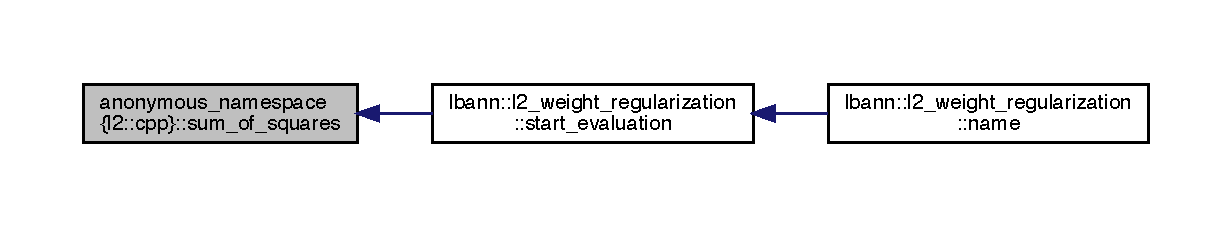
\includegraphics[width=350pt]{namespaceanonymous__namespace_02l2_8cpp_03_a32724e48048319cd99337131ba70d4c4_icgraph}
\end{center}
\end{figure}

\hypertarget{namespaceanonymous__namespace_02profiler_8cpp_03}{}\section{anonymous\+\_\+namespace\{profiler.\+cpp\} Namespace Reference}
\label{namespaceanonymous__namespace_02profiler_8cpp_03}\index{anonymous\+\_\+namespace\lcurly{}profiler.\+cpp\rcurly{}@{anonymous\+\_\+namespace\lcurly{}profiler.\+cpp\rcurly{}}}
\subsection*{Functions}
\begin{DoxyCompactItemize}
\item 
static void \hyperlink{namespaceanonymous__namespace_02profiler_8cpp_03_ad2ea0278cd1f25dc30ddd76194ace64b}{prof\+\_\+region\+\_\+begin} (const char $\ast$s, int c)
\item 
static void \hyperlink{namespaceanonymous__namespace_02profiler_8cpp_03_a7984c26fb186307873a2f83f91715a99}{prof\+\_\+region\+\_\+end} (const char $\ast$s)
\end{DoxyCompactItemize}


\subsection{Function Documentation}
\mbox{\Hypertarget{namespaceanonymous__namespace_02profiler_8cpp_03_ad2ea0278cd1f25dc30ddd76194ace64b}\label{namespaceanonymous__namespace_02profiler_8cpp_03_ad2ea0278cd1f25dc30ddd76194ace64b}} 
\index{anonymous\+\_\+namespace\lcurly{}profiler.\+cpp\rcurly{}@{anonymous\+\_\+namespace\lcurly{}profiler.\+cpp\rcurly{}}!prof\+\_\+region\+\_\+begin@{prof\+\_\+region\+\_\+begin}}
\index{prof\+\_\+region\+\_\+begin@{prof\+\_\+region\+\_\+begin}!anonymous\+\_\+namespace\lcurly{}profiler.\+cpp\rcurly{}@{anonymous\+\_\+namespace\lcurly{}profiler.\+cpp\rcurly{}}}
\subsubsection{\texorpdfstring{prof\+\_\+region\+\_\+begin()}{prof\_region\_begin()}}
{\footnotesize\ttfamily static void anonymous\+\_\+namespace\{profiler.\+cpp\}\+::prof\+\_\+region\+\_\+begin (\begin{DoxyParamCaption}\item[{const char $\ast$}]{s,  }\item[{int}]{c }\end{DoxyParamCaption})\hspace{0.3cm}{\ttfamily [static]}}



Definition at line 78 of file profiler.\+cpp.


\begin{DoxyCode}
78                                                     \{
79   \textcolor{keywordflow}{return};
80 \}
\end{DoxyCode}
Here is the caller graph for this function\+:\nopagebreak
\begin{figure}[H]
\begin{center}
\leavevmode
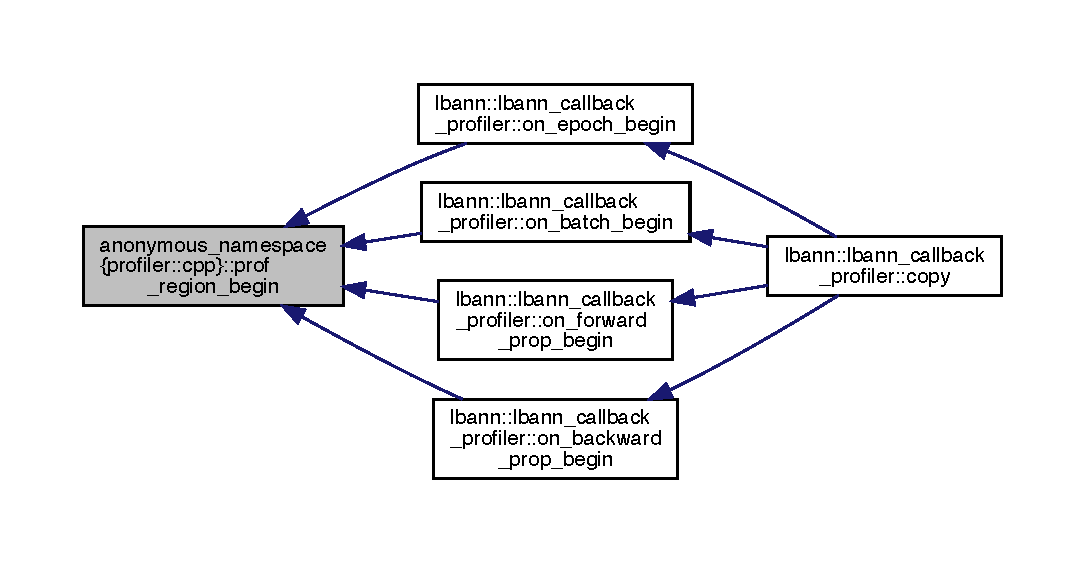
\includegraphics[width=350pt]{namespaceanonymous__namespace_02profiler_8cpp_03_ad2ea0278cd1f25dc30ddd76194ace64b_icgraph}
\end{center}
\end{figure}
\mbox{\Hypertarget{namespaceanonymous__namespace_02profiler_8cpp_03_a7984c26fb186307873a2f83f91715a99}\label{namespaceanonymous__namespace_02profiler_8cpp_03_a7984c26fb186307873a2f83f91715a99}} 
\index{anonymous\+\_\+namespace\lcurly{}profiler.\+cpp\rcurly{}@{anonymous\+\_\+namespace\lcurly{}profiler.\+cpp\rcurly{}}!prof\+\_\+region\+\_\+end@{prof\+\_\+region\+\_\+end}}
\index{prof\+\_\+region\+\_\+end@{prof\+\_\+region\+\_\+end}!anonymous\+\_\+namespace\lcurly{}profiler.\+cpp\rcurly{}@{anonymous\+\_\+namespace\lcurly{}profiler.\+cpp\rcurly{}}}
\subsubsection{\texorpdfstring{prof\+\_\+region\+\_\+end()}{prof\_region\_end()}}
{\footnotesize\ttfamily static void anonymous\+\_\+namespace\{profiler.\+cpp\}\+::prof\+\_\+region\+\_\+end (\begin{DoxyParamCaption}\item[{const char $\ast$}]{s }\end{DoxyParamCaption})\hspace{0.3cm}{\ttfamily [static]}}



Definition at line 81 of file profiler.\+cpp.


\begin{DoxyCode}
81                                            \{
82   \textcolor{keywordflow}{return};
83 \}
\end{DoxyCode}
Here is the caller graph for this function\+:\nopagebreak
\begin{figure}[H]
\begin{center}
\leavevmode
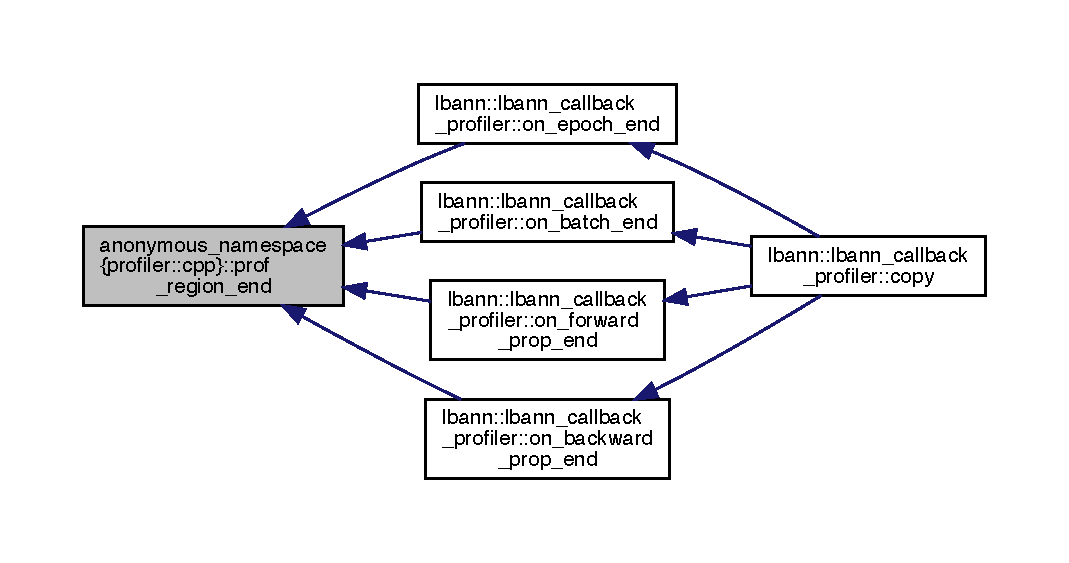
\includegraphics[width=350pt]{namespaceanonymous__namespace_02profiler_8cpp_03_a7984c26fb186307873a2f83f91715a99_icgraph}
\end{center}
\end{figure}

\hypertarget{namespaceanonymous__namespace_02random_8cpp_03}{}\section{anonymous\+\_\+namespace\{random.\+cpp\} Namespace Reference}
\label{namespaceanonymous__namespace_02random_8cpp_03}\index{anonymous\+\_\+namespace\lcurly{}random.\+cpp\rcurly{}@{anonymous\+\_\+namespace\lcurly{}random.\+cpp\rcurly{}}}
\subsection*{Variables}
\begin{DoxyCompactItemize}
\item 
\hyperlink{namespacelbann_aab7fa584bac85b9085aa8b8c5a888356}{lbann\+::rng\+\_\+gen} \hyperlink{namespaceanonymous__namespace_02random_8cpp_03_a83826c4b587d1825f13b833be6fe047f}{generator}
\item 
\hyperlink{namespacelbann_af16616ffa6a3616836eabadd6ce837ec}{lbann\+::fast\+\_\+rng\+\_\+gen} \hyperlink{namespaceanonymous__namespace_02random_8cpp_03_a349f572cec05cd0e2469b799774a8602}{fast\+\_\+generator}
\item 
\hyperlink{namespacelbann_aab7fa584bac85b9085aa8b8c5a888356}{lbann\+::rng\+\_\+gen} \hyperlink{namespaceanonymous__namespace_02random_8cpp_03_ac1d3d0259f3e9c9b75e9701ae727d16e}{data\+\_\+seq\+\_\+generator}
\end{DoxyCompactItemize}


\subsection{Variable Documentation}
\mbox{\Hypertarget{namespaceanonymous__namespace_02random_8cpp_03_ac1d3d0259f3e9c9b75e9701ae727d16e}\label{namespaceanonymous__namespace_02random_8cpp_03_ac1d3d0259f3e9c9b75e9701ae727d16e}} 
\index{anonymous\+\_\+namespace\lcurly{}random.\+cpp\rcurly{}@{anonymous\+\_\+namespace\lcurly{}random.\+cpp\rcurly{}}!data\+\_\+seq\+\_\+generator@{data\+\_\+seq\+\_\+generator}}
\index{data\+\_\+seq\+\_\+generator@{data\+\_\+seq\+\_\+generator}!anonymous\+\_\+namespace\lcurly{}random.\+cpp\rcurly{}@{anonymous\+\_\+namespace\lcurly{}random.\+cpp\rcurly{}}}
\subsubsection{\texorpdfstring{data\+\_\+seq\+\_\+generator}{data\_seq\_generator}}
{\footnotesize\ttfamily \hyperlink{namespacelbann_aab7fa584bac85b9085aa8b8c5a888356}{lbann\+::rng\+\_\+gen} anonymous\+\_\+namespace\{random.\+cpp\}\+::data\+\_\+seq\+\_\+generator}



Definition at line 54 of file random.\+cpp.

\mbox{\Hypertarget{namespaceanonymous__namespace_02random_8cpp_03_a349f572cec05cd0e2469b799774a8602}\label{namespaceanonymous__namespace_02random_8cpp_03_a349f572cec05cd0e2469b799774a8602}} 
\index{anonymous\+\_\+namespace\lcurly{}random.\+cpp\rcurly{}@{anonymous\+\_\+namespace\lcurly{}random.\+cpp\rcurly{}}!fast\+\_\+generator@{fast\+\_\+generator}}
\index{fast\+\_\+generator@{fast\+\_\+generator}!anonymous\+\_\+namespace\lcurly{}random.\+cpp\rcurly{}@{anonymous\+\_\+namespace\lcurly{}random.\+cpp\rcurly{}}}
\subsubsection{\texorpdfstring{fast\+\_\+generator}{fast\_generator}}
{\footnotesize\ttfamily \hyperlink{namespacelbann_af16616ffa6a3616836eabadd6ce837ec}{lbann\+::fast\+\_\+rng\+\_\+gen} anonymous\+\_\+namespace\{random.\+cpp\}\+::fast\+\_\+generator}



Definition at line 50 of file random.\+cpp.

\mbox{\Hypertarget{namespaceanonymous__namespace_02random_8cpp_03_a83826c4b587d1825f13b833be6fe047f}\label{namespaceanonymous__namespace_02random_8cpp_03_a83826c4b587d1825f13b833be6fe047f}} 
\index{anonymous\+\_\+namespace\lcurly{}random.\+cpp\rcurly{}@{anonymous\+\_\+namespace\lcurly{}random.\+cpp\rcurly{}}!generator@{generator}}
\index{generator@{generator}!anonymous\+\_\+namespace\lcurly{}random.\+cpp\rcurly{}@{anonymous\+\_\+namespace\lcurly{}random.\+cpp\rcurly{}}}
\subsubsection{\texorpdfstring{generator}{generator}}
{\footnotesize\ttfamily \hyperlink{namespacelbann_aab7fa584bac85b9085aa8b8c5a888356}{lbann\+::rng\+\_\+gen} anonymous\+\_\+namespace\{random.\+cpp\}\+::generator}



Definition at line 46 of file random.\+cpp.


\hypertarget{namespaceEl}{}\section{El Namespace Reference}
\label{namespaceEl}\index{El@{El}}
\subsection*{Functions}
\begin{DoxyCompactItemize}
\item 
{\footnotesize template$<$typename F $>$ }\\void \hyperlink{namespaceEl_a09d5c471681b2b48fbe4c5e6bfd0b3d3}{Column\+Sum} (const Matrix$<$ F $>$ \&X, Matrix$<$ F $>$ \&sums)
\item 
{\footnotesize template$<$typename F $>$ }\\void \hyperlink{namespaceEl_ad446b5d330cc5ae121cc2eef632c4118}{Column\+Sum} (const Abstract\+Dist\+Matrix$<$ F $>$ \&A, Abstract\+Dist\+Matrix$<$ F $>$ \&sums)
\item 
{\footnotesize template$<$typename F $>$ }\\void \hyperlink{namespaceEl_a584f088a3325a8222d4d6ac37be04b04}{Row\+Sum} (const Matrix$<$ F $>$ \&X, Matrix$<$ F $>$ \&sums)
\item 
{\footnotesize template$<$typename F $>$ }\\void \hyperlink{namespaceEl_a3982e90cd0f7cbfdc0f19741ce254c1a}{Row\+Sum} (const Abstract\+Dist\+Matrix$<$ F $>$ \&A, Abstract\+Dist\+Matrix$<$ F $>$ \&sums)
\end{DoxyCompactItemize}


\subsection{Function Documentation}
\mbox{\Hypertarget{namespaceEl_a09d5c471681b2b48fbe4c5e6bfd0b3d3}\label{namespaceEl_a09d5c471681b2b48fbe4c5e6bfd0b3d3}} 
\index{El@{El}!Column\+Sum@{Column\+Sum}}
\index{Column\+Sum@{Column\+Sum}!El@{El}}
\subsubsection{\texorpdfstring{Column\+Sum()}{ColumnSum()}\hspace{0.1cm}{\footnotesize\ttfamily [1/2]}}
{\footnotesize\ttfamily template$<$typename F $>$ \\
void El\+::\+Column\+Sum (\begin{DoxyParamCaption}\item[{const Matrix$<$ F $>$ \&}]{X,  }\item[{Matrix$<$ F $>$ \&}]{sums }\end{DoxyParamCaption})}



Definition at line 36 of file Elemental\+\_\+extensions.\+cpp.


\begin{DoxyCode}
36                                                       \{
37 \textcolor{comment}{//    DEBUG\_ONLY(CSE cse("ColumnSum"))}
38 
39     \textcolor{comment}{// Input matrix parameters}
40     \textcolor{keyword}{const} Int m = X.Height();
41     \textcolor{keyword}{const} Int n = X.Width();
42     \textcolor{keyword}{const} F *XBuf = X.LockedBuffer();
43     \textcolor{keyword}{const} Int XLDim = X.LDim();
44 
45     \textcolor{comment}{// Initialize output}
46     Zeros( sums, 1, n );
47     F *sumsBuf = sums.Buffer();
48     \textcolor{keyword}{const} Int sumsLDim = sums.LDim();
49 
50     \textcolor{comment}{// Compute sum over each column}
51     EL\_PARALLEL\_FOR
52     \textcolor{keywordflow}{for}( Int j=0; j<n; ++j )
53     \{
54         \textcolor{keywordflow}{for}( Int i=0; i<m; ++i )
55         \{
56             sumsBuf[j*sumsLDim] += XBuf[i+j*XLDim];
57         \}
58     \}
59 
60 \}
\end{DoxyCode}
Here is the caller graph for this function\+:\nopagebreak
\begin{figure}[H]
\begin{center}
\leavevmode
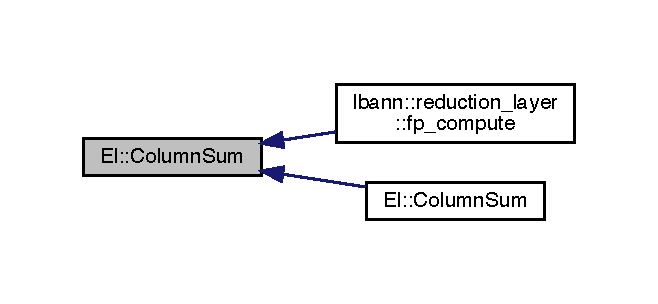
\includegraphics[width=316pt]{namespaceEl_a09d5c471681b2b48fbe4c5e6bfd0b3d3_icgraph}
\end{center}
\end{figure}
\mbox{\Hypertarget{namespaceEl_ad446b5d330cc5ae121cc2eef632c4118}\label{namespaceEl_ad446b5d330cc5ae121cc2eef632c4118}} 
\index{El@{El}!Column\+Sum@{Column\+Sum}}
\index{Column\+Sum@{Column\+Sum}!El@{El}}
\subsubsection{\texorpdfstring{Column\+Sum()}{ColumnSum()}\hspace{0.1cm}{\footnotesize\ttfamily [2/2]}}
{\footnotesize\ttfamily template$<$typename F $>$ \\
void El\+::\+Column\+Sum (\begin{DoxyParamCaption}\item[{const Abstract\+Dist\+Matrix$<$ F $>$ \&}]{A,  }\item[{Abstract\+Dist\+Matrix$<$ F $>$ \&}]{sums }\end{DoxyParamCaption})}



Definition at line 64 of file Elemental\+\_\+extensions.\+cpp.


\begin{DoxyCode}
64                                                                 \{
65 \textcolor{comment}{//    DEBUG\_ONLY(CSE cse("ColumnSum"))}
66 
67     \textcolor{comment}{// Check that distributed matrix formats are valid}
68     \textcolor{keywordflow}{if}( A.DistData().rowDist != sums.DistData().rowDist
69         || sums.DistData().colDist != STAR 
70         || A.DistData().blockHeight != sums.DistData().blockHeight
71         || A.DistData().blockWidth != sums.DistData().blockWidth)
72     \{
73         LogicError(\textcolor{stringliteral}{"Matrices do not have compatible data distributions"});
74     \}
75 
76     \textcolor{comment}{// Compute column-wise sums}
77     sums.AlignWith( A );
78     sums.Resize( 1, A.Width() );
79     \hyperlink{namespaceEl_ad446b5d330cc5ae121cc2eef632c4118}{ColumnSum}( A.LockedMatrix(), sums.Matrix() );
80     AllReduce( sums.Matrix(), sums.RedundantComm(), mpi::SUM );
81 
82 \}
\end{DoxyCode}
Here is the call graph for this function\+:\nopagebreak
\begin{figure}[H]
\begin{center}
\leavevmode
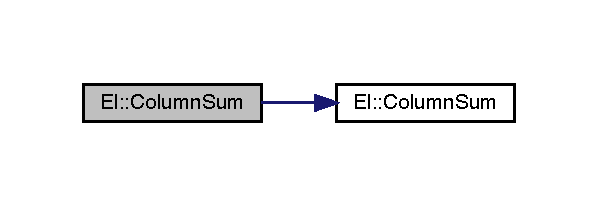
\includegraphics[width=287pt]{namespaceEl_ad446b5d330cc5ae121cc2eef632c4118_cgraph}
\end{center}
\end{figure}
\mbox{\Hypertarget{namespaceEl_a584f088a3325a8222d4d6ac37be04b04}\label{namespaceEl_a584f088a3325a8222d4d6ac37be04b04}} 
\index{El@{El}!Row\+Sum@{Row\+Sum}}
\index{Row\+Sum@{Row\+Sum}!El@{El}}
\subsubsection{\texorpdfstring{Row\+Sum()}{RowSum()}\hspace{0.1cm}{\footnotesize\ttfamily [1/2]}}
{\footnotesize\ttfamily template$<$typename F $>$ \\
void El\+::\+Row\+Sum (\begin{DoxyParamCaption}\item[{const Matrix$<$ F $>$ \&}]{X,  }\item[{Matrix$<$ F $>$ \&}]{sums }\end{DoxyParamCaption})}



Definition at line 85 of file Elemental\+\_\+extensions.\+cpp.


\begin{DoxyCode}
85                                                  \{
86 
87     \textcolor{comment}{// Input matrix parameters}
88     \textcolor{keyword}{const} Int m = X.Height();
89     \textcolor{keyword}{const} Int n = X.Width();
90     \textcolor{keyword}{const} F *XBuf = X.LockedBuffer();
91     \textcolor{keyword}{const} Int XLDim = X.LDim();
92 
93     \textcolor{comment}{// Initialize output}
94     Zeros( sums, m, 1 );
95     F *sumsBuf = sums.Buffer();
96 
97     \textcolor{comment}{// Iterate through row blocks}
98     \textcolor{keyword}{const} Int bsize = Max( 64 / \textcolor{keyword}{sizeof}(F), 1 );
99     EL\_PARALLEL\_FOR
100     \textcolor{keywordflow}{for}( Int i=0; i<m; i+=bsize )
101     \{
102         \textcolor{keyword}{const} Int mb = Min( bsize, m - i );
103         \textcolor{keywordflow}{for}( Int j=0; j<n; ++j )
104         \{
105             \textcolor{keywordflow}{for}( Int ib=0; ib<mb; ++ib )
106             \{
107                 sumsBuf[i+ib] += XBuf[(i+ib)+j*XLDim];
108             \}
109         \}
110     \}
111 
112 \}
\end{DoxyCode}
Here is the caller graph for this function\+:\nopagebreak
\begin{figure}[H]
\begin{center}
\leavevmode
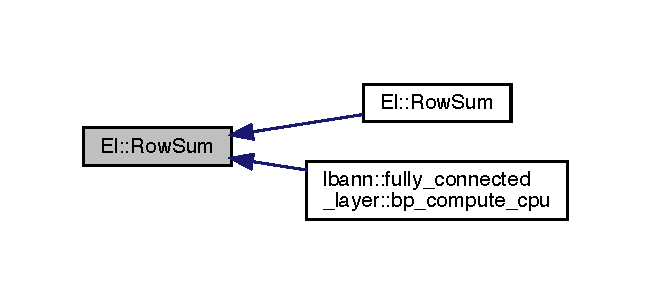
\includegraphics[width=313pt]{namespaceEl_a584f088a3325a8222d4d6ac37be04b04_icgraph}
\end{center}
\end{figure}
\mbox{\Hypertarget{namespaceEl_a3982e90cd0f7cbfdc0f19741ce254c1a}\label{namespaceEl_a3982e90cd0f7cbfdc0f19741ce254c1a}} 
\index{El@{El}!Row\+Sum@{Row\+Sum}}
\index{Row\+Sum@{Row\+Sum}!El@{El}}
\subsubsection{\texorpdfstring{Row\+Sum()}{RowSum()}\hspace{0.1cm}{\footnotesize\ttfamily [2/2]}}
{\footnotesize\ttfamily template$<$typename F $>$ \\
void El\+::\+Row\+Sum (\begin{DoxyParamCaption}\item[{const Abstract\+Dist\+Matrix$<$ F $>$ \&}]{A,  }\item[{Abstract\+Dist\+Matrix$<$ F $>$ \&}]{sums }\end{DoxyParamCaption})}



Definition at line 115 of file Elemental\+\_\+extensions.\+cpp.


\begin{DoxyCode}
115                                                                          \{
116   
117   \textcolor{comment}{// Check that distributed matrix formats are valid}
118   \textcolor{keywordflow}{if}( A.DistData().colDist != sums.DistData().colDist
119       || sums.DistData().rowDist != STAR 
120       || A.DistData().blockHeight != sums.DistData().blockHeight
121       || A.DistData().blockWidth != sums.DistData().blockWidth)
122   \{
123       LogicError(\textcolor{stringliteral}{"Matrices do not have compatible data distributions"});
124   \}
125 
126   \textcolor{comment}{// Compute row-wise sums}
127   sums.AlignWith( A );
128   sums.Resize( A.Height(), 1 );
129   \hyperlink{namespaceEl_a3982e90cd0f7cbfdc0f19741ce254c1a}{RowSum}( A.LockedMatrix(), sums.Matrix() );
130   AllReduce( sums.Matrix(), sums.RedundantComm(), mpi::SUM );
131 
132 \}
\end{DoxyCode}
Here is the call graph for this function\+:\nopagebreak
\begin{figure}[H]
\begin{center}
\leavevmode
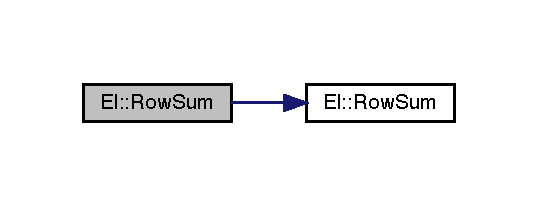
\includegraphics[width=258pt]{namespaceEl_a3982e90cd0f7cbfdc0f19741ce254c1a_cgraph}
\end{center}
\end{figure}

\hypertarget{namespacelbann}{}\section{lbann Namespace Reference}
\label{namespacelbann}\index{lbann@{lbann}}


Open\+MP Diagnostic code from Edgar Leon at L\+L\+NL.  


\subsection*{Namespaces}
\begin{DoxyCompactItemize}
\item 
 \hyperlink{namespacelbann_1_1Al}{Al}
\item 
 \hyperlink{namespacelbann_1_1anonymous__namespace_02callback__ltfb_8cpp_03}{anonymous\+\_\+namespace\{callback\+\_\+ltfb.\+cpp\}}
\item 
 \hyperlink{namespacelbann_1_1anonymous__namespace_02recurrent_8cpp_03}{anonymous\+\_\+namespace\{recurrent.\+cpp\}}
\item 
 \hyperlink{namespacelbann_1_1cnpy__utils}{cnpy\+\_\+utils}
\item 
 \hyperlink{namespacelbann_1_1cudnn}{cudnn}
\item 
 \hyperlink{namespacelbann_1_1graph}{graph}
\item 
 \hyperlink{namespacelbann_1_1proto}{proto}
\item 
 \hyperlink{namespacelbann_1_1stack__trace}{stack\+\_\+trace}
\end{DoxyCompactItemize}
\subsection*{Classes}
\begin{DoxyCompactItemize}
\item 
class \hyperlink{classlbann_1_1activation__layer}{activation\+\_\+layer}
\item 
class \hyperlink{classlbann_1_1adagrad}{adagrad}
\item 
class \hyperlink{classlbann_1_1adam}{adam}
\item 
class \hyperlink{classlbann_1_1ascii__reader}{ascii\+\_\+reader}
\item 
class \hyperlink{classlbann_1_1atan__layer}{atan\+\_\+layer}
\item 
class \hyperlink{classlbann_1_1base__convolution__layer}{base\+\_\+convolution\+\_\+layer}
\item 
class \hyperlink{classlbann_1_1batch__normalization}{batch\+\_\+normalization}
\item 
class \hyperlink{classlbann_1_1bent__identity__layer}{bent\+\_\+identity\+\_\+layer}
\item 
class \hyperlink{classlbann_1_1bernoulli__layer}{bernoulli\+\_\+layer}
\item 
class \hyperlink{classlbann_1_1binary__cross__entropy}{binary\+\_\+cross\+\_\+entropy}
\item 
class \hyperlink{classlbann_1_1boolean__accuracy__metric}{boolean\+\_\+accuracy\+\_\+metric}
\item 
class \hyperlink{classlbann_1_1boolean__false__negatives__metric}{boolean\+\_\+false\+\_\+negatives\+\_\+metric}
\item 
class \hyperlink{classlbann_1_1boolean__false__positives__metric}{boolean\+\_\+false\+\_\+positives\+\_\+metric}
\item 
class \hyperlink{classlbann_1_1categorical__accuracy__metric}{categorical\+\_\+accuracy\+\_\+metric}
\item 
class \hyperlink{classlbann_1_1cifar10__reader}{cifar10\+\_\+reader}
\item 
class \hyperlink{classlbann_1_1concatenation__layer}{concatenation\+\_\+layer}
\item 
class \hyperlink{classlbann_1_1constant__initializer}{constant\+\_\+initializer}
\item 
class \hyperlink{classlbann_1_1constant__layer}{constant\+\_\+layer}
\item 
class \hyperlink{classlbann_1_1convolution__layer}{convolution\+\_\+layer}
\begin{DoxyCompactList}\small\item\em Convolution layer. \end{DoxyCompactList}\item 
class \hyperlink{classlbann_1_1cross__entropy}{cross\+\_\+entropy}
\item 
class \hyperlink{classlbann_1_1cross__entropy__with__uncertainty}{cross\+\_\+entropy\+\_\+with\+\_\+uncertainty}
\item 
class \hyperlink{classlbann_1_1csv__reader}{csv\+\_\+reader}
\item 
class \hyperlink{classlbann_1_1CUtility}{C\+Utility}
\item 
class \hyperlink{classlbann_1_1data__buffer}{data\+\_\+buffer}
\item 
class \hyperlink{classlbann_1_1data__reader__jag}{data\+\_\+reader\+\_\+jag}
\item 
class \hyperlink{classlbann_1_1data__reader__merge__features}{data\+\_\+reader\+\_\+merge\+\_\+features}
\item 
class \hyperlink{classlbann_1_1data__reader__merge__samples}{data\+\_\+reader\+\_\+merge\+\_\+samples}
\item 
class \hyperlink{classlbann_1_1data__reader__mnist__siamese}{data\+\_\+reader\+\_\+mnist\+\_\+siamese}
\item 
class \hyperlink{classlbann_1_1data__reader__multi__images}{data\+\_\+reader\+\_\+multi\+\_\+images}
\item 
class \hyperlink{classlbann_1_1data__reader__nci}{data\+\_\+reader\+\_\+nci}
\item 
class \hyperlink{classlbann_1_1data__reader__synthetic}{data\+\_\+reader\+\_\+synthetic}
\item 
class \hyperlink{classlbann_1_1data__reader__triplet}{data\+\_\+reader\+\_\+triplet}
\item 
class \hyperlink{classlbann_1_1data__store__csv}{data\+\_\+store\+\_\+csv}
\item 
class \hyperlink{classlbann_1_1data__store__image}{data\+\_\+store\+\_\+image}
\item 
class \hyperlink{classlbann_1_1data__store__imagenet}{data\+\_\+store\+\_\+imagenet}
\item 
class \hyperlink{classlbann_1_1data__store__imagenet__patches}{data\+\_\+store\+\_\+imagenet\+\_\+patches}
\item 
class \hyperlink{classlbann_1_1data__store__merge__features}{data\+\_\+store\+\_\+merge\+\_\+features}
\item 
class \hyperlink{classlbann_1_1data__store__merge__samples}{data\+\_\+store\+\_\+merge\+\_\+samples}
\item 
class \hyperlink{classlbann_1_1data__store__multi__images}{data\+\_\+store\+\_\+multi\+\_\+images}
\item 
class \hyperlink{classlbann_1_1data__store__pilot2__molecular}{data\+\_\+store\+\_\+pilot2\+\_\+molecular}
\item 
class \hyperlink{classlbann_1_1data__store__triplet}{data\+\_\+store\+\_\+triplet}
\item 
class \hyperlink{classlbann_1_1DataGenerator}{Data\+Generator}
\item 
class \hyperlink{classlbann_1_1dataset}{dataset}
\item 
class \hyperlink{classlbann_1_1deconvolution__layer}{deconvolution\+\_\+layer}
\begin{DoxyCompactList}\small\item\em Deconvolution layer. \end{DoxyCompactList}\item 
class \hyperlink{classlbann_1_1directed__acyclic__graph__model}{directed\+\_\+acyclic\+\_\+graph\+\_\+model}
\item 
class \hyperlink{classlbann_1_1distributed__io__buffer}{distributed\+\_\+io\+\_\+buffer}
\item 
class \hyperlink{classlbann_1_1dropout}{dropout}
\item 
class \hyperlink{classlbann_1_1dummy__layer}{dummy\+\_\+layer}
\item 
class \hyperlink{classlbann_1_1elu__layer}{elu\+\_\+layer}
\item 
class \hyperlink{classlbann_1_1entrywise__activation__layer}{entrywise\+\_\+activation\+\_\+layer}
\item 
class \hyperlink{classlbann_1_1evaluation__layer}{evaluation\+\_\+layer}
\item 
class \hyperlink{classlbann_1_1exponential__layer}{exponential\+\_\+layer}
\item 
class \hyperlink{classlbann_1_1fan__in__fan__out__initializer}{fan\+\_\+in\+\_\+fan\+\_\+out\+\_\+initializer}
\item 
class \hyperlink{classlbann_1_1fetch__data__functor}{fetch\+\_\+data\+\_\+functor}
\item 
class \hyperlink{classlbann_1_1fully__connected__layer}{fully\+\_\+connected\+\_\+layer}
\item 
class \hyperlink{classlbann_1_1gaussian__layer}{gaussian\+\_\+layer}
\item 
class \hyperlink{classlbann_1_1generic__compound__data__reader}{generic\+\_\+compound\+\_\+data\+\_\+reader}
\item 
class \hyperlink{classlbann_1_1generic__data__reader}{generic\+\_\+data\+\_\+reader}
\item 
class \hyperlink{classlbann_1_1generic__data__store}{generic\+\_\+data\+\_\+store}
\item 
class \hyperlink{classlbann_1_1generic__input__layer}{generic\+\_\+input\+\_\+layer}
\item 
class \hyperlink{classlbann_1_1generic__io__buffer}{generic\+\_\+io\+\_\+buffer}
\item 
class \hyperlink{classlbann_1_1generic__target__layer}{generic\+\_\+target\+\_\+layer}
\item 
class \hyperlink{classlbann_1_1geom__negloglike}{geom\+\_\+negloglike}
\item 
class \hyperlink{classlbann_1_1glorot__normal__initializer}{glorot\+\_\+normal\+\_\+initializer}
\item 
class \hyperlink{classlbann_1_1glorot__uniform__initializer}{glorot\+\_\+uniform\+\_\+initializer}
\item 
class \hyperlink{classlbann_1_1greedy__layerwise__autoencoder}{greedy\+\_\+layerwise\+\_\+autoencoder}
\item 
class \hyperlink{classlbann_1_1group__lasso__weight__regularization}{group\+\_\+lasso\+\_\+weight\+\_\+regularization}
\item 
class \hyperlink{classlbann_1_1hadamard__layer}{hadamard\+\_\+layer}
\item 
class \hyperlink{classlbann_1_1he__normal__initializer}{he\+\_\+normal\+\_\+initializer}
\item 
class \hyperlink{classlbann_1_1he__uniform__initializer}{he\+\_\+uniform\+\_\+initializer}
\item 
class \hyperlink{classlbann_1_1hypergradient__adam}{hypergradient\+\_\+adam}
\item 
class \hyperlink{classlbann_1_1identity__layer}{identity\+\_\+layer}
\item 
class \hyperlink{classlbann_1_1image__data__reader}{image\+\_\+data\+\_\+reader}
\item 
class \hyperlink{classlbann_1_1image__utils}{image\+\_\+utils}
\item 
class \hyperlink{classlbann_1_1imagenet__reader}{imagenet\+\_\+reader}
\item 
class \hyperlink{classlbann_1_1imagenet__reader__org}{imagenet\+\_\+reader\+\_\+org}
\item 
class \hyperlink{classlbann_1_1imagenet__reader__patches}{imagenet\+\_\+reader\+\_\+patches}
\item 
class \hyperlink{classlbann_1_1imagenet__reader__single}{imagenet\+\_\+reader\+\_\+single}
\item 
class \hyperlink{classlbann_1_1input__layer}{input\+\_\+layer}
\item 
class \hyperlink{classlbann_1_1io__layer}{io\+\_\+layer}
\item 
class \hyperlink{classlbann_1_1kl__divergence}{kl\+\_\+divergence}
\item 
class \hyperlink{classlbann_1_1l1__weight__regularization}{l1\+\_\+weight\+\_\+regularization}
\item 
class \hyperlink{classlbann_1_1l2__weight__regularization}{l2\+\_\+weight\+\_\+regularization}
\item 
class \hyperlink{classlbann_1_1Layer}{Layer}
\item 
class \hyperlink{classlbann_1_1layer__term}{layer\+\_\+term}
\item 
class \hyperlink{classlbann_1_1lbann__callback}{lbann\+\_\+callback}
\item 
class \hyperlink{classlbann_1_1lbann__callback__adaptive__learning__rate}{lbann\+\_\+callback\+\_\+adaptive\+\_\+learning\+\_\+rate}
\item 
class \hyperlink{classlbann_1_1lbann__callback__check__dataset}{lbann\+\_\+callback\+\_\+check\+\_\+dataset}
\item 
class \hyperlink{classlbann_1_1lbann__callback__check__init}{lbann\+\_\+callback\+\_\+check\+\_\+init}
\item 
class \hyperlink{classlbann_1_1lbann__callback__check__reconstruction__error}{lbann\+\_\+callback\+\_\+check\+\_\+reconstruction\+\_\+error}
\item 
class \hyperlink{classlbann_1_1lbann__callback__checknan}{lbann\+\_\+callback\+\_\+checknan}
\item 
class \hyperlink{classlbann_1_1lbann__callback__checkpoint}{lbann\+\_\+callback\+\_\+checkpoint}
\item 
class \hyperlink{classlbann_1_1lbann__callback__checksmall}{lbann\+\_\+callback\+\_\+checksmall}
\item 
class \hyperlink{classlbann_1_1lbann__callback__debug}{lbann\+\_\+callback\+\_\+debug}
\item 
class \hyperlink{classlbann_1_1lbann__callback__debug__io}{lbann\+\_\+callback\+\_\+debug\+\_\+io}
\item 
class \hyperlink{classlbann_1_1lbann__callback__drop__fixed__learning__rate}{lbann\+\_\+callback\+\_\+drop\+\_\+fixed\+\_\+learning\+\_\+rate}
\item 
class \hyperlink{classlbann_1_1lbann__callback__dump__activations}{lbann\+\_\+callback\+\_\+dump\+\_\+activations}
\item 
class \hyperlink{classlbann_1_1lbann__callback__dump__gradients}{lbann\+\_\+callback\+\_\+dump\+\_\+gradients}
\item 
class \hyperlink{classlbann_1_1lbann__callback__dump__minibatch__sample__indices}{lbann\+\_\+callback\+\_\+dump\+\_\+minibatch\+\_\+sample\+\_\+indices}
\item 
class \hyperlink{classlbann_1_1lbann__callback__dump__weights}{lbann\+\_\+callback\+\_\+dump\+\_\+weights}
\item 
class \hyperlink{classlbann_1_1lbann__callback__early__stopping}{lbann\+\_\+callback\+\_\+early\+\_\+stopping}
\item 
class \hyperlink{classlbann_1_1lbann__callback__gradient__check}{lbann\+\_\+callback\+\_\+gradient\+\_\+check}
\item 
class \hyperlink{classlbann_1_1lbann__callback__hang}{lbann\+\_\+callback\+\_\+hang}
\item 
class \hyperlink{classlbann_1_1lbann__callback__imcomm}{lbann\+\_\+callback\+\_\+imcomm}
\item 
class \hyperlink{classlbann_1_1lbann__callback__io}{lbann\+\_\+callback\+\_\+io}
\item 
class \hyperlink{classlbann_1_1lbann__callback__learning__rate}{lbann\+\_\+callback\+\_\+learning\+\_\+rate}
\item 
class \hyperlink{classlbann_1_1lbann__callback__linear__growth__learning__rate}{lbann\+\_\+callback\+\_\+linear\+\_\+growth\+\_\+learning\+\_\+rate}
\item 
class \hyperlink{classlbann_1_1lbann__callback__ltfb}{lbann\+\_\+callback\+\_\+ltfb}
\item 
class \hyperlink{classlbann_1_1lbann__callback__minibatch__schedule}{lbann\+\_\+callback\+\_\+minibatch\+\_\+schedule}
\item 
class \hyperlink{classlbann_1_1lbann__callback__optimizerwise__adaptive__learning__rate}{lbann\+\_\+callback\+\_\+optimizerwise\+\_\+adaptive\+\_\+learning\+\_\+rate}
\item 
class \hyperlink{classlbann_1_1lbann__callback__poly__learning__rate}{lbann\+\_\+callback\+\_\+poly\+\_\+learning\+\_\+rate}
\item 
class \hyperlink{classlbann_1_1lbann__callback__print}{lbann\+\_\+callback\+\_\+print}
\item 
class \hyperlink{classlbann_1_1lbann__callback__profiler}{lbann\+\_\+callback\+\_\+profiler}
\item 
class \hyperlink{classlbann_1_1lbann__callback__save__images}{lbann\+\_\+callback\+\_\+save\+\_\+images}
\item 
class \hyperlink{classlbann_1_1lbann__callback__save__model}{lbann\+\_\+callback\+\_\+save\+\_\+model}
\item 
class \hyperlink{classlbann_1_1lbann__callback__step__learning__rate}{lbann\+\_\+callback\+\_\+step\+\_\+learning\+\_\+rate}
\item 
class \hyperlink{classlbann_1_1lbann__callback__step__minibatch}{lbann\+\_\+callback\+\_\+step\+\_\+minibatch}
\item 
class \hyperlink{classlbann_1_1lbann__callback__summary}{lbann\+\_\+callback\+\_\+summary}
\item 
class \hyperlink{classlbann_1_1lbann__callback__timeline}{lbann\+\_\+callback\+\_\+timeline}
\item 
class \hyperlink{classlbann_1_1lbann__callback__timer}{lbann\+\_\+callback\+\_\+timer}
\item 
class \hyperlink{classlbann_1_1lbann__callback__variable__minibatch}{lbann\+\_\+callback\+\_\+variable\+\_\+minibatch}
\item 
class \hyperlink{classlbann_1_1lbann__comm}{lbann\+\_\+comm}
\item 
class \hyperlink{classlbann_1_1lbann__exception}{lbann\+\_\+exception}
\item 
class \hyperlink{classlbann_1_1lbann__image__preprocessor}{lbann\+\_\+image\+\_\+preprocessor}
\item 
struct \hyperlink{structlbann_1_1lbann__model__header}{lbann\+\_\+model\+\_\+header}
\item 
struct \hyperlink{structlbann_1_1lbann__model__sequential__header}{lbann\+\_\+model\+\_\+sequential\+\_\+header}
\item 
class \hyperlink{classlbann_1_1lbann__quantizer}{lbann\+\_\+quantizer}
\item 
class \hyperlink{classlbann_1_1lbann__summary}{lbann\+\_\+summary}
\item 
class \hyperlink{classlbann_1_1leaky__relu__layer}{leaky\+\_\+relu\+\_\+layer}
\item 
class \hyperlink{classlbann_1_1learning__layer}{learning\+\_\+layer}
\item 
class \hyperlink{classlbann_1_1local__response__normalization__layer}{local\+\_\+response\+\_\+normalization\+\_\+layer}
\item 
class \hyperlink{classlbann_1_1loss__function}{loss\+\_\+function}
\item 
class \hyperlink{classlbann_1_1mean__absolute__deviation__loss}{mean\+\_\+absolute\+\_\+deviation\+\_\+loss}
\item 
class \hyperlink{classlbann_1_1mean__absolute__deviation__metric}{mean\+\_\+absolute\+\_\+deviation\+\_\+metric}
\item 
class \hyperlink{classlbann_1_1mean__absolute__error__loss}{mean\+\_\+absolute\+\_\+error\+\_\+loss}
\item 
class \hyperlink{classlbann_1_1mean__squared__error__loss}{mean\+\_\+squared\+\_\+error\+\_\+loss}
\item 
class \hyperlink{classlbann_1_1mean__squared__error__metric}{mean\+\_\+squared\+\_\+error\+\_\+metric}
\item 
class \hyperlink{classlbann_1_1mesh__reader}{mesh\+\_\+reader}
\item 
class \hyperlink{classlbann_1_1metric}{metric}
\item 
struct \hyperlink{structlbann_1_1metric__statistics}{metric\+\_\+statistics}
\item 
class \hyperlink{classlbann_1_1mnist__reader}{mnist\+\_\+reader}
\item 
class \hyperlink{classlbann_1_1model}{model}
\item 
class \hyperlink{classlbann_1_1NetworkParams}{Network\+Params}
\begin{DoxyCompactList}\small\item\em Network parameters. \end{DoxyCompactList}\item 
class \hyperlink{classlbann_1_1normal__initializer}{normal\+\_\+initializer}
\item 
class \hyperlink{classlbann_1_1numpy__reader}{numpy\+\_\+reader}
\item 
class \hyperlink{classlbann_1_1objective__function}{objective\+\_\+function}
\item 
class \hyperlink{classlbann_1_1objective__function__term}{objective\+\_\+function\+\_\+term}
\item 
class \hyperlink{classlbann_1_1offline__patches__npz}{offline\+\_\+patches\+\_\+npz}
\item 
class \hyperlink{classlbann_1_1optimizer}{optimizer}
\item 
class \hyperlink{classlbann_1_1partitioned__io__buffer}{partitioned\+\_\+io\+\_\+buffer}
\item 
struct \hyperlink{structlbann_1_1path__delimiter}{path\+\_\+delimiter}
\item 
class \hyperlink{classlbann_1_1pearson__correlation__metric}{pearson\+\_\+correlation\+\_\+metric}
\item 
class \hyperlink{classlbann_1_1PerformanceParams}{Performance\+Params}
\begin{DoxyCompactList}\small\item\em Performance parameters. \end{DoxyCompactList}\item 
class \hyperlink{classlbann_1_1persist}{persist}
\item 
class \hyperlink{classlbann_1_1pilot2__molecular__reader}{pilot2\+\_\+molecular\+\_\+reader}
\item 
class \hyperlink{classlbann_1_1poisson__negloglike}{poisson\+\_\+negloglike}
\item 
class \hyperlink{classlbann_1_1polya__negloglike}{polya\+\_\+negloglike}
\item 
class \hyperlink{classlbann_1_1pooling__layer}{pooling\+\_\+layer}
\item 
class \hyperlink{classlbann_1_1power__layer}{power\+\_\+layer}
\item 
class \hyperlink{classlbann_1_1protobuf__utils}{protobuf\+\_\+utils}
\item 
struct \hyperlink{structlbann_1_1prototext__fn__triple}{prototext\+\_\+fn\+\_\+triple}
\item 
class \hyperlink{classlbann_1_1r2__metric}{r2\+\_\+metric}
\item 
class \hyperlink{classlbann_1_1reconstruction__layer}{reconstruction\+\_\+layer}
\item 
class \hyperlink{classlbann_1_1recurrent__model}{recurrent\+\_\+model}
\item 
class \hyperlink{classlbann_1_1reduction__layer}{reduction\+\_\+layer}
\item 
class \hyperlink{classlbann_1_1regularizer__layer}{regularizer\+\_\+layer}
\item 
class \hyperlink{classlbann_1_1relu__layer}{relu\+\_\+layer}
\item 
class \hyperlink{classlbann_1_1reshape__layer}{reshape\+\_\+layer}
\item 
class \hyperlink{classlbann_1_1rmsprop}{rmsprop}
\item 
class \hyperlink{classlbann_1_1rng}{rng}
\item 
class \hyperlink{classlbann_1_1safe__inv__layer}{safe\+\_\+inv\+\_\+layer}
\item 
class \hyperlink{classlbann_1_1selu__dropout}{selu\+\_\+dropout}
\item 
class \hyperlink{classlbann_1_1selu__layer}{selu\+\_\+layer}
\item 
class \hyperlink{classlbann_1_1sequential__model}{sequential\+\_\+model}
\item 
class \hyperlink{classlbann_1_1sgd}{sgd}
\item 
class \hyperlink{classlbann_1_1siamese__model}{siamese\+\_\+model}
\item 
class \hyperlink{classlbann_1_1sigmoid__layer}{sigmoid\+\_\+layer}
\item 
class \hyperlink{classlbann_1_1slice__layer}{slice\+\_\+layer}
\item 
class \hyperlink{classlbann_1_1smooth__relu__layer}{smooth\+\_\+relu\+\_\+layer}
\item 
class \hyperlink{classlbann_1_1softmax__layer}{softmax\+\_\+layer}
\item 
class \hyperlink{classlbann_1_1softplus__layer}{softplus\+\_\+layer}
\item 
class \hyperlink{classlbann_1_1split__layer}{split\+\_\+layer}
\item 
class \hyperlink{classlbann_1_1stack__profiler}{stack\+\_\+profiler}
\item 
class \hyperlink{classlbann_1_1sum__layer}{sum\+\_\+layer}
\item 
class \hyperlink{classlbann_1_1swish__layer}{swish\+\_\+layer}
\item 
class \hyperlink{classlbann_1_1SystemParams}{System\+Params}
\begin{DoxyCompactList}\small\item\em System parameters. \end{DoxyCompactList}\item 
class \hyperlink{classlbann_1_1tanh__layer}{tanh\+\_\+layer}
\item 
class \hyperlink{classlbann_1_1target__layer}{target\+\_\+layer}
\item 
class \hyperlink{classlbann_1_1top__k__categorical__accuracy__metric}{top\+\_\+k\+\_\+categorical\+\_\+accuracy\+\_\+metric}
\item 
class \hyperlink{classlbann_1_1TrainingParams}{Training\+Params}
\item 
class \hyperlink{classlbann_1_1transform__layer}{transform\+\_\+layer}
\item 
class \hyperlink{classlbann_1_1uniform__initializer}{uniform\+\_\+initializer}
\item 
class \hyperlink{classlbann_1_1uniform__layer}{uniform\+\_\+layer}
\item 
class \hyperlink{classlbann_1_1unpooling__layer}{unpooling\+\_\+layer}
\item 
class \hyperlink{classlbann_1_1update__data__reader__functor}{update\+\_\+data\+\_\+reader\+\_\+functor}
\item 
class \hyperlink{classlbann_1_1weights}{weights}
\item 
class \hyperlink{classlbann_1_1weights__initializer}{weights\+\_\+initializer}
\end{DoxyCompactItemize}
\subsection*{Typedefs}
\begin{DoxyCompactItemize}
\item 
using \hyperlink{namespacelbann_aab7fa584bac85b9085aa8b8c5a888356}{rng\+\_\+gen} = std\+::mt19937
\item 
using \hyperlink{namespacelbann_af16616ffa6a3616836eabadd6ce837ec}{fast\+\_\+rng\+\_\+gen} = std\+::minstd\+\_\+rand
\end{DoxyCompactItemize}
\subsection*{Enumerations}
\begin{DoxyCompactItemize}
\item 
enum \hyperlink{namespacelbann_adee41f31f15f3906cbdcce4a1417eb56}{persist\+\_\+type} \{ \hyperlink{namespacelbann_adee41f31f15f3906cbdcce4a1417eb56a61b3a8faa9c1091806675c230a9abe64}{persist\+\_\+type\+::train}, 
\hyperlink{namespacelbann_adee41f31f15f3906cbdcce4a1417eb56a20f35e630daf44dbfa4c3f68f5399d8c}{persist\+\_\+type\+::model}, 
\hyperlink{namespacelbann_adee41f31f15f3906cbdcce4a1417eb56af9ab05454998236921a6b0e281fae632}{persist\+\_\+type\+::validate}
 \}
\item 
enum \hyperlink{namespacelbann_a3ce21fcce81d74fe54c2f4b5b5b48d9a}{device} \{ \hyperlink{namespacelbann_a3ce21fcce81d74fe54c2f4b5b5b48d9aa2b55387dd066c5bac646ac61543d152d}{device\+::\+C\+PU}, 
\hyperlink{namespacelbann_a3ce21fcce81d74fe54c2f4b5b5b48d9aaa33b7755e5f9b504d2d038eaca4ff28d}{device\+::\+C\+U\+DA}
 \}
\item 
enum \hyperlink{namespacelbann_a5975e1fb530a267728bfb01dc5c1be9b}{reduction\+\_\+mode} \{ \hyperlink{namespacelbann_a5975e1fb530a267728bfb01dc5c1be9baccc0377a8afbf50e7094f5c23a8af223}{reduction\+\_\+mode\+::\+I\+N\+V\+A\+L\+ID}, 
\hyperlink{namespacelbann_a5975e1fb530a267728bfb01dc5c1be9ba6970bdc2201030b9c03fbdcf3973858a}{reduction\+\_\+mode\+::\+S\+UM}, 
\hyperlink{namespacelbann_a5975e1fb530a267728bfb01dc5c1be9ba16de38737a9f8366e9b2042b4e9b6290}{reduction\+\_\+mode\+::\+A\+V\+E\+R\+A\+GE}
 \}
\end{DoxyCompactItemize}
\subsection*{Functions}
\begin{DoxyCompactItemize}
\item 
\hyperlink{classlbann_1_1lbann__comm}{lbann\+\_\+comm} $\ast$ \hyperlink{namespacelbann_a3d91b615e42bf5744deeed770879bc8c}{initialize} (int \&argc, char $\ast$$\ast$\&argv, int seed)
\item 
void \hyperlink{namespacelbann_a99724ee5a6647a1d8bff6764b9aa5fac}{finalize} (\hyperlink{classlbann_1_1lbann__comm}{lbann\+\_\+comm} $\ast$\hyperlink{file__io_8cpp_ab048c6f9fcbcfaa57ce68b00263dbebe}{comm})
\item 
static bool \hyperlink{namespacelbann_a35a39e949cfd1d7f8c15f94e4d44ecff}{write\+\_\+latest} (const char $\ast$dir, const char $\ast$name, int epoch, int train)
\item 
static bool \hyperlink{namespacelbann_abebab8298e56db6a455a9ed08ab42bb4}{read\+\_\+latest} (const char $\ast$dir, const char $\ast$name, int $\ast$epoch\+Last, int $\ast$train\+Last)
\begin{DoxyCompactList}\small\item\em Reads the \char`\"{}latest\char`\"{} file and returns the epoch number and sample offset for most recent checkpoint. \end{DoxyCompactList}\item 
std\+::string \hyperlink{namespacelbann_ab5665dc52c53faca0caa55b509e2e654}{get\+\_\+comm\+\_\+type\+\_\+name} (\hyperlink{classlbann_1_1lbann__callback__imcomm_acf7e894b3381e7f9b71020dc73594d6a}{lbann\+\_\+callback\+\_\+imcomm\+::comm\+\_\+type} m)
\item 
void \hyperlink{namespacelbann_a59f65281406da5bc57f49d8ec682be2d}{load\+\_\+mnist\+\_\+data} (const std\+::string imagepath, const std\+::string labelpath, const int m\+\_\+first\+\_\+n, std\+::vector$<$ std\+::vector$<$ unsigned char $>$ $>$ \&m\+\_\+image\+\_\+data)
\item 
{\footnotesize template$<$$>$ }\\void \hyperlink{namespacelbann_a32006e2c89920b1ff6e8a2318650dd7f}{Layer\+::instantiate\+\_\+matrices$<$ data\+\_\+layout\+::\+M\+O\+D\+E\+L\+\_\+\+P\+A\+R\+A\+L\+L\+E\+L $>$} (const \hyperlink{base_8hpp_a9951bb1719d534e0401b1f06cad19eab}{El\+::\+Grid} \&grid)
\item 
{\footnotesize template$<$$>$ }\\void \hyperlink{namespacelbann_af3507a38f8992e27898d63551a987341}{Layer\+::instantiate\+\_\+matrices$<$ data\+\_\+layout\+::\+D\+A\+T\+A\+\_\+\+P\+A\+R\+A\+L\+L\+E\+L $>$} (const \hyperlink{base_8hpp_a9951bb1719d534e0401b1f06cad19eab}{El\+::\+Grid} \&grid)
\item 
std\+::vector$<$ int $>$ \hyperlink{namespacelbann_af3f2c9055423e1fe3380b1ad4c4ab5ef}{get\+\_\+tokens} (std\+::string str, const std\+::vector$<$ char $>$ delims)
\begin{DoxyCompactList}\small\item\em Tokenize a string into integers by an ordered sequence of delimiter characters. \end{DoxyCompactList}\item 
std\+::vector$<$ std\+::string $>$ \hyperlink{namespacelbann_ac02a174553cf05f779743be1c92f1912}{get\+\_\+tokens} (const std\+::string str, const std\+::string delims=\char`\"{} \+:;\textbackslash{}\textbackslash{}\textbackslash{}\char`\"{})
\begin{DoxyCompactList}\small\item\em Tokenize a string into substrings by set of delimiter characters. \end{DoxyCompactList}\item 
bool \hyperlink{namespacelbann_a1ce6832a54235a5fb333f50fffbe1b63}{parse\+\_\+path} (const std\+::string \&path, std\+::string \&dir, std\+::string \&basename)
\begin{DoxyCompactList}\small\item\em Divide a given path into dir and basename. \end{DoxyCompactList}\item 
std\+::string \hyperlink{namespacelbann_ad9a28639b0953886bbcb7fc366783a17}{get\+\_\+ext\+\_\+name} (const std\+::string file\+\_\+name)
\begin{DoxyCompactList}\small\item\em Return file extention name. \end{DoxyCompactList}\item 
std\+::string \hyperlink{namespacelbann_aea9a4378326fd51236a8343c43cc4a7c}{get\+\_\+basename\+\_\+without\+\_\+ext} (const std\+::string file\+\_\+name)
\begin{DoxyCompactList}\small\item\em Return basename without extention. \end{DoxyCompactList}\item 
std\+::string \hyperlink{namespacelbann_a1b8b05bbf2e59808a51ead80c47a9359}{add\+\_\+delimiter} (const std\+::string dir)
\item 
std\+::string \hyperlink{namespacelbann_a351610c8df00514e8942756c2099fedc}{modify\+\_\+file\+\_\+name} (const std\+::string file\+\_\+name, const std\+::string tag, const std\+::string new\+\_\+ext)
\item 
bool \hyperlink{namespacelbann_a4fac6c6483965395fa79d31061485f9f}{check\+\_\+if\+\_\+file\+\_\+exists} (const std\+::string \&filename)
\begin{DoxyCompactList}\small\item\em Return true if a file with the given name exists. \end{DoxyCompactList}\item 
bool \hyperlink{namespacelbann_a3ee4a1fa7a82c30999de9eb626c68311}{check\+\_\+if\+\_\+dir\+\_\+exists} (const std\+::string \&dirname)
\item 
bool \hyperlink{namespacelbann_a1208673c880ccf0e1a9c5db6a8ed81f8}{create\+\_\+dir} (const std\+::string dirname)
\item 
void \hyperlink{namespacelbann_aa3636a1979e40da2af91f30a12b90db9}{im2col} (const \hyperlink{base_8hpp_a68f11fdc31b62516cb310831bbe54d73}{Mat} \&im, \hyperlink{base_8hpp_a68f11fdc31b62516cb310831bbe54d73}{Mat} \&col, int num\+\_\+channels, int im\+\_\+num\+\_\+dims, const int $\ast$im\+\_\+dims, const int $\ast$im\+\_\+pads, const int $\ast$window\+\_\+dims, const int $\ast$window\+\_\+strides)
\begin{DoxyCompactList}\small\item\em Rearrange image blocks into matrix columns. \end{DoxyCompactList}\item 
void \hyperlink{namespacelbann_a0e1225f72580ffb5166181392b68b651}{col2im} (const \hyperlink{base_8hpp_a68f11fdc31b62516cb310831bbe54d73}{Mat} \&col, \hyperlink{base_8hpp_a68f11fdc31b62516cb310831bbe54d73}{Mat} \&im, int num\+\_\+channels, int im\+\_\+num\+\_\+dims, const int $\ast$im\+\_\+dims, const int $\ast$im\+\_\+pads, const int $\ast$window\+\_\+dims, const int $\ast$window\+\_\+strides)
\begin{DoxyCompactList}\small\item\em Rearrange matrix columns into image blocks. \end{DoxyCompactList}\item 
void \hyperlink{namespacelbann_ab36806d08e7c852ad9cf3a0564f29b64}{col2im} (const \hyperlink{base_8hpp_a68f11fdc31b62516cb310831bbe54d73}{Mat} \&col, \hyperlink{base_8hpp_a68f11fdc31b62516cb310831bbe54d73}{Mat} \&im, int num\+\_\+channels, int im\+\_\+num\+\_\+dims, const int $\ast$im\+\_\+dims, const int $\ast$im\+\_\+pads, const int $\ast$window\+\_\+dims, const int $\ast$window\+\_\+strides, std\+::function$<$ Data\+Type(const Data\+Type \&, const Data\+Type \&)$>$ reduction\+\_\+op)
\begin{DoxyCompactList}\small\item\em Rearrange matrix columns into image blocks. \end{DoxyCompactList}\item 
void \hyperlink{namespacelbann_a3d099edd7d1b09889e0d2133bb83d5bf}{im2col\+\_\+1x1} (const Data\+Type $\ast$input\+\_\+buffer, Data\+Type $\ast$output\+\_\+buffer, int num\+\_\+channels, int num\+\_\+input\+\_\+dims, const int $\ast$input\+\_\+dims)
\begin{DoxyCompactList}\small\item\em Rearrange 1x1 image blocks into matrix columns. \end{DoxyCompactList}\item 
void \hyperlink{namespacelbann_adc05d10657be77ccd9a74b1621c416c3}{im2col\+\_\+2d} (const Data\+Type $\ast$\+\_\+\+\_\+restrict\+\_\+\+\_\+ input\+\_\+buffer, Data\+Type $\ast$\+\_\+\+\_\+restrict\+\_\+\+\_\+ output\+\_\+buffer, int input\+\_\+dim\+\_\+x, int input\+\_\+dim\+\_\+y, int input\+\_\+pad\+\_\+x, int input\+\_\+pad\+\_\+y, int num\+\_\+channels, int window\+\_\+dim\+\_\+x, int window\+\_\+dim\+\_\+y, int offset\+\_\+stride\+\_\+x, int offset\+\_\+stride\+\_\+y)
\begin{DoxyCompactList}\small\item\em Rearrange 2D image blocks into matrix columns. \end{DoxyCompactList}\item 
void \hyperlink{namespacelbann_ab4fccda3dc4c2c293d643815dfefe22a}{col2im\+\_\+1x1} (const Data\+Type $\ast$input\+\_\+buffer, Data\+Type $\ast$output\+\_\+buffer, const int num\+\_\+channels, const int num\+\_\+output\+\_\+dims, const int $\ast$output\+\_\+dims)
\begin{DoxyCompactList}\small\item\em Rearrange matrix columns into 1x1 image blocks. \end{DoxyCompactList}\item 
void \hyperlink{namespacelbann_a1953674a43b284f0abb5c5e4db94b2b9}{col2im\+\_\+2d} (const Data\+Type $\ast$\+\_\+\+\_\+restrict\+\_\+\+\_\+ input\+\_\+buffer, Data\+Type $\ast$\+\_\+\+\_\+restrict\+\_\+\+\_\+ output\+\_\+buffer, int output\+\_\+dim\+\_\+x, int output\+\_\+dim\+\_\+y, int output\+\_\+pad\+\_\+x, int output\+\_\+pad\+\_\+y, int num\+\_\+channels, int window\+\_\+dim\+\_\+x, int window\+\_\+dim\+\_\+y, int offset\+\_\+stride\+\_\+x, int offset\+\_\+stride\+\_\+y)
\begin{DoxyCompactList}\small\item\em Rearrange matrix columns into 2D image blocks. \end{DoxyCompactList}\item 
void \hyperlink{namespacelbann_a26debfaa06e8490c7f258ed7923870c7}{display\+\_\+omp\+\_\+setup} ()
\item 
\hyperlink{namespacelbann_aab7fa584bac85b9085aa8b8c5a888356}{rng\+\_\+gen} \& \hyperlink{namespacelbann_a4fea7ba21017b49d1e34394b4c20c764}{get\+\_\+generator} ()
\item 
\hyperlink{namespacelbann_af16616ffa6a3616836eabadd6ce837ec}{fast\+\_\+rng\+\_\+gen} \& \hyperlink{namespacelbann_ae6ce9c2fdec6f81803f6b1a6555c31c5}{get\+\_\+fast\+\_\+generator} ()
\item 
\hyperlink{namespacelbann_aab7fa584bac85b9085aa8b8c5a888356}{rng\+\_\+gen} \& \hyperlink{namespacelbann_aba9d11cb3a739cd84e7234ceeb32d098}{get\+\_\+data\+\_\+seq\+\_\+generator} ()
\item 
bool \hyperlink{namespacelbann_af68acf5b249e5360289d4c6a7bfa8985}{save\+\_\+rng\+\_\+to\+\_\+checkpoint\+\_\+shared} (\hyperlink{classlbann_1_1persist}{persist} \&p)
\item 
bool \hyperlink{namespacelbann_ab76114a0e8cc90c28bcb9e7d01eec89a}{load\+\_\+rng\+\_\+from\+\_\+checkpoint\+\_\+shared} (\hyperlink{classlbann_1_1persist}{persist} \&p)
\item 
void \hyperlink{namespacelbann_acef152f20e422b3aea1a3c1691a533ac}{init\+\_\+random} (int seed, \hyperlink{classlbann_1_1lbann__comm}{lbann\+\_\+comm} $\ast$\hyperlink{file__io_8cpp_ab048c6f9fcbcfaa57ce68b00263dbebe}{comm})
\item 
void \hyperlink{namespacelbann_a8987701a637ff0e678114aa77e9c4d40}{init\+\_\+data\+\_\+seq\+\_\+random} (int seed)
\item 
void \hyperlink{namespacelbann_abd116f95f55d0e29d9a0cc386139c4b4}{gaussian\+\_\+fill} (\hyperlink{base_8hpp_a9a697a504ae84010e7439ffec862b470}{Abs\+Dist\+Mat} \&mat, El\+::\+Int m, El\+::\+Int n, Data\+Type mean, Data\+Type stddev)
\item 
void \hyperlink{namespacelbann_ae8bc674a3d676391666524b44cbc4068}{bernoulli\+\_\+fill} (\hyperlink{base_8hpp_a9a697a504ae84010e7439ffec862b470}{Abs\+Dist\+Mat} \&mat, El\+::\+Int m, El\+::\+Int n, double p)
\item 
void \hyperlink{namespacelbann_a7336c565aa23c1dab784530c581db3d1}{uniform\+\_\+fill} (\hyperlink{base_8hpp_a9a697a504ae84010e7439ffec862b470}{Abs\+Dist\+Mat} \&mat, El\+::\+Int m, El\+::\+Int n, Data\+Type center, Data\+Type radius)
\item 
void \hyperlink{namespacelbann_a2f40602f0503f9737325bb267e5c4dcc}{gaussian\+\_\+fill\+\_\+procdet} (\hyperlink{base_8hpp_a9a697a504ae84010e7439ffec862b470}{Abs\+Dist\+Mat} \&mat, El\+::\+Int m, El\+::\+Int n, Data\+Type mean, Data\+Type stddev)
\item 
void \hyperlink{namespacelbann_ad1e3fe84cfa5257be476de3be805064d}{bernoulli\+\_\+fill\+\_\+procdet} (\hyperlink{base_8hpp_a9a697a504ae84010e7439ffec862b470}{Abs\+Dist\+Mat} \&mat, El\+::\+Int m, El\+::\+Int n, double p)
\item 
void \hyperlink{namespacelbann_a93fc1b42be6ab461e803cb48d58c4d81}{uniform\+\_\+fill\+\_\+procdet} (\hyperlink{base_8hpp_a9a697a504ae84010e7439ffec862b470}{Abs\+Dist\+Mat} \&mat, El\+::\+Int m, El\+::\+Int n, Data\+Type center, Data\+Type radius)
\item 
bool \hyperlink{namespacelbann_aedcfce41af2eae595ce58b1180f66bd1}{count\+\_\+sorter} (const std\+::pair$<$ std\+::string, long $>$ \&a, const std\+::pair$<$ std\+::string, long $>$ \&b)
\item 
void \hyperlink{namespacelbann_a604ae9da0173b8be2bfb6877997d6d5c}{entrywise\+\_\+mean\+\_\+and\+\_\+stdev} (const \hyperlink{base_8hpp_a68f11fdc31b62516cb310831bbe54d73}{Mat} \&data, Data\+Type \&mean, Data\+Type \&stdev)
\begin{DoxyCompactList}\small\item\em Compute mean and standard deviation over matrix entries. \end{DoxyCompactList}\item 
void \hyperlink{namespacelbann_a99fdd84cb5f060ac1c78ec66769669ba}{entrywise\+\_\+mean\+\_\+and\+\_\+stdev} (const \hyperlink{base_8hpp_a9a697a504ae84010e7439ffec862b470}{Abs\+Dist\+Mat} \&data, Data\+Type \&mean, Data\+Type \&stdev)
\begin{DoxyCompactList}\small\item\em Compute mean and standard deviation over matrix entries. \end{DoxyCompactList}\item 
void \hyperlink{namespacelbann_a213d429a27c3e8676a3ebec40c24005c}{columnwise\+\_\+mean\+\_\+and\+\_\+stdev} (const \hyperlink{base_8hpp_a68f11fdc31b62516cb310831bbe54d73}{Mat} \&data, \hyperlink{base_8hpp_a68f11fdc31b62516cb310831bbe54d73}{Mat} \&means, \hyperlink{base_8hpp_a68f11fdc31b62516cb310831bbe54d73}{Mat} \&stdevs)
\begin{DoxyCompactList}\small\item\em Compute column-\/wise means and standard deviations. \end{DoxyCompactList}\item 
void \hyperlink{namespacelbann_ab043d2f2f9dea0ee861aff3a38216b24}{columnwise\+\_\+sums\+\_\+and\+\_\+sqsums} (const \hyperlink{base_8hpp_a9a697a504ae84010e7439ffec862b470}{Abs\+Dist\+Mat} \&data, \hyperlink{base_8hpp_a9a697a504ae84010e7439ffec862b470}{Abs\+Dist\+Mat} \&sums, \hyperlink{base_8hpp_a9a697a504ae84010e7439ffec862b470}{Abs\+Dist\+Mat} \&sqsums)
\begin{DoxyCompactList}\small\item\em Compute column-\/wise sum and sqsum. \end{DoxyCompactList}\item 
void \hyperlink{namespacelbann_a085b697db535c10a6fd6689cc4445bd4}{columnwise\+\_\+mean\+\_\+and\+\_\+stdev} (const \hyperlink{base_8hpp_a9a697a504ae84010e7439ffec862b470}{Abs\+Dist\+Mat} \&data, \hyperlink{base_8hpp_a9a697a504ae84010e7439ffec862b470}{Abs\+Dist\+Mat} \&means, \hyperlink{base_8hpp_a9a697a504ae84010e7439ffec862b470}{Abs\+Dist\+Mat} \&stdevs)
\begin{DoxyCompactList}\small\item\em Compute column-\/wise means and standard deviations. \end{DoxyCompactList}\item 
void \hyperlink{namespacelbann_a0c713b77f8e191addc1e0210037f9e5f}{rowwise\+\_\+mean\+\_\+and\+\_\+stdev} (const \hyperlink{base_8hpp_a68f11fdc31b62516cb310831bbe54d73}{Mat} \&data, \hyperlink{base_8hpp_a68f11fdc31b62516cb310831bbe54d73}{Mat} \&means, \hyperlink{base_8hpp_a68f11fdc31b62516cb310831bbe54d73}{Mat} \&stdevs)
\begin{DoxyCompactList}\small\item\em Compute row-\/wise means and standard deviations. \end{DoxyCompactList}\item 
void \hyperlink{namespacelbann_a6b342b3e5b3fbb08b97b6d90aa68d121}{rowwise\+\_\+sums\+\_\+and\+\_\+sqsums} (const \hyperlink{base_8hpp_a9a697a504ae84010e7439ffec862b470}{Abs\+Dist\+Mat} \&data, \hyperlink{base_8hpp_a9a697a504ae84010e7439ffec862b470}{Abs\+Dist\+Mat} \&sums, \hyperlink{base_8hpp_a9a697a504ae84010e7439ffec862b470}{Abs\+Dist\+Mat} \&sqsums)
\begin{DoxyCompactList}\small\item\em Compute row-\/wise sum and sum of squares. \end{DoxyCompactList}\item 
void \hyperlink{namespacelbann_a9b1fd2f864f421aa0bd9f8582ad87c14}{rowwise\+\_\+mean\+\_\+and\+\_\+stdev} (const \hyperlink{base_8hpp_a9a697a504ae84010e7439ffec862b470}{Abs\+Dist\+Mat} \&data, \hyperlink{base_8hpp_a9a697a504ae84010e7439ffec862b470}{Abs\+Dist\+Mat} \&means, \hyperlink{base_8hpp_a9a697a504ae84010e7439ffec862b470}{Abs\+Dist\+Mat} \&stdevs)
\begin{DoxyCompactList}\small\item\em Compute row-\/wise means and standard deviations. \end{DoxyCompactList}\item 
void \hyperlink{namespacelbann_a47ac6e95c1670424f9867770fd5b9f60}{columnwise\+\_\+covariance} (const \hyperlink{base_8hpp_a9a697a504ae84010e7439ffec862b470}{Abs\+Dist\+Mat} \&data1, const \hyperlink{base_8hpp_a9a697a504ae84010e7439ffec862b470}{Abs\+Dist\+Mat} \&data2, const \hyperlink{base_8hpp_a9a697a504ae84010e7439ffec862b470}{Abs\+Dist\+Mat} \&means1, const \hyperlink{base_8hpp_a9a697a504ae84010e7439ffec862b470}{Abs\+Dist\+Mat} \&means2, \hyperlink{base_8hpp_a9a697a504ae84010e7439ffec862b470}{Abs\+Dist\+Mat} \&cov)
\begin{DoxyCompactList}\small\item\em Compute column-\/wise covariances. \end{DoxyCompactList}\item 
static bool \hyperlink{namespacelbann_a02f197bc772ef04f1ac51eb191a02cab}{ends\+With} (const std\+::string main\+Str, const std\+::string \&to\+Match)
\item 
{\footnotesize template$<$typename T $>$ }\\void \hyperlink{namespacelbann_a93facff1f3ce4e10e5d25cf80077fb93}{set\+\_\+minibatch\+\_\+item} (\hyperlink{base_8hpp_a68f11fdc31b62516cb310831bbe54d73}{Mat} \&M, const int mb\+\_\+idx, const T $\ast$const ptr, const size\+\_\+t count)
\item 
int \hyperlink{namespacelbann_a8830dea8eef0ab5b93d68e2358ceeb1a}{makedir} (const char $\ast$dirname)
\item 
int \hyperlink{namespacelbann_aefae2a9fc9d742ece0fa8ca7ed9ee137}{exists} (const char $\ast$filename)
\item 
int \hyperlink{namespacelbann_a6084b9319eea1997f8446fa3e6879532}{openread} (const char $\ast$filename)
\item 
int \hyperlink{namespacelbann_a38dd30b2ae8214f6595708264369ddb8}{closeread} (int fd, const char $\ast$filename)
\item 
int \hyperlink{namespacelbann_af596e6d2be603e9cf808c98f5412490a}{openwrite} (const char $\ast$filename)
\item 
int \hyperlink{namespacelbann_aceeccedbbafccfa071b21ee99be794a5}{closewrite} (int fd, const char $\ast$filename)
\item 
bool \hyperlink{namespacelbann_af640a9302803636e0b5deb110c1aee57}{write\+Dist} (int fd, const char $\ast$filename, const \hyperlink{base_8hpp_a0fab5387556805cfeac3e7e567bf66c5}{Dist\+Mat} \&M, uint64\+\_\+t $\ast$bytes)
\begin{DoxyCompactList}\small\item\em Given an open file descriptor, file name, and a matrix, write the matrix to the file descriptor, return the number of bytes written. \end{DoxyCompactList}\item 
bool \hyperlink{namespacelbann_ab2c2ad3c98b9991a6307b123617dbfb2}{read\+Dist} (int fd, const char $\ast$filename, \hyperlink{base_8hpp_a0fab5387556805cfeac3e7e567bf66c5}{Dist\+Mat} \&M, uint64\+\_\+t $\ast$bytes)
\begin{DoxyCompactList}\small\item\em Given an open file descriptor, file name, and a matrix, read the matrix from the file descriptor, return the number of bytes read. \end{DoxyCompactList}\item 
bool \hyperlink{namespacelbann_aa7b4e710f444588dfcf4188b84b33420}{write\+\_\+distmat} (int fd, const char $\ast$name, \hyperlink{base_8hpp_a0fab5387556805cfeac3e7e567bf66c5}{Dist\+Mat} $\ast$M, uint64\+\_\+t $\ast$bytes)
\item 
bool \hyperlink{namespacelbann_a0306ed35d6d90cf4fbdce7a72ad62ca7}{read\+\_\+distmat} (int fd, const char $\ast$name, \hyperlink{base_8hpp_a0fab5387556805cfeac3e7e567bf66c5}{Dist\+Mat} $\ast$M, uint64\+\_\+t $\ast$bytes)
\item 
bool \hyperlink{namespacelbann_aed95061796f19fa1648dcc99dc335abd}{write\+\_\+bytes} (int fd, const char $\ast$name, const void $\ast$buf, size\+\_\+t size)
\item 
bool \hyperlink{namespacelbann_a85385e2a9e058b6720300b4cbdd2b1d0}{read\+\_\+bytes} (int fd, const char $\ast$name, void $\ast$buf, size\+\_\+t size)
\item 
bool \hyperlink{namespacelbann_a3a801c9f48655f81b886af4bff083f27}{write\+\_\+uint32} (int fd, const char $\ast$name, uint32\+\_\+t val)
\item 
bool \hyperlink{namespacelbann_aedcde4d93c4feb5090c927de1c45b90d}{read\+\_\+uint32} (int fd, const char $\ast$name, uint32\+\_\+t $\ast$val)
\item 
bool \hyperlink{namespacelbann_a234f8c7b9bbc2d9310d3e40314eb497c}{write\+\_\+uint64} (int fd, const char $\ast$name, uint64\+\_\+t val)
\item 
bool \hyperlink{namespacelbann_a7ca20ac4f0ec9feaa2f6d5b6ef3c8865}{read\+\_\+uint64} (int fd, const char $\ast$name, uint64\+\_\+t $\ast$val)
\item 
bool \hyperlink{namespacelbann_a917727ad7e4f0dfd6d5a609cdc6dd9e2}{write\+\_\+int32\+\_\+contig} (int fd, const char $\ast$name, const int32\+\_\+t $\ast$buf, uint64\+\_\+t count)
\item 
bool \hyperlink{namespacelbann_acb5b0f1b30c9ab2fba700bb953515810}{read\+\_\+int32\+\_\+contig} (int fd, const char $\ast$name, int32\+\_\+t $\ast$buf, uint64\+\_\+t count)
\item 
bool \hyperlink{namespacelbann_a73339e4587f8ce7f653be03a3a6cbcd0}{write\+\_\+float} (int fd, const char $\ast$name, float val)
\item 
bool \hyperlink{namespacelbann_acd0595f8c31773a3a46f477a83e4c0f3}{read\+\_\+float} (int fd, const char $\ast$name, float $\ast$val)
\item 
bool \hyperlink{namespacelbann_a827b050911630a21f248b128e3859044}{write\+\_\+double} (int fd, const char $\ast$name, double val)
\item 
bool \hyperlink{namespacelbann_a66f98f36cf54dca622f1186309961dd4}{read\+\_\+double} (int fd, const char $\ast$name, double $\ast$val)
\item 
bool \hyperlink{namespacelbann_add2807d7303bd96d2804f0b14e894c68}{write\+\_\+string} (int fd, const char $\ast$name, const char $\ast$buf, size\+\_\+t size)
\item 
bool \hyperlink{namespacelbann_a784843ebce0e596dba31c1d981a7f087}{read\+\_\+string} (int fd, const char $\ast$name, char $\ast$buf, size\+\_\+t size)
\item 
void \hyperlink{namespacelbann_aedccb3bf2d674ccb5573ab9960720731}{lbann\+\_\+report\+\_\+exception} (\hyperlink{classlbann_1_1lbann__exception}{lbann\+\_\+exception} \&e, \hyperlink{classlbann_1_1lbann__comm}{lbann\+\_\+comm} $\ast$\hyperlink{file__io_8cpp_ab048c6f9fcbcfaa57ce68b00263dbebe}{comm}=nullptr, std\+::ostream \&os=std\+::cerr)
\item 
{\footnotesize template$<$typename T  = std\+::vector$<$unsigned char$>$$>$ }\\bool \hyperlink{namespacelbann_a9c2447a7dfde8f6fb73c5f12f20046f9}{load\+\_\+file} (const std\+::string filename, T \&buf)
\begin{DoxyCompactList}\small\item\em Load a file into a buffer. \end{DoxyCompactList}\item 
void \hyperlink{namespacelbann_a0fd8bc0ad31da913a124683f5ec4fdf1}{\+\_\+\+\_\+swap\+Endian\+Int} (unsigned int \&ui)
\item 
std\+::vector$<$ std\+::string $>$ \hyperlink{namespacelbann_a840c9f1d5f27bc30d081fb90529889e6}{glob} (const std\+::string \&pattern)
\item 
int \hyperlink{namespacelbann_abee17f56525b3894b0d3621a307faebd}{get\+\_\+num\+\_\+pus} ()
\item 
int \hyperlink{namespacelbann_a4b08fd1410911d1303176bafa031fcb4}{get\+\_\+affinity} (uint8\+\_\+t $\ast$cpus, uint8\+\_\+t $\ast$count)
\item 
void \hyperlink{namespacelbann_a31acedf53bb67180043939832c0220d3}{th\+\_\+print\+\_\+affinity} (int rank, int np, char $\ast$host)
\item 
void \hyperlink{namespacelbann_a4fd83a86cf27ca7bc1e01576a5ee36e0}{print\+\_\+affinity} (int rank, int np, char $\ast$host)
\item 
int \hyperlink{namespacelbann_aa4ee6571e54db5cee7f263029147e5f2}{get\+\_\+env\+\_\+var} (const char $\ast$id)
\item 
int \hyperlink{namespacelbann_a17d55032bad5bb02903f9b1d933836a4}{get\+\_\+sleep\+\_\+sec} ()
\item 
void \hyperlink{namespacelbann_acbd15ead7411cf84db559cc39a82f445}{print\+\_\+affinity\+\_\+subset} (int rank, int np, char $\ast$host)
\item 
{\footnotesize template$<$typename Generator , typename T $>$ }\\T \hyperlink{namespacelbann_a557aaed6267e7aaf583a75149e9c670c}{fast\+\_\+rand\+\_\+int} (Generator \&g, T max)
\item 
{\footnotesize template$<$typename Generator , typename T $>$ }\\T \hyperlink{namespacelbann_a2fe8cea17a147566b73260f557b51006}{fast\+\_\+rand\+\_\+int\+\_\+pow2} (Generator \&g, T max)
\item 
{\footnotesize template$<$typename D\+Type  = Data\+Type$>$ }\\void \hyperlink{namespacelbann_a481f0c268c74d3ec8b81861472559870}{rng\+\_\+bernoulli} (const float p, \hyperlink{base_8hpp_a0fab5387556805cfeac3e7e567bf66c5}{Dist\+Mat} $\ast$m)
\item 
double \hyperlink{namespacelbann_a478d36031ff0659893c4322cd856157f}{get\+\_\+time} ()
\end{DoxyCompactItemize}
\subsection*{Variables}
\begin{DoxyCompactItemize}
\item 
static std\+::vector$<$ std\+::string $>$ \hyperlink{namespacelbann_add9e1dd52afa73f994d5d3a44c25a818}{comm\+\_\+type\+\_\+names}
\end{DoxyCompactItemize}


\subsection{Detailed Description}
Open\+MP Diagnostic code from Edgar Leon at L\+L\+NL. 

all methods in \hyperlink{classlbann_1_1protobuf__utils}{protobuf\+\_\+utils} are static 

\subsection{Typedef Documentation}
\mbox{\Hypertarget{namespacelbann_af16616ffa6a3616836eabadd6ce837ec}\label{namespacelbann_af16616ffa6a3616836eabadd6ce837ec}} 
\index{lbann@{lbann}!fast\+\_\+rng\+\_\+gen@{fast\+\_\+rng\+\_\+gen}}
\index{fast\+\_\+rng\+\_\+gen@{fast\+\_\+rng\+\_\+gen}!lbann@{lbann}}
\subsubsection{\texorpdfstring{fast\+\_\+rng\+\_\+gen}{fast\_rng\_gen}}
{\footnotesize\ttfamily using \hyperlink{namespacelbann_af16616ffa6a3616836eabadd6ce837ec}{lbann\+::fast\+\_\+rng\+\_\+gen} = typedef std\+::minstd\+\_\+rand}



Definition at line 38 of file random.\+hpp.

\mbox{\Hypertarget{namespacelbann_aab7fa584bac85b9085aa8b8c5a888356}\label{namespacelbann_aab7fa584bac85b9085aa8b8c5a888356}} 
\index{lbann@{lbann}!rng\+\_\+gen@{rng\+\_\+gen}}
\index{rng\+\_\+gen@{rng\+\_\+gen}!lbann@{lbann}}
\subsubsection{\texorpdfstring{rng\+\_\+gen}{rng\_gen}}
{\footnotesize\ttfamily using \hyperlink{namespacelbann_aab7fa584bac85b9085aa8b8c5a888356}{lbann\+::rng\+\_\+gen} = typedef std\+::mt19937}



Definition at line 37 of file random.\+hpp.



\subsection{Enumeration Type Documentation}
\mbox{\Hypertarget{namespacelbann_a3ce21fcce81d74fe54c2f4b5b5b48d9a}\label{namespacelbann_a3ce21fcce81d74fe54c2f4b5b5b48d9a}} 
\index{lbann@{lbann}!device@{device}}
\index{device@{device}!lbann@{lbann}}
\subsubsection{\texorpdfstring{device}{device}}
{\footnotesize\ttfamily enum \hyperlink{namespacelbann_a3ce21fcce81d74fe54c2f4b5b5b48d9a}{lbann\+::device}\hspace{0.3cm}{\ttfamily [strong]}}

\begin{DoxyEnumFields}{Enumerator}
\raisebox{\heightof{T}}[0pt][0pt]{\index{C\+PU@{C\+PU}!lbann@{lbann}}\index{lbann@{lbann}!C\+PU@{C\+PU}}}\mbox{\Hypertarget{namespacelbann_a3ce21fcce81d74fe54c2f4b5b5b48d9aa2b55387dd066c5bac646ac61543d152d}\label{namespacelbann_a3ce21fcce81d74fe54c2f4b5b5b48d9aa2b55387dd066c5bac646ac61543d152d}} 
C\+PU&\\
\hline

\raisebox{\heightof{T}}[0pt][0pt]{\index{C\+U\+DA@{C\+U\+DA}!lbann@{lbann}}\index{lbann@{lbann}!C\+U\+DA@{C\+U\+DA}}}\mbox{\Hypertarget{namespacelbann_a3ce21fcce81d74fe54c2f4b5b5b48d9aaa33b7755e5f9b504d2d038eaca4ff28d}\label{namespacelbann_a3ce21fcce81d74fe54c2f4b5b5b48d9aaa33b7755e5f9b504d2d038eaca4ff28d}} 
C\+U\+DA&\\
\hline

\end{DoxyEnumFields}


Definition at line 43 of file fully\+\_\+connected.\+hpp.


\begin{DoxyCode}
43 \{\hyperlink{namespacelbann_a3ce21fcce81d74fe54c2f4b5b5b48d9aa2b55387dd066c5bac646ac61543d152d}{CPU}, \hyperlink{namespacelbann_a3ce21fcce81d74fe54c2f4b5b5b48d9aaa33b7755e5f9b504d2d038eaca4ff28d}{CUDA}\};
\end{DoxyCode}
\mbox{\Hypertarget{namespacelbann_adee41f31f15f3906cbdcce4a1417eb56}\label{namespacelbann_adee41f31f15f3906cbdcce4a1417eb56}} 
\index{lbann@{lbann}!persist\+\_\+type@{persist\+\_\+type}}
\index{persist\+\_\+type@{persist\+\_\+type}!lbann@{lbann}}
\subsubsection{\texorpdfstring{persist\+\_\+type}{persist\_type}}
{\footnotesize\ttfamily enum \hyperlink{namespacelbann_adee41f31f15f3906cbdcce4a1417eb56}{lbann\+::persist\+\_\+type}\hspace{0.3cm}{\ttfamily [strong]}}

\begin{DoxyEnumFields}{Enumerator}
\raisebox{\heightof{T}}[0pt][0pt]{\index{train@{train}!lbann@{lbann}}\index{lbann@{lbann}!train@{train}}}\mbox{\Hypertarget{namespacelbann_adee41f31f15f3906cbdcce4a1417eb56a61b3a8faa9c1091806675c230a9abe64}\label{namespacelbann_adee41f31f15f3906cbdcce4a1417eb56a61b3a8faa9c1091806675c230a9abe64}} 
train&\\
\hline

\raisebox{\heightof{T}}[0pt][0pt]{\index{model@{model}!lbann@{lbann}}\index{lbann@{lbann}!model@{model}}}\mbox{\Hypertarget{namespacelbann_adee41f31f15f3906cbdcce4a1417eb56a20f35e630daf44dbfa4c3f68f5399d8c}\label{namespacelbann_adee41f31f15f3906cbdcce4a1417eb56a20f35e630daf44dbfa4c3f68f5399d8c}} 
model&\\
\hline

\raisebox{\heightof{T}}[0pt][0pt]{\index{validate@{validate}!lbann@{lbann}}\index{lbann@{lbann}!validate@{validate}}}\mbox{\Hypertarget{namespacelbann_adee41f31f15f3906cbdcce4a1417eb56af9ab05454998236921a6b0e281fae632}\label{namespacelbann_adee41f31f15f3906cbdcce4a1417eb56af9ab05454998236921a6b0e281fae632}} 
validate&\\
\hline

\end{DoxyEnumFields}


Definition at line 37 of file persist.\+hpp.


\begin{DoxyCode}
37                         \{
38   \hyperlink{namespacelbann_adee41f31f15f3906cbdcce4a1417eb56a61b3a8faa9c1091806675c230a9abe64}{train}, \textcolor{comment}{// data should be saved in file with train data}
39   \hyperlink{namespacelbann_adee41f31f15f3906cbdcce4a1417eb56a20f35e630daf44dbfa4c3f68f5399d8c}{model}, \textcolor{comment}{// data should be saved in file with model data}
40   \hyperlink{namespacelbann_adee41f31f15f3906cbdcce4a1417eb56af9ab05454998236921a6b0e281fae632}{validate}, 
41 \};
\end{DoxyCode}
\mbox{\Hypertarget{namespacelbann_a5975e1fb530a267728bfb01dc5c1be9b}\label{namespacelbann_a5975e1fb530a267728bfb01dc5c1be9b}} 
\index{lbann@{lbann}!reduction\+\_\+mode@{reduction\+\_\+mode}}
\index{reduction\+\_\+mode@{reduction\+\_\+mode}!lbann@{lbann}}
\subsubsection{\texorpdfstring{reduction\+\_\+mode}{reduction\_mode}}
{\footnotesize\ttfamily enum \hyperlink{namespacelbann_a5975e1fb530a267728bfb01dc5c1be9b}{lbann\+::reduction\+\_\+mode}\hspace{0.3cm}{\ttfamily [strong]}}

\begin{DoxyEnumFields}{Enumerator}
\raisebox{\heightof{T}}[0pt][0pt]{\index{I\+N\+V\+A\+L\+ID@{I\+N\+V\+A\+L\+ID}!lbann@{lbann}}\index{lbann@{lbann}!I\+N\+V\+A\+L\+ID@{I\+N\+V\+A\+L\+ID}}}\mbox{\Hypertarget{namespacelbann_a5975e1fb530a267728bfb01dc5c1be9baccc0377a8afbf50e7094f5c23a8af223}\label{namespacelbann_a5975e1fb530a267728bfb01dc5c1be9baccc0377a8afbf50e7094f5c23a8af223}} 
I\+N\+V\+A\+L\+ID&\\
\hline

\raisebox{\heightof{T}}[0pt][0pt]{\index{S\+UM@{S\+UM}!lbann@{lbann}}\index{lbann@{lbann}!S\+UM@{S\+UM}}}\mbox{\Hypertarget{namespacelbann_a5975e1fb530a267728bfb01dc5c1be9ba6970bdc2201030b9c03fbdcf3973858a}\label{namespacelbann_a5975e1fb530a267728bfb01dc5c1be9ba6970bdc2201030b9c03fbdcf3973858a}} 
S\+UM&\\
\hline

\raisebox{\heightof{T}}[0pt][0pt]{\index{A\+V\+E\+R\+A\+GE@{A\+V\+E\+R\+A\+GE}!lbann@{lbann}}\index{lbann@{lbann}!A\+V\+E\+R\+A\+GE@{A\+V\+E\+R\+A\+GE}}}\mbox{\Hypertarget{namespacelbann_a5975e1fb530a267728bfb01dc5c1be9ba16de38737a9f8366e9b2042b4e9b6290}\label{namespacelbann_a5975e1fb530a267728bfb01dc5c1be9ba16de38737a9f8366e9b2042b4e9b6290}} 
A\+V\+E\+R\+A\+GE&\\
\hline

\end{DoxyEnumFields}


Definition at line 35 of file reduction.\+hpp.


\begin{DoxyCode}
35 \{\hyperlink{namespacelbann_a5975e1fb530a267728bfb01dc5c1be9baccc0377a8afbf50e7094f5c23a8af223}{INVALID}, \hyperlink{namespacelbann_a5975e1fb530a267728bfb01dc5c1be9ba6970bdc2201030b9c03fbdcf3973858a}{SUM}, \hyperlink{namespacelbann_a5975e1fb530a267728bfb01dc5c1be9ba16de38737a9f8366e9b2042b4e9b6290}{AVERAGE}\};
\end{DoxyCode}


\subsection{Function Documentation}
\mbox{\Hypertarget{namespacelbann_a0fd8bc0ad31da913a124683f5ec4fdf1}\label{namespacelbann_a0fd8bc0ad31da913a124683f5ec4fdf1}} 
\index{lbann@{lbann}!\+\_\+\+\_\+swap\+Endian\+Int@{\+\_\+\+\_\+swap\+Endian\+Int}}
\index{\+\_\+\+\_\+swap\+Endian\+Int@{\+\_\+\+\_\+swap\+Endian\+Int}!lbann@{lbann}}
\subsubsection{\texorpdfstring{\+\_\+\+\_\+swap\+Endian\+Int()}{\_\_swapEndianInt()}}
{\footnotesize\ttfamily void lbann\+::\+\_\+\+\_\+swap\+Endian\+Int (\begin{DoxyParamCaption}\item[{unsigned int \&}]{ui }\end{DoxyParamCaption})\hspace{0.3cm}{\ttfamily [inline]}}



Definition at line 90 of file file\+\_\+utils.\+hpp.


\begin{DoxyCode}
90                                               \{
91   ui = ((ui >> 24) | ((ui<<8) & 0x00FF0000) | ((ui>>8) & 0x0000FF00) | (ui << 24));
92 \}
\end{DoxyCode}
Here is the caller graph for this function\+:\nopagebreak
\begin{figure}[H]
\begin{center}
\leavevmode
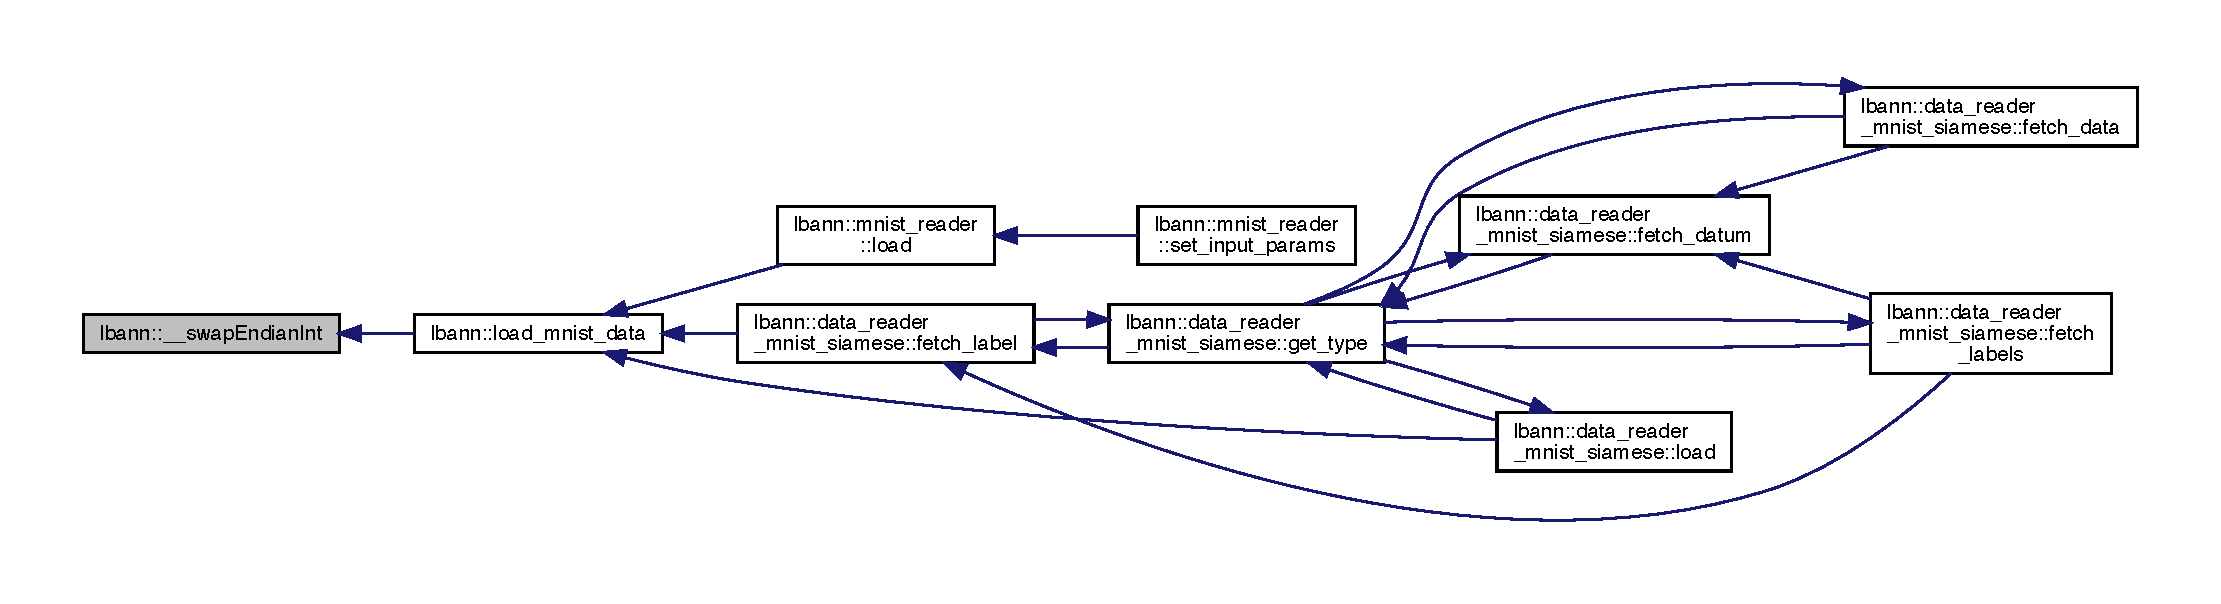
\includegraphics[width=350pt]{namespacelbann_a0fd8bc0ad31da913a124683f5ec4fdf1_icgraph}
\end{center}
\end{figure}
\mbox{\Hypertarget{namespacelbann_a1b8b05bbf2e59808a51ead80c47a9359}\label{namespacelbann_a1b8b05bbf2e59808a51ead80c47a9359}} 
\index{lbann@{lbann}!add\+\_\+delimiter@{add\+\_\+delimiter}}
\index{add\+\_\+delimiter@{add\+\_\+delimiter}!lbann@{lbann}}
\subsubsection{\texorpdfstring{add\+\_\+delimiter()}{add\_delimiter()}}
{\footnotesize\ttfamily std\+::string lbann\+::add\+\_\+delimiter (\begin{DoxyParamCaption}\item[{const std\+::string}]{dir }\end{DoxyParamCaption})}

This automatically attaches the directory deliminator at the end of the given directory as necessary. If \char`\"{}\char`\"{} is given, it will do nothing 

Definition at line 117 of file file\+\_\+utils.\+cpp.


\begin{DoxyCode}
117                                              \{
118   \textcolor{keywordflow}{if} (dir.empty()) \{
119     \textcolor{keywordflow}{return} \textcolor{stringliteral}{""};
120   \}
121   std::string new\_dir(dir);
122 
123   \textcolor{keywordflow}{if} (!path\_delimiter::check(new\_dir.back())) \{
124     new\_dir.append(path\_delimiter::preferred());
125   \}
126 
127   \textcolor{keywordflow}{return} new\_dir;
128 \}
\end{DoxyCode}
Here is the call graph for this function\+:\nopagebreak
\begin{figure}[H]
\begin{center}
\leavevmode
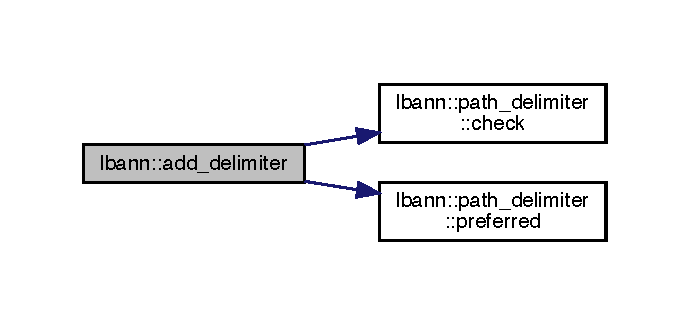
\includegraphics[width=331pt]{namespacelbann_a1b8b05bbf2e59808a51ead80c47a9359_cgraph}
\end{center}
\end{figure}
Here is the caller graph for this function\+:\nopagebreak
\begin{figure}[H]
\begin{center}
\leavevmode
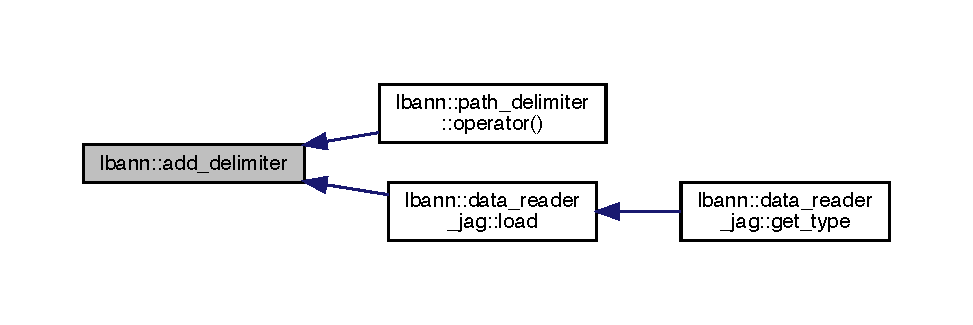
\includegraphics[width=350pt]{namespacelbann_a1b8b05bbf2e59808a51ead80c47a9359_icgraph}
\end{center}
\end{figure}
\mbox{\Hypertarget{namespacelbann_ae8bc674a3d676391666524b44cbc4068}\label{namespacelbann_ae8bc674a3d676391666524b44cbc4068}} 
\index{lbann@{lbann}!bernoulli\+\_\+fill@{bernoulli\+\_\+fill}}
\index{bernoulli\+\_\+fill@{bernoulli\+\_\+fill}!lbann@{lbann}}
\subsubsection{\texorpdfstring{bernoulli\+\_\+fill()}{bernoulli\_fill()}}
{\footnotesize\ttfamily void lbann\+::bernoulli\+\_\+fill (\begin{DoxyParamCaption}\item[{\hyperlink{base_8hpp_a9a697a504ae84010e7439ffec862b470}{Abs\+Dist\+Mat} \&}]{mat,  }\item[{El\+::\+Int}]{m,  }\item[{El\+::\+Int}]{n,  }\item[{double}]{p = {\ttfamily 0.5} }\end{DoxyParamCaption})}

Make mat into an m x n matrix where each entry is an indepenent Bernoulli random variable with parameter p. This makes the same guarantees as gaussian\+\_\+fill. 

Definition at line 175 of file random.\+cpp.


\begin{DoxyCode}
175                                                                  \{
176 \textcolor{preprocessor}{#ifdef LBANN\_PARALLEL\_RANDOM\_MATRICES}
177   El::Bernoulli(mat, m, n, p);
178 \textcolor{preprocessor}{#else}
179   \hyperlink{namespacelbann_ad1e3fe84cfa5257be476de3be805064d}{bernoulli\_fill\_procdet}(mat, m, n, p);
180 \textcolor{preprocessor}{#endif  // LBANN\_PARALLEL\_RANDOM\_MATRICES  }
181 \}
\end{DoxyCode}
Here is the call graph for this function\+:\nopagebreak
\begin{figure}[H]
\begin{center}
\leavevmode
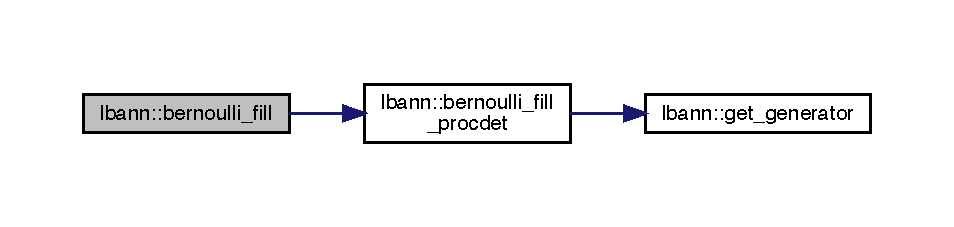
\includegraphics[width=350pt]{namespacelbann_ae8bc674a3d676391666524b44cbc4068_cgraph}
\end{center}
\end{figure}
Here is the caller graph for this function\+:\nopagebreak
\begin{figure}[H]
\begin{center}
\leavevmode
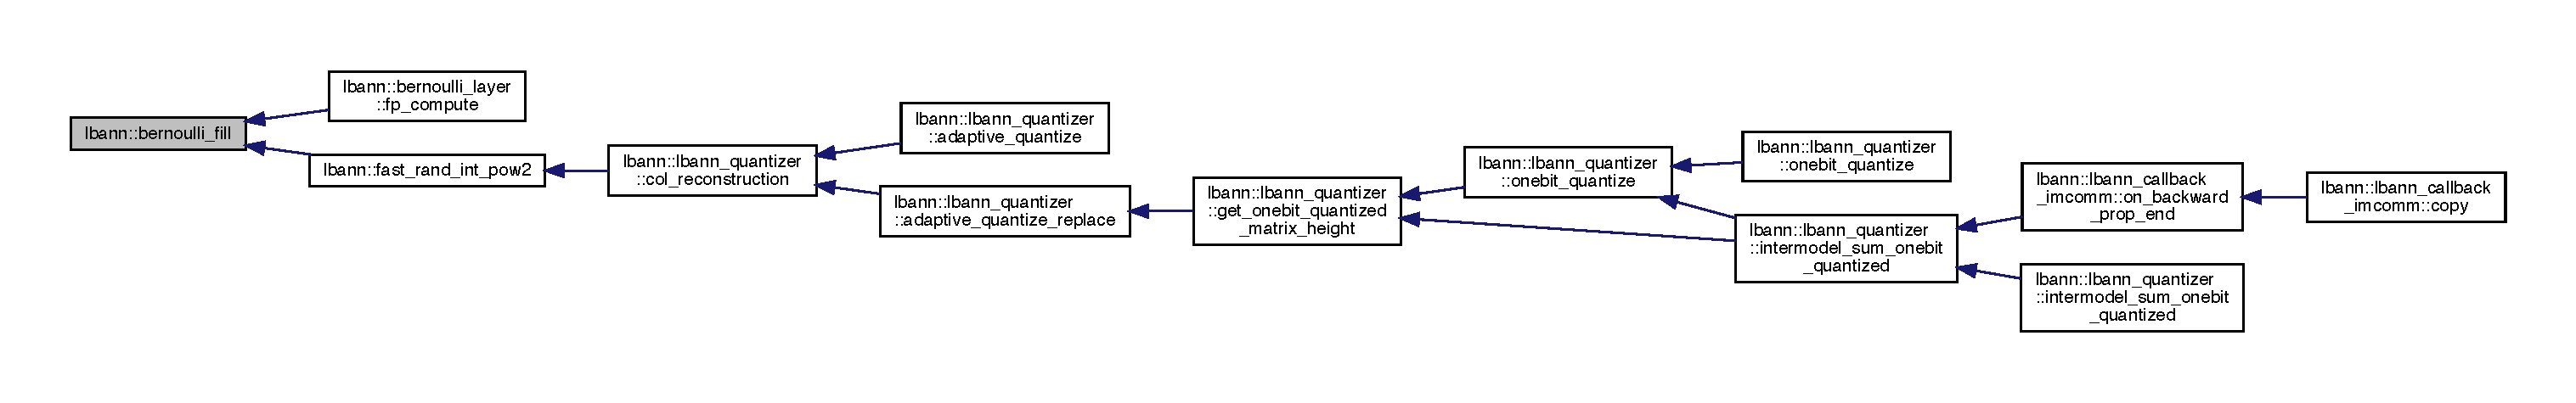
\includegraphics[width=350pt]{namespacelbann_ae8bc674a3d676391666524b44cbc4068_icgraph}
\end{center}
\end{figure}
\mbox{\Hypertarget{namespacelbann_ad1e3fe84cfa5257be476de3be805064d}\label{namespacelbann_ad1e3fe84cfa5257be476de3be805064d}} 
\index{lbann@{lbann}!bernoulli\+\_\+fill\+\_\+procdet@{bernoulli\+\_\+fill\+\_\+procdet}}
\index{bernoulli\+\_\+fill\+\_\+procdet@{bernoulli\+\_\+fill\+\_\+procdet}!lbann@{lbann}}
\subsubsection{\texorpdfstring{bernoulli\+\_\+fill\+\_\+procdet()}{bernoulli\_fill\_procdet()}}
{\footnotesize\ttfamily void lbann\+::bernoulli\+\_\+fill\+\_\+procdet (\begin{DoxyParamCaption}\item[{\hyperlink{base_8hpp_a9a697a504ae84010e7439ffec862b470}{Abs\+Dist\+Mat} \&}]{mat,  }\item[{El\+::\+Int}]{m,  }\item[{El\+::\+Int}]{n,  }\item[{double}]{p = {\ttfamily 0.5} }\end{DoxyParamCaption})}

Make mat into an m x n matrix where each entry is an independent Bernoulli random variable with parameter p. This makes the same guarantees as gaussian\+\_\+fill\+\_\+procdet. 

Definition at line 208 of file random.\+cpp.


\begin{DoxyCode}
208                                                                          \{
209   El::Zeros(mat, m, n);
210   \textcolor{keywordflow}{if} (mat.Grid().Rank() == 0) \{
211     mat.Reserve(m * n);
212     \textcolor{keyword}{auto}& gen = \hyperlink{namespacelbann_a4fea7ba21017b49d1e34394b4c20c764}{get\_generator}();
213     std::bernoulli\_distribution dist(p);
214     \textcolor{keywordflow}{for} (El::Int col = 0; col < n; ++col) \{
215       \textcolor{keywordflow}{for} (El::Int row = 0; row < m; ++row) \{
216         mat.QueueUpdate(row, col, dist(gen) ? 1.0f : 0.0f);
217       \}
218     \}
219   \}
220   mat.ProcessQueues();
221 \}
\end{DoxyCode}
Here is the call graph for this function\+:\nopagebreak
\begin{figure}[H]
\begin{center}
\leavevmode
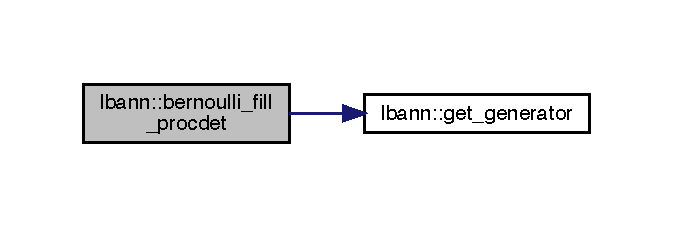
\includegraphics[width=323pt]{namespacelbann_ad1e3fe84cfa5257be476de3be805064d_cgraph}
\end{center}
\end{figure}
Here is the caller graph for this function\+:\nopagebreak
\begin{figure}[H]
\begin{center}
\leavevmode
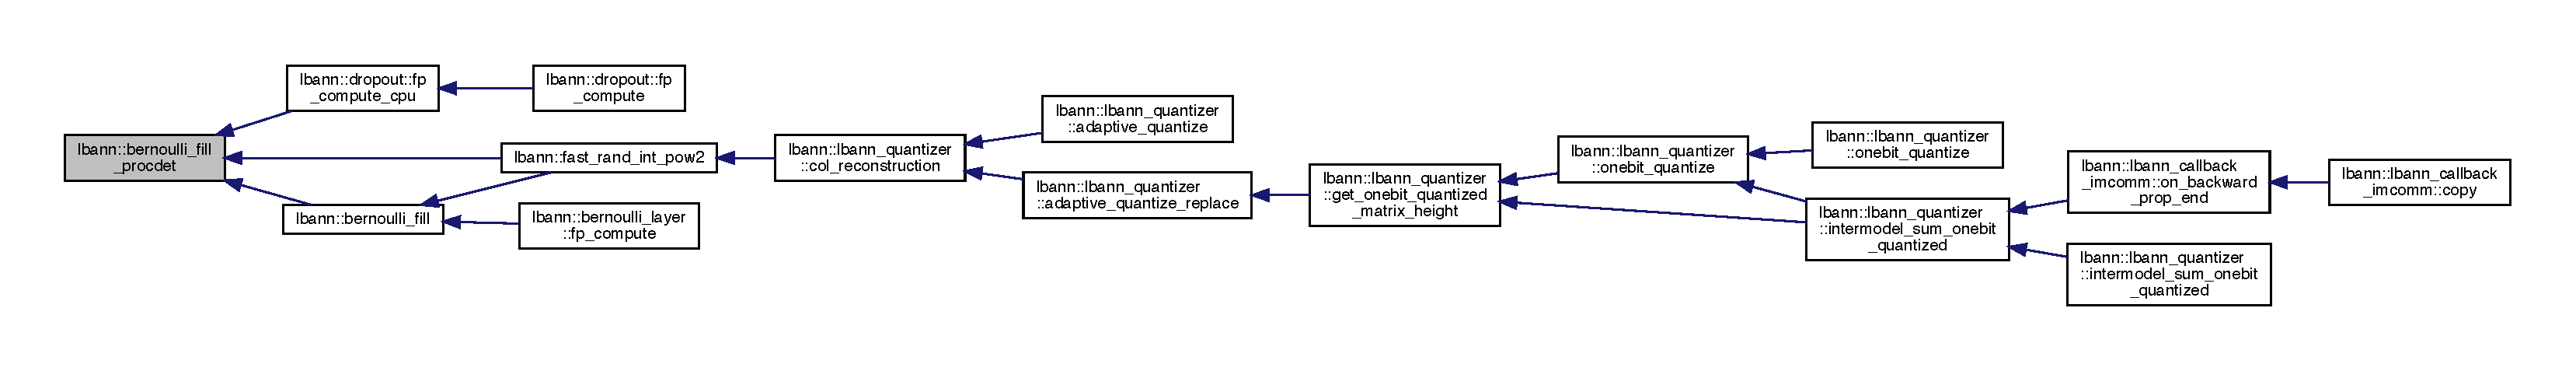
\includegraphics[width=350pt]{namespacelbann_ad1e3fe84cfa5257be476de3be805064d_icgraph}
\end{center}
\end{figure}
\mbox{\Hypertarget{namespacelbann_a3ee4a1fa7a82c30999de9eb626c68311}\label{namespacelbann_a3ee4a1fa7a82c30999de9eb626c68311}} 
\index{lbann@{lbann}!check\+\_\+if\+\_\+dir\+\_\+exists@{check\+\_\+if\+\_\+dir\+\_\+exists}}
\index{check\+\_\+if\+\_\+dir\+\_\+exists@{check\+\_\+if\+\_\+dir\+\_\+exists}!lbann@{lbann}}
\subsubsection{\texorpdfstring{check\+\_\+if\+\_\+dir\+\_\+exists()}{check\_if\_dir\_exists()}}
{\footnotesize\ttfamily bool lbann\+::check\+\_\+if\+\_\+dir\+\_\+exists (\begin{DoxyParamCaption}\item[{const std\+::string \&}]{dirname }\end{DoxyParamCaption})}



Definition at line 171 of file file\+\_\+utils.\+cpp.


\begin{DoxyCode}
171                                                    \{
172   \textcolor{keywordflow}{return} \hyperlink{namespacelbann_a4fac6c6483965395fa79d31061485f9f}{check\_if\_file\_exists}(dirname);
173 \}
\end{DoxyCode}
Here is the call graph for this function\+:\nopagebreak
\begin{figure}[H]
\begin{center}
\leavevmode
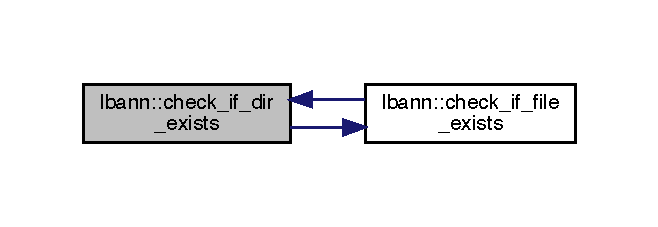
\includegraphics[width=316pt]{namespacelbann_a3ee4a1fa7a82c30999de9eb626c68311_cgraph}
\end{center}
\end{figure}
Here is the caller graph for this function\+:\nopagebreak
\begin{figure}[H]
\begin{center}
\leavevmode
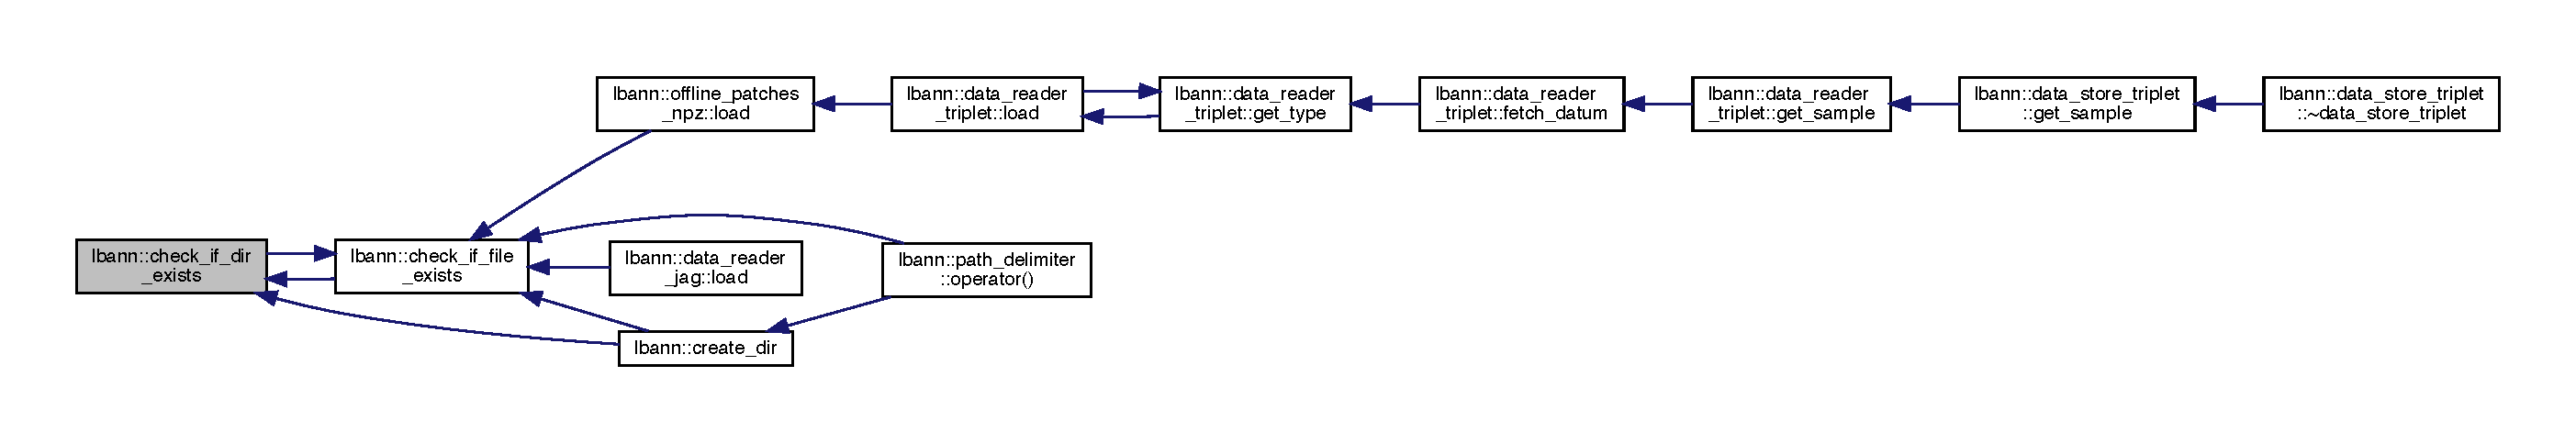
\includegraphics[width=350pt]{namespacelbann_a3ee4a1fa7a82c30999de9eb626c68311_icgraph}
\end{center}
\end{figure}
\mbox{\Hypertarget{namespacelbann_a4fac6c6483965395fa79d31061485f9f}\label{namespacelbann_a4fac6c6483965395fa79d31061485f9f}} 
\index{lbann@{lbann}!check\+\_\+if\+\_\+file\+\_\+exists@{check\+\_\+if\+\_\+file\+\_\+exists}}
\index{check\+\_\+if\+\_\+file\+\_\+exists@{check\+\_\+if\+\_\+file\+\_\+exists}!lbann@{lbann}}
\subsubsection{\texorpdfstring{check\+\_\+if\+\_\+file\+\_\+exists()}{check\_if\_file\_exists()}}
{\footnotesize\ttfamily bool lbann\+::check\+\_\+if\+\_\+file\+\_\+exists (\begin{DoxyParamCaption}\item[{const std\+::string \&}]{filename }\end{DoxyParamCaption})}



Return true if a file with the given name exists. 



Definition at line 155 of file file\+\_\+utils.\+cpp.


\begin{DoxyCode}
155                                                      \{
156   std::ifstream ifile(filename);
157   \textcolor{keywordflow}{return} \textcolor{keyword}{static\_cast<}\textcolor{keywordtype}{bool}\textcolor{keyword}{>}(ifile);
158 \}
\end{DoxyCode}
Here is the call graph for this function\+:\nopagebreak
\begin{figure}[H]
\begin{center}
\leavevmode
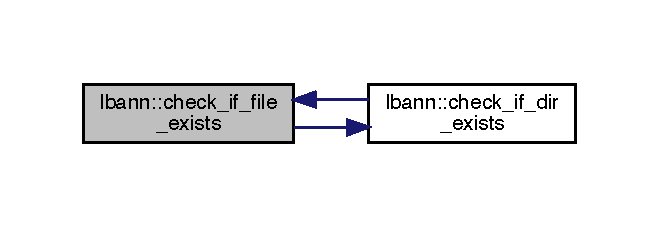
\includegraphics[width=316pt]{namespacelbann_a4fac6c6483965395fa79d31061485f9f_cgraph}
\end{center}
\end{figure}
Here is the caller graph for this function\+:\nopagebreak
\begin{figure}[H]
\begin{center}
\leavevmode
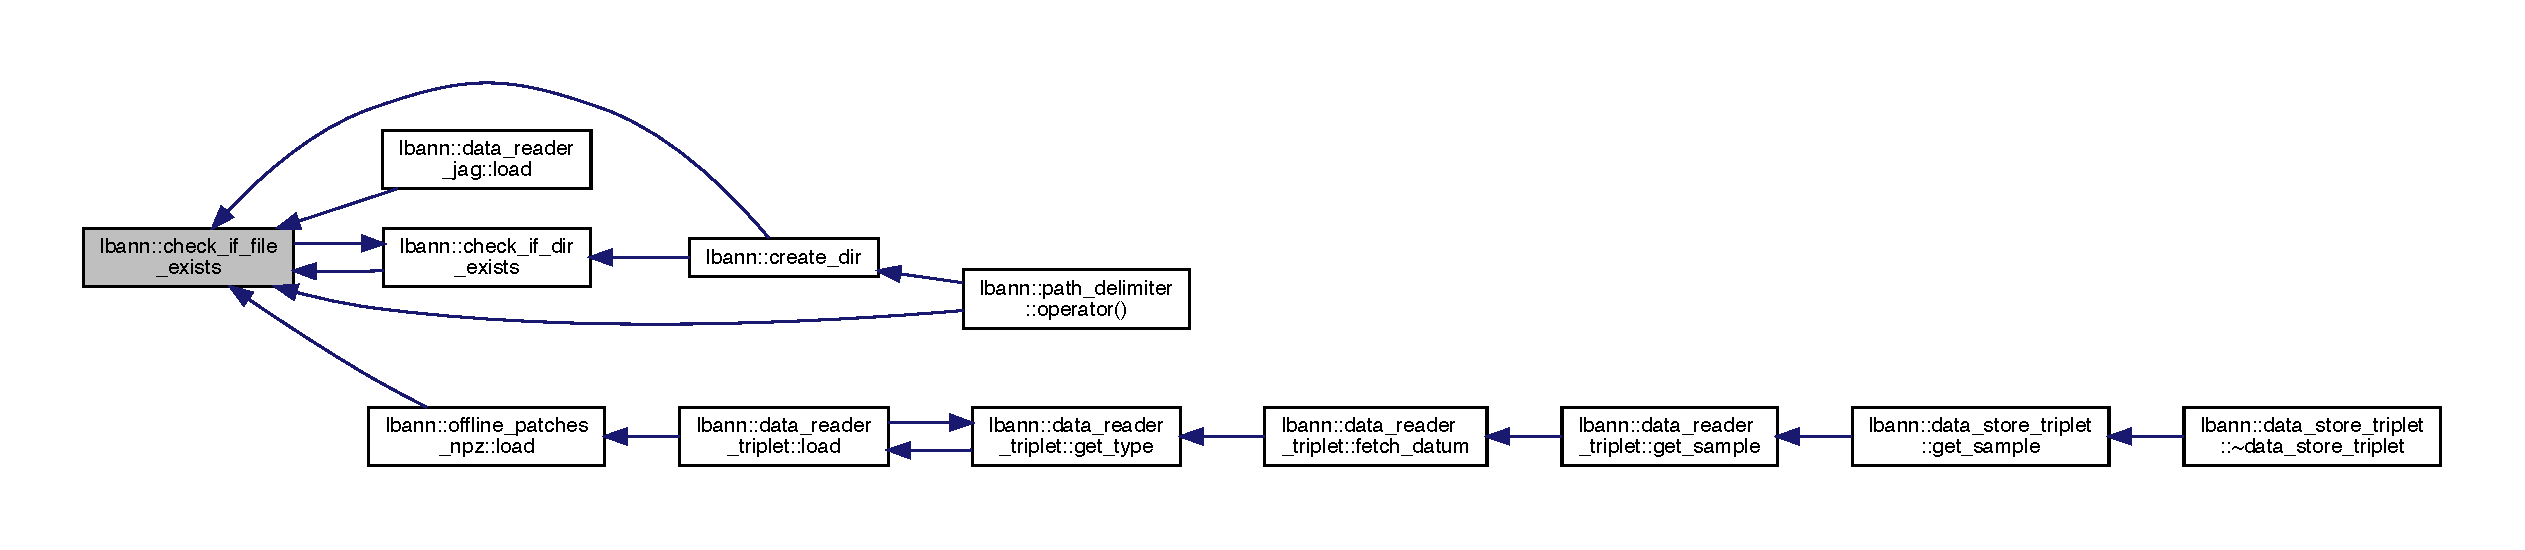
\includegraphics[width=350pt]{namespacelbann_a4fac6c6483965395fa79d31061485f9f_icgraph}
\end{center}
\end{figure}
\mbox{\Hypertarget{namespacelbann_a38dd30b2ae8214f6595708264369ddb8}\label{namespacelbann_a38dd30b2ae8214f6595708264369ddb8}} 
\index{lbann@{lbann}!closeread@{closeread}}
\index{closeread@{closeread}!lbann@{lbann}}
\subsubsection{\texorpdfstring{closeread()}{closeread()}}
{\footnotesize\ttfamily int lbann\+::closeread (\begin{DoxyParamCaption}\item[{int}]{fd,  }\item[{const char $\ast$}]{filename }\end{DoxyParamCaption})}



Definition at line 106 of file file\+\_\+io.\+cpp.


\begin{DoxyCode}
106                                              \{
107   \textcolor{comment}{// close file}
108   \textcolor{keywordtype}{int} close\_rc = close(fd);
109   \textcolor{keywordflow}{if} (close\_rc == -1) \{
110     fprintf(stderr, \textcolor{stringliteral}{"ERROR: Failed to close file `%s' (%d: %s) @ %s:%d\(\backslash\)n"},
111             file, errno, strerror(errno), \_\_FILE\_\_, \_\_LINE\_\_
112            );
113     fflush(stderr);
114   \}
115 
116   \textcolor{keywordflow}{return} close\_rc;
117 \}
\end{DoxyCode}
Here is the caller graph for this function\+:\nopagebreak
\begin{figure}[H]
\begin{center}
\leavevmode
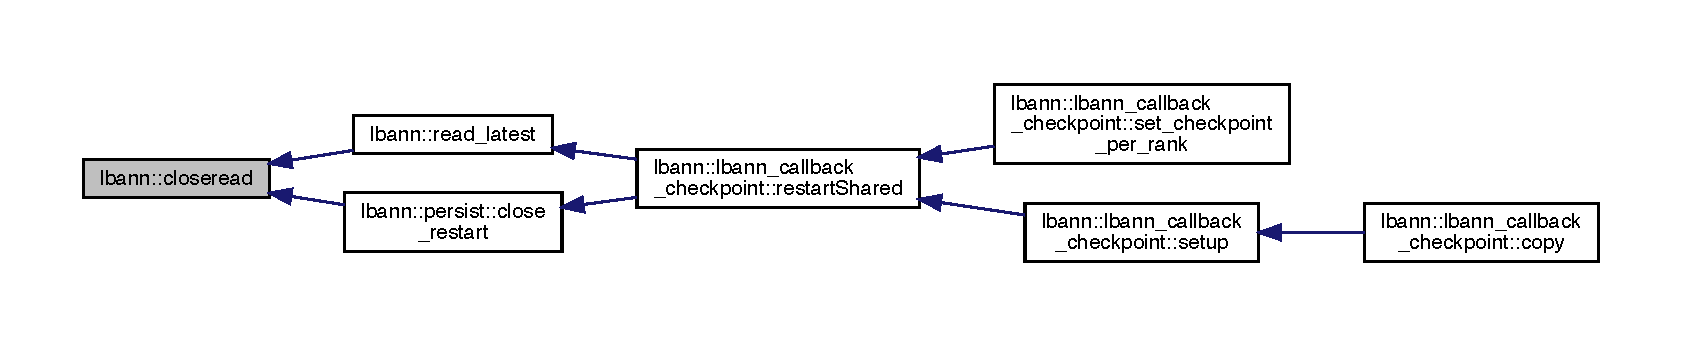
\includegraphics[width=350pt]{namespacelbann_a38dd30b2ae8214f6595708264369ddb8_icgraph}
\end{center}
\end{figure}
\mbox{\Hypertarget{namespacelbann_aceeccedbbafccfa071b21ee99be794a5}\label{namespacelbann_aceeccedbbafccfa071b21ee99be794a5}} 
\index{lbann@{lbann}!closewrite@{closewrite}}
\index{closewrite@{closewrite}!lbann@{lbann}}
\subsubsection{\texorpdfstring{closewrite()}{closewrite()}}
{\footnotesize\ttfamily int lbann\+::closewrite (\begin{DoxyParamCaption}\item[{int}]{fd,  }\item[{const char $\ast$}]{filename }\end{DoxyParamCaption})}



Definition at line 133 of file file\+\_\+io.\+cpp.


\begin{DoxyCode}
133                                               \{
134   \textcolor{comment}{// fsync file}
135   \textcolor{keywordtype}{int} fsync\_rc = fsync(fd);
136   \textcolor{keywordflow}{if} (fsync\_rc == -1) \{
137     fprintf(stderr, \textcolor{stringliteral}{"ERROR: Failed to fsync file `%s' (%d: %s) @ %s:%d\(\backslash\)n"},
138             file, errno, strerror(errno), \_\_FILE\_\_, \_\_LINE\_\_
139            );
140     fflush(stderr);
141   \}
142 
143   \textcolor{comment}{// close file}
144   \textcolor{keywordtype}{int} close\_rc = close(fd);
145   \textcolor{keywordflow}{if} (close\_rc == -1) \{
146     fprintf(stderr, \textcolor{stringliteral}{"ERROR: Failed to close file `%s' (%d: %s) @ %s:%d\(\backslash\)n"},
147             file, errno, strerror(errno), \_\_FILE\_\_, \_\_LINE\_\_
148            );
149     fflush(stderr);
150   \}
151 
152   \textcolor{keywordflow}{return} close\_rc;
153 \}
\end{DoxyCode}
Here is the caller graph for this function\+:\nopagebreak
\begin{figure}[H]
\begin{center}
\leavevmode
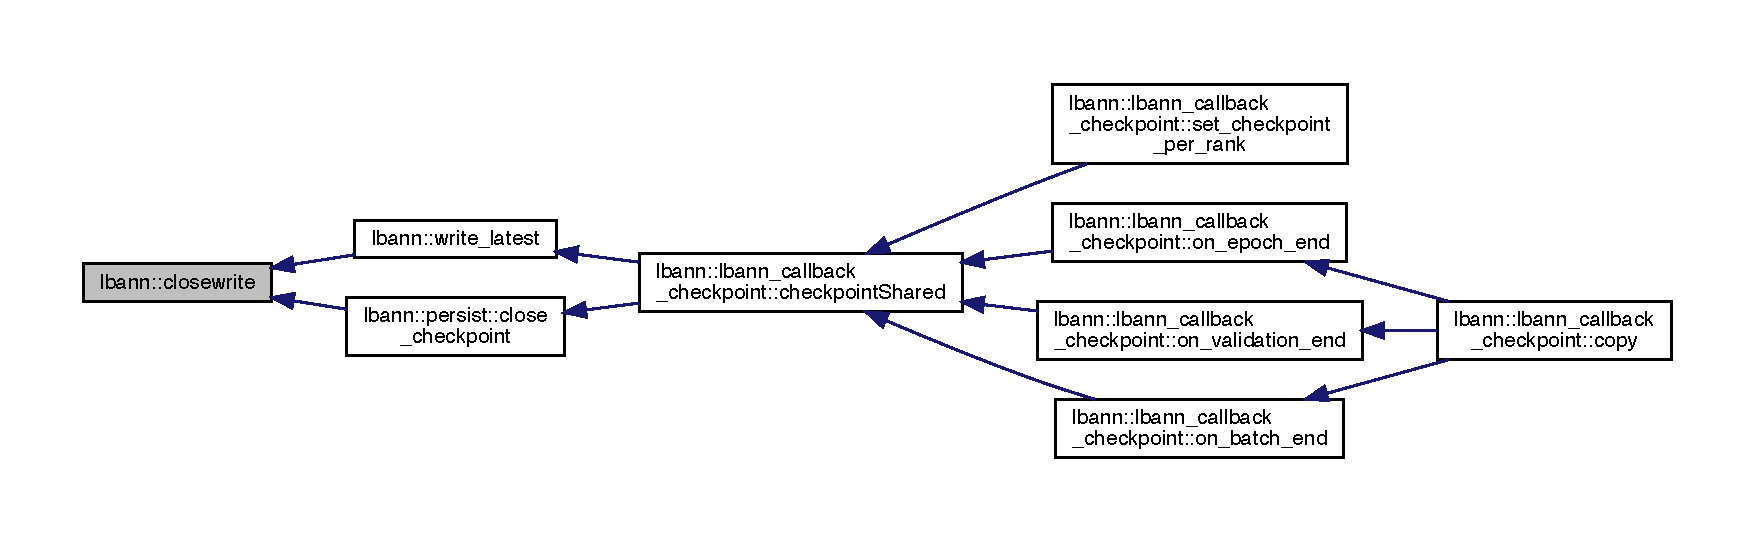
\includegraphics[width=350pt]{namespacelbann_aceeccedbbafccfa071b21ee99be794a5_icgraph}
\end{center}
\end{figure}
\mbox{\Hypertarget{namespacelbann_a0e1225f72580ffb5166181392b68b651}\label{namespacelbann_a0e1225f72580ffb5166181392b68b651}} 
\index{lbann@{lbann}!col2im@{col2im}}
\index{col2im@{col2im}!lbann@{lbann}}
\subsubsection{\texorpdfstring{col2im()}{col2im()}\hspace{0.1cm}{\footnotesize\ttfamily [1/2]}}
{\footnotesize\ttfamily void lbann\+::col2im (\begin{DoxyParamCaption}\item[{const \hyperlink{base_8hpp_a68f11fdc31b62516cb310831bbe54d73}{Mat} \&}]{col,  }\item[{\hyperlink{base_8hpp_a68f11fdc31b62516cb310831bbe54d73}{Mat} \&}]{im,  }\item[{int}]{num\+\_\+channels,  }\item[{int}]{im\+\_\+num\+\_\+dims,  }\item[{const int $\ast$}]{im\+\_\+dims,  }\item[{const int $\ast$}]{im\+\_\+pads,  }\item[{const int $\ast$}]{window\+\_\+dims,  }\item[{const int $\ast$}]{window\+\_\+strides }\end{DoxyParamCaption})}



Rearrange matrix columns into image blocks. 

This is approximately the inverse of im2col. The output tensor im is produced from the input matrix col by shifting a window across im. Each column of col is matched with the corresponding window position and corresponding entries are added to im. 
\begin{DoxyParams}{Parameters}
{\em col} & col matrix. Height should be equal to window size and width equal to number of window shifts. Data should be contiguous. \\
\hline
{\em im} & im tensor, represented as a column vector. \\
\hline
{\em num\+\_\+channels} & Number of channels in im tensor. \\
\hline
{\em im\+\_\+num\+\_\+dims} & Number of dimensions in im tensor. \\
\hline
{\em im\+\_\+dims} & im tensor dimensions. \\
\hline
{\em im\+\_\+pads} & Zero pads for im tensor. \\
\hline
{\em window\+\_\+dims} & Dimensions of window. \\
\hline
{\em window\+\_\+strides} & Window shift strides. \\
\hline
\end{DoxyParams}


Definition at line 155 of file im2col.\+cpp.


\begin{DoxyCode}
162                                         \{
163 
164   \textcolor{comment}{// Input and output parameters}
165   \textcolor{keyword}{const} DataType *\_\_restrict\_\_ col\_buffer = col.LockedBuffer();
166   DataType *\_\_restrict\_\_ im\_buffer = im.Buffer();
167 
168   \textcolor{comment}{// col2im parameters}
169   std::vector<int> offset\_start(im\_num\_dims);
170   std::vector<int> offset\_end(im\_num\_dims);
171   std::vector<int> offset\_stride(im\_num\_dims);
172   std::vector<int> offset\_num(im\_num\_dims);
173   \textcolor{keywordflow}{for}(\textcolor{keywordtype}{int} d = 0; d < im\_num\_dims; ++d) \{
174     offset\_start[d] = -im\_pads[d];
175     offset\_end[d] = im\_dims[d] + im\_pads[d] - window\_dims[d] + 1;
176     offset\_stride[d] = window\_strides[d];
177     offset\_num[d] = (offset\_end[d] - offset\_start[d] + offset\_stride[d] - 1) / offset\_stride[d];
178   \}
179 
180 \textcolor{preprocessor}{  #ifdef LBANN\_DEBUG}
181   \textcolor{keyword}{const} \textcolor{keywordtype}{int} im\_size = im.Height();
182   \textcolor{keyword}{const} \textcolor{keywordtype}{int} col\_height = col.Height();
183   \textcolor{keyword}{const} \textcolor{keywordtype}{int} col\_width = col.Width();
184   \textcolor{comment}{// Check matrix dimensions}
185   \textcolor{keyword}{const} \textcolor{keywordtype}{int} expected\_im\_size = std::accumulate(im\_dims,
186                                                im\_dims + im\_num\_dims,
187                                                num\_channels,
188                                                std::multiplies<int>());
189   \textcolor{keyword}{const} \textcolor{keywordtype}{int} expected\_col\_height = std::accumulate(window\_dims,
190                                                   window\_dims + im\_num\_dims,
191                                                   num\_channels,
192                                                   std::multiplies<int>());
193   \textcolor{keyword}{const} \textcolor{keywordtype}{int} expected\_col\_width = std::accumulate(offset\_num.begin(),
194                                                  offset\_num.end(),
195                                                  1,
196                                                  std::multiplies<int>());
197   \textcolor{keywordflow}{if}(im\_size != expected\_im\_size || im.Width() != 1) \{
198     std::stringstream ss;
199     ss << \textcolor{stringliteral}{"im2col: im matrix has invalid dimensions "}
200        << \textcolor{stringliteral}{"(expected "} << expected\_im\_size << \textcolor{stringliteral}{" x "} << 1 << \textcolor{stringliteral}{", "}
201        << \textcolor{stringliteral}{"found "} << im\_size << \textcolor{stringliteral}{" x "} << im.Width() << \textcolor{stringliteral}{")"};
202     \textcolor{keywordflow}{throw} lbann\_exception(ss.str());
203   \}
204   \textcolor{keywordflow}{if}(col\_height != expected\_col\_height
205      || col\_width != expected\_col\_width) \{
206     std::stringstream ss;
207     ss << \textcolor{stringliteral}{"im2col: col matrix has invalid dimensions "}
208        << \textcolor{stringliteral}{"(expected "} << expected\_col\_height << \textcolor{stringliteral}{" x "} << expected\_col\_width << \textcolor{stringliteral}{", "}
209        << \textcolor{stringliteral}{"found "} << col\_height << \textcolor{stringliteral}{" x "} << col\_width << \textcolor{stringliteral}{")"};
210     \textcolor{keywordflow}{throw} lbann\_exception(ss.str());
211   \}
212 \textcolor{preprocessor}{  #endif // LBANN\_DEBUG  }
213 
214   \textcolor{comment}{// Call optimized routine for 1x1 col2im}
215   std::vector<int> zeros(im\_num\_dims, 0), ones(im\_num\_dims, 1);
216   \textcolor{keywordflow}{if}(std::equal(im\_pads, im\_pads + im\_num\_dims, zeros.begin())
217      && std::equal(window\_dims, window\_dims + im\_num\_dims, ones.begin())
218      && std::equal(window\_strides, window\_strides + im\_num\_dims, ones.begin())) \{
219     \hyperlink{namespacelbann_ab4fccda3dc4c2c293d643815dfefe22a}{col2im\_1x1}(col\_buffer, im\_buffer, num\_channels, im\_num\_dims, im\_dims);
220     \textcolor{keywordflow}{return};
221   \}
222 
223   \textcolor{comment}{// Call optimized routine for 2D data}
224   \textcolor{keywordflow}{if}(im\_num\_dims == 2) \{
225     \hyperlink{namespacelbann_a1953674a43b284f0abb5c5e4db94b2b9}{col2im\_2d}(col\_buffer, im\_buffer,
226               im\_dims[1], im\_dims[0], im\_pads[1], im\_pads[0], num\_channels,
227               window\_dims[1], window\_dims[0],
228               window\_strides[1], window\_strides[0]);
229     \textcolor{keywordflow}{return};
230   \}
231 
232   \textcolor{comment}{// Default algorithm}
233   \hyperlink{namespacelbann_ab36806d08e7c852ad9cf3a0564f29b64}{col2im}(col, im, num\_channels, im\_num\_dims,
234          im\_dims, im\_pads, window\_dims, window\_strides,
235          std::plus<DataType>());
236 
237 \}
\end{DoxyCode}
Here is the call graph for this function\+:\nopagebreak
\begin{figure}[H]
\begin{center}
\leavevmode
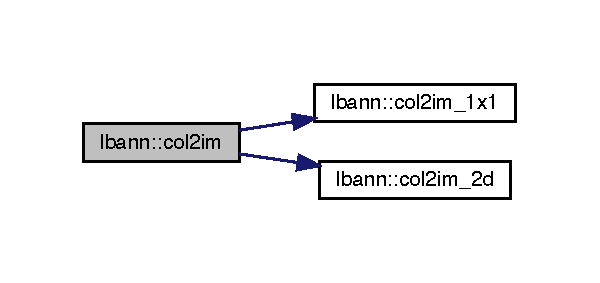
\includegraphics[width=288pt]{namespacelbann_a0e1225f72580ffb5166181392b68b651_cgraph}
\end{center}
\end{figure}
Here is the caller graph for this function\+:\nopagebreak
\begin{figure}[H]
\begin{center}
\leavevmode
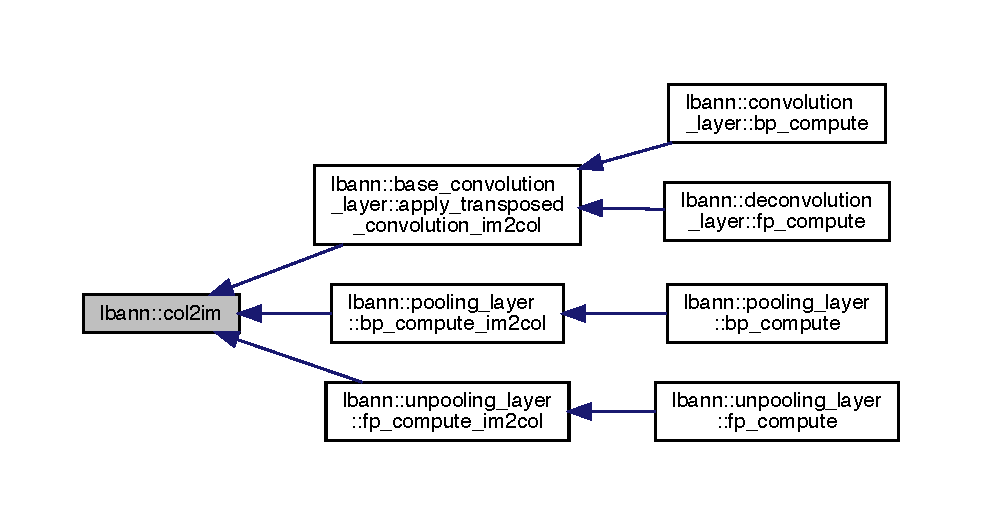
\includegraphics[width=350pt]{namespacelbann_a0e1225f72580ffb5166181392b68b651_icgraph}
\end{center}
\end{figure}
\mbox{\Hypertarget{namespacelbann_ab36806d08e7c852ad9cf3a0564f29b64}\label{namespacelbann_ab36806d08e7c852ad9cf3a0564f29b64}} 
\index{lbann@{lbann}!col2im@{col2im}}
\index{col2im@{col2im}!lbann@{lbann}}
\subsubsection{\texorpdfstring{col2im()}{col2im()}\hspace{0.1cm}{\footnotesize\ttfamily [2/2]}}
{\footnotesize\ttfamily void lbann\+::col2im (\begin{DoxyParamCaption}\item[{const \hyperlink{base_8hpp_a68f11fdc31b62516cb310831bbe54d73}{Mat} \&}]{col,  }\item[{\hyperlink{base_8hpp_a68f11fdc31b62516cb310831bbe54d73}{Mat} \&}]{im,  }\item[{int}]{num\+\_\+channels,  }\item[{int}]{im\+\_\+num\+\_\+dims,  }\item[{const int $\ast$}]{im\+\_\+dims,  }\item[{const int $\ast$}]{im\+\_\+pads,  }\item[{const int $\ast$}]{window\+\_\+dims,  }\item[{const int $\ast$}]{window\+\_\+strides,  }\item[{std\+::function$<$ Data\+Type(const Data\+Type \&, const Data\+Type \&)$>$}]{reduction\+\_\+op }\end{DoxyParamCaption})}



Rearrange matrix columns into image blocks. 

This is approximately the inverse of im2col. The output tensor im is produced from the input matrix col by shifting a window across im. Each column of col is matched with the corresponding window position and corresponding entries are reduced to im. 
\begin{DoxyParams}{Parameters}
{\em col} & col matrix. Height should be equal to window size and width equal to number of window shifts. Data should be contiguous. \\
\hline
{\em im} & im tensor, represented as a column vector. \\
\hline
{\em num\+\_\+channels} & Number of channels in im tensor. \\
\hline
{\em im\+\_\+num\+\_\+dims} & Number of dimensions in im tensor. \\
\hline
{\em im\+\_\+dims} & im tensor dimensions. \\
\hline
{\em im\+\_\+pads} & Zero pads for im tensor. \\
\hline
{\em window\+\_\+dims} & Dimensions of window. \\
\hline
{\em window\+\_\+strides} & Window shift strides. \\
\hline
{\em reduction\+\_\+op} & Reduction operation. \\
\hline
\end{DoxyParams}


Definition at line 239 of file im2col.\+cpp.


\begin{DoxyCode}
247                                                                                  \{
248 
249   \textcolor{comment}{// Input and output parameters}
250   \textcolor{keyword}{const} \textcolor{keywordtype}{int} col\_height = col.Height();
251   \textcolor{keyword}{const} \textcolor{keywordtype}{int} im\_size = im.Height();
252   \textcolor{keyword}{const} DataType *\_\_restrict\_\_ col\_buffer = col.LockedBuffer();
253   DataType *\_\_restrict\_\_ im\_buffer = im.Buffer();
254 
255   \textcolor{comment}{// im2col parameters}
256   std::vector<int> offset\_start(im\_num\_dims);
257   std::vector<int> offset\_end(im\_num\_dims);
258   std::vector<int> offset\_stride(im\_num\_dims);
259   std::vector<int> offset\_num(im\_num\_dims);
260   \textcolor{keywordflow}{for}(\textcolor{keywordtype}{int} d = 0; d < im\_num\_dims; ++d) \{
261     offset\_start[d] = -im\_pads[d];
262     offset\_end[d] = im\_dims[d] + im\_pads[d] - window\_dims[d] + 1;
263     offset\_stride[d] = window\_strides[d];
264     offset\_num[d] = (offset\_end[d] - offset\_start[d] + offset\_stride[d] - 1) / offset\_stride[d];
265   \}
266 
267   \textcolor{comment}{// Call optimized routine for 1x1 col2im}
268   std::vector<int> zeros(im\_num\_dims, 0), ones(im\_num\_dims, 1);
269   \textcolor{keywordflow}{if}(std::equal(im\_pads, im\_pads + im\_num\_dims, zeros.begin())
270      && std::equal(window\_dims, window\_dims + im\_num\_dims, ones.begin())
271      && std::equal(window\_strides, window\_strides + im\_num\_dims, ones.begin())) \{
272     \hyperlink{namespacelbann_ab4fccda3dc4c2c293d643815dfefe22a}{col2im\_1x1}(col\_buffer, im\_buffer, num\_channels, im\_num\_dims, im\_dims);
273     \textcolor{keywordflow}{return};
274   \}
275 
276   \textcolor{comment}{// Iterate through im matrix entries}
277 \textcolor{preprocessor}{  #pragma omp parallel for}
278   \textcolor{keywordflow}{for}(\textcolor{keywordtype}{int} im\_index = 0; im\_index < im\_size; ++im\_index) \{
279 
280     \textcolor{comment}{// Initialize arrays}
281     std::vector<int> im\_pos(im\_num\_dims);
282     std::vector<int> first\_offset(im\_num\_dims);
283     std::vector<int> last\_offset(im\_num\_dims);
284     std::vector<int> offset(im\_num\_dims);
285 
286     \textcolor{comment}{// Get position of im matrix entry}
287     \textcolor{keywordtype}{int} im\_index\_remainder = im\_index;
288     \textcolor{keywordflow}{for}(\textcolor{keywordtype}{int} d = im\_num\_dims-1; d >= 0; --d) \{
289       im\_pos[d] = im\_index\_remainder % im\_dims[d];
290       im\_index\_remainder /= im\_dims[d];
291     \}
292     \textcolor{keyword}{const} \textcolor{keywordtype}{int} channel = im\_index\_remainder;
293 
294     \textcolor{comment}{// Initialize im matrix entry}
295     DataType im\_entry = 0;
296     \textcolor{keywordtype}{bool} im\_entry\_initialized = \textcolor{keyword}{false};
297     \textcolor{keywordtype}{bool} offsets\_finished = \textcolor{keyword}{false};
298 
299     \textcolor{comment}{// Get window offsets containing im matrix entry}
300     \textcolor{keywordflow}{for}(\textcolor{keywordtype}{int} d = 0; d < im\_num\_dims; ++d) \{
301       first\_offset[d] = (im\_pos[d] - offset\_start[d] - window\_dims[d] + offset\_stride[d]) / offset\_stride[d
      ];
302       first\_offset[d] = std::max(first\_offset[d], 0);
303       last\_offset[d] = (im\_pos[d] - offset\_start[d]) / offset\_stride[d];
304       last\_offset[d] = std::min(last\_offset[d], offset\_num[d] - 1);
305       offset[d] = first\_offset[d];
306       \textcolor{keywordflow}{if}(first\_offset[d] > last\_offset[d]) \{
307         offsets\_finished = \textcolor{keyword}{true};
308       \}
309     \}
310 
311     \textcolor{comment}{// Iterate through window offsets containing im matrix entry}
312     \textcolor{keywordflow}{while}(!offsets\_finished) \{
313 
314       \textcolor{comment}{// Get col matrix entry corresponding to im matrix entry}
315       \textcolor{keywordtype}{int} col\_row = channel;
316       \textcolor{keywordtype}{int} col\_col = 0;
317       \textcolor{keywordflow}{for}(\textcolor{keywordtype}{int} d = 0; d < im\_num\_dims; ++d) \{
318         \textcolor{keyword}{const} \textcolor{keywordtype}{int} window\_pos = im\_pos[d] - (offset\_start[d] + offset[d] * offset\_stride[d]);
319         col\_row = window\_pos + col\_row * window\_dims[d];
320         col\_col = offset[d] + col\_col * offset\_num[d];
321       \}
322       \textcolor{keyword}{const} \textcolor{keywordtype}{int} col\_index = col\_row + col\_col * col\_height;
323 
324       \textcolor{comment}{// Add col matrix entry to im matrix entry}
325       \textcolor{keyword}{const} DataType col\_entry = col\_buffer[col\_index];
326       im\_entry = (im\_entry\_initialized ?
327                   reduction\_op(im\_entry, col\_entry) :
328                   col\_entry);
329       im\_entry\_initialized = \textcolor{keyword}{true};
330 
331       \textcolor{comment}{// Move to next window offset}
332       ++offset[im\_num\_dims-1];
333       \textcolor{keywordflow}{for}(\textcolor{keywordtype}{int} d = im\_num\_dims-1; d >= 1; --d) \{
334         \textcolor{keywordflow}{if}(offset[d] > last\_offset[d]) \{
335           offset[d] = first\_offset[d];
336           ++offset[d-1];
337         \}
338       \}
339       offsets\_finished = offset[0] > last\_offset[0];
340       
341     \}
342 
343     \textcolor{comment}{// Update output entry}
344     im\_buffer[im\_index] = im\_entry;
345 
346   \}
347 
348 \}
\end{DoxyCode}
Here is the call graph for this function\+:\nopagebreak
\begin{figure}[H]
\begin{center}
\leavevmode
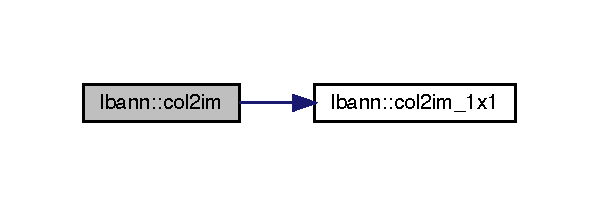
\includegraphics[width=288pt]{namespacelbann_ab36806d08e7c852ad9cf3a0564f29b64_cgraph}
\end{center}
\end{figure}
\mbox{\Hypertarget{namespacelbann_ab4fccda3dc4c2c293d643815dfefe22a}\label{namespacelbann_ab4fccda3dc4c2c293d643815dfefe22a}} 
\index{lbann@{lbann}!col2im\+\_\+1x1@{col2im\+\_\+1x1}}
\index{col2im\+\_\+1x1@{col2im\+\_\+1x1}!lbann@{lbann}}
\subsubsection{\texorpdfstring{col2im\+\_\+1x1()}{col2im\_1x1()}}
{\footnotesize\ttfamily void lbann\+::col2im\+\_\+1x1 (\begin{DoxyParamCaption}\item[{const Data\+Type $\ast$}]{input\+\_\+buffer,  }\item[{Data\+Type $\ast$}]{output\+\_\+buffer,  }\item[{const int}]{num\+\_\+channels,  }\item[{const int}]{num\+\_\+output\+\_\+dims,  }\item[{const int $\ast$}]{output\+\_\+dims }\end{DoxyParamCaption})}



Rearrange matrix columns into 1x1 image blocks. 

This is an optimized implementation of col2im when the window has a size of one, there is no padding, and the window stride is one. col2im will automatically call this routine if it detects a 1x1 col2im. 

Definition at line 429 of file im2col.\+cpp.


\begin{DoxyCode}
433                                          \{
434   \textcolor{keyword}{const} \textcolor{keywordtype}{int} spatial\_size = std::accumulate(output\_dims,
435                                            output\_dims + num\_output\_dims,
436                                            1,
437                                            std::multiplies<int>());
438   \textcolor{keyword}{const} \hyperlink{base_8hpp_a68f11fdc31b62516cb310831bbe54d73}{Mat} input\_matrix(num\_channels, spatial\_size, input\_buffer, num\_channels);
439   \hyperlink{base_8hpp_a68f11fdc31b62516cb310831bbe54d73}{Mat} output\_matrix(spatial\_size, num\_channels, output\_buffer, spatial\_size);
440   El::Transpose(input\_matrix, output\_matrix);
441 \}
\end{DoxyCode}
Here is the caller graph for this function\+:\nopagebreak
\begin{figure}[H]
\begin{center}
\leavevmode
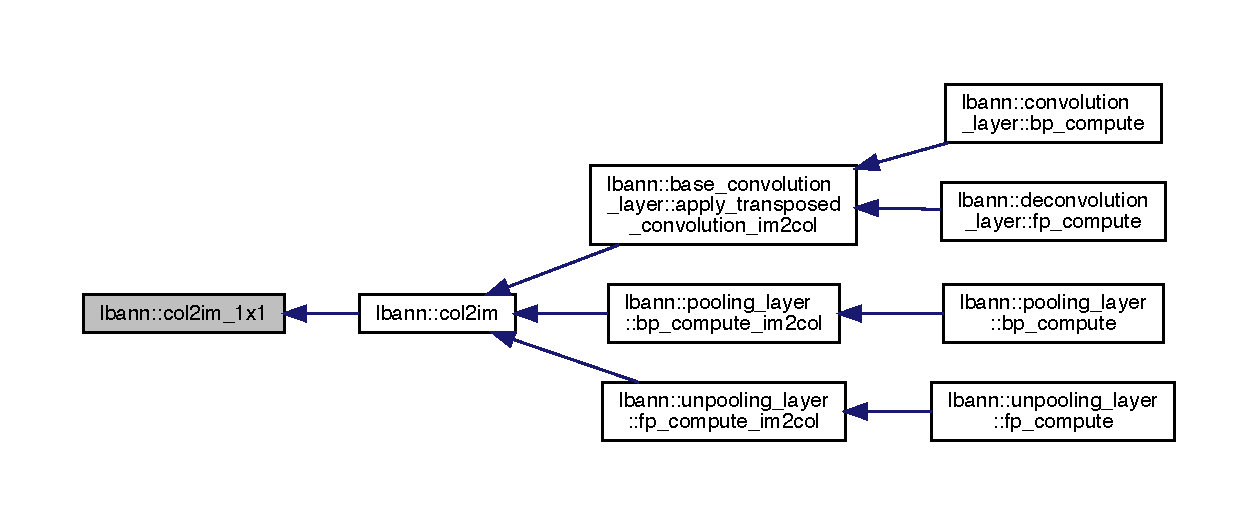
\includegraphics[width=350pt]{namespacelbann_ab4fccda3dc4c2c293d643815dfefe22a_icgraph}
\end{center}
\end{figure}
\mbox{\Hypertarget{namespacelbann_a1953674a43b284f0abb5c5e4db94b2b9}\label{namespacelbann_a1953674a43b284f0abb5c5e4db94b2b9}} 
\index{lbann@{lbann}!col2im\+\_\+2d@{col2im\+\_\+2d}}
\index{col2im\+\_\+2d@{col2im\+\_\+2d}!lbann@{lbann}}
\subsubsection{\texorpdfstring{col2im\+\_\+2d()}{col2im\_2d()}}
{\footnotesize\ttfamily void lbann\+::col2im\+\_\+2d (\begin{DoxyParamCaption}\item[{const Data\+Type $\ast$\+\_\+\+\_\+restrict\+\_\+\+\_\+}]{input\+\_\+buffer,  }\item[{Data\+Type $\ast$\+\_\+\+\_\+restrict\+\_\+\+\_\+}]{output\+\_\+buffer,  }\item[{int}]{output\+\_\+dim\+\_\+x,  }\item[{int}]{output\+\_\+dim\+\_\+y,  }\item[{int}]{output\+\_\+pad\+\_\+x,  }\item[{int}]{output\+\_\+pad\+\_\+y,  }\item[{int}]{num\+\_\+channels,  }\item[{int}]{window\+\_\+dim\+\_\+x,  }\item[{int}]{window\+\_\+dim\+\_\+y,  }\item[{int}]{offset\+\_\+stride\+\_\+x,  }\item[{int}]{offset\+\_\+stride\+\_\+y }\end{DoxyParamCaption})}



Rearrange matrix columns into 2D image blocks. 

This is an optimized implementation of col2im for 2D data. col2im will automatically call this routine if it detects 2D data. 

Definition at line 443 of file im2col.\+cpp.


\begin{DoxyCode}
453                                           \{
454 
455   \textcolor{comment}{// col2im parameters}
456   \textcolor{keyword}{const} \textcolor{keywordtype}{int} offset\_start\_x = -output\_pad\_x;
457   \textcolor{keyword}{const} \textcolor{keywordtype}{int} offset\_start\_y = -output\_pad\_y;
458   \textcolor{keyword}{const} \textcolor{keywordtype}{int} offset\_end\_x = output\_dim\_x + output\_pad\_x - window\_dim\_x + 1;
459   \textcolor{keyword}{const} \textcolor{keywordtype}{int} offset\_end\_y = output\_dim\_y + output\_pad\_y - window\_dim\_y + 1;
460   \textcolor{keyword}{const} \textcolor{keywordtype}{int} offset\_num\_x = (offset\_end\_x - offset\_start\_x + offset\_stride\_x - 1) / offset\_stride\_x;
461   \textcolor{keyword}{const} \textcolor{keywordtype}{int} offset\_num\_y = (offset\_end\_y - offset\_start\_y + offset\_stride\_y - 1) / offset\_stride\_y;
462   \textcolor{keyword}{const} \textcolor{keywordtype}{int} input\_height = num\_channels * window\_dim\_x * window\_dim\_y;
463 
464   \textcolor{comment}{// Iterate through output entries}
465 \textcolor{preprocessor}{  #pragma omp parallel for collapse(3)}
466   \textcolor{keywordflow}{for}(\textcolor{keywordtype}{int} channel = 0; channel < num\_channels; ++channel) \{
467     \textcolor{keywordflow}{for}(\textcolor{keywordtype}{int} output\_pos\_y = 0;
468         output\_pos\_y < output\_dim\_y;
469         ++output\_pos\_y) \{
470       \textcolor{keywordflow}{for}(\textcolor{keywordtype}{int} output\_pos\_x = 0;
471           output\_pos\_x < output\_dim\_x;
472           ++output\_pos\_x) \{
473 
474         \textcolor{comment}{// Get output entry}
475         \textcolor{keyword}{const} \textcolor{keywordtype}{int} output\_index = (output\_pos\_x
476                                   + output\_pos\_y * output\_dim\_x
477                                   + channel * output\_dim\_x * output\_dim\_y);
478         DataType output\_entry = 0;
479 
480         \textcolor{comment}{// Get window offsets containing output entry}
481         \textcolor{keyword}{const} \textcolor{keywordtype}{int} offset\_x\_lower = (output\_pos\_x - offset\_start\_x - window\_dim\_x + offset\_stride\_x) / 
      offset\_stride\_x;
482         \textcolor{keyword}{const} \textcolor{keywordtype}{int} offset\_y\_lower = (output\_pos\_y - offset\_start\_y - window\_dim\_y + offset\_stride\_y) / 
      offset\_stride\_y;
483         \textcolor{keyword}{const} \textcolor{keywordtype}{int} offset\_x\_upper = (output\_pos\_x - offset\_start\_x) / offset\_stride\_x;
484         \textcolor{keyword}{const} \textcolor{keywordtype}{int} offset\_y\_upper = (output\_pos\_y - offset\_start\_y) / offset\_stride\_y;
485         \textcolor{keyword}{const} \textcolor{keywordtype}{int} first\_offset\_x = std::max(offset\_x\_lower, 0);
486         \textcolor{keyword}{const} \textcolor{keywordtype}{int} first\_offset\_y = std::max(offset\_y\_lower, 0);
487         \textcolor{keyword}{const} \textcolor{keywordtype}{int} last\_offset\_x = std::min(offset\_x\_upper, offset\_num\_x - 1);
488         \textcolor{keyword}{const} \textcolor{keywordtype}{int} last\_offset\_y = std::min(offset\_y\_upper, offset\_num\_y - 1);
489 
490         \textcolor{comment}{// Iterate through window offsets}
491         \textcolor{keywordflow}{for}(\textcolor{keywordtype}{int} offset\_y = first\_offset\_y;
492             offset\_y <= last\_offset\_y;
493             ++offset\_y) \{
494           \textcolor{keyword}{const} \textcolor{keywordtype}{int} window\_pos\_y = output\_pos\_y - (offset\_start\_y + offset\_y * offset\_stride\_y);
495           \textcolor{keywordflow}{for}(\textcolor{keywordtype}{int} offset\_x = first\_offset\_x;
496               offset\_x <= last\_offset\_x;
497               ++offset\_x) \{
498             \textcolor{keyword}{const} \textcolor{keywordtype}{int} window\_pos\_x = output\_pos\_x - (offset\_start\_x + offset\_x * offset\_stride\_x);
499 
500             \textcolor{comment}{// Get input entry}
501             \textcolor{keyword}{const} \textcolor{keywordtype}{int} input\_row = (window\_pos\_x
502                                    + window\_pos\_y * window\_dim\_x
503                                    + channel * window\_dim\_x * window\_dim\_y);
504             \textcolor{keyword}{const} \textcolor{keywordtype}{int} input\_col = offset\_x + offset\_y * offset\_num\_x;
505             \textcolor{keyword}{const} \textcolor{keywordtype}{int} input\_index = input\_row + input\_col * input\_height;
506 
507             \textcolor{comment}{// Add input entry to output entry}
508             output\_entry += input\_buffer[input\_index];
509 
510           \}
511         \}
512 
513         \textcolor{comment}{// Update output entry}
514         output\_buffer[output\_index] = output\_entry;
515 
516       \}
517     \}
518   \}
519 
520 \}
\end{DoxyCode}
Here is the caller graph for this function\+:\nopagebreak
\begin{figure}[H]
\begin{center}
\leavevmode
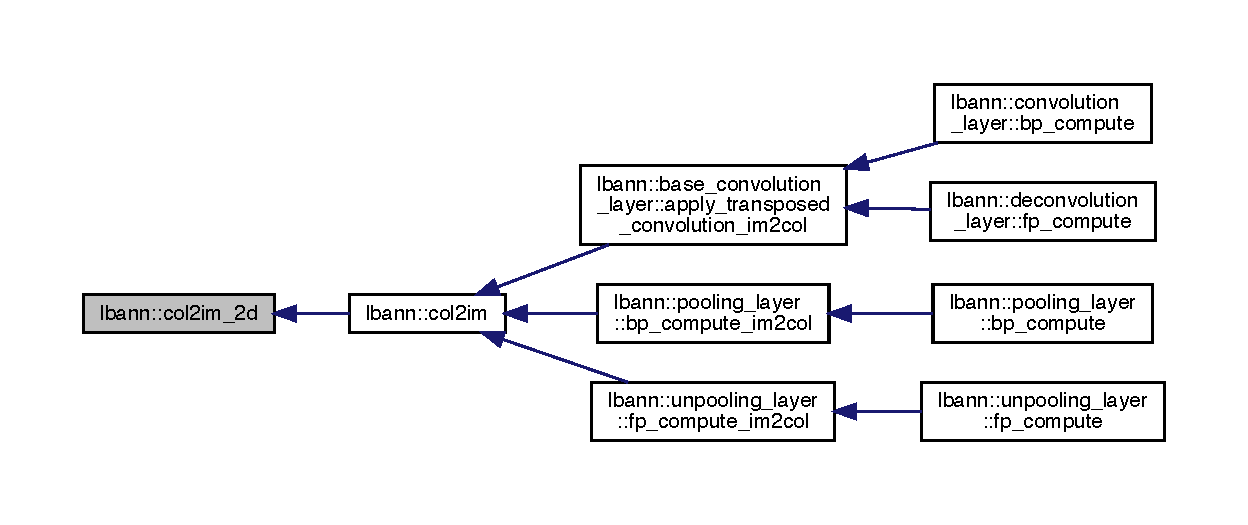
\includegraphics[width=350pt]{namespacelbann_a1953674a43b284f0abb5c5e4db94b2b9_icgraph}
\end{center}
\end{figure}
\mbox{\Hypertarget{namespacelbann_a47ac6e95c1670424f9867770fd5b9f60}\label{namespacelbann_a47ac6e95c1670424f9867770fd5b9f60}} 
\index{lbann@{lbann}!columnwise\+\_\+covariance@{columnwise\+\_\+covariance}}
\index{columnwise\+\_\+covariance@{columnwise\+\_\+covariance}!lbann@{lbann}}
\subsubsection{\texorpdfstring{columnwise\+\_\+covariance()}{columnwise\_covariance()}}
{\footnotesize\ttfamily void lbann\+::columnwise\+\_\+covariance (\begin{DoxyParamCaption}\item[{const \hyperlink{base_8hpp_a9a697a504ae84010e7439ffec862b470}{Abs\+Dist\+Mat} \&}]{data1,  }\item[{const \hyperlink{base_8hpp_a9a697a504ae84010e7439ffec862b470}{Abs\+Dist\+Mat} \&}]{data2,  }\item[{const \hyperlink{base_8hpp_a9a697a504ae84010e7439ffec862b470}{Abs\+Dist\+Mat} \&}]{means1,  }\item[{const \hyperlink{base_8hpp_a9a697a504ae84010e7439ffec862b470}{Abs\+Dist\+Mat} \&}]{means2,  }\item[{\hyperlink{base_8hpp_a9a697a504ae84010e7439ffec862b470}{Abs\+Dist\+Mat} \&}]{cov }\end{DoxyParamCaption})}



Compute column-\/wise covariances. 


\begin{DoxyParams}{Parameters}
{\em data1} & Input matrix in U,V format. \\
\hline
{\em data2} & Input matrix in U,V format. \\
\hline
{\em means1} & Column-\/wise mean vector for data1 in S\+T\+AR,V format. \\
\hline
{\em means2} & Column-\/wise mean vector for data2 in S\+T\+AR,V format. \\
\hline
{\em cov} & Covariance vector in S\+T\+AR,V format. Output as a row vector with same number of columns as \textquotesingle{}data1\textquotesingle{}. \\
\hline
\end{DoxyParams}


Definition at line 365 of file statistics.\+cpp.


\begin{DoxyCode}
369                                              \{
370 
371   \textcolor{comment}{// Check matrix formats and dimensions are valid}
372   El::DistData data1\_dist(data1), data2\_dist(data2),
373     means1\_dist(means1), means2\_dist(means2), covs\_dist(covs);
374   \textcolor{keywordflow}{if}(data1\_dist != data2\_dist
375      || means1\_dist.colDist != El::STAR
376      || means1\_dist.rowDist != data1\_dist.rowDist
377      || means1\_dist != means2\_dist
378      || means1\_dist != covs\_dist) \{
379     \textcolor{keywordflow}{throw} lbann\_exception(\textcolor{stringliteral}{"columnwise\_covariance: invalid matrix format"});
380   \}
381   \textcolor{keywordflow}{if}(data1.Height() != data2.Height() || data1.Width() != data2.Width()) \{
382     \textcolor{keywordflow}{throw} lbann\_exception(\textcolor{stringliteral}{"columnwise\_covariance: data matrix dimensions don't match"});
383   \}
384 
385   \textcolor{comment}{// Matrix dimensions}
386   \textcolor{keyword}{const} El::Int height = data1.Height();
387   \textcolor{keyword}{const} El::Int width = data1.Width();
388   \textcolor{keyword}{const} El::Int local\_height = data1.LocalHeight();
389   \textcolor{keyword}{const} El::Int local\_width = data1.LocalWidth();
390 
391   \textcolor{comment}{// Initialize covariance}
392   covs.Resize(1, width);
393 
394   \textcolor{comment}{// Local matrices}
395   \textcolor{keyword}{const} \hyperlink{base_8hpp_a68f11fdc31b62516cb310831bbe54d73}{Mat}& local\_data1 = data1.LockedMatrix();
396   \textcolor{keyword}{const} \hyperlink{base_8hpp_a68f11fdc31b62516cb310831bbe54d73}{Mat}& local\_data2 = data2.LockedMatrix();
397   \textcolor{keyword}{const} \hyperlink{base_8hpp_a68f11fdc31b62516cb310831bbe54d73}{Mat}& local\_means1 = means1.LockedMatrix();
398   \textcolor{keyword}{const} \hyperlink{base_8hpp_a68f11fdc31b62516cb310831bbe54d73}{Mat}& local\_means2 = means2.LockedMatrix();
399   \hyperlink{base_8hpp_a68f11fdc31b62516cb310831bbe54d73}{Mat}& local\_covs = covs.Matrix();
400 
401   \textcolor{comment}{// Accumulate sum and divide to get covariance}
402 \textcolor{preprocessor}{  #pragma omp parallel for}
403   \textcolor{keywordflow}{for}(El::Int col = 0; col < local\_width; ++col) \{
404     DataType sum = 0;
405     \textcolor{keyword}{const} DataType mean1 = local\_means1(0, col);
406     \textcolor{keyword}{const} DataType mean2 = local\_means2(0, col);
407     \textcolor{keywordflow}{for}(El::Int row = 0; row < local\_height; ++row) \{
408       \textcolor{keyword}{const} DataType val1 = local\_data1(row, col);
409       \textcolor{keyword}{const} DataType val2 = local\_data2(row, col);
410       sum += (val1 - mean1) * (val2 - mean2);
411     \}
412     local\_covs(0, col) = sum;
413   \}
414   AllReduce(covs, covs.RedundantComm(), El::mpi::SUM);
415   local\_covs *= DataType(1) / height;
416 
417 \}
\end{DoxyCode}
Here is the caller graph for this function\+:\nopagebreak
\begin{figure}[H]
\begin{center}
\leavevmode
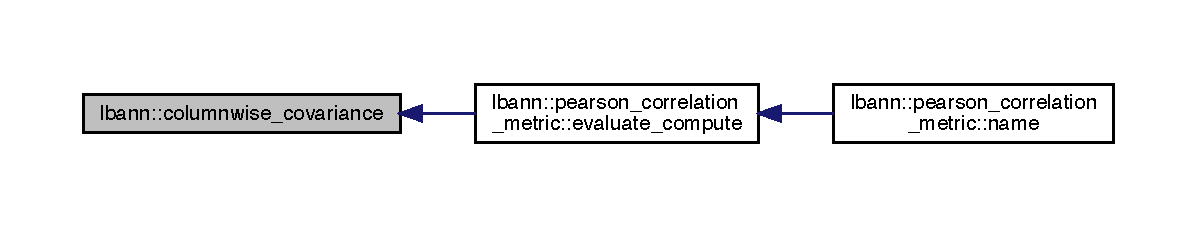
\includegraphics[width=350pt]{namespacelbann_a47ac6e95c1670424f9867770fd5b9f60_icgraph}
\end{center}
\end{figure}
\mbox{\Hypertarget{namespacelbann_a213d429a27c3e8676a3ebec40c24005c}\label{namespacelbann_a213d429a27c3e8676a3ebec40c24005c}} 
\index{lbann@{lbann}!columnwise\+\_\+mean\+\_\+and\+\_\+stdev@{columnwise\+\_\+mean\+\_\+and\+\_\+stdev}}
\index{columnwise\+\_\+mean\+\_\+and\+\_\+stdev@{columnwise\+\_\+mean\+\_\+and\+\_\+stdev}!lbann@{lbann}}
\subsubsection{\texorpdfstring{columnwise\+\_\+mean\+\_\+and\+\_\+stdev()}{columnwise\_mean\_and\_stdev()}\hspace{0.1cm}{\footnotesize\ttfamily [1/2]}}
{\footnotesize\ttfamily void lbann\+::columnwise\+\_\+mean\+\_\+and\+\_\+stdev (\begin{DoxyParamCaption}\item[{const \hyperlink{base_8hpp_a68f11fdc31b62516cb310831bbe54d73}{Mat} \&}]{data,  }\item[{\hyperlink{base_8hpp_a68f11fdc31b62516cb310831bbe54d73}{Mat} \&}]{means,  }\item[{\hyperlink{base_8hpp_a68f11fdc31b62516cb310831bbe54d73}{Mat} \&}]{stdevs }\end{DoxyParamCaption})}



Compute column-\/wise means and standard deviations. 


\begin{DoxyParams}{Parameters}
{\em data} & Input matrix. \\
\hline
{\em means} & Mean vector. Output as a row vector with same number of columns as \textquotesingle{}data\textquotesingle{}. \\
\hline
{\em stdevs} & Standard deviation vector. Output as a row vector with same number of columns as \textquotesingle{}data\textquotesingle{}. \\
\hline
\end{DoxyParams}


Definition at line 100 of file statistics.\+cpp.


\begin{DoxyCode}
102                                             \{
103 
104   \textcolor{comment}{// Matrix dimensions}
105   \textcolor{keyword}{const} El::Int height = \hyperlink{namespacelbann_1_1cnpy__utils_a9ac86d96ccb1f8b4b2ea16441738781f}{data}.Height();
106   \textcolor{keyword}{const} El::Int width = \hyperlink{namespacelbann_1_1cnpy__utils_a9ac86d96ccb1f8b4b2ea16441738781f}{data}.Width();
107 
108   \textcolor{comment}{// Initialize outputs}
109   means.Resize(1, width);
110   stdevs.Resize(1, width);
111 
112   \textcolor{comment}{// Compute mean and standard deviation of each matrix column}
113 \textcolor{preprocessor}{  #pragma omp parallel for}
114   \textcolor{keywordflow}{for}(El::Int col = 0; col < width; ++col) \{
115     \textcolor{keyword}{const} DataType shift = \hyperlink{namespacelbann_1_1cnpy__utils_a9ac86d96ccb1f8b4b2ea16441738781f}{data}(0, col);
116     DataType shifted\_sum = 0;
117     DataType shifted\_sqsum = 0;
118     \textcolor{keywordflow}{for}(El::Int row = 0; row < height; ++row) \{
119       \textcolor{keyword}{const} DataType shifted\_val = \hyperlink{namespacelbann_1_1cnpy__utils_a9ac86d96ccb1f8b4b2ea16441738781f}{data}(row, col) - shift;
120       shifted\_sum += shifted\_val;
121       shifted\_sqsum += shifted\_val * shifted\_val;
122     \}
123     \textcolor{keyword}{const} DataType shifted\_mean = shifted\_sum / height;
124     \textcolor{keyword}{const} DataType shifted\_sqmean = shifted\_sqsum / height;
125     \textcolor{keyword}{const} DataType mean = shifted\_mean + shift;
126     \textcolor{keyword}{const} DataType var = std::max(shifted\_sqmean - shifted\_mean * shifted\_mean,
127                                   DataType(0));
128     \textcolor{keyword}{const} DataType stdev = std::sqrt(var);
129     means(0, col) = mean;
130     stdevs(0, col) = stdev;
131   \}
132 
133 \}
\end{DoxyCode}
Here is the call graph for this function\+:\nopagebreak
\begin{figure}[H]
\begin{center}
\leavevmode
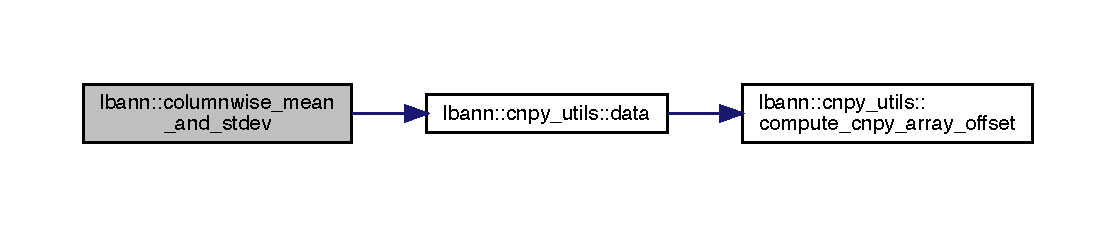
\includegraphics[width=350pt]{namespacelbann_a213d429a27c3e8676a3ebec40c24005c_cgraph}
\end{center}
\end{figure}
Here is the caller graph for this function\+:\nopagebreak
\begin{figure}[H]
\begin{center}
\leavevmode
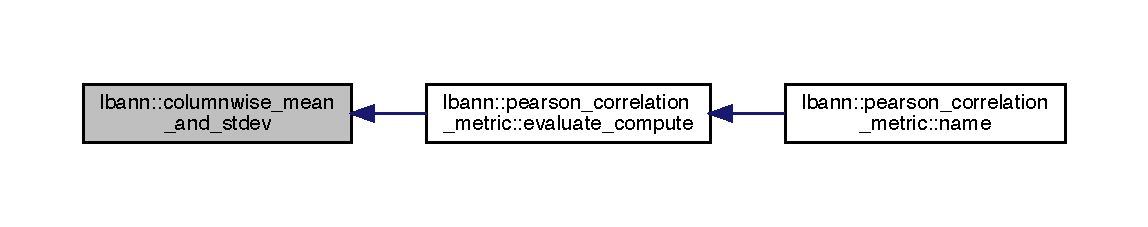
\includegraphics[width=350pt]{namespacelbann_a213d429a27c3e8676a3ebec40c24005c_icgraph}
\end{center}
\end{figure}
\mbox{\Hypertarget{namespacelbann_a085b697db535c10a6fd6689cc4445bd4}\label{namespacelbann_a085b697db535c10a6fd6689cc4445bd4}} 
\index{lbann@{lbann}!columnwise\+\_\+mean\+\_\+and\+\_\+stdev@{columnwise\+\_\+mean\+\_\+and\+\_\+stdev}}
\index{columnwise\+\_\+mean\+\_\+and\+\_\+stdev@{columnwise\+\_\+mean\+\_\+and\+\_\+stdev}!lbann@{lbann}}
\subsubsection{\texorpdfstring{columnwise\+\_\+mean\+\_\+and\+\_\+stdev()}{columnwise\_mean\_and\_stdev()}\hspace{0.1cm}{\footnotesize\ttfamily [2/2]}}
{\footnotesize\ttfamily void lbann\+::columnwise\+\_\+mean\+\_\+and\+\_\+stdev (\begin{DoxyParamCaption}\item[{const \hyperlink{base_8hpp_a9a697a504ae84010e7439ffec862b470}{Abs\+Dist\+Mat} \&}]{data,  }\item[{\hyperlink{base_8hpp_a9a697a504ae84010e7439ffec862b470}{Abs\+Dist\+Mat} \&}]{means,  }\item[{\hyperlink{base_8hpp_a9a697a504ae84010e7439ffec862b470}{Abs\+Dist\+Mat} \&}]{stdevs }\end{DoxyParamCaption})}



Compute column-\/wise means and standard deviations. 

\begin{DoxyRefDesc}{Todo}
\item[\hyperlink{todo__todo000008}{Todo}]Numerically stable implementation \end{DoxyRefDesc}



\begin{DoxyParams}{Parameters}
{\em data} & Input matrix in U,V format. \\
\hline
{\em means} & Mean vector in S\+T\+AR,V format. Output as a row vector with same number of columns as \textquotesingle{}data\textquotesingle{}. \\
\hline
{\em stdevs} & Standard deviation vector in S\+T\+AR,V format. Output as a row vector with same number of columns as \textquotesingle{}data\textquotesingle{}. \\
\hline
\end{DoxyParams}


Definition at line 184 of file statistics.\+cpp.


\begin{DoxyCode}
186                                                    \{
187 
188 \textcolor{preprocessor}{#ifdef LBANN\_DEBUG}
189   El::DistData data\_dist(\hyperlink{namespacelbann_1_1cnpy__utils_a9ac86d96ccb1f8b4b2ea16441738781f}{data}), means\_dist(means), stdevs\_dist(stdevs);
190   \textcolor{keywordflow}{if}(means\_dist.colDist != El::STAR
191       || means\_dist.rowDist != data\_dist.rowDist
192       || stdevs\_dist.colDist != El::STAR
193       || stdevs\_dist.rowDist != data\_dist.rowDist) \{
194     \textcolor{keywordflow}{throw} lbann\_exception(\textcolor{stringliteral}{"columnwise\_mean\_and\_stdev: invalid matrix format"});
195   \}
196 \textcolor{preprocessor}{#endif // #ifdef LBANN\_DEBUG}
197 
198   \textcolor{comment}{// Matrix dimensions}
199   \textcolor{keyword}{const} El::Int height = \hyperlink{namespacelbann_1_1cnpy__utils_a9ac86d96ccb1f8b4b2ea16441738781f}{data}.Height();
200   \textcolor{keyword}{const} El::Int local\_width = \hyperlink{namespacelbann_1_1cnpy__utils_a9ac86d96ccb1f8b4b2ea16441738781f}{data}.LocalWidth();
201 
202   \hyperlink{namespacelbann_ab043d2f2f9dea0ee861aff3a38216b24}{columnwise\_sums\_and\_sqsums}(\hyperlink{namespacelbann_1_1cnpy__utils_a9ac86d96ccb1f8b4b2ea16441738781f}{data}, means, stdevs);
203   \textcolor{comment}{// Local matrices}
204   \hyperlink{base_8hpp_a68f11fdc31b62516cb310831bbe54d73}{Mat}& local\_means = means.Matrix();
205   \hyperlink{base_8hpp_a68f11fdc31b62516cb310831bbe54d73}{Mat}& local\_stdevs = stdevs.Matrix();
206 
207   \textcolor{keywordflow}{for}(El::Int col = 0; col < local\_width; ++col) \{
208     \textcolor{keyword}{const} DataType mean = local\_means(0, col) / height;
209     \textcolor{keyword}{const} DataType sqmean = local\_stdevs(0, col) / height;
210     \textcolor{keyword}{const} DataType var = std::max(sqmean - mean * mean, DataType(0));
211     \textcolor{keyword}{const} DataType stdev = std::sqrt(var);
212     local\_means(0, col) = mean;
213     local\_stdevs(0, col) = stdev;
214   \}
215 
216 \}
\end{DoxyCode}
Here is the call graph for this function\+:\nopagebreak
\begin{figure}[H]
\begin{center}
\leavevmode
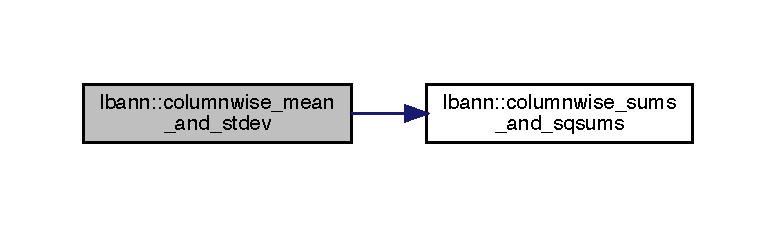
\includegraphics[width=350pt]{namespacelbann_a085b697db535c10a6fd6689cc4445bd4_cgraph}
\end{center}
\end{figure}
\mbox{\Hypertarget{namespacelbann_ab043d2f2f9dea0ee861aff3a38216b24}\label{namespacelbann_ab043d2f2f9dea0ee861aff3a38216b24}} 
\index{lbann@{lbann}!columnwise\+\_\+sums\+\_\+and\+\_\+sqsums@{columnwise\+\_\+sums\+\_\+and\+\_\+sqsums}}
\index{columnwise\+\_\+sums\+\_\+and\+\_\+sqsums@{columnwise\+\_\+sums\+\_\+and\+\_\+sqsums}!lbann@{lbann}}
\subsubsection{\texorpdfstring{columnwise\+\_\+sums\+\_\+and\+\_\+sqsums()}{columnwise\_sums\_and\_sqsums()}}
{\footnotesize\ttfamily void lbann\+::columnwise\+\_\+sums\+\_\+and\+\_\+sqsums (\begin{DoxyParamCaption}\item[{const \hyperlink{base_8hpp_a9a697a504ae84010e7439ffec862b470}{Abs\+Dist\+Mat} \&}]{data,  }\item[{\hyperlink{base_8hpp_a9a697a504ae84010e7439ffec862b470}{Abs\+Dist\+Mat} \&}]{sums,  }\item[{\hyperlink{base_8hpp_a9a697a504ae84010e7439ffec862b470}{Abs\+Dist\+Mat} \&}]{sqsums }\end{DoxyParamCaption})}



Compute column-\/wise sum and sqsum. 

\begin{DoxyRefDesc}{Todo}
\item[\hyperlink{todo__todo000007}{Todo}]Numerically stable implementation \end{DoxyRefDesc}



\begin{DoxyParams}{Parameters}
{\em data} & Input matrix in U,V format. \\
\hline
{\em sum} & Sum vector in S\+T\+AR,V format. Output as a row vector with same number of columns as \textquotesingle{}data\textquotesingle{}. \\
\hline
{\em sqsum} & Sum of squared vector in S\+T\+AR,V format. Output as a row vector with same number of columns as \textquotesingle{}data\textquotesingle{}. \\
\hline
\end{DoxyParams}


Definition at line 136 of file statistics.\+cpp.


\begin{DoxyCode}
138                                                    \{
139 
140 \textcolor{preprocessor}{#ifdef LBANN\_DEBUG}
141   El::DistData data\_dist(\hyperlink{namespacelbann_1_1cnpy__utils_a9ac86d96ccb1f8b4b2ea16441738781f}{data}), sum\_dist(sums), sqsum\_dist(sqsums);
142   \textcolor{keywordflow}{if}(sum\_dist.colDist != El::STAR
143       || sum\_dist.rowDist != data\_dist.rowDist
144       || sqsum\_dist.colDist != El::STAR
145       || sqsum\_dist.rowDist != data\_dist.rowDist) \{
146     \textcolor{keywordflow}{throw} lbann\_exception(\textcolor{stringliteral}{"columnwise\_sum\_and\_sqsum: invalid matrix format"});
147   \}
148 \textcolor{preprocessor}{#endif // #ifdef LBANN\_DEBUG}
149 
150   \textcolor{comment}{// Matrix dimensions}
151   \textcolor{keyword}{const} El::Int width = \hyperlink{namespacelbann_1_1cnpy__utils_a9ac86d96ccb1f8b4b2ea16441738781f}{data}.Width();
152   \textcolor{keyword}{const} El::Int local\_height = \hyperlink{namespacelbann_1_1cnpy__utils_a9ac86d96ccb1f8b4b2ea16441738781f}{data}.LocalHeight();
153   \textcolor{keyword}{const} El::Int local\_width = \hyperlink{namespacelbann_1_1cnpy__utils_a9ac86d96ccb1f8b4b2ea16441738781f}{data}.LocalWidth();
154 
155   \textcolor{comment}{// Initialize outputs}
156   sums.Resize(1, width);
157   sqsums.Resize(1, width);
158 
159   \textcolor{comment}{// Local matrices}
160   \textcolor{keyword}{const} \hyperlink{base_8hpp_a68f11fdc31b62516cb310831bbe54d73}{Mat}& local\_data = \hyperlink{namespacelbann_1_1cnpy__utils_a9ac86d96ccb1f8b4b2ea16441738781f}{data}.LockedMatrix();
161   \hyperlink{base_8hpp_a68f11fdc31b62516cb310831bbe54d73}{Mat}& local\_sum = sums.Matrix();
162   \hyperlink{base_8hpp_a68f11fdc31b62516cb310831bbe54d73}{Mat}& local\_sqsum = sqsums.Matrix();
163 
164   \textcolor{comment}{// Compute sum and sum of squares of each matrix column}
165 \textcolor{preprocessor}{  #pragma omp parallel for}
166   \textcolor{keywordflow}{for}(El::Int col = 0; col < local\_width; ++col) \{
167     DataType sum\_val = 0;
168     DataType sqsum\_val = 0;
169     \textcolor{keywordflow}{for}(El::Int row = 0; row < local\_height; ++row) \{
170       \textcolor{keyword}{const} DataType val = local\_data(row, col);
171       sum\_val += val;
172       sqsum\_val += val * val;
173     \}
174     local\_sum(0, col) = sum\_val;
175     local\_sqsum(0, col) = sqsum\_val;
176   \}
177 
178   \textcolor{comment}{// Allreduce sums and sums of squares}
179   AllReduce(sums, sums.RedundantComm(), El::mpi::SUM);
180   AllReduce(sqsums, sqsums.RedundantComm(), El::mpi::SUM);
181 
182 \}
\end{DoxyCode}
Here is the caller graph for this function\+:\nopagebreak
\begin{figure}[H]
\begin{center}
\leavevmode
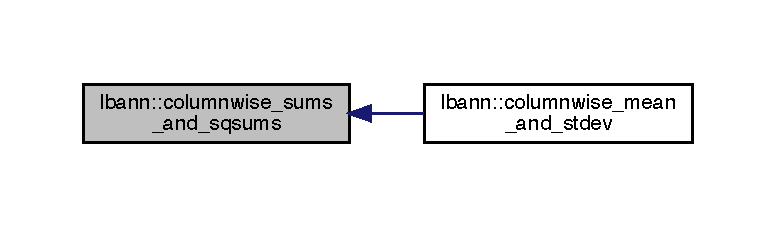
\includegraphics[width=350pt]{namespacelbann_ab043d2f2f9dea0ee861aff3a38216b24_icgraph}
\end{center}
\end{figure}
\mbox{\Hypertarget{namespacelbann_aedcfce41af2eae595ce58b1180f66bd1}\label{namespacelbann_aedcfce41af2eae595ce58b1180f66bd1}} 
\index{lbann@{lbann}!count\+\_\+sorter@{count\+\_\+sorter}}
\index{count\+\_\+sorter@{count\+\_\+sorter}!lbann@{lbann}}
\subsubsection{\texorpdfstring{count\+\_\+sorter()}{count\_sorter()}}
{\footnotesize\ttfamily bool lbann\+::count\+\_\+sorter (\begin{DoxyParamCaption}\item[{const std\+::pair$<$ std\+::string, long $>$ \&}]{a,  }\item[{const std\+::pair$<$ std\+::string, long $>$ \&}]{b }\end{DoxyParamCaption})}



Definition at line 103 of file stack\+\_\+profiler.\+cpp.


\begin{DoxyCode}
103                                                                                          \{
104   \textcolor{keywordflow}{return} a.second > b.second;
105 \}
\end{DoxyCode}
Here is the caller graph for this function\+:\nopagebreak
\begin{figure}[H]
\begin{center}
\leavevmode
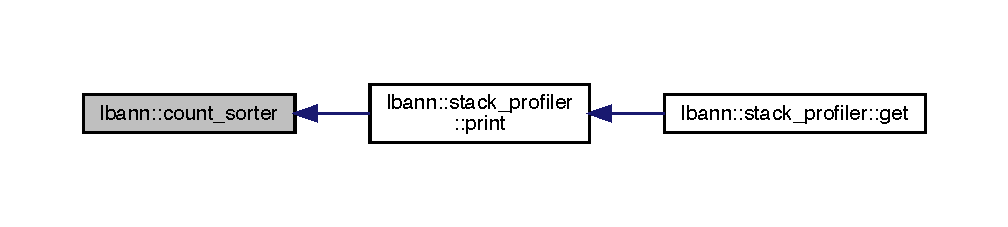
\includegraphics[width=350pt]{namespacelbann_aedcfce41af2eae595ce58b1180f66bd1_icgraph}
\end{center}
\end{figure}
\mbox{\Hypertarget{namespacelbann_a1208673c880ccf0e1a9c5db6a8ed81f8}\label{namespacelbann_a1208673c880ccf0e1a9c5db6a8ed81f8}} 
\index{lbann@{lbann}!create\+\_\+dir@{create\+\_\+dir}}
\index{create\+\_\+dir@{create\+\_\+dir}!lbann@{lbann}}
\subsubsection{\texorpdfstring{create\+\_\+dir()}{create\_dir()}}
{\footnotesize\ttfamily bool lbann\+::create\+\_\+dir (\begin{DoxyParamCaption}\item[{const std\+::string}]{dirname }\end{DoxyParamCaption})}

Create a directory, and return true if successful. If a directory with the same name already exists, simply return true. 

Definition at line 182 of file file\+\_\+utils.\+cpp.


\begin{DoxyCode}
182                                          \{
183   std::string dir = dirname;
184   \textcolor{keywordflow}{if} (!dir.empty() && path\_delimiter::check(dir.back())) \{
185     dir.pop\_back();
186   \}
187 
188   \textcolor{keywordflow}{if} (dir.empty()) \{
189     \textcolor{keywordflow}{return} \textcolor{keyword}{true};
190   \}
191 
192   \textcolor{keyword}{const} \textcolor{keywordtype}{bool} file\_exists = \hyperlink{namespacelbann_a4fac6c6483965395fa79d31061485f9f}{check\_if\_file\_exists}(dir);
193 
194   \textcolor{keywordflow}{if} (file\_exists) \{
195     \textcolor{keywordflow}{if} (!\hyperlink{namespacelbann_a3ee4a1fa7a82c30999de9eb626c68311}{check\_if\_dir\_exists}(dir)) \{
196       \textcolor{keywordflow}{return} \textcolor{keyword}{false};
197     \} \textcolor{keywordflow}{else} \{
198       \textcolor{keywordflow}{return} \textcolor{keyword}{true};
199     \}
200   \}
201 
202   std::string cmd = std::string(\textcolor{stringliteral}{"mkdir -p "}) + dir;
203 \textcolor{preprocessor}{#if 1 // for ray}
204   \textcolor{keywordtype}{char} cmdstr[cmd.size()+1];
205   std::copy(cmd.begin(), cmd.end(), &cmdstr[0]);
206   cmdstr[cmd.size()] = \textcolor{charliteral}{'\(\backslash\)0'};
207   \textcolor{keyword}{const} \textcolor{keywordtype}{int} r = ::system(&cmdstr[0]);
208 \textcolor{preprocessor}{#else}
209   \textcolor{keyword}{const} \textcolor{keywordtype}{int} r = ::system(cmd.c\_str());
210 \textcolor{preprocessor}{#endif}
211 
212   \textcolor{keywordflow}{if} (WEXITSTATUS(r) == 0x10) \{
213     \textcolor{keywordflow}{return} \textcolor{keyword}{true};
214   \} \textcolor{keywordflow}{else} \textcolor{keywordflow}{if} (!\hyperlink{namespacelbann_a3ee4a1fa7a82c30999de9eb626c68311}{check\_if\_dir\_exists}(dir)) \{
215     \textcolor{keywordflow}{return} \textcolor{keyword}{false};
216   \}
217   \textcolor{keywordflow}{return} \textcolor{keyword}{true};
218 \}
\end{DoxyCode}
Here is the call graph for this function\+:\nopagebreak
\begin{figure}[H]
\begin{center}
\leavevmode
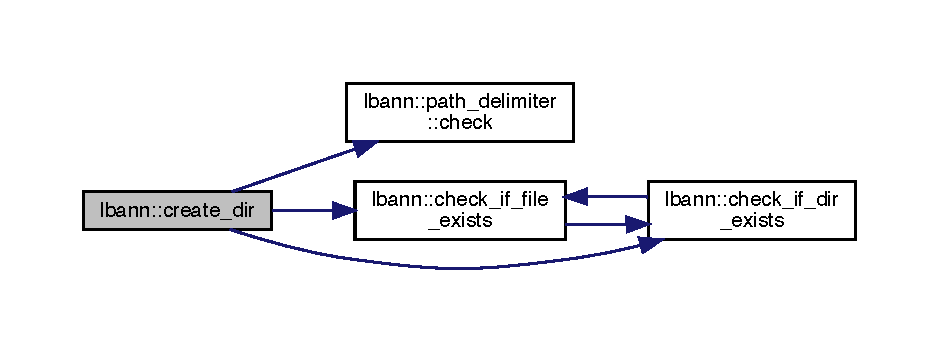
\includegraphics[width=350pt]{namespacelbann_a1208673c880ccf0e1a9c5db6a8ed81f8_cgraph}
\end{center}
\end{figure}
Here is the caller graph for this function\+:\nopagebreak
\begin{figure}[H]
\begin{center}
\leavevmode
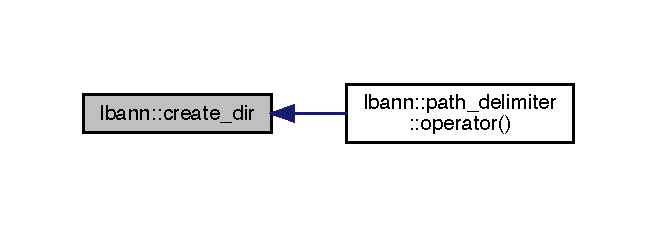
\includegraphics[width=315pt]{namespacelbann_a1208673c880ccf0e1a9c5db6a8ed81f8_icgraph}
\end{center}
\end{figure}
\mbox{\Hypertarget{namespacelbann_a26debfaa06e8490c7f258ed7923870c7}\label{namespacelbann_a26debfaa06e8490c7f258ed7923870c7}} 
\index{lbann@{lbann}!display\+\_\+omp\+\_\+setup@{display\+\_\+omp\+\_\+setup}}
\index{display\+\_\+omp\+\_\+setup@{display\+\_\+omp\+\_\+setup}!lbann@{lbann}}
\subsubsection{\texorpdfstring{display\+\_\+omp\+\_\+setup()}{display\_omp\_setup()}}
{\footnotesize\ttfamily void lbann\+::display\+\_\+omp\+\_\+setup (\begin{DoxyParamCaption}{ }\end{DoxyParamCaption})}



Definition at line 198 of file omp\+\_\+diagnostics.\+cpp.


\begin{DoxyCode}
199 \{
200 \textcolor{preprocessor}{#ifdef LBANN\_GNU\_LINUX}
201   \textcolor{keywordtype}{int} rank, np, secs, len, mpi\_only, mpi\_subset;
202   \textcolor{keywordtype}{char} hostname[MPI\_MAX\_PROCESSOR\_NAME];
203   MPI\_Comm\_rank(MPI\_COMM\_WORLD, &rank);
204   MPI\_Comm\_size(MPI\_COMM\_WORLD, &np);
205   MPI\_Get\_processor\_name(hostname, &len);
206 
207   secs = \hyperlink{namespacelbann_a17d55032bad5bb02903f9b1d933836a4}{get\_sleep\_sec}();
208   (void) secs;
209   mpi\_only = \hyperlink{namespacelbann_aa4ee6571e54db5cee7f263029147e5f2}{get\_env\_var}(\textcolor{stringliteral}{"MPI\_ONLY"});
210   mpi\_subset = \hyperlink{namespacelbann_aa4ee6571e54db5cee7f263029147e5f2}{get\_env\_var}(\textcolor{stringliteral}{"MPI\_SUBSET"});
211 
212 
213 \textcolor{preprocessor}{  #ifdef HPM}
214     hpmInit(0, \textcolor{stringliteral}{"HPMTest"});
215     hpmStart(1, \textcolor{stringliteral}{"Region 1"});
216 \textcolor{preprocessor}{  #endif}
217 
218   \textcolor{keywordflow}{if} (rank == 0)
219     printf(\textcolor{stringliteral}{"\(\backslash\)n"});
220 
221   \textcolor{keywordflow}{if} (mpi\_only != 0) \{
222     \textcolor{keywordflow}{if} (mpi\_subset) \{
223       \hyperlink{namespacelbann_acbd15ead7411cf84db559cc39a82f445}{print\_affinity\_subset}(rank, np, hostname);
224     \}\textcolor{keywordflow}{else} \{
225       \hyperlink{namespacelbann_a4fd83a86cf27ca7bc1e01576a5ee36e0}{print\_affinity}(rank, np, hostname);
226     \}
227   \}\textcolor{keywordflow}{else} \{
228     \textcolor{comment}{/* Fork a team of threads giving them their own copies of variables */}
229 \textcolor{preprocessor}{#pragma omp parallel shared(rank, np, secs, hostname)}
230     \{
231       \hyperlink{namespacelbann_a31acedf53bb67180043939832c0220d3}{th\_print\_affinity}(rank, np, hostname);
232     \}  \textcolor{comment}{/* All threads join master thread and disband */}
233   \}
234 
235 \textcolor{preprocessor}{#ifdef HPM}
236   hpmStop(1);
237   hpmTerminate(0);
238 \textcolor{preprocessor}{#endif}
239 \textcolor{preprocessor}{#endif // LBANN\_GNU\_LINUX}
240 \}
\end{DoxyCode}
Here is the call graph for this function\+:\nopagebreak
\begin{figure}[H]
\begin{center}
\leavevmode
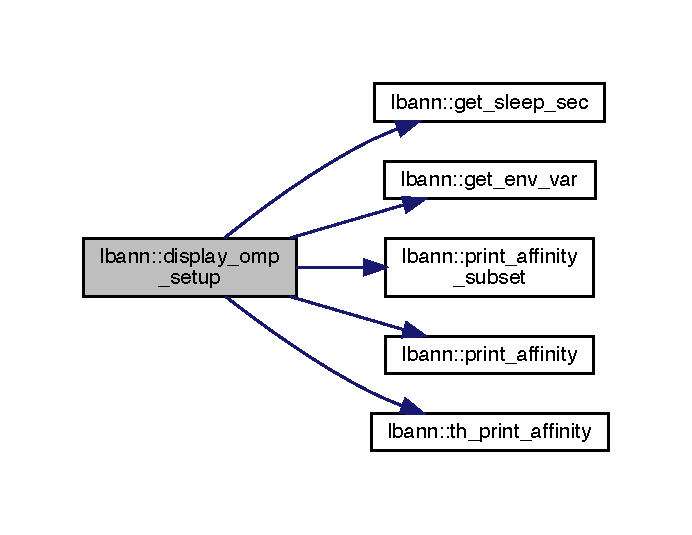
\includegraphics[width=332pt]{namespacelbann_a26debfaa06e8490c7f258ed7923870c7_cgraph}
\end{center}
\end{figure}
\mbox{\Hypertarget{namespacelbann_a02f197bc772ef04f1ac51eb191a02cab}\label{namespacelbann_a02f197bc772ef04f1ac51eb191a02cab}} 
\index{lbann@{lbann}!ends\+With@{ends\+With}}
\index{ends\+With@{ends\+With}!lbann@{lbann}}
\subsubsection{\texorpdfstring{ends\+With()}{endsWith()}}
{\footnotesize\ttfamily static bool lbann\+::ends\+With (\begin{DoxyParamCaption}\item[{const std\+::string}]{main\+Str,  }\item[{const std\+::string \&}]{to\+Match }\end{DoxyParamCaption})\hspace{0.3cm}{\ttfamily [static]}}



Definition at line 142 of file base.\+hpp.


\begin{DoxyCode}
143 \{
144   \textcolor{keywordflow}{if}(mainStr.size() >= toMatch.size() &&
145      mainStr.compare(mainStr.size() - toMatch.size(), toMatch.size(), toMatch) == 0)
146     \textcolor{keywordflow}{return} \textcolor{keyword}{true};
147   \textcolor{keywordflow}{else}
148     \textcolor{keywordflow}{return} \textcolor{keyword}{false};
149 \}
\end{DoxyCode}
Here is the caller graph for this function\+:\nopagebreak
\begin{figure}[H]
\begin{center}
\leavevmode
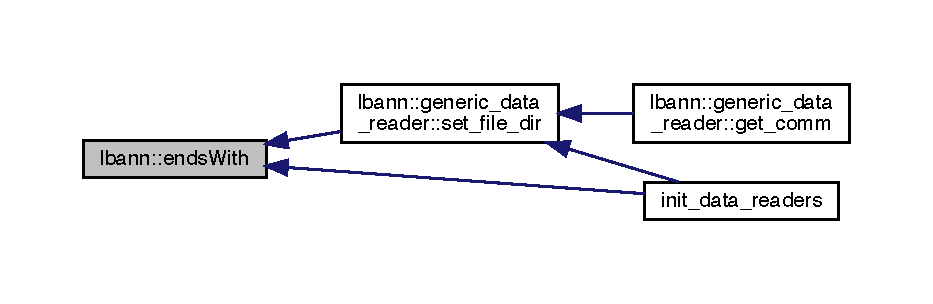
\includegraphics[width=350pt]{namespacelbann_a02f197bc772ef04f1ac51eb191a02cab_icgraph}
\end{center}
\end{figure}
\mbox{\Hypertarget{namespacelbann_a604ae9da0173b8be2bfb6877997d6d5c}\label{namespacelbann_a604ae9da0173b8be2bfb6877997d6d5c}} 
\index{lbann@{lbann}!entrywise\+\_\+mean\+\_\+and\+\_\+stdev@{entrywise\+\_\+mean\+\_\+and\+\_\+stdev}}
\index{entrywise\+\_\+mean\+\_\+and\+\_\+stdev@{entrywise\+\_\+mean\+\_\+and\+\_\+stdev}!lbann@{lbann}}
\subsubsection{\texorpdfstring{entrywise\+\_\+mean\+\_\+and\+\_\+stdev()}{entrywise\_mean\_and\_stdev()}\hspace{0.1cm}{\footnotesize\ttfamily [1/2]}}
{\footnotesize\ttfamily void lbann\+::entrywise\+\_\+mean\+\_\+and\+\_\+stdev (\begin{DoxyParamCaption}\item[{const \hyperlink{base_8hpp_a68f11fdc31b62516cb310831bbe54d73}{Mat} \&}]{data,  }\item[{Data\+Type \&}]{mean,  }\item[{Data\+Type \&}]{stdev }\end{DoxyParamCaption})}



Compute mean and standard deviation over matrix entries. 


\begin{DoxyParams}{Parameters}
{\em data} & Input matrix. \\
\hline
{\em means} & Mean value (output). \\
\hline
{\em stdevs} & Standard deviation (output). \\
\hline
\end{DoxyParams}


Definition at line 32 of file statistics.\+cpp.


\begin{DoxyCode}
34                                                \{
35   \textcolor{comment}{// Note: This routine is primarily called in an OpenMP-parallelized}
36   \textcolor{comment}{// loop in data\_readers/image\_preprocessor.hpp. If a more}
37   \textcolor{comment}{// significant use-case is found, it may be worthwhile parallelizing}
38   \textcolor{comment}{// the loop.}
39 
40   \textcolor{comment}{// Matrix dimensions}
41   \textcolor{keyword}{const} El::Int height = \hyperlink{namespacelbann_1_1cnpy__utils_a9ac86d96ccb1f8b4b2ea16441738781f}{data}.Height();
42   \textcolor{keyword}{const} El::Int width = \hyperlink{namespacelbann_1_1cnpy__utils_a9ac86d96ccb1f8b4b2ea16441738781f}{data}.Width();
43   \textcolor{keyword}{const} El::Int \hyperlink{structc__hash__table_afd5bfd9640fc5b72f75457fb7dd89663}{size} = height * width;
44 
45   \textcolor{comment}{// Compute sums over matrix entries}
46   \textcolor{keyword}{const} DataType shift = \hyperlink{namespacelbann_1_1cnpy__utils_a9ac86d96ccb1f8b4b2ea16441738781f}{data}(0, 0);
47   DataType shifted\_sum = 0;
48   DataType shifted\_sqsum = 0;
49   \textcolor{keywordflow}{for}(El::Int col = 0; col < width; ++col) \{
50     \textcolor{keywordflow}{for}(El::Int row = 0; row < height; ++row) \{
51       \textcolor{keyword}{const} DataType shifted\_val = \hyperlink{namespacelbann_1_1cnpy__utils_a9ac86d96ccb1f8b4b2ea16441738781f}{data}(row, col) - shift;
52       shifted\_sum += shifted\_val;
53       shifted\_sqsum += shifted\_val * shifted\_val;
54     \}
55   \}
56 
57   \textcolor{comment}{// Compute mean and standard deviation}
58   \textcolor{keyword}{const} DataType shifted\_mean = shifted\_sum / \hyperlink{structc__hash__table_afd5bfd9640fc5b72f75457fb7dd89663}{size};
59   \textcolor{keyword}{const} DataType shifted\_sqmean = shifted\_sqsum / \hyperlink{structc__hash__table_afd5bfd9640fc5b72f75457fb7dd89663}{size};
60   mean = shifted\_mean + shift;
61   \textcolor{keyword}{const} DataType var = std::max(shifted\_sqmean - shifted\_mean * shifted\_mean,
62                                 DataType(0));
63   stdev = std::sqrt(var);
64 
65 \}
\end{DoxyCode}
Here is the call graph for this function\+:\nopagebreak
\begin{figure}[H]
\begin{center}
\leavevmode
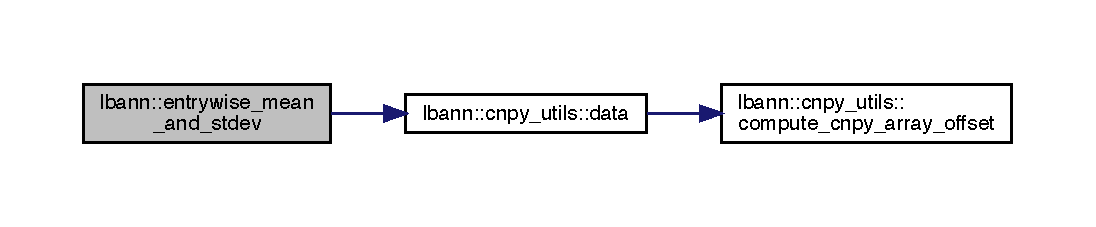
\includegraphics[width=350pt]{namespacelbann_a604ae9da0173b8be2bfb6877997d6d5c_cgraph}
\end{center}
\end{figure}
Here is the caller graph for this function\+:\nopagebreak
\begin{figure}[H]
\begin{center}
\leavevmode
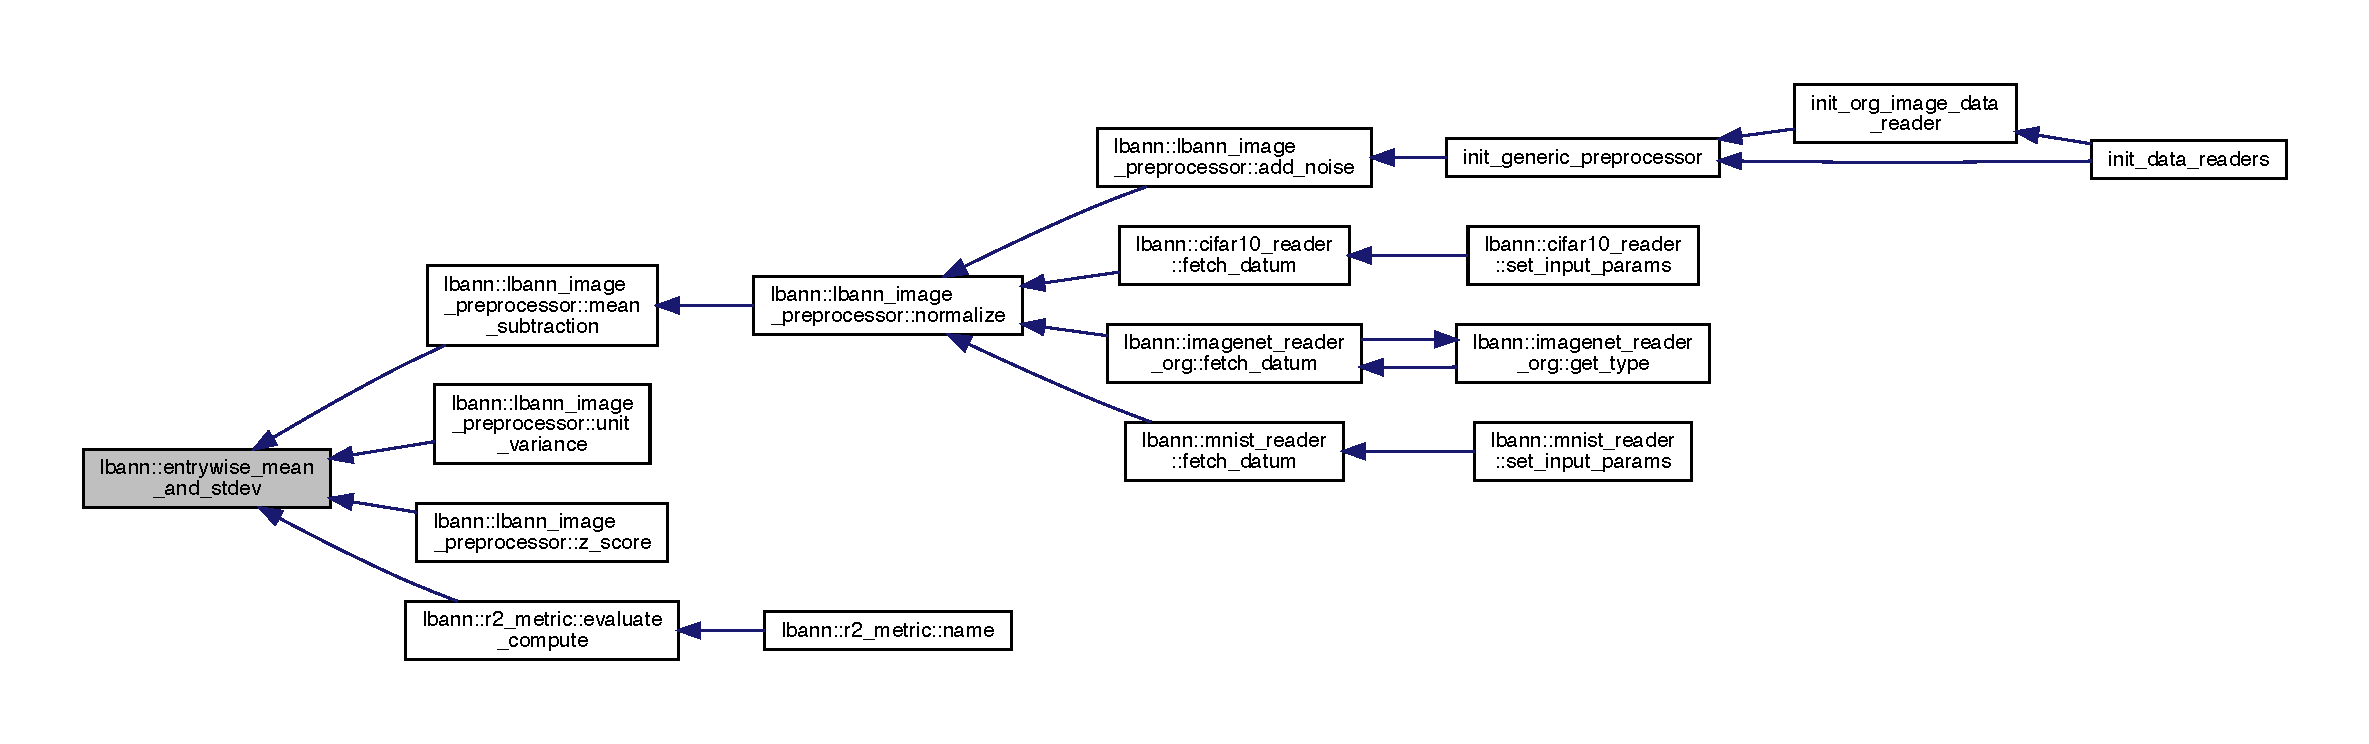
\includegraphics[width=350pt]{namespacelbann_a604ae9da0173b8be2bfb6877997d6d5c_icgraph}
\end{center}
\end{figure}
\mbox{\Hypertarget{namespacelbann_a99fdd84cb5f060ac1c78ec66769669ba}\label{namespacelbann_a99fdd84cb5f060ac1c78ec66769669ba}} 
\index{lbann@{lbann}!entrywise\+\_\+mean\+\_\+and\+\_\+stdev@{entrywise\+\_\+mean\+\_\+and\+\_\+stdev}}
\index{entrywise\+\_\+mean\+\_\+and\+\_\+stdev@{entrywise\+\_\+mean\+\_\+and\+\_\+stdev}!lbann@{lbann}}
\subsubsection{\texorpdfstring{entrywise\+\_\+mean\+\_\+and\+\_\+stdev()}{entrywise\_mean\_and\_stdev()}\hspace{0.1cm}{\footnotesize\ttfamily [2/2]}}
{\footnotesize\ttfamily void lbann\+::entrywise\+\_\+mean\+\_\+and\+\_\+stdev (\begin{DoxyParamCaption}\item[{const \hyperlink{base_8hpp_a9a697a504ae84010e7439ffec862b470}{Abs\+Dist\+Mat} \&}]{data,  }\item[{Data\+Type \&}]{mean,  }\item[{Data\+Type \&}]{stdev }\end{DoxyParamCaption})}



Compute mean and standard deviation over matrix entries. 


\begin{DoxyParams}{Parameters}
{\em data} & Input matrix. \\
\hline
{\em means} & Mean value (output). \\
\hline
{\em stdevs} & Standard deviation (output). \\
\hline
\end{DoxyParams}


Definition at line 67 of file statistics.\+cpp.


\begin{DoxyCode}
69                                                \{
70 
71   \textcolor{comment}{// Matrix dimensions}
72   \textcolor{keyword}{const} El::Int \hyperlink{structc__hash__table_afd5bfd9640fc5b72f75457fb7dd89663}{size} = \hyperlink{namespacelbann_1_1cnpy__utils_a9ac86d96ccb1f8b4b2ea16441738781f}{data}.Height() * \hyperlink{namespacelbann_1_1cnpy__utils_a9ac86d96ccb1f8b4b2ea16441738781f}{data}.Width();
73   \textcolor{keyword}{const} El::Int local\_height = \hyperlink{namespacelbann_1_1cnpy__utils_a9ac86d96ccb1f8b4b2ea16441738781f}{data}.LocalHeight();
74   \textcolor{keyword}{const} El::Int local\_width = \hyperlink{namespacelbann_1_1cnpy__utils_a9ac86d96ccb1f8b4b2ea16441738781f}{data}.LocalWidth();
75 
76   \textcolor{comment}{// Local matrices}
77   \textcolor{keyword}{const} \hyperlink{base_8hpp_a68f11fdc31b62516cb310831bbe54d73}{Mat}& local\_data = \hyperlink{namespacelbann_1_1cnpy__utils_a9ac86d96ccb1f8b4b2ea16441738781f}{data}.LockedMatrix();
78 
79   \textcolor{comment}{// Compute sums over matrix entries}
80   DataType sum = 0;
81   DataType sqsum = 0;
82 \textcolor{preprocessor}{  #pragma omp parallel for reduction(+:sum,sqsum) collapse(2)}
83   \textcolor{keywordflow}{for}(El::Int col = 0; col < local\_width; ++col) \{
84     \textcolor{keywordflow}{for}(El::Int row = 0; row < local\_height; ++row) \{
85       \textcolor{keyword}{const} DataType val = local\_data(row, col);
86       sum += val;
87       sqsum += val * val;
88     \}
89   \}
90   DataType sum\_sqsum[2] = \{sum, sqsum\};  \textcolor{comment}{// Pack to do one allreduce.}
91   El::mpi::AllReduce(sum\_sqsum, 2, \hyperlink{namespacelbann_1_1cnpy__utils_a9ac86d96ccb1f8b4b2ea16441738781f}{data}.DistComm());
92 
93   \textcolor{comment}{// Compute mean and standard deviation}
94   mean = sum\_sqsum[0] / \hyperlink{structc__hash__table_afd5bfd9640fc5b72f75457fb7dd89663}{size};
95   \textcolor{keyword}{const} DataType var = std::max(sum\_sqsum[1] / size - mean * mean, DataType(0));
96   stdev = std::sqrt(var);
97 
98 \}
\end{DoxyCode}
\mbox{\Hypertarget{namespacelbann_aefae2a9fc9d742ece0fa8ca7ed9ee137}\label{namespacelbann_aefae2a9fc9d742ece0fa8ca7ed9ee137}} 
\index{lbann@{lbann}!exists@{exists}}
\index{exists@{exists}!lbann@{lbann}}
\subsubsection{\texorpdfstring{exists()}{exists()}}
{\footnotesize\ttfamily int lbann\+::exists (\begin{DoxyParamCaption}\item[{const char $\ast$}]{filename }\end{DoxyParamCaption})}



Definition at line 79 of file file\+\_\+io.\+cpp.


\begin{DoxyCode}
79                                   \{
80   \textcolor{comment}{// get our rank}
81   \textcolor{keywordtype}{int} rank;
82   MPI\_Comm\_rank(\hyperlink{file__io_8cpp_ab048c6f9fcbcfaa57ce68b00263dbebe}{comm}, &rank);
83 
84   \textcolor{comment}{// check whether file exists}
85   \textcolor{keyword}{struct }stat buffer;
86   \textcolor{keywordtype}{int} \hyperlink{namespacelbann_aefae2a9fc9d742ece0fa8ca7ed9ee137}{exists} = 0;
87   \textcolor{keywordflow}{if} (rank == 0) \{
88     \textcolor{comment}{// TODO: would be nice to use something lighter weight than stat here}
89     \textcolor{keywordflow}{if} (stat(file, &buffer) == 0) \{
90       exists = 1;
91     \}
92   \}
93   MPI\_Bcast(&exists, 1, MPI\_INT, 0, MPI\_COMM\_WORLD);
94 
95   \textcolor{keywordflow}{return} \hyperlink{namespacelbann_aefae2a9fc9d742ece0fa8ca7ed9ee137}{exists};
96 \}
\end{DoxyCode}
Here is the caller graph for this function\+:\nopagebreak
\begin{figure}[H]
\begin{center}
\leavevmode
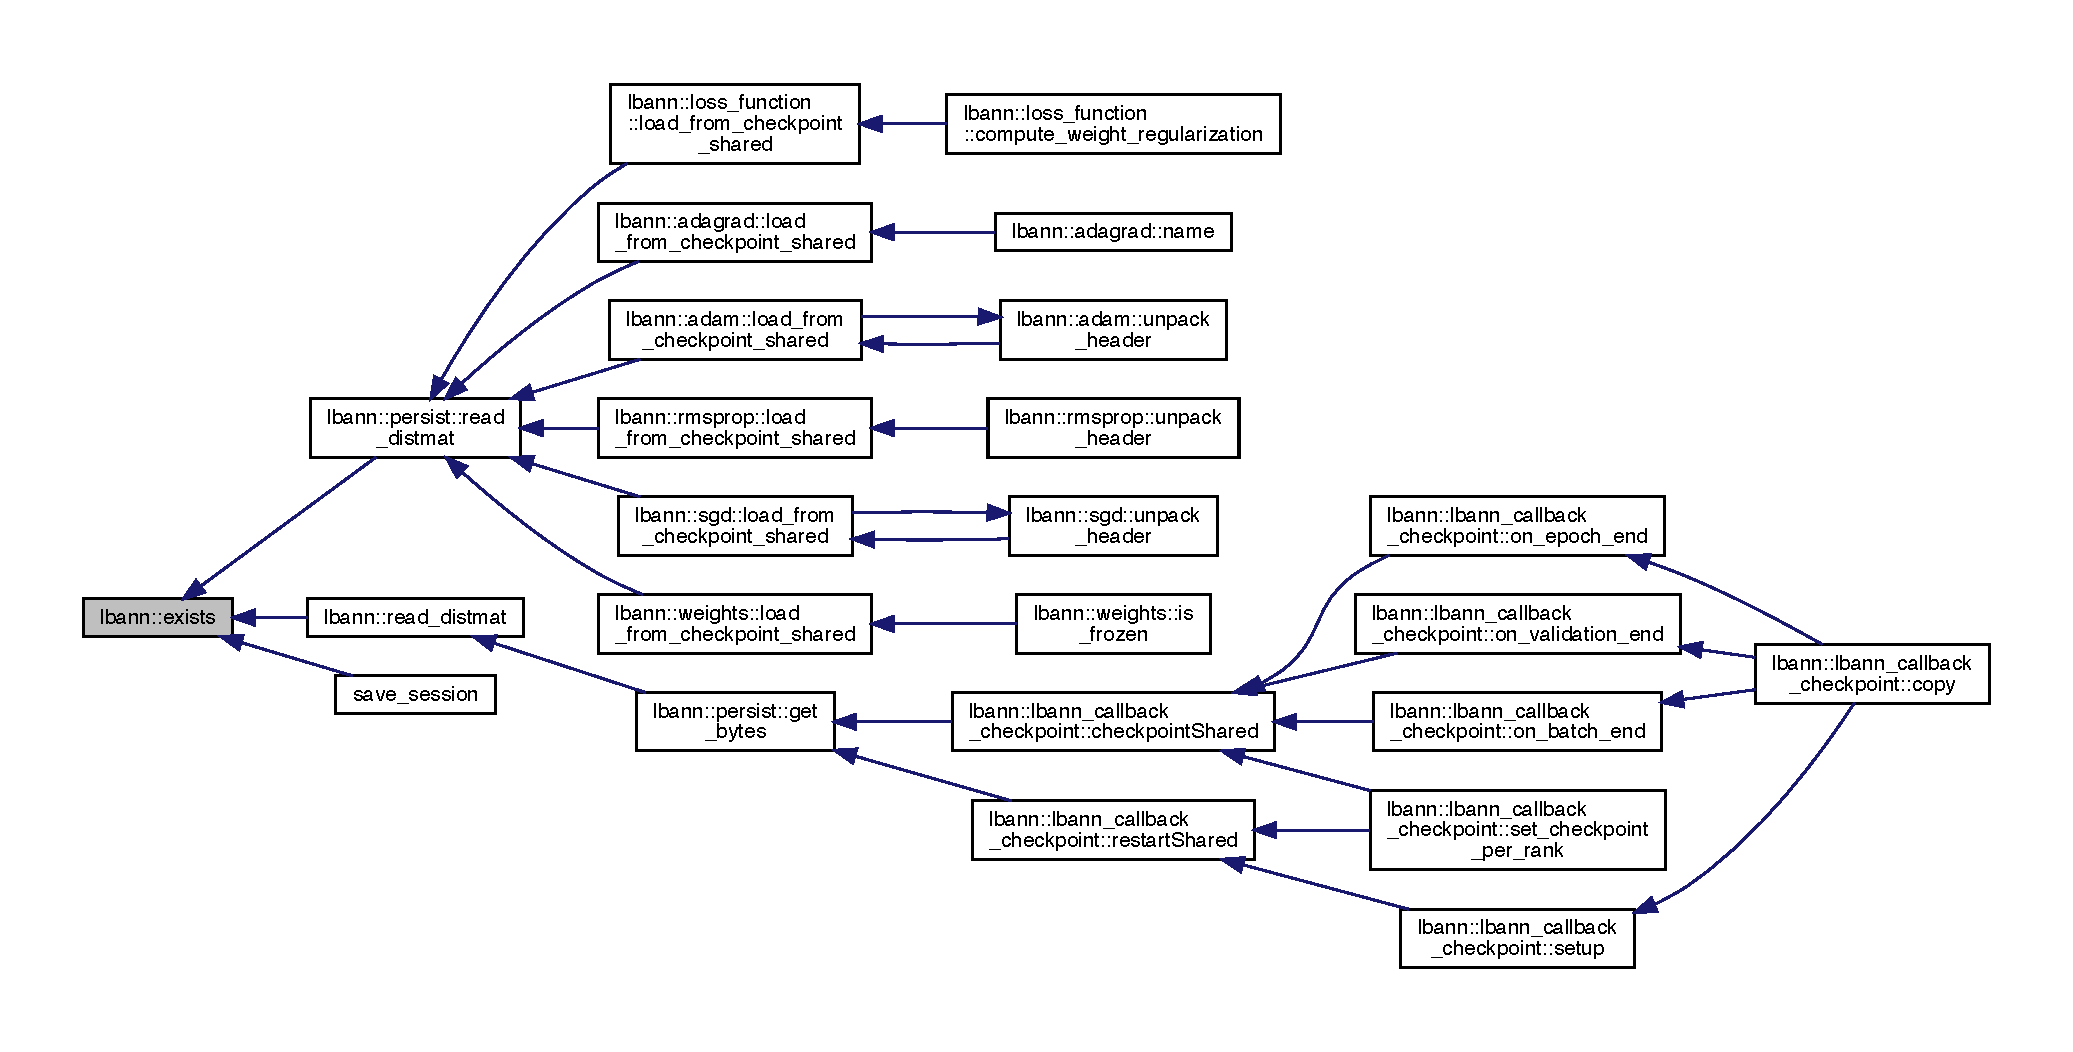
\includegraphics[width=350pt]{namespacelbann_aefae2a9fc9d742ece0fa8ca7ed9ee137_icgraph}
\end{center}
\end{figure}
\mbox{\Hypertarget{namespacelbann_a557aaed6267e7aaf583a75149e9c670c}\label{namespacelbann_a557aaed6267e7aaf583a75149e9c670c}} 
\index{lbann@{lbann}!fast\+\_\+rand\+\_\+int@{fast\+\_\+rand\+\_\+int}}
\index{fast\+\_\+rand\+\_\+int@{fast\+\_\+rand\+\_\+int}!lbann@{lbann}}
\subsubsection{\texorpdfstring{fast\+\_\+rand\+\_\+int()}{fast\_rand\_int()}}
{\footnotesize\ttfamily template$<$typename Generator , typename T $>$ \\
T lbann\+::fast\+\_\+rand\+\_\+int (\begin{DoxyParamCaption}\item[{Generator \&}]{g,  }\item[{T}]{max }\end{DoxyParamCaption})\hspace{0.3cm}{\ttfamily [inline]}}

Return random integers uniformly distributed in \mbox{[}0, max). 
\begin{DoxyParams}{Parameters}
{\em g} & C++ uniform random bit generator. \\
\hline
{\em max} & Upper bound on the distribution. \\
\hline
\end{DoxyParams}
\begin{DoxyNote}{Note}
It turns out that the G\+CC std\+::uniform\+\_\+int\+\_\+distribution is really slow. That implementation is used by most compilers. This implementation is roughly five times faster than that one. 
\end{DoxyNote}


Definition at line 68 of file random.\+hpp.


\begin{DoxyCode}
68                                             \{
69   \textcolor{keyword}{typename} Generator::result\_type x;
70   \textcolor{keywordflow}{do} \{
71     x = g();
72   \} \textcolor{keywordflow}{while} (x >= (Generator::max() - Generator::max() % \hyperlink{base_8hpp_ac47a6ee5278a53898222a48639a2bf39a2ffe4e77325d9a7152f7086ea7aa5114}{max}));
73   \textcolor{keywordflow}{return} x % \hyperlink{base_8hpp_ac47a6ee5278a53898222a48639a2bf39a2ffe4e77325d9a7152f7086ea7aa5114}{max};
74 \}
\end{DoxyCode}
Here is the caller graph for this function\+:\nopagebreak
\begin{figure}[H]
\begin{center}
\leavevmode
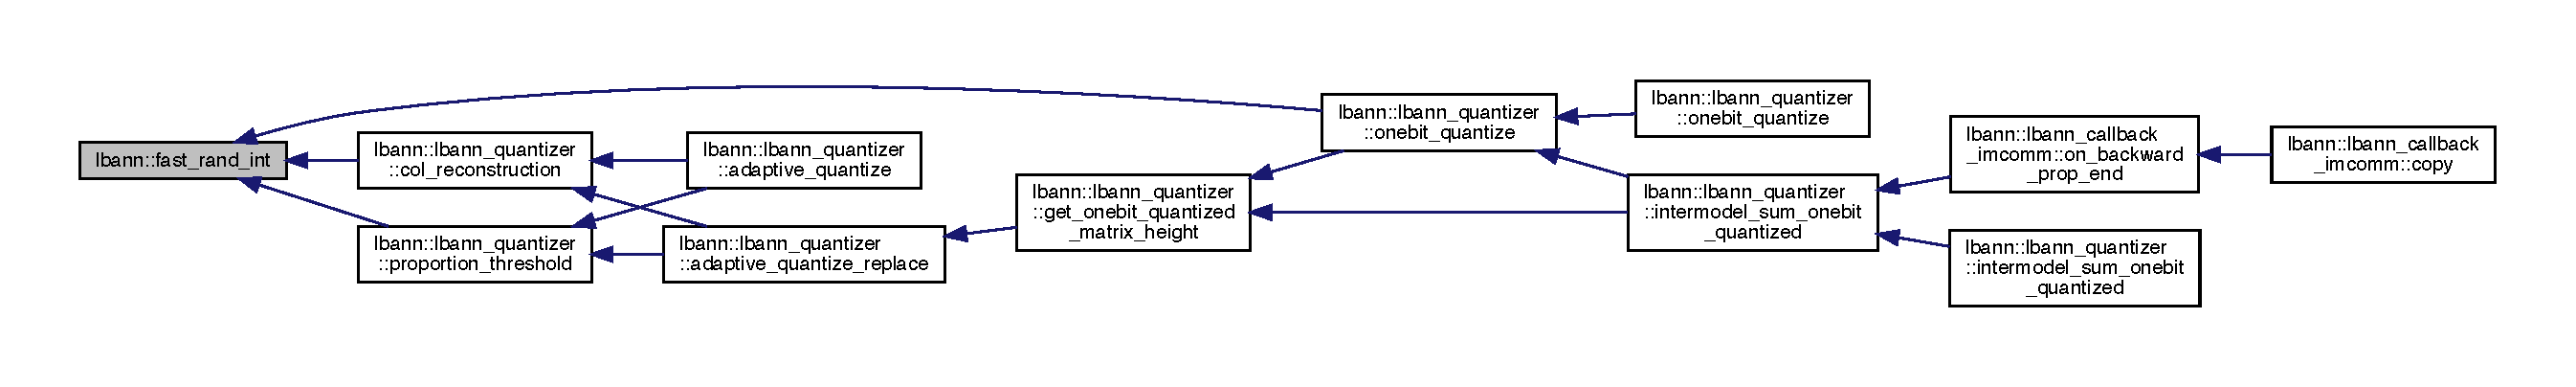
\includegraphics[width=350pt]{namespacelbann_a557aaed6267e7aaf583a75149e9c670c_icgraph}
\end{center}
\end{figure}
\mbox{\Hypertarget{namespacelbann_a2fe8cea17a147566b73260f557b51006}\label{namespacelbann_a2fe8cea17a147566b73260f557b51006}} 
\index{lbann@{lbann}!fast\+\_\+rand\+\_\+int\+\_\+pow2@{fast\+\_\+rand\+\_\+int\+\_\+pow2}}
\index{fast\+\_\+rand\+\_\+int\+\_\+pow2@{fast\+\_\+rand\+\_\+int\+\_\+pow2}!lbann@{lbann}}
\subsubsection{\texorpdfstring{fast\+\_\+rand\+\_\+int\+\_\+pow2()}{fast\_rand\_int\_pow2()}}
{\footnotesize\ttfamily template$<$typename Generator , typename T $>$ \\
T lbann\+::fast\+\_\+rand\+\_\+int\+\_\+pow2 (\begin{DoxyParamCaption}\item[{Generator \&}]{g,  }\item[{T}]{max }\end{DoxyParamCaption})\hspace{0.3cm}{\ttfamily [inline]}}

Faster variant of fast\+\_\+rand\+\_\+int in the case that max is a power of 2. Do not call this if max is not a power of 2. 

Definition at line 81 of file random.\+hpp.


\begin{DoxyCode}
81                                                  \{
82   \textcolor{keyword}{typename} Generator::result\_type x;
83   \hyperlink{base_8hpp_ac47a6ee5278a53898222a48639a2bf39a2ffe4e77325d9a7152f7086ea7aa5114}{max} -= 1;
84   \textcolor{keyword}{const} \textcolor{keyword}{typename} Generator::result\_type upper = Generator::max() -
85       (Generator::max() & (\textcolor{keyword}{typename} Generator::result\_type) \hyperlink{base_8hpp_ac47a6ee5278a53898222a48639a2bf39a2ffe4e77325d9a7152f7086ea7aa5114}{max});
86   \textcolor{keywordflow}{do} \{
87     x = g();
88   \} \textcolor{keywordflow}{while} (x >= upper);
89   \textcolor{keywordflow}{return} x & ((\textcolor{keyword}{typename} Generator::result\_type) \hyperlink{base_8hpp_ac47a6ee5278a53898222a48639a2bf39a2ffe4e77325d9a7152f7086ea7aa5114}{max});
90 \}
\end{DoxyCode}
Here is the call graph for this function\+:\nopagebreak
\begin{figure}[H]
\begin{center}
\leavevmode
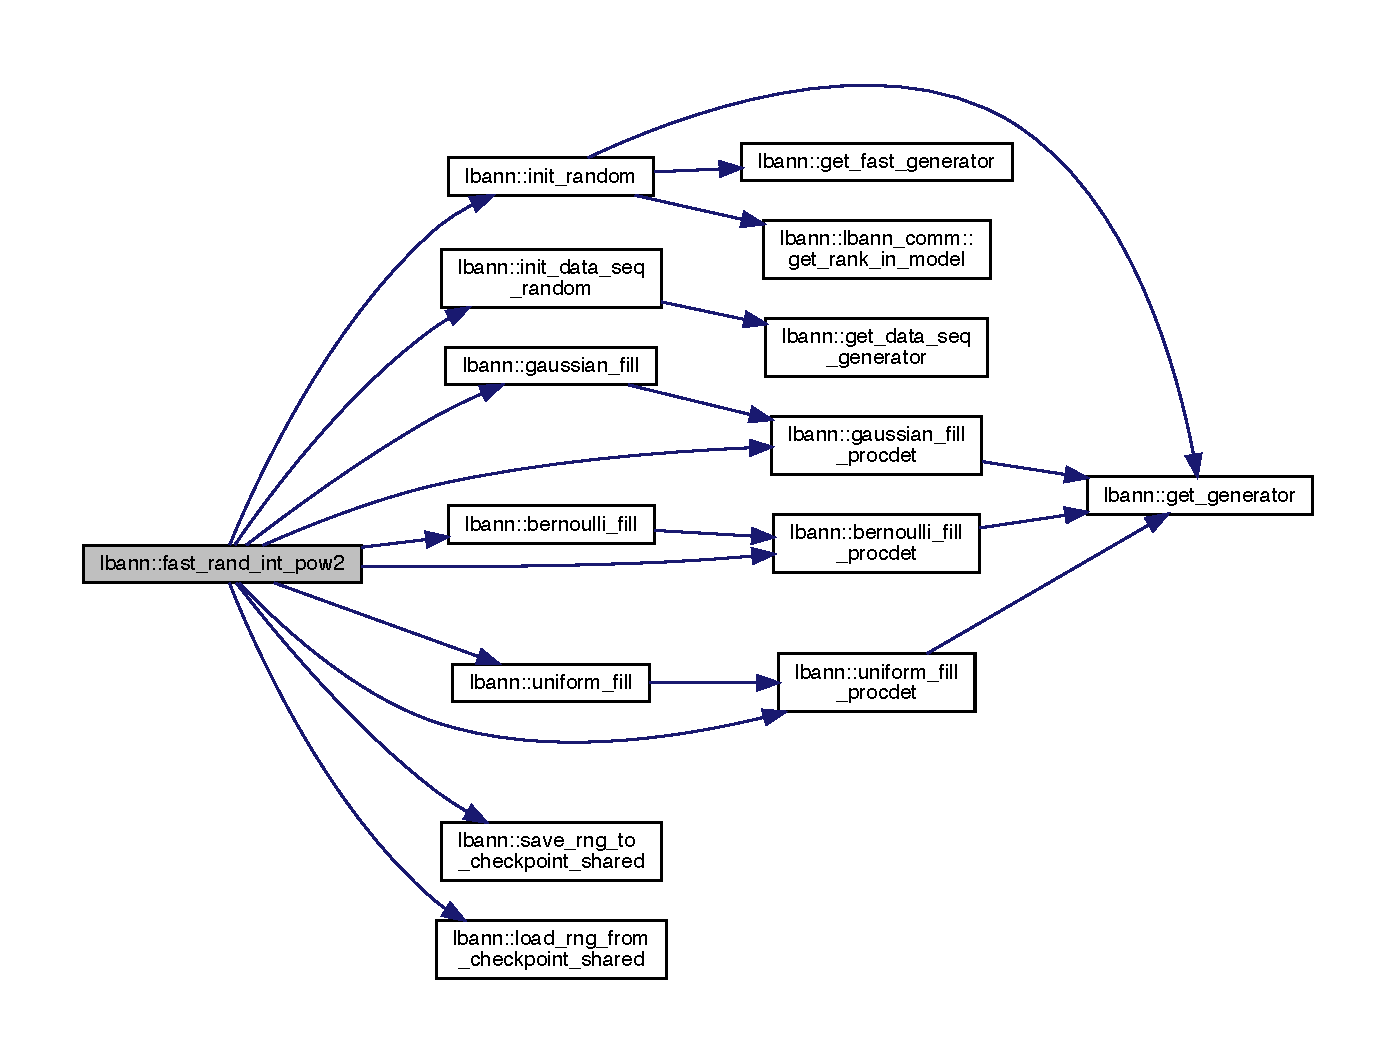
\includegraphics[width=350pt]{namespacelbann_a2fe8cea17a147566b73260f557b51006_cgraph}
\end{center}
\end{figure}
Here is the caller graph for this function\+:\nopagebreak
\begin{figure}[H]
\begin{center}
\leavevmode
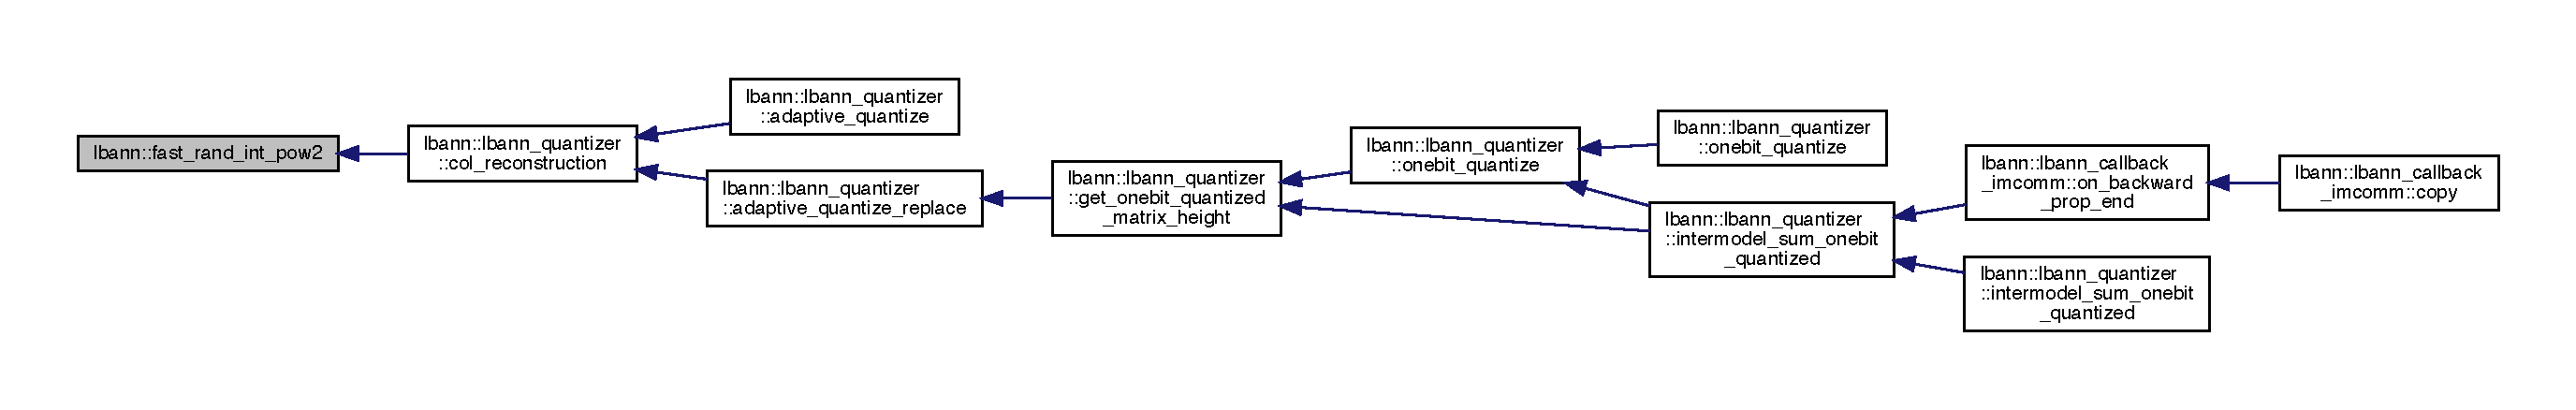
\includegraphics[width=350pt]{namespacelbann_a2fe8cea17a147566b73260f557b51006_icgraph}
\end{center}
\end{figure}
\mbox{\Hypertarget{namespacelbann_a99724ee5a6647a1d8bff6764b9aa5fac}\label{namespacelbann_a99724ee5a6647a1d8bff6764b9aa5fac}} 
\index{lbann@{lbann}!finalize@{finalize}}
\index{finalize@{finalize}!lbann@{lbann}}
\subsubsection{\texorpdfstring{finalize()}{finalize()}}
{\footnotesize\ttfamily void lbann\+::finalize (\begin{DoxyParamCaption}\item[{\hyperlink{classlbann_1_1lbann__comm}{lbann\+\_\+comm} $\ast$}]{comm = {\ttfamily nullptr} }\end{DoxyParamCaption})}

Perform finalization. 

Definition at line 88 of file base.\+cpp.


\begin{DoxyCode}
88                                 \{
89   \textcolor{keywordflow}{if} (\hyperlink{file__io_8cpp_ab048c6f9fcbcfaa57ce68b00263dbebe}{comm} != \textcolor{keyword}{nullptr}) \{
90     \textcolor{keyword}{delete} \hyperlink{file__io_8cpp_ab048c6f9fcbcfaa57ce68b00263dbebe}{comm};
91   \}
92   El::Finalize();
93 \}
\end{DoxyCode}
\mbox{\Hypertarget{namespacelbann_abd116f95f55d0e29d9a0cc386139c4b4}\label{namespacelbann_abd116f95f55d0e29d9a0cc386139c4b4}} 
\index{lbann@{lbann}!gaussian\+\_\+fill@{gaussian\+\_\+fill}}
\index{gaussian\+\_\+fill@{gaussian\+\_\+fill}!lbann@{lbann}}
\subsubsection{\texorpdfstring{gaussian\+\_\+fill()}{gaussian\_fill()}}
{\footnotesize\ttfamily void lbann\+::gaussian\+\_\+fill (\begin{DoxyParamCaption}\item[{\hyperlink{base_8hpp_a9a697a504ae84010e7439ffec862b470}{Abs\+Dist\+Mat} \&}]{mat,  }\item[{El\+::\+Int}]{m,  }\item[{El\+::\+Int}]{n,  }\item[{Data\+Type}]{mean = {\ttfamily 0.0f},  }\item[{Data\+Type}]{stddev = {\ttfamily 1.0f} }\end{DoxyParamCaption})}

Make mat into an m x n matrix where each entry is independently drawn from a Gaussian distribution with given mean and standard deviation. Unless selected so at compile-\/time, this ensures the entries of the matrix do not change as the grid it is distributed over changes; that is, it will have the same entries when mat spans any number of processes. 

Definition at line 166 of file random.\+cpp.


\begin{DoxyCode}
167                                     \{
168 \textcolor{preprocessor}{#ifdef LBANN\_PARALLEL\_RANDOM\_MATRICES}
169   El::Gaussian(mat, m, n, mean, stddev);
170 \textcolor{preprocessor}{#else}
171   \hyperlink{namespacelbann_a2f40602f0503f9737325bb267e5c4dcc}{gaussian\_fill\_procdet}(mat, m, n, mean, stddev);
172 \textcolor{preprocessor}{#endif  // LBANN\_PARALLEL\_RANDOM\_MATRICES}
173 \}
\end{DoxyCode}
Here is the call graph for this function\+:\nopagebreak
\begin{figure}[H]
\begin{center}
\leavevmode
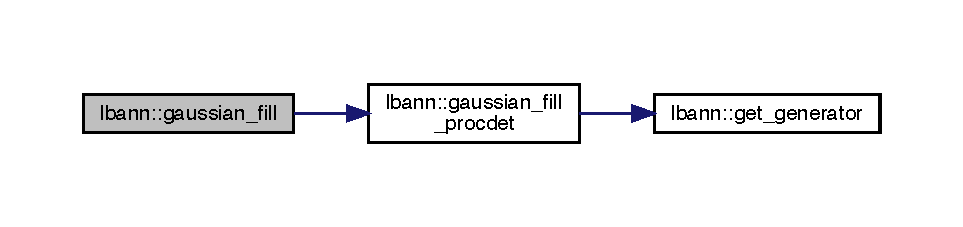
\includegraphics[width=350pt]{namespacelbann_abd116f95f55d0e29d9a0cc386139c4b4_cgraph}
\end{center}
\end{figure}
Here is the caller graph for this function\+:\nopagebreak
\begin{figure}[H]
\begin{center}
\leavevmode
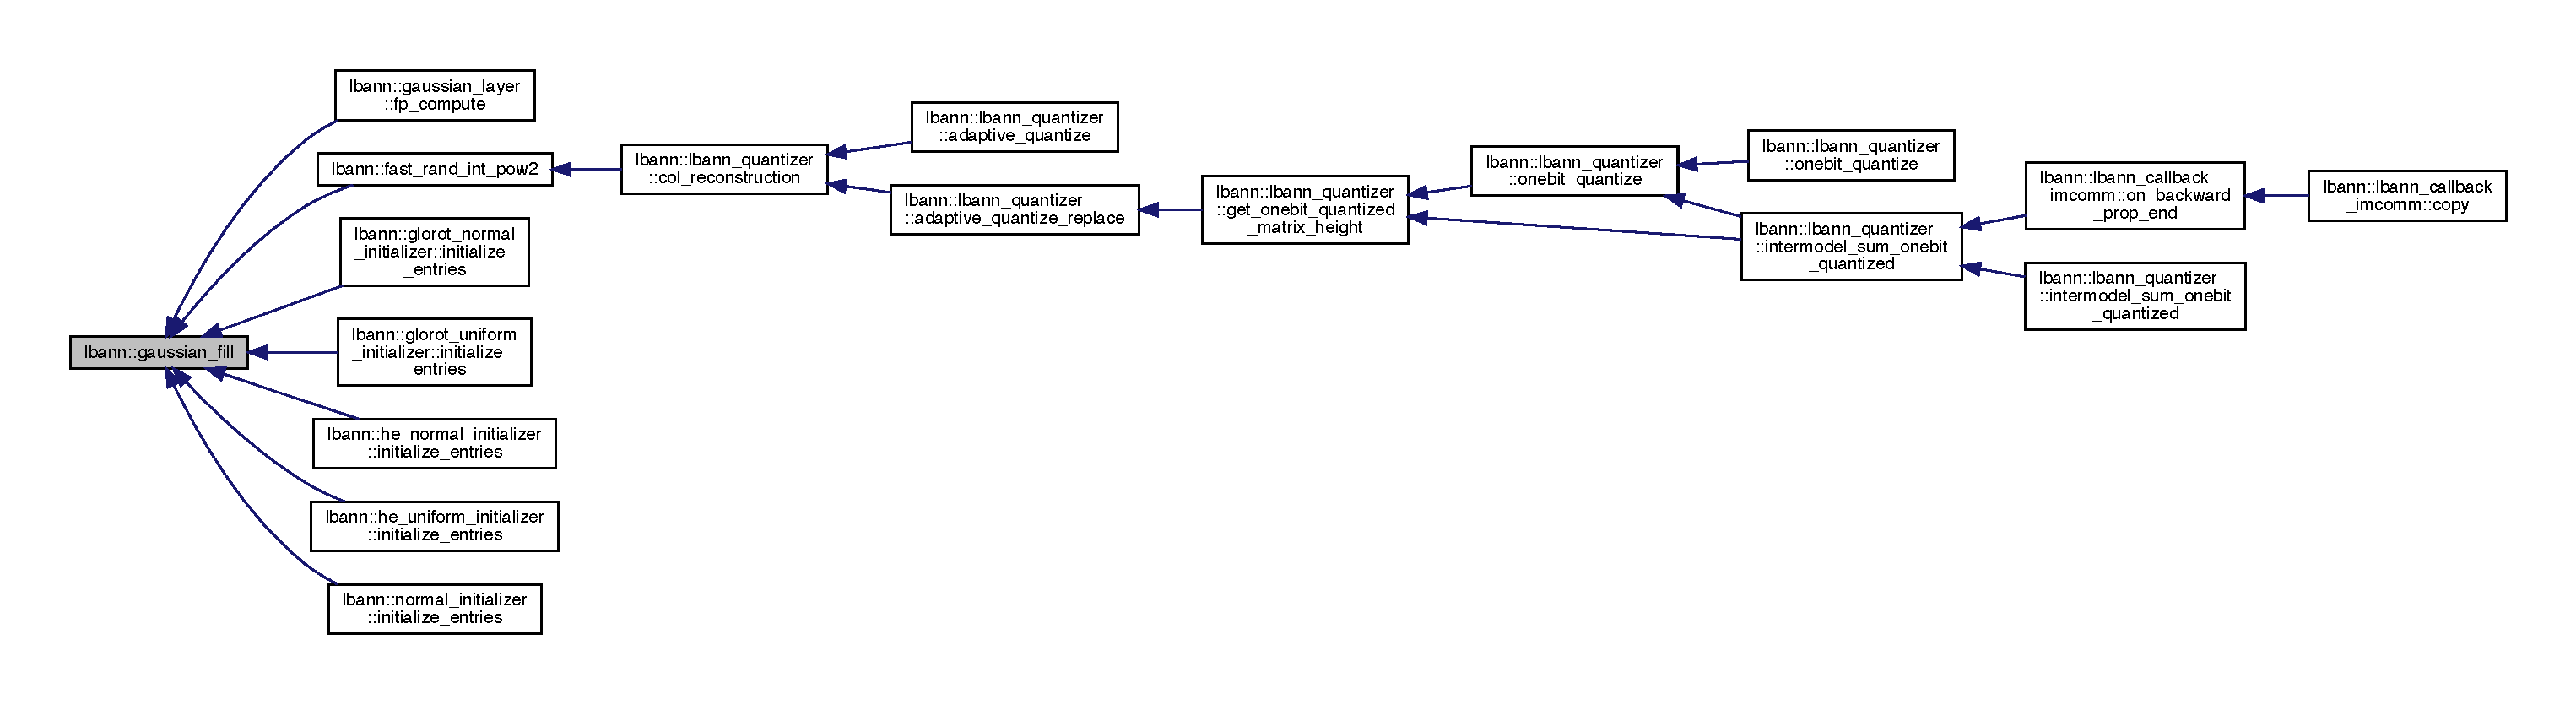
\includegraphics[width=350pt]{namespacelbann_abd116f95f55d0e29d9a0cc386139c4b4_icgraph}
\end{center}
\end{figure}
\mbox{\Hypertarget{namespacelbann_a2f40602f0503f9737325bb267e5c4dcc}\label{namespacelbann_a2f40602f0503f9737325bb267e5c4dcc}} 
\index{lbann@{lbann}!gaussian\+\_\+fill\+\_\+procdet@{gaussian\+\_\+fill\+\_\+procdet}}
\index{gaussian\+\_\+fill\+\_\+procdet@{gaussian\+\_\+fill\+\_\+procdet}!lbann@{lbann}}
\subsubsection{\texorpdfstring{gaussian\+\_\+fill\+\_\+procdet()}{gaussian\_fill\_procdet()}}
{\footnotesize\ttfamily void lbann\+::gaussian\+\_\+fill\+\_\+procdet (\begin{DoxyParamCaption}\item[{\hyperlink{base_8hpp_a9a697a504ae84010e7439ffec862b470}{Abs\+Dist\+Mat} \&}]{mat,  }\item[{El\+::\+Int}]{m,  }\item[{El\+::\+Int}]{n,  }\item[{Data\+Type}]{mean = {\ttfamily 0.0f},  }\item[{Data\+Type}]{stddev = {\ttfamily 1.0f} }\end{DoxyParamCaption})}

Make mat into an m x n matrix where each entry is independently drawn from a Gaussian distribution with given mean and standard deviation. This always ensures that the entries of the matrix do not change as the grid it is distributed over changes. 

Definition at line 192 of file random.\+cpp.


\begin{DoxyCode}
193                                             \{
194   El::Zeros(mat, m, n);
195   \textcolor{keywordflow}{if} (mat.Grid().Rank() == 0) \{
196     mat.Reserve(n * m);
197     \textcolor{keyword}{auto}& gen = \hyperlink{namespacelbann_a4fea7ba21017b49d1e34394b4c20c764}{get\_generator}();
198     std::normal\_distribution<DataType> dist(mean, stddev);
199     \textcolor{keywordflow}{for} (El::Int col = 0; col < n; ++col) \{
200       \textcolor{keywordflow}{for} (El::Int row = 0; row < m; ++row) \{
201         mat.QueueUpdate(row, col, dist(gen));
202       \}
203     \}
204   \}
205   mat.ProcessQueues();
206 \}
\end{DoxyCode}
Here is the call graph for this function\+:\nopagebreak
\begin{figure}[H]
\begin{center}
\leavevmode
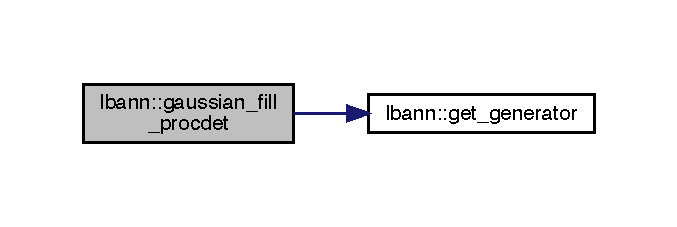
\includegraphics[width=325pt]{namespacelbann_a2f40602f0503f9737325bb267e5c4dcc_cgraph}
\end{center}
\end{figure}
Here is the caller graph for this function\+:\nopagebreak
\begin{figure}[H]
\begin{center}
\leavevmode
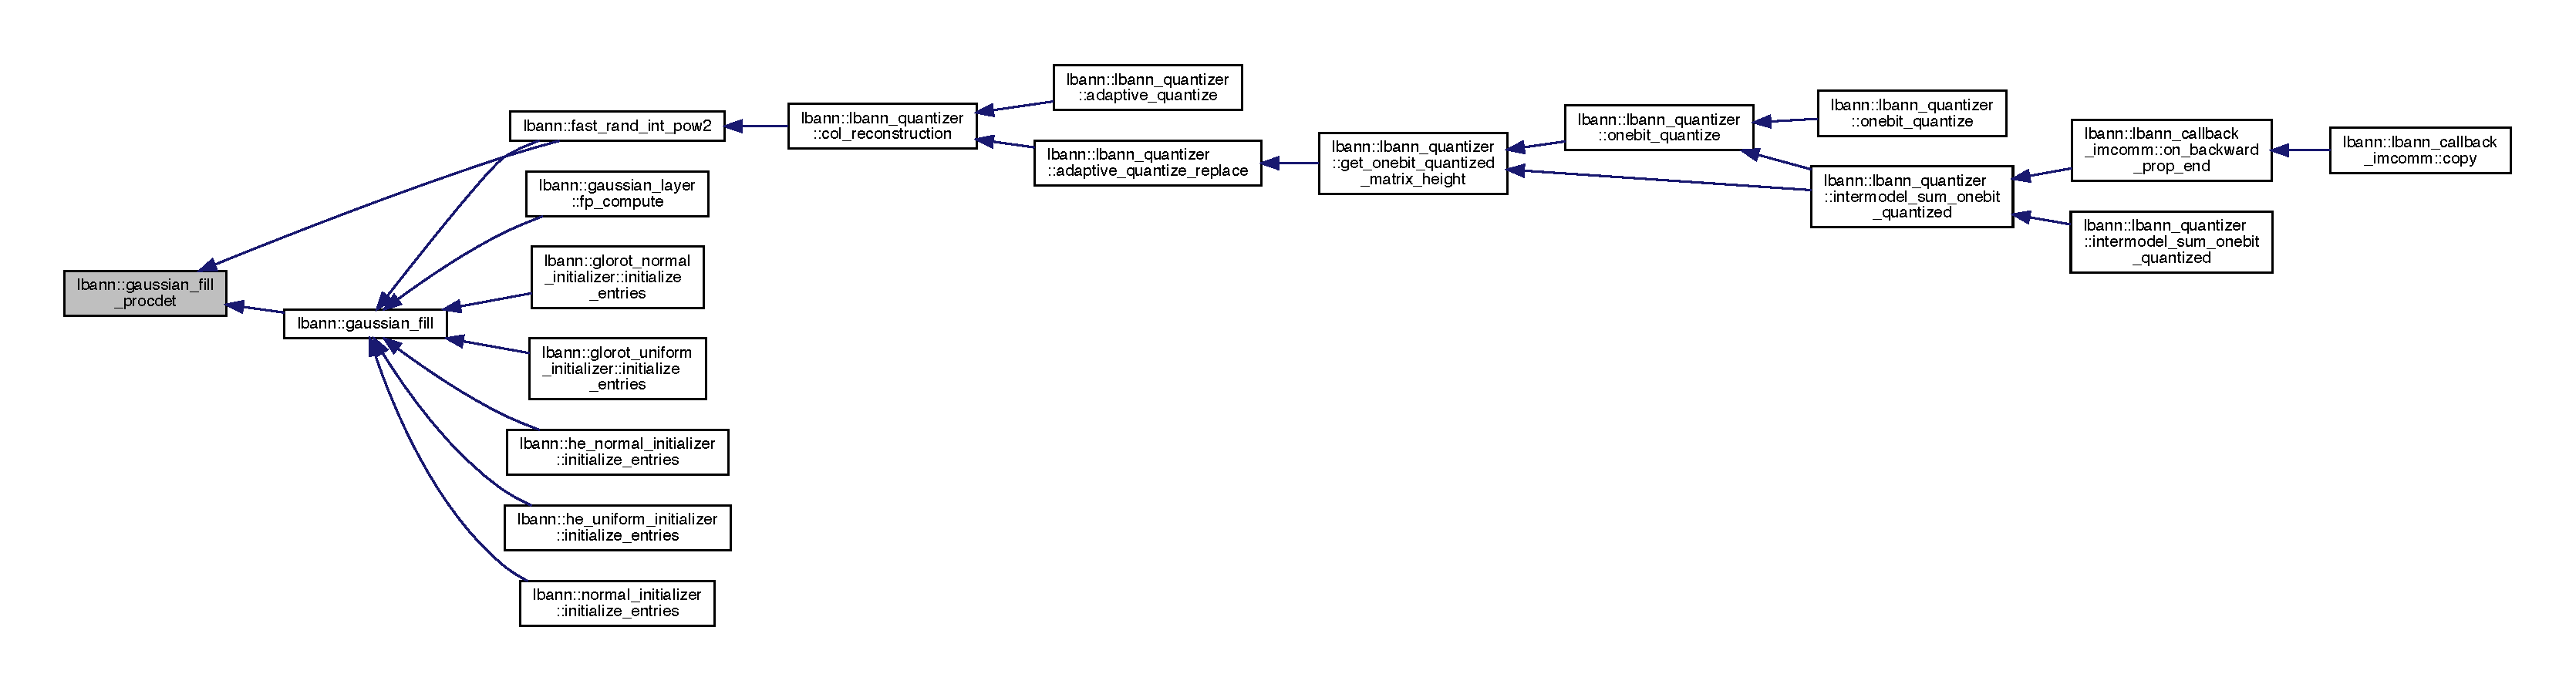
\includegraphics[width=350pt]{namespacelbann_a2f40602f0503f9737325bb267e5c4dcc_icgraph}
\end{center}
\end{figure}
\mbox{\Hypertarget{namespacelbann_a4b08fd1410911d1303176bafa031fcb4}\label{namespacelbann_a4b08fd1410911d1303176bafa031fcb4}} 
\index{lbann@{lbann}!get\+\_\+affinity@{get\+\_\+affinity}}
\index{get\+\_\+affinity@{get\+\_\+affinity}!lbann@{lbann}}
\subsubsection{\texorpdfstring{get\+\_\+affinity()}{get\_affinity()}}
{\footnotesize\ttfamily int lbann\+::get\+\_\+affinity (\begin{DoxyParamCaption}\item[{uint8\+\_\+t $\ast$}]{cpus,  }\item[{uint8\+\_\+t $\ast$}]{count }\end{DoxyParamCaption})}

\mbox{\Hypertarget{namespacelbann_aea9a4378326fd51236a8343c43cc4a7c}\label{namespacelbann_aea9a4378326fd51236a8343c43cc4a7c}} 
\index{lbann@{lbann}!get\+\_\+basename\+\_\+without\+\_\+ext@{get\+\_\+basename\+\_\+without\+\_\+ext}}
\index{get\+\_\+basename\+\_\+without\+\_\+ext@{get\+\_\+basename\+\_\+without\+\_\+ext}!lbann@{lbann}}
\subsubsection{\texorpdfstring{get\+\_\+basename\+\_\+without\+\_\+ext()}{get\_basename\_without\_ext()}}
{\footnotesize\ttfamily std\+::string lbann\+::get\+\_\+basename\+\_\+without\+\_\+ext (\begin{DoxyParamCaption}\item[{const std\+::string}]{file\+\_\+name }\end{DoxyParamCaption})}



Return basename without extention. 



Definition at line 99 of file file\+\_\+utils.\+cpp.


\begin{DoxyCode}
99                                                               \{
100   std::string dir;
101   std::string basename;
102   \hyperlink{namespacelbann_a1ce6832a54235a5fb333f50fffbe1b63}{parse\_path}(file\_name, dir, basename);
103 
104   \textcolor{keywordtype}{size\_t} pos = basename.find\_last\_of(\textcolor{charliteral}{'.'});
105   \textcolor{keywordflow}{if} (pos == 0u) \{
106     \textcolor{keywordflow}{return} basename;
107   \}
108   \textcolor{keywordflow}{return} basename.substr(0, pos);
109 \}
\end{DoxyCode}
Here is the call graph for this function\+:\nopagebreak
\begin{figure}[H]
\begin{center}
\leavevmode
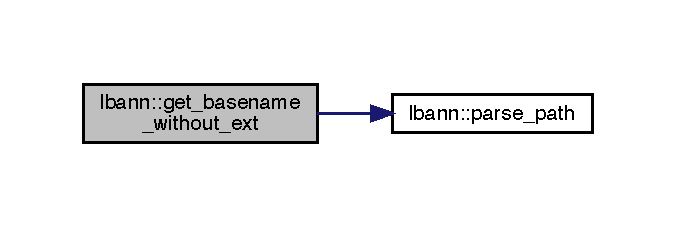
\includegraphics[width=324pt]{namespacelbann_aea9a4378326fd51236a8343c43cc4a7c_cgraph}
\end{center}
\end{figure}
Here is the caller graph for this function\+:\nopagebreak
\begin{figure}[H]
\begin{center}
\leavevmode
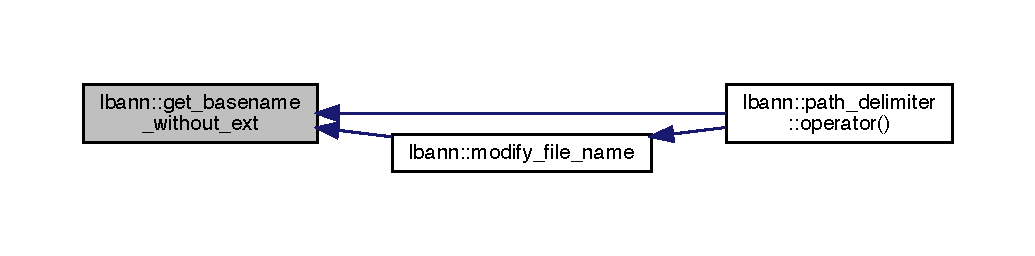
\includegraphics[width=350pt]{namespacelbann_aea9a4378326fd51236a8343c43cc4a7c_icgraph}
\end{center}
\end{figure}
\mbox{\Hypertarget{namespacelbann_ab5665dc52c53faca0caa55b509e2e654}\label{namespacelbann_ab5665dc52c53faca0caa55b509e2e654}} 
\index{lbann@{lbann}!get\+\_\+comm\+\_\+type\+\_\+name@{get\+\_\+comm\+\_\+type\+\_\+name}}
\index{get\+\_\+comm\+\_\+type\+\_\+name@{get\+\_\+comm\+\_\+type\+\_\+name}!lbann@{lbann}}
\subsubsection{\texorpdfstring{get\+\_\+comm\+\_\+type\+\_\+name()}{get\_comm\_type\_name()}}
{\footnotesize\ttfamily std\+::string lbann\+::get\+\_\+comm\+\_\+type\+\_\+name (\begin{DoxyParamCaption}\item[{\hyperlink{classlbann_1_1lbann__callback__imcomm_acf7e894b3381e7f9b71020dc73594d6a}{lbann\+\_\+callback\+\_\+imcomm\+::comm\+\_\+type}}]{m }\end{DoxyParamCaption})}

returns a string representation of the weight\+\_\+initialization 

Definition at line 270 of file callback\+\_\+imcomm.\+cpp.


\begin{DoxyCode}
270                                                                \{
271   \textcolor{keywordflow}{if} ((\textcolor{keywordtype}{int})m < 0 or (\textcolor{keywordtype}{int})m >= (\textcolor{keywordtype}{int})\hyperlink{namespacelbann_add9e1dd52afa73f994d5d3a44c25a818}{comm\_type\_names}.size()) \{
272     \textcolor{keywordflow}{throw}(std::string\{\} + \_\_FILE\_\_ + \textcolor{stringliteral}{" "} + std::to\_string(\_\_LINE\_\_) + \textcolor{stringliteral}{" :: "}
273            + \textcolor{stringliteral}{" Invalid comm\_type"});
274   \}
275   \textcolor{keywordflow}{return} \hyperlink{namespacelbann_add9e1dd52afa73f994d5d3a44c25a818}{comm\_type\_names}[(int)m];
276 \}
\end{DoxyCode}
Here is the caller graph for this function\+:\nopagebreak
\begin{figure}[H]
\begin{center}
\leavevmode
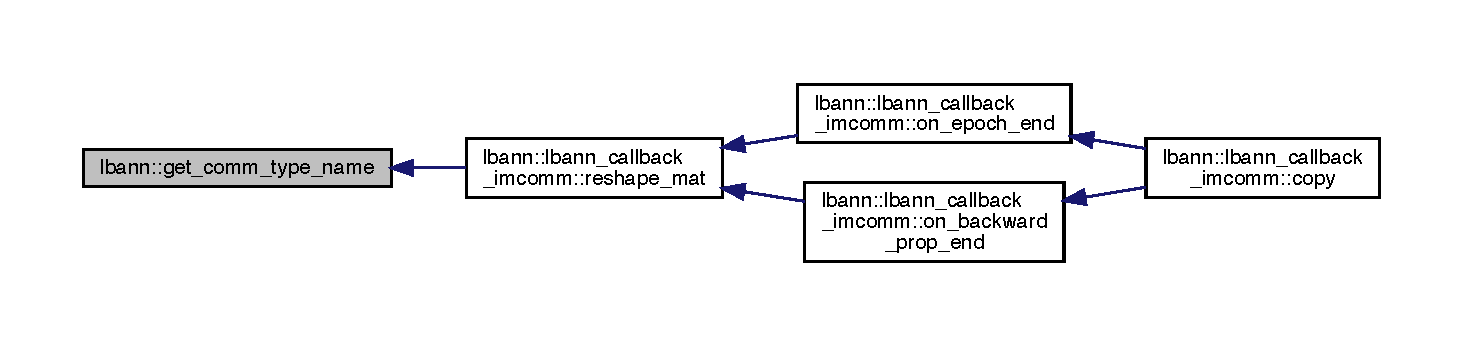
\includegraphics[width=350pt]{namespacelbann_ab5665dc52c53faca0caa55b509e2e654_icgraph}
\end{center}
\end{figure}
\mbox{\Hypertarget{namespacelbann_aba9d11cb3a739cd84e7234ceeb32d098}\label{namespacelbann_aba9d11cb3a739cd84e7234ceeb32d098}} 
\index{lbann@{lbann}!get\+\_\+data\+\_\+seq\+\_\+generator@{get\+\_\+data\+\_\+seq\+\_\+generator}}
\index{get\+\_\+data\+\_\+seq\+\_\+generator@{get\+\_\+data\+\_\+seq\+\_\+generator}!lbann@{lbann}}
\subsubsection{\texorpdfstring{get\+\_\+data\+\_\+seq\+\_\+generator()}{get\_data\_seq\_generator()}}
{\footnotesize\ttfamily \hyperlink{namespacelbann_aab7fa584bac85b9085aa8b8c5a888356}{rng\+\_\+gen} \& lbann\+::get\+\_\+data\+\_\+seq\+\_\+generator (\begin{DoxyParamCaption}{ }\end{DoxyParamCaption})}

Return a reference to the global L\+B\+A\+NN random number generator used for shuffling the data samples within each mini-\/bathc \begin{DoxyNote}{Note}
If compiling with Open\+MP, this is stored in a threadprivate variable. 
\end{DoxyNote}


Definition at line 68 of file random.\+cpp.


\begin{DoxyCode}
68                                   \{
69   \hyperlink{namespaceanonymous__namespace_02random_8cpp_03_ac1d3d0259f3e9c9b75e9701ae727d16e}{return ::data\_seq\_generator};
70 \}
\end{DoxyCode}
Here is the caller graph for this function\+:\nopagebreak
\begin{figure}[H]
\begin{center}
\leavevmode
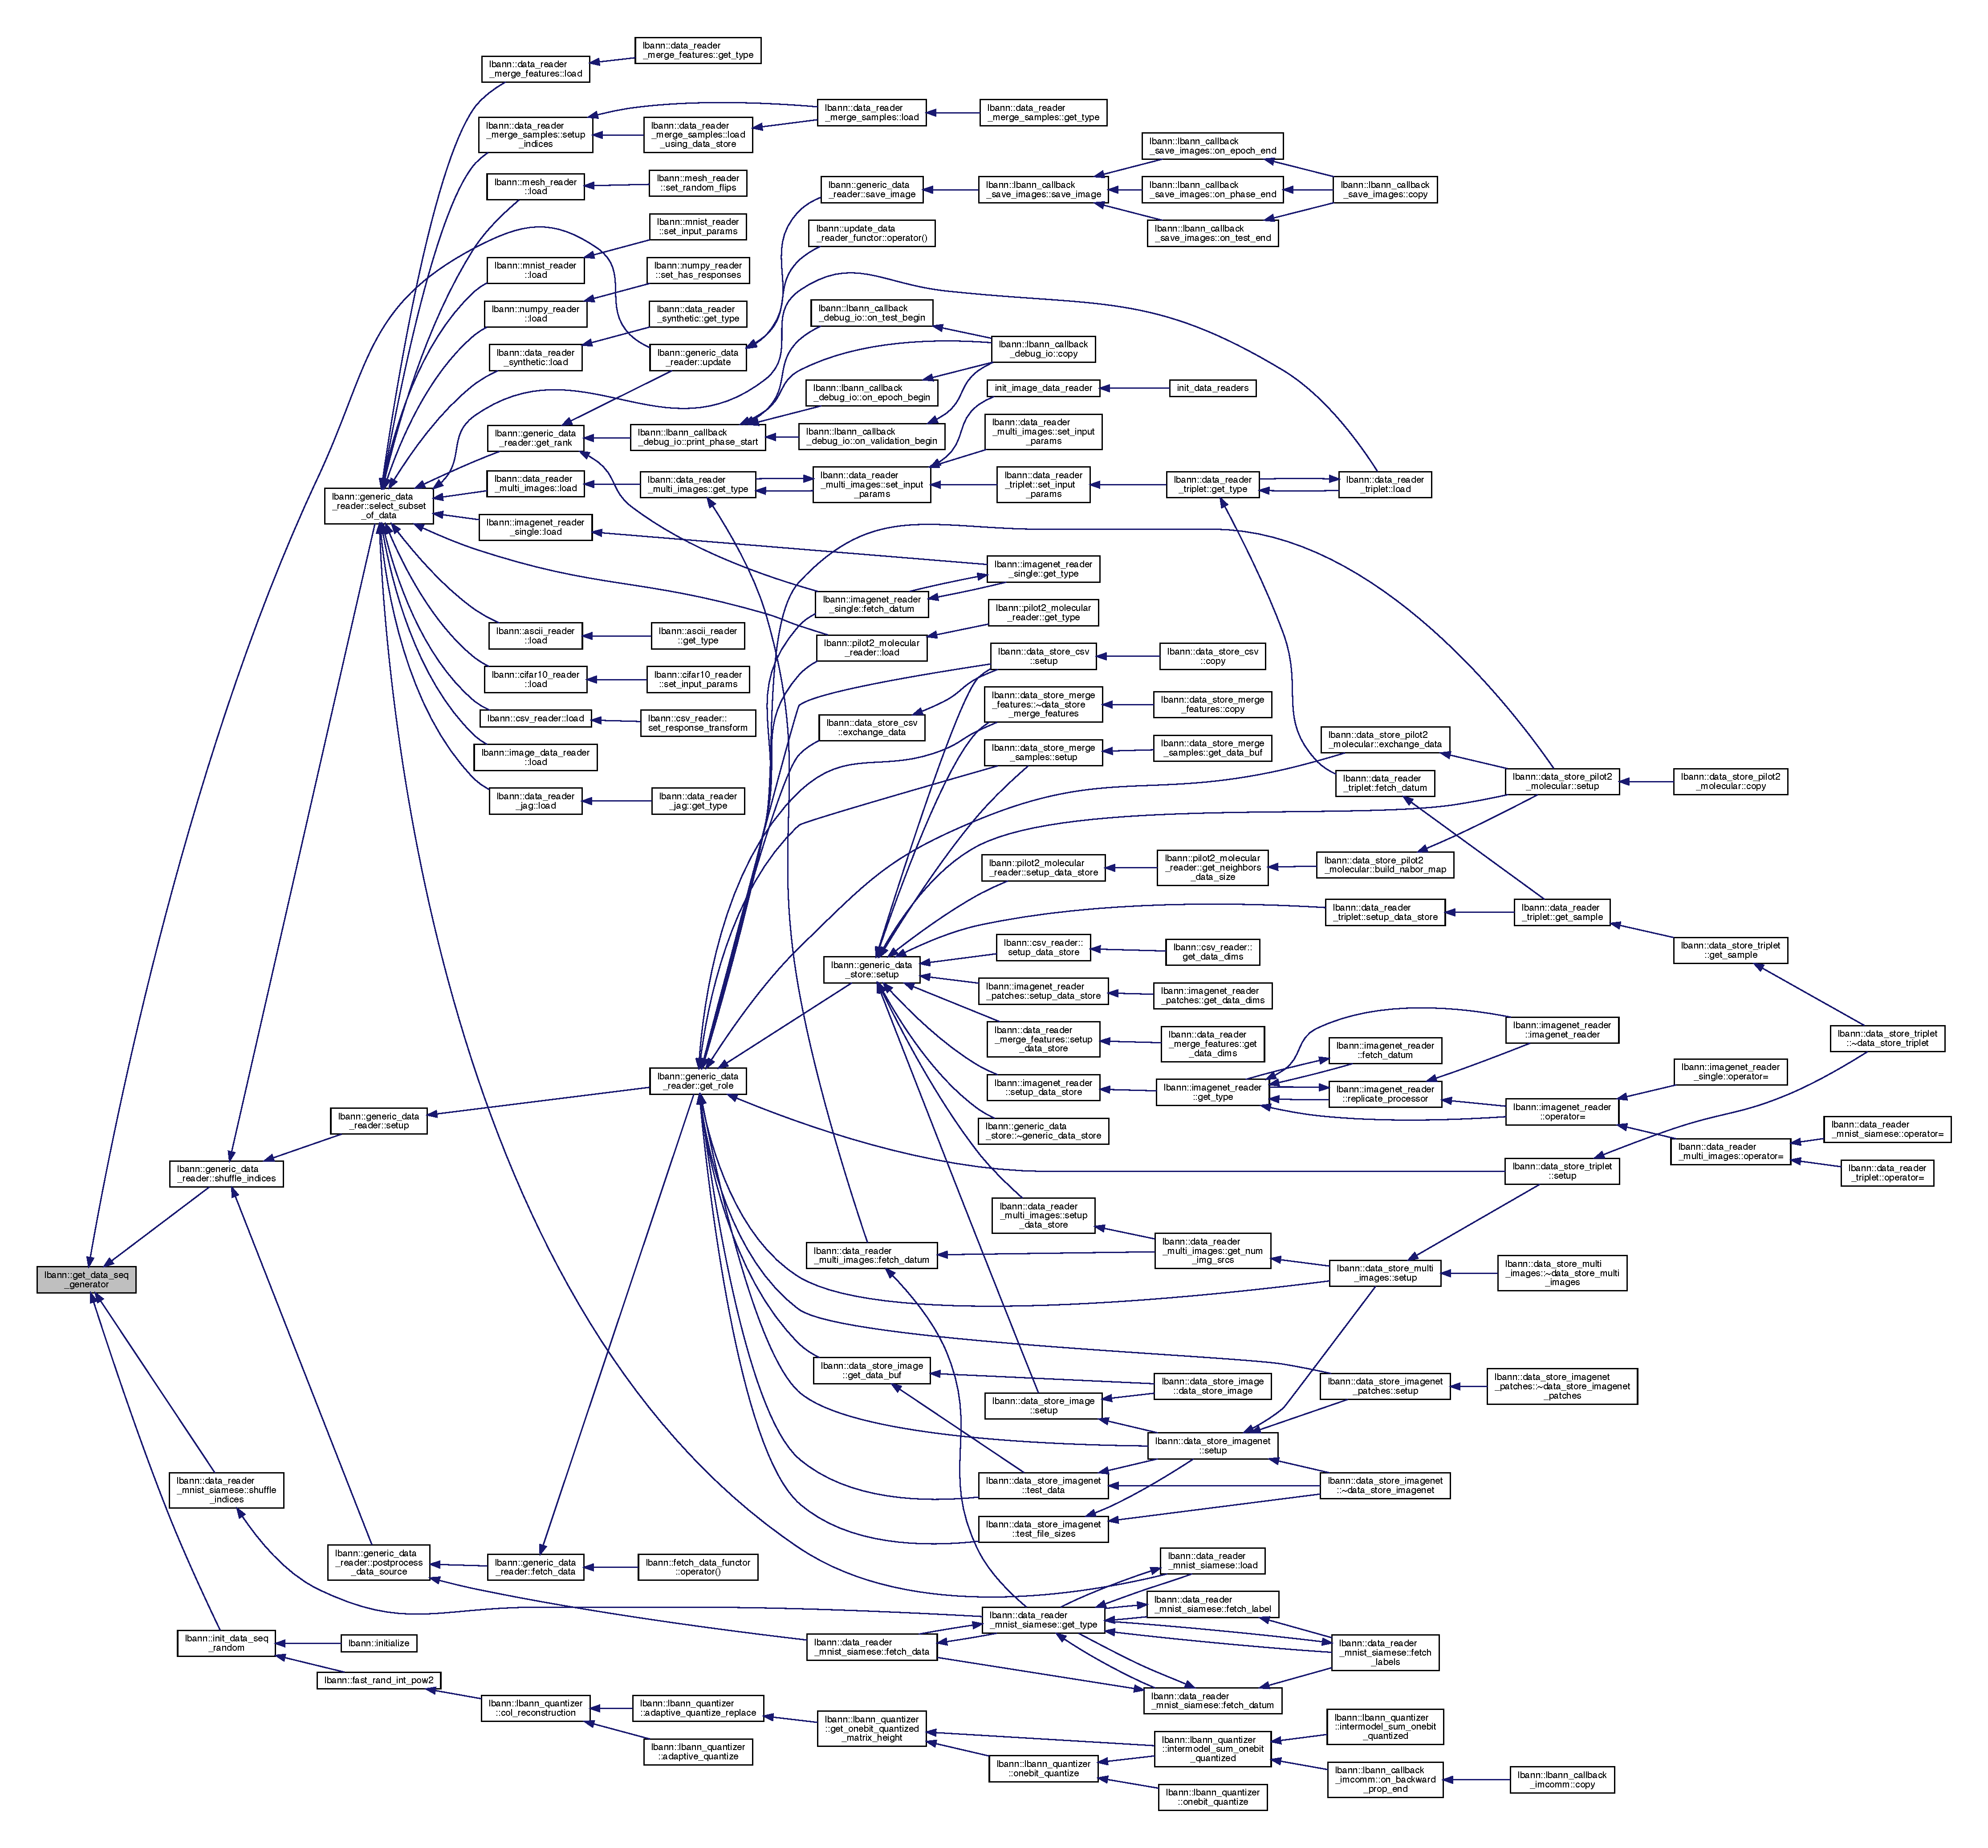
\includegraphics[width=350pt]{namespacelbann_aba9d11cb3a739cd84e7234ceeb32d098_icgraph}
\end{center}
\end{figure}
\mbox{\Hypertarget{namespacelbann_aa4ee6571e54db5cee7f263029147e5f2}\label{namespacelbann_aa4ee6571e54db5cee7f263029147e5f2}} 
\index{lbann@{lbann}!get\+\_\+env\+\_\+var@{get\+\_\+env\+\_\+var}}
\index{get\+\_\+env\+\_\+var@{get\+\_\+env\+\_\+var}!lbann@{lbann}}
\subsubsection{\texorpdfstring{get\+\_\+env\+\_\+var()}{get\_env\_var()}}
{\footnotesize\ttfamily int lbann\+::get\+\_\+env\+\_\+var (\begin{DoxyParamCaption}\item[{const char $\ast$}]{id }\end{DoxyParamCaption})}

Here is the caller graph for this function\+:\nopagebreak
\begin{figure}[H]
\begin{center}
\leavevmode
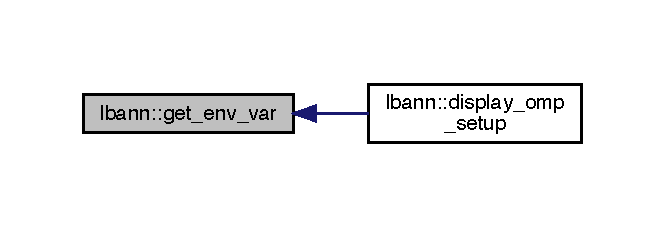
\includegraphics[width=319pt]{namespacelbann_aa4ee6571e54db5cee7f263029147e5f2_icgraph}
\end{center}
\end{figure}
\mbox{\Hypertarget{namespacelbann_ad9a28639b0953886bbcb7fc366783a17}\label{namespacelbann_ad9a28639b0953886bbcb7fc366783a17}} 
\index{lbann@{lbann}!get\+\_\+ext\+\_\+name@{get\+\_\+ext\+\_\+name}}
\index{get\+\_\+ext\+\_\+name@{get\+\_\+ext\+\_\+name}!lbann@{lbann}}
\subsubsection{\texorpdfstring{get\+\_\+ext\+\_\+name()}{get\_ext\_name()}}
{\footnotesize\ttfamily std\+::string lbann\+::get\+\_\+ext\+\_\+name (\begin{DoxyParamCaption}\item[{const std\+::string}]{file\+\_\+name }\end{DoxyParamCaption})}



Return file extention name. 



Definition at line 85 of file file\+\_\+utils.\+cpp.


\begin{DoxyCode}
85                                                   \{
86   std::string dir;
87   std::string basename;
88   \hyperlink{namespacelbann_a1ce6832a54235a5fb333f50fffbe1b63}{parse\_path}(file\_name, dir, basename);
89 
90   \textcolor{keywordtype}{size\_t} pos = basename.find\_last\_of(\textcolor{charliteral}{'.'});
91   \textcolor{keywordflow}{if} (pos == 0u) \{
92     \textcolor{keywordflow}{return} \textcolor{stringliteral}{""};  \textcolor{comment}{// hidden file}
93   \}
94   \textcolor{keywordflow}{return} basename.substr(pos+1, basename.size());
95 \}
\end{DoxyCode}
Here is the call graph for this function\+:\nopagebreak
\begin{figure}[H]
\begin{center}
\leavevmode
\includegraphics[width=321pt]{namespacelbann_ad9a28639b0953886bbcb7fc366783a17_cgraph}
\end{center}
\end{figure}
Here is the caller graph for this function\+:\nopagebreak
\begin{figure}[H]
\begin{center}
\leavevmode
\includegraphics[width=350pt]{namespacelbann_ad9a28639b0953886bbcb7fc366783a17_icgraph}
\end{center}
\end{figure}
\mbox{\Hypertarget{namespacelbann_ae6ce9c2fdec6f81803f6b1a6555c31c5}\label{namespacelbann_ae6ce9c2fdec6f81803f6b1a6555c31c5}} 
\index{lbann@{lbann}!get\+\_\+fast\+\_\+generator@{get\+\_\+fast\+\_\+generator}}
\index{get\+\_\+fast\+\_\+generator@{get\+\_\+fast\+\_\+generator}!lbann@{lbann}}
\subsubsection{\texorpdfstring{get\+\_\+fast\+\_\+generator()}{get\_fast\_generator()}}
{\footnotesize\ttfamily \hyperlink{namespacelbann_af16616ffa6a3616836eabadd6ce837ec}{fast\+\_\+rng\+\_\+gen} \& lbann\+::get\+\_\+fast\+\_\+generator (\begin{DoxyParamCaption}{ }\end{DoxyParamCaption})}

Return a reference to a possibly-\/faster global L\+B\+A\+NN random number generator. Compared to get\+\_\+generator, this should be slightly faster. \begin{DoxyNote}{Note}
If compiling with Open\+MP, this is stored in a threadprivate variable. 
\end{DoxyNote}


Definition at line 64 of file random.\+cpp.


\begin{DoxyCode}
64                                    \{
65   \hyperlink{namespaceanonymous__namespace_02random_8cpp_03_a349f572cec05cd0e2469b799774a8602}{return ::fast\_generator};
66 \}
\end{DoxyCode}
Here is the caller graph for this function\+:\nopagebreak
\begin{figure}[H]
\begin{center}
\leavevmode
\includegraphics[width=350pt]{namespacelbann_ae6ce9c2fdec6f81803f6b1a6555c31c5_icgraph}
\end{center}
\end{figure}
\mbox{\Hypertarget{namespacelbann_a4fea7ba21017b49d1e34394b4c20c764}\label{namespacelbann_a4fea7ba21017b49d1e34394b4c20c764}} 
\index{lbann@{lbann}!get\+\_\+generator@{get\+\_\+generator}}
\index{get\+\_\+generator@{get\+\_\+generator}!lbann@{lbann}}
\subsubsection{\texorpdfstring{get\+\_\+generator()}{get\_generator()}}
{\footnotesize\ttfamily \hyperlink{namespacelbann_aab7fa584bac85b9085aa8b8c5a888356}{rng\+\_\+gen} \& lbann\+::get\+\_\+generator (\begin{DoxyParamCaption}{ }\end{DoxyParamCaption})}

Return a reference to the global L\+B\+A\+NN random number generator. \begin{DoxyNote}{Note}
If compiling with Open\+MP, this is stored in a threadprivate variable. 
\end{DoxyNote}


Definition at line 60 of file random.\+cpp.


\begin{DoxyCode}
60                          \{
61   \hyperlink{namespaceanonymous__namespace_02random_8cpp_03_a83826c4b587d1825f13b833be6fe047f}{return ::generator};
62 \}
\end{DoxyCode}
Here is the caller graph for this function\+:\nopagebreak
\begin{figure}[H]
\begin{center}
\leavevmode
\includegraphics[width=350pt]{namespacelbann_a4fea7ba21017b49d1e34394b4c20c764_icgraph}
\end{center}
\end{figure}
\mbox{\Hypertarget{namespacelbann_abee17f56525b3894b0d3621a307faebd}\label{namespacelbann_abee17f56525b3894b0d3621a307faebd}} 
\index{lbann@{lbann}!get\+\_\+num\+\_\+pus@{get\+\_\+num\+\_\+pus}}
\index{get\+\_\+num\+\_\+pus@{get\+\_\+num\+\_\+pus}!lbann@{lbann}}
\subsubsection{\texorpdfstring{get\+\_\+num\+\_\+pus()}{get\_num\_pus()}}
{\footnotesize\ttfamily int lbann\+::get\+\_\+num\+\_\+pus (\begin{DoxyParamCaption}{ }\end{DoxyParamCaption})}

\mbox{\Hypertarget{namespacelbann_a17d55032bad5bb02903f9b1d933836a4}\label{namespacelbann_a17d55032bad5bb02903f9b1d933836a4}} 
\index{lbann@{lbann}!get\+\_\+sleep\+\_\+sec@{get\+\_\+sleep\+\_\+sec}}
\index{get\+\_\+sleep\+\_\+sec@{get\+\_\+sleep\+\_\+sec}!lbann@{lbann}}
\subsubsection{\texorpdfstring{get\+\_\+sleep\+\_\+sec()}{get\_sleep\_sec()}}
{\footnotesize\ttfamily int lbann\+::get\+\_\+sleep\+\_\+sec (\begin{DoxyParamCaption}{ }\end{DoxyParamCaption})}

Here is the caller graph for this function\+:\nopagebreak
\begin{figure}[H]
\begin{center}
\leavevmode
\includegraphics[width=329pt]{namespacelbann_a17d55032bad5bb02903f9b1d933836a4_icgraph}
\end{center}
\end{figure}
\mbox{\Hypertarget{namespacelbann_a478d36031ff0659893c4322cd856157f}\label{namespacelbann_a478d36031ff0659893c4322cd856157f}} 
\index{lbann@{lbann}!get\+\_\+time@{get\+\_\+time}}
\index{get\+\_\+time@{get\+\_\+time}!lbann@{lbann}}
\subsubsection{\texorpdfstring{get\+\_\+time()}{get\_time()}}
{\footnotesize\ttfamily double lbann\+::get\+\_\+time (\begin{DoxyParamCaption}{ }\end{DoxyParamCaption})\hspace{0.3cm}{\ttfamily [inline]}}

Return time in fractional seconds since an epoch. 

Definition at line 37 of file timer.\+hpp.


\begin{DoxyCode}
37                          \{
38   \textcolor{keyword}{using namespace }std::chrono;
39   \textcolor{keywordflow}{return} duration\_cast<duration<double>>(
40            steady\_clock::now().time\_since\_epoch()).count();
41 \}
\end{DoxyCode}
Here is the caller graph for this function\+:\nopagebreak
\begin{figure}[H]
\begin{center}
\leavevmode
\includegraphics[width=350pt]{namespacelbann_a478d36031ff0659893c4322cd856157f_icgraph}
\end{center}
\end{figure}
\mbox{\Hypertarget{namespacelbann_af3f2c9055423e1fe3380b1ad4c4ab5ef}\label{namespacelbann_af3f2c9055423e1fe3380b1ad4c4ab5ef}} 
\index{lbann@{lbann}!get\+\_\+tokens@{get\+\_\+tokens}}
\index{get\+\_\+tokens@{get\+\_\+tokens}!lbann@{lbann}}
\subsubsection{\texorpdfstring{get\+\_\+tokens()}{get\_tokens()}\hspace{0.1cm}{\footnotesize\ttfamily [1/2]}}
{\footnotesize\ttfamily std\+::vector$<$ int $>$ lbann\+::get\+\_\+tokens (\begin{DoxyParamCaption}\item[{std\+::string}]{str,  }\item[{const std\+::vector$<$ char $>$}]{delims }\end{DoxyParamCaption})}



Tokenize a string into integers by an ordered sequence of delimiter characters. 



Definition at line 38 of file file\+\_\+utils.\+cpp.


\begin{DoxyCode}
38                                                                        \{
39   std::vector<int> tokens;
40   \textcolor{keywordtype}{size\_t} pos;
41 
42   \textcolor{keywordflow}{for} (\textcolor{keyword}{const} \textcolor{keyword}{auto} d : delims) \{
43     pos = str.find\_first\_of(d);
44     \textcolor{keywordflow}{if} (pos == std::string::npos) \{
45      \textcolor{comment}{// std::cerr << "Not able to split " << str << " by " << d << std::endl;}
46       \textcolor{keywordflow}{return} std::vector<int>();
47     \}
48     tokens.push\_back(atoi(str.substr(0, pos).c\_str()));
49     str = str.substr(pos+1, str.size());
50   \}
51 
52   \textcolor{keywordflow}{return} tokens;
53 \}
\end{DoxyCode}
Here is the caller graph for this function\+:\nopagebreak
\begin{figure}[H]
\begin{center}
\leavevmode
\includegraphics[width=350pt]{namespacelbann_af3f2c9055423e1fe3380b1ad4c4ab5ef_icgraph}
\end{center}
\end{figure}
\mbox{\Hypertarget{namespacelbann_ac02a174553cf05f779743be1c92f1912}\label{namespacelbann_ac02a174553cf05f779743be1c92f1912}} 
\index{lbann@{lbann}!get\+\_\+tokens@{get\+\_\+tokens}}
\index{get\+\_\+tokens@{get\+\_\+tokens}!lbann@{lbann}}
\subsubsection{\texorpdfstring{get\+\_\+tokens()}{get\_tokens()}\hspace{0.1cm}{\footnotesize\ttfamily [2/2]}}
{\footnotesize\ttfamily std\+::vector$<$ std\+::string $>$ lbann\+::get\+\_\+tokens (\begin{DoxyParamCaption}\item[{const std\+::string}]{str,  }\item[{const std\+::string}]{delims }\end{DoxyParamCaption})}



Tokenize a string into substrings by set of delimiter characters. 



Definition at line 55 of file file\+\_\+utils.\+cpp.


\begin{DoxyCode}
55                                                                              \{
56   std::vector<std::string> parsed;
57   \textcolor{keywordtype}{size\_t} pos\_start = 0u;
58   \textcolor{keywordtype}{size\_t} pos\_end = 0u;
59 
60   \textcolor{keywordflow}{while} ((pos\_end != std::string::npos) && (pos\_start != std::string::npos)) \{
61     pos\_start = str.find\_first\_not\_of(delims, pos\_end);
62     \textcolor{keywordflow}{if} (pos\_start != std::string::npos) \{
63       pos\_end = str.find\_first\_of(delims, pos\_start);
64       parsed.push\_back(str.substr(pos\_start, (pos\_end-pos\_start)));
65     \}
66   \}
67   \textcolor{keywordflow}{return} parsed;
68 \}
\end{DoxyCode}
\mbox{\Hypertarget{namespacelbann_a840c9f1d5f27bc30d081fb90529889e6}\label{namespacelbann_a840c9f1d5f27bc30d081fb90529889e6}} 
\index{lbann@{lbann}!glob@{glob}}
\index{glob@{glob}!lbann@{lbann}}
\subsubsection{\texorpdfstring{glob()}{glob()}}
{\footnotesize\ttfamily std\+::vector$<$std\+::string$>$ lbann\+::glob (\begin{DoxyParamCaption}\item[{const std\+::string \&}]{pattern }\end{DoxyParamCaption})\hspace{0.3cm}{\ttfamily [inline]}}

Wrapper around glob, which searches for paths matching pattern according to the shell. Note this does not do tilde expansion. 

Definition at line 42 of file glob.\+hpp.


\begin{DoxyCode}
42                                                            \{
43   glob\_t pglob;
44   \textcolor{keywordtype}{int} r = \hyperlink{namespacelbann_a840c9f1d5f27bc30d081fb90529889e6}{glob}(pattern.c\_str(), 0, \textcolor{keyword}{nullptr}, &pglob);
45   \textcolor{keywordflow}{if} (r != 0) \{
46     \textcolor{comment}{// Either an error or no match.}
47     \textcolor{keywordflow}{if} (r == GLOB\_NOMATCH) \{
48       \textcolor{keywordflow}{return} \{\};
49     \} \textcolor{keywordflow}{else} \{
50       \textcolor{keywordflow}{throw} lbann\_exception(\textcolor{stringliteral}{"glob error"});
51     \}
52   \}
53   std::vector<std::string> results(pglob.gl\_pathc);
54   \textcolor{keywordflow}{for} (\textcolor{keywordtype}{size\_t} i = 0; i < pglob.gl\_pathc; ++i) \{
55     results[i] = std::string(pglob.gl\_pathv[i]);
56   \}
57   globfree(&pglob);
58   \textcolor{keywordflow}{return} results;
59 \}
\end{DoxyCode}
Here is the caller graph for this function\+:\nopagebreak
\begin{figure}[H]
\begin{center}
\leavevmode
\includegraphics[width=350pt]{namespacelbann_a840c9f1d5f27bc30d081fb90529889e6_icgraph}
\end{center}
\end{figure}
\mbox{\Hypertarget{namespacelbann_aa3636a1979e40da2af91f30a12b90db9}\label{namespacelbann_aa3636a1979e40da2af91f30a12b90db9}} 
\index{lbann@{lbann}!im2col@{im2col}}
\index{im2col@{im2col}!lbann@{lbann}}
\subsubsection{\texorpdfstring{im2col()}{im2col()}}
{\footnotesize\ttfamily void lbann\+::im2col (\begin{DoxyParamCaption}\item[{const \hyperlink{base_8hpp_a68f11fdc31b62516cb310831bbe54d73}{Mat} \&}]{im,  }\item[{\hyperlink{base_8hpp_a68f11fdc31b62516cb310831bbe54d73}{Mat} \&}]{col,  }\item[{int}]{num\+\_\+channels,  }\item[{int}]{im\+\_\+num\+\_\+dims,  }\item[{const int $\ast$}]{im\+\_\+dims,  }\item[{const int $\ast$}]{im\+\_\+pads,  }\item[{const int $\ast$}]{window\+\_\+dims,  }\item[{const int $\ast$}]{window\+\_\+strides }\end{DoxyParamCaption})}



Rearrange image blocks into matrix columns. 

The \textquotesingle{}col\textquotesingle{} matrix is generated from the \textquotesingle{}im\textquotesingle{} tensor im by shifting a window across im. Each column of col is produced by positioning the window, extracting entries from im, and flattening. 
\begin{DoxyParams}{Parameters}
{\em im} & im tensor, represented as a column vector. \\
\hline
{\em col} & col matrix. Height should be equal to window size and width equal to number of window shifts. Data should be contiguous. \\
\hline
{\em num\+\_\+channels} & Number of channels in im tensor. \\
\hline
{\em im\+\_\+num\+\_\+dims} & Number of dimensions in im tensor. \\
\hline
{\em im\+\_\+dims} & im tensor dimensions. \\
\hline
{\em im\+\_\+pads} & Zero pads for im tensor. \\
\hline
{\em window\+\_\+dims} & Dimensions of window. \\
\hline
{\em window\+\_\+strides} & Window shift strides. \\
\hline
\end{DoxyParams}


Definition at line 32 of file im2col.\+cpp.


\begin{DoxyCode}
39                                         \{
40 
41   \textcolor{comment}{// Input and output parameters}
42   \textcolor{keyword}{const} \textcolor{keywordtype}{int} col\_height = col.Height();
43   \textcolor{keyword}{const} \textcolor{keywordtype}{int} col\_width = col.Width();
44   \textcolor{keyword}{const} DataType *\_\_restrict\_\_ im\_buffer = im.LockedBuffer();
45   DataType *\_\_restrict\_\_ col\_buffer = col.Buffer();
46 
47   \textcolor{comment}{// im2col parameters}
48   std::vector<int> offset\_start(im\_num\_dims);
49   std::vector<int> offset\_end(im\_num\_dims);
50   std::vector<int> offset\_stride(im\_num\_dims);
51   std::vector<int> offset\_num(im\_num\_dims);
52   \textcolor{keywordflow}{for}(\textcolor{keywordtype}{int} d = 0; d < im\_num\_dims; ++d) \{
53     offset\_start[d] = -im\_pads[d];
54     offset\_end[d] = im\_dims[d] + im\_pads[d] - window\_dims[d] + 1;
55     offset\_stride[d] = window\_strides[d];
56     offset\_num[d] = (offset\_end[d] - offset\_start[d] + offset\_stride[d] - 1) / offset\_stride[d];
57   \}
58 
59 \textcolor{preprocessor}{  #ifdef LBANN\_DEBUG}
60   \textcolor{keyword}{const} \textcolor{keywordtype}{int} im\_size = im.Height();
61   \textcolor{comment}{// Check matrix dimensions}
62   \textcolor{keyword}{const} \textcolor{keywordtype}{int} expected\_im\_size = std::accumulate(im\_dims,
63                                                im\_dims + im\_num\_dims,
64                                                num\_channels,
65                                                std::multiplies<int>());
66   \textcolor{keyword}{const} \textcolor{keywordtype}{int} expected\_col\_height = std::accumulate(window\_dims,
67                                                   window\_dims + im\_num\_dims,
68                                                   num\_channels,
69                                                   std::multiplies<int>());
70   \textcolor{keyword}{const} \textcolor{keywordtype}{int} expected\_col\_width = std::accumulate(offset\_num.begin(),
71                                                  offset\_num.end(),
72                                                  1,
73                                                  std::multiplies<int>());
74   \textcolor{keywordflow}{if}(im\_size != expected\_im\_size || im.Width() != 1) \{
75     std::stringstream ss;
76     ss << \textcolor{stringliteral}{"im2col: im matrix has invalid dimensions "}
77        << \textcolor{stringliteral}{"(expected "} << expected\_im\_size << \textcolor{stringliteral}{" x "} << 1 << \textcolor{stringliteral}{", "}
78        << \textcolor{stringliteral}{"found "} << im\_size << \textcolor{stringliteral}{" x "} << im.Width() << \textcolor{stringliteral}{")"};
79     \textcolor{keywordflow}{throw} lbann\_exception(ss.str());
80   \}
81   \textcolor{keywordflow}{if}(col\_height != expected\_col\_height
82      || col\_width != expected\_col\_width) \{
83     std::stringstream ss;
84     ss << \textcolor{stringliteral}{"im2col: col matrix has invalid dimensions "}
85        << \textcolor{stringliteral}{"(expected "} << expected\_col\_height << \textcolor{stringliteral}{" x "} << expected\_col\_width << \textcolor{stringliteral}{", "}
86        << \textcolor{stringliteral}{"found "} << col\_height << \textcolor{stringliteral}{" x "} << col\_width << \textcolor{stringliteral}{")"};
87     \textcolor{keywordflow}{throw} lbann\_exception(ss.str());
88   \}
89 \textcolor{preprocessor}{  #endif // LBANN\_DEBUG  }
90 
91   \textcolor{comment}{// Call optimized routine for 1x1 im2col}
92   std::vector<int> zeros(im\_num\_dims, 0), ones(im\_num\_dims, 1);
93   \textcolor{keywordflow}{if}(std::equal(im\_pads, im\_pads + im\_num\_dims, zeros.begin())
94      && std::equal(window\_dims, window\_dims + im\_num\_dims, ones.begin())
95      && std::equal(window\_strides, window\_strides + im\_num\_dims, ones.begin())) \{
96     \hyperlink{namespacelbann_a3d099edd7d1b09889e0d2133bb83d5bf}{im2col\_1x1}(im\_buffer, col\_buffer, num\_channels, im\_num\_dims, im\_dims);
97     \textcolor{keywordflow}{return};
98   \}
99 
100   \textcolor{comment}{// Call optimized routine for 2D data}
101   \textcolor{keywordflow}{if}(im\_num\_dims == 2) \{
102     \hyperlink{namespacelbann_adc05d10657be77ccd9a74b1621c416c3}{im2col\_2d}(im\_buffer, col\_buffer,
103               im\_dims[1], im\_dims[0], im\_pads[1], im\_pads[0], num\_channels,
104               window\_dims[1], window\_dims[0],
105               window\_strides[1], window\_strides[0]);
106     \textcolor{keywordflow}{return};
107   \}
108 
109   \textcolor{comment}{// Iterate through col matrix columns}
110 \textcolor{preprocessor}{  #pragma omp parallel for}
111   \textcolor{keywordflow}{for}(\textcolor{keywordtype}{int} col\_col = 0; col\_col < col\_width; ++col\_col) \{
112 
113     \textcolor{comment}{// Initialize arrays}
114     std::vector<int> offset\_pos(im\_num\_dims);
115     std::vector<int> window\_pos(im\_num\_dims);
116 
117     \textcolor{comment}{// Get position of current offset}
118     \textcolor{keywordtype}{int} col\_col\_remainder = col\_col;
119     \textcolor{keywordflow}{for}(\textcolor{keywordtype}{int} d = im\_num\_dims-1; d >= 0; --d) \{
120       \textcolor{keyword}{const} \textcolor{keywordtype}{int} offset = col\_col\_remainder % offset\_num[d];
121       offset\_pos[d] = offset\_start[d] + offset * offset\_stride[d];
122       col\_col\_remainder /= offset\_num[d];
123     \}
124 
125     \textcolor{comment}{// Iterate through col matrix entries}
126     \textcolor{keywordflow}{for}(\textcolor{keywordtype}{int} col\_row = 0; col\_row < col\_height; ++col\_row) \{
127       \textcolor{keyword}{const} \textcolor{keywordtype}{int} col\_index = col\_row + col\_col * col\_height;
128 
129       \textcolor{comment}{// Get position in window and channel}
130       \textcolor{keywordtype}{int} col\_row\_remainder = col\_row;
131       \textcolor{keywordflow}{for}(\textcolor{keywordtype}{int} d = im\_num\_dims-1; d >= 0; --d) \{
132         window\_pos[d] = col\_row\_remainder % window\_dims[d];
133         col\_row\_remainder /= window\_dims[d];
134       \}
135       \textcolor{keyword}{const} \textcolor{keywordtype}{int} channel = col\_row\_remainder;
136 
137       \textcolor{comment}{// Get im matrix entry}
138       \textcolor{keywordtype}{bool} im\_pos\_valid = \textcolor{keyword}{true};
139       \textcolor{keywordtype}{int} im\_index = channel;
140       \textcolor{keywordflow}{for}(\textcolor{keywordtype}{int} d = 0; d < im\_num\_dims; ++d) \{
141         \textcolor{keyword}{const} \textcolor{keywordtype}{int} im\_pos = offset\_pos[d] + window\_pos[d];
142         im\_pos\_valid = im\_pos\_valid && 0 <= im\_pos && im\_pos < im\_dims[d];
143         im\_index = im\_pos + im\_index * im\_dims[d];
144       \}
145 
146       \textcolor{comment}{// Copy im matrix entry to col matrix if valid}
147       col\_buffer[col\_index] = (im\_pos\_valid ?
148                                im\_buffer[im\_index] : DataType(0));
149 
150     \}
151   \}
152 
153 \}
\end{DoxyCode}
Here is the call graph for this function\+:\nopagebreak
\begin{figure}[H]
\begin{center}
\leavevmode
\includegraphics[width=288pt]{namespacelbann_aa3636a1979e40da2af91f30a12b90db9_cgraph}
\end{center}
\end{figure}
Here is the caller graph for this function\+:\nopagebreak
\begin{figure}[H]
\begin{center}
\leavevmode
\includegraphics[width=350pt]{namespacelbann_aa3636a1979e40da2af91f30a12b90db9_icgraph}
\end{center}
\end{figure}
\mbox{\Hypertarget{namespacelbann_a3d099edd7d1b09889e0d2133bb83d5bf}\label{namespacelbann_a3d099edd7d1b09889e0d2133bb83d5bf}} 
\index{lbann@{lbann}!im2col\+\_\+1x1@{im2col\+\_\+1x1}}
\index{im2col\+\_\+1x1@{im2col\+\_\+1x1}!lbann@{lbann}}
\subsubsection{\texorpdfstring{im2col\+\_\+1x1()}{im2col\_1x1()}}
{\footnotesize\ttfamily void lbann\+::im2col\+\_\+1x1 (\begin{DoxyParamCaption}\item[{const Data\+Type $\ast$}]{input\+\_\+buffer,  }\item[{Data\+Type $\ast$}]{output\+\_\+buffer,  }\item[{int}]{num\+\_\+channels,  }\item[{int}]{num\+\_\+input\+\_\+dims,  }\item[{const int $\ast$}]{input\+\_\+dims }\end{DoxyParamCaption})}



Rearrange 1x1 image blocks into matrix columns. 

This is an optimized implementation of im2col when the window has a size of one, there is no padding, and the window stride is one. im2col will automatically call this routine if it detects a 1x1 im2col. 

Definition at line 350 of file im2col.\+cpp.


\begin{DoxyCode}
354                                         \{
355   \textcolor{keyword}{const} \textcolor{keywordtype}{int} spatial\_size = std::accumulate(input\_dims,
356                                            input\_dims + num\_input\_dims,
357                                            1,
358                                            std::multiplies<int>());
359   \textcolor{keyword}{const} \hyperlink{base_8hpp_a68f11fdc31b62516cb310831bbe54d73}{Mat} input\_matrix(spatial\_size, num\_channels, input\_buffer, spatial\_size);
360   \hyperlink{base_8hpp_a68f11fdc31b62516cb310831bbe54d73}{Mat} output\_matrix(num\_channels, spatial\_size, output\_buffer, num\_channels);
361   El::Transpose(input\_matrix, output\_matrix);
362 \}
\end{DoxyCode}
Here is the caller graph for this function\+:\nopagebreak
\begin{figure}[H]
\begin{center}
\leavevmode
\includegraphics[width=350pt]{namespacelbann_a3d099edd7d1b09889e0d2133bb83d5bf_icgraph}
\end{center}
\end{figure}
\mbox{\Hypertarget{namespacelbann_adc05d10657be77ccd9a74b1621c416c3}\label{namespacelbann_adc05d10657be77ccd9a74b1621c416c3}} 
\index{lbann@{lbann}!im2col\+\_\+2d@{im2col\+\_\+2d}}
\index{im2col\+\_\+2d@{im2col\+\_\+2d}!lbann@{lbann}}
\subsubsection{\texorpdfstring{im2col\+\_\+2d()}{im2col\_2d()}}
{\footnotesize\ttfamily void lbann\+::im2col\+\_\+2d (\begin{DoxyParamCaption}\item[{const Data\+Type $\ast$\+\_\+\+\_\+restrict\+\_\+\+\_\+}]{input\+\_\+buffer,  }\item[{Data\+Type $\ast$\+\_\+\+\_\+restrict\+\_\+\+\_\+}]{output\+\_\+buffer,  }\item[{int}]{input\+\_\+dim\+\_\+x,  }\item[{int}]{input\+\_\+dim\+\_\+y,  }\item[{int}]{input\+\_\+pad\+\_\+x,  }\item[{int}]{input\+\_\+pad\+\_\+y,  }\item[{int}]{num\+\_\+channels,  }\item[{int}]{window\+\_\+dim\+\_\+x,  }\item[{int}]{window\+\_\+dim\+\_\+y,  }\item[{int}]{offset\+\_\+stride\+\_\+x,  }\item[{int}]{offset\+\_\+stride\+\_\+y }\end{DoxyParamCaption})}



Rearrange 2D image blocks into matrix columns. 

This is an optimized implementation of im2col for 2D data. im2col will automatically call this routine if it detects 2D data. 

Definition at line 364 of file im2col.\+cpp.


\begin{DoxyCode}
374                                           \{
375 
376   \textcolor{comment}{// im2col parameters}
377   \textcolor{keyword}{const} \textcolor{keywordtype}{int} offset\_start\_x = -input\_pad\_x;
378   \textcolor{keyword}{const} \textcolor{keywordtype}{int} offset\_start\_y = -input\_pad\_y;
379   \textcolor{keyword}{const} \textcolor{keywordtype}{int} offset\_end\_x = input\_dim\_x + input\_pad\_x - window\_dim\_x + 1;
380   \textcolor{keyword}{const} \textcolor{keywordtype}{int} offset\_end\_y = input\_dim\_y + input\_pad\_y - window\_dim\_y + 1;
381   \textcolor{keyword}{const} \textcolor{keywordtype}{int} offset\_num\_x = (offset\_end\_x - offset\_start\_x + offset\_stride\_x - 1) / offset\_stride\_x;
382   \textcolor{keyword}{const} \textcolor{keywordtype}{int} offset\_num\_y = (offset\_end\_y - offset\_start\_y + offset\_stride\_y - 1) / offset\_stride\_y;
383   \textcolor{keyword}{const} \textcolor{keywordtype}{int} output\_height = num\_channels * window\_dim\_x * window\_dim\_y;
384 
385   \textcolor{comment}{// Iterate through output matrix entries}
386 \textcolor{preprocessor}{  #pragma omp parallel for collapse(5)}
387   \textcolor{keywordflow}{for}(\textcolor{keywordtype}{int} offset\_y = 0; offset\_y < offset\_num\_y; ++offset\_y) \{
388     \textcolor{keywordflow}{for}(\textcolor{keywordtype}{int} offset\_x = 0; offset\_x < offset\_num\_x; ++offset\_x) \{
389       \textcolor{keywordflow}{for}(\textcolor{keywordtype}{int} channel = 0; channel < num\_channels; ++channel) \{
390         \textcolor{keywordflow}{for}(\textcolor{keywordtype}{int} window\_pos\_y = 0;
391             window\_pos\_y < window\_dim\_y;
392             ++window\_pos\_y) \{
393           \textcolor{keywordflow}{for}(\textcolor{keywordtype}{int} window\_pos\_x = 0;
394               window\_pos\_x < window\_dim\_x;
395               ++window\_pos\_x) \{
396 
397             \textcolor{comment}{// Get input entry}
398             \textcolor{keyword}{const} \textcolor{keywordtype}{int} offset\_pos\_y = offset\_start\_y + offset\_y * offset\_stride\_y;
399             \textcolor{keyword}{const} \textcolor{keywordtype}{int} offset\_pos\_x = offset\_start\_x + offset\_x * offset\_stride\_x;
400             \textcolor{keyword}{const} \textcolor{keywordtype}{int} input\_pos\_y = offset\_pos\_y + window\_pos\_y;
401             \textcolor{keyword}{const} \textcolor{keywordtype}{int} input\_pos\_x = offset\_pos\_x + window\_pos\_x;
402             \textcolor{keyword}{const} \textcolor{keywordtype}{int} input\_index = (input\_pos\_x
403                                      + input\_pos\_y * input\_dim\_x
404                                      + channel * input\_dim\_x * input\_dim\_y);
405             \textcolor{keyword}{const} \textcolor{keywordtype}{bool} input\_pos\_valid = (0 <= input\_pos\_y
406                                           && input\_pos\_y < input\_dim\_y
407                                           && 0 <= input\_pos\_x
408                                           && input\_pos\_x < input\_dim\_x);
409 
410             \textcolor{comment}{// Get output entry}
411             \textcolor{keyword}{const} \textcolor{keywordtype}{int} output\_row = (window\_pos\_x
412                                     + window\_pos\_y * window\_dim\_x
413                                     + channel * window\_dim\_x * window\_dim\_y);
414             \textcolor{keyword}{const} \textcolor{keywordtype}{int} output\_col = offset\_x + offset\_y * offset\_num\_x;
415             \textcolor{keyword}{const} \textcolor{keywordtype}{int} output\_index = output\_row + output\_col * output\_height;
416 
417             \textcolor{comment}{// Copy input entry to output entry if valid}
418             output\_buffer[output\_index]
419               = input\_pos\_valid ? input\_buffer[input\_index] : DataType(0);
420 
421           \}
422         \}
423       \}
424     \}
425   \}
426 
427 \}
\end{DoxyCode}
Here is the caller graph for this function\+:\nopagebreak
\begin{figure}[H]
\begin{center}
\leavevmode
\includegraphics[width=350pt]{namespacelbann_adc05d10657be77ccd9a74b1621c416c3_icgraph}
\end{center}
\end{figure}
\mbox{\Hypertarget{namespacelbann_a8987701a637ff0e678114aa77e9c4d40}\label{namespacelbann_a8987701a637ff0e678114aa77e9c4d40}} 
\index{lbann@{lbann}!init\+\_\+data\+\_\+seq\+\_\+random@{init\+\_\+data\+\_\+seq\+\_\+random}}
\index{init\+\_\+data\+\_\+seq\+\_\+random@{init\+\_\+data\+\_\+seq\+\_\+random}!lbann@{lbann}}
\subsubsection{\texorpdfstring{init\+\_\+data\+\_\+seq\+\_\+random()}{init\_data\_seq\_random()}}
{\footnotesize\ttfamily void lbann\+::init\+\_\+data\+\_\+seq\+\_\+random (\begin{DoxyParamCaption}\item[{int}]{seed = {\ttfamily -\/1} }\end{DoxyParamCaption})}

Initialize a random number generator (with optional seed) that is specifically used for sequencing the training / testing data samples. Using a separate R\+NG for the data sequences helps provide a stable training result that does not vary with how much I/O parallelism is applied. \begin{DoxyRefDesc}{Todo}
\item[\hyperlink{todo__todo000031}{Todo}]Support saving/restoring the generator\textquotesingle{}s state. This is directly supported via the $>$$>$ and $<$$<$ operators on the generator (reading/writing from/to a stream). \end{DoxyRefDesc}


Definition at line 147 of file random.\+cpp.


\begin{DoxyCode}
147                                     \{
148   \textcolor{keywordflow}{if} (seed == -1) \{
149     \textcolor{comment}{// Seed with a random value.}
150     std::random\_device rd;
151     seed = rd();
152   \}
153 
154   \textcolor{comment}{// Seed every OpenMP thread, if present.}
155   \textcolor{comment}{// Note: Threadprivate OMP variables don't work with dynamic threads.}
156 \textcolor{preprocessor}{#ifdef \_OPENMP}
157 \textcolor{preprocessor}{  #pragma omp parallel}
158   \{
159     \hyperlink{namespacelbann_aba9d11cb3a739cd84e7234ceeb32d098}{get\_data\_seq\_generator}().seed(seed);
160   \}
161 \textcolor{preprocessor}{#else}
162   \hyperlink{namespacelbann_aba9d11cb3a739cd84e7234ceeb32d098}{get\_data\_seq\_generator}().seed(seed);
163 \textcolor{preprocessor}{#endif}
164 \}
\end{DoxyCode}
Here is the call graph for this function\+:\nopagebreak
\begin{figure}[H]
\begin{center}
\leavevmode
\includegraphics[width=328pt]{namespacelbann_a8987701a637ff0e678114aa77e9c4d40_cgraph}
\end{center}
\end{figure}
Here is the caller graph for this function\+:\nopagebreak
\begin{figure}[H]
\begin{center}
\leavevmode
\includegraphics[width=350pt]{namespacelbann_a8987701a637ff0e678114aa77e9c4d40_icgraph}
\end{center}
\end{figure}
\mbox{\Hypertarget{namespacelbann_acef152f20e422b3aea1a3c1691a533ac}\label{namespacelbann_acef152f20e422b3aea1a3c1691a533ac}} 
\index{lbann@{lbann}!init\+\_\+random@{init\+\_\+random}}
\index{init\+\_\+random@{init\+\_\+random}!lbann@{lbann}}
\subsubsection{\texorpdfstring{init\+\_\+random()}{init\_random()}}
{\footnotesize\ttfamily void lbann\+::init\+\_\+random (\begin{DoxyParamCaption}\item[{int}]{seed = {\ttfamily -\/1},  }\item[{\hyperlink{classlbann_1_1lbann__comm}{lbann\+\_\+comm} $\ast$}]{comm = {\ttfamily nullptr} }\end{DoxyParamCaption})}

Initialize the random number generator (with optional seed). 
\begin{DoxyParams}{Parameters}
{\em comm} & If present, mixes the process\textquotesingle{}s rank within the model into the seed; if not, uses the M\+PI world rank. \\
\hline
\end{DoxyParams}
\begin{DoxyRefDesc}{Todo}
\item[\hyperlink{todo__todo000030}{Todo}]Support saving/restoring the generator\textquotesingle{}s state. This is directly supported via the $>$$>$ and $<$$<$ operators on the generator (reading/writing from/to a stream). \end{DoxyRefDesc}


Definition at line 106 of file random.\+cpp.


\begin{DoxyCode}
106                                              \{
107   \textcolor{keywordflow}{if} (seed != -1) \{
108     \textcolor{comment}{// Seed every OpenMP thread, if present.}
109     \textcolor{comment}{// Note: Threadprivate OMP variables don't work with dynamic threads.}
110 \textcolor{preprocessor}{#ifdef \_OPENMP}
111 \textcolor{preprocessor}{    #pragma omp parallel}
112     \{
113       \hyperlink{namespacelbann_a4fea7ba21017b49d1e34394b4c20c764}{get\_generator}().seed((seed << 8) | omp\_get\_thread\_num());
114       \hyperlink{namespacelbann_ae6ce9c2fdec6f81803f6b1a6555c31c5}{get\_fast\_generator}().seed((seed << 8) | omp\_get\_thread\_num());
115     \}
116 \textcolor{preprocessor}{#else}
117     \hyperlink{namespacelbann_a4fea7ba21017b49d1e34394b4c20c764}{get\_generator}().seed(seed);
118     \hyperlink{namespacelbann_ae6ce9c2fdec6f81803f6b1a6555c31c5}{get\_fast\_generator}().seed(seed);
119 \textcolor{preprocessor}{#endif}
120 \textcolor{preprocessor}{#ifdef LBANN\_SET\_EL\_RNG}
121     \textcolor{keywordflow}{if} (\hyperlink{file__io_8cpp_ab048c6f9fcbcfaa57ce68b00263dbebe}{comm} != \textcolor{keyword}{nullptr}) \{
122       El::Generator().seed(seed ^ \hyperlink{file__io_8cpp_ab048c6f9fcbcfaa57ce68b00263dbebe}{comm}->get\_rank\_in\_model());
123     \} \textcolor{keywordflow}{else} \{
124       El::Generator().seed(seed ^ El::mpi::Rank(El::mpi::COMM\_WORLD));
125     \}
126 \textcolor{preprocessor}{#endif}
127   \} \textcolor{keywordflow}{else} \{
128     \textcolor{comment}{// Seed with a random value.}
129     std::random\_device rd;
130     \textcolor{keywordtype}{unsigned} rand\_val = rd();
131 \textcolor{preprocessor}{#ifdef \_OPENMP}
132 \textcolor{preprocessor}{    #pragma omp parallel}
133     \{
134       \hyperlink{namespacelbann_a4fea7ba21017b49d1e34394b4c20c764}{get\_generator}().seed((rand\_val << 8) | omp\_get\_thread\_num());
135       \hyperlink{namespacelbann_ae6ce9c2fdec6f81803f6b1a6555c31c5}{get\_fast\_generator}().seed((rand\_val << 8) | omp\_get\_thread\_num());
136     \}
137 \textcolor{preprocessor}{#else}
138     \hyperlink{namespacelbann_a4fea7ba21017b49d1e34394b4c20c764}{get\_generator}().seed(rand\_val);
139     \hyperlink{namespacelbann_ae6ce9c2fdec6f81803f6b1a6555c31c5}{get\_fast\_generator}().seed(rand\_val);
140 \textcolor{preprocessor}{#endif}
141 \textcolor{preprocessor}{#ifdef LBANN\_SET\_EL\_RNG}
142     El::Generator().seed(rand\_val);
143 \textcolor{preprocessor}{#endif}
144   \}
145 \}
\end{DoxyCode}
Here is the call graph for this function\+:\nopagebreak
\begin{figure}[H]
\begin{center}
\leavevmode
\includegraphics[width=344pt]{namespacelbann_acef152f20e422b3aea1a3c1691a533ac_cgraph}
\end{center}
\end{figure}
Here is the caller graph for this function\+:\nopagebreak
\begin{figure}[H]
\begin{center}
\leavevmode
\includegraphics[width=350pt]{namespacelbann_acef152f20e422b3aea1a3c1691a533ac_icgraph}
\end{center}
\end{figure}
\mbox{\Hypertarget{namespacelbann_a3d91b615e42bf5744deeed770879bc8c}\label{namespacelbann_a3d91b615e42bf5744deeed770879bc8c}} 
\index{lbann@{lbann}!initialize@{initialize}}
\index{initialize@{initialize}!lbann@{lbann}}
\subsubsection{\texorpdfstring{initialize()}{initialize()}}
{\footnotesize\ttfamily \hyperlink{classlbann_1_1lbann__comm}{lbann\+\_\+comm} $\ast$ lbann\+::initialize (\begin{DoxyParamCaption}\item[{int \&}]{argc,  }\item[{char $\ast$$\ast$\&}]{argv,  }\item[{int}]{seed = {\ttfamily -\/1} }\end{DoxyParamCaption})}

Initialize L\+B\+A\+NN. The comm instance this returns places every process in one model. This can be changed with \hyperlink{classlbann_1_1lbann__comm_a0ae02c4083623d2e1381336a73fdb379}{lbann\+\_\+comm\+::split\+\_\+models} afterward. 
\begin{DoxyParams}{Parameters}
{\em argc} & The program\textquotesingle{}s argc. \\
\hline
{\em argv} & The program\textquotesingle{}s argv. \\
\hline
{\em seed} & Optional seed for random number generators. \\
\hline
\end{DoxyParams}


Definition at line 46 of file base.\+cpp.


\begin{DoxyCode}
46                                                           \{
47   \textcolor{comment}{// Initialize Elemental.}
48   El::Initialize(argc, argv);
49   \textcolor{comment}{// Create a new comm object.}
50   \textcolor{comment}{// Initial creation with every process in one model.}
51   \textcolor{keyword}{auto}* \hyperlink{file__io_8cpp_ab048c6f9fcbcfaa57ce68b00263dbebe}{comm} = \textcolor{keyword}{new} lbann\_comm(0);
52 \textcolor{preprocessor}{#if defined(LBANN\_TOPO\_AWARE)}
53   \textcolor{comment}{// Determine the number of NUMA nodes present.}
54   hwloc\_topology\_t topo;
55   hwloc\_topology\_init(&topo);
56   hwloc\_topology\_load(topo);
57   \textcolor{keywordtype}{int} numa\_depth = hwloc\_get\_type\_depth(topo, HWLOC\_OBJ\_NUMANODE);
58   \textcolor{keywordflow}{if} (numa\_depth == HWLOC\_TYPE\_DEPTH\_UNKNOWN) \{
59     std::cout << \hyperlink{file__io_8cpp_ab048c6f9fcbcfaa57ce68b00263dbebe}{comm}->get\_rank\_in\_world() <<
60               \textcolor{stringliteral}{": cannot determine hwloc NUMA-node depth"} << std::endl;
61   \}
62   \textcolor{keywordtype}{int} num\_numa\_nodes = hwloc\_get\_nbobjs\_by\_depth(topo, numa\_depth);
63   \textcolor{comment}{// Warn if there are more NUMA nodes than processes per node.}
64   \textcolor{comment}{// It's probably fine if there are more processes than NUMA nodes for now.}
65   \textcolor{comment}{// We can adjust that later when we better understand the threaded perf.}
66   \textcolor{keywordtype}{int} ppn = \hyperlink{file__io_8cpp_ab048c6f9fcbcfaa57ce68b00263dbebe}{comm}->get\_procs\_per\_node();
67   \textcolor{keywordflow}{if} (num\_numa\_nodes > ppn) \{
68     \textcolor{keywordflow}{if} (\hyperlink{file__io_8cpp_ab048c6f9fcbcfaa57ce68b00263dbebe}{comm}->get\_rank\_in\_node() == 0) \{
69       std::cout << \hyperlink{file__io_8cpp_ab048c6f9fcbcfaa57ce68b00263dbebe}{comm}->get\_rank\_in\_world() <<
70                 \textcolor{stringliteral}{": WARNING: node has "} << num\_numa\_nodes <<
71                 \textcolor{stringliteral}{" NUMA nodes but you have "} << ppn << \textcolor{stringliteral}{" processes per node"} <<
72                 std::endl;
73     \}
74   \}
75   hwloc\_topology\_destroy(topo);
76 \textcolor{preprocessor}{#endif}
77   \textcolor{comment}{// Initialize local random number generators.}
78   \hyperlink{namespacelbann_acef152f20e422b3aea1a3c1691a533ac}{init\_random}(seed);
79   \hyperlink{namespacelbann_a8987701a637ff0e678114aa77e9c4d40}{init\_data\_seq\_random}(seed);
80 
81   \textcolor{comment}{//initialization for stack tracing when a signal is raised}
82   \textcolor{comment}{//or an lbann\_exception thrown.}
83   \hyperlink{namespacelbann_1_1stack__trace_a1063a9a501d78a7525224461e155a483}{stack\_trace::set\_lbann\_stack\_trace\_world\_rank}(
      \hyperlink{file__io_8cpp_ab048c6f9fcbcfaa57ce68b00263dbebe}{comm}->get\_rank\_in\_world());
84 
85   \textcolor{keywordflow}{return} \hyperlink{file__io_8cpp_ab048c6f9fcbcfaa57ce68b00263dbebe}{comm};
86 \}
\end{DoxyCode}
Here is the call graph for this function\+:\nopagebreak
\begin{figure}[H]
\begin{center}
\leavevmode
\includegraphics[width=350pt]{namespacelbann_a3d91b615e42bf5744deeed770879bc8c_cgraph}
\end{center}
\end{figure}
\mbox{\Hypertarget{namespacelbann_af3507a38f8992e27898d63551a987341}\label{namespacelbann_af3507a38f8992e27898d63551a987341}} 
\index{lbann@{lbann}!Layer\+::instantiate\+\_\+matrices$<$ data\+\_\+layout\+::\+D\+A\+T\+A\+\_\+\+P\+A\+R\+A\+L\+L\+E\+L $>$@{Layer\+::instantiate\+\_\+matrices$<$ data\+\_\+layout\+::\+D\+A\+T\+A\+\_\+\+P\+A\+R\+A\+L\+L\+E\+L $>$}}
\index{Layer\+::instantiate\+\_\+matrices$<$ data\+\_\+layout\+::\+D\+A\+T\+A\+\_\+\+P\+A\+R\+A\+L\+L\+E\+L $>$@{Layer\+::instantiate\+\_\+matrices$<$ data\+\_\+layout\+::\+D\+A\+T\+A\+\_\+\+P\+A\+R\+A\+L\+L\+E\+L $>$}!lbann@{lbann}}
\subsubsection{\texorpdfstring{Layer\+::instantiate\+\_\+matrices$<$ data\+\_\+layout\+::\+D\+A\+T\+A\+\_\+\+P\+A\+R\+A\+L\+L\+E\+L $>$()}{Layer::instantiate\_matrices< data\_layout::DATA\_PARALLEL >()}}
{\footnotesize\ttfamily template$<$$>$ \\
void \hyperlink{classlbann_1_1Layer_a2d50e9af2a9aa7e6741deb555641c30c}{lbann\+::\+Layer\+::instantiate\+\_\+matrices}$<$ \hyperlink{base_8hpp_a786677cbfb3f5677b4d84f3056eb08dba37d2a3465f7cbf4ab60f4e79944d0638}{data\+\_\+layout\+::\+D\+A\+T\+A\+\_\+\+P\+A\+R\+A\+L\+L\+EL} $>$ (\begin{DoxyParamCaption}\item[{const \hyperlink{base_8hpp_a9951bb1719d534e0401b1f06cad19eab}{El\+::\+Grid} \&}]{grid }\end{DoxyParamCaption})}



Definition at line 569 of file layer.\+cpp.


\begin{DoxyCode}
569                                                                              \{
570   \textcolor{keywordflow}{for} (\textcolor{keywordtype}{int} i = 0; i < get\_num\_parents(); ++i) \{
571     m\_prev\_activations.push\_back(\textcolor{keyword}{new} \hyperlink{base_8hpp_aa4ec814c4a8f15b4ea2b24b3af94ef23}{StarVCMat}(grid));
572     m\_error\_signals.push\_back(\textcolor{keyword}{new} \hyperlink{base_8hpp_aa4ec814c4a8f15b4ea2b24b3af94ef23}{StarVCMat}(grid));
573   \}
574   \textcolor{keywordflow}{for} (\textcolor{keywordtype}{int} i = 0; i < get\_num\_children(); ++i) \{
575     m\_activations.push\_back(\textcolor{keyword}{new} \hyperlink{base_8hpp_aa4ec814c4a8f15b4ea2b24b3af94ef23}{StarVCMat}(grid));
576     m\_prev\_error\_signals.push\_back(\textcolor{keyword}{new} \hyperlink{base_8hpp_aa4ec814c4a8f15b4ea2b24b3af94ef23}{StarVCMat}(grid));
577   \}
578 \}
\end{DoxyCode}
Here is the call graph for this function\+:\nopagebreak
\begin{figure}[H]
\begin{center}
\leavevmode
\includegraphics[width=350pt]{namespacelbann_af3507a38f8992e27898d63551a987341_cgraph}
\end{center}
\end{figure}
\mbox{\Hypertarget{namespacelbann_a32006e2c89920b1ff6e8a2318650dd7f}\label{namespacelbann_a32006e2c89920b1ff6e8a2318650dd7f}} 
\index{lbann@{lbann}!Layer\+::instantiate\+\_\+matrices$<$ data\+\_\+layout\+::\+M\+O\+D\+E\+L\+\_\+\+P\+A\+R\+A\+L\+L\+E\+L $>$@{Layer\+::instantiate\+\_\+matrices$<$ data\+\_\+layout\+::\+M\+O\+D\+E\+L\+\_\+\+P\+A\+R\+A\+L\+L\+E\+L $>$}}
\index{Layer\+::instantiate\+\_\+matrices$<$ data\+\_\+layout\+::\+M\+O\+D\+E\+L\+\_\+\+P\+A\+R\+A\+L\+L\+E\+L $>$@{Layer\+::instantiate\+\_\+matrices$<$ data\+\_\+layout\+::\+M\+O\+D\+E\+L\+\_\+\+P\+A\+R\+A\+L\+L\+E\+L $>$}!lbann@{lbann}}
\subsubsection{\texorpdfstring{Layer\+::instantiate\+\_\+matrices$<$ data\+\_\+layout\+::\+M\+O\+D\+E\+L\+\_\+\+P\+A\+R\+A\+L\+L\+E\+L $>$()}{Layer::instantiate\_matrices< data\_layout::MODEL\_PARALLEL >()}}
{\footnotesize\ttfamily template$<$$>$ \\
void \hyperlink{classlbann_1_1Layer_a2d50e9af2a9aa7e6741deb555641c30c}{lbann\+::\+Layer\+::instantiate\+\_\+matrices}$<$ \hyperlink{base_8hpp_a786677cbfb3f5677b4d84f3056eb08dbac94d7b0e44ab8bdcdad694a673cdeae0}{data\+\_\+layout\+::\+M\+O\+D\+E\+L\+\_\+\+P\+A\+R\+A\+L\+L\+EL} $>$ (\begin{DoxyParamCaption}\item[{const \hyperlink{base_8hpp_a9951bb1719d534e0401b1f06cad19eab}{El\+::\+Grid} \&}]{grid }\end{DoxyParamCaption})}



Definition at line 557 of file layer.\+cpp.


\begin{DoxyCode}
557                                                                               \{
558   \textcolor{keywordflow}{for} (\textcolor{keywordtype}{int} i = 0; i < get\_num\_parents(); ++i) \{
559     m\_prev\_activations.push\_back(\textcolor{keyword}{new} \hyperlink{base_8hpp_a50f80e25e2fbefe6b32d270b8d4f8d19}{MCMRMat}(grid));
560     m\_error\_signals.push\_back(\textcolor{keyword}{new} \hyperlink{base_8hpp_a50f80e25e2fbefe6b32d270b8d4f8d19}{MCMRMat}(grid));
561   \}
562   \textcolor{keywordflow}{for} (\textcolor{keywordtype}{int} i = 0; i < get\_num\_children(); ++i) \{
563     m\_activations.push\_back(\textcolor{keyword}{new} \hyperlink{base_8hpp_a50f80e25e2fbefe6b32d270b8d4f8d19}{MCMRMat}(grid));
564     m\_prev\_error\_signals.push\_back(\textcolor{keyword}{new} \hyperlink{base_8hpp_a50f80e25e2fbefe6b32d270b8d4f8d19}{MCMRMat}(grid));
565   \}
566 \}
\end{DoxyCode}
Here is the call graph for this function\+:\nopagebreak
\begin{figure}[H]
\begin{center}
\leavevmode
\includegraphics[width=350pt]{namespacelbann_a32006e2c89920b1ff6e8a2318650dd7f_cgraph}
\end{center}
\end{figure}
\mbox{\Hypertarget{namespacelbann_aedccb3bf2d674ccb5573ab9960720731}\label{namespacelbann_aedccb3bf2d674ccb5573ab9960720731}} 
\index{lbann@{lbann}!lbann\+\_\+report\+\_\+exception@{lbann\+\_\+report\+\_\+exception}}
\index{lbann\+\_\+report\+\_\+exception@{lbann\+\_\+report\+\_\+exception}!lbann@{lbann}}
\subsubsection{\texorpdfstring{lbann\+\_\+report\+\_\+exception()}{lbann\_report\_exception()}}
{\footnotesize\ttfamily void lbann\+::lbann\+\_\+report\+\_\+exception (\begin{DoxyParamCaption}\item[{\hyperlink{classlbann_1_1lbann__exception}{lbann\+\_\+exception} \&}]{e,  }\item[{\hyperlink{classlbann_1_1lbann__comm}{lbann\+\_\+comm} $\ast$}]{comm = {\ttfamily nullptr},  }\item[{std\+::ostream \&}]{os = {\ttfamily std\+:\+:cerr} }\end{DoxyParamCaption})\hspace{0.3cm}{\ttfamily [inline]}}



Definition at line 55 of file exception.\+hpp.


\begin{DoxyCode}
55                                                                                                           \{
56   \textcolor{keywordflow}{if}( std::string(e.what()) != \textcolor{stringliteral}{""} ) \{
57     \textcolor{keywordflow}{if}(\hyperlink{file__io_8cpp_ab048c6f9fcbcfaa57ce68b00263dbebe}{comm} != \textcolor{keyword}{nullptr}) \{
58       os << \textcolor{stringliteral}{"LBANN: rank "} << \hyperlink{file__io_8cpp_ab048c6f9fcbcfaa57ce68b00263dbebe}{comm}->get\_rank\_in\_model() << \textcolor{stringliteral}{" of model "} << 
      \hyperlink{file__io_8cpp_ab048c6f9fcbcfaa57ce68b00263dbebe}{comm}->get\_model\_rank() <<\textcolor{stringliteral}{" caught error message:"};
59     \} \textcolor{keywordflow}{else} \{
60       os << \textcolor{stringliteral}{"LBANN: caught error message:"};
61     \}
62     os << \textcolor{stringliteral}{"\(\backslash\)t"} << e.what() << std::endl;
63   \}
64   El::mpi::Abort( El::mpi::COMM\_WORLD, 1 );
65 \}
\end{DoxyCode}
Here is the call graph for this function\+:\nopagebreak
\begin{figure}[H]
\begin{center}
\leavevmode
\includegraphics[width=337pt]{namespacelbann_aedccb3bf2d674ccb5573ab9960720731_cgraph}
\end{center}
\end{figure}
Here is the caller graph for this function\+:\nopagebreak
\begin{figure}[H]
\begin{center}
\leavevmode
\includegraphics[width=350pt]{namespacelbann_aedccb3bf2d674ccb5573ab9960720731_icgraph}
\end{center}
\end{figure}
\mbox{\Hypertarget{namespacelbann_a9c2447a7dfde8f6fb73c5f12f20046f9}\label{namespacelbann_a9c2447a7dfde8f6fb73c5f12f20046f9}} 
\index{lbann@{lbann}!load\+\_\+file@{load\+\_\+file}}
\index{load\+\_\+file@{load\+\_\+file}!lbann@{lbann}}
\subsubsection{\texorpdfstring{load\+\_\+file()}{load\_file()}}
{\footnotesize\ttfamily template$<$typename T  = std\+::vector$<$unsigned char$>$$>$ \\
bool lbann\+::load\+\_\+file (\begin{DoxyParamCaption}\item[{const std\+::string}]{filename,  }\item[{T \&}]{buf }\end{DoxyParamCaption})\hspace{0.3cm}{\ttfamily [inline]}}



Load a file into a buffer. 



Definition at line 68 of file file\+\_\+utils.\+hpp.


\begin{DoxyCode}
68                                                         \{
69   std::ifstream file(filename, std::ios::binary);
70   \textcolor{keywordflow}{if} (!file.good()) \{
71     \textcolor{keywordflow}{return} \textcolor{keyword}{false};
72   \}
73 
74   file.unsetf(std::ios::skipws);
75 
76   file.seekg(0, std::ios::end);
77   \textcolor{keyword}{const} std::streampos file\_size = file.tellg();
78 
79   file.seekg(0, std::ios::beg);
80 
81   buf.reserve(file\_size);
82 
83   buf.insert(buf.begin(),
84              std::istream\_iterator<unsigned char>(file),
85              std::istream\_iterator<unsigned char>());
86 
87   \textcolor{keywordflow}{return} \textcolor{keyword}{true};
88 \}
\end{DoxyCode}
\mbox{\Hypertarget{namespacelbann_a59f65281406da5bc57f49d8ec682be2d}\label{namespacelbann_a59f65281406da5bc57f49d8ec682be2d}} 
\index{lbann@{lbann}!load\+\_\+mnist\+\_\+data@{load\+\_\+mnist\+\_\+data}}
\index{load\+\_\+mnist\+\_\+data@{load\+\_\+mnist\+\_\+data}!lbann@{lbann}}
\subsubsection{\texorpdfstring{load\+\_\+mnist\+\_\+data()}{load\_mnist\_data()}}
{\footnotesize\ttfamily void lbann\+::load\+\_\+mnist\+\_\+data (\begin{DoxyParamCaption}\item[{const std\+::string}]{imagepath,  }\item[{const std\+::string}]{labelpath,  }\item[{const int}]{m\+\_\+first\+\_\+n,  }\item[{std\+::vector$<$ std\+::vector$<$ unsigned char $>$ $>$ \&}]{m\+\_\+image\+\_\+data }\end{DoxyParamCaption})}



Definition at line 74 of file data\+\_\+reader\+\_\+mnist.\+cpp.


\begin{DoxyCode}
75                                                                            \{
76 
77   \textcolor{comment}{// read labels}
78   FILE *fplbl = fopen(labelpath.c\_str(), \textcolor{stringliteral}{"rb"});
79   \textcolor{keywordflow}{if} (!fplbl) \{
80     \textcolor{keywordflow}{throw} lbann\_exception(
81       std::string\{\} + \_\_FILE\_\_ + \textcolor{stringliteral}{" "} + std::to\_string(\_\_LINE\_\_) +
82       \textcolor{stringliteral}{" :: load\_mnist\_data: failed to open file: "} + labelpath);
83   \}
84 
85   \textcolor{keywordtype}{int} magicnum1, numitems1;
86   fread(&magicnum1, 4, 1, fplbl);
87   fread(&numitems1, 4, 1, fplbl);
88   \hyperlink{namespacelbann_a0fd8bc0ad31da913a124683f5ec4fdf1}{\_\_swapEndianInt}((\textcolor{keywordtype}{unsigned} \textcolor{keywordtype}{int}&)magicnum1);
89   \hyperlink{namespacelbann_a0fd8bc0ad31da913a124683f5ec4fdf1}{\_\_swapEndianInt}((\textcolor{keywordtype}{unsigned} \textcolor{keywordtype}{int}&)numitems1);
90 
91   \textcolor{comment}{// read images}
92   FILE *fpimg = fopen(imagepath.c\_str(), \textcolor{stringliteral}{"rb"});
93   \textcolor{keywordflow}{if} (!fpimg) \{
94     \textcolor{keywordflow}{throw} lbann\_exception(
95       std::string\{\} + \_\_FILE\_\_ + \textcolor{stringliteral}{" "} + std::to\_string(\_\_LINE\_\_) +
96       \textcolor{stringliteral}{" :: load\_mnist\_data: failed to open file: "} + imagepath);
97   \}
98 
99   \textcolor{keywordtype}{int} magicnum2, numitems2, imgwidth, imgheight;
100   fread(&magicnum2, 4, 1, fpimg);
101   fread(&numitems2, 4, 1, fpimg);
102   fread(&imgwidth, 4, 1, fpimg);
103   fread(&imgheight, 4, 1, fpimg);
104   \hyperlink{namespacelbann_a0fd8bc0ad31da913a124683f5ec4fdf1}{\_\_swapEndianInt}((\textcolor{keywordtype}{unsigned} \textcolor{keywordtype}{int}&)magicnum2);
105   \hyperlink{namespacelbann_a0fd8bc0ad31da913a124683f5ec4fdf1}{\_\_swapEndianInt}((\textcolor{keywordtype}{unsigned} \textcolor{keywordtype}{int}&)numitems2);
106   \hyperlink{namespacelbann_a0fd8bc0ad31da913a124683f5ec4fdf1}{\_\_swapEndianInt}((\textcolor{keywordtype}{unsigned} \textcolor{keywordtype}{int}&)imgwidth);
107   \hyperlink{namespacelbann_a0fd8bc0ad31da913a124683f5ec4fdf1}{\_\_swapEndianInt}((\textcolor{keywordtype}{unsigned} \textcolor{keywordtype}{int}&)imgheight);
108 
109   \textcolor{keywordflow}{if} (numitems1 != numitems2) \{
110     fclose(fplbl);
111     fclose(fpimg);
112     \textcolor{keywordflow}{throw} lbann\_exception(
113       std::string\{\} + \_\_FILE\_\_ + \textcolor{stringliteral}{" "} + std::to\_string(\_\_LINE\_\_) +
114       \textcolor{stringliteral}{" :: load\_mnist\_data: numitems1 != numitems2"});
115   \}
116 
117   \textcolor{keywordflow}{if} (m\_first\_n > 0) \{
118     numitems1 = m\_first\_n > numitems1 ? numitems1 : m\_first\_n;
119   \}
120 
121   \textcolor{comment}{// set to array}
122   m\_image\_data.resize(numitems1);
123   \textcolor{keywordflow}{for} (\textcolor{keywordtype}{int} n = 0; n < numitems1; n++) \{
124     m\_image\_data[n].resize(1+(imgwidth * imgheight));
125     fread(&m\_image\_data[n][0], 1, 1, fplbl);
126     fread(&m\_image\_data[n][1], imgwidth * imgheight, 1, fpimg);
127   \}
128   fclose(fpimg);
129   fclose(fplbl);
130 \}
\end{DoxyCode}
Here is the call graph for this function\+:\nopagebreak
\begin{figure}[H]
\begin{center}
\leavevmode
\includegraphics[width=350pt]{namespacelbann_a59f65281406da5bc57f49d8ec682be2d_cgraph}
\end{center}
\end{figure}
Here is the caller graph for this function\+:\nopagebreak
\begin{figure}[H]
\begin{center}
\leavevmode
\includegraphics[width=350pt]{namespacelbann_a59f65281406da5bc57f49d8ec682be2d_icgraph}
\end{center}
\end{figure}
\mbox{\Hypertarget{namespacelbann_ab76114a0e8cc90c28bcb9e7d01eec89a}\label{namespacelbann_ab76114a0e8cc90c28bcb9e7d01eec89a}} 
\index{lbann@{lbann}!load\+\_\+rng\+\_\+from\+\_\+checkpoint\+\_\+shared@{load\+\_\+rng\+\_\+from\+\_\+checkpoint\+\_\+shared}}
\index{load\+\_\+rng\+\_\+from\+\_\+checkpoint\+\_\+shared@{load\+\_\+rng\+\_\+from\+\_\+checkpoint\+\_\+shared}!lbann@{lbann}}
\subsubsection{\texorpdfstring{load\+\_\+rng\+\_\+from\+\_\+checkpoint\+\_\+shared()}{load\_rng\_from\_checkpoint\_shared()}}
{\footnotesize\ttfamily bool lbann\+::load\+\_\+rng\+\_\+from\+\_\+checkpoint\+\_\+shared (\begin{DoxyParamCaption}\item[{\hyperlink{classlbann_1_1persist}{persist} \&}]{p }\end{DoxyParamCaption})}



Definition at line 89 of file random.\+cpp.


\begin{DoxyCode}
89                                                 \{
90   std::string rng\_name;
91   rng\_name = std::string(p.m\_checkpoint\_dir) + \textcolor{stringliteral}{"/rng\_seq\_generator"};
92   std::ifstream rng\_seq(rng\_name);
93   rng\_seq >> \hyperlink{namespaceanonymous__namespace_02random_8cpp_03_ac1d3d0259f3e9c9b75e9701ae727d16e}{::data\_seq\_generator};
94 
95   rng\_name = std::string(p.m\_checkpoint\_dir) + \textcolor{stringliteral}{"/rng\_generator"};
96   std::ifstream rng(rng\_name);
97   rng >> \hyperlink{namespaceanonymous__namespace_02random_8cpp_03_a83826c4b587d1825f13b833be6fe047f}{::generator};
98  
99   rng\_name = std::string(p.m\_checkpoint\_dir) + \textcolor{stringliteral}{"/rng\_fast\_generator"};
100   std::ifstream rng\_fast(rng\_name);
101   rng\_fast >> \hyperlink{namespaceanonymous__namespace_02random_8cpp_03_a349f572cec05cd0e2469b799774a8602}{::fast\_generator};
102 
103   \textcolor{keywordflow}{return} \textcolor{keyword}{true};
104 \}
\end{DoxyCode}
Here is the caller graph for this function\+:\nopagebreak
\begin{figure}[H]
\begin{center}
\leavevmode
\includegraphics[width=350pt]{namespacelbann_ab76114a0e8cc90c28bcb9e7d01eec89a_icgraph}
\end{center}
\end{figure}
\mbox{\Hypertarget{namespacelbann_a8830dea8eef0ab5b93d68e2358ceeb1a}\label{namespacelbann_a8830dea8eef0ab5b93d68e2358ceeb1a}} 
\index{lbann@{lbann}!makedir@{makedir}}
\index{makedir@{makedir}!lbann@{lbann}}
\subsubsection{\texorpdfstring{makedir()}{makedir()}}
{\footnotesize\ttfamily int lbann\+::makedir (\begin{DoxyParamCaption}\item[{const char $\ast$}]{dirname }\end{DoxyParamCaption})}



Definition at line 49 of file file\+\_\+io.\+cpp.


\begin{DoxyCode}
49                                   \{
50   \textcolor{comment}{// get our rank}
51   \textcolor{keywordtype}{int} rank;
52   MPI\_Comm\_rank(\hyperlink{file__io_8cpp_ab048c6f9fcbcfaa57ce68b00263dbebe}{comm}, &rank);
53 
54   \textcolor{comment}{// have rank 0 create directory}
55   \textcolor{keywordtype}{int} mkdir\_rc;
56   \textcolor{keywordflow}{if} (rank == 0) \{
57     mkdir\_rc = mkdir(dir, \hyperlink{file__io_8cpp_a8a08135bfddb4c7375212d2ace2e24b7}{mode\_dir});
58     \textcolor{keywordflow}{if} (mkdir\_rc != 0) \{
59       \textcolor{keywordflow}{if} (errno == EEXIST) \{
60         \textcolor{comment}{// not an error if the directory already exists}
61         mkdir\_rc = 0;
62       \} \textcolor{keywordflow}{else} \{
63         fprintf(stderr, \textcolor{stringliteral}{"ERROR: Failed to create directory `%s' (%d: %s) @ %s:%d\(\backslash\)n"},
64                 dir, errno, strerror(errno), \_\_FILE\_\_, \_\_LINE\_\_
65                );
66         fflush(stderr);
67       \}
68     \}
69   \}
70 
71   \textcolor{comment}{// bcast whether directory was created or not}
72   MPI\_Bcast(&mkdir\_rc, 1, MPI\_INT, 0, \hyperlink{file__io_8cpp_ab048c6f9fcbcfaa57ce68b00263dbebe}{comm});
73 
74   \textcolor{comment}{// return 1 if dir was created successfully}
75   \textcolor{keywordtype}{int} ret = (mkdir\_rc == 0);
76   \textcolor{keywordflow}{return} ret;
77 \}
\end{DoxyCode}
Here is the caller graph for this function\+:\nopagebreak
\begin{figure}[H]
\begin{center}
\leavevmode
\includegraphics[width=350pt]{namespacelbann_a8830dea8eef0ab5b93d68e2358ceeb1a_icgraph}
\end{center}
\end{figure}
\mbox{\Hypertarget{namespacelbann_a351610c8df00514e8942756c2099fedc}\label{namespacelbann_a351610c8df00514e8942756c2099fedc}} 
\index{lbann@{lbann}!modify\+\_\+file\+\_\+name@{modify\+\_\+file\+\_\+name}}
\index{modify\+\_\+file\+\_\+name@{modify\+\_\+file\+\_\+name}!lbann@{lbann}}
\subsubsection{\texorpdfstring{modify\+\_\+file\+\_\+name()}{modify\_file\_name()}}
{\footnotesize\ttfamily std\+::string lbann\+::modify\+\_\+file\+\_\+name (\begin{DoxyParamCaption}\item[{const std\+::string}]{file\+\_\+name,  }\item[{const std\+::string}]{tag,  }\item[{const std\+::string}]{new\+\_\+ext }\end{DoxyParamCaption})}

Add tag to a file name and/or change the extension. i.\+e., given a file\+\_\+name as \char`\"{}name.\+ext\char`\"{}, a new name \char`\"{}name.\+tag.\+new\+\_\+ext\char`\"{} is returned If a new extension is not specified, it assumes the same. To change the extension without adding a tag, set tag to a null string. 

Definition at line 137 of file file\+\_\+utils.\+cpp.


\begin{DoxyCode}
137                                                                                                     \{
138   std::string dir;
139   std::string name;
140   \textcolor{keywordtype}{bool} ok = \hyperlink{namespacelbann_a1ce6832a54235a5fb333f50fffbe1b63}{parse\_path}(file\_name, dir, name);
141   \textcolor{keywordflow}{if} (!ok) \{
142     \textcolor{keywordflow}{return} std::string();
143   \}
144   std::string ext = (new\_ext.empty() ? \hyperlink{namespacelbann_ad9a28639b0953886bbcb7fc366783a17}{get\_ext\_name}(name) : new\_ext);
145   name = \hyperlink{namespacelbann_aea9a4378326fd51236a8343c43cc4a7c}{get\_basename\_without\_ext}(name);
146 
147   \textcolor{keywordflow}{if} (!tag.empty()) \{
148     name = name + \textcolor{charliteral}{'.'} + tag;
149   \}
150   \textcolor{keywordflow}{return} (dir + name + \textcolor{charliteral}{'.'} + ext);
151 \}
\end{DoxyCode}
Here is the call graph for this function\+:\nopagebreak
\begin{figure}[H]
\begin{center}
\leavevmode
\includegraphics[width=350pt]{namespacelbann_a351610c8df00514e8942756c2099fedc_cgraph}
\end{center}
\end{figure}
Here is the caller graph for this function\+:\nopagebreak
\begin{figure}[H]
\begin{center}
\leavevmode
\includegraphics[width=349pt]{namespacelbann_a351610c8df00514e8942756c2099fedc_icgraph}
\end{center}
\end{figure}
\mbox{\Hypertarget{namespacelbann_a6084b9319eea1997f8446fa3e6879532}\label{namespacelbann_a6084b9319eea1997f8446fa3e6879532}} 
\index{lbann@{lbann}!openread@{openread}}
\index{openread@{openread}!lbann@{lbann}}
\subsubsection{\texorpdfstring{openread()}{openread()}}
{\footnotesize\ttfamily int lbann\+::openread (\begin{DoxyParamCaption}\item[{const char $\ast$}]{filename }\end{DoxyParamCaption})}



Definition at line 98 of file file\+\_\+io.\+cpp.


\begin{DoxyCode}
98                                     \{
99   \textcolor{comment}{// open the file for writing}
100   \textcolor{keywordtype}{int} fd = open(file, O\_RDONLY);
101   \textcolor{keywordflow}{if} (fd == -1) \{
102   \}
103   \textcolor{keywordflow}{return} fd;
104 \}
\end{DoxyCode}
Here is the caller graph for this function\+:\nopagebreak
\begin{figure}[H]
\begin{center}
\leavevmode
\includegraphics[width=350pt]{namespacelbann_a6084b9319eea1997f8446fa3e6879532_icgraph}
\end{center}
\end{figure}
\mbox{\Hypertarget{namespacelbann_af596e6d2be603e9cf808c98f5412490a}\label{namespacelbann_af596e6d2be603e9cf808c98f5412490a}} 
\index{lbann@{lbann}!openwrite@{openwrite}}
\index{openwrite@{openwrite}!lbann@{lbann}}
\subsubsection{\texorpdfstring{openwrite()}{openwrite()}}
{\footnotesize\ttfamily int lbann\+::openwrite (\begin{DoxyParamCaption}\item[{const char $\ast$}]{filename }\end{DoxyParamCaption})}



Definition at line 119 of file file\+\_\+io.\+cpp.


\begin{DoxyCode}
119                                      \{
120   \textcolor{comment}{// define mode (permissions) for new file}
121   mode\_t mode\_file = S\_IWUSR | S\_IRUSR | S\_IWGRP | S\_IRGRP;
122   \textcolor{comment}{// open the file for writing}
123   \textcolor{keywordtype}{int} fd = open(file, O\_WRONLY | O\_CREAT | O\_TRUNC, mode\_file);
124   \textcolor{keywordflow}{if} (fd == -1) \{
125     fprintf(stderr, \textcolor{stringliteral}{"ERROR: Failed to create file `%s' (%d: %s) @ %s:%d\(\backslash\)n"},
126             file, errno, strerror(errno), \_\_FILE\_\_, \_\_LINE\_\_
127            );
128     fflush(stderr);
129   \}
130   \textcolor{keywordflow}{return} fd;
131 \}
\end{DoxyCode}
Here is the caller graph for this function\+:\nopagebreak
\begin{figure}[H]
\begin{center}
\leavevmode
\includegraphics[width=350pt]{namespacelbann_af596e6d2be603e9cf808c98f5412490a_icgraph}
\end{center}
\end{figure}
\mbox{\Hypertarget{namespacelbann_a1ce6832a54235a5fb333f50fffbe1b63}\label{namespacelbann_a1ce6832a54235a5fb333f50fffbe1b63}} 
\index{lbann@{lbann}!parse\+\_\+path@{parse\+\_\+path}}
\index{parse\+\_\+path@{parse\+\_\+path}!lbann@{lbann}}
\subsubsection{\texorpdfstring{parse\+\_\+path()}{parse\_path()}}
{\footnotesize\ttfamily bool lbann\+::parse\+\_\+path (\begin{DoxyParamCaption}\item[{const std\+::string \&}]{path,  }\item[{std\+::string \&}]{dir,  }\item[{std\+::string \&}]{basename }\end{DoxyParamCaption})}



Divide a given path into dir and basename. 



Definition at line 71 of file file\+\_\+utils.\+cpp.


\begin{DoxyCode}
71                                                                             \{
72   std::string::const\_iterator nb =
73     std::find\_if(path.rbegin(), path.rend(), path\_delimiter()).base();
74   dir =  std::string(path.begin(), nb);
75   basename = std::string(nb, path.end());
76   \textcolor{keywordflow}{if} (basename.empty()) \{
77     \textcolor{keywordflow}{return} \textcolor{keyword}{false};
78   \}
79 
80   \textcolor{keywordflow}{return} \textcolor{keyword}{true};
81 \}
\end{DoxyCode}
Here is the caller graph for this function\+:\nopagebreak
\begin{figure}[H]
\begin{center}
\leavevmode
\includegraphics[width=350pt]{namespacelbann_a1ce6832a54235a5fb333f50fffbe1b63_icgraph}
\end{center}
\end{figure}
\mbox{\Hypertarget{namespacelbann_a4fd83a86cf27ca7bc1e01576a5ee36e0}\label{namespacelbann_a4fd83a86cf27ca7bc1e01576a5ee36e0}} 
\index{lbann@{lbann}!print\+\_\+affinity@{print\+\_\+affinity}}
\index{print\+\_\+affinity@{print\+\_\+affinity}!lbann@{lbann}}
\subsubsection{\texorpdfstring{print\+\_\+affinity()}{print\_affinity()}}
{\footnotesize\ttfamily void lbann\+::print\+\_\+affinity (\begin{DoxyParamCaption}\item[{int}]{rank,  }\item[{int}]{np,  }\item[{char $\ast$}]{host }\end{DoxyParamCaption})}

Here is the caller graph for this function\+:\nopagebreak
\begin{figure}[H]
\begin{center}
\leavevmode
\includegraphics[width=318pt]{namespacelbann_a4fd83a86cf27ca7bc1e01576a5ee36e0_icgraph}
\end{center}
\end{figure}
\mbox{\Hypertarget{namespacelbann_acbd15ead7411cf84db559cc39a82f445}\label{namespacelbann_acbd15ead7411cf84db559cc39a82f445}} 
\index{lbann@{lbann}!print\+\_\+affinity\+\_\+subset@{print\+\_\+affinity\+\_\+subset}}
\index{print\+\_\+affinity\+\_\+subset@{print\+\_\+affinity\+\_\+subset}!lbann@{lbann}}
\subsubsection{\texorpdfstring{print\+\_\+affinity\+\_\+subset()}{print\_affinity\_subset()}}
{\footnotesize\ttfamily void lbann\+::print\+\_\+affinity\+\_\+subset (\begin{DoxyParamCaption}\item[{int}]{rank,  }\item[{int}]{np,  }\item[{char $\ast$}]{host }\end{DoxyParamCaption})}

Here is the caller graph for this function\+:\nopagebreak
\begin{figure}[H]
\begin{center}
\leavevmode
\includegraphics[width=318pt]{namespacelbann_acbd15ead7411cf84db559cc39a82f445_icgraph}
\end{center}
\end{figure}
\mbox{\Hypertarget{namespacelbann_a85385e2a9e058b6720300b4cbdd2b1d0}\label{namespacelbann_a85385e2a9e058b6720300b4cbdd2b1d0}} 
\index{lbann@{lbann}!read\+\_\+bytes@{read\+\_\+bytes}}
\index{read\+\_\+bytes@{read\+\_\+bytes}!lbann@{lbann}}
\subsubsection{\texorpdfstring{read\+\_\+bytes()}{read\_bytes()}}
{\footnotesize\ttfamily bool lbann\+::read\+\_\+bytes (\begin{DoxyParamCaption}\item[{int}]{fd,  }\item[{const char $\ast$}]{name,  }\item[{void $\ast$}]{buf,  }\item[{size\+\_\+t}]{size }\end{DoxyParamCaption})}



Definition at line 647 of file persist.\+cpp.


\begin{DoxyCode}
647                                                                        \{
648   \textcolor{keywordflow}{if} (fd >= 0) \{
649     ssize\_t rc = read(fd, buf, size);
650     \textcolor{keywordflow}{if} (rc != (ssize\_t) size) \{
651       \textcolor{keywordflow}{throw} lbann\_exception(std::string(\textcolor{stringliteral}{"Failed to read: "}) + name);
652       \textcolor{keywordflow}{return} \textcolor{keyword}{false};
653     \}
654   \}
655   \textcolor{keywordflow}{return} \textcolor{keyword}{true};
656 \}
\end{DoxyCode}
Here is the caller graph for this function\+:\nopagebreak
\begin{figure}[H]
\begin{center}
\leavevmode
\includegraphics[width=350pt]{namespacelbann_a85385e2a9e058b6720300b4cbdd2b1d0_icgraph}
\end{center}
\end{figure}
\mbox{\Hypertarget{namespacelbann_a0306ed35d6d90cf4fbdce7a72ad62ca7}\label{namespacelbann_a0306ed35d6d90cf4fbdce7a72ad62ca7}} 
\index{lbann@{lbann}!read\+\_\+distmat@{read\+\_\+distmat}}
\index{read\+\_\+distmat@{read\+\_\+distmat}!lbann@{lbann}}
\subsubsection{\texorpdfstring{read\+\_\+distmat()}{read\_distmat()}}
{\footnotesize\ttfamily bool lbann\+::read\+\_\+distmat (\begin{DoxyParamCaption}\item[{int}]{fd,  }\item[{const char $\ast$}]{name,  }\item[{\hyperlink{base_8hpp_a0fab5387556805cfeac3e7e567bf66c5}{Dist\+Mat} $\ast$}]{M,  }\item[{uint64\+\_\+t $\ast$}]{bytes }\end{DoxyParamCaption})}



Definition at line 619 of file persist.\+cpp.


\begin{DoxyCode}
619                                                                               \{
620   \textcolor{comment}{// check whether file exists}
621   \textcolor{keywordtype}{int} \hyperlink{namespacelbann_aefae2a9fc9d742ece0fa8ca7ed9ee137}{exists} = \hyperlink{namespacelbann_aefae2a9fc9d742ece0fa8ca7ed9ee137}{lbann::exists}(name);
622   \textcolor{keywordflow}{if} (! exists) \{
623     \textcolor{keywordflow}{throw} lbann\_exception(std::string(\textcolor{stringliteral}{"Failed to read distmat: "}) + name);
624     \textcolor{keywordflow}{return} \textcolor{keyword}{false};
625   \}
626 
627   Read(*M, name, El::BINARY, \textcolor{keyword}{true});
628   \textcolor{comment}{//Read\_MPI(M, name, BINARY, 1);}
629 
630   uint64\_t bytes\_read = 2 * \textcolor{keyword}{sizeof}(int) + M->Height() * M->Width() * \textcolor{keyword}{sizeof}(DataType);
631   *bytes += bytes\_read;
632 
633   \textcolor{keywordflow}{return} \textcolor{keyword}{true};
634 \}
\end{DoxyCode}
Here is the call graph for this function\+:\nopagebreak
\begin{figure}[H]
\begin{center}
\leavevmode
\includegraphics[width=291pt]{namespacelbann_a0306ed35d6d90cf4fbdce7a72ad62ca7_cgraph}
\end{center}
\end{figure}
Here is the caller graph for this function\+:\nopagebreak
\begin{figure}[H]
\begin{center}
\leavevmode
\includegraphics[width=350pt]{namespacelbann_a0306ed35d6d90cf4fbdce7a72ad62ca7_icgraph}
\end{center}
\end{figure}
\mbox{\Hypertarget{namespacelbann_a66f98f36cf54dca622f1186309961dd4}\label{namespacelbann_a66f98f36cf54dca622f1186309961dd4}} 
\index{lbann@{lbann}!read\+\_\+double@{read\+\_\+double}}
\index{read\+\_\+double@{read\+\_\+double}!lbann@{lbann}}
\subsubsection{\texorpdfstring{read\+\_\+double()}{read\_double()}}
{\footnotesize\ttfamily bool lbann\+::read\+\_\+double (\begin{DoxyParamCaption}\item[{int}]{fd,  }\item[{const char $\ast$}]{name,  }\item[{double $\ast$}]{val }\end{DoxyParamCaption})}



Definition at line 696 of file persist.\+cpp.


\begin{DoxyCode}
696                                                              \{
697   \textcolor{keywordflow}{return} \hyperlink{namespacelbann_a85385e2a9e058b6720300b4cbdd2b1d0}{lbann::read\_bytes}(fd, name, val, \textcolor{keyword}{sizeof}(\textcolor{keywordtype}{double}));
698 \}
\end{DoxyCode}
Here is the call graph for this function\+:\nopagebreak
\begin{figure}[H]
\begin{center}
\leavevmode
\includegraphics[width=313pt]{namespacelbann_a66f98f36cf54dca622f1186309961dd4_cgraph}
\end{center}
\end{figure}
Here is the caller graph for this function\+:\nopagebreak
\begin{figure}[H]
\begin{center}
\leavevmode
\includegraphics[width=350pt]{namespacelbann_a66f98f36cf54dca622f1186309961dd4_icgraph}
\end{center}
\end{figure}
\mbox{\Hypertarget{namespacelbann_acd0595f8c31773a3a46f477a83e4c0f3}\label{namespacelbann_acd0595f8c31773a3a46f477a83e4c0f3}} 
\index{lbann@{lbann}!read\+\_\+float@{read\+\_\+float}}
\index{read\+\_\+float@{read\+\_\+float}!lbann@{lbann}}
\subsubsection{\texorpdfstring{read\+\_\+float()}{read\_float()}}
{\footnotesize\ttfamily bool lbann\+::read\+\_\+float (\begin{DoxyParamCaption}\item[{int}]{fd,  }\item[{const char $\ast$}]{name,  }\item[{float $\ast$}]{val }\end{DoxyParamCaption})}



Definition at line 688 of file persist.\+cpp.


\begin{DoxyCode}
688                                                            \{
689   \textcolor{keywordflow}{return} \hyperlink{namespacelbann_a85385e2a9e058b6720300b4cbdd2b1d0}{lbann::read\_bytes}(fd, name, val, \textcolor{keyword}{sizeof}(\textcolor{keywordtype}{float}));
690 \}
\end{DoxyCode}
Here is the call graph for this function\+:\nopagebreak
\begin{figure}[H]
\begin{center}
\leavevmode
\includegraphics[width=302pt]{namespacelbann_acd0595f8c31773a3a46f477a83e4c0f3_cgraph}
\end{center}
\end{figure}
Here is the caller graph for this function\+:\nopagebreak
\begin{figure}[H]
\begin{center}
\leavevmode
\includegraphics[width=350pt]{namespacelbann_acd0595f8c31773a3a46f477a83e4c0f3_icgraph}
\end{center}
\end{figure}
\mbox{\Hypertarget{namespacelbann_acb5b0f1b30c9ab2fba700bb953515810}\label{namespacelbann_acb5b0f1b30c9ab2fba700bb953515810}} 
\index{lbann@{lbann}!read\+\_\+int32\+\_\+contig@{read\+\_\+int32\+\_\+contig}}
\index{read\+\_\+int32\+\_\+contig@{read\+\_\+int32\+\_\+contig}!lbann@{lbann}}
\subsubsection{\texorpdfstring{read\+\_\+int32\+\_\+contig()}{read\_int32\_contig()}}
{\footnotesize\ttfamily bool lbann\+::read\+\_\+int32\+\_\+contig (\begin{DoxyParamCaption}\item[{int}]{fd,  }\item[{const char $\ast$}]{name,  }\item[{int32\+\_\+t $\ast$}]{buf,  }\item[{uint64\+\_\+t}]{count }\end{DoxyParamCaption})}



Definition at line 679 of file persist.\+cpp.


\begin{DoxyCode}
679                                                                                     \{
680   \textcolor{keywordtype}{size\_t} bytes = count * \textcolor{keyword}{sizeof}(int32\_t);
681   \textcolor{keywordflow}{return} \hyperlink{namespacelbann_a85385e2a9e058b6720300b4cbdd2b1d0}{lbann::read\_bytes}(fd, name, buf, bytes);
682 \}
\end{DoxyCode}
Here is the call graph for this function\+:\nopagebreak
\begin{figure}[H]
\begin{center}
\leavevmode
\includegraphics[width=337pt]{namespacelbann_acb5b0f1b30c9ab2fba700bb953515810_cgraph}
\end{center}
\end{figure}
Here is the caller graph for this function\+:\nopagebreak
\begin{figure}[H]
\begin{center}
\leavevmode
\includegraphics[width=350pt]{namespacelbann_acb5b0f1b30c9ab2fba700bb953515810_icgraph}
\end{center}
\end{figure}
\mbox{\Hypertarget{namespacelbann_abebab8298e56db6a455a9ed08ab42bb4}\label{namespacelbann_abebab8298e56db6a455a9ed08ab42bb4}} 
\index{lbann@{lbann}!read\+\_\+latest@{read\+\_\+latest}}
\index{read\+\_\+latest@{read\+\_\+latest}!lbann@{lbann}}
\subsubsection{\texorpdfstring{read\+\_\+latest()}{read\_latest()}}
{\footnotesize\ttfamily static bool lbann\+::read\+\_\+latest (\begin{DoxyParamCaption}\item[{const char $\ast$}]{dir,  }\item[{const char $\ast$}]{name,  }\item[{int $\ast$}]{epoch\+Last,  }\item[{int $\ast$}]{train\+Last }\end{DoxyParamCaption})\hspace{0.3cm}{\ttfamily [static]}}



Reads the \char`\"{}latest\char`\"{} file and returns the epoch number and sample offset for most recent checkpoint. 



Definition at line 124 of file callback\+\_\+checkpoint.\+cpp.


\begin{DoxyCode}
124                                                                                            \{
125   \textcolor{comment}{// assume we don't have a file, we'll return -1 in that case}
126   *epochLast = -1;
127   *trainLast = -1;
128   \textcolor{comment}{// define filename}
129   \textcolor{keywordtype}{char} filename[1024];
130   sprintf(filename, \textcolor{stringliteral}{"%s/%s"}, dir, name);
131   \textcolor{comment}{// open the file for reading}
132   \textcolor{keywordtype}{int} fd = \hyperlink{namespacelbann_a6084b9319eea1997f8446fa3e6879532}{openread}(filename);
133   \textcolor{keywordflow}{if} (fd != -1) \{
134     \textcolor{comment}{// read epoch from file}
135     \textcolor{keywordtype}{char} field[256];
136     \hyperlink{namespacelbann_a784843ebce0e596dba31c1d981a7f087}{read\_string}(fd, \textcolor{stringliteral}{"shared.last"}, field, \textcolor{keyword}{sizeof}(field));
137     \textcolor{keywordtype}{int} ret = sscanf(field, \textcolor{stringliteral}{"epoch=%d step=%d\(\backslash\)n"}, epochLast, trainLast);
138     \textcolor{comment}{// close our file}
139     \hyperlink{namespacelbann_a38dd30b2ae8214f6595708264369ddb8}{closeread}(fd, filename);
140     \textcolor{keywordflow}{if}(ret != 2) \{ \textcolor{keywordflow}{return} \textcolor{keyword}{false}; \}
141   \}
142   \textcolor{keywordflow}{return} \textcolor{keyword}{true};
143 \}
\end{DoxyCode}
Here is the call graph for this function\+:\nopagebreak
\begin{figure}[H]
\begin{center}
\leavevmode
\includegraphics[width=308pt]{namespacelbann_abebab8298e56db6a455a9ed08ab42bb4_cgraph}
\end{center}
\end{figure}
Here is the caller graph for this function\+:\nopagebreak
\begin{figure}[H]
\begin{center}
\leavevmode
\includegraphics[width=350pt]{namespacelbann_abebab8298e56db6a455a9ed08ab42bb4_icgraph}
\end{center}
\end{figure}
\mbox{\Hypertarget{namespacelbann_a784843ebce0e596dba31c1d981a7f087}\label{namespacelbann_a784843ebce0e596dba31c1d981a7f087}} 
\index{lbann@{lbann}!read\+\_\+string@{read\+\_\+string}}
\index{read\+\_\+string@{read\+\_\+string}!lbann@{lbann}}
\subsubsection{\texorpdfstring{read\+\_\+string()}{read\_string()}}
{\footnotesize\ttfamily bool lbann\+::read\+\_\+string (\begin{DoxyParamCaption}\item[{int}]{fd,  }\item[{const char $\ast$}]{name,  }\item[{char $\ast$}]{buf,  }\item[{size\+\_\+t}]{size }\end{DoxyParamCaption})}



Definition at line 711 of file persist.\+cpp.


\begin{DoxyCode}
711                                                                         \{
712   \textcolor{keywordflow}{if} (fd > 0) \{
713     ssize\_t rc = read(fd, buf, size);
714     \textcolor{keywordflow}{if} (rc <= 0) \{
715       \textcolor{keywordflow}{throw} lbann\_exception(std::string(\textcolor{stringliteral}{"Failed to read: "}) + name);
716       \textcolor{keywordflow}{return} \textcolor{keyword}{false};
717     \}
718   \}
719   \textcolor{keywordflow}{return} \textcolor{keyword}{true};
720 \}
\end{DoxyCode}
Here is the caller graph for this function\+:\nopagebreak
\begin{figure}[H]
\begin{center}
\leavevmode
\includegraphics[width=350pt]{namespacelbann_a784843ebce0e596dba31c1d981a7f087_icgraph}
\end{center}
\end{figure}
\mbox{\Hypertarget{namespacelbann_aedcde4d93c4feb5090c927de1c45b90d}\label{namespacelbann_aedcde4d93c4feb5090c927de1c45b90d}} 
\index{lbann@{lbann}!read\+\_\+uint32@{read\+\_\+uint32}}
\index{read\+\_\+uint32@{read\+\_\+uint32}!lbann@{lbann}}
\subsubsection{\texorpdfstring{read\+\_\+uint32()}{read\_uint32()}}
{\footnotesize\ttfamily bool lbann\+::read\+\_\+uint32 (\begin{DoxyParamCaption}\item[{int}]{fd,  }\item[{const char $\ast$}]{name,  }\item[{uint32\+\_\+t $\ast$}]{val }\end{DoxyParamCaption})}



Definition at line 662 of file persist.\+cpp.


\begin{DoxyCode}
662                                                                \{
663   \textcolor{keywordflow}{return} \hyperlink{namespacelbann_a85385e2a9e058b6720300b4cbdd2b1d0}{lbann::read\_bytes}(fd, name, val, \textcolor{keyword}{sizeof}(uint32\_t));
664 \}
\end{DoxyCode}
Here is the call graph for this function\+:\nopagebreak
\begin{figure}[H]
\begin{center}
\leavevmode
\includegraphics[width=310pt]{namespacelbann_aedcde4d93c4feb5090c927de1c45b90d_cgraph}
\end{center}
\end{figure}
Here is the caller graph for this function\+:\nopagebreak
\begin{figure}[H]
\begin{center}
\leavevmode
\includegraphics[width=350pt]{namespacelbann_aedcde4d93c4feb5090c927de1c45b90d_icgraph}
\end{center}
\end{figure}
\mbox{\Hypertarget{namespacelbann_a7ca20ac4f0ec9feaa2f6d5b6ef3c8865}\label{namespacelbann_a7ca20ac4f0ec9feaa2f6d5b6ef3c8865}} 
\index{lbann@{lbann}!read\+\_\+uint64@{read\+\_\+uint64}}
\index{read\+\_\+uint64@{read\+\_\+uint64}!lbann@{lbann}}
\subsubsection{\texorpdfstring{read\+\_\+uint64()}{read\_uint64()}}
{\footnotesize\ttfamily bool lbann\+::read\+\_\+uint64 (\begin{DoxyParamCaption}\item[{int}]{fd,  }\item[{const char $\ast$}]{name,  }\item[{uint64\+\_\+t $\ast$}]{val }\end{DoxyParamCaption})}



Definition at line 670 of file persist.\+cpp.


\begin{DoxyCode}
670                                                                \{
671   \textcolor{keywordflow}{return} \hyperlink{namespacelbann_a85385e2a9e058b6720300b4cbdd2b1d0}{lbann::read\_bytes}(fd, name, val, \textcolor{keyword}{sizeof}(uint64\_t));
672 \}
\end{DoxyCode}
Here is the call graph for this function\+:\nopagebreak
\begin{figure}[H]
\begin{center}
\leavevmode
\includegraphics[width=310pt]{namespacelbann_a7ca20ac4f0ec9feaa2f6d5b6ef3c8865_cgraph}
\end{center}
\end{figure}
Here is the caller graph for this function\+:\nopagebreak
\begin{figure}[H]
\begin{center}
\leavevmode
\includegraphics[width=350pt]{namespacelbann_a7ca20ac4f0ec9feaa2f6d5b6ef3c8865_icgraph}
\end{center}
\end{figure}
\mbox{\Hypertarget{namespacelbann_ab2c2ad3c98b9991a6307b123617dbfb2}\label{namespacelbann_ab2c2ad3c98b9991a6307b123617dbfb2}} 
\index{lbann@{lbann}!read\+Dist@{read\+Dist}}
\index{read\+Dist@{read\+Dist}!lbann@{lbann}}
\subsubsection{\texorpdfstring{read\+Dist()}{readDist()}}
{\footnotesize\ttfamily bool lbann\+::read\+Dist (\begin{DoxyParamCaption}\item[{int}]{fd,  }\item[{const char $\ast$}]{filename,  }\item[{\hyperlink{base_8hpp_a0fab5387556805cfeac3e7e567bf66c5}{Dist\+Mat} \&}]{M,  }\item[{uint64\+\_\+t $\ast$}]{bytes }\end{DoxyParamCaption})}



Given an open file descriptor, file name, and a matrix, read the matrix from the file descriptor, return the number of bytes read. 



Definition at line 119 of file persist.\+cpp.


\begin{DoxyCode}
119                                                                               \{
120   \textcolor{comment}{// read in the header}
121   \textcolor{keyword}{struct }\hyperlink{structlayer__header}{layer\_header} header;
122   ssize\_t read\_rc = read(fd, &header, \textcolor{keyword}{sizeof}(header));
123   \textcolor{keywordflow}{if} (read\_rc != \textcolor{keyword}{sizeof}(header)) \{
124     \textcolor{comment}{// error!}
125     \textcolor{keywordflow}{throw} lbann\_exception(\textcolor{stringliteral}{"Failed to read layer header"});
126   \}
127   *bytes += read\_rc;
128 
129   \textcolor{comment}{// resize our global matrix}
130   El::Int \hyperlink{structlayer__header_ad986e4b92e5b455e066fd349725c6bd9}{height} = header.height;
131   El::Int \hyperlink{structlayer__header_af1f45c9c74db048ea424114418f22d50}{width}  = header.width;
132   M.Resize(height, width);
133 
134   \textcolor{comment}{// TODO: check that header values match up}
135 
136   \textcolor{keywordflow}{if}(M.ColStride() == 1 && M.RowStride() == 1) \{
137     \textcolor{keywordflow}{if}(M.Height() == M.LDim()) \{
138       \textcolor{keyword}{auto} *buf = (\textcolor{keywordtype}{void} *) M.Buffer();
139       El::Int bufsize = height * width * \textcolor{keyword}{sizeof}(DataType);
140       read\_rc = read(fd, buf, bufsize);
141       \textcolor{keywordflow}{if} (read\_rc != bufsize) \{
142         \textcolor{comment}{// error!}
143         \textcolor{keywordflow}{throw} lbann\_exception(\textcolor{stringliteral}{"Failed to read layer data"});
144       \}
145       *bytes += read\_rc;
146     \} \textcolor{keywordflow}{else} \{
147       \textcolor{keywordflow}{for}(El::Int j = 0; j < \hyperlink{structlayer__header_af1f45c9c74db048ea424114418f22d50}{width}; ++j) \{
148         \textcolor{keyword}{auto} *buf = (\textcolor{keywordtype}{void} *) M.Buffer(0, j);
149         El::Int bufsize = height * \textcolor{keyword}{sizeof}(DataType);
150         read\_rc = read(fd, buf, bufsize);
151         \textcolor{keywordflow}{if} (read\_rc != bufsize) \{
152           \textcolor{comment}{// error!}
153           \textcolor{keywordflow}{throw} lbann\_exception(\textcolor{stringliteral}{"Failed to read layer data"});
154         \}
155         *bytes += read\_rc;
156       \}
157     \}
158   \} \textcolor{keywordflow}{else} \{
159     \textcolor{keyword}{const} El::Int localHeight = M.LocalHeight();
160     \textcolor{keyword}{const} El::Int localWidth = M.LocalWidth();
161     \textcolor{keyword}{const} El::Int lDim = M.LDim();
162     \textcolor{keywordflow}{if}(localHeight == lDim) \{
163       \textcolor{keyword}{auto} *buf = (\textcolor{keywordtype}{void} *) M.Buffer();
164       El::Int bufsize = localHeight * localWidth * \textcolor{keyword}{sizeof}(DataType);
165       read\_rc = read(fd, buf, bufsize);
166       \textcolor{keywordflow}{if} (read\_rc != bufsize) \{
167         \textcolor{comment}{// error!}
168         \textcolor{keywordflow}{throw} lbann\_exception(\textcolor{stringliteral}{"Failed to read layer data"});
169       \}
170       *bytes += read\_rc;
171     \} \textcolor{keywordflow}{else} \{
172       \textcolor{keywordflow}{for}(El::Int jLoc = 0; jLoc < localWidth; ++jLoc) \{
173         \textcolor{keyword}{auto} *buf = (\textcolor{keywordtype}{void} *) M.Buffer(0, jLoc);
174         El::Int bufsize = localHeight * \textcolor{keyword}{sizeof}(DataType);
175         read\_rc = read(fd, buf, bufsize);
176         \textcolor{keywordflow}{if} (read\_rc != bufsize) \{
177           \textcolor{comment}{// error!}
178           \textcolor{keywordflow}{throw} lbann\_exception(\textcolor{stringliteral}{"Failed to read layer data"});
179         \}
180         *bytes += read\_rc;
181       \}
182     \}
183   \}
184   \textcolor{keywordflow}{return} \textcolor{keyword}{true};
185 \}
\end{DoxyCode}
Here is the caller graph for this function\+:\nopagebreak
\begin{figure}[H]
\begin{center}
\leavevmode
\includegraphics[width=350pt]{namespacelbann_ab2c2ad3c98b9991a6307b123617dbfb2_icgraph}
\end{center}
\end{figure}
\mbox{\Hypertarget{namespacelbann_a481f0c268c74d3ec8b81861472559870}\label{namespacelbann_a481f0c268c74d3ec8b81861472559870}} 
\index{lbann@{lbann}!rng\+\_\+bernoulli@{rng\+\_\+bernoulli}}
\index{rng\+\_\+bernoulli@{rng\+\_\+bernoulli}!lbann@{lbann}}
\subsubsection{\texorpdfstring{rng\+\_\+bernoulli()}{rng\_bernoulli()}}
{\footnotesize\ttfamily template$<$typename D\+Type  = Data\+Type$>$ \\
void lbann\+::rng\+\_\+bernoulli (\begin{DoxyParamCaption}\item[{const float}]{p,  }\item[{\hyperlink{base_8hpp_a0fab5387556805cfeac3e7e567bf66c5}{Dist\+Mat} $\ast$}]{m }\end{DoxyParamCaption})}

Multiply entries of distributed matrix with a multiplier generated according to bernoulli\+\_\+distribution the scale for undropped inputs at training time given as $ 1 / (1 - p) $ 

Definition at line 183 of file random.\+hpp.


\begin{DoxyCode}
183                                               \{
184 
186   \textcolor{keywordtype}{float} scale = 1. / (1. - p);
187 
188   \textcolor{comment}{//@todo: use seed from parameter}
189   rng<std::bernoulli\_distribution,DType> myrn(p); \textcolor{comment}{//magic seed?}
190 
191   \textcolor{keywordflow}{for} (\textcolor{keywordtype}{int} row = 0; row < m->LocalHeight(); ++row) \{
192     \textcolor{keywordflow}{for} (\textcolor{keywordtype}{int} col = 0; col < m->LocalWidth(); ++col) \{
193       m->Set(row,col,myrn.gen()*scale); \textcolor{comment}{//SetLocal?}
194     \}
195   \}
196 \}
\end{DoxyCode}
Here is the call graph for this function\+:\nopagebreak
\begin{figure}[H]
\begin{center}
\leavevmode
\includegraphics[width=350pt]{namespacelbann_a481f0c268c74d3ec8b81861472559870_cgraph}
\end{center}
\end{figure}
\mbox{\Hypertarget{namespacelbann_a0c713b77f8e191addc1e0210037f9e5f}\label{namespacelbann_a0c713b77f8e191addc1e0210037f9e5f}} 
\index{lbann@{lbann}!rowwise\+\_\+mean\+\_\+and\+\_\+stdev@{rowwise\+\_\+mean\+\_\+and\+\_\+stdev}}
\index{rowwise\+\_\+mean\+\_\+and\+\_\+stdev@{rowwise\+\_\+mean\+\_\+and\+\_\+stdev}!lbann@{lbann}}
\subsubsection{\texorpdfstring{rowwise\+\_\+mean\+\_\+and\+\_\+stdev()}{rowwise\_mean\_and\_stdev()}\hspace{0.1cm}{\footnotesize\ttfamily [1/2]}}
{\footnotesize\ttfamily void lbann\+::rowwise\+\_\+mean\+\_\+and\+\_\+stdev (\begin{DoxyParamCaption}\item[{const \hyperlink{base_8hpp_a68f11fdc31b62516cb310831bbe54d73}{Mat} \&}]{data,  }\item[{\hyperlink{base_8hpp_a68f11fdc31b62516cb310831bbe54d73}{Mat} \&}]{means,  }\item[{\hyperlink{base_8hpp_a68f11fdc31b62516cb310831bbe54d73}{Mat} \&}]{stdevs }\end{DoxyParamCaption})}



Compute row-\/wise means and standard deviations. 


\begin{DoxyParams}{Parameters}
{\em data} & Input matrix. \\
\hline
{\em means} & Mean vector. Output as a column vector with same number of rows as \textquotesingle{}data\textquotesingle{}. \\
\hline
{\em stdevs} & Standard deviation vector. Output as a column vector with same number of rows as \textquotesingle{}data\textquotesingle{}. \\
\hline
\end{DoxyParams}


Definition at line 218 of file statistics.\+cpp.


\begin{DoxyCode}
220                                          \{
221 
222   \textcolor{comment}{// Matrix dimensions}
223   \textcolor{keyword}{const} El::Int \hyperlink{structlayer__header_ad986e4b92e5b455e066fd349725c6bd9}{height} = \hyperlink{namespacelbann_1_1cnpy__utils_a9ac86d96ccb1f8b4b2ea16441738781f}{data}.Height();
224   \textcolor{keyword}{const} El::Int \hyperlink{structlayer__header_af1f45c9c74db048ea424114418f22d50}{width} = \hyperlink{namespacelbann_1_1cnpy__utils_a9ac86d96ccb1f8b4b2ea16441738781f}{data}.Width();
225 
226   \textcolor{comment}{// Initialize outputs}
227   means.Resize(height, 1);
228   stdevs.Resize(height, 1);
229 
230   \textcolor{comment}{// Iterate through row blocks}
231   \textcolor{keyword}{const} El::Int block\_size = 16;
232 \textcolor{preprocessor}{  #pragma omp parallel for}
233   \textcolor{keywordflow}{for}(El::Int row\_start = 0; row\_start < \hyperlink{structlayer__header_ad986e4b92e5b455e066fd349725c6bd9}{height}; row\_start += block\_size) \{
234     \textcolor{keyword}{const} El::Int row\_end = std::min(row\_start + block\_size, height);
235 
236     \textcolor{comment}{// Initialize shift and sums for each row}
237     \textcolor{keyword}{auto} *shifts = \textcolor{keyword}{new} DataType[block\_size];
238     \textcolor{keywordflow}{for}(El::Int row = row\_start; row < row\_end; ++row) \{
239       means(row, 0) = 0;
240       stdevs(row, 0) = 0;
241       shifts[row-row\_start] = \hyperlink{namespacelbann_1_1cnpy__utils_a9ac86d96ccb1f8b4b2ea16441738781f}{data}(row, 0);
242     \}
243 
244     \textcolor{comment}{// Iterate through blocks in row block}
245     \textcolor{keywordflow}{for}(El::Int col\_start = 0; col\_start < \hyperlink{structlayer__header_af1f45c9c74db048ea424114418f22d50}{width}; col\_start += block\_size) \{
246       \textcolor{keyword}{const} El::Int col\_end = std::min(col\_start + block\_size, width);
247 
248       \textcolor{comment}{// Compute sums by iterating through block entries}
249       \textcolor{keywordflow}{for}(El::Int col = col\_start; col < col\_end; ++col) \{
250         \textcolor{keywordflow}{for}(El::Int row = row\_start; row < row\_end; ++row) \{
251           \textcolor{keyword}{const} DataType shift = shifts[row - row\_start];
252           \textcolor{keyword}{const} DataType shifted\_val = \hyperlink{namespacelbann_1_1cnpy__utils_a9ac86d96ccb1f8b4b2ea16441738781f}{data}(row, col) - shift;
253           means(row, 0) += shifted\_val;
254           stdevs(row, 0) += shifted\_val * shifted\_val;
255         \}
256       \}
257 
258     \}
259 
260     \textcolor{comment}{// Compute mean and standard deviation of each row}
261     \textcolor{keywordflow}{for}(El::Int row = row\_start; row < row\_end; ++row) \{
262       \textcolor{keyword}{const} DataType shifted\_mean = means(row, 0) / \hyperlink{structlayer__header_af1f45c9c74db048ea424114418f22d50}{width};
263       \textcolor{keyword}{const} DataType shifted\_sqmean = stdevs(row, 0) / \hyperlink{structlayer__header_af1f45c9c74db048ea424114418f22d50}{width};
264       \textcolor{keyword}{const} DataType mean = shifted\_mean + shifts[row - row\_start];
265       \textcolor{keyword}{const} DataType var = std::max(shifted\_sqmean - shifted\_mean * shifted\_mean,
266                                     DataType(0));
267       \textcolor{keyword}{const} DataType stdev = std::sqrt(var);
268       means(row, 0) = mean;
269       stdevs(row, 0) = stdev;
270     \}
271 
272     \textcolor{comment}{// Deallocate shifts}
273     \textcolor{keyword}{delete}[] shifts;
274 
275   \}
276 
277 \}
\end{DoxyCode}
Here is the call graph for this function\+:\nopagebreak
\begin{figure}[H]
\begin{center}
\leavevmode
\includegraphics[width=350pt]{namespacelbann_a0c713b77f8e191addc1e0210037f9e5f_cgraph}
\end{center}
\end{figure}
\mbox{\Hypertarget{namespacelbann_a9b1fd2f864f421aa0bd9f8582ad87c14}\label{namespacelbann_a9b1fd2f864f421aa0bd9f8582ad87c14}} 
\index{lbann@{lbann}!rowwise\+\_\+mean\+\_\+and\+\_\+stdev@{rowwise\+\_\+mean\+\_\+and\+\_\+stdev}}
\index{rowwise\+\_\+mean\+\_\+and\+\_\+stdev@{rowwise\+\_\+mean\+\_\+and\+\_\+stdev}!lbann@{lbann}}
\subsubsection{\texorpdfstring{rowwise\+\_\+mean\+\_\+and\+\_\+stdev()}{rowwise\_mean\_and\_stdev()}\hspace{0.1cm}{\footnotesize\ttfamily [2/2]}}
{\footnotesize\ttfamily void lbann\+::rowwise\+\_\+mean\+\_\+and\+\_\+stdev (\begin{DoxyParamCaption}\item[{const \hyperlink{base_8hpp_a9a697a504ae84010e7439ffec862b470}{Abs\+Dist\+Mat} \&}]{data,  }\item[{\hyperlink{base_8hpp_a9a697a504ae84010e7439ffec862b470}{Abs\+Dist\+Mat} \&}]{means,  }\item[{\hyperlink{base_8hpp_a9a697a504ae84010e7439ffec862b470}{Abs\+Dist\+Mat} \&}]{stdevs }\end{DoxyParamCaption})}



Compute row-\/wise means and standard deviations. 

\begin{DoxyRefDesc}{Todo}
\item[\hyperlink{todo__todo000010}{Todo}]Numerically stable implementation \end{DoxyRefDesc}



\begin{DoxyParams}{Parameters}
{\em data} & Input matrix in U,V format. \\
\hline
{\em means} & Mean vector in U,S\+T\+AR format. Output as a column vector with same number of rows as \textquotesingle{}data\textquotesingle{}. \\
\hline
{\em stdevs} & Standard deviation vector in U,S\+T\+AR format. Output as a column vector with same number of rows as \textquotesingle{}data\textquotesingle{}. \\
\hline
\end{DoxyParams}


Definition at line 338 of file statistics.\+cpp.


\begin{DoxyCode}
340                                                 \{
341 
342   
343   \textcolor{keyword}{const} El::Int \hyperlink{structlayer__header_af1f45c9c74db048ea424114418f22d50}{width} = \hyperlink{namespacelbann_1_1cnpy__utils_a9ac86d96ccb1f8b4b2ea16441738781f}{data}.Width();
344   \textcolor{keyword}{const} El::Int local\_height = \hyperlink{namespacelbann_1_1cnpy__utils_a9ac86d96ccb1f8b4b2ea16441738781f}{data}.LocalHeight();
345 
346   \hyperlink{namespacelbann_a6b342b3e5b3fbb08b97b6d90aa68d121}{rowwise\_sums\_and\_sqsums}(\hyperlink{namespacelbann_1_1cnpy__utils_a9ac86d96ccb1f8b4b2ea16441738781f}{data}, means, stdevs);
347   
348   \textcolor{comment}{// Local matrices}
349   \hyperlink{base_8hpp_a68f11fdc31b62516cb310831bbe54d73}{Mat}& local\_means = means.Matrix();
350   \hyperlink{base_8hpp_a68f11fdc31b62516cb310831bbe54d73}{Mat}& local\_stdevs = stdevs.Matrix();
351   
352   \textcolor{comment}{// Compute mean and standard deviation of each matrix row}
353 \textcolor{preprocessor}{  #pragma omp parallel for}
354   \textcolor{keywordflow}{for}(El::Int row = 0; row < local\_height; ++row) \{
355     \textcolor{keyword}{const} DataType mean = local\_means(row, 0) / \hyperlink{structlayer__header_af1f45c9c74db048ea424114418f22d50}{width};
356     \textcolor{keyword}{const} DataType sqmean = local\_stdevs(row, 0) / \hyperlink{structlayer__header_af1f45c9c74db048ea424114418f22d50}{width};
357     \textcolor{keyword}{const} DataType var = std::max(sqmean - mean * mean, DataType(0));
358     \textcolor{keyword}{const} DataType stdev = std::sqrt(var);
359     local\_means(row, 0) = mean;
360     local\_stdevs(row, 0) = stdev;
361   \}
362 
363 \}
\end{DoxyCode}
Here is the call graph for this function\+:\nopagebreak
\begin{figure}[H]
\begin{center}
\leavevmode
\includegraphics[width=340pt]{namespacelbann_a9b1fd2f864f421aa0bd9f8582ad87c14_cgraph}
\end{center}
\end{figure}
\mbox{\Hypertarget{namespacelbann_a6b342b3e5b3fbb08b97b6d90aa68d121}\label{namespacelbann_a6b342b3e5b3fbb08b97b6d90aa68d121}} 
\index{lbann@{lbann}!rowwise\+\_\+sums\+\_\+and\+\_\+sqsums@{rowwise\+\_\+sums\+\_\+and\+\_\+sqsums}}
\index{rowwise\+\_\+sums\+\_\+and\+\_\+sqsums@{rowwise\+\_\+sums\+\_\+and\+\_\+sqsums}!lbann@{lbann}}
\subsubsection{\texorpdfstring{rowwise\+\_\+sums\+\_\+and\+\_\+sqsums()}{rowwise\_sums\_and\_sqsums()}}
{\footnotesize\ttfamily void lbann\+::rowwise\+\_\+sums\+\_\+and\+\_\+sqsums (\begin{DoxyParamCaption}\item[{const \hyperlink{base_8hpp_a9a697a504ae84010e7439ffec862b470}{Abs\+Dist\+Mat} \&}]{data,  }\item[{\hyperlink{base_8hpp_a9a697a504ae84010e7439ffec862b470}{Abs\+Dist\+Mat} \&}]{sums,  }\item[{\hyperlink{base_8hpp_a9a697a504ae84010e7439ffec862b470}{Abs\+Dist\+Mat} \&}]{sqsums }\end{DoxyParamCaption})}



Compute row-\/wise sum and sum of squares. 

\begin{DoxyRefDesc}{Todo}
\item[\hyperlink{todo__todo000009}{Todo}]Numerically stable implementation \end{DoxyRefDesc}



\begin{DoxyParams}{Parameters}
{\em data} & Input matrix in U,V format. \\
\hline
{\em sum} & Sum vector in U,S\+T\+AR format. Output as a column vector with same number of rows as \textquotesingle{}data\textquotesingle{}. \\
\hline
{\em sqsum} & Sum of squared in U,S\+T\+AR format. Output as a column vector with same number of rows as \textquotesingle{}data\textquotesingle{}. \\
\hline
\end{DoxyParams}


Definition at line 280 of file statistics.\+cpp.


\begin{DoxyCode}
282                                                 \{
283 
284 \textcolor{preprocessor}{#ifdef LBANN\_DEBUG}
285   El::DistData data\_dist(\hyperlink{namespacelbann_1_1cnpy__utils_a9ac86d96ccb1f8b4b2ea16441738781f}{data}), sum\_dist(sums), sqsum\_dist(sqsums);
286   \textcolor{keywordflow}{if}(sum\_dist.colDist != data\_dist.colDist
287       || sum\_dist.rowDist != El::STAR
288       || sqsum\_dist.colDist != data\_dist.colDist
289       || sqsum\_dist.rowDist != El::STAR) \{
290     \textcolor{keywordflow}{throw} lbann\_exception(\textcolor{stringliteral}{"rowwise\_sums\_and\_sqsums: invalid matrix format"});
291   \}
292 \textcolor{preprocessor}{#endif // #ifdef LBANN\_DEBUG}
293 
294   \textcolor{comment}{// Matrix dimensions}
295   \textcolor{keyword}{const} El::Int \hyperlink{structlayer__header_ad986e4b92e5b455e066fd349725c6bd9}{height} = \hyperlink{namespacelbann_1_1cnpy__utils_a9ac86d96ccb1f8b4b2ea16441738781f}{data}.Height();
296   \textcolor{keyword}{const} El::Int local\_height = \hyperlink{namespacelbann_1_1cnpy__utils_a9ac86d96ccb1f8b4b2ea16441738781f}{data}.LocalHeight();
297   \textcolor{keyword}{const} El::Int local\_width = \hyperlink{namespacelbann_1_1cnpy__utils_a9ac86d96ccb1f8b4b2ea16441738781f}{data}.LocalWidth();
298 
299   \textcolor{comment}{// Initialize outputs}
300   sums.Resize(height, 1);
301   sqsums.Resize(height, 1);
302 
303   \textcolor{comment}{// Local matrices}
304   \textcolor{keyword}{const} \hyperlink{base_8hpp_a68f11fdc31b62516cb310831bbe54d73}{Mat}& local\_data = \hyperlink{namespacelbann_1_1cnpy__utils_a9ac86d96ccb1f8b4b2ea16441738781f}{data}.LockedMatrix();
305   \hyperlink{base_8hpp_a68f11fdc31b62516cb310831bbe54d73}{Mat}& local\_sum = sums.Matrix();
306   \hyperlink{base_8hpp_a68f11fdc31b62516cb310831bbe54d73}{Mat}& local\_sqsum = sqsums.Matrix();
307 
308   \textcolor{comment}{// Iterate through row blocks}
309   \textcolor{keyword}{const} El::Int block\_size = 16;
310 \textcolor{preprocessor}{  #pragma omp parallel for}
311   \textcolor{keywordflow}{for}(El::Int row\_start = 0; row\_start < local\_height; row\_start += block\_size) \{
312     \textcolor{keyword}{const} El::Int row\_end = std::min(row\_start + block\_size, local\_height);
313 
314     \textcolor{comment}{// Iterate through blocks in row block}
315     \textcolor{keywordflow}{for}(El::Int col\_start = 0; col\_start < local\_width; col\_start += block\_size) \{
316       \textcolor{keyword}{const} El::Int col\_end = std::min(col\_start + block\_size, local\_width);
317 
318       \textcolor{comment}{// Compute sums by iterating through block entries}
319       \textcolor{keywordflow}{for}(El::Int col = col\_start; col < col\_end; ++col) \{
320         \textcolor{keywordflow}{for}(El::Int row = row\_start; row < row\_end; ++row) \{
321           \textcolor{keyword}{const} DataType val = local\_data(row, col);
322           local\_sum(row, 0) += val;
323           local\_sqsum(row, 0) += val * val;
324         \}
325       \}
326 
327     \}
328 
329   \}
330 
331   \textcolor{comment}{// Allreduce sums and sums of squares}
332   AllReduce(sums, sums.RedundantComm(), El::mpi::SUM);
333   AllReduce(sqsums, sqsums.RedundantComm(), El::mpi::SUM);
334 
335 \}
\end{DoxyCode}
Here is the caller graph for this function\+:\nopagebreak
\begin{figure}[H]
\begin{center}
\leavevmode
\includegraphics[width=340pt]{namespacelbann_a6b342b3e5b3fbb08b97b6d90aa68d121_icgraph}
\end{center}
\end{figure}
\mbox{\Hypertarget{namespacelbann_af68acf5b249e5360289d4c6a7bfa8985}\label{namespacelbann_af68acf5b249e5360289d4c6a7bfa8985}} 
\index{lbann@{lbann}!save\+\_\+rng\+\_\+to\+\_\+checkpoint\+\_\+shared@{save\+\_\+rng\+\_\+to\+\_\+checkpoint\+\_\+shared}}
\index{save\+\_\+rng\+\_\+to\+\_\+checkpoint\+\_\+shared@{save\+\_\+rng\+\_\+to\+\_\+checkpoint\+\_\+shared}!lbann@{lbann}}
\subsubsection{\texorpdfstring{save\+\_\+rng\+\_\+to\+\_\+checkpoint\+\_\+shared()}{save\_rng\_to\_checkpoint\_shared()}}
{\footnotesize\ttfamily bool lbann\+::save\+\_\+rng\+\_\+to\+\_\+checkpoint\+\_\+shared (\begin{DoxyParamCaption}\item[{\hyperlink{classlbann_1_1persist}{persist} \&}]{p }\end{DoxyParamCaption})}



Definition at line 72 of file random.\+cpp.


\begin{DoxyCode}
72                                               \{
73   std::string rng\_name;
74   rng\_name = std::string(p.m\_checkpoint\_dir) + \textcolor{stringliteral}{"/rng\_seq\_generator"};
75   std::ofstream rng\_seq(rng\_name);
76   rng\_seq << \hyperlink{namespaceanonymous__namespace_02random_8cpp_03_ac1d3d0259f3e9c9b75e9701ae727d16e}{::data\_seq\_generator};
77   
78   rng\_name = std::string(p.m\_checkpoint\_dir) + \textcolor{stringliteral}{"/rng\_generator"};
79   std::ofstream rng(rng\_name);
80   rng << \hyperlink{namespaceanonymous__namespace_02random_8cpp_03_a83826c4b587d1825f13b833be6fe047f}{::generator};
81   
82   rng\_name = std::string(p.m\_checkpoint\_dir) + \textcolor{stringliteral}{"/rng\_fast\_generator"};
83   std::ofstream rng\_fast(rng\_name);
84   rng\_fast << \hyperlink{namespaceanonymous__namespace_02random_8cpp_03_a349f572cec05cd0e2469b799774a8602}{::fast\_generator};
85 
86   \textcolor{keywordflow}{return} \textcolor{keyword}{true};
87 \}
\end{DoxyCode}
Here is the caller graph for this function\+:\nopagebreak
\begin{figure}[H]
\begin{center}
\leavevmode
\includegraphics[width=350pt]{namespacelbann_af68acf5b249e5360289d4c6a7bfa8985_icgraph}
\end{center}
\end{figure}
\mbox{\Hypertarget{namespacelbann_a93facff1f3ce4e10e5d25cf80077fb93}\label{namespacelbann_a93facff1f3ce4e10e5d25cf80077fb93}} 
\index{lbann@{lbann}!set\+\_\+minibatch\+\_\+item@{set\+\_\+minibatch\+\_\+item}}
\index{set\+\_\+minibatch\+\_\+item@{set\+\_\+minibatch\+\_\+item}!lbann@{lbann}}
\subsubsection{\texorpdfstring{set\+\_\+minibatch\+\_\+item()}{set\_minibatch\_item()}}
{\footnotesize\ttfamily template$<$typename T $>$ \\
void lbann\+::set\+\_\+minibatch\+\_\+item (\begin{DoxyParamCaption}\item[{\hyperlink{base_8hpp_a68f11fdc31b62516cb310831bbe54d73}{Mat} \&}]{M,  }\item[{const int}]{mb\+\_\+idx,  }\item[{const T $\ast$const}]{ptr,  }\item[{const size\+\_\+t}]{count }\end{DoxyParamCaption})\hspace{0.3cm}{\ttfamily [inline]}}



Definition at line 185 of file data\+\_\+reader\+\_\+jag.\+hpp.


\begin{DoxyCode}
185                                                                                                  \{
186   \textcolor{keywordflow}{if} ((count > 0u) && (ptr == \textcolor{keyword}{nullptr})) \{
187     \textcolor{keywordflow}{throw} lbann\_exception(std::string\{\} + \_\_FILE\_\_ + \textcolor{stringliteral}{" "} + std::to\_string(\_\_LINE\_\_) +
188                           \textcolor{stringliteral}{" :: attempt to dereference a nullptr "});
189   \}
190   \textcolor{keywordflow}{for} (\textcolor{keywordtype}{size\_t} i = 0u; i < count; ++i) \{
191     M.Set(static\_cast<El::Int>(i), static\_cast<El::Int>(mb\_idx), static\_cast<DataType>(ptr[i]));
192   \}
193 \}
\end{DoxyCode}
\mbox{\Hypertarget{namespacelbann_a31acedf53bb67180043939832c0220d3}\label{namespacelbann_a31acedf53bb67180043939832c0220d3}} 
\index{lbann@{lbann}!th\+\_\+print\+\_\+affinity@{th\+\_\+print\+\_\+affinity}}
\index{th\+\_\+print\+\_\+affinity@{th\+\_\+print\+\_\+affinity}!lbann@{lbann}}
\subsubsection{\texorpdfstring{th\+\_\+print\+\_\+affinity()}{th\_print\_affinity()}}
{\footnotesize\ttfamily void lbann\+::th\+\_\+print\+\_\+affinity (\begin{DoxyParamCaption}\item[{int}]{rank,  }\item[{int}]{np,  }\item[{char $\ast$}]{host }\end{DoxyParamCaption})}

Here is the caller graph for this function\+:\nopagebreak
\begin{figure}[H]
\begin{center}
\leavevmode
\includegraphics[width=332pt]{namespacelbann_a31acedf53bb67180043939832c0220d3_icgraph}
\end{center}
\end{figure}
\mbox{\Hypertarget{namespacelbann_a7336c565aa23c1dab784530c581db3d1}\label{namespacelbann_a7336c565aa23c1dab784530c581db3d1}} 
\index{lbann@{lbann}!uniform\+\_\+fill@{uniform\+\_\+fill}}
\index{uniform\+\_\+fill@{uniform\+\_\+fill}!lbann@{lbann}}
\subsubsection{\texorpdfstring{uniform\+\_\+fill()}{uniform\_fill()}}
{\footnotesize\ttfamily void lbann\+::uniform\+\_\+fill (\begin{DoxyParamCaption}\item[{\hyperlink{base_8hpp_a9a697a504ae84010e7439ffec862b470}{Abs\+Dist\+Mat} \&}]{mat,  }\item[{El\+::\+Int}]{m,  }\item[{El\+::\+Int}]{n,  }\item[{Data\+Type}]{center = {\ttfamily 0.0f},  }\item[{Data\+Type}]{radius = {\ttfamily 1.0f} }\end{DoxyParamCaption})}

Make mat into an m x n matrix where each entry is independently uniformly sampled from a ball with the given center and radius. This makes the same guarantees as gaussian\+\_\+fill. 

Definition at line 183 of file random.\+cpp.


\begin{DoxyCode}
184                                    \{
185 \textcolor{preprocessor}{#ifdef LBANN\_PARALLEL\_RANDOM\_MATRICES}
186   El::Uniform(mat, m, n, center, radius);
187 \textcolor{preprocessor}{#else}
188   \hyperlink{namespacelbann_a93fc1b42be6ab461e803cb48d58c4d81}{uniform\_fill\_procdet}(mat, m, n, center, radius);
189 \textcolor{preprocessor}{#endif  // LBANN\_PARALLEL\_RANDOM\_MATRICES}
190 \}
\end{DoxyCode}
Here is the call graph for this function\+:\nopagebreak
\begin{figure}[H]
\begin{center}
\leavevmode
\includegraphics[width=350pt]{namespacelbann_a7336c565aa23c1dab784530c581db3d1_cgraph}
\end{center}
\end{figure}
Here is the caller graph for this function\+:\nopagebreak
\begin{figure}[H]
\begin{center}
\leavevmode
\includegraphics[width=350pt]{namespacelbann_a7336c565aa23c1dab784530c581db3d1_icgraph}
\end{center}
\end{figure}
\mbox{\Hypertarget{namespacelbann_a93fc1b42be6ab461e803cb48d58c4d81}\label{namespacelbann_a93fc1b42be6ab461e803cb48d58c4d81}} 
\index{lbann@{lbann}!uniform\+\_\+fill\+\_\+procdet@{uniform\+\_\+fill\+\_\+procdet}}
\index{uniform\+\_\+fill\+\_\+procdet@{uniform\+\_\+fill\+\_\+procdet}!lbann@{lbann}}
\subsubsection{\texorpdfstring{uniform\+\_\+fill\+\_\+procdet()}{uniform\_fill\_procdet()}}
{\footnotesize\ttfamily void lbann\+::uniform\+\_\+fill\+\_\+procdet (\begin{DoxyParamCaption}\item[{\hyperlink{base_8hpp_a9a697a504ae84010e7439ffec862b470}{Abs\+Dist\+Mat} \&}]{mat,  }\item[{El\+::\+Int}]{m,  }\item[{El\+::\+Int}]{n,  }\item[{Data\+Type}]{center = {\ttfamily 0.0f},  }\item[{Data\+Type}]{radius = {\ttfamily 1.0f} }\end{DoxyParamCaption})}

Make mat into an m x n matrix where each entry is independently uniformly sampled from a ball with the given center and radius. This makes the same guarantees as gaussian\+\_\+fill\+\_\+procdet. 

Definition at line 223 of file random.\+cpp.


\begin{DoxyCode}
224                                            \{
225   El::Zeros(mat, m, n);
226   \textcolor{keywordflow}{if} (mat.Grid().Rank() == 0) \{
227     mat.Reserve(n * m);
228     \textcolor{keyword}{auto}& gen = \hyperlink{namespacelbann_a4fea7ba21017b49d1e34394b4c20c764}{get\_generator}();
229     std::uniform\_real\_distribution<DataType> dist(center - radius,
230         center + radius);
231     \textcolor{keywordflow}{for} (El::Int col = 0; col < n; ++col) \{
232       \textcolor{keywordflow}{for} (El::Int row = 0; row < m; ++row) \{
233         mat.QueueUpdate(row, col, dist(gen));
234       \}
235     \}
236   \}
237   mat.ProcessQueues();
238 \}
\end{DoxyCode}
Here is the call graph for this function\+:\nopagebreak
\begin{figure}[H]
\begin{center}
\leavevmode
\includegraphics[width=319pt]{namespacelbann_a93fc1b42be6ab461e803cb48d58c4d81_cgraph}
\end{center}
\end{figure}
Here is the caller graph for this function\+:\nopagebreak
\begin{figure}[H]
\begin{center}
\leavevmode
\includegraphics[width=350pt]{namespacelbann_a93fc1b42be6ab461e803cb48d58c4d81_icgraph}
\end{center}
\end{figure}
\mbox{\Hypertarget{namespacelbann_aed95061796f19fa1648dcc99dc335abd}\label{namespacelbann_aed95061796f19fa1648dcc99dc335abd}} 
\index{lbann@{lbann}!write\+\_\+bytes@{write\+\_\+bytes}}
\index{write\+\_\+bytes@{write\+\_\+bytes}!lbann@{lbann}}
\subsubsection{\texorpdfstring{write\+\_\+bytes()}{write\_bytes()}}
{\footnotesize\ttfamily bool lbann\+::write\+\_\+bytes (\begin{DoxyParamCaption}\item[{int}]{fd,  }\item[{const char $\ast$}]{name,  }\item[{const void $\ast$}]{buf,  }\item[{size\+\_\+t}]{size }\end{DoxyParamCaption})}



Definition at line 636 of file persist.\+cpp.


\begin{DoxyCode}
636                                                                               \{
637   \textcolor{keywordflow}{if} (fd >= 0) \{
638     ssize\_t rc = write(fd, buf, size);
639     \textcolor{keywordflow}{if} (rc != (ssize\_t) size) \{
640       \textcolor{keywordflow}{throw} lbann\_exception(std::string(\textcolor{stringliteral}{"Failed to write: "}) + name);
641       \textcolor{keywordflow}{return} \textcolor{keyword}{false};
642     \}
643   \}
644   \textcolor{keywordflow}{return} \textcolor{keyword}{true};
645 \}
\end{DoxyCode}
Here is the caller graph for this function\+:\nopagebreak
\begin{figure}[H]
\begin{center}
\leavevmode
\includegraphics[width=350pt]{namespacelbann_aed95061796f19fa1648dcc99dc335abd_icgraph}
\end{center}
\end{figure}
\mbox{\Hypertarget{namespacelbann_aa7b4e710f444588dfcf4188b84b33420}\label{namespacelbann_aa7b4e710f444588dfcf4188b84b33420}} 
\index{lbann@{lbann}!write\+\_\+distmat@{write\+\_\+distmat}}
\index{write\+\_\+distmat@{write\+\_\+distmat}!lbann@{lbann}}
\subsubsection{\texorpdfstring{write\+\_\+distmat()}{write\_distmat()}}
{\footnotesize\ttfamily bool lbann\+::write\+\_\+distmat (\begin{DoxyParamCaption}\item[{int}]{fd,  }\item[{const char $\ast$}]{name,  }\item[{\hyperlink{base_8hpp_a0fab5387556805cfeac3e7e567bf66c5}{Dist\+Mat} $\ast$}]{M,  }\item[{uint64\+\_\+t $\ast$}]{bytes }\end{DoxyParamCaption})}



Definition at line 609 of file persist.\+cpp.


\begin{DoxyCode}
609                                                                                \{
610   Write(*M, name, El::BINARY, \textcolor{stringliteral}{""});
611   \textcolor{comment}{//Write\_MPI(M, name, BINARY, "");}
612 
613   uint64\_t bytes\_written = 2 * \textcolor{keyword}{sizeof}(int) + M->Height() * M->Width() * \textcolor{keyword}{sizeof}(DataType);
614   *bytes += bytes\_written;
615 
616   \textcolor{keywordflow}{return} \textcolor{keyword}{true};
617 \}
\end{DoxyCode}
Here is the caller graph for this function\+:\nopagebreak
\begin{figure}[H]
\begin{center}
\leavevmode
\includegraphics[width=350pt]{namespacelbann_aa7b4e710f444588dfcf4188b84b33420_icgraph}
\end{center}
\end{figure}
\mbox{\Hypertarget{namespacelbann_a827b050911630a21f248b128e3859044}\label{namespacelbann_a827b050911630a21f248b128e3859044}} 
\index{lbann@{lbann}!write\+\_\+double@{write\+\_\+double}}
\index{write\+\_\+double@{write\+\_\+double}!lbann@{lbann}}
\subsubsection{\texorpdfstring{write\+\_\+double()}{write\_double()}}
{\footnotesize\ttfamily bool lbann\+::write\+\_\+double (\begin{DoxyParamCaption}\item[{int}]{fd,  }\item[{const char $\ast$}]{name,  }\item[{double}]{val }\end{DoxyParamCaption})}



Definition at line 692 of file persist.\+cpp.


\begin{DoxyCode}
692                                                              \{
693   \textcolor{keywordflow}{return} \hyperlink{namespacelbann_aed95061796f19fa1648dcc99dc335abd}{lbann::write\_bytes}(fd, name, &val, \textcolor{keyword}{sizeof}(\textcolor{keywordtype}{double}));
694 \}
\end{DoxyCode}
Here is the call graph for this function\+:\nopagebreak
\begin{figure}[H]
\begin{center}
\leavevmode
\includegraphics[width=315pt]{namespacelbann_a827b050911630a21f248b128e3859044_cgraph}
\end{center}
\end{figure}
Here is the caller graph for this function\+:\nopagebreak
\begin{figure}[H]
\begin{center}
\leavevmode
\includegraphics[width=350pt]{namespacelbann_a827b050911630a21f248b128e3859044_icgraph}
\end{center}
\end{figure}
\mbox{\Hypertarget{namespacelbann_a73339e4587f8ce7f653be03a3a6cbcd0}\label{namespacelbann_a73339e4587f8ce7f653be03a3a6cbcd0}} 
\index{lbann@{lbann}!write\+\_\+float@{write\+\_\+float}}
\index{write\+\_\+float@{write\+\_\+float}!lbann@{lbann}}
\subsubsection{\texorpdfstring{write\+\_\+float()}{write\_float()}}
{\footnotesize\ttfamily bool lbann\+::write\+\_\+float (\begin{DoxyParamCaption}\item[{int}]{fd,  }\item[{const char $\ast$}]{name,  }\item[{float}]{val }\end{DoxyParamCaption})}



Definition at line 684 of file persist.\+cpp.


\begin{DoxyCode}
684                                                            \{
685   \textcolor{keywordflow}{return} \hyperlink{namespacelbann_aed95061796f19fa1648dcc99dc335abd}{lbann::write\_bytes}(fd, name, &val, \textcolor{keyword}{sizeof}(\textcolor{keywordtype}{float}));
686 \}
\end{DoxyCode}
Here is the call graph for this function\+:\nopagebreak
\begin{figure}[H]
\begin{center}
\leavevmode
\includegraphics[width=304pt]{namespacelbann_a73339e4587f8ce7f653be03a3a6cbcd0_cgraph}
\end{center}
\end{figure}
Here is the caller graph for this function\+:\nopagebreak
\begin{figure}[H]
\begin{center}
\leavevmode
\includegraphics[width=350pt]{namespacelbann_a73339e4587f8ce7f653be03a3a6cbcd0_icgraph}
\end{center}
\end{figure}
\mbox{\Hypertarget{namespacelbann_a917727ad7e4f0dfd6d5a609cdc6dd9e2}\label{namespacelbann_a917727ad7e4f0dfd6d5a609cdc6dd9e2}} 
\index{lbann@{lbann}!write\+\_\+int32\+\_\+contig@{write\+\_\+int32\+\_\+contig}}
\index{write\+\_\+int32\+\_\+contig@{write\+\_\+int32\+\_\+contig}!lbann@{lbann}}
\subsubsection{\texorpdfstring{write\+\_\+int32\+\_\+contig()}{write\_int32\_contig()}}
{\footnotesize\ttfamily bool lbann\+::write\+\_\+int32\+\_\+contig (\begin{DoxyParamCaption}\item[{int}]{fd,  }\item[{const char $\ast$}]{name,  }\item[{const int32\+\_\+t $\ast$}]{buf,  }\item[{uint64\+\_\+t}]{count }\end{DoxyParamCaption})}



Definition at line 674 of file persist.\+cpp.


\begin{DoxyCode}
674                                                                                            \{
675   \textcolor{keywordtype}{size\_t} bytes = count * \textcolor{keyword}{sizeof}(int32\_t);
676   \textcolor{keywordflow}{return} \hyperlink{namespacelbann_aed95061796f19fa1648dcc99dc335abd}{lbann::write\_bytes}(fd, name, buf, bytes);
677 \}
\end{DoxyCode}
Here is the call graph for this function\+:\nopagebreak
\begin{figure}[H]
\begin{center}
\leavevmode
\includegraphics[width=307pt]{namespacelbann_a917727ad7e4f0dfd6d5a609cdc6dd9e2_cgraph}
\end{center}
\end{figure}
Here is the caller graph for this function\+:\nopagebreak
\begin{figure}[H]
\begin{center}
\leavevmode
\includegraphics[width=350pt]{namespacelbann_a917727ad7e4f0dfd6d5a609cdc6dd9e2_icgraph}
\end{center}
\end{figure}
\mbox{\Hypertarget{namespacelbann_a35a39e949cfd1d7f8c15f94e4d44ecff}\label{namespacelbann_a35a39e949cfd1d7f8c15f94e4d44ecff}} 
\index{lbann@{lbann}!write\+\_\+latest@{write\+\_\+latest}}
\index{write\+\_\+latest@{write\+\_\+latest}!lbann@{lbann}}
\subsubsection{\texorpdfstring{write\+\_\+latest()}{write\_latest()}}
{\footnotesize\ttfamily static bool lbann\+::write\+\_\+latest (\begin{DoxyParamCaption}\item[{const char $\ast$}]{dir,  }\item[{const char $\ast$}]{name,  }\item[{int}]{epoch,  }\item[{int}]{train }\end{DoxyParamCaption})\hspace{0.3cm}{\ttfamily [static]}}



Definition at line 108 of file callback\+\_\+checkpoint.\+cpp.


\begin{DoxyCode}
108                                                                                   \{
109   \textcolor{comment}{// define filename}
110   \textcolor{keywordtype}{char} filename[1024];
111   sprintf(filename, \textcolor{stringliteral}{"%s/%s"}, dir, name);
112   \textcolor{comment}{// open the file for writing}
113   \textcolor{keywordtype}{int} fd = \hyperlink{namespacelbann_af596e6d2be603e9cf808c98f5412490a}{openwrite}(filename);
114   \textcolor{keywordflow}{if} (fd != -1) \{
115     \textcolor{keywordtype}{char} field[256];
116     sprintf(field, \textcolor{stringliteral}{"epoch=%d step=%d\(\backslash\)n"}, epoch, train);
117     \hyperlink{namespacelbann_add2807d7303bd96d2804f0b14e894c68}{write\_string}(fd, \textcolor{stringliteral}{"shared.last"}, field, strlen(field));
118     \textcolor{comment}{// close our file}
119     \hyperlink{namespacelbann_aceeccedbbafccfa071b21ee99be794a5}{closewrite}(fd, filename);
120   \}
121   \textcolor{keywordflow}{return} \textcolor{keyword}{true};
122 \}
\end{DoxyCode}
Here is the call graph for this function\+:\nopagebreak
\begin{figure}[H]
\begin{center}
\leavevmode
\includegraphics[width=310pt]{namespacelbann_a35a39e949cfd1d7f8c15f94e4d44ecff_cgraph}
\end{center}
\end{figure}
Here is the caller graph for this function\+:\nopagebreak
\begin{figure}[H]
\begin{center}
\leavevmode
\includegraphics[width=350pt]{namespacelbann_a35a39e949cfd1d7f8c15f94e4d44ecff_icgraph}
\end{center}
\end{figure}
\mbox{\Hypertarget{namespacelbann_add2807d7303bd96d2804f0b14e894c68}\label{namespacelbann_add2807d7303bd96d2804f0b14e894c68}} 
\index{lbann@{lbann}!write\+\_\+string@{write\+\_\+string}}
\index{write\+\_\+string@{write\+\_\+string}!lbann@{lbann}}
\subsubsection{\texorpdfstring{write\+\_\+string()}{write\_string()}}
{\footnotesize\ttfamily bool lbann\+::write\+\_\+string (\begin{DoxyParamCaption}\item[{int}]{fd,  }\item[{const char $\ast$}]{name,  }\item[{const char $\ast$}]{buf,  }\item[{size\+\_\+t}]{size }\end{DoxyParamCaption})}



Definition at line 700 of file persist.\+cpp.


\begin{DoxyCode}
700                                                                                \{
701   \textcolor{keywordflow}{if} (fd > 0) \{
702     ssize\_t rc = write(fd, buf, size);
703     \textcolor{keywordflow}{if} (rc != (ssize\_t) size) \{
704       \textcolor{keywordflow}{throw} lbann\_exception(std::string(\textcolor{stringliteral}{"Failed to write: "}) + name);
705       \textcolor{keywordflow}{return} \textcolor{keyword}{false};
706     \}
707   \}
708   \textcolor{keywordflow}{return} \textcolor{keyword}{true};
709 \}
\end{DoxyCode}
Here is the caller graph for this function\+:\nopagebreak
\begin{figure}[H]
\begin{center}
\leavevmode
\includegraphics[width=350pt]{namespacelbann_add2807d7303bd96d2804f0b14e894c68_icgraph}
\end{center}
\end{figure}
\mbox{\Hypertarget{namespacelbann_a3a801c9f48655f81b886af4bff083f27}\label{namespacelbann_a3a801c9f48655f81b886af4bff083f27}} 
\index{lbann@{lbann}!write\+\_\+uint32@{write\+\_\+uint32}}
\index{write\+\_\+uint32@{write\+\_\+uint32}!lbann@{lbann}}
\subsubsection{\texorpdfstring{write\+\_\+uint32()}{write\_uint32()}}
{\footnotesize\ttfamily bool lbann\+::write\+\_\+uint32 (\begin{DoxyParamCaption}\item[{int}]{fd,  }\item[{const char $\ast$}]{name,  }\item[{uint32\+\_\+t}]{val }\end{DoxyParamCaption})}



Definition at line 658 of file persist.\+cpp.


\begin{DoxyCode}
658                                                                \{
659   \textcolor{keywordflow}{return} \hyperlink{namespacelbann_aed95061796f19fa1648dcc99dc335abd}{lbann::write\_bytes}(fd, name, &val, \textcolor{keyword}{sizeof}(uint32\_t));
660 \}
\end{DoxyCode}
Here is the call graph for this function\+:\nopagebreak
\begin{figure}[H]
\begin{center}
\leavevmode
\includegraphics[width=313pt]{namespacelbann_a3a801c9f48655f81b886af4bff083f27_cgraph}
\end{center}
\end{figure}
Here is the caller graph for this function\+:\nopagebreak
\begin{figure}[H]
\begin{center}
\leavevmode
\includegraphics[width=350pt]{namespacelbann_a3a801c9f48655f81b886af4bff083f27_icgraph}
\end{center}
\end{figure}
\mbox{\Hypertarget{namespacelbann_a234f8c7b9bbc2d9310d3e40314eb497c}\label{namespacelbann_a234f8c7b9bbc2d9310d3e40314eb497c}} 
\index{lbann@{lbann}!write\+\_\+uint64@{write\+\_\+uint64}}
\index{write\+\_\+uint64@{write\+\_\+uint64}!lbann@{lbann}}
\subsubsection{\texorpdfstring{write\+\_\+uint64()}{write\_uint64()}}
{\footnotesize\ttfamily bool lbann\+::write\+\_\+uint64 (\begin{DoxyParamCaption}\item[{int}]{fd,  }\item[{const char $\ast$}]{name,  }\item[{uint64\+\_\+t}]{val }\end{DoxyParamCaption})}



Definition at line 666 of file persist.\+cpp.


\begin{DoxyCode}
666                                                                \{
667   \textcolor{keywordflow}{return} \hyperlink{namespacelbann_aed95061796f19fa1648dcc99dc335abd}{lbann::write\_bytes}(fd, name, &val, \textcolor{keyword}{sizeof}(uint64\_t));
668 \}
\end{DoxyCode}
Here is the call graph for this function\+:\nopagebreak
\begin{figure}[H]
\begin{center}
\leavevmode
\includegraphics[width=313pt]{namespacelbann_a234f8c7b9bbc2d9310d3e40314eb497c_cgraph}
\end{center}
\end{figure}
Here is the caller graph for this function\+:\nopagebreak
\begin{figure}[H]
\begin{center}
\leavevmode
\includegraphics[width=350pt]{namespacelbann_a234f8c7b9bbc2d9310d3e40314eb497c_icgraph}
\end{center}
\end{figure}
\mbox{\Hypertarget{namespacelbann_af640a9302803636e0b5deb110c1aee57}\label{namespacelbann_af640a9302803636e0b5deb110c1aee57}} 
\index{lbann@{lbann}!write\+Dist@{write\+Dist}}
\index{write\+Dist@{write\+Dist}!lbann@{lbann}}
\subsubsection{\texorpdfstring{write\+Dist()}{writeDist()}}
{\footnotesize\ttfamily bool lbann\+::write\+Dist (\begin{DoxyParamCaption}\item[{int}]{fd,  }\item[{const char $\ast$}]{filename,  }\item[{const \hyperlink{base_8hpp_a0fab5387556805cfeac3e7e567bf66c5}{Dist\+Mat} \&}]{M,  }\item[{uint64\+\_\+t $\ast$}]{bytes }\end{DoxyParamCaption})}



Given an open file descriptor, file name, and a matrix, write the matrix to the file descriptor, return the number of bytes written. 



Definition at line 66 of file persist.\+cpp.


\begin{DoxyCode}
66                                                                                      \{
67   \textcolor{comment}{// TODO: store in network order}
68 
69   \textcolor{comment}{// build our header}
70   \textcolor{keyword}{struct }\hyperlink{structlayer__header}{layer\_header} header;
71   header.\hyperlink{structlayer__header_a325142c0466170c6627710106275c7fd}{rank}        = (uint64\_t) M.Grid().Rank();
72   header.width       = (uint64\_t) M.Width();
73   header.height      = (uint64\_t) M.Height();
74   header.localwidth  = (uint64\_t) M.LocalWidth();
75   header.localheight = (uint64\_t) M.LocalHeight();
76   header.ldim        = (uint64\_t) M.LDim();
77 
78   \textcolor{comment}{// write the header to the file}
79   ssize\_t write\_rc = write(fd, &header, \textcolor{keyword}{sizeof}(header));
80   \textcolor{keywordflow}{if} (write\_rc != \textcolor{keyword}{sizeof}(header)) \{
81     \textcolor{comment}{// error!}
82   \}
83   *bytes += write\_rc;
84 
85   \textcolor{comment}{// now write the data for our part of the distributed matrix}
86   \textcolor{keyword}{const} El::Int localHeight = M.LocalHeight();
87   \textcolor{keyword}{const} El::Int localWidth = M.LocalWidth();
88   \textcolor{keyword}{const} El::Int lDim = M.LDim();
89   \textcolor{keywordflow}{if}(localHeight == lDim) \{
90     \textcolor{comment}{// the local dimension in memory matches the local height,}
91     \textcolor{comment}{// so we can write our data in a single shot}
92     \textcolor{keyword}{auto} *buf = (\textcolor{keywordtype}{void} *) M.LockedBuffer();
93     El::Int bufsize = localHeight * localWidth * \textcolor{keyword}{sizeof}(DataType);
94     write\_rc = write(fd, buf, bufsize);
95     \textcolor{keywordflow}{if} (write\_rc != bufsize) \{
96       \textcolor{comment}{// error!}
97     \}
98     *bytes += write\_rc;
99   \} \textcolor{keywordflow}{else} \{
100     \textcolor{comment}{// TODO: if this padding is small, may not be a big deal to write it out anyway}
101     \textcolor{comment}{// we've got some padding along the first dimension}
102     \textcolor{comment}{// while storing the matrix in memory, avoid writing the padding}
103     \textcolor{keywordflow}{for}(El::Int j = 0; j < localWidth; ++j) \{
104       \textcolor{keyword}{auto} *buf = (\textcolor{keywordtype}{void} *) M.LockedBuffer(0, j);
105       El::Int bufsize = localHeight * \textcolor{keyword}{sizeof}(DataType);
106       write\_rc = write(fd, buf, bufsize);
107       \textcolor{keywordflow}{if} (write\_rc != bufsize) \{
108         \textcolor{comment}{// error!}
109       \}
110       *bytes += write\_rc;
111     \}
112   \}
113 
114   \textcolor{keywordflow}{return} \textcolor{keyword}{true};
115 \}
\end{DoxyCode}
Here is the caller graph for this function\+:\nopagebreak
\begin{figure}[H]
\begin{center}
\leavevmode
\includegraphics[width=350pt]{namespacelbann_af640a9302803636e0b5deb110c1aee57_icgraph}
\end{center}
\end{figure}


\subsection{Variable Documentation}
\mbox{\Hypertarget{namespacelbann_add9e1dd52afa73f994d5d3a44c25a818}\label{namespacelbann_add9e1dd52afa73f994d5d3a44c25a818}} 
\index{lbann@{lbann}!comm\+\_\+type\+\_\+names@{comm\+\_\+type\+\_\+names}}
\index{comm\+\_\+type\+\_\+names@{comm\+\_\+type\+\_\+names}!lbann@{lbann}}
\subsubsection{\texorpdfstring{comm\+\_\+type\+\_\+names}{comm\_type\_names}}
{\footnotesize\ttfamily std\+::vector$<$std\+::string$>$ lbann\+::comm\+\_\+type\+\_\+names\hspace{0.3cm}{\ttfamily [static]}}

{\bfseries Initial value\+:}
\begin{DoxyCode}
=
    \{ \textcolor{stringliteral}{"none"}, \textcolor{stringliteral}{"normal"}, \textcolor{stringliteral}{"onebit\_quantization"}, \textcolor{stringliteral}{"thresh\_quantization"}, \textcolor{stringliteral}{"adaptive\_quantization"} \}
\end{DoxyCode}


Definition at line 266 of file callback\+\_\+imcomm.\+cpp.


\hypertarget{namespacelbann_1_1Al}{}\section{lbann\+:\+:Al Namespace Reference}
\label{namespacelbann_1_1Al}\index{lbann\+::\+Al@{lbann\+::\+Al}}
\subsection*{Classes}
\begin{DoxyCompactItemize}
\item 
class \hyperlink{classlbann_1_1Al_1_1dummy__backend}{dummy\+\_\+backend}
\item 
struct \hyperlink{structlbann_1_1Al_1_1request}{request}
\end{DoxyCompactItemize}
\subsection*{Typedefs}
\begin{DoxyCompactItemize}
\item 
using \hyperlink{namespacelbann_1_1Al_a8a69c2fac7e1117883fff1903c2232ce}{mpi\+\_\+backend} = \hyperlink{classlbann_1_1Al_1_1dummy__backend}{lbann\+::\+Al\+::dummy\+\_\+backend}
\item 
using \hyperlink{namespacelbann_1_1Al_acac3d42323b313e89a60a27f00554661}{nccl\+\_\+backend} = \hyperlink{classlbann_1_1Al_1_1dummy__backend}{lbann\+::\+Al\+::dummy\+\_\+backend}
\end{DoxyCompactItemize}


\subsection{Typedef Documentation}
\mbox{\Hypertarget{namespacelbann_1_1Al_a8a69c2fac7e1117883fff1903c2232ce}\label{namespacelbann_1_1Al_a8a69c2fac7e1117883fff1903c2232ce}} 
\index{lbann\+::\+Al@{lbann\+::\+Al}!mpi\+\_\+backend@{mpi\+\_\+backend}}
\index{mpi\+\_\+backend@{mpi\+\_\+backend}!lbann\+::\+Al@{lbann\+::\+Al}}
\subsubsection{\texorpdfstring{mpi\+\_\+backend}{mpi\_backend}}
{\footnotesize\ttfamily using \hyperlink{namespacelbann_1_1Al_a8a69c2fac7e1117883fff1903c2232ce}{lbann\+::\+Al\+::mpi\+\_\+backend} = typedef \hyperlink{classlbann_1_1Al_1_1dummy__backend}{lbann\+::\+Al\+::dummy\+\_\+backend}}



Definition at line 61 of file comm.\+hpp.

\mbox{\Hypertarget{namespacelbann_1_1Al_acac3d42323b313e89a60a27f00554661}\label{namespacelbann_1_1Al_acac3d42323b313e89a60a27f00554661}} 
\index{lbann\+::\+Al@{lbann\+::\+Al}!nccl\+\_\+backend@{nccl\+\_\+backend}}
\index{nccl\+\_\+backend@{nccl\+\_\+backend}!lbann\+::\+Al@{lbann\+::\+Al}}
\subsubsection{\texorpdfstring{nccl\+\_\+backend}{nccl\_backend}}
{\footnotesize\ttfamily using \hyperlink{namespacelbann_1_1Al_acac3d42323b313e89a60a27f00554661}{lbann\+::\+Al\+::nccl\+\_\+backend} = typedef \hyperlink{classlbann_1_1Al_1_1dummy__backend}{lbann\+::\+Al\+::dummy\+\_\+backend}}

\begin{DoxyRefDesc}{Todo}
\item[\hyperlink{todo__todo000016}{Todo}]M\+P\+I-\/\+C\+U\+DA backend \end{DoxyRefDesc}


Definition at line 67 of file comm.\+hpp.


\hypertarget{namespacelbann_1_1anonymous__namespace_02callback__ltfb_8cpp_03}{}\section{lbann\+:\+:anonymous\+\_\+namespace\{callback\+\_\+ltfb.\+cpp\} Namespace Reference}
\label{namespacelbann_1_1anonymous__namespace_02callback__ltfb_8cpp_03}\index{lbann\+::anonymous\+\_\+namespace\lcurly{}callback\+\_\+ltfb.\+cpp\rcurly{}@{lbann\+::anonymous\+\_\+namespace\lcurly{}callback\+\_\+ltfb.\+cpp\rcurly{}}}
\subsection*{Functions}
\begin{DoxyCompactItemize}
\item 
int \hyperlink{namespacelbann_1_1anonymous__namespace_02callback__ltfb_8cpp_03_a1865e25ff1f3b6ad417d1853ea0bc6f4}{assign\+\_\+partners} (\hyperlink{classlbann_1_1lbann__comm}{lbann\+\_\+comm} $\ast$\hyperlink{file__io_8cpp_ab048c6f9fcbcfaa57ce68b00263dbebe}{comm})
\item 
void \hyperlink{namespacelbann_1_1anonymous__namespace_02callback__ltfb_8cpp_03_a2b155d39e6dba02a34a7c58d804d865e}{exchange\+\_\+weights} (\hyperlink{classlbann_1_1lbann__comm}{lbann\+\_\+comm} $\ast$\hyperlink{file__io_8cpp_ab048c6f9fcbcfaa57ce68b00263dbebe}{comm}, std\+::vector$<$ \hyperlink{classlbann_1_1weights}{weights} $\ast$$>$ \&model\+\_\+weights, std\+::vector$<$ \hyperlink{classlbann_1_1weights}{weights} $\ast$$>$ \&local\+\_\+weights, int partner)
\item 
\hyperlink{base_8hpp_a3266f5ac18504bbadea983c109566867}{Eval\+Type} \hyperlink{namespacelbann_1_1anonymous__namespace_02callback__ltfb_8cpp_03_a2525bf058156612d7847d0754277e4fc}{evaluate} (\hyperlink{classlbann_1_1model}{model} $\ast$m)
\end{DoxyCompactItemize}


\subsection{Function Documentation}
\mbox{\Hypertarget{namespacelbann_1_1anonymous__namespace_02callback__ltfb_8cpp_03_a1865e25ff1f3b6ad417d1853ea0bc6f4}\label{namespacelbann_1_1anonymous__namespace_02callback__ltfb_8cpp_03_a1865e25ff1f3b6ad417d1853ea0bc6f4}} 
\index{lbann\+::anonymous\+\_\+namespace\lcurly{}callback\+\_\+ltfb.\+cpp\rcurly{}@{lbann\+::anonymous\+\_\+namespace\lcurly{}callback\+\_\+ltfb.\+cpp\rcurly{}}!assign\+\_\+partners@{assign\+\_\+partners}}
\index{assign\+\_\+partners@{assign\+\_\+partners}!lbann\+::anonymous\+\_\+namespace\lcurly{}callback\+\_\+ltfb.\+cpp\rcurly{}@{lbann\+::anonymous\+\_\+namespace\lcurly{}callback\+\_\+ltfb.\+cpp\rcurly{}}}
\subsubsection{\texorpdfstring{assign\+\_\+partners()}{assign\_partners()}}
{\footnotesize\ttfamily int lbann\+::anonymous\+\_\+namespace\{callback\+\_\+ltfb.\+cpp\}\+::assign\+\_\+partners (\begin{DoxyParamCaption}\item[{\hyperlink{classlbann_1_1lbann__comm}{lbann\+\_\+comm} $\ast$}]{comm }\end{DoxyParamCaption})}

Assign partners for current tournament. This function pairs models up and returns the partner model corresponding to the current process. If there is an odd number of models, one of them is partnered with itself. 

Definition at line 43 of file callback\+\_\+ltfb.\+cpp.


\begin{DoxyCode}
43                                       \{
44   \textcolor{keywordflow}{if} (\hyperlink{file__io_8cpp_ab048c6f9fcbcfaa57ce68b00263dbebe}{comm}->am\_world\_master()) \{
45     \textcolor{comment}{// Generate partner assignments on master process}
46     std::cout << \textcolor{stringliteral}{"LTFB tournament partners:"};
47     \textcolor{keyword}{const} \textcolor{keyword}{auto}& num\_models = \hyperlink{file__io_8cpp_ab048c6f9fcbcfaa57ce68b00263dbebe}{comm}->get\_num\_models();
48     \textcolor{keyword}{const} \textcolor{keyword}{auto}& procs\_per\_model = \hyperlink{file__io_8cpp_ab048c6f9fcbcfaa57ce68b00263dbebe}{comm}->get\_procs\_per\_model();
49     std::vector<int> models(num\_models);
50     std::iota(models.begin(), models.end(), 0);
51     std::shuffle(models.begin(), models.end(), \hyperlink{namespacelbann_ae6ce9c2fdec6f81803f6b1a6555c31c5}{get\_fast\_generator}());
52     std::vector<int> partners(num\_models * procs\_per\_model);
53     \textcolor{keywordflow}{for} (\textcolor{keywordtype}{int} i = 0; i < num\_models; i += 2) \{
54       \textcolor{keyword}{const} \textcolor{keyword}{auto}& model1 = models[i];
55       \textcolor{keyword}{const} \textcolor{keyword}{auto}& model2 = (i+1 < num\_models) ? models[i+1] : model1;
56       std::cout << (i > 0 ? \textcolor{stringliteral}{","} : \textcolor{stringliteral}{""}) << \textcolor{stringliteral}{" \{"} << model1;
57       \textcolor{keywordflow}{if} (model1 != model2) \{ std::cout << \textcolor{stringliteral}{","} << model2; \}
58       std::cout << \textcolor{stringliteral}{"\}"};
59       std::fill\_n(partners.begin() + model1 * procs\_per\_model,
60                   procs\_per\_model, model2);
61       std::fill\_n(partners.begin() + model2 * procs\_per\_model,
62                   procs\_per\_model, model1);
63     \}
64     std::cout << std::endl;
65     \textcolor{keywordflow}{return} \hyperlink{file__io_8cpp_ab048c6f9fcbcfaa57ce68b00263dbebe}{comm}->scatter(partners.data(), \hyperlink{file__io_8cpp_ab048c6f9fcbcfaa57ce68b00263dbebe}{comm}->get\_world\_comm());
66   \} \textcolor{keywordflow}{else} \{
67     \textcolor{keywordflow}{return} \hyperlink{file__io_8cpp_ab048c6f9fcbcfaa57ce68b00263dbebe}{comm}->scatter<\textcolor{keywordtype}{int}>(0, \hyperlink{file__io_8cpp_ab048c6f9fcbcfaa57ce68b00263dbebe}{comm}->get\_world\_comm());
68   \}
69 \}
\end{DoxyCode}
Here is the call graph for this function\+:\nopagebreak
\begin{figure}[H]
\begin{center}
\leavevmode
\includegraphics[width=350pt]{namespacelbann_1_1anonymous__namespace_02callback__ltfb_8cpp_03_a1865e25ff1f3b6ad417d1853ea0bc6f4_cgraph}
\end{center}
\end{figure}
Here is the caller graph for this function\+:\nopagebreak
\begin{figure}[H]
\begin{center}
\leavevmode
\includegraphics[width=350pt]{namespacelbann_1_1anonymous__namespace_02callback__ltfb_8cpp_03_a1865e25ff1f3b6ad417d1853ea0bc6f4_icgraph}
\end{center}
\end{figure}
\mbox{\Hypertarget{namespacelbann_1_1anonymous__namespace_02callback__ltfb_8cpp_03_a2525bf058156612d7847d0754277e4fc}\label{namespacelbann_1_1anonymous__namespace_02callback__ltfb_8cpp_03_a2525bf058156612d7847d0754277e4fc}} 
\index{lbann\+::anonymous\+\_\+namespace\lcurly{}callback\+\_\+ltfb.\+cpp\rcurly{}@{lbann\+::anonymous\+\_\+namespace\lcurly{}callback\+\_\+ltfb.\+cpp\rcurly{}}!evaluate@{evaluate}}
\index{evaluate@{evaluate}!lbann\+::anonymous\+\_\+namespace\lcurly{}callback\+\_\+ltfb.\+cpp\rcurly{}@{lbann\+::anonymous\+\_\+namespace\lcurly{}callback\+\_\+ltfb.\+cpp\rcurly{}}}
\subsubsection{\texorpdfstring{evaluate()}{evaluate()}}
{\footnotesize\ttfamily \hyperlink{base_8hpp_a3266f5ac18504bbadea983c109566867}{Eval\+Type} lbann\+::anonymous\+\_\+namespace\{callback\+\_\+ltfb.\+cpp\}\+::evaluate (\begin{DoxyParamCaption}\item[{\hyperlink{classlbann_1_1model}{model} $\ast$}]{m }\end{DoxyParamCaption})}

Evaluate a model on tournament data and return its accuracy. 

Definition at line 94 of file callback\+\_\+ltfb.\+cpp.


\begin{DoxyCode}
94                             \{
95   \textcolor{keyword}{const} \textcolor{keyword}{auto}& mode = m->get\_execution\_mode();
96   m->evaluate(\hyperlink{base_8hpp_a2781a159088df64ed7d47cc91c4dc0a8aa617908b172c473cb8e8cda059e55bf0}{execution\_mode::validation});
97   m->set\_execution\_mode(mode);
98   \textcolor{keywordflow}{for} (\textcolor{keyword}{const} \textcolor{keyword}{auto}& met : m->get\_metrics()) \{
99     \textcolor{keywordflow}{if} (dynamic\_cast<categorical\_accuracy\_metric*>(met) != \textcolor{keyword}{nullptr}) \{
100       \textcolor{keywordflow}{return} met->get\_mean\_value(\hyperlink{base_8hpp_a2781a159088df64ed7d47cc91c4dc0a8aa617908b172c473cb8e8cda059e55bf0}{execution\_mode::validation});
101     \}
102   \}
103   \textcolor{keywordflow}{return} \hyperlink{base_8hpp_a3266f5ac18504bbadea983c109566867}{EvalType}(0);
104 \}
\end{DoxyCode}
Here is the call graph for this function\+:\nopagebreak
\begin{figure}[H]
\begin{center}
\leavevmode
\includegraphics[width=350pt]{namespacelbann_1_1anonymous__namespace_02callback__ltfb_8cpp_03_a2525bf058156612d7847d0754277e4fc_cgraph}
\end{center}
\end{figure}
Here is the caller graph for this function\+:\nopagebreak
\begin{figure}[H]
\begin{center}
\leavevmode
\includegraphics[width=350pt]{namespacelbann_1_1anonymous__namespace_02callback__ltfb_8cpp_03_a2525bf058156612d7847d0754277e4fc_icgraph}
\end{center}
\end{figure}
\mbox{\Hypertarget{namespacelbann_1_1anonymous__namespace_02callback__ltfb_8cpp_03_a2b155d39e6dba02a34a7c58d804d865e}\label{namespacelbann_1_1anonymous__namespace_02callback__ltfb_8cpp_03_a2b155d39e6dba02a34a7c58d804d865e}} 
\index{lbann\+::anonymous\+\_\+namespace\lcurly{}callback\+\_\+ltfb.\+cpp\rcurly{}@{lbann\+::anonymous\+\_\+namespace\lcurly{}callback\+\_\+ltfb.\+cpp\rcurly{}}!exchange\+\_\+weights@{exchange\+\_\+weights}}
\index{exchange\+\_\+weights@{exchange\+\_\+weights}!lbann\+::anonymous\+\_\+namespace\lcurly{}callback\+\_\+ltfb.\+cpp\rcurly{}@{lbann\+::anonymous\+\_\+namespace\lcurly{}callback\+\_\+ltfb.\+cpp\rcurly{}}}
\subsubsection{\texorpdfstring{exchange\+\_\+weights()}{exchange\_weights()}}
{\footnotesize\ttfamily void lbann\+::anonymous\+\_\+namespace\{callback\+\_\+ltfb.\+cpp\}\+::exchange\+\_\+weights (\begin{DoxyParamCaption}\item[{\hyperlink{classlbann_1_1lbann__comm}{lbann\+\_\+comm} $\ast$}]{comm,  }\item[{std\+::vector$<$ \hyperlink{classlbann_1_1weights}{weights} $\ast$$>$ \&}]{model\+\_\+weights,  }\item[{std\+::vector$<$ \hyperlink{classlbann_1_1weights}{weights} $\ast$$>$ \&}]{local\+\_\+weights,  }\item[{int}]{partner }\end{DoxyParamCaption})}

Exchange weights with remote model. Weights from the local model are copied into local\+\_\+weights and weights from the remote model are copied into model\+\_\+weights. 

Definition at line 75 of file callback\+\_\+ltfb.\+cpp.


\begin{DoxyCode}
78                                    \{
79   \textcolor{keywordflow}{for} (\textcolor{keywordtype}{size\_t} i = 0; i < model\_weights.size(); ++i) \{
80     *local\_weights[i] = *model\_weights[i];
81     \textcolor{keyword}{const} \textcolor{keyword}{auto}& local\_matrix = local\_weights[i]->get\_values();
82     \textcolor{keyword}{auto}&& remote\_matrix = local\_matrix.Copy();
83     \textcolor{keyword}{const} \textcolor{keyword}{auto}& size = local\_matrix.LocalHeight() * local\_matrix.LocalWidth();
84     \textcolor{keywordflow}{if} (size > 0) \{
85       \hyperlink{file__io_8cpp_ab048c6f9fcbcfaa57ce68b00263dbebe}{comm}->sendrecv(local\_matrix.LockedBuffer(), size, partner,
86                      remote\_matrix->Buffer(), size, partner);
87       model\_weights[i]->set\_values(*remote\_matrix);
88     \}
89     \textcolor{keyword}{delete} remote\_matrix;
90   \}
91 \}
\end{DoxyCode}
Here is the call graph for this function\+:\nopagebreak
\begin{figure}[H]
\begin{center}
\leavevmode
\includegraphics[width=350pt]{namespacelbann_1_1anonymous__namespace_02callback__ltfb_8cpp_03_a2b155d39e6dba02a34a7c58d804d865e_cgraph}
\end{center}
\end{figure}
Here is the caller graph for this function\+:\nopagebreak
\begin{figure}[H]
\begin{center}
\leavevmode
\includegraphics[width=350pt]{namespacelbann_1_1anonymous__namespace_02callback__ltfb_8cpp_03_a2b155d39e6dba02a34a7c58d804d865e_icgraph}
\end{center}
\end{figure}

\hypertarget{namespacelbann_1_1anonymous__namespace_02recurrent_8cpp_03}{}\section{lbann\+:\+:anonymous\+\_\+namespace\{recurrent.\+cpp\} Namespace Reference}
\label{namespacelbann_1_1anonymous__namespace_02recurrent_8cpp_03}\index{lbann\+::anonymous\+\_\+namespace\lcurly{}recurrent.\+cpp\rcurly{}@{lbann\+::anonymous\+\_\+namespace\lcurly{}recurrent.\+cpp\rcurly{}}}
\subsection*{Functions}
\begin{DoxyCompactItemize}
\item 
void \hyperlink{namespacelbann_1_1anonymous__namespace_02recurrent_8cpp_03_a8c76387c2dd531058700ad9a41cd093a}{unroll\+\_\+input\+\_\+layer} (int unroll\+\_\+depth, std\+::vector$<$ \hyperlink{classlbann_1_1Layer}{Layer} $\ast$$>$ \&layers, std\+::unordered\+\_\+map$<$ const \hyperlink{classlbann_1_1Layer}{Layer} $\ast$, \hyperlink{classlbann_1_1Layer}{Layer} $\ast$$>$ \&prev\+\_\+step\+\_\+layer, std\+::unordered\+\_\+map$<$ const \hyperlink{classlbann_1_1Layer}{Layer} $\ast$, \hyperlink{classlbann_1_1Layer}{Layer} $\ast$$>$ \&next\+\_\+step\+\_\+layer)
\item 
void \hyperlink{namespacelbann_1_1anonymous__namespace_02recurrent_8cpp_03_af04adecd9a62fdcd16ae78b3e95d4bb5}{unroll\+\_\+target\+\_\+layer} (int unroll\+\_\+depth, std\+::vector$<$ \hyperlink{classlbann_1_1Layer}{Layer} $\ast$$>$ \&layers, std\+::unordered\+\_\+map$<$ const \hyperlink{classlbann_1_1Layer}{Layer} $\ast$, \hyperlink{classlbann_1_1Layer}{Layer} $\ast$$>$ \&prev\+\_\+step\+\_\+layer, std\+::unordered\+\_\+map$<$ const \hyperlink{classlbann_1_1Layer}{Layer} $\ast$, \hyperlink{classlbann_1_1Layer}{Layer} $\ast$$>$ \&next\+\_\+step\+\_\+layer)
\item 
void \hyperlink{namespacelbann_1_1anonymous__namespace_02recurrent_8cpp_03_a16733e1fb301c3099a5fe07d703c3782}{add\+\_\+unrolled\+\_\+layers} (int unroll\+\_\+depth, std\+::vector$<$ \hyperlink{classlbann_1_1Layer}{Layer} $\ast$$>$ \&layers, std\+::unordered\+\_\+map$<$ const \hyperlink{classlbann_1_1Layer}{Layer} $\ast$, \hyperlink{classlbann_1_1Layer}{Layer} $\ast$$>$ \&prev\+\_\+step\+\_\+layer, std\+::unordered\+\_\+map$<$ const \hyperlink{classlbann_1_1Layer}{Layer} $\ast$, \hyperlink{classlbann_1_1Layer}{Layer} $\ast$$>$ \&next\+\_\+step\+\_\+layer)
\item 
void \hyperlink{namespacelbann_1_1anonymous__namespace_02recurrent_8cpp_03_a50bca1c07c6f3146947b2a0fb5cc815a}{add\+\_\+placeholder\+\_\+layers} (std\+::vector$<$ \hyperlink{classlbann_1_1Layer}{Layer} $\ast$$>$ \&layers, std\+::unordered\+\_\+map$<$ const \hyperlink{classlbann_1_1Layer}{Layer} $\ast$, \hyperlink{classlbann_1_1Layer}{Layer} $\ast$$>$ \&prev\+\_\+step\+\_\+layer, std\+::unordered\+\_\+map$<$ const \hyperlink{classlbann_1_1Layer}{Layer} $\ast$, \hyperlink{classlbann_1_1Layer}{Layer} $\ast$$>$ \&next\+\_\+step\+\_\+layer)
\item 
void \hyperlink{namespacelbann_1_1anonymous__namespace_02recurrent_8cpp_03_a12a6f96a1c15c91218169bf7157cd800}{setup\+\_\+unrolled\+\_\+layer\+\_\+pointers} (std\+::vector$<$ \hyperlink{classlbann_1_1Layer}{Layer} $\ast$$>$ \&layers, const std\+::unordered\+\_\+map$<$ const \hyperlink{classlbann_1_1Layer}{Layer} $\ast$, \hyperlink{classlbann_1_1Layer}{Layer} $\ast$$>$ \&prev\+\_\+step\+\_\+layer, const std\+::unordered\+\_\+map$<$ const \hyperlink{classlbann_1_1Layer}{Layer} $\ast$, \hyperlink{classlbann_1_1Layer}{Layer} $\ast$$>$ \&next\+\_\+step\+\_\+layer)
\end{DoxyCompactItemize}


\subsection{Function Documentation}
\mbox{\Hypertarget{namespacelbann_1_1anonymous__namespace_02recurrent_8cpp_03_a50bca1c07c6f3146947b2a0fb5cc815a}\label{namespacelbann_1_1anonymous__namespace_02recurrent_8cpp_03_a50bca1c07c6f3146947b2a0fb5cc815a}} 
\index{lbann\+::anonymous\+\_\+namespace\lcurly{}recurrent.\+cpp\rcurly{}@{lbann\+::anonymous\+\_\+namespace\lcurly{}recurrent.\+cpp\rcurly{}}!add\+\_\+placeholder\+\_\+layers@{add\+\_\+placeholder\+\_\+layers}}
\index{add\+\_\+placeholder\+\_\+layers@{add\+\_\+placeholder\+\_\+layers}!lbann\+::anonymous\+\_\+namespace\lcurly{}recurrent.\+cpp\rcurly{}@{lbann\+::anonymous\+\_\+namespace\lcurly{}recurrent.\+cpp\rcurly{}}}
\subsubsection{\texorpdfstring{add\+\_\+placeholder\+\_\+layers()}{add\_placeholder\_layers()}}
{\footnotesize\ttfamily void lbann\+::anonymous\+\_\+namespace\{recurrent.\+cpp\}\+::add\+\_\+placeholder\+\_\+layers (\begin{DoxyParamCaption}\item[{std\+::vector$<$ \hyperlink{classlbann_1_1Layer}{Layer} $\ast$$>$ \&}]{layers,  }\item[{std\+::unordered\+\_\+map$<$ const \hyperlink{classlbann_1_1Layer}{Layer} $\ast$, \hyperlink{classlbann_1_1Layer}{Layer} $\ast$$>$ \&}]{prev\+\_\+step\+\_\+layer,  }\item[{std\+::unordered\+\_\+map$<$ const \hyperlink{classlbann_1_1Layer}{Layer} $\ast$, \hyperlink{classlbann_1_1Layer}{Layer} $\ast$$>$ \&}]{next\+\_\+step\+\_\+layer }\end{DoxyParamCaption})}

Add placeholder layers for first and last recurrence step. If a layer in the first recurrence step expects input from an earlier recurrence step, we insert a zero-\/valued constant layer. If a layer in the last recurrence step expects to output to a later recurrence step, we insert a dummy layer. 

Definition at line 227 of file recurrent.\+cpp.


\begin{DoxyCode}
229                                                                                     \{
230 
231   std::unordered\_map<const Layer*,bool> is\_visited;
232   std::vector<Layer*> input\_placeholders, output\_placeholders;
233   \textcolor{keywordflow}{for} (\textcolor{keyword}{const} \textcolor{keyword}{auto}& l : layers) \{
234 
235     \textcolor{comment}{// Create constant layers as input placeholders}
236     \textcolor{keywordflow}{for} (\textcolor{keyword}{auto}&& parent : l->get\_parent\_layers()) \{
237       \textcolor{keywordflow}{if} (!is\_visited[parent] && prev\_step\_layer[parent] == \textcolor{keyword}{nullptr}) \{
238         \textcolor{keywordflow}{if} (parent->get\_num\_neurons() <= 0) \{
239           std::stringstream err;
240           err << \_\_FILE\_\_ << \textcolor{stringliteral}{" "} << \_\_LINE\_\_ << \textcolor{stringliteral}{" :: "}
241               << l->get\_name() << \textcolor{stringliteral}{" has ambiguous neuron "}
242               << \textcolor{stringliteral}{"dimensions since it depends on "}
243               << parent->get\_name() << \textcolor{stringliteral}{", which does not have "}
244               << \textcolor{stringliteral}{"specified neuron dimensions. Consider inserting a "}
245               << \textcolor{stringliteral}{"reshape layer after "} << parent->get\_name() << \textcolor{stringliteral}{" "}
246               << \textcolor{stringliteral}{"to explicitly specify neuron dimensions."};
247           \textcolor{keywordflow}{throw} lbann\_exception(err.str());
248         \}
249         Layer* placeholder = \textcolor{keyword}{nullptr};
250         \textcolor{keyword}{auto}&& \hyperlink{file__io_8cpp_ab048c6f9fcbcfaa57ce68b00263dbebe}{comm} = parent->get\_comm();
251         \textcolor{keywordflow}{switch} (parent->get\_data\_layout()) \{
252         \textcolor{keywordflow}{case} \hyperlink{base_8hpp_a786677cbfb3f5677b4d84f3056eb08dba37d2a3465f7cbf4ab60f4e79944d0638}{data\_layout::DATA\_PARALLEL}:
253           placeholder = \textcolor{keyword}{new} constant\_layer<data\_layout::DATA\_PARALLEL>(
254                               \hyperlink{file__io_8cpp_ab048c6f9fcbcfaa57ce68b00263dbebe}{comm},
255                               DataType(0),
256                               parent->get\_neuron\_dims()
257                             );
258           \textcolor{keywordflow}{break};
259         \textcolor{keywordflow}{case} \hyperlink{base_8hpp_a786677cbfb3f5677b4d84f3056eb08dbac94d7b0e44ab8bdcdad694a673cdeae0}{data\_layout::MODEL\_PARALLEL}:
260           placeholder = \textcolor{keyword}{new} constant\_layer<data\_layout::MODEL\_PARALLEL>(
261                               \hyperlink{file__io_8cpp_ab048c6f9fcbcfaa57ce68b00263dbebe}{comm},
262                               DataType(0),
263                               parent->get\_neuron\_dims()
264                             );
265           \textcolor{keywordflow}{break};
266         \textcolor{keywordflow}{default}:
267           std::stringstream err;
268           err << \_\_FILE\_\_ << \textcolor{stringliteral}{" "} << \_\_LINE\_\_ << \textcolor{stringliteral}{" :: "} << \textcolor{stringliteral}{"invalid data layout"};
269           \textcolor{keywordflow}{throw} lbann\_exception(err.str());
270         \}
271         placeholder->set\_name(parent->get\_name() + \textcolor{stringliteral}{"\_input\_placeholder"});
272         placeholder->add\_child\_layer(l);
273         input\_placeholders.push\_back(placeholder);
274         prev\_step\_layer[parent] = placeholder;
275         next\_step\_layer[placeholder] = \textcolor{keyword}{const\_cast<}Layer*\textcolor{keyword}{>}(parent);
276       \}
277     \}
278 
279     \textcolor{comment}{// Visit layer}
280     is\_visited[l] = \textcolor{keyword}{true};
281     
282     \textcolor{comment}{// Create dummy layers as output placeholders}
283     \textcolor{keywordflow}{for} (\textcolor{keyword}{auto}&& child : l->get\_child\_layers()) \{
284       \textcolor{keywordflow}{if} (is\_visited[child] && next\_step\_layer[child] == \textcolor{keyword}{nullptr}) \{
285         Layer* placeholder = \textcolor{keyword}{nullptr};
286         \textcolor{keyword}{auto}&& comm = child->get\_comm();
287         \textcolor{keywordflow}{switch} (child->get\_data\_layout()) \{
288         \textcolor{keywordflow}{case} \hyperlink{base_8hpp_a786677cbfb3f5677b4d84f3056eb08dba37d2a3465f7cbf4ab60f4e79944d0638}{data\_layout::DATA\_PARALLEL}:
289           placeholder = \textcolor{keyword}{new} dummy\_layer<data\_layout::DATA\_PARALLEL>(\hyperlink{file__io_8cpp_ab048c6f9fcbcfaa57ce68b00263dbebe}{comm});
290           \textcolor{keywordflow}{break};
291         \textcolor{keywordflow}{case} \hyperlink{base_8hpp_a786677cbfb3f5677b4d84f3056eb08dbac94d7b0e44ab8bdcdad694a673cdeae0}{data\_layout::MODEL\_PARALLEL}:
292           placeholder = \textcolor{keyword}{new} dummy\_layer<data\_layout::MODEL\_PARALLEL>(\hyperlink{file__io_8cpp_ab048c6f9fcbcfaa57ce68b00263dbebe}{comm});
293           \textcolor{keywordflow}{break};
294         \textcolor{keywordflow}{default}:
295           std::stringstream err;
296           err << \_\_FILE\_\_ << \textcolor{stringliteral}{" "} << \_\_LINE\_\_ << \textcolor{stringliteral}{" :: "} << \textcolor{stringliteral}{"invalid data layout"};
297           \textcolor{keywordflow}{throw} lbann\_exception(err.str());
298         \}
299         placeholder->set\_name(child->get\_name() + \textcolor{stringliteral}{"\_output\_placeholder"});
300         placeholder->add\_parent\_layer(l);
301         output\_placeholders.push\_back(placeholder);
302         next\_step\_layer[child] = placeholder;
303         prev\_step\_layer[placeholder] = \textcolor{keyword}{const\_cast<}Layer*\textcolor{keyword}{>}(child);
304       \}
305     \}
306     
307   \}
308 
309   \textcolor{comment}{// Add placeholder layers to model}
310   layers.insert(layers.begin() + 2,
311                 input\_placeholders.begin(),
312                 input\_placeholders.end());
313   layers.insert(layers.end() - 2,
314                 output\_placeholders.begin(),
315                 output\_placeholders.end());
316 
317 \}
\end{DoxyCode}
Here is the call graph for this function\+:\nopagebreak
\begin{figure}[H]
\begin{center}
\leavevmode
\includegraphics[width=350pt]{namespacelbann_1_1anonymous__namespace_02recurrent_8cpp_03_a50bca1c07c6f3146947b2a0fb5cc815a_cgraph}
\end{center}
\end{figure}
Here is the caller graph for this function\+:\nopagebreak
\begin{figure}[H]
\begin{center}
\leavevmode
\includegraphics[width=350pt]{namespacelbann_1_1anonymous__namespace_02recurrent_8cpp_03_a50bca1c07c6f3146947b2a0fb5cc815a_icgraph}
\end{center}
\end{figure}
\mbox{\Hypertarget{namespacelbann_1_1anonymous__namespace_02recurrent_8cpp_03_a16733e1fb301c3099a5fe07d703c3782}\label{namespacelbann_1_1anonymous__namespace_02recurrent_8cpp_03_a16733e1fb301c3099a5fe07d703c3782}} 
\index{lbann\+::anonymous\+\_\+namespace\lcurly{}recurrent.\+cpp\rcurly{}@{lbann\+::anonymous\+\_\+namespace\lcurly{}recurrent.\+cpp\rcurly{}}!add\+\_\+unrolled\+\_\+layers@{add\+\_\+unrolled\+\_\+layers}}
\index{add\+\_\+unrolled\+\_\+layers@{add\+\_\+unrolled\+\_\+layers}!lbann\+::anonymous\+\_\+namespace\lcurly{}recurrent.\+cpp\rcurly{}@{lbann\+::anonymous\+\_\+namespace\lcurly{}recurrent.\+cpp\rcurly{}}}
\subsubsection{\texorpdfstring{add\+\_\+unrolled\+\_\+layers()}{add\_unrolled\_layers()}}
{\footnotesize\ttfamily void lbann\+::anonymous\+\_\+namespace\{recurrent.\+cpp\}\+::add\+\_\+unrolled\+\_\+layers (\begin{DoxyParamCaption}\item[{int}]{unroll\+\_\+depth,  }\item[{std\+::vector$<$ \hyperlink{classlbann_1_1Layer}{Layer} $\ast$$>$ \&}]{layers,  }\item[{std\+::unordered\+\_\+map$<$ const \hyperlink{classlbann_1_1Layer}{Layer} $\ast$, \hyperlink{classlbann_1_1Layer}{Layer} $\ast$$>$ \&}]{prev\+\_\+step\+\_\+layer,  }\item[{std\+::unordered\+\_\+map$<$ const \hyperlink{classlbann_1_1Layer}{Layer} $\ast$, \hyperlink{classlbann_1_1Layer}{Layer} $\ast$$>$ \&}]{next\+\_\+step\+\_\+layer }\end{DoxyParamCaption})}

Duplicate layer network to achieve desired recurrence depth. The layers within each recurrence step have the same topology as the original network. 

Definition at line 175 of file recurrent.\+cpp.


\begin{DoxyCode}
178                                                                                  \{
179 
180   \textcolor{comment}{// Unroll network to desired depth}
181   std::vector<Layer*> previous\_step(layers.begin() + 2, layers.end() - 2);
182   \textcolor{keyword}{const} \textcolor{keywordtype}{int} num\_step\_layers = previous\_step.size();
183   \textcolor{keywordflow}{for} (\textcolor{keywordtype}{int} step = 1; step < unroll\_depth; ++step) \{
184     
185     \textcolor{comment}{// Construct current step by copying layers from previous step}
186     std::vector<Layer*> current\_step;
187     \textcolor{keywordflow}{for} (\textcolor{keyword}{const} \textcolor{keyword}{auto}& previous\_layer : previous\_step) \{
188       \textcolor{keyword}{auto}&& current\_layer = previous\_layer->copy();
189       current\_step.push\_back(current\_layer);
190       prev\_step\_layer[current\_layer] = previous\_layer;
191       next\_step\_layer[previous\_layer] = current\_layer;
192     \}
193 
194     \textcolor{comment}{// Fix pointers within current step}
195     \textcolor{keywordflow}{for} (\textcolor{keyword}{const} \textcolor{keyword}{auto}& current\_layer : current\_step) \{
196       \textcolor{keyword}{auto} layer\_pointers = current\_layer->get\_layer\_pointers();
197       \textcolor{keywordflow}{for} (\textcolor{keyword}{auto}& layer\_pointer : layer\_pointers) \{
198         layer\_pointer = next\_step\_layer[layer\_pointer];
199       \}
200       current\_layer->set\_layer\_pointers(layer\_pointers);
201     \}
202 
203     \textcolor{comment}{// Add current step layers to model}
204     layers.insert(layers.end() - 2, current\_step.begin(), current\_step.end());
205     previous\_step = current\_step;
206 
207   \}
208 
209   \textcolor{comment}{// Rename layers}
210   \textcolor{keywordflow}{for} (\textcolor{keywordtype}{int} step = 0; step < unroll\_depth; ++step) \{
211     \textcolor{keyword}{const} std::string name\_suffix = \textcolor{stringliteral}{"\_step"} + std::to\_string(step);
212     \textcolor{keyword}{const} \textcolor{keywordtype}{int} step\_start = 2 + step * num\_step\_layers;
213     \textcolor{keyword}{const} \textcolor{keywordtype}{int} step\_end = 2 + (step + 1) * num\_step\_layers;
214     \textcolor{keywordflow}{for} (\textcolor{keywordtype}{int} i = step\_start; i < step\_end; ++i) \{
215       layers[i]->set\_name(layers[i]->get\_name() + name\_suffix);
216     \}
217   \}
218   
219 \}
\end{DoxyCode}
Here is the caller graph for this function\+:\nopagebreak
\begin{figure}[H]
\begin{center}
\leavevmode
\includegraphics[width=350pt]{namespacelbann_1_1anonymous__namespace_02recurrent_8cpp_03_a16733e1fb301c3099a5fe07d703c3782_icgraph}
\end{center}
\end{figure}
\mbox{\Hypertarget{namespacelbann_1_1anonymous__namespace_02recurrent_8cpp_03_a12a6f96a1c15c91218169bf7157cd800}\label{namespacelbann_1_1anonymous__namespace_02recurrent_8cpp_03_a12a6f96a1c15c91218169bf7157cd800}} 
\index{lbann\+::anonymous\+\_\+namespace\lcurly{}recurrent.\+cpp\rcurly{}@{lbann\+::anonymous\+\_\+namespace\lcurly{}recurrent.\+cpp\rcurly{}}!setup\+\_\+unrolled\+\_\+layer\+\_\+pointers@{setup\+\_\+unrolled\+\_\+layer\+\_\+pointers}}
\index{setup\+\_\+unrolled\+\_\+layer\+\_\+pointers@{setup\+\_\+unrolled\+\_\+layer\+\_\+pointers}!lbann\+::anonymous\+\_\+namespace\lcurly{}recurrent.\+cpp\rcurly{}@{lbann\+::anonymous\+\_\+namespace\lcurly{}recurrent.\+cpp\rcurly{}}}
\subsubsection{\texorpdfstring{setup\+\_\+unrolled\+\_\+layer\+\_\+pointers()}{setup\_unrolled\_layer\_pointers()}}
{\footnotesize\ttfamily void lbann\+::anonymous\+\_\+namespace\{recurrent.\+cpp\}\+::setup\+\_\+unrolled\+\_\+layer\+\_\+pointers (\begin{DoxyParamCaption}\item[{std\+::vector$<$ \hyperlink{classlbann_1_1Layer}{Layer} $\ast$$>$ \&}]{layers,  }\item[{const std\+::unordered\+\_\+map$<$ const \hyperlink{classlbann_1_1Layer}{Layer} $\ast$, \hyperlink{classlbann_1_1Layer}{Layer} $\ast$$>$ \&}]{prev\+\_\+step\+\_\+layer,  }\item[{const std\+::unordered\+\_\+map$<$ const \hyperlink{classlbann_1_1Layer}{Layer} $\ast$, \hyperlink{classlbann_1_1Layer}{Layer} $\ast$$>$ \&}]{next\+\_\+step\+\_\+layer }\end{DoxyParamCaption})}

Setup pointers between recurrence steps. If a layer\textquotesingle{}s parent appears after the layer itself, change the parent to the corresponding layer in the previous recurrence step. Similarly, if a layer\textquotesingle{}s child appears before the layer itself, change the child to the corresponding layer in the next recurrence step. 

Definition at line 326 of file recurrent.\+cpp.


\begin{DoxyCode}
328                                                                                                  \{
329 
330   std::unordered\_map<const Layer*,bool> is\_visited;
331   \textcolor{keywordflow}{for} (\textcolor{keyword}{auto}&& l : layers) \{
332     \textcolor{keywordflow}{for} (\textcolor{keyword}{auto}& parent : l->get\_parent\_layers()) \{
333       \textcolor{keywordflow}{if} (!is\_visited[parent]) \{
334         parent = prev\_step\_layer.at(parent);
335       \}
336     \}
337     is\_visited[l] = \textcolor{keyword}{true};
338     \textcolor{keywordflow}{for} (\textcolor{keyword}{auto}& child : l->get\_child\_layers()) \{
339       \textcolor{keywordflow}{if} (is\_visited[child]) \{
340         child = next\_step\_layer.at(child);
341       \}
342     \}
343   \}
344   
345 \}
\end{DoxyCode}
Here is the caller graph for this function\+:\nopagebreak
\begin{figure}[H]
\begin{center}
\leavevmode
\includegraphics[width=350pt]{namespacelbann_1_1anonymous__namespace_02recurrent_8cpp_03_a12a6f96a1c15c91218169bf7157cd800_icgraph}
\end{center}
\end{figure}
\mbox{\Hypertarget{namespacelbann_1_1anonymous__namespace_02recurrent_8cpp_03_a8c76387c2dd531058700ad9a41cd093a}\label{namespacelbann_1_1anonymous__namespace_02recurrent_8cpp_03_a8c76387c2dd531058700ad9a41cd093a}} 
\index{lbann\+::anonymous\+\_\+namespace\lcurly{}recurrent.\+cpp\rcurly{}@{lbann\+::anonymous\+\_\+namespace\lcurly{}recurrent.\+cpp\rcurly{}}!unroll\+\_\+input\+\_\+layer@{unroll\+\_\+input\+\_\+layer}}
\index{unroll\+\_\+input\+\_\+layer@{unroll\+\_\+input\+\_\+layer}!lbann\+::anonymous\+\_\+namespace\lcurly{}recurrent.\+cpp\rcurly{}@{lbann\+::anonymous\+\_\+namespace\lcurly{}recurrent.\+cpp\rcurly{}}}
\subsubsection{\texorpdfstring{unroll\+\_\+input\+\_\+layer()}{unroll\_input\_layer()}}
{\footnotesize\ttfamily void lbann\+::anonymous\+\_\+namespace\{recurrent.\+cpp\}\+::unroll\+\_\+input\+\_\+layer (\begin{DoxyParamCaption}\item[{int}]{unroll\+\_\+depth,  }\item[{std\+::vector$<$ \hyperlink{classlbann_1_1Layer}{Layer} $\ast$$>$ \&}]{layers,  }\item[{std\+::unordered\+\_\+map$<$ const \hyperlink{classlbann_1_1Layer}{Layer} $\ast$, \hyperlink{classlbann_1_1Layer}{Layer} $\ast$$>$ \&}]{prev\+\_\+step\+\_\+layer,  }\item[{std\+::unordered\+\_\+map$<$ const \hyperlink{classlbann_1_1Layer}{Layer} $\ast$, \hyperlink{classlbann_1_1Layer}{Layer} $\ast$$>$ \&}]{next\+\_\+step\+\_\+layer }\end{DoxyParamCaption})}

Setup input layer to match unrolled network. The first layer is assumed to be an input layer. A slice layer and a split layer are inserted after the input layer. 

Definition at line 47 of file recurrent.\+cpp.


\begin{DoxyCode}
50                                                                                 \{
51     std::stringstream err;
52 
53   \textcolor{comment}{// We expect first layer to be an input layer}
54   \textcolor{keyword}{auto}&& input = \textcolor{keyword}{dynamic\_cast<}generic\_input\_layer*\textcolor{keyword}{>}(layers.front());
55   \textcolor{keywordflow}{if} (input == \textcolor{keyword}{nullptr}) \{
56     err << \_\_FILE\_\_ << \textcolor{stringliteral}{" "} << \_\_LINE\_\_ << \textcolor{stringliteral}{" :: "}
57         << \textcolor{stringliteral}{"expected the first layer to be an input layer"};
58     \textcolor{keywordflow}{throw} lbann\_exception(err.str());
59   \}
60   
61   \textcolor{comment}{// Determine slice points}
62   \textcolor{keyword}{const} \textcolor{keyword}{auto}& input\_dims = input->get\_neuron\_dims();
63   \textcolor{keyword}{const} \textcolor{keyword}{auto}& slice\_size = input\_dims.front() / unroll\_depth;
64   std::vector<int> slice\_points;
65   \textcolor{keywordflow}{for} (\textcolor{keywordtype}{int} step = 0; step <= unroll\_depth; ++step) \{
66     slice\_points.push\_back(slice\_size * step);
67   \}
68 
69   \textcolor{comment}{// Construct slice and split layer}
70   Layer* slice = \textcolor{keyword}{nullptr};
71   Layer* split = \textcolor{keyword}{nullptr};
72   \textcolor{keyword}{auto}&& \hyperlink{file__io_8cpp_ab048c6f9fcbcfaa57ce68b00263dbebe}{comm} = input->get\_comm();
73   cudnn::cudnn\_manager* cudnn = \textcolor{keyword}{nullptr};
74   \textcolor{keywordflow}{switch} (input->get\_data\_layout()) \{
75   \textcolor{keywordflow}{case} \hyperlink{base_8hpp_a786677cbfb3f5677b4d84f3056eb08dba37d2a3465f7cbf4ab60f4e79944d0638}{data\_layout::DATA\_PARALLEL}:
76     slice = \textcolor{keyword}{new} slice\_layer<data\_layout::DATA\_PARALLEL>(\hyperlink{file__io_8cpp_ab048c6f9fcbcfaa57ce68b00263dbebe}{comm}, 0, slice\_points, cudnn);
77     split = \textcolor{keyword}{new} split\_layer<data\_layout::DATA\_PARALLEL>(\hyperlink{file__io_8cpp_ab048c6f9fcbcfaa57ce68b00263dbebe}{comm}, cudnn);
78     \textcolor{keywordflow}{break};
79   \textcolor{keywordflow}{case} \hyperlink{base_8hpp_a786677cbfb3f5677b4d84f3056eb08dbac94d7b0e44ab8bdcdad694a673cdeae0}{data\_layout::MODEL\_PARALLEL}:
80     slice = \textcolor{keyword}{new} slice\_layer<data\_layout::MODEL\_PARALLEL>(\hyperlink{file__io_8cpp_ab048c6f9fcbcfaa57ce68b00263dbebe}{comm}, 0, slice\_points, cudnn);
81     split = \textcolor{keyword}{new} split\_layer<data\_layout::MODEL\_PARALLEL>(\hyperlink{file__io_8cpp_ab048c6f9fcbcfaa57ce68b00263dbebe}{comm}, cudnn);
82     \textcolor{keywordflow}{break};
83   \textcolor{keywordflow}{default}:
84     err << \_\_FILE\_\_ << \textcolor{stringliteral}{" "} << \_\_LINE\_\_ << \textcolor{stringliteral}{" :: "} << \textcolor{stringliteral}{"invalid data layout"};
85     \textcolor{keywordflow}{throw} lbann\_exception(err.str());
86   \}
87   slice->set\_name(input->get\_name() + \textcolor{stringliteral}{"\_slice"});
88   split->set\_name(input->get\_name() + \textcolor{stringliteral}{"\_split"});
89   layers.insert(layers.begin() + 1, slice);
90   layers.insert(layers.begin() + 2, split);
91 
92   \textcolor{comment}{// Setup relationships between split layer and child layers}
93   \textcolor{keywordflow}{for} (\textcolor{keyword}{auto}&& child : input->get\_child\_layers()) \{
94     split->add\_child\_layer(child);
95     \textcolor{keyword}{auto}& child\_parents = \textcolor{keyword}{const\_cast<}Layer*\textcolor{keyword}{>}(child)->get\_parent\_layers();
96     std::replace(child\_parents.begin(), child\_parents.end(),
97                  \textcolor{keyword}{static\_cast<}Layer*\textcolor{keyword}{>}(input), split);
98   \}
99   input->clear\_child\_layers();
100 
101   \textcolor{comment}{// Setup relationship between input layer, slice layer, and split layer}
102   input->add\_child\_layer(slice);
103   slice->add\_parent\_layer(input);
104   slice->add\_child\_layer(split);
105   split->add\_parent\_layer(slice);
106 
107   \textcolor{comment}{// Input layer and slice layer are not unrolled any further}
108   prev\_step\_layer[input] = input;
109   prev\_step\_layer[slice] = slice;
110   next\_step\_layer[input] = input;
111   next\_step\_layer[slice] = slice;
112 
113 \}
\end{DoxyCode}
Here is the call graph for this function\+:\nopagebreak
\begin{figure}[H]
\begin{center}
\leavevmode
\includegraphics[width=350pt]{namespacelbann_1_1anonymous__namespace_02recurrent_8cpp_03_a8c76387c2dd531058700ad9a41cd093a_cgraph}
\end{center}
\end{figure}
Here is the caller graph for this function\+:\nopagebreak
\begin{figure}[H]
\begin{center}
\leavevmode
\includegraphics[width=350pt]{namespacelbann_1_1anonymous__namespace_02recurrent_8cpp_03_a8c76387c2dd531058700ad9a41cd093a_icgraph}
\end{center}
\end{figure}
\mbox{\Hypertarget{namespacelbann_1_1anonymous__namespace_02recurrent_8cpp_03_af04adecd9a62fdcd16ae78b3e95d4bb5}\label{namespacelbann_1_1anonymous__namespace_02recurrent_8cpp_03_af04adecd9a62fdcd16ae78b3e95d4bb5}} 
\index{lbann\+::anonymous\+\_\+namespace\lcurly{}recurrent.\+cpp\rcurly{}@{lbann\+::anonymous\+\_\+namespace\lcurly{}recurrent.\+cpp\rcurly{}}!unroll\+\_\+target\+\_\+layer@{unroll\+\_\+target\+\_\+layer}}
\index{unroll\+\_\+target\+\_\+layer@{unroll\+\_\+target\+\_\+layer}!lbann\+::anonymous\+\_\+namespace\lcurly{}recurrent.\+cpp\rcurly{}@{lbann\+::anonymous\+\_\+namespace\lcurly{}recurrent.\+cpp\rcurly{}}}
\subsubsection{\texorpdfstring{unroll\+\_\+target\+\_\+layer()}{unroll\_target\_layer()}}
{\footnotesize\ttfamily void lbann\+::anonymous\+\_\+namespace\{recurrent.\+cpp\}\+::unroll\+\_\+target\+\_\+layer (\begin{DoxyParamCaption}\item[{int}]{unroll\+\_\+depth,  }\item[{std\+::vector$<$ \hyperlink{classlbann_1_1Layer}{Layer} $\ast$$>$ \&}]{layers,  }\item[{std\+::unordered\+\_\+map$<$ const \hyperlink{classlbann_1_1Layer}{Layer} $\ast$, \hyperlink{classlbann_1_1Layer}{Layer} $\ast$$>$ \&}]{prev\+\_\+step\+\_\+layer,  }\item[{std\+::unordered\+\_\+map$<$ const \hyperlink{classlbann_1_1Layer}{Layer} $\ast$, \hyperlink{classlbann_1_1Layer}{Layer} $\ast$$>$ \&}]{next\+\_\+step\+\_\+layer }\end{DoxyParamCaption})}

Setup target layer to match unrolled network. The last layer is assumed to be a target layer. A concatenation layer is inserted before the target layer. 

Definition at line 119 of file recurrent.\+cpp.


\begin{DoxyCode}
122                                                                                  \{
123   std::stringstream err;
124 
125   \textcolor{comment}{// We expect last layer to be a target layer}
126   \textcolor{keyword}{auto}&& target = \textcolor{keyword}{dynamic\_cast<}generic\_target\_layer*\textcolor{keyword}{>}(layers.back());
127   \textcolor{keywordflow}{if} (target == \textcolor{keyword}{nullptr}) \{
128     err << \_\_FILE\_\_ << \textcolor{stringliteral}{" "} << \_\_LINE\_\_ << \textcolor{stringliteral}{" :: "}
129         << \textcolor{stringliteral}{"expected the last layer to be a target layer"};
130     \textcolor{keywordflow}{throw} lbann\_exception(err.str());
131   \}
132 
133   \textcolor{comment}{// Construct concatenation layer}
134   Layer* concat = \textcolor{keyword}{nullptr};
135   \textcolor{keyword}{auto}&& \hyperlink{file__io_8cpp_ab048c6f9fcbcfaa57ce68b00263dbebe}{comm} = target->get\_comm();
136   \textcolor{keywordflow}{switch} (target->get\_data\_layout()) \{
137   \textcolor{keywordflow}{case} \hyperlink{base_8hpp_a786677cbfb3f5677b4d84f3056eb08dba37d2a3465f7cbf4ab60f4e79944d0638}{data\_layout::DATA\_PARALLEL}:
138     concat = \textcolor{keyword}{new} concatenation\_layer<data\_layout::DATA\_PARALLEL>(\hyperlink{file__io_8cpp_ab048c6f9fcbcfaa57ce68b00263dbebe}{comm}, 0, \textcolor{keyword}{nullptr});
139     \textcolor{keywordflow}{break};
140   \textcolor{keywordflow}{case} \hyperlink{base_8hpp_a786677cbfb3f5677b4d84f3056eb08dbac94d7b0e44ab8bdcdad694a673cdeae0}{data\_layout::MODEL\_PARALLEL}:
141     concat = \textcolor{keyword}{new} concatenation\_layer<data\_layout::MODEL\_PARALLEL>(\hyperlink{file__io_8cpp_ab048c6f9fcbcfaa57ce68b00263dbebe}{comm}, 0, \textcolor{keyword}{nullptr});
142     \textcolor{keywordflow}{break};
143   \textcolor{keywordflow}{default}:
144     err << \_\_FILE\_\_ << \textcolor{stringliteral}{" "} << \_\_LINE\_\_ << \textcolor{stringliteral}{" :: "} << \textcolor{stringliteral}{"invalid data layout"};
145     \textcolor{keywordflow}{throw} lbann\_exception(err.str());
146   \}
147   concat->set\_name(target->get\_name() + \textcolor{stringliteral}{"\_concat"});
148   layers.insert(layers.end() - 1, concat);
149 
150   \textcolor{comment}{// Setup relationships between concatenation layer and parent layers}
151   \textcolor{keywordflow}{for} (\textcolor{keyword}{auto}&& parent : target->get\_parent\_layers()) \{
152     concat->add\_parent\_layer(parent);
153     \textcolor{keyword}{auto}& parent\_children = \textcolor{keyword}{const\_cast<}Layer*\textcolor{keyword}{>}(parent)->get\_child\_layers();
154     std::replace(parent\_children.begin(), parent\_children.end(),
155                  \textcolor{keyword}{static\_cast<}Layer*\textcolor{keyword}{>}(target), concat);
156   \}
157   target->clear\_parent\_layers();
158 
159   \textcolor{comment}{// Setup relationship between target layer and concatenation layer}
160   concat->add\_child\_layer(target);
161   target->add\_parent\_layer(concat);
162 
163   \textcolor{comment}{// Target layer and concatenation layer are not unrolled any further}
164   prev\_step\_layer[target] = target;
165   prev\_step\_layer[concat] = concat;
166   next\_step\_layer[target] = target;
167   next\_step\_layer[concat] = concat;
168 
169 \}
\end{DoxyCode}
Here is the caller graph for this function\+:\nopagebreak
\begin{figure}[H]
\begin{center}
\leavevmode
\includegraphics[width=350pt]{namespacelbann_1_1anonymous__namespace_02recurrent_8cpp_03_af04adecd9a62fdcd16ae78b3e95d4bb5_icgraph}
\end{center}
\end{figure}

\hypertarget{namespacelbann_1_1cnpy__utils}{}\section{lbann\+:\+:cnpy\+\_\+utils Namespace Reference}
\label{namespacelbann_1_1cnpy__utils}\index{lbann\+::cnpy\+\_\+utils@{lbann\+::cnpy\+\_\+utils}}
\subsection*{Functions}
\begin{DoxyCompactItemize}
\item 
size\+\_\+t \hyperlink{namespacelbann_1_1cnpy__utils_a39fd207d94d1333e6379c53423b6f1a1}{compute\+\_\+cnpy\+\_\+array\+\_\+offset} (const cnpy\+::\+Npy\+Array \&na, std\+::vector$<$ size\+\_\+t $>$ indices)
\item 
void \hyperlink{namespacelbann_1_1cnpy__utils_ab19ad0a361570b7e78e203c02d6ba13a}{shrink\+\_\+to\+\_\+fit} (cnpy\+::\+Npy\+Array \&na, size\+\_\+t sz)
\item 
std\+::string \hyperlink{namespacelbann_1_1cnpy__utils_a120e5719167d6d20b2a98c4282fd7a50}{show\+\_\+shape} (const cnpy\+::\+Npy\+Array \&na)
\begin{DoxyCompactList}\small\item\em Show the dimensions of loaded data. \end{DoxyCompactList}\item 
{\footnotesize template$<$typename T $>$ }\\T \& \hyperlink{namespacelbann_1_1cnpy__utils_a9ac86d96ccb1f8b4b2ea16441738781f}{data} (const cnpy\+::\+Npy\+Array \&na, const std\+::vector$<$ size\+\_\+t $>$ indices)
\item 
{\footnotesize template$<$typename T $>$ }\\T $\ast$ \hyperlink{namespacelbann_1_1cnpy__utils_a348a4aa859715e5859ddd1a5e3a269c9}{data\+\_\+ptr} (const cnpy\+::\+Npy\+Array \&na, const std\+::vector$<$ size\+\_\+t $>$ indices)
\item 
{\footnotesize template$<$$>$ }\\void $\ast$ \hyperlink{namespacelbann_1_1cnpy__utils_aba43b785d14caa5c5df74674f10f0dd8}{data\+\_\+ptr$<$ void $>$} (const cnpy\+::\+Npy\+Array \&na, const std\+::vector$<$ size\+\_\+t $>$ indices)
\end{DoxyCompactItemize}


\subsection{Function Documentation}
\mbox{\Hypertarget{namespacelbann_1_1cnpy__utils_a39fd207d94d1333e6379c53423b6f1a1}\label{namespacelbann_1_1cnpy__utils_a39fd207d94d1333e6379c53423b6f1a1}} 
\index{lbann\+::cnpy\+\_\+utils@{lbann\+::cnpy\+\_\+utils}!compute\+\_\+cnpy\+\_\+array\+\_\+offset@{compute\+\_\+cnpy\+\_\+array\+\_\+offset}}
\index{compute\+\_\+cnpy\+\_\+array\+\_\+offset@{compute\+\_\+cnpy\+\_\+array\+\_\+offset}!lbann\+::cnpy\+\_\+utils@{lbann\+::cnpy\+\_\+utils}}
\subsubsection{\texorpdfstring{compute\+\_\+cnpy\+\_\+array\+\_\+offset()}{compute\_cnpy\_array\_offset()}}
{\footnotesize\ttfamily size\+\_\+t lbann\+::cnpy\+\_\+utils\+::compute\+\_\+cnpy\+\_\+array\+\_\+offset (\begin{DoxyParamCaption}\item[{const cnpy\+::\+Npy\+Array \&}]{na,  }\item[{std\+::vector$<$ size\+\_\+t $>$}]{indices }\end{DoxyParamCaption})}

Return the offset to the element (in terms of the number of elements from the beginning of the array) of a loaded numpy array na specified by indices If the number of indices is less than the dimension of na array, the indices vector is appended with zeros to match the dimension. 

Definition at line 32 of file cnpy\+\_\+utils.\+cpp.


\begin{DoxyCode}
33                                                      \{
34 
35   \textcolor{keywordflow}{if} (indices.size() < na.shape.size()) \{
36     indices.resize(na.shape.size(), 0u);
37   \}
38   \textcolor{keywordtype}{bool} ok = (indices.size() == na.shape.size());
39   \textcolor{keywordtype}{size\_t} unit\_stride = 1u;
40   \textcolor{keywordtype}{size\_t} offset = 0u;
41 
42   \textcolor{keywordflow}{for} (\textcolor{keywordtype}{size\_t} i = indices.size(); ok && (i-- > 0u); ) \{
43     ok = (indices[i] < na.shape[i]);
44     offset += indices[i] * unit\_stride;
45     unit\_stride *= na.shape[i];
46   \}
47   \textcolor{keywordflow}{if} (!ok) \{
48     \textcolor{keywordflow}{throw} lbann\_exception(\textcolor{stringliteral}{"compute\_cnpy\_array\_offset(): invalid data index"});
49   \}
50   \textcolor{keywordflow}{return} offset;
51 \}
\end{DoxyCode}
Here is the caller graph for this function\+:\nopagebreak
\begin{figure}[H]
\begin{center}
\leavevmode
\includegraphics[width=350pt]{namespacelbann_1_1cnpy__utils_a39fd207d94d1333e6379c53423b6f1a1_icgraph}
\end{center}
\end{figure}
\mbox{\Hypertarget{namespacelbann_1_1cnpy__utils_a9ac86d96ccb1f8b4b2ea16441738781f}\label{namespacelbann_1_1cnpy__utils_a9ac86d96ccb1f8b4b2ea16441738781f}} 
\index{lbann\+::cnpy\+\_\+utils@{lbann\+::cnpy\+\_\+utils}!data@{data}}
\index{data@{data}!lbann\+::cnpy\+\_\+utils@{lbann\+::cnpy\+\_\+utils}}
\subsubsection{\texorpdfstring{data()}{data()}}
{\footnotesize\ttfamily template$<$typename T $>$ \\
T\& lbann\+::cnpy\+\_\+utils\+::data (\begin{DoxyParamCaption}\item[{const cnpy\+::\+Npy\+Array \&}]{na,  }\item[{const std\+::vector$<$ size\+\_\+t $>$}]{indices }\end{DoxyParamCaption})\hspace{0.3cm}{\ttfamily [inline]}}

Allow the access to the data element identified by the indices and the word\+\_\+size of the array na, but present it as a type T element at the address. 

Definition at line 52 of file cnpy\+\_\+utils.\+hpp.


\begin{DoxyCode}
52                                                                         \{
53   \textcolor{keywordflow}{if} ((\textcolor{keyword}{sizeof}(T) != na.word\_size) && (\textcolor{keyword}{sizeof}(T) != 1u)) \{
54     \textcolor{keywordflow}{throw} lbann\_exception(\textcolor{stringliteral}{"cnpy\_utils::data() : The data type is not consistent with the word size of the
       array."});
55   \}
56   \textcolor{keyword}{const} \textcolor{keywordtype}{size\_t} offset = \hyperlink{namespacelbann_1_1cnpy__utils_a39fd207d94d1333e6379c53423b6f1a1}{compute\_cnpy\_array\_offset}(na, indices)
57                         * ((\textcolor{keyword}{sizeof}(T) == 1u)? na.word\_size : 1u);
58   \textcolor{keywordflow}{return} *(\textcolor{keyword}{reinterpret\_cast<}T*\textcolor{keyword}{>}(&(* na.data\_holder)[0]) + offset);
59 \}
\end{DoxyCode}
Here is the call graph for this function\+:\nopagebreak
\begin{figure}[H]
\begin{center}
\leavevmode
\includegraphics[width=350pt]{namespacelbann_1_1cnpy__utils_a9ac86d96ccb1f8b4b2ea16441738781f_cgraph}
\end{center}
\end{figure}
Here is the caller graph for this function\+:\nopagebreak
\begin{figure}[H]
\begin{center}
\leavevmode
\includegraphics[width=350pt]{namespacelbann_1_1cnpy__utils_a9ac86d96ccb1f8b4b2ea16441738781f_icgraph}
\end{center}
\end{figure}
\mbox{\Hypertarget{namespacelbann_1_1cnpy__utils_a348a4aa859715e5859ddd1a5e3a269c9}\label{namespacelbann_1_1cnpy__utils_a348a4aa859715e5859ddd1a5e3a269c9}} 
\index{lbann\+::cnpy\+\_\+utils@{lbann\+::cnpy\+\_\+utils}!data\+\_\+ptr@{data\+\_\+ptr}}
\index{data\+\_\+ptr@{data\+\_\+ptr}!lbann\+::cnpy\+\_\+utils@{lbann\+::cnpy\+\_\+utils}}
\subsubsection{\texorpdfstring{data\+\_\+ptr()}{data\_ptr()}}
{\footnotesize\ttfamily template$<$typename T $>$ \\
T$\ast$ lbann\+::cnpy\+\_\+utils\+::data\+\_\+ptr (\begin{DoxyParamCaption}\item[{const cnpy\+::\+Npy\+Array \&}]{na,  }\item[{const std\+::vector$<$ size\+\_\+t $>$}]{indices }\end{DoxyParamCaption})\hspace{0.3cm}{\ttfamily [inline]}}

Return the address of the data element identified by the indices and the word\+\_\+size of the array na, but present it as the address of a type T element 

Definition at line 67 of file cnpy\+\_\+utils.\+hpp.


\begin{DoxyCode}
67                                                                             \{
68   \textcolor{keywordflow}{if} ((\textcolor{keyword}{sizeof}(T) != na.word\_size) && (\textcolor{keyword}{sizeof}(T) != 1u)) \{
69     \textcolor{keywordflow}{throw} lbann\_exception(\textcolor{stringliteral}{"cnpy\_utils::data\_ptr() : The data type is not consistent with the word size of
       the array."});
70   \}
71   \textcolor{keyword}{const} \textcolor{keywordtype}{size\_t} offset = \hyperlink{namespacelbann_1_1cnpy__utils_a39fd207d94d1333e6379c53423b6f1a1}{compute\_cnpy\_array\_offset}(na, indices)
72                         * ((\textcolor{keyword}{sizeof}(T) == 1u)? na.word\_size : 1u);
73   \textcolor{keywordflow}{return} (reinterpret\_cast<T*>(&(* na.data\_holder)[0]) + offset);
74 \}
\end{DoxyCode}
Here is the call graph for this function\+:\nopagebreak
\begin{figure}[H]
\begin{center}
\leavevmode
\includegraphics[width=350pt]{namespacelbann_1_1cnpy__utils_a348a4aa859715e5859ddd1a5e3a269c9_cgraph}
\end{center}
\end{figure}
\mbox{\Hypertarget{namespacelbann_1_1cnpy__utils_aba43b785d14caa5c5df74674f10f0dd8}\label{namespacelbann_1_1cnpy__utils_aba43b785d14caa5c5df74674f10f0dd8}} 
\index{lbann\+::cnpy\+\_\+utils@{lbann\+::cnpy\+\_\+utils}!data\+\_\+ptr$<$ void $>$@{data\+\_\+ptr$<$ void $>$}}
\index{data\+\_\+ptr$<$ void $>$@{data\+\_\+ptr$<$ void $>$}!lbann\+::cnpy\+\_\+utils@{lbann\+::cnpy\+\_\+utils}}
\subsubsection{\texorpdfstring{data\+\_\+ptr$<$ void $>$()}{data\_ptr< void >()}}
{\footnotesize\ttfamily template$<$$>$ \\
void$\ast$ \hyperlink{namespacelbann_1_1cnpy__utils_a348a4aa859715e5859ddd1a5e3a269c9}{lbann\+::cnpy\+\_\+utils\+::data\+\_\+ptr}$<$ void $>$ (\begin{DoxyParamCaption}\item[{const cnpy\+::\+Npy\+Array \&}]{na,  }\item[{const std\+::vector$<$ size\+\_\+t $>$}]{indices }\end{DoxyParamCaption})\hspace{0.3cm}{\ttfamily [inline]}}



Definition at line 77 of file cnpy\+\_\+utils.\+hpp.


\begin{DoxyCode}
77                                                                                      \{
78   \textcolor{keywordflow}{return} data\_ptr<uint8\_t>(na, indices);
79 \}
\end{DoxyCode}
Here is the call graph for this function\+:\nopagebreak
\begin{figure}[H]
\begin{center}
\leavevmode
\includegraphics[width=308pt]{namespacelbann_1_1cnpy__utils_aba43b785d14caa5c5df74674f10f0dd8_cgraph}
\end{center}
\end{figure}
\mbox{\Hypertarget{namespacelbann_1_1cnpy__utils_a120e5719167d6d20b2a98c4282fd7a50}\label{namespacelbann_1_1cnpy__utils_a120e5719167d6d20b2a98c4282fd7a50}} 
\index{lbann\+::cnpy\+\_\+utils@{lbann\+::cnpy\+\_\+utils}!show\+\_\+shape@{show\+\_\+shape}}
\index{show\+\_\+shape@{show\+\_\+shape}!lbann\+::cnpy\+\_\+utils@{lbann\+::cnpy\+\_\+utils}}
\subsubsection{\texorpdfstring{show\+\_\+shape()}{show\_shape()}}
{\footnotesize\ttfamily std\+::string lbann\+::cnpy\+\_\+utils\+::show\+\_\+shape (\begin{DoxyParamCaption}\item[{const cnpy\+::\+Npy\+Array \&}]{na }\end{DoxyParamCaption})}



Show the dimensions of loaded data. 



Definition at line 70 of file cnpy\+\_\+utils.\+cpp.


\begin{DoxyCode}
70                                              \{
71   std::string ret;
72   \textcolor{keywordflow}{for} (\textcolor{keyword}{const} \textcolor{keywordtype}{size\_t} s: na.shape) \{
73     ret += std::to\_string(s) + \textcolor{charliteral}{'x'};
74   \}
75   \textcolor{keywordflow}{if} (ret.size() == 0u) \{
76     \textcolor{keywordflow}{return} \textcolor{stringliteral}{"empty"};
77   \} \textcolor{keywordflow}{else} \{
78     ret.pop\_back(); \textcolor{comment}{// remove the last 'x'}
79     ret += \textcolor{stringliteral}{" "} + std::to\_string(na.word\_size);
80   \}
81   \textcolor{keywordflow}{return} ret;
82 \}
\end{DoxyCode}
Here is the caller graph for this function\+:\nopagebreak
\begin{figure}[H]
\begin{center}
\leavevmode
\includegraphics[width=350pt]{namespacelbann_1_1cnpy__utils_a120e5719167d6d20b2a98c4282fd7a50_icgraph}
\end{center}
\end{figure}
\mbox{\Hypertarget{namespacelbann_1_1cnpy__utils_ab19ad0a361570b7e78e203c02d6ba13a}\label{namespacelbann_1_1cnpy__utils_ab19ad0a361570b7e78e203c02d6ba13a}} 
\index{lbann\+::cnpy\+\_\+utils@{lbann\+::cnpy\+\_\+utils}!shrink\+\_\+to\+\_\+fit@{shrink\+\_\+to\+\_\+fit}}
\index{shrink\+\_\+to\+\_\+fit@{shrink\+\_\+to\+\_\+fit}!lbann\+::cnpy\+\_\+utils@{lbann\+::cnpy\+\_\+utils}}
\subsubsection{\texorpdfstring{shrink\+\_\+to\+\_\+fit()}{shrink\_to\_fit()}}
{\footnotesize\ttfamily void lbann\+::cnpy\+\_\+utils\+::shrink\+\_\+to\+\_\+fit (\begin{DoxyParamCaption}\item[{cnpy\+::\+Npy\+Array \&}]{na,  }\item[{size\+\_\+t}]{sz }\end{DoxyParamCaption})}

Shrink the first dimension of cnpy\+::\+Npy\+Array to the given size. This is used to choose only first sz samples in data. 

Definition at line 54 of file cnpy\+\_\+utils.\+cpp.


\begin{DoxyCode}
54                                                 \{
55   \textcolor{keywordflow}{if} ((na.shape.size() == 0u) || (na.shape[0] <= sz)) \{
56     \textcolor{comment}{//std::cerr << "not able to shrink to " << sz << std::endl;}
57     \textcolor{keywordflow}{return};
58   \}
59   \textcolor{keywordtype}{size\_t} new\_size = sz;
60   \textcolor{keywordflow}{for}(\textcolor{keywordtype}{size\_t} i = 1u; i < na.shape.size(); ++i) \{
61     new\_size *= na.shape[i];
62   \}
63   na.data\_holder->resize(new\_size*na.word\_size);
64   na.data\_holder->shrink\_to\_fit();
65   na.num\_vals = new\_size;
66   na.shape[0] = sz;
67 \}
\end{DoxyCode}
Here is the caller graph for this function\+:\nopagebreak
\begin{figure}[H]
\begin{center}
\leavevmode
\includegraphics[width=350pt]{namespacelbann_1_1cnpy__utils_ab19ad0a361570b7e78e203c02d6ba13a_icgraph}
\end{center}
\end{figure}

\hypertarget{namespacelbann_1_1cudnn}{}\section{lbann\+:\+:cudnn Namespace Reference}
\label{namespacelbann_1_1cudnn}\index{lbann\+::cudnn@{lbann\+::cudnn}}
\subsection*{Classes}
\begin{DoxyCompactItemize}
\item 
class \hyperlink{classlbann_1_1cudnn_1_1cudnn__manager}{cudnn\+\_\+manager}
\item 
class \hyperlink{classlbann_1_1cudnn_1_1matrix}{matrix}
\end{DoxyCompactItemize}

\hypertarget{namespacelbann_1_1graph}{}\section{lbann\+:\+:graph Namespace Reference}
\label{namespacelbann_1_1graph}\index{lbann\+::graph@{lbann\+::graph}}
\subsection*{Functions}
\begin{DoxyCompactItemize}
\item 
void \hyperlink{namespacelbann_1_1graph_a956e9f6f1b842a2ffe5bda9015bbb906}{print} (const std\+::set$<$ int $>$ \&nodes, const std\+::map$<$ int, std\+::set$<$ int $>$$>$ \&edges, std\+::ostream \&os)
\item 
std\+::set$<$ int $>$ \hyperlink{namespacelbann_1_1graph_ad305e0d104d25d9cb1e63a4b93c0847c}{get\+\_\+neighbors} (int node, const std\+::map$<$ int, std\+::set$<$ int $>$$>$ \&edges)
\item 
bool \hyperlink{namespacelbann_1_1graph_ac9c1819b38f8bc514ab24ac8778f840b}{is\+\_\+closure} (const std\+::set$<$ int $>$ \&nodes, const std\+::map$<$ int, std\+::set$<$ int $>$$>$ \&edges)
\item 
bool \hyperlink{namespacelbann_1_1graph_a0dd9dcef8bc13481677692347530e328}{is\+\_\+topologically\+\_\+sorted} (const std\+::set$<$ int $>$ \&nodes, const std\+::map$<$ int, std\+::set$<$ int $>$$>$ \&edges)
\item 
bool \hyperlink{namespacelbann_1_1graph_a7cb66f3455c79ca9c959bcf2c36a92eb}{is\+\_\+cyclic} (const std\+::set$<$ int $>$ \&nodes, const std\+::map$<$ int, std\+::set$<$ int $>$$>$ \&edges)
\item 
std\+::map$<$ int, std\+::set$<$ int $>$ $>$ \hyperlink{namespacelbann_1_1graph_a53b0b97c3fc0b88f2fffd44f1b951c71}{transpose} (const std\+::set$<$ int $>$ \&nodes, const std\+::map$<$ int, std\+::set$<$ int $>$$>$ \&edges)
\item 
std\+::map$<$ int, std\+::set$<$ int $>$ $>$ \hyperlink{namespacelbann_1_1graph_a54de9f8e26046c834acfc5436a93b66b}{induce\+\_\+subgraph} (const std\+::set$<$ int $>$ \&nodes, const std\+::map$<$ int, std\+::set$<$ int $>$$>$ \&edges)
\item 
std\+::vector$<$ int $>$ \hyperlink{namespacelbann_1_1graph_a6cc9ff6e6b9707deaa1c77c3b8eb0b20}{breadth\+\_\+first\+\_\+search} (int root, const std\+::map$<$ int, std\+::set$<$ int $>$$>$ \&edges)
\item 
std\+::vector$<$ int $>$ \hyperlink{namespacelbann_1_1graph_a44394207f3566604f867382b10aaf974}{depth\+\_\+first\+\_\+search} (int root, const std\+::map$<$ int, std\+::set$<$ int $>$$>$ \&edges)
\item 
std\+::vector$<$ int $>$ \hyperlink{namespacelbann_1_1graph_aeb19a22d8fac402df104ed8d547a10ee}{topological\+\_\+sort} (const std\+::set$<$ int $>$ \&nodes, const std\+::map$<$ int, std\+::set$<$ int $>$$>$ \&edges)
\item 
void \hyperlink{namespacelbann_1_1graph_ae06c3de1931d3786348995d870b792ca}{condensation} (const std\+::set$<$ int $>$ \&nodes, const std\+::map$<$ int, std\+::set$<$ int $>$$>$ \&edges, std\+::map$<$ int, std\+::set$<$ int $>$$>$ \&components, std\+::set$<$ int $>$ \&condensation\+\_\+nodes, std\+::map$<$ int, std\+::set$<$ int $>$$>$ \&condensation\+\_\+edges)
\end{DoxyCompactItemize}


\subsection{Function Documentation}
\mbox{\Hypertarget{namespacelbann_1_1graph_a6cc9ff6e6b9707deaa1c77c3b8eb0b20}\label{namespacelbann_1_1graph_a6cc9ff6e6b9707deaa1c77c3b8eb0b20}} 
\index{lbann\+::graph@{lbann\+::graph}!breadth\+\_\+first\+\_\+search@{breadth\+\_\+first\+\_\+search}}
\index{breadth\+\_\+first\+\_\+search@{breadth\+\_\+first\+\_\+search}!lbann\+::graph@{lbann\+::graph}}
\subsubsection{\texorpdfstring{breadth\+\_\+first\+\_\+search()}{breadth\_first\_search()}}
{\footnotesize\ttfamily std\+::vector$<$ int $>$ lbann\+::graph\+::breadth\+\_\+first\+\_\+search (\begin{DoxyParamCaption}\item[{int}]{root,  }\item[{const std\+::map$<$ int, std\+::set$<$ int $>$$>$ \&}]{edges }\end{DoxyParamCaption})}

Perform a breadth-\/first search starting from a given root node. The search order is deterministic. 

Definition at line 158 of file graph.\+cpp.


\begin{DoxyCode}
159                                                                             \{
160 
161   \textcolor{comment}{// Initialize data structures}
162   std::unordered\_map<int,bool> is\_visited;
163   std::vector<int> sorted\_nodes;
164   std::queue<int> search\_queue;
165   search\_queue.push(root);
166 
167   \textcolor{comment}{// Visit nodes until search queue is exhausted}
168   \textcolor{keywordflow}{while} (!search\_queue.empty()) \{
169     \textcolor{keyword}{const} \textcolor{keyword}{auto}& node = search\_queue.front();
170     search\_queue.pop();
171     \textcolor{keywordflow}{for} (\textcolor{keyword}{const} \textcolor{keyword}{auto}& neighbor : \hyperlink{namespacelbann_1_1graph_ad305e0d104d25d9cb1e63a4b93c0847c}{get\_neighbors}(node, edges)) \{
172       \textcolor{keywordflow}{if} (!is\_visited[neighbor]) \{
173         is\_visited[neighbor] = \textcolor{keyword}{true};
174         sorted\_nodes.push\_back(neighbor);
175         search\_queue.push(neighbor);
176       \}
177     \}
178   \}
179 
180   \textcolor{comment}{// Return list of sorted nodes}
181   \textcolor{keywordflow}{return} sorted\_nodes;
182 
183 \}
\end{DoxyCode}
Here is the call graph for this function\+:\nopagebreak
\begin{figure}[H]
\begin{center}
\leavevmode
\includegraphics[width=350pt]{namespacelbann_1_1graph_a6cc9ff6e6b9707deaa1c77c3b8eb0b20_cgraph}
\end{center}
\end{figure}
\mbox{\Hypertarget{namespacelbann_1_1graph_ae06c3de1931d3786348995d870b792ca}\label{namespacelbann_1_1graph_ae06c3de1931d3786348995d870b792ca}} 
\index{lbann\+::graph@{lbann\+::graph}!condensation@{condensation}}
\index{condensation@{condensation}!lbann\+::graph@{lbann\+::graph}}
\subsubsection{\texorpdfstring{condensation()}{condensation()}}
{\footnotesize\ttfamily void lbann\+::graph\+::condensation (\begin{DoxyParamCaption}\item[{const std\+::set$<$ int $>$ \&}]{nodes,  }\item[{const std\+::map$<$ int, std\+::set$<$ int $>$$>$ \&}]{edges,  }\item[{std\+::map$<$ int, std\+::set$<$ int $>$$>$ \&}]{components,  }\item[{std\+::set$<$ int $>$ \&}]{condensation\+\_\+nodes,  }\item[{std\+::map$<$ int, std\+::set$<$ int $>$$>$ \&}]{condensation\+\_\+edges }\end{DoxyParamCaption})}

Construct the condensation of a graph. The condensation of a graph is constructed by determining the strongly connected components, i.\+e. sets of nodes that are reachable from all nodes in the set, and coalescing them into single nodes. The condensation is a D\+AG and will be topologically sorted. 

Definition at line 267 of file graph.\+cpp.


\begin{DoxyCode}
271                                                                \{
272 
273   \textcolor{comment}{// Initialize data structures for unsorted condensation}
274   std::unordered\_map<int,std::set<int>> unsorted\_components;
275   std::unordered\_map<int,int> unsorted\_component\_assignments;
276   std::set<int> unsorted\_condensation\_nodes;
277   std::map<int,std::set<int>> unsorted\_condensation\_edges;
278 
279   \textcolor{comment}{// Find strongly connected components with Kosaraju's algorithm}
280   \textcolor{comment}{// Note: First sort nodes by DFS post-order. Then, pick root nodes}
281   \textcolor{comment}{// in DFS post-order and perform DFS on graph transpose. The first}
282   \textcolor{comment}{// DFS that visits a node determines the strongly connected}
283   \textcolor{comment}{// component it belongs to.}
284   \textcolor{keyword}{const} \textcolor{keyword}{auto}& transpose\_edges = \hyperlink{namespacelbann_1_1graph_a53b0b97c3fc0b88f2fffd44f1b951c71}{transpose}(nodes, edges);
285   std::stack<int> dfs\_stack;
286   std::unordered\_map<int,bool> is\_sorted, is\_condensed;
287   \textcolor{keywordflow}{for} (\textcolor{keyword}{const} \textcolor{keyword}{auto}& root : nodes) \{
288     \textcolor{keywordflow}{if} (!is\_sorted[root]) \{
289       \textcolor{keywordflow}{for} (\textcolor{keyword}{const} \textcolor{keyword}{auto}& node : \hyperlink{namespacelbann_1_1graph_a44394207f3566604f867382b10aaf974}{depth\_first\_search}(root, edges)) \{
290         \textcolor{keywordflow}{if} (!is\_sorted[node]) \{
291           is\_sorted[node] = \textcolor{keyword}{true};
292           dfs\_stack.push(node);
293         \}
294       \}
295     \}
296   \}
297   \textcolor{keywordflow}{while} (!dfs\_stack.empty()) \{
298     \textcolor{keyword}{const} \textcolor{keyword}{auto}& root = dfs\_stack.top();
299     dfs\_stack.pop();
300     \textcolor{keywordflow}{if} (!is\_condensed[root]) \{
301       \textcolor{keyword}{const} \textcolor{keywordtype}{int} index = unsorted\_condensation\_nodes.size();
302       unsorted\_condensation\_nodes.insert(index);
303       \textcolor{keywordflow}{for} (\textcolor{keyword}{const} \textcolor{keyword}{auto}& node : \hyperlink{namespacelbann_1_1graph_a44394207f3566604f867382b10aaf974}{depth\_first\_search}(root, transpose\_edges)) \{
304         \textcolor{keywordflow}{if} (!is\_condensed[node]) \{
305           is\_condensed[node] = \textcolor{keyword}{true};
306           unsorted\_component\_assignments[node] = index;
307           unsorted\_components[index].insert(node);
308         \}
309       \}
310     \}
311   \}
312 
313   \textcolor{comment}{// Find edges in unsorted condensation}
314   \textcolor{keywordflow}{for} (\textcolor{keyword}{const} \textcolor{keyword}{auto}& node : nodes) \{
315     \textcolor{keyword}{const} \textcolor{keyword}{auto}& unsorted\_component = unsorted\_component\_assignments[node];
316     \textcolor{keywordflow}{for} (\textcolor{keyword}{const} \textcolor{keyword}{auto}& neighbor : \hyperlink{namespacelbann_1_1graph_ad305e0d104d25d9cb1e63a4b93c0847c}{get\_neighbors}(node, edges)) \{
317       \textcolor{keyword}{const} \textcolor{keyword}{auto}& neighbor\_unsorted\_component = unsorted\_component\_assignments[neighbor];
318       \textcolor{keywordflow}{if} (unsorted\_component != neighbor\_unsorted\_component) \{
319         unsorted\_condensation\_edges[unsorted\_component].insert(neighbor\_unsorted\_component);
320       \}
321     \}
322   \}
323 
324   \textcolor{comment}{// Topologically sort condensation}
325   \textcolor{keyword}{const} \textcolor{keyword}{auto}& sorted\_to\_unsorted = \hyperlink{namespacelbann_1_1graph_aeb19a22d8fac402df104ed8d547a10ee}{topological\_sort}(unsorted\_condensation\_nodes,
326                                                     unsorted\_condensation\_edges);
327 
328   \textcolor{comment}{// Record sorted condensation to output}
329   components.clear();
330   condensation\_nodes.clear();
331   condensation\_edges.clear();
332   \textcolor{keywordflow}{for} (\textcolor{keywordtype}{size\_t} i = 0; i < unsorted\_condensation\_nodes.size(); ++i) \{
333     condensation\_nodes.insert(i);
334   \}
335   std::unordered\_map<int,int> unsorted\_to\_sorted;
336   \textcolor{keywordflow}{for} (\textcolor{keyword}{const} \textcolor{keyword}{auto}& component : condensation\_nodes) \{
337     \textcolor{keyword}{const} \textcolor{keyword}{auto}& unsorted\_component = sorted\_to\_unsorted[component];
338     unsorted\_to\_sorted[unsorted\_component] = component;
339   \}
340   \textcolor{keywordflow}{for} (\textcolor{keyword}{const} \textcolor{keyword}{auto}& unsorted\_component : unsorted\_condensation\_nodes) \{
341     \textcolor{keyword}{const} \textcolor{keyword}{auto}& component = unsorted\_to\_sorted[unsorted\_component];
342     components[component] = unsorted\_components[unsorted\_component];
343     \textcolor{keywordflow}{for} (\textcolor{keyword}{const} \textcolor{keyword}{auto}& neighbor\_unsorted\_component : unsorted\_condensation\_edges[unsorted\_component]) \{
344       condensation\_edges[component].insert(unsorted\_to\_sorted[neighbor\_unsorted\_component]);
345     \}
346   \}
347 
348 \}
\end{DoxyCode}
Here is the call graph for this function\+:\nopagebreak
\begin{figure}[H]
\begin{center}
\leavevmode
\includegraphics[width=350pt]{namespacelbann_1_1graph_ae06c3de1931d3786348995d870b792ca_cgraph}
\end{center}
\end{figure}
\mbox{\Hypertarget{namespacelbann_1_1graph_a44394207f3566604f867382b10aaf974}\label{namespacelbann_1_1graph_a44394207f3566604f867382b10aaf974}} 
\index{lbann\+::graph@{lbann\+::graph}!depth\+\_\+first\+\_\+search@{depth\+\_\+first\+\_\+search}}
\index{depth\+\_\+first\+\_\+search@{depth\+\_\+first\+\_\+search}!lbann\+::graph@{lbann\+::graph}}
\subsubsection{\texorpdfstring{depth\+\_\+first\+\_\+search()}{depth\_first\_search()}}
{\footnotesize\ttfamily std\+::vector$<$ int $>$ lbann\+::graph\+::depth\+\_\+first\+\_\+search (\begin{DoxyParamCaption}\item[{int}]{root,  }\item[{const std\+::map$<$ int, std\+::set$<$ int $>$$>$ \&}]{edges }\end{DoxyParamCaption})}

Perform a depth-\/first search starting from a given root node. A depth-\/first search post-\/order is returned. The search order is deterministic. 

Definition at line 185 of file graph.\+cpp.


\begin{DoxyCode}
186                                                                           \{
187 
188   \textcolor{comment}{// Initialize data structures}
189   std::unordered\_map<int,bool> is\_visited, is\_sorted;
190   std::vector<int> sorted\_nodes;
191   std::stack<int> search\_stack;
192   search\_stack.push(root);
193 
194   \textcolor{comment}{// Visit nodes until search stack is exhausted}
195   \textcolor{keywordflow}{while} (!search\_stack.empty()) \{
196     \textcolor{keyword}{const} \textcolor{keyword}{auto}& node = search\_stack.top();
197     search\_stack.pop();
198     \textcolor{keywordflow}{if} (!is\_sorted[node]) \{
199       \textcolor{keywordflow}{if} (is\_visited[node]) \{
200         \textcolor{comment}{// Add node to sorted list if we have already visited}
201         is\_sorted[node] = \textcolor{keyword}{true};
202         sorted\_nodes.push\_back(node);
203       \} \textcolor{keywordflow}{else} \{
204         \textcolor{comment}{// Visit node and add neighbors to search stack}
205         is\_visited[node] = \textcolor{keyword}{true};
206         search\_stack.push(node);
207         \textcolor{keywordflow}{for} (\textcolor{keyword}{const} \textcolor{keyword}{auto}& neighbor : \hyperlink{namespacelbann_1_1graph_ad305e0d104d25d9cb1e63a4b93c0847c}{get\_neighbors}(node, edges)) \{
208           \textcolor{keywordflow}{if} (!is\_visited[neighbor] && !is\_sorted[neighbor]) \{
209             search\_stack.push(neighbor);
210           \}
211         \}
212       \}
213     \}
214   \}
215 
216   \textcolor{comment}{// Return list of sorted nodes}
217   \textcolor{keywordflow}{return} sorted\_nodes;
218 
219 \}
\end{DoxyCode}
Here is the call graph for this function\+:\nopagebreak
\begin{figure}[H]
\begin{center}
\leavevmode
\includegraphics[width=350pt]{namespacelbann_1_1graph_a44394207f3566604f867382b10aaf974_cgraph}
\end{center}
\end{figure}
Here is the caller graph for this function\+:\nopagebreak
\begin{figure}[H]
\begin{center}
\leavevmode
\includegraphics[width=350pt]{namespacelbann_1_1graph_a44394207f3566604f867382b10aaf974_icgraph}
\end{center}
\end{figure}
\mbox{\Hypertarget{namespacelbann_1_1graph_ad305e0d104d25d9cb1e63a4b93c0847c}\label{namespacelbann_1_1graph_ad305e0d104d25d9cb1e63a4b93c0847c}} 
\index{lbann\+::graph@{lbann\+::graph}!get\+\_\+neighbors@{get\+\_\+neighbors}}
\index{get\+\_\+neighbors@{get\+\_\+neighbors}!lbann\+::graph@{lbann\+::graph}}
\subsubsection{\texorpdfstring{get\+\_\+neighbors()}{get\_neighbors()}}
{\footnotesize\ttfamily std\+::set$<$ int $>$ lbann\+::graph\+::get\+\_\+neighbors (\begin{DoxyParamCaption}\item[{int}]{node,  }\item[{const std\+::map$<$ int, std\+::set$<$ int $>$$>$ \&}]{edges }\end{DoxyParamCaption})}

Get nodes adjacent to a given node. 

Definition at line 49 of file graph.\+cpp.


\begin{DoxyCode}
50                                                                   \{
51   \textcolor{keywordflow}{if} (edges.count(node) > 0) \{
52     \textcolor{keywordflow}{return} edges.at(node);
53   \} \textcolor{keywordflow}{else} \{
54     \textcolor{keywordflow}{return} std::set<int>();
55   \}
56 \}
\end{DoxyCode}
Here is the caller graph for this function\+:\nopagebreak
\begin{figure}[H]
\begin{center}
\leavevmode
\includegraphics[width=350pt]{namespacelbann_1_1graph_ad305e0d104d25d9cb1e63a4b93c0847c_icgraph}
\end{center}
\end{figure}
\mbox{\Hypertarget{namespacelbann_1_1graph_a54de9f8e26046c834acfc5436a93b66b}\label{namespacelbann_1_1graph_a54de9f8e26046c834acfc5436a93b66b}} 
\index{lbann\+::graph@{lbann\+::graph}!induce\+\_\+subgraph@{induce\+\_\+subgraph}}
\index{induce\+\_\+subgraph@{induce\+\_\+subgraph}!lbann\+::graph@{lbann\+::graph}}
\subsubsection{\texorpdfstring{induce\+\_\+subgraph()}{induce\_subgraph()}}
{\footnotesize\ttfamily std\+::map$<$ int, std\+::set$<$ int $>$ $>$ lbann\+::graph\+::induce\+\_\+subgraph (\begin{DoxyParamCaption}\item[{const std\+::set$<$ int $>$ \&}]{nodes,  }\item[{const std\+::map$<$ int, std\+::set$<$ int $>$$>$ \&}]{edges }\end{DoxyParamCaption})}

Construct an induced subgraph. Removes edges to nodes outside the set of nodes and returns the new set of edges. 

Definition at line 145 of file graph.\+cpp.


\begin{DoxyCode}
146                                                                                   \{
147   std::map<int,std::set<int>> induced\_edges;
148   \textcolor{keywordflow}{for} (\textcolor{keyword}{const} \textcolor{keyword}{auto}& node : nodes) \{
149     \textcolor{keywordflow}{for} (\textcolor{keyword}{const} \textcolor{keyword}{auto}& neighbor : \hyperlink{namespacelbann_1_1graph_ad305e0d104d25d9cb1e63a4b93c0847c}{get\_neighbors}(node, edges)) \{
150       \textcolor{keywordflow}{if} (nodes.count(neighbor) > 0) \{
151         induced\_edges[node].insert(neighbor);
152       \}
153     \}
154   \}
155   \textcolor{keywordflow}{return} induced\_edges;
156 \}
\end{DoxyCode}
Here is the call graph for this function\+:\nopagebreak
\begin{figure}[H]
\begin{center}
\leavevmode
\includegraphics[width=350pt]{namespacelbann_1_1graph_a54de9f8e26046c834acfc5436a93b66b_cgraph}
\end{center}
\end{figure}
\mbox{\Hypertarget{namespacelbann_1_1graph_ac9c1819b38f8bc514ab24ac8778f840b}\label{namespacelbann_1_1graph_ac9c1819b38f8bc514ab24ac8778f840b}} 
\index{lbann\+::graph@{lbann\+::graph}!is\+\_\+closure@{is\+\_\+closure}}
\index{is\+\_\+closure@{is\+\_\+closure}!lbann\+::graph@{lbann\+::graph}}
\subsubsection{\texorpdfstring{is\+\_\+closure()}{is\_closure()}}
{\footnotesize\ttfamily bool lbann\+::graph\+::is\+\_\+closure (\begin{DoxyParamCaption}\item[{const std\+::set$<$ int $>$ \&}]{nodes,  }\item[{const std\+::map$<$ int, std\+::set$<$ int $>$$>$ \&}]{edges }\end{DoxyParamCaption})}

Check whether a graph is a closure. A closure is a set of nodes with no edges to nodes outside the set. 

Definition at line 58 of file graph.\+cpp.


\begin{DoxyCode}
59                                                       \{
60   \textcolor{keywordflow}{for} (\textcolor{keyword}{const} \textcolor{keyword}{auto}& node : nodes) \{
61     \textcolor{keywordflow}{for} (\textcolor{keyword}{const} \textcolor{keyword}{auto}& neighbor : \hyperlink{namespacelbann_1_1graph_ad305e0d104d25d9cb1e63a4b93c0847c}{get\_neighbors}(node, edges)) \{
62       \textcolor{keywordflow}{if} (nodes.count(neighbor) == 0) \{
63         \textcolor{keywordflow}{return} \textcolor{keyword}{false};
64       \}
65     \}
66   \}
67   \textcolor{keywordflow}{return} \textcolor{keyword}{true};
68 \}
\end{DoxyCode}
Here is the call graph for this function\+:\nopagebreak
\begin{figure}[H]
\begin{center}
\leavevmode
\includegraphics[width=350pt]{namespacelbann_1_1graph_ac9c1819b38f8bc514ab24ac8778f840b_cgraph}
\end{center}
\end{figure}
Here is the caller graph for this function\+:\nopagebreak
\begin{figure}[H]
\begin{center}
\leavevmode
\includegraphics[width=350pt]{namespacelbann_1_1graph_ac9c1819b38f8bc514ab24ac8778f840b_icgraph}
\end{center}
\end{figure}
\mbox{\Hypertarget{namespacelbann_1_1graph_a7cb66f3455c79ca9c959bcf2c36a92eb}\label{namespacelbann_1_1graph_a7cb66f3455c79ca9c959bcf2c36a92eb}} 
\index{lbann\+::graph@{lbann\+::graph}!is\+\_\+cyclic@{is\+\_\+cyclic}}
\index{is\+\_\+cyclic@{is\+\_\+cyclic}!lbann\+::graph@{lbann\+::graph}}
\subsubsection{\texorpdfstring{is\+\_\+cyclic()}{is\_cyclic()}}
{\footnotesize\ttfamily bool lbann\+::graph\+::is\+\_\+cyclic (\begin{DoxyParamCaption}\item[{const std\+::set$<$ int $>$ \&}]{nodes,  }\item[{const std\+::map$<$ int, std\+::set$<$ int $>$$>$ \&}]{edges }\end{DoxyParamCaption})}

Check whether a directed graph is cyclic. 

Definition at line 86 of file graph.\+cpp.


\begin{DoxyCode}
87                                                      \{
88 
89   \textcolor{comment}{// Check that graph is valid}
90   \textcolor{keywordflow}{if} (!\hyperlink{namespacelbann_1_1graph_ac9c1819b38f8bc514ab24ac8778f840b}{is\_closure}(nodes, edges)) \{
91     std::stringstream err;
92     err << \_\_FILE\_\_ << \textcolor{stringliteral}{" "} << \_\_LINE\_\_ << \textcolor{stringliteral}{" :: "} << \textcolor{stringliteral}{"graph is not a closure"};
93     \textcolor{keywordflow}{throw} lbann\_exception(err.str());
94   \}
95 
96   \textcolor{comment}{// Topologically sorted graphs are not cyclic}
97   \textcolor{keywordflow}{if} (\hyperlink{namespacelbann_1_1graph_a0dd9dcef8bc13481677692347530e328}{is\_topologically\_sorted}(nodes, edges)) \{
98     \textcolor{keywordflow}{return} \textcolor{keyword}{false};
99   \}
100 
101   \textcolor{comment}{// Perform depth-first searches to detect cycles}
102   std::unordered\_map<int,bool> is\_visited, is\_sorted;
103   std::stack<int> search\_stack;
104   \textcolor{keywordflow}{for} (\textcolor{keyword}{auto}&& it = nodes.rbegin(); it != nodes.rend(); ++it) \{
105     search\_stack.push(*it);
106   \}
107   \textcolor{keywordflow}{while} (!search\_stack.empty()) \{
108     \textcolor{keyword}{const} \textcolor{keyword}{auto}& node = search\_stack.top();
109     search\_stack.pop();
110     \textcolor{keywordflow}{if} (!is\_sorted[node]) \{
111       \textcolor{keywordflow}{if} (is\_visited[node]) \{
112         is\_sorted[node] = \textcolor{keyword}{true};
113       \} \textcolor{keywordflow}{else} \{
114         is\_visited[node] = \textcolor{keyword}{true};
115         search\_stack.push(node);
116         \textcolor{keywordflow}{for} (\textcolor{keyword}{const} \textcolor{keyword}{auto}& neighbor : \hyperlink{namespacelbann_1_1graph_ad305e0d104d25d9cb1e63a4b93c0847c}{get\_neighbors}(node, edges)) \{
117           \textcolor{keywordflow}{if} (is\_visited[neighbor] && !is\_sorted[neighbor]) \{
118             \textcolor{keywordflow}{return} \textcolor{keyword}{true};
119           \}
120           search\_stack.push(neighbor);
121         \}
122       \}
123     \}
124   \}
125   \textcolor{keywordflow}{return} \textcolor{keyword}{false};
126   
127 \}
\end{DoxyCode}
Here is the call graph for this function\+:\nopagebreak
\begin{figure}[H]
\begin{center}
\leavevmode
\includegraphics[width=350pt]{namespacelbann_1_1graph_a7cb66f3455c79ca9c959bcf2c36a92eb_cgraph}
\end{center}
\end{figure}
Here is the caller graph for this function\+:\nopagebreak
\begin{figure}[H]
\begin{center}
\leavevmode
\includegraphics[width=350pt]{namespacelbann_1_1graph_a7cb66f3455c79ca9c959bcf2c36a92eb_icgraph}
\end{center}
\end{figure}
\mbox{\Hypertarget{namespacelbann_1_1graph_a0dd9dcef8bc13481677692347530e328}\label{namespacelbann_1_1graph_a0dd9dcef8bc13481677692347530e328}} 
\index{lbann\+::graph@{lbann\+::graph}!is\+\_\+topologically\+\_\+sorted@{is\+\_\+topologically\+\_\+sorted}}
\index{is\+\_\+topologically\+\_\+sorted@{is\+\_\+topologically\+\_\+sorted}!lbann\+::graph@{lbann\+::graph}}
\subsubsection{\texorpdfstring{is\+\_\+topologically\+\_\+sorted()}{is\_topologically\_sorted()}}
{\footnotesize\ttfamily bool lbann\+::graph\+::is\+\_\+topologically\+\_\+sorted (\begin{DoxyParamCaption}\item[{const std\+::set$<$ int $>$ \&}]{nodes,  }\item[{const std\+::map$<$ int, std\+::set$<$ int $>$$>$ \&}]{edges }\end{DoxyParamCaption})}

Check whether a graph is topologically sorted. A topologically sorted graph has no edges going from a node to an earlier node. The graph must be a directed acyclic graph. 

Definition at line 70 of file graph.\+cpp.


\begin{DoxyCode}
71                                                                    \{
72   \textcolor{keywordflow}{if} (!\hyperlink{namespacelbann_1_1graph_ac9c1819b38f8bc514ab24ac8778f840b}{is\_closure}(nodes, edges)) \{
73     std::stringstream err;
74     err << \_\_FILE\_\_ << \textcolor{stringliteral}{" "} << \_\_LINE\_\_ << \textcolor{stringliteral}{" :: "} << \textcolor{stringliteral}{"graph is not a closure"};
75     \textcolor{keywordflow}{throw} lbann\_exception(err.str());
76   \}
77   \textcolor{keywordflow}{for} (\textcolor{keyword}{const} \textcolor{keyword}{auto}& node : nodes) \{
78     \textcolor{keyword}{const} \textcolor{keyword}{auto}& neighbors = \hyperlink{namespacelbann_1_1graph_ad305e0d104d25d9cb1e63a4b93c0847c}{get\_neighbors}(node, edges);
79     \textcolor{keywordflow}{if} (neighbors.size() > 0 && *neighbors.begin() <= node) \{
80       \textcolor{keywordflow}{return} \textcolor{keyword}{false};
81     \}
82   \}
83   \textcolor{keywordflow}{return} \textcolor{keyword}{true};
84 \}
\end{DoxyCode}
Here is the call graph for this function\+:\nopagebreak
\begin{figure}[H]
\begin{center}
\leavevmode
\includegraphics[width=350pt]{namespacelbann_1_1graph_a0dd9dcef8bc13481677692347530e328_cgraph}
\end{center}
\end{figure}
Here is the caller graph for this function\+:\nopagebreak
\begin{figure}[H]
\begin{center}
\leavevmode
\includegraphics[width=350pt]{namespacelbann_1_1graph_a0dd9dcef8bc13481677692347530e328_icgraph}
\end{center}
\end{figure}
\mbox{\Hypertarget{namespacelbann_1_1graph_a956e9f6f1b842a2ffe5bda9015bbb906}\label{namespacelbann_1_1graph_a956e9f6f1b842a2ffe5bda9015bbb906}} 
\index{lbann\+::graph@{lbann\+::graph}!print@{print}}
\index{print@{print}!lbann\+::graph@{lbann\+::graph}}
\subsubsection{\texorpdfstring{print()}{print()}}
{\footnotesize\ttfamily void lbann\+::graph\+::print (\begin{DoxyParamCaption}\item[{const std\+::set$<$ int $>$ \&}]{nodes,  }\item[{const std\+::map$<$ int, std\+::set$<$ int $>$$>$ \&}]{edges,  }\item[{std\+::ostream \&}]{os = {\ttfamily std\+:\+:cout} }\end{DoxyParamCaption})}

Print the nodes and edges of a graph to an output stream. 

Definition at line 37 of file graph.\+cpp.


\begin{DoxyCode}
39                            \{
40   \textcolor{keywordflow}{for} (\textcolor{keyword}{const} \textcolor{keyword}{auto}& node : nodes) \{
41     os << \textcolor{stringliteral}{"node "} << node << \textcolor{stringliteral}{" neighbors :"};
42     \textcolor{keywordflow}{for} (\textcolor{keyword}{const} \textcolor{keyword}{auto}& neighbor : \hyperlink{namespacelbann_1_1graph_ad305e0d104d25d9cb1e63a4b93c0847c}{get\_neighbors}(node, edges)) \{
43       os << \textcolor{stringliteral}{" "} << neighbor;
44     \}
45     os << \textcolor{stringliteral}{"\(\backslash\)n"};
46   \}
47 \}
\end{DoxyCode}
Here is the call graph for this function\+:\nopagebreak
\begin{figure}[H]
\begin{center}
\leavevmode
\includegraphics[width=350pt]{namespacelbann_1_1graph_a956e9f6f1b842a2ffe5bda9015bbb906_cgraph}
\end{center}
\end{figure}
\mbox{\Hypertarget{namespacelbann_1_1graph_aeb19a22d8fac402df104ed8d547a10ee}\label{namespacelbann_1_1graph_aeb19a22d8fac402df104ed8d547a10ee}} 
\index{lbann\+::graph@{lbann\+::graph}!topological\+\_\+sort@{topological\+\_\+sort}}
\index{topological\+\_\+sort@{topological\+\_\+sort}!lbann\+::graph@{lbann\+::graph}}
\subsubsection{\texorpdfstring{topological\+\_\+sort()}{topological\_sort()}}
{\footnotesize\ttfamily std\+::vector$<$ int $>$ lbann\+::graph\+::topological\+\_\+sort (\begin{DoxyParamCaption}\item[{const std\+::set$<$ int $>$ \&}]{nodes,  }\item[{const std\+::map$<$ int, std\+::set$<$ int $>$$>$ \&}]{edges }\end{DoxyParamCaption})}

Topologically sort a graph. A topologically sorted graph has no edges going from a node to an earlier node. The sort is deterministic and does not affect graphs that are already topologically sorted. 

Definition at line 222 of file graph.\+cpp.


\begin{DoxyCode}
223                                                                         \{
224 
225   \textcolor{comment}{// Check that graph is valid}
226   \textcolor{keywordflow}{if} (!\hyperlink{namespacelbann_1_1graph_ac9c1819b38f8bc514ab24ac8778f840b}{is\_closure}(nodes, edges)) \{
227     std::stringstream err;
228     err << \_\_FILE\_\_ << \textcolor{stringliteral}{" "} << \_\_LINE\_\_ << \textcolor{stringliteral}{" :: "} << \textcolor{stringliteral}{"graph is not a closure"};
229     \textcolor{keywordflow}{throw} lbann\_exception(err.str());
230   \}
231   \textcolor{keywordflow}{if} (\hyperlink{namespacelbann_1_1graph_a7cb66f3455c79ca9c959bcf2c36a92eb}{is\_cyclic}(nodes, edges)) \{
232     std::stringstream err;
233     err << \_\_FILE\_\_ << \textcolor{stringliteral}{" "} << \_\_LINE\_\_ << \textcolor{stringliteral}{" :: "} << \textcolor{stringliteral}{"graph is cyclic"};
234     \textcolor{keywordflow}{throw} lbann\_exception(err.str());
235   \}
236 
237   \textcolor{comment}{// Return original order if already sorted}
238   \textcolor{keywordflow}{if} (\hyperlink{namespacelbann_1_1graph_a0dd9dcef8bc13481677692347530e328}{is\_topologically\_sorted}(nodes, edges)) \{
239     \textcolor{keywordflow}{return} std::vector<int>(nodes.begin(), nodes.end());
240   \}
241 
242   \textcolor{comment}{// Perform depth-first searches on nodes}
243   std::stack<int> sorted\_stack;
244   std::unordered\_map<int,bool> is\_sorted;
245   \textcolor{keywordflow}{for} (\textcolor{keyword}{const} \textcolor{keyword}{auto}& root : nodes) \{
246     \textcolor{keywordflow}{if} (!is\_sorted[root]) \{
247       \textcolor{keyword}{const} \textcolor{keyword}{auto}& dfs = \hyperlink{namespacelbann_1_1graph_a44394207f3566604f867382b10aaf974}{depth\_first\_search}(root, edges);
248       \textcolor{keywordflow}{for} (\textcolor{keyword}{const} \textcolor{keyword}{auto}& node : dfs) \{
249         \textcolor{keywordflow}{if} (!is\_sorted[node]) \{
250           is\_sorted[node] = \textcolor{keyword}{true};
251           sorted\_stack.push(node);
252         \}
253       \}
254     \}
255   \}
256 
257   \textcolor{comment}{// Reverse DFS post-order is topologically sorted}
258   std::vector<int> sorted\_nodes;
259   \textcolor{keywordflow}{while} (!sorted\_stack.empty()) \{
260     sorted\_nodes.push\_back(sorted\_stack.top());
261     sorted\_stack.pop();
262   \}
263   \textcolor{keywordflow}{return} sorted\_nodes;
264   
265 \}
\end{DoxyCode}
Here is the call graph for this function\+:\nopagebreak
\begin{figure}[H]
\begin{center}
\leavevmode
\includegraphics[width=350pt]{namespacelbann_1_1graph_aeb19a22d8fac402df104ed8d547a10ee_cgraph}
\end{center}
\end{figure}
Here is the caller graph for this function\+:\nopagebreak
\begin{figure}[H]
\begin{center}
\leavevmode
\includegraphics[width=350pt]{namespacelbann_1_1graph_aeb19a22d8fac402df104ed8d547a10ee_icgraph}
\end{center}
\end{figure}
\mbox{\Hypertarget{namespacelbann_1_1graph_a53b0b97c3fc0b88f2fffd44f1b951c71}\label{namespacelbann_1_1graph_a53b0b97c3fc0b88f2fffd44f1b951c71}} 
\index{lbann\+::graph@{lbann\+::graph}!transpose@{transpose}}
\index{transpose@{transpose}!lbann\+::graph@{lbann\+::graph}}
\subsubsection{\texorpdfstring{transpose()}{transpose()}}
{\footnotesize\ttfamily std\+::map$<$ int, std\+::set$<$ int $>$ $>$ lbann\+::graph\+::transpose (\begin{DoxyParamCaption}\item[{const std\+::set$<$ int $>$ \&}]{nodes,  }\item[{const std\+::map$<$ int, std\+::set$<$ int $>$$>$ \&}]{edges }\end{DoxyParamCaption})}

Construct the transpose of a graph. Reverses the direction of edges in the graph and returns the new set of edges. 

Definition at line 129 of file graph.\+cpp.


\begin{DoxyCode}
130                                                                             \{
131   \textcolor{keywordflow}{if} (!\hyperlink{namespacelbann_1_1graph_ac9c1819b38f8bc514ab24ac8778f840b}{is\_closure}(nodes, edges)) \{
132     std::stringstream err;
133     err << \_\_FILE\_\_ << \textcolor{stringliteral}{" "} << \_\_LINE\_\_ << \textcolor{stringliteral}{" :: "} << \textcolor{stringliteral}{"graph is not a closure"};
134     \textcolor{keywordflow}{throw} lbann\_exception(err.str());
135   \}
136   std::map<int,std::set<int>> transpose\_edges;
137   \textcolor{keywordflow}{for} (\textcolor{keyword}{const} \textcolor{keyword}{auto}& node : nodes) \{
138     \textcolor{keywordflow}{for} (\textcolor{keyword}{const} \textcolor{keyword}{auto}& neighbor : \hyperlink{namespacelbann_1_1graph_ad305e0d104d25d9cb1e63a4b93c0847c}{get\_neighbors}(node, edges)) \{
139       transpose\_edges[neighbor].insert(node);
140     \}
141   \}
142   \textcolor{keywordflow}{return} transpose\_edges;
143 \}
\end{DoxyCode}
Here is the call graph for this function\+:\nopagebreak
\begin{figure}[H]
\begin{center}
\leavevmode
\includegraphics[width=350pt]{namespacelbann_1_1graph_a53b0b97c3fc0b88f2fffd44f1b951c71_cgraph}
\end{center}
\end{figure}
Here is the caller graph for this function\+:\nopagebreak
\begin{figure}[H]
\begin{center}
\leavevmode
\includegraphics[width=350pt]{namespacelbann_1_1graph_a53b0b97c3fc0b88f2fffd44f1b951c71_icgraph}
\end{center}
\end{figure}

\hypertarget{namespacelbann_1_1proto}{}\section{lbann\+:\+:proto Namespace Reference}
\label{namespacelbann_1_1proto}\index{lbann\+::proto@{lbann\+::proto}}
\subsection*{Namespaces}
\begin{DoxyCompactItemize}
\item 
 \hyperlink{namespacelbann_1_1proto_1_1anonymous__namespace_02callback__factory_8cpp_03}{anonymous\+\_\+namespace\{callback\+\_\+factory.\+cpp\}}
\item 
 \hyperlink{namespacelbann_1_1proto_1_1anonymous__namespace_02layer__graph__factory_8cpp_03}{anonymous\+\_\+namespace\{layer\+\_\+graph\+\_\+factory.\+cpp\}}
\item 
 \hyperlink{namespacelbann_1_1proto_1_1anonymous__namespace_02model__factory_8cpp_03}{anonymous\+\_\+namespace\{model\+\_\+factory.\+cpp\}}
\item 
 \hyperlink{namespacelbann_1_1proto_1_1anonymous__namespace_02weights__factory_8cpp_03}{anonymous\+\_\+namespace\{weights\+\_\+factory.\+cpp\}}
\end{DoxyCompactItemize}
\subsection*{Functions}
\begin{DoxyCompactItemize}
\item 
\hyperlink{classlbann_1_1lbann__callback}{lbann\+\_\+callback} $\ast$ \hyperlink{namespacelbann_1_1proto_a00597c8b7450c389847980cf6934a619}{construct\+\_\+callback} (\hyperlink{classlbann_1_1lbann__comm}{lbann\+\_\+comm} $\ast$\hyperlink{file__io_8cpp_ab048c6f9fcbcfaa57ce68b00263dbebe}{comm}, const lbann\+\_\+data\+::\+Callback \&proto\+\_\+cb, std\+::map$<$ \hyperlink{base_8hpp_a2781a159088df64ed7d47cc91c4dc0a8}{execution\+\_\+mode}, \hyperlink{classlbann_1_1generic__data__reader}{generic\+\_\+data\+\_\+reader} $\ast$$>$ \&data\+\_\+readers, std\+::vector$<$ \hyperlink{classlbann_1_1Layer}{Layer} $\ast$$>$ layer\+\_\+list, std\+::vector$<$ \hyperlink{classlbann_1_1weights}{weights} $\ast$$>$ weights\+\_\+list, \hyperlink{classlbann_1_1lbann__summary}{lbann\+\_\+summary} $\ast$summarizer)
\item 
\hyperlink{classlbann_1_1lbann__summary}{lbann\+\_\+summary} $\ast$ \hyperlink{namespacelbann_1_1proto_abf0988db9cd58f9ef013588b440c14bd}{construct\+\_\+summarizer} (\hyperlink{classlbann_1_1lbann__comm}{lbann\+\_\+comm} $\ast$\hyperlink{file__io_8cpp_ab048c6f9fcbcfaa57ce68b00263dbebe}{comm}, const lbann\+\_\+data\+::\+Model \&m)
\item 
{\footnotesize template$<$data\+\_\+layout layout$>$ }\\\hyperlink{classlbann_1_1Layer}{Layer} $\ast$ \hyperlink{namespacelbann_1_1proto_a7e4b0a66836712b1713ae4a121453cde}{construct\+\_\+layer} (\hyperlink{classlbann_1_1lbann__comm}{lbann\+\_\+comm} $\ast$\hyperlink{file__io_8cpp_ab048c6f9fcbcfaa57ce68b00263dbebe}{comm}, std\+::map$<$ \hyperlink{base_8hpp_a2781a159088df64ed7d47cc91c4dc0a8}{execution\+\_\+mode}, \hyperlink{classlbann_1_1generic__data__reader}{generic\+\_\+data\+\_\+reader} $\ast$$>$ \&data\+\_\+readers, int num\+\_\+parallel\+\_\+readers, \hyperlink{classlbann_1_1cudnn_1_1cudnn__manager}{cudnn\+::cudnn\+\_\+manager} $\ast$cudnn, const lbann\+\_\+data\+::\+Layer \&proto\+\_\+layer)
\item 
template \hyperlink{classlbann_1_1Layer}{Layer} $\ast$ \hyperlink{namespacelbann_1_1proto_a258c17f551e470e3bcab9f5fa7cf0950}{construct\+\_\+layer$<$ data\+\_\+layout\+::\+D\+A\+T\+A\+\_\+\+P\+A\+R\+A\+L\+L\+E\+L $>$} (\hyperlink{classlbann_1_1lbann__comm}{lbann\+\_\+comm} $\ast$\hyperlink{file__io_8cpp_ab048c6f9fcbcfaa57ce68b00263dbebe}{comm}, std\+::map$<$ \hyperlink{base_8hpp_a2781a159088df64ed7d47cc91c4dc0a8}{execution\+\_\+mode}, \hyperlink{classlbann_1_1generic__data__reader}{generic\+\_\+data\+\_\+reader} $\ast$$>$ \&data\+\_\+readers, int num\+\_\+parallel\+\_\+readers, \hyperlink{classlbann_1_1cudnn_1_1cudnn__manager}{cudnn\+::cudnn\+\_\+manager} $\ast$cudnn, const lbann\+\_\+data\+::\+Layer \&proto\+\_\+layer)
\item 
template \hyperlink{classlbann_1_1Layer}{Layer} $\ast$ \hyperlink{namespacelbann_1_1proto_a36c1ccd8022c3a9708ea8e17f8ec2ee1}{construct\+\_\+layer$<$ data\+\_\+layout\+::\+M\+O\+D\+E\+L\+\_\+\+P\+A\+R\+A\+L\+L\+E\+L $>$} (\hyperlink{classlbann_1_1lbann__comm}{lbann\+\_\+comm} $\ast$\hyperlink{file__io_8cpp_ab048c6f9fcbcfaa57ce68b00263dbebe}{comm}, std\+::map$<$ \hyperlink{base_8hpp_a2781a159088df64ed7d47cc91c4dc0a8}{execution\+\_\+mode}, \hyperlink{classlbann_1_1generic__data__reader}{generic\+\_\+data\+\_\+reader} $\ast$$>$ \&data\+\_\+readers, int num\+\_\+parallel\+\_\+readers, \hyperlink{classlbann_1_1cudnn_1_1cudnn__manager}{cudnn\+::cudnn\+\_\+manager} $\ast$cudnn, const lbann\+\_\+data\+::\+Layer \&proto\+\_\+layer)
\item 
std\+::vector$<$ \hyperlink{classlbann_1_1Layer}{Layer} $\ast$ $>$ \hyperlink{namespacelbann_1_1proto_a99e65cd4abb769d020ab76ff20c39d0b}{construct\+\_\+layer\+\_\+graph} (\hyperlink{classlbann_1_1lbann__comm}{lbann\+\_\+comm} $\ast$\hyperlink{file__io_8cpp_ab048c6f9fcbcfaa57ce68b00263dbebe}{comm}, std\+::map$<$ \hyperlink{base_8hpp_a2781a159088df64ed7d47cc91c4dc0a8}{execution\+\_\+mode}, \hyperlink{classlbann_1_1generic__data__reader}{generic\+\_\+data\+\_\+reader} $\ast$$>$ \&data\+\_\+readers, \hyperlink{classlbann_1_1cudnn_1_1cudnn__manager}{cudnn\+::cudnn\+\_\+manager} $\ast$cudnn, const lbann\+\_\+data\+::\+Model \&proto\+\_\+model)
\item 
\hyperlink{classlbann_1_1metric}{metric} $\ast$ \hyperlink{namespacelbann_1_1proto_a5b2f4094ce02245e778cfd2fa254d7b4}{construct\+\_\+metric} (\hyperlink{classlbann_1_1lbann__comm}{lbann\+\_\+comm} $\ast$\hyperlink{file__io_8cpp_ab048c6f9fcbcfaa57ce68b00263dbebe}{comm}, const lbann\+\_\+data\+::\+Metric \&proto\+\_\+metric)
\item 
\hyperlink{classlbann_1_1model}{model} $\ast$ \hyperlink{namespacelbann_1_1proto_a6c051439c9c5cbbfb1a2387d5a3fc902}{construct\+\_\+model} (\hyperlink{classlbann_1_1lbann__comm}{lbann\+\_\+comm} $\ast$\hyperlink{file__io_8cpp_ab048c6f9fcbcfaa57ce68b00263dbebe}{comm}, \hyperlink{classlbann_1_1cudnn_1_1cudnn__manager}{cudnn\+::cudnn\+\_\+manager} $\ast$cudnn, std\+::map$<$ \hyperlink{base_8hpp_a2781a159088df64ed7d47cc91c4dc0a8}{execution\+\_\+mode}, \hyperlink{classlbann_1_1generic__data__reader}{generic\+\_\+data\+\_\+reader} $\ast$$>$ \&data\+\_\+readers, const lbann\+\_\+data\+::\+Optimizer \&proto\+\_\+opt, const lbann\+\_\+data\+::\+Model \&proto\+\_\+model)
\item 
\hyperlink{classlbann_1_1objective__function}{objective\+\_\+function} $\ast$ \hyperlink{namespacelbann_1_1proto_a2b55ede441a057291e047cf4e7352481}{construct\+\_\+objective\+\_\+function} (const lbann\+\_\+data\+::\+Objective\+Function \&proto\+\_\+obj)
\item 
\hyperlink{classlbann_1_1optimizer}{optimizer} $\ast$ \hyperlink{namespacelbann_1_1proto_af85d2b9f1e986bbab4feccfaa19c9960}{construct\+\_\+optimizer} (\hyperlink{classlbann_1_1lbann__comm}{lbann\+\_\+comm} $\ast$\hyperlink{file__io_8cpp_ab048c6f9fcbcfaa57ce68b00263dbebe}{comm}, const lbann\+\_\+data\+::\+Optimizer \&proto\+\_\+opt)
\item 
\hyperlink{classlbann_1_1weights}{weights} $\ast$ \hyperlink{namespacelbann_1_1proto_a1e95259d3e7fd20a9c361850940a398a}{construct\+\_\+weights} (\hyperlink{classlbann_1_1lbann__comm}{lbann\+\_\+comm} $\ast$\hyperlink{file__io_8cpp_ab048c6f9fcbcfaa57ce68b00263dbebe}{comm}, \hyperlink{classlbann_1_1cudnn_1_1cudnn__manager}{cudnn\+::cudnn\+\_\+manager} $\ast$cudnn, const lbann\+\_\+data\+::\+Optimizer \&proto\+\_\+opt, const lbann\+\_\+data\+::\+Weights \&proto\+\_\+weights)
\item 
{\footnotesize template$<$typename T  = std\+::string$>$ }\\std\+::vector$<$ T $>$ \hyperlink{namespacelbann_1_1proto_a6c6742da9015768123b7cddd74d17399}{parse\+\_\+list} (std\+::string str)
\end{DoxyCompactItemize}


\subsection{Function Documentation}
\mbox{\Hypertarget{namespacelbann_1_1proto_a00597c8b7450c389847980cf6934a619}\label{namespacelbann_1_1proto_a00597c8b7450c389847980cf6934a619}} 
\index{lbann\+::proto@{lbann\+::proto}!construct\+\_\+callback@{construct\+\_\+callback}}
\index{construct\+\_\+callback@{construct\+\_\+callback}!lbann\+::proto@{lbann\+::proto}}
\subsubsection{\texorpdfstring{construct\+\_\+callback()}{construct\_callback()}}
{\footnotesize\ttfamily \hyperlink{classlbann_1_1lbann__callback}{lbann\+\_\+callback} $\ast$ lbann\+::proto\+::construct\+\_\+callback (\begin{DoxyParamCaption}\item[{\hyperlink{classlbann_1_1lbann__comm}{lbann\+\_\+comm} $\ast$}]{comm,  }\item[{const lbann\+\_\+data\+::\+Callback \&}]{proto\+\_\+cb,  }\item[{std\+::map$<$ \hyperlink{base_8hpp_a2781a159088df64ed7d47cc91c4dc0a8}{execution\+\_\+mode}, \hyperlink{classlbann_1_1generic__data__reader}{generic\+\_\+data\+\_\+reader} $\ast$ $>$ \&}]{data\+\_\+readers,  }\item[{std\+::vector$<$ \hyperlink{classlbann_1_1Layer}{Layer} $\ast$ $>$}]{layer\+\_\+list,  }\item[{std\+::vector$<$ \hyperlink{classlbann_1_1weights}{weights} $\ast$ $>$}]{weights\+\_\+list,  }\item[{\hyperlink{classlbann_1_1lbann__summary}{lbann\+\_\+summary} $\ast$}]{summarizer }\end{DoxyParamCaption})}

Construct a callback specified with prototext. \begin{DoxyRefDesc}{Todo}
\item[\hyperlink{todo__todo000004}{Todo}]\end{DoxyRefDesc}


\begin{DoxyRefDesc}{Todo}
\item[\hyperlink{todo__todo000005}{Todo}]Initialize weights \end{DoxyRefDesc}


Definition at line 54 of file callback\+\_\+factory.\+cpp.


\begin{DoxyCode}
59                                                               \{
60   std::stringstream err;
61 
63   \textcolor{comment}{// Display information}
65 \textcolor{comment}{}  \textcolor{keywordflow}{if} (proto\_cb.has\_print()) \{
66     \textcolor{keyword}{const} \textcolor{keyword}{auto}& interval = proto\_cb.print().interval();
67     \textcolor{keywordflow}{return} \textcolor{keyword}{new} lbann\_callback\_print(interval);
68   \}
69   \textcolor{keywordflow}{if} (proto\_cb.has\_timer()) \{
70     \textcolor{keywordflow}{return} \textcolor{keyword}{new} lbann\_callback\_timer(summarizer);
71   \}
72   \textcolor{keywordflow}{if} (proto\_cb.has\_disp\_io\_stats()) \{
73     \textcolor{keyword}{const} \textcolor{keyword}{auto}& params = proto\_cb.disp\_io\_stats();
74     \textcolor{keyword}{auto}&& selected\_layers = select\_from\_list<Layer>(params.layers(),
75                                                      layer\_list);
76     \textcolor{keywordflow}{return} \textcolor{keyword}{new} lbann\_callback\_io(selected\_layers);
77   \}
78   \textcolor{keywordflow}{if} (proto\_cb.has\_save\_images()) \{
79     \textcolor{keyword}{const} \textcolor{keyword}{auto}& params = proto\_cb.save\_images();
80     \textcolor{keyword}{auto}&& reader = data\_readers[\hyperlink{base_8hpp_a2781a159088df64ed7d47cc91c4dc0a8ac185ddac8b5a8f5aa23c5b80bc12d214}{execution\_mode::training}] ;
81     \textcolor{keywordflow}{return} \textcolor{keyword}{new} lbann\_callback\_save\_images(reader,
82                                           params.image\_dir(),
83                                           params.extension());
84   \}
85 
87   \textcolor{comment}{// Inter-model communication}
89 \textcolor{comment}{}  \textcolor{keywordflow}{if} (proto\_cb.has\_ltfb()) \{
90     \textcolor{keywordflow}{return} \textcolor{keyword}{new} lbann\_callback\_ltfb(proto\_cb.ltfb().round\_size(),
91                                    summarizer);
92   \}  
94   \textcolor{keywordflow}{if} (proto\_cb.has\_imcomm()) \{
95     \textcolor{keyword}{const} \textcolor{keyword}{auto}& params = proto\_cb.imcomm();
96     \textcolor{keyword}{const} \textcolor{keyword}{auto}& type\_str = params.intermodel\_comm\_method();
97     lbann\_callback\_imcomm::comm\_type type = lbann\_callback\_imcomm::comm\_type::NONE;
98     \textcolor{keywordflow}{if} (type\_str == \textcolor{stringliteral}{"none"}) \{
99       type = lbann\_callback\_imcomm::comm\_type::NONE;
100     \} \textcolor{keywordflow}{else} \textcolor{keywordflow}{if} (type\_str == \textcolor{stringliteral}{"normal"}) \{
101       type = lbann\_callback\_imcomm::comm\_type::NORMAL;
102     \} \textcolor{keywordflow}{else} \textcolor{keywordflow}{if} (type\_str == \textcolor{stringliteral}{"onebit\_quantization"}) \{
103       type = lbann\_callback\_imcomm::comm\_type::ONEBIT\_QUANTIZATION;
104     \} \textcolor{keywordflow}{else} \textcolor{keywordflow}{if} (type\_str == \textcolor{stringliteral}{"thresh\_quantization"}) \{
105       type = lbann\_callback\_imcomm::comm\_type::THRESH\_QUANTIZATION;
106     \} \textcolor{keywordflow}{else} \textcolor{keywordflow}{if} (type\_str == \textcolor{stringliteral}{"adaptive\_quantization"}) \{
107       type = lbann\_callback\_imcomm::comm\_type::ADAPTIVE\_QUANTIZATION;
108     \} \textcolor{keywordflow}{else} \{
109       err << \textcolor{stringliteral}{"invalid inter-model communication type ("} << type\_str << \textcolor{stringliteral}{")"};
110       \hyperlink{base_8hpp_a80b1d707117e968a6951b7222e4b2b87}{LBANN\_ERROR}(err.str());
111     \}
112     std::unordered\_set<weights*> selected\_weights; 
113     \textcolor{keywordflow}{return} \textcolor{keyword}{new} lbann\_callback\_imcomm(type, selected\_weights, summarizer);
114   \}
115 
117   \textcolor{comment}{// Learning rate schedules}
119 \textcolor{comment}{}  \textcolor{keywordflow}{if} (proto\_cb.has\_step\_learning\_rate()) \{
120     \textcolor{keyword}{const} \textcolor{keyword}{auto}& params = proto\_cb.step\_learning\_rate();
121     \textcolor{keyword}{auto}&& selected\_weights = select\_from\_list<weights>(params.weights(),
122                                                         weights\_list);
123     \textcolor{keywordflow}{return} \textcolor{keyword}{new} lbann\_callback\_step\_learning\_rate(params.step(),
124                                                  params.amt(),
125                                                  selected\_weights);
126   \}
127   \textcolor{keywordflow}{if} (proto\_cb.has\_adaptive\_learning\_rate()) \{
128     \textcolor{keyword}{const} \textcolor{keyword}{auto}& params = proto\_cb.adaptive\_learning\_rate();
129     \textcolor{keyword}{auto}&& selected\_weights = select\_from\_list<weights>(params.weights(),
130                                                         weights\_list);
131     \textcolor{keywordflow}{return} \textcolor{keyword}{new} lbann\_callback\_adaptive\_learning\_rate(params.patience(),
132                                                      params.amt(),
133                                                      selected\_weights);
134   \}
135   \textcolor{keywordflow}{if} (proto\_cb.has\_drop\_fixed\_learning\_rate()) \{
136     \textcolor{keyword}{const} \textcolor{keyword}{auto}& params = proto\_cb.drop\_fixed\_learning\_rate();
137     std::vector<int64\_t> drop\_epochs;
138     \textcolor{keywordflow}{for} (\textcolor{keywordtype}{int} i = 0; i < params.drop\_epoch\_size(); ++i) \{
139       drop\_epochs.push\_back(params.drop\_epoch(i));
140     \}
141     \textcolor{keyword}{auto}&& selected\_weights = select\_from\_list<weights>(params.weights(),
142                                                         weights\_list);
143     \textcolor{keywordflow}{return} \textcolor{keyword}{new} lbann\_callback\_drop\_fixed\_learning\_rate(drop\_epochs,
144                                                        params.amt(),
145                                                        selected\_weights);
146   \}
147   \textcolor{keywordflow}{if} (proto\_cb.has\_linear\_growth\_learning\_rate()) \{
148     \textcolor{keyword}{const} \textcolor{keyword}{auto}& params = proto\_cb.linear\_growth\_learning\_rate();
149     \textcolor{keyword}{auto}&& selected\_weights = select\_from\_list<weights>(params.weights(),
150                                                         weights\_list);
151     \textcolor{keywordflow}{return} \textcolor{keyword}{new} lbann\_callback\_linear\_growth\_learning\_rate(params.target(),
152                                                           params.num\_epochs(),
153                                                           params.delay(),
154                                                           selected\_weights);
155   \}
156   \textcolor{keywordflow}{if} (proto\_cb.has\_optimizerwise\_adaptive\_learning\_rate()) \{
157     \textcolor{keyword}{const} \textcolor{keyword}{auto}& params = proto\_cb.optimizerwise\_adaptive\_learning\_rate();
158     \textcolor{keyword}{auto}&& selected\_weights = select\_from\_list<weights>(params.weights(),
159                                                         weights\_list);
160     \textcolor{keywordflow}{return} \textcolor{keyword}{new} lbann\_callback\_optimizerwise\_adaptive\_learning\_rate(params.scale(),
161                                                                    selected\_weights);
162   \}
163   \textcolor{keywordflow}{if} (proto\_cb.has\_poly\_learning\_rate()) \{
164     \textcolor{keyword}{const} \textcolor{keyword}{auto}& params = proto\_cb.poly\_learning\_rate();
165     \textcolor{keyword}{auto}&& selected\_weights = select\_from\_list<weights>(params.weights(),
166                                                         weights\_list);
167     \textcolor{keywordflow}{return} \textcolor{keyword}{new} lbann\_callback\_poly\_learning\_rate(params.power(),
168                                                  params.num\_epochs(),
169                                                  params.max\_iter(),
170                                                  selected\_weights);
171   \}
172 
174   \textcolor{comment}{// Mini-batch schedules}
176 \textcolor{comment}{}  \textcolor{keywordflow}{if} (proto\_cb.has\_step\_minibatch()) \{
177     \textcolor{keyword}{const} \textcolor{keyword}{auto}& params = proto\_cb.step\_minibatch();
178     \textcolor{keywordflow}{return} \textcolor{keyword}{new} lbann\_callback\_step\_minibatch(params.starting\_mbsize(),
179                                              params.step(),
180                                              params.ramp\_time());
181   \}
182   \textcolor{keywordflow}{if} (proto\_cb.has\_minibatch\_schedule()) \{
183     \textcolor{keyword}{const} \textcolor{keyword}{auto}& params = proto\_cb.minibatch\_schedule();
184     std::vector<lbann\_callback\_minibatch\_schedule::minibatch\_step> steps;
185     \textcolor{keywordflow}{for} (\textcolor{keywordtype}{int} i = 0; i < params.step\_size(); ++i) \{
186       \textcolor{keyword}{const} \textcolor{keyword}{auto}& proto\_step = params.step(i);
187       steps.emplace\_back(proto\_step.epoch(),
188                          proto\_step.mbsize(),
189                          proto\_step.lr(),
190                          proto\_step.ramp\_time());
191     \}
192     \textcolor{keywordflow}{return} \textcolor{keyword}{new} lbann\_callback\_minibatch\_schedule(params.starting\_mbsize(),
193                                                  steps);
194   \}
195 
197   \textcolor{comment}{// Checkpointing and exporting}
199 \textcolor{comment}{}  \textcolor{keywordflow}{if} (proto\_cb.has\_checkpoint()) \{
200     \textcolor{keyword}{const} \textcolor{keyword}{auto}& params = proto\_cb.checkpoint();
201     \textcolor{keywordflow}{return} \textcolor{keyword}{new} lbann\_callback\_checkpoint(params.checkpoint\_dir(),
202                                          params.checkpoint\_epochs(),
203                                          params.checkpoint\_steps(),
204                                          params.checkpoint\_secs(),
205                                          params.checkpoint\_per\_rank());
206   \}
207   \textcolor{keywordflow}{if} (proto\_cb.has\_save\_model()) \{
208     \textcolor{keyword}{const} \textcolor{keyword}{auto}& params = proto\_cb.save\_model();
209     \textcolor{keywordflow}{return} \textcolor{keyword}{new} lbann\_callback\_save\_model(params.dir(),
210                                          params.extension());
211   \}
212 
214   \textcolor{comment}{// Profiling}
216 \textcolor{comment}{}  \textcolor{keywordflow}{if} (proto\_cb.has\_summary()) \{
217     \textcolor{keyword}{const} \textcolor{keyword}{auto}& params = proto\_cb.summary();
218     \textcolor{keywordflow}{return} \textcolor{keyword}{new} lbann\_callback\_summary(summarizer,
219                                       params.batch\_interval(),
220                                       params.mat\_interval());
221   \}
222   \textcolor{keywordflow}{if} (proto\_cb.has\_profiler()) \{
223     \textcolor{keywordflow}{return} \textcolor{keyword}{new} lbann\_callback\_profiler();
224   \}
225 
227   \textcolor{comment}{// Debugging}
229 \textcolor{comment}{}  \textcolor{keywordflow}{if} (proto\_cb.has\_debug()) \{
230     \textcolor{keyword}{const} \textcolor{keyword}{auto}& phase = proto\_cb.debug().phase();
231     \textcolor{keywordflow}{if} (phase == \textcolor{stringliteral}{"train"} || phase == \textcolor{stringliteral}{"training"}) \{
232       \textcolor{keywordflow}{return} \textcolor{keyword}{new} lbann\_callback\_debug(\hyperlink{base_8hpp_a2781a159088df64ed7d47cc91c4dc0a8ac185ddac8b5a8f5aa23c5b80bc12d214}{execution\_mode::training}, summarizer);
233     \} \textcolor{keywordflow}{else} \textcolor{keywordflow}{if} (phase == \textcolor{stringliteral}{"validate"} || phase == \textcolor{stringliteral}{"validation"}) \{
234       \textcolor{keywordflow}{return} \textcolor{keyword}{new} lbann\_callback\_debug(\hyperlink{base_8hpp_a2781a159088df64ed7d47cc91c4dc0a8aa617908b172c473cb8e8cda059e55bf0}{execution\_mode::validation}, summarizer);
235     \} \textcolor{keywordflow}{else} \textcolor{keywordflow}{if} (phase == \textcolor{stringliteral}{"test"} || phase == \textcolor{stringliteral}{"testing"}) \{
236       \textcolor{keywordflow}{return} \textcolor{keyword}{new} lbann\_callback\_debug(\hyperlink{base_8hpp_a2781a159088df64ed7d47cc91c4dc0a8aae2b1fca515949e5d54fb22b8ed95575}{execution\_mode::testing}, summarizer);
237     \} \textcolor{keywordflow}{else} \{
238       \textcolor{keywordflow}{return} \textcolor{keyword}{new} lbann\_callback\_debug();
239     \}
240   \}
241   \textcolor{keywordflow}{if} (proto\_cb.has\_debug\_io()) \{
242     \textcolor{keyword}{const} \textcolor{keyword}{auto}& params = proto\_cb.debug\_io();
243     \textcolor{keyword}{const} \textcolor{keyword}{auto}& phase = params.phase();
244     \textcolor{keyword}{const} \textcolor{keyword}{auto}& lvl = params.lvl();
245     \textcolor{keywordflow}{if} (phase == \textcolor{stringliteral}{"train"} || phase == \textcolor{stringliteral}{"training"}) \{
246       \textcolor{keywordflow}{return} \textcolor{keyword}{new} lbann\_callback\_debug\_io(\hyperlink{base_8hpp_a2781a159088df64ed7d47cc91c4dc0a8ac185ddac8b5a8f5aa23c5b80bc12d214}{execution\_mode::training}, lvl);
247     \} \textcolor{keywordflow}{else} \textcolor{keywordflow}{if} (phase == \textcolor{stringliteral}{"validate"} || phase == \textcolor{stringliteral}{"validation"}) \{
248       \textcolor{keywordflow}{return} \textcolor{keyword}{new} lbann\_callback\_debug\_io(\hyperlink{base_8hpp_a2781a159088df64ed7d47cc91c4dc0a8aa617908b172c473cb8e8cda059e55bf0}{execution\_mode::validation}, lvl);
249     \} \textcolor{keywordflow}{else} \textcolor{keywordflow}{if} (phase == \textcolor{stringliteral}{"test"} || phase == \textcolor{stringliteral}{"testing"}) \{
250       \textcolor{keywordflow}{return} \textcolor{keyword}{new} lbann\_callback\_debug\_io(\hyperlink{base_8hpp_a2781a159088df64ed7d47cc91c4dc0a8aae2b1fca515949e5d54fb22b8ed95575}{execution\_mode::testing}, lvl);
251     \} \textcolor{keywordflow}{else} \{
252       \textcolor{keywordflow}{return} \textcolor{keyword}{new} lbann\_callback\_debug\_io();
253     \}
254   \}
255   \textcolor{keywordflow}{if} (proto\_cb.has\_dump\_weights()) \{
256     \textcolor{keyword}{const} \textcolor{keyword}{auto}& params = proto\_cb.dump\_weights();
257     \textcolor{keywordflow}{return} \textcolor{keyword}{new} lbann\_callback\_dump\_weights(params.basename(),
258                                            params.interval());
259   \}
260   \textcolor{keywordflow}{if} (proto\_cb.has\_dump\_activations()) \{
261     \textcolor{keyword}{const} \textcolor{keyword}{auto}& params = proto\_cb.dump\_activations();
262     \textcolor{keyword}{const} \textcolor{keyword}{auto}& layer\_names = parse\_list<>(params.layer\_names());
263     \textcolor{keywordflow}{return} \textcolor{keyword}{new} lbann\_callback\_dump\_activations(params.basename(),
264                                                params.interval(),
265                                                layer\_names);
266   \}
267   \textcolor{keywordflow}{if} (proto\_cb.has\_dump\_gradients()) \{
268     \textcolor{keyword}{const} \textcolor{keyword}{auto}& params = proto\_cb.dump\_gradients();
269     \textcolor{keywordflow}{return} \textcolor{keyword}{new} lbann\_callback\_dump\_gradients(params.basename(),
270                                              params.interval());
271   \}
272   \textcolor{keywordflow}{if} (proto\_cb.has\_dump\_mb\_indices()) \{
273     \textcolor{keyword}{const} \textcolor{keyword}{auto}& params = proto\_cb.dump\_mb\_indices();
274     \textcolor{keywordflow}{return} \textcolor{keyword}{new} lbann\_callback\_dump\_minibatch\_sample\_indices(params.basename(),
275                                                             params.interval());
276   \}
277   \textcolor{keywordflow}{if} (proto\_cb.has\_check\_dataset()) \{
278     \textcolor{keywordflow}{return} \textcolor{keyword}{new} lbann\_callback\_check\_dataset();
279   \}
280   \textcolor{keywordflow}{if} (proto\_cb.has\_check\_small()) \{
281     \textcolor{keywordflow}{return} \textcolor{keyword}{new} lbann\_callback\_checksmall();
282   \}
283   \textcolor{keywordflow}{if} (proto\_cb.has\_check\_nan()) \{
284     \textcolor{keywordflow}{return} \textcolor{keyword}{new} lbann\_callback\_checknan();
285   \}
286   \textcolor{keywordflow}{if} (proto\_cb.has\_hang()) \{
287     \textcolor{keyword}{const} \textcolor{keyword}{auto}& rank\_to\_hang = proto\_cb.hang().rank();
288     \textcolor{keywordflow}{if} (\hyperlink{file__io_8cpp_ab048c6f9fcbcfaa57ce68b00263dbebe}{comm}->am\_world\_master()) \{
289       \textcolor{keywordflow}{if} (rank\_to\_hang == -1) \{
290         std::cout << \textcolor{stringliteral}{"*** HANGING EVERY RANK IN HANG CALLBACK ***"}
291                   << std::endl;
292       \} \textcolor{keywordflow}{else} \{
293         std::cout << \textcolor{stringliteral}{"*** HANGING RANK "} << rank\_to\_hang
294                   << \textcolor{stringliteral}{" IN HANG CALLBACK ***"} << std::endl;
295       \}
296     \}
297     \textcolor{keywordflow}{return} \textcolor{keyword}{new} lbann\_callback\_hang(rank\_to\_hang);
298   \}
299 
301   \textcolor{comment}{// Gradient checking}
303 \textcolor{comment}{}  \textcolor{keywordflow}{if} (proto\_cb.has\_gradient\_check()) \{
304     \textcolor{keyword}{const} \textcolor{keyword}{auto}& params = proto\_cb.gradient\_check();
305     \textcolor{keywordflow}{return} \textcolor{keyword}{new} lbann\_callback\_gradient\_check(params.step\_size(),
306                                              params.verbose(),
307                                              params.fail\_on\_error());
308   \}
309 
310   \textcolor{keywordflow}{return} \textcolor{keyword}{nullptr};
311 
312 \}
\end{DoxyCode}
Here is the call graph for this function\+:\nopagebreak
\begin{figure}[H]
\begin{center}
\leavevmode
\includegraphics[width=340pt]{namespacelbann_1_1proto_a00597c8b7450c389847980cf6934a619_cgraph}
\end{center}
\end{figure}
Here is the caller graph for this function\+:\nopagebreak
\begin{figure}[H]
\begin{center}
\leavevmode
\includegraphics[width=346pt]{namespacelbann_1_1proto_a00597c8b7450c389847980cf6934a619_icgraph}
\end{center}
\end{figure}
\mbox{\Hypertarget{namespacelbann_1_1proto_a7e4b0a66836712b1713ae4a121453cde}\label{namespacelbann_1_1proto_a7e4b0a66836712b1713ae4a121453cde}} 
\index{lbann\+::proto@{lbann\+::proto}!construct\+\_\+layer@{construct\+\_\+layer}}
\index{construct\+\_\+layer@{construct\+\_\+layer}!lbann\+::proto@{lbann\+::proto}}
\subsubsection{\texorpdfstring{construct\+\_\+layer()}{construct\_layer()}}
{\footnotesize\ttfamily template$<$data\+\_\+layout layout$>$ \\
\hyperlink{classlbann_1_1Layer}{Layer} $\ast$ lbann\+::proto\+::construct\+\_\+layer (\begin{DoxyParamCaption}\item[{\hyperlink{classlbann_1_1lbann__comm}{lbann\+\_\+comm} $\ast$}]{comm,  }\item[{std\+::map$<$ \hyperlink{base_8hpp_a2781a159088df64ed7d47cc91c4dc0a8}{execution\+\_\+mode}, \hyperlink{classlbann_1_1generic__data__reader}{generic\+\_\+data\+\_\+reader} $\ast$ $>$ \&}]{data\+\_\+readers,  }\item[{int}]{num\+\_\+parallel\+\_\+readers,  }\item[{\hyperlink{classlbann_1_1cudnn_1_1cudnn__manager}{cudnn\+::cudnn\+\_\+manager} $\ast$}]{cudnn,  }\item[{const lbann\+\_\+data\+::\+Layer \&}]{proto\+\_\+layer }\end{DoxyParamCaption})}

Construct a layer specified with prototext. \begin{DoxyRefDesc}{Todo}
\item[\hyperlink{todo__todo000006}{Todo}]Support for G\+PU model-\/parallel layers \end{DoxyRefDesc}


Definition at line 33 of file layer\+\_\+factory.\+cpp.


\begin{DoxyCode}
37                                                            \{
38   std::stringstream err;
39 
40   \textcolor{comment}{// Currently only data-parallel layers have GPU support}
42 \textcolor{comment}{}  \textcolor{keywordflow}{if} (layout == \hyperlink{base_8hpp_a786677cbfb3f5677b4d84f3056eb08dbac94d7b0e44ab8bdcdad694a673cdeae0}{data\_layout::MODEL\_PARALLEL}) \{ cudnn = \textcolor{keyword}{nullptr}; \}
43 
44   \textcolor{comment}{// Input layers}
45   \textcolor{keywordflow}{if} (proto\_layer.has\_input()) \{
46     \textcolor{keyword}{const} \textcolor{keyword}{auto}& params = proto\_layer.input();
47     \textcolor{keyword}{const} \textcolor{keyword}{auto}& io\_buffer = params.io\_buffer();
48     \textcolor{keywordflow}{if} (io\_buffer == \textcolor{stringliteral}{"distributed"}) \{
49       \textcolor{keywordflow}{return} \textcolor{keyword}{new} input\_layer<distributed\_io\_buffer, layout>(\hyperlink{file__io_8cpp_ab048c6f9fcbcfaa57ce68b00263dbebe}{comm},
50                                                             num\_parallel\_readers,
51                                                             data\_readers,
52                                                             !params.data\_set\_per\_model(),
53                                                             params.for\_regression());
54     \}
55     \textcolor{keywordflow}{if} (io\_buffer == \textcolor{stringliteral}{"partitioned"}) \{
56       \textcolor{keywordflow}{return} \textcolor{keyword}{new} input\_layer<partitioned\_io\_buffer, layout>(\hyperlink{file__io_8cpp_ab048c6f9fcbcfaa57ce68b00263dbebe}{comm},
57                                                             num\_parallel\_readers,
58                                                             data\_readers,
59                                                             !params.data\_set\_per\_model(),
60                                                             params.for\_regression());
61     \}
62   \}
63 
64   \textcolor{comment}{// Target layers}
65   \textcolor{keywordflow}{if} (proto\_layer.has\_target()) \{
66     \textcolor{keyword}{const} \textcolor{keyword}{auto}& params = proto\_layer.target();
67     \textcolor{keyword}{const} \textcolor{keyword}{auto}& io\_buffer = params.io\_buffer();
68     \textcolor{keywordflow}{if} (io\_buffer == \textcolor{stringliteral}{"distributed"}) \{
69       \textcolor{keywordflow}{return} \textcolor{keyword}{new} target\_layer<distributed\_io\_buffer, layout>(\hyperlink{file__io_8cpp_ab048c6f9fcbcfaa57ce68b00263dbebe}{comm},
70                                                              \textcolor{keyword}{nullptr},
71                                                              num\_parallel\_readers,
72                                                              data\_readers,
73                                                              params.shared\_data\_reader(),
74                                                              params.for\_regression());
75     \}
76     \textcolor{keywordflow}{if} (io\_buffer == \textcolor{stringliteral}{"partitioned"}) \{
77       \textcolor{keywordflow}{return} \textcolor{keyword}{new} target\_layer<partitioned\_io\_buffer, layout>(\hyperlink{file__io_8cpp_ab048c6f9fcbcfaa57ce68b00263dbebe}{comm},
78                                                              \textcolor{keyword}{nullptr},
79                                                              num\_parallel\_readers,
80                                                              data\_readers,
81                                                              params.shared\_data\_reader(),
82                                                              params.for\_regression());
83     \}
84   \}
85   \textcolor{keywordflow}{if} (proto\_layer.has\_reconstruction()) \{
86     \textcolor{keywordflow}{return} \textcolor{keyword}{new} reconstruction\_layer<layout>(\hyperlink{file__io_8cpp_ab048c6f9fcbcfaa57ce68b00263dbebe}{comm}, \textcolor{keyword}{nullptr});
87   \}
88 
89   \textcolor{comment}{// Fully connected layer}
90   \textcolor{keywordflow}{if} (proto\_layer.has\_fully\_connected()) \{
91     \textcolor{keyword}{const} \textcolor{keyword}{auto}& params = proto\_layer.fully\_connected();
92     \textcolor{keywordtype}{int} num\_neurons = params.num\_neurons();
93     \textcolor{keywordflow}{if} (proto\_layer.num\_neurons\_from\_data\_reader()) \{
94       num\_neurons = data\_readers[\hyperlink{base_8hpp_a2781a159088df64ed7d47cc91c4dc0a8ac185ddac8b5a8f5aa23c5b80bc12d214}{execution\_mode::training}]->
      get\_linearized\_data\_size();
95     \}
96     \textcolor{keywordflow}{return} \textcolor{keyword}{new} fully\_connected\_layer<layout>(\hyperlink{file__io_8cpp_ab048c6f9fcbcfaa57ce68b00263dbebe}{comm},
97                                              num\_neurons,
98                                              \textcolor{keyword}{nullptr},
99                                              params.has\_bias(),
100                                              cudnn);
101   \}
102 
103   \textcolor{comment}{// Convolution and deconvolution layer}
104   \textcolor{keywordflow}{if} (proto\_layer.has\_convolution()) \{
105     \textcolor{keyword}{const} \textcolor{keyword}{auto}& params = proto\_layer.convolution();
106     \textcolor{keyword}{const} \textcolor{keyword}{auto}& num\_output\_channels = params.num\_output\_channels();
107     \textcolor{keyword}{const} \textcolor{keyword}{auto}& bias = params.has\_bias();
108     \textcolor{keywordflow}{if} (params.has\_vectors()) \{
109       \textcolor{keyword}{const} \textcolor{keyword}{auto}& dims = parse\_list<int>(params.conv\_dims());
110       \textcolor{keyword}{const} \textcolor{keyword}{auto}& pads = parse\_list<int>(params.conv\_pads());
111       \textcolor{keyword}{const} \textcolor{keyword}{auto}& strides = parse\_list<int>(params.conv\_strides());
112       \textcolor{keywordflow}{if} (layout == \hyperlink{base_8hpp_a786677cbfb3f5677b4d84f3056eb08dba37d2a3465f7cbf4ab60f4e79944d0638}{data\_layout::DATA\_PARALLEL}) \{
113         \textcolor{keywordflow}{return} \textcolor{keyword}{new} convolution\_layer<data\_layout::DATA\_PARALLEL>(
114                      \hyperlink{file__io_8cpp_ab048c6f9fcbcfaa57ce68b00263dbebe}{comm}, dims.size(), num\_output\_channels,
115                      dims, pads, strides, bias, cudnn
116                    );
117       \}
118     \} \textcolor{keywordflow}{else} \{
119       \textcolor{keyword}{const} \textcolor{keyword}{auto}& num\_dims = params.num\_dims();
120       \textcolor{keyword}{const} \textcolor{keyword}{auto}& dim = params.conv\_dims\_i();
121       \textcolor{keyword}{const} \textcolor{keyword}{auto}& pad = params.conv\_pads\_i();
122       \textcolor{keyword}{const} \textcolor{keyword}{auto}& stride = params.conv\_strides\_i();
123       \textcolor{keywordflow}{if} (layout == \hyperlink{base_8hpp_a786677cbfb3f5677b4d84f3056eb08dba37d2a3465f7cbf4ab60f4e79944d0638}{data\_layout::DATA\_PARALLEL}) \{
124         \textcolor{keywordflow}{return} \textcolor{keyword}{new} convolution\_layer<data\_layout::DATA\_PARALLEL>(
125                      \hyperlink{file__io_8cpp_ab048c6f9fcbcfaa57ce68b00263dbebe}{comm}, num\_dims, num\_output\_channels,
126                      dim, pad, stride, bias, cudnn
127                    );
128       \}
129     \}
130   \}
131   \textcolor{keywordflow}{if} (proto\_layer.has\_deconvolution()) \{
132     \textcolor{keyword}{const} \textcolor{keyword}{auto}& params = proto\_layer.deconvolution();
133     \textcolor{keyword}{const} \textcolor{keyword}{auto}& bias = params.has\_bias();
134     \textcolor{keywordtype}{int} num\_output\_channels = params.num\_output\_channels();
135     \textcolor{keywordflow}{if} (proto\_layer.num\_neurons\_from\_data\_reader()) \{
136       num\_output\_channels = data\_readers[\hyperlink{base_8hpp_a2781a159088df64ed7d47cc91c4dc0a8ac185ddac8b5a8f5aa23c5b80bc12d214}{execution\_mode::training}]->
      get\_linearized\_data\_size();
137     \}
138     \textcolor{keywordflow}{if} (params.has\_vectors()) \{
139       \textcolor{keyword}{const} \textcolor{keyword}{auto}& dims = parse\_list<int>(params.conv\_dims());
140       \textcolor{keyword}{const} \textcolor{keyword}{auto}& pads = parse\_list<int>(params.conv\_pads());
141       \textcolor{keyword}{const} \textcolor{keyword}{auto}& strides = parse\_list<int>(params.conv\_strides());
142       \textcolor{keywordflow}{if} (layout == \hyperlink{base_8hpp_a786677cbfb3f5677b4d84f3056eb08dba37d2a3465f7cbf4ab60f4e79944d0638}{data\_layout::DATA\_PARALLEL}) \{
143         \textcolor{keywordflow}{return} \textcolor{keyword}{new} deconvolution\_layer<data\_layout::DATA\_PARALLEL>(
144                      \hyperlink{file__io_8cpp_ab048c6f9fcbcfaa57ce68b00263dbebe}{comm}, dims.size(), num\_output\_channels,
145                      dims, pads, strides, bias, cudnn
146                    );
147       \}
148     \} \textcolor{keywordflow}{else} \{
149       \textcolor{keyword}{const} \textcolor{keyword}{auto}& num\_dims = params.num\_dims();
150       \textcolor{keyword}{const} \textcolor{keyword}{auto}& dim = params.conv\_dims\_i();
151       \textcolor{keyword}{const} \textcolor{keyword}{auto}& pad = params.conv\_pads\_i();
152       \textcolor{keyword}{const} \textcolor{keyword}{auto}& stride = params.conv\_strides\_i();
153       \textcolor{keywordflow}{if} (layout == \hyperlink{base_8hpp_a786677cbfb3f5677b4d84f3056eb08dba37d2a3465f7cbf4ab60f4e79944d0638}{data\_layout::DATA\_PARALLEL}) \{
154         \textcolor{keywordflow}{return} \textcolor{keyword}{new} deconvolution\_layer<data\_layout::DATA\_PARALLEL>(
155                      \hyperlink{file__io_8cpp_ab048c6f9fcbcfaa57ce68b00263dbebe}{comm}, num\_dims, num\_output\_channels,
156                      dim, pad, stride, bias, cudnn
157                    );
158       \}
159     \}
160   \}
161 
162   \textcolor{comment}{// Transform layers}
163   \textcolor{keywordflow}{if} (proto\_layer.has\_reshape()) \{
164     \textcolor{keyword}{const} \textcolor{keyword}{auto}& params = proto\_layer.reshape();
165     std::vector<int> dims = parse\_list<int>(params.dims());
166     \textcolor{keywordflow}{if} (proto\_layer.num\_neurons\_from\_data\_reader()) \{
167       dims.clear();
168       \textcolor{keywordflow}{if} (params.reshape\_to\_flattened\_conv\_format()) \{
169         dims.push\_back(1);
170       \}
171       dims.push\_back(data\_readers[\hyperlink{base_8hpp_a2781a159088df64ed7d47cc91c4dc0a8ac185ddac8b5a8f5aa23c5b80bc12d214}{execution\_mode::training}]->
      get\_linearized\_data\_size());
172     \}
173     \textcolor{keywordflow}{return} \textcolor{keyword}{new} reshape\_layer<layout>(\hyperlink{file__io_8cpp_ab048c6f9fcbcfaa57ce68b00263dbebe}{comm}, dims.size(), dims.data());
174   \}
175   \textcolor{keywordflow}{if} (proto\_layer.has\_sum()) \{
176     \textcolor{keyword}{const} \textcolor{keyword}{auto}& scaling\_factors = parse\_list<DataType>(proto\_layer.sum().scaling\_factors());
177     \textcolor{keywordflow}{return} \textcolor{keyword}{new} sum\_layer<layout>(\hyperlink{file__io_8cpp_ab048c6f9fcbcfaa57ce68b00263dbebe}{comm}, scaling\_factors, cudnn);
178   \}
179   \textcolor{keywordflow}{if} (proto\_layer.has\_split()) \{
180     \textcolor{keywordflow}{return} \textcolor{keyword}{new} split\_layer<layout>(\hyperlink{file__io_8cpp_ab048c6f9fcbcfaa57ce68b00263dbebe}{comm}, cudnn);
181   \}
182   \textcolor{keywordflow}{if} (proto\_layer.has\_concatenation()) \{
183     \textcolor{keyword}{const} \textcolor{keyword}{auto}& axis = proto\_layer.concatenation().concatenation\_axis();
184     \textcolor{keywordflow}{return} \textcolor{keyword}{new} concatenation\_layer<layout>(\hyperlink{file__io_8cpp_ab048c6f9fcbcfaa57ce68b00263dbebe}{comm}, axis, cudnn);
185   \}
186   \textcolor{keywordflow}{if} (proto\_layer.has\_slice()) \{
187     \textcolor{keyword}{const} \textcolor{keyword}{auto}& params = proto\_layer.slice();
188     \textcolor{keyword}{const} \textcolor{keyword}{auto}& slice\_points = parse\_list<int>(params.slice\_points());
189     \textcolor{keywordflow}{return} \textcolor{keyword}{new} slice\_layer<layout>(\hyperlink{file__io_8cpp_ab048c6f9fcbcfaa57ce68b00263dbebe}{comm},
190                                    params.slice\_axis(),
191                                    slice\_points,
192                                    cudnn);
193   \}
194   \textcolor{keywordflow}{if} (proto\_layer.has\_hadamard()) \{
195     \textcolor{keywordflow}{return} \textcolor{keyword}{new} hadamard\_layer<layout>(\hyperlink{file__io_8cpp_ab048c6f9fcbcfaa57ce68b00263dbebe}{comm}, cudnn);
196   \}
197   \textcolor{keywordflow}{if} (proto\_layer.has\_constant()) \{
198     \textcolor{keyword}{const} \textcolor{keyword}{auto}& params = proto\_layer.constant();
199     \textcolor{keyword}{const} \textcolor{keyword}{auto}& dims = parse\_list<int>(params.num\_neurons());
200     \textcolor{keywordflow}{return} \textcolor{keyword}{new} constant\_layer<layout>(\hyperlink{file__io_8cpp_ab048c6f9fcbcfaa57ce68b00263dbebe}{comm}, params.value(), dims, cudnn);
201   \}
202   \textcolor{keywordflow}{if} (proto\_layer.has\_gaussian()) \{
203     \textcolor{keyword}{const} \textcolor{keyword}{auto}& params = proto\_layer.gaussian();
204     \textcolor{keyword}{const} \textcolor{keyword}{auto}& dims = parse\_list<int>(params.neuron\_dims());
205     \textcolor{keywordflow}{return} \textcolor{keyword}{new} gaussian\_layer<layout>(\hyperlink{file__io_8cpp_ab048c6f9fcbcfaa57ce68b00263dbebe}{comm},
206                                       dims,
207                                       params.mean(),
208                                       params.stdev(),
209                                       cudnn);
210   \}
211   \textcolor{keywordflow}{if} (proto\_layer.has\_bernoulli()) \{
212     \textcolor{keyword}{const} \textcolor{keyword}{auto}& params = proto\_layer.bernoulli();
213     \textcolor{keyword}{const} \textcolor{keyword}{auto}& dims = parse\_list<int>(params.neuron\_dims());
214     \textcolor{keywordflow}{return} \textcolor{keyword}{new} bernoulli\_layer<layout>(\hyperlink{file__io_8cpp_ab048c6f9fcbcfaa57ce68b00263dbebe}{comm},
215                                        dims,
216                                        params.prob(),
217                                        cudnn);
218   \}
219   \textcolor{keywordflow}{if} (proto\_layer.has\_uniform()) \{
220     \textcolor{keyword}{const} \textcolor{keyword}{auto}& params = proto\_layer.uniform();
221     \textcolor{keyword}{const} \textcolor{keyword}{auto}& dims = parse\_list<int>(params.neuron\_dims());
222     \textcolor{keywordflow}{return} \textcolor{keyword}{new} uniform\_layer<layout>(\hyperlink{file__io_8cpp_ab048c6f9fcbcfaa57ce68b00263dbebe}{comm},
223                                      dims,
224                                      params.min(),
225                                      params.max(),
226                                      cudnn);
227   \}
228   \textcolor{keywordflow}{if} (proto\_layer.has\_pooling()) \{
229     \textcolor{keyword}{const} \textcolor{keyword}{auto}& params = proto\_layer.pooling();
230     \textcolor{keyword}{const} \textcolor{keyword}{auto}& mode\_str = params.pool\_mode();
231     \hyperlink{base_8hpp_ac47a6ee5278a53898222a48639a2bf39}{pool\_mode} mode = \hyperlink{base_8hpp_ac47a6ee5278a53898222a48639a2bf39afedb2d84cafe20862cb4399751a8a7e3}{pool\_mode::invalid};
232     \textcolor{keywordflow}{if} (mode\_str == \textcolor{stringliteral}{"max"} )            \{ mode = \hyperlink{base_8hpp_ac47a6ee5278a53898222a48639a2bf39a2ffe4e77325d9a7152f7086ea7aa5114}{pool\_mode::max}; \}
233     \textcolor{keywordflow}{if} (mode\_str == \textcolor{stringliteral}{"average"} )        \{ mode = \hyperlink{base_8hpp_ac47a6ee5278a53898222a48639a2bf39a6927a3a7218a3195858411433ec20a21}{pool\_mode::average}; \}
234     \textcolor{keywordflow}{if} (mode\_str == \textcolor{stringliteral}{"average\_no\_pad"} ) \{ mode = \hyperlink{base_8hpp_ac47a6ee5278a53898222a48639a2bf39ad91c68878ae16f6dfcd4e1551c33cdd1}{pool\_mode::average\_no\_pad}; \}
235     \textcolor{keywordflow}{if} (params.has\_vectors()) \{
236       \textcolor{keyword}{const} \textcolor{keyword}{auto}& dims = parse\_list<int>(params.pool\_dims());
237       \textcolor{keyword}{const} \textcolor{keyword}{auto}& pads = parse\_list<int>(params.pool\_pads());
238       \textcolor{keyword}{const} \textcolor{keyword}{auto}& strides = parse\_list<int>(params.pool\_strides());
239       \textcolor{keywordflow}{if} (layout == \hyperlink{base_8hpp_a786677cbfb3f5677b4d84f3056eb08dba37d2a3465f7cbf4ab60f4e79944d0638}{data\_layout::DATA\_PARALLEL}) \{
240         \textcolor{keywordflow}{return} \textcolor{keyword}{new} pooling\_layer<data\_layout::DATA\_PARALLEL>(
241                      \hyperlink{file__io_8cpp_ab048c6f9fcbcfaa57ce68b00263dbebe}{comm}, dims.size(), dims, pads, strides, mode, cudnn
242                    );
243       \}
244     \} \textcolor{keywordflow}{else} \{
245       \textcolor{keyword}{const} \textcolor{keyword}{auto}& num\_dims = params.num\_dims();
246       \textcolor{keyword}{const} \textcolor{keyword}{auto}& dim = params.pool\_dims\_i();
247       \textcolor{keyword}{const} \textcolor{keyword}{auto}& pad = params.pool\_pads\_i();
248       \textcolor{keyword}{const} \textcolor{keyword}{auto}& stride = params.pool\_strides\_i();
249       \textcolor{keywordflow}{if} (layout == \hyperlink{base_8hpp_a786677cbfb3f5677b4d84f3056eb08dba37d2a3465f7cbf4ab60f4e79944d0638}{data\_layout::DATA\_PARALLEL}) \{
250         \textcolor{keywordflow}{return} \textcolor{keyword}{new} pooling\_layer<data\_layout::DATA\_PARALLEL>(
251                      \hyperlink{file__io_8cpp_ab048c6f9fcbcfaa57ce68b00263dbebe}{comm}, num\_dims, dim, pad, stride, mode, cudnn
252                    );
253       \}
254     \}
255   \}
256   \textcolor{keywordflow}{if} (proto\_layer.has\_unpooling()) \{
257     \textcolor{keywordflow}{if} (layout == \hyperlink{base_8hpp_a786677cbfb3f5677b4d84f3056eb08dba37d2a3465f7cbf4ab60f4e79944d0638}{data\_layout::DATA\_PARALLEL}) \{
258       \textcolor{keywordflow}{return} \textcolor{keyword}{new} unpooling\_layer<data\_layout::DATA\_PARALLEL>(\hyperlink{file__io_8cpp_ab048c6f9fcbcfaa57ce68b00263dbebe}{comm});
259     \}
260   \}
261   \textcolor{keywordflow}{if} (proto\_layer.has\_reduction()) \{
262     \textcolor{keyword}{const} \textcolor{keyword}{auto}& params = proto\_layer.reduction();
263     \textcolor{keyword}{const} \textcolor{keyword}{auto}& mode\_str = params.mode();
264     \hyperlink{namespacelbann_a5975e1fb530a267728bfb01dc5c1be9b}{reduction\_mode} mode = reduction\_mode::INVALID;
265     \textcolor{keywordflow}{if} (mode\_str == \textcolor{stringliteral}{"sum"} || mode\_str.empty()) \{ mode = reduction\_mode::SUM; \}
266     \textcolor{keywordflow}{if} (mode\_str == \textcolor{stringliteral}{"average"}) \{ mode = reduction\_mode::AVERAGE; \}
267     \textcolor{keywordflow}{if} (layout == \hyperlink{base_8hpp_a786677cbfb3f5677b4d84f3056eb08dba37d2a3465f7cbf4ab60f4e79944d0638}{data\_layout::DATA\_PARALLEL}) \{
268       \textcolor{keywordflow}{return} \textcolor{keyword}{new} reduction\_layer<data\_layout::DATA\_PARALLEL>(\hyperlink{file__io_8cpp_ab048c6f9fcbcfaa57ce68b00263dbebe}{comm}, mode, cudnn);
269     \}
270   \}
271   \textcolor{keywordflow}{if} (proto\_layer.has\_evaluation()) \{
272     \textcolor{keywordflow}{return} \textcolor{keyword}{new} evaluation\_layer<layout>(\hyperlink{file__io_8cpp_ab048c6f9fcbcfaa57ce68b00263dbebe}{comm}, cudnn);
273   \}
274 
275   \textcolor{comment}{// Regularizer layers}
276   \textcolor{keywordflow}{if} (proto\_layer.has\_batch\_normalization()) \{
277     \textcolor{keyword}{const} \textcolor{keyword}{auto}& params = proto\_layer.batch\_normalization();
278     \textcolor{keywordflow}{if} (layout == \hyperlink{base_8hpp_a786677cbfb3f5677b4d84f3056eb08dba37d2a3465f7cbf4ab60f4e79944d0638}{data\_layout::DATA\_PARALLEL}) \{
279       \textcolor{keywordflow}{return} \textcolor{keyword}{new} batch\_normalization<data\_layout::DATA\_PARALLEL>(\hyperlink{file__io_8cpp_ab048c6f9fcbcfaa57ce68b00263dbebe}{comm},
280                                                                  params.decay(),
281                                                                  params.epsilon(),
282                                                                  params.global\_stats(),
283                                                                  cudnn);
284     \}
285   \}
286   \textcolor{keywordflow}{if} (proto\_layer.has\_dropout()) \{
287     \textcolor{keyword}{const} \textcolor{keyword}{auto}& params = proto\_layer.dropout();
288     \textcolor{keywordflow}{return} \textcolor{keyword}{new} dropout<layout>(\hyperlink{file__io_8cpp_ab048c6f9fcbcfaa57ce68b00263dbebe}{comm}, params.keep\_prob(), cudnn);
289   \}
290   \textcolor{keywordflow}{if} (proto\_layer.has\_local\_response\_normalization()) \{
291     \textcolor{keyword}{const} \textcolor{keyword}{auto}& params = proto\_layer.local\_response\_normalization();
292     \textcolor{keywordflow}{if} (layout == \hyperlink{base_8hpp_a786677cbfb3f5677b4d84f3056eb08dba37d2a3465f7cbf4ab60f4e79944d0638}{data\_layout::DATA\_PARALLEL}) \{
293       \textcolor{keywordflow}{return} \textcolor{keyword}{new} local\_response\_normalization\_layer<data\_layout::DATA\_PARALLEL>(
      \hyperlink{file__io_8cpp_ab048c6f9fcbcfaa57ce68b00263dbebe}{comm},
294                                                                                 params.window\_width(),
295                                                                                 params.lrn\_alpha(),
296                                                                                 params.lrn\_beta(),
297                                                                                 params.lrn\_k(),
298                                                                                 cudnn);
299     \}
300   \}
301   \textcolor{keywordflow}{if} (proto\_layer.has\_selu\_dropout()) \{
302     \textcolor{keyword}{const} \textcolor{keyword}{auto}& params = proto\_layer.selu\_dropout();
303     \textcolor{keyword}{const} \textcolor{keyword}{auto}& keep\_prob = params.keep\_prob();
304     \textcolor{keyword}{const} \textcolor{keyword}{auto}& alpha = params.alpha();
305     \textcolor{keyword}{const} \textcolor{keyword}{auto}& scale = params.scale();
306     \textcolor{keywordflow}{if} (alpha != 0.0 && scale != 0.0) \{
307       \textcolor{keywordflow}{return} \textcolor{keyword}{new} selu\_dropout<layout>(\hyperlink{file__io_8cpp_ab048c6f9fcbcfaa57ce68b00263dbebe}{comm}, keep\_prob, alpha, scale);
308     \} \textcolor{keywordflow}{else} \{
309       \textcolor{keywordflow}{return} \textcolor{keyword}{new} selu\_dropout<layout>(\hyperlink{file__io_8cpp_ab048c6f9fcbcfaa57ce68b00263dbebe}{comm}, keep\_prob);
310     \}
311   \}
312 
313   \textcolor{comment}{// Activation layers}
314   \textcolor{keywordflow}{if} (proto\_layer.has\_softmax()) \{
315     \textcolor{keywordflow}{return} \textcolor{keyword}{new} softmax\_layer<layout>(\hyperlink{file__io_8cpp_ab048c6f9fcbcfaa57ce68b00263dbebe}{comm}, cudnn);
316   \}
317   \textcolor{keywordflow}{if} (proto\_layer.has\_relu()) \{
318     \textcolor{keywordflow}{return} \textcolor{keyword}{new} relu\_layer<layout>(\hyperlink{file__io_8cpp_ab048c6f9fcbcfaa57ce68b00263dbebe}{comm}, cudnn);
319   \}
320   \textcolor{keywordflow}{if} (proto\_layer.has\_sigmoid()) \{
321     \textcolor{keywordflow}{return} \textcolor{keyword}{new} sigmoid\_layer<layout>(\hyperlink{file__io_8cpp_ab048c6f9fcbcfaa57ce68b00263dbebe}{comm}, cudnn);
322   \}
323   \textcolor{keywordflow}{if} (proto\_layer.has\_tanh()) \{
324     \textcolor{keywordflow}{return} \textcolor{keyword}{new} tanh\_layer<layout>(\hyperlink{file__io_8cpp_ab048c6f9fcbcfaa57ce68b00263dbebe}{comm});
325   \}
326   \textcolor{keywordflow}{if} (proto\_layer.has\_atan()) \{
327     \textcolor{keywordflow}{return} \textcolor{keyword}{new} atan\_layer<layout>(\hyperlink{file__io_8cpp_ab048c6f9fcbcfaa57ce68b00263dbebe}{comm});
328   \}
329   \textcolor{keywordflow}{if} (proto\_layer.has\_exponential()) \{
330     \textcolor{keywordflow}{return} \textcolor{keyword}{new} exponential\_layer<layout>(\hyperlink{file__io_8cpp_ab048c6f9fcbcfaa57ce68b00263dbebe}{comm});
331   \}
332   \textcolor{keywordflow}{if} (proto\_layer.has\_identity()) \{
333     \textcolor{keywordflow}{return} \textcolor{keyword}{new} identity\_layer<layout>(\hyperlink{file__io_8cpp_ab048c6f9fcbcfaa57ce68b00263dbebe}{comm});
334   \}
335   \textcolor{keywordflow}{if} (proto\_layer.has\_bent\_identity()) \{
336     \textcolor{keywordflow}{return} \textcolor{keyword}{new} bent\_identity\_layer<layout>(\hyperlink{file__io_8cpp_ab048c6f9fcbcfaa57ce68b00263dbebe}{comm});
337   \}
338   \textcolor{keywordflow}{if} (proto\_layer.has\_softplus()) \{
339     \textcolor{keywordflow}{return} \textcolor{keyword}{new} softplus\_layer<layout>(\hyperlink{file__io_8cpp_ab048c6f9fcbcfaa57ce68b00263dbebe}{comm});
340   \}
341   \textcolor{keywordflow}{if} (proto\_layer.has\_smooth\_relu()) \{
342     \textcolor{keywordflow}{return} \textcolor{keyword}{new} smooth\_relu\_layer<layout>(\hyperlink{file__io_8cpp_ab048c6f9fcbcfaa57ce68b00263dbebe}{comm});
343   \}
344   \textcolor{keywordflow}{if} (proto\_layer.has\_leaky\_relu()) \{
345     \textcolor{keywordflow}{return} \textcolor{keyword}{new} leaky\_relu\_layer<layout>(\hyperlink{file__io_8cpp_ab048c6f9fcbcfaa57ce68b00263dbebe}{comm});
346   \}
347   \textcolor{keywordflow}{if} (proto\_layer.has\_swish()) \{
348     \textcolor{keywordflow}{return} \textcolor{keyword}{new} swish\_layer<layout>(\hyperlink{file__io_8cpp_ab048c6f9fcbcfaa57ce68b00263dbebe}{comm});
349   \}
350   \textcolor{keywordflow}{if} (proto\_layer.has\_elu()) \{
351     \textcolor{keyword}{const} \textcolor{keyword}{auto}& params = proto\_layer.elu();
352     \textcolor{keywordflow}{return} \textcolor{keyword}{new} elu\_layer<layout>(\hyperlink{file__io_8cpp_ab048c6f9fcbcfaa57ce68b00263dbebe}{comm}, params.alpha());
353   \}
354   \textcolor{keywordflow}{if} (proto\_layer.has\_selu()) \{
355     \textcolor{keyword}{const} \textcolor{keyword}{auto}& params = proto\_layer.selu();
356     \textcolor{keyword}{const} \textcolor{keyword}{auto}& alpha = params.alpha();
357     \textcolor{keyword}{const} \textcolor{keyword}{auto}& scale = params.scale();
358     \textcolor{keywordflow}{if} (alpha != 0.0 && scale != 0.0) \{
359       \textcolor{keywordflow}{return} \textcolor{keyword}{new} selu\_layer<layout>(\hyperlink{file__io_8cpp_ab048c6f9fcbcfaa57ce68b00263dbebe}{comm}, alpha, scale);
360     \} \textcolor{keywordflow}{else} \{
361       \textcolor{keywordflow}{return} \textcolor{keyword}{new} selu\_layer<layout>(\hyperlink{file__io_8cpp_ab048c6f9fcbcfaa57ce68b00263dbebe}{comm});
362     \}
363   \}
364   \textcolor{keywordflow}{if} (proto\_layer.has\_power()) \{
365     \textcolor{keyword}{const} \textcolor{keyword}{auto}& params = proto\_layer.power();
366     \textcolor{keywordflow}{return} \textcolor{keyword}{new} power\_layer<layout>(\hyperlink{file__io_8cpp_ab048c6f9fcbcfaa57ce68b00263dbebe}{comm}, params.exponent());
367   \}
368 
369   \textcolor{comment}{// Throw exception if layer has not been constructed}
370   err << \textcolor{stringliteral}{"could not construct layer "} << proto\_layer.name();
371   \hyperlink{base_8hpp_a80b1d707117e968a6951b7222e4b2b87}{LBANN\_ERROR}(err.str());
372   \textcolor{keywordflow}{return} \textcolor{keyword}{nullptr};
373 
374 \}
\end{DoxyCode}
Here is the call graph for this function\+:\nopagebreak
\begin{figure}[H]
\begin{center}
\leavevmode
\includegraphics[width=350pt]{namespacelbann_1_1proto_a7e4b0a66836712b1713ae4a121453cde_cgraph}
\end{center}
\end{figure}
\mbox{\Hypertarget{namespacelbann_1_1proto_a258c17f551e470e3bcab9f5fa7cf0950}\label{namespacelbann_1_1proto_a258c17f551e470e3bcab9f5fa7cf0950}} 
\index{lbann\+::proto@{lbann\+::proto}!construct\+\_\+layer$<$ data\+\_\+layout\+::\+D\+A\+T\+A\+\_\+\+P\+A\+R\+A\+L\+L\+E\+L $>$@{construct\+\_\+layer$<$ data\+\_\+layout\+::\+D\+A\+T\+A\+\_\+\+P\+A\+R\+A\+L\+L\+E\+L $>$}}
\index{construct\+\_\+layer$<$ data\+\_\+layout\+::\+D\+A\+T\+A\+\_\+\+P\+A\+R\+A\+L\+L\+E\+L $>$@{construct\+\_\+layer$<$ data\+\_\+layout\+::\+D\+A\+T\+A\+\_\+\+P\+A\+R\+A\+L\+L\+E\+L $>$}!lbann\+::proto@{lbann\+::proto}}
\subsubsection{\texorpdfstring{construct\+\_\+layer$<$ data\+\_\+layout\+::\+D\+A\+T\+A\+\_\+\+P\+A\+R\+A\+L\+L\+E\+L $>$()}{construct\_layer< data\_layout::DATA\_PARALLEL >()}}
{\footnotesize\ttfamily template \hyperlink{classlbann_1_1Layer}{Layer}$\ast$ \hyperlink{namespacelbann_1_1proto_a7e4b0a66836712b1713ae4a121453cde}{lbann\+::proto\+::construct\+\_\+layer}$<$ \hyperlink{base_8hpp_a786677cbfb3f5677b4d84f3056eb08dba37d2a3465f7cbf4ab60f4e79944d0638}{data\+\_\+layout\+::\+D\+A\+T\+A\+\_\+\+P\+A\+R\+A\+L\+L\+EL} $>$ (\begin{DoxyParamCaption}\item[{\hyperlink{classlbann_1_1lbann__comm}{lbann\+\_\+comm} $\ast$}]{comm,  }\item[{std\+::map$<$ \hyperlink{base_8hpp_a2781a159088df64ed7d47cc91c4dc0a8}{execution\+\_\+mode}, \hyperlink{classlbann_1_1generic__data__reader}{generic\+\_\+data\+\_\+reader} $\ast$$>$ \&}]{data\+\_\+readers,  }\item[{int}]{num\+\_\+parallel\+\_\+readers,  }\item[{\hyperlink{classlbann_1_1cudnn_1_1cudnn__manager}{cudnn\+::cudnn\+\_\+manager} $\ast$}]{cudnn,  }\item[{const lbann\+\_\+data\+::\+Layer \&}]{proto\+\_\+layer }\end{DoxyParamCaption})}

\mbox{\Hypertarget{namespacelbann_1_1proto_a36c1ccd8022c3a9708ea8e17f8ec2ee1}\label{namespacelbann_1_1proto_a36c1ccd8022c3a9708ea8e17f8ec2ee1}} 
\index{lbann\+::proto@{lbann\+::proto}!construct\+\_\+layer$<$ data\+\_\+layout\+::\+M\+O\+D\+E\+L\+\_\+\+P\+A\+R\+A\+L\+L\+E\+L $>$@{construct\+\_\+layer$<$ data\+\_\+layout\+::\+M\+O\+D\+E\+L\+\_\+\+P\+A\+R\+A\+L\+L\+E\+L $>$}}
\index{construct\+\_\+layer$<$ data\+\_\+layout\+::\+M\+O\+D\+E\+L\+\_\+\+P\+A\+R\+A\+L\+L\+E\+L $>$@{construct\+\_\+layer$<$ data\+\_\+layout\+::\+M\+O\+D\+E\+L\+\_\+\+P\+A\+R\+A\+L\+L\+E\+L $>$}!lbann\+::proto@{lbann\+::proto}}
\subsubsection{\texorpdfstring{construct\+\_\+layer$<$ data\+\_\+layout\+::\+M\+O\+D\+E\+L\+\_\+\+P\+A\+R\+A\+L\+L\+E\+L $>$()}{construct\_layer< data\_layout::MODEL\_PARALLEL >()}}
{\footnotesize\ttfamily template \hyperlink{classlbann_1_1Layer}{Layer}$\ast$ \hyperlink{namespacelbann_1_1proto_a7e4b0a66836712b1713ae4a121453cde}{lbann\+::proto\+::construct\+\_\+layer}$<$ \hyperlink{base_8hpp_a786677cbfb3f5677b4d84f3056eb08dbac94d7b0e44ab8bdcdad694a673cdeae0}{data\+\_\+layout\+::\+M\+O\+D\+E\+L\+\_\+\+P\+A\+R\+A\+L\+L\+EL} $>$ (\begin{DoxyParamCaption}\item[{\hyperlink{classlbann_1_1lbann__comm}{lbann\+\_\+comm} $\ast$}]{comm,  }\item[{std\+::map$<$ \hyperlink{base_8hpp_a2781a159088df64ed7d47cc91c4dc0a8}{execution\+\_\+mode}, \hyperlink{classlbann_1_1generic__data__reader}{generic\+\_\+data\+\_\+reader} $\ast$$>$ \&}]{data\+\_\+readers,  }\item[{int}]{num\+\_\+parallel\+\_\+readers,  }\item[{\hyperlink{classlbann_1_1cudnn_1_1cudnn__manager}{cudnn\+::cudnn\+\_\+manager} $\ast$}]{cudnn,  }\item[{const lbann\+\_\+data\+::\+Layer \&}]{proto\+\_\+layer }\end{DoxyParamCaption})}

\mbox{\Hypertarget{namespacelbann_1_1proto_a99e65cd4abb769d020ab76ff20c39d0b}\label{namespacelbann_1_1proto_a99e65cd4abb769d020ab76ff20c39d0b}} 
\index{lbann\+::proto@{lbann\+::proto}!construct\+\_\+layer\+\_\+graph@{construct\+\_\+layer\+\_\+graph}}
\index{construct\+\_\+layer\+\_\+graph@{construct\+\_\+layer\+\_\+graph}!lbann\+::proto@{lbann\+::proto}}
\subsubsection{\texorpdfstring{construct\+\_\+layer\+\_\+graph()}{construct\_layer\_graph()}}
{\footnotesize\ttfamily std\+::vector$<$ \hyperlink{classlbann_1_1Layer}{Layer} $\ast$ $>$ lbann\+::proto\+::construct\+\_\+layer\+\_\+graph (\begin{DoxyParamCaption}\item[{\hyperlink{classlbann_1_1lbann__comm}{lbann\+\_\+comm} $\ast$}]{comm,  }\item[{std\+::map$<$ \hyperlink{base_8hpp_a2781a159088df64ed7d47cc91c4dc0a8}{execution\+\_\+mode}, \hyperlink{classlbann_1_1generic__data__reader}{generic\+\_\+data\+\_\+reader} $\ast$ $>$ \&}]{data\+\_\+readers,  }\item[{\hyperlink{classlbann_1_1cudnn_1_1cudnn__manager}{cudnn\+::cudnn\+\_\+manager} $\ast$}]{cudnn,  }\item[{const lbann\+\_\+data\+::\+Model \&}]{proto\+\_\+model }\end{DoxyParamCaption})}

Construct a layer graph specified with a prototext. 

Definition at line 156 of file layer\+\_\+graph\+\_\+factory.\+cpp.


\begin{DoxyCode}
159                                                                               \{
160   std::stringstream err;
161 
162   \textcolor{comment}{// List of layers}
163   std::vector<Layer*> layers;
164 
165   \textcolor{comment}{// Map from names to layer pointers}
166   std::unordered\_map<std::string, Layer*> names\_to\_layers;
167 
168   \textcolor{comment}{// Create each layer in prototext}
169   \textcolor{keywordflow}{for} (\textcolor{keywordtype}{int} i=0; i<proto\_model.layer\_size(); ++i) \{
170     \textcolor{keyword}{const} \textcolor{keyword}{auto}& proto\_layer = proto\_model.layer(i);
171 
172     \textcolor{comment}{// Check that layer name is valid}
173     \textcolor{keyword}{auto} name = proto\_layer.name();
174     \textcolor{keyword}{const} \textcolor{keyword}{auto}& parsed\_name = parse\_list<std::string>(name);
175     \textcolor{keywordflow}{if} (!name.empty()) \{
176       \textcolor{keywordflow}{if} (parsed\_name.empty() || parsed\_name.front() != name) \{
177         err << \textcolor{stringliteral}{"weights name \(\backslash\)""} << name << \textcolor{stringliteral}{"\(\backslash\)" is invalid since it "}
178             << \textcolor{stringliteral}{"contains whitespace"};
179         \hyperlink{base_8hpp_a80b1d707117e968a6951b7222e4b2b87}{LBANN\_ERROR}(err.str());
180       \}
181       \textcolor{keywordflow}{if} (names\_to\_layers.count(name) != 0) \{
182         err << \textcolor{stringliteral}{"layer name \(\backslash\)""} << name << \textcolor{stringliteral}{"\(\backslash\)" is not unique"};
183         \hyperlink{base_8hpp_a80b1d707117e968a6951b7222e4b2b87}{LBANN\_ERROR}(err.str());
184       \}
185     \}
186     
187     \textcolor{comment}{// Get parameters from prototext}
188     \textcolor{keyword}{const} \textcolor{keyword}{auto}& layout\_str = proto\_layer.data\_layout();
189     \hyperlink{base_8hpp_a786677cbfb3f5677b4d84f3056eb08db}{data\_layout} layout = \hyperlink{base_8hpp_a786677cbfb3f5677b4d84f3056eb08dbafedb2d84cafe20862cb4399751a8a7e3}{data\_layout::invalid};
190     \textcolor{keywordflow}{if} (layout\_str.empty())             \{ layout = \hyperlink{base_8hpp_a786677cbfb3f5677b4d84f3056eb08dba37d2a3465f7cbf4ab60f4e79944d0638}{data\_layout::DATA\_PARALLEL}; \}
191     \textcolor{keywordflow}{if} (layout\_str == \textcolor{stringliteral}{"data\_parallel"})  \{ layout = \hyperlink{base_8hpp_a786677cbfb3f5677b4d84f3056eb08dba37d2a3465f7cbf4ab60f4e79944d0638}{data\_layout::DATA\_PARALLEL}; \}
192     \textcolor{keywordflow}{if} (layout\_str == \textcolor{stringliteral}{"model\_parallel"}) \{ layout = \hyperlink{base_8hpp_a786677cbfb3f5677b4d84f3056eb08dbac94d7b0e44ab8bdcdad694a673cdeae0}{data\_layout::MODEL\_PARALLEL}; 
      \}
193     \textcolor{keyword}{const} \textcolor{keyword}{auto}& num\_parallel\_readers = proto\_model.num\_parallel\_readers();
194 
195     \textcolor{comment}{// Construct layer}
196     Layer* l = \textcolor{keyword}{nullptr};
197     \textcolor{keywordflow}{switch} (layout) \{
198     \textcolor{keywordflow}{case} \hyperlink{base_8hpp_a786677cbfb3f5677b4d84f3056eb08dba37d2a3465f7cbf4ab60f4e79944d0638}{data\_layout::DATA\_PARALLEL}:
199       l = construct\_layer<data\_layout::DATA\_PARALLEL>(
200             \hyperlink{file__io_8cpp_ab048c6f9fcbcfaa57ce68b00263dbebe}{comm},
201             data\_readers,
202             num\_parallel\_readers,
203             cudnn,
204             proto\_layer
205           );
206       \textcolor{keywordflow}{break};
207     \textcolor{keywordflow}{case} \hyperlink{base_8hpp_a786677cbfb3f5677b4d84f3056eb08dbac94d7b0e44ab8bdcdad694a673cdeae0}{data\_layout::MODEL\_PARALLEL}:
208       l = construct\_layer<data\_layout::MODEL\_PARALLEL>(
209             \hyperlink{file__io_8cpp_ab048c6f9fcbcfaa57ce68b00263dbebe}{comm},
210             data\_readers,
211             num\_parallel\_readers,
212             cudnn,
213             proto\_layer
214           );
215       \textcolor{keywordflow}{break};
216     \textcolor{keywordflow}{case} \hyperlink{base_8hpp_a786677cbfb3f5677b4d84f3056eb08dbafedb2d84cafe20862cb4399751a8a7e3}{data\_layout::invalid}:
217     \textcolor{keywordflow}{default}:
218       err << \textcolor{stringliteral}{"layer "} << name << \textcolor{stringliteral}{" has an invalid data layout "}
219           << \textcolor{stringliteral}{"("} << layout\_str << \textcolor{stringliteral}{")"};
220       \hyperlink{base_8hpp_a80b1d707117e968a6951b7222e4b2b87}{LBANN\_ERROR}(err.str());
221     \}
222 
223     \textcolor{comment}{// Check that layer has been constructed}
224     \textcolor{keywordflow}{if} (l == \textcolor{keyword}{nullptr}) \{
225       err << \textcolor{stringliteral}{"could not construct layer "} << name;
226       \hyperlink{base_8hpp_a80b1d707117e968a6951b7222e4b2b87}{LBANN\_ERROR}(err.str());
227     \}
228 
229     \textcolor{comment}{// Initialize layer name and check it is unique}
230     \textcolor{keywordflow}{if} (!name.empty()) \{
231       l->set\_name(name);
232     \}
233     name = l->get\_name();
234     \textcolor{keywordflow}{if} (names\_to\_layers.count(name) != 0) \{
235       err << \textcolor{stringliteral}{"layer name \(\backslash\)""} << name << \textcolor{stringliteral}{"\(\backslash\)" is not unique"};
236       \hyperlink{base_8hpp_a80b1d707117e968a6951b7222e4b2b87}{LBANN\_ERROR}(err.str());
237     \}
238     names\_to\_layers[name] = l;
239 
240     \textcolor{keywordflow}{if} (proto\_layer.freeze()) \{
241       \textcolor{keywordflow}{if} (comm->am\_world\_master()) \{
242         std::cout << \textcolor{stringliteral}{"freezing "} << l->get\_name() << std::endl;
243       \}
244       l->freeze();
245     \}
246     \textcolor{comment}{// Add layer to list}
247     layers.push\_back(l);
248 
249   \}
250 
251   \textcolor{comment}{// Setup pointers between layers}
252   \hyperlink{namespacelbann_1_1proto_1_1anonymous__namespace_02layer__graph__factory_8cpp_03_abbebb0b2e6ba1befb14b0b790eac96a0}{setup\_parents\_and\_children}(comm, layers, names\_to\_layers, proto\_model);
253   \hyperlink{namespacelbann_1_1proto_1_1anonymous__namespace_02layer__graph__factory_8cpp_03_a049fcca970d819d3c08bfdf71883de5c}{setup\_target\_pointers}(comm, layers, names\_to\_layers, proto\_model);
254   \hyperlink{namespacelbann_1_1proto_1_1anonymous__namespace_02layer__graph__factory_8cpp_03_ac0c3ac49d16d6926308c336149a2f039}{setup\_reconstruction\_pointers}(comm, layers, names\_to\_layers, proto\_model);
255   \hyperlink{namespacelbann_1_1proto_1_1anonymous__namespace_02layer__graph__factory_8cpp_03_a68f963a80592c01832cacf2acd4bacc1}{setup\_unpooling\_pointers}(comm, layers, names\_to\_layers, proto\_model);
256 
257   \textcolor{comment}{// Return layer list}
258   \textcolor{keywordflow}{return} layers;
259 
260 \}
\end{DoxyCode}
Here is the call graph for this function\+:\nopagebreak
\begin{figure}[H]
\begin{center}
\leavevmode
\includegraphics[width=350pt]{namespacelbann_1_1proto_a99e65cd4abb769d020ab76ff20c39d0b_cgraph}
\end{center}
\end{figure}
Here is the caller graph for this function\+:\nopagebreak
\begin{figure}[H]
\begin{center}
\leavevmode
\includegraphics[width=346pt]{namespacelbann_1_1proto_a99e65cd4abb769d020ab76ff20c39d0b_icgraph}
\end{center}
\end{figure}
\mbox{\Hypertarget{namespacelbann_1_1proto_a5b2f4094ce02245e778cfd2fa254d7b4}\label{namespacelbann_1_1proto_a5b2f4094ce02245e778cfd2fa254d7b4}} 
\index{lbann\+::proto@{lbann\+::proto}!construct\+\_\+metric@{construct\+\_\+metric}}
\index{construct\+\_\+metric@{construct\+\_\+metric}!lbann\+::proto@{lbann\+::proto}}
\subsubsection{\texorpdfstring{construct\+\_\+metric()}{construct\_metric()}}
{\footnotesize\ttfamily \hyperlink{classlbann_1_1metric}{metric} $\ast$ lbann\+::proto\+::construct\+\_\+metric (\begin{DoxyParamCaption}\item[{\hyperlink{classlbann_1_1lbann__comm}{lbann\+\_\+comm} $\ast$}]{comm,  }\item[{const lbann\+\_\+data\+::\+Metric \&}]{proto\+\_\+metric }\end{DoxyParamCaption})}

Construct a metric specified with prototext. 

Definition at line 32 of file metric\+\_\+factory.\+cpp.


\begin{DoxyCode}
33                                                                \{
34 
35   \textcolor{comment}{// Construct metric}
36   \textcolor{keywordflow}{if} (proto\_metric.has\_categorical\_accuracy()) \{
37     \textcolor{keywordflow}{return} \textcolor{keyword}{new} categorical\_accuracy\_metric(\hyperlink{file__io_8cpp_ab048c6f9fcbcfaa57ce68b00263dbebe}{comm});
38   \}
39   \textcolor{keywordflow}{if} (proto\_metric.has\_top\_k\_categorical\_accuracy()) \{
40     \textcolor{keyword}{const} \textcolor{keyword}{auto}& params = proto\_metric.top\_k\_categorical\_accuracy();
41     \textcolor{keywordflow}{return} \textcolor{keyword}{new} top\_k\_categorical\_accuracy\_metric(params.top\_k(), \hyperlink{file__io_8cpp_ab048c6f9fcbcfaa57ce68b00263dbebe}{comm});
42   \}
43   \textcolor{keywordflow}{if} (proto\_metric.has\_mean\_squared\_error()) \{
44     \textcolor{keywordflow}{return} \textcolor{keyword}{new} mean\_squared\_error\_metric(\hyperlink{file__io_8cpp_ab048c6f9fcbcfaa57ce68b00263dbebe}{comm});
45   \}
46   \textcolor{keywordflow}{if} (proto\_metric.has\_mean\_absolute\_deviation()) \{
47     \textcolor{keywordflow}{return} \textcolor{keyword}{new} mean\_absolute\_deviation\_metric(\hyperlink{file__io_8cpp_ab048c6f9fcbcfaa57ce68b00263dbebe}{comm});
48   \}
49   \textcolor{keywordflow}{if} (proto\_metric.has\_pearson\_correlation()) \{
50     \textcolor{keywordflow}{return} \textcolor{keyword}{new} pearson\_correlation\_metric(\hyperlink{file__io_8cpp_ab048c6f9fcbcfaa57ce68b00263dbebe}{comm});
51   \}
52   \textcolor{keywordflow}{if} (proto\_metric.has\_r2()) \{
53     \textcolor{keywordflow}{return} \textcolor{keyword}{new} r2\_metric(\hyperlink{file__io_8cpp_ab048c6f9fcbcfaa57ce68b00263dbebe}{comm});
54   \}
55   \textcolor{keywordflow}{if} (proto\_metric.has\_boolean\_accuracy()) \{
56     \textcolor{keywordflow}{return} \textcolor{keyword}{new} boolean\_accuracy\_metric(\hyperlink{file__io_8cpp_ab048c6f9fcbcfaa57ce68b00263dbebe}{comm});
57   \}
58   \textcolor{keywordflow}{if} (proto\_metric.has\_boolean\_false\_positives()) \{
59     \textcolor{keywordflow}{return} \textcolor{keyword}{new} boolean\_false\_positives\_metric(\hyperlink{file__io_8cpp_ab048c6f9fcbcfaa57ce68b00263dbebe}{comm});
60   \}
61   \textcolor{keywordflow}{if} (proto\_metric.has\_boolean\_false\_negatives()) \{
62     \textcolor{keywordflow}{return} \textcolor{keyword}{new} boolean\_false\_negatives\_metric(\hyperlink{file__io_8cpp_ab048c6f9fcbcfaa57ce68b00263dbebe}{comm});
63   \}
64 
65   \textcolor{comment}{// Return null pointer if no optimizer is specified}
66   \textcolor{keywordflow}{return} \textcolor{keyword}{nullptr};
67 
68 \}
\end{DoxyCode}
Here is the caller graph for this function\+:\nopagebreak
\begin{figure}[H]
\begin{center}
\leavevmode
\includegraphics[width=346pt]{namespacelbann_1_1proto_a5b2f4094ce02245e778cfd2fa254d7b4_icgraph}
\end{center}
\end{figure}
\mbox{\Hypertarget{namespacelbann_1_1proto_a6c051439c9c5cbbfb1a2387d5a3fc902}\label{namespacelbann_1_1proto_a6c051439c9c5cbbfb1a2387d5a3fc902}} 
\index{lbann\+::proto@{lbann\+::proto}!construct\+\_\+model@{construct\+\_\+model}}
\index{construct\+\_\+model@{construct\+\_\+model}!lbann\+::proto@{lbann\+::proto}}
\subsubsection{\texorpdfstring{construct\+\_\+model()}{construct\_model()}}
{\footnotesize\ttfamily \hyperlink{classlbann_1_1model}{model} $\ast$ lbann\+::proto\+::construct\+\_\+model (\begin{DoxyParamCaption}\item[{\hyperlink{classlbann_1_1lbann__comm}{lbann\+\_\+comm} $\ast$}]{comm,  }\item[{\hyperlink{classlbann_1_1cudnn_1_1cudnn__manager}{cudnn\+::cudnn\+\_\+manager} $\ast$}]{cudnn,  }\item[{std\+::map$<$ \hyperlink{base_8hpp_a2781a159088df64ed7d47cc91c4dc0a8}{execution\+\_\+mode}, \hyperlink{classlbann_1_1generic__data__reader}{generic\+\_\+data\+\_\+reader} $\ast$ $>$ \&}]{data\+\_\+readers,  }\item[{const lbann\+\_\+data\+::\+Optimizer \&}]{proto\+\_\+opt,  }\item[{const lbann\+\_\+data\+::\+Model \&}]{proto\+\_\+model }\end{DoxyParamCaption})}

Construct a model specified with a prototext. 

Definition at line 154 of file model\+\_\+factory.\+cpp.


\begin{DoxyCode}
158                                                            \{
159 
160   \textcolor{comment}{// Add layer graph}
161   \textcolor{keyword}{auto}&& layer\_list = \hyperlink{namespacelbann_1_1proto_a99e65cd4abb769d020ab76ff20c39d0b}{construct\_layer\_graph}(\hyperlink{file__io_8cpp_ab048c6f9fcbcfaa57ce68b00263dbebe}{comm},
162                                             data\_readers,
163                                             cudnn,
164                                             proto\_model);
165 
166   \textcolor{comment}{// Construct objective function}
167   \textcolor{keyword}{const} \textcolor{keyword}{auto}& proto\_obj = proto\_model.objective\_function();
168   \textcolor{keyword}{auto}&& obj = \hyperlink{namespacelbann_1_1proto_a2b55ede441a057291e047cf4e7352481}{construct\_objective\_function}(proto\_obj);
169   \hyperlink{namespacelbann_1_1proto_1_1anonymous__namespace_02model__factory_8cpp_03_a3406a809935f319486cf8fd017b58417}{assign\_layers\_to\_objective\_function}(layer\_list, obj, proto\_obj);
170   
171   \textcolor{comment}{// Instantiate model}
172   \textcolor{keyword}{auto}&& m = \hyperlink{namespacelbann_1_1proto_1_1anonymous__namespace_02model__factory_8cpp_03_a6a08f0b26d015824ef28ddbb66b6d4c0}{instantiate\_model}(\hyperlink{file__io_8cpp_ab048c6f9fcbcfaa57ce68b00263dbebe}{comm}, obj, proto\_opt, proto\_model);
173   \textcolor{keywordflow}{for} (\textcolor{keyword}{auto}&& l : layer\_list) \{ m->add\_layer(l); \}
174 
175   \textcolor{comment}{// Add weights and assign to layers}
176   \textcolor{keywordflow}{for} (\textcolor{keywordtype}{int} i=0; i<proto\_model.weights\_size(); i++) \{
177     m->add\_weights(\hyperlink{namespacelbann_1_1proto_a1e95259d3e7fd20a9c361850940a398a}{construct\_weights}(\hyperlink{file__io_8cpp_ab048c6f9fcbcfaa57ce68b00263dbebe}{comm},
178                                      cudnn,
179                                      proto\_opt,
180                                      proto\_model.weights(i)));
181   \}
182   \textcolor{keyword}{auto} weights\_list = m->get\_weights();
183   \hyperlink{namespacelbann_1_1proto_1_1anonymous__namespace_02model__factory_8cpp_03_a19d0eaf0259647155039ed45eb980b05}{assign\_weights\_to\_layers}(layer\_list, weights\_list, proto\_model);
184 
185   \textcolor{comment}{// Add metrics}
186   \textcolor{keywordflow}{for} (\textcolor{keywordtype}{int} i=0; i<proto\_model.metric\_size(); ++i) \{
187     m->add\_metric(\hyperlink{namespacelbann_1_1proto_a5b2f4094ce02245e778cfd2fa254d7b4}{construct\_metric}(\hyperlink{file__io_8cpp_ab048c6f9fcbcfaa57ce68b00263dbebe}{comm}, proto\_model.metric(i)));
188   \}
189 
190   \textcolor{comment}{// Add callbacks}
191   \textcolor{keyword}{auto}&& summarizer = \hyperlink{namespacelbann_1_1proto_abf0988db9cd58f9ef013588b440c14bd}{construct\_summarizer}(\hyperlink{file__io_8cpp_ab048c6f9fcbcfaa57ce68b00263dbebe}{comm}, proto\_model);
192   \textcolor{keywordflow}{for} (\textcolor{keywordtype}{int} i=0; i<proto\_model.callback\_size(); i++) \{
193     m->add\_callback(\hyperlink{namespacelbann_1_1proto_a00597c8b7450c389847980cf6934a619}{construct\_callback}(\hyperlink{file__io_8cpp_ab048c6f9fcbcfaa57ce68b00263dbebe}{comm},
194                                        proto\_model.callback(i),
195                                        data\_readers,
196                                        layer\_list,
197                                        weights\_list,
198                                        summarizer));
199   \}
200 
201   \textcolor{keywordflow}{return} m;
202 
203 \}
\end{DoxyCode}
Here is the call graph for this function\+:\nopagebreak
\begin{figure}[H]
\begin{center}
\leavevmode
\includegraphics[width=350pt]{namespacelbann_1_1proto_a6c051439c9c5cbbfb1a2387d5a3fc902_cgraph}
\end{center}
\end{figure}
\mbox{\Hypertarget{namespacelbann_1_1proto_a2b55ede441a057291e047cf4e7352481}\label{namespacelbann_1_1proto_a2b55ede441a057291e047cf4e7352481}} 
\index{lbann\+::proto@{lbann\+::proto}!construct\+\_\+objective\+\_\+function@{construct\+\_\+objective\+\_\+function}}
\index{construct\+\_\+objective\+\_\+function@{construct\+\_\+objective\+\_\+function}!lbann\+::proto@{lbann\+::proto}}
\subsubsection{\texorpdfstring{construct\+\_\+objective\+\_\+function()}{construct\_objective\_function()}}
{\footnotesize\ttfamily \hyperlink{classlbann_1_1objective__function}{objective\+\_\+function} $\ast$ lbann\+::proto\+::construct\+\_\+objective\+\_\+function (\begin{DoxyParamCaption}\item[{const lbann\+\_\+data\+::\+Objective\+Function \&}]{proto\+\_\+obj }\end{DoxyParamCaption})}

Construct an objective function specified with prototext. 

Definition at line 32 of file objective\+\_\+function\+\_\+factory.\+cpp.


\begin{DoxyCode}
32                                                                                                \{
33 
34   \textcolor{comment}{// Instantiate objective function}
35   objective\_function* obj = \textcolor{keyword}{new} objective\_function();
36 
37   \textcolor{comment}{// Loss functions}
38   \textcolor{keywordflow}{for} (\textcolor{keywordtype}{int} i=0; i<proto\_obj.mean\_squared\_error\_size(); ++i) \{
39     \textcolor{keyword}{const} \textcolor{keyword}{auto}& params = proto\_obj.mean\_squared\_error(i);
40     obj->add\_term(\textcolor{keyword}{new} mean\_squared\_error\_loss(params.scale\_factor()));
41   \}
42   \textcolor{keywordflow}{for} (\textcolor{keywordtype}{int} i=0; i<proto\_obj.mean\_absolute\_deviation\_size(); ++i) \{
43     \textcolor{keyword}{const} \textcolor{keyword}{auto}& params = proto\_obj.mean\_absolute\_deviation(i);
44     obj->add\_term(\textcolor{keyword}{new} mean\_absolute\_deviation\_loss(params.scale\_factor()));
45   \}
46   \textcolor{keywordflow}{for} (\textcolor{keywordtype}{int} i=0; i<proto\_obj.mean\_absolute\_error\_size(); ++i) \{
47     \textcolor{keyword}{const} \textcolor{keyword}{auto}& params = proto\_obj.mean\_absolute\_error(i);
48     obj->add\_term(\textcolor{keyword}{new} mean\_absolute\_error\_loss(params.scale\_factor()));
49   \}
50   \textcolor{keywordflow}{for} (\textcolor{keywordtype}{int} i=0; i<proto\_obj.cross\_entropy\_size(); ++i) \{
51     \textcolor{keyword}{const} \textcolor{keyword}{auto}& params = proto\_obj.cross\_entropy(i);
52     obj->add\_term(\textcolor{keyword}{new} cross\_entropy(params.scale\_factor()));
53   \}
54   \textcolor{keywordflow}{for} (\textcolor{keywordtype}{int} i=0; i<proto\_obj.binary\_cross\_entropy\_size(); ++i) \{
55     \textcolor{keyword}{const} \textcolor{keyword}{auto}& params = proto\_obj.binary\_cross\_entropy(i);
56     obj->add\_term(\textcolor{keyword}{new} binary\_cross\_entropy(params.scale\_factor()));
57   \}
58   \textcolor{keywordflow}{for} (\textcolor{keywordtype}{int} i=0; i<proto\_obj.cross\_entropy\_with\_uncertainty\_size(); ++i) \{
59     \textcolor{keyword}{const} \textcolor{keyword}{auto}& params = proto\_obj.cross\_entropy\_with\_uncertainty(i);
60     obj->add\_term(\textcolor{keyword}{new} cross\_entropy\_with\_uncertainty(params.scale\_factor()));
61   \}
62   \textcolor{keywordflow}{for} (\textcolor{keywordtype}{int} i=0; i<proto\_obj.geom\_negloglike\_size(); ++i) \{
63     \textcolor{keyword}{const} \textcolor{keyword}{auto}& params = proto\_obj.geom\_negloglike(i);
64     obj->add\_term(\textcolor{keyword}{new} geom\_negloglike(params.scale\_factor()));
65   \}
66   \textcolor{keywordflow}{for} (\textcolor{keywordtype}{int} i=0; i<proto\_obj.poisson\_negloglike\_size(); ++i) \{
67     \textcolor{keyword}{const} \textcolor{keyword}{auto}& params = proto\_obj.poisson\_negloglike(i);
68     obj->add\_term(\textcolor{keyword}{new} poisson\_negloglike(params.scale\_factor()));
69   \}
70   \textcolor{keywordflow}{for} (\textcolor{keywordtype}{int} i=0; i<proto\_obj.polya\_negloglike\_size(); ++i) \{
71     \textcolor{keyword}{const} \textcolor{keyword}{auto}& params = proto\_obj.polya\_negloglike(i);
72     obj->add\_term(\textcolor{keyword}{new} polya\_negloglike(params.scale\_factor()));
73   \}
74 
75   \textcolor{comment}{// Weight regularization terms}
76   \textcolor{keywordflow}{for} (\textcolor{keywordtype}{int} i=0; i<proto\_obj.l1\_weight\_regularization\_size(); ++i) \{
77     \textcolor{keyword}{const} \textcolor{keyword}{auto}& params = proto\_obj.l1\_weight\_regularization(i);
78     obj->add\_term(\textcolor{keyword}{new} l1\_weight\_regularization(params.scale\_factor()));
79   \}
80   \textcolor{keywordflow}{for} (\textcolor{keywordtype}{int} i=0; i<proto\_obj.l2\_weight\_regularization\_size(); ++i) \{
81     \textcolor{keyword}{const} \textcolor{keyword}{auto}& params = proto\_obj.l2\_weight\_regularization(i);
82     obj->add\_term(\textcolor{keyword}{new} l2\_weight\_regularization(params.scale\_factor()));
83   \}
84   \textcolor{keywordflow}{for} (\textcolor{keywordtype}{int} i=0; i<proto\_obj.group\_lasso\_weight\_regularization\_size(); ++i) \{
85     \textcolor{keyword}{const} \textcolor{keyword}{auto}& params = proto\_obj.group\_lasso\_weight\_regularization(i);
86     obj->add\_term(\textcolor{keyword}{new} group\_lasso\_weight\_regularization(params.scale\_factor()));
87   \}
88 
89   \textcolor{comment}{// Activation regularization terms}
90   \textcolor{keywordflow}{for} (\textcolor{keywordtype}{int} i=0; i<proto\_obj.kl\_divergence\_size(); ++i) \{
91     \textcolor{keyword}{const} \textcolor{keyword}{auto}& params = proto\_obj.kl\_divergence(i);
92     obj->add\_term(\textcolor{keyword}{new} kl\_divergence(params.layer1(), params.layer2()));
93   \}
94 
95   \textcolor{comment}{// Layer terms}
96   \textcolor{keywordflow}{for} (\textcolor{keywordtype}{int} i=0; i<proto\_obj.layer\_term\_size(); ++i) \{
97     \textcolor{keyword}{const} \textcolor{keyword}{auto}& params = proto\_obj.layer\_term(i);
98     obj->add\_term(\textcolor{keyword}{new} layer\_term(params.scale\_factor()));
99   \}
100 
101   \textcolor{comment}{// Return objective function}
102   \textcolor{keywordflow}{return} obj;
103 
104 \}
\end{DoxyCode}
Here is the call graph for this function\+:\nopagebreak
\begin{figure}[H]
\begin{center}
\leavevmode
\includegraphics[width=350pt]{namespacelbann_1_1proto_a2b55ede441a057291e047cf4e7352481_cgraph}
\end{center}
\end{figure}
Here is the caller graph for this function\+:\nopagebreak
\begin{figure}[H]
\begin{center}
\leavevmode
\includegraphics[width=346pt]{namespacelbann_1_1proto_a2b55ede441a057291e047cf4e7352481_icgraph}
\end{center}
\end{figure}
\mbox{\Hypertarget{namespacelbann_1_1proto_af85d2b9f1e986bbab4feccfaa19c9960}\label{namespacelbann_1_1proto_af85d2b9f1e986bbab4feccfaa19c9960}} 
\index{lbann\+::proto@{lbann\+::proto}!construct\+\_\+optimizer@{construct\+\_\+optimizer}}
\index{construct\+\_\+optimizer@{construct\+\_\+optimizer}!lbann\+::proto@{lbann\+::proto}}
\subsubsection{\texorpdfstring{construct\+\_\+optimizer()}{construct\_optimizer()}}
{\footnotesize\ttfamily \hyperlink{classlbann_1_1optimizer}{optimizer} $\ast$ lbann\+::proto\+::construct\+\_\+optimizer (\begin{DoxyParamCaption}\item[{\hyperlink{classlbann_1_1lbann__comm}{lbann\+\_\+comm} $\ast$}]{comm,  }\item[{const lbann\+\_\+data\+::\+Optimizer \&}]{proto\+\_\+opt }\end{DoxyParamCaption})}

Construct an optimizer specified with prototext. 

Definition at line 32 of file optimizer\+\_\+factory.\+cpp.


\begin{DoxyCode}
33                                                                      \{
34 
35   \textcolor{comment}{// Stochastic gradient descent}
36   \textcolor{keywordflow}{if} (proto\_opt.has\_sgd()) \{
37     \textcolor{keyword}{const} \textcolor{keyword}{auto}& params = proto\_opt.sgd();
38     \textcolor{keywordflow}{return} \textcolor{keyword}{new} sgd(\hyperlink{file__io_8cpp_ab048c6f9fcbcfaa57ce68b00263dbebe}{comm},
39                    params.learn\_rate(),
40                    params.momentum(),
41                    params.nesterov());
42   \}
43 
44   \textcolor{comment}{// AdaGrad}
45   \textcolor{keywordflow}{if} (proto\_opt.has\_adagrad()) \{
46     \textcolor{keyword}{const} \textcolor{keyword}{auto}& params = proto\_opt.adagrad();
47     \textcolor{keywordflow}{return} \textcolor{keyword}{new} adagrad(\hyperlink{file__io_8cpp_ab048c6f9fcbcfaa57ce68b00263dbebe}{comm}, params.learn\_rate(), params.eps());
48   \}
49 
50   \textcolor{comment}{// RMSProp}
51   \textcolor{keywordflow}{if} (proto\_opt.has\_rmsprop()) \{
52     \textcolor{keyword}{const} \textcolor{keyword}{auto}& params = proto\_opt.rmsprop();
53     \textcolor{keywordflow}{return} \textcolor{keyword}{new} rmsprop(\hyperlink{file__io_8cpp_ab048c6f9fcbcfaa57ce68b00263dbebe}{comm},
54                        params.learn\_rate(),
55                        params.decay\_rate(),
56                        params.eps());
57   \}
58 
59   \textcolor{comment}{// Adam}
60   \textcolor{keywordflow}{if} (proto\_opt.has\_adam()) \{
61     \textcolor{keyword}{const} \textcolor{keyword}{auto}& params = proto\_opt.adam();
62     \textcolor{keywordflow}{return} \textcolor{keyword}{new} adam(\hyperlink{file__io_8cpp_ab048c6f9fcbcfaa57ce68b00263dbebe}{comm},
63                     params.learn\_rate(),
64                     params.beta1(),
65                     params.beta2(),
66                     params.eps());
67   \}
68 
69   \textcolor{comment}{// Hypergradient Adam}
70   \textcolor{keywordflow}{if} (proto\_opt.has\_hypergradient\_adam()) \{
71     \textcolor{keyword}{const} \textcolor{keyword}{auto}& params = proto\_opt.hypergradient\_adam();
72     \textcolor{keywordflow}{return} \textcolor{keyword}{new} hypergradient\_adam(\hyperlink{file__io_8cpp_ab048c6f9fcbcfaa57ce68b00263dbebe}{comm},
73                                   params.init\_learning\_rate(),
74                                   params.hyper\_learning\_rate(),
75                                   params.beta1(),
76                                   params.beta2(),
77                                   params.eps());
78   \}
79 
80   \textcolor{comment}{// Return null pointer if no optimizer is specified}
81   \textcolor{keywordflow}{return} \textcolor{keyword}{nullptr};
82 
83 \}
\end{DoxyCode}
Here is the caller graph for this function\+:\nopagebreak
\begin{figure}[H]
\begin{center}
\leavevmode
\includegraphics[width=350pt]{namespacelbann_1_1proto_af85d2b9f1e986bbab4feccfaa19c9960_icgraph}
\end{center}
\end{figure}
\mbox{\Hypertarget{namespacelbann_1_1proto_abf0988db9cd58f9ef013588b440c14bd}\label{namespacelbann_1_1proto_abf0988db9cd58f9ef013588b440c14bd}} 
\index{lbann\+::proto@{lbann\+::proto}!construct\+\_\+summarizer@{construct\+\_\+summarizer}}
\index{construct\+\_\+summarizer@{construct\+\_\+summarizer}!lbann\+::proto@{lbann\+::proto}}
\subsubsection{\texorpdfstring{construct\+\_\+summarizer()}{construct\_summarizer()}}
{\footnotesize\ttfamily \hyperlink{classlbann_1_1lbann__summary}{lbann\+\_\+summary} $\ast$ lbann\+::proto\+::construct\+\_\+summarizer (\begin{DoxyParamCaption}\item[{\hyperlink{classlbann_1_1lbann__comm}{lbann\+\_\+comm} $\ast$}]{comm,  }\item[{const lbann\+\_\+data\+::\+Model \&}]{m }\end{DoxyParamCaption})}

Construct a summarizer specified with prototext. The summarizer is only constructed if the summarizer callback is enabled. 

Definition at line 314 of file callback\+\_\+factory.\+cpp.


\begin{DoxyCode}
315                                                               \{
316   lbann\_summary *summary = \textcolor{keyword}{nullptr};
317   \textcolor{keywordtype}{bool} master = \hyperlink{file__io_8cpp_ab048c6f9fcbcfaa57ce68b00263dbebe}{comm}->am\_world\_master();
318   \textcolor{keywordtype}{int} size = m.callback\_size();
319   \textcolor{keywordflow}{for} (\textcolor{keywordtype}{int} j=0; j<size; j++) \{
320     \textcolor{keyword}{const} lbann\_data::Callback& callback = m.callback(j);
321     \textcolor{keywordflow}{if} (callback.has\_summary()) \{
322       \textcolor{keyword}{const} lbann\_data::CallbackSummary& c = callback.summary();
323       \textcolor{keywordflow}{if} (master) \{
324         std::cout << \textcolor{stringliteral}{"constructing summarizer with dir: "} << c.dir() << std::endl;
325       \}
326 
327       \textcolor{comment}{//check to see if directory exists}
328       \textcolor{keyword}{struct }stat sb;
329       \textcolor{keywordflow}{if} (! ( stat(c.dir().c\_str(), &sb) == 0 && S\_ISDIR(sb.st\_mode) )) \{
330         \textcolor{keywordflow}{if} (master) \{
331           \textcolor{keywordflow}{throw} lbann\_exception(
332             std::string \{\} + \_\_FILE\_\_ + \textcolor{stringliteral}{" "} + std::to\_string(\_\_LINE\_\_) + \textcolor{stringliteral}{" :: "} +
333             \textcolor{stringliteral}{"summary directory "} + c.dir() + \textcolor{stringliteral}{" does not exist"});
334         \}
335       \}
336       summary = \textcolor{keyword}{new} lbann\_summary(c.dir(), \hyperlink{file__io_8cpp_ab048c6f9fcbcfaa57ce68b00263dbebe}{comm});
337     \}
338   \}
339   \textcolor{keywordflow}{return} summary;
340 \}
\end{DoxyCode}
Here is the call graph for this function\+:\nopagebreak
\begin{figure}[H]
\begin{center}
\leavevmode
\includegraphics[width=340pt]{namespacelbann_1_1proto_abf0988db9cd58f9ef013588b440c14bd_cgraph}
\end{center}
\end{figure}
Here is the caller graph for this function\+:\nopagebreak
\begin{figure}[H]
\begin{center}
\leavevmode
\includegraphics[width=346pt]{namespacelbann_1_1proto_abf0988db9cd58f9ef013588b440c14bd_icgraph}
\end{center}
\end{figure}
\mbox{\Hypertarget{namespacelbann_1_1proto_a1e95259d3e7fd20a9c361850940a398a}\label{namespacelbann_1_1proto_a1e95259d3e7fd20a9c361850940a398a}} 
\index{lbann\+::proto@{lbann\+::proto}!construct\+\_\+weights@{construct\+\_\+weights}}
\index{construct\+\_\+weights@{construct\+\_\+weights}!lbann\+::proto@{lbann\+::proto}}
\subsubsection{\texorpdfstring{construct\+\_\+weights()}{construct\_weights()}}
{\footnotesize\ttfamily \hyperlink{classlbann_1_1weights}{weights} $\ast$ lbann\+::proto\+::construct\+\_\+weights (\begin{DoxyParamCaption}\item[{\hyperlink{classlbann_1_1lbann__comm}{lbann\+\_\+comm} $\ast$}]{comm,  }\item[{\hyperlink{classlbann_1_1cudnn_1_1cudnn__manager}{cudnn\+::cudnn\+\_\+manager} $\ast$}]{cudnn,  }\item[{const lbann\+\_\+data\+::\+Optimizer \&}]{proto\+\_\+opt,  }\item[{const lbann\+\_\+data\+::\+Weights \&}]{proto\+\_\+weights }\end{DoxyParamCaption})}

Construct weights specified with prototext. 

Definition at line 83 of file weights\+\_\+factory.\+cpp.


\begin{DoxyCode}
86                                                                    \{
87   std::stringstream err;
88 
89   \textcolor{comment}{// Instantiate weights}
90   weights* w = \textcolor{keyword}{new} weights(\hyperlink{file__io_8cpp_ab048c6f9fcbcfaa57ce68b00263dbebe}{comm}, cudnn);
91   
92   \textcolor{comment}{// Set weights name if provided}
93   \textcolor{keyword}{const} \textcolor{keyword}{auto}& name = proto\_weights.name();
94   \textcolor{keyword}{const} \textcolor{keyword}{auto}& parsed\_name = parse\_list<std::string>(name);
95   \textcolor{keywordflow}{if} (!name.empty()) \{
96     \textcolor{keywordflow}{if} (parsed\_name.empty() || parsed\_name.front() != name) \{
97       err << \textcolor{stringliteral}{"weights name \(\backslash\)""} << name << \textcolor{stringliteral}{"\(\backslash\)" is invalid since it "}
98           << \textcolor{stringliteral}{"contains whitespace"};
99       \hyperlink{base_8hpp_a80b1d707117e968a6951b7222e4b2b87}{LBANN\_ERROR}(err.str());
100     \}
101     w->set\_name(name);
102   \}
103 
104   \textcolor{comment}{// Set weights initializer and optimizer}
105   w->set\_initializer(\hyperlink{namespacelbann_1_1proto_1_1anonymous__namespace_02weights__factory_8cpp_03_a2bbaafd93915c6f2334e16f0afcd4ee5}{construct\_initializer}(\hyperlink{file__io_8cpp_ab048c6f9fcbcfaa57ce68b00263dbebe}{comm}, proto\_weights));
106   \textcolor{keywordflow}{if} (proto\_weights.has\_optimizer()) \{
107     w->set\_optimizer(\hyperlink{namespacelbann_1_1proto_af85d2b9f1e986bbab4feccfaa19c9960}{construct\_optimizer}(\hyperlink{file__io_8cpp_ab048c6f9fcbcfaa57ce68b00263dbebe}{comm}, proto\_weights.optimizer()));
108   \} \textcolor{keywordflow}{else} \{
109     w->set\_optimizer(\hyperlink{namespacelbann_1_1proto_af85d2b9f1e986bbab4feccfaa19c9960}{construct\_optimizer}(\hyperlink{file__io_8cpp_ab048c6f9fcbcfaa57ce68b00263dbebe}{comm}, proto\_opt));
110   \}
111 
112   \textcolor{keywordflow}{return} w;
113 
114 \}
\end{DoxyCode}
Here is the call graph for this function\+:\nopagebreak
\begin{figure}[H]
\begin{center}
\leavevmode
\includegraphics[width=350pt]{namespacelbann_1_1proto_a1e95259d3e7fd20a9c361850940a398a_cgraph}
\end{center}
\end{figure}
Here is the caller graph for this function\+:\nopagebreak
\begin{figure}[H]
\begin{center}
\leavevmode
\includegraphics[width=346pt]{namespacelbann_1_1proto_a1e95259d3e7fd20a9c361850940a398a_icgraph}
\end{center}
\end{figure}
\mbox{\Hypertarget{namespacelbann_1_1proto_a6c6742da9015768123b7cddd74d17399}\label{namespacelbann_1_1proto_a6c6742da9015768123b7cddd74d17399}} 
\index{lbann\+::proto@{lbann\+::proto}!parse\+\_\+list@{parse\+\_\+list}}
\index{parse\+\_\+list@{parse\+\_\+list}!lbann\+::proto@{lbann\+::proto}}
\subsubsection{\texorpdfstring{parse\+\_\+list()}{parse\_list()}}
{\footnotesize\ttfamily template$<$typename T  = std\+::string$>$ \\
std\+::vector$<$T$>$ lbann\+::proto\+::parse\+\_\+list (\begin{DoxyParamCaption}\item[{std\+::string}]{str }\end{DoxyParamCaption})}

Parse a space-\/separated list. 

Definition at line 90 of file factories.\+hpp.


\begin{DoxyCode}
90                                        \{
91   std::vector<T> list;
92   std::stringstream ss(str);
93   \textcolor{keywordflow}{for} (T entry; ss >> entry;) \{
94     list.push\_back(entry);
95   \}
96   \textcolor{keywordflow}{return} list;
97 \}
\end{DoxyCode}

\hypertarget{namespacelbann_1_1proto_1_1anonymous__namespace_02callback__factory_8cpp_03}{}\section{lbann\+:\+:proto\+:\+:anonymous\+\_\+namespace\{callback\+\_\+factory.\+cpp\} Namespace Reference}
\label{namespacelbann_1_1proto_1_1anonymous__namespace_02callback__factory_8cpp_03}\index{lbann\+::proto\+::anonymous\+\_\+namespace\lcurly{}callback\+\_\+factory.\+cpp\rcurly{}@{lbann\+::proto\+::anonymous\+\_\+namespace\lcurly{}callback\+\_\+factory.\+cpp\rcurly{}}}
\subsection*{Functions}
\begin{DoxyCompactItemize}
\item 
{\footnotesize template$<$typename T $>$ }\\std\+::unordered\+\_\+set$<$ T $\ast$ $>$ \hyperlink{namespacelbann_1_1proto_1_1anonymous__namespace_02callback__factory_8cpp_03_ad035dbe64172ca9c5aa9c9b814966615}{select\+\_\+from\+\_\+list} (std\+::string names, std\+::vector$<$ T $\ast$$>$ list)
\end{DoxyCompactItemize}


\subsection{Function Documentation}
\mbox{\Hypertarget{namespacelbann_1_1proto_1_1anonymous__namespace_02callback__factory_8cpp_03_ad035dbe64172ca9c5aa9c9b814966615}\label{namespacelbann_1_1proto_1_1anonymous__namespace_02callback__factory_8cpp_03_ad035dbe64172ca9c5aa9c9b814966615}} 
\index{lbann\+::proto\+::anonymous\+\_\+namespace\lcurly{}callback\+\_\+factory.\+cpp\rcurly{}@{lbann\+::proto\+::anonymous\+\_\+namespace\lcurly{}callback\+\_\+factory.\+cpp\rcurly{}}!select\+\_\+from\+\_\+list@{select\+\_\+from\+\_\+list}}
\index{select\+\_\+from\+\_\+list@{select\+\_\+from\+\_\+list}!lbann\+::proto\+::anonymous\+\_\+namespace\lcurly{}callback\+\_\+factory.\+cpp\rcurly{}@{lbann\+::proto\+::anonymous\+\_\+namespace\lcurly{}callback\+\_\+factory.\+cpp\rcurly{}}}
\subsubsection{\texorpdfstring{select\+\_\+from\+\_\+list()}{select\_from\_list()}}
{\footnotesize\ttfamily template$<$typename T $>$ \\
std\+::unordered\+\_\+set$<$T$\ast$$>$ lbann\+::proto\+::anonymous\+\_\+namespace\{callback\+\_\+factory.\+cpp\}\+::select\+\_\+from\+\_\+list (\begin{DoxyParamCaption}\item[{std\+::string}]{names,  }\item[{std\+::vector$<$ T $\ast$$>$}]{list }\end{DoxyParamCaption})}

Select entries from a list based on names. Any entry in \textquotesingle{}list\textquotesingle{} with a name found in \textquotesingle{}names\textquotesingle{} (interpreted as a space-\/separated list) is added to the output set. 

Definition at line 39 of file callback\+\_\+factory.\+cpp.


\begin{DoxyCode}
40                                                             \{
41   std::unordered\_set<T*> selected;
42   \textcolor{keywordflow}{for} (\textcolor{keyword}{const} \textcolor{keyword}{auto}& name : parse\_list<std::string>(names)) \{
43     \textcolor{keywordflow}{for} (\textcolor{keyword}{auto}&& t : list) \{
44       \textcolor{keywordflow}{if} (name == t->get\_name()) \{
45         selected.insert(t);
46       \}
47     \}
48   \}
49   \textcolor{keywordflow}{return} selected;
50 \}
\end{DoxyCode}

\hypertarget{namespacelbann_1_1proto_1_1anonymous__namespace_02layer__graph__factory_8cpp_03}{}\section{lbann\+:\+:proto\+:\+:anonymous\+\_\+namespace\{layer\+\_\+graph\+\_\+factory.\+cpp\} Namespace Reference}
\label{namespacelbann_1_1proto_1_1anonymous__namespace_02layer__graph__factory_8cpp_03}\index{lbann\+::proto\+::anonymous\+\_\+namespace\lcurly{}layer\+\_\+graph\+\_\+factory.\+cpp\rcurly{}@{lbann\+::proto\+::anonymous\+\_\+namespace\lcurly{}layer\+\_\+graph\+\_\+factory.\+cpp\rcurly{}}}
\subsection*{Functions}
\begin{DoxyCompactItemize}
\item 
void \hyperlink{namespacelbann_1_1proto_1_1anonymous__namespace_02layer__graph__factory_8cpp_03_abbebb0b2e6ba1befb14b0b790eac96a0}{setup\+\_\+parents\+\_\+and\+\_\+children} (\hyperlink{classlbann_1_1lbann__comm}{lbann\+\_\+comm} $\ast$\hyperlink{file__io_8cpp_ab048c6f9fcbcfaa57ce68b00263dbebe}{comm}, std\+::vector$<$ \hyperlink{classlbann_1_1Layer}{Layer} $\ast$$>$ \&layers, std\+::unordered\+\_\+map$<$ std\+::string, \hyperlink{classlbann_1_1Layer}{Layer} $\ast$$>$ \&names\+\_\+to\+\_\+layers, const lbann\+\_\+data\+::\+Model \&proto\+\_\+model)
\item 
void \hyperlink{namespacelbann_1_1proto_1_1anonymous__namespace_02layer__graph__factory_8cpp_03_a049fcca970d819d3c08bfdf71883de5c}{setup\+\_\+target\+\_\+pointers} (\hyperlink{classlbann_1_1lbann__comm}{lbann\+\_\+comm} $\ast$\hyperlink{file__io_8cpp_ab048c6f9fcbcfaa57ce68b00263dbebe}{comm}, std\+::vector$<$ \hyperlink{classlbann_1_1Layer}{Layer} $\ast$$>$ \&layers, std\+::unordered\+\_\+map$<$ std\+::string, \hyperlink{classlbann_1_1Layer}{Layer} $\ast$$>$ \&names\+\_\+to\+\_\+layers, const lbann\+\_\+data\+::\+Model \&proto\+\_\+model)
\item 
void \hyperlink{namespacelbann_1_1proto_1_1anonymous__namespace_02layer__graph__factory_8cpp_03_ac0c3ac49d16d6926308c336149a2f039}{setup\+\_\+reconstruction\+\_\+pointers} (\hyperlink{classlbann_1_1lbann__comm}{lbann\+\_\+comm} $\ast$\hyperlink{file__io_8cpp_ab048c6f9fcbcfaa57ce68b00263dbebe}{comm}, std\+::vector$<$ \hyperlink{classlbann_1_1Layer}{Layer} $\ast$$>$ \&layers, std\+::unordered\+\_\+map$<$ std\+::string, \hyperlink{classlbann_1_1Layer}{Layer} $\ast$$>$ \&names\+\_\+to\+\_\+layers, const lbann\+\_\+data\+::\+Model \&proto\+\_\+model)
\item 
void \hyperlink{namespacelbann_1_1proto_1_1anonymous__namespace_02layer__graph__factory_8cpp_03_a68f963a80592c01832cacf2acd4bacc1}{setup\+\_\+unpooling\+\_\+pointers} (\hyperlink{classlbann_1_1lbann__comm}{lbann\+\_\+comm} $\ast$\hyperlink{file__io_8cpp_ab048c6f9fcbcfaa57ce68b00263dbebe}{comm}, std\+::vector$<$ \hyperlink{classlbann_1_1Layer}{Layer} $\ast$$>$ \&layers, std\+::unordered\+\_\+map$<$ std\+::string, \hyperlink{classlbann_1_1Layer}{Layer} $\ast$$>$ \&names\+\_\+to\+\_\+layers, const lbann\+\_\+data\+::\+Model \&proto\+\_\+model)
\end{DoxyCompactItemize}


\subsection{Function Documentation}
\mbox{\Hypertarget{namespacelbann_1_1proto_1_1anonymous__namespace_02layer__graph__factory_8cpp_03_abbebb0b2e6ba1befb14b0b790eac96a0}\label{namespacelbann_1_1proto_1_1anonymous__namespace_02layer__graph__factory_8cpp_03_abbebb0b2e6ba1befb14b0b790eac96a0}} 
\index{lbann\+::proto\+::anonymous\+\_\+namespace\lcurly{}layer\+\_\+graph\+\_\+factory.\+cpp\rcurly{}@{lbann\+::proto\+::anonymous\+\_\+namespace\lcurly{}layer\+\_\+graph\+\_\+factory.\+cpp\rcurly{}}!setup\+\_\+parents\+\_\+and\+\_\+children@{setup\+\_\+parents\+\_\+and\+\_\+children}}
\index{setup\+\_\+parents\+\_\+and\+\_\+children@{setup\+\_\+parents\+\_\+and\+\_\+children}!lbann\+::proto\+::anonymous\+\_\+namespace\lcurly{}layer\+\_\+graph\+\_\+factory.\+cpp\rcurly{}@{lbann\+::proto\+::anonymous\+\_\+namespace\lcurly{}layer\+\_\+graph\+\_\+factory.\+cpp\rcurly{}}}
\subsubsection{\texorpdfstring{setup\+\_\+parents\+\_\+and\+\_\+children()}{setup\_parents\_and\_children()}}
{\footnotesize\ttfamily void lbann\+::proto\+::anonymous\+\_\+namespace\{layer\+\_\+graph\+\_\+factory.\+cpp\}\+::setup\+\_\+parents\+\_\+and\+\_\+children (\begin{DoxyParamCaption}\item[{\hyperlink{classlbann_1_1lbann__comm}{lbann\+\_\+comm} $\ast$}]{comm,  }\item[{std\+::vector$<$ \hyperlink{classlbann_1_1Layer}{Layer} $\ast$$>$ \&}]{layers,  }\item[{std\+::unordered\+\_\+map$<$ std\+::string, \hyperlink{classlbann_1_1Layer}{Layer} $\ast$$>$ \&}]{names\+\_\+to\+\_\+layers,  }\item[{const lbann\+\_\+data\+::\+Model \&}]{proto\+\_\+model }\end{DoxyParamCaption})}

Setup parent/child relationships between layers. 

Definition at line 35 of file layer\+\_\+graph\+\_\+factory.\+cpp.


\begin{DoxyCode}
38                                                                     \{
39   std::stringstream err;
40   \textcolor{keywordflow}{for} (\textcolor{keywordtype}{int} i=0; i<proto\_model.layer\_size(); ++i) \{
41     \textcolor{keyword}{const} \textcolor{keyword}{auto}& proto\_layer = proto\_model.layer(i);
42     \textcolor{keyword}{const} \textcolor{keyword}{auto}& parents = parse\_list<std::string>(proto\_layer.parents());
43     \textcolor{keyword}{const} \textcolor{keyword}{auto}& children = parse\_list<std::string>(proto\_layer.children());
44     \textcolor{keywordflow}{for} (\textcolor{keyword}{const} \textcolor{keyword}{auto}& parent : parents) \{
45       \textcolor{keywordflow}{if} (names\_to\_layers.count(parent) == 0) \{
46         err << \textcolor{stringliteral}{"could not find parent layer "} << parent << \textcolor{stringliteral}{" "} 
47             << \textcolor{stringliteral}{"for layer "} << layers[i]->get\_name();
48         \hyperlink{base_8hpp_a80b1d707117e968a6951b7222e4b2b87}{LBANN\_ERROR}(err.str());
49       \}
50       layers[i]->add\_parent\_layer(names\_to\_layers[parent]);
51     \}
52     \textcolor{keywordflow}{for} (\textcolor{keyword}{const} \textcolor{keyword}{auto}& child : children) \{
53       \textcolor{keywordflow}{if} (names\_to\_layers.count(child) == 0) \{
54         err << \textcolor{stringliteral}{"could not find child layer "} << child << \textcolor{stringliteral}{" "} 
55             << \textcolor{stringliteral}{"for layer "} << layers[i]->get\_name();
56         \hyperlink{base_8hpp_a80b1d707117e968a6951b7222e4b2b87}{LBANN\_ERROR}(err.str());
57       \}
58       layers[i]->add\_child\_layer(names\_to\_layers[child]);
59     \}
60   \}
61 \}
\end{DoxyCode}
Here is the caller graph for this function\+:\nopagebreak
\begin{figure}[H]
\begin{center}
\leavevmode
\includegraphics[width=350pt]{namespacelbann_1_1proto_1_1anonymous__namespace_02layer__graph__factory_8cpp_03_abbebb0b2e6ba1befb14b0b790eac96a0_icgraph}
\end{center}
\end{figure}
\mbox{\Hypertarget{namespacelbann_1_1proto_1_1anonymous__namespace_02layer__graph__factory_8cpp_03_ac0c3ac49d16d6926308c336149a2f039}\label{namespacelbann_1_1proto_1_1anonymous__namespace_02layer__graph__factory_8cpp_03_ac0c3ac49d16d6926308c336149a2f039}} 
\index{lbann\+::proto\+::anonymous\+\_\+namespace\lcurly{}layer\+\_\+graph\+\_\+factory.\+cpp\rcurly{}@{lbann\+::proto\+::anonymous\+\_\+namespace\lcurly{}layer\+\_\+graph\+\_\+factory.\+cpp\rcurly{}}!setup\+\_\+reconstruction\+\_\+pointers@{setup\+\_\+reconstruction\+\_\+pointers}}
\index{setup\+\_\+reconstruction\+\_\+pointers@{setup\+\_\+reconstruction\+\_\+pointers}!lbann\+::proto\+::anonymous\+\_\+namespace\lcurly{}layer\+\_\+graph\+\_\+factory.\+cpp\rcurly{}@{lbann\+::proto\+::anonymous\+\_\+namespace\lcurly{}layer\+\_\+graph\+\_\+factory.\+cpp\rcurly{}}}
\subsubsection{\texorpdfstring{setup\+\_\+reconstruction\+\_\+pointers()}{setup\_reconstruction\_pointers()}}
{\footnotesize\ttfamily void lbann\+::proto\+::anonymous\+\_\+namespace\{layer\+\_\+graph\+\_\+factory.\+cpp\}\+::setup\+\_\+reconstruction\+\_\+pointers (\begin{DoxyParamCaption}\item[{\hyperlink{classlbann_1_1lbann__comm}{lbann\+\_\+comm} $\ast$}]{comm,  }\item[{std\+::vector$<$ \hyperlink{classlbann_1_1Layer}{Layer} $\ast$$>$ \&}]{layers,  }\item[{std\+::unordered\+\_\+map$<$ std\+::string, \hyperlink{classlbann_1_1Layer}{Layer} $\ast$$>$ \&}]{names\+\_\+to\+\_\+layers,  }\item[{const lbann\+\_\+data\+::\+Model \&}]{proto\+\_\+model }\end{DoxyParamCaption})}

Setup original layers for reconstruction layers. 

Definition at line 99 of file layer\+\_\+graph\+\_\+factory.\+cpp.


\begin{DoxyCode}
102                                                                        \{
103   std::stringstream err;
104   \textcolor{keywordflow}{for} (\textcolor{keywordtype}{int} i=0; i<proto\_model.layer\_size(); ++i) \{
105     \textcolor{keyword}{const} \textcolor{keyword}{auto}& proto\_layer = proto\_model.layer(i);
106     Layer* l = layers[i];
107     \textcolor{keywordflow}{if} (proto\_layer.has\_reconstruction()) \{
108       Layer* original = \textcolor{keyword}{nullptr};
109       \textcolor{keyword}{const} \textcolor{keyword}{auto}& original\_name = proto\_layer.reconstruction().original\_layer();
110       \textcolor{keywordflow}{if} (!original\_name.empty()) \{
111         original = names\_to\_layers[original\_name];
112       \} \textcolor{keywordflow}{else} \{
113         \textcolor{keywordflow}{for} (\textcolor{keyword}{auto}&& other : layers) \{
114           original = \textcolor{keyword}{dynamic\_cast<}generic\_input\_layer*\textcolor{keyword}{>}(other);
115           \textcolor{keywordflow}{if} (original != \textcolor{keyword}{nullptr}) \{ \textcolor{keywordflow}{break}; \}
116         \}
117       \}
118       \textcolor{keywordflow}{if} (original == \textcolor{keyword}{nullptr}) \{
119         err << \textcolor{stringliteral}{"could not find original layer "} << original\_name << \textcolor{stringliteral}{" "}
120             << \textcolor{stringliteral}{"for reconstruction layer "} << l->get\_name();
121         \hyperlink{base_8hpp_a80b1d707117e968a6951b7222e4b2b87}{LBANN\_ERROR}(err.str());
122       \}
123       \textcolor{keyword}{auto}&& recon\_dp = \textcolor{keyword}{dynamic\_cast<}reconstruction\_layer<data\_layout::DATA\_PARALLEL>*\textcolor{keyword}{>}(l);
124       \textcolor{keyword}{auto}&& recon\_mp = \textcolor{keyword}{dynamic\_cast<}reconstruction\_layer<data\_layout::MODEL\_PARALLEL>*\textcolor{keyword}{>}(l);
125       \textcolor{keywordflow}{if} (recon\_dp != \textcolor{keyword}{nullptr}) \{ recon\_dp->set\_original\_layer(original); \}
126       \textcolor{keywordflow}{if} (recon\_mp != \textcolor{keyword}{nullptr}) \{ recon\_mp->set\_original\_layer(original); \}
127     \}
128   \}  
129 \}
\end{DoxyCode}
Here is the call graph for this function\+:\nopagebreak
\begin{figure}[H]
\begin{center}
\leavevmode
\includegraphics[width=350pt]{namespacelbann_1_1proto_1_1anonymous__namespace_02layer__graph__factory_8cpp_03_ac0c3ac49d16d6926308c336149a2f039_cgraph}
\end{center}
\end{figure}
Here is the caller graph for this function\+:\nopagebreak
\begin{figure}[H]
\begin{center}
\leavevmode
\includegraphics[width=350pt]{namespacelbann_1_1proto_1_1anonymous__namespace_02layer__graph__factory_8cpp_03_ac0c3ac49d16d6926308c336149a2f039_icgraph}
\end{center}
\end{figure}
\mbox{\Hypertarget{namespacelbann_1_1proto_1_1anonymous__namespace_02layer__graph__factory_8cpp_03_a049fcca970d819d3c08bfdf71883de5c}\label{namespacelbann_1_1proto_1_1anonymous__namespace_02layer__graph__factory_8cpp_03_a049fcca970d819d3c08bfdf71883de5c}} 
\index{lbann\+::proto\+::anonymous\+\_\+namespace\lcurly{}layer\+\_\+graph\+\_\+factory.\+cpp\rcurly{}@{lbann\+::proto\+::anonymous\+\_\+namespace\lcurly{}layer\+\_\+graph\+\_\+factory.\+cpp\rcurly{}}!setup\+\_\+target\+\_\+pointers@{setup\+\_\+target\+\_\+pointers}}
\index{setup\+\_\+target\+\_\+pointers@{setup\+\_\+target\+\_\+pointers}!lbann\+::proto\+::anonymous\+\_\+namespace\lcurly{}layer\+\_\+graph\+\_\+factory.\+cpp\rcurly{}@{lbann\+::proto\+::anonymous\+\_\+namespace\lcurly{}layer\+\_\+graph\+\_\+factory.\+cpp\rcurly{}}}
\subsubsection{\texorpdfstring{setup\+\_\+target\+\_\+pointers()}{setup\_target\_pointers()}}
{\footnotesize\ttfamily void lbann\+::proto\+::anonymous\+\_\+namespace\{layer\+\_\+graph\+\_\+factory.\+cpp\}\+::setup\+\_\+target\+\_\+pointers (\begin{DoxyParamCaption}\item[{\hyperlink{classlbann_1_1lbann__comm}{lbann\+\_\+comm} $\ast$}]{comm,  }\item[{std\+::vector$<$ \hyperlink{classlbann_1_1Layer}{Layer} $\ast$$>$ \&}]{layers,  }\item[{std\+::unordered\+\_\+map$<$ std\+::string, \hyperlink{classlbann_1_1Layer}{Layer} $\ast$$>$ \&}]{names\+\_\+to\+\_\+layers,  }\item[{const lbann\+\_\+data\+::\+Model \&}]{proto\+\_\+model }\end{DoxyParamCaption})}

Setup paired input layers for target layers. 

Definition at line 64 of file layer\+\_\+graph\+\_\+factory.\+cpp.


\begin{DoxyCode}
67                                                                \{
68   std::stringstream err;
69   \textcolor{keywordflow}{for} (\textcolor{keywordtype}{int} i=0; i<proto\_model.layer\_size(); ++i) \{
70     generic\_target\_layer* target = \textcolor{keyword}{dynamic\_cast<}generic\_target\_layer*\textcolor{keyword}{>}(layers[i]);
71     \textcolor{keywordflow}{if} (target != \textcolor{keyword}{nullptr}) \{
72       generic\_input\_layer* input = \textcolor{keyword}{nullptr};
73       \textcolor{keyword}{const} \textcolor{keyword}{auto}& input\_name = proto\_model.layer(i).target().paired\_input\_layer();
74       \textcolor{keywordflow}{if} (!input\_name.empty()) \{
75         input = \textcolor{keyword}{dynamic\_cast<}generic\_input\_layer*\textcolor{keyword}{>}(names\_to\_layers[input\_name]);
76       \} \textcolor{keywordflow}{else} \{
77         \textcolor{keywordflow}{for} (\textcolor{keyword}{auto}&& other : layers) \{
78           input = \textcolor{keyword}{dynamic\_cast<}generic\_input\_layer*\textcolor{keyword}{>}(other);
79           \textcolor{keywordflow}{if} (input != \textcolor{keyword}{nullptr}) \{ \textcolor{keywordflow}{break}; \}
80         \}
81       \}
82       \textcolor{keywordflow}{if} (input == \textcolor{keyword}{nullptr}) \{
83         err << \textcolor{stringliteral}{"could not find input layer "} << input\_name << \textcolor{stringliteral}{" "}
84             << \textcolor{stringliteral}{"to pair with target layer "} << target->get\_name();
85         \hyperlink{base_8hpp_a80b1d707117e968a6951b7222e4b2b87}{LBANN\_ERROR}(err.str());
86       \}
87       \textcolor{keywordflow}{if} (input->is\_for\_regression() != target->is\_for\_regression()) \{
88         err << \textcolor{stringliteral}{"target layer "} << target->get\_name() << \textcolor{stringliteral}{" "}
89             << \textcolor{stringliteral}{"and its paired input layer "} << input->get\_name()
90             << \textcolor{stringliteral}{"are not consistent regarding regression/classification"};
91         \hyperlink{base_8hpp_a80b1d707117e968a6951b7222e4b2b87}{LBANN\_ERROR}(err.str());
92       \}
93       target->set\_paired\_input\_layer(input);
94     \}
95   \}
96 \}
\end{DoxyCode}
Here is the call graph for this function\+:\nopagebreak
\begin{figure}[H]
\begin{center}
\leavevmode
\includegraphics[width=350pt]{namespacelbann_1_1proto_1_1anonymous__namespace_02layer__graph__factory_8cpp_03_a049fcca970d819d3c08bfdf71883de5c_cgraph}
\end{center}
\end{figure}
Here is the caller graph for this function\+:\nopagebreak
\begin{figure}[H]
\begin{center}
\leavevmode
\includegraphics[width=350pt]{namespacelbann_1_1proto_1_1anonymous__namespace_02layer__graph__factory_8cpp_03_a049fcca970d819d3c08bfdf71883de5c_icgraph}
\end{center}
\end{figure}
\mbox{\Hypertarget{namespacelbann_1_1proto_1_1anonymous__namespace_02layer__graph__factory_8cpp_03_a68f963a80592c01832cacf2acd4bacc1}\label{namespacelbann_1_1proto_1_1anonymous__namespace_02layer__graph__factory_8cpp_03_a68f963a80592c01832cacf2acd4bacc1}} 
\index{lbann\+::proto\+::anonymous\+\_\+namespace\lcurly{}layer\+\_\+graph\+\_\+factory.\+cpp\rcurly{}@{lbann\+::proto\+::anonymous\+\_\+namespace\lcurly{}layer\+\_\+graph\+\_\+factory.\+cpp\rcurly{}}!setup\+\_\+unpooling\+\_\+pointers@{setup\+\_\+unpooling\+\_\+pointers}}
\index{setup\+\_\+unpooling\+\_\+pointers@{setup\+\_\+unpooling\+\_\+pointers}!lbann\+::proto\+::anonymous\+\_\+namespace\lcurly{}layer\+\_\+graph\+\_\+factory.\+cpp\rcurly{}@{lbann\+::proto\+::anonymous\+\_\+namespace\lcurly{}layer\+\_\+graph\+\_\+factory.\+cpp\rcurly{}}}
\subsubsection{\texorpdfstring{setup\+\_\+unpooling\+\_\+pointers()}{setup\_unpooling\_pointers()}}
{\footnotesize\ttfamily void lbann\+::proto\+::anonymous\+\_\+namespace\{layer\+\_\+graph\+\_\+factory.\+cpp\}\+::setup\+\_\+unpooling\+\_\+pointers (\begin{DoxyParamCaption}\item[{\hyperlink{classlbann_1_1lbann__comm}{lbann\+\_\+comm} $\ast$}]{comm,  }\item[{std\+::vector$<$ \hyperlink{classlbann_1_1Layer}{Layer} $\ast$$>$ \&}]{layers,  }\item[{std\+::unordered\+\_\+map$<$ std\+::string, \hyperlink{classlbann_1_1Layer}{Layer} $\ast$$>$ \&}]{names\+\_\+to\+\_\+layers,  }\item[{const lbann\+\_\+data\+::\+Model \&}]{proto\+\_\+model }\end{DoxyParamCaption})}

Setup paired pooling layers for unpooling layers. 

Definition at line 132 of file layer\+\_\+graph\+\_\+factory.\+cpp.


\begin{DoxyCode}
135                                                                   \{
136   std::stringstream err;
137   \textcolor{keywordflow}{for} (\textcolor{keywordtype}{int} i=0; i<proto\_model.layer\_size(); ++i) \{
138     unpooling\_layer<data\_layout::DATA\_PARALLEL>* unpool
139       = \textcolor{keyword}{dynamic\_cast<}unpooling\_layer<data\_layout::DATA\_PARALLEL>*\textcolor{keyword}{>}(layers[i]);
140     \textcolor{keywordflow}{if} (unpool != \textcolor{keyword}{nullptr}) \{
141       \textcolor{keyword}{const} \textcolor{keyword}{auto}& pool\_name = proto\_model.layer(i).unpooling().pooling\_layer();
142       pooling\_layer<data\_layout::DATA\_PARALLEL>* pool
143         = \textcolor{keyword}{dynamic\_cast<}pooling\_layer<data\_layout::DATA\_PARALLEL>*\textcolor{keyword}{>}(names\_to\_layers[pool\_name]);
144       \textcolor{keywordflow}{if} (pool == \textcolor{keyword}{nullptr}) \{
145         err << \textcolor{stringliteral}{"could not find pooling layer "} << pool\_name << \textcolor{stringliteral}{" "}
146             << \textcolor{stringliteral}{"to pair with unpooling layer "} << unpool->get\_name();
147         \hyperlink{base_8hpp_a80b1d707117e968a6951b7222e4b2b87}{LBANN\_ERROR}(err.str());
148       \}
149       unpool->set\_pooling\_layer(pool);
150     \}
151   \}
152 \}
\end{DoxyCode}
Here is the call graph for this function\+:\nopagebreak
\begin{figure}[H]
\begin{center}
\leavevmode
\includegraphics[width=350pt]{namespacelbann_1_1proto_1_1anonymous__namespace_02layer__graph__factory_8cpp_03_a68f963a80592c01832cacf2acd4bacc1_cgraph}
\end{center}
\end{figure}
Here is the caller graph for this function\+:\nopagebreak
\begin{figure}[H]
\begin{center}
\leavevmode
\includegraphics[width=350pt]{namespacelbann_1_1proto_1_1anonymous__namespace_02layer__graph__factory_8cpp_03_a68f963a80592c01832cacf2acd4bacc1_icgraph}
\end{center}
\end{figure}

\hypertarget{namespacelbann_1_1proto_1_1anonymous__namespace_02model__factory_8cpp_03}{}\section{lbann\+:\+:proto\+:\+:anonymous\+\_\+namespace\{model\+\_\+factory.\+cpp\} Namespace Reference}
\label{namespacelbann_1_1proto_1_1anonymous__namespace_02model__factory_8cpp_03}\index{lbann\+::proto\+::anonymous\+\_\+namespace\lcurly{}model\+\_\+factory.\+cpp\rcurly{}@{lbann\+::proto\+::anonymous\+\_\+namespace\lcurly{}model\+\_\+factory.\+cpp\rcurly{}}}
\subsection*{Functions}
\begin{DoxyCompactItemize}
\item 
\hyperlink{classlbann_1_1model}{model} $\ast$ \hyperlink{namespacelbann_1_1proto_1_1anonymous__namespace_02model__factory_8cpp_03_a6a08f0b26d015824ef28ddbb66b6d4c0}{instantiate\+\_\+model} (\hyperlink{classlbann_1_1lbann__comm}{lbann\+\_\+comm} $\ast$\hyperlink{file__io_8cpp_ab048c6f9fcbcfaa57ce68b00263dbebe}{comm}, \hyperlink{classlbann_1_1objective__function}{objective\+\_\+function} $\ast$obj, const lbann\+\_\+data\+::\+Optimizer \&proto\+\_\+opt, const lbann\+\_\+data\+::\+Model \&proto\+\_\+model)
\item 
void \hyperlink{namespacelbann_1_1proto_1_1anonymous__namespace_02model__factory_8cpp_03_a3406a809935f319486cf8fd017b58417}{assign\+\_\+layers\+\_\+to\+\_\+objective\+\_\+function} (std\+::vector$<$ \hyperlink{classlbann_1_1Layer}{Layer} $\ast$$>$ \&layer\+\_\+list, \hyperlink{classlbann_1_1objective__function}{objective\+\_\+function} $\ast$obj, const lbann\+\_\+data\+::\+Objective\+Function \&proto\+\_\+obj)
\item 
void \hyperlink{namespacelbann_1_1proto_1_1anonymous__namespace_02model__factory_8cpp_03_a19d0eaf0259647155039ed45eb980b05}{assign\+\_\+weights\+\_\+to\+\_\+layers} (std\+::vector$<$ \hyperlink{classlbann_1_1Layer}{Layer} $\ast$$>$ \&layer\+\_\+list, std\+::vector$<$ \hyperlink{classlbann_1_1weights}{weights} $\ast$$>$ \&weights\+\_\+list, const lbann\+\_\+data\+::\+Model \&proto\+\_\+model)
\end{DoxyCompactItemize}


\subsection{Function Documentation}
\mbox{\Hypertarget{namespacelbann_1_1proto_1_1anonymous__namespace_02model__factory_8cpp_03_a3406a809935f319486cf8fd017b58417}\label{namespacelbann_1_1proto_1_1anonymous__namespace_02model__factory_8cpp_03_a3406a809935f319486cf8fd017b58417}} 
\index{lbann\+::proto\+::anonymous\+\_\+namespace\lcurly{}model\+\_\+factory.\+cpp\rcurly{}@{lbann\+::proto\+::anonymous\+\_\+namespace\lcurly{}model\+\_\+factory.\+cpp\rcurly{}}!assign\+\_\+layers\+\_\+to\+\_\+objective\+\_\+function@{assign\+\_\+layers\+\_\+to\+\_\+objective\+\_\+function}}
\index{assign\+\_\+layers\+\_\+to\+\_\+objective\+\_\+function@{assign\+\_\+layers\+\_\+to\+\_\+objective\+\_\+function}!lbann\+::proto\+::anonymous\+\_\+namespace\lcurly{}model\+\_\+factory.\+cpp\rcurly{}@{lbann\+::proto\+::anonymous\+\_\+namespace\lcurly{}model\+\_\+factory.\+cpp\rcurly{}}}
\subsubsection{\texorpdfstring{assign\+\_\+layers\+\_\+to\+\_\+objective\+\_\+function()}{assign\_layers\_to\_objective\_function()}}
{\footnotesize\ttfamily void lbann\+::proto\+::anonymous\+\_\+namespace\{model\+\_\+factory.\+cpp\}\+::assign\+\_\+layers\+\_\+to\+\_\+objective\+\_\+function (\begin{DoxyParamCaption}\item[{std\+::vector$<$ \hyperlink{classlbann_1_1Layer}{Layer} $\ast$$>$ \&}]{layer\+\_\+list,  }\item[{\hyperlink{classlbann_1_1objective__function}{objective\+\_\+function} $\ast$}]{obj,  }\item[{const lbann\+\_\+data\+::\+Objective\+Function \&}]{proto\+\_\+obj }\end{DoxyParamCaption})}



Definition at line 78 of file model\+\_\+factory.\+cpp.


\begin{DoxyCode}
80                                                                                        \{
81   std::stringstream err;
82 
83   \textcolor{comment}{// Construct map from layer names to layers}
84   std::unordered\_map<std::string, Layer*> names\_to\_layers;
85   \textcolor{keywordflow}{for} (\textcolor{keyword}{auto}&& l : layer\_list) \{
86     \textcolor{keyword}{const} \textcolor{keyword}{auto}& name = l->get\_name();
87     \textcolor{keywordflow}{if} (names\_to\_layers.count(name) > 0) \{
88       err << \textcolor{stringliteral}{"layer name \(\backslash\)""} << name << \textcolor{stringliteral}{"\(\backslash\)" is not unique"};
89       \hyperlink{base_8hpp_a80b1d707117e968a6951b7222e4b2b87}{LBANN\_ERROR}(err.str());
90     \}
91     names\_to\_layers[name] = l;
92   \}
93 
94   \textcolor{comment}{// Assign evaluation layers to layer terms in objective function}
95   \textcolor{keyword}{auto}&& obj\_terms = obj->get\_terms();
96   \textcolor{keywordtype}{int} num\_layer\_terms = 0;
97   \textcolor{keywordflow}{for} (\textcolor{keywordtype}{size\_t} i = 0; i < obj\_terms.size(); ++i) \{
98     \textcolor{keyword}{auto}&& term = \textcolor{keyword}{dynamic\_cast<}layer\_term*\textcolor{keyword}{>}(obj\_terms[i]);
99     \textcolor{keywordflow}{if} (term != \textcolor{keyword}{nullptr}) \{
100       ++num\_layer\_terms;
101       \textcolor{keywordflow}{if} (num\_layer\_terms > proto\_obj.layer\_term\_size()) \{ \textcolor{keywordflow}{continue}; \}
102       \textcolor{keyword}{const} \textcolor{keyword}{auto}& params = proto\_obj.layer\_term(num\_layer\_terms-1);
103       \textcolor{keyword}{auto}&& eval = names\_to\_layers[params.layer()];
104       term->set\_evaluation\_layer(eval);
105     \}
106   \}
107 
108   \textcolor{comment}{// Check that layer terms in objective function match prototext}
109   \textcolor{keywordflow}{if} (num\_layer\_terms != proto\_obj.layer\_term\_size()) \{
110     err << \textcolor{stringliteral}{"number of layer terms in objective function does not match prototext "}
111         << \textcolor{stringliteral}{"(expected "} << proto\_obj.layer\_term\_size() << \textcolor{stringliteral}{", "}
112         << \textcolor{stringliteral}{"found "} << num\_layer\_terms << \textcolor{stringliteral}{")"};
113     \hyperlink{base_8hpp_a80b1d707117e968a6951b7222e4b2b87}{LBANN\_ERROR}(err.str());
114   \}
115   
116 \}
\end{DoxyCode}
Here is the call graph for this function\+:\nopagebreak
\begin{figure}[H]
\begin{center}
\leavevmode
\includegraphics[width=350pt]{namespacelbann_1_1proto_1_1anonymous__namespace_02model__factory_8cpp_03_a3406a809935f319486cf8fd017b58417_cgraph}
\end{center}
\end{figure}
Here is the caller graph for this function\+:\nopagebreak
\begin{figure}[H]
\begin{center}
\leavevmode
\includegraphics[width=350pt]{namespacelbann_1_1proto_1_1anonymous__namespace_02model__factory_8cpp_03_a3406a809935f319486cf8fd017b58417_icgraph}
\end{center}
\end{figure}
\mbox{\Hypertarget{namespacelbann_1_1proto_1_1anonymous__namespace_02model__factory_8cpp_03_a19d0eaf0259647155039ed45eb980b05}\label{namespacelbann_1_1proto_1_1anonymous__namespace_02model__factory_8cpp_03_a19d0eaf0259647155039ed45eb980b05}} 
\index{lbann\+::proto\+::anonymous\+\_\+namespace\lcurly{}model\+\_\+factory.\+cpp\rcurly{}@{lbann\+::proto\+::anonymous\+\_\+namespace\lcurly{}model\+\_\+factory.\+cpp\rcurly{}}!assign\+\_\+weights\+\_\+to\+\_\+layers@{assign\+\_\+weights\+\_\+to\+\_\+layers}}
\index{assign\+\_\+weights\+\_\+to\+\_\+layers@{assign\+\_\+weights\+\_\+to\+\_\+layers}!lbann\+::proto\+::anonymous\+\_\+namespace\lcurly{}model\+\_\+factory.\+cpp\rcurly{}@{lbann\+::proto\+::anonymous\+\_\+namespace\lcurly{}model\+\_\+factory.\+cpp\rcurly{}}}
\subsubsection{\texorpdfstring{assign\+\_\+weights\+\_\+to\+\_\+layers()}{assign\_weights\_to\_layers()}}
{\footnotesize\ttfamily void lbann\+::proto\+::anonymous\+\_\+namespace\{model\+\_\+factory.\+cpp\}\+::assign\+\_\+weights\+\_\+to\+\_\+layers (\begin{DoxyParamCaption}\item[{std\+::vector$<$ \hyperlink{classlbann_1_1Layer}{Layer} $\ast$$>$ \&}]{layer\+\_\+list,  }\item[{std\+::vector$<$ \hyperlink{classlbann_1_1weights}{weights} $\ast$$>$ \&}]{weights\+\_\+list,  }\item[{const lbann\+\_\+data\+::\+Model \&}]{proto\+\_\+model }\end{DoxyParamCaption})}

Setup pointers from layers to weights. 

Definition at line 119 of file model\+\_\+factory.\+cpp.


\begin{DoxyCode}
121                                                                   \{
122   std::stringstream err;
123 
124   \textcolor{comment}{// Construct map from weights names to weights}
125   std::unordered\_map<std::string, weights*> names\_to\_weights;
126   \textcolor{keywordflow}{for} (\textcolor{keyword}{auto}&& w : weights\_list) \{
127     \textcolor{keyword}{const} \textcolor{keyword}{auto}& name = w->get\_name();
128     \textcolor{keywordflow}{if} (names\_to\_weights.count(name) > 0) \{
129       err << \textcolor{stringliteral}{"weights name \(\backslash\)""} << name << \textcolor{stringliteral}{"\(\backslash\)" is not unique"};
130       \hyperlink{base_8hpp_a80b1d707117e968a6951b7222e4b2b87}{LBANN\_ERROR}(err.str());
131     \}
132     names\_to\_weights[name] = w;
133   \}
134 
135   \textcolor{comment}{// Find weights assigned to each layer}
136   \textcolor{keywordflow}{for} (\textcolor{keywordtype}{int} i=0; i<proto\_model.layer\_size(); ++i) \{
137     \textcolor{keyword}{const} \textcolor{keyword}{auto}& proto\_layer = proto\_model.layer(i);
138     \textcolor{keyword}{auto}& layer\_weights = layer\_list[i]->get\_weights();
139     \textcolor{keywordflow}{for} (\textcolor{keyword}{auto}&& name : parse\_list<std::string>(proto\_layer.weights())) \{
140       \textcolor{keyword}{auto}&& w = names\_to\_weights[name];
141       \textcolor{keywordflow}{if} (w == \textcolor{keyword}{nullptr}) \{
142         err << \textcolor{stringliteral}{"could not find weights named \(\backslash\)""} << name << \textcolor{stringliteral}{"\(\backslash\)", "}
143             << \textcolor{stringliteral}{"which are expected by layer "} << layer\_list[i]->get\_name();
144         \hyperlink{base_8hpp_a80b1d707117e968a6951b7222e4b2b87}{LBANN\_ERROR}(err.str());
145       \}
146       layer\_weights.push\_back(w);
147     \}
148   \}  
149 
150 \}
\end{DoxyCode}
Here is the caller graph for this function\+:\nopagebreak
\begin{figure}[H]
\begin{center}
\leavevmode
\includegraphics[width=350pt]{namespacelbann_1_1proto_1_1anonymous__namespace_02model__factory_8cpp_03_a19d0eaf0259647155039ed45eb980b05_icgraph}
\end{center}
\end{figure}
\mbox{\Hypertarget{namespacelbann_1_1proto_1_1anonymous__namespace_02model__factory_8cpp_03_a6a08f0b26d015824ef28ddbb66b6d4c0}\label{namespacelbann_1_1proto_1_1anonymous__namespace_02model__factory_8cpp_03_a6a08f0b26d015824ef28ddbb66b6d4c0}} 
\index{lbann\+::proto\+::anonymous\+\_\+namespace\lcurly{}model\+\_\+factory.\+cpp\rcurly{}@{lbann\+::proto\+::anonymous\+\_\+namespace\lcurly{}model\+\_\+factory.\+cpp\rcurly{}}!instantiate\+\_\+model@{instantiate\+\_\+model}}
\index{instantiate\+\_\+model@{instantiate\+\_\+model}!lbann\+::proto\+::anonymous\+\_\+namespace\lcurly{}model\+\_\+factory.\+cpp\rcurly{}@{lbann\+::proto\+::anonymous\+\_\+namespace\lcurly{}model\+\_\+factory.\+cpp\rcurly{}}}
\subsubsection{\texorpdfstring{instantiate\+\_\+model()}{instantiate\_model()}}
{\footnotesize\ttfamily \hyperlink{classlbann_1_1model}{model}$\ast$ lbann\+::proto\+::anonymous\+\_\+namespace\{model\+\_\+factory.\+cpp\}\+::instantiate\+\_\+model (\begin{DoxyParamCaption}\item[{\hyperlink{classlbann_1_1lbann__comm}{lbann\+\_\+comm} $\ast$}]{comm,  }\item[{\hyperlink{classlbann_1_1objective__function}{objective\+\_\+function} $\ast$}]{obj,  }\item[{const lbann\+\_\+data\+::\+Optimizer \&}]{proto\+\_\+opt,  }\item[{const lbann\+\_\+data\+::\+Model \&}]{proto\+\_\+model }\end{DoxyParamCaption})}

Instantiate a model based on prototext. 

Definition at line 36 of file model\+\_\+factory.\+cpp.


\begin{DoxyCode}
39                                                              \{
40   std::stringstream err;
41 
42   \textcolor{comment}{// Default optimizer}
43   \textcolor{keyword}{auto}&& opt = \hyperlink{namespacelbann_1_1proto_af85d2b9f1e986bbab4feccfaa19c9960}{construct\_optimizer}(\hyperlink{file__io_8cpp_ab048c6f9fcbcfaa57ce68b00263dbebe}{comm}, proto\_opt);
44 
45   \textcolor{comment}{// Construct model}
46   \textcolor{keyword}{const} \textcolor{keyword}{auto}& type = proto\_model.name();
47   \textcolor{keyword}{const} \textcolor{keyword}{auto}& mini\_batch\_size = proto\_model.mini\_batch\_size();
48   \textcolor{keywordflow}{if} (type == \textcolor{stringliteral}{"sequential\_model"} || type == \textcolor{stringliteral}{""}) \{
49     \textcolor{keywordflow}{return} \textcolor{keyword}{new} sequential\_model(\hyperlink{file__io_8cpp_ab048c6f9fcbcfaa57ce68b00263dbebe}{comm}, mini\_batch\_size, obj, opt);
50   \}
51   \textcolor{keywordflow}{if} (type == \textcolor{stringliteral}{"directed\_acyclic\_graph\_model"}) \{
52     \textcolor{keywordflow}{return} \textcolor{keyword}{new} directed\_acyclic\_graph\_model(\hyperlink{file__io_8cpp_ab048c6f9fcbcfaa57ce68b00263dbebe}{comm}, mini\_batch\_size, obj, opt);
53   \}
54   \textcolor{keywordflow}{if} (type == \textcolor{stringliteral}{"recurrent\_model"}) \{
55     \textcolor{keyword}{const} \textcolor{keyword}{auto}& params = proto\_model.recurrent();
56     \textcolor{keywordflow}{return} \textcolor{keyword}{new} recurrent\_model(\hyperlink{file__io_8cpp_ab048c6f9fcbcfaa57ce68b00263dbebe}{comm},
57                                mini\_batch\_size,
58                                obj,
59                                opt,
60                                params.unroll\_depth());
61   \}
62   \textcolor{keywordflow}{if} (type == \textcolor{stringliteral}{"siamese\_model"}) \{
63     \textcolor{keyword}{const} \textcolor{keyword}{auto}& params = proto\_model.siamese();
64     \textcolor{keywordflow}{return} \textcolor{keyword}{new} siamese\_model(\hyperlink{file__io_8cpp_ab048c6f9fcbcfaa57ce68b00263dbebe}{comm},
65                              mini\_batch\_size,
66                              obj,
67                              opt,
68                              params.num\_heads());
69   \}
70 
71   \textcolor{comment}{// Throw error if model type is not supported}
72   err << \textcolor{stringliteral}{"unknown model type ("} << type << \textcolor{stringliteral}{")"};
73   \hyperlink{base_8hpp_a80b1d707117e968a6951b7222e4b2b87}{LBANN\_ERROR}(err.str());
74   \textcolor{keywordflow}{return} \textcolor{keyword}{nullptr};
75 
76 \}
\end{DoxyCode}
Here is the call graph for this function\+:\nopagebreak
\begin{figure}[H]
\begin{center}
\leavevmode
\includegraphics[width=350pt]{namespacelbann_1_1proto_1_1anonymous__namespace_02model__factory_8cpp_03_a6a08f0b26d015824ef28ddbb66b6d4c0_cgraph}
\end{center}
\end{figure}
Here is the caller graph for this function\+:\nopagebreak
\begin{figure}[H]
\begin{center}
\leavevmode
\includegraphics[width=350pt]{namespacelbann_1_1proto_1_1anonymous__namespace_02model__factory_8cpp_03_a6a08f0b26d015824ef28ddbb66b6d4c0_icgraph}
\end{center}
\end{figure}

\hypertarget{namespacelbann_1_1proto_1_1anonymous__namespace_02weights__factory_8cpp_03}{}\section{lbann\+:\+:proto\+:\+:anonymous\+\_\+namespace\{weights\+\_\+factory.\+cpp\} Namespace Reference}
\label{namespacelbann_1_1proto_1_1anonymous__namespace_02weights__factory_8cpp_03}\index{lbann\+::proto\+::anonymous\+\_\+namespace\lcurly{}weights\+\_\+factory.\+cpp\rcurly{}@{lbann\+::proto\+::anonymous\+\_\+namespace\lcurly{}weights\+\_\+factory.\+cpp\rcurly{}}}
\subsection*{Functions}
\begin{DoxyCompactItemize}
\item 
\hyperlink{classlbann_1_1weights__initializer}{weights\+\_\+initializer} $\ast$ \hyperlink{namespacelbann_1_1proto_1_1anonymous__namespace_02weights__factory_8cpp_03_a2bbaafd93915c6f2334e16f0afcd4ee5}{construct\+\_\+initializer} (\hyperlink{classlbann_1_1lbann__comm}{lbann\+\_\+comm} $\ast$\hyperlink{file__io_8cpp_ab048c6f9fcbcfaa57ce68b00263dbebe}{comm}, const lbann\+\_\+data\+::\+Weights \&proto\+\_\+weights)
\end{DoxyCompactItemize}


\subsection{Function Documentation}
\mbox{\Hypertarget{namespacelbann_1_1proto_1_1anonymous__namespace_02weights__factory_8cpp_03_a2bbaafd93915c6f2334e16f0afcd4ee5}\label{namespacelbann_1_1proto_1_1anonymous__namespace_02weights__factory_8cpp_03_a2bbaafd93915c6f2334e16f0afcd4ee5}} 
\index{lbann\+::proto\+::anonymous\+\_\+namespace\lcurly{}weights\+\_\+factory.\+cpp\rcurly{}@{lbann\+::proto\+::anonymous\+\_\+namespace\lcurly{}weights\+\_\+factory.\+cpp\rcurly{}}!construct\+\_\+initializer@{construct\+\_\+initializer}}
\index{construct\+\_\+initializer@{construct\+\_\+initializer}!lbann\+::proto\+::anonymous\+\_\+namespace\lcurly{}weights\+\_\+factory.\+cpp\rcurly{}@{lbann\+::proto\+::anonymous\+\_\+namespace\lcurly{}weights\+\_\+factory.\+cpp\rcurly{}}}
\subsubsection{\texorpdfstring{construct\+\_\+initializer()}{construct\_initializer()}}
{\footnotesize\ttfamily \hyperlink{classlbann_1_1weights__initializer}{weights\+\_\+initializer}$\ast$ lbann\+::proto\+::anonymous\+\_\+namespace\{weights\+\_\+factory.\+cpp\}\+::construct\+\_\+initializer (\begin{DoxyParamCaption}\item[{\hyperlink{classlbann_1_1lbann__comm}{lbann\+\_\+comm} $\ast$}]{comm,  }\item[{const lbann\+\_\+data\+::\+Weights \&}]{proto\+\_\+weights }\end{DoxyParamCaption})}

Construct a weights initialization specified with prototext. 

Definition at line 35 of file weights\+\_\+factory.\+cpp.


\begin{DoxyCode}
36                                                                                    \{
37 
38   \textcolor{comment}{// Random initialization}
39   \textcolor{keywordflow}{if} (proto\_weights.has\_uniform\_initializer()) \{
40     \textcolor{keyword}{const} \textcolor{keyword}{auto}& params = proto\_weights.uniform\_initializer();
41     \textcolor{keyword}{const} \textcolor{keyword}{auto}& min = params.min();
42     \textcolor{keyword}{const} \textcolor{keyword}{auto}& \hyperlink{base_8hpp_ac47a6ee5278a53898222a48639a2bf39a2ffe4e77325d9a7152f7086ea7aa5114}{max} = params.max();
43     \textcolor{keywordflow}{if} (min != 0.0 || \hyperlink{base_8hpp_ac47a6ee5278a53898222a48639a2bf39a2ffe4e77325d9a7152f7086ea7aa5114}{max} != 0.0) \{
44       \textcolor{keywordflow}{return} \textcolor{keyword}{new} uniform\_initializer(\hyperlink{file__io_8cpp_ab048c6f9fcbcfaa57ce68b00263dbebe}{comm}, min, \hyperlink{base_8hpp_ac47a6ee5278a53898222a48639a2bf39a2ffe4e77325d9a7152f7086ea7aa5114}{max});
45     \} \textcolor{keywordflow}{else} \{
46       \textcolor{keywordflow}{return} \textcolor{keyword}{new} uniform\_initializer(\hyperlink{file__io_8cpp_ab048c6f9fcbcfaa57ce68b00263dbebe}{comm});
47     \}
48   \}
49   \textcolor{keywordflow}{if} (proto\_weights.has\_normal\_initializer()) \{
50     \textcolor{keyword}{const} \textcolor{keyword}{auto}& params = proto\_weights.normal\_initializer();
51     \textcolor{keyword}{const} \textcolor{keyword}{auto}& mean = params.mean();
52     \textcolor{keyword}{const} \textcolor{keyword}{auto}& standard\_deviation = params.standard\_deviation();
53     \textcolor{keywordflow}{if} (mean != 0.0 || standard\_deviation != 0.0) \{
54       \textcolor{keywordflow}{return} \textcolor{keyword}{new} normal\_initializer(\hyperlink{file__io_8cpp_ab048c6f9fcbcfaa57ce68b00263dbebe}{comm}, mean, standard\_deviation);
55     \} \textcolor{keywordflow}{else} \{
56       \textcolor{keywordflow}{return} \textcolor{keyword}{new} normal\_initializer(\hyperlink{file__io_8cpp_ab048c6f9fcbcfaa57ce68b00263dbebe}{comm});
57     \}
58   \}
59 
60   \textcolor{comment}{// Glorot and He initialization}
61   \textcolor{keywordflow}{if} (proto\_weights.has\_glorot\_normal\_initializer()) \{
62     \textcolor{keywordflow}{return} \textcolor{keyword}{new} glorot\_normal\_initializer(\hyperlink{file__io_8cpp_ab048c6f9fcbcfaa57ce68b00263dbebe}{comm});
63   \}
64   \textcolor{keywordflow}{if} (proto\_weights.has\_glorot\_uniform\_initializer()) \{
65     \textcolor{keywordflow}{return} \textcolor{keyword}{new} glorot\_uniform\_initializer(\hyperlink{file__io_8cpp_ab048c6f9fcbcfaa57ce68b00263dbebe}{comm});
66   \}
67   \textcolor{keywordflow}{if} (proto\_weights.has\_he\_normal\_initializer()) \{
68     \textcolor{keywordflow}{return} \textcolor{keyword}{new} he\_normal\_initializer(\hyperlink{file__io_8cpp_ab048c6f9fcbcfaa57ce68b00263dbebe}{comm});
69   \}
70   \textcolor{keywordflow}{if} (proto\_weights.has\_he\_uniform\_initializer()) \{
71     \textcolor{keywordflow}{return} \textcolor{keyword}{new} he\_uniform\_initializer(\hyperlink{file__io_8cpp_ab048c6f9fcbcfaa57ce68b00263dbebe}{comm});
72   \}
73 
74   \textcolor{comment}{// Constant initialization}
75   \textcolor{comment}{// Note: default is zero-initialization}
76   \textcolor{keyword}{const} \textcolor{keyword}{auto}& params = proto\_weights.constant\_initializer();
77   \textcolor{keywordflow}{return} \textcolor{keyword}{new} constant\_initializer(\hyperlink{file__io_8cpp_ab048c6f9fcbcfaa57ce68b00263dbebe}{comm}, params.value());
78 
79 \}
\end{DoxyCode}
Here is the caller graph for this function\+:\nopagebreak
\begin{figure}[H]
\begin{center}
\leavevmode
\includegraphics[width=350pt]{namespacelbann_1_1proto_1_1anonymous__namespace_02weights__factory_8cpp_03_a2bbaafd93915c6f2334e16f0afcd4ee5_icgraph}
\end{center}
\end{figure}

\hypertarget{namespacelbann_1_1stack__trace}{}\section{lbann\+:\+:stack\+\_\+trace Namespace Reference}
\label{namespacelbann_1_1stack__trace}\index{lbann\+::stack\+\_\+trace@{lbann\+::stack\+\_\+trace}}
\subsection*{Functions}
\begin{DoxyCompactItemize}
\item 
void \hyperlink{namespacelbann_1_1stack__trace_a1063a9a501d78a7525224461e155a483}{set\+\_\+lbann\+\_\+stack\+\_\+trace\+\_\+world\+\_\+rank} (int rank)
\item 
static bool \hyperlink{namespacelbann_1_1stack__trace_aa071d75a81128e2a8100d66529482842}{open\+\_\+output\+\_\+file} ()
\item 
static void \hyperlink{namespacelbann_1_1stack__trace_a45e4398bd4d0a7b9956107192a342b89}{close\+\_\+output\+\_\+file} ()
\item 
void \hyperlink{namespacelbann_1_1stack__trace_a52adbb11fce7541e2bc34b712d09e868}{print\+\_\+stack\+\_\+trace} ()
\item 
void \hyperlink{namespacelbann_1_1stack__trace_ae7396b3b0ee5d087a045f04ce690cae4}{print\+\_\+lbann\+\_\+exception\+\_\+stack\+\_\+trace} (std\+::string m)
\item 
std\+::string \hyperlink{namespacelbann_1_1stack__trace_a22d63f8c305ad282df5af296d61639e6}{sig\+\_\+name} (int signal)
\item 
void \hyperlink{namespacelbann_1_1stack__trace_a12c3aa60ec15015b925249fc61352f07}{register\+\_\+handler} ()
\item 
void \hyperlink{namespacelbann_1_1stack__trace_a4bf58556b9c42ac8930c273a921172de}{lbann\+\_\+signal\+\_\+handler} (int signal)
\end{DoxyCompactItemize}
\subsection*{Variables}
\begin{DoxyCompactItemize}
\item 
static std\+::ofstream \hyperlink{namespacelbann_1_1stack__trace_a6c838c74fec7cc57e5ccad283a8d282b}{to\+\_\+file}
\item 
static int \hyperlink{namespacelbann_1_1stack__trace_a78efe186260936105751e65f56c381d7}{my\+\_\+lbann\+\_\+tracing\+\_\+id} = 0
\item 
struct sigaction \hyperlink{namespacelbann_1_1stack__trace_a4a87ea956ec9344d4432f5e7d3dd445e}{sa}
\end{DoxyCompactItemize}


\subsection{Function Documentation}
\mbox{\Hypertarget{namespacelbann_1_1stack__trace_a45e4398bd4d0a7b9956107192a342b89}\label{namespacelbann_1_1stack__trace_a45e4398bd4d0a7b9956107192a342b89}} 
\index{lbann\+::stack\+\_\+trace@{lbann\+::stack\+\_\+trace}!close\+\_\+output\+\_\+file@{close\+\_\+output\+\_\+file}}
\index{close\+\_\+output\+\_\+file@{close\+\_\+output\+\_\+file}!lbann\+::stack\+\_\+trace@{lbann\+::stack\+\_\+trace}}
\subsubsection{\texorpdfstring{close\+\_\+output\+\_\+file()}{close\_output\_file()}}
{\footnotesize\ttfamily static void lbann\+::stack\+\_\+trace\+::close\+\_\+output\+\_\+file (\begin{DoxyParamCaption}{ }\end{DoxyParamCaption})\hspace{0.3cm}{\ttfamily [static]}}



Definition at line 76 of file stack\+\_\+trace.\+cpp.


\begin{DoxyCode}
76                                 \{
77   \textcolor{keywordflow}{if} (\hyperlink{namespacelbann_1_1stack__trace_a6c838c74fec7cc57e5ccad283a8d282b}{to\_file}.is\_open()) \{
78     \hyperlink{namespacelbann_1_1stack__trace_a6c838c74fec7cc57e5ccad283a8d282b}{to\_file}.close();
79   \}
80 \}
\end{DoxyCode}
Here is the caller graph for this function\+:\nopagebreak
\begin{figure}[H]
\begin{center}
\leavevmode
\includegraphics[width=350pt]{namespacelbann_1_1stack__trace_a45e4398bd4d0a7b9956107192a342b89_icgraph}
\end{center}
\end{figure}
\mbox{\Hypertarget{namespacelbann_1_1stack__trace_a4bf58556b9c42ac8930c273a921172de}\label{namespacelbann_1_1stack__trace_a4bf58556b9c42ac8930c273a921172de}} 
\index{lbann\+::stack\+\_\+trace@{lbann\+::stack\+\_\+trace}!lbann\+\_\+signal\+\_\+handler@{lbann\+\_\+signal\+\_\+handler}}
\index{lbann\+\_\+signal\+\_\+handler@{lbann\+\_\+signal\+\_\+handler}!lbann\+::stack\+\_\+trace@{lbann\+::stack\+\_\+trace}}
\subsubsection{\texorpdfstring{lbann\+\_\+signal\+\_\+handler()}{lbann\_signal\_handler()}}
{\footnotesize\ttfamily void lbann\+::stack\+\_\+trace\+::lbann\+\_\+signal\+\_\+handler (\begin{DoxyParamCaption}\item[{int}]{signal }\end{DoxyParamCaption})}

For internal use; made public for testing. 

Definition at line 241 of file stack\+\_\+trace.\+cpp.


\begin{DoxyCode}
241                                       \{
242 std::cerr << \textcolor{stringliteral}{"starting lbann\_signal\_handler\(\backslash\)n"};
243   \textcolor{keywordflow}{if} (! \hyperlink{namespacelbann_1_1stack__trace_aa071d75a81128e2a8100d66529482842}{open\_output\_file}()) \{
244     \textcolor{keywordflow}{return};
245   \}
246   std::stringstream s;
247   s <<  
248          \textcolor{stringliteral}{"\(\backslash\)n**************************************************************************\(\backslash\)n"}
249          \textcolor{stringliteral}{" Caught this signal: "} << \hyperlink{namespacelbann_1_1stack__trace_a22d63f8c305ad282df5af296d61639e6}{sig\_name}(signal) << \textcolor{stringliteral}{"\(\backslash\)n"}
250          \textcolor{stringliteral}{" Note: see /usr/include/bits/signum.h for signal explanations\(\backslash\)n"}
251          \textcolor{stringliteral}{" Am now attempting to print the stack trace ...\(\backslash\)n"}
252          \textcolor{stringliteral}{"**************************************************************************\(\backslash\)n"};
253   \textcolor{keywordflow}{if} (\hyperlink{namespacelbann_1_1stack__trace_a6c838c74fec7cc57e5ccad283a8d282b}{to\_file}.is\_open()) \{
254     \hyperlink{namespacelbann_1_1stack__trace_a6c838c74fec7cc57e5ccad283a8d282b}{to\_file} << s.str();
255   \}
256   std::cerr << s.str();
257   \hyperlink{namespacelbann_1_1stack__trace_a52adbb11fce7541e2bc34b712d09e868}{print\_stack\_trace}();
258   \hyperlink{namespacelbann_1_1stack__trace_a45e4398bd4d0a7b9956107192a342b89}{close\_output\_file}();
259 \}
\end{DoxyCode}
Here is the call graph for this function\+:\nopagebreak
\begin{figure}[H]
\begin{center}
\leavevmode
\includegraphics[width=350pt]{namespacelbann_1_1stack__trace_a4bf58556b9c42ac8930c273a921172de_cgraph}
\end{center}
\end{figure}
Here is the caller graph for this function\+:\nopagebreak
\begin{figure}[H]
\begin{center}
\leavevmode
\includegraphics[width=330pt]{namespacelbann_1_1stack__trace_a4bf58556b9c42ac8930c273a921172de_icgraph}
\end{center}
\end{figure}
\mbox{\Hypertarget{namespacelbann_1_1stack__trace_aa071d75a81128e2a8100d66529482842}\label{namespacelbann_1_1stack__trace_aa071d75a81128e2a8100d66529482842}} 
\index{lbann\+::stack\+\_\+trace@{lbann\+::stack\+\_\+trace}!open\+\_\+output\+\_\+file@{open\+\_\+output\+\_\+file}}
\index{open\+\_\+output\+\_\+file@{open\+\_\+output\+\_\+file}!lbann\+::stack\+\_\+trace@{lbann\+::stack\+\_\+trace}}
\subsubsection{\texorpdfstring{open\+\_\+output\+\_\+file()}{open\_output\_file()}}
{\footnotesize\ttfamily static bool lbann\+::stack\+\_\+trace\+::open\+\_\+output\+\_\+file (\begin{DoxyParamCaption}{ }\end{DoxyParamCaption})\hspace{0.3cm}{\ttfamily [static]}}



Definition at line 55 of file stack\+\_\+trace.\+cpp.


\begin{DoxyCode}
55                                \{
56   \hyperlink{classoptions}{options} * opts = \hyperlink{classoptions_a9ecfe9c365269df68a41b961c31ae3f5}{options::get}();
57   \textcolor{keywordtype}{bool} success = \textcolor{keyword}{true};
58   \textcolor{keywordflow}{if} (opts->\hyperlink{classoptions_aafb1d2a7ccde0b1bf786230ba4080ecd}{has\_bool}(\textcolor{stringliteral}{"stack\_trace\_to\_file"}) && opts->\hyperlink{classoptions_a99aa190102de33e2aed39723929f9fad}{get\_bool}(\textcolor{stringliteral}{"stack\_trace\_to\_file"})) \{
59     std::stringstream b;
60     b << \textcolor{stringliteral}{"stack\_trace\_"} << \hyperlink{namespacelbann_1_1stack__trace_a78efe186260936105751e65f56c381d7}{my\_lbann\_tracing\_id} << \textcolor{stringliteral}{".txt"};
61     \hyperlink{namespacelbann_1_1stack__trace_a6c838c74fec7cc57e5ccad283a8d282b}{to\_file}.open(b.str().c\_str());
62     \textcolor{keywordflow}{if} (! \hyperlink{namespacelbann_1_1stack__trace_a6c838c74fec7cc57e5ccad283a8d282b}{to\_file}.is\_open()) \{
63       std::stringstream err;
64       err << \_\_FILE\_\_ << \textcolor{stringliteral}{" "} << \_\_LINE\_\_ << \textcolor{stringliteral}{" :: "}
65           << \textcolor{stringliteral}{" failed to open file: "} << b.str() << \textcolor{stringliteral}{" for writing"};
66 
67       \textcolor{comment}{//todo: can this be done better? Can't throw exception, else}
68       \textcolor{comment}{//      we go into an infinite loop}
69       std::cerr << err.str() << std::endl;
70       success = \textcolor{keyword}{false};
71     \}
72   \}
73   \textcolor{keywordflow}{return} success;
74 \}
\end{DoxyCode}
Here is the call graph for this function\+:\nopagebreak
\begin{figure}[H]
\begin{center}
\leavevmode
\includegraphics[width=350pt]{namespacelbann_1_1stack__trace_aa071d75a81128e2a8100d66529482842_cgraph}
\end{center}
\end{figure}
Here is the caller graph for this function\+:\nopagebreak
\begin{figure}[H]
\begin{center}
\leavevmode
\includegraphics[width=350pt]{namespacelbann_1_1stack__trace_aa071d75a81128e2a8100d66529482842_icgraph}
\end{center}
\end{figure}
\mbox{\Hypertarget{namespacelbann_1_1stack__trace_ae7396b3b0ee5d087a045f04ce690cae4}\label{namespacelbann_1_1stack__trace_ae7396b3b0ee5d087a045f04ce690cae4}} 
\index{lbann\+::stack\+\_\+trace@{lbann\+::stack\+\_\+trace}!print\+\_\+lbann\+\_\+exception\+\_\+stack\+\_\+trace@{print\+\_\+lbann\+\_\+exception\+\_\+stack\+\_\+trace}}
\index{print\+\_\+lbann\+\_\+exception\+\_\+stack\+\_\+trace@{print\+\_\+lbann\+\_\+exception\+\_\+stack\+\_\+trace}!lbann\+::stack\+\_\+trace@{lbann\+::stack\+\_\+trace}}
\subsubsection{\texorpdfstring{print\+\_\+lbann\+\_\+exception\+\_\+stack\+\_\+trace()}{print\_lbann\_exception\_stack\_trace()}}
{\footnotesize\ttfamily void lbann\+::stack\+\_\+trace\+::print\+\_\+lbann\+\_\+exception\+\_\+stack\+\_\+trace (\begin{DoxyParamCaption}\item[{std\+::string}]{m }\end{DoxyParamCaption})}

For internal use; made public for testing. Attempts to print a stack trace when an \hyperlink{classlbann_1_1lbann__exception}{lbann\+\_\+exception} is thrown. Called by lbann\+\_\+exception() ctor. 

Definition at line 135 of file stack\+\_\+trace.\+cpp.


\begin{DoxyCode}
135                                                     \{
136   \textcolor{keywordflow}{if} (! \hyperlink{namespacelbann_1_1stack__trace_aa071d75a81128e2a8100d66529482842}{open\_output\_file}()) \{
137     \textcolor{keywordflow}{return};
138   \}
139   
140   std::stringstream s;
141   s << \textcolor{stringliteral}{"\(\backslash\)n**************************************************************************\(\backslash\)n"}
142     << \textcolor{stringliteral}{" This lbann\_exception is about to be thrown:"} << m << \textcolor{stringliteral}{"\(\backslash\)n\(\backslash\)n"}
143     << \textcolor{stringliteral}{" Am now attempting to print the stack trace ...\(\backslash\)n"}
144     << \textcolor{stringliteral}{"**************************************************************************\(\backslash\)n"};
145   \textcolor{keywordflow}{if} (\hyperlink{namespacelbann_1_1stack__trace_a6c838c74fec7cc57e5ccad283a8d282b}{to\_file}.is\_open()) \{
146     \hyperlink{namespacelbann_1_1stack__trace_a6c838c74fec7cc57e5ccad283a8d282b}{to\_file} << s.str();
147   \}
148   std::cerr << s.str();
149   \hyperlink{namespacelbann_1_1stack__trace_a52adbb11fce7541e2bc34b712d09e868}{print\_stack\_trace}();
150   \hyperlink{namespacelbann_1_1stack__trace_a45e4398bd4d0a7b9956107192a342b89}{close\_output\_file}();
151 \}
\end{DoxyCode}
Here is the call graph for this function\+:\nopagebreak
\begin{figure}[H]
\begin{center}
\leavevmode
\includegraphics[width=350pt]{namespacelbann_1_1stack__trace_ae7396b3b0ee5d087a045f04ce690cae4_cgraph}
\end{center}
\end{figure}
Here is the caller graph for this function\+:\nopagebreak
\begin{figure}[H]
\begin{center}
\leavevmode
\includegraphics[width=350pt]{namespacelbann_1_1stack__trace_ae7396b3b0ee5d087a045f04ce690cae4_icgraph}
\end{center}
\end{figure}
\mbox{\Hypertarget{namespacelbann_1_1stack__trace_a52adbb11fce7541e2bc34b712d09e868}\label{namespacelbann_1_1stack__trace_a52adbb11fce7541e2bc34b712d09e868}} 
\index{lbann\+::stack\+\_\+trace@{lbann\+::stack\+\_\+trace}!print\+\_\+stack\+\_\+trace@{print\+\_\+stack\+\_\+trace}}
\index{print\+\_\+stack\+\_\+trace@{print\+\_\+stack\+\_\+trace}!lbann\+::stack\+\_\+trace@{lbann\+::stack\+\_\+trace}}
\subsubsection{\texorpdfstring{print\+\_\+stack\+\_\+trace()}{print\_stack\_trace()}}
{\footnotesize\ttfamily void lbann\+::stack\+\_\+trace\+::print\+\_\+stack\+\_\+trace (\begin{DoxyParamCaption}{ }\end{DoxyParamCaption})}

For internal use; made public for testing. Attempts to print a stack trace. Calls non-\/reentrant functions, so behaviour may be undefined if used within a signal handler. Can be used when exceptions are thrown without undefined behavior. 

Definition at line 82 of file stack\+\_\+trace.\+cpp.


\begin{DoxyCode}
82                          \{
83   \textcolor{keywordflow}{if} (\hyperlink{namespacelbann_1_1stack__trace_a6c838c74fec7cc57e5ccad283a8d282b}{to\_file}.is\_open()) \{
84     \hyperlink{namespacelbann_1_1stack__trace_a6c838c74fec7cc57e5ccad283a8d282b}{to\_file} << \textcolor{stringliteral}{"\(\backslash\)n**************************************************************************\(\backslash\)n"};
85   \}
86 
87 \textcolor{preprocessor}{  #define MAX\_STACK\_FRAMES 64}
88   \textcolor{keyword}{static} \textcolor{keywordtype}{void} *stack\_traces[\hyperlink{stack__trace_8cpp_a2ed127ee3fe422f95420f138273e6da7}{MAX\_STACK\_FRAMES}];
89   \textcolor{keywordtype}{int} trace\_size = backtrace(stack\_traces, \hyperlink{stack__trace_8cpp_a2ed127ee3fe422f95420f138273e6da7}{MAX\_STACK\_FRAMES});
90   \textcolor{keywordtype}{char} **messages = backtrace\_symbols(stack\_traces, trace\_size);
91   Dl\_info info;
92   \textcolor{keywordflow}{for} (\textcolor{keywordtype}{int} i=0; i<trace\_size; i++) \{
93     std::cerr << \textcolor{stringliteral}{"rank: "} << \hyperlink{namespacelbann_1_1stack__trace_a78efe186260936105751e65f56c381d7}{my\_lbann\_tracing\_id} << \textcolor{stringliteral}{" :: "};
94     dladdr(stack\_traces[i], &info);
95     \textcolor{keywordflow}{if} (info.dli\_sname != NULL) \{
96       \textcolor{keywordtype}{char} *demangled\_name = abi::\_\_cxa\_demangle(info.dli\_sname, \textcolor{keyword}{nullptr}, \textcolor{keyword}{nullptr}, \textcolor{keyword}{nullptr});
97       \textcolor{keywordflow}{if} (demangled\_name != NULL) \{
98         std::string test(demangled\_name);
99         \textcolor{comment}{/*if (test.find("\_\_libc\_start\_main") != std::string::npos) \{}
100 \textcolor{comment}{          i = 100000;}
101 \textcolor{comment}{          break;}
102 \textcolor{comment}{        \}}
103 \textcolor{comment}{        */}
104         \textcolor{keywordflow}{if} (test.find(\textcolor{stringliteral}{"lbann::stack\_trace::print\_stack\_trace"}) == std::string::npos && test.find(\textcolor{stringliteral}{"
      lbann::stack\_trace::print\_lbann\_exception\_stack\_trace"}) == std::string::npos) \{
105           std::cerr << demangled\_name << std::endl;
106           \textcolor{keywordflow}{if} (\hyperlink{namespacelbann_1_1stack__trace_a6c838c74fec7cc57e5ccad283a8d282b}{to\_file}.is\_open()) \{
107             \hyperlink{namespacelbann_1_1stack__trace_a6c838c74fec7cc57e5ccad283a8d282b}{to\_file} << \textcolor{stringliteral}{"  >>>> "} << demangled\_name << std::endl;
108           \}
109         \}
110         free(demangled\_name);
111       \} \textcolor{keywordflow}{else} \{
112         std::cerr << \textcolor{stringliteral}{"demangling failed for: "} << info.dli\_sname << std::endl;
113         \textcolor{keywordflow}{if} (\hyperlink{namespacelbann_1_1stack__trace_a6c838c74fec7cc57e5ccad283a8d282b}{to\_file}.is\_open()) \{
114           \hyperlink{namespacelbann_1_1stack__trace_a6c838c74fec7cc57e5ccad283a8d282b}{to\_file} << \textcolor{stringliteral}{"  >>>> demangling failed for: "} << info.dli\_sname << std::endl;
115         \}
116       \}
117     \} \textcolor{keywordflow}{else} \{
118       std::cerr << \textcolor{stringliteral}{"dli\_sname == NULL for: "} << stack\_traces[i] << \textcolor{stringliteral}{" backtrace message was: "} << messages[i
      ] << std::endl;
119       \textcolor{keywordflow}{if} (\hyperlink{namespacelbann_1_1stack__trace_a6c838c74fec7cc57e5ccad283a8d282b}{to\_file}.is\_open()) \{
120         \hyperlink{namespacelbann_1_1stack__trace_a6c838c74fec7cc57e5ccad283a8d282b}{to\_file} << \textcolor{stringliteral}{"  >>>> dli\_sname == NULL for: "} << stack\_traces[i] << \textcolor{stringliteral}{" backtrace message was: "}
       << messages[i] << std::endl;
121       \}
122     \}
123   \}
124   std::cerr << std::endl;
125 
126   \textcolor{keywordflow}{if} (\hyperlink{namespacelbann_1_1stack__trace_a6c838c74fec7cc57e5ccad283a8d282b}{to\_file}.is\_open()) \{
127     \hyperlink{namespacelbann_1_1stack__trace_a6c838c74fec7cc57e5ccad283a8d282b}{to\_file}.close();
128   \}
129 
130   std::cerr << \textcolor{stringliteral}{"sleeping for two seconds to give all procs a chance to write ...\(\backslash\)n"};
131   sleep(2);
132 \}
\end{DoxyCode}
Here is the caller graph for this function\+:\nopagebreak
\begin{figure}[H]
\begin{center}
\leavevmode
\includegraphics[width=350pt]{namespacelbann_1_1stack__trace_a52adbb11fce7541e2bc34b712d09e868_icgraph}
\end{center}
\end{figure}
\mbox{\Hypertarget{namespacelbann_1_1stack__trace_a12c3aa60ec15015b925249fc61352f07}\label{namespacelbann_1_1stack__trace_a12c3aa60ec15015b925249fc61352f07}} 
\index{lbann\+::stack\+\_\+trace@{lbann\+::stack\+\_\+trace}!register\+\_\+handler@{register\+\_\+handler}}
\index{register\+\_\+handler@{register\+\_\+handler}!lbann\+::stack\+\_\+trace@{lbann\+::stack\+\_\+trace}}
\subsubsection{\texorpdfstring{register\+\_\+handler()}{register\_handler()}}
{\footnotesize\ttfamily void lbann\+::stack\+\_\+trace\+::register\+\_\+handler (\begin{DoxyParamCaption}{ }\end{DoxyParamCaption})}

Register our signal handler; This is called in \hyperlink{namespacelbann_a3d91b615e42bf5744deeed770879bc8c}{initialize()}, but only if the cmd line option \char`\"{}-\/-\/catch\+\_\+signals\char`\"{} is present. It is not active by default, because the handler calls non-\/reentrant, functions, which can result in undefined behavior. See\+: \href{https://www.ibm.com/developerworks/library/l-reent/}{\tt https\+://www.\+ibm.\+com/developerworks/library/l-\/reent/} for discussion. That said, it is possible (likely?) that our handler will work correctly. And if there\textquotesingle{}s a S\+I\+G\+S\+EV and it doesn\textquotesingle{}t, nothing much is lost (I\+MO). 

Definition at line 227 of file stack\+\_\+trace.\+cpp.


\begin{DoxyCode}
227                         \{
228   \hyperlink{classoptions}{options} *opts = \hyperlink{classoptions_a9ecfe9c365269df68a41b961c31ae3f5}{options::get}();
229   \textcolor{keywordflow}{if} (opts->\hyperlink{classoptions_aafb1d2a7ccde0b1bf786230ba4080ecd}{has\_bool}(\textcolor{stringliteral}{"catch\_signals"}) and opts->\hyperlink{classoptions_a99aa190102de33e2aed39723929f9fad}{get\_bool}(\textcolor{stringliteral}{"catch\_signals"})) \{
230     \hyperlink{namespacelbann_1_1stack__trace_a4a87ea956ec9344d4432f5e7d3dd445e}{sa}.sa\_handler = &\hyperlink{namespacelbann_1_1stack__trace_a4bf58556b9c42ac8930c273a921172de}{lbann\_signal\_handler};
231     \hyperlink{namespacelbann_1_1stack__trace_a4a87ea956ec9344d4432f5e7d3dd445e}{sa}.sa\_flags = SA\_RESTART;
232     sigfillset(&\hyperlink{namespacelbann_1_1stack__trace_a4a87ea956ec9344d4432f5e7d3dd445e}{sa}.sa\_mask);
233 
234     \textcolor{keywordflow}{for} (\textcolor{keywordtype}{int} i=0; i<40; i++) \{
235       sigaction(i, &\hyperlink{namespacelbann_1_1stack__trace_a4a87ea956ec9344d4432f5e7d3dd445e}{sa}, NULL);
236     \}
237   \}
238 \}
\end{DoxyCode}
Here is the call graph for this function\+:\nopagebreak
\begin{figure}[H]
\begin{center}
\leavevmode
\includegraphics[width=350pt]{namespacelbann_1_1stack__trace_a12c3aa60ec15015b925249fc61352f07_cgraph}
\end{center}
\end{figure}
\mbox{\Hypertarget{namespacelbann_1_1stack__trace_a1063a9a501d78a7525224461e155a483}\label{namespacelbann_1_1stack__trace_a1063a9a501d78a7525224461e155a483}} 
\index{lbann\+::stack\+\_\+trace@{lbann\+::stack\+\_\+trace}!set\+\_\+lbann\+\_\+stack\+\_\+trace\+\_\+world\+\_\+rank@{set\+\_\+lbann\+\_\+stack\+\_\+trace\+\_\+world\+\_\+rank}}
\index{set\+\_\+lbann\+\_\+stack\+\_\+trace\+\_\+world\+\_\+rank@{set\+\_\+lbann\+\_\+stack\+\_\+trace\+\_\+world\+\_\+rank}!lbann\+::stack\+\_\+trace@{lbann\+::stack\+\_\+trace}}
\subsubsection{\texorpdfstring{set\+\_\+lbann\+\_\+stack\+\_\+trace\+\_\+world\+\_\+rank()}{set\_lbann\_stack\_trace\_world\_rank()}}
{\footnotesize\ttfamily void lbann\+::stack\+\_\+trace\+::set\+\_\+lbann\+\_\+stack\+\_\+trace\+\_\+world\+\_\+rank (\begin{DoxyParamCaption}\item[{int}]{rank }\end{DoxyParamCaption})}

This module contains functions for printing a stack trace when either a signal is caught or an lbann exception is thrown. Default behavior\+: processes write to cerr. The cmd line option \char`\"{}-\/-\/stack\+\_\+trace\+\_\+to\+\_\+file\char`\"{} will additionally cause each processor to attempt to write its stack trace to \char`\"{}stack\+\_\+trace\+\_\+$<$rank\+\_\+in\+\_\+world$>$.\+txt\char`\"{}

To use in your driver, you need to call \hyperlink{namespacelbann_1_1stack__trace_a12c3aa60ec15015b925249fc61352f07}{register\+\_\+handler()} after the call to \hyperlink{classoptions_a9ecfe9c365269df68a41b961c31ae3f5}{options\+::get()}-\/$>$init(), and also include the option --catch\+\_\+signals on the command line\+For internal use; made public for testing. called by \hyperlink{namespacelbann_a3d91b615e42bf5744deeed770879bc8c}{initialize()} 

Definition at line 49 of file stack\+\_\+trace.\+cpp.


\begin{DoxyCode}
49                                                 \{
50   \hyperlink{namespacelbann_1_1stack__trace_a78efe186260936105751e65f56c381d7}{my\_lbann\_tracing\_id} = rank;
51 \}
\end{DoxyCode}
Here is the caller graph for this function\+:\nopagebreak
\begin{figure}[H]
\begin{center}
\leavevmode
\includegraphics[width=319pt]{namespacelbann_1_1stack__trace_a1063a9a501d78a7525224461e155a483_icgraph}
\end{center}
\end{figure}
\mbox{\Hypertarget{namespacelbann_1_1stack__trace_a22d63f8c305ad282df5af296d61639e6}\label{namespacelbann_1_1stack__trace_a22d63f8c305ad282df5af296d61639e6}} 
\index{lbann\+::stack\+\_\+trace@{lbann\+::stack\+\_\+trace}!sig\+\_\+name@{sig\+\_\+name}}
\index{sig\+\_\+name@{sig\+\_\+name}!lbann\+::stack\+\_\+trace@{lbann\+::stack\+\_\+trace}}
\subsubsection{\texorpdfstring{sig\+\_\+name()}{sig\_name()}}
{\footnotesize\ttfamily std\+::string lbann\+::stack\+\_\+trace\+::sig\+\_\+name (\begin{DoxyParamCaption}\item[{int}]{signal }\end{DoxyParamCaption})}

For internal use; made public for testing. called by print\+\_\+lbann\+\_\+signal\+\_\+stack\+\_\+trace(). 

Definition at line 154 of file stack\+\_\+trace.\+cpp.


\begin{DoxyCode}
154                                \{
155   std::string r;
156   \textcolor{keywordflow}{switch} (signal) \{
157     \textcolor{keywordflow}{case} 1 : 
158       r = \textcolor{stringliteral}{"SIGHUP"}; \textcolor{keywordflow}{break};
159     \textcolor{keywordflow}{case} 2 :
160       r = \textcolor{stringliteral}{"SIGINT"}; \textcolor{keywordflow}{break};
161     \textcolor{keywordflow}{case} 3 :
162       r = \textcolor{stringliteral}{"SIGQUIT"}; \textcolor{keywordflow}{break};
163     \textcolor{keywordflow}{case} 4 :
164       r = \textcolor{stringliteral}{"SIGILL"}; \textcolor{keywordflow}{break};
165     \textcolor{keywordflow}{case} 5 :
166       r = \textcolor{stringliteral}{"SIGTRAP"}; \textcolor{keywordflow}{break};
167     \textcolor{keywordflow}{case} 6 :
168       r = \textcolor{stringliteral}{"SIGABRT"}; \textcolor{keywordflow}{break};
169     \textcolor{keywordflow}{case} 7 :
170       r = \textcolor{stringliteral}{"SIGBUS"}; \textcolor{keywordflow}{break};
171     \textcolor{keywordflow}{case} 8 :
172       r = \textcolor{stringliteral}{"SIGFPE"}; \textcolor{keywordflow}{break};
173     \textcolor{keywordflow}{case} 9 :
174       r = \textcolor{stringliteral}{"SIGKILL"}; \textcolor{keywordflow}{break};
175     \textcolor{keywordflow}{case} 10 :
176       r = \textcolor{stringliteral}{"SIGUSR1"}; \textcolor{keywordflow}{break};
177     \textcolor{keywordflow}{case} 11 :
178       r = \textcolor{stringliteral}{"SIGSEGV"}; \textcolor{keywordflow}{break};
179     \textcolor{keywordflow}{case} 12 :
180       r = \textcolor{stringliteral}{"SIGUSR2"}; \textcolor{keywordflow}{break};
181     \textcolor{keywordflow}{case} 13 :
182       r = \textcolor{stringliteral}{"SIGPIPE"}; \textcolor{keywordflow}{break};
183     \textcolor{keywordflow}{case} 14 :
184       r = \textcolor{stringliteral}{"SIGALRM"}; \textcolor{keywordflow}{break};
185     \textcolor{keywordflow}{case} 15 :
186       r = \textcolor{stringliteral}{"SIGTERM"}; \textcolor{keywordflow}{break};
187     \textcolor{keywordflow}{case} 16 :
188       r = \textcolor{stringliteral}{"SIGSTKFLT"}; \textcolor{keywordflow}{break};
189     \textcolor{keywordflow}{case} 17 :
190       r = \textcolor{stringliteral}{"SIGCHLD"}; \textcolor{keywordflow}{break};
191     \textcolor{keywordflow}{case} 18 :
192       r = \textcolor{stringliteral}{"SIGCONT"}; \textcolor{keywordflow}{break};
193     \textcolor{keywordflow}{case} 19 :
194       r = \textcolor{stringliteral}{"SIGSTOP"}; \textcolor{keywordflow}{break};
195     \textcolor{keywordflow}{case} 20 :
196       r = \textcolor{stringliteral}{"SIGTSTP"}; \textcolor{keywordflow}{break};
197     \textcolor{keywordflow}{case} 21 :
198       r = \textcolor{stringliteral}{"SIGTTIN"}; \textcolor{keywordflow}{break};
199     \textcolor{keywordflow}{case} 22 :
200       r = \textcolor{stringliteral}{"SIGTTOU"}; \textcolor{keywordflow}{break};
201     \textcolor{keywordflow}{case} 23 :
202       r = \textcolor{stringliteral}{"SIGURG"}; \textcolor{keywordflow}{break};
203     \textcolor{keywordflow}{case} 24 :
204       r = \textcolor{stringliteral}{"SIGXCPU"}; \textcolor{keywordflow}{break};
205     \textcolor{keywordflow}{case} 25 :
206       r = \textcolor{stringliteral}{"SIGXFSZ"}; \textcolor{keywordflow}{break};
207     \textcolor{keywordflow}{case} 26 :
208       r = \textcolor{stringliteral}{"SIGVTALRM"}; \textcolor{keywordflow}{break};
209     \textcolor{keywordflow}{case} 27 :
210       r = \textcolor{stringliteral}{"SIGPROF"}; \textcolor{keywordflow}{break};
211     \textcolor{keywordflow}{case} 28 :
212       r = \textcolor{stringliteral}{"SIGWINCH"}; \textcolor{keywordflow}{break};
213     \textcolor{keywordflow}{case} 29 :
214       r = \textcolor{stringliteral}{"SIGPOLL"}; \textcolor{keywordflow}{break};
215     \textcolor{keywordflow}{case} 30 :
216       r = \textcolor{stringliteral}{"SIGPWR"}; \textcolor{keywordflow}{break};
217     \textcolor{keywordflow}{case} 31 :
218       r = \textcolor{stringliteral}{"SIGSYS"}; \textcolor{keywordflow}{break};
219     default :
220       std::stringstream s;
221       s << \textcolor{stringliteral}{"unknown signal #"} << signal;
222       r = s.str();
223   \}
224   \textcolor{keywordflow}{return} r;
225 \}
\end{DoxyCode}
Here is the caller graph for this function\+:\nopagebreak
\begin{figure}[H]
\begin{center}
\leavevmode
\includegraphics[width=350pt]{namespacelbann_1_1stack__trace_a22d63f8c305ad282df5af296d61639e6_icgraph}
\end{center}
\end{figure}


\subsection{Variable Documentation}
\mbox{\Hypertarget{namespacelbann_1_1stack__trace_a78efe186260936105751e65f56c381d7}\label{namespacelbann_1_1stack__trace_a78efe186260936105751e65f56c381d7}} 
\index{lbann\+::stack\+\_\+trace@{lbann\+::stack\+\_\+trace}!my\+\_\+lbann\+\_\+tracing\+\_\+id@{my\+\_\+lbann\+\_\+tracing\+\_\+id}}
\index{my\+\_\+lbann\+\_\+tracing\+\_\+id@{my\+\_\+lbann\+\_\+tracing\+\_\+id}!lbann\+::stack\+\_\+trace@{lbann\+::stack\+\_\+trace}}
\subsubsection{\texorpdfstring{my\+\_\+lbann\+\_\+tracing\+\_\+id}{my\_lbann\_tracing\_id}}
{\footnotesize\ttfamily int lbann\+::stack\+\_\+trace\+::my\+\_\+lbann\+\_\+tracing\+\_\+id = 0\hspace{0.3cm}{\ttfamily [static]}}



Definition at line 45 of file stack\+\_\+trace.\+cpp.

\mbox{\Hypertarget{namespacelbann_1_1stack__trace_a4a87ea956ec9344d4432f5e7d3dd445e}\label{namespacelbann_1_1stack__trace_a4a87ea956ec9344d4432f5e7d3dd445e}} 
\index{lbann\+::stack\+\_\+trace@{lbann\+::stack\+\_\+trace}!sa@{sa}}
\index{sa@{sa}!lbann\+::stack\+\_\+trace@{lbann\+::stack\+\_\+trace}}
\subsubsection{\texorpdfstring{sa}{sa}}
{\footnotesize\ttfamily struct sigaction lbann\+::stack\+\_\+trace\+::sa}



Definition at line 47 of file stack\+\_\+trace.\+cpp.

\mbox{\Hypertarget{namespacelbann_1_1stack__trace_a6c838c74fec7cc57e5ccad283a8d282b}\label{namespacelbann_1_1stack__trace_a6c838c74fec7cc57e5ccad283a8d282b}} 
\index{lbann\+::stack\+\_\+trace@{lbann\+::stack\+\_\+trace}!to\+\_\+file@{to\+\_\+file}}
\index{to\+\_\+file@{to\+\_\+file}!lbann\+::stack\+\_\+trace@{lbann\+::stack\+\_\+trace}}
\subsubsection{\texorpdfstring{to\+\_\+file}{to\_file}}
{\footnotesize\ttfamily std\+::ofstream lbann\+::stack\+\_\+trace\+::to\+\_\+file\hspace{0.3cm}{\ttfamily [static]}}



Definition at line 43 of file stack\+\_\+trace.\+cpp.


\chapter{Class Documentation}
\hypertarget{structc__hash__node}{}\section{c\+\_\+hash\+\_\+node Struct Reference}
\label{structc__hash__node}\index{c\+\_\+hash\+\_\+node@{c\+\_\+hash\+\_\+node}}


hash table slots  




{\ttfamily \#include $<$cyg\+\_\+profile.\+hpp$>$}

\subsection*{Public Attributes}
\begin{DoxyCompactItemize}
\item 
unsigned long \hyperlink{structc__hash__node_a83dedd9d9f8b425832404116b456b46d}{key}
\item 
long \hyperlink{structc__hash__node_af5199f281a298c18ee13e8fc8a86359e}{mark}
\item 
char $\ast$ \hyperlink{structc__hash__node_adb4fc5dcf1d4a4e4b4b79db0bc40046f}{name}
\item 
long \hyperlink{structc__hash__node_a560e0249668dacf880602ef181ad339c}{count}
\item 
void $\ast$ \hyperlink{structc__hash__node_a3b00ec567a576f3677911f8b8e421de0}{func}
\item 
short \hyperlink{structc__hash__node_a1ef613164cb42133cc969fa92732cf5f}{id}
\end{DoxyCompactItemize}


\subsection{Detailed Description}
hash table slots 

Definition at line 66 of file cyg\+\_\+profile.\+hpp.



\subsection{Member Data Documentation}
\mbox{\Hypertarget{structc__hash__node_a560e0249668dacf880602ef181ad339c}\label{structc__hash__node_a560e0249668dacf880602ef181ad339c}} 
\index{c\+\_\+hash\+\_\+node@{c\+\_\+hash\+\_\+node}!count@{count}}
\index{count@{count}!c\+\_\+hash\+\_\+node@{c\+\_\+hash\+\_\+node}}
\subsubsection{\texorpdfstring{count}{count}}
{\footnotesize\ttfamily long c\+\_\+hash\+\_\+node\+::count}



Definition at line 72 of file cyg\+\_\+profile.\+hpp.

\mbox{\Hypertarget{structc__hash__node_a3b00ec567a576f3677911f8b8e421de0}\label{structc__hash__node_a3b00ec567a576f3677911f8b8e421de0}} 
\index{c\+\_\+hash\+\_\+node@{c\+\_\+hash\+\_\+node}!func@{func}}
\index{func@{func}!c\+\_\+hash\+\_\+node@{c\+\_\+hash\+\_\+node}}
\subsubsection{\texorpdfstring{func}{func}}
{\footnotesize\ttfamily void$\ast$ c\+\_\+hash\+\_\+node\+::func}



Definition at line 73 of file cyg\+\_\+profile.\+hpp.

\mbox{\Hypertarget{structc__hash__node_a1ef613164cb42133cc969fa92732cf5f}\label{structc__hash__node_a1ef613164cb42133cc969fa92732cf5f}} 
\index{c\+\_\+hash\+\_\+node@{c\+\_\+hash\+\_\+node}!id@{id}}
\index{id@{id}!c\+\_\+hash\+\_\+node@{c\+\_\+hash\+\_\+node}}
\subsubsection{\texorpdfstring{id}{id}}
{\footnotesize\ttfamily short c\+\_\+hash\+\_\+node\+::id}



Definition at line 74 of file cyg\+\_\+profile.\+hpp.

\mbox{\Hypertarget{structc__hash__node_a83dedd9d9f8b425832404116b456b46d}\label{structc__hash__node_a83dedd9d9f8b425832404116b456b46d}} 
\index{c\+\_\+hash\+\_\+node@{c\+\_\+hash\+\_\+node}!key@{key}}
\index{key@{key}!c\+\_\+hash\+\_\+node@{c\+\_\+hash\+\_\+node}}
\subsubsection{\texorpdfstring{key}{key}}
{\footnotesize\ttfamily unsigned long c\+\_\+hash\+\_\+node\+::key}



Definition at line 67 of file cyg\+\_\+profile.\+hpp.

\mbox{\Hypertarget{structc__hash__node_af5199f281a298c18ee13e8fc8a86359e}\label{structc__hash__node_af5199f281a298c18ee13e8fc8a86359e}} 
\index{c\+\_\+hash\+\_\+node@{c\+\_\+hash\+\_\+node}!mark@{mark}}
\index{mark@{mark}!c\+\_\+hash\+\_\+node@{c\+\_\+hash\+\_\+node}}
\subsubsection{\texorpdfstring{mark}{mark}}
{\footnotesize\ttfamily long c\+\_\+hash\+\_\+node\+::mark}



Definition at line 68 of file cyg\+\_\+profile.\+hpp.

\mbox{\Hypertarget{structc__hash__node_adb4fc5dcf1d4a4e4b4b79db0bc40046f}\label{structc__hash__node_adb4fc5dcf1d4a4e4b4b79db0bc40046f}} 
\index{c\+\_\+hash\+\_\+node@{c\+\_\+hash\+\_\+node}!name@{name}}
\index{name@{name}!c\+\_\+hash\+\_\+node@{c\+\_\+hash\+\_\+node}}
\subsubsection{\texorpdfstring{name}{name}}
{\footnotesize\ttfamily char$\ast$ c\+\_\+hash\+\_\+node\+::name}



Definition at line 71 of file cyg\+\_\+profile.\+hpp.



The documentation for this struct was generated from the following file\+:\begin{DoxyCompactItemize}
\item 
/\+Users/mckinney27/doxy-\/testbed/lbann/include/lbann/utils/\hyperlink{cyg__profile_8hpp}{cyg\+\_\+profile.\+hpp}\end{DoxyCompactItemize}

\hypertarget{structc__hash__table}{}\section{c\+\_\+hash\+\_\+table Struct Reference}
\label{structc__hash__table}\index{c\+\_\+hash\+\_\+table@{c\+\_\+hash\+\_\+table}}


hash table structure  




{\ttfamily \#include $<$cyg\+\_\+profile.\+hpp$>$}



Collaboration diagram for c\+\_\+hash\+\_\+table\+:\nopagebreak
\begin{figure}[H]
\begin{center}
\leavevmode
\includegraphics[width=156pt]{structc__hash__table__coll__graph}
\end{center}
\end{figure}
\subsection*{Public Attributes}
\begin{DoxyCompactItemize}
\item 
long \hyperlink{structc__hash__table_afd5bfd9640fc5b72f75457fb7dd89663}{size}
\item 
long \hyperlink{structc__hash__table_ae4c33f323d44301e5990ba3355a2d708}{count}
\item 
long \hyperlink{structc__hash__table_a87debaad1679b5fd28537908174a7487}{cur\+\_\+mark}
\item 
\hyperlink{structc__hash__node}{c\+\_\+hash\+\_\+node} $\ast$ \hyperlink{structc__hash__table_abfdd282e54441552086f78d30b959d60}{data}
\end{DoxyCompactItemize}


\subsection{Detailed Description}
hash table structure 

Definition at line 78 of file cyg\+\_\+profile.\+hpp.



\subsection{Member Data Documentation}
\mbox{\Hypertarget{structc__hash__table_ae4c33f323d44301e5990ba3355a2d708}\label{structc__hash__table_ae4c33f323d44301e5990ba3355a2d708}} 
\index{c\+\_\+hash\+\_\+table@{c\+\_\+hash\+\_\+table}!count@{count}}
\index{count@{count}!c\+\_\+hash\+\_\+table@{c\+\_\+hash\+\_\+table}}
\subsubsection{\texorpdfstring{count}{count}}
{\footnotesize\ttfamily long c\+\_\+hash\+\_\+table\+::count}



Definition at line 80 of file cyg\+\_\+profile.\+hpp.

\mbox{\Hypertarget{structc__hash__table_a87debaad1679b5fd28537908174a7487}\label{structc__hash__table_a87debaad1679b5fd28537908174a7487}} 
\index{c\+\_\+hash\+\_\+table@{c\+\_\+hash\+\_\+table}!cur\+\_\+mark@{cur\+\_\+mark}}
\index{cur\+\_\+mark@{cur\+\_\+mark}!c\+\_\+hash\+\_\+table@{c\+\_\+hash\+\_\+table}}
\subsubsection{\texorpdfstring{cur\+\_\+mark}{cur\_mark}}
{\footnotesize\ttfamily long c\+\_\+hash\+\_\+table\+::cur\+\_\+mark}



Definition at line 81 of file cyg\+\_\+profile.\+hpp.

\mbox{\Hypertarget{structc__hash__table_abfdd282e54441552086f78d30b959d60}\label{structc__hash__table_abfdd282e54441552086f78d30b959d60}} 
\index{c\+\_\+hash\+\_\+table@{c\+\_\+hash\+\_\+table}!data@{data}}
\index{data@{data}!c\+\_\+hash\+\_\+table@{c\+\_\+hash\+\_\+table}}
\subsubsection{\texorpdfstring{data}{data}}
{\footnotesize\ttfamily \hyperlink{structc__hash__node}{c\+\_\+hash\+\_\+node}$\ast$ c\+\_\+hash\+\_\+table\+::data}



Definition at line 82 of file cyg\+\_\+profile.\+hpp.

\mbox{\Hypertarget{structc__hash__table_afd5bfd9640fc5b72f75457fb7dd89663}\label{structc__hash__table_afd5bfd9640fc5b72f75457fb7dd89663}} 
\index{c\+\_\+hash\+\_\+table@{c\+\_\+hash\+\_\+table}!size@{size}}
\index{size@{size}!c\+\_\+hash\+\_\+table@{c\+\_\+hash\+\_\+table}}
\subsubsection{\texorpdfstring{size}{size}}
{\footnotesize\ttfamily long c\+\_\+hash\+\_\+table\+::size}



Definition at line 79 of file cyg\+\_\+profile.\+hpp.



The documentation for this struct was generated from the following file\+:\begin{DoxyCompactItemize}
\item 
/\+Users/mckinney27/doxy-\/testbed/lbann/include/lbann/utils/\hyperlink{cyg__profile_8hpp}{cyg\+\_\+profile.\+hpp}\end{DoxyCompactItemize}

\hypertarget{structlayer__header}{}\section{layer\+\_\+header Struct Reference}
\label{structlayer__header}\index{layer\+\_\+header@{layer\+\_\+header}}
\subsection*{Public Attributes}
\begin{DoxyCompactItemize}
\item 
uint64\+\_\+t \hyperlink{structlayer__header_a325142c0466170c6627710106275c7fd}{rank}
\item 
uint64\+\_\+t \hyperlink{structlayer__header_af1f45c9c74db048ea424114418f22d50}{width}
\item 
uint64\+\_\+t \hyperlink{structlayer__header_ad986e4b92e5b455e066fd349725c6bd9}{height}
\item 
uint64\+\_\+t \hyperlink{structlayer__header_abb4a41358a68da8466879972fbcd034d}{localwidth}
\item 
uint64\+\_\+t \hyperlink{structlayer__header_a9ba1c0891787cf3b01611ef27e575a8b}{localheight}
\item 
uint64\+\_\+t \hyperlink{structlayer__header_a5b4ee2de6371d894b5646b74ceb5c321}{ldim}
\end{DoxyCompactItemize}


\subsection{Detailed Description}
Stores meta data needed to reconstruct matrix in memory after reading it back from a file 

Definition at line 55 of file persist.\+cpp.



\subsection{Member Data Documentation}
\mbox{\Hypertarget{structlayer__header_ad986e4b92e5b455e066fd349725c6bd9}\label{structlayer__header_ad986e4b92e5b455e066fd349725c6bd9}} 
\index{layer\+\_\+header@{layer\+\_\+header}!height@{height}}
\index{height@{height}!layer\+\_\+header@{layer\+\_\+header}}
\subsubsection{\texorpdfstring{height}{height}}
{\footnotesize\ttfamily uint64\+\_\+t layer\+\_\+header\+::height}

global height of matrix 

Definition at line 58 of file persist.\+cpp.

\mbox{\Hypertarget{structlayer__header_a5b4ee2de6371d894b5646b74ceb5c321}\label{structlayer__header_a5b4ee2de6371d894b5646b74ceb5c321}} 
\index{layer\+\_\+header@{layer\+\_\+header}!ldim@{ldim}}
\index{ldim@{ldim}!layer\+\_\+header@{layer\+\_\+header}}
\subsubsection{\texorpdfstring{ldim}{ldim}}
{\footnotesize\ttfamily uint64\+\_\+t layer\+\_\+header\+::ldim}

specifies padding of first dimension in local storage 

Definition at line 61 of file persist.\+cpp.

\mbox{\Hypertarget{structlayer__header_a9ba1c0891787cf3b01611ef27e575a8b}\label{structlayer__header_a9ba1c0891787cf3b01611ef27e575a8b}} 
\index{layer\+\_\+header@{layer\+\_\+header}!localheight@{localheight}}
\index{localheight@{localheight}!layer\+\_\+header@{layer\+\_\+header}}
\subsubsection{\texorpdfstring{localheight}{localheight}}
{\footnotesize\ttfamily uint64\+\_\+t layer\+\_\+header\+::localheight}

local height of matrix on current process 

Definition at line 60 of file persist.\+cpp.

\mbox{\Hypertarget{structlayer__header_abb4a41358a68da8466879972fbcd034d}\label{structlayer__header_abb4a41358a68da8466879972fbcd034d}} 
\index{layer\+\_\+header@{layer\+\_\+header}!localwidth@{localwidth}}
\index{localwidth@{localwidth}!layer\+\_\+header@{layer\+\_\+header}}
\subsubsection{\texorpdfstring{localwidth}{localwidth}}
{\footnotesize\ttfamily uint64\+\_\+t layer\+\_\+header\+::localwidth}

local width of matrix on current process 

Definition at line 59 of file persist.\+cpp.

\mbox{\Hypertarget{structlayer__header_a325142c0466170c6627710106275c7fd}\label{structlayer__header_a325142c0466170c6627710106275c7fd}} 
\index{layer\+\_\+header@{layer\+\_\+header}!rank@{rank}}
\index{rank@{rank}!layer\+\_\+header@{layer\+\_\+header}}
\subsubsection{\texorpdfstring{rank}{rank}}
{\footnotesize\ttfamily uint64\+\_\+t layer\+\_\+header\+::rank}

rank of M\+PI process that wrote the file 

Definition at line 56 of file persist.\+cpp.

\mbox{\Hypertarget{structlayer__header_af1f45c9c74db048ea424114418f22d50}\label{structlayer__header_af1f45c9c74db048ea424114418f22d50}} 
\index{layer\+\_\+header@{layer\+\_\+header}!width@{width}}
\index{width@{width}!layer\+\_\+header@{layer\+\_\+header}}
\subsubsection{\texorpdfstring{width}{width}}
{\footnotesize\ttfamily uint64\+\_\+t layer\+\_\+header\+::width}

global width of matrix 

Definition at line 57 of file persist.\+cpp.



The documentation for this struct was generated from the following file\+:\begin{DoxyCompactItemize}
\item 
/\+Users/mckinney27/doxy-\/testbed/lbann/src/io/\hyperlink{persist_8cpp}{persist.\+cpp}\end{DoxyCompactItemize}

\hypertarget{classlbann_1_1activation__layer}{}\section{lbann\+:\+:activation\+\_\+layer Class Reference}
\label{classlbann_1_1activation__layer}\index{lbann\+::activation\+\_\+layer@{lbann\+::activation\+\_\+layer}}


{\ttfamily \#include $<$activation.\+hpp$>$}



Inheritance diagram for lbann\+:\+:activation\+\_\+layer\+:\nopagebreak
\begin{figure}[H]
\begin{center}
\leavevmode
\includegraphics[width=350pt]{classlbann_1_1activation__layer__inherit__graph}
\end{center}
\end{figure}


Collaboration diagram for lbann\+:\+:activation\+\_\+layer\+:\nopagebreak
\begin{figure}[H]
\begin{center}
\leavevmode
\includegraphics[width=350pt]{classlbann_1_1activation__layer__coll__graph}
\end{center}
\end{figure}
\subsection*{Public Member Functions}
\begin{DoxyCompactItemize}
\item 
\hyperlink{classlbann_1_1activation__layer_a7df6f5d21ccdd5a24ad6233a52807c6d}{activation\+\_\+layer} (\hyperlink{classlbann_1_1lbann__comm}{lbann\+\_\+comm} $\ast$\hyperlink{file__io_8cpp_ab048c6f9fcbcfaa57ce68b00263dbebe}{comm})
\end{DoxyCompactItemize}
\subsection*{Additional Inherited Members}


\subsection{Detailed Description}
Abstract base class for activation layer. Activation layers implement the nonlinear activation functions common in neural networks. 

Definition at line 39 of file activation.\+hpp.



\subsection{Constructor \& Destructor Documentation}
\mbox{\Hypertarget{classlbann_1_1activation__layer_a7df6f5d21ccdd5a24ad6233a52807c6d}\label{classlbann_1_1activation__layer_a7df6f5d21ccdd5a24ad6233a52807c6d}} 
\index{lbann\+::activation\+\_\+layer@{lbann\+::activation\+\_\+layer}!activation\+\_\+layer@{activation\+\_\+layer}}
\index{activation\+\_\+layer@{activation\+\_\+layer}!lbann\+::activation\+\_\+layer@{lbann\+::activation\+\_\+layer}}
\subsubsection{\texorpdfstring{activation\+\_\+layer()}{activation\_layer()}}
{\footnotesize\ttfamily lbann\+::activation\+\_\+layer\+::activation\+\_\+layer (\begin{DoxyParamCaption}\item[{\hyperlink{classlbann_1_1lbann__comm}{lbann\+\_\+comm} $\ast$}]{comm }\end{DoxyParamCaption})\hspace{0.3cm}{\ttfamily [inline]}}



Definition at line 41 of file activation.\+hpp.


\begin{DoxyCode}
41 : \hyperlink{classlbann_1_1Layer_a24e9c82354a0a2af1b70cbca2211e7d4}{Layer}(\hyperlink{file__io_8cpp_ab048c6f9fcbcfaa57ce68b00263dbebe}{comm}) \{\}
\end{DoxyCode}


The documentation for this class was generated from the following file\+:\begin{DoxyCompactItemize}
\item 
/\+Users/mckinney27/doxy-\/testbed/lbann/include/lbann/layers/activations/\hyperlink{activation_8hpp}{activation.\+hpp}\end{DoxyCompactItemize}

\hypertarget{classlbann_1_1adagrad}{}\section{lbann\+:\+:adagrad Class Reference}
\label{classlbann_1_1adagrad}\index{lbann\+::adagrad@{lbann\+::adagrad}}


{\ttfamily \#include $<$adagrad.\+hpp$>$}



Inheritance diagram for lbann\+:\+:adagrad\+:\nopagebreak
\begin{figure}[H]
\begin{center}
\leavevmode
\includegraphics[width=167pt]{classlbann_1_1adagrad__inherit__graph}
\end{center}
\end{figure}


Collaboration diagram for lbann\+:\+:adagrad\+:\nopagebreak
\begin{figure}[H]
\begin{center}
\leavevmode
\includegraphics[width=350pt]{classlbann_1_1adagrad__coll__graph}
\end{center}
\end{figure}
\subsection*{Public Member Functions}
\begin{DoxyCompactItemize}
\item 
\hyperlink{classlbann_1_1adagrad_a26d826ba89053481a26573a592ff2f8a}{adagrad} (\hyperlink{classlbann_1_1lbann__comm}{lbann\+\_\+comm} $\ast$\hyperlink{file__io_8cpp_ab048c6f9fcbcfaa57ce68b00263dbebe}{comm}, Data\+Type learning\+\_\+rate, Data\+Type eps=Data\+Type(1e-\/8))
\item 
\hyperlink{classlbann_1_1adagrad_aee9814a21ad8c44b402c77f244235597}{adagrad} (const \hyperlink{classlbann_1_1adagrad}{adagrad} \&other)
\item 
\hyperlink{classlbann_1_1adagrad}{adagrad} \& \hyperlink{classlbann_1_1adagrad_a9c9b59e0dfdfa32a3a9596a38fd95af6}{operator=} (const \hyperlink{classlbann_1_1adagrad}{adagrad} \&other)
\item 
\hyperlink{classlbann_1_1adagrad_aa8dcd50b119871cbe1db9817fc00ea52}{$\sim$adagrad} () override
\item 
\hyperlink{classlbann_1_1adagrad}{adagrad} $\ast$ \hyperlink{classlbann_1_1adagrad_a4e8a72adf65df84d15f24fe6be03d1b1}{copy} () const override
\item 
std\+::string \hyperlink{classlbann_1_1adagrad_a7a287b367af6ef6f7f21141ad78732a7}{get\+\_\+type} () const override
\item 
std\+::string \hyperlink{classlbann_1_1adagrad_ad8c3000c84809fab63672e9eb35c5370}{get\+\_\+description} () const override
\item 
void \hyperlink{classlbann_1_1adagrad_ab027f2979a6df453eb588b1961afd77a}{setup} (\hyperlink{classlbann_1_1weights}{weights} \&w) override
\item 
void \hyperlink{classlbann_1_1adagrad_a99dbaed2a331ce8d13a73e7beb7f5aba}{step\+\_\+compute} (\hyperlink{base_8hpp_a9a697a504ae84010e7439ffec862b470}{Abs\+Dist\+Mat} \&values, const \hyperlink{base_8hpp_a9a697a504ae84010e7439ffec862b470}{Abs\+Dist\+Mat} \&gradient) override
\item 
void \hyperlink{classlbann_1_1adagrad_a90644f13d0a46e0f52122037f363aaa0}{setup} (\hyperlink{base_8hpp_a9a697a504ae84010e7439ffec862b470}{Abs\+Dist\+Mat} $\ast$parameters)
\begin{DoxyCompactList}\small\item\em Set parameters to optimize and initialize optimizer. \end{DoxyCompactList}\item 
void \hyperlink{classlbann_1_1adagrad_a2189fad7d43175458d613bd078ff2b78}{update} (const \hyperlink{base_8hpp_a9a697a504ae84010e7439ffec862b470}{Abs\+Dist\+Mat} $\ast$gradient)
\begin{DoxyCompactList}\small\item\em Update parameters using objective function gradient. \end{DoxyCompactList}\item 
std\+::string \hyperlink{classlbann_1_1adagrad_af0fe80dbe6525509aae3ef2dea62a018}{name} () const
\end{DoxyCompactItemize}
\subsection*{Private Member Functions}
\begin{DoxyCompactItemize}
\item 
bool \hyperlink{classlbann_1_1adagrad_a94282e58af6bb1e9af27255e23bd3d3d}{save\+\_\+to\+\_\+checkpoint\+\_\+shared} (\hyperlink{classlbann_1_1persist}{persist} \&p, std\+::string m\+\_\+name) override
\item 
bool \hyperlink{classlbann_1_1adagrad_ac6b6eb0c4d393679f69281c072dbc4fa}{load\+\_\+from\+\_\+checkpoint\+\_\+shared} (\hyperlink{classlbann_1_1persist}{persist} \&p, std\+::string m\+\_\+name) override
\end{DoxyCompactItemize}
\subsection*{Private Attributes}
\begin{DoxyCompactItemize}
\item 
Data\+Type \hyperlink{classlbann_1_1adagrad_aace057f88a46dab327f6409716dbe8de}{m\+\_\+eps}
\item 
\hyperlink{base_8hpp_a9a697a504ae84010e7439ffec862b470}{Abs\+Dist\+Mat} $\ast$ \hyperlink{classlbann_1_1adagrad_a5eaf0d220d2be78d91455ba85eef3e9a}{m\+\_\+cache}
\end{DoxyCompactItemize}
\subsection*{Additional Inherited Members}


\subsection{Detailed Description}
Ada\+Grad optimizer. 

Definition at line 35 of file adagrad.\+hpp.



\subsection{Constructor \& Destructor Documentation}
\mbox{\Hypertarget{classlbann_1_1adagrad_a26d826ba89053481a26573a592ff2f8a}\label{classlbann_1_1adagrad_a26d826ba89053481a26573a592ff2f8a}} 
\index{lbann\+::adagrad@{lbann\+::adagrad}!adagrad@{adagrad}}
\index{adagrad@{adagrad}!lbann\+::adagrad@{lbann\+::adagrad}}
\subsubsection{\texorpdfstring{adagrad()}{adagrad()}\hspace{0.1cm}{\footnotesize\ttfamily [1/2]}}
{\footnotesize\ttfamily lbann\+::adagrad\+::adagrad (\begin{DoxyParamCaption}\item[{\hyperlink{classlbann_1_1lbann__comm}{lbann\+\_\+comm} $\ast$}]{comm,  }\item[{Data\+Type}]{learning\+\_\+rate,  }\item[{Data\+Type}]{eps = {\ttfamily DataType(1e-\/8)} }\end{DoxyParamCaption})}

Constructor. 

Definition at line 32 of file adagrad.\+cpp.


\begin{DoxyCode}
33   : \hyperlink{classlbann_1_1optimizer_a136ed79c3f279ecded5be380fb67b05f}{optimizer}(\hyperlink{file__io_8cpp_ab048c6f9fcbcfaa57ce68b00263dbebe}{comm}, learning\_rate), \hyperlink{classlbann_1_1adagrad_aace057f88a46dab327f6409716dbe8de}{m\_eps}(eps), \hyperlink{classlbann_1_1adagrad_a5eaf0d220d2be78d91455ba85eef3e9a}{m\_cache}(\textcolor{keyword}{nullptr}) \{\}
\end{DoxyCode}
Here is the caller graph for this function\+:\nopagebreak
\begin{figure}[H]
\begin{center}
\leavevmode
\includegraphics[width=350pt]{classlbann_1_1adagrad_a26d826ba89053481a26573a592ff2f8a_icgraph}
\end{center}
\end{figure}
\mbox{\Hypertarget{classlbann_1_1adagrad_aee9814a21ad8c44b402c77f244235597}\label{classlbann_1_1adagrad_aee9814a21ad8c44b402c77f244235597}} 
\index{lbann\+::adagrad@{lbann\+::adagrad}!adagrad@{adagrad}}
\index{adagrad@{adagrad}!lbann\+::adagrad@{lbann\+::adagrad}}
\subsubsection{\texorpdfstring{adagrad()}{adagrad()}\hspace{0.1cm}{\footnotesize\ttfamily [2/2]}}
{\footnotesize\ttfamily lbann\+::adagrad\+::adagrad (\begin{DoxyParamCaption}\item[{const \hyperlink{classlbann_1_1adagrad}{adagrad} \&}]{other }\end{DoxyParamCaption})}

Copy constructor. 

Definition at line 35 of file adagrad.\+cpp.


\begin{DoxyCode}
36   : \hyperlink{classlbann_1_1optimizer_a136ed79c3f279ecded5be380fb67b05f}{optimizer}(other), \hyperlink{classlbann_1_1adagrad_aace057f88a46dab327f6409716dbe8de}{m\_eps}(other.m\_eps), \hyperlink{classlbann_1_1adagrad_a5eaf0d220d2be78d91455ba85eef3e9a}{m\_cache}(other.m\_cache) \{
37   \textcolor{keywordflow}{if} (\hyperlink{classlbann_1_1adagrad_a5eaf0d220d2be78d91455ba85eef3e9a}{m\_cache} != \textcolor{keyword}{nullptr}) \{ \hyperlink{classlbann_1_1adagrad_a5eaf0d220d2be78d91455ba85eef3e9a}{m\_cache} = \hyperlink{classlbann_1_1adagrad_a5eaf0d220d2be78d91455ba85eef3e9a}{m\_cache}->Copy(); \}
38 \}
\end{DoxyCode}
\mbox{\Hypertarget{classlbann_1_1adagrad_aa8dcd50b119871cbe1db9817fc00ea52}\label{classlbann_1_1adagrad_aa8dcd50b119871cbe1db9817fc00ea52}} 
\index{lbann\+::adagrad@{lbann\+::adagrad}!````~adagrad@{$\sim$adagrad}}
\index{````~adagrad@{$\sim$adagrad}!lbann\+::adagrad@{lbann\+::adagrad}}
\subsubsection{\texorpdfstring{$\sim$adagrad()}{~adagrad()}}
{\footnotesize\ttfamily lbann\+::adagrad\+::$\sim$adagrad (\begin{DoxyParamCaption}{ }\end{DoxyParamCaption})\hspace{0.3cm}{\ttfamily [override]}}

Destructor. 

Definition at line 58 of file adagrad.\+cpp.


\begin{DoxyCode}
58                   \{
59   \textcolor{keywordflow}{if} (\hyperlink{classlbann_1_1adagrad_a5eaf0d220d2be78d91455ba85eef3e9a}{m\_cache} != \textcolor{keyword}{nullptr}) \{ \textcolor{keyword}{delete} \hyperlink{classlbann_1_1adagrad_a5eaf0d220d2be78d91455ba85eef3e9a}{m\_cache}; \}
60 \}
\end{DoxyCode}


\subsection{Member Function Documentation}
\mbox{\Hypertarget{classlbann_1_1adagrad_a4e8a72adf65df84d15f24fe6be03d1b1}\label{classlbann_1_1adagrad_a4e8a72adf65df84d15f24fe6be03d1b1}} 
\index{lbann\+::adagrad@{lbann\+::adagrad}!copy@{copy}}
\index{copy@{copy}!lbann\+::adagrad@{lbann\+::adagrad}}
\subsubsection{\texorpdfstring{copy()}{copy()}}
{\footnotesize\ttfamily \hyperlink{classlbann_1_1adagrad}{adagrad}$\ast$ lbann\+::adagrad\+::copy (\begin{DoxyParamCaption}{ }\end{DoxyParamCaption}) const\hspace{0.3cm}{\ttfamily [inline]}, {\ttfamily [override]}, {\ttfamily [virtual]}}

Create a copy. 

Implements \hyperlink{classlbann_1_1optimizer_adf19a1d19d832ebfe70072cc202cdf39}{lbann\+::optimizer}.



Definition at line 50 of file adagrad.\+hpp.


\begin{DoxyCode}
50 \{ \textcolor{keywordflow}{return} \textcolor{keyword}{new} \hyperlink{classlbann_1_1adagrad_a26d826ba89053481a26573a592ff2f8a}{adagrad}(*\textcolor{keyword}{this}); \}
\end{DoxyCode}
Here is the call graph for this function\+:\nopagebreak
\begin{figure}[H]
\begin{center}
\leavevmode
\includegraphics[width=350pt]{classlbann_1_1adagrad_a4e8a72adf65df84d15f24fe6be03d1b1_cgraph}
\end{center}
\end{figure}
\mbox{\Hypertarget{classlbann_1_1adagrad_ad8c3000c84809fab63672e9eb35c5370}\label{classlbann_1_1adagrad_ad8c3000c84809fab63672e9eb35c5370}} 
\index{lbann\+::adagrad@{lbann\+::adagrad}!get\+\_\+description@{get\+\_\+description}}
\index{get\+\_\+description@{get\+\_\+description}!lbann\+::adagrad@{lbann\+::adagrad}}
\subsubsection{\texorpdfstring{get\+\_\+description()}{get\_description()}}
{\footnotesize\ttfamily std\+::string lbann\+::adagrad\+::get\+\_\+description (\begin{DoxyParamCaption}{ }\end{DoxyParamCaption}) const\hspace{0.3cm}{\ttfamily [override]}, {\ttfamily [virtual]}}

Get a human-\/readable description of the optimizer. 

Reimplemented from \hyperlink{classlbann_1_1optimizer_a66bb8d28dfb41452ac1a75a3efd47723}{lbann\+::optimizer}.



Definition at line 62 of file adagrad.\+cpp.


\begin{DoxyCode}
62                                          \{
63   std::stringstream ss;
64   ss << \hyperlink{classlbann_1_1optimizer_a66bb8d28dfb41452ac1a75a3efd47723}{optimizer::get\_description}() << \textcolor{stringliteral}{", "}
65      << \textcolor{stringliteral}{"eps="} << \hyperlink{classlbann_1_1adagrad_aace057f88a46dab327f6409716dbe8de}{m\_eps};
66   \textcolor{keywordflow}{return} ss.str();
67 \}
\end{DoxyCode}
Here is the call graph for this function\+:\nopagebreak
\begin{figure}[H]
\begin{center}
\leavevmode
\includegraphics[width=350pt]{classlbann_1_1adagrad_ad8c3000c84809fab63672e9eb35c5370_cgraph}
\end{center}
\end{figure}
Here is the caller graph for this function\+:\nopagebreak
\begin{figure}[H]
\begin{center}
\leavevmode
\includegraphics[width=345pt]{classlbann_1_1adagrad_ad8c3000c84809fab63672e9eb35c5370_icgraph}
\end{center}
\end{figure}
\mbox{\Hypertarget{classlbann_1_1adagrad_a7a287b367af6ef6f7f21141ad78732a7}\label{classlbann_1_1adagrad_a7a287b367af6ef6f7f21141ad78732a7}} 
\index{lbann\+::adagrad@{lbann\+::adagrad}!get\+\_\+type@{get\+\_\+type}}
\index{get\+\_\+type@{get\+\_\+type}!lbann\+::adagrad@{lbann\+::adagrad}}
\subsubsection{\texorpdfstring{get\+\_\+type()}{get\_type()}}
{\footnotesize\ttfamily std\+::string lbann\+::adagrad\+::get\+\_\+type (\begin{DoxyParamCaption}{ }\end{DoxyParamCaption}) const\hspace{0.3cm}{\ttfamily [inline]}, {\ttfamily [override]}, {\ttfamily [virtual]}}

Get the optimizer name. 

Implements \hyperlink{classlbann_1_1optimizer_a7b7a6814e14eeee157e1cbb7f15dd4ff}{lbann\+::optimizer}.



Definition at line 53 of file adagrad.\+hpp.


\begin{DoxyCode}
53 \{ \textcolor{keywordflow}{return} \textcolor{stringliteral}{"adagrad"}; \}
\end{DoxyCode}
Here is the call graph for this function\+:\nopagebreak
\begin{figure}[H]
\begin{center}
\leavevmode
\includegraphics[width=350pt]{classlbann_1_1adagrad_a7a287b367af6ef6f7f21141ad78732a7_cgraph}
\end{center}
\end{figure}
\mbox{\Hypertarget{classlbann_1_1adagrad_ac6b6eb0c4d393679f69281c072dbc4fa}\label{classlbann_1_1adagrad_ac6b6eb0c4d393679f69281c072dbc4fa}} 
\index{lbann\+::adagrad@{lbann\+::adagrad}!load\+\_\+from\+\_\+checkpoint\+\_\+shared@{load\+\_\+from\+\_\+checkpoint\+\_\+shared}}
\index{load\+\_\+from\+\_\+checkpoint\+\_\+shared@{load\+\_\+from\+\_\+checkpoint\+\_\+shared}!lbann\+::adagrad@{lbann\+::adagrad}}
\subsubsection{\texorpdfstring{load\+\_\+from\+\_\+checkpoint\+\_\+shared()}{load\_from\_checkpoint\_shared()}}
{\footnotesize\ttfamily bool lbann\+::adagrad\+::load\+\_\+from\+\_\+checkpoint\+\_\+shared (\begin{DoxyParamCaption}\item[{\hyperlink{classlbann_1_1persist}{persist} \&}]{p,  }\item[{std\+::string}]{m\+\_\+name }\end{DoxyParamCaption})\hspace{0.3cm}{\ttfamily [override]}, {\ttfamily [private]}, {\ttfamily [virtual]}}



Reimplemented from \hyperlink{classlbann_1_1optimizer_a42a52aab9a682fda57c1e639968a44b9}{lbann\+::optimizer}.



Definition at line 130 of file adagrad.\+cpp.


\begin{DoxyCode}
130                                                                              \{
131     \hyperlink{classlbann_1_1optimizer_a42a52aab9a682fda57c1e639968a44b9}{optimizer::load\_from\_checkpoint\_shared}(p, name\_prefix);
132     \textcolor{keywordtype}{char} l\_name[512];
133     
134     sprintf(l\_name, \textcolor{stringliteral}{"%s\_optimizer\_cache\_%lldx%lld.bin"}, name\_prefix.c\_str(), 
      \hyperlink{classlbann_1_1adagrad_a5eaf0d220d2be78d91455ba85eef3e9a}{m\_cache}->Height(), \hyperlink{classlbann_1_1adagrad_a5eaf0d220d2be78d91455ba85eef3e9a}{m\_cache}->Width());
135     p.read\_distmat(\hyperlink{namespacelbann_adee41f31f15f3906cbdcce4a1417eb56a61b3a8faa9c1091806675c230a9abe64}{persist\_type::train}, l\_name, (\hyperlink{base_8hpp_a0fab5387556805cfeac3e7e567bf66c5}{DistMat} *)
      \hyperlink{classlbann_1_1adagrad_a5eaf0d220d2be78d91455ba85eef3e9a}{m\_cache});
136     
137     \textcolor{keywordflow}{return} \textcolor{keyword}{true};
138   \}
\end{DoxyCode}
Here is the call graph for this function\+:\nopagebreak
\begin{figure}[H]
\begin{center}
\leavevmode
\includegraphics[width=350pt]{classlbann_1_1adagrad_ac6b6eb0c4d393679f69281c072dbc4fa_cgraph}
\end{center}
\end{figure}
Here is the caller graph for this function\+:\nopagebreak
\begin{figure}[H]
\begin{center}
\leavevmode
\includegraphics[width=350pt]{classlbann_1_1adagrad_ac6b6eb0c4d393679f69281c072dbc4fa_icgraph}
\end{center}
\end{figure}
\mbox{\Hypertarget{classlbann_1_1adagrad_af0fe80dbe6525509aae3ef2dea62a018}\label{classlbann_1_1adagrad_af0fe80dbe6525509aae3ef2dea62a018}} 
\index{lbann\+::adagrad@{lbann\+::adagrad}!name@{name}}
\index{name@{name}!lbann\+::adagrad@{lbann\+::adagrad}}
\subsubsection{\texorpdfstring{name()}{name()}}
{\footnotesize\ttfamily std\+::string lbann\+::adagrad\+::name (\begin{DoxyParamCaption}{ }\end{DoxyParamCaption}) const\hspace{0.3cm}{\ttfamily [inline]}}



Definition at line 68 of file adagrad.\+hpp.


\begin{DoxyCode}
68 \{ \textcolor{keywordflow}{return} \textcolor{stringliteral}{"adagrad"}; \}
\end{DoxyCode}
Here is the call graph for this function\+:\nopagebreak
\begin{figure}[H]
\begin{center}
\leavevmode
\includegraphics[width=350pt]{classlbann_1_1adagrad_af0fe80dbe6525509aae3ef2dea62a018_cgraph}
\end{center}
\end{figure}
\mbox{\Hypertarget{classlbann_1_1adagrad_a9c9b59e0dfdfa32a3a9596a38fd95af6}\label{classlbann_1_1adagrad_a9c9b59e0dfdfa32a3a9596a38fd95af6}} 
\index{lbann\+::adagrad@{lbann\+::adagrad}!operator=@{operator=}}
\index{operator=@{operator=}!lbann\+::adagrad@{lbann\+::adagrad}}
\subsubsection{\texorpdfstring{operator=()}{operator=()}}
{\footnotesize\ttfamily \hyperlink{classlbann_1_1adagrad}{adagrad} \& lbann\+::adagrad\+::operator= (\begin{DoxyParamCaption}\item[{const \hyperlink{classlbann_1_1adagrad}{adagrad} \&}]{other }\end{DoxyParamCaption})}

Copy assignment operator. 

Definition at line 40 of file adagrad.\+cpp.


\begin{DoxyCode}
40                                                 \{
41   \hyperlink{classlbann_1_1optimizer_ab7811e0a4d2d9b594140aed78b6de743}{optimizer::operator=}(other);
42   \hyperlink{classlbann_1_1adagrad_aace057f88a46dab327f6409716dbe8de}{m\_eps} = other.m\_eps;
43 
44   \textcolor{comment}{// Copy cache matrix}
45   \textcolor{keywordflow}{if} (\hyperlink{classlbann_1_1adagrad_a5eaf0d220d2be78d91455ba85eef3e9a}{m\_cache} != \textcolor{keyword}{nullptr} && other.m\_cache != \textcolor{keyword}{nullptr}
46       && \hyperlink{classlbann_1_1adagrad_a5eaf0d220d2be78d91455ba85eef3e9a}{m\_cache}->DistData() == other.m\_cache->DistData()) \{
47     El::Copy(*other.m\_cache, *\hyperlink{classlbann_1_1adagrad_a5eaf0d220d2be78d91455ba85eef3e9a}{m\_cache});
48   \}
49   \textcolor{keywordflow}{else} \{
50     \textcolor{keywordflow}{if} (\hyperlink{classlbann_1_1adagrad_a5eaf0d220d2be78d91455ba85eef3e9a}{m\_cache} != \textcolor{keyword}{nullptr}) \{ \textcolor{keyword}{delete} \hyperlink{classlbann_1_1adagrad_a5eaf0d220d2be78d91455ba85eef3e9a}{m\_cache}; \}
51     \hyperlink{classlbann_1_1adagrad_a5eaf0d220d2be78d91455ba85eef3e9a}{m\_cache} = other.m\_cache;
52     \textcolor{keywordflow}{if} (\hyperlink{classlbann_1_1adagrad_a5eaf0d220d2be78d91455ba85eef3e9a}{m\_cache} != \textcolor{keyword}{nullptr}) \{ \hyperlink{classlbann_1_1adagrad_a5eaf0d220d2be78d91455ba85eef3e9a}{m\_cache} = \hyperlink{classlbann_1_1adagrad_a5eaf0d220d2be78d91455ba85eef3e9a}{m\_cache}->Copy(); \}
53   \}
54 
55   \textcolor{keywordflow}{return} *\textcolor{keyword}{this};
56 \}
\end{DoxyCode}
Here is the call graph for this function\+:\nopagebreak
\begin{figure}[H]
\begin{center}
\leavevmode
\includegraphics[width=350pt]{classlbann_1_1adagrad_a9c9b59e0dfdfa32a3a9596a38fd95af6_cgraph}
\end{center}
\end{figure}
\mbox{\Hypertarget{classlbann_1_1adagrad_a94282e58af6bb1e9af27255e23bd3d3d}\label{classlbann_1_1adagrad_a94282e58af6bb1e9af27255e23bd3d3d}} 
\index{lbann\+::adagrad@{lbann\+::adagrad}!save\+\_\+to\+\_\+checkpoint\+\_\+shared@{save\+\_\+to\+\_\+checkpoint\+\_\+shared}}
\index{save\+\_\+to\+\_\+checkpoint\+\_\+shared@{save\+\_\+to\+\_\+checkpoint\+\_\+shared}!lbann\+::adagrad@{lbann\+::adagrad}}
\subsubsection{\texorpdfstring{save\+\_\+to\+\_\+checkpoint\+\_\+shared()}{save\_to\_checkpoint\_shared()}}
{\footnotesize\ttfamily bool lbann\+::adagrad\+::save\+\_\+to\+\_\+checkpoint\+\_\+shared (\begin{DoxyParamCaption}\item[{\hyperlink{classlbann_1_1persist}{persist} \&}]{p,  }\item[{std\+::string}]{m\+\_\+name }\end{DoxyParamCaption})\hspace{0.3cm}{\ttfamily [override]}, {\ttfamily [private]}, {\ttfamily [virtual]}}



Reimplemented from \hyperlink{classlbann_1_1optimizer_afed10c6d8c5bd922f95075abeff711ce}{lbann\+::optimizer}.



Definition at line 120 of file adagrad.\+cpp.


\begin{DoxyCode}
120                                                                            \{
121     \hyperlink{classlbann_1_1optimizer_afed10c6d8c5bd922f95075abeff711ce}{optimizer::save\_to\_checkpoint\_shared}(p, name\_prefix);
122 
123     \textcolor{keywordtype}{char} l\_name[512];
124     sprintf(l\_name, \textcolor{stringliteral}{"%s\_optimizer\_cache\_%lldx%lld"}, name\_prefix.c\_str(), \hyperlink{classlbann_1_1adagrad_a5eaf0d220d2be78d91455ba85eef3e9a}{m\_cache}->Height(), 
      \hyperlink{classlbann_1_1adagrad_a5eaf0d220d2be78d91455ba85eef3e9a}{m\_cache}->Width());
125     p.write\_distmat(\hyperlink{namespacelbann_adee41f31f15f3906cbdcce4a1417eb56a61b3a8faa9c1091806675c230a9abe64}{persist\_type::train}, l\_name, (\hyperlink{base_8hpp_a0fab5387556805cfeac3e7e567bf66c5}{DistMat} *)
      \hyperlink{classlbann_1_1adagrad_a5eaf0d220d2be78d91455ba85eef3e9a}{m\_cache});
126     
127     \textcolor{keywordflow}{return} \textcolor{keyword}{true};
128   \}
\end{DoxyCode}
Here is the call graph for this function\+:\nopagebreak
\begin{figure}[H]
\begin{center}
\leavevmode
\includegraphics[width=350pt]{classlbann_1_1adagrad_a94282e58af6bb1e9af27255e23bd3d3d_cgraph}
\end{center}
\end{figure}
Here is the caller graph for this function\+:\nopagebreak
\begin{figure}[H]
\begin{center}
\leavevmode
\includegraphics[width=349pt]{classlbann_1_1adagrad_a94282e58af6bb1e9af27255e23bd3d3d_icgraph}
\end{center}
\end{figure}
\mbox{\Hypertarget{classlbann_1_1adagrad_ab027f2979a6df453eb588b1961afd77a}\label{classlbann_1_1adagrad_ab027f2979a6df453eb588b1961afd77a}} 
\index{lbann\+::adagrad@{lbann\+::adagrad}!setup@{setup}}
\index{setup@{setup}!lbann\+::adagrad@{lbann\+::adagrad}}
\subsubsection{\texorpdfstring{setup()}{setup()}\hspace{0.1cm}{\footnotesize\ttfamily [1/2]}}
{\footnotesize\ttfamily void lbann\+::adagrad\+::setup (\begin{DoxyParamCaption}\item[{\hyperlink{classlbann_1_1weights}{weights} \&}]{w }\end{DoxyParamCaption})\hspace{0.3cm}{\ttfamily [override]}, {\ttfamily [virtual]}}

Setup optimizer. 

Reimplemented from \hyperlink{classlbann_1_1optimizer_a7641a88b3c166df2d974a298622b992b}{lbann\+::optimizer}.



Definition at line 69 of file adagrad.\+cpp.


\begin{DoxyCode}
69                               \{
70   \hyperlink{classlbann_1_1optimizer_a7641a88b3c166df2d974a298622b992b}{optimizer::setup}(w);
71   \hyperlink{classlbann_1_1adagrad_a5eaf0d220d2be78d91455ba85eef3e9a}{m\_cache} = \hyperlink{classlbann_1_1optimizer_a3df20cb0ae2b60430ad4fd235d66c12e}{m\_gradient}->Construct(\hyperlink{classlbann_1_1optimizer_a3df20cb0ae2b60430ad4fd235d66c12e}{m\_gradient}->Grid(),
72                                   \hyperlink{classlbann_1_1optimizer_a3df20cb0ae2b60430ad4fd235d66c12e}{m\_gradient}->Root());
73   El::Zeros(*\hyperlink{classlbann_1_1adagrad_a5eaf0d220d2be78d91455ba85eef3e9a}{m\_cache}, \hyperlink{classlbann_1_1optimizer_a3df20cb0ae2b60430ad4fd235d66c12e}{m\_gradient}->Height(), \hyperlink{classlbann_1_1optimizer_a3df20cb0ae2b60430ad4fd235d66c12e}{m\_gradient}->Width());
74 \}
\end{DoxyCode}
Here is the call graph for this function\+:\nopagebreak
\begin{figure}[H]
\begin{center}
\leavevmode
\includegraphics[width=350pt]{classlbann_1_1adagrad_ab027f2979a6df453eb588b1961afd77a_cgraph}
\end{center}
\end{figure}
Here is the caller graph for this function\+:\nopagebreak
\begin{figure}[H]
\begin{center}
\leavevmode
\includegraphics[width=350pt]{classlbann_1_1adagrad_ab027f2979a6df453eb588b1961afd77a_icgraph}
\end{center}
\end{figure}
\mbox{\Hypertarget{classlbann_1_1adagrad_a90644f13d0a46e0f52122037f363aaa0}\label{classlbann_1_1adagrad_a90644f13d0a46e0f52122037f363aaa0}} 
\index{lbann\+::adagrad@{lbann\+::adagrad}!setup@{setup}}
\index{setup@{setup}!lbann\+::adagrad@{lbann\+::adagrad}}
\subsubsection{\texorpdfstring{setup()}{setup()}\hspace{0.1cm}{\footnotesize\ttfamily [2/2]}}
{\footnotesize\ttfamily void lbann\+::adagrad\+::setup (\begin{DoxyParamCaption}\item[{\hyperlink{base_8hpp_a9a697a504ae84010e7439ffec862b470}{Abs\+Dist\+Mat} $\ast$}]{parameters }\end{DoxyParamCaption})}



Set parameters to optimize and initialize optimizer. 

\mbox{\Hypertarget{classlbann_1_1adagrad_a99dbaed2a331ce8d13a73e7beb7f5aba}\label{classlbann_1_1adagrad_a99dbaed2a331ce8d13a73e7beb7f5aba}} 
\index{lbann\+::adagrad@{lbann\+::adagrad}!step\+\_\+compute@{step\+\_\+compute}}
\index{step\+\_\+compute@{step\+\_\+compute}!lbann\+::adagrad@{lbann\+::adagrad}}
\subsubsection{\texorpdfstring{step\+\_\+compute()}{step\_compute()}}
{\footnotesize\ttfamily void lbann\+::adagrad\+::step\+\_\+compute (\begin{DoxyParamCaption}\item[{\hyperlink{base_8hpp_a9a697a504ae84010e7439ffec862b470}{Abs\+Dist\+Mat} \&}]{values,  }\item[{const \hyperlink{base_8hpp_a9a697a504ae84010e7439ffec862b470}{Abs\+Dist\+Mat} \&}]{gradient }\end{DoxyParamCaption})\hspace{0.3cm}{\ttfamily [override]}, {\ttfamily [virtual]}}

Perform the computation in an optimization step. 

Implements \hyperlink{classlbann_1_1optimizer_a0db72c298a0bc3405fb0af97d104a036}{lbann\+::optimizer}.



Definition at line 76 of file adagrad.\+cpp.


\begin{DoxyCode}
76                                                                          \{
77 
78   \textcolor{comment}{// Get local matrix data}
79   \textcolor{keyword}{const} \textcolor{keywordtype}{int} local\_height = values.LocalHeight();
80   \textcolor{keyword}{const} \textcolor{keywordtype}{int} local\_width = values.LocalWidth();
81   DataType* \_\_restrict\_\_ values\_buffer = values.Buffer();
82   \textcolor{keyword}{const} \textcolor{keywordtype}{int} values\_ldim = values.LDim();
83   \textcolor{keyword}{const} DataType* \_\_restrict\_\_ gradient\_buffer = gradient.LockedBuffer();
84   \textcolor{keyword}{const} \textcolor{keywordtype}{int} gradient\_ldim = gradient.LDim();
85   DataType* \_\_restrict\_\_ cache\_buffer = \hyperlink{classlbann_1_1adagrad_a5eaf0d220d2be78d91455ba85eef3e9a}{m\_cache}->Buffer();
86   \textcolor{keyword}{const} \textcolor{keywordtype}{int} cache\_ldim = \hyperlink{classlbann_1_1adagrad_a5eaf0d220d2be78d91455ba85eef3e9a}{m\_cache}->LDim();
87 
88   \textcolor{comment}{// Check if matrix data is contiguous}
89   \textcolor{keywordflow}{if} (values\_ldim != local\_height
90       || gradient\_ldim != local\_height
91       || cache\_ldim != local\_height) \{
92     \textcolor{comment}{// Update with non-contiguous data}
93 \textcolor{preprocessor}{    #pragma omp parallel for collapse(2)}
94     \textcolor{keywordflow}{for} (\textcolor{keywordtype}{int} j=0; j<local\_width; ++j) \{
95       \textcolor{keywordflow}{for} (\textcolor{keywordtype}{int} i=0; i<local\_height; ++i) \{
96         DataType& x = values\_buffer[i+j*values\_ldim];
97         \textcolor{keyword}{const} DataType g = gradient\_buffer[i+j*gradient\_ldim];
98         DataType& c = cache\_buffer[i+j*cache\_ldim];
99         c += g * g;
100         x -= \hyperlink{classlbann_1_1optimizer_ad393dcdcb82b44510c586ed5ec46d4dd}{m\_learning\_rate} * g / (std::sqrt(c) + \hyperlink{classlbann_1_1adagrad_aace057f88a46dab327f6409716dbe8de}{m\_eps});
101       \}
102     \}
103   \} \textcolor{keywordflow}{else} \{
104     \textcolor{comment}{// Update with contiguous data}
105 \textcolor{preprocessor}{    #pragma omp parallel for}
106     \textcolor{keywordflow}{for} (\textcolor{keywordtype}{int} i=0; i<local\_height*local\_width; ++i) \{
107       DataType& x = values\_buffer[i];
108       \textcolor{keyword}{const} DataType g = gradient\_buffer[i];
109       DataType& c = cache\_buffer[i];
110       c += g * g;
111       x -= \hyperlink{classlbann_1_1optimizer_ad393dcdcb82b44510c586ed5ec46d4dd}{m\_learning\_rate} * g / (std::sqrt(c) + \hyperlink{classlbann_1_1adagrad_aace057f88a46dab327f6409716dbe8de}{m\_eps});
112     \}
113   \}
114 \}
\end{DoxyCode}
Here is the caller graph for this function\+:\nopagebreak
\begin{figure}[H]
\begin{center}
\leavevmode
\includegraphics[width=350pt]{classlbann_1_1adagrad_a99dbaed2a331ce8d13a73e7beb7f5aba_icgraph}
\end{center}
\end{figure}
\mbox{\Hypertarget{classlbann_1_1adagrad_a2189fad7d43175458d613bd078ff2b78}\label{classlbann_1_1adagrad_a2189fad7d43175458d613bd078ff2b78}} 
\index{lbann\+::adagrad@{lbann\+::adagrad}!update@{update}}
\index{update@{update}!lbann\+::adagrad@{lbann\+::adagrad}}
\subsubsection{\texorpdfstring{update()}{update()}}
{\footnotesize\ttfamily void lbann\+::adagrad\+::update (\begin{DoxyParamCaption}\item[{const \hyperlink{base_8hpp_a9a697a504ae84010e7439ffec862b470}{Abs\+Dist\+Mat} $\ast$}]{gradient }\end{DoxyParamCaption})}



Update parameters using objective function gradient. 

Here is the caller graph for this function\+:\nopagebreak
\begin{figure}[H]
\begin{center}
\leavevmode
\includegraphics[width=350pt]{classlbann_1_1adagrad_a2189fad7d43175458d613bd078ff2b78_icgraph}
\end{center}
\end{figure}


\subsection{Member Data Documentation}
\mbox{\Hypertarget{classlbann_1_1adagrad_a5eaf0d220d2be78d91455ba85eef3e9a}\label{classlbann_1_1adagrad_a5eaf0d220d2be78d91455ba85eef3e9a}} 
\index{lbann\+::adagrad@{lbann\+::adagrad}!m\+\_\+cache@{m\+\_\+cache}}
\index{m\+\_\+cache@{m\+\_\+cache}!lbann\+::adagrad@{lbann\+::adagrad}}
\subsubsection{\texorpdfstring{m\+\_\+cache}{m\_cache}}
{\footnotesize\ttfamily \hyperlink{base_8hpp_a9a697a504ae84010e7439ffec862b470}{Abs\+Dist\+Mat}$\ast$ lbann\+::adagrad\+::m\+\_\+cache\hspace{0.3cm}{\ttfamily [private]}}

Ada\+Grad cache. 

Definition at line 78 of file adagrad.\+hpp.

\mbox{\Hypertarget{classlbann_1_1adagrad_aace057f88a46dab327f6409716dbe8de}\label{classlbann_1_1adagrad_aace057f88a46dab327f6409716dbe8de}} 
\index{lbann\+::adagrad@{lbann\+::adagrad}!m\+\_\+eps@{m\+\_\+eps}}
\index{m\+\_\+eps@{m\+\_\+eps}!lbann\+::adagrad@{lbann\+::adagrad}}
\subsubsection{\texorpdfstring{m\+\_\+eps}{m\_eps}}
{\footnotesize\ttfamily Data\+Type lbann\+::adagrad\+::m\+\_\+eps\hspace{0.3cm}{\ttfamily [private]}}

Small factor to avoid division by zero. 

Definition at line 76 of file adagrad.\+hpp.



The documentation for this class was generated from the following files\+:\begin{DoxyCompactItemize}
\item 
/\+Users/mckinney27/doxy-\/testbed/lbann/include/lbann/optimizers/\hyperlink{adagrad_8hpp}{adagrad.\+hpp}\item 
/\+Users/mckinney27/doxy-\/testbed/lbann/src/optimizers/\hyperlink{adagrad_8cpp}{adagrad.\+cpp}\end{DoxyCompactItemize}

\hypertarget{classlbann_1_1adam}{}\section{lbann\+:\+:adam Class Reference}
\label{classlbann_1_1adam}\index{lbann\+::adam@{lbann\+::adam}}


{\ttfamily \#include $<$adam.\+hpp$>$}



Inheritance diagram for lbann\+:\+:adam\+:\nopagebreak
\begin{figure}[H]
\begin{center}
\leavevmode
\includegraphics[width=167pt]{classlbann_1_1adam__inherit__graph}
\end{center}
\end{figure}


Collaboration diagram for lbann\+:\+:adam\+:\nopagebreak
\begin{figure}[H]
\begin{center}
\leavevmode
\includegraphics[width=350pt]{classlbann_1_1adam__coll__graph}
\end{center}
\end{figure}
\subsection*{Classes}
\begin{DoxyCompactItemize}
\item 
struct \hyperlink{structlbann_1_1adam_1_1packing__header}{packing\+\_\+header}
\end{DoxyCompactItemize}
\subsection*{Public Member Functions}
\begin{DoxyCompactItemize}
\item 
\hyperlink{classlbann_1_1adam_a9d6848fa245bc2adfe142ae3aeb4e33d}{adam} (\hyperlink{classlbann_1_1lbann__comm}{lbann\+\_\+comm} $\ast$\hyperlink{file__io_8cpp_ab048c6f9fcbcfaa57ce68b00263dbebe}{comm}, Data\+Type learning\+\_\+rate, Data\+Type beta1=Data\+Type(0.\+9), Data\+Type beta2=Data\+Type(0.\+99), Data\+Type eps=Data\+Type(1e-\/8), cudnn\+::cudnn\+\_\+manager $\ast$cudnn=nullptr)
\item 
\hyperlink{classlbann_1_1adam_a77464b030ec2be620155eff22acdff76}{adam} (const \hyperlink{classlbann_1_1adam}{adam} \&other)
\item 
\hyperlink{classlbann_1_1adam}{adam} \& \hyperlink{classlbann_1_1adam_a00051b788b2bb34102a6bad5a380fc85}{operator=} (const \hyperlink{classlbann_1_1adam}{adam} \&other)
\item 
\hyperlink{classlbann_1_1adam_a5ab2783191786e2c9c1c71d6edecfb2e}{$\sim$adam} () override
\item 
\hyperlink{classlbann_1_1adam}{adam} $\ast$ \hyperlink{classlbann_1_1adam_a95866f94044a4e7bb34bf35551ade4cc}{copy} () const override
\item 
std\+::string \hyperlink{classlbann_1_1adam_a091b61b0125d2da89d4029dd30ca1ce7}{get\+\_\+type} () const override
\item 
std\+::string \hyperlink{classlbann_1_1adam_a14eb9754e2aa38a732d92b6d42311676}{get\+\_\+description} () const override
\item 
void \hyperlink{classlbann_1_1adam_aea0b1fa44197fe184a6feca5ec5c808e}{setup} (\hyperlink{classlbann_1_1weights}{weights} \&w) override
\item 
void \hyperlink{classlbann_1_1adam_a3bcd1bcbbed2b99c407eb0cd9fd6d449}{step\+\_\+compute} (\hyperlink{base_8hpp_a9a697a504ae84010e7439ffec862b470}{Abs\+Dist\+Mat} \&values, const \hyperlink{base_8hpp_a9a697a504ae84010e7439ffec862b470}{Abs\+Dist\+Mat} \&gradient) override
\end{DoxyCompactItemize}
\subsection*{Private Member Functions}
\begin{DoxyCompactItemize}
\item 
bool \hyperlink{classlbann_1_1adam_a43e941b596c5d1cc68b795b0399398c4}{pack\+\_\+scalars} (\hyperlink{classlbann_1_1persist}{persist} \&p)
\item 
bool \hyperlink{classlbann_1_1adam_a21a3d2bce0bac5e6c022c5d95ec6348b}{unpack\+\_\+scalars} (\hyperlink{classlbann_1_1persist}{persist} \&p, struct \hyperlink{structlbann_1_1adam_1_1packing__header}{packing\+\_\+header} $\ast$header)
\item 
void \hyperlink{classlbann_1_1adam_ae5b6108946e6a09b4e13e4285350aa05}{unpack\+\_\+header} (struct \hyperlink{structlbann_1_1adam_1_1packing__header}{packing\+\_\+header} \&header)
\item 
bool \hyperlink{classlbann_1_1adam_a8070db0a451bdbc6e86200eaa14f6ac7}{save\+\_\+to\+\_\+checkpoint\+\_\+shared} (\hyperlink{classlbann_1_1persist}{persist} \&p, std\+::string m\+\_\+name) override
\item 
bool \hyperlink{classlbann_1_1adam_aca07e925a4751fc5c10a62fb9c72c896}{load\+\_\+from\+\_\+checkpoint\+\_\+shared} (\hyperlink{classlbann_1_1persist}{persist} \&p, std\+::string m\+\_\+name) override
\end{DoxyCompactItemize}
\subsection*{Private Attributes}
\begin{DoxyCompactItemize}
\item 
Data\+Type \hyperlink{classlbann_1_1adam_a73af15a28066edbfad9ba6a900746a19}{m\+\_\+beta1}
\item 
Data\+Type \hyperlink{classlbann_1_1adam_ab1f2a16b8eb7e265895ea9eef3fe87b2}{m\+\_\+beta2}
\item 
Data\+Type \hyperlink{classlbann_1_1adam_a751102f0fd866612f5685050a08020a9}{m\+\_\+eps}
\item 
Data\+Type \hyperlink{classlbann_1_1adam_a53c3034e187da2720447bbb4f2b59a5d}{m\+\_\+current\+\_\+beta1}
\item 
Data\+Type \hyperlink{classlbann_1_1adam_ad38376b684d69d4a15da1d11f8808ca7}{m\+\_\+current\+\_\+beta2}
\item 
\hyperlink{base_8hpp_a9a697a504ae84010e7439ffec862b470}{Abs\+Dist\+Mat} $\ast$ \hyperlink{classlbann_1_1adam_aa10a518a5356257bc69e655b88b0ed67}{m\+\_\+moment1}
\item 
\hyperlink{base_8hpp_a9a697a504ae84010e7439ffec862b470}{Abs\+Dist\+Mat} $\ast$ \hyperlink{classlbann_1_1adam_aea3295a0ee7da5e9c56fd6ff2f05c63f}{m\+\_\+moment2}
\end{DoxyCompactItemize}
\subsection*{Additional Inherited Members}


\subsection{Detailed Description}
Adam optimizer. Reference\+: Kingma, D. and Ba, J. 2014. Adam\+: A Method for Stochastic Optimization. 

Definition at line 38 of file adam.\+hpp.



\subsection{Constructor \& Destructor Documentation}
\mbox{\Hypertarget{classlbann_1_1adam_a9d6848fa245bc2adfe142ae3aeb4e33d}\label{classlbann_1_1adam_a9d6848fa245bc2adfe142ae3aeb4e33d}} 
\index{lbann\+::adam@{lbann\+::adam}!adam@{adam}}
\index{adam@{adam}!lbann\+::adam@{lbann\+::adam}}
\subsubsection{\texorpdfstring{adam()}{adam()}\hspace{0.1cm}{\footnotesize\ttfamily [1/2]}}
{\footnotesize\ttfamily lbann\+::adam\+::adam (\begin{DoxyParamCaption}\item[{\hyperlink{classlbann_1_1lbann__comm}{lbann\+\_\+comm} $\ast$}]{comm,  }\item[{Data\+Type}]{learning\+\_\+rate,  }\item[{Data\+Type}]{beta1 = {\ttfamily DataType(0.9)},  }\item[{Data\+Type}]{beta2 = {\ttfamily DataType(0.99)},  }\item[{Data\+Type}]{eps = {\ttfamily DataType(1e-\/8)},  }\item[{\hyperlink{classlbann_1_1cudnn_1_1cudnn__manager}{cudnn\+::cudnn\+\_\+manager} $\ast$}]{cudnn = {\ttfamily nullptr} }\end{DoxyParamCaption})}

Constructor. 

Definition at line 32 of file adam.\+cpp.


\begin{DoxyCode}
38   : \hyperlink{classlbann_1_1optimizer_a136ed79c3f279ecded5be380fb67b05f}{optimizer}(\hyperlink{file__io_8cpp_ab048c6f9fcbcfaa57ce68b00263dbebe}{comm}, learning\_rate),
39     \hyperlink{classlbann_1_1adam_a73af15a28066edbfad9ba6a900746a19}{m\_beta1}(beta1),
40     \hyperlink{classlbann_1_1adam_ab1f2a16b8eb7e265895ea9eef3fe87b2}{m\_beta2}(beta2),
41     \hyperlink{classlbann_1_1adam_a751102f0fd866612f5685050a08020a9}{m\_eps}(eps),
42     \hyperlink{classlbann_1_1adam_a53c3034e187da2720447bbb4f2b59a5d}{m\_current\_beta1}(1),
43     \hyperlink{classlbann_1_1adam_ad38376b684d69d4a15da1d11f8808ca7}{m\_current\_beta2}(1),
44     \hyperlink{classlbann_1_1adam_aa10a518a5356257bc69e655b88b0ed67}{m\_moment1}(\textcolor{keyword}{nullptr}),
45     \hyperlink{classlbann_1_1adam_aea3295a0ee7da5e9c56fd6ff2f05c63f}{m\_moment2}(\textcolor{keyword}{nullptr}) \{\}
\end{DoxyCode}
Here is the caller graph for this function\+:\nopagebreak
\begin{figure}[H]
\begin{center}
\leavevmode
\includegraphics[width=315pt]{classlbann_1_1adam_a9d6848fa245bc2adfe142ae3aeb4e33d_icgraph}
\end{center}
\end{figure}
\mbox{\Hypertarget{classlbann_1_1adam_a77464b030ec2be620155eff22acdff76}\label{classlbann_1_1adam_a77464b030ec2be620155eff22acdff76}} 
\index{lbann\+::adam@{lbann\+::adam}!adam@{adam}}
\index{adam@{adam}!lbann\+::adam@{lbann\+::adam}}
\subsubsection{\texorpdfstring{adam()}{adam()}\hspace{0.1cm}{\footnotesize\ttfamily [2/2]}}
{\footnotesize\ttfamily lbann\+::adam\+::adam (\begin{DoxyParamCaption}\item[{const \hyperlink{classlbann_1_1adam}{adam} \&}]{other }\end{DoxyParamCaption})}

Copy constructor. 

Definition at line 47 of file adam.\+cpp.


\begin{DoxyCode}
48   : \hyperlink{classlbann_1_1optimizer_a136ed79c3f279ecded5be380fb67b05f}{optimizer}(other),
49     \hyperlink{classlbann_1_1adam_a73af15a28066edbfad9ba6a900746a19}{m\_beta1}(other.m\_beta1),
50     \hyperlink{classlbann_1_1adam_ab1f2a16b8eb7e265895ea9eef3fe87b2}{m\_beta2}(other.m\_beta2),
51     \hyperlink{classlbann_1_1adam_a751102f0fd866612f5685050a08020a9}{m\_eps}(other.m\_eps),
52     \hyperlink{classlbann_1_1adam_a53c3034e187da2720447bbb4f2b59a5d}{m\_current\_beta1}(other.m\_current\_beta1),
53     \hyperlink{classlbann_1_1adam_ad38376b684d69d4a15da1d11f8808ca7}{m\_current\_beta2}(other.m\_current\_beta2),
54     \hyperlink{classlbann_1_1adam_aa10a518a5356257bc69e655b88b0ed67}{m\_moment1}(other.m\_moment1),
55     \hyperlink{classlbann_1_1adam_aea3295a0ee7da5e9c56fd6ff2f05c63f}{m\_moment2}(other.m\_moment2) \{
56   \textcolor{keywordflow}{if} (\hyperlink{classlbann_1_1adam_aa10a518a5356257bc69e655b88b0ed67}{m\_moment1} != \textcolor{keyword}{nullptr}) \{ \hyperlink{classlbann_1_1adam_aa10a518a5356257bc69e655b88b0ed67}{m\_moment1} = \hyperlink{classlbann_1_1adam_aa10a518a5356257bc69e655b88b0ed67}{m\_moment1}->Copy(); \}
57   \textcolor{keywordflow}{if} (\hyperlink{classlbann_1_1adam_aea3295a0ee7da5e9c56fd6ff2f05c63f}{m\_moment2} != \textcolor{keyword}{nullptr}) \{ \hyperlink{classlbann_1_1adam_aea3295a0ee7da5e9c56fd6ff2f05c63f}{m\_moment2} = \hyperlink{classlbann_1_1adam_aea3295a0ee7da5e9c56fd6ff2f05c63f}{m\_moment2}->Copy(); \}
58 \textcolor{preprocessor}{  #ifdef LBANN\_HAS\_CUDNN}
59   \textcolor{keywordflow}{if} (\hyperlink{classlbann_1_1optimizer_a2f24dbeaca18b06f4aa7d179bbf96680}{m\_cudnn} != \textcolor{keyword}{nullptr} && other.m\_weights != \textcolor{keyword}{nullptr}) \{
60     \textcolor{keyword}{const} \textcolor{keywordtype}{int} \hyperlink{structlayer__header_ad986e4b92e5b455e066fd349725c6bd9}{height} = other.m\_weights->get\_matrix\_height();
61     \textcolor{keyword}{const} \textcolor{keywordtype}{int} \hyperlink{structlayer__header_af1f45c9c74db048ea424114418f22d50}{width} = other.m\_weights->get\_matrix\_width();
62     m\_moment1\_d = \hyperlink{classlbann_1_1optimizer_a2f24dbeaca18b06f4aa7d179bbf96680}{m\_cudnn}->copy(other.m\_moment1\_d, height, width);
63     m\_moment2\_d = \hyperlink{classlbann_1_1optimizer_a2f24dbeaca18b06f4aa7d179bbf96680}{m\_cudnn}->copy(other.m\_moment2\_d, height, width);
64   \}
65 \textcolor{preprocessor}{  #endif // LBANN\_HAS\_CUDNN}
66 \}
\end{DoxyCode}
Here is the call graph for this function\+:\nopagebreak
\begin{figure}[H]
\begin{center}
\leavevmode
\includegraphics[width=350pt]{classlbann_1_1adam_a77464b030ec2be620155eff22acdff76_cgraph}
\end{center}
\end{figure}
\mbox{\Hypertarget{classlbann_1_1adam_a5ab2783191786e2c9c1c71d6edecfb2e}\label{classlbann_1_1adam_a5ab2783191786e2c9c1c71d6edecfb2e}} 
\index{lbann\+::adam@{lbann\+::adam}!````~adam@{$\sim$adam}}
\index{````~adam@{$\sim$adam}!lbann\+::adam@{lbann\+::adam}}
\subsubsection{\texorpdfstring{$\sim$adam()}{~adam()}}
{\footnotesize\ttfamily lbann\+::adam\+::$\sim$adam (\begin{DoxyParamCaption}{ }\end{DoxyParamCaption})\hspace{0.3cm}{\ttfamily [override]}}

Destructor. 

Definition at line 111 of file adam.\+cpp.


\begin{DoxyCode}
111             \{
112   \textcolor{keywordflow}{if}(\hyperlink{classlbann_1_1adam_aa10a518a5356257bc69e655b88b0ed67}{m\_moment1} != \textcolor{keyword}{nullptr}) \{ \textcolor{keyword}{delete} \hyperlink{classlbann_1_1adam_aa10a518a5356257bc69e655b88b0ed67}{m\_moment1}; \}
113   \textcolor{keywordflow}{if}(\hyperlink{classlbann_1_1adam_aea3295a0ee7da5e9c56fd6ff2f05c63f}{m\_moment2} != \textcolor{keyword}{nullptr}) \{ \textcolor{keyword}{delete} \hyperlink{classlbann_1_1adam_aea3295a0ee7da5e9c56fd6ff2f05c63f}{m\_moment2}; \}
114 \textcolor{preprocessor}{  #ifdef LBANN\_HAS\_CUDNN}
115   \textcolor{keywordflow}{if} (\hyperlink{classlbann_1_1optimizer_a2f24dbeaca18b06f4aa7d179bbf96680}{m\_cudnn} != \textcolor{keyword}{nullptr}) \{
116     \hyperlink{classlbann_1_1optimizer_a2f24dbeaca18b06f4aa7d179bbf96680}{m\_cudnn}->deallocate\_on\_gpus(m\_moment1\_d);
117     \hyperlink{classlbann_1_1optimizer_a2f24dbeaca18b06f4aa7d179bbf96680}{m\_cudnn}->deallocate\_on\_gpus(m\_moment2\_d);
118   \}
119 \textcolor{preprocessor}{  #endif // LBANN\_HAS\_CUDNN}
120 \}
\end{DoxyCode}


\subsection{Member Function Documentation}
\mbox{\Hypertarget{classlbann_1_1adam_a95866f94044a4e7bb34bf35551ade4cc}\label{classlbann_1_1adam_a95866f94044a4e7bb34bf35551ade4cc}} 
\index{lbann\+::adam@{lbann\+::adam}!copy@{copy}}
\index{copy@{copy}!lbann\+::adam@{lbann\+::adam}}
\subsubsection{\texorpdfstring{copy()}{copy()}}
{\footnotesize\ttfamily \hyperlink{classlbann_1_1adam}{adam}$\ast$ lbann\+::adam\+::copy (\begin{DoxyParamCaption}{ }\end{DoxyParamCaption}) const\hspace{0.3cm}{\ttfamily [inline]}, {\ttfamily [override]}, {\ttfamily [virtual]}}

Create a copy. 

Implements \hyperlink{classlbann_1_1optimizer_adf19a1d19d832ebfe70072cc202cdf39}{lbann\+::optimizer}.



Definition at line 57 of file adam.\+hpp.


\begin{DoxyCode}
57 \{ \textcolor{keywordflow}{return} \textcolor{keyword}{new} \hyperlink{classlbann_1_1adam_a9d6848fa245bc2adfe142ae3aeb4e33d}{adam}(*\textcolor{keyword}{this}); \}
\end{DoxyCode}
Here is the call graph for this function\+:\nopagebreak
\begin{figure}[H]
\begin{center}
\leavevmode
\includegraphics[width=315pt]{classlbann_1_1adam_a95866f94044a4e7bb34bf35551ade4cc_cgraph}
\end{center}
\end{figure}
\mbox{\Hypertarget{classlbann_1_1adam_a14eb9754e2aa38a732d92b6d42311676}\label{classlbann_1_1adam_a14eb9754e2aa38a732d92b6d42311676}} 
\index{lbann\+::adam@{lbann\+::adam}!get\+\_\+description@{get\+\_\+description}}
\index{get\+\_\+description@{get\+\_\+description}!lbann\+::adam@{lbann\+::adam}}
\subsubsection{\texorpdfstring{get\+\_\+description()}{get\_description()}}
{\footnotesize\ttfamily std\+::string lbann\+::adam\+::get\+\_\+description (\begin{DoxyParamCaption}{ }\end{DoxyParamCaption}) const\hspace{0.3cm}{\ttfamily [override]}, {\ttfamily [virtual]}}

Get a human-\/readable description of the optimizer. 

Reimplemented from \hyperlink{classlbann_1_1optimizer_a66bb8d28dfb41452ac1a75a3efd47723}{lbann\+::optimizer}.



Definition at line 122 of file adam.\+cpp.


\begin{DoxyCode}
122                                       \{
123   std::stringstream ss;
124   ss << \hyperlink{classlbann_1_1optimizer_a66bb8d28dfb41452ac1a75a3efd47723}{optimizer::get\_description}() << \textcolor{stringliteral}{", "}
125      << \textcolor{stringliteral}{"beta1="} << \hyperlink{classlbann_1_1adam_a73af15a28066edbfad9ba6a900746a19}{m\_beta1} << \textcolor{stringliteral}{", "}
126      << \textcolor{stringliteral}{"beta2="} << \hyperlink{classlbann_1_1adam_ab1f2a16b8eb7e265895ea9eef3fe87b2}{m\_beta2} << \textcolor{stringliteral}{", "}
127      << \textcolor{stringliteral}{"eps="} << \hyperlink{classlbann_1_1adam_a751102f0fd866612f5685050a08020a9}{m\_eps};
128   \textcolor{keywordflow}{return} ss.str();
129 \}
\end{DoxyCode}
Here is the call graph for this function\+:\nopagebreak
\begin{figure}[H]
\begin{center}
\leavevmode
\includegraphics[width=350pt]{classlbann_1_1adam_a14eb9754e2aa38a732d92b6d42311676_cgraph}
\end{center}
\end{figure}
Here is the caller graph for this function\+:\nopagebreak
\begin{figure}[H]
\begin{center}
\leavevmode
\includegraphics[width=350pt]{classlbann_1_1adam_a14eb9754e2aa38a732d92b6d42311676_icgraph}
\end{center}
\end{figure}
\mbox{\Hypertarget{classlbann_1_1adam_a091b61b0125d2da89d4029dd30ca1ce7}\label{classlbann_1_1adam_a091b61b0125d2da89d4029dd30ca1ce7}} 
\index{lbann\+::adam@{lbann\+::adam}!get\+\_\+type@{get\+\_\+type}}
\index{get\+\_\+type@{get\+\_\+type}!lbann\+::adam@{lbann\+::adam}}
\subsubsection{\texorpdfstring{get\+\_\+type()}{get\_type()}}
{\footnotesize\ttfamily std\+::string lbann\+::adam\+::get\+\_\+type (\begin{DoxyParamCaption}{ }\end{DoxyParamCaption}) const\hspace{0.3cm}{\ttfamily [inline]}, {\ttfamily [override]}, {\ttfamily [virtual]}}

Returns the optimizer name. 

Implements \hyperlink{classlbann_1_1optimizer_a7b7a6814e14eeee157e1cbb7f15dd4ff}{lbann\+::optimizer}.



Definition at line 60 of file adam.\+hpp.


\begin{DoxyCode}
60 \{ \textcolor{keywordflow}{return} \textcolor{stringliteral}{"adam"}; \}
\end{DoxyCode}
Here is the call graph for this function\+:\nopagebreak
\begin{figure}[H]
\begin{center}
\leavevmode
\includegraphics[width=350pt]{classlbann_1_1adam_a091b61b0125d2da89d4029dd30ca1ce7_cgraph}
\end{center}
\end{figure}
\mbox{\Hypertarget{classlbann_1_1adam_aca07e925a4751fc5c10a62fb9c72c896}\label{classlbann_1_1adam_aca07e925a4751fc5c10a62fb9c72c896}} 
\index{lbann\+::adam@{lbann\+::adam}!load\+\_\+from\+\_\+checkpoint\+\_\+shared@{load\+\_\+from\+\_\+checkpoint\+\_\+shared}}
\index{load\+\_\+from\+\_\+checkpoint\+\_\+shared@{load\+\_\+from\+\_\+checkpoint\+\_\+shared}!lbann\+::adam@{lbann\+::adam}}
\subsubsection{\texorpdfstring{load\+\_\+from\+\_\+checkpoint\+\_\+shared()}{load\_from\_checkpoint\_shared()}}
{\footnotesize\ttfamily bool lbann\+::adam\+::load\+\_\+from\+\_\+checkpoint\+\_\+shared (\begin{DoxyParamCaption}\item[{\hyperlink{classlbann_1_1persist}{persist} \&}]{p,  }\item[{std\+::string}]{m\+\_\+name }\end{DoxyParamCaption})\hspace{0.3cm}{\ttfamily [override]}, {\ttfamily [private]}, {\ttfamily [virtual]}}



Reimplemented from \hyperlink{classlbann_1_1optimizer_a42a52aab9a682fda57c1e639968a44b9}{lbann\+::optimizer}.



Definition at line 234 of file adam.\+cpp.


\begin{DoxyCode}
234                                                                         \{
235   \hyperlink{classlbann_1_1optimizer_a42a52aab9a682fda57c1e639968a44b9}{optimizer::load\_from\_checkpoint\_shared}(p, name\_prefix);
236   \textcolor{keyword}{struct }packing\_header header;
237   \textcolor{keywordflow}{if} (p.get\_rank() == 0) \{
238     \hyperlink{classlbann_1_1adam_a21a3d2bce0bac5e6c022c5d95ec6348b}{unpack\_scalars}(p, &header);
239   \}
240 
241   MPI\_Bcast(&header, \textcolor{keyword}{sizeof}(header), MPI\_BYTE, 0, MPI\_COMM\_WORLD);
242 
243   \hyperlink{classlbann_1_1adam_ae5b6108946e6a09b4e13e4285350aa05}{unpack\_header}(header);
244 
245   \textcolor{keywordtype}{char} l\_name[512];
246   sprintf(l\_name, \textcolor{stringliteral}{"%s\_optimizer\_adam\_moment1\_%lldx%lld.bin"}, name\_prefix.c\_str(), 
      \hyperlink{classlbann_1_1adam_aa10a518a5356257bc69e655b88b0ed67}{m\_moment1}->Height(), \hyperlink{classlbann_1_1adam_aea3295a0ee7da5e9c56fd6ff2f05c63f}{m\_moment2}->Width());
247   p.read\_distmat(\hyperlink{namespacelbann_adee41f31f15f3906cbdcce4a1417eb56a61b3a8faa9c1091806675c230a9abe64}{persist\_type::train}, l\_name, (\hyperlink{base_8hpp_a0fab5387556805cfeac3e7e567bf66c5}{DistMat}*)
      \hyperlink{classlbann_1_1adam_aa10a518a5356257bc69e655b88b0ed67}{m\_moment1});
248 
249   sprintf(l\_name, \textcolor{stringliteral}{"%s\_optimizer\_adam\_moment2\_%lldx%lld.bin"}, name\_prefix.c\_str(), 
      \hyperlink{classlbann_1_1adam_aea3295a0ee7da5e9c56fd6ff2f05c63f}{m\_moment2}->Height(), \hyperlink{classlbann_1_1adam_aea3295a0ee7da5e9c56fd6ff2f05c63f}{m\_moment2}->Width());
250   p.read\_distmat(\hyperlink{namespacelbann_adee41f31f15f3906cbdcce4a1417eb56a61b3a8faa9c1091806675c230a9abe64}{persist\_type::train}, l\_name, (\hyperlink{base_8hpp_a0fab5387556805cfeac3e7e567bf66c5}{DistMat}*)
      \hyperlink{classlbann_1_1adam_aea3295a0ee7da5e9c56fd6ff2f05c63f}{m\_moment2});
251 
252   \textcolor{keywordflow}{return} \textcolor{keyword}{true};
253 \}
\end{DoxyCode}
Here is the call graph for this function\+:\nopagebreak
\begin{figure}[H]
\begin{center}
\leavevmode
\includegraphics[width=350pt]{classlbann_1_1adam_aca07e925a4751fc5c10a62fb9c72c896_cgraph}
\end{center}
\end{figure}
Here is the caller graph for this function\+:\nopagebreak
\begin{figure}[H]
\begin{center}
\leavevmode
\includegraphics[width=346pt]{classlbann_1_1adam_aca07e925a4751fc5c10a62fb9c72c896_icgraph}
\end{center}
\end{figure}
\mbox{\Hypertarget{classlbann_1_1adam_a00051b788b2bb34102a6bad5a380fc85}\label{classlbann_1_1adam_a00051b788b2bb34102a6bad5a380fc85}} 
\index{lbann\+::adam@{lbann\+::adam}!operator=@{operator=}}
\index{operator=@{operator=}!lbann\+::adam@{lbann\+::adam}}
\subsubsection{\texorpdfstring{operator=()}{operator=()}}
{\footnotesize\ttfamily \hyperlink{classlbann_1_1adam}{adam} \& lbann\+::adam\+::operator= (\begin{DoxyParamCaption}\item[{const \hyperlink{classlbann_1_1adam}{adam} \&}]{other }\end{DoxyParamCaption})}

Copy assignment operator. 

Definition at line 68 of file adam.\+cpp.


\begin{DoxyCode}
68                                        \{
69   \hyperlink{classlbann_1_1optimizer_ab7811e0a4d2d9b594140aed78b6de743}{optimizer::operator=}(other);
70   \hyperlink{classlbann_1_1adam_a73af15a28066edbfad9ba6a900746a19}{m\_beta1} = other.m\_beta1;
71   \hyperlink{classlbann_1_1adam_ab1f2a16b8eb7e265895ea9eef3fe87b2}{m\_beta2} = other.m\_beta2;
72   \hyperlink{classlbann_1_1adam_a751102f0fd866612f5685050a08020a9}{m\_eps} = other.m\_eps;
73   \hyperlink{classlbann_1_1adam_a53c3034e187da2720447bbb4f2b59a5d}{m\_current\_beta1} = other.m\_current\_beta1;
74   \hyperlink{classlbann_1_1adam_ad38376b684d69d4a15da1d11f8808ca7}{m\_current\_beta2} = other.m\_current\_beta2;
75 
76   \textcolor{comment}{// Copy moment matrices}
77   \textcolor{keywordflow}{if} (\hyperlink{classlbann_1_1adam_aa10a518a5356257bc69e655b88b0ed67}{m\_moment1} != \textcolor{keyword}{nullptr} && other.m\_moment1 != \textcolor{keyword}{nullptr}
78       && \hyperlink{classlbann_1_1adam_aa10a518a5356257bc69e655b88b0ed67}{m\_moment1}->DistData() == other.m\_moment1->DistData()) \{
79     El::Copy(*other.m\_moment1, *\hyperlink{classlbann_1_1adam_aa10a518a5356257bc69e655b88b0ed67}{m\_moment1});
80   \}
81   \textcolor{keywordflow}{else} \{
82     \textcolor{keywordflow}{if} (\hyperlink{classlbann_1_1adam_aa10a518a5356257bc69e655b88b0ed67}{m\_moment1} != \textcolor{keyword}{nullptr}) \{ \textcolor{keyword}{delete} \hyperlink{classlbann_1_1adam_aa10a518a5356257bc69e655b88b0ed67}{m\_moment1}; \}
83     \hyperlink{classlbann_1_1adam_aa10a518a5356257bc69e655b88b0ed67}{m\_moment1} = other.m\_moment1;
84     \textcolor{keywordflow}{if} (\hyperlink{classlbann_1_1adam_aa10a518a5356257bc69e655b88b0ed67}{m\_moment1} != \textcolor{keyword}{nullptr}) \{ \hyperlink{classlbann_1_1adam_aa10a518a5356257bc69e655b88b0ed67}{m\_moment1} = \hyperlink{classlbann_1_1adam_aa10a518a5356257bc69e655b88b0ed67}{m\_moment1}->Copy(); \}
85   \}
86   \textcolor{keywordflow}{if} (\hyperlink{classlbann_1_1adam_aea3295a0ee7da5e9c56fd6ff2f05c63f}{m\_moment2} != \textcolor{keyword}{nullptr} && other.m\_moment2 != \textcolor{keyword}{nullptr}
87       && \hyperlink{classlbann_1_1adam_aea3295a0ee7da5e9c56fd6ff2f05c63f}{m\_moment2}->DistData() == other.m\_moment2->DistData()) \{
88     El::Copy(*other.m\_moment2, *\hyperlink{classlbann_1_1adam_aea3295a0ee7da5e9c56fd6ff2f05c63f}{m\_moment2});
89   \}
90   \textcolor{keywordflow}{else} \{
91     \textcolor{keywordflow}{if} (\hyperlink{classlbann_1_1adam_aea3295a0ee7da5e9c56fd6ff2f05c63f}{m\_moment2} != \textcolor{keyword}{nullptr}) \{ \textcolor{keyword}{delete} \hyperlink{classlbann_1_1adam_aea3295a0ee7da5e9c56fd6ff2f05c63f}{m\_moment2}; \}
92     \hyperlink{classlbann_1_1adam_aea3295a0ee7da5e9c56fd6ff2f05c63f}{m\_moment2} = other.m\_moment2;
93     \textcolor{keywordflow}{if} (\hyperlink{classlbann_1_1adam_aea3295a0ee7da5e9c56fd6ff2f05c63f}{m\_moment2} != \textcolor{keyword}{nullptr}) \{ \hyperlink{classlbann_1_1adam_aea3295a0ee7da5e9c56fd6ff2f05c63f}{m\_moment2} = \hyperlink{classlbann_1_1adam_aea3295a0ee7da5e9c56fd6ff2f05c63f}{m\_moment2}->Copy(); \}
94   \}
95 
96   \textcolor{comment}{// Copy GPU data}
97 \textcolor{preprocessor}{  #ifdef LBANN\_HAS\_CUDNN}
98   \textcolor{keywordflow}{if} (\hyperlink{classlbann_1_1optimizer_a2f24dbeaca18b06f4aa7d179bbf96680}{m\_cudnn} != \textcolor{keyword}{nullptr} && other.m\_weights != \textcolor{keyword}{nullptr}) \{
99     \textcolor{keyword}{const} \textcolor{keywordtype}{int} height = other.m\_weights->get\_matrix\_height();
100     \textcolor{keyword}{const} \textcolor{keywordtype}{int} width = other.m\_weights->get\_matrix\_width();
101     \hyperlink{classlbann_1_1optimizer_a2f24dbeaca18b06f4aa7d179bbf96680}{m\_cudnn}->deallocate\_on\_gpus(m\_moment1\_d);
102     \hyperlink{classlbann_1_1optimizer_a2f24dbeaca18b06f4aa7d179bbf96680}{m\_cudnn}->deallocate\_on\_gpus(m\_moment2\_d);
103     m\_moment1\_d = \hyperlink{classlbann_1_1optimizer_a2f24dbeaca18b06f4aa7d179bbf96680}{m\_cudnn}->copy(other.m\_moment1\_d, height, width);
104     m\_moment2\_d = \hyperlink{classlbann_1_1optimizer_a2f24dbeaca18b06f4aa7d179bbf96680}{m\_cudnn}->copy(other.m\_moment2\_d, height, width);
105   \}
106 \textcolor{preprocessor}{  #endif // LBANN\_HAS\_CUDNN}
107 
108   \textcolor{keywordflow}{return} *\textcolor{keyword}{this};
109 \}
\end{DoxyCode}
Here is the call graph for this function\+:\nopagebreak
\begin{figure}[H]
\begin{center}
\leavevmode
\includegraphics[width=350pt]{classlbann_1_1adam_a00051b788b2bb34102a6bad5a380fc85_cgraph}
\end{center}
\end{figure}
\mbox{\Hypertarget{classlbann_1_1adam_a43e941b596c5d1cc68b795b0399398c4}\label{classlbann_1_1adam_a43e941b596c5d1cc68b795b0399398c4}} 
\index{lbann\+::adam@{lbann\+::adam}!pack\+\_\+scalars@{pack\+\_\+scalars}}
\index{pack\+\_\+scalars@{pack\+\_\+scalars}!lbann\+::adam@{lbann\+::adam}}
\subsubsection{\texorpdfstring{pack\+\_\+scalars()}{pack\_scalars()}}
{\footnotesize\ttfamily bool lbann\+::adam\+::pack\+\_\+scalars (\begin{DoxyParamCaption}\item[{\hyperlink{classlbann_1_1persist}{persist} \&}]{p }\end{DoxyParamCaption})\hspace{0.3cm}{\ttfamily [inline]}, {\ttfamily [private]}}



Definition at line 112 of file adam.\+hpp.


\begin{DoxyCode}
112                                 \{
113     p.write\_datatype(\hyperlink{namespacelbann_adee41f31f15f3906cbdcce4a1417eb56a61b3a8faa9c1091806675c230a9abe64}{persist\_type::train}, \textcolor{stringliteral}{"beta1"}, \hyperlink{classlbann_1_1adam_a73af15a28066edbfad9ba6a900746a19}{m\_beta1});
114     p.write\_datatype(\hyperlink{namespacelbann_adee41f31f15f3906cbdcce4a1417eb56a61b3a8faa9c1091806675c230a9abe64}{persist\_type::train}, \textcolor{stringliteral}{"beta2"}, \hyperlink{classlbann_1_1adam_ab1f2a16b8eb7e265895ea9eef3fe87b2}{m\_beta2});
115     p.write\_datatype(\hyperlink{namespacelbann_adee41f31f15f3906cbdcce4a1417eb56a61b3a8faa9c1091806675c230a9abe64}{persist\_type::train}, \textcolor{stringliteral}{"eps"},   \hyperlink{classlbann_1_1adam_a751102f0fd866612f5685050a08020a9}{m\_eps});
116     p.write\_datatype(\hyperlink{namespacelbann_adee41f31f15f3906cbdcce4a1417eb56a61b3a8faa9c1091806675c230a9abe64}{persist\_type::train}, \textcolor{stringliteral}{"current\_beta1"}, 
      \hyperlink{classlbann_1_1adam_a53c3034e187da2720447bbb4f2b59a5d}{m\_current\_beta1});
117     p.write\_datatype(\hyperlink{namespacelbann_adee41f31f15f3906cbdcce4a1417eb56a61b3a8faa9c1091806675c230a9abe64}{persist\_type::train}, \textcolor{stringliteral}{"current\_beta2"}, 
      \hyperlink{classlbann_1_1adam_ad38376b684d69d4a15da1d11f8808ca7}{m\_current\_beta2});
118     \textcolor{keywordflow}{return} \textcolor{keyword}{true};
119   \}
\end{DoxyCode}
Here is the call graph for this function\+:\nopagebreak
\begin{figure}[H]
\begin{center}
\leavevmode
\includegraphics[width=350pt]{classlbann_1_1adam_a43e941b596c5d1cc68b795b0399398c4_cgraph}
\end{center}
\end{figure}
Here is the caller graph for this function\+:\nopagebreak
\begin{figure}[H]
\begin{center}
\leavevmode
\includegraphics[width=350pt]{classlbann_1_1adam_a43e941b596c5d1cc68b795b0399398c4_icgraph}
\end{center}
\end{figure}
\mbox{\Hypertarget{classlbann_1_1adam_a8070db0a451bdbc6e86200eaa14f6ac7}\label{classlbann_1_1adam_a8070db0a451bdbc6e86200eaa14f6ac7}} 
\index{lbann\+::adam@{lbann\+::adam}!save\+\_\+to\+\_\+checkpoint\+\_\+shared@{save\+\_\+to\+\_\+checkpoint\+\_\+shared}}
\index{save\+\_\+to\+\_\+checkpoint\+\_\+shared@{save\+\_\+to\+\_\+checkpoint\+\_\+shared}!lbann\+::adam@{lbann\+::adam}}
\subsubsection{\texorpdfstring{save\+\_\+to\+\_\+checkpoint\+\_\+shared()}{save\_to\_checkpoint\_shared()}}
{\footnotesize\ttfamily bool lbann\+::adam\+::save\+\_\+to\+\_\+checkpoint\+\_\+shared (\begin{DoxyParamCaption}\item[{\hyperlink{classlbann_1_1persist}{persist} \&}]{p,  }\item[{std\+::string}]{m\+\_\+name }\end{DoxyParamCaption})\hspace{0.3cm}{\ttfamily [override]}, {\ttfamily [private]}, {\ttfamily [virtual]}}



Reimplemented from \hyperlink{classlbann_1_1optimizer_afed10c6d8c5bd922f95075abeff711ce}{lbann\+::optimizer}.



Definition at line 216 of file adam.\+cpp.


\begin{DoxyCode}
216                                                                       \{
217   \hyperlink{classlbann_1_1optimizer_afed10c6d8c5bd922f95075abeff711ce}{optimizer::save\_to\_checkpoint\_shared}(p, name\_prefix);
218 \textcolor{comment}{// m\_learning\_rate;}
219 
220   \textcolor{keywordflow}{if} (p.get\_rank() == 0) \{
221     \hyperlink{classlbann_1_1adam_a43e941b596c5d1cc68b795b0399398c4}{pack\_scalars}(p);
222   \}
223 
224   \textcolor{keywordtype}{char} l\_name[512];
225   sprintf(l\_name, \textcolor{stringliteral}{"%s\_optimizer\_adam\_moment1\_%lldx%lld"}, name\_prefix.c\_str(), 
      \hyperlink{classlbann_1_1adam_aa10a518a5356257bc69e655b88b0ed67}{m\_moment1}->Height(), \hyperlink{classlbann_1_1adam_aea3295a0ee7da5e9c56fd6ff2f05c63f}{m\_moment2}->Width());
226   p.write\_distmat(\hyperlink{namespacelbann_adee41f31f15f3906cbdcce4a1417eb56a61b3a8faa9c1091806675c230a9abe64}{persist\_type::train}, l\_name, (\hyperlink{base_8hpp_a0fab5387556805cfeac3e7e567bf66c5}{DistMat}*)
      \hyperlink{classlbann_1_1adam_aa10a518a5356257bc69e655b88b0ed67}{m\_moment1});
227 
228   sprintf(l\_name, \textcolor{stringliteral}{"%s\_optimizer\_adam\_moment2\_%lldx%lld"}, name\_prefix.c\_str(), 
      \hyperlink{classlbann_1_1adam_aea3295a0ee7da5e9c56fd6ff2f05c63f}{m\_moment2}->Height(), \hyperlink{classlbann_1_1adam_aea3295a0ee7da5e9c56fd6ff2f05c63f}{m\_moment2}->Width());
229   p.write\_distmat(\hyperlink{namespacelbann_adee41f31f15f3906cbdcce4a1417eb56a61b3a8faa9c1091806675c230a9abe64}{persist\_type::train}, l\_name, (\hyperlink{base_8hpp_a0fab5387556805cfeac3e7e567bf66c5}{DistMat}*)
      \hyperlink{classlbann_1_1adam_aea3295a0ee7da5e9c56fd6ff2f05c63f}{m\_moment2});
230 
231   \textcolor{keywordflow}{return} \textcolor{keyword}{true};
232 \}
\end{DoxyCode}
Here is the call graph for this function\+:\nopagebreak
\begin{figure}[H]
\begin{center}
\leavevmode
\includegraphics[width=350pt]{classlbann_1_1adam_a8070db0a451bdbc6e86200eaa14f6ac7_cgraph}
\end{center}
\end{figure}
Here is the caller graph for this function\+:\nopagebreak
\begin{figure}[H]
\begin{center}
\leavevmode
\includegraphics[width=350pt]{classlbann_1_1adam_a8070db0a451bdbc6e86200eaa14f6ac7_icgraph}
\end{center}
\end{figure}
\mbox{\Hypertarget{classlbann_1_1adam_aea0b1fa44197fe184a6feca5ec5c808e}\label{classlbann_1_1adam_aea0b1fa44197fe184a6feca5ec5c808e}} 
\index{lbann\+::adam@{lbann\+::adam}!setup@{setup}}
\index{setup@{setup}!lbann\+::adam@{lbann\+::adam}}
\subsubsection{\texorpdfstring{setup()}{setup()}}
{\footnotesize\ttfamily void lbann\+::adam\+::setup (\begin{DoxyParamCaption}\item[{\hyperlink{classlbann_1_1weights}{weights} \&}]{w }\end{DoxyParamCaption})\hspace{0.3cm}{\ttfamily [override]}, {\ttfamily [virtual]}}

Setup optimizer. 

Reimplemented from \hyperlink{classlbann_1_1optimizer_a7641a88b3c166df2d974a298622b992b}{lbann\+::optimizer}.



Definition at line 131 of file adam.\+cpp.


\begin{DoxyCode}
131                            \{
132   \hyperlink{classlbann_1_1optimizer_a7641a88b3c166df2d974a298622b992b}{optimizer::setup}(w);
133 
134   \textcolor{comment}{// Allocate matrices}
135   \textcolor{keyword}{const} \textcolor{keywordtype}{int} height = \hyperlink{classlbann_1_1optimizer_a3df20cb0ae2b60430ad4fd235d66c12e}{m\_gradient}->Height();
136   \textcolor{keyword}{const} \textcolor{keywordtype}{int} width = \hyperlink{classlbann_1_1optimizer_a3df20cb0ae2b60430ad4fd235d66c12e}{m\_gradient}->Width();
137   \hyperlink{classlbann_1_1adam_aa10a518a5356257bc69e655b88b0ed67}{m\_moment1} = \hyperlink{classlbann_1_1optimizer_a3df20cb0ae2b60430ad4fd235d66c12e}{m\_gradient}->Construct(\hyperlink{classlbann_1_1optimizer_a3df20cb0ae2b60430ad4fd235d66c12e}{m\_gradient}->Grid(),
138                                     \hyperlink{classlbann_1_1optimizer_a3df20cb0ae2b60430ad4fd235d66c12e}{m\_gradient}->Root());
139   \hyperlink{classlbann_1_1adam_aea3295a0ee7da5e9c56fd6ff2f05c63f}{m\_moment2} = \hyperlink{classlbann_1_1optimizer_a3df20cb0ae2b60430ad4fd235d66c12e}{m\_gradient}->Construct(\hyperlink{classlbann_1_1optimizer_a3df20cb0ae2b60430ad4fd235d66c12e}{m\_gradient}->Grid(),
140                                     \hyperlink{classlbann_1_1optimizer_a3df20cb0ae2b60430ad4fd235d66c12e}{m\_gradient}->Root());
141   El::Zeros(*\hyperlink{classlbann_1_1adam_aa10a518a5356257bc69e655b88b0ed67}{m\_moment1}, height, width);
142   El::Zeros(*\hyperlink{classlbann_1_1adam_aea3295a0ee7da5e9c56fd6ff2f05c63f}{m\_moment2}, height, width);
143 
144   \textcolor{comment}{// Allocate GPU objects}
145   \textcolor{keywordflow}{if} (\hyperlink{classlbann_1_1optimizer_a2f24dbeaca18b06f4aa7d179bbf96680}{m\_cudnn} != \textcolor{keyword}{nullptr}) \{
146 \textcolor{preprocessor}{#ifdef LBANN\_HAS\_CUDNN}
147     \hyperlink{classlbann_1_1optimizer_a2f24dbeaca18b06f4aa7d179bbf96680}{m\_cudnn}->allocate\_on\_gpus(m\_moment1\_d, height, width);
148     \hyperlink{classlbann_1_1optimizer_a2f24dbeaca18b06f4aa7d179bbf96680}{m\_cudnn}->allocate\_on\_gpus(m\_moment2\_d, height, width);
149 \textcolor{preprocessor}{#endif // LBANN\_HAS\_CUDNN}
150   \}
151 
152 \}
\end{DoxyCode}
Here is the call graph for this function\+:\nopagebreak
\begin{figure}[H]
\begin{center}
\leavevmode
\includegraphics[width=350pt]{classlbann_1_1adam_aea0b1fa44197fe184a6feca5ec5c808e_cgraph}
\end{center}
\end{figure}
Here is the caller graph for this function\+:\nopagebreak
\begin{figure}[H]
\begin{center}
\leavevmode
\includegraphics[width=332pt]{classlbann_1_1adam_aea0b1fa44197fe184a6feca5ec5c808e_icgraph}
\end{center}
\end{figure}
\mbox{\Hypertarget{classlbann_1_1adam_a3bcd1bcbbed2b99c407eb0cd9fd6d449}\label{classlbann_1_1adam_a3bcd1bcbbed2b99c407eb0cd9fd6d449}} 
\index{lbann\+::adam@{lbann\+::adam}!step\+\_\+compute@{step\+\_\+compute}}
\index{step\+\_\+compute@{step\+\_\+compute}!lbann\+::adam@{lbann\+::adam}}
\subsubsection{\texorpdfstring{step\+\_\+compute()}{step\_compute()}}
{\footnotesize\ttfamily void lbann\+::adam\+::step\+\_\+compute (\begin{DoxyParamCaption}\item[{\hyperlink{base_8hpp_a9a697a504ae84010e7439ffec862b470}{Abs\+Dist\+Mat} \&}]{values,  }\item[{const \hyperlink{base_8hpp_a9a697a504ae84010e7439ffec862b470}{Abs\+Dist\+Mat} \&}]{gradient }\end{DoxyParamCaption})\hspace{0.3cm}{\ttfamily [override]}, {\ttfamily [virtual]}}

Perform the computation in an optimization step. 

Implements \hyperlink{classlbann_1_1optimizer_a0db72c298a0bc3405fb0af97d104a036}{lbann\+::optimizer}.



Definition at line 154 of file adam.\+cpp.


\begin{DoxyCode}
154                                                                       \{
155 
156   \textcolor{comment}{// Precompute the bias correction and learning rate.}
157   \hyperlink{classlbann_1_1adam_a53c3034e187da2720447bbb4f2b59a5d}{m\_current\_beta1} *= \hyperlink{classlbann_1_1adam_a73af15a28066edbfad9ba6a900746a19}{m\_beta1};
158   \hyperlink{classlbann_1_1adam_ad38376b684d69d4a15da1d11f8808ca7}{m\_current\_beta2} *= \hyperlink{classlbann_1_1adam_ab1f2a16b8eb7e265895ea9eef3fe87b2}{m\_beta2};
159   \textcolor{keyword}{const} DataType correction = \hyperlink{classlbann_1_1optimizer_ad393dcdcb82b44510c586ed5ec46d4dd}{m\_learning\_rate} *
160                               (std::sqrt(DataType(1) - \hyperlink{classlbann_1_1adam_ad38376b684d69d4a15da1d11f8808ca7}{m\_current\_beta2})
161                                / (DataType(1) - \hyperlink{classlbann_1_1adam_a53c3034e187da2720447bbb4f2b59a5d}{m\_current\_beta1}));
162 
163   \textcolor{comment}{// Get local matrix data}
164   \textcolor{keyword}{const} \textcolor{keywordtype}{int} local\_height = values.LocalHeight();
165   \textcolor{keyword}{const} \textcolor{keywordtype}{int} local\_width = values.LocalWidth();
166   DataType* \_\_restrict\_\_ values\_buffer = values.Buffer();
167   \textcolor{keyword}{const} \textcolor{keywordtype}{int} values\_ldim = values.LDim();
168   \textcolor{keyword}{const} DataType* \_\_restrict\_\_ gradient\_buffer = gradient.LockedBuffer();
169   \textcolor{keyword}{const} \textcolor{keywordtype}{int} gradient\_ldim = gradient.LDim();
170   DataType* \_\_restrict\_\_ moment1\_buffer = \hyperlink{classlbann_1_1adam_aa10a518a5356257bc69e655b88b0ed67}{m\_moment1}->Buffer();
171   \textcolor{keyword}{const} \textcolor{keywordtype}{int} moment1\_ldim = \hyperlink{classlbann_1_1adam_aa10a518a5356257bc69e655b88b0ed67}{m\_moment1}->LDim();
172   DataType* \_\_restrict\_\_ moment2\_buffer = \hyperlink{classlbann_1_1adam_aea3295a0ee7da5e9c56fd6ff2f05c63f}{m\_moment2}->Buffer();
173   \textcolor{keyword}{const} \textcolor{keywordtype}{int} moment2\_ldim = \hyperlink{classlbann_1_1adam_aea3295a0ee7da5e9c56fd6ff2f05c63f}{m\_moment2}->LDim();
174 
175   \textcolor{comment}{// Check if matrix data is contiguous}
176   \textcolor{keywordflow}{if} (values\_ldim != local\_height
177       || gradient\_ldim != local\_height
178       || moment1\_ldim != local\_height
179       || moment2\_ldim != local\_height) \{
180     \textcolor{comment}{// Update with non-contiguous data}
181 \textcolor{preprocessor}{    #pragma omp parallel for collapse(2)}
182     \textcolor{keywordflow}{for} (\textcolor{keywordtype}{int} j=0; j<local\_width; ++j) \{
183       \textcolor{keywordflow}{for} (\textcolor{keywordtype}{int} i=0; i<local\_height; ++i) \{
184         DataType& x = values\_buffer[i+j*values\_ldim];
185         \textcolor{comment}{// See below; avoid denormalization.}
186         \textcolor{keyword}{const} DataType g = gradient\_buffer[i+j*gradient\_ldim] + \hyperlink{classlbann_1_1adam_a751102f0fd866612f5685050a08020a9}{m\_eps};
187         DataType& m1 = moment1\_buffer[i+j*moment1\_ldim];
188         DataType& m2 = moment2\_buffer[i+j*moment2\_ldim];
189         m1 = \hyperlink{classlbann_1_1adam_a73af15a28066edbfad9ba6a900746a19}{m\_beta1} * m1 + (DataType(1) - \hyperlink{classlbann_1_1adam_a73af15a28066edbfad9ba6a900746a19}{m\_beta1}) * g;
190         m2 = \hyperlink{classlbann_1_1adam_ab1f2a16b8eb7e265895ea9eef3fe87b2}{m\_beta2} * m2 + (DataType(1) - \hyperlink{classlbann_1_1adam_ab1f2a16b8eb7e265895ea9eef3fe87b2}{m\_beta2}) * g * g;
191         x -= correction * m1 / (std::sqrt(m2) + \hyperlink{classlbann_1_1adam_a751102f0fd866612f5685050a08020a9}{m\_eps});
192       \}
193     \}
194   \} \textcolor{keywordflow}{else} \{
195     \textcolor{comment}{// Update with contiguous data}
196 \textcolor{preprocessor}{    #pragma omp parallel for}
197     \textcolor{keywordflow}{for} (\textcolor{keywordtype}{int} i=0; i<local\_height*local\_width; ++i) \{
198       DataType& x = values\_buffer[i];
199       \textcolor{comment}{// We add eps here because sometimes the gradient is small enough that}
200       \textcolor{comment}{// g*g can become denormalized, which can significantly impact the}
201       \textcolor{comment}{// performance.}
202       \textcolor{keyword}{const} DataType g = gradient\_buffer[i] + \hyperlink{classlbann_1_1adam_a751102f0fd866612f5685050a08020a9}{m\_eps};
203       DataType& m1 = moment1\_buffer[i];
204       DataType& m2 = moment2\_buffer[i];
205       m1 = \hyperlink{classlbann_1_1adam_a73af15a28066edbfad9ba6a900746a19}{m\_beta1} * m1 + (DataType(1) - \hyperlink{classlbann_1_1adam_a73af15a28066edbfad9ba6a900746a19}{m\_beta1}) * g;
206       m2 = \hyperlink{classlbann_1_1adam_ab1f2a16b8eb7e265895ea9eef3fe87b2}{m\_beta2} * m2 + (DataType(1) - \hyperlink{classlbann_1_1adam_ab1f2a16b8eb7e265895ea9eef3fe87b2}{m\_beta2}) * g * g;
207       x -= correction * m1 / (std::sqrt(m2) + \hyperlink{classlbann_1_1adam_a751102f0fd866612f5685050a08020a9}{m\_eps});
208     \}
209   \}
210 \}
\end{DoxyCode}
Here is the caller graph for this function\+:\nopagebreak
\begin{figure}[H]
\begin{center}
\leavevmode
\includegraphics[width=350pt]{classlbann_1_1adam_a3bcd1bcbbed2b99c407eb0cd9fd6d449_icgraph}
\end{center}
\end{figure}
\mbox{\Hypertarget{classlbann_1_1adam_ae5b6108946e6a09b4e13e4285350aa05}\label{classlbann_1_1adam_ae5b6108946e6a09b4e13e4285350aa05}} 
\index{lbann\+::adam@{lbann\+::adam}!unpack\+\_\+header@{unpack\+\_\+header}}
\index{unpack\+\_\+header@{unpack\+\_\+header}!lbann\+::adam@{lbann\+::adam}}
\subsubsection{\texorpdfstring{unpack\+\_\+header()}{unpack\_header()}}
{\footnotesize\ttfamily void lbann\+::adam\+::unpack\+\_\+header (\begin{DoxyParamCaption}\item[{struct \hyperlink{structlbann_1_1adam_1_1packing__header}{packing\+\_\+header} \&}]{header }\end{DoxyParamCaption})\hspace{0.3cm}{\ttfamily [inline]}, {\ttfamily [private]}}



Definition at line 138 of file adam.\+hpp.


\begin{DoxyCode}
138                                                     \{
139     \hyperlink{classlbann_1_1adam_a73af15a28066edbfad9ba6a900746a19}{m\_beta1} = header.beta1;
140     \hyperlink{classlbann_1_1adam_ab1f2a16b8eb7e265895ea9eef3fe87b2}{m\_beta2} = header.beta2;
141     \hyperlink{classlbann_1_1adam_a751102f0fd866612f5685050a08020a9}{m\_eps} = header.eps;
142     \hyperlink{classlbann_1_1adam_a53c3034e187da2720447bbb4f2b59a5d}{m\_current\_beta1} = header.current\_beta1;
143     \hyperlink{classlbann_1_1adam_ad38376b684d69d4a15da1d11f8808ca7}{m\_current\_beta2} = header.current\_beta2;
144   \}
\end{DoxyCode}
Here is the call graph for this function\+:\nopagebreak
\begin{figure}[H]
\begin{center}
\leavevmode
\includegraphics[width=350pt]{classlbann_1_1adam_ae5b6108946e6a09b4e13e4285350aa05_cgraph}
\end{center}
\end{figure}
Here is the caller graph for this function\+:\nopagebreak
\begin{figure}[H]
\begin{center}
\leavevmode
\includegraphics[width=346pt]{classlbann_1_1adam_ae5b6108946e6a09b4e13e4285350aa05_icgraph}
\end{center}
\end{figure}
\mbox{\Hypertarget{classlbann_1_1adam_a21a3d2bce0bac5e6c022c5d95ec6348b}\label{classlbann_1_1adam_a21a3d2bce0bac5e6c022c5d95ec6348b}} 
\index{lbann\+::adam@{lbann\+::adam}!unpack\+\_\+scalars@{unpack\+\_\+scalars}}
\index{unpack\+\_\+scalars@{unpack\+\_\+scalars}!lbann\+::adam@{lbann\+::adam}}
\subsubsection{\texorpdfstring{unpack\+\_\+scalars()}{unpack\_scalars()}}
{\footnotesize\ttfamily bool lbann\+::adam\+::unpack\+\_\+scalars (\begin{DoxyParamCaption}\item[{\hyperlink{classlbann_1_1persist}{persist} \&}]{p,  }\item[{struct \hyperlink{structlbann_1_1adam_1_1packing__header}{packing\+\_\+header} $\ast$}]{header }\end{DoxyParamCaption})\hspace{0.3cm}{\ttfamily [inline]}, {\ttfamily [private]}}



Definition at line 121 of file adam.\+hpp.


\begin{DoxyCode}
121                                                                  \{
122     p.read\_datatype(\hyperlink{namespacelbann_adee41f31f15f3906cbdcce4a1417eb56a61b3a8faa9c1091806675c230a9abe64}{persist\_type::train}, \textcolor{stringliteral}{"beta1"}, &\hyperlink{classlbann_1_1adam_a73af15a28066edbfad9ba6a900746a19}{m\_beta1});
123     p.read\_datatype(\hyperlink{namespacelbann_adee41f31f15f3906cbdcce4a1417eb56a61b3a8faa9c1091806675c230a9abe64}{persist\_type::train}, \textcolor{stringliteral}{"beta2"}, &\hyperlink{classlbann_1_1adam_ab1f2a16b8eb7e265895ea9eef3fe87b2}{m\_beta2});
124     p.read\_datatype(\hyperlink{namespacelbann_adee41f31f15f3906cbdcce4a1417eb56a61b3a8faa9c1091806675c230a9abe64}{persist\_type::train}, \textcolor{stringliteral}{"eps"},   &\hyperlink{classlbann_1_1adam_a751102f0fd866612f5685050a08020a9}{m\_eps});
125     p.read\_datatype(\hyperlink{namespacelbann_adee41f31f15f3906cbdcce4a1417eb56a61b3a8faa9c1091806675c230a9abe64}{persist\_type::train}, \textcolor{stringliteral}{"current\_beta1"}, &
      \hyperlink{classlbann_1_1adam_a53c3034e187da2720447bbb4f2b59a5d}{m\_current\_beta1});
126     p.read\_datatype(\hyperlink{namespacelbann_adee41f31f15f3906cbdcce4a1417eb56a61b3a8faa9c1091806675c230a9abe64}{persist\_type::train}, \textcolor{stringliteral}{"current\_beta2"}, &
      \hyperlink{classlbann_1_1adam_ad38376b684d69d4a15da1d11f8808ca7}{m\_current\_beta2});
127 
128     \textcolor{keywordflow}{if}(header != \textcolor{keyword}{nullptr}) \{
129       header->beta1 = \hyperlink{classlbann_1_1adam_a73af15a28066edbfad9ba6a900746a19}{m\_beta1};
130       header->beta2 = \hyperlink{classlbann_1_1adam_ab1f2a16b8eb7e265895ea9eef3fe87b2}{m\_beta2};
131       header->eps = \hyperlink{classlbann_1_1adam_a751102f0fd866612f5685050a08020a9}{m\_eps};
132       header->current\_beta1 = \hyperlink{classlbann_1_1adam_a53c3034e187da2720447bbb4f2b59a5d}{m\_current\_beta1};
133       header->current\_beta2 = \hyperlink{classlbann_1_1adam_ad38376b684d69d4a15da1d11f8808ca7}{m\_current\_beta2};
134     \}
135     \textcolor{keywordflow}{return} \textcolor{keyword}{true};
136   \}
\end{DoxyCode}
Here is the call graph for this function\+:\nopagebreak
\begin{figure}[H]
\begin{center}
\leavevmode
\includegraphics[width=350pt]{classlbann_1_1adam_a21a3d2bce0bac5e6c022c5d95ec6348b_cgraph}
\end{center}
\end{figure}
Here is the caller graph for this function\+:\nopagebreak
\begin{figure}[H]
\begin{center}
\leavevmode
\includegraphics[width=350pt]{classlbann_1_1adam_a21a3d2bce0bac5e6c022c5d95ec6348b_icgraph}
\end{center}
\end{figure}


\subsection{Member Data Documentation}
\mbox{\Hypertarget{classlbann_1_1adam_a73af15a28066edbfad9ba6a900746a19}\label{classlbann_1_1adam_a73af15a28066edbfad9ba6a900746a19}} 
\index{lbann\+::adam@{lbann\+::adam}!m\+\_\+beta1@{m\+\_\+beta1}}
\index{m\+\_\+beta1@{m\+\_\+beta1}!lbann\+::adam@{lbann\+::adam}}
\subsubsection{\texorpdfstring{m\+\_\+beta1}{m\_beta1}}
{\footnotesize\ttfamily Data\+Type lbann\+::adam\+::m\+\_\+beta1\hspace{0.3cm}{\ttfamily [private]}}

Update factor for first moment estimate. 

Definition at line 78 of file adam.\+hpp.

\mbox{\Hypertarget{classlbann_1_1adam_ab1f2a16b8eb7e265895ea9eef3fe87b2}\label{classlbann_1_1adam_ab1f2a16b8eb7e265895ea9eef3fe87b2}} 
\index{lbann\+::adam@{lbann\+::adam}!m\+\_\+beta2@{m\+\_\+beta2}}
\index{m\+\_\+beta2@{m\+\_\+beta2}!lbann\+::adam@{lbann\+::adam}}
\subsubsection{\texorpdfstring{m\+\_\+beta2}{m\_beta2}}
{\footnotesize\ttfamily Data\+Type lbann\+::adam\+::m\+\_\+beta2\hspace{0.3cm}{\ttfamily [private]}}

Update factor for second moment estimate. 

Definition at line 80 of file adam.\+hpp.

\mbox{\Hypertarget{classlbann_1_1adam_a53c3034e187da2720447bbb4f2b59a5d}\label{classlbann_1_1adam_a53c3034e187da2720447bbb4f2b59a5d}} 
\index{lbann\+::adam@{lbann\+::adam}!m\+\_\+current\+\_\+beta1@{m\+\_\+current\+\_\+beta1}}
\index{m\+\_\+current\+\_\+beta1@{m\+\_\+current\+\_\+beta1}!lbann\+::adam@{lbann\+::adam}}
\subsubsection{\texorpdfstring{m\+\_\+current\+\_\+beta1}{m\_current\_beta1}}
{\footnotesize\ttfamily Data\+Type lbann\+::adam\+::m\+\_\+current\+\_\+beta1\hspace{0.3cm}{\ttfamily [private]}}

beta1 $^\wedge$ iteration. 

Definition at line 84 of file adam.\+hpp.

\mbox{\Hypertarget{classlbann_1_1adam_ad38376b684d69d4a15da1d11f8808ca7}\label{classlbann_1_1adam_ad38376b684d69d4a15da1d11f8808ca7}} 
\index{lbann\+::adam@{lbann\+::adam}!m\+\_\+current\+\_\+beta2@{m\+\_\+current\+\_\+beta2}}
\index{m\+\_\+current\+\_\+beta2@{m\+\_\+current\+\_\+beta2}!lbann\+::adam@{lbann\+::adam}}
\subsubsection{\texorpdfstring{m\+\_\+current\+\_\+beta2}{m\_current\_beta2}}
{\footnotesize\ttfamily Data\+Type lbann\+::adam\+::m\+\_\+current\+\_\+beta2\hspace{0.3cm}{\ttfamily [private]}}

beta2 $^\wedge$ iteration. 

Definition at line 86 of file adam.\+hpp.

\mbox{\Hypertarget{classlbann_1_1adam_a751102f0fd866612f5685050a08020a9}\label{classlbann_1_1adam_a751102f0fd866612f5685050a08020a9}} 
\index{lbann\+::adam@{lbann\+::adam}!m\+\_\+eps@{m\+\_\+eps}}
\index{m\+\_\+eps@{m\+\_\+eps}!lbann\+::adam@{lbann\+::adam}}
\subsubsection{\texorpdfstring{m\+\_\+eps}{m\_eps}}
{\footnotesize\ttfamily Data\+Type lbann\+::adam\+::m\+\_\+eps\hspace{0.3cm}{\ttfamily [private]}}

Small factor to avoid division by zero. 

Definition at line 82 of file adam.\+hpp.

\mbox{\Hypertarget{classlbann_1_1adam_aa10a518a5356257bc69e655b88b0ed67}\label{classlbann_1_1adam_aa10a518a5356257bc69e655b88b0ed67}} 
\index{lbann\+::adam@{lbann\+::adam}!m\+\_\+moment1@{m\+\_\+moment1}}
\index{m\+\_\+moment1@{m\+\_\+moment1}!lbann\+::adam@{lbann\+::adam}}
\subsubsection{\texorpdfstring{m\+\_\+moment1}{m\_moment1}}
{\footnotesize\ttfamily \hyperlink{base_8hpp_a9a697a504ae84010e7439ffec862b470}{Abs\+Dist\+Mat}$\ast$ lbann\+::adam\+::m\+\_\+moment1\hspace{0.3cm}{\ttfamily [private]}}

First moment estimates. 

Definition at line 88 of file adam.\+hpp.

\mbox{\Hypertarget{classlbann_1_1adam_aea3295a0ee7da5e9c56fd6ff2f05c63f}\label{classlbann_1_1adam_aea3295a0ee7da5e9c56fd6ff2f05c63f}} 
\index{lbann\+::adam@{lbann\+::adam}!m\+\_\+moment2@{m\+\_\+moment2}}
\index{m\+\_\+moment2@{m\+\_\+moment2}!lbann\+::adam@{lbann\+::adam}}
\subsubsection{\texorpdfstring{m\+\_\+moment2}{m\_moment2}}
{\footnotesize\ttfamily \hyperlink{base_8hpp_a9a697a504ae84010e7439ffec862b470}{Abs\+Dist\+Mat}$\ast$ lbann\+::adam\+::m\+\_\+moment2\hspace{0.3cm}{\ttfamily [private]}}

Second moment estimates. 

Definition at line 90 of file adam.\+hpp.



The documentation for this class was generated from the following files\+:\begin{DoxyCompactItemize}
\item 
/\+Users/mckinney27/doxy-\/testbed/lbann/include/lbann/optimizers/\hyperlink{adam_8hpp}{adam.\+hpp}\item 
/\+Users/mckinney27/doxy-\/testbed/lbann/src/optimizers/\hyperlink{adam_8cpp}{adam.\+cpp}\end{DoxyCompactItemize}

\hypertarget{structlbann_1_1adam_1_1packing__header}{}\section{lbann\+:\+:adam\+:\+:packing\+\_\+header Struct Reference}
\label{structlbann_1_1adam_1_1packing__header}\index{lbann\+::adam\+::packing\+\_\+header@{lbann\+::adam\+::packing\+\_\+header}}
\subsection*{Public Attributes}
\begin{DoxyCompactItemize}
\item 
Data\+Type \hyperlink{structlbann_1_1adam_1_1packing__header_a7078ddcfad050544473744a3a7b87899}{beta1}
\item 
Data\+Type \hyperlink{structlbann_1_1adam_1_1packing__header_a91d43f487f4c5da1694671fa5966964c}{beta2}
\item 
Data\+Type \hyperlink{structlbann_1_1adam_1_1packing__header_a31051ef5ef2bac2c34eb0fc959dc7494}{eps}
\item 
Data\+Type \hyperlink{structlbann_1_1adam_1_1packing__header_a641d0ce43601873c94d5c9e649125e4e}{current\+\_\+beta1}
\item 
Data\+Type \hyperlink{structlbann_1_1adam_1_1packing__header_a813bafcd1aeb3443c4349f29a5231561}{current\+\_\+beta2}
\end{DoxyCompactItemize}


\subsection{Detailed Description}


Definition at line 104 of file adam.\+hpp.



\subsection{Member Data Documentation}
\mbox{\Hypertarget{structlbann_1_1adam_1_1packing__header_a7078ddcfad050544473744a3a7b87899}\label{structlbann_1_1adam_1_1packing__header_a7078ddcfad050544473744a3a7b87899}} 
\index{lbann\+::adam\+::packing\+\_\+header@{lbann\+::adam\+::packing\+\_\+header}!beta1@{beta1}}
\index{beta1@{beta1}!lbann\+::adam\+::packing\+\_\+header@{lbann\+::adam\+::packing\+\_\+header}}
\subsubsection{\texorpdfstring{beta1}{beta1}}
{\footnotesize\ttfamily Data\+Type lbann\+::adam\+::packing\+\_\+header\+::beta1}



Definition at line 105 of file adam.\+hpp.

\mbox{\Hypertarget{structlbann_1_1adam_1_1packing__header_a91d43f487f4c5da1694671fa5966964c}\label{structlbann_1_1adam_1_1packing__header_a91d43f487f4c5da1694671fa5966964c}} 
\index{lbann\+::adam\+::packing\+\_\+header@{lbann\+::adam\+::packing\+\_\+header}!beta2@{beta2}}
\index{beta2@{beta2}!lbann\+::adam\+::packing\+\_\+header@{lbann\+::adam\+::packing\+\_\+header}}
\subsubsection{\texorpdfstring{beta2}{beta2}}
{\footnotesize\ttfamily Data\+Type lbann\+::adam\+::packing\+\_\+header\+::beta2}



Definition at line 106 of file adam.\+hpp.

\mbox{\Hypertarget{structlbann_1_1adam_1_1packing__header_a641d0ce43601873c94d5c9e649125e4e}\label{structlbann_1_1adam_1_1packing__header_a641d0ce43601873c94d5c9e649125e4e}} 
\index{lbann\+::adam\+::packing\+\_\+header@{lbann\+::adam\+::packing\+\_\+header}!current\+\_\+beta1@{current\+\_\+beta1}}
\index{current\+\_\+beta1@{current\+\_\+beta1}!lbann\+::adam\+::packing\+\_\+header@{lbann\+::adam\+::packing\+\_\+header}}
\subsubsection{\texorpdfstring{current\+\_\+beta1}{current\_beta1}}
{\footnotesize\ttfamily Data\+Type lbann\+::adam\+::packing\+\_\+header\+::current\+\_\+beta1}



Definition at line 108 of file adam.\+hpp.

\mbox{\Hypertarget{structlbann_1_1adam_1_1packing__header_a813bafcd1aeb3443c4349f29a5231561}\label{structlbann_1_1adam_1_1packing__header_a813bafcd1aeb3443c4349f29a5231561}} 
\index{lbann\+::adam\+::packing\+\_\+header@{lbann\+::adam\+::packing\+\_\+header}!current\+\_\+beta2@{current\+\_\+beta2}}
\index{current\+\_\+beta2@{current\+\_\+beta2}!lbann\+::adam\+::packing\+\_\+header@{lbann\+::adam\+::packing\+\_\+header}}
\subsubsection{\texorpdfstring{current\+\_\+beta2}{current\_beta2}}
{\footnotesize\ttfamily Data\+Type lbann\+::adam\+::packing\+\_\+header\+::current\+\_\+beta2}



Definition at line 109 of file adam.\+hpp.

\mbox{\Hypertarget{structlbann_1_1adam_1_1packing__header_a31051ef5ef2bac2c34eb0fc959dc7494}\label{structlbann_1_1adam_1_1packing__header_a31051ef5ef2bac2c34eb0fc959dc7494}} 
\index{lbann\+::adam\+::packing\+\_\+header@{lbann\+::adam\+::packing\+\_\+header}!eps@{eps}}
\index{eps@{eps}!lbann\+::adam\+::packing\+\_\+header@{lbann\+::adam\+::packing\+\_\+header}}
\subsubsection{\texorpdfstring{eps}{eps}}
{\footnotesize\ttfamily Data\+Type lbann\+::adam\+::packing\+\_\+header\+::eps}



Definition at line 107 of file adam.\+hpp.



The documentation for this struct was generated from the following file\+:\begin{DoxyCompactItemize}
\item 
/\+Users/mckinney27/doxy-\/testbed/lbann/include/lbann/optimizers/\hyperlink{adam_8hpp}{adam.\+hpp}\end{DoxyCompactItemize}

\hypertarget{classlbann_1_1Al_1_1dummy__backend}{}\section{lbann\+:\+:Al\+:\+:dummy\+\_\+backend Class Reference}
\label{classlbann_1_1Al_1_1dummy__backend}\index{lbann\+::\+Al\+::dummy\+\_\+backend@{lbann\+::\+Al\+::dummy\+\_\+backend}}


{\ttfamily \#include $<$comm.\+hpp$>$}

\subsection*{Public Types}
\begin{DoxyCompactItemize}
\item 
using \hyperlink{classlbann_1_1Al_1_1dummy__backend_a9386c505d856d41c37d23e4293c11f2f}{req\+\_\+type} = int
\end{DoxyCompactItemize}
\subsection*{Static Public Attributes}
\begin{DoxyCompactItemize}
\item 
static constexpr \hyperlink{classlbann_1_1Al_1_1dummy__backend_a9386c505d856d41c37d23e4293c11f2f}{req\+\_\+type} \hyperlink{classlbann_1_1Al_1_1dummy__backend_a458ac4eb9f62b06984b4ef1b1eeb5851}{null\+\_\+req} = 0
\end{DoxyCompactItemize}


\subsection{Detailed Description}


Definition at line 51 of file comm.\+hpp.



\subsection{Member Typedef Documentation}
\mbox{\Hypertarget{classlbann_1_1Al_1_1dummy__backend_a9386c505d856d41c37d23e4293c11f2f}\label{classlbann_1_1Al_1_1dummy__backend_a9386c505d856d41c37d23e4293c11f2f}} 
\index{lbann\+::\+Al\+::dummy\+\_\+backend@{lbann\+::\+Al\+::dummy\+\_\+backend}!req\+\_\+type@{req\+\_\+type}}
\index{req\+\_\+type@{req\+\_\+type}!lbann\+::\+Al\+::dummy\+\_\+backend@{lbann\+::\+Al\+::dummy\+\_\+backend}}
\subsubsection{\texorpdfstring{req\+\_\+type}{req\_type}}
{\footnotesize\ttfamily using \hyperlink{classlbann_1_1Al_1_1dummy__backend_a9386c505d856d41c37d23e4293c11f2f}{lbann\+::\+Al\+::dummy\+\_\+backend\+::req\+\_\+type} =  int}



Definition at line 53 of file comm.\+hpp.



\subsection{Member Data Documentation}
\mbox{\Hypertarget{classlbann_1_1Al_1_1dummy__backend_a458ac4eb9f62b06984b4ef1b1eeb5851}\label{classlbann_1_1Al_1_1dummy__backend_a458ac4eb9f62b06984b4ef1b1eeb5851}} 
\index{lbann\+::\+Al\+::dummy\+\_\+backend@{lbann\+::\+Al\+::dummy\+\_\+backend}!null\+\_\+req@{null\+\_\+req}}
\index{null\+\_\+req@{null\+\_\+req}!lbann\+::\+Al\+::dummy\+\_\+backend@{lbann\+::\+Al\+::dummy\+\_\+backend}}
\subsubsection{\texorpdfstring{null\+\_\+req}{null\_req}}
{\footnotesize\ttfamily constexpr \hyperlink{classlbann_1_1Al_1_1dummy__backend_a9386c505d856d41c37d23e4293c11f2f}{req\+\_\+type} lbann\+::\+Al\+::dummy\+\_\+backend\+::null\+\_\+req = 0\hspace{0.3cm}{\ttfamily [static]}}



Definition at line 54 of file comm.\+hpp.



The documentation for this class was generated from the following file\+:\begin{DoxyCompactItemize}
\item 
/\+Users/mckinney27/doxy-\/testbed/lbann/include/lbann/\hyperlink{comm_8hpp}{comm.\+hpp}\end{DoxyCompactItemize}

\hypertarget{structlbann_1_1Al_1_1request}{}\section{lbann\+:\+:Al\+:\+:request Struct Reference}
\label{structlbann_1_1Al_1_1request}\index{lbann\+::\+Al\+::request@{lbann\+::\+Al\+::request}}


{\ttfamily \#include $<$comm.\+hpp$>$}

\subsection*{Public Attributes}
\begin{DoxyCompactItemize}
\item 
\hyperlink{classlbann_1_1Al_1_1dummy__backend_a9386c505d856d41c37d23e4293c11f2f}{mpi\+\_\+backend\+::req\+\_\+type} \hyperlink{structlbann_1_1Al_1_1request_ac244ce26cf8ea6ebad799efa6ca39ba3}{mpi\+\_\+req} = \hyperlink{classlbann_1_1Al_1_1dummy__backend_a458ac4eb9f62b06984b4ef1b1eeb5851}{mpi\+\_\+backend\+::null\+\_\+req}
\end{DoxyCompactItemize}


\subsection{Detailed Description}


Definition at line 71 of file comm.\+hpp.



\subsection{Member Data Documentation}
\mbox{\Hypertarget{structlbann_1_1Al_1_1request_ac244ce26cf8ea6ebad799efa6ca39ba3}\label{structlbann_1_1Al_1_1request_ac244ce26cf8ea6ebad799efa6ca39ba3}} 
\index{lbann\+::\+Al\+::request@{lbann\+::\+Al\+::request}!mpi\+\_\+req@{mpi\+\_\+req}}
\index{mpi\+\_\+req@{mpi\+\_\+req}!lbann\+::\+Al\+::request@{lbann\+::\+Al\+::request}}
\subsubsection{\texorpdfstring{mpi\+\_\+req}{mpi\_req}}
{\footnotesize\ttfamily \hyperlink{classlbann_1_1Al_1_1dummy__backend_a9386c505d856d41c37d23e4293c11f2f}{mpi\+\_\+backend\+::req\+\_\+type} lbann\+::\+Al\+::request\+::mpi\+\_\+req = \hyperlink{classlbann_1_1Al_1_1dummy__backend_a458ac4eb9f62b06984b4ef1b1eeb5851}{mpi\+\_\+backend\+::null\+\_\+req}}



Definition at line 72 of file comm.\+hpp.



The documentation for this struct was generated from the following file\+:\begin{DoxyCompactItemize}
\item 
/\+Users/mckinney27/doxy-\/testbed/lbann/include/lbann/\hyperlink{comm_8hpp}{comm.\+hpp}\end{DoxyCompactItemize}

\hypertarget{classlbann_1_1ascii__reader}{}\section{lbann\+:\+:ascii\+\_\+reader Class Reference}
\label{classlbann_1_1ascii__reader}\index{lbann\+::ascii\+\_\+reader@{lbann\+::ascii\+\_\+reader}}


{\ttfamily \#include $<$data\+\_\+reader\+\_\+ascii.\+hpp$>$}



Inheritance diagram for lbann\+:\+:ascii\+\_\+reader\+:\nopagebreak
\begin{figure}[H]
\begin{center}
\leavevmode
\includegraphics[width=184pt]{classlbann_1_1ascii__reader__inherit__graph}
\end{center}
\end{figure}


Collaboration diagram for lbann\+:\+:ascii\+\_\+reader\+:\nopagebreak
\begin{figure}[H]
\begin{center}
\leavevmode
\includegraphics[width=350pt]{classlbann_1_1ascii__reader__coll__graph}
\end{center}
\end{figure}
\subsection*{Public Member Functions}
\begin{DoxyCompactItemize}
\item 
\hyperlink{classlbann_1_1ascii__reader_a5a7b563d58c20eeffad4e5e2a96734bb}{ascii\+\_\+reader} (int sequence\+\_\+length=1, bool shuffle=true)
\item 
\hyperlink{classlbann_1_1ascii__reader_ae2b30b72049490b5e9cf868ad400692a}{ascii\+\_\+reader} (const \hyperlink{classlbann_1_1ascii__reader}{ascii\+\_\+reader} \&)=default
\item 
\hyperlink{classlbann_1_1ascii__reader}{ascii\+\_\+reader} \& \hyperlink{classlbann_1_1ascii__reader_a83acb780b4d43302bef4324a9d307749}{operator=} (const \hyperlink{classlbann_1_1ascii__reader}{ascii\+\_\+reader} \&)=default
\item 
\hyperlink{classlbann_1_1ascii__reader_a7f974a0e609047e1a5d1df194d33a79d}{$\sim$ascii\+\_\+reader} () override=default
\item 
\hyperlink{classlbann_1_1ascii__reader}{ascii\+\_\+reader} $\ast$ \hyperlink{classlbann_1_1ascii__reader_a36b96f897e437bcd5886a052abdd9b64}{copy} () const override
\item 
std\+::string \hyperlink{classlbann_1_1ascii__reader_aee041430b7ef13c8324393568fa89922}{get\+\_\+type} () const override
\item 
void \hyperlink{classlbann_1_1ascii__reader_a678254a9d1c90459a1502d63e36a2b61}{load} () override
\item 
int \hyperlink{classlbann_1_1ascii__reader_adbbcd2eba6b3e0c985dcfaa24cb78aa0}{get\+\_\+linearized\+\_\+data\+\_\+size} () const override
\begin{DoxyCompactList}\small\item\em Get the linearized size (i.\+e. number of elements) in a sample. \end{DoxyCompactList}\item 
int \hyperlink{classlbann_1_1ascii__reader_aa997a38db111d3a8a9a0e08169ac9cc3}{get\+\_\+linearized\+\_\+label\+\_\+size} () const override
\begin{DoxyCompactList}\small\item\em Get the linearized size (i.\+e. number of elements) in a label. \end{DoxyCompactList}\item 
const std\+::vector$<$ int $>$ \hyperlink{classlbann_1_1ascii__reader_afcd9c809960f236996e7838a995c0edd}{get\+\_\+data\+\_\+dims} () const override
\begin{DoxyCompactList}\small\item\em Get the dimensions of the data. \end{DoxyCompactList}\end{DoxyCompactItemize}
\subsection*{Protected Member Functions}
\begin{DoxyCompactItemize}
\item 
bool \hyperlink{classlbann_1_1ascii__reader_a5b56d66d5f2c175d580ef213c901fef0}{fetch\+\_\+datum} (\hyperlink{base_8hpp_a68f11fdc31b62516cb310831bbe54d73}{Mat} \&X, int data\+\_\+id, int mb\+\_\+idx, int tid) override
\item 
bool \hyperlink{classlbann_1_1ascii__reader_a361f883c71236c37dd2bc2dda5f00ef3}{fetch\+\_\+label} (\hyperlink{base_8hpp_a68f11fdc31b62516cb310831bbe54d73}{Mat} \&Y, int data\+\_\+id, int mb\+\_\+idx, int tid) override
\end{DoxyCompactItemize}
\subsection*{Protected Attributes}
\begin{DoxyCompactItemize}
\item 
int \hyperlink{classlbann_1_1ascii__reader_a5788fa7418a086de968929d0d4cb4fa4}{m\+\_\+sequence\+\_\+length}
\item 
int \hyperlink{classlbann_1_1ascii__reader_af684694c8c7faef296bf5af2530471f3}{m\+\_\+file\+\_\+size}
\end{DoxyCompactItemize}


\subsection{Detailed Description}


Definition at line 36 of file data\+\_\+reader\+\_\+ascii.\+hpp.



\subsection{Constructor \& Destructor Documentation}
\mbox{\Hypertarget{classlbann_1_1ascii__reader_a5a7b563d58c20eeffad4e5e2a96734bb}\label{classlbann_1_1ascii__reader_a5a7b563d58c20eeffad4e5e2a96734bb}} 
\index{lbann\+::ascii\+\_\+reader@{lbann\+::ascii\+\_\+reader}!ascii\+\_\+reader@{ascii\+\_\+reader}}
\index{ascii\+\_\+reader@{ascii\+\_\+reader}!lbann\+::ascii\+\_\+reader@{lbann\+::ascii\+\_\+reader}}
\subsubsection{\texorpdfstring{ascii\+\_\+reader()}{ascii\_reader()}\hspace{0.1cm}{\footnotesize\ttfamily [1/2]}}
{\footnotesize\ttfamily lbann\+::ascii\+\_\+reader\+::ascii\+\_\+reader (\begin{DoxyParamCaption}\item[{int}]{sequence\+\_\+length = {\ttfamily 1},  }\item[{bool}]{shuffle = {\ttfamily true} }\end{DoxyParamCaption})}



Definition at line 33 of file data\+\_\+reader\+\_\+ascii.\+cpp.


\begin{DoxyCode}
34   : \hyperlink{classlbann_1_1generic__data__reader_aaba933b8f7c1227801f6e80d39986af4}{generic\_data\_reader}(shuffle), \hyperlink{classlbann_1_1ascii__reader_a5788fa7418a086de968929d0d4cb4fa4}{m\_sequence\_length}(sequence\_length) \{\}
\end{DoxyCode}
Here is the caller graph for this function\+:\nopagebreak
\begin{figure}[H]
\begin{center}
\leavevmode
\includegraphics[width=317pt]{classlbann_1_1ascii__reader_a5a7b563d58c20eeffad4e5e2a96734bb_icgraph}
\end{center}
\end{figure}
\mbox{\Hypertarget{classlbann_1_1ascii__reader_ae2b30b72049490b5e9cf868ad400692a}\label{classlbann_1_1ascii__reader_ae2b30b72049490b5e9cf868ad400692a}} 
\index{lbann\+::ascii\+\_\+reader@{lbann\+::ascii\+\_\+reader}!ascii\+\_\+reader@{ascii\+\_\+reader}}
\index{ascii\+\_\+reader@{ascii\+\_\+reader}!lbann\+::ascii\+\_\+reader@{lbann\+::ascii\+\_\+reader}}
\subsubsection{\texorpdfstring{ascii\+\_\+reader()}{ascii\_reader()}\hspace{0.1cm}{\footnotesize\ttfamily [2/2]}}
{\footnotesize\ttfamily lbann\+::ascii\+\_\+reader\+::ascii\+\_\+reader (\begin{DoxyParamCaption}\item[{const \hyperlink{classlbann_1_1ascii__reader}{ascii\+\_\+reader} \&}]{ }\end{DoxyParamCaption})\hspace{0.3cm}{\ttfamily [default]}}

\mbox{\Hypertarget{classlbann_1_1ascii__reader_a7f974a0e609047e1a5d1df194d33a79d}\label{classlbann_1_1ascii__reader_a7f974a0e609047e1a5d1df194d33a79d}} 
\index{lbann\+::ascii\+\_\+reader@{lbann\+::ascii\+\_\+reader}!````~ascii\+\_\+reader@{$\sim$ascii\+\_\+reader}}
\index{````~ascii\+\_\+reader@{$\sim$ascii\+\_\+reader}!lbann\+::ascii\+\_\+reader@{lbann\+::ascii\+\_\+reader}}
\subsubsection{\texorpdfstring{$\sim$ascii\+\_\+reader()}{~ascii\_reader()}}
{\footnotesize\ttfamily lbann\+::ascii\+\_\+reader\+::$\sim$ascii\+\_\+reader (\begin{DoxyParamCaption}{ }\end{DoxyParamCaption})\hspace{0.3cm}{\ttfamily [override]}, {\ttfamily [default]}}



\subsection{Member Function Documentation}
\mbox{\Hypertarget{classlbann_1_1ascii__reader_a36b96f897e437bcd5886a052abdd9b64}\label{classlbann_1_1ascii__reader_a36b96f897e437bcd5886a052abdd9b64}} 
\index{lbann\+::ascii\+\_\+reader@{lbann\+::ascii\+\_\+reader}!copy@{copy}}
\index{copy@{copy}!lbann\+::ascii\+\_\+reader@{lbann\+::ascii\+\_\+reader}}
\subsubsection{\texorpdfstring{copy()}{copy()}}
{\footnotesize\ttfamily \hyperlink{classlbann_1_1ascii__reader}{ascii\+\_\+reader}$\ast$ lbann\+::ascii\+\_\+reader\+::copy (\begin{DoxyParamCaption}{ }\end{DoxyParamCaption}) const\hspace{0.3cm}{\ttfamily [inline]}, {\ttfamily [override]}, {\ttfamily [virtual]}}



Implements \hyperlink{classlbann_1_1generic__data__reader_a208ba1223e7aaa75e94b728501f12f86}{lbann\+::generic\+\_\+data\+\_\+reader}.



Definition at line 42 of file data\+\_\+reader\+\_\+ascii.\+hpp.


\begin{DoxyCode}
42 \{ \textcolor{keywordflow}{return} \textcolor{keyword}{new} \hyperlink{classlbann_1_1ascii__reader_a5a7b563d58c20eeffad4e5e2a96734bb}{ascii\_reader}(*\textcolor{keyword}{this}); \}
\end{DoxyCode}
Here is the call graph for this function\+:\nopagebreak
\begin{figure}[H]
\begin{center}
\leavevmode
\includegraphics[width=317pt]{classlbann_1_1ascii__reader_a36b96f897e437bcd5886a052abdd9b64_cgraph}
\end{center}
\end{figure}
\mbox{\Hypertarget{classlbann_1_1ascii__reader_a5b56d66d5f2c175d580ef213c901fef0}\label{classlbann_1_1ascii__reader_a5b56d66d5f2c175d580ef213c901fef0}} 
\index{lbann\+::ascii\+\_\+reader@{lbann\+::ascii\+\_\+reader}!fetch\+\_\+datum@{fetch\+\_\+datum}}
\index{fetch\+\_\+datum@{fetch\+\_\+datum}!lbann\+::ascii\+\_\+reader@{lbann\+::ascii\+\_\+reader}}
\subsubsection{\texorpdfstring{fetch\+\_\+datum()}{fetch\_datum()}}
{\footnotesize\ttfamily bool lbann\+::ascii\+\_\+reader\+::fetch\+\_\+datum (\begin{DoxyParamCaption}\item[{\hyperlink{base_8hpp_a68f11fdc31b62516cb310831bbe54d73}{Mat} \&}]{X,  }\item[{int}]{data\+\_\+id,  }\item[{int}]{mb\+\_\+idx,  }\item[{int}]{tid }\end{DoxyParamCaption})\hspace{0.3cm}{\ttfamily [override]}, {\ttfamily [protected]}, {\ttfamily [virtual]}}

Fetch a single sample into a matrix. 
\begin{DoxyParams}{Parameters}
{\em X} & The matrix to load data into. \\
\hline
{\em data\+\_\+id} & The index of the datum to fetch. \\
\hline
{\em mb\+\_\+idx} & The index within the mini-\/batch. \\
\hline
\end{DoxyParams}


Reimplemented from \hyperlink{classlbann_1_1generic__data__reader_a0a3cd87ed4a7057df185e0087f2d21c1}{lbann\+::generic\+\_\+data\+\_\+reader}.



Definition at line 36 of file data\+\_\+reader\+\_\+ascii.\+cpp.


\begin{DoxyCode}
36                                                                        \{
37 
38   \textcolor{comment}{// Get text sequence from file}
39   \textcolor{keyword}{const} \textcolor{keywordtype}{int} pos = data\_id - \hyperlink{classlbann_1_1ascii__reader_a5788fa7418a086de968929d0d4cb4fa4}{m\_sequence\_length};
40   \textcolor{keyword}{const} \textcolor{keywordtype}{int} num\_chars = (std::min(pos + m\_sequence\_length, \hyperlink{classlbann_1_1ascii__reader_af684694c8c7faef296bf5af2530471f3}{m\_file\_size})
41                          - std::max(pos, 0));
42   std::vector<char> sequence(m\_sequence\_length, 0);
43   \textcolor{keywordflow}{if} (num\_chars > 0) \{
44     std::ifstream fs(\hyperlink{classlbann_1_1generic__data__reader_ab4c6c2d4ba40ece809ce896828c8ff03}{get\_file\_dir}() + \hyperlink{classlbann_1_1generic__data__reader_a56664e1b43f3fe923cf6d652f14b40a9}{get\_data\_filename}(),
45                      std::fstream::in);
46     fs.seekg(std::max(pos, 0));
47     fs.read(&sequence[std::max(-pos, 0)], num\_chars);
48     fs.close();
49   \}
50 
51   \textcolor{comment}{// Convert text sequence to binary vector}
52   \textcolor{keywordflow}{for} (\textcolor{keywordtype}{int} i = 0; i < \hyperlink{classlbann_1_1ascii__reader_a5788fa7418a086de968929d0d4cb4fa4}{m\_sequence\_length}; ++i) \{
53     \textcolor{keyword}{auto} current\_char = (int) sequence[i];
54     \textcolor{keywordflow}{if} (current\_char < 0 || current\_char >= 128) \{
55       current\_char = 0;
56     \}
57     X(128 * i + current\_char, mb\_idx) = DataType(1);
58   \}
59 
60   \textcolor{keywordflow}{return} \textcolor{keyword}{true};
61 \}
\end{DoxyCode}
Here is the call graph for this function\+:\nopagebreak
\begin{figure}[H]
\begin{center}
\leavevmode
\includegraphics[width=350pt]{classlbann_1_1ascii__reader_a5b56d66d5f2c175d580ef213c901fef0_cgraph}
\end{center}
\end{figure}
Here is the caller graph for this function\+:\nopagebreak
\begin{figure}[H]
\begin{center}
\leavevmode
\includegraphics[width=317pt]{classlbann_1_1ascii__reader_a5b56d66d5f2c175d580ef213c901fef0_icgraph}
\end{center}
\end{figure}
\mbox{\Hypertarget{classlbann_1_1ascii__reader_a361f883c71236c37dd2bc2dda5f00ef3}\label{classlbann_1_1ascii__reader_a361f883c71236c37dd2bc2dda5f00ef3}} 
\index{lbann\+::ascii\+\_\+reader@{lbann\+::ascii\+\_\+reader}!fetch\+\_\+label@{fetch\+\_\+label}}
\index{fetch\+\_\+label@{fetch\+\_\+label}!lbann\+::ascii\+\_\+reader@{lbann\+::ascii\+\_\+reader}}
\subsubsection{\texorpdfstring{fetch\+\_\+label()}{fetch\_label()}}
{\footnotesize\ttfamily bool lbann\+::ascii\+\_\+reader\+::fetch\+\_\+label (\begin{DoxyParamCaption}\item[{\hyperlink{base_8hpp_a68f11fdc31b62516cb310831bbe54d73}{Mat} \&}]{Y,  }\item[{int}]{data\+\_\+id,  }\item[{int}]{mb\+\_\+idx,  }\item[{int}]{tid }\end{DoxyParamCaption})\hspace{0.3cm}{\ttfamily [override]}, {\ttfamily [protected]}, {\ttfamily [virtual]}}

Fetch a single label into a matrix. 
\begin{DoxyParams}{Parameters}
{\em Y} & The matrix to load data into. \\
\hline
{\em data\+\_\+id} & The index of the datum to fetch. \\
\hline
{\em mb\+\_\+idx} & The index within the mini-\/batch. \\
\hline
\end{DoxyParams}


Reimplemented from \hyperlink{classlbann_1_1generic__data__reader_a03627408c1d1aa28691d31232fe1dce5}{lbann\+::generic\+\_\+data\+\_\+reader}.



Definition at line 63 of file data\+\_\+reader\+\_\+ascii.\+cpp.


\begin{DoxyCode}
63                                                                        \{
64 
65   \textcolor{comment}{// Get text sequence from file}
66   \textcolor{keyword}{const} \textcolor{keywordtype}{int} pos = data\_id - \hyperlink{classlbann_1_1ascii__reader_a5788fa7418a086de968929d0d4cb4fa4}{m\_sequence\_length} + 1;
67   \textcolor{keyword}{const} \textcolor{keywordtype}{int} num\_chars = (std::min(pos + m\_sequence\_length, \hyperlink{classlbann_1_1ascii__reader_af684694c8c7faef296bf5af2530471f3}{m\_file\_size})
68                          - std::max(pos, 0));
69   std::vector<char> sequence(m\_sequence\_length, 0);
70   \textcolor{keywordflow}{if} (num\_chars > 0) \{
71     std::ifstream fs(\hyperlink{classlbann_1_1generic__data__reader_ab4c6c2d4ba40ece809ce896828c8ff03}{get\_file\_dir}() + \hyperlink{classlbann_1_1generic__data__reader_a56664e1b43f3fe923cf6d652f14b40a9}{get\_data\_filename}(),
72                      std::fstream::in);
73     fs.seekg(std::max(pos, 0));
74     fs.read(&sequence[std::max(-pos, 0)], num\_chars);
75     fs.close();
76   \}
77 
78   \textcolor{comment}{// Convert text sequence to binary vector}
79   \textcolor{keywordflow}{for} (\textcolor{keywordtype}{int} i = 0; i < \hyperlink{classlbann_1_1ascii__reader_a5788fa7418a086de968929d0d4cb4fa4}{m\_sequence\_length}; ++i) \{
80     \textcolor{keyword}{auto} current\_char = (int) sequence[i];
81     \textcolor{keywordflow}{if} (current\_char < 0 || current\_char >= 128) \{
82       current\_char = 0;
83     \}
84     Y(128 * i + current\_char, mb\_idx) = DataType(1);
85   \}
86 
87   \textcolor{keywordflow}{return} \textcolor{keyword}{true};
88 \}
\end{DoxyCode}
Here is the call graph for this function\+:\nopagebreak
\begin{figure}[H]
\begin{center}
\leavevmode
\includegraphics[width=350pt]{classlbann_1_1ascii__reader_a361f883c71236c37dd2bc2dda5f00ef3_cgraph}
\end{center}
\end{figure}
Here is the caller graph for this function\+:\nopagebreak
\begin{figure}[H]
\begin{center}
\leavevmode
\includegraphics[width=317pt]{classlbann_1_1ascii__reader_a361f883c71236c37dd2bc2dda5f00ef3_icgraph}
\end{center}
\end{figure}
\mbox{\Hypertarget{classlbann_1_1ascii__reader_afcd9c809960f236996e7838a995c0edd}\label{classlbann_1_1ascii__reader_afcd9c809960f236996e7838a995c0edd}} 
\index{lbann\+::ascii\+\_\+reader@{lbann\+::ascii\+\_\+reader}!get\+\_\+data\+\_\+dims@{get\+\_\+data\+\_\+dims}}
\index{get\+\_\+data\+\_\+dims@{get\+\_\+data\+\_\+dims}!lbann\+::ascii\+\_\+reader@{lbann\+::ascii\+\_\+reader}}
\subsubsection{\texorpdfstring{get\+\_\+data\+\_\+dims()}{get\_data\_dims()}}
{\footnotesize\ttfamily const std\+::vector$<$int$>$ lbann\+::ascii\+\_\+reader\+::get\+\_\+data\+\_\+dims (\begin{DoxyParamCaption}{ }\end{DoxyParamCaption}) const\hspace{0.3cm}{\ttfamily [inline]}, {\ttfamily [override]}, {\ttfamily [virtual]}}



Get the dimensions of the data. 



Reimplemented from \hyperlink{classlbann_1_1generic__data__reader_ae06ff27459ac4a5d8ac14655d4b31318}{lbann\+::generic\+\_\+data\+\_\+reader}.



Definition at line 56 of file data\+\_\+reader\+\_\+ascii.\+hpp.


\begin{DoxyCode}
56                                                       \{
57     \textcolor{keywordflow}{return} \{128 * \hyperlink{classlbann_1_1ascii__reader_a5788fa7418a086de968929d0d4cb4fa4}{m\_sequence\_length}\};
58   \}
\end{DoxyCode}
Here is the call graph for this function\+:\nopagebreak
\begin{figure}[H]
\begin{center}
\leavevmode
\includegraphics[width=350pt]{classlbann_1_1ascii__reader_afcd9c809960f236996e7838a995c0edd_cgraph}
\end{center}
\end{figure}
\mbox{\Hypertarget{classlbann_1_1ascii__reader_adbbcd2eba6b3e0c985dcfaa24cb78aa0}\label{classlbann_1_1ascii__reader_adbbcd2eba6b3e0c985dcfaa24cb78aa0}} 
\index{lbann\+::ascii\+\_\+reader@{lbann\+::ascii\+\_\+reader}!get\+\_\+linearized\+\_\+data\+\_\+size@{get\+\_\+linearized\+\_\+data\+\_\+size}}
\index{get\+\_\+linearized\+\_\+data\+\_\+size@{get\+\_\+linearized\+\_\+data\+\_\+size}!lbann\+::ascii\+\_\+reader@{lbann\+::ascii\+\_\+reader}}
\subsubsection{\texorpdfstring{get\+\_\+linearized\+\_\+data\+\_\+size()}{get\_linearized\_data\_size()}}
{\footnotesize\ttfamily int lbann\+::ascii\+\_\+reader\+::get\+\_\+linearized\+\_\+data\+\_\+size (\begin{DoxyParamCaption}{ }\end{DoxyParamCaption}) const\hspace{0.3cm}{\ttfamily [inline]}, {\ttfamily [override]}, {\ttfamily [virtual]}}



Get the linearized size (i.\+e. number of elements) in a sample. 



Reimplemented from \hyperlink{classlbann_1_1generic__data__reader_a246a719477c8c7b6122d41b6f5618d41}{lbann\+::generic\+\_\+data\+\_\+reader}.



Definition at line 50 of file data\+\_\+reader\+\_\+ascii.\+hpp.


\begin{DoxyCode}
50                                                 \{
51     \textcolor{keywordflow}{return} 128 * \hyperlink{classlbann_1_1ascii__reader_a5788fa7418a086de968929d0d4cb4fa4}{m\_sequence\_length};
52   \}
\end{DoxyCode}
\mbox{\Hypertarget{classlbann_1_1ascii__reader_aa997a38db111d3a8a9a0e08169ac9cc3}\label{classlbann_1_1ascii__reader_aa997a38db111d3a8a9a0e08169ac9cc3}} 
\index{lbann\+::ascii\+\_\+reader@{lbann\+::ascii\+\_\+reader}!get\+\_\+linearized\+\_\+label\+\_\+size@{get\+\_\+linearized\+\_\+label\+\_\+size}}
\index{get\+\_\+linearized\+\_\+label\+\_\+size@{get\+\_\+linearized\+\_\+label\+\_\+size}!lbann\+::ascii\+\_\+reader@{lbann\+::ascii\+\_\+reader}}
\subsubsection{\texorpdfstring{get\+\_\+linearized\+\_\+label\+\_\+size()}{get\_linearized\_label\_size()}}
{\footnotesize\ttfamily int lbann\+::ascii\+\_\+reader\+::get\+\_\+linearized\+\_\+label\+\_\+size (\begin{DoxyParamCaption}{ }\end{DoxyParamCaption}) const\hspace{0.3cm}{\ttfamily [inline]}, {\ttfamily [override]}, {\ttfamily [virtual]}}



Get the linearized size (i.\+e. number of elements) in a label. 



Reimplemented from \hyperlink{classlbann_1_1generic__data__reader_a99e8ba4f09fdc86d238ad7c8d2e2bce0}{lbann\+::generic\+\_\+data\+\_\+reader}.



Definition at line 53 of file data\+\_\+reader\+\_\+ascii.\+hpp.


\begin{DoxyCode}
53                                                  \{
54     \textcolor{keywordflow}{return} 128 * \hyperlink{classlbann_1_1ascii__reader_a5788fa7418a086de968929d0d4cb4fa4}{m\_sequence\_length};
55   \}
\end{DoxyCode}
\mbox{\Hypertarget{classlbann_1_1ascii__reader_aee041430b7ef13c8324393568fa89922}\label{classlbann_1_1ascii__reader_aee041430b7ef13c8324393568fa89922}} 
\index{lbann\+::ascii\+\_\+reader@{lbann\+::ascii\+\_\+reader}!get\+\_\+type@{get\+\_\+type}}
\index{get\+\_\+type@{get\+\_\+type}!lbann\+::ascii\+\_\+reader@{lbann\+::ascii\+\_\+reader}}
\subsubsection{\texorpdfstring{get\+\_\+type()}{get\_type()}}
{\footnotesize\ttfamily std\+::string lbann\+::ascii\+\_\+reader\+::get\+\_\+type (\begin{DoxyParamCaption}{ }\end{DoxyParamCaption}) const\hspace{0.3cm}{\ttfamily [inline]}, {\ttfamily [override]}, {\ttfamily [virtual]}}

Return this data\+\_\+reader\textquotesingle{}s type 

Implements \hyperlink{classlbann_1_1generic__data__reader_abeb849fb8e10b4fa317c90bc33f61758}{lbann\+::generic\+\_\+data\+\_\+reader}.



Definition at line 44 of file data\+\_\+reader\+\_\+ascii.\+hpp.


\begin{DoxyCode}
44                                       \{
45     \textcolor{keywordflow}{return} \textcolor{stringliteral}{"ascii\_reader"};
46   \}
\end{DoxyCode}
Here is the call graph for this function\+:\nopagebreak
\begin{figure}[H]
\begin{center}
\leavevmode
\includegraphics[width=350pt]{classlbann_1_1ascii__reader_aee041430b7ef13c8324393568fa89922_cgraph}
\end{center}
\end{figure}
\mbox{\Hypertarget{classlbann_1_1ascii__reader_a678254a9d1c90459a1502d63e36a2b61}\label{classlbann_1_1ascii__reader_a678254a9d1c90459a1502d63e36a2b61}} 
\index{lbann\+::ascii\+\_\+reader@{lbann\+::ascii\+\_\+reader}!load@{load}}
\index{load@{load}!lbann\+::ascii\+\_\+reader@{lbann\+::ascii\+\_\+reader}}
\subsubsection{\texorpdfstring{load()}{load()}}
{\footnotesize\ttfamily void lbann\+::ascii\+\_\+reader\+::load (\begin{DoxyParamCaption}{ }\end{DoxyParamCaption})\hspace{0.3cm}{\ttfamily [override]}, {\ttfamily [virtual]}}

Load the dataset. Each data reader implementation should implement this to initialize its internal data structures, determine the number of samples and their dimensionality (if needed), and set up and shuffle samples. 

Implements \hyperlink{classlbann_1_1generic__data__reader_afeb47703d988a230a59859cbfc178215}{lbann\+::generic\+\_\+data\+\_\+reader}.



Definition at line 92 of file data\+\_\+reader\+\_\+ascii.\+cpp.


\begin{DoxyCode}
92                         \{
93 
94   \textcolor{comment}{// Make sure directory path ends with a slash}
95   \textcolor{keywordflow}{if} (\hyperlink{classlbann_1_1generic__data__reader_a252002ec211d67606b80bc481a27e820}{m\_file\_dir}.back() != \textcolor{charliteral}{'/'}) \{
96     \hyperlink{classlbann_1_1generic__data__reader_a252002ec211d67606b80bc481a27e820}{m\_file\_dir}.push\_back(\textcolor{charliteral}{'/'});
97   \}
98 
99   \textcolor{comment}{// Get length of data file}
100   std::ifstream fs(\hyperlink{classlbann_1_1generic__data__reader_ab4c6c2d4ba40ece809ce896828c8ff03}{get\_file\_dir}() + \hyperlink{classlbann_1_1generic__data__reader_a56664e1b43f3fe923cf6d652f14b40a9}{get\_data\_filename}(),
101                    std::fstream::in | std::fstream::ate);
102   \hyperlink{classlbann_1_1ascii__reader_af684694c8c7faef296bf5af2530471f3}{m\_file\_size} = fs.tellg();
103   fs.close();
104 
105   \textcolor{comment}{// Reset indices}
106   \hyperlink{classlbann_1_1generic__data__reader_aaab6aeff67ffff1c689336851fec2c57}{m\_shuffled\_indices}.resize(\hyperlink{classlbann_1_1ascii__reader_af684694c8c7faef296bf5af2530471f3}{m\_file\_size} + 
      \hyperlink{classlbann_1_1ascii__reader_a5788fa7418a086de968929d0d4cb4fa4}{m\_sequence\_length});
107   std::iota(\hyperlink{classlbann_1_1generic__data__reader_aaab6aeff67ffff1c689336851fec2c57}{m\_shuffled\_indices}.begin(), \hyperlink{classlbann_1_1generic__data__reader_aaab6aeff67ffff1c689336851fec2c57}{m\_shuffled\_indices}.end(), 0);
108   \textcolor{keywordflow}{if} (\hyperlink{classlbann_1_1generic__data__reader_ae82c40eebc05e2f0c1198afcc7a7f009}{is\_master}()) \{
109     std::cerr << \textcolor{stringliteral}{"calling select\_subset\_of\_data; m\_shuffled\_indices.size: "} <<
110       \hyperlink{classlbann_1_1generic__data__reader_aaab6aeff67ffff1c689336851fec2c57}{m\_shuffled\_indices}.size() << std::endl;
111   \}
112   \hyperlink{classlbann_1_1generic__data__reader_aa28fdeeb6af492540f507e49adff5d6c}{select\_subset\_of\_data}();
113 
114 \}
\end{DoxyCode}
Here is the call graph for this function\+:\nopagebreak
\begin{figure}[H]
\begin{center}
\leavevmode
\includegraphics[width=350pt]{classlbann_1_1ascii__reader_a678254a9d1c90459a1502d63e36a2b61_cgraph}
\end{center}
\end{figure}
Here is the caller graph for this function\+:\nopagebreak
\begin{figure}[H]
\begin{center}
\leavevmode
\includegraphics[width=317pt]{classlbann_1_1ascii__reader_a678254a9d1c90459a1502d63e36a2b61_icgraph}
\end{center}
\end{figure}
\mbox{\Hypertarget{classlbann_1_1ascii__reader_a83acb780b4d43302bef4324a9d307749}\label{classlbann_1_1ascii__reader_a83acb780b4d43302bef4324a9d307749}} 
\index{lbann\+::ascii\+\_\+reader@{lbann\+::ascii\+\_\+reader}!operator=@{operator=}}
\index{operator=@{operator=}!lbann\+::ascii\+\_\+reader@{lbann\+::ascii\+\_\+reader}}
\subsubsection{\texorpdfstring{operator=()}{operator=()}}
{\footnotesize\ttfamily \hyperlink{classlbann_1_1ascii__reader}{ascii\+\_\+reader}\& lbann\+::ascii\+\_\+reader\+::operator= (\begin{DoxyParamCaption}\item[{const \hyperlink{classlbann_1_1ascii__reader}{ascii\+\_\+reader} \&}]{ }\end{DoxyParamCaption})\hspace{0.3cm}{\ttfamily [default]}}



\subsection{Member Data Documentation}
\mbox{\Hypertarget{classlbann_1_1ascii__reader_af684694c8c7faef296bf5af2530471f3}\label{classlbann_1_1ascii__reader_af684694c8c7faef296bf5af2530471f3}} 
\index{lbann\+::ascii\+\_\+reader@{lbann\+::ascii\+\_\+reader}!m\+\_\+file\+\_\+size@{m\+\_\+file\+\_\+size}}
\index{m\+\_\+file\+\_\+size@{m\+\_\+file\+\_\+size}!lbann\+::ascii\+\_\+reader@{lbann\+::ascii\+\_\+reader}}
\subsubsection{\texorpdfstring{m\+\_\+file\+\_\+size}{m\_file\_size}}
{\footnotesize\ttfamily int lbann\+::ascii\+\_\+reader\+::m\+\_\+file\+\_\+size\hspace{0.3cm}{\ttfamily [protected]}}

Size of data file in bytes. 

Definition at line 67 of file data\+\_\+reader\+\_\+ascii.\+hpp.

\mbox{\Hypertarget{classlbann_1_1ascii__reader_a5788fa7418a086de968929d0d4cb4fa4}\label{classlbann_1_1ascii__reader_a5788fa7418a086de968929d0d4cb4fa4}} 
\index{lbann\+::ascii\+\_\+reader@{lbann\+::ascii\+\_\+reader}!m\+\_\+sequence\+\_\+length@{m\+\_\+sequence\+\_\+length}}
\index{m\+\_\+sequence\+\_\+length@{m\+\_\+sequence\+\_\+length}!lbann\+::ascii\+\_\+reader@{lbann\+::ascii\+\_\+reader}}
\subsubsection{\texorpdfstring{m\+\_\+sequence\+\_\+length}{m\_sequence\_length}}
{\footnotesize\ttfamily int lbann\+::ascii\+\_\+reader\+::m\+\_\+sequence\+\_\+length\hspace{0.3cm}{\ttfamily [protected]}}

Length of text sequence. 

Definition at line 65 of file data\+\_\+reader\+\_\+ascii.\+hpp.



The documentation for this class was generated from the following files\+:\begin{DoxyCompactItemize}
\item 
/\+Users/mckinney27/doxy-\/testbed/lbann/include/lbann/data\+\_\+readers/\hyperlink{data__reader__ascii_8hpp}{data\+\_\+reader\+\_\+ascii.\+hpp}\item 
/\+Users/mckinney27/doxy-\/testbed/lbann/src/data\+\_\+readers/\hyperlink{data__reader__ascii_8cpp}{data\+\_\+reader\+\_\+ascii.\+cpp}\end{DoxyCompactItemize}

\hypertarget{classlbann_1_1atan__layer}{}\section{lbann\+:\+:atan\+\_\+layer$<$ T\+\_\+layout $>$ Class Template Reference}
\label{classlbann_1_1atan__layer}\index{lbann\+::atan\+\_\+layer$<$ T\+\_\+layout $>$@{lbann\+::atan\+\_\+layer$<$ T\+\_\+layout $>$}}


{\ttfamily \#include $<$atan.\+hpp$>$}



Inheritance diagram for lbann\+:\+:atan\+\_\+layer$<$ T\+\_\+layout $>$\+:\nopagebreak
\begin{figure}[H]
\begin{center}
\leavevmode
\includegraphics[width=216pt]{classlbann_1_1atan__layer__inherit__graph}
\end{center}
\end{figure}


Collaboration diagram for lbann\+:\+:atan\+\_\+layer$<$ T\+\_\+layout $>$\+:\nopagebreak
\begin{figure}[H]
\begin{center}
\leavevmode
\includegraphics[width=350pt]{classlbann_1_1atan__layer__coll__graph}
\end{center}
\end{figure}
\subsection*{Public Member Functions}
\begin{DoxyCompactItemize}
\item 
\hyperlink{classlbann_1_1atan__layer_a8cd5a9ea7688bde095ca6745d372fd4a}{atan\+\_\+layer} (\hyperlink{classlbann_1_1lbann__comm}{lbann\+\_\+comm} $\ast$\hyperlink{file__io_8cpp_ab048c6f9fcbcfaa57ce68b00263dbebe}{comm})
\item 
\hyperlink{classlbann_1_1atan__layer}{atan\+\_\+layer} $\ast$ \hyperlink{classlbann_1_1atan__layer_accb8ca944735c1c7acccecc188fe100b}{copy} () const override
\item 
std\+::string \hyperlink{classlbann_1_1atan__layer_a4971aa6ba30e72d0e589993621c925a0}{get\+\_\+type} () const override
\item 
\hyperlink{base_8hpp_a786677cbfb3f5677b4d84f3056eb08db}{data\+\_\+layout} \hyperlink{classlbann_1_1atan__layer_ad749b9e41c9b29c98adbad599274e7c9}{get\+\_\+data\+\_\+layout} () const override
\end{DoxyCompactItemize}
\subsection*{Protected Member Functions}
\begin{DoxyCompactItemize}
\item 
Data\+Type \hyperlink{classlbann_1_1atan__layer_acb40bcd43b2c974b1355a93aea1c5290}{activation} (Data\+Type z) const override
\item 
Data\+Type \hyperlink{classlbann_1_1atan__layer_a2df8ba467a7375eab14d1b821e1386f0}{activation\+\_\+derivative} (Data\+Type z) const override
\end{DoxyCompactItemize}
\subsection*{Additional Inherited Members}


\subsection{Detailed Description}
\subsubsection*{template$<$data\+\_\+layout T\+\_\+layout$>$\newline
class lbann\+::atan\+\_\+layer$<$ T\+\_\+layout $>$}

Arctangent activation function. 

Definition at line 36 of file atan.\+hpp.



\subsection{Constructor \& Destructor Documentation}
\mbox{\Hypertarget{classlbann_1_1atan__layer_a8cd5a9ea7688bde095ca6745d372fd4a}\label{classlbann_1_1atan__layer_a8cd5a9ea7688bde095ca6745d372fd4a}} 
\index{lbann\+::atan\+\_\+layer@{lbann\+::atan\+\_\+layer}!atan\+\_\+layer@{atan\+\_\+layer}}
\index{atan\+\_\+layer@{atan\+\_\+layer}!lbann\+::atan\+\_\+layer@{lbann\+::atan\+\_\+layer}}
\subsubsection{\texorpdfstring{atan\+\_\+layer()}{atan\_layer()}}
{\footnotesize\ttfamily template$<$data\+\_\+layout T\+\_\+layout$>$ \\
\hyperlink{classlbann_1_1atan__layer}{lbann\+::atan\+\_\+layer}$<$ T\+\_\+layout $>$\+::\hyperlink{classlbann_1_1atan__layer}{atan\+\_\+layer} (\begin{DoxyParamCaption}\item[{\hyperlink{classlbann_1_1lbann__comm}{lbann\+\_\+comm} $\ast$}]{comm }\end{DoxyParamCaption})\hspace{0.3cm}{\ttfamily [inline]}}



Definition at line 38 of file atan.\+hpp.


\begin{DoxyCode}
38 : \hyperlink{classlbann_1_1entrywise__activation__layer_aada1d9200612dcd13259799ef327c557}{entrywise\_activation\_layer}(\hyperlink{file__io_8cpp_ab048c6f9fcbcfaa57ce68b00263dbebe}{comm}) \{\}
\end{DoxyCode}
Here is the caller graph for this function\+:\nopagebreak
\begin{figure}[H]
\begin{center}
\leavevmode
\includegraphics[width=334pt]{classlbann_1_1atan__layer_a8cd5a9ea7688bde095ca6745d372fd4a_icgraph}
\end{center}
\end{figure}


\subsection{Member Function Documentation}
\mbox{\Hypertarget{classlbann_1_1atan__layer_acb40bcd43b2c974b1355a93aea1c5290}\label{classlbann_1_1atan__layer_acb40bcd43b2c974b1355a93aea1c5290}} 
\index{lbann\+::atan\+\_\+layer@{lbann\+::atan\+\_\+layer}!activation@{activation}}
\index{activation@{activation}!lbann\+::atan\+\_\+layer@{lbann\+::atan\+\_\+layer}}
\subsubsection{\texorpdfstring{activation()}{activation()}}
{\footnotesize\ttfamily template$<$data\+\_\+layout T\+\_\+layout$>$ \\
Data\+Type \hyperlink{classlbann_1_1atan__layer}{lbann\+::atan\+\_\+layer}$<$ T\+\_\+layout $>$\+::activation (\begin{DoxyParamCaption}\item[{Data\+Type}]{x }\end{DoxyParamCaption}) const\hspace{0.3cm}{\ttfamily [inline]}, {\ttfamily [override]}, {\ttfamily [protected]}, {\ttfamily [virtual]}}

Activation function. This function is applied independently to each input entry. 

Implements \hyperlink{classlbann_1_1entrywise__activation__layer_a69269401530a2112b66660383464bab9}{lbann\+::entrywise\+\_\+activation\+\_\+layer}.



Definition at line 44 of file atan.\+hpp.


\begin{DoxyCode}
44                                                  \{
45     \textcolor{keywordflow}{return} std::atan(z);
46   \}
\end{DoxyCode}
\mbox{\Hypertarget{classlbann_1_1atan__layer_a2df8ba467a7375eab14d1b821e1386f0}\label{classlbann_1_1atan__layer_a2df8ba467a7375eab14d1b821e1386f0}} 
\index{lbann\+::atan\+\_\+layer@{lbann\+::atan\+\_\+layer}!activation\+\_\+derivative@{activation\+\_\+derivative}}
\index{activation\+\_\+derivative@{activation\+\_\+derivative}!lbann\+::atan\+\_\+layer@{lbann\+::atan\+\_\+layer}}
\subsubsection{\texorpdfstring{activation\+\_\+derivative()}{activation\_derivative()}}
{\footnotesize\ttfamily template$<$data\+\_\+layout T\+\_\+layout$>$ \\
Data\+Type \hyperlink{classlbann_1_1atan__layer}{lbann\+::atan\+\_\+layer}$<$ T\+\_\+layout $>$\+::activation\+\_\+derivative (\begin{DoxyParamCaption}\item[{Data\+Type}]{x }\end{DoxyParamCaption}) const\hspace{0.3cm}{\ttfamily [inline]}, {\ttfamily [override]}, {\ttfamily [protected]}, {\ttfamily [virtual]}}

Derivative of activation function. 

Implements \hyperlink{classlbann_1_1entrywise__activation__layer_a7676a4c5060452a38264993554e79f8e}{lbann\+::entrywise\+\_\+activation\+\_\+layer}.



Definition at line 47 of file atan.\+hpp.


\begin{DoxyCode}
47                                                             \{
48     \textcolor{keywordflow}{return} 1 / (DataType(1) + z * z);
49   \}
\end{DoxyCode}
\mbox{\Hypertarget{classlbann_1_1atan__layer_accb8ca944735c1c7acccecc188fe100b}\label{classlbann_1_1atan__layer_accb8ca944735c1c7acccecc188fe100b}} 
\index{lbann\+::atan\+\_\+layer@{lbann\+::atan\+\_\+layer}!copy@{copy}}
\index{copy@{copy}!lbann\+::atan\+\_\+layer@{lbann\+::atan\+\_\+layer}}
\subsubsection{\texorpdfstring{copy()}{copy()}}
{\footnotesize\ttfamily template$<$data\+\_\+layout T\+\_\+layout$>$ \\
\hyperlink{classlbann_1_1atan__layer}{atan\+\_\+layer}$\ast$ \hyperlink{classlbann_1_1atan__layer}{lbann\+::atan\+\_\+layer}$<$ T\+\_\+layout $>$\+::copy (\begin{DoxyParamCaption}{ }\end{DoxyParamCaption}) const\hspace{0.3cm}{\ttfamily [inline]}, {\ttfamily [override]}, {\ttfamily [virtual]}}

Copy function. This function dynamically allocates memory for a layer instance and instantiates a copy. The caller is responsible for deallocating the instance. 

Implements \hyperlink{classlbann_1_1Layer_af420f22bbac801c85483ade84588a23f}{lbann\+::\+Layer}.



Definition at line 39 of file atan.\+hpp.


\begin{DoxyCode}
39 \{ \textcolor{keywordflow}{return} \textcolor{keyword}{new} \hyperlink{classlbann_1_1atan__layer_a8cd5a9ea7688bde095ca6745d372fd4a}{atan\_layer}(*\textcolor{keyword}{this}); \}
\end{DoxyCode}
Here is the call graph for this function\+:\nopagebreak
\begin{figure}[H]
\begin{center}
\leavevmode
\includegraphics[width=334pt]{classlbann_1_1atan__layer_accb8ca944735c1c7acccecc188fe100b_cgraph}
\end{center}
\end{figure}
\mbox{\Hypertarget{classlbann_1_1atan__layer_ad749b9e41c9b29c98adbad599274e7c9}\label{classlbann_1_1atan__layer_ad749b9e41c9b29c98adbad599274e7c9}} 
\index{lbann\+::atan\+\_\+layer@{lbann\+::atan\+\_\+layer}!get\+\_\+data\+\_\+layout@{get\+\_\+data\+\_\+layout}}
\index{get\+\_\+data\+\_\+layout@{get\+\_\+data\+\_\+layout}!lbann\+::atan\+\_\+layer@{lbann\+::atan\+\_\+layer}}
\subsubsection{\texorpdfstring{get\+\_\+data\+\_\+layout()}{get\_data\_layout()}}
{\footnotesize\ttfamily template$<$data\+\_\+layout T\+\_\+layout$>$ \\
\hyperlink{base_8hpp_a786677cbfb3f5677b4d84f3056eb08db}{data\+\_\+layout} \hyperlink{classlbann_1_1atan__layer}{lbann\+::atan\+\_\+layer}$<$ T\+\_\+layout $>$\+::get\+\_\+data\+\_\+layout (\begin{DoxyParamCaption}{ }\end{DoxyParamCaption}) const\hspace{0.3cm}{\ttfamily [inline]}, {\ttfamily [override]}, {\ttfamily [virtual]}}

Get data layout of the data tensors. We assume that the data layouts of the previous activations, activations, previous error signals, and error signals are the same. Each concrete layer that is templated on its data layout should override this function to return its template parameter. 

Implements \hyperlink{classlbann_1_1Layer_a5dfb66e81fc085997402a5e2241316bd}{lbann\+::\+Layer}.



Definition at line 41 of file atan.\+hpp.


\begin{DoxyCode}
41 \{ \textcolor{keywordflow}{return} T\_layout; \}
\end{DoxyCode}
\mbox{\Hypertarget{classlbann_1_1atan__layer_a4971aa6ba30e72d0e589993621c925a0}\label{classlbann_1_1atan__layer_a4971aa6ba30e72d0e589993621c925a0}} 
\index{lbann\+::atan\+\_\+layer@{lbann\+::atan\+\_\+layer}!get\+\_\+type@{get\+\_\+type}}
\index{get\+\_\+type@{get\+\_\+type}!lbann\+::atan\+\_\+layer@{lbann\+::atan\+\_\+layer}}
\subsubsection{\texorpdfstring{get\+\_\+type()}{get\_type()}}
{\footnotesize\ttfamily template$<$data\+\_\+layout T\+\_\+layout$>$ \\
std\+::string \hyperlink{classlbann_1_1atan__layer}{lbann\+::atan\+\_\+layer}$<$ T\+\_\+layout $>$\+::get\+\_\+type (\begin{DoxyParamCaption}{ }\end{DoxyParamCaption}) const\hspace{0.3cm}{\ttfamily [inline]}, {\ttfamily [override]}, {\ttfamily [virtual]}}

Get the layer type\textquotesingle{}s name. A layer type name should be brief, human-\/readable description of the layer\textquotesingle{}s mathematical operation. 

Implements \hyperlink{classlbann_1_1Layer_a0fa0ea9160b490c151c0a17fde4f7239}{lbann\+::\+Layer}.



Definition at line 40 of file atan.\+hpp.


\begin{DoxyCode}
40 \{ \textcolor{keywordflow}{return} \textcolor{stringliteral}{"atan"}; \}
\end{DoxyCode}


The documentation for this class was generated from the following file\+:\begin{DoxyCompactItemize}
\item 
/\+Users/mckinney27/doxy-\/testbed/lbann/include/lbann/layers/activations/\hyperlink{atan_8hpp}{atan.\+hpp}\end{DoxyCompactItemize}

\hypertarget{classlbann_1_1base__convolution__layer}{}\section{lbann\+:\+:base\+\_\+convolution\+\_\+layer Class Reference}
\label{classlbann_1_1base__convolution__layer}\index{lbann\+::base\+\_\+convolution\+\_\+layer@{lbann\+::base\+\_\+convolution\+\_\+layer}}


{\ttfamily \#include $<$base\+\_\+convolution.\+hpp$>$}



Inheritance diagram for lbann\+:\+:base\+\_\+convolution\+\_\+layer\+:\nopagebreak
\begin{figure}[H]
\begin{center}
\leavevmode
\includegraphics[width=304pt]{classlbann_1_1base__convolution__layer__inherit__graph}
\end{center}
\end{figure}


Collaboration diagram for lbann\+:\+:base\+\_\+convolution\+\_\+layer\+:\nopagebreak
\begin{figure}[H]
\begin{center}
\leavevmode
\includegraphics[width=350pt]{classlbann_1_1base__convolution__layer__coll__graph}
\end{center}
\end{figure}
\subsection*{Public Member Functions}
\begin{DoxyCompactItemize}
\item 
\hyperlink{classlbann_1_1base__convolution__layer_a1489c6034dc88a8749ccd0ae4a3b02a8}{base\+\_\+convolution\+\_\+layer} (\hyperlink{classlbann_1_1lbann__comm}{lbann\+\_\+comm} $\ast$\hyperlink{file__io_8cpp_ab048c6f9fcbcfaa57ce68b00263dbebe}{comm}, int num\+\_\+data\+\_\+dims, int num\+\_\+output\+\_\+channels, const std\+::vector$<$ int $>$ conv\+\_\+dims, const std\+::vector$<$ int $>$ pads, const std\+::vector$<$ int $>$ strides, bool has\+\_\+bias, \hyperlink{classlbann_1_1cudnn_1_1cudnn__manager}{cudnn\+::cudnn\+\_\+manager} $\ast$cudnn)
\item 
\hyperlink{classlbann_1_1base__convolution__layer_a5ffba3070c459e3fc1dc1a5ecdaf5e0c}{base\+\_\+convolution\+\_\+layer} (const \hyperlink{classlbann_1_1base__convolution__layer}{base\+\_\+convolution\+\_\+layer} \&other)
\item 
\hyperlink{classlbann_1_1base__convolution__layer}{base\+\_\+convolution\+\_\+layer} \& \hyperlink{classlbann_1_1base__convolution__layer_ad31a2eac6843bd8643538530f1017c32}{operator=} (const \hyperlink{classlbann_1_1base__convolution__layer}{base\+\_\+convolution\+\_\+layer} \&other)
\item 
\hyperlink{classlbann_1_1base__convolution__layer_a2622ff3205a5feba6e75f86ec2e3c0d8}{$\sim$base\+\_\+convolution\+\_\+layer} () override
\item 
void \hyperlink{classlbann_1_1base__convolution__layer_a9f850c1bdf4ae3cd986411d3cb3a524c}{setup\+\_\+data} () override
\item 
void \hyperlink{classlbann_1_1base__convolution__layer_a4fb0ec8793656a7c32ff37c266b29a68}{setup\+\_\+gpu} () override
\begin{DoxyCompactList}\small\item\em Initialize G\+PU objects. \end{DoxyCompactList}\item 
virtual void \hyperlink{classlbann_1_1base__convolution__layer_afa07aaa293d12cc7d28fbc8a96025900}{check\+\_\+setup} () override
\end{DoxyCompactItemize}
\subsection*{Protected Member Functions}
\begin{DoxyCompactItemize}
\item 
void \hyperlink{classlbann_1_1base__convolution__layer_a1c6e967ab0c66cfa0d27f7abfbbf2be8}{apply\+\_\+convolution\+\_\+cudnn} (bool during\+\_\+forward\+\_\+prop)
\item 
void \hyperlink{classlbann_1_1base__convolution__layer_a130907ca7a8e3b6676bdd4186c788ef4}{apply\+\_\+transposed\+\_\+convolution\+\_\+cudnn} (bool during\+\_\+forward\+\_\+prop)
\item 
void \hyperlink{classlbann_1_1base__convolution__layer_aa33e490222597c4c5203d94061ae9d88}{apply\+\_\+bias\+\_\+cudnn} ()
\item 
void \hyperlink{classlbann_1_1base__convolution__layer_ae46e6a975c443792c606817878dc4446}{compute\+\_\+gradients\+\_\+cudnn} (bool using\+\_\+transposed\+\_\+convolution)
\item 
void \hyperlink{classlbann_1_1base__convolution__layer_a0710d46aa54d92f94de920ed37f6ef11}{apply\+\_\+convolution\+\_\+im2col} (bool during\+\_\+forward\+\_\+prop)
\item 
void \hyperlink{classlbann_1_1base__convolution__layer_a87fb2bf066a98052938e48a82dcd4fd2}{apply\+\_\+transposed\+\_\+convolution\+\_\+im2col} (bool during\+\_\+forward\+\_\+prop)
\item 
void \hyperlink{classlbann_1_1base__convolution__layer_a4f792e1c19d4591f305880b57f63cec3}{apply\+\_\+bias\+\_\+cpu} ()
\item 
void \hyperlink{classlbann_1_1base__convolution__layer_a8cb0b4fb33f058ce6c211ebaf6a17f63}{compute\+\_\+gradients\+\_\+im2col} (bool using\+\_\+transposed\+\_\+convolution)
\end{DoxyCompactItemize}
\subsection*{Protected Attributes}
\begin{DoxyCompactItemize}
\item 
std\+::vector$<$ int $>$ \hyperlink{classlbann_1_1base__convolution__layer_a283edb6a476f975e713d0b4235ac658f}{m\+\_\+kernel\+\_\+dims}
\item 
int \hyperlink{classlbann_1_1base__convolution__layer_aa9da3e44499643a86bd611b5eb500dd4}{m\+\_\+kernel\+\_\+size}
\item 
std\+::vector$<$ int $>$ \hyperlink{classlbann_1_1base__convolution__layer_a9732a8a0170a413bf0cde0128ad2a571}{m\+\_\+pads}
\item 
std\+::vector$<$ int $>$ \hyperlink{classlbann_1_1base__convolution__layer_a2429495822363e41f1f6b96a6b430445}{m\+\_\+strides}
\item 
Data\+Type \hyperlink{classlbann_1_1base__convolution__layer_a5abe0bcd128b66a41fa481b28a9c2104}{m\+\_\+bias\+\_\+scaling\+\_\+factor}
\item 
\hyperlink{base_8hpp_aba08580d21767b53d0737e115d738dbe}{Star\+Mat} \hyperlink{classlbann_1_1base__convolution__layer_a4129f11df61ed92bcad24ae855d7bd11}{m\+\_\+kernel\+\_\+gradient}
\item 
\hyperlink{base_8hpp_aba08580d21767b53d0737e115d738dbe}{Star\+Mat} \hyperlink{classlbann_1_1base__convolution__layer_a2ee1db4a1a74f167e3472d5ed7075179}{m\+\_\+bias\+\_\+gradient}
\end{DoxyCompactItemize}
\subsection*{Additional Inherited Members}


\subsection{Detailed Description}
Base convolution layer. Parent class for convolution and deconvolution layers. 

Definition at line 47 of file base\+\_\+convolution.\+hpp.



\subsection{Constructor \& Destructor Documentation}
\mbox{\Hypertarget{classlbann_1_1base__convolution__layer_a1489c6034dc88a8749ccd0ae4a3b02a8}\label{classlbann_1_1base__convolution__layer_a1489c6034dc88a8749ccd0ae4a3b02a8}} 
\index{lbann\+::base\+\_\+convolution\+\_\+layer@{lbann\+::base\+\_\+convolution\+\_\+layer}!base\+\_\+convolution\+\_\+layer@{base\+\_\+convolution\+\_\+layer}}
\index{base\+\_\+convolution\+\_\+layer@{base\+\_\+convolution\+\_\+layer}!lbann\+::base\+\_\+convolution\+\_\+layer@{lbann\+::base\+\_\+convolution\+\_\+layer}}
\subsubsection{\texorpdfstring{base\+\_\+convolution\+\_\+layer()}{base\_convolution\_layer()}\hspace{0.1cm}{\footnotesize\ttfamily [1/2]}}
{\footnotesize\ttfamily lbann\+::base\+\_\+convolution\+\_\+layer\+::base\+\_\+convolution\+\_\+layer (\begin{DoxyParamCaption}\item[{\hyperlink{classlbann_1_1lbann__comm}{lbann\+\_\+comm} $\ast$}]{comm,  }\item[{int}]{num\+\_\+data\+\_\+dims,  }\item[{int}]{num\+\_\+output\+\_\+channels,  }\item[{const std\+::vector$<$ int $>$}]{conv\+\_\+dims,  }\item[{const std\+::vector$<$ int $>$}]{pads,  }\item[{const std\+::vector$<$ int $>$}]{strides,  }\item[{bool}]{has\+\_\+bias,  }\item[{\hyperlink{classlbann_1_1cudnn_1_1cudnn__manager}{cudnn\+::cudnn\+\_\+manager} $\ast$}]{cudnn }\end{DoxyParamCaption})\hspace{0.3cm}{\ttfamily [inline]}}



Definition at line 95 of file base\+\_\+convolution.\+hpp.


\begin{DoxyCode}
103     : \hyperlink{classlbann_1_1learning__layer_a818a96b1d3daabb22b1e82c1c54c6268}{learning\_layer}(\hyperlink{file__io_8cpp_ab048c6f9fcbcfaa57ce68b00263dbebe}{comm}),
104       \hyperlink{classlbann_1_1base__convolution__layer_a283edb6a476f975e713d0b4235ac658f}{m\_kernel\_dims}(conv\_dims),
105       \hyperlink{classlbann_1_1base__convolution__layer_aa9da3e44499643a86bd611b5eb500dd4}{m\_kernel\_size}(0),
106       \hyperlink{classlbann_1_1base__convolution__layer_a9732a8a0170a413bf0cde0128ad2a571}{m\_pads}(pads),
107       \hyperlink{classlbann_1_1base__convolution__layer_a2429495822363e41f1f6b96a6b430445}{m\_strides}(strides),
108       \hyperlink{classlbann_1_1base__convolution__layer_a5abe0bcd128b66a41fa481b28a9c2104}{m\_bias\_scaling\_factor}(has\_bias ? DataType(1) : DataType(0)),
109       \hyperlink{classlbann_1_1base__convolution__layer_a4129f11df61ed92bcad24ae855d7bd11}{m\_kernel\_gradient}(this->\hyperlink{classlbann_1_1Layer_a5de05c52f22e0bbd7c703bec3ad4dbf2}{m\_comm}->\hyperlink{classlbann_1_1lbann__comm_a483bf8a72d44a0e83da45f3d47bd20d4}{get\_model\_grid}()),
110       \hyperlink{classlbann_1_1base__convolution__layer_a2ee1db4a1a74f167e3472d5ed7075179}{m\_bias\_gradient}(this->\hyperlink{classlbann_1_1Layer_a5de05c52f22e0bbd7c703bec3ad4dbf2}{m\_comm}->\hyperlink{classlbann_1_1lbann__comm_a483bf8a72d44a0e83da45f3d47bd20d4}{get\_model\_grid}()) \{
111 
112     \textcolor{comment}{// Check dimensions of convolution parameters}
113     \textcolor{keywordflow}{if} ((\textcolor{keywordtype}{int}) \hyperlink{classlbann_1_1base__convolution__layer_a283edb6a476f975e713d0b4235ac658f}{m\_kernel\_dims}.size() != num\_data\_dims
114         || (int) \hyperlink{classlbann_1_1base__convolution__layer_a9732a8a0170a413bf0cde0128ad2a571}{m\_pads}.size() != num\_data\_dims
115         || (int) \hyperlink{classlbann_1_1base__convolution__layer_a2429495822363e41f1f6b96a6b430445}{m\_strides}.size() != num\_data\_dims) \{
116       std::stringstream err;
117       err << \_\_FILE\_\_ << \textcolor{stringliteral}{" "} << \_\_LINE\_\_ << \textcolor{stringliteral}{" :: "}
118           << \textcolor{stringliteral}{"invalid number of convolution parameters "}
119           << \textcolor{stringliteral}{"(expected "} << num\_data\_dims << \textcolor{stringliteral}{" parameters, "}
120           << \textcolor{stringliteral}{"conv\_dims has "} << \hyperlink{classlbann_1_1base__convolution__layer_a283edb6a476f975e713d0b4235ac658f}{m\_kernel\_dims}.size() << \textcolor{stringliteral}{", "}
121           << \textcolor{stringliteral}{"pads has "} << \hyperlink{classlbann_1_1base__convolution__layer_a9732a8a0170a413bf0cde0128ad2a571}{m\_pads}.size() << \textcolor{stringliteral}{", "}
122           << \textcolor{stringliteral}{"strides has "} << \hyperlink{classlbann_1_1base__convolution__layer_a2429495822363e41f1f6b96a6b430445}{m\_strides}.size() << \textcolor{stringliteral}{")"};
123       \textcolor{keywordflow}{throw} lbann\_exception(err.str());
124     \}
125 
126     \textcolor{comment}{// Record number of output channels}
127     \hyperlink{classlbann_1_1base__convolution__layer_a283edb6a476f975e713d0b4235ac658f}{m\_kernel\_dims}.insert(\hyperlink{classlbann_1_1base__convolution__layer_a283edb6a476f975e713d0b4235ac658f}{m\_kernel\_dims}.begin(), num\_output\_channels);
128 
129 \textcolor{preprocessor}{  #ifdef LBANN\_HAS\_CUDNN}
130     \textcolor{comment}{// Initialize cuDNN objects}
131     this->\hyperlink{classlbann_1_1Layer_a08dbb94239e3b8c96329786c57c72e21}{m\_cudnn} = cudnn;
132     m\_bias\_cudnn\_desc = \textcolor{keyword}{nullptr};
133     m\_kernel\_cudnn\_desc = \textcolor{keyword}{nullptr};
134     m\_convolution\_cudnn\_desc = \textcolor{keyword}{nullptr};
135 \textcolor{preprocessor}{  #endif // LBANN\_HAS\_CUDNN}
136 
137   \}
\end{DoxyCode}
\mbox{\Hypertarget{classlbann_1_1base__convolution__layer_a5ffba3070c459e3fc1dc1a5ecdaf5e0c}\label{classlbann_1_1base__convolution__layer_a5ffba3070c459e3fc1dc1a5ecdaf5e0c}} 
\index{lbann\+::base\+\_\+convolution\+\_\+layer@{lbann\+::base\+\_\+convolution\+\_\+layer}!base\+\_\+convolution\+\_\+layer@{base\+\_\+convolution\+\_\+layer}}
\index{base\+\_\+convolution\+\_\+layer@{base\+\_\+convolution\+\_\+layer}!lbann\+::base\+\_\+convolution\+\_\+layer@{lbann\+::base\+\_\+convolution\+\_\+layer}}
\subsubsection{\texorpdfstring{base\+\_\+convolution\+\_\+layer()}{base\_convolution\_layer()}\hspace{0.1cm}{\footnotesize\ttfamily [2/2]}}
{\footnotesize\ttfamily lbann\+::base\+\_\+convolution\+\_\+layer\+::base\+\_\+convolution\+\_\+layer (\begin{DoxyParamCaption}\item[{const \hyperlink{classlbann_1_1base__convolution__layer}{base\+\_\+convolution\+\_\+layer} \&}]{other }\end{DoxyParamCaption})\hspace{0.3cm}{\ttfamily [inline]}}



Definition at line 139 of file base\+\_\+convolution.\+hpp.


\begin{DoxyCode}
140     : \hyperlink{classlbann_1_1learning__layer_a818a96b1d3daabb22b1e82c1c54c6268}{learning\_layer}(other),
141       \hyperlink{classlbann_1_1base__convolution__layer_a283edb6a476f975e713d0b4235ac658f}{m\_kernel\_dims}(other.m\_kernel\_dims),
142       \hyperlink{classlbann_1_1base__convolution__layer_aa9da3e44499643a86bd611b5eb500dd4}{m\_kernel\_size}(other.m\_kernel\_size),
143       \hyperlink{classlbann_1_1base__convolution__layer_a9732a8a0170a413bf0cde0128ad2a571}{m\_pads}(other.m\_pads),
144       \hyperlink{classlbann_1_1base__convolution__layer_a2429495822363e41f1f6b96a6b430445}{m\_strides}(other.m\_strides),
145       \hyperlink{classlbann_1_1base__convolution__layer_a5abe0bcd128b66a41fa481b28a9c2104}{m\_bias\_scaling\_factor}(other.m\_bias\_scaling\_factor),
146       \hyperlink{classlbann_1_1base__convolution__layer_a4129f11df61ed92bcad24ae855d7bd11}{m\_kernel\_gradient}(other.m\_kernel\_gradient),
147       \hyperlink{classlbann_1_1base__convolution__layer_a2ee1db4a1a74f167e3472d5ed7075179}{m\_bias\_gradient}(other.m\_bias\_gradient) \{
148 
149 \textcolor{preprocessor}{  #ifdef LBANN\_HAS\_CUDNN}
150 
151     \textcolor{comment}{// Copy cuDNN objects}
152     m\_bias\_cudnn\_desc = \textcolor{keyword}{nullptr};
153     m\_kernel\_cudnn\_desc = \textcolor{keyword}{nullptr};
154     m\_convolution\_cudnn\_desc = \textcolor{keyword}{nullptr};
155     cudnn::copy\_tensor\_cudnn\_desc(other.m\_bias\_cudnn\_desc,
156                                   m\_bias\_cudnn\_desc);
157     cudnn::copy\_kernel\_cudnn\_desc(other.m\_kernel\_cudnn\_desc,
158                                   m\_kernel\_cudnn\_desc);
159     cudnn::copy\_convolution\_cudnn\_desc(other.m\_convolution\_cudnn\_desc,
160                                        m\_convolution\_cudnn\_desc);
161 
162     \textcolor{comment}{// Copy GPU data}
163     m\_kernel\_gradient\_d = other.m\_kernel\_gradient\_d;
164     m\_bias\_gradient\_d = other.m\_bias\_gradient\_d;
165 
166 \textcolor{preprocessor}{  #endif // LBANN\_HAS\_CUDNN}
167 
168   \}
\end{DoxyCode}
\mbox{\Hypertarget{classlbann_1_1base__convolution__layer_a2622ff3205a5feba6e75f86ec2e3c0d8}\label{classlbann_1_1base__convolution__layer_a2622ff3205a5feba6e75f86ec2e3c0d8}} 
\index{lbann\+::base\+\_\+convolution\+\_\+layer@{lbann\+::base\+\_\+convolution\+\_\+layer}!````~base\+\_\+convolution\+\_\+layer@{$\sim$base\+\_\+convolution\+\_\+layer}}
\index{````~base\+\_\+convolution\+\_\+layer@{$\sim$base\+\_\+convolution\+\_\+layer}!lbann\+::base\+\_\+convolution\+\_\+layer@{lbann\+::base\+\_\+convolution\+\_\+layer}}
\subsubsection{\texorpdfstring{$\sim$base\+\_\+convolution\+\_\+layer()}{~base\_convolution\_layer()}}
{\footnotesize\ttfamily lbann\+::base\+\_\+convolution\+\_\+layer\+::$\sim$base\+\_\+convolution\+\_\+layer (\begin{DoxyParamCaption}{ }\end{DoxyParamCaption})\hspace{0.3cm}{\ttfamily [inline]}, {\ttfamily [override]}}



Definition at line 199 of file base\+\_\+convolution.\+hpp.


\begin{DoxyCode}
199                                      \{
200 \textcolor{preprocessor}{  #ifdef LBANN\_HAS\_CUDNN}
201     \textcolor{comment}{// Destroy cuDNN objects}
202     \textcolor{keywordflow}{if} (m\_bias\_cudnn\_desc != \textcolor{keyword}{nullptr}) \{
203       CHECK\_CUDNN(cudnnDestroyTensorDescriptor(m\_bias\_cudnn\_desc));
204     \}
205     \textcolor{keywordflow}{if} (m\_kernel\_cudnn\_desc != \textcolor{keyword}{nullptr}) \{
206       CHECK\_CUDNN(cudnnDestroyFilterDescriptor(m\_kernel\_cudnn\_desc));
207     \}
208     \textcolor{keywordflow}{if} (m\_convolution\_cudnn\_desc != \textcolor{keyword}{nullptr}) \{
209       CHECK\_CUDNN(cudnnDestroyConvolutionDescriptor(m\_convolution\_cudnn\_desc));
210     \}
211 \textcolor{preprocessor}{  #endif // LBANN\_HAS\_CUDNN}
212   \}
\end{DoxyCode}


\subsection{Member Function Documentation}
\mbox{\Hypertarget{classlbann_1_1base__convolution__layer_a4f792e1c19d4591f305880b57f63cec3}\label{classlbann_1_1base__convolution__layer_a4f792e1c19d4591f305880b57f63cec3}} 
\index{lbann\+::base\+\_\+convolution\+\_\+layer@{lbann\+::base\+\_\+convolution\+\_\+layer}!apply\+\_\+bias\+\_\+cpu@{apply\+\_\+bias\+\_\+cpu}}
\index{apply\+\_\+bias\+\_\+cpu@{apply\+\_\+bias\+\_\+cpu}!lbann\+::base\+\_\+convolution\+\_\+layer@{lbann\+::base\+\_\+convolution\+\_\+layer}}
\subsubsection{\texorpdfstring{apply\+\_\+bias\+\_\+cpu()}{apply\_bias\_cpu()}}
{\footnotesize\ttfamily void lbann\+::base\+\_\+convolution\+\_\+layer\+::apply\+\_\+bias\+\_\+cpu (\begin{DoxyParamCaption}{ }\end{DoxyParamCaption})\hspace{0.3cm}{\ttfamily [inline]}, {\ttfamily [protected]}}



Definition at line 750 of file base\+\_\+convolution.\+hpp.


\begin{DoxyCode}
750                         \{
751 
752     \textcolor{comment}{// Return immediately if there is no bias}
753     \textcolor{keywordflow}{if} (\hyperlink{classlbann_1_1base__convolution__layer_a5abe0bcd128b66a41fa481b28a9c2104}{m\_bias\_scaling\_factor} == DataType(0)) \textcolor{keywordflow}{return};
754 
755     \textcolor{comment}{// Local matrices}
756     \textcolor{keyword}{const} \textcolor{keyword}{auto}& local\_bias = \hyperlink{classlbann_1_1Layer_a7954e30fbf9100a6ba4b56d02767a469}{m\_weights}[1]->get\_values().LockedMatrix();
757     \textcolor{keyword}{auto}& local\_output = \hyperlink{classlbann_1_1Layer_a4248f27acebf72b7b7b3ee39c8bcb62a}{get\_local\_activations}();
758 
759     \textcolor{comment}{// Matrix parameters}
760     \textcolor{keyword}{const} El::Int local\_width = local\_output.Width();
761     \textcolor{keyword}{const} El::Int num\_output\_channels = this->\hyperlink{classlbann_1_1Layer_abb34bb8031f57a483e2e327a5f229f48}{m\_neuron\_dims}[0];
762     \textcolor{keyword}{const} El::Int num\_per\_output\_channel = this->\hyperlink{classlbann_1_1Layer_a6b5ebc8a7d9329d8a773ed787e7b41d8}{m\_num\_neurons} / num\_output\_channels;
763 
764     \textcolor{comment}{// Apply bias to each output channel}
765 \textcolor{preprocessor}{    #pragma omp parallel for}
766     \textcolor{keywordflow}{for} (El::Int channel = 0; channel < num\_output\_channels; ++channel) \{
767       \textcolor{keyword}{const} El::Int row\_start = channel * num\_per\_output\_channel;
768       \textcolor{keyword}{const} El::Int row\_end = (channel+1) * num\_per\_output\_channel;
769       \textcolor{keyword}{const} DataType bias\_term = \hyperlink{classlbann_1_1base__convolution__layer_a5abe0bcd128b66a41fa481b28a9c2104}{m\_bias\_scaling\_factor} * local\_bias(channel, 0);
770       \textcolor{keywordflow}{for} (El::Int col = 0; col < local\_width; ++col) \{
771         \textcolor{keywordflow}{for} (El::Int row = row\_start; row < row\_end; ++row) \{
772           local\_output(row, col) += bias\_term;
773         \}
774       \}
775     \}
776 
777   \}
\end{DoxyCode}
Here is the call graph for this function\+:\nopagebreak
\begin{figure}[H]
\begin{center}
\leavevmode
\includegraphics[width=350pt]{classlbann_1_1base__convolution__layer_a4f792e1c19d4591f305880b57f63cec3_cgraph}
\end{center}
\end{figure}
Here is the caller graph for this function\+:\nopagebreak
\begin{figure}[H]
\begin{center}
\leavevmode
\includegraphics[width=348pt]{classlbann_1_1base__convolution__layer_a4f792e1c19d4591f305880b57f63cec3_icgraph}
\end{center}
\end{figure}
\mbox{\Hypertarget{classlbann_1_1base__convolution__layer_aa33e490222597c4c5203d94061ae9d88}\label{classlbann_1_1base__convolution__layer_aa33e490222597c4c5203d94061ae9d88}} 
\index{lbann\+::base\+\_\+convolution\+\_\+layer@{lbann\+::base\+\_\+convolution\+\_\+layer}!apply\+\_\+bias\+\_\+cudnn@{apply\+\_\+bias\+\_\+cudnn}}
\index{apply\+\_\+bias\+\_\+cudnn@{apply\+\_\+bias\+\_\+cudnn}!lbann\+::base\+\_\+convolution\+\_\+layer@{lbann\+::base\+\_\+convolution\+\_\+layer}}
\subsubsection{\texorpdfstring{apply\+\_\+bias\+\_\+cudnn()}{apply\_bias\_cudnn()}}
{\footnotesize\ttfamily void lbann\+::base\+\_\+convolution\+\_\+layer\+::apply\+\_\+bias\+\_\+cudnn (\begin{DoxyParamCaption}{ }\end{DoxyParamCaption})\hspace{0.3cm}{\ttfamily [inline]}, {\ttfamily [protected]}}



Definition at line 494 of file base\+\_\+convolution.\+hpp.


\begin{DoxyCode}
494                           \{
495 \textcolor{preprocessor}{  #ifndef LBANN\_HAS\_CUDNN}
496     \textcolor{keywordflow}{throw} lbann\_exception(\textcolor{stringliteral}{"base\_convolution\_layer: cuDNN not detected"});
497 \textcolor{preprocessor}{  #else}
498     \textcolor{keywordflow}{if} (\hyperlink{classlbann_1_1base__convolution__layer_a5abe0bcd128b66a41fa481b28a9c2104}{m\_bias\_scaling\_factor} != DataType(0)) \{
499       \textcolor{keyword}{const} DataType one = 1;
500       \textcolor{keyword}{const} \textcolor{keyword}{auto}& bias\_weights\_d = \hyperlink{classlbann_1_1Layer_a7954e30fbf9100a6ba4b56d02767a469}{m\_weights}[1]->get\_values\_gpu();
501       \textcolor{keyword}{auto}& output\_d = this->m\_activations\_d[0];
502       \textcolor{keyword}{const} \textcolor{keywordtype}{int} num\_gpus = this->\hyperlink{classlbann_1_1Layer_a08dbb94239e3b8c96329786c57c72e21}{m\_cudnn}->get\_num\_gpus();
503       \textcolor{keywordflow}{for} (\textcolor{keywordtype}{int} i = 0; i < num\_gpus; ++i) \{
504         CHECK\_CUDA(cudaSetDevice(this->\hyperlink{classlbann_1_1Layer_a08dbb94239e3b8c96329786c57c72e21}{m\_cudnn}->get\_gpu(i)));
505         CHECK\_CUDNN(cudnnSetStream(this->\hyperlink{classlbann_1_1Layer_a08dbb94239e3b8c96329786c57c72e21}{m\_cudnn}->get\_handle(i),
506                                    this->\hyperlink{classlbann_1_1Layer_a08dbb94239e3b8c96329786c57c72e21}{m\_cudnn}->get\_stream(i)));
507         CHECK\_CUDNN(cudnnAddTensor(this->\hyperlink{classlbann_1_1Layer_a08dbb94239e3b8c96329786c57c72e21}{m\_cudnn}->get\_handle(i),
508                                    &\hyperlink{classlbann_1_1base__convolution__layer_a5abe0bcd128b66a41fa481b28a9c2104}{m\_bias\_scaling\_factor},
509                                    m\_bias\_cudnn\_desc,
510                                    bias\_weights\_d[i],
511                                    &one,
512                                    this->m\_activations\_cudnn\_desc,
513                                    output\_d.get\_data(i)));
514       \}
515     \}
516 \textcolor{preprocessor}{  #endif // LBANN\_HAS\_CUDNN}
517   \}
\end{DoxyCode}
Here is the caller graph for this function\+:\nopagebreak
\begin{figure}[H]
\begin{center}
\leavevmode
\includegraphics[width=350pt]{classlbann_1_1base__convolution__layer_aa33e490222597c4c5203d94061ae9d88_icgraph}
\end{center}
\end{figure}
\mbox{\Hypertarget{classlbann_1_1base__convolution__layer_a1c6e967ab0c66cfa0d27f7abfbbf2be8}\label{classlbann_1_1base__convolution__layer_a1c6e967ab0c66cfa0d27f7abfbbf2be8}} 
\index{lbann\+::base\+\_\+convolution\+\_\+layer@{lbann\+::base\+\_\+convolution\+\_\+layer}!apply\+\_\+convolution\+\_\+cudnn@{apply\+\_\+convolution\+\_\+cudnn}}
\index{apply\+\_\+convolution\+\_\+cudnn@{apply\+\_\+convolution\+\_\+cudnn}!lbann\+::base\+\_\+convolution\+\_\+layer@{lbann\+::base\+\_\+convolution\+\_\+layer}}
\subsubsection{\texorpdfstring{apply\+\_\+convolution\+\_\+cudnn()}{apply\_convolution\_cudnn()}}
{\footnotesize\ttfamily void lbann\+::base\+\_\+convolution\+\_\+layer\+::apply\+\_\+convolution\+\_\+cudnn (\begin{DoxyParamCaption}\item[{bool}]{during\+\_\+forward\+\_\+prop }\end{DoxyParamCaption})\hspace{0.3cm}{\ttfamily [inline]}, {\ttfamily [protected]}}

Convolution with cu\+D\+NN. 

Definition at line 349 of file base\+\_\+convolution.\+hpp.


\begin{DoxyCode}
349                                                          \{
350 \textcolor{preprocessor}{  #ifndef LBANN\_HAS\_CUDNN}
351     \textcolor{keywordflow}{throw} lbann\_exception(\textcolor{stringliteral}{"base\_convolution\_layer: cuDNN not detected"});
352 \textcolor{preprocessor}{  #else}
353 
354     \textcolor{comment}{// Useful constants}
355     \textcolor{keyword}{const} DataType one = 1;
356 
357     \textcolor{comment}{// GPU data}
358     \textcolor{keyword}{const} \textcolor{keyword}{auto}& kernel\_d = \hyperlink{classlbann_1_1Layer_a7954e30fbf9100a6ba4b56d02767a469}{m\_weights}[0]->get\_values\_gpu();
359     \textcolor{keyword}{const} \textcolor{keyword}{auto}& input\_d = (during\_forward\_prop ?
360                            m\_prev\_activations\_d[0] :
361                            m\_prev\_error\_signals\_d[0]);
362     \textcolor{keyword}{auto}& output\_d = (during\_forward\_prop ?
363                       m\_activations\_d[0] :
364                       m\_error\_signals\_d[0]);
365     \textcolor{keyword}{auto}&& work\_spaces\_d = \hyperlink{classlbann_1_1Layer_a08dbb94239e3b8c96329786c57c72e21}{m\_cudnn}->get\_work\_spaces();
366 
367     \textcolor{comment}{// Convolution parameters}
368     DataType mixing\_factor;
369     cudnnTensorDescriptor\_t input\_cudnn\_desc, output\_cudnn\_desc;
370     \textcolor{keywordflow}{if} (during\_forward\_prop) \{
371       mixing\_factor = DataType(0);
372       input\_cudnn\_desc = this->m\_prev\_activations\_cudnn\_desc;
373       output\_cudnn\_desc = this->m\_activations\_cudnn\_desc;
374     \}
375     \textcolor{keywordflow}{else} \{
376       mixing\_factor = DataType(1);
377       input\_cudnn\_desc = this->m\_prev\_error\_signals\_cudnn\_desc;
378       output\_cudnn\_desc = this->m\_error\_signals\_cudnn\_desc;
379     \}
380 
381     \textcolor{comment}{// Perform convolution on each GPU}
382     \textcolor{keyword}{const} \textcolor{keywordtype}{int} num\_gpus = this->\hyperlink{classlbann_1_1Layer_a08dbb94239e3b8c96329786c57c72e21}{m\_cudnn}->get\_num\_gpus();
383     \textcolor{keywordflow}{for} (\textcolor{keywordtype}{int} i = 0; i < num\_gpus; ++i) \{
384 
385       \textcolor{comment}{// Determine convolution algorithm}
386       \textcolor{keyword}{const} \textcolor{keywordtype}{size\_t} work\_space\_size = this->\hyperlink{classlbann_1_1Layer_a08dbb94239e3b8c96329786c57c72e21}{m\_cudnn}->get\_work\_space\_size(i);
387       cudnnConvolutionFwdAlgo\_t convolution\_cudnn\_algorithm
388         = CUDNN\_CONVOLUTION\_FWD\_ALGO\_IMPLICIT\_GEMM;
389       CHECK\_CUDNN(cudnnGetConvolutionForwardAlgorithm(this->\hyperlink{classlbann_1_1Layer_a08dbb94239e3b8c96329786c57c72e21}{m\_cudnn}->get\_handle(i),
390                                                       input\_cudnn\_desc,
391                                                       m\_kernel\_cudnn\_desc,
392                                                       m\_convolution\_cudnn\_desc,
393                                                       output\_cudnn\_desc,
394                                                       CUDNN\_CONVOLUTION\_FWD\_SPECIFY\_WORKSPACE\_LIMIT,
395                                                       work\_space\_size,
396                                                       &convolution\_cudnn\_algorithm));
397 
398       \textcolor{comment}{// Apply convolution}
399       CHECK\_CUDA(cudaSetDevice(this->\hyperlink{classlbann_1_1Layer_a08dbb94239e3b8c96329786c57c72e21}{m\_cudnn}->get\_gpu(i)));
400       CHECK\_CUDNN(cudnnSetStream(this->\hyperlink{classlbann_1_1Layer_a08dbb94239e3b8c96329786c57c72e21}{m\_cudnn}->get\_handle(i),
401                                  this->\hyperlink{classlbann_1_1Layer_a08dbb94239e3b8c96329786c57c72e21}{m\_cudnn}->get\_stream(i)));
402       CHECK\_CUDNN(cudnnConvolutionForward(this->\hyperlink{classlbann_1_1Layer_a08dbb94239e3b8c96329786c57c72e21}{m\_cudnn}->get\_handle(i),
403                                           &one,
404                                           input\_cudnn\_desc,
405                                           input\_d.get\_locked\_data(i),
406                                           m\_kernel\_cudnn\_desc,
407                                           kernel\_d[i],
408                                           m\_convolution\_cudnn\_desc,
409                                           convolution\_cudnn\_algorithm,
410                                           work\_spaces\_d[i],
411                                           work\_space\_size,
412                                           &mixing\_factor,
413                                           output\_cudnn\_desc,
414                                           output\_d.get\_data(i)));
415 
416     \}
417 
418 \textcolor{preprocessor}{  #endif // LBANN\_HAS\_CUDNN}
419   \}
\end{DoxyCode}
Here is the caller graph for this function\+:\nopagebreak
\begin{figure}[H]
\begin{center}
\leavevmode
\includegraphics[width=350pt]{classlbann_1_1base__convolution__layer_a1c6e967ab0c66cfa0d27f7abfbbf2be8_icgraph}
\end{center}
\end{figure}
\mbox{\Hypertarget{classlbann_1_1base__convolution__layer_a0710d46aa54d92f94de920ed37f6ef11}\label{classlbann_1_1base__convolution__layer_a0710d46aa54d92f94de920ed37f6ef11}} 
\index{lbann\+::base\+\_\+convolution\+\_\+layer@{lbann\+::base\+\_\+convolution\+\_\+layer}!apply\+\_\+convolution\+\_\+im2col@{apply\+\_\+convolution\+\_\+im2col}}
\index{apply\+\_\+convolution\+\_\+im2col@{apply\+\_\+convolution\+\_\+im2col}!lbann\+::base\+\_\+convolution\+\_\+layer@{lbann\+::base\+\_\+convolution\+\_\+layer}}
\subsubsection{\texorpdfstring{apply\+\_\+convolution\+\_\+im2col()}{apply\_convolution\_im2col()}}
{\footnotesize\ttfamily void lbann\+::base\+\_\+convolution\+\_\+layer\+::apply\+\_\+convolution\+\_\+im2col (\begin{DoxyParamCaption}\item[{bool}]{during\+\_\+forward\+\_\+prop }\end{DoxyParamCaption})\hspace{0.3cm}{\ttfamily [inline]}, {\ttfamily [protected]}}

Convolution with im2col G\+E\+MM algorithm. 

Definition at line 625 of file base\+\_\+convolution.\+hpp.


\begin{DoxyCode}
625                                                           \{
626 
627     \textcolor{comment}{// Local matrices}
628     \textcolor{keyword}{const} \textcolor{keyword}{auto}& local\_kernel = this->\hyperlink{classlbann_1_1Layer_a7954e30fbf9100a6ba4b56d02767a469}{m\_weights}[0]->get\_values().LockedMatrix();
629     \textcolor{keyword}{const} \textcolor{keyword}{auto}& local\_input = (during\_forward\_prop ?
630                                \hyperlink{classlbann_1_1Layer_a35397843bb0c84030000c7d872229acb}{get\_local\_prev\_activations}() :
631                                \hyperlink{classlbann_1_1Layer_a82827edc5e869960144f3ccb2172bfcd}{get\_local\_prev\_error\_signals}());
632     \textcolor{keyword}{auto}& local\_output = (during\_forward\_prop ?
633                           \hyperlink{classlbann_1_1Layer_a4248f27acebf72b7b7b3ee39c8bcb62a}{get\_local\_activations}() :
634                           \hyperlink{classlbann_1_1Layer_af178d00b9d878aa7d87754bff2a91f3a}{get\_local\_error\_signals}());
635 
636     \textcolor{comment}{// Matrix parameters}
637     \textcolor{keyword}{const} \textcolor{keywordtype}{int} output\_size = local\_output.Height();
638     \textcolor{keyword}{const} El::Int local\_width = local\_input.Width();
639     DataType mixing\_factor;
640     std::vector<int> input\_dims, output\_dims;
641     \textcolor{keywordflow}{if} (during\_forward\_prop) \{
642       mixing\_factor = DataType(0);
643       input\_dims = this->\hyperlink{classlbann_1_1Layer_ae204d1a2a79606eaa117273857ff62a3}{m\_prev\_neuron\_dims};
644       output\_dims = this->\hyperlink{classlbann_1_1Layer_abb34bb8031f57a483e2e327a5f229f48}{m\_neuron\_dims};
645     \}
646     \textcolor{keywordflow}{else} \{
647       mixing\_factor = DataType(1);
648       input\_dims = this->\hyperlink{classlbann_1_1Layer_abb34bb8031f57a483e2e327a5f229f48}{m\_neuron\_dims};
649       output\_dims = this->\hyperlink{classlbann_1_1Layer_ae204d1a2a79606eaa117273857ff62a3}{m\_prev\_neuron\_dims};
650     \}
651 
652     \textcolor{comment}{// Initialize matrices}
653     \textcolor{keyword}{const} \textcolor{keywordtype}{int} m = output\_size / output\_dims[0];
654     \textcolor{keyword}{const} \textcolor{keywordtype}{int} n = output\_dims[0];
655     \textcolor{keyword}{const} \textcolor{keywordtype}{int} k = \hyperlink{classlbann_1_1base__convolution__layer_aa9da3e44499643a86bd611b5eb500dd4}{m\_kernel\_size} / output\_dims[0];
656     \hyperlink{base_8hpp_a68f11fdc31b62516cb310831bbe54d73}{Mat} input\_col, output\_col;
657     \hyperlink{base_8hpp_a68f11fdc31b62516cb310831bbe54d73}{Mat} im2col\_matrix(k, m);
658     \textcolor{keyword}{const} \hyperlink{base_8hpp_a68f11fdc31b62516cb310831bbe54d73}{Mat} kernel\_matrix(k, n, local\_kernel.LockedBuffer(), k);
659 
660     \textcolor{comment}{// Iterate through input columns}
661     \textcolor{keywordflow}{for} (El::Int col = 0; col < local\_width; ++col) \{
662 
663       \textcolor{comment}{// Construct im2col matrix from current input column}
664       El::LockedView(input\_col, local\_input, El::ALL, El::IR(col));
665       \hyperlink{namespacelbann_aa3636a1979e40da2af91f30a12b90db9}{im2col}(input\_col,
666              im2col\_matrix,
667              input\_dims[0],
668              input\_dims.size() - 1,
669              &input\_dims[1],
670              \hyperlink{classlbann_1_1base__convolution__layer_a9732a8a0170a413bf0cde0128ad2a571}{m\_pads}.data(),
671              &\hyperlink{classlbann_1_1base__convolution__layer_a283edb6a476f975e713d0b4235ac658f}{m\_kernel\_dims}[2],
672              \hyperlink{classlbann_1_1base__convolution__layer_a2429495822363e41f1f6b96a6b430445}{m\_strides}.data());
673 
674       \textcolor{comment}{// Apply convolution to current input column}
675       output\_col.Attach(m, n, local\_output.Buffer(0, col), m);
676       El::Gemm(El::TRANSPOSE, El::NORMAL,
677                DataType(1), im2col\_matrix, kernel\_matrix,
678                mixing\_factor, output\_col);
679 
680     \}
681 
682   \}
\end{DoxyCode}
Here is the call graph for this function\+:\nopagebreak
\begin{figure}[H]
\begin{center}
\leavevmode
\includegraphics[width=350pt]{classlbann_1_1base__convolution__layer_a0710d46aa54d92f94de920ed37f6ef11_cgraph}
\end{center}
\end{figure}
Here is the caller graph for this function\+:\nopagebreak
\begin{figure}[H]
\begin{center}
\leavevmode
\includegraphics[width=350pt]{classlbann_1_1base__convolution__layer_a0710d46aa54d92f94de920ed37f6ef11_icgraph}
\end{center}
\end{figure}
\mbox{\Hypertarget{classlbann_1_1base__convolution__layer_a130907ca7a8e3b6676bdd4186c788ef4}\label{classlbann_1_1base__convolution__layer_a130907ca7a8e3b6676bdd4186c788ef4}} 
\index{lbann\+::base\+\_\+convolution\+\_\+layer@{lbann\+::base\+\_\+convolution\+\_\+layer}!apply\+\_\+transposed\+\_\+convolution\+\_\+cudnn@{apply\+\_\+transposed\+\_\+convolution\+\_\+cudnn}}
\index{apply\+\_\+transposed\+\_\+convolution\+\_\+cudnn@{apply\+\_\+transposed\+\_\+convolution\+\_\+cudnn}!lbann\+::base\+\_\+convolution\+\_\+layer@{lbann\+::base\+\_\+convolution\+\_\+layer}}
\subsubsection{\texorpdfstring{apply\+\_\+transposed\+\_\+convolution\+\_\+cudnn()}{apply\_transposed\_convolution\_cudnn()}}
{\footnotesize\ttfamily void lbann\+::base\+\_\+convolution\+\_\+layer\+::apply\+\_\+transposed\+\_\+convolution\+\_\+cudnn (\begin{DoxyParamCaption}\item[{bool}]{during\+\_\+forward\+\_\+prop }\end{DoxyParamCaption})\hspace{0.3cm}{\ttfamily [inline]}, {\ttfamily [protected]}}

Transposed convolution with cu\+D\+NN. 

Definition at line 422 of file base\+\_\+convolution.\+hpp.


\begin{DoxyCode}
422                                                                     \{
423 \textcolor{preprocessor}{  #ifndef LBANN\_HAS\_CUDNN}
424     \textcolor{keywordflow}{throw} lbann\_exception(\textcolor{stringliteral}{"base\_convolution\_layer: cuDNN not detected"});
425 \textcolor{preprocessor}{  #else}
426 
427     \textcolor{comment}{// Useful constants}
428     \textcolor{keyword}{const} DataType one = 1;
429 
430     \textcolor{comment}{// GPU data}
431     \textcolor{keyword}{const} \textcolor{keyword}{auto}& kernel\_d = \hyperlink{classlbann_1_1Layer_a7954e30fbf9100a6ba4b56d02767a469}{m\_weights}[0]->get\_values\_gpu();
432     \textcolor{keyword}{const} \textcolor{keyword}{auto}& input\_d = (during\_forward\_prop ?
433                            m\_prev\_activations\_d[0] :
434                            m\_prev\_error\_signals\_d[0]);
435     \textcolor{keyword}{auto}& output\_d = (during\_forward\_prop ?
436                       m\_activations\_d[0] :
437                       m\_error\_signals\_d[0]);
438     \textcolor{keyword}{auto}&& work\_spaces\_d = \hyperlink{classlbann_1_1Layer_a08dbb94239e3b8c96329786c57c72e21}{m\_cudnn}->get\_work\_spaces();
439 
440     \textcolor{comment}{// Convolution transpose parameters}
441     DataType mixing\_factor;
442     cudnnTensorDescriptor\_t input\_cudnn\_desc, output\_cudnn\_desc;
443     \textcolor{keywordflow}{if} (during\_forward\_prop) \{
444       mixing\_factor = DataType(0);
445       input\_cudnn\_desc = this->m\_prev\_activations\_cudnn\_desc;
446       output\_cudnn\_desc = this->m\_activations\_cudnn\_desc;
447     \}
448     \textcolor{keywordflow}{else} \{
449       mixing\_factor = DataType(1);
450       input\_cudnn\_desc = this->m\_prev\_error\_signals\_cudnn\_desc;
451       output\_cudnn\_desc = this->m\_error\_signals\_cudnn\_desc;
452     \}
453 
454     \textcolor{comment}{// Perform transposed convolution on each GPU}
455     \textcolor{keyword}{const} \textcolor{keywordtype}{int} num\_gpus = this->\hyperlink{classlbann_1_1Layer_a08dbb94239e3b8c96329786c57c72e21}{m\_cudnn}->get\_num\_gpus();
456     \textcolor{keywordflow}{for} (\textcolor{keywordtype}{int} i = 0; i < num\_gpus; ++i) \{
457 
458       \textcolor{comment}{// Determine transposed convolution algorithm}
459       \textcolor{keyword}{const} \textcolor{keywordtype}{size\_t} work\_space\_size = this->\hyperlink{classlbann_1_1Layer_a08dbb94239e3b8c96329786c57c72e21}{m\_cudnn}->get\_work\_space\_size(i);
460       cudnnConvolutionBwdDataAlgo\_t transposed\_convolution\_cudnn\_algorithm
461         = CUDNN\_CONVOLUTION\_BWD\_DATA\_ALGO\_0;
462       CHECK\_CUDNN(cudnnGetConvolutionBackwardDataAlgorithm(this->\hyperlink{classlbann_1_1Layer_a08dbb94239e3b8c96329786c57c72e21}{m\_cudnn}->get\_handle(i),
463                                                            m\_kernel\_cudnn\_desc,
464                                                            input\_cudnn\_desc,
465                                                            m\_convolution\_cudnn\_desc,
466                                                            output\_cudnn\_desc,
467                                                            
      CUDNN\_CONVOLUTION\_BWD\_DATA\_SPECIFY\_WORKSPACE\_LIMIT,
468                                                            work\_space\_size,
469                                                            &transposed\_convolution\_cudnn\_algorithm));
470 
471       \textcolor{comment}{// Perform transposed convolution}
472       CHECK\_CUDA(cudaSetDevice(this->\hyperlink{classlbann_1_1Layer_a08dbb94239e3b8c96329786c57c72e21}{m\_cudnn}->get\_gpu(i)));
473       CHECK\_CUDNN(cudnnSetStream(this->\hyperlink{classlbann_1_1Layer_a08dbb94239e3b8c96329786c57c72e21}{m\_cudnn}->get\_handle(i),
474                                  this->\hyperlink{classlbann_1_1Layer_a08dbb94239e3b8c96329786c57c72e21}{m\_cudnn}->get\_stream(i)));
475       CHECK\_CUDNN(cudnnConvolutionBackwardData(this->\hyperlink{classlbann_1_1Layer_a08dbb94239e3b8c96329786c57c72e21}{m\_cudnn}->get\_handle(i),
476                                                &one,
477                                                m\_kernel\_cudnn\_desc,
478                                                kernel\_d[i],
479                                                input\_cudnn\_desc,
480                                                input\_d.get\_locked\_data(i),
481                                                m\_convolution\_cudnn\_desc,
482                                                transposed\_convolution\_cudnn\_algorithm,
483                                                work\_spaces\_d[i],
484                                                work\_space\_size,
485                                                &mixing\_factor,
486                                                output\_cudnn\_desc,
487                                                output\_d.get\_data(i)));
488 
489     \}
490 
491 \textcolor{preprocessor}{  #endif // LBANN\_HAS\_CUDNN}
492   \}
\end{DoxyCode}
Here is the caller graph for this function\+:\nopagebreak
\begin{figure}[H]
\begin{center}
\leavevmode
\includegraphics[width=350pt]{classlbann_1_1base__convolution__layer_a130907ca7a8e3b6676bdd4186c788ef4_icgraph}
\end{center}
\end{figure}
\mbox{\Hypertarget{classlbann_1_1base__convolution__layer_a87fb2bf066a98052938e48a82dcd4fd2}\label{classlbann_1_1base__convolution__layer_a87fb2bf066a98052938e48a82dcd4fd2}} 
\index{lbann\+::base\+\_\+convolution\+\_\+layer@{lbann\+::base\+\_\+convolution\+\_\+layer}!apply\+\_\+transposed\+\_\+convolution\+\_\+im2col@{apply\+\_\+transposed\+\_\+convolution\+\_\+im2col}}
\index{apply\+\_\+transposed\+\_\+convolution\+\_\+im2col@{apply\+\_\+transposed\+\_\+convolution\+\_\+im2col}!lbann\+::base\+\_\+convolution\+\_\+layer@{lbann\+::base\+\_\+convolution\+\_\+layer}}
\subsubsection{\texorpdfstring{apply\+\_\+transposed\+\_\+convolution\+\_\+im2col()}{apply\_transposed\_convolution\_im2col()}}
{\footnotesize\ttfamily void lbann\+::base\+\_\+convolution\+\_\+layer\+::apply\+\_\+transposed\+\_\+convolution\+\_\+im2col (\begin{DoxyParamCaption}\item[{bool}]{during\+\_\+forward\+\_\+prop }\end{DoxyParamCaption})\hspace{0.3cm}{\ttfamily [inline]}, {\ttfamily [protected]}}

Transposed convolution with im2col G\+E\+MM algorithm. 

Definition at line 685 of file base\+\_\+convolution.\+hpp.


\begin{DoxyCode}
685                                                                      \{
686 
687     \textcolor{comment}{// Local matrices}
688     \textcolor{keyword}{const} \textcolor{keyword}{auto}& local\_kernel = this->\hyperlink{classlbann_1_1Layer_a7954e30fbf9100a6ba4b56d02767a469}{m\_weights}[0]->get\_values().LockedMatrix();
689     \textcolor{keyword}{const} \textcolor{keyword}{auto}& local\_input = (during\_forward\_prop ?
690                                \hyperlink{classlbann_1_1Layer_a35397843bb0c84030000c7d872229acb}{get\_local\_prev\_activations}() :
691                                \hyperlink{classlbann_1_1Layer_a82827edc5e869960144f3ccb2172bfcd}{get\_local\_prev\_error\_signals}());
692     \textcolor{keyword}{auto}& local\_output = (during\_forward\_prop ?
693                           \hyperlink{classlbann_1_1Layer_a4248f27acebf72b7b7b3ee39c8bcb62a}{get\_local\_activations}() :
694                           \hyperlink{classlbann_1_1Layer_af178d00b9d878aa7d87754bff2a91f3a}{get\_local\_error\_signals}());
695 
696     \textcolor{comment}{// Matrix parameters}
697     \textcolor{keyword}{const} \textcolor{keywordtype}{int} input\_size = local\_input.Height();
698     \textcolor{keyword}{const} \textcolor{keywordtype}{int} output\_size = local\_output.Height();
699     \textcolor{keyword}{const} El::Int local\_width = local\_input.Width();
700     std::vector<int> input\_dims, output\_dims;
701     \textcolor{keywordflow}{if} (during\_forward\_prop) \{
702       input\_dims = this->\hyperlink{classlbann_1_1Layer_ae204d1a2a79606eaa117273857ff62a3}{m\_prev\_neuron\_dims};
703       output\_dims = this->\hyperlink{classlbann_1_1Layer_abb34bb8031f57a483e2e327a5f229f48}{m\_neuron\_dims};
704     \}
705     \textcolor{keywordflow}{else} \{
706       input\_dims = this->\hyperlink{classlbann_1_1Layer_abb34bb8031f57a483e2e327a5f229f48}{m\_neuron\_dims};
707       output\_dims = this->\hyperlink{classlbann_1_1Layer_ae204d1a2a79606eaa117273857ff62a3}{m\_prev\_neuron\_dims};
708     \}
709 
710     \textcolor{comment}{// Initialize matrices}
711     \textcolor{keyword}{const} \textcolor{keywordtype}{int} m = \hyperlink{classlbann_1_1base__convolution__layer_aa9da3e44499643a86bd611b5eb500dd4}{m\_kernel\_size} / input\_dims[0];
712     \textcolor{keyword}{const} \textcolor{keywordtype}{int} n = input\_size / input\_dims[0];
713     \textcolor{keyword}{const} \textcolor{keywordtype}{int} k = input\_dims[0];
714     \hyperlink{base_8hpp_a68f11fdc31b62516cb310831bbe54d73}{Mat} input\_col, output\_col;
715     \hyperlink{base_8hpp_a68f11fdc31b62516cb310831bbe54d73}{Mat} im2col\_matrix(m, n);
716     \textcolor{keyword}{const} \hyperlink{base_8hpp_a68f11fdc31b62516cb310831bbe54d73}{Mat} kernel\_matrix(m, k, local\_kernel.LockedBuffer(), m);
717 
718     \textcolor{comment}{// Iterate through input columns}
719     \textcolor{keywordflow}{for} (El::Int col = 0; col < local\_width; ++col) \{
720 
721       \textcolor{comment}{// Apply transposed convolution to current input column}
722       input\_col.LockedAttach(n, k, local\_input.LockedBuffer(0, col), n);
723       El::Gemm(El::NORMAL, El::TRANSPOSE,
724                DataType(1), kernel\_matrix, input\_col,
725                DataType(0), im2col\_matrix);
726 
727       \textcolor{comment}{// Perform col2im to accumulate contributions from each kernel}
728       \textcolor{comment}{// position}
729       \textcolor{keywordflow}{if} (during\_forward\_prop) \{
730         El::View(output\_col, local\_output, El::ALL, El::IR(col));
731       \} \textcolor{keywordflow}{else} \{
732         output\_col.Resize(output\_size, 1);
733       \}
734       \hyperlink{namespacelbann_a0e1225f72580ffb5166181392b68b651}{col2im}(im2col\_matrix,
735              output\_col,
736              output\_dims[0],
737              output\_dims.size() - 1,
738              &output\_dims[1],
739              \hyperlink{classlbann_1_1base__convolution__layer_a9732a8a0170a413bf0cde0128ad2a571}{m\_pads}.data(),
740              &\hyperlink{classlbann_1_1base__convolution__layer_a283edb6a476f975e713d0b4235ac658f}{m\_kernel\_dims}[2],
741              \hyperlink{classlbann_1_1base__convolution__layer_a2429495822363e41f1f6b96a6b430445}{m\_strides}.data());
742       \textcolor{keywordflow}{if} (!during\_forward\_prop) \{
743         local\_output(El::ALL, El::IR(col)) += output\_col;
744       \}
745 
746     \}
747 
748   \}
\end{DoxyCode}
Here is the call graph for this function\+:\nopagebreak
\begin{figure}[H]
\begin{center}
\leavevmode
\includegraphics[width=350pt]{classlbann_1_1base__convolution__layer_a87fb2bf066a98052938e48a82dcd4fd2_cgraph}
\end{center}
\end{figure}
Here is the caller graph for this function\+:\nopagebreak
\begin{figure}[H]
\begin{center}
\leavevmode
\includegraphics[width=350pt]{classlbann_1_1base__convolution__layer_a87fb2bf066a98052938e48a82dcd4fd2_icgraph}
\end{center}
\end{figure}
\mbox{\Hypertarget{classlbann_1_1base__convolution__layer_afa07aaa293d12cc7d28fbc8a96025900}\label{classlbann_1_1base__convolution__layer_afa07aaa293d12cc7d28fbc8a96025900}} 
\index{lbann\+::base\+\_\+convolution\+\_\+layer@{lbann\+::base\+\_\+convolution\+\_\+layer}!check\+\_\+setup@{check\+\_\+setup}}
\index{check\+\_\+setup@{check\+\_\+setup}!lbann\+::base\+\_\+convolution\+\_\+layer@{lbann\+::base\+\_\+convolution\+\_\+layer}}
\subsubsection{\texorpdfstring{check\+\_\+setup()}{check\_setup()}}
{\footnotesize\ttfamily virtual void lbann\+::base\+\_\+convolution\+\_\+layer\+::check\+\_\+setup (\begin{DoxyParamCaption}{ }\end{DoxyParamCaption})\hspace{0.3cm}{\ttfamily [inline]}, {\ttfamily [override]}, {\ttfamily [virtual]}}

Check that the setup is reasonable. 

Reimplemented from \hyperlink{classlbann_1_1Layer_aeec1c710c3d53b5e43a4d4f67b0a21b2}{lbann\+::\+Layer}.



Definition at line 312 of file base\+\_\+convolution.\+hpp.


\begin{DoxyCode}
312                                       \{
313     \hyperlink{classlbann_1_1Layer_aeec1c710c3d53b5e43a4d4f67b0a21b2}{learning\_layer::check\_setup}();
314     std::stringstream err;
315 
316     \textcolor{comment}{// Check that kernel and bias weights are both initialized}
317     \textcolor{keywordflow}{if} (this->\hyperlink{classlbann_1_1Layer_a7954e30fbf9100a6ba4b56d02767a469}{m\_weights}.size() != 2
318         || this->\hyperlink{classlbann_1_1Layer_a7954e30fbf9100a6ba4b56d02767a469}{m\_weights}[0] == \textcolor{keyword}{nullptr}
319         || this->\hyperlink{classlbann_1_1Layer_a7954e30fbf9100a6ba4b56d02767a469}{m\_weights}[1] == \textcolor{keyword}{nullptr}) \{
320       err << \_\_FILE\_\_ << \textcolor{stringliteral}{" "} << \_\_LINE\_\_ << \textcolor{stringliteral}{" :: "}
321           << \textcolor{stringliteral}{"invalid weights setup in layer "} << \hyperlink{classlbann_1_1Layer_aa47109ad09b399142fa92f9d3702189f}{m\_name};
322       \textcolor{keywordflow}{throw} lbann\_exception(err.str());
323     \}
324 
325     \textcolor{comment}{// Check that kernel data is contiguous}
326     \textcolor{keyword}{const} \textcolor{keyword}{auto}& kernel = this->\hyperlink{classlbann_1_1Layer_a7954e30fbf9100a6ba4b56d02767a469}{m\_weights}[0]->get\_values();
327     \textcolor{keywordflow}{if} (kernel.LocalWidth() > 1
328         && kernel.LDim() != kernel.LocalHeight()) \{
329       err << \_\_FILE\_\_ << \textcolor{stringliteral}{" "} << \_\_LINE\_\_ << \textcolor{stringliteral}{" :: "}
330           << \textcolor{stringliteral}{"kernel data in layer "} << m\_name << \textcolor{stringliteral}{" "}
331           << \textcolor{stringliteral}{"is not contiguous"};
332       \textcolor{keywordflow}{throw} lbann\_exception(err.str());
333     \}
334 
335     \textcolor{comment}{// Check that kernel gradient data is contiguous}
336     \textcolor{keywordflow}{if} (\hyperlink{classlbann_1_1base__convolution__layer_a4129f11df61ed92bcad24ae855d7bd11}{m\_kernel\_gradient}.LocalWidth() > 1
337         && \hyperlink{classlbann_1_1base__convolution__layer_a4129f11df61ed92bcad24ae855d7bd11}{m\_kernel\_gradient}.LDim() != \hyperlink{classlbann_1_1base__convolution__layer_a4129f11df61ed92bcad24ae855d7bd11}{m\_kernel\_gradient}.LocalHeight()) \{
338       err << \_\_FILE\_\_ << \textcolor{stringliteral}{" "} << \_\_LINE\_\_ << \textcolor{stringliteral}{" :: "}
339           << \textcolor{stringliteral}{"kernel gradient data in layer "} << m\_name << \textcolor{stringliteral}{" "}
340           << \textcolor{stringliteral}{"is not contiguous"};
341       \textcolor{keywordflow}{throw} lbann\_exception(err.str());
342     \}
343 
344   \}
\end{DoxyCode}
Here is the call graph for this function\+:\nopagebreak
\begin{figure}[H]
\begin{center}
\leavevmode
\includegraphics[width=350pt]{classlbann_1_1base__convolution__layer_afa07aaa293d12cc7d28fbc8a96025900_cgraph}
\end{center}
\end{figure}
\mbox{\Hypertarget{classlbann_1_1base__convolution__layer_ae46e6a975c443792c606817878dc4446}\label{classlbann_1_1base__convolution__layer_ae46e6a975c443792c606817878dc4446}} 
\index{lbann\+::base\+\_\+convolution\+\_\+layer@{lbann\+::base\+\_\+convolution\+\_\+layer}!compute\+\_\+gradients\+\_\+cudnn@{compute\+\_\+gradients\+\_\+cudnn}}
\index{compute\+\_\+gradients\+\_\+cudnn@{compute\+\_\+gradients\+\_\+cudnn}!lbann\+::base\+\_\+convolution\+\_\+layer@{lbann\+::base\+\_\+convolution\+\_\+layer}}
\subsubsection{\texorpdfstring{compute\+\_\+gradients\+\_\+cudnn()}{compute\_gradients\_cudnn()}}
{\footnotesize\ttfamily void lbann\+::base\+\_\+convolution\+\_\+layer\+::compute\+\_\+gradients\+\_\+cudnn (\begin{DoxyParamCaption}\item[{bool}]{using\+\_\+transposed\+\_\+convolution }\end{DoxyParamCaption})\hspace{0.3cm}{\ttfamily [inline]}, {\ttfamily [protected]}}



Definition at line 519 of file base\+\_\+convolution.\+hpp.


\begin{DoxyCode}
519                                                                   \{
520 \textcolor{preprocessor}{  #ifndef LBANN\_HAS\_CUDNN}
521     \textcolor{keywordflow}{throw} lbann\_exception(\textcolor{stringliteral}{"base\_convolution\_layer: cuDNN not detected"});
522 \textcolor{preprocessor}{  #else}
523 
524     \textcolor{comment}{// Useful constants}
525     \textcolor{keyword}{const} DataType zero = DataType(0);
526     \textcolor{keyword}{const} DataType one = DataType(1);
527     \textcolor{keyword}{const} \textcolor{keywordtype}{int} num\_gpus = this->\hyperlink{classlbann_1_1Layer_a08dbb94239e3b8c96329786c57c72e21}{m\_cudnn}->get\_num\_gpus();
528     \textcolor{keyword}{const} \textcolor{keywordtype}{int} effective\_mini\_batch\_size = this->\hyperlink{classlbann_1_1Layer_a3d9315e99574166f2f33e37b572021d2}{m\_model}->
      \hyperlink{classlbann_1_1model_a2a9b4cfa1c8c91e4131908751f9c4a6a}{get\_effective\_mini\_batch\_size}();
529 
530     \textcolor{keyword}{const} \textcolor{keyword}{auto}& input\_d = this->m\_prev\_activations\_d[0];
531     \textcolor{keyword}{const} \textcolor{keyword}{auto}& gradient\_wrt\_output\_d = this->m\_prev\_error\_signals\_d[0];
532 
533     \textcolor{comment}{// Compute bias gradient}
534     optimizer* bias\_optimizer = \hyperlink{classlbann_1_1Layer_a7954e30fbf9100a6ba4b56d02767a469}{m\_weights}[1]->get\_optimizer();
535     \textcolor{keywordflow}{if} (bias\_optimizer != \textcolor{keyword}{nullptr} && \hyperlink{classlbann_1_1base__convolution__layer_a5abe0bcd128b66a41fa481b28a9c2104}{m\_bias\_scaling\_factor} != DataType(0)) \{
536       \textcolor{keywordflow}{for} (\textcolor{keywordtype}{int} i = 0; i < num\_gpus; ++i) \{
537         CHECK\_CUDA(cudaSetDevice(this->\hyperlink{classlbann_1_1Layer_a08dbb94239e3b8c96329786c57c72e21}{m\_cudnn}->get\_gpu(i)));
538         CHECK\_CUDNN(cudnnSetStream(this->\hyperlink{classlbann_1_1Layer_a08dbb94239e3b8c96329786c57c72e21}{m\_cudnn}->get\_handle(i),
539                                    this->\hyperlink{classlbann_1_1Layer_a08dbb94239e3b8c96329786c57c72e21}{m\_cudnn}->get\_stream(i)));
540         CHECK\_CUDNN(cudnnConvolutionBackwardBias(this->\hyperlink{classlbann_1_1Layer_a08dbb94239e3b8c96329786c57c72e21}{m\_cudnn}->get\_handle(i),
541                                                  &one,
542                                                  this->m\_prev\_error\_signals\_cudnn\_desc,
543                                                  gradient\_wrt\_output\_d.get\_locked\_data(i),
544                                                  &zero,
545                                                  m\_bias\_cudnn\_desc,
546                                                  m\_bias\_gradient\_d.get\_data(i)));
547       \}
548       \textcolor{keyword}{const} DataType bias\_scale = \hyperlink{classlbann_1_1base__convolution__layer_a5abe0bcd128b66a41fa481b28a9c2104}{m\_bias\_scaling\_factor} / effective\_mini\_batch\_size;
549       bias\_optimizer->add\_to\_gradient\_staging(m\_bias\_gradient\_d,
550                                               bias\_scale);
551     \}
552 
553     \textcolor{comment}{// Compute kernel gradient}
554     optimizer* kernel\_optimizer = \hyperlink{classlbann_1_1Layer_a7954e30fbf9100a6ba4b56d02767a469}{m\_weights}[0]->get\_optimizer();
555     \textcolor{keywordflow}{if} (kernel\_optimizer != \textcolor{keyword}{nullptr}) \{
556       \textcolor{keyword}{auto}&& work\_spaces\_d = this->\hyperlink{classlbann_1_1Layer_a08dbb94239e3b8c96329786c57c72e21}{m\_cudnn}->get\_work\_spaces();
557       \textcolor{keywordflow}{for} (\textcolor{keywordtype}{int} i = 0; i < num\_gpus; ++i) \{
558         CHECK\_CUDA(cudaSetDevice(this->\hyperlink{classlbann_1_1Layer_a08dbb94239e3b8c96329786c57c72e21}{m\_cudnn}->get\_gpu(i)));
559         CHECK\_CUDNN(cudnnSetStream(this->\hyperlink{classlbann_1_1Layer_a08dbb94239e3b8c96329786c57c72e21}{m\_cudnn}->get\_handle(i),
560                                    this->\hyperlink{classlbann_1_1Layer_a08dbb94239e3b8c96329786c57c72e21}{m\_cudnn}->get\_stream(i)));
561 
562         \textcolor{comment}{// Determine algorithm and compute kernel gradient}
563         \textcolor{keyword}{const} \textcolor{keywordtype}{size\_t} work\_space\_size = this->\hyperlink{classlbann_1_1Layer_a08dbb94239e3b8c96329786c57c72e21}{m\_cudnn}->get\_work\_space\_size(i);
564         cudnnConvolutionBwdFilterAlgo\_t kernel\_gradient\_cudnn\_algorithm
565           = CUDNN\_CONVOLUTION\_BWD\_FILTER\_ALGO\_0;
566         \textcolor{keywordflow}{if} (using\_transposed\_convolution) \{
567           CHECK\_CUDNN(cudnnGetConvolutionBackwardFilterAlgorithm(this->\hyperlink{classlbann_1_1Layer_a08dbb94239e3b8c96329786c57c72e21}{m\_cudnn}->get\_handle(i),
568                                                                  this->m\_prev\_error\_signals\_cudnn\_desc,
569                                                                  this->m\_prev\_activations\_cudnn\_desc,
570                                                                  m\_convolution\_cudnn\_desc,
571                                                                  m\_kernel\_cudnn\_desc,
572                                                                  
      CUDNN\_CONVOLUTION\_BWD\_FILTER\_SPECIFY\_WORKSPACE\_LIMIT,
573                                                                  work\_space\_size,
574                                                                  &kernel\_gradient\_cudnn\_algorithm));
575           CHECK\_CUDNN(cudnnConvolutionBackwardFilter(this->\hyperlink{classlbann_1_1Layer_a08dbb94239e3b8c96329786c57c72e21}{m\_cudnn}->get\_handle(i),
576                                                      &one,
577                                                      this->m\_prev\_error\_signals\_cudnn\_desc,
578                                                      gradient\_wrt\_output\_d.get\_locked\_data(i),
579                                                      this->m\_prev\_activations\_cudnn\_desc,
580                                                      input\_d.get\_locked\_data(i),
581                                                      m\_convolution\_cudnn\_desc,
582                                                      kernel\_gradient\_cudnn\_algorithm,
583                                                      work\_spaces\_d[i],
584                                                      work\_space\_size,
585                                                      &zero,
586                                                      m\_kernel\_cudnn\_desc,
587                                                      m\_kernel\_gradient\_d.get\_data(i)));
588         \}
589         \textcolor{keywordflow}{else} \{
590           CHECK\_CUDNN(cudnnGetConvolutionBackwardFilterAlgorithm(this->\hyperlink{classlbann_1_1Layer_a08dbb94239e3b8c96329786c57c72e21}{m\_cudnn}->get\_handle(i),
591                                                                  this->m\_prev\_activations\_cudnn\_desc,
592                                                                  this->m\_prev\_error\_signals\_cudnn\_desc,
593                                                                  m\_convolution\_cudnn\_desc,
594                                                                  m\_kernel\_cudnn\_desc,
595                                                                  
      CUDNN\_CONVOLUTION\_BWD\_FILTER\_SPECIFY\_WORKSPACE\_LIMIT,
596                                                                  work\_space\_size,
597                                                                  &kernel\_gradient\_cudnn\_algorithm));
598           CHECK\_CUDNN(cudnnConvolutionBackwardFilter(this->\hyperlink{classlbann_1_1Layer_a08dbb94239e3b8c96329786c57c72e21}{m\_cudnn}->get\_handle(i),
599                                                      &one,
600                                                      this->m\_prev\_activations\_cudnn\_desc,
601                                                      input\_d.get\_locked\_data(i),
602                                                      this->m\_prev\_error\_signals\_cudnn\_desc,
603                                                      gradient\_wrt\_output\_d.get\_locked\_data(i),
604                                                      m\_convolution\_cudnn\_desc,
605                                                      kernel\_gradient\_cudnn\_algorithm,
606                                                      work\_spaces\_d[i],
607                                                      work\_space\_size,
608                                                      &zero,
609                                                      m\_kernel\_cudnn\_desc,
610                                                      m\_kernel\_gradient\_d.get\_data(i)));
611         \}
612 
613       \}
614 
615       \textcolor{comment}{// Add gradient contribution}
616       \textcolor{keyword}{const} DataType kernel\_scale = one / effective\_mini\_batch\_size;
617       kernel\_optimizer->add\_to\_gradient\_staging(m\_kernel\_gradient\_d,
618                                                 kernel\_scale);
619     \}
620 
621 \textcolor{preprocessor}{  #endif // LBANN\_HAS\_CUDNN}
622   \}
\end{DoxyCode}
Here is the call graph for this function\+:\nopagebreak
\begin{figure}[H]
\begin{center}
\leavevmode
\includegraphics[width=350pt]{classlbann_1_1base__convolution__layer_ae46e6a975c443792c606817878dc4446_cgraph}
\end{center}
\end{figure}
Here is the caller graph for this function\+:\nopagebreak
\begin{figure}[H]
\begin{center}
\leavevmode
\includegraphics[width=350pt]{classlbann_1_1base__convolution__layer_ae46e6a975c443792c606817878dc4446_icgraph}
\end{center}
\end{figure}
\mbox{\Hypertarget{classlbann_1_1base__convolution__layer_a8cb0b4fb33f058ce6c211ebaf6a17f63}\label{classlbann_1_1base__convolution__layer_a8cb0b4fb33f058ce6c211ebaf6a17f63}} 
\index{lbann\+::base\+\_\+convolution\+\_\+layer@{lbann\+::base\+\_\+convolution\+\_\+layer}!compute\+\_\+gradients\+\_\+im2col@{compute\+\_\+gradients\+\_\+im2col}}
\index{compute\+\_\+gradients\+\_\+im2col@{compute\+\_\+gradients\+\_\+im2col}!lbann\+::base\+\_\+convolution\+\_\+layer@{lbann\+::base\+\_\+convolution\+\_\+layer}}
\subsubsection{\texorpdfstring{compute\+\_\+gradients\+\_\+im2col()}{compute\_gradients\_im2col()}}
{\footnotesize\ttfamily void lbann\+::base\+\_\+convolution\+\_\+layer\+::compute\+\_\+gradients\+\_\+im2col (\begin{DoxyParamCaption}\item[{bool}]{using\+\_\+transposed\+\_\+convolution }\end{DoxyParamCaption})\hspace{0.3cm}{\ttfamily [inline]}, {\ttfamily [protected]}}



Definition at line 779 of file base\+\_\+convolution.\+hpp.


\begin{DoxyCode}
779                                                                    \{
780 
781     \textcolor{comment}{// Local matrices}
782     \textcolor{keyword}{const} \textcolor{keyword}{auto}& local\_input = \hyperlink{classlbann_1_1Layer_a35397843bb0c84030000c7d872229acb}{get\_local\_prev\_activations}();
783     \textcolor{keyword}{const} \textcolor{keyword}{auto}& local\_gradient\_wrt\_output = \hyperlink{classlbann_1_1Layer_a82827edc5e869960144f3ccb2172bfcd}{get\_local\_prev\_error\_signals}();
784     \textcolor{keyword}{auto}& local\_kernel\_gradient = \hyperlink{classlbann_1_1base__convolution__layer_a4129f11df61ed92bcad24ae855d7bd11}{m\_kernel\_gradient}.Matrix();
785     \textcolor{keyword}{auto}& local\_bias\_gradient = \hyperlink{classlbann_1_1base__convolution__layer_a2ee1db4a1a74f167e3472d5ed7075179}{m\_bias\_gradient}.Matrix();
786     
787     \textcolor{comment}{// Get convolution parameters}
788     \textcolor{keyword}{const} El::Int local\_width = local\_input.Width();
789     \textcolor{keyword}{const} \textcolor{keywordtype}{int} num\_input\_channels = this->\hyperlink{classlbann_1_1Layer_ae204d1a2a79606eaa117273857ff62a3}{m\_prev\_neuron\_dims}[0];
790     \textcolor{keyword}{const} \textcolor{keywordtype}{int} num\_output\_channels = this->\hyperlink{classlbann_1_1Layer_abb34bb8031f57a483e2e327a5f229f48}{m\_neuron\_dims}[0];
791     \textcolor{keyword}{const} \textcolor{keywordtype}{int} num\_per\_output\_channel = this->\hyperlink{classlbann_1_1Layer_a6b5ebc8a7d9329d8a773ed787e7b41d8}{m\_num\_neurons} / num\_output\_channels;
792     \textcolor{keyword}{const} \textcolor{keywordtype}{int} effective\_mini\_batch\_size = this->\hyperlink{classlbann_1_1Layer_a3d9315e99574166f2f33e37b572021d2}{m\_model}->
      \hyperlink{classlbann_1_1model_a2a9b4cfa1c8c91e4131908751f9c4a6a}{get\_effective\_mini\_batch\_size}();
793 
794     \textcolor{comment}{// Compute bias gradient}
795     \textcolor{comment}{// Note: Sum is computed with Kahan summation}
796     optimizer* bias\_optimizer = this->\hyperlink{classlbann_1_1Layer_a7954e30fbf9100a6ba4b56d02767a469}{m\_weights}[1]->get\_optimizer();
797     \textcolor{keywordflow}{if} (\hyperlink{classlbann_1_1base__convolution__layer_a5abe0bcd128b66a41fa481b28a9c2104}{m\_bias\_scaling\_factor} != DataType(0) && bias\_optimizer != \textcolor{keyword}{nullptr}) \{
798 \textcolor{preprocessor}{      #pragma omp parallel for}
799       \textcolor{keywordflow}{for} (\textcolor{keywordtype}{int} channel = 0; channel < num\_output\_channels; ++channel) \{
800         \textcolor{keyword}{const} El::Int row\_start = channel * num\_per\_output\_channel;
801         \textcolor{keyword}{const} El::Int row\_end = (channel+1) * num\_per\_output\_channel;
802         DataType sum = 0;
803         DataType correction = 0;
804         \textcolor{keywordflow}{for} (El::Int col = 0; col < local\_width; ++col) \{
805           \textcolor{keywordflow}{for} (El::Int row = row\_start; row < row\_end; ++row) \{
806             DataType term = local\_gradient\_wrt\_output(row, col);
807             term += correction;
808             \textcolor{keyword}{const} DataType next\_sum = sum + term;
809             correction = term - (next\_sum - sum);
810             sum = next\_sum;
811           \}
812         \}
813         local\_bias\_gradient(channel, 0) = \hyperlink{classlbann_1_1base__convolution__layer_a5abe0bcd128b66a41fa481b28a9c2104}{m\_bias\_scaling\_factor} * sum;
814       \}
815       \textcolor{keyword}{const} DataType bias\_scale = \hyperlink{classlbann_1_1base__convolution__layer_a5abe0bcd128b66a41fa481b28a9c2104}{m\_bias\_scaling\_factor} / effective\_mini\_batch\_size;
816       bias\_optimizer->add\_to\_gradient\_staging(\hyperlink{classlbann_1_1base__convolution__layer_a2ee1db4a1a74f167e3472d5ed7075179}{m\_bias\_gradient},
817                                               bias\_scale);
818     \}
819 
820     \textcolor{comment}{// Stop early if kernel is not being optimized}
821     optimizer* kernel\_optimizer = this->\hyperlink{classlbann_1_1Layer_a7954e30fbf9100a6ba4b56d02767a469}{m\_weights}[0]->get\_optimizer();
822     \textcolor{keywordflow}{if} (kernel\_optimizer == \textcolor{keyword}{nullptr}) \{ \textcolor{keywordflow}{return}; \}
823 
824     \textcolor{comment}{// Initialize matrices}
825     \textcolor{keyword}{const} \textcolor{keywordtype}{int} m = (using\_transposed\_convolution ?
826                    \hyperlink{classlbann_1_1base__convolution__layer_aa9da3e44499643a86bd611b5eb500dd4}{m\_kernel\_size} / num\_input\_channels :
827                    \hyperlink{classlbann_1_1base__convolution__layer_aa9da3e44499643a86bd611b5eb500dd4}{m\_kernel\_size} / num\_output\_channels);
828     \textcolor{keyword}{const} \textcolor{keywordtype}{int} n = (using\_transposed\_convolution ?
829                    num\_input\_channels :
830                    num\_output\_channels);
831     \textcolor{keyword}{const} \textcolor{keywordtype}{int} k = (using\_transposed\_convolution ?
832                    this->\hyperlink{classlbann_1_1Layer_ac7b30f4e28d58204bfcbb76886f9136d}{m\_num\_prev\_neurons} / num\_input\_channels :
833                    this->\hyperlink{classlbann_1_1Layer_a6b5ebc8a7d9329d8a773ed787e7b41d8}{m\_num\_neurons} / num\_output\_channels);
834     \hyperlink{base_8hpp_a68f11fdc31b62516cb310831bbe54d73}{Mat} im2col\_matrix(m, k);
835     \hyperlink{base_8hpp_a68f11fdc31b62516cb310831bbe54d73}{Mat} kernel\_gradient\_matrix(m, n, local\_kernel\_gradient.Buffer(), m);
836     El::Zero(kernel\_gradient\_matrix);
837 
838     \textcolor{comment}{// Compute kernel gradient contributions from each data sample}
839     \textcolor{keywordflow}{for} (El::Int col = 0; col < local\_width; ++col) \{
840       \textcolor{keywordflow}{if} (using\_transposed\_convolution) \{
841         \textcolor{keyword}{const} \hyperlink{base_8hpp_a68f11fdc31b62516cb310831bbe54d73}{Mat} input\_col(k, n, local\_input.LockedBuffer(0,col), k);
842         \textcolor{keyword}{const} \hyperlink{base_8hpp_a68f11fdc31b62516cb310831bbe54d73}{Mat} gradient\_wrt\_output\_col
843           = El::LockedView(local\_gradient\_wrt\_output, El::ALL, El::IR(col));
844         \hyperlink{namespacelbann_aa3636a1979e40da2af91f30a12b90db9}{im2col}(gradient\_wrt\_output\_col,
845                im2col\_matrix,
846                num\_output\_channels,
847                this->\hyperlink{classlbann_1_1Layer_adfd6178d21498c9095cd947ae1eb2d6a}{m\_num\_neuron\_dims} - 1,
848                &this->\hyperlink{classlbann_1_1Layer_abb34bb8031f57a483e2e327a5f229f48}{m\_neuron\_dims}[1],
849                \hyperlink{classlbann_1_1base__convolution__layer_a9732a8a0170a413bf0cde0128ad2a571}{m\_pads}.data(),
850                &\hyperlink{classlbann_1_1base__convolution__layer_a283edb6a476f975e713d0b4235ac658f}{m\_kernel\_dims}[2],
851                \hyperlink{classlbann_1_1base__convolution__layer_a2429495822363e41f1f6b96a6b430445}{m\_strides}.data());
852         El::Gemm(El::NORMAL, El::NORMAL,
853                  DataType(1), im2col\_matrix, input\_col,
854                  DataType(1), kernel\_gradient\_matrix);
855       \}
856       \textcolor{keywordflow}{else} \{
857         \textcolor{keyword}{const} \hyperlink{base_8hpp_a68f11fdc31b62516cb310831bbe54d73}{Mat} input\_col
858           = El::LockedView(local\_input, El::ALL, El::IR(col));
859         \textcolor{keyword}{const} \hyperlink{base_8hpp_a68f11fdc31b62516cb310831bbe54d73}{Mat} gradient\_wrt\_output\_col(k, n, local\_gradient\_wrt\_output.LockedBuffer(0,col), k);
860         \hyperlink{namespacelbann_aa3636a1979e40da2af91f30a12b90db9}{im2col}(input\_col,
861                im2col\_matrix,
862                num\_input\_channels,
863                this->\hyperlink{classlbann_1_1Layer_adc052afb38f170e839db00d3c8151d1e}{m\_num\_prev\_neuron\_dims} - 1,
864                &this->\hyperlink{classlbann_1_1Layer_ae204d1a2a79606eaa117273857ff62a3}{m\_prev\_neuron\_dims}[1],
865                \hyperlink{classlbann_1_1base__convolution__layer_a9732a8a0170a413bf0cde0128ad2a571}{m\_pads}.data(),
866                &\hyperlink{classlbann_1_1base__convolution__layer_a283edb6a476f975e713d0b4235ac658f}{m\_kernel\_dims}[2],
867                \hyperlink{classlbann_1_1base__convolution__layer_a2429495822363e41f1f6b96a6b430445}{m\_strides}.data());
868         El::Gemm(El::NORMAL, El::NORMAL,
869                  DataType(1), im2col\_matrix, gradient\_wrt\_output\_col,
870                  DataType(1), kernel\_gradient\_matrix);
871       \}
872     \}
873 
874     \textcolor{comment}{// Scale and accumulate gradients}
875     \textcolor{keyword}{const} DataType kernel\_scale = DataType(1) / effective\_mini\_batch\_size;
876     kernel\_optimizer->add\_to\_gradient\_staging(\hyperlink{classlbann_1_1base__convolution__layer_a4129f11df61ed92bcad24ae855d7bd11}{m\_kernel\_gradient},
877                                               kernel\_scale);
878 
879   \}
\end{DoxyCode}
Here is the call graph for this function\+:\nopagebreak
\begin{figure}[H]
\begin{center}
\leavevmode
\includegraphics[width=350pt]{classlbann_1_1base__convolution__layer_a8cb0b4fb33f058ce6c211ebaf6a17f63_cgraph}
\end{center}
\end{figure}
Here is the caller graph for this function\+:\nopagebreak
\begin{figure}[H]
\begin{center}
\leavevmode
\includegraphics[width=350pt]{classlbann_1_1base__convolution__layer_a8cb0b4fb33f058ce6c211ebaf6a17f63_icgraph}
\end{center}
\end{figure}
\mbox{\Hypertarget{classlbann_1_1base__convolution__layer_ad31a2eac6843bd8643538530f1017c32}\label{classlbann_1_1base__convolution__layer_ad31a2eac6843bd8643538530f1017c32}} 
\index{lbann\+::base\+\_\+convolution\+\_\+layer@{lbann\+::base\+\_\+convolution\+\_\+layer}!operator=@{operator=}}
\index{operator=@{operator=}!lbann\+::base\+\_\+convolution\+\_\+layer@{lbann\+::base\+\_\+convolution\+\_\+layer}}
\subsubsection{\texorpdfstring{operator=()}{operator=()}}
{\footnotesize\ttfamily \hyperlink{classlbann_1_1base__convolution__layer}{base\+\_\+convolution\+\_\+layer}\& lbann\+::base\+\_\+convolution\+\_\+layer\+::operator= (\begin{DoxyParamCaption}\item[{const \hyperlink{classlbann_1_1base__convolution__layer}{base\+\_\+convolution\+\_\+layer} \&}]{other }\end{DoxyParamCaption})\hspace{0.3cm}{\ttfamily [inline]}}



Definition at line 170 of file base\+\_\+convolution.\+hpp.


\begin{DoxyCode}
170                                                                          \{
171     \hyperlink{classlbann_1_1Layer_a00d8acde68fda2f38c4a39ef8c89234a}{learning\_layer::operator=}(other);
172     \hyperlink{classlbann_1_1base__convolution__layer_a283edb6a476f975e713d0b4235ac658f}{m\_kernel\_dims} = other.m\_kernel\_dims;
173     \hyperlink{classlbann_1_1base__convolution__layer_aa9da3e44499643a86bd611b5eb500dd4}{m\_kernel\_size} = other.m\_kernel\_size;
174     \hyperlink{classlbann_1_1base__convolution__layer_a9732a8a0170a413bf0cde0128ad2a571}{m\_pads} = other.m\_pads;
175     \hyperlink{classlbann_1_1base__convolution__layer_a2429495822363e41f1f6b96a6b430445}{m\_strides} = other.m\_strides;
176     \hyperlink{classlbann_1_1base__convolution__layer_a5abe0bcd128b66a41fa481b28a9c2104}{m\_bias\_scaling\_factor} = other.m\_bias\_scaling\_factor;
177     \hyperlink{classlbann_1_1base__convolution__layer_a4129f11df61ed92bcad24ae855d7bd11}{m\_kernel\_gradient} = other.m\_kernel\_gradient;
178     \hyperlink{classlbann_1_1base__convolution__layer_a2ee1db4a1a74f167e3472d5ed7075179}{m\_bias\_gradient} = other.m\_bias\_gradient;
179 
180 \textcolor{preprocessor}{  #ifdef LBANN\_HAS\_CUDNN}
181 
182     \textcolor{comment}{// Copy cuDNN objects}
183     cudnn::copy\_tensor\_cudnn\_desc(other.m\_bias\_cudnn\_desc,
184                                   m\_bias\_cudnn\_desc);
185     cudnn::copy\_kernel\_cudnn\_desc(other.m\_kernel\_cudnn\_desc,
186                                   m\_kernel\_cudnn\_desc);
187     cudnn::copy\_convolution\_cudnn\_desc(other.m\_convolution\_cudnn\_desc,
188                                        m\_convolution\_cudnn\_desc);
189 
190     \textcolor{comment}{// Copy GPU data}
191     m\_kernel\_gradient\_d = other.m\_kernel\_gradient\_d;
192     m\_bias\_gradient\_d = other.m\_bias\_gradient\_d;
193 
194 \textcolor{preprocessor}{  #endif // LBANN\_HAS\_CUDNN}
195 
196     \textcolor{keywordflow}{return} *\textcolor{keyword}{this};
197   \}
\end{DoxyCode}
Here is the call graph for this function\+:\nopagebreak
\begin{figure}[H]
\begin{center}
\leavevmode
\includegraphics[width=350pt]{classlbann_1_1base__convolution__layer_ad31a2eac6843bd8643538530f1017c32_cgraph}
\end{center}
\end{figure}
\mbox{\Hypertarget{classlbann_1_1base__convolution__layer_a9f850c1bdf4ae3cd986411d3cb3a524c}\label{classlbann_1_1base__convolution__layer_a9f850c1bdf4ae3cd986411d3cb3a524c}} 
\index{lbann\+::base\+\_\+convolution\+\_\+layer@{lbann\+::base\+\_\+convolution\+\_\+layer}!setup\+\_\+data@{setup\+\_\+data}}
\index{setup\+\_\+data@{setup\+\_\+data}!lbann\+::base\+\_\+convolution\+\_\+layer@{lbann\+::base\+\_\+convolution\+\_\+layer}}
\subsubsection{\texorpdfstring{setup\+\_\+data()}{setup\_data()}}
{\footnotesize\ttfamily void lbann\+::base\+\_\+convolution\+\_\+layer\+::setup\+\_\+data (\begin{DoxyParamCaption}{ }\end{DoxyParamCaption})\hspace{0.3cm}{\ttfamily [inline]}, {\ttfamily [override]}, {\ttfamily [virtual]}}

Setup layer data. The kernel weights are setup in the convolution and deconvolution classes. 

Reimplemented from \hyperlink{classlbann_1_1Layer_a50a89f8a68762c677d48efe384676e81}{lbann\+::\+Layer}.



Reimplemented in \hyperlink{classlbann_1_1convolution__layer_ab20636b44d2b17abdb5424df54cb9c6d}{lbann\+::convolution\+\_\+layer$<$ T\+\_\+layout $>$}, and \hyperlink{classlbann_1_1deconvolution__layer_a6d891396ea1c91030cd647cc111c8c5f}{lbann\+::deconvolution\+\_\+layer$<$ T\+\_\+layout $>$}.



Definition at line 217 of file base\+\_\+convolution.\+hpp.


\begin{DoxyCode}
217                              \{
218     \hyperlink{classlbann_1_1Layer_a50a89f8a68762c677d48efe384676e81}{learning\_layer::setup\_data}();
219 
220     \textcolor{comment}{// Initialize default weights if none are provided}
221     \textcolor{keywordflow}{if} (this->\hyperlink{classlbann_1_1Layer_a7954e30fbf9100a6ba4b56d02767a469}{m\_weights}.size() > 2) \{
222       std::stringstream err;
223       err << \_\_FILE\_\_ << \textcolor{stringliteral}{" "} << \_\_LINE\_\_ << \textcolor{stringliteral}{" :: "}
224           << \textcolor{stringliteral}{"attempted to setup "} << \hyperlink{classlbann_1_1Layer_aa47109ad09b399142fa92f9d3702189f}{m\_name} << \textcolor{stringliteral}{" with an invalid number of weights"};
225       \textcolor{keywordflow}{throw} lbann\_exception(err.str());
226     \}
227     this->\hyperlink{classlbann_1_1Layer_a7954e30fbf9100a6ba4b56d02767a469}{m\_weights}.resize(2, \textcolor{keyword}{nullptr});
228     \textcolor{keywordflow}{if} (this->\hyperlink{classlbann_1_1Layer_a7954e30fbf9100a6ba4b56d02767a469}{m\_weights}[0] == \textcolor{keyword}{nullptr}) \{
229       this->\hyperlink{classlbann_1_1Layer_a7954e30fbf9100a6ba4b56d02767a469}{m\_weights}[0] = \textcolor{keyword}{new} weights(this->\hyperlink{classlbann_1_1Layer_a5de05c52f22e0bbd7c703bec3ad4dbf2}{m\_comm}, this->
      \hyperlink{classlbann_1_1Layer_a08dbb94239e3b8c96329786c57c72e21}{m\_cudnn});
230       this->\hyperlink{classlbann_1_1Layer_a7954e30fbf9100a6ba4b56d02767a469}{m\_weights}[0]->set\_name(this->m\_name + \textcolor{stringliteral}{"\_kernel"});
231       this->\hyperlink{classlbann_1_1Layer_a7954e30fbf9100a6ba4b56d02767a469}{m\_weights}[0]->set\_initializer(\textcolor{keyword}{new} he\_normal\_initializer(this->
      \hyperlink{classlbann_1_1Layer_a5de05c52f22e0bbd7c703bec3ad4dbf2}{m\_comm}));
232       this->\hyperlink{classlbann_1_1Layer_a7954e30fbf9100a6ba4b56d02767a469}{m\_weights}[0]->set\_optimizer(\hyperlink{classlbann_1_1Layer_a3d9315e99574166f2f33e37b572021d2}{m\_model}->
      \hyperlink{classlbann_1_1model_a0d2d5a1eac592e5721a81a9b9ea4b7f2}{create\_optimizer}());
233       this->\hyperlink{classlbann_1_1Layer_a3d9315e99574166f2f33e37b572021d2}{m\_model}->\hyperlink{classlbann_1_1model_af35fca77e75eb6dd570e4727aa3d5b6b}{add\_weights}(this->\hyperlink{classlbann_1_1Layer_a7954e30fbf9100a6ba4b56d02767a469}{m\_weights}[0]);
234     \}
235     \textcolor{keywordflow}{if} (this->\hyperlink{classlbann_1_1Layer_a7954e30fbf9100a6ba4b56d02767a469}{m\_weights}[1] == \textcolor{keyword}{nullptr}) \{
236       this->\hyperlink{classlbann_1_1Layer_a7954e30fbf9100a6ba4b56d02767a469}{m\_weights}[1] = \textcolor{keyword}{new} weights(this->\hyperlink{classlbann_1_1Layer_a5de05c52f22e0bbd7c703bec3ad4dbf2}{m\_comm}, this->
      \hyperlink{classlbann_1_1Layer_a08dbb94239e3b8c96329786c57c72e21}{m\_cudnn});
237       this->\hyperlink{classlbann_1_1Layer_a7954e30fbf9100a6ba4b56d02767a469}{m\_weights}[1]->set\_name(this->m\_name + \textcolor{stringliteral}{"\_bias"});
238       this->\hyperlink{classlbann_1_1Layer_a7954e30fbf9100a6ba4b56d02767a469}{m\_weights}[1]->set\_initializer(\textcolor{keyword}{new} constant\_initializer(this->
      \hyperlink{classlbann_1_1Layer_a5de05c52f22e0bbd7c703bec3ad4dbf2}{m\_comm}, DataType(0)));
239       this->\hyperlink{classlbann_1_1Layer_a7954e30fbf9100a6ba4b56d02767a469}{m\_weights}[1]->set\_optimizer(\hyperlink{classlbann_1_1Layer_a3d9315e99574166f2f33e37b572021d2}{m\_model}->
      \hyperlink{classlbann_1_1model_a0d2d5a1eac592e5721a81a9b9ea4b7f2}{create\_optimizer}());
240       this->\hyperlink{classlbann_1_1Layer_a3d9315e99574166f2f33e37b572021d2}{m\_model}->\hyperlink{classlbann_1_1model_af35fca77e75eb6dd570e4727aa3d5b6b}{add\_weights}(this->\hyperlink{classlbann_1_1Layer_a7954e30fbf9100a6ba4b56d02767a469}{m\_weights}[1]);
241     \}
242 
243     \textcolor{comment}{// Initialize Glorot or He weight initialization}
244     \textcolor{keyword}{auto}* cast\_initializer
245       = \textcolor{keyword}{dynamic\_cast<}fan\_in\_fan\_out\_initializer*\textcolor{keyword}{>}(&this->\hyperlink{classlbann_1_1Layer_a7954e30fbf9100a6ba4b56d02767a469}{m\_weights}[0]->get\_initializer());
246     \textcolor{keywordflow}{if} (cast\_initializer != \textcolor{keyword}{nullptr}) \{
247       cast\_initializer->set\_fan\_in(\hyperlink{classlbann_1_1base__convolution__layer_aa9da3e44499643a86bd611b5eb500dd4}{m\_kernel\_size} / this->
      \hyperlink{classlbann_1_1Layer_abb34bb8031f57a483e2e327a5f229f48}{m\_neuron\_dims}[0]);
248       cast\_initializer->set\_fan\_out(\hyperlink{classlbann_1_1base__convolution__layer_aa9da3e44499643a86bd611b5eb500dd4}{m\_kernel\_size} / this->
      \hyperlink{classlbann_1_1Layer_ae204d1a2a79606eaa117273857ff62a3}{m\_prev\_neuron\_dims}[0]);
249     \}
250 
251     \textcolor{comment}{// Initialize bias}
252     this->\hyperlink{classlbann_1_1Layer_a7954e30fbf9100a6ba4b56d02767a469}{m\_weights}[1]->setup(this->\hyperlink{classlbann_1_1Layer_abb34bb8031f57a483e2e327a5f229f48}{m\_neuron\_dims}[0]);
253     El::Zeros(\hyperlink{classlbann_1_1base__convolution__layer_a2ee1db4a1a74f167e3472d5ed7075179}{m\_bias\_gradient},
254               this->\hyperlink{classlbann_1_1Layer_a7954e30fbf9100a6ba4b56d02767a469}{m\_weights}[1]->get\_matrix\_height(),
255               this->\hyperlink{classlbann_1_1Layer_a7954e30fbf9100a6ba4b56d02767a469}{m\_weights}[1]->get\_matrix\_width());
256 
257     \textcolor{keywordflow}{if} (\hyperlink{classlbann_1_1Layer_afdc60df9731a3ecdeeeb8175fa483676}{m\_frozen}) \{
258       this->\hyperlink{classlbann_1_1Layer_a7954e30fbf9100a6ba4b56d02767a469}{m\_weights}[0]->freeze();
259       this->\hyperlink{classlbann_1_1Layer_a7954e30fbf9100a6ba4b56d02767a469}{m\_weights}[1]->freeze();
260     \} \textcolor{keywordflow}{else} \{
261       \textcolor{keywordflow}{if} (this->\hyperlink{classlbann_1_1Layer_a7954e30fbf9100a6ba4b56d02767a469}{m\_weights}[0]->\hyperlink{classlbann_1_1Layer_af3c0f9f32eb631f4fdf34ad040ef8637}{is\_frozen}() || this->\hyperlink{classlbann_1_1Layer_a7954e30fbf9100a6ba4b56d02767a469}{m\_weights}[1]->
      \hyperlink{classlbann_1_1Layer_af3c0f9f32eb631f4fdf34ad040ef8637}{is\_frozen}()) \{
262         \textcolor{keywordflow}{throw} lbann\_exception(\textcolor{stringliteral}{"base\_convolution\_layer: layer is not frozen but weights are"});
263       \}
264     \}
265   \}
\end{DoxyCode}
Here is the call graph for this function\+:\nopagebreak
\begin{figure}[H]
\begin{center}
\leavevmode
\includegraphics[width=350pt]{classlbann_1_1base__convolution__layer_a9f850c1bdf4ae3cd986411d3cb3a524c_cgraph}
\end{center}
\end{figure}
Here is the caller graph for this function\+:\nopagebreak
\begin{figure}[H]
\begin{center}
\leavevmode
\includegraphics[width=348pt]{classlbann_1_1base__convolution__layer_a9f850c1bdf4ae3cd986411d3cb3a524c_icgraph}
\end{center}
\end{figure}
\mbox{\Hypertarget{classlbann_1_1base__convolution__layer_a4fb0ec8793656a7c32ff37c266b29a68}\label{classlbann_1_1base__convolution__layer_a4fb0ec8793656a7c32ff37c266b29a68}} 
\index{lbann\+::base\+\_\+convolution\+\_\+layer@{lbann\+::base\+\_\+convolution\+\_\+layer}!setup\+\_\+gpu@{setup\+\_\+gpu}}
\index{setup\+\_\+gpu@{setup\+\_\+gpu}!lbann\+::base\+\_\+convolution\+\_\+layer@{lbann\+::base\+\_\+convolution\+\_\+layer}}
\subsubsection{\texorpdfstring{setup\+\_\+gpu()}{setup\_gpu()}}
{\footnotesize\ttfamily void lbann\+::base\+\_\+convolution\+\_\+layer\+::setup\+\_\+gpu (\begin{DoxyParamCaption}{ }\end{DoxyParamCaption})\hspace{0.3cm}{\ttfamily [inline]}, {\ttfamily [override]}, {\ttfamily [virtual]}}



Initialize G\+PU objects. 



Reimplemented from \hyperlink{classlbann_1_1Layer_a36aa22ef90ce4de65abe729d38490863}{lbann\+::\+Layer}.



Definition at line 268 of file base\+\_\+convolution.\+hpp.


\begin{DoxyCode}
268                             \{
269     \hyperlink{classlbann_1_1Layer_a36aa22ef90ce4de65abe729d38490863}{learning\_layer::setup\_gpu}();
270 \textcolor{preprocessor}{  #ifndef LBANN\_HAS\_CUDNN}
271     \textcolor{keywordflow}{throw} lbann\_exception(\textcolor{stringliteral}{"base\_convolution\_layer: cuDNN not detected"});
272 \textcolor{preprocessor}{  #else}
273 
274     \textcolor{comment}{// Set kernel descriptor}
275     CHECK\_CUDNN(cudnnCreateFilterDescriptor(&m\_kernel\_cudnn\_desc));
276     CHECK\_CUDNN(cudnnSetFilterNdDescriptor(m\_kernel\_cudnn\_desc,
277                                            cudnn::get\_cudnn\_data\_type(),
278                                            CUDNN\_TENSOR\_NCHW,
279                                            \hyperlink{classlbann_1_1base__convolution__layer_a283edb6a476f975e713d0b4235ac658f}{m\_kernel\_dims}.size(),
280                                            \hyperlink{classlbann_1_1base__convolution__layer_a283edb6a476f975e713d0b4235ac658f}{m\_kernel\_dims}.data()));
281 
282     \textcolor{comment}{// Set convolution descriptor}
283     \textcolor{comment}{// Note: upscales are not supported as of cuDNN v5.1}
284     CHECK\_CUDNN(cudnnCreateConvolutionDescriptor(&m\_convolution\_cudnn\_desc));
285     std::vector<int> upscales(this->\hyperlink{classlbann_1_1Layer_adfd6178d21498c9095cd947ae1eb2d6a}{m\_num\_neuron\_dims}-1, 1);
286     CHECK\_CUDNN(cudnnSetConvolutionNdDescriptor(m\_convolution\_cudnn\_desc,
287                                                 \hyperlink{classlbann_1_1base__convolution__layer_a9732a8a0170a413bf0cde0128ad2a571}{m\_pads}.size(),
288                                                 \hyperlink{classlbann_1_1base__convolution__layer_a9732a8a0170a413bf0cde0128ad2a571}{m\_pads}.data(),
289                                                 \hyperlink{classlbann_1_1base__convolution__layer_a2429495822363e41f1f6b96a6b430445}{m\_strides}.data(),
290                                                 upscales.data(),
291                                                 CUDNN\_CROSS\_CORRELATION,
292                                                 cudnn::get\_cudnn\_data\_type()));
293 
294     \textcolor{comment}{// Set bias tensor descriptor}
295     std::vector<int> bias\_dims(this->\hyperlink{classlbann_1_1Layer_adfd6178d21498c9095cd947ae1eb2d6a}{m\_num\_neuron\_dims}, 1);
296     bias\_dims[0] = this->\hyperlink{classlbann_1_1Layer_abb34bb8031f57a483e2e327a5f229f48}{m\_neuron\_dims}[0];
297     cudnn::set\_tensor\_cudnn\_desc(m\_bias\_cudnn\_desc, 1, bias\_dims);
298 
299     \textcolor{comment}{// Allocate GPU memory}
300     m\_kernel\_gradient\_d = cudnn::matrix(\hyperlink{classlbann_1_1Layer_a08dbb94239e3b8c96329786c57c72e21}{m\_cudnn},
301                                         \hyperlink{classlbann_1_1base__convolution__layer_a4129f11df61ed92bcad24ae855d7bd11}{m\_kernel\_gradient}.Height(),
302                                         \hyperlink{classlbann_1_1base__convolution__layer_a4129f11df61ed92bcad24ae855d7bd11}{m\_kernel\_gradient}.Width());
303     \textcolor{keywordflow}{if} (\hyperlink{classlbann_1_1base__convolution__layer_a5abe0bcd128b66a41fa481b28a9c2104}{m\_bias\_scaling\_factor} != DataType(0)) \{
304       m\_bias\_gradient\_d = cudnn::matrix(\hyperlink{classlbann_1_1Layer_a08dbb94239e3b8c96329786c57c72e21}{m\_cudnn},
305                                         \hyperlink{classlbann_1_1base__convolution__layer_a2ee1db4a1a74f167e3472d5ed7075179}{m\_bias\_gradient}.Height(),
306                                         \hyperlink{classlbann_1_1base__convolution__layer_a2ee1db4a1a74f167e3472d5ed7075179}{m\_bias\_gradient}.Width());
307     \}
308 
309 \textcolor{preprocessor}{  #endif // LBANN\_HAS\_CUDNN}
310   \}
\end{DoxyCode}
Here is the call graph for this function\+:\nopagebreak
\begin{figure}[H]
\begin{center}
\leavevmode
\includegraphics[width=350pt]{classlbann_1_1base__convolution__layer_a4fb0ec8793656a7c32ff37c266b29a68_cgraph}
\end{center}
\end{figure}


\subsection{Member Data Documentation}
\mbox{\Hypertarget{classlbann_1_1base__convolution__layer_a2ee1db4a1a74f167e3472d5ed7075179}\label{classlbann_1_1base__convolution__layer_a2ee1db4a1a74f167e3472d5ed7075179}} 
\index{lbann\+::base\+\_\+convolution\+\_\+layer@{lbann\+::base\+\_\+convolution\+\_\+layer}!m\+\_\+bias\+\_\+gradient@{m\+\_\+bias\+\_\+gradient}}
\index{m\+\_\+bias\+\_\+gradient@{m\+\_\+bias\+\_\+gradient}!lbann\+::base\+\_\+convolution\+\_\+layer@{lbann\+::base\+\_\+convolution\+\_\+layer}}
\subsubsection{\texorpdfstring{m\+\_\+bias\+\_\+gradient}{m\_bias\_gradient}}
{\footnotesize\ttfamily \hyperlink{base_8hpp_aba08580d21767b53d0737e115d738dbe}{Star\+Mat} lbann\+::base\+\_\+convolution\+\_\+layer\+::m\+\_\+bias\+\_\+gradient\hspace{0.3cm}{\ttfamily [protected]}}

Bias gradient. This is this layer\textquotesingle{}s contribution to the objective function gradient w.\+r.\+t. the bias weights. 

Definition at line 75 of file base\+\_\+convolution.\+hpp.

\mbox{\Hypertarget{classlbann_1_1base__convolution__layer_a5abe0bcd128b66a41fa481b28a9c2104}\label{classlbann_1_1base__convolution__layer_a5abe0bcd128b66a41fa481b28a9c2104}} 
\index{lbann\+::base\+\_\+convolution\+\_\+layer@{lbann\+::base\+\_\+convolution\+\_\+layer}!m\+\_\+bias\+\_\+scaling\+\_\+factor@{m\+\_\+bias\+\_\+scaling\+\_\+factor}}
\index{m\+\_\+bias\+\_\+scaling\+\_\+factor@{m\+\_\+bias\+\_\+scaling\+\_\+factor}!lbann\+::base\+\_\+convolution\+\_\+layer@{lbann\+::base\+\_\+convolution\+\_\+layer}}
\subsubsection{\texorpdfstring{m\+\_\+bias\+\_\+scaling\+\_\+factor}{m\_bias\_scaling\_factor}}
{\footnotesize\ttfamily Data\+Type lbann\+::base\+\_\+convolution\+\_\+layer\+::m\+\_\+bias\+\_\+scaling\+\_\+factor\hspace{0.3cm}{\ttfamily [protected]}}

Scaling factor for bias term. If the scaling factor is zero, bias is not applied. 

Definition at line 64 of file base\+\_\+convolution.\+hpp.

\mbox{\Hypertarget{classlbann_1_1base__convolution__layer_a283edb6a476f975e713d0b4235ac658f}\label{classlbann_1_1base__convolution__layer_a283edb6a476f975e713d0b4235ac658f}} 
\index{lbann\+::base\+\_\+convolution\+\_\+layer@{lbann\+::base\+\_\+convolution\+\_\+layer}!m\+\_\+kernel\+\_\+dims@{m\+\_\+kernel\+\_\+dims}}
\index{m\+\_\+kernel\+\_\+dims@{m\+\_\+kernel\+\_\+dims}!lbann\+::base\+\_\+convolution\+\_\+layer@{lbann\+::base\+\_\+convolution\+\_\+layer}}
\subsubsection{\texorpdfstring{m\+\_\+kernel\+\_\+dims}{m\_kernel\_dims}}
{\footnotesize\ttfamily std\+::vector$<$int$>$ lbann\+::base\+\_\+convolution\+\_\+layer\+::m\+\_\+kernel\+\_\+dims\hspace{0.3cm}{\ttfamily [protected]}}

Convolution kernel dimensions. 

Definition at line 52 of file base\+\_\+convolution.\+hpp.

\mbox{\Hypertarget{classlbann_1_1base__convolution__layer_a4129f11df61ed92bcad24ae855d7bd11}\label{classlbann_1_1base__convolution__layer_a4129f11df61ed92bcad24ae855d7bd11}} 
\index{lbann\+::base\+\_\+convolution\+\_\+layer@{lbann\+::base\+\_\+convolution\+\_\+layer}!m\+\_\+kernel\+\_\+gradient@{m\+\_\+kernel\+\_\+gradient}}
\index{m\+\_\+kernel\+\_\+gradient@{m\+\_\+kernel\+\_\+gradient}!lbann\+::base\+\_\+convolution\+\_\+layer@{lbann\+::base\+\_\+convolution\+\_\+layer}}
\subsubsection{\texorpdfstring{m\+\_\+kernel\+\_\+gradient}{m\_kernel\_gradient}}
{\footnotesize\ttfamily \hyperlink{base_8hpp_aba08580d21767b53d0737e115d738dbe}{Star\+Mat} lbann\+::base\+\_\+convolution\+\_\+layer\+::m\+\_\+kernel\+\_\+gradient\hspace{0.3cm}{\ttfamily [protected]}}

Convolutional kernel gradient. This is this layer\textquotesingle{}s contribution to the objective function gradient w.\+r.\+t. the convolutional kernel weights. 

Definition at line 70 of file base\+\_\+convolution.\+hpp.

\mbox{\Hypertarget{classlbann_1_1base__convolution__layer_aa9da3e44499643a86bd611b5eb500dd4}\label{classlbann_1_1base__convolution__layer_aa9da3e44499643a86bd611b5eb500dd4}} 
\index{lbann\+::base\+\_\+convolution\+\_\+layer@{lbann\+::base\+\_\+convolution\+\_\+layer}!m\+\_\+kernel\+\_\+size@{m\+\_\+kernel\+\_\+size}}
\index{m\+\_\+kernel\+\_\+size@{m\+\_\+kernel\+\_\+size}!lbann\+::base\+\_\+convolution\+\_\+layer@{lbann\+::base\+\_\+convolution\+\_\+layer}}
\subsubsection{\texorpdfstring{m\+\_\+kernel\+\_\+size}{m\_kernel\_size}}
{\footnotesize\ttfamily int lbann\+::base\+\_\+convolution\+\_\+layer\+::m\+\_\+kernel\+\_\+size\hspace{0.3cm}{\ttfamily [protected]}}

Size of convolutional kernel. 

Definition at line 54 of file base\+\_\+convolution.\+hpp.

\mbox{\Hypertarget{classlbann_1_1base__convolution__layer_a9732a8a0170a413bf0cde0128ad2a571}\label{classlbann_1_1base__convolution__layer_a9732a8a0170a413bf0cde0128ad2a571}} 
\index{lbann\+::base\+\_\+convolution\+\_\+layer@{lbann\+::base\+\_\+convolution\+\_\+layer}!m\+\_\+pads@{m\+\_\+pads}}
\index{m\+\_\+pads@{m\+\_\+pads}!lbann\+::base\+\_\+convolution\+\_\+layer@{lbann\+::base\+\_\+convolution\+\_\+layer}}
\subsubsection{\texorpdfstring{m\+\_\+pads}{m\_pads}}
{\footnotesize\ttfamily std\+::vector$<$int$>$ lbann\+::base\+\_\+convolution\+\_\+layer\+::m\+\_\+pads\hspace{0.3cm}{\ttfamily [protected]}}

Convolution padding. 

Definition at line 56 of file base\+\_\+convolution.\+hpp.

\mbox{\Hypertarget{classlbann_1_1base__convolution__layer_a2429495822363e41f1f6b96a6b430445}\label{classlbann_1_1base__convolution__layer_a2429495822363e41f1f6b96a6b430445}} 
\index{lbann\+::base\+\_\+convolution\+\_\+layer@{lbann\+::base\+\_\+convolution\+\_\+layer}!m\+\_\+strides@{m\+\_\+strides}}
\index{m\+\_\+strides@{m\+\_\+strides}!lbann\+::base\+\_\+convolution\+\_\+layer@{lbann\+::base\+\_\+convolution\+\_\+layer}}
\subsubsection{\texorpdfstring{m\+\_\+strides}{m\_strides}}
{\footnotesize\ttfamily std\+::vector$<$int$>$ lbann\+::base\+\_\+convolution\+\_\+layer\+::m\+\_\+strides\hspace{0.3cm}{\ttfamily [protected]}}

Convolution strides. 

Definition at line 58 of file base\+\_\+convolution.\+hpp.



The documentation for this class was generated from the following file\+:\begin{DoxyCompactItemize}
\item 
/\+Users/mckinney27/doxy-\/testbed/lbann/include/lbann/layers/learning/\hyperlink{base__convolution_8hpp}{base\+\_\+convolution.\+hpp}\end{DoxyCompactItemize}

\hypertarget{classlbann_1_1batch__normalization}{}\section{lbann\+:\+:batch\+\_\+normalization$<$ T\+\_\+layout $>$ Class Template Reference}
\label{classlbann_1_1batch__normalization}\index{lbann\+::batch\+\_\+normalization$<$ T\+\_\+layout $>$@{lbann\+::batch\+\_\+normalization$<$ T\+\_\+layout $>$}}


{\ttfamily \#include $<$batch\+\_\+normalization.\+hpp$>$}



Inheritance diagram for lbann\+:\+:batch\+\_\+normalization$<$ T\+\_\+layout $>$\+:\nopagebreak
\begin{figure}[H]
\begin{center}
\leavevmode
\includegraphics[width=216pt]{classlbann_1_1batch__normalization__inherit__graph}
\end{center}
\end{figure}


Collaboration diagram for lbann\+:\+:batch\+\_\+normalization$<$ T\+\_\+layout $>$\+:\nopagebreak
\begin{figure}[H]
\begin{center}
\leavevmode
\includegraphics[width=350pt]{classlbann_1_1batch__normalization__coll__graph}
\end{center}
\end{figure}
\subsection*{Public Member Functions}
\begin{DoxyCompactItemize}
\item 
\hyperlink{classlbann_1_1batch__normalization_a04f092712566fd732e5fc5e48ee16f4d}{batch\+\_\+normalization} (\hyperlink{classlbann_1_1lbann__comm}{lbann\+\_\+comm} $\ast$\hyperlink{file__io_8cpp_ab048c6f9fcbcfaa57ce68b00263dbebe}{comm}, Data\+Type decay=0.\+9, Data\+Type epsilon=1e-\/5, bool use\+\_\+global\+\_\+stats=false, cudnn\+::cudnn\+\_\+manager $\ast$cudnn=nullptr)
\item 
\hyperlink{classlbann_1_1batch__normalization_a62e642fc7c064a49826e5d4a10a87e5c}{batch\+\_\+normalization} (const \hyperlink{classlbann_1_1batch__normalization}{batch\+\_\+normalization} \&other)
\item 
\hyperlink{classlbann_1_1batch__normalization}{batch\+\_\+normalization} \& \hyperlink{classlbann_1_1batch__normalization_aeb3c03a8dd166a64a77a26ee06ba81cd}{operator=} (const \hyperlink{classlbann_1_1batch__normalization}{batch\+\_\+normalization} \&other)
\item 
std\+::string \hyperlink{classlbann_1_1batch__normalization_a331738f02157f9e1e21f212c41feb86c}{get\+\_\+description} () const override
\item 
virtual \hyperlink{classlbann_1_1batch__normalization_a6aeb06e13733560fb2203ea08df42632}{$\sim$batch\+\_\+normalization} () override
\item 
\hyperlink{classlbann_1_1batch__normalization}{batch\+\_\+normalization} $\ast$ \hyperlink{classlbann_1_1batch__normalization_af149d82996f351a5897a16a78ced113d}{copy} () const override
\item 
std\+::string \hyperlink{classlbann_1_1batch__normalization_a1a773049354935cc2841bea8aa8bd94f}{get\+\_\+type} () const override
\item 
void \hyperlink{classlbann_1_1batch__normalization_a4ddf27efaf48f0726dc4356a3a0b40a9}{setup\+\_\+matrices} (const \hyperlink{base_8hpp_a9951bb1719d534e0401b1f06cad19eab}{El\+::\+Grid} \&grid) override
\item 
\hyperlink{base_8hpp_a786677cbfb3f5677b4d84f3056eb08db}{data\+\_\+layout} \hyperlink{classlbann_1_1batch__normalization_ac97c038b9dec333a7fb285c196429e2d}{get\+\_\+data\+\_\+layout} () const override
\item 
void \hyperlink{classlbann_1_1batch__normalization_ac046a5ab567cc01f9a36c6b0fc4e3b55}{setup\+\_\+data} () override
\item 
void \hyperlink{classlbann_1_1batch__normalization_ab4737c3efcafa9bff1e68084b7f36283}{setup\+\_\+gpu} () override
\item 
void \hyperlink{classlbann_1_1batch__normalization_a92ad52396d7083c84ec20016ad5e994b}{fp\+\_\+compute} () override
\item 
void \hyperlink{classlbann_1_1batch__normalization_ad9aedd689cd8923d8c8e9c4e57a4e8b7}{bp\+\_\+compute} () override
\item 
void \hyperlink{classlbann_1_1batch__normalization_aacff2c47a5455a4c28b9695f4fb37249}{fp\+\_\+compute\+\_\+gpu} ()
\item 
void \hyperlink{classlbann_1_1batch__normalization_a7d48ad1531825fc9745c77f9ae5f68d6}{bp\+\_\+compute\+\_\+gpu} ()
\item 
void \hyperlink{classlbann_1_1batch__normalization_ae4cad47f456752e4ea20add0f6f38819}{fp\+\_\+compute\+\_\+cpu} ()
\item 
void \hyperlink{classlbann_1_1batch__normalization_a83e40edd001a0b71c31fbc9a3acb2231}{bp\+\_\+compute\+\_\+cpu} ()
\end{DoxyCompactItemize}
\subsection*{Private Member Functions}
\begin{DoxyCompactItemize}
\item 
void \hyperlink{classlbann_1_1batch__normalization_ac98f8fbb6e5ea998a06cef2c2cac9f03}{deallocate\+\_\+matrices} ()
\end{DoxyCompactItemize}
\subsection*{Private Attributes}
\begin{DoxyCompactItemize}
\item 
Data\+Type \hyperlink{classlbann_1_1batch__normalization_aa2ee72d5efbf47c74796510ee61dbb14}{m\+\_\+decay}
\item 
Data\+Type \hyperlink{classlbann_1_1batch__normalization_ab82e74f905b7a117d9940f8542451e37}{m\+\_\+epsilon}
\item 
bool \hyperlink{classlbann_1_1batch__normalization_a0a33289150c01899f4b7ef2980771899}{m\+\_\+use\+\_\+global\+\_\+stats}
\item 
\hyperlink{base_8hpp_a9a697a504ae84010e7439ffec862b470}{Abs\+Dist\+Mat} $\ast$ \hyperlink{classlbann_1_1batch__normalization_a7c0db2315a4c5bb662da7a740ae76e24}{m\+\_\+mean}
\item 
\hyperlink{base_8hpp_a9a697a504ae84010e7439ffec862b470}{Abs\+Dist\+Mat} $\ast$ \hyperlink{classlbann_1_1batch__normalization_aba533149e4179378ab23443b0a2a7dc6}{m\+\_\+var}
\item 
\hyperlink{base_8hpp_a9a697a504ae84010e7439ffec862b470}{Abs\+Dist\+Mat} $\ast$ \hyperlink{classlbann_1_1batch__normalization_aa4677c2f7d5ea27c53bf0f61f280a2a3}{m\+\_\+mean\+\_\+gradient}
\item 
\hyperlink{base_8hpp_a9a697a504ae84010e7439ffec862b470}{Abs\+Dist\+Mat} $\ast$ \hyperlink{classlbann_1_1batch__normalization_aa2d2050a265eed854aa8950cd1461af9}{m\+\_\+var\+\_\+gradient}
\item 
\hyperlink{base_8hpp_a9a697a504ae84010e7439ffec862b470}{Abs\+Dist\+Mat} $\ast$ \hyperlink{classlbann_1_1batch__normalization_a66364e1b0c9afb40a4c03ee1869d264c}{m\+\_\+scale\+\_\+gradient}
\item 
\hyperlink{base_8hpp_a9a697a504ae84010e7439ffec862b470}{Abs\+Dist\+Mat} $\ast$ \hyperlink{classlbann_1_1batch__normalization_aa0f1e9a9f48f67544618e239167494bb}{m\+\_\+bias\+\_\+gradient}
\end{DoxyCompactItemize}
\subsection*{Additional Inherited Members}


\subsection{Detailed Description}
\subsubsection*{template$<$data\+\_\+layout T\+\_\+layout$>$\newline
class lbann\+::batch\+\_\+normalization$<$ T\+\_\+layout $>$}

Batch normalization layer. Each input channel is normalized across the mini-\/batch to have zero mean and unit standard deviation. Learned scaling factors and biases are then applied. See\+: Sergey Ioffe and Christian Szegedy. "Batch Normalization\+: Accelerating Deep Network Training by Reducing Internal Covariate Shift." I\+C\+ML 2015. This uses the standard approach of maintaining the running mean and standard deviation (with exponential decay) for use at test time. See\+: \href{https://cthorey.github.io/backpropagation/}{\tt https\+://cthorey.\+github.\+io/backpropagation/} 

Definition at line 50 of file batch\+\_\+normalization.\+hpp.



\subsection{Constructor \& Destructor Documentation}
\mbox{\Hypertarget{classlbann_1_1batch__normalization_a04f092712566fd732e5fc5e48ee16f4d}\label{classlbann_1_1batch__normalization_a04f092712566fd732e5fc5e48ee16f4d}} 
\index{lbann\+::batch\+\_\+normalization@{lbann\+::batch\+\_\+normalization}!batch\+\_\+normalization@{batch\+\_\+normalization}}
\index{batch\+\_\+normalization@{batch\+\_\+normalization}!lbann\+::batch\+\_\+normalization@{lbann\+::batch\+\_\+normalization}}
\subsubsection{\texorpdfstring{batch\+\_\+normalization()}{batch\_normalization()}\hspace{0.1cm}{\footnotesize\ttfamily [1/2]}}
{\footnotesize\ttfamily template$<$data\+\_\+layout T\+\_\+layout$>$ \\
\hyperlink{classlbann_1_1batch__normalization}{lbann\+::batch\+\_\+normalization}$<$ T\+\_\+layout $>$\+::\hyperlink{classlbann_1_1batch__normalization}{batch\+\_\+normalization} (\begin{DoxyParamCaption}\item[{\hyperlink{classlbann_1_1lbann__comm}{lbann\+\_\+comm} $\ast$}]{comm,  }\item[{Data\+Type}]{decay = {\ttfamily 0.9},  }\item[{Data\+Type}]{epsilon = {\ttfamily 1e-\/5},  }\item[{bool}]{use\+\_\+global\+\_\+stats = {\ttfamily false},  }\item[{\hyperlink{classlbann_1_1cudnn_1_1cudnn__manager}{cudnn\+::cudnn\+\_\+manager} $\ast$}]{cudnn = {\ttfamily nullptr} }\end{DoxyParamCaption})\hspace{0.3cm}{\ttfamily [inline]}}

Set up batch normalization. 
\begin{DoxyParams}{Parameters}
{\em decay} & Controls the momentum of the running mean/standard deviation averages. \\
\hline
{\em epsilon} & A small number to avoid division by zero. \\
\hline
{\em use\+\_\+global\+\_\+stats} & Whether to use global statistics when training. \\
\hline
\end{DoxyParams}


Definition at line 98 of file batch\+\_\+normalization.\+hpp.


\begin{DoxyCode}
104     : \hyperlink{classlbann_1_1regularizer__layer_a2ebf3877b905b479a0250b74cf8f68b3}{regularizer\_layer}(\hyperlink{file__io_8cpp_ab048c6f9fcbcfaa57ce68b00263dbebe}{comm}),
105       \hyperlink{classlbann_1_1batch__normalization_aa2ee72d5efbf47c74796510ee61dbb14}{m\_decay}(decay),
106       \hyperlink{classlbann_1_1batch__normalization_ab82e74f905b7a117d9940f8542451e37}{m\_epsilon}(epsilon),
107       \hyperlink{classlbann_1_1batch__normalization_a0a33289150c01899f4b7ef2980771899}{m\_use\_global\_stats}(use\_global\_stats),
108       \hyperlink{classlbann_1_1batch__normalization_a7c0db2315a4c5bb662da7a740ae76e24}{m\_mean}(\textcolor{keyword}{nullptr}),
109       \hyperlink{classlbann_1_1batch__normalization_aba533149e4179378ab23443b0a2a7dc6}{m\_var}(\textcolor{keyword}{nullptr}),
110       \hyperlink{classlbann_1_1batch__normalization_aa4677c2f7d5ea27c53bf0f61f280a2a3}{m\_mean\_gradient}(\textcolor{keyword}{nullptr}),
111       \hyperlink{classlbann_1_1batch__normalization_aa2d2050a265eed854aa8950cd1461af9}{m\_var\_gradient}(\textcolor{keyword}{nullptr}),
112       \hyperlink{classlbann_1_1batch__normalization_a66364e1b0c9afb40a4c03ee1869d264c}{m\_scale\_gradient}(\textcolor{keyword}{nullptr}),
113       \hyperlink{classlbann_1_1batch__normalization_aa0f1e9a9f48f67544618e239167494bb}{m\_bias\_gradient}(\textcolor{keyword}{nullptr}) \{
114     static\_assert(T\_layout == \hyperlink{base_8hpp_a786677cbfb3f5677b4d84f3056eb08dba37d2a3465f7cbf4ab60f4e79944d0638}{data\_layout::DATA\_PARALLEL},
115                   \textcolor{stringliteral}{"batch normalization only supports DATA\_PARALLEL"});
116 \textcolor{preprocessor}{  #ifdef LBANN\_SEQUENTIAL\_CONSISTENCY}
117     \textcolor{comment}{// Force global computation.}
118     \hyperlink{classlbann_1_1batch__normalization_a0a33289150c01899f4b7ef2980771899}{m\_use\_global\_stats} = \textcolor{keyword}{true};
119 \textcolor{preprocessor}{  #endif}
120 \textcolor{preprocessor}{  #ifdef LBANN\_HAS\_CUDNN}
121     \textcolor{comment}{// Initialize GPU memory if using GPU}
122     \textcolor{keywordflow}{if} (cudnn != \textcolor{keyword}{nullptr}) \{
123       this->\hyperlink{classlbann_1_1Layer_af7881cb5eff5207c15fa835d65462e8f}{m\_using\_gpus} = \textcolor{keyword}{true};
124       this->\hyperlink{classlbann_1_1Layer_a08dbb94239e3b8c96329786c57c72e21}{m\_cudnn} = cudnn;
125     \}
126 \textcolor{preprocessor}{  #endif // LBANN\_HAS\_CUDNN}
127 
128   \}
\end{DoxyCode}
Here is the caller graph for this function\+:\nopagebreak
\begin{figure}[H]
\begin{center}
\leavevmode
\includegraphics[width=350pt]{classlbann_1_1batch__normalization_a04f092712566fd732e5fc5e48ee16f4d_icgraph}
\end{center}
\end{figure}
\mbox{\Hypertarget{classlbann_1_1batch__normalization_a62e642fc7c064a49826e5d4a10a87e5c}\label{classlbann_1_1batch__normalization_a62e642fc7c064a49826e5d4a10a87e5c}} 
\index{lbann\+::batch\+\_\+normalization@{lbann\+::batch\+\_\+normalization}!batch\+\_\+normalization@{batch\+\_\+normalization}}
\index{batch\+\_\+normalization@{batch\+\_\+normalization}!lbann\+::batch\+\_\+normalization@{lbann\+::batch\+\_\+normalization}}
\subsubsection{\texorpdfstring{batch\+\_\+normalization()}{batch\_normalization()}\hspace{0.1cm}{\footnotesize\ttfamily [2/2]}}
{\footnotesize\ttfamily template$<$data\+\_\+layout T\+\_\+layout$>$ \\
\hyperlink{classlbann_1_1batch__normalization}{lbann\+::batch\+\_\+normalization}$<$ T\+\_\+layout $>$\+::\hyperlink{classlbann_1_1batch__normalization}{batch\+\_\+normalization} (\begin{DoxyParamCaption}\item[{const \hyperlink{classlbann_1_1batch__normalization}{batch\+\_\+normalization}$<$ T\+\_\+layout $>$ \&}]{other }\end{DoxyParamCaption})\hspace{0.3cm}{\ttfamily [inline]}}



Definition at line 130 of file batch\+\_\+normalization.\+hpp.


\begin{DoxyCode}
130                                                         :
131     \hyperlink{classlbann_1_1regularizer__layer_a2ebf3877b905b479a0250b74cf8f68b3}{regularizer\_layer}(other),
132     \hyperlink{classlbann_1_1batch__normalization_aa2ee72d5efbf47c74796510ee61dbb14}{m\_decay}(other.m\_decay),
133     \hyperlink{classlbann_1_1batch__normalization_ab82e74f905b7a117d9940f8542451e37}{m\_epsilon}(other.m\_epsilon),
134     \hyperlink{classlbann_1_1batch__normalization_a0a33289150c01899f4b7ef2980771899}{m\_use\_global\_stats}(other.m\_use\_global\_stats),
135     \hyperlink{classlbann_1_1batch__normalization_a7c0db2315a4c5bb662da7a740ae76e24}{m\_mean}(other.m\_mean),
136     \hyperlink{classlbann_1_1batch__normalization_aba533149e4179378ab23443b0a2a7dc6}{m\_var}(other.m\_var),
137     \hyperlink{classlbann_1_1batch__normalization_aa4677c2f7d5ea27c53bf0f61f280a2a3}{m\_mean\_gradient}(other.m\_mean\_gradient),
138     \hyperlink{classlbann_1_1batch__normalization_aa2d2050a265eed854aa8950cd1461af9}{m\_var\_gradient}(other.m\_var\_gradient),
139     \hyperlink{classlbann_1_1batch__normalization_a66364e1b0c9afb40a4c03ee1869d264c}{m\_scale\_gradient}(other.m\_scale\_gradient),
140     \hyperlink{classlbann_1_1batch__normalization_aa0f1e9a9f48f67544618e239167494bb}{m\_bias\_gradient}(other.m\_bias\_gradient) \{
141 
142     \textcolor{comment}{// Deep copy matrices}
143     \textcolor{keywordflow}{if} (\hyperlink{classlbann_1_1batch__normalization_a7c0db2315a4c5bb662da7a740ae76e24}{m\_mean} != \textcolor{keyword}{nullptr})           \{ \hyperlink{classlbann_1_1batch__normalization_a7c0db2315a4c5bb662da7a740ae76e24}{m\_mean} = \hyperlink{classlbann_1_1batch__normalization_a7c0db2315a4c5bb662da7a740ae76e24}{m\_mean}->Copy(); \}
144     \textcolor{keywordflow}{if} (\hyperlink{classlbann_1_1batch__normalization_aba533149e4179378ab23443b0a2a7dc6}{m\_var} != \textcolor{keyword}{nullptr})            \{ \hyperlink{classlbann_1_1batch__normalization_aba533149e4179378ab23443b0a2a7dc6}{m\_var} = \hyperlink{classlbann_1_1batch__normalization_aba533149e4179378ab23443b0a2a7dc6}{m\_var}->Copy(); \}
145     \textcolor{keywordflow}{if} (\hyperlink{classlbann_1_1batch__normalization_aa4677c2f7d5ea27c53bf0f61f280a2a3}{m\_mean\_gradient} != \textcolor{keyword}{nullptr})  \{ \hyperlink{classlbann_1_1batch__normalization_aa4677c2f7d5ea27c53bf0f61f280a2a3}{m\_mean\_gradient} = 
      \hyperlink{classlbann_1_1batch__normalization_aa4677c2f7d5ea27c53bf0f61f280a2a3}{m\_mean\_gradient}->Copy(); \}
146     \textcolor{keywordflow}{if} (\hyperlink{classlbann_1_1batch__normalization_aa2d2050a265eed854aa8950cd1461af9}{m\_var\_gradient} != \textcolor{keyword}{nullptr})   \{ \hyperlink{classlbann_1_1batch__normalization_aa2d2050a265eed854aa8950cd1461af9}{m\_var\_gradient} = 
      \hyperlink{classlbann_1_1batch__normalization_aa2d2050a265eed854aa8950cd1461af9}{m\_var\_gradient}->Copy(); \}
147     \textcolor{keywordflow}{if} (\hyperlink{classlbann_1_1batch__normalization_a66364e1b0c9afb40a4c03ee1869d264c}{m\_scale\_gradient} != \textcolor{keyword}{nullptr}) \{ \hyperlink{classlbann_1_1batch__normalization_a66364e1b0c9afb40a4c03ee1869d264c}{m\_scale\_gradient} = 
      \hyperlink{classlbann_1_1batch__normalization_a66364e1b0c9afb40a4c03ee1869d264c}{m\_scale\_gradient}->Copy(); \}
148     \textcolor{keywordflow}{if} (\hyperlink{classlbann_1_1batch__normalization_aa0f1e9a9f48f67544618e239167494bb}{m\_bias\_gradient} != \textcolor{keyword}{nullptr})  \{ \hyperlink{classlbann_1_1batch__normalization_aa0f1e9a9f48f67544618e239167494bb}{m\_bias\_gradient} = 
      \hyperlink{classlbann_1_1batch__normalization_aa0f1e9a9f48f67544618e239167494bb}{m\_bias\_gradient}->Copy(); \}
149 
150 \textcolor{preprocessor}{  #ifdef LBANN\_HAS\_CUDNN}
151     \textcolor{comment}{// Copy GPU data}
152     m\_mean\_d = other.m\_mean\_d;
153     m\_var\_d = other.m\_var\_d;
154     m\_mean\_gradient\_d = other.m\_mean\_gradient\_d;
155     m\_var\_gradient\_d = other.m\_var\_gradient\_d;
156     m\_scale\_gradient\_d = other.m\_scale\_gradient\_d;
157     m\_bias\_gradient\_d = other.m\_bias\_gradient\_d;
158 \textcolor{preprocessor}{  #endif // LBANN\_HAS\_CUDNN}
159   \}
\end{DoxyCode}
\mbox{\Hypertarget{classlbann_1_1batch__normalization_a6aeb06e13733560fb2203ea08df42632}\label{classlbann_1_1batch__normalization_a6aeb06e13733560fb2203ea08df42632}} 
\index{lbann\+::batch\+\_\+normalization@{lbann\+::batch\+\_\+normalization}!````~batch\+\_\+normalization@{$\sim$batch\+\_\+normalization}}
\index{````~batch\+\_\+normalization@{$\sim$batch\+\_\+normalization}!lbann\+::batch\+\_\+normalization@{lbann\+::batch\+\_\+normalization}}
\subsubsection{\texorpdfstring{$\sim$batch\+\_\+normalization()}{~batch\_normalization()}}
{\footnotesize\ttfamily template$<$data\+\_\+layout T\+\_\+layout$>$ \\
virtual \hyperlink{classlbann_1_1batch__normalization}{lbann\+::batch\+\_\+normalization}$<$ T\+\_\+layout $>$\+::$\sim$\hyperlink{classlbann_1_1batch__normalization}{batch\+\_\+normalization} (\begin{DoxyParamCaption}{ }\end{DoxyParamCaption})\hspace{0.3cm}{\ttfamily [inline]}, {\ttfamily [override]}, {\ttfamily [virtual]}}



Definition at line 207 of file batch\+\_\+normalization.\+hpp.


\begin{DoxyCode}
207                                           \{
208     \hyperlink{classlbann_1_1batch__normalization_ac98f8fbb6e5ea998a06cef2c2cac9f03}{deallocate\_matrices}();
209   \}
\end{DoxyCode}
Here is the call graph for this function\+:\nopagebreak
\begin{figure}[H]
\begin{center}
\leavevmode
\includegraphics[width=350pt]{classlbann_1_1batch__normalization_a6aeb06e13733560fb2203ea08df42632_cgraph}
\end{center}
\end{figure}


\subsection{Member Function Documentation}
\mbox{\Hypertarget{classlbann_1_1batch__normalization_ad9aedd689cd8923d8c8e9c4e57a4e8b7}\label{classlbann_1_1batch__normalization_ad9aedd689cd8923d8c8e9c4e57a4e8b7}} 
\index{lbann\+::batch\+\_\+normalization@{lbann\+::batch\+\_\+normalization}!bp\+\_\+compute@{bp\+\_\+compute}}
\index{bp\+\_\+compute@{bp\+\_\+compute}!lbann\+::batch\+\_\+normalization@{lbann\+::batch\+\_\+normalization}}
\subsubsection{\texorpdfstring{bp\+\_\+compute()}{bp\_compute()}}
{\footnotesize\ttfamily template$<$data\+\_\+layout T\+\_\+layout$>$ \\
void \hyperlink{classlbann_1_1batch__normalization}{lbann\+::batch\+\_\+normalization}$<$ T\+\_\+layout $>$\+::bp\+\_\+compute (\begin{DoxyParamCaption}{ }\end{DoxyParamCaption})\hspace{0.3cm}{\ttfamily [inline]}, {\ttfamily [override]}, {\ttfamily [virtual]}}

Perform the computation for the backward propagation step. 

Implements \hyperlink{classlbann_1_1Layer_a7442e01f9ee1294df2de811efcf5171e}{lbann\+::\+Layer}.



Definition at line 324 of file batch\+\_\+normalization.\+hpp.


\begin{DoxyCode}
324                              \{
325     \textcolor{keywordflow}{if} (this->\hyperlink{classlbann_1_1Layer_af7881cb5eff5207c15fa835d65462e8f}{m\_using\_gpus}) \{
326       \hyperlink{classlbann_1_1batch__normalization_a7d48ad1531825fc9745c77f9ae5f68d6}{bp\_compute\_gpu}();
327     \} \textcolor{keywordflow}{else} \{
328       \hyperlink{classlbann_1_1batch__normalization_a83e40edd001a0b71c31fbc9a3acb2231}{bp\_compute\_cpu}();
329     \}
330   \}
\end{DoxyCode}
Here is the call graph for this function\+:\nopagebreak
\begin{figure}[H]
\begin{center}
\leavevmode
\includegraphics[width=350pt]{classlbann_1_1batch__normalization_ad9aedd689cd8923d8c8e9c4e57a4e8b7_cgraph}
\end{center}
\end{figure}
\mbox{\Hypertarget{classlbann_1_1batch__normalization_a83e40edd001a0b71c31fbc9a3acb2231}\label{classlbann_1_1batch__normalization_a83e40edd001a0b71c31fbc9a3acb2231}} 
\index{lbann\+::batch\+\_\+normalization@{lbann\+::batch\+\_\+normalization}!bp\+\_\+compute\+\_\+cpu@{bp\+\_\+compute\+\_\+cpu}}
\index{bp\+\_\+compute\+\_\+cpu@{bp\+\_\+compute\+\_\+cpu}!lbann\+::batch\+\_\+normalization@{lbann\+::batch\+\_\+normalization}}
\subsubsection{\texorpdfstring{bp\+\_\+compute\+\_\+cpu()}{bp\_compute\_cpu()}}
{\footnotesize\ttfamily template$<$data\+\_\+layout T\+\_\+layout$>$ \\
void \hyperlink{classlbann_1_1batch__normalization}{lbann\+::batch\+\_\+normalization}$<$ T\+\_\+layout $>$\+::bp\+\_\+compute\+\_\+cpu (\begin{DoxyParamCaption}{ }\end{DoxyParamCaption})\hspace{0.3cm}{\ttfamily [inline]}}



Definition at line 672 of file batch\+\_\+normalization.\+hpp.


\begin{DoxyCode}
672                         \{
673 
674     \textcolor{comment}{// Check execution mode}
675     \textcolor{keyword}{const} \textcolor{keywordtype}{bool} is\_training = this->\hyperlink{classlbann_1_1Layer_a3d9315e99574166f2f33e37b572021d2}{m\_model}->\hyperlink{classlbann_1_1model_addb40597cf29aa6d31b6a7d09ef48608}{get\_execution\_mode}() == 
      \hyperlink{base_8hpp_a2781a159088df64ed7d47cc91c4dc0a8ac185ddac8b5a8f5aa23c5b80bc12d214}{execution\_mode::training};
676 
677     \textcolor{comment}{// Matrices}
678     \textcolor{keyword}{const} \textcolor{keyword}{auto}& local\_scale = this->\hyperlink{classlbann_1_1Layer_a7954e30fbf9100a6ba4b56d02767a469}{m\_weights}[0]->get\_values().LockedMatrix();
679     \textcolor{keyword}{const} \textcolor{keyword}{auto}& local\_mean = (is\_training ?
680                               \hyperlink{classlbann_1_1batch__normalization_a7c0db2315a4c5bb662da7a740ae76e24}{m\_mean}->LockedMatrix() :
681                               this->\hyperlink{classlbann_1_1Layer_a7954e30fbf9100a6ba4b56d02767a469}{m\_weights}[2]->get\_values().LockedMatrix());
682     \textcolor{keyword}{const} \textcolor{keyword}{auto}& local\_var = (is\_training ?
683                              \hyperlink{classlbann_1_1batch__normalization_aba533149e4179378ab23443b0a2a7dc6}{m\_var}->LockedMatrix() :
684                              this->\hyperlink{classlbann_1_1Layer_a7954e30fbf9100a6ba4b56d02767a469}{m\_weights}[3]->get\_values().LockedMatrix());
685     \textcolor{keyword}{const} \textcolor{keyword}{auto}& input = \hyperlink{classlbann_1_1Layer_a45853df73a2e72bfaa774665a0f37ed7}{get\_prev\_activations}();
686     \textcolor{keyword}{const} \textcolor{keyword}{auto}& local\_input = input.LockedMatrix();
687     \textcolor{keyword}{const} \textcolor{keyword}{auto}& local\_gradient\_wrt\_output = \hyperlink{classlbann_1_1Layer_a82827edc5e869960144f3ccb2172bfcd}{get\_local\_prev\_error\_signals}();
688     \textcolor{keyword}{auto}& local\_gradient\_wrt\_input = \hyperlink{classlbann_1_1Layer_af178d00b9d878aa7d87754bff2a91f3a}{get\_local\_error\_signals}();
689     \textcolor{keyword}{auto}& local\_mean\_gradient = \hyperlink{classlbann_1_1batch__normalization_aa4677c2f7d5ea27c53bf0f61f280a2a3}{m\_mean\_gradient}->Matrix();
690     \textcolor{keyword}{auto}& local\_var\_gradient = \hyperlink{classlbann_1_1batch__normalization_aa2d2050a265eed854aa8950cd1461af9}{m\_var\_gradient}->Matrix();
691     \textcolor{keyword}{auto}& local\_scale\_gradient = \hyperlink{classlbann_1_1batch__normalization_a66364e1b0c9afb40a4c03ee1869d264c}{m\_scale\_gradient}->Matrix();
692     \textcolor{keyword}{auto}& local\_bias\_gradient = \hyperlink{classlbann_1_1batch__normalization_aa0f1e9a9f48f67544618e239167494bb}{m\_bias\_gradient}->Matrix();
693     
694     \textcolor{comment}{// Matrix parameters}
695     \textcolor{keyword}{const} \textcolor{keywordtype}{int} effective\_mini\_batch\_size = this->\hyperlink{classlbann_1_1Layer_a3d9315e99574166f2f33e37b572021d2}{m\_model}->
      \hyperlink{classlbann_1_1model_a2a9b4cfa1c8c91e4131908751f9c4a6a}{get\_effective\_mini\_batch\_size}();
696     \textcolor{keyword}{const} \textcolor{keywordtype}{int} width = input.Width();
697     \textcolor{keyword}{const} El::Int local\_width = local\_input.Width();
698     \textcolor{keyword}{const} \textcolor{keywordtype}{int} num\_channels = this->\hyperlink{classlbann_1_1Layer_abb34bb8031f57a483e2e327a5f229f48}{m\_neuron\_dims}[0];
699     \textcolor{keyword}{const} \textcolor{keywordtype}{int} channel\_size = this->\hyperlink{classlbann_1_1Layer_a6b5ebc8a7d9329d8a773ed787e7b41d8}{m\_num\_neurons} / num\_channels;
700 
701     \textcolor{comment}{// Compute local gradients}
702 \textcolor{preprocessor}{    #pragma omp parallel for}
703     \textcolor{keywordflow}{for} (\textcolor{keywordtype}{int} channel = 0; channel < num\_channels; ++channel) \{
704 
705       \textcolor{comment}{// Initialize channel parameters and gradients}
706       \textcolor{keyword}{const} DataType mean = local\_mean(channel, 0);
707       \textcolor{keyword}{const} DataType var = local\_var(channel, 0);
708       \textcolor{keyword}{const} DataType scale = local\_scale(channel, 0);
709       \textcolor{keyword}{const} DataType inv\_stdev = 1 / std::sqrt(var + \hyperlink{classlbann_1_1batch__normalization_ab82e74f905b7a117d9940f8542451e37}{m\_epsilon});
710       \textcolor{keyword}{const} DataType dvar\_factor = inv\_stdev * inv\_stdev * inv\_stdev / 2;
711       DataType dmean = DataType(0);
712       DataType dvar = DataType(0);
713       DataType dscale = DataType(0);
714       DataType dbias = DataType(0);
715 
716       \textcolor{comment}{// Compute gradient contributions from local entries}
717       \textcolor{keyword}{const} El::Int row\_start = channel * channel\_size;
718       \textcolor{keyword}{const} El::Int row\_end = (channel+1) * channel\_size;
719       \textcolor{keywordflow}{for} (El::Int col = 0; col < local\_width; ++col) \{
720         \textcolor{keywordflow}{for} (El::Int row = row\_start; row < row\_end; ++row) \{
721           \textcolor{keyword}{const} DataType x = local\_input(row, col);
722           \textcolor{keyword}{const} DataType xhat = (x - mean) * inv\_stdev;
723           \textcolor{keyword}{const} DataType dy = local\_gradient\_wrt\_output(row, col);
724           dscale += dy * xhat;
725           dbias += dy;
726           \textcolor{keyword}{const} DataType dxhat = dy * scale;
727           dmean += - dxhat * inv\_stdev;
728           dvar += - dxhat * (x - mean) * dvar\_factor;
729         \}
730       \}
731       local\_mean\_gradient(channel, 0) = dmean;
732       local\_var\_gradient(channel, 0) = dvar;
733       local\_scale\_gradient(channel, 0) = dscale;
734       local\_bias\_gradient(channel, 0) = dbias;
735 
736     \}
737 
738     \textcolor{comment}{// Accumulate gradients}
739     \textcolor{keywordflow}{if} (is\_training) \{
740       \textcolor{keywordflow}{if} (\hyperlink{classlbann_1_1batch__normalization_a0a33289150c01899f4b7ef2980771899}{m\_use\_global\_stats}) \{
741         \hyperlink{classlbann_1_1Layer_a5de05c52f22e0bbd7c703bec3ad4dbf2}{m\_comm}->\hyperlink{classlbann_1_1lbann__comm_af5631e5f0f54e4df4958eba9df2599ef}{allreduce}(*\hyperlink{classlbann_1_1batch__normalization_aa4677c2f7d5ea27c53bf0f61f280a2a3}{m\_mean\_gradient},
742                           \hyperlink{classlbann_1_1batch__normalization_aa4677c2f7d5ea27c53bf0f61f280a2a3}{m\_mean\_gradient}->RedundantComm(),
743                           El::mpi::SUM);
744         \hyperlink{classlbann_1_1Layer_a5de05c52f22e0bbd7c703bec3ad4dbf2}{m\_comm}->\hyperlink{classlbann_1_1lbann__comm_af5631e5f0f54e4df4958eba9df2599ef}{allreduce}(*\hyperlink{classlbann_1_1batch__normalization_aa2d2050a265eed854aa8950cd1461af9}{m\_var\_gradient},
745                           \hyperlink{classlbann_1_1batch__normalization_aa2d2050a265eed854aa8950cd1461af9}{m\_var\_gradient}->RedundantComm(),
746                           El::mpi::SUM);
747       \}
748     \} \textcolor{keywordflow}{else} \{
749       El::Zero(*\hyperlink{classlbann_1_1batch__normalization_aa4677c2f7d5ea27c53bf0f61f280a2a3}{m\_mean\_gradient});
750       El::Zero(*\hyperlink{classlbann_1_1batch__normalization_aa2d2050a265eed854aa8950cd1461af9}{m\_var\_gradient});
751     \}
752     optimizer* scale\_optimizer = \hyperlink{classlbann_1_1Layer_a7954e30fbf9100a6ba4b56d02767a469}{m\_weights}[0]->get\_optimizer();
753     \textcolor{keywordflow}{if} (scale\_optimizer != \textcolor{keyword}{nullptr}) \{
754       scale\_optimizer->add\_to\_gradient\_staging(
755         *\hyperlink{classlbann_1_1batch__normalization_a66364e1b0c9afb40a4c03ee1869d264c}{m\_scale\_gradient},
756         DataType(1) / effective\_mini\_batch\_size);
757     \}
758     optimizer* bias\_optimizer = \hyperlink{classlbann_1_1Layer_a7954e30fbf9100a6ba4b56d02767a469}{m\_weights}[1]->get\_optimizer();
759     \textcolor{keywordflow}{if} (bias\_optimizer != \textcolor{keyword}{nullptr}) \{
760       bias\_optimizer->add\_to\_gradient\_staging(
761         *\hyperlink{classlbann_1_1batch__normalization_aa0f1e9a9f48f67544618e239167494bb}{m\_bias\_gradient},
762         DataType(1) / effective\_mini\_batch\_size);
763     \}
764 
765     \textcolor{comment}{// Compute error signal}
766 \textcolor{preprocessor}{    #pragma omp parallel for}
767     \textcolor{keywordflow}{for} (\textcolor{keywordtype}{int} channel = 0; channel < num\_channels; ++channel) \{
768 
769       \textcolor{comment}{// Initialize channel parameters and gradients}
770       \textcolor{keyword}{const} DataType mean = local\_mean(channel, 0);
771       \textcolor{keyword}{const} DataType var = local\_var(channel, 0);
772       \textcolor{keyword}{const} DataType scale = local\_scale(channel, 0);
773       \textcolor{keyword}{const} DataType dmean = local\_mean\_gradient(channel, 0);
774       \textcolor{keyword}{const} DataType dvar = local\_var\_gradient(channel, 0);
775 
776       \textcolor{comment}{// Compute useful constants}
777       \textcolor{keyword}{const} DataType num\_samples = (\hyperlink{classlbann_1_1batch__normalization_a0a33289150c01899f4b7ef2980771899}{m\_use\_global\_stats} ?
778                                     width * channel\_size :
779                                     local\_width * channel\_size);
780       \textcolor{keyword}{const} DataType inv\_stdev = 1 / std::sqrt(var + \hyperlink{classlbann_1_1batch__normalization_ab82e74f905b7a117d9940f8542451e37}{m\_epsilon});
781       \textcolor{keyword}{const} DataType dmean\_term = dmean / num\_samples;
782       \textcolor{keyword}{const} DataType dvar\_term = dvar * 2 / (num\_samples - DataType(1));
783 
784       \textcolor{comment}{// Compute error signal for current channel}
785       \textcolor{keyword}{const} El::Int row\_start = channel * channel\_size;
786       \textcolor{keyword}{const} El::Int row\_end = (channel+1) * channel\_size;
787       \textcolor{keywordflow}{for} (El::Int col = 0; col < local\_width; ++col) \{
788         \textcolor{keywordflow}{for} (El::Int row = row\_start; row < row\_end; ++row) \{
789           \textcolor{keyword}{const} DataType x = local\_input(row, col);
790           \textcolor{keyword}{const} DataType dy = local\_gradient\_wrt\_output(row, col);
791           \textcolor{keyword}{const} DataType dxhat = dy * scale;
792           DataType dx = dxhat * inv\_stdev;
793           dx += dmean\_term;
794           dx += dvar\_term * (x - mean);
795           local\_gradient\_wrt\_input(row, col) += dx;
796         \}
797       \}
798 
799     \}
800 
801   \}
\end{DoxyCode}
Here is the call graph for this function\+:\nopagebreak
\begin{figure}[H]
\begin{center}
\leavevmode
\includegraphics[width=350pt]{classlbann_1_1batch__normalization_a83e40edd001a0b71c31fbc9a3acb2231_cgraph}
\end{center}
\end{figure}
Here is the caller graph for this function\+:\nopagebreak
\begin{figure}[H]
\begin{center}
\leavevmode
\includegraphics[width=350pt]{classlbann_1_1batch__normalization_a83e40edd001a0b71c31fbc9a3acb2231_icgraph}
\end{center}
\end{figure}
\mbox{\Hypertarget{classlbann_1_1batch__normalization_a7d48ad1531825fc9745c77f9ae5f68d6}\label{classlbann_1_1batch__normalization_a7d48ad1531825fc9745c77f9ae5f68d6}} 
\index{lbann\+::batch\+\_\+normalization@{lbann\+::batch\+\_\+normalization}!bp\+\_\+compute\+\_\+gpu@{bp\+\_\+compute\+\_\+gpu}}
\index{bp\+\_\+compute\+\_\+gpu@{bp\+\_\+compute\+\_\+gpu}!lbann\+::batch\+\_\+normalization@{lbann\+::batch\+\_\+normalization}}
\subsubsection{\texorpdfstring{bp\+\_\+compute\+\_\+gpu()}{bp\_compute\_gpu()}}
{\footnotesize\ttfamily template$<$data\+\_\+layout T\+\_\+layout$>$ \\
void \hyperlink{classlbann_1_1batch__normalization}{lbann\+::batch\+\_\+normalization}$<$ T\+\_\+layout $>$\+::bp\+\_\+compute\+\_\+gpu (\begin{DoxyParamCaption}{ }\end{DoxyParamCaption})\hspace{0.3cm}{\ttfamily [inline]}}



Definition at line 442 of file batch\+\_\+normalization.\+hpp.


\begin{DoxyCode}
442                         \{
443 \textcolor{preprocessor}{  #ifndef LBANN\_HAS\_CUDNN}
444     \textcolor{keywordflow}{throw} lbann\_exception(\textcolor{stringliteral}{"batch\_normalization\_layer: cuDNN not detected"});
445 \textcolor{preprocessor}{  #else}
446 
447     \textcolor{comment}{// Check execution mode}
448     \textcolor{keyword}{const} \textcolor{keywordtype}{bool} is\_training = this->\hyperlink{classlbann_1_1Layer_a3d9315e99574166f2f33e37b572021d2}{m\_model}->\hyperlink{classlbann_1_1model_addb40597cf29aa6d31b6a7d09ef48608}{get\_execution\_mode}() == 
      \hyperlink{base_8hpp_a2781a159088df64ed7d47cc91c4dc0a8ac185ddac8b5a8f5aa23c5b80bc12d214}{execution\_mode::training};
449 
450     \textcolor{comment}{// GPU objects}
451     \textcolor{keyword}{const} \textcolor{keywordtype}{int} num\_gpus = this->\hyperlink{classlbann_1_1Layer_a08dbb94239e3b8c96329786c57c72e21}{m\_cudnn}->get\_num\_gpus();
452     \textcolor{keyword}{const} std::vector<DataType*> scale\_d = \hyperlink{classlbann_1_1Layer_a7954e30fbf9100a6ba4b56d02767a469}{m\_weights}[0]->get\_values\_gpu();
453     \textcolor{keyword}{const} std::vector<DataType*> mean\_d = (is\_training ?
454                                            m\_mean\_d.get\_locked\_data() :
455                                            \hyperlink{classlbann_1_1Layer_a7954e30fbf9100a6ba4b56d02767a469}{m\_weights}[2]->get\_values\_gpu());
456     \textcolor{keyword}{const} std::vector<DataType*> var\_d = (is\_training ?
457                                           m\_var\_d.get\_locked\_data() :
458                                           \hyperlink{classlbann_1_1Layer_a7954e30fbf9100a6ba4b56d02767a469}{m\_weights}[3]->get\_values\_gpu());
459 
460     \textcolor{comment}{// Matrix parameters}
461     \textcolor{keyword}{const} \textcolor{keywordtype}{int} effective\_mini\_batch\_size = this->\hyperlink{classlbann_1_1Layer_a3d9315e99574166f2f33e37b572021d2}{m\_model}->
      \hyperlink{classlbann_1_1model_a2a9b4cfa1c8c91e4131908751f9c4a6a}{get\_effective\_mini\_batch\_size}();
462     \textcolor{keyword}{const} \textcolor{keyword}{auto}& input = \hyperlink{classlbann_1_1Layer_a45853df73a2e72bfaa774665a0f37ed7}{get\_prev\_activations}();
463     \textcolor{keyword}{const} \textcolor{keywordtype}{int} height = input.Height();
464     \textcolor{keyword}{const} \textcolor{keywordtype}{int} width = input.Width();
465     \textcolor{keyword}{const} \textcolor{keywordtype}{int} local\_width = input.LocalWidth();
466     \textcolor{keyword}{const} \textcolor{keywordtype}{int} num\_channels = this->\hyperlink{classlbann_1_1Layer_abb34bb8031f57a483e2e327a5f229f48}{m\_neuron\_dims}[0];
467 
468     \textcolor{comment}{// Compute local gradient contributions}
469     \textcolor{keywordflow}{for} (\textcolor{keywordtype}{int} i=0; i<num\_gpus; ++i) \{
470       CHECK\_CUDA(cudaSetDevice(this->\hyperlink{classlbann_1_1Layer_a08dbb94239e3b8c96329786c57c72e21}{m\_cudnn}->get\_gpu(i)));
471       \textcolor{keyword}{const} \textcolor{keywordtype}{int} col\_start = std::min(i * this->m\_mini\_batch\_size\_per\_gpu, local\_width);
472       \textcolor{keyword}{const} \textcolor{keywordtype}{int} col\_end = std::min((i+1) * this->m\_mini\_batch\_size\_per\_gpu, local\_width);
473       \textcolor{keyword}{const} \textcolor{keywordtype}{int} current\_width = col\_end - col\_start;
474       batch\_normalization\_cuda
475         ::batch\_normalization\_backprop1(height,
476                                         current\_width,
477                                         num\_channels,
478                                         this->m\_prev\_activations\_d[0].get\_locked\_data(i),
479                                         this->m\_prev\_activations\_d[0].get\_leading\_dim(),
480                                         this->m\_prev\_error\_signals\_d[0].get\_locked\_data(i),
481                                         this->m\_prev\_error\_signals\_d[0].get\_leading\_dim(),
482                                         mean\_d[i],
483                                         var\_d[i],
484                                         \hyperlink{classlbann_1_1batch__normalization_ab82e74f905b7a117d9940f8542451e37}{m\_epsilon},
485                                         scale\_d[i],
486                                         m\_scale\_gradient\_d.get\_data(i),
487                                         m\_bias\_gradient\_d.get\_data(i),
488                                         m\_mean\_gradient\_d.get\_data(i),
489                                         m\_var\_gradient\_d.get\_data(i),
490                                         this->\hyperlink{classlbann_1_1Layer_a08dbb94239e3b8c96329786c57c72e21}{m\_cudnn}->get\_stream(i));
491     \}
492 
493     \textcolor{comment}{// Accumulate gradients}
494     \textcolor{keywordflow}{if} (is\_training) \{
495       \textcolor{keywordflow}{if} (\hyperlink{classlbann_1_1batch__normalization_a0a33289150c01899f4b7ef2980771899}{m\_use\_global\_stats}) \{
496         this->\hyperlink{classlbann_1_1Layer_a08dbb94239e3b8c96329786c57c72e21}{m\_cudnn}->global\_allreduce\_on\_gpus(m\_mean\_gradient\_d.get\_data(),
497                                                 num\_channels,
498                                                 1,
499                                                 \hyperlink{classlbann_1_1batch__normalization_aa4677c2f7d5ea27c53bf0f61f280a2a3}{m\_mean\_gradient}->RedundantComm());
500         this->\hyperlink{classlbann_1_1Layer_a08dbb94239e3b8c96329786c57c72e21}{m\_cudnn}->global\_allreduce\_on\_gpus(m\_var\_gradient\_d.get\_data(),
501                                                 num\_channels,
502                                                 1,
503                                                 \hyperlink{classlbann_1_1batch__normalization_aa2d2050a265eed854aa8950cd1461af9}{m\_var\_gradient}->RedundantComm());
504       \} \textcolor{keywordflow}{else} \{
505         this->\hyperlink{classlbann_1_1Layer_a08dbb94239e3b8c96329786c57c72e21}{m\_cudnn}->allreduce\_on\_gpus(m\_mean\_gradient\_d.get\_data(),
506                                          num\_channels,
507                                          1);
508         this->\hyperlink{classlbann_1_1Layer_a08dbb94239e3b8c96329786c57c72e21}{m\_cudnn}->allreduce\_on\_gpus(m\_var\_gradient\_d.get\_data(),
509                                          num\_channels,
510                                          1);
511       \}
512     \} \textcolor{keywordflow}{else} \{
513       m\_mean\_gradient\_d.zero();
514       m\_var\_gradient\_d.zero();
515     \}
516     optimizer* scale\_optimizer = \hyperlink{classlbann_1_1Layer_a7954e30fbf9100a6ba4b56d02767a469}{m\_weights}[0]->get\_optimizer();
517     \textcolor{keywordflow}{if} (scale\_optimizer != \textcolor{keyword}{nullptr}) \{
518       scale\_optimizer->add\_to\_gradient\_staging(
519         m\_scale\_gradient\_d,
520         DataType(1) / effective\_mini\_batch\_size);
521     \}
522     optimizer* bias\_optimizer = \hyperlink{classlbann_1_1Layer_a7954e30fbf9100a6ba4b56d02767a469}{m\_weights}[1]->get\_optimizer();
523     \textcolor{keywordflow}{if} (bias\_optimizer != \textcolor{keyword}{nullptr}) \{
524       bias\_optimizer->add\_to\_gradient\_staging(
525         m\_bias\_gradient\_d,
526         DataType(1) / effective\_mini\_batch\_size);
527     \}
528 
529     \textcolor{comment}{// Compute error signal}
530     \textcolor{keywordflow}{for} (\textcolor{keywordtype}{int} i=0; i<num\_gpus; ++i) \{
531       CHECK\_CUDA(cudaSetDevice(this->\hyperlink{classlbann_1_1Layer_a08dbb94239e3b8c96329786c57c72e21}{m\_cudnn}->get\_gpu(i)));
532       \textcolor{keyword}{const} \textcolor{keywordtype}{int} col\_start = std::min(i * this->m\_mini\_batch\_size\_per\_gpu, local\_width);
533       \textcolor{keyword}{const} \textcolor{keywordtype}{int} col\_end = std::min((i+1) * this->m\_mini\_batch\_size\_per\_gpu, local\_width);
534       \textcolor{keyword}{const} \textcolor{keywordtype}{int} current\_width = col\_end - col\_start;
535       batch\_normalization\_cuda
536         ::batch\_normalization\_backprop2(height,
537                                         current\_width,
538                                         \hyperlink{classlbann_1_1batch__normalization_a0a33289150c01899f4b7ef2980771899}{m\_use\_global\_stats} ? width : local\_width,
539                                         num\_channels,
540                                         this->m\_prev\_activations\_d[0].get\_locked\_data(i),
541                                         this->m\_prev\_activations\_d[0].get\_leading\_dim(),
542                                         this->m\_prev\_error\_signals\_d[0].get\_locked\_data(i),
543                                         this->m\_prev\_error\_signals\_d[0].get\_leading\_dim(),
544                                         mean\_d[i],
545                                         var\_d[i],
546                                         \hyperlink{classlbann_1_1batch__normalization_ab82e74f905b7a117d9940f8542451e37}{m\_epsilon},
547                                         scale\_d[i],
548                                         m\_mean\_gradient\_d.get\_locked\_data(i),
549                                         m\_var\_gradient\_d.get\_locked\_data(i),
550                                         this->m\_error\_signals\_d[0].get\_data(i),
551                                         this->m\_error\_signals\_d[0].get\_leading\_dim(),
552                                         this->\hyperlink{classlbann_1_1Layer_a08dbb94239e3b8c96329786c57c72e21}{m\_cudnn}->get\_stream(i));
553     \}
554 
555 \textcolor{preprocessor}{  #endif // LBANN\_HAS\_CUDNN}
556   \}
\end{DoxyCode}
Here is the call graph for this function\+:\nopagebreak
\begin{figure}[H]
\begin{center}
\leavevmode
\includegraphics[width=350pt]{classlbann_1_1batch__normalization_a7d48ad1531825fc9745c77f9ae5f68d6_cgraph}
\end{center}
\end{figure}
Here is the caller graph for this function\+:\nopagebreak
\begin{figure}[H]
\begin{center}
\leavevmode
\includegraphics[width=350pt]{classlbann_1_1batch__normalization_a7d48ad1531825fc9745c77f9ae5f68d6_icgraph}
\end{center}
\end{figure}
\mbox{\Hypertarget{classlbann_1_1batch__normalization_af149d82996f351a5897a16a78ced113d}\label{classlbann_1_1batch__normalization_af149d82996f351a5897a16a78ced113d}} 
\index{lbann\+::batch\+\_\+normalization@{lbann\+::batch\+\_\+normalization}!copy@{copy}}
\index{copy@{copy}!lbann\+::batch\+\_\+normalization@{lbann\+::batch\+\_\+normalization}}
\subsubsection{\texorpdfstring{copy()}{copy()}}
{\footnotesize\ttfamily template$<$data\+\_\+layout T\+\_\+layout$>$ \\
\hyperlink{classlbann_1_1batch__normalization}{batch\+\_\+normalization}$\ast$ \hyperlink{classlbann_1_1batch__normalization}{lbann\+::batch\+\_\+normalization}$<$ T\+\_\+layout $>$\+::copy (\begin{DoxyParamCaption}{ }\end{DoxyParamCaption}) const\hspace{0.3cm}{\ttfamily [inline]}, {\ttfamily [override]}, {\ttfamily [virtual]}}

Copy function. This function dynamically allocates memory for a layer instance and instantiates a copy. The caller is responsible for deallocating the instance. 

Implements \hyperlink{classlbann_1_1Layer_af420f22bbac801c85483ade84588a23f}{lbann\+::\+Layer}.



Definition at line 211 of file batch\+\_\+normalization.\+hpp.


\begin{DoxyCode}
211 \{ \textcolor{keywordflow}{return} \textcolor{keyword}{new} \hyperlink{classlbann_1_1batch__normalization_a04f092712566fd732e5fc5e48ee16f4d}{batch\_normalization}(*\textcolor{keyword}{this}); \}
\end{DoxyCode}
Here is the call graph for this function\+:\nopagebreak
\begin{figure}[H]
\begin{center}
\leavevmode
\includegraphics[width=350pt]{classlbann_1_1batch__normalization_af149d82996f351a5897a16a78ced113d_cgraph}
\end{center}
\end{figure}
\mbox{\Hypertarget{classlbann_1_1batch__normalization_ac98f8fbb6e5ea998a06cef2c2cac9f03}\label{classlbann_1_1batch__normalization_ac98f8fbb6e5ea998a06cef2c2cac9f03}} 
\index{lbann\+::batch\+\_\+normalization@{lbann\+::batch\+\_\+normalization}!deallocate\+\_\+matrices@{deallocate\+\_\+matrices}}
\index{deallocate\+\_\+matrices@{deallocate\+\_\+matrices}!lbann\+::batch\+\_\+normalization@{lbann\+::batch\+\_\+normalization}}
\subsubsection{\texorpdfstring{deallocate\+\_\+matrices()}{deallocate\_matrices()}}
{\footnotesize\ttfamily template$<$data\+\_\+layout T\+\_\+layout$>$ \\
void \hyperlink{classlbann_1_1batch__normalization}{lbann\+::batch\+\_\+normalization}$<$ T\+\_\+layout $>$\+::deallocate\+\_\+matrices (\begin{DoxyParamCaption}{ }\end{DoxyParamCaption})\hspace{0.3cm}{\ttfamily [inline]}, {\ttfamily [private]}}



Definition at line 805 of file batch\+\_\+normalization.\+hpp.


\begin{DoxyCode}
805                              \{
806     \textcolor{keywordflow}{if} (\hyperlink{classlbann_1_1batch__normalization_a7c0db2315a4c5bb662da7a740ae76e24}{m\_mean} != \textcolor{keyword}{nullptr})           \textcolor{keyword}{delete} \hyperlink{classlbann_1_1batch__normalization_a7c0db2315a4c5bb662da7a740ae76e24}{m\_mean};
807     \textcolor{keywordflow}{if} (\hyperlink{classlbann_1_1batch__normalization_aba533149e4179378ab23443b0a2a7dc6}{m\_var} != \textcolor{keyword}{nullptr})            \textcolor{keyword}{delete} \hyperlink{classlbann_1_1batch__normalization_aba533149e4179378ab23443b0a2a7dc6}{m\_var};
808     \textcolor{keywordflow}{if} (\hyperlink{classlbann_1_1batch__normalization_aa4677c2f7d5ea27c53bf0f61f280a2a3}{m\_mean\_gradient} != \textcolor{keyword}{nullptr})  \textcolor{keyword}{delete} \hyperlink{classlbann_1_1batch__normalization_aa4677c2f7d5ea27c53bf0f61f280a2a3}{m\_mean\_gradient};
809     \textcolor{keywordflow}{if} (\hyperlink{classlbann_1_1batch__normalization_aa2d2050a265eed854aa8950cd1461af9}{m\_var\_gradient} != \textcolor{keyword}{nullptr})   \textcolor{keyword}{delete} \hyperlink{classlbann_1_1batch__normalization_aa2d2050a265eed854aa8950cd1461af9}{m\_var\_gradient};
810     \textcolor{keywordflow}{if} (\hyperlink{classlbann_1_1batch__normalization_a66364e1b0c9afb40a4c03ee1869d264c}{m\_scale\_gradient} != \textcolor{keyword}{nullptr}) \textcolor{keyword}{delete} \hyperlink{classlbann_1_1batch__normalization_a66364e1b0c9afb40a4c03ee1869d264c}{m\_scale\_gradient};
811     \textcolor{keywordflow}{if} (\hyperlink{classlbann_1_1batch__normalization_aa0f1e9a9f48f67544618e239167494bb}{m\_bias\_gradient} != \textcolor{keyword}{nullptr})  \textcolor{keyword}{delete} \hyperlink{classlbann_1_1batch__normalization_aa0f1e9a9f48f67544618e239167494bb}{m\_bias\_gradient};
812     \hyperlink{classlbann_1_1batch__normalization_a7c0db2315a4c5bb662da7a740ae76e24}{m\_mean} = \textcolor{keyword}{nullptr};
813     \hyperlink{classlbann_1_1batch__normalization_aba533149e4179378ab23443b0a2a7dc6}{m\_var} = \textcolor{keyword}{nullptr};
814     \hyperlink{classlbann_1_1batch__normalization_aa4677c2f7d5ea27c53bf0f61f280a2a3}{m\_mean\_gradient} = \textcolor{keyword}{nullptr};
815     \hyperlink{classlbann_1_1batch__normalization_aa2d2050a265eed854aa8950cd1461af9}{m\_var\_gradient} = \textcolor{keyword}{nullptr};
816     \hyperlink{classlbann_1_1batch__normalization_a66364e1b0c9afb40a4c03ee1869d264c}{m\_scale\_gradient} = \textcolor{keyword}{nullptr};
817     \hyperlink{classlbann_1_1batch__normalization_aa0f1e9a9f48f67544618e239167494bb}{m\_bias\_gradient} = \textcolor{keyword}{nullptr};
818   \}
\end{DoxyCode}
Here is the caller graph for this function\+:\nopagebreak
\begin{figure}[H]
\begin{center}
\leavevmode
\includegraphics[width=350pt]{classlbann_1_1batch__normalization_ac98f8fbb6e5ea998a06cef2c2cac9f03_icgraph}
\end{center}
\end{figure}
\mbox{\Hypertarget{classlbann_1_1batch__normalization_a92ad52396d7083c84ec20016ad5e994b}\label{classlbann_1_1batch__normalization_a92ad52396d7083c84ec20016ad5e994b}} 
\index{lbann\+::batch\+\_\+normalization@{lbann\+::batch\+\_\+normalization}!fp\+\_\+compute@{fp\+\_\+compute}}
\index{fp\+\_\+compute@{fp\+\_\+compute}!lbann\+::batch\+\_\+normalization@{lbann\+::batch\+\_\+normalization}}
\subsubsection{\texorpdfstring{fp\+\_\+compute()}{fp\_compute()}}
{\footnotesize\ttfamily template$<$data\+\_\+layout T\+\_\+layout$>$ \\
void \hyperlink{classlbann_1_1batch__normalization}{lbann\+::batch\+\_\+normalization}$<$ T\+\_\+layout $>$\+::fp\+\_\+compute (\begin{DoxyParamCaption}{ }\end{DoxyParamCaption})\hspace{0.3cm}{\ttfamily [inline]}, {\ttfamily [override]}, {\ttfamily [virtual]}}

Perform the computation for the forward propagation step. 

Implements \hyperlink{classlbann_1_1Layer_a523319dd1bd87a0612afa1912bb5aad7}{lbann\+::\+Layer}.



Definition at line 316 of file batch\+\_\+normalization.\+hpp.


\begin{DoxyCode}
316                              \{
317     \textcolor{keywordflow}{if} (this->\hyperlink{classlbann_1_1Layer_af7881cb5eff5207c15fa835d65462e8f}{m\_using\_gpus}) \{
318       \hyperlink{classlbann_1_1batch__normalization_aacff2c47a5455a4c28b9695f4fb37249}{fp\_compute\_gpu}();
319     \} \textcolor{keywordflow}{else} \{
320       \hyperlink{classlbann_1_1batch__normalization_ae4cad47f456752e4ea20add0f6f38819}{fp\_compute\_cpu}();
321     \}
322   \}
\end{DoxyCode}
Here is the call graph for this function\+:\nopagebreak
\begin{figure}[H]
\begin{center}
\leavevmode
\includegraphics[width=350pt]{classlbann_1_1batch__normalization_a92ad52396d7083c84ec20016ad5e994b_cgraph}
\end{center}
\end{figure}
\mbox{\Hypertarget{classlbann_1_1batch__normalization_ae4cad47f456752e4ea20add0f6f38819}\label{classlbann_1_1batch__normalization_ae4cad47f456752e4ea20add0f6f38819}} 
\index{lbann\+::batch\+\_\+normalization@{lbann\+::batch\+\_\+normalization}!fp\+\_\+compute\+\_\+cpu@{fp\+\_\+compute\+\_\+cpu}}
\index{fp\+\_\+compute\+\_\+cpu@{fp\+\_\+compute\+\_\+cpu}!lbann\+::batch\+\_\+normalization@{lbann\+::batch\+\_\+normalization}}
\subsubsection{\texorpdfstring{fp\+\_\+compute\+\_\+cpu()}{fp\_compute\_cpu()}}
{\footnotesize\ttfamily template$<$data\+\_\+layout T\+\_\+layout$>$ \\
void \hyperlink{classlbann_1_1batch__normalization}{lbann\+::batch\+\_\+normalization}$<$ T\+\_\+layout $>$\+::fp\+\_\+compute\+\_\+cpu (\begin{DoxyParamCaption}{ }\end{DoxyParamCaption})\hspace{0.3cm}{\ttfamily [inline]}}



Definition at line 558 of file batch\+\_\+normalization.\+hpp.


\begin{DoxyCode}
558                         \{
559 
560     \textcolor{comment}{// Check execution mode}
561     \textcolor{keyword}{const} \textcolor{keywordtype}{bool} is\_training = this->\hyperlink{classlbann_1_1Layer_a3d9315e99574166f2f33e37b572021d2}{m\_model}->\hyperlink{classlbann_1_1model_addb40597cf29aa6d31b6a7d09ef48608}{get\_execution\_mode}() == 
      \hyperlink{base_8hpp_a2781a159088df64ed7d47cc91c4dc0a8ac185ddac8b5a8f5aa23c5b80bc12d214}{execution\_mode::training};
562 
563     \textcolor{comment}{// Matrices}
564     \textcolor{keyword}{const} \textcolor{keyword}{auto}& input = \hyperlink{classlbann_1_1Layer_a45853df73a2e72bfaa774665a0f37ed7}{get\_prev\_activations}();
565     \textcolor{keyword}{const} \textcolor{keyword}{auto}& local\_input = input.LockedMatrix();
566     \textcolor{keyword}{auto}& local\_output = \hyperlink{classlbann_1_1Layer_a4248f27acebf72b7b7b3ee39c8bcb62a}{get\_local\_activations}();
567 
568     \textcolor{comment}{// Matrix parameters}
569     \textcolor{keyword}{const} \textcolor{keywordtype}{int} width = input.Width();
570     \textcolor{keyword}{const} El::Int local\_width = local\_input.Width();
571     \textcolor{keyword}{const} \textcolor{keywordtype}{int} num\_channels = this->\hyperlink{classlbann_1_1Layer_abb34bb8031f57a483e2e327a5f229f48}{m\_neuron\_dims}[0];
572     \textcolor{keyword}{const} \textcolor{keywordtype}{int} channel\_size = this->\hyperlink{classlbann_1_1Layer_a6b5ebc8a7d9329d8a773ed787e7b41d8}{m\_num\_neurons} / num\_channels;
573 
574     \textcolor{comment}{// Compute statistics}
575     \textcolor{keywordflow}{if} (is\_training) \{
576 
577       \textcolor{comment}{// Local matrices}
578       \textcolor{comment}{// Note: local\_new\_running\_mean and local\_new\_running\_var are}
579       \textcolor{comment}{// stored in m\_mean\_gradient and m\_var\_gradient.}
580       \textcolor{keyword}{auto}& local\_mean = \hyperlink{classlbann_1_1batch__normalization_a7c0db2315a4c5bb662da7a740ae76e24}{m\_mean}->Matrix();
581       \textcolor{keyword}{auto}& local\_var = \hyperlink{classlbann_1_1batch__normalization_aba533149e4179378ab23443b0a2a7dc6}{m\_var}->Matrix();
582       \textcolor{keyword}{const} \textcolor{keyword}{auto}& local\_running\_mean = this->\hyperlink{classlbann_1_1Layer_a7954e30fbf9100a6ba4b56d02767a469}{m\_weights}[2]->get\_values().LockedMatrix();
583       \textcolor{keyword}{const} \textcolor{keyword}{auto}& local\_running\_var = this->\hyperlink{classlbann_1_1Layer_a7954e30fbf9100a6ba4b56d02767a469}{m\_weights}[3]->get\_values().LockedMatrix();
584       \textcolor{keyword}{auto}& local\_new\_running\_mean = \hyperlink{classlbann_1_1batch__normalization_aa4677c2f7d5ea27c53bf0f61f280a2a3}{m\_mean\_gradient}->Matrix();
585       \textcolor{keyword}{auto}& local\_new\_running\_var = \hyperlink{classlbann_1_1batch__normalization_aa2d2050a265eed854aa8950cd1461af9}{m\_var\_gradient}->Matrix();
586 
587       \textcolor{comment}{// Compute sums and sums of squares}
588 \textcolor{preprocessor}{      #pragma omp parallel for}
589       \textcolor{keywordflow}{for} (\textcolor{keywordtype}{int} channel = 0; channel < num\_channels; ++channel) \{
590         DataType sum = DataType(0);
591         DataType sqsum = DataType(0);
592         \textcolor{keyword}{const} El::Int row\_start = channel * channel\_size;
593         \textcolor{keyword}{const} El::Int row\_end = (channel+1) * channel\_size;
594         \textcolor{keywordflow}{for} (El::Int col = 0; col < local\_width; ++col) \{
595           \textcolor{keywordflow}{for} (El::Int row = row\_start; row < row\_end; ++row) \{
596             \textcolor{keyword}{const} DataType x = local\_input(row, col);
597             sum += x;
598             sqsum += x * x;
599           \}
600         \}
601         local\_mean(channel, 0) = sum;
602         local\_var(channel, 0) = sqsum;
603       \}
604       DataType num\_samples;
605       \textcolor{keywordflow}{if} (\hyperlink{classlbann_1_1batch__normalization_a0a33289150c01899f4b7ef2980771899}{m\_use\_global\_stats}) \{
606         \hyperlink{classlbann_1_1Layer_a5de05c52f22e0bbd7c703bec3ad4dbf2}{m\_comm}->\hyperlink{classlbann_1_1lbann__comm_af5631e5f0f54e4df4958eba9df2599ef}{allreduce}(*\hyperlink{classlbann_1_1batch__normalization_a7c0db2315a4c5bb662da7a740ae76e24}{m\_mean}, \hyperlink{classlbann_1_1batch__normalization_a7c0db2315a4c5bb662da7a740ae76e24}{m\_mean}->RedundantComm(), El::mpi::SUM);
607         \hyperlink{classlbann_1_1Layer_a5de05c52f22e0bbd7c703bec3ad4dbf2}{m\_comm}->\hyperlink{classlbann_1_1lbann__comm_af5631e5f0f54e4df4958eba9df2599ef}{allreduce}(*\hyperlink{classlbann_1_1batch__normalization_aba533149e4179378ab23443b0a2a7dc6}{m\_var}, \hyperlink{classlbann_1_1batch__normalization_aba533149e4179378ab23443b0a2a7dc6}{m\_var}->RedundantComm(), El::mpi::SUM);
608         num\_samples = channel\_size * width;
609       \} \textcolor{keywordflow}{else} \{
610         num\_samples = channel\_size * local\_width;
611       \}
612 
613       \textcolor{comment}{// Compute minibatch statistics}
614       \textcolor{comment}{// Note: local\_new\_running\_mean and local\_new\_running\_var are}
615       \textcolor{comment}{// stored in m\_mean\_gradient and m\_var\_gradient.}
616 \textcolor{preprocessor}{      #pragma omp parallel for}
617       \textcolor{keywordflow}{for} (\textcolor{keywordtype}{int} channel = 0; channel < num\_channels; ++channel) \{
618         \textcolor{keyword}{const} DataType mean = local\_mean(channel, 0) / num\_samples;
619         \textcolor{keyword}{const} DataType sqmean = local\_var(channel, 0) / num\_samples;
620         \textcolor{keyword}{const} DataType var = num\_samples / (num\_samples - DataType(1)) * std::max(sqmean - mean * mean, 
      DataType(0));
621         \textcolor{keyword}{const} DataType old\_running\_mean = local\_running\_mean(channel, 0);
622         \textcolor{keyword}{const} DataType old\_running\_var = local\_running\_var(channel, 0);
623         \textcolor{keyword}{const} DataType new\_running\_mean = \hyperlink{classlbann_1_1batch__normalization_aa2ee72d5efbf47c74796510ee61dbb14}{m\_decay} * old\_running\_mean + (DataType(1) - 
      \hyperlink{classlbann_1_1batch__normalization_aa2ee72d5efbf47c74796510ee61dbb14}{m\_decay}) * mean;
624         \textcolor{keyword}{const} DataType new\_running\_var = \hyperlink{classlbann_1_1batch__normalization_aa2ee72d5efbf47c74796510ee61dbb14}{m\_decay} * old\_running\_var + (DataType(1) - 
      \hyperlink{classlbann_1_1batch__normalization_aa2ee72d5efbf47c74796510ee61dbb14}{m\_decay}) * var;
625         local\_mean(channel, 0) = mean;
626         local\_var(channel, 0) = var;
627         local\_new\_running\_mean(channel, 0) = new\_running\_mean;
628         local\_new\_running\_var(channel, 0) = new\_running\_var;
629       \}
630       \hyperlink{classlbann_1_1Layer_a7954e30fbf9100a6ba4b56d02767a469}{m\_weights}[2]->set\_values(*\hyperlink{classlbann_1_1batch__normalization_aa4677c2f7d5ea27c53bf0f61f280a2a3}{m\_mean\_gradient});
631       \hyperlink{classlbann_1_1Layer_a7954e30fbf9100a6ba4b56d02767a469}{m\_weights}[3]->set\_values(*\hyperlink{classlbann_1_1batch__normalization_aa2d2050a265eed854aa8950cd1461af9}{m\_var\_gradient});
632 
633     \}
634 
635     \textcolor{comment}{// Get matrices}
636     \textcolor{keyword}{const} \textcolor{keyword}{auto}& local\_scale = this->\hyperlink{classlbann_1_1Layer_a7954e30fbf9100a6ba4b56d02767a469}{m\_weights}[0]->get\_values().LockedMatrix();
637     \textcolor{keyword}{const} \textcolor{keyword}{auto}& local\_bias = this->\hyperlink{classlbann_1_1Layer_a7954e30fbf9100a6ba4b56d02767a469}{m\_weights}[1]->get\_values().LockedMatrix();
638     \textcolor{keyword}{const} \textcolor{keyword}{auto}& local\_mean = (is\_training ?
639                               \hyperlink{classlbann_1_1batch__normalization_a7c0db2315a4c5bb662da7a740ae76e24}{m\_mean}->LockedMatrix() :
640                               this->\hyperlink{classlbann_1_1Layer_a7954e30fbf9100a6ba4b56d02767a469}{m\_weights}[2]->get\_values().LockedMatrix());
641     \textcolor{keyword}{const} \textcolor{keyword}{auto}& local\_var = (is\_training ?
642                              \hyperlink{classlbann_1_1batch__normalization_aba533149e4179378ab23443b0a2a7dc6}{m\_var}->LockedMatrix() :
643                              this->\hyperlink{classlbann_1_1Layer_a7954e30fbf9100a6ba4b56d02767a469}{m\_weights}[3]->get\_values().LockedMatrix());
644  
645     \textcolor{comment}{// Iterate through channels}
646 \textcolor{preprocessor}{    #pragma omp parallel for}
647     \textcolor{keywordflow}{for} (\textcolor{keywordtype}{int} channel = 0; channel < num\_channels; ++channel) \{
648 
649       \textcolor{comment}{// Get channel parameters}
650       \textcolor{keyword}{const} DataType mean = local\_mean(channel, 0);
651       \textcolor{keyword}{const} DataType var = local\_var(channel, 0);
652       \textcolor{keyword}{const} DataType inv\_stdev = 1 / std::sqrt(var + \hyperlink{classlbann_1_1batch__normalization_ab82e74f905b7a117d9940f8542451e37}{m\_epsilon});
653       \textcolor{keyword}{const} DataType scale = local\_scale(channel, 0);
654       \textcolor{keyword}{const} DataType bias = local\_bias(channel, 0);
655 
656       \textcolor{comment}{// Apply batch normalization to inputs in channel}
657       \textcolor{keyword}{const} El::Int row\_start = channel * channel\_size;
658       \textcolor{keyword}{const} El::Int row\_end = (channel+1) * channel\_size;
659       \textcolor{keywordflow}{for} (El::Int col = 0; col < local\_width; ++col) \{
660         \textcolor{keywordflow}{for} (El::Int row = row\_start; row < row\_end; ++row) \{
661           \textcolor{keyword}{const} DataType x = local\_input(row, col);
662           \textcolor{keyword}{const} DataType xhat = (x - mean) * inv\_stdev;
663           \textcolor{keyword}{const} DataType y = scale * xhat + bias;
664           local\_output(row, col) = y;
665         \}
666       \}
667 
668     \}
669 
670   \}
\end{DoxyCode}
Here is the call graph for this function\+:\nopagebreak
\begin{figure}[H]
\begin{center}
\leavevmode
\includegraphics[width=350pt]{classlbann_1_1batch__normalization_ae4cad47f456752e4ea20add0f6f38819_cgraph}
\end{center}
\end{figure}
Here is the caller graph for this function\+:\nopagebreak
\begin{figure}[H]
\begin{center}
\leavevmode
\includegraphics[width=350pt]{classlbann_1_1batch__normalization_ae4cad47f456752e4ea20add0f6f38819_icgraph}
\end{center}
\end{figure}
\mbox{\Hypertarget{classlbann_1_1batch__normalization_aacff2c47a5455a4c28b9695f4fb37249}\label{classlbann_1_1batch__normalization_aacff2c47a5455a4c28b9695f4fb37249}} 
\index{lbann\+::batch\+\_\+normalization@{lbann\+::batch\+\_\+normalization}!fp\+\_\+compute\+\_\+gpu@{fp\+\_\+compute\+\_\+gpu}}
\index{fp\+\_\+compute\+\_\+gpu@{fp\+\_\+compute\+\_\+gpu}!lbann\+::batch\+\_\+normalization@{lbann\+::batch\+\_\+normalization}}
\subsubsection{\texorpdfstring{fp\+\_\+compute\+\_\+gpu()}{fp\_compute\_gpu()}}
{\footnotesize\ttfamily template$<$data\+\_\+layout T\+\_\+layout$>$ \\
void \hyperlink{classlbann_1_1batch__normalization}{lbann\+::batch\+\_\+normalization}$<$ T\+\_\+layout $>$\+::fp\+\_\+compute\+\_\+gpu (\begin{DoxyParamCaption}{ }\end{DoxyParamCaption})\hspace{0.3cm}{\ttfamily [inline]}}



Definition at line 332 of file batch\+\_\+normalization.\+hpp.


\begin{DoxyCode}
332                         \{
333 \textcolor{preprocessor}{  #ifndef LBANN\_HAS\_CUDNN}
334     \textcolor{keywordflow}{throw} lbann\_exception(\textcolor{stringliteral}{"batch\_normalization\_layer: cuDNN not detected"});
335 \textcolor{preprocessor}{  #else}
336 
337     \textcolor{comment}{// Check execution mode}
338     \textcolor{keyword}{const} \textcolor{keywordtype}{bool} is\_training = this->\hyperlink{classlbann_1_1Layer_a3d9315e99574166f2f33e37b572021d2}{m\_model}->\hyperlink{classlbann_1_1model_addb40597cf29aa6d31b6a7d09ef48608}{get\_execution\_mode}() == 
      \hyperlink{base_8hpp_a2781a159088df64ed7d47cc91c4dc0a8ac185ddac8b5a8f5aa23c5b80bc12d214}{execution\_mode::training};
339 
340     \textcolor{comment}{// Matrix parameters}
341     \textcolor{keyword}{const} \textcolor{keyword}{auto}& input = \hyperlink{classlbann_1_1Layer_a45853df73a2e72bfaa774665a0f37ed7}{get\_prev\_activations}();
342     \textcolor{keyword}{const} \textcolor{keywordtype}{int} num\_gpus = this->\hyperlink{classlbann_1_1Layer_a08dbb94239e3b8c96329786c57c72e21}{m\_cudnn}->get\_num\_gpus();
343     \textcolor{keyword}{const} \textcolor{keywordtype}{int} height = input.Height();
344     \textcolor{keyword}{const} \textcolor{keywordtype}{int} width = input.Width();
345     \textcolor{keyword}{const} \textcolor{keywordtype}{int} local\_width = input.LocalWidth();
346     \textcolor{keyword}{const} \textcolor{keywordtype}{int} num\_channels = this->\hyperlink{classlbann_1_1Layer_abb34bb8031f57a483e2e327a5f229f48}{m\_neuron\_dims}[0];
347     \textcolor{keyword}{const} \textcolor{keywordtype}{int} channel\_size = this->\hyperlink{classlbann_1_1Layer_a6b5ebc8a7d9329d8a773ed787e7b41d8}{m\_num\_neurons} / num\_channels;
348 
349     \textcolor{comment}{// Compute statistics}
350     \textcolor{keywordflow}{if} (is\_training) \{
351 
352       \textcolor{comment}{// Get GPU objects}
353       std::vector<DataType*> running\_mean\_d = \hyperlink{classlbann_1_1Layer_a7954e30fbf9100a6ba4b56d02767a469}{m\_weights}[2]->get\_values\_gpu();
354       std::vector<DataType*> running\_var\_d = \hyperlink{classlbann_1_1Layer_a7954e30fbf9100a6ba4b56d02767a469}{m\_weights}[3]->get\_values\_gpu();
355 
356       \textcolor{comment}{// Compute sums and sums of squares on GPUs}
357       \textcolor{keywordflow}{for} (\textcolor{keywordtype}{int} i=0; i<num\_gpus; ++i) \{
358         CHECK\_CUDA(cudaSetDevice(this->\hyperlink{classlbann_1_1Layer_a08dbb94239e3b8c96329786c57c72e21}{m\_cudnn}->get\_gpu(i)));
359         \textcolor{keyword}{const} \textcolor{keywordtype}{int} col\_start = std::min(i * this->m\_mini\_batch\_size\_per\_gpu, local\_width);
360         \textcolor{keyword}{const} \textcolor{keywordtype}{int} col\_end = std::min((i+1) * this->m\_mini\_batch\_size\_per\_gpu, local\_width);
361         \textcolor{keyword}{const} \textcolor{keywordtype}{int} current\_width = col\_end - col\_start;
362         batch\_normalization\_cuda
363           ::channel\_sums\_and\_sqsums(height,
364                                     current\_width,
365                                     num\_channels,
366                                     this->m\_prev\_activations\_d[0].get\_locked\_data(i),
367                                     this->m\_prev\_activations\_d[0].get\_leading\_dim(),
368                                     m\_mean\_d.get\_data(i),
369                                     m\_var\_d.get\_data(i),
370                                     this->\hyperlink{classlbann_1_1Layer_a08dbb94239e3b8c96329786c57c72e21}{m\_cudnn}->get\_stream(i));
371       \}
372 
373       \textcolor{comment}{// Accumulate sums and sums of squares}
374       \textcolor{keywordtype}{int} samples\_per\_sum;
375       \textcolor{keywordflow}{if} (\hyperlink{classlbann_1_1batch__normalization_a0a33289150c01899f4b7ef2980771899}{m\_use\_global\_stats}) \{
376         this->\hyperlink{classlbann_1_1Layer_a08dbb94239e3b8c96329786c57c72e21}{m\_cudnn}->global\_allreduce\_on\_gpus(m\_mean\_d.get\_data(),
377                                                 num\_channels,
378                                                 1,
379                                                 \hyperlink{classlbann_1_1batch__normalization_a7c0db2315a4c5bb662da7a740ae76e24}{m\_mean}->RedundantComm());
380         this->\hyperlink{classlbann_1_1Layer_a08dbb94239e3b8c96329786c57c72e21}{m\_cudnn}->global\_allreduce\_on\_gpus(m\_var\_d.get\_data(),
381                                                 num\_channels,
382                                                 1,
383                                                 \hyperlink{classlbann_1_1batch__normalization_aba533149e4179378ab23443b0a2a7dc6}{m\_var}->RedundantComm());
384         samples\_per\_sum = channel\_size * width;
385       \} \textcolor{keywordflow}{else} \{
386         this->\hyperlink{classlbann_1_1Layer_a08dbb94239e3b8c96329786c57c72e21}{m\_cudnn}->allreduce\_on\_gpus(m\_mean\_d.get\_data(), num\_channels, 1);
387         this->\hyperlink{classlbann_1_1Layer_a08dbb94239e3b8c96329786c57c72e21}{m\_cudnn}->allreduce\_on\_gpus(m\_var\_d.get\_data(), num\_channels, 1);
388         samples\_per\_sum = channel\_size * local\_width;
389       \}
390 
391       \textcolor{comment}{// Compute minibatch statistics and running statistics}
392       \textcolor{keywordflow}{for} (\textcolor{keywordtype}{int} i=0; i<num\_gpus; ++i) \{
393         CHECK\_CUDA(cudaSetDevice(this->\hyperlink{classlbann_1_1Layer_a08dbb94239e3b8c96329786c57c72e21}{m\_cudnn}->get\_gpu(i)));
394         batch\_normalization\_cuda
395           ::sums\_to\_statistics(num\_channels,
396                                samples\_per\_sum,
397                                \hyperlink{classlbann_1_1batch__normalization_aa2ee72d5efbf47c74796510ee61dbb14}{m\_decay},
398                                m\_mean\_d.get\_data(i),
399                                m\_var\_d.get\_data(i),
400                                running\_mean\_d[i],
401                                running\_var\_d[i],
402                                this->\hyperlink{classlbann_1_1Layer_a08dbb94239e3b8c96329786c57c72e21}{m\_cudnn}->get\_stream(i));
403       \}
404 
405     \}
406 
407     \textcolor{comment}{// Get GPU objects}
408     \textcolor{keyword}{const} std::vector<DataType*> scale\_d = \hyperlink{classlbann_1_1Layer_a7954e30fbf9100a6ba4b56d02767a469}{m\_weights}[0]->get\_values\_gpu();
409     \textcolor{keyword}{const} std::vector<DataType*> bias\_d = \hyperlink{classlbann_1_1Layer_a7954e30fbf9100a6ba4b56d02767a469}{m\_weights}[1]->get\_values\_gpu();
410     \textcolor{keyword}{const} std::vector<DataType*> mean\_d = (is\_training ?
411                                            m\_mean\_d.get\_locked\_data() :
412                                            \hyperlink{classlbann_1_1Layer_a7954e30fbf9100a6ba4b56d02767a469}{m\_weights}[2]->get\_values\_gpu());
413     \textcolor{keyword}{const} std::vector<DataType*> var\_d = (is\_training ?
414                                           m\_var\_d.get\_locked\_data() :
415                                           \hyperlink{classlbann_1_1Layer_a7954e30fbf9100a6ba4b56d02767a469}{m\_weights}[3]->get\_values\_gpu());
416 
417     \textcolor{comment}{// Perform batch normalization with each GPU}
418     \textcolor{keywordflow}{for} (\textcolor{keywordtype}{int} i=0; i<num\_gpus; ++i) \{
419       CHECK\_CUDA(cudaSetDevice(this->\hyperlink{classlbann_1_1Layer_a08dbb94239e3b8c96329786c57c72e21}{m\_cudnn}->get\_gpu(i)));
420       \textcolor{keyword}{const} \textcolor{keywordtype}{int} col\_start = std::min(i * this->m\_mini\_batch\_size\_per\_gpu, local\_width);
421       \textcolor{keyword}{const} \textcolor{keywordtype}{int} col\_end = std::min((i+1) * this->m\_mini\_batch\_size\_per\_gpu, local\_width);
422       \textcolor{keyword}{const} \textcolor{keywordtype}{int} current\_width = col\_end - col\_start;
423       batch\_normalization\_cuda
424         ::batch\_normalization(height,
425                               current\_width,
426                               num\_channels,
427                               this->m\_prev\_activations\_d[0].get\_locked\_data(i),
428                               this->m\_prev\_activations\_d[0].get\_leading\_dim(),
429                               mean\_d[i],
430                               var\_d[i],
431                               \hyperlink{classlbann_1_1batch__normalization_ab82e74f905b7a117d9940f8542451e37}{m\_epsilon},
432                               scale\_d[i],
433                               bias\_d[i],
434                               this->m\_activations\_d[0].get\_data(i),
435                               this->m\_activations\_d[0].get\_leading\_dim(),
436                               this->\hyperlink{classlbann_1_1Layer_a08dbb94239e3b8c96329786c57c72e21}{m\_cudnn}->get\_stream(i));
437     \}
438 
439 \textcolor{preprocessor}{  #endif // LBANN\_HAS\_CUDNN}
440   \}
\end{DoxyCode}
Here is the call graph for this function\+:\nopagebreak
\begin{figure}[H]
\begin{center}
\leavevmode
\includegraphics[width=350pt]{classlbann_1_1batch__normalization_aacff2c47a5455a4c28b9695f4fb37249_cgraph}
\end{center}
\end{figure}
Here is the caller graph for this function\+:\nopagebreak
\begin{figure}[H]
\begin{center}
\leavevmode
\includegraphics[width=350pt]{classlbann_1_1batch__normalization_aacff2c47a5455a4c28b9695f4fb37249_icgraph}
\end{center}
\end{figure}
\mbox{\Hypertarget{classlbann_1_1batch__normalization_ac97c038b9dec333a7fb285c196429e2d}\label{classlbann_1_1batch__normalization_ac97c038b9dec333a7fb285c196429e2d}} 
\index{lbann\+::batch\+\_\+normalization@{lbann\+::batch\+\_\+normalization}!get\+\_\+data\+\_\+layout@{get\+\_\+data\+\_\+layout}}
\index{get\+\_\+data\+\_\+layout@{get\+\_\+data\+\_\+layout}!lbann\+::batch\+\_\+normalization@{lbann\+::batch\+\_\+normalization}}
\subsubsection{\texorpdfstring{get\+\_\+data\+\_\+layout()}{get\_data\_layout()}}
{\footnotesize\ttfamily template$<$data\+\_\+layout T\+\_\+layout$>$ \\
\hyperlink{base_8hpp_a786677cbfb3f5677b4d84f3056eb08db}{data\+\_\+layout} \hyperlink{classlbann_1_1batch__normalization}{lbann\+::batch\+\_\+normalization}$<$ T\+\_\+layout $>$\+::get\+\_\+data\+\_\+layout (\begin{DoxyParamCaption}{ }\end{DoxyParamCaption}) const\hspace{0.3cm}{\ttfamily [inline]}, {\ttfamily [override]}, {\ttfamily [virtual]}}

Get data layout of the data tensors. We assume that the data layouts of the previous activations, activations, previous error signals, and error signals are the same. Each concrete layer that is templated on its data layout should override this function to return its template parameter. 

Implements \hyperlink{classlbann_1_1Layer_a5dfb66e81fc085997402a5e2241316bd}{lbann\+::\+Layer}.



Definition at line 226 of file batch\+\_\+normalization.\+hpp.


\begin{DoxyCode}
226 \{ \textcolor{keywordflow}{return} T\_layout; \}
\end{DoxyCode}
Here is the caller graph for this function\+:\nopagebreak
\begin{figure}[H]
\begin{center}
\leavevmode
\includegraphics[width=350pt]{classlbann_1_1batch__normalization_ac97c038b9dec333a7fb285c196429e2d_icgraph}
\end{center}
\end{figure}
\mbox{\Hypertarget{classlbann_1_1batch__normalization_a331738f02157f9e1e21f212c41feb86c}\label{classlbann_1_1batch__normalization_a331738f02157f9e1e21f212c41feb86c}} 
\index{lbann\+::batch\+\_\+normalization@{lbann\+::batch\+\_\+normalization}!get\+\_\+description@{get\+\_\+description}}
\index{get\+\_\+description@{get\+\_\+description}!lbann\+::batch\+\_\+normalization@{lbann\+::batch\+\_\+normalization}}
\subsubsection{\texorpdfstring{get\+\_\+description()}{get\_description()}}
{\footnotesize\ttfamily template$<$data\+\_\+layout T\+\_\+layout$>$ \\
std\+::string \hyperlink{classlbann_1_1batch__normalization}{lbann\+::batch\+\_\+normalization}$<$ T\+\_\+layout $>$\+::get\+\_\+description (\begin{DoxyParamCaption}{ }\end{DoxyParamCaption}) const\hspace{0.3cm}{\ttfamily [inline]}, {\ttfamily [override]}, {\ttfamily [virtual]}}

Returns description of ctor params 

Reimplemented from \hyperlink{classlbann_1_1Layer_acc0803d3428914ca1eb5988c4309174a}{lbann\+::\+Layer}.



Definition at line 198 of file batch\+\_\+normalization.\+hpp.


\begin{DoxyCode}
198                                              \{
199     std::stringstream ss;
200     ss << \textcolor{stringliteral}{" batch\_normalization; "}
201        << \textcolor{stringliteral}{"decay: "} << \hyperlink{classlbann_1_1batch__normalization_aa2ee72d5efbf47c74796510ee61dbb14}{m\_decay}
202        << \textcolor{stringliteral}{"epsilon : "} << \hyperlink{classlbann_1_1batch__normalization_ab82e74f905b7a117d9940f8542451e37}{m\_epsilon}
203        << \textcolor{stringliteral}{"data\_layout: "} << \hyperlink{classlbann_1_1Layer_ae3f4a5602df821f4221614b1e3782dc1}{get\_data\_layout\_string}(
      \hyperlink{classlbann_1_1batch__normalization_ac97c038b9dec333a7fb285c196429e2d}{get\_data\_layout}());
204     \textcolor{keywordflow}{return} ss.str();
205   \}
\end{DoxyCode}
Here is the call graph for this function\+:\nopagebreak
\begin{figure}[H]
\begin{center}
\leavevmode
\includegraphics[width=350pt]{classlbann_1_1batch__normalization_a331738f02157f9e1e21f212c41feb86c_cgraph}
\end{center}
\end{figure}
\mbox{\Hypertarget{classlbann_1_1batch__normalization_a1a773049354935cc2841bea8aa8bd94f}\label{classlbann_1_1batch__normalization_a1a773049354935cc2841bea8aa8bd94f}} 
\index{lbann\+::batch\+\_\+normalization@{lbann\+::batch\+\_\+normalization}!get\+\_\+type@{get\+\_\+type}}
\index{get\+\_\+type@{get\+\_\+type}!lbann\+::batch\+\_\+normalization@{lbann\+::batch\+\_\+normalization}}
\subsubsection{\texorpdfstring{get\+\_\+type()}{get\_type()}}
{\footnotesize\ttfamily template$<$data\+\_\+layout T\+\_\+layout$>$ \\
std\+::string \hyperlink{classlbann_1_1batch__normalization}{lbann\+::batch\+\_\+normalization}$<$ T\+\_\+layout $>$\+::get\+\_\+type (\begin{DoxyParamCaption}{ }\end{DoxyParamCaption}) const\hspace{0.3cm}{\ttfamily [inline]}, {\ttfamily [override]}, {\ttfamily [virtual]}}

Get the layer type\textquotesingle{}s name. A layer type name should be brief, human-\/readable description of the layer\textquotesingle{}s mathematical operation. 

Implements \hyperlink{classlbann_1_1Layer_a0fa0ea9160b490c151c0a17fde4f7239}{lbann\+::\+Layer}.



Definition at line 213 of file batch\+\_\+normalization.\+hpp.


\begin{DoxyCode}
213 \{ \textcolor{keywordflow}{return} \textcolor{stringliteral}{"batch normalization"}; \}
\end{DoxyCode}
\mbox{\Hypertarget{classlbann_1_1batch__normalization_aeb3c03a8dd166a64a77a26ee06ba81cd}\label{classlbann_1_1batch__normalization_aeb3c03a8dd166a64a77a26ee06ba81cd}} 
\index{lbann\+::batch\+\_\+normalization@{lbann\+::batch\+\_\+normalization}!operator=@{operator=}}
\index{operator=@{operator=}!lbann\+::batch\+\_\+normalization@{lbann\+::batch\+\_\+normalization}}
\subsubsection{\texorpdfstring{operator=()}{operator=()}}
{\footnotesize\ttfamily template$<$data\+\_\+layout T\+\_\+layout$>$ \\
\hyperlink{classlbann_1_1batch__normalization}{batch\+\_\+normalization}\& \hyperlink{classlbann_1_1batch__normalization}{lbann\+::batch\+\_\+normalization}$<$ T\+\_\+layout $>$\+::operator= (\begin{DoxyParamCaption}\item[{const \hyperlink{classlbann_1_1batch__normalization}{batch\+\_\+normalization}$<$ T\+\_\+layout $>$ \&}]{other }\end{DoxyParamCaption})\hspace{0.3cm}{\ttfamily [inline]}}



Definition at line 161 of file batch\+\_\+normalization.\+hpp.


\begin{DoxyCode}
161                                                                    \{
162     \hyperlink{classlbann_1_1Layer_a00d8acde68fda2f38c4a39ef8c89234a}{regularizer\_layer::operator=}(other);
163     \hyperlink{classlbann_1_1batch__normalization_aa2ee72d5efbf47c74796510ee61dbb14}{m\_decay} = other.m\_decay;
164     \hyperlink{classlbann_1_1batch__normalization_ab82e74f905b7a117d9940f8542451e37}{m\_epsilon} = other.m\_epsilon;
165     \hyperlink{classlbann_1_1batch__normalization_a0a33289150c01899f4b7ef2980771899}{m\_use\_global\_stats} = other.m\_use\_global\_stats;
166 
167     \textcolor{comment}{// Deallocate matrices}
168     \hyperlink{classlbann_1_1batch__normalization_ac98f8fbb6e5ea998a06cef2c2cac9f03}{deallocate\_matrices}();
169 
170     \textcolor{comment}{// Deep copy matrices}
171     \hyperlink{classlbann_1_1batch__normalization_a7c0db2315a4c5bb662da7a740ae76e24}{m\_mean} = other.m\_mean;
172     \hyperlink{classlbann_1_1batch__normalization_aba533149e4179378ab23443b0a2a7dc6}{m\_var} = other.m\_var;
173     \hyperlink{classlbann_1_1batch__normalization_aa4677c2f7d5ea27c53bf0f61f280a2a3}{m\_mean\_gradient} = other.m\_mean\_gradient;
174     \hyperlink{classlbann_1_1batch__normalization_aa2d2050a265eed854aa8950cd1461af9}{m\_var\_gradient} = other.m\_var\_gradient;
175     \hyperlink{classlbann_1_1batch__normalization_a66364e1b0c9afb40a4c03ee1869d264c}{m\_scale\_gradient} = other.m\_scale\_gradient;
176     \hyperlink{classlbann_1_1batch__normalization_aa0f1e9a9f48f67544618e239167494bb}{m\_bias\_gradient} = other.m\_bias\_gradient;
177     \textcolor{keywordflow}{if} (\hyperlink{classlbann_1_1batch__normalization_a7c0db2315a4c5bb662da7a740ae76e24}{m\_mean} != \textcolor{keyword}{nullptr})           \{ \hyperlink{classlbann_1_1batch__normalization_a7c0db2315a4c5bb662da7a740ae76e24}{m\_mean} = \hyperlink{classlbann_1_1batch__normalization_a7c0db2315a4c5bb662da7a740ae76e24}{m\_mean}->Copy(); \}
178     \textcolor{keywordflow}{if} (\hyperlink{classlbann_1_1batch__normalization_aba533149e4179378ab23443b0a2a7dc6}{m\_var} != \textcolor{keyword}{nullptr})            \{ \hyperlink{classlbann_1_1batch__normalization_aba533149e4179378ab23443b0a2a7dc6}{m\_var} = \hyperlink{classlbann_1_1batch__normalization_aba533149e4179378ab23443b0a2a7dc6}{m\_var}->Copy(); \}
179     \textcolor{keywordflow}{if} (\hyperlink{classlbann_1_1batch__normalization_aa4677c2f7d5ea27c53bf0f61f280a2a3}{m\_mean\_gradient} != \textcolor{keyword}{nullptr})  \{ \hyperlink{classlbann_1_1batch__normalization_aa4677c2f7d5ea27c53bf0f61f280a2a3}{m\_mean\_gradient} = 
      \hyperlink{classlbann_1_1batch__normalization_aa4677c2f7d5ea27c53bf0f61f280a2a3}{m\_mean\_gradient}->Copy(); \}
180     \textcolor{keywordflow}{if} (\hyperlink{classlbann_1_1batch__normalization_aa2d2050a265eed854aa8950cd1461af9}{m\_var\_gradient} != \textcolor{keyword}{nullptr})   \{ \hyperlink{classlbann_1_1batch__normalization_aa2d2050a265eed854aa8950cd1461af9}{m\_var\_gradient} = 
      \hyperlink{classlbann_1_1batch__normalization_aa2d2050a265eed854aa8950cd1461af9}{m\_var\_gradient}->Copy(); \}
181     \textcolor{keywordflow}{if} (\hyperlink{classlbann_1_1batch__normalization_a66364e1b0c9afb40a4c03ee1869d264c}{m\_scale\_gradient} != \textcolor{keyword}{nullptr}) \{ \hyperlink{classlbann_1_1batch__normalization_a66364e1b0c9afb40a4c03ee1869d264c}{m\_scale\_gradient} = 
      \hyperlink{classlbann_1_1batch__normalization_a66364e1b0c9afb40a4c03ee1869d264c}{m\_scale\_gradient}->Copy(); \}
182     \textcolor{keywordflow}{if} (\hyperlink{classlbann_1_1batch__normalization_aa0f1e9a9f48f67544618e239167494bb}{m\_bias\_gradient} != \textcolor{keyword}{nullptr})  \{ \hyperlink{classlbann_1_1batch__normalization_aa0f1e9a9f48f67544618e239167494bb}{m\_bias\_gradient} = 
      \hyperlink{classlbann_1_1batch__normalization_aa0f1e9a9f48f67544618e239167494bb}{m\_bias\_gradient}->Copy(); \}
183 
184 \textcolor{preprocessor}{  #ifdef LBANN\_HAS\_CUDNN}
185     \textcolor{comment}{// Copy GPU data}
186     m\_mean\_d = other.m\_mean\_d;
187     m\_var\_d = other.m\_var\_d;
188     m\_mean\_gradient\_d = other.m\_mean\_gradient\_d;
189     m\_var\_gradient\_d = other.m\_var\_gradient\_d;
190     m\_scale\_gradient\_d = other.m\_scale\_gradient\_d;
191     m\_bias\_gradient\_d = other.m\_bias\_gradient\_d;
192 \textcolor{preprocessor}{  #endif // LBANN\_HAS\_CUDNN}
193 
194     \textcolor{keywordflow}{return} *\textcolor{keyword}{this};
195   \}
\end{DoxyCode}
Here is the call graph for this function\+:\nopagebreak
\begin{figure}[H]
\begin{center}
\leavevmode
\includegraphics[width=350pt]{classlbann_1_1batch__normalization_aeb3c03a8dd166a64a77a26ee06ba81cd_cgraph}
\end{center}
\end{figure}
\mbox{\Hypertarget{classlbann_1_1batch__normalization_ac046a5ab567cc01f9a36c6b0fc4e3b55}\label{classlbann_1_1batch__normalization_ac046a5ab567cc01f9a36c6b0fc4e3b55}} 
\index{lbann\+::batch\+\_\+normalization@{lbann\+::batch\+\_\+normalization}!setup\+\_\+data@{setup\+\_\+data}}
\index{setup\+\_\+data@{setup\+\_\+data}!lbann\+::batch\+\_\+normalization@{lbann\+::batch\+\_\+normalization}}
\subsubsection{\texorpdfstring{setup\+\_\+data()}{setup\_data()}}
{\footnotesize\ttfamily template$<$data\+\_\+layout T\+\_\+layout$>$ \\
void \hyperlink{classlbann_1_1batch__normalization}{lbann\+::batch\+\_\+normalization}$<$ T\+\_\+layout $>$\+::setup\+\_\+data (\begin{DoxyParamCaption}{ }\end{DoxyParamCaption})\hspace{0.3cm}{\ttfamily [inline]}, {\ttfamily [override]}, {\ttfamily [virtual]}}

Setup layer data. Called by the setup function. The base method sets the previous activation, activation, previous error signal, and error signal matrices to zero matrices with the proper dimensions. Matrix buffers are pinned if needed for G\+PU transfers. 

Reimplemented from \hyperlink{classlbann_1_1Layer_a50a89f8a68762c677d48efe384676e81}{lbann\+::\+Layer}.



Definition at line 228 of file batch\+\_\+normalization.\+hpp.


\begin{DoxyCode}
228                              \{
229     \hyperlink{classlbann_1_1Layer_a50a89f8a68762c677d48efe384676e81}{regularizer\_layer::setup\_data}();
230 
231     \textcolor{comment}{// Initialize default weights if none are provided}
232     \textcolor{keywordflow}{if} (this->\hyperlink{classlbann_1_1Layer_a7954e30fbf9100a6ba4b56d02767a469}{m\_weights}.size() > 4) \{
233       std::stringstream err;
234       err << \_\_FILE\_\_ << \textcolor{stringliteral}{" "} << \_\_LINE\_\_ << \textcolor{stringliteral}{" :: "}
235           << \textcolor{stringliteral}{"attempted to setup "} << \hyperlink{classlbann_1_1Layer_aa47109ad09b399142fa92f9d3702189f}{m\_name} << \textcolor{stringliteral}{" with an invalid number of weights"};
236       \textcolor{keywordflow}{throw} lbann\_exception(err.str());
237     \}
238     this->\hyperlink{classlbann_1_1Layer_a7954e30fbf9100a6ba4b56d02767a469}{m\_weights}.resize(4, \textcolor{keyword}{nullptr});
239     \textcolor{keywordflow}{if} (this->\hyperlink{classlbann_1_1Layer_a7954e30fbf9100a6ba4b56d02767a469}{m\_weights}[0] == \textcolor{keyword}{nullptr}) \{
240       this->\hyperlink{classlbann_1_1Layer_a7954e30fbf9100a6ba4b56d02767a469}{m\_weights}[0] = \textcolor{keyword}{new} weights(this->\hyperlink{classlbann_1_1Layer_a5de05c52f22e0bbd7c703bec3ad4dbf2}{m\_comm}, this->
      \hyperlink{classlbann_1_1Layer_a08dbb94239e3b8c96329786c57c72e21}{m\_cudnn});
241       this->\hyperlink{classlbann_1_1Layer_a7954e30fbf9100a6ba4b56d02767a469}{m\_weights}[0]->set\_name(this->m\_name + \textcolor{stringliteral}{"\_scale"});
242       this->\hyperlink{classlbann_1_1Layer_a7954e30fbf9100a6ba4b56d02767a469}{m\_weights}[0]->set\_initializer(\textcolor{keyword}{new} constant\_initializer(this->
      \hyperlink{classlbann_1_1Layer_a5de05c52f22e0bbd7c703bec3ad4dbf2}{m\_comm}, DataType(1)));
243       this->\hyperlink{classlbann_1_1Layer_a7954e30fbf9100a6ba4b56d02767a469}{m\_weights}[0]->set\_optimizer(\hyperlink{classlbann_1_1Layer_a3d9315e99574166f2f33e37b572021d2}{m\_model}->
      \hyperlink{classlbann_1_1model_a0d2d5a1eac592e5721a81a9b9ea4b7f2}{create\_optimizer}());
244       this->\hyperlink{classlbann_1_1Layer_a3d9315e99574166f2f33e37b572021d2}{m\_model}->\hyperlink{classlbann_1_1model_af35fca77e75eb6dd570e4727aa3d5b6b}{add\_weights}(this->\hyperlink{classlbann_1_1Layer_a7954e30fbf9100a6ba4b56d02767a469}{m\_weights}[0]);
245     \}
246     \textcolor{keywordflow}{if} (this->\hyperlink{classlbann_1_1Layer_a7954e30fbf9100a6ba4b56d02767a469}{m\_weights}[1] == \textcolor{keyword}{nullptr}) \{
247       this->\hyperlink{classlbann_1_1Layer_a7954e30fbf9100a6ba4b56d02767a469}{m\_weights}[1] = \textcolor{keyword}{new} weights(this->\hyperlink{classlbann_1_1Layer_a5de05c52f22e0bbd7c703bec3ad4dbf2}{m\_comm}, this->
      \hyperlink{classlbann_1_1Layer_a08dbb94239e3b8c96329786c57c72e21}{m\_cudnn});
248       this->\hyperlink{classlbann_1_1Layer_a7954e30fbf9100a6ba4b56d02767a469}{m\_weights}[1]->set\_name(this->m\_name + \textcolor{stringliteral}{"\_bias"});
249       this->\hyperlink{classlbann_1_1Layer_a7954e30fbf9100a6ba4b56d02767a469}{m\_weights}[1]->set\_initializer(\textcolor{keyword}{new} constant\_initializer(this->
      \hyperlink{classlbann_1_1Layer_a5de05c52f22e0bbd7c703bec3ad4dbf2}{m\_comm}, DataType(0)));
250       this->\hyperlink{classlbann_1_1Layer_a7954e30fbf9100a6ba4b56d02767a469}{m\_weights}[1]->set\_optimizer(\hyperlink{classlbann_1_1Layer_a3d9315e99574166f2f33e37b572021d2}{m\_model}->
      \hyperlink{classlbann_1_1model_a0d2d5a1eac592e5721a81a9b9ea4b7f2}{create\_optimizer}());
251       this->\hyperlink{classlbann_1_1Layer_a3d9315e99574166f2f33e37b572021d2}{m\_model}->\hyperlink{classlbann_1_1model_af35fca77e75eb6dd570e4727aa3d5b6b}{add\_weights}(this->\hyperlink{classlbann_1_1Layer_a7954e30fbf9100a6ba4b56d02767a469}{m\_weights}[1]);
252     \}
253     \textcolor{keywordflow}{if} (this->\hyperlink{classlbann_1_1Layer_a7954e30fbf9100a6ba4b56d02767a469}{m\_weights}[2] == \textcolor{keyword}{nullptr}) \{
254       this->\hyperlink{classlbann_1_1Layer_a7954e30fbf9100a6ba4b56d02767a469}{m\_weights}[2] = \textcolor{keyword}{new} weights(this->\hyperlink{classlbann_1_1Layer_a5de05c52f22e0bbd7c703bec3ad4dbf2}{m\_comm}, this->
      \hyperlink{classlbann_1_1Layer_a08dbb94239e3b8c96329786c57c72e21}{m\_cudnn});
255       this->\hyperlink{classlbann_1_1Layer_a7954e30fbf9100a6ba4b56d02767a469}{m\_weights}[2]->set\_name(this->m\_name + \textcolor{stringliteral}{"\_running\_mean"});
256       this->\hyperlink{classlbann_1_1Layer_a7954e30fbf9100a6ba4b56d02767a469}{m\_weights}[2]->set\_initializer(\textcolor{keyword}{new} constant\_initializer(this->
      \hyperlink{classlbann_1_1Layer_a5de05c52f22e0bbd7c703bec3ad4dbf2}{m\_comm}, DataType(0)));
257       this->\hyperlink{classlbann_1_1Layer_a3d9315e99574166f2f33e37b572021d2}{m\_model}->\hyperlink{classlbann_1_1model_af35fca77e75eb6dd570e4727aa3d5b6b}{add\_weights}(this->\hyperlink{classlbann_1_1Layer_a7954e30fbf9100a6ba4b56d02767a469}{m\_weights}[2]);
258     \}
259     \textcolor{keywordflow}{if} (this->\hyperlink{classlbann_1_1Layer_a7954e30fbf9100a6ba4b56d02767a469}{m\_weights}[3] == \textcolor{keyword}{nullptr}) \{
260       this->\hyperlink{classlbann_1_1Layer_a7954e30fbf9100a6ba4b56d02767a469}{m\_weights}[3] = \textcolor{keyword}{new} weights(this->\hyperlink{classlbann_1_1Layer_a5de05c52f22e0bbd7c703bec3ad4dbf2}{m\_comm}, this->
      \hyperlink{classlbann_1_1Layer_a08dbb94239e3b8c96329786c57c72e21}{m\_cudnn});
261       this->\hyperlink{classlbann_1_1Layer_a7954e30fbf9100a6ba4b56d02767a469}{m\_weights}[3]->set\_name(this->m\_name + \textcolor{stringliteral}{"\_running\_variance"});
262       this->\hyperlink{classlbann_1_1Layer_a7954e30fbf9100a6ba4b56d02767a469}{m\_weights}[3]->set\_initializer(\textcolor{keyword}{new} constant\_initializer(this->
      \hyperlink{classlbann_1_1Layer_a5de05c52f22e0bbd7c703bec3ad4dbf2}{m\_comm}, DataType(1)));
263       this->\hyperlink{classlbann_1_1Layer_a3d9315e99574166f2f33e37b572021d2}{m\_model}->\hyperlink{classlbann_1_1model_af35fca77e75eb6dd570e4727aa3d5b6b}{add\_weights}(this->\hyperlink{classlbann_1_1Layer_a7954e30fbf9100a6ba4b56d02767a469}{m\_weights}[3]);
264     \}
265 
266     \textcolor{comment}{// Setup weights}
267     this->\hyperlink{classlbann_1_1Layer_a7954e30fbf9100a6ba4b56d02767a469}{m\_weights}[0]->setup(this->\hyperlink{classlbann_1_1Layer_abb34bb8031f57a483e2e327a5f229f48}{m\_neuron\_dims}[0]);
268     this->\hyperlink{classlbann_1_1Layer_a7954e30fbf9100a6ba4b56d02767a469}{m\_weights}[1]->setup(this->\hyperlink{classlbann_1_1Layer_abb34bb8031f57a483e2e327a5f229f48}{m\_neuron\_dims}[0]);
269     this->\hyperlink{classlbann_1_1Layer_a7954e30fbf9100a6ba4b56d02767a469}{m\_weights}[2]->setup(this->\hyperlink{classlbann_1_1Layer_abb34bb8031f57a483e2e327a5f229f48}{m\_neuron\_dims}[0]);
270     this->\hyperlink{classlbann_1_1Layer_a7954e30fbf9100a6ba4b56d02767a469}{m\_weights}[3]->setup(this->\hyperlink{classlbann_1_1Layer_abb34bb8031f57a483e2e327a5f229f48}{m\_neuron\_dims}[0]);
271 
272     \textcolor{keywordflow}{if} (\hyperlink{classlbann_1_1Layer_afdc60df9731a3ecdeeeb8175fa483676}{m\_frozen}) \{
273       this->\hyperlink{classlbann_1_1Layer_a7954e30fbf9100a6ba4b56d02767a469}{m\_weights}[0]->freeze();
274       this->\hyperlink{classlbann_1_1Layer_a7954e30fbf9100a6ba4b56d02767a469}{m\_weights}[1]->freeze();
275       this->\hyperlink{classlbann_1_1Layer_a7954e30fbf9100a6ba4b56d02767a469}{m\_weights}[2]->freeze();
276       this->\hyperlink{classlbann_1_1Layer_a7954e30fbf9100a6ba4b56d02767a469}{m\_weights}[3]->freeze();
277     \} \textcolor{keywordflow}{else} \{
278       \textcolor{keywordflow}{if} (this->\hyperlink{classlbann_1_1Layer_a7954e30fbf9100a6ba4b56d02767a469}{m\_weights}[0]->\hyperlink{classlbann_1_1Layer_af3c0f9f32eb631f4fdf34ad040ef8637}{is\_frozen}() || this->\hyperlink{classlbann_1_1Layer_a7954e30fbf9100a6ba4b56d02767a469}{m\_weights}[1]->
      \hyperlink{classlbann_1_1Layer_af3c0f9f32eb631f4fdf34ad040ef8637}{is\_frozen}() ||
279           this->\hyperlink{classlbann_1_1Layer_a7954e30fbf9100a6ba4b56d02767a469}{m\_weights}[2]->\hyperlink{classlbann_1_1Layer_af3c0f9f32eb631f4fdf34ad040ef8637}{is\_frozen}() || this->\hyperlink{classlbann_1_1Layer_a7954e30fbf9100a6ba4b56d02767a469}{m\_weights}[3]->
      \hyperlink{classlbann_1_1Layer_af3c0f9f32eb631f4fdf34ad040ef8637}{is\_frozen}()) \{
280         \textcolor{keywordflow}{throw} lbann\_exception(\textcolor{stringliteral}{"batch\_normalization: layer is not frozen but weights are"});
281       \}
282     \}
283 
284     \textcolor{comment}{// Initialize matrices}
285     El::Zeros(*\hyperlink{classlbann_1_1batch__normalization_a7c0db2315a4c5bb662da7a740ae76e24}{m\_mean}, this->\hyperlink{classlbann_1_1Layer_abb34bb8031f57a483e2e327a5f229f48}{m\_neuron\_dims}[0], 1);
286     El::Zeros(*\hyperlink{classlbann_1_1batch__normalization_aba533149e4179378ab23443b0a2a7dc6}{m\_var}, this->\hyperlink{classlbann_1_1Layer_abb34bb8031f57a483e2e327a5f229f48}{m\_neuron\_dims}[0], 1);
287     El::Zeros(*\hyperlink{classlbann_1_1batch__normalization_aa4677c2f7d5ea27c53bf0f61f280a2a3}{m\_mean\_gradient}, this->\hyperlink{classlbann_1_1Layer_abb34bb8031f57a483e2e327a5f229f48}{m\_neuron\_dims}[0], 1);
288     El::Zeros(*\hyperlink{classlbann_1_1batch__normalization_aa2d2050a265eed854aa8950cd1461af9}{m\_var\_gradient}, this->\hyperlink{classlbann_1_1Layer_abb34bb8031f57a483e2e327a5f229f48}{m\_neuron\_dims}[0], 1);
289     El::Zeros(*\hyperlink{classlbann_1_1batch__normalization_a66364e1b0c9afb40a4c03ee1869d264c}{m\_scale\_gradient}, this->\hyperlink{classlbann_1_1Layer_abb34bb8031f57a483e2e327a5f229f48}{m\_neuron\_dims}[0], 1);
290     El::Zeros(*\hyperlink{classlbann_1_1batch__normalization_aa0f1e9a9f48f67544618e239167494bb}{m\_bias\_gradient}, this->\hyperlink{classlbann_1_1Layer_abb34bb8031f57a483e2e327a5f229f48}{m\_neuron\_dims}[0], 1);
291 
292   \}
\end{DoxyCode}
Here is the call graph for this function\+:\nopagebreak
\begin{figure}[H]
\begin{center}
\leavevmode
\includegraphics[width=350pt]{classlbann_1_1batch__normalization_ac046a5ab567cc01f9a36c6b0fc4e3b55_cgraph}
\end{center}
\end{figure}
\mbox{\Hypertarget{classlbann_1_1batch__normalization_ab4737c3efcafa9bff1e68084b7f36283}\label{classlbann_1_1batch__normalization_ab4737c3efcafa9bff1e68084b7f36283}} 
\index{lbann\+::batch\+\_\+normalization@{lbann\+::batch\+\_\+normalization}!setup\+\_\+gpu@{setup\+\_\+gpu}}
\index{setup\+\_\+gpu@{setup\+\_\+gpu}!lbann\+::batch\+\_\+normalization@{lbann\+::batch\+\_\+normalization}}
\subsubsection{\texorpdfstring{setup\+\_\+gpu()}{setup\_gpu()}}
{\footnotesize\ttfamily template$<$data\+\_\+layout T\+\_\+layout$>$ \\
void \hyperlink{classlbann_1_1batch__normalization}{lbann\+::batch\+\_\+normalization}$<$ T\+\_\+layout $>$\+::setup\+\_\+gpu (\begin{DoxyParamCaption}{ }\end{DoxyParamCaption})\hspace{0.3cm}{\ttfamily [inline]}, {\ttfamily [override]}, {\ttfamily [virtual]}}

Setup G\+PU objects. Called by the setup function if G\+P\+Us are enabled. The base method initializes G\+PU matrices for the previous activations, activations, previous error signals, and error signals. It also initializes cu\+D\+NN tensor descriptors. 

Reimplemented from \hyperlink{classlbann_1_1Layer_a36aa22ef90ce4de65abe729d38490863}{lbann\+::\+Layer}.



Definition at line 294 of file batch\+\_\+normalization.\+hpp.


\begin{DoxyCode}
294                             \{
295     \hyperlink{classlbann_1_1Layer_a36aa22ef90ce4de65abe729d38490863}{regularizer\_layer::setup\_gpu}();
296 \textcolor{preprocessor}{  #ifndef LBANN\_HAS\_CUDNN}
297     \textcolor{keywordflow}{throw} lbann\_exception(\textcolor{stringliteral}{"convolution\_layer: cuDNN not detected"});
298 \textcolor{preprocessor}{  #else}
299     m\_mean\_d = cudnn::matrix(\hyperlink{classlbann_1_1Layer_a08dbb94239e3b8c96329786c57c72e21}{m\_cudnn}, \hyperlink{classlbann_1_1batch__normalization_a7c0db2315a4c5bb662da7a740ae76e24}{m\_mean}->Height(), \hyperlink{classlbann_1_1batch__normalization_a7c0db2315a4c5bb662da7a740ae76e24}{m\_mean}->Width());
300     m\_var\_d = cudnn::matrix(\hyperlink{classlbann_1_1Layer_a08dbb94239e3b8c96329786c57c72e21}{m\_cudnn}, \hyperlink{classlbann_1_1batch__normalization_aba533149e4179378ab23443b0a2a7dc6}{m\_var}->Height(), \hyperlink{classlbann_1_1batch__normalization_aba533149e4179378ab23443b0a2a7dc6}{m\_var}->Width());
301     m\_mean\_gradient\_d = cudnn::matrix(\hyperlink{classlbann_1_1Layer_a08dbb94239e3b8c96329786c57c72e21}{m\_cudnn},
302                                       \hyperlink{classlbann_1_1batch__normalization_aa4677c2f7d5ea27c53bf0f61f280a2a3}{m\_mean\_gradient}->Height(),
303                                       \hyperlink{classlbann_1_1batch__normalization_aa4677c2f7d5ea27c53bf0f61f280a2a3}{m\_mean\_gradient}->Width());
304     m\_var\_gradient\_d = cudnn::matrix(\hyperlink{classlbann_1_1Layer_a08dbb94239e3b8c96329786c57c72e21}{m\_cudnn},
305                                       \hyperlink{classlbann_1_1batch__normalization_aa2d2050a265eed854aa8950cd1461af9}{m\_var\_gradient}->Height(),
306                                       \hyperlink{classlbann_1_1batch__normalization_aa2d2050a265eed854aa8950cd1461af9}{m\_var\_gradient}->Width());
307     m\_scale\_gradient\_d = cudnn::matrix(\hyperlink{classlbann_1_1Layer_a08dbb94239e3b8c96329786c57c72e21}{m\_cudnn},
308                                        \hyperlink{classlbann_1_1batch__normalization_a66364e1b0c9afb40a4c03ee1869d264c}{m\_scale\_gradient}->Height(),
309                                        \hyperlink{classlbann_1_1batch__normalization_a66364e1b0c9afb40a4c03ee1869d264c}{m\_scale\_gradient}->Width());
310     m\_bias\_gradient\_d = cudnn::matrix(\hyperlink{classlbann_1_1Layer_a08dbb94239e3b8c96329786c57c72e21}{m\_cudnn},
311                                       \hyperlink{classlbann_1_1batch__normalization_aa0f1e9a9f48f67544618e239167494bb}{m\_bias\_gradient}->Height(),
312                                       \hyperlink{classlbann_1_1batch__normalization_aa0f1e9a9f48f67544618e239167494bb}{m\_bias\_gradient}->Width());
313 \textcolor{preprocessor}{  #endif // LBANN\_HAS\_CUDNN}
314   \}
\end{DoxyCode}
Here is the call graph for this function\+:\nopagebreak
\begin{figure}[H]
\begin{center}
\leavevmode
\includegraphics[width=350pt]{classlbann_1_1batch__normalization_ab4737c3efcafa9bff1e68084b7f36283_cgraph}
\end{center}
\end{figure}
\mbox{\Hypertarget{classlbann_1_1batch__normalization_a4ddf27efaf48f0726dc4356a3a0b40a9}\label{classlbann_1_1batch__normalization_a4ddf27efaf48f0726dc4356a3a0b40a9}} 
\index{lbann\+::batch\+\_\+normalization@{lbann\+::batch\+\_\+normalization}!setup\+\_\+matrices@{setup\+\_\+matrices}}
\index{setup\+\_\+matrices@{setup\+\_\+matrices}!lbann\+::batch\+\_\+normalization@{lbann\+::batch\+\_\+normalization}}
\subsubsection{\texorpdfstring{setup\+\_\+matrices()}{setup\_matrices()}}
{\footnotesize\ttfamily template$<$data\+\_\+layout T\+\_\+layout$>$ \\
void \hyperlink{classlbann_1_1batch__normalization}{lbann\+::batch\+\_\+normalization}$<$ T\+\_\+layout $>$\+::setup\+\_\+matrices (\begin{DoxyParamCaption}\item[{const \hyperlink{base_8hpp_a9951bb1719d534e0401b1f06cad19eab}{El\+::\+Grid} \&}]{grid }\end{DoxyParamCaption})\hspace{0.3cm}{\ttfamily [inline]}, {\ttfamily [override]}, {\ttfamily [virtual]}}

Instantiate distributed matrices. If the layer has already been setup, this function should destroy all matrices and reinstantiate them. However, it is not guaranteed that derived classes will obey this behavior. 

Reimplemented from \hyperlink{classlbann_1_1Layer_a57bbe21131dc00ab5cf9ea5e3656808e}{lbann\+::\+Layer}.



Definition at line 215 of file batch\+\_\+normalization.\+hpp.


\begin{DoxyCode}
215                                                    \{
216     \hyperlink{classlbann_1_1Layer_a57bbe21131dc00ab5cf9ea5e3656808e}{regularizer\_layer::setup\_matrices}(grid);
217     \hyperlink{classlbann_1_1batch__normalization_ac98f8fbb6e5ea998a06cef2c2cac9f03}{deallocate\_matrices}();
218     \hyperlink{classlbann_1_1batch__normalization_a7c0db2315a4c5bb662da7a740ae76e24}{m\_mean} = \textcolor{keyword}{new} \hyperlink{base_8hpp_aba08580d21767b53d0737e115d738dbe}{StarMat}(grid);
219     \hyperlink{classlbann_1_1batch__normalization_aba533149e4179378ab23443b0a2a7dc6}{m\_var} = \textcolor{keyword}{new} \hyperlink{base_8hpp_aba08580d21767b53d0737e115d738dbe}{StarMat}(grid);
220     \hyperlink{classlbann_1_1batch__normalization_aa4677c2f7d5ea27c53bf0f61f280a2a3}{m\_mean\_gradient} = \textcolor{keyword}{new} \hyperlink{base_8hpp_aba08580d21767b53d0737e115d738dbe}{StarMat}(grid);
221     \hyperlink{classlbann_1_1batch__normalization_aa2d2050a265eed854aa8950cd1461af9}{m\_var\_gradient} = \textcolor{keyword}{new} \hyperlink{base_8hpp_aba08580d21767b53d0737e115d738dbe}{StarMat}(grid);
222     \hyperlink{classlbann_1_1batch__normalization_a66364e1b0c9afb40a4c03ee1869d264c}{m\_scale\_gradient} = \textcolor{keyword}{new} \hyperlink{base_8hpp_aba08580d21767b53d0737e115d738dbe}{StarMat}(grid);
223     \hyperlink{classlbann_1_1batch__normalization_aa0f1e9a9f48f67544618e239167494bb}{m\_bias\_gradient} = \textcolor{keyword}{new} \hyperlink{base_8hpp_aba08580d21767b53d0737e115d738dbe}{StarMat}(grid);
224   \}
\end{DoxyCode}
Here is the call graph for this function\+:\nopagebreak
\begin{figure}[H]
\begin{center}
\leavevmode
\includegraphics[width=350pt]{classlbann_1_1batch__normalization_a4ddf27efaf48f0726dc4356a3a0b40a9_cgraph}
\end{center}
\end{figure}


\subsection{Member Data Documentation}
\mbox{\Hypertarget{classlbann_1_1batch__normalization_aa0f1e9a9f48f67544618e239167494bb}\label{classlbann_1_1batch__normalization_aa0f1e9a9f48f67544618e239167494bb}} 
\index{lbann\+::batch\+\_\+normalization@{lbann\+::batch\+\_\+normalization}!m\+\_\+bias\+\_\+gradient@{m\+\_\+bias\+\_\+gradient}}
\index{m\+\_\+bias\+\_\+gradient@{m\+\_\+bias\+\_\+gradient}!lbann\+::batch\+\_\+normalization@{lbann\+::batch\+\_\+normalization}}
\subsubsection{\texorpdfstring{m\+\_\+bias\+\_\+gradient}{m\_bias\_gradient}}
{\footnotesize\ttfamily template$<$data\+\_\+layout T\+\_\+layout$>$ \\
\hyperlink{base_8hpp_a9a697a504ae84010e7439ffec862b470}{Abs\+Dist\+Mat}$\ast$ \hyperlink{classlbann_1_1batch__normalization}{lbann\+::batch\+\_\+normalization}$<$ T\+\_\+layout $>$\+::m\+\_\+bias\+\_\+gradient\hspace{0.3cm}{\ttfamily [private]}}

Gradient w.\+r.\+t. bias terms. 

Definition at line 72 of file batch\+\_\+normalization.\+hpp.

\mbox{\Hypertarget{classlbann_1_1batch__normalization_aa2ee72d5efbf47c74796510ee61dbb14}\label{classlbann_1_1batch__normalization_aa2ee72d5efbf47c74796510ee61dbb14}} 
\index{lbann\+::batch\+\_\+normalization@{lbann\+::batch\+\_\+normalization}!m\+\_\+decay@{m\+\_\+decay}}
\index{m\+\_\+decay@{m\+\_\+decay}!lbann\+::batch\+\_\+normalization@{lbann\+::batch\+\_\+normalization}}
\subsubsection{\texorpdfstring{m\+\_\+decay}{m\_decay}}
{\footnotesize\ttfamily template$<$data\+\_\+layout T\+\_\+layout$>$ \\
Data\+Type \hyperlink{classlbann_1_1batch__normalization}{lbann\+::batch\+\_\+normalization}$<$ T\+\_\+layout $>$\+::m\+\_\+decay\hspace{0.3cm}{\ttfamily [private]}}

Decay rate for the running statistics. 

Definition at line 55 of file batch\+\_\+normalization.\+hpp.

\mbox{\Hypertarget{classlbann_1_1batch__normalization_ab82e74f905b7a117d9940f8542451e37}\label{classlbann_1_1batch__normalization_ab82e74f905b7a117d9940f8542451e37}} 
\index{lbann\+::batch\+\_\+normalization@{lbann\+::batch\+\_\+normalization}!m\+\_\+epsilon@{m\+\_\+epsilon}}
\index{m\+\_\+epsilon@{m\+\_\+epsilon}!lbann\+::batch\+\_\+normalization@{lbann\+::batch\+\_\+normalization}}
\subsubsection{\texorpdfstring{m\+\_\+epsilon}{m\_epsilon}}
{\footnotesize\ttfamily template$<$data\+\_\+layout T\+\_\+layout$>$ \\
Data\+Type \hyperlink{classlbann_1_1batch__normalization}{lbann\+::batch\+\_\+normalization}$<$ T\+\_\+layout $>$\+::m\+\_\+epsilon\hspace{0.3cm}{\ttfamily [private]}}

Small number to avoid division by zero. 

Definition at line 57 of file batch\+\_\+normalization.\+hpp.

\mbox{\Hypertarget{classlbann_1_1batch__normalization_a7c0db2315a4c5bb662da7a740ae76e24}\label{classlbann_1_1batch__normalization_a7c0db2315a4c5bb662da7a740ae76e24}} 
\index{lbann\+::batch\+\_\+normalization@{lbann\+::batch\+\_\+normalization}!m\+\_\+mean@{m\+\_\+mean}}
\index{m\+\_\+mean@{m\+\_\+mean}!lbann\+::batch\+\_\+normalization@{lbann\+::batch\+\_\+normalization}}
\subsubsection{\texorpdfstring{m\+\_\+mean}{m\_mean}}
{\footnotesize\ttfamily template$<$data\+\_\+layout T\+\_\+layout$>$ \\
\hyperlink{base_8hpp_a9a697a504ae84010e7439ffec862b470}{Abs\+Dist\+Mat}$\ast$ \hyperlink{classlbann_1_1batch__normalization}{lbann\+::batch\+\_\+normalization}$<$ T\+\_\+layout $>$\+::m\+\_\+mean\hspace{0.3cm}{\ttfamily [private]}}

Current minibatch means. 

Definition at line 62 of file batch\+\_\+normalization.\+hpp.

\mbox{\Hypertarget{classlbann_1_1batch__normalization_aa4677c2f7d5ea27c53bf0f61f280a2a3}\label{classlbann_1_1batch__normalization_aa4677c2f7d5ea27c53bf0f61f280a2a3}} 
\index{lbann\+::batch\+\_\+normalization@{lbann\+::batch\+\_\+normalization}!m\+\_\+mean\+\_\+gradient@{m\+\_\+mean\+\_\+gradient}}
\index{m\+\_\+mean\+\_\+gradient@{m\+\_\+mean\+\_\+gradient}!lbann\+::batch\+\_\+normalization@{lbann\+::batch\+\_\+normalization}}
\subsubsection{\texorpdfstring{m\+\_\+mean\+\_\+gradient}{m\_mean\_gradient}}
{\footnotesize\ttfamily template$<$data\+\_\+layout T\+\_\+layout$>$ \\
\hyperlink{base_8hpp_a9a697a504ae84010e7439ffec862b470}{Abs\+Dist\+Mat}$\ast$ \hyperlink{classlbann_1_1batch__normalization}{lbann\+::batch\+\_\+normalization}$<$ T\+\_\+layout $>$\+::m\+\_\+mean\+\_\+gradient\hspace{0.3cm}{\ttfamily [private]}}

Gradient w.\+r.\+t. means. 

Definition at line 66 of file batch\+\_\+normalization.\+hpp.

\mbox{\Hypertarget{classlbann_1_1batch__normalization_a66364e1b0c9afb40a4c03ee1869d264c}\label{classlbann_1_1batch__normalization_a66364e1b0c9afb40a4c03ee1869d264c}} 
\index{lbann\+::batch\+\_\+normalization@{lbann\+::batch\+\_\+normalization}!m\+\_\+scale\+\_\+gradient@{m\+\_\+scale\+\_\+gradient}}
\index{m\+\_\+scale\+\_\+gradient@{m\+\_\+scale\+\_\+gradient}!lbann\+::batch\+\_\+normalization@{lbann\+::batch\+\_\+normalization}}
\subsubsection{\texorpdfstring{m\+\_\+scale\+\_\+gradient}{m\_scale\_gradient}}
{\footnotesize\ttfamily template$<$data\+\_\+layout T\+\_\+layout$>$ \\
\hyperlink{base_8hpp_a9a697a504ae84010e7439ffec862b470}{Abs\+Dist\+Mat}$\ast$ \hyperlink{classlbann_1_1batch__normalization}{lbann\+::batch\+\_\+normalization}$<$ T\+\_\+layout $>$\+::m\+\_\+scale\+\_\+gradient\hspace{0.3cm}{\ttfamily [private]}}

Gradient w.\+r.\+t. scaling terms. 

Definition at line 70 of file batch\+\_\+normalization.\+hpp.

\mbox{\Hypertarget{classlbann_1_1batch__normalization_a0a33289150c01899f4b7ef2980771899}\label{classlbann_1_1batch__normalization_a0a33289150c01899f4b7ef2980771899}} 
\index{lbann\+::batch\+\_\+normalization@{lbann\+::batch\+\_\+normalization}!m\+\_\+use\+\_\+global\+\_\+stats@{m\+\_\+use\+\_\+global\+\_\+stats}}
\index{m\+\_\+use\+\_\+global\+\_\+stats@{m\+\_\+use\+\_\+global\+\_\+stats}!lbann\+::batch\+\_\+normalization@{lbann\+::batch\+\_\+normalization}}
\subsubsection{\texorpdfstring{m\+\_\+use\+\_\+global\+\_\+stats}{m\_use\_global\_stats}}
{\footnotesize\ttfamily template$<$data\+\_\+layout T\+\_\+layout$>$ \\
bool \hyperlink{classlbann_1_1batch__normalization}{lbann\+::batch\+\_\+normalization}$<$ T\+\_\+layout $>$\+::m\+\_\+use\+\_\+global\+\_\+stats\hspace{0.3cm}{\ttfamily [private]}}

Whether to use global statistics when training. 

Definition at line 59 of file batch\+\_\+normalization.\+hpp.

\mbox{\Hypertarget{classlbann_1_1batch__normalization_aba533149e4179378ab23443b0a2a7dc6}\label{classlbann_1_1batch__normalization_aba533149e4179378ab23443b0a2a7dc6}} 
\index{lbann\+::batch\+\_\+normalization@{lbann\+::batch\+\_\+normalization}!m\+\_\+var@{m\+\_\+var}}
\index{m\+\_\+var@{m\+\_\+var}!lbann\+::batch\+\_\+normalization@{lbann\+::batch\+\_\+normalization}}
\subsubsection{\texorpdfstring{m\+\_\+var}{m\_var}}
{\footnotesize\ttfamily template$<$data\+\_\+layout T\+\_\+layout$>$ \\
\hyperlink{base_8hpp_a9a697a504ae84010e7439ffec862b470}{Abs\+Dist\+Mat}$\ast$ \hyperlink{classlbann_1_1batch__normalization}{lbann\+::batch\+\_\+normalization}$<$ T\+\_\+layout $>$\+::m\+\_\+var\hspace{0.3cm}{\ttfamily [private]}}

Current minibatch standard deviations. 

Definition at line 64 of file batch\+\_\+normalization.\+hpp.

\mbox{\Hypertarget{classlbann_1_1batch__normalization_aa2d2050a265eed854aa8950cd1461af9}\label{classlbann_1_1batch__normalization_aa2d2050a265eed854aa8950cd1461af9}} 
\index{lbann\+::batch\+\_\+normalization@{lbann\+::batch\+\_\+normalization}!m\+\_\+var\+\_\+gradient@{m\+\_\+var\+\_\+gradient}}
\index{m\+\_\+var\+\_\+gradient@{m\+\_\+var\+\_\+gradient}!lbann\+::batch\+\_\+normalization@{lbann\+::batch\+\_\+normalization}}
\subsubsection{\texorpdfstring{m\+\_\+var\+\_\+gradient}{m\_var\_gradient}}
{\footnotesize\ttfamily template$<$data\+\_\+layout T\+\_\+layout$>$ \\
\hyperlink{base_8hpp_a9a697a504ae84010e7439ffec862b470}{Abs\+Dist\+Mat}$\ast$ \hyperlink{classlbann_1_1batch__normalization}{lbann\+::batch\+\_\+normalization}$<$ T\+\_\+layout $>$\+::m\+\_\+var\+\_\+gradient\hspace{0.3cm}{\ttfamily [private]}}

Gradient w.\+r.\+t. standard deviations. 

Definition at line 68 of file batch\+\_\+normalization.\+hpp.



The documentation for this class was generated from the following file\+:\begin{DoxyCompactItemize}
\item 
/\+Users/mckinney27/doxy-\/testbed/lbann/include/lbann/layers/regularizers/\hyperlink{batch__normalization_8hpp}{batch\+\_\+normalization.\+hpp}\end{DoxyCompactItemize}

\hypertarget{classlbann_1_1bent__identity__layer}{}\section{lbann\+:\+:bent\+\_\+identity\+\_\+layer$<$ T\+\_\+layout $>$ Class Template Reference}
\label{classlbann_1_1bent__identity__layer}\index{lbann\+::bent\+\_\+identity\+\_\+layer$<$ T\+\_\+layout $>$@{lbann\+::bent\+\_\+identity\+\_\+layer$<$ T\+\_\+layout $>$}}


{\ttfamily \#include $<$bent\+\_\+identity.\+hpp$>$}



Inheritance diagram for lbann\+:\+:bent\+\_\+identity\+\_\+layer$<$ T\+\_\+layout $>$\+:\nopagebreak
\begin{figure}[H]
\begin{center}
\leavevmode
\includegraphics[width=216pt]{classlbann_1_1bent__identity__layer__inherit__graph}
\end{center}
\end{figure}


Collaboration diagram for lbann\+:\+:bent\+\_\+identity\+\_\+layer$<$ T\+\_\+layout $>$\+:\nopagebreak
\begin{figure}[H]
\begin{center}
\leavevmode
\includegraphics[width=350pt]{classlbann_1_1bent__identity__layer__coll__graph}
\end{center}
\end{figure}
\subsection*{Public Member Functions}
\begin{DoxyCompactItemize}
\item 
\hyperlink{classlbann_1_1bent__identity__layer_a74743e746947316d6fa043c39c5688b8}{bent\+\_\+identity\+\_\+layer} (\hyperlink{classlbann_1_1lbann__comm}{lbann\+\_\+comm} $\ast$\hyperlink{file__io_8cpp_ab048c6f9fcbcfaa57ce68b00263dbebe}{comm})
\item 
\hyperlink{classlbann_1_1bent__identity__layer}{bent\+\_\+identity\+\_\+layer} $\ast$ \hyperlink{classlbann_1_1bent__identity__layer_aab5919fa670a2d93045c723f7dfce5ab}{copy} () const override
\item 
std\+::string \hyperlink{classlbann_1_1bent__identity__layer_aaecb80232b00be688db24c235c6de074}{get\+\_\+type} () const override
\item 
\hyperlink{base_8hpp_a786677cbfb3f5677b4d84f3056eb08db}{data\+\_\+layout} \hyperlink{classlbann_1_1bent__identity__layer_a6529bc010caf29864753fef567f5e4de}{get\+\_\+data\+\_\+layout} () const override
\end{DoxyCompactItemize}
\subsection*{Protected Member Functions}
\begin{DoxyCompactItemize}
\item 
Data\+Type \hyperlink{classlbann_1_1bent__identity__layer_a496012ccbb6601afb8de972e943d7942}{activation} (Data\+Type z) const override
\item 
Data\+Type \hyperlink{classlbann_1_1bent__identity__layer_ae331e8e0f830641cba6b3561f5474eb3}{activation\+\_\+derivative} (Data\+Type z) const override
\end{DoxyCompactItemize}
\subsection*{Additional Inherited Members}


\subsection{Detailed Description}
\subsubsection*{template$<$data\+\_\+layout T\+\_\+layout$>$\newline
class lbann\+::bent\+\_\+identity\+\_\+layer$<$ T\+\_\+layout $>$}

Bent identity activation function. See \href{https://en.wikipedia.org/wiki/Bent_Identity_function}{\tt https\+://en.\+wikipedia.\+org/wiki/\+Bent\+\_\+\+Identity\+\_\+function} 

Definition at line 38 of file bent\+\_\+identity.\+hpp.



\subsection{Constructor \& Destructor Documentation}
\mbox{\Hypertarget{classlbann_1_1bent__identity__layer_a74743e746947316d6fa043c39c5688b8}\label{classlbann_1_1bent__identity__layer_a74743e746947316d6fa043c39c5688b8}} 
\index{lbann\+::bent\+\_\+identity\+\_\+layer@{lbann\+::bent\+\_\+identity\+\_\+layer}!bent\+\_\+identity\+\_\+layer@{bent\+\_\+identity\+\_\+layer}}
\index{bent\+\_\+identity\+\_\+layer@{bent\+\_\+identity\+\_\+layer}!lbann\+::bent\+\_\+identity\+\_\+layer@{lbann\+::bent\+\_\+identity\+\_\+layer}}
\subsubsection{\texorpdfstring{bent\+\_\+identity\+\_\+layer()}{bent\_identity\_layer()}}
{\footnotesize\ttfamily template$<$data\+\_\+layout T\+\_\+layout$>$ \\
\hyperlink{classlbann_1_1bent__identity__layer}{lbann\+::bent\+\_\+identity\+\_\+layer}$<$ T\+\_\+layout $>$\+::\hyperlink{classlbann_1_1bent__identity__layer}{bent\+\_\+identity\+\_\+layer} (\begin{DoxyParamCaption}\item[{\hyperlink{classlbann_1_1lbann__comm}{lbann\+\_\+comm} $\ast$}]{comm }\end{DoxyParamCaption})\hspace{0.3cm}{\ttfamily [inline]}}



Definition at line 40 of file bent\+\_\+identity.\+hpp.


\begin{DoxyCode}
41     : \hyperlink{classlbann_1_1entrywise__activation__layer_aada1d9200612dcd13259799ef327c557}{entrywise\_activation\_layer}(\hyperlink{file__io_8cpp_ab048c6f9fcbcfaa57ce68b00263dbebe}{comm}) \{\}
\end{DoxyCode}
Here is the caller graph for this function\+:\nopagebreak
\begin{figure}[H]
\begin{center}
\leavevmode
\includegraphics[width=350pt]{classlbann_1_1bent__identity__layer_a74743e746947316d6fa043c39c5688b8_icgraph}
\end{center}
\end{figure}


\subsection{Member Function Documentation}
\mbox{\Hypertarget{classlbann_1_1bent__identity__layer_a496012ccbb6601afb8de972e943d7942}\label{classlbann_1_1bent__identity__layer_a496012ccbb6601afb8de972e943d7942}} 
\index{lbann\+::bent\+\_\+identity\+\_\+layer@{lbann\+::bent\+\_\+identity\+\_\+layer}!activation@{activation}}
\index{activation@{activation}!lbann\+::bent\+\_\+identity\+\_\+layer@{lbann\+::bent\+\_\+identity\+\_\+layer}}
\subsubsection{\texorpdfstring{activation()}{activation()}}
{\footnotesize\ttfamily template$<$data\+\_\+layout T\+\_\+layout$>$ \\
Data\+Type \hyperlink{classlbann_1_1bent__identity__layer}{lbann\+::bent\+\_\+identity\+\_\+layer}$<$ T\+\_\+layout $>$\+::activation (\begin{DoxyParamCaption}\item[{Data\+Type}]{x }\end{DoxyParamCaption}) const\hspace{0.3cm}{\ttfamily [inline]}, {\ttfamily [override]}, {\ttfamily [protected]}, {\ttfamily [virtual]}}

Activation function. This function is applied independently to each input entry. 

Implements \hyperlink{classlbann_1_1entrywise__activation__layer_a69269401530a2112b66660383464bab9}{lbann\+::entrywise\+\_\+activation\+\_\+layer}.



Definition at line 47 of file bent\+\_\+identity.\+hpp.


\begin{DoxyCode}
47                                                  \{
48     \textcolor{keyword}{const} DataType one = DataType(1);
49     \textcolor{keywordflow}{return} (std::sqrt(z*z + one) - one) / 2 + z;
50   \}
\end{DoxyCode}
\mbox{\Hypertarget{classlbann_1_1bent__identity__layer_ae331e8e0f830641cba6b3561f5474eb3}\label{classlbann_1_1bent__identity__layer_ae331e8e0f830641cba6b3561f5474eb3}} 
\index{lbann\+::bent\+\_\+identity\+\_\+layer@{lbann\+::bent\+\_\+identity\+\_\+layer}!activation\+\_\+derivative@{activation\+\_\+derivative}}
\index{activation\+\_\+derivative@{activation\+\_\+derivative}!lbann\+::bent\+\_\+identity\+\_\+layer@{lbann\+::bent\+\_\+identity\+\_\+layer}}
\subsubsection{\texorpdfstring{activation\+\_\+derivative()}{activation\_derivative()}}
{\footnotesize\ttfamily template$<$data\+\_\+layout T\+\_\+layout$>$ \\
Data\+Type \hyperlink{classlbann_1_1bent__identity__layer}{lbann\+::bent\+\_\+identity\+\_\+layer}$<$ T\+\_\+layout $>$\+::activation\+\_\+derivative (\begin{DoxyParamCaption}\item[{Data\+Type}]{x }\end{DoxyParamCaption}) const\hspace{0.3cm}{\ttfamily [inline]}, {\ttfamily [override]}, {\ttfamily [protected]}, {\ttfamily [virtual]}}

Derivative of activation function. 

Implements \hyperlink{classlbann_1_1entrywise__activation__layer_a7676a4c5060452a38264993554e79f8e}{lbann\+::entrywise\+\_\+activation\+\_\+layer}.



Definition at line 51 of file bent\+\_\+identity.\+hpp.


\begin{DoxyCode}
51                                                             \{
52     \textcolor{keyword}{const} DataType one = DataType(1);
53     \textcolor{keywordflow}{return} z / (2 * std::sqrt(z*z + one)) + one;
54   \}
\end{DoxyCode}
\mbox{\Hypertarget{classlbann_1_1bent__identity__layer_aab5919fa670a2d93045c723f7dfce5ab}\label{classlbann_1_1bent__identity__layer_aab5919fa670a2d93045c723f7dfce5ab}} 
\index{lbann\+::bent\+\_\+identity\+\_\+layer@{lbann\+::bent\+\_\+identity\+\_\+layer}!copy@{copy}}
\index{copy@{copy}!lbann\+::bent\+\_\+identity\+\_\+layer@{lbann\+::bent\+\_\+identity\+\_\+layer}}
\subsubsection{\texorpdfstring{copy()}{copy()}}
{\footnotesize\ttfamily template$<$data\+\_\+layout T\+\_\+layout$>$ \\
\hyperlink{classlbann_1_1bent__identity__layer}{bent\+\_\+identity\+\_\+layer}$\ast$ \hyperlink{classlbann_1_1bent__identity__layer}{lbann\+::bent\+\_\+identity\+\_\+layer}$<$ T\+\_\+layout $>$\+::copy (\begin{DoxyParamCaption}{ }\end{DoxyParamCaption}) const\hspace{0.3cm}{\ttfamily [inline]}, {\ttfamily [override]}, {\ttfamily [virtual]}}

Copy function. This function dynamically allocates memory for a layer instance and instantiates a copy. The caller is responsible for deallocating the instance. 

Implements \hyperlink{classlbann_1_1Layer_af420f22bbac801c85483ade84588a23f}{lbann\+::\+Layer}.



Definition at line 42 of file bent\+\_\+identity.\+hpp.


\begin{DoxyCode}
42 \{ \textcolor{keywordflow}{return} \textcolor{keyword}{new} \hyperlink{classlbann_1_1bent__identity__layer_a74743e746947316d6fa043c39c5688b8}{bent\_identity\_layer}(*\textcolor{keyword}{this}); \}
\end{DoxyCode}
Here is the call graph for this function\+:\nopagebreak
\begin{figure}[H]
\begin{center}
\leavevmode
\includegraphics[width=350pt]{classlbann_1_1bent__identity__layer_aab5919fa670a2d93045c723f7dfce5ab_cgraph}
\end{center}
\end{figure}
\mbox{\Hypertarget{classlbann_1_1bent__identity__layer_a6529bc010caf29864753fef567f5e4de}\label{classlbann_1_1bent__identity__layer_a6529bc010caf29864753fef567f5e4de}} 
\index{lbann\+::bent\+\_\+identity\+\_\+layer@{lbann\+::bent\+\_\+identity\+\_\+layer}!get\+\_\+data\+\_\+layout@{get\+\_\+data\+\_\+layout}}
\index{get\+\_\+data\+\_\+layout@{get\+\_\+data\+\_\+layout}!lbann\+::bent\+\_\+identity\+\_\+layer@{lbann\+::bent\+\_\+identity\+\_\+layer}}
\subsubsection{\texorpdfstring{get\+\_\+data\+\_\+layout()}{get\_data\_layout()}}
{\footnotesize\ttfamily template$<$data\+\_\+layout T\+\_\+layout$>$ \\
\hyperlink{base_8hpp_a786677cbfb3f5677b4d84f3056eb08db}{data\+\_\+layout} \hyperlink{classlbann_1_1bent__identity__layer}{lbann\+::bent\+\_\+identity\+\_\+layer}$<$ T\+\_\+layout $>$\+::get\+\_\+data\+\_\+layout (\begin{DoxyParamCaption}{ }\end{DoxyParamCaption}) const\hspace{0.3cm}{\ttfamily [inline]}, {\ttfamily [override]}, {\ttfamily [virtual]}}

Get data layout of the data tensors. We assume that the data layouts of the previous activations, activations, previous error signals, and error signals are the same. Each concrete layer that is templated on its data layout should override this function to return its template parameter. 

Implements \hyperlink{classlbann_1_1Layer_a5dfb66e81fc085997402a5e2241316bd}{lbann\+::\+Layer}.



Definition at line 44 of file bent\+\_\+identity.\+hpp.


\begin{DoxyCode}
44 \{ \textcolor{keywordflow}{return} T\_layout; \}
\end{DoxyCode}
\mbox{\Hypertarget{classlbann_1_1bent__identity__layer_aaecb80232b00be688db24c235c6de074}\label{classlbann_1_1bent__identity__layer_aaecb80232b00be688db24c235c6de074}} 
\index{lbann\+::bent\+\_\+identity\+\_\+layer@{lbann\+::bent\+\_\+identity\+\_\+layer}!get\+\_\+type@{get\+\_\+type}}
\index{get\+\_\+type@{get\+\_\+type}!lbann\+::bent\+\_\+identity\+\_\+layer@{lbann\+::bent\+\_\+identity\+\_\+layer}}
\subsubsection{\texorpdfstring{get\+\_\+type()}{get\_type()}}
{\footnotesize\ttfamily template$<$data\+\_\+layout T\+\_\+layout$>$ \\
std\+::string \hyperlink{classlbann_1_1bent__identity__layer}{lbann\+::bent\+\_\+identity\+\_\+layer}$<$ T\+\_\+layout $>$\+::get\+\_\+type (\begin{DoxyParamCaption}{ }\end{DoxyParamCaption}) const\hspace{0.3cm}{\ttfamily [inline]}, {\ttfamily [override]}, {\ttfamily [virtual]}}

Get the layer type\textquotesingle{}s name. A layer type name should be brief, human-\/readable description of the layer\textquotesingle{}s mathematical operation. 

Implements \hyperlink{classlbann_1_1Layer_a0fa0ea9160b490c151c0a17fde4f7239}{lbann\+::\+Layer}.



Definition at line 43 of file bent\+\_\+identity.\+hpp.


\begin{DoxyCode}
43 \{ \textcolor{keywordflow}{return} \textcolor{stringliteral}{"bent identity"}; \}
\end{DoxyCode}


The documentation for this class was generated from the following file\+:\begin{DoxyCompactItemize}
\item 
/\+Users/mckinney27/doxy-\/testbed/lbann/include/lbann/layers/activations/\hyperlink{bent__identity_8hpp}{bent\+\_\+identity.\+hpp}\end{DoxyCompactItemize}

\hypertarget{classlbann_1_1bernoulli__layer}{}\section{lbann\+:\+:bernoulli\+\_\+layer$<$ T\+\_\+layout $>$ Class Template Reference}
\label{classlbann_1_1bernoulli__layer}\index{lbann\+::bernoulli\+\_\+layer$<$ T\+\_\+layout $>$@{lbann\+::bernoulli\+\_\+layer$<$ T\+\_\+layout $>$}}


{\ttfamily \#include $<$bernoulli.\+hpp$>$}



Inheritance diagram for lbann\+:\+:bernoulli\+\_\+layer$<$ T\+\_\+layout $>$\+:\nopagebreak
\begin{figure}[H]
\begin{center}
\leavevmode
\includegraphics[width=195pt]{classlbann_1_1bernoulli__layer__inherit__graph}
\end{center}
\end{figure}


Collaboration diagram for lbann\+:\+:bernoulli\+\_\+layer$<$ T\+\_\+layout $>$\+:\nopagebreak
\begin{figure}[H]
\begin{center}
\leavevmode
\includegraphics[width=350pt]{classlbann_1_1bernoulli__layer__coll__graph}
\end{center}
\end{figure}
\subsection*{Public Member Functions}
\begin{DoxyCompactItemize}
\item 
\hyperlink{classlbann_1_1bernoulli__layer_a59ea36ca262436f918f06cf3ea43d999}{bernoulli\+\_\+layer} (\hyperlink{classlbann_1_1lbann__comm}{lbann\+\_\+comm} $\ast$\hyperlink{file__io_8cpp_ab048c6f9fcbcfaa57ce68b00263dbebe}{comm}, const std\+::vector$<$ int $>$ \&neuron\+\_\+dims, Data\+Type prob=Data\+Type(0.\+5), \hyperlink{classlbann_1_1cudnn_1_1cudnn__manager}{cudnn\+::cudnn\+\_\+manager} $\ast$cudnn=nullptr)
\item 
\hyperlink{classlbann_1_1bernoulli__layer}{bernoulli\+\_\+layer} $\ast$ \hyperlink{classlbann_1_1bernoulli__layer_acf1c58e256f8f5c494a15be4537cdb37}{copy} () const override
\item 
std\+::string \hyperlink{classlbann_1_1bernoulli__layer_a077a9d4c6846e97c6d6f2614898d44b8}{get\+\_\+type} () const override
\item 
\hyperlink{base_8hpp_a786677cbfb3f5677b4d84f3056eb08db}{data\+\_\+layout} \hyperlink{classlbann_1_1bernoulli__layer_aad1be2449edaa224b44bb6cef47599e9}{get\+\_\+data\+\_\+layout} () const override
\item 
std\+::string \hyperlink{classlbann_1_1bernoulli__layer_a9d46943959793d5ba5e5eebe26063dad}{get\+\_\+description} () const override
\end{DoxyCompactItemize}
\subsection*{Protected Member Functions}
\begin{DoxyCompactItemize}
\item 
void \hyperlink{classlbann_1_1bernoulli__layer_aabaf1d2ba92aa4c708d3a76d82bdbdb6}{setup\+\_\+dims} () override
\item 
void \hyperlink{classlbann_1_1bernoulli__layer_ad3b8939b6df375880247ef54f370ceb1}{fp\+\_\+compute} () override
\item 
void \hyperlink{classlbann_1_1bernoulli__layer_ae7e19bd34b17e1503755ac6e6b1260aa}{bp\+\_\+compute} () override
\end{DoxyCompactItemize}
\subsection*{Private Attributes}
\begin{DoxyCompactItemize}
\item 
Data\+Type \hyperlink{classlbann_1_1bernoulli__layer_a4f4b68b455233b5e4c5c6f992289669c}{m\+\_\+prob}
\end{DoxyCompactItemize}
\subsection*{Additional Inherited Members}


\subsection{Detailed Description}
\subsubsection*{template$<$data\+\_\+layout T\+\_\+layout = data\+\_\+layout\+::\+D\+A\+T\+A\+\_\+\+P\+A\+R\+A\+L\+L\+EL$>$\newline
class lbann\+::bernoulli\+\_\+layer$<$ T\+\_\+layout $>$}

Activations are drawn from Bernoulli distribution. During validation and testing, the layer outputs 0. 

Definition at line 39 of file bernoulli.\+hpp.



\subsection{Constructor \& Destructor Documentation}
\mbox{\Hypertarget{classlbann_1_1bernoulli__layer_a59ea36ca262436f918f06cf3ea43d999}\label{classlbann_1_1bernoulli__layer_a59ea36ca262436f918f06cf3ea43d999}} 
\index{lbann\+::bernoulli\+\_\+layer@{lbann\+::bernoulli\+\_\+layer}!bernoulli\+\_\+layer@{bernoulli\+\_\+layer}}
\index{bernoulli\+\_\+layer@{bernoulli\+\_\+layer}!lbann\+::bernoulli\+\_\+layer@{lbann\+::bernoulli\+\_\+layer}}
\subsubsection{\texorpdfstring{bernoulli\+\_\+layer()}{bernoulli\_layer()}}
{\footnotesize\ttfamily template$<$data\+\_\+layout T\+\_\+layout = data\+\_\+layout\+::\+D\+A\+T\+A\+\_\+\+P\+A\+R\+A\+L\+L\+EL$>$ \\
\hyperlink{classlbann_1_1bernoulli__layer}{lbann\+::bernoulli\+\_\+layer}$<$ T\+\_\+layout $>$\+::\hyperlink{classlbann_1_1bernoulli__layer}{bernoulli\+\_\+layer} (\begin{DoxyParamCaption}\item[{\hyperlink{classlbann_1_1lbann__comm}{lbann\+\_\+comm} $\ast$}]{comm,  }\item[{const std\+::vector$<$ int $>$ \&}]{neuron\+\_\+dims,  }\item[{Data\+Type}]{prob = {\ttfamily DataType(0.5)},  }\item[{\hyperlink{classlbann_1_1cudnn_1_1cudnn__manager}{cudnn\+::cudnn\+\_\+manager} $\ast$}]{cudnn = {\ttfamily nullptr} }\end{DoxyParamCaption})\hspace{0.3cm}{\ttfamily [inline]}}



Definition at line 45 of file bernoulli.\+hpp.


\begin{DoxyCode}
49     : \hyperlink{classlbann_1_1transform__layer_a4b72501e0f4d0745c8b13c5331055e65}{transform\_layer}(\hyperlink{file__io_8cpp_ab048c6f9fcbcfaa57ce68b00263dbebe}{comm}), \hyperlink{classlbann_1_1bernoulli__layer_a4f4b68b455233b5e4c5c6f992289669c}{m\_prob}(prob) \{
50 
51     \textcolor{comment}{// Record neuron dimensions}
52     this->\hyperlink{classlbann_1_1Layer_abb34bb8031f57a483e2e327a5f229f48}{m\_neuron\_dims} = neuron\_dims;
53     this->\hyperlink{classlbann_1_1Layer_adfd6178d21498c9095cd947ae1eb2d6a}{m\_num\_neuron\_dims} = neuron\_dims.size();
54     this->\hyperlink{classlbann_1_1Layer_a6b5ebc8a7d9329d8a773ed787e7b41d8}{m\_num\_neurons} = std::accumulate(neuron\_dims.begin(),
55                                           neuron\_dims.end(),
56                                           1,
57                                           std::multiplies<int>());
58 
59     \textcolor{comment}{// Bernoulli layer has no parents}
60     \hyperlink{classlbann_1_1Layer_a841b96b25555247f52921c7f13ae1dfa}{m\_expected\_num\_parent\_layers} = 0;
61 
62   \}
\end{DoxyCode}
Here is the caller graph for this function\+:\nopagebreak
\begin{figure}[H]
\begin{center}
\leavevmode
\includegraphics[width=338pt]{classlbann_1_1bernoulli__layer_a59ea36ca262436f918f06cf3ea43d999_icgraph}
\end{center}
\end{figure}


\subsection{Member Function Documentation}
\mbox{\Hypertarget{classlbann_1_1bernoulli__layer_ae7e19bd34b17e1503755ac6e6b1260aa}\label{classlbann_1_1bernoulli__layer_ae7e19bd34b17e1503755ac6e6b1260aa}} 
\index{lbann\+::bernoulli\+\_\+layer@{lbann\+::bernoulli\+\_\+layer}!bp\+\_\+compute@{bp\+\_\+compute}}
\index{bp\+\_\+compute@{bp\+\_\+compute}!lbann\+::bernoulli\+\_\+layer@{lbann\+::bernoulli\+\_\+layer}}
\subsubsection{\texorpdfstring{bp\+\_\+compute()}{bp\_compute()}}
{\footnotesize\ttfamily template$<$data\+\_\+layout T\+\_\+layout = data\+\_\+layout\+::\+D\+A\+T\+A\+\_\+\+P\+A\+R\+A\+L\+L\+EL$>$ \\
void \hyperlink{classlbann_1_1bernoulli__layer}{lbann\+::bernoulli\+\_\+layer}$<$ T\+\_\+layout $>$\+::bp\+\_\+compute (\begin{DoxyParamCaption}{ }\end{DoxyParamCaption})\hspace{0.3cm}{\ttfamily [inline]}, {\ttfamily [override]}, {\ttfamily [protected]}, {\ttfamily [virtual]}}

Perform the computation for the backward propagation step. 

Implements \hyperlink{classlbann_1_1Layer_a7442e01f9ee1294df2de811efcf5171e}{lbann\+::\+Layer}.



Definition at line 98 of file bernoulli.\+hpp.


\begin{DoxyCode}
98 \{\}
\end{DoxyCode}
\mbox{\Hypertarget{classlbann_1_1bernoulli__layer_acf1c58e256f8f5c494a15be4537cdb37}\label{classlbann_1_1bernoulli__layer_acf1c58e256f8f5c494a15be4537cdb37}} 
\index{lbann\+::bernoulli\+\_\+layer@{lbann\+::bernoulli\+\_\+layer}!copy@{copy}}
\index{copy@{copy}!lbann\+::bernoulli\+\_\+layer@{lbann\+::bernoulli\+\_\+layer}}
\subsubsection{\texorpdfstring{copy()}{copy()}}
{\footnotesize\ttfamily template$<$data\+\_\+layout T\+\_\+layout = data\+\_\+layout\+::\+D\+A\+T\+A\+\_\+\+P\+A\+R\+A\+L\+L\+EL$>$ \\
\hyperlink{classlbann_1_1bernoulli__layer}{bernoulli\+\_\+layer}$\ast$ \hyperlink{classlbann_1_1bernoulli__layer}{lbann\+::bernoulli\+\_\+layer}$<$ T\+\_\+layout $>$\+::copy (\begin{DoxyParamCaption}{ }\end{DoxyParamCaption}) const\hspace{0.3cm}{\ttfamily [inline]}, {\ttfamily [override]}, {\ttfamily [virtual]}}

Copy function. This function dynamically allocates memory for a layer instance and instantiates a copy. The caller is responsible for deallocating the instance. 

Implements \hyperlink{classlbann_1_1Layer_af420f22bbac801c85483ade84588a23f}{lbann\+::\+Layer}.



Definition at line 63 of file bernoulli.\+hpp.


\begin{DoxyCode}
63 \{ \textcolor{keywordflow}{return} \textcolor{keyword}{new} \hyperlink{classlbann_1_1bernoulli__layer_a59ea36ca262436f918f06cf3ea43d999}{bernoulli\_layer}(*\textcolor{keyword}{this}); \}
\end{DoxyCode}
Here is the call graph for this function\+:\nopagebreak
\begin{figure}[H]
\begin{center}
\leavevmode
\includegraphics[width=338pt]{classlbann_1_1bernoulli__layer_acf1c58e256f8f5c494a15be4537cdb37_cgraph}
\end{center}
\end{figure}
\mbox{\Hypertarget{classlbann_1_1bernoulli__layer_ad3b8939b6df375880247ef54f370ceb1}\label{classlbann_1_1bernoulli__layer_ad3b8939b6df375880247ef54f370ceb1}} 
\index{lbann\+::bernoulli\+\_\+layer@{lbann\+::bernoulli\+\_\+layer}!fp\+\_\+compute@{fp\+\_\+compute}}
\index{fp\+\_\+compute@{fp\+\_\+compute}!lbann\+::bernoulli\+\_\+layer@{lbann\+::bernoulli\+\_\+layer}}
\subsubsection{\texorpdfstring{fp\+\_\+compute()}{fp\_compute()}}
{\footnotesize\ttfamily template$<$data\+\_\+layout T\+\_\+layout = data\+\_\+layout\+::\+D\+A\+T\+A\+\_\+\+P\+A\+R\+A\+L\+L\+EL$>$ \\
void \hyperlink{classlbann_1_1bernoulli__layer}{lbann\+::bernoulli\+\_\+layer}$<$ T\+\_\+layout $>$\+::fp\+\_\+compute (\begin{DoxyParamCaption}{ }\end{DoxyParamCaption})\hspace{0.3cm}{\ttfamily [inline]}, {\ttfamily [override]}, {\ttfamily [protected]}, {\ttfamily [virtual]}}

Perform the computation for the forward propagation step. 

Implements \hyperlink{classlbann_1_1Layer_a523319dd1bd87a0612afa1912bb5aad7}{lbann\+::\+Layer}.



Definition at line 89 of file bernoulli.\+hpp.


\begin{DoxyCode}
89                              \{
90     \textcolor{keyword}{auto}& output = \hyperlink{classlbann_1_1Layer_a1134b1a4385af199d7272c5aa827fa99}{get\_activations}();
91     \textcolor{keywordflow}{if} (this->\hyperlink{classlbann_1_1Layer_a3d9315e99574166f2f33e37b572021d2}{m\_model}->\hyperlink{classlbann_1_1model_addb40597cf29aa6d31b6a7d09ef48608}{get\_execution\_mode}() == 
      \hyperlink{base_8hpp_a2781a159088df64ed7d47cc91c4dc0a8ac185ddac8b5a8f5aa23c5b80bc12d214}{execution\_mode::training}) \{
92       \hyperlink{namespacelbann_ae8bc674a3d676391666524b44cbc4068}{bernoulli\_fill}(output, output.Height(), output.Width(), 
      \hyperlink{classlbann_1_1bernoulli__layer_a4f4b68b455233b5e4c5c6f992289669c}{m\_prob});
93     \} \textcolor{keywordflow}{else} \{
94       El::Zero(output);
95     \}
96   \}
\end{DoxyCode}
Here is the call graph for this function\+:\nopagebreak
\begin{figure}[H]
\begin{center}
\leavevmode
\includegraphics[width=350pt]{classlbann_1_1bernoulli__layer_ad3b8939b6df375880247ef54f370ceb1_cgraph}
\end{center}
\end{figure}
\mbox{\Hypertarget{classlbann_1_1bernoulli__layer_aad1be2449edaa224b44bb6cef47599e9}\label{classlbann_1_1bernoulli__layer_aad1be2449edaa224b44bb6cef47599e9}} 
\index{lbann\+::bernoulli\+\_\+layer@{lbann\+::bernoulli\+\_\+layer}!get\+\_\+data\+\_\+layout@{get\+\_\+data\+\_\+layout}}
\index{get\+\_\+data\+\_\+layout@{get\+\_\+data\+\_\+layout}!lbann\+::bernoulli\+\_\+layer@{lbann\+::bernoulli\+\_\+layer}}
\subsubsection{\texorpdfstring{get\+\_\+data\+\_\+layout()}{get\_data\_layout()}}
{\footnotesize\ttfamily template$<$data\+\_\+layout T\+\_\+layout = data\+\_\+layout\+::\+D\+A\+T\+A\+\_\+\+P\+A\+R\+A\+L\+L\+EL$>$ \\
\hyperlink{base_8hpp_a786677cbfb3f5677b4d84f3056eb08db}{data\+\_\+layout} \hyperlink{classlbann_1_1bernoulli__layer}{lbann\+::bernoulli\+\_\+layer}$<$ T\+\_\+layout $>$\+::get\+\_\+data\+\_\+layout (\begin{DoxyParamCaption}{ }\end{DoxyParamCaption}) const\hspace{0.3cm}{\ttfamily [inline]}, {\ttfamily [override]}, {\ttfamily [virtual]}}

Get data layout of the data tensors. We assume that the data layouts of the previous activations, activations, previous error signals, and error signals are the same. Each concrete layer that is templated on its data layout should override this function to return its template parameter. 

Implements \hyperlink{classlbann_1_1Layer_a5dfb66e81fc085997402a5e2241316bd}{lbann\+::\+Layer}.



Definition at line 65 of file bernoulli.\+hpp.


\begin{DoxyCode}
65 \{ \textcolor{keywordflow}{return} T\_layout; \}
\end{DoxyCode}
Here is the caller graph for this function\+:\nopagebreak
\begin{figure}[H]
\begin{center}
\leavevmode
\includegraphics[width=338pt]{classlbann_1_1bernoulli__layer_aad1be2449edaa224b44bb6cef47599e9_icgraph}
\end{center}
\end{figure}
\mbox{\Hypertarget{classlbann_1_1bernoulli__layer_a9d46943959793d5ba5e5eebe26063dad}\label{classlbann_1_1bernoulli__layer_a9d46943959793d5ba5e5eebe26063dad}} 
\index{lbann\+::bernoulli\+\_\+layer@{lbann\+::bernoulli\+\_\+layer}!get\+\_\+description@{get\+\_\+description}}
\index{get\+\_\+description@{get\+\_\+description}!lbann\+::bernoulli\+\_\+layer@{lbann\+::bernoulli\+\_\+layer}}
\subsubsection{\texorpdfstring{get\+\_\+description()}{get\_description()}}
{\footnotesize\ttfamily template$<$data\+\_\+layout T\+\_\+layout = data\+\_\+layout\+::\+D\+A\+T\+A\+\_\+\+P\+A\+R\+A\+L\+L\+EL$>$ \\
std\+::string \hyperlink{classlbann_1_1bernoulli__layer}{lbann\+::bernoulli\+\_\+layer}$<$ T\+\_\+layout $>$\+::get\+\_\+description (\begin{DoxyParamCaption}{ }\end{DoxyParamCaption}) const\hspace{0.3cm}{\ttfamily [inline]}, {\ttfamily [override]}, {\ttfamily [virtual]}}

Returns description of ctor params 

Reimplemented from \hyperlink{classlbann_1_1Layer_acc0803d3428914ca1eb5988c4309174a}{lbann\+::\+Layer}.



Definition at line 68 of file bernoulli.\+hpp.


\begin{DoxyCode}
68                                              \{
69     std::stringstream ss;
70     ss << \textcolor{stringliteral}{"bernoulli\_layer"} << \textcolor{stringliteral}{"  "}
71        << \textcolor{stringliteral}{"prob: "} << \hyperlink{classlbann_1_1bernoulli__layer_a4f4b68b455233b5e4c5c6f992289669c}{m\_prob} << \textcolor{stringliteral}{" "}
72        << \textcolor{stringliteral}{"dataLayout: "} << this->\hyperlink{classlbann_1_1Layer_ae3f4a5602df821f4221614b1e3782dc1}{get\_data\_layout\_string}(
      \hyperlink{classlbann_1_1bernoulli__layer_aad1be2449edaa224b44bb6cef47599e9}{get\_data\_layout}());
73      \textcolor{keywordflow}{return} ss.str();
74   \}
\end{DoxyCode}
Here is the call graph for this function\+:\nopagebreak
\begin{figure}[H]
\begin{center}
\leavevmode
\includegraphics[width=343pt]{classlbann_1_1bernoulli__layer_a9d46943959793d5ba5e5eebe26063dad_cgraph}
\end{center}
\end{figure}
\mbox{\Hypertarget{classlbann_1_1bernoulli__layer_a077a9d4c6846e97c6d6f2614898d44b8}\label{classlbann_1_1bernoulli__layer_a077a9d4c6846e97c6d6f2614898d44b8}} 
\index{lbann\+::bernoulli\+\_\+layer@{lbann\+::bernoulli\+\_\+layer}!get\+\_\+type@{get\+\_\+type}}
\index{get\+\_\+type@{get\+\_\+type}!lbann\+::bernoulli\+\_\+layer@{lbann\+::bernoulli\+\_\+layer}}
\subsubsection{\texorpdfstring{get\+\_\+type()}{get\_type()}}
{\footnotesize\ttfamily template$<$data\+\_\+layout T\+\_\+layout = data\+\_\+layout\+::\+D\+A\+T\+A\+\_\+\+P\+A\+R\+A\+L\+L\+EL$>$ \\
std\+::string \hyperlink{classlbann_1_1bernoulli__layer}{lbann\+::bernoulli\+\_\+layer}$<$ T\+\_\+layout $>$\+::get\+\_\+type (\begin{DoxyParamCaption}{ }\end{DoxyParamCaption}) const\hspace{0.3cm}{\ttfamily [inline]}, {\ttfamily [override]}, {\ttfamily [virtual]}}

Get the layer type\textquotesingle{}s name. A layer type name should be brief, human-\/readable description of the layer\textquotesingle{}s mathematical operation. 

Implements \hyperlink{classlbann_1_1Layer_a0fa0ea9160b490c151c0a17fde4f7239}{lbann\+::\+Layer}.



Definition at line 64 of file bernoulli.\+hpp.


\begin{DoxyCode}
64 \{ \textcolor{keywordflow}{return} \textcolor{stringliteral}{"Bernoulli"}; \}
\end{DoxyCode}
\mbox{\Hypertarget{classlbann_1_1bernoulli__layer_aabaf1d2ba92aa4c708d3a76d82bdbdb6}\label{classlbann_1_1bernoulli__layer_aabaf1d2ba92aa4c708d3a76d82bdbdb6}} 
\index{lbann\+::bernoulli\+\_\+layer@{lbann\+::bernoulli\+\_\+layer}!setup\+\_\+dims@{setup\+\_\+dims}}
\index{setup\+\_\+dims@{setup\+\_\+dims}!lbann\+::bernoulli\+\_\+layer@{lbann\+::bernoulli\+\_\+layer}}
\subsubsection{\texorpdfstring{setup\+\_\+dims()}{setup\_dims()}}
{\footnotesize\ttfamily template$<$data\+\_\+layout T\+\_\+layout = data\+\_\+layout\+::\+D\+A\+T\+A\+\_\+\+P\+A\+R\+A\+L\+L\+EL$>$ \\
void \hyperlink{classlbann_1_1bernoulli__layer}{lbann\+::bernoulli\+\_\+layer}$<$ T\+\_\+layout $>$\+::setup\+\_\+dims (\begin{DoxyParamCaption}{ }\end{DoxyParamCaption})\hspace{0.3cm}{\ttfamily [inline]}, {\ttfamily [override]}, {\ttfamily [protected]}, {\ttfamily [virtual]}}

Setup tensor dimensions Called by the setup function. The base method sets the dimensions of the activation tensors equal to the dimensions of the first previous activation tensor. 

Reimplemented from \hyperlink{classlbann_1_1Layer_a90fce1b06c1f2abb480e18cfe08a9746}{lbann\+::\+Layer}.



Definition at line 78 of file bernoulli.\+hpp.


\begin{DoxyCode}
78                              \{
79     \textcolor{keyword}{const} \textcolor{keyword}{auto} neuron\_dims = this->\hyperlink{classlbann_1_1Layer_abb34bb8031f57a483e2e327a5f229f48}{m\_neuron\_dims};
80     \hyperlink{classlbann_1_1Layer_a90fce1b06c1f2abb480e18cfe08a9746}{transform\_layer::setup\_dims}();
81     this->\hyperlink{classlbann_1_1Layer_abb34bb8031f57a483e2e327a5f229f48}{m\_neuron\_dims} = neuron\_dims;
82     this->\hyperlink{classlbann_1_1Layer_adfd6178d21498c9095cd947ae1eb2d6a}{m\_num\_neuron\_dims} = neuron\_dims.size();
83     this->\hyperlink{classlbann_1_1Layer_a6b5ebc8a7d9329d8a773ed787e7b41d8}{m\_num\_neurons} = std::accumulate(neuron\_dims.begin(),
84                                           neuron\_dims.end(),
85                                           1,
86                                           std::multiplies<int>());
87   \}
\end{DoxyCode}
Here is the call graph for this function\+:\nopagebreak
\begin{figure}[H]
\begin{center}
\leavevmode
\includegraphics[width=350pt]{classlbann_1_1bernoulli__layer_aabaf1d2ba92aa4c708d3a76d82bdbdb6_cgraph}
\end{center}
\end{figure}


\subsection{Member Data Documentation}
\mbox{\Hypertarget{classlbann_1_1bernoulli__layer_a4f4b68b455233b5e4c5c6f992289669c}\label{classlbann_1_1bernoulli__layer_a4f4b68b455233b5e4c5c6f992289669c}} 
\index{lbann\+::bernoulli\+\_\+layer@{lbann\+::bernoulli\+\_\+layer}!m\+\_\+prob@{m\+\_\+prob}}
\index{m\+\_\+prob@{m\+\_\+prob}!lbann\+::bernoulli\+\_\+layer@{lbann\+::bernoulli\+\_\+layer}}
\subsubsection{\texorpdfstring{m\+\_\+prob}{m\_prob}}
{\footnotesize\ttfamily template$<$data\+\_\+layout T\+\_\+layout = data\+\_\+layout\+::\+D\+A\+T\+A\+\_\+\+P\+A\+R\+A\+L\+L\+EL$>$ \\
Data\+Type \hyperlink{classlbann_1_1bernoulli__layer}{lbann\+::bernoulli\+\_\+layer}$<$ T\+\_\+layout $>$\+::m\+\_\+prob\hspace{0.3cm}{\ttfamily [private]}}

Probability of outputting 1. 

Definition at line 42 of file bernoulli.\+hpp.



The documentation for this class was generated from the following file\+:\begin{DoxyCompactItemize}
\item 
/\+Users/mckinney27/doxy-\/testbed/lbann/include/lbann/layers/transform/\hyperlink{bernoulli_8hpp}{bernoulli.\+hpp}\end{DoxyCompactItemize}

\hypertarget{classlbann_1_1binary__cross__entropy}{}\section{lbann\+:\+:binary\+\_\+cross\+\_\+entropy Class Reference}
\label{classlbann_1_1binary__cross__entropy}\index{lbann\+::binary\+\_\+cross\+\_\+entropy@{lbann\+::binary\+\_\+cross\+\_\+entropy}}


{\ttfamily \#include $<$binary\+\_\+cross\+\_\+entropy.\+hpp$>$}



Inheritance diagram for lbann\+:\+:binary\+\_\+cross\+\_\+entropy\+:\nopagebreak
\begin{figure}[H]
\begin{center}
\leavevmode
\includegraphics[width=232pt]{classlbann_1_1binary__cross__entropy__inherit__graph}
\end{center}
\end{figure}


Collaboration diagram for lbann\+:\+:binary\+\_\+cross\+\_\+entropy\+:\nopagebreak
\begin{figure}[H]
\begin{center}
\leavevmode
\includegraphics[width=232pt]{classlbann_1_1binary__cross__entropy__coll__graph}
\end{center}
\end{figure}
\subsection*{Public Member Functions}
\begin{DoxyCompactItemize}
\item 
\hyperlink{classlbann_1_1binary__cross__entropy_ad142f09272d2572c34812dc6bbc54434}{binary\+\_\+cross\+\_\+entropy} (\hyperlink{base_8hpp_a3266f5ac18504bbadea983c109566867}{Eval\+Type} scale\+\_\+factor=\hyperlink{base_8hpp_a3266f5ac18504bbadea983c109566867}{Eval\+Type}(1))
\item 
\hyperlink{classlbann_1_1binary__cross__entropy_a2afe78604e320beef2af10bcdb95a02a}{binary\+\_\+cross\+\_\+entropy} (const \hyperlink{classlbann_1_1binary__cross__entropy}{binary\+\_\+cross\+\_\+entropy} \&other)=default
\item 
\hyperlink{classlbann_1_1binary__cross__entropy}{binary\+\_\+cross\+\_\+entropy} \& \hyperlink{classlbann_1_1binary__cross__entropy_aff599d9d615b2c7ffa66b0dbc9555c0f}{operator=} (const \hyperlink{classlbann_1_1binary__cross__entropy}{binary\+\_\+cross\+\_\+entropy} \&other)=default
\item 
\hyperlink{classlbann_1_1binary__cross__entropy_a2d3758e81b02ffdd2f57e8aae621169c}{$\sim$binary\+\_\+cross\+\_\+entropy} () override=default
\item 
\hyperlink{classlbann_1_1binary__cross__entropy}{binary\+\_\+cross\+\_\+entropy} $\ast$ \hyperlink{classlbann_1_1binary__cross__entropy_a5183da69553c71cb3fffc765e95c623f}{copy} () const override
\item 
std\+::string \hyperlink{classlbann_1_1binary__cross__entropy_a6a068d51808a54a2a6dd913650f60569}{name} () const override
\item 
void \hyperlink{classlbann_1_1binary__cross__entropy_a4acaf96a18b00b38adae375a69740071}{start\+\_\+evaluate\+\_\+compute} (const \hyperlink{base_8hpp_a9a697a504ae84010e7439ffec862b470}{Abs\+Dist\+Mat} \&prediction, const \hyperlink{base_8hpp_a9a697a504ae84010e7439ffec862b470}{Abs\+Dist\+Mat} \&ground\+\_\+truth) override
\item 
\hyperlink{base_8hpp_a3266f5ac18504bbadea983c109566867}{Eval\+Type} \hyperlink{classlbann_1_1binary__cross__entropy_acedb440a94926866c4de4fdeeb5165bd}{finish\+\_\+evaluate\+\_\+compute} (const \hyperlink{base_8hpp_a9a697a504ae84010e7439ffec862b470}{Abs\+Dist\+Mat} \&prediction, const \hyperlink{base_8hpp_a9a697a504ae84010e7439ffec862b470}{Abs\+Dist\+Mat} \&ground\+\_\+truth) override
\item 
void \hyperlink{classlbann_1_1binary__cross__entropy_aeb1d10100a565e1c92a4f75fb7f58829}{differentiate\+\_\+compute} (const \hyperlink{base_8hpp_a9a697a504ae84010e7439ffec862b470}{Abs\+Dist\+Mat} \&prediction, const \hyperlink{base_8hpp_a9a697a504ae84010e7439ffec862b470}{Abs\+Dist\+Mat} \&ground\+\_\+truth, \hyperlink{base_8hpp_a9a697a504ae84010e7439ffec862b470}{Abs\+Dist\+Mat} \&gradient) override
\end{DoxyCompactItemize}
\subsection*{Additional Inherited Members}


\subsection{Detailed Description}
Binary cross entropy loss function. 

Definition at line 35 of file binary\+\_\+cross\+\_\+entropy.\+hpp.



\subsection{Constructor \& Destructor Documentation}
\mbox{\Hypertarget{classlbann_1_1binary__cross__entropy_ad142f09272d2572c34812dc6bbc54434}\label{classlbann_1_1binary__cross__entropy_ad142f09272d2572c34812dc6bbc54434}} 
\index{lbann\+::binary\+\_\+cross\+\_\+entropy@{lbann\+::binary\+\_\+cross\+\_\+entropy}!binary\+\_\+cross\+\_\+entropy@{binary\+\_\+cross\+\_\+entropy}}
\index{binary\+\_\+cross\+\_\+entropy@{binary\+\_\+cross\+\_\+entropy}!lbann\+::binary\+\_\+cross\+\_\+entropy@{lbann\+::binary\+\_\+cross\+\_\+entropy}}
\subsubsection{\texorpdfstring{binary\+\_\+cross\+\_\+entropy()}{binary\_cross\_entropy()}\hspace{0.1cm}{\footnotesize\ttfamily [1/2]}}
{\footnotesize\ttfamily lbann\+::binary\+\_\+cross\+\_\+entropy\+::binary\+\_\+cross\+\_\+entropy (\begin{DoxyParamCaption}\item[{\hyperlink{base_8hpp_a3266f5ac18504bbadea983c109566867}{Eval\+Type}}]{scale\+\_\+factor = {\ttfamily \hyperlink{base_8hpp_a3266f5ac18504bbadea983c109566867}{Eval\+Type}(1)} }\end{DoxyParamCaption})\hspace{0.3cm}{\ttfamily [inline]}}

Default constructor. 

Definition at line 38 of file binary\+\_\+cross\+\_\+entropy.\+hpp.


\begin{DoxyCode}
39     : \hyperlink{classlbann_1_1loss__function_a0c5745e661c59e3e5496888d233c07cf}{loss\_function}(scale\_factor) \{\}
\end{DoxyCode}
Here is the call graph for this function\+:\nopagebreak
\begin{figure}[H]
\begin{center}
\leavevmode
\includegraphics[width=350pt]{classlbann_1_1binary__cross__entropy_ad142f09272d2572c34812dc6bbc54434_cgraph}
\end{center}
\end{figure}
Here is the caller graph for this function\+:\nopagebreak
\begin{figure}[H]
\begin{center}
\leavevmode
\includegraphics[width=336pt]{classlbann_1_1binary__cross__entropy_ad142f09272d2572c34812dc6bbc54434_icgraph}
\end{center}
\end{figure}
\mbox{\Hypertarget{classlbann_1_1binary__cross__entropy_a2afe78604e320beef2af10bcdb95a02a}\label{classlbann_1_1binary__cross__entropy_a2afe78604e320beef2af10bcdb95a02a}} 
\index{lbann\+::binary\+\_\+cross\+\_\+entropy@{lbann\+::binary\+\_\+cross\+\_\+entropy}!binary\+\_\+cross\+\_\+entropy@{binary\+\_\+cross\+\_\+entropy}}
\index{binary\+\_\+cross\+\_\+entropy@{binary\+\_\+cross\+\_\+entropy}!lbann\+::binary\+\_\+cross\+\_\+entropy@{lbann\+::binary\+\_\+cross\+\_\+entropy}}
\subsubsection{\texorpdfstring{binary\+\_\+cross\+\_\+entropy()}{binary\_cross\_entropy()}\hspace{0.1cm}{\footnotesize\ttfamily [2/2]}}
{\footnotesize\ttfamily lbann\+::binary\+\_\+cross\+\_\+entropy\+::binary\+\_\+cross\+\_\+entropy (\begin{DoxyParamCaption}\item[{const \hyperlink{classlbann_1_1binary__cross__entropy}{binary\+\_\+cross\+\_\+entropy} \&}]{other }\end{DoxyParamCaption})\hspace{0.3cm}{\ttfamily [default]}}

Copy constructor. \mbox{\Hypertarget{classlbann_1_1binary__cross__entropy_a2d3758e81b02ffdd2f57e8aae621169c}\label{classlbann_1_1binary__cross__entropy_a2d3758e81b02ffdd2f57e8aae621169c}} 
\index{lbann\+::binary\+\_\+cross\+\_\+entropy@{lbann\+::binary\+\_\+cross\+\_\+entropy}!````~binary\+\_\+cross\+\_\+entropy@{$\sim$binary\+\_\+cross\+\_\+entropy}}
\index{````~binary\+\_\+cross\+\_\+entropy@{$\sim$binary\+\_\+cross\+\_\+entropy}!lbann\+::binary\+\_\+cross\+\_\+entropy@{lbann\+::binary\+\_\+cross\+\_\+entropy}}
\subsubsection{\texorpdfstring{$\sim$binary\+\_\+cross\+\_\+entropy()}{~binary\_cross\_entropy()}}
{\footnotesize\ttfamily lbann\+::binary\+\_\+cross\+\_\+entropy\+::$\sim$binary\+\_\+cross\+\_\+entropy (\begin{DoxyParamCaption}{ }\end{DoxyParamCaption})\hspace{0.3cm}{\ttfamily [override]}, {\ttfamily [default]}}

Destructor. Here is the caller graph for this function\+:\nopagebreak
\begin{figure}[H]
\begin{center}
\leavevmode
\includegraphics[width=350pt]{classlbann_1_1binary__cross__entropy_a2d3758e81b02ffdd2f57e8aae621169c_icgraph}
\end{center}
\end{figure}


\subsection{Member Function Documentation}
\mbox{\Hypertarget{classlbann_1_1binary__cross__entropy_a5183da69553c71cb3fffc765e95c623f}\label{classlbann_1_1binary__cross__entropy_a5183da69553c71cb3fffc765e95c623f}} 
\index{lbann\+::binary\+\_\+cross\+\_\+entropy@{lbann\+::binary\+\_\+cross\+\_\+entropy}!copy@{copy}}
\index{copy@{copy}!lbann\+::binary\+\_\+cross\+\_\+entropy@{lbann\+::binary\+\_\+cross\+\_\+entropy}}
\subsubsection{\texorpdfstring{copy()}{copy()}}
{\footnotesize\ttfamily \hyperlink{classlbann_1_1binary__cross__entropy}{binary\+\_\+cross\+\_\+entropy}$\ast$ lbann\+::binary\+\_\+cross\+\_\+entropy\+::copy (\begin{DoxyParamCaption}{ }\end{DoxyParamCaption}) const\hspace{0.3cm}{\ttfamily [inline]}, {\ttfamily [override]}, {\ttfamily [virtual]}}

Copy function. 

Implements \hyperlink{classlbann_1_1objective__function__term_ae98a4ec173a602ad55d1df20dadd4cb9}{lbann\+::objective\+\_\+function\+\_\+term}.



Definition at line 48 of file binary\+\_\+cross\+\_\+entropy.\+hpp.


\begin{DoxyCode}
48 \{ \textcolor{keywordflow}{return} \textcolor{keyword}{new} \hyperlink{classlbann_1_1binary__cross__entropy_ad142f09272d2572c34812dc6bbc54434}{binary\_cross\_entropy}(*\textcolor{keyword}{this}); \}
\end{DoxyCode}
Here is the call graph for this function\+:\nopagebreak
\begin{figure}[H]
\begin{center}
\leavevmode
\includegraphics[width=350pt]{classlbann_1_1binary__cross__entropy_a5183da69553c71cb3fffc765e95c623f_cgraph}
\end{center}
\end{figure}
\mbox{\Hypertarget{classlbann_1_1binary__cross__entropy_aeb1d10100a565e1c92a4f75fb7f58829}\label{classlbann_1_1binary__cross__entropy_aeb1d10100a565e1c92a4f75fb7f58829}} 
\index{lbann\+::binary\+\_\+cross\+\_\+entropy@{lbann\+::binary\+\_\+cross\+\_\+entropy}!differentiate\+\_\+compute@{differentiate\+\_\+compute}}
\index{differentiate\+\_\+compute@{differentiate\+\_\+compute}!lbann\+::binary\+\_\+cross\+\_\+entropy@{lbann\+::binary\+\_\+cross\+\_\+entropy}}
\subsubsection{\texorpdfstring{differentiate\+\_\+compute()}{differentiate\_compute()}}
{\footnotesize\ttfamily void lbann\+::binary\+\_\+cross\+\_\+entropy\+::differentiate\+\_\+compute (\begin{DoxyParamCaption}\item[{const \hyperlink{base_8hpp_a9a697a504ae84010e7439ffec862b470}{Abs\+Dist\+Mat} \&}]{prediction,  }\item[{const \hyperlink{base_8hpp_a9a697a504ae84010e7439ffec862b470}{Abs\+Dist\+Mat} \&}]{ground\+\_\+truth,  }\item[{\hyperlink{base_8hpp_a9a697a504ae84010e7439ffec862b470}{Abs\+Dist\+Mat} \&}]{gradient }\end{DoxyParamCaption})\hspace{0.3cm}{\ttfamily [override]}, {\ttfamily [virtual]}}

Compute the gradient of the binary cross entropy objective function. Given a prediction $\hat{y}$ and ground truth $y$, the gradient of the binary cross entropy is \[ \nabla_{\hat{y}} CE(\hat{y}, y) = -y/\hat{y} + (1-y)/(1-\hat{y}) \] 

Implements \hyperlink{classlbann_1_1loss__function_aefccc2b4f5a02664002d12630cf369e7}{lbann\+::loss\+\_\+function}.



Definition at line 110 of file binary\+\_\+cross\+\_\+entropy.\+cpp.


\begin{DoxyCode}
112                                                                        \{
113 
114   \textcolor{comment}{// Local matrices}
115   \textcolor{keyword}{const} \hyperlink{base_8hpp_a68f11fdc31b62516cb310831bbe54d73}{Mat}& predictions\_local = predictions.LockedMatrix();
116   \textcolor{keyword}{const} \hyperlink{base_8hpp_a68f11fdc31b62516cb310831bbe54d73}{Mat}& ground\_truth\_local = ground\_truth.LockedMatrix();
117   \hyperlink{base_8hpp_a68f11fdc31b62516cb310831bbe54d73}{Mat}& gradient\_local = gradient.Matrix();
118 
119   \textcolor{comment}{// Matrix parameters}
120   \textcolor{keyword}{const} El::Int local\_height = gradient\_local.Height();
121   \textcolor{keyword}{const} El::Int local\_width = gradient\_local.Width();
122 
123   \textcolor{comment}{// Compute gradient}
124 \textcolor{preprocessor}{  #pragma omp parallel for collapse(2)}
125   \textcolor{keywordflow}{for} (El::Int col = 0; col < local\_width; ++col) \{
126     \textcolor{keywordflow}{for} (El::Int row = 0; row < local\_height; ++row) \{
127       \textcolor{keyword}{const} DataType true\_val = ground\_truth\_local(row, col);
128       \textcolor{keyword}{const} DataType pred\_val = predictions\_local(row, col);
129 \textcolor{preprocessor}{      #ifdef LBANN\_DEBUG}
130       binary\_cross\_entropy\_debug::check\_entry(ground\_truth.GlobalRow(row),
131                                               ground\_truth.GlobalCol(col),
132                                               true\_val,
133                                               pred\_val);
134 \textcolor{preprocessor}{      #endif // LBANN\_DEBUG}
135       DataType grad\_val = DataType(0);
136       \textcolor{keywordflow}{if} (true\_val > DataType(0)) \{
137         grad\_val += - true\_val / pred\_val;
138       \}
139       \textcolor{keywordflow}{if} (true\_val < DataType(1)) \{
140         grad\_val += (DataType(1) - true\_val) / (DataType(1) - pred\_val);
141       \}
142       gradient\_local(row, col) = grad\_val;
143     \}
144   \}
145 
146 \}
\end{DoxyCode}
Here is the caller graph for this function\+:\nopagebreak
\begin{figure}[H]
\begin{center}
\leavevmode
\includegraphics[width=350pt]{classlbann_1_1binary__cross__entropy_aeb1d10100a565e1c92a4f75fb7f58829_icgraph}
\end{center}
\end{figure}
\mbox{\Hypertarget{classlbann_1_1binary__cross__entropy_acedb440a94926866c4de4fdeeb5165bd}\label{classlbann_1_1binary__cross__entropy_acedb440a94926866c4de4fdeeb5165bd}} 
\index{lbann\+::binary\+\_\+cross\+\_\+entropy@{lbann\+::binary\+\_\+cross\+\_\+entropy}!finish\+\_\+evaluate\+\_\+compute@{finish\+\_\+evaluate\+\_\+compute}}
\index{finish\+\_\+evaluate\+\_\+compute@{finish\+\_\+evaluate\+\_\+compute}!lbann\+::binary\+\_\+cross\+\_\+entropy@{lbann\+::binary\+\_\+cross\+\_\+entropy}}
\subsubsection{\texorpdfstring{finish\+\_\+evaluate\+\_\+compute()}{finish\_evaluate\_compute()}}
{\footnotesize\ttfamily \hyperlink{base_8hpp_a3266f5ac18504bbadea983c109566867}{Eval\+Type} lbann\+::binary\+\_\+cross\+\_\+entropy\+::finish\+\_\+evaluate\+\_\+compute (\begin{DoxyParamCaption}\item[{const \hyperlink{base_8hpp_a9a697a504ae84010e7439ffec862b470}{Abs\+Dist\+Mat} \&}]{prediction,  }\item[{const \hyperlink{base_8hpp_a9a697a504ae84010e7439ffec862b470}{Abs\+Dist\+Mat} \&}]{ground\+\_\+truth }\end{DoxyParamCaption})\hspace{0.3cm}{\ttfamily [override]}, {\ttfamily [virtual]}}

Finish evaluation. 

Implements \hyperlink{classlbann_1_1loss__function_a3ea8553a4e9c75477d7d4fc533c4d4fd}{lbann\+::loss\+\_\+function}.



Definition at line 71 of file binary\+\_\+cross\+\_\+entropy.\+cpp.


\begin{DoxyCode}
72                                                                  \{
73 
74   \textcolor{comment}{// Local matrices}
75   \textcolor{keyword}{const} \hyperlink{base_8hpp_a68f11fdc31b62516cb310831bbe54d73}{Mat}& predictions\_local = predictions.LockedMatrix();
76   \textcolor{keyword}{const} \hyperlink{base_8hpp_a68f11fdc31b62516cb310831bbe54d73}{Mat}& ground\_truth\_local = ground\_truth.LockedMatrix();
77   
78   \textcolor{comment}{// Matrix parameters}
79   \textcolor{keyword}{const} \textcolor{keywordtype}{int} width = predictions.Width();
80   \textcolor{keyword}{const} \textcolor{keywordtype}{int} local\_height = predictions\_local.Height();
81   \textcolor{keyword}{const} \textcolor{keywordtype}{int} local\_width = predictions\_local.Width();
82 
83   \textcolor{comment}{// Compute sum of cross entropy terms}
84   \hyperlink{base_8hpp_a3266f5ac18504bbadea983c109566867}{EvalType} sum = 0;
85 \textcolor{preprocessor}{  #pragma omp parallel for reduction(+:sum) collapse(2)}
86   \textcolor{keywordflow}{for} (\textcolor{keywordtype}{int} col = 0; col < local\_width; ++col) \{
87     \textcolor{keywordflow}{for} (\textcolor{keywordtype}{int} row = 0; row < local\_height; ++row) \{
88       \textcolor{keyword}{const} DataType true\_val = ground\_truth\_local(row, col);
89       \textcolor{keyword}{const} DataType pred\_val = predictions\_local(row, col);
90 \textcolor{preprocessor}{      #ifdef LBANN\_DEBUG}
91       binary\_cross\_entropy\_debug::check\_entry(ground\_truth.GlobalRow(row),
92                                               ground\_truth.GlobalCol(col),
93                                               true\_val,
94                                               pred\_val);
95 \textcolor{preprocessor}{      #endif // LBANN\_DEBUG}
96       \textcolor{keywordflow}{if} (true\_val > DataType(0)) \{
97         sum += - true\_val * std::log(pred\_val);
98       \}
99       \textcolor{keywordflow}{if} (true\_val < DataType(1)) \{
100         sum += - (\hyperlink{base_8hpp_a3266f5ac18504bbadea983c109566867}{EvalType}(1) - true\_val) * std::log(\hyperlink{base_8hpp_a3266f5ac18504bbadea983c109566867}{EvalType}(1) - pred\_val);
101       \}
102     \}
103   \}
104 
105   \textcolor{comment}{// Compute mean objective function value across mini-batch}
106   \textcolor{keywordflow}{return} \hyperlink{classlbann_1_1objective__function__term_a5f89b676a26a6b76ddc26563ac87beb9}{get\_comm}().\hyperlink{classlbann_1_1lbann__comm_af5631e5f0f54e4df4958eba9df2599ef}{allreduce}(sum / width, predictions.DistComm());
107 
108 \}
\end{DoxyCode}
Here is the caller graph for this function\+:\nopagebreak
\begin{figure}[H]
\begin{center}
\leavevmode
\includegraphics[width=350pt]{classlbann_1_1binary__cross__entropy_acedb440a94926866c4de4fdeeb5165bd_icgraph}
\end{center}
\end{figure}
\mbox{\Hypertarget{classlbann_1_1binary__cross__entropy_a6a068d51808a54a2a6dd913650f60569}\label{classlbann_1_1binary__cross__entropy_a6a068d51808a54a2a6dd913650f60569}} 
\index{lbann\+::binary\+\_\+cross\+\_\+entropy@{lbann\+::binary\+\_\+cross\+\_\+entropy}!name@{name}}
\index{name@{name}!lbann\+::binary\+\_\+cross\+\_\+entropy@{lbann\+::binary\+\_\+cross\+\_\+entropy}}
\subsubsection{\texorpdfstring{name()}{name()}}
{\footnotesize\ttfamily std\+::string lbann\+::binary\+\_\+cross\+\_\+entropy\+::name (\begin{DoxyParamCaption}{ }\end{DoxyParamCaption}) const\hspace{0.3cm}{\ttfamily [inline]}, {\ttfamily [override]}, {\ttfamily [virtual]}}

Get the name of the objective function term. 

Implements \hyperlink{classlbann_1_1objective__function__term_a964fbfad3dd0434aa8f32c5fedf1079a}{lbann\+::objective\+\_\+function\+\_\+term}.



Definition at line 51 of file binary\+\_\+cross\+\_\+entropy.\+hpp.


\begin{DoxyCode}
51 \{ \textcolor{keywordflow}{return} \textcolor{stringliteral}{"binary cross entropy"}; \}
\end{DoxyCode}
\mbox{\Hypertarget{classlbann_1_1binary__cross__entropy_aff599d9d615b2c7ffa66b0dbc9555c0f}\label{classlbann_1_1binary__cross__entropy_aff599d9d615b2c7ffa66b0dbc9555c0f}} 
\index{lbann\+::binary\+\_\+cross\+\_\+entropy@{lbann\+::binary\+\_\+cross\+\_\+entropy}!operator=@{operator=}}
\index{operator=@{operator=}!lbann\+::binary\+\_\+cross\+\_\+entropy@{lbann\+::binary\+\_\+cross\+\_\+entropy}}
\subsubsection{\texorpdfstring{operator=()}{operator=()}}
{\footnotesize\ttfamily \hyperlink{classlbann_1_1binary__cross__entropy}{binary\+\_\+cross\+\_\+entropy}\& lbann\+::binary\+\_\+cross\+\_\+entropy\+::operator= (\begin{DoxyParamCaption}\item[{const \hyperlink{classlbann_1_1binary__cross__entropy}{binary\+\_\+cross\+\_\+entropy} \&}]{other }\end{DoxyParamCaption})\hspace{0.3cm}{\ttfamily [default]}}

Copy assignment operator. Here is the caller graph for this function\+:\nopagebreak
\begin{figure}[H]
\begin{center}
\leavevmode
\includegraphics[width=350pt]{classlbann_1_1binary__cross__entropy_aff599d9d615b2c7ffa66b0dbc9555c0f_icgraph}
\end{center}
\end{figure}
\mbox{\Hypertarget{classlbann_1_1binary__cross__entropy_a4acaf96a18b00b38adae375a69740071}\label{classlbann_1_1binary__cross__entropy_a4acaf96a18b00b38adae375a69740071}} 
\index{lbann\+::binary\+\_\+cross\+\_\+entropy@{lbann\+::binary\+\_\+cross\+\_\+entropy}!start\+\_\+evaluate\+\_\+compute@{start\+\_\+evaluate\+\_\+compute}}
\index{start\+\_\+evaluate\+\_\+compute@{start\+\_\+evaluate\+\_\+compute}!lbann\+::binary\+\_\+cross\+\_\+entropy@{lbann\+::binary\+\_\+cross\+\_\+entropy}}
\subsubsection{\texorpdfstring{start\+\_\+evaluate\+\_\+compute()}{start\_evaluate\_compute()}}
{\footnotesize\ttfamily void lbann\+::binary\+\_\+cross\+\_\+entropy\+::start\+\_\+evaluate\+\_\+compute (\begin{DoxyParamCaption}\item[{const \hyperlink{base_8hpp_a9a697a504ae84010e7439ffec862b470}{Abs\+Dist\+Mat} \&}]{prediction,  }\item[{const \hyperlink{base_8hpp_a9a697a504ae84010e7439ffec862b470}{Abs\+Dist\+Mat} \&}]{ground\+\_\+truth }\end{DoxyParamCaption})\hspace{0.3cm}{\ttfamily [inline]}, {\ttfamily [override]}, {\ttfamily [virtual]}}

Compute the binary cross entropy objective function. Given a prediction $\hat{y}$ and ground truth 

Implements \hyperlink{classlbann_1_1loss__function_a0bbe41060d788dc7a29f3737761a6f7d}{lbann\+::loss\+\_\+function}.



Definition at line 62 of file binary\+\_\+cross\+\_\+entropy.\+hpp.


\begin{DoxyCode}
63                                                                        \{\}
\end{DoxyCode}
Here is the call graph for this function\+:\nopagebreak
\begin{figure}[H]
\begin{center}
\leavevmode
\includegraphics[width=350pt]{classlbann_1_1binary__cross__entropy_a4acaf96a18b00b38adae375a69740071_cgraph}
\end{center}
\end{figure}


The documentation for this class was generated from the following files\+:\begin{DoxyCompactItemize}
\item 
/\+Users/mckinney27/doxy-\/testbed/lbann/include/lbann/objective\+\_\+functions/loss\+\_\+functions/\hyperlink{binary__cross__entropy_8hpp}{binary\+\_\+cross\+\_\+entropy.\+hpp}\item 
/\+Users/mckinney27/doxy-\/testbed/lbann/src/objective\+\_\+functions/loss\+\_\+functions/\hyperlink{binary__cross__entropy_8cpp}{binary\+\_\+cross\+\_\+entropy.\+cpp}\end{DoxyCompactItemize}

\hypertarget{classlbann_1_1boolean__accuracy__metric}{}\section{lbann\+:\+:boolean\+\_\+accuracy\+\_\+metric Class Reference}
\label{classlbann_1_1boolean__accuracy__metric}\index{lbann\+::boolean\+\_\+accuracy\+\_\+metric@{lbann\+::boolean\+\_\+accuracy\+\_\+metric}}


{\ttfamily \#include $<$boolean\+\_\+accuracy.\+hpp$>$}



Inheritance diagram for lbann\+:\+:boolean\+\_\+accuracy\+\_\+metric\+:\nopagebreak
\begin{figure}[H]
\begin{center}
\leavevmode
\includegraphics[width=207pt]{classlbann_1_1boolean__accuracy__metric__inherit__graph}
\end{center}
\end{figure}


Collaboration diagram for lbann\+:\+:boolean\+\_\+accuracy\+\_\+metric\+:\nopagebreak
\begin{figure}[H]
\begin{center}
\leavevmode
\includegraphics[width=350pt]{classlbann_1_1boolean__accuracy__metric__coll__graph}
\end{center}
\end{figure}
\subsection*{Public Member Functions}
\begin{DoxyCompactItemize}
\item 
\hyperlink{classlbann_1_1boolean__accuracy__metric_a91e8f2a608e0594e8875c58d584bda9c}{boolean\+\_\+accuracy\+\_\+metric} (\hyperlink{classlbann_1_1lbann__comm}{lbann\+\_\+comm} $\ast$\hyperlink{file__io_8cpp_ab048c6f9fcbcfaa57ce68b00263dbebe}{comm})
\item 
\hyperlink{classlbann_1_1boolean__accuracy__metric_af79f675c84b0e90ecd449f8be3fbc213}{boolean\+\_\+accuracy\+\_\+metric} (const \hyperlink{classlbann_1_1boolean__accuracy__metric}{boolean\+\_\+accuracy\+\_\+metric} \&other)=default
\item 
\hyperlink{classlbann_1_1boolean__accuracy__metric}{boolean\+\_\+accuracy\+\_\+metric} \& \hyperlink{classlbann_1_1boolean__accuracy__metric_afb79aa75d193aaa090ce81352a5690e6}{operator=} (const \hyperlink{classlbann_1_1boolean__accuracy__metric}{boolean\+\_\+accuracy\+\_\+metric} \&other)=default
\item 
virtual \hyperlink{classlbann_1_1boolean__accuracy__metric_a08f019909aa96a49a48d29fd8c2d1df4}{$\sim$boolean\+\_\+accuracy\+\_\+metric} ()=default
\item 
\hyperlink{classlbann_1_1boolean__accuracy__metric}{boolean\+\_\+accuracy\+\_\+metric} $\ast$ \hyperlink{classlbann_1_1boolean__accuracy__metric_ae3a97a9ac1caccfe8ac46ad1a0df01a4}{copy} () const override
\item 
std\+::string \hyperlink{classlbann_1_1boolean__accuracy__metric_a88edde5abce60809dbaaf034b166b09e}{name} () const override
\item 
std\+::string \hyperlink{classlbann_1_1boolean__accuracy__metric_abde43253ef54b243f9faa1b1adea0672}{get\+\_\+unit} () const override
\end{DoxyCompactItemize}
\subsection*{Protected Member Functions}
\begin{DoxyCompactItemize}
\item 
\hyperlink{base_8hpp_a3266f5ac18504bbadea983c109566867}{Eval\+Type} \hyperlink{classlbann_1_1boolean__accuracy__metric_acac2d198f516990fe9b87f3abefae635}{evaluate\+\_\+compute} (const \hyperlink{base_8hpp_a9a697a504ae84010e7439ffec862b470}{Abs\+Dist\+Mat} \&prediction, const \hyperlink{base_8hpp_a9a697a504ae84010e7439ffec862b470}{Abs\+Dist\+Mat} \&ground\+\_\+truth) override
\end{DoxyCompactItemize}


\subsection{Detailed Description}
Boolean accuracy metric. This thresholds predictions and ground truth to boolean values using 0.\+5 then checks that they are equal. 

Definition at line 38 of file boolean\+\_\+accuracy.\+hpp.



\subsection{Constructor \& Destructor Documentation}
\mbox{\Hypertarget{classlbann_1_1boolean__accuracy__metric_a91e8f2a608e0594e8875c58d584bda9c}\label{classlbann_1_1boolean__accuracy__metric_a91e8f2a608e0594e8875c58d584bda9c}} 
\index{lbann\+::boolean\+\_\+accuracy\+\_\+metric@{lbann\+::boolean\+\_\+accuracy\+\_\+metric}!boolean\+\_\+accuracy\+\_\+metric@{boolean\+\_\+accuracy\+\_\+metric}}
\index{boolean\+\_\+accuracy\+\_\+metric@{boolean\+\_\+accuracy\+\_\+metric}!lbann\+::boolean\+\_\+accuracy\+\_\+metric@{lbann\+::boolean\+\_\+accuracy\+\_\+metric}}
\subsubsection{\texorpdfstring{boolean\+\_\+accuracy\+\_\+metric()}{boolean\_accuracy\_metric()}\hspace{0.1cm}{\footnotesize\ttfamily [1/2]}}
{\footnotesize\ttfamily lbann\+::boolean\+\_\+accuracy\+\_\+metric\+::boolean\+\_\+accuracy\+\_\+metric (\begin{DoxyParamCaption}\item[{\hyperlink{classlbann_1_1lbann__comm}{lbann\+\_\+comm} $\ast$}]{comm }\end{DoxyParamCaption})\hspace{0.3cm}{\ttfamily [inline]}}



Definition at line 41 of file boolean\+\_\+accuracy.\+hpp.


\begin{DoxyCode}
41 : \hyperlink{classlbann_1_1metric_a3cd2d4f7dcbf94f70b3b8560a3171d9d}{metric}(\hyperlink{file__io_8cpp_ab048c6f9fcbcfaa57ce68b00263dbebe}{comm}) \{\}
\end{DoxyCode}
Here is the call graph for this function\+:\nopagebreak
\begin{figure}[H]
\begin{center}
\leavevmode
\includegraphics[width=350pt]{classlbann_1_1boolean__accuracy__metric_a91e8f2a608e0594e8875c58d584bda9c_cgraph}
\end{center}
\end{figure}
Here is the caller graph for this function\+:\nopagebreak
\begin{figure}[H]
\begin{center}
\leavevmode
\includegraphics[width=350pt]{classlbann_1_1boolean__accuracy__metric_a91e8f2a608e0594e8875c58d584bda9c_icgraph}
\end{center}
\end{figure}
\mbox{\Hypertarget{classlbann_1_1boolean__accuracy__metric_af79f675c84b0e90ecd449f8be3fbc213}\label{classlbann_1_1boolean__accuracy__metric_af79f675c84b0e90ecd449f8be3fbc213}} 
\index{lbann\+::boolean\+\_\+accuracy\+\_\+metric@{lbann\+::boolean\+\_\+accuracy\+\_\+metric}!boolean\+\_\+accuracy\+\_\+metric@{boolean\+\_\+accuracy\+\_\+metric}}
\index{boolean\+\_\+accuracy\+\_\+metric@{boolean\+\_\+accuracy\+\_\+metric}!lbann\+::boolean\+\_\+accuracy\+\_\+metric@{lbann\+::boolean\+\_\+accuracy\+\_\+metric}}
\subsubsection{\texorpdfstring{boolean\+\_\+accuracy\+\_\+metric()}{boolean\_accuracy\_metric()}\hspace{0.1cm}{\footnotesize\ttfamily [2/2]}}
{\footnotesize\ttfamily lbann\+::boolean\+\_\+accuracy\+\_\+metric\+::boolean\+\_\+accuracy\+\_\+metric (\begin{DoxyParamCaption}\item[{const \hyperlink{classlbann_1_1boolean__accuracy__metric}{boolean\+\_\+accuracy\+\_\+metric} \&}]{other }\end{DoxyParamCaption})\hspace{0.3cm}{\ttfamily [default]}}

\mbox{\Hypertarget{classlbann_1_1boolean__accuracy__metric_a08f019909aa96a49a48d29fd8c2d1df4}\label{classlbann_1_1boolean__accuracy__metric_a08f019909aa96a49a48d29fd8c2d1df4}} 
\index{lbann\+::boolean\+\_\+accuracy\+\_\+metric@{lbann\+::boolean\+\_\+accuracy\+\_\+metric}!````~boolean\+\_\+accuracy\+\_\+metric@{$\sim$boolean\+\_\+accuracy\+\_\+metric}}
\index{````~boolean\+\_\+accuracy\+\_\+metric@{$\sim$boolean\+\_\+accuracy\+\_\+metric}!lbann\+::boolean\+\_\+accuracy\+\_\+metric@{lbann\+::boolean\+\_\+accuracy\+\_\+metric}}
\subsubsection{\texorpdfstring{$\sim$boolean\+\_\+accuracy\+\_\+metric()}{~boolean\_accuracy\_metric()}}
{\footnotesize\ttfamily virtual lbann\+::boolean\+\_\+accuracy\+\_\+metric\+::$\sim$boolean\+\_\+accuracy\+\_\+metric (\begin{DoxyParamCaption}{ }\end{DoxyParamCaption})\hspace{0.3cm}{\ttfamily [virtual]}, {\ttfamily [default]}}

Here is the caller graph for this function\+:\nopagebreak
\begin{figure}[H]
\begin{center}
\leavevmode
\includegraphics[width=350pt]{classlbann_1_1boolean__accuracy__metric_a08f019909aa96a49a48d29fd8c2d1df4_icgraph}
\end{center}
\end{figure}


\subsection{Member Function Documentation}
\mbox{\Hypertarget{classlbann_1_1boolean__accuracy__metric_ae3a97a9ac1caccfe8ac46ad1a0df01a4}\label{classlbann_1_1boolean__accuracy__metric_ae3a97a9ac1caccfe8ac46ad1a0df01a4}} 
\index{lbann\+::boolean\+\_\+accuracy\+\_\+metric@{lbann\+::boolean\+\_\+accuracy\+\_\+metric}!copy@{copy}}
\index{copy@{copy}!lbann\+::boolean\+\_\+accuracy\+\_\+metric@{lbann\+::boolean\+\_\+accuracy\+\_\+metric}}
\subsubsection{\texorpdfstring{copy()}{copy()}}
{\footnotesize\ttfamily \hyperlink{classlbann_1_1boolean__accuracy__metric}{boolean\+\_\+accuracy\+\_\+metric}$\ast$ lbann\+::boolean\+\_\+accuracy\+\_\+metric\+::copy (\begin{DoxyParamCaption}{ }\end{DoxyParamCaption}) const\hspace{0.3cm}{\ttfamily [inline]}, {\ttfamily [override]}, {\ttfamily [virtual]}}

Copy function. 

Implements \hyperlink{classlbann_1_1metric_a2a4498d41f77da8585552f485caab167}{lbann\+::metric}.



Definition at line 45 of file boolean\+\_\+accuracy.\+hpp.


\begin{DoxyCode}
45                                                  \{
46     \textcolor{keywordflow}{return} \textcolor{keyword}{new} \hyperlink{classlbann_1_1boolean__accuracy__metric_a91e8f2a608e0594e8875c58d584bda9c}{boolean\_accuracy\_metric}(*\textcolor{keyword}{this});
47   \}
\end{DoxyCode}
Here is the call graph for this function\+:\nopagebreak
\begin{figure}[H]
\begin{center}
\leavevmode
\includegraphics[width=350pt]{classlbann_1_1boolean__accuracy__metric_ae3a97a9ac1caccfe8ac46ad1a0df01a4_cgraph}
\end{center}
\end{figure}
\mbox{\Hypertarget{classlbann_1_1boolean__accuracy__metric_acac2d198f516990fe9b87f3abefae635}\label{classlbann_1_1boolean__accuracy__metric_acac2d198f516990fe9b87f3abefae635}} 
\index{lbann\+::boolean\+\_\+accuracy\+\_\+metric@{lbann\+::boolean\+\_\+accuracy\+\_\+metric}!evaluate\+\_\+compute@{evaluate\+\_\+compute}}
\index{evaluate\+\_\+compute@{evaluate\+\_\+compute}!lbann\+::boolean\+\_\+accuracy\+\_\+metric@{lbann\+::boolean\+\_\+accuracy\+\_\+metric}}
\subsubsection{\texorpdfstring{evaluate\+\_\+compute()}{evaluate\_compute()}}
{\footnotesize\ttfamily \hyperlink{base_8hpp_a3266f5ac18504bbadea983c109566867}{Eval\+Type} lbann\+::boolean\+\_\+accuracy\+\_\+metric\+::evaluate\+\_\+compute (\begin{DoxyParamCaption}\item[{const \hyperlink{base_8hpp_a9a697a504ae84010e7439ffec862b470}{Abs\+Dist\+Mat} \&}]{prediction,  }\item[{const \hyperlink{base_8hpp_a9a697a504ae84010e7439ffec862b470}{Abs\+Dist\+Mat} \&}]{ground\+\_\+truth }\end{DoxyParamCaption})\hspace{0.3cm}{\ttfamily [override]}, {\ttfamily [protected]}, {\ttfamily [virtual]}}

Computation to evaluate the metric function. This returns the sum of metric values across the mini-\/batch, not the mean value. 

Implements \hyperlink{classlbann_1_1metric_aab79147ff480675db2e01d7a889a4296}{lbann\+::metric}.



Definition at line 31 of file boolean\+\_\+accuracy.\+cpp.


\begin{DoxyCode}
32                                                                                    \{
33   \textcolor{keyword}{const} El::Int height = \hyperlink{base_8hpp_a2781a159088df64ed7d47cc91c4dc0a8ac41b9ec75e920b610e8907e066074b30}{prediction}.Height();
34   \textcolor{keyword}{const} El::Int local\_height = \hyperlink{base_8hpp_a2781a159088df64ed7d47cc91c4dc0a8ac41b9ec75e920b610e8907e066074b30}{prediction}.LocalHeight();
35   \textcolor{keyword}{const} El::Int local\_width = \hyperlink{base_8hpp_a2781a159088df64ed7d47cc91c4dc0a8ac41b9ec75e920b610e8907e066074b30}{prediction}.LocalWidth();
36   \textcolor{keyword}{const} \hyperlink{base_8hpp_a68f11fdc31b62516cb310831bbe54d73}{Mat}& prediction\_local = \hyperlink{base_8hpp_a2781a159088df64ed7d47cc91c4dc0a8ac41b9ec75e920b610e8907e066074b30}{prediction}.LockedMatrix();
37   \textcolor{keyword}{const} \hyperlink{base_8hpp_a68f11fdc31b62516cb310831bbe54d73}{Mat}& ground\_truth\_local = ground\_truth.LockedMatrix();
38 
39   \textcolor{comment}{// Compute sum of predictions.}
40   \hyperlink{base_8hpp_a3266f5ac18504bbadea983c109566867}{EvalType} sum = 0;
41 \textcolor{preprocessor}{  #pragma omp parallel for reduction(+:sum) collapse(2)}
42   \textcolor{keywordflow}{for}(El::Int col = 0; col < local\_width; ++col) \{
43     \textcolor{keywordflow}{for}(El::Int row = 0; row < local\_height; ++row) \{
44       \textcolor{keyword}{const} \textcolor{keywordtype}{bool} true\_val = ground\_truth\_local(row, col) > DataType(0.5);
45       \textcolor{keyword}{const} \textcolor{keywordtype}{bool} pred\_val = prediction\_local(row, col) > DataType(0.5);
46       sum += \hyperlink{base_8hpp_a3266f5ac18504bbadea983c109566867}{EvalType}(true\_val == pred\_val);
47     \}
48   \}
49   
50   \textcolor{comment}{// Compute mean value across mini-batch.}
51   \textcolor{keywordflow}{return} \hyperlink{classlbann_1_1metric_a464120720df6bfdf91bffe353e562964}{get\_comm}().\hyperlink{classlbann_1_1lbann__comm_af5631e5f0f54e4df4958eba9df2599ef}{allreduce}(sum / height, \hyperlink{base_8hpp_a2781a159088df64ed7d47cc91c4dc0a8ac41b9ec75e920b610e8907e066074b30}{prediction}.DistComm()) *
52     \hyperlink{base_8hpp_a3266f5ac18504bbadea983c109566867}{EvalType}(100);
53 \}
\end{DoxyCode}
Here is the call graph for this function\+:\nopagebreak
\begin{figure}[H]
\begin{center}
\leavevmode
\includegraphics[width=350pt]{classlbann_1_1boolean__accuracy__metric_acac2d198f516990fe9b87f3abefae635_cgraph}
\end{center}
\end{figure}
Here is the caller graph for this function\+:\nopagebreak
\begin{figure}[H]
\begin{center}
\leavevmode
\includegraphics[width=350pt]{classlbann_1_1boolean__accuracy__metric_acac2d198f516990fe9b87f3abefae635_icgraph}
\end{center}
\end{figure}
\mbox{\Hypertarget{classlbann_1_1boolean__accuracy__metric_abde43253ef54b243f9faa1b1adea0672}\label{classlbann_1_1boolean__accuracy__metric_abde43253ef54b243f9faa1b1adea0672}} 
\index{lbann\+::boolean\+\_\+accuracy\+\_\+metric@{lbann\+::boolean\+\_\+accuracy\+\_\+metric}!get\+\_\+unit@{get\+\_\+unit}}
\index{get\+\_\+unit@{get\+\_\+unit}!lbann\+::boolean\+\_\+accuracy\+\_\+metric@{lbann\+::boolean\+\_\+accuracy\+\_\+metric}}
\subsubsection{\texorpdfstring{get\+\_\+unit()}{get\_unit()}}
{\footnotesize\ttfamily std\+::string lbann\+::boolean\+\_\+accuracy\+\_\+metric\+::get\+\_\+unit (\begin{DoxyParamCaption}{ }\end{DoxyParamCaption}) const\hspace{0.3cm}{\ttfamily [inline]}, {\ttfamily [override]}, {\ttfamily [virtual]}}

Return a display unit for this metric. Default is an empty string. This is overriden if the metric has units, e.\+g. \char`\"{}\%\char`\"{} or \char`\"{}sec\char`\"{}. 

Reimplemented from \hyperlink{classlbann_1_1metric_a13fd302dec85190b877f7146529e516c}{lbann\+::metric}.



Definition at line 51 of file boolean\+\_\+accuracy.\+hpp.


\begin{DoxyCode}
51 \{ \textcolor{keywordflow}{return} \textcolor{stringliteral}{"%"}; \}
\end{DoxyCode}
Here is the call graph for this function\+:\nopagebreak
\begin{figure}[H]
\begin{center}
\leavevmode
\includegraphics[width=350pt]{classlbann_1_1boolean__accuracy__metric_abde43253ef54b243f9faa1b1adea0672_cgraph}
\end{center}
\end{figure}
\mbox{\Hypertarget{classlbann_1_1boolean__accuracy__metric_a88edde5abce60809dbaaf034b166b09e}\label{classlbann_1_1boolean__accuracy__metric_a88edde5abce60809dbaaf034b166b09e}} 
\index{lbann\+::boolean\+\_\+accuracy\+\_\+metric@{lbann\+::boolean\+\_\+accuracy\+\_\+metric}!name@{name}}
\index{name@{name}!lbann\+::boolean\+\_\+accuracy\+\_\+metric@{lbann\+::boolean\+\_\+accuracy\+\_\+metric}}
\subsubsection{\texorpdfstring{name()}{name()}}
{\footnotesize\ttfamily std\+::string lbann\+::boolean\+\_\+accuracy\+\_\+metric\+::name (\begin{DoxyParamCaption}{ }\end{DoxyParamCaption}) const\hspace{0.3cm}{\ttfamily [inline]}, {\ttfamily [override]}, {\ttfamily [virtual]}}

Return a string name for this metric. 

Implements \hyperlink{classlbann_1_1metric_af455d7b6874d3491bc04f0f2ebfcab51}{lbann\+::metric}.



Definition at line 50 of file boolean\+\_\+accuracy.\+hpp.


\begin{DoxyCode}
50 \{ \textcolor{keywordflow}{return} \textcolor{stringliteral}{"boolean accuracy"}; \}
\end{DoxyCode}
\mbox{\Hypertarget{classlbann_1_1boolean__accuracy__metric_afb79aa75d193aaa090ce81352a5690e6}\label{classlbann_1_1boolean__accuracy__metric_afb79aa75d193aaa090ce81352a5690e6}} 
\index{lbann\+::boolean\+\_\+accuracy\+\_\+metric@{lbann\+::boolean\+\_\+accuracy\+\_\+metric}!operator=@{operator=}}
\index{operator=@{operator=}!lbann\+::boolean\+\_\+accuracy\+\_\+metric@{lbann\+::boolean\+\_\+accuracy\+\_\+metric}}
\subsubsection{\texorpdfstring{operator=()}{operator=()}}
{\footnotesize\ttfamily \hyperlink{classlbann_1_1boolean__accuracy__metric}{boolean\+\_\+accuracy\+\_\+metric}\& lbann\+::boolean\+\_\+accuracy\+\_\+metric\+::operator= (\begin{DoxyParamCaption}\item[{const \hyperlink{classlbann_1_1boolean__accuracy__metric}{boolean\+\_\+accuracy\+\_\+metric} \&}]{other }\end{DoxyParamCaption})\hspace{0.3cm}{\ttfamily [default]}}

Here is the caller graph for this function\+:\nopagebreak
\begin{figure}[H]
\begin{center}
\leavevmode
\includegraphics[width=350pt]{classlbann_1_1boolean__accuracy__metric_afb79aa75d193aaa090ce81352a5690e6_icgraph}
\end{center}
\end{figure}


The documentation for this class was generated from the following files\+:\begin{DoxyCompactItemize}
\item 
/\+Users/mckinney27/doxy-\/testbed/lbann/include/lbann/metrics/\hyperlink{boolean__accuracy_8hpp}{boolean\+\_\+accuracy.\+hpp}\item 
/\+Users/mckinney27/doxy-\/testbed/lbann/src/metrics/\hyperlink{boolean__accuracy_8cpp}{boolean\+\_\+accuracy.\+cpp}\end{DoxyCompactItemize}

\hypertarget{classlbann_1_1boolean__false__negatives__metric}{}\section{lbann\+:\+:boolean\+\_\+false\+\_\+negatives\+\_\+metric Class Reference}
\label{classlbann_1_1boolean__false__negatives__metric}\index{lbann\+::boolean\+\_\+false\+\_\+negatives\+\_\+metric@{lbann\+::boolean\+\_\+false\+\_\+negatives\+\_\+metric}}


{\ttfamily \#include $<$boolean\+\_\+false\+\_\+negatives.\+hpp$>$}



Inheritance diagram for lbann\+:\+:boolean\+\_\+false\+\_\+negatives\+\_\+metric\+:\nopagebreak
\begin{figure}[H]
\begin{center}
\leavevmode
\includegraphics[width=188pt]{classlbann_1_1boolean__false__negatives__metric__inherit__graph}
\end{center}
\end{figure}


Collaboration diagram for lbann\+:\+:boolean\+\_\+false\+\_\+negatives\+\_\+metric\+:\nopagebreak
\begin{figure}[H]
\begin{center}
\leavevmode
\includegraphics[width=350pt]{classlbann_1_1boolean__false__negatives__metric__coll__graph}
\end{center}
\end{figure}
\subsection*{Public Member Functions}
\begin{DoxyCompactItemize}
\item 
\hyperlink{classlbann_1_1boolean__false__negatives__metric_abb7220421c393713e5a79a3da3b4b79c}{boolean\+\_\+false\+\_\+negatives\+\_\+metric} (\hyperlink{classlbann_1_1lbann__comm}{lbann\+\_\+comm} $\ast$\hyperlink{file__io_8cpp_ab048c6f9fcbcfaa57ce68b00263dbebe}{comm})
\item 
\hyperlink{classlbann_1_1boolean__false__negatives__metric_ad064e2cf0b555cb1e4d2fb18874e8c77}{boolean\+\_\+false\+\_\+negatives\+\_\+metric} (const \hyperlink{classlbann_1_1boolean__false__negatives__metric}{boolean\+\_\+false\+\_\+negatives\+\_\+metric} \&other)=default
\item 
\hyperlink{classlbann_1_1boolean__false__negatives__metric}{boolean\+\_\+false\+\_\+negatives\+\_\+metric} \& \hyperlink{classlbann_1_1boolean__false__negatives__metric_a3182852b817e1e4edc5593220ab84e58}{operator=} (const \hyperlink{classlbann_1_1boolean__false__negatives__metric}{boolean\+\_\+false\+\_\+negatives\+\_\+metric} \&other)=default
\item 
virtual \hyperlink{classlbann_1_1boolean__false__negatives__metric_a85ce390a99cba31c006e148de4a9354c}{$\sim$boolean\+\_\+false\+\_\+negatives\+\_\+metric} ()=default
\item 
\hyperlink{classlbann_1_1boolean__false__negatives__metric}{boolean\+\_\+false\+\_\+negatives\+\_\+metric} $\ast$ \hyperlink{classlbann_1_1boolean__false__negatives__metric_abd0e7a6040232d5b6d8b10e79a3208c1}{copy} () const override
\item 
std\+::string \hyperlink{classlbann_1_1boolean__false__negatives__metric_a7e7f60e7babfbaad2dce5def175a8fbd}{name} () const override
\item 
std\+::string \hyperlink{classlbann_1_1boolean__false__negatives__metric_abe2bdb0c15ff481caa234e13fe7df2b9}{get\+\_\+unit} () const override
\end{DoxyCompactItemize}
\subsection*{Protected Member Functions}
\begin{DoxyCompactItemize}
\item 
\hyperlink{base_8hpp_a3266f5ac18504bbadea983c109566867}{Eval\+Type} \hyperlink{classlbann_1_1boolean__false__negatives__metric_a598dfc1ee40c4e11f001cbf8899e0e0a}{evaluate\+\_\+compute} (const \hyperlink{base_8hpp_a9a697a504ae84010e7439ffec862b470}{Abs\+Dist\+Mat} \&prediction, const \hyperlink{base_8hpp_a9a697a504ae84010e7439ffec862b470}{Abs\+Dist\+Mat} \&ground\+\_\+truth) override
\end{DoxyCompactItemize}


\subsection{Detailed Description}
Boolean false negatives metric. This thresholds predictions and ground truth to boolean values using 0.\+5 then checks for false negatives (i.\+e. prediction is false when ground truth is true). The reported false-\/negative percent is with respect to all values and not the errors. 

Definition at line 40 of file boolean\+\_\+false\+\_\+negatives.\+hpp.



\subsection{Constructor \& Destructor Documentation}
\mbox{\Hypertarget{classlbann_1_1boolean__false__negatives__metric_abb7220421c393713e5a79a3da3b4b79c}\label{classlbann_1_1boolean__false__negatives__metric_abb7220421c393713e5a79a3da3b4b79c}} 
\index{lbann\+::boolean\+\_\+false\+\_\+negatives\+\_\+metric@{lbann\+::boolean\+\_\+false\+\_\+negatives\+\_\+metric}!boolean\+\_\+false\+\_\+negatives\+\_\+metric@{boolean\+\_\+false\+\_\+negatives\+\_\+metric}}
\index{boolean\+\_\+false\+\_\+negatives\+\_\+metric@{boolean\+\_\+false\+\_\+negatives\+\_\+metric}!lbann\+::boolean\+\_\+false\+\_\+negatives\+\_\+metric@{lbann\+::boolean\+\_\+false\+\_\+negatives\+\_\+metric}}
\subsubsection{\texorpdfstring{boolean\+\_\+false\+\_\+negatives\+\_\+metric()}{boolean\_false\_negatives\_metric()}\hspace{0.1cm}{\footnotesize\ttfamily [1/2]}}
{\footnotesize\ttfamily lbann\+::boolean\+\_\+false\+\_\+negatives\+\_\+metric\+::boolean\+\_\+false\+\_\+negatives\+\_\+metric (\begin{DoxyParamCaption}\item[{\hyperlink{classlbann_1_1lbann__comm}{lbann\+\_\+comm} $\ast$}]{comm }\end{DoxyParamCaption})\hspace{0.3cm}{\ttfamily [inline]}}



Definition at line 43 of file boolean\+\_\+false\+\_\+negatives.\+hpp.


\begin{DoxyCode}
43 : \hyperlink{classlbann_1_1metric_a3cd2d4f7dcbf94f70b3b8560a3171d9d}{metric}(\hyperlink{file__io_8cpp_ab048c6f9fcbcfaa57ce68b00263dbebe}{comm}) \{\}
\end{DoxyCode}
Here is the call graph for this function\+:\nopagebreak
\begin{figure}[H]
\begin{center}
\leavevmode
\includegraphics[width=350pt]{classlbann_1_1boolean__false__negatives__metric_abb7220421c393713e5a79a3da3b4b79c_cgraph}
\end{center}
\end{figure}
Here is the caller graph for this function\+:\nopagebreak
\begin{figure}[H]
\begin{center}
\leavevmode
\includegraphics[width=350pt]{classlbann_1_1boolean__false__negatives__metric_abb7220421c393713e5a79a3da3b4b79c_icgraph}
\end{center}
\end{figure}
\mbox{\Hypertarget{classlbann_1_1boolean__false__negatives__metric_ad064e2cf0b555cb1e4d2fb18874e8c77}\label{classlbann_1_1boolean__false__negatives__metric_ad064e2cf0b555cb1e4d2fb18874e8c77}} 
\index{lbann\+::boolean\+\_\+false\+\_\+negatives\+\_\+metric@{lbann\+::boolean\+\_\+false\+\_\+negatives\+\_\+metric}!boolean\+\_\+false\+\_\+negatives\+\_\+metric@{boolean\+\_\+false\+\_\+negatives\+\_\+metric}}
\index{boolean\+\_\+false\+\_\+negatives\+\_\+metric@{boolean\+\_\+false\+\_\+negatives\+\_\+metric}!lbann\+::boolean\+\_\+false\+\_\+negatives\+\_\+metric@{lbann\+::boolean\+\_\+false\+\_\+negatives\+\_\+metric}}
\subsubsection{\texorpdfstring{boolean\+\_\+false\+\_\+negatives\+\_\+metric()}{boolean\_false\_negatives\_metric()}\hspace{0.1cm}{\footnotesize\ttfamily [2/2]}}
{\footnotesize\ttfamily lbann\+::boolean\+\_\+false\+\_\+negatives\+\_\+metric\+::boolean\+\_\+false\+\_\+negatives\+\_\+metric (\begin{DoxyParamCaption}\item[{const \hyperlink{classlbann_1_1boolean__false__negatives__metric}{boolean\+\_\+false\+\_\+negatives\+\_\+metric} \&}]{other }\end{DoxyParamCaption})\hspace{0.3cm}{\ttfamily [default]}}

\mbox{\Hypertarget{classlbann_1_1boolean__false__negatives__metric_a85ce390a99cba31c006e148de4a9354c}\label{classlbann_1_1boolean__false__negatives__metric_a85ce390a99cba31c006e148de4a9354c}} 
\index{lbann\+::boolean\+\_\+false\+\_\+negatives\+\_\+metric@{lbann\+::boolean\+\_\+false\+\_\+negatives\+\_\+metric}!````~boolean\+\_\+false\+\_\+negatives\+\_\+metric@{$\sim$boolean\+\_\+false\+\_\+negatives\+\_\+metric}}
\index{````~boolean\+\_\+false\+\_\+negatives\+\_\+metric@{$\sim$boolean\+\_\+false\+\_\+negatives\+\_\+metric}!lbann\+::boolean\+\_\+false\+\_\+negatives\+\_\+metric@{lbann\+::boolean\+\_\+false\+\_\+negatives\+\_\+metric}}
\subsubsection{\texorpdfstring{$\sim$boolean\+\_\+false\+\_\+negatives\+\_\+metric()}{~boolean\_false\_negatives\_metric()}}
{\footnotesize\ttfamily virtual lbann\+::boolean\+\_\+false\+\_\+negatives\+\_\+metric\+::$\sim$boolean\+\_\+false\+\_\+negatives\+\_\+metric (\begin{DoxyParamCaption}{ }\end{DoxyParamCaption})\hspace{0.3cm}{\ttfamily [virtual]}, {\ttfamily [default]}}

Here is the caller graph for this function\+:\nopagebreak
\begin{figure}[H]
\begin{center}
\leavevmode
\includegraphics[width=350pt]{classlbann_1_1boolean__false__negatives__metric_a85ce390a99cba31c006e148de4a9354c_icgraph}
\end{center}
\end{figure}


\subsection{Member Function Documentation}
\mbox{\Hypertarget{classlbann_1_1boolean__false__negatives__metric_abd0e7a6040232d5b6d8b10e79a3208c1}\label{classlbann_1_1boolean__false__negatives__metric_abd0e7a6040232d5b6d8b10e79a3208c1}} 
\index{lbann\+::boolean\+\_\+false\+\_\+negatives\+\_\+metric@{lbann\+::boolean\+\_\+false\+\_\+negatives\+\_\+metric}!copy@{copy}}
\index{copy@{copy}!lbann\+::boolean\+\_\+false\+\_\+negatives\+\_\+metric@{lbann\+::boolean\+\_\+false\+\_\+negatives\+\_\+metric}}
\subsubsection{\texorpdfstring{copy()}{copy()}}
{\footnotesize\ttfamily \hyperlink{classlbann_1_1boolean__false__negatives__metric}{boolean\+\_\+false\+\_\+negatives\+\_\+metric}$\ast$ lbann\+::boolean\+\_\+false\+\_\+negatives\+\_\+metric\+::copy (\begin{DoxyParamCaption}{ }\end{DoxyParamCaption}) const\hspace{0.3cm}{\ttfamily [inline]}, {\ttfamily [override]}, {\ttfamily [virtual]}}

Copy function. 

Implements \hyperlink{classlbann_1_1metric_a2a4498d41f77da8585552f485caab167}{lbann\+::metric}.



Definition at line 49 of file boolean\+\_\+false\+\_\+negatives.\+hpp.


\begin{DoxyCode}
49                                                         \{
50     \textcolor{keywordflow}{return} \textcolor{keyword}{new} \hyperlink{classlbann_1_1boolean__false__negatives__metric_abb7220421c393713e5a79a3da3b4b79c}{boolean\_false\_negatives\_metric}(*\textcolor{keyword}{this});
51   \}
\end{DoxyCode}
Here is the call graph for this function\+:\nopagebreak
\begin{figure}[H]
\begin{center}
\leavevmode
\includegraphics[width=350pt]{classlbann_1_1boolean__false__negatives__metric_abd0e7a6040232d5b6d8b10e79a3208c1_cgraph}
\end{center}
\end{figure}
\mbox{\Hypertarget{classlbann_1_1boolean__false__negatives__metric_a598dfc1ee40c4e11f001cbf8899e0e0a}\label{classlbann_1_1boolean__false__negatives__metric_a598dfc1ee40c4e11f001cbf8899e0e0a}} 
\index{lbann\+::boolean\+\_\+false\+\_\+negatives\+\_\+metric@{lbann\+::boolean\+\_\+false\+\_\+negatives\+\_\+metric}!evaluate\+\_\+compute@{evaluate\+\_\+compute}}
\index{evaluate\+\_\+compute@{evaluate\+\_\+compute}!lbann\+::boolean\+\_\+false\+\_\+negatives\+\_\+metric@{lbann\+::boolean\+\_\+false\+\_\+negatives\+\_\+metric}}
\subsubsection{\texorpdfstring{evaluate\+\_\+compute()}{evaluate\_compute()}}
{\footnotesize\ttfamily \hyperlink{base_8hpp_a3266f5ac18504bbadea983c109566867}{Eval\+Type} lbann\+::boolean\+\_\+false\+\_\+negatives\+\_\+metric\+::evaluate\+\_\+compute (\begin{DoxyParamCaption}\item[{const \hyperlink{base_8hpp_a9a697a504ae84010e7439ffec862b470}{Abs\+Dist\+Mat} \&}]{prediction,  }\item[{const \hyperlink{base_8hpp_a9a697a504ae84010e7439ffec862b470}{Abs\+Dist\+Mat} \&}]{ground\+\_\+truth }\end{DoxyParamCaption})\hspace{0.3cm}{\ttfamily [override]}, {\ttfamily [protected]}, {\ttfamily [virtual]}}

Computation to evaluate the metric function. This returns the sum of metric values across the mini-\/batch, not the mean value. 

Implements \hyperlink{classlbann_1_1metric_aab79147ff480675db2e01d7a889a4296}{lbann\+::metric}.



Definition at line 31 of file boolean\+\_\+false\+\_\+negatives.\+cpp.


\begin{DoxyCode}
32                                                                 \{
33   \textcolor{keyword}{const} El::Int height = \hyperlink{base_8hpp_a2781a159088df64ed7d47cc91c4dc0a8ac41b9ec75e920b610e8907e066074b30}{prediction}.Height();
34   \textcolor{keyword}{const} El::Int local\_height = \hyperlink{base_8hpp_a2781a159088df64ed7d47cc91c4dc0a8ac41b9ec75e920b610e8907e066074b30}{prediction}.LocalHeight();
35   \textcolor{keyword}{const} El::Int local\_width = \hyperlink{base_8hpp_a2781a159088df64ed7d47cc91c4dc0a8ac41b9ec75e920b610e8907e066074b30}{prediction}.LocalWidth();
36   \textcolor{keyword}{const} \hyperlink{base_8hpp_a68f11fdc31b62516cb310831bbe54d73}{Mat}& prediction\_local = \hyperlink{base_8hpp_a2781a159088df64ed7d47cc91c4dc0a8ac41b9ec75e920b610e8907e066074b30}{prediction}.LockedMatrix();
37   \textcolor{keyword}{const} \hyperlink{base_8hpp_a68f11fdc31b62516cb310831bbe54d73}{Mat}& ground\_truth\_local = ground\_truth.LockedMatrix();
38 
39   \textcolor{comment}{// Compute sum of predictions.}
40   \hyperlink{base_8hpp_a3266f5ac18504bbadea983c109566867}{EvalType} sum = 0;
41 \textcolor{preprocessor}{  #pragma omp parallel for reduction(+:sum) collapse(2)}
42   \textcolor{keywordflow}{for}(El::Int col = 0; col < local\_width; ++col) \{
43     \textcolor{keywordflow}{for}(El::Int row = 0; row < local\_height; ++row) \{
44       \textcolor{keyword}{const} \textcolor{keywordtype}{bool} true\_val = ground\_truth\_local(row, col) > DataType(0.5);
45       \textcolor{keyword}{const} \textcolor{keywordtype}{bool} pred\_val = prediction\_local(row, col) > DataType(0.5);
46       sum += \hyperlink{base_8hpp_a3266f5ac18504bbadea983c109566867}{EvalType}((true\_val != pred\_val) && true\_val);
47     \}
48   \}
49   
50   \textcolor{comment}{// Compute mean value across mini-batch.}
51   \textcolor{keywordflow}{return} \hyperlink{classlbann_1_1metric_a464120720df6bfdf91bffe353e562964}{get\_comm}().\hyperlink{classlbann_1_1lbann__comm_af5631e5f0f54e4df4958eba9df2599ef}{allreduce}(sum / height, \hyperlink{base_8hpp_a2781a159088df64ed7d47cc91c4dc0a8ac41b9ec75e920b610e8907e066074b30}{prediction}.DistComm()) *
52     \hyperlink{base_8hpp_a3266f5ac18504bbadea983c109566867}{EvalType}(100);
53 \}
\end{DoxyCode}
Here is the call graph for this function\+:\nopagebreak
\begin{figure}[H]
\begin{center}
\leavevmode
\includegraphics[width=350pt]{classlbann_1_1boolean__false__negatives__metric_a598dfc1ee40c4e11f001cbf8899e0e0a_cgraph}
\end{center}
\end{figure}
Here is the caller graph for this function\+:\nopagebreak
\begin{figure}[H]
\begin{center}
\leavevmode
\includegraphics[width=350pt]{classlbann_1_1boolean__false__negatives__metric_a598dfc1ee40c4e11f001cbf8899e0e0a_icgraph}
\end{center}
\end{figure}
\mbox{\Hypertarget{classlbann_1_1boolean__false__negatives__metric_abe2bdb0c15ff481caa234e13fe7df2b9}\label{classlbann_1_1boolean__false__negatives__metric_abe2bdb0c15ff481caa234e13fe7df2b9}} 
\index{lbann\+::boolean\+\_\+false\+\_\+negatives\+\_\+metric@{lbann\+::boolean\+\_\+false\+\_\+negatives\+\_\+metric}!get\+\_\+unit@{get\+\_\+unit}}
\index{get\+\_\+unit@{get\+\_\+unit}!lbann\+::boolean\+\_\+false\+\_\+negatives\+\_\+metric@{lbann\+::boolean\+\_\+false\+\_\+negatives\+\_\+metric}}
\subsubsection{\texorpdfstring{get\+\_\+unit()}{get\_unit()}}
{\footnotesize\ttfamily std\+::string lbann\+::boolean\+\_\+false\+\_\+negatives\+\_\+metric\+::get\+\_\+unit (\begin{DoxyParamCaption}{ }\end{DoxyParamCaption}) const\hspace{0.3cm}{\ttfamily [inline]}, {\ttfamily [override]}, {\ttfamily [virtual]}}

Return a display unit for this metric. Default is an empty string. This is overriden if the metric has units, e.\+g. \char`\"{}\%\char`\"{} or \char`\"{}sec\char`\"{}. 

Reimplemented from \hyperlink{classlbann_1_1metric_a13fd302dec85190b877f7146529e516c}{lbann\+::metric}.



Definition at line 55 of file boolean\+\_\+false\+\_\+negatives.\+hpp.


\begin{DoxyCode}
55 \{ \textcolor{keywordflow}{return} \textcolor{stringliteral}{"%"}; \}
\end{DoxyCode}
Here is the call graph for this function\+:\nopagebreak
\begin{figure}[H]
\begin{center}
\leavevmode
\includegraphics[width=350pt]{classlbann_1_1boolean__false__negatives__metric_abe2bdb0c15ff481caa234e13fe7df2b9_cgraph}
\end{center}
\end{figure}
\mbox{\Hypertarget{classlbann_1_1boolean__false__negatives__metric_a7e7f60e7babfbaad2dce5def175a8fbd}\label{classlbann_1_1boolean__false__negatives__metric_a7e7f60e7babfbaad2dce5def175a8fbd}} 
\index{lbann\+::boolean\+\_\+false\+\_\+negatives\+\_\+metric@{lbann\+::boolean\+\_\+false\+\_\+negatives\+\_\+metric}!name@{name}}
\index{name@{name}!lbann\+::boolean\+\_\+false\+\_\+negatives\+\_\+metric@{lbann\+::boolean\+\_\+false\+\_\+negatives\+\_\+metric}}
\subsubsection{\texorpdfstring{name()}{name()}}
{\footnotesize\ttfamily std\+::string lbann\+::boolean\+\_\+false\+\_\+negatives\+\_\+metric\+::name (\begin{DoxyParamCaption}{ }\end{DoxyParamCaption}) const\hspace{0.3cm}{\ttfamily [inline]}, {\ttfamily [override]}, {\ttfamily [virtual]}}

Return a string name for this metric. 

Implements \hyperlink{classlbann_1_1metric_af455d7b6874d3491bc04f0f2ebfcab51}{lbann\+::metric}.



Definition at line 54 of file boolean\+\_\+false\+\_\+negatives.\+hpp.


\begin{DoxyCode}
54 \{ \textcolor{keywordflow}{return} \textcolor{stringliteral}{"boolean false negatives"}; \}
\end{DoxyCode}
\mbox{\Hypertarget{classlbann_1_1boolean__false__negatives__metric_a3182852b817e1e4edc5593220ab84e58}\label{classlbann_1_1boolean__false__negatives__metric_a3182852b817e1e4edc5593220ab84e58}} 
\index{lbann\+::boolean\+\_\+false\+\_\+negatives\+\_\+metric@{lbann\+::boolean\+\_\+false\+\_\+negatives\+\_\+metric}!operator=@{operator=}}
\index{operator=@{operator=}!lbann\+::boolean\+\_\+false\+\_\+negatives\+\_\+metric@{lbann\+::boolean\+\_\+false\+\_\+negatives\+\_\+metric}}
\subsubsection{\texorpdfstring{operator=()}{operator=()}}
{\footnotesize\ttfamily \hyperlink{classlbann_1_1boolean__false__negatives__metric}{boolean\+\_\+false\+\_\+negatives\+\_\+metric}\& lbann\+::boolean\+\_\+false\+\_\+negatives\+\_\+metric\+::operator= (\begin{DoxyParamCaption}\item[{const \hyperlink{classlbann_1_1boolean__false__negatives__metric}{boolean\+\_\+false\+\_\+negatives\+\_\+metric} \&}]{other }\end{DoxyParamCaption})\hspace{0.3cm}{\ttfamily [default]}}

Here is the caller graph for this function\+:\nopagebreak
\begin{figure}[H]
\begin{center}
\leavevmode
\includegraphics[width=350pt]{classlbann_1_1boolean__false__negatives__metric_a3182852b817e1e4edc5593220ab84e58_icgraph}
\end{center}
\end{figure}


The documentation for this class was generated from the following files\+:\begin{DoxyCompactItemize}
\item 
/\+Users/mckinney27/doxy-\/testbed/lbann/include/lbann/metrics/\hyperlink{boolean__false__negatives_8hpp}{boolean\+\_\+false\+\_\+negatives.\+hpp}\item 
/\+Users/mckinney27/doxy-\/testbed/lbann/src/metrics/\hyperlink{boolean__false__negatives_8cpp}{boolean\+\_\+false\+\_\+negatives.\+cpp}\end{DoxyCompactItemize}

\hypertarget{classlbann_1_1boolean__false__positives__metric}{}\section{lbann\+:\+:boolean\+\_\+false\+\_\+positives\+\_\+metric Class Reference}
\label{classlbann_1_1boolean__false__positives__metric}\index{lbann\+::boolean\+\_\+false\+\_\+positives\+\_\+metric@{lbann\+::boolean\+\_\+false\+\_\+positives\+\_\+metric}}


{\ttfamily \#include $<$boolean\+\_\+false\+\_\+positives.\+hpp$>$}



Inheritance diagram for lbann\+:\+:boolean\+\_\+false\+\_\+positives\+\_\+metric\+:\nopagebreak
\begin{figure}[H]
\begin{center}
\leavevmode
\includegraphics[width=188pt]{classlbann_1_1boolean__false__positives__metric__inherit__graph}
\end{center}
\end{figure}


Collaboration diagram for lbann\+:\+:boolean\+\_\+false\+\_\+positives\+\_\+metric\+:\nopagebreak
\begin{figure}[H]
\begin{center}
\leavevmode
\includegraphics[width=350pt]{classlbann_1_1boolean__false__positives__metric__coll__graph}
\end{center}
\end{figure}
\subsection*{Public Member Functions}
\begin{DoxyCompactItemize}
\item 
\hyperlink{classlbann_1_1boolean__false__positives__metric_a47a4ec4bd3cd0d895f3543cd9ee0ea9b}{boolean\+\_\+false\+\_\+positives\+\_\+metric} (\hyperlink{classlbann_1_1lbann__comm}{lbann\+\_\+comm} $\ast$\hyperlink{file__io_8cpp_ab048c6f9fcbcfaa57ce68b00263dbebe}{comm})
\item 
\hyperlink{classlbann_1_1boolean__false__positives__metric_a2af5389995ebacebc04dc38c13f77738}{boolean\+\_\+false\+\_\+positives\+\_\+metric} (const \hyperlink{classlbann_1_1boolean__false__positives__metric}{boolean\+\_\+false\+\_\+positives\+\_\+metric} \&other)=default
\item 
\hyperlink{classlbann_1_1boolean__false__positives__metric}{boolean\+\_\+false\+\_\+positives\+\_\+metric} \& \hyperlink{classlbann_1_1boolean__false__positives__metric_a7a459f48be67c7a7d4d3bbb71603b3ea}{operator=} (const \hyperlink{classlbann_1_1boolean__false__positives__metric}{boolean\+\_\+false\+\_\+positives\+\_\+metric} \&other)=default
\item 
virtual \hyperlink{classlbann_1_1boolean__false__positives__metric_aa52263b9202a358bb1a2a1d5ce96e4b2}{$\sim$boolean\+\_\+false\+\_\+positives\+\_\+metric} ()=default
\item 
\hyperlink{classlbann_1_1boolean__false__positives__metric}{boolean\+\_\+false\+\_\+positives\+\_\+metric} $\ast$ \hyperlink{classlbann_1_1boolean__false__positives__metric_a5d9544f3f4dc7e086cf203f5666a7660}{copy} () const override
\item 
std\+::string \hyperlink{classlbann_1_1boolean__false__positives__metric_aa1089643938285ab8c563e5aaccf9652}{name} () const override
\item 
std\+::string \hyperlink{classlbann_1_1boolean__false__positives__metric_ab42b53134f128d26e3df37ca7a3d4cea}{get\+\_\+unit} () const override
\end{DoxyCompactItemize}
\subsection*{Protected Member Functions}
\begin{DoxyCompactItemize}
\item 
\hyperlink{base_8hpp_a3266f5ac18504bbadea983c109566867}{Eval\+Type} \hyperlink{classlbann_1_1boolean__false__positives__metric_abb6573a4e32e97316c69ce9fc24214f0}{evaluate\+\_\+compute} (const \hyperlink{base_8hpp_a9a697a504ae84010e7439ffec862b470}{Abs\+Dist\+Mat} \&prediction, const \hyperlink{base_8hpp_a9a697a504ae84010e7439ffec862b470}{Abs\+Dist\+Mat} \&ground\+\_\+truth) override
\end{DoxyCompactItemize}


\subsection{Detailed Description}
Boolean false positives metric. This thresholds predictions and ground truth to boolean values using 0.\+5 then checks for false positives (i.\+e. prediction is true when ground truth is false). The reported false-\/positive percent is with respect to all values and not the errors. 

Definition at line 40 of file boolean\+\_\+false\+\_\+positives.\+hpp.



\subsection{Constructor \& Destructor Documentation}
\mbox{\Hypertarget{classlbann_1_1boolean__false__positives__metric_a47a4ec4bd3cd0d895f3543cd9ee0ea9b}\label{classlbann_1_1boolean__false__positives__metric_a47a4ec4bd3cd0d895f3543cd9ee0ea9b}} 
\index{lbann\+::boolean\+\_\+false\+\_\+positives\+\_\+metric@{lbann\+::boolean\+\_\+false\+\_\+positives\+\_\+metric}!boolean\+\_\+false\+\_\+positives\+\_\+metric@{boolean\+\_\+false\+\_\+positives\+\_\+metric}}
\index{boolean\+\_\+false\+\_\+positives\+\_\+metric@{boolean\+\_\+false\+\_\+positives\+\_\+metric}!lbann\+::boolean\+\_\+false\+\_\+positives\+\_\+metric@{lbann\+::boolean\+\_\+false\+\_\+positives\+\_\+metric}}
\subsubsection{\texorpdfstring{boolean\+\_\+false\+\_\+positives\+\_\+metric()}{boolean\_false\_positives\_metric()}\hspace{0.1cm}{\footnotesize\ttfamily [1/2]}}
{\footnotesize\ttfamily lbann\+::boolean\+\_\+false\+\_\+positives\+\_\+metric\+::boolean\+\_\+false\+\_\+positives\+\_\+metric (\begin{DoxyParamCaption}\item[{\hyperlink{classlbann_1_1lbann__comm}{lbann\+\_\+comm} $\ast$}]{comm }\end{DoxyParamCaption})\hspace{0.3cm}{\ttfamily [inline]}}



Definition at line 43 of file boolean\+\_\+false\+\_\+positives.\+hpp.


\begin{DoxyCode}
43 : \hyperlink{classlbann_1_1metric_a3cd2d4f7dcbf94f70b3b8560a3171d9d}{metric}(\hyperlink{file__io_8cpp_ab048c6f9fcbcfaa57ce68b00263dbebe}{comm}) \{\}
\end{DoxyCode}
Here is the call graph for this function\+:\nopagebreak
\begin{figure}[H]
\begin{center}
\leavevmode
\includegraphics[width=350pt]{classlbann_1_1boolean__false__positives__metric_a47a4ec4bd3cd0d895f3543cd9ee0ea9b_cgraph}
\end{center}
\end{figure}
Here is the caller graph for this function\+:\nopagebreak
\begin{figure}[H]
\begin{center}
\leavevmode
\includegraphics[width=350pt]{classlbann_1_1boolean__false__positives__metric_a47a4ec4bd3cd0d895f3543cd9ee0ea9b_icgraph}
\end{center}
\end{figure}
\mbox{\Hypertarget{classlbann_1_1boolean__false__positives__metric_a2af5389995ebacebc04dc38c13f77738}\label{classlbann_1_1boolean__false__positives__metric_a2af5389995ebacebc04dc38c13f77738}} 
\index{lbann\+::boolean\+\_\+false\+\_\+positives\+\_\+metric@{lbann\+::boolean\+\_\+false\+\_\+positives\+\_\+metric}!boolean\+\_\+false\+\_\+positives\+\_\+metric@{boolean\+\_\+false\+\_\+positives\+\_\+metric}}
\index{boolean\+\_\+false\+\_\+positives\+\_\+metric@{boolean\+\_\+false\+\_\+positives\+\_\+metric}!lbann\+::boolean\+\_\+false\+\_\+positives\+\_\+metric@{lbann\+::boolean\+\_\+false\+\_\+positives\+\_\+metric}}
\subsubsection{\texorpdfstring{boolean\+\_\+false\+\_\+positives\+\_\+metric()}{boolean\_false\_positives\_metric()}\hspace{0.1cm}{\footnotesize\ttfamily [2/2]}}
{\footnotesize\ttfamily lbann\+::boolean\+\_\+false\+\_\+positives\+\_\+metric\+::boolean\+\_\+false\+\_\+positives\+\_\+metric (\begin{DoxyParamCaption}\item[{const \hyperlink{classlbann_1_1boolean__false__positives__metric}{boolean\+\_\+false\+\_\+positives\+\_\+metric} \&}]{other }\end{DoxyParamCaption})\hspace{0.3cm}{\ttfamily [default]}}

\mbox{\Hypertarget{classlbann_1_1boolean__false__positives__metric_aa52263b9202a358bb1a2a1d5ce96e4b2}\label{classlbann_1_1boolean__false__positives__metric_aa52263b9202a358bb1a2a1d5ce96e4b2}} 
\index{lbann\+::boolean\+\_\+false\+\_\+positives\+\_\+metric@{lbann\+::boolean\+\_\+false\+\_\+positives\+\_\+metric}!````~boolean\+\_\+false\+\_\+positives\+\_\+metric@{$\sim$boolean\+\_\+false\+\_\+positives\+\_\+metric}}
\index{````~boolean\+\_\+false\+\_\+positives\+\_\+metric@{$\sim$boolean\+\_\+false\+\_\+positives\+\_\+metric}!lbann\+::boolean\+\_\+false\+\_\+positives\+\_\+metric@{lbann\+::boolean\+\_\+false\+\_\+positives\+\_\+metric}}
\subsubsection{\texorpdfstring{$\sim$boolean\+\_\+false\+\_\+positives\+\_\+metric()}{~boolean\_false\_positives\_metric()}}
{\footnotesize\ttfamily virtual lbann\+::boolean\+\_\+false\+\_\+positives\+\_\+metric\+::$\sim$boolean\+\_\+false\+\_\+positives\+\_\+metric (\begin{DoxyParamCaption}{ }\end{DoxyParamCaption})\hspace{0.3cm}{\ttfamily [virtual]}, {\ttfamily [default]}}

Here is the caller graph for this function\+:\nopagebreak
\begin{figure}[H]
\begin{center}
\leavevmode
\includegraphics[width=350pt]{classlbann_1_1boolean__false__positives__metric_aa52263b9202a358bb1a2a1d5ce96e4b2_icgraph}
\end{center}
\end{figure}


\subsection{Member Function Documentation}
\mbox{\Hypertarget{classlbann_1_1boolean__false__positives__metric_a5d9544f3f4dc7e086cf203f5666a7660}\label{classlbann_1_1boolean__false__positives__metric_a5d9544f3f4dc7e086cf203f5666a7660}} 
\index{lbann\+::boolean\+\_\+false\+\_\+positives\+\_\+metric@{lbann\+::boolean\+\_\+false\+\_\+positives\+\_\+metric}!copy@{copy}}
\index{copy@{copy}!lbann\+::boolean\+\_\+false\+\_\+positives\+\_\+metric@{lbann\+::boolean\+\_\+false\+\_\+positives\+\_\+metric}}
\subsubsection{\texorpdfstring{copy()}{copy()}}
{\footnotesize\ttfamily \hyperlink{classlbann_1_1boolean__false__positives__metric}{boolean\+\_\+false\+\_\+positives\+\_\+metric}$\ast$ lbann\+::boolean\+\_\+false\+\_\+positives\+\_\+metric\+::copy (\begin{DoxyParamCaption}{ }\end{DoxyParamCaption}) const\hspace{0.3cm}{\ttfamily [inline]}, {\ttfamily [override]}, {\ttfamily [virtual]}}

Copy function. 

Implements \hyperlink{classlbann_1_1metric_a2a4498d41f77da8585552f485caab167}{lbann\+::metric}.



Definition at line 49 of file boolean\+\_\+false\+\_\+positives.\+hpp.


\begin{DoxyCode}
49                                                         \{
50     \textcolor{keywordflow}{return} \textcolor{keyword}{new} \hyperlink{classlbann_1_1boolean__false__positives__metric_a47a4ec4bd3cd0d895f3543cd9ee0ea9b}{boolean\_false\_positives\_metric}(*\textcolor{keyword}{this});
51   \}
\end{DoxyCode}
Here is the call graph for this function\+:\nopagebreak
\begin{figure}[H]
\begin{center}
\leavevmode
\includegraphics[width=350pt]{classlbann_1_1boolean__false__positives__metric_a5d9544f3f4dc7e086cf203f5666a7660_cgraph}
\end{center}
\end{figure}
\mbox{\Hypertarget{classlbann_1_1boolean__false__positives__metric_abb6573a4e32e97316c69ce9fc24214f0}\label{classlbann_1_1boolean__false__positives__metric_abb6573a4e32e97316c69ce9fc24214f0}} 
\index{lbann\+::boolean\+\_\+false\+\_\+positives\+\_\+metric@{lbann\+::boolean\+\_\+false\+\_\+positives\+\_\+metric}!evaluate\+\_\+compute@{evaluate\+\_\+compute}}
\index{evaluate\+\_\+compute@{evaluate\+\_\+compute}!lbann\+::boolean\+\_\+false\+\_\+positives\+\_\+metric@{lbann\+::boolean\+\_\+false\+\_\+positives\+\_\+metric}}
\subsubsection{\texorpdfstring{evaluate\+\_\+compute()}{evaluate\_compute()}}
{\footnotesize\ttfamily \hyperlink{base_8hpp_a3266f5ac18504bbadea983c109566867}{Eval\+Type} lbann\+::boolean\+\_\+false\+\_\+positives\+\_\+metric\+::evaluate\+\_\+compute (\begin{DoxyParamCaption}\item[{const \hyperlink{base_8hpp_a9a697a504ae84010e7439ffec862b470}{Abs\+Dist\+Mat} \&}]{prediction,  }\item[{const \hyperlink{base_8hpp_a9a697a504ae84010e7439ffec862b470}{Abs\+Dist\+Mat} \&}]{ground\+\_\+truth }\end{DoxyParamCaption})\hspace{0.3cm}{\ttfamily [override]}, {\ttfamily [protected]}, {\ttfamily [virtual]}}

Computation to evaluate the metric function. This returns the sum of metric values across the mini-\/batch, not the mean value. 

Implements \hyperlink{classlbann_1_1metric_aab79147ff480675db2e01d7a889a4296}{lbann\+::metric}.



Definition at line 31 of file boolean\+\_\+false\+\_\+positives.\+cpp.


\begin{DoxyCode}
32                                                                 \{
33   \textcolor{keyword}{const} El::Int height = \hyperlink{base_8hpp_a2781a159088df64ed7d47cc91c4dc0a8ac41b9ec75e920b610e8907e066074b30}{prediction}.Height();
34   \textcolor{keyword}{const} El::Int local\_height = \hyperlink{base_8hpp_a2781a159088df64ed7d47cc91c4dc0a8ac41b9ec75e920b610e8907e066074b30}{prediction}.LocalHeight();
35   \textcolor{keyword}{const} El::Int local\_width = \hyperlink{base_8hpp_a2781a159088df64ed7d47cc91c4dc0a8ac41b9ec75e920b610e8907e066074b30}{prediction}.LocalWidth();
36   \textcolor{keyword}{const} \hyperlink{base_8hpp_a68f11fdc31b62516cb310831bbe54d73}{Mat}& prediction\_local = \hyperlink{base_8hpp_a2781a159088df64ed7d47cc91c4dc0a8ac41b9ec75e920b610e8907e066074b30}{prediction}.LockedMatrix();
37   \textcolor{keyword}{const} \hyperlink{base_8hpp_a68f11fdc31b62516cb310831bbe54d73}{Mat}& ground\_truth\_local = ground\_truth.LockedMatrix();
38 
39   \textcolor{comment}{// Compute sum of predictions.}
40   \hyperlink{base_8hpp_a3266f5ac18504bbadea983c109566867}{EvalType} sum = 0;
41 \textcolor{preprocessor}{  #pragma omp parallel for reduction(+:sum) collapse(2)}
42   \textcolor{keywordflow}{for}(El::Int col = 0; col < local\_width; ++col) \{
43     \textcolor{keywordflow}{for}(El::Int row = 0; row < local\_height; ++row) \{
44       \textcolor{keyword}{const} \textcolor{keywordtype}{bool} true\_val = ground\_truth\_local(row, col) > DataType(0.5);
45       \textcolor{keyword}{const} \textcolor{keywordtype}{bool} pred\_val = prediction\_local(row, col) > DataType(0.5);
46       sum += \hyperlink{base_8hpp_a3266f5ac18504bbadea983c109566867}{EvalType}((true\_val != pred\_val) && pred\_val);
47     \}
48   \}
49   
50   \textcolor{comment}{// Compute mean value across mini-batch.}
51   \textcolor{keywordflow}{return} \hyperlink{classlbann_1_1metric_a464120720df6bfdf91bffe353e562964}{get\_comm}().\hyperlink{classlbann_1_1lbann__comm_af5631e5f0f54e4df4958eba9df2599ef}{allreduce}(sum / height, \hyperlink{base_8hpp_a2781a159088df64ed7d47cc91c4dc0a8ac41b9ec75e920b610e8907e066074b30}{prediction}.DistComm()) *
52     \hyperlink{base_8hpp_a3266f5ac18504bbadea983c109566867}{EvalType}(100);
53 \}
\end{DoxyCode}
Here is the call graph for this function\+:\nopagebreak
\begin{figure}[H]
\begin{center}
\leavevmode
\includegraphics[width=350pt]{classlbann_1_1boolean__false__positives__metric_abb6573a4e32e97316c69ce9fc24214f0_cgraph}
\end{center}
\end{figure}
Here is the caller graph for this function\+:\nopagebreak
\begin{figure}[H]
\begin{center}
\leavevmode
\includegraphics[width=350pt]{classlbann_1_1boolean__false__positives__metric_abb6573a4e32e97316c69ce9fc24214f0_icgraph}
\end{center}
\end{figure}
\mbox{\Hypertarget{classlbann_1_1boolean__false__positives__metric_ab42b53134f128d26e3df37ca7a3d4cea}\label{classlbann_1_1boolean__false__positives__metric_ab42b53134f128d26e3df37ca7a3d4cea}} 
\index{lbann\+::boolean\+\_\+false\+\_\+positives\+\_\+metric@{lbann\+::boolean\+\_\+false\+\_\+positives\+\_\+metric}!get\+\_\+unit@{get\+\_\+unit}}
\index{get\+\_\+unit@{get\+\_\+unit}!lbann\+::boolean\+\_\+false\+\_\+positives\+\_\+metric@{lbann\+::boolean\+\_\+false\+\_\+positives\+\_\+metric}}
\subsubsection{\texorpdfstring{get\+\_\+unit()}{get\_unit()}}
{\footnotesize\ttfamily std\+::string lbann\+::boolean\+\_\+false\+\_\+positives\+\_\+metric\+::get\+\_\+unit (\begin{DoxyParamCaption}{ }\end{DoxyParamCaption}) const\hspace{0.3cm}{\ttfamily [inline]}, {\ttfamily [override]}, {\ttfamily [virtual]}}

Return a display unit for this metric. Default is an empty string. This is overriden if the metric has units, e.\+g. \char`\"{}\%\char`\"{} or \char`\"{}sec\char`\"{}. 

Reimplemented from \hyperlink{classlbann_1_1metric_a13fd302dec85190b877f7146529e516c}{lbann\+::metric}.



Definition at line 55 of file boolean\+\_\+false\+\_\+positives.\+hpp.


\begin{DoxyCode}
55 \{ \textcolor{keywordflow}{return} \textcolor{stringliteral}{"%"}; \}
\end{DoxyCode}
Here is the call graph for this function\+:\nopagebreak
\begin{figure}[H]
\begin{center}
\leavevmode
\includegraphics[width=350pt]{classlbann_1_1boolean__false__positives__metric_ab42b53134f128d26e3df37ca7a3d4cea_cgraph}
\end{center}
\end{figure}
\mbox{\Hypertarget{classlbann_1_1boolean__false__positives__metric_aa1089643938285ab8c563e5aaccf9652}\label{classlbann_1_1boolean__false__positives__metric_aa1089643938285ab8c563e5aaccf9652}} 
\index{lbann\+::boolean\+\_\+false\+\_\+positives\+\_\+metric@{lbann\+::boolean\+\_\+false\+\_\+positives\+\_\+metric}!name@{name}}
\index{name@{name}!lbann\+::boolean\+\_\+false\+\_\+positives\+\_\+metric@{lbann\+::boolean\+\_\+false\+\_\+positives\+\_\+metric}}
\subsubsection{\texorpdfstring{name()}{name()}}
{\footnotesize\ttfamily std\+::string lbann\+::boolean\+\_\+false\+\_\+positives\+\_\+metric\+::name (\begin{DoxyParamCaption}{ }\end{DoxyParamCaption}) const\hspace{0.3cm}{\ttfamily [inline]}, {\ttfamily [override]}, {\ttfamily [virtual]}}

Return a string name for this metric. 

Implements \hyperlink{classlbann_1_1metric_af455d7b6874d3491bc04f0f2ebfcab51}{lbann\+::metric}.



Definition at line 54 of file boolean\+\_\+false\+\_\+positives.\+hpp.


\begin{DoxyCode}
54 \{ \textcolor{keywordflow}{return} \textcolor{stringliteral}{"boolean false positives"}; \}
\end{DoxyCode}
\mbox{\Hypertarget{classlbann_1_1boolean__false__positives__metric_a7a459f48be67c7a7d4d3bbb71603b3ea}\label{classlbann_1_1boolean__false__positives__metric_a7a459f48be67c7a7d4d3bbb71603b3ea}} 
\index{lbann\+::boolean\+\_\+false\+\_\+positives\+\_\+metric@{lbann\+::boolean\+\_\+false\+\_\+positives\+\_\+metric}!operator=@{operator=}}
\index{operator=@{operator=}!lbann\+::boolean\+\_\+false\+\_\+positives\+\_\+metric@{lbann\+::boolean\+\_\+false\+\_\+positives\+\_\+metric}}
\subsubsection{\texorpdfstring{operator=()}{operator=()}}
{\footnotesize\ttfamily \hyperlink{classlbann_1_1boolean__false__positives__metric}{boolean\+\_\+false\+\_\+positives\+\_\+metric}\& lbann\+::boolean\+\_\+false\+\_\+positives\+\_\+metric\+::operator= (\begin{DoxyParamCaption}\item[{const \hyperlink{classlbann_1_1boolean__false__positives__metric}{boolean\+\_\+false\+\_\+positives\+\_\+metric} \&}]{other }\end{DoxyParamCaption})\hspace{0.3cm}{\ttfamily [default]}}

Here is the caller graph for this function\+:\nopagebreak
\begin{figure}[H]
\begin{center}
\leavevmode
\includegraphics[width=350pt]{classlbann_1_1boolean__false__positives__metric_a7a459f48be67c7a7d4d3bbb71603b3ea_icgraph}
\end{center}
\end{figure}


The documentation for this class was generated from the following files\+:\begin{DoxyCompactItemize}
\item 
/\+Users/mckinney27/doxy-\/testbed/lbann/include/lbann/metrics/\hyperlink{boolean__false__positives_8hpp}{boolean\+\_\+false\+\_\+positives.\+hpp}\item 
/\+Users/mckinney27/doxy-\/testbed/lbann/src/metrics/\hyperlink{boolean__false__positives_8cpp}{boolean\+\_\+false\+\_\+positives.\+cpp}\end{DoxyCompactItemize}

\hypertarget{classlbann_1_1categorical__accuracy__metric}{}\section{lbann\+:\+:categorical\+\_\+accuracy\+\_\+metric Class Reference}
\label{classlbann_1_1categorical__accuracy__metric}\index{lbann\+::categorical\+\_\+accuracy\+\_\+metric@{lbann\+::categorical\+\_\+accuracy\+\_\+metric}}


{\ttfamily \#include $<$categorical\+\_\+accuracy.\+hpp$>$}



Inheritance diagram for lbann\+:\+:categorical\+\_\+accuracy\+\_\+metric\+:\nopagebreak
\begin{figure}[H]
\begin{center}
\leavevmode
\includegraphics[width=174pt]{classlbann_1_1categorical__accuracy__metric__inherit__graph}
\end{center}
\end{figure}


Collaboration diagram for lbann\+:\+:categorical\+\_\+accuracy\+\_\+metric\+:\nopagebreak
\begin{figure}[H]
\begin{center}
\leavevmode
\includegraphics[width=350pt]{classlbann_1_1categorical__accuracy__metric__coll__graph}
\end{center}
\end{figure}
\subsection*{Public Member Functions}
\begin{DoxyCompactItemize}
\item 
\hyperlink{classlbann_1_1categorical__accuracy__metric_ae7ea6f472bd6375780c49277742af9dc}{categorical\+\_\+accuracy\+\_\+metric} (\hyperlink{classlbann_1_1lbann__comm}{lbann\+\_\+comm} $\ast$\hyperlink{file__io_8cpp_ab048c6f9fcbcfaa57ce68b00263dbebe}{comm})
\item 
\hyperlink{classlbann_1_1categorical__accuracy__metric_a42d38fbdadc86de653cb5b251cf01eb7}{categorical\+\_\+accuracy\+\_\+metric} (const \hyperlink{classlbann_1_1categorical__accuracy__metric}{categorical\+\_\+accuracy\+\_\+metric} \&other)
\item 
\hyperlink{classlbann_1_1categorical__accuracy__metric}{categorical\+\_\+accuracy\+\_\+metric} \& \hyperlink{classlbann_1_1categorical__accuracy__metric_a859f8e13d7222c92e32b6751b194ef47}{operator=} (const \hyperlink{classlbann_1_1categorical__accuracy__metric}{categorical\+\_\+accuracy\+\_\+metric} \&other)
\item 
virtual \hyperlink{classlbann_1_1categorical__accuracy__metric_ade4c5123c0f6f979308dd012f8adc615}{$\sim$categorical\+\_\+accuracy\+\_\+metric} ()
\item 
\hyperlink{classlbann_1_1categorical__accuracy__metric}{categorical\+\_\+accuracy\+\_\+metric} $\ast$ \hyperlink{classlbann_1_1categorical__accuracy__metric_a46ce5b6eb09fecc8b0029fb62ba8cf66}{copy} () const override
\item 
std\+::string \hyperlink{classlbann_1_1categorical__accuracy__metric_a6fea8e495ab4ec4b05546c794468fa12}{name} () const override
\item 
std\+::string \hyperlink{classlbann_1_1categorical__accuracy__metric_a9c06851bc233a01b28c346a10d278d99}{get\+\_\+unit} () const override
\item 
virtual void \hyperlink{classlbann_1_1categorical__accuracy__metric_a328a63ccc21c31efd511445f5b060960}{setup} (\hyperlink{classlbann_1_1model}{model} \&m) override
\end{DoxyCompactItemize}
\subsection*{Protected Member Functions}
\begin{DoxyCompactItemize}
\item 
\hyperlink{base_8hpp_a3266f5ac18504bbadea983c109566867}{Eval\+Type} \hyperlink{classlbann_1_1categorical__accuracy__metric_a0ec8c3254569c9f9855675243ac51612}{evaluate\+\_\+compute} (const \hyperlink{base_8hpp_a9a697a504ae84010e7439ffec862b470}{Abs\+Dist\+Mat} \&prediction, const \hyperlink{base_8hpp_a9a697a504ae84010e7439ffec862b470}{Abs\+Dist\+Mat} \&ground\+\_\+truth) override
\end{DoxyCompactItemize}
\subsection*{Private Attributes}
\begin{DoxyCompactItemize}
\item 
\hyperlink{base_8hpp_a9a697a504ae84010e7439ffec862b470}{Abs\+Dist\+Mat} $\ast$ \hyperlink{classlbann_1_1categorical__accuracy__metric_a796e50da721050d30e0cea709484154e}{m\+\_\+prediction\+\_\+values}
\item 
std\+::vector$<$ int $>$ \hyperlink{classlbann_1_1categorical__accuracy__metric_a369a86a91f08f3ad3b12b870ccf2e427}{m\+\_\+prediction\+\_\+indices}
\end{DoxyCompactItemize}


\subsection{Detailed Description}
Categorical accuracy metric. The value is a percentage in \mbox{[}0,100\mbox{]}. 

Definition at line 37 of file categorical\+\_\+accuracy.\+hpp.



\subsection{Constructor \& Destructor Documentation}
\mbox{\Hypertarget{classlbann_1_1categorical__accuracy__metric_ae7ea6f472bd6375780c49277742af9dc}\label{classlbann_1_1categorical__accuracy__metric_ae7ea6f472bd6375780c49277742af9dc}} 
\index{lbann\+::categorical\+\_\+accuracy\+\_\+metric@{lbann\+::categorical\+\_\+accuracy\+\_\+metric}!categorical\+\_\+accuracy\+\_\+metric@{categorical\+\_\+accuracy\+\_\+metric}}
\index{categorical\+\_\+accuracy\+\_\+metric@{categorical\+\_\+accuracy\+\_\+metric}!lbann\+::categorical\+\_\+accuracy\+\_\+metric@{lbann\+::categorical\+\_\+accuracy\+\_\+metric}}
\subsubsection{\texorpdfstring{categorical\+\_\+accuracy\+\_\+metric()}{categorical\_accuracy\_metric()}\hspace{0.1cm}{\footnotesize\ttfamily [1/2]}}
{\footnotesize\ttfamily lbann\+::categorical\+\_\+accuracy\+\_\+metric\+::categorical\+\_\+accuracy\+\_\+metric (\begin{DoxyParamCaption}\item[{\hyperlink{classlbann_1_1lbann__comm}{lbann\+\_\+comm} $\ast$}]{comm }\end{DoxyParamCaption})}

Constructor. 

Definition at line 32 of file categorical\+\_\+accuracy.\+cpp.


\begin{DoxyCode}
33   : \hyperlink{classlbann_1_1metric_a3cd2d4f7dcbf94f70b3b8560a3171d9d}{metric}(\hyperlink{file__io_8cpp_ab048c6f9fcbcfaa57ce68b00263dbebe}{comm}), \hyperlink{classlbann_1_1categorical__accuracy__metric_a796e50da721050d30e0cea709484154e}{m\_prediction\_values}(\textcolor{keyword}{nullptr}) \{\}
\end{DoxyCode}
Here is the caller graph for this function\+:\nopagebreak
\begin{figure}[H]
\begin{center}
\leavevmode
\includegraphics[width=350pt]{classlbann_1_1categorical__accuracy__metric_ae7ea6f472bd6375780c49277742af9dc_icgraph}
\end{center}
\end{figure}
\mbox{\Hypertarget{classlbann_1_1categorical__accuracy__metric_a42d38fbdadc86de653cb5b251cf01eb7}\label{classlbann_1_1categorical__accuracy__metric_a42d38fbdadc86de653cb5b251cf01eb7}} 
\index{lbann\+::categorical\+\_\+accuracy\+\_\+metric@{lbann\+::categorical\+\_\+accuracy\+\_\+metric}!categorical\+\_\+accuracy\+\_\+metric@{categorical\+\_\+accuracy\+\_\+metric}}
\index{categorical\+\_\+accuracy\+\_\+metric@{categorical\+\_\+accuracy\+\_\+metric}!lbann\+::categorical\+\_\+accuracy\+\_\+metric@{lbann\+::categorical\+\_\+accuracy\+\_\+metric}}
\subsubsection{\texorpdfstring{categorical\+\_\+accuracy\+\_\+metric()}{categorical\_accuracy\_metric()}\hspace{0.1cm}{\footnotesize\ttfamily [2/2]}}
{\footnotesize\ttfamily lbann\+::categorical\+\_\+accuracy\+\_\+metric\+::categorical\+\_\+accuracy\+\_\+metric (\begin{DoxyParamCaption}\item[{const \hyperlink{classlbann_1_1categorical__accuracy__metric}{categorical\+\_\+accuracy\+\_\+metric} \&}]{other }\end{DoxyParamCaption})}

Copy constructor. 

Definition at line 35 of file categorical\+\_\+accuracy.\+cpp.


\begin{DoxyCode}
36   : \hyperlink{classlbann_1_1metric_a3cd2d4f7dcbf94f70b3b8560a3171d9d}{metric}(other),
37     \hyperlink{classlbann_1_1categorical__accuracy__metric_a796e50da721050d30e0cea709484154e}{m\_prediction\_values}(other.m\_prediction\_values),
38     \hyperlink{classlbann_1_1categorical__accuracy__metric_a369a86a91f08f3ad3b12b870ccf2e427}{m\_prediction\_indices}(other.m\_prediction\_indices) \{
39   \textcolor{keywordflow}{if} (\hyperlink{classlbann_1_1categorical__accuracy__metric_a796e50da721050d30e0cea709484154e}{m\_prediction\_values} != \textcolor{keyword}{nullptr}) \{
40     \hyperlink{classlbann_1_1categorical__accuracy__metric_a796e50da721050d30e0cea709484154e}{m\_prediction\_values} = \hyperlink{classlbann_1_1categorical__accuracy__metric_a796e50da721050d30e0cea709484154e}{m\_prediction\_values}->Copy();
41   \}
42 \}
\end{DoxyCode}
\mbox{\Hypertarget{classlbann_1_1categorical__accuracy__metric_ade4c5123c0f6f979308dd012f8adc615}\label{classlbann_1_1categorical__accuracy__metric_ade4c5123c0f6f979308dd012f8adc615}} 
\index{lbann\+::categorical\+\_\+accuracy\+\_\+metric@{lbann\+::categorical\+\_\+accuracy\+\_\+metric}!````~categorical\+\_\+accuracy\+\_\+metric@{$\sim$categorical\+\_\+accuracy\+\_\+metric}}
\index{````~categorical\+\_\+accuracy\+\_\+metric@{$\sim$categorical\+\_\+accuracy\+\_\+metric}!lbann\+::categorical\+\_\+accuracy\+\_\+metric@{lbann\+::categorical\+\_\+accuracy\+\_\+metric}}
\subsubsection{\texorpdfstring{$\sim$categorical\+\_\+accuracy\+\_\+metric()}{~categorical\_accuracy\_metric()}}
{\footnotesize\ttfamily lbann\+::categorical\+\_\+accuracy\+\_\+metric\+::$\sim$categorical\+\_\+accuracy\+\_\+metric (\begin{DoxyParamCaption}{ }\end{DoxyParamCaption})\hspace{0.3cm}{\ttfamily [virtual]}}

Destructor. 

Definition at line 55 of file categorical\+\_\+accuracy.\+cpp.


\begin{DoxyCode}
55                                                           \{
56   \textcolor{keywordflow}{if} (\hyperlink{classlbann_1_1categorical__accuracy__metric_a796e50da721050d30e0cea709484154e}{m\_prediction\_values} != \textcolor{keyword}{nullptr}) \textcolor{keyword}{delete} 
      \hyperlink{classlbann_1_1categorical__accuracy__metric_a796e50da721050d30e0cea709484154e}{m\_prediction\_values};
57 \}
\end{DoxyCode}


\subsection{Member Function Documentation}
\mbox{\Hypertarget{classlbann_1_1categorical__accuracy__metric_a46ce5b6eb09fecc8b0029fb62ba8cf66}\label{classlbann_1_1categorical__accuracy__metric_a46ce5b6eb09fecc8b0029fb62ba8cf66}} 
\index{lbann\+::categorical\+\_\+accuracy\+\_\+metric@{lbann\+::categorical\+\_\+accuracy\+\_\+metric}!copy@{copy}}
\index{copy@{copy}!lbann\+::categorical\+\_\+accuracy\+\_\+metric@{lbann\+::categorical\+\_\+accuracy\+\_\+metric}}
\subsubsection{\texorpdfstring{copy()}{copy()}}
{\footnotesize\ttfamily \hyperlink{classlbann_1_1categorical__accuracy__metric}{categorical\+\_\+accuracy\+\_\+metric}$\ast$ lbann\+::categorical\+\_\+accuracy\+\_\+metric\+::copy (\begin{DoxyParamCaption}{ }\end{DoxyParamCaption}) const\hspace{0.3cm}{\ttfamily [inline]}, {\ttfamily [override]}, {\ttfamily [virtual]}}

Copy function. 

Implements \hyperlink{classlbann_1_1metric_a2a4498d41f77da8585552f485caab167}{lbann\+::metric}.



Definition at line 51 of file categorical\+\_\+accuracy.\+hpp.


\begin{DoxyCode}
51                                                      \{
52     \textcolor{keywordflow}{return} \textcolor{keyword}{new} \hyperlink{classlbann_1_1categorical__accuracy__metric_ae7ea6f472bd6375780c49277742af9dc}{categorical\_accuracy\_metric}(*\textcolor{keyword}{this});
53   \}
\end{DoxyCode}
Here is the call graph for this function\+:\nopagebreak
\begin{figure}[H]
\begin{center}
\leavevmode
\includegraphics[width=350pt]{classlbann_1_1categorical__accuracy__metric_a46ce5b6eb09fecc8b0029fb62ba8cf66_cgraph}
\end{center}
\end{figure}
\mbox{\Hypertarget{classlbann_1_1categorical__accuracy__metric_a0ec8c3254569c9f9855675243ac51612}\label{classlbann_1_1categorical__accuracy__metric_a0ec8c3254569c9f9855675243ac51612}} 
\index{lbann\+::categorical\+\_\+accuracy\+\_\+metric@{lbann\+::categorical\+\_\+accuracy\+\_\+metric}!evaluate\+\_\+compute@{evaluate\+\_\+compute}}
\index{evaluate\+\_\+compute@{evaluate\+\_\+compute}!lbann\+::categorical\+\_\+accuracy\+\_\+metric@{lbann\+::categorical\+\_\+accuracy\+\_\+metric}}
\subsubsection{\texorpdfstring{evaluate\+\_\+compute()}{evaluate\_compute()}}
{\footnotesize\ttfamily \hyperlink{base_8hpp_a3266f5ac18504bbadea983c109566867}{Eval\+Type} lbann\+::categorical\+\_\+accuracy\+\_\+metric\+::evaluate\+\_\+compute (\begin{DoxyParamCaption}\item[{const \hyperlink{base_8hpp_a9a697a504ae84010e7439ffec862b470}{Abs\+Dist\+Mat} \&}]{prediction,  }\item[{const \hyperlink{base_8hpp_a9a697a504ae84010e7439ffec862b470}{Abs\+Dist\+Mat} \&}]{ground\+\_\+truth }\end{DoxyParamCaption})\hspace{0.3cm}{\ttfamily [override]}, {\ttfamily [protected]}, {\ttfamily [virtual]}}

Computation to evaluate the metric function. This returns the sum of metric values across the mini-\/batch, not the mean value. 

Implements \hyperlink{classlbann_1_1metric_aab79147ff480675db2e01d7a889a4296}{lbann\+::metric}.



Definition at line 80 of file categorical\+\_\+accuracy.\+cpp.


\begin{DoxyCode}
81                                                                                        \{
82 
83   \textcolor{comment}{// Get matrix dimensions}
84   \textcolor{keyword}{const} \textcolor{keywordtype}{int} height = \hyperlink{base_8hpp_a2781a159088df64ed7d47cc91c4dc0a8ac41b9ec75e920b610e8907e066074b30}{prediction}.Height();
85   \textcolor{keyword}{const} \textcolor{keywordtype}{int} width = \hyperlink{base_8hpp_a2781a159088df64ed7d47cc91c4dc0a8ac41b9ec75e920b610e8907e066074b30}{prediction}.Width();
86   \textcolor{keyword}{const} \textcolor{keywordtype}{int} local\_height = \hyperlink{base_8hpp_a2781a159088df64ed7d47cc91c4dc0a8ac41b9ec75e920b610e8907e066074b30}{prediction}.LocalHeight();
87   \textcolor{keyword}{const} \textcolor{keywordtype}{int} local\_width = \hyperlink{base_8hpp_a2781a159088df64ed7d47cc91c4dc0a8ac41b9ec75e920b610e8907e066074b30}{prediction}.LocalWidth();
88 
89   \textcolor{comment}{// Get local matrices}
90   \textcolor{keyword}{const} \hyperlink{base_8hpp_a68f11fdc31b62516cb310831bbe54d73}{Mat}& prediction\_local = \hyperlink{base_8hpp_a2781a159088df64ed7d47cc91c4dc0a8ac41b9ec75e920b610e8907e066074b30}{prediction}.LockedMatrix();
91   \textcolor{keyword}{const} \hyperlink{base_8hpp_a68f11fdc31b62516cb310831bbe54d73}{Mat}& ground\_truth\_local = ground\_truth.LockedMatrix();
92 
93   \textcolor{comment}{// Initialize workspace matrices}
94   \hyperlink{classlbann_1_1categorical__accuracy__metric_a796e50da721050d30e0cea709484154e}{m\_prediction\_values}->Resize(1, width);
95   \hyperlink{base_8hpp_a68f11fdc31b62516cb310831bbe54d73}{Mat}& prediction\_values\_local = \hyperlink{classlbann_1_1categorical__accuracy__metric_a796e50da721050d30e0cea709484154e}{m\_prediction\_values}->Matrix();
96   \hyperlink{classlbann_1_1categorical__accuracy__metric_a369a86a91f08f3ad3b12b870ccf2e427}{m\_prediction\_indices}.resize(local\_width);
97 
98   \textcolor{comment}{// Find largest value in each column of prediction matrix}
99 \textcolor{preprocessor}{  #pragma omp parallel for}
100   \textcolor{keywordflow}{for} (\textcolor{keywordtype}{int} col = 0; col < local\_width; ++col) \{
101     DataType max\_val;
102     \textcolor{keywordtype}{int} max\_index;
103     \textcolor{keywordflow}{if} (local\_height > 0) \{
104       max\_val = prediction\_local(0, col);
105       max\_index = 0;
106     \} \textcolor{keywordflow}{else} \{
107       max\_val = std::numeric\_limits<DataType>::lowest();
108       max\_index = -1;
109     \}
110     \textcolor{keywordflow}{for} (\textcolor{keywordtype}{int} row = 1; row < local\_height; ++row) \{
111       \textcolor{keyword}{const} DataType pred\_val = prediction\_local(row, col);
112       \textcolor{keywordflow}{if} (pred\_val > max\_val) \{
113         max\_val = pred\_val;
114         max\_index = row;
115       \}
116     \}
117     prediction\_values\_local(0, col) = max\_val;
118     \hyperlink{classlbann_1_1categorical__accuracy__metric_a369a86a91f08f3ad3b12b870ccf2e427}{m\_prediction\_indices}[col] = max\_index;
119   \}
120   \hyperlink{classlbann_1_1metric_a464120720df6bfdf91bffe353e562964}{get\_comm}().\hyperlink{classlbann_1_1lbann__comm_af5631e5f0f54e4df4958eba9df2599ef}{allreduce}(*\hyperlink{classlbann_1_1categorical__accuracy__metric_a796e50da721050d30e0cea709484154e}{m\_prediction\_values},
121                        \hyperlink{classlbann_1_1categorical__accuracy__metric_a796e50da721050d30e0cea709484154e}{m\_prediction\_values}->RedundantComm(),
122                        El::mpi::MAX);
123 
124   \textcolor{comment}{// Find first index corresponding to maximum prediction matrix values}
125 \textcolor{preprocessor}{  #pragma omp parallel for}
126   \textcolor{keywordflow}{for} (\textcolor{keywordtype}{int} col = 0; col < local\_width; ++col) \{
127     \textcolor{keyword}{const} \textcolor{keywordtype}{int} row = \hyperlink{classlbann_1_1categorical__accuracy__metric_a369a86a91f08f3ad3b12b870ccf2e427}{m\_prediction\_indices}[col];
128     \textcolor{keywordflow}{if} (local\_height > 0
129         && prediction\_local(row, col) >= prediction\_values\_local(0, col)) \{
130       \hyperlink{classlbann_1_1categorical__accuracy__metric_a369a86a91f08f3ad3b12b870ccf2e427}{m\_prediction\_indices}[col] = \hyperlink{base_8hpp_a2781a159088df64ed7d47cc91c4dc0a8ac41b9ec75e920b610e8907e066074b30}{prediction}.GlobalRow(row);
131     \} \textcolor{keywordflow}{else} \{
132       \hyperlink{classlbann_1_1categorical__accuracy__metric_a369a86a91f08f3ad3b12b870ccf2e427}{m\_prediction\_indices}[col] = height;
133     \}
134   \}
135   \hyperlink{classlbann_1_1metric_a464120720df6bfdf91bffe353e562964}{get\_comm}().\hyperlink{classlbann_1_1lbann__comm_af5631e5f0f54e4df4958eba9df2599ef}{allreduce}(\hyperlink{classlbann_1_1categorical__accuracy__metric_a369a86a91f08f3ad3b12b870ccf2e427}{m\_prediction\_indices}.data(),
136                        local\_width,
137                        \hyperlink{classlbann_1_1categorical__accuracy__metric_a796e50da721050d30e0cea709484154e}{m\_prediction\_values}->RedundantComm(),
138                        El::mpi::MIN);
139 
140   \textcolor{comment}{// Count number of correct predictions}
141   \textcolor{keywordtype}{int} correct\_predictions = 0;
142   \textcolor{keywordflow}{for} (\textcolor{keywordtype}{int} col = 0; col < local\_width; ++col) \{
143     \textcolor{keyword}{const} \textcolor{keywordtype}{int} global\_row = \hyperlink{classlbann_1_1categorical__accuracy__metric_a369a86a91f08f3ad3b12b870ccf2e427}{m\_prediction\_indices}[col];
144     \textcolor{keywordflow}{if} (ground\_truth.IsLocalRow(global\_row)) \{
145       \textcolor{keyword}{const} \textcolor{keywordtype}{int} row = ground\_truth.LocalRow(global\_row);
146       \textcolor{keywordflow}{if} (ground\_truth\_local(row, col) != DataType(0)) \{
147         ++correct\_predictions;
148       \}
149     \}
150   \}
151   correct\_predictions = \hyperlink{classlbann_1_1metric_a464120720df6bfdf91bffe353e562964}{get\_comm}().\hyperlink{classlbann_1_1lbann__comm_aebb6290d1b618eace302404291c598a5}{model\_allreduce}(correct\_predictions);
152 
153   \textcolor{comment}{// Return percentage of correct predictions}
154   \textcolor{keywordflow}{return} \hyperlink{base_8hpp_a3266f5ac18504bbadea983c109566867}{EvalType}(100) * correct\_predictions;
155 
156 \}
\end{DoxyCode}
Here is the call graph for this function\+:\nopagebreak
\begin{figure}[H]
\begin{center}
\leavevmode
\includegraphics[width=350pt]{classlbann_1_1categorical__accuracy__metric_a0ec8c3254569c9f9855675243ac51612_cgraph}
\end{center}
\end{figure}
Here is the caller graph for this function\+:\nopagebreak
\begin{figure}[H]
\begin{center}
\leavevmode
\includegraphics[width=350pt]{classlbann_1_1categorical__accuracy__metric_a0ec8c3254569c9f9855675243ac51612_icgraph}
\end{center}
\end{figure}
\mbox{\Hypertarget{classlbann_1_1categorical__accuracy__metric_a9c06851bc233a01b28c346a10d278d99}\label{classlbann_1_1categorical__accuracy__metric_a9c06851bc233a01b28c346a10d278d99}} 
\index{lbann\+::categorical\+\_\+accuracy\+\_\+metric@{lbann\+::categorical\+\_\+accuracy\+\_\+metric}!get\+\_\+unit@{get\+\_\+unit}}
\index{get\+\_\+unit@{get\+\_\+unit}!lbann\+::categorical\+\_\+accuracy\+\_\+metric@{lbann\+::categorical\+\_\+accuracy\+\_\+metric}}
\subsubsection{\texorpdfstring{get\+\_\+unit()}{get\_unit()}}
{\footnotesize\ttfamily std\+::string lbann\+::categorical\+\_\+accuracy\+\_\+metric\+::get\+\_\+unit (\begin{DoxyParamCaption}{ }\end{DoxyParamCaption}) const\hspace{0.3cm}{\ttfamily [inline]}, {\ttfamily [override]}, {\ttfamily [virtual]}}

Return \char`\"{}\%\char`\"{} as a display unit. 

Reimplemented from \hyperlink{classlbann_1_1metric_a13fd302dec85190b877f7146529e516c}{lbann\+::metric}.



Definition at line 58 of file categorical\+\_\+accuracy.\+hpp.


\begin{DoxyCode}
58 \{ \textcolor{keywordflow}{return} \textcolor{stringliteral}{"%"}; \}
\end{DoxyCode}
Here is the call graph for this function\+:\nopagebreak
\begin{figure}[H]
\begin{center}
\leavevmode
\includegraphics[width=350pt]{classlbann_1_1categorical__accuracy__metric_a9c06851bc233a01b28c346a10d278d99_cgraph}
\end{center}
\end{figure}
\mbox{\Hypertarget{classlbann_1_1categorical__accuracy__metric_a6fea8e495ab4ec4b05546c794468fa12}\label{classlbann_1_1categorical__accuracy__metric_a6fea8e495ab4ec4b05546c794468fa12}} 
\index{lbann\+::categorical\+\_\+accuracy\+\_\+metric@{lbann\+::categorical\+\_\+accuracy\+\_\+metric}!name@{name}}
\index{name@{name}!lbann\+::categorical\+\_\+accuracy\+\_\+metric@{lbann\+::categorical\+\_\+accuracy\+\_\+metric}}
\subsubsection{\texorpdfstring{name()}{name()}}
{\footnotesize\ttfamily std\+::string lbann\+::categorical\+\_\+accuracy\+\_\+metric\+::name (\begin{DoxyParamCaption}{ }\end{DoxyParamCaption}) const\hspace{0.3cm}{\ttfamily [inline]}, {\ttfamily [override]}, {\ttfamily [virtual]}}

Return a string name for this metric. 

Implements \hyperlink{classlbann_1_1metric_af455d7b6874d3491bc04f0f2ebfcab51}{lbann\+::metric}.



Definition at line 56 of file categorical\+\_\+accuracy.\+hpp.


\begin{DoxyCode}
56 \{ \textcolor{keywordflow}{return} \textcolor{stringliteral}{"categorical accuracy"}; \}
\end{DoxyCode}
\mbox{\Hypertarget{classlbann_1_1categorical__accuracy__metric_a859f8e13d7222c92e32b6751b194ef47}\label{classlbann_1_1categorical__accuracy__metric_a859f8e13d7222c92e32b6751b194ef47}} 
\index{lbann\+::categorical\+\_\+accuracy\+\_\+metric@{lbann\+::categorical\+\_\+accuracy\+\_\+metric}!operator=@{operator=}}
\index{operator=@{operator=}!lbann\+::categorical\+\_\+accuracy\+\_\+metric@{lbann\+::categorical\+\_\+accuracy\+\_\+metric}}
\subsubsection{\texorpdfstring{operator=()}{operator=()}}
{\footnotesize\ttfamily \hyperlink{classlbann_1_1categorical__accuracy__metric}{categorical\+\_\+accuracy\+\_\+metric} \& lbann\+::categorical\+\_\+accuracy\+\_\+metric\+::operator= (\begin{DoxyParamCaption}\item[{const \hyperlink{classlbann_1_1categorical__accuracy__metric}{categorical\+\_\+accuracy\+\_\+metric} \&}]{other }\end{DoxyParamCaption})}

Copy assignment operator. 

Definition at line 44 of file categorical\+\_\+accuracy.\+cpp.


\begin{DoxyCode}
44                                                                                                            
       \{
45   \hyperlink{classlbann_1_1metric_a4324342dab4892199a47df1d78b2cef5}{metric::operator=}(other);
46   \textcolor{keywordflow}{if} (\hyperlink{classlbann_1_1categorical__accuracy__metric_a796e50da721050d30e0cea709484154e}{m\_prediction\_values} != \textcolor{keyword}{nullptr}) \textcolor{keyword}{delete} 
      \hyperlink{classlbann_1_1categorical__accuracy__metric_a796e50da721050d30e0cea709484154e}{m\_prediction\_values};
47   \hyperlink{classlbann_1_1categorical__accuracy__metric_a796e50da721050d30e0cea709484154e}{m\_prediction\_values} = other.m\_prediction\_values;
48   \textcolor{keywordflow}{if} (\hyperlink{classlbann_1_1categorical__accuracy__metric_a796e50da721050d30e0cea709484154e}{m\_prediction\_values} != \textcolor{keyword}{nullptr}) \{
49     \hyperlink{classlbann_1_1categorical__accuracy__metric_a796e50da721050d30e0cea709484154e}{m\_prediction\_values} = \hyperlink{classlbann_1_1categorical__accuracy__metric_a796e50da721050d30e0cea709484154e}{m\_prediction\_values}->Copy();
50   \}
51   \hyperlink{classlbann_1_1categorical__accuracy__metric_a369a86a91f08f3ad3b12b870ccf2e427}{m\_prediction\_indices} = other.m\_prediction\_indices;
52   \textcolor{keywordflow}{return} *\textcolor{keyword}{this};
53 \}
\end{DoxyCode}
Here is the call graph for this function\+:\nopagebreak
\begin{figure}[H]
\begin{center}
\leavevmode
\includegraphics[width=350pt]{classlbann_1_1categorical__accuracy__metric_a859f8e13d7222c92e32b6751b194ef47_cgraph}
\end{center}
\end{figure}
\mbox{\Hypertarget{classlbann_1_1categorical__accuracy__metric_a328a63ccc21c31efd511445f5b060960}\label{classlbann_1_1categorical__accuracy__metric_a328a63ccc21c31efd511445f5b060960}} 
\index{lbann\+::categorical\+\_\+accuracy\+\_\+metric@{lbann\+::categorical\+\_\+accuracy\+\_\+metric}!setup@{setup}}
\index{setup@{setup}!lbann\+::categorical\+\_\+accuracy\+\_\+metric@{lbann\+::categorical\+\_\+accuracy\+\_\+metric}}
\subsubsection{\texorpdfstring{setup()}{setup()}}
{\footnotesize\ttfamily void lbann\+::categorical\+\_\+accuracy\+\_\+metric\+::setup (\begin{DoxyParamCaption}\item[{\hyperlink{classlbann_1_1model}{model} \&}]{m }\end{DoxyParamCaption})\hspace{0.3cm}{\ttfamily [override]}, {\ttfamily [virtual]}}

Setup metric. 

Reimplemented from \hyperlink{classlbann_1_1metric_a898d23e410297378db2fe9f8d1754fe0}{lbann\+::metric}.



Definition at line 59 of file categorical\+\_\+accuracy.\+cpp.


\begin{DoxyCode}
59                                                 \{
60   \hyperlink{classlbann_1_1metric_a898d23e410297378db2fe9f8d1754fe0}{metric::setup}(m);
61   \textcolor{keyword}{const} El::DistData dist\_data(\hyperlink{classlbann_1_1metric_aba7f7a12aeba6619f7b4330e9075f76e}{get\_target\_layer}().get\_prediction());
62   \textcolor{keywordflow}{if} (dist\_data.colDist == El::MC
63       && dist\_data.rowDist == El::MR) \{
64     \hyperlink{classlbann_1_1categorical__accuracy__metric_a796e50da721050d30e0cea709484154e}{m\_prediction\_values} = \textcolor{keyword}{new} \hyperlink{base_8hpp_a638c3ca7c22f916d23415b234420b9f1}{StarMRMat}(*dist\_data.grid, dist\_data.root);
65   \} \textcolor{keywordflow}{else} \textcolor{keywordflow}{if} (dist\_data.colDist == El::STAR
66              && dist\_data.rowDist == El::VC) \{
67     \hyperlink{classlbann_1_1categorical__accuracy__metric_a796e50da721050d30e0cea709484154e}{m\_prediction\_values} = \textcolor{keyword}{new} \hyperlink{base_8hpp_aa4ec814c4a8f15b4ea2b24b3af94ef23}{StarVCMat}(*dist\_data.grid, dist\_data.root);
68   \} \textcolor{keywordflow}{else} \{
69     std::stringstream err;
70     err << \_\_FILE\_\_ << \textcolor{stringliteral}{" "} << \_\_LINE\_\_ << \textcolor{stringliteral}{" :: "}
71         << \textcolor{stringliteral}{"prediction matrix has invalid distribution "}
72         << \textcolor{stringliteral}{"(colDist="} << dist\_data.colDist << \textcolor{stringliteral}{","}
73         << \textcolor{stringliteral}{"rowDist="} << dist\_data.rowDist << \textcolor{stringliteral}{")"};
74     \textcolor{keywordflow}{throw} lbann\_exception(err.str());
75   \}
76   \hyperlink{classlbann_1_1categorical__accuracy__metric_a796e50da721050d30e0cea709484154e}{m\_prediction\_values}->Resize(1, m.get\_max\_mini\_batch\_size());
77   \hyperlink{classlbann_1_1categorical__accuracy__metric_a369a86a91f08f3ad3b12b870ccf2e427}{m\_prediction\_indices}.resize(\hyperlink{classlbann_1_1categorical__accuracy__metric_a796e50da721050d30e0cea709484154e}{m\_prediction\_values}->LocalWidth());
78 \}
\end{DoxyCode}
Here is the call graph for this function\+:\nopagebreak
\begin{figure}[H]
\begin{center}
\leavevmode
\includegraphics[width=350pt]{classlbann_1_1categorical__accuracy__metric_a328a63ccc21c31efd511445f5b060960_cgraph}
\end{center}
\end{figure}
Here is the caller graph for this function\+:\nopagebreak
\begin{figure}[H]
\begin{center}
\leavevmode
\includegraphics[width=350pt]{classlbann_1_1categorical__accuracy__metric_a328a63ccc21c31efd511445f5b060960_icgraph}
\end{center}
\end{figure}


\subsection{Member Data Documentation}
\mbox{\Hypertarget{classlbann_1_1categorical__accuracy__metric_a369a86a91f08f3ad3b12b870ccf2e427}\label{classlbann_1_1categorical__accuracy__metric_a369a86a91f08f3ad3b12b870ccf2e427}} 
\index{lbann\+::categorical\+\_\+accuracy\+\_\+metric@{lbann\+::categorical\+\_\+accuracy\+\_\+metric}!m\+\_\+prediction\+\_\+indices@{m\+\_\+prediction\+\_\+indices}}
\index{m\+\_\+prediction\+\_\+indices@{m\+\_\+prediction\+\_\+indices}!lbann\+::categorical\+\_\+accuracy\+\_\+metric@{lbann\+::categorical\+\_\+accuracy\+\_\+metric}}
\subsubsection{\texorpdfstring{m\+\_\+prediction\+\_\+indices}{m\_prediction\_indices}}
{\footnotesize\ttfamily std\+::vector$<$int$>$ lbann\+::categorical\+\_\+accuracy\+\_\+metric\+::m\+\_\+prediction\+\_\+indices\hspace{0.3cm}{\ttfamily [private]}}

Indices of maximum values in columns of prediction matrix. 

Definition at line 77 of file categorical\+\_\+accuracy.\+hpp.

\mbox{\Hypertarget{classlbann_1_1categorical__accuracy__metric_a796e50da721050d30e0cea709484154e}\label{classlbann_1_1categorical__accuracy__metric_a796e50da721050d30e0cea709484154e}} 
\index{lbann\+::categorical\+\_\+accuracy\+\_\+metric@{lbann\+::categorical\+\_\+accuracy\+\_\+metric}!m\+\_\+prediction\+\_\+values@{m\+\_\+prediction\+\_\+values}}
\index{m\+\_\+prediction\+\_\+values@{m\+\_\+prediction\+\_\+values}!lbann\+::categorical\+\_\+accuracy\+\_\+metric@{lbann\+::categorical\+\_\+accuracy\+\_\+metric}}
\subsubsection{\texorpdfstring{m\+\_\+prediction\+\_\+values}{m\_prediction\_values}}
{\footnotesize\ttfamily \hyperlink{base_8hpp_a9a697a504ae84010e7439ffec862b470}{Abs\+Dist\+Mat}$\ast$ lbann\+::categorical\+\_\+accuracy\+\_\+metric\+::m\+\_\+prediction\+\_\+values\hspace{0.3cm}{\ttfamily [private]}}

Maximum values in columns of prediction matrix. 

Definition at line 75 of file categorical\+\_\+accuracy.\+hpp.



The documentation for this class was generated from the following files\+:\begin{DoxyCompactItemize}
\item 
/\+Users/mckinney27/doxy-\/testbed/lbann/include/lbann/metrics/\hyperlink{categorical__accuracy_8hpp}{categorical\+\_\+accuracy.\+hpp}\item 
/\+Users/mckinney27/doxy-\/testbed/lbann/src/metrics/\hyperlink{categorical__accuracy_8cpp}{categorical\+\_\+accuracy.\+cpp}\end{DoxyCompactItemize}

\hypertarget{classlbann_1_1cifar10__reader}{}\section{lbann\+:\+:cifar10\+\_\+reader Class Reference}
\label{classlbann_1_1cifar10__reader}\index{lbann\+::cifar10\+\_\+reader@{lbann\+::cifar10\+\_\+reader}}


{\ttfamily \#include $<$data\+\_\+reader\+\_\+cifar10.\+hpp$>$}



Inheritance diagram for lbann\+:\+:cifar10\+\_\+reader\+:\nopagebreak
\begin{figure}[H]
\begin{center}
\leavevmode
\includegraphics[width=213pt]{classlbann_1_1cifar10__reader__inherit__graph}
\end{center}
\end{figure}


Collaboration diagram for lbann\+:\+:cifar10\+\_\+reader\+:\nopagebreak
\begin{figure}[H]
\begin{center}
\leavevmode
\includegraphics[width=350pt]{classlbann_1_1cifar10__reader__coll__graph}
\end{center}
\end{figure}
\subsection*{Public Member Functions}
\begin{DoxyCompactItemize}
\item 
\hyperlink{classlbann_1_1cifar10__reader_a3e4fca66c9bd38798e56379d4a2cd6c0}{cifar10\+\_\+reader} (bool shuffle=true)
\begin{DoxyCompactList}\small\item\em constructor \end{DoxyCompactList}\item 
\hyperlink{classlbann_1_1cifar10__reader_a1b4c310dc2bd5e78b197e334fc2b93d5}{cifar10\+\_\+reader} (const \hyperlink{classlbann_1_1cifar10__reader}{cifar10\+\_\+reader} \&)=default
\item 
\hyperlink{classlbann_1_1cifar10__reader}{cifar10\+\_\+reader} \& \hyperlink{classlbann_1_1cifar10__reader_aa97e6d18d0ac3bb42da58c11d5d2ca17}{operator=} (const \hyperlink{classlbann_1_1cifar10__reader}{cifar10\+\_\+reader} \&)=default
\item 
\hyperlink{classlbann_1_1cifar10__reader_a7830763d48562f43af206d2b0f4497c3}{$\sim$cifar10\+\_\+reader} () override
\begin{DoxyCompactList}\small\item\em destructor \end{DoxyCompactList}\item 
\hyperlink{classlbann_1_1cifar10__reader}{cifar10\+\_\+reader} $\ast$ \hyperlink{classlbann_1_1cifar10__reader_a32206d0f0f7baf2471ed589ec4db356b}{copy} () const override
\item 
std\+::string \hyperlink{classlbann_1_1cifar10__reader_a0922990dbef860040a7ec2a99a3d3ba2}{get\+\_\+type} () const override
\item 
void \hyperlink{classlbann_1_1cifar10__reader_a3915005f1278a840869b8519c30c808b}{set\+\_\+input\+\_\+params} (const int, const int, const int, const int) override
\item 
void \hyperlink{classlbann_1_1cifar10__reader_aee797d547e651e1b0fd5dedc95edd0e0}{load} () override
\end{DoxyCompactItemize}
\subsection*{Protected Member Functions}
\begin{DoxyCompactItemize}
\item 
void \hyperlink{classlbann_1_1cifar10__reader_a4c5389d0a6641716c96aa07e58fa4e88}{set\+\_\+defaults} () override
\begin{DoxyCompactList}\small\item\em Set the default values for the width, the height, the number of channels, and the number of labels of an image. \end{DoxyCompactList}\item 
bool \hyperlink{classlbann_1_1cifar10__reader_a590c672731bbdcb6e7fd8fd300d004d5}{fetch\+\_\+datum} (\hyperlink{base_8hpp_a68f11fdc31b62516cb310831bbe54d73}{Mat} \&X, int data\+\_\+id, int mb\+\_\+idx, int tid) override
\item 
bool \hyperlink{classlbann_1_1cifar10__reader_a7419de03462b5ff38b8174695a9c06dd}{fetch\+\_\+label} (\hyperlink{base_8hpp_a68f11fdc31b62516cb310831bbe54d73}{Mat} \&Y, int data\+\_\+id, int mb\+\_\+idx, int tid) override
\end{DoxyCompactItemize}
\subsection*{Private Attributes}
\begin{DoxyCompactItemize}
\item 
std\+::vector$<$ std\+::vector$<$ unsigned char $>$ $>$ \hyperlink{classlbann_1_1cifar10__reader_a9b47dab5c16987441ec5276d91a5aab5}{m\+\_\+data}
\end{DoxyCompactItemize}
\subsection*{Additional Inherited Members}


\subsection{Detailed Description}


Definition at line 36 of file data\+\_\+reader\+\_\+cifar10.\+hpp.



\subsection{Constructor \& Destructor Documentation}
\mbox{\Hypertarget{classlbann_1_1cifar10__reader_a3e4fca66c9bd38798e56379d4a2cd6c0}\label{classlbann_1_1cifar10__reader_a3e4fca66c9bd38798e56379d4a2cd6c0}} 
\index{lbann\+::cifar10\+\_\+reader@{lbann\+::cifar10\+\_\+reader}!cifar10\+\_\+reader@{cifar10\+\_\+reader}}
\index{cifar10\+\_\+reader@{cifar10\+\_\+reader}!lbann\+::cifar10\+\_\+reader@{lbann\+::cifar10\+\_\+reader}}
\subsubsection{\texorpdfstring{cifar10\+\_\+reader()}{cifar10\_reader()}\hspace{0.1cm}{\footnotesize\ttfamily [1/2]}}
{\footnotesize\ttfamily lbann\+::cifar10\+\_\+reader\+::cifar10\+\_\+reader (\begin{DoxyParamCaption}\item[{bool}]{shuffle = {\ttfamily true} }\end{DoxyParamCaption})}



constructor 



Definition at line 33 of file data\+\_\+reader\+\_\+cifar10.\+cpp.


\begin{DoxyCode}
34   : \hyperlink{classlbann_1_1image__data__reader_a582185ab03c4643117fd93e0ba843882}{image\_data\_reader}(shuffle) \{
35   \hyperlink{classlbann_1_1cifar10__reader_a4c5389d0a6641716c96aa07e58fa4e88}{set\_defaults}();
36 \}
\end{DoxyCode}
Here is the call graph for this function\+:\nopagebreak
\begin{figure}[H]
\begin{center}
\leavevmode
\includegraphics[width=350pt]{classlbann_1_1cifar10__reader_a3e4fca66c9bd38798e56379d4a2cd6c0_cgraph}
\end{center}
\end{figure}
Here is the caller graph for this function\+:\nopagebreak
\begin{figure}[H]
\begin{center}
\leavevmode
\includegraphics[width=337pt]{classlbann_1_1cifar10__reader_a3e4fca66c9bd38798e56379d4a2cd6c0_icgraph}
\end{center}
\end{figure}
\mbox{\Hypertarget{classlbann_1_1cifar10__reader_a1b4c310dc2bd5e78b197e334fc2b93d5}\label{classlbann_1_1cifar10__reader_a1b4c310dc2bd5e78b197e334fc2b93d5}} 
\index{lbann\+::cifar10\+\_\+reader@{lbann\+::cifar10\+\_\+reader}!cifar10\+\_\+reader@{cifar10\+\_\+reader}}
\index{cifar10\+\_\+reader@{cifar10\+\_\+reader}!lbann\+::cifar10\+\_\+reader@{lbann\+::cifar10\+\_\+reader}}
\subsubsection{\texorpdfstring{cifar10\+\_\+reader()}{cifar10\_reader()}\hspace{0.1cm}{\footnotesize\ttfamily [2/2]}}
{\footnotesize\ttfamily lbann\+::cifar10\+\_\+reader\+::cifar10\+\_\+reader (\begin{DoxyParamCaption}\item[{const \hyperlink{classlbann_1_1cifar10__reader}{cifar10\+\_\+reader} \&}]{ }\end{DoxyParamCaption})\hspace{0.3cm}{\ttfamily [default]}}

\mbox{\Hypertarget{classlbann_1_1cifar10__reader_a7830763d48562f43af206d2b0f4497c3}\label{classlbann_1_1cifar10__reader_a7830763d48562f43af206d2b0f4497c3}} 
\index{lbann\+::cifar10\+\_\+reader@{lbann\+::cifar10\+\_\+reader}!````~cifar10\+\_\+reader@{$\sim$cifar10\+\_\+reader}}
\index{````~cifar10\+\_\+reader@{$\sim$cifar10\+\_\+reader}!lbann\+::cifar10\+\_\+reader@{lbann\+::cifar10\+\_\+reader}}
\subsubsection{\texorpdfstring{$\sim$cifar10\+\_\+reader()}{~cifar10\_reader()}}
{\footnotesize\ttfamily lbann\+::cifar10\+\_\+reader\+::$\sim$cifar10\+\_\+reader (\begin{DoxyParamCaption}{ }\end{DoxyParamCaption})\hspace{0.3cm}{\ttfamily [override]}}



destructor 



Definition at line 38 of file data\+\_\+reader\+\_\+cifar10.\+cpp.


\begin{DoxyCode}
38 \{\}
\end{DoxyCode}


\subsection{Member Function Documentation}
\mbox{\Hypertarget{classlbann_1_1cifar10__reader_a32206d0f0f7baf2471ed589ec4db356b}\label{classlbann_1_1cifar10__reader_a32206d0f0f7baf2471ed589ec4db356b}} 
\index{lbann\+::cifar10\+\_\+reader@{lbann\+::cifar10\+\_\+reader}!copy@{copy}}
\index{copy@{copy}!lbann\+::cifar10\+\_\+reader@{lbann\+::cifar10\+\_\+reader}}
\subsubsection{\texorpdfstring{copy()}{copy()}}
{\footnotesize\ttfamily \hyperlink{classlbann_1_1cifar10__reader}{cifar10\+\_\+reader}$\ast$ lbann\+::cifar10\+\_\+reader\+::copy (\begin{DoxyParamCaption}{ }\end{DoxyParamCaption}) const\hspace{0.3cm}{\ttfamily [inline]}, {\ttfamily [override]}, {\ttfamily [virtual]}}



Implements \hyperlink{classlbann_1_1generic__data__reader_a208ba1223e7aaa75e94b728501f12f86}{lbann\+::generic\+\_\+data\+\_\+reader}.



Definition at line 46 of file data\+\_\+reader\+\_\+cifar10.\+hpp.


\begin{DoxyCode}
46 \{ \textcolor{keywordflow}{return} \textcolor{keyword}{new} \hyperlink{classlbann_1_1cifar10__reader_a3e4fca66c9bd38798e56379d4a2cd6c0}{cifar10\_reader}(*\textcolor{keyword}{this}); \}
\end{DoxyCode}
Here is the call graph for this function\+:\nopagebreak
\begin{figure}[H]
\begin{center}
\leavevmode
\includegraphics[width=350pt]{classlbann_1_1cifar10__reader_a32206d0f0f7baf2471ed589ec4db356b_cgraph}
\end{center}
\end{figure}
\mbox{\Hypertarget{classlbann_1_1cifar10__reader_a590c672731bbdcb6e7fd8fd300d004d5}\label{classlbann_1_1cifar10__reader_a590c672731bbdcb6e7fd8fd300d004d5}} 
\index{lbann\+::cifar10\+\_\+reader@{lbann\+::cifar10\+\_\+reader}!fetch\+\_\+datum@{fetch\+\_\+datum}}
\index{fetch\+\_\+datum@{fetch\+\_\+datum}!lbann\+::cifar10\+\_\+reader@{lbann\+::cifar10\+\_\+reader}}
\subsubsection{\texorpdfstring{fetch\+\_\+datum()}{fetch\_datum()}}
{\footnotesize\ttfamily bool lbann\+::cifar10\+\_\+reader\+::fetch\+\_\+datum (\begin{DoxyParamCaption}\item[{\hyperlink{base_8hpp_a68f11fdc31b62516cb310831bbe54d73}{Mat} \&}]{X,  }\item[{int}]{data\+\_\+id,  }\item[{int}]{mb\+\_\+idx,  }\item[{int}]{tid }\end{DoxyParamCaption})\hspace{0.3cm}{\ttfamily [override]}, {\ttfamily [protected]}, {\ttfamily [virtual]}}

Fetch a single sample into a matrix. 
\begin{DoxyParams}{Parameters}
{\em X} & The matrix to load data into. \\
\hline
{\em data\+\_\+id} & The index of the datum to fetch. \\
\hline
{\em mb\+\_\+idx} & The index within the mini-\/batch. \\
\hline
\end{DoxyParams}


Reimplemented from \hyperlink{classlbann_1_1generic__data__reader_a0a3cd87ed4a7057df185e0087f2d21c1}{lbann\+::generic\+\_\+data\+\_\+reader}.



Definition at line 94 of file data\+\_\+reader\+\_\+cifar10.\+cpp.


\begin{DoxyCode}
94                                                                          \{
95   \textcolor{keywordflow}{for} (\textcolor{keywordtype}{size\_t} p = 1; p<\hyperlink{classlbann_1_1cifar10__reader_a9b47dab5c16987441ec5276d91a5aab5}{m\_data}[data\_id].size(); p++) \{
96     X.Set(p-1, mb\_idx, \hyperlink{classlbann_1_1cifar10__reader_a9b47dab5c16987441ec5276d91a5aab5}{m\_data}[data\_id][p]);
97   \}
98 
99   \textcolor{keyword}{auto} pixel\_col = X(El::IR(0, X.Height()), El::IR(mb\_idx, mb\_idx + 1));
100   \hyperlink{classlbann_1_1lbann__image__preprocessor_a27cb5182c4f764cbfa4edecbb78ef29d}{augment}(pixel\_col, \hyperlink{classlbann_1_1image__data__reader_a0632efa3deaa9d61e671f741909eb3fe}{m\_image\_height}, \hyperlink{classlbann_1_1image__data__reader_af001f3d1c0f1c580b66988233b3a64f0}{m\_image\_width}, 
      \hyperlink{classlbann_1_1image__data__reader_aab1a440f361521dc7bd583cefe1061f8}{m\_image\_num\_channels});
101   \hyperlink{classlbann_1_1lbann__image__preprocessor_ae370cdc9f776ce8cce94a45cacf47425}{normalize}(pixel\_col, \hyperlink{classlbann_1_1image__data__reader_aab1a440f361521dc7bd583cefe1061f8}{m\_image\_num\_channels});
102   \hyperlink{classlbann_1_1lbann__image__preprocessor_aece5b572d0a2fe123cc66412d7a5c91e}{pixel\_noise}(pixel\_col); \textcolor{comment}{//add noise to image, disable by default}
103   \textcolor{keywordflow}{return} \textcolor{keyword}{true};
104 \}
\end{DoxyCode}
Here is the call graph for this function\+:\nopagebreak
\begin{figure}[H]
\begin{center}
\leavevmode
\includegraphics[width=350pt]{classlbann_1_1cifar10__reader_a590c672731bbdcb6e7fd8fd300d004d5_cgraph}
\end{center}
\end{figure}
Here is the caller graph for this function\+:\nopagebreak
\begin{figure}[H]
\begin{center}
\leavevmode
\includegraphics[width=337pt]{classlbann_1_1cifar10__reader_a590c672731bbdcb6e7fd8fd300d004d5_icgraph}
\end{center}
\end{figure}
\mbox{\Hypertarget{classlbann_1_1cifar10__reader_a7419de03462b5ff38b8174695a9c06dd}\label{classlbann_1_1cifar10__reader_a7419de03462b5ff38b8174695a9c06dd}} 
\index{lbann\+::cifar10\+\_\+reader@{lbann\+::cifar10\+\_\+reader}!fetch\+\_\+label@{fetch\+\_\+label}}
\index{fetch\+\_\+label@{fetch\+\_\+label}!lbann\+::cifar10\+\_\+reader@{lbann\+::cifar10\+\_\+reader}}
\subsubsection{\texorpdfstring{fetch\+\_\+label()}{fetch\_label()}}
{\footnotesize\ttfamily bool lbann\+::cifar10\+\_\+reader\+::fetch\+\_\+label (\begin{DoxyParamCaption}\item[{\hyperlink{base_8hpp_a68f11fdc31b62516cb310831bbe54d73}{Mat} \&}]{Y,  }\item[{int}]{data\+\_\+id,  }\item[{int}]{mb\+\_\+idx,  }\item[{int}]{tid }\end{DoxyParamCaption})\hspace{0.3cm}{\ttfamily [override]}, {\ttfamily [protected]}, {\ttfamily [virtual]}}

Fetch a single label into a matrix. 
\begin{DoxyParams}{Parameters}
{\em Y} & The matrix to load data into. \\
\hline
{\em data\+\_\+id} & The index of the datum to fetch. \\
\hline
{\em mb\+\_\+idx} & The index within the mini-\/batch. \\
\hline
\end{DoxyParams}


Reimplemented from \hyperlink{classlbann_1_1generic__data__reader_a03627408c1d1aa28691d31232fe1dce5}{lbann\+::generic\+\_\+data\+\_\+reader}.



Definition at line 106 of file data\+\_\+reader\+\_\+cifar10.\+cpp.


\begin{DoxyCode}
106                                                                          \{
107   \textcolor{keyword}{auto} label = (int)\hyperlink{classlbann_1_1cifar10__reader_a9b47dab5c16987441ec5276d91a5aab5}{m\_data}[data\_id][0];
108   Y.Set(label, mb\_idx, 1);
109   \textcolor{keywordflow}{return} \textcolor{keyword}{true};
110 \}
\end{DoxyCode}
Here is the caller graph for this function\+:\nopagebreak
\begin{figure}[H]
\begin{center}
\leavevmode
\includegraphics[width=337pt]{classlbann_1_1cifar10__reader_a7419de03462b5ff38b8174695a9c06dd_icgraph}
\end{center}
\end{figure}
\mbox{\Hypertarget{classlbann_1_1cifar10__reader_a0922990dbef860040a7ec2a99a3d3ba2}\label{classlbann_1_1cifar10__reader_a0922990dbef860040a7ec2a99a3d3ba2}} 
\index{lbann\+::cifar10\+\_\+reader@{lbann\+::cifar10\+\_\+reader}!get\+\_\+type@{get\+\_\+type}}
\index{get\+\_\+type@{get\+\_\+type}!lbann\+::cifar10\+\_\+reader@{lbann\+::cifar10\+\_\+reader}}
\subsubsection{\texorpdfstring{get\+\_\+type()}{get\_type()}}
{\footnotesize\ttfamily std\+::string lbann\+::cifar10\+\_\+reader\+::get\+\_\+type (\begin{DoxyParamCaption}{ }\end{DoxyParamCaption}) const\hspace{0.3cm}{\ttfamily [inline]}, {\ttfamily [override]}, {\ttfamily [virtual]}}

Return this data\+\_\+reader\textquotesingle{}s type 

Implements \hyperlink{classlbann_1_1generic__data__reader_abeb849fb8e10b4fa317c90bc33f61758}{lbann\+::generic\+\_\+data\+\_\+reader}.



Definition at line 48 of file data\+\_\+reader\+\_\+cifar10.\+hpp.


\begin{DoxyCode}
48                                       \{
49     \textcolor{keywordflow}{return} \textcolor{stringliteral}{"cifar10\_reader"};
50   \}
\end{DoxyCode}
\mbox{\Hypertarget{classlbann_1_1cifar10__reader_aee797d547e651e1b0fd5dedc95edd0e0}\label{classlbann_1_1cifar10__reader_aee797d547e651e1b0fd5dedc95edd0e0}} 
\index{lbann\+::cifar10\+\_\+reader@{lbann\+::cifar10\+\_\+reader}!load@{load}}
\index{load@{load}!lbann\+::cifar10\+\_\+reader@{lbann\+::cifar10\+\_\+reader}}
\subsubsection{\texorpdfstring{load()}{load()}}
{\footnotesize\ttfamily void lbann\+::cifar10\+\_\+reader\+::load (\begin{DoxyParamCaption}{ }\end{DoxyParamCaption})\hspace{0.3cm}{\ttfamily [override]}, {\ttfamily [virtual]}}

Load the dataset. Each data reader implementation should implement this to initialize its internal data structures, determine the number of samples and their dimensionality (if needed), and set up and shuffle samples. 

Implements \hyperlink{classlbann_1_1generic__data__reader_afeb47703d988a230a59859cbfc178215}{lbann\+::generic\+\_\+data\+\_\+reader}.



Definition at line 48 of file data\+\_\+reader\+\_\+cifar10.\+cpp.


\begin{DoxyCode}
48                           \{
49   \textcolor{comment}{//open data file}
50   std::string image\_dir = \hyperlink{classlbann_1_1generic__data__reader_ab4c6c2d4ba40ece809ce896828c8ff03}{get\_file\_dir}();
51   std::string filename = \hyperlink{classlbann_1_1generic__data__reader_a56664e1b43f3fe923cf6d652f14b40a9}{get\_data\_filename}();
52   std::string path = image\_dir + \textcolor{stringliteral}{"/"} + filename;
53   std::ifstream in(path, std::ios::binary);
54   \textcolor{keywordflow}{if} (!in.good()) \{
55     \textcolor{keywordflow}{throw} lbann\_exception(
56       std::string\{\} + \_\_FILE\_\_ + \textcolor{stringliteral}{" "} + std::to\_string(\_\_LINE\_\_) +
57       \textcolor{stringliteral}{" :: failed to open "} + path + \textcolor{stringliteral}{" for reading"});
58   \}
59 
60   \textcolor{comment}{//get number of images, with error checking}
61   \textcolor{keywordtype}{int} len = \hyperlink{classlbann_1_1image__data__reader_a26b8566e76ba99c017a84c49a9dec37c}{get\_linearized\_data\_size}() + 1;  \textcolor{comment}{//should be 3073}
62   in.seekg(0, in.end);
63   std::streampos fs = in.tellg();
64   in.seekg(0, in.beg);
65   \textcolor{keywordflow}{if} (fs % len != 0) \{
66     \textcolor{keywordflow}{throw} lbann\_exception(
67       std::string\{\} + \_\_FILE\_\_ + \textcolor{stringliteral}{" "} + std::to\_string(\_\_LINE\_\_) +
68       \textcolor{stringliteral}{" ::  fs % len != 0; fs: "} + std::to\_string(fs) + \textcolor{stringliteral}{" len: "} +
69       std::to\_string(len));
70   \}
71 
72   \textcolor{comment}{//reserve space for string images}
73   \textcolor{keywordtype}{int} num\_images = fs / len;
74   \hyperlink{classlbann_1_1cifar10__reader_a9b47dab5c16987441ec5276d91a5aab5}{m\_data}.resize(num\_images);
75   \textcolor{keywordflow}{for} (\textcolor{keyword}{auto} & h : \hyperlink{classlbann_1_1cifar10__reader_a9b47dab5c16987441ec5276d91a5aab5}{m\_data}) \{
76     h.resize(len);
77   \}
78 
79   \textcolor{comment}{//read in the images; each image is 1 byte, which is the}
80   \textcolor{comment}{//label (0-9), and 3072 pixels}
81   \textcolor{keywordflow}{for} (\textcolor{keyword}{auto} & h : m\_data) \{
82     in.read((\textcolor{keywordtype}{char} *)&(h[0]), len);
83   \}
84   in.close();
85 
86   \hyperlink{classlbann_1_1generic__data__reader_aaab6aeff67ffff1c689336851fec2c57}{m\_shuffled\_indices}.resize(m\_data.size());
87   \textcolor{keywordflow}{for} (\textcolor{keywordtype}{size\_t} n = 0; n < m\_data.size(); n++) \{
88     \hyperlink{classlbann_1_1generic__data__reader_aaab6aeff67ffff1c689336851fec2c57}{m\_shuffled\_indices}[n] = n;
89   \}
90 
91   \hyperlink{classlbann_1_1generic__data__reader_aa28fdeeb6af492540f507e49adff5d6c}{select\_subset\_of\_data}();
92 \}
\end{DoxyCode}
Here is the call graph for this function\+:\nopagebreak
\begin{figure}[H]
\begin{center}
\leavevmode
\includegraphics[width=350pt]{classlbann_1_1cifar10__reader_aee797d547e651e1b0fd5dedc95edd0e0_cgraph}
\end{center}
\end{figure}
Here is the caller graph for this function\+:\nopagebreak
\begin{figure}[H]
\begin{center}
\leavevmode
\includegraphics[width=337pt]{classlbann_1_1cifar10__reader_aee797d547e651e1b0fd5dedc95edd0e0_icgraph}
\end{center}
\end{figure}
\mbox{\Hypertarget{classlbann_1_1cifar10__reader_aa97e6d18d0ac3bb42da58c11d5d2ca17}\label{classlbann_1_1cifar10__reader_aa97e6d18d0ac3bb42da58c11d5d2ca17}} 
\index{lbann\+::cifar10\+\_\+reader@{lbann\+::cifar10\+\_\+reader}!operator=@{operator=}}
\index{operator=@{operator=}!lbann\+::cifar10\+\_\+reader@{lbann\+::cifar10\+\_\+reader}}
\subsubsection{\texorpdfstring{operator=()}{operator=()}}
{\footnotesize\ttfamily \hyperlink{classlbann_1_1cifar10__reader}{cifar10\+\_\+reader}\& lbann\+::cifar10\+\_\+reader\+::operator= (\begin{DoxyParamCaption}\item[{const \hyperlink{classlbann_1_1cifar10__reader}{cifar10\+\_\+reader} \&}]{ }\end{DoxyParamCaption})\hspace{0.3cm}{\ttfamily [default]}}

\mbox{\Hypertarget{classlbann_1_1cifar10__reader_a4c5389d0a6641716c96aa07e58fa4e88}\label{classlbann_1_1cifar10__reader_a4c5389d0a6641716c96aa07e58fa4e88}} 
\index{lbann\+::cifar10\+\_\+reader@{lbann\+::cifar10\+\_\+reader}!set\+\_\+defaults@{set\+\_\+defaults}}
\index{set\+\_\+defaults@{set\+\_\+defaults}!lbann\+::cifar10\+\_\+reader@{lbann\+::cifar10\+\_\+reader}}
\subsubsection{\texorpdfstring{set\+\_\+defaults()}{set\_defaults()}}
{\footnotesize\ttfamily void lbann\+::cifar10\+\_\+reader\+::set\+\_\+defaults (\begin{DoxyParamCaption}{ }\end{DoxyParamCaption})\hspace{0.3cm}{\ttfamily [override]}, {\ttfamily [protected]}, {\ttfamily [virtual]}}



Set the default values for the width, the height, the number of channels, and the number of labels of an image. 



Reimplemented from \hyperlink{classlbann_1_1image__data__reader_a8e9dbeaa0239d56597455cc23787a21d}{lbann\+::image\+\_\+data\+\_\+reader}.



Definition at line 40 of file data\+\_\+reader\+\_\+cifar10.\+cpp.


\begin{DoxyCode}
40                                   \{
41   \hyperlink{classlbann_1_1image__data__reader_af001f3d1c0f1c580b66988233b3a64f0}{m\_image\_width} = 32;
42   \hyperlink{classlbann_1_1image__data__reader_a0632efa3deaa9d61e671f741909eb3fe}{m\_image\_height} = 32;
43   \hyperlink{classlbann_1_1image__data__reader_aab1a440f361521dc7bd583cefe1061f8}{m\_image\_num\_channels} = 3;
44   \hyperlink{classlbann_1_1image__data__reader_a0164b0e3abbe92daef73b36fb925403e}{set\_linearized\_image\_size}();
45   \hyperlink{classlbann_1_1image__data__reader_af280e8758a6ec3acee7c62e6351d17e0}{m\_num\_labels} = 10;
46 \}
\end{DoxyCode}
Here is the call graph for this function\+:\nopagebreak
\begin{figure}[H]
\begin{center}
\leavevmode
\includegraphics[width=350pt]{classlbann_1_1cifar10__reader_a4c5389d0a6641716c96aa07e58fa4e88_cgraph}
\end{center}
\end{figure}
Here is the caller graph for this function\+:\nopagebreak
\begin{figure}[H]
\begin{center}
\leavevmode
\includegraphics[width=350pt]{classlbann_1_1cifar10__reader_a4c5389d0a6641716c96aa07e58fa4e88_icgraph}
\end{center}
\end{figure}
\mbox{\Hypertarget{classlbann_1_1cifar10__reader_a3915005f1278a840869b8519c30c808b}\label{classlbann_1_1cifar10__reader_a3915005f1278a840869b8519c30c808b}} 
\index{lbann\+::cifar10\+\_\+reader@{lbann\+::cifar10\+\_\+reader}!set\+\_\+input\+\_\+params@{set\+\_\+input\+\_\+params}}
\index{set\+\_\+input\+\_\+params@{set\+\_\+input\+\_\+params}!lbann\+::cifar10\+\_\+reader@{lbann\+::cifar10\+\_\+reader}}
\subsubsection{\texorpdfstring{set\+\_\+input\+\_\+params()}{set\_input\_params()}}
{\footnotesize\ttfamily void lbann\+::cifar10\+\_\+reader\+::set\+\_\+input\+\_\+params (\begin{DoxyParamCaption}\item[{const int}]{width,  }\item[{const int}]{height,  }\item[{const int}]{num\+\_\+ch,  }\item[{const int}]{num\+\_\+labels }\end{DoxyParamCaption})\hspace{0.3cm}{\ttfamily [inline]}, {\ttfamily [override]}, {\ttfamily [virtual]}}

Set up imagenet specific input parameters If argument is set to 0, then this method does not change the value of the corresponding parameter. However, width and height can only be both zero or both non-\/zero. 

Reimplemented from \hyperlink{classlbann_1_1image__data__reader_a6ed9b8b12ad3ffa93ad458d872f8c044}{lbann\+::image\+\_\+data\+\_\+reader}.



Definition at line 52 of file data\+\_\+reader\+\_\+cifar10.\+hpp.


\begin{DoxyCode}
52 \{ \hyperlink{classlbann_1_1cifar10__reader_a4c5389d0a6641716c96aa07e58fa4e88}{set\_defaults}(); \}
\end{DoxyCode}
Here is the call graph for this function\+:\nopagebreak
\begin{figure}[H]
\begin{center}
\leavevmode
\includegraphics[width=350pt]{classlbann_1_1cifar10__reader_a3915005f1278a840869b8519c30c808b_cgraph}
\end{center}
\end{figure}


\subsection{Member Data Documentation}
\mbox{\Hypertarget{classlbann_1_1cifar10__reader_a9b47dab5c16987441ec5276d91a5aab5}\label{classlbann_1_1cifar10__reader_a9b47dab5c16987441ec5276d91a5aab5}} 
\index{lbann\+::cifar10\+\_\+reader@{lbann\+::cifar10\+\_\+reader}!m\+\_\+data@{m\+\_\+data}}
\index{m\+\_\+data@{m\+\_\+data}!lbann\+::cifar10\+\_\+reader@{lbann\+::cifar10\+\_\+reader}}
\subsubsection{\texorpdfstring{m\+\_\+data}{m\_data}}
{\footnotesize\ttfamily std\+::vector$<$std\+::vector$<$unsigned char$>$ $>$ lbann\+::cifar10\+\_\+reader\+::m\+\_\+data\hspace{0.3cm}{\ttfamily [private]}}



Definition at line 61 of file data\+\_\+reader\+\_\+cifar10.\+hpp.



The documentation for this class was generated from the following files\+:\begin{DoxyCompactItemize}
\item 
/\+Users/mckinney27/doxy-\/testbed/lbann/include/lbann/data\+\_\+readers/\hyperlink{data__reader__cifar10_8hpp}{data\+\_\+reader\+\_\+cifar10.\+hpp}\item 
/\+Users/mckinney27/doxy-\/testbed/lbann/src/data\+\_\+readers/\hyperlink{data__reader__cifar10_8cpp}{data\+\_\+reader\+\_\+cifar10.\+cpp}\end{DoxyCompactItemize}

\hypertarget{classlbann_1_1concatenation__layer}{}\section{lbann\+:\+:concatenation\+\_\+layer$<$ T\+\_\+layout $>$ Class Template Reference}
\label{classlbann_1_1concatenation__layer}\index{lbann\+::concatenation\+\_\+layer$<$ T\+\_\+layout $>$@{lbann\+::concatenation\+\_\+layer$<$ T\+\_\+layout $>$}}


{\ttfamily \#include $<$concatenation.\+hpp$>$}



Inheritance diagram for lbann\+:\+:concatenation\+\_\+layer$<$ T\+\_\+layout $>$\+:\nopagebreak
\begin{figure}[H]
\begin{center}
\leavevmode
\includegraphics[width=195pt]{classlbann_1_1concatenation__layer__inherit__graph}
\end{center}
\end{figure}


Collaboration diagram for lbann\+:\+:concatenation\+\_\+layer$<$ T\+\_\+layout $>$\+:\nopagebreak
\begin{figure}[H]
\begin{center}
\leavevmode
\includegraphics[width=350pt]{classlbann_1_1concatenation__layer__coll__graph}
\end{center}
\end{figure}
\subsection*{Public Member Functions}
\begin{DoxyCompactItemize}
\item 
\hyperlink{classlbann_1_1concatenation__layer_ab826328d5224933dfc90e246d16de50e}{concatenation\+\_\+layer} (\hyperlink{classlbann_1_1lbann__comm}{lbann\+\_\+comm} $\ast$\hyperlink{file__io_8cpp_ab048c6f9fcbcfaa57ce68b00263dbebe}{comm}, int concatenation\+\_\+axis, \hyperlink{classlbann_1_1cudnn_1_1cudnn__manager}{cudnn\+::cudnn\+\_\+manager} $\ast$cudnn=nullptr)
\item 
\hyperlink{classlbann_1_1concatenation__layer_a0498925fcb0a42f1bc8fd1913b9090fc}{concatenation\+\_\+layer} (const \hyperlink{classlbann_1_1concatenation__layer}{concatenation\+\_\+layer} \&other)
\item 
\hyperlink{classlbann_1_1concatenation__layer}{concatenation\+\_\+layer} \& \hyperlink{classlbann_1_1concatenation__layer_af91f0850e13dd854e095f2c9d00d58b2}{operator=} (const \hyperlink{classlbann_1_1concatenation__layer}{concatenation\+\_\+layer} \&other)
\item 
virtual \hyperlink{classlbann_1_1concatenation__layer_a5c2b47a4e494ba1fe20f4ec956f981e1}{$\sim$concatenation\+\_\+layer} () override
\item 
\hyperlink{classlbann_1_1concatenation__layer}{concatenation\+\_\+layer} $\ast$ \hyperlink{classlbann_1_1concatenation__layer_a8cdb0b6f5dee578477a3125f5da74573}{copy} () const override
\item 
std\+::string \hyperlink{classlbann_1_1concatenation__layer_a5c6edd4ca11a102b809987851f51e2d4}{get\+\_\+type} () const override
\item 
\hyperlink{base_8hpp_a786677cbfb3f5677b4d84f3056eb08db}{data\+\_\+layout} \hyperlink{classlbann_1_1concatenation__layer_afa17d94708fe6d35db2925f664104d42}{get\+\_\+data\+\_\+layout} () const override
\item 
std\+::string \hyperlink{classlbann_1_1concatenation__layer_a2154ad33b4bacbb5caed95fdebc735ca}{get\+\_\+description} () const override
\item 
void \hyperlink{classlbann_1_1concatenation__layer_a20c1588e7a506bc7b0acb4d63586ece9}{setup\+\_\+pointers} () override
\item 
void \hyperlink{classlbann_1_1concatenation__layer_a9c305ea0cbee1b7b6fe822f514c48d42}{setup\+\_\+matrices} (const \hyperlink{base_8hpp_a9951bb1719d534e0401b1f06cad19eab}{El\+::\+Grid} \&grid) override
\item 
void \hyperlink{classlbann_1_1concatenation__layer_abc44199934950480dbde30e0b7058a78}{setup\+\_\+dims} () override
\end{DoxyCompactItemize}
\subsection*{Protected Member Functions}
\begin{DoxyCompactItemize}
\item 
void \hyperlink{classlbann_1_1concatenation__layer_a27938ca2422fd120cfbdf823705af01a}{fp\+\_\+compute} () override
\item 
void \hyperlink{classlbann_1_1concatenation__layer_abd2a2a3aa260646c98d842993fee6247}{bp\+\_\+compute} () override
\item 
void \hyperlink{classlbann_1_1concatenation__layer_a53b3f53828d4982452dd6e79b8ebce50}{fp\+\_\+compute\+\_\+cpu} ()
\item 
void \hyperlink{classlbann_1_1concatenation__layer_a530ff478d02f3d69baf8432473979d00}{bp\+\_\+compute\+\_\+cpu} ()
\item 
void \hyperlink{classlbann_1_1concatenation__layer_afd6cb5cf50acf95c2e3ba2e365be3525}{fp\+\_\+compute\+\_\+gpu} ()
\item 
void \hyperlink{classlbann_1_1concatenation__layer_aa024e4ba8d10aec75c89075e6e0cc28d}{bp\+\_\+compute\+\_\+gpu} ()
\item 
std\+::vector$<$ int $>$ \hyperlink{classlbann_1_1concatenation__layer_af0e60f4a7e00657ceb429aaa8d7f5040}{get\+\_\+prev\+\_\+neuron\+\_\+dims} (int parent\+\_\+index=0) const override
\item 
int \hyperlink{classlbann_1_1concatenation__layer_aca8e6d21d827a3d5a8434db88bf3e63a}{get\+\_\+num\+\_\+prev\+\_\+neurons} (int parent\+\_\+index=0) const override
\end{DoxyCompactItemize}
\subsection*{Private Attributes}
\begin{DoxyCompactItemize}
\item 
int \hyperlink{classlbann_1_1concatenation__layer_a4ac4a931dc85d622e9ea8fddb9625d38}{m\+\_\+concatenation\+\_\+axis}
\item 
std\+::vector$<$ int $>$ \hyperlink{classlbann_1_1concatenation__layer_a363324fe6cd104740334f3396085328c}{m\+\_\+concatenation\+\_\+points}
\item 
\hyperlink{base_8hpp_a9a697a504ae84010e7439ffec862b470}{Abs\+Dist\+Mat} $\ast$ \hyperlink{classlbann_1_1concatenation__layer_afa68f2e5d3ea2de57f4974a37c01fc7b}{m\+\_\+input\+\_\+region\+\_\+v}
\item 
\hyperlink{base_8hpp_a9a697a504ae84010e7439ffec862b470}{Abs\+Dist\+Mat} $\ast$ \hyperlink{classlbann_1_1concatenation__layer_af141bf9cf1569121a65a68e4ae97855c}{m\+\_\+output\+\_\+region\+\_\+v}
\end{DoxyCompactItemize}
\subsection*{Additional Inherited Members}


\subsection{Detailed Description}
\subsubsection*{template$<$data\+\_\+layout T\+\_\+layout = data\+\_\+layout\+::\+D\+A\+T\+A\+\_\+\+P\+A\+R\+A\+L\+L\+EL$>$\newline
class lbann\+::concatenation\+\_\+layer$<$ T\+\_\+layout $>$}

Concatenation layer. This layer concatenates input tensors along a specified axis. 

Definition at line 40 of file concatenation.\+hpp.



\subsection{Constructor \& Destructor Documentation}
\mbox{\Hypertarget{classlbann_1_1concatenation__layer_ab826328d5224933dfc90e246d16de50e}\label{classlbann_1_1concatenation__layer_ab826328d5224933dfc90e246d16de50e}} 
\index{lbann\+::concatenation\+\_\+layer@{lbann\+::concatenation\+\_\+layer}!concatenation\+\_\+layer@{concatenation\+\_\+layer}}
\index{concatenation\+\_\+layer@{concatenation\+\_\+layer}!lbann\+::concatenation\+\_\+layer@{lbann\+::concatenation\+\_\+layer}}
\subsubsection{\texorpdfstring{concatenation\+\_\+layer()}{concatenation\_layer()}\hspace{0.1cm}{\footnotesize\ttfamily [1/2]}}
{\footnotesize\ttfamily template$<$data\+\_\+layout T\+\_\+layout = data\+\_\+layout\+::\+D\+A\+T\+A\+\_\+\+P\+A\+R\+A\+L\+L\+EL$>$ \\
\hyperlink{classlbann_1_1concatenation__layer}{lbann\+::concatenation\+\_\+layer}$<$ T\+\_\+layout $>$\+::\hyperlink{classlbann_1_1concatenation__layer}{concatenation\+\_\+layer} (\begin{DoxyParamCaption}\item[{\hyperlink{classlbann_1_1lbann__comm}{lbann\+\_\+comm} $\ast$}]{comm,  }\item[{int}]{concatenation\+\_\+axis,  }\item[{\hyperlink{classlbann_1_1cudnn_1_1cudnn__manager}{cudnn\+::cudnn\+\_\+manager} $\ast$}]{cudnn = {\ttfamily nullptr} }\end{DoxyParamCaption})\hspace{0.3cm}{\ttfamily [inline]}}



Definition at line 55 of file concatenation.\+hpp.


\begin{DoxyCode}
58     : \hyperlink{classlbann_1_1transform__layer_a4b72501e0f4d0745c8b13c5331055e65}{transform\_layer}(\hyperlink{file__io_8cpp_ab048c6f9fcbcfaa57ce68b00263dbebe}{comm}),
59       \hyperlink{classlbann_1_1concatenation__layer_a4ac4a931dc85d622e9ea8fddb9625d38}{m\_concatenation\_axis}(concatenation\_axis),
60       \hyperlink{classlbann_1_1concatenation__layer_afa68f2e5d3ea2de57f4974a37c01fc7b}{m\_input\_region\_v}(\textcolor{keyword}{nullptr}),
61       \hyperlink{classlbann_1_1concatenation__layer_af141bf9cf1569121a65a68e4ae97855c}{m\_output\_region\_v}(\textcolor{keyword}{nullptr}) \{
62 
63     \textcolor{comment}{// Concatenation layer has no limit on parents}
64     \hyperlink{classlbann_1_1Layer_a841b96b25555247f52921c7f13ae1dfa}{m\_expected\_num\_parent\_layers} = -1;
65 
66 \textcolor{preprocessor}{  #ifdef LBANN\_HAS\_CUDNN}
67     \textcolor{comment}{// Initialize GPU if available}
68     \textcolor{keywordflow}{if}(cudnn) \{
69       this->\hyperlink{classlbann_1_1Layer_af7881cb5eff5207c15fa835d65462e8f}{m\_using\_gpus} = \textcolor{keyword}{true};
70       this->\hyperlink{classlbann_1_1Layer_a08dbb94239e3b8c96329786c57c72e21}{m\_cudnn} = cudnn;
71     \}
72 \textcolor{preprocessor}{  #endif // LBANN\_HAS\_CUDNN}
73 
74   \}
\end{DoxyCode}
Here is the caller graph for this function\+:\nopagebreak
\begin{figure}[H]
\begin{center}
\leavevmode
\includegraphics[width=350pt]{classlbann_1_1concatenation__layer_ab826328d5224933dfc90e246d16de50e_icgraph}
\end{center}
\end{figure}
\mbox{\Hypertarget{classlbann_1_1concatenation__layer_a0498925fcb0a42f1bc8fd1913b9090fc}\label{classlbann_1_1concatenation__layer_a0498925fcb0a42f1bc8fd1913b9090fc}} 
\index{lbann\+::concatenation\+\_\+layer@{lbann\+::concatenation\+\_\+layer}!concatenation\+\_\+layer@{concatenation\+\_\+layer}}
\index{concatenation\+\_\+layer@{concatenation\+\_\+layer}!lbann\+::concatenation\+\_\+layer@{lbann\+::concatenation\+\_\+layer}}
\subsubsection{\texorpdfstring{concatenation\+\_\+layer()}{concatenation\_layer()}\hspace{0.1cm}{\footnotesize\ttfamily [2/2]}}
{\footnotesize\ttfamily template$<$data\+\_\+layout T\+\_\+layout = data\+\_\+layout\+::\+D\+A\+T\+A\+\_\+\+P\+A\+R\+A\+L\+L\+EL$>$ \\
\hyperlink{classlbann_1_1concatenation__layer}{lbann\+::concatenation\+\_\+layer}$<$ T\+\_\+layout $>$\+::\hyperlink{classlbann_1_1concatenation__layer}{concatenation\+\_\+layer} (\begin{DoxyParamCaption}\item[{const \hyperlink{classlbann_1_1concatenation__layer}{concatenation\+\_\+layer}$<$ T\+\_\+layout $>$ \&}]{other }\end{DoxyParamCaption})\hspace{0.3cm}{\ttfamily [inline]}}



Definition at line 76 of file concatenation.\+hpp.


\begin{DoxyCode}
77     : \hyperlink{classlbann_1_1transform__layer_a4b72501e0f4d0745c8b13c5331055e65}{transform\_layer}(other),
78       \hyperlink{classlbann_1_1concatenation__layer_a4ac4a931dc85d622e9ea8fddb9625d38}{m\_concatenation\_axis}(other.m\_concatenation\_axis),
79       \hyperlink{classlbann_1_1concatenation__layer_a363324fe6cd104740334f3396085328c}{m\_concatenation\_points}(other.m\_concatenation\_points),
80       \hyperlink{classlbann_1_1concatenation__layer_afa68f2e5d3ea2de57f4974a37c01fc7b}{m\_input\_region\_v}(other.m\_input\_region\_v),
81       \hyperlink{classlbann_1_1concatenation__layer_af141bf9cf1569121a65a68e4ae97855c}{m\_output\_region\_v}(other.m\_output\_region\_v) \{
82     \textcolor{comment}{// Deep copy matrices}
83     \textcolor{keywordflow}{if} (\hyperlink{classlbann_1_1concatenation__layer_afa68f2e5d3ea2de57f4974a37c01fc7b}{m\_input\_region\_v} != \textcolor{keyword}{nullptr}) \{
84       \hyperlink{classlbann_1_1concatenation__layer_afa68f2e5d3ea2de57f4974a37c01fc7b}{m\_input\_region\_v} = \hyperlink{classlbann_1_1concatenation__layer_afa68f2e5d3ea2de57f4974a37c01fc7b}{m\_input\_region\_v}->Copy();
85     \}
86     \textcolor{keywordflow}{if} (\hyperlink{classlbann_1_1concatenation__layer_af141bf9cf1569121a65a68e4ae97855c}{m\_output\_region\_v} != \textcolor{keyword}{nullptr}) \{
87       \hyperlink{classlbann_1_1concatenation__layer_af141bf9cf1569121a65a68e4ae97855c}{m\_output\_region\_v} = \hyperlink{classlbann_1_1concatenation__layer_af141bf9cf1569121a65a68e4ae97855c}{m\_output\_region\_v}->Copy();
88     \}
89   \}
\end{DoxyCode}
\mbox{\Hypertarget{classlbann_1_1concatenation__layer_a5c2b47a4e494ba1fe20f4ec956f981e1}\label{classlbann_1_1concatenation__layer_a5c2b47a4e494ba1fe20f4ec956f981e1}} 
\index{lbann\+::concatenation\+\_\+layer@{lbann\+::concatenation\+\_\+layer}!````~concatenation\+\_\+layer@{$\sim$concatenation\+\_\+layer}}
\index{````~concatenation\+\_\+layer@{$\sim$concatenation\+\_\+layer}!lbann\+::concatenation\+\_\+layer@{lbann\+::concatenation\+\_\+layer}}
\subsubsection{\texorpdfstring{$\sim$concatenation\+\_\+layer()}{~concatenation\_layer()}}
{\footnotesize\ttfamily template$<$data\+\_\+layout T\+\_\+layout = data\+\_\+layout\+::\+D\+A\+T\+A\+\_\+\+P\+A\+R\+A\+L\+L\+EL$>$ \\
virtual \hyperlink{classlbann_1_1concatenation__layer}{lbann\+::concatenation\+\_\+layer}$<$ T\+\_\+layout $>$\+::$\sim$\hyperlink{classlbann_1_1concatenation__layer}{concatenation\+\_\+layer} (\begin{DoxyParamCaption}{ }\end{DoxyParamCaption})\hspace{0.3cm}{\ttfamily [inline]}, {\ttfamily [override]}, {\ttfamily [virtual]}}



Definition at line 110 of file concatenation.\+hpp.


\begin{DoxyCode}
110                                           \{
111     \textcolor{keywordflow}{if} (\hyperlink{classlbann_1_1concatenation__layer_afa68f2e5d3ea2de57f4974a37c01fc7b}{m\_input\_region\_v} != \textcolor{keyword}{nullptr})  \{ \textcolor{keyword}{delete} \hyperlink{classlbann_1_1concatenation__layer_afa68f2e5d3ea2de57f4974a37c01fc7b}{m\_input\_region\_v}; \}
112     \textcolor{keywordflow}{if} (\hyperlink{classlbann_1_1concatenation__layer_af141bf9cf1569121a65a68e4ae97855c}{m\_output\_region\_v} != \textcolor{keyword}{nullptr}) \{ \textcolor{keyword}{delete} 
      \hyperlink{classlbann_1_1concatenation__layer_af141bf9cf1569121a65a68e4ae97855c}{m\_output\_region\_v}; \}
113   \}
\end{DoxyCode}


\subsection{Member Function Documentation}
\mbox{\Hypertarget{classlbann_1_1concatenation__layer_abd2a2a3aa260646c98d842993fee6247}\label{classlbann_1_1concatenation__layer_abd2a2a3aa260646c98d842993fee6247}} 
\index{lbann\+::concatenation\+\_\+layer@{lbann\+::concatenation\+\_\+layer}!bp\+\_\+compute@{bp\+\_\+compute}}
\index{bp\+\_\+compute@{bp\+\_\+compute}!lbann\+::concatenation\+\_\+layer@{lbann\+::concatenation\+\_\+layer}}
\subsubsection{\texorpdfstring{bp\+\_\+compute()}{bp\_compute()}}
{\footnotesize\ttfamily template$<$data\+\_\+layout T\+\_\+layout = data\+\_\+layout\+::\+D\+A\+T\+A\+\_\+\+P\+A\+R\+A\+L\+L\+EL$>$ \\
void \hyperlink{classlbann_1_1concatenation__layer}{lbann\+::concatenation\+\_\+layer}$<$ T\+\_\+layout $>$\+::bp\+\_\+compute (\begin{DoxyParamCaption}{ }\end{DoxyParamCaption})\hspace{0.3cm}{\ttfamily [inline]}, {\ttfamily [override]}, {\ttfamily [protected]}, {\ttfamily [virtual]}}

Perform the computation for the backward propagation step. 

Implements \hyperlink{classlbann_1_1Layer_a7442e01f9ee1294df2de811efcf5171e}{lbann\+::\+Layer}.



Definition at line 218 of file concatenation.\+hpp.


\begin{DoxyCode}
218                              \{
219     \textcolor{keywordflow}{if}(this->\hyperlink{classlbann_1_1Layer_af7881cb5eff5207c15fa835d65462e8f}{m\_using\_gpus}) \{
220       \hyperlink{classlbann_1_1concatenation__layer_aa024e4ba8d10aec75c89075e6e0cc28d}{bp\_compute\_gpu}();
221     \} \textcolor{keywordflow}{else} \{
222       \hyperlink{classlbann_1_1concatenation__layer_a530ff478d02f3d69baf8432473979d00}{bp\_compute\_cpu}();
223     \}
224   \}
\end{DoxyCode}
Here is the call graph for this function\+:\nopagebreak
\begin{figure}[H]
\begin{center}
\leavevmode
\includegraphics[width=350pt]{classlbann_1_1concatenation__layer_abd2a2a3aa260646c98d842993fee6247_cgraph}
\end{center}
\end{figure}
\mbox{\Hypertarget{classlbann_1_1concatenation__layer_a530ff478d02f3d69baf8432473979d00}\label{classlbann_1_1concatenation__layer_a530ff478d02f3d69baf8432473979d00}} 
\index{lbann\+::concatenation\+\_\+layer@{lbann\+::concatenation\+\_\+layer}!bp\+\_\+compute\+\_\+cpu@{bp\+\_\+compute\+\_\+cpu}}
\index{bp\+\_\+compute\+\_\+cpu@{bp\+\_\+compute\+\_\+cpu}!lbann\+::concatenation\+\_\+layer@{lbann\+::concatenation\+\_\+layer}}
\subsubsection{\texorpdfstring{bp\+\_\+compute\+\_\+cpu()}{bp\_compute\_cpu()}}
{\footnotesize\ttfamily template$<$data\+\_\+layout T\+\_\+layout = data\+\_\+layout\+::\+D\+A\+T\+A\+\_\+\+P\+A\+R\+A\+L\+L\+EL$>$ \\
void \hyperlink{classlbann_1_1concatenation__layer}{lbann\+::concatenation\+\_\+layer}$<$ T\+\_\+layout $>$\+::bp\+\_\+compute\+\_\+cpu (\begin{DoxyParamCaption}{ }\end{DoxyParamCaption})\hspace{0.3cm}{\ttfamily [inline]}, {\ttfamily [protected]}}



Definition at line 277 of file concatenation.\+hpp.


\begin{DoxyCode}
277                         \{
278 
279     \textcolor{comment}{// Gradient w.r.t. output}
280     \textcolor{keyword}{const} \textcolor{keyword}{auto}& gradient\_wrt\_output = \hyperlink{classlbann_1_1Layer_a7ac4579d3c1671dfaf86e3b618d6938a}{get\_prev\_error\_signals}();
281 
282     \textcolor{comment}{// Get number of contiguous regions in a tensor slice of width 1}
283     \textcolor{keyword}{const} \textcolor{keyword}{auto}& output\_dims = this->\hyperlink{classlbann_1_1Layer_abb34bb8031f57a483e2e327a5f229f48}{m\_neuron\_dims};
284     \textcolor{keyword}{const} \textcolor{keywordtype}{int} num\_regions = std::accumulate(output\_dims.begin(),
285                                             output\_dims.begin() + 
      \hyperlink{classlbann_1_1concatenation__layer_a4ac4a931dc85d622e9ea8fddb9625d38}{m\_concatenation\_axis},
286                                             1,
287                                             std::multiplies<int>());
288     \textcolor{keyword}{const} \textcolor{keywordtype}{int} unit\_region\_size = std::accumulate(output\_dims.begin() + 
      \hyperlink{classlbann_1_1concatenation__layer_a4ac4a931dc85d622e9ea8fddb9625d38}{m\_concatenation\_axis} + 1,
289                                                  output\_dims.end(),
290                                                  1,
291                                                  std::multiplies<int>());
292 
293     \textcolor{comment}{// Get stride between contiguous regions in input tensor slice}
294     \textcolor{keyword}{const} \textcolor{keywordtype}{int} output\_slice\_dim = output\_dims[\hyperlink{classlbann_1_1concatenation__layer_a4ac4a931dc85d622e9ea8fddb9625d38}{m\_concatenation\_axis}];
295     \textcolor{keyword}{const} \textcolor{keywordtype}{int} output\_region\_stride = output\_slice\_dim * unit\_region\_size;
296     
297     \textcolor{comment}{// Populate output tensors with concatenations of input tensor}
298     \textcolor{keywordflow}{for} (\textcolor{keywordtype}{int} i = 0; i < \hyperlink{classlbann_1_1Layer_ac9290d4a6453ccda5f6b4d8b57b49ba3}{get\_num\_parents}(); ++i) \{
299       \textcolor{keyword}{auto}& gradient\_wrt\_input = \hyperlink{classlbann_1_1Layer_adb561e140e0bb601f3c5a8ee053a71d2}{get\_error\_signals}(i);
300 
301       \textcolor{comment}{// Get stride between contiguous regions in output tensor concatenations}
302       \textcolor{keyword}{const} \textcolor{keywordtype}{int} input\_slice\_dim = \hyperlink{classlbann_1_1concatenation__layer_a363324fe6cd104740334f3396085328c}{m\_concatenation\_points}[i+1] - 
      \hyperlink{classlbann_1_1concatenation__layer_a363324fe6cd104740334f3396085328c}{m\_concatenation\_points}[i];
303       \textcolor{keyword}{const} \textcolor{keywordtype}{int} input\_region\_stride = input\_slice\_dim * unit\_region\_size;
304 
305       \textcolor{comment}{// Get position of first contiguous region in output tensor}
306       \textcolor{keyword}{const} \textcolor{keywordtype}{int} output\_region\_start = m\_concatenation\_points[i] * unit\_region\_size;
307       \textcolor{keyword}{const} \textcolor{keywordtype}{int} output\_region\_end = m\_concatenation\_points[i+1] * unit\_region\_size;
308 
309       \textcolor{comment}{// Populate current output tensor}
310       \textcolor{keywordflow}{for} (\textcolor{keywordtype}{int} region = 0; region < num\_regions; ++region) \{
311         El::LockedView(*\hyperlink{classlbann_1_1concatenation__layer_af141bf9cf1569121a65a68e4ae97855c}{m\_output\_region\_v},
312                        gradient\_wrt\_output,
313                        El::IR(output\_region\_start + region * output\_region\_stride,
314                               output\_region\_end + region * output\_region\_stride),
315                        El::ALL);
316         El::View(*\hyperlink{classlbann_1_1concatenation__layer_afa68f2e5d3ea2de57f4974a37c01fc7b}{m\_input\_region\_v},
317                  gradient\_wrt\_input,
318                  El::IR(region * input\_region\_stride,
319                         (region+1) * input\_region\_stride),
320                  El::ALL);
321         El::Axpy(DataType(1), *\hyperlink{classlbann_1_1concatenation__layer_af141bf9cf1569121a65a68e4ae97855c}{m\_output\_region\_v}, *
      \hyperlink{classlbann_1_1concatenation__layer_afa68f2e5d3ea2de57f4974a37c01fc7b}{m\_input\_region\_v});
322       \}
323     \}
324 
325   \}
\end{DoxyCode}
Here is the call graph for this function\+:\nopagebreak
\begin{figure}[H]
\begin{center}
\leavevmode
\includegraphics[width=350pt]{classlbann_1_1concatenation__layer_a530ff478d02f3d69baf8432473979d00_cgraph}
\end{center}
\end{figure}
Here is the caller graph for this function\+:\nopagebreak
\begin{figure}[H]
\begin{center}
\leavevmode
\includegraphics[width=350pt]{classlbann_1_1concatenation__layer_a530ff478d02f3d69baf8432473979d00_icgraph}
\end{center}
\end{figure}
\mbox{\Hypertarget{classlbann_1_1concatenation__layer_aa024e4ba8d10aec75c89075e6e0cc28d}\label{classlbann_1_1concatenation__layer_aa024e4ba8d10aec75c89075e6e0cc28d}} 
\index{lbann\+::concatenation\+\_\+layer@{lbann\+::concatenation\+\_\+layer}!bp\+\_\+compute\+\_\+gpu@{bp\+\_\+compute\+\_\+gpu}}
\index{bp\+\_\+compute\+\_\+gpu@{bp\+\_\+compute\+\_\+gpu}!lbann\+::concatenation\+\_\+layer@{lbann\+::concatenation\+\_\+layer}}
\subsubsection{\texorpdfstring{bp\+\_\+compute\+\_\+gpu()}{bp\_compute\_gpu()}}
{\footnotesize\ttfamily template$<$data\+\_\+layout T\+\_\+layout = data\+\_\+layout\+::\+D\+A\+T\+A\+\_\+\+P\+A\+R\+A\+L\+L\+EL$>$ \\
void \hyperlink{classlbann_1_1concatenation__layer}{lbann\+::concatenation\+\_\+layer}$<$ T\+\_\+layout $>$\+::bp\+\_\+compute\+\_\+gpu (\begin{DoxyParamCaption}{ }\end{DoxyParamCaption})\hspace{0.3cm}{\ttfamily [inline]}, {\ttfamily [protected]}}



Definition at line 390 of file concatenation.\+hpp.


\begin{DoxyCode}
390                         \{
391 \textcolor{preprocessor}{  #ifndef LBANN\_HAS\_CUDNN}
392     std::stringstream err;
393     err << \_\_FILE\_\_ << \textcolor{stringliteral}{" "} << \_\_LINE\_\_ << \textcolor{stringliteral}{" :: concatenation\_layer: cuDNN not detected"};
394     \textcolor{keywordflow}{throw} lbann\_exception(err.str());
395 \textcolor{preprocessor}{  #else}
396 
397     \textcolor{comment}{// Gradient w.r.t. output}
398     \textcolor{keyword}{const} \textcolor{keyword}{auto}& gradient\_wrt\_output\_d = m\_prev\_error\_signals\_d[0];
399 
400     \textcolor{comment}{// Get number of contiguous regions in a tensor slice of width 1}
401     \textcolor{keyword}{const} \textcolor{keyword}{auto}& output\_dims = this->\hyperlink{classlbann_1_1Layer_abb34bb8031f57a483e2e327a5f229f48}{m\_neuron\_dims};
402     \textcolor{keyword}{const} \textcolor{keywordtype}{int} num\_regions = std::accumulate(output\_dims.begin(),
403                                             output\_dims.begin() + 
      \hyperlink{classlbann_1_1concatenation__layer_a4ac4a931dc85d622e9ea8fddb9625d38}{m\_concatenation\_axis},
404                                             1,
405                                             std::multiplies<int>());
406     \textcolor{keyword}{const} \textcolor{keywordtype}{int} unit\_region\_size = std::accumulate(output\_dims.begin() + 
      \hyperlink{classlbann_1_1concatenation__layer_a4ac4a931dc85d622e9ea8fddb9625d38}{m\_concatenation\_axis} + 1,
407                                                  output\_dims.end(),
408                                                  1,
409                                                  std::multiplies<int>());
410 
411     \textcolor{comment}{// Get stride between contiguous regions in input tensor slice}
412     \textcolor{keyword}{const} \textcolor{keywordtype}{int} output\_slice\_dim = output\_dims[\hyperlink{classlbann_1_1concatenation__layer_a4ac4a931dc85d622e9ea8fddb9625d38}{m\_concatenation\_axis}];
413     \textcolor{keyword}{const} \textcolor{keywordtype}{int} output\_region\_stride = output\_slice\_dim * unit\_region\_size;
414     
415     \textcolor{comment}{// Populate output tensors with concatenations of input tensor}
416     cudnn::matrix gradient\_wrt\_input\_region\_d(\hyperlink{classlbann_1_1Layer_a08dbb94239e3b8c96329786c57c72e21}{m\_cudnn});
417     cudnn::matrix gradient\_wrt\_output\_region\_d(\hyperlink{classlbann_1_1Layer_a08dbb94239e3b8c96329786c57c72e21}{m\_cudnn});
418     \textcolor{keywordflow}{for} (\textcolor{keywordtype}{int} i = 0; i < \hyperlink{classlbann_1_1Layer_ac9290d4a6453ccda5f6b4d8b57b49ba3}{get\_num\_parents}(); ++i) \{
419       \textcolor{keyword}{auto}& gradient\_wrt\_input\_d = m\_error\_signals\_d[i];
420 
421       \textcolor{comment}{// Get stride between contiguous regions in output tensor concatenations}
422       \textcolor{keyword}{const} \textcolor{keywordtype}{int} input\_slice\_dim = \hyperlink{classlbann_1_1concatenation__layer_a363324fe6cd104740334f3396085328c}{m\_concatenation\_points}[i+1] - 
      \hyperlink{classlbann_1_1concatenation__layer_a363324fe6cd104740334f3396085328c}{m\_concatenation\_points}[i];
423       \textcolor{keyword}{const} \textcolor{keywordtype}{int} input\_region\_stride = input\_slice\_dim * unit\_region\_size;
424 
425       \textcolor{comment}{// Get position of first contiguous region in output tensor}
426       \textcolor{keyword}{const} \textcolor{keywordtype}{int} output\_region\_start = m\_concatenation\_points[i] * unit\_region\_size;
427 
428       \textcolor{comment}{// Populate current output tensor}
429       \textcolor{keywordflow}{for} (\textcolor{keywordtype}{int} region = 0; region < num\_regions; ++region) \{
430         \textcolor{keyword}{auto} gradient\_wrt\_input\_ptrs = gradient\_wrt\_input\_d.get\_data();
431         \textcolor{keyword}{auto} gradient\_wrt\_output\_ptrs = gradient\_wrt\_output\_d.get\_locked\_data();
432         \textcolor{keywordflow}{for} (\textcolor{keyword}{auto}& ptr : gradient\_wrt\_input\_ptrs) \{
433           ptr += region * input\_region\_stride;
434         \}
435         \textcolor{keywordflow}{for} (\textcolor{keyword}{auto}& ptr : gradient\_wrt\_output\_ptrs) \{
436           ptr += output\_region\_start + region * output\_region\_stride;
437         \}
438         gradient\_wrt\_input\_region\_d.attach(gradient\_wrt\_input\_ptrs,
439                                            input\_region\_stride,
440                                            this->m\_mini\_batch\_size\_per\_gpu,
441                                            gradient\_wrt\_input\_d.get\_leading\_dim());
442         gradient\_wrt\_output\_region\_d.locked\_attach(gradient\_wrt\_output\_ptrs,
443                                                    input\_region\_stride,
444                                                    this->m\_mini\_batch\_size\_per\_gpu,
445                                                    gradient\_wrt\_output\_d.get\_leading\_dim());
446         \textcolor{keyword}{const} \textcolor{keywordtype}{int} num\_gpus = \hyperlink{classlbann_1_1Layer_a08dbb94239e3b8c96329786c57c72e21}{m\_cudnn}->get\_num\_gpus();
447         \textcolor{keywordflow}{for} (\textcolor{keywordtype}{int} gpu = 0; gpu < num\_gpus; ++gpu) \{
448           CHECK\_CUDA(cudaSetDevice(this->\hyperlink{classlbann_1_1Layer_a08dbb94239e3b8c96329786c57c72e21}{m\_cudnn}->get\_gpu(gpu)));
449           cublas::geam(this->\hyperlink{classlbann_1_1Layer_a08dbb94239e3b8c96329786c57c72e21}{m\_cudnn}->get\_cublas\_handle(gpu),
450                        CUBLAS\_OP\_N, CUBLAS\_OP\_N,
451                        gradient\_wrt\_input\_region\_d.get\_height(),
452                        this->m\_mini\_batch\_size\_per\_gpu,
453                        DataType(1),
454                        gradient\_wrt\_output\_region\_d.get\_locked\_data(gpu),
455                        gradient\_wrt\_output\_region\_d.get\_leading\_dim(),
456                        DataType(1),
457                        gradient\_wrt\_input\_region\_d.get\_locked\_data(gpu),
458                        gradient\_wrt\_input\_region\_d.get\_leading\_dim(),
459                        gradient\_wrt\_input\_region\_d.get\_data(gpu),
460                        gradient\_wrt\_input\_region\_d.get\_leading\_dim());
461         \}
462       \}
463 
464     \}
465 
466 \textcolor{preprocessor}{  #endif // LBANN\_HAS\_CUDNN}
467   \}
\end{DoxyCode}
Here is the call graph for this function\+:\nopagebreak
\begin{figure}[H]
\begin{center}
\leavevmode
\includegraphics[width=350pt]{classlbann_1_1concatenation__layer_aa024e4ba8d10aec75c89075e6e0cc28d_cgraph}
\end{center}
\end{figure}
Here is the caller graph for this function\+:\nopagebreak
\begin{figure}[H]
\begin{center}
\leavevmode
\includegraphics[width=350pt]{classlbann_1_1concatenation__layer_aa024e4ba8d10aec75c89075e6e0cc28d_icgraph}
\end{center}
\end{figure}
\mbox{\Hypertarget{classlbann_1_1concatenation__layer_a8cdb0b6f5dee578477a3125f5da74573}\label{classlbann_1_1concatenation__layer_a8cdb0b6f5dee578477a3125f5da74573}} 
\index{lbann\+::concatenation\+\_\+layer@{lbann\+::concatenation\+\_\+layer}!copy@{copy}}
\index{copy@{copy}!lbann\+::concatenation\+\_\+layer@{lbann\+::concatenation\+\_\+layer}}
\subsubsection{\texorpdfstring{copy()}{copy()}}
{\footnotesize\ttfamily template$<$data\+\_\+layout T\+\_\+layout = data\+\_\+layout\+::\+D\+A\+T\+A\+\_\+\+P\+A\+R\+A\+L\+L\+EL$>$ \\
\hyperlink{classlbann_1_1concatenation__layer}{concatenation\+\_\+layer}$\ast$ \hyperlink{classlbann_1_1concatenation__layer}{lbann\+::concatenation\+\_\+layer}$<$ T\+\_\+layout $>$\+::copy (\begin{DoxyParamCaption}{ }\end{DoxyParamCaption}) const\hspace{0.3cm}{\ttfamily [inline]}, {\ttfamily [override]}, {\ttfamily [virtual]}}

Copy function. This function dynamically allocates memory for a layer instance and instantiates a copy. The caller is responsible for deallocating the instance. 

Implements \hyperlink{classlbann_1_1Layer_af420f22bbac801c85483ade84588a23f}{lbann\+::\+Layer}.



Definition at line 115 of file concatenation.\+hpp.


\begin{DoxyCode}
115 \{ \textcolor{keywordflow}{return} \textcolor{keyword}{new} \hyperlink{classlbann_1_1concatenation__layer_ab826328d5224933dfc90e246d16de50e}{concatenation\_layer}(*\textcolor{keyword}{this}); \}
\end{DoxyCode}
Here is the call graph for this function\+:\nopagebreak
\begin{figure}[H]
\begin{center}
\leavevmode
\includegraphics[width=350pt]{classlbann_1_1concatenation__layer_a8cdb0b6f5dee578477a3125f5da74573_cgraph}
\end{center}
\end{figure}
\mbox{\Hypertarget{classlbann_1_1concatenation__layer_a27938ca2422fd120cfbdf823705af01a}\label{classlbann_1_1concatenation__layer_a27938ca2422fd120cfbdf823705af01a}} 
\index{lbann\+::concatenation\+\_\+layer@{lbann\+::concatenation\+\_\+layer}!fp\+\_\+compute@{fp\+\_\+compute}}
\index{fp\+\_\+compute@{fp\+\_\+compute}!lbann\+::concatenation\+\_\+layer@{lbann\+::concatenation\+\_\+layer}}
\subsubsection{\texorpdfstring{fp\+\_\+compute()}{fp\_compute()}}
{\footnotesize\ttfamily template$<$data\+\_\+layout T\+\_\+layout = data\+\_\+layout\+::\+D\+A\+T\+A\+\_\+\+P\+A\+R\+A\+L\+L\+EL$>$ \\
void \hyperlink{classlbann_1_1concatenation__layer}{lbann\+::concatenation\+\_\+layer}$<$ T\+\_\+layout $>$\+::fp\+\_\+compute (\begin{DoxyParamCaption}{ }\end{DoxyParamCaption})\hspace{0.3cm}{\ttfamily [inline]}, {\ttfamily [override]}, {\ttfamily [protected]}, {\ttfamily [virtual]}}

Perform the computation for the forward propagation step. 

Implements \hyperlink{classlbann_1_1Layer_a523319dd1bd87a0612afa1912bb5aad7}{lbann\+::\+Layer}.



Definition at line 210 of file concatenation.\+hpp.


\begin{DoxyCode}
210                              \{
211     \textcolor{keywordflow}{if}(this->\hyperlink{classlbann_1_1Layer_af7881cb5eff5207c15fa835d65462e8f}{m\_using\_gpus}) \{
212       \hyperlink{classlbann_1_1concatenation__layer_afd6cb5cf50acf95c2e3ba2e365be3525}{fp\_compute\_gpu}();
213     \} \textcolor{keywordflow}{else} \{
214       \hyperlink{classlbann_1_1concatenation__layer_a53b3f53828d4982452dd6e79b8ebce50}{fp\_compute\_cpu}();
215     \}
216   \}
\end{DoxyCode}
Here is the call graph for this function\+:\nopagebreak
\begin{figure}[H]
\begin{center}
\leavevmode
\includegraphics[width=350pt]{classlbann_1_1concatenation__layer_a27938ca2422fd120cfbdf823705af01a_cgraph}
\end{center}
\end{figure}
\mbox{\Hypertarget{classlbann_1_1concatenation__layer_a53b3f53828d4982452dd6e79b8ebce50}\label{classlbann_1_1concatenation__layer_a53b3f53828d4982452dd6e79b8ebce50}} 
\index{lbann\+::concatenation\+\_\+layer@{lbann\+::concatenation\+\_\+layer}!fp\+\_\+compute\+\_\+cpu@{fp\+\_\+compute\+\_\+cpu}}
\index{fp\+\_\+compute\+\_\+cpu@{fp\+\_\+compute\+\_\+cpu}!lbann\+::concatenation\+\_\+layer@{lbann\+::concatenation\+\_\+layer}}
\subsubsection{\texorpdfstring{fp\+\_\+compute\+\_\+cpu()}{fp\_compute\_cpu()}}
{\footnotesize\ttfamily template$<$data\+\_\+layout T\+\_\+layout = data\+\_\+layout\+::\+D\+A\+T\+A\+\_\+\+P\+A\+R\+A\+L\+L\+EL$>$ \\
void \hyperlink{classlbann_1_1concatenation__layer}{lbann\+::concatenation\+\_\+layer}$<$ T\+\_\+layout $>$\+::fp\+\_\+compute\+\_\+cpu (\begin{DoxyParamCaption}{ }\end{DoxyParamCaption})\hspace{0.3cm}{\ttfamily [inline]}, {\ttfamily [protected]}}



Definition at line 226 of file concatenation.\+hpp.


\begin{DoxyCode}
226                         \{
227 
228     \textcolor{comment}{// Gradient w.r.t. input}
229     \textcolor{keyword}{auto}& output = \hyperlink{classlbann_1_1Layer_a1134b1a4385af199d7272c5aa827fa99}{get\_activations}();
230 
231     \textcolor{comment}{// Get number of contiguous regions in a tensor slice of width 1}
232     \textcolor{keyword}{const} \textcolor{keyword}{auto}& output\_dims = this->\hyperlink{classlbann_1_1Layer_abb34bb8031f57a483e2e327a5f229f48}{m\_neuron\_dims};
233     \textcolor{keyword}{const} \textcolor{keywordtype}{int} num\_regions = std::accumulate(output\_dims.begin(),
234                                             output\_dims.begin() + 
      \hyperlink{classlbann_1_1concatenation__layer_a4ac4a931dc85d622e9ea8fddb9625d38}{m\_concatenation\_axis},
235                                             1,
236                                             std::multiplies<int>());
237     \textcolor{keyword}{const} \textcolor{keywordtype}{int} unit\_region\_size = std::accumulate(output\_dims.begin() + 
      \hyperlink{classlbann_1_1concatenation__layer_a4ac4a931dc85d622e9ea8fddb9625d38}{m\_concatenation\_axis} + 1,
238                                                  output\_dims.end(),
239                                                  1,
240                                                  std::multiplies<int>());
241 
242     \textcolor{comment}{// Get stride between contiguous regions in output tensor slices}
243     \textcolor{keyword}{const} \textcolor{keywordtype}{int} output\_slice\_dim = output\_dims[\hyperlink{classlbann_1_1concatenation__layer_a4ac4a931dc85d622e9ea8fddb9625d38}{m\_concatenation\_axis}];
244     \textcolor{keyword}{const} \textcolor{keywordtype}{int} output\_region\_stride = output\_slice\_dim * unit\_region\_size;
245     
246     \textcolor{comment}{// Populate output with slices of inputs}
247     \textcolor{keywordflow}{for} (\textcolor{keywordtype}{int} i = 0; i < \hyperlink{classlbann_1_1Layer_ac9290d4a6453ccda5f6b4d8b57b49ba3}{get\_num\_parents}(); ++i) \{
248       \textcolor{keyword}{const} \textcolor{keyword}{auto}& input = \hyperlink{classlbann_1_1Layer_a45853df73a2e72bfaa774665a0f37ed7}{get\_prev\_activations}(i);
249 
250       \textcolor{comment}{// Get stride between contiguous regions in input tensor slices}
251       \textcolor{keyword}{const} \textcolor{keywordtype}{int} input\_slice\_dim = \hyperlink{classlbann_1_1concatenation__layer_a363324fe6cd104740334f3396085328c}{m\_concatenation\_points}[i+1] - 
      \hyperlink{classlbann_1_1concatenation__layer_a363324fe6cd104740334f3396085328c}{m\_concatenation\_points}[i];
252       \textcolor{keyword}{const} \textcolor{keywordtype}{int} input\_region\_stride = input\_slice\_dim * unit\_region\_size;
253 
254       \textcolor{comment}{// Get position of first contiguous region in output tensor}
255       \textcolor{keyword}{const} \textcolor{keywordtype}{int} output\_region\_start = m\_concatenation\_points[i] * unit\_region\_size;
256       \textcolor{keyword}{const} \textcolor{keywordtype}{int} output\_region\_end = m\_concatenation\_points[i+1] * unit\_region\_size;
257 
258       \textcolor{comment}{// Populate concatenation of gradient w.r.t. input}
259       \textcolor{keywordflow}{for} (\textcolor{keywordtype}{int} region = 0; region < num\_regions; ++region) \{
260         El::LockedView(*\hyperlink{classlbann_1_1concatenation__layer_afa68f2e5d3ea2de57f4974a37c01fc7b}{m\_input\_region\_v},
261                        input,
262                        El::IR(region * input\_region\_stride,
263                               (region+1) * input\_region\_stride),
264                        El::ALL);
265         El::View(*\hyperlink{classlbann_1_1concatenation__layer_af141bf9cf1569121a65a68e4ae97855c}{m\_output\_region\_v},
266                  output,
267                  El::IR(output\_region\_start + region * output\_region\_stride,
268                         output\_region\_end + region * output\_region\_stride),
269                  El::ALL);
270         El::Copy(*\hyperlink{classlbann_1_1concatenation__layer_afa68f2e5d3ea2de57f4974a37c01fc7b}{m\_input\_region\_v}, *\hyperlink{classlbann_1_1concatenation__layer_af141bf9cf1569121a65a68e4ae97855c}{m\_output\_region\_v});
271       \}
272 
273     \}
274 
275   \}
\end{DoxyCode}
Here is the call graph for this function\+:\nopagebreak
\begin{figure}[H]
\begin{center}
\leavevmode
\includegraphics[width=350pt]{classlbann_1_1concatenation__layer_a53b3f53828d4982452dd6e79b8ebce50_cgraph}
\end{center}
\end{figure}
Here is the caller graph for this function\+:\nopagebreak
\begin{figure}[H]
\begin{center}
\leavevmode
\includegraphics[width=347pt]{classlbann_1_1concatenation__layer_a53b3f53828d4982452dd6e79b8ebce50_icgraph}
\end{center}
\end{figure}
\mbox{\Hypertarget{classlbann_1_1concatenation__layer_afd6cb5cf50acf95c2e3ba2e365be3525}\label{classlbann_1_1concatenation__layer_afd6cb5cf50acf95c2e3ba2e365be3525}} 
\index{lbann\+::concatenation\+\_\+layer@{lbann\+::concatenation\+\_\+layer}!fp\+\_\+compute\+\_\+gpu@{fp\+\_\+compute\+\_\+gpu}}
\index{fp\+\_\+compute\+\_\+gpu@{fp\+\_\+compute\+\_\+gpu}!lbann\+::concatenation\+\_\+layer@{lbann\+::concatenation\+\_\+layer}}
\subsubsection{\texorpdfstring{fp\+\_\+compute\+\_\+gpu()}{fp\_compute\_gpu()}}
{\footnotesize\ttfamily template$<$data\+\_\+layout T\+\_\+layout = data\+\_\+layout\+::\+D\+A\+T\+A\+\_\+\+P\+A\+R\+A\+L\+L\+EL$>$ \\
void \hyperlink{classlbann_1_1concatenation__layer}{lbann\+::concatenation\+\_\+layer}$<$ T\+\_\+layout $>$\+::fp\+\_\+compute\+\_\+gpu (\begin{DoxyParamCaption}{ }\end{DoxyParamCaption})\hspace{0.3cm}{\ttfamily [inline]}, {\ttfamily [protected]}}



Definition at line 327 of file concatenation.\+hpp.


\begin{DoxyCode}
327                         \{
328 \textcolor{preprocessor}{  #ifndef LBANN\_HAS\_CUDNN}
329     std::stringstream err;
330     err << \_\_FILE\_\_ << \textcolor{stringliteral}{" "} << \_\_LINE\_\_ << \textcolor{stringliteral}{" :: concatenation\_layer: cuDNN not detected"};
331     \textcolor{keywordflow}{throw} lbann\_exception(err.str());
332 \textcolor{preprocessor}{  #else}
333 
334     \textcolor{comment}{// Gradient w.r.t. input}
335     \textcolor{keyword}{auto}& output\_d = m\_activations\_d[0];
336 
337     \textcolor{comment}{// Get number of contiguous regions in a tensor slice of width 1}
338     \textcolor{keyword}{const} \textcolor{keyword}{auto}& output\_dims = this->\hyperlink{classlbann_1_1Layer_abb34bb8031f57a483e2e327a5f229f48}{m\_neuron\_dims};
339     \textcolor{keyword}{const} \textcolor{keywordtype}{int} num\_regions = std::accumulate(output\_dims.begin(),
340                                             output\_dims.begin() + 
      \hyperlink{classlbann_1_1concatenation__layer_a4ac4a931dc85d622e9ea8fddb9625d38}{m\_concatenation\_axis},
341                                             1,
342                                             std::multiplies<int>());
343     \textcolor{keyword}{const} \textcolor{keywordtype}{int} unit\_region\_size = std::accumulate(output\_dims.begin() + 
      \hyperlink{classlbann_1_1concatenation__layer_a4ac4a931dc85d622e9ea8fddb9625d38}{m\_concatenation\_axis} + 1,
344                                                  output\_dims.end(),
345                                                  1,
346                                                  std::multiplies<int>());
347 
348     \textcolor{comment}{// Get stride between contiguous regions in output tensor slices}
349     \textcolor{keyword}{const} \textcolor{keywordtype}{int} output\_slice\_dim = output\_dims[\hyperlink{classlbann_1_1concatenation__layer_a4ac4a931dc85d622e9ea8fddb9625d38}{m\_concatenation\_axis}];
350     \textcolor{keyword}{const} \textcolor{keywordtype}{int} output\_region\_stride = output\_slice\_dim * unit\_region\_size;
351     
352     \textcolor{comment}{// Populate output with slices of inputs}
353     cudnn::matrix input\_region\_d(\hyperlink{classlbann_1_1Layer_a08dbb94239e3b8c96329786c57c72e21}{m\_cudnn}), output\_region\_d(\hyperlink{classlbann_1_1Layer_a08dbb94239e3b8c96329786c57c72e21}{m\_cudnn});
354     \textcolor{keywordflow}{for} (\textcolor{keywordtype}{int} i = 0; i < \hyperlink{classlbann_1_1Layer_ac9290d4a6453ccda5f6b4d8b57b49ba3}{get\_num\_parents}(); ++i) \{
355       \textcolor{keyword}{const} \textcolor{keyword}{auto}& input\_d = m\_prev\_activations\_d[i];
356 
357       \textcolor{comment}{// Get stride between contiguous regions in input tensor slices}
358       \textcolor{keyword}{const} \textcolor{keywordtype}{int} input\_slice\_dim = \hyperlink{classlbann_1_1concatenation__layer_a363324fe6cd104740334f3396085328c}{m\_concatenation\_points}[i+1] - 
      \hyperlink{classlbann_1_1concatenation__layer_a363324fe6cd104740334f3396085328c}{m\_concatenation\_points}[i];
359       \textcolor{keyword}{const} \textcolor{keywordtype}{int} input\_region\_stride = input\_slice\_dim * unit\_region\_size;
360 
361       \textcolor{comment}{// Get position of first contiguous region in output tensor}
362       \textcolor{keyword}{const} \textcolor{keywordtype}{int} output\_region\_start = m\_concatenation\_points[i] * unit\_region\_size;
363 
364       \textcolor{comment}{// Populate slice of output}
365       \textcolor{keywordflow}{for} (\textcolor{keywordtype}{int} region = 0; region < num\_regions; ++region) \{
366         \textcolor{keyword}{auto} input\_ptrs = input\_d.get\_locked\_data();
367         \textcolor{keyword}{auto} output\_ptrs = output\_d.get\_data();
368         \textcolor{keywordflow}{for} (\textcolor{keyword}{auto}& ptr : input\_ptrs) \{
369           ptr += region * input\_region\_stride;
370         \}
371         \textcolor{keywordflow}{for} (\textcolor{keyword}{auto}& ptr : output\_ptrs) \{
372           ptr += output\_region\_start + region * output\_region\_stride;
373         \}
374         input\_region\_d.locked\_attach(input\_ptrs,
375                                      input\_region\_stride,
376                                      this->m\_mini\_batch\_size\_per\_gpu,
377                                      input\_d.get\_leading\_dim());
378         output\_region\_d.attach(output\_ptrs,
379                                input\_region\_stride,
380                                this->m\_mini\_batch\_size\_per\_gpu,
381                                output\_d.get\_leading\_dim());
382         output\_region\_d.copy(input\_region\_d);
383       \}
384 
385     \}
386 
387 \textcolor{preprocessor}{  #endif // LBANN\_HAS\_CUDNN}
388   \}
\end{DoxyCode}
Here is the call graph for this function\+:\nopagebreak
\begin{figure}[H]
\begin{center}
\leavevmode
\includegraphics[width=350pt]{classlbann_1_1concatenation__layer_afd6cb5cf50acf95c2e3ba2e365be3525_cgraph}
\end{center}
\end{figure}
Here is the caller graph for this function\+:\nopagebreak
\begin{figure}[H]
\begin{center}
\leavevmode
\includegraphics[width=348pt]{classlbann_1_1concatenation__layer_afd6cb5cf50acf95c2e3ba2e365be3525_icgraph}
\end{center}
\end{figure}
\mbox{\Hypertarget{classlbann_1_1concatenation__layer_afa17d94708fe6d35db2925f664104d42}\label{classlbann_1_1concatenation__layer_afa17d94708fe6d35db2925f664104d42}} 
\index{lbann\+::concatenation\+\_\+layer@{lbann\+::concatenation\+\_\+layer}!get\+\_\+data\+\_\+layout@{get\+\_\+data\+\_\+layout}}
\index{get\+\_\+data\+\_\+layout@{get\+\_\+data\+\_\+layout}!lbann\+::concatenation\+\_\+layer@{lbann\+::concatenation\+\_\+layer}}
\subsubsection{\texorpdfstring{get\+\_\+data\+\_\+layout()}{get\_data\_layout()}}
{\footnotesize\ttfamily template$<$data\+\_\+layout T\+\_\+layout = data\+\_\+layout\+::\+D\+A\+T\+A\+\_\+\+P\+A\+R\+A\+L\+L\+EL$>$ \\
\hyperlink{base_8hpp_a786677cbfb3f5677b4d84f3056eb08db}{data\+\_\+layout} \hyperlink{classlbann_1_1concatenation__layer}{lbann\+::concatenation\+\_\+layer}$<$ T\+\_\+layout $>$\+::get\+\_\+data\+\_\+layout (\begin{DoxyParamCaption}{ }\end{DoxyParamCaption}) const\hspace{0.3cm}{\ttfamily [inline]}, {\ttfamily [override]}, {\ttfamily [virtual]}}

Get data layout of the data tensors. We assume that the data layouts of the previous activations, activations, previous error signals, and error signals are the same. Each concrete layer that is templated on its data layout should override this function to return its template parameter. 

Implements \hyperlink{classlbann_1_1Layer_a5dfb66e81fc085997402a5e2241316bd}{lbann\+::\+Layer}.



Definition at line 117 of file concatenation.\+hpp.


\begin{DoxyCode}
117 \{ \textcolor{keywordflow}{return} T\_layout; \}
\end{DoxyCode}
Here is the caller graph for this function\+:\nopagebreak
\begin{figure}[H]
\begin{center}
\leavevmode
\includegraphics[width=350pt]{classlbann_1_1concatenation__layer_afa17d94708fe6d35db2925f664104d42_icgraph}
\end{center}
\end{figure}
\mbox{\Hypertarget{classlbann_1_1concatenation__layer_a2154ad33b4bacbb5caed95fdebc735ca}\label{classlbann_1_1concatenation__layer_a2154ad33b4bacbb5caed95fdebc735ca}} 
\index{lbann\+::concatenation\+\_\+layer@{lbann\+::concatenation\+\_\+layer}!get\+\_\+description@{get\+\_\+description}}
\index{get\+\_\+description@{get\+\_\+description}!lbann\+::concatenation\+\_\+layer@{lbann\+::concatenation\+\_\+layer}}
\subsubsection{\texorpdfstring{get\+\_\+description()}{get\_description()}}
{\footnotesize\ttfamily template$<$data\+\_\+layout T\+\_\+layout = data\+\_\+layout\+::\+D\+A\+T\+A\+\_\+\+P\+A\+R\+A\+L\+L\+EL$>$ \\
std\+::string \hyperlink{classlbann_1_1concatenation__layer}{lbann\+::concatenation\+\_\+layer}$<$ T\+\_\+layout $>$\+::get\+\_\+description (\begin{DoxyParamCaption}{ }\end{DoxyParamCaption}) const\hspace{0.3cm}{\ttfamily [inline]}, {\ttfamily [override]}, {\ttfamily [virtual]}}

Returns description of ctor params 

Reimplemented from \hyperlink{classlbann_1_1Layer_acc0803d3428914ca1eb5988c4309174a}{lbann\+::\+Layer}.



Definition at line 120 of file concatenation.\+hpp.


\begin{DoxyCode}
120                                              \{
121     std::stringstream s;
122     s << \textcolor{stringliteral}{" concatenation; concatenation\_axis: "}
123       << \hyperlink{classlbann_1_1concatenation__layer_a4ac4a931dc85d622e9ea8fddb9625d38}{m\_concatenation\_axis} << \textcolor{stringliteral}{" parents: "};
124     \textcolor{keywordflow}{for} (\textcolor{keywordtype}{size\_t} h=0; h<this->\hyperlink{classlbann_1_1Layer_a3fa7c6cf1a22bb14ab0e85e3dc6027c5}{m\_parent\_layers}.size(); h++) \{
125       s << this->\hyperlink{classlbann_1_1Layer_a3fa7c6cf1a22bb14ab0e85e3dc6027c5}{m\_parent\_layers}[h]->get\_name() << \textcolor{stringliteral}{" "} << this->
      \hyperlink{classlbann_1_1Layer_a3fa7c6cf1a22bb14ab0e85e3dc6027c5}{m\_parent\_layers}[h]->get\_type() << \textcolor{stringliteral}{" "};
126     \}
127     s << \textcolor{stringliteral}{" concatenation\_points: "};
128     \textcolor{keywordflow}{for} (\textcolor{keywordtype}{size\_t} h=0; h<this->\hyperlink{classlbann_1_1concatenation__layer_a363324fe6cd104740334f3396085328c}{m\_concatenation\_points}.size(); h++) \{
129       s << this->\hyperlink{classlbann_1_1concatenation__layer_a363324fe6cd104740334f3396085328c}{m\_concatenation\_points}[h] << \textcolor{stringliteral}{" "};
130     \}
131     s << \textcolor{stringliteral}{" dataLayout: "} << this->\hyperlink{classlbann_1_1Layer_ae3f4a5602df821f4221614b1e3782dc1}{get\_data\_layout\_string}(
      \hyperlink{classlbann_1_1concatenation__layer_afa17d94708fe6d35db2925f664104d42}{get\_data\_layout}());
132     \textcolor{keywordflow}{return} s.str();
133   \}
\end{DoxyCode}
Here is the call graph for this function\+:\nopagebreak
\begin{figure}[H]
\begin{center}
\leavevmode
\includegraphics[width=350pt]{classlbann_1_1concatenation__layer_a2154ad33b4bacbb5caed95fdebc735ca_cgraph}
\end{center}
\end{figure}
\mbox{\Hypertarget{classlbann_1_1concatenation__layer_aca8e6d21d827a3d5a8434db88bf3e63a}\label{classlbann_1_1concatenation__layer_aca8e6d21d827a3d5a8434db88bf3e63a}} 
\index{lbann\+::concatenation\+\_\+layer@{lbann\+::concatenation\+\_\+layer}!get\+\_\+num\+\_\+prev\+\_\+neurons@{get\+\_\+num\+\_\+prev\+\_\+neurons}}
\index{get\+\_\+num\+\_\+prev\+\_\+neurons@{get\+\_\+num\+\_\+prev\+\_\+neurons}!lbann\+::concatenation\+\_\+layer@{lbann\+::concatenation\+\_\+layer}}
\subsubsection{\texorpdfstring{get\+\_\+num\+\_\+prev\+\_\+neurons()}{get\_num\_prev\_neurons()}}
{\footnotesize\ttfamily template$<$data\+\_\+layout T\+\_\+layout = data\+\_\+layout\+::\+D\+A\+T\+A\+\_\+\+P\+A\+R\+A\+L\+L\+EL$>$ \\
int \hyperlink{classlbann_1_1concatenation__layer}{lbann\+::concatenation\+\_\+layer}$<$ T\+\_\+layout $>$\+::get\+\_\+num\+\_\+prev\+\_\+neurons (\begin{DoxyParamCaption}\item[{int}]{parent\+\_\+index = {\ttfamily 0} }\end{DoxyParamCaption}) const\hspace{0.3cm}{\ttfamily [inline]}, {\ttfamily [override]}, {\ttfamily [protected]}, {\ttfamily [virtual]}}

Get the size of a previous activations tensor. 

Reimplemented from \hyperlink{classlbann_1_1Layer_a27112eb70bbfbd7f3c3e749960400dec}{lbann\+::\+Layer}.



Definition at line 476 of file concatenation.\+hpp.


\begin{DoxyCode}
476                                                                 \{
477     \textcolor{keyword}{const} \textcolor{keyword}{auto}& prev\_neuron\_dims = \hyperlink{classlbann_1_1concatenation__layer_af0e60f4a7e00657ceb429aaa8d7f5040}{get\_prev\_neuron\_dims}(parent\_index);
478     \textcolor{keywordflow}{return} std::accumulate(prev\_neuron\_dims.begin(),
479                            prev\_neuron\_dims.end(),
480                            1,
481                            std::multiplies<int>());
482   \}
\end{DoxyCode}
Here is the call graph for this function\+:\nopagebreak
\begin{figure}[H]
\begin{center}
\leavevmode
\includegraphics[width=350pt]{classlbann_1_1concatenation__layer_aca8e6d21d827a3d5a8434db88bf3e63a_cgraph}
\end{center}
\end{figure}
\mbox{\Hypertarget{classlbann_1_1concatenation__layer_af0e60f4a7e00657ceb429aaa8d7f5040}\label{classlbann_1_1concatenation__layer_af0e60f4a7e00657ceb429aaa8d7f5040}} 
\index{lbann\+::concatenation\+\_\+layer@{lbann\+::concatenation\+\_\+layer}!get\+\_\+prev\+\_\+neuron\+\_\+dims@{get\+\_\+prev\+\_\+neuron\+\_\+dims}}
\index{get\+\_\+prev\+\_\+neuron\+\_\+dims@{get\+\_\+prev\+\_\+neuron\+\_\+dims}!lbann\+::concatenation\+\_\+layer@{lbann\+::concatenation\+\_\+layer}}
\subsubsection{\texorpdfstring{get\+\_\+prev\+\_\+neuron\+\_\+dims()}{get\_prev\_neuron\_dims()}}
{\footnotesize\ttfamily template$<$data\+\_\+layout T\+\_\+layout = data\+\_\+layout\+::\+D\+A\+T\+A\+\_\+\+P\+A\+R\+A\+L\+L\+EL$>$ \\
std\+::vector$<$int$>$ \hyperlink{classlbann_1_1concatenation__layer}{lbann\+::concatenation\+\_\+layer}$<$ T\+\_\+layout $>$\+::get\+\_\+prev\+\_\+neuron\+\_\+dims (\begin{DoxyParamCaption}\item[{int}]{parent\+\_\+index = {\ttfamily 0} }\end{DoxyParamCaption}) const\hspace{0.3cm}{\ttfamily [inline]}, {\ttfamily [override]}, {\ttfamily [protected]}, {\ttfamily [virtual]}}

Get the dimensions of a previous activations tensor. 

Reimplemented from \hyperlink{classlbann_1_1Layer_a1acc0fa44acdeffbac158fdac3467973}{lbann\+::\+Layer}.



Definition at line 469 of file concatenation.\+hpp.


\begin{DoxyCode}
469                                                                            \{
470     std::vector<int> prev\_neuron\_dims = \hyperlink{classlbann_1_1Layer_ae204d1a2a79606eaa117273857ff62a3}{m\_prev\_neuron\_dims};
471     prev\_neuron\_dims[\hyperlink{classlbann_1_1concatenation__layer_a4ac4a931dc85d622e9ea8fddb9625d38}{m\_concatenation\_axis}]
472       = (\hyperlink{classlbann_1_1concatenation__layer_a363324fe6cd104740334f3396085328c}{m\_concatenation\_points}[parent\_index+1] - 
      \hyperlink{classlbann_1_1concatenation__layer_a363324fe6cd104740334f3396085328c}{m\_concatenation\_points}[parent\_index]);
473     \textcolor{keywordflow}{return} prev\_neuron\_dims;
474   \}
\end{DoxyCode}
Here is the caller graph for this function\+:\nopagebreak
\begin{figure}[H]
\begin{center}
\leavevmode
\includegraphics[width=350pt]{classlbann_1_1concatenation__layer_af0e60f4a7e00657ceb429aaa8d7f5040_icgraph}
\end{center}
\end{figure}
\mbox{\Hypertarget{classlbann_1_1concatenation__layer_a5c6edd4ca11a102b809987851f51e2d4}\label{classlbann_1_1concatenation__layer_a5c6edd4ca11a102b809987851f51e2d4}} 
\index{lbann\+::concatenation\+\_\+layer@{lbann\+::concatenation\+\_\+layer}!get\+\_\+type@{get\+\_\+type}}
\index{get\+\_\+type@{get\+\_\+type}!lbann\+::concatenation\+\_\+layer@{lbann\+::concatenation\+\_\+layer}}
\subsubsection{\texorpdfstring{get\+\_\+type()}{get\_type()}}
{\footnotesize\ttfamily template$<$data\+\_\+layout T\+\_\+layout = data\+\_\+layout\+::\+D\+A\+T\+A\+\_\+\+P\+A\+R\+A\+L\+L\+EL$>$ \\
std\+::string \hyperlink{classlbann_1_1concatenation__layer}{lbann\+::concatenation\+\_\+layer}$<$ T\+\_\+layout $>$\+::get\+\_\+type (\begin{DoxyParamCaption}{ }\end{DoxyParamCaption}) const\hspace{0.3cm}{\ttfamily [inline]}, {\ttfamily [override]}, {\ttfamily [virtual]}}

Get the layer type\textquotesingle{}s name. A layer type name should be brief, human-\/readable description of the layer\textquotesingle{}s mathematical operation. 

Implements \hyperlink{classlbann_1_1Layer_a0fa0ea9160b490c151c0a17fde4f7239}{lbann\+::\+Layer}.



Definition at line 116 of file concatenation.\+hpp.


\begin{DoxyCode}
116 \{ \textcolor{keywordflow}{return} \textcolor{stringliteral}{"concatenation"}; \}
\end{DoxyCode}
\mbox{\Hypertarget{classlbann_1_1concatenation__layer_af91f0850e13dd854e095f2c9d00d58b2}\label{classlbann_1_1concatenation__layer_af91f0850e13dd854e095f2c9d00d58b2}} 
\index{lbann\+::concatenation\+\_\+layer@{lbann\+::concatenation\+\_\+layer}!operator=@{operator=}}
\index{operator=@{operator=}!lbann\+::concatenation\+\_\+layer@{lbann\+::concatenation\+\_\+layer}}
\subsubsection{\texorpdfstring{operator=()}{operator=()}}
{\footnotesize\ttfamily template$<$data\+\_\+layout T\+\_\+layout = data\+\_\+layout\+::\+D\+A\+T\+A\+\_\+\+P\+A\+R\+A\+L\+L\+EL$>$ \\
\hyperlink{classlbann_1_1concatenation__layer}{concatenation\+\_\+layer}\& \hyperlink{classlbann_1_1concatenation__layer}{lbann\+::concatenation\+\_\+layer}$<$ T\+\_\+layout $>$\+::operator= (\begin{DoxyParamCaption}\item[{const \hyperlink{classlbann_1_1concatenation__layer}{concatenation\+\_\+layer}$<$ T\+\_\+layout $>$ \&}]{other }\end{DoxyParamCaption})\hspace{0.3cm}{\ttfamily [inline]}}



Definition at line 91 of file concatenation.\+hpp.


\begin{DoxyCode}
91                                                                    \{
92     \hyperlink{classlbann_1_1Layer_a00d8acde68fda2f38c4a39ef8c89234a}{transform\_layer::operator=}(other);
93     \hyperlink{classlbann_1_1concatenation__layer_a4ac4a931dc85d622e9ea8fddb9625d38}{m\_concatenation\_axis} = other.m\_concatenation\_axis;
94     \hyperlink{classlbann_1_1concatenation__layer_a363324fe6cd104740334f3396085328c}{m\_concatenation\_points} = other.m\_concatenation\_points;
95 
96     \textcolor{comment}{// Deep copy matrices}
97     \textcolor{keywordflow}{if} (\hyperlink{classlbann_1_1concatenation__layer_afa68f2e5d3ea2de57f4974a37c01fc7b}{m\_input\_region\_v} != \textcolor{keyword}{nullptr})  \{ \textcolor{keyword}{delete} \hyperlink{classlbann_1_1concatenation__layer_afa68f2e5d3ea2de57f4974a37c01fc7b}{m\_input\_region\_v}; \}
98     \textcolor{keywordflow}{if} (\hyperlink{classlbann_1_1concatenation__layer_af141bf9cf1569121a65a68e4ae97855c}{m\_output\_region\_v} != \textcolor{keyword}{nullptr}) \{ \textcolor{keyword}{delete} 
      \hyperlink{classlbann_1_1concatenation__layer_af141bf9cf1569121a65a68e4ae97855c}{m\_output\_region\_v}; \}
99     \hyperlink{classlbann_1_1concatenation__layer_afa68f2e5d3ea2de57f4974a37c01fc7b}{m\_input\_region\_v} = other.m\_input\_region\_v;
100     \hyperlink{classlbann_1_1concatenation__layer_af141bf9cf1569121a65a68e4ae97855c}{m\_output\_region\_v} = other.m\_output\_region\_v;
101     \textcolor{keywordflow}{if} (\hyperlink{classlbann_1_1concatenation__layer_afa68f2e5d3ea2de57f4974a37c01fc7b}{m\_input\_region\_v} != \textcolor{keyword}{nullptr}) \{
102       \hyperlink{classlbann_1_1concatenation__layer_afa68f2e5d3ea2de57f4974a37c01fc7b}{m\_input\_region\_v} = \hyperlink{classlbann_1_1concatenation__layer_afa68f2e5d3ea2de57f4974a37c01fc7b}{m\_input\_region\_v}->Copy();
103     \}
104     \textcolor{keywordflow}{if} (\hyperlink{classlbann_1_1concatenation__layer_af141bf9cf1569121a65a68e4ae97855c}{m\_output\_region\_v} != \textcolor{keyword}{nullptr}) \{
105       \hyperlink{classlbann_1_1concatenation__layer_af141bf9cf1569121a65a68e4ae97855c}{m\_output\_region\_v} = \hyperlink{classlbann_1_1concatenation__layer_af141bf9cf1569121a65a68e4ae97855c}{m\_output\_region\_v}->Copy();
106     \}
107 
108   \}
\end{DoxyCode}
Here is the call graph for this function\+:\nopagebreak
\begin{figure}[H]
\begin{center}
\leavevmode
\includegraphics[width=350pt]{classlbann_1_1concatenation__layer_af91f0850e13dd854e095f2c9d00d58b2_cgraph}
\end{center}
\end{figure}
\mbox{\Hypertarget{classlbann_1_1concatenation__layer_abc44199934950480dbde30e0b7058a78}\label{classlbann_1_1concatenation__layer_abc44199934950480dbde30e0b7058a78}} 
\index{lbann\+::concatenation\+\_\+layer@{lbann\+::concatenation\+\_\+layer}!setup\+\_\+dims@{setup\+\_\+dims}}
\index{setup\+\_\+dims@{setup\+\_\+dims}!lbann\+::concatenation\+\_\+layer@{lbann\+::concatenation\+\_\+layer}}
\subsubsection{\texorpdfstring{setup\+\_\+dims()}{setup\_dims()}}
{\footnotesize\ttfamily template$<$data\+\_\+layout T\+\_\+layout = data\+\_\+layout\+::\+D\+A\+T\+A\+\_\+\+P\+A\+R\+A\+L\+L\+EL$>$ \\
void \hyperlink{classlbann_1_1concatenation__layer}{lbann\+::concatenation\+\_\+layer}$<$ T\+\_\+layout $>$\+::setup\+\_\+dims (\begin{DoxyParamCaption}{ }\end{DoxyParamCaption})\hspace{0.3cm}{\ttfamily [inline]}, {\ttfamily [override]}, {\ttfamily [virtual]}}

Setup tensor dimensions Called by the setup function. The base method sets the dimensions of the activation tensors equal to the dimensions of the first previous activation tensor. 

Reimplemented from \hyperlink{classlbann_1_1Layer_a90fce1b06c1f2abb480e18cfe08a9746}{lbann\+::\+Layer}.



Definition at line 154 of file concatenation.\+hpp.


\begin{DoxyCode}
154                              \{
155     std::stringstream err;
156 
157     \textcolor{comment}{// Initialize previous neuron tensor dimensions}
158     \hyperlink{classlbann_1_1Layer_a90fce1b06c1f2abb480e18cfe08a9746}{transform\_layer::setup\_dims}();
159 
160     \textcolor{keywordflow}{if} (\hyperlink{classlbann_1_1concatenation__layer_a4ac4a931dc85d622e9ea8fddb9625d38}{m\_concatenation\_axis} >= (\textcolor{keywordtype}{int}) \hyperlink{classlbann_1_1Layer_ae204d1a2a79606eaa117273857ff62a3}{m\_prev\_neuron\_dims}.size()) \{
161       err << \_\_FILE\_\_ << \textcolor{stringliteral}{" "} << \_\_LINE\_\_ << \textcolor{stringliteral}{" :: "}
162           << \textcolor{stringliteral}{"layer "} << \hyperlink{classlbann_1_1Layer_a80027550202fa7dbb1dd55fa8a66c84b}{get\_name}() << \textcolor{stringliteral}{" cannot concatenate along "}
163           << \textcolor{stringliteral}{"axis "} << \hyperlink{classlbann_1_1concatenation__layer_a4ac4a931dc85d622e9ea8fddb9625d38}{m\_concatenation\_axis} << \textcolor{stringliteral}{" since it only has "}
164           << \hyperlink{classlbann_1_1Layer_ae204d1a2a79606eaa117273857ff62a3}{m\_prev\_neuron\_dims}.size() << \textcolor{stringliteral}{" dimensions"};
165       \textcolor{keywordflow}{throw} lbann\_exception(err.str());
166     \}
167 
168     \textcolor{comment}{// Get concatenation axis indices corresponding to parent layers}
169     \hyperlink{classlbann_1_1concatenation__layer_a363324fe6cd104740334f3396085328c}{m\_concatenation\_points}.empty();
170     \hyperlink{classlbann_1_1concatenation__layer_a363324fe6cd104740334f3396085328c}{m\_concatenation\_points}.push\_back(0);
171     \textcolor{keyword}{auto} expected\_dims = \hyperlink{classlbann_1_1Layer_ae204d1a2a79606eaa117273857ff62a3}{m\_prev\_neuron\_dims};
172     \textcolor{keywordflow}{for} (\textcolor{keyword}{const} \textcolor{keyword}{auto}& parent : this->\hyperlink{classlbann_1_1Layer_a3fa7c6cf1a22bb14ab0e85e3dc6027c5}{m\_parent\_layers}) \{
173       \textcolor{keyword}{const} \textcolor{keyword}{auto}& parent\_dims = parent->fp\_output\_dims(\textcolor{keyword}{this});
174 
175       \textcolor{comment}{// Check that dimensions are valid}
176       \textcolor{keywordflow}{if} ((\textcolor{keywordtype}{int}) parent\_dims.size() > \hyperlink{classlbann_1_1concatenation__layer_a4ac4a931dc85d622e9ea8fddb9625d38}{m\_concatenation\_axis}) \{
177         expected\_dims[\hyperlink{classlbann_1_1concatenation__layer_a4ac4a931dc85d622e9ea8fddb9625d38}{m\_concatenation\_axis}] = parent\_dims[
      \hyperlink{classlbann_1_1concatenation__layer_a4ac4a931dc85d622e9ea8fddb9625d38}{m\_concatenation\_axis}];
178       \}
179       \textcolor{keywordflow}{if} (parent\_dims != expected\_dims) \{
180         err << \_\_FILE\_\_ << \textcolor{stringliteral}{" "} << \_\_LINE\_\_ << \textcolor{stringliteral}{" :: "}
181             << \textcolor{stringliteral}{"layer "} << \hyperlink{classlbann_1_1Layer_a80027550202fa7dbb1dd55fa8a66c84b}{get\_name}() << \textcolor{stringliteral}{" expects inputs with "}
182             << \textcolor{stringliteral}{"dimensions "};
183         \textcolor{keywordflow}{for} (\textcolor{keywordtype}{size\_t} i = 0; i < expected\_dims.size(); ++i) \{
184           err << (i > 0 ? \textcolor{stringliteral}{"x"} : \textcolor{stringliteral}{""}) << expected\_dims[i];
185         \}
186         err << \textcolor{stringliteral}{", but layer "} << parent->get\_name() << \textcolor{stringliteral}{" outputs with "}
187             << \textcolor{stringliteral}{"dimensions "};
188         \textcolor{keywordflow}{for} (\textcolor{keywordtype}{size\_t} i = 0; i < parent\_dims.size(); ++i) \{
189           err << (i > 0 ? \textcolor{stringliteral}{"x"} : \textcolor{stringliteral}{""}) << parent\_dims[i];
190         \}
191       \}
192 
193       \textcolor{comment}{// Get concatentation axis upper bound for parent layer}
194       \hyperlink{classlbann_1_1concatenation__layer_a363324fe6cd104740334f3396085328c}{m\_concatenation\_points}.push\_back(
      \hyperlink{classlbann_1_1concatenation__layer_a363324fe6cd104740334f3396085328c}{m\_concatenation\_points}.back()
195                                        + parent\_dims[\hyperlink{classlbann_1_1concatenation__layer_a4ac4a931dc85d622e9ea8fddb9625d38}{m\_concatenation\_axis}]);
196 
197     \}    
198 
199     \textcolor{comment}{// Update neuron dimensions}
200     this->\hyperlink{classlbann_1_1Layer_abb34bb8031f57a483e2e327a5f229f48}{m\_neuron\_dims}[\hyperlink{classlbann_1_1concatenation__layer_a4ac4a931dc85d622e9ea8fddb9625d38}{m\_concatenation\_axis}] = 
      \hyperlink{classlbann_1_1concatenation__layer_a363324fe6cd104740334f3396085328c}{m\_concatenation\_points}.back();
201     this->\hyperlink{classlbann_1_1Layer_a6b5ebc8a7d9329d8a773ed787e7b41d8}{m\_num\_neurons} = std::accumulate(\hyperlink{classlbann_1_1Layer_abb34bb8031f57a483e2e327a5f229f48}{m\_neuron\_dims}.begin(),
202                                           \hyperlink{classlbann_1_1Layer_abb34bb8031f57a483e2e327a5f229f48}{m\_neuron\_dims}.end(),
203                                           1,
204                                           std::multiplies<int>());
205 
206   \}
\end{DoxyCode}
Here is the call graph for this function\+:\nopagebreak
\begin{figure}[H]
\begin{center}
\leavevmode
\includegraphics[width=350pt]{classlbann_1_1concatenation__layer_abc44199934950480dbde30e0b7058a78_cgraph}
\end{center}
\end{figure}
\mbox{\Hypertarget{classlbann_1_1concatenation__layer_a9c305ea0cbee1b7b6fe822f514c48d42}\label{classlbann_1_1concatenation__layer_a9c305ea0cbee1b7b6fe822f514c48d42}} 
\index{lbann\+::concatenation\+\_\+layer@{lbann\+::concatenation\+\_\+layer}!setup\+\_\+matrices@{setup\+\_\+matrices}}
\index{setup\+\_\+matrices@{setup\+\_\+matrices}!lbann\+::concatenation\+\_\+layer@{lbann\+::concatenation\+\_\+layer}}
\subsubsection{\texorpdfstring{setup\+\_\+matrices()}{setup\_matrices()}}
{\footnotesize\ttfamily template$<$data\+\_\+layout T\+\_\+layout = data\+\_\+layout\+::\+D\+A\+T\+A\+\_\+\+P\+A\+R\+A\+L\+L\+EL$>$ \\
void \hyperlink{classlbann_1_1concatenation__layer}{lbann\+::concatenation\+\_\+layer}$<$ T\+\_\+layout $>$\+::setup\+\_\+matrices (\begin{DoxyParamCaption}\item[{const \hyperlink{base_8hpp_a9951bb1719d534e0401b1f06cad19eab}{El\+::\+Grid} \&}]{grid }\end{DoxyParamCaption})\hspace{0.3cm}{\ttfamily [inline]}, {\ttfamily [override]}, {\ttfamily [virtual]}}

Instantiate distributed matrices. If the layer has already been setup, this function should destroy all matrices and reinstantiate them. However, it is not guaranteed that derived classes will obey this behavior. 

Reimplemented from \hyperlink{classlbann_1_1Layer_a57bbe21131dc00ab5cf9ea5e3656808e}{lbann\+::\+Layer}.



Definition at line 145 of file concatenation.\+hpp.


\begin{DoxyCode}
145                                                    \{
146     \hyperlink{classlbann_1_1Layer_a57bbe21131dc00ab5cf9ea5e3656808e}{transform\_layer::setup\_matrices}(grid);
147     \textcolor{keywordflow}{if} (\hyperlink{classlbann_1_1concatenation__layer_afa68f2e5d3ea2de57f4974a37c01fc7b}{m\_input\_region\_v} != \textcolor{keyword}{nullptr})  \{ \textcolor{keyword}{delete} \hyperlink{classlbann_1_1concatenation__layer_afa68f2e5d3ea2de57f4974a37c01fc7b}{m\_input\_region\_v}; \}
148     \textcolor{keywordflow}{if} (\hyperlink{classlbann_1_1concatenation__layer_af141bf9cf1569121a65a68e4ae97855c}{m\_output\_region\_v} != \textcolor{keyword}{nullptr}) \{ \textcolor{keyword}{delete} 
      \hyperlink{classlbann_1_1concatenation__layer_af141bf9cf1569121a65a68e4ae97855c}{m\_output\_region\_v}; \}
149     \textcolor{keyword}{const} \textcolor{keyword}{auto}& input = \hyperlink{classlbann_1_1Layer_a45853df73a2e72bfaa774665a0f37ed7}{get\_prev\_activations}();
150     \hyperlink{classlbann_1_1concatenation__layer_afa68f2e5d3ea2de57f4974a37c01fc7b}{m\_input\_region\_v} = input.Construct(input.Grid(), input.Root());
151     \hyperlink{classlbann_1_1concatenation__layer_af141bf9cf1569121a65a68e4ae97855c}{m\_output\_region\_v} = input.Construct(input.Grid(), input.Root());
152   \}
\end{DoxyCode}
Here is the call graph for this function\+:\nopagebreak
\begin{figure}[H]
\begin{center}
\leavevmode
\includegraphics[width=350pt]{classlbann_1_1concatenation__layer_a9c305ea0cbee1b7b6fe822f514c48d42_cgraph}
\end{center}
\end{figure}
\mbox{\Hypertarget{classlbann_1_1concatenation__layer_a20c1588e7a506bc7b0acb4d63586ece9}\label{classlbann_1_1concatenation__layer_a20c1588e7a506bc7b0acb4d63586ece9}} 
\index{lbann\+::concatenation\+\_\+layer@{lbann\+::concatenation\+\_\+layer}!setup\+\_\+pointers@{setup\+\_\+pointers}}
\index{setup\+\_\+pointers@{setup\+\_\+pointers}!lbann\+::concatenation\+\_\+layer@{lbann\+::concatenation\+\_\+layer}}
\subsubsection{\texorpdfstring{setup\+\_\+pointers()}{setup\_pointers()}}
{\footnotesize\ttfamily template$<$data\+\_\+layout T\+\_\+layout = data\+\_\+layout\+::\+D\+A\+T\+A\+\_\+\+P\+A\+R\+A\+L\+L\+EL$>$ \\
void \hyperlink{classlbann_1_1concatenation__layer}{lbann\+::concatenation\+\_\+layer}$<$ T\+\_\+layout $>$\+::setup\+\_\+pointers (\begin{DoxyParamCaption}{ }\end{DoxyParamCaption})\hspace{0.3cm}{\ttfamily [inline]}, {\ttfamily [override]}, {\ttfamily [virtual]}}

Setup pointers to parent and child layers. Called by the setup function. The base method checks that the number of parents and children are valid. Pointers to the parent/child layers are assumed to be already initialized. 

Reimplemented from \hyperlink{classlbann_1_1Layer_a71b7a62afd9b73c23b2c0267b8ba0981}{lbann\+::\+Layer}.



Definition at line 135 of file concatenation.\+hpp.


\begin{DoxyCode}
135                                  \{
136     \hyperlink{classlbann_1_1Layer_a71b7a62afd9b73c23b2c0267b8ba0981}{transform\_layer::setup\_pointers}();
137     std::stringstream err;
138     \textcolor{keywordflow}{if} (\hyperlink{classlbann_1_1Layer_ac9290d4a6453ccda5f6b4d8b57b49ba3}{get\_num\_parents}() <= 0) \{
139       err << \_\_FILE\_\_ << \textcolor{stringliteral}{" "} << \_\_LINE\_\_ << \textcolor{stringliteral}{" :: concatenation\_layer: "}
140           << \textcolor{stringliteral}{"concatenation layer has no parents"};
141       \textcolor{keywordflow}{throw} lbann\_exception(err.str());
142     \}
143   \}
\end{DoxyCode}
Here is the call graph for this function\+:\nopagebreak
\begin{figure}[H]
\begin{center}
\leavevmode
\includegraphics[width=350pt]{classlbann_1_1concatenation__layer_a20c1588e7a506bc7b0acb4d63586ece9_cgraph}
\end{center}
\end{figure}


\subsection{Member Data Documentation}
\mbox{\Hypertarget{classlbann_1_1concatenation__layer_a4ac4a931dc85d622e9ea8fddb9625d38}\label{classlbann_1_1concatenation__layer_a4ac4a931dc85d622e9ea8fddb9625d38}} 
\index{lbann\+::concatenation\+\_\+layer@{lbann\+::concatenation\+\_\+layer}!m\+\_\+concatenation\+\_\+axis@{m\+\_\+concatenation\+\_\+axis}}
\index{m\+\_\+concatenation\+\_\+axis@{m\+\_\+concatenation\+\_\+axis}!lbann\+::concatenation\+\_\+layer@{lbann\+::concatenation\+\_\+layer}}
\subsubsection{\texorpdfstring{m\+\_\+concatenation\+\_\+axis}{m\_concatenation\_axis}}
{\footnotesize\ttfamily template$<$data\+\_\+layout T\+\_\+layout = data\+\_\+layout\+::\+D\+A\+T\+A\+\_\+\+P\+A\+R\+A\+L\+L\+EL$>$ \\
int \hyperlink{classlbann_1_1concatenation__layer}{lbann\+::concatenation\+\_\+layer}$<$ T\+\_\+layout $>$\+::m\+\_\+concatenation\+\_\+axis\hspace{0.3cm}{\ttfamily [private]}}

Tensor dimension to concatenation. 

Definition at line 44 of file concatenation.\+hpp.

\mbox{\Hypertarget{classlbann_1_1concatenation__layer_a363324fe6cd104740334f3396085328c}\label{classlbann_1_1concatenation__layer_a363324fe6cd104740334f3396085328c}} 
\index{lbann\+::concatenation\+\_\+layer@{lbann\+::concatenation\+\_\+layer}!m\+\_\+concatenation\+\_\+points@{m\+\_\+concatenation\+\_\+points}}
\index{m\+\_\+concatenation\+\_\+points@{m\+\_\+concatenation\+\_\+points}!lbann\+::concatenation\+\_\+layer@{lbann\+::concatenation\+\_\+layer}}
\subsubsection{\texorpdfstring{m\+\_\+concatenation\+\_\+points}{m\_concatenation\_points}}
{\footnotesize\ttfamily template$<$data\+\_\+layout T\+\_\+layout = data\+\_\+layout\+::\+D\+A\+T\+A\+\_\+\+P\+A\+R\+A\+L\+L\+EL$>$ \\
std\+::vector$<$int$>$ \hyperlink{classlbann_1_1concatenation__layer}{lbann\+::concatenation\+\_\+layer}$<$ T\+\_\+layout $>$\+::m\+\_\+concatenation\+\_\+points\hspace{0.3cm}{\ttfamily [private]}}

Concatenation points for each child layer. 

Definition at line 46 of file concatenation.\+hpp.

\mbox{\Hypertarget{classlbann_1_1concatenation__layer_afa68f2e5d3ea2de57f4974a37c01fc7b}\label{classlbann_1_1concatenation__layer_afa68f2e5d3ea2de57f4974a37c01fc7b}} 
\index{lbann\+::concatenation\+\_\+layer@{lbann\+::concatenation\+\_\+layer}!m\+\_\+input\+\_\+region\+\_\+v@{m\+\_\+input\+\_\+region\+\_\+v}}
\index{m\+\_\+input\+\_\+region\+\_\+v@{m\+\_\+input\+\_\+region\+\_\+v}!lbann\+::concatenation\+\_\+layer@{lbann\+::concatenation\+\_\+layer}}
\subsubsection{\texorpdfstring{m\+\_\+input\+\_\+region\+\_\+v}{m\_input\_region\_v}}
{\footnotesize\ttfamily template$<$data\+\_\+layout T\+\_\+layout = data\+\_\+layout\+::\+D\+A\+T\+A\+\_\+\+P\+A\+R\+A\+L\+L\+EL$>$ \\
\hyperlink{base_8hpp_a9a697a504ae84010e7439ffec862b470}{Abs\+Dist\+Mat}$\ast$ \hyperlink{classlbann_1_1concatenation__layer}{lbann\+::concatenation\+\_\+layer}$<$ T\+\_\+layout $>$\+::m\+\_\+input\+\_\+region\+\_\+v\hspace{0.3cm}{\ttfamily [private]}}

View into region of input tensor. 

Definition at line 49 of file concatenation.\+hpp.

\mbox{\Hypertarget{classlbann_1_1concatenation__layer_af141bf9cf1569121a65a68e4ae97855c}\label{classlbann_1_1concatenation__layer_af141bf9cf1569121a65a68e4ae97855c}} 
\index{lbann\+::concatenation\+\_\+layer@{lbann\+::concatenation\+\_\+layer}!m\+\_\+output\+\_\+region\+\_\+v@{m\+\_\+output\+\_\+region\+\_\+v}}
\index{m\+\_\+output\+\_\+region\+\_\+v@{m\+\_\+output\+\_\+region\+\_\+v}!lbann\+::concatenation\+\_\+layer@{lbann\+::concatenation\+\_\+layer}}
\subsubsection{\texorpdfstring{m\+\_\+output\+\_\+region\+\_\+v}{m\_output\_region\_v}}
{\footnotesize\ttfamily template$<$data\+\_\+layout T\+\_\+layout = data\+\_\+layout\+::\+D\+A\+T\+A\+\_\+\+P\+A\+R\+A\+L\+L\+EL$>$ \\
\hyperlink{base_8hpp_a9a697a504ae84010e7439ffec862b470}{Abs\+Dist\+Mat}$\ast$ \hyperlink{classlbann_1_1concatenation__layer}{lbann\+::concatenation\+\_\+layer}$<$ T\+\_\+layout $>$\+::m\+\_\+output\+\_\+region\+\_\+v\hspace{0.3cm}{\ttfamily [private]}}

View into region of output tensor. 

Definition at line 51 of file concatenation.\+hpp.



The documentation for this class was generated from the following file\+:\begin{DoxyCompactItemize}
\item 
/\+Users/mckinney27/doxy-\/testbed/lbann/include/lbann/layers/transform/\hyperlink{concatenation_8hpp}{concatenation.\+hpp}\end{DoxyCompactItemize}

\hypertarget{classlbann_1_1constant__initializer}{}\section{lbann\+:\+:constant\+\_\+initializer Class Reference}
\label{classlbann_1_1constant__initializer}\index{lbann\+::constant\+\_\+initializer@{lbann\+::constant\+\_\+initializer}}


{\ttfamily \#include $<$initializer.\+hpp$>$}



Inheritance diagram for lbann\+:\+:constant\+\_\+initializer\+:\nopagebreak
\begin{figure}[H]
\begin{center}
\leavevmode
\includegraphics[width=208pt]{classlbann_1_1constant__initializer__inherit__graph}
\end{center}
\end{figure}


Collaboration diagram for lbann\+:\+:constant\+\_\+initializer\+:\nopagebreak
\begin{figure}[H]
\begin{center}
\leavevmode
\includegraphics[width=208pt]{classlbann_1_1constant__initializer__coll__graph}
\end{center}
\end{figure}
\subsection*{Public Member Functions}
\begin{DoxyCompactItemize}
\item 
\hyperlink{classlbann_1_1constant__initializer_a2b8096bcc8c5a8c780926594d1b8441d}{constant\+\_\+initializer} (\hyperlink{classlbann_1_1lbann__comm}{lbann\+\_\+comm} $\ast$\hyperlink{file__io_8cpp_ab048c6f9fcbcfaa57ce68b00263dbebe}{comm}, Data\+Type value)
\item 
\hyperlink{classlbann_1_1constant__initializer_af134f1b82a60829d9fdf2eabc32356ed}{$\sim$constant\+\_\+initializer} () override=default
\item 
\hyperlink{classlbann_1_1constant__initializer}{constant\+\_\+initializer} $\ast$ \hyperlink{classlbann_1_1constant__initializer_a1af9be89f528045f47abf13818d814ce}{copy} () const override
\item 
void \hyperlink{classlbann_1_1constant__initializer_ae3fb3bba90bd6a7e393ecc223aa5d62c}{initialize\+\_\+entries} (\hyperlink{base_8hpp_a9a697a504ae84010e7439ffec862b470}{Abs\+Dist\+Mat} \&weights\+\_\+matrix) const override
\end{DoxyCompactItemize}
\subsection*{Private Attributes}
\begin{DoxyCompactItemize}
\item 
Data\+Type \hyperlink{classlbann_1_1constant__initializer_ac0f04ad951799fa970f3dea78988cdb5}{m\+\_\+value}
\end{DoxyCompactItemize}
\subsection*{Additional Inherited Members}


\subsection{Detailed Description}
Constant weights initializer. 

Definition at line 71 of file initializer.\+hpp.



\subsection{Constructor \& Destructor Documentation}
\mbox{\Hypertarget{classlbann_1_1constant__initializer_a2b8096bcc8c5a8c780926594d1b8441d}\label{classlbann_1_1constant__initializer_a2b8096bcc8c5a8c780926594d1b8441d}} 
\index{lbann\+::constant\+\_\+initializer@{lbann\+::constant\+\_\+initializer}!constant\+\_\+initializer@{constant\+\_\+initializer}}
\index{constant\+\_\+initializer@{constant\+\_\+initializer}!lbann\+::constant\+\_\+initializer@{lbann\+::constant\+\_\+initializer}}
\subsubsection{\texorpdfstring{constant\+\_\+initializer()}{constant\_initializer()}}
{\footnotesize\ttfamily lbann\+::constant\+\_\+initializer\+::constant\+\_\+initializer (\begin{DoxyParamCaption}\item[{\hyperlink{classlbann_1_1lbann__comm}{lbann\+\_\+comm} $\ast$}]{comm,  }\item[{Data\+Type}]{value }\end{DoxyParamCaption})\hspace{0.3cm}{\ttfamily [inline]}}

Constructor. 

Definition at line 75 of file initializer.\+hpp.


\begin{DoxyCode}
76     : \hyperlink{classlbann_1_1weights__initializer_a3b65043cb6d76dcfcb07387392429755}{weights\_initializer}(\hyperlink{file__io_8cpp_ab048c6f9fcbcfaa57ce68b00263dbebe}{comm}), \hyperlink{classlbann_1_1constant__initializer_ac0f04ad951799fa970f3dea78988cdb5}{m\_value}(value) \{\}
\end{DoxyCode}
\mbox{\Hypertarget{classlbann_1_1constant__initializer_af134f1b82a60829d9fdf2eabc32356ed}\label{classlbann_1_1constant__initializer_af134f1b82a60829d9fdf2eabc32356ed}} 
\index{lbann\+::constant\+\_\+initializer@{lbann\+::constant\+\_\+initializer}!````~constant\+\_\+initializer@{$\sim$constant\+\_\+initializer}}
\index{````~constant\+\_\+initializer@{$\sim$constant\+\_\+initializer}!lbann\+::constant\+\_\+initializer@{lbann\+::constant\+\_\+initializer}}
\subsubsection{\texorpdfstring{$\sim$constant\+\_\+initializer()}{~constant\_initializer()}}
{\footnotesize\ttfamily lbann\+::constant\+\_\+initializer\+::$\sim$constant\+\_\+initializer (\begin{DoxyParamCaption}{ }\end{DoxyParamCaption})\hspace{0.3cm}{\ttfamily [override]}, {\ttfamily [default]}}

Destructor. 

\subsection{Member Function Documentation}
\mbox{\Hypertarget{classlbann_1_1constant__initializer_a1af9be89f528045f47abf13818d814ce}\label{classlbann_1_1constant__initializer_a1af9be89f528045f47abf13818d814ce}} 
\index{lbann\+::constant\+\_\+initializer@{lbann\+::constant\+\_\+initializer}!copy@{copy}}
\index{copy@{copy}!lbann\+::constant\+\_\+initializer@{lbann\+::constant\+\_\+initializer}}
\subsubsection{\texorpdfstring{copy()}{copy()}}
{\footnotesize\ttfamily \hyperlink{classlbann_1_1constant__initializer}{constant\+\_\+initializer}$\ast$ lbann\+::constant\+\_\+initializer\+::copy (\begin{DoxyParamCaption}{ }\end{DoxyParamCaption}) const\hspace{0.3cm}{\ttfamily [inline]}, {\ttfamily [override]}, {\ttfamily [virtual]}}

Create a copy. 

Implements \hyperlink{classlbann_1_1weights__initializer_acc84ce49188b74b23987cef3db18525a}{lbann\+::weights\+\_\+initializer}.



Definition at line 81 of file initializer.\+hpp.


\begin{DoxyCode}
81                                               \{
82     \textcolor{keywordflow}{return} \textcolor{keyword}{new} \hyperlink{classlbann_1_1constant__initializer_a2b8096bcc8c5a8c780926594d1b8441d}{constant\_initializer}(*\textcolor{keyword}{this});
83   \}
\end{DoxyCode}
Here is the call graph for this function\+:\nopagebreak
\begin{figure}[H]
\begin{center}
\leavevmode
\includegraphics[width=350pt]{classlbann_1_1constant__initializer_a1af9be89f528045f47abf13818d814ce_cgraph}
\end{center}
\end{figure}
\mbox{\Hypertarget{classlbann_1_1constant__initializer_ae3fb3bba90bd6a7e393ecc223aa5d62c}\label{classlbann_1_1constant__initializer_ae3fb3bba90bd6a7e393ecc223aa5d62c}} 
\index{lbann\+::constant\+\_\+initializer@{lbann\+::constant\+\_\+initializer}!initialize\+\_\+entries@{initialize\+\_\+entries}}
\index{initialize\+\_\+entries@{initialize\+\_\+entries}!lbann\+::constant\+\_\+initializer@{lbann\+::constant\+\_\+initializer}}
\subsubsection{\texorpdfstring{initialize\+\_\+entries()}{initialize\_entries()}}
{\footnotesize\ttfamily void lbann\+::constant\+\_\+initializer\+::initialize\+\_\+entries (\begin{DoxyParamCaption}\item[{\hyperlink{base_8hpp_a9a697a504ae84010e7439ffec862b470}{Abs\+Dist\+Mat} \&}]{weights\+\_\+matrix }\end{DoxyParamCaption}) const\hspace{0.3cm}{\ttfamily [override]}, {\ttfamily [virtual]}}

Initialize entries in a weights matrix to a constant value. 

Implements \hyperlink{classlbann_1_1weights__initializer_a2ad6acf904c0c7bc7406dbd9851107be}{lbann\+::weights\+\_\+initializer}.



Definition at line 76 of file initializer.\+cpp.


\begin{DoxyCode}
76                                                                               \{
77   \textcolor{keywordflow}{if} (\hyperlink{classlbann_1_1constant__initializer_ac0f04ad951799fa970f3dea78988cdb5}{m\_value} == DataType(0)) \{
78     El::Zero(weights\_matrix);
79   \} \textcolor{keywordflow}{else} \{
80     El::Fill(weights\_matrix, \hyperlink{classlbann_1_1constant__initializer_ac0f04ad951799fa970f3dea78988cdb5}{m\_value});
81   \}
82 \}
\end{DoxyCode}


\subsection{Member Data Documentation}
\mbox{\Hypertarget{classlbann_1_1constant__initializer_ac0f04ad951799fa970f3dea78988cdb5}\label{classlbann_1_1constant__initializer_ac0f04ad951799fa970f3dea78988cdb5}} 
\index{lbann\+::constant\+\_\+initializer@{lbann\+::constant\+\_\+initializer}!m\+\_\+value@{m\+\_\+value}}
\index{m\+\_\+value@{m\+\_\+value}!lbann\+::constant\+\_\+initializer@{lbann\+::constant\+\_\+initializer}}
\subsubsection{\texorpdfstring{m\+\_\+value}{m\_value}}
{\footnotesize\ttfamily Data\+Type lbann\+::constant\+\_\+initializer\+::m\+\_\+value\hspace{0.3cm}{\ttfamily [private]}}

Constant value. 

Definition at line 91 of file initializer.\+hpp.



The documentation for this class was generated from the following files\+:\begin{DoxyCompactItemize}
\item 
/\+Users/mckinney27/doxy-\/testbed/lbann/include/lbann/weights/\hyperlink{initializer_8hpp}{initializer.\+hpp}\item 
/\+Users/mckinney27/doxy-\/testbed/lbann/src/weights/\hyperlink{initializer_8cpp}{initializer.\+cpp}\end{DoxyCompactItemize}

\hypertarget{classlbann_1_1constant__layer}{}\section{lbann\+:\+:constant\+\_\+layer$<$ T\+\_\+layout $>$ Class Template Reference}
\label{classlbann_1_1constant__layer}\index{lbann\+::constant\+\_\+layer$<$ T\+\_\+layout $>$@{lbann\+::constant\+\_\+layer$<$ T\+\_\+layout $>$}}


{\ttfamily \#include $<$constant.\+hpp$>$}



Inheritance diagram for lbann\+:\+:constant\+\_\+layer$<$ T\+\_\+layout $>$\+:\nopagebreak
\begin{figure}[H]
\begin{center}
\leavevmode
\includegraphics[width=195pt]{classlbann_1_1constant__layer__inherit__graph}
\end{center}
\end{figure}


Collaboration diagram for lbann\+:\+:constant\+\_\+layer$<$ T\+\_\+layout $>$\+:\nopagebreak
\begin{figure}[H]
\begin{center}
\leavevmode
\includegraphics[width=350pt]{classlbann_1_1constant__layer__coll__graph}
\end{center}
\end{figure}
\subsection*{Public Member Functions}
\begin{DoxyCompactItemize}
\item 
\hyperlink{classlbann_1_1constant__layer_a00b24316ac4ac313feb751cb00d850fc}{constant\+\_\+layer} (\hyperlink{classlbann_1_1lbann__comm}{lbann\+\_\+comm} $\ast$\hyperlink{file__io_8cpp_ab048c6f9fcbcfaa57ce68b00263dbebe}{comm}, Data\+Type value, const std\+::vector$<$ int $>$ \&neuron\+\_\+dims, \hyperlink{classlbann_1_1cudnn_1_1cudnn__manager}{cudnn\+::cudnn\+\_\+manager} $\ast$cudnn=nullptr)
\item 
\hyperlink{classlbann_1_1constant__layer}{constant\+\_\+layer} $\ast$ \hyperlink{classlbann_1_1constant__layer_adf44af96fef92b565a933b04fecd0fa2}{copy} () const override
\item 
std\+::string \hyperlink{classlbann_1_1constant__layer_ae4fb6731f212f6889e31f0c6b7ba9712}{get\+\_\+type} () const override
\item 
\hyperlink{base_8hpp_a786677cbfb3f5677b4d84f3056eb08db}{data\+\_\+layout} \hyperlink{classlbann_1_1constant__layer_ac69dbc39164ddb6cee7f61434bdb317d}{get\+\_\+data\+\_\+layout} () const override
\item 
std\+::string \hyperlink{classlbann_1_1constant__layer_a2745baa79137db746795634144b99080}{get\+\_\+description} () const override
\end{DoxyCompactItemize}
\subsection*{Protected Member Functions}
\begin{DoxyCompactItemize}
\item 
void \hyperlink{classlbann_1_1constant__layer_a147f3510683632f90bd1491f80d8ef32}{setup\+\_\+dims} () override
\item 
void \hyperlink{classlbann_1_1constant__layer_ad46d9db2e6bad4204dcedd2be60bfb1a}{setup\+\_\+data} () override
\item 
void \hyperlink{classlbann_1_1constant__layer_aa3450d358b093a29067500acc0ac4dff}{setup\+\_\+gpu} () override
\item 
void \hyperlink{classlbann_1_1constant__layer_a15b919ed869f2c815e1613dfb42b317c}{fp\+\_\+compute} () override
\item 
void \hyperlink{classlbann_1_1constant__layer_a88c9fae7cb03b68b9a8b103877ac2c6d}{bp\+\_\+compute} () override
\end{DoxyCompactItemize}
\subsection*{Private Attributes}
\begin{DoxyCompactItemize}
\item 
Data\+Type \hyperlink{classlbann_1_1constant__layer_a8cdb9c854777cc29f1cf1f60da64ef4e}{m\+\_\+value}
\end{DoxyCompactItemize}
\subsection*{Additional Inherited Members}


\subsection{Detailed Description}
\subsubsection*{template$<$data\+\_\+layout T\+\_\+layout = data\+\_\+layout\+::\+D\+A\+T\+A\+\_\+\+P\+A\+R\+A\+L\+L\+EL$>$\newline
class lbann\+::constant\+\_\+layer$<$ T\+\_\+layout $>$}

\hyperlink{classlbann_1_1Layer}{Layer} with constant output. 

Definition at line 36 of file constant.\+hpp.



\subsection{Constructor \& Destructor Documentation}
\mbox{\Hypertarget{classlbann_1_1constant__layer_a00b24316ac4ac313feb751cb00d850fc}\label{classlbann_1_1constant__layer_a00b24316ac4ac313feb751cb00d850fc}} 
\index{lbann\+::constant\+\_\+layer@{lbann\+::constant\+\_\+layer}!constant\+\_\+layer@{constant\+\_\+layer}}
\index{constant\+\_\+layer@{constant\+\_\+layer}!lbann\+::constant\+\_\+layer@{lbann\+::constant\+\_\+layer}}
\subsubsection{\texorpdfstring{constant\+\_\+layer()}{constant\_layer()}}
{\footnotesize\ttfamily template$<$data\+\_\+layout T\+\_\+layout = data\+\_\+layout\+::\+D\+A\+T\+A\+\_\+\+P\+A\+R\+A\+L\+L\+EL$>$ \\
\hyperlink{classlbann_1_1constant__layer}{lbann\+::constant\+\_\+layer}$<$ T\+\_\+layout $>$\+::\hyperlink{classlbann_1_1constant__layer}{constant\+\_\+layer} (\begin{DoxyParamCaption}\item[{\hyperlink{classlbann_1_1lbann__comm}{lbann\+\_\+comm} $\ast$}]{comm,  }\item[{Data\+Type}]{value,  }\item[{const std\+::vector$<$ int $>$ \&}]{neuron\+\_\+dims,  }\item[{\hyperlink{classlbann_1_1cudnn_1_1cudnn__manager}{cudnn\+::cudnn\+\_\+manager} $\ast$}]{cudnn = {\ttfamily nullptr} }\end{DoxyParamCaption})\hspace{0.3cm}{\ttfamily [inline]}}

Constructor. 

Definition at line 40 of file constant.\+hpp.


\begin{DoxyCode}
44     : \hyperlink{classlbann_1_1transform__layer_a4b72501e0f4d0745c8b13c5331055e65}{transform\_layer}(\hyperlink{file__io_8cpp_ab048c6f9fcbcfaa57ce68b00263dbebe}{comm}), \hyperlink{classlbann_1_1constant__layer_a8cdb9c854777cc29f1cf1f60da64ef4e}{m\_value}(value) \{
45 
46     \textcolor{comment}{// Record neuron dimensions}
47     this->\hyperlink{classlbann_1_1Layer_abb34bb8031f57a483e2e327a5f229f48}{m\_neuron\_dims} = neuron\_dims;
48     this->\hyperlink{classlbann_1_1Layer_adfd6178d21498c9095cd947ae1eb2d6a}{m\_num\_neuron\_dims} = neuron\_dims.size();
49     this->\hyperlink{classlbann_1_1Layer_a6b5ebc8a7d9329d8a773ed787e7b41d8}{m\_num\_neurons} = std::accumulate(neuron\_dims.begin(),
50                                           neuron\_dims.end(),
51                                           1,
52                                           std::multiplies<int>());
53 
54     \textcolor{comment}{// Constant layer has no parents}
55     \hyperlink{classlbann_1_1Layer_a841b96b25555247f52921c7f13ae1dfa}{m\_expected\_num\_parent\_layers} = 0;
56 
57 \textcolor{preprocessor}{  #ifdef LBANN\_HAS\_CUDNN}
58     \textcolor{comment}{// Initialize GPU memory if using GPU}
59     \textcolor{keywordflow}{if} (cudnn) \{
60       this->\hyperlink{classlbann_1_1Layer_af7881cb5eff5207c15fa835d65462e8f}{m\_using\_gpus} = \textcolor{keyword}{true};
61       this->\hyperlink{classlbann_1_1Layer_a08dbb94239e3b8c96329786c57c72e21}{m\_cudnn} = cudnn;
62     \}
63 \textcolor{preprocessor}{  #endif // LBANN\_HAS\_CUDNN}
64 
65   \}
\end{DoxyCode}
Here is the caller graph for this function\+:\nopagebreak
\begin{figure}[H]
\begin{center}
\leavevmode
\includegraphics[width=338pt]{classlbann_1_1constant__layer_a00b24316ac4ac313feb751cb00d850fc_icgraph}
\end{center}
\end{figure}


\subsection{Member Function Documentation}
\mbox{\Hypertarget{classlbann_1_1constant__layer_a88c9fae7cb03b68b9a8b103877ac2c6d}\label{classlbann_1_1constant__layer_a88c9fae7cb03b68b9a8b103877ac2c6d}} 
\index{lbann\+::constant\+\_\+layer@{lbann\+::constant\+\_\+layer}!bp\+\_\+compute@{bp\+\_\+compute}}
\index{bp\+\_\+compute@{bp\+\_\+compute}!lbann\+::constant\+\_\+layer@{lbann\+::constant\+\_\+layer}}
\subsubsection{\texorpdfstring{bp\+\_\+compute()}{bp\_compute()}}
{\footnotesize\ttfamily template$<$data\+\_\+layout T\+\_\+layout = data\+\_\+layout\+::\+D\+A\+T\+A\+\_\+\+P\+A\+R\+A\+L\+L\+EL$>$ \\
void \hyperlink{classlbann_1_1constant__layer}{lbann\+::constant\+\_\+layer}$<$ T\+\_\+layout $>$\+::bp\+\_\+compute (\begin{DoxyParamCaption}{ }\end{DoxyParamCaption})\hspace{0.3cm}{\ttfamily [inline]}, {\ttfamily [override]}, {\ttfamily [protected]}, {\ttfamily [virtual]}}

Perform the computation for the backward propagation step. 

Implements \hyperlink{classlbann_1_1Layer_a7442e01f9ee1294df2de811efcf5171e}{lbann\+::\+Layer}.



Definition at line 122 of file constant.\+hpp.


\begin{DoxyCode}
122 \{\}
\end{DoxyCode}
\mbox{\Hypertarget{classlbann_1_1constant__layer_adf44af96fef92b565a933b04fecd0fa2}\label{classlbann_1_1constant__layer_adf44af96fef92b565a933b04fecd0fa2}} 
\index{lbann\+::constant\+\_\+layer@{lbann\+::constant\+\_\+layer}!copy@{copy}}
\index{copy@{copy}!lbann\+::constant\+\_\+layer@{lbann\+::constant\+\_\+layer}}
\subsubsection{\texorpdfstring{copy()}{copy()}}
{\footnotesize\ttfamily template$<$data\+\_\+layout T\+\_\+layout = data\+\_\+layout\+::\+D\+A\+T\+A\+\_\+\+P\+A\+R\+A\+L\+L\+EL$>$ \\
\hyperlink{classlbann_1_1constant__layer}{constant\+\_\+layer}$\ast$ \hyperlink{classlbann_1_1constant__layer}{lbann\+::constant\+\_\+layer}$<$ T\+\_\+layout $>$\+::copy (\begin{DoxyParamCaption}{ }\end{DoxyParamCaption}) const\hspace{0.3cm}{\ttfamily [inline]}, {\ttfamily [override]}, {\ttfamily [virtual]}}

Copy function. This function dynamically allocates memory for a layer instance and instantiates a copy. The caller is responsible for deallocating the instance. 

Implements \hyperlink{classlbann_1_1Layer_af420f22bbac801c85483ade84588a23f}{lbann\+::\+Layer}.



Definition at line 67 of file constant.\+hpp.


\begin{DoxyCode}
67 \{ \textcolor{keywordflow}{return} \textcolor{keyword}{new} \hyperlink{classlbann_1_1constant__layer_a00b24316ac4ac313feb751cb00d850fc}{constant\_layer}(*\textcolor{keyword}{this}); \}
\end{DoxyCode}
Here is the call graph for this function\+:\nopagebreak
\begin{figure}[H]
\begin{center}
\leavevmode
\includegraphics[width=338pt]{classlbann_1_1constant__layer_adf44af96fef92b565a933b04fecd0fa2_cgraph}
\end{center}
\end{figure}
\mbox{\Hypertarget{classlbann_1_1constant__layer_a15b919ed869f2c815e1613dfb42b317c}\label{classlbann_1_1constant__layer_a15b919ed869f2c815e1613dfb42b317c}} 
\index{lbann\+::constant\+\_\+layer@{lbann\+::constant\+\_\+layer}!fp\+\_\+compute@{fp\+\_\+compute}}
\index{fp\+\_\+compute@{fp\+\_\+compute}!lbann\+::constant\+\_\+layer@{lbann\+::constant\+\_\+layer}}
\subsubsection{\texorpdfstring{fp\+\_\+compute()}{fp\_compute()}}
{\footnotesize\ttfamily template$<$data\+\_\+layout T\+\_\+layout = data\+\_\+layout\+::\+D\+A\+T\+A\+\_\+\+P\+A\+R\+A\+L\+L\+EL$>$ \\
void \hyperlink{classlbann_1_1constant__layer}{lbann\+::constant\+\_\+layer}$<$ T\+\_\+layout $>$\+::fp\+\_\+compute (\begin{DoxyParamCaption}{ }\end{DoxyParamCaption})\hspace{0.3cm}{\ttfamily [inline]}, {\ttfamily [override]}, {\ttfamily [protected]}, {\ttfamily [virtual]}}

Perform the computation for the forward propagation step. 

Implements \hyperlink{classlbann_1_1Layer_a523319dd1bd87a0612afa1912bb5aad7}{lbann\+::\+Layer}.



Definition at line 112 of file constant.\+hpp.


\begin{DoxyCode}
112                              \{
113     \textcolor{keyword}{auto}& activations = \hyperlink{classlbann_1_1Layer_a1134b1a4385af199d7272c5aa827fa99}{get\_activations}();
114     \textcolor{keywordflow}{if} (\hyperlink{classlbann_1_1constant__layer_a8cdb9c854777cc29f1cf1f60da64ef4e}{m\_value} == \hyperlink{base_8hpp_a3266f5ac18504bbadea983c109566867}{EvalType}(0)) \{
115       El::Zero(activations);
116     \} \textcolor{keywordflow}{else} \{
117       El::Fill(activations, \hyperlink{classlbann_1_1constant__layer_a8cdb9c854777cc29f1cf1f60da64ef4e}{m\_value});
118     \}
119     
120   \}
\end{DoxyCode}
Here is the call graph for this function\+:\nopagebreak
\begin{figure}[H]
\begin{center}
\leavevmode
\includegraphics[width=350pt]{classlbann_1_1constant__layer_a15b919ed869f2c815e1613dfb42b317c_cgraph}
\end{center}
\end{figure}
\mbox{\Hypertarget{classlbann_1_1constant__layer_ac69dbc39164ddb6cee7f61434bdb317d}\label{classlbann_1_1constant__layer_ac69dbc39164ddb6cee7f61434bdb317d}} 
\index{lbann\+::constant\+\_\+layer@{lbann\+::constant\+\_\+layer}!get\+\_\+data\+\_\+layout@{get\+\_\+data\+\_\+layout}}
\index{get\+\_\+data\+\_\+layout@{get\+\_\+data\+\_\+layout}!lbann\+::constant\+\_\+layer@{lbann\+::constant\+\_\+layer}}
\subsubsection{\texorpdfstring{get\+\_\+data\+\_\+layout()}{get\_data\_layout()}}
{\footnotesize\ttfamily template$<$data\+\_\+layout T\+\_\+layout = data\+\_\+layout\+::\+D\+A\+T\+A\+\_\+\+P\+A\+R\+A\+L\+L\+EL$>$ \\
\hyperlink{base_8hpp_a786677cbfb3f5677b4d84f3056eb08db}{data\+\_\+layout} \hyperlink{classlbann_1_1constant__layer}{lbann\+::constant\+\_\+layer}$<$ T\+\_\+layout $>$\+::get\+\_\+data\+\_\+layout (\begin{DoxyParamCaption}{ }\end{DoxyParamCaption}) const\hspace{0.3cm}{\ttfamily [inline]}, {\ttfamily [override]}, {\ttfamily [virtual]}}

Get data layout of the data tensors. We assume that the data layouts of the previous activations, activations, previous error signals, and error signals are the same. Each concrete layer that is templated on its data layout should override this function to return its template parameter. 

Implements \hyperlink{classlbann_1_1Layer_a5dfb66e81fc085997402a5e2241316bd}{lbann\+::\+Layer}.



Definition at line 69 of file constant.\+hpp.


\begin{DoxyCode}
69 \{ \textcolor{keywordflow}{return} T\_layout; \}
\end{DoxyCode}
Here is the caller graph for this function\+:\nopagebreak
\begin{figure}[H]
\begin{center}
\leavevmode
\includegraphics[width=338pt]{classlbann_1_1constant__layer_ac69dbc39164ddb6cee7f61434bdb317d_icgraph}
\end{center}
\end{figure}
\mbox{\Hypertarget{classlbann_1_1constant__layer_a2745baa79137db746795634144b99080}\label{classlbann_1_1constant__layer_a2745baa79137db746795634144b99080}} 
\index{lbann\+::constant\+\_\+layer@{lbann\+::constant\+\_\+layer}!get\+\_\+description@{get\+\_\+description}}
\index{get\+\_\+description@{get\+\_\+description}!lbann\+::constant\+\_\+layer@{lbann\+::constant\+\_\+layer}}
\subsubsection{\texorpdfstring{get\+\_\+description()}{get\_description()}}
{\footnotesize\ttfamily template$<$data\+\_\+layout T\+\_\+layout = data\+\_\+layout\+::\+D\+A\+T\+A\+\_\+\+P\+A\+R\+A\+L\+L\+EL$>$ \\
std\+::string \hyperlink{classlbann_1_1constant__layer}{lbann\+::constant\+\_\+layer}$<$ T\+\_\+layout $>$\+::get\+\_\+description (\begin{DoxyParamCaption}{ }\end{DoxyParamCaption}) const\hspace{0.3cm}{\ttfamily [inline]}, {\ttfamily [override]}, {\ttfamily [virtual]}}

Returns description. 

Reimplemented from \hyperlink{classlbann_1_1Layer_acc0803d3428914ca1eb5988c4309174a}{lbann\+::\+Layer}.



Definition at line 72 of file constant.\+hpp.


\begin{DoxyCode}
72                                              \{
73     std::stringstream s;
74      s << \textcolor{stringliteral}{"constant\_layer  value: "} << \hyperlink{classlbann_1_1constant__layer_a8cdb9c854777cc29f1cf1f60da64ef4e}{m\_value}
75        << \textcolor{stringliteral}{" dataLayout: "} << this->\hyperlink{classlbann_1_1Layer_ae3f4a5602df821f4221614b1e3782dc1}{get\_data\_layout\_string}(
      \hyperlink{classlbann_1_1constant__layer_ac69dbc39164ddb6cee7f61434bdb317d}{get\_data\_layout}());
76      \textcolor{keywordflow}{return} s.str();
77   \}
\end{DoxyCode}
Here is the call graph for this function\+:\nopagebreak
\begin{figure}[H]
\begin{center}
\leavevmode
\includegraphics[width=343pt]{classlbann_1_1constant__layer_a2745baa79137db746795634144b99080_cgraph}
\end{center}
\end{figure}
\mbox{\Hypertarget{classlbann_1_1constant__layer_ae4fb6731f212f6889e31f0c6b7ba9712}\label{classlbann_1_1constant__layer_ae4fb6731f212f6889e31f0c6b7ba9712}} 
\index{lbann\+::constant\+\_\+layer@{lbann\+::constant\+\_\+layer}!get\+\_\+type@{get\+\_\+type}}
\index{get\+\_\+type@{get\+\_\+type}!lbann\+::constant\+\_\+layer@{lbann\+::constant\+\_\+layer}}
\subsubsection{\texorpdfstring{get\+\_\+type()}{get\_type()}}
{\footnotesize\ttfamily template$<$data\+\_\+layout T\+\_\+layout = data\+\_\+layout\+::\+D\+A\+T\+A\+\_\+\+P\+A\+R\+A\+L\+L\+EL$>$ \\
std\+::string \hyperlink{classlbann_1_1constant__layer}{lbann\+::constant\+\_\+layer}$<$ T\+\_\+layout $>$\+::get\+\_\+type (\begin{DoxyParamCaption}{ }\end{DoxyParamCaption}) const\hspace{0.3cm}{\ttfamily [inline]}, {\ttfamily [override]}, {\ttfamily [virtual]}}

Get the layer type\textquotesingle{}s name. A layer type name should be brief, human-\/readable description of the layer\textquotesingle{}s mathematical operation. 

Implements \hyperlink{classlbann_1_1Layer_a0fa0ea9160b490c151c0a17fde4f7239}{lbann\+::\+Layer}.



Definition at line 68 of file constant.\+hpp.


\begin{DoxyCode}
68 \{ \textcolor{keywordflow}{return} \textcolor{stringliteral}{"constant"}; \}
\end{DoxyCode}
\mbox{\Hypertarget{classlbann_1_1constant__layer_ad46d9db2e6bad4204dcedd2be60bfb1a}\label{classlbann_1_1constant__layer_ad46d9db2e6bad4204dcedd2be60bfb1a}} 
\index{lbann\+::constant\+\_\+layer@{lbann\+::constant\+\_\+layer}!setup\+\_\+data@{setup\+\_\+data}}
\index{setup\+\_\+data@{setup\+\_\+data}!lbann\+::constant\+\_\+layer@{lbann\+::constant\+\_\+layer}}
\subsubsection{\texorpdfstring{setup\+\_\+data()}{setup\_data()}}
{\footnotesize\ttfamily template$<$data\+\_\+layout T\+\_\+layout = data\+\_\+layout\+::\+D\+A\+T\+A\+\_\+\+P\+A\+R\+A\+L\+L\+EL$>$ \\
void \hyperlink{classlbann_1_1constant__layer}{lbann\+::constant\+\_\+layer}$<$ T\+\_\+layout $>$\+::setup\+\_\+data (\begin{DoxyParamCaption}{ }\end{DoxyParamCaption})\hspace{0.3cm}{\ttfamily [inline]}, {\ttfamily [override]}, {\ttfamily [protected]}, {\ttfamily [virtual]}}

Setup layer data. Called by the setup function. The base method sets the previous activation, activation, previous error signal, and error signal matrices to zero matrices with the proper dimensions. Matrix buffers are pinned if needed for G\+PU transfers. 

Reimplemented from \hyperlink{classlbann_1_1Layer_a50a89f8a68762c677d48efe384676e81}{lbann\+::\+Layer}.



Definition at line 92 of file constant.\+hpp.


\begin{DoxyCode}
92                              \{
93     \hyperlink{classlbann_1_1Layer_a50a89f8a68762c677d48efe384676e81}{transform\_layer::setup\_data}();
94     \textcolor{keywordflow}{if} (\hyperlink{classlbann_1_1constant__layer_a8cdb9c854777cc29f1cf1f60da64ef4e}{m\_value} != DataType(0)) \{
95       El::Fill(\hyperlink{classlbann_1_1Layer_a1134b1a4385af199d7272c5aa827fa99}{get\_activations}(), \hyperlink{classlbann_1_1constant__layer_a8cdb9c854777cc29f1cf1f60da64ef4e}{m\_value});
96     \}
97   \}
\end{DoxyCode}
Here is the call graph for this function\+:\nopagebreak
\begin{figure}[H]
\begin{center}
\leavevmode
\includegraphics[width=350pt]{classlbann_1_1constant__layer_ad46d9db2e6bad4204dcedd2be60bfb1a_cgraph}
\end{center}
\end{figure}
\mbox{\Hypertarget{classlbann_1_1constant__layer_a147f3510683632f90bd1491f80d8ef32}\label{classlbann_1_1constant__layer_a147f3510683632f90bd1491f80d8ef32}} 
\index{lbann\+::constant\+\_\+layer@{lbann\+::constant\+\_\+layer}!setup\+\_\+dims@{setup\+\_\+dims}}
\index{setup\+\_\+dims@{setup\+\_\+dims}!lbann\+::constant\+\_\+layer@{lbann\+::constant\+\_\+layer}}
\subsubsection{\texorpdfstring{setup\+\_\+dims()}{setup\_dims()}}
{\footnotesize\ttfamily template$<$data\+\_\+layout T\+\_\+layout = data\+\_\+layout\+::\+D\+A\+T\+A\+\_\+\+P\+A\+R\+A\+L\+L\+EL$>$ \\
void \hyperlink{classlbann_1_1constant__layer}{lbann\+::constant\+\_\+layer}$<$ T\+\_\+layout $>$\+::setup\+\_\+dims (\begin{DoxyParamCaption}{ }\end{DoxyParamCaption})\hspace{0.3cm}{\ttfamily [inline]}, {\ttfamily [override]}, {\ttfamily [protected]}, {\ttfamily [virtual]}}

Setup tensor dimensions Called by the setup function. The base method sets the dimensions of the activation tensors equal to the dimensions of the first previous activation tensor. 

Reimplemented from \hyperlink{classlbann_1_1Layer_a90fce1b06c1f2abb480e18cfe08a9746}{lbann\+::\+Layer}.



Definition at line 81 of file constant.\+hpp.


\begin{DoxyCode}
81                              \{
82     \textcolor{keyword}{const} \textcolor{keyword}{auto} neuron\_dims = this->\hyperlink{classlbann_1_1Layer_abb34bb8031f57a483e2e327a5f229f48}{m\_neuron\_dims};
83     \hyperlink{classlbann_1_1Layer_a90fce1b06c1f2abb480e18cfe08a9746}{transform\_layer::setup\_dims}();
84     this->\hyperlink{classlbann_1_1Layer_abb34bb8031f57a483e2e327a5f229f48}{m\_neuron\_dims} = neuron\_dims;
85     this->\hyperlink{classlbann_1_1Layer_adfd6178d21498c9095cd947ae1eb2d6a}{m\_num\_neuron\_dims} = neuron\_dims.size();
86     this->\hyperlink{classlbann_1_1Layer_a6b5ebc8a7d9329d8a773ed787e7b41d8}{m\_num\_neurons} = std::accumulate(neuron\_dims.begin(),
87                                           neuron\_dims.end(),
88                                           1,
89                                           std::multiplies<int>());
90   \}
\end{DoxyCode}
Here is the call graph for this function\+:\nopagebreak
\begin{figure}[H]
\begin{center}
\leavevmode
\includegraphics[width=350pt]{classlbann_1_1constant__layer_a147f3510683632f90bd1491f80d8ef32_cgraph}
\end{center}
\end{figure}
\mbox{\Hypertarget{classlbann_1_1constant__layer_aa3450d358b093a29067500acc0ac4dff}\label{classlbann_1_1constant__layer_aa3450d358b093a29067500acc0ac4dff}} 
\index{lbann\+::constant\+\_\+layer@{lbann\+::constant\+\_\+layer}!setup\+\_\+gpu@{setup\+\_\+gpu}}
\index{setup\+\_\+gpu@{setup\+\_\+gpu}!lbann\+::constant\+\_\+layer@{lbann\+::constant\+\_\+layer}}
\subsubsection{\texorpdfstring{setup\+\_\+gpu()}{setup\_gpu()}}
{\footnotesize\ttfamily template$<$data\+\_\+layout T\+\_\+layout = data\+\_\+layout\+::\+D\+A\+T\+A\+\_\+\+P\+A\+R\+A\+L\+L\+EL$>$ \\
void \hyperlink{classlbann_1_1constant__layer}{lbann\+::constant\+\_\+layer}$<$ T\+\_\+layout $>$\+::setup\+\_\+gpu (\begin{DoxyParamCaption}{ }\end{DoxyParamCaption})\hspace{0.3cm}{\ttfamily [inline]}, {\ttfamily [override]}, {\ttfamily [protected]}, {\ttfamily [virtual]}}

Setup G\+PU objects. Called by the setup function if G\+P\+Us are enabled. The base method initializes G\+PU matrices for the previous activations, activations, previous error signals, and error signals. It also initializes cu\+D\+NN tensor descriptors. 

Reimplemented from \hyperlink{classlbann_1_1Layer_a36aa22ef90ce4de65abe729d38490863}{lbann\+::\+Layer}.



Definition at line 99 of file constant.\+hpp.


\begin{DoxyCode}
99                             \{
100     \hyperlink{classlbann_1_1Layer_a36aa22ef90ce4de65abe729d38490863}{transform\_layer::setup\_gpu}();
101 \textcolor{preprocessor}{  #ifndef LBANN\_HAS\_CUDNN}
102     \textcolor{keywordflow}{throw} lbann\_exception(\textcolor{stringliteral}{"constant\_layer: cuDNN not detected"});
103 \textcolor{preprocessor}{  #else}
104     \textcolor{keyword}{auto}& activations\_d = m\_activations\_d[0];
105     \hyperlink{classlbann_1_1Layer_a08dbb94239e3b8c96329786c57c72e21}{m\_cudnn}->set\_on\_gpus(activations\_d.get\_data(),
106                          \hyperlink{classlbann_1_1constant__layer_a8cdb9c854777cc29f1cf1f60da64ef4e}{m\_value},
107                          activations\_d.get\_height(),
108                          activations\_d.get\_width\_per\_gpu());
109 \textcolor{preprocessor}{  #endif // #ifndef LBANN\_HAS\_CUDNN}
110   \}
\end{DoxyCode}
Here is the call graph for this function\+:\nopagebreak
\begin{figure}[H]
\begin{center}
\leavevmode
\includegraphics[width=350pt]{classlbann_1_1constant__layer_aa3450d358b093a29067500acc0ac4dff_cgraph}
\end{center}
\end{figure}


\subsection{Member Data Documentation}
\mbox{\Hypertarget{classlbann_1_1constant__layer_a8cdb9c854777cc29f1cf1f60da64ef4e}\label{classlbann_1_1constant__layer_a8cdb9c854777cc29f1cf1f60da64ef4e}} 
\index{lbann\+::constant\+\_\+layer@{lbann\+::constant\+\_\+layer}!m\+\_\+value@{m\+\_\+value}}
\index{m\+\_\+value@{m\+\_\+value}!lbann\+::constant\+\_\+layer@{lbann\+::constant\+\_\+layer}}
\subsubsection{\texorpdfstring{m\+\_\+value}{m\_value}}
{\footnotesize\ttfamily template$<$data\+\_\+layout T\+\_\+layout = data\+\_\+layout\+::\+D\+A\+T\+A\+\_\+\+P\+A\+R\+A\+L\+L\+EL$>$ \\
Data\+Type \hyperlink{classlbann_1_1constant__layer}{lbann\+::constant\+\_\+layer}$<$ T\+\_\+layout $>$\+::m\+\_\+value\hspace{0.3cm}{\ttfamily [private]}}

Constant value. 

Definition at line 127 of file constant.\+hpp.



The documentation for this class was generated from the following file\+:\begin{DoxyCompactItemize}
\item 
/\+Users/mckinney27/doxy-\/testbed/lbann/include/lbann/layers/transform/\hyperlink{constant_8hpp}{constant.\+hpp}\end{DoxyCompactItemize}

\hypertarget{classlbann_1_1convolution__layer}{}\section{lbann\+:\+:convolution\+\_\+layer$<$ T\+\_\+layout $>$ Class Template Reference}
\label{classlbann_1_1convolution__layer}\index{lbann\+::convolution\+\_\+layer$<$ T\+\_\+layout $>$@{lbann\+::convolution\+\_\+layer$<$ T\+\_\+layout $>$}}


Convolution layer.  




{\ttfamily \#include $<$convolution.\+hpp$>$}



Inheritance diagram for lbann\+:\+:convolution\+\_\+layer$<$ T\+\_\+layout $>$\+:\nopagebreak
\begin{figure}[H]
\begin{center}
\leavevmode
\includegraphics[width=204pt]{classlbann_1_1convolution__layer__inherit__graph}
\end{center}
\end{figure}


Collaboration diagram for lbann\+:\+:convolution\+\_\+layer$<$ T\+\_\+layout $>$\+:\nopagebreak
\begin{figure}[H]
\begin{center}
\leavevmode
\includegraphics[width=350pt]{classlbann_1_1convolution__layer__coll__graph}
\end{center}
\end{figure}
\subsection*{Public Member Functions}
\begin{DoxyCompactItemize}
\item 
std\+::string \hyperlink{classlbann_1_1convolution__layer_abce67d7e977d148093798936aff8ee5e}{get\+\_\+description} () const override
\begin{DoxyCompactList}\small\item\em kernel tensor is output channels, input channels, conv dimension (w x h) \end{DoxyCompactList}\item 
std\+::string \hyperlink{classlbann_1_1convolution__layer_a5af5bb8b7fb68ed4e5085be676788eed}{get\+\_\+topo\+\_\+description} () const override
\item 
\hyperlink{classlbann_1_1convolution__layer_aad28b1304d9440fc50b3b54438587aa3}{convolution\+\_\+layer} (\hyperlink{classlbann_1_1lbann__comm}{lbann\+\_\+comm} $\ast$\hyperlink{file__io_8cpp_ab048c6f9fcbcfaa57ce68b00263dbebe}{comm}, int num\+\_\+data\+\_\+dims, int num\+\_\+output\+\_\+channels, int conv\+\_\+dim, int pad, int stride, bool has\+\_\+bias=true, \hyperlink{classlbann_1_1cudnn_1_1cudnn__manager}{cudnn\+::cudnn\+\_\+manager} $\ast$cudnn=nullptr)
\item 
\hyperlink{classlbann_1_1convolution__layer_acec65090b712cb902dbf58a6c037cf0c}{convolution\+\_\+layer} (\hyperlink{classlbann_1_1lbann__comm}{lbann\+\_\+comm} $\ast$\hyperlink{file__io_8cpp_ab048c6f9fcbcfaa57ce68b00263dbebe}{comm}, int num\+\_\+data\+\_\+dims, int num\+\_\+output\+\_\+channels, std\+::vector$<$ int $>$ conv\+\_\+dims, std\+::vector$<$ int $>$ pads, std\+::vector$<$ int $>$ strides, bool has\+\_\+bias=true, \hyperlink{classlbann_1_1cudnn_1_1cudnn__manager}{cudnn\+::cudnn\+\_\+manager} $\ast$cudnn=nullptr)
\item 
\hyperlink{classlbann_1_1convolution__layer}{convolution\+\_\+layer} $\ast$ \hyperlink{classlbann_1_1convolution__layer_ac2d126a93bc690a959daed54658aabd5}{copy} () const override
\item 
std\+::string \hyperlink{classlbann_1_1convolution__layer_ac0f341b98118f5494c95f9048bdb7a43}{get\+\_\+type} () const override
\item 
\hyperlink{base_8hpp_a786677cbfb3f5677b4d84f3056eb08db}{data\+\_\+layout} \hyperlink{classlbann_1_1convolution__layer_a496e4bc7465269961603aba305700b84}{get\+\_\+data\+\_\+layout} () const override
\item 
void \hyperlink{classlbann_1_1convolution__layer_adbb45d032ad79c793a159b7ee79eef14}{setup\+\_\+dims} () override
\item 
void \hyperlink{classlbann_1_1convolution__layer_ab20636b44d2b17abdb5424df54cb9c6d}{setup\+\_\+data} () override
\end{DoxyCompactItemize}
\subsection*{Protected Member Functions}
\begin{DoxyCompactItemize}
\item 
void \hyperlink{classlbann_1_1convolution__layer_aaca2c840fe41d8025efce91d6e9211b9}{fp\+\_\+compute} () override
\item 
void \hyperlink{classlbann_1_1convolution__layer_a610f24f98b548434cd4d22419f47c7f0}{bp\+\_\+compute} () override
\end{DoxyCompactItemize}
\subsection*{Friends}
\begin{DoxyCompactItemize}
\item 
class \hyperlink{classlbann_1_1convolution__layer_a6d54673503b45aeb6526f041224900c6}{lbann\+\_\+callback\+\_\+imcomm}
\end{DoxyCompactItemize}
\subsection*{Additional Inherited Members}


\subsection{Detailed Description}
\subsubsection*{template$<$data\+\_\+layout T\+\_\+layout = data\+\_\+layout\+::\+D\+A\+T\+A\+\_\+\+P\+A\+R\+A\+L\+L\+EL$>$\newline
class lbann\+::convolution\+\_\+layer$<$ T\+\_\+layout $>$}

Convolution layer. 

Definition at line 42 of file convolution.\+hpp.



\subsection{Constructor \& Destructor Documentation}
\mbox{\Hypertarget{classlbann_1_1convolution__layer_aad28b1304d9440fc50b3b54438587aa3}\label{classlbann_1_1convolution__layer_aad28b1304d9440fc50b3b54438587aa3}} 
\index{lbann\+::convolution\+\_\+layer@{lbann\+::convolution\+\_\+layer}!convolution\+\_\+layer@{convolution\+\_\+layer}}
\index{convolution\+\_\+layer@{convolution\+\_\+layer}!lbann\+::convolution\+\_\+layer@{lbann\+::convolution\+\_\+layer}}
\subsubsection{\texorpdfstring{convolution\+\_\+layer()}{convolution\_layer()}\hspace{0.1cm}{\footnotesize\ttfamily [1/2]}}
{\footnotesize\ttfamily template$<$data\+\_\+layout T\+\_\+layout = data\+\_\+layout\+::\+D\+A\+T\+A\+\_\+\+P\+A\+R\+A\+L\+L\+EL$>$ \\
\hyperlink{classlbann_1_1convolution__layer}{lbann\+::convolution\+\_\+layer}$<$ T\+\_\+layout $>$\+::\hyperlink{classlbann_1_1convolution__layer}{convolution\+\_\+layer} (\begin{DoxyParamCaption}\item[{\hyperlink{classlbann_1_1lbann__comm}{lbann\+\_\+comm} $\ast$}]{comm,  }\item[{int}]{num\+\_\+data\+\_\+dims,  }\item[{int}]{num\+\_\+output\+\_\+channels,  }\item[{int}]{conv\+\_\+dim,  }\item[{int}]{pad,  }\item[{int}]{stride,  }\item[{bool}]{has\+\_\+bias = {\ttfamily true},  }\item[{\hyperlink{classlbann_1_1cudnn_1_1cudnn__manager}{cudnn\+::cudnn\+\_\+manager} $\ast$}]{cudnn = {\ttfamily nullptr} }\end{DoxyParamCaption})\hspace{0.3cm}{\ttfamily [inline]}}



Definition at line 100 of file convolution.\+hpp.


\begin{DoxyCode}
108     : \hyperlink{classlbann_1_1convolution__layer_aad28b1304d9440fc50b3b54438587aa3}{convolution\_layer}(\hyperlink{file__io_8cpp_ab048c6f9fcbcfaa57ce68b00263dbebe}{comm},
109                         num\_data\_dims,
110                         num\_output\_channels,
111                         std::vector<int>(num\_data\_dims, conv\_dim),
112                         std::vector<int>(num\_data\_dims, pad),
113                         std::vector<int>(num\_data\_dims, stride),
114                         has\_bias,
115                         cudnn) \{\}
\end{DoxyCode}
Here is the caller graph for this function\+:\nopagebreak
\begin{figure}[H]
\begin{center}
\leavevmode
\includegraphics[width=339pt]{classlbann_1_1convolution__layer_aad28b1304d9440fc50b3b54438587aa3_icgraph}
\end{center}
\end{figure}
\mbox{\Hypertarget{classlbann_1_1convolution__layer_acec65090b712cb902dbf58a6c037cf0c}\label{classlbann_1_1convolution__layer_acec65090b712cb902dbf58a6c037cf0c}} 
\index{lbann\+::convolution\+\_\+layer@{lbann\+::convolution\+\_\+layer}!convolution\+\_\+layer@{convolution\+\_\+layer}}
\index{convolution\+\_\+layer@{convolution\+\_\+layer}!lbann\+::convolution\+\_\+layer@{lbann\+::convolution\+\_\+layer}}
\subsubsection{\texorpdfstring{convolution\+\_\+layer()}{convolution\_layer()}\hspace{0.1cm}{\footnotesize\ttfamily [2/2]}}
{\footnotesize\ttfamily template$<$data\+\_\+layout T\+\_\+layout = data\+\_\+layout\+::\+D\+A\+T\+A\+\_\+\+P\+A\+R\+A\+L\+L\+EL$>$ \\
\hyperlink{classlbann_1_1convolution__layer}{lbann\+::convolution\+\_\+layer}$<$ T\+\_\+layout $>$\+::\hyperlink{classlbann_1_1convolution__layer}{convolution\+\_\+layer} (\begin{DoxyParamCaption}\item[{\hyperlink{classlbann_1_1lbann__comm}{lbann\+\_\+comm} $\ast$}]{comm,  }\item[{int}]{num\+\_\+data\+\_\+dims,  }\item[{int}]{num\+\_\+output\+\_\+channels,  }\item[{std\+::vector$<$ int $>$}]{conv\+\_\+dims,  }\item[{std\+::vector$<$ int $>$}]{pads,  }\item[{std\+::vector$<$ int $>$}]{strides,  }\item[{bool}]{has\+\_\+bias = {\ttfamily true},  }\item[{\hyperlink{classlbann_1_1cudnn_1_1cudnn__manager}{cudnn\+::cudnn\+\_\+manager} $\ast$}]{cudnn = {\ttfamily nullptr} }\end{DoxyParamCaption})\hspace{0.3cm}{\ttfamily [inline]}}



Definition at line 117 of file convolution.\+hpp.


\begin{DoxyCode}
125     : \hyperlink{classlbann_1_1base__convolution__layer_a1489c6034dc88a8749ccd0ae4a3b02a8}{base\_convolution\_layer}(\hyperlink{file__io_8cpp_ab048c6f9fcbcfaa57ce68b00263dbebe}{comm},
126                              num\_data\_dims,
127                              num\_output\_channels,
128                              conv\_dims,
129                              pads,
130                              strides,
131                              has\_bias,
132                              cudnn) \{
133     static\_assert(T\_layout == \hyperlink{base_8hpp_a786677cbfb3f5677b4d84f3056eb08dba37d2a3465f7cbf4ab60f4e79944d0638}{data\_layout::DATA\_PARALLEL},
134                   \textcolor{stringliteral}{"convolution only supports DATA\_PARALLEL"});
135 
136     \textcolor{comment}{// Use GPUs if cuDNN manager is available}
137     \textcolor{keywordflow}{if}(this->\hyperlink{classlbann_1_1Layer_a08dbb94239e3b8c96329786c57c72e21}{m\_cudnn}) \{
138       this->\hyperlink{classlbann_1_1Layer_af7881cb5eff5207c15fa835d65462e8f}{m\_using\_gpus} = \textcolor{keyword}{true};
139     \}
140 
141   \}
\end{DoxyCode}


\subsection{Member Function Documentation}
\mbox{\Hypertarget{classlbann_1_1convolution__layer_a610f24f98b548434cd4d22419f47c7f0}\label{classlbann_1_1convolution__layer_a610f24f98b548434cd4d22419f47c7f0}} 
\index{lbann\+::convolution\+\_\+layer@{lbann\+::convolution\+\_\+layer}!bp\+\_\+compute@{bp\+\_\+compute}}
\index{bp\+\_\+compute@{bp\+\_\+compute}!lbann\+::convolution\+\_\+layer@{lbann\+::convolution\+\_\+layer}}
\subsubsection{\texorpdfstring{bp\+\_\+compute()}{bp\_compute()}}
{\footnotesize\ttfamily template$<$data\+\_\+layout T\+\_\+layout = data\+\_\+layout\+::\+D\+A\+T\+A\+\_\+\+P\+A\+R\+A\+L\+L\+EL$>$ \\
void \hyperlink{classlbann_1_1convolution__layer}{lbann\+::convolution\+\_\+layer}$<$ T\+\_\+layout $>$\+::bp\+\_\+compute (\begin{DoxyParamCaption}{ }\end{DoxyParamCaption})\hspace{0.3cm}{\ttfamily [inline]}, {\ttfamily [override]}, {\ttfamily [protected]}, {\ttfamily [virtual]}}

Perform the computation for the backward propagation step. 

Implements \hyperlink{classlbann_1_1Layer_a7442e01f9ee1294df2de811efcf5171e}{lbann\+::\+Layer}.



Definition at line 207 of file convolution.\+hpp.


\begin{DoxyCode}
207                              \{
208     \textcolor{keywordflow}{if}(this->\hyperlink{classlbann_1_1Layer_af7881cb5eff5207c15fa835d65462e8f}{m\_using\_gpus}) \{
209       \hyperlink{classlbann_1_1base__convolution__layer_ae46e6a975c443792c606817878dc4446}{compute\_gradients\_cudnn}(\textcolor{keyword}{false});
210       \hyperlink{classlbann_1_1base__convolution__layer_a130907ca7a8e3b6676bdd4186c788ef4}{apply\_transposed\_convolution\_cudnn}(\textcolor{keyword}{false});
211     \} \textcolor{keywordflow}{else} \{
212       \hyperlink{classlbann_1_1base__convolution__layer_a8cb0b4fb33f058ce6c211ebaf6a17f63}{compute\_gradients\_im2col}(\textcolor{keyword}{false});
213       \hyperlink{classlbann_1_1base__convolution__layer_a87fb2bf066a98052938e48a82dcd4fd2}{apply\_transposed\_convolution\_im2col}(\textcolor{keyword}{false});
214     \}
215   \}
\end{DoxyCode}
Here is the call graph for this function\+:\nopagebreak
\begin{figure}[H]
\begin{center}
\leavevmode
\includegraphics[width=350pt]{classlbann_1_1convolution__layer_a610f24f98b548434cd4d22419f47c7f0_cgraph}
\end{center}
\end{figure}
\mbox{\Hypertarget{classlbann_1_1convolution__layer_ac2d126a93bc690a959daed54658aabd5}\label{classlbann_1_1convolution__layer_ac2d126a93bc690a959daed54658aabd5}} 
\index{lbann\+::convolution\+\_\+layer@{lbann\+::convolution\+\_\+layer}!copy@{copy}}
\index{copy@{copy}!lbann\+::convolution\+\_\+layer@{lbann\+::convolution\+\_\+layer}}
\subsubsection{\texorpdfstring{copy()}{copy()}}
{\footnotesize\ttfamily template$<$data\+\_\+layout T\+\_\+layout = data\+\_\+layout\+::\+D\+A\+T\+A\+\_\+\+P\+A\+R\+A\+L\+L\+EL$>$ \\
\hyperlink{classlbann_1_1convolution__layer}{convolution\+\_\+layer}$\ast$ \hyperlink{classlbann_1_1convolution__layer}{lbann\+::convolution\+\_\+layer}$<$ T\+\_\+layout $>$\+::copy (\begin{DoxyParamCaption}{ }\end{DoxyParamCaption}) const\hspace{0.3cm}{\ttfamily [inline]}, {\ttfamily [override]}, {\ttfamily [virtual]}}

Copy function. This function dynamically allocates memory for a layer instance and instantiates a copy. The caller is responsible for deallocating the instance. 

Implements \hyperlink{classlbann_1_1Layer_af420f22bbac801c85483ade84588a23f}{lbann\+::\+Layer}.



Definition at line 143 of file convolution.\+hpp.


\begin{DoxyCode}
143 \{ \textcolor{keywordflow}{return} \textcolor{keyword}{new} \hyperlink{classlbann_1_1convolution__layer_aad28b1304d9440fc50b3b54438587aa3}{convolution\_layer}(*\textcolor{keyword}{this}); \}
\end{DoxyCode}
Here is the call graph for this function\+:\nopagebreak
\begin{figure}[H]
\begin{center}
\leavevmode
\includegraphics[width=339pt]{classlbann_1_1convolution__layer_ac2d126a93bc690a959daed54658aabd5_cgraph}
\end{center}
\end{figure}
\mbox{\Hypertarget{classlbann_1_1convolution__layer_aaca2c840fe41d8025efce91d6e9211b9}\label{classlbann_1_1convolution__layer_aaca2c840fe41d8025efce91d6e9211b9}} 
\index{lbann\+::convolution\+\_\+layer@{lbann\+::convolution\+\_\+layer}!fp\+\_\+compute@{fp\+\_\+compute}}
\index{fp\+\_\+compute@{fp\+\_\+compute}!lbann\+::convolution\+\_\+layer@{lbann\+::convolution\+\_\+layer}}
\subsubsection{\texorpdfstring{fp\+\_\+compute()}{fp\_compute()}}
{\footnotesize\ttfamily template$<$data\+\_\+layout T\+\_\+layout = data\+\_\+layout\+::\+D\+A\+T\+A\+\_\+\+P\+A\+R\+A\+L\+L\+EL$>$ \\
void \hyperlink{classlbann_1_1convolution__layer}{lbann\+::convolution\+\_\+layer}$<$ T\+\_\+layout $>$\+::fp\+\_\+compute (\begin{DoxyParamCaption}{ }\end{DoxyParamCaption})\hspace{0.3cm}{\ttfamily [inline]}, {\ttfamily [override]}, {\ttfamily [protected]}, {\ttfamily [virtual]}}

Perform the computation for the forward propagation step. 

Implements \hyperlink{classlbann_1_1Layer_a523319dd1bd87a0612afa1912bb5aad7}{lbann\+::\+Layer}.



Definition at line 197 of file convolution.\+hpp.


\begin{DoxyCode}
197                              \{
198     \textcolor{keywordflow}{if}(this->\hyperlink{classlbann_1_1Layer_af7881cb5eff5207c15fa835d65462e8f}{m\_using\_gpus}) \{
199       \hyperlink{classlbann_1_1base__convolution__layer_a1c6e967ab0c66cfa0d27f7abfbbf2be8}{apply\_convolution\_cudnn}(\textcolor{keyword}{true});
200       \hyperlink{classlbann_1_1base__convolution__layer_aa33e490222597c4c5203d94061ae9d88}{apply\_bias\_cudnn}();
201     \} \textcolor{keywordflow}{else} \{
202       \hyperlink{classlbann_1_1base__convolution__layer_a0710d46aa54d92f94de920ed37f6ef11}{apply\_convolution\_im2col}(\textcolor{keyword}{true});
203       \hyperlink{classlbann_1_1base__convolution__layer_a4f792e1c19d4591f305880b57f63cec3}{apply\_bias\_cpu}();
204     \}
205   \}
\end{DoxyCode}
Here is the call graph for this function\+:\nopagebreak
\begin{figure}[H]
\begin{center}
\leavevmode
\includegraphics[width=350pt]{classlbann_1_1convolution__layer_aaca2c840fe41d8025efce91d6e9211b9_cgraph}
\end{center}
\end{figure}
\mbox{\Hypertarget{classlbann_1_1convolution__layer_a496e4bc7465269961603aba305700b84}\label{classlbann_1_1convolution__layer_a496e4bc7465269961603aba305700b84}} 
\index{lbann\+::convolution\+\_\+layer@{lbann\+::convolution\+\_\+layer}!get\+\_\+data\+\_\+layout@{get\+\_\+data\+\_\+layout}}
\index{get\+\_\+data\+\_\+layout@{get\+\_\+data\+\_\+layout}!lbann\+::convolution\+\_\+layer@{lbann\+::convolution\+\_\+layer}}
\subsubsection{\texorpdfstring{get\+\_\+data\+\_\+layout()}{get\_data\_layout()}}
{\footnotesize\ttfamily template$<$data\+\_\+layout T\+\_\+layout = data\+\_\+layout\+::\+D\+A\+T\+A\+\_\+\+P\+A\+R\+A\+L\+L\+EL$>$ \\
\hyperlink{base_8hpp_a786677cbfb3f5677b4d84f3056eb08db}{data\+\_\+layout} \hyperlink{classlbann_1_1convolution__layer}{lbann\+::convolution\+\_\+layer}$<$ T\+\_\+layout $>$\+::get\+\_\+data\+\_\+layout (\begin{DoxyParamCaption}{ }\end{DoxyParamCaption}) const\hspace{0.3cm}{\ttfamily [inline]}, {\ttfamily [override]}, {\ttfamily [virtual]}}

Get data layout of the data tensors. We assume that the data layouts of the previous activations, activations, previous error signals, and error signals are the same. Each concrete layer that is templated on its data layout should override this function to return its template parameter. 

Implements \hyperlink{classlbann_1_1Layer_a5dfb66e81fc085997402a5e2241316bd}{lbann\+::\+Layer}.



Definition at line 147 of file convolution.\+hpp.


\begin{DoxyCode}
147 \{ \textcolor{keywordflow}{return} T\_layout; \}
\end{DoxyCode}
Here is the caller graph for this function\+:\nopagebreak
\begin{figure}[H]
\begin{center}
\leavevmode
\includegraphics[width=350pt]{classlbann_1_1convolution__layer_a496e4bc7465269961603aba305700b84_icgraph}
\end{center}
\end{figure}
\mbox{\Hypertarget{classlbann_1_1convolution__layer_abce67d7e977d148093798936aff8ee5e}\label{classlbann_1_1convolution__layer_abce67d7e977d148093798936aff8ee5e}} 
\index{lbann\+::convolution\+\_\+layer@{lbann\+::convolution\+\_\+layer}!get\+\_\+description@{get\+\_\+description}}
\index{get\+\_\+description@{get\+\_\+description}!lbann\+::convolution\+\_\+layer@{lbann\+::convolution\+\_\+layer}}
\subsubsection{\texorpdfstring{get\+\_\+description()}{get\_description()}}
{\footnotesize\ttfamily template$<$data\+\_\+layout T\+\_\+layout = data\+\_\+layout\+::\+D\+A\+T\+A\+\_\+\+P\+A\+R\+A\+L\+L\+EL$>$ \\
std\+::string \hyperlink{classlbann_1_1convolution__layer}{lbann\+::convolution\+\_\+layer}$<$ T\+\_\+layout $>$\+::get\+\_\+description (\begin{DoxyParamCaption}{ }\end{DoxyParamCaption}) const\hspace{0.3cm}{\ttfamily [inline]}, {\ttfamily [override]}, {\ttfamily [virtual]}}



kernel tensor is output channels, input channels, conv dimension (w x h) 

Returns description of ctor params 

Reimplemented from \hyperlink{classlbann_1_1Layer_acc0803d3428914ca1eb5988c4309174a}{lbann\+::\+Layer}.



Definition at line 51 of file convolution.\+hpp.


\begin{DoxyCode}
51                                              \{
52     std::stringstream s;
53     s << \textcolor{stringliteral}{" convolution; conv\_dims: "};
54     \textcolor{comment}{// for (size\_t h=0; h<this->m\_kernel\_dims.size(); h++) \{}
55     \textcolor{comment}{//   if (h == 0) \{ s << " channels (out x in) "; \}}
56     \textcolor{comment}{//   if (h == 2) \{ s << " filters (w x h) "; \}}
57     \textcolor{comment}{//   s << this->m\_kernel\_dims[h] << " ";}
58     \textcolor{comment}{// \}}
59     s << \hyperlink{classlbann_1_1convolution__layer_a5af5bb8b7fb68ed4e5085be676788eed}{get\_topo\_description}();
60     s << \textcolor{stringliteral}{" pads: "};
61     \textcolor{keywordflow}{for} (\textcolor{keywordtype}{size\_t} h=0; h<this->\hyperlink{classlbann_1_1base__convolution__layer_a9732a8a0170a413bf0cde0128ad2a571}{m\_pads}.size(); h++) \{
62       s << this->\hyperlink{classlbann_1_1base__convolution__layer_a9732a8a0170a413bf0cde0128ad2a571}{m\_pads}[h] << \textcolor{stringliteral}{" "};
63     \}
64     s << \textcolor{stringliteral}{" strides: "};
65     \textcolor{keywordflow}{for} (\textcolor{keywordtype}{size\_t} h=0; h<this->\hyperlink{classlbann_1_1base__convolution__layer_a2429495822363e41f1f6b96a6b430445}{m\_strides}.size(); h++) \{
66       s << this->\hyperlink{classlbann_1_1base__convolution__layer_a2429495822363e41f1f6b96a6b430445}{m\_strides}[h] << \textcolor{stringliteral}{" "};
67     \}
68     s << \textcolor{stringliteral}{" num\_output\_channels: "} << this->\hyperlink{classlbann_1_1Layer_abb34bb8031f57a483e2e327a5f229f48}{m\_neuron\_dims}[0]
69       << \textcolor{stringliteral}{" has\_bias: "} << this->\hyperlink{classlbann_1_1base__convolution__layer_a5abe0bcd128b66a41fa481b28a9c2104}{m\_bias\_scaling\_factor}
70       << \textcolor{stringliteral}{" dataLayout: "} << this->\hyperlink{classlbann_1_1Layer_ae3f4a5602df821f4221614b1e3782dc1}{get\_data\_layout\_string}(
      \hyperlink{classlbann_1_1convolution__layer_a496e4bc7465269961603aba305700b84}{get\_data\_layout}());
71     \textcolor{keywordflow}{return} s.str();
72   \}
\end{DoxyCode}
Here is the call graph for this function\+:\nopagebreak
\begin{figure}[H]
\begin{center}
\leavevmode
\includegraphics[width=350pt]{classlbann_1_1convolution__layer_abce67d7e977d148093798936aff8ee5e_cgraph}
\end{center}
\end{figure}
\mbox{\Hypertarget{classlbann_1_1convolution__layer_a5af5bb8b7fb68ed4e5085be676788eed}\label{classlbann_1_1convolution__layer_a5af5bb8b7fb68ed4e5085be676788eed}} 
\index{lbann\+::convolution\+\_\+layer@{lbann\+::convolution\+\_\+layer}!get\+\_\+topo\+\_\+description@{get\+\_\+topo\+\_\+description}}
\index{get\+\_\+topo\+\_\+description@{get\+\_\+topo\+\_\+description}!lbann\+::convolution\+\_\+layer@{lbann\+::convolution\+\_\+layer}}
\subsubsection{\texorpdfstring{get\+\_\+topo\+\_\+description()}{get\_topo\_description()}}
{\footnotesize\ttfamily template$<$data\+\_\+layout T\+\_\+layout = data\+\_\+layout\+::\+D\+A\+T\+A\+\_\+\+P\+A\+R\+A\+L\+L\+EL$>$ \\
std\+::string \hyperlink{classlbann_1_1convolution__layer}{lbann\+::convolution\+\_\+layer}$<$ T\+\_\+layout $>$\+::get\+\_\+topo\+\_\+description (\begin{DoxyParamCaption}{ }\end{DoxyParamCaption}) const\hspace{0.3cm}{\ttfamily [inline]}, {\ttfamily [override]}, {\ttfamily [virtual]}}

Get a human-\/readable description of the activation tensors. Activation tensors are stored in distributed matrices where each column corresponds to a mini-\/batch sample. Within each column, the data is packed w.\+r.\+t. the last tensor dimension, then w.\+r.\+t. the penultimate dimension, and so on. 3D tensors are assumed to be 2D images in N\+C\+HW format. 

Reimplemented from \hyperlink{classlbann_1_1Layer_a147a7f7dcf0027a60f10109439e5dcea}{lbann\+::\+Layer}.



Definition at line 74 of file convolution.\+hpp.


\begin{DoxyCode}
74                                                   \{
75     std::stringstream s;
76     \textcolor{comment}{// Get the topo description from any parent class}
77     std::string str = \hyperlink{classlbann_1_1Layer_a147a7f7dcf0027a60f10109439e5dcea}{base\_convolution\_layer::get\_topo\_description}
      ();
78     s << str << \textcolor{stringliteral}{" - "};
79 
80     \textcolor{comment}{// Display the topology of the kernel}
81     \textcolor{keywordflow}{for} (\textcolor{keywordtype}{size\_t} h=0; h<this->\hyperlink{classlbann_1_1base__convolution__layer_a283edb6a476f975e713d0b4235ac658f}{m\_kernel\_dims}.size(); h++) \{
82       \textcolor{keywordflow}{if} (h == 0) \{ s << \textcolor{stringliteral}{"C="}; \}
83       s << this->\hyperlink{classlbann_1_1base__convolution__layer_a283edb6a476f975e713d0b4235ac658f}{m\_kernel\_dims}[h] ;
84       \textcolor{keywordflow}{if} (h == 0) \{ s << \textcolor{stringliteral}{"o,"}; \}
85       \textcolor{keywordflow}{if} (h == 1) \{ s << \textcolor{stringliteral}{"i F="}; \}
86       \textcolor{keywordflow}{if} (this->m\_kernel\_dims.size() == 3) \{
87         \textcolor{keywordflow}{if} (h == 2) \{ s << \textcolor{stringliteral}{"w "}; \}
88       \}\textcolor{keywordflow}{else} \textcolor{keywordflow}{if} (this->m\_kernel\_dims.size() == 4) \{
89         \textcolor{keywordflow}{if} (h == 2) \{ s << \textcolor{stringliteral}{"w x "}; \}
90         \textcolor{keywordflow}{if} (h == 3) \{ s << \textcolor{stringliteral}{"h"}; \}
91       \}\textcolor{keywordflow}{else} \{
92         \textcolor{keywordflow}{if} (h > 1) \{
93           s << \textcolor{stringliteral}{" "};
94         \}
95       \}
96     \}
97     \textcolor{keywordflow}{return} s.str();;
98   \}
\end{DoxyCode}
Here is the call graph for this function\+:\nopagebreak
\begin{figure}[H]
\begin{center}
\leavevmode
\includegraphics[width=350pt]{classlbann_1_1convolution__layer_a5af5bb8b7fb68ed4e5085be676788eed_cgraph}
\end{center}
\end{figure}
Here is the caller graph for this function\+:\nopagebreak
\begin{figure}[H]
\begin{center}
\leavevmode
\includegraphics[width=350pt]{classlbann_1_1convolution__layer_a5af5bb8b7fb68ed4e5085be676788eed_icgraph}
\end{center}
\end{figure}
\mbox{\Hypertarget{classlbann_1_1convolution__layer_ac0f341b98118f5494c95f9048bdb7a43}\label{classlbann_1_1convolution__layer_ac0f341b98118f5494c95f9048bdb7a43}} 
\index{lbann\+::convolution\+\_\+layer@{lbann\+::convolution\+\_\+layer}!get\+\_\+type@{get\+\_\+type}}
\index{get\+\_\+type@{get\+\_\+type}!lbann\+::convolution\+\_\+layer@{lbann\+::convolution\+\_\+layer}}
\subsubsection{\texorpdfstring{get\+\_\+type()}{get\_type()}}
{\footnotesize\ttfamily template$<$data\+\_\+layout T\+\_\+layout = data\+\_\+layout\+::\+D\+A\+T\+A\+\_\+\+P\+A\+R\+A\+L\+L\+EL$>$ \\
std\+::string \hyperlink{classlbann_1_1convolution__layer}{lbann\+::convolution\+\_\+layer}$<$ T\+\_\+layout $>$\+::get\+\_\+type (\begin{DoxyParamCaption}{ }\end{DoxyParamCaption}) const\hspace{0.3cm}{\ttfamily [inline]}, {\ttfamily [override]}, {\ttfamily [virtual]}}

Get the layer type\textquotesingle{}s name. A layer type name should be brief, human-\/readable description of the layer\textquotesingle{}s mathematical operation. 

Implements \hyperlink{classlbann_1_1Layer_a0fa0ea9160b490c151c0a17fde4f7239}{lbann\+::\+Layer}.



Definition at line 145 of file convolution.\+hpp.


\begin{DoxyCode}
145 \{ \textcolor{keywordflow}{return} \textcolor{stringliteral}{"convolution"}; \}
\end{DoxyCode}
\mbox{\Hypertarget{classlbann_1_1convolution__layer_ab20636b44d2b17abdb5424df54cb9c6d}\label{classlbann_1_1convolution__layer_ab20636b44d2b17abdb5424df54cb9c6d}} 
\index{lbann\+::convolution\+\_\+layer@{lbann\+::convolution\+\_\+layer}!setup\+\_\+data@{setup\+\_\+data}}
\index{setup\+\_\+data@{setup\+\_\+data}!lbann\+::convolution\+\_\+layer@{lbann\+::convolution\+\_\+layer}}
\subsubsection{\texorpdfstring{setup\+\_\+data()}{setup\_data()}}
{\footnotesize\ttfamily template$<$data\+\_\+layout T\+\_\+layout = data\+\_\+layout\+::\+D\+A\+T\+A\+\_\+\+P\+A\+R\+A\+L\+L\+EL$>$ \\
void \hyperlink{classlbann_1_1convolution__layer}{lbann\+::convolution\+\_\+layer}$<$ T\+\_\+layout $>$\+::setup\+\_\+data (\begin{DoxyParamCaption}{ }\end{DoxyParamCaption})\hspace{0.3cm}{\ttfamily [inline]}, {\ttfamily [override]}, {\ttfamily [virtual]}}

Setup layer data. The kernel weights are setup in the convolution and deconvolution classes. 

Reimplemented from \hyperlink{classlbann_1_1base__convolution__layer_a9f850c1bdf4ae3cd986411d3cb3a524c}{lbann\+::base\+\_\+convolution\+\_\+layer}.



Definition at line 187 of file convolution.\+hpp.


\begin{DoxyCode}
187                              \{
188     \hyperlink{classlbann_1_1base__convolution__layer_a9f850c1bdf4ae3cd986411d3cb3a524c}{base\_convolution\_layer::setup\_data}();
189     this->\hyperlink{classlbann_1_1Layer_a7954e30fbf9100a6ba4b56d02767a469}{m\_weights}[0]->setup(\hyperlink{classlbann_1_1base__convolution__layer_a283edb6a476f975e713d0b4235ac658f}{m\_kernel\_dims});
190     El::Zeros(this->\hyperlink{classlbann_1_1base__convolution__layer_a4129f11df61ed92bcad24ae855d7bd11}{m\_kernel\_gradient},
191               this->\hyperlink{classlbann_1_1Layer_a7954e30fbf9100a6ba4b56d02767a469}{m\_weights}[0]->get\_matrix\_height(),
192               this->\hyperlink{classlbann_1_1Layer_a7954e30fbf9100a6ba4b56d02767a469}{m\_weights}[0]->get\_matrix\_width());
193   \}
\end{DoxyCode}
Here is the call graph for this function\+:\nopagebreak
\begin{figure}[H]
\begin{center}
\leavevmode
\includegraphics[width=350pt]{classlbann_1_1convolution__layer_ab20636b44d2b17abdb5424df54cb9c6d_cgraph}
\end{center}
\end{figure}
\mbox{\Hypertarget{classlbann_1_1convolution__layer_adbb45d032ad79c793a159b7ee79eef14}\label{classlbann_1_1convolution__layer_adbb45d032ad79c793a159b7ee79eef14}} 
\index{lbann\+::convolution\+\_\+layer@{lbann\+::convolution\+\_\+layer}!setup\+\_\+dims@{setup\+\_\+dims}}
\index{setup\+\_\+dims@{setup\+\_\+dims}!lbann\+::convolution\+\_\+layer@{lbann\+::convolution\+\_\+layer}}
\subsubsection{\texorpdfstring{setup\+\_\+dims()}{setup\_dims()}}
{\footnotesize\ttfamily template$<$data\+\_\+layout T\+\_\+layout = data\+\_\+layout\+::\+D\+A\+T\+A\+\_\+\+P\+A\+R\+A\+L\+L\+EL$>$ \\
void \hyperlink{classlbann_1_1convolution__layer}{lbann\+::convolution\+\_\+layer}$<$ T\+\_\+layout $>$\+::setup\+\_\+dims (\begin{DoxyParamCaption}{ }\end{DoxyParamCaption})\hspace{0.3cm}{\ttfamily [inline]}, {\ttfamily [override]}, {\ttfamily [virtual]}}

Setup tensor dimensions Called by the setup function. The base method sets the dimensions of the activation tensors equal to the dimensions of the first previous activation tensor. 

Reimplemented from \hyperlink{classlbann_1_1Layer_a90fce1b06c1f2abb480e18cfe08a9746}{lbann\+::\+Layer}.



Definition at line 149 of file convolution.\+hpp.


\begin{DoxyCode}
149                              \{
150 
151     \textcolor{comment}{// Initialize previous neuron tensor dimensions}
152     \hyperlink{classlbann_1_1Layer_a90fce1b06c1f2abb480e18cfe08a9746}{base\_convolution\_layer::setup\_dims}();
153 
154     \textcolor{comment}{// Initialize convolution kernel dimensions}
155     this->\hyperlink{classlbann_1_1base__convolution__layer_a283edb6a476f975e713d0b4235ac658f}{m\_kernel\_dims}.insert(this->\hyperlink{classlbann_1_1base__convolution__layer_a283edb6a476f975e713d0b4235ac658f}{m\_kernel\_dims}.begin() + 1,
156                                this->\hyperlink{classlbann_1_1Layer_ae204d1a2a79606eaa117273857ff62a3}{m\_prev\_neuron\_dims}[0]);
157 
158     \textcolor{comment}{// Check if previous neuron tensor dimensions are valid}
159 \textcolor{preprocessor}{  #ifdef LBANN\_DEBUG}
160     \textcolor{keywordflow}{if}(this->\hyperlink{classlbann_1_1Layer_adfd6178d21498c9095cd947ae1eb2d6a}{m\_num\_neuron\_dims} != (\textcolor{keywordtype}{int}) this->\hyperlink{classlbann_1_1base__convolution__layer_a283edb6a476f975e713d0b4235ac658f}{m\_kernel\_dims}.size() - 1) \{
161       \textcolor{keywordflow}{throw} lbann\_exception(\textcolor{stringliteral}{"convolution\_layer: neuron tensor dimensions are unexpected"});
162     \}
163 \textcolor{preprocessor}{  #endif}
164 
165     \textcolor{comment}{// Initialize neuron tensor dimensions}
166     this->\hyperlink{classlbann_1_1Layer_abb34bb8031f57a483e2e327a5f229f48}{m\_neuron\_dims}[0] = this->\hyperlink{classlbann_1_1base__convolution__layer_a283edb6a476f975e713d0b4235ac658f}{m\_kernel\_dims}[0];
167     \textcolor{keywordflow}{for}(\textcolor{keywordtype}{int} i=0; i<this->\hyperlink{classlbann_1_1Layer_adfd6178d21498c9095cd947ae1eb2d6a}{m\_num\_neuron\_dims}-1; ++i) \{
168       \textcolor{keyword}{const} \textcolor{keywordtype}{int} effective\_dim = (this->\hyperlink{classlbann_1_1Layer_ae204d1a2a79606eaa117273857ff62a3}{m\_prev\_neuron\_dims}[i+1]
169                                  + 2 * this->\hyperlink{classlbann_1_1base__convolution__layer_a9732a8a0170a413bf0cde0128ad2a571}{m\_pads}[i]
170                                  - this->\hyperlink{classlbann_1_1base__convolution__layer_a283edb6a476f975e713d0b4235ac658f}{m\_kernel\_dims}[i+2] + 1);
171       this->\hyperlink{classlbann_1_1Layer_abb34bb8031f57a483e2e327a5f229f48}{m\_neuron\_dims}[i+1]= ((effective\_dim + this->\hyperlink{classlbann_1_1base__convolution__layer_a2429495822363e41f1f6b96a6b430445}{m\_strides}[i] - 1)
172                                  / this->\hyperlink{classlbann_1_1base__convolution__layer_a2429495822363e41f1f6b96a6b430445}{m\_strides}[i]);
173     \}
174     this->\hyperlink{classlbann_1_1Layer_a6b5ebc8a7d9329d8a773ed787e7b41d8}{m\_num\_neurons} = std::accumulate(this->\hyperlink{classlbann_1_1Layer_abb34bb8031f57a483e2e327a5f229f48}{m\_neuron\_dims}.begin(),
175                                           this->\hyperlink{classlbann_1_1Layer_abb34bb8031f57a483e2e327a5f229f48}{m\_neuron\_dims}.end(),
176                                           1,
177                                           std::multiplies<int>());
178 
179     \textcolor{comment}{// Get size of convolutional kernel}
180     this->\hyperlink{classlbann_1_1base__convolution__layer_aa9da3e44499643a86bd611b5eb500dd4}{m\_kernel\_size} = std::accumulate(\hyperlink{classlbann_1_1base__convolution__layer_a283edb6a476f975e713d0b4235ac658f}{m\_kernel\_dims}.begin(),
181                                           \hyperlink{classlbann_1_1base__convolution__layer_a283edb6a476f975e713d0b4235ac658f}{m\_kernel\_dims}.end(),
182                                           1,
183                                           std::multiplies<int>());
184 
185   \}
\end{DoxyCode}
Here is the call graph for this function\+:\nopagebreak
\begin{figure}[H]
\begin{center}
\leavevmode
\includegraphics[width=344pt]{classlbann_1_1convolution__layer_adbb45d032ad79c793a159b7ee79eef14_cgraph}
\end{center}
\end{figure}


\subsection{Friends And Related Function Documentation}
\mbox{\Hypertarget{classlbann_1_1convolution__layer_a6d54673503b45aeb6526f041224900c6}\label{classlbann_1_1convolution__layer_a6d54673503b45aeb6526f041224900c6}} 
\index{lbann\+::convolution\+\_\+layer@{lbann\+::convolution\+\_\+layer}!lbann\+\_\+callback\+\_\+imcomm@{lbann\+\_\+callback\+\_\+imcomm}}
\index{lbann\+\_\+callback\+\_\+imcomm@{lbann\+\_\+callback\+\_\+imcomm}!lbann\+::convolution\+\_\+layer@{lbann\+::convolution\+\_\+layer}}
\subsubsection{\texorpdfstring{lbann\+\_\+callback\+\_\+imcomm}{lbann\_callback\_imcomm}}
{\footnotesize\ttfamily template$<$data\+\_\+layout T\+\_\+layout = data\+\_\+layout\+::\+D\+A\+T\+A\+\_\+\+P\+A\+R\+A\+L\+L\+EL$>$ \\
friend class \hyperlink{classlbann_1_1lbann__callback__imcomm}{lbann\+\_\+callback\+\_\+imcomm}\hspace{0.3cm}{\ttfamily [friend]}}



Definition at line 45 of file convolution.\+hpp.



The documentation for this class was generated from the following file\+:\begin{DoxyCompactItemize}
\item 
/\+Users/mckinney27/doxy-\/testbed/lbann/include/lbann/layers/learning/\hyperlink{convolution_8hpp}{convolution.\+hpp}\end{DoxyCompactItemize}

\hypertarget{classlbann_1_1cross__entropy}{}\section{lbann\+:\+:cross\+\_\+entropy Class Reference}
\label{classlbann_1_1cross__entropy}\index{lbann\+::cross\+\_\+entropy@{lbann\+::cross\+\_\+entropy}}


{\ttfamily \#include $<$cross\+\_\+entropy.\+hpp$>$}



Inheritance diagram for lbann\+:\+:cross\+\_\+entropy\+:\nopagebreak
\begin{figure}[H]
\begin{center}
\leavevmode
\includegraphics[width=232pt]{classlbann_1_1cross__entropy__inherit__graph}
\end{center}
\end{figure}


Collaboration diagram for lbann\+:\+:cross\+\_\+entropy\+:\nopagebreak
\begin{figure}[H]
\begin{center}
\leavevmode
\includegraphics[width=336pt]{classlbann_1_1cross__entropy__coll__graph}
\end{center}
\end{figure}
\subsection*{Public Member Functions}
\begin{DoxyCompactItemize}
\item 
\hyperlink{classlbann_1_1cross__entropy_a68520e75b1613caa6e845b26199df0ee}{cross\+\_\+entropy} (\hyperlink{base_8hpp_a3266f5ac18504bbadea983c109566867}{Eval\+Type} scale\+\_\+factor=\hyperlink{base_8hpp_a3266f5ac18504bbadea983c109566867}{Eval\+Type}(1))
\item 
\hyperlink{classlbann_1_1cross__entropy_adb865fd99d2e8c9b3da748956363ed7f}{cross\+\_\+entropy} (const \hyperlink{classlbann_1_1cross__entropy}{cross\+\_\+entropy} \&other)=default
\item 
\hyperlink{classlbann_1_1cross__entropy}{cross\+\_\+entropy} \& \hyperlink{classlbann_1_1cross__entropy_a818f473e9af3e417dfdf2c79f8f2c2af}{operator=} (const \hyperlink{classlbann_1_1cross__entropy}{cross\+\_\+entropy} \&other)=default
\item 
\hyperlink{classlbann_1_1cross__entropy_a9876fd9cc40a76acb219a875f66dfdb7}{$\sim$cross\+\_\+entropy} () override=default
\item 
\hyperlink{classlbann_1_1cross__entropy}{cross\+\_\+entropy} $\ast$ \hyperlink{classlbann_1_1cross__entropy_a5d709e7cf0a3a260ba8d5c558aebda88}{copy} () const override
\item 
std\+::string \hyperlink{classlbann_1_1cross__entropy_a142c9188b0a251ddaf0325e1f310f205}{name} () const override
\item 
void \hyperlink{classlbann_1_1cross__entropy_a5167b7709499516c6a4dbebfc561f6a7}{start\+\_\+evaluate\+\_\+compute} (const \hyperlink{base_8hpp_a9a697a504ae84010e7439ffec862b470}{Abs\+Dist\+Mat} \&prediction, const \hyperlink{base_8hpp_a9a697a504ae84010e7439ffec862b470}{Abs\+Dist\+Mat} \&ground\+\_\+truth) override
\item 
\hyperlink{base_8hpp_a3266f5ac18504bbadea983c109566867}{Eval\+Type} \hyperlink{classlbann_1_1cross__entropy_a85d6937dc70217062f7b45cb678ea1f9}{finish\+\_\+evaluate\+\_\+compute} (const \hyperlink{base_8hpp_a9a697a504ae84010e7439ffec862b470}{Abs\+Dist\+Mat} \&prediction, const \hyperlink{base_8hpp_a9a697a504ae84010e7439ffec862b470}{Abs\+Dist\+Mat} \&ground\+\_\+truth) override
\item 
void \hyperlink{classlbann_1_1cross__entropy_a5a91b6dac7d27980c47f6fd818963d1b}{differentiate\+\_\+compute} (const \hyperlink{base_8hpp_a9a697a504ae84010e7439ffec862b470}{Abs\+Dist\+Mat} \&prediction, const \hyperlink{base_8hpp_a9a697a504ae84010e7439ffec862b470}{Abs\+Dist\+Mat} \&ground\+\_\+truth, \hyperlink{base_8hpp_a9a697a504ae84010e7439ffec862b470}{Abs\+Dist\+Mat} \&gradient) override
\end{DoxyCompactItemize}
\subsection*{Private Attributes}
\begin{DoxyCompactItemize}
\item 
\hyperlink{base_8hpp_a3266f5ac18504bbadea983c109566867}{Eval\+Type} \hyperlink{classlbann_1_1cross__entropy_a0eea3d755b963149cb364e722a7352d8}{m\+\_\+sum}
\item 
\hyperlink{structlbann_1_1Al_1_1request}{Al\+::request} \hyperlink{classlbann_1_1cross__entropy_a982d913d892cd9043325e2cc6a77f039}{m\+\_\+allreduce\+\_\+req}
\end{DoxyCompactItemize}
\subsection*{Additional Inherited Members}


\subsection{Detailed Description}
Cross entropy loss function. 

Definition at line 35 of file cross\+\_\+entropy.\+hpp.



\subsection{Constructor \& Destructor Documentation}
\mbox{\Hypertarget{classlbann_1_1cross__entropy_a68520e75b1613caa6e845b26199df0ee}\label{classlbann_1_1cross__entropy_a68520e75b1613caa6e845b26199df0ee}} 
\index{lbann\+::cross\+\_\+entropy@{lbann\+::cross\+\_\+entropy}!cross\+\_\+entropy@{cross\+\_\+entropy}}
\index{cross\+\_\+entropy@{cross\+\_\+entropy}!lbann\+::cross\+\_\+entropy@{lbann\+::cross\+\_\+entropy}}
\subsubsection{\texorpdfstring{cross\+\_\+entropy()}{cross\_entropy()}\hspace{0.1cm}{\footnotesize\ttfamily [1/2]}}
{\footnotesize\ttfamily lbann\+::cross\+\_\+entropy\+::cross\+\_\+entropy (\begin{DoxyParamCaption}\item[{\hyperlink{base_8hpp_a3266f5ac18504bbadea983c109566867}{Eval\+Type}}]{scale\+\_\+factor = {\ttfamily \hyperlink{base_8hpp_a3266f5ac18504bbadea983c109566867}{Eval\+Type}(1)} }\end{DoxyParamCaption})\hspace{0.3cm}{\ttfamily [inline]}}

Default constructor. 

Definition at line 38 of file cross\+\_\+entropy.\+hpp.


\begin{DoxyCode}
39     : \hyperlink{classlbann_1_1loss__function_a0c5745e661c59e3e5496888d233c07cf}{loss\_function}(scale\_factor) \{\}
\end{DoxyCode}
Here is the call graph for this function\+:\nopagebreak
\begin{figure}[H]
\begin{center}
\leavevmode
\includegraphics[width=334pt]{classlbann_1_1cross__entropy_a68520e75b1613caa6e845b26199df0ee_cgraph}
\end{center}
\end{figure}
Here is the caller graph for this function\+:\nopagebreak
\begin{figure}[H]
\begin{center}
\leavevmode
\includegraphics[width=334pt]{classlbann_1_1cross__entropy_a68520e75b1613caa6e845b26199df0ee_icgraph}
\end{center}
\end{figure}
\mbox{\Hypertarget{classlbann_1_1cross__entropy_adb865fd99d2e8c9b3da748956363ed7f}\label{classlbann_1_1cross__entropy_adb865fd99d2e8c9b3da748956363ed7f}} 
\index{lbann\+::cross\+\_\+entropy@{lbann\+::cross\+\_\+entropy}!cross\+\_\+entropy@{cross\+\_\+entropy}}
\index{cross\+\_\+entropy@{cross\+\_\+entropy}!lbann\+::cross\+\_\+entropy@{lbann\+::cross\+\_\+entropy}}
\subsubsection{\texorpdfstring{cross\+\_\+entropy()}{cross\_entropy()}\hspace{0.1cm}{\footnotesize\ttfamily [2/2]}}
{\footnotesize\ttfamily lbann\+::cross\+\_\+entropy\+::cross\+\_\+entropy (\begin{DoxyParamCaption}\item[{const \hyperlink{classlbann_1_1cross__entropy}{cross\+\_\+entropy} \&}]{other }\end{DoxyParamCaption})\hspace{0.3cm}{\ttfamily [default]}}

Copy constructor. \mbox{\Hypertarget{classlbann_1_1cross__entropy_a9876fd9cc40a76acb219a875f66dfdb7}\label{classlbann_1_1cross__entropy_a9876fd9cc40a76acb219a875f66dfdb7}} 
\index{lbann\+::cross\+\_\+entropy@{lbann\+::cross\+\_\+entropy}!````~cross\+\_\+entropy@{$\sim$cross\+\_\+entropy}}
\index{````~cross\+\_\+entropy@{$\sim$cross\+\_\+entropy}!lbann\+::cross\+\_\+entropy@{lbann\+::cross\+\_\+entropy}}
\subsubsection{\texorpdfstring{$\sim$cross\+\_\+entropy()}{~cross\_entropy()}}
{\footnotesize\ttfamily lbann\+::cross\+\_\+entropy\+::$\sim$cross\+\_\+entropy (\begin{DoxyParamCaption}{ }\end{DoxyParamCaption})\hspace{0.3cm}{\ttfamily [override]}, {\ttfamily [default]}}

Destructor. Here is the caller graph for this function\+:\nopagebreak
\begin{figure}[H]
\begin{center}
\leavevmode
\includegraphics[width=350pt]{classlbann_1_1cross__entropy_a9876fd9cc40a76acb219a875f66dfdb7_icgraph}
\end{center}
\end{figure}


\subsection{Member Function Documentation}
\mbox{\Hypertarget{classlbann_1_1cross__entropy_a5d709e7cf0a3a260ba8d5c558aebda88}\label{classlbann_1_1cross__entropy_a5d709e7cf0a3a260ba8d5c558aebda88}} 
\index{lbann\+::cross\+\_\+entropy@{lbann\+::cross\+\_\+entropy}!copy@{copy}}
\index{copy@{copy}!lbann\+::cross\+\_\+entropy@{lbann\+::cross\+\_\+entropy}}
\subsubsection{\texorpdfstring{copy()}{copy()}}
{\footnotesize\ttfamily \hyperlink{classlbann_1_1cross__entropy}{cross\+\_\+entropy}$\ast$ lbann\+::cross\+\_\+entropy\+::copy (\begin{DoxyParamCaption}{ }\end{DoxyParamCaption}) const\hspace{0.3cm}{\ttfamily [inline]}, {\ttfamily [override]}, {\ttfamily [virtual]}}

Copy function. 

Implements \hyperlink{classlbann_1_1objective__function__term_ae98a4ec173a602ad55d1df20dadd4cb9}{lbann\+::objective\+\_\+function\+\_\+term}.



Definition at line 48 of file cross\+\_\+entropy.\+hpp.


\begin{DoxyCode}
48 \{ \textcolor{keywordflow}{return} \textcolor{keyword}{new} \hyperlink{classlbann_1_1cross__entropy_a68520e75b1613caa6e845b26199df0ee}{cross\_entropy}(*\textcolor{keyword}{this}); \}
\end{DoxyCode}
Here is the call graph for this function\+:\nopagebreak
\begin{figure}[H]
\begin{center}
\leavevmode
\includegraphics[width=350pt]{classlbann_1_1cross__entropy_a5d709e7cf0a3a260ba8d5c558aebda88_cgraph}
\end{center}
\end{figure}
\mbox{\Hypertarget{classlbann_1_1cross__entropy_a5a91b6dac7d27980c47f6fd818963d1b}\label{classlbann_1_1cross__entropy_a5a91b6dac7d27980c47f6fd818963d1b}} 
\index{lbann\+::cross\+\_\+entropy@{lbann\+::cross\+\_\+entropy}!differentiate\+\_\+compute@{differentiate\+\_\+compute}}
\index{differentiate\+\_\+compute@{differentiate\+\_\+compute}!lbann\+::cross\+\_\+entropy@{lbann\+::cross\+\_\+entropy}}
\subsubsection{\texorpdfstring{differentiate\+\_\+compute()}{differentiate\_compute()}}
{\footnotesize\ttfamily void lbann\+::cross\+\_\+entropy\+::differentiate\+\_\+compute (\begin{DoxyParamCaption}\item[{const \hyperlink{base_8hpp_a9a697a504ae84010e7439ffec862b470}{Abs\+Dist\+Mat} \&}]{prediction,  }\item[{const \hyperlink{base_8hpp_a9a697a504ae84010e7439ffec862b470}{Abs\+Dist\+Mat} \&}]{ground\+\_\+truth,  }\item[{\hyperlink{base_8hpp_a9a697a504ae84010e7439ffec862b470}{Abs\+Dist\+Mat} \&}]{gradient }\end{DoxyParamCaption})\hspace{0.3cm}{\ttfamily [override]}, {\ttfamily [virtual]}}

Compute the gradient of the cross entropy objective function. Given a predicted distribution $y$ and ground truth distribution $\hat{y}$, the gradient of the cross entropy is \[ \nabla_y CE (y,\hat{y}) = - \hat{y} . / y \] 

Implements \hyperlink{classlbann_1_1loss__function_aefccc2b4f5a02664002d12630cf369e7}{lbann\+::loss\+\_\+function}.



Definition at line 64 of file cross\+\_\+entropy.\+cpp.


\begin{DoxyCode}
66                                                                 \{
67 
68   \textcolor{comment}{// Local matrices}
69   \textcolor{keyword}{const} \hyperlink{base_8hpp_a68f11fdc31b62516cb310831bbe54d73}{Mat}& predictions\_local = predictions.LockedMatrix();
70   \textcolor{keyword}{const} \hyperlink{base_8hpp_a68f11fdc31b62516cb310831bbe54d73}{Mat}& ground\_truth\_local = ground\_truth.LockedMatrix();
71   \hyperlink{base_8hpp_a68f11fdc31b62516cb310831bbe54d73}{Mat}& gradient\_local = gradient.Matrix();
72 
73   \textcolor{comment}{// Matrix parameters}
74   \textcolor{keyword}{const} El::Int local\_height = gradient\_local.Height();
75   \textcolor{keyword}{const} El::Int local\_width = gradient\_local.Width();
76 
77   \textcolor{comment}{// Compute gradient}
78 \textcolor{preprocessor}{  #pragma omp parallel for collapse(2)}
79   \textcolor{keywordflow}{for} (El::Int col = 0; col < local\_width; ++col) \{
80     \textcolor{keywordflow}{for} (El::Int row = 0; row < local\_height; ++row) \{
81       \textcolor{keyword}{const} DataType true\_val = ground\_truth\_local(row, col);
82       gradient\_local(row, col) = (true\_val != DataType(0) ?
83                                   - true\_val / predictions\_local(row, col) :
84                                   DataType(0));
85     \}
86   \}
87 
88 \}
\end{DoxyCode}
Here is the caller graph for this function\+:\nopagebreak
\begin{figure}[H]
\begin{center}
\leavevmode
\includegraphics[width=342pt]{classlbann_1_1cross__entropy_a5a91b6dac7d27980c47f6fd818963d1b_icgraph}
\end{center}
\end{figure}
\mbox{\Hypertarget{classlbann_1_1cross__entropy_a85d6937dc70217062f7b45cb678ea1f9}\label{classlbann_1_1cross__entropy_a85d6937dc70217062f7b45cb678ea1f9}} 
\index{lbann\+::cross\+\_\+entropy@{lbann\+::cross\+\_\+entropy}!finish\+\_\+evaluate\+\_\+compute@{finish\+\_\+evaluate\+\_\+compute}}
\index{finish\+\_\+evaluate\+\_\+compute@{finish\+\_\+evaluate\+\_\+compute}!lbann\+::cross\+\_\+entropy@{lbann\+::cross\+\_\+entropy}}
\subsubsection{\texorpdfstring{finish\+\_\+evaluate\+\_\+compute()}{finish\_evaluate\_compute()}}
{\footnotesize\ttfamily \hyperlink{base_8hpp_a3266f5ac18504bbadea983c109566867}{Eval\+Type} lbann\+::cross\+\_\+entropy\+::finish\+\_\+evaluate\+\_\+compute (\begin{DoxyParamCaption}\item[{const \hyperlink{base_8hpp_a9a697a504ae84010e7439ffec862b470}{Abs\+Dist\+Mat} \&}]{prediction,  }\item[{const \hyperlink{base_8hpp_a9a697a504ae84010e7439ffec862b470}{Abs\+Dist\+Mat} \&}]{ground\+\_\+truth }\end{DoxyParamCaption})\hspace{0.3cm}{\ttfamily [override]}, {\ttfamily [virtual]}}

Finish evaluation of the loss function. This should not include the scale factor. 

Implements \hyperlink{classlbann_1_1loss__function_a3ea8553a4e9c75477d7d4fc533c4d4fd}{lbann\+::loss\+\_\+function}.



Definition at line 58 of file cross\+\_\+entropy.\+cpp.


\begin{DoxyCode}
59                                                                  \{
60   \hyperlink{classlbann_1_1objective__function__term_a5f89b676a26a6b76ddc26563ac87beb9}{get\_comm}().\hyperlink{classlbann_1_1lbann__comm_a30439f28cf615e1406090799c5499321}{wait}(\hyperlink{classlbann_1_1cross__entropy_a982d913d892cd9043325e2cc6a77f039}{m\_allreduce\_req});
61   \textcolor{keywordflow}{return} \hyperlink{classlbann_1_1cross__entropy_a0eea3d755b963149cb364e722a7352d8}{m\_sum};
62 \}
\end{DoxyCode}
Here is the call graph for this function\+:\nopagebreak
\begin{figure}[H]
\begin{center}
\leavevmode
\includegraphics[width=350pt]{classlbann_1_1cross__entropy_a85d6937dc70217062f7b45cb678ea1f9_cgraph}
\end{center}
\end{figure}
Here is the caller graph for this function\+:\nopagebreak
\begin{figure}[H]
\begin{center}
\leavevmode
\includegraphics[width=350pt]{classlbann_1_1cross__entropy_a85d6937dc70217062f7b45cb678ea1f9_icgraph}
\end{center}
\end{figure}
\mbox{\Hypertarget{classlbann_1_1cross__entropy_a142c9188b0a251ddaf0325e1f310f205}\label{classlbann_1_1cross__entropy_a142c9188b0a251ddaf0325e1f310f205}} 
\index{lbann\+::cross\+\_\+entropy@{lbann\+::cross\+\_\+entropy}!name@{name}}
\index{name@{name}!lbann\+::cross\+\_\+entropy@{lbann\+::cross\+\_\+entropy}}
\subsubsection{\texorpdfstring{name()}{name()}}
{\footnotesize\ttfamily std\+::string lbann\+::cross\+\_\+entropy\+::name (\begin{DoxyParamCaption}{ }\end{DoxyParamCaption}) const\hspace{0.3cm}{\ttfamily [inline]}, {\ttfamily [override]}, {\ttfamily [virtual]}}

Get the name of the objective function term. 

Implements \hyperlink{classlbann_1_1objective__function__term_a964fbfad3dd0434aa8f32c5fedf1079a}{lbann\+::objective\+\_\+function\+\_\+term}.



Definition at line 51 of file cross\+\_\+entropy.\+hpp.


\begin{DoxyCode}
51 \{ \textcolor{keywordflow}{return} \textcolor{stringliteral}{"cross entropy"}; \}
\end{DoxyCode}
Here is the call graph for this function\+:\nopagebreak
\begin{figure}[H]
\begin{center}
\leavevmode
\includegraphics[width=350pt]{classlbann_1_1cross__entropy_a142c9188b0a251ddaf0325e1f310f205_cgraph}
\end{center}
\end{figure}
\mbox{\Hypertarget{classlbann_1_1cross__entropy_a818f473e9af3e417dfdf2c79f8f2c2af}\label{classlbann_1_1cross__entropy_a818f473e9af3e417dfdf2c79f8f2c2af}} 
\index{lbann\+::cross\+\_\+entropy@{lbann\+::cross\+\_\+entropy}!operator=@{operator=}}
\index{operator=@{operator=}!lbann\+::cross\+\_\+entropy@{lbann\+::cross\+\_\+entropy}}
\subsubsection{\texorpdfstring{operator=()}{operator=()}}
{\footnotesize\ttfamily \hyperlink{classlbann_1_1cross__entropy}{cross\+\_\+entropy}\& lbann\+::cross\+\_\+entropy\+::operator= (\begin{DoxyParamCaption}\item[{const \hyperlink{classlbann_1_1cross__entropy}{cross\+\_\+entropy} \&}]{other }\end{DoxyParamCaption})\hspace{0.3cm}{\ttfamily [default]}}

Copy assignment operator. Here is the caller graph for this function\+:\nopagebreak
\begin{figure}[H]
\begin{center}
\leavevmode
\includegraphics[width=350pt]{classlbann_1_1cross__entropy_a818f473e9af3e417dfdf2c79f8f2c2af_icgraph}
\end{center}
\end{figure}
\mbox{\Hypertarget{classlbann_1_1cross__entropy_a5167b7709499516c6a4dbebfc561f6a7}\label{classlbann_1_1cross__entropy_a5167b7709499516c6a4dbebfc561f6a7}} 
\index{lbann\+::cross\+\_\+entropy@{lbann\+::cross\+\_\+entropy}!start\+\_\+evaluate\+\_\+compute@{start\+\_\+evaluate\+\_\+compute}}
\index{start\+\_\+evaluate\+\_\+compute@{start\+\_\+evaluate\+\_\+compute}!lbann\+::cross\+\_\+entropy@{lbann\+::cross\+\_\+entropy}}
\subsubsection{\texorpdfstring{start\+\_\+evaluate\+\_\+compute()}{start\_evaluate\_compute()}}
{\footnotesize\ttfamily void lbann\+::cross\+\_\+entropy\+::start\+\_\+evaluate\+\_\+compute (\begin{DoxyParamCaption}\item[{const \hyperlink{base_8hpp_a9a697a504ae84010e7439ffec862b470}{Abs\+Dist\+Mat} \&}]{prediction,  }\item[{const \hyperlink{base_8hpp_a9a697a504ae84010e7439ffec862b470}{Abs\+Dist\+Mat} \&}]{ground\+\_\+truth }\end{DoxyParamCaption})\hspace{0.3cm}{\ttfamily [override]}, {\ttfamily [virtual]}}

Compute the cross entropy objective function. Given a predicted distribution $y$ and ground truth distribution $\hat{y}$, the cross entropy is \[ CE(y,\hat{y}) = - \sum\limits_{i} \hat{y}_i \log y_i \] This function updates the objective function value with the mean cross entropy across the mini-\/batch. Note that each column of the predictions and ground truth matrices should have non-\/negative entries that add up to one. 

Implements \hyperlink{classlbann_1_1loss__function_a0bbe41060d788dc7a29f3737761a6f7d}{lbann\+::loss\+\_\+function}.



Definition at line 31 of file cross\+\_\+entropy.\+cpp.


\begin{DoxyCode}
32                                                                            \{
33   \textcolor{comment}{// Local matrices}
34   \textcolor{keyword}{const} \hyperlink{base_8hpp_a68f11fdc31b62516cb310831bbe54d73}{Mat}& predictions\_local = predictions.LockedMatrix();
35   \textcolor{keyword}{const} \hyperlink{base_8hpp_a68f11fdc31b62516cb310831bbe54d73}{Mat}& ground\_truth\_local = ground\_truth.LockedMatrix();
36   
37   \textcolor{comment}{// Matrix parameters}
38   \textcolor{keyword}{const} \textcolor{keywordtype}{int} width = predictions.Width();
39   \textcolor{keyword}{const} \textcolor{keywordtype}{int} local\_height = predictions\_local.Height();
40   \textcolor{keyword}{const} \textcolor{keywordtype}{int} local\_width = predictions\_local.Width();
41 
42   \textcolor{comment}{// Compute sum of cross entropy terms}
43   \hyperlink{base_8hpp_a3266f5ac18504bbadea983c109566867}{EvalType} sum = \hyperlink{base_8hpp_a3266f5ac18504bbadea983c109566867}{EvalType}(0);
44 \textcolor{preprocessor}{  #pragma omp parallel for reduction(+:sum) collapse(2)}
45   \textcolor{keywordflow}{for} (\textcolor{keywordtype}{int} col = 0; col < local\_width; ++col) \{
46     \textcolor{keywordflow}{for} (\textcolor{keywordtype}{int} row = 0; row < local\_height; ++row) \{
47       \textcolor{keyword}{const} \hyperlink{base_8hpp_a3266f5ac18504bbadea983c109566867}{EvalType} true\_val = ground\_truth\_local(row, col);
48       sum += (true\_val != \hyperlink{base_8hpp_a3266f5ac18504bbadea983c109566867}{EvalType}(0) ?
49               - true\_val * std::log(predictions\_local(row, col)) :
50               \hyperlink{base_8hpp_a3266f5ac18504bbadea983c109566867}{EvalType}(0));
51     \}
52   \}
53   \textcolor{comment}{// Compute mean objective function value across mini-batch}
54   \hyperlink{classlbann_1_1cross__entropy_a0eea3d755b963149cb364e722a7352d8}{m\_sum} = sum / width;  \textcolor{comment}{// Can't reduce on class members.}
55   \hyperlink{classlbann_1_1objective__function__term_a5f89b676a26a6b76ddc26563ac87beb9}{get\_comm}().\hyperlink{classlbann_1_1lbann__comm_a2a7bb6cf3707366fc0671d8894ca30ea}{nb\_allreduce}(&\hyperlink{classlbann_1_1cross__entropy_a0eea3d755b963149cb364e722a7352d8}{m\_sum}, 1, predictions.DistComm(), 
      \hyperlink{classlbann_1_1cross__entropy_a982d913d892cd9043325e2cc6a77f039}{m\_allreduce\_req});
56 \}
\end{DoxyCode}
Here is the call graph for this function\+:\nopagebreak
\begin{figure}[H]
\begin{center}
\leavevmode
\includegraphics[width=350pt]{classlbann_1_1cross__entropy_a5167b7709499516c6a4dbebfc561f6a7_cgraph}
\end{center}
\end{figure}
Here is the caller graph for this function\+:\nopagebreak
\begin{figure}[H]
\begin{center}
\leavevmode
\includegraphics[width=350pt]{classlbann_1_1cross__entropy_a5167b7709499516c6a4dbebfc561f6a7_icgraph}
\end{center}
\end{figure}


\subsection{Member Data Documentation}
\mbox{\Hypertarget{classlbann_1_1cross__entropy_a982d913d892cd9043325e2cc6a77f039}\label{classlbann_1_1cross__entropy_a982d913d892cd9043325e2cc6a77f039}} 
\index{lbann\+::cross\+\_\+entropy@{lbann\+::cross\+\_\+entropy}!m\+\_\+allreduce\+\_\+req@{m\+\_\+allreduce\+\_\+req}}
\index{m\+\_\+allreduce\+\_\+req@{m\+\_\+allreduce\+\_\+req}!lbann\+::cross\+\_\+entropy@{lbann\+::cross\+\_\+entropy}}
\subsubsection{\texorpdfstring{m\+\_\+allreduce\+\_\+req}{m\_allreduce\_req}}
{\footnotesize\ttfamily \hyperlink{structlbann_1_1Al_1_1request}{Al\+::request} lbann\+::cross\+\_\+entropy\+::m\+\_\+allreduce\+\_\+req\hspace{0.3cm}{\ttfamily [private]}}

Non-\/blocking allreduce request. 

Definition at line 86 of file cross\+\_\+entropy.\+hpp.

\mbox{\Hypertarget{classlbann_1_1cross__entropy_a0eea3d755b963149cb364e722a7352d8}\label{classlbann_1_1cross__entropy_a0eea3d755b963149cb364e722a7352d8}} 
\index{lbann\+::cross\+\_\+entropy@{lbann\+::cross\+\_\+entropy}!m\+\_\+sum@{m\+\_\+sum}}
\index{m\+\_\+sum@{m\+\_\+sum}!lbann\+::cross\+\_\+entropy@{lbann\+::cross\+\_\+entropy}}
\subsubsection{\texorpdfstring{m\+\_\+sum}{m\_sum}}
{\footnotesize\ttfamily \hyperlink{base_8hpp_a3266f5ac18504bbadea983c109566867}{Eval\+Type} lbann\+::cross\+\_\+entropy\+::m\+\_\+sum\hspace{0.3cm}{\ttfamily [private]}}

Sum of the cross-\/entropy terms. 

Definition at line 84 of file cross\+\_\+entropy.\+hpp.



The documentation for this class was generated from the following files\+:\begin{DoxyCompactItemize}
\item 
/\+Users/mckinney27/doxy-\/testbed/lbann/include/lbann/objective\+\_\+functions/loss\+\_\+functions/\hyperlink{cross__entropy_8hpp}{cross\+\_\+entropy.\+hpp}\item 
/\+Users/mckinney27/doxy-\/testbed/lbann/src/objective\+\_\+functions/loss\+\_\+functions/\hyperlink{cross__entropy_8cpp}{cross\+\_\+entropy.\+cpp}\end{DoxyCompactItemize}

\hypertarget{classlbann_1_1cross__entropy__with__uncertainty}{}\section{lbann\+:\+:cross\+\_\+entropy\+\_\+with\+\_\+uncertainty Class Reference}
\label{classlbann_1_1cross__entropy__with__uncertainty}\index{lbann\+::cross\+\_\+entropy\+\_\+with\+\_\+uncertainty@{lbann\+::cross\+\_\+entropy\+\_\+with\+\_\+uncertainty}}


{\ttfamily \#include $<$cross\+\_\+entropy\+\_\+with\+\_\+uncertainty.\+hpp$>$}



Inheritance diagram for lbann\+:\+:cross\+\_\+entropy\+\_\+with\+\_\+uncertainty\+:\nopagebreak
\begin{figure}[H]
\begin{center}
\leavevmode
\includegraphics[width=232pt]{classlbann_1_1cross__entropy__with__uncertainty__inherit__graph}
\end{center}
\end{figure}


Collaboration diagram for lbann\+:\+:cross\+\_\+entropy\+\_\+with\+\_\+uncertainty\+:\nopagebreak
\begin{figure}[H]
\begin{center}
\leavevmode
\includegraphics[width=232pt]{classlbann_1_1cross__entropy__with__uncertainty__coll__graph}
\end{center}
\end{figure}
\subsection*{Public Member Functions}
\begin{DoxyCompactItemize}
\item 
\hyperlink{classlbann_1_1cross__entropy__with__uncertainty_a93f0ab9861859a3b54fc5c723a27aaaa}{cross\+\_\+entropy\+\_\+with\+\_\+uncertainty} (\hyperlink{base_8hpp_a3266f5ac18504bbadea983c109566867}{Eval\+Type} scale\+\_\+factor=\hyperlink{base_8hpp_a3266f5ac18504bbadea983c109566867}{Eval\+Type}(1))
\item 
\hyperlink{classlbann_1_1cross__entropy__with__uncertainty_ae6d8025fb046ae3bd3d05321fb1b40d4}{cross\+\_\+entropy\+\_\+with\+\_\+uncertainty} (const \hyperlink{classlbann_1_1cross__entropy__with__uncertainty}{cross\+\_\+entropy\+\_\+with\+\_\+uncertainty} \&other)
\item 
\hyperlink{classlbann_1_1cross__entropy__with__uncertainty}{cross\+\_\+entropy\+\_\+with\+\_\+uncertainty} \& \hyperlink{classlbann_1_1cross__entropy__with__uncertainty_a036433c9c57e030d1923543dc211813a}{operator=} (const \hyperlink{classlbann_1_1cross__entropy__with__uncertainty}{cross\+\_\+entropy\+\_\+with\+\_\+uncertainty} \&other)
\item 
\hyperlink{classlbann_1_1cross__entropy__with__uncertainty_a617b8a1a308c086284ca6f43e88acca6}{$\sim$cross\+\_\+entropy\+\_\+with\+\_\+uncertainty} () override
\item 
\hyperlink{classlbann_1_1cross__entropy__with__uncertainty}{cross\+\_\+entropy\+\_\+with\+\_\+uncertainty} $\ast$ \hyperlink{classlbann_1_1cross__entropy__with__uncertainty_a3df6ab2f0b06922f860096636242b1bd}{copy} () const override
\item 
std\+::string \hyperlink{classlbann_1_1cross__entropy__with__uncertainty_a56d734c6665ac1752d8ef821edf2f464}{name} () const override
\item 
void \hyperlink{classlbann_1_1cross__entropy__with__uncertainty_a44a47468f1d04734068d085417eeab93}{setup} (\hyperlink{classlbann_1_1model}{model} \&m) override
\item 
void \hyperlink{classlbann_1_1cross__entropy__with__uncertainty_abed10e5c6eb2fd72b3b72ad1042fe35c}{start\+\_\+evaluate\+\_\+compute} (const \hyperlink{base_8hpp_a9a697a504ae84010e7439ffec862b470}{Abs\+Dist\+Mat} \&prediction, const \hyperlink{base_8hpp_a9a697a504ae84010e7439ffec862b470}{Abs\+Dist\+Mat} \&ground\+\_\+truth) override
\item 
\hyperlink{base_8hpp_a3266f5ac18504bbadea983c109566867}{Eval\+Type} \hyperlink{classlbann_1_1cross__entropy__with__uncertainty_abb9b240766b395dab052e3225a0888f6}{finish\+\_\+evaluate\+\_\+compute} (const \hyperlink{base_8hpp_a9a697a504ae84010e7439ffec862b470}{Abs\+Dist\+Mat} \&prediction, const \hyperlink{base_8hpp_a9a697a504ae84010e7439ffec862b470}{Abs\+Dist\+Mat} \&ground\+\_\+truth) override
\item 
void \hyperlink{classlbann_1_1cross__entropy__with__uncertainty_a48ebe2b7a2193c124df0cd15813835d0}{differentiate\+\_\+compute} (const \hyperlink{base_8hpp_a9a697a504ae84010e7439ffec862b470}{Abs\+Dist\+Mat} \&prediction, const \hyperlink{base_8hpp_a9a697a504ae84010e7439ffec862b470}{Abs\+Dist\+Mat} \&ground\+\_\+truth, \hyperlink{base_8hpp_a9a697a504ae84010e7439ffec862b470}{Abs\+Dist\+Mat} \&gradient) override
\end{DoxyCompactItemize}
\subsection*{Private Attributes}
\begin{DoxyCompactItemize}
\item 
\hyperlink{base_8hpp_a9a697a504ae84010e7439ffec862b470}{Abs\+Dist\+Mat} $\ast$ \hyperlink{classlbann_1_1cross__entropy__with__uncertainty_a4b45767c526e7ebe4a55ff1a1ddbd7ba}{m\+\_\+prediction\+\_\+sums}
\end{DoxyCompactItemize}
\subsection*{Additional Inherited Members}


\subsection{Detailed Description}
Cross entropy with uncertainty loss function. 

Definition at line 35 of file cross\+\_\+entropy\+\_\+with\+\_\+uncertainty.\+hpp.



\subsection{Constructor \& Destructor Documentation}
\mbox{\Hypertarget{classlbann_1_1cross__entropy__with__uncertainty_a93f0ab9861859a3b54fc5c723a27aaaa}\label{classlbann_1_1cross__entropy__with__uncertainty_a93f0ab9861859a3b54fc5c723a27aaaa}} 
\index{lbann\+::cross\+\_\+entropy\+\_\+with\+\_\+uncertainty@{lbann\+::cross\+\_\+entropy\+\_\+with\+\_\+uncertainty}!cross\+\_\+entropy\+\_\+with\+\_\+uncertainty@{cross\+\_\+entropy\+\_\+with\+\_\+uncertainty}}
\index{cross\+\_\+entropy\+\_\+with\+\_\+uncertainty@{cross\+\_\+entropy\+\_\+with\+\_\+uncertainty}!lbann\+::cross\+\_\+entropy\+\_\+with\+\_\+uncertainty@{lbann\+::cross\+\_\+entropy\+\_\+with\+\_\+uncertainty}}
\subsubsection{\texorpdfstring{cross\+\_\+entropy\+\_\+with\+\_\+uncertainty()}{cross\_entropy\_with\_uncertainty()}\hspace{0.1cm}{\footnotesize\ttfamily [1/2]}}
{\footnotesize\ttfamily lbann\+::cross\+\_\+entropy\+\_\+with\+\_\+uncertainty\+::cross\+\_\+entropy\+\_\+with\+\_\+uncertainty (\begin{DoxyParamCaption}\item[{\hyperlink{base_8hpp_a3266f5ac18504bbadea983c109566867}{Eval\+Type}}]{scale\+\_\+factor = {\ttfamily \hyperlink{base_8hpp_a3266f5ac18504bbadea983c109566867}{Eval\+Type}(1)} }\end{DoxyParamCaption})}

Default constructor. 

Definition at line 31 of file cross\+\_\+entropy\+\_\+with\+\_\+uncertainty.\+cpp.


\begin{DoxyCode}
32   : \hyperlink{classlbann_1_1loss__function_a0c5745e661c59e3e5496888d233c07cf}{loss\_function}(scale\_factor),
33     \hyperlink{classlbann_1_1cross__entropy__with__uncertainty_a4b45767c526e7ebe4a55ff1a1ddbd7ba}{m\_prediction\_sums}(\textcolor{keyword}{nullptr}) \{\}
\end{DoxyCode}
Here is the caller graph for this function\+:\nopagebreak
\begin{figure}[H]
\begin{center}
\leavevmode
\includegraphics[width=350pt]{classlbann_1_1cross__entropy__with__uncertainty_a93f0ab9861859a3b54fc5c723a27aaaa_icgraph}
\end{center}
\end{figure}
\mbox{\Hypertarget{classlbann_1_1cross__entropy__with__uncertainty_ae6d8025fb046ae3bd3d05321fb1b40d4}\label{classlbann_1_1cross__entropy__with__uncertainty_ae6d8025fb046ae3bd3d05321fb1b40d4}} 
\index{lbann\+::cross\+\_\+entropy\+\_\+with\+\_\+uncertainty@{lbann\+::cross\+\_\+entropy\+\_\+with\+\_\+uncertainty}!cross\+\_\+entropy\+\_\+with\+\_\+uncertainty@{cross\+\_\+entropy\+\_\+with\+\_\+uncertainty}}
\index{cross\+\_\+entropy\+\_\+with\+\_\+uncertainty@{cross\+\_\+entropy\+\_\+with\+\_\+uncertainty}!lbann\+::cross\+\_\+entropy\+\_\+with\+\_\+uncertainty@{lbann\+::cross\+\_\+entropy\+\_\+with\+\_\+uncertainty}}
\subsubsection{\texorpdfstring{cross\+\_\+entropy\+\_\+with\+\_\+uncertainty()}{cross\_entropy\_with\_uncertainty()}\hspace{0.1cm}{\footnotesize\ttfamily [2/2]}}
{\footnotesize\ttfamily lbann\+::cross\+\_\+entropy\+\_\+with\+\_\+uncertainty\+::cross\+\_\+entropy\+\_\+with\+\_\+uncertainty (\begin{DoxyParamCaption}\item[{const \hyperlink{classlbann_1_1cross__entropy__with__uncertainty}{cross\+\_\+entropy\+\_\+with\+\_\+uncertainty} \&}]{other }\end{DoxyParamCaption})}

Copy constructor. 

Definition at line 35 of file cross\+\_\+entropy\+\_\+with\+\_\+uncertainty.\+cpp.


\begin{DoxyCode}
36   : \hyperlink{classlbann_1_1loss__function_a0c5745e661c59e3e5496888d233c07cf}{loss\_function}(other),
37     \hyperlink{classlbann_1_1cross__entropy__with__uncertainty_a4b45767c526e7ebe4a55ff1a1ddbd7ba}{m\_prediction\_sums}(other.m\_prediction\_sums) \{
38   \textcolor{keywordflow}{if} (\hyperlink{classlbann_1_1cross__entropy__with__uncertainty_a4b45767c526e7ebe4a55ff1a1ddbd7ba}{m\_prediction\_sums} != \textcolor{keyword}{nullptr}) \{
39     \hyperlink{classlbann_1_1cross__entropy__with__uncertainty_a4b45767c526e7ebe4a55ff1a1ddbd7ba}{m\_prediction\_sums} = \hyperlink{classlbann_1_1cross__entropy__with__uncertainty_a4b45767c526e7ebe4a55ff1a1ddbd7ba}{m\_prediction\_sums}->Copy();
40   \}
41 \}
\end{DoxyCode}
\mbox{\Hypertarget{classlbann_1_1cross__entropy__with__uncertainty_a617b8a1a308c086284ca6f43e88acca6}\label{classlbann_1_1cross__entropy__with__uncertainty_a617b8a1a308c086284ca6f43e88acca6}} 
\index{lbann\+::cross\+\_\+entropy\+\_\+with\+\_\+uncertainty@{lbann\+::cross\+\_\+entropy\+\_\+with\+\_\+uncertainty}!````~cross\+\_\+entropy\+\_\+with\+\_\+uncertainty@{$\sim$cross\+\_\+entropy\+\_\+with\+\_\+uncertainty}}
\index{````~cross\+\_\+entropy\+\_\+with\+\_\+uncertainty@{$\sim$cross\+\_\+entropy\+\_\+with\+\_\+uncertainty}!lbann\+::cross\+\_\+entropy\+\_\+with\+\_\+uncertainty@{lbann\+::cross\+\_\+entropy\+\_\+with\+\_\+uncertainty}}
\subsubsection{\texorpdfstring{$\sim$cross\+\_\+entropy\+\_\+with\+\_\+uncertainty()}{~cross\_entropy\_with\_uncertainty()}}
{\footnotesize\ttfamily lbann\+::cross\+\_\+entropy\+\_\+with\+\_\+uncertainty\+::$\sim$cross\+\_\+entropy\+\_\+with\+\_\+uncertainty (\begin{DoxyParamCaption}{ }\end{DoxyParamCaption})\hspace{0.3cm}{\ttfamily [override]}}

Destructor. 

Definition at line 53 of file cross\+\_\+entropy\+\_\+with\+\_\+uncertainty.\+cpp.


\begin{DoxyCode}
53                                                                 \{
54   \textcolor{keywordflow}{if} (\hyperlink{classlbann_1_1cross__entropy__with__uncertainty_a4b45767c526e7ebe4a55ff1a1ddbd7ba}{m\_prediction\_sums} != \textcolor{keyword}{nullptr}) \textcolor{keyword}{delete} \hyperlink{classlbann_1_1cross__entropy__with__uncertainty_a4b45767c526e7ebe4a55ff1a1ddbd7ba}{m\_prediction\_sums};
55 \}
\end{DoxyCode}


\subsection{Member Function Documentation}
\mbox{\Hypertarget{classlbann_1_1cross__entropy__with__uncertainty_a3df6ab2f0b06922f860096636242b1bd}\label{classlbann_1_1cross__entropy__with__uncertainty_a3df6ab2f0b06922f860096636242b1bd}} 
\index{lbann\+::cross\+\_\+entropy\+\_\+with\+\_\+uncertainty@{lbann\+::cross\+\_\+entropy\+\_\+with\+\_\+uncertainty}!copy@{copy}}
\index{copy@{copy}!lbann\+::cross\+\_\+entropy\+\_\+with\+\_\+uncertainty@{lbann\+::cross\+\_\+entropy\+\_\+with\+\_\+uncertainty}}
\subsubsection{\texorpdfstring{copy()}{copy()}}
{\footnotesize\ttfamily \hyperlink{classlbann_1_1cross__entropy__with__uncertainty}{cross\+\_\+entropy\+\_\+with\+\_\+uncertainty}$\ast$ lbann\+::cross\+\_\+entropy\+\_\+with\+\_\+uncertainty\+::copy (\begin{DoxyParamCaption}{ }\end{DoxyParamCaption}) const\hspace{0.3cm}{\ttfamily [inline]}, {\ttfamily [override]}, {\ttfamily [virtual]}}

Copy function. 

Implements \hyperlink{classlbann_1_1objective__function__term_ae98a4ec173a602ad55d1df20dadd4cb9}{lbann\+::objective\+\_\+function\+\_\+term}.



Definition at line 47 of file cross\+\_\+entropy\+\_\+with\+\_\+uncertainty.\+hpp.


\begin{DoxyCode}
47                                                         \{
48     \textcolor{keywordflow}{return} \textcolor{keyword}{new} \hyperlink{classlbann_1_1cross__entropy__with__uncertainty_a93f0ab9861859a3b54fc5c723a27aaaa}{cross\_entropy\_with\_uncertainty}(*\textcolor{keyword}{this});
49   \}
\end{DoxyCode}
Here is the call graph for this function\+:\nopagebreak
\begin{figure}[H]
\begin{center}
\leavevmode
\includegraphics[width=350pt]{classlbann_1_1cross__entropy__with__uncertainty_a3df6ab2f0b06922f860096636242b1bd_cgraph}
\end{center}
\end{figure}
\mbox{\Hypertarget{classlbann_1_1cross__entropy__with__uncertainty_a48ebe2b7a2193c124df0cd15813835d0}\label{classlbann_1_1cross__entropy__with__uncertainty_a48ebe2b7a2193c124df0cd15813835d0}} 
\index{lbann\+::cross\+\_\+entropy\+\_\+with\+\_\+uncertainty@{lbann\+::cross\+\_\+entropy\+\_\+with\+\_\+uncertainty}!differentiate\+\_\+compute@{differentiate\+\_\+compute}}
\index{differentiate\+\_\+compute@{differentiate\+\_\+compute}!lbann\+::cross\+\_\+entropy\+\_\+with\+\_\+uncertainty@{lbann\+::cross\+\_\+entropy\+\_\+with\+\_\+uncertainty}}
\subsubsection{\texorpdfstring{differentiate\+\_\+compute()}{differentiate\_compute()}}
{\footnotesize\ttfamily void lbann\+::cross\+\_\+entropy\+\_\+with\+\_\+uncertainty\+::differentiate\+\_\+compute (\begin{DoxyParamCaption}\item[{const \hyperlink{base_8hpp_a9a697a504ae84010e7439ffec862b470}{Abs\+Dist\+Mat} \&}]{prediction,  }\item[{const \hyperlink{base_8hpp_a9a697a504ae84010e7439ffec862b470}{Abs\+Dist\+Mat} \&}]{ground\+\_\+truth,  }\item[{\hyperlink{base_8hpp_a9a697a504ae84010e7439ffec862b470}{Abs\+Dist\+Mat} \&}]{gradient }\end{DoxyParamCaption})\hspace{0.3cm}{\ttfamily [override]}, {\ttfamily [virtual]}}

Compute the gradient of the cross entropy objective function. Given a predicted distribution $y$ and ground truth distribution $\hat{y}$, the gradient of the cross entropy is \[ \nabla_y CE (y,\hat{y}) = - \hat{y} . / y \] 

Implements \hyperlink{classlbann_1_1loss__function_aefccc2b4f5a02664002d12630cf369e7}{lbann\+::loss\+\_\+function}.



Definition at line 114 of file cross\+\_\+entropy\+\_\+with\+\_\+uncertainty.\+cpp.


\begin{DoxyCode}
116                                                                                  \{
117 
118   \textcolor{comment}{// Local matrices}
119   \textcolor{keyword}{const} \hyperlink{base_8hpp_a68f11fdc31b62516cb310831bbe54d73}{Mat}& ground\_truth\_local = ground\_truth.LockedMatrix();
120   \textcolor{keyword}{const} \hyperlink{base_8hpp_a68f11fdc31b62516cb310831bbe54d73}{Mat}& prediction\_sums\_local = \hyperlink{classlbann_1_1cross__entropy__with__uncertainty_a4b45767c526e7ebe4a55ff1a1ddbd7ba}{m\_prediction\_sums}->LockedMatrix();
121   \hyperlink{base_8hpp_a68f11fdc31b62516cb310831bbe54d73}{Mat}& gradient\_local = gradient.Matrix();
122 
123   \textcolor{comment}{// Matrix parameters}
124   \textcolor{keyword}{const} El::Int local\_height = gradient\_local.Height();
125   \textcolor{keyword}{const} El::Int local\_width = gradient\_local.Width();
126 
127   \textcolor{comment}{// Compute gradient}
128 \textcolor{preprocessor}{  #pragma omp parallel for collapse(2)}
129   \textcolor{keywordflow}{for} (El::Int col = 0; col < local\_width; ++col) \{
130     \textcolor{keywordflow}{for} (El::Int row = 0; row < local\_height; ++row) \{
131       \textcolor{keyword}{const} DataType true\_val = ground\_truth\_local(row, col);
132       DataType& grad\_val = gradient\_local(row, col);
133       \textcolor{keywordflow}{if} (true\_val != DataType(0)) \{
134         grad\_val = -true\_val / prediction\_sums\_local(0, col);
135       \} \textcolor{keywordflow}{else} \{
136         grad\_val = DataType(0);
137       \}
138     \}
139   \}
140 
141 \}
\end{DoxyCode}
Here is the caller graph for this function\+:\nopagebreak
\begin{figure}[H]
\begin{center}
\leavevmode
\includegraphics[width=350pt]{classlbann_1_1cross__entropy__with__uncertainty_a48ebe2b7a2193c124df0cd15813835d0_icgraph}
\end{center}
\end{figure}
\mbox{\Hypertarget{classlbann_1_1cross__entropy__with__uncertainty_abb9b240766b395dab052e3225a0888f6}\label{classlbann_1_1cross__entropy__with__uncertainty_abb9b240766b395dab052e3225a0888f6}} 
\index{lbann\+::cross\+\_\+entropy\+\_\+with\+\_\+uncertainty@{lbann\+::cross\+\_\+entropy\+\_\+with\+\_\+uncertainty}!finish\+\_\+evaluate\+\_\+compute@{finish\+\_\+evaluate\+\_\+compute}}
\index{finish\+\_\+evaluate\+\_\+compute@{finish\+\_\+evaluate\+\_\+compute}!lbann\+::cross\+\_\+entropy\+\_\+with\+\_\+uncertainty@{lbann\+::cross\+\_\+entropy\+\_\+with\+\_\+uncertainty}}
\subsubsection{\texorpdfstring{finish\+\_\+evaluate\+\_\+compute()}{finish\_evaluate\_compute()}}
{\footnotesize\ttfamily \hyperlink{base_8hpp_a3266f5ac18504bbadea983c109566867}{Eval\+Type} lbann\+::cross\+\_\+entropy\+\_\+with\+\_\+uncertainty\+::finish\+\_\+evaluate\+\_\+compute (\begin{DoxyParamCaption}\item[{const \hyperlink{base_8hpp_a9a697a504ae84010e7439ffec862b470}{Abs\+Dist\+Mat} \&}]{prediction,  }\item[{const \hyperlink{base_8hpp_a9a697a504ae84010e7439ffec862b470}{Abs\+Dist\+Mat} \&}]{ground\+\_\+truth }\end{DoxyParamCaption})\hspace{0.3cm}{\ttfamily [override]}, {\ttfamily [virtual]}}

Finish evaluation of the loss function. This should not include the scale factor. 

Implements \hyperlink{classlbann_1_1loss__function_a3ea8553a4e9c75477d7d4fc533c4d4fd}{lbann\+::loss\+\_\+function}.



Definition at line 74 of file cross\+\_\+entropy\+\_\+with\+\_\+uncertainty.\+cpp.


\begin{DoxyCode}
75                                                                  \{
76 
77   \textcolor{comment}{// Initialize workspace}
78   \hyperlink{classlbann_1_1cross__entropy__with__uncertainty_a4b45767c526e7ebe4a55ff1a1ddbd7ba}{m\_prediction\_sums}->Resize(1, predictions.Width());
79   \hyperlink{base_8hpp_a68f11fdc31b62516cb310831bbe54d73}{Mat}& prediction\_sums\_local = \hyperlink{classlbann_1_1cross__entropy__with__uncertainty_a4b45767c526e7ebe4a55ff1a1ddbd7ba}{m\_prediction\_sums}->Matrix();
80 
81   \textcolor{comment}{// Local matrices}
82   \textcolor{keyword}{const} \hyperlink{base_8hpp_a68f11fdc31b62516cb310831bbe54d73}{Mat}& predictions\_local = predictions.LockedMatrix();
83   \textcolor{keyword}{const} \hyperlink{base_8hpp_a68f11fdc31b62516cb310831bbe54d73}{Mat}& ground\_truth\_local = ground\_truth.LockedMatrix();
84   
85   \textcolor{comment}{// Matrix parameters}
86   \textcolor{keyword}{const} \textcolor{keywordtype}{int} width = predictions.Width();
87   \textcolor{keyword}{const} \textcolor{keywordtype}{int} local\_height = predictions\_local.Height();
88   \textcolor{keyword}{const} \textcolor{keywordtype}{int} local\_width = predictions\_local.Width();
89 
90   \textcolor{comment}{// Compute sum of predictions}
91 \textcolor{preprocessor}{  #pragma omp parallel for}
92   \textcolor{keywordflow}{for} (\textcolor{keywordtype}{int} col = 0; col < local\_width; ++col) \{
93     \hyperlink{base_8hpp_a3266f5ac18504bbadea983c109566867}{EvalType} pred\_sum = \hyperlink{base_8hpp_a3266f5ac18504bbadea983c109566867}{EvalType}(0);
94     \textcolor{keywordflow}{for} (\textcolor{keywordtype}{int} row = 0; row < local\_height; ++row) \{
95       \textcolor{keywordflow}{if} (ground\_truth\_local(row, col) != \hyperlink{base_8hpp_a3266f5ac18504bbadea983c109566867}{EvalType}(0)) \{
96         pred\_sum += predictions\_local(row, col);
97       \}
98     \}
99     prediction\_sums\_local(0, col) = pred\_sum;
100   \}
101   \hyperlink{classlbann_1_1objective__function__term_a5f89b676a26a6b76ddc26563ac87beb9}{get\_comm}().\hyperlink{classlbann_1_1lbann__comm_af5631e5f0f54e4df4958eba9df2599ef}{allreduce}(*\hyperlink{classlbann_1_1cross__entropy__with__uncertainty_a4b45767c526e7ebe4a55ff1a1ddbd7ba}{m\_prediction\_sums},
102                         \hyperlink{classlbann_1_1cross__entropy__with__uncertainty_a4b45767c526e7ebe4a55ff1a1ddbd7ba}{m\_prediction\_sums}->RedundantComm());
103 
104   \textcolor{comment}{// Compute mean objective function value}
105   \hyperlink{base_8hpp_a3266f5ac18504bbadea983c109566867}{EvalType} local\_sum = \hyperlink{base_8hpp_a3266f5ac18504bbadea983c109566867}{EvalType}(0);
106   \textcolor{keywordflow}{for} (\textcolor{keywordtype}{int} col = 0; col < local\_width; ++col) \{
107     local\_sum += -std::log(prediction\_sums\_local(0, col));
108   \}
109   \textcolor{keywordflow}{return} \hyperlink{classlbann_1_1objective__function__term_a5f89b676a26a6b76ddc26563ac87beb9}{get\_comm}().\hyperlink{classlbann_1_1lbann__comm_af5631e5f0f54e4df4958eba9df2599ef}{allreduce}(local\_sum / width,
110                               \hyperlink{classlbann_1_1cross__entropy__with__uncertainty_a4b45767c526e7ebe4a55ff1a1ddbd7ba}{m\_prediction\_sums}->DistComm());
111 
112 \}
\end{DoxyCode}
Here is the call graph for this function\+:\nopagebreak
\begin{figure}[H]
\begin{center}
\leavevmode
\includegraphics[width=350pt]{classlbann_1_1cross__entropy__with__uncertainty_abb9b240766b395dab052e3225a0888f6_cgraph}
\end{center}
\end{figure}
Here is the caller graph for this function\+:\nopagebreak
\begin{figure}[H]
\begin{center}
\leavevmode
\includegraphics[width=350pt]{classlbann_1_1cross__entropy__with__uncertainty_abb9b240766b395dab052e3225a0888f6_icgraph}
\end{center}
\end{figure}
\mbox{\Hypertarget{classlbann_1_1cross__entropy__with__uncertainty_a56d734c6665ac1752d8ef821edf2f464}\label{classlbann_1_1cross__entropy__with__uncertainty_a56d734c6665ac1752d8ef821edf2f464}} 
\index{lbann\+::cross\+\_\+entropy\+\_\+with\+\_\+uncertainty@{lbann\+::cross\+\_\+entropy\+\_\+with\+\_\+uncertainty}!name@{name}}
\index{name@{name}!lbann\+::cross\+\_\+entropy\+\_\+with\+\_\+uncertainty@{lbann\+::cross\+\_\+entropy\+\_\+with\+\_\+uncertainty}}
\subsubsection{\texorpdfstring{name()}{name()}}
{\footnotesize\ttfamily std\+::string lbann\+::cross\+\_\+entropy\+\_\+with\+\_\+uncertainty\+::name (\begin{DoxyParamCaption}{ }\end{DoxyParamCaption}) const\hspace{0.3cm}{\ttfamily [inline]}, {\ttfamily [override]}, {\ttfamily [virtual]}}

Get the name of the objective function term. 

Implements \hyperlink{classlbann_1_1objective__function__term_a964fbfad3dd0434aa8f32c5fedf1079a}{lbann\+::objective\+\_\+function\+\_\+term}.



Definition at line 52 of file cross\+\_\+entropy\+\_\+with\+\_\+uncertainty.\+hpp.


\begin{DoxyCode}
52 \{ \textcolor{keywordflow}{return} \textcolor{stringliteral}{"cross entropy with uncertainty"}; \}
\end{DoxyCode}
Here is the call graph for this function\+:\nopagebreak
\begin{figure}[H]
\begin{center}
\leavevmode
\includegraphics[width=350pt]{classlbann_1_1cross__entropy__with__uncertainty_a56d734c6665ac1752d8ef821edf2f464_cgraph}
\end{center}
\end{figure}
\mbox{\Hypertarget{classlbann_1_1cross__entropy__with__uncertainty_a036433c9c57e030d1923543dc211813a}\label{classlbann_1_1cross__entropy__with__uncertainty_a036433c9c57e030d1923543dc211813a}} 
\index{lbann\+::cross\+\_\+entropy\+\_\+with\+\_\+uncertainty@{lbann\+::cross\+\_\+entropy\+\_\+with\+\_\+uncertainty}!operator=@{operator=}}
\index{operator=@{operator=}!lbann\+::cross\+\_\+entropy\+\_\+with\+\_\+uncertainty@{lbann\+::cross\+\_\+entropy\+\_\+with\+\_\+uncertainty}}
\subsubsection{\texorpdfstring{operator=()}{operator=()}}
{\footnotesize\ttfamily \hyperlink{classlbann_1_1cross__entropy__with__uncertainty}{cross\+\_\+entropy\+\_\+with\+\_\+uncertainty} \& lbann\+::cross\+\_\+entropy\+\_\+with\+\_\+uncertainty\+::operator= (\begin{DoxyParamCaption}\item[{const \hyperlink{classlbann_1_1cross__entropy__with__uncertainty}{cross\+\_\+entropy\+\_\+with\+\_\+uncertainty} \&}]{other }\end{DoxyParamCaption})}

Copy assignment operator. 

Definition at line 43 of file cross\+\_\+entropy\+\_\+with\+\_\+uncertainty.\+cpp.


\begin{DoxyCode}
43                                                                                                            
                \{
44   \hyperlink{classlbann_1_1loss__function_ab882c642619ea4285b61e735d84e401c}{loss\_function::operator=}(other);
45   \textcolor{keywordflow}{if} (\hyperlink{classlbann_1_1cross__entropy__with__uncertainty_a4b45767c526e7ebe4a55ff1a1ddbd7ba}{m\_prediction\_sums} != \textcolor{keyword}{nullptr}) \textcolor{keyword}{delete} \hyperlink{classlbann_1_1cross__entropy__with__uncertainty_a4b45767c526e7ebe4a55ff1a1ddbd7ba}{m\_prediction\_sums};
46   \hyperlink{classlbann_1_1cross__entropy__with__uncertainty_a4b45767c526e7ebe4a55ff1a1ddbd7ba}{m\_prediction\_sums} = other.m\_prediction\_sums;
47   \textcolor{keywordflow}{if} (\hyperlink{classlbann_1_1cross__entropy__with__uncertainty_a4b45767c526e7ebe4a55ff1a1ddbd7ba}{m\_prediction\_sums} != \textcolor{keyword}{nullptr}) \{
48     \hyperlink{classlbann_1_1cross__entropy__with__uncertainty_a4b45767c526e7ebe4a55ff1a1ddbd7ba}{m\_prediction\_sums} = \hyperlink{classlbann_1_1cross__entropy__with__uncertainty_a4b45767c526e7ebe4a55ff1a1ddbd7ba}{m\_prediction\_sums}->Copy();
49   \}
50   \textcolor{keywordflow}{return} *\textcolor{keyword}{this};
51 \}
\end{DoxyCode}
Here is the call graph for this function\+:\nopagebreak
\begin{figure}[H]
\begin{center}
\leavevmode
\includegraphics[width=350pt]{classlbann_1_1cross__entropy__with__uncertainty_a036433c9c57e030d1923543dc211813a_cgraph}
\end{center}
\end{figure}
\mbox{\Hypertarget{classlbann_1_1cross__entropy__with__uncertainty_a44a47468f1d04734068d085417eeab93}\label{classlbann_1_1cross__entropy__with__uncertainty_a44a47468f1d04734068d085417eeab93}} 
\index{lbann\+::cross\+\_\+entropy\+\_\+with\+\_\+uncertainty@{lbann\+::cross\+\_\+entropy\+\_\+with\+\_\+uncertainty}!setup@{setup}}
\index{setup@{setup}!lbann\+::cross\+\_\+entropy\+\_\+with\+\_\+uncertainty@{lbann\+::cross\+\_\+entropy\+\_\+with\+\_\+uncertainty}}
\subsubsection{\texorpdfstring{setup()}{setup()}}
{\footnotesize\ttfamily void lbann\+::cross\+\_\+entropy\+\_\+with\+\_\+uncertainty\+::setup (\begin{DoxyParamCaption}\item[{\hyperlink{classlbann_1_1model}{model} \&}]{m }\end{DoxyParamCaption})\hspace{0.3cm}{\ttfamily [override]}, {\ttfamily [virtual]}}

Setup cross entropy term. 

Reimplemented from \hyperlink{classlbann_1_1loss__function_a17a3629e8519c4215ad776a0c7b522ae}{lbann\+::loss\+\_\+function}.



Definition at line 57 of file cross\+\_\+entropy\+\_\+with\+\_\+uncertainty.\+cpp.


\begin{DoxyCode}
57                                                    \{
58   \hyperlink{classlbann_1_1loss__function_a17a3629e8519c4215ad776a0c7b522ae}{loss\_function::setup}(m);
59 
60   \textcolor{keyword}{const} El::DistData dist(*\hyperlink{classlbann_1_1loss__function_ac6ac9f8f2cef7a4daa1b282dba914975}{m\_gradient});
61   \textcolor{keywordflow}{if} (dist.colDist == El::MC && dist.rowDist == El::MR) \{
62     \hyperlink{classlbann_1_1cross__entropy__with__uncertainty_a4b45767c526e7ebe4a55ff1a1ddbd7ba}{m\_prediction\_sums} = \textcolor{keyword}{new} \hyperlink{base_8hpp_a638c3ca7c22f916d23415b234420b9f1}{StarMRMat}(*dist.grid);
63   \} \textcolor{keywordflow}{else} \textcolor{keywordflow}{if} (dist.colDist == El::STAR && dist.rowDist == El::VC) \{
64     \hyperlink{classlbann_1_1cross__entropy__with__uncertainty_a4b45767c526e7ebe4a55ff1a1ddbd7ba}{m\_prediction\_sums} = \textcolor{keyword}{new} \hyperlink{base_8hpp_aa4ec814c4a8f15b4ea2b24b3af94ef23}{StarVCMat}(*dist.grid);
65   \} \textcolor{keywordflow}{else} \{
66     std::stringstream err;
67     err << \_\_FILE\_\_ << \textcolor{stringliteral}{" "} << \_\_LINE\_\_ << \textcolor{stringliteral}{" :: "}
68         << \textcolor{stringliteral}{"invalid matrix distribution"};
69     \textcolor{keywordflow}{throw} lbann\_exception(err.str());
70   \}
71 
72 \}
\end{DoxyCode}
Here is the call graph for this function\+:\nopagebreak
\begin{figure}[H]
\begin{center}
\leavevmode
\includegraphics[width=350pt]{classlbann_1_1cross__entropy__with__uncertainty_a44a47468f1d04734068d085417eeab93_cgraph}
\end{center}
\end{figure}
Here is the caller graph for this function\+:\nopagebreak
\begin{figure}[H]
\begin{center}
\leavevmode
\includegraphics[width=350pt]{classlbann_1_1cross__entropy__with__uncertainty_a44a47468f1d04734068d085417eeab93_icgraph}
\end{center}
\end{figure}
\mbox{\Hypertarget{classlbann_1_1cross__entropy__with__uncertainty_abed10e5c6eb2fd72b3b72ad1042fe35c}\label{classlbann_1_1cross__entropy__with__uncertainty_abed10e5c6eb2fd72b3b72ad1042fe35c}} 
\index{lbann\+::cross\+\_\+entropy\+\_\+with\+\_\+uncertainty@{lbann\+::cross\+\_\+entropy\+\_\+with\+\_\+uncertainty}!start\+\_\+evaluate\+\_\+compute@{start\+\_\+evaluate\+\_\+compute}}
\index{start\+\_\+evaluate\+\_\+compute@{start\+\_\+evaluate\+\_\+compute}!lbann\+::cross\+\_\+entropy\+\_\+with\+\_\+uncertainty@{lbann\+::cross\+\_\+entropy\+\_\+with\+\_\+uncertainty}}
\subsubsection{\texorpdfstring{start\+\_\+evaluate\+\_\+compute()}{start\_evaluate\_compute()}}
{\footnotesize\ttfamily void lbann\+::cross\+\_\+entropy\+\_\+with\+\_\+uncertainty\+::start\+\_\+evaluate\+\_\+compute (\begin{DoxyParamCaption}\item[{const \hyperlink{base_8hpp_a9a697a504ae84010e7439ffec862b470}{Abs\+Dist\+Mat} \&}]{prediction,  }\item[{const \hyperlink{base_8hpp_a9a697a504ae84010e7439ffec862b470}{Abs\+Dist\+Mat} \&}]{ground\+\_\+truth }\end{DoxyParamCaption})\hspace{0.3cm}{\ttfamily [inline]}, {\ttfamily [override]}, {\ttfamily [virtual]}}

Compute the cross entropy objective function. Given a predicted distribution $y$ and ground truth distribution $\hat{y}$, the cross entropy is \[ CE(y,\hat{y}) = - \sum\limits_{i} \hat{y}_i \log y_i \] This function updates the objective function value with the mean cross entropy across the mini-\/batch. Note that each column of the predictions matrix should have non-\/negative entries that add up to one. 

Implements \hyperlink{classlbann_1_1loss__function_a0bbe41060d788dc7a29f3737761a6f7d}{lbann\+::loss\+\_\+function}.



Definition at line 68 of file cross\+\_\+entropy\+\_\+with\+\_\+uncertainty.\+hpp.


\begin{DoxyCode}
69                                                                        \{\}
\end{DoxyCode}
Here is the call graph for this function\+:\nopagebreak
\begin{figure}[H]
\begin{center}
\leavevmode
\includegraphics[width=350pt]{classlbann_1_1cross__entropy__with__uncertainty_abed10e5c6eb2fd72b3b72ad1042fe35c_cgraph}
\end{center}
\end{figure}


\subsection{Member Data Documentation}
\mbox{\Hypertarget{classlbann_1_1cross__entropy__with__uncertainty_a4b45767c526e7ebe4a55ff1a1ddbd7ba}\label{classlbann_1_1cross__entropy__with__uncertainty_a4b45767c526e7ebe4a55ff1a1ddbd7ba}} 
\index{lbann\+::cross\+\_\+entropy\+\_\+with\+\_\+uncertainty@{lbann\+::cross\+\_\+entropy\+\_\+with\+\_\+uncertainty}!m\+\_\+prediction\+\_\+sums@{m\+\_\+prediction\+\_\+sums}}
\index{m\+\_\+prediction\+\_\+sums@{m\+\_\+prediction\+\_\+sums}!lbann\+::cross\+\_\+entropy\+\_\+with\+\_\+uncertainty@{lbann\+::cross\+\_\+entropy\+\_\+with\+\_\+uncertainty}}
\subsubsection{\texorpdfstring{m\+\_\+prediction\+\_\+sums}{m\_prediction\_sums}}
{\footnotesize\ttfamily \hyperlink{base_8hpp_a9a697a504ae84010e7439ffec862b470}{Abs\+Dist\+Mat}$\ast$ lbann\+::cross\+\_\+entropy\+\_\+with\+\_\+uncertainty\+::m\+\_\+prediction\+\_\+sums\hspace{0.3cm}{\ttfamily [private]}}

Workspace. 

Definition at line 88 of file cross\+\_\+entropy\+\_\+with\+\_\+uncertainty.\+hpp.



The documentation for this class was generated from the following files\+:\begin{DoxyCompactItemize}
\item 
/\+Users/mckinney27/doxy-\/testbed/lbann/include/lbann/objective\+\_\+functions/loss\+\_\+functions/\hyperlink{cross__entropy__with__uncertainty_8hpp}{cross\+\_\+entropy\+\_\+with\+\_\+uncertainty.\+hpp}\item 
/\+Users/mckinney27/doxy-\/testbed/lbann/src/objective\+\_\+functions/loss\+\_\+functions/\hyperlink{cross__entropy__with__uncertainty_8cpp}{cross\+\_\+entropy\+\_\+with\+\_\+uncertainty.\+cpp}\end{DoxyCompactItemize}

\hypertarget{classlbann_1_1csv__reader}{}\section{lbann\+:\+:csv\+\_\+reader Class Reference}
\label{classlbann_1_1csv__reader}\index{lbann\+::csv\+\_\+reader@{lbann\+::csv\+\_\+reader}}


{\ttfamily \#include $<$data\+\_\+reader\+\_\+csv.\+hpp$>$}



Inheritance diagram for lbann\+:\+:csv\+\_\+reader\+:\nopagebreak
\begin{figure}[H]
\begin{center}
\leavevmode
\includegraphics[width=198pt]{classlbann_1_1csv__reader__inherit__graph}
\end{center}
\end{figure}


Collaboration diagram for lbann\+:\+:csv\+\_\+reader\+:\nopagebreak
\begin{figure}[H]
\begin{center}
\leavevmode
\includegraphics[width=350pt]{classlbann_1_1csv__reader__coll__graph}
\end{center}
\end{figure}
\subsection*{Public Member Functions}
\begin{DoxyCompactItemize}
\item 
\hyperlink{classlbann_1_1csv__reader_ac301a4c8e2ef029b65e8f6b8cbbc5855}{csv\+\_\+reader} (bool shuffle=true)
\item 
\hyperlink{classlbann_1_1csv__reader_a6482322efe56d495bcea4df65ebf381a}{csv\+\_\+reader} (const \hyperlink{classlbann_1_1csv__reader}{csv\+\_\+reader} \&)
\item 
\hyperlink{classlbann_1_1csv__reader}{csv\+\_\+reader} \& \hyperlink{classlbann_1_1csv__reader_aaede525f7ac80484691822f27ef79cfc}{operator=} (const \hyperlink{classlbann_1_1csv__reader}{csv\+\_\+reader} \&)
\item 
\hyperlink{classlbann_1_1csv__reader_aa992b822439071b8c38115726680003b}{$\sim$csv\+\_\+reader} () override
\item 
\hyperlink{classlbann_1_1csv__reader}{csv\+\_\+reader} $\ast$ \hyperlink{classlbann_1_1csv__reader_a6a45ad54bb7f2b30722d70ea8921243d}{copy} () const override
\item 
std\+::string \hyperlink{classlbann_1_1csv__reader_a0ff6a8f07f69a0927ba0bac36ad31864}{get\+\_\+type} () const override
\item 
void \hyperlink{classlbann_1_1csv__reader_ad21bef8b7e1c1f9a03724475f987580c}{set\+\_\+label\+\_\+col} (int col)
\begin{DoxyCompactList}\small\item\em Set the label column. \end{DoxyCompactList}\item 
void \hyperlink{classlbann_1_1csv__reader_aed2d76ec0f0a338047a4d15fc43413fb}{set\+\_\+response\+\_\+col} (int col)
\begin{DoxyCompactList}\small\item\em Set the response column. \end{DoxyCompactList}\item 
void \hyperlink{classlbann_1_1csv__reader_ad69e57123eba2002a693aedb87dc14f3}{disable\+\_\+labels} (bool b=true)
\begin{DoxyCompactList}\small\item\em Disable fetching labels. \end{DoxyCompactList}\item 
void \hyperlink{classlbann_1_1csv__reader_a7f2f980b860939e561d669575da9fb49}{enable\+\_\+responses} (bool b=false)
\begin{DoxyCompactList}\small\item\em Enable fetching responses (disabled by default). \end{DoxyCompactList}\item 
void \hyperlink{classlbann_1_1csv__reader_a58c71a6b3a82c064b349ae9d995bcffc}{set\+\_\+separator} (char sep)
\begin{DoxyCompactList}\small\item\em Set the column separator (default is \textquotesingle{},\textquotesingle{}). \end{DoxyCompactList}\item 
void \hyperlink{classlbann_1_1csv__reader_a1ab853e9c9a37a1e6c51811bf5be421b}{set\+\_\+skip\+\_\+cols} (int cols)
\begin{DoxyCompactList}\small\item\em Set the number of columns (from the left) to skip; default 0. \end{DoxyCompactList}\item 
void \hyperlink{classlbann_1_1csv__reader_a7ec75f9bbf61073dd205871916578125}{set\+\_\+skip\+\_\+rows} (int rows)
\begin{DoxyCompactList}\small\item\em Set the number of rows (from the top) to skip; default 0. \end{DoxyCompactList}\item 
void \hyperlink{classlbann_1_1csv__reader_abc40f1b5848b1dcaf72cd1b84196c78e}{set\+\_\+has\+\_\+header} (bool b)
\begin{DoxyCompactList}\small\item\em Set whether the C\+SV file has a header; default true. \end{DoxyCompactList}\item 
void \hyperlink{classlbann_1_1csv__reader_a919b0f22b1a78a08a686ac1178560f3d}{set\+\_\+column\+\_\+transform} (int col, std\+::function$<$ Data\+Type(const std\+::string \&)$>$ f)
\item 
void \hyperlink{classlbann_1_1csv__reader_afa41685e0d81ab1b2b8e8739c94873cc}{set\+\_\+label\+\_\+transform} (std\+::function$<$ int(const std\+::string \&)$>$ f)
\item 
void \hyperlink{classlbann_1_1csv__reader_ac68eeea545dc8b2933339a51e55bd27e}{set\+\_\+response\+\_\+transform} (std\+::function$<$ Data\+Type(const std\+::string \&)$>$ f)
\item 
void \hyperlink{classlbann_1_1csv__reader_a7b76b23422db407e8fb039cc11a08bc6}{load} () override
\item 
int \hyperlink{classlbann_1_1csv__reader_a435acd73d8ef4549fb398d006f26c01c}{get\+\_\+num\+\_\+labels} () const override
\begin{DoxyCompactList}\small\item\em Return the number of labels (classes) in this dataset. \end{DoxyCompactList}\item 
int \hyperlink{classlbann_1_1csv__reader_aa1121a406e7af9e97d82e5a945b3b957}{get\+\_\+linearized\+\_\+data\+\_\+size} () const override
\begin{DoxyCompactList}\small\item\em Get the linearized size (i.\+e. number of elements) in a sample. \end{DoxyCompactList}\item 
int \hyperlink{classlbann_1_1csv__reader_a2cff8a7ea0fbafebbab71a7731387447}{get\+\_\+linearized\+\_\+label\+\_\+size} () const override
\begin{DoxyCompactList}\small\item\em Get the linearized size (i.\+e. number of elements) in a label. \end{DoxyCompactList}\item 
const std\+::vector$<$ int $>$ \hyperlink{classlbann_1_1csv__reader_a6fab46f562936d43d19e0eaacf8b72c0}{get\+\_\+data\+\_\+dims} () const override
\begin{DoxyCompactList}\small\item\em Get the dimensions of the data. \end{DoxyCompactList}\item 
std\+::vector$<$ Data\+Type $>$ \hyperlink{classlbann_1_1csv__reader_ae00ba61c2b9db1595ff62ab61a218cfb}{fetch\+\_\+line\+\_\+label\+\_\+response} (int data\+\_\+id)
\item 
void \hyperlink{classlbann_1_1csv__reader_a19175c31963be64ea602d49cfb37bc68}{setup\+\_\+data\+\_\+store} (\hyperlink{classlbann_1_1model}{model} $\ast$m) override
\begin{DoxyCompactList}\small\item\em sets up a data\+\_\+store. \end{DoxyCompactList}\end{DoxyCompactItemize}
\subsection*{Protected Member Functions}
\begin{DoxyCompactItemize}
\item 
bool \hyperlink{classlbann_1_1csv__reader_a1fbac4ff1c24ec7f41f55fc8a43515c6}{fetch\+\_\+datum} (\hyperlink{base_8hpp_a68f11fdc31b62516cb310831bbe54d73}{Mat} \&X, int data\+\_\+id, int mb\+\_\+idx, int tid) override
\item 
bool \hyperlink{classlbann_1_1csv__reader_a0c223375a08ed0b6a3a1fcc03c86c4ac}{fetch\+\_\+label} (\hyperlink{base_8hpp_a68f11fdc31b62516cb310831bbe54d73}{Mat} \&Y, int data\+\_\+id, int mb\+\_\+idx, int tid) override
\begin{DoxyCompactList}\small\item\em Fetch the label associated with data\+\_\+id. \end{DoxyCompactList}\item 
bool \hyperlink{classlbann_1_1csv__reader_ab4bbc1b0a9982595b89a930cc125b40b}{fetch\+\_\+response} (\hyperlink{base_8hpp_a68f11fdc31b62516cb310831bbe54d73}{Mat} \&Y, int data\+\_\+id, int mb\+\_\+idx, int tid) override
\begin{DoxyCompactList}\small\item\em Fetch the response associated with data\+\_\+id. \end{DoxyCompactList}\item 
std\+::vector$<$ Data\+Type $>$ \hyperlink{classlbann_1_1csv__reader_acd3af11382da3057c3e72c46bf65f5d3}{fetch\+\_\+line} (int data\+\_\+id)
\item 
void \hyperlink{classlbann_1_1csv__reader_ace1c71ad266e6bd85573051ff45277ab}{skip\+\_\+rows} (std\+::ifstream \&s, int rows)
\begin{DoxyCompactList}\small\item\em Skip rows in an ifstream. \end{DoxyCompactList}\item 
void \hyperlink{classlbann_1_1csv__reader_afc689f206192339770ee9fbd132492bb}{setup\+\_\+ifstreams} ()
\begin{DoxyCompactList}\small\item\em Initialize the ifstreams vector. \end{DoxyCompactList}\item 
std\+::string \hyperlink{classlbann_1_1csv__reader_a8ea8669ec6c85de8d4127da7bb47d135}{fetch\+\_\+raw\+\_\+line} (int data\+\_\+id)
\end{DoxyCompactItemize}
\subsection*{Protected Attributes}
\begin{DoxyCompactItemize}
\item 
char \hyperlink{classlbann_1_1csv__reader_abab4a731daa751856f083c117ac8862a}{m\+\_\+separator} = \textquotesingle{},\textquotesingle{}
\begin{DoxyCompactList}\small\item\em String value that separates data. \end{DoxyCompactList}\item 
int \hyperlink{classlbann_1_1csv__reader_a3a6cb698fbeb4abd0032e2b018bbb326}{m\+\_\+skip\+\_\+cols} = 0
\begin{DoxyCompactList}\small\item\em Number of columns (from the left) to skip. \end{DoxyCompactList}\item 
int \hyperlink{classlbann_1_1csv__reader_a52b9eebd06309a8d8858ce74ecd8cce0}{m\+\_\+skip\+\_\+rows} = 0
\begin{DoxyCompactList}\small\item\em Number of rows to skip. \end{DoxyCompactList}\item 
bool \hyperlink{classlbann_1_1csv__reader_a36d5e554882e8a32e1d111701af3bd90}{m\+\_\+has\+\_\+header} = true
\begin{DoxyCompactList}\small\item\em Whether the C\+SV file has a header. \end{DoxyCompactList}\item 
int \hyperlink{classlbann_1_1csv__reader_acc02e56c81421c4507f7178ca8461b04}{m\+\_\+label\+\_\+col} = -\/1
\item 
int \hyperlink{classlbann_1_1csv__reader_a1cfa3562ecd0a7f6358290f299de5812}{m\+\_\+response\+\_\+col} = -\/1
\begin{DoxyCompactList}\small\item\em Column containing responses; functions the same as the label column. \end{DoxyCompactList}\item 
bool \hyperlink{classlbann_1_1csv__reader_a5f013485fc1466dcf1f78ef020b845d4}{m\+\_\+disable\+\_\+labels} = false
\begin{DoxyCompactList}\small\item\em Whether to fetch labels. \end{DoxyCompactList}\item 
bool \hyperlink{classlbann_1_1csv__reader_a1e133c3585df5f131b4772f618e77ad2}{m\+\_\+disable\+\_\+responses} = true
\begin{DoxyCompactList}\small\item\em Whether to fetch responses. \end{DoxyCompactList}\item 
int \hyperlink{classlbann_1_1csv__reader_a7607d3f6b356538671147a0b8f7b09c8}{m\+\_\+num\+\_\+cols} = 0
\begin{DoxyCompactList}\small\item\em Number of columns (including the label column and skipped columns). \end{DoxyCompactList}\item 
int \hyperlink{classlbann_1_1csv__reader_a37ee216c31ea3d7919fce58215ec410a}{m\+\_\+num\+\_\+samples} = 0
\begin{DoxyCompactList}\small\item\em Number of samples. \end{DoxyCompactList}\item 
int \hyperlink{classlbann_1_1csv__reader_a8e377a058039b3d906738143356b93e4}{m\+\_\+num\+\_\+labels} = 0
\begin{DoxyCompactList}\small\item\em Number of label classes. \end{DoxyCompactList}\item 
std\+::vector$<$ std\+::ifstream $\ast$ $>$ \hyperlink{classlbann_1_1csv__reader_a41ede08dd2ed420bf8f6c6670d892caf}{m\+\_\+ifstreams}
\begin{DoxyCompactList}\small\item\em Input file streams (per-\/thread). \end{DoxyCompactList}\item 
std\+::vector$<$ std\+::streampos $>$ \hyperlink{classlbann_1_1csv__reader_a2a959e7839d2d11e2deba98ba1884006}{m\+\_\+index}
\item 
std\+::vector$<$ int $>$ \hyperlink{classlbann_1_1csv__reader_a1f11d02df556a4ec638f332ccfc03eb2}{m\+\_\+labels}
\begin{DoxyCompactList}\small\item\em Store labels. \end{DoxyCompactList}\item 
std\+::vector$<$ Data\+Type $>$ \hyperlink{classlbann_1_1csv__reader_a8b7e23827c7cbf7c8eff40cad9cb6afc}{m\+\_\+responses}
\begin{DoxyCompactList}\small\item\em Store responses. \end{DoxyCompactList}\item 
std\+::unordered\+\_\+map$<$ int, std\+::function$<$ Data\+Type(const std\+::string \&)$>$ $>$ \hyperlink{classlbann_1_1csv__reader_aad98a20225b1f2545de32b4c19c8285b}{m\+\_\+col\+\_\+transforms}
\begin{DoxyCompactList}\small\item\em Per-\/column transformation functions. \end{DoxyCompactList}\item 
std\+::function$<$ int(const std\+::string \&)$>$ \hyperlink{classlbann_1_1csv__reader_aa9b671a172828980cb9c91180c3d0ad8}{m\+\_\+label\+\_\+transform}
\begin{DoxyCompactList}\small\item\em Label transform function that converts to an int. \end{DoxyCompactList}\item 
std\+::function$<$ Data\+Type(const std\+::string \&)$>$ \hyperlink{classlbann_1_1csv__reader_a161c3606668efbc8910cad2f7fa01ed3}{m\+\_\+response\+\_\+transform}
\begin{DoxyCompactList}\small\item\em Response transform function that converts to a Data\+Type. \end{DoxyCompactList}\end{DoxyCompactItemize}


\subsection{Detailed Description}
Data reader for C\+SV (and similar) files. This will parse a header to determine how many columns of data there are, and will return each row split based on a separator. This does not handle quotes or escape sequences. The label column is by default converted to an integer. \begin{DoxyNote}{Note}
This does not currently support comments or blank lines. 
\end{DoxyNote}


Definition at line 45 of file data\+\_\+reader\+\_\+csv.\+hpp.



\subsection{Constructor \& Destructor Documentation}
\mbox{\Hypertarget{classlbann_1_1csv__reader_ac301a4c8e2ef029b65e8f6b8cbbc5855}\label{classlbann_1_1csv__reader_ac301a4c8e2ef029b65e8f6b8cbbc5855}} 
\index{lbann\+::csv\+\_\+reader@{lbann\+::csv\+\_\+reader}!csv\+\_\+reader@{csv\+\_\+reader}}
\index{csv\+\_\+reader@{csv\+\_\+reader}!lbann\+::csv\+\_\+reader@{lbann\+::csv\+\_\+reader}}
\subsubsection{\texorpdfstring{csv\+\_\+reader()}{csv\_reader()}\hspace{0.1cm}{\footnotesize\ttfamily [1/2]}}
{\footnotesize\ttfamily lbann\+::csv\+\_\+reader\+::csv\+\_\+reader (\begin{DoxyParamCaption}\item[{bool}]{shuffle = {\ttfamily true} }\end{DoxyParamCaption})}

This defaults to using the last column for the label/response. 

Definition at line 36 of file data\+\_\+reader\+\_\+csv.\+cpp.


\begin{DoxyCode}
37   : \hyperlink{classlbann_1_1generic__data__reader_aaba933b8f7c1227801f6e80d39986af4}{generic\_data\_reader}(shuffle) \{\}
\end{DoxyCode}
Here is the caller graph for this function\+:\nopagebreak
\begin{figure}[H]
\begin{center}
\leavevmode
\includegraphics[width=339pt]{classlbann_1_1csv__reader_ac301a4c8e2ef029b65e8f6b8cbbc5855_icgraph}
\end{center}
\end{figure}
\mbox{\Hypertarget{classlbann_1_1csv__reader_a6482322efe56d495bcea4df65ebf381a}\label{classlbann_1_1csv__reader_a6482322efe56d495bcea4df65ebf381a}} 
\index{lbann\+::csv\+\_\+reader@{lbann\+::csv\+\_\+reader}!csv\+\_\+reader@{csv\+\_\+reader}}
\index{csv\+\_\+reader@{csv\+\_\+reader}!lbann\+::csv\+\_\+reader@{lbann\+::csv\+\_\+reader}}
\subsubsection{\texorpdfstring{csv\+\_\+reader()}{csv\_reader()}\hspace{0.1cm}{\footnotesize\ttfamily [2/2]}}
{\footnotesize\ttfamily lbann\+::csv\+\_\+reader\+::csv\+\_\+reader (\begin{DoxyParamCaption}\item[{const \hyperlink{classlbann_1_1csv__reader}{csv\+\_\+reader} \&}]{other }\end{DoxyParamCaption})}



Definition at line 39 of file data\+\_\+reader\+\_\+csv.\+cpp.


\begin{DoxyCode}
39                                               :
40   \hyperlink{classlbann_1_1generic__data__reader_aaba933b8f7c1227801f6e80d39986af4}{generic\_data\_reader}(other),
41   \hyperlink{classlbann_1_1csv__reader_abab4a731daa751856f083c117ac8862a}{m\_separator}(other.m\_separator),
42   \hyperlink{classlbann_1_1csv__reader_a3a6cb698fbeb4abd0032e2b018bbb326}{m\_skip\_cols}(other.m\_skip\_cols),
43   \hyperlink{classlbann_1_1csv__reader_a52b9eebd06309a8d8858ce74ecd8cce0}{m\_skip\_rows}(other.m\_skip\_rows),
44   \hyperlink{classlbann_1_1csv__reader_a36d5e554882e8a32e1d111701af3bd90}{m\_has\_header}(other.m\_has\_header),
45   \hyperlink{classlbann_1_1csv__reader_acc02e56c81421c4507f7178ca8461b04}{m\_label\_col}(other.m\_label\_col),
46   \hyperlink{classlbann_1_1csv__reader_a1cfa3562ecd0a7f6358290f299de5812}{m\_response\_col}(other.m\_response\_col),
47   \hyperlink{classlbann_1_1csv__reader_a5f013485fc1466dcf1f78ef020b845d4}{m\_disable\_labels}(other.m\_disable\_labels),
48   \hyperlink{classlbann_1_1csv__reader_a1e133c3585df5f131b4772f618e77ad2}{m\_disable\_responses}(other.m\_disable\_responses),
49   \hyperlink{classlbann_1_1csv__reader_a7607d3f6b356538671147a0b8f7b09c8}{m\_num\_cols}(other.m\_num\_cols),
50   \hyperlink{classlbann_1_1csv__reader_a37ee216c31ea3d7919fce58215ec410a}{m\_num\_samples}(other.m\_num\_samples),
51   \hyperlink{classlbann_1_1csv__reader_a8e377a058039b3d906738143356b93e4}{m\_num\_labels}(other.m\_num\_labels),
52   \hyperlink{classlbann_1_1csv__reader_a2a959e7839d2d11e2deba98ba1884006}{m\_index}(other.m\_index),
53   \hyperlink{classlbann_1_1csv__reader_a1f11d02df556a4ec638f332ccfc03eb2}{m\_labels}(other.m\_labels),
54   \hyperlink{classlbann_1_1csv__reader_a8b7e23827c7cbf7c8eff40cad9cb6afc}{m\_responses}(other.m\_responses),
55   \hyperlink{classlbann_1_1csv__reader_aad98a20225b1f2545de32b4c19c8285b}{m\_col\_transforms}(other.m\_col\_transforms),
56   \hyperlink{classlbann_1_1csv__reader_aa9b671a172828980cb9c91180c3d0ad8}{m\_label\_transform}(other.m\_label\_transform),
57   \hyperlink{classlbann_1_1csv__reader_a161c3606668efbc8910cad2f7fa01ed3}{m\_response\_transform}(other.m\_response\_transform) \{
58   \textcolor{keywordflow}{if} (!other.m\_ifstreams.empty()) \{
59     \textcolor{comment}{// Need to set these up again manually.}
60     \hyperlink{classlbann_1_1csv__reader_afc689f206192339770ee9fbd132492bb}{setup\_ifstreams}();
61   \}
62 \}
\end{DoxyCode}
Here is the call graph for this function\+:\nopagebreak
\begin{figure}[H]
\begin{center}
\leavevmode
\includegraphics[width=350pt]{classlbann_1_1csv__reader_a6482322efe56d495bcea4df65ebf381a_cgraph}
\end{center}
\end{figure}
\mbox{\Hypertarget{classlbann_1_1csv__reader_aa992b822439071b8c38115726680003b}\label{classlbann_1_1csv__reader_aa992b822439071b8c38115726680003b}} 
\index{lbann\+::csv\+\_\+reader@{lbann\+::csv\+\_\+reader}!````~csv\+\_\+reader@{$\sim$csv\+\_\+reader}}
\index{````~csv\+\_\+reader@{$\sim$csv\+\_\+reader}!lbann\+::csv\+\_\+reader@{lbann\+::csv\+\_\+reader}}
\subsubsection{\texorpdfstring{$\sim$csv\+\_\+reader()}{~csv\_reader()}}
{\footnotesize\ttfamily lbann\+::csv\+\_\+reader\+::$\sim$csv\+\_\+reader (\begin{DoxyParamCaption}{ }\end{DoxyParamCaption})\hspace{0.3cm}{\ttfamily [override]}}



Definition at line 93 of file data\+\_\+reader\+\_\+csv.\+cpp.


\begin{DoxyCode}
93                         \{
94   \textcolor{keywordflow}{for} (\textcolor{keyword}{auto}&& ifs : \hyperlink{classlbann_1_1csv__reader_a41ede08dd2ed420bf8f6c6670d892caf}{m\_ifstreams}) \{
95     \textcolor{keyword}{delete} ifs;
96   \}
97 \}
\end{DoxyCode}


\subsection{Member Function Documentation}
\mbox{\Hypertarget{classlbann_1_1csv__reader_a6a45ad54bb7f2b30722d70ea8921243d}\label{classlbann_1_1csv__reader_a6a45ad54bb7f2b30722d70ea8921243d}} 
\index{lbann\+::csv\+\_\+reader@{lbann\+::csv\+\_\+reader}!copy@{copy}}
\index{copy@{copy}!lbann\+::csv\+\_\+reader@{lbann\+::csv\+\_\+reader}}
\subsubsection{\texorpdfstring{copy()}{copy()}}
{\footnotesize\ttfamily \hyperlink{classlbann_1_1csv__reader}{csv\+\_\+reader}$\ast$ lbann\+::csv\+\_\+reader\+::copy (\begin{DoxyParamCaption}{ }\end{DoxyParamCaption}) const\hspace{0.3cm}{\ttfamily [inline]}, {\ttfamily [override]}, {\ttfamily [virtual]}}



Implements \hyperlink{classlbann_1_1generic__data__reader_a208ba1223e7aaa75e94b728501f12f86}{lbann\+::generic\+\_\+data\+\_\+reader}.



Reimplemented in \hyperlink{classlbann_1_1data__reader__nci_a642f96edf3efae0d5d0aad70d8a17dbe}{lbann\+::data\+\_\+reader\+\_\+nci}.



Definition at line 55 of file data\+\_\+reader\+\_\+csv.\+hpp.


\begin{DoxyCode}
55 \{ \textcolor{keywordflow}{return} \textcolor{keyword}{new} \hyperlink{classlbann_1_1csv__reader_ac301a4c8e2ef029b65e8f6b8cbbc5855}{csv\_reader}(*\textcolor{keyword}{this}); \}
\end{DoxyCode}
Here is the call graph for this function\+:\nopagebreak
\begin{figure}[H]
\begin{center}
\leavevmode
\includegraphics[width=339pt]{classlbann_1_1csv__reader_a6a45ad54bb7f2b30722d70ea8921243d_cgraph}
\end{center}
\end{figure}
\mbox{\Hypertarget{classlbann_1_1csv__reader_ad69e57123eba2002a693aedb87dc14f3}\label{classlbann_1_1csv__reader_ad69e57123eba2002a693aedb87dc14f3}} 
\index{lbann\+::csv\+\_\+reader@{lbann\+::csv\+\_\+reader}!disable\+\_\+labels@{disable\+\_\+labels}}
\index{disable\+\_\+labels@{disable\+\_\+labels}!lbann\+::csv\+\_\+reader@{lbann\+::csv\+\_\+reader}}
\subsubsection{\texorpdfstring{disable\+\_\+labels()}{disable\_labels()}}
{\footnotesize\ttfamily void lbann\+::csv\+\_\+reader\+::disable\+\_\+labels (\begin{DoxyParamCaption}\item[{bool}]{b = {\ttfamily true} }\end{DoxyParamCaption})\hspace{0.3cm}{\ttfamily [inline]}}



Disable fetching labels. 



Definition at line 66 of file data\+\_\+reader\+\_\+csv.\+hpp.


\begin{DoxyCode}
66 \{ \hyperlink{classlbann_1_1csv__reader_a5f013485fc1466dcf1f78ef020b845d4}{m\_disable\_labels} = b; \}
\end{DoxyCode}
\mbox{\Hypertarget{classlbann_1_1csv__reader_a7f2f980b860939e561d669575da9fb49}\label{classlbann_1_1csv__reader_a7f2f980b860939e561d669575da9fb49}} 
\index{lbann\+::csv\+\_\+reader@{lbann\+::csv\+\_\+reader}!enable\+\_\+responses@{enable\+\_\+responses}}
\index{enable\+\_\+responses@{enable\+\_\+responses}!lbann\+::csv\+\_\+reader@{lbann\+::csv\+\_\+reader}}
\subsubsection{\texorpdfstring{enable\+\_\+responses()}{enable\_responses()}}
{\footnotesize\ttfamily void lbann\+::csv\+\_\+reader\+::enable\+\_\+responses (\begin{DoxyParamCaption}\item[{bool}]{b = {\ttfamily false} }\end{DoxyParamCaption})\hspace{0.3cm}{\ttfamily [inline]}}



Enable fetching responses (disabled by default). 



Definition at line 68 of file data\+\_\+reader\+\_\+csv.\+hpp.


\begin{DoxyCode}
68 \{ \hyperlink{classlbann_1_1csv__reader_a1e133c3585df5f131b4772f618e77ad2}{m\_disable\_responses} = b; \}
\end{DoxyCode}
Here is the caller graph for this function\+:\nopagebreak
\begin{figure}[H]
\begin{center}
\leavevmode
\includegraphics[width=329pt]{classlbann_1_1csv__reader_a7f2f980b860939e561d669575da9fb49_icgraph}
\end{center}
\end{figure}
\mbox{\Hypertarget{classlbann_1_1csv__reader_a1fbac4ff1c24ec7f41f55fc8a43515c6}\label{classlbann_1_1csv__reader_a1fbac4ff1c24ec7f41f55fc8a43515c6}} 
\index{lbann\+::csv\+\_\+reader@{lbann\+::csv\+\_\+reader}!fetch\+\_\+datum@{fetch\+\_\+datum}}
\index{fetch\+\_\+datum@{fetch\+\_\+datum}!lbann\+::csv\+\_\+reader@{lbann\+::csv\+\_\+reader}}
\subsubsection{\texorpdfstring{fetch\+\_\+datum()}{fetch\_datum()}}
{\footnotesize\ttfamily bool lbann\+::csv\+\_\+reader\+::fetch\+\_\+datum (\begin{DoxyParamCaption}\item[{\hyperlink{base_8hpp_a68f11fdc31b62516cb310831bbe54d73}{Mat} \&}]{X,  }\item[{int}]{data\+\_\+id,  }\item[{int}]{mb\+\_\+idx,  }\item[{int}]{tid }\end{DoxyParamCaption})\hspace{0.3cm}{\ttfamily [override]}, {\ttfamily [protected]}, {\ttfamily [virtual]}}

Fetch the data associated with data\+\_\+id. Note this does {\itshape not} normalize the data. 

Reimplemented from \hyperlink{classlbann_1_1generic__data__reader_a0a3cd87ed4a7057df185e0087f2d21c1}{lbann\+::generic\+\_\+data\+\_\+reader}.



Definition at line 227 of file data\+\_\+reader\+\_\+csv.\+cpp.


\begin{DoxyCode}
227                                                                      \{
228   \textcolor{keywordflow}{if} (\hyperlink{classlbann_1_1generic__data__reader_aefc076b842933a882214f4f709ca49c9}{m\_data\_store} != \textcolor{keyword}{nullptr}) \{
229     std::vector<DataType> *buf;
230     \hyperlink{classlbann_1_1generic__data__reader_aefc076b842933a882214f4f709ca49c9}{m\_data\_store}->\hyperlink{classlbann_1_1generic__data__store_ab3f8b7fe6d6631059d92714d4277a983}{get\_data\_buf\_DataType}(data\_id, buf);
231     \textcolor{keywordflow}{for} (\textcolor{keywordtype}{size\_t} i = 0; i < buf->size(); ++i) \{
232       X(i, mb\_idx) = (*buf)[i];
233     \}
234   \} \textcolor{keywordflow}{else} \{
235     \textcolor{keyword}{auto} line = \hyperlink{classlbann_1_1csv__reader_ae00ba61c2b9db1595ff62ab61a218cfb}{fetch\_line\_label\_response}(data\_id);
236     \textcolor{comment}{// Todo: Avoid unneeded copies.}
237     \textcolor{keywordflow}{for} (\textcolor{keywordtype}{size\_t} i = 0; i < line.size(); ++i) \{
238       X(i, mb\_idx) = line[i];
239     \}
240   \}
241   \textcolor{keywordflow}{return} \textcolor{keyword}{true};
242 \}
\end{DoxyCode}
Here is the call graph for this function\+:\nopagebreak
\begin{figure}[H]
\begin{center}
\leavevmode
\includegraphics[width=350pt]{classlbann_1_1csv__reader_a1fbac4ff1c24ec7f41f55fc8a43515c6_cgraph}
\end{center}
\end{figure}
Here is the caller graph for this function\+:\nopagebreak
\begin{figure}[H]
\begin{center}
\leavevmode
\includegraphics[width=318pt]{classlbann_1_1csv__reader_a1fbac4ff1c24ec7f41f55fc8a43515c6_icgraph}
\end{center}
\end{figure}
\mbox{\Hypertarget{classlbann_1_1csv__reader_a0c223375a08ed0b6a3a1fcc03c86c4ac}\label{classlbann_1_1csv__reader_a0c223375a08ed0b6a3a1fcc03c86c4ac}} 
\index{lbann\+::csv\+\_\+reader@{lbann\+::csv\+\_\+reader}!fetch\+\_\+label@{fetch\+\_\+label}}
\index{fetch\+\_\+label@{fetch\+\_\+label}!lbann\+::csv\+\_\+reader@{lbann\+::csv\+\_\+reader}}
\subsubsection{\texorpdfstring{fetch\+\_\+label()}{fetch\_label()}}
{\footnotesize\ttfamily bool lbann\+::csv\+\_\+reader\+::fetch\+\_\+label (\begin{DoxyParamCaption}\item[{\hyperlink{base_8hpp_a68f11fdc31b62516cb310831bbe54d73}{Mat} \&}]{Y,  }\item[{int}]{data\+\_\+id,  }\item[{int}]{mb\+\_\+idx,  }\item[{int}]{tid }\end{DoxyParamCaption})\hspace{0.3cm}{\ttfamily [override]}, {\ttfamily [protected]}, {\ttfamily [virtual]}}



Fetch the label associated with data\+\_\+id. 



Reimplemented from \hyperlink{classlbann_1_1generic__data__reader_a03627408c1d1aa28691d31232fe1dce5}{lbann\+::generic\+\_\+data\+\_\+reader}.



Definition at line 244 of file data\+\_\+reader\+\_\+csv.\+cpp.


\begin{DoxyCode}
244                                                                      \{
245   Y(\hyperlink{classlbann_1_1csv__reader_a1f11d02df556a4ec638f332ccfc03eb2}{m\_labels}[data\_id], mb\_idx) = 1;
246   \textcolor{keywordflow}{return} \textcolor{keyword}{true};
247 \}
\end{DoxyCode}
Here is the caller graph for this function\+:\nopagebreak
\begin{figure}[H]
\begin{center}
\leavevmode
\includegraphics[width=318pt]{classlbann_1_1csv__reader_a0c223375a08ed0b6a3a1fcc03c86c4ac_icgraph}
\end{center}
\end{figure}
\mbox{\Hypertarget{classlbann_1_1csv__reader_acd3af11382da3057c3e72c46bf65f5d3}\label{classlbann_1_1csv__reader_acd3af11382da3057c3e72c46bf65f5d3}} 
\index{lbann\+::csv\+\_\+reader@{lbann\+::csv\+\_\+reader}!fetch\+\_\+line@{fetch\+\_\+line}}
\index{fetch\+\_\+line@{fetch\+\_\+line}!lbann\+::csv\+\_\+reader@{lbann\+::csv\+\_\+reader}}
\subsubsection{\texorpdfstring{fetch\+\_\+line()}{fetch\_line()}}
{\footnotesize\ttfamily std\+::vector$<$ Data\+Type $>$ lbann\+::csv\+\_\+reader\+::fetch\+\_\+line (\begin{DoxyParamCaption}\item[{int}]{data\+\_\+id }\end{DoxyParamCaption})\hspace{0.3cm}{\ttfamily [protected]}}

Return the parsed C\+SV line. This does not extract the label/response. 

Definition at line 254 of file data\+\_\+reader\+\_\+csv.\+cpp.


\begin{DoxyCode}
254                                                       \{
255   std::string line = \hyperlink{classlbann_1_1csv__reader_a8ea8669ec6c85de8d4127da7bb47d135}{fetch\_raw\_line}(data\_id);
256   std::vector<DataType> parsed\_line;
257   \textcolor{comment}{// Note: load already verified that every line is properly formatted.}
258   \textcolor{keywordtype}{size\_t} cur\_pos = 0;  \textcolor{comment}{// Current *start* of a column.}
259   \textcolor{keywordflow}{for} (\textcolor{keywordtype}{int} col = 0; col < \hyperlink{classlbann_1_1csv__reader_a7607d3f6b356538671147a0b8f7b09c8}{m\_num\_cols}; ++col) \{
260     \textcolor{comment}{// Note for last column, this returns std::npos, which substr handles.}
261     \textcolor{keywordtype}{size\_t} end\_pos = line.find\_first\_of(\hyperlink{classlbann_1_1csv__reader_abab4a731daa751856f083c117ac8862a}{m\_separator}, cur\_pos);
262     \textcolor{comment}{// Skip columns if needed.}
263     \textcolor{keywordflow}{if} (col < \hyperlink{classlbann_1_1csv__reader_a3a6cb698fbeb4abd0032e2b018bbb326}{m\_skip\_cols}) \{
264       cur\_pos = end\_pos + 1;
265       \textcolor{keywordflow}{continue};
266     \}
267     \textcolor{comment}{// Note: This results in a copy, switch to string\_view when we can.}
268     std::string str\_val = line.substr(cur\_pos, end\_pos - cur\_pos);
269     cur\_pos = end\_pos + 1;
270     DataType val;
271     \textcolor{keywordflow}{if} (\hyperlink{classlbann_1_1csv__reader_aad98a20225b1f2545de32b4c19c8285b}{m\_col\_transforms}.count(col)) \{
272       val = \hyperlink{classlbann_1_1csv__reader_aad98a20225b1f2545de32b4c19c8285b}{m\_col\_transforms}[col](str\_val);
273     \} \textcolor{keywordflow}{else} \{
274       \textcolor{comment}{// No easy way to parameterize based on DataType, so always use double.}
275       val = std::stod(str\_val);
276     \}
277     parsed\_line.push\_back(val);
278   \}
279   \textcolor{keywordflow}{return} parsed\_line;
280 \}
\end{DoxyCode}
Here is the call graph for this function\+:\nopagebreak
\begin{figure}[H]
\begin{center}
\leavevmode
\includegraphics[width=318pt]{classlbann_1_1csv__reader_acd3af11382da3057c3e72c46bf65f5d3_cgraph}
\end{center}
\end{figure}
Here is the caller graph for this function\+:\nopagebreak
\begin{figure}[H]
\begin{center}
\leavevmode
\includegraphics[width=318pt]{classlbann_1_1csv__reader_acd3af11382da3057c3e72c46bf65f5d3_icgraph}
\end{center}
\end{figure}
\mbox{\Hypertarget{classlbann_1_1csv__reader_ae00ba61c2b9db1595ff62ab61a218cfb}\label{classlbann_1_1csv__reader_ae00ba61c2b9db1595ff62ab61a218cfb}} 
\index{lbann\+::csv\+\_\+reader@{lbann\+::csv\+\_\+reader}!fetch\+\_\+line\+\_\+label\+\_\+response@{fetch\+\_\+line\+\_\+label\+\_\+response}}
\index{fetch\+\_\+line\+\_\+label\+\_\+response@{fetch\+\_\+line\+\_\+label\+\_\+response}!lbann\+::csv\+\_\+reader@{lbann\+::csv\+\_\+reader}}
\subsubsection{\texorpdfstring{fetch\+\_\+line\+\_\+label\+\_\+response()}{fetch\_line\_label\_response()}}
{\footnotesize\ttfamily std\+::vector$<$ Data\+Type $>$ lbann\+::csv\+\_\+reader\+::fetch\+\_\+line\+\_\+label\+\_\+response (\begin{DoxyParamCaption}\item[{int}]{data\+\_\+id }\end{DoxyParamCaption})}

Return the parsed C\+SV line and store the label and response in the m\+\_\+labels and m\+\_\+responses vectors, respectively. The label and response are not present in the vector. (Made public to support data store functionality) 

Definition at line 282 of file data\+\_\+reader\+\_\+csv.\+cpp.


\begin{DoxyCode}
283                \{
284   std::string line = \hyperlink{classlbann_1_1csv__reader_a8ea8669ec6c85de8d4127da7bb47d135}{fetch\_raw\_line}(data\_id);
285   std::vector<DataType> parsed\_line;
286   \textcolor{comment}{// Note: load already verified that every line is properly formatted.}
287   \textcolor{keywordtype}{size\_t} cur\_pos = 0;  \textcolor{comment}{// Current *start* of a column.}
288   \textcolor{keywordflow}{for} (\textcolor{keywordtype}{int} col = 0; col < \hyperlink{classlbann_1_1csv__reader_a7607d3f6b356538671147a0b8f7b09c8}{m\_num\_cols}; ++col) \{
289     \textcolor{comment}{// Note for last column, this returns std::npos, which substr handles.}
290     \textcolor{keywordtype}{size\_t} end\_pos = line.find\_first\_of(\hyperlink{classlbann_1_1csv__reader_abab4a731daa751856f083c117ac8862a}{m\_separator}, cur\_pos);
291     \textcolor{comment}{// Skip the label, response, and any columns if needed.}
292     \textcolor{keywordflow}{if} ((!\hyperlink{classlbann_1_1csv__reader_a5f013485fc1466dcf1f78ef020b845d4}{m\_disable\_labels} && col == \hyperlink{classlbann_1_1csv__reader_acc02e56c81421c4507f7178ca8461b04}{m\_label\_col}) ||
293         (!\hyperlink{classlbann_1_1csv__reader_a1e133c3585df5f131b4772f618e77ad2}{m\_disable\_responses} && col == \hyperlink{classlbann_1_1csv__reader_a1cfa3562ecd0a7f6358290f299de5812}{m\_response\_col}) ||
294         col < \hyperlink{classlbann_1_1csv__reader_a3a6cb698fbeb4abd0032e2b018bbb326}{m\_skip\_cols}) \{
295       cur\_pos = end\_pos + 1;
296       \textcolor{keywordflow}{continue};
297     \}
298     \textcolor{comment}{// Note: This results in a copy, switch to string\_view when we can.}
299     std::string str\_val = line.substr(cur\_pos, end\_pos - cur\_pos);
300     cur\_pos = end\_pos + 1;
301     DataType val;
302     \textcolor{keywordflow}{if} (\hyperlink{classlbann_1_1csv__reader_aad98a20225b1f2545de32b4c19c8285b}{m\_col\_transforms}.count(col)) \{
303       val = \hyperlink{classlbann_1_1csv__reader_aad98a20225b1f2545de32b4c19c8285b}{m\_col\_transforms}[col](str\_val);
304     \} \textcolor{keywordflow}{else} \{
305       \textcolor{comment}{// No easy way to parameterize based on DataType, so always use double.}
306       \textcolor{keywordflow}{try} \{
307         val = std::stod(str\_val);
308       \} \textcolor{keywordflow}{catch} (std::invalid\_argument& e) \{
309         \textcolor{keywordflow}{throw} lbann\_exception(
310           \textcolor{stringliteral}{"csv\_reader: could not convert '"} + str\_val + \textcolor{stringliteral}{"'"});
311       \}
312     \}
313     parsed\_line.push\_back(val);
314   \}
315   \textcolor{keywordflow}{return} parsed\_line;
316 \}
\end{DoxyCode}
Here is the call graph for this function\+:\nopagebreak
\begin{figure}[H]
\begin{center}
\leavevmode
\includegraphics[width=349pt]{classlbann_1_1csv__reader_ae00ba61c2b9db1595ff62ab61a218cfb_cgraph}
\end{center}
\end{figure}
Here is the caller graph for this function\+:\nopagebreak
\begin{figure}[H]
\begin{center}
\leavevmode
\includegraphics[width=350pt]{classlbann_1_1csv__reader_ae00ba61c2b9db1595ff62ab61a218cfb_icgraph}
\end{center}
\end{figure}
\mbox{\Hypertarget{classlbann_1_1csv__reader_a8ea8669ec6c85de8d4127da7bb47d135}\label{classlbann_1_1csv__reader_a8ea8669ec6c85de8d4127da7bb47d135}} 
\index{lbann\+::csv\+\_\+reader@{lbann\+::csv\+\_\+reader}!fetch\+\_\+raw\+\_\+line@{fetch\+\_\+raw\+\_\+line}}
\index{fetch\+\_\+raw\+\_\+line@{fetch\+\_\+raw\+\_\+line}!lbann\+::csv\+\_\+reader@{lbann\+::csv\+\_\+reader}}
\subsubsection{\texorpdfstring{fetch\+\_\+raw\+\_\+line()}{fetch\_raw\_line()}}
{\footnotesize\ttfamily std\+::string lbann\+::csv\+\_\+reader\+::fetch\+\_\+raw\+\_\+line (\begin{DoxyParamCaption}\item[{int}]{data\+\_\+id }\end{DoxyParamCaption})\hspace{0.3cm}{\ttfamily [protected]}}

Return a raw line from the C\+SV file. (Made public to support data store functionality) 

Definition at line 318 of file data\+\_\+reader\+\_\+csv.\+cpp.


\begin{DoxyCode}
318                                                 \{
319   std::ifstream& ifs = *\hyperlink{classlbann_1_1csv__reader_a41ede08dd2ed420bf8f6c6670d892caf}{m\_ifstreams}[omp\_get\_thread\_num()];
320   \textcolor{comment}{// Seek to the start of this datum's line.}
321   ifs.seekg(\hyperlink{classlbann_1_1csv__reader_a2a959e7839d2d11e2deba98ba1884006}{m\_index}[data\_id], std::ios::beg);
322   \textcolor{comment}{// Compute the length of the line to read, excluding newline.}
323   std::streamsize cnt = \hyperlink{classlbann_1_1csv__reader_a2a959e7839d2d11e2deba98ba1884006}{m\_index}[data\_id+1] - \hyperlink{classlbann_1_1csv__reader_a2a959e7839d2d11e2deba98ba1884006}{m\_index}[data\_id] - 1;
324   \textcolor{comment}{// Read directly into a string buffer.}
325   std::string line;
326   line.resize(cnt);
327   \textcolor{keywordflow}{if} (!ifs.read(&line[0], cnt)) \{
328     \textcolor{keywordflow}{throw} lbann\_exception(
329       \textcolor{stringliteral}{"csv\_reader: error on reading "} + std::to\_string(data\_id));
330   \}
331   \textcolor{keywordflow}{return} line;
332 \}
\end{DoxyCode}
Here is the caller graph for this function\+:\nopagebreak
\begin{figure}[H]
\begin{center}
\leavevmode
\includegraphics[width=350pt]{classlbann_1_1csv__reader_a8ea8669ec6c85de8d4127da7bb47d135_icgraph}
\end{center}
\end{figure}
\mbox{\Hypertarget{classlbann_1_1csv__reader_ab4bbc1b0a9982595b89a930cc125b40b}\label{classlbann_1_1csv__reader_ab4bbc1b0a9982595b89a930cc125b40b}} 
\index{lbann\+::csv\+\_\+reader@{lbann\+::csv\+\_\+reader}!fetch\+\_\+response@{fetch\+\_\+response}}
\index{fetch\+\_\+response@{fetch\+\_\+response}!lbann\+::csv\+\_\+reader@{lbann\+::csv\+\_\+reader}}
\subsubsection{\texorpdfstring{fetch\+\_\+response()}{fetch\_response()}}
{\footnotesize\ttfamily bool lbann\+::csv\+\_\+reader\+::fetch\+\_\+response (\begin{DoxyParamCaption}\item[{\hyperlink{base_8hpp_a68f11fdc31b62516cb310831bbe54d73}{Mat} \&}]{Y,  }\item[{int}]{data\+\_\+id,  }\item[{int}]{mb\+\_\+idx,  }\item[{int}]{tid }\end{DoxyParamCaption})\hspace{0.3cm}{\ttfamily [override]}, {\ttfamily [protected]}, {\ttfamily [virtual]}}



Fetch the response associated with data\+\_\+id. 



Reimplemented from \hyperlink{classlbann_1_1generic__data__reader_abe544ea807eed477f3636010d199b574}{lbann\+::generic\+\_\+data\+\_\+reader}.



Definition at line 249 of file data\+\_\+reader\+\_\+csv.\+cpp.


\begin{DoxyCode}
249                                                                         \{
250   Y(0, mb\_idx) = \hyperlink{classlbann_1_1csv__reader_a8b7e23827c7cbf7c8eff40cad9cb6afc}{m\_responses}[data\_id];
251   \textcolor{keywordflow}{return} \textcolor{keyword}{true};
252 \}
\end{DoxyCode}
Here is the caller graph for this function\+:\nopagebreak
\begin{figure}[H]
\begin{center}
\leavevmode
\includegraphics[width=318pt]{classlbann_1_1csv__reader_ab4bbc1b0a9982595b89a930cc125b40b_icgraph}
\end{center}
\end{figure}
\mbox{\Hypertarget{classlbann_1_1csv__reader_a6fab46f562936d43d19e0eaacf8b72c0}\label{classlbann_1_1csv__reader_a6fab46f562936d43d19e0eaacf8b72c0}} 
\index{lbann\+::csv\+\_\+reader@{lbann\+::csv\+\_\+reader}!get\+\_\+data\+\_\+dims@{get\+\_\+data\+\_\+dims}}
\index{get\+\_\+data\+\_\+dims@{get\+\_\+data\+\_\+dims}!lbann\+::csv\+\_\+reader@{lbann\+::csv\+\_\+reader}}
\subsubsection{\texorpdfstring{get\+\_\+data\+\_\+dims()}{get\_data\_dims()}}
{\footnotesize\ttfamily const std\+::vector$<$int$>$ lbann\+::csv\+\_\+reader\+::get\+\_\+data\+\_\+dims (\begin{DoxyParamCaption}{ }\end{DoxyParamCaption}) const\hspace{0.3cm}{\ttfamily [inline]}, {\ttfamily [override]}, {\ttfamily [virtual]}}



Get the dimensions of the data. 



Reimplemented from \hyperlink{classlbann_1_1generic__data__reader_ae06ff27459ac4a5d8ac14655d4b31318}{lbann\+::generic\+\_\+data\+\_\+reader}.



Definition at line 120 of file data\+\_\+reader\+\_\+csv.\+hpp.


\begin{DoxyCode}
120                                                       \{
121     \textcolor{keywordflow}{return} \{\hyperlink{classlbann_1_1csv__reader_aa1121a406e7af9e97d82e5a945b3b957}{get\_linearized\_data\_size}()\};
122   \}
\end{DoxyCode}
Here is the call graph for this function\+:\nopagebreak
\begin{figure}[H]
\begin{center}
\leavevmode
\includegraphics[width=350pt]{classlbann_1_1csv__reader_a6fab46f562936d43d19e0eaacf8b72c0_cgraph}
\end{center}
\end{figure}
\mbox{\Hypertarget{classlbann_1_1csv__reader_aa1121a406e7af9e97d82e5a945b3b957}\label{classlbann_1_1csv__reader_aa1121a406e7af9e97d82e5a945b3b957}} 
\index{lbann\+::csv\+\_\+reader@{lbann\+::csv\+\_\+reader}!get\+\_\+linearized\+\_\+data\+\_\+size@{get\+\_\+linearized\+\_\+data\+\_\+size}}
\index{get\+\_\+linearized\+\_\+data\+\_\+size@{get\+\_\+linearized\+\_\+data\+\_\+size}!lbann\+::csv\+\_\+reader@{lbann\+::csv\+\_\+reader}}
\subsubsection{\texorpdfstring{get\+\_\+linearized\+\_\+data\+\_\+size()}{get\_linearized\_data\_size()}}
{\footnotesize\ttfamily int lbann\+::csv\+\_\+reader\+::get\+\_\+linearized\+\_\+data\+\_\+size (\begin{DoxyParamCaption}{ }\end{DoxyParamCaption}) const\hspace{0.3cm}{\ttfamily [inline]}, {\ttfamily [override]}, {\ttfamily [virtual]}}



Get the linearized size (i.\+e. number of elements) in a sample. 



Reimplemented from \hyperlink{classlbann_1_1generic__data__reader_a246a719477c8c7b6122d41b6f5618d41}{lbann\+::generic\+\_\+data\+\_\+reader}.



Definition at line 109 of file data\+\_\+reader\+\_\+csv.\+hpp.


\begin{DoxyCode}
109                                                 \{
110     \textcolor{comment}{// Account for label and skipped columns.}
111     \textcolor{keywordflow}{if} (\hyperlink{classlbann_1_1csv__reader_acc02e56c81421c4507f7178ca8461b04}{m\_label\_col} < \hyperlink{classlbann_1_1csv__reader_a3a6cb698fbeb4abd0032e2b018bbb326}{m\_skip\_cols}) \{
112       \textcolor{keywordflow}{return} \hyperlink{classlbann_1_1csv__reader_a7607d3f6b356538671147a0b8f7b09c8}{m\_num\_cols} - \hyperlink{classlbann_1_1csv__reader_a3a6cb698fbeb4abd0032e2b018bbb326}{m\_skip\_cols};
113     \} \textcolor{keywordflow}{else} \{
114       \textcolor{keywordflow}{return} \hyperlink{classlbann_1_1csv__reader_a7607d3f6b356538671147a0b8f7b09c8}{m\_num\_cols} - 1 - \hyperlink{classlbann_1_1csv__reader_a3a6cb698fbeb4abd0032e2b018bbb326}{m\_skip\_cols};
115     \}
116   \}
\end{DoxyCode}
Here is the caller graph for this function\+:\nopagebreak
\begin{figure}[H]
\begin{center}
\leavevmode
\includegraphics[width=344pt]{classlbann_1_1csv__reader_aa1121a406e7af9e97d82e5a945b3b957_icgraph}
\end{center}
\end{figure}
\mbox{\Hypertarget{classlbann_1_1csv__reader_a2cff8a7ea0fbafebbab71a7731387447}\label{classlbann_1_1csv__reader_a2cff8a7ea0fbafebbab71a7731387447}} 
\index{lbann\+::csv\+\_\+reader@{lbann\+::csv\+\_\+reader}!get\+\_\+linearized\+\_\+label\+\_\+size@{get\+\_\+linearized\+\_\+label\+\_\+size}}
\index{get\+\_\+linearized\+\_\+label\+\_\+size@{get\+\_\+linearized\+\_\+label\+\_\+size}!lbann\+::csv\+\_\+reader@{lbann\+::csv\+\_\+reader}}
\subsubsection{\texorpdfstring{get\+\_\+linearized\+\_\+label\+\_\+size()}{get\_linearized\_label\_size()}}
{\footnotesize\ttfamily int lbann\+::csv\+\_\+reader\+::get\+\_\+linearized\+\_\+label\+\_\+size (\begin{DoxyParamCaption}{ }\end{DoxyParamCaption}) const\hspace{0.3cm}{\ttfamily [inline]}, {\ttfamily [override]}, {\ttfamily [virtual]}}



Get the linearized size (i.\+e. number of elements) in a label. 



Reimplemented from \hyperlink{classlbann_1_1generic__data__reader_a99e8ba4f09fdc86d238ad7c8d2e2bce0}{lbann\+::generic\+\_\+data\+\_\+reader}.



Definition at line 117 of file data\+\_\+reader\+\_\+csv.\+hpp.


\begin{DoxyCode}
117                                                  \{
118     \textcolor{keywordflow}{return} \hyperlink{classlbann_1_1csv__reader_a8e377a058039b3d906738143356b93e4}{m\_num\_labels};
119   \}
\end{DoxyCode}
\mbox{\Hypertarget{classlbann_1_1csv__reader_a435acd73d8ef4549fb398d006f26c01c}\label{classlbann_1_1csv__reader_a435acd73d8ef4549fb398d006f26c01c}} 
\index{lbann\+::csv\+\_\+reader@{lbann\+::csv\+\_\+reader}!get\+\_\+num\+\_\+labels@{get\+\_\+num\+\_\+labels}}
\index{get\+\_\+num\+\_\+labels@{get\+\_\+num\+\_\+labels}!lbann\+::csv\+\_\+reader@{lbann\+::csv\+\_\+reader}}
\subsubsection{\texorpdfstring{get\+\_\+num\+\_\+labels()}{get\_num\_labels()}}
{\footnotesize\ttfamily int lbann\+::csv\+\_\+reader\+::get\+\_\+num\+\_\+labels (\begin{DoxyParamCaption}{ }\end{DoxyParamCaption}) const\hspace{0.3cm}{\ttfamily [inline]}, {\ttfamily [override]}, {\ttfamily [virtual]}}



Return the number of labels (classes) in this dataset. 



Reimplemented from \hyperlink{classlbann_1_1generic__data__reader_a935ce6262d75f1834e550c3bc16a6547}{lbann\+::generic\+\_\+data\+\_\+reader}.



Definition at line 108 of file data\+\_\+reader\+\_\+csv.\+hpp.


\begin{DoxyCode}
108 \{ \textcolor{keywordflow}{return} \hyperlink{classlbann_1_1csv__reader_a8e377a058039b3d906738143356b93e4}{m\_num\_labels}; \}
\end{DoxyCode}
\mbox{\Hypertarget{classlbann_1_1csv__reader_a0ff6a8f07f69a0927ba0bac36ad31864}\label{classlbann_1_1csv__reader_a0ff6a8f07f69a0927ba0bac36ad31864}} 
\index{lbann\+::csv\+\_\+reader@{lbann\+::csv\+\_\+reader}!get\+\_\+type@{get\+\_\+type}}
\index{get\+\_\+type@{get\+\_\+type}!lbann\+::csv\+\_\+reader@{lbann\+::csv\+\_\+reader}}
\subsubsection{\texorpdfstring{get\+\_\+type()}{get\_type()}}
{\footnotesize\ttfamily std\+::string lbann\+::csv\+\_\+reader\+::get\+\_\+type (\begin{DoxyParamCaption}{ }\end{DoxyParamCaption}) const\hspace{0.3cm}{\ttfamily [inline]}, {\ttfamily [override]}, {\ttfamily [virtual]}}

Return this data\+\_\+reader\textquotesingle{}s type 

Implements \hyperlink{classlbann_1_1generic__data__reader_abeb849fb8e10b4fa317c90bc33f61758}{lbann\+::generic\+\_\+data\+\_\+reader}.



Reimplemented in \hyperlink{classlbann_1_1data__reader__nci_a6709a3d1df162335fa4a6955ea7dcaa2}{lbann\+::data\+\_\+reader\+\_\+nci}.



Definition at line 57 of file data\+\_\+reader\+\_\+csv.\+hpp.


\begin{DoxyCode}
57                                       \{
58     \textcolor{keywordflow}{return} \textcolor{stringliteral}{"csv\_reader"};
59   \}
\end{DoxyCode}
\mbox{\Hypertarget{classlbann_1_1csv__reader_a7b76b23422db407e8fb039cc11a08bc6}\label{classlbann_1_1csv__reader_a7b76b23422db407e8fb039cc11a08bc6}} 
\index{lbann\+::csv\+\_\+reader@{lbann\+::csv\+\_\+reader}!load@{load}}
\index{load@{load}!lbann\+::csv\+\_\+reader@{lbann\+::csv\+\_\+reader}}
\subsubsection{\texorpdfstring{load()}{load()}}
{\footnotesize\ttfamily void lbann\+::csv\+\_\+reader\+::load (\begin{DoxyParamCaption}{ }\end{DoxyParamCaption})\hspace{0.3cm}{\ttfamily [override]}, {\ttfamily [virtual]}}

This parses the header of the C\+SV to determine column information. 

Implements \hyperlink{classlbann_1_1generic__data__reader_afeb47703d988a230a59859cbfc178215}{lbann\+::generic\+\_\+data\+\_\+reader}.



Definition at line 99 of file data\+\_\+reader\+\_\+csv.\+cpp.


\begin{DoxyCode}
99                       \{
100   \hyperlink{classlbann_1_1csv__reader_afc689f206192339770ee9fbd132492bb}{setup\_ifstreams}();
101   std::ifstream& ifs = *\hyperlink{classlbann_1_1csv__reader_a41ede08dd2ed420bf8f6c6670d892caf}{m\_ifstreams}[0];
102   \textcolor{comment}{// TODO: Only one (or a subset) of ranks should read this, then distribute}
103   \textcolor{comment}{// the results to avoid every rank reading the same file.}
104   std::string line;
105   \textcolor{comment}{// Parse the header to determine how many columns there are.}
106   \textcolor{comment}{// Skip rows if needed.}
107   \hyperlink{classlbann_1_1csv__reader_ace1c71ad266e6bd85573051ff45277ab}{skip\_rows}(ifs, \hyperlink{classlbann_1_1csv__reader_a52b9eebd06309a8d8858ce74ecd8cce0}{m\_skip\_rows});
108   std::streampos header\_start = ifs.tellg();
109   \textcolor{comment}{// TODO: Skip comment lines.}
110   \textcolor{keywordflow}{if} (std::getline(ifs, line)) \{
111     \hyperlink{classlbann_1_1csv__reader_a7607d3f6b356538671147a0b8f7b09c8}{m\_num\_cols} = std::count(line.begin(), line.end(), \hyperlink{classlbann_1_1csv__reader_abab4a731daa751856f083c117ac8862a}{m\_separator}) + 1;
112     \textcolor{keywordflow}{if} (\hyperlink{classlbann_1_1csv__reader_a3a6cb698fbeb4abd0032e2b018bbb326}{m\_skip\_cols} >= \hyperlink{classlbann_1_1csv__reader_a7607d3f6b356538671147a0b8f7b09c8}{m\_num\_cols}) \{
113       \textcolor{keywordflow}{throw} lbann\_exception(
114         \textcolor{stringliteral}{"csv\_reader: asked to skip more columns than are present"});
115     \}
116     \textcolor{keywordflow}{if} (!\hyperlink{classlbann_1_1csv__reader_a5f013485fc1466dcf1f78ef020b845d4}{m\_disable\_labels}) \{
117       \textcolor{keywordflow}{if} (\hyperlink{classlbann_1_1csv__reader_acc02e56c81421c4507f7178ca8461b04}{m\_label\_col} < 0) \{
118         \textcolor{comment}{// Last column becomes the label column.}
119         \hyperlink{classlbann_1_1csv__reader_acc02e56c81421c4507f7178ca8461b04}{m\_label\_col} = \hyperlink{classlbann_1_1csv__reader_a7607d3f6b356538671147a0b8f7b09c8}{m\_num\_cols} - 1;
120       \}
121       \textcolor{keywordflow}{if} (\hyperlink{classlbann_1_1csv__reader_acc02e56c81421c4507f7178ca8461b04}{m\_label\_col} >= \hyperlink{classlbann_1_1csv__reader_a7607d3f6b356538671147a0b8f7b09c8}{m\_num\_cols}) \{
122         \textcolor{keywordflow}{throw} lbann\_exception(
123           \textcolor{stringliteral}{"csv\_reader: label column"} + std::to\_string(\hyperlink{classlbann_1_1csv__reader_acc02e56c81421c4507f7178ca8461b04}{m\_label\_col}) +
124           \textcolor{stringliteral}{" is not present"});
125       \}
126     \}
127     \textcolor{keywordflow}{if} (!\hyperlink{classlbann_1_1csv__reader_a1e133c3585df5f131b4772f618e77ad2}{m\_disable\_responses}) \{
128       \textcolor{keywordflow}{if} (\hyperlink{classlbann_1_1csv__reader_a1cfa3562ecd0a7f6358290f299de5812}{m\_response\_col} < 0) \{
129         \textcolor{comment}{// Last column becomes the response column.}
130         \hyperlink{classlbann_1_1csv__reader_a1cfa3562ecd0a7f6358290f299de5812}{m\_response\_col} = \hyperlink{classlbann_1_1csv__reader_a7607d3f6b356538671147a0b8f7b09c8}{m\_num\_cols} - 1;
131       \}
132       \textcolor{keywordflow}{if} (\hyperlink{classlbann_1_1csv__reader_a1cfa3562ecd0a7f6358290f299de5812}{m\_response\_col} >= \hyperlink{classlbann_1_1csv__reader_a7607d3f6b356538671147a0b8f7b09c8}{m\_num\_cols}) \{
133         \textcolor{keywordflow}{throw} lbann\_exception(
134           \textcolor{stringliteral}{"csv\_reader: response column"} + std::to\_string(\hyperlink{classlbann_1_1csv__reader_a1cfa3562ecd0a7f6358290f299de5812}{m\_response\_col}) +
135           \textcolor{stringliteral}{" is not present"});
136       \}
137     \}
138   \} \textcolor{keywordflow}{else} \{
139     \textcolor{keywordflow}{throw} lbann\_exception(
140       \textcolor{stringliteral}{"csv\_reader: failed to read header in "} + \hyperlink{classlbann_1_1generic__data__reader_a56664e1b43f3fe923cf6d652f14b40a9}{get\_data\_filename}());
141   \}
142   \textcolor{keywordflow}{if} (ifs.eof()) \{
143     \textcolor{keywordflow}{throw} lbann\_exception(
144       \textcolor{stringliteral}{"csv\_reader: reached EOF after reading header"});
145   \}
146   \textcolor{comment}{// If there was no header, skip back to the beginning.}
147   \textcolor{keywordflow}{if} (!\hyperlink{classlbann_1_1csv__reader_a36d5e554882e8a32e1d111701af3bd90}{m\_has\_header}) \{
148     ifs.clear();
149     ifs.seekg(header\_start, std::ios::beg);
150   \}
151   \textcolor{comment}{// Construct an index mapping each line (sample) to its offset.}
152   \textcolor{comment}{// TODO: Skip comment lines.}
153   \textcolor{comment}{// Used to count the number of label classes.}
154   std::unordered\_set<int> label\_classes;
155   \hyperlink{classlbann_1_1csv__reader_a2a959e7839d2d11e2deba98ba1884006}{m\_index}.push\_back(ifs.tellg());
156   \textcolor{keywordtype}{int} line\_num = 0;
157   \textcolor{keywordflow}{while} (std::getline(ifs, line)) \{
158     ++line\_num;
159     \textcolor{keywordflow}{if} (line\_num == 100000) \textcolor{keywordflow}{break};
160     \textcolor{comment}{// Verify the line has the right number of columns.}
161     \textcolor{keywordflow}{if} (std::count(line.begin(), line.end(), \hyperlink{classlbann_1_1csv__reader_abab4a731daa751856f083c117ac8862a}{m\_separator}) + 1 != 
      \hyperlink{classlbann_1_1csv__reader_a7607d3f6b356538671147a0b8f7b09c8}{m\_num\_cols}) \{
162       \textcolor{keywordflow}{throw} lbann\_exception(
163         \textcolor{stringliteral}{"csv\_reader: line "} + std::to\_string(line\_num) +
164         \textcolor{stringliteral}{" does not have right number of entries"});
165     \}
166     \hyperlink{classlbann_1_1csv__reader_a2a959e7839d2d11e2deba98ba1884006}{m\_index}.push\_back(ifs.tellg());
167     \textcolor{comment}{// Extract the label.}
168     \textcolor{keywordflow}{if} (!\hyperlink{classlbann_1_1csv__reader_a5f013485fc1466dcf1f78ef020b845d4}{m\_disable\_labels}) \{
169       \textcolor{keywordtype}{size\_t} cur\_pos = 0;
170       \textcolor{keywordflow}{for} (\textcolor{keywordtype}{int} col = 0; col < \hyperlink{classlbann_1_1csv__reader_a7607d3f6b356538671147a0b8f7b09c8}{m\_num\_cols}; ++col) \{
171         \textcolor{keywordtype}{size\_t} end\_pos = line.find\_first\_of(\hyperlink{classlbann_1_1csv__reader_abab4a731daa751856f083c117ac8862a}{m\_separator}, cur\_pos);
172         \textcolor{keywordflow}{if} (col == \hyperlink{classlbann_1_1csv__reader_acc02e56c81421c4507f7178ca8461b04}{m\_label\_col}) \{
173           \textcolor{keywordtype}{int} label = \hyperlink{classlbann_1_1csv__reader_aa9b671a172828980cb9c91180c3d0ad8}{m\_label\_transform}(line.substr(cur\_pos, end\_pos - cur\_pos));
174           label\_classes.insert(label);
175           \hyperlink{classlbann_1_1csv__reader_a1f11d02df556a4ec638f332ccfc03eb2}{m\_labels}.push\_back(label);
176           \textcolor{keywordflow}{break};
177         \}
178         cur\_pos = end\_pos + 1;
179       \}
180     \}
181     \textcolor{comment}{// Possibly extract the response.}
182     \textcolor{keywordflow}{if} (!\hyperlink{classlbann_1_1csv__reader_a1e133c3585df5f131b4772f618e77ad2}{m\_disable\_responses}) \{
183       \textcolor{keywordtype}{size\_t} cur\_pos = 0;
184       \textcolor{keywordflow}{for} (\textcolor{keywordtype}{int} col = 0; col < \hyperlink{classlbann_1_1csv__reader_a7607d3f6b356538671147a0b8f7b09c8}{m\_num\_cols}; ++col) \{
185         \textcolor{keywordtype}{size\_t} end\_pos = line.find\_first\_of(\hyperlink{classlbann_1_1csv__reader_abab4a731daa751856f083c117ac8862a}{m\_separator}, cur\_pos);
186         \textcolor{keywordflow}{if} (col == \hyperlink{classlbann_1_1csv__reader_a1cfa3562ecd0a7f6358290f299de5812}{m\_response\_col}) \{
187           DataType response = \hyperlink{classlbann_1_1csv__reader_a161c3606668efbc8910cad2f7fa01ed3}{m\_response\_transform}(
188             line.substr(cur\_pos, end\_pos - cur\_pos));
189           \hyperlink{classlbann_1_1csv__reader_a8b7e23827c7cbf7c8eff40cad9cb6afc}{m\_responses}.push\_back(response);
190           \textcolor{keywordflow}{break};
191         \}
192         cur\_pos = end\_pos + 1;
193       \}
194     \}
195   \}
196   \textcolor{keywordflow}{if} (!ifs.eof()) \{
197      \textcolor{comment}{//If we didn't get to EOF, something went wrong.}
198     \textcolor{comment}{//throw lbann\_exception(}
199       \textcolor{comment}{//"csv\_reader: did not reach EOF");}
200   \}
201   \textcolor{keywordflow}{if} (!\hyperlink{classlbann_1_1csv__reader_a5f013485fc1466dcf1f78ef020b845d4}{m\_disable\_labels}) \{
202     \textcolor{comment}{// Do some simple validation checks on the classes.}
203     \textcolor{comment}{// Ensure the elements begin with 0, and there are no gaps.}
204     \textcolor{keyword}{auto} minmax = std::minmax\_element(label\_classes.begin(), label\_classes.end());
205     \textcolor{keywordflow}{if} (*minmax.first != 0) \{
206       \textcolor{keywordflow}{throw} lbann\_exception(
207         \textcolor{stringliteral}{"csv\_reader: classes are not indexed from 0"});
208     \}
209     \textcolor{keywordflow}{if} (*minmax.second != (\textcolor{keywordtype}{int}) label\_classes.size() - 1) \{
210       \textcolor{keywordflow}{throw} lbann\_exception(
211         \textcolor{stringliteral}{"csv\_reader: label classes are not contiguous"});
212     \}
213     \hyperlink{classlbann_1_1csv__reader_a8e377a058039b3d906738143356b93e4}{m\_num\_labels} = label\_classes.size();
214   \}
215   \hyperlink{classlbann_1_1csv__reader_a37ee216c31ea3d7919fce58215ec410a}{m\_num\_samples} = \hyperlink{classlbann_1_1csv__reader_a2a959e7839d2d11e2deba98ba1884006}{m\_index}.size() - 1;
216   \textcolor{comment}{// End of file offset.}
217   \hyperlink{classlbann_1_1csv__reader_a2a959e7839d2d11e2deba98ba1884006}{m\_index}.push\_back(ifs.tellg());
218   \textcolor{comment}{// Seek back to the beginning.}
219   ifs.clear();
220   ifs.seekg(0, std::ios::beg);
221   \textcolor{comment}{// Reset indices.}
222   \hyperlink{classlbann_1_1generic__data__reader_aaab6aeff67ffff1c689336851fec2c57}{m\_shuffled\_indices}.resize(\hyperlink{classlbann_1_1csv__reader_a37ee216c31ea3d7919fce58215ec410a}{m\_num\_samples});
223   std::iota(\hyperlink{classlbann_1_1generic__data__reader_aaab6aeff67ffff1c689336851fec2c57}{m\_shuffled\_indices}.begin(), \hyperlink{classlbann_1_1generic__data__reader_aaab6aeff67ffff1c689336851fec2c57}{m\_shuffled\_indices}.end(), 0);
224   \hyperlink{classlbann_1_1generic__data__reader_aa28fdeeb6af492540f507e49adff5d6c}{select\_subset\_of\_data}();
225 \}
\end{DoxyCode}
Here is the call graph for this function\+:\nopagebreak
\begin{figure}[H]
\begin{center}
\leavevmode
\includegraphics[width=350pt]{classlbann_1_1csv__reader_a7b76b23422db407e8fb039cc11a08bc6_cgraph}
\end{center}
\end{figure}
Here is the caller graph for this function\+:\nopagebreak
\begin{figure}[H]
\begin{center}
\leavevmode
\includegraphics[width=350pt]{classlbann_1_1csv__reader_a7b76b23422db407e8fb039cc11a08bc6_icgraph}
\end{center}
\end{figure}
\mbox{\Hypertarget{classlbann_1_1csv__reader_aaede525f7ac80484691822f27ef79cfc}\label{classlbann_1_1csv__reader_aaede525f7ac80484691822f27ef79cfc}} 
\index{lbann\+::csv\+\_\+reader@{lbann\+::csv\+\_\+reader}!operator=@{operator=}}
\index{operator=@{operator=}!lbann\+::csv\+\_\+reader@{lbann\+::csv\+\_\+reader}}
\subsubsection{\texorpdfstring{operator=()}{operator=()}}
{\footnotesize\ttfamily \hyperlink{classlbann_1_1csv__reader}{csv\+\_\+reader} \& lbann\+::csv\+\_\+reader\+::operator= (\begin{DoxyParamCaption}\item[{const \hyperlink{classlbann_1_1csv__reader}{csv\+\_\+reader} \&}]{other }\end{DoxyParamCaption})}



Definition at line 64 of file data\+\_\+reader\+\_\+csv.\+cpp.


\begin{DoxyCode}
64                                                          \{
65   \hyperlink{classlbann_1_1generic__data__reader_aec7e626e6efa2a4bf23f931e2ef8f607}{generic\_data\_reader::operator=}(other);
66   \hyperlink{classlbann_1_1csv__reader_abab4a731daa751856f083c117ac8862a}{m\_separator} = other.m\_separator;
67   \hyperlink{classlbann_1_1csv__reader_a3a6cb698fbeb4abd0032e2b018bbb326}{m\_skip\_cols} = other.m\_skip\_cols;
68   \hyperlink{classlbann_1_1csv__reader_a52b9eebd06309a8d8858ce74ecd8cce0}{m\_skip\_rows} = other.m\_skip\_rows;
69   \hyperlink{classlbann_1_1csv__reader_a36d5e554882e8a32e1d111701af3bd90}{m\_has\_header} = other.m\_has\_header;
70   \hyperlink{classlbann_1_1csv__reader_acc02e56c81421c4507f7178ca8461b04}{m\_label\_col} = other.m\_label\_col;
71   \hyperlink{classlbann_1_1csv__reader_a1cfa3562ecd0a7f6358290f299de5812}{m\_response\_col} = other.m\_response\_col;
72   \hyperlink{classlbann_1_1csv__reader_a5f013485fc1466dcf1f78ef020b845d4}{m\_disable\_labels} = other.m\_disable\_labels;
73   \hyperlink{classlbann_1_1csv__reader_a1e133c3585df5f131b4772f618e77ad2}{m\_disable\_responses} = other.m\_disable\_responses;
74   \hyperlink{classlbann_1_1csv__reader_a7607d3f6b356538671147a0b8f7b09c8}{m\_num\_cols} = other.m\_num\_cols;
75   \hyperlink{classlbann_1_1csv__reader_a37ee216c31ea3d7919fce58215ec410a}{m\_num\_samples} = other.m\_num\_samples;
76   \hyperlink{classlbann_1_1csv__reader_a8e377a058039b3d906738143356b93e4}{m\_num\_labels} = other.m\_num\_labels;
77   \hyperlink{classlbann_1_1csv__reader_a2a959e7839d2d11e2deba98ba1884006}{m\_index} = other.m\_index;
78   \hyperlink{classlbann_1_1csv__reader_a1f11d02df556a4ec638f332ccfc03eb2}{m\_labels} = other.m\_labels;
79   \hyperlink{classlbann_1_1csv__reader_a8b7e23827c7cbf7c8eff40cad9cb6afc}{m\_responses} = other.m\_responses;
80   \hyperlink{classlbann_1_1csv__reader_aad98a20225b1f2545de32b4c19c8285b}{m\_col\_transforms} = other.m\_col\_transforms;
81   \hyperlink{classlbann_1_1csv__reader_aa9b671a172828980cb9c91180c3d0ad8}{m\_label\_transform} = other.m\_label\_transform;
82   \hyperlink{classlbann_1_1csv__reader_a161c3606668efbc8910cad2f7fa01ed3}{m\_response\_transform} = other.m\_response\_transform;
83   \textcolor{keywordflow}{if} (!other.m\_ifstreams.empty()) \{
84     \textcolor{comment}{// Possibly free our current ifstreams, set them up again.}
85     \textcolor{keywordflow}{for} (std::ifstream* ifs : \hyperlink{classlbann_1_1csv__reader_a41ede08dd2ed420bf8f6c6670d892caf}{m\_ifstreams}) \{
86       \textcolor{keyword}{delete} ifs;
87     \}
88     \hyperlink{classlbann_1_1csv__reader_afc689f206192339770ee9fbd132492bb}{setup\_ifstreams}();
89   \}
90   \textcolor{keywordflow}{return} *\textcolor{keyword}{this};
91 \}
\end{DoxyCode}
Here is the call graph for this function\+:\nopagebreak
\begin{figure}[H]
\begin{center}
\leavevmode
\includegraphics[width=350pt]{classlbann_1_1csv__reader_aaede525f7ac80484691822f27ef79cfc_cgraph}
\end{center}
\end{figure}
\mbox{\Hypertarget{classlbann_1_1csv__reader_a919b0f22b1a78a08a686ac1178560f3d}\label{classlbann_1_1csv__reader_a919b0f22b1a78a08a686ac1178560f3d}} 
\index{lbann\+::csv\+\_\+reader@{lbann\+::csv\+\_\+reader}!set\+\_\+column\+\_\+transform@{set\+\_\+column\+\_\+transform}}
\index{set\+\_\+column\+\_\+transform@{set\+\_\+column\+\_\+transform}!lbann\+::csv\+\_\+reader@{lbann\+::csv\+\_\+reader}}
\subsubsection{\texorpdfstring{set\+\_\+column\+\_\+transform()}{set\_column\_transform()}}
{\footnotesize\ttfamily void lbann\+::csv\+\_\+reader\+::set\+\_\+column\+\_\+transform (\begin{DoxyParamCaption}\item[{int}]{col,  }\item[{std\+::function$<$ Data\+Type(const std\+::string \&)$>$}]{f }\end{DoxyParamCaption})\hspace{0.3cm}{\ttfamily [inline]}}

Supply a custom transform to convert an input string to a numerical value. 
\begin{DoxyParams}{Parameters}
{\em col} & The column to apply this transform to; do not account for skipped columns. \\
\hline
{\em f} & The transform to apply. \\
\hline
\end{DoxyParams}


Definition at line 84 of file data\+\_\+reader\+\_\+csv.\+hpp.


\begin{DoxyCode}
85                                                                        \{
86     \hyperlink{classlbann_1_1csv__reader_aad98a20225b1f2545de32b4c19c8285b}{m\_col\_transforms}[col] = f;
87   \}
\end{DoxyCode}
\mbox{\Hypertarget{classlbann_1_1csv__reader_abc40f1b5848b1dcaf72cd1b84196c78e}\label{classlbann_1_1csv__reader_abc40f1b5848b1dcaf72cd1b84196c78e}} 
\index{lbann\+::csv\+\_\+reader@{lbann\+::csv\+\_\+reader}!set\+\_\+has\+\_\+header@{set\+\_\+has\+\_\+header}}
\index{set\+\_\+has\+\_\+header@{set\+\_\+has\+\_\+header}!lbann\+::csv\+\_\+reader@{lbann\+::csv\+\_\+reader}}
\subsubsection{\texorpdfstring{set\+\_\+has\+\_\+header()}{set\_has\_header()}}
{\footnotesize\ttfamily void lbann\+::csv\+\_\+reader\+::set\+\_\+has\+\_\+header (\begin{DoxyParamCaption}\item[{bool}]{b }\end{DoxyParamCaption})\hspace{0.3cm}{\ttfamily [inline]}}



Set whether the C\+SV file has a header; default true. 



Definition at line 76 of file data\+\_\+reader\+\_\+csv.\+hpp.


\begin{DoxyCode}
76 \{ \hyperlink{classlbann_1_1csv__reader_a36d5e554882e8a32e1d111701af3bd90}{m\_has\_header} = b; \}
\end{DoxyCode}
Here is the caller graph for this function\+:\nopagebreak
\begin{figure}[H]
\begin{center}
\leavevmode
\includegraphics[width=329pt]{classlbann_1_1csv__reader_abc40f1b5848b1dcaf72cd1b84196c78e_icgraph}
\end{center}
\end{figure}
\mbox{\Hypertarget{classlbann_1_1csv__reader_ad21bef8b7e1c1f9a03724475f987580c}\label{classlbann_1_1csv__reader_ad21bef8b7e1c1f9a03724475f987580c}} 
\index{lbann\+::csv\+\_\+reader@{lbann\+::csv\+\_\+reader}!set\+\_\+label\+\_\+col@{set\+\_\+label\+\_\+col}}
\index{set\+\_\+label\+\_\+col@{set\+\_\+label\+\_\+col}!lbann\+::csv\+\_\+reader@{lbann\+::csv\+\_\+reader}}
\subsubsection{\texorpdfstring{set\+\_\+label\+\_\+col()}{set\_label\_col()}}
{\footnotesize\ttfamily void lbann\+::csv\+\_\+reader\+::set\+\_\+label\+\_\+col (\begin{DoxyParamCaption}\item[{int}]{col }\end{DoxyParamCaption})\hspace{0.3cm}{\ttfamily [inline]}}



Set the label column. 



Definition at line 62 of file data\+\_\+reader\+\_\+csv.\+hpp.


\begin{DoxyCode}
62 \{ \hyperlink{classlbann_1_1csv__reader_acc02e56c81421c4507f7178ca8461b04}{m\_label\_col} = col; \}
\end{DoxyCode}
Here is the caller graph for this function\+:\nopagebreak
\begin{figure}[H]
\begin{center}
\leavevmode
\includegraphics[width=329pt]{classlbann_1_1csv__reader_ad21bef8b7e1c1f9a03724475f987580c_icgraph}
\end{center}
\end{figure}
\mbox{\Hypertarget{classlbann_1_1csv__reader_afa41685e0d81ab1b2b8e8739c94873cc}\label{classlbann_1_1csv__reader_afa41685e0d81ab1b2b8e8739c94873cc}} 
\index{lbann\+::csv\+\_\+reader@{lbann\+::csv\+\_\+reader}!set\+\_\+label\+\_\+transform@{set\+\_\+label\+\_\+transform}}
\index{set\+\_\+label\+\_\+transform@{set\+\_\+label\+\_\+transform}!lbann\+::csv\+\_\+reader@{lbann\+::csv\+\_\+reader}}
\subsubsection{\texorpdfstring{set\+\_\+label\+\_\+transform()}{set\_label\_transform()}}
{\footnotesize\ttfamily void lbann\+::csv\+\_\+reader\+::set\+\_\+label\+\_\+transform (\begin{DoxyParamCaption}\item[{std\+::function$<$ int(const std\+::string \&)$>$}]{f }\end{DoxyParamCaption})\hspace{0.3cm}{\ttfamily [inline]}}

Supply a custom transform to convert the label column to an integer. Note that the label should be an integer starting from 0. 

Definition at line 93 of file data\+\_\+reader\+\_\+csv.\+hpp.


\begin{DoxyCode}
93                                                                  \{
94     \hyperlink{classlbann_1_1csv__reader_aa9b671a172828980cb9c91180c3d0ad8}{m\_label\_transform} = f;
95   \}
\end{DoxyCode}
Here is the caller graph for this function\+:\nopagebreak
\begin{figure}[H]
\begin{center}
\leavevmode
\includegraphics[width=332pt]{classlbann_1_1csv__reader_afa41685e0d81ab1b2b8e8739c94873cc_icgraph}
\end{center}
\end{figure}
\mbox{\Hypertarget{classlbann_1_1csv__reader_aed2d76ec0f0a338047a4d15fc43413fb}\label{classlbann_1_1csv__reader_aed2d76ec0f0a338047a4d15fc43413fb}} 
\index{lbann\+::csv\+\_\+reader@{lbann\+::csv\+\_\+reader}!set\+\_\+response\+\_\+col@{set\+\_\+response\+\_\+col}}
\index{set\+\_\+response\+\_\+col@{set\+\_\+response\+\_\+col}!lbann\+::csv\+\_\+reader@{lbann\+::csv\+\_\+reader}}
\subsubsection{\texorpdfstring{set\+\_\+response\+\_\+col()}{set\_response\_col()}}
{\footnotesize\ttfamily void lbann\+::csv\+\_\+reader\+::set\+\_\+response\+\_\+col (\begin{DoxyParamCaption}\item[{int}]{col }\end{DoxyParamCaption})\hspace{0.3cm}{\ttfamily [inline]}}



Set the response column. 



Definition at line 64 of file data\+\_\+reader\+\_\+csv.\+hpp.


\begin{DoxyCode}
64 \{ \hyperlink{classlbann_1_1csv__reader_a1cfa3562ecd0a7f6358290f299de5812}{m\_response\_col} = col; \}
\end{DoxyCode}
Here is the caller graph for this function\+:\nopagebreak
\begin{figure}[H]
\begin{center}
\leavevmode
\includegraphics[width=329pt]{classlbann_1_1csv__reader_aed2d76ec0f0a338047a4d15fc43413fb_icgraph}
\end{center}
\end{figure}
\mbox{\Hypertarget{classlbann_1_1csv__reader_ac68eeea545dc8b2933339a51e55bd27e}\label{classlbann_1_1csv__reader_ac68eeea545dc8b2933339a51e55bd27e}} 
\index{lbann\+::csv\+\_\+reader@{lbann\+::csv\+\_\+reader}!set\+\_\+response\+\_\+transform@{set\+\_\+response\+\_\+transform}}
\index{set\+\_\+response\+\_\+transform@{set\+\_\+response\+\_\+transform}!lbann\+::csv\+\_\+reader@{lbann\+::csv\+\_\+reader}}
\subsubsection{\texorpdfstring{set\+\_\+response\+\_\+transform()}{set\_response\_transform()}}
{\footnotesize\ttfamily void lbann\+::csv\+\_\+reader\+::set\+\_\+response\+\_\+transform (\begin{DoxyParamCaption}\item[{std\+::function$<$ Data\+Type(const std\+::string \&)$>$}]{f }\end{DoxyParamCaption})\hspace{0.3cm}{\ttfamily [inline]}}

Supply a custom transform to convert the response column to a Data\+Type. 

Definition at line 99 of file data\+\_\+reader\+\_\+csv.\+hpp.


\begin{DoxyCode}
99                                                                          \{
100     \hyperlink{classlbann_1_1csv__reader_a161c3606668efbc8910cad2f7fa01ed3}{m\_response\_transform} = f;
101   \}
\end{DoxyCode}
Here is the call graph for this function\+:\nopagebreak
\begin{figure}[H]
\begin{center}
\leavevmode
\includegraphics[width=350pt]{classlbann_1_1csv__reader_ac68eeea545dc8b2933339a51e55bd27e_cgraph}
\end{center}
\end{figure}
\mbox{\Hypertarget{classlbann_1_1csv__reader_a58c71a6b3a82c064b349ae9d995bcffc}\label{classlbann_1_1csv__reader_a58c71a6b3a82c064b349ae9d995bcffc}} 
\index{lbann\+::csv\+\_\+reader@{lbann\+::csv\+\_\+reader}!set\+\_\+separator@{set\+\_\+separator}}
\index{set\+\_\+separator@{set\+\_\+separator}!lbann\+::csv\+\_\+reader@{lbann\+::csv\+\_\+reader}}
\subsubsection{\texorpdfstring{set\+\_\+separator()}{set\_separator()}}
{\footnotesize\ttfamily void lbann\+::csv\+\_\+reader\+::set\+\_\+separator (\begin{DoxyParamCaption}\item[{char}]{sep }\end{DoxyParamCaption})\hspace{0.3cm}{\ttfamily [inline]}}



Set the column separator (default is \textquotesingle{},\textquotesingle{}). 



Definition at line 70 of file data\+\_\+reader\+\_\+csv.\+hpp.


\begin{DoxyCode}
70 \{ \hyperlink{classlbann_1_1csv__reader_abab4a731daa751856f083c117ac8862a}{m\_separator} = sep; \}
\end{DoxyCode}
Here is the caller graph for this function\+:\nopagebreak
\begin{figure}[H]
\begin{center}
\leavevmode
\includegraphics[width=329pt]{classlbann_1_1csv__reader_a58c71a6b3a82c064b349ae9d995bcffc_icgraph}
\end{center}
\end{figure}
\mbox{\Hypertarget{classlbann_1_1csv__reader_a1ab853e9c9a37a1e6c51811bf5be421b}\label{classlbann_1_1csv__reader_a1ab853e9c9a37a1e6c51811bf5be421b}} 
\index{lbann\+::csv\+\_\+reader@{lbann\+::csv\+\_\+reader}!set\+\_\+skip\+\_\+cols@{set\+\_\+skip\+\_\+cols}}
\index{set\+\_\+skip\+\_\+cols@{set\+\_\+skip\+\_\+cols}!lbann\+::csv\+\_\+reader@{lbann\+::csv\+\_\+reader}}
\subsubsection{\texorpdfstring{set\+\_\+skip\+\_\+cols()}{set\_skip\_cols()}}
{\footnotesize\ttfamily void lbann\+::csv\+\_\+reader\+::set\+\_\+skip\+\_\+cols (\begin{DoxyParamCaption}\item[{int}]{cols }\end{DoxyParamCaption})\hspace{0.3cm}{\ttfamily [inline]}}



Set the number of columns (from the left) to skip; default 0. 



Definition at line 72 of file data\+\_\+reader\+\_\+csv.\+hpp.


\begin{DoxyCode}
72 \{ \hyperlink{classlbann_1_1csv__reader_a3a6cb698fbeb4abd0032e2b018bbb326}{m\_skip\_cols} = cols; \}
\end{DoxyCode}
Here is the caller graph for this function\+:\nopagebreak
\begin{figure}[H]
\begin{center}
\leavevmode
\includegraphics[width=329pt]{classlbann_1_1csv__reader_a1ab853e9c9a37a1e6c51811bf5be421b_icgraph}
\end{center}
\end{figure}
\mbox{\Hypertarget{classlbann_1_1csv__reader_a7ec75f9bbf61073dd205871916578125}\label{classlbann_1_1csv__reader_a7ec75f9bbf61073dd205871916578125}} 
\index{lbann\+::csv\+\_\+reader@{lbann\+::csv\+\_\+reader}!set\+\_\+skip\+\_\+rows@{set\+\_\+skip\+\_\+rows}}
\index{set\+\_\+skip\+\_\+rows@{set\+\_\+skip\+\_\+rows}!lbann\+::csv\+\_\+reader@{lbann\+::csv\+\_\+reader}}
\subsubsection{\texorpdfstring{set\+\_\+skip\+\_\+rows()}{set\_skip\_rows()}}
{\footnotesize\ttfamily void lbann\+::csv\+\_\+reader\+::set\+\_\+skip\+\_\+rows (\begin{DoxyParamCaption}\item[{int}]{rows }\end{DoxyParamCaption})\hspace{0.3cm}{\ttfamily [inline]}}



Set the number of rows (from the top) to skip; default 0. 



Definition at line 74 of file data\+\_\+reader\+\_\+csv.\+hpp.


\begin{DoxyCode}
74 \{ \hyperlink{classlbann_1_1csv__reader_a52b9eebd06309a8d8858ce74ecd8cce0}{m\_skip\_rows} = rows; \}
\end{DoxyCode}
Here is the caller graph for this function\+:\nopagebreak
\begin{figure}[H]
\begin{center}
\leavevmode
\includegraphics[width=329pt]{classlbann_1_1csv__reader_a7ec75f9bbf61073dd205871916578125_icgraph}
\end{center}
\end{figure}
\mbox{\Hypertarget{classlbann_1_1csv__reader_a19175c31963be64ea602d49cfb37bc68}\label{classlbann_1_1csv__reader_a19175c31963be64ea602d49cfb37bc68}} 
\index{lbann\+::csv\+\_\+reader@{lbann\+::csv\+\_\+reader}!setup\+\_\+data\+\_\+store@{setup\+\_\+data\+\_\+store}}
\index{setup\+\_\+data\+\_\+store@{setup\+\_\+data\+\_\+store}!lbann\+::csv\+\_\+reader@{lbann\+::csv\+\_\+reader}}
\subsubsection{\texorpdfstring{setup\+\_\+data\+\_\+store()}{setup\_data\_store()}}
{\footnotesize\ttfamily void lbann\+::csv\+\_\+reader\+::setup\+\_\+data\+\_\+store (\begin{DoxyParamCaption}\item[{\hyperlink{classlbann_1_1model}{model} $\ast$}]{m }\end{DoxyParamCaption})\hspace{0.3cm}{\ttfamily [override]}, {\ttfamily [virtual]}}



sets up a data\+\_\+store. 



Reimplemented from \hyperlink{classlbann_1_1generic__data__reader_a8b2a09d38512fc11f1b9d572c89100a7}{lbann\+::generic\+\_\+data\+\_\+reader}.



Definition at line 355 of file data\+\_\+reader\+\_\+csv.\+cpp.


\begin{DoxyCode}
355                                           \{
356   \textcolor{keywordflow}{if} (\hyperlink{classlbann_1_1generic__data__reader_aefc076b842933a882214f4f709ca49c9}{m\_data\_store} != \textcolor{keyword}{nullptr}) \{
357     \textcolor{keyword}{delete} \hyperlink{classlbann_1_1generic__data__reader_aefc076b842933a882214f4f709ca49c9}{m\_data\_store};
358   \}
359   \hyperlink{classlbann_1_1generic__data__reader_aefc076b842933a882214f4f709ca49c9}{m\_data\_store} = \textcolor{keyword}{new} data\_store\_csv(\textcolor{keyword}{this}, m);
360   \textcolor{keywordflow}{if} (\hyperlink{classlbann_1_1generic__data__reader_aefc076b842933a882214f4f709ca49c9}{m\_data\_store} != \textcolor{keyword}{nullptr}) \{
361     \hyperlink{classlbann_1_1generic__data__reader_aefc076b842933a882214f4f709ca49c9}{m\_data\_store}->\hyperlink{classlbann_1_1generic__data__store_a1cff17def02ee21b6ca0befeb04bb582}{setup}();
362   \}
363 \}
\end{DoxyCode}
Here is the call graph for this function\+:\nopagebreak
\begin{figure}[H]
\begin{center}
\leavevmode
\includegraphics[width=350pt]{classlbann_1_1csv__reader_a19175c31963be64ea602d49cfb37bc68_cgraph}
\end{center}
\end{figure}
Here is the caller graph for this function\+:\nopagebreak
\begin{figure}[H]
\begin{center}
\leavevmode
\includegraphics[width=318pt]{classlbann_1_1csv__reader_a19175c31963be64ea602d49cfb37bc68_icgraph}
\end{center}
\end{figure}
\mbox{\Hypertarget{classlbann_1_1csv__reader_afc689f206192339770ee9fbd132492bb}\label{classlbann_1_1csv__reader_afc689f206192339770ee9fbd132492bb}} 
\index{lbann\+::csv\+\_\+reader@{lbann\+::csv\+\_\+reader}!setup\+\_\+ifstreams@{setup\+\_\+ifstreams}}
\index{setup\+\_\+ifstreams@{setup\+\_\+ifstreams}!lbann\+::csv\+\_\+reader@{lbann\+::csv\+\_\+reader}}
\subsubsection{\texorpdfstring{setup\+\_\+ifstreams()}{setup\_ifstreams()}}
{\footnotesize\ttfamily void lbann\+::csv\+\_\+reader\+::setup\+\_\+ifstreams (\begin{DoxyParamCaption}{ }\end{DoxyParamCaption})\hspace{0.3cm}{\ttfamily [protected]}}



Initialize the ifstreams vector. 



Definition at line 343 of file data\+\_\+reader\+\_\+csv.\+cpp.


\begin{DoxyCode}
343                                  \{
344   \hyperlink{classlbann_1_1csv__reader_a41ede08dd2ed420bf8f6c6670d892caf}{m\_ifstreams}.resize(omp\_get\_max\_threads());
345   \textcolor{keywordflow}{for} (\textcolor{keywordtype}{int} i = 0; i < omp\_get\_max\_threads(); ++i) \{
346     \hyperlink{classlbann_1_1csv__reader_a41ede08dd2ed420bf8f6c6670d892caf}{m\_ifstreams}[i] = \textcolor{keyword}{new} std::ifstream(
347       \hyperlink{classlbann_1_1generic__data__reader_ab4c6c2d4ba40ece809ce896828c8ff03}{get\_file\_dir}() + \hyperlink{classlbann_1_1generic__data__reader_a56664e1b43f3fe923cf6d652f14b40a9}{get\_data\_filename}(), std::ios::in | std::ios::binary);
348     \textcolor{keywordflow}{if} (\hyperlink{classlbann_1_1csv__reader_a41ede08dd2ed420bf8f6c6670d892caf}{m\_ifstreams}[i]->fail()) \{
349       \textcolor{keywordflow}{throw} lbann\_exception(
350         \textcolor{stringliteral}{"csv\_reader: failed to open "} + \hyperlink{classlbann_1_1generic__data__reader_ab4c6c2d4ba40ece809ce896828c8ff03}{get\_file\_dir}() + 
      \hyperlink{classlbann_1_1generic__data__reader_a56664e1b43f3fe923cf6d652f14b40a9}{get\_data\_filename}());
351     \}
352   \}
353 \}
\end{DoxyCode}
Here is the call graph for this function\+:\nopagebreak
\begin{figure}[H]
\begin{center}
\leavevmode
\includegraphics[width=350pt]{classlbann_1_1csv__reader_afc689f206192339770ee9fbd132492bb_cgraph}
\end{center}
\end{figure}
Here is the caller graph for this function\+:\nopagebreak
\begin{figure}[H]
\begin{center}
\leavevmode
\includegraphics[width=350pt]{classlbann_1_1csv__reader_afc689f206192339770ee9fbd132492bb_icgraph}
\end{center}
\end{figure}
\mbox{\Hypertarget{classlbann_1_1csv__reader_ace1c71ad266e6bd85573051ff45277ab}\label{classlbann_1_1csv__reader_ace1c71ad266e6bd85573051ff45277ab}} 
\index{lbann\+::csv\+\_\+reader@{lbann\+::csv\+\_\+reader}!skip\+\_\+rows@{skip\+\_\+rows}}
\index{skip\+\_\+rows@{skip\+\_\+rows}!lbann\+::csv\+\_\+reader@{lbann\+::csv\+\_\+reader}}
\subsubsection{\texorpdfstring{skip\+\_\+rows()}{skip\_rows()}}
{\footnotesize\ttfamily void lbann\+::csv\+\_\+reader\+::skip\+\_\+rows (\begin{DoxyParamCaption}\item[{std\+::ifstream \&}]{s,  }\item[{int}]{rows }\end{DoxyParamCaption})\hspace{0.3cm}{\ttfamily [protected]}}



Skip rows in an ifstream. 



Definition at line 334 of file data\+\_\+reader\+\_\+csv.\+cpp.


\begin{DoxyCode}
334                                                    \{
335   std::string unused;  \textcolor{comment}{// Unused buffer for extracting lines.}
336   \textcolor{keywordflow}{for} (\textcolor{keywordtype}{int} i = 0; i < rows; ++i) \{
337     \textcolor{keywordflow}{if} (!std::getline(s, unused)) \{
338       \textcolor{keywordflow}{throw} lbann\_exception(\textcolor{stringliteral}{"csv\_reader: error on skipping rows"});
339     \}
340   \}
341 \}
\end{DoxyCode}
Here is the caller graph for this function\+:\nopagebreak
\begin{figure}[H]
\begin{center}
\leavevmode
\includegraphics[width=350pt]{classlbann_1_1csv__reader_ace1c71ad266e6bd85573051ff45277ab_icgraph}
\end{center}
\end{figure}


\subsection{Member Data Documentation}
\mbox{\Hypertarget{classlbann_1_1csv__reader_aad98a20225b1f2545de32b4c19c8285b}\label{classlbann_1_1csv__reader_aad98a20225b1f2545de32b4c19c8285b}} 
\index{lbann\+::csv\+\_\+reader@{lbann\+::csv\+\_\+reader}!m\+\_\+col\+\_\+transforms@{m\+\_\+col\+\_\+transforms}}
\index{m\+\_\+col\+\_\+transforms@{m\+\_\+col\+\_\+transforms}!lbann\+::csv\+\_\+reader@{lbann\+::csv\+\_\+reader}}
\subsubsection{\texorpdfstring{m\+\_\+col\+\_\+transforms}{m\_col\_transforms}}
{\footnotesize\ttfamily std\+::unordered\+\_\+map$<$int, std\+::function$<$Data\+Type(const std\+::string\&)$>$ $>$ lbann\+::csv\+\_\+reader\+::m\+\_\+col\+\_\+transforms\hspace{0.3cm}{\ttfamily [protected]}}



Per-\/column transformation functions. 



Definition at line 202 of file data\+\_\+reader\+\_\+csv.\+hpp.

\mbox{\Hypertarget{classlbann_1_1csv__reader_a5f013485fc1466dcf1f78ef020b845d4}\label{classlbann_1_1csv__reader_a5f013485fc1466dcf1f78ef020b845d4}} 
\index{lbann\+::csv\+\_\+reader@{lbann\+::csv\+\_\+reader}!m\+\_\+disable\+\_\+labels@{m\+\_\+disable\+\_\+labels}}
\index{m\+\_\+disable\+\_\+labels@{m\+\_\+disable\+\_\+labels}!lbann\+::csv\+\_\+reader@{lbann\+::csv\+\_\+reader}}
\subsubsection{\texorpdfstring{m\+\_\+disable\+\_\+labels}{m\_disable\_labels}}
{\footnotesize\ttfamily bool lbann\+::csv\+\_\+reader\+::m\+\_\+disable\+\_\+labels = false\hspace{0.3cm}{\ttfamily [protected]}}



Whether to fetch labels. 



Definition at line 179 of file data\+\_\+reader\+\_\+csv.\+hpp.

\mbox{\Hypertarget{classlbann_1_1csv__reader_a1e133c3585df5f131b4772f618e77ad2}\label{classlbann_1_1csv__reader_a1e133c3585df5f131b4772f618e77ad2}} 
\index{lbann\+::csv\+\_\+reader@{lbann\+::csv\+\_\+reader}!m\+\_\+disable\+\_\+responses@{m\+\_\+disable\+\_\+responses}}
\index{m\+\_\+disable\+\_\+responses@{m\+\_\+disable\+\_\+responses}!lbann\+::csv\+\_\+reader@{lbann\+::csv\+\_\+reader}}
\subsubsection{\texorpdfstring{m\+\_\+disable\+\_\+responses}{m\_disable\_responses}}
{\footnotesize\ttfamily bool lbann\+::csv\+\_\+reader\+::m\+\_\+disable\+\_\+responses = true\hspace{0.3cm}{\ttfamily [protected]}}



Whether to fetch responses. 



Definition at line 181 of file data\+\_\+reader\+\_\+csv.\+hpp.

\mbox{\Hypertarget{classlbann_1_1csv__reader_a36d5e554882e8a32e1d111701af3bd90}\label{classlbann_1_1csv__reader_a36d5e554882e8a32e1d111701af3bd90}} 
\index{lbann\+::csv\+\_\+reader@{lbann\+::csv\+\_\+reader}!m\+\_\+has\+\_\+header@{m\+\_\+has\+\_\+header}}
\index{m\+\_\+has\+\_\+header@{m\+\_\+has\+\_\+header}!lbann\+::csv\+\_\+reader@{lbann\+::csv\+\_\+reader}}
\subsubsection{\texorpdfstring{m\+\_\+has\+\_\+header}{m\_has\_header}}
{\footnotesize\ttfamily bool lbann\+::csv\+\_\+reader\+::m\+\_\+has\+\_\+header = true\hspace{0.3cm}{\ttfamily [protected]}}



Whether the C\+SV file has a header. 



Definition at line 169 of file data\+\_\+reader\+\_\+csv.\+hpp.

\mbox{\Hypertarget{classlbann_1_1csv__reader_a41ede08dd2ed420bf8f6c6670d892caf}\label{classlbann_1_1csv__reader_a41ede08dd2ed420bf8f6c6670d892caf}} 
\index{lbann\+::csv\+\_\+reader@{lbann\+::csv\+\_\+reader}!m\+\_\+ifstreams@{m\+\_\+ifstreams}}
\index{m\+\_\+ifstreams@{m\+\_\+ifstreams}!lbann\+::csv\+\_\+reader@{lbann\+::csv\+\_\+reader}}
\subsubsection{\texorpdfstring{m\+\_\+ifstreams}{m\_ifstreams}}
{\footnotesize\ttfamily std\+::vector$<$std\+::ifstream$\ast$$>$ lbann\+::csv\+\_\+reader\+::m\+\_\+ifstreams\hspace{0.3cm}{\ttfamily [protected]}}



Input file streams (per-\/thread). 



Definition at line 189 of file data\+\_\+reader\+\_\+csv.\+hpp.

\mbox{\Hypertarget{classlbann_1_1csv__reader_a2a959e7839d2d11e2deba98ba1884006}\label{classlbann_1_1csv__reader_a2a959e7839d2d11e2deba98ba1884006}} 
\index{lbann\+::csv\+\_\+reader@{lbann\+::csv\+\_\+reader}!m\+\_\+index@{m\+\_\+index}}
\index{m\+\_\+index@{m\+\_\+index}!lbann\+::csv\+\_\+reader@{lbann\+::csv\+\_\+reader}}
\subsubsection{\texorpdfstring{m\+\_\+index}{m\_index}}
{\footnotesize\ttfamily std\+::vector$<$std\+::streampos$>$ lbann\+::csv\+\_\+reader\+::m\+\_\+index\hspace{0.3cm}{\ttfamily [protected]}}

Index mapping lines (samples) to their start offset within the file. This excludes the header, but includes a final entry indicating the length of the file. 

Definition at line 195 of file data\+\_\+reader\+\_\+csv.\+hpp.

\mbox{\Hypertarget{classlbann_1_1csv__reader_acc02e56c81421c4507f7178ca8461b04}\label{classlbann_1_1csv__reader_acc02e56c81421c4507f7178ca8461b04}} 
\index{lbann\+::csv\+\_\+reader@{lbann\+::csv\+\_\+reader}!m\+\_\+label\+\_\+col@{m\+\_\+label\+\_\+col}}
\index{m\+\_\+label\+\_\+col@{m\+\_\+label\+\_\+col}!lbann\+::csv\+\_\+reader@{lbann\+::csv\+\_\+reader}}
\subsubsection{\texorpdfstring{m\+\_\+label\+\_\+col}{m\_label\_col}}
{\footnotesize\ttfamily int lbann\+::csv\+\_\+reader\+::m\+\_\+label\+\_\+col = -\/1\hspace{0.3cm}{\ttfamily [protected]}}

Column containing labels. -\/1 is used for the last column. The label column ignores skipped columns, and can be among columns that are skipped. 

Definition at line 175 of file data\+\_\+reader\+\_\+csv.\+hpp.

\mbox{\Hypertarget{classlbann_1_1csv__reader_aa9b671a172828980cb9c91180c3d0ad8}\label{classlbann_1_1csv__reader_aa9b671a172828980cb9c91180c3d0ad8}} 
\index{lbann\+::csv\+\_\+reader@{lbann\+::csv\+\_\+reader}!m\+\_\+label\+\_\+transform@{m\+\_\+label\+\_\+transform}}
\index{m\+\_\+label\+\_\+transform@{m\+\_\+label\+\_\+transform}!lbann\+::csv\+\_\+reader@{lbann\+::csv\+\_\+reader}}
\subsubsection{\texorpdfstring{m\+\_\+label\+\_\+transform}{m\_label\_transform}}
{\footnotesize\ttfamily std\+::function$<$int(const std\+::string\&)$>$ lbann\+::csv\+\_\+reader\+::m\+\_\+label\+\_\+transform\hspace{0.3cm}{\ttfamily [protected]}}

{\bfseries Initial value\+:}
\begin{DoxyCode}
=
    [] (\textcolor{keyword}{const} std::string& s) -> \textcolor{keywordtype}{int} \{ \textcolor{keywordflow}{return} std::stoi(s); \}
\end{DoxyCode}


Label transform function that converts to an int. 



Definition at line 204 of file data\+\_\+reader\+\_\+csv.\+hpp.

\mbox{\Hypertarget{classlbann_1_1csv__reader_a1f11d02df556a4ec638f332ccfc03eb2}\label{classlbann_1_1csv__reader_a1f11d02df556a4ec638f332ccfc03eb2}} 
\index{lbann\+::csv\+\_\+reader@{lbann\+::csv\+\_\+reader}!m\+\_\+labels@{m\+\_\+labels}}
\index{m\+\_\+labels@{m\+\_\+labels}!lbann\+::csv\+\_\+reader@{lbann\+::csv\+\_\+reader}}
\subsubsection{\texorpdfstring{m\+\_\+labels}{m\_labels}}
{\footnotesize\ttfamily std\+::vector$<$int$>$ lbann\+::csv\+\_\+reader\+::m\+\_\+labels\hspace{0.3cm}{\ttfamily [protected]}}



Store labels. 



Definition at line 197 of file data\+\_\+reader\+\_\+csv.\+hpp.

\mbox{\Hypertarget{classlbann_1_1csv__reader_a7607d3f6b356538671147a0b8f7b09c8}\label{classlbann_1_1csv__reader_a7607d3f6b356538671147a0b8f7b09c8}} 
\index{lbann\+::csv\+\_\+reader@{lbann\+::csv\+\_\+reader}!m\+\_\+num\+\_\+cols@{m\+\_\+num\+\_\+cols}}
\index{m\+\_\+num\+\_\+cols@{m\+\_\+num\+\_\+cols}!lbann\+::csv\+\_\+reader@{lbann\+::csv\+\_\+reader}}
\subsubsection{\texorpdfstring{m\+\_\+num\+\_\+cols}{m\_num\_cols}}
{\footnotesize\ttfamily int lbann\+::csv\+\_\+reader\+::m\+\_\+num\+\_\+cols = 0\hspace{0.3cm}{\ttfamily [protected]}}



Number of columns (including the label column and skipped columns). 



Definition at line 183 of file data\+\_\+reader\+\_\+csv.\+hpp.

\mbox{\Hypertarget{classlbann_1_1csv__reader_a8e377a058039b3d906738143356b93e4}\label{classlbann_1_1csv__reader_a8e377a058039b3d906738143356b93e4}} 
\index{lbann\+::csv\+\_\+reader@{lbann\+::csv\+\_\+reader}!m\+\_\+num\+\_\+labels@{m\+\_\+num\+\_\+labels}}
\index{m\+\_\+num\+\_\+labels@{m\+\_\+num\+\_\+labels}!lbann\+::csv\+\_\+reader@{lbann\+::csv\+\_\+reader}}
\subsubsection{\texorpdfstring{m\+\_\+num\+\_\+labels}{m\_num\_labels}}
{\footnotesize\ttfamily int lbann\+::csv\+\_\+reader\+::m\+\_\+num\+\_\+labels = 0\hspace{0.3cm}{\ttfamily [protected]}}



Number of label classes. 



Definition at line 187 of file data\+\_\+reader\+\_\+csv.\+hpp.

\mbox{\Hypertarget{classlbann_1_1csv__reader_a37ee216c31ea3d7919fce58215ec410a}\label{classlbann_1_1csv__reader_a37ee216c31ea3d7919fce58215ec410a}} 
\index{lbann\+::csv\+\_\+reader@{lbann\+::csv\+\_\+reader}!m\+\_\+num\+\_\+samples@{m\+\_\+num\+\_\+samples}}
\index{m\+\_\+num\+\_\+samples@{m\+\_\+num\+\_\+samples}!lbann\+::csv\+\_\+reader@{lbann\+::csv\+\_\+reader}}
\subsubsection{\texorpdfstring{m\+\_\+num\+\_\+samples}{m\_num\_samples}}
{\footnotesize\ttfamily int lbann\+::csv\+\_\+reader\+::m\+\_\+num\+\_\+samples = 0\hspace{0.3cm}{\ttfamily [protected]}}



Number of samples. 



Definition at line 185 of file data\+\_\+reader\+\_\+csv.\+hpp.

\mbox{\Hypertarget{classlbann_1_1csv__reader_a1cfa3562ecd0a7f6358290f299de5812}\label{classlbann_1_1csv__reader_a1cfa3562ecd0a7f6358290f299de5812}} 
\index{lbann\+::csv\+\_\+reader@{lbann\+::csv\+\_\+reader}!m\+\_\+response\+\_\+col@{m\+\_\+response\+\_\+col}}
\index{m\+\_\+response\+\_\+col@{m\+\_\+response\+\_\+col}!lbann\+::csv\+\_\+reader@{lbann\+::csv\+\_\+reader}}
\subsubsection{\texorpdfstring{m\+\_\+response\+\_\+col}{m\_response\_col}}
{\footnotesize\ttfamily int lbann\+::csv\+\_\+reader\+::m\+\_\+response\+\_\+col = -\/1\hspace{0.3cm}{\ttfamily [protected]}}



Column containing responses; functions the same as the label column. 



Definition at line 177 of file data\+\_\+reader\+\_\+csv.\+hpp.

\mbox{\Hypertarget{classlbann_1_1csv__reader_a161c3606668efbc8910cad2f7fa01ed3}\label{classlbann_1_1csv__reader_a161c3606668efbc8910cad2f7fa01ed3}} 
\index{lbann\+::csv\+\_\+reader@{lbann\+::csv\+\_\+reader}!m\+\_\+response\+\_\+transform@{m\+\_\+response\+\_\+transform}}
\index{m\+\_\+response\+\_\+transform@{m\+\_\+response\+\_\+transform}!lbann\+::csv\+\_\+reader@{lbann\+::csv\+\_\+reader}}
\subsubsection{\texorpdfstring{m\+\_\+response\+\_\+transform}{m\_response\_transform}}
{\footnotesize\ttfamily std\+::function$<$Data\+Type(const std\+::string\&)$>$ lbann\+::csv\+\_\+reader\+::m\+\_\+response\+\_\+transform\hspace{0.3cm}{\ttfamily [protected]}}

{\bfseries Initial value\+:}
\begin{DoxyCode}
=
    [] (\textcolor{keyword}{const} std::string& s) -> DataType \{ \textcolor{keywordflow}{return} std::stod(s); \}
\end{DoxyCode}


Response transform function that converts to a Data\+Type. 



Definition at line 207 of file data\+\_\+reader\+\_\+csv.\+hpp.

\mbox{\Hypertarget{classlbann_1_1csv__reader_a8b7e23827c7cbf7c8eff40cad9cb6afc}\label{classlbann_1_1csv__reader_a8b7e23827c7cbf7c8eff40cad9cb6afc}} 
\index{lbann\+::csv\+\_\+reader@{lbann\+::csv\+\_\+reader}!m\+\_\+responses@{m\+\_\+responses}}
\index{m\+\_\+responses@{m\+\_\+responses}!lbann\+::csv\+\_\+reader@{lbann\+::csv\+\_\+reader}}
\subsubsection{\texorpdfstring{m\+\_\+responses}{m\_responses}}
{\footnotesize\ttfamily std\+::vector$<$Data\+Type$>$ lbann\+::csv\+\_\+reader\+::m\+\_\+responses\hspace{0.3cm}{\ttfamily [protected]}}



Store responses. 



Definition at line 199 of file data\+\_\+reader\+\_\+csv.\+hpp.

\mbox{\Hypertarget{classlbann_1_1csv__reader_abab4a731daa751856f083c117ac8862a}\label{classlbann_1_1csv__reader_abab4a731daa751856f083c117ac8862a}} 
\index{lbann\+::csv\+\_\+reader@{lbann\+::csv\+\_\+reader}!m\+\_\+separator@{m\+\_\+separator}}
\index{m\+\_\+separator@{m\+\_\+separator}!lbann\+::csv\+\_\+reader@{lbann\+::csv\+\_\+reader}}
\subsubsection{\texorpdfstring{m\+\_\+separator}{m\_separator}}
{\footnotesize\ttfamily char lbann\+::csv\+\_\+reader\+::m\+\_\+separator = \textquotesingle{},\textquotesingle{}\hspace{0.3cm}{\ttfamily [protected]}}



String value that separates data. 



Definition at line 163 of file data\+\_\+reader\+\_\+csv.\+hpp.

\mbox{\Hypertarget{classlbann_1_1csv__reader_a3a6cb698fbeb4abd0032e2b018bbb326}\label{classlbann_1_1csv__reader_a3a6cb698fbeb4abd0032e2b018bbb326}} 
\index{lbann\+::csv\+\_\+reader@{lbann\+::csv\+\_\+reader}!m\+\_\+skip\+\_\+cols@{m\+\_\+skip\+\_\+cols}}
\index{m\+\_\+skip\+\_\+cols@{m\+\_\+skip\+\_\+cols}!lbann\+::csv\+\_\+reader@{lbann\+::csv\+\_\+reader}}
\subsubsection{\texorpdfstring{m\+\_\+skip\+\_\+cols}{m\_skip\_cols}}
{\footnotesize\ttfamily int lbann\+::csv\+\_\+reader\+::m\+\_\+skip\+\_\+cols = 0\hspace{0.3cm}{\ttfamily [protected]}}



Number of columns (from the left) to skip. 



Definition at line 165 of file data\+\_\+reader\+\_\+csv.\+hpp.

\mbox{\Hypertarget{classlbann_1_1csv__reader_a52b9eebd06309a8d8858ce74ecd8cce0}\label{classlbann_1_1csv__reader_a52b9eebd06309a8d8858ce74ecd8cce0}} 
\index{lbann\+::csv\+\_\+reader@{lbann\+::csv\+\_\+reader}!m\+\_\+skip\+\_\+rows@{m\+\_\+skip\+\_\+rows}}
\index{m\+\_\+skip\+\_\+rows@{m\+\_\+skip\+\_\+rows}!lbann\+::csv\+\_\+reader@{lbann\+::csv\+\_\+reader}}
\subsubsection{\texorpdfstring{m\+\_\+skip\+\_\+rows}{m\_skip\_rows}}
{\footnotesize\ttfamily int lbann\+::csv\+\_\+reader\+::m\+\_\+skip\+\_\+rows = 0\hspace{0.3cm}{\ttfamily [protected]}}



Number of rows to skip. 



Definition at line 167 of file data\+\_\+reader\+\_\+csv.\+hpp.



The documentation for this class was generated from the following files\+:\begin{DoxyCompactItemize}
\item 
/\+Users/mckinney27/doxy-\/testbed/lbann/include/lbann/data\+\_\+readers/\hyperlink{data__reader__csv_8hpp}{data\+\_\+reader\+\_\+csv.\+hpp}\item 
/\+Users/mckinney27/doxy-\/testbed/lbann/src/data\+\_\+readers/\hyperlink{data__reader__csv_8cpp}{data\+\_\+reader\+\_\+csv.\+cpp}\end{DoxyCompactItemize}

\hypertarget{classlbann_1_1cudnn_1_1cudnn__manager}{}\section{lbann\+:\+:cudnn\+:\+:cudnn\+\_\+manager Class Reference}
\label{classlbann_1_1cudnn_1_1cudnn__manager}\index{lbann\+::cudnn\+::cudnn\+\_\+manager@{lbann\+::cudnn\+::cudnn\+\_\+manager}}


{\ttfamily \#include $<$cudnn\+\_\+wrapper.\+hpp$>$}



\subsection{Detailed Description}
cu\+D\+NN manager class 

Definition at line 204 of file cudnn\+\_\+wrapper.\+hpp.



The documentation for this class was generated from the following file\+:\begin{DoxyCompactItemize}
\item 
/\+Users/mckinney27/doxy-\/testbed/lbann/include/lbann/utils/\hyperlink{cudnn__wrapper_8hpp}{cudnn\+\_\+wrapper.\+hpp}\end{DoxyCompactItemize}

\hypertarget{classlbann_1_1cudnn_1_1matrix}{}\section{lbann\+:\+:cudnn\+:\+:matrix Class Reference}
\label{classlbann_1_1cudnn_1_1matrix}\index{lbann\+::cudnn\+::matrix@{lbann\+::cudnn\+::matrix}}


{\ttfamily \#include $<$cudnn\+\_\+wrapper.\+hpp$>$}



\subsection{Detailed Description}
G\+PU matrix class. This will soon be deprecated by native G\+PU support in Hydrogen. 

Definition at line 107 of file cudnn\+\_\+wrapper.\+hpp.



The documentation for this class was generated from the following file\+:\begin{DoxyCompactItemize}
\item 
/\+Users/mckinney27/doxy-\/testbed/lbann/include/lbann/utils/\hyperlink{cudnn__wrapper_8hpp}{cudnn\+\_\+wrapper.\+hpp}\end{DoxyCompactItemize}

\hypertarget{classlbann_1_1CUtility}{}\section{lbann\+:\+:C\+Utility Class Reference}
\label{classlbann_1_1CUtility}\index{lbann\+::\+C\+Utility@{lbann\+::\+C\+Utility}}


{\ttfamily \#include $<$base.\+hpp$>$}

\subsection*{Static Public Member Functions}
\begin{DoxyCompactItemize}
\item 
static void \hyperlink{classlbann_1_1CUtility_a70867a001ddcc7c71ab62a334ff89eca}{convolve\+Mat} (\hyperlink{base_8hpp_aba08580d21767b53d0737e115d738dbe}{Star\+Mat} $\ast$Kernels, \hyperlink{base_8hpp_a4bb44b4dc43ffb6dc862bca1b4cef243}{Block\+Mat} \&Input\+Mat, \hyperlink{base_8hpp_a4bb44b4dc43ffb6dc862bca1b4cef243}{Block\+Mat} \&Output\+Mat, uint Input\+Width, uint Input\+Height)
\end{DoxyCompactItemize}


\subsection{Detailed Description}


Definition at line 130 of file base.\+hpp.



\subsection{Member Function Documentation}
\mbox{\Hypertarget{classlbann_1_1CUtility_a70867a001ddcc7c71ab62a334ff89eca}\label{classlbann_1_1CUtility_a70867a001ddcc7c71ab62a334ff89eca}} 
\index{lbann\+::\+C\+Utility@{lbann\+::\+C\+Utility}!convolve\+Mat@{convolve\+Mat}}
\index{convolve\+Mat@{convolve\+Mat}!lbann\+::\+C\+Utility@{lbann\+::\+C\+Utility}}
\subsubsection{\texorpdfstring{convolve\+Mat()}{convolveMat()}}
{\footnotesize\ttfamily static void lbann\+::\+C\+Utility\+::convolve\+Mat (\begin{DoxyParamCaption}\item[{\hyperlink{base_8hpp_aba08580d21767b53d0737e115d738dbe}{Star\+Mat} $\ast$}]{Kernels,  }\item[{\hyperlink{base_8hpp_a4bb44b4dc43ffb6dc862bca1b4cef243}{Block\+Mat} \&}]{Input\+Mat,  }\item[{\hyperlink{base_8hpp_a4bb44b4dc43ffb6dc862bca1b4cef243}{Block\+Mat} \&}]{Output\+Mat,  }\item[{uint}]{Input\+Width,  }\item[{uint}]{Input\+Height }\end{DoxyParamCaption})\hspace{0.3cm}{\ttfamily [static]}}



The documentation for this class was generated from the following file\+:\begin{DoxyCompactItemize}
\item 
/\+Users/mckinney27/doxy-\/testbed/lbann/include/lbann/\hyperlink{base_8hpp}{base.\+hpp}\end{DoxyCompactItemize}

\hypertarget{classlbann_1_1data__buffer}{}\section{lbann\+:\+:data\+\_\+buffer Class Reference}
\label{classlbann_1_1data__buffer}\index{lbann\+::data\+\_\+buffer@{lbann\+::data\+\_\+buffer}}


{\ttfamily \#include $<$distributed\+\_\+io\+\_\+buffer.\+hpp$>$}

\subsection*{Public Member Functions}
\begin{DoxyCompactItemize}
\item 
\hyperlink{classlbann_1_1data__buffer_ad03198df8b35ac6349180d5b2bc036d5}{data\+\_\+buffer} (\hyperlink{classlbann_1_1lbann__comm}{lbann\+\_\+comm} $\ast$\hyperlink{file__io_8cpp_ab048c6f9fcbcfaa57ce68b00263dbebe}{comm})
\item 
\hyperlink{classlbann_1_1data__buffer_afdb150ed440864137d491685155a1d75}{data\+\_\+buffer} (const \hyperlink{classlbann_1_1data__buffer}{data\+\_\+buffer} \&)=default
\item 
\hyperlink{classlbann_1_1data__buffer}{data\+\_\+buffer} \& \hyperlink{classlbann_1_1data__buffer_a364283f9ce3d811ec73fc3c2513f11a6}{operator=} (const \hyperlink{classlbann_1_1data__buffer}{data\+\_\+buffer} \&)=default
\item 
\hyperlink{classlbann_1_1data__buffer}{data\+\_\+buffer} $\ast$ \hyperlink{classlbann_1_1data__buffer_acd96a02a4709efe967f34cd004d742b5}{copy} () const
\end{DoxyCompactItemize}
\subsection*{Public Attributes}
\begin{DoxyCompactItemize}
\item 
int \hyperlink{classlbann_1_1data__buffer_a5d2333dc0a74333b9d8ebfcc8084c783}{m\+\_\+root}
\item 
bool \hyperlink{classlbann_1_1data__buffer_af83d8197ff61c85ab32a612480932a5b}{m\+\_\+local\+\_\+reader\+\_\+done}
\item 
int \hyperlink{classlbann_1_1data__buffer_a5f07c95c2fa99046df6d5437d1ef6375}{m\+\_\+num\+\_\+samples\+\_\+in\+\_\+batch}
\item 
bool \hyperlink{classlbann_1_1data__buffer_ad0c2ff22428f74cf7c8eb4a2be534338}{m\+\_\+local\+\_\+data\+\_\+valid}
\item 
int \hyperlink{classlbann_1_1data__buffer_a14de875712b1362110e41fdd5a3e58a5}{m\+\_\+num\+\_\+data\+\_\+per\+\_\+epoch}
\item 
\hyperlink{base_8hpp_a68f11fdc31b62516cb310831bbe54d73}{Mat} \hyperlink{classlbann_1_1data__buffer_a3d839e04fd26b5810027144662af0e54}{M\+\_\+local}
\item 
\hyperlink{base_8hpp_a68f11fdc31b62516cb310831bbe54d73}{Mat} \hyperlink{classlbann_1_1data__buffer_a850fb59346357e429214d8b384286202}{M\+\_\+local\+\_\+v}
\item 
\hyperlink{base_8hpp_a48abd140bc807a8ac1381efd1bfeb375}{Circ\+Mat} \hyperlink{classlbann_1_1data__buffer_a9c9f68cda527896bc45762ddac7c2e2a}{Ms}
\end{DoxyCompactItemize}


\subsection{Detailed Description}


Definition at line 34 of file distributed\+\_\+io\+\_\+buffer.\+hpp.



\subsection{Constructor \& Destructor Documentation}
\mbox{\Hypertarget{classlbann_1_1data__buffer_ad03198df8b35ac6349180d5b2bc036d5}\label{classlbann_1_1data__buffer_ad03198df8b35ac6349180d5b2bc036d5}} 
\index{lbann\+::data\+\_\+buffer@{lbann\+::data\+\_\+buffer}!data\+\_\+buffer@{data\+\_\+buffer}}
\index{data\+\_\+buffer@{data\+\_\+buffer}!lbann\+::data\+\_\+buffer@{lbann\+::data\+\_\+buffer}}
\subsubsection{\texorpdfstring{data\+\_\+buffer()}{data\_buffer()}\hspace{0.1cm}{\footnotesize\ttfamily [1/2]}}
{\footnotesize\ttfamily lbann\+::data\+\_\+buffer\+::data\+\_\+buffer (\begin{DoxyParamCaption}\item[{\hyperlink{classlbann_1_1lbann__comm}{lbann\+\_\+comm} $\ast$}]{comm }\end{DoxyParamCaption})\hspace{0.3cm}{\ttfamily [inline]}}

Distributed matrix used to stage local data to layer output 

Definition at line 50 of file distributed\+\_\+io\+\_\+buffer.\+hpp.


\begin{DoxyCode}
50                                 :
51     \hyperlink{classlbann_1_1data__buffer_a5d2333dc0a74333b9d8ebfcc8084c783}{m\_root}(0),
52     \hyperlink{classlbann_1_1data__buffer_af83d8197ff61c85ab32a612480932a5b}{m\_local\_reader\_done}(\textcolor{keyword}{false}),
53     \hyperlink{classlbann_1_1data__buffer_a5f07c95c2fa99046df6d5437d1ef6375}{m\_num\_samples\_in\_batch}(0),
54     \hyperlink{classlbann_1_1data__buffer_ad0c2ff22428f74cf7c8eb4a2be534338}{m\_local\_data\_valid}(\textcolor{keyword}{false}),
55     \hyperlink{classlbann_1_1data__buffer_a9c9f68cda527896bc45762ddac7c2e2a}{Ms}(\hyperlink{file__io_8cpp_ab048c6f9fcbcfaa57ce68b00263dbebe}{comm}->get\_model\_grid()) \{\}
\end{DoxyCode}
Here is the call graph for this function\+:\nopagebreak
\begin{figure}[H]
\begin{center}
\leavevmode
\includegraphics[width=309pt]{classlbann_1_1data__buffer_ad03198df8b35ac6349180d5b2bc036d5_cgraph}
\end{center}
\end{figure}
Here is the caller graph for this function\+:\nopagebreak
\begin{figure}[H]
\begin{center}
\leavevmode
\includegraphics[width=350pt]{classlbann_1_1data__buffer_ad03198df8b35ac6349180d5b2bc036d5_icgraph}
\end{center}
\end{figure}
\mbox{\Hypertarget{classlbann_1_1data__buffer_afdb150ed440864137d491685155a1d75}\label{classlbann_1_1data__buffer_afdb150ed440864137d491685155a1d75}} 
\index{lbann\+::data\+\_\+buffer@{lbann\+::data\+\_\+buffer}!data\+\_\+buffer@{data\+\_\+buffer}}
\index{data\+\_\+buffer@{data\+\_\+buffer}!lbann\+::data\+\_\+buffer@{lbann\+::data\+\_\+buffer}}
\subsubsection{\texorpdfstring{data\+\_\+buffer()}{data\_buffer()}\hspace{0.1cm}{\footnotesize\ttfamily [2/2]}}
{\footnotesize\ttfamily lbann\+::data\+\_\+buffer\+::data\+\_\+buffer (\begin{DoxyParamCaption}\item[{const \hyperlink{classlbann_1_1data__buffer}{data\+\_\+buffer} \&}]{ }\end{DoxyParamCaption})\hspace{0.3cm}{\ttfamily [default]}}



\subsection{Member Function Documentation}
\mbox{\Hypertarget{classlbann_1_1data__buffer_acd96a02a4709efe967f34cd004d742b5}\label{classlbann_1_1data__buffer_acd96a02a4709efe967f34cd004d742b5}} 
\index{lbann\+::data\+\_\+buffer@{lbann\+::data\+\_\+buffer}!copy@{copy}}
\index{copy@{copy}!lbann\+::data\+\_\+buffer@{lbann\+::data\+\_\+buffer}}
\subsubsection{\texorpdfstring{copy()}{copy()}}
{\footnotesize\ttfamily \hyperlink{classlbann_1_1data__buffer}{data\+\_\+buffer}$\ast$ lbann\+::data\+\_\+buffer\+::copy (\begin{DoxyParamCaption}{ }\end{DoxyParamCaption}) const\hspace{0.3cm}{\ttfamily [inline]}}



Definition at line 61 of file distributed\+\_\+io\+\_\+buffer.\+hpp.


\begin{DoxyCode}
61 \{ \textcolor{keywordflow}{return} \textcolor{keyword}{new} \hyperlink{classlbann_1_1data__buffer_ad03198df8b35ac6349180d5b2bc036d5}{data\_buffer}(*\textcolor{keyword}{this}); \}
\end{DoxyCode}
Here is the call graph for this function\+:\nopagebreak
\begin{figure}[H]
\begin{center}
\leavevmode
\includegraphics[width=350pt]{classlbann_1_1data__buffer_acd96a02a4709efe967f34cd004d742b5_cgraph}
\end{center}
\end{figure}
\mbox{\Hypertarget{classlbann_1_1data__buffer_a364283f9ce3d811ec73fc3c2513f11a6}\label{classlbann_1_1data__buffer_a364283f9ce3d811ec73fc3c2513f11a6}} 
\index{lbann\+::data\+\_\+buffer@{lbann\+::data\+\_\+buffer}!operator=@{operator=}}
\index{operator=@{operator=}!lbann\+::data\+\_\+buffer@{lbann\+::data\+\_\+buffer}}
\subsubsection{\texorpdfstring{operator=()}{operator=()}}
{\footnotesize\ttfamily \hyperlink{classlbann_1_1data__buffer}{data\+\_\+buffer}\& lbann\+::data\+\_\+buffer\+::operator= (\begin{DoxyParamCaption}\item[{const \hyperlink{classlbann_1_1data__buffer}{data\+\_\+buffer} \&}]{ }\end{DoxyParamCaption})\hspace{0.3cm}{\ttfamily [default]}}

Here is the caller graph for this function\+:\nopagebreak
\begin{figure}[H]
\begin{center}
\leavevmode
\includegraphics[width=350pt]{classlbann_1_1data__buffer_a364283f9ce3d811ec73fc3c2513f11a6_icgraph}
\end{center}
\end{figure}


\subsection{Member Data Documentation}
\mbox{\Hypertarget{classlbann_1_1data__buffer_a3d839e04fd26b5810027144662af0e54}\label{classlbann_1_1data__buffer_a3d839e04fd26b5810027144662af0e54}} 
\index{lbann\+::data\+\_\+buffer@{lbann\+::data\+\_\+buffer}!M\+\_\+local@{M\+\_\+local}}
\index{M\+\_\+local@{M\+\_\+local}!lbann\+::data\+\_\+buffer@{lbann\+::data\+\_\+buffer}}
\subsubsection{\texorpdfstring{M\+\_\+local}{M\_local}}
{\footnotesize\ttfamily \hyperlink{base_8hpp_a68f11fdc31b62516cb310831bbe54d73}{Mat} lbann\+::data\+\_\+buffer\+::\+M\+\_\+local}



Definition at line 46 of file distributed\+\_\+io\+\_\+buffer.\+hpp.

\mbox{\Hypertarget{classlbann_1_1data__buffer_ad0c2ff22428f74cf7c8eb4a2be534338}\label{classlbann_1_1data__buffer_ad0c2ff22428f74cf7c8eb4a2be534338}} 
\index{lbann\+::data\+\_\+buffer@{lbann\+::data\+\_\+buffer}!m\+\_\+local\+\_\+data\+\_\+valid@{m\+\_\+local\+\_\+data\+\_\+valid}}
\index{m\+\_\+local\+\_\+data\+\_\+valid@{m\+\_\+local\+\_\+data\+\_\+valid}!lbann\+::data\+\_\+buffer@{lbann\+::data\+\_\+buffer}}
\subsubsection{\texorpdfstring{m\+\_\+local\+\_\+data\+\_\+valid}{m\_local\_data\_valid}}
{\footnotesize\ttfamily bool lbann\+::data\+\_\+buffer\+::m\+\_\+local\+\_\+data\+\_\+valid}

Has the layer copied valid data into the local matrix 

Definition at line 42 of file distributed\+\_\+io\+\_\+buffer.\+hpp.

\mbox{\Hypertarget{classlbann_1_1data__buffer_af83d8197ff61c85ab32a612480932a5b}\label{classlbann_1_1data__buffer_af83d8197ff61c85ab32a612480932a5b}} 
\index{lbann\+::data\+\_\+buffer@{lbann\+::data\+\_\+buffer}!m\+\_\+local\+\_\+reader\+\_\+done@{m\+\_\+local\+\_\+reader\+\_\+done}}
\index{m\+\_\+local\+\_\+reader\+\_\+done@{m\+\_\+local\+\_\+reader\+\_\+done}!lbann\+::data\+\_\+buffer@{lbann\+::data\+\_\+buffer}}
\subsubsection{\texorpdfstring{m\+\_\+local\+\_\+reader\+\_\+done}{m\_local\_reader\_done}}
{\footnotesize\ttfamily bool lbann\+::data\+\_\+buffer\+::m\+\_\+local\+\_\+reader\+\_\+done}



Definition at line 38 of file distributed\+\_\+io\+\_\+buffer.\+hpp.

\mbox{\Hypertarget{classlbann_1_1data__buffer_a850fb59346357e429214d8b384286202}\label{classlbann_1_1data__buffer_a850fb59346357e429214d8b384286202}} 
\index{lbann\+::data\+\_\+buffer@{lbann\+::data\+\_\+buffer}!M\+\_\+local\+\_\+v@{M\+\_\+local\+\_\+v}}
\index{M\+\_\+local\+\_\+v@{M\+\_\+local\+\_\+v}!lbann\+::data\+\_\+buffer@{lbann\+::data\+\_\+buffer}}
\subsubsection{\texorpdfstring{M\+\_\+local\+\_\+v}{M\_local\_v}}
{\footnotesize\ttfamily \hyperlink{base_8hpp_a68f11fdc31b62516cb310831bbe54d73}{Mat} lbann\+::data\+\_\+buffer\+::\+M\+\_\+local\+\_\+v}

Local matrix that holds data from data reader 

Definition at line 47 of file distributed\+\_\+io\+\_\+buffer.\+hpp.

\mbox{\Hypertarget{classlbann_1_1data__buffer_a14de875712b1362110e41fdd5a3e58a5}\label{classlbann_1_1data__buffer_a14de875712b1362110e41fdd5a3e58a5}} 
\index{lbann\+::data\+\_\+buffer@{lbann\+::data\+\_\+buffer}!m\+\_\+num\+\_\+data\+\_\+per\+\_\+epoch@{m\+\_\+num\+\_\+data\+\_\+per\+\_\+epoch}}
\index{m\+\_\+num\+\_\+data\+\_\+per\+\_\+epoch@{m\+\_\+num\+\_\+data\+\_\+per\+\_\+epoch}!lbann\+::data\+\_\+buffer@{lbann\+::data\+\_\+buffer}}
\subsubsection{\texorpdfstring{m\+\_\+num\+\_\+data\+\_\+per\+\_\+epoch}{m\_num\_data\_per\_epoch}}
{\footnotesize\ttfamily int lbann\+::data\+\_\+buffer\+::m\+\_\+num\+\_\+data\+\_\+per\+\_\+epoch}

Number of samples in the current mini-\/batch 

Definition at line 44 of file distributed\+\_\+io\+\_\+buffer.\+hpp.

\mbox{\Hypertarget{classlbann_1_1data__buffer_a5f07c95c2fa99046df6d5437d1ef6375}\label{classlbann_1_1data__buffer_a5f07c95c2fa99046df6d5437d1ef6375}} 
\index{lbann\+::data\+\_\+buffer@{lbann\+::data\+\_\+buffer}!m\+\_\+num\+\_\+samples\+\_\+in\+\_\+batch@{m\+\_\+num\+\_\+samples\+\_\+in\+\_\+batch}}
\index{m\+\_\+num\+\_\+samples\+\_\+in\+\_\+batch@{m\+\_\+num\+\_\+samples\+\_\+in\+\_\+batch}!lbann\+::data\+\_\+buffer@{lbann\+::data\+\_\+buffer}}
\subsubsection{\texorpdfstring{m\+\_\+num\+\_\+samples\+\_\+in\+\_\+batch}{m\_num\_samples\_in\_batch}}
{\footnotesize\ttfamily int lbann\+::data\+\_\+buffer\+::m\+\_\+num\+\_\+samples\+\_\+in\+\_\+batch}

Number of samples in the current mini-\/batch 

Definition at line 40 of file distributed\+\_\+io\+\_\+buffer.\+hpp.

\mbox{\Hypertarget{classlbann_1_1data__buffer_a5d2333dc0a74333b9d8ebfcc8084c783}\label{classlbann_1_1data__buffer_a5d2333dc0a74333b9d8ebfcc8084c783}} 
\index{lbann\+::data\+\_\+buffer@{lbann\+::data\+\_\+buffer}!m\+\_\+root@{m\+\_\+root}}
\index{m\+\_\+root@{m\+\_\+root}!lbann\+::data\+\_\+buffer@{lbann\+::data\+\_\+buffer}}
\subsubsection{\texorpdfstring{m\+\_\+root}{m\_root}}
{\footnotesize\ttfamily int lbann\+::data\+\_\+buffer\+::m\+\_\+root}

Which rank is the root of the Circ\+Mat 

Definition at line 37 of file distributed\+\_\+io\+\_\+buffer.\+hpp.

\mbox{\Hypertarget{classlbann_1_1data__buffer_a9c9f68cda527896bc45762ddac7c2e2a}\label{classlbann_1_1data__buffer_a9c9f68cda527896bc45762ddac7c2e2a}} 
\index{lbann\+::data\+\_\+buffer@{lbann\+::data\+\_\+buffer}!Ms@{Ms}}
\index{Ms@{Ms}!lbann\+::data\+\_\+buffer@{lbann\+::data\+\_\+buffer}}
\subsubsection{\texorpdfstring{Ms}{Ms}}
{\footnotesize\ttfamily \hyperlink{base_8hpp_a48abd140bc807a8ac1381efd1bfeb375}{Circ\+Mat} lbann\+::data\+\_\+buffer\+::\+Ms}

View of local matrix that holds data from data reader 

Definition at line 48 of file distributed\+\_\+io\+\_\+buffer.\+hpp.



The documentation for this class was generated from the following file\+:\begin{DoxyCompactItemize}
\item 
/\+Users/mckinney27/doxy-\/testbed/lbann/include/lbann/io/data\+\_\+buffers/\hyperlink{distributed__io__buffer_8hpp}{distributed\+\_\+io\+\_\+buffer.\+hpp}\end{DoxyCompactItemize}

\hypertarget{classlbann_1_1data__reader__jag}{}\section{lbann\+:\+:data\+\_\+reader\+\_\+jag Class Reference}
\label{classlbann_1_1data__reader__jag}\index{lbann\+::data\+\_\+reader\+\_\+jag@{lbann\+::data\+\_\+reader\+\_\+jag}}


{\ttfamily \#include $<$data\+\_\+reader\+\_\+jag.\+hpp$>$}



Inheritance diagram for lbann\+:\+:data\+\_\+reader\+\_\+jag\+:\nopagebreak
\begin{figure}[H]
\begin{center}
\leavevmode
\includegraphics[width=199pt]{classlbann_1_1data__reader__jag__inherit__graph}
\end{center}
\end{figure}


Collaboration diagram for lbann\+:\+:data\+\_\+reader\+\_\+jag\+:\nopagebreak
\begin{figure}[H]
\begin{center}
\leavevmode
\includegraphics[width=350pt]{classlbann_1_1data__reader__jag__coll__graph}
\end{center}
\end{figure}
\subsection*{Public Types}
\begin{DoxyCompactItemize}
\item 
enum \hyperlink{classlbann_1_1data__reader__jag_a114c369c8604df385cf7a3ec20c9739b}{model\+\_\+mode\+\_\+t} \{ \hyperlink{classlbann_1_1data__reader__jag_a114c369c8604df385cf7a3ec20c9739ba2d3bba9f202270762169c1c01d2fb7a4}{Inverse}, 
\hyperlink{classlbann_1_1data__reader__jag_a114c369c8604df385cf7a3ec20c9739bae9c49fc4443020e18086fc83ce0b369b}{AutoI}, 
\hyperlink{classlbann_1_1data__reader__jag_a114c369c8604df385cf7a3ec20c9739baab2b8e8bef02dfc8ffaae80bdd0a7fd4}{AutoS}
 \}
\item 
using \hyperlink{classlbann_1_1data__reader__jag_a7377d6c02c455f019a378489b9b8eab4}{data\+\_\+t} = double
\item 
using \hyperlink{classlbann_1_1data__reader__jag_aa2e01bc071588b9c1a583e5a752abcc6}{scalar\+\_\+t} = double
\item 
using \hyperlink{classlbann_1_1data__reader__jag_ab08c9af4bca496b7889de1473c3d8d4e}{input\+\_\+t} = double
\end{DoxyCompactItemize}
\subsection*{Public Member Functions}
\begin{DoxyCompactItemize}
\item 
\hyperlink{classlbann_1_1data__reader__jag_a8729a52155d4a4319efb77b1b38bc369}{data\+\_\+reader\+\_\+jag} (bool shuffle=true)
\item 
\hyperlink{classlbann_1_1data__reader__jag_a4cd27646dcb8ccacd3ef370db5859a00}{data\+\_\+reader\+\_\+jag} (const \hyperlink{classlbann_1_1data__reader__jag}{data\+\_\+reader\+\_\+jag} \&)=default
\item 
\hyperlink{classlbann_1_1data__reader__jag}{data\+\_\+reader\+\_\+jag} \& \hyperlink{classlbann_1_1data__reader__jag_adb817a2f42297e4881f128dd88ee9b61}{operator=} (const \hyperlink{classlbann_1_1data__reader__jag}{data\+\_\+reader\+\_\+jag} \&)=default
\item 
\hyperlink{classlbann_1_1data__reader__jag_a1836d2414739490e15b856c911ae84e8}{$\sim$data\+\_\+reader\+\_\+jag} () override
\item 
\hyperlink{classlbann_1_1data__reader__jag}{data\+\_\+reader\+\_\+jag} $\ast$ \hyperlink{classlbann_1_1data__reader__jag_aa4c2d2536e32af08762cf159981631af}{copy} () const override
\item 
std\+::string \hyperlink{classlbann_1_1data__reader__jag_ae3f45a65894cb60343676d75a8b7f99c}{get\+\_\+type} () const override
\item 
void \hyperlink{classlbann_1_1data__reader__jag_a143e41b76858ffb6606bafb376c09418}{set\+\_\+model\+\_\+mode} (const \hyperlink{classlbann_1_1data__reader__jag_a114c369c8604df385cf7a3ec20c9739b}{model\+\_\+mode\+\_\+t} mm)
\begin{DoxyCompactList}\small\item\em Set the modeling mode\+: Inverse, AutoI, or AutoS. \end{DoxyCompactList}\item 
void \hyperlink{classlbann_1_1data__reader__jag_a260e95eafd4e4b334cffe189db344d05}{set\+\_\+normalization\+\_\+mode} (int mode)
\begin{DoxyCompactList}\small\item\em Set normalization mode\+: 0 = none, 1 = dataset-\/wise, 2 = image-\/wise. \end{DoxyCompactList}\item 
void \hyperlink{classlbann_1_1data__reader__jag_a7b76ea4a64b8072728eb1b41d5a62f47}{set\+\_\+image\+\_\+dims} (const int width, const int height)
\begin{DoxyCompactList}\small\item\em Set the image dimension. \end{DoxyCompactList}\item 
void \hyperlink{classlbann_1_1data__reader__jag_a1a5c6cbbaba03f9826cbbd7657427351}{load} () override
\begin{DoxyCompactList}\small\item\em Load data and do data reader\textquotesingle{}s chores. \end{DoxyCompactList}\item 
std\+::string \hyperlink{classlbann_1_1data__reader__jag_a627474a612a158675918ec5b5518c80f}{get\+\_\+description} () const
\begin{DoxyCompactList}\small\item\em Show the description. \end{DoxyCompactList}\item 
size\+\_\+t \hyperlink{classlbann_1_1data__reader__jag_a321580d6f335308e19868b4c3d5c9558}{get\+\_\+num\+\_\+samples} () const
\begin{DoxyCompactList}\small\item\em Return the number of samples. \end{DoxyCompactList}\item 
size\+\_\+t \hyperlink{classlbann_1_1data__reader__jag_aab3760b1f7824e67f84ce486d3da399f}{get\+\_\+linearized\+\_\+image\+\_\+size} () const
\begin{DoxyCompactList}\small\item\em Return the linearized size of an image. \end{DoxyCompactList}\item 
size\+\_\+t \hyperlink{classlbann_1_1data__reader__jag_ab1060bef9fe9cbc46f36c90c1ebfd149}{get\+\_\+linearized\+\_\+scalar\+\_\+size} () const
\begin{DoxyCompactList}\small\item\em Return the linearized size of scalar outputs. \end{DoxyCompactList}\item 
size\+\_\+t \hyperlink{classlbann_1_1data__reader__jag_a2396088a5c5aac058f89702eea23b86f}{get\+\_\+linearized\+\_\+input\+\_\+size} () const
\begin{DoxyCompactList}\small\item\em Return the linearized size of inputs. \end{DoxyCompactList}\item 
int \hyperlink{classlbann_1_1data__reader__jag_aaf9fbe3e290dc1d4bb13fb203e33e313}{get\+\_\+linearized\+\_\+data\+\_\+size} () const override
\begin{DoxyCompactList}\small\item\em Get the linearized size (i.\+e. number of elements) in a sample. \end{DoxyCompactList}\item 
int \hyperlink{classlbann_1_1data__reader__jag_ad8e4752ead359374c9c7c10becf6aec1}{get\+\_\+linearized\+\_\+response\+\_\+size} () const override
\begin{DoxyCompactList}\small\item\em Get the linearized size (i.\+e. number of elements) in a response. \end{DoxyCompactList}\item 
const std\+::vector$<$ int $>$ \hyperlink{classlbann_1_1data__reader__jag_af724f9e38e98e9a4d46f18e7ccadcbb3}{get\+\_\+data\+\_\+dims} () const override
\begin{DoxyCompactList}\small\item\em Get the dimensions of the data. \end{DoxyCompactList}\item 
\hyperlink{classlbann_1_1data__reader__jag_a7377d6c02c455f019a378489b9b8eab4}{data\+\_\+t} $\ast$ \hyperlink{classlbann_1_1data__reader__jag_aab51581a1b8175bf5da1b74454ef7701}{get\+\_\+image\+\_\+ptr} (const size\+\_\+t i) const
\begin{DoxyCompactList}\small\item\em Return the pointer to the raw image data. \end{DoxyCompactList}\item 
\hyperlink{base_8hpp_a68f11fdc31b62516cb310831bbe54d73}{cv\+::\+Mat} \hyperlink{classlbann_1_1data__reader__jag_aee6e15cf6eda3bc97d1f7b077d74747a}{get\+\_\+image} (const size\+\_\+t i) const
\begin{DoxyCompactList}\small\item\em Return the image data as a 1-\/D vector of lbann\+::\+Data\+Type. \end{DoxyCompactList}\item 
\hyperlink{classlbann_1_1data__reader__jag_aa2e01bc071588b9c1a583e5a752abcc6}{scalar\+\_\+t} $\ast$ \hyperlink{classlbann_1_1data__reader__jag_abaa3c00c30ebaa54d395c93f0225570c}{get\+\_\+scalar\+\_\+ptr} (const size\+\_\+t i) const
\begin{DoxyCompactList}\small\item\em Return the pointer to the raw scalar data. \end{DoxyCompactList}\item 
std\+::vector$<$ Data\+Type $>$ \hyperlink{classlbann_1_1data__reader__jag_ad99fffc2f11cb6f3fc42ef1138a3f925}{get\+\_\+scalar} (const size\+\_\+t i) const
\begin{DoxyCompactList}\small\item\em Return the scalar values of the i-\/th sample. \end{DoxyCompactList}\item 
\hyperlink{classlbann_1_1data__reader__jag_ab08c9af4bca496b7889de1473c3d8d4e}{input\+\_\+t} $\ast$ \hyperlink{classlbann_1_1data__reader__jag_a5535a2dc025d484ac01a6aad8585c9b5}{get\+\_\+input\+\_\+ptr} (const size\+\_\+t i) const
\begin{DoxyCompactList}\small\item\em Return the pointer to the raw input data. \end{DoxyCompactList}\item 
std\+::vector$<$ Data\+Type $>$ \hyperlink{classlbann_1_1data__reader__jag_aef236213fa1b229a2554c494fabb8873}{get\+\_\+input} (const size\+\_\+t i) const
\begin{DoxyCompactList}\small\item\em Return the input values of the simulation correspoding to the i-\/th sample. \end{DoxyCompactList}\item 
void \hyperlink{classlbann_1_1data__reader__jag_a396e7456d926ae9045011e7f28284946}{save\+\_\+image} (\hyperlink{base_8hpp_a68f11fdc31b62516cb310831bbe54d73}{Mat} \&pixels, const std\+::string filename, bool do\+\_\+scale=true) override
\end{DoxyCompactItemize}
\subsection*{Protected Member Functions}
\begin{DoxyCompactItemize}
\item 
bool \hyperlink{classlbann_1_1data__reader__jag_a3b22313694b8ff258486491775100d89}{fetch\+\_\+datum} (\hyperlink{base_8hpp_a68f11fdc31b62516cb310831bbe54d73}{Mat} \&X, int data\+\_\+id, int mb\+\_\+idx, int tid) override
\item 
bool \hyperlink{classlbann_1_1data__reader__jag_ad9b4259f23a9744ec1c86c688a67f583}{fetch\+\_\+response} (\hyperlink{base_8hpp_a68f11fdc31b62516cb310831bbe54d73}{Mat} \&Y, int data\+\_\+id, int mb\+\_\+idx, int tid) override
\item 
void \hyperlink{classlbann_1_1data__reader__jag_a300a937eb6022b5b2cd6d9405beb3d83}{load} (const std\+::string image\+\_\+file, const std\+::string scalar\+\_\+file, const std\+::string input\+\_\+file, const size\+\_\+t first\+\_\+n=0u)
\item 
bool \hyperlink{classlbann_1_1data__reader__jag_a2f6bcf33c1efdcef1c0cc0ac9756968b}{check\+\_\+data} (size\+\_\+t \&num\+\_\+samples) const
\begin{DoxyCompactList}\small\item\em Check the dimensions of loaded data. \end{DoxyCompactList}\item 
void \hyperlink{classlbann_1_1data__reader__jag_ad145def7b548ca2d0d3f207f6376b114}{normalize\+\_\+image} ()
\item 
void \hyperlink{classlbann_1_1data__reader__jag_af1e7add9e8bdcf97fe81bfc27b618387}{set\+\_\+linearized\+\_\+image\+\_\+size} ()
\begin{DoxyCompactList}\small\item\em Set the linearized size of an image. \end{DoxyCompactList}\item 
void \hyperlink{classlbann_1_1data__reader__jag_a27a1da4475453b043ba0ec1724317c27}{set\+\_\+linearized\+\_\+scalar\+\_\+size} ()
\begin{DoxyCompactList}\small\item\em Set the linearized size of scalar outputs. \end{DoxyCompactList}\item 
void \hyperlink{classlbann_1_1data__reader__jag_a15f9aab2180ff66b7b5ace00957740df}{set\+\_\+linearized\+\_\+input\+\_\+size} ()
\begin{DoxyCompactList}\small\item\em Return the linearized size of inputs. \end{DoxyCompactList}\item 
\hyperlink{classlbann_1_1data__reader__jag_a7377d6c02c455f019a378489b9b8eab4}{data\+\_\+t} \hyperlink{classlbann_1_1data__reader__jag_abf4e3248e1f319202d0bb370316f0d8a}{get\+\_\+image\+\_\+max} () const
\begin{DoxyCompactList}\small\item\em Return the maximum element of all the images. \end{DoxyCompactList}\item 
\hyperlink{classlbann_1_1data__reader__jag_a7377d6c02c455f019a378489b9b8eab4}{data\+\_\+t} \hyperlink{classlbann_1_1data__reader__jag_a7fd3f8e1b26f624bc91fac8fe4cff85e}{get\+\_\+image\+\_\+min} () const
\begin{DoxyCompactList}\small\item\em Return the minimum element of all the images. \end{DoxyCompactList}\end{DoxyCompactItemize}
\subsection*{Protected Attributes}
\begin{DoxyCompactItemize}
\item 
\hyperlink{classlbann_1_1data__reader__jag_a114c369c8604df385cf7a3ec20c9739b}{model\+\_\+mode\+\_\+t} \hyperlink{classlbann_1_1data__reader__jag_a877eb1f0eb2afccd73cd7d69407ff6e2}{m\+\_\+model\+\_\+mode}
\begin{DoxyCompactList}\small\item\em The current mode of modeling. \end{DoxyCompactList}\item 
bool \hyperlink{classlbann_1_1data__reader__jag_a3f1691818996f73dc918dfd0e8f98a70}{m\+\_\+image\+\_\+loaded}
\begin{DoxyCompactList}\small\item\em Whether image output data have been loaded. \end{DoxyCompactList}\item 
bool \hyperlink{classlbann_1_1data__reader__jag_add9f037609b73da931a4a8a460798db9}{m\+\_\+scalar\+\_\+loaded}
\begin{DoxyCompactList}\small\item\em Whether scalar output data have been loaded. \end{DoxyCompactList}\item 
bool \hyperlink{classlbann_1_1data__reader__jag_ae047bbae82c4a8eceedceeea2e1815ad}{m\+\_\+input\+\_\+loaded}
\begin{DoxyCompactList}\small\item\em Whether simulation input data have been loaded. \end{DoxyCompactList}\item 
size\+\_\+t \hyperlink{classlbann_1_1data__reader__jag_a25ceffff7e8d6641e785efa033530011}{m\+\_\+num\+\_\+samples}
\begin{DoxyCompactList}\small\item\em The number of samples. \end{DoxyCompactList}\item 
size\+\_\+t \hyperlink{classlbann_1_1data__reader__jag_a7c2aa5f489e7c7a3236c1f6c4a760048}{m\+\_\+linearized\+\_\+image\+\_\+size}
\begin{DoxyCompactList}\small\item\em The linearized size of an image. \end{DoxyCompactList}\item 
size\+\_\+t \hyperlink{classlbann_1_1data__reader__jag_a856b4b9cdf9d8569e5fef1d5d996870d}{m\+\_\+linearized\+\_\+scalar\+\_\+size}
\begin{DoxyCompactList}\small\item\em The linearized size of scalar outputs. \end{DoxyCompactList}\item 
size\+\_\+t \hyperlink{classlbann_1_1data__reader__jag_a75e3c8870f9fc8e50fb24e4515ac7d82}{m\+\_\+linearized\+\_\+input\+\_\+size}
\begin{DoxyCompactList}\small\item\em The linearized size of inputs. \end{DoxyCompactList}\item 
int \hyperlink{classlbann_1_1data__reader__jag_a351fe7aaccf8456fa97c9d9bf3dcd73d}{m\+\_\+image\+\_\+normalization}
\begin{DoxyCompactList}\small\item\em image normalization mode \end{DoxyCompactList}\item 
int \hyperlink{classlbann_1_1data__reader__jag_a193a91f2aab9f6373a7b376ff183cd0e}{m\+\_\+image\+\_\+width}
\begin{DoxyCompactList}\small\item\em image width \end{DoxyCompactList}\item 
int \hyperlink{classlbann_1_1data__reader__jag_a6178d5dffd5e9bf7cf5703613cf9bd2e}{m\+\_\+image\+\_\+height}
\begin{DoxyCompactList}\small\item\em image height \end{DoxyCompactList}\item 
cnpy\+::\+Npy\+Array \hyperlink{classlbann_1_1data__reader__jag_ae96696fb14653ef1b57936943eb6a800}{m\+\_\+images}
\begin{DoxyCompactList}\small\item\em List of jag output images. \end{DoxyCompactList}\item 
cnpy\+::\+Npy\+Array \hyperlink{classlbann_1_1data__reader__jag_ab0ce0a57903e79f029e91356db8b5441}{m\+\_\+scalars}
\begin{DoxyCompactList}\small\item\em List of jag scalar outputs. \end{DoxyCompactList}\item 
cnpy\+::\+Npy\+Array \hyperlink{classlbann_1_1data__reader__jag_aa3ae2023ad77d767e717a24b91dbd548}{m\+\_\+inputs}
\begin{DoxyCompactList}\small\item\em List of jag input. \end{DoxyCompactList}\item 
\hyperlink{classlbann_1_1data__reader__jag_a7377d6c02c455f019a378489b9b8eab4}{data\+\_\+t} \hyperlink{classlbann_1_1data__reader__jag_a273907a834d9bd234b21f88ee72076be}{m\+\_\+img\+\_\+min}
\begin{DoxyCompactList}\small\item\em The smallest pixel value in image data (useful for normalization or visualization) \end{DoxyCompactList}\item 
\hyperlink{classlbann_1_1data__reader__jag_a7377d6c02c455f019a378489b9b8eab4}{data\+\_\+t} \hyperlink{classlbann_1_1data__reader__jag_ab71122303357978ff1de2e2c1d1ac0ed}{m\+\_\+img\+\_\+max}
\begin{DoxyCompactList}\small\item\em The largest pixel value in image data (useful for normalization or visualization) \end{DoxyCompactList}\end{DoxyCompactItemize}


\subsection{Detailed Description}
Loads the pairs of J\+AG simulation inputs and results 

Definition at line 42 of file data\+\_\+reader\+\_\+jag.\+hpp.



\subsection{Member Typedef Documentation}
\mbox{\Hypertarget{classlbann_1_1data__reader__jag_a7377d6c02c455f019a378489b9b8eab4}\label{classlbann_1_1data__reader__jag_a7377d6c02c455f019a378489b9b8eab4}} 
\index{lbann\+::data\+\_\+reader\+\_\+jag@{lbann\+::data\+\_\+reader\+\_\+jag}!data\+\_\+t@{data\+\_\+t}}
\index{data\+\_\+t@{data\+\_\+t}!lbann\+::data\+\_\+reader\+\_\+jag@{lbann\+::data\+\_\+reader\+\_\+jag}}
\subsubsection{\texorpdfstring{data\+\_\+t}{data\_t}}
{\footnotesize\ttfamily using \hyperlink{classlbann_1_1data__reader__jag_a7377d6c02c455f019a378489b9b8eab4}{lbann\+::data\+\_\+reader\+\_\+jag\+::data\+\_\+t} =  double}



Definition at line 44 of file data\+\_\+reader\+\_\+jag.\+hpp.

\mbox{\Hypertarget{classlbann_1_1data__reader__jag_ab08c9af4bca496b7889de1473c3d8d4e}\label{classlbann_1_1data__reader__jag_ab08c9af4bca496b7889de1473c3d8d4e}} 
\index{lbann\+::data\+\_\+reader\+\_\+jag@{lbann\+::data\+\_\+reader\+\_\+jag}!input\+\_\+t@{input\+\_\+t}}
\index{input\+\_\+t@{input\+\_\+t}!lbann\+::data\+\_\+reader\+\_\+jag@{lbann\+::data\+\_\+reader\+\_\+jag}}
\subsubsection{\texorpdfstring{input\+\_\+t}{input\_t}}
{\footnotesize\ttfamily using \hyperlink{classlbann_1_1data__reader__jag_ab08c9af4bca496b7889de1473c3d8d4e}{lbann\+::data\+\_\+reader\+\_\+jag\+::input\+\_\+t} =  double}



Definition at line 46 of file data\+\_\+reader\+\_\+jag.\+hpp.

\mbox{\Hypertarget{classlbann_1_1data__reader__jag_aa2e01bc071588b9c1a583e5a752abcc6}\label{classlbann_1_1data__reader__jag_aa2e01bc071588b9c1a583e5a752abcc6}} 
\index{lbann\+::data\+\_\+reader\+\_\+jag@{lbann\+::data\+\_\+reader\+\_\+jag}!scalar\+\_\+t@{scalar\+\_\+t}}
\index{scalar\+\_\+t@{scalar\+\_\+t}!lbann\+::data\+\_\+reader\+\_\+jag@{lbann\+::data\+\_\+reader\+\_\+jag}}
\subsubsection{\texorpdfstring{scalar\+\_\+t}{scalar\_t}}
{\footnotesize\ttfamily using \hyperlink{classlbann_1_1data__reader__jag_aa2e01bc071588b9c1a583e5a752abcc6}{lbann\+::data\+\_\+reader\+\_\+jag\+::scalar\+\_\+t} =  double}



Definition at line 45 of file data\+\_\+reader\+\_\+jag.\+hpp.



\subsection{Member Enumeration Documentation}
\mbox{\Hypertarget{classlbann_1_1data__reader__jag_a114c369c8604df385cf7a3ec20c9739b}\label{classlbann_1_1data__reader__jag_a114c369c8604df385cf7a3ec20c9739b}} 
\index{lbann\+::data\+\_\+reader\+\_\+jag@{lbann\+::data\+\_\+reader\+\_\+jag}!model\+\_\+mode\+\_\+t@{model\+\_\+mode\+\_\+t}}
\index{model\+\_\+mode\+\_\+t@{model\+\_\+mode\+\_\+t}!lbann\+::data\+\_\+reader\+\_\+jag@{lbann\+::data\+\_\+reader\+\_\+jag}}
\subsubsection{\texorpdfstring{model\+\_\+mode\+\_\+t}{model\_mode\_t}}
{\footnotesize\ttfamily enum \hyperlink{classlbann_1_1data__reader__jag_a114c369c8604df385cf7a3ec20c9739b}{lbann\+::data\+\_\+reader\+\_\+jag\+::model\+\_\+mode\+\_\+t}}

Mode of modeling.
\begin{DoxyItemize}
\item Inverse\+: image to input param
\item AutoI\+: image to image
\item AutoS\+: scalar to scalar 
\end{DoxyItemize}\begin{DoxyEnumFields}{Enumerator}
\raisebox{\heightof{T}}[0pt][0pt]{\index{Inverse@{Inverse}!lbann\+::data\+\_\+reader\+\_\+jag@{lbann\+::data\+\_\+reader\+\_\+jag}}\index{lbann\+::data\+\_\+reader\+\_\+jag@{lbann\+::data\+\_\+reader\+\_\+jag}!Inverse@{Inverse}}}\mbox{\Hypertarget{classlbann_1_1data__reader__jag_a114c369c8604df385cf7a3ec20c9739ba2d3bba9f202270762169c1c01d2fb7a4}\label{classlbann_1_1data__reader__jag_a114c369c8604df385cf7a3ec20c9739ba2d3bba9f202270762169c1c01d2fb7a4}} 
Inverse&\\
\hline

\raisebox{\heightof{T}}[0pt][0pt]{\index{AutoI@{AutoI}!lbann\+::data\+\_\+reader\+\_\+jag@{lbann\+::data\+\_\+reader\+\_\+jag}}\index{lbann\+::data\+\_\+reader\+\_\+jag@{lbann\+::data\+\_\+reader\+\_\+jag}!AutoI@{AutoI}}}\mbox{\Hypertarget{classlbann_1_1data__reader__jag_a114c369c8604df385cf7a3ec20c9739bae9c49fc4443020e18086fc83ce0b369b}\label{classlbann_1_1data__reader__jag_a114c369c8604df385cf7a3ec20c9739bae9c49fc4443020e18086fc83ce0b369b}} 
AutoI&\\
\hline

\raisebox{\heightof{T}}[0pt][0pt]{\index{AutoS@{AutoS}!lbann\+::data\+\_\+reader\+\_\+jag@{lbann\+::data\+\_\+reader\+\_\+jag}}\index{lbann\+::data\+\_\+reader\+\_\+jag@{lbann\+::data\+\_\+reader\+\_\+jag}!AutoS@{AutoS}}}\mbox{\Hypertarget{classlbann_1_1data__reader__jag_a114c369c8604df385cf7a3ec20c9739baab2b8e8bef02dfc8ffaae80bdd0a7fd4}\label{classlbann_1_1data__reader__jag_a114c369c8604df385cf7a3ec20c9739baab2b8e8bef02dfc8ffaae80bdd0a7fd4}} 
AutoS&\\
\hline

\end{DoxyEnumFields}


Definition at line 53 of file data\+\_\+reader\+\_\+jag.\+hpp.


\begin{DoxyCode}
53 \{\hyperlink{classlbann_1_1data__reader__jag_a114c369c8604df385cf7a3ec20c9739ba2d3bba9f202270762169c1c01d2fb7a4}{Inverse}, \hyperlink{classlbann_1_1data__reader__jag_a114c369c8604df385cf7a3ec20c9739bae9c49fc4443020e18086fc83ce0b369b}{AutoI}, \hyperlink{classlbann_1_1data__reader__jag_a114c369c8604df385cf7a3ec20c9739baab2b8e8bef02dfc8ffaae80bdd0a7fd4}{AutoS}\};
\end{DoxyCode}


\subsection{Constructor \& Destructor Documentation}
\mbox{\Hypertarget{classlbann_1_1data__reader__jag_a8729a52155d4a4319efb77b1b38bc369}\label{classlbann_1_1data__reader__jag_a8729a52155d4a4319efb77b1b38bc369}} 
\index{lbann\+::data\+\_\+reader\+\_\+jag@{lbann\+::data\+\_\+reader\+\_\+jag}!data\+\_\+reader\+\_\+jag@{data\+\_\+reader\+\_\+jag}}
\index{data\+\_\+reader\+\_\+jag@{data\+\_\+reader\+\_\+jag}!lbann\+::data\+\_\+reader\+\_\+jag@{lbann\+::data\+\_\+reader\+\_\+jag}}
\subsubsection{\texorpdfstring{data\+\_\+reader\+\_\+jag()}{data\_reader\_jag()}\hspace{0.1cm}{\footnotesize\ttfamily [1/2]}}
{\footnotesize\ttfamily lbann\+::data\+\_\+reader\+\_\+jag\+::data\+\_\+reader\+\_\+jag (\begin{DoxyParamCaption}\item[{bool}]{shuffle = {\ttfamily true} }\end{DoxyParamCaption})}



Definition at line 40 of file data\+\_\+reader\+\_\+jag.\+cpp.


\begin{DoxyCode}
41   : \hyperlink{classlbann_1_1generic__data__reader_aaba933b8f7c1227801f6e80d39986af4}{generic\_data\_reader}(shuffle), \hyperlink{classlbann_1_1data__reader__jag_a877eb1f0eb2afccd73cd7d69407ff6e2}{m\_model\_mode}(
      \hyperlink{classlbann_1_1data__reader__jag_a114c369c8604df385cf7a3ec20c9739ba2d3bba9f202270762169c1c01d2fb7a4}{Inverse}),
42     \hyperlink{classlbann_1_1data__reader__jag_a3f1691818996f73dc918dfd0e8f98a70}{m\_image\_loaded}(\textcolor{keyword}{false}), \hyperlink{classlbann_1_1data__reader__jag_add9f037609b73da931a4a8a460798db9}{m\_scalar\_loaded}(\textcolor{keyword}{false}),
43     \hyperlink{classlbann_1_1data__reader__jag_ae047bbae82c4a8eceedceeea2e1815ad}{m\_input\_loaded}(\textcolor{keyword}{false}), \hyperlink{classlbann_1_1data__reader__jag_a25ceffff7e8d6641e785efa033530011}{m\_num\_samples}(0u),
44     \hyperlink{classlbann_1_1data__reader__jag_a7c2aa5f489e7c7a3236c1f6c4a760048}{m\_linearized\_image\_size}(0u),
45     \hyperlink{classlbann_1_1data__reader__jag_a856b4b9cdf9d8569e5fef1d5d996870d}{m\_linearized\_scalar\_size}(0u),
46     \hyperlink{classlbann_1_1data__reader__jag_a75e3c8870f9fc8e50fb24e4515ac7d82}{m\_linearized\_input\_size}(0u),
47     \hyperlink{classlbann_1_1data__reader__jag_a351fe7aaccf8456fa97c9d9bf3dcd73d}{m\_image\_normalization}(0u),
48     \hyperlink{classlbann_1_1data__reader__jag_a193a91f2aab9f6373a7b376ff183cd0e}{m\_image\_width}(0u), \hyperlink{classlbann_1_1data__reader__jag_a6178d5dffd5e9bf7cf5703613cf9bd2e}{m\_image\_height}(0u),
49     \hyperlink{classlbann_1_1data__reader__jag_a273907a834d9bd234b21f88ee72076be}{m\_img\_min}(std::numeric\_limits<data\_t>::max()), 
50     \hyperlink{classlbann_1_1data__reader__jag_ab71122303357978ff1de2e2c1d1ac0ed}{m\_img\_max}(std::numeric\_limits<data\_t>::min()) \{
51 \}
\end{DoxyCode}
Here is the caller graph for this function\+:\nopagebreak
\begin{figure}[H]
\begin{center}
\leavevmode
\includegraphics[width=329pt]{classlbann_1_1data__reader__jag_a8729a52155d4a4319efb77b1b38bc369_icgraph}
\end{center}
\end{figure}
\mbox{\Hypertarget{classlbann_1_1data__reader__jag_a4cd27646dcb8ccacd3ef370db5859a00}\label{classlbann_1_1data__reader__jag_a4cd27646dcb8ccacd3ef370db5859a00}} 
\index{lbann\+::data\+\_\+reader\+\_\+jag@{lbann\+::data\+\_\+reader\+\_\+jag}!data\+\_\+reader\+\_\+jag@{data\+\_\+reader\+\_\+jag}}
\index{data\+\_\+reader\+\_\+jag@{data\+\_\+reader\+\_\+jag}!lbann\+::data\+\_\+reader\+\_\+jag@{lbann\+::data\+\_\+reader\+\_\+jag}}
\subsubsection{\texorpdfstring{data\+\_\+reader\+\_\+jag()}{data\_reader\_jag()}\hspace{0.1cm}{\footnotesize\ttfamily [2/2]}}
{\footnotesize\ttfamily lbann\+::data\+\_\+reader\+\_\+jag\+::data\+\_\+reader\+\_\+jag (\begin{DoxyParamCaption}\item[{const \hyperlink{classlbann_1_1data__reader__jag}{data\+\_\+reader\+\_\+jag} \&}]{ }\end{DoxyParamCaption})\hspace{0.3cm}{\ttfamily [default]}}

\mbox{\Hypertarget{classlbann_1_1data__reader__jag_a1836d2414739490e15b856c911ae84e8}\label{classlbann_1_1data__reader__jag_a1836d2414739490e15b856c911ae84e8}} 
\index{lbann\+::data\+\_\+reader\+\_\+jag@{lbann\+::data\+\_\+reader\+\_\+jag}!````~data\+\_\+reader\+\_\+jag@{$\sim$data\+\_\+reader\+\_\+jag}}
\index{````~data\+\_\+reader\+\_\+jag@{$\sim$data\+\_\+reader\+\_\+jag}!lbann\+::data\+\_\+reader\+\_\+jag@{lbann\+::data\+\_\+reader\+\_\+jag}}
\subsubsection{\texorpdfstring{$\sim$data\+\_\+reader\+\_\+jag()}{~data\_reader\_jag()}}
{\footnotesize\ttfamily lbann\+::data\+\_\+reader\+\_\+jag\+::$\sim$data\+\_\+reader\+\_\+jag (\begin{DoxyParamCaption}{ }\end{DoxyParamCaption})\hspace{0.3cm}{\ttfamily [override]}}



Definition at line 54 of file data\+\_\+reader\+\_\+jag.\+cpp.


\begin{DoxyCode}
54                                   \{
55 \}
\end{DoxyCode}


\subsection{Member Function Documentation}
\mbox{\Hypertarget{classlbann_1_1data__reader__jag_a2f6bcf33c1efdcef1c0cc0ac9756968b}\label{classlbann_1_1data__reader__jag_a2f6bcf33c1efdcef1c0cc0ac9756968b}} 
\index{lbann\+::data\+\_\+reader\+\_\+jag@{lbann\+::data\+\_\+reader\+\_\+jag}!check\+\_\+data@{check\+\_\+data}}
\index{check\+\_\+data@{check\+\_\+data}!lbann\+::data\+\_\+reader\+\_\+jag@{lbann\+::data\+\_\+reader\+\_\+jag}}
\subsubsection{\texorpdfstring{check\+\_\+data()}{check\_data()}}
{\footnotesize\ttfamily bool lbann\+::data\+\_\+reader\+\_\+jag\+::check\+\_\+data (\begin{DoxyParamCaption}\item[{size\+\_\+t \&}]{num\+\_\+samples }\end{DoxyParamCaption}) const\hspace{0.3cm}{\ttfamily [protected]}}



Check the dimensions of loaded data. 



Definition at line 292 of file data\+\_\+reader\+\_\+jag.\+cpp.


\begin{DoxyCode}
292                                                           \{
293   \textcolor{keywordtype}{bool} ok = \textcolor{keyword}{true};
294   num\_samples = 0u;
295   \textcolor{keywordflow}{if} (ok && \hyperlink{classlbann_1_1data__reader__jag_a3f1691818996f73dc918dfd0e8f98a70}{m\_image\_loaded}) \{
296     ok = (\hyperlink{classlbann_1_1data__reader__jag_a7c2aa5f489e7c7a3236c1f6c4a760048}{m\_linearized\_image\_size} > 0u) && (\hyperlink{classlbann_1_1data__reader__jag_ae96696fb14653ef1b57936943eb6a800}{m\_images}.word\_size == \textcolor{keyword}{sizeof}(
      \hyperlink{classlbann_1_1data__reader__jag_a7377d6c02c455f019a378489b9b8eab4}{data\_t}));
297     \textcolor{keywordflow}{if} (!ok) \{
298       std::cerr << \textcolor{stringliteral}{"m\_images.shape.size() = "} << \hyperlink{classlbann_1_1data__reader__jag_ae96696fb14653ef1b57936943eb6a800}{m\_images}.shape.size() << std::endl
299                 << \textcolor{stringliteral}{"m\_linearized\_image\_size = "} << \hyperlink{classlbann_1_1data__reader__jag_a7c2aa5f489e7c7a3236c1f6c4a760048}{m\_linearized\_image\_size} << 
      std::endl
300                 << \textcolor{stringliteral}{"m\_images.word\_size = "} << \hyperlink{classlbann_1_1data__reader__jag_ae96696fb14653ef1b57936943eb6a800}{m\_images}.word\_size << std::endl
301                 << \textcolor{stringliteral}{"sizeof(data\_t) = "} << \textcolor{keyword}{sizeof}(\hyperlink{classlbann_1_1data__reader__jag_a7377d6c02c455f019a378489b9b8eab4}{data\_t}) << std::endl;
302       \textcolor{keywordflow}{return} \textcolor{keyword}{false};
303     \}
304     num\_samples = \hyperlink{classlbann_1_1data__reader__jag_ae96696fb14653ef1b57936943eb6a800}{m\_images}.shape[0];
305   \}
306   \textcolor{keywordflow}{if} (ok && \hyperlink{classlbann_1_1data__reader__jag_add9f037609b73da931a4a8a460798db9}{m\_scalar\_loaded}) \{
307     ok = (\hyperlink{classlbann_1_1data__reader__jag_a856b4b9cdf9d8569e5fef1d5d996870d}{m\_linearized\_scalar\_size} > 0u) && (\hyperlink{classlbann_1_1data__reader__jag_ab0ce0a57903e79f029e91356db8b5441}{m\_scalars}.word\_size == \textcolor{keyword}{sizeof}
      (\hyperlink{classlbann_1_1data__reader__jag_aa2e01bc071588b9c1a583e5a752abcc6}{scalar\_t}));
308     \textcolor{keywordflow}{if} (!ok) \{
309       std::cerr << \textcolor{stringliteral}{"m\_scalars.shape.size() = "} << \hyperlink{classlbann_1_1data__reader__jag_ab0ce0a57903e79f029e91356db8b5441}{m\_scalars}.shape.size() << std::endl
310                 << \textcolor{stringliteral}{"m\_linearized\_scalar\_size = "} << \hyperlink{classlbann_1_1data__reader__jag_a856b4b9cdf9d8569e5fef1d5d996870d}{m\_linearized\_scalar\_size} << 
      std::endl
311                 << \textcolor{stringliteral}{"m\_scalars.word\_size = "} << \hyperlink{classlbann_1_1data__reader__jag_ab0ce0a57903e79f029e91356db8b5441}{m\_scalars}.word\_size << std::endl
312                 << \textcolor{stringliteral}{"sizeof(scalar\_t) = "} << \textcolor{keyword}{sizeof}(\hyperlink{classlbann_1_1data__reader__jag_aa2e01bc071588b9c1a583e5a752abcc6}{scalar\_t}) << std::endl;
313       \textcolor{keywordflow}{return} \textcolor{keyword}{false};
314     \}
315     \textcolor{keywordflow}{if} (num\_samples > 0u) \{
316       ok = ok && (num\_samples == \hyperlink{classlbann_1_1data__reader__jag_ab0ce0a57903e79f029e91356db8b5441}{m\_scalars}.shape[0]);
317     \} \textcolor{keywordflow}{else} \{
318       num\_samples = \hyperlink{classlbann_1_1data__reader__jag_ab0ce0a57903e79f029e91356db8b5441}{m\_scalars}.shape[0];
319     \}
320   \}
321   \textcolor{keywordflow}{if} (ok && \hyperlink{classlbann_1_1data__reader__jag_ae047bbae82c4a8eceedceeea2e1815ad}{m\_input\_loaded}) \{
322     ok = (\hyperlink{classlbann_1_1data__reader__jag_a75e3c8870f9fc8e50fb24e4515ac7d82}{m\_linearized\_input\_size} > 0u) && (\hyperlink{classlbann_1_1data__reader__jag_aa3ae2023ad77d767e717a24b91dbd548}{m\_inputs}.word\_size == \textcolor{keyword}{sizeof}(
      \hyperlink{classlbann_1_1data__reader__jag_ab08c9af4bca496b7889de1473c3d8d4e}{input\_t}));
323     \textcolor{keywordflow}{if} (!ok) \{
324       std::cerr << \textcolor{stringliteral}{"m\_inputs.shape.size() = "} << \hyperlink{classlbann_1_1data__reader__jag_aa3ae2023ad77d767e717a24b91dbd548}{m\_inputs}.shape.size() << std::endl
325                 << \textcolor{stringliteral}{"m\_linearized\_input\_size = "} << \hyperlink{classlbann_1_1data__reader__jag_a75e3c8870f9fc8e50fb24e4515ac7d82}{m\_linearized\_input\_size} << 
      std::endl
326                 << \textcolor{stringliteral}{"m\_inputs.word\_size = "} << \hyperlink{classlbann_1_1data__reader__jag_aa3ae2023ad77d767e717a24b91dbd548}{m\_inputs}.word\_size << std::endl
327                 << \textcolor{stringliteral}{"sizeof(input\_t) = "} << \textcolor{keyword}{sizeof}(\hyperlink{classlbann_1_1data__reader__jag_ab08c9af4bca496b7889de1473c3d8d4e}{input\_t}) << std::endl;
328       \textcolor{keywordflow}{return} \textcolor{keyword}{false};
329     \}
330     \textcolor{keywordflow}{if} (num\_samples > 0u) \{
331       ok = ok && (num\_samples == \hyperlink{classlbann_1_1data__reader__jag_aa3ae2023ad77d767e717a24b91dbd548}{m\_inputs}.shape[0]);
332     \} \textcolor{keywordflow}{else} \{
333       num\_samples = \hyperlink{classlbann_1_1data__reader__jag_aa3ae2023ad77d767e717a24b91dbd548}{m\_inputs}.shape[0];
334     \}
335   \}
336   \textcolor{keywordflow}{if} (!ok) \{
337     num\_samples = 0u;
338   \} \textcolor{keywordflow}{else} \{
339     \textcolor{keywordflow}{switch} (\hyperlink{classlbann_1_1data__reader__jag_a877eb1f0eb2afccd73cd7d69407ff6e2}{m\_model\_mode}) \{
340       \textcolor{keywordflow}{case} \hyperlink{classlbann_1_1data__reader__jag_a114c369c8604df385cf7a3ec20c9739ba2d3bba9f202270762169c1c01d2fb7a4}{Inverse}:
341         ok = \hyperlink{classlbann_1_1data__reader__jag_a3f1691818996f73dc918dfd0e8f98a70}{m\_image\_loaded} && \hyperlink{classlbann_1_1data__reader__jag_ae047bbae82c4a8eceedceeea2e1815ad}{m\_input\_loaded};
342         \textcolor{keywordflow}{break};
343       \textcolor{keywordflow}{case} \hyperlink{classlbann_1_1data__reader__jag_a114c369c8604df385cf7a3ec20c9739bae9c49fc4443020e18086fc83ce0b369b}{AutoI}:
344         ok = \hyperlink{classlbann_1_1data__reader__jag_a3f1691818996f73dc918dfd0e8f98a70}{m\_image\_loaded};
345         \textcolor{keywordflow}{break};
346       \textcolor{keywordflow}{case} \hyperlink{classlbann_1_1data__reader__jag_a114c369c8604df385cf7a3ec20c9739baab2b8e8bef02dfc8ffaae80bdd0a7fd4}{AutoS}:
347         ok = \hyperlink{classlbann_1_1data__reader__jag_add9f037609b73da931a4a8a460798db9}{m\_scalar\_loaded};
348         \textcolor{keywordflow}{break};
349       \textcolor{keywordflow}{default}:
350         \textcolor{keywordflow}{throw} lbann\_exception(\textcolor{stringliteral}{"data\_reader\_jag::check\_data() : unknown mode"});
351     \}
352   \}
353 
354   \textcolor{keywordflow}{return} ok;
355 \}
\end{DoxyCode}
Here is the caller graph for this function\+:\nopagebreak
\begin{figure}[H]
\begin{center}
\leavevmode
\includegraphics[width=316pt]{classlbann_1_1data__reader__jag_a2f6bcf33c1efdcef1c0cc0ac9756968b_icgraph}
\end{center}
\end{figure}
\mbox{\Hypertarget{classlbann_1_1data__reader__jag_aa4c2d2536e32af08762cf159981631af}\label{classlbann_1_1data__reader__jag_aa4c2d2536e32af08762cf159981631af}} 
\index{lbann\+::data\+\_\+reader\+\_\+jag@{lbann\+::data\+\_\+reader\+\_\+jag}!copy@{copy}}
\index{copy@{copy}!lbann\+::data\+\_\+reader\+\_\+jag@{lbann\+::data\+\_\+reader\+\_\+jag}}
\subsubsection{\texorpdfstring{copy()}{copy()}}
{\footnotesize\ttfamily \hyperlink{classlbann_1_1data__reader__jag}{data\+\_\+reader\+\_\+jag}$\ast$ lbann\+::data\+\_\+reader\+\_\+jag\+::copy (\begin{DoxyParamCaption}{ }\end{DoxyParamCaption}) const\hspace{0.3cm}{\ttfamily [inline]}, {\ttfamily [override]}, {\ttfamily [virtual]}}



Implements \hyperlink{classlbann_1_1generic__data__reader_a208ba1223e7aaa75e94b728501f12f86}{lbann\+::generic\+\_\+data\+\_\+reader}.



Definition at line 61 of file data\+\_\+reader\+\_\+jag.\+hpp.


\begin{DoxyCode}
61 \{ \textcolor{keywordflow}{return} \textcolor{keyword}{new} \hyperlink{classlbann_1_1data__reader__jag_a8729a52155d4a4319efb77b1b38bc369}{data\_reader\_jag}(*\textcolor{keyword}{this}); \}
\end{DoxyCode}
Here is the call graph for this function\+:\nopagebreak
\begin{figure}[H]
\begin{center}
\leavevmode
\includegraphics[width=329pt]{classlbann_1_1data__reader__jag_aa4c2d2536e32af08762cf159981631af_cgraph}
\end{center}
\end{figure}
\mbox{\Hypertarget{classlbann_1_1data__reader__jag_a3b22313694b8ff258486491775100d89}\label{classlbann_1_1data__reader__jag_a3b22313694b8ff258486491775100d89}} 
\index{lbann\+::data\+\_\+reader\+\_\+jag@{lbann\+::data\+\_\+reader\+\_\+jag}!fetch\+\_\+datum@{fetch\+\_\+datum}}
\index{fetch\+\_\+datum@{fetch\+\_\+datum}!lbann\+::data\+\_\+reader\+\_\+jag@{lbann\+::data\+\_\+reader\+\_\+jag}}
\subsubsection{\texorpdfstring{fetch\+\_\+datum()}{fetch\_datum()}}
{\footnotesize\ttfamily bool lbann\+::data\+\_\+reader\+\_\+jag\+::fetch\+\_\+datum (\begin{DoxyParamCaption}\item[{\hyperlink{base_8hpp_a68f11fdc31b62516cb310831bbe54d73}{Mat} \&}]{X,  }\item[{int}]{data\+\_\+id,  }\item[{int}]{mb\+\_\+idx,  }\item[{int}]{tid }\end{DoxyParamCaption})\hspace{0.3cm}{\ttfamily [override]}, {\ttfamily [protected]}, {\ttfamily [virtual]}}

Fetch a single sample into a matrix. 
\begin{DoxyParams}{Parameters}
{\em X} & The matrix to load data into. \\
\hline
{\em data\+\_\+id} & The index of the datum to fetch. \\
\hline
{\em mb\+\_\+idx} & The index within the mini-\/batch. \\
\hline
\end{DoxyParams}


Reimplemented from \hyperlink{classlbann_1_1generic__data__reader_a0a3cd87ed4a7057df185e0087f2d21c1}{lbann\+::generic\+\_\+data\+\_\+reader}.



Definition at line 480 of file data\+\_\+reader\+\_\+jag.\+cpp.


\begin{DoxyCode}
480                                                                           \{
481   \textcolor{keywordflow}{switch} (\hyperlink{classlbann_1_1data__reader__jag_a877eb1f0eb2afccd73cd7d69407ff6e2}{m\_model\_mode}) \{
482     \textcolor{keywordflow}{case} \hyperlink{classlbann_1_1data__reader__jag_a114c369c8604df385cf7a3ec20c9739ba2d3bba9f202270762169c1c01d2fb7a4}{Inverse}: \{
483       \textcolor{keyword}{const} \hyperlink{classlbann_1_1data__reader__jag_a7377d6c02c455f019a378489b9b8eab4}{data\_t}* ptr = \hyperlink{classlbann_1_1data__reader__jag_aab51581a1b8175bf5da1b74454ef7701}{get\_image\_ptr}(data\_id);
484       set\_minibatch\_item<data\_t>(X, mb\_idx, ptr, \hyperlink{classlbann_1_1data__reader__jag_a7c2aa5f489e7c7a3236c1f6c4a760048}{m\_linearized\_image\_size});
485       \textcolor{keywordflow}{break};
486     \}
487     \textcolor{keywordflow}{case} \hyperlink{classlbann_1_1data__reader__jag_a114c369c8604df385cf7a3ec20c9739bae9c49fc4443020e18086fc83ce0b369b}{AutoI}: \{
488       \textcolor{keyword}{const} \hyperlink{classlbann_1_1data__reader__jag_a7377d6c02c455f019a378489b9b8eab4}{data\_t}* ptr = \hyperlink{classlbann_1_1data__reader__jag_aab51581a1b8175bf5da1b74454ef7701}{get\_image\_ptr}(data\_id);
489       set\_minibatch\_item<data\_t>(X, mb\_idx, ptr, \hyperlink{classlbann_1_1data__reader__jag_a7c2aa5f489e7c7a3236c1f6c4a760048}{m\_linearized\_image\_size});
490       \textcolor{keywordflow}{break};
491     \}
492     \textcolor{keywordflow}{case} \hyperlink{classlbann_1_1data__reader__jag_a114c369c8604df385cf7a3ec20c9739baab2b8e8bef02dfc8ffaae80bdd0a7fd4}{AutoS}: \{
493       \textcolor{keyword}{const} \hyperlink{classlbann_1_1data__reader__jag_aa2e01bc071588b9c1a583e5a752abcc6}{scalar\_t}* ptr = \hyperlink{classlbann_1_1data__reader__jag_abaa3c00c30ebaa54d395c93f0225570c}{get\_scalar\_ptr}(data\_id);
494       set\_minibatch\_item<scalar\_t>(X, mb\_idx, ptr, \hyperlink{classlbann_1_1data__reader__jag_a856b4b9cdf9d8569e5fef1d5d996870d}{m\_linearized\_scalar\_size});
495       \textcolor{keywordflow}{break};
496     \}
497     \textcolor{keywordflow}{default}: \{
498       \textcolor{keywordflow}{throw} lbann\_exception(\textcolor{stringliteral}{"data\_reader\_jag::fetch\_datum() : unknown mode"});
499     \}
500   \}
501   \textcolor{keywordflow}{return} \textcolor{keyword}{true};
502 \}
\end{DoxyCode}
Here is the call graph for this function\+:\nopagebreak
\begin{figure}[H]
\begin{center}
\leavevmode
\includegraphics[width=320pt]{classlbann_1_1data__reader__jag_a3b22313694b8ff258486491775100d89_cgraph}
\end{center}
\end{figure}
Here is the caller graph for this function\+:\nopagebreak
\begin{figure}[H]
\begin{center}
\leavevmode
\includegraphics[width=316pt]{classlbann_1_1data__reader__jag_a3b22313694b8ff258486491775100d89_icgraph}
\end{center}
\end{figure}
\mbox{\Hypertarget{classlbann_1_1data__reader__jag_ad9b4259f23a9744ec1c86c688a67f583}\label{classlbann_1_1data__reader__jag_ad9b4259f23a9744ec1c86c688a67f583}} 
\index{lbann\+::data\+\_\+reader\+\_\+jag@{lbann\+::data\+\_\+reader\+\_\+jag}!fetch\+\_\+response@{fetch\+\_\+response}}
\index{fetch\+\_\+response@{fetch\+\_\+response}!lbann\+::data\+\_\+reader\+\_\+jag@{lbann\+::data\+\_\+reader\+\_\+jag}}
\subsubsection{\texorpdfstring{fetch\+\_\+response()}{fetch\_response()}}
{\footnotesize\ttfamily bool lbann\+::data\+\_\+reader\+\_\+jag\+::fetch\+\_\+response (\begin{DoxyParamCaption}\item[{\hyperlink{base_8hpp_a68f11fdc31b62516cb310831bbe54d73}{Mat} \&}]{Y,  }\item[{int}]{data\+\_\+id,  }\item[{int}]{mb\+\_\+idx,  }\item[{int}]{tid }\end{DoxyParamCaption})\hspace{0.3cm}{\ttfamily [override]}, {\ttfamily [protected]}, {\ttfamily [virtual]}}

Fetch a single response into a matrix. 
\begin{DoxyParams}{Parameters}
{\em Y} & The matrix to load data into. \\
\hline
{\em data\+\_\+id} & The index of the datum to fetch. \\
\hline
{\em mb\+\_\+idx} & The index within the mini-\/batch. \\
\hline
\end{DoxyParams}


Reimplemented from \hyperlink{classlbann_1_1generic__data__reader_abe544ea807eed477f3636010d199b574}{lbann\+::generic\+\_\+data\+\_\+reader}.



Definition at line 504 of file data\+\_\+reader\+\_\+jag.\+cpp.


\begin{DoxyCode}
504                                                                              \{
505   \textcolor{keywordflow}{switch} (\hyperlink{classlbann_1_1data__reader__jag_a877eb1f0eb2afccd73cd7d69407ff6e2}{m\_model\_mode}) \{
506     \textcolor{keywordflow}{case} \hyperlink{classlbann_1_1data__reader__jag_a114c369c8604df385cf7a3ec20c9739ba2d3bba9f202270762169c1c01d2fb7a4}{Inverse}: \{
507       \textcolor{keyword}{const} \hyperlink{classlbann_1_1data__reader__jag_ab08c9af4bca496b7889de1473c3d8d4e}{input\_t}* ptr = \hyperlink{classlbann_1_1data__reader__jag_a5535a2dc025d484ac01a6aad8585c9b5}{get\_input\_ptr}(data\_id);
508       set\_minibatch\_item<input\_t>(Y, mb\_idx, ptr, \hyperlink{classlbann_1_1data__reader__jag_a75e3c8870f9fc8e50fb24e4515ac7d82}{m\_linearized\_input\_size});
509       \textcolor{keywordflow}{break};
510     \}
511     \textcolor{keywordflow}{case} \hyperlink{classlbann_1_1data__reader__jag_a114c369c8604df385cf7a3ec20c9739bae9c49fc4443020e18086fc83ce0b369b}{AutoI}: \{
512       \textcolor{keyword}{const} \hyperlink{classlbann_1_1data__reader__jag_a7377d6c02c455f019a378489b9b8eab4}{data\_t}* ptr = \hyperlink{classlbann_1_1data__reader__jag_aab51581a1b8175bf5da1b74454ef7701}{get\_image\_ptr}(data\_id);
513       set\_minibatch\_item<data\_t>(Y, mb\_idx, ptr, \hyperlink{classlbann_1_1data__reader__jag_a7c2aa5f489e7c7a3236c1f6c4a760048}{m\_linearized\_image\_size});
514       \textcolor{keywordflow}{break};
515     \}
516     \textcolor{keywordflow}{case} \hyperlink{classlbann_1_1data__reader__jag_a114c369c8604df385cf7a3ec20c9739baab2b8e8bef02dfc8ffaae80bdd0a7fd4}{AutoS}: \{
517       \textcolor{keyword}{const} \hyperlink{classlbann_1_1data__reader__jag_aa2e01bc071588b9c1a583e5a752abcc6}{scalar\_t}* ptr = \hyperlink{classlbann_1_1data__reader__jag_abaa3c00c30ebaa54d395c93f0225570c}{get\_scalar\_ptr}(data\_id);
518       set\_minibatch\_item<scalar\_t>(Y, mb\_idx, ptr, \hyperlink{classlbann_1_1data__reader__jag_a856b4b9cdf9d8569e5fef1d5d996870d}{m\_linearized\_scalar\_size});
519       \textcolor{keywordflow}{break};
520     \}
521     \textcolor{keywordflow}{default}: \{
522       \textcolor{keywordflow}{throw} lbann\_exception(\textcolor{stringliteral}{"data\_reader\_jag::fetch\_response() : unknown mode"});
523     \}
524   \}
525   \textcolor{keywordflow}{return} \textcolor{keyword}{true};
526 \}
\end{DoxyCode}
Here is the call graph for this function\+:\nopagebreak
\begin{figure}[H]
\begin{center}
\leavevmode
\includegraphics[width=329pt]{classlbann_1_1data__reader__jag_ad9b4259f23a9744ec1c86c688a67f583_cgraph}
\end{center}
\end{figure}
Here is the caller graph for this function\+:\nopagebreak
\begin{figure}[H]
\begin{center}
\leavevmode
\includegraphics[width=325pt]{classlbann_1_1data__reader__jag_ad9b4259f23a9744ec1c86c688a67f583_icgraph}
\end{center}
\end{figure}
\mbox{\Hypertarget{classlbann_1_1data__reader__jag_af724f9e38e98e9a4d46f18e7ccadcbb3}\label{classlbann_1_1data__reader__jag_af724f9e38e98e9a4d46f18e7ccadcbb3}} 
\index{lbann\+::data\+\_\+reader\+\_\+jag@{lbann\+::data\+\_\+reader\+\_\+jag}!get\+\_\+data\+\_\+dims@{get\+\_\+data\+\_\+dims}}
\index{get\+\_\+data\+\_\+dims@{get\+\_\+data\+\_\+dims}!lbann\+::data\+\_\+reader\+\_\+jag@{lbann\+::data\+\_\+reader\+\_\+jag}}
\subsubsection{\texorpdfstring{get\+\_\+data\+\_\+dims()}{get\_data\_dims()}}
{\footnotesize\ttfamily const std\+::vector$<$ int $>$ lbann\+::data\+\_\+reader\+\_\+jag\+::get\+\_\+data\+\_\+dims (\begin{DoxyParamCaption}{ }\end{DoxyParamCaption}) const\hspace{0.3cm}{\ttfamily [override]}, {\ttfamily [virtual]}}



Get the dimensions of the data. 



Reimplemented from \hyperlink{classlbann_1_1generic__data__reader_ae06ff27459ac4a5d8ac14655d4b31318}{lbann\+::generic\+\_\+data\+\_\+reader}.



Definition at line 174 of file data\+\_\+reader\+\_\+jag.\+cpp.


\begin{DoxyCode}
174                                                           \{
175   \textcolor{keywordflow}{switch} (\hyperlink{classlbann_1_1data__reader__jag_a877eb1f0eb2afccd73cd7d69407ff6e2}{m\_model\_mode}) \{
176     \textcolor{keywordflow}{case} \hyperlink{classlbann_1_1data__reader__jag_a114c369c8604df385cf7a3ec20c9739ba2d3bba9f202270762169c1c01d2fb7a4}{Inverse}:
177       \textcolor{keywordflow}{return} \{1, \hyperlink{classlbann_1_1data__reader__jag_a6178d5dffd5e9bf7cf5703613cf9bd2e}{m\_image\_height}, \hyperlink{classlbann_1_1data__reader__jag_a193a91f2aab9f6373a7b376ff183cd0e}{m\_image\_width}\};
178       \textcolor{comment}{//return \{static\_cast<int>(m\_linearized\_image\_size)\};}
179     \textcolor{keywordflow}{case} \hyperlink{classlbann_1_1data__reader__jag_a114c369c8604df385cf7a3ec20c9739bae9c49fc4443020e18086fc83ce0b369b}{AutoI}:
180       \textcolor{keywordflow}{return} \{\textcolor{keyword}{static\_cast<}\textcolor{keywordtype}{int}\textcolor{keyword}{>}(\hyperlink{classlbann_1_1data__reader__jag_a7c2aa5f489e7c7a3236c1f6c4a760048}{m\_linearized\_image\_size})\};
181     \textcolor{keywordflow}{case} \hyperlink{classlbann_1_1data__reader__jag_a114c369c8604df385cf7a3ec20c9739baab2b8e8bef02dfc8ffaae80bdd0a7fd4}{AutoS}:
182       \textcolor{keywordflow}{return} \{\textcolor{keyword}{static\_cast<}\textcolor{keywordtype}{int}\textcolor{keyword}{>}(\hyperlink{classlbann_1_1data__reader__jag_a856b4b9cdf9d8569e5fef1d5d996870d}{m\_linearized\_scalar\_size})\};
183     \textcolor{keywordflow}{default}: \{
184       \textcolor{keywordflow}{throw} lbann\_exception(\textcolor{stringliteral}{"data\_reader\_jag::get\_data\_dims() : unknown mode"});
185     \}
186   \}
187   \textcolor{keywordflow}{return} \{\};
188 \}
\end{DoxyCode}
Here is the caller graph for this function\+:\nopagebreak
\begin{figure}[H]
\begin{center}
\leavevmode
\includegraphics[width=322pt]{classlbann_1_1data__reader__jag_af724f9e38e98e9a4d46f18e7ccadcbb3_icgraph}
\end{center}
\end{figure}
\mbox{\Hypertarget{classlbann_1_1data__reader__jag_a627474a612a158675918ec5b5518c80f}\label{classlbann_1_1data__reader__jag_a627474a612a158675918ec5b5518c80f}} 
\index{lbann\+::data\+\_\+reader\+\_\+jag@{lbann\+::data\+\_\+reader\+\_\+jag}!get\+\_\+description@{get\+\_\+description}}
\index{get\+\_\+description@{get\+\_\+description}!lbann\+::data\+\_\+reader\+\_\+jag@{lbann\+::data\+\_\+reader\+\_\+jag}}
\subsubsection{\texorpdfstring{get\+\_\+description()}{get\_description()}}
{\footnotesize\ttfamily std\+::string lbann\+::data\+\_\+reader\+\_\+jag\+::get\+\_\+description (\begin{DoxyParamCaption}{ }\end{DoxyParamCaption}) const}



Show the description. 



Definition at line 358 of file data\+\_\+reader\+\_\+jag.\+cpp.


\begin{DoxyCode}
358                                                  \{
359   \textcolor{keyword}{using} std::string;
360   \textcolor{keyword}{using} std::to\_string;
361   \textcolor{keywordtype}{string} ret = string(\textcolor{stringliteral}{"data\_reader\_jag:\(\backslash\)n"})
362     + \textcolor{stringliteral}{" - mode: "} + to\_string(static\_cast<int>(\hyperlink{classlbann_1_1data__reader__jag_a877eb1f0eb2afccd73cd7d69407ff6e2}{m\_model\_mode})) + \textcolor{stringliteral}{"\(\backslash\)n"}
363     + \textcolor{stringliteral}{" - images: "}   + \hyperlink{namespacelbann_1_1cnpy__utils_a120e5719167d6d20b2a98c4282fd7a50}{cnpy\_utils::show\_shape}(\hyperlink{classlbann_1_1data__reader__jag_ae96696fb14653ef1b57936943eb6a800}{m\_images}) + \textcolor{stringliteral}{"\(\backslash\)n"}
364     + \textcolor{stringliteral}{" - scalars: "}  + \hyperlink{namespacelbann_1_1cnpy__utils_a120e5719167d6d20b2a98c4282fd7a50}{cnpy\_utils::show\_shape}(\hyperlink{classlbann_1_1data__reader__jag_ab0ce0a57903e79f029e91356db8b5441}{m\_scalars}) + \textcolor{stringliteral}{"\(\backslash\)n"}
365     + \textcolor{stringliteral}{" - inputs: "}   + \hyperlink{namespacelbann_1_1cnpy__utils_a120e5719167d6d20b2a98c4282fd7a50}{cnpy\_utils::show\_shape}(\hyperlink{classlbann_1_1data__reader__jag_aa3ae2023ad77d767e717a24b91dbd548}{m\_inputs}) + \textcolor{stringliteral}{"\(\backslash\)n"};
366   \textcolor{keywordflow}{if} (\hyperlink{classlbann_1_1data__reader__jag_a3f1691818996f73dc918dfd0e8f98a70}{m\_image\_loaded}) \{
367     ret += \textcolor{stringliteral}{" - min pixel value: "} + to\_string(\hyperlink{classlbann_1_1data__reader__jag_a273907a834d9bd234b21f88ee72076be}{m\_img\_min}) + \textcolor{stringliteral}{"\(\backslash\)n"}
368          + \textcolor{stringliteral}{" - max pixel value: "} + to\_string(\hyperlink{classlbann_1_1data__reader__jag_ab71122303357978ff1de2e2c1d1ac0ed}{m\_img\_max}) + \textcolor{stringliteral}{"\(\backslash\)n"}
369          + \textcolor{stringliteral}{" - image width "} + to\_string(\hyperlink{classlbann_1_1data__reader__jag_a193a91f2aab9f6373a7b376ff183cd0e}{m\_image\_width}) + \textcolor{stringliteral}{"\(\backslash\)n"}
370          + \textcolor{stringliteral}{" - image height "} + to\_string(\hyperlink{classlbann_1_1data__reader__jag_a6178d5dffd5e9bf7cf5703613cf9bd2e}{m\_image\_height}) + \textcolor{stringliteral}{"\(\backslash\)n"}
371          + \textcolor{stringliteral}{" - image normalization: "} + to\_string(\hyperlink{classlbann_1_1data__reader__jag_a351fe7aaccf8456fa97c9d9bf3dcd73d}{m\_image\_normalization}) + \textcolor{stringliteral}{"\(\backslash\)n"};
372   \}
373   \textcolor{keywordflow}{return} ret;
374 \}
\end{DoxyCode}
Here is the call graph for this function\+:\nopagebreak
\begin{figure}[H]
\begin{center}
\leavevmode
\includegraphics[width=320pt]{classlbann_1_1data__reader__jag_a627474a612a158675918ec5b5518c80f_cgraph}
\end{center}
\end{figure}
Here is the caller graph for this function\+:\nopagebreak
\begin{figure}[H]
\begin{center}
\leavevmode
\includegraphics[width=324pt]{classlbann_1_1data__reader__jag_a627474a612a158675918ec5b5518c80f_icgraph}
\end{center}
\end{figure}
\mbox{\Hypertarget{classlbann_1_1data__reader__jag_aee6e15cf6eda3bc97d1f7b077d74747a}\label{classlbann_1_1data__reader__jag_aee6e15cf6eda3bc97d1f7b077d74747a}} 
\index{lbann\+::data\+\_\+reader\+\_\+jag@{lbann\+::data\+\_\+reader\+\_\+jag}!get\+\_\+image@{get\+\_\+image}}
\index{get\+\_\+image@{get\+\_\+image}!lbann\+::data\+\_\+reader\+\_\+jag@{lbann\+::data\+\_\+reader\+\_\+jag}}
\subsubsection{\texorpdfstring{get\+\_\+image()}{get\_image()}}
{\footnotesize\ttfamily \hyperlink{base_8hpp_a68f11fdc31b62516cb310831bbe54d73}{cv\+::\+Mat} lbann\+::data\+\_\+reader\+\_\+jag\+::get\+\_\+image (\begin{DoxyParamCaption}\item[{const size\+\_\+t}]{i }\end{DoxyParamCaption}) const}



Return the image data as a 1-\/D vector of lbann\+::\+Data\+Type. 



Definition at line 409 of file data\+\_\+reader\+\_\+jag.\+cpp.


\begin{DoxyCode}
409                                                      \{
410   \textcolor{keyword}{using} InputBuf\_T = cv\_image\_type<data\_t>;
411   
412   \hyperlink{classlbann_1_1data__reader__jag_a7377d6c02c455f019a378489b9b8eab4}{data\_t}* \textcolor{keyword}{const} ptr = \hyperlink{classlbann_1_1data__reader__jag_aab51581a1b8175bf5da1b74454ef7701}{get\_image\_ptr}(i);
413   \textcolor{keywordflow}{if} (ptr == \textcolor{keyword}{nullptr}) \{
414     \textcolor{keywordflow}{return} \hyperlink{base_8hpp_a68f11fdc31b62516cb310831bbe54d73}{cv::Mat}();
415   \}
416   \textcolor{comment}{// Construct a zero copying view to data}
417   \textcolor{keyword}{const} \hyperlink{base_8hpp_a68f11fdc31b62516cb310831bbe54d73}{cv::Mat} img\_org(\hyperlink{classlbann_1_1data__reader__jag_a7c2aa5f489e7c7a3236c1f6c4a760048}{m\_linearized\_image\_size}, 1, InputBuf\_T::T(1u),
418                         reinterpret\_cast<void*>(ptr));
419 
420   \hyperlink{base_8hpp_a68f11fdc31b62516cb310831bbe54d73}{cv::Mat} img;
421   \textcolor{keywordflow}{if} (std::is\_same<data\_t, DataType>::value) \{
422     img = img\_org.clone();
423   \} \textcolor{keywordflow}{else} \{
424     img\_org.convertTo(img, cv\_image\_type<DataType>::T(1u));
425   \}
426   \textcolor{keywordflow}{return} img.reshape(0, \hyperlink{classlbann_1_1data__reader__jag_a6178d5dffd5e9bf7cf5703613cf9bd2e}{m\_image\_height});
427 \}
\end{DoxyCode}
Here is the call graph for this function\+:\nopagebreak
\begin{figure}[H]
\begin{center}
\leavevmode
\includegraphics[width=320pt]{classlbann_1_1data__reader__jag_aee6e15cf6eda3bc97d1f7b077d74747a_cgraph}
\end{center}
\end{figure}
Here is the caller graph for this function\+:\nopagebreak
\begin{figure}[H]
\begin{center}
\leavevmode
\includegraphics[width=316pt]{classlbann_1_1data__reader__jag_aee6e15cf6eda3bc97d1f7b077d74747a_icgraph}
\end{center}
\end{figure}
\mbox{\Hypertarget{classlbann_1_1data__reader__jag_abf4e3248e1f319202d0bb370316f0d8a}\label{classlbann_1_1data__reader__jag_abf4e3248e1f319202d0bb370316f0d8a}} 
\index{lbann\+::data\+\_\+reader\+\_\+jag@{lbann\+::data\+\_\+reader\+\_\+jag}!get\+\_\+image\+\_\+max@{get\+\_\+image\+\_\+max}}
\index{get\+\_\+image\+\_\+max@{get\+\_\+image\+\_\+max}!lbann\+::data\+\_\+reader\+\_\+jag@{lbann\+::data\+\_\+reader\+\_\+jag}}
\subsubsection{\texorpdfstring{get\+\_\+image\+\_\+max()}{get\_image\_max()}}
{\footnotesize\ttfamily \hyperlink{classlbann_1_1data__reader__jag_a7377d6c02c455f019a378489b9b8eab4}{data\+\_\+reader\+\_\+jag\+::data\+\_\+t} lbann\+::data\+\_\+reader\+\_\+jag\+::get\+\_\+image\+\_\+max (\begin{DoxyParamCaption}{ }\end{DoxyParamCaption}) const\hspace{0.3cm}{\ttfamily [protected]}}



Return the maximum element of all the images. 



Definition at line 429 of file data\+\_\+reader\+\_\+jag.\+cpp.


\begin{DoxyCode}
429                                                            \{
430   \textcolor{keywordflow}{if} (!\hyperlink{classlbann_1_1data__reader__jag_a3f1691818996f73dc918dfd0e8f98a70}{m\_image\_loaded}) \{
431     \textcolor{keywordflow}{return} std::numeric\_limits<data\_t>::min();
432   \}
433   \textcolor{keyword}{const} \hyperlink{classlbann_1_1data__reader__jag_a7377d6c02c455f019a378489b9b8eab4}{data\_t}* ptr = \hyperlink{classlbann_1_1data__reader__jag_aab51581a1b8175bf5da1b74454ef7701}{get\_image\_ptr}(0);
434   \textcolor{keyword}{const} \textcolor{keywordtype}{size\_t} tot\_num\_pixels = \hyperlink{classlbann_1_1data__reader__jag_ae96696fb14653ef1b57936943eb6a800}{m\_images}.shape[0]*
      \hyperlink{classlbann_1_1data__reader__jag_a7c2aa5f489e7c7a3236c1f6c4a760048}{m\_linearized\_image\_size};
435   \textcolor{keywordflow}{return} *std::max\_element(ptr, ptr + tot\_num\_pixels);
436 \}
\end{DoxyCode}
Here is the call graph for this function\+:\nopagebreak
\begin{figure}[H]
\begin{center}
\leavevmode
\includegraphics[width=332pt]{classlbann_1_1data__reader__jag_abf4e3248e1f319202d0bb370316f0d8a_cgraph}
\end{center}
\end{figure}
Here is the caller graph for this function\+:\nopagebreak
\begin{figure}[H]
\begin{center}
\leavevmode
\includegraphics[width=328pt]{classlbann_1_1data__reader__jag_abf4e3248e1f319202d0bb370316f0d8a_icgraph}
\end{center}
\end{figure}
\mbox{\Hypertarget{classlbann_1_1data__reader__jag_a7fd3f8e1b26f624bc91fac8fe4cff85e}\label{classlbann_1_1data__reader__jag_a7fd3f8e1b26f624bc91fac8fe4cff85e}} 
\index{lbann\+::data\+\_\+reader\+\_\+jag@{lbann\+::data\+\_\+reader\+\_\+jag}!get\+\_\+image\+\_\+min@{get\+\_\+image\+\_\+min}}
\index{get\+\_\+image\+\_\+min@{get\+\_\+image\+\_\+min}!lbann\+::data\+\_\+reader\+\_\+jag@{lbann\+::data\+\_\+reader\+\_\+jag}}
\subsubsection{\texorpdfstring{get\+\_\+image\+\_\+min()}{get\_image\_min()}}
{\footnotesize\ttfamily \hyperlink{classlbann_1_1data__reader__jag_a7377d6c02c455f019a378489b9b8eab4}{data\+\_\+reader\+\_\+jag\+::data\+\_\+t} lbann\+::data\+\_\+reader\+\_\+jag\+::get\+\_\+image\+\_\+min (\begin{DoxyParamCaption}{ }\end{DoxyParamCaption}) const\hspace{0.3cm}{\ttfamily [protected]}}



Return the minimum element of all the images. 



Definition at line 438 of file data\+\_\+reader\+\_\+jag.\+cpp.


\begin{DoxyCode}
438                                                            \{
439   \textcolor{keywordflow}{if} (!\hyperlink{classlbann_1_1data__reader__jag_a3f1691818996f73dc918dfd0e8f98a70}{m\_image\_loaded}) \{
440     \textcolor{keywordflow}{return} std::numeric\_limits<data\_t>::max();
441   \}
442   \textcolor{keyword}{const} \hyperlink{classlbann_1_1data__reader__jag_a7377d6c02c455f019a378489b9b8eab4}{data\_t}* ptr = \hyperlink{classlbann_1_1data__reader__jag_aab51581a1b8175bf5da1b74454ef7701}{get\_image\_ptr}(0);
443   \textcolor{keyword}{const} \textcolor{keywordtype}{size\_t} tot\_num\_pixels = \hyperlink{classlbann_1_1data__reader__jag_ae96696fb14653ef1b57936943eb6a800}{m\_images}.shape[0]*
      \hyperlink{classlbann_1_1data__reader__jag_a7c2aa5f489e7c7a3236c1f6c4a760048}{m\_linearized\_image\_size};
444   \textcolor{keywordflow}{return} *std::min\_element(ptr, ptr + tot\_num\_pixels);
445 \}
\end{DoxyCode}
Here is the call graph for this function\+:\nopagebreak
\begin{figure}[H]
\begin{center}
\leavevmode
\includegraphics[width=329pt]{classlbann_1_1data__reader__jag_a7fd3f8e1b26f624bc91fac8fe4cff85e_cgraph}
\end{center}
\end{figure}
Here is the caller graph for this function\+:\nopagebreak
\begin{figure}[H]
\begin{center}
\leavevmode
\includegraphics[width=325pt]{classlbann_1_1data__reader__jag_a7fd3f8e1b26f624bc91fac8fe4cff85e_icgraph}
\end{center}
\end{figure}
\mbox{\Hypertarget{classlbann_1_1data__reader__jag_aab51581a1b8175bf5da1b74454ef7701}\label{classlbann_1_1data__reader__jag_aab51581a1b8175bf5da1b74454ef7701}} 
\index{lbann\+::data\+\_\+reader\+\_\+jag@{lbann\+::data\+\_\+reader\+\_\+jag}!get\+\_\+image\+\_\+ptr@{get\+\_\+image\+\_\+ptr}}
\index{get\+\_\+image\+\_\+ptr@{get\+\_\+image\+\_\+ptr}!lbann\+::data\+\_\+reader\+\_\+jag@{lbann\+::data\+\_\+reader\+\_\+jag}}
\subsubsection{\texorpdfstring{get\+\_\+image\+\_\+ptr()}{get\_image\_ptr()}}
{\footnotesize\ttfamily \hyperlink{classlbann_1_1data__reader__jag_a7377d6c02c455f019a378489b9b8eab4}{data\+\_\+reader\+\_\+jag\+::data\+\_\+t} $\ast$ lbann\+::data\+\_\+reader\+\_\+jag\+::get\+\_\+image\+\_\+ptr (\begin{DoxyParamCaption}\item[{const size\+\_\+t}]{i }\end{DoxyParamCaption}) const}



Return the pointer to the raw image data. 



Definition at line 405 of file data\+\_\+reader\+\_\+jag.\+cpp.


\begin{DoxyCode}
405                                                                           \{
406   \textcolor{keywordflow}{return} (\hyperlink{classlbann_1_1data__reader__jag_a3f1691818996f73dc918dfd0e8f98a70}{m\_image\_loaded}? cnpy\_utils::data\_ptr<data\_t>(\hyperlink{classlbann_1_1data__reader__jag_ae96696fb14653ef1b57936943eb6a800}{m\_images}, \{i\}) : \textcolor{keyword}{nullptr});
407 \}
\end{DoxyCode}
Here is the caller graph for this function\+:\nopagebreak
\begin{figure}[H]
\begin{center}
\leavevmode
\includegraphics[width=350pt]{classlbann_1_1data__reader__jag_aab51581a1b8175bf5da1b74454ef7701_icgraph}
\end{center}
\end{figure}
\mbox{\Hypertarget{classlbann_1_1data__reader__jag_aef236213fa1b229a2554c494fabb8873}\label{classlbann_1_1data__reader__jag_aef236213fa1b229a2554c494fabb8873}} 
\index{lbann\+::data\+\_\+reader\+\_\+jag@{lbann\+::data\+\_\+reader\+\_\+jag}!get\+\_\+input@{get\+\_\+input}}
\index{get\+\_\+input@{get\+\_\+input}!lbann\+::data\+\_\+reader\+\_\+jag@{lbann\+::data\+\_\+reader\+\_\+jag}}
\subsubsection{\texorpdfstring{get\+\_\+input()}{get\_input()}}
{\footnotesize\ttfamily std\+::vector$<$ Data\+Type $>$ lbann\+::data\+\_\+reader\+\_\+jag\+::get\+\_\+input (\begin{DoxyParamCaption}\item[{const size\+\_\+t}]{i }\end{DoxyParamCaption}) const}



Return the input values of the simulation correspoding to the i-\/th sample. 



Definition at line 467 of file data\+\_\+reader\+\_\+jag.\+cpp.


\begin{DoxyCode}
467                                                                    \{
468   \textcolor{keyword}{const} \hyperlink{classlbann_1_1data__reader__jag_ab08c9af4bca496b7889de1473c3d8d4e}{input\_t}* \textcolor{keyword}{const} ptr = \hyperlink{classlbann_1_1data__reader__jag_a5535a2dc025d484ac01a6aad8585c9b5}{get\_input\_ptr}(i);
469   \textcolor{keywordflow}{if} (ptr == \textcolor{keyword}{nullptr}) \{
470     \textcolor{keywordflow}{return} \{\};
471   \}
472   std::vector<DataType> ret(\hyperlink{classlbann_1_1data__reader__jag_a75e3c8870f9fc8e50fb24e4515ac7d82}{m\_linearized\_input\_size});
473   \textcolor{keywordflow}{for} (\textcolor{keywordtype}{size\_t} j = 0u; j < \hyperlink{classlbann_1_1data__reader__jag_a75e3c8870f9fc8e50fb24e4515ac7d82}{m\_linearized\_input\_size}; ++j) \{
474     ret[j] = \textcolor{keyword}{static\_cast<}DataType\textcolor{keyword}{>}(ptr[j]);
475   \}
476   \textcolor{keywordflow}{return} ret;
477 \}
\end{DoxyCode}
Here is the call graph for this function\+:\nopagebreak
\begin{figure}[H]
\begin{center}
\leavevmode
\includegraphics[width=316pt]{classlbann_1_1data__reader__jag_aef236213fa1b229a2554c494fabb8873_cgraph}
\end{center}
\end{figure}
Here is the caller graph for this function\+:\nopagebreak
\begin{figure}[H]
\begin{center}
\leavevmode
\includegraphics[width=316pt]{classlbann_1_1data__reader__jag_aef236213fa1b229a2554c494fabb8873_icgraph}
\end{center}
\end{figure}
\mbox{\Hypertarget{classlbann_1_1data__reader__jag_a5535a2dc025d484ac01a6aad8585c9b5}\label{classlbann_1_1data__reader__jag_a5535a2dc025d484ac01a6aad8585c9b5}} 
\index{lbann\+::data\+\_\+reader\+\_\+jag@{lbann\+::data\+\_\+reader\+\_\+jag}!get\+\_\+input\+\_\+ptr@{get\+\_\+input\+\_\+ptr}}
\index{get\+\_\+input\+\_\+ptr@{get\+\_\+input\+\_\+ptr}!lbann\+::data\+\_\+reader\+\_\+jag@{lbann\+::data\+\_\+reader\+\_\+jag}}
\subsubsection{\texorpdfstring{get\+\_\+input\+\_\+ptr()}{get\_input\_ptr()}}
{\footnotesize\ttfamily \hyperlink{classlbann_1_1data__reader__jag_ab08c9af4bca496b7889de1473c3d8d4e}{data\+\_\+reader\+\_\+jag\+::input\+\_\+t} $\ast$ lbann\+::data\+\_\+reader\+\_\+jag\+::get\+\_\+input\+\_\+ptr (\begin{DoxyParamCaption}\item[{const size\+\_\+t}]{i }\end{DoxyParamCaption}) const}



Return the pointer to the raw input data. 



Definition at line 463 of file data\+\_\+reader\+\_\+jag.\+cpp.


\begin{DoxyCode}
463                                                                            \{
464   \textcolor{keywordflow}{return} (\hyperlink{classlbann_1_1data__reader__jag_ae047bbae82c4a8eceedceeea2e1815ad}{m\_input\_loaded}? cnpy\_utils::data\_ptr<input\_t>(\hyperlink{classlbann_1_1data__reader__jag_aa3ae2023ad77d767e717a24b91dbd548}{m\_inputs}, \{i\}) : \textcolor{keyword}{nullptr});
465 \}
\end{DoxyCode}
Here is the caller graph for this function\+:\nopagebreak
\begin{figure}[H]
\begin{center}
\leavevmode
\includegraphics[width=350pt]{classlbann_1_1data__reader__jag_a5535a2dc025d484ac01a6aad8585c9b5_icgraph}
\end{center}
\end{figure}
\mbox{\Hypertarget{classlbann_1_1data__reader__jag_aaf9fbe3e290dc1d4bb13fb203e33e313}\label{classlbann_1_1data__reader__jag_aaf9fbe3e290dc1d4bb13fb203e33e313}} 
\index{lbann\+::data\+\_\+reader\+\_\+jag@{lbann\+::data\+\_\+reader\+\_\+jag}!get\+\_\+linearized\+\_\+data\+\_\+size@{get\+\_\+linearized\+\_\+data\+\_\+size}}
\index{get\+\_\+linearized\+\_\+data\+\_\+size@{get\+\_\+linearized\+\_\+data\+\_\+size}!lbann\+::data\+\_\+reader\+\_\+jag@{lbann\+::data\+\_\+reader\+\_\+jag}}
\subsubsection{\texorpdfstring{get\+\_\+linearized\+\_\+data\+\_\+size()}{get\_linearized\_data\_size()}}
{\footnotesize\ttfamily int lbann\+::data\+\_\+reader\+\_\+jag\+::get\+\_\+linearized\+\_\+data\+\_\+size (\begin{DoxyParamCaption}{ }\end{DoxyParamCaption}) const\hspace{0.3cm}{\ttfamily [override]}, {\ttfamily [virtual]}}



Get the linearized size (i.\+e. number of elements) in a sample. 



Reimplemented from \hyperlink{classlbann_1_1generic__data__reader_a246a719477c8c7b6122d41b6f5618d41}{lbann\+::generic\+\_\+data\+\_\+reader}.



Definition at line 144 of file data\+\_\+reader\+\_\+jag.\+cpp.


\begin{DoxyCode}
144                                                     \{
145   \textcolor{keywordflow}{switch} (\hyperlink{classlbann_1_1data__reader__jag_a877eb1f0eb2afccd73cd7d69407ff6e2}{m\_model\_mode}) \{
146     \textcolor{keywordflow}{case} \hyperlink{classlbann_1_1data__reader__jag_a114c369c8604df385cf7a3ec20c9739ba2d3bba9f202270762169c1c01d2fb7a4}{Inverse}:
147       \textcolor{keywordflow}{return} \textcolor{keyword}{static\_cast<}\textcolor{keywordtype}{int}\textcolor{keyword}{>}(\hyperlink{classlbann_1_1data__reader__jag_a7c2aa5f489e7c7a3236c1f6c4a760048}{m\_linearized\_image\_size});
148     \textcolor{keywordflow}{case} \hyperlink{classlbann_1_1data__reader__jag_a114c369c8604df385cf7a3ec20c9739bae9c49fc4443020e18086fc83ce0b369b}{AutoI}:
149       \textcolor{keywordflow}{return} \textcolor{keyword}{static\_cast<}\textcolor{keywordtype}{int}\textcolor{keyword}{>}(\hyperlink{classlbann_1_1data__reader__jag_a7c2aa5f489e7c7a3236c1f6c4a760048}{m\_linearized\_image\_size});
150     \textcolor{keywordflow}{case} \hyperlink{classlbann_1_1data__reader__jag_a114c369c8604df385cf7a3ec20c9739baab2b8e8bef02dfc8ffaae80bdd0a7fd4}{AutoS}:
151       \textcolor{keywordflow}{return} \textcolor{keyword}{static\_cast<}\textcolor{keywordtype}{int}\textcolor{keyword}{>}(\hyperlink{classlbann_1_1data__reader__jag_a856b4b9cdf9d8569e5fef1d5d996870d}{m\_linearized\_scalar\_size});
152     \textcolor{keywordflow}{default}: \{
153       \textcolor{keywordflow}{throw} lbann\_exception(\textcolor{stringliteral}{"data\_reader\_jag::get\_linearized\_data\_size() : unknown mode"});
154     \}
155   \}
156   \textcolor{keywordflow}{return} 0;
157 \}
\end{DoxyCode}
Here is the caller graph for this function\+:\nopagebreak
\begin{figure}[H]
\begin{center}
\leavevmode
\includegraphics[width=319pt]{classlbann_1_1data__reader__jag_aaf9fbe3e290dc1d4bb13fb203e33e313_icgraph}
\end{center}
\end{figure}
\mbox{\Hypertarget{classlbann_1_1data__reader__jag_aab3760b1f7824e67f84ce486d3da399f}\label{classlbann_1_1data__reader__jag_aab3760b1f7824e67f84ce486d3da399f}} 
\index{lbann\+::data\+\_\+reader\+\_\+jag@{lbann\+::data\+\_\+reader\+\_\+jag}!get\+\_\+linearized\+\_\+image\+\_\+size@{get\+\_\+linearized\+\_\+image\+\_\+size}}
\index{get\+\_\+linearized\+\_\+image\+\_\+size@{get\+\_\+linearized\+\_\+image\+\_\+size}!lbann\+::data\+\_\+reader\+\_\+jag@{lbann\+::data\+\_\+reader\+\_\+jag}}
\subsubsection{\texorpdfstring{get\+\_\+linearized\+\_\+image\+\_\+size()}{get\_linearized\_image\_size()}}
{\footnotesize\ttfamily size\+\_\+t lbann\+::data\+\_\+reader\+\_\+jag\+::get\+\_\+linearized\+\_\+image\+\_\+size (\begin{DoxyParamCaption}{ }\end{DoxyParamCaption}) const}



Return the linearized size of an image. 



Definition at line 89 of file data\+\_\+reader\+\_\+jag.\+cpp.


\begin{DoxyCode}
89                                                         \{
90   \textcolor{keywordflow}{return} \hyperlink{classlbann_1_1data__reader__jag_a7c2aa5f489e7c7a3236c1f6c4a760048}{m\_linearized\_image\_size};
91 \}
\end{DoxyCode}
Here is the caller graph for this function\+:\nopagebreak
\begin{figure}[H]
\begin{center}
\leavevmode
\includegraphics[width=319pt]{classlbann_1_1data__reader__jag_aab3760b1f7824e67f84ce486d3da399f_icgraph}
\end{center}
\end{figure}
\mbox{\Hypertarget{classlbann_1_1data__reader__jag_a2396088a5c5aac058f89702eea23b86f}\label{classlbann_1_1data__reader__jag_a2396088a5c5aac058f89702eea23b86f}} 
\index{lbann\+::data\+\_\+reader\+\_\+jag@{lbann\+::data\+\_\+reader\+\_\+jag}!get\+\_\+linearized\+\_\+input\+\_\+size@{get\+\_\+linearized\+\_\+input\+\_\+size}}
\index{get\+\_\+linearized\+\_\+input\+\_\+size@{get\+\_\+linearized\+\_\+input\+\_\+size}!lbann\+::data\+\_\+reader\+\_\+jag@{lbann\+::data\+\_\+reader\+\_\+jag}}
\subsubsection{\texorpdfstring{get\+\_\+linearized\+\_\+input\+\_\+size()}{get\_linearized\_input\_size()}}
{\footnotesize\ttfamily size\+\_\+t lbann\+::data\+\_\+reader\+\_\+jag\+::get\+\_\+linearized\+\_\+input\+\_\+size (\begin{DoxyParamCaption}{ }\end{DoxyParamCaption}) const}



Return the linearized size of inputs. 



Definition at line 97 of file data\+\_\+reader\+\_\+jag.\+cpp.


\begin{DoxyCode}
97                                                         \{
98   \textcolor{keywordflow}{return} \hyperlink{classlbann_1_1data__reader__jag_a75e3c8870f9fc8e50fb24e4515ac7d82}{m\_linearized\_input\_size};
99 \}
\end{DoxyCode}
Here is the caller graph for this function\+:\nopagebreak
\begin{figure}[H]
\begin{center}
\leavevmode
\includegraphics[width=319pt]{classlbann_1_1data__reader__jag_a2396088a5c5aac058f89702eea23b86f_icgraph}
\end{center}
\end{figure}
\mbox{\Hypertarget{classlbann_1_1data__reader__jag_ad8e4752ead359374c9c7c10becf6aec1}\label{classlbann_1_1data__reader__jag_ad8e4752ead359374c9c7c10becf6aec1}} 
\index{lbann\+::data\+\_\+reader\+\_\+jag@{lbann\+::data\+\_\+reader\+\_\+jag}!get\+\_\+linearized\+\_\+response\+\_\+size@{get\+\_\+linearized\+\_\+response\+\_\+size}}
\index{get\+\_\+linearized\+\_\+response\+\_\+size@{get\+\_\+linearized\+\_\+response\+\_\+size}!lbann\+::data\+\_\+reader\+\_\+jag@{lbann\+::data\+\_\+reader\+\_\+jag}}
\subsubsection{\texorpdfstring{get\+\_\+linearized\+\_\+response\+\_\+size()}{get\_linearized\_response\_size()}}
{\footnotesize\ttfamily int lbann\+::data\+\_\+reader\+\_\+jag\+::get\+\_\+linearized\+\_\+response\+\_\+size (\begin{DoxyParamCaption}{ }\end{DoxyParamCaption}) const\hspace{0.3cm}{\ttfamily [override]}, {\ttfamily [virtual]}}



Get the linearized size (i.\+e. number of elements) in a response. 



Reimplemented from \hyperlink{classlbann_1_1generic__data__reader_aacd8704cd11ed6f521cebeaac06c6cb7}{lbann\+::generic\+\_\+data\+\_\+reader}.



Definition at line 159 of file data\+\_\+reader\+\_\+jag.\+cpp.


\begin{DoxyCode}
159                                                         \{
160   \textcolor{keywordflow}{switch} (\hyperlink{classlbann_1_1data__reader__jag_a877eb1f0eb2afccd73cd7d69407ff6e2}{m\_model\_mode}) \{
161     \textcolor{keywordflow}{case} \hyperlink{classlbann_1_1data__reader__jag_a114c369c8604df385cf7a3ec20c9739ba2d3bba9f202270762169c1c01d2fb7a4}{Inverse}:
162       \textcolor{keywordflow}{return} \textcolor{keyword}{static\_cast<}\textcolor{keywordtype}{int}\textcolor{keyword}{>}(\hyperlink{classlbann_1_1data__reader__jag_a75e3c8870f9fc8e50fb24e4515ac7d82}{m\_linearized\_input\_size});
163     \textcolor{keywordflow}{case} \hyperlink{classlbann_1_1data__reader__jag_a114c369c8604df385cf7a3ec20c9739bae9c49fc4443020e18086fc83ce0b369b}{AutoI}:
164       \textcolor{keywordflow}{return} \textcolor{keyword}{static\_cast<}\textcolor{keywordtype}{int}\textcolor{keyword}{>}(\hyperlink{classlbann_1_1data__reader__jag_a7c2aa5f489e7c7a3236c1f6c4a760048}{m\_linearized\_image\_size});
165     \textcolor{keywordflow}{case} \hyperlink{classlbann_1_1data__reader__jag_a114c369c8604df385cf7a3ec20c9739baab2b8e8bef02dfc8ffaae80bdd0a7fd4}{AutoS}:
166       \textcolor{keywordflow}{return} \textcolor{keyword}{static\_cast<}\textcolor{keywordtype}{int}\textcolor{keyword}{>}(\hyperlink{classlbann_1_1data__reader__jag_a856b4b9cdf9d8569e5fef1d5d996870d}{m\_linearized\_scalar\_size});
167     \textcolor{keywordflow}{default}: \{
168       \textcolor{keywordflow}{throw} lbann\_exception(\textcolor{stringliteral}{"data\_reader\_jag::get\_linearized\_response\_size() : unknown mode"});
169     \}
170   \}
171   \textcolor{keywordflow}{return} 0;
172 \}
\end{DoxyCode}
Here is the caller graph for this function\+:\nopagebreak
\begin{figure}[H]
\begin{center}
\leavevmode
\includegraphics[width=319pt]{classlbann_1_1data__reader__jag_ad8e4752ead359374c9c7c10becf6aec1_icgraph}
\end{center}
\end{figure}
\mbox{\Hypertarget{classlbann_1_1data__reader__jag_ab1060bef9fe9cbc46f36c90c1ebfd149}\label{classlbann_1_1data__reader__jag_ab1060bef9fe9cbc46f36c90c1ebfd149}} 
\index{lbann\+::data\+\_\+reader\+\_\+jag@{lbann\+::data\+\_\+reader\+\_\+jag}!get\+\_\+linearized\+\_\+scalar\+\_\+size@{get\+\_\+linearized\+\_\+scalar\+\_\+size}}
\index{get\+\_\+linearized\+\_\+scalar\+\_\+size@{get\+\_\+linearized\+\_\+scalar\+\_\+size}!lbann\+::data\+\_\+reader\+\_\+jag@{lbann\+::data\+\_\+reader\+\_\+jag}}
\subsubsection{\texorpdfstring{get\+\_\+linearized\+\_\+scalar\+\_\+size()}{get\_linearized\_scalar\_size()}}
{\footnotesize\ttfamily size\+\_\+t lbann\+::data\+\_\+reader\+\_\+jag\+::get\+\_\+linearized\+\_\+scalar\+\_\+size (\begin{DoxyParamCaption}{ }\end{DoxyParamCaption}) const}



Return the linearized size of scalar outputs. 



Definition at line 93 of file data\+\_\+reader\+\_\+jag.\+cpp.


\begin{DoxyCode}
93                                                          \{
94   \textcolor{keywordflow}{return} \hyperlink{classlbann_1_1data__reader__jag_a856b4b9cdf9d8569e5fef1d5d996870d}{m\_linearized\_scalar\_size};
95 \}
\end{DoxyCode}
Here is the caller graph for this function\+:\nopagebreak
\begin{figure}[H]
\begin{center}
\leavevmode
\includegraphics[width=319pt]{classlbann_1_1data__reader__jag_ab1060bef9fe9cbc46f36c90c1ebfd149_icgraph}
\end{center}
\end{figure}
\mbox{\Hypertarget{classlbann_1_1data__reader__jag_a321580d6f335308e19868b4c3d5c9558}\label{classlbann_1_1data__reader__jag_a321580d6f335308e19868b4c3d5c9558}} 
\index{lbann\+::data\+\_\+reader\+\_\+jag@{lbann\+::data\+\_\+reader\+\_\+jag}!get\+\_\+num\+\_\+samples@{get\+\_\+num\+\_\+samples}}
\index{get\+\_\+num\+\_\+samples@{get\+\_\+num\+\_\+samples}!lbann\+::data\+\_\+reader\+\_\+jag@{lbann\+::data\+\_\+reader\+\_\+jag}}
\subsubsection{\texorpdfstring{get\+\_\+num\+\_\+samples()}{get\_num\_samples()}}
{\footnotesize\ttfamily size\+\_\+t lbann\+::data\+\_\+reader\+\_\+jag\+::get\+\_\+num\+\_\+samples (\begin{DoxyParamCaption}{ }\end{DoxyParamCaption}) const}



Return the number of samples. 



Definition at line 85 of file data\+\_\+reader\+\_\+jag.\+cpp.


\begin{DoxyCode}
85                                               \{
86   \textcolor{keywordflow}{return} \hyperlink{classlbann_1_1data__reader__jag_a25ceffff7e8d6641e785efa033530011}{m\_num\_samples};
87 \}
\end{DoxyCode}
Here is the caller graph for this function\+:\nopagebreak
\begin{figure}[H]
\begin{center}
\leavevmode
\includegraphics[width=350pt]{classlbann_1_1data__reader__jag_a321580d6f335308e19868b4c3d5c9558_icgraph}
\end{center}
\end{figure}
\mbox{\Hypertarget{classlbann_1_1data__reader__jag_ad99fffc2f11cb6f3fc42ef1138a3f925}\label{classlbann_1_1data__reader__jag_ad99fffc2f11cb6f3fc42ef1138a3f925}} 
\index{lbann\+::data\+\_\+reader\+\_\+jag@{lbann\+::data\+\_\+reader\+\_\+jag}!get\+\_\+scalar@{get\+\_\+scalar}}
\index{get\+\_\+scalar@{get\+\_\+scalar}!lbann\+::data\+\_\+reader\+\_\+jag@{lbann\+::data\+\_\+reader\+\_\+jag}}
\subsubsection{\texorpdfstring{get\+\_\+scalar()}{get\_scalar()}}
{\footnotesize\ttfamily std\+::vector$<$ Data\+Type $>$ lbann\+::data\+\_\+reader\+\_\+jag\+::get\+\_\+scalar (\begin{DoxyParamCaption}\item[{const size\+\_\+t}]{i }\end{DoxyParamCaption}) const}



Return the scalar values of the i-\/th sample. 



Definition at line 451 of file data\+\_\+reader\+\_\+jag.\+cpp.


\begin{DoxyCode}
451                                                                     \{
452   \textcolor{keyword}{const} \hyperlink{classlbann_1_1data__reader__jag_aa2e01bc071588b9c1a583e5a752abcc6}{scalar\_t}* \textcolor{keyword}{const} ptr = \hyperlink{classlbann_1_1data__reader__jag_abaa3c00c30ebaa54d395c93f0225570c}{get\_scalar\_ptr}(i);
453   \textcolor{keywordflow}{if} (ptr == \textcolor{keyword}{nullptr}) \{
454     \textcolor{keywordflow}{return} \{\};
455   \}
456   std::vector<DataType> ret(\hyperlink{classlbann_1_1data__reader__jag_a856b4b9cdf9d8569e5fef1d5d996870d}{m\_linearized\_scalar\_size});
457   \textcolor{keywordflow}{for} (\textcolor{keywordtype}{size\_t} j = 0u; j < \hyperlink{classlbann_1_1data__reader__jag_a856b4b9cdf9d8569e5fef1d5d996870d}{m\_linearized\_scalar\_size}; ++j) \{
458     ret[j] = \textcolor{keyword}{static\_cast<}DataType\textcolor{keyword}{>}(ptr[j]);
459   \}
460   \textcolor{keywordflow}{return} ret;
461 \}
\end{DoxyCode}
Here is the call graph for this function\+:\nopagebreak
\begin{figure}[H]
\begin{center}
\leavevmode
\includegraphics[width=320pt]{classlbann_1_1data__reader__jag_ad99fffc2f11cb6f3fc42ef1138a3f925_cgraph}
\end{center}
\end{figure}
Here is the caller graph for this function\+:\nopagebreak
\begin{figure}[H]
\begin{center}
\leavevmode
\includegraphics[width=316pt]{classlbann_1_1data__reader__jag_ad99fffc2f11cb6f3fc42ef1138a3f925_icgraph}
\end{center}
\end{figure}
\mbox{\Hypertarget{classlbann_1_1data__reader__jag_abaa3c00c30ebaa54d395c93f0225570c}\label{classlbann_1_1data__reader__jag_abaa3c00c30ebaa54d395c93f0225570c}} 
\index{lbann\+::data\+\_\+reader\+\_\+jag@{lbann\+::data\+\_\+reader\+\_\+jag}!get\+\_\+scalar\+\_\+ptr@{get\+\_\+scalar\+\_\+ptr}}
\index{get\+\_\+scalar\+\_\+ptr@{get\+\_\+scalar\+\_\+ptr}!lbann\+::data\+\_\+reader\+\_\+jag@{lbann\+::data\+\_\+reader\+\_\+jag}}
\subsubsection{\texorpdfstring{get\+\_\+scalar\+\_\+ptr()}{get\_scalar\_ptr()}}
{\footnotesize\ttfamily \hyperlink{classlbann_1_1data__reader__jag_aa2e01bc071588b9c1a583e5a752abcc6}{data\+\_\+reader\+\_\+jag\+::scalar\+\_\+t} $\ast$ lbann\+::data\+\_\+reader\+\_\+jag\+::get\+\_\+scalar\+\_\+ptr (\begin{DoxyParamCaption}\item[{const size\+\_\+t}]{i }\end{DoxyParamCaption}) const}



Return the pointer to the raw scalar data. 



Definition at line 447 of file data\+\_\+reader\+\_\+jag.\+cpp.


\begin{DoxyCode}
447                                                                              \{
448   \textcolor{keywordflow}{return} (\hyperlink{classlbann_1_1data__reader__jag_add9f037609b73da931a4a8a460798db9}{m\_scalar\_loaded}? cnpy\_utils::data\_ptr<scalar\_t>(
      \hyperlink{classlbann_1_1data__reader__jag_ab0ce0a57903e79f029e91356db8b5441}{m\_scalars}, \{i\}) : \textcolor{keyword}{nullptr});
449 \}
\end{DoxyCode}
Here is the caller graph for this function\+:\nopagebreak
\begin{figure}[H]
\begin{center}
\leavevmode
\includegraphics[width=350pt]{classlbann_1_1data__reader__jag_abaa3c00c30ebaa54d395c93f0225570c_icgraph}
\end{center}
\end{figure}
\mbox{\Hypertarget{classlbann_1_1data__reader__jag_ae3f45a65894cb60343676d75a8b7f99c}\label{classlbann_1_1data__reader__jag_ae3f45a65894cb60343676d75a8b7f99c}} 
\index{lbann\+::data\+\_\+reader\+\_\+jag@{lbann\+::data\+\_\+reader\+\_\+jag}!get\+\_\+type@{get\+\_\+type}}
\index{get\+\_\+type@{get\+\_\+type}!lbann\+::data\+\_\+reader\+\_\+jag@{lbann\+::data\+\_\+reader\+\_\+jag}}
\subsubsection{\texorpdfstring{get\+\_\+type()}{get\_type()}}
{\footnotesize\ttfamily std\+::string lbann\+::data\+\_\+reader\+\_\+jag\+::get\+\_\+type (\begin{DoxyParamCaption}{ }\end{DoxyParamCaption}) const\hspace{0.3cm}{\ttfamily [inline]}, {\ttfamily [override]}, {\ttfamily [virtual]}}

Return this data\+\_\+reader\textquotesingle{}s type 

Implements \hyperlink{classlbann_1_1generic__data__reader_abeb849fb8e10b4fa317c90bc33f61758}{lbann\+::generic\+\_\+data\+\_\+reader}.



Definition at line 63 of file data\+\_\+reader\+\_\+jag.\+hpp.


\begin{DoxyCode}
63                                       \{
64     \textcolor{keywordflow}{return} \textcolor{stringliteral}{"data\_reader\_jag"};
65   \}
\end{DoxyCode}
Here is the call graph for this function\+:\nopagebreak
\begin{figure}[H]
\begin{center}
\leavevmode
\includegraphics[height=550pt]{classlbann_1_1data__reader__jag_ae3f45a65894cb60343676d75a8b7f99c_cgraph}
\end{center}
\end{figure}
\mbox{\Hypertarget{classlbann_1_1data__reader__jag_a1a5c6cbbaba03f9826cbbd7657427351}\label{classlbann_1_1data__reader__jag_a1a5c6cbbaba03f9826cbbd7657427351}} 
\index{lbann\+::data\+\_\+reader\+\_\+jag@{lbann\+::data\+\_\+reader\+\_\+jag}!load@{load}}
\index{load@{load}!lbann\+::data\+\_\+reader\+\_\+jag@{lbann\+::data\+\_\+reader\+\_\+jag}}
\subsubsection{\texorpdfstring{load()}{load()}\hspace{0.1cm}{\footnotesize\ttfamily [1/2]}}
{\footnotesize\ttfamily void lbann\+::data\+\_\+reader\+\_\+jag\+::load (\begin{DoxyParamCaption}{ }\end{DoxyParamCaption})\hspace{0.3cm}{\ttfamily [override]}, {\ttfamily [virtual]}}



Load data and do data reader\textquotesingle{}s chores. 



Implements \hyperlink{classlbann_1_1generic__data__reader_afeb47703d988a230a59859cbfc178215}{lbann\+::generic\+\_\+data\+\_\+reader}.



Definition at line 191 of file data\+\_\+reader\+\_\+jag.\+cpp.


\begin{DoxyCode}
191                            \{
192   \textcolor{keyword}{const} std::string data\_dir = \hyperlink{namespacelbann_a1b8b05bbf2e59808a51ead80c47a9359}{add\_delimiter}(\hyperlink{classlbann_1_1generic__data__reader_ab4c6c2d4ba40ece809ce896828c8ff03}{get\_file\_dir}());
193   \textcolor{keyword}{const} std::string namestr = \hyperlink{classlbann_1_1generic__data__reader_a56664e1b43f3fe923cf6d652f14b40a9}{get\_data\_filename}();
194   std::vector<std::string> file\_names = \hyperlink{namespacelbann_af3f2c9055423e1fe3380b1ad4c4ab5ef}{get\_tokens}(namestr);
195   \textcolor{keywordflow}{if} (file\_names.size() != 3u) \{
196     \textcolor{keywordflow}{throw} lbann\_exception(
197       std::string\{\} + \_\_FILE\_\_ + \textcolor{stringliteral}{" "} + std::to\_string(\_\_LINE\_\_) +
198       \textcolor{stringliteral}{" :: unexpected number of files "} + std::to\_string(file\_names.size()));
199   \}
200 
201   \textcolor{keywordflow}{for}(\textcolor{keyword}{auto}& str : file\_names) \{
202     str = data\_dir + str;
203   \}
204   \hyperlink{classlbann_1_1data__reader__jag_a1a5c6cbbaba03f9826cbbd7657427351}{load}(file\_names[0], file\_names[1], file\_names[2], \hyperlink{classlbann_1_1generic__data__reader_a51af253029b7daea29bc46cbbef686b3}{m\_first\_n});
205 
206   \textcolor{keywordtype}{size\_t} num\_samples = \hyperlink{classlbann_1_1data__reader__jag_a321580d6f335308e19868b4c3d5c9558}{get\_num\_samples}();
207 
208   \textcolor{keywordflow}{if} (\hyperlink{classlbann_1_1generic__data__reader_a51af253029b7daea29bc46cbbef686b3}{m\_first\_n} > 0) \{
209     num\_samples = (\textcolor{keyword}{static\_cast<}\textcolor{keywordtype}{size\_t}\textcolor{keyword}{>}(\hyperlink{classlbann_1_1generic__data__reader_a51af253029b7daea29bc46cbbef686b3}{m\_first\_n}) <= num\_samples)?
210                    \textcolor{keyword}{static\_cast<}\textcolor{keywordtype}{size\_t}\textcolor{keyword}{>}(\hyperlink{classlbann_1_1generic__data__reader_a51af253029b7daea29bc46cbbef686b3}{m\_first\_n}) : num\_samples;
211 
212     \hyperlink{classlbann_1_1generic__data__reader_a51af253029b7daea29bc46cbbef686b3}{m\_first\_n} = num\_samples;
213     \hyperlink{classlbann_1_1generic__data__reader_ae6929a8bd2e59da72a8c2e537f0b2b37}{set\_use\_percent}(1.0);
214     \hyperlink{classlbann_1_1generic__data__reader_aa2d83c4ffc58534e0c193b6b9f9fb925}{set\_absolute\_sample\_count}(0u);
215   \}
216 
217   \textcolor{comment}{// reset indices}
218   \hyperlink{classlbann_1_1generic__data__reader_aaab6aeff67ffff1c689336851fec2c57}{m\_shuffled\_indices}.clear();
219 
220   \hyperlink{classlbann_1_1generic__data__reader_aaab6aeff67ffff1c689336851fec2c57}{m\_shuffled\_indices}.resize(num\_samples);
221   std::iota(\hyperlink{classlbann_1_1generic__data__reader_aaab6aeff67ffff1c689336851fec2c57}{m\_shuffled\_indices}.begin(), \hyperlink{classlbann_1_1generic__data__reader_aaab6aeff67ffff1c689336851fec2c57}{m\_shuffled\_indices}.end(), 0);
222 
223   \hyperlink{classlbann_1_1generic__data__reader_aa28fdeeb6af492540f507e49adff5d6c}{select\_subset\_of\_data}();
224 \}
\end{DoxyCode}
Here is the call graph for this function\+:\nopagebreak
\begin{figure}[H]
\begin{center}
\leavevmode
\includegraphics[width=350pt]{classlbann_1_1data__reader__jag_a1a5c6cbbaba03f9826cbbd7657427351_cgraph}
\end{center}
\end{figure}
Here is the caller graph for this function\+:\nopagebreak
\begin{figure}[H]
\begin{center}
\leavevmode
\includegraphics[width=316pt]{classlbann_1_1data__reader__jag_a1a5c6cbbaba03f9826cbbd7657427351_icgraph}
\end{center}
\end{figure}
\mbox{\Hypertarget{classlbann_1_1data__reader__jag_a300a937eb6022b5b2cd6d9405beb3d83}\label{classlbann_1_1data__reader__jag_a300a937eb6022b5b2cd6d9405beb3d83}} 
\index{lbann\+::data\+\_\+reader\+\_\+jag@{lbann\+::data\+\_\+reader\+\_\+jag}!load@{load}}
\index{load@{load}!lbann\+::data\+\_\+reader\+\_\+jag@{lbann\+::data\+\_\+reader\+\_\+jag}}
\subsubsection{\texorpdfstring{load()}{load()}\hspace{0.1cm}{\footnotesize\ttfamily [2/2]}}
{\footnotesize\ttfamily void lbann\+::data\+\_\+reader\+\_\+jag\+::load (\begin{DoxyParamCaption}\item[{const std\+::string}]{image\+\_\+file,  }\item[{const std\+::string}]{scalar\+\_\+file,  }\item[{const std\+::string}]{input\+\_\+file,  }\item[{const size\+\_\+t}]{first\+\_\+n = {\ttfamily 0u} }\end{DoxyParamCaption})\hspace{0.3cm}{\ttfamily [protected]}}

Load the data in the numpy format file. Use only first\+\_\+n available samples if specified. 

Definition at line 227 of file data\+\_\+reader\+\_\+jag.\+cpp.


\begin{DoxyCode}
230                                   \{
231   \textcolor{keywordflow}{if} ((\hyperlink{classlbann_1_1data__reader__jag_a877eb1f0eb2afccd73cd7d69407ff6e2}{m\_model\_mode} == \hyperlink{classlbann_1_1data__reader__jag_a114c369c8604df385cf7a3ec20c9739ba2d3bba9f202270762169c1c01d2fb7a4}{Inverse} || \hyperlink{classlbann_1_1data__reader__jag_a877eb1f0eb2afccd73cd7d69407ff6e2}{m\_model\_mode} == 
      \hyperlink{classlbann_1_1data__reader__jag_a114c369c8604df385cf7a3ec20c9739bae9c49fc4443020e18086fc83ce0b369b}{AutoI}) &&
232       !image\_file.empty() && !\hyperlink{namespacelbann_a4fac6c6483965395fa79d31061485f9f}{check\_if\_file\_exists}(image\_file)) \{
233     \textcolor{keywordflow}{throw} lbann\_exception(\textcolor{stringliteral}{"data\_reader\_jag: failed to load "} + image\_file);
234   \}
235   \textcolor{keywordflow}{if} ((\hyperlink{classlbann_1_1data__reader__jag_a877eb1f0eb2afccd73cd7d69407ff6e2}{m\_model\_mode} == \hyperlink{classlbann_1_1data__reader__jag_a114c369c8604df385cf7a3ec20c9739baab2b8e8bef02dfc8ffaae80bdd0a7fd4}{AutoS}) &&
236       !scalar\_file.empty() && !\hyperlink{namespacelbann_a4fac6c6483965395fa79d31061485f9f}{check\_if\_file\_exists}(scalar\_file)) \{
237     \textcolor{keywordflow}{throw} lbann\_exception(\textcolor{stringliteral}{"data\_reader\_jag: failed to load "} + scalar\_file);
238   \}
239   \textcolor{keywordflow}{if} ((\hyperlink{classlbann_1_1data__reader__jag_a877eb1f0eb2afccd73cd7d69407ff6e2}{m\_model\_mode} == \hyperlink{classlbann_1_1data__reader__jag_a114c369c8604df385cf7a3ec20c9739ba2d3bba9f202270762169c1c01d2fb7a4}{Inverse}) &&
240       !input\_file.empty() && !\hyperlink{namespacelbann_a4fac6c6483965395fa79d31061485f9f}{check\_if\_file\_exists}(input\_file)) \{
241     \textcolor{keywordflow}{throw} lbann\_exception(\textcolor{stringliteral}{"data\_reader\_jag: failed to load "} + input\_file);
242   \}
243 
244   
245   \hyperlink{classlbann_1_1data__reader__jag_a25ceffff7e8d6641e785efa033530011}{m\_num\_samples} = 0u;
246 
247   \textcolor{comment}{// read in only those that will be used}
248   \textcolor{keywordflow}{if} ((\hyperlink{classlbann_1_1data__reader__jag_a877eb1f0eb2afccd73cd7d69407ff6e2}{m\_model\_mode} == \hyperlink{classlbann_1_1data__reader__jag_a114c369c8604df385cf7a3ec20c9739ba2d3bba9f202270762169c1c01d2fb7a4}{Inverse} || \hyperlink{classlbann_1_1data__reader__jag_a877eb1f0eb2afccd73cd7d69407ff6e2}{m\_model\_mode} == 
      \hyperlink{classlbann_1_1data__reader__jag_a114c369c8604df385cf7a3ec20c9739bae9c49fc4443020e18086fc83ce0b369b}{AutoI}) && !image\_file.empty()) \{
249     \hyperlink{classlbann_1_1data__reader__jag_ae96696fb14653ef1b57936943eb6a800}{m\_images}  = cnpy::npy\_load(image\_file);
250     \textcolor{keywordflow}{if} (first\_n > 0u) \{ \textcolor{comment}{// to use only first\_n samples}
251       \hyperlink{namespacelbann_1_1cnpy__utils_ab19ad0a361570b7e78e203c02d6ba13a}{cnpy\_utils::shrink\_to\_fit}(\hyperlink{classlbann_1_1data__reader__jag_ae96696fb14653ef1b57936943eb6a800}{m\_images}, first\_n);
252     \}
253     \hyperlink{classlbann_1_1data__reader__jag_a3f1691818996f73dc918dfd0e8f98a70}{m\_image\_loaded} = \textcolor{keyword}{true};
254     \hyperlink{classlbann_1_1data__reader__jag_af1e7add9e8bdcf97fe81bfc27b618387}{set\_linearized\_image\_size}();
255   \}
256   \textcolor{keywordflow}{if} ((\hyperlink{classlbann_1_1data__reader__jag_a877eb1f0eb2afccd73cd7d69407ff6e2}{m\_model\_mode} == \hyperlink{classlbann_1_1data__reader__jag_a114c369c8604df385cf7a3ec20c9739baab2b8e8bef02dfc8ffaae80bdd0a7fd4}{AutoS}) && !scalar\_file.empty()) \{
257     \hyperlink{classlbann_1_1data__reader__jag_ab0ce0a57903e79f029e91356db8b5441}{m\_scalars} = cnpy::npy\_load(scalar\_file);
258     \textcolor{keywordflow}{if} (first\_n > 0u) \{ \textcolor{comment}{// to use only first\_n samples}
259       \hyperlink{namespacelbann_1_1cnpy__utils_ab19ad0a361570b7e78e203c02d6ba13a}{cnpy\_utils::shrink\_to\_fit}(\hyperlink{classlbann_1_1data__reader__jag_ab0ce0a57903e79f029e91356db8b5441}{m\_scalars}, first\_n);
260     \}
261     \hyperlink{classlbann_1_1data__reader__jag_add9f037609b73da931a4a8a460798db9}{m\_scalar\_loaded} = \textcolor{keyword}{true};
262     \hyperlink{classlbann_1_1data__reader__jag_a27a1da4475453b043ba0ec1724317c27}{set\_linearized\_scalar\_size}();
263   \}
264   \textcolor{keywordflow}{if} ((\hyperlink{classlbann_1_1data__reader__jag_a877eb1f0eb2afccd73cd7d69407ff6e2}{m\_model\_mode} == \hyperlink{classlbann_1_1data__reader__jag_a114c369c8604df385cf7a3ec20c9739ba2d3bba9f202270762169c1c01d2fb7a4}{Inverse}) && !input\_file.empty()) \{
265     \hyperlink{classlbann_1_1data__reader__jag_aa3ae2023ad77d767e717a24b91dbd548}{m\_inputs}  = cnpy::npy\_load(input\_file);
266     \textcolor{keywordflow}{if} (first\_n > 0u) \{ \textcolor{comment}{// to use only first\_n samples}
267       \hyperlink{namespacelbann_1_1cnpy__utils_ab19ad0a361570b7e78e203c02d6ba13a}{cnpy\_utils::shrink\_to\_fit}(\hyperlink{classlbann_1_1data__reader__jag_aa3ae2023ad77d767e717a24b91dbd548}{m\_inputs}, first\_n);
268     \}
269     \hyperlink{classlbann_1_1data__reader__jag_ae047bbae82c4a8eceedceeea2e1815ad}{m\_input\_loaded} = \textcolor{keyword}{true};
270     \hyperlink{classlbann_1_1data__reader__jag_a15f9aab2180ff66b7b5ace00957740df}{set\_linearized\_input\_size}();
271   \}
272   
273   \textcolor{keywordtype}{size\_t} num\_samples = 0u;
274   \textcolor{keywordtype}{bool} ok = \hyperlink{classlbann_1_1data__reader__jag_a2f6bcf33c1efdcef1c0cc0ac9756968b}{check\_data}(num\_samples);
275 
276   \textcolor{keywordflow}{if} (!ok) \{
277     \hyperlink{classlbann_1_1data__reader__jag_a627474a612a158675918ec5b5518c80f}{get\_description}();
278     \textcolor{keywordflow}{throw} lbann\_exception(\textcolor{stringliteral}{"data\_reader\_jag: loaded data format not consistent"});
279   \}
280   \hyperlink{classlbann_1_1data__reader__jag_a25ceffff7e8d6641e785efa033530011}{m\_num\_samples} = num\_samples;
281   \textcolor{keywordflow}{if} (\hyperlink{classlbann_1_1data__reader__jag_a3f1691818996f73dc918dfd0e8f98a70}{m\_image\_loaded}) \{
282     \hyperlink{classlbann_1_1data__reader__jag_a273907a834d9bd234b21f88ee72076be}{m\_img\_min} = \hyperlink{classlbann_1_1data__reader__jag_a7fd3f8e1b26f624bc91fac8fe4cff85e}{get\_image\_min}();
283     \hyperlink{classlbann_1_1data__reader__jag_ab71122303357978ff1de2e2c1d1ac0ed}{m\_img\_max} = \hyperlink{classlbann_1_1data__reader__jag_abf4e3248e1f319202d0bb370316f0d8a}{get\_image\_max}();
284     \textcolor{keywordflow}{if} (\hyperlink{classlbann_1_1data__reader__jag_a273907a834d9bd234b21f88ee72076be}{m\_img\_min} == \hyperlink{classlbann_1_1data__reader__jag_ab71122303357978ff1de2e2c1d1ac0ed}{m\_img\_max}) \{
285       \textcolor{keywordflow}{throw} lbann\_exception(\textcolor{stringliteral}{"data\_reader\_jag: no\_variation in data"});
286     \}
287     \hyperlink{classlbann_1_1data__reader__jag_ad145def7b548ca2d0d3f207f6376b114}{normalize\_image}();
288   \}
289 \}
\end{DoxyCode}
Here is the call graph for this function\+:\nopagebreak
\begin{figure}[H]
\begin{center}
\leavevmode
\includegraphics[width=350pt]{classlbann_1_1data__reader__jag_a300a937eb6022b5b2cd6d9405beb3d83_cgraph}
\end{center}
\end{figure}
\mbox{\Hypertarget{classlbann_1_1data__reader__jag_ad145def7b548ca2d0d3f207f6376b114}\label{classlbann_1_1data__reader__jag_ad145def7b548ca2d0d3f207f6376b114}} 
\index{lbann\+::data\+\_\+reader\+\_\+jag@{lbann\+::data\+\_\+reader\+\_\+jag}!normalize\+\_\+image@{normalize\+\_\+image}}
\index{normalize\+\_\+image@{normalize\+\_\+image}!lbann\+::data\+\_\+reader\+\_\+jag@{lbann\+::data\+\_\+reader\+\_\+jag}}
\subsubsection{\texorpdfstring{normalize\+\_\+image()}{normalize\_image()}}
{\footnotesize\ttfamily void lbann\+::data\+\_\+reader\+\_\+jag\+::normalize\+\_\+image (\begin{DoxyParamCaption}{ }\end{DoxyParamCaption})\hspace{0.3cm}{\ttfamily [protected]}}

Normalize image data to \mbox{[}0 1\mbox{]} scale once after loading based on the mode 0 (none)\+: no normalization 1 (dataset-\/wise)\+: map the min/max of all the pixels in image data to 0/1 2 (image-\/wise)\+: map the min/max of all the pixels in current image to 0/1 

Definition at line 377 of file data\+\_\+reader\+\_\+jag.\+cpp.


\begin{DoxyCode}
377                                       \{
378   \textcolor{keywordflow}{if} (!\hyperlink{classlbann_1_1data__reader__jag_a3f1691818996f73dc918dfd0e8f98a70}{m\_image\_loaded}) \{
379     \textcolor{keywordflow}{return};
380   \}
381   \textcolor{keyword}{using} depth\_t = cv\_image\_type<data\_t>;
382   \textcolor{keyword}{const} \textcolor{keywordtype}{int} type\_code = depth\_t::T(1u);
383 
384   \textcolor{keywordflow}{if} (\hyperlink{classlbann_1_1data__reader__jag_a351fe7aaccf8456fa97c9d9bf3dcd73d}{m\_image\_normalization} == 1) \{
385     \hyperlink{classlbann_1_1data__reader__jag_a7377d6c02c455f019a378489b9b8eab4}{data\_t}* \textcolor{keyword}{const} ptr = \hyperlink{classlbann_1_1data__reader__jag_aab51581a1b8175bf5da1b74454ef7701}{get\_image\_ptr}(0);
386     \textcolor{comment}{// Present the entire image data as a single image}
387     \textcolor{comment}{// and normalize it once and for all}
388     \hyperlink{base_8hpp_a68f11fdc31b62516cb310831bbe54d73}{cv::Mat} img(\hyperlink{classlbann_1_1data__reader__jag_a25ceffff7e8d6641e785efa033530011}{m\_num\_samples}, \hyperlink{classlbann_1_1data__reader__jag_a7c2aa5f489e7c7a3236c1f6c4a760048}{m\_linearized\_image\_size},
389                 type\_code, reinterpret\_cast<void*>(ptr));
390     cv::normalize(img, img, 0.0, 1.0, cv::NORM\_MINMAX);
391   \} \textcolor{keywordflow}{else} \textcolor{keywordflow}{if} (\hyperlink{classlbann_1_1data__reader__jag_a351fe7aaccf8456fa97c9d9bf3dcd73d}{m\_image\_normalization} == 2) \{
392     \textcolor{comment}{// normalize each image independently}
393     \textcolor{keywordflow}{for} (\textcolor{keywordtype}{size\_t} i=0u; i < \hyperlink{classlbann_1_1data__reader__jag_a25ceffff7e8d6641e785efa033530011}{m\_num\_samples}; ++i) \{
394       \hyperlink{classlbann_1_1data__reader__jag_a7377d6c02c455f019a378489b9b8eab4}{data\_t}* \textcolor{keyword}{const} ptr = \hyperlink{classlbann_1_1data__reader__jag_aab51581a1b8175bf5da1b74454ef7701}{get\_image\_ptr}(i);
395       \hyperlink{base_8hpp_a68f11fdc31b62516cb310831bbe54d73}{cv::Mat} img(1, \hyperlink{classlbann_1_1data__reader__jag_a7c2aa5f489e7c7a3236c1f6c4a760048}{m\_linearized\_image\_size},
396                   type\_code, reinterpret\_cast<void*>(ptr));
397       cv::normalize(img, img, 0.0, 1.0, cv::NORM\_MINMAX);
398     \}
399   \} \textcolor{keywordflow}{else} \textcolor{keywordflow}{if} (\hyperlink{classlbann_1_1data__reader__jag_a351fe7aaccf8456fa97c9d9bf3dcd73d}{m\_image\_normalization} != 0) \{
400     \textcolor{keywordflow}{throw} lbann\_exception(\textcolor{stringliteral}{"data\_reader\_jag: invalid normalization mode "} +
401                           std::to\_string(\hyperlink{classlbann_1_1data__reader__jag_a351fe7aaccf8456fa97c9d9bf3dcd73d}{m\_image\_normalization}));
402   \}
403 \}
\end{DoxyCode}
Here is the call graph for this function\+:\nopagebreak
\begin{figure}[H]
\begin{center}
\leavevmode
\includegraphics[width=337pt]{classlbann_1_1data__reader__jag_ad145def7b548ca2d0d3f207f6376b114_cgraph}
\end{center}
\end{figure}
Here is the caller graph for this function\+:\nopagebreak
\begin{figure}[H]
\begin{center}
\leavevmode
\includegraphics[width=333pt]{classlbann_1_1data__reader__jag_ad145def7b548ca2d0d3f207f6376b114_icgraph}
\end{center}
\end{figure}
\mbox{\Hypertarget{classlbann_1_1data__reader__jag_adb817a2f42297e4881f128dd88ee9b61}\label{classlbann_1_1data__reader__jag_adb817a2f42297e4881f128dd88ee9b61}} 
\index{lbann\+::data\+\_\+reader\+\_\+jag@{lbann\+::data\+\_\+reader\+\_\+jag}!operator=@{operator=}}
\index{operator=@{operator=}!lbann\+::data\+\_\+reader\+\_\+jag@{lbann\+::data\+\_\+reader\+\_\+jag}}
\subsubsection{\texorpdfstring{operator=()}{operator=()}}
{\footnotesize\ttfamily \hyperlink{classlbann_1_1data__reader__jag}{data\+\_\+reader\+\_\+jag}\& lbann\+::data\+\_\+reader\+\_\+jag\+::operator= (\begin{DoxyParamCaption}\item[{const \hyperlink{classlbann_1_1data__reader__jag}{data\+\_\+reader\+\_\+jag} \&}]{ }\end{DoxyParamCaption})\hspace{0.3cm}{\ttfamily [default]}}

\mbox{\Hypertarget{classlbann_1_1data__reader__jag_a396e7456d926ae9045011e7f28284946}\label{classlbann_1_1data__reader__jag_a396e7456d926ae9045011e7f28284946}} 
\index{lbann\+::data\+\_\+reader\+\_\+jag@{lbann\+::data\+\_\+reader\+\_\+jag}!save\+\_\+image@{save\+\_\+image}}
\index{save\+\_\+image@{save\+\_\+image}!lbann\+::data\+\_\+reader\+\_\+jag@{lbann\+::data\+\_\+reader\+\_\+jag}}
\subsubsection{\texorpdfstring{save\+\_\+image()}{save\_image()}}
{\footnotesize\ttfamily void lbann\+::data\+\_\+reader\+\_\+jag\+::save\+\_\+image (\begin{DoxyParamCaption}\item[{\hyperlink{base_8hpp_a68f11fdc31b62516cb310831bbe54d73}{Mat} \&}]{pixels,  }\item[{const std\+::string}]{filename,  }\item[{bool}]{do\+\_\+scale = {\ttfamily true} }\end{DoxyParamCaption})\hspace{0.3cm}{\ttfamily [override]}, {\ttfamily [virtual]}}

Save pixels to an image. The implementing data reader is responsible for handling format detection, conversion, etc. 

Reimplemented from \hyperlink{classlbann_1_1generic__data__reader_a8cf298061c73f55e2fe717acd2a9f178}{lbann\+::generic\+\_\+data\+\_\+reader}.



Definition at line 528 of file data\+\_\+reader\+\_\+jag.\+cpp.


\begin{DoxyCode}
528                                                                                      \{
529   \hyperlink{classlbann_1_1lbann__image__preprocessor_a3c4f4cc5c90233696566a35a62a1708c}{internal\_save\_image}(pixels, filename, \hyperlink{classlbann_1_1data__reader__jag_a6178d5dffd5e9bf7cf5703613cf9bd2e}{m\_image\_height}, 
      \hyperlink{classlbann_1_1data__reader__jag_a193a91f2aab9f6373a7b376ff183cd0e}{m\_image\_width}, 1, do\_scale);
530 \}
\end{DoxyCode}
Here is the call graph for this function\+:\nopagebreak
\begin{figure}[H]
\begin{center}
\leavevmode
\includegraphics[width=350pt]{classlbann_1_1data__reader__jag_a396e7456d926ae9045011e7f28284946_cgraph}
\end{center}
\end{figure}
Here is the caller graph for this function\+:\nopagebreak
\begin{figure}[H]
\begin{center}
\leavevmode
\includegraphics[width=316pt]{classlbann_1_1data__reader__jag_a396e7456d926ae9045011e7f28284946_icgraph}
\end{center}
\end{figure}
\mbox{\Hypertarget{classlbann_1_1data__reader__jag_a7b76ea4a64b8072728eb1b41d5a62f47}\label{classlbann_1_1data__reader__jag_a7b76ea4a64b8072728eb1b41d5a62f47}} 
\index{lbann\+::data\+\_\+reader\+\_\+jag@{lbann\+::data\+\_\+reader\+\_\+jag}!set\+\_\+image\+\_\+dims@{set\+\_\+image\+\_\+dims}}
\index{set\+\_\+image\+\_\+dims@{set\+\_\+image\+\_\+dims}!lbann\+::data\+\_\+reader\+\_\+jag@{lbann\+::data\+\_\+reader\+\_\+jag}}
\subsubsection{\texorpdfstring{set\+\_\+image\+\_\+dims()}{set\_image\_dims()}}
{\footnotesize\ttfamily void lbann\+::data\+\_\+reader\+\_\+jag\+::set\+\_\+image\+\_\+dims (\begin{DoxyParamCaption}\item[{const int}]{width,  }\item[{const int}]{height }\end{DoxyParamCaption})}



Set the image dimension. 



Definition at line 73 of file data\+\_\+reader\+\_\+jag.\+cpp.


\begin{DoxyCode}
73                                                                       \{
74   \textcolor{keywordflow}{if} ((width > 0) && (height > 0)) \{ \textcolor{comment}{// set and valid}
75     \hyperlink{classlbann_1_1data__reader__jag_a193a91f2aab9f6373a7b376ff183cd0e}{m\_image\_width} = width;
76     \hyperlink{classlbann_1_1data__reader__jag_a6178d5dffd5e9bf7cf5703613cf9bd2e}{m\_image\_height} = height;
77   \} \textcolor{keywordflow}{else} \textcolor{keywordflow}{if} (!((width == 0) && (height == 0))) \{ \textcolor{comment}{// set but not valid}
78     std::stringstream err;
79     err << \_\_FILE\_\_<<\textcolor{stringliteral}{" "}<<\_\_LINE\_\_
80         << \textcolor{stringliteral}{" :: data\_reader\_jag::set\_image\_dims() invalid image dims"};
81     \textcolor{keywordflow}{throw} lbann\_exception(err.str());
82   \}
83 \}
\end{DoxyCode}
Here is the caller graph for this function\+:\nopagebreak
\begin{figure}[H]
\begin{center}
\leavevmode
\includegraphics[width=329pt]{classlbann_1_1data__reader__jag_a7b76ea4a64b8072728eb1b41d5a62f47_icgraph}
\end{center}
\end{figure}
\mbox{\Hypertarget{classlbann_1_1data__reader__jag_af1e7add9e8bdcf97fe81bfc27b618387}\label{classlbann_1_1data__reader__jag_af1e7add9e8bdcf97fe81bfc27b618387}} 
\index{lbann\+::data\+\_\+reader\+\_\+jag@{lbann\+::data\+\_\+reader\+\_\+jag}!set\+\_\+linearized\+\_\+image\+\_\+size@{set\+\_\+linearized\+\_\+image\+\_\+size}}
\index{set\+\_\+linearized\+\_\+image\+\_\+size@{set\+\_\+linearized\+\_\+image\+\_\+size}!lbann\+::data\+\_\+reader\+\_\+jag@{lbann\+::data\+\_\+reader\+\_\+jag}}
\subsubsection{\texorpdfstring{set\+\_\+linearized\+\_\+image\+\_\+size()}{set\_linearized\_image\_size()}}
{\footnotesize\ttfamily void lbann\+::data\+\_\+reader\+\_\+jag\+::set\+\_\+linearized\+\_\+image\+\_\+size (\begin{DoxyParamCaption}{ }\end{DoxyParamCaption})\hspace{0.3cm}{\ttfamily [protected]}}



Set the linearized size of an image. 



Definition at line 101 of file data\+\_\+reader\+\_\+jag.\+cpp.


\begin{DoxyCode}
101                                                 \{
102   \textcolor{keywordflow}{if} (!\hyperlink{classlbann_1_1data__reader__jag_a3f1691818996f73dc918dfd0e8f98a70}{m\_image\_loaded}) \{
103     \hyperlink{classlbann_1_1data__reader__jag_a7c2aa5f489e7c7a3236c1f6c4a760048}{m\_linearized\_image\_size} = 0u;
104     \hyperlink{classlbann_1_1data__reader__jag_a193a91f2aab9f6373a7b376ff183cd0e}{m\_image\_width} = 0u;
105     \hyperlink{classlbann_1_1data__reader__jag_a6178d5dffd5e9bf7cf5703613cf9bd2e}{m\_image\_height} = 0u;
106   \} \textcolor{keywordflow}{else} \{
107     \hyperlink{classlbann_1_1data__reader__jag_a7c2aa5f489e7c7a3236c1f6c4a760048}{m\_linearized\_image\_size}
108       = std::accumulate(\hyperlink{classlbann_1_1data__reader__jag_ae96696fb14653ef1b57936943eb6a800}{m\_images}.shape.begin()+1, \hyperlink{classlbann_1_1data__reader__jag_ae96696fb14653ef1b57936943eb6a800}{m\_images}.shape.end(),
109                         1u, std::multiplies<size\_t>());
110     \textcolor{keywordflow}{if} (\hyperlink{classlbann_1_1data__reader__jag_a7c2aa5f489e7c7a3236c1f6c4a760048}{m\_linearized\_image\_size} != static\_cast<size\_t>(
      \hyperlink{classlbann_1_1data__reader__jag_a193a91f2aab9f6373a7b376ff183cd0e}{m\_image\_width}*\hyperlink{classlbann_1_1data__reader__jag_a6178d5dffd5e9bf7cf5703613cf9bd2e}{m\_image\_height})) \{
111       \textcolor{keywordflow}{if} ((\hyperlink{classlbann_1_1data__reader__jag_a193a91f2aab9f6373a7b376ff183cd0e}{m\_image\_width} == 0u) && (m\_image\_height == 0u)) \{
112         m\_image\_height = 1;
113         \hyperlink{classlbann_1_1data__reader__jag_a193a91f2aab9f6373a7b376ff183cd0e}{m\_image\_width} = \textcolor{keyword}{static\_cast<}\textcolor{keywordtype}{int}\textcolor{keyword}{>}(\hyperlink{classlbann_1_1data__reader__jag_a7c2aa5f489e7c7a3236c1f6c4a760048}{m\_linearized\_image\_size});
114       \} \textcolor{keywordflow}{else} \{
115         std::stringstream err;
116         err << \_\_FILE\_\_<<\textcolor{stringliteral}{" "}<<\_\_LINE\_\_
117             << \textcolor{stringliteral}{" :: data\_reader\_jag::set\_linearized\_image\_size() image size mismatch"};
118         \textcolor{keywordflow}{throw} lbann\_exception(err.str());
119       \}
120     \}
121   \}
122 \}
\end{DoxyCode}
Here is the caller graph for this function\+:\nopagebreak
\begin{figure}[H]
\begin{center}
\leavevmode
\includegraphics[width=318pt]{classlbann_1_1data__reader__jag_af1e7add9e8bdcf97fe81bfc27b618387_icgraph}
\end{center}
\end{figure}
\mbox{\Hypertarget{classlbann_1_1data__reader__jag_a15f9aab2180ff66b7b5ace00957740df}\label{classlbann_1_1data__reader__jag_a15f9aab2180ff66b7b5ace00957740df}} 
\index{lbann\+::data\+\_\+reader\+\_\+jag@{lbann\+::data\+\_\+reader\+\_\+jag}!set\+\_\+linearized\+\_\+input\+\_\+size@{set\+\_\+linearized\+\_\+input\+\_\+size}}
\index{set\+\_\+linearized\+\_\+input\+\_\+size@{set\+\_\+linearized\+\_\+input\+\_\+size}!lbann\+::data\+\_\+reader\+\_\+jag@{lbann\+::data\+\_\+reader\+\_\+jag}}
\subsubsection{\texorpdfstring{set\+\_\+linearized\+\_\+input\+\_\+size()}{set\_linearized\_input\_size()}}
{\footnotesize\ttfamily void lbann\+::data\+\_\+reader\+\_\+jag\+::set\+\_\+linearized\+\_\+input\+\_\+size (\begin{DoxyParamCaption}{ }\end{DoxyParamCaption})\hspace{0.3cm}{\ttfamily [protected]}}



Return the linearized size of inputs. 



Definition at line 134 of file data\+\_\+reader\+\_\+jag.\+cpp.


\begin{DoxyCode}
134                                                 \{
135   \textcolor{keywordflow}{if} (!\hyperlink{classlbann_1_1data__reader__jag_ae047bbae82c4a8eceedceeea2e1815ad}{m\_input\_loaded}) \{
136     \hyperlink{classlbann_1_1data__reader__jag_a75e3c8870f9fc8e50fb24e4515ac7d82}{m\_linearized\_input\_size} = 0u;
137   \} \textcolor{keywordflow}{else} \{
138     \hyperlink{classlbann_1_1data__reader__jag_a75e3c8870f9fc8e50fb24e4515ac7d82}{m\_linearized\_input\_size}
139       = std::accumulate(\hyperlink{classlbann_1_1data__reader__jag_aa3ae2023ad77d767e717a24b91dbd548}{m\_inputs}.shape.begin()+1, \hyperlink{classlbann_1_1data__reader__jag_aa3ae2023ad77d767e717a24b91dbd548}{m\_inputs}.shape.end(),
140                         1u, std::multiplies<size\_t>());
141   \}
142 \}
\end{DoxyCode}
Here is the caller graph for this function\+:\nopagebreak
\begin{figure}[H]
\begin{center}
\leavevmode
\includegraphics[width=318pt]{classlbann_1_1data__reader__jag_a15f9aab2180ff66b7b5ace00957740df_icgraph}
\end{center}
\end{figure}
\mbox{\Hypertarget{classlbann_1_1data__reader__jag_a27a1da4475453b043ba0ec1724317c27}\label{classlbann_1_1data__reader__jag_a27a1da4475453b043ba0ec1724317c27}} 
\index{lbann\+::data\+\_\+reader\+\_\+jag@{lbann\+::data\+\_\+reader\+\_\+jag}!set\+\_\+linearized\+\_\+scalar\+\_\+size@{set\+\_\+linearized\+\_\+scalar\+\_\+size}}
\index{set\+\_\+linearized\+\_\+scalar\+\_\+size@{set\+\_\+linearized\+\_\+scalar\+\_\+size}!lbann\+::data\+\_\+reader\+\_\+jag@{lbann\+::data\+\_\+reader\+\_\+jag}}
\subsubsection{\texorpdfstring{set\+\_\+linearized\+\_\+scalar\+\_\+size()}{set\_linearized\_scalar\_size()}}
{\footnotesize\ttfamily void lbann\+::data\+\_\+reader\+\_\+jag\+::set\+\_\+linearized\+\_\+scalar\+\_\+size (\begin{DoxyParamCaption}{ }\end{DoxyParamCaption})\hspace{0.3cm}{\ttfamily [protected]}}



Set the linearized size of scalar outputs. 



Definition at line 124 of file data\+\_\+reader\+\_\+jag.\+cpp.


\begin{DoxyCode}
124                                                  \{
125   \textcolor{keywordflow}{if} (!\hyperlink{classlbann_1_1data__reader__jag_add9f037609b73da931a4a8a460798db9}{m\_scalar\_loaded}) \{
126     \hyperlink{classlbann_1_1data__reader__jag_a856b4b9cdf9d8569e5fef1d5d996870d}{m\_linearized\_scalar\_size} = 0u;
127   \} \textcolor{keywordflow}{else} \{
128     \hyperlink{classlbann_1_1data__reader__jag_a856b4b9cdf9d8569e5fef1d5d996870d}{m\_linearized\_scalar\_size}
129       = std::accumulate(\hyperlink{classlbann_1_1data__reader__jag_ab0ce0a57903e79f029e91356db8b5441}{m\_scalars}.shape.begin()+1, \hyperlink{classlbann_1_1data__reader__jag_ab0ce0a57903e79f029e91356db8b5441}{m\_scalars}.shape.end(),
130                         1u, std::multiplies<size\_t>());
131   \}
132 \}
\end{DoxyCode}
Here is the caller graph for this function\+:\nopagebreak
\begin{figure}[H]
\begin{center}
\leavevmode
\includegraphics[width=318pt]{classlbann_1_1data__reader__jag_a27a1da4475453b043ba0ec1724317c27_icgraph}
\end{center}
\end{figure}
\mbox{\Hypertarget{classlbann_1_1data__reader__jag_a143e41b76858ffb6606bafb376c09418}\label{classlbann_1_1data__reader__jag_a143e41b76858ffb6606bafb376c09418}} 
\index{lbann\+::data\+\_\+reader\+\_\+jag@{lbann\+::data\+\_\+reader\+\_\+jag}!set\+\_\+model\+\_\+mode@{set\+\_\+model\+\_\+mode}}
\index{set\+\_\+model\+\_\+mode@{set\+\_\+model\+\_\+mode}!lbann\+::data\+\_\+reader\+\_\+jag@{lbann\+::data\+\_\+reader\+\_\+jag}}
\subsubsection{\texorpdfstring{set\+\_\+model\+\_\+mode()}{set\_model\_mode()}}
{\footnotesize\ttfamily void lbann\+::data\+\_\+reader\+\_\+jag\+::set\+\_\+model\+\_\+mode (\begin{DoxyParamCaption}\item[{const \hyperlink{classlbann_1_1data__reader__jag_a114c369c8604df385cf7a3ec20c9739b}{model\+\_\+mode\+\_\+t}}]{mm }\end{DoxyParamCaption})}



Set the modeling mode\+: Inverse, AutoI, or AutoS. 



Definition at line 57 of file data\+\_\+reader\+\_\+jag.\+cpp.


\begin{DoxyCode}
57                                                           \{
58   \textcolor{keywordflow}{if} (static\_cast<int>(\hyperlink{classlbann_1_1data__reader__jag_a114c369c8604df385cf7a3ec20c9739baab2b8e8bef02dfc8ffaae80bdd0a7fd4}{AutoS}) < static\_cast<int>(mm)) \{
59     \textcolor{keywordflow}{throw} lbann\_exception(std::string\{\} + \_\_FILE\_\_ + \textcolor{stringliteral}{" "} + std::to\_string(\_\_LINE\_\_) +
60       \textcolor{stringliteral}{" :: unrecognized mode "} + std::to\_string(static\_cast<int>(mm)));
61   \}
62   \hyperlink{classlbann_1_1data__reader__jag_a877eb1f0eb2afccd73cd7d69407ff6e2}{m\_model\_mode} = mm;
63 \}
\end{DoxyCode}
Here is the caller graph for this function\+:\nopagebreak
\begin{figure}[H]
\begin{center}
\leavevmode
\includegraphics[width=333pt]{classlbann_1_1data__reader__jag_a143e41b76858ffb6606bafb376c09418_icgraph}
\end{center}
\end{figure}
\mbox{\Hypertarget{classlbann_1_1data__reader__jag_a260e95eafd4e4b334cffe189db344d05}\label{classlbann_1_1data__reader__jag_a260e95eafd4e4b334cffe189db344d05}} 
\index{lbann\+::data\+\_\+reader\+\_\+jag@{lbann\+::data\+\_\+reader\+\_\+jag}!set\+\_\+normalization\+\_\+mode@{set\+\_\+normalization\+\_\+mode}}
\index{set\+\_\+normalization\+\_\+mode@{set\+\_\+normalization\+\_\+mode}!lbann\+::data\+\_\+reader\+\_\+jag@{lbann\+::data\+\_\+reader\+\_\+jag}}
\subsubsection{\texorpdfstring{set\+\_\+normalization\+\_\+mode()}{set\_normalization\_mode()}}
{\footnotesize\ttfamily void lbann\+::data\+\_\+reader\+\_\+jag\+::set\+\_\+normalization\+\_\+mode (\begin{DoxyParamCaption}\item[{int}]{mode }\end{DoxyParamCaption})}



Set normalization mode\+: 0 = none, 1 = dataset-\/wise, 2 = image-\/wise. 



Definition at line 65 of file data\+\_\+reader\+\_\+jag.\+cpp.


\begin{DoxyCode}
65                                                      \{
66   \textcolor{keywordflow}{if} ((mode < 0) || (2 < mode)) \{
67     \textcolor{keywordflow}{throw} lbann\_exception(\textcolor{stringliteral}{"data\_reader\_jag: invalid normalization mode "} +
68                           std::to\_string(mode));
69   \}
70   \hyperlink{classlbann_1_1data__reader__jag_a351fe7aaccf8456fa97c9d9bf3dcd73d}{m\_image\_normalization} = mode;
71 \}
\end{DoxyCode}
Here is the caller graph for this function\+:\nopagebreak
\begin{figure}[H]
\begin{center}
\leavevmode
\includegraphics[width=350pt]{classlbann_1_1data__reader__jag_a260e95eafd4e4b334cffe189db344d05_icgraph}
\end{center}
\end{figure}


\subsection{Member Data Documentation}
\mbox{\Hypertarget{classlbann_1_1data__reader__jag_a6178d5dffd5e9bf7cf5703613cf9bd2e}\label{classlbann_1_1data__reader__jag_a6178d5dffd5e9bf7cf5703613cf9bd2e}} 
\index{lbann\+::data\+\_\+reader\+\_\+jag@{lbann\+::data\+\_\+reader\+\_\+jag}!m\+\_\+image\+\_\+height@{m\+\_\+image\+\_\+height}}
\index{m\+\_\+image\+\_\+height@{m\+\_\+image\+\_\+height}!lbann\+::data\+\_\+reader\+\_\+jag@{lbann\+::data\+\_\+reader\+\_\+jag}}
\subsubsection{\texorpdfstring{m\+\_\+image\+\_\+height}{m\_image\_height}}
{\footnotesize\ttfamily int lbann\+::data\+\_\+reader\+\_\+jag\+::m\+\_\+image\+\_\+height\hspace{0.3cm}{\ttfamily [protected]}}



image height 



Definition at line 169 of file data\+\_\+reader\+\_\+jag.\+hpp.

\mbox{\Hypertarget{classlbann_1_1data__reader__jag_a3f1691818996f73dc918dfd0e8f98a70}\label{classlbann_1_1data__reader__jag_a3f1691818996f73dc918dfd0e8f98a70}} 
\index{lbann\+::data\+\_\+reader\+\_\+jag@{lbann\+::data\+\_\+reader\+\_\+jag}!m\+\_\+image\+\_\+loaded@{m\+\_\+image\+\_\+loaded}}
\index{m\+\_\+image\+\_\+loaded@{m\+\_\+image\+\_\+loaded}!lbann\+::data\+\_\+reader\+\_\+jag@{lbann\+::data\+\_\+reader\+\_\+jag}}
\subsubsection{\texorpdfstring{m\+\_\+image\+\_\+loaded}{m\_image\_loaded}}
{\footnotesize\ttfamily bool lbann\+::data\+\_\+reader\+\_\+jag\+::m\+\_\+image\+\_\+loaded\hspace{0.3cm}{\ttfamily [protected]}}



Whether image output data have been loaded. 



Definition at line 151 of file data\+\_\+reader\+\_\+jag.\+hpp.

\mbox{\Hypertarget{classlbann_1_1data__reader__jag_a351fe7aaccf8456fa97c9d9bf3dcd73d}\label{classlbann_1_1data__reader__jag_a351fe7aaccf8456fa97c9d9bf3dcd73d}} 
\index{lbann\+::data\+\_\+reader\+\_\+jag@{lbann\+::data\+\_\+reader\+\_\+jag}!m\+\_\+image\+\_\+normalization@{m\+\_\+image\+\_\+normalization}}
\index{m\+\_\+image\+\_\+normalization@{m\+\_\+image\+\_\+normalization}!lbann\+::data\+\_\+reader\+\_\+jag@{lbann\+::data\+\_\+reader\+\_\+jag}}
\subsubsection{\texorpdfstring{m\+\_\+image\+\_\+normalization}{m\_image\_normalization}}
{\footnotesize\ttfamily int lbann\+::data\+\_\+reader\+\_\+jag\+::m\+\_\+image\+\_\+normalization\hspace{0.3cm}{\ttfamily [protected]}}



image normalization mode 



Definition at line 167 of file data\+\_\+reader\+\_\+jag.\+hpp.

\mbox{\Hypertarget{classlbann_1_1data__reader__jag_a193a91f2aab9f6373a7b376ff183cd0e}\label{classlbann_1_1data__reader__jag_a193a91f2aab9f6373a7b376ff183cd0e}} 
\index{lbann\+::data\+\_\+reader\+\_\+jag@{lbann\+::data\+\_\+reader\+\_\+jag}!m\+\_\+image\+\_\+width@{m\+\_\+image\+\_\+width}}
\index{m\+\_\+image\+\_\+width@{m\+\_\+image\+\_\+width}!lbann\+::data\+\_\+reader\+\_\+jag@{lbann\+::data\+\_\+reader\+\_\+jag}}
\subsubsection{\texorpdfstring{m\+\_\+image\+\_\+width}{m\_image\_width}}
{\footnotesize\ttfamily int lbann\+::data\+\_\+reader\+\_\+jag\+::m\+\_\+image\+\_\+width\hspace{0.3cm}{\ttfamily [protected]}}



image width 



Definition at line 168 of file data\+\_\+reader\+\_\+jag.\+hpp.

\mbox{\Hypertarget{classlbann_1_1data__reader__jag_ae96696fb14653ef1b57936943eb6a800}\label{classlbann_1_1data__reader__jag_ae96696fb14653ef1b57936943eb6a800}} 
\index{lbann\+::data\+\_\+reader\+\_\+jag@{lbann\+::data\+\_\+reader\+\_\+jag}!m\+\_\+images@{m\+\_\+images}}
\index{m\+\_\+images@{m\+\_\+images}!lbann\+::data\+\_\+reader\+\_\+jag@{lbann\+::data\+\_\+reader\+\_\+jag}}
\subsubsection{\texorpdfstring{m\+\_\+images}{m\_images}}
{\footnotesize\ttfamily cnpy\+::\+Npy\+Array lbann\+::data\+\_\+reader\+\_\+jag\+::m\+\_\+images\hspace{0.3cm}{\ttfamily [protected]}}



List of jag output images. 



Definition at line 172 of file data\+\_\+reader\+\_\+jag.\+hpp.

\mbox{\Hypertarget{classlbann_1_1data__reader__jag_ab71122303357978ff1de2e2c1d1ac0ed}\label{classlbann_1_1data__reader__jag_ab71122303357978ff1de2e2c1d1ac0ed}} 
\index{lbann\+::data\+\_\+reader\+\_\+jag@{lbann\+::data\+\_\+reader\+\_\+jag}!m\+\_\+img\+\_\+max@{m\+\_\+img\+\_\+max}}
\index{m\+\_\+img\+\_\+max@{m\+\_\+img\+\_\+max}!lbann\+::data\+\_\+reader\+\_\+jag@{lbann\+::data\+\_\+reader\+\_\+jag}}
\subsubsection{\texorpdfstring{m\+\_\+img\+\_\+max}{m\_img\_max}}
{\footnotesize\ttfamily \hyperlink{classlbann_1_1data__reader__jag_a7377d6c02c455f019a378489b9b8eab4}{data\+\_\+t} lbann\+::data\+\_\+reader\+\_\+jag\+::m\+\_\+img\+\_\+max\hspace{0.3cm}{\ttfamily [protected]}}



The largest pixel value in image data (useful for normalization or visualization) 



Definition at line 181 of file data\+\_\+reader\+\_\+jag.\+hpp.

\mbox{\Hypertarget{classlbann_1_1data__reader__jag_a273907a834d9bd234b21f88ee72076be}\label{classlbann_1_1data__reader__jag_a273907a834d9bd234b21f88ee72076be}} 
\index{lbann\+::data\+\_\+reader\+\_\+jag@{lbann\+::data\+\_\+reader\+\_\+jag}!m\+\_\+img\+\_\+min@{m\+\_\+img\+\_\+min}}
\index{m\+\_\+img\+\_\+min@{m\+\_\+img\+\_\+min}!lbann\+::data\+\_\+reader\+\_\+jag@{lbann\+::data\+\_\+reader\+\_\+jag}}
\subsubsection{\texorpdfstring{m\+\_\+img\+\_\+min}{m\_img\_min}}
{\footnotesize\ttfamily \hyperlink{classlbann_1_1data__reader__jag_a7377d6c02c455f019a378489b9b8eab4}{data\+\_\+t} lbann\+::data\+\_\+reader\+\_\+jag\+::m\+\_\+img\+\_\+min\hspace{0.3cm}{\ttfamily [protected]}}



The smallest pixel value in image data (useful for normalization or visualization) 



Definition at line 179 of file data\+\_\+reader\+\_\+jag.\+hpp.

\mbox{\Hypertarget{classlbann_1_1data__reader__jag_ae047bbae82c4a8eceedceeea2e1815ad}\label{classlbann_1_1data__reader__jag_ae047bbae82c4a8eceedceeea2e1815ad}} 
\index{lbann\+::data\+\_\+reader\+\_\+jag@{lbann\+::data\+\_\+reader\+\_\+jag}!m\+\_\+input\+\_\+loaded@{m\+\_\+input\+\_\+loaded}}
\index{m\+\_\+input\+\_\+loaded@{m\+\_\+input\+\_\+loaded}!lbann\+::data\+\_\+reader\+\_\+jag@{lbann\+::data\+\_\+reader\+\_\+jag}}
\subsubsection{\texorpdfstring{m\+\_\+input\+\_\+loaded}{m\_input\_loaded}}
{\footnotesize\ttfamily bool lbann\+::data\+\_\+reader\+\_\+jag\+::m\+\_\+input\+\_\+loaded\hspace{0.3cm}{\ttfamily [protected]}}



Whether simulation input data have been loaded. 



Definition at line 155 of file data\+\_\+reader\+\_\+jag.\+hpp.

\mbox{\Hypertarget{classlbann_1_1data__reader__jag_aa3ae2023ad77d767e717a24b91dbd548}\label{classlbann_1_1data__reader__jag_aa3ae2023ad77d767e717a24b91dbd548}} 
\index{lbann\+::data\+\_\+reader\+\_\+jag@{lbann\+::data\+\_\+reader\+\_\+jag}!m\+\_\+inputs@{m\+\_\+inputs}}
\index{m\+\_\+inputs@{m\+\_\+inputs}!lbann\+::data\+\_\+reader\+\_\+jag@{lbann\+::data\+\_\+reader\+\_\+jag}}
\subsubsection{\texorpdfstring{m\+\_\+inputs}{m\_inputs}}
{\footnotesize\ttfamily cnpy\+::\+Npy\+Array lbann\+::data\+\_\+reader\+\_\+jag\+::m\+\_\+inputs\hspace{0.3cm}{\ttfamily [protected]}}



List of jag input. 



Definition at line 176 of file data\+\_\+reader\+\_\+jag.\+hpp.

\mbox{\Hypertarget{classlbann_1_1data__reader__jag_a7c2aa5f489e7c7a3236c1f6c4a760048}\label{classlbann_1_1data__reader__jag_a7c2aa5f489e7c7a3236c1f6c4a760048}} 
\index{lbann\+::data\+\_\+reader\+\_\+jag@{lbann\+::data\+\_\+reader\+\_\+jag}!m\+\_\+linearized\+\_\+image\+\_\+size@{m\+\_\+linearized\+\_\+image\+\_\+size}}
\index{m\+\_\+linearized\+\_\+image\+\_\+size@{m\+\_\+linearized\+\_\+image\+\_\+size}!lbann\+::data\+\_\+reader\+\_\+jag@{lbann\+::data\+\_\+reader\+\_\+jag}}
\subsubsection{\texorpdfstring{m\+\_\+linearized\+\_\+image\+\_\+size}{m\_linearized\_image\_size}}
{\footnotesize\ttfamily size\+\_\+t lbann\+::data\+\_\+reader\+\_\+jag\+::m\+\_\+linearized\+\_\+image\+\_\+size\hspace{0.3cm}{\ttfamily [protected]}}



The linearized size of an image. 



Definition at line 160 of file data\+\_\+reader\+\_\+jag.\+hpp.

\mbox{\Hypertarget{classlbann_1_1data__reader__jag_a75e3c8870f9fc8e50fb24e4515ac7d82}\label{classlbann_1_1data__reader__jag_a75e3c8870f9fc8e50fb24e4515ac7d82}} 
\index{lbann\+::data\+\_\+reader\+\_\+jag@{lbann\+::data\+\_\+reader\+\_\+jag}!m\+\_\+linearized\+\_\+input\+\_\+size@{m\+\_\+linearized\+\_\+input\+\_\+size}}
\index{m\+\_\+linearized\+\_\+input\+\_\+size@{m\+\_\+linearized\+\_\+input\+\_\+size}!lbann\+::data\+\_\+reader\+\_\+jag@{lbann\+::data\+\_\+reader\+\_\+jag}}
\subsubsection{\texorpdfstring{m\+\_\+linearized\+\_\+input\+\_\+size}{m\_linearized\_input\_size}}
{\footnotesize\ttfamily size\+\_\+t lbann\+::data\+\_\+reader\+\_\+jag\+::m\+\_\+linearized\+\_\+input\+\_\+size\hspace{0.3cm}{\ttfamily [protected]}}



The linearized size of inputs. 



Definition at line 164 of file data\+\_\+reader\+\_\+jag.\+hpp.

\mbox{\Hypertarget{classlbann_1_1data__reader__jag_a856b4b9cdf9d8569e5fef1d5d996870d}\label{classlbann_1_1data__reader__jag_a856b4b9cdf9d8569e5fef1d5d996870d}} 
\index{lbann\+::data\+\_\+reader\+\_\+jag@{lbann\+::data\+\_\+reader\+\_\+jag}!m\+\_\+linearized\+\_\+scalar\+\_\+size@{m\+\_\+linearized\+\_\+scalar\+\_\+size}}
\index{m\+\_\+linearized\+\_\+scalar\+\_\+size@{m\+\_\+linearized\+\_\+scalar\+\_\+size}!lbann\+::data\+\_\+reader\+\_\+jag@{lbann\+::data\+\_\+reader\+\_\+jag}}
\subsubsection{\texorpdfstring{m\+\_\+linearized\+\_\+scalar\+\_\+size}{m\_linearized\_scalar\_size}}
{\footnotesize\ttfamily size\+\_\+t lbann\+::data\+\_\+reader\+\_\+jag\+::m\+\_\+linearized\+\_\+scalar\+\_\+size\hspace{0.3cm}{\ttfamily [protected]}}



The linearized size of scalar outputs. 



Definition at line 162 of file data\+\_\+reader\+\_\+jag.\+hpp.

\mbox{\Hypertarget{classlbann_1_1data__reader__jag_a877eb1f0eb2afccd73cd7d69407ff6e2}\label{classlbann_1_1data__reader__jag_a877eb1f0eb2afccd73cd7d69407ff6e2}} 
\index{lbann\+::data\+\_\+reader\+\_\+jag@{lbann\+::data\+\_\+reader\+\_\+jag}!m\+\_\+model\+\_\+mode@{m\+\_\+model\+\_\+mode}}
\index{m\+\_\+model\+\_\+mode@{m\+\_\+model\+\_\+mode}!lbann\+::data\+\_\+reader\+\_\+jag@{lbann\+::data\+\_\+reader\+\_\+jag}}
\subsubsection{\texorpdfstring{m\+\_\+model\+\_\+mode}{m\_model\_mode}}
{\footnotesize\ttfamily \hyperlink{classlbann_1_1data__reader__jag_a114c369c8604df385cf7a3ec20c9739b}{model\+\_\+mode\+\_\+t} lbann\+::data\+\_\+reader\+\_\+jag\+::m\+\_\+model\+\_\+mode\hspace{0.3cm}{\ttfamily [protected]}}



The current mode of modeling. 



Definition at line 149 of file data\+\_\+reader\+\_\+jag.\+hpp.

\mbox{\Hypertarget{classlbann_1_1data__reader__jag_a25ceffff7e8d6641e785efa033530011}\label{classlbann_1_1data__reader__jag_a25ceffff7e8d6641e785efa033530011}} 
\index{lbann\+::data\+\_\+reader\+\_\+jag@{lbann\+::data\+\_\+reader\+\_\+jag}!m\+\_\+num\+\_\+samples@{m\+\_\+num\+\_\+samples}}
\index{m\+\_\+num\+\_\+samples@{m\+\_\+num\+\_\+samples}!lbann\+::data\+\_\+reader\+\_\+jag@{lbann\+::data\+\_\+reader\+\_\+jag}}
\subsubsection{\texorpdfstring{m\+\_\+num\+\_\+samples}{m\_num\_samples}}
{\footnotesize\ttfamily size\+\_\+t lbann\+::data\+\_\+reader\+\_\+jag\+::m\+\_\+num\+\_\+samples\hspace{0.3cm}{\ttfamily [protected]}}



The number of samples. 



Definition at line 158 of file data\+\_\+reader\+\_\+jag.\+hpp.

\mbox{\Hypertarget{classlbann_1_1data__reader__jag_add9f037609b73da931a4a8a460798db9}\label{classlbann_1_1data__reader__jag_add9f037609b73da931a4a8a460798db9}} 
\index{lbann\+::data\+\_\+reader\+\_\+jag@{lbann\+::data\+\_\+reader\+\_\+jag}!m\+\_\+scalar\+\_\+loaded@{m\+\_\+scalar\+\_\+loaded}}
\index{m\+\_\+scalar\+\_\+loaded@{m\+\_\+scalar\+\_\+loaded}!lbann\+::data\+\_\+reader\+\_\+jag@{lbann\+::data\+\_\+reader\+\_\+jag}}
\subsubsection{\texorpdfstring{m\+\_\+scalar\+\_\+loaded}{m\_scalar\_loaded}}
{\footnotesize\ttfamily bool lbann\+::data\+\_\+reader\+\_\+jag\+::m\+\_\+scalar\+\_\+loaded\hspace{0.3cm}{\ttfamily [protected]}}



Whether scalar output data have been loaded. 



Definition at line 153 of file data\+\_\+reader\+\_\+jag.\+hpp.

\mbox{\Hypertarget{classlbann_1_1data__reader__jag_ab0ce0a57903e79f029e91356db8b5441}\label{classlbann_1_1data__reader__jag_ab0ce0a57903e79f029e91356db8b5441}} 
\index{lbann\+::data\+\_\+reader\+\_\+jag@{lbann\+::data\+\_\+reader\+\_\+jag}!m\+\_\+scalars@{m\+\_\+scalars}}
\index{m\+\_\+scalars@{m\+\_\+scalars}!lbann\+::data\+\_\+reader\+\_\+jag@{lbann\+::data\+\_\+reader\+\_\+jag}}
\subsubsection{\texorpdfstring{m\+\_\+scalars}{m\_scalars}}
{\footnotesize\ttfamily cnpy\+::\+Npy\+Array lbann\+::data\+\_\+reader\+\_\+jag\+::m\+\_\+scalars\hspace{0.3cm}{\ttfamily [protected]}}



List of jag scalar outputs. 



Definition at line 174 of file data\+\_\+reader\+\_\+jag.\+hpp.



The documentation for this class was generated from the following files\+:\begin{DoxyCompactItemize}
\item 
/\+Users/mckinney27/doxy-\/testbed/lbann/include/lbann/data\+\_\+readers/\hyperlink{data__reader__jag_8hpp}{data\+\_\+reader\+\_\+jag.\+hpp}\item 
/\+Users/mckinney27/doxy-\/testbed/lbann/src/data\+\_\+readers/\hyperlink{data__reader__jag_8cpp}{data\+\_\+reader\+\_\+jag.\+cpp}\end{DoxyCompactItemize}

\hypertarget{classlbann_1_1data__reader__merge__features}{}\section{lbann\+:\+:data\+\_\+reader\+\_\+merge\+\_\+features Class Reference}
\label{classlbann_1_1data__reader__merge__features}\index{lbann\+::data\+\_\+reader\+\_\+merge\+\_\+features@{lbann\+::data\+\_\+reader\+\_\+merge\+\_\+features}}


{\ttfamily \#include $<$data\+\_\+reader\+\_\+merge\+\_\+features.\+hpp$>$}



Inheritance diagram for lbann\+:\+:data\+\_\+reader\+\_\+merge\+\_\+features\+:\nopagebreak
\begin{figure}[H]
\begin{center}
\leavevmode
\includegraphics[width=211pt]{classlbann_1_1data__reader__merge__features__inherit__graph}
\end{center}
\end{figure}


Collaboration diagram for lbann\+:\+:data\+\_\+reader\+\_\+merge\+\_\+features\+:\nopagebreak
\begin{figure}[H]
\begin{center}
\leavevmode
\includegraphics[width=350pt]{classlbann_1_1data__reader__merge__features__coll__graph}
\end{center}
\end{figure}
\subsection*{Public Member Functions}
\begin{DoxyCompactItemize}
\item 
\hyperlink{classlbann_1_1data__reader__merge__features_ac05d7a06c3a5749afc41c3b86bb2475d}{data\+\_\+reader\+\_\+merge\+\_\+features} (std\+::vector$<$ \hyperlink{classlbann_1_1generic__data__reader}{generic\+\_\+data\+\_\+reader} $\ast$$>$ data\+\_\+readers, \hyperlink{classlbann_1_1generic__data__reader}{generic\+\_\+data\+\_\+reader} $\ast$label\+\_\+reader, bool shuffle=true)
\item 
\hyperlink{classlbann_1_1data__reader__merge__features_a41d55ea605d94ea010126b11ee420778}{data\+\_\+reader\+\_\+merge\+\_\+features} (const \hyperlink{classlbann_1_1data__reader__merge__features}{data\+\_\+reader\+\_\+merge\+\_\+features} \&)
\item 
\hyperlink{classlbann_1_1data__reader__merge__features}{data\+\_\+reader\+\_\+merge\+\_\+features} \& \hyperlink{classlbann_1_1data__reader__merge__features_a2df9360e463c2ceaf4ba42e287f673b9}{operator=} (const \hyperlink{classlbann_1_1data__reader__merge__features}{data\+\_\+reader\+\_\+merge\+\_\+features} \&)
\item 
\hyperlink{classlbann_1_1data__reader__merge__features_af194453b7028b116657b95631acca81d}{$\sim$data\+\_\+reader\+\_\+merge\+\_\+features} () override
\item 
\hyperlink{classlbann_1_1data__reader__merge__features}{data\+\_\+reader\+\_\+merge\+\_\+features} $\ast$ \hyperlink{classlbann_1_1data__reader__merge__features_aa079ec1e03557e2c469f9da6e8aa45a8}{copy} () const override
\item 
std\+::string \hyperlink{classlbann_1_1data__reader__merge__features_affcf91a640f964ba18de9cb650fb07ad}{get\+\_\+type} () const override
\item 
void \hyperlink{classlbann_1_1data__reader__merge__features_a8a618de9a92cb148746a83b0381ba781}{load} () override
\begin{DoxyCompactList}\small\item\em Call load on the subsidiary data readers. \end{DoxyCompactList}\item 
int \hyperlink{classlbann_1_1data__reader__merge__features_a63be746ea35e664b5cc8f8b973e86209}{get\+\_\+num\+\_\+labels} () const override
\begin{DoxyCompactList}\small\item\em Return the number of labels (classes) in this dataset. \end{DoxyCompactList}\item 
int \hyperlink{classlbann_1_1data__reader__merge__features_a9cf5a37a562c5bdd3861da9ec2e54638}{get\+\_\+linearized\+\_\+data\+\_\+size} () const override
\begin{DoxyCompactList}\small\item\em Get the linearized size (i.\+e. number of elements) in a sample. \end{DoxyCompactList}\item 
int \hyperlink{classlbann_1_1data__reader__merge__features_aa50959f29f761916a3cef60f33740516}{get\+\_\+linearized\+\_\+label\+\_\+size} () const override
\begin{DoxyCompactList}\small\item\em Get the linearized size (i.\+e. number of elements) in a label. \end{DoxyCompactList}\item 
const std\+::vector$<$ int $>$ \hyperlink{classlbann_1_1data__reader__merge__features_aa0cd0caf93ad18f496bf80d7cafa5527}{get\+\_\+data\+\_\+dims} () const override
\begin{DoxyCompactList}\small\item\em Get the dimensions of the data. \end{DoxyCompactList}\item 
void \hyperlink{classlbann_1_1data__reader__merge__features_a0ac1ade1b2abddfebe263b6f70a839cc}{setup\+\_\+data\+\_\+store} (\hyperlink{classlbann_1_1model}{model} $\ast$m) override
\begin{DoxyCompactList}\small\item\em sets up a data\+\_\+store. \end{DoxyCompactList}\end{DoxyCompactItemize}
\subsection*{Protected Member Functions}
\begin{DoxyCompactItemize}
\item 
bool \hyperlink{classlbann_1_1data__reader__merge__features_a9796a63e099e93114dc72decd187b3b4}{fetch\+\_\+datum} (\hyperlink{base_8hpp_a68f11fdc31b62516cb310831bbe54d73}{Mat} \&X, int data\+\_\+id, int mb\+\_\+idx, int tid) override
\item 
bool \hyperlink{classlbann_1_1data__reader__merge__features_aace9abfab36e0926832ed6773b41e0ea}{fetch\+\_\+label} (\hyperlink{base_8hpp_a68f11fdc31b62516cb310831bbe54d73}{Mat} \&Y, int data\+\_\+id, int mb\+\_\+idx, int tid) override
\item 
bool \hyperlink{classlbann_1_1data__reader__merge__features_afd9fa7d10c466eca62ac7af3cbc3ddcb}{fetch\+\_\+response} (\hyperlink{base_8hpp_a68f11fdc31b62516cb310831bbe54d73}{Mat} \&Y, int data\+\_\+id, int mb\+\_\+idx, int tid) override
\end{DoxyCompactItemize}
\subsection*{Protected Attributes}
\begin{DoxyCompactItemize}
\item 
\hyperlink{classlbann_1_1generic__data__reader}{generic\+\_\+data\+\_\+reader} $\ast$ \hyperlink{classlbann_1_1data__reader__merge__features_a1e54a136c63b934f44ff91dc68ea3b27}{m\+\_\+label\+\_\+reader}
\begin{DoxyCompactList}\small\item\em Reader providing label data. \end{DoxyCompactList}\item 
int \hyperlink{classlbann_1_1data__reader__merge__features_ac9c56e08a45a5beac97e41e403fbaa12}{m\+\_\+data\+\_\+size} = 0
\begin{DoxyCompactList}\small\item\em Sum of the size of data from all the data readers. \end{DoxyCompactList}\end{DoxyCompactItemize}


\subsection{Detailed Description}
Data reader for merging multiple data readers. This can take any positive number of data readers, which will be concatenated in the order provided to provide the data, and a single data reader to provide the label. This data reader uses the fetch\+\_\+datum method of its subsidiary data readers to fetch all data, including the labels. 

Definition at line 43 of file data\+\_\+reader\+\_\+merge\+\_\+features.\+hpp.



\subsection{Constructor \& Destructor Documentation}
\mbox{\Hypertarget{classlbann_1_1data__reader__merge__features_ac05d7a06c3a5749afc41c3b86bb2475d}\label{classlbann_1_1data__reader__merge__features_ac05d7a06c3a5749afc41c3b86bb2475d}} 
\index{lbann\+::data\+\_\+reader\+\_\+merge\+\_\+features@{lbann\+::data\+\_\+reader\+\_\+merge\+\_\+features}!data\+\_\+reader\+\_\+merge\+\_\+features@{data\+\_\+reader\+\_\+merge\+\_\+features}}
\index{data\+\_\+reader\+\_\+merge\+\_\+features@{data\+\_\+reader\+\_\+merge\+\_\+features}!lbann\+::data\+\_\+reader\+\_\+merge\+\_\+features@{lbann\+::data\+\_\+reader\+\_\+merge\+\_\+features}}
\subsubsection{\texorpdfstring{data\+\_\+reader\+\_\+merge\+\_\+features()}{data\_reader\_merge\_features()}\hspace{0.1cm}{\footnotesize\ttfamily [1/2]}}
{\footnotesize\ttfamily lbann\+::data\+\_\+reader\+\_\+merge\+\_\+features\+::data\+\_\+reader\+\_\+merge\+\_\+features (\begin{DoxyParamCaption}\item[{std\+::vector$<$ \hyperlink{classlbann_1_1generic__data__reader}{generic\+\_\+data\+\_\+reader} $\ast$$>$}]{data\+\_\+readers,  }\item[{\hyperlink{classlbann_1_1generic__data__reader}{generic\+\_\+data\+\_\+reader} $\ast$}]{label\+\_\+reader,  }\item[{bool}]{shuffle = {\ttfamily true} }\end{DoxyParamCaption})}



Definition at line 34 of file data\+\_\+reader\+\_\+merge\+\_\+features.\+cpp.


\begin{DoxyCode}
36                                                    :
37   \hyperlink{classlbann_1_1generic__compound__data__reader_ab2ed3059169e556e4310a55fa99c1f07}{generic\_compound\_data\_reader}(data\_readers, shuffle),
38   \hyperlink{classlbann_1_1data__reader__merge__features_a1e54a136c63b934f44ff91dc68ea3b27}{m\_label\_reader}(label\_reader) \{\}
\end{DoxyCode}
Here is the caller graph for this function\+:\nopagebreak
\begin{figure}[H]
\begin{center}
\leavevmode
\includegraphics[width=350pt]{classlbann_1_1data__reader__merge__features_ac05d7a06c3a5749afc41c3b86bb2475d_icgraph}
\end{center}
\end{figure}
\mbox{\Hypertarget{classlbann_1_1data__reader__merge__features_a41d55ea605d94ea010126b11ee420778}\label{classlbann_1_1data__reader__merge__features_a41d55ea605d94ea010126b11ee420778}} 
\index{lbann\+::data\+\_\+reader\+\_\+merge\+\_\+features@{lbann\+::data\+\_\+reader\+\_\+merge\+\_\+features}!data\+\_\+reader\+\_\+merge\+\_\+features@{data\+\_\+reader\+\_\+merge\+\_\+features}}
\index{data\+\_\+reader\+\_\+merge\+\_\+features@{data\+\_\+reader\+\_\+merge\+\_\+features}!lbann\+::data\+\_\+reader\+\_\+merge\+\_\+features@{lbann\+::data\+\_\+reader\+\_\+merge\+\_\+features}}
\subsubsection{\texorpdfstring{data\+\_\+reader\+\_\+merge\+\_\+features()}{data\_reader\_merge\_features()}\hspace{0.1cm}{\footnotesize\ttfamily [2/2]}}
{\footnotesize\ttfamily lbann\+::data\+\_\+reader\+\_\+merge\+\_\+features\+::data\+\_\+reader\+\_\+merge\+\_\+features (\begin{DoxyParamCaption}\item[{const \hyperlink{classlbann_1_1data__reader__merge__features}{data\+\_\+reader\+\_\+merge\+\_\+features} \&}]{other }\end{DoxyParamCaption})}



Definition at line 40 of file data\+\_\+reader\+\_\+merge\+\_\+features.\+cpp.


\begin{DoxyCode}
41                                            :
42   \hyperlink{classlbann_1_1generic__compound__data__reader_ab2ed3059169e556e4310a55fa99c1f07}{generic\_compound\_data\_reader}(other),
43   \hyperlink{classlbann_1_1data__reader__merge__features_ac9c56e08a45a5beac97e41e403fbaa12}{m\_data\_size}(other.m\_data\_size) \{
44   \hyperlink{classlbann_1_1data__reader__merge__features_a1e54a136c63b934f44ff91dc68ea3b27}{m\_label\_reader} = other.m\_label\_reader->\hyperlink{classlbann_1_1generic__data__reader_a208ba1223e7aaa75e94b728501f12f86}{copy}();
45 \}
\end{DoxyCode}
Here is the call graph for this function\+:\nopagebreak
\begin{figure}[H]
\begin{center}
\leavevmode
\includegraphics[width=346pt]{classlbann_1_1data__reader__merge__features_a41d55ea605d94ea010126b11ee420778_cgraph}
\end{center}
\end{figure}
\mbox{\Hypertarget{classlbann_1_1data__reader__merge__features_af194453b7028b116657b95631acca81d}\label{classlbann_1_1data__reader__merge__features_af194453b7028b116657b95631acca81d}} 
\index{lbann\+::data\+\_\+reader\+\_\+merge\+\_\+features@{lbann\+::data\+\_\+reader\+\_\+merge\+\_\+features}!````~data\+\_\+reader\+\_\+merge\+\_\+features@{$\sim$data\+\_\+reader\+\_\+merge\+\_\+features}}
\index{````~data\+\_\+reader\+\_\+merge\+\_\+features@{$\sim$data\+\_\+reader\+\_\+merge\+\_\+features}!lbann\+::data\+\_\+reader\+\_\+merge\+\_\+features@{lbann\+::data\+\_\+reader\+\_\+merge\+\_\+features}}
\subsubsection{\texorpdfstring{$\sim$data\+\_\+reader\+\_\+merge\+\_\+features()}{~data\_reader\_merge\_features()}}
{\footnotesize\ttfamily lbann\+::data\+\_\+reader\+\_\+merge\+\_\+features\+::$\sim$data\+\_\+reader\+\_\+merge\+\_\+features (\begin{DoxyParamCaption}{ }\end{DoxyParamCaption})\hspace{0.3cm}{\ttfamily [override]}}



Definition at line 58 of file data\+\_\+reader\+\_\+merge\+\_\+features.\+cpp.


\begin{DoxyCode}
58                                                         \{
59   \textcolor{keyword}{delete} \hyperlink{classlbann_1_1data__reader__merge__features_a1e54a136c63b934f44ff91dc68ea3b27}{m\_label\_reader};
60 \}
\end{DoxyCode}


\subsection{Member Function Documentation}
\mbox{\Hypertarget{classlbann_1_1data__reader__merge__features_aa079ec1e03557e2c469f9da6e8aa45a8}\label{classlbann_1_1data__reader__merge__features_aa079ec1e03557e2c469f9da6e8aa45a8}} 
\index{lbann\+::data\+\_\+reader\+\_\+merge\+\_\+features@{lbann\+::data\+\_\+reader\+\_\+merge\+\_\+features}!copy@{copy}}
\index{copy@{copy}!lbann\+::data\+\_\+reader\+\_\+merge\+\_\+features@{lbann\+::data\+\_\+reader\+\_\+merge\+\_\+features}}
\subsubsection{\texorpdfstring{copy()}{copy()}}
{\footnotesize\ttfamily \hyperlink{classlbann_1_1data__reader__merge__features}{data\+\_\+reader\+\_\+merge\+\_\+features}$\ast$ lbann\+::data\+\_\+reader\+\_\+merge\+\_\+features\+::copy (\begin{DoxyParamCaption}{ }\end{DoxyParamCaption}) const\hspace{0.3cm}{\ttfamily [inline]}, {\ttfamily [override]}, {\ttfamily [virtual]}}



Implements \hyperlink{classlbann_1_1generic__compound__data__reader_a197f5fd06679f777a709453830fcc4f9}{lbann\+::generic\+\_\+compound\+\_\+data\+\_\+reader}.



Definition at line 51 of file data\+\_\+reader\+\_\+merge\+\_\+features.\+hpp.


\begin{DoxyCode}
51                                                     \{
52     \textcolor{keywordflow}{return} \textcolor{keyword}{new} \hyperlink{classlbann_1_1data__reader__merge__features_ac05d7a06c3a5749afc41c3b86bb2475d}{data\_reader\_merge\_features}(*\textcolor{keyword}{this});
53   \}
\end{DoxyCode}
Here is the call graph for this function\+:\nopagebreak
\begin{figure}[H]
\begin{center}
\leavevmode
\includegraphics[width=350pt]{classlbann_1_1data__reader__merge__features_aa079ec1e03557e2c469f9da6e8aa45a8_cgraph}
\end{center}
\end{figure}
\mbox{\Hypertarget{classlbann_1_1data__reader__merge__features_a9796a63e099e93114dc72decd187b3b4}\label{classlbann_1_1data__reader__merge__features_a9796a63e099e93114dc72decd187b3b4}} 
\index{lbann\+::data\+\_\+reader\+\_\+merge\+\_\+features@{lbann\+::data\+\_\+reader\+\_\+merge\+\_\+features}!fetch\+\_\+datum@{fetch\+\_\+datum}}
\index{fetch\+\_\+datum@{fetch\+\_\+datum}!lbann\+::data\+\_\+reader\+\_\+merge\+\_\+features@{lbann\+::data\+\_\+reader\+\_\+merge\+\_\+features}}
\subsubsection{\texorpdfstring{fetch\+\_\+datum()}{fetch\_datum()}}
{\footnotesize\ttfamily bool lbann\+::data\+\_\+reader\+\_\+merge\+\_\+features\+::fetch\+\_\+datum (\begin{DoxyParamCaption}\item[{\hyperlink{base_8hpp_a68f11fdc31b62516cb310831bbe54d73}{Mat} \&}]{X,  }\item[{int}]{data\+\_\+id,  }\item[{int}]{mb\+\_\+idx,  }\item[{int}]{tid }\end{DoxyParamCaption})\hspace{0.3cm}{\ttfamily [override]}, {\ttfamily [protected]}, {\ttfamily [virtual]}}

Fetch a single sample into a matrix. 
\begin{DoxyParams}{Parameters}
{\em X} & The matrix to load data into. \\
\hline
{\em data\+\_\+id} & The index of the datum to fetch. \\
\hline
{\em mb\+\_\+idx} & The index within the mini-\/batch. \\
\hline
\end{DoxyParams}


Reimplemented from \hyperlink{classlbann_1_1generic__data__reader_a0a3cd87ed4a7057df185e0087f2d21c1}{lbann\+::generic\+\_\+data\+\_\+reader}.



Definition at line 84 of file data\+\_\+reader\+\_\+merge\+\_\+features.\+cpp.


\begin{DoxyCode}
85                                                       \{
86   \textcolor{keywordtype}{int} start = 0;
87   \textcolor{keywordflow}{for} (\textcolor{keyword}{auto}&& reader : \hyperlink{classlbann_1_1generic__compound__data__reader_a9815e94ade5873415fd766e09d956d5b}{m\_data\_readers}) \{
88     \textcolor{keyword}{auto} X\_view = X(El::IR(start, start + reader->get\_linearized\_data\_size()),
89                     El::ALL);
90     reader->fetch\_datum(X\_view, data\_id, mb\_idx, tid);
91     start += reader->get\_linearized\_data\_size();
92   \}
93   \textcolor{keywordflow}{return} \textcolor{keyword}{true};
94 \}
\end{DoxyCode}
Here is the caller graph for this function\+:\nopagebreak
\begin{figure}[H]
\begin{center}
\leavevmode
\includegraphics[width=350pt]{classlbann_1_1data__reader__merge__features_a9796a63e099e93114dc72decd187b3b4_icgraph}
\end{center}
\end{figure}
\mbox{\Hypertarget{classlbann_1_1data__reader__merge__features_aace9abfab36e0926832ed6773b41e0ea}\label{classlbann_1_1data__reader__merge__features_aace9abfab36e0926832ed6773b41e0ea}} 
\index{lbann\+::data\+\_\+reader\+\_\+merge\+\_\+features@{lbann\+::data\+\_\+reader\+\_\+merge\+\_\+features}!fetch\+\_\+label@{fetch\+\_\+label}}
\index{fetch\+\_\+label@{fetch\+\_\+label}!lbann\+::data\+\_\+reader\+\_\+merge\+\_\+features@{lbann\+::data\+\_\+reader\+\_\+merge\+\_\+features}}
\subsubsection{\texorpdfstring{fetch\+\_\+label()}{fetch\_label()}}
{\footnotesize\ttfamily bool lbann\+::data\+\_\+reader\+\_\+merge\+\_\+features\+::fetch\+\_\+label (\begin{DoxyParamCaption}\item[{\hyperlink{base_8hpp_a68f11fdc31b62516cb310831bbe54d73}{Mat} \&}]{Y,  }\item[{int}]{data\+\_\+id,  }\item[{int}]{mb\+\_\+idx,  }\item[{int}]{tid }\end{DoxyParamCaption})\hspace{0.3cm}{\ttfamily [override]}, {\ttfamily [protected]}, {\ttfamily [virtual]}}

Fetch a single label into a matrix. 
\begin{DoxyParams}{Parameters}
{\em Y} & The matrix to load data into. \\
\hline
{\em data\+\_\+id} & The index of the datum to fetch. \\
\hline
{\em mb\+\_\+idx} & The index within the mini-\/batch. \\
\hline
\end{DoxyParams}


Reimplemented from \hyperlink{classlbann_1_1generic__data__reader_a03627408c1d1aa28691d31232fe1dce5}{lbann\+::generic\+\_\+data\+\_\+reader}.



Definition at line 96 of file data\+\_\+reader\+\_\+merge\+\_\+features.\+cpp.


\begin{DoxyCode}
97                                                       \{
98   \textcolor{keywordflow}{return} \hyperlink{classlbann_1_1data__reader__merge__features_a1e54a136c63b934f44ff91dc68ea3b27}{m\_label\_reader}->\hyperlink{classlbann_1_1generic__data__reader_a03627408c1d1aa28691d31232fe1dce5}{fetch\_label}(Y, data\_id, mb\_idx, tid);
99 \}
\end{DoxyCode}
Here is the call graph for this function\+:\nopagebreak
\begin{figure}[H]
\begin{center}
\leavevmode
\includegraphics[width=350pt]{classlbann_1_1data__reader__merge__features_aace9abfab36e0926832ed6773b41e0ea_cgraph}
\end{center}
\end{figure}
Here is the caller graph for this function\+:\nopagebreak
\begin{figure}[H]
\begin{center}
\leavevmode
\includegraphics[width=350pt]{classlbann_1_1data__reader__merge__features_aace9abfab36e0926832ed6773b41e0ea_icgraph}
\end{center}
\end{figure}
\mbox{\Hypertarget{classlbann_1_1data__reader__merge__features_afd9fa7d10c466eca62ac7af3cbc3ddcb}\label{classlbann_1_1data__reader__merge__features_afd9fa7d10c466eca62ac7af3cbc3ddcb}} 
\index{lbann\+::data\+\_\+reader\+\_\+merge\+\_\+features@{lbann\+::data\+\_\+reader\+\_\+merge\+\_\+features}!fetch\+\_\+response@{fetch\+\_\+response}}
\index{fetch\+\_\+response@{fetch\+\_\+response}!lbann\+::data\+\_\+reader\+\_\+merge\+\_\+features@{lbann\+::data\+\_\+reader\+\_\+merge\+\_\+features}}
\subsubsection{\texorpdfstring{fetch\+\_\+response()}{fetch\_response()}}
{\footnotesize\ttfamily bool lbann\+::data\+\_\+reader\+\_\+merge\+\_\+features\+::fetch\+\_\+response (\begin{DoxyParamCaption}\item[{\hyperlink{base_8hpp_a68f11fdc31b62516cb310831bbe54d73}{Mat} \&}]{Y,  }\item[{int}]{data\+\_\+id,  }\item[{int}]{mb\+\_\+idx,  }\item[{int}]{tid }\end{DoxyParamCaption})\hspace{0.3cm}{\ttfamily [override]}, {\ttfamily [protected]}, {\ttfamily [virtual]}}

Fetch a single response into a matrix. 
\begin{DoxyParams}{Parameters}
{\em Y} & The matrix to load data into. \\
\hline
{\em data\+\_\+id} & The index of the datum to fetch. \\
\hline
{\em mb\+\_\+idx} & The index within the mini-\/batch. \\
\hline
\end{DoxyParams}


Reimplemented from \hyperlink{classlbann_1_1generic__data__reader_abe544ea807eed477f3636010d199b574}{lbann\+::generic\+\_\+data\+\_\+reader}.



Definition at line 101 of file data\+\_\+reader\+\_\+merge\+\_\+features.\+cpp.


\begin{DoxyCode}
102                                                          \{
103   \textcolor{keywordflow}{return} \hyperlink{classlbann_1_1data__reader__merge__features_a1e54a136c63b934f44ff91dc68ea3b27}{m\_label\_reader}->\hyperlink{classlbann_1_1generic__data__reader_abe544ea807eed477f3636010d199b574}{fetch\_response}(Y, data\_id, mb\_idx, tid);
104 \}
\end{DoxyCode}
Here is the call graph for this function\+:\nopagebreak
\begin{figure}[H]
\begin{center}
\leavevmode
\includegraphics[width=350pt]{classlbann_1_1data__reader__merge__features_afd9fa7d10c466eca62ac7af3cbc3ddcb_cgraph}
\end{center}
\end{figure}
Here is the caller graph for this function\+:\nopagebreak
\begin{figure}[H]
\begin{center}
\leavevmode
\includegraphics[width=346pt]{classlbann_1_1data__reader__merge__features_afd9fa7d10c466eca62ac7af3cbc3ddcb_icgraph}
\end{center}
\end{figure}
\mbox{\Hypertarget{classlbann_1_1data__reader__merge__features_aa0cd0caf93ad18f496bf80d7cafa5527}\label{classlbann_1_1data__reader__merge__features_aa0cd0caf93ad18f496bf80d7cafa5527}} 
\index{lbann\+::data\+\_\+reader\+\_\+merge\+\_\+features@{lbann\+::data\+\_\+reader\+\_\+merge\+\_\+features}!get\+\_\+data\+\_\+dims@{get\+\_\+data\+\_\+dims}}
\index{get\+\_\+data\+\_\+dims@{get\+\_\+data\+\_\+dims}!lbann\+::data\+\_\+reader\+\_\+merge\+\_\+features@{lbann\+::data\+\_\+reader\+\_\+merge\+\_\+features}}
\subsubsection{\texorpdfstring{get\+\_\+data\+\_\+dims()}{get\_data\_dims()}}
{\footnotesize\ttfamily const std\+::vector$<$int$>$ lbann\+::data\+\_\+reader\+\_\+merge\+\_\+features\+::get\+\_\+data\+\_\+dims (\begin{DoxyParamCaption}{ }\end{DoxyParamCaption}) const\hspace{0.3cm}{\ttfamily [inline]}, {\ttfamily [override]}, {\ttfamily [virtual]}}



Get the dimensions of the data. 



Reimplemented from \hyperlink{classlbann_1_1generic__data__reader_ae06ff27459ac4a5d8ac14655d4b31318}{lbann\+::generic\+\_\+data\+\_\+reader}.



Definition at line 67 of file data\+\_\+reader\+\_\+merge\+\_\+features.\+hpp.


\begin{DoxyCode}
67                                                       \{
68     \textcolor{comment}{// Todo: Can we merge the dimensions of each reader sensibly?}
69     \textcolor{keywordflow}{return} \{\hyperlink{classlbann_1_1data__reader__merge__features_a9cf5a37a562c5bdd3861da9ec2e54638}{get\_linearized\_data\_size}()\};
70   \}
\end{DoxyCode}
Here is the call graph for this function\+:\nopagebreak
\begin{figure}[H]
\begin{center}
\leavevmode
\includegraphics[width=350pt]{classlbann_1_1data__reader__merge__features_aa0cd0caf93ad18f496bf80d7cafa5527_cgraph}
\end{center}
\end{figure}
\mbox{\Hypertarget{classlbann_1_1data__reader__merge__features_a9cf5a37a562c5bdd3861da9ec2e54638}\label{classlbann_1_1data__reader__merge__features_a9cf5a37a562c5bdd3861da9ec2e54638}} 
\index{lbann\+::data\+\_\+reader\+\_\+merge\+\_\+features@{lbann\+::data\+\_\+reader\+\_\+merge\+\_\+features}!get\+\_\+linearized\+\_\+data\+\_\+size@{get\+\_\+linearized\+\_\+data\+\_\+size}}
\index{get\+\_\+linearized\+\_\+data\+\_\+size@{get\+\_\+linearized\+\_\+data\+\_\+size}!lbann\+::data\+\_\+reader\+\_\+merge\+\_\+features@{lbann\+::data\+\_\+reader\+\_\+merge\+\_\+features}}
\subsubsection{\texorpdfstring{get\+\_\+linearized\+\_\+data\+\_\+size()}{get\_linearized\_data\_size()}}
{\footnotesize\ttfamily int lbann\+::data\+\_\+reader\+\_\+merge\+\_\+features\+::get\+\_\+linearized\+\_\+data\+\_\+size (\begin{DoxyParamCaption}{ }\end{DoxyParamCaption}) const\hspace{0.3cm}{\ttfamily [inline]}, {\ttfamily [override]}, {\ttfamily [virtual]}}



Get the linearized size (i.\+e. number of elements) in a sample. 



Reimplemented from \hyperlink{classlbann_1_1generic__data__reader_a246a719477c8c7b6122d41b6f5618d41}{lbann\+::generic\+\_\+data\+\_\+reader}.



Definition at line 63 of file data\+\_\+reader\+\_\+merge\+\_\+features.\+hpp.


\begin{DoxyCode}
63 \{ \textcolor{keywordflow}{return} \hyperlink{classlbann_1_1data__reader__merge__features_ac9c56e08a45a5beac97e41e403fbaa12}{m\_data\_size}; \}
\end{DoxyCode}
Here is the caller graph for this function\+:\nopagebreak
\begin{figure}[H]
\begin{center}
\leavevmode
\includegraphics[width=340pt]{classlbann_1_1data__reader__merge__features_a9cf5a37a562c5bdd3861da9ec2e54638_icgraph}
\end{center}
\end{figure}
\mbox{\Hypertarget{classlbann_1_1data__reader__merge__features_aa50959f29f761916a3cef60f33740516}\label{classlbann_1_1data__reader__merge__features_aa50959f29f761916a3cef60f33740516}} 
\index{lbann\+::data\+\_\+reader\+\_\+merge\+\_\+features@{lbann\+::data\+\_\+reader\+\_\+merge\+\_\+features}!get\+\_\+linearized\+\_\+label\+\_\+size@{get\+\_\+linearized\+\_\+label\+\_\+size}}
\index{get\+\_\+linearized\+\_\+label\+\_\+size@{get\+\_\+linearized\+\_\+label\+\_\+size}!lbann\+::data\+\_\+reader\+\_\+merge\+\_\+features@{lbann\+::data\+\_\+reader\+\_\+merge\+\_\+features}}
\subsubsection{\texorpdfstring{get\+\_\+linearized\+\_\+label\+\_\+size()}{get\_linearized\_label\_size()}}
{\footnotesize\ttfamily int lbann\+::data\+\_\+reader\+\_\+merge\+\_\+features\+::get\+\_\+linearized\+\_\+label\+\_\+size (\begin{DoxyParamCaption}{ }\end{DoxyParamCaption}) const\hspace{0.3cm}{\ttfamily [inline]}, {\ttfamily [override]}, {\ttfamily [virtual]}}



Get the linearized size (i.\+e. number of elements) in a label. 



Reimplemented from \hyperlink{classlbann_1_1generic__data__reader_a99e8ba4f09fdc86d238ad7c8d2e2bce0}{lbann\+::generic\+\_\+data\+\_\+reader}.



Definition at line 64 of file data\+\_\+reader\+\_\+merge\+\_\+features.\+hpp.


\begin{DoxyCode}
64                                                  \{
65     \textcolor{keywordflow}{return} \hyperlink{classlbann_1_1data__reader__merge__features_a1e54a136c63b934f44ff91dc68ea3b27}{m\_label\_reader}->\hyperlink{classlbann_1_1generic__data__reader_a99e8ba4f09fdc86d238ad7c8d2e2bce0}{get\_linearized\_label\_size}();
66   \}
\end{DoxyCode}
Here is the call graph for this function\+:\nopagebreak
\begin{figure}[H]
\begin{center}
\leavevmode
\includegraphics[width=349pt]{classlbann_1_1data__reader__merge__features_aa50959f29f761916a3cef60f33740516_cgraph}
\end{center}
\end{figure}
\mbox{\Hypertarget{classlbann_1_1data__reader__merge__features_a63be746ea35e664b5cc8f8b973e86209}\label{classlbann_1_1data__reader__merge__features_a63be746ea35e664b5cc8f8b973e86209}} 
\index{lbann\+::data\+\_\+reader\+\_\+merge\+\_\+features@{lbann\+::data\+\_\+reader\+\_\+merge\+\_\+features}!get\+\_\+num\+\_\+labels@{get\+\_\+num\+\_\+labels}}
\index{get\+\_\+num\+\_\+labels@{get\+\_\+num\+\_\+labels}!lbann\+::data\+\_\+reader\+\_\+merge\+\_\+features@{lbann\+::data\+\_\+reader\+\_\+merge\+\_\+features}}
\subsubsection{\texorpdfstring{get\+\_\+num\+\_\+labels()}{get\_num\_labels()}}
{\footnotesize\ttfamily int lbann\+::data\+\_\+reader\+\_\+merge\+\_\+features\+::get\+\_\+num\+\_\+labels (\begin{DoxyParamCaption}{ }\end{DoxyParamCaption}) const\hspace{0.3cm}{\ttfamily [inline]}, {\ttfamily [override]}, {\ttfamily [virtual]}}



Return the number of labels (classes) in this dataset. 



Reimplemented from \hyperlink{classlbann_1_1generic__data__reader_a935ce6262d75f1834e550c3bc16a6547}{lbann\+::generic\+\_\+data\+\_\+reader}.



Definition at line 62 of file data\+\_\+reader\+\_\+merge\+\_\+features.\+hpp.


\begin{DoxyCode}
62 \{ \textcolor{keywordflow}{return} \hyperlink{classlbann_1_1data__reader__merge__features_a1e54a136c63b934f44ff91dc68ea3b27}{m\_label\_reader}->\hyperlink{classlbann_1_1generic__data__reader_a935ce6262d75f1834e550c3bc16a6547}{get\_num\_labels}(); \}
\end{DoxyCode}
Here is the call graph for this function\+:\nopagebreak
\begin{figure}[H]
\begin{center}
\leavevmode
\includegraphics[width=350pt]{classlbann_1_1data__reader__merge__features_a63be746ea35e664b5cc8f8b973e86209_cgraph}
\end{center}
\end{figure}
\mbox{\Hypertarget{classlbann_1_1data__reader__merge__features_affcf91a640f964ba18de9cb650fb07ad}\label{classlbann_1_1data__reader__merge__features_affcf91a640f964ba18de9cb650fb07ad}} 
\index{lbann\+::data\+\_\+reader\+\_\+merge\+\_\+features@{lbann\+::data\+\_\+reader\+\_\+merge\+\_\+features}!get\+\_\+type@{get\+\_\+type}}
\index{get\+\_\+type@{get\+\_\+type}!lbann\+::data\+\_\+reader\+\_\+merge\+\_\+features@{lbann\+::data\+\_\+reader\+\_\+merge\+\_\+features}}
\subsubsection{\texorpdfstring{get\+\_\+type()}{get\_type()}}
{\footnotesize\ttfamily std\+::string lbann\+::data\+\_\+reader\+\_\+merge\+\_\+features\+::get\+\_\+type (\begin{DoxyParamCaption}{ }\end{DoxyParamCaption}) const\hspace{0.3cm}{\ttfamily [inline]}, {\ttfamily [override]}, {\ttfamily [virtual]}}

Return this data\+\_\+reader\textquotesingle{}s type 

Implements \hyperlink{classlbann_1_1generic__data__reader_abeb849fb8e10b4fa317c90bc33f61758}{lbann\+::generic\+\_\+data\+\_\+reader}.



Definition at line 55 of file data\+\_\+reader\+\_\+merge\+\_\+features.\+hpp.


\begin{DoxyCode}
55                                       \{
56     \textcolor{keywordflow}{return} \textcolor{stringliteral}{"data\_reader\_merge\_features"};
57   \}
\end{DoxyCode}
Here is the call graph for this function\+:\nopagebreak
\begin{figure}[H]
\begin{center}
\leavevmode
\includegraphics[width=350pt]{classlbann_1_1data__reader__merge__features_affcf91a640f964ba18de9cb650fb07ad_cgraph}
\end{center}
\end{figure}
\mbox{\Hypertarget{classlbann_1_1data__reader__merge__features_a8a618de9a92cb148746a83b0381ba781}\label{classlbann_1_1data__reader__merge__features_a8a618de9a92cb148746a83b0381ba781}} 
\index{lbann\+::data\+\_\+reader\+\_\+merge\+\_\+features@{lbann\+::data\+\_\+reader\+\_\+merge\+\_\+features}!load@{load}}
\index{load@{load}!lbann\+::data\+\_\+reader\+\_\+merge\+\_\+features@{lbann\+::data\+\_\+reader\+\_\+merge\+\_\+features}}
\subsubsection{\texorpdfstring{load()}{load()}}
{\footnotesize\ttfamily void lbann\+::data\+\_\+reader\+\_\+merge\+\_\+features\+::load (\begin{DoxyParamCaption}{ }\end{DoxyParamCaption})\hspace{0.3cm}{\ttfamily [override]}, {\ttfamily [virtual]}}



Call load on the subsidiary data readers. 



Implements \hyperlink{classlbann_1_1generic__data__reader_afeb47703d988a230a59859cbfc178215}{lbann\+::generic\+\_\+data\+\_\+reader}.



Definition at line 62 of file data\+\_\+reader\+\_\+merge\+\_\+features.\+cpp.


\begin{DoxyCode}
62                                       \{
63   \textcolor{comment}{// Load each data reader separately.}
64   \textcolor{keywordflow}{for} (\textcolor{keyword}{auto}&& reader : \hyperlink{classlbann_1_1generic__compound__data__reader_a9815e94ade5873415fd766e09d956d5b}{m\_data\_readers}) \{
65     reader->set\_comm(\hyperlink{classlbann_1_1generic__data__reader_ad3976d4b7db2d404dbb87a56c33fd456}{m\_comm});
66     reader->load();
67     \hyperlink{classlbann_1_1data__reader__merge__features_ac9c56e08a45a5beac97e41e403fbaa12}{m\_data\_size} += reader->get\_linearized\_data\_size();
68   \}
69   \textcolor{comment}{// Verify the readers have the same number of samples.}
70   \textcolor{keywordtype}{int} num\_samples = m\_data\_readers[0]->get\_num\_data();
71   \textcolor{keywordflow}{for} (\textcolor{keyword}{auto}&& reader : m\_data\_readers) \{
72     \textcolor{keywordflow}{if} (num\_samples != reader->get\_num\_data()) \{
73       \textcolor{keywordflow}{throw} lbann\_exception(
74         \textcolor{stringliteral}{"data\_reader\_merge\_features: data readers do not have the same amount of data"});
75     \}
76   \}
77   \hyperlink{classlbann_1_1data__reader__merge__features_a1e54a136c63b934f44ff91dc68ea3b27}{m\_label\_reader}->\hyperlink{classlbann_1_1generic__data__reader_afeb47703d988a230a59859cbfc178215}{load}();
78   \textcolor{comment}{// Reset indices.}
79   \hyperlink{classlbann_1_1generic__data__reader_aaab6aeff67ffff1c689336851fec2c57}{m\_shuffled\_indices}.resize(num\_samples);
80   std::iota(\hyperlink{classlbann_1_1generic__data__reader_aaab6aeff67ffff1c689336851fec2c57}{m\_shuffled\_indices}.begin(), \hyperlink{classlbann_1_1generic__data__reader_aaab6aeff67ffff1c689336851fec2c57}{m\_shuffled\_indices}.end(), 0);
81   \hyperlink{classlbann_1_1generic__data__reader_aa28fdeeb6af492540f507e49adff5d6c}{select\_subset\_of\_data}();
82 \}
\end{DoxyCode}
Here is the call graph for this function\+:\nopagebreak
\begin{figure}[H]
\begin{center}
\leavevmode
\includegraphics[width=350pt]{classlbann_1_1data__reader__merge__features_a8a618de9a92cb148746a83b0381ba781_cgraph}
\end{center}
\end{figure}
Here is the caller graph for this function\+:\nopagebreak
\begin{figure}[H]
\begin{center}
\leavevmode
\includegraphics[width=350pt]{classlbann_1_1data__reader__merge__features_a8a618de9a92cb148746a83b0381ba781_icgraph}
\end{center}
\end{figure}
\mbox{\Hypertarget{classlbann_1_1data__reader__merge__features_a2df9360e463c2ceaf4ba42e287f673b9}\label{classlbann_1_1data__reader__merge__features_a2df9360e463c2ceaf4ba42e287f673b9}} 
\index{lbann\+::data\+\_\+reader\+\_\+merge\+\_\+features@{lbann\+::data\+\_\+reader\+\_\+merge\+\_\+features}!operator=@{operator=}}
\index{operator=@{operator=}!lbann\+::data\+\_\+reader\+\_\+merge\+\_\+features@{lbann\+::data\+\_\+reader\+\_\+merge\+\_\+features}}
\subsubsection{\texorpdfstring{operator=()}{operator=()}}
{\footnotesize\ttfamily \hyperlink{classlbann_1_1data__reader__merge__features}{data\+\_\+reader\+\_\+merge\+\_\+features} \& lbann\+::data\+\_\+reader\+\_\+merge\+\_\+features\+::operator= (\begin{DoxyParamCaption}\item[{const \hyperlink{classlbann_1_1data__reader__merge__features}{data\+\_\+reader\+\_\+merge\+\_\+features} \&}]{other }\end{DoxyParamCaption})}



Definition at line 47 of file data\+\_\+reader\+\_\+merge\+\_\+features.\+cpp.


\begin{DoxyCode}
48                                            \{
49   \hyperlink{classlbann_1_1generic__compound__data__reader_a7ece97b6fd2bc62da4d98f29cfb50155}{generic\_compound\_data\_reader::operator=}(other);
50   \hyperlink{classlbann_1_1data__reader__merge__features_ac9c56e08a45a5beac97e41e403fbaa12}{m\_data\_size} = other.m\_data\_size;
51   \textcolor{keywordflow}{if} (\hyperlink{classlbann_1_1data__reader__merge__features_a1e54a136c63b934f44ff91dc68ea3b27}{m\_label\_reader}) \{
52     \textcolor{keyword}{delete} \hyperlink{classlbann_1_1data__reader__merge__features_a1e54a136c63b934f44ff91dc68ea3b27}{m\_label\_reader};
53   \}
54   \hyperlink{classlbann_1_1data__reader__merge__features_a1e54a136c63b934f44ff91dc68ea3b27}{m\_label\_reader} = other.m\_label\_reader->\hyperlink{classlbann_1_1generic__data__reader_a208ba1223e7aaa75e94b728501f12f86}{copy}();
55   \textcolor{keywordflow}{return} *\textcolor{keyword}{this};
56 \}
\end{DoxyCode}
Here is the call graph for this function\+:\nopagebreak
\begin{figure}[H]
\begin{center}
\leavevmode
\includegraphics[width=350pt]{classlbann_1_1data__reader__merge__features_a2df9360e463c2ceaf4ba42e287f673b9_cgraph}
\end{center}
\end{figure}
\mbox{\Hypertarget{classlbann_1_1data__reader__merge__features_a0ac1ade1b2abddfebe263b6f70a839cc}\label{classlbann_1_1data__reader__merge__features_a0ac1ade1b2abddfebe263b6f70a839cc}} 
\index{lbann\+::data\+\_\+reader\+\_\+merge\+\_\+features@{lbann\+::data\+\_\+reader\+\_\+merge\+\_\+features}!setup\+\_\+data\+\_\+store@{setup\+\_\+data\+\_\+store}}
\index{setup\+\_\+data\+\_\+store@{setup\+\_\+data\+\_\+store}!lbann\+::data\+\_\+reader\+\_\+merge\+\_\+features@{lbann\+::data\+\_\+reader\+\_\+merge\+\_\+features}}
\subsubsection{\texorpdfstring{setup\+\_\+data\+\_\+store()}{setup\_data\_store()}}
{\footnotesize\ttfamily void lbann\+::data\+\_\+reader\+\_\+merge\+\_\+features\+::setup\+\_\+data\+\_\+store (\begin{DoxyParamCaption}\item[{\hyperlink{classlbann_1_1model}{model} $\ast$}]{m }\end{DoxyParamCaption})\hspace{0.3cm}{\ttfamily [override]}, {\ttfamily [virtual]}}



sets up a data\+\_\+store. 



Reimplemented from \hyperlink{classlbann_1_1generic__data__reader_a8b2a09d38512fc11f1b9d572c89100a7}{lbann\+::generic\+\_\+data\+\_\+reader}.



Definition at line 106 of file data\+\_\+reader\+\_\+merge\+\_\+features.\+cpp.


\begin{DoxyCode}
106                                                           \{
107   \textcolor{keywordflow}{if} (\hyperlink{classlbann_1_1generic__data__reader_aefc076b842933a882214f4f709ca49c9}{m\_data\_store} != \textcolor{keyword}{nullptr}) \{
108     \textcolor{keyword}{delete} \hyperlink{classlbann_1_1generic__data__reader_aefc076b842933a882214f4f709ca49c9}{m\_data\_store};
109   \}
110   \hyperlink{classlbann_1_1generic__data__reader_aefc076b842933a882214f4f709ca49c9}{m\_data\_store} = \textcolor{keyword}{new} data\_store\_merge\_features(\textcolor{keyword}{this}, m);
111   \textcolor{keywordflow}{if} (\hyperlink{classlbann_1_1generic__data__reader_aefc076b842933a882214f4f709ca49c9}{m\_data\_store} != \textcolor{keyword}{nullptr}) \{
112     \hyperlink{classlbann_1_1generic__data__reader_aefc076b842933a882214f4f709ca49c9}{m\_data\_store}->\hyperlink{classlbann_1_1generic__data__store_a1cff17def02ee21b6ca0befeb04bb582}{setup}();
113   \}
114 \}
\end{DoxyCode}
Here is the call graph for this function\+:\nopagebreak
\begin{figure}[H]
\begin{center}
\leavevmode
\includegraphics[width=350pt]{classlbann_1_1data__reader__merge__features_a0ac1ade1b2abddfebe263b6f70a839cc_cgraph}
\end{center}
\end{figure}
Here is the caller graph for this function\+:\nopagebreak
\begin{figure}[H]
\begin{center}
\leavevmode
\includegraphics[width=349pt]{classlbann_1_1data__reader__merge__features_a0ac1ade1b2abddfebe263b6f70a839cc_icgraph}
\end{center}
\end{figure}


\subsection{Member Data Documentation}
\mbox{\Hypertarget{classlbann_1_1data__reader__merge__features_ac9c56e08a45a5beac97e41e403fbaa12}\label{classlbann_1_1data__reader__merge__features_ac9c56e08a45a5beac97e41e403fbaa12}} 
\index{lbann\+::data\+\_\+reader\+\_\+merge\+\_\+features@{lbann\+::data\+\_\+reader\+\_\+merge\+\_\+features}!m\+\_\+data\+\_\+size@{m\+\_\+data\+\_\+size}}
\index{m\+\_\+data\+\_\+size@{m\+\_\+data\+\_\+size}!lbann\+::data\+\_\+reader\+\_\+merge\+\_\+features@{lbann\+::data\+\_\+reader\+\_\+merge\+\_\+features}}
\subsubsection{\texorpdfstring{m\+\_\+data\+\_\+size}{m\_data\_size}}
{\footnotesize\ttfamily int lbann\+::data\+\_\+reader\+\_\+merge\+\_\+features\+::m\+\_\+data\+\_\+size = 0\hspace{0.3cm}{\ttfamily [protected]}}



Sum of the size of data from all the data readers. 



Definition at line 83 of file data\+\_\+reader\+\_\+merge\+\_\+features.\+hpp.

\mbox{\Hypertarget{classlbann_1_1data__reader__merge__features_a1e54a136c63b934f44ff91dc68ea3b27}\label{classlbann_1_1data__reader__merge__features_a1e54a136c63b934f44ff91dc68ea3b27}} 
\index{lbann\+::data\+\_\+reader\+\_\+merge\+\_\+features@{lbann\+::data\+\_\+reader\+\_\+merge\+\_\+features}!m\+\_\+label\+\_\+reader@{m\+\_\+label\+\_\+reader}}
\index{m\+\_\+label\+\_\+reader@{m\+\_\+label\+\_\+reader}!lbann\+::data\+\_\+reader\+\_\+merge\+\_\+features@{lbann\+::data\+\_\+reader\+\_\+merge\+\_\+features}}
\subsubsection{\texorpdfstring{m\+\_\+label\+\_\+reader}{m\_label\_reader}}
{\footnotesize\ttfamily \hyperlink{classlbann_1_1generic__data__reader}{generic\+\_\+data\+\_\+reader}$\ast$ lbann\+::data\+\_\+reader\+\_\+merge\+\_\+features\+::m\+\_\+label\+\_\+reader\hspace{0.3cm}{\ttfamily [protected]}}



Reader providing label data. 



Definition at line 81 of file data\+\_\+reader\+\_\+merge\+\_\+features.\+hpp.



The documentation for this class was generated from the following files\+:\begin{DoxyCompactItemize}
\item 
/\+Users/mckinney27/doxy-\/testbed/lbann/include/lbann/data\+\_\+readers/\hyperlink{data__reader__merge__features_8hpp}{data\+\_\+reader\+\_\+merge\+\_\+features.\+hpp}\item 
/\+Users/mckinney27/doxy-\/testbed/lbann/src/data\+\_\+readers/\hyperlink{data__reader__merge__features_8cpp}{data\+\_\+reader\+\_\+merge\+\_\+features.\+cpp}\end{DoxyCompactItemize}

\hypertarget{classlbann_1_1data__reader__merge__samples}{}\section{lbann\+:\+:data\+\_\+reader\+\_\+merge\+\_\+samples Class Reference}
\label{classlbann_1_1data__reader__merge__samples}\index{lbann\+::data\+\_\+reader\+\_\+merge\+\_\+samples@{lbann\+::data\+\_\+reader\+\_\+merge\+\_\+samples}}


{\ttfamily \#include $<$data\+\_\+reader\+\_\+merge\+\_\+samples.\+hpp$>$}



Inheritance diagram for lbann\+:\+:data\+\_\+reader\+\_\+merge\+\_\+samples\+:\nopagebreak
\begin{figure}[H]
\begin{center}
\leavevmode
\includegraphics[width=211pt]{classlbann_1_1data__reader__merge__samples__inherit__graph}
\end{center}
\end{figure}


Collaboration diagram for lbann\+:\+:data\+\_\+reader\+\_\+merge\+\_\+samples\+:\nopagebreak
\begin{figure}[H]
\begin{center}
\leavevmode
\includegraphics[width=350pt]{classlbann_1_1data__reader__merge__samples__coll__graph}
\end{center}
\end{figure}
\subsection*{Public Member Functions}
\begin{DoxyCompactItemize}
\item 
\hyperlink{classlbann_1_1data__reader__merge__samples_a01ff9ff7827030da41f1f6d257551260}{data\+\_\+reader\+\_\+merge\+\_\+samples} (std\+::vector$<$ \hyperlink{classlbann_1_1generic__data__reader}{generic\+\_\+data\+\_\+reader} $\ast$$>$ data\+\_\+readers, bool shuffle=true)
\item 
\hyperlink{classlbann_1_1data__reader__merge__samples_aaf15afcafbcd02c21763ae6cfc6ffe01}{data\+\_\+reader\+\_\+merge\+\_\+samples} (const \hyperlink{classlbann_1_1data__reader__merge__samples}{data\+\_\+reader\+\_\+merge\+\_\+samples} \&)
\item 
\hyperlink{classlbann_1_1data__reader__merge__samples}{data\+\_\+reader\+\_\+merge\+\_\+samples} \& \hyperlink{classlbann_1_1data__reader__merge__samples_a781fcc341e120886a3359e8ab41121d7}{operator=} (const \hyperlink{classlbann_1_1data__reader__merge__samples}{data\+\_\+reader\+\_\+merge\+\_\+samples} \&)
\item 
\hyperlink{classlbann_1_1data__reader__merge__samples_a42d90dd08c4e7bd6d83fde2d7b4578c3}{$\sim$data\+\_\+reader\+\_\+merge\+\_\+samples} () override
\item 
\hyperlink{classlbann_1_1data__reader__merge__samples}{data\+\_\+reader\+\_\+merge\+\_\+samples} $\ast$ \hyperlink{classlbann_1_1data__reader__merge__samples_ae22e720cfc9c6a196a04b7b65472618e}{copy} () const override
\item 
std\+::string \hyperlink{classlbann_1_1data__reader__merge__samples_a5d24385daebfd31343e6afc11b0439d1}{get\+\_\+type} () const override
\item 
void \hyperlink{classlbann_1_1data__reader__merge__samples_ab3554341417f5eba95b9c1098af40410}{load} () override
\begin{DoxyCompactList}\small\item\em Load subsidiary data readers. \end{DoxyCompactList}\item 
int \hyperlink{classlbann_1_1data__reader__merge__samples_a98cb18c29a24358c9a385e29f57c3d57}{get\+\_\+num\+\_\+labels} () const override
\begin{DoxyCompactList}\small\item\em Return the number of labels (classes) in this dataset. \end{DoxyCompactList}\item 
int \hyperlink{classlbann_1_1data__reader__merge__samples_ae27598202866c365744f21f736421eaa}{get\+\_\+linearized\+\_\+data\+\_\+size} () const override
\begin{DoxyCompactList}\small\item\em Get the linearized size (i.\+e. number of elements) in a sample. \end{DoxyCompactList}\item 
int \hyperlink{classlbann_1_1data__reader__merge__samples_a880da359d18f4ae06ec50adf3b71219f}{get\+\_\+linearized\+\_\+label\+\_\+size} () const override
\begin{DoxyCompactList}\small\item\em Get the linearized size (i.\+e. number of elements) in a label. \end{DoxyCompactList}\item 
const std\+::vector$<$ int $>$ \hyperlink{classlbann_1_1data__reader__merge__samples_a09103cb5c42e03819fa44bf4e6d71752}{get\+\_\+data\+\_\+dims} () const override
\begin{DoxyCompactList}\small\item\em Get the dimensions of the data. \end{DoxyCompactList}\item 
const std\+::vector$<$ int $>$ \& \hyperlink{classlbann_1_1data__reader__merge__samples_a43dc3d7861f0231d96a9baa77916dff5}{get\+\_\+num\+\_\+samples\+\_\+psum} ()
\begin{DoxyCompactList}\small\item\em support for data store functionality \end{DoxyCompactList}\item 
void \hyperlink{classlbann_1_1data__reader__merge__samples_a589d6997ad093721e8c2c2cb3197c9e2}{setup\+\_\+data\+\_\+store} (\hyperlink{classlbann_1_1model}{model} $\ast$m) override
\begin{DoxyCompactList}\small\item\em sets up a data\+\_\+store. \end{DoxyCompactList}\end{DoxyCompactItemize}
\subsection*{Protected Member Functions}
\begin{DoxyCompactItemize}
\item 
bool \hyperlink{classlbann_1_1data__reader__merge__samples_a413a54d7ccac03bfacdf63cf871fd378}{fetch\+\_\+datum} (\hyperlink{base_8hpp_a68f11fdc31b62516cb310831bbe54d73}{Mat} \&X, int data\+\_\+id, int mb\+\_\+idx, int tid) override
\item 
bool \hyperlink{classlbann_1_1data__reader__merge__samples_a93ce622e95e7ea0438bc78bdda8df44f}{fetch\+\_\+label} (\hyperlink{base_8hpp_a68f11fdc31b62516cb310831bbe54d73}{Mat} \&Y, int data\+\_\+id, int mb\+\_\+idx, int tid) override
\item 
bool \hyperlink{classlbann_1_1data__reader__merge__samples_ab39ad6b6e106eb30f58f9eabaf3352ad}{fetch\+\_\+response} (\hyperlink{base_8hpp_a68f11fdc31b62516cb310831bbe54d73}{Mat} \&Y, int data\+\_\+id, int mb\+\_\+idx, int tid) override
\item 
void \hyperlink{classlbann_1_1data__reader__merge__samples_ad45275b73fcbca47b74a9c9767f69bc9}{load\+\_\+using\+\_\+data\+\_\+store} ()
\item 
void \hyperlink{classlbann_1_1data__reader__merge__samples_ae5fe8d5cf8eb1a6aa715579d329a620e}{setup\+\_\+indices} (int num\+\_\+samples)
\begin{DoxyCompactList}\small\item\em code common to both \hyperlink{classlbann_1_1data__reader__merge__samples_ab3554341417f5eba95b9c1098af40410}{load()} and \hyperlink{classlbann_1_1data__reader__merge__samples_ad45275b73fcbca47b74a9c9767f69bc9}{load\+\_\+using\+\_\+data\+\_\+store()} \end{DoxyCompactList}\item 
size\+\_\+t \hyperlink{classlbann_1_1data__reader__merge__samples_aafa54258bdc9d888da61c817462cdf65}{compute\+\_\+num\+\_\+samples\+\_\+psum} ()
\begin{DoxyCompactList}\small\item\em code common to both \hyperlink{classlbann_1_1data__reader__merge__samples_ab3554341417f5eba95b9c1098af40410}{load()} and \hyperlink{classlbann_1_1data__reader__merge__samples_ad45275b73fcbca47b74a9c9767f69bc9}{load\+\_\+using\+\_\+data\+\_\+store()} \end{DoxyCompactList}\item 
void \hyperlink{classlbann_1_1data__reader__merge__samples_a240368aa9f7f2ab1fa7c8d534b7f54ed}{sanity\+\_\+check\+\_\+for\+\_\+consistency} (int num\+\_\+labels, int data\+\_\+size, int label\+\_\+size, const std\+::vector$<$ int $>$ \&data\+\_\+dims)
\begin{DoxyCompactList}\small\item\em code common to both \hyperlink{classlbann_1_1data__reader__merge__samples_ab3554341417f5eba95b9c1098af40410}{load()} and \hyperlink{classlbann_1_1data__reader__merge__samples_ad45275b73fcbca47b74a9c9767f69bc9}{load\+\_\+using\+\_\+data\+\_\+store()} \end{DoxyCompactList}\end{DoxyCompactItemize}
\subsection*{Protected Attributes}
\begin{DoxyCompactItemize}
\item 
std\+::vector$<$ int $>$ \hyperlink{classlbann_1_1data__reader__merge__samples_afd297d61c11bb6b0d03ce64836bd1300}{m\+\_\+num\+\_\+samples\+\_\+psum}
\begin{DoxyCompactList}\small\item\em Partial sums of the number of samples in each reader. \end{DoxyCompactList}\end{DoxyCompactItemize}


\subsection{Detailed Description}
Data reader for merging the samples from multiple data readers into a single dataset. 

Definition at line 40 of file data\+\_\+reader\+\_\+merge\+\_\+samples.\+hpp.



\subsection{Constructor \& Destructor Documentation}
\mbox{\Hypertarget{classlbann_1_1data__reader__merge__samples_a01ff9ff7827030da41f1f6d257551260}\label{classlbann_1_1data__reader__merge__samples_a01ff9ff7827030da41f1f6d257551260}} 
\index{lbann\+::data\+\_\+reader\+\_\+merge\+\_\+samples@{lbann\+::data\+\_\+reader\+\_\+merge\+\_\+samples}!data\+\_\+reader\+\_\+merge\+\_\+samples@{data\+\_\+reader\+\_\+merge\+\_\+samples}}
\index{data\+\_\+reader\+\_\+merge\+\_\+samples@{data\+\_\+reader\+\_\+merge\+\_\+samples}!lbann\+::data\+\_\+reader\+\_\+merge\+\_\+samples@{lbann\+::data\+\_\+reader\+\_\+merge\+\_\+samples}}
\subsubsection{\texorpdfstring{data\+\_\+reader\+\_\+merge\+\_\+samples()}{data\_reader\_merge\_samples()}\hspace{0.1cm}{\footnotesize\ttfamily [1/2]}}
{\footnotesize\ttfamily lbann\+::data\+\_\+reader\+\_\+merge\+\_\+samples\+::data\+\_\+reader\+\_\+merge\+\_\+samples (\begin{DoxyParamCaption}\item[{std\+::vector$<$ \hyperlink{classlbann_1_1generic__data__reader}{generic\+\_\+data\+\_\+reader} $\ast$$>$}]{data\+\_\+readers,  }\item[{bool}]{shuffle = {\ttfamily true} }\end{DoxyParamCaption})}



Definition at line 35 of file data\+\_\+reader\+\_\+merge\+\_\+samples.\+cpp.


\begin{DoxyCode}
37                 :
38   \hyperlink{classlbann_1_1generic__compound__data__reader_ab2ed3059169e556e4310a55fa99c1f07}{generic\_compound\_data\_reader}(data\_readers, shuffle) \{\}
\end{DoxyCode}
Here is the caller graph for this function\+:\nopagebreak
\begin{figure}[H]
\begin{center}
\leavevmode
\includegraphics[width=350pt]{classlbann_1_1data__reader__merge__samples_a01ff9ff7827030da41f1f6d257551260_icgraph}
\end{center}
\end{figure}
\mbox{\Hypertarget{classlbann_1_1data__reader__merge__samples_aaf15afcafbcd02c21763ae6cfc6ffe01}\label{classlbann_1_1data__reader__merge__samples_aaf15afcafbcd02c21763ae6cfc6ffe01}} 
\index{lbann\+::data\+\_\+reader\+\_\+merge\+\_\+samples@{lbann\+::data\+\_\+reader\+\_\+merge\+\_\+samples}!data\+\_\+reader\+\_\+merge\+\_\+samples@{data\+\_\+reader\+\_\+merge\+\_\+samples}}
\index{data\+\_\+reader\+\_\+merge\+\_\+samples@{data\+\_\+reader\+\_\+merge\+\_\+samples}!lbann\+::data\+\_\+reader\+\_\+merge\+\_\+samples@{lbann\+::data\+\_\+reader\+\_\+merge\+\_\+samples}}
\subsubsection{\texorpdfstring{data\+\_\+reader\+\_\+merge\+\_\+samples()}{data\_reader\_merge\_samples()}\hspace{0.1cm}{\footnotesize\ttfamily [2/2]}}
{\footnotesize\ttfamily lbann\+::data\+\_\+reader\+\_\+merge\+\_\+samples\+::data\+\_\+reader\+\_\+merge\+\_\+samples (\begin{DoxyParamCaption}\item[{const \hyperlink{classlbann_1_1data__reader__merge__samples}{data\+\_\+reader\+\_\+merge\+\_\+samples} \&}]{other }\end{DoxyParamCaption})}



Definition at line 40 of file data\+\_\+reader\+\_\+merge\+\_\+samples.\+cpp.


\begin{DoxyCode}
41                                           :
42   \hyperlink{classlbann_1_1generic__compound__data__reader_ab2ed3059169e556e4310a55fa99c1f07}{generic\_compound\_data\_reader}(other),
43   \hyperlink{classlbann_1_1data__reader__merge__samples_afd297d61c11bb6b0d03ce64836bd1300}{m\_num\_samples\_psum}(other.m\_num\_samples\_psum) \{\}
\end{DoxyCode}
\mbox{\Hypertarget{classlbann_1_1data__reader__merge__samples_a42d90dd08c4e7bd6d83fde2d7b4578c3}\label{classlbann_1_1data__reader__merge__samples_a42d90dd08c4e7bd6d83fde2d7b4578c3}} 
\index{lbann\+::data\+\_\+reader\+\_\+merge\+\_\+samples@{lbann\+::data\+\_\+reader\+\_\+merge\+\_\+samples}!````~data\+\_\+reader\+\_\+merge\+\_\+samples@{$\sim$data\+\_\+reader\+\_\+merge\+\_\+samples}}
\index{````~data\+\_\+reader\+\_\+merge\+\_\+samples@{$\sim$data\+\_\+reader\+\_\+merge\+\_\+samples}!lbann\+::data\+\_\+reader\+\_\+merge\+\_\+samples@{lbann\+::data\+\_\+reader\+\_\+merge\+\_\+samples}}
\subsubsection{\texorpdfstring{$\sim$data\+\_\+reader\+\_\+merge\+\_\+samples()}{~data\_reader\_merge\_samples()}}
{\footnotesize\ttfamily lbann\+::data\+\_\+reader\+\_\+merge\+\_\+samples\+::$\sim$data\+\_\+reader\+\_\+merge\+\_\+samples (\begin{DoxyParamCaption}{ }\end{DoxyParamCaption})\hspace{0.3cm}{\ttfamily [override]}}



Definition at line 52 of file data\+\_\+reader\+\_\+merge\+\_\+samples.\+cpp.


\begin{DoxyCode}
52 \{\}
\end{DoxyCode}


\subsection{Member Function Documentation}
\mbox{\Hypertarget{classlbann_1_1data__reader__merge__samples_aafa54258bdc9d888da61c817462cdf65}\label{classlbann_1_1data__reader__merge__samples_aafa54258bdc9d888da61c817462cdf65}} 
\index{lbann\+::data\+\_\+reader\+\_\+merge\+\_\+samples@{lbann\+::data\+\_\+reader\+\_\+merge\+\_\+samples}!compute\+\_\+num\+\_\+samples\+\_\+psum@{compute\+\_\+num\+\_\+samples\+\_\+psum}}
\index{compute\+\_\+num\+\_\+samples\+\_\+psum@{compute\+\_\+num\+\_\+samples\+\_\+psum}!lbann\+::data\+\_\+reader\+\_\+merge\+\_\+samples@{lbann\+::data\+\_\+reader\+\_\+merge\+\_\+samples}}
\subsubsection{\texorpdfstring{compute\+\_\+num\+\_\+samples\+\_\+psum()}{compute\_num\_samples\_psum()}}
{\footnotesize\ttfamily size\+\_\+t lbann\+::data\+\_\+reader\+\_\+merge\+\_\+samples\+::compute\+\_\+num\+\_\+samples\+\_\+psum (\begin{DoxyParamCaption}{ }\end{DoxyParamCaption})\hspace{0.3cm}{\ttfamily [protected]}}



code common to both \hyperlink{classlbann_1_1data__reader__merge__samples_ab3554341417f5eba95b9c1098af40410}{load()} and \hyperlink{classlbann_1_1data__reader__merge__samples_ad45275b73fcbca47b74a9c9767f69bc9}{load\+\_\+using\+\_\+data\+\_\+store()} 



Definition at line 87 of file data\+\_\+reader\+\_\+merge\+\_\+samples.\+cpp.


\begin{DoxyCode}
87                                                            \{
88   \textcolor{keywordtype}{size\_t} global\_num\_samples = 0;
89   \textcolor{comment}{// Prepend a 0 to make things easier.}
90   \hyperlink{classlbann_1_1data__reader__merge__samples_afd297d61c11bb6b0d03ce64836bd1300}{m\_num\_samples\_psum}.push\_back(0);
91   \textcolor{keywordflow}{for} (\textcolor{keyword}{auto}&& reader : \hyperlink{classlbann_1_1generic__compound__data__reader_a9815e94ade5873415fd766e09d956d5b}{m\_data\_readers}) \{
92     \hyperlink{classlbann_1_1data__reader__merge__samples_afd297d61c11bb6b0d03ce64836bd1300}{m\_num\_samples\_psum}.push\_back(reader->get\_num\_data());
93     global\_num\_samples += reader->get\_num\_data();
94   \}
95   std::partial\_sum(\hyperlink{classlbann_1_1data__reader__merge__samples_afd297d61c11bb6b0d03ce64836bd1300}{m\_num\_samples\_psum}.begin(), 
      \hyperlink{classlbann_1_1data__reader__merge__samples_afd297d61c11bb6b0d03ce64836bd1300}{m\_num\_samples\_psum}.end(),
96                    \hyperlink{classlbann_1_1data__reader__merge__samples_afd297d61c11bb6b0d03ce64836bd1300}{m\_num\_samples\_psum}.begin());
97   \textcolor{keywordflow}{return} global\_num\_samples;
98 \}
\end{DoxyCode}
Here is the caller graph for this function\+:\nopagebreak
\begin{figure}[H]
\begin{center}
\leavevmode
\includegraphics[width=350pt]{classlbann_1_1data__reader__merge__samples_aafa54258bdc9d888da61c817462cdf65_icgraph}
\end{center}
\end{figure}
\mbox{\Hypertarget{classlbann_1_1data__reader__merge__samples_ae22e720cfc9c6a196a04b7b65472618e}\label{classlbann_1_1data__reader__merge__samples_ae22e720cfc9c6a196a04b7b65472618e}} 
\index{lbann\+::data\+\_\+reader\+\_\+merge\+\_\+samples@{lbann\+::data\+\_\+reader\+\_\+merge\+\_\+samples}!copy@{copy}}
\index{copy@{copy}!lbann\+::data\+\_\+reader\+\_\+merge\+\_\+samples@{lbann\+::data\+\_\+reader\+\_\+merge\+\_\+samples}}
\subsubsection{\texorpdfstring{copy()}{copy()}}
{\footnotesize\ttfamily \hyperlink{classlbann_1_1data__reader__merge__samples}{data\+\_\+reader\+\_\+merge\+\_\+samples}$\ast$ lbann\+::data\+\_\+reader\+\_\+merge\+\_\+samples\+::copy (\begin{DoxyParamCaption}{ }\end{DoxyParamCaption}) const\hspace{0.3cm}{\ttfamily [inline]}, {\ttfamily [override]}, {\ttfamily [virtual]}}



Implements \hyperlink{classlbann_1_1generic__compound__data__reader_a197f5fd06679f777a709453830fcc4f9}{lbann\+::generic\+\_\+compound\+\_\+data\+\_\+reader}.



Definition at line 47 of file data\+\_\+reader\+\_\+merge\+\_\+samples.\+hpp.


\begin{DoxyCode}
47                                                    \{
48     \textcolor{keywordflow}{return} \textcolor{keyword}{new} \hyperlink{classlbann_1_1data__reader__merge__samples_a01ff9ff7827030da41f1f6d257551260}{data\_reader\_merge\_samples}(*\textcolor{keyword}{this});
49   \}
\end{DoxyCode}
Here is the call graph for this function\+:\nopagebreak
\begin{figure}[H]
\begin{center}
\leavevmode
\includegraphics[width=350pt]{classlbann_1_1data__reader__merge__samples_ae22e720cfc9c6a196a04b7b65472618e_cgraph}
\end{center}
\end{figure}
\mbox{\Hypertarget{classlbann_1_1data__reader__merge__samples_a413a54d7ccac03bfacdf63cf871fd378}\label{classlbann_1_1data__reader__merge__samples_a413a54d7ccac03bfacdf63cf871fd378}} 
\index{lbann\+::data\+\_\+reader\+\_\+merge\+\_\+samples@{lbann\+::data\+\_\+reader\+\_\+merge\+\_\+samples}!fetch\+\_\+datum@{fetch\+\_\+datum}}
\index{fetch\+\_\+datum@{fetch\+\_\+datum}!lbann\+::data\+\_\+reader\+\_\+merge\+\_\+samples@{lbann\+::data\+\_\+reader\+\_\+merge\+\_\+samples}}
\subsubsection{\texorpdfstring{fetch\+\_\+datum()}{fetch\_datum()}}
{\footnotesize\ttfamily bool lbann\+::data\+\_\+reader\+\_\+merge\+\_\+samples\+::fetch\+\_\+datum (\begin{DoxyParamCaption}\item[{\hyperlink{base_8hpp_a68f11fdc31b62516cb310831bbe54d73}{Mat} \&}]{X,  }\item[{int}]{data\+\_\+id,  }\item[{int}]{mb\+\_\+idx,  }\item[{int}]{tid }\end{DoxyParamCaption})\hspace{0.3cm}{\ttfamily [override]}, {\ttfamily [protected]}, {\ttfamily [virtual]}}

Fetch a single sample into a matrix. 
\begin{DoxyParams}{Parameters}
{\em X} & The matrix to load data into. \\
\hline
{\em data\+\_\+id} & The index of the datum to fetch. \\
\hline
{\em mb\+\_\+idx} & The index within the mini-\/batch. \\
\hline
\end{DoxyParams}


Reimplemented from \hyperlink{classlbann_1_1generic__data__reader_a0a3cd87ed4a7057df185e0087f2d21c1}{lbann\+::generic\+\_\+data\+\_\+reader}.



Definition at line 153 of file data\+\_\+reader\+\_\+merge\+\_\+samples.\+cpp.


\begin{DoxyCode}
154                                                      \{
155   \textcolor{comment}{// Find the right data reader to delegate to.}
156   \textcolor{keywordflow}{for} (\textcolor{keywordtype}{size\_t} i = 0; i < \hyperlink{classlbann_1_1generic__compound__data__reader_a9815e94ade5873415fd766e09d956d5b}{m\_data\_readers}.size(); ++i) \{
157     \textcolor{keywordflow}{if} (data\_id < \hyperlink{classlbann_1_1data__reader__merge__samples_afd297d61c11bb6b0d03ce64836bd1300}{m\_num\_samples\_psum}[i + 1]) \{
158       data\_id -= \hyperlink{classlbann_1_1data__reader__merge__samples_afd297d61c11bb6b0d03ce64836bd1300}{m\_num\_samples\_psum}[i];
159       \textcolor{keywordflow}{return} \hyperlink{classlbann_1_1generic__compound__data__reader_a9815e94ade5873415fd766e09d956d5b}{m\_data\_readers}[i]->fetch\_datum(X, data\_id, mb\_idx, tid);
160     \}
161   \}
162   \textcolor{keywordflow}{throw} lbann\_exception(
163     \textcolor{stringliteral}{"data\_reader\_merge\_samples: do not have data ID "} +
164     std::to\_string(data\_id));
165 \}
\end{DoxyCode}
Here is the caller graph for this function\+:\nopagebreak
\begin{figure}[H]
\begin{center}
\leavevmode
\includegraphics[width=350pt]{classlbann_1_1data__reader__merge__samples_a413a54d7ccac03bfacdf63cf871fd378_icgraph}
\end{center}
\end{figure}
\mbox{\Hypertarget{classlbann_1_1data__reader__merge__samples_a93ce622e95e7ea0438bc78bdda8df44f}\label{classlbann_1_1data__reader__merge__samples_a93ce622e95e7ea0438bc78bdda8df44f}} 
\index{lbann\+::data\+\_\+reader\+\_\+merge\+\_\+samples@{lbann\+::data\+\_\+reader\+\_\+merge\+\_\+samples}!fetch\+\_\+label@{fetch\+\_\+label}}
\index{fetch\+\_\+label@{fetch\+\_\+label}!lbann\+::data\+\_\+reader\+\_\+merge\+\_\+samples@{lbann\+::data\+\_\+reader\+\_\+merge\+\_\+samples}}
\subsubsection{\texorpdfstring{fetch\+\_\+label()}{fetch\_label()}}
{\footnotesize\ttfamily bool lbann\+::data\+\_\+reader\+\_\+merge\+\_\+samples\+::fetch\+\_\+label (\begin{DoxyParamCaption}\item[{\hyperlink{base_8hpp_a68f11fdc31b62516cb310831bbe54d73}{Mat} \&}]{Y,  }\item[{int}]{data\+\_\+id,  }\item[{int}]{mb\+\_\+idx,  }\item[{int}]{tid }\end{DoxyParamCaption})\hspace{0.3cm}{\ttfamily [override]}, {\ttfamily [protected]}, {\ttfamily [virtual]}}

Fetch a single label into a matrix. 
\begin{DoxyParams}{Parameters}
{\em Y} & The matrix to load data into. \\
\hline
{\em data\+\_\+id} & The index of the datum to fetch. \\
\hline
{\em mb\+\_\+idx} & The index within the mini-\/batch. \\
\hline
\end{DoxyParams}


Reimplemented from \hyperlink{classlbann_1_1generic__data__reader_a03627408c1d1aa28691d31232fe1dce5}{lbann\+::generic\+\_\+data\+\_\+reader}.



Definition at line 167 of file data\+\_\+reader\+\_\+merge\+\_\+samples.\+cpp.


\begin{DoxyCode}
168                                                      \{
169   \textcolor{comment}{// Find the right data reader to delegate to.}
170   \textcolor{keywordflow}{for} (\textcolor{keywordtype}{size\_t} i = 0; i < \hyperlink{classlbann_1_1generic__compound__data__reader_a9815e94ade5873415fd766e09d956d5b}{m\_data\_readers}.size(); ++i) \{
171     \textcolor{keywordflow}{if} (data\_id < \hyperlink{classlbann_1_1data__reader__merge__samples_afd297d61c11bb6b0d03ce64836bd1300}{m\_num\_samples\_psum}[i + 1]) \{
172       data\_id -= \hyperlink{classlbann_1_1data__reader__merge__samples_afd297d61c11bb6b0d03ce64836bd1300}{m\_num\_samples\_psum}[i];
173       \textcolor{keywordflow}{return} \hyperlink{classlbann_1_1generic__compound__data__reader_a9815e94ade5873415fd766e09d956d5b}{m\_data\_readers}[i]->fetch\_label(Y, data\_id, mb\_idx, tid);
174     \}
175   \}
176   \textcolor{keywordflow}{throw} lbann\_exception(
177     \textcolor{stringliteral}{"data\_reader\_merge\_samples: do not have data ID "} +
178     std::to\_string(data\_id));
179 \}
\end{DoxyCode}
Here is the caller graph for this function\+:\nopagebreak
\begin{figure}[H]
\begin{center}
\leavevmode
\includegraphics[width=350pt]{classlbann_1_1data__reader__merge__samples_a93ce622e95e7ea0438bc78bdda8df44f_icgraph}
\end{center}
\end{figure}
\mbox{\Hypertarget{classlbann_1_1data__reader__merge__samples_ab39ad6b6e106eb30f58f9eabaf3352ad}\label{classlbann_1_1data__reader__merge__samples_ab39ad6b6e106eb30f58f9eabaf3352ad}} 
\index{lbann\+::data\+\_\+reader\+\_\+merge\+\_\+samples@{lbann\+::data\+\_\+reader\+\_\+merge\+\_\+samples}!fetch\+\_\+response@{fetch\+\_\+response}}
\index{fetch\+\_\+response@{fetch\+\_\+response}!lbann\+::data\+\_\+reader\+\_\+merge\+\_\+samples@{lbann\+::data\+\_\+reader\+\_\+merge\+\_\+samples}}
\subsubsection{\texorpdfstring{fetch\+\_\+response()}{fetch\_response()}}
{\footnotesize\ttfamily bool lbann\+::data\+\_\+reader\+\_\+merge\+\_\+samples\+::fetch\+\_\+response (\begin{DoxyParamCaption}\item[{\hyperlink{base_8hpp_a68f11fdc31b62516cb310831bbe54d73}{Mat} \&}]{Y,  }\item[{int}]{data\+\_\+id,  }\item[{int}]{mb\+\_\+idx,  }\item[{int}]{tid }\end{DoxyParamCaption})\hspace{0.3cm}{\ttfamily [override]}, {\ttfamily [protected]}, {\ttfamily [virtual]}}

Fetch a single response into a matrix. 
\begin{DoxyParams}{Parameters}
{\em Y} & The matrix to load data into. \\
\hline
{\em data\+\_\+id} & The index of the datum to fetch. \\
\hline
{\em mb\+\_\+idx} & The index within the mini-\/batch. \\
\hline
\end{DoxyParams}


Reimplemented from \hyperlink{classlbann_1_1generic__data__reader_abe544ea807eed477f3636010d199b574}{lbann\+::generic\+\_\+data\+\_\+reader}.



Definition at line 181 of file data\+\_\+reader\+\_\+merge\+\_\+samples.\+cpp.


\begin{DoxyCode}
182                                                         \{
183   \textcolor{comment}{// Find the right data reader to delegate to.}
184   \textcolor{keywordflow}{for} (\textcolor{keywordtype}{size\_t} i = 0; i < \hyperlink{classlbann_1_1generic__compound__data__reader_a9815e94ade5873415fd766e09d956d5b}{m\_data\_readers}.size(); ++i) \{
185     \textcolor{keywordflow}{if} (data\_id < \hyperlink{classlbann_1_1data__reader__merge__samples_afd297d61c11bb6b0d03ce64836bd1300}{m\_num\_samples\_psum}[i + 1]) \{
186       data\_id -= \hyperlink{classlbann_1_1data__reader__merge__samples_afd297d61c11bb6b0d03ce64836bd1300}{m\_num\_samples\_psum}[i];
187       \textcolor{keywordflow}{return} \hyperlink{classlbann_1_1generic__compound__data__reader_a9815e94ade5873415fd766e09d956d5b}{m\_data\_readers}[i]->fetch\_response(Y, data\_id, mb\_idx, tid);
188     \}
189   \}
190   \textcolor{keywordflow}{throw} lbann\_exception(
191     \textcolor{stringliteral}{"data\_reader\_merge\_samples: do not have data ID "} +
192     std::to\_string(data\_id));
193 \}
\end{DoxyCode}
Here is the caller graph for this function\+:\nopagebreak
\begin{figure}[H]
\begin{center}
\leavevmode
\includegraphics[width=350pt]{classlbann_1_1data__reader__merge__samples_ab39ad6b6e106eb30f58f9eabaf3352ad_icgraph}
\end{center}
\end{figure}
\mbox{\Hypertarget{classlbann_1_1data__reader__merge__samples_a09103cb5c42e03819fa44bf4e6d71752}\label{classlbann_1_1data__reader__merge__samples_a09103cb5c42e03819fa44bf4e6d71752}} 
\index{lbann\+::data\+\_\+reader\+\_\+merge\+\_\+samples@{lbann\+::data\+\_\+reader\+\_\+merge\+\_\+samples}!get\+\_\+data\+\_\+dims@{get\+\_\+data\+\_\+dims}}
\index{get\+\_\+data\+\_\+dims@{get\+\_\+data\+\_\+dims}!lbann\+::data\+\_\+reader\+\_\+merge\+\_\+samples@{lbann\+::data\+\_\+reader\+\_\+merge\+\_\+samples}}
\subsubsection{\texorpdfstring{get\+\_\+data\+\_\+dims()}{get\_data\_dims()}}
{\footnotesize\ttfamily const std\+::vector$<$int$>$ lbann\+::data\+\_\+reader\+\_\+merge\+\_\+samples\+::get\+\_\+data\+\_\+dims (\begin{DoxyParamCaption}{ }\end{DoxyParamCaption}) const\hspace{0.3cm}{\ttfamily [inline]}, {\ttfamily [override]}, {\ttfamily [virtual]}}



Get the dimensions of the data. 



Reimplemented from \hyperlink{classlbann_1_1generic__data__reader_ae06ff27459ac4a5d8ac14655d4b31318}{lbann\+::generic\+\_\+data\+\_\+reader}.



Definition at line 65 of file data\+\_\+reader\+\_\+merge\+\_\+samples.\+hpp.


\begin{DoxyCode}
65                                                       \{
66     \textcolor{keywordflow}{return} \hyperlink{classlbann_1_1generic__compound__data__reader_a9815e94ade5873415fd766e09d956d5b}{m\_data\_readers}[0]->get\_data\_dims();
67   \}
\end{DoxyCode}
\mbox{\Hypertarget{classlbann_1_1data__reader__merge__samples_ae27598202866c365744f21f736421eaa}\label{classlbann_1_1data__reader__merge__samples_ae27598202866c365744f21f736421eaa}} 
\index{lbann\+::data\+\_\+reader\+\_\+merge\+\_\+samples@{lbann\+::data\+\_\+reader\+\_\+merge\+\_\+samples}!get\+\_\+linearized\+\_\+data\+\_\+size@{get\+\_\+linearized\+\_\+data\+\_\+size}}
\index{get\+\_\+linearized\+\_\+data\+\_\+size@{get\+\_\+linearized\+\_\+data\+\_\+size}!lbann\+::data\+\_\+reader\+\_\+merge\+\_\+samples@{lbann\+::data\+\_\+reader\+\_\+merge\+\_\+samples}}
\subsubsection{\texorpdfstring{get\+\_\+linearized\+\_\+data\+\_\+size()}{get\_linearized\_data\_size()}}
{\footnotesize\ttfamily int lbann\+::data\+\_\+reader\+\_\+merge\+\_\+samples\+::get\+\_\+linearized\+\_\+data\+\_\+size (\begin{DoxyParamCaption}{ }\end{DoxyParamCaption}) const\hspace{0.3cm}{\ttfamily [inline]}, {\ttfamily [override]}, {\ttfamily [virtual]}}



Get the linearized size (i.\+e. number of elements) in a sample. 



Reimplemented from \hyperlink{classlbann_1_1generic__data__reader_a246a719477c8c7b6122d41b6f5618d41}{lbann\+::generic\+\_\+data\+\_\+reader}.



Definition at line 59 of file data\+\_\+reader\+\_\+merge\+\_\+samples.\+hpp.


\begin{DoxyCode}
59                                                 \{
60     \textcolor{keywordflow}{return} \hyperlink{classlbann_1_1generic__compound__data__reader_a9815e94ade5873415fd766e09d956d5b}{m\_data\_readers}[0]->get\_linearized\_data\_size();
61   \}
\end{DoxyCode}
\mbox{\Hypertarget{classlbann_1_1data__reader__merge__samples_a880da359d18f4ae06ec50adf3b71219f}\label{classlbann_1_1data__reader__merge__samples_a880da359d18f4ae06ec50adf3b71219f}} 
\index{lbann\+::data\+\_\+reader\+\_\+merge\+\_\+samples@{lbann\+::data\+\_\+reader\+\_\+merge\+\_\+samples}!get\+\_\+linearized\+\_\+label\+\_\+size@{get\+\_\+linearized\+\_\+label\+\_\+size}}
\index{get\+\_\+linearized\+\_\+label\+\_\+size@{get\+\_\+linearized\+\_\+label\+\_\+size}!lbann\+::data\+\_\+reader\+\_\+merge\+\_\+samples@{lbann\+::data\+\_\+reader\+\_\+merge\+\_\+samples}}
\subsubsection{\texorpdfstring{get\+\_\+linearized\+\_\+label\+\_\+size()}{get\_linearized\_label\_size()}}
{\footnotesize\ttfamily int lbann\+::data\+\_\+reader\+\_\+merge\+\_\+samples\+::get\+\_\+linearized\+\_\+label\+\_\+size (\begin{DoxyParamCaption}{ }\end{DoxyParamCaption}) const\hspace{0.3cm}{\ttfamily [inline]}, {\ttfamily [override]}, {\ttfamily [virtual]}}



Get the linearized size (i.\+e. number of elements) in a label. 



Reimplemented from \hyperlink{classlbann_1_1generic__data__reader_a99e8ba4f09fdc86d238ad7c8d2e2bce0}{lbann\+::generic\+\_\+data\+\_\+reader}.



Definition at line 62 of file data\+\_\+reader\+\_\+merge\+\_\+samples.\+hpp.


\begin{DoxyCode}
62                                                  \{
63     \textcolor{keywordflow}{return} \hyperlink{classlbann_1_1generic__compound__data__reader_a9815e94ade5873415fd766e09d956d5b}{m\_data\_readers}[0]->get\_linearized\_label\_size();
64   \}
\end{DoxyCode}
\mbox{\Hypertarget{classlbann_1_1data__reader__merge__samples_a98cb18c29a24358c9a385e29f57c3d57}\label{classlbann_1_1data__reader__merge__samples_a98cb18c29a24358c9a385e29f57c3d57}} 
\index{lbann\+::data\+\_\+reader\+\_\+merge\+\_\+samples@{lbann\+::data\+\_\+reader\+\_\+merge\+\_\+samples}!get\+\_\+num\+\_\+labels@{get\+\_\+num\+\_\+labels}}
\index{get\+\_\+num\+\_\+labels@{get\+\_\+num\+\_\+labels}!lbann\+::data\+\_\+reader\+\_\+merge\+\_\+samples@{lbann\+::data\+\_\+reader\+\_\+merge\+\_\+samples}}
\subsubsection{\texorpdfstring{get\+\_\+num\+\_\+labels()}{get\_num\_labels()}}
{\footnotesize\ttfamily int lbann\+::data\+\_\+reader\+\_\+merge\+\_\+samples\+::get\+\_\+num\+\_\+labels (\begin{DoxyParamCaption}{ }\end{DoxyParamCaption}) const\hspace{0.3cm}{\ttfamily [inline]}, {\ttfamily [override]}, {\ttfamily [virtual]}}



Return the number of labels (classes) in this dataset. 



Reimplemented from \hyperlink{classlbann_1_1generic__data__reader_a935ce6262d75f1834e550c3bc16a6547}{lbann\+::generic\+\_\+data\+\_\+reader}.



Definition at line 58 of file data\+\_\+reader\+\_\+merge\+\_\+samples.\+hpp.


\begin{DoxyCode}
58 \{ \textcolor{keywordflow}{return} \hyperlink{classlbann_1_1generic__compound__data__reader_a9815e94ade5873415fd766e09d956d5b}{m\_data\_readers}[0]->get\_num\_labels(); \}
\end{DoxyCode}
\mbox{\Hypertarget{classlbann_1_1data__reader__merge__samples_a43dc3d7861f0231d96a9baa77916dff5}\label{classlbann_1_1data__reader__merge__samples_a43dc3d7861f0231d96a9baa77916dff5}} 
\index{lbann\+::data\+\_\+reader\+\_\+merge\+\_\+samples@{lbann\+::data\+\_\+reader\+\_\+merge\+\_\+samples}!get\+\_\+num\+\_\+samples\+\_\+psum@{get\+\_\+num\+\_\+samples\+\_\+psum}}
\index{get\+\_\+num\+\_\+samples\+\_\+psum@{get\+\_\+num\+\_\+samples\+\_\+psum}!lbann\+::data\+\_\+reader\+\_\+merge\+\_\+samples@{lbann\+::data\+\_\+reader\+\_\+merge\+\_\+samples}}
\subsubsection{\texorpdfstring{get\+\_\+num\+\_\+samples\+\_\+psum()}{get\_num\_samples\_psum()}}
{\footnotesize\ttfamily const std\+::vector$<$int$>$\& lbann\+::data\+\_\+reader\+\_\+merge\+\_\+samples\+::get\+\_\+num\+\_\+samples\+\_\+psum (\begin{DoxyParamCaption}{ }\end{DoxyParamCaption})\hspace{0.3cm}{\ttfamily [inline]}}



support for data store functionality 



Definition at line 70 of file data\+\_\+reader\+\_\+merge\+\_\+samples.\+hpp.


\begin{DoxyCode}
70                                                 \{
71     \textcolor{keywordflow}{return} \hyperlink{classlbann_1_1data__reader__merge__samples_afd297d61c11bb6b0d03ce64836bd1300}{m\_num\_samples\_psum};
72   \}
\end{DoxyCode}
Here is the call graph for this function\+:\nopagebreak
\begin{figure}[H]
\begin{center}
\leavevmode
\includegraphics[width=350pt]{classlbann_1_1data__reader__merge__samples_a43dc3d7861f0231d96a9baa77916dff5_cgraph}
\end{center}
\end{figure}
Here is the caller graph for this function\+:\nopagebreak
\begin{figure}[H]
\begin{center}
\leavevmode
\includegraphics[width=350pt]{classlbann_1_1data__reader__merge__samples_a43dc3d7861f0231d96a9baa77916dff5_icgraph}
\end{center}
\end{figure}
\mbox{\Hypertarget{classlbann_1_1data__reader__merge__samples_a5d24385daebfd31343e6afc11b0439d1}\label{classlbann_1_1data__reader__merge__samples_a5d24385daebfd31343e6afc11b0439d1}} 
\index{lbann\+::data\+\_\+reader\+\_\+merge\+\_\+samples@{lbann\+::data\+\_\+reader\+\_\+merge\+\_\+samples}!get\+\_\+type@{get\+\_\+type}}
\index{get\+\_\+type@{get\+\_\+type}!lbann\+::data\+\_\+reader\+\_\+merge\+\_\+samples@{lbann\+::data\+\_\+reader\+\_\+merge\+\_\+samples}}
\subsubsection{\texorpdfstring{get\+\_\+type()}{get\_type()}}
{\footnotesize\ttfamily std\+::string lbann\+::data\+\_\+reader\+\_\+merge\+\_\+samples\+::get\+\_\+type (\begin{DoxyParamCaption}{ }\end{DoxyParamCaption}) const\hspace{0.3cm}{\ttfamily [inline]}, {\ttfamily [override]}, {\ttfamily [virtual]}}

Return this data\+\_\+reader\textquotesingle{}s type 

Implements \hyperlink{classlbann_1_1generic__data__reader_abeb849fb8e10b4fa317c90bc33f61758}{lbann\+::generic\+\_\+data\+\_\+reader}.



Definition at line 51 of file data\+\_\+reader\+\_\+merge\+\_\+samples.\+hpp.


\begin{DoxyCode}
51                                       \{
52     \textcolor{keywordflow}{return} \textcolor{stringliteral}{"data\_reader\_merge\_samples"};
53   \}
\end{DoxyCode}
Here is the call graph for this function\+:\nopagebreak
\begin{figure}[H]
\begin{center}
\leavevmode
\includegraphics[width=350pt]{classlbann_1_1data__reader__merge__samples_a5d24385daebfd31343e6afc11b0439d1_cgraph}
\end{center}
\end{figure}
\mbox{\Hypertarget{classlbann_1_1data__reader__merge__samples_ab3554341417f5eba95b9c1098af40410}\label{classlbann_1_1data__reader__merge__samples_ab3554341417f5eba95b9c1098af40410}} 
\index{lbann\+::data\+\_\+reader\+\_\+merge\+\_\+samples@{lbann\+::data\+\_\+reader\+\_\+merge\+\_\+samples}!load@{load}}
\index{load@{load}!lbann\+::data\+\_\+reader\+\_\+merge\+\_\+samples@{lbann\+::data\+\_\+reader\+\_\+merge\+\_\+samples}}
\subsubsection{\texorpdfstring{load()}{load()}}
{\footnotesize\ttfamily void lbann\+::data\+\_\+reader\+\_\+merge\+\_\+samples\+::load (\begin{DoxyParamCaption}{ }\end{DoxyParamCaption})\hspace{0.3cm}{\ttfamily [override]}, {\ttfamily [virtual]}}



Load subsidiary data readers. 



Implements \hyperlink{classlbann_1_1generic__data__reader_afeb47703d988a230a59859cbfc178215}{lbann\+::generic\+\_\+data\+\_\+reader}.



Definition at line 131 of file data\+\_\+reader\+\_\+merge\+\_\+samples.\+cpp.


\begin{DoxyCode}
131                                      \{
132   \textcolor{keywordflow}{if} (\hyperlink{classoptions_a9ecfe9c365269df68a41b961c31ae3f5}{options::get}()->has\_bool(\textcolor{stringliteral}{"use\_data\_store"}) && \hyperlink{classoptions_a9ecfe9c365269df68a41b961c31ae3f5}{options::get}()->get\_bool(\textcolor{stringliteral}{"
      use\_data\_store"})) \{
133     \hyperlink{classlbann_1_1data__reader__merge__samples_ad45275b73fcbca47b74a9c9767f69bc9}{data\_reader\_merge\_samples::load\_using\_data\_store}();
134     \textcolor{keywordflow}{return};
135   \}
136 
137   \textcolor{comment}{// Load each subsidiary data reader.}
138   \textcolor{keywordflow}{for} (\textcolor{keyword}{auto}&& reader : \hyperlink{classlbann_1_1generic__compound__data__reader_a9815e94ade5873415fd766e09d956d5b}{m\_data\_readers}) \{
139     reader->set\_comm(\hyperlink{classlbann_1_1generic__data__reader_ad3976d4b7db2d404dbb87a56c33fd456}{m\_comm});
140     reader->load();
141   \}
142   \textcolor{comment}{// Compute the total number of samples and do some sanity checks.}
143   \textcolor{keywordtype}{int} num\_labels = m\_data\_readers[0]->get\_num\_labels();
144   \textcolor{keywordtype}{int} data\_size = m\_data\_readers[0]->get\_linearized\_data\_size();
145   \textcolor{keywordtype}{int} label\_size = m\_data\_readers[0]->get\_linearized\_label\_size();
146   \textcolor{keyword}{const} std::vector<int> data\_dims = m\_data\_readers[0]->get\_data\_dims();
147   \hyperlink{classlbann_1_1data__reader__merge__samples_a240368aa9f7f2ab1fa7c8d534b7f54ed}{sanity\_check\_for\_consistency}(num\_labels, data\_size, label\_size, data\_dims);
148 
149   \textcolor{keywordtype}{size\_t} global\_num\_samples = \hyperlink{classlbann_1_1data__reader__merge__samples_aafa54258bdc9d888da61c817462cdf65}{compute\_num\_samples\_psum}();
150   \hyperlink{classlbann_1_1data__reader__merge__samples_ae5fe8d5cf8eb1a6aa715579d329a620e}{setup\_indices}(global\_num\_samples);
151 \}
\end{DoxyCode}
Here is the call graph for this function\+:\nopagebreak
\begin{figure}[H]
\begin{center}
\leavevmode
\includegraphics[width=350pt]{classlbann_1_1data__reader__merge__samples_ab3554341417f5eba95b9c1098af40410_cgraph}
\end{center}
\end{figure}
Here is the caller graph for this function\+:\nopagebreak
\begin{figure}[H]
\begin{center}
\leavevmode
\includegraphics[width=350pt]{classlbann_1_1data__reader__merge__samples_ab3554341417f5eba95b9c1098af40410_icgraph}
\end{center}
\end{figure}
\mbox{\Hypertarget{classlbann_1_1data__reader__merge__samples_ad45275b73fcbca47b74a9c9767f69bc9}\label{classlbann_1_1data__reader__merge__samples_ad45275b73fcbca47b74a9c9767f69bc9}} 
\index{lbann\+::data\+\_\+reader\+\_\+merge\+\_\+samples@{lbann\+::data\+\_\+reader\+\_\+merge\+\_\+samples}!load\+\_\+using\+\_\+data\+\_\+store@{load\+\_\+using\+\_\+data\+\_\+store}}
\index{load\+\_\+using\+\_\+data\+\_\+store@{load\+\_\+using\+\_\+data\+\_\+store}!lbann\+::data\+\_\+reader\+\_\+merge\+\_\+samples@{lbann\+::data\+\_\+reader\+\_\+merge\+\_\+samples}}
\subsubsection{\texorpdfstring{load\+\_\+using\+\_\+data\+\_\+store()}{load\_using\_data\_store()}}
{\footnotesize\ttfamily void lbann\+::data\+\_\+reader\+\_\+merge\+\_\+samples\+::load\+\_\+using\+\_\+data\+\_\+store (\begin{DoxyParamCaption}{ }\end{DoxyParamCaption})\hspace{0.3cm}{\ttfamily [protected]}}

support for data store functionality; \hyperlink{classlbann_1_1data__reader__merge__samples_ab3554341417f5eba95b9c1098af40410}{load()} will call this method when using data store 

Definition at line 55 of file data\+\_\+reader\+\_\+merge\+\_\+samples.\+cpp.


\begin{DoxyCode}
55                                                       \{
56   \textcolor{comment}{// load the subsidiary data readers}
57   \textcolor{keywordtype}{int} global\_num\_readers = \hyperlink{classlbann_1_1generic__compound__data__reader_a9815e94ade5873415fd766e09d956d5b}{m\_data\_readers}.size();
58   \textcolor{keywordtype}{int} np = \hyperlink{classlbann_1_1generic__data__reader_ad3976d4b7db2d404dbb87a56c33fd456}{m\_comm}->\hyperlink{classlbann_1_1lbann__comm_a5755dfdfc6377b4cae5ef8f7819e17de}{get\_procs\_per\_model}();
59   \textcolor{keywordflow}{for} (\textcolor{keywordtype}{int} j=0; j<global\_num\_readers; j++) \{
60     \textcolor{keywordtype}{int} owner = j % np;
61     \hyperlink{classlbann_1_1generic__compound__data__reader_a9815e94ade5873415fd766e09d956d5b}{m\_data\_readers}[j]->set\_compound\_rank(owner);
62     \hyperlink{classlbann_1_1generic__compound__data__reader_a9815e94ade5873415fd766e09d956d5b}{m\_data\_readers}[j]->set\_comm(\hyperlink{classlbann_1_1generic__data__reader_ad3976d4b7db2d404dbb87a56c33fd456}{m\_comm});
63     \textcolor{comment}{//only the processor whose rank == owner loads the NpyArray}
64     \hyperlink{classlbann_1_1generic__compound__data__reader_a9815e94ade5873415fd766e09d956d5b}{m\_data\_readers}[j]->load(); 
65   \}
66 
67   \textcolor{comment}{// do some sanity checks.}
68   \textcolor{keywordtype}{int} num\_labels, data\_size, label\_size;
69   num\_labels = \hyperlink{classlbann_1_1generic__compound__data__reader_a9815e94ade5873415fd766e09d956d5b}{m\_data\_readers}[0]->get\_num\_labels();
70   data\_size = \hyperlink{classlbann_1_1generic__compound__data__reader_a9815e94ade5873415fd766e09d956d5b}{m\_data\_readers}[0]->get\_linearized\_data\_size();
71   label\_size = \hyperlink{classlbann_1_1generic__compound__data__reader_a9815e94ade5873415fd766e09d956d5b}{m\_data\_readers}[0]->get\_linearized\_label\_size();
72   \textcolor{keyword}{const} std::vector<int> data\_dims = \hyperlink{classlbann_1_1generic__compound__data__reader_a9815e94ade5873415fd766e09d956d5b}{m\_data\_readers}[0]->get\_data\_dims();
73   \textcolor{comment}{/*}
74 \textcolor{comment}{  MPI\_Comm comm = m\_comm->get\_model\_comm().comm;}
75 \textcolor{comment}{  std::vector<int> data\_dims\_2 = data\_dims;}
76 \textcolor{comment}{  MPI\_Bcast(&num\_labels, 1, MPI\_INT, 0, comm);}
77 \textcolor{comment}{  MPI\_Bcast(&data\_size, 1, MPI\_INT, 0, comm);}
78 \textcolor{comment}{  MPI\_Bcast(&label\_size, 1, MPI\_INT, 0, comm);}
79 \textcolor{comment}{  MPI\_Bcast(&data\_dims\_2[0], data\_dims\_2.size(), MPI\_INT, 0, comm);}
80 \textcolor{comment}{  */}
81   \hyperlink{classlbann_1_1data__reader__merge__samples_a240368aa9f7f2ab1fa7c8d534b7f54ed}{sanity\_check\_for\_consistency}(num\_labels, data\_size, label\_size, data\_dims);
82 
83   \textcolor{keywordtype}{size\_t} global\_num\_samples = \hyperlink{classlbann_1_1data__reader__merge__samples_aafa54258bdc9d888da61c817462cdf65}{compute\_num\_samples\_psum}();
84   \hyperlink{classlbann_1_1data__reader__merge__samples_ae5fe8d5cf8eb1a6aa715579d329a620e}{setup\_indices}(global\_num\_samples);
85 \}
\end{DoxyCode}
Here is the call graph for this function\+:\nopagebreak
\begin{figure}[H]
\begin{center}
\leavevmode
\includegraphics[width=350pt]{classlbann_1_1data__reader__merge__samples_ad45275b73fcbca47b74a9c9767f69bc9_cgraph}
\end{center}
\end{figure}
Here is the caller graph for this function\+:\nopagebreak
\begin{figure}[H]
\begin{center}
\leavevmode
\includegraphics[width=350pt]{classlbann_1_1data__reader__merge__samples_ad45275b73fcbca47b74a9c9767f69bc9_icgraph}
\end{center}
\end{figure}
\mbox{\Hypertarget{classlbann_1_1data__reader__merge__samples_a781fcc341e120886a3359e8ab41121d7}\label{classlbann_1_1data__reader__merge__samples_a781fcc341e120886a3359e8ab41121d7}} 
\index{lbann\+::data\+\_\+reader\+\_\+merge\+\_\+samples@{lbann\+::data\+\_\+reader\+\_\+merge\+\_\+samples}!operator=@{operator=}}
\index{operator=@{operator=}!lbann\+::data\+\_\+reader\+\_\+merge\+\_\+samples@{lbann\+::data\+\_\+reader\+\_\+merge\+\_\+samples}}
\subsubsection{\texorpdfstring{operator=()}{operator=()}}
{\footnotesize\ttfamily \hyperlink{classlbann_1_1data__reader__merge__samples}{data\+\_\+reader\+\_\+merge\+\_\+samples} \& lbann\+::data\+\_\+reader\+\_\+merge\+\_\+samples\+::operator= (\begin{DoxyParamCaption}\item[{const \hyperlink{classlbann_1_1data__reader__merge__samples}{data\+\_\+reader\+\_\+merge\+\_\+samples} \&}]{other }\end{DoxyParamCaption})}



Definition at line 45 of file data\+\_\+reader\+\_\+merge\+\_\+samples.\+cpp.


\begin{DoxyCode}
46                                           \{
47   \hyperlink{classlbann_1_1generic__compound__data__reader_a7ece97b6fd2bc62da4d98f29cfb50155}{generic\_compound\_data\_reader::operator=}(other);
48   \hyperlink{classlbann_1_1data__reader__merge__samples_afd297d61c11bb6b0d03ce64836bd1300}{m\_num\_samples\_psum} = other.m\_num\_samples\_psum;
49   \textcolor{keywordflow}{return} *\textcolor{keyword}{this};
50 \}
\end{DoxyCode}
Here is the call graph for this function\+:\nopagebreak
\begin{figure}[H]
\begin{center}
\leavevmode
\includegraphics[width=350pt]{classlbann_1_1data__reader__merge__samples_a781fcc341e120886a3359e8ab41121d7_cgraph}
\end{center}
\end{figure}
\mbox{\Hypertarget{classlbann_1_1data__reader__merge__samples_a240368aa9f7f2ab1fa7c8d534b7f54ed}\label{classlbann_1_1data__reader__merge__samples_a240368aa9f7f2ab1fa7c8d534b7f54ed}} 
\index{lbann\+::data\+\_\+reader\+\_\+merge\+\_\+samples@{lbann\+::data\+\_\+reader\+\_\+merge\+\_\+samples}!sanity\+\_\+check\+\_\+for\+\_\+consistency@{sanity\+\_\+check\+\_\+for\+\_\+consistency}}
\index{sanity\+\_\+check\+\_\+for\+\_\+consistency@{sanity\+\_\+check\+\_\+for\+\_\+consistency}!lbann\+::data\+\_\+reader\+\_\+merge\+\_\+samples@{lbann\+::data\+\_\+reader\+\_\+merge\+\_\+samples}}
\subsubsection{\texorpdfstring{sanity\+\_\+check\+\_\+for\+\_\+consistency()}{sanity\_check\_for\_consistency()}}
{\footnotesize\ttfamily void lbann\+::data\+\_\+reader\+\_\+merge\+\_\+samples\+::sanity\+\_\+check\+\_\+for\+\_\+consistency (\begin{DoxyParamCaption}\item[{int}]{num\+\_\+labels,  }\item[{int}]{data\+\_\+size,  }\item[{int}]{label\+\_\+size,  }\item[{const std\+::vector$<$ int $>$ \&}]{data\+\_\+dims }\end{DoxyParamCaption})\hspace{0.3cm}{\ttfamily [protected]}}



code common to both \hyperlink{classlbann_1_1data__reader__merge__samples_ab3554341417f5eba95b9c1098af40410}{load()} and \hyperlink{classlbann_1_1data__reader__merge__samples_ad45275b73fcbca47b74a9c9767f69bc9}{load\+\_\+using\+\_\+data\+\_\+store()} 



Definition at line 100 of file data\+\_\+reader\+\_\+merge\+\_\+samples.\+cpp.


\begin{DoxyCode}
101                                                                                   \{
102   \textcolor{keywordflow}{for} (\textcolor{keyword}{auto}&& reader : \hyperlink{classlbann_1_1generic__compound__data__reader_a9815e94ade5873415fd766e09d956d5b}{m\_data\_readers}) \{
103     \textcolor{keywordflow}{if} (num\_labels != reader->get\_num\_labels()) \{
104       \textcolor{keywordflow}{throw} lbann\_exception(
105         \textcolor{stringliteral}{"data\_reader\_merge\_samples: data readers do not have the same number of labels"});
106     \}
107     \textcolor{keywordflow}{if} (data\_size != reader->get\_linearized\_data\_size()) \{
108       \textcolor{keywordflow}{throw} lbann\_exception(
109         \textcolor{stringliteral}{"data\_reader\_merge\_samples: data readers do not have the same data size"});
110     \}
111     \textcolor{keywordflow}{if} (label\_size != reader->get\_linearized\_label\_size()) \{
112       \textcolor{keywordflow}{throw} lbann\_exception(
113         \textcolor{stringliteral}{"data\_reader\_merge\_samples: data readers do not have the same label size"});
114     \}
115     \textcolor{keywordflow}{if} (data\_dims != reader->get\_data\_dims()) \{
116       \textcolor{keywordflow}{throw} lbann\_exception(
117         \textcolor{stringliteral}{"data\_reader\_merge\_samples: data readers do not have the same data dims"});
118     \}
119   \}
120 \}
\end{DoxyCode}
Here is the caller graph for this function\+:\nopagebreak
\begin{figure}[H]
\begin{center}
\leavevmode
\includegraphics[width=350pt]{classlbann_1_1data__reader__merge__samples_a240368aa9f7f2ab1fa7c8d534b7f54ed_icgraph}
\end{center}
\end{figure}
\mbox{\Hypertarget{classlbann_1_1data__reader__merge__samples_a589d6997ad093721e8c2c2cb3197c9e2}\label{classlbann_1_1data__reader__merge__samples_a589d6997ad093721e8c2c2cb3197c9e2}} 
\index{lbann\+::data\+\_\+reader\+\_\+merge\+\_\+samples@{lbann\+::data\+\_\+reader\+\_\+merge\+\_\+samples}!setup\+\_\+data\+\_\+store@{setup\+\_\+data\+\_\+store}}
\index{setup\+\_\+data\+\_\+store@{setup\+\_\+data\+\_\+store}!lbann\+::data\+\_\+reader\+\_\+merge\+\_\+samples@{lbann\+::data\+\_\+reader\+\_\+merge\+\_\+samples}}
\subsubsection{\texorpdfstring{setup\+\_\+data\+\_\+store()}{setup\_data\_store()}}
{\footnotesize\ttfamily void lbann\+::data\+\_\+reader\+\_\+merge\+\_\+samples\+::setup\+\_\+data\+\_\+store (\begin{DoxyParamCaption}\item[{\hyperlink{classlbann_1_1model}{model} $\ast$}]{m }\end{DoxyParamCaption})\hspace{0.3cm}{\ttfamily [override]}, {\ttfamily [virtual]}}



sets up a data\+\_\+store. 



Reimplemented from \hyperlink{classlbann_1_1generic__data__reader_a8b2a09d38512fc11f1b9d572c89100a7}{lbann\+::generic\+\_\+data\+\_\+reader}.



Definition at line 195 of file data\+\_\+reader\+\_\+merge\+\_\+samples.\+cpp.


\begin{DoxyCode}
195                                                          \{
196   \textcolor{keywordflow}{if} (\hyperlink{classlbann_1_1generic__data__reader_aefc076b842933a882214f4f709ca49c9}{m\_data\_store} != \textcolor{keyword}{nullptr}) \{
197     \textcolor{keyword}{delete} \hyperlink{classlbann_1_1generic__data__reader_aefc076b842933a882214f4f709ca49c9}{m\_data\_store};
198   \}
199   \hyperlink{classlbann_1_1generic__data__reader_aefc076b842933a882214f4f709ca49c9}{m\_data\_store} = \textcolor{keyword}{nullptr};
200 \textcolor{comment}{/*}
201 \textcolor{comment}{  m\_data\_store = new data\_store\_merge\_samples(this, m);}
202 \textcolor{comment}{  if (m\_data\_store != nullptr) \{}
203 \textcolor{comment}{    m\_data\_store->setup();}
204 \textcolor{comment}{  \}}
205 \textcolor{comment}{*/}
206 \}
\end{DoxyCode}
Here is the caller graph for this function\+:\nopagebreak
\begin{figure}[H]
\begin{center}
\leavevmode
\includegraphics[width=350pt]{classlbann_1_1data__reader__merge__samples_a589d6997ad093721e8c2c2cb3197c9e2_icgraph}
\end{center}
\end{figure}
\mbox{\Hypertarget{classlbann_1_1data__reader__merge__samples_ae5fe8d5cf8eb1a6aa715579d329a620e}\label{classlbann_1_1data__reader__merge__samples_ae5fe8d5cf8eb1a6aa715579d329a620e}} 
\index{lbann\+::data\+\_\+reader\+\_\+merge\+\_\+samples@{lbann\+::data\+\_\+reader\+\_\+merge\+\_\+samples}!setup\+\_\+indices@{setup\+\_\+indices}}
\index{setup\+\_\+indices@{setup\+\_\+indices}!lbann\+::data\+\_\+reader\+\_\+merge\+\_\+samples@{lbann\+::data\+\_\+reader\+\_\+merge\+\_\+samples}}
\subsubsection{\texorpdfstring{setup\+\_\+indices()}{setup\_indices()}}
{\footnotesize\ttfamily void lbann\+::data\+\_\+reader\+\_\+merge\+\_\+samples\+::setup\+\_\+indices (\begin{DoxyParamCaption}\item[{int}]{num\+\_\+samples }\end{DoxyParamCaption})\hspace{0.3cm}{\ttfamily [protected]}}



code common to both \hyperlink{classlbann_1_1data__reader__merge__samples_ab3554341417f5eba95b9c1098af40410}{load()} and \hyperlink{classlbann_1_1data__reader__merge__samples_ad45275b73fcbca47b74a9c9767f69bc9}{load\+\_\+using\+\_\+data\+\_\+store()} 



Definition at line 122 of file data\+\_\+reader\+\_\+merge\+\_\+samples.\+cpp.


\begin{DoxyCode}
122                                                              \{
123   \textcolor{comment}{// Set up our indices.}
124   \textcolor{comment}{// Note each subsidiary data reader presumably shuffled its indices as well.}
125   \textcolor{comment}{// That's not strictly necessary, but does not impact anything.}
126   \hyperlink{classlbann_1_1generic__data__reader_aaab6aeff67ffff1c689336851fec2c57}{m\_shuffled\_indices}.resize(num\_samples);
127   std::iota(\hyperlink{classlbann_1_1generic__data__reader_aaab6aeff67ffff1c689336851fec2c57}{m\_shuffled\_indices}.begin(), \hyperlink{classlbann_1_1generic__data__reader_aaab6aeff67ffff1c689336851fec2c57}{m\_shuffled\_indices}.end(), 0);
128   \hyperlink{classlbann_1_1generic__data__reader_aa28fdeeb6af492540f507e49adff5d6c}{select\_subset\_of\_data}();
129 \}
\end{DoxyCode}
Here is the call graph for this function\+:\nopagebreak
\begin{figure}[H]
\begin{center}
\leavevmode
\includegraphics[width=350pt]{classlbann_1_1data__reader__merge__samples_ae5fe8d5cf8eb1a6aa715579d329a620e_cgraph}
\end{center}
\end{figure}
Here is the caller graph for this function\+:\nopagebreak
\begin{figure}[H]
\begin{center}
\leavevmode
\includegraphics[width=350pt]{classlbann_1_1data__reader__merge__samples_ae5fe8d5cf8eb1a6aa715579d329a620e_icgraph}
\end{center}
\end{figure}


\subsection{Member Data Documentation}
\mbox{\Hypertarget{classlbann_1_1data__reader__merge__samples_afd297d61c11bb6b0d03ce64836bd1300}\label{classlbann_1_1data__reader__merge__samples_afd297d61c11bb6b0d03ce64836bd1300}} 
\index{lbann\+::data\+\_\+reader\+\_\+merge\+\_\+samples@{lbann\+::data\+\_\+reader\+\_\+merge\+\_\+samples}!m\+\_\+num\+\_\+samples\+\_\+psum@{m\+\_\+num\+\_\+samples\+\_\+psum}}
\index{m\+\_\+num\+\_\+samples\+\_\+psum@{m\+\_\+num\+\_\+samples\+\_\+psum}!lbann\+::data\+\_\+reader\+\_\+merge\+\_\+samples@{lbann\+::data\+\_\+reader\+\_\+merge\+\_\+samples}}
\subsubsection{\texorpdfstring{m\+\_\+num\+\_\+samples\+\_\+psum}{m\_num\_samples\_psum}}
{\footnotesize\ttfamily std\+::vector$<$int$>$ lbann\+::data\+\_\+reader\+\_\+merge\+\_\+samples\+::m\+\_\+num\+\_\+samples\+\_\+psum\hspace{0.3cm}{\ttfamily [protected]}}



Partial sums of the number of samples in each reader. 



Definition at line 83 of file data\+\_\+reader\+\_\+merge\+\_\+samples.\+hpp.



The documentation for this class was generated from the following files\+:\begin{DoxyCompactItemize}
\item 
/\+Users/mckinney27/doxy-\/testbed/lbann/include/lbann/data\+\_\+readers/\hyperlink{data__reader__merge__samples_8hpp}{data\+\_\+reader\+\_\+merge\+\_\+samples.\+hpp}\item 
/\+Users/mckinney27/doxy-\/testbed/lbann/src/data\+\_\+readers/\hyperlink{data__reader__merge__samples_8cpp}{data\+\_\+reader\+\_\+merge\+\_\+samples.\+cpp}\end{DoxyCompactItemize}

\hypertarget{classlbann_1_1data__reader__mnist__siamese}{}\section{lbann\+:\+:data\+\_\+reader\+\_\+mnist\+\_\+siamese Class Reference}
\label{classlbann_1_1data__reader__mnist__siamese}\index{lbann\+::data\+\_\+reader\+\_\+mnist\+\_\+siamese@{lbann\+::data\+\_\+reader\+\_\+mnist\+\_\+siamese}}


{\ttfamily \#include $<$data\+\_\+reader\+\_\+mnist\+\_\+siamese.\+hpp$>$}



Inheritance diagram for lbann\+:\+:data\+\_\+reader\+\_\+mnist\+\_\+siamese\+:\nopagebreak
\begin{figure}[H]
\begin{center}
\leavevmode
\includegraphics[width=213pt]{classlbann_1_1data__reader__mnist__siamese__inherit__graph}
\end{center}
\end{figure}


Collaboration diagram for lbann\+:\+:data\+\_\+reader\+\_\+mnist\+\_\+siamese\+:\nopagebreak
\begin{figure}[H]
\begin{center}
\leavevmode
\includegraphics[width=350pt]{classlbann_1_1data__reader__mnist__siamese__coll__graph}
\end{center}
\end{figure}
\subsection*{Public Types}
\begin{DoxyCompactItemize}
\item 
using \hyperlink{classlbann_1_1data__reader__mnist__siamese_abc3253e1de3910bef9e317ef5a396a47}{label\+\_\+t} = unsigned char
\item 
using \hyperlink{classlbann_1_1data__reader__mnist__siamese_af159922f68098bfcb16a9df46d501103}{sample\+\_\+t} = std\+::pair$<$ int, int $>$
\end{DoxyCompactItemize}
\subsection*{Public Member Functions}
\begin{DoxyCompactItemize}
\item 
\hyperlink{classlbann_1_1data__reader__mnist__siamese_af10a15ece71ae9c20069161a1c83abcd}{data\+\_\+reader\+\_\+mnist\+\_\+siamese} (const std\+::shared\+\_\+ptr$<$ cv\+\_\+process $>$ \&pp, bool shuffle=true)
\item 
\hyperlink{classlbann_1_1data__reader__mnist__siamese_ac68ac9d831b8ac2209069fb4d407060a}{data\+\_\+reader\+\_\+mnist\+\_\+siamese} (const \hyperlink{classlbann_1_1data__reader__mnist__siamese}{data\+\_\+reader\+\_\+mnist\+\_\+siamese} \&)
\item 
\hyperlink{classlbann_1_1data__reader__mnist__siamese}{data\+\_\+reader\+\_\+mnist\+\_\+siamese} \& \hyperlink{classlbann_1_1data__reader__mnist__siamese_ad41517c9c789bbf8d7e0696832e52d98}{operator=} (const \hyperlink{classlbann_1_1data__reader__mnist__siamese}{data\+\_\+reader\+\_\+mnist\+\_\+siamese} \&)
\item 
\hyperlink{classlbann_1_1data__reader__mnist__siamese_a308c0ac052f218a52da40043164fab1b}{$\sim$data\+\_\+reader\+\_\+mnist\+\_\+siamese} () override
\item 
\hyperlink{classlbann_1_1data__reader__mnist__siamese}{data\+\_\+reader\+\_\+mnist\+\_\+siamese} $\ast$ \hyperlink{classlbann_1_1data__reader__mnist__siamese_a0b9750c72f9fdb28499b6dfe70bc9a6f}{copy} () const override
\item 
std\+::string \hyperlink{classlbann_1_1data__reader__mnist__siamese_a2c5a29603f850bb0684dba1c64981604}{get\+\_\+type} () const override
\item 
void \hyperlink{classlbann_1_1data__reader__mnist__siamese_abe572754f0b1415407c1b698b0f83656}{set\+\_\+input\+\_\+params} (const int, const int, const int, const int) override
\item 
void \hyperlink{classlbann_1_1data__reader__mnist__siamese_a2c60a89c5815fa24b34d4febfecfc3db}{load} () override
\item 
int \hyperlink{classlbann_1_1data__reader__mnist__siamese_ac44a7118e94338e14f7b6a9e33239155}{fetch\+\_\+data} (\hyperlink{base_8hpp_a68f11fdc31b62516cb310831bbe54d73}{Mat} \&X) override
\begin{DoxyCompactList}\small\item\em Fetch this mini-\/batch\textquotesingle{}s samples into X by calling the new overloaded \hyperlink{classlbann_1_1data__reader__mnist__siamese_a299dd32be165c5acf320b6f40404cb17}{fetch\+\_\+datum()} \end{DoxyCompactList}\item 
int \hyperlink{classlbann_1_1data__reader__mnist__siamese_a1709140fcdcea9baaaf1bab7a48f3bce}{fetch\+\_\+labels} (\hyperlink{base_8hpp_a68f11fdc31b62516cb310831bbe54d73}{Mat} \&Y) override
\begin{DoxyCompactList}\small\item\em Fetch this mini-\/batch\textquotesingle{}s labels into Y by calling the new overloaded \hyperlink{classlbann_1_1data__reader__mnist__siamese_a0f4171af4c56100c1c78cb53e938222c}{fetch\+\_\+label()} \end{DoxyCompactList}\item 
void \hyperlink{classlbann_1_1data__reader__mnist__siamese_a410d8aa510fb2f3f4d1a257d5b308819}{setup\+\_\+data\+\_\+store} (\hyperlink{classlbann_1_1model}{model} $\ast$m) override
\begin{DoxyCompactList}\small\item\em sets up a data\+\_\+store. \end{DoxyCompactList}\end{DoxyCompactItemize}
\subsection*{Protected Member Functions}
\begin{DoxyCompactItemize}
\item 
void \hyperlink{classlbann_1_1data__reader__mnist__siamese_a7e1c9530b5d56a0835db8a30af980164}{set\+\_\+defaults} () override
\item 
bool \hyperlink{classlbann_1_1data__reader__mnist__siamese_a299dd32be165c5acf320b6f40404cb17}{fetch\+\_\+datum} (\+::\hyperlink{base_8hpp_a68f11fdc31b62516cb310831bbe54d73}{Mat} \&X, int data\+\_\+id, int mb\+\_\+idx, int tid) override
\item 
bool \hyperlink{classlbann_1_1data__reader__mnist__siamese_a0f4171af4c56100c1c78cb53e938222c}{fetch\+\_\+label} (\+::\hyperlink{base_8hpp_a68f11fdc31b62516cb310831bbe54d73}{Mat} \&Y, int data\+\_\+id, int mb\+\_\+idx, int tid) override
\item 
virtual bool \hyperlink{classlbann_1_1data__reader__mnist__siamese_a9124e72ab8d6913f5c90222ff0f45272}{fetch\+\_\+datum} (\+::\hyperlink{base_8hpp_a68f11fdc31b62516cb310831bbe54d73}{Mat} \&X, std\+::pair$<$ int, int $>$ data\+\_\+id, int mb\+\_\+idx, int tid)
\item 
virtual bool \hyperlink{classlbann_1_1data__reader__mnist__siamese_addb5a1f18e903d73a2c32125c90f4a1f}{fetch\+\_\+label} (\+::\hyperlink{base_8hpp_a68f11fdc31b62516cb310831bbe54d73}{Mat} \&Y, std\+::pair$<$ int, int $>$ data\+\_\+id, int mb\+\_\+idx, int tid)
\item 
void \hyperlink{classlbann_1_1data__reader__mnist__siamese_ad1949fc1a71af86d792e927c0181f87d}{shuffle\+\_\+indices} () override
\end{DoxyCompactItemize}
\subsection*{Protected Attributes}
\begin{DoxyCompactItemize}
\item 
std\+::vector$<$ int $>$ \hyperlink{classlbann_1_1data__reader__mnist__siamese_a42a4b1513a7305cc62d219ac0d9473c3}{m\+\_\+shuffled\+\_\+indices2}
\begin{DoxyCompactList}\small\item\em To randomly choose the siamese pair input online. \end{DoxyCompactList}\item 
std\+::vector$<$ std\+::vector$<$ unsigned char $>$ $>$ \hyperlink{classlbann_1_1data__reader__mnist__siamese_a5b664a53047546c1be6d19ecabbd30dc}{m\+\_\+image\+\_\+data}
\begin{DoxyCompactList}\small\item\em Store the preloaded data. \end{DoxyCompactList}\end{DoxyCompactItemize}


\subsection{Detailed Description}
With M\+N\+I\+ST dataset, there is no individual image file. All the images or labels are packed into a single binary file respectively. This reader pre-\/loads all the data into memory as minist\+\_\+reader does. However, to feed a siamese model, this reader randomly chooses the paired input on-\/line. It maintains another data index list, \textquotesingle{}m\+\_\+shuffled\+\_\+indices2\textquotesingle{}. It first copies the primary list maintined by the base class to the secondary list, and shuffles the secondary whenever the primary gets shuffled via the overridden \hyperlink{classlbann_1_1data__reader__mnist__siamese_ad1949fc1a71af86d792e927c0181f87d}{shuffle\+\_\+indices()} method. 

Definition at line 52 of file data\+\_\+reader\+\_\+mnist\+\_\+siamese.\+hpp.



\subsection{Member Typedef Documentation}
\mbox{\Hypertarget{classlbann_1_1data__reader__mnist__siamese_abc3253e1de3910bef9e317ef5a396a47}\label{classlbann_1_1data__reader__mnist__siamese_abc3253e1de3910bef9e317ef5a396a47}} 
\index{lbann\+::data\+\_\+reader\+\_\+mnist\+\_\+siamese@{lbann\+::data\+\_\+reader\+\_\+mnist\+\_\+siamese}!label\+\_\+t@{label\+\_\+t}}
\index{label\+\_\+t@{label\+\_\+t}!lbann\+::data\+\_\+reader\+\_\+mnist\+\_\+siamese@{lbann\+::data\+\_\+reader\+\_\+mnist\+\_\+siamese}}
\subsubsection{\texorpdfstring{label\+\_\+t}{label\_t}}
{\footnotesize\ttfamily using \hyperlink{classlbann_1_1data__reader__mnist__siamese_abc3253e1de3910bef9e317ef5a396a47}{lbann\+::data\+\_\+reader\+\_\+mnist\+\_\+siamese\+::label\+\_\+t} =  unsigned char}



Definition at line 54 of file data\+\_\+reader\+\_\+mnist\+\_\+siamese.\+hpp.

\mbox{\Hypertarget{classlbann_1_1data__reader__mnist__siamese_af159922f68098bfcb16a9df46d501103}\label{classlbann_1_1data__reader__mnist__siamese_af159922f68098bfcb16a9df46d501103}} 
\index{lbann\+::data\+\_\+reader\+\_\+mnist\+\_\+siamese@{lbann\+::data\+\_\+reader\+\_\+mnist\+\_\+siamese}!sample\+\_\+t@{sample\+\_\+t}}
\index{sample\+\_\+t@{sample\+\_\+t}!lbann\+::data\+\_\+reader\+\_\+mnist\+\_\+siamese@{lbann\+::data\+\_\+reader\+\_\+mnist\+\_\+siamese}}
\subsubsection{\texorpdfstring{sample\+\_\+t}{sample\_t}}
{\footnotesize\ttfamily using \hyperlink{classlbann_1_1data__reader__mnist__siamese_af159922f68098bfcb16a9df46d501103}{lbann\+::data\+\_\+reader\+\_\+mnist\+\_\+siamese\+::sample\+\_\+t} =  std\+::pair$<$int, int$>$}



Definition at line 55 of file data\+\_\+reader\+\_\+mnist\+\_\+siamese.\+hpp.



\subsection{Constructor \& Destructor Documentation}
\mbox{\Hypertarget{classlbann_1_1data__reader__mnist__siamese_af10a15ece71ae9c20069161a1c83abcd}\label{classlbann_1_1data__reader__mnist__siamese_af10a15ece71ae9c20069161a1c83abcd}} 
\index{lbann\+::data\+\_\+reader\+\_\+mnist\+\_\+siamese@{lbann\+::data\+\_\+reader\+\_\+mnist\+\_\+siamese}!data\+\_\+reader\+\_\+mnist\+\_\+siamese@{data\+\_\+reader\+\_\+mnist\+\_\+siamese}}
\index{data\+\_\+reader\+\_\+mnist\+\_\+siamese@{data\+\_\+reader\+\_\+mnist\+\_\+siamese}!lbann\+::data\+\_\+reader\+\_\+mnist\+\_\+siamese@{lbann\+::data\+\_\+reader\+\_\+mnist\+\_\+siamese}}
\subsubsection{\texorpdfstring{data\+\_\+reader\+\_\+mnist\+\_\+siamese()}{data\_reader\_mnist\_siamese()}\hspace{0.1cm}{\footnotesize\ttfamily [1/2]}}
{\footnotesize\ttfamily lbann\+::data\+\_\+reader\+\_\+mnist\+\_\+siamese\+::data\+\_\+reader\+\_\+mnist\+\_\+siamese (\begin{DoxyParamCaption}\item[{const std\+::shared\+\_\+ptr$<$ cv\+\_\+process $>$ \&}]{pp,  }\item[{bool}]{shuffle = {\ttfamily true} }\end{DoxyParamCaption})}



Definition at line 43 of file data\+\_\+reader\+\_\+mnist\+\_\+siamese.\+cpp.


\begin{DoxyCode}
44   : \hyperlink{classlbann_1_1data__reader__multi__images_a91725ae909007b26410837257aa921dc}{data\_reader\_multi\_images}(pp, shuffle) \{
45   \hyperlink{classlbann_1_1data__reader__mnist__siamese_a7e1c9530b5d56a0835db8a30af980164}{set\_defaults}();
46 \}
\end{DoxyCode}
Here is the call graph for this function\+:\nopagebreak
\begin{figure}[H]
\begin{center}
\leavevmode
\includegraphics[width=350pt]{classlbann_1_1data__reader__mnist__siamese_af10a15ece71ae9c20069161a1c83abcd_cgraph}
\end{center}
\end{figure}
Here is the caller graph for this function\+:\nopagebreak
\begin{figure}[H]
\begin{center}
\leavevmode
\includegraphics[width=350pt]{classlbann_1_1data__reader__mnist__siamese_af10a15ece71ae9c20069161a1c83abcd_icgraph}
\end{center}
\end{figure}
\mbox{\Hypertarget{classlbann_1_1data__reader__mnist__siamese_ac68ac9d831b8ac2209069fb4d407060a}\label{classlbann_1_1data__reader__mnist__siamese_ac68ac9d831b8ac2209069fb4d407060a}} 
\index{lbann\+::data\+\_\+reader\+\_\+mnist\+\_\+siamese@{lbann\+::data\+\_\+reader\+\_\+mnist\+\_\+siamese}!data\+\_\+reader\+\_\+mnist\+\_\+siamese@{data\+\_\+reader\+\_\+mnist\+\_\+siamese}}
\index{data\+\_\+reader\+\_\+mnist\+\_\+siamese@{data\+\_\+reader\+\_\+mnist\+\_\+siamese}!lbann\+::data\+\_\+reader\+\_\+mnist\+\_\+siamese@{lbann\+::data\+\_\+reader\+\_\+mnist\+\_\+siamese}}
\subsubsection{\texorpdfstring{data\+\_\+reader\+\_\+mnist\+\_\+siamese()}{data\_reader\_mnist\_siamese()}\hspace{0.1cm}{\footnotesize\ttfamily [2/2]}}
{\footnotesize\ttfamily lbann\+::data\+\_\+reader\+\_\+mnist\+\_\+siamese\+::data\+\_\+reader\+\_\+mnist\+\_\+siamese (\begin{DoxyParamCaption}\item[{const \hyperlink{classlbann_1_1data__reader__mnist__siamese}{data\+\_\+reader\+\_\+mnist\+\_\+siamese} \&}]{rhs }\end{DoxyParamCaption})}



Definition at line 48 of file data\+\_\+reader\+\_\+mnist\+\_\+siamese.\+cpp.


\begin{DoxyCode}
49   : \hyperlink{classlbann_1_1data__reader__multi__images_a91725ae909007b26410837257aa921dc}{data\_reader\_multi\_images}(rhs),
50     \hyperlink{classlbann_1_1data__reader__mnist__siamese_a42a4b1513a7305cc62d219ac0d9473c3}{m\_shuffled\_indices2}(rhs.m\_shuffled\_indices2),
51     \hyperlink{classlbann_1_1data__reader__mnist__siamese_a5b664a53047546c1be6d19ecabbd30dc}{m\_image\_data}(rhs.m\_image\_data)
52 \{\}
\end{DoxyCode}
\mbox{\Hypertarget{classlbann_1_1data__reader__mnist__siamese_a308c0ac052f218a52da40043164fab1b}\label{classlbann_1_1data__reader__mnist__siamese_a308c0ac052f218a52da40043164fab1b}} 
\index{lbann\+::data\+\_\+reader\+\_\+mnist\+\_\+siamese@{lbann\+::data\+\_\+reader\+\_\+mnist\+\_\+siamese}!````~data\+\_\+reader\+\_\+mnist\+\_\+siamese@{$\sim$data\+\_\+reader\+\_\+mnist\+\_\+siamese}}
\index{````~data\+\_\+reader\+\_\+mnist\+\_\+siamese@{$\sim$data\+\_\+reader\+\_\+mnist\+\_\+siamese}!lbann\+::data\+\_\+reader\+\_\+mnist\+\_\+siamese@{lbann\+::data\+\_\+reader\+\_\+mnist\+\_\+siamese}}
\subsubsection{\texorpdfstring{$\sim$data\+\_\+reader\+\_\+mnist\+\_\+siamese()}{~data\_reader\_mnist\_siamese()}}
{\footnotesize\ttfamily lbann\+::data\+\_\+reader\+\_\+mnist\+\_\+siamese\+::$\sim$data\+\_\+reader\+\_\+mnist\+\_\+siamese (\begin{DoxyParamCaption}{ }\end{DoxyParamCaption})\hspace{0.3cm}{\ttfamily [override]}}



Definition at line 67 of file data\+\_\+reader\+\_\+mnist\+\_\+siamese.\+cpp.


\begin{DoxyCode}
67                                                       \{
68 \}
\end{DoxyCode}


\subsection{Member Function Documentation}
\mbox{\Hypertarget{classlbann_1_1data__reader__mnist__siamese_a0b9750c72f9fdb28499b6dfe70bc9a6f}\label{classlbann_1_1data__reader__mnist__siamese_a0b9750c72f9fdb28499b6dfe70bc9a6f}} 
\index{lbann\+::data\+\_\+reader\+\_\+mnist\+\_\+siamese@{lbann\+::data\+\_\+reader\+\_\+mnist\+\_\+siamese}!copy@{copy}}
\index{copy@{copy}!lbann\+::data\+\_\+reader\+\_\+mnist\+\_\+siamese@{lbann\+::data\+\_\+reader\+\_\+mnist\+\_\+siamese}}
\subsubsection{\texorpdfstring{copy()}{copy()}}
{\footnotesize\ttfamily \hyperlink{classlbann_1_1data__reader__mnist__siamese}{data\+\_\+reader\+\_\+mnist\+\_\+siamese}$\ast$ lbann\+::data\+\_\+reader\+\_\+mnist\+\_\+siamese\+::copy (\begin{DoxyParamCaption}{ }\end{DoxyParamCaption}) const\hspace{0.3cm}{\ttfamily [inline]}, {\ttfamily [override]}, {\ttfamily [virtual]}}



Reimplemented from \hyperlink{classlbann_1_1imagenet__reader_a71be5220be24de5caf00d2e422b750f2}{lbann\+::imagenet\+\_\+reader}.



Definition at line 62 of file data\+\_\+reader\+\_\+mnist\+\_\+siamese.\+hpp.


\begin{DoxyCode}
62                                                    \{
63     \textcolor{keywordflow}{return} \textcolor{keyword}{new} \hyperlink{classlbann_1_1data__reader__mnist__siamese_af10a15ece71ae9c20069161a1c83abcd}{data\_reader\_mnist\_siamese}(*\textcolor{keyword}{this});
64   \}
\end{DoxyCode}
Here is the call graph for this function\+:\nopagebreak
\begin{figure}[H]
\begin{center}
\leavevmode
\includegraphics[width=350pt]{classlbann_1_1data__reader__mnist__siamese_a0b9750c72f9fdb28499b6dfe70bc9a6f_cgraph}
\end{center}
\end{figure}
\mbox{\Hypertarget{classlbann_1_1data__reader__mnist__siamese_ac44a7118e94338e14f7b6a9e33239155}\label{classlbann_1_1data__reader__mnist__siamese_ac44a7118e94338e14f7b6a9e33239155}} 
\index{lbann\+::data\+\_\+reader\+\_\+mnist\+\_\+siamese@{lbann\+::data\+\_\+reader\+\_\+mnist\+\_\+siamese}!fetch\+\_\+data@{fetch\+\_\+data}}
\index{fetch\+\_\+data@{fetch\+\_\+data}!lbann\+::data\+\_\+reader\+\_\+mnist\+\_\+siamese@{lbann\+::data\+\_\+reader\+\_\+mnist\+\_\+siamese}}
\subsubsection{\texorpdfstring{fetch\+\_\+data()}{fetch\_data()}}
{\footnotesize\ttfamily int lbann\+::data\+\_\+reader\+\_\+mnist\+\_\+siamese\+::fetch\+\_\+data (\begin{DoxyParamCaption}\item[{\hyperlink{base_8hpp_a68f11fdc31b62516cb310831bbe54d73}{Mat} \&}]{X }\end{DoxyParamCaption})\hspace{0.3cm}{\ttfamily [override]}, {\ttfamily [virtual]}}



Fetch this mini-\/batch\textquotesingle{}s samples into X by calling the new overloaded \hyperlink{classlbann_1_1data__reader__mnist__siamese_a299dd32be165c5acf320b6f40404cb17}{fetch\+\_\+datum()} 

Fill the input minibatch matrix with the samples of image pairs by using the overloaded \hyperlink{classlbann_1_1data__reader__mnist__siamese_a299dd32be165c5acf320b6f40404cb17}{fetch\+\_\+datum()} Allow each thread to perform any preprocessing necessary on the data source prior to fetching data

Allow each thread to perform any postprocessing necessary on the data source prior to fetching data 

Reimplemented from \hyperlink{classlbann_1_1generic__data__reader_a46b658ba4f6b746632b683568ab76f77}{lbann\+::generic\+\_\+data\+\_\+reader}.



Definition at line 90 of file data\+\_\+reader\+\_\+mnist\+\_\+siamese.\+cpp.


\begin{DoxyCode}
90                                                 \{
91   \textcolor{keywordtype}{int} nthreads = omp\_get\_max\_threads();
92   \textcolor{keywordflow}{if}(!\hyperlink{classlbann_1_1generic__data__reader_a2b10538440d784f0f12582a5407acef2}{position\_valid}()) \{
93     \textcolor{keywordflow}{throw} lbann\_exception(
94       std::string\{\} + \_\_FILE\_\_ + \textcolor{stringliteral}{" "} + std::to\_string(\_\_LINE\_\_)
95       + \textcolor{stringliteral}{" :: "} + \hyperlink{classlbann_1_1data__reader__mnist__siamese_a2c5a29603f850bb0684dba1c64981604}{get\_type}() + \textcolor{stringliteral}{"  load error: !position\_valid"}
96       + \textcolor{stringliteral}{" -- current pos = "} + std::to\_string(\hyperlink{classlbann_1_1generic__data__reader_a2facf4e410099ac8c1fa586e797ec2e0}{m\_current\_pos})
97       + \textcolor{stringliteral}{" and there are "} + std::to\_string(\hyperlink{classlbann_1_1generic__data__reader_aaab6aeff67ffff1c689336851fec2c57}{m\_shuffled\_indices}.size()) + \textcolor{stringliteral}{" indices"});
98   \}
99 
102 \textcolor{preprocessor}{  #pragma omp parallel for schedule(static, 1)}
103   \textcolor{keywordflow}{for} (\textcolor{keywordtype}{int} t = 0; t < nthreads; t++) \{
104     \hyperlink{classlbann_1_1generic__data__reader_ad613f95666b973d8da77773fb34c9b66}{preprocess\_data\_source}(omp\_get\_thread\_num());
105   \}
106 
107   \textcolor{keywordtype}{int} loaded\_batch\_size = \hyperlink{classlbann_1_1generic__data__reader_a850e99110dd1e9df2985f09ea196fea8}{get\_loaded\_mini\_batch\_size}();
108   \textcolor{keyword}{const} \textcolor{keywordtype}{int} end\_pos = std::min(static\_cast<size\_t>(\hyperlink{classlbann_1_1generic__data__reader_a2facf4e410099ac8c1fa586e797ec2e0}{m\_current\_pos}+loaded\_batch\_size),
109                                \hyperlink{classlbann_1_1generic__data__reader_aaab6aeff67ffff1c689336851fec2c57}{m\_shuffled\_indices}.size());
110   \textcolor{keyword}{const} \textcolor{keywordtype}{int} mb\_size = std::min(
111     El::Int\{((end\_pos - \hyperlink{classlbann_1_1generic__data__reader_a2facf4e410099ac8c1fa586e797ec2e0}{m\_current\_pos}) + \hyperlink{classlbann_1_1generic__data__reader_a58461c39de7e17eafc5b98aec99cbb9b}{m\_sample\_stride} - 1) / 
      \hyperlink{classlbann_1_1generic__data__reader_a58461c39de7e17eafc5b98aec99cbb9b}{m\_sample\_stride}\},
112     X.Width());
113 
114   El::Zeros(X, X.Height(), X.Width());
115   El::Zeros(\hyperlink{classlbann_1_1generic__data__reader_a4ee1a159c74561c15a5e0c267ad3cc6a}{m\_indices\_fetched\_per\_mb}, mb\_size, 1);
116 
117 \textcolor{preprocessor}{  #pragma omp parallel for}
118   \textcolor{keywordflow}{for} (\textcolor{keywordtype}{int} s = 0; s < mb\_size; s++) \{
119     \textcolor{comment}{// Catch exceptions within the OpenMP thread.}
120     \textcolor{keywordflow}{try} \{
121       \textcolor{keywordtype}{int} n = \hyperlink{classlbann_1_1generic__data__reader_a2facf4e410099ac8c1fa586e797ec2e0}{m\_current\_pos} + (s * \hyperlink{classlbann_1_1generic__data__reader_a58461c39de7e17eafc5b98aec99cbb9b}{m\_sample\_stride});
122       \hyperlink{classlbann_1_1data__reader__mnist__siamese_af159922f68098bfcb16a9df46d501103}{sample\_t} index = std::make\_pair(\hyperlink{classlbann_1_1generic__data__reader_aaab6aeff67ffff1c689336851fec2c57}{m\_shuffled\_indices}[n], 
      \hyperlink{classlbann_1_1data__reader__mnist__siamese_a42a4b1513a7305cc62d219ac0d9473c3}{m\_shuffled\_indices2}[n]);
123       \textcolor{keywordtype}{bool} valid = \hyperlink{classlbann_1_1data__reader__mnist__siamese_a299dd32be165c5acf320b6f40404cb17}{fetch\_datum}(X, index, s, omp\_get\_thread\_num());
124       \textcolor{keywordflow}{if} (!valid) \{
125         \textcolor{keywordflow}{throw} lbann\_exception(
126           std::string\{\} + \_\_FILE\_\_ + \textcolor{stringliteral}{" "} + std::to\_string(\_\_LINE\_\_) +
127           \textcolor{stringliteral}{" :: generic data reader load error: datum not valid"});
128       \}
129       El::Int index\_coded = \hyperlink{classlbann_1_1generic__data__reader_aaab6aeff67ffff1c689336851fec2c57}{m\_shuffled\_indices}[n] + 
      \hyperlink{classlbann_1_1data__reader__mnist__siamese_a42a4b1513a7305cc62d219ac0d9473c3}{m\_shuffled\_indices2}[n]*(std::numeric\_limits<label\_t>::max()+1);
130       \hyperlink{classlbann_1_1generic__data__reader_a4ee1a159c74561c15a5e0c267ad3cc6a}{m\_indices\_fetched\_per\_mb}.Set(s, 0, index\_coded);
131     \} \textcolor{keywordflow}{catch} (lbann\_exception& e) \{
132       \hyperlink{namespacelbann_aedccb3bf2d674ccb5573ab9960720731}{lbann\_report\_exception}(e);
133     \} \textcolor{keywordflow}{catch} (std::exception& e) \{
134       El::ReportException(e);
135     \}
136   \}
137 
140 \textcolor{preprocessor}{  #pragma omp parallel for schedule(static, 1)}
141   \textcolor{keywordflow}{for} (\textcolor{keywordtype}{int} t = 0; t < nthreads; t++) \{
142     \hyperlink{classlbann_1_1generic__data__reader_a7bbf74725a96235dc1cd20ff440a69bd}{postprocess\_data\_source}(omp\_get\_thread\_num());
143   \}
144 
145   \textcolor{keywordflow}{return} mb\_size;
146 \}
\end{DoxyCode}
Here is the call graph for this function\+:\nopagebreak
\begin{figure}[H]
\begin{center}
\leavevmode
\includegraphics[width=350pt]{classlbann_1_1data__reader__mnist__siamese_ac44a7118e94338e14f7b6a9e33239155_cgraph}
\end{center}
\end{figure}
Here is the caller graph for this function\+:\nopagebreak
\begin{figure}[H]
\begin{center}
\leavevmode
\includegraphics[width=350pt]{classlbann_1_1data__reader__mnist__siamese_ac44a7118e94338e14f7b6a9e33239155_icgraph}
\end{center}
\end{figure}
\mbox{\Hypertarget{classlbann_1_1data__reader__mnist__siamese_a299dd32be165c5acf320b6f40404cb17}\label{classlbann_1_1data__reader__mnist__siamese_a299dd32be165c5acf320b6f40404cb17}} 
\index{lbann\+::data\+\_\+reader\+\_\+mnist\+\_\+siamese@{lbann\+::data\+\_\+reader\+\_\+mnist\+\_\+siamese}!fetch\+\_\+datum@{fetch\+\_\+datum}}
\index{fetch\+\_\+datum@{fetch\+\_\+datum}!lbann\+::data\+\_\+reader\+\_\+mnist\+\_\+siamese@{lbann\+::data\+\_\+reader\+\_\+mnist\+\_\+siamese}}
\subsubsection{\texorpdfstring{fetch\+\_\+datum()}{fetch\_datum()}\hspace{0.1cm}{\footnotesize\ttfamily [1/2]}}
{\footnotesize\ttfamily bool lbann\+::data\+\_\+reader\+\_\+mnist\+\_\+siamese\+::fetch\+\_\+datum (\begin{DoxyParamCaption}\item[{\+::\hyperlink{base_8hpp_a68f11fdc31b62516cb310831bbe54d73}{Mat} \&}]{X,  }\item[{int}]{data\+\_\+id,  }\item[{int}]{mb\+\_\+idx,  }\item[{int}]{tid }\end{DoxyParamCaption})\hspace{0.3cm}{\ttfamily [override]}, {\ttfamily [protected]}}



Definition at line 246 of file data\+\_\+reader\+\_\+mnist\+\_\+siamese.\+cpp.


\begin{DoxyCode}
246                                                                                     \{
247   \textcolor{keywordflow}{throw} lbann\_exception(std::string\{\} + \_\_FILE\_\_ + \textcolor{stringliteral}{" "} + std::to\_string(\_\_LINE\_\_) + \textcolor{stringliteral}{" "}
248                         + \hyperlink{classlbann_1_1data__reader__mnist__siamese_a2c5a29603f850bb0684dba1c64981604}{get\_type}() + \textcolor{stringliteral}{": unused interface is called"});
249   \textcolor{keywordflow}{return} \textcolor{keyword}{false};
250 \}
\end{DoxyCode}
Here is the call graph for this function\+:\nopagebreak
\begin{figure}[H]
\begin{center}
\leavevmode
\includegraphics[width=350pt]{classlbann_1_1data__reader__mnist__siamese_a299dd32be165c5acf320b6f40404cb17_cgraph}
\end{center}
\end{figure}
Here is the caller graph for this function\+:\nopagebreak
\begin{figure}[H]
\begin{center}
\leavevmode
\includegraphics[width=350pt]{classlbann_1_1data__reader__mnist__siamese_a299dd32be165c5acf320b6f40404cb17_icgraph}
\end{center}
\end{figure}
\mbox{\Hypertarget{classlbann_1_1data__reader__mnist__siamese_a9124e72ab8d6913f5c90222ff0f45272}\label{classlbann_1_1data__reader__mnist__siamese_a9124e72ab8d6913f5c90222ff0f45272}} 
\index{lbann\+::data\+\_\+reader\+\_\+mnist\+\_\+siamese@{lbann\+::data\+\_\+reader\+\_\+mnist\+\_\+siamese}!fetch\+\_\+datum@{fetch\+\_\+datum}}
\index{fetch\+\_\+datum@{fetch\+\_\+datum}!lbann\+::data\+\_\+reader\+\_\+mnist\+\_\+siamese@{lbann\+::data\+\_\+reader\+\_\+mnist\+\_\+siamese}}
\subsubsection{\texorpdfstring{fetch\+\_\+datum()}{fetch\_datum()}\hspace{0.1cm}{\footnotesize\ttfamily [2/2]}}
{\footnotesize\ttfamily virtual bool lbann\+::data\+\_\+reader\+\_\+mnist\+\_\+siamese\+::fetch\+\_\+datum (\begin{DoxyParamCaption}\item[{\+::\hyperlink{base_8hpp_a68f11fdc31b62516cb310831bbe54d73}{Mat} \&}]{X,  }\item[{std\+::pair$<$ int, int $>$}]{data\+\_\+id,  }\item[{int}]{mb\+\_\+idx,  }\item[{int}]{tid }\end{DoxyParamCaption})\hspace{0.3cm}{\ttfamily [protected]}, {\ttfamily [virtual]}}

Fetch two data items identified by the pair of indices to the pre-\/loaded data list, and put them into the column mb\+\_\+idx of matrix x. \mbox{\Hypertarget{classlbann_1_1data__reader__mnist__siamese_a0f4171af4c56100c1c78cb53e938222c}\label{classlbann_1_1data__reader__mnist__siamese_a0f4171af4c56100c1c78cb53e938222c}} 
\index{lbann\+::data\+\_\+reader\+\_\+mnist\+\_\+siamese@{lbann\+::data\+\_\+reader\+\_\+mnist\+\_\+siamese}!fetch\+\_\+label@{fetch\+\_\+label}}
\index{fetch\+\_\+label@{fetch\+\_\+label}!lbann\+::data\+\_\+reader\+\_\+mnist\+\_\+siamese@{lbann\+::data\+\_\+reader\+\_\+mnist\+\_\+siamese}}
\subsubsection{\texorpdfstring{fetch\+\_\+label()}{fetch\_label()}\hspace{0.1cm}{\footnotesize\ttfamily [1/2]}}
{\footnotesize\ttfamily bool lbann\+::data\+\_\+reader\+\_\+mnist\+\_\+siamese\+::fetch\+\_\+label (\begin{DoxyParamCaption}\item[{\+::\hyperlink{base_8hpp_a68f11fdc31b62516cb310831bbe54d73}{Mat} \&}]{Y,  }\item[{int}]{data\+\_\+id,  }\item[{int}]{mb\+\_\+idx,  }\item[{int}]{tid }\end{DoxyParamCaption})\hspace{0.3cm}{\ttfamily [override]}, {\ttfamily [protected]}}



Definition at line 253 of file data\+\_\+reader\+\_\+mnist\+\_\+siamese.\+cpp.


\begin{DoxyCode}
253                                                                                     \{
254   \textcolor{keywordflow}{throw} lbann\_exception(std::string\{\} + \_\_FILE\_\_ + \textcolor{stringliteral}{" "} + std::to\_string(\_\_LINE\_\_) + \textcolor{stringliteral}{" "}
255                         + \hyperlink{classlbann_1_1data__reader__mnist__siamese_a2c5a29603f850bb0684dba1c64981604}{get\_type}() + \textcolor{stringliteral}{": unused interface is called"});
256   \textcolor{keywordflow}{return} \textcolor{keyword}{false};
257 \}
\end{DoxyCode}
Here is the call graph for this function\+:\nopagebreak
\begin{figure}[H]
\begin{center}
\leavevmode
\includegraphics[width=350pt]{classlbann_1_1data__reader__mnist__siamese_a0f4171af4c56100c1c78cb53e938222c_cgraph}
\end{center}
\end{figure}
Here is the caller graph for this function\+:\nopagebreak
\begin{figure}[H]
\begin{center}
\leavevmode
\includegraphics[width=350pt]{classlbann_1_1data__reader__mnist__siamese_a0f4171af4c56100c1c78cb53e938222c_icgraph}
\end{center}
\end{figure}
\mbox{\Hypertarget{classlbann_1_1data__reader__mnist__siamese_addb5a1f18e903d73a2c32125c90f4a1f}\label{classlbann_1_1data__reader__mnist__siamese_addb5a1f18e903d73a2c32125c90f4a1f}} 
\index{lbann\+::data\+\_\+reader\+\_\+mnist\+\_\+siamese@{lbann\+::data\+\_\+reader\+\_\+mnist\+\_\+siamese}!fetch\+\_\+label@{fetch\+\_\+label}}
\index{fetch\+\_\+label@{fetch\+\_\+label}!lbann\+::data\+\_\+reader\+\_\+mnist\+\_\+siamese@{lbann\+::data\+\_\+reader\+\_\+mnist\+\_\+siamese}}
\subsubsection{\texorpdfstring{fetch\+\_\+label()}{fetch\_label()}\hspace{0.1cm}{\footnotesize\ttfamily [2/2]}}
{\footnotesize\ttfamily virtual bool lbann\+::data\+\_\+reader\+\_\+mnist\+\_\+siamese\+::fetch\+\_\+label (\begin{DoxyParamCaption}\item[{\+::\hyperlink{base_8hpp_a68f11fdc31b62516cb310831bbe54d73}{Mat} \&}]{Y,  }\item[{std\+::pair$<$ int, int $>$}]{data\+\_\+id,  }\item[{int}]{mb\+\_\+idx,  }\item[{int}]{tid }\end{DoxyParamCaption})\hspace{0.3cm}{\ttfamily [protected]}, {\ttfamily [virtual]}}

Take a pair of indices to the preloaded sample list, and compare the labels of the corresponding samples. Store 1 if equal or 0 at the column mb\+\_\+idx of the given matrix Y. \mbox{\Hypertarget{classlbann_1_1data__reader__mnist__siamese_a1709140fcdcea9baaaf1bab7a48f3bce}\label{classlbann_1_1data__reader__mnist__siamese_a1709140fcdcea9baaaf1bab7a48f3bce}} 
\index{lbann\+::data\+\_\+reader\+\_\+mnist\+\_\+siamese@{lbann\+::data\+\_\+reader\+\_\+mnist\+\_\+siamese}!fetch\+\_\+labels@{fetch\+\_\+labels}}
\index{fetch\+\_\+labels@{fetch\+\_\+labels}!lbann\+::data\+\_\+reader\+\_\+mnist\+\_\+siamese@{lbann\+::data\+\_\+reader\+\_\+mnist\+\_\+siamese}}
\subsubsection{\texorpdfstring{fetch\+\_\+labels()}{fetch\_labels()}}
{\footnotesize\ttfamily int lbann\+::data\+\_\+reader\+\_\+mnist\+\_\+siamese\+::fetch\+\_\+labels (\begin{DoxyParamCaption}\item[{\hyperlink{base_8hpp_a68f11fdc31b62516cb310831bbe54d73}{Mat} \&}]{Y }\end{DoxyParamCaption})\hspace{0.3cm}{\ttfamily [override]}, {\ttfamily [virtual]}}



Fetch this mini-\/batch\textquotesingle{}s labels into Y by calling the new overloaded \hyperlink{classlbann_1_1data__reader__mnist__siamese_a0f4171af4c56100c1c78cb53e938222c}{fetch\+\_\+label()} 

Fill the ground truth table by using the overloaded \hyperlink{classlbann_1_1data__reader__mnist__siamese_a0f4171af4c56100c1c78cb53e938222c}{fetch\+\_\+label()} 

Reimplemented from \hyperlink{classlbann_1_1generic__data__reader_a7e624f92e38b0ee4224a6afaaf2acbdb}{lbann\+::generic\+\_\+data\+\_\+reader}.



Definition at line 152 of file data\+\_\+reader\+\_\+mnist\+\_\+siamese.\+cpp.


\begin{DoxyCode}
152                                                   \{
153   \textcolor{keywordflow}{if}(!\hyperlink{classlbann_1_1generic__data__reader_a2b10538440d784f0f12582a5407acef2}{position\_valid}()) \{
154     \textcolor{keywordflow}{throw} lbann\_exception(
155       std::string\{\} + \_\_FILE\_\_ + \textcolor{stringliteral}{" "} + std::to\_string(\_\_LINE\_\_) +
156       \textcolor{stringliteral}{" :: generic data reader load error: !position\_valid"});
157   \}
158 
159   \textcolor{keywordtype}{int} loaded\_batch\_size = \hyperlink{classlbann_1_1generic__data__reader_a850e99110dd1e9df2985f09ea196fea8}{get\_loaded\_mini\_batch\_size}();
160   \textcolor{keyword}{const} \textcolor{keywordtype}{int} end\_pos = std::min(static\_cast<size\_t>(\hyperlink{classlbann_1_1generic__data__reader_a2facf4e410099ac8c1fa586e797ec2e0}{m\_current\_pos}+loaded\_batch\_size),
161                                \hyperlink{classlbann_1_1generic__data__reader_aaab6aeff67ffff1c689336851fec2c57}{m\_shuffled\_indices}.size());
162   \textcolor{keyword}{const} \textcolor{keywordtype}{int} mb\_size = std::min(
163     El::Int\{((end\_pos - \hyperlink{classlbann_1_1generic__data__reader_a2facf4e410099ac8c1fa586e797ec2e0}{m\_current\_pos}) + \hyperlink{classlbann_1_1generic__data__reader_a58461c39de7e17eafc5b98aec99cbb9b}{m\_sample\_stride} - 1) / 
      \hyperlink{classlbann_1_1generic__data__reader_a58461c39de7e17eafc5b98aec99cbb9b}{m\_sample\_stride}\},
164     Y.Width());
165 
166   El::Zeros(Y, Y.Height(), Y.Width());
167 
168 \textcolor{comment}{//  if (m\_data\_store != nullptr) \{}
169     \textcolor{comment}{//@todo: get it to work, then add omp support}
170     \textcolor{comment}{//m\_data\_store->fetch\_labels(...);}
171  \textcolor{comment}{// \}}
172 
173 \textcolor{comment}{//  else \{}
174 \textcolor{preprocessor}{    #pragma omp parallel for}
175     \textcolor{keywordflow}{for} (\textcolor{keywordtype}{int} s = 0; s < mb\_size; s++) \{
176       \textcolor{comment}{// Catch exceptions within the OpenMP thread.}
177       \textcolor{keywordflow}{try} \{
178         \textcolor{keywordtype}{int} n = \hyperlink{classlbann_1_1generic__data__reader_a2facf4e410099ac8c1fa586e797ec2e0}{m\_current\_pos} + (s * \hyperlink{classlbann_1_1generic__data__reader_a58461c39de7e17eafc5b98aec99cbb9b}{m\_sample\_stride});
179         \hyperlink{classlbann_1_1data__reader__mnist__siamese_af159922f68098bfcb16a9df46d501103}{sample\_t} index = std::make\_pair(\hyperlink{classlbann_1_1generic__data__reader_aaab6aeff67ffff1c689336851fec2c57}{m\_shuffled\_indices}[n], 
      \hyperlink{classlbann_1_1data__reader__mnist__siamese_a42a4b1513a7305cc62d219ac0d9473c3}{m\_shuffled\_indices2}[n]);
180 
181         \textcolor{keywordtype}{bool} valid = \hyperlink{classlbann_1_1data__reader__mnist__siamese_a0f4171af4c56100c1c78cb53e938222c}{fetch\_label}(Y, index, s, omp\_get\_thread\_num());
182         \textcolor{keywordflow}{if} (!valid) \{
183           \textcolor{keywordflow}{throw} lbann\_exception(
184             std::string\{\} + \_\_FILE\_\_ + \textcolor{stringliteral}{" "} + std::to\_string(\_\_LINE\_\_) +
185             \textcolor{stringliteral}{" :: generic data reader load error: label not valid"});
186         \}
187       \} \textcolor{keywordflow}{catch} (lbann\_exception& e) \{
188         \hyperlink{namespacelbann_aedccb3bf2d674ccb5573ab9960720731}{lbann\_report\_exception}(e);
189       \} \textcolor{keywordflow}{catch} (std::exception& e) \{
190         El::ReportException(e);
191       \}
192     \}
193   \textcolor{comment}{//\}}
194   \textcolor{keywordflow}{return} mb\_size;
195 \}
\end{DoxyCode}
Here is the call graph for this function\+:\nopagebreak
\begin{figure}[H]
\begin{center}
\leavevmode
\includegraphics[width=350pt]{classlbann_1_1data__reader__mnist__siamese_a1709140fcdcea9baaaf1bab7a48f3bce_cgraph}
\end{center}
\end{figure}
Here is the caller graph for this function\+:\nopagebreak
\begin{figure}[H]
\begin{center}
\leavevmode
\includegraphics[width=350pt]{classlbann_1_1data__reader__mnist__siamese_a1709140fcdcea9baaaf1bab7a48f3bce_icgraph}
\end{center}
\end{figure}
\mbox{\Hypertarget{classlbann_1_1data__reader__mnist__siamese_a2c5a29603f850bb0684dba1c64981604}\label{classlbann_1_1data__reader__mnist__siamese_a2c5a29603f850bb0684dba1c64981604}} 
\index{lbann\+::data\+\_\+reader\+\_\+mnist\+\_\+siamese@{lbann\+::data\+\_\+reader\+\_\+mnist\+\_\+siamese}!get\+\_\+type@{get\+\_\+type}}
\index{get\+\_\+type@{get\+\_\+type}!lbann\+::data\+\_\+reader\+\_\+mnist\+\_\+siamese@{lbann\+::data\+\_\+reader\+\_\+mnist\+\_\+siamese}}
\subsubsection{\texorpdfstring{get\+\_\+type()}{get\_type()}}
{\footnotesize\ttfamily std\+::string lbann\+::data\+\_\+reader\+\_\+mnist\+\_\+siamese\+::get\+\_\+type (\begin{DoxyParamCaption}{ }\end{DoxyParamCaption}) const\hspace{0.3cm}{\ttfamily [inline]}, {\ttfamily [override]}, {\ttfamily [virtual]}}

Return this data\+\_\+reader\textquotesingle{}s type 

Reimplemented from \hyperlink{classlbann_1_1imagenet__reader_a0afea0db8b4286b56211842f8f1d7678}{lbann\+::imagenet\+\_\+reader}.



Definition at line 66 of file data\+\_\+reader\+\_\+mnist\+\_\+siamese.\+hpp.


\begin{DoxyCode}
66                                       \{
67     \textcolor{keywordflow}{return} \textcolor{stringliteral}{"data\_reader\_mnist\_siamese"};
68   \}
\end{DoxyCode}
Here is the call graph for this function\+:\nopagebreak
\begin{figure}[H]
\begin{center}
\leavevmode
\includegraphics[width=350pt]{classlbann_1_1data__reader__mnist__siamese_a2c5a29603f850bb0684dba1c64981604_cgraph}
\end{center}
\end{figure}
Here is the caller graph for this function\+:\nopagebreak
\begin{figure}[H]
\begin{center}
\leavevmode
\includegraphics[width=350pt]{classlbann_1_1data__reader__mnist__siamese_a2c5a29603f850bb0684dba1c64981604_icgraph}
\end{center}
\end{figure}
\mbox{\Hypertarget{classlbann_1_1data__reader__mnist__siamese_a2c60a89c5815fa24b34d4febfecfc3db}\label{classlbann_1_1data__reader__mnist__siamese_a2c60a89c5815fa24b34d4febfecfc3db}} 
\index{lbann\+::data\+\_\+reader\+\_\+mnist\+\_\+siamese@{lbann\+::data\+\_\+reader\+\_\+mnist\+\_\+siamese}!load@{load}}
\index{load@{load}!lbann\+::data\+\_\+reader\+\_\+mnist\+\_\+siamese@{lbann\+::data\+\_\+reader\+\_\+mnist\+\_\+siamese}}
\subsubsection{\texorpdfstring{load()}{load()}}
{\footnotesize\ttfamily void lbann\+::data\+\_\+reader\+\_\+mnist\+\_\+siamese\+::load (\begin{DoxyParamCaption}{ }\end{DoxyParamCaption})\hspace{0.3cm}{\ttfamily [override]}, {\ttfamily [virtual]}}

Load the dataset. Each data reader implementation should implement this to initialize its internal data structures, determine the number of samples and their dimensionality (if needed), and set up and shuffle samples. 

Reimplemented from \hyperlink{classlbann_1_1image__data__reader_a99cb80242d7d20bc1e8baeaff25ff790}{lbann\+::image\+\_\+data\+\_\+reader}.



Definition at line 265 of file data\+\_\+reader\+\_\+mnist\+\_\+siamese.\+cpp.


\begin{DoxyCode}
265                                      \{
266   \textcolor{keywordflow}{if} (\hyperlink{classlbann_1_1generic__data__reader_ae82c40eebc05e2f0c1198afcc7a7f009}{is\_master}()) \{
267     std::cerr << \textcolor{stringliteral}{"starting lbann::"} << \hyperlink{classlbann_1_1data__reader__mnist__siamese_a2c5a29603f850bb0684dba1c64981604}{get\_type}() << \textcolor{stringliteral}{"::load\(\backslash\)n"};
268   \}
269   \hyperlink{classlbann_1_1data__reader__mnist__siamese_a5b664a53047546c1be6d19ecabbd30dc}{m\_image\_data}.clear();
270 
271   \textcolor{keyword}{const} std::string FileDir = \hyperlink{classlbann_1_1generic__data__reader_ab4c6c2d4ba40ece809ce896828c8ff03}{get\_file\_dir}();
272   \textcolor{keyword}{const} std::string ImageFile = \hyperlink{classlbann_1_1generic__data__reader_a56664e1b43f3fe923cf6d652f14b40a9}{get\_data\_filename}();
273   \textcolor{keyword}{const} std::string LabelFile = \hyperlink{classlbann_1_1generic__data__reader_af0f82d719fcd6e0668414836f2673d5c}{get\_label\_filename}();
274 
275   \textcolor{comment}{// set filepath}
276   \textcolor{keyword}{const} std::string imagepath = FileDir + \textcolor{stringliteral}{"/"} + ImageFile;
277   \textcolor{keyword}{const} std::string labelpath = FileDir + \textcolor{stringliteral}{"/"} + LabelFile;
278 
279   \textcolor{keywordflow}{if} (\hyperlink{classlbann_1_1generic__data__reader_ae82c40eebc05e2f0c1198afcc7a7f009}{is\_master}()) \{
280     std::cerr << \textcolor{stringliteral}{"read labels!\(\backslash\)n"};
281   \}
282 
283   \hyperlink{namespacelbann_a59f65281406da5bc57f49d8ec682be2d}{load\_mnist\_data}(imagepath, labelpath, \hyperlink{classlbann_1_1generic__data__reader_a51af253029b7daea29bc46cbbef686b3}{m\_first\_n}, 
      \hyperlink{classlbann_1_1data__reader__mnist__siamese_a5b664a53047546c1be6d19ecabbd30dc}{m\_image\_data});
284 
285   \textcolor{keywordflow}{if} (\hyperlink{classlbann_1_1generic__data__reader_a51af253029b7daea29bc46cbbef686b3}{m\_first\_n} > 0) \{
286     \hyperlink{classlbann_1_1generic__data__reader_ae6929a8bd2e59da72a8c2e537f0b2b37}{set\_use\_percent}(1.0);
287     \hyperlink{classlbann_1_1generic__data__reader_aa2d83c4ffc58534e0c193b6b9f9fb925}{set\_absolute\_sample\_count}(0u);
288   \}
289 
290   \textcolor{comment}{// reset indices}
291   \hyperlink{classlbann_1_1generic__data__reader_aaab6aeff67ffff1c689336851fec2c57}{m\_shuffled\_indices}.clear();
292   \hyperlink{classlbann_1_1generic__data__reader_aaab6aeff67ffff1c689336851fec2c57}{m\_shuffled\_indices}.resize(\hyperlink{classlbann_1_1data__reader__mnist__siamese_a5b664a53047546c1be6d19ecabbd30dc}{m\_image\_data}.size());
293   \textcolor{keywordflow}{for} (\textcolor{keywordtype}{size\_t} n = 0; n < \hyperlink{classlbann_1_1generic__data__reader_aaab6aeff67ffff1c689336851fec2c57}{m\_shuffled\_indices}.size(); n++) \{
294     \hyperlink{classlbann_1_1generic__data__reader_aaab6aeff67ffff1c689336851fec2c57}{m\_shuffled\_indices}[n] = n;
295   \}
296   \textcolor{keywordflow}{if} (\hyperlink{classlbann_1_1generic__data__reader_ae82c40eebc05e2f0c1198afcc7a7f009}{is\_master}()) \{
297     std::cerr << \textcolor{stringliteral}{"calling select\_subset\_of\_data; m\_shuffled\_indices.size: "} <<
298       \hyperlink{classlbann_1_1generic__data__reader_aaab6aeff67ffff1c689336851fec2c57}{m\_shuffled\_indices}.size() << std::endl;
299   \}
300   \hyperlink{classlbann_1_1generic__data__reader_aa28fdeeb6af492540f507e49adff5d6c}{select\_subset\_of\_data}();
301 \}
\end{DoxyCode}
Here is the call graph for this function\+:\nopagebreak
\begin{figure}[H]
\begin{center}
\leavevmode
\includegraphics[width=350pt]{classlbann_1_1data__reader__mnist__siamese_a2c60a89c5815fa24b34d4febfecfc3db_cgraph}
\end{center}
\end{figure}
Here is the caller graph for this function\+:\nopagebreak
\begin{figure}[H]
\begin{center}
\leavevmode
\includegraphics[width=350pt]{classlbann_1_1data__reader__mnist__siamese_a2c60a89c5815fa24b34d4febfecfc3db_icgraph}
\end{center}
\end{figure}
\mbox{\Hypertarget{classlbann_1_1data__reader__mnist__siamese_ad41517c9c789bbf8d7e0696832e52d98}\label{classlbann_1_1data__reader__mnist__siamese_ad41517c9c789bbf8d7e0696832e52d98}} 
\index{lbann\+::data\+\_\+reader\+\_\+mnist\+\_\+siamese@{lbann\+::data\+\_\+reader\+\_\+mnist\+\_\+siamese}!operator=@{operator=}}
\index{operator=@{operator=}!lbann\+::data\+\_\+reader\+\_\+mnist\+\_\+siamese@{lbann\+::data\+\_\+reader\+\_\+mnist\+\_\+siamese}}
\subsubsection{\texorpdfstring{operator=()}{operator=()}}
{\footnotesize\ttfamily \hyperlink{classlbann_1_1data__reader__mnist__siamese}{data\+\_\+reader\+\_\+mnist\+\_\+siamese} \& lbann\+::data\+\_\+reader\+\_\+mnist\+\_\+siamese\+::operator= (\begin{DoxyParamCaption}\item[{const \hyperlink{classlbann_1_1data__reader__mnist__siamese}{data\+\_\+reader\+\_\+mnist\+\_\+siamese} \&}]{rhs }\end{DoxyParamCaption})}



Definition at line 54 of file data\+\_\+reader\+\_\+mnist\+\_\+siamese.\+cpp.


\begin{DoxyCode}
54                                                                                                     \{
55   \textcolor{comment}{// check for self-assignment}
56   \textcolor{keywordflow}{if} (\textcolor{keyword}{this} == &rhs) \{
57     \textcolor{keywordflow}{return} (*\textcolor{keyword}{this});
58   \}
59 
60   \hyperlink{classlbann_1_1data__reader__multi__images_a8d9eae4dde10654c1f1bf7c1fe685e99}{data\_reader\_multi\_images::operator=}(rhs);
61   \hyperlink{classlbann_1_1data__reader__mnist__siamese_a42a4b1513a7305cc62d219ac0d9473c3}{m\_shuffled\_indices2} = rhs.m\_shuffled\_indices2;
62   \hyperlink{classlbann_1_1data__reader__mnist__siamese_a5b664a53047546c1be6d19ecabbd30dc}{m\_image\_data} = rhs.m\_image\_data;
63 
64   \textcolor{keywordflow}{return} (*\textcolor{keyword}{this});
65 \}
\end{DoxyCode}
Here is the call graph for this function\+:\nopagebreak
\begin{figure}[H]
\begin{center}
\leavevmode
\includegraphics[width=350pt]{classlbann_1_1data__reader__mnist__siamese_ad41517c9c789bbf8d7e0696832e52d98_cgraph}
\end{center}
\end{figure}
\mbox{\Hypertarget{classlbann_1_1data__reader__mnist__siamese_a7e1c9530b5d56a0835db8a30af980164}\label{classlbann_1_1data__reader__mnist__siamese_a7e1c9530b5d56a0835db8a30af980164}} 
\index{lbann\+::data\+\_\+reader\+\_\+mnist\+\_\+siamese@{lbann\+::data\+\_\+reader\+\_\+mnist\+\_\+siamese}!set\+\_\+defaults@{set\+\_\+defaults}}
\index{set\+\_\+defaults@{set\+\_\+defaults}!lbann\+::data\+\_\+reader\+\_\+mnist\+\_\+siamese@{lbann\+::data\+\_\+reader\+\_\+mnist\+\_\+siamese}}
\subsubsection{\texorpdfstring{set\+\_\+defaults()}{set\_defaults()}}
{\footnotesize\ttfamily void lbann\+::data\+\_\+reader\+\_\+mnist\+\_\+siamese\+::set\+\_\+defaults (\begin{DoxyParamCaption}{ }\end{DoxyParamCaption})\hspace{0.3cm}{\ttfamily [override]}, {\ttfamily [protected]}, {\ttfamily [virtual]}}

Set the default configuration such as the width, height, and number of channels of the image sample. 

Reimplemented from \hyperlink{classlbann_1_1imagenet__reader_ad1e108315d659509a3e166c2f8a4941f}{lbann\+::imagenet\+\_\+reader}.



Definition at line 70 of file data\+\_\+reader\+\_\+mnist\+\_\+siamese.\+cpp.


\begin{DoxyCode}
70                                              \{
71   \hyperlink{classlbann_1_1image__data__reader_af001f3d1c0f1c580b66988233b3a64f0}{m\_image\_width} = 28;
72   \hyperlink{classlbann_1_1image__data__reader_a0632efa3deaa9d61e671f741909eb3fe}{m\_image\_height} = 28;
73   \hyperlink{classlbann_1_1image__data__reader_aab1a440f361521dc7bd583cefe1061f8}{m\_image\_num\_channels} = 1;
74   \hyperlink{classlbann_1_1image__data__reader_a0164b0e3abbe92daef73b36fb925403e}{set\_linearized\_image\_size}();
75   \hyperlink{classlbann_1_1image__data__reader_af280e8758a6ec3acee7c62e6351d17e0}{m\_num\_labels} = 2;
76   \hyperlink{classlbann_1_1data__reader__multi__images_a70752a5442e99333fec52def9eadc58f}{m\_num\_img\_srcs} = 2;
77 \}
\end{DoxyCode}
Here is the call graph for this function\+:\nopagebreak
\begin{figure}[H]
\begin{center}
\leavevmode
\includegraphics[width=350pt]{classlbann_1_1data__reader__mnist__siamese_a7e1c9530b5d56a0835db8a30af980164_cgraph}
\end{center}
\end{figure}
Here is the caller graph for this function\+:\nopagebreak
\begin{figure}[H]
\begin{center}
\leavevmode
\includegraphics[width=350pt]{classlbann_1_1data__reader__mnist__siamese_a7e1c9530b5d56a0835db8a30af980164_icgraph}
\end{center}
\end{figure}
\mbox{\Hypertarget{classlbann_1_1data__reader__mnist__siamese_abe572754f0b1415407c1b698b0f83656}\label{classlbann_1_1data__reader__mnist__siamese_abe572754f0b1415407c1b698b0f83656}} 
\index{lbann\+::data\+\_\+reader\+\_\+mnist\+\_\+siamese@{lbann\+::data\+\_\+reader\+\_\+mnist\+\_\+siamese}!set\+\_\+input\+\_\+params@{set\+\_\+input\+\_\+params}}
\index{set\+\_\+input\+\_\+params@{set\+\_\+input\+\_\+params}!lbann\+::data\+\_\+reader\+\_\+mnist\+\_\+siamese@{lbann\+::data\+\_\+reader\+\_\+mnist\+\_\+siamese}}
\subsubsection{\texorpdfstring{set\+\_\+input\+\_\+params()}{set\_input\_params()}}
{\footnotesize\ttfamily void lbann\+::data\+\_\+reader\+\_\+mnist\+\_\+siamese\+::set\+\_\+input\+\_\+params (\begin{DoxyParamCaption}\item[{const int}]{,  }\item[{const int}]{,  }\item[{const int}]{,  }\item[{const int}]{ }\end{DoxyParamCaption})\hspace{0.3cm}{\ttfamily [override]}, {\ttfamily [virtual]}}

Set up M\+N\+I\+ST dataset-\/specific input parameters, which are pre-\/defined and also set as the default. This does not change the setup, but only preserves the default. 

Reimplemented from \hyperlink{classlbann_1_1image__data__reader_a6ed9b8b12ad3ffa93ad458d872f8c044}{lbann\+::image\+\_\+data\+\_\+reader}.



Definition at line 80 of file data\+\_\+reader\+\_\+mnist\+\_\+siamese.\+cpp.


\begin{DoxyCode}
81                                               \{
82   \hyperlink{classlbann_1_1data__reader__mnist__siamese_a7e1c9530b5d56a0835db8a30af980164}{set\_defaults}();
83 \}
\end{DoxyCode}
Here is the call graph for this function\+:\nopagebreak
\begin{figure}[H]
\begin{center}
\leavevmode
\includegraphics[width=350pt]{classlbann_1_1data__reader__mnist__siamese_abe572754f0b1415407c1b698b0f83656_cgraph}
\end{center}
\end{figure}
Here is the caller graph for this function\+:\nopagebreak
\begin{figure}[H]
\begin{center}
\leavevmode
\includegraphics[width=350pt]{classlbann_1_1data__reader__mnist__siamese_abe572754f0b1415407c1b698b0f83656_icgraph}
\end{center}
\end{figure}
\mbox{\Hypertarget{classlbann_1_1data__reader__mnist__siamese_a410d8aa510fb2f3f4d1a257d5b308819}\label{classlbann_1_1data__reader__mnist__siamese_a410d8aa510fb2f3f4d1a257d5b308819}} 
\index{lbann\+::data\+\_\+reader\+\_\+mnist\+\_\+siamese@{lbann\+::data\+\_\+reader\+\_\+mnist\+\_\+siamese}!setup\+\_\+data\+\_\+store@{setup\+\_\+data\+\_\+store}}
\index{setup\+\_\+data\+\_\+store@{setup\+\_\+data\+\_\+store}!lbann\+::data\+\_\+reader\+\_\+mnist\+\_\+siamese@{lbann\+::data\+\_\+reader\+\_\+mnist\+\_\+siamese}}
\subsubsection{\texorpdfstring{setup\+\_\+data\+\_\+store()}{setup\_data\_store()}}
{\footnotesize\ttfamily void lbann\+::data\+\_\+reader\+\_\+mnist\+\_\+siamese\+::setup\+\_\+data\+\_\+store (\begin{DoxyParamCaption}\item[{\hyperlink{classlbann_1_1model}{model} $\ast$}]{m }\end{DoxyParamCaption})\hspace{0.3cm}{\ttfamily [override]}, {\ttfamily [virtual]}}



sets up a data\+\_\+store. 



Reimplemented from \hyperlink{classlbann_1_1imagenet__reader_a17af38eff1c3aee001d263248b8406a1}{lbann\+::imagenet\+\_\+reader}.



Definition at line 321 of file data\+\_\+reader\+\_\+mnist\+\_\+siamese.\+cpp.


\begin{DoxyCode}
321                                                          \{
322   \textcolor{keywordflow}{if} (\hyperlink{classlbann_1_1generic__data__reader_aefc076b842933a882214f4f709ca49c9}{m\_data\_store} != \textcolor{keyword}{nullptr}) \{
323     \textcolor{keyword}{delete} \hyperlink{classlbann_1_1generic__data__reader_aefc076b842933a882214f4f709ca49c9}{m\_data\_store};
324   \}
325   \hyperlink{classlbann_1_1generic__data__reader_aefc076b842933a882214f4f709ca49c9}{m\_data\_store} = \textcolor{keyword}{nullptr};
326 \}
\end{DoxyCode}
Here is the caller graph for this function\+:\nopagebreak
\begin{figure}[H]
\begin{center}
\leavevmode
\includegraphics[width=350pt]{classlbann_1_1data__reader__mnist__siamese_a410d8aa510fb2f3f4d1a257d5b308819_icgraph}
\end{center}
\end{figure}
\mbox{\Hypertarget{classlbann_1_1data__reader__mnist__siamese_ad1949fc1a71af86d792e927c0181f87d}\label{classlbann_1_1data__reader__mnist__siamese_ad1949fc1a71af86d792e927c0181f87d}} 
\index{lbann\+::data\+\_\+reader\+\_\+mnist\+\_\+siamese@{lbann\+::data\+\_\+reader\+\_\+mnist\+\_\+siamese}!shuffle\+\_\+indices@{shuffle\+\_\+indices}}
\index{shuffle\+\_\+indices@{shuffle\+\_\+indices}!lbann\+::data\+\_\+reader\+\_\+mnist\+\_\+siamese@{lbann\+::data\+\_\+reader\+\_\+mnist\+\_\+siamese}}
\subsubsection{\texorpdfstring{shuffle\+\_\+indices()}{shuffle\_indices()}}
{\footnotesize\ttfamily void lbann\+::data\+\_\+reader\+\_\+mnist\+\_\+siamese\+::shuffle\+\_\+indices (\begin{DoxyParamCaption}{ }\end{DoxyParamCaption})\hspace{0.3cm}{\ttfamily [override]}, {\ttfamily [protected]}, {\ttfamily [virtual]}}

Shuffle the second index list added in this class as well as the one in the base class whenever the latter gets shuffled. 

Reimplemented from \hyperlink{classlbann_1_1generic__data__reader_af1aaa4d1a693974c1b1f1318b6ed60b8}{lbann\+::generic\+\_\+data\+\_\+reader}.



Definition at line 304 of file data\+\_\+reader\+\_\+mnist\+\_\+siamese.\+cpp.


\begin{DoxyCode}
304                                                 \{
305   \textcolor{keywordflow}{if} (\hyperlink{classlbann_1_1data__reader__mnist__siamese_a42a4b1513a7305cc62d219ac0d9473c3}{m\_shuffled\_indices2}.size() != \hyperlink{classlbann_1_1generic__data__reader_aaab6aeff67ffff1c689336851fec2c57}{m\_shuffled\_indices}.size()) \{
306     \hyperlink{classlbann_1_1data__reader__mnist__siamese_a42a4b1513a7305cc62d219ac0d9473c3}{m\_shuffled\_indices2} = \hyperlink{classlbann_1_1generic__data__reader_aaab6aeff67ffff1c689336851fec2c57}{m\_shuffled\_indices};
307     \textcolor{keywordflow}{if} (!\hyperlink{classlbann_1_1generic__data__reader_a8039ed9c12a5847f0dcf7dd54b8d2f5b}{m\_shuffle}) \{
308       std::shuffle(\hyperlink{classlbann_1_1data__reader__mnist__siamese_a42a4b1513a7305cc62d219ac0d9473c3}{m\_shuffled\_indices2}.begin(), 
      \hyperlink{classlbann_1_1data__reader__mnist__siamese_a42a4b1513a7305cc62d219ac0d9473c3}{m\_shuffled\_indices2}.end(),
309                    \hyperlink{namespacelbann_aba9d11cb3a739cd84e7234ceeb32d098}{get\_data\_seq\_generator}());
310     \}
311   \}
312   \textcolor{keywordflow}{if} (\hyperlink{classlbann_1_1generic__data__reader_a8039ed9c12a5847f0dcf7dd54b8d2f5b}{m\_shuffle}) \{
313     std::shuffle(\hyperlink{classlbann_1_1generic__data__reader_aaab6aeff67ffff1c689336851fec2c57}{m\_shuffled\_indices}.begin(), 
      \hyperlink{classlbann_1_1generic__data__reader_aaab6aeff67ffff1c689336851fec2c57}{m\_shuffled\_indices}.end(),
314                  \hyperlink{namespacelbann_aba9d11cb3a739cd84e7234ceeb32d098}{get\_data\_seq\_generator}());
315     std::shuffle(\hyperlink{classlbann_1_1data__reader__mnist__siamese_a42a4b1513a7305cc62d219ac0d9473c3}{m\_shuffled\_indices2}.begin(), 
      \hyperlink{classlbann_1_1data__reader__mnist__siamese_a42a4b1513a7305cc62d219ac0d9473c3}{m\_shuffled\_indices2}.end(),
316                  \hyperlink{namespacelbann_aba9d11cb3a739cd84e7234ceeb32d098}{get\_data\_seq\_generator}());
317   \}
318 \}
\end{DoxyCode}
Here is the call graph for this function\+:\nopagebreak
\begin{figure}[H]
\begin{center}
\leavevmode
\includegraphics[width=346pt]{classlbann_1_1data__reader__mnist__siamese_ad1949fc1a71af86d792e927c0181f87d_cgraph}
\end{center}
\end{figure}
Here is the caller graph for this function\+:\nopagebreak
\begin{figure}[H]
\begin{center}
\leavevmode
\includegraphics[width=350pt]{classlbann_1_1data__reader__mnist__siamese_ad1949fc1a71af86d792e927c0181f87d_icgraph}
\end{center}
\end{figure}


\subsection{Member Data Documentation}
\mbox{\Hypertarget{classlbann_1_1data__reader__mnist__siamese_a5b664a53047546c1be6d19ecabbd30dc}\label{classlbann_1_1data__reader__mnist__siamese_a5b664a53047546c1be6d19ecabbd30dc}} 
\index{lbann\+::data\+\_\+reader\+\_\+mnist\+\_\+siamese@{lbann\+::data\+\_\+reader\+\_\+mnist\+\_\+siamese}!m\+\_\+image\+\_\+data@{m\+\_\+image\+\_\+data}}
\index{m\+\_\+image\+\_\+data@{m\+\_\+image\+\_\+data}!lbann\+::data\+\_\+reader\+\_\+mnist\+\_\+siamese@{lbann\+::data\+\_\+reader\+\_\+mnist\+\_\+siamese}}
\subsubsection{\texorpdfstring{m\+\_\+image\+\_\+data}{m\_image\_data}}
{\footnotesize\ttfamily std\+::vector$<$std\+::vector$<$unsigned char$>$ $>$ lbann\+::data\+\_\+reader\+\_\+mnist\+\_\+siamese\+::m\+\_\+image\+\_\+data\hspace{0.3cm}{\ttfamily [protected]}}



Store the preloaded data. 



Definition at line 124 of file data\+\_\+reader\+\_\+mnist\+\_\+siamese.\+hpp.

\mbox{\Hypertarget{classlbann_1_1data__reader__mnist__siamese_a42a4b1513a7305cc62d219ac0d9473c3}\label{classlbann_1_1data__reader__mnist__siamese_a42a4b1513a7305cc62d219ac0d9473c3}} 
\index{lbann\+::data\+\_\+reader\+\_\+mnist\+\_\+siamese@{lbann\+::data\+\_\+reader\+\_\+mnist\+\_\+siamese}!m\+\_\+shuffled\+\_\+indices2@{m\+\_\+shuffled\+\_\+indices2}}
\index{m\+\_\+shuffled\+\_\+indices2@{m\+\_\+shuffled\+\_\+indices2}!lbann\+::data\+\_\+reader\+\_\+mnist\+\_\+siamese@{lbann\+::data\+\_\+reader\+\_\+mnist\+\_\+siamese}}
\subsubsection{\texorpdfstring{m\+\_\+shuffled\+\_\+indices2}{m\_shuffled\_indices2}}
{\footnotesize\ttfamily std\+::vector$<$int$>$ lbann\+::data\+\_\+reader\+\_\+mnist\+\_\+siamese\+::m\+\_\+shuffled\+\_\+indices2\hspace{0.3cm}{\ttfamily [protected]}}



To randomly choose the siamese pair input online. 



Definition at line 122 of file data\+\_\+reader\+\_\+mnist\+\_\+siamese.\+hpp.



The documentation for this class was generated from the following files\+:\begin{DoxyCompactItemize}
\item 
/\+Users/mckinney27/doxy-\/testbed/lbann/include/lbann/data\+\_\+readers/\hyperlink{data__reader__mnist__siamese_8hpp}{data\+\_\+reader\+\_\+mnist\+\_\+siamese.\+hpp}\item 
/\+Users/mckinney27/doxy-\/testbed/lbann/src/data\+\_\+readers/\hyperlink{data__reader__mnist__siamese_8cpp}{data\+\_\+reader\+\_\+mnist\+\_\+siamese.\+cpp}\end{DoxyCompactItemize}

\hypertarget{classlbann_1_1data__reader__multi__images}{}\section{lbann\+:\+:data\+\_\+reader\+\_\+multi\+\_\+images Class Reference}
\label{classlbann_1_1data__reader__multi__images}\index{lbann\+::data\+\_\+reader\+\_\+multi\+\_\+images@{lbann\+::data\+\_\+reader\+\_\+multi\+\_\+images}}


{\ttfamily \#include $<$data\+\_\+reader\+\_\+multi\+\_\+images.\+hpp$>$}



Inheritance diagram for lbann\+:\+:data\+\_\+reader\+\_\+multi\+\_\+images\+:\nopagebreak
\begin{figure}[H]
\begin{center}
\leavevmode
\includegraphics[width=298pt]{classlbann_1_1data__reader__multi__images__inherit__graph}
\end{center}
\end{figure}


Collaboration diagram for lbann\+:\+:data\+\_\+reader\+\_\+multi\+\_\+images\+:\nopagebreak
\begin{figure}[H]
\begin{center}
\leavevmode
\includegraphics[width=350pt]{classlbann_1_1data__reader__multi__images__coll__graph}
\end{center}
\end{figure}
\subsection*{Public Types}
\begin{DoxyCompactItemize}
\item 
using \hyperlink{classlbann_1_1data__reader__multi__images_ac817914ad82e09471f13fce5b0b5faef}{img\+\_\+src\+\_\+t} = std\+::vector$<$ std\+::string $>$
\item 
using \hyperlink{classlbann_1_1data__reader__multi__images_a6cbb30001dd633b0d810c417cbbf441e}{sample\+\_\+t} = std\+::pair$<$ \hyperlink{classlbann_1_1image__data__reader_acd2b41459e901a3aed39fd3be7270fa2}{img\+\_\+src\+\_\+t}, \hyperlink{classlbann_1_1image__data__reader_a7645f17852c990e80b1530509ff5e87c}{label\+\_\+t} $>$
\end{DoxyCompactItemize}
\subsection*{Public Member Functions}
\begin{DoxyCompactItemize}
\item 
\hyperlink{classlbann_1_1data__reader__multi__images_a91725ae909007b26410837257aa921dc}{data\+\_\+reader\+\_\+multi\+\_\+images} (bool shuffle)=delete
\item 
\hyperlink{classlbann_1_1data__reader__multi__images_a2aa9155e574084985bf3b1bd3663d1c5}{data\+\_\+reader\+\_\+multi\+\_\+images} (const std\+::shared\+\_\+ptr$<$ cv\+\_\+process $>$ \&pp, bool shuffle=true)
\item 
\hyperlink{classlbann_1_1data__reader__multi__images_abc055112884c444886fe8f7eabe58f05}{data\+\_\+reader\+\_\+multi\+\_\+images} (const \hyperlink{classlbann_1_1data__reader__multi__images}{data\+\_\+reader\+\_\+multi\+\_\+images} \&)
\item 
\hyperlink{classlbann_1_1data__reader__multi__images}{data\+\_\+reader\+\_\+multi\+\_\+images} \& \hyperlink{classlbann_1_1data__reader__multi__images_a8d9eae4dde10654c1f1bf7c1fe685e99}{operator=} (const \hyperlink{classlbann_1_1data__reader__multi__images}{data\+\_\+reader\+\_\+multi\+\_\+images} \&)
\item 
\hyperlink{classlbann_1_1data__reader__multi__images_a172a9a9cfe4406d876172679c1c6238a}{$\sim$data\+\_\+reader\+\_\+multi\+\_\+images} () override
\item 
\hyperlink{classlbann_1_1data__reader__multi__images}{data\+\_\+reader\+\_\+multi\+\_\+images} $\ast$ \hyperlink{classlbann_1_1data__reader__multi__images_a46e1b7fab6ac5af4398cb9b5da900a74}{copy} () const override
\item 
std\+::string \hyperlink{classlbann_1_1data__reader__multi__images_a9939a88a40caf7b2a27de08deca54ac1}{get\+\_\+type} () const override
\item 
void \hyperlink{classlbann_1_1data__reader__multi__images_a57824ec9de5c1131b2f15a0cb3d4ab75}{set\+\_\+input\+\_\+params} (const int width, const int height, const int num\+\_\+ch, const int num\+\_\+labels, const int num\+\_\+img\+\_\+srcs)
\item 
void \hyperlink{classlbann_1_1data__reader__multi__images_afdb403556ed04a9142932e89ac60435e}{set\+\_\+input\+\_\+params} (const int width, const int height, const int num\+\_\+ch, const int num\+\_\+labels) override
\item 
void \hyperlink{classlbann_1_1data__reader__multi__images_afb8adef1f9ac6723d71ae5afc29b01ec}{load} () override
\item 
int \hyperlink{classlbann_1_1data__reader__multi__images_a63d7c8f0b674f19840134ee99680f3fc}{get\+\_\+linearized\+\_\+data\+\_\+size} () const override
\begin{DoxyCompactList}\small\item\em Get the total number of channel values in a sample of image(s). \end{DoxyCompactList}\item 
const std\+::vector$<$ int $>$ \hyperlink{classlbann_1_1data__reader__multi__images_aca93e0ab0edf13397de414d41aff1cd1}{get\+\_\+data\+\_\+dims} () const override
\begin{DoxyCompactList}\small\item\em Get the dimensions of the data. \end{DoxyCompactList}\item 
std\+::vector$<$ \hyperlink{classlbann_1_1data__reader__multi__images_a6cbb30001dd633b0d810c417cbbf441e}{sample\+\_\+t} $>$ \hyperlink{classlbann_1_1data__reader__multi__images_a6328561103138b60f22dbd927186f7d2}{get\+\_\+image\+\_\+list\+\_\+of\+\_\+current\+\_\+mb} () const
\begin{DoxyCompactList}\small\item\em Return the sample list of current minibatch. \end{DoxyCompactList}\item 
const std\+::vector$<$ \hyperlink{classlbann_1_1data__reader__multi__images_a6cbb30001dd633b0d810c417cbbf441e}{sample\+\_\+t} $>$ \& \hyperlink{classlbann_1_1data__reader__multi__images_a55dff5f22fcf4f26c7d561998c0481d4}{get\+\_\+image\+\_\+list} () const
\begin{DoxyCompactList}\small\item\em Allow read-\/only access to the entire sample list. \end{DoxyCompactList}\item 
\hyperlink{classlbann_1_1data__reader__multi__images_a6cbb30001dd633b0d810c417cbbf441e}{sample\+\_\+t} \hyperlink{classlbann_1_1data__reader__multi__images_ab940ea9e62d5fac6d6c1b209404abe83}{get\+\_\+sample} (size\+\_\+t idx) const
\item 
unsigned int \hyperlink{classlbann_1_1data__reader__multi__images_a692a657d00afc38dde1dabeb66b1550f}{get\+\_\+num\+\_\+img\+\_\+srcs} () const
\item 
void \hyperlink{classlbann_1_1data__reader__multi__images_ac4c70724fe5f1378a81394cc2e686297}{setup\+\_\+data\+\_\+store} (\hyperlink{classlbann_1_1model}{model} $\ast$m) override
\begin{DoxyCompactList}\small\item\em sets up a data\+\_\+store. \end{DoxyCompactList}\end{DoxyCompactItemize}
\subsection*{Protected Member Functions}
\begin{DoxyCompactItemize}
\item 
void \hyperlink{classlbann_1_1data__reader__multi__images_a5abe6981d750bc145e50f6141772805c}{set\+\_\+defaults} () override
\begin{DoxyCompactList}\small\item\em Set the default values for the width, the height, the number of channels, and the number of labels of an image. \end{DoxyCompactList}\item 
virtual std\+::vector$<$\+::\hyperlink{base_8hpp_a68f11fdc31b62516cb310831bbe54d73}{Mat} $>$ \hyperlink{classlbann_1_1data__reader__multi__images_a713e4cc80a2d3a2b721d0912e3773baa}{create\+\_\+datum\+\_\+views} (\+::\hyperlink{base_8hpp_a68f11fdc31b62516cb310831bbe54d73}{Mat} \&X, const int mb\+\_\+idx) const
\item 
bool \hyperlink{classlbann_1_1data__reader__multi__images_a37ef2f4e641c074d0f3bd51f11682fc7}{fetch\+\_\+datum} (\+::\hyperlink{base_8hpp_a68f11fdc31b62516cb310831bbe54d73}{Mat} \&X, int data\+\_\+id, int mb\+\_\+idx, int tid) override
\item 
bool \hyperlink{classlbann_1_1data__reader__multi__images_a96baf61a6207a76060afeaa31b55b671}{fetch\+\_\+label} (\+::\hyperlink{base_8hpp_a68f11fdc31b62516cb310831bbe54d73}{Mat} \&Y, int data\+\_\+id, int mb\+\_\+idx, int tid) override
\item 
bool \hyperlink{classlbann_1_1data__reader__multi__images_a3160c8ee0e30304a1f5fc07d08e6cb40}{read\+\_\+text\+\_\+stream} (std\+::istream \&text\+\_\+stream, std\+::vector$<$ \hyperlink{classlbann_1_1data__reader__multi__images_a6cbb30001dd633b0d810c417cbbf441e}{sample\+\_\+t} $>$ \&list)
\item 
bool \hyperlink{classlbann_1_1data__reader__multi__images_a31763c860d3e3cc57a6af0158b9977f7}{load\+\_\+list} (const std\+::string file\+\_\+name, std\+::vector$<$ \hyperlink{classlbann_1_1data__reader__multi__images_a6cbb30001dd633b0d810c417cbbf441e}{sample\+\_\+t} $>$ \&list, const bool fetch\+\_\+list\+\_\+at\+\_\+once=false)
\end{DoxyCompactItemize}
\subsection*{Protected Attributes}
\begin{DoxyCompactItemize}
\item 
std\+::vector$<$ \hyperlink{classlbann_1_1data__reader__multi__images_a6cbb30001dd633b0d810c417cbbf441e}{sample\+\_\+t} $>$ \hyperlink{classlbann_1_1data__reader__multi__images_a6d8e2d161c9efff1ac70f847b4a7e9d0}{m\+\_\+image\+\_\+list}
\item 
unsigned int \hyperlink{classlbann_1_1data__reader__multi__images_a70752a5442e99333fec52def9eadc58f}{m\+\_\+num\+\_\+img\+\_\+srcs}
\begin{DoxyCompactList}\small\item\em The number of image sources or the number of siamese heads. e.\+g., 2. \end{DoxyCompactList}\end{DoxyCompactItemize}


\subsection{Detailed Description}


Definition at line 41 of file data\+\_\+reader\+\_\+multi\+\_\+images.\+hpp.



\subsection{Member Typedef Documentation}
\mbox{\Hypertarget{classlbann_1_1data__reader__multi__images_ac817914ad82e09471f13fce5b0b5faef}\label{classlbann_1_1data__reader__multi__images_ac817914ad82e09471f13fce5b0b5faef}} 
\index{lbann\+::data\+\_\+reader\+\_\+multi\+\_\+images@{lbann\+::data\+\_\+reader\+\_\+multi\+\_\+images}!img\+\_\+src\+\_\+t@{img\+\_\+src\+\_\+t}}
\index{img\+\_\+src\+\_\+t@{img\+\_\+src\+\_\+t}!lbann\+::data\+\_\+reader\+\_\+multi\+\_\+images@{lbann\+::data\+\_\+reader\+\_\+multi\+\_\+images}}
\subsubsection{\texorpdfstring{img\+\_\+src\+\_\+t}{img\_src\_t}}
{\footnotesize\ttfamily using \hyperlink{classlbann_1_1data__reader__multi__images_ac817914ad82e09471f13fce5b0b5faef}{lbann\+::data\+\_\+reader\+\_\+multi\+\_\+images\+::img\+\_\+src\+\_\+t} =  std\+::vector$<$std\+::string$>$}



Definition at line 43 of file data\+\_\+reader\+\_\+multi\+\_\+images.\+hpp.

\mbox{\Hypertarget{classlbann_1_1data__reader__multi__images_a6cbb30001dd633b0d810c417cbbf441e}\label{classlbann_1_1data__reader__multi__images_a6cbb30001dd633b0d810c417cbbf441e}} 
\index{lbann\+::data\+\_\+reader\+\_\+multi\+\_\+images@{lbann\+::data\+\_\+reader\+\_\+multi\+\_\+images}!sample\+\_\+t@{sample\+\_\+t}}
\index{sample\+\_\+t@{sample\+\_\+t}!lbann\+::data\+\_\+reader\+\_\+multi\+\_\+images@{lbann\+::data\+\_\+reader\+\_\+multi\+\_\+images}}
\subsubsection{\texorpdfstring{sample\+\_\+t}{sample\_t}}
{\footnotesize\ttfamily using \hyperlink{classlbann_1_1data__reader__multi__images_a6cbb30001dd633b0d810c417cbbf441e}{lbann\+::data\+\_\+reader\+\_\+multi\+\_\+images\+::sample\+\_\+t} =  std\+::pair$<$\hyperlink{classlbann_1_1image__data__reader_acd2b41459e901a3aed39fd3be7270fa2}{img\+\_\+src\+\_\+t}, \hyperlink{classlbann_1_1image__data__reader_a7645f17852c990e80b1530509ff5e87c}{label\+\_\+t}$>$}



Definition at line 44 of file data\+\_\+reader\+\_\+multi\+\_\+images.\+hpp.



\subsection{Constructor \& Destructor Documentation}
\mbox{\Hypertarget{classlbann_1_1data__reader__multi__images_a91725ae909007b26410837257aa921dc}\label{classlbann_1_1data__reader__multi__images_a91725ae909007b26410837257aa921dc}} 
\index{lbann\+::data\+\_\+reader\+\_\+multi\+\_\+images@{lbann\+::data\+\_\+reader\+\_\+multi\+\_\+images}!data\+\_\+reader\+\_\+multi\+\_\+images@{data\+\_\+reader\+\_\+multi\+\_\+images}}
\index{data\+\_\+reader\+\_\+multi\+\_\+images@{data\+\_\+reader\+\_\+multi\+\_\+images}!lbann\+::data\+\_\+reader\+\_\+multi\+\_\+images@{lbann\+::data\+\_\+reader\+\_\+multi\+\_\+images}}
\subsubsection{\texorpdfstring{data\+\_\+reader\+\_\+multi\+\_\+images()}{data\_reader\_multi\_images()}\hspace{0.1cm}{\footnotesize\ttfamily [1/3]}}
{\footnotesize\ttfamily lbann\+::data\+\_\+reader\+\_\+multi\+\_\+images\+::data\+\_\+reader\+\_\+multi\+\_\+images (\begin{DoxyParamCaption}\item[{bool}]{shuffle }\end{DoxyParamCaption})\hspace{0.3cm}{\ttfamily [delete]}}

Here is the caller graph for this function\+:\nopagebreak
\begin{figure}[H]
\begin{center}
\leavevmode
\includegraphics[width=338pt]{classlbann_1_1data__reader__multi__images_a91725ae909007b26410837257aa921dc_icgraph}
\end{center}
\end{figure}
\mbox{\Hypertarget{classlbann_1_1data__reader__multi__images_a2aa9155e574084985bf3b1bd3663d1c5}\label{classlbann_1_1data__reader__multi__images_a2aa9155e574084985bf3b1bd3663d1c5}} 
\index{lbann\+::data\+\_\+reader\+\_\+multi\+\_\+images@{lbann\+::data\+\_\+reader\+\_\+multi\+\_\+images}!data\+\_\+reader\+\_\+multi\+\_\+images@{data\+\_\+reader\+\_\+multi\+\_\+images}}
\index{data\+\_\+reader\+\_\+multi\+\_\+images@{data\+\_\+reader\+\_\+multi\+\_\+images}!lbann\+::data\+\_\+reader\+\_\+multi\+\_\+images@{lbann\+::data\+\_\+reader\+\_\+multi\+\_\+images}}
\subsubsection{\texorpdfstring{data\+\_\+reader\+\_\+multi\+\_\+images()}{data\_reader\_multi\_images()}\hspace{0.1cm}{\footnotesize\ttfamily [2/3]}}
{\footnotesize\ttfamily lbann\+::data\+\_\+reader\+\_\+multi\+\_\+images\+::data\+\_\+reader\+\_\+multi\+\_\+images (\begin{DoxyParamCaption}\item[{const std\+::shared\+\_\+ptr$<$ cv\+\_\+process $>$ \&}]{pp,  }\item[{bool}]{shuffle = {\ttfamily true} }\end{DoxyParamCaption})}



Definition at line 40 of file data\+\_\+reader\+\_\+multi\+\_\+images.\+cpp.


\begin{DoxyCode}
41   : \hyperlink{classlbann_1_1imagenet__reader_a642331b94cdc3caad8335d65d096141c}{imagenet\_reader}(pp, shuffle) \{
42   \hyperlink{classlbann_1_1data__reader__multi__images_a5abe6981d750bc145e50f6141772805c}{set\_defaults}();
43 \}
\end{DoxyCode}
Here is the call graph for this function\+:\nopagebreak
\begin{figure}[H]
\begin{center}
\leavevmode
\includegraphics[width=350pt]{classlbann_1_1data__reader__multi__images_a2aa9155e574084985bf3b1bd3663d1c5_cgraph}
\end{center}
\end{figure}
\mbox{\Hypertarget{classlbann_1_1data__reader__multi__images_abc055112884c444886fe8f7eabe58f05}\label{classlbann_1_1data__reader__multi__images_abc055112884c444886fe8f7eabe58f05}} 
\index{lbann\+::data\+\_\+reader\+\_\+multi\+\_\+images@{lbann\+::data\+\_\+reader\+\_\+multi\+\_\+images}!data\+\_\+reader\+\_\+multi\+\_\+images@{data\+\_\+reader\+\_\+multi\+\_\+images}}
\index{data\+\_\+reader\+\_\+multi\+\_\+images@{data\+\_\+reader\+\_\+multi\+\_\+images}!lbann\+::data\+\_\+reader\+\_\+multi\+\_\+images@{lbann\+::data\+\_\+reader\+\_\+multi\+\_\+images}}
\subsubsection{\texorpdfstring{data\+\_\+reader\+\_\+multi\+\_\+images()}{data\_reader\_multi\_images()}\hspace{0.1cm}{\footnotesize\ttfamily [3/3]}}
{\footnotesize\ttfamily lbann\+::data\+\_\+reader\+\_\+multi\+\_\+images\+::data\+\_\+reader\+\_\+multi\+\_\+images (\begin{DoxyParamCaption}\item[{const \hyperlink{classlbann_1_1data__reader__multi__images}{data\+\_\+reader\+\_\+multi\+\_\+images} \&}]{rhs }\end{DoxyParamCaption})}



Definition at line 45 of file data\+\_\+reader\+\_\+multi\+\_\+images.\+cpp.


\begin{DoxyCode}
46   : \hyperlink{classlbann_1_1imagenet__reader_a642331b94cdc3caad8335d65d096141c}{imagenet\_reader}(rhs),
47     \hyperlink{classlbann_1_1data__reader__multi__images_a6d8e2d161c9efff1ac70f847b4a7e9d0}{m\_image\_list}(rhs.m\_image\_list),
48     \hyperlink{classlbann_1_1data__reader__multi__images_a70752a5442e99333fec52def9eadc58f}{m\_num\_img\_srcs}(rhs.m\_num\_img\_srcs)
49 \{\}
\end{DoxyCode}
\mbox{\Hypertarget{classlbann_1_1data__reader__multi__images_a172a9a9cfe4406d876172679c1c6238a}\label{classlbann_1_1data__reader__multi__images_a172a9a9cfe4406d876172679c1c6238a}} 
\index{lbann\+::data\+\_\+reader\+\_\+multi\+\_\+images@{lbann\+::data\+\_\+reader\+\_\+multi\+\_\+images}!````~data\+\_\+reader\+\_\+multi\+\_\+images@{$\sim$data\+\_\+reader\+\_\+multi\+\_\+images}}
\index{````~data\+\_\+reader\+\_\+multi\+\_\+images@{$\sim$data\+\_\+reader\+\_\+multi\+\_\+images}!lbann\+::data\+\_\+reader\+\_\+multi\+\_\+images@{lbann\+::data\+\_\+reader\+\_\+multi\+\_\+images}}
\subsubsection{\texorpdfstring{$\sim$data\+\_\+reader\+\_\+multi\+\_\+images()}{~data\_reader\_multi\_images()}}
{\footnotesize\ttfamily lbann\+::data\+\_\+reader\+\_\+multi\+\_\+images\+::$\sim$data\+\_\+reader\+\_\+multi\+\_\+images (\begin{DoxyParamCaption}{ }\end{DoxyParamCaption})\hspace{0.3cm}{\ttfamily [override]}}



Definition at line 64 of file data\+\_\+reader\+\_\+multi\+\_\+images.\+cpp.


\begin{DoxyCode}
64                                                     \{
65 \}
\end{DoxyCode}


\subsection{Member Function Documentation}
\mbox{\Hypertarget{classlbann_1_1data__reader__multi__images_a46e1b7fab6ac5af4398cb9b5da900a74}\label{classlbann_1_1data__reader__multi__images_a46e1b7fab6ac5af4398cb9b5da900a74}} 
\index{lbann\+::data\+\_\+reader\+\_\+multi\+\_\+images@{lbann\+::data\+\_\+reader\+\_\+multi\+\_\+images}!copy@{copy}}
\index{copy@{copy}!lbann\+::data\+\_\+reader\+\_\+multi\+\_\+images@{lbann\+::data\+\_\+reader\+\_\+multi\+\_\+images}}
\subsubsection{\texorpdfstring{copy()}{copy()}}
{\footnotesize\ttfamily \hyperlink{classlbann_1_1data__reader__multi__images}{data\+\_\+reader\+\_\+multi\+\_\+images}$\ast$ lbann\+::data\+\_\+reader\+\_\+multi\+\_\+images\+::copy (\begin{DoxyParamCaption}{ }\end{DoxyParamCaption}) const\hspace{0.3cm}{\ttfamily [inline]}, {\ttfamily [override]}, {\ttfamily [virtual]}}



Reimplemented from \hyperlink{classlbann_1_1imagenet__reader_a71be5220be24de5caf00d2e422b750f2}{lbann\+::imagenet\+\_\+reader}.



Reimplemented in \hyperlink{classlbann_1_1data__reader__triplet_aa390c4e801dfa367895ef0904daa0b77}{lbann\+::data\+\_\+reader\+\_\+triplet}.



Definition at line 52 of file data\+\_\+reader\+\_\+multi\+\_\+images.\+hpp.


\begin{DoxyCode}
52                                                   \{
53     \textcolor{keywordflow}{return} \textcolor{keyword}{new} \hyperlink{classlbann_1_1data__reader__multi__images_a91725ae909007b26410837257aa921dc}{data\_reader\_multi\_images}(*\textcolor{keyword}{this});
54   \}
\end{DoxyCode}
Here is the call graph for this function\+:\nopagebreak
\begin{figure}[H]
\begin{center}
\leavevmode
\includegraphics[width=338pt]{classlbann_1_1data__reader__multi__images_a46e1b7fab6ac5af4398cb9b5da900a74_cgraph}
\end{center}
\end{figure}
\mbox{\Hypertarget{classlbann_1_1data__reader__multi__images_a713e4cc80a2d3a2b721d0912e3773baa}\label{classlbann_1_1data__reader__multi__images_a713e4cc80a2d3a2b721d0912e3773baa}} 
\index{lbann\+::data\+\_\+reader\+\_\+multi\+\_\+images@{lbann\+::data\+\_\+reader\+\_\+multi\+\_\+images}!create\+\_\+datum\+\_\+views@{create\+\_\+datum\+\_\+views}}
\index{create\+\_\+datum\+\_\+views@{create\+\_\+datum\+\_\+views}!lbann\+::data\+\_\+reader\+\_\+multi\+\_\+images@{lbann\+::data\+\_\+reader\+\_\+multi\+\_\+images}}
\subsubsection{\texorpdfstring{create\+\_\+datum\+\_\+views()}{create\_datum\_views()}}
{\footnotesize\ttfamily std\+::vector$<$\+::\hyperlink{base_8hpp_a68f11fdc31b62516cb310831bbe54d73}{Mat} $>$ lbann\+::data\+\_\+reader\+\_\+multi\+\_\+images\+::create\+\_\+datum\+\_\+views (\begin{DoxyParamCaption}\item[{\+::\hyperlink{base_8hpp_a68f11fdc31b62516cb310831bbe54d73}{Mat} \&}]{X,  }\item[{const int}]{mb\+\_\+idx }\end{DoxyParamCaption}) const\hspace{0.3cm}{\ttfamily [protected]}, {\ttfamily [virtual]}}



Definition at line 91 of file data\+\_\+reader\+\_\+multi\+\_\+images.\+cpp.


\begin{DoxyCode}
91                                                                                           \{
92   std::vector<::Mat> X\_v(\hyperlink{classlbann_1_1data__reader__multi__images_a70752a5442e99333fec52def9eadc58f}{m\_num\_img\_srcs});
93   El::Int h = 0;
94   \textcolor{keywordflow}{for}(\textcolor{keywordtype}{unsigned} \textcolor{keywordtype}{int} i=0u; i < \hyperlink{classlbann_1_1data__reader__multi__images_a70752a5442e99333fec52def9eadc58f}{m\_num\_img\_srcs}; ++i) \{
95     El::View(X\_v[i], X, El::IR(h, h + \hyperlink{classlbann_1_1image__data__reader_af512f1f866c0f654309b7f28886dca9a}{m\_image\_linearized\_size}), El::IR(mb\_idx, 
      mb\_idx + 1));
96     h = h + \hyperlink{classlbann_1_1image__data__reader_af512f1f866c0f654309b7f28886dca9a}{m\_image\_linearized\_size};
97   \}
98   \textcolor{keywordflow}{return} X\_v;
99 \}
\end{DoxyCode}
Here is the caller graph for this function\+:\nopagebreak
\begin{figure}[H]
\begin{center}
\leavevmode
\includegraphics[width=350pt]{classlbann_1_1data__reader__multi__images_a713e4cc80a2d3a2b721d0912e3773baa_icgraph}
\end{center}
\end{figure}
\mbox{\Hypertarget{classlbann_1_1data__reader__multi__images_a37ef2f4e641c074d0f3bd51f11682fc7}\label{classlbann_1_1data__reader__multi__images_a37ef2f4e641c074d0f3bd51f11682fc7}} 
\index{lbann\+::data\+\_\+reader\+\_\+multi\+\_\+images@{lbann\+::data\+\_\+reader\+\_\+multi\+\_\+images}!fetch\+\_\+datum@{fetch\+\_\+datum}}
\index{fetch\+\_\+datum@{fetch\+\_\+datum}!lbann\+::data\+\_\+reader\+\_\+multi\+\_\+images@{lbann\+::data\+\_\+reader\+\_\+multi\+\_\+images}}
\subsubsection{\texorpdfstring{fetch\+\_\+datum()}{fetch\_datum()}}
{\footnotesize\ttfamily bool lbann\+::data\+\_\+reader\+\_\+multi\+\_\+images\+::fetch\+\_\+datum (\begin{DoxyParamCaption}\item[{\+::\hyperlink{base_8hpp_a68f11fdc31b62516cb310831bbe54d73}{Mat} \&}]{X,  }\item[{int}]{data\+\_\+id,  }\item[{int}]{mb\+\_\+idx,  }\item[{int}]{tid }\end{DoxyParamCaption})\hspace{0.3cm}{\ttfamily [override]}, {\ttfamily [protected]}}



Definition at line 101 of file data\+\_\+reader\+\_\+multi\+\_\+images.\+cpp.


\begin{DoxyCode}
101                                                                                    \{
102 
103   std::vector<::Mat> X\_v = \hyperlink{classlbann_1_1data__reader__multi__images_a713e4cc80a2d3a2b721d0912e3773baa}{create\_datum\_views}(X, mb\_idx);
104 
105   \textcolor{keyword}{const} \hyperlink{classlbann_1_1data__reader__multi__images_ac817914ad82e09471f13fce5b0b5faef}{img\_src\_t}& img\_src = \hyperlink{classlbann_1_1data__reader__multi__images_a6d8e2d161c9efff1ac70f847b4a7e9d0}{m\_image\_list}[data\_id].first;
106   \textcolor{keywordflow}{for}(\textcolor{keywordtype}{size\_t} i=0u; i < \hyperlink{classlbann_1_1data__reader__multi__images_a70752a5442e99333fec52def9eadc58f}{m\_num\_img\_srcs}; ++i) \{
107     \textcolor{keywordtype}{int} width=0, height=0, img\_type=0;
108     \textcolor{keyword}{const} std::string imagepath = \hyperlink{classlbann_1_1generic__data__reader_ab4c6c2d4ba40ece809ce896828c8ff03}{get\_file\_dir}() + img\_src[i];
109     \textcolor{keywordtype}{bool} ret = \textcolor{keyword}{true};
110     \textcolor{keywordflow}{if} (\hyperlink{classlbann_1_1generic__data__reader_aefc076b842933a882214f4f709ca49c9}{m\_data\_store} != \textcolor{keyword}{nullptr}) \{
111       std::vector<unsigned char> *image\_buf;
112       \hyperlink{classlbann_1_1generic__data__reader_aefc076b842933a882214f4f709ca49c9}{m\_data\_store}->\hyperlink{classlbann_1_1generic__data__store_a2abb3d0327b528d36e23fcef9b937798}{get\_data\_buf}(data\_id, image\_buf, i);
113       ret = \hyperlink{classlbann_1_1image__utils_ac324a04f877601387cfb10750f1f6b8d}{lbann::image\_utils::load\_image}(*image\_buf, width, height, 
      img\_type, *(\hyperlink{classlbann_1_1imagenet__reader_a1e0d0ed4ac529de3e9f735512f5e3dd8}{m\_pps}[tid]), X\_v[i]);
114     \} \textcolor{keywordflow}{else} \{
115       ret = \hyperlink{classlbann_1_1image__utils_ac324a04f877601387cfb10750f1f6b8d}{lbann::image\_utils::load\_image}(imagepath, width, height, img\_type
      , *(\hyperlink{classlbann_1_1imagenet__reader_a1e0d0ed4ac529de3e9f735512f5e3dd8}{m\_pps}[tid]), X\_v[i]);
116     \}
117   
118     \textcolor{keywordflow}{if}(!ret) \{
119       \textcolor{keywordflow}{throw} lbann\_exception(std::string\{\} + \_\_FILE\_\_ + \textcolor{stringliteral}{" "} + std::to\_string(\_\_LINE\_\_) + \textcolor{stringliteral}{" "}
120                             + \hyperlink{classlbann_1_1data__reader__multi__images_a9939a88a40caf7b2a27de08deca54ac1}{get\_type}() + \textcolor{stringliteral}{": image\_utils::load\_image failed to load - "}
121                             + imagepath);
122     \}
123     \textcolor{keywordflow}{if}((width * height * CV\_MAT\_CN(img\_type)) != \hyperlink{classlbann_1_1image__data__reader_af512f1f866c0f654309b7f28886dca9a}{m\_image\_linearized\_size}) \{
124       \textcolor{keywordflow}{throw} lbann\_exception(std::string\{\} + \_\_FILE\_\_ + \textcolor{stringliteral}{" "} + std::to\_string(\_\_LINE\_\_) + \textcolor{stringliteral}{" "}
125                             + \hyperlink{classlbann_1_1data__reader__multi__images_a9939a88a40caf7b2a27de08deca54ac1}{get\_type}() + \textcolor{stringliteral}{": mismatch data size -- either width, height or channel
       - "}
126                             + imagepath + \textcolor{stringliteral}{" [w,h,c]=["} + std::to\_string(width) + \textcolor{stringliteral}{"x"} + std::to\_string(
      height)
127                             + \textcolor{stringliteral}{"x"} + std::to\_string(CV\_MAT\_CN(img\_type)) + \textcolor{stringliteral}{"] != "} + std::to\_string(
      \hyperlink{classlbann_1_1image__data__reader_af512f1f866c0f654309b7f28886dca9a}{m\_image\_linearized\_size}));
128     \}
129   \}
130   \textcolor{keywordflow}{return} \textcolor{keyword}{true};
131 \}
\end{DoxyCode}
Here is the call graph for this function\+:\nopagebreak
\begin{figure}[H]
\begin{center}
\leavevmode
\includegraphics[width=350pt]{classlbann_1_1data__reader__multi__images_a37ef2f4e641c074d0f3bd51f11682fc7_cgraph}
\end{center}
\end{figure}
Here is the caller graph for this function\+:\nopagebreak
\begin{figure}[H]
\begin{center}
\leavevmode
\includegraphics[width=350pt]{classlbann_1_1data__reader__multi__images_a37ef2f4e641c074d0f3bd51f11682fc7_icgraph}
\end{center}
\end{figure}
\mbox{\Hypertarget{classlbann_1_1data__reader__multi__images_a96baf61a6207a76060afeaa31b55b671}\label{classlbann_1_1data__reader__multi__images_a96baf61a6207a76060afeaa31b55b671}} 
\index{lbann\+::data\+\_\+reader\+\_\+multi\+\_\+images@{lbann\+::data\+\_\+reader\+\_\+multi\+\_\+images}!fetch\+\_\+label@{fetch\+\_\+label}}
\index{fetch\+\_\+label@{fetch\+\_\+label}!lbann\+::data\+\_\+reader\+\_\+multi\+\_\+images@{lbann\+::data\+\_\+reader\+\_\+multi\+\_\+images}}
\subsubsection{\texorpdfstring{fetch\+\_\+label()}{fetch\_label()}}
{\footnotesize\ttfamily bool lbann\+::data\+\_\+reader\+\_\+multi\+\_\+images\+::fetch\+\_\+label (\begin{DoxyParamCaption}\item[{\+::\hyperlink{base_8hpp_a68f11fdc31b62516cb310831bbe54d73}{Mat} \&}]{Y,  }\item[{int}]{data\+\_\+id,  }\item[{int}]{mb\+\_\+idx,  }\item[{int}]{tid }\end{DoxyParamCaption})\hspace{0.3cm}{\ttfamily [override]}, {\ttfamily [protected]}}



Definition at line 133 of file data\+\_\+reader\+\_\+multi\+\_\+images.\+cpp.


\begin{DoxyCode}
133                                                                                    \{
134   \textcolor{keyword}{const} \hyperlink{classlbann_1_1image__data__reader_a7645f17852c990e80b1530509ff5e87c}{label\_t} label = \hyperlink{classlbann_1_1data__reader__multi__images_a6d8e2d161c9efff1ac70f847b4a7e9d0}{m\_image\_list}[data\_id].second;
135   Y.Set(label, mb\_idx, 1);
136   \textcolor{keywordflow}{return} \textcolor{keyword}{true};
137 \}
\end{DoxyCode}
Here is the caller graph for this function\+:\nopagebreak
\begin{figure}[H]
\begin{center}
\leavevmode
\includegraphics[width=350pt]{classlbann_1_1data__reader__multi__images_a96baf61a6207a76060afeaa31b55b671_icgraph}
\end{center}
\end{figure}
\mbox{\Hypertarget{classlbann_1_1data__reader__multi__images_aca93e0ab0edf13397de414d41aff1cd1}\label{classlbann_1_1data__reader__multi__images_aca93e0ab0edf13397de414d41aff1cd1}} 
\index{lbann\+::data\+\_\+reader\+\_\+multi\+\_\+images@{lbann\+::data\+\_\+reader\+\_\+multi\+\_\+images}!get\+\_\+data\+\_\+dims@{get\+\_\+data\+\_\+dims}}
\index{get\+\_\+data\+\_\+dims@{get\+\_\+data\+\_\+dims}!lbann\+::data\+\_\+reader\+\_\+multi\+\_\+images@{lbann\+::data\+\_\+reader\+\_\+multi\+\_\+images}}
\subsubsection{\texorpdfstring{get\+\_\+data\+\_\+dims()}{get\_data\_dims()}}
{\footnotesize\ttfamily const std\+::vector$<$int$>$ lbann\+::data\+\_\+reader\+\_\+multi\+\_\+images\+::get\+\_\+data\+\_\+dims (\begin{DoxyParamCaption}{ }\end{DoxyParamCaption}) const\hspace{0.3cm}{\ttfamily [inline]}, {\ttfamily [override]}, {\ttfamily [virtual]}}



Get the dimensions of the data. 



Reimplemented from \hyperlink{classlbann_1_1image__data__reader_a1bb05018e059afae76d46a2a908dd75c}{lbann\+::image\+\_\+data\+\_\+reader}.



Definition at line 77 of file data\+\_\+reader\+\_\+multi\+\_\+images.\+hpp.


\begin{DoxyCode}
77                                                       \{
78     \textcolor{keywordflow}{return} \{\textcolor{keyword}{static\_cast<}\textcolor{keywordtype}{int}\textcolor{keyword}{>}(\hyperlink{classlbann_1_1data__reader__multi__images_a70752a5442e99333fec52def9eadc58f}{m\_num\_img\_srcs})*\hyperlink{classlbann_1_1image__data__reader_aab1a440f361521dc7bd583cefe1061f8}{m\_image\_num\_channels}, 
      \hyperlink{classlbann_1_1image__data__reader_a0632efa3deaa9d61e671f741909eb3fe}{m\_image\_height}, \hyperlink{classlbann_1_1image__data__reader_af001f3d1c0f1c580b66988233b3a64f0}{m\_image\_width}\};
79   \}
\end{DoxyCode}
Here is the call graph for this function\+:\nopagebreak
\begin{figure}[H]
\begin{center}
\leavevmode
\includegraphics[width=350pt]{classlbann_1_1data__reader__multi__images_aca93e0ab0edf13397de414d41aff1cd1_cgraph}
\end{center}
\end{figure}
\mbox{\Hypertarget{classlbann_1_1data__reader__multi__images_a55dff5f22fcf4f26c7d561998c0481d4}\label{classlbann_1_1data__reader__multi__images_a55dff5f22fcf4f26c7d561998c0481d4}} 
\index{lbann\+::data\+\_\+reader\+\_\+multi\+\_\+images@{lbann\+::data\+\_\+reader\+\_\+multi\+\_\+images}!get\+\_\+image\+\_\+list@{get\+\_\+image\+\_\+list}}
\index{get\+\_\+image\+\_\+list@{get\+\_\+image\+\_\+list}!lbann\+::data\+\_\+reader\+\_\+multi\+\_\+images@{lbann\+::data\+\_\+reader\+\_\+multi\+\_\+images}}
\subsubsection{\texorpdfstring{get\+\_\+image\+\_\+list()}{get\_image\_list()}}
{\footnotesize\ttfamily const std\+::vector$<$\hyperlink{classlbann_1_1data__reader__multi__images_a6cbb30001dd633b0d810c417cbbf441e}{sample\+\_\+t}$>$\& lbann\+::data\+\_\+reader\+\_\+multi\+\_\+images\+::get\+\_\+image\+\_\+list (\begin{DoxyParamCaption}{ }\end{DoxyParamCaption}) const\hspace{0.3cm}{\ttfamily [inline]}}



Allow read-\/only access to the entire sample list. 



Definition at line 85 of file data\+\_\+reader\+\_\+multi\+\_\+images.\+hpp.


\begin{DoxyCode}
85                                                     \{
86     \textcolor{keywordflow}{return} \hyperlink{classlbann_1_1data__reader__multi__images_a6d8e2d161c9efff1ac70f847b4a7e9d0}{m\_image\_list};
87   \}
\end{DoxyCode}
\mbox{\Hypertarget{classlbann_1_1data__reader__multi__images_a6328561103138b60f22dbd927186f7d2}\label{classlbann_1_1data__reader__multi__images_a6328561103138b60f22dbd927186f7d2}} 
\index{lbann\+::data\+\_\+reader\+\_\+multi\+\_\+images@{lbann\+::data\+\_\+reader\+\_\+multi\+\_\+images}!get\+\_\+image\+\_\+list\+\_\+of\+\_\+current\+\_\+mb@{get\+\_\+image\+\_\+list\+\_\+of\+\_\+current\+\_\+mb}}
\index{get\+\_\+image\+\_\+list\+\_\+of\+\_\+current\+\_\+mb@{get\+\_\+image\+\_\+list\+\_\+of\+\_\+current\+\_\+mb}!lbann\+::data\+\_\+reader\+\_\+multi\+\_\+images@{lbann\+::data\+\_\+reader\+\_\+multi\+\_\+images}}
\subsubsection{\texorpdfstring{get\+\_\+image\+\_\+list\+\_\+of\+\_\+current\+\_\+mb()}{get\_image\_list\_of\_current\_mb()}}
{\footnotesize\ttfamily std\+::vector$<$ \hyperlink{classlbann_1_1data__reader__multi__images_a6cbb30001dd633b0d810c417cbbf441e}{data\+\_\+reader\+\_\+multi\+\_\+images\+::sample\+\_\+t} $>$ lbann\+::data\+\_\+reader\+\_\+multi\+\_\+images\+::get\+\_\+image\+\_\+list\+\_\+of\+\_\+current\+\_\+mb (\begin{DoxyParamCaption}{ }\end{DoxyParamCaption}) const}



Return the sample list of current minibatch. 



Definition at line 139 of file data\+\_\+reader\+\_\+multi\+\_\+images.\+cpp.


\begin{DoxyCode}
139                                                                                                          \{
140   std::vector<sample\_t> ret;
141   ret.reserve(\hyperlink{classlbann_1_1generic__data__reader_a96f87a7d09711ab3eee3940ff2aa36ec}{m\_mini\_batch\_size});
142 
143   \textcolor{keywordflow}{for} (El::Int i = 0; i < \hyperlink{classlbann_1_1generic__data__reader_a4ee1a159c74561c15a5e0c267ad3cc6a}{m\_indices\_fetched\_per\_mb}.Height(); ++i) \{
144     El::Int index = \hyperlink{classlbann_1_1generic__data__reader_a4ee1a159c74561c15a5e0c267ad3cc6a}{m\_indices\_fetched\_per\_mb}.Get(i, 0);
145     ret.push\_back(\hyperlink{classlbann_1_1data__reader__multi__images_a6d8e2d161c9efff1ac70f847b4a7e9d0}{m\_image\_list}[index]);
146   \}
147   \textcolor{keywordflow}{return} ret;
148 \}
\end{DoxyCode}
Here is the caller graph for this function\+:\nopagebreak
\begin{figure}[H]
\begin{center}
\leavevmode
\includegraphics[width=350pt]{classlbann_1_1data__reader__multi__images_a6328561103138b60f22dbd927186f7d2_icgraph}
\end{center}
\end{figure}
\mbox{\Hypertarget{classlbann_1_1data__reader__multi__images_a63d7c8f0b674f19840134ee99680f3fc}\label{classlbann_1_1data__reader__multi__images_a63d7c8f0b674f19840134ee99680f3fc}} 
\index{lbann\+::data\+\_\+reader\+\_\+multi\+\_\+images@{lbann\+::data\+\_\+reader\+\_\+multi\+\_\+images}!get\+\_\+linearized\+\_\+data\+\_\+size@{get\+\_\+linearized\+\_\+data\+\_\+size}}
\index{get\+\_\+linearized\+\_\+data\+\_\+size@{get\+\_\+linearized\+\_\+data\+\_\+size}!lbann\+::data\+\_\+reader\+\_\+multi\+\_\+images@{lbann\+::data\+\_\+reader\+\_\+multi\+\_\+images}}
\subsubsection{\texorpdfstring{get\+\_\+linearized\+\_\+data\+\_\+size()}{get\_linearized\_data\_size()}}
{\footnotesize\ttfamily int lbann\+::data\+\_\+reader\+\_\+multi\+\_\+images\+::get\+\_\+linearized\+\_\+data\+\_\+size (\begin{DoxyParamCaption}{ }\end{DoxyParamCaption}) const\hspace{0.3cm}{\ttfamily [inline]}, {\ttfamily [override]}, {\ttfamily [virtual]}}



Get the total number of channel values in a sample of image(s). 



Reimplemented from \hyperlink{classlbann_1_1image__data__reader_a26b8566e76ba99c017a84c49a9dec37c}{lbann\+::image\+\_\+data\+\_\+reader}.



Definition at line 74 of file data\+\_\+reader\+\_\+multi\+\_\+images.\+hpp.


\begin{DoxyCode}
74                                                 \{
75     \textcolor{keywordflow}{return} \hyperlink{classlbann_1_1image__data__reader_af512f1f866c0f654309b7f28886dca9a}{m\_image\_linearized\_size} * \hyperlink{classlbann_1_1data__reader__multi__images_a70752a5442e99333fec52def9eadc58f}{m\_num\_img\_srcs};
76   \}
\end{DoxyCode}
\mbox{\Hypertarget{classlbann_1_1data__reader__multi__images_a692a657d00afc38dde1dabeb66b1550f}\label{classlbann_1_1data__reader__multi__images_a692a657d00afc38dde1dabeb66b1550f}} 
\index{lbann\+::data\+\_\+reader\+\_\+multi\+\_\+images@{lbann\+::data\+\_\+reader\+\_\+multi\+\_\+images}!get\+\_\+num\+\_\+img\+\_\+srcs@{get\+\_\+num\+\_\+img\+\_\+srcs}}
\index{get\+\_\+num\+\_\+img\+\_\+srcs@{get\+\_\+num\+\_\+img\+\_\+srcs}!lbann\+::data\+\_\+reader\+\_\+multi\+\_\+images@{lbann\+::data\+\_\+reader\+\_\+multi\+\_\+images}}
\subsubsection{\texorpdfstring{get\+\_\+num\+\_\+img\+\_\+srcs()}{get\_num\_img\_srcs()}}
{\footnotesize\ttfamily unsigned int lbann\+::data\+\_\+reader\+\_\+multi\+\_\+images\+::get\+\_\+num\+\_\+img\+\_\+srcs (\begin{DoxyParamCaption}{ }\end{DoxyParamCaption}) const\hspace{0.3cm}{\ttfamily [inline]}}

The number of image sources or the number of siamese heads. e.\+g., 2; this method is added to support data\+\_\+store functionality 

Definition at line 95 of file data\+\_\+reader\+\_\+multi\+\_\+images.\+hpp.


\begin{DoxyCode}
95                                         \{
96     \textcolor{keywordflow}{return} \hyperlink{classlbann_1_1data__reader__multi__images_a70752a5442e99333fec52def9eadc58f}{m\_num\_img\_srcs};
97   \}
\end{DoxyCode}
Here is the call graph for this function\+:\nopagebreak
\begin{figure}[H]
\begin{center}
\leavevmode
\includegraphics[width=350pt]{classlbann_1_1data__reader__multi__images_a692a657d00afc38dde1dabeb66b1550f_cgraph}
\end{center}
\end{figure}
Here is the caller graph for this function\+:\nopagebreak
\begin{figure}[H]
\begin{center}
\leavevmode
\includegraphics[width=350pt]{classlbann_1_1data__reader__multi__images_a692a657d00afc38dde1dabeb66b1550f_icgraph}
\end{center}
\end{figure}
\mbox{\Hypertarget{classlbann_1_1data__reader__multi__images_ab940ea9e62d5fac6d6c1b209404abe83}\label{classlbann_1_1data__reader__multi__images_ab940ea9e62d5fac6d6c1b209404abe83}} 
\index{lbann\+::data\+\_\+reader\+\_\+multi\+\_\+images@{lbann\+::data\+\_\+reader\+\_\+multi\+\_\+images}!get\+\_\+sample@{get\+\_\+sample}}
\index{get\+\_\+sample@{get\+\_\+sample}!lbann\+::data\+\_\+reader\+\_\+multi\+\_\+images@{lbann\+::data\+\_\+reader\+\_\+multi\+\_\+images}}
\subsubsection{\texorpdfstring{get\+\_\+sample()}{get\_sample()}}
{\footnotesize\ttfamily \hyperlink{classlbann_1_1data__reader__multi__images_a6cbb30001dd633b0d810c417cbbf441e}{sample\+\_\+t} lbann\+::data\+\_\+reader\+\_\+multi\+\_\+images\+::get\+\_\+sample (\begin{DoxyParamCaption}\item[{size\+\_\+t}]{idx }\end{DoxyParamCaption}) const\hspace{0.3cm}{\ttfamily [inline]}}



Definition at line 89 of file data\+\_\+reader\+\_\+multi\+\_\+images.\+hpp.


\begin{DoxyCode}
89                                         \{
90     \textcolor{keywordflow}{return} \hyperlink{classlbann_1_1data__reader__multi__images_a6d8e2d161c9efff1ac70f847b4a7e9d0}{m\_image\_list}.at(idx);
91   \}
\end{DoxyCode}
Here is the caller graph for this function\+:\nopagebreak
\begin{figure}[H]
\begin{center}
\leavevmode
\includegraphics[width=350pt]{classlbann_1_1data__reader__multi__images_ab940ea9e62d5fac6d6c1b209404abe83_icgraph}
\end{center}
\end{figure}
\mbox{\Hypertarget{classlbann_1_1data__reader__multi__images_a9939a88a40caf7b2a27de08deca54ac1}\label{classlbann_1_1data__reader__multi__images_a9939a88a40caf7b2a27de08deca54ac1}} 
\index{lbann\+::data\+\_\+reader\+\_\+multi\+\_\+images@{lbann\+::data\+\_\+reader\+\_\+multi\+\_\+images}!get\+\_\+type@{get\+\_\+type}}
\index{get\+\_\+type@{get\+\_\+type}!lbann\+::data\+\_\+reader\+\_\+multi\+\_\+images@{lbann\+::data\+\_\+reader\+\_\+multi\+\_\+images}}
\subsubsection{\texorpdfstring{get\+\_\+type()}{get\_type()}}
{\footnotesize\ttfamily std\+::string lbann\+::data\+\_\+reader\+\_\+multi\+\_\+images\+::get\+\_\+type (\begin{DoxyParamCaption}{ }\end{DoxyParamCaption}) const\hspace{0.3cm}{\ttfamily [inline]}, {\ttfamily [override]}, {\ttfamily [virtual]}}

Return this data\+\_\+reader\textquotesingle{}s type 

Reimplemented from \hyperlink{classlbann_1_1imagenet__reader_a0afea0db8b4286b56211842f8f1d7678}{lbann\+::imagenet\+\_\+reader}.



Reimplemented in \hyperlink{classlbann_1_1data__reader__triplet_a7ff627eed9a4671129cbf7fb9ca11871}{lbann\+::data\+\_\+reader\+\_\+triplet}.



Definition at line 56 of file data\+\_\+reader\+\_\+multi\+\_\+images.\+hpp.


\begin{DoxyCode}
56                                       \{
57     \textcolor{keywordflow}{return} \textcolor{stringliteral}{"data\_reader\_multi\_images"};
58   \}
\end{DoxyCode}
Here is the call graph for this function\+:\nopagebreak
\begin{figure}[H]
\begin{center}
\leavevmode
\includegraphics[width=350pt]{classlbann_1_1data__reader__multi__images_a9939a88a40caf7b2a27de08deca54ac1_cgraph}
\end{center}
\end{figure}
Here is the caller graph for this function\+:\nopagebreak
\begin{figure}[H]
\begin{center}
\leavevmode
\includegraphics[width=350pt]{classlbann_1_1data__reader__multi__images_a9939a88a40caf7b2a27de08deca54ac1_icgraph}
\end{center}
\end{figure}
\mbox{\Hypertarget{classlbann_1_1data__reader__multi__images_afb8adef1f9ac6723d71ae5afc29b01ec}\label{classlbann_1_1data__reader__multi__images_afb8adef1f9ac6723d71ae5afc29b01ec}} 
\index{lbann\+::data\+\_\+reader\+\_\+multi\+\_\+images@{lbann\+::data\+\_\+reader\+\_\+multi\+\_\+images}!load@{load}}
\index{load@{load}!lbann\+::data\+\_\+reader\+\_\+multi\+\_\+images@{lbann\+::data\+\_\+reader\+\_\+multi\+\_\+images}}
\subsubsection{\texorpdfstring{load()}{load()}}
{\footnotesize\ttfamily void lbann\+::data\+\_\+reader\+\_\+multi\+\_\+images\+::load (\begin{DoxyParamCaption}{ }\end{DoxyParamCaption})\hspace{0.3cm}{\ttfamily [override]}, {\ttfamily [virtual]}}

Load the dataset. Each data reader implementation should implement this to initialize its internal data structures, determine the number of samples and their dimensionality (if needed), and set up and shuffle samples. 

Reimplemented from \hyperlink{classlbann_1_1image__data__reader_a99cb80242d7d20bc1e8baeaff25ff790}{lbann\+::image\+\_\+data\+\_\+reader}.



Reimplemented in \hyperlink{classlbann_1_1data__reader__triplet_a2601234d6d501df6170c6fb60dfb873e}{lbann\+::data\+\_\+reader\+\_\+triplet}.



Definition at line 198 of file data\+\_\+reader\+\_\+multi\+\_\+images.\+cpp.


\begin{DoxyCode}
198                                     \{
199   \hyperlink{classlbann_1_1data__reader__multi__images_a6d8e2d161c9efff1ac70f847b4a7e9d0}{m\_image\_list}.clear();
200   \textcolor{keyword}{const} std::string image\_list\_file = \hyperlink{classlbann_1_1generic__data__reader_a56664e1b43f3fe923cf6d652f14b40a9}{get\_data\_filename}();
201 
202   \textcolor{keywordtype}{bool} ok = \hyperlink{classlbann_1_1data__reader__multi__images_a31763c860d3e3cc57a6af0158b9977f7}{load\_list}(image\_list\_file, \hyperlink{classlbann_1_1data__reader__multi__images_a6d8e2d161c9efff1ac70f847b4a7e9d0}{m\_image\_list});
203   \textcolor{keywordflow}{if} (!ok) \{
204     \textcolor{keywordflow}{throw} lbann\_exception(
205       std::string\{\} + \_\_FILE\_\_ + \textcolor{stringliteral}{" "} + std::to\_string(\_\_LINE\_\_) +
206       \textcolor{stringliteral}{" :: failed to load: "} + image\_list\_file);
207   \}
208 
209   \textcolor{comment}{// reset indices}
210   \hyperlink{classlbann_1_1generic__data__reader_aaab6aeff67ffff1c689336851fec2c57}{m\_shuffled\_indices}.clear();
211   \hyperlink{classlbann_1_1generic__data__reader_aaab6aeff67ffff1c689336851fec2c57}{m\_shuffled\_indices}.resize(\hyperlink{classlbann_1_1data__reader__multi__images_a6d8e2d161c9efff1ac70f847b4a7e9d0}{m\_image\_list}.size());
212   std::iota(\hyperlink{classlbann_1_1generic__data__reader_aaab6aeff67ffff1c689336851fec2c57}{m\_shuffled\_indices}.begin(), \hyperlink{classlbann_1_1generic__data__reader_aaab6aeff67ffff1c689336851fec2c57}{m\_shuffled\_indices}.end(), 0);
213 
214   \hyperlink{classlbann_1_1generic__data__reader_aa28fdeeb6af492540f507e49adff5d6c}{select\_subset\_of\_data}();
215 \}
\end{DoxyCode}
Here is the call graph for this function\+:\nopagebreak
\begin{figure}[H]
\begin{center}
\leavevmode
\includegraphics[width=350pt]{classlbann_1_1data__reader__multi__images_afb8adef1f9ac6723d71ae5afc29b01ec_cgraph}
\end{center}
\end{figure}
Here is the caller graph for this function\+:\nopagebreak
\begin{figure}[H]
\begin{center}
\leavevmode
\includegraphics[width=350pt]{classlbann_1_1data__reader__multi__images_afb8adef1f9ac6723d71ae5afc29b01ec_icgraph}
\end{center}
\end{figure}
\mbox{\Hypertarget{classlbann_1_1data__reader__multi__images_a31763c860d3e3cc57a6af0158b9977f7}\label{classlbann_1_1data__reader__multi__images_a31763c860d3e3cc57a6af0158b9977f7}} 
\index{lbann\+::data\+\_\+reader\+\_\+multi\+\_\+images@{lbann\+::data\+\_\+reader\+\_\+multi\+\_\+images}!load\+\_\+list@{load\+\_\+list}}
\index{load\+\_\+list@{load\+\_\+list}!lbann\+::data\+\_\+reader\+\_\+multi\+\_\+images@{lbann\+::data\+\_\+reader\+\_\+multi\+\_\+images}}
\subsubsection{\texorpdfstring{load\+\_\+list()}{load\_list()}}
{\footnotesize\ttfamily bool lbann\+::data\+\_\+reader\+\_\+multi\+\_\+images\+::load\+\_\+list (\begin{DoxyParamCaption}\item[{const std\+::string}]{file\+\_\+name,  }\item[{std\+::vector$<$ \hyperlink{classlbann_1_1data__reader__multi__images_a6cbb30001dd633b0d810c417cbbf441e}{sample\+\_\+t} $>$ \&}]{list,  }\item[{const bool}]{fetch\+\_\+list\+\_\+at\+\_\+once = {\ttfamily false} }\end{DoxyParamCaption})\hspace{0.3cm}{\ttfamily [protected]}}



Definition at line 181 of file data\+\_\+reader\+\_\+multi\+\_\+images.\+cpp.


\begin{DoxyCode}
183 \{
184   \textcolor{keywordtype}{bool} ok = \textcolor{keyword}{true};
185 
186   \textcolor{keywordflow}{if} (fetch\_list\_at\_once) \{
187     std::string textbuf;
188     ok = load\_file<std::string>(file\_name, textbuf);
189     std::istringstream text\_stream(textbuf);
190     ok = ok && \hyperlink{classlbann_1_1data__reader__multi__images_a3160c8ee0e30304a1f5fc07d08e6cb40}{read\_text\_stream}(text\_stream, list);
191   \} \textcolor{keywordflow}{else} \{
192     std::ifstream text\_stream(file\_name.c\_str(), std::ios\_base::in);
193     ok = \hyperlink{classlbann_1_1data__reader__multi__images_a3160c8ee0e30304a1f5fc07d08e6cb40}{read\_text\_stream}(text\_stream, list);
194   \}
195   \textcolor{keywordflow}{return} ok;
196 \}
\end{DoxyCode}
Here is the call graph for this function\+:\nopagebreak
\begin{figure}[H]
\begin{center}
\leavevmode
\includegraphics[width=345pt]{classlbann_1_1data__reader__multi__images_a31763c860d3e3cc57a6af0158b9977f7_cgraph}
\end{center}
\end{figure}
Here is the caller graph for this function\+:\nopagebreak
\begin{figure}[H]
\begin{center}
\leavevmode
\includegraphics[width=350pt]{classlbann_1_1data__reader__multi__images_a31763c860d3e3cc57a6af0158b9977f7_icgraph}
\end{center}
\end{figure}
\mbox{\Hypertarget{classlbann_1_1data__reader__multi__images_a8d9eae4dde10654c1f1bf7c1fe685e99}\label{classlbann_1_1data__reader__multi__images_a8d9eae4dde10654c1f1bf7c1fe685e99}} 
\index{lbann\+::data\+\_\+reader\+\_\+multi\+\_\+images@{lbann\+::data\+\_\+reader\+\_\+multi\+\_\+images}!operator=@{operator=}}
\index{operator=@{operator=}!lbann\+::data\+\_\+reader\+\_\+multi\+\_\+images@{lbann\+::data\+\_\+reader\+\_\+multi\+\_\+images}}
\subsubsection{\texorpdfstring{operator=()}{operator=()}}
{\footnotesize\ttfamily \hyperlink{classlbann_1_1data__reader__multi__images}{data\+\_\+reader\+\_\+multi\+\_\+images} \& lbann\+::data\+\_\+reader\+\_\+multi\+\_\+images\+::operator= (\begin{DoxyParamCaption}\item[{const \hyperlink{classlbann_1_1data__reader__multi__images}{data\+\_\+reader\+\_\+multi\+\_\+images} \&}]{rhs }\end{DoxyParamCaption})}



Definition at line 51 of file data\+\_\+reader\+\_\+multi\+\_\+images.\+cpp.


\begin{DoxyCode}
51                                                                                                  \{
52   \textcolor{comment}{// check for self-assignment}
53   \textcolor{keywordflow}{if} (\textcolor{keyword}{this} == &rhs) \{
54     \textcolor{keywordflow}{return} (*\textcolor{keyword}{this});
55   \}
56 
57   \hyperlink{classlbann_1_1imagenet__reader_a5ea15cc16aa679a2cb549b44eb77f323}{imagenet\_reader::operator=}(rhs);
58   \hyperlink{classlbann_1_1data__reader__multi__images_a6d8e2d161c9efff1ac70f847b4a7e9d0}{m\_image\_list} = rhs.m\_image\_list;
59   \hyperlink{classlbann_1_1data__reader__multi__images_a70752a5442e99333fec52def9eadc58f}{m\_num\_img\_srcs} = rhs.m\_num\_img\_srcs;
60 
61   \textcolor{keywordflow}{return} (*\textcolor{keyword}{this});
62 \}
\end{DoxyCode}
Here is the call graph for this function\+:\nopagebreak
\begin{figure}[H]
\begin{center}
\leavevmode
\includegraphics[width=350pt]{classlbann_1_1data__reader__multi__images_a8d9eae4dde10654c1f1bf7c1fe685e99_cgraph}
\end{center}
\end{figure}
Here is the caller graph for this function\+:\nopagebreak
\begin{figure}[H]
\begin{center}
\leavevmode
\includegraphics[width=350pt]{classlbann_1_1data__reader__multi__images_a8d9eae4dde10654c1f1bf7c1fe685e99_icgraph}
\end{center}
\end{figure}
\mbox{\Hypertarget{classlbann_1_1data__reader__multi__images_a3160c8ee0e30304a1f5fc07d08e6cb40}\label{classlbann_1_1data__reader__multi__images_a3160c8ee0e30304a1f5fc07d08e6cb40}} 
\index{lbann\+::data\+\_\+reader\+\_\+multi\+\_\+images@{lbann\+::data\+\_\+reader\+\_\+multi\+\_\+images}!read\+\_\+text\+\_\+stream@{read\+\_\+text\+\_\+stream}}
\index{read\+\_\+text\+\_\+stream@{read\+\_\+text\+\_\+stream}!lbann\+::data\+\_\+reader\+\_\+multi\+\_\+images@{lbann\+::data\+\_\+reader\+\_\+multi\+\_\+images}}
\subsubsection{\texorpdfstring{read\+\_\+text\+\_\+stream()}{read\_text\_stream()}}
{\footnotesize\ttfamily bool lbann\+::data\+\_\+reader\+\_\+multi\+\_\+images\+::read\+\_\+text\+\_\+stream (\begin{DoxyParamCaption}\item[{std\+::istream \&}]{text\+\_\+stream,  }\item[{std\+::vector$<$ \hyperlink{classlbann_1_1data__reader__multi__images_a6cbb30001dd633b0d810c417cbbf441e}{sample\+\_\+t} $>$ \&}]{list }\end{DoxyParamCaption})\hspace{0.3cm}{\ttfamily [protected]}}



Definition at line 150 of file data\+\_\+reader\+\_\+multi\+\_\+images.\+cpp.


\begin{DoxyCode}
152 \{
153   std::string line;
154 
155   \textcolor{keywordflow}{if} (!std::getline(text\_stream, line)) \{
156     \textcolor{keywordflow}{return} \textcolor{keyword}{false};
157   \}
158 
159   \textcolor{keywordflow}{while} (text\_stream) \{
160     \hyperlink{classlbann_1_1data__reader__multi__images_ac817914ad82e09471f13fce5b0b5faef}{img\_src\_t} img\_srcs;
161     \{
162       std::stringstream sstr(line.c\_str());
163       \textcolor{keywordflow}{for} (\textcolor{keywordtype}{unsigned} \textcolor{keywordtype}{int} i=0u; i < \hyperlink{classlbann_1_1data__reader__multi__images_a70752a5442e99333fec52def9eadc58f}{m\_num\_img\_srcs}; ++i) \{
164         std::string path;
165         sstr >> path;
166         img\_srcs.push\_back(path);
167       \}
168       \hyperlink{classlbann_1_1image__data__reader_a7645f17852c990e80b1530509ff5e87c}{label\_t} label;
169       sstr >> label;
170       \textcolor{keywordflow}{if} (sstr.bad()) \{
171         \textcolor{keywordflow}{return} \textcolor{keyword}{false};
172       \}
173       list.emplace\_back(img\_srcs, label);
174     \}
175     std::getline(text\_stream, line);
176   \}
177   list.shrink\_to\_fit();
178   \textcolor{keywordflow}{return} \textcolor{keyword}{true};
179 \}
\end{DoxyCode}
Here is the caller graph for this function\+:\nopagebreak
\begin{figure}[H]
\begin{center}
\leavevmode
\includegraphics[width=350pt]{classlbann_1_1data__reader__multi__images_a3160c8ee0e30304a1f5fc07d08e6cb40_icgraph}
\end{center}
\end{figure}
\mbox{\Hypertarget{classlbann_1_1data__reader__multi__images_a5abe6981d750bc145e50f6141772805c}\label{classlbann_1_1data__reader__multi__images_a5abe6981d750bc145e50f6141772805c}} 
\index{lbann\+::data\+\_\+reader\+\_\+multi\+\_\+images@{lbann\+::data\+\_\+reader\+\_\+multi\+\_\+images}!set\+\_\+defaults@{set\+\_\+defaults}}
\index{set\+\_\+defaults@{set\+\_\+defaults}!lbann\+::data\+\_\+reader\+\_\+multi\+\_\+images@{lbann\+::data\+\_\+reader\+\_\+multi\+\_\+images}}
\subsubsection{\texorpdfstring{set\+\_\+defaults()}{set\_defaults()}}
{\footnotesize\ttfamily void lbann\+::data\+\_\+reader\+\_\+multi\+\_\+images\+::set\+\_\+defaults (\begin{DoxyParamCaption}{ }\end{DoxyParamCaption})\hspace{0.3cm}{\ttfamily [override]}, {\ttfamily [protected]}, {\ttfamily [virtual]}}



Set the default values for the width, the height, the number of channels, and the number of labels of an image. 



Reimplemented from \hyperlink{classlbann_1_1imagenet__reader_ad1e108315d659509a3e166c2f8a4941f}{lbann\+::imagenet\+\_\+reader}.



Reimplemented in \hyperlink{classlbann_1_1data__reader__triplet_a88bc385a2d42e9f78a768ff496036843}{lbann\+::data\+\_\+reader\+\_\+triplet}.



Definition at line 67 of file data\+\_\+reader\+\_\+multi\+\_\+images.\+cpp.


\begin{DoxyCode}
67                                             \{
68   \hyperlink{classlbann_1_1image__data__reader_af001f3d1c0f1c580b66988233b3a64f0}{m\_image\_width} = 28;
69   \hyperlink{classlbann_1_1image__data__reader_a0632efa3deaa9d61e671f741909eb3fe}{m\_image\_height} = 28;
70   \hyperlink{classlbann_1_1image__data__reader_aab1a440f361521dc7bd583cefe1061f8}{m\_image\_num\_channels} = 1;
71   \hyperlink{classlbann_1_1image__data__reader_a0164b0e3abbe92daef73b36fb925403e}{set\_linearized\_image\_size}();
72   \hyperlink{classlbann_1_1image__data__reader_af280e8758a6ec3acee7c62e6351d17e0}{m\_num\_labels} = 2;
73   \hyperlink{classlbann_1_1data__reader__multi__images_a70752a5442e99333fec52def9eadc58f}{m\_num\_img\_srcs} = 1;
74 \}
\end{DoxyCode}
Here is the call graph for this function\+:\nopagebreak
\begin{figure}[H]
\begin{center}
\leavevmode
\includegraphics[width=350pt]{classlbann_1_1data__reader__multi__images_a5abe6981d750bc145e50f6141772805c_cgraph}
\end{center}
\end{figure}
Here is the caller graph for this function\+:\nopagebreak
\begin{figure}[H]
\begin{center}
\leavevmode
\includegraphics[width=350pt]{classlbann_1_1data__reader__multi__images_a5abe6981d750bc145e50f6141772805c_icgraph}
\end{center}
\end{figure}
\mbox{\Hypertarget{classlbann_1_1data__reader__multi__images_a57824ec9de5c1131b2f15a0cb3d4ab75}\label{classlbann_1_1data__reader__multi__images_a57824ec9de5c1131b2f15a0cb3d4ab75}} 
\index{lbann\+::data\+\_\+reader\+\_\+multi\+\_\+images@{lbann\+::data\+\_\+reader\+\_\+multi\+\_\+images}!set\+\_\+input\+\_\+params@{set\+\_\+input\+\_\+params}}
\index{set\+\_\+input\+\_\+params@{set\+\_\+input\+\_\+params}!lbann\+::data\+\_\+reader\+\_\+multi\+\_\+images@{lbann\+::data\+\_\+reader\+\_\+multi\+\_\+images}}
\subsubsection{\texorpdfstring{set\+\_\+input\+\_\+params()}{set\_input\_params()}\hspace{0.1cm}{\footnotesize\ttfamily [1/2]}}
{\footnotesize\ttfamily void lbann\+::data\+\_\+reader\+\_\+multi\+\_\+images\+::set\+\_\+input\+\_\+params (\begin{DoxyParamCaption}\item[{const int}]{width,  }\item[{const int}]{height,  }\item[{const int}]{num\+\_\+ch,  }\item[{const int}]{num\+\_\+labels,  }\item[{const int}]{num\+\_\+img\+\_\+srcs }\end{DoxyParamCaption})}

Set up imagenet specific input parameters If argument is set to 0, then this method does not change the value of the corresponding parameter. However, width and height can only be both zero or both non-\/zero. 

Definition at line 76 of file data\+\_\+reader\+\_\+multi\+\_\+images.\+cpp.


\begin{DoxyCode}
76                                                                                                            
                                            \{
77   \hyperlink{classlbann_1_1image__data__reader_a6ed9b8b12ad3ffa93ad458d872f8c044}{imagenet\_reader::set\_input\_params}(width, height, num\_ch, num\_labels);
78   \textcolor{keywordflow}{if} (num\_img\_srcs > 0) \{
79     \hyperlink{classlbann_1_1data__reader__multi__images_a70752a5442e99333fec52def9eadc58f}{m\_num\_img\_srcs} = num\_img\_srcs;
80   \} \textcolor{keywordflow}{else} \textcolor{keywordflow}{if} (num\_img\_srcs < 0) \{
81     std::stringstream err;
82     err << \_\_FILE\_\_<<\textcolor{stringliteral}{" "}<<\_\_LINE\_\_<< \textcolor{stringliteral}{" :: "} << \hyperlink{classlbann_1_1data__reader__multi__images_a9939a88a40caf7b2a27de08deca54ac1}{get\_type}() << \textcolor{stringliteral}{" setup error: invalid number of image
       sources"};
83     \textcolor{keywordflow}{throw} lbann\_exception(err.str());
84   \}
85 \}
\end{DoxyCode}
Here is the call graph for this function\+:\nopagebreak
\begin{figure}[H]
\begin{center}
\leavevmode
\includegraphics[width=350pt]{classlbann_1_1data__reader__multi__images_a57824ec9de5c1131b2f15a0cb3d4ab75_cgraph}
\end{center}
\end{figure}
Here is the caller graph for this function\+:\nopagebreak
\begin{figure}[H]
\begin{center}
\leavevmode
\includegraphics[width=350pt]{classlbann_1_1data__reader__multi__images_a57824ec9de5c1131b2f15a0cb3d4ab75_icgraph}
\end{center}
\end{figure}
\mbox{\Hypertarget{classlbann_1_1data__reader__multi__images_afdb403556ed04a9142932e89ac60435e}\label{classlbann_1_1data__reader__multi__images_afdb403556ed04a9142932e89ac60435e}} 
\index{lbann\+::data\+\_\+reader\+\_\+multi\+\_\+images@{lbann\+::data\+\_\+reader\+\_\+multi\+\_\+images}!set\+\_\+input\+\_\+params@{set\+\_\+input\+\_\+params}}
\index{set\+\_\+input\+\_\+params@{set\+\_\+input\+\_\+params}!lbann\+::data\+\_\+reader\+\_\+multi\+\_\+images@{lbann\+::data\+\_\+reader\+\_\+multi\+\_\+images}}
\subsubsection{\texorpdfstring{set\+\_\+input\+\_\+params()}{set\_input\_params()}\hspace{0.1cm}{\footnotesize\ttfamily [2/2]}}
{\footnotesize\ttfamily void lbann\+::data\+\_\+reader\+\_\+multi\+\_\+images\+::set\+\_\+input\+\_\+params (\begin{DoxyParamCaption}\item[{const int}]{width,  }\item[{const int}]{height,  }\item[{const int}]{num\+\_\+ch,  }\item[{const int}]{num\+\_\+labels }\end{DoxyParamCaption})\hspace{0.3cm}{\ttfamily [override]}, {\ttfamily [virtual]}}

Set up imagenet specific input parameters If argument is set to 0, then this method does not change the value of the corresponding parameter. However, width and height can only be both zero or both non-\/zero. 

Reimplemented from \hyperlink{classlbann_1_1image__data__reader_a6ed9b8b12ad3ffa93ad458d872f8c044}{lbann\+::image\+\_\+data\+\_\+reader}.



Reimplemented in \hyperlink{classlbann_1_1data__reader__triplet_a8172b4ac97d18b51814578a19a7f75c7}{lbann\+::data\+\_\+reader\+\_\+triplet}.



Definition at line 87 of file data\+\_\+reader\+\_\+multi\+\_\+images.\+cpp.


\begin{DoxyCode}
87                                                                                                            
                    \{
88   \hyperlink{classlbann_1_1data__reader__multi__images_a57824ec9de5c1131b2f15a0cb3d4ab75}{set\_input\_params}(width, height, num\_ch, num\_labels, 1);
89 \}
\end{DoxyCode}
Here is the call graph for this function\+:\nopagebreak
\begin{figure}[H]
\begin{center}
\leavevmode
\includegraphics[width=350pt]{classlbann_1_1data__reader__multi__images_afdb403556ed04a9142932e89ac60435e_cgraph}
\end{center}
\end{figure}
\mbox{\Hypertarget{classlbann_1_1data__reader__multi__images_ac4c70724fe5f1378a81394cc2e686297}\label{classlbann_1_1data__reader__multi__images_ac4c70724fe5f1378a81394cc2e686297}} 
\index{lbann\+::data\+\_\+reader\+\_\+multi\+\_\+images@{lbann\+::data\+\_\+reader\+\_\+multi\+\_\+images}!setup\+\_\+data\+\_\+store@{setup\+\_\+data\+\_\+store}}
\index{setup\+\_\+data\+\_\+store@{setup\+\_\+data\+\_\+store}!lbann\+::data\+\_\+reader\+\_\+multi\+\_\+images@{lbann\+::data\+\_\+reader\+\_\+multi\+\_\+images}}
\subsubsection{\texorpdfstring{setup\+\_\+data\+\_\+store()}{setup\_data\_store()}}
{\footnotesize\ttfamily void lbann\+::data\+\_\+reader\+\_\+multi\+\_\+images\+::setup\+\_\+data\+\_\+store (\begin{DoxyParamCaption}\item[{\hyperlink{classlbann_1_1model}{model} $\ast$}]{m }\end{DoxyParamCaption})\hspace{0.3cm}{\ttfamily [override]}, {\ttfamily [virtual]}}



sets up a data\+\_\+store. 



Reimplemented from \hyperlink{classlbann_1_1imagenet__reader_a17af38eff1c3aee001d263248b8406a1}{lbann\+::imagenet\+\_\+reader}.



Reimplemented in \hyperlink{classlbann_1_1data__reader__triplet_a2cd6fd46a7d2d90ccd754404683834c6}{lbann\+::data\+\_\+reader\+\_\+triplet}.



Definition at line 217 of file data\+\_\+reader\+\_\+multi\+\_\+images.\+cpp.


\begin{DoxyCode}
217                                                         \{
218   \textcolor{keywordflow}{if} (\hyperlink{classlbann_1_1generic__data__reader_aefc076b842933a882214f4f709ca49c9}{m\_data\_store} != \textcolor{keyword}{nullptr}) \{
219     \textcolor{keyword}{delete} \hyperlink{classlbann_1_1generic__data__reader_aefc076b842933a882214f4f709ca49c9}{m\_data\_store};
220   \}
221   \hyperlink{classlbann_1_1generic__data__reader_aefc076b842933a882214f4f709ca49c9}{m\_data\_store} = \textcolor{keyword}{new} data\_store\_multi\_images(\textcolor{keyword}{this}, m);
222   \textcolor{keywordflow}{if} (\hyperlink{classlbann_1_1generic__data__reader_aefc076b842933a882214f4f709ca49c9}{m\_data\_store} != \textcolor{keyword}{nullptr}) \{
223     \hyperlink{classlbann_1_1generic__data__reader_aefc076b842933a882214f4f709ca49c9}{m\_data\_store}->\hyperlink{classlbann_1_1generic__data__store_a1cff17def02ee21b6ca0befeb04bb582}{setup}();
224   \}
225 \}
\end{DoxyCode}
Here is the call graph for this function\+:\nopagebreak
\begin{figure}[H]
\begin{center}
\leavevmode
\includegraphics[width=350pt]{classlbann_1_1data__reader__multi__images_ac4c70724fe5f1378a81394cc2e686297_cgraph}
\end{center}
\end{figure}
Here is the caller graph for this function\+:\nopagebreak
\begin{figure}[H]
\begin{center}
\leavevmode
\includegraphics[width=350pt]{classlbann_1_1data__reader__multi__images_ac4c70724fe5f1378a81394cc2e686297_icgraph}
\end{center}
\end{figure}


\subsection{Member Data Documentation}
\mbox{\Hypertarget{classlbann_1_1data__reader__multi__images_a6d8e2d161c9efff1ac70f847b4a7e9d0}\label{classlbann_1_1data__reader__multi__images_a6d8e2d161c9efff1ac70f847b4a7e9d0}} 
\index{lbann\+::data\+\_\+reader\+\_\+multi\+\_\+images@{lbann\+::data\+\_\+reader\+\_\+multi\+\_\+images}!m\+\_\+image\+\_\+list@{m\+\_\+image\+\_\+list}}
\index{m\+\_\+image\+\_\+list@{m\+\_\+image\+\_\+list}!lbann\+::data\+\_\+reader\+\_\+multi\+\_\+images@{lbann\+::data\+\_\+reader\+\_\+multi\+\_\+images}}
\subsubsection{\texorpdfstring{m\+\_\+image\+\_\+list}{m\_image\_list}}
{\footnotesize\ttfamily std\+::vector$<$\hyperlink{classlbann_1_1data__reader__multi__images_a6cbb30001dd633b0d810c417cbbf441e}{sample\+\_\+t}$>$ lbann\+::data\+\_\+reader\+\_\+multi\+\_\+images\+::m\+\_\+image\+\_\+list\hspace{0.3cm}{\ttfamily [protected]}}

list of image files and labels 

Definition at line 113 of file data\+\_\+reader\+\_\+multi\+\_\+images.\+hpp.

\mbox{\Hypertarget{classlbann_1_1data__reader__multi__images_a70752a5442e99333fec52def9eadc58f}\label{classlbann_1_1data__reader__multi__images_a70752a5442e99333fec52def9eadc58f}} 
\index{lbann\+::data\+\_\+reader\+\_\+multi\+\_\+images@{lbann\+::data\+\_\+reader\+\_\+multi\+\_\+images}!m\+\_\+num\+\_\+img\+\_\+srcs@{m\+\_\+num\+\_\+img\+\_\+srcs}}
\index{m\+\_\+num\+\_\+img\+\_\+srcs@{m\+\_\+num\+\_\+img\+\_\+srcs}!lbann\+::data\+\_\+reader\+\_\+multi\+\_\+images@{lbann\+::data\+\_\+reader\+\_\+multi\+\_\+images}}
\subsubsection{\texorpdfstring{m\+\_\+num\+\_\+img\+\_\+srcs}{m\_num\_img\_srcs}}
{\footnotesize\ttfamily unsigned int lbann\+::data\+\_\+reader\+\_\+multi\+\_\+images\+::m\+\_\+num\+\_\+img\+\_\+srcs\hspace{0.3cm}{\ttfamily [protected]}}



The number of image sources or the number of siamese heads. e.\+g., 2. 



Definition at line 115 of file data\+\_\+reader\+\_\+multi\+\_\+images.\+hpp.



The documentation for this class was generated from the following files\+:\begin{DoxyCompactItemize}
\item 
/\+Users/mckinney27/doxy-\/testbed/lbann/include/lbann/data\+\_\+readers/\hyperlink{data__reader__multi__images_8hpp}{data\+\_\+reader\+\_\+multi\+\_\+images.\+hpp}\item 
/\+Users/mckinney27/doxy-\/testbed/lbann/src/data\+\_\+readers/\hyperlink{data__reader__multi__images_8cpp}{data\+\_\+reader\+\_\+multi\+\_\+images.\+cpp}\end{DoxyCompactItemize}

\hypertarget{classlbann_1_1data__reader__nci}{}\section{lbann\+:\+:data\+\_\+reader\+\_\+nci Class Reference}
\label{classlbann_1_1data__reader__nci}\index{lbann\+::data\+\_\+reader\+\_\+nci@{lbann\+::data\+\_\+reader\+\_\+nci}}


{\ttfamily \#include $<$data\+\_\+reader\+\_\+nci.\+hpp$>$}



Inheritance diagram for lbann\+:\+:data\+\_\+reader\+\_\+nci\+:\nopagebreak
\begin{figure}[H]
\begin{center}
\leavevmode
\includegraphics[width=198pt]{classlbann_1_1data__reader__nci__inherit__graph}
\end{center}
\end{figure}


Collaboration diagram for lbann\+:\+:data\+\_\+reader\+\_\+nci\+:\nopagebreak
\begin{figure}[H]
\begin{center}
\leavevmode
\includegraphics[width=350pt]{classlbann_1_1data__reader__nci__coll__graph}
\end{center}
\end{figure}
\subsection*{Public Member Functions}
\begin{DoxyCompactItemize}
\item 
\hyperlink{classlbann_1_1data__reader__nci_aec1e091b879a3a2dee1329dd3e245bd3}{data\+\_\+reader\+\_\+nci} (bool shuffle=true)
\item 
\hyperlink{classlbann_1_1data__reader__nci_a42a40564a0110df69b99832e520111e6}{data\+\_\+reader\+\_\+nci} ()
\item 
\hyperlink{classlbann_1_1data__reader__nci_a3d2f93ffb61faabbdc7006030c518311}{data\+\_\+reader\+\_\+nci} (const \hyperlink{classlbann_1_1data__reader__nci}{data\+\_\+reader\+\_\+nci} \&source)=default
\item 
\hyperlink{classlbann_1_1data__reader__nci}{data\+\_\+reader\+\_\+nci} \& \hyperlink{classlbann_1_1data__reader__nci_aad2847ee20ec7f8d7d25c2ebfff1361e}{operator=} (const \hyperlink{classlbann_1_1data__reader__nci}{data\+\_\+reader\+\_\+nci} \&source)=default
\item 
\hyperlink{classlbann_1_1data__reader__nci_a5aa8e7f832ca763450027fe9886a267f}{$\sim$data\+\_\+reader\+\_\+nci} () override
\item 
\hyperlink{classlbann_1_1data__reader__nci}{data\+\_\+reader\+\_\+nci} $\ast$ \hyperlink{classlbann_1_1data__reader__nci_a642f96edf3efae0d5d0aad70d8a17dbe}{copy} () const override
\item 
std\+::string \hyperlink{classlbann_1_1data__reader__nci_a6709a3d1df162335fa4a6955ea7dcaa2}{get\+\_\+type} () const override
\end{DoxyCompactItemize}
\subsection*{Additional Inherited Members}


\subsection{Detailed Description}


Definition at line 38 of file data\+\_\+reader\+\_\+nci.\+hpp.



\subsection{Constructor \& Destructor Documentation}
\mbox{\Hypertarget{classlbann_1_1data__reader__nci_aec1e091b879a3a2dee1329dd3e245bd3}\label{classlbann_1_1data__reader__nci_aec1e091b879a3a2dee1329dd3e245bd3}} 
\index{lbann\+::data\+\_\+reader\+\_\+nci@{lbann\+::data\+\_\+reader\+\_\+nci}!data\+\_\+reader\+\_\+nci@{data\+\_\+reader\+\_\+nci}}
\index{data\+\_\+reader\+\_\+nci@{data\+\_\+reader\+\_\+nci}!lbann\+::data\+\_\+reader\+\_\+nci@{lbann\+::data\+\_\+reader\+\_\+nci}}
\subsubsection{\texorpdfstring{data\+\_\+reader\+\_\+nci()}{data\_reader\_nci()}\hspace{0.1cm}{\footnotesize\ttfamily [1/3]}}
{\footnotesize\ttfamily lbann\+::data\+\_\+reader\+\_\+nci\+::data\+\_\+reader\+\_\+nci (\begin{DoxyParamCaption}\item[{bool}]{shuffle = {\ttfamily true} }\end{DoxyParamCaption})}



Definition at line 36 of file data\+\_\+reader\+\_\+nci.\+cpp.


\begin{DoxyCode}
37   : \hyperlink{classlbann_1_1csv__reader_ac301a4c8e2ef029b65e8f6b8cbbc5855}{csv\_reader}(shuffle) \{
38   \hyperlink{classlbann_1_1csv__reader_aed2d76ec0f0a338047a4d15fc43413fb}{set\_response\_col}(2);
39   \hyperlink{classlbann_1_1csv__reader_a7f2f980b860939e561d669575da9fb49}{enable\_responses}();
40   \hyperlink{classlbann_1_1csv__reader_ad21bef8b7e1c1f9a03724475f987580c}{set\_label\_col}(3);
41   \hyperlink{classlbann_1_1csv__reader_a58c71a6b3a82c064b349ae9d995bcffc}{set\_separator}(\textcolor{charliteral}{' '});
42   \textcolor{comment}{// First five columns are metadata, not the sample.}
43   \hyperlink{classlbann_1_1csv__reader_a1ab853e9c9a37a1e6c51811bf5be421b}{set\_skip\_cols}(5);
44   \textcolor{comment}{// Header is broken, so skip it.}
45   \hyperlink{classlbann_1_1csv__reader_a7ec75f9bbf61073dd205871916578125}{set\_skip\_rows}(1);
46   \hyperlink{classlbann_1_1csv__reader_abc40f1b5848b1dcaf72cd1b84196c78e}{set\_has\_header}(\textcolor{keyword}{false});
47   \textcolor{comment}{// Transform to binary classification.}
48   \hyperlink{classlbann_1_1csv__reader_afa41685e0d81ab1b2b8e8739c94873cc}{set\_label\_transform}(
49     [] (\textcolor{keyword}{const} std::string& s) -> \textcolor{keywordtype}{int} \{
50       \textcolor{keywordflow}{return} s == \textcolor{stringliteral}{"rs"} ? 0 : 1;
51     \});
52 \}
\end{DoxyCode}
Here is the call graph for this function\+:\nopagebreak
\begin{figure}[H]
\begin{center}
\leavevmode
\includegraphics[width=332pt]{classlbann_1_1data__reader__nci_aec1e091b879a3a2dee1329dd3e245bd3_cgraph}
\end{center}
\end{figure}
\mbox{\Hypertarget{classlbann_1_1data__reader__nci_a42a40564a0110df69b99832e520111e6}\label{classlbann_1_1data__reader__nci_a42a40564a0110df69b99832e520111e6}} 
\index{lbann\+::data\+\_\+reader\+\_\+nci@{lbann\+::data\+\_\+reader\+\_\+nci}!data\+\_\+reader\+\_\+nci@{data\+\_\+reader\+\_\+nci}}
\index{data\+\_\+reader\+\_\+nci@{data\+\_\+reader\+\_\+nci}!lbann\+::data\+\_\+reader\+\_\+nci@{lbann\+::data\+\_\+reader\+\_\+nci}}
\subsubsection{\texorpdfstring{data\+\_\+reader\+\_\+nci()}{data\_reader\_nci()}\hspace{0.1cm}{\footnotesize\ttfamily [2/3]}}
{\footnotesize\ttfamily lbann\+::data\+\_\+reader\+\_\+nci\+::data\+\_\+reader\+\_\+nci (\begin{DoxyParamCaption}{ }\end{DoxyParamCaption})}



Definition at line 54 of file data\+\_\+reader\+\_\+nci.\+cpp.


\begin{DoxyCode}
55   : \hyperlink{classlbann_1_1data__reader__nci_a42a40564a0110df69b99832e520111e6}{data\_reader\_nci}(\textcolor{keyword}{true}) \{\}
\end{DoxyCode}
Here is the caller graph for this function\+:\nopagebreak
\begin{figure}[H]
\begin{center}
\leavevmode
\includegraphics[width=328pt]{classlbann_1_1data__reader__nci_a42a40564a0110df69b99832e520111e6_icgraph}
\end{center}
\end{figure}
\mbox{\Hypertarget{classlbann_1_1data__reader__nci_a3d2f93ffb61faabbdc7006030c518311}\label{classlbann_1_1data__reader__nci_a3d2f93ffb61faabbdc7006030c518311}} 
\index{lbann\+::data\+\_\+reader\+\_\+nci@{lbann\+::data\+\_\+reader\+\_\+nci}!data\+\_\+reader\+\_\+nci@{data\+\_\+reader\+\_\+nci}}
\index{data\+\_\+reader\+\_\+nci@{data\+\_\+reader\+\_\+nci}!lbann\+::data\+\_\+reader\+\_\+nci@{lbann\+::data\+\_\+reader\+\_\+nci}}
\subsubsection{\texorpdfstring{data\+\_\+reader\+\_\+nci()}{data\_reader\_nci()}\hspace{0.1cm}{\footnotesize\ttfamily [3/3]}}
{\footnotesize\ttfamily lbann\+::data\+\_\+reader\+\_\+nci\+::data\+\_\+reader\+\_\+nci (\begin{DoxyParamCaption}\item[{const \hyperlink{classlbann_1_1data__reader__nci}{data\+\_\+reader\+\_\+nci} \&}]{source }\end{DoxyParamCaption})\hspace{0.3cm}{\ttfamily [default]}}

\mbox{\Hypertarget{classlbann_1_1data__reader__nci_a5aa8e7f832ca763450027fe9886a267f}\label{classlbann_1_1data__reader__nci_a5aa8e7f832ca763450027fe9886a267f}} 
\index{lbann\+::data\+\_\+reader\+\_\+nci@{lbann\+::data\+\_\+reader\+\_\+nci}!````~data\+\_\+reader\+\_\+nci@{$\sim$data\+\_\+reader\+\_\+nci}}
\index{````~data\+\_\+reader\+\_\+nci@{$\sim$data\+\_\+reader\+\_\+nci}!lbann\+::data\+\_\+reader\+\_\+nci@{lbann\+::data\+\_\+reader\+\_\+nci}}
\subsubsection{\texorpdfstring{$\sim$data\+\_\+reader\+\_\+nci()}{~data\_reader\_nci()}}
{\footnotesize\ttfamily lbann\+::data\+\_\+reader\+\_\+nci\+::$\sim$data\+\_\+reader\+\_\+nci (\begin{DoxyParamCaption}{ }\end{DoxyParamCaption})\hspace{0.3cm}{\ttfamily [inline]}, {\ttfamily [override]}}



Definition at line 44 of file data\+\_\+reader\+\_\+nci.\+hpp.


\begin{DoxyCode}
44 \{\}
\end{DoxyCode}


\subsection{Member Function Documentation}
\mbox{\Hypertarget{classlbann_1_1data__reader__nci_a642f96edf3efae0d5d0aad70d8a17dbe}\label{classlbann_1_1data__reader__nci_a642f96edf3efae0d5d0aad70d8a17dbe}} 
\index{lbann\+::data\+\_\+reader\+\_\+nci@{lbann\+::data\+\_\+reader\+\_\+nci}!copy@{copy}}
\index{copy@{copy}!lbann\+::data\+\_\+reader\+\_\+nci@{lbann\+::data\+\_\+reader\+\_\+nci}}
\subsubsection{\texorpdfstring{copy()}{copy()}}
{\footnotesize\ttfamily \hyperlink{classlbann_1_1data__reader__nci}{data\+\_\+reader\+\_\+nci}$\ast$ lbann\+::data\+\_\+reader\+\_\+nci\+::copy (\begin{DoxyParamCaption}{ }\end{DoxyParamCaption}) const\hspace{0.3cm}{\ttfamily [inline]}, {\ttfamily [override]}, {\ttfamily [virtual]}}



Reimplemented from \hyperlink{classlbann_1_1csv__reader_a6a45ad54bb7f2b30722d70ea8921243d}{lbann\+::csv\+\_\+reader}.



Definition at line 45 of file data\+\_\+reader\+\_\+nci.\+hpp.


\begin{DoxyCode}
45 \{ \textcolor{keywordflow}{return} \textcolor{keyword}{new} \hyperlink{classlbann_1_1data__reader__nci_a42a40564a0110df69b99832e520111e6}{data\_reader\_nci}(*\textcolor{keyword}{this}); \}
\end{DoxyCode}
Here is the call graph for this function\+:\nopagebreak
\begin{figure}[H]
\begin{center}
\leavevmode
\includegraphics[width=328pt]{classlbann_1_1data__reader__nci_a642f96edf3efae0d5d0aad70d8a17dbe_cgraph}
\end{center}
\end{figure}
\mbox{\Hypertarget{classlbann_1_1data__reader__nci_a6709a3d1df162335fa4a6955ea7dcaa2}\label{classlbann_1_1data__reader__nci_a6709a3d1df162335fa4a6955ea7dcaa2}} 
\index{lbann\+::data\+\_\+reader\+\_\+nci@{lbann\+::data\+\_\+reader\+\_\+nci}!get\+\_\+type@{get\+\_\+type}}
\index{get\+\_\+type@{get\+\_\+type}!lbann\+::data\+\_\+reader\+\_\+nci@{lbann\+::data\+\_\+reader\+\_\+nci}}
\subsubsection{\texorpdfstring{get\+\_\+type()}{get\_type()}}
{\footnotesize\ttfamily std\+::string lbann\+::data\+\_\+reader\+\_\+nci\+::get\+\_\+type (\begin{DoxyParamCaption}{ }\end{DoxyParamCaption}) const\hspace{0.3cm}{\ttfamily [inline]}, {\ttfamily [override]}, {\ttfamily [virtual]}}

Return this data\+\_\+reader\textquotesingle{}s type 

Reimplemented from \hyperlink{classlbann_1_1csv__reader_a0ff6a8f07f69a0927ba0bac36ad31864}{lbann\+::csv\+\_\+reader}.



Definition at line 47 of file data\+\_\+reader\+\_\+nci.\+hpp.


\begin{DoxyCode}
47                                       \{
48     \textcolor{keywordflow}{return} \textcolor{stringliteral}{"data\_reader\_nci"};
49   \}
\end{DoxyCode}
\mbox{\Hypertarget{classlbann_1_1data__reader__nci_aad2847ee20ec7f8d7d25c2ebfff1361e}\label{classlbann_1_1data__reader__nci_aad2847ee20ec7f8d7d25c2ebfff1361e}} 
\index{lbann\+::data\+\_\+reader\+\_\+nci@{lbann\+::data\+\_\+reader\+\_\+nci}!operator=@{operator=}}
\index{operator=@{operator=}!lbann\+::data\+\_\+reader\+\_\+nci@{lbann\+::data\+\_\+reader\+\_\+nci}}
\subsubsection{\texorpdfstring{operator=()}{operator=()}}
{\footnotesize\ttfamily \hyperlink{classlbann_1_1data__reader__nci}{data\+\_\+reader\+\_\+nci}\& lbann\+::data\+\_\+reader\+\_\+nci\+::operator= (\begin{DoxyParamCaption}\item[{const \hyperlink{classlbann_1_1data__reader__nci}{data\+\_\+reader\+\_\+nci} \&}]{source }\end{DoxyParamCaption})\hspace{0.3cm}{\ttfamily [default]}}



The documentation for this class was generated from the following files\+:\begin{DoxyCompactItemize}
\item 
/\+Users/mckinney27/doxy-\/testbed/lbann/include/lbann/data\+\_\+readers/\hyperlink{data__reader__nci_8hpp}{data\+\_\+reader\+\_\+nci.\+hpp}\item 
/\+Users/mckinney27/doxy-\/testbed/lbann/src/data\+\_\+readers/\hyperlink{data__reader__nci_8cpp}{data\+\_\+reader\+\_\+nci.\+cpp}\end{DoxyCompactItemize}

\hypertarget{classlbann_1_1data__reader__synthetic}{}\section{lbann\+:\+:data\+\_\+reader\+\_\+synthetic Class Reference}
\label{classlbann_1_1data__reader__synthetic}\index{lbann\+::data\+\_\+reader\+\_\+synthetic@{lbann\+::data\+\_\+reader\+\_\+synthetic}}


{\ttfamily \#include $<$data\+\_\+reader\+\_\+synthetic.\+hpp$>$}



Inheritance diagram for lbann\+:\+:data\+\_\+reader\+\_\+synthetic\+:\nopagebreak
\begin{figure}[H]
\begin{center}
\leavevmode
\includegraphics[width=184pt]{classlbann_1_1data__reader__synthetic__inherit__graph}
\end{center}
\end{figure}


Collaboration diagram for lbann\+:\+:data\+\_\+reader\+\_\+synthetic\+:\nopagebreak
\begin{figure}[H]
\begin{center}
\leavevmode
\includegraphics[width=350pt]{classlbann_1_1data__reader__synthetic__coll__graph}
\end{center}
\end{figure}
\subsection*{Public Member Functions}
\begin{DoxyCompactItemize}
\item 
\hyperlink{classlbann_1_1data__reader__synthetic_a9d1cf28b223c11e4fdc776b0d364685d}{data\+\_\+reader\+\_\+synthetic} (int num\+\_\+samples, int num\+\_\+features, bool shuffle=true)
\item 
\hyperlink{classlbann_1_1data__reader__synthetic_a5c6af71af9357bb7b877f1a04600824a}{data\+\_\+reader\+\_\+synthetic} (const \hyperlink{classlbann_1_1data__reader__synthetic}{data\+\_\+reader\+\_\+synthetic} \&)=default
\item 
\hyperlink{classlbann_1_1data__reader__synthetic}{data\+\_\+reader\+\_\+synthetic} \& \hyperlink{classlbann_1_1data__reader__synthetic_a7507d28c3a06b11e0abc90facf31924a}{operator=} (const \hyperlink{classlbann_1_1data__reader__synthetic}{data\+\_\+reader\+\_\+synthetic} \&)=default
\item 
\hyperlink{classlbann_1_1data__reader__synthetic_a531fdd2a528b336c6c58cbb178b4e37d}{$\sim$data\+\_\+reader\+\_\+synthetic} () override
\item 
\hyperlink{classlbann_1_1data__reader__synthetic}{data\+\_\+reader\+\_\+synthetic} $\ast$ \hyperlink{classlbann_1_1data__reader__synthetic_a9d7ef789329af4b2a96326ac88803f9e}{copy} () const override
\item 
std\+::string \hyperlink{classlbann_1_1data__reader__synthetic_a4093c7f0b76b3c8df2980c6b7b13e163}{get\+\_\+type} () const override
\item 
void \hyperlink{classlbann_1_1data__reader__synthetic_a0c57b7ff8fcb0c700fd412a9ee29dc28}{load} () override
\item 
int \hyperlink{classlbann_1_1data__reader__synthetic_aeff787c926f22d8df12304b106c4699c}{get\+\_\+num\+\_\+samples} () const
\item 
int \hyperlink{classlbann_1_1data__reader__synthetic_aced84d4619326d4100871bcc7773c41a}{get\+\_\+num\+\_\+features} () const
\item 
int \hyperlink{classlbann_1_1data__reader__synthetic_a0eea15c5697e7e7dfd0abaccff3fc2c3}{get\+\_\+linearized\+\_\+data\+\_\+size} () const override
\begin{DoxyCompactList}\small\item\em Get the linearized size (i.\+e. number of elements) in a sample. \end{DoxyCompactList}\item 
const std\+::vector$<$ int $>$ \hyperlink{classlbann_1_1data__reader__synthetic_a5ee6a8ee02a6ff788988ae427ccf4aa5}{get\+\_\+data\+\_\+dims} () const override
\begin{DoxyCompactList}\small\item\em Get the dimensions of the data. \end{DoxyCompactList}\end{DoxyCompactItemize}
\subsection*{Protected Member Functions}
\begin{DoxyCompactItemize}
\item 
bool \hyperlink{classlbann_1_1data__reader__synthetic_af90ce15d2c6f30a921ffa54ee5547565}{fetch\+\_\+datum} (\hyperlink{base_8hpp_a68f11fdc31b62516cb310831bbe54d73}{Mat} \&X, int data\+\_\+id, int mb\+\_\+idx, int tid) override
\begin{DoxyCompactList}\small\item\em Generate one datum of the mini-\/batch. \end{DoxyCompactList}\end{DoxyCompactItemize}
\subsection*{Private Attributes}
\begin{DoxyCompactItemize}
\item 
int \hyperlink{classlbann_1_1data__reader__synthetic_aa71d4bc62be7cf93eb6e85abf82d6b1f}{m\+\_\+num\+\_\+samples}
\item 
int \hyperlink{classlbann_1_1data__reader__synthetic_a18f0ba6014a0f1edec24c7c3c109c520}{m\+\_\+num\+\_\+features}
\end{DoxyCompactItemize}
\subsection*{Additional Inherited Members}


\subsection{Detailed Description}


Definition at line 34 of file data\+\_\+reader\+\_\+synthetic.\+hpp.



\subsection{Constructor \& Destructor Documentation}
\mbox{\Hypertarget{classlbann_1_1data__reader__synthetic_a9d1cf28b223c11e4fdc776b0d364685d}\label{classlbann_1_1data__reader__synthetic_a9d1cf28b223c11e4fdc776b0d364685d}} 
\index{lbann\+::data\+\_\+reader\+\_\+synthetic@{lbann\+::data\+\_\+reader\+\_\+synthetic}!data\+\_\+reader\+\_\+synthetic@{data\+\_\+reader\+\_\+synthetic}}
\index{data\+\_\+reader\+\_\+synthetic@{data\+\_\+reader\+\_\+synthetic}!lbann\+::data\+\_\+reader\+\_\+synthetic@{lbann\+::data\+\_\+reader\+\_\+synthetic}}
\subsubsection{\texorpdfstring{data\+\_\+reader\+\_\+synthetic()}{data\_reader\_synthetic()}\hspace{0.1cm}{\footnotesize\ttfamily [1/2]}}
{\footnotesize\ttfamily lbann\+::data\+\_\+reader\+\_\+synthetic\+::data\+\_\+reader\+\_\+synthetic (\begin{DoxyParamCaption}\item[{int}]{num\+\_\+samples,  }\item[{int}]{num\+\_\+features,  }\item[{bool}]{shuffle = {\ttfamily true} }\end{DoxyParamCaption})}



Definition at line 35 of file data\+\_\+reader\+\_\+synthetic.\+cpp.


\begin{DoxyCode}
36   : \hyperlink{classlbann_1_1generic__data__reader_aaba933b8f7c1227801f6e80d39986af4}{generic\_data\_reader}(shuffle) \{
37   \hyperlink{classlbann_1_1data__reader__synthetic_aa71d4bc62be7cf93eb6e85abf82d6b1f}{m\_num\_samples} = num\_samples;
38   \hyperlink{classlbann_1_1data__reader__synthetic_a18f0ba6014a0f1edec24c7c3c109c520}{m\_num\_features} = num\_features;
39 \}
\end{DoxyCode}
Here is the caller graph for this function\+:\nopagebreak
\begin{figure}[H]
\begin{center}
\leavevmode
\includegraphics[width=336pt]{classlbann_1_1data__reader__synthetic_a9d1cf28b223c11e4fdc776b0d364685d_icgraph}
\end{center}
\end{figure}
\mbox{\Hypertarget{classlbann_1_1data__reader__synthetic_a5c6af71af9357bb7b877f1a04600824a}\label{classlbann_1_1data__reader__synthetic_a5c6af71af9357bb7b877f1a04600824a}} 
\index{lbann\+::data\+\_\+reader\+\_\+synthetic@{lbann\+::data\+\_\+reader\+\_\+synthetic}!data\+\_\+reader\+\_\+synthetic@{data\+\_\+reader\+\_\+synthetic}}
\index{data\+\_\+reader\+\_\+synthetic@{data\+\_\+reader\+\_\+synthetic}!lbann\+::data\+\_\+reader\+\_\+synthetic@{lbann\+::data\+\_\+reader\+\_\+synthetic}}
\subsubsection{\texorpdfstring{data\+\_\+reader\+\_\+synthetic()}{data\_reader\_synthetic()}\hspace{0.1cm}{\footnotesize\ttfamily [2/2]}}
{\footnotesize\ttfamily lbann\+::data\+\_\+reader\+\_\+synthetic\+::data\+\_\+reader\+\_\+synthetic (\begin{DoxyParamCaption}\item[{const \hyperlink{classlbann_1_1data__reader__synthetic}{data\+\_\+reader\+\_\+synthetic} \&}]{ }\end{DoxyParamCaption})\hspace{0.3cm}{\ttfamily [default]}}

\mbox{\Hypertarget{classlbann_1_1data__reader__synthetic_a531fdd2a528b336c6c58cbb178b4e37d}\label{classlbann_1_1data__reader__synthetic_a531fdd2a528b336c6c58cbb178b4e37d}} 
\index{lbann\+::data\+\_\+reader\+\_\+synthetic@{lbann\+::data\+\_\+reader\+\_\+synthetic}!````~data\+\_\+reader\+\_\+synthetic@{$\sim$data\+\_\+reader\+\_\+synthetic}}
\index{````~data\+\_\+reader\+\_\+synthetic@{$\sim$data\+\_\+reader\+\_\+synthetic}!lbann\+::data\+\_\+reader\+\_\+synthetic@{lbann\+::data\+\_\+reader\+\_\+synthetic}}
\subsubsection{\texorpdfstring{$\sim$data\+\_\+reader\+\_\+synthetic()}{~data\_reader\_synthetic()}}
{\footnotesize\ttfamily lbann\+::data\+\_\+reader\+\_\+synthetic\+::$\sim$data\+\_\+reader\+\_\+synthetic (\begin{DoxyParamCaption}{ }\end{DoxyParamCaption})\hspace{0.3cm}{\ttfamily [inline]}, {\ttfamily [override]}}



Definition at line 40 of file data\+\_\+reader\+\_\+synthetic.\+hpp.


\begin{DoxyCode}
40 \{\}
\end{DoxyCode}


\subsection{Member Function Documentation}
\mbox{\Hypertarget{classlbann_1_1data__reader__synthetic_a9d7ef789329af4b2a96326ac88803f9e}\label{classlbann_1_1data__reader__synthetic_a9d7ef789329af4b2a96326ac88803f9e}} 
\index{lbann\+::data\+\_\+reader\+\_\+synthetic@{lbann\+::data\+\_\+reader\+\_\+synthetic}!copy@{copy}}
\index{copy@{copy}!lbann\+::data\+\_\+reader\+\_\+synthetic@{lbann\+::data\+\_\+reader\+\_\+synthetic}}
\subsubsection{\texorpdfstring{copy()}{copy()}}
{\footnotesize\ttfamily \hyperlink{classlbann_1_1data__reader__synthetic}{data\+\_\+reader\+\_\+synthetic}$\ast$ lbann\+::data\+\_\+reader\+\_\+synthetic\+::copy (\begin{DoxyParamCaption}{ }\end{DoxyParamCaption}) const\hspace{0.3cm}{\ttfamily [inline]}, {\ttfamily [override]}, {\ttfamily [virtual]}}



Implements \hyperlink{classlbann_1_1generic__data__reader_a208ba1223e7aaa75e94b728501f12f86}{lbann\+::generic\+\_\+data\+\_\+reader}.



Definition at line 41 of file data\+\_\+reader\+\_\+synthetic.\+hpp.


\begin{DoxyCode}
41                                                \{
42     \textcolor{keywordflow}{return} \textcolor{keyword}{new} \hyperlink{classlbann_1_1data__reader__synthetic_a9d1cf28b223c11e4fdc776b0d364685d}{data\_reader\_synthetic}(*\textcolor{keyword}{this});
43   \}
\end{DoxyCode}
Here is the call graph for this function\+:\nopagebreak
\begin{figure}[H]
\begin{center}
\leavevmode
\includegraphics[width=336pt]{classlbann_1_1data__reader__synthetic_a9d7ef789329af4b2a96326ac88803f9e_cgraph}
\end{center}
\end{figure}
\mbox{\Hypertarget{classlbann_1_1data__reader__synthetic_af90ce15d2c6f30a921ffa54ee5547565}\label{classlbann_1_1data__reader__synthetic_af90ce15d2c6f30a921ffa54ee5547565}} 
\index{lbann\+::data\+\_\+reader\+\_\+synthetic@{lbann\+::data\+\_\+reader\+\_\+synthetic}!fetch\+\_\+datum@{fetch\+\_\+datum}}
\index{fetch\+\_\+datum@{fetch\+\_\+datum}!lbann\+::data\+\_\+reader\+\_\+synthetic@{lbann\+::data\+\_\+reader\+\_\+synthetic}}
\subsubsection{\texorpdfstring{fetch\+\_\+datum()}{fetch\_datum()}}
{\footnotesize\ttfamily bool lbann\+::data\+\_\+reader\+\_\+synthetic\+::fetch\+\_\+datum (\begin{DoxyParamCaption}\item[{\hyperlink{base_8hpp_a68f11fdc31b62516cb310831bbe54d73}{Mat} \&}]{X,  }\item[{int}]{data\+\_\+id,  }\item[{int}]{mb\+\_\+idx,  }\item[{int}]{tid }\end{DoxyParamCaption})\hspace{0.3cm}{\ttfamily [override]}, {\ttfamily [protected]}, {\ttfamily [virtual]}}



Generate one datum of the mini-\/batch. 



Reimplemented from \hyperlink{classlbann_1_1generic__data__reader_a0a3cd87ed4a7057df185e0087f2d21c1}{lbann\+::generic\+\_\+data\+\_\+reader}.



Definition at line 42 of file data\+\_\+reader\+\_\+synthetic.\+cpp.


\begin{DoxyCode}
42                                                                                 \{
43   \hyperlink{base_8hpp_a68f11fdc31b62516cb310831bbe54d73}{Mat} X\_v;
44   El::View(X\_v, X, El::ALL, El::IR(mb\_idx, mb\_idx + 1));
45   \textcolor{comment}{//@todo: generalize to take different data distribution/generator}
46   El::Gaussian(X\_v, \hyperlink{classlbann_1_1data__reader__synthetic_a18f0ba6014a0f1edec24c7c3c109c520}{m\_num\_features}, 1, DataType(0), DataType(1));
47 
48   \textcolor{keywordflow}{return} \textcolor{keyword}{true};
49 \}
\end{DoxyCode}
Here is the caller graph for this function\+:\nopagebreak
\begin{figure}[H]
\begin{center}
\leavevmode
\includegraphics[width=350pt]{classlbann_1_1data__reader__synthetic_af90ce15d2c6f30a921ffa54ee5547565_icgraph}
\end{center}
\end{figure}
\mbox{\Hypertarget{classlbann_1_1data__reader__synthetic_a5ee6a8ee02a6ff788988ae427ccf4aa5}\label{classlbann_1_1data__reader__synthetic_a5ee6a8ee02a6ff788988ae427ccf4aa5}} 
\index{lbann\+::data\+\_\+reader\+\_\+synthetic@{lbann\+::data\+\_\+reader\+\_\+synthetic}!get\+\_\+data\+\_\+dims@{get\+\_\+data\+\_\+dims}}
\index{get\+\_\+data\+\_\+dims@{get\+\_\+data\+\_\+dims}!lbann\+::data\+\_\+reader\+\_\+synthetic@{lbann\+::data\+\_\+reader\+\_\+synthetic}}
\subsubsection{\texorpdfstring{get\+\_\+data\+\_\+dims()}{get\_data\_dims()}}
{\footnotesize\ttfamily const std\+::vector$<$int$>$ lbann\+::data\+\_\+reader\+\_\+synthetic\+::get\+\_\+data\+\_\+dims (\begin{DoxyParamCaption}{ }\end{DoxyParamCaption}) const\hspace{0.3cm}{\ttfamily [inline]}, {\ttfamily [override]}, {\ttfamily [virtual]}}



Get the dimensions of the data. 



Reimplemented from \hyperlink{classlbann_1_1generic__data__reader_ae06ff27459ac4a5d8ac14655d4b31318}{lbann\+::generic\+\_\+data\+\_\+reader}.



Definition at line 61 of file data\+\_\+reader\+\_\+synthetic.\+hpp.


\begin{DoxyCode}
61                                                       \{
62     \textcolor{keywordflow}{return} \{\hyperlink{classlbann_1_1data__reader__synthetic_a18f0ba6014a0f1edec24c7c3c109c520}{m\_num\_features}\};
63   \}
\end{DoxyCode}
Here is the call graph for this function\+:\nopagebreak
\begin{figure}[H]
\begin{center}
\leavevmode
\includegraphics[width=350pt]{classlbann_1_1data__reader__synthetic_a5ee6a8ee02a6ff788988ae427ccf4aa5_cgraph}
\end{center}
\end{figure}
\mbox{\Hypertarget{classlbann_1_1data__reader__synthetic_a0eea15c5697e7e7dfd0abaccff3fc2c3}\label{classlbann_1_1data__reader__synthetic_a0eea15c5697e7e7dfd0abaccff3fc2c3}} 
\index{lbann\+::data\+\_\+reader\+\_\+synthetic@{lbann\+::data\+\_\+reader\+\_\+synthetic}!get\+\_\+linearized\+\_\+data\+\_\+size@{get\+\_\+linearized\+\_\+data\+\_\+size}}
\index{get\+\_\+linearized\+\_\+data\+\_\+size@{get\+\_\+linearized\+\_\+data\+\_\+size}!lbann\+::data\+\_\+reader\+\_\+synthetic@{lbann\+::data\+\_\+reader\+\_\+synthetic}}
\subsubsection{\texorpdfstring{get\+\_\+linearized\+\_\+data\+\_\+size()}{get\_linearized\_data\_size()}}
{\footnotesize\ttfamily int lbann\+::data\+\_\+reader\+\_\+synthetic\+::get\+\_\+linearized\+\_\+data\+\_\+size (\begin{DoxyParamCaption}{ }\end{DoxyParamCaption}) const\hspace{0.3cm}{\ttfamily [inline]}, {\ttfamily [override]}, {\ttfamily [virtual]}}



Get the linearized size (i.\+e. number of elements) in a sample. 



Reimplemented from \hyperlink{classlbann_1_1generic__data__reader_a246a719477c8c7b6122d41b6f5618d41}{lbann\+::generic\+\_\+data\+\_\+reader}.



Definition at line 57 of file data\+\_\+reader\+\_\+synthetic.\+hpp.


\begin{DoxyCode}
57                                                 \{
58     \textcolor{keywordflow}{return} \hyperlink{classlbann_1_1data__reader__synthetic_a18f0ba6014a0f1edec24c7c3c109c520}{m\_num\_features};
59   \}
\end{DoxyCode}
\mbox{\Hypertarget{classlbann_1_1data__reader__synthetic_aced84d4619326d4100871bcc7773c41a}\label{classlbann_1_1data__reader__synthetic_aced84d4619326d4100871bcc7773c41a}} 
\index{lbann\+::data\+\_\+reader\+\_\+synthetic@{lbann\+::data\+\_\+reader\+\_\+synthetic}!get\+\_\+num\+\_\+features@{get\+\_\+num\+\_\+features}}
\index{get\+\_\+num\+\_\+features@{get\+\_\+num\+\_\+features}!lbann\+::data\+\_\+reader\+\_\+synthetic@{lbann\+::data\+\_\+reader\+\_\+synthetic}}
\subsubsection{\texorpdfstring{get\+\_\+num\+\_\+features()}{get\_num\_features()}}
{\footnotesize\ttfamily int lbann\+::data\+\_\+reader\+\_\+synthetic\+::get\+\_\+num\+\_\+features (\begin{DoxyParamCaption}{ }\end{DoxyParamCaption}) const\hspace{0.3cm}{\ttfamily [inline]}}



Definition at line 53 of file data\+\_\+reader\+\_\+synthetic.\+hpp.


\begin{DoxyCode}
53                                \{
54     \textcolor{keywordflow}{return} \hyperlink{classlbann_1_1data__reader__synthetic_a18f0ba6014a0f1edec24c7c3c109c520}{m\_num\_features};
55   \}
\end{DoxyCode}
\mbox{\Hypertarget{classlbann_1_1data__reader__synthetic_aeff787c926f22d8df12304b106c4699c}\label{classlbann_1_1data__reader__synthetic_aeff787c926f22d8df12304b106c4699c}} 
\index{lbann\+::data\+\_\+reader\+\_\+synthetic@{lbann\+::data\+\_\+reader\+\_\+synthetic}!get\+\_\+num\+\_\+samples@{get\+\_\+num\+\_\+samples}}
\index{get\+\_\+num\+\_\+samples@{get\+\_\+num\+\_\+samples}!lbann\+::data\+\_\+reader\+\_\+synthetic@{lbann\+::data\+\_\+reader\+\_\+synthetic}}
\subsubsection{\texorpdfstring{get\+\_\+num\+\_\+samples()}{get\_num\_samples()}}
{\footnotesize\ttfamily int lbann\+::data\+\_\+reader\+\_\+synthetic\+::get\+\_\+num\+\_\+samples (\begin{DoxyParamCaption}{ }\end{DoxyParamCaption}) const\hspace{0.3cm}{\ttfamily [inline]}}



Definition at line 50 of file data\+\_\+reader\+\_\+synthetic.\+hpp.


\begin{DoxyCode}
50                               \{
51     \textcolor{keywordflow}{return} \hyperlink{classlbann_1_1data__reader__synthetic_aa71d4bc62be7cf93eb6e85abf82d6b1f}{m\_num\_samples};
52   \}
\end{DoxyCode}
\mbox{\Hypertarget{classlbann_1_1data__reader__synthetic_a4093c7f0b76b3c8df2980c6b7b13e163}\label{classlbann_1_1data__reader__synthetic_a4093c7f0b76b3c8df2980c6b7b13e163}} 
\index{lbann\+::data\+\_\+reader\+\_\+synthetic@{lbann\+::data\+\_\+reader\+\_\+synthetic}!get\+\_\+type@{get\+\_\+type}}
\index{get\+\_\+type@{get\+\_\+type}!lbann\+::data\+\_\+reader\+\_\+synthetic@{lbann\+::data\+\_\+reader\+\_\+synthetic}}
\subsubsection{\texorpdfstring{get\+\_\+type()}{get\_type()}}
{\footnotesize\ttfamily std\+::string lbann\+::data\+\_\+reader\+\_\+synthetic\+::get\+\_\+type (\begin{DoxyParamCaption}{ }\end{DoxyParamCaption}) const\hspace{0.3cm}{\ttfamily [inline]}, {\ttfamily [override]}, {\ttfamily [virtual]}}

Return this data\+\_\+reader\textquotesingle{}s type 

Implements \hyperlink{classlbann_1_1generic__data__reader_abeb849fb8e10b4fa317c90bc33f61758}{lbann\+::generic\+\_\+data\+\_\+reader}.



Definition at line 44 of file data\+\_\+reader\+\_\+synthetic.\+hpp.


\begin{DoxyCode}
44                                       \{
45     \textcolor{keywordflow}{return} \textcolor{stringliteral}{"data\_reader\_synthetic"};
46   \}
\end{DoxyCode}
Here is the call graph for this function\+:\nopagebreak
\begin{figure}[H]
\begin{center}
\leavevmode
\includegraphics[width=350pt]{classlbann_1_1data__reader__synthetic_a4093c7f0b76b3c8df2980c6b7b13e163_cgraph}
\end{center}
\end{figure}
\mbox{\Hypertarget{classlbann_1_1data__reader__synthetic_a0c57b7ff8fcb0c700fd412a9ee29dc28}\label{classlbann_1_1data__reader__synthetic_a0c57b7ff8fcb0c700fd412a9ee29dc28}} 
\index{lbann\+::data\+\_\+reader\+\_\+synthetic@{lbann\+::data\+\_\+reader\+\_\+synthetic}!load@{load}}
\index{load@{load}!lbann\+::data\+\_\+reader\+\_\+synthetic@{lbann\+::data\+\_\+reader\+\_\+synthetic}}
\subsubsection{\texorpdfstring{load()}{load()}}
{\footnotesize\ttfamily void lbann\+::data\+\_\+reader\+\_\+synthetic\+::load (\begin{DoxyParamCaption}{ }\end{DoxyParamCaption})\hspace{0.3cm}{\ttfamily [override]}, {\ttfamily [virtual]}}

Load the dataset. Each data reader implementation should implement this to initialize its internal data structures, determine the number of samples and their dimensionality (if needed), and set up and shuffle samples. 

Implements \hyperlink{classlbann_1_1generic__data__reader_afeb47703d988a230a59859cbfc178215}{lbann\+::generic\+\_\+data\+\_\+reader}.



Definition at line 51 of file data\+\_\+reader\+\_\+synthetic.\+cpp.


\begin{DoxyCode}
51                                  \{
52   \textcolor{comment}{//set indices/ number of features}
53   \hyperlink{classlbann_1_1generic__data__reader_aaab6aeff67ffff1c689336851fec2c57}{m\_shuffled\_indices}.clear();
54   \hyperlink{classlbann_1_1generic__data__reader_aaab6aeff67ffff1c689336851fec2c57}{m\_shuffled\_indices}.resize(\hyperlink{classlbann_1_1data__reader__synthetic_aa71d4bc62be7cf93eb6e85abf82d6b1f}{m\_num\_samples});
55 
56   \hyperlink{classlbann_1_1generic__data__reader_aa28fdeeb6af492540f507e49adff5d6c}{select\_subset\_of\_data}();
57 \}
\end{DoxyCode}
Here is the call graph for this function\+:\nopagebreak
\begin{figure}[H]
\begin{center}
\leavevmode
\includegraphics[width=350pt]{classlbann_1_1data__reader__synthetic_a0c57b7ff8fcb0c700fd412a9ee29dc28_cgraph}
\end{center}
\end{figure}
Here is the caller graph for this function\+:\nopagebreak
\begin{figure}[H]
\begin{center}
\leavevmode
\includegraphics[width=321pt]{classlbann_1_1data__reader__synthetic_a0c57b7ff8fcb0c700fd412a9ee29dc28_icgraph}
\end{center}
\end{figure}
\mbox{\Hypertarget{classlbann_1_1data__reader__synthetic_a7507d28c3a06b11e0abc90facf31924a}\label{classlbann_1_1data__reader__synthetic_a7507d28c3a06b11e0abc90facf31924a}} 
\index{lbann\+::data\+\_\+reader\+\_\+synthetic@{lbann\+::data\+\_\+reader\+\_\+synthetic}!operator=@{operator=}}
\index{operator=@{operator=}!lbann\+::data\+\_\+reader\+\_\+synthetic@{lbann\+::data\+\_\+reader\+\_\+synthetic}}
\subsubsection{\texorpdfstring{operator=()}{operator=()}}
{\footnotesize\ttfamily \hyperlink{classlbann_1_1data__reader__synthetic}{data\+\_\+reader\+\_\+synthetic}\& lbann\+::data\+\_\+reader\+\_\+synthetic\+::operator= (\begin{DoxyParamCaption}\item[{const \hyperlink{classlbann_1_1data__reader__synthetic}{data\+\_\+reader\+\_\+synthetic} \&}]{ }\end{DoxyParamCaption})\hspace{0.3cm}{\ttfamily [default]}}



\subsection{Member Data Documentation}
\mbox{\Hypertarget{classlbann_1_1data__reader__synthetic_a18f0ba6014a0f1edec24c7c3c109c520}\label{classlbann_1_1data__reader__synthetic_a18f0ba6014a0f1edec24c7c3c109c520}} 
\index{lbann\+::data\+\_\+reader\+\_\+synthetic@{lbann\+::data\+\_\+reader\+\_\+synthetic}!m\+\_\+num\+\_\+features@{m\+\_\+num\+\_\+features}}
\index{m\+\_\+num\+\_\+features@{m\+\_\+num\+\_\+features}!lbann\+::data\+\_\+reader\+\_\+synthetic@{lbann\+::data\+\_\+reader\+\_\+synthetic}}
\subsubsection{\texorpdfstring{m\+\_\+num\+\_\+features}{m\_num\_features}}
{\footnotesize\ttfamily int lbann\+::data\+\_\+reader\+\_\+synthetic\+::m\+\_\+num\+\_\+features\hspace{0.3cm}{\ttfamily [private]}}



Definition at line 70 of file data\+\_\+reader\+\_\+synthetic.\+hpp.

\mbox{\Hypertarget{classlbann_1_1data__reader__synthetic_aa71d4bc62be7cf93eb6e85abf82d6b1f}\label{classlbann_1_1data__reader__synthetic_aa71d4bc62be7cf93eb6e85abf82d6b1f}} 
\index{lbann\+::data\+\_\+reader\+\_\+synthetic@{lbann\+::data\+\_\+reader\+\_\+synthetic}!m\+\_\+num\+\_\+samples@{m\+\_\+num\+\_\+samples}}
\index{m\+\_\+num\+\_\+samples@{m\+\_\+num\+\_\+samples}!lbann\+::data\+\_\+reader\+\_\+synthetic@{lbann\+::data\+\_\+reader\+\_\+synthetic}}
\subsubsection{\texorpdfstring{m\+\_\+num\+\_\+samples}{m\_num\_samples}}
{\footnotesize\ttfamily int lbann\+::data\+\_\+reader\+\_\+synthetic\+::m\+\_\+num\+\_\+samples\hspace{0.3cm}{\ttfamily [private]}}



Definition at line 69 of file data\+\_\+reader\+\_\+synthetic.\+hpp.



The documentation for this class was generated from the following files\+:\begin{DoxyCompactItemize}
\item 
/\+Users/mckinney27/doxy-\/testbed/lbann/include/lbann/data\+\_\+readers/\hyperlink{data__reader__synthetic_8hpp}{data\+\_\+reader\+\_\+synthetic.\+hpp}\item 
/\+Users/mckinney27/doxy-\/testbed/lbann/src/data\+\_\+readers/\hyperlink{data__reader__synthetic_8cpp}{data\+\_\+reader\+\_\+synthetic.\+cpp}\end{DoxyCompactItemize}

\hypertarget{classlbann_1_1data__reader__triplet}{}\section{lbann\+:\+:data\+\_\+reader\+\_\+triplet Class Reference}
\label{classlbann_1_1data__reader__triplet}\index{lbann\+::data\+\_\+reader\+\_\+triplet@{lbann\+::data\+\_\+reader\+\_\+triplet}}


{\ttfamily \#include $<$data\+\_\+reader\+\_\+triplet.\+hpp$>$}



Inheritance diagram for lbann\+:\+:data\+\_\+reader\+\_\+triplet\+:\nopagebreak
\begin{figure}[H]
\begin{center}
\leavevmode
\includegraphics[width=213pt]{classlbann_1_1data__reader__triplet__inherit__graph}
\end{center}
\end{figure}


Collaboration diagram for lbann\+:\+:data\+\_\+reader\+\_\+triplet\+:\nopagebreak
\begin{figure}[H]
\begin{center}
\leavevmode
\includegraphics[width=350pt]{classlbann_1_1data__reader__triplet__coll__graph}
\end{center}
\end{figure}
\subsection*{Public Types}
\begin{DoxyCompactItemize}
\item 
using \hyperlink{classlbann_1_1data__reader__triplet_a7b18fbd40987c99e1c839efc12567fb7}{label\+\_\+t} = \hyperlink{classlbann_1_1offline__patches__npz_ae0ed6bf62b2be1814964206522ed4e05}{offline\+\_\+patches\+\_\+npz\+::label\+\_\+t}
\item 
using \hyperlink{classlbann_1_1data__reader__triplet_adddc55e0424d38b60ac5f55c16990bb7}{sample\+\_\+t} = \hyperlink{classlbann_1_1offline__patches__npz_a61405205f907a697515786d0a9e7858a}{offline\+\_\+patches\+\_\+npz\+::sample\+\_\+t}
\end{DoxyCompactItemize}
\subsection*{Public Member Functions}
\begin{DoxyCompactItemize}
\item 
\hyperlink{classlbann_1_1data__reader__triplet_ab0d6db1085010ea95fa1c01eccce0e6c}{data\+\_\+reader\+\_\+triplet} (const std\+::shared\+\_\+ptr$<$ cv\+\_\+process $>$ \&pp, bool shuffle=true)
\item 
\hyperlink{classlbann_1_1data__reader__triplet_adf21708459fb3d4dbae1639ef02faeac}{data\+\_\+reader\+\_\+triplet} (const \hyperlink{classlbann_1_1data__reader__triplet}{data\+\_\+reader\+\_\+triplet} \&)
\item 
\hyperlink{classlbann_1_1data__reader__triplet}{data\+\_\+reader\+\_\+triplet} \& \hyperlink{classlbann_1_1data__reader__triplet_a096c73a8b3d163faadfee3b9d14fc842}{operator=} (const \hyperlink{classlbann_1_1data__reader__triplet}{data\+\_\+reader\+\_\+triplet} \&)
\item 
\hyperlink{classlbann_1_1data__reader__triplet_a55f298a4f0f1232325b0e8265e1a4e2f}{$\sim$data\+\_\+reader\+\_\+triplet} () override
\item 
\hyperlink{classlbann_1_1data__reader__triplet}{data\+\_\+reader\+\_\+triplet} $\ast$ \hyperlink{classlbann_1_1data__reader__triplet_aa390c4e801dfa367895ef0904daa0b77}{copy} () const override
\item 
std\+::string \hyperlink{classlbann_1_1data__reader__triplet_a7ff627eed9a4671129cbf7fb9ca11871}{get\+\_\+type} () const override
\item 
void \hyperlink{classlbann_1_1data__reader__triplet_a8172b4ac97d18b51814578a19a7f75c7}{set\+\_\+input\+\_\+params} (const int width, const int height, const int num\+\_\+ch, const int num\+\_\+labels) override
\item 
void \hyperlink{classlbann_1_1data__reader__triplet_a2601234d6d501df6170c6fb60dfb873e}{load} () override
\item 
std\+::vector$<$ \hyperlink{classlbann_1_1image__data__reader_a7580011ef6ef9da32e1a3bc49ad0706c}{sample\+\_\+t} $>$ \hyperlink{classlbann_1_1data__reader__triplet_a2fa95d7757541b63f5191c1ffa7b7112}{get\+\_\+image\+\_\+list\+\_\+of\+\_\+current\+\_\+mb} () const
\begin{DoxyCompactList}\small\item\em Return the sample list of current minibatch. \end{DoxyCompactList}\item 
std\+::vector$<$ \hyperlink{classlbann_1_1image__data__reader_a7580011ef6ef9da32e1a3bc49ad0706c}{sample\+\_\+t} $>$ \hyperlink{classlbann_1_1data__reader__triplet_a41a1506e4a77e610fd8db5a618e3e576}{get\+\_\+image\+\_\+list} () const
\begin{DoxyCompactList}\small\item\em Allow read-\/only access to the entire sample list. \end{DoxyCompactList}\item 
\hyperlink{classlbann_1_1image__data__reader_a7580011ef6ef9da32e1a3bc49ad0706c}{sample\+\_\+t} \hyperlink{classlbann_1_1data__reader__triplet_a6ed35c191d890569db4865424b8b0e82}{get\+\_\+sample} (size\+\_\+t idx) const
\item 
void \hyperlink{classlbann_1_1data__reader__triplet_a2cd6fd46a7d2d90ccd754404683834c6}{setup\+\_\+data\+\_\+store} (\hyperlink{classlbann_1_1model}{model} $\ast$m) override
\begin{DoxyCompactList}\small\item\em sets up a data\+\_\+store. \end{DoxyCompactList}\end{DoxyCompactItemize}
\subsection*{Protected Member Functions}
\begin{DoxyCompactItemize}
\item 
void \hyperlink{classlbann_1_1data__reader__triplet_a88bc385a2d42e9f78a768ff496036843}{set\+\_\+defaults} () override
\begin{DoxyCompactList}\small\item\em Set the default values for the width, the height, the number of channels, and the number of labels of an image. \end{DoxyCompactList}\item 
bool \hyperlink{classlbann_1_1data__reader__triplet_af3f41e46bef2fbd3e19d545fa27f11ce}{fetch\+\_\+datum} (\+::\hyperlink{base_8hpp_a68f11fdc31b62516cb310831bbe54d73}{Mat} \&X, int data\+\_\+id, int mb\+\_\+idx, int tid) override
\item 
bool \hyperlink{classlbann_1_1data__reader__triplet_a69dc790a54edde4d123fd7e62df6e5b8}{fetch\+\_\+label} (\+::\hyperlink{base_8hpp_a68f11fdc31b62516cb310831bbe54d73}{Mat} \&Y, int data\+\_\+id, int mb\+\_\+idx, int tid) override
\end{DoxyCompactItemize}
\subsection*{Protected Attributes}
\begin{DoxyCompactItemize}
\item 
\hyperlink{classlbann_1_1offline__patches__npz}{offline\+\_\+patches\+\_\+npz} \hyperlink{classlbann_1_1data__reader__triplet_a1f414c6d80f6e48fc91f98db0531f1f8}{m\+\_\+samples}
\end{DoxyCompactItemize}


\subsection{Detailed Description}


Definition at line 42 of file data\+\_\+reader\+\_\+triplet.\+hpp.



\subsection{Member Typedef Documentation}
\mbox{\Hypertarget{classlbann_1_1data__reader__triplet_a7b18fbd40987c99e1c839efc12567fb7}\label{classlbann_1_1data__reader__triplet_a7b18fbd40987c99e1c839efc12567fb7}} 
\index{lbann\+::data\+\_\+reader\+\_\+triplet@{lbann\+::data\+\_\+reader\+\_\+triplet}!label\+\_\+t@{label\+\_\+t}}
\index{label\+\_\+t@{label\+\_\+t}!lbann\+::data\+\_\+reader\+\_\+triplet@{lbann\+::data\+\_\+reader\+\_\+triplet}}
\subsubsection{\texorpdfstring{label\+\_\+t}{label\_t}}
{\footnotesize\ttfamily using \hyperlink{classlbann_1_1data__reader__triplet_a7b18fbd40987c99e1c839efc12567fb7}{lbann\+::data\+\_\+reader\+\_\+triplet\+::label\+\_\+t} =  \hyperlink{classlbann_1_1offline__patches__npz_ae0ed6bf62b2be1814964206522ed4e05}{offline\+\_\+patches\+\_\+npz\+::label\+\_\+t}}



Definition at line 44 of file data\+\_\+reader\+\_\+triplet.\+hpp.

\mbox{\Hypertarget{classlbann_1_1data__reader__triplet_adddc55e0424d38b60ac5f55c16990bb7}\label{classlbann_1_1data__reader__triplet_adddc55e0424d38b60ac5f55c16990bb7}} 
\index{lbann\+::data\+\_\+reader\+\_\+triplet@{lbann\+::data\+\_\+reader\+\_\+triplet}!sample\+\_\+t@{sample\+\_\+t}}
\index{sample\+\_\+t@{sample\+\_\+t}!lbann\+::data\+\_\+reader\+\_\+triplet@{lbann\+::data\+\_\+reader\+\_\+triplet}}
\subsubsection{\texorpdfstring{sample\+\_\+t}{sample\_t}}
{\footnotesize\ttfamily using \hyperlink{classlbann_1_1data__reader__triplet_adddc55e0424d38b60ac5f55c16990bb7}{lbann\+::data\+\_\+reader\+\_\+triplet\+::sample\+\_\+t} =  \hyperlink{classlbann_1_1offline__patches__npz_a61405205f907a697515786d0a9e7858a}{offline\+\_\+patches\+\_\+npz\+::sample\+\_\+t}}



Definition at line 45 of file data\+\_\+reader\+\_\+triplet.\+hpp.



\subsection{Constructor \& Destructor Documentation}
\mbox{\Hypertarget{classlbann_1_1data__reader__triplet_ab0d6db1085010ea95fa1c01eccce0e6c}\label{classlbann_1_1data__reader__triplet_ab0d6db1085010ea95fa1c01eccce0e6c}} 
\index{lbann\+::data\+\_\+reader\+\_\+triplet@{lbann\+::data\+\_\+reader\+\_\+triplet}!data\+\_\+reader\+\_\+triplet@{data\+\_\+reader\+\_\+triplet}}
\index{data\+\_\+reader\+\_\+triplet@{data\+\_\+reader\+\_\+triplet}!lbann\+::data\+\_\+reader\+\_\+triplet@{lbann\+::data\+\_\+reader\+\_\+triplet}}
\subsubsection{\texorpdfstring{data\+\_\+reader\+\_\+triplet()}{data\_reader\_triplet()}\hspace{0.1cm}{\footnotesize\ttfamily [1/2]}}
{\footnotesize\ttfamily lbann\+::data\+\_\+reader\+\_\+triplet\+::data\+\_\+reader\+\_\+triplet (\begin{DoxyParamCaption}\item[{const std\+::shared\+\_\+ptr$<$ cv\+\_\+process $>$ \&}]{pp,  }\item[{bool}]{shuffle = {\ttfamily true} }\end{DoxyParamCaption})}



Definition at line 40 of file data\+\_\+reader\+\_\+triplet.\+cpp.


\begin{DoxyCode}
41   : \hyperlink{classlbann_1_1data__reader__multi__images_a91725ae909007b26410837257aa921dc}{data\_reader\_multi\_images}(pp, shuffle) \{
42   \hyperlink{classlbann_1_1data__reader__triplet_a88bc385a2d42e9f78a768ff496036843}{set\_defaults}();
43 \}
\end{DoxyCode}
Here is the call graph for this function\+:\nopagebreak
\begin{figure}[H]
\begin{center}
\leavevmode
\includegraphics[width=350pt]{classlbann_1_1data__reader__triplet_ab0d6db1085010ea95fa1c01eccce0e6c_cgraph}
\end{center}
\end{figure}
Here is the caller graph for this function\+:\nopagebreak
\begin{figure}[H]
\begin{center}
\leavevmode
\includegraphics[width=321pt]{classlbann_1_1data__reader__triplet_ab0d6db1085010ea95fa1c01eccce0e6c_icgraph}
\end{center}
\end{figure}
\mbox{\Hypertarget{classlbann_1_1data__reader__triplet_adf21708459fb3d4dbae1639ef02faeac}\label{classlbann_1_1data__reader__triplet_adf21708459fb3d4dbae1639ef02faeac}} 
\index{lbann\+::data\+\_\+reader\+\_\+triplet@{lbann\+::data\+\_\+reader\+\_\+triplet}!data\+\_\+reader\+\_\+triplet@{data\+\_\+reader\+\_\+triplet}}
\index{data\+\_\+reader\+\_\+triplet@{data\+\_\+reader\+\_\+triplet}!lbann\+::data\+\_\+reader\+\_\+triplet@{lbann\+::data\+\_\+reader\+\_\+triplet}}
\subsubsection{\texorpdfstring{data\+\_\+reader\+\_\+triplet()}{data\_reader\_triplet()}\hspace{0.1cm}{\footnotesize\ttfamily [2/2]}}
{\footnotesize\ttfamily lbann\+::data\+\_\+reader\+\_\+triplet\+::data\+\_\+reader\+\_\+triplet (\begin{DoxyParamCaption}\item[{const \hyperlink{classlbann_1_1data__reader__triplet}{data\+\_\+reader\+\_\+triplet} \&}]{rhs }\end{DoxyParamCaption})}



Definition at line 45 of file data\+\_\+reader\+\_\+triplet.\+cpp.


\begin{DoxyCode}
46   : \hyperlink{classlbann_1_1data__reader__multi__images_a91725ae909007b26410837257aa921dc}{data\_reader\_multi\_images}(rhs),
47     \hyperlink{classlbann_1_1data__reader__triplet_a1f414c6d80f6e48fc91f98db0531f1f8}{m\_samples}(rhs.m\_samples)
48 \{\}
\end{DoxyCode}
\mbox{\Hypertarget{classlbann_1_1data__reader__triplet_a55f298a4f0f1232325b0e8265e1a4e2f}\label{classlbann_1_1data__reader__triplet_a55f298a4f0f1232325b0e8265e1a4e2f}} 
\index{lbann\+::data\+\_\+reader\+\_\+triplet@{lbann\+::data\+\_\+reader\+\_\+triplet}!````~data\+\_\+reader\+\_\+triplet@{$\sim$data\+\_\+reader\+\_\+triplet}}
\index{````~data\+\_\+reader\+\_\+triplet@{$\sim$data\+\_\+reader\+\_\+triplet}!lbann\+::data\+\_\+reader\+\_\+triplet@{lbann\+::data\+\_\+reader\+\_\+triplet}}
\subsubsection{\texorpdfstring{$\sim$data\+\_\+reader\+\_\+triplet()}{~data\_reader\_triplet()}}
{\footnotesize\ttfamily lbann\+::data\+\_\+reader\+\_\+triplet\+::$\sim$data\+\_\+reader\+\_\+triplet (\begin{DoxyParamCaption}{ }\end{DoxyParamCaption})\hspace{0.3cm}{\ttfamily [override]}}



Definition at line 62 of file data\+\_\+reader\+\_\+triplet.\+cpp.


\begin{DoxyCode}
62                                           \{
63 \}
\end{DoxyCode}


\subsection{Member Function Documentation}
\mbox{\Hypertarget{classlbann_1_1data__reader__triplet_aa390c4e801dfa367895ef0904daa0b77}\label{classlbann_1_1data__reader__triplet_aa390c4e801dfa367895ef0904daa0b77}} 
\index{lbann\+::data\+\_\+reader\+\_\+triplet@{lbann\+::data\+\_\+reader\+\_\+triplet}!copy@{copy}}
\index{copy@{copy}!lbann\+::data\+\_\+reader\+\_\+triplet@{lbann\+::data\+\_\+reader\+\_\+triplet}}
\subsubsection{\texorpdfstring{copy()}{copy()}}
{\footnotesize\ttfamily \hyperlink{classlbann_1_1data__reader__triplet}{data\+\_\+reader\+\_\+triplet}$\ast$ lbann\+::data\+\_\+reader\+\_\+triplet\+::copy (\begin{DoxyParamCaption}{ }\end{DoxyParamCaption}) const\hspace{0.3cm}{\ttfamily [inline]}, {\ttfamily [override]}, {\ttfamily [virtual]}}



Reimplemented from \hyperlink{classlbann_1_1data__reader__multi__images_a46e1b7fab6ac5af4398cb9b5da900a74}{lbann\+::data\+\_\+reader\+\_\+multi\+\_\+images}.



Definition at line 52 of file data\+\_\+reader\+\_\+triplet.\+hpp.


\begin{DoxyCode}
52                                              \{
53     \textcolor{keywordflow}{return} \textcolor{keyword}{new} \hyperlink{classlbann_1_1data__reader__triplet_ab0d6db1085010ea95fa1c01eccce0e6c}{data\_reader\_triplet}(*\textcolor{keyword}{this});
54   \}
\end{DoxyCode}
Here is the call graph for this function\+:\nopagebreak
\begin{figure}[H]
\begin{center}
\leavevmode
\includegraphics[width=350pt]{classlbann_1_1data__reader__triplet_aa390c4e801dfa367895ef0904daa0b77_cgraph}
\end{center}
\end{figure}
\mbox{\Hypertarget{classlbann_1_1data__reader__triplet_af3f41e46bef2fbd3e19d545fa27f11ce}\label{classlbann_1_1data__reader__triplet_af3f41e46bef2fbd3e19d545fa27f11ce}} 
\index{lbann\+::data\+\_\+reader\+\_\+triplet@{lbann\+::data\+\_\+reader\+\_\+triplet}!fetch\+\_\+datum@{fetch\+\_\+datum}}
\index{fetch\+\_\+datum@{fetch\+\_\+datum}!lbann\+::data\+\_\+reader\+\_\+triplet@{lbann\+::data\+\_\+reader\+\_\+triplet}}
\subsubsection{\texorpdfstring{fetch\+\_\+datum()}{fetch\_datum()}}
{\footnotesize\ttfamily bool lbann\+::data\+\_\+reader\+\_\+triplet\+::fetch\+\_\+datum (\begin{DoxyParamCaption}\item[{\+::\hyperlink{base_8hpp_a68f11fdc31b62516cb310831bbe54d73}{Mat} \&}]{X,  }\item[{int}]{data\+\_\+id,  }\item[{int}]{mb\+\_\+idx,  }\item[{int}]{tid }\end{DoxyParamCaption})\hspace{0.3cm}{\ttfamily [override]}, {\ttfamily [protected]}}



Definition at line 83 of file data\+\_\+reader\+\_\+triplet.\+cpp.


\begin{DoxyCode}
83                                                                               \{
84 
85   std::vector<::Mat> X\_v = \hyperlink{classlbann_1_1data__reader__multi__images_a713e4cc80a2d3a2b721d0912e3773baa}{create\_datum\_views}(X, mb\_idx);
86 
87   \hyperlink{classlbann_1_1data__reader__triplet_adddc55e0424d38b60ac5f55c16990bb7}{sample\_t} sample = \hyperlink{classlbann_1_1data__reader__triplet_a1f414c6d80f6e48fc91f98db0531f1f8}{m\_samples}.\hyperlink{classlbann_1_1offline__patches__npz_a9c8ad05ffdf0d44ee1c9b61740dd42e3}{get\_sample}(data\_id);
88   \textcolor{keywordflow}{for}(\textcolor{keywordtype}{size\_t} i=0u; i < \hyperlink{classlbann_1_1data__reader__multi__images_a70752a5442e99333fec52def9eadc58f}{m\_num\_img\_srcs}; ++i) \{
89     \textcolor{keywordtype}{int} width=0, height=0, img\_type=0;
90     \textcolor{keyword}{const} std::string imagepath = \hyperlink{classlbann_1_1generic__data__reader_ab4c6c2d4ba40ece809ce896828c8ff03}{get\_file\_dir}() + sample.first[i];
91     \textcolor{keywordtype}{bool} ret = \textcolor{keyword}{true};
92     \textcolor{keywordflow}{if} (\hyperlink{classlbann_1_1generic__data__reader_aefc076b842933a882214f4f709ca49c9}{m\_data\_store} != \textcolor{keyword}{nullptr}) \{
93       std::vector<unsigned char> *image\_buf;
94       \hyperlink{classlbann_1_1generic__data__reader_aefc076b842933a882214f4f709ca49c9}{m\_data\_store}->\hyperlink{classlbann_1_1generic__data__store_a2abb3d0327b528d36e23fcef9b937798}{get\_data\_buf}(data\_id, image\_buf, i);
95       \textcolor{comment}{// This could probably have used image\_utils::import\_image()}
96       ret = \hyperlink{classlbann_1_1image__utils_ac324a04f877601387cfb10750f1f6b8d}{lbann::image\_utils::load\_image}(*image\_buf, width, height, 
      img\_type, *(\hyperlink{classlbann_1_1imagenet__reader_a1e0d0ed4ac529de3e9f735512f5e3dd8}{m\_pps}[tid]), X\_v[i]);
97     \} \textcolor{keywordflow}{else} \{
98       ret = \hyperlink{classlbann_1_1image__utils_ac324a04f877601387cfb10750f1f6b8d}{lbann::image\_utils::load\_image}(imagepath, width, height, img\_type
      , *(\hyperlink{classlbann_1_1imagenet__reader_a1e0d0ed4ac529de3e9f735512f5e3dd8}{m\_pps}[tid]), X\_v[i]);
99     \}
100   
101     \textcolor{keywordflow}{if}(!ret) \{
102       \textcolor{keywordflow}{throw} lbann\_exception(std::string\{\} + \_\_FILE\_\_ + \textcolor{stringliteral}{" "} + std::to\_string(\_\_LINE\_\_) + \textcolor{stringliteral}{" "}
103                             + \hyperlink{classlbann_1_1data__reader__triplet_a7ff627eed9a4671129cbf7fb9ca11871}{get\_type}() + \textcolor{stringliteral}{": image\_utils::load\_image failed to load - "}
104                             + imagepath);
105     \}
106     \textcolor{keywordflow}{if}((width * height * CV\_MAT\_CN(img\_type)) != \hyperlink{classlbann_1_1image__data__reader_af512f1f866c0f654309b7f28886dca9a}{m\_image\_linearized\_size}) \{
107       \textcolor{keywordflow}{throw} lbann\_exception(std::string\{\} + \_\_FILE\_\_ + \textcolor{stringliteral}{" "} + std::to\_string(\_\_LINE\_\_) + \textcolor{stringliteral}{" "}
108                             + \hyperlink{classlbann_1_1data__reader__triplet_a7ff627eed9a4671129cbf7fb9ca11871}{get\_type}() + \textcolor{stringliteral}{": mismatch data size -- either width, height or channel
       - "}
109                             + imagepath + \textcolor{stringliteral}{" [w,h,c]=["} + std::to\_string(width) + \textcolor{stringliteral}{"x"} + std::to\_string(
      height)
110                             + \textcolor{stringliteral}{"x"} + std::to\_string(CV\_MAT\_CN(img\_type)) + \textcolor{stringliteral}{"] != "} + std::to\_string(
      \hyperlink{classlbann_1_1image__data__reader_af512f1f866c0f654309b7f28886dca9a}{m\_image\_linearized\_size}));
111     \}
112   \}
113   \textcolor{keywordflow}{return} \textcolor{keyword}{true};
114 \}
\end{DoxyCode}
Here is the call graph for this function\+:\nopagebreak
\begin{figure}[H]
\begin{center}
\leavevmode
\includegraphics[width=350pt]{classlbann_1_1data__reader__triplet_af3f41e46bef2fbd3e19d545fa27f11ce_cgraph}
\end{center}
\end{figure}
Here is the caller graph for this function\+:\nopagebreak
\begin{figure}[H]
\begin{center}
\leavevmode
\includegraphics[width=350pt]{classlbann_1_1data__reader__triplet_af3f41e46bef2fbd3e19d545fa27f11ce_icgraph}
\end{center}
\end{figure}
\mbox{\Hypertarget{classlbann_1_1data__reader__triplet_a69dc790a54edde4d123fd7e62df6e5b8}\label{classlbann_1_1data__reader__triplet_a69dc790a54edde4d123fd7e62df6e5b8}} 
\index{lbann\+::data\+\_\+reader\+\_\+triplet@{lbann\+::data\+\_\+reader\+\_\+triplet}!fetch\+\_\+label@{fetch\+\_\+label}}
\index{fetch\+\_\+label@{fetch\+\_\+label}!lbann\+::data\+\_\+reader\+\_\+triplet@{lbann\+::data\+\_\+reader\+\_\+triplet}}
\subsubsection{\texorpdfstring{fetch\+\_\+label()}{fetch\_label()}}
{\footnotesize\ttfamily bool lbann\+::data\+\_\+reader\+\_\+triplet\+::fetch\+\_\+label (\begin{DoxyParamCaption}\item[{\+::\hyperlink{base_8hpp_a68f11fdc31b62516cb310831bbe54d73}{Mat} \&}]{Y,  }\item[{int}]{data\+\_\+id,  }\item[{int}]{mb\+\_\+idx,  }\item[{int}]{tid }\end{DoxyParamCaption})\hspace{0.3cm}{\ttfamily [override]}, {\ttfamily [protected]}}



Definition at line 117 of file data\+\_\+reader\+\_\+triplet.\+cpp.


\begin{DoxyCode}
117                                                                               \{
118   \textcolor{keyword}{const} \hyperlink{classlbann_1_1data__reader__triplet_a7b18fbd40987c99e1c839efc12567fb7}{label\_t} label = \hyperlink{classlbann_1_1data__reader__triplet_a1f414c6d80f6e48fc91f98db0531f1f8}{m\_samples}.\hyperlink{classlbann_1_1offline__patches__npz_a7548019f8e7f768027b50d497c4e6e73}{get\_label}(data\_id);
119   Y.Set(label, mb\_idx, 1);
120   \textcolor{keywordflow}{return} \textcolor{keyword}{true};
121 \}
\end{DoxyCode}
Here is the call graph for this function\+:\nopagebreak
\begin{figure}[H]
\begin{center}
\leavevmode
\includegraphics[width=350pt]{classlbann_1_1data__reader__triplet_a69dc790a54edde4d123fd7e62df6e5b8_cgraph}
\end{center}
\end{figure}
Here is the caller graph for this function\+:\nopagebreak
\begin{figure}[H]
\begin{center}
\leavevmode
\includegraphics[width=350pt]{classlbann_1_1data__reader__triplet_a69dc790a54edde4d123fd7e62df6e5b8_icgraph}
\end{center}
\end{figure}
\mbox{\Hypertarget{classlbann_1_1data__reader__triplet_a41a1506e4a77e610fd8db5a618e3e576}\label{classlbann_1_1data__reader__triplet_a41a1506e4a77e610fd8db5a618e3e576}} 
\index{lbann\+::data\+\_\+reader\+\_\+triplet@{lbann\+::data\+\_\+reader\+\_\+triplet}!get\+\_\+image\+\_\+list@{get\+\_\+image\+\_\+list}}
\index{get\+\_\+image\+\_\+list@{get\+\_\+image\+\_\+list}!lbann\+::data\+\_\+reader\+\_\+triplet@{lbann\+::data\+\_\+reader\+\_\+triplet}}
\subsubsection{\texorpdfstring{get\+\_\+image\+\_\+list()}{get\_image\_list()}}
{\footnotesize\ttfamily std\+::vector$<$ \hyperlink{classlbann_1_1data__reader__triplet_adddc55e0424d38b60ac5f55c16990bb7}{data\+\_\+reader\+\_\+triplet\+::sample\+\_\+t} $>$ lbann\+::data\+\_\+reader\+\_\+triplet\+::get\+\_\+image\+\_\+list (\begin{DoxyParamCaption}{ }\end{DoxyParamCaption}) const}



Allow read-\/only access to the entire sample list. 



Definition at line 136 of file data\+\_\+reader\+\_\+triplet.\+cpp.


\begin{DoxyCode}
136                                                                                  \{
137   \textcolor{keyword}{const} \textcolor{keywordtype}{size\_t} num\_samples = \hyperlink{classlbann_1_1data__reader__triplet_a1f414c6d80f6e48fc91f98db0531f1f8}{m\_samples}.\hyperlink{classlbann_1_1offline__patches__npz_aa6fa05575f54a29b67d0bba8a2a9d363}{get\_num\_samples}();
138   std::vector<sample\_t> ret;
139   ret.reserve(num\_samples);
140 
141   \textcolor{keywordflow}{for} (\textcolor{keywordtype}{size\_t} i=0; i < num\_samples; ++i) \{
142     ret.emplace\_back(\hyperlink{classlbann_1_1data__reader__triplet_a1f414c6d80f6e48fc91f98db0531f1f8}{m\_samples}.\hyperlink{classlbann_1_1offline__patches__npz_a9c8ad05ffdf0d44ee1c9b61740dd42e3}{get\_sample}(i));
143   \}
144   \textcolor{keywordflow}{return} ret;
145 \}
\end{DoxyCode}
Here is the call graph for this function\+:\nopagebreak
\begin{figure}[H]
\begin{center}
\leavevmode
\includegraphics[width=350pt]{classlbann_1_1data__reader__triplet_a41a1506e4a77e610fd8db5a618e3e576_cgraph}
\end{center}
\end{figure}
Here is the caller graph for this function\+:\nopagebreak
\begin{figure}[H]
\begin{center}
\leavevmode
\includegraphics[width=350pt]{classlbann_1_1data__reader__triplet_a41a1506e4a77e610fd8db5a618e3e576_icgraph}
\end{center}
\end{figure}
\mbox{\Hypertarget{classlbann_1_1data__reader__triplet_a2fa95d7757541b63f5191c1ffa7b7112}\label{classlbann_1_1data__reader__triplet_a2fa95d7757541b63f5191c1ffa7b7112}} 
\index{lbann\+::data\+\_\+reader\+\_\+triplet@{lbann\+::data\+\_\+reader\+\_\+triplet}!get\+\_\+image\+\_\+list\+\_\+of\+\_\+current\+\_\+mb@{get\+\_\+image\+\_\+list\+\_\+of\+\_\+current\+\_\+mb}}
\index{get\+\_\+image\+\_\+list\+\_\+of\+\_\+current\+\_\+mb@{get\+\_\+image\+\_\+list\+\_\+of\+\_\+current\+\_\+mb}!lbann\+::data\+\_\+reader\+\_\+triplet@{lbann\+::data\+\_\+reader\+\_\+triplet}}
\subsubsection{\texorpdfstring{get\+\_\+image\+\_\+list\+\_\+of\+\_\+current\+\_\+mb()}{get\_image\_list\_of\_current\_mb()}}
{\footnotesize\ttfamily std\+::vector$<$ \hyperlink{classlbann_1_1data__reader__triplet_adddc55e0424d38b60ac5f55c16990bb7}{data\+\_\+reader\+\_\+triplet\+::sample\+\_\+t} $>$ lbann\+::data\+\_\+reader\+\_\+triplet\+::get\+\_\+image\+\_\+list\+\_\+of\+\_\+current\+\_\+mb (\begin{DoxyParamCaption}{ }\end{DoxyParamCaption}) const}



Return the sample list of current minibatch. 



Definition at line 124 of file data\+\_\+reader\+\_\+triplet.\+cpp.


\begin{DoxyCode}
124                                                                                                \{
125   std::vector<sample\_t> ret;
126   ret.reserve(\hyperlink{classlbann_1_1generic__data__reader_a96f87a7d09711ab3eee3940ff2aa36ec}{m\_mini\_batch\_size});
127 
128   \textcolor{keywordflow}{for} (El::Int i = 0; i < \hyperlink{classlbann_1_1generic__data__reader_a4ee1a159c74561c15a5e0c267ad3cc6a}{m\_indices\_fetched\_per\_mb}.Height(); ++i) \{
129     El::Int index = \hyperlink{classlbann_1_1generic__data__reader_a4ee1a159c74561c15a5e0c267ad3cc6a}{m\_indices\_fetched\_per\_mb}.Get(i, 0);
130     ret.emplace\_back(\hyperlink{classlbann_1_1data__reader__triplet_a1f414c6d80f6e48fc91f98db0531f1f8}{m\_samples}.\hyperlink{classlbann_1_1offline__patches__npz_a9c8ad05ffdf0d44ee1c9b61740dd42e3}{get\_sample}(index));
131   \}
132   \textcolor{keywordflow}{return} ret;
133 \}
\end{DoxyCode}
Here is the call graph for this function\+:\nopagebreak
\begin{figure}[H]
\begin{center}
\leavevmode
\includegraphics[width=350pt]{classlbann_1_1data__reader__triplet_a2fa95d7757541b63f5191c1ffa7b7112_cgraph}
\end{center}
\end{figure}
Here is the caller graph for this function\+:\nopagebreak
\begin{figure}[H]
\begin{center}
\leavevmode
\includegraphics[width=350pt]{classlbann_1_1data__reader__triplet_a2fa95d7757541b63f5191c1ffa7b7112_icgraph}
\end{center}
\end{figure}
\mbox{\Hypertarget{classlbann_1_1data__reader__triplet_a6ed35c191d890569db4865424b8b0e82}\label{classlbann_1_1data__reader__triplet_a6ed35c191d890569db4865424b8b0e82}} 
\index{lbann\+::data\+\_\+reader\+\_\+triplet@{lbann\+::data\+\_\+reader\+\_\+triplet}!get\+\_\+sample@{get\+\_\+sample}}
\index{get\+\_\+sample@{get\+\_\+sample}!lbann\+::data\+\_\+reader\+\_\+triplet@{lbann\+::data\+\_\+reader\+\_\+triplet}}
\subsubsection{\texorpdfstring{get\+\_\+sample()}{get\_sample()}}
{\footnotesize\ttfamily \hyperlink{classlbann_1_1image__data__reader_a7580011ef6ef9da32e1a3bc49ad0706c}{sample\+\_\+t} lbann\+::data\+\_\+reader\+\_\+triplet\+::get\+\_\+sample (\begin{DoxyParamCaption}\item[{size\+\_\+t}]{idx }\end{DoxyParamCaption}) const\hspace{0.3cm}{\ttfamily [inline]}}



Definition at line 77 of file data\+\_\+reader\+\_\+triplet.\+hpp.


\begin{DoxyCode}
77                                         \{
78     \textcolor{keywordflow}{return} \hyperlink{classlbann_1_1data__reader__triplet_a1f414c6d80f6e48fc91f98db0531f1f8}{m\_samples}.\hyperlink{classlbann_1_1offline__patches__npz_a9c8ad05ffdf0d44ee1c9b61740dd42e3}{get\_sample}(idx);
79   \}
\end{DoxyCode}
Here is the call graph for this function\+:\nopagebreak
\begin{figure}[H]
\begin{center}
\leavevmode
\includegraphics[width=350pt]{classlbann_1_1data__reader__triplet_a6ed35c191d890569db4865424b8b0e82_cgraph}
\end{center}
\end{figure}
Here is the caller graph for this function\+:\nopagebreak
\begin{figure}[H]
\begin{center}
\leavevmode
\includegraphics[width=350pt]{classlbann_1_1data__reader__triplet_a6ed35c191d890569db4865424b8b0e82_icgraph}
\end{center}
\end{figure}
\mbox{\Hypertarget{classlbann_1_1data__reader__triplet_a7ff627eed9a4671129cbf7fb9ca11871}\label{classlbann_1_1data__reader__triplet_a7ff627eed9a4671129cbf7fb9ca11871}} 
\index{lbann\+::data\+\_\+reader\+\_\+triplet@{lbann\+::data\+\_\+reader\+\_\+triplet}!get\+\_\+type@{get\+\_\+type}}
\index{get\+\_\+type@{get\+\_\+type}!lbann\+::data\+\_\+reader\+\_\+triplet@{lbann\+::data\+\_\+reader\+\_\+triplet}}
\subsubsection{\texorpdfstring{get\+\_\+type()}{get\_type()}}
{\footnotesize\ttfamily std\+::string lbann\+::data\+\_\+reader\+\_\+triplet\+::get\+\_\+type (\begin{DoxyParamCaption}{ }\end{DoxyParamCaption}) const\hspace{0.3cm}{\ttfamily [inline]}, {\ttfamily [override]}, {\ttfamily [virtual]}}

Return this data\+\_\+reader\textquotesingle{}s type 

Reimplemented from \hyperlink{classlbann_1_1data__reader__multi__images_a9939a88a40caf7b2a27de08deca54ac1}{lbann\+::data\+\_\+reader\+\_\+multi\+\_\+images}.



Definition at line 56 of file data\+\_\+reader\+\_\+triplet.\+hpp.


\begin{DoxyCode}
56                                       \{
57     \textcolor{keywordflow}{return} \textcolor{stringliteral}{"data\_reader\_triplet"};
58   \}
\end{DoxyCode}
Here is the call graph for this function\+:\nopagebreak
\begin{figure}[H]
\begin{center}
\leavevmode
\includegraphics[width=350pt]{classlbann_1_1data__reader__triplet_a7ff627eed9a4671129cbf7fb9ca11871_cgraph}
\end{center}
\end{figure}
Here is the caller graph for this function\+:\nopagebreak
\begin{figure}[H]
\begin{center}
\leavevmode
\includegraphics[width=350pt]{classlbann_1_1data__reader__triplet_a7ff627eed9a4671129cbf7fb9ca11871_icgraph}
\end{center}
\end{figure}
\mbox{\Hypertarget{classlbann_1_1data__reader__triplet_a2601234d6d501df6170c6fb60dfb873e}\label{classlbann_1_1data__reader__triplet_a2601234d6d501df6170c6fb60dfb873e}} 
\index{lbann\+::data\+\_\+reader\+\_\+triplet@{lbann\+::data\+\_\+reader\+\_\+triplet}!load@{load}}
\index{load@{load}!lbann\+::data\+\_\+reader\+\_\+triplet@{lbann\+::data\+\_\+reader\+\_\+triplet}}
\subsubsection{\texorpdfstring{load()}{load()}}
{\footnotesize\ttfamily void lbann\+::data\+\_\+reader\+\_\+triplet\+::load (\begin{DoxyParamCaption}{ }\end{DoxyParamCaption})\hspace{0.3cm}{\ttfamily [override]}, {\ttfamily [virtual]}}

Load the dataset. Each data reader implementation should implement this to initialize its internal data structures, determine the number of samples and their dimensionality (if needed), and set up and shuffle samples. 

Reimplemented from \hyperlink{classlbann_1_1data__reader__multi__images_afb8adef1f9ac6723d71ae5afc29b01ec}{lbann\+::data\+\_\+reader\+\_\+multi\+\_\+images}.



Definition at line 148 of file data\+\_\+reader\+\_\+triplet.\+cpp.


\begin{DoxyCode}
148                                \{
149   \textcolor{keyword}{const} std::string data\_filename = \hyperlink{classlbann_1_1generic__data__reader_a56664e1b43f3fe923cf6d652f14b40a9}{get\_data\_filename}();
150 
151   \textcolor{comment}{// To support m\_first\_n semantic, m\_samples.load() takes m\_first\_n}
152   \textcolor{comment}{// as an argument and attempt to shrink the CNPY arrays loaded as needed}
153   \textcolor{keywordflow}{if} (!\hyperlink{classlbann_1_1data__reader__triplet_a1f414c6d80f6e48fc91f98db0531f1f8}{m\_samples}.\hyperlink{classlbann_1_1offline__patches__npz_a29f1d64e32c857018d5ef21dd99fe7c4}{load}(data\_filename, \hyperlink{classlbann_1_1generic__data__reader_a51af253029b7daea29bc46cbbef686b3}{m\_first\_n})) \{
154     \textcolor{keywordflow}{throw} lbann\_exception(std::string\{\} + \_\_FILE\_\_ + \textcolor{stringliteral}{" "} + std::to\_string(\_\_LINE\_\_) + \textcolor{stringliteral}{" "}
155                           + \hyperlink{classlbann_1_1data__reader__triplet_a7ff627eed9a4671129cbf7fb9ca11871}{get\_type}() + \textcolor{stringliteral}{": failed to load the file "} + data\_filename);
156   \}
157 
158   \textcolor{keywordtype}{size\_t} num\_samples = \hyperlink{classlbann_1_1data__reader__triplet_a1f414c6d80f6e48fc91f98db0531f1f8}{m\_samples}.\hyperlink{classlbann_1_1offline__patches__npz_aa6fa05575f54a29b67d0bba8a2a9d363}{get\_num\_samples}();
159 
160   \textcolor{keywordflow}{if} (\hyperlink{classlbann_1_1generic__data__reader_a51af253029b7daea29bc46cbbef686b3}{m\_first\_n} > 0) \{
161     num\_samples = (\textcolor{keyword}{static\_cast<}\textcolor{keywordtype}{size\_t}\textcolor{keyword}{>}(\hyperlink{classlbann_1_1generic__data__reader_a51af253029b7daea29bc46cbbef686b3}{m\_first\_n}) <= num\_samples)?
162                    \textcolor{keyword}{static\_cast<}\textcolor{keywordtype}{size\_t}\textcolor{keyword}{>}(\hyperlink{classlbann_1_1generic__data__reader_a51af253029b7daea29bc46cbbef686b3}{m\_first\_n}) : num\_samples;
163 
164     \hyperlink{classlbann_1_1generic__data__reader_a51af253029b7daea29bc46cbbef686b3}{m\_first\_n} = num\_samples;
165     \hyperlink{classlbann_1_1generic__data__reader_ae6929a8bd2e59da72a8c2e537f0b2b37}{set\_use\_percent}(1.0);
166     \hyperlink{classlbann_1_1generic__data__reader_aa2d83c4ffc58534e0c193b6b9f9fb925}{set\_absolute\_sample\_count}(0u);
167   \}
168 
169   \textcolor{comment}{// reset indices}
170   \hyperlink{classlbann_1_1generic__data__reader_aaab6aeff67ffff1c689336851fec2c57}{m\_shuffled\_indices}.clear();
171 
172   \hyperlink{classlbann_1_1generic__data__reader_aaab6aeff67ffff1c689336851fec2c57}{m\_shuffled\_indices}.resize(num\_samples);
173   std::iota(\hyperlink{classlbann_1_1generic__data__reader_aaab6aeff67ffff1c689336851fec2c57}{m\_shuffled\_indices}.begin(), \hyperlink{classlbann_1_1generic__data__reader_aaab6aeff67ffff1c689336851fec2c57}{m\_shuffled\_indices}.end(), 0);
174 
175   \hyperlink{classlbann_1_1generic__data__reader_aa28fdeeb6af492540f507e49adff5d6c}{select\_subset\_of\_data}();
176 \}
\end{DoxyCode}
Here is the call graph for this function\+:\nopagebreak
\begin{figure}[H]
\begin{center}
\leavevmode
\includegraphics[width=350pt]{classlbann_1_1data__reader__triplet_a2601234d6d501df6170c6fb60dfb873e_cgraph}
\end{center}
\end{figure}
Here is the caller graph for this function\+:\nopagebreak
\begin{figure}[H]
\begin{center}
\leavevmode
\includegraphics[width=350pt]{classlbann_1_1data__reader__triplet_a2601234d6d501df6170c6fb60dfb873e_icgraph}
\end{center}
\end{figure}
\mbox{\Hypertarget{classlbann_1_1data__reader__triplet_a096c73a8b3d163faadfee3b9d14fc842}\label{classlbann_1_1data__reader__triplet_a096c73a8b3d163faadfee3b9d14fc842}} 
\index{lbann\+::data\+\_\+reader\+\_\+triplet@{lbann\+::data\+\_\+reader\+\_\+triplet}!operator=@{operator=}}
\index{operator=@{operator=}!lbann\+::data\+\_\+reader\+\_\+triplet@{lbann\+::data\+\_\+reader\+\_\+triplet}}
\subsubsection{\texorpdfstring{operator=()}{operator=()}}
{\footnotesize\ttfamily \hyperlink{classlbann_1_1data__reader__triplet}{data\+\_\+reader\+\_\+triplet} \& lbann\+::data\+\_\+reader\+\_\+triplet\+::operator= (\begin{DoxyParamCaption}\item[{const \hyperlink{classlbann_1_1data__reader__triplet}{data\+\_\+reader\+\_\+triplet} \&}]{rhs }\end{DoxyParamCaption})}



Definition at line 50 of file data\+\_\+reader\+\_\+triplet.\+cpp.


\begin{DoxyCode}
50                                                                                   \{
51   \textcolor{comment}{// check for self-assignment}
52   \textcolor{keywordflow}{if} (\textcolor{keyword}{this} == &rhs) \{
53     \textcolor{keywordflow}{return} (*\textcolor{keyword}{this});
54   \}
55 
56   \hyperlink{classlbann_1_1data__reader__multi__images_a8d9eae4dde10654c1f1bf7c1fe685e99}{data\_reader\_multi\_images::operator=}(rhs);
57   \hyperlink{classlbann_1_1data__reader__triplet_a1f414c6d80f6e48fc91f98db0531f1f8}{m\_samples} = rhs.m\_samples;
58 
59   \textcolor{keywordflow}{return} (*\textcolor{keyword}{this});
60 \}
\end{DoxyCode}
Here is the call graph for this function\+:\nopagebreak
\begin{figure}[H]
\begin{center}
\leavevmode
\includegraphics[width=350pt]{classlbann_1_1data__reader__triplet_a096c73a8b3d163faadfee3b9d14fc842_cgraph}
\end{center}
\end{figure}
\mbox{\Hypertarget{classlbann_1_1data__reader__triplet_a88bc385a2d42e9f78a768ff496036843}\label{classlbann_1_1data__reader__triplet_a88bc385a2d42e9f78a768ff496036843}} 
\index{lbann\+::data\+\_\+reader\+\_\+triplet@{lbann\+::data\+\_\+reader\+\_\+triplet}!set\+\_\+defaults@{set\+\_\+defaults}}
\index{set\+\_\+defaults@{set\+\_\+defaults}!lbann\+::data\+\_\+reader\+\_\+triplet@{lbann\+::data\+\_\+reader\+\_\+triplet}}
\subsubsection{\texorpdfstring{set\+\_\+defaults()}{set\_defaults()}}
{\footnotesize\ttfamily void lbann\+::data\+\_\+reader\+\_\+triplet\+::set\+\_\+defaults (\begin{DoxyParamCaption}{ }\end{DoxyParamCaption})\hspace{0.3cm}{\ttfamily [override]}, {\ttfamily [protected]}, {\ttfamily [virtual]}}



Set the default values for the width, the height, the number of channels, and the number of labels of an image. 



Reimplemented from \hyperlink{classlbann_1_1data__reader__multi__images_a5abe6981d750bc145e50f6141772805c}{lbann\+::data\+\_\+reader\+\_\+multi\+\_\+images}.



Definition at line 65 of file data\+\_\+reader\+\_\+triplet.\+cpp.


\begin{DoxyCode}
65                                        \{
66   \hyperlink{classlbann_1_1image__data__reader_af001f3d1c0f1c580b66988233b3a64f0}{m\_image\_width} = 110;
67   \hyperlink{classlbann_1_1image__data__reader_a0632efa3deaa9d61e671f741909eb3fe}{m\_image\_height} = 110;
68   \hyperlink{classlbann_1_1image__data__reader_aab1a440f361521dc7bd583cefe1061f8}{m\_image\_num\_channels} = 3;
69   \hyperlink{classlbann_1_1image__data__reader_a0164b0e3abbe92daef73b36fb925403e}{set\_linearized\_image\_size}();
70   \hyperlink{classlbann_1_1image__data__reader_af280e8758a6ec3acee7c62e6351d17e0}{m\_num\_labels} = 20;
71   \hyperlink{classlbann_1_1data__reader__multi__images_a70752a5442e99333fec52def9eadc58f}{m\_num\_img\_srcs} = 3;
72 \}
\end{DoxyCode}
Here is the call graph for this function\+:\nopagebreak
\begin{figure}[H]
\begin{center}
\leavevmode
\includegraphics[width=350pt]{classlbann_1_1data__reader__triplet_a88bc385a2d42e9f78a768ff496036843_cgraph}
\end{center}
\end{figure}
Here is the caller graph for this function\+:\nopagebreak
\begin{figure}[H]
\begin{center}
\leavevmode
\includegraphics[width=350pt]{classlbann_1_1data__reader__triplet_a88bc385a2d42e9f78a768ff496036843_icgraph}
\end{center}
\end{figure}
\mbox{\Hypertarget{classlbann_1_1data__reader__triplet_a8172b4ac97d18b51814578a19a7f75c7}\label{classlbann_1_1data__reader__triplet_a8172b4ac97d18b51814578a19a7f75c7}} 
\index{lbann\+::data\+\_\+reader\+\_\+triplet@{lbann\+::data\+\_\+reader\+\_\+triplet}!set\+\_\+input\+\_\+params@{set\+\_\+input\+\_\+params}}
\index{set\+\_\+input\+\_\+params@{set\+\_\+input\+\_\+params}!lbann\+::data\+\_\+reader\+\_\+triplet@{lbann\+::data\+\_\+reader\+\_\+triplet}}
\subsubsection{\texorpdfstring{set\+\_\+input\+\_\+params()}{set\_input\_params()}}
{\footnotesize\ttfamily void lbann\+::data\+\_\+reader\+\_\+triplet\+::set\+\_\+input\+\_\+params (\begin{DoxyParamCaption}\item[{const int}]{width,  }\item[{const int}]{height,  }\item[{const int}]{num\+\_\+ch,  }\item[{const int}]{num\+\_\+labels }\end{DoxyParamCaption})\hspace{0.3cm}{\ttfamily [override]}, {\ttfamily [virtual]}}

Set up imagenet specific input parameters If argument is set to 0, then this method does not change the value of the corresponding parameter. However, width and height can only be both zero or both non-\/zero.

Same as the parent class method except the default value of the last argument, num\+\_\+img\+\_\+srcs, which is 3 here. 

Reimplemented from \hyperlink{classlbann_1_1data__reader__multi__images_afdb403556ed04a9142932e89ac60435e}{lbann\+::data\+\_\+reader\+\_\+multi\+\_\+images}.



Definition at line 78 of file data\+\_\+reader\+\_\+triplet.\+cpp.


\begin{DoxyCode}
78                                                                                                            
               \{
79   \hyperlink{classlbann_1_1data__reader__multi__images_a57824ec9de5c1131b2f15a0cb3d4ab75}{data\_reader\_multi\_images::set\_input\_params}(width, height, 
      num\_ch, num\_labels, 3);
80 \}
\end{DoxyCode}
Here is the call graph for this function\+:\nopagebreak
\begin{figure}[H]
\begin{center}
\leavevmode
\includegraphics[width=350pt]{classlbann_1_1data__reader__triplet_a8172b4ac97d18b51814578a19a7f75c7_cgraph}
\end{center}
\end{figure}
Here is the caller graph for this function\+:\nopagebreak
\begin{figure}[H]
\begin{center}
\leavevmode
\includegraphics[width=350pt]{classlbann_1_1data__reader__triplet_a8172b4ac97d18b51814578a19a7f75c7_icgraph}
\end{center}
\end{figure}
\mbox{\Hypertarget{classlbann_1_1data__reader__triplet_a2cd6fd46a7d2d90ccd754404683834c6}\label{classlbann_1_1data__reader__triplet_a2cd6fd46a7d2d90ccd754404683834c6}} 
\index{lbann\+::data\+\_\+reader\+\_\+triplet@{lbann\+::data\+\_\+reader\+\_\+triplet}!setup\+\_\+data\+\_\+store@{setup\+\_\+data\+\_\+store}}
\index{setup\+\_\+data\+\_\+store@{setup\+\_\+data\+\_\+store}!lbann\+::data\+\_\+reader\+\_\+triplet@{lbann\+::data\+\_\+reader\+\_\+triplet}}
\subsubsection{\texorpdfstring{setup\+\_\+data\+\_\+store()}{setup\_data\_store()}}
{\footnotesize\ttfamily void lbann\+::data\+\_\+reader\+\_\+triplet\+::setup\+\_\+data\+\_\+store (\begin{DoxyParamCaption}\item[{\hyperlink{classlbann_1_1model}{model} $\ast$}]{m }\end{DoxyParamCaption})\hspace{0.3cm}{\ttfamily [override]}, {\ttfamily [virtual]}}



sets up a data\+\_\+store. 



Reimplemented from \hyperlink{classlbann_1_1data__reader__multi__images_ac4c70724fe5f1378a81394cc2e686297}{lbann\+::data\+\_\+reader\+\_\+multi\+\_\+images}.



Definition at line 178 of file data\+\_\+reader\+\_\+triplet.\+cpp.


\begin{DoxyCode}
178                                                    \{
179   \textcolor{keywordflow}{if} (\hyperlink{classlbann_1_1generic__data__reader_aefc076b842933a882214f4f709ca49c9}{m\_data\_store} != \textcolor{keyword}{nullptr}) \{
180     \textcolor{keyword}{delete} \hyperlink{classlbann_1_1generic__data__reader_aefc076b842933a882214f4f709ca49c9}{m\_data\_store};
181   \}
182   \hyperlink{classlbann_1_1generic__data__reader_aefc076b842933a882214f4f709ca49c9}{m\_data\_store} = \textcolor{keyword}{new} data\_store\_triplet(\textcolor{keyword}{this}, m);
183   \textcolor{keywordflow}{if} (\hyperlink{classlbann_1_1generic__data__reader_aefc076b842933a882214f4f709ca49c9}{m\_data\_store} != \textcolor{keyword}{nullptr}) \{
184     \hyperlink{classlbann_1_1generic__data__reader_aefc076b842933a882214f4f709ca49c9}{m\_data\_store}->\hyperlink{classlbann_1_1generic__data__store_a1cff17def02ee21b6ca0befeb04bb582}{setup}();
185   \}
186 \}
\end{DoxyCode}
Here is the call graph for this function\+:\nopagebreak
\begin{figure}[H]
\begin{center}
\leavevmode
\includegraphics[width=350pt]{classlbann_1_1data__reader__triplet_a2cd6fd46a7d2d90ccd754404683834c6_cgraph}
\end{center}
\end{figure}
Here is the caller graph for this function\+:\nopagebreak
\begin{figure}[H]
\begin{center}
\leavevmode
\includegraphics[width=350pt]{classlbann_1_1data__reader__triplet_a2cd6fd46a7d2d90ccd754404683834c6_icgraph}
\end{center}
\end{figure}


\subsection{Member Data Documentation}
\mbox{\Hypertarget{classlbann_1_1data__reader__triplet_a1f414c6d80f6e48fc91f98db0531f1f8}\label{classlbann_1_1data__reader__triplet_a1f414c6d80f6e48fc91f98db0531f1f8}} 
\index{lbann\+::data\+\_\+reader\+\_\+triplet@{lbann\+::data\+\_\+reader\+\_\+triplet}!m\+\_\+samples@{m\+\_\+samples}}
\index{m\+\_\+samples@{m\+\_\+samples}!lbann\+::data\+\_\+reader\+\_\+triplet@{lbann\+::data\+\_\+reader\+\_\+triplet}}
\subsubsection{\texorpdfstring{m\+\_\+samples}{m\_samples}}
{\footnotesize\ttfamily \hyperlink{classlbann_1_1offline__patches__npz}{offline\+\_\+patches\+\_\+npz} lbann\+::data\+\_\+reader\+\_\+triplet\+::m\+\_\+samples\hspace{0.3cm}{\ttfamily [protected]}}



Definition at line 90 of file data\+\_\+reader\+\_\+triplet.\+hpp.



The documentation for this class was generated from the following files\+:\begin{DoxyCompactItemize}
\item 
/\+Users/mckinney27/doxy-\/testbed/lbann/include/lbann/data\+\_\+readers/\hyperlink{data__reader__triplet_8hpp}{data\+\_\+reader\+\_\+triplet.\+hpp}\item 
/\+Users/mckinney27/doxy-\/testbed/lbann/src/data\+\_\+readers/\hyperlink{data__reader__triplet_8cpp}{data\+\_\+reader\+\_\+triplet.\+cpp}\end{DoxyCompactItemize}

\hypertarget{classlbann_1_1data__store__csv}{}\section{lbann\+:\+:data\+\_\+store\+\_\+csv Class Reference}
\label{classlbann_1_1data__store__csv}\index{lbann\+::data\+\_\+store\+\_\+csv@{lbann\+::data\+\_\+store\+\_\+csv}}


{\ttfamily \#include $<$data\+\_\+store\+\_\+csv.\+hpp$>$}



Inheritance diagram for lbann\+:\+:data\+\_\+store\+\_\+csv\+:\nopagebreak
\begin{figure}[H]
\begin{center}
\leavevmode
\includegraphics[width=194pt]{classlbann_1_1data__store__csv__inherit__graph}
\end{center}
\end{figure}


Collaboration diagram for lbann\+:\+:data\+\_\+store\+\_\+csv\+:\nopagebreak
\begin{figure}[H]
\begin{center}
\leavevmode
\includegraphics[width=350pt]{classlbann_1_1data__store__csv__coll__graph}
\end{center}
\end{figure}
\subsection*{Public Member Functions}
\begin{DoxyCompactItemize}
\item 
\hyperlink{classlbann_1_1data__store__csv_add3e9e9c37f1cdf0e3dba00cc6f49507}{data\+\_\+store\+\_\+csv} (\hyperlink{classlbann_1_1generic__data__reader}{generic\+\_\+data\+\_\+reader} $\ast$reader, \hyperlink{classlbann_1_1model}{model} $\ast$m)
\begin{DoxyCompactList}\small\item\em ctor \end{DoxyCompactList}\item 
\hyperlink{classlbann_1_1data__store__csv_af6bdd542f3e87528c3f2ee2b6f9fdff8}{data\+\_\+store\+\_\+csv} (const \hyperlink{classlbann_1_1data__store__csv}{data\+\_\+store\+\_\+csv} \&)=default
\begin{DoxyCompactList}\small\item\em copy ctor \end{DoxyCompactList}\item 
\hyperlink{classlbann_1_1data__store__csv}{data\+\_\+store\+\_\+csv} \& \hyperlink{classlbann_1_1data__store__csv_a9a8cadac9ca32ad0da758bfdd2112755}{operator=} (const \hyperlink{classlbann_1_1data__store__csv}{data\+\_\+store\+\_\+csv} \&)=default
\begin{DoxyCompactList}\small\item\em operator= \end{DoxyCompactList}\item 
\hyperlink{classlbann_1_1data__store__csv}{data\+\_\+store\+\_\+csv} $\ast$ \hyperlink{classlbann_1_1data__store__csv_a2e95f53f539a838e6c6484b9f4de5a45}{copy} () const override
\item 
\hyperlink{classlbann_1_1data__store__csv_a6e0928f649f9a808c4e73b77f34ffae3}{$\sim$data\+\_\+store\+\_\+csv} () override
\begin{DoxyCompactList}\small\item\em dtor \end{DoxyCompactList}\item 
void \hyperlink{classlbann_1_1data__store__csv_a3125cf637d40e8908c68bb74690f06da}{get\+\_\+data\+\_\+buf\+\_\+\+Data\+Type} (int data\+\_\+id, std\+::vector$<$ Data\+Type $>$ $\ast$\&buf) override
\item 
void \hyperlink{classlbann_1_1data__store__csv_a184c7e6f27c5e07255b9c889ace02407}{setup} () override
\begin{DoxyCompactList}\small\item\em called by \hyperlink{classlbann_1_1generic__data__reader_a8b2a09d38512fc11f1b9d572c89100a7}{generic\+\_\+data\+\_\+reader\+::setup\+\_\+data\+\_\+store} \end{DoxyCompactList}\end{DoxyCompactItemize}
\subsection*{Protected Member Functions}
\begin{DoxyCompactItemize}
\item 
void \hyperlink{classlbann_1_1data__store__csv_acacd039d3ca8caf8958b731a1ce382c6}{exchange\+\_\+data} () override
\begin{DoxyCompactList}\small\item\em retrive data needed for passing to the data reader for the next epoch \end{DoxyCompactList}\item 
void \hyperlink{classlbann_1_1data__store__csv_ae0deaa88a2f5164569f796f7d35510d8}{get\+\_\+indices} (std\+::unordered\+\_\+set$<$ int $>$ \&indices, int p)
\item 
void \hyperlink{classlbann_1_1data__store__csv_ab0ebfe735a732205f7f3c66c876e20b9}{get\+\_\+my\+\_\+indices} (std\+::unordered\+\_\+set$<$ int $>$ \&indices, int p)
\item 
void \hyperlink{classlbann_1_1data__store__csv_a6184c48ec096372899e127235bb741da}{populate\+\_\+datastore} ()
\begin{DoxyCompactList}\small\item\em fills in m\+\_\+data (the data store) \end{DoxyCompactList}\item 
void \hyperlink{classlbann_1_1data__store__csv_afe48c08075e3327a2b9bb14c73a9c952}{printme} (const char $\ast$fn)
\end{DoxyCompactItemize}
\subsection*{Protected Attributes}
\begin{DoxyCompactItemize}
\item 
\hyperlink{classlbann_1_1csv__reader}{csv\+\_\+reader} $\ast$ \hyperlink{classlbann_1_1data__store__csv_a8920e09beb3e40e59e2858daf95a6cf9}{m\+\_\+csv\+\_\+reader}
\item 
int \hyperlink{classlbann_1_1data__store__csv_acf75e96923877e10c8ed499ec48f9320}{m\+\_\+vector\+\_\+size}
\item 
std\+::unordered\+\_\+map$<$ int, size\+\_\+t $>$ \hyperlink{classlbann_1_1data__store__csv_a4cb571710d2fd2a088bb55b7ac7ca29b}{m\+\_\+offset\+\_\+mapping}
\begin{DoxyCompactList}\small\item\em maps\+: shuffled index to offset in owner\textquotesingle{}s data store \end{DoxyCompactList}\item 
std\+::unordered\+\_\+map$<$ int, std\+::vector$<$ Data\+Type $>$ $>$ \hyperlink{classlbann_1_1data__store__csv_a456bbbf6d09c1ec04cd6260cf11007d8}{m\+\_\+my\+\_\+minibatch\+\_\+data}
\begin{DoxyCompactList}\small\item\em buffers for data that will be passed to the data reader\textquotesingle{}s fetch\+\_\+datum method \end{DoxyCompactList}\item 
std\+::map$<$ int, std\+::vector$<$ Data\+Type $>$ $>$ \hyperlink{classlbann_1_1data__store__csv_a8f0ac398b2ed53c36594ca1baaf4bde0}{m\+\_\+data}
\end{DoxyCompactItemize}


\subsection{Detailed Description}
todo 

Definition at line 43 of file data\+\_\+store\+\_\+csv.\+hpp.



\subsection{Constructor \& Destructor Documentation}
\mbox{\Hypertarget{classlbann_1_1data__store__csv_add3e9e9c37f1cdf0e3dba00cc6f49507}\label{classlbann_1_1data__store__csv_add3e9e9c37f1cdf0e3dba00cc6f49507}} 
\index{lbann\+::data\+\_\+store\+\_\+csv@{lbann\+::data\+\_\+store\+\_\+csv}!data\+\_\+store\+\_\+csv@{data\+\_\+store\+\_\+csv}}
\index{data\+\_\+store\+\_\+csv@{data\+\_\+store\+\_\+csv}!lbann\+::data\+\_\+store\+\_\+csv@{lbann\+::data\+\_\+store\+\_\+csv}}
\subsubsection{\texorpdfstring{data\+\_\+store\+\_\+csv()}{data\_store\_csv()}\hspace{0.1cm}{\footnotesize\ttfamily [1/2]}}
{\footnotesize\ttfamily lbann\+::data\+\_\+store\+\_\+csv\+::data\+\_\+store\+\_\+csv (\begin{DoxyParamCaption}\item[{\hyperlink{classlbann_1_1generic__data__reader}{generic\+\_\+data\+\_\+reader} $\ast$}]{reader,  }\item[{\hyperlink{classlbann_1_1model}{model} $\ast$}]{m }\end{DoxyParamCaption})}



ctor 



Definition at line 37 of file data\+\_\+store\+\_\+csv.\+cpp.


\begin{DoxyCode}
38                                          :
39   \hyperlink{classlbann_1_1generic__data__store_acbcd88161c06f4bb9a70bbae857d4ee0}{generic\_data\_store}(reader, m) \{
40   \hyperlink{classlbann_1_1generic__data__store_a853741295a07b5687921fc56d0d7d5b2}{set\_name}(\textcolor{stringliteral}{"data\_store\_csv"});
41 \}
\end{DoxyCode}
Here is the call graph for this function\+:\nopagebreak
\begin{figure}[H]
\begin{center}
\leavevmode
\includegraphics[width=334pt]{classlbann_1_1data__store__csv_add3e9e9c37f1cdf0e3dba00cc6f49507_cgraph}
\end{center}
\end{figure}
Here is the caller graph for this function\+:\nopagebreak
\begin{figure}[H]
\begin{center}
\leavevmode
\includegraphics[width=344pt]{classlbann_1_1data__store__csv_add3e9e9c37f1cdf0e3dba00cc6f49507_icgraph}
\end{center}
\end{figure}
\mbox{\Hypertarget{classlbann_1_1data__store__csv_af6bdd542f3e87528c3f2ee2b6f9fdff8}\label{classlbann_1_1data__store__csv_af6bdd542f3e87528c3f2ee2b6f9fdff8}} 
\index{lbann\+::data\+\_\+store\+\_\+csv@{lbann\+::data\+\_\+store\+\_\+csv}!data\+\_\+store\+\_\+csv@{data\+\_\+store\+\_\+csv}}
\index{data\+\_\+store\+\_\+csv@{data\+\_\+store\+\_\+csv}!lbann\+::data\+\_\+store\+\_\+csv@{lbann\+::data\+\_\+store\+\_\+csv}}
\subsubsection{\texorpdfstring{data\+\_\+store\+\_\+csv()}{data\_store\_csv()}\hspace{0.1cm}{\footnotesize\ttfamily [2/2]}}
{\footnotesize\ttfamily lbann\+::data\+\_\+store\+\_\+csv\+::data\+\_\+store\+\_\+csv (\begin{DoxyParamCaption}\item[{const \hyperlink{classlbann_1_1data__store__csv}{data\+\_\+store\+\_\+csv} \&}]{ }\end{DoxyParamCaption})\hspace{0.3cm}{\ttfamily [default]}}



copy ctor 

\mbox{\Hypertarget{classlbann_1_1data__store__csv_a6e0928f649f9a808c4e73b77f34ffae3}\label{classlbann_1_1data__store__csv_a6e0928f649f9a808c4e73b77f34ffae3}} 
\index{lbann\+::data\+\_\+store\+\_\+csv@{lbann\+::data\+\_\+store\+\_\+csv}!````~data\+\_\+store\+\_\+csv@{$\sim$data\+\_\+store\+\_\+csv}}
\index{````~data\+\_\+store\+\_\+csv@{$\sim$data\+\_\+store\+\_\+csv}!lbann\+::data\+\_\+store\+\_\+csv@{lbann\+::data\+\_\+store\+\_\+csv}}
\subsubsection{\texorpdfstring{$\sim$data\+\_\+store\+\_\+csv()}{~data\_store\_csv()}}
{\footnotesize\ttfamily lbann\+::data\+\_\+store\+\_\+csv\+::$\sim$data\+\_\+store\+\_\+csv (\begin{DoxyParamCaption}{ }\end{DoxyParamCaption})\hspace{0.3cm}{\ttfamily [override]}}



dtor 



Definition at line 43 of file data\+\_\+store\+\_\+csv.\+cpp.


\begin{DoxyCode}
43                                 \{
44 \}
\end{DoxyCode}
Here is the caller graph for this function\+:\nopagebreak
\begin{figure}[H]
\begin{center}
\leavevmode
\includegraphics[width=344pt]{classlbann_1_1data__store__csv_a6e0928f649f9a808c4e73b77f34ffae3_icgraph}
\end{center}
\end{figure}


\subsection{Member Function Documentation}
\mbox{\Hypertarget{classlbann_1_1data__store__csv_a2e95f53f539a838e6c6484b9f4de5a45}\label{classlbann_1_1data__store__csv_a2e95f53f539a838e6c6484b9f4de5a45}} 
\index{lbann\+::data\+\_\+store\+\_\+csv@{lbann\+::data\+\_\+store\+\_\+csv}!copy@{copy}}
\index{copy@{copy}!lbann\+::data\+\_\+store\+\_\+csv@{lbann\+::data\+\_\+store\+\_\+csv}}
\subsubsection{\texorpdfstring{copy()}{copy()}}
{\footnotesize\ttfamily \hyperlink{classlbann_1_1data__store__csv}{data\+\_\+store\+\_\+csv}$\ast$ lbann\+::data\+\_\+store\+\_\+csv\+::copy (\begin{DoxyParamCaption}{ }\end{DoxyParamCaption}) const\hspace{0.3cm}{\ttfamily [inline]}, {\ttfamily [override]}, {\ttfamily [virtual]}}



Implements \hyperlink{classlbann_1_1generic__data__store_ae06e089790aa023b839be508a3c020c6}{lbann\+::generic\+\_\+data\+\_\+store}.



Definition at line 55 of file data\+\_\+store\+\_\+csv.\+hpp.


\begin{DoxyCode}
55 \{ \textcolor{keywordflow}{return} \textcolor{keyword}{new} \hyperlink{classlbann_1_1data__store__csv_add3e9e9c37f1cdf0e3dba00cc6f49507}{data\_store\_csv}(*\textcolor{keyword}{this}); \}
\end{DoxyCode}
Here is the call graph for this function\+:\nopagebreak
\begin{figure}[H]
\begin{center}
\leavevmode
\includegraphics[width=350pt]{classlbann_1_1data__store__csv_a2e95f53f539a838e6c6484b9f4de5a45_cgraph}
\end{center}
\end{figure}
\mbox{\Hypertarget{classlbann_1_1data__store__csv_acacd039d3ca8caf8958b731a1ce382c6}\label{classlbann_1_1data__store__csv_acacd039d3ca8caf8958b731a1ce382c6}} 
\index{lbann\+::data\+\_\+store\+\_\+csv@{lbann\+::data\+\_\+store\+\_\+csv}!exchange\+\_\+data@{exchange\+\_\+data}}
\index{exchange\+\_\+data@{exchange\+\_\+data}!lbann\+::data\+\_\+store\+\_\+csv@{lbann\+::data\+\_\+store\+\_\+csv}}
\subsubsection{\texorpdfstring{exchange\+\_\+data()}{exchange\_data()}}
{\footnotesize\ttfamily void lbann\+::data\+\_\+store\+\_\+csv\+::exchange\+\_\+data (\begin{DoxyParamCaption}{ }\end{DoxyParamCaption})\hspace{0.3cm}{\ttfamily [override]}, {\ttfamily [protected]}, {\ttfamily [virtual]}}



retrive data needed for passing to the data reader for the next epoch 



Implements \hyperlink{classlbann_1_1generic__data__store_a5a34663fbbc3714d45743a6ca7195f51}{lbann\+::generic\+\_\+data\+\_\+store}.



Definition at line 156 of file data\+\_\+store\+\_\+csv.\+cpp.


\begin{DoxyCode}
156                                    \{
157   \textcolor{keywordtype}{double} tm1 = \hyperlink{namespacelbann_a478d36031ff0659893c4322cd856157f}{get\_time}();
158   std::stringstream err;
159 
160   \textcolor{comment}{//get indices I need for the next epoch, and start receives}
161   std::unordered\_set<int> indices;
162   \hyperlink{classlbann_1_1data__store__csv_ae0deaa88a2f5164569f796f7d35510d8}{get\_indices}(indices, \hyperlink{classlbann_1_1generic__data__store_a87695bfd2d1ed0dbe01d99108e3f68b7}{m\_rank});
163   std::vector<MPI\_Request> recv\_req(indices.size());
164   std::vector<MPI\_Status> recv\_status(indices.size());
165   \hyperlink{classlbann_1_1data__store__csv_a456bbbf6d09c1ec04cd6260cf11007d8}{m\_my\_minibatch\_data}.clear();
166   \textcolor{keywordtype}{size\_t} jj = 0;
167   \textcolor{keywordflow}{for} (\textcolor{keyword}{auto} t : indices) \{
168     \hyperlink{classlbann_1_1data__store__csv_a456bbbf6d09c1ec04cd6260cf11007d8}{m\_my\_minibatch\_data}[t].resize(\hyperlink{classlbann_1_1data__store__csv_acf75e96923877e10c8ed499ec48f9320}{m\_vector\_size});
169     \textcolor{keywordtype}{int} owner = \hyperlink{classlbann_1_1generic__data__store_ad0de5ac2cdcf3f692acb252a019a2aed}{get\_index\_owner}(t);
170     \textcolor{keywordflow}{if} (owner >= \hyperlink{classlbann_1_1generic__data__store_afcd4f99959c265c8c03dcf8ad3779d85}{m\_np} or owner < 0) \{
171       err << \_\_FILE\_\_ << \textcolor{stringliteral}{" "} << \_\_LINE\_\_ << \textcolor{stringliteral}{" :: "}
172           << \textcolor{stringliteral}{" ERROR: bad rank for owner in MPI\_Irecv; owner: "} << owner << \textcolor{stringliteral}{" index: "} << t << \textcolor{stringliteral}{" jj: "} << 
      jj+1 << \textcolor{stringliteral}{" of "} << indices.size();
173       \textcolor{keywordflow}{throw} lbann\_exception(err.str());
174     \}
175     MPI\_Irecv(
176       \hyperlink{classlbann_1_1data__store__csv_a456bbbf6d09c1ec04cd6260cf11007d8}{m\_my\_minibatch\_data}[t].\hyperlink{namespacelbann_1_1cnpy__utils_a9ac86d96ccb1f8b4b2ea16441738781f}{data}(), \hyperlink{classlbann_1_1data__store__csv_acf75e96923877e10c8ed499ec48f9320}{m\_vector\_size}*\textcolor{keyword}{sizeof}(DataType),  
      MPI\_BYTE,
177       owner, t, \hyperlink{classlbann_1_1generic__data__store_ae2d2d61d5d766a7f525eedcb05e0dbf6}{m\_mpi\_comm}, &(recv\_req[jj++]));
178   \}
179 
180   \textcolor{comment}{//start sends to all processors}
181   std::vector<std::vector<MPI\_Request>> send\_req(\hyperlink{classlbann_1_1generic__data__store_afcd4f99959c265c8c03dcf8ad3779d85}{m\_np});
182   std::vector<std::vector<MPI\_Status>> send\_status(\hyperlink{classlbann_1_1generic__data__store_afcd4f99959c265c8c03dcf8ad3779d85}{m\_np});
183   \textcolor{keywordflow}{for} (\textcolor{keywordtype}{int} p=0; p<\hyperlink{classlbann_1_1generic__data__store_afcd4f99959c265c8c03dcf8ad3779d85}{m\_np}; p++) \{
184     \hyperlink{classlbann_1_1data__store__csv_ab0ebfe735a732205f7f3c66c876e20b9}{get\_my\_indices}(indices, p);
185     send\_req[p].resize(indices.size());
186     send\_status[p].resize(indices.size());
187     jj = 0;
188     \textcolor{keywordflow}{for} (\textcolor{keyword}{auto} t : indices) \{
189       \textcolor{keywordflow}{if} (\hyperlink{classlbann_1_1data__store__csv_a8f0ac398b2ed53c36594ca1baaf4bde0}{m\_data}.find(t) == \hyperlink{classlbann_1_1data__store__csv_a8f0ac398b2ed53c36594ca1baaf4bde0}{m\_data}.end()) \{
190         err << \_\_FILE\_\_ << \textcolor{stringliteral}{" "} << \_\_LINE\_\_ << \textcolor{stringliteral}{" :: "}
191             << \textcolor{stringliteral}{" m\_data.find("} << t << \textcolor{stringliteral}{") failed."};
192         \textcolor{keywordflow}{throw} lbann\_exception(err.str());
193       \}
194       \textcolor{keywordflow}{if} (\hyperlink{classlbann_1_1data__store__csv_a8f0ac398b2ed53c36594ca1baaf4bde0}{m\_data}[t].size() != (size\_t)\hyperlink{classlbann_1_1data__store__csv_acf75e96923877e10c8ed499ec48f9320}{m\_vector\_size}) \{
195         err << \_\_FILE\_\_ << \textcolor{stringliteral}{" "} << \_\_LINE\_\_ << \textcolor{stringliteral}{" :: "}
196             << \textcolor{stringliteral}{" m\_data["} << t << \textcolor{stringliteral}{"].size = "} << \hyperlink{classlbann_1_1data__store__csv_a8f0ac398b2ed53c36594ca1baaf4bde0}{m\_data}[t].size()
197             << \textcolor{stringliteral}{" should be: "} << \hyperlink{classlbann_1_1data__store__csv_acf75e96923877e10c8ed499ec48f9320}{m\_vector\_size} << \textcolor{stringliteral}{"; "} << jj+1
198             << \textcolor{stringliteral}{" of "} << indices.size()
199             << \textcolor{stringliteral}{" m\_reader->get\_role: "} << \hyperlink{classlbann_1_1generic__data__store_afa49ced0ab64c632371ea52532a91ec2}{m\_reader}->\hyperlink{classlbann_1_1generic__data__reader_a92982e1b399f37e2ead5aa440883cba5}{get\_role}();
200         \textcolor{keywordflow}{throw} lbann\_exception(err.str());
201       \}
202       MPI\_Isend(
203         \hyperlink{classlbann_1_1data__store__csv_a8f0ac398b2ed53c36594ca1baaf4bde0}{m\_data}[t].\hyperlink{namespacelbann_1_1cnpy__utils_a9ac86d96ccb1f8b4b2ea16441738781f}{data}(), \hyperlink{classlbann_1_1data__store__csv_acf75e96923877e10c8ed499ec48f9320}{m\_vector\_size}*\textcolor{keyword}{sizeof}(DataType),  MPI\_BYTE,
204         p, t, \hyperlink{classlbann_1_1generic__data__store_ae2d2d61d5d766a7f525eedcb05e0dbf6}{m\_mpi\_comm}, &(send\_req[p][jj++]));
205     \}
206   \}
207 
208   \textcolor{comment}{//wait for sends to finish}
209   \textcolor{keywordflow}{if} (\hyperlink{classlbann_1_1generic__data__store_a143fd33ef3a53180bc62745e369c16f8}{m\_master}) \{
210     \textcolor{keywordflow}{for} (\textcolor{keywordtype}{size\_t} i=0; i<send\_req.size(); i++) \{
211       MPI\_Waitall(send\_req[i].size(), send\_req[i].\hyperlink{namespacelbann_1_1cnpy__utils_a9ac86d96ccb1f8b4b2ea16441738781f}{data}(), send\_status[i].
      \hyperlink{namespacelbann_1_1cnpy__utils_a9ac86d96ccb1f8b4b2ea16441738781f}{data}());
212     \}
213   \}
214 
215   \textcolor{comment}{//wait for recvs to finish}
216   MPI\_Waitall(recv\_req.size(), recv\_req.data(), recv\_status.data());
217 
218   \textcolor{keywordflow}{if} (\hyperlink{classlbann_1_1generic__data__store_a143fd33ef3a53180bc62745e369c16f8}{m\_master}) \{
219     std::cout << \textcolor{stringliteral}{"role: "} << \hyperlink{classlbann_1_1generic__data__store_afa49ced0ab64c632371ea52532a91ec2}{m\_reader}->\hyperlink{classlbann_1_1generic__data__reader_a92982e1b399f37e2ead5aa440883cba5}{get\_role}() << \textcolor{stringliteral}{" data\_store\_csv::exchange\_data()
       time: "} << \hyperlink{namespacelbann_a478d36031ff0659893c4322cd856157f}{get\_time}() - tm1 << std::endl;
220   \}
221 \}
\end{DoxyCode}
Here is the call graph for this function\+:\nopagebreak
\begin{figure}[H]
\begin{center}
\leavevmode
\includegraphics[width=350pt]{classlbann_1_1data__store__csv_acacd039d3ca8caf8958b731a1ce382c6_cgraph}
\end{center}
\end{figure}
Here is the caller graph for this function\+:\nopagebreak
\begin{figure}[H]
\begin{center}
\leavevmode
\includegraphics[width=350pt]{classlbann_1_1data__store__csv_acacd039d3ca8caf8958b731a1ce382c6_icgraph}
\end{center}
\end{figure}
\mbox{\Hypertarget{classlbann_1_1data__store__csv_a3125cf637d40e8908c68bb74690f06da}\label{classlbann_1_1data__store__csv_a3125cf637d40e8908c68bb74690f06da}} 
\index{lbann\+::data\+\_\+store\+\_\+csv@{lbann\+::data\+\_\+store\+\_\+csv}!get\+\_\+data\+\_\+buf\+\_\+\+Data\+Type@{get\+\_\+data\+\_\+buf\+\_\+\+Data\+Type}}
\index{get\+\_\+data\+\_\+buf\+\_\+\+Data\+Type@{get\+\_\+data\+\_\+buf\+\_\+\+Data\+Type}!lbann\+::data\+\_\+store\+\_\+csv@{lbann\+::data\+\_\+store\+\_\+csv}}
\subsubsection{\texorpdfstring{get\+\_\+data\+\_\+buf\+\_\+\+Data\+Type()}{get\_data\_buf\_DataType()}}
{\footnotesize\ttfamily void lbann\+::data\+\_\+store\+\_\+csv\+::get\+\_\+data\+\_\+buf\+\_\+\+Data\+Type (\begin{DoxyParamCaption}\item[{int}]{data\+\_\+id,  }\item[{std\+::vector$<$ Data\+Type $>$ $\ast$\&}]{buf }\end{DoxyParamCaption})\hspace{0.3cm}{\ttfamily [override]}, {\ttfamily [virtual]}}



Reimplemented from \hyperlink{classlbann_1_1generic__data__store_ab3f8b7fe6d6631059d92714d4277a983}{lbann\+::generic\+\_\+data\+\_\+store}.



Definition at line 111 of file data\+\_\+store\+\_\+csv.\+cpp.


\begin{DoxyCode}
111                                                                                  \{
112   std::stringstream err;
113   \textcolor{keywordflow}{if} (\hyperlink{classlbann_1_1data__store__csv_a456bbbf6d09c1ec04cd6260cf11007d8}{m\_my\_minibatch\_data}.find(data\_id) == 
      \hyperlink{classlbann_1_1data__store__csv_a456bbbf6d09c1ec04cd6260cf11007d8}{m\_my\_minibatch\_data}.end()) \{
114     err << \_\_FILE\_\_ << \textcolor{stringliteral}{" "} << \_\_LINE\_\_ << \textcolor{stringliteral}{" :: "}
115         << \textcolor{stringliteral}{"failed to find data\_id: "} << data\_id << \textcolor{stringliteral}{" in m\_my\_minibatch\_data"};
116     \textcolor{keywordflow}{throw} lbann\_exception(err.str());
117   \}
118 \textcolor{preprocessor}{  #if 0}
119   \textcolor{keywordflow}{if} (\hyperlink{classlbann_1_1generic__data__store_a5e64702aa4a38c8533fa52944a8473d5}{m\_extended\_testing}) \{
120     \textcolor{keyword}{static} \textcolor{keywordtype}{bool} first = \textcolor{keyword}{true};
121     \textcolor{keywordflow}{if} (\hyperlink{classlbann_1_1generic__data__store_a143fd33ef3a53180bc62745e369c16f8}{m\_master} && first) \{
122       std::cerr << \textcolor{stringliteral}{"\(\backslash\)nrunning extended testing (in get\_data\_buf\_DataType)\(\backslash\)n\(\backslash\)n"};
123       first = \textcolor{keyword}{false};
124     \}
125     std::vector<DataType> v = \hyperlink{classlbann_1_1data__store__csv_a8920e09beb3e40e59e2858daf95a6cf9}{m\_csv\_reader}->
      \hyperlink{classlbann_1_1csv__reader_ae00ba61c2b9db1595ff62ab61a218cfb}{fetch\_line\_label\_response}(data\_id);
126     \textcolor{keywordflow}{if} (v != \hyperlink{classlbann_1_1data__store__csv_a456bbbf6d09c1ec04cd6260cf11007d8}{m\_my\_minibatch\_data}[idx]) \{
127       err << \_\_FILE\_\_ << \textcolor{stringliteral}{" "} << \_\_LINE\_\_ << \textcolor{stringliteral}{" :: "}
128           << \textcolor{stringliteral}{" me: "} << \hyperlink{classlbann_1_1generic__data__store_a87695bfd2d1ed0dbe01d99108e3f68b7}{m\_rank} << \textcolor{stringliteral}{" extended testing failed for data\_id "}
129           << data\_id;
130       \textcolor{keywordflow}{throw} lbann\_exception(err.str());
131     \}
132   \}
133 \textcolor{preprocessor}{  #endif}
134   buf = &\hyperlink{classlbann_1_1data__store__csv_a456bbbf6d09c1ec04cd6260cf11007d8}{m\_my\_minibatch\_data}[data\_id];
135 \}
\end{DoxyCode}
Here is the call graph for this function\+:\nopagebreak
\begin{figure}[H]
\begin{center}
\leavevmode
\includegraphics[width=350pt]{classlbann_1_1data__store__csv_a3125cf637d40e8908c68bb74690f06da_cgraph}
\end{center}
\end{figure}
Here is the caller graph for this function\+:\nopagebreak
\begin{figure}[H]
\begin{center}
\leavevmode
\includegraphics[width=350pt]{classlbann_1_1data__store__csv_a3125cf637d40e8908c68bb74690f06da_icgraph}
\end{center}
\end{figure}
\mbox{\Hypertarget{classlbann_1_1data__store__csv_ae0deaa88a2f5164569f796f7d35510d8}\label{classlbann_1_1data__store__csv_ae0deaa88a2f5164569f796f7d35510d8}} 
\index{lbann\+::data\+\_\+store\+\_\+csv@{lbann\+::data\+\_\+store\+\_\+csv}!get\+\_\+indices@{get\+\_\+indices}}
\index{get\+\_\+indices@{get\+\_\+indices}!lbann\+::data\+\_\+store\+\_\+csv@{lbann\+::data\+\_\+store\+\_\+csv}}
\subsubsection{\texorpdfstring{get\+\_\+indices()}{get\_indices()}}
{\footnotesize\ttfamily void lbann\+::data\+\_\+store\+\_\+csv\+::get\+\_\+indices (\begin{DoxyParamCaption}\item[{std\+::unordered\+\_\+set$<$ int $>$ \&}]{indices,  }\item[{int}]{p }\end{DoxyParamCaption})\hspace{0.3cm}{\ttfamily [protected]}}

returns, in \char`\"{}indices,\char`\"{} the set of indices that processor \char`\"{}p\char`\"{} needs for the next epoch. Called by exchange\+\_\+data 

Definition at line 148 of file data\+\_\+store\+\_\+csv.\+cpp.


\begin{DoxyCode}
148                                                                       \{
149   indices.clear();
150   std::vector<int> &v = \hyperlink{classlbann_1_1generic__data__store_afd21d4f029e450328f8703dd72702e73}{m\_all\_minibatch\_indices}[p];
151   \textcolor{keywordflow}{for} (\textcolor{keyword}{auto} t : v) \{
152     indices.insert((*\hyperlink{classlbann_1_1generic__data__store_ad456f747ee07f63df15c60833dfb82ad}{m\_shuffled\_indices})[t]);
153   \}
154 \}
\end{DoxyCode}
Here is the caller graph for this function\+:\nopagebreak
\begin{figure}[H]
\begin{center}
\leavevmode
\includegraphics[width=350pt]{classlbann_1_1data__store__csv_ae0deaa88a2f5164569f796f7d35510d8_icgraph}
\end{center}
\end{figure}
\mbox{\Hypertarget{classlbann_1_1data__store__csv_ab0ebfe735a732205f7f3c66c876e20b9}\label{classlbann_1_1data__store__csv_ab0ebfe735a732205f7f3c66c876e20b9}} 
\index{lbann\+::data\+\_\+store\+\_\+csv@{lbann\+::data\+\_\+store\+\_\+csv}!get\+\_\+my\+\_\+indices@{get\+\_\+my\+\_\+indices}}
\index{get\+\_\+my\+\_\+indices@{get\+\_\+my\+\_\+indices}!lbann\+::data\+\_\+store\+\_\+csv@{lbann\+::data\+\_\+store\+\_\+csv}}
\subsubsection{\texorpdfstring{get\+\_\+my\+\_\+indices()}{get\_my\_indices()}}
{\footnotesize\ttfamily void lbann\+::data\+\_\+store\+\_\+csv\+::get\+\_\+my\+\_\+indices (\begin{DoxyParamCaption}\item[{std\+::unordered\+\_\+set$<$ int $>$ \&}]{indices,  }\item[{int}]{p }\end{DoxyParamCaption})\hspace{0.3cm}{\ttfamily [protected]}}

returns, in \char`\"{}indices,\char`\"{} the subset of indices that processor \char`\"{}p\char`\"{} needs for the next epoch and that this processor owns. Called by exchange\+\_\+data 

Definition at line 137 of file data\+\_\+store\+\_\+csv.\+cpp.


\begin{DoxyCode}
137                                                                          \{
138   indices.clear();
139   std::vector<int> &v = \hyperlink{classlbann_1_1generic__data__store_afd21d4f029e450328f8703dd72702e73}{m\_all\_minibatch\_indices}[p];
140   \textcolor{keywordflow}{for} (\textcolor{keyword}{auto} t : v) \{
141     \textcolor{keywordtype}{int} index = (*m\_shuffled\_indices)[t];
142     \textcolor{keywordflow}{if} (\hyperlink{classlbann_1_1data__store__csv_a8f0ac398b2ed53c36594ca1baaf4bde0}{m\_data}.find(index) != \hyperlink{classlbann_1_1data__store__csv_a8f0ac398b2ed53c36594ca1baaf4bde0}{m\_data}.end()) \{
143       indices.insert(index);
144     \}
145   \}
146 \}
\end{DoxyCode}
Here is the caller graph for this function\+:\nopagebreak
\begin{figure}[H]
\begin{center}
\leavevmode
\includegraphics[width=350pt]{classlbann_1_1data__store__csv_ab0ebfe735a732205f7f3c66c876e20b9_icgraph}
\end{center}
\end{figure}
\mbox{\Hypertarget{classlbann_1_1data__store__csv_a9a8cadac9ca32ad0da758bfdd2112755}\label{classlbann_1_1data__store__csv_a9a8cadac9ca32ad0da758bfdd2112755}} 
\index{lbann\+::data\+\_\+store\+\_\+csv@{lbann\+::data\+\_\+store\+\_\+csv}!operator=@{operator=}}
\index{operator=@{operator=}!lbann\+::data\+\_\+store\+\_\+csv@{lbann\+::data\+\_\+store\+\_\+csv}}
\subsubsection{\texorpdfstring{operator=()}{operator=()}}
{\footnotesize\ttfamily \hyperlink{classlbann_1_1data__store__csv}{data\+\_\+store\+\_\+csv}\& lbann\+::data\+\_\+store\+\_\+csv\+::operator= (\begin{DoxyParamCaption}\item[{const \hyperlink{classlbann_1_1data__store__csv}{data\+\_\+store\+\_\+csv} \&}]{ }\end{DoxyParamCaption})\hspace{0.3cm}{\ttfamily [default]}}



operator= 

\mbox{\Hypertarget{classlbann_1_1data__store__csv_a6184c48ec096372899e127235bb741da}\label{classlbann_1_1data__store__csv_a6184c48ec096372899e127235bb741da}} 
\index{lbann\+::data\+\_\+store\+\_\+csv@{lbann\+::data\+\_\+store\+\_\+csv}!populate\+\_\+datastore@{populate\+\_\+datastore}}
\index{populate\+\_\+datastore@{populate\+\_\+datastore}!lbann\+::data\+\_\+store\+\_\+csv@{lbann\+::data\+\_\+store\+\_\+csv}}
\subsubsection{\texorpdfstring{populate\+\_\+datastore()}{populate\_datastore()}}
{\footnotesize\ttfamily void lbann\+::data\+\_\+store\+\_\+csv\+::populate\+\_\+datastore (\begin{DoxyParamCaption}{ }\end{DoxyParamCaption})\hspace{0.3cm}{\ttfamily [protected]}}



fills in m\+\_\+data (the data store) 



Definition at line 223 of file data\+\_\+store\+\_\+csv.\+cpp.


\begin{DoxyCode}
223                                         \{
224   \textcolor{keywordflow}{for} (\textcolor{keyword}{auto} idx : \hyperlink{classlbann_1_1generic__data__store_abd38f8d8aab0648959e09d011abfe20a}{m\_my\_datastore\_indices}) \{
225     \hyperlink{classlbann_1_1data__store__csv_a8f0ac398b2ed53c36594ca1baaf4bde0}{m\_data}[idx] = \hyperlink{classlbann_1_1data__store__csv_a8920e09beb3e40e59e2858daf95a6cf9}{m\_csv\_reader}->\hyperlink{classlbann_1_1csv__reader_ae00ba61c2b9db1595ff62ab61a218cfb}{fetch\_line\_label\_response}(idx);
226     \textcolor{keywordflow}{if} (\hyperlink{classlbann_1_1data__store__csv_a8f0ac398b2ed53c36594ca1baaf4bde0}{m\_data}[idx].size() != (\textcolor{keywordtype}{size\_t}) \hyperlink{classlbann_1_1data__store__csv_acf75e96923877e10c8ed499ec48f9320}{m\_vector\_size}) \{
227       std::stringstream err;
228       err << \_\_FILE\_\_ << \textcolor{stringliteral}{" "} << \_\_LINE\_\_ << \textcolor{stringliteral}{" :: "}
229           << \textcolor{stringliteral}{"m\_data["} << idx << \textcolor{stringliteral}{"].size() is "} << \hyperlink{classlbann_1_1data__store__csv_a8f0ac398b2ed53c36594ca1baaf4bde0}{m\_data}[idx].size()
230           << \textcolor{stringliteral}{" but should be: "} << m\_vector\_size
231           << \textcolor{stringliteral}{"; m\_data.size: "} << \hyperlink{classlbann_1_1data__store__csv_a8f0ac398b2ed53c36594ca1baaf4bde0}{m\_data}.size() << \textcolor{stringliteral}{"\(\backslash\)n"};
232       std::cerr << \hyperlink{classlbann_1_1generic__data__store_a87695bfd2d1ed0dbe01d99108e3f68b7}{m\_rank} << \textcolor{stringliteral}{" :: "} << err.str() << \textcolor{stringliteral}{"\(\backslash\)n"};
233       \textcolor{comment}{//throw lbann\_exception(err.str());}
234     \}
235   \}
236 \}
\end{DoxyCode}
Here is the call graph for this function\+:\nopagebreak
\begin{figure}[H]
\begin{center}
\leavevmode
\includegraphics[width=350pt]{classlbann_1_1data__store__csv_a6184c48ec096372899e127235bb741da_cgraph}
\end{center}
\end{figure}
Here is the caller graph for this function\+:\nopagebreak
\begin{figure}[H]
\begin{center}
\leavevmode
\includegraphics[width=350pt]{classlbann_1_1data__store__csv_a6184c48ec096372899e127235bb741da_icgraph}
\end{center}
\end{figure}
\mbox{\Hypertarget{classlbann_1_1data__store__csv_afe48c08075e3327a2b9bb14c73a9c952}\label{classlbann_1_1data__store__csv_afe48c08075e3327a2b9bb14c73a9c952}} 
\index{lbann\+::data\+\_\+store\+\_\+csv@{lbann\+::data\+\_\+store\+\_\+csv}!printme@{printme}}
\index{printme@{printme}!lbann\+::data\+\_\+store\+\_\+csv@{lbann\+::data\+\_\+store\+\_\+csv}}
\subsubsection{\texorpdfstring{printme()}{printme()}}
{\footnotesize\ttfamily void lbann\+::data\+\_\+store\+\_\+csv\+::printme (\begin{DoxyParamCaption}\item[{const char $\ast$}]{fn }\end{DoxyParamCaption})\hspace{0.3cm}{\ttfamily [protected]}}

\mbox{\Hypertarget{classlbann_1_1data__store__csv_a184c7e6f27c5e07255b9c889ace02407}\label{classlbann_1_1data__store__csv_a184c7e6f27c5e07255b9c889ace02407}} 
\index{lbann\+::data\+\_\+store\+\_\+csv@{lbann\+::data\+\_\+store\+\_\+csv}!setup@{setup}}
\index{setup@{setup}!lbann\+::data\+\_\+store\+\_\+csv@{lbann\+::data\+\_\+store\+\_\+csv}}
\subsubsection{\texorpdfstring{setup()}{setup()}}
{\footnotesize\ttfamily void lbann\+::data\+\_\+store\+\_\+csv\+::setup (\begin{DoxyParamCaption}{ }\end{DoxyParamCaption})\hspace{0.3cm}{\ttfamily [override]}, {\ttfamily [virtual]}}



called by \hyperlink{classlbann_1_1generic__data__reader_a8b2a09d38512fc11f1b9d572c89100a7}{generic\+\_\+data\+\_\+reader\+::setup\+\_\+data\+\_\+store} 



Reimplemented from \hyperlink{classlbann_1_1generic__data__store_a1cff17def02ee21b6ca0befeb04bb582}{lbann\+::generic\+\_\+data\+\_\+store}.



Definition at line 46 of file data\+\_\+store\+\_\+csv.\+cpp.


\begin{DoxyCode}
46                            \{
47   \textcolor{keywordtype}{double} tm1 = \hyperlink{namespacelbann_a478d36031ff0659893c4322cd856157f}{get\_time}();
48   std::stringstream err;
49 
50   \textcolor{keywordflow}{if} (\hyperlink{classlbann_1_1generic__data__store_a143fd33ef3a53180bc62745e369c16f8}{m\_master}) \{
51     std::cerr << \textcolor{stringliteral}{"starting data\_store\_csv::setup() for role: "} 
52               << \hyperlink{classlbann_1_1generic__data__store_afa49ced0ab64c632371ea52532a91ec2}{m\_reader}->\hyperlink{classlbann_1_1generic__data__reader_a92982e1b399f37e2ead5aa440883cba5}{get\_role}() << \textcolor{stringliteral}{"\(\backslash\)n"}
53               << \textcolor{stringliteral}{"calling generic\_data\_store::setup()\(\backslash\)n"};
54   \}
55   \hyperlink{classlbann_1_1generic__data__store_a1cff17def02ee21b6ca0befeb04bb582}{generic\_data\_store::setup}();
56 
57   \textcolor{keywordflow}{if} (! \hyperlink{classlbann_1_1generic__data__store_a1a9cc7b097cd7dd6ae0d12d52bb43ea1}{m\_in\_memory}) \{
58     err << \_\_FILE\_\_ << \textcolor{stringliteral}{" "} << \_\_LINE\_\_ << \textcolor{stringliteral}{" :: "}
59         << \textcolor{stringliteral}{"not yet implemented"};
60     \textcolor{keywordflow}{throw} lbann\_exception(err.str());
61   \} 
62   
63   \textcolor{keywordflow}{else} \{
64     \textcolor{comment}{//sanity check}
65     csv\_reader *reader = \textcolor{keyword}{dynamic\_cast<}csv\_reader*\textcolor{keyword}{>}(\hyperlink{classlbann_1_1generic__data__store_afa49ced0ab64c632371ea52532a91ec2}{m\_reader});
66     \textcolor{keywordflow}{if} (reader == \textcolor{keyword}{nullptr}) \{
67       err << \_\_FILE\_\_ << \textcolor{stringliteral}{" "} << \_\_LINE\_\_ << \textcolor{stringliteral}{" :: "}
68           << \textcolor{stringliteral}{"dynamic\_cast<data\_reader\_csv*>(m\_reader) failed"};
69       \textcolor{keywordflow}{throw} lbann\_exception(err.str());
70     \}
71     \hyperlink{classlbann_1_1data__store__csv_a8920e09beb3e40e59e2858daf95a6cf9}{m\_csv\_reader} = reader;
72 
73     \textcolor{keywordflow}{if} (\hyperlink{classlbann_1_1generic__data__store_afcd4f99959c265c8c03dcf8ad3779d85}{m\_np} != reader->get\_num\_parallel\_readers()) \{
74       err << \_\_FILE\_\_ << \textcolor{stringliteral}{" "} << \_\_LINE\_\_ << \textcolor{stringliteral}{" :: "}
75           << \textcolor{stringliteral}{"num\_parallel\_readers(): "} << reader->\hyperlink{classlbann_1_1generic__data__reader_ad15887cc31657d03925835aab0d4b675}{get\_num\_parallel\_readers}() 
76           << \textcolor{stringliteral}{" m\_np: "} << \hyperlink{classlbann_1_1generic__data__store_afcd4f99959c265c8c03dcf8ad3779d85}{m\_np} 
77           << \textcolor{stringliteral}{"; for this data\_store num\_readers must be the same as procs per model;\(\backslash\)n"}
78           << \textcolor{stringliteral}{" if this isn't acceptable, please notify Dave Hysom so he can fix.\(\backslash\)n"}
79           << \textcolor{stringliteral}{"reader role: "} << \hyperlink{classlbann_1_1generic__data__store_afa49ced0ab64c632371ea52532a91ec2}{m\_reader}->\hyperlink{classlbann_1_1generic__data__reader_a92982e1b399f37e2ead5aa440883cba5}{get\_role}();
80       \textcolor{keywordflow}{throw} lbann\_exception(err.str());
81     \}
82 
83     \textcolor{keywordflow}{if} (\hyperlink{classlbann_1_1generic__data__store_a143fd33ef3a53180bc62745e369c16f8}{m\_master}) std::cerr << \textcolor{stringliteral}{"calling get\_minibatch\_index\_vector\(\backslash\)n"};
84     \hyperlink{classlbann_1_1generic__data__store_ab861db5f81e45a6063b8922a331dd007}{get\_minibatch\_index\_vector}();
85 
86     \textcolor{keywordflow}{if} (\hyperlink{classlbann_1_1generic__data__store_a143fd33ef3a53180bc62745e369c16f8}{m\_master}) std::cerr << \textcolor{stringliteral}{"calling exchange\_mb\_indices()\(\backslash\)n"};
87     \hyperlink{classlbann_1_1generic__data__store_aa0ef8d7528f6775d47641ffe5ac229da}{exchange\_mb\_indices}();
88 
89     \textcolor{keywordflow}{if} (\hyperlink{classlbann_1_1generic__data__store_a143fd33ef3a53180bc62745e369c16f8}{m\_master}) std::cerr << \textcolor{stringliteral}{"calling get\_my\_datastore\_indices\(\backslash\)n"};
90     \hyperlink{classlbann_1_1generic__data__store_a3558f87939755b08ae151623a5799127}{get\_my\_datastore\_indices}();
91     
92     \textcolor{keywordflow}{if} (\hyperlink{classlbann_1_1generic__data__store_a143fd33ef3a53180bc62745e369c16f8}{m\_master}) \{
93       std::cerr << \textcolor{stringliteral}{"calling: reader->fetch\_line\_label\_response("} << (*m\_shuffled\_indices)[0] << \textcolor{stringliteral}{");\(\backslash\)n"};
94       std::vector<DataType> v = reader->fetch\_line\_label\_response((*m\_shuffled\_indices)[0]);
95       \hyperlink{classlbann_1_1data__store__csv_acf75e96923877e10c8ed499ec48f9320}{m\_vector\_size} = v.size();
96     \}
97     MPI\_Bcast(&\hyperlink{classlbann_1_1data__store__csv_acf75e96923877e10c8ed499ec48f9320}{m\_vector\_size}, 1, MPI\_INT, 0, \hyperlink{classlbann_1_1generic__data__store_ae2d2d61d5d766a7f525eedcb05e0dbf6}{m\_mpi\_comm});
98 
99     \textcolor{keywordflow}{if} (\hyperlink{classlbann_1_1generic__data__store_a143fd33ef3a53180bc62745e369c16f8}{m\_master}) std::cerr << \textcolor{stringliteral}{"calling populate\_datastore()\(\backslash\)n"};
100     \hyperlink{classlbann_1_1data__store__csv_a6184c48ec096372899e127235bb741da}{populate\_datastore}(); 
101 
102     \textcolor{keywordflow}{if} (\hyperlink{classlbann_1_1generic__data__store_a143fd33ef3a53180bc62745e369c16f8}{m\_master}) std::cerr << \textcolor{stringliteral}{"calling exchange\_data()\(\backslash\)n"};
103     \hyperlink{classlbann_1_1data__store__csv_acacd039d3ca8caf8958b731a1ce382c6}{exchange\_data}();
104   \}
105 
106   \textcolor{keywordflow}{if} (\hyperlink{classlbann_1_1generic__data__store_a143fd33ef3a53180bc62745e369c16f8}{m\_master}) \{
107     std::cerr << \textcolor{stringliteral}{"data\_store\_csv::setup time: "} << \hyperlink{namespacelbann_a478d36031ff0659893c4322cd856157f}{get\_time}() - tm1 << \textcolor{stringliteral}{"\(\backslash\)n"};
108   \}
109 \}
\end{DoxyCode}
Here is the call graph for this function\+:\nopagebreak
\begin{figure}[H]
\begin{center}
\leavevmode
\includegraphics[width=350pt]{classlbann_1_1data__store__csv_a184c7e6f27c5e07255b9c889ace02407_cgraph}
\end{center}
\end{figure}
Here is the caller graph for this function\+:\nopagebreak
\begin{figure}[H]
\begin{center}
\leavevmode
\includegraphics[width=344pt]{classlbann_1_1data__store__csv_a184c7e6f27c5e07255b9c889ace02407_icgraph}
\end{center}
\end{figure}


\subsection{Member Data Documentation}
\mbox{\Hypertarget{classlbann_1_1data__store__csv_a8920e09beb3e40e59e2858daf95a6cf9}\label{classlbann_1_1data__store__csv_a8920e09beb3e40e59e2858daf95a6cf9}} 
\index{lbann\+::data\+\_\+store\+\_\+csv@{lbann\+::data\+\_\+store\+\_\+csv}!m\+\_\+csv\+\_\+reader@{m\+\_\+csv\+\_\+reader}}
\index{m\+\_\+csv\+\_\+reader@{m\+\_\+csv\+\_\+reader}!lbann\+::data\+\_\+store\+\_\+csv@{lbann\+::data\+\_\+store\+\_\+csv}}
\subsubsection{\texorpdfstring{m\+\_\+csv\+\_\+reader}{m\_csv\_reader}}
{\footnotesize\ttfamily \hyperlink{classlbann_1_1csv__reader}{csv\+\_\+reader}$\ast$ lbann\+::data\+\_\+store\+\_\+csv\+::m\+\_\+csv\+\_\+reader\hspace{0.3cm}{\ttfamily [protected]}}



Definition at line 66 of file data\+\_\+store\+\_\+csv.\+hpp.

\mbox{\Hypertarget{classlbann_1_1data__store__csv_a8f0ac398b2ed53c36594ca1baaf4bde0}\label{classlbann_1_1data__store__csv_a8f0ac398b2ed53c36594ca1baaf4bde0}} 
\index{lbann\+::data\+\_\+store\+\_\+csv@{lbann\+::data\+\_\+store\+\_\+csv}!m\+\_\+data@{m\+\_\+data}}
\index{m\+\_\+data@{m\+\_\+data}!lbann\+::data\+\_\+store\+\_\+csv@{lbann\+::data\+\_\+store\+\_\+csv}}
\subsubsection{\texorpdfstring{m\+\_\+data}{m\_data}}
{\footnotesize\ttfamily std\+::map$<$int, std\+::vector$<$Data\+Type$>$ $>$ lbann\+::data\+\_\+store\+\_\+csv\+::m\+\_\+data\hspace{0.3cm}{\ttfamily [protected]}}

will contain the data that this processor owns; Maps a global index to its associated data 

Definition at line 91 of file data\+\_\+store\+\_\+csv.\+hpp.

\mbox{\Hypertarget{classlbann_1_1data__store__csv_a456bbbf6d09c1ec04cd6260cf11007d8}\label{classlbann_1_1data__store__csv_a456bbbf6d09c1ec04cd6260cf11007d8}} 
\index{lbann\+::data\+\_\+store\+\_\+csv@{lbann\+::data\+\_\+store\+\_\+csv}!m\+\_\+my\+\_\+minibatch\+\_\+data@{m\+\_\+my\+\_\+minibatch\+\_\+data}}
\index{m\+\_\+my\+\_\+minibatch\+\_\+data@{m\+\_\+my\+\_\+minibatch\+\_\+data}!lbann\+::data\+\_\+store\+\_\+csv@{lbann\+::data\+\_\+store\+\_\+csv}}
\subsubsection{\texorpdfstring{m\+\_\+my\+\_\+minibatch\+\_\+data}{m\_my\_minibatch\_data}}
{\footnotesize\ttfamily std\+::unordered\+\_\+map$<$int, std\+::vector$<$Data\+Type$>$ $>$ lbann\+::data\+\_\+store\+\_\+csv\+::m\+\_\+my\+\_\+minibatch\+\_\+data\hspace{0.3cm}{\ttfamily [protected]}}



buffers for data that will be passed to the data reader\textquotesingle{}s fetch\+\_\+datum method 



Definition at line 76 of file data\+\_\+store\+\_\+csv.\+hpp.

\mbox{\Hypertarget{classlbann_1_1data__store__csv_a4cb571710d2fd2a088bb55b7ac7ca29b}\label{classlbann_1_1data__store__csv_a4cb571710d2fd2a088bb55b7ac7ca29b}} 
\index{lbann\+::data\+\_\+store\+\_\+csv@{lbann\+::data\+\_\+store\+\_\+csv}!m\+\_\+offset\+\_\+mapping@{m\+\_\+offset\+\_\+mapping}}
\index{m\+\_\+offset\+\_\+mapping@{m\+\_\+offset\+\_\+mapping}!lbann\+::data\+\_\+store\+\_\+csv@{lbann\+::data\+\_\+store\+\_\+csv}}
\subsubsection{\texorpdfstring{m\+\_\+offset\+\_\+mapping}{m\_offset\_mapping}}
{\footnotesize\ttfamily std\+::unordered\+\_\+map$<$int, size\+\_\+t$>$ lbann\+::data\+\_\+store\+\_\+csv\+::m\+\_\+offset\+\_\+mapping\hspace{0.3cm}{\ttfamily [protected]}}



maps\+: shuffled index to offset in owner\textquotesingle{}s data store 



Definition at line 73 of file data\+\_\+store\+\_\+csv.\+hpp.

\mbox{\Hypertarget{classlbann_1_1data__store__csv_acf75e96923877e10c8ed499ec48f9320}\label{classlbann_1_1data__store__csv_acf75e96923877e10c8ed499ec48f9320}} 
\index{lbann\+::data\+\_\+store\+\_\+csv@{lbann\+::data\+\_\+store\+\_\+csv}!m\+\_\+vector\+\_\+size@{m\+\_\+vector\+\_\+size}}
\index{m\+\_\+vector\+\_\+size@{m\+\_\+vector\+\_\+size}!lbann\+::data\+\_\+store\+\_\+csv@{lbann\+::data\+\_\+store\+\_\+csv}}
\subsubsection{\texorpdfstring{m\+\_\+vector\+\_\+size}{m\_vector\_size}}
{\footnotesize\ttfamily int lbann\+::data\+\_\+store\+\_\+csv\+::m\+\_\+vector\+\_\+size\hspace{0.3cm}{\ttfamily [protected]}}

size of the vectors that are returned by reader-\/$>$fetch\+\_\+line\+\_\+label\+\_\+response(data\+\_\+id) 

Definition at line 70 of file data\+\_\+store\+\_\+csv.\+hpp.



The documentation for this class was generated from the following files\+:\begin{DoxyCompactItemize}
\item 
/\+Users/mckinney27/doxy-\/testbed/lbann/include/lbann/data\+\_\+store/\hyperlink{data__store__csv_8hpp}{data\+\_\+store\+\_\+csv.\+hpp}\item 
/\+Users/mckinney27/doxy-\/testbed/lbann/src/data\+\_\+store/\hyperlink{data__store__csv_8cpp}{data\+\_\+store\+\_\+csv.\+cpp}\end{DoxyCompactItemize}

\hypertarget{classlbann_1_1data__store__image}{}\section{lbann\+:\+:data\+\_\+store\+\_\+image Class Reference}
\label{classlbann_1_1data__store__image}\index{lbann\+::data\+\_\+store\+\_\+image@{lbann\+::data\+\_\+store\+\_\+image}}


{\ttfamily \#include $<$data\+\_\+store\+\_\+image.\+hpp$>$}



Inheritance diagram for lbann\+:\+:data\+\_\+store\+\_\+image\+:\nopagebreak
\begin{figure}[H]
\begin{center}
\leavevmode
\includegraphics[width=350pt]{classlbann_1_1data__store__image__inherit__graph}
\end{center}
\end{figure}


Collaboration diagram for lbann\+:\+:data\+\_\+store\+\_\+image\+:\nopagebreak
\begin{figure}[H]
\begin{center}
\leavevmode
\includegraphics[width=350pt]{classlbann_1_1data__store__image__coll__graph}
\end{center}
\end{figure}
\subsection*{Classes}
\begin{DoxyCompactItemize}
\item 
struct \hyperlink{structlbann_1_1data__store__image_1_1Triple}{Triple}
\end{DoxyCompactItemize}
\subsection*{Public Member Functions}
\begin{DoxyCompactItemize}
\item 
\hyperlink{classlbann_1_1data__store__image_a8fd8c5546f405a964511823aed8ac986}{data\+\_\+store\+\_\+image} (\hyperlink{classlbann_1_1generic__data__reader}{generic\+\_\+data\+\_\+reader} $\ast$reader, \hyperlink{classlbann_1_1model}{model} $\ast$m)
\begin{DoxyCompactList}\small\item\em ctor \end{DoxyCompactList}\item 
\hyperlink{classlbann_1_1data__store__image_a12a813dca36d7faf2e3b36635faf2aab}{data\+\_\+store\+\_\+image} (const \hyperlink{classlbann_1_1data__store__image}{data\+\_\+store\+\_\+image} \&)=default
\begin{DoxyCompactList}\small\item\em copy ctor \end{DoxyCompactList}\item 
\hyperlink{classlbann_1_1data__store__image}{data\+\_\+store\+\_\+image} \& \hyperlink{classlbann_1_1data__store__image_a997fd4f7961b173e1b03dfe1d81ad96f}{operator=} (const \hyperlink{classlbann_1_1data__store__image}{data\+\_\+store\+\_\+image} \&)=default
\begin{DoxyCompactList}\small\item\em operator= \end{DoxyCompactList}\item 
\hyperlink{classlbann_1_1generic__data__store}{generic\+\_\+data\+\_\+store} $\ast$ \hyperlink{classlbann_1_1data__store__image_ab62efcb2dbe3118bf2815fa5d51fee61}{copy} () const override=0
\item 
\hyperlink{classlbann_1_1data__store__image_a1c6e508be9cbadcd63f79f2e2c24dba8}{$\sim$data\+\_\+store\+\_\+image} () override
\begin{DoxyCompactList}\small\item\em dtor \end{DoxyCompactList}\item 
void \hyperlink{classlbann_1_1data__store__image_a79280b3aa9a207dfacad2bcc9824ec73}{setup} () override
\begin{DoxyCompactList}\small\item\em called by \hyperlink{classlbann_1_1generic__data__reader_a8b2a09d38512fc11f1b9d572c89100a7}{generic\+\_\+data\+\_\+reader\+::setup\+\_\+data\+\_\+store} \end{DoxyCompactList}\item 
void \hyperlink{classlbann_1_1data__store__image_aa9e47fb3cad58dda4eaddcccc9bfa523}{get\+\_\+data\+\_\+buf} (int data\+\_\+id, std\+::vector$<$ unsigned char $>$ $\ast$\&buf, int multi\+\_\+idx=0) override
\begin{DoxyCompactList}\small\item\em data readers call this method \end{DoxyCompactList}\end{DoxyCompactItemize}
\subsection*{Protected Member Functions}
\begin{DoxyCompactItemize}
\item 
void \hyperlink{classlbann_1_1data__store__image_a5ff5eccbd469caca692e8259f6f8c021}{exchange\+\_\+data} () override
\item 
virtual void \hyperlink{classlbann_1_1data__store__image_a8694bc9157c5fdc80bb5c251e68e18cb}{get\+\_\+file\+\_\+sizes} ()=0
\begin{DoxyCompactList}\small\item\em fills in m\+\_\+file\+\_\+sizes \end{DoxyCompactList}\item 
virtual void \hyperlink{classlbann_1_1data__store__image_a477529f2ba3f86598bbd409d3c2b6901}{exchange\+\_\+file\+\_\+sizes} (std\+::vector$<$ \hyperlink{structlbann_1_1data__store__image_1_1Triple}{Triple} $>$ \&my\+\_\+file\+\_\+sizes, int num\+\_\+global\+\_\+indices)
\begin{DoxyCompactList}\small\item\em called by get\+\_\+file\+\_\+sizes \end{DoxyCompactList}\item 
void \hyperlink{classlbann_1_1data__store__image_af74877e493b5a822dd3d3793a95ceb9d}{allocate\+\_\+memory} ()
\begin{DoxyCompactList}\small\item\em allocate mem for m\+\_\+data \end{DoxyCompactList}\item 
void \hyperlink{classlbann_1_1data__store__image_a8a53bab58d75554821f90c38d14078aa}{load\+\_\+file} (const std\+::string \&dir, const std\+::string \&fn, unsigned char $\ast$p, size\+\_\+t sz)
\begin{DoxyCompactList}\small\item\em loads file from disk into $\ast$p; checks that bytes read = sz \end{DoxyCompactList}\item 
virtual void \hyperlink{classlbann_1_1data__store__image_a146874a68c24213f5509efb9727cb6e5}{read\+\_\+files} ()=0
\begin{DoxyCompactList}\small\item\em reads all files assigned to this processor into memory (m\+\_\+data) \end{DoxyCompactList}\end{DoxyCompactItemize}
\subsection*{Protected Attributes}
\begin{DoxyCompactItemize}
\item 
std\+::unordered\+\_\+map$<$ size\+\_\+t, size\+\_\+t $>$ \hyperlink{classlbann_1_1data__store__image_a1903176a4b305fd42617ea1cb6d997ae}{m\+\_\+file\+\_\+sizes}
\begin{DoxyCompactList}\small\item\em maps a global index (wrt image\+\_\+list) to number of bytes in the file \end{DoxyCompactList}\item 
std\+::unordered\+\_\+map$<$ size\+\_\+t, size\+\_\+t $>$ \hyperlink{classlbann_1_1data__store__image_ae5a9ba5fb1bf4d3147743012b8099038}{m\+\_\+offsets}
\item 
std\+::unordered\+\_\+map$<$ int, std\+::vector$<$ unsigned char $>$ $>$ \hyperlink{classlbann_1_1data__store__image_a627a08479de191dcef74e633c4cded8c}{m\+\_\+my\+\_\+minibatch\+\_\+data}
\begin{DoxyCompactList}\small\item\em buffers that will be passed to reader\+::fetch\+\_\+datum \end{DoxyCompactList}\item 
unsigned int \hyperlink{classlbann_1_1data__store__image_a2f660053e7621a9cc70a7c4eef53c9cc}{m\+\_\+num\+\_\+img\+\_\+srcs}
\begin{DoxyCompactList}\small\item\em in multi-\/image scenarios, the number of images in each sample \end{DoxyCompactList}\item 
std\+::vector$<$ unsigned char $>$ \hyperlink{classlbann_1_1data__store__image_a10e9aa0c240785bc0a961f24e87a1c16}{m\+\_\+data}
\end{DoxyCompactItemize}


\subsection{Detailed Description}
todo 

Definition at line 40 of file data\+\_\+store\+\_\+image.\+hpp.



\subsection{Constructor \& Destructor Documentation}
\mbox{\Hypertarget{classlbann_1_1data__store__image_a8fd8c5546f405a964511823aed8ac986}\label{classlbann_1_1data__store__image_a8fd8c5546f405a964511823aed8ac986}} 
\index{lbann\+::data\+\_\+store\+\_\+image@{lbann\+::data\+\_\+store\+\_\+image}!data\+\_\+store\+\_\+image@{data\+\_\+store\+\_\+image}}
\index{data\+\_\+store\+\_\+image@{data\+\_\+store\+\_\+image}!lbann\+::data\+\_\+store\+\_\+image@{lbann\+::data\+\_\+store\+\_\+image}}
\subsubsection{\texorpdfstring{data\+\_\+store\+\_\+image()}{data\_store\_image()}\hspace{0.1cm}{\footnotesize\ttfamily [1/2]}}
{\footnotesize\ttfamily lbann\+::data\+\_\+store\+\_\+image\+::data\+\_\+store\+\_\+image (\begin{DoxyParamCaption}\item[{\hyperlink{classlbann_1_1generic__data__reader}{generic\+\_\+data\+\_\+reader} $\ast$}]{reader,  }\item[{\hyperlink{classlbann_1_1model}{model} $\ast$}]{m }\end{DoxyParamCaption})\hspace{0.3cm}{\ttfamily [inline]}}



ctor 



Definition at line 44 of file data\+\_\+store\+\_\+image.\+hpp.


\begin{DoxyCode}
44                                                           :
45     \hyperlink{classlbann_1_1generic__data__store_acbcd88161c06f4bb9a70bbae857d4ee0}{generic\_data\_store}(reader, m),
46     \hyperlink{classlbann_1_1data__store__image_a2f660053e7621a9cc70a7c4eef53c9cc}{m\_num\_img\_srcs}(1) \{\}
\end{DoxyCode}
Here is the call graph for this function\+:\nopagebreak
\begin{figure}[H]
\begin{center}
\leavevmode
\includegraphics[width=350pt]{classlbann_1_1data__store__image_a8fd8c5546f405a964511823aed8ac986_cgraph}
\end{center}
\end{figure}
\mbox{\Hypertarget{classlbann_1_1data__store__image_a12a813dca36d7faf2e3b36635faf2aab}\label{classlbann_1_1data__store__image_a12a813dca36d7faf2e3b36635faf2aab}} 
\index{lbann\+::data\+\_\+store\+\_\+image@{lbann\+::data\+\_\+store\+\_\+image}!data\+\_\+store\+\_\+image@{data\+\_\+store\+\_\+image}}
\index{data\+\_\+store\+\_\+image@{data\+\_\+store\+\_\+image}!lbann\+::data\+\_\+store\+\_\+image@{lbann\+::data\+\_\+store\+\_\+image}}
\subsubsection{\texorpdfstring{data\+\_\+store\+\_\+image()}{data\_store\_image()}\hspace{0.1cm}{\footnotesize\ttfamily [2/2]}}
{\footnotesize\ttfamily lbann\+::data\+\_\+store\+\_\+image\+::data\+\_\+store\+\_\+image (\begin{DoxyParamCaption}\item[{const \hyperlink{classlbann_1_1data__store__image}{data\+\_\+store\+\_\+image} \&}]{ }\end{DoxyParamCaption})\hspace{0.3cm}{\ttfamily [default]}}



copy ctor 

\mbox{\Hypertarget{classlbann_1_1data__store__image_a1c6e508be9cbadcd63f79f2e2c24dba8}\label{classlbann_1_1data__store__image_a1c6e508be9cbadcd63f79f2e2c24dba8}} 
\index{lbann\+::data\+\_\+store\+\_\+image@{lbann\+::data\+\_\+store\+\_\+image}!````~data\+\_\+store\+\_\+image@{$\sim$data\+\_\+store\+\_\+image}}
\index{````~data\+\_\+store\+\_\+image@{$\sim$data\+\_\+store\+\_\+image}!lbann\+::data\+\_\+store\+\_\+image@{lbann\+::data\+\_\+store\+\_\+image}}
\subsubsection{\texorpdfstring{$\sim$data\+\_\+store\+\_\+image()}{~data\_store\_image()}}
{\footnotesize\ttfamily lbann\+::data\+\_\+store\+\_\+image\+::$\sim$data\+\_\+store\+\_\+image (\begin{DoxyParamCaption}{ }\end{DoxyParamCaption})\hspace{0.3cm}{\ttfamily [override]}}



dtor 



Definition at line 35 of file data\+\_\+store\+\_\+image.\+cpp.


\begin{DoxyCode}
35                                     \{
36 \}
\end{DoxyCode}
Here is the caller graph for this function\+:\nopagebreak
\begin{figure}[H]
\begin{center}
\leavevmode
\includegraphics[width=350pt]{classlbann_1_1data__store__image_a1c6e508be9cbadcd63f79f2e2c24dba8_icgraph}
\end{center}
\end{figure}


\subsection{Member Function Documentation}
\mbox{\Hypertarget{classlbann_1_1data__store__image_af74877e493b5a822dd3d3793a95ceb9d}\label{classlbann_1_1data__store__image_af74877e493b5a822dd3d3793a95ceb9d}} 
\index{lbann\+::data\+\_\+store\+\_\+image@{lbann\+::data\+\_\+store\+\_\+image}!allocate\+\_\+memory@{allocate\+\_\+memory}}
\index{allocate\+\_\+memory@{allocate\+\_\+memory}!lbann\+::data\+\_\+store\+\_\+image@{lbann\+::data\+\_\+store\+\_\+image}}
\subsubsection{\texorpdfstring{allocate\+\_\+memory()}{allocate\_memory()}}
{\footnotesize\ttfamily void lbann\+::data\+\_\+store\+\_\+image\+::allocate\+\_\+memory (\begin{DoxyParamCaption}{ }\end{DoxyParamCaption})\hspace{0.3cm}{\ttfamily [protected]}}



allocate mem for m\+\_\+data 



Definition at line 98 of file data\+\_\+store\+\_\+image.\+cpp.


\begin{DoxyCode}
98                                        \{
99   \textcolor{keywordtype}{size\_t} m = 0;
100   \textcolor{keywordflow}{for} (\textcolor{keyword}{auto} t : \hyperlink{classlbann_1_1generic__data__store_abd38f8d8aab0648959e09d011abfe20a}{m\_my\_datastore\_indices}) \{
101     \textcolor{keywordflow}{for} (\textcolor{keywordtype}{size\_t} i=0; i<\hyperlink{classlbann_1_1data__store__image_a2f660053e7621a9cc70a7c4eef53c9cc}{m\_num\_img\_srcs}; i++) \{
102       m += \hyperlink{classlbann_1_1data__store__image_a1903176a4b305fd42617ea1cb6d997ae}{m\_file\_sizes}[t*m\_num\_img\_srcs+i];
103     \}    
104   \}    
105   \hyperlink{classlbann_1_1data__store__image_a10e9aa0c240785bc0a961f24e87a1c16}{m\_data}.resize(m);
106 \}
\end{DoxyCode}
Here is the caller graph for this function\+:\nopagebreak
\begin{figure}[H]
\begin{center}
\leavevmode
\includegraphics[width=350pt]{classlbann_1_1data__store__image_af74877e493b5a822dd3d3793a95ceb9d_icgraph}
\end{center}
\end{figure}
\mbox{\Hypertarget{classlbann_1_1data__store__image_ab62efcb2dbe3118bf2815fa5d51fee61}\label{classlbann_1_1data__store__image_ab62efcb2dbe3118bf2815fa5d51fee61}} 
\index{lbann\+::data\+\_\+store\+\_\+image@{lbann\+::data\+\_\+store\+\_\+image}!copy@{copy}}
\index{copy@{copy}!lbann\+::data\+\_\+store\+\_\+image@{lbann\+::data\+\_\+store\+\_\+image}}
\subsubsection{\texorpdfstring{copy()}{copy()}}
{\footnotesize\ttfamily \hyperlink{classlbann_1_1generic__data__store}{generic\+\_\+data\+\_\+store}$\ast$ lbann\+::data\+\_\+store\+\_\+image\+::copy (\begin{DoxyParamCaption}{ }\end{DoxyParamCaption}) const\hspace{0.3cm}{\ttfamily [override]}, {\ttfamily [pure virtual]}}



Implements \hyperlink{classlbann_1_1generic__data__store_ae06e089790aa023b839be508a3c020c6}{lbann\+::generic\+\_\+data\+\_\+store}.



Implemented in \hyperlink{classlbann_1_1data__store__multi__images_a1046efda9448bab9b42e9fcdf71e03f1}{lbann\+::data\+\_\+store\+\_\+multi\+\_\+images}, \hyperlink{classlbann_1_1data__store__triplet_a446ee3b1fa3097e51bd0e198de960cd4}{lbann\+::data\+\_\+store\+\_\+triplet}, \hyperlink{classlbann_1_1data__store__imagenet_ae3b0d31ac020c36f41766999288e2d25}{lbann\+::data\+\_\+store\+\_\+imagenet}, and \hyperlink{classlbann_1_1data__store__imagenet__patches_a5067e8299f5cf073497a5005ee9db759}{lbann\+::data\+\_\+store\+\_\+imagenet\+\_\+patches}.

Here is the caller graph for this function\+:\nopagebreak
\begin{figure}[H]
\begin{center}
\leavevmode
\includegraphics[width=350pt]{classlbann_1_1data__store__image_ab62efcb2dbe3118bf2815fa5d51fee61_icgraph}
\end{center}
\end{figure}
\mbox{\Hypertarget{classlbann_1_1data__store__image_a5ff5eccbd469caca692e8259f6f8c021}\label{classlbann_1_1data__store__image_a5ff5eccbd469caca692e8259f6f8c021}} 
\index{lbann\+::data\+\_\+store\+\_\+image@{lbann\+::data\+\_\+store\+\_\+image}!exchange\+\_\+data@{exchange\+\_\+data}}
\index{exchange\+\_\+data@{exchange\+\_\+data}!lbann\+::data\+\_\+store\+\_\+image@{lbann\+::data\+\_\+store\+\_\+image}}
\subsubsection{\texorpdfstring{exchange\+\_\+data()}{exchange\_data()}}
{\footnotesize\ttfamily void lbann\+::data\+\_\+store\+\_\+image\+::exchange\+\_\+data (\begin{DoxyParamCaption}{ }\end{DoxyParamCaption})\hspace{0.3cm}{\ttfamily [override]}, {\ttfamily [protected]}, {\ttfamily [virtual]}}



Implements \hyperlink{classlbann_1_1generic__data__store_a5a34663fbbc3714d45743a6ca7195f51}{lbann\+::generic\+\_\+data\+\_\+store}.



Definition at line 134 of file data\+\_\+store\+\_\+image.\+cpp.


\begin{DoxyCode}
134                                      \{
135   \textcolor{keywordflow}{if} (\hyperlink{classlbann_1_1generic__data__store_a143fd33ef3a53180bc62745e369c16f8}{m\_master}) std::cerr << \textcolor{stringliteral}{"starting exchange\_data\(\backslash\)n"};
136   std::stringstream err;
137 
138   \textcolor{comment}{//build map: proc -> global indices that proc needs for this epoch, and}
139   \textcolor{comment}{//                   which I own}
140   std::unordered\_map<int, std::unordered\_set<int>> proc\_to\_indices;
141   \textcolor{keywordflow}{for} (\textcolor{keywordtype}{size\_t} p=0; p<\hyperlink{classlbann_1_1generic__data__store_afd21d4f029e450328f8703dd72702e73}{m\_all\_minibatch\_indices}.size(); p++) \{
142     \textcolor{keywordflow}{for} (\textcolor{keyword}{auto} idx : \hyperlink{classlbann_1_1generic__data__store_afd21d4f029e450328f8703dd72702e73}{m\_all\_minibatch\_indices}[p]) \{
143       \textcolor{keywordtype}{int} index = (*m\_shuffled\_indices)[idx];
144       \textcolor{keywordflow}{if} (\hyperlink{classlbann_1_1generic__data__store_abd38f8d8aab0648959e09d011abfe20a}{m\_my\_datastore\_indices}.find(index) != 
      \hyperlink{classlbann_1_1generic__data__store_abd38f8d8aab0648959e09d011abfe20a}{m\_my\_datastore\_indices}.end()) \{
145         proc\_to\_indices[p].insert(index);
146       \}
147     \}
148   \}
149 
150   \textcolor{comment}{//start sends}
151   std::vector<std::vector<MPI\_Request>> send\_req(\hyperlink{classlbann_1_1generic__data__store_afcd4f99959c265c8c03dcf8ad3779d85}{m\_np});
152   std::vector<std::vector<MPI\_Status>> send\_status(\hyperlink{classlbann_1_1generic__data__store_afcd4f99959c265c8c03dcf8ad3779d85}{m\_np});
153   \textcolor{keywordflow}{for} (\textcolor{keywordtype}{int} p=0; p<\hyperlink{classlbann_1_1generic__data__store_afcd4f99959c265c8c03dcf8ad3779d85}{m\_np}; p++) \{
154     send\_req[p].resize(proc\_to\_indices[p].size()*\hyperlink{classlbann_1_1data__store__image_a2f660053e7621a9cc70a7c4eef53c9cc}{m\_num\_img\_srcs});
155     send\_status[p].resize(proc\_to\_indices[p].size()*\hyperlink{classlbann_1_1data__store__image_a2f660053e7621a9cc70a7c4eef53c9cc}{m\_num\_img\_srcs});
156     \textcolor{keywordtype}{size\_t} jj = 0;
157     \textcolor{keywordflow}{for} (\textcolor{keyword}{auto} idx : proc\_to\_indices[p]) \{
158       \textcolor{keywordflow}{for} (\textcolor{keywordtype}{size\_t} k=0; k<\hyperlink{classlbann_1_1data__store__image_a2f660053e7621a9cc70a7c4eef53c9cc}{m\_num\_img\_srcs}; k++) \{
159         \textcolor{keywordtype}{int} index = idx*m\_num\_img\_srcs+k;
160         \textcolor{keywordflow}{if} (\hyperlink{classlbann_1_1data__store__image_a1903176a4b305fd42617ea1cb6d997ae}{m\_file\_sizes}.find(index) == \hyperlink{classlbann_1_1data__store__image_a1903176a4b305fd42617ea1cb6d997ae}{m\_file\_sizes}.end()) \{
161           err << \_\_FILE\_\_ << \textcolor{stringliteral}{" "} << \_\_LINE\_\_ << \textcolor{stringliteral}{" :: "}
162               << \textcolor{stringliteral}{" m\_file\_sizes.find("} << index << \textcolor{stringliteral}{") failed"};
163           \textcolor{keywordflow}{throw} lbann\_exception(err.str());
164         \}
165         \textcolor{keywordflow}{if} (\hyperlink{classlbann_1_1data__store__image_ae5a9ba5fb1bf4d3147743012b8099038}{m\_offsets}.find(index) == \hyperlink{classlbann_1_1data__store__image_ae5a9ba5fb1bf4d3147743012b8099038}{m\_offsets}.end()) \{
166           err << \_\_FILE\_\_ << \textcolor{stringliteral}{" "} << \_\_LINE\_\_ << \textcolor{stringliteral}{" :: "}
167               << \textcolor{stringliteral}{" m\_offets.find("} << index << \textcolor{stringliteral}{") failed"};
168           \textcolor{keywordflow}{throw} lbann\_exception(err.str());
169         \}
170         \textcolor{keywordtype}{int} len = \hyperlink{classlbann_1_1data__store__image_a1903176a4b305fd42617ea1cb6d997ae}{m\_file\_sizes}[index];
171         \textcolor{keywordtype}{size\_t} offset = \hyperlink{classlbann_1_1data__store__image_ae5a9ba5fb1bf4d3147743012b8099038}{m\_offsets}[index];
172         MPI\_Isend(\hyperlink{classlbann_1_1data__store__image_a10e9aa0c240785bc0a961f24e87a1c16}{m\_data}.data()+offset, len, MPI\_BYTE, p, index, 
      \hyperlink{classlbann_1_1generic__data__store_ae2d2d61d5d766a7f525eedcb05e0dbf6}{m\_mpi\_comm}, &(send\_req[p][jj++]));
173       \}
174     \}
175     \textcolor{keywordflow}{if} (jj != send\_req[p].size()) \textcolor{keywordflow}{throw} lbann\_exception(\textcolor{stringliteral}{"ERROR 1"});
176   \} \textcolor{comment}{//start sends}
177 
178 
179   \textcolor{comment}{//build map: proc -> global indices that proc owns that I need}
180   proc\_to\_indices.clear();
181   \textcolor{comment}{//note: datastore indices are global; no need to consult shuffled\_indices}
182   \textcolor{keywordflow}{for} (\textcolor{keyword}{auto} idx : \hyperlink{classlbann_1_1generic__data__store_a41f7fec1f1f3d6568a5765be7a6784eb}{m\_my\_minibatch\_indices\_v}) \{
183     \textcolor{keywordtype}{int} index = (*m\_shuffled\_indices)[idx];
184     \textcolor{keywordtype}{int} owner = \hyperlink{classlbann_1_1generic__data__store_ad0de5ac2cdcf3f692acb252a019a2aed}{get\_index\_owner}(index);
185     proc\_to\_indices[owner].insert(index);
186   \}
187   
188   \textcolor{comment}{//start recvs}
189   \hyperlink{classlbann_1_1data__store__image_a627a08479de191dcef74e633c4cded8c}{m\_my\_minibatch\_data}.clear();
190   std::vector<std::vector<MPI\_Request>> recv\_req(m\_np);
191   std::vector<std::vector<MPI\_Status>> recv\_status(m\_np);
192   \textcolor{keywordflow}{for} (\textcolor{keyword}{auto} t : proc\_to\_indices) \{
193     \textcolor{keywordtype}{int} owner = t.first;
194     \textcolor{keywordtype}{size\_t} jj = 0;
195     \textcolor{keyword}{const} std::unordered\_set<int> &s = t.second;
196     recv\_req[owner].resize(s.size()*\hyperlink{classlbann_1_1data__store__image_a2f660053e7621a9cc70a7c4eef53c9cc}{m\_num\_img\_srcs});
197     recv\_status[owner].resize(s.size()*\hyperlink{classlbann_1_1data__store__image_a2f660053e7621a9cc70a7c4eef53c9cc}{m\_num\_img\_srcs});
198     \textcolor{keywordflow}{for} (\textcolor{keyword}{auto} idx : s) \{
199       \textcolor{keywordflow}{for} (\textcolor{keywordtype}{size\_t} k=0; k<\hyperlink{classlbann_1_1data__store__image_a2f660053e7621a9cc70a7c4eef53c9cc}{m\_num\_img\_srcs}; k++) \{
200         \textcolor{keywordtype}{size\_t} index = idx*m\_num\_img\_srcs+k;
201         \textcolor{keywordflow}{if} (\hyperlink{classlbann_1_1data__store__image_a1903176a4b305fd42617ea1cb6d997ae}{m\_file\_sizes}.find(index) == \hyperlink{classlbann_1_1data__store__image_a1903176a4b305fd42617ea1cb6d997ae}{m\_file\_sizes}.end()) \{
202           err << \_\_FILE\_\_ << \textcolor{stringliteral}{" "} << \_\_LINE\_\_ << \textcolor{stringliteral}{" :: "}
203               << \textcolor{stringliteral}{" m\_file\_sizes.find("} << index << \textcolor{stringliteral}{") failed"}
204               << \textcolor{stringliteral}{" m\_file\_sizes.size(): "} << \hyperlink{classlbann_1_1data__store__image_a1903176a4b305fd42617ea1cb6d997ae}{m\_file\_sizes}.size()
205               << \textcolor{stringliteral}{" m\_my\_minibatch\_indices\_v.size(): "} << m\_my\_minibatch\_indices\_v.size();
206         \}
207         \textcolor{keywordtype}{size\_t} len = \hyperlink{classlbann_1_1data__store__image_a1903176a4b305fd42617ea1cb6d997ae}{m\_file\_sizes}[index];
208         \hyperlink{classlbann_1_1data__store__image_a627a08479de191dcef74e633c4cded8c}{m\_my\_minibatch\_data}[index].resize(len);
209         MPI\_Irecv(\hyperlink{classlbann_1_1data__store__image_a627a08479de191dcef74e633c4cded8c}{m\_my\_minibatch\_data}[index].\hyperlink{namespacelbann_1_1cnpy__utils_a9ac86d96ccb1f8b4b2ea16441738781f}{data}(), len, MPI\_BYTE, owner, index, 
      \hyperlink{classlbann_1_1generic__data__store_ae2d2d61d5d766a7f525eedcb05e0dbf6}{m\_mpi\_comm}, &(recv\_req[owner][jj++]));
210       \}
211     \}
212   \}
213 
214   \textcolor{comment}{//wait for sends to finish}
215   \textcolor{keywordflow}{for} (\textcolor{keywordtype}{size\_t} i=0; i<send\_req.size(); i++) \{
216     MPI\_Waitall(send\_req[i].size(), send\_req[i].\hyperlink{namespacelbann_1_1cnpy__utils_a9ac86d96ccb1f8b4b2ea16441738781f}{data}(), send\_status[i].\hyperlink{namespacelbann_1_1cnpy__utils_a9ac86d96ccb1f8b4b2ea16441738781f}{data}());
217   \}
218 
219   \textcolor{comment}{//wait for recvs to finish}
220   \textcolor{keywordflow}{for} (\textcolor{keywordtype}{size\_t} i=0; i<recv\_req.size(); i++) \{
221     MPI\_Waitall(recv\_req[i].size(), recv\_req[i].\hyperlink{namespacelbann_1_1cnpy__utils_a9ac86d96ccb1f8b4b2ea16441738781f}{data}(), recv\_status[i].\hyperlink{namespacelbann_1_1cnpy__utils_a9ac86d96ccb1f8b4b2ea16441738781f}{data}());
222   \}
223 \}
\end{DoxyCode}
Here is the call graph for this function\+:\nopagebreak
\begin{figure}[H]
\begin{center}
\leavevmode
\includegraphics[width=350pt]{classlbann_1_1data__store__image_a5ff5eccbd469caca692e8259f6f8c021_cgraph}
\end{center}
\end{figure}
Here is the caller graph for this function\+:\nopagebreak
\begin{figure}[H]
\begin{center}
\leavevmode
\includegraphics[width=350pt]{classlbann_1_1data__store__image_a5ff5eccbd469caca692e8259f6f8c021_icgraph}
\end{center}
\end{figure}
\mbox{\Hypertarget{classlbann_1_1data__store__image_a477529f2ba3f86598bbd409d3c2b6901}\label{classlbann_1_1data__store__image_a477529f2ba3f86598bbd409d3c2b6901}} 
\index{lbann\+::data\+\_\+store\+\_\+image@{lbann\+::data\+\_\+store\+\_\+image}!exchange\+\_\+file\+\_\+sizes@{exchange\+\_\+file\+\_\+sizes}}
\index{exchange\+\_\+file\+\_\+sizes@{exchange\+\_\+file\+\_\+sizes}!lbann\+::data\+\_\+store\+\_\+image@{lbann\+::data\+\_\+store\+\_\+image}}
\subsubsection{\texorpdfstring{exchange\+\_\+file\+\_\+sizes()}{exchange\_file\_sizes()}}
{\footnotesize\ttfamily void lbann\+::data\+\_\+store\+\_\+image\+::exchange\+\_\+file\+\_\+sizes (\begin{DoxyParamCaption}\item[{std\+::vector$<$ \hyperlink{structlbann_1_1data__store__image_1_1Triple}{Triple} $>$ \&}]{my\+\_\+file\+\_\+sizes,  }\item[{int}]{num\+\_\+global\+\_\+indices }\end{DoxyParamCaption})\hspace{0.3cm}{\ttfamily [protected]}, {\ttfamily [virtual]}}



called by get\+\_\+file\+\_\+sizes 



Definition at line 226 of file data\+\_\+store\+\_\+image.\+cpp.


\begin{DoxyCode}
226                                                                                                    \{
227   std::vector<int> num\_bytes(\hyperlink{classlbann_1_1generic__data__store_afcd4f99959c265c8c03dcf8ad3779d85}{m\_np});
228   \textcolor{keywordtype}{int} bytes = my\_file\_sizes.size()*\textcolor{keyword}{sizeof}(Triple);
229   MPI\_Allgather(&bytes, 1, MPI\_INT,
230                  num\_bytes.data(), 1, MPI\_INT,
231                  \hyperlink{classlbann_1_1generic__data__store_ae2d2d61d5d766a7f525eedcb05e0dbf6}{m\_mpi\_comm});
232 
233   std::vector<int> disp(\hyperlink{classlbann_1_1generic__data__store_a4381c1192e029d24c5b02cbd68988f77}{m\_num\_readers}); 
234   disp[0] = 0;
235   \textcolor{keywordflow}{for} (\textcolor{keywordtype}{int} h=1; h<(int)\hyperlink{classlbann_1_1generic__data__store_a4381c1192e029d24c5b02cbd68988f77}{m\_num\_readers}; h++) \{
236     disp[h] = disp[h-1] + num\_bytes[h-1];
237   \}
238   std::vector<Triple> global\_file\_sizes(num\_global\_indices);
239 
240   \textcolor{comment}{//@todo: couldn't get m\_comm->model\_gatherv to work}
241   \textcolor{comment}{//m\_comm->model\_gatherv(&my\_file\_sizes[0], my\_file\_sizes.size(), }
242    \textcolor{comment}{//                     &global\_file\_sizes[0], &num\_images[0], &disp[0]);}
243   MPI\_Allgatherv(my\_file\_sizes.data(), my\_file\_sizes.size()*\textcolor{keyword}{sizeof}(Triple), MPI\_BYTE,
244                  global\_file\_sizes.data(), num\_bytes.data(), disp.data(), MPI\_BYTE,
245                  \hyperlink{classlbann_1_1generic__data__store_ae2d2d61d5d766a7f525eedcb05e0dbf6}{m\_mpi\_comm});
246 
247   \textcolor{keywordtype}{size\_t} j = 0;
248   \textcolor{keywordflow}{for} (\textcolor{keyword}{auto} t : global\_file\_sizes) \{
249     \hyperlink{classlbann_1_1data__store__image_a1903176a4b305fd42617ea1cb6d997ae}{m\_file\_sizes}[t.global\_index] = t.num\_bytes;
250     \hyperlink{classlbann_1_1data__store__image_ae5a9ba5fb1bf4d3147743012b8099038}{m\_offsets}[t.global\_index] = t.offset;
251     \textcolor{keywordflow}{if} (t.num\_bytes <= 0) \{
252       std::stringstream err;
253       err << \_\_FILE\_\_ << \textcolor{stringliteral}{" "} << \_\_LINE\_\_ << \textcolor{stringliteral}{" :: "} 
254         << \textcolor{stringliteral}{"num\_bytes  <= 0 ("} << t.num\_bytes << \textcolor{stringliteral}{")"}
255         << \textcolor{stringliteral}{" for # "} << j << \textcolor{stringliteral}{" of "} << global\_file\_sizes.size();
256       \textcolor{keywordflow}{throw} lbann\_exception(err.str());
257     \}
258     \textcolor{comment}{//m\_owner\_mapping[t.global\_index] = t.rank;}
259     ++j;
260   \}
261 \}
\end{DoxyCode}
Here is the caller graph for this function\+:\nopagebreak
\begin{figure}[H]
\begin{center}
\leavevmode
\includegraphics[width=350pt]{classlbann_1_1data__store__image_a477529f2ba3f86598bbd409d3c2b6901_icgraph}
\end{center}
\end{figure}
\mbox{\Hypertarget{classlbann_1_1data__store__image_aa9e47fb3cad58dda4eaddcccc9bfa523}\label{classlbann_1_1data__store__image_aa9e47fb3cad58dda4eaddcccc9bfa523}} 
\index{lbann\+::data\+\_\+store\+\_\+image@{lbann\+::data\+\_\+store\+\_\+image}!get\+\_\+data\+\_\+buf@{get\+\_\+data\+\_\+buf}}
\index{get\+\_\+data\+\_\+buf@{get\+\_\+data\+\_\+buf}!lbann\+::data\+\_\+store\+\_\+image@{lbann\+::data\+\_\+store\+\_\+image}}
\subsubsection{\texorpdfstring{get\+\_\+data\+\_\+buf()}{get\_data\_buf()}}
{\footnotesize\ttfamily void lbann\+::data\+\_\+store\+\_\+image\+::get\+\_\+data\+\_\+buf (\begin{DoxyParamCaption}\item[{int}]{data\+\_\+id,  }\item[{std\+::vector$<$ unsigned char $>$ $\ast$\&}]{buf,  }\item[{int}]{multi\+\_\+idx = {\ttfamily 0} }\end{DoxyParamCaption})\hspace{0.3cm}{\ttfamily [override]}, {\ttfamily [virtual]}}



data readers call this method 



Reimplemented from \hyperlink{classlbann_1_1generic__data__store_a2abb3d0327b528d36e23fcef9b937798}{lbann\+::generic\+\_\+data\+\_\+store}.



Definition at line 84 of file data\+\_\+store\+\_\+image.\+cpp.


\begin{DoxyCode}
84                                                                                               \{
85   std::stringstream err;
86   \textcolor{keywordtype}{int} index = data\_id * \hyperlink{classlbann_1_1data__store__image_a2f660053e7621a9cc70a7c4eef53c9cc}{m\_num\_img\_srcs} + multi\_idx;
87   \textcolor{keywordflow}{if} (\hyperlink{classlbann_1_1data__store__image_a627a08479de191dcef74e633c4cded8c}{m\_my\_minibatch\_data}.find(index) == \hyperlink{classlbann_1_1data__store__image_a627a08479de191dcef74e633c4cded8c}{m\_my\_minibatch\_data}.end()) \{
88     err << \_\_FILE\_\_ << \textcolor{stringliteral}{" "} << \_\_LINE\_\_ << \textcolor{stringliteral}{" :: "}
89         << \textcolor{stringliteral}{"failed to find index: "} << index << \textcolor{stringliteral}{" m\_num\_img\_srcs: "} << 
      \hyperlink{classlbann_1_1data__store__image_a2f660053e7621a9cc70a7c4eef53c9cc}{m\_num\_img\_srcs}
90         << \textcolor{stringliteral}{" multi\_idx: "} << multi\_idx << \textcolor{stringliteral}{" in m\_my\_data\_hash; role: "}
91         << \hyperlink{classlbann_1_1generic__data__store_afa49ced0ab64c632371ea52532a91ec2}{m\_reader}->\hyperlink{classlbann_1_1generic__data__reader_a92982e1b399f37e2ead5aa440883cba5}{get\_role}();
92     \textcolor{keywordflow}{throw} lbann\_exception(err.str());
93   \}
94 
95   buf = &\hyperlink{classlbann_1_1data__store__image_a627a08479de191dcef74e633c4cded8c}{m\_my\_minibatch\_data}[index];
96 \}
\end{DoxyCode}
Here is the call graph for this function\+:\nopagebreak
\begin{figure}[H]
\begin{center}
\leavevmode
\includegraphics[width=350pt]{classlbann_1_1data__store__image_aa9e47fb3cad58dda4eaddcccc9bfa523_cgraph}
\end{center}
\end{figure}
Here is the caller graph for this function\+:\nopagebreak
\begin{figure}[H]
\begin{center}
\leavevmode
\includegraphics[width=350pt]{classlbann_1_1data__store__image_aa9e47fb3cad58dda4eaddcccc9bfa523_icgraph}
\end{center}
\end{figure}
\mbox{\Hypertarget{classlbann_1_1data__store__image_a8694bc9157c5fdc80bb5c251e68e18cb}\label{classlbann_1_1data__store__image_a8694bc9157c5fdc80bb5c251e68e18cb}} 
\index{lbann\+::data\+\_\+store\+\_\+image@{lbann\+::data\+\_\+store\+\_\+image}!get\+\_\+file\+\_\+sizes@{get\+\_\+file\+\_\+sizes}}
\index{get\+\_\+file\+\_\+sizes@{get\+\_\+file\+\_\+sizes}!lbann\+::data\+\_\+store\+\_\+image@{lbann\+::data\+\_\+store\+\_\+image}}
\subsubsection{\texorpdfstring{get\+\_\+file\+\_\+sizes()}{get\_file\_sizes()}}
{\footnotesize\ttfamily virtual void lbann\+::data\+\_\+store\+\_\+image\+::get\+\_\+file\+\_\+sizes (\begin{DoxyParamCaption}{ }\end{DoxyParamCaption})\hspace{0.3cm}{\ttfamily [protected]}, {\ttfamily [pure virtual]}}



fills in m\+\_\+file\+\_\+sizes 



Implemented in \hyperlink{classlbann_1_1data__store__multi__images_a25963dfa7d6de983e7b250f8ef7e2a0e}{lbann\+::data\+\_\+store\+\_\+multi\+\_\+images}, and \hyperlink{classlbann_1_1data__store__imagenet_ae8f5d8741ddd762ffd3a477504bca619}{lbann\+::data\+\_\+store\+\_\+imagenet}.

Here is the caller graph for this function\+:\nopagebreak
\begin{figure}[H]
\begin{center}
\leavevmode
\includegraphics[width=350pt]{classlbann_1_1data__store__image_a8694bc9157c5fdc80bb5c251e68e18cb_icgraph}
\end{center}
\end{figure}
\mbox{\Hypertarget{classlbann_1_1data__store__image_a8a53bab58d75554821f90c38d14078aa}\label{classlbann_1_1data__store__image_a8a53bab58d75554821f90c38d14078aa}} 
\index{lbann\+::data\+\_\+store\+\_\+image@{lbann\+::data\+\_\+store\+\_\+image}!load\+\_\+file@{load\+\_\+file}}
\index{load\+\_\+file@{load\+\_\+file}!lbann\+::data\+\_\+store\+\_\+image@{lbann\+::data\+\_\+store\+\_\+image}}
\subsubsection{\texorpdfstring{load\+\_\+file()}{load\_file()}}
{\footnotesize\ttfamily void lbann\+::data\+\_\+store\+\_\+image\+::load\+\_\+file (\begin{DoxyParamCaption}\item[{const std\+::string \&}]{dir,  }\item[{const std\+::string \&}]{fn,  }\item[{unsigned char $\ast$}]{p,  }\item[{size\+\_\+t}]{sz }\end{DoxyParamCaption})\hspace{0.3cm}{\ttfamily [protected]}}



loads file from disk into $\ast$p; checks that bytes read = sz 



Definition at line 108 of file data\+\_\+store\+\_\+image.\+cpp.


\begin{DoxyCode}
108                                                                                                        \{
109   std::string imagepath;
110   \textcolor{keywordflow}{if} (dir != \textcolor{stringliteral}{""}) \{
111     imagepath = dir + fn;
112   \} \textcolor{keywordflow}{else} \{
113     imagepath = fn;
114   \}
115   std::ifstream in(imagepath.c\_str(), std::ios::in | std::ios::binary);
116   \textcolor{keywordflow}{if} (!in) \{
117     std::stringstream err;
118     err << \_\_FILE\_\_ << \textcolor{stringliteral}{" "} << \_\_LINE\_\_ << \textcolor{stringliteral}{" :: "}
119         << \textcolor{stringliteral}{"failed to open "} << imagepath << \textcolor{stringliteral}{" for reading"}
120         << \textcolor{stringliteral}{"; dir: "} << dir << \textcolor{stringliteral}{"  fn: "} << fn;
121     \textcolor{keywordflow}{throw} lbann\_exception(err.str());
122   \}
123   in.read((\textcolor{keywordtype}{char}*)p, sz);
124   \textcolor{keywordflow}{if} ((\textcolor{keywordtype}{int})sz != in.gcount()) \{
125     std::stringstream err;
126     err << \_\_FILE\_\_ << \textcolor{stringliteral}{" "} << \_\_LINE\_\_ << \textcolor{stringliteral}{" :: "}
127         << \textcolor{stringliteral}{"failed to read "} << sz << \textcolor{stringliteral}{" bytes from "} << imagepath
128         << \textcolor{stringliteral}{" num bytes read: "} << in.gcount();
129     \textcolor{keywordflow}{throw} lbann\_exception(err.str());
130   \}
131   in.close();
132 \}
\end{DoxyCode}
Here is the caller graph for this function\+:\nopagebreak
\begin{figure}[H]
\begin{center}
\leavevmode
\includegraphics[width=350pt]{classlbann_1_1data__store__image_a8a53bab58d75554821f90c38d14078aa_icgraph}
\end{center}
\end{figure}
\mbox{\Hypertarget{classlbann_1_1data__store__image_a997fd4f7961b173e1b03dfe1d81ad96f}\label{classlbann_1_1data__store__image_a997fd4f7961b173e1b03dfe1d81ad96f}} 
\index{lbann\+::data\+\_\+store\+\_\+image@{lbann\+::data\+\_\+store\+\_\+image}!operator=@{operator=}}
\index{operator=@{operator=}!lbann\+::data\+\_\+store\+\_\+image@{lbann\+::data\+\_\+store\+\_\+image}}
\subsubsection{\texorpdfstring{operator=()}{operator=()}}
{\footnotesize\ttfamily \hyperlink{classlbann_1_1data__store__image}{data\+\_\+store\+\_\+image}\& lbann\+::data\+\_\+store\+\_\+image\+::operator= (\begin{DoxyParamCaption}\item[{const \hyperlink{classlbann_1_1data__store__image}{data\+\_\+store\+\_\+image} \&}]{ }\end{DoxyParamCaption})\hspace{0.3cm}{\ttfamily [default]}}



operator= 

Here is the caller graph for this function\+:\nopagebreak
\begin{figure}[H]
\begin{center}
\leavevmode
\includegraphics[width=350pt]{classlbann_1_1data__store__image_a997fd4f7961b173e1b03dfe1d81ad96f_icgraph}
\end{center}
\end{figure}
\mbox{\Hypertarget{classlbann_1_1data__store__image_a146874a68c24213f5509efb9727cb6e5}\label{classlbann_1_1data__store__image_a146874a68c24213f5509efb9727cb6e5}} 
\index{lbann\+::data\+\_\+store\+\_\+image@{lbann\+::data\+\_\+store\+\_\+image}!read\+\_\+files@{read\+\_\+files}}
\index{read\+\_\+files@{read\+\_\+files}!lbann\+::data\+\_\+store\+\_\+image@{lbann\+::data\+\_\+store\+\_\+image}}
\subsubsection{\texorpdfstring{read\+\_\+files()}{read\_files()}}
{\footnotesize\ttfamily virtual void lbann\+::data\+\_\+store\+\_\+image\+::read\+\_\+files (\begin{DoxyParamCaption}{ }\end{DoxyParamCaption})\hspace{0.3cm}{\ttfamily [protected]}, {\ttfamily [pure virtual]}}



reads all files assigned to this processor into memory (m\+\_\+data) 



Implemented in \hyperlink{classlbann_1_1data__store__imagenet_a70cfd8f529aad8d66993000da7350ec5}{lbann\+::data\+\_\+store\+\_\+imagenet}, and \hyperlink{classlbann_1_1data__store__multi__images_a8ce8ccf3c7b0d19adfb838108bec075b}{lbann\+::data\+\_\+store\+\_\+multi\+\_\+images}.

Here is the caller graph for this function\+:\nopagebreak
\begin{figure}[H]
\begin{center}
\leavevmode
\includegraphics[width=350pt]{classlbann_1_1data__store__image_a146874a68c24213f5509efb9727cb6e5_icgraph}
\end{center}
\end{figure}
\mbox{\Hypertarget{classlbann_1_1data__store__image_a79280b3aa9a207dfacad2bcc9824ec73}\label{classlbann_1_1data__store__image_a79280b3aa9a207dfacad2bcc9824ec73}} 
\index{lbann\+::data\+\_\+store\+\_\+image@{lbann\+::data\+\_\+store\+\_\+image}!setup@{setup}}
\index{setup@{setup}!lbann\+::data\+\_\+store\+\_\+image@{lbann\+::data\+\_\+store\+\_\+image}}
\subsubsection{\texorpdfstring{setup()}{setup()}}
{\footnotesize\ttfamily void lbann\+::data\+\_\+store\+\_\+image\+::setup (\begin{DoxyParamCaption}{ }\end{DoxyParamCaption})\hspace{0.3cm}{\ttfamily [override]}, {\ttfamily [virtual]}}



called by \hyperlink{classlbann_1_1generic__data__reader_a8b2a09d38512fc11f1b9d572c89100a7}{generic\+\_\+data\+\_\+reader\+::setup\+\_\+data\+\_\+store} 



Reimplemented from \hyperlink{classlbann_1_1generic__data__store_a1cff17def02ee21b6ca0befeb04bb582}{lbann\+::generic\+\_\+data\+\_\+store}.



Reimplemented in \hyperlink{classlbann_1_1data__store__multi__images_a7b5e9ec7b7132872299a204d5d24ee62}{lbann\+::data\+\_\+store\+\_\+multi\+\_\+images}, \hyperlink{classlbann_1_1data__store__triplet_aca66b9cf71d7ba2b9870e76c5b92b5e8}{lbann\+::data\+\_\+store\+\_\+triplet}, \hyperlink{classlbann_1_1data__store__imagenet_a611aa1734a491c443396a077b49fe4fe}{lbann\+::data\+\_\+store\+\_\+imagenet}, and \hyperlink{classlbann_1_1data__store__imagenet__patches_aa8cfaf12c87f3dbbbb4fc808f6ca26ad}{lbann\+::data\+\_\+store\+\_\+imagenet\+\_\+patches}.



Definition at line 38 of file data\+\_\+store\+\_\+image.\+cpp.


\begin{DoxyCode}
38                              \{
39 
40   \textcolor{keywordflow}{if} (\hyperlink{classlbann_1_1generic__data__store_a143fd33ef3a53180bc62745e369c16f8}{m\_master}) std::cerr << \textcolor{stringliteral}{"starting data\_store\_image::setup(); calling
       generic\_data\_store::setup()\(\backslash\)n"};
41   \hyperlink{classlbann_1_1generic__data__store_a1cff17def02ee21b6ca0befeb04bb582}{generic\_data\_store::setup}();
42 
43   \hyperlink{classlbann_1_1generic__data__store_a853741295a07b5687921fc56d0d7d5b2}{set\_name}(\textcolor{stringliteral}{"data\_store\_image"});
44 
45   \textcolor{comment}{//@todo needs to be designed and implemented!}
46   \textcolor{keywordflow}{if} (! \hyperlink{classlbann_1_1generic__data__store_a1a9cc7b097cd7dd6ae0d12d52bb43ea1}{m\_in\_memory}) \{
47     \hyperlink{base_8hpp_a80b1d707117e968a6951b7222e4b2b87}{LBANN\_ERROR}(\textcolor{stringliteral}{"not yet implemented"});
48   \} 
49   
50   \textcolor{keywordflow}{else} \{
51     \textcolor{keywordflow}{if} (\hyperlink{classlbann_1_1generic__data__store_a143fd33ef3a53180bc62745e369c16f8}{m\_master}) std::cerr << \textcolor{stringliteral}{"calling get\_minibatch\_index\_vector\(\backslash\)n"};
52     \hyperlink{classlbann_1_1generic__data__store_ab861db5f81e45a6063b8922a331dd007}{get\_minibatch\_index\_vector}();
53 
54     \textcolor{keywordflow}{if} (\hyperlink{classlbann_1_1generic__data__store_a143fd33ef3a53180bc62745e369c16f8}{m\_master}) std::cerr << \textcolor{stringliteral}{"calling exchange\_mb\_indices\(\backslash\)n"};
55     \hyperlink{classlbann_1_1generic__data__store_aa0ef8d7528f6775d47641ffe5ac229da}{exchange\_mb\_indices}();
56 
57     \textcolor{keywordflow}{if} (\hyperlink{classlbann_1_1generic__data__store_a143fd33ef3a53180bc62745e369c16f8}{m\_master}) std::cerr << \textcolor{stringliteral}{"calling get\_my\_datastore\_indices\(\backslash\)n"};
58     \hyperlink{classlbann_1_1generic__data__store_a3558f87939755b08ae151623a5799127}{get\_my\_datastore\_indices}();
59 
60     \textcolor{keywordflow}{if} (\hyperlink{classlbann_1_1generic__data__store_a143fd33ef3a53180bc62745e369c16f8}{m\_master}) std::cerr << \textcolor{stringliteral}{"calling get\_file\_sizes\(\backslash\)n"};
61     \textcolor{keywordtype}{double} tma = \hyperlink{namespacelbann_a478d36031ff0659893c4322cd856157f}{get\_time}();
62     \hyperlink{classlbann_1_1data__store__image_a8694bc9157c5fdc80bb5c251e68e18cb}{get\_file\_sizes}();
63     \textcolor{keywordflow}{if} (\hyperlink{classlbann_1_1generic__data__store_a143fd33ef3a53180bc62745e369c16f8}{m\_master}) std::cerr << \textcolor{stringliteral}{"get\_file\_sizes time: "} << \hyperlink{namespacelbann_a478d36031ff0659893c4322cd856157f}{get\_time}() - tma << \textcolor{stringliteral}{"\(\backslash\)n"};
64 
65     \textcolor{keywordflow}{if} (\hyperlink{classlbann_1_1generic__data__store_a143fd33ef3a53180bc62745e369c16f8}{m\_master}) std::cerr << \textcolor{stringliteral}{"calling allocate\_memory\(\backslash\)n"};
66     \hyperlink{classlbann_1_1data__store__image_af74877e493b5a822dd3d3793a95ceb9d}{allocate\_memory}();
67 
68     \textcolor{keywordflow}{if} (\hyperlink{classlbann_1_1generic__data__store_a143fd33ef3a53180bc62745e369c16f8}{m\_master}) std::cerr << \textcolor{stringliteral}{"calling read\_files\(\backslash\)n"};
69     tma = \hyperlink{namespacelbann_a478d36031ff0659893c4322cd856157f}{get\_time}();
70     \hyperlink{classlbann_1_1data__store__image_a146874a68c24213f5509efb9727cb6e5}{read\_files}();
71     \textcolor{keywordflow}{if} (\hyperlink{classlbann_1_1generic__data__store_a143fd33ef3a53180bc62745e369c16f8}{m\_master}) std::cerr << \textcolor{stringliteral}{"read\_files time: "} << \hyperlink{namespacelbann_a478d36031ff0659893c4322cd856157f}{get\_time}() - tma << \textcolor{stringliteral}{"\(\backslash\)n"};
72 
73     \textcolor{keywordflow}{if} (\hyperlink{classlbann_1_1generic__data__store_a143fd33ef3a53180bc62745e369c16f8}{m\_master}) std::cerr << \textcolor{stringliteral}{"calling exchange\_data\(\backslash\)n"};
74     \hyperlink{classlbann_1_1data__store__image_a5ff5eccbd469caca692e8259f6f8c021}{exchange\_data}();
75 
76     \textcolor{keywordflow}{if} (\hyperlink{classlbann_1_1generic__data__store_a5e64702aa4a38c8533fa52944a8473d5}{m\_extended\_testing}) \{
77       \textcolor{keywordflow}{if} (\hyperlink{classlbann_1_1generic__data__store_a143fd33ef3a53180bc62745e369c16f8}{m\_master}) std::cerr << \textcolor{stringliteral}{"calling extended\_testing\(\backslash\)n"};
78       \hyperlink{classlbann_1_1generic__data__store_ae569426f71f9317e88fe1078d58c98e7}{extended\_testing}();
79     \}
80   \}
81 \}
\end{DoxyCode}
Here is the call graph for this function\+:\nopagebreak
\begin{figure}[H]
\begin{center}
\leavevmode
\includegraphics[width=350pt]{classlbann_1_1data__store__image_a79280b3aa9a207dfacad2bcc9824ec73_cgraph}
\end{center}
\end{figure}
Here is the caller graph for this function\+:\nopagebreak
\begin{figure}[H]
\begin{center}
\leavevmode
\includegraphics[width=350pt]{classlbann_1_1data__store__image_a79280b3aa9a207dfacad2bcc9824ec73_icgraph}
\end{center}
\end{figure}


\subsection{Member Data Documentation}
\mbox{\Hypertarget{classlbann_1_1data__store__image_a10e9aa0c240785bc0a961f24e87a1c16}\label{classlbann_1_1data__store__image_a10e9aa0c240785bc0a961f24e87a1c16}} 
\index{lbann\+::data\+\_\+store\+\_\+image@{lbann\+::data\+\_\+store\+\_\+image}!m\+\_\+data@{m\+\_\+data}}
\index{m\+\_\+data@{m\+\_\+data}!lbann\+::data\+\_\+store\+\_\+image@{lbann\+::data\+\_\+store\+\_\+image}}
\subsubsection{\texorpdfstring{m\+\_\+data}{m\_data}}
{\footnotesize\ttfamily std\+::vector$<$unsigned char$>$ lbann\+::data\+\_\+store\+\_\+image\+::m\+\_\+data\hspace{0.3cm}{\ttfamily [protected]}}



Definition at line 102 of file data\+\_\+store\+\_\+image.\+hpp.

\mbox{\Hypertarget{classlbann_1_1data__store__image_a1903176a4b305fd42617ea1cb6d997ae}\label{classlbann_1_1data__store__image_a1903176a4b305fd42617ea1cb6d997ae}} 
\index{lbann\+::data\+\_\+store\+\_\+image@{lbann\+::data\+\_\+store\+\_\+image}!m\+\_\+file\+\_\+sizes@{m\+\_\+file\+\_\+sizes}}
\index{m\+\_\+file\+\_\+sizes@{m\+\_\+file\+\_\+sizes}!lbann\+::data\+\_\+store\+\_\+image@{lbann\+::data\+\_\+store\+\_\+image}}
\subsubsection{\texorpdfstring{m\+\_\+file\+\_\+sizes}{m\_file\_sizes}}
{\footnotesize\ttfamily std\+::unordered\+\_\+map$<$size\+\_\+t, size\+\_\+t$>$ lbann\+::data\+\_\+store\+\_\+image\+::m\+\_\+file\+\_\+sizes\hspace{0.3cm}{\ttfamily [protected]}}



maps a global index (wrt image\+\_\+list) to number of bytes in the file 



Definition at line 76 of file data\+\_\+store\+\_\+image.\+hpp.

\mbox{\Hypertarget{classlbann_1_1data__store__image_a627a08479de191dcef74e633c4cded8c}\label{classlbann_1_1data__store__image_a627a08479de191dcef74e633c4cded8c}} 
\index{lbann\+::data\+\_\+store\+\_\+image@{lbann\+::data\+\_\+store\+\_\+image}!m\+\_\+my\+\_\+minibatch\+\_\+data@{m\+\_\+my\+\_\+minibatch\+\_\+data}}
\index{m\+\_\+my\+\_\+minibatch\+\_\+data@{m\+\_\+my\+\_\+minibatch\+\_\+data}!lbann\+::data\+\_\+store\+\_\+image@{lbann\+::data\+\_\+store\+\_\+image}}
\subsubsection{\texorpdfstring{m\+\_\+my\+\_\+minibatch\+\_\+data}{m\_my\_minibatch\_data}}
{\footnotesize\ttfamily std\+::unordered\+\_\+map$<$int, std\+::vector$<$unsigned char$>$ $>$ lbann\+::data\+\_\+store\+\_\+image\+::m\+\_\+my\+\_\+minibatch\+\_\+data\hspace{0.3cm}{\ttfamily [protected]}}



buffers that will be passed to reader\+::fetch\+\_\+datum 



Definition at line 91 of file data\+\_\+store\+\_\+image.\+hpp.

\mbox{\Hypertarget{classlbann_1_1data__store__image_a2f660053e7621a9cc70a7c4eef53c9cc}\label{classlbann_1_1data__store__image_a2f660053e7621a9cc70a7c4eef53c9cc}} 
\index{lbann\+::data\+\_\+store\+\_\+image@{lbann\+::data\+\_\+store\+\_\+image}!m\+\_\+num\+\_\+img\+\_\+srcs@{m\+\_\+num\+\_\+img\+\_\+srcs}}
\index{m\+\_\+num\+\_\+img\+\_\+srcs@{m\+\_\+num\+\_\+img\+\_\+srcs}!lbann\+::data\+\_\+store\+\_\+image@{lbann\+::data\+\_\+store\+\_\+image}}
\subsubsection{\texorpdfstring{m\+\_\+num\+\_\+img\+\_\+srcs}{m\_num\_img\_srcs}}
{\footnotesize\ttfamily unsigned int lbann\+::data\+\_\+store\+\_\+image\+::m\+\_\+num\+\_\+img\+\_\+srcs\hspace{0.3cm}{\ttfamily [protected]}}



in multi-\/image scenarios, the number of images in each sample 



Definition at line 100 of file data\+\_\+store\+\_\+image.\+hpp.

\mbox{\Hypertarget{classlbann_1_1data__store__image_ae5a9ba5fb1bf4d3147743012b8099038}\label{classlbann_1_1data__store__image_ae5a9ba5fb1bf4d3147743012b8099038}} 
\index{lbann\+::data\+\_\+store\+\_\+image@{lbann\+::data\+\_\+store\+\_\+image}!m\+\_\+offsets@{m\+\_\+offsets}}
\index{m\+\_\+offsets@{m\+\_\+offsets}!lbann\+::data\+\_\+store\+\_\+image@{lbann\+::data\+\_\+store\+\_\+image}}
\subsubsection{\texorpdfstring{m\+\_\+offsets}{m\_offsets}}
{\footnotesize\ttfamily std\+::unordered\+\_\+map$<$size\+\_\+t, size\+\_\+t$>$ lbann\+::data\+\_\+store\+\_\+image\+::m\+\_\+offsets\hspace{0.3cm}{\ttfamily [protected]}}

maps a global index (wrt image\+\_\+list) to the file\textquotesingle{}s data location wrt m\+\_\+data 

Definition at line 80 of file data\+\_\+store\+\_\+image.\+hpp.



The documentation for this class was generated from the following files\+:\begin{DoxyCompactItemize}
\item 
/\+Users/mckinney27/doxy-\/testbed/lbann/include/lbann/data\+\_\+store/\hyperlink{data__store__image_8hpp}{data\+\_\+store\+\_\+image.\+hpp}\item 
/\+Users/mckinney27/doxy-\/testbed/lbann/src/data\+\_\+store/\hyperlink{data__store__image_8cpp}{data\+\_\+store\+\_\+image.\+cpp}\end{DoxyCompactItemize}

\hypertarget{structlbann_1_1data__store__image_1_1Triple}{}\section{lbann\+:\+:data\+\_\+store\+\_\+image\+:\+:Triple Struct Reference}
\label{structlbann_1_1data__store__image_1_1Triple}\index{lbann\+::data\+\_\+store\+\_\+image\+::\+Triple@{lbann\+::data\+\_\+store\+\_\+image\+::\+Triple}}


{\ttfamily \#include $<$data\+\_\+store\+\_\+image.\+hpp$>$}

\subsection*{Public Attributes}
\begin{DoxyCompactItemize}
\item 
int \hyperlink{structlbann_1_1data__store__image_1_1Triple_ab0272c98326490e8c32f78a06945532e}{global\+\_\+index}
\item 
int \hyperlink{structlbann_1_1data__store__image_1_1Triple_ac1433e36775425f7aad96c4679713a6a}{num\+\_\+bytes}
\item 
size\+\_\+t \hyperlink{structlbann_1_1data__store__image_1_1Triple_ac46e0207ffbcf36e5b68fc35fe96ddb6}{offset}
\item 
int \hyperlink{structlbann_1_1data__store__image_1_1Triple_a2e478c92a7be9cb64905867f4744bd9d}{rank}
\end{DoxyCompactItemize}


\subsection{Detailed Description}


Definition at line 68 of file data\+\_\+store\+\_\+image.\+hpp.



\subsection{Member Data Documentation}
\mbox{\Hypertarget{structlbann_1_1data__store__image_1_1Triple_ab0272c98326490e8c32f78a06945532e}\label{structlbann_1_1data__store__image_1_1Triple_ab0272c98326490e8c32f78a06945532e}} 
\index{lbann\+::data\+\_\+store\+\_\+image\+::\+Triple@{lbann\+::data\+\_\+store\+\_\+image\+::\+Triple}!global\+\_\+index@{global\+\_\+index}}
\index{global\+\_\+index@{global\+\_\+index}!lbann\+::data\+\_\+store\+\_\+image\+::\+Triple@{lbann\+::data\+\_\+store\+\_\+image\+::\+Triple}}
\subsubsection{\texorpdfstring{global\+\_\+index}{global\_index}}
{\footnotesize\ttfamily int lbann\+::data\+\_\+store\+\_\+image\+::\+Triple\+::global\+\_\+index}



Definition at line 69 of file data\+\_\+store\+\_\+image.\+hpp.

\mbox{\Hypertarget{structlbann_1_1data__store__image_1_1Triple_ac1433e36775425f7aad96c4679713a6a}\label{structlbann_1_1data__store__image_1_1Triple_ac1433e36775425f7aad96c4679713a6a}} 
\index{lbann\+::data\+\_\+store\+\_\+image\+::\+Triple@{lbann\+::data\+\_\+store\+\_\+image\+::\+Triple}!num\+\_\+bytes@{num\+\_\+bytes}}
\index{num\+\_\+bytes@{num\+\_\+bytes}!lbann\+::data\+\_\+store\+\_\+image\+::\+Triple@{lbann\+::data\+\_\+store\+\_\+image\+::\+Triple}}
\subsubsection{\texorpdfstring{num\+\_\+bytes}{num\_bytes}}
{\footnotesize\ttfamily int lbann\+::data\+\_\+store\+\_\+image\+::\+Triple\+::num\+\_\+bytes}



Definition at line 70 of file data\+\_\+store\+\_\+image.\+hpp.

\mbox{\Hypertarget{structlbann_1_1data__store__image_1_1Triple_ac46e0207ffbcf36e5b68fc35fe96ddb6}\label{structlbann_1_1data__store__image_1_1Triple_ac46e0207ffbcf36e5b68fc35fe96ddb6}} 
\index{lbann\+::data\+\_\+store\+\_\+image\+::\+Triple@{lbann\+::data\+\_\+store\+\_\+image\+::\+Triple}!offset@{offset}}
\index{offset@{offset}!lbann\+::data\+\_\+store\+\_\+image\+::\+Triple@{lbann\+::data\+\_\+store\+\_\+image\+::\+Triple}}
\subsubsection{\texorpdfstring{offset}{offset}}
{\footnotesize\ttfamily size\+\_\+t lbann\+::data\+\_\+store\+\_\+image\+::\+Triple\+::offset}



Definition at line 71 of file data\+\_\+store\+\_\+image.\+hpp.

\mbox{\Hypertarget{structlbann_1_1data__store__image_1_1Triple_a2e478c92a7be9cb64905867f4744bd9d}\label{structlbann_1_1data__store__image_1_1Triple_a2e478c92a7be9cb64905867f4744bd9d}} 
\index{lbann\+::data\+\_\+store\+\_\+image\+::\+Triple@{lbann\+::data\+\_\+store\+\_\+image\+::\+Triple}!rank@{rank}}
\index{rank@{rank}!lbann\+::data\+\_\+store\+\_\+image\+::\+Triple@{lbann\+::data\+\_\+store\+\_\+image\+::\+Triple}}
\subsubsection{\texorpdfstring{rank}{rank}}
{\footnotesize\ttfamily int lbann\+::data\+\_\+store\+\_\+image\+::\+Triple\+::rank}



Definition at line 72 of file data\+\_\+store\+\_\+image.\+hpp.



The documentation for this struct was generated from the following file\+:\begin{DoxyCompactItemize}
\item 
/\+Users/mckinney27/doxy-\/testbed/lbann/include/lbann/data\+\_\+store/\hyperlink{data__store__image_8hpp}{data\+\_\+store\+\_\+image.\+hpp}\end{DoxyCompactItemize}

\hypertarget{classlbann_1_1data__store__imagenet}{}\section{lbann\+:\+:data\+\_\+store\+\_\+imagenet Class Reference}
\label{classlbann_1_1data__store__imagenet}\index{lbann\+::data\+\_\+store\+\_\+imagenet@{lbann\+::data\+\_\+store\+\_\+imagenet}}


{\ttfamily \#include $<$data\+\_\+store\+\_\+imagenet.\+hpp$>$}



Inheritance diagram for lbann\+:\+:data\+\_\+store\+\_\+imagenet\+:\nopagebreak
\begin{figure}[H]
\begin{center}
\leavevmode
\includegraphics[width=350pt]{classlbann_1_1data__store__imagenet__inherit__graph}
\end{center}
\end{figure}


Collaboration diagram for lbann\+:\+:data\+\_\+store\+\_\+imagenet\+:\nopagebreak
\begin{figure}[H]
\begin{center}
\leavevmode
\includegraphics[width=350pt]{classlbann_1_1data__store__imagenet__coll__graph}
\end{center}
\end{figure}
\subsection*{Public Member Functions}
\begin{DoxyCompactItemize}
\item 
\hyperlink{classlbann_1_1data__store__imagenet_a3040285850664ccecb4795df3c85fb8d}{data\+\_\+store\+\_\+imagenet} (\hyperlink{classlbann_1_1generic__data__reader}{generic\+\_\+data\+\_\+reader} $\ast$reader, \hyperlink{classlbann_1_1model}{model} $\ast$m)
\begin{DoxyCompactList}\small\item\em ctor \end{DoxyCompactList}\item 
\hyperlink{classlbann_1_1data__store__imagenet_abca3c81df8f4cd1c53f9b5b474da0481}{data\+\_\+store\+\_\+imagenet} (const \hyperlink{classlbann_1_1data__store__imagenet}{data\+\_\+store\+\_\+imagenet} \&)=default
\begin{DoxyCompactList}\small\item\em copy ctor \end{DoxyCompactList}\item 
\hyperlink{classlbann_1_1data__store__imagenet}{data\+\_\+store\+\_\+imagenet} \& \hyperlink{classlbann_1_1data__store__imagenet_a71b04726b0e651bc9b73cd6f5ca3c12b}{operator=} (const \hyperlink{classlbann_1_1data__store__imagenet}{data\+\_\+store\+\_\+imagenet} \&)=default
\begin{DoxyCompactList}\small\item\em operator= \end{DoxyCompactList}\item 
\hyperlink{classlbann_1_1data__store__imagenet}{data\+\_\+store\+\_\+imagenet} $\ast$ \hyperlink{classlbann_1_1data__store__imagenet_ae3b0d31ac020c36f41766999288e2d25}{copy} () const override
\item 
\hyperlink{classlbann_1_1data__store__imagenet_aa6f4479472b06cd7a8da399dd23b7487}{$\sim$data\+\_\+store\+\_\+imagenet} () override
\begin{DoxyCompactList}\small\item\em dtor \end{DoxyCompactList}\item 
void \hyperlink{classlbann_1_1data__store__imagenet_a611aa1734a491c443396a077b49fe4fe}{setup} () override
\begin{DoxyCompactList}\small\item\em called by \hyperlink{classlbann_1_1generic__data__reader_a8b2a09d38512fc11f1b9d572c89100a7}{generic\+\_\+data\+\_\+reader\+::setup\+\_\+data\+\_\+store} \end{DoxyCompactList}\end{DoxyCompactItemize}
\subsection*{Protected Member Functions}
\begin{DoxyCompactItemize}
\item 
void \hyperlink{classlbann_1_1data__store__imagenet_ae8f5d8741ddd762ffd3a477504bca619}{get\+\_\+file\+\_\+sizes} () override
\begin{DoxyCompactList}\small\item\em fills in m\+\_\+file\+\_\+sizes \end{DoxyCompactList}\item 
virtual void \hyperlink{classlbann_1_1data__store__imagenet_a1ed5548a409afec61489102f7f080467}{test\+\_\+data} ()
\begin{DoxyCompactList}\small\item\em for use during development and testing \end{DoxyCompactList}\item 
void \hyperlink{classlbann_1_1data__store__imagenet_a1c928ccfb4e75ffe4cefd62f37c072f8}{test\+\_\+file\+\_\+sizes} ()
\begin{DoxyCompactList}\small\item\em for use during development and testing \end{DoxyCompactList}\item 
void \hyperlink{classlbann_1_1data__store__imagenet_a70cfd8f529aad8d66993000da7350ec5}{read\+\_\+files} () override
\begin{DoxyCompactList}\small\item\em reads all files assigned to this processor into memory (m\+\_\+data) \end{DoxyCompactList}\end{DoxyCompactItemize}
\subsection*{Additional Inherited Members}


\subsection{Detailed Description}
todo 

Definition at line 39 of file data\+\_\+store\+\_\+imagenet.\+hpp.



\subsection{Constructor \& Destructor Documentation}
\mbox{\Hypertarget{classlbann_1_1data__store__imagenet_a3040285850664ccecb4795df3c85fb8d}\label{classlbann_1_1data__store__imagenet_a3040285850664ccecb4795df3c85fb8d}} 
\index{lbann\+::data\+\_\+store\+\_\+imagenet@{lbann\+::data\+\_\+store\+\_\+imagenet}!data\+\_\+store\+\_\+imagenet@{data\+\_\+store\+\_\+imagenet}}
\index{data\+\_\+store\+\_\+imagenet@{data\+\_\+store\+\_\+imagenet}!lbann\+::data\+\_\+store\+\_\+imagenet@{lbann\+::data\+\_\+store\+\_\+imagenet}}
\subsubsection{\texorpdfstring{data\+\_\+store\+\_\+imagenet()}{data\_store\_imagenet()}\hspace{0.1cm}{\footnotesize\ttfamily [1/2]}}
{\footnotesize\ttfamily lbann\+::data\+\_\+store\+\_\+imagenet\+::data\+\_\+store\+\_\+imagenet (\begin{DoxyParamCaption}\item[{\hyperlink{classlbann_1_1generic__data__reader}{generic\+\_\+data\+\_\+reader} $\ast$}]{reader,  }\item[{\hyperlink{classlbann_1_1model}{model} $\ast$}]{m }\end{DoxyParamCaption})\hspace{0.3cm}{\ttfamily [inline]}}



ctor 



Definition at line 43 of file data\+\_\+store\+\_\+imagenet.\+hpp.


\begin{DoxyCode}
43                                                              :
44     \hyperlink{classlbann_1_1data__store__image_a8fd8c5546f405a964511823aed8ac986}{data\_store\_image}(reader, m) \{\}
\end{DoxyCode}
Here is the call graph for this function\+:\nopagebreak
\begin{figure}[H]
\begin{center}
\leavevmode
\includegraphics[width=350pt]{classlbann_1_1data__store__imagenet_a3040285850664ccecb4795df3c85fb8d_cgraph}
\end{center}
\end{figure}
Here is the caller graph for this function\+:\nopagebreak
\begin{figure}[H]
\begin{center}
\leavevmode
\includegraphics[width=350pt]{classlbann_1_1data__store__imagenet_a3040285850664ccecb4795df3c85fb8d_icgraph}
\end{center}
\end{figure}
\mbox{\Hypertarget{classlbann_1_1data__store__imagenet_abca3c81df8f4cd1c53f9b5b474da0481}\label{classlbann_1_1data__store__imagenet_abca3c81df8f4cd1c53f9b5b474da0481}} 
\index{lbann\+::data\+\_\+store\+\_\+imagenet@{lbann\+::data\+\_\+store\+\_\+imagenet}!data\+\_\+store\+\_\+imagenet@{data\+\_\+store\+\_\+imagenet}}
\index{data\+\_\+store\+\_\+imagenet@{data\+\_\+store\+\_\+imagenet}!lbann\+::data\+\_\+store\+\_\+imagenet@{lbann\+::data\+\_\+store\+\_\+imagenet}}
\subsubsection{\texorpdfstring{data\+\_\+store\+\_\+imagenet()}{data\_store\_imagenet()}\hspace{0.1cm}{\footnotesize\ttfamily [2/2]}}
{\footnotesize\ttfamily lbann\+::data\+\_\+store\+\_\+imagenet\+::data\+\_\+store\+\_\+imagenet (\begin{DoxyParamCaption}\item[{const \hyperlink{classlbann_1_1data__store__imagenet}{data\+\_\+store\+\_\+imagenet} \&}]{ }\end{DoxyParamCaption})\hspace{0.3cm}{\ttfamily [default]}}



copy ctor 

\mbox{\Hypertarget{classlbann_1_1data__store__imagenet_aa6f4479472b06cd7a8da399dd23b7487}\label{classlbann_1_1data__store__imagenet_aa6f4479472b06cd7a8da399dd23b7487}} 
\index{lbann\+::data\+\_\+store\+\_\+imagenet@{lbann\+::data\+\_\+store\+\_\+imagenet}!````~data\+\_\+store\+\_\+imagenet@{$\sim$data\+\_\+store\+\_\+imagenet}}
\index{````~data\+\_\+store\+\_\+imagenet@{$\sim$data\+\_\+store\+\_\+imagenet}!lbann\+::data\+\_\+store\+\_\+imagenet@{lbann\+::data\+\_\+store\+\_\+imagenet}}
\subsubsection{\texorpdfstring{$\sim$data\+\_\+store\+\_\+imagenet()}{~data\_store\_imagenet()}}
{\footnotesize\ttfamily lbann\+::data\+\_\+store\+\_\+imagenet\+::$\sim$data\+\_\+store\+\_\+imagenet (\begin{DoxyParamCaption}{ }\end{DoxyParamCaption})\hspace{0.3cm}{\ttfamily [inline]}, {\ttfamily [override]}}



dtor 



Definition at line 55 of file data\+\_\+store\+\_\+imagenet.\+hpp.


\begin{DoxyCode}
55 \{\};
\end{DoxyCode}
Here is the call graph for this function\+:\nopagebreak
\begin{figure}[H]
\begin{center}
\leavevmode
\includegraphics[width=350pt]{classlbann_1_1data__store__imagenet_aa6f4479472b06cd7a8da399dd23b7487_cgraph}
\end{center}
\end{figure}


\subsection{Member Function Documentation}
\mbox{\Hypertarget{classlbann_1_1data__store__imagenet_ae3b0d31ac020c36f41766999288e2d25}\label{classlbann_1_1data__store__imagenet_ae3b0d31ac020c36f41766999288e2d25}} 
\index{lbann\+::data\+\_\+store\+\_\+imagenet@{lbann\+::data\+\_\+store\+\_\+imagenet}!copy@{copy}}
\index{copy@{copy}!lbann\+::data\+\_\+store\+\_\+imagenet@{lbann\+::data\+\_\+store\+\_\+imagenet}}
\subsubsection{\texorpdfstring{copy()}{copy()}}
{\footnotesize\ttfamily \hyperlink{classlbann_1_1data__store__imagenet}{data\+\_\+store\+\_\+imagenet}$\ast$ lbann\+::data\+\_\+store\+\_\+imagenet\+::copy (\begin{DoxyParamCaption}{ }\end{DoxyParamCaption}) const\hspace{0.3cm}{\ttfamily [inline]}, {\ttfamily [override]}, {\ttfamily [virtual]}}



Implements \hyperlink{classlbann_1_1data__store__image_ab62efcb2dbe3118bf2815fa5d51fee61}{lbann\+::data\+\_\+store\+\_\+image}.



Reimplemented in \hyperlink{classlbann_1_1data__store__multi__images_a1046efda9448bab9b42e9fcdf71e03f1}{lbann\+::data\+\_\+store\+\_\+multi\+\_\+images}, \hyperlink{classlbann_1_1data__store__triplet_a446ee3b1fa3097e51bd0e198de960cd4}{lbann\+::data\+\_\+store\+\_\+triplet}, and \hyperlink{classlbann_1_1data__store__imagenet__patches_a5067e8299f5cf073497a5005ee9db759}{lbann\+::data\+\_\+store\+\_\+imagenet\+\_\+patches}.



Definition at line 52 of file data\+\_\+store\+\_\+imagenet.\+hpp.


\begin{DoxyCode}
52 \{ \textcolor{keywordflow}{return} \textcolor{keyword}{new} \hyperlink{classlbann_1_1data__store__imagenet_a3040285850664ccecb4795df3c85fb8d}{data\_store\_imagenet}(*\textcolor{keyword}{this}); \}
\end{DoxyCode}
Here is the call graph for this function\+:\nopagebreak
\begin{figure}[H]
\begin{center}
\leavevmode
\includegraphics[width=350pt]{classlbann_1_1data__store__imagenet_ae3b0d31ac020c36f41766999288e2d25_cgraph}
\end{center}
\end{figure}
\mbox{\Hypertarget{classlbann_1_1data__store__imagenet_ae8f5d8741ddd762ffd3a477504bca619}\label{classlbann_1_1data__store__imagenet_ae8f5d8741ddd762ffd3a477504bca619}} 
\index{lbann\+::data\+\_\+store\+\_\+imagenet@{lbann\+::data\+\_\+store\+\_\+imagenet}!get\+\_\+file\+\_\+sizes@{get\+\_\+file\+\_\+sizes}}
\index{get\+\_\+file\+\_\+sizes@{get\+\_\+file\+\_\+sizes}!lbann\+::data\+\_\+store\+\_\+imagenet@{lbann\+::data\+\_\+store\+\_\+imagenet}}
\subsubsection{\texorpdfstring{get\+\_\+file\+\_\+sizes()}{get\_file\_sizes()}}
{\footnotesize\ttfamily void lbann\+::data\+\_\+store\+\_\+imagenet\+::get\+\_\+file\+\_\+sizes (\begin{DoxyParamCaption}{ }\end{DoxyParamCaption})\hspace{0.3cm}{\ttfamily [override]}, {\ttfamily [protected]}, {\ttfamily [virtual]}}



fills in m\+\_\+file\+\_\+sizes 



Implements \hyperlink{classlbann_1_1data__store__image_a8694bc9157c5fdc80bb5c251e68e18cb}{lbann\+::data\+\_\+store\+\_\+image}.



Reimplemented in \hyperlink{classlbann_1_1data__store__multi__images_a25963dfa7d6de983e7b250f8ef7e2a0e}{lbann\+::data\+\_\+store\+\_\+multi\+\_\+images}.



Definition at line 177 of file data\+\_\+store\+\_\+imagenet.\+cpp.


\begin{DoxyCode}
177                                          \{
178   \textcolor{keywordflow}{if} (\hyperlink{classlbann_1_1generic__data__store_a143fd33ef3a53180bc62745e369c16f8}{m\_master}) std::cerr << \textcolor{stringliteral}{"starting data\_store\_imagenet::get\_file\_sizes\(\backslash\)n"};
179   image\_data\_reader *reader = \textcolor{keyword}{dynamic\_cast<}image\_data\_reader*\textcolor{keyword}{>}(\hyperlink{classlbann_1_1generic__data__store_afa49ced0ab64c632371ea52532a91ec2}{m\_reader});
180   \textcolor{keyword}{const} std::vector<std::pair<std::string, int> > & image\_list = reader->get\_image\_list();
181   \textcolor{comment}{//construct a vector of Triples }
182   std::vector<Triple> my\_file\_sizes(\hyperlink{classlbann_1_1generic__data__store_abd38f8d8aab0648959e09d011abfe20a}{m\_my\_datastore\_indices}.size());
183   \textcolor{keywordtype}{size\_t} cur\_offset = 0;
184   \textcolor{keywordtype}{size\_t} j = 0;
185   \textcolor{keywordflow}{for} (\textcolor{keyword}{auto} index : \hyperlink{classlbann_1_1generic__data__store_abd38f8d8aab0648959e09d011abfe20a}{m\_my\_datastore\_indices}) \{
186     my\_file\_sizes[j].global\_index = index;
187     my\_file\_sizes[j].num\_bytes = \hyperlink{classlbann_1_1generic__data__store_a7641d15eba63426acf5071acb8026442}{get\_file\_size}(\hyperlink{classlbann_1_1generic__data__store_ab479c127f00ce550c7433b90e40a5a3d}{m\_dir}, image\_list[index].first);
188     my\_file\_sizes[j].offset = cur\_offset;
189     my\_file\_sizes[j].rank = \hyperlink{classlbann_1_1generic__data__store_a87695bfd2d1ed0dbe01d99108e3f68b7}{m\_rank};
190     cur\_offset += my\_file\_sizes[j].num\_bytes;
191     \textcolor{keywordflow}{if} (my\_file\_sizes[j].num\_bytes == 0) \{
192       std::stringstream err;
193       err << \_\_FILE\_\_ << \textcolor{stringliteral}{" "} << \_\_LINE\_\_ << \textcolor{stringliteral}{" :: "} << \textcolor{stringliteral}{" j: "} << j 
194         << \textcolor{stringliteral}{" file size is 0 ("} << \hyperlink{classlbann_1_1generic__data__store_ab479c127f00ce550c7433b90e40a5a3d}{m\_dir} << \textcolor{stringliteral}{"/"} + image\_list[index].first;
195       \textcolor{keywordflow}{throw} lbann\_exception(err.str());
196     \}
197     ++j;
198   \}
199 
200   \hyperlink{classlbann_1_1data__store__image_a477529f2ba3f86598bbd409d3c2b6901}{exchange\_file\_sizes}(my\_file\_sizes, \hyperlink{classlbann_1_1generic__data__store_a0dfa2ffa01845b84ca477fb3e14a36c6}{m\_num\_global\_indices});
201 \}
\end{DoxyCode}
Here is the call graph for this function\+:\nopagebreak
\begin{figure}[H]
\begin{center}
\leavevmode
\includegraphics[width=350pt]{classlbann_1_1data__store__imagenet_ae8f5d8741ddd762ffd3a477504bca619_cgraph}
\end{center}
\end{figure}
Here is the caller graph for this function\+:\nopagebreak
\begin{figure}[H]
\begin{center}
\leavevmode
\includegraphics[width=350pt]{classlbann_1_1data__store__imagenet_ae8f5d8741ddd762ffd3a477504bca619_icgraph}
\end{center}
\end{figure}
\mbox{\Hypertarget{classlbann_1_1data__store__imagenet_a71b04726b0e651bc9b73cd6f5ca3c12b}\label{classlbann_1_1data__store__imagenet_a71b04726b0e651bc9b73cd6f5ca3c12b}} 
\index{lbann\+::data\+\_\+store\+\_\+imagenet@{lbann\+::data\+\_\+store\+\_\+imagenet}!operator=@{operator=}}
\index{operator=@{operator=}!lbann\+::data\+\_\+store\+\_\+imagenet@{lbann\+::data\+\_\+store\+\_\+imagenet}}
\subsubsection{\texorpdfstring{operator=()}{operator=()}}
{\footnotesize\ttfamily \hyperlink{classlbann_1_1data__store__imagenet}{data\+\_\+store\+\_\+imagenet}\& lbann\+::data\+\_\+store\+\_\+imagenet\+::operator= (\begin{DoxyParamCaption}\item[{const \hyperlink{classlbann_1_1data__store__imagenet}{data\+\_\+store\+\_\+imagenet} \&}]{ }\end{DoxyParamCaption})\hspace{0.3cm}{\ttfamily [default]}}



operator= 

Here is the caller graph for this function\+:\nopagebreak
\begin{figure}[H]
\begin{center}
\leavevmode
\includegraphics[width=350pt]{classlbann_1_1data__store__imagenet_a71b04726b0e651bc9b73cd6f5ca3c12b_icgraph}
\end{center}
\end{figure}
\mbox{\Hypertarget{classlbann_1_1data__store__imagenet_a70cfd8f529aad8d66993000da7350ec5}\label{classlbann_1_1data__store__imagenet_a70cfd8f529aad8d66993000da7350ec5}} 
\index{lbann\+::data\+\_\+store\+\_\+imagenet@{lbann\+::data\+\_\+store\+\_\+imagenet}!read\+\_\+files@{read\+\_\+files}}
\index{read\+\_\+files@{read\+\_\+files}!lbann\+::data\+\_\+store\+\_\+imagenet@{lbann\+::data\+\_\+store\+\_\+imagenet}}
\subsubsection{\texorpdfstring{read\+\_\+files()}{read\_files()}}
{\footnotesize\ttfamily void lbann\+::data\+\_\+store\+\_\+imagenet\+::read\+\_\+files (\begin{DoxyParamCaption}{ }\end{DoxyParamCaption})\hspace{0.3cm}{\ttfamily [override]}, {\ttfamily [protected]}, {\ttfamily [virtual]}}



reads all files assigned to this processor into memory (m\+\_\+data) 



Implements \hyperlink{classlbann_1_1data__store__image_a146874a68c24213f5509efb9727cb6e5}{lbann\+::data\+\_\+store\+\_\+image}.



Reimplemented in \hyperlink{classlbann_1_1data__store__multi__images_a8ce8ccf3c7b0d19adfb838108bec075b}{lbann\+::data\+\_\+store\+\_\+multi\+\_\+images}.



Definition at line 144 of file data\+\_\+store\+\_\+imagenet.\+cpp.


\begin{DoxyCode}
144                                      \{
145   image\_data\_reader *reader = \textcolor{keyword}{dynamic\_cast<}image\_data\_reader*\textcolor{keyword}{>}(\hyperlink{classlbann_1_1generic__data__store_afa49ced0ab64c632371ea52532a91ec2}{m\_reader});
146   \textcolor{keyword}{const} std::vector<std::pair<std::string, int> > & image\_list = reader->get\_image\_list();
147   \textcolor{keywordtype}{size\_t} j = 0;
148   \textcolor{keywordflow}{for} (\textcolor{keyword}{auto} index : \hyperlink{classlbann_1_1generic__data__store_abd38f8d8aab0648959e09d011abfe20a}{m\_my\_datastore\_indices}) \{
149     \textcolor{keywordflow}{if} (\hyperlink{classlbann_1_1data__store__image_ae5a9ba5fb1bf4d3147743012b8099038}{m\_offsets}.find(index) == \hyperlink{classlbann_1_1data__store__image_ae5a9ba5fb1bf4d3147743012b8099038}{m\_offsets}.end()) \{
150       std::stringstream err;
151       err << \_\_FILE\_\_ << \textcolor{stringliteral}{" "} << \_\_LINE\_\_ << \textcolor{stringliteral}{" :: "} 
152           << \textcolor{stringliteral}{" m\_offsets.find(index) failed for index: "} << index;
153       \textcolor{keywordflow}{throw} lbann\_exception(err.str());
154     \}
155     \textcolor{keywordtype}{size\_t} offset = \hyperlink{classlbann_1_1data__store__image_ae5a9ba5fb1bf4d3147743012b8099038}{m\_offsets}[index];
156     \textcolor{keywordflow}{if} (\hyperlink{classlbann_1_1data__store__image_a1903176a4b305fd42617ea1cb6d997ae}{m\_file\_sizes}.find(index) == \hyperlink{classlbann_1_1data__store__image_a1903176a4b305fd42617ea1cb6d997ae}{m\_file\_sizes}.end()) \{
157       std::stringstream err;
158       err << \_\_FILE\_\_ << \textcolor{stringliteral}{" "} << \_\_LINE\_\_ << \textcolor{stringliteral}{" :: "} 
159           << \textcolor{stringliteral}{" m\_file\_sizes.find(index) failed for index: "} << index;
160       \textcolor{keywordflow}{throw} lbann\_exception(err.str());
161     \}
162     \textcolor{keywordtype}{size\_t} file\_len = \hyperlink{classlbann_1_1data__store__image_a1903176a4b305fd42617ea1cb6d997ae}{m\_file\_sizes}[index];
163     \textcolor{keywordflow}{if} (offset + file\_len > \hyperlink{classlbann_1_1data__store__image_a10e9aa0c240785bc0a961f24e87a1c16}{m\_data}.size()) \{
164       std::stringstream err;
165       err << \_\_FILE\_\_ << \textcolor{stringliteral}{" "} << \_\_LINE\_\_ << \textcolor{stringliteral}{" :: "} << \textcolor{stringliteral}{" j: "} << j 
166         << \textcolor{stringliteral}{" of "} << \hyperlink{classlbann_1_1generic__data__store_a41f7fec1f1f3d6568a5765be7a6784eb}{m\_my\_minibatch\_indices\_v}.size() << \textcolor{stringliteral}{" offset: "} << offset
167         << \textcolor{stringliteral}{" file\_len: "} << file\_len << \textcolor{stringliteral}{" offset+file\_len: "}
168         << offset+file\_len << \textcolor{stringliteral}{" m\_data.size(): "} << \hyperlink{classlbann_1_1data__store__image_a10e9aa0c240785bc0a961f24e87a1c16}{m\_data}.size()
169         << \textcolor{stringliteral}{"\(\backslash\)noffset+file\_len must be <= m\_data.size()"};
170       \textcolor{keywordflow}{throw} lbann\_exception(err.str());
171     \}
172     \hyperlink{classlbann_1_1data__store__image_a8a53bab58d75554821f90c38d14078aa}{load\_file}(\hyperlink{classlbann_1_1generic__data__store_ab479c127f00ce550c7433b90e40a5a3d}{m\_dir}, image\_list[index].first, &\hyperlink{classlbann_1_1data__store__image_a10e9aa0c240785bc0a961f24e87a1c16}{m\_data}[offset], file\_len);
173     ++j;
174   \}
175 \}
\end{DoxyCode}
Here is the call graph for this function\+:\nopagebreak
\begin{figure}[H]
\begin{center}
\leavevmode
\includegraphics[width=350pt]{classlbann_1_1data__store__imagenet_a70cfd8f529aad8d66993000da7350ec5_cgraph}
\end{center}
\end{figure}
Here is the caller graph for this function\+:\nopagebreak
\begin{figure}[H]
\begin{center}
\leavevmode
\includegraphics[width=350pt]{classlbann_1_1data__store__imagenet_a70cfd8f529aad8d66993000da7350ec5_icgraph}
\end{center}
\end{figure}
\mbox{\Hypertarget{classlbann_1_1data__store__imagenet_a611aa1734a491c443396a077b49fe4fe}\label{classlbann_1_1data__store__imagenet_a611aa1734a491c443396a077b49fe4fe}} 
\index{lbann\+::data\+\_\+store\+\_\+imagenet@{lbann\+::data\+\_\+store\+\_\+imagenet}!setup@{setup}}
\index{setup@{setup}!lbann\+::data\+\_\+store\+\_\+imagenet@{lbann\+::data\+\_\+store\+\_\+imagenet}}
\subsubsection{\texorpdfstring{setup()}{setup()}}
{\footnotesize\ttfamily void lbann\+::data\+\_\+store\+\_\+imagenet\+::setup (\begin{DoxyParamCaption}{ }\end{DoxyParamCaption})\hspace{0.3cm}{\ttfamily [override]}, {\ttfamily [virtual]}}



called by \hyperlink{classlbann_1_1generic__data__reader_a8b2a09d38512fc11f1b9d572c89100a7}{generic\+\_\+data\+\_\+reader\+::setup\+\_\+data\+\_\+store} 



Reimplemented from \hyperlink{classlbann_1_1data__store__image_a79280b3aa9a207dfacad2bcc9824ec73}{lbann\+::data\+\_\+store\+\_\+image}.



Reimplemented in \hyperlink{classlbann_1_1data__store__multi__images_a7b5e9ec7b7132872299a204d5d24ee62}{lbann\+::data\+\_\+store\+\_\+multi\+\_\+images}, \hyperlink{classlbann_1_1data__store__triplet_aca66b9cf71d7ba2b9870e76c5b92b5e8}{lbann\+::data\+\_\+store\+\_\+triplet}, and \hyperlink{classlbann_1_1data__store__imagenet__patches_aa8cfaf12c87f3dbbbb4fc808f6ca26ad}{lbann\+::data\+\_\+store\+\_\+imagenet\+\_\+patches}.



Definition at line 36 of file data\+\_\+store\+\_\+imagenet.\+cpp.


\begin{DoxyCode}
36                                 \{
37   \textcolor{keywordtype}{double} tm1 = \hyperlink{namespacelbann_a478d36031ff0659893c4322cd856157f}{get\_time}();
38   \textcolor{keywordflow}{if} (\hyperlink{classlbann_1_1generic__data__store_a87695bfd2d1ed0dbe01d99108e3f68b7}{m\_rank} == 0) \{
39     std::cerr << \textcolor{stringliteral}{"starting data\_store\_imagenet::setup() for data reader with role: "} << 
      \hyperlink{classlbann_1_1generic__data__store_afa49ced0ab64c632371ea52532a91ec2}{m\_reader}->\hyperlink{classlbann_1_1generic__data__reader_a92982e1b399f37e2ead5aa440883cba5}{get\_role}() << std::endl;
40   \}
41 
42   \hyperlink{classlbann_1_1generic__data__store_a853741295a07b5687921fc56d0d7d5b2}{set\_name}(\textcolor{stringliteral}{"data\_store\_imagenet"});
43 
44   \textcolor{comment}{//sanity check}
45   image\_data\_reader *reader = \textcolor{keyword}{dynamic\_cast<}image\_data\_reader*\textcolor{keyword}{>}(\hyperlink{classlbann_1_1generic__data__store_afa49ced0ab64c632371ea52532a91ec2}{m\_reader});
46   \textcolor{keywordflow}{if} (reader == \textcolor{keyword}{nullptr}) \{
47     std::stringstream err;
48     err << \_\_FILE\_\_ << \textcolor{stringliteral}{" "} << \_\_LINE\_\_ << \textcolor{stringliteral}{" :: "}
49         << \textcolor{stringliteral}{"dynamic\_cast<image\_data\_reader*>(m\_reader) failed"};
50     \textcolor{keywordflow}{throw} lbann\_exception(err.str());
51   \}
52 
53 
54   \textcolor{comment}{//optionally run some tests at the end of setup()}
55   \textcolor{keywordtype}{bool} run\_tests = \textcolor{keyword}{false};
56   \textcolor{keywordflow}{if} (\hyperlink{classoptions_a9ecfe9c365269df68a41b961c31ae3f5}{options::get}()->\hyperlink{classoptions_aafb1d2a7ccde0b1bf786230ba4080ecd}{has\_bool}(\textcolor{stringliteral}{"test\_data\_store"}) && 
      \hyperlink{classoptions_a9ecfe9c365269df68a41b961c31ae3f5}{options::get}()->\hyperlink{classoptions_a99aa190102de33e2aed39723929f9fad}{get\_bool}(\textcolor{stringliteral}{"test\_data\_store"})) \{
57     run\_tests = \textcolor{keyword}{true};
58     \hyperlink{classoptions_a9ecfe9c365269df68a41b961c31ae3f5}{options::get}()->\hyperlink{classoptions_a3c23831e4218f9a88cddc81337518046}{set\_option}(\textcolor{stringliteral}{"exit\_after\_setup"}, \textcolor{keyword}{true});
59   \}
60 
61   \textcolor{comment}{//@todo needs to be designed and implemented!}
62   \textcolor{keywordflow}{if} (! \hyperlink{classlbann_1_1generic__data__store_a1a9cc7b097cd7dd6ae0d12d52bb43ea1}{m\_in\_memory}) \{
63     std::stringstream err;
64     err << \_\_FILE\_\_ << \textcolor{stringliteral}{" "} << \_\_LINE\_\_ << \textcolor{stringliteral}{" :: "}
65         << \textcolor{stringliteral}{"not yet implemented"};
66     \textcolor{keywordflow}{throw} lbann\_exception(err.str());
67   \} 
68   
69   \textcolor{keywordflow}{else} \{
70     \hyperlink{classlbann_1_1data__store__image_a79280b3aa9a207dfacad2bcc9824ec73}{data\_store\_image::setup}();
71 
72     \textcolor{keywordflow}{if} (run\_tests) \{
73       \hyperlink{classlbann_1_1data__store__imagenet_a1c928ccfb4e75ffe4cefd62f37c072f8}{test\_file\_sizes}();
74       \hyperlink{classlbann_1_1data__store__imagenet_a1ed5548a409afec61489102f7f080467}{test\_data}();
75     \}  
76 
77     \textcolor{keywordtype}{double} tm2 = \hyperlink{namespacelbann_a478d36031ff0659893c4322cd856157f}{get\_time}();
78     \textcolor{keywordflow}{if} (\hyperlink{classlbann_1_1generic__data__store_a87695bfd2d1ed0dbe01d99108e3f68b7}{m\_rank} == 0) \{
79       std::cerr << \textcolor{stringliteral}{"data\_store\_imagenet setup time: "} << tm2 - tm1 << std::endl;
80     \}
81   \}
82 \}
\end{DoxyCode}
Here is the call graph for this function\+:\nopagebreak
\begin{figure}[H]
\begin{center}
\leavevmode
\includegraphics[width=350pt]{classlbann_1_1data__store__imagenet_a611aa1734a491c443396a077b49fe4fe_cgraph}
\end{center}
\end{figure}
Here is the caller graph for this function\+:\nopagebreak
\begin{figure}[H]
\begin{center}
\leavevmode
\includegraphics[width=350pt]{classlbann_1_1data__store__imagenet_a611aa1734a491c443396a077b49fe4fe_icgraph}
\end{center}
\end{figure}
\mbox{\Hypertarget{classlbann_1_1data__store__imagenet_a1ed5548a409afec61489102f7f080467}\label{classlbann_1_1data__store__imagenet_a1ed5548a409afec61489102f7f080467}} 
\index{lbann\+::data\+\_\+store\+\_\+imagenet@{lbann\+::data\+\_\+store\+\_\+imagenet}!test\+\_\+data@{test\+\_\+data}}
\index{test\+\_\+data@{test\+\_\+data}!lbann\+::data\+\_\+store\+\_\+imagenet@{lbann\+::data\+\_\+store\+\_\+imagenet}}
\subsubsection{\texorpdfstring{test\+\_\+data()}{test\_data()}}
{\footnotesize\ttfamily void lbann\+::data\+\_\+store\+\_\+imagenet\+::test\+\_\+data (\begin{DoxyParamCaption}{ }\end{DoxyParamCaption})\hspace{0.3cm}{\ttfamily [protected]}, {\ttfamily [virtual]}}



for use during development and testing 



Definition at line 85 of file data\+\_\+store\+\_\+imagenet.\+cpp.


\begin{DoxyCode}
85                                     \{
86   image\_data\_reader *reader = \textcolor{keyword}{dynamic\_cast<}image\_data\_reader*\textcolor{keyword}{>}(\hyperlink{classlbann_1_1generic__data__store_afa49ced0ab64c632371ea52532a91ec2}{m\_reader});
87   \textcolor{keyword}{const} std::vector<std::pair<std::string, int> > & image\_list = reader->get\_image\_list();
88   std::vector<unsigned char> b;
89   std::vector<unsigned char> *datastore\_buf;
90   \textcolor{keywordflow}{for} (\textcolor{keyword}{auto} t : \hyperlink{classlbann_1_1generic__data__store_a41f7fec1f1f3d6568a5765be7a6784eb}{m\_my\_minibatch\_indices\_v}) \{
91     \textcolor{keywordtype}{int} idx = (*m\_shuffled\_indices)[t];
92 
93     \textcolor{comment}{//read directly from file}
94     std::string imagepath = \hyperlink{classlbann_1_1generic__data__store_ab479c127f00ce550c7433b90e40a5a3d}{m\_dir} + image\_list[idx].first;
95     std::ifstream in(imagepath.c\_str(), std::ios::in | std::ios::binary);
96     \textcolor{keywordflow}{if} (! in.good()) \{
97       std::stringstream err;
98       err << \_\_FILE\_\_ << \textcolor{stringliteral}{" "} << \_\_LINE\_\_ << \textcolor{stringliteral}{" :: "}
99           << \textcolor{stringliteral}{"failed to open "} << imagepath << \textcolor{stringliteral}{" for reading"};
100       \textcolor{keywordflow}{throw} lbann\_exception(err.str());
101     \}
102 
103     in.seekg(0, std::ios::end);
104     \textcolor{keywordtype}{size\_t} sz = in.tellg();
105     in.seekg(0, std::ios::beg);
106     b.resize(sz);
107     in.read((\textcolor{keywordtype}{char}*)&b[0], sz);
108     in.close();
109 
110     \textcolor{comment}{//get from datastore}
111     \hyperlink{classlbann_1_1data__store__image_aa9e47fb3cad58dda4eaddcccc9bfa523}{get\_data\_buf}(idx, datastore\_buf, 0);
112     \textcolor{keywordflow}{if} (b != *datastore\_buf) \{
113       std::stringstream err;
114       err << \_\_FILE\_\_ << \textcolor{stringliteral}{" "} << \_\_LINE\_\_ << \textcolor{stringliteral}{" :: "}
115           << \textcolor{stringliteral}{" :: data\_store\_imagenet::test\_data, b != v; b.size: "} 
116           << b.size() << \textcolor{stringliteral}{"  datstore\_buf->size: "} << datastore\_buf->size();
117       \textcolor{keywordflow}{throw} lbann\_exception(err.str());
118     \} 
119   \}
120 
121   std::cerr << \textcolor{stringliteral}{"rank: "} << \hyperlink{classlbann_1_1generic__data__store_a87695bfd2d1ed0dbe01d99108e3f68b7}{m\_rank} << \textcolor{stringliteral}{" role: "} << \hyperlink{classlbann_1_1generic__data__store_afa49ced0ab64c632371ea52532a91ec2}{m\_reader}->
      \hyperlink{classlbann_1_1generic__data__reader_a92982e1b399f37e2ead5aa440883cba5}{get\_role}() << \textcolor{stringliteral}{" :: data\_store\_imagenet::test\_data: PASSES!\(\backslash\)n"};
122 \}
\end{DoxyCode}
Here is the call graph for this function\+:\nopagebreak
\begin{figure}[H]
\begin{center}
\leavevmode
\includegraphics[width=350pt]{classlbann_1_1data__store__imagenet_a1ed5548a409afec61489102f7f080467_cgraph}
\end{center}
\end{figure}
Here is the caller graph for this function\+:\nopagebreak
\begin{figure}[H]
\begin{center}
\leavevmode
\includegraphics[width=350pt]{classlbann_1_1data__store__imagenet_a1ed5548a409afec61489102f7f080467_icgraph}
\end{center}
\end{figure}
\mbox{\Hypertarget{classlbann_1_1data__store__imagenet_a1c928ccfb4e75ffe4cefd62f37c072f8}\label{classlbann_1_1data__store__imagenet_a1c928ccfb4e75ffe4cefd62f37c072f8}} 
\index{lbann\+::data\+\_\+store\+\_\+imagenet@{lbann\+::data\+\_\+store\+\_\+imagenet}!test\+\_\+file\+\_\+sizes@{test\+\_\+file\+\_\+sizes}}
\index{test\+\_\+file\+\_\+sizes@{test\+\_\+file\+\_\+sizes}!lbann\+::data\+\_\+store\+\_\+imagenet@{lbann\+::data\+\_\+store\+\_\+imagenet}}
\subsubsection{\texorpdfstring{test\+\_\+file\+\_\+sizes()}{test\_file\_sizes()}}
{\footnotesize\ttfamily void lbann\+::data\+\_\+store\+\_\+imagenet\+::test\+\_\+file\+\_\+sizes (\begin{DoxyParamCaption}{ }\end{DoxyParamCaption})\hspace{0.3cm}{\ttfamily [protected]}}



for use during development and testing 



Definition at line 124 of file data\+\_\+store\+\_\+imagenet.\+cpp.


\begin{DoxyCode}
124                                           \{
125   \textcolor{keywordflow}{if} (\hyperlink{classlbann_1_1generic__data__store_a143fd33ef3a53180bc62745e369c16f8}{m\_master}) \{
126     std::cerr << \hyperlink{classlbann_1_1generic__data__store_a87695bfd2d1ed0dbe01d99108e3f68b7}{m\_rank} << \textcolor{stringliteral}{" :: STARTING data\_store\_imagenet::test\_file\_sizes()\(\backslash\)n"};
127   \}
128   image\_data\_reader *reader = \textcolor{keyword}{dynamic\_cast<}image\_data\_reader*\textcolor{keyword}{>}(\hyperlink{classlbann_1_1generic__data__store_afa49ced0ab64c632371ea52532a91ec2}{m\_reader});
129   \textcolor{keyword}{const} std::vector<std::pair<std::string, int> > & image\_list = reader->get\_image\_list();
130   \textcolor{keywordflow}{for} (\textcolor{keyword}{auto} t : \hyperlink{classlbann_1_1data__store__image_a1903176a4b305fd42617ea1cb6d997ae}{m\_file\_sizes}) \{
131     \textcolor{keywordtype}{size\_t} len = \hyperlink{classlbann_1_1generic__data__store_a7641d15eba63426acf5071acb8026442}{get\_file\_size}(\hyperlink{classlbann_1_1generic__data__store_ab479c127f00ce550c7433b90e40a5a3d}{m\_dir}, image\_list[t.first].first);
132     \textcolor{keywordflow}{if} (t.second != len || len == 0) \{
133       std::stringstream err;
134       err << \_\_FILE\_\_ << \textcolor{stringliteral}{" "} << \_\_LINE\_\_ << \textcolor{stringliteral}{" :: "}
135           << \textcolor{stringliteral}{"m\_file\_sizes["} << t.first << \textcolor{stringliteral}{"] = "} << t.second
136           << \textcolor{stringliteral}{" but actual size appears to be "} << len;
137       \textcolor{keywordflow}{throw} lbann\_exception(err.str());
138     \}
139   \}
140   std::cerr << \textcolor{stringliteral}{"rank:  "} << \hyperlink{classlbann_1_1generic__data__store_a87695bfd2d1ed0dbe01d99108e3f68b7}{m\_rank} << \textcolor{stringliteral}{" role: "} << \hyperlink{classlbann_1_1generic__data__store_afa49ced0ab64c632371ea52532a91ec2}{m\_reader}->
      \hyperlink{classlbann_1_1generic__data__reader_a92982e1b399f37e2ead5aa440883cba5}{get\_role}() << \textcolor{stringliteral}{" :: data\_store\_imagenet::test\_file\_sizes: PASSES!\(\backslash\)n"};
141 \}
\end{DoxyCode}
Here is the call graph for this function\+:\nopagebreak
\begin{figure}[H]
\begin{center}
\leavevmode
\includegraphics[width=350pt]{classlbann_1_1data__store__imagenet_a1c928ccfb4e75ffe4cefd62f37c072f8_cgraph}
\end{center}
\end{figure}
Here is the caller graph for this function\+:\nopagebreak
\begin{figure}[H]
\begin{center}
\leavevmode
\includegraphics[width=350pt]{classlbann_1_1data__store__imagenet_a1c928ccfb4e75ffe4cefd62f37c072f8_icgraph}
\end{center}
\end{figure}


The documentation for this class was generated from the following files\+:\begin{DoxyCompactItemize}
\item 
/\+Users/mckinney27/doxy-\/testbed/lbann/include/lbann/data\+\_\+store/\hyperlink{data__store__imagenet_8hpp}{data\+\_\+store\+\_\+imagenet.\+hpp}\item 
/\+Users/mckinney27/doxy-\/testbed/lbann/src/data\+\_\+store/\hyperlink{data__store__imagenet_8cpp}{data\+\_\+store\+\_\+imagenet.\+cpp}\end{DoxyCompactItemize}

\hypertarget{classlbann_1_1data__store__imagenet__patches}{}\section{lbann\+:\+:data\+\_\+store\+\_\+imagenet\+\_\+patches Class Reference}
\label{classlbann_1_1data__store__imagenet__patches}\index{lbann\+::data\+\_\+store\+\_\+imagenet\+\_\+patches@{lbann\+::data\+\_\+store\+\_\+imagenet\+\_\+patches}}


{\ttfamily \#include $<$data\+\_\+store\+\_\+imagenet\+\_\+patches.\+hpp$>$}



Inheritance diagram for lbann\+:\+:data\+\_\+store\+\_\+imagenet\+\_\+patches\+:\nopagebreak
\begin{figure}[H]
\begin{center}
\leavevmode
\includegraphics[width=220pt]{classlbann_1_1data__store__imagenet__patches__inherit__graph}
\end{center}
\end{figure}


Collaboration diagram for lbann\+:\+:data\+\_\+store\+\_\+imagenet\+\_\+patches\+:\nopagebreak
\begin{figure}[H]
\begin{center}
\leavevmode
\includegraphics[width=350pt]{classlbann_1_1data__store__imagenet__patches__coll__graph}
\end{center}
\end{figure}
\subsection*{Public Member Functions}
\begin{DoxyCompactItemize}
\item 
\hyperlink{classlbann_1_1data__store__imagenet__patches_ac98e8ba382516df619d24e67881df1eb}{data\+\_\+store\+\_\+imagenet\+\_\+patches} (\hyperlink{classlbann_1_1generic__data__reader}{generic\+\_\+data\+\_\+reader} $\ast$reader, \hyperlink{classlbann_1_1model}{model} $\ast$m)
\begin{DoxyCompactList}\small\item\em ctor \end{DoxyCompactList}\item 
\hyperlink{classlbann_1_1data__store__imagenet__patches_abaeae23e871e45836f5757fb50c25114}{data\+\_\+store\+\_\+imagenet\+\_\+patches} (const \hyperlink{classlbann_1_1data__store__imagenet__patches}{data\+\_\+store\+\_\+imagenet\+\_\+patches} \&)=default
\begin{DoxyCompactList}\small\item\em copy ctor \end{DoxyCompactList}\item 
\hyperlink{classlbann_1_1data__store__imagenet__patches}{data\+\_\+store\+\_\+imagenet\+\_\+patches} \& \hyperlink{classlbann_1_1data__store__imagenet__patches_a0a2e0ecbd10a65b02019ce9e816f88dd}{operator=} (const \hyperlink{classlbann_1_1data__store__imagenet__patches}{data\+\_\+store\+\_\+imagenet\+\_\+patches} \&)=default
\begin{DoxyCompactList}\small\item\em operator= \end{DoxyCompactList}\item 
\hyperlink{classlbann_1_1data__store__imagenet__patches}{data\+\_\+store\+\_\+imagenet\+\_\+patches} $\ast$ \hyperlink{classlbann_1_1data__store__imagenet__patches_a5067e8299f5cf073497a5005ee9db759}{copy} () const override
\item 
\hyperlink{classlbann_1_1data__store__imagenet__patches_ac4b8e5f893a4eccdeceee9c872a4b5b9}{$\sim$data\+\_\+store\+\_\+imagenet\+\_\+patches} () override
\begin{DoxyCompactList}\small\item\em dtor \end{DoxyCompactList}\item 
void \hyperlink{classlbann_1_1data__store__imagenet__patches_aa8cfaf12c87f3dbbbb4fc808f6ca26ad}{setup} () override
\begin{DoxyCompactList}\small\item\em called by \hyperlink{classlbann_1_1generic__data__reader_a8b2a09d38512fc11f1b9d572c89100a7}{generic\+\_\+data\+\_\+reader\+::setup\+\_\+data\+\_\+store} \end{DoxyCompactList}\end{DoxyCompactItemize}
\subsection*{Additional Inherited Members}


\subsection{Detailed Description}
todo 

Definition at line 39 of file data\+\_\+store\+\_\+imagenet\+\_\+patches.\+hpp.



\subsection{Constructor \& Destructor Documentation}
\mbox{\Hypertarget{classlbann_1_1data__store__imagenet__patches_ac98e8ba382516df619d24e67881df1eb}\label{classlbann_1_1data__store__imagenet__patches_ac98e8ba382516df619d24e67881df1eb}} 
\index{lbann\+::data\+\_\+store\+\_\+imagenet\+\_\+patches@{lbann\+::data\+\_\+store\+\_\+imagenet\+\_\+patches}!data\+\_\+store\+\_\+imagenet\+\_\+patches@{data\+\_\+store\+\_\+imagenet\+\_\+patches}}
\index{data\+\_\+store\+\_\+imagenet\+\_\+patches@{data\+\_\+store\+\_\+imagenet\+\_\+patches}!lbann\+::data\+\_\+store\+\_\+imagenet\+\_\+patches@{lbann\+::data\+\_\+store\+\_\+imagenet\+\_\+patches}}
\subsubsection{\texorpdfstring{data\+\_\+store\+\_\+imagenet\+\_\+patches()}{data\_store\_imagenet\_patches()}\hspace{0.1cm}{\footnotesize\ttfamily [1/2]}}
{\footnotesize\ttfamily lbann\+::data\+\_\+store\+\_\+imagenet\+\_\+patches\+::data\+\_\+store\+\_\+imagenet\+\_\+patches (\begin{DoxyParamCaption}\item[{\hyperlink{classlbann_1_1generic__data__reader}{generic\+\_\+data\+\_\+reader} $\ast$}]{reader,  }\item[{\hyperlink{classlbann_1_1model}{model} $\ast$}]{m }\end{DoxyParamCaption})\hspace{0.3cm}{\ttfamily [inline]}}



ctor 



Definition at line 43 of file data\+\_\+store\+\_\+imagenet\+\_\+patches.\+hpp.


\begin{DoxyCode}
43                                                                      :
44     \hyperlink{classlbann_1_1data__store__imagenet_a3040285850664ccecb4795df3c85fb8d}{data\_store\_imagenet}(reader, m) \{\}
\end{DoxyCode}
Here is the call graph for this function\+:\nopagebreak
\begin{figure}[H]
\begin{center}
\leavevmode
\includegraphics[width=350pt]{classlbann_1_1data__store__imagenet__patches_ac98e8ba382516df619d24e67881df1eb_cgraph}
\end{center}
\end{figure}
Here is the caller graph for this function\+:\nopagebreak
\begin{figure}[H]
\begin{center}
\leavevmode
\includegraphics[width=350pt]{classlbann_1_1data__store__imagenet__patches_ac98e8ba382516df619d24e67881df1eb_icgraph}
\end{center}
\end{figure}
\mbox{\Hypertarget{classlbann_1_1data__store__imagenet__patches_abaeae23e871e45836f5757fb50c25114}\label{classlbann_1_1data__store__imagenet__patches_abaeae23e871e45836f5757fb50c25114}} 
\index{lbann\+::data\+\_\+store\+\_\+imagenet\+\_\+patches@{lbann\+::data\+\_\+store\+\_\+imagenet\+\_\+patches}!data\+\_\+store\+\_\+imagenet\+\_\+patches@{data\+\_\+store\+\_\+imagenet\+\_\+patches}}
\index{data\+\_\+store\+\_\+imagenet\+\_\+patches@{data\+\_\+store\+\_\+imagenet\+\_\+patches}!lbann\+::data\+\_\+store\+\_\+imagenet\+\_\+patches@{lbann\+::data\+\_\+store\+\_\+imagenet\+\_\+patches}}
\subsubsection{\texorpdfstring{data\+\_\+store\+\_\+imagenet\+\_\+patches()}{data\_store\_imagenet\_patches()}\hspace{0.1cm}{\footnotesize\ttfamily [2/2]}}
{\footnotesize\ttfamily lbann\+::data\+\_\+store\+\_\+imagenet\+\_\+patches\+::data\+\_\+store\+\_\+imagenet\+\_\+patches (\begin{DoxyParamCaption}\item[{const \hyperlink{classlbann_1_1data__store__imagenet__patches}{data\+\_\+store\+\_\+imagenet\+\_\+patches} \&}]{ }\end{DoxyParamCaption})\hspace{0.3cm}{\ttfamily [default]}}



copy ctor 

\mbox{\Hypertarget{classlbann_1_1data__store__imagenet__patches_ac4b8e5f893a4eccdeceee9c872a4b5b9}\label{classlbann_1_1data__store__imagenet__patches_ac4b8e5f893a4eccdeceee9c872a4b5b9}} 
\index{lbann\+::data\+\_\+store\+\_\+imagenet\+\_\+patches@{lbann\+::data\+\_\+store\+\_\+imagenet\+\_\+patches}!````~data\+\_\+store\+\_\+imagenet\+\_\+patches@{$\sim$data\+\_\+store\+\_\+imagenet\+\_\+patches}}
\index{````~data\+\_\+store\+\_\+imagenet\+\_\+patches@{$\sim$data\+\_\+store\+\_\+imagenet\+\_\+patches}!lbann\+::data\+\_\+store\+\_\+imagenet\+\_\+patches@{lbann\+::data\+\_\+store\+\_\+imagenet\+\_\+patches}}
\subsubsection{\texorpdfstring{$\sim$data\+\_\+store\+\_\+imagenet\+\_\+patches()}{~data\_store\_imagenet\_patches()}}
{\footnotesize\ttfamily lbann\+::data\+\_\+store\+\_\+imagenet\+\_\+patches\+::$\sim$data\+\_\+store\+\_\+imagenet\+\_\+patches (\begin{DoxyParamCaption}{ }\end{DoxyParamCaption})\hspace{0.3cm}{\ttfamily [inline]}, {\ttfamily [override]}}



dtor 



Definition at line 55 of file data\+\_\+store\+\_\+imagenet\+\_\+patches.\+hpp.


\begin{DoxyCode}
55 \{\};
\end{DoxyCode}
Here is the call graph for this function\+:\nopagebreak
\begin{figure}[H]
\begin{center}
\leavevmode
\includegraphics[width=350pt]{classlbann_1_1data__store__imagenet__patches_ac4b8e5f893a4eccdeceee9c872a4b5b9_cgraph}
\end{center}
\end{figure}


\subsection{Member Function Documentation}
\mbox{\Hypertarget{classlbann_1_1data__store__imagenet__patches_a5067e8299f5cf073497a5005ee9db759}\label{classlbann_1_1data__store__imagenet__patches_a5067e8299f5cf073497a5005ee9db759}} 
\index{lbann\+::data\+\_\+store\+\_\+imagenet\+\_\+patches@{lbann\+::data\+\_\+store\+\_\+imagenet\+\_\+patches}!copy@{copy}}
\index{copy@{copy}!lbann\+::data\+\_\+store\+\_\+imagenet\+\_\+patches@{lbann\+::data\+\_\+store\+\_\+imagenet\+\_\+patches}}
\subsubsection{\texorpdfstring{copy()}{copy()}}
{\footnotesize\ttfamily \hyperlink{classlbann_1_1data__store__imagenet__patches}{data\+\_\+store\+\_\+imagenet\+\_\+patches}$\ast$ lbann\+::data\+\_\+store\+\_\+imagenet\+\_\+patches\+::copy (\begin{DoxyParamCaption}{ }\end{DoxyParamCaption}) const\hspace{0.3cm}{\ttfamily [inline]}, {\ttfamily [override]}, {\ttfamily [virtual]}}



Reimplemented from \hyperlink{classlbann_1_1data__store__imagenet_ae3b0d31ac020c36f41766999288e2d25}{lbann\+::data\+\_\+store\+\_\+imagenet}.



Definition at line 52 of file data\+\_\+store\+\_\+imagenet\+\_\+patches.\+hpp.


\begin{DoxyCode}
52 \{ \textcolor{keywordflow}{return} \textcolor{keyword}{new} \hyperlink{classlbann_1_1data__store__imagenet__patches_ac98e8ba382516df619d24e67881df1eb}{data\_store\_imagenet\_patches}(*\textcolor{keyword}{this}); \}
\end{DoxyCode}
Here is the call graph for this function\+:\nopagebreak
\begin{figure}[H]
\begin{center}
\leavevmode
\includegraphics[width=350pt]{classlbann_1_1data__store__imagenet__patches_a5067e8299f5cf073497a5005ee9db759_cgraph}
\end{center}
\end{figure}
\mbox{\Hypertarget{classlbann_1_1data__store__imagenet__patches_a0a2e0ecbd10a65b02019ce9e816f88dd}\label{classlbann_1_1data__store__imagenet__patches_a0a2e0ecbd10a65b02019ce9e816f88dd}} 
\index{lbann\+::data\+\_\+store\+\_\+imagenet\+\_\+patches@{lbann\+::data\+\_\+store\+\_\+imagenet\+\_\+patches}!operator=@{operator=}}
\index{operator=@{operator=}!lbann\+::data\+\_\+store\+\_\+imagenet\+\_\+patches@{lbann\+::data\+\_\+store\+\_\+imagenet\+\_\+patches}}
\subsubsection{\texorpdfstring{operator=()}{operator=()}}
{\footnotesize\ttfamily \hyperlink{classlbann_1_1data__store__imagenet__patches}{data\+\_\+store\+\_\+imagenet\+\_\+patches}\& lbann\+::data\+\_\+store\+\_\+imagenet\+\_\+patches\+::operator= (\begin{DoxyParamCaption}\item[{const \hyperlink{classlbann_1_1data__store__imagenet__patches}{data\+\_\+store\+\_\+imagenet\+\_\+patches} \&}]{ }\end{DoxyParamCaption})\hspace{0.3cm}{\ttfamily [default]}}



operator= 

Here is the caller graph for this function\+:\nopagebreak
\begin{figure}[H]
\begin{center}
\leavevmode
\includegraphics[width=350pt]{classlbann_1_1data__store__imagenet__patches_a0a2e0ecbd10a65b02019ce9e816f88dd_icgraph}
\end{center}
\end{figure}
\mbox{\Hypertarget{classlbann_1_1data__store__imagenet__patches_aa8cfaf12c87f3dbbbb4fc808f6ca26ad}\label{classlbann_1_1data__store__imagenet__patches_aa8cfaf12c87f3dbbbb4fc808f6ca26ad}} 
\index{lbann\+::data\+\_\+store\+\_\+imagenet\+\_\+patches@{lbann\+::data\+\_\+store\+\_\+imagenet\+\_\+patches}!setup@{setup}}
\index{setup@{setup}!lbann\+::data\+\_\+store\+\_\+imagenet\+\_\+patches@{lbann\+::data\+\_\+store\+\_\+imagenet\+\_\+patches}}
\subsubsection{\texorpdfstring{setup()}{setup()}}
{\footnotesize\ttfamily void lbann\+::data\+\_\+store\+\_\+imagenet\+\_\+patches\+::setup (\begin{DoxyParamCaption}{ }\end{DoxyParamCaption})\hspace{0.3cm}{\ttfamily [override]}, {\ttfamily [virtual]}}



called by \hyperlink{classlbann_1_1generic__data__reader_a8b2a09d38512fc11f1b9d572c89100a7}{generic\+\_\+data\+\_\+reader\+::setup\+\_\+data\+\_\+store} 



Reimplemented from \hyperlink{classlbann_1_1data__store__imagenet_a611aa1734a491c443396a077b49fe4fe}{lbann\+::data\+\_\+store\+\_\+imagenet}.



Definition at line 36 of file data\+\_\+store\+\_\+imagenet\+\_\+patches.\+cpp.


\begin{DoxyCode}
36                                         \{
37   \textcolor{keywordflow}{if} (\hyperlink{classlbann_1_1generic__data__store_a87695bfd2d1ed0dbe01d99108e3f68b7}{m\_rank} == 0) \{
38     std::cerr << \textcolor{stringliteral}{"starting data\_store\_imagenet\_patches::setup() for data reader with role: "} << 
      \hyperlink{classlbann_1_1generic__data__store_afa49ced0ab64c632371ea52532a91ec2}{m\_reader}->\hyperlink{classlbann_1_1generic__data__reader_a92982e1b399f37e2ead5aa440883cba5}{get\_role}() << std::endl;
39   \}
40 
41   \hyperlink{classlbann_1_1generic__data__store_a853741295a07b5687921fc56d0d7d5b2}{set\_name}(\textcolor{stringliteral}{"data\_store\_imagenet\_patches"});
42 
43   \textcolor{comment}{//sanity check}
44   imagenet\_reader\_patches *reader = \textcolor{keyword}{dynamic\_cast<}imagenet\_reader\_patches*\textcolor{keyword}{>}(
      \hyperlink{classlbann_1_1generic__data__store_afa49ced0ab64c632371ea52532a91ec2}{m\_reader});
45   \textcolor{keywordflow}{if} (reader == \textcolor{keyword}{nullptr}) \{
46     std::stringstream err;
47     err << \_\_FILE\_\_ << \textcolor{stringliteral}{" "} << \_\_LINE\_\_ << \textcolor{stringliteral}{" :: "}
48         << \textcolor{stringliteral}{"dynamic\_cast<imagenet\_reader\_patches*>(m\_reader) failed"};
49     \textcolor{keywordflow}{throw} lbann\_exception(err.str());
50   \}
51 
52   \hyperlink{classlbann_1_1data__store__imagenet_a611aa1734a491c443396a077b49fe4fe}{data\_store\_imagenet::setup}();
53 \}
\end{DoxyCode}
Here is the call graph for this function\+:\nopagebreak
\begin{figure}[H]
\begin{center}
\leavevmode
\includegraphics[width=350pt]{classlbann_1_1data__store__imagenet__patches_aa8cfaf12c87f3dbbbb4fc808f6ca26ad_cgraph}
\end{center}
\end{figure}
Here is the caller graph for this function\+:\nopagebreak
\begin{figure}[H]
\begin{center}
\leavevmode
\includegraphics[width=350pt]{classlbann_1_1data__store__imagenet__patches_aa8cfaf12c87f3dbbbb4fc808f6ca26ad_icgraph}
\end{center}
\end{figure}


The documentation for this class was generated from the following files\+:\begin{DoxyCompactItemize}
\item 
/\+Users/mckinney27/doxy-\/testbed/lbann/include/lbann/data\+\_\+store/\hyperlink{data__store__imagenet__patches_8hpp}{data\+\_\+store\+\_\+imagenet\+\_\+patches.\+hpp}\item 
/\+Users/mckinney27/doxy-\/testbed/lbann/src/data\+\_\+store/\hyperlink{data__store__imagenet__patches_8cpp}{data\+\_\+store\+\_\+imagenet\+\_\+patches.\+cpp}\end{DoxyCompactItemize}

\hypertarget{classlbann_1_1data__store__merge__features}{}\section{lbann\+:\+:data\+\_\+store\+\_\+merge\+\_\+features Class Reference}
\label{classlbann_1_1data__store__merge__features}\index{lbann\+::data\+\_\+store\+\_\+merge\+\_\+features@{lbann\+::data\+\_\+store\+\_\+merge\+\_\+features}}


{\ttfamily \#include $<$data\+\_\+store\+\_\+merge\+\_\+features.\+hpp$>$}



Inheritance diagram for lbann\+:\+:data\+\_\+store\+\_\+merge\+\_\+features\+:\nopagebreak
\begin{figure}[H]
\begin{center}
\leavevmode
\includegraphics[width=207pt]{classlbann_1_1data__store__merge__features__inherit__graph}
\end{center}
\end{figure}


Collaboration diagram for lbann\+:\+:data\+\_\+store\+\_\+merge\+\_\+features\+:\nopagebreak
\begin{figure}[H]
\begin{center}
\leavevmode
\includegraphics[width=350pt]{classlbann_1_1data__store__merge__features__coll__graph}
\end{center}
\end{figure}
\subsection*{Public Member Functions}
\begin{DoxyCompactItemize}
\item 
\hyperlink{classlbann_1_1data__store__merge__features_a4a2d9d0460f657a38397cf3a48c4d83e}{data\+\_\+store\+\_\+merge\+\_\+features} (\hyperlink{classlbann_1_1generic__data__reader}{generic\+\_\+data\+\_\+reader} $\ast$reader, \hyperlink{classlbann_1_1model}{model} $\ast$m)
\begin{DoxyCompactList}\small\item\em ctor \end{DoxyCompactList}\item 
\hyperlink{classlbann_1_1data__store__merge__features_af7b5c97c849f1d005ce738dacd53bd7a}{data\+\_\+store\+\_\+merge\+\_\+features} (const \hyperlink{classlbann_1_1data__store__merge__features}{data\+\_\+store\+\_\+merge\+\_\+features} \&)=default
\begin{DoxyCompactList}\small\item\em copy ctor \end{DoxyCompactList}\item 
\hyperlink{classlbann_1_1data__store__merge__features}{data\+\_\+store\+\_\+merge\+\_\+features} \& \hyperlink{classlbann_1_1data__store__merge__features_a5c44079726232d7c015f650dcd7f52ca}{operator=} (const \hyperlink{classlbann_1_1data__store__merge__features}{data\+\_\+store\+\_\+merge\+\_\+features} \&)=default
\begin{DoxyCompactList}\small\item\em operator= \end{DoxyCompactList}\item 
\hyperlink{classlbann_1_1data__store__merge__features}{data\+\_\+store\+\_\+merge\+\_\+features} $\ast$ \hyperlink{classlbann_1_1data__store__merge__features_a00a6f7e1f07b5bc65d98c835925d1e08}{copy} () const override
\item 
\hyperlink{classlbann_1_1data__store__merge__features_ade3b7b138376880121d16f40255e5f54}{$\sim$data\+\_\+store\+\_\+merge\+\_\+features} () override
\begin{DoxyCompactList}\small\item\em dtor \end{DoxyCompactList}\item 
void \hyperlink{classlbann_1_1data__store__merge__features_ac95dff58de75fba572f34d56ceec3732}{get\+\_\+data\+\_\+buf} (int data\+\_\+id, std\+::vector$<$ unsigned char $>$ $\ast$\&buf, int multi\+\_\+idx=0) override
\begin{DoxyCompactList}\small\item\em called by various image data readers \end{DoxyCompactList}\item 
void \hyperlink{classlbann_1_1data__store__merge__features_aecb1fbbbc0c0ee9647cf178487eb2c02}{setup} () override
\begin{DoxyCompactList}\small\item\em called by \hyperlink{classlbann_1_1generic__data__reader_a8b2a09d38512fc11f1b9d572c89100a7}{generic\+\_\+data\+\_\+reader\+::setup\+\_\+data\+\_\+store} \end{DoxyCompactList}\end{DoxyCompactItemize}
\subsection*{Protected Member Functions}
\begin{DoxyCompactItemize}
\item 
void \hyperlink{classlbann_1_1data__store__merge__features_a6a55e3959727a104b4470ba51e0988c3}{exchange\+\_\+data} () override
\end{DoxyCompactItemize}
\subsection*{Protected Attributes}
\begin{DoxyCompactItemize}
\item 
std\+::vector$<$ int $>$ \hyperlink{classlbann_1_1data__store__merge__features_adb33a14f6b49ff16a217bcb30d3f0e1b}{m\+\_\+my\+\_\+minibatch\+\_\+indices}
\item 
M\+P\+I\+\_\+\+Win \hyperlink{classlbann_1_1data__store__merge__features_a98f2c892955666c136ea4bb8aeba5e2b}{m\+\_\+win}
\begin{DoxyCompactList}\small\item\em allocate mem for m\+\_\+data \end{DoxyCompactList}\end{DoxyCompactItemize}


\subsection{Detailed Description}
todo 

Definition at line 42 of file data\+\_\+store\+\_\+merge\+\_\+features.\+hpp.



\subsection{Constructor \& Destructor Documentation}
\mbox{\Hypertarget{classlbann_1_1data__store__merge__features_a4a2d9d0460f657a38397cf3a48c4d83e}\label{classlbann_1_1data__store__merge__features_a4a2d9d0460f657a38397cf3a48c4d83e}} 
\index{lbann\+::data\+\_\+store\+\_\+merge\+\_\+features@{lbann\+::data\+\_\+store\+\_\+merge\+\_\+features}!data\+\_\+store\+\_\+merge\+\_\+features@{data\+\_\+store\+\_\+merge\+\_\+features}}
\index{data\+\_\+store\+\_\+merge\+\_\+features@{data\+\_\+store\+\_\+merge\+\_\+features}!lbann\+::data\+\_\+store\+\_\+merge\+\_\+features@{lbann\+::data\+\_\+store\+\_\+merge\+\_\+features}}
\subsubsection{\texorpdfstring{data\+\_\+store\+\_\+merge\+\_\+features()}{data\_store\_merge\_features()}\hspace{0.1cm}{\footnotesize\ttfamily [1/2]}}
{\footnotesize\ttfamily lbann\+::data\+\_\+store\+\_\+merge\+\_\+features\+::data\+\_\+store\+\_\+merge\+\_\+features (\begin{DoxyParamCaption}\item[{\hyperlink{classlbann_1_1generic__data__reader}{generic\+\_\+data\+\_\+reader} $\ast$}]{reader,  }\item[{\hyperlink{classlbann_1_1model}{model} $\ast$}]{m }\end{DoxyParamCaption})}



ctor 



Definition at line 37 of file data\+\_\+store\+\_\+merge\+\_\+features.\+cpp.


\begin{DoxyCode}
37                                                                                           :
38     \hyperlink{classlbann_1_1generic__data__store_acbcd88161c06f4bb9a70bbae857d4ee0}{generic\_data\_store}(reader, m) \{
39   \hyperlink{classlbann_1_1generic__data__store_a853741295a07b5687921fc56d0d7d5b2}{set\_name}(\textcolor{stringliteral}{"data\_store\_merge\_features"});
40 \}
\end{DoxyCode}
Here is the call graph for this function\+:\nopagebreak
\begin{figure}[H]
\begin{center}
\leavevmode
\includegraphics[width=347pt]{classlbann_1_1data__store__merge__features_a4a2d9d0460f657a38397cf3a48c4d83e_cgraph}
\end{center}
\end{figure}
Here is the caller graph for this function\+:\nopagebreak
\begin{figure}[H]
\begin{center}
\leavevmode
\includegraphics[width=350pt]{classlbann_1_1data__store__merge__features_a4a2d9d0460f657a38397cf3a48c4d83e_icgraph}
\end{center}
\end{figure}
\mbox{\Hypertarget{classlbann_1_1data__store__merge__features_af7b5c97c849f1d005ce738dacd53bd7a}\label{classlbann_1_1data__store__merge__features_af7b5c97c849f1d005ce738dacd53bd7a}} 
\index{lbann\+::data\+\_\+store\+\_\+merge\+\_\+features@{lbann\+::data\+\_\+store\+\_\+merge\+\_\+features}!data\+\_\+store\+\_\+merge\+\_\+features@{data\+\_\+store\+\_\+merge\+\_\+features}}
\index{data\+\_\+store\+\_\+merge\+\_\+features@{data\+\_\+store\+\_\+merge\+\_\+features}!lbann\+::data\+\_\+store\+\_\+merge\+\_\+features@{lbann\+::data\+\_\+store\+\_\+merge\+\_\+features}}
\subsubsection{\texorpdfstring{data\+\_\+store\+\_\+merge\+\_\+features()}{data\_store\_merge\_features()}\hspace{0.1cm}{\footnotesize\ttfamily [2/2]}}
{\footnotesize\ttfamily lbann\+::data\+\_\+store\+\_\+merge\+\_\+features\+::data\+\_\+store\+\_\+merge\+\_\+features (\begin{DoxyParamCaption}\item[{const \hyperlink{classlbann_1_1data__store__merge__features}{data\+\_\+store\+\_\+merge\+\_\+features} \&}]{ }\end{DoxyParamCaption})\hspace{0.3cm}{\ttfamily [default]}}



copy ctor 

\mbox{\Hypertarget{classlbann_1_1data__store__merge__features_ade3b7b138376880121d16f40255e5f54}\label{classlbann_1_1data__store__merge__features_ade3b7b138376880121d16f40255e5f54}} 
\index{lbann\+::data\+\_\+store\+\_\+merge\+\_\+features@{lbann\+::data\+\_\+store\+\_\+merge\+\_\+features}!````~data\+\_\+store\+\_\+merge\+\_\+features@{$\sim$data\+\_\+store\+\_\+merge\+\_\+features}}
\index{````~data\+\_\+store\+\_\+merge\+\_\+features@{$\sim$data\+\_\+store\+\_\+merge\+\_\+features}!lbann\+::data\+\_\+store\+\_\+merge\+\_\+features@{lbann\+::data\+\_\+store\+\_\+merge\+\_\+features}}
\subsubsection{\texorpdfstring{$\sim$data\+\_\+store\+\_\+merge\+\_\+features()}{~data\_store\_merge\_features()}}
{\footnotesize\ttfamily lbann\+::data\+\_\+store\+\_\+merge\+\_\+features\+::$\sim$data\+\_\+store\+\_\+merge\+\_\+features (\begin{DoxyParamCaption}{ }\end{DoxyParamCaption})\hspace{0.3cm}{\ttfamily [override]}}



dtor 



Definition at line 43 of file data\+\_\+store\+\_\+merge\+\_\+features.\+cpp.


\begin{DoxyCode}
43                                                       \{
44   MPI\_Win\_free( &\hyperlink{classlbann_1_1data__store__merge__features_a98f2c892955666c136ea4bb8aeba5e2b}{m\_win} );
45 \}
\end{DoxyCode}
Here is the call graph for this function\+:\nopagebreak
\begin{figure}[H]
\begin{center}
\leavevmode
\includegraphics[width=350pt]{classlbann_1_1data__store__merge__features_ade3b7b138376880121d16f40255e5f54_cgraph}
\end{center}
\end{figure}
Here is the caller graph for this function\+:\nopagebreak
\begin{figure}[H]
\begin{center}
\leavevmode
\includegraphics[width=350pt]{classlbann_1_1data__store__merge__features_ade3b7b138376880121d16f40255e5f54_icgraph}
\end{center}
\end{figure}


\subsection{Member Function Documentation}
\mbox{\Hypertarget{classlbann_1_1data__store__merge__features_a00a6f7e1f07b5bc65d98c835925d1e08}\label{classlbann_1_1data__store__merge__features_a00a6f7e1f07b5bc65d98c835925d1e08}} 
\index{lbann\+::data\+\_\+store\+\_\+merge\+\_\+features@{lbann\+::data\+\_\+store\+\_\+merge\+\_\+features}!copy@{copy}}
\index{copy@{copy}!lbann\+::data\+\_\+store\+\_\+merge\+\_\+features@{lbann\+::data\+\_\+store\+\_\+merge\+\_\+features}}
\subsubsection{\texorpdfstring{copy()}{copy()}}
{\footnotesize\ttfamily \hyperlink{classlbann_1_1data__store__merge__features}{data\+\_\+store\+\_\+merge\+\_\+features}$\ast$ lbann\+::data\+\_\+store\+\_\+merge\+\_\+features\+::copy (\begin{DoxyParamCaption}{ }\end{DoxyParamCaption}) const\hspace{0.3cm}{\ttfamily [inline]}, {\ttfamily [override]}, {\ttfamily [virtual]}}



Implements \hyperlink{classlbann_1_1generic__data__store_ae06e089790aa023b839be508a3c020c6}{lbann\+::generic\+\_\+data\+\_\+store}.



Definition at line 54 of file data\+\_\+store\+\_\+merge\+\_\+features.\+hpp.


\begin{DoxyCode}
54 \{ \textcolor{keywordflow}{return} \textcolor{keyword}{new} \hyperlink{classlbann_1_1data__store__merge__features_a4a2d9d0460f657a38397cf3a48c4d83e}{data\_store\_merge\_features}(*\textcolor{keyword}{this}); \}
\end{DoxyCode}
Here is the call graph for this function\+:\nopagebreak
\begin{figure}[H]
\begin{center}
\leavevmode
\includegraphics[width=350pt]{classlbann_1_1data__store__merge__features_a00a6f7e1f07b5bc65d98c835925d1e08_cgraph}
\end{center}
\end{figure}
\mbox{\Hypertarget{classlbann_1_1data__store__merge__features_a6a55e3959727a104b4470ba51e0988c3}\label{classlbann_1_1data__store__merge__features_a6a55e3959727a104b4470ba51e0988c3}} 
\index{lbann\+::data\+\_\+store\+\_\+merge\+\_\+features@{lbann\+::data\+\_\+store\+\_\+merge\+\_\+features}!exchange\+\_\+data@{exchange\+\_\+data}}
\index{exchange\+\_\+data@{exchange\+\_\+data}!lbann\+::data\+\_\+store\+\_\+merge\+\_\+features@{lbann\+::data\+\_\+store\+\_\+merge\+\_\+features}}
\subsubsection{\texorpdfstring{exchange\+\_\+data()}{exchange\_data()}}
{\footnotesize\ttfamily void lbann\+::data\+\_\+store\+\_\+merge\+\_\+features\+::exchange\+\_\+data (\begin{DoxyParamCaption}{ }\end{DoxyParamCaption})\hspace{0.3cm}{\ttfamily [inline]}, {\ttfamily [override]}, {\ttfamily [protected]}, {\ttfamily [virtual]}}



Implements \hyperlink{classlbann_1_1generic__data__store_a5a34663fbbc3714d45743a6ca7195f51}{lbann\+::generic\+\_\+data\+\_\+store}.



Definition at line 65 of file data\+\_\+store\+\_\+merge\+\_\+features.\+hpp.


\begin{DoxyCode}
65 \{\}
\end{DoxyCode}
Here is the caller graph for this function\+:\nopagebreak
\begin{figure}[H]
\begin{center}
\leavevmode
\includegraphics[width=350pt]{classlbann_1_1data__store__merge__features_a6a55e3959727a104b4470ba51e0988c3_icgraph}
\end{center}
\end{figure}
\mbox{\Hypertarget{classlbann_1_1data__store__merge__features_ac95dff58de75fba572f34d56ceec3732}\label{classlbann_1_1data__store__merge__features_ac95dff58de75fba572f34d56ceec3732}} 
\index{lbann\+::data\+\_\+store\+\_\+merge\+\_\+features@{lbann\+::data\+\_\+store\+\_\+merge\+\_\+features}!get\+\_\+data\+\_\+buf@{get\+\_\+data\+\_\+buf}}
\index{get\+\_\+data\+\_\+buf@{get\+\_\+data\+\_\+buf}!lbann\+::data\+\_\+store\+\_\+merge\+\_\+features@{lbann\+::data\+\_\+store\+\_\+merge\+\_\+features}}
\subsubsection{\texorpdfstring{get\+\_\+data\+\_\+buf()}{get\_data\_buf()}}
{\footnotesize\ttfamily void lbann\+::data\+\_\+store\+\_\+merge\+\_\+features\+::get\+\_\+data\+\_\+buf (\begin{DoxyParamCaption}\item[{int}]{data\+\_\+id,  }\item[{std\+::vector$<$ unsigned char $>$ $\ast$\&}]{buf,  }\item[{int}]{multi\+\_\+idx = {\ttfamily 0} }\end{DoxyParamCaption})\hspace{0.3cm}{\ttfamily [inline]}, {\ttfamily [override]}, {\ttfamily [virtual]}}



called by various image data readers 



Reimplemented from \hyperlink{classlbann_1_1generic__data__store_a2abb3d0327b528d36e23fcef9b937798}{lbann\+::generic\+\_\+data\+\_\+store}.



Definition at line 59 of file data\+\_\+store\+\_\+merge\+\_\+features.\+hpp.


\begin{DoxyCode}
59 \{\}
\end{DoxyCode}
\mbox{\Hypertarget{classlbann_1_1data__store__merge__features_a5c44079726232d7c015f650dcd7f52ca}\label{classlbann_1_1data__store__merge__features_a5c44079726232d7c015f650dcd7f52ca}} 
\index{lbann\+::data\+\_\+store\+\_\+merge\+\_\+features@{lbann\+::data\+\_\+store\+\_\+merge\+\_\+features}!operator=@{operator=}}
\index{operator=@{operator=}!lbann\+::data\+\_\+store\+\_\+merge\+\_\+features@{lbann\+::data\+\_\+store\+\_\+merge\+\_\+features}}
\subsubsection{\texorpdfstring{operator=()}{operator=()}}
{\footnotesize\ttfamily \hyperlink{classlbann_1_1data__store__merge__features}{data\+\_\+store\+\_\+merge\+\_\+features}\& lbann\+::data\+\_\+store\+\_\+merge\+\_\+features\+::operator= (\begin{DoxyParamCaption}\item[{const \hyperlink{classlbann_1_1data__store__merge__features}{data\+\_\+store\+\_\+merge\+\_\+features} \&}]{ }\end{DoxyParamCaption})\hspace{0.3cm}{\ttfamily [default]}}



operator= 

\mbox{\Hypertarget{classlbann_1_1data__store__merge__features_aecb1fbbbc0c0ee9647cf178487eb2c02}\label{classlbann_1_1data__store__merge__features_aecb1fbbbc0c0ee9647cf178487eb2c02}} 
\index{lbann\+::data\+\_\+store\+\_\+merge\+\_\+features@{lbann\+::data\+\_\+store\+\_\+merge\+\_\+features}!setup@{setup}}
\index{setup@{setup}!lbann\+::data\+\_\+store\+\_\+merge\+\_\+features@{lbann\+::data\+\_\+store\+\_\+merge\+\_\+features}}
\subsubsection{\texorpdfstring{setup()}{setup()}}
{\footnotesize\ttfamily void lbann\+::data\+\_\+store\+\_\+merge\+\_\+features\+::setup (\begin{DoxyParamCaption}{ }\end{DoxyParamCaption})\hspace{0.3cm}{\ttfamily [inline]}, {\ttfamily [override]}, {\ttfamily [virtual]}}



called by \hyperlink{classlbann_1_1generic__data__reader_a8b2a09d38512fc11f1b9d572c89100a7}{generic\+\_\+data\+\_\+reader\+::setup\+\_\+data\+\_\+store} 



Reimplemented from \hyperlink{classlbann_1_1generic__data__store_a1cff17def02ee21b6ca0befeb04bb582}{lbann\+::generic\+\_\+data\+\_\+store}.



Definition at line 61 of file data\+\_\+store\+\_\+merge\+\_\+features.\+hpp.


\begin{DoxyCode}
61 \{\};
\end{DoxyCode}
Here is the caller graph for this function\+:\nopagebreak
\begin{figure}[H]
\begin{center}
\leavevmode
\includegraphics[width=350pt]{classlbann_1_1data__store__merge__features_aecb1fbbbc0c0ee9647cf178487eb2c02_icgraph}
\end{center}
\end{figure}


\subsection{Member Data Documentation}
\mbox{\Hypertarget{classlbann_1_1data__store__merge__features_adb33a14f6b49ff16a217bcb30d3f0e1b}\label{classlbann_1_1data__store__merge__features_adb33a14f6b49ff16a217bcb30d3f0e1b}} 
\index{lbann\+::data\+\_\+store\+\_\+merge\+\_\+features@{lbann\+::data\+\_\+store\+\_\+merge\+\_\+features}!m\+\_\+my\+\_\+minibatch\+\_\+indices@{m\+\_\+my\+\_\+minibatch\+\_\+indices}}
\index{m\+\_\+my\+\_\+minibatch\+\_\+indices@{m\+\_\+my\+\_\+minibatch\+\_\+indices}!lbann\+::data\+\_\+store\+\_\+merge\+\_\+features@{lbann\+::data\+\_\+store\+\_\+merge\+\_\+features}}
\subsubsection{\texorpdfstring{m\+\_\+my\+\_\+minibatch\+\_\+indices}{m\_my\_minibatch\_indices}}
{\footnotesize\ttfamily std\+::vector$<$int$>$ lbann\+::data\+\_\+store\+\_\+merge\+\_\+features\+::m\+\_\+my\+\_\+minibatch\+\_\+indices\hspace{0.3cm}{\ttfamily [protected]}}

this contains a concatenation of the indices in m\+\_\+minibatch\+\_\+indices (see\+: generic\+\_\+data\+\_\+reader.\+hpp) 

Definition at line 69 of file data\+\_\+store\+\_\+merge\+\_\+features.\+hpp.

\mbox{\Hypertarget{classlbann_1_1data__store__merge__features_a98f2c892955666c136ea4bb8aeba5e2b}\label{classlbann_1_1data__store__merge__features_a98f2c892955666c136ea4bb8aeba5e2b}} 
\index{lbann\+::data\+\_\+store\+\_\+merge\+\_\+features@{lbann\+::data\+\_\+store\+\_\+merge\+\_\+features}!m\+\_\+win@{m\+\_\+win}}
\index{m\+\_\+win@{m\+\_\+win}!lbann\+::data\+\_\+store\+\_\+merge\+\_\+features@{lbann\+::data\+\_\+store\+\_\+merge\+\_\+features}}
\subsubsection{\texorpdfstring{m\+\_\+win}{m\_win}}
{\footnotesize\ttfamily M\+P\+I\+\_\+\+Win lbann\+::data\+\_\+store\+\_\+merge\+\_\+features\+::m\+\_\+win\hspace{0.3cm}{\ttfamily [protected]}}



allocate mem for m\+\_\+data 

when running in in-\/memory mode, this buffer will contain the concatenated datawill contain data to be passed to the data\+\_\+reader maps indices wrt shuffled indices to indices in m\+\_\+my\+\_\+data 

Definition at line 89 of file data\+\_\+store\+\_\+merge\+\_\+features.\+hpp.



The documentation for this class was generated from the following files\+:\begin{DoxyCompactItemize}
\item 
/\+Users/mckinney27/doxy-\/testbed/lbann/include/lbann/data\+\_\+store/\hyperlink{data__store__merge__features_8hpp}{data\+\_\+store\+\_\+merge\+\_\+features.\+hpp}\item 
/\+Users/mckinney27/doxy-\/testbed/lbann/src/data\+\_\+store/\hyperlink{data__store__merge__features_8cpp}{data\+\_\+store\+\_\+merge\+\_\+features.\+cpp}\end{DoxyCompactItemize}

\hypertarget{classlbann_1_1data__store__merge__samples}{}\section{lbann\+:\+:data\+\_\+store\+\_\+merge\+\_\+samples Class Reference}
\label{classlbann_1_1data__store__merge__samples}\index{lbann\+::data\+\_\+store\+\_\+merge\+\_\+samples@{lbann\+::data\+\_\+store\+\_\+merge\+\_\+samples}}


{\ttfamily \#include $<$data\+\_\+store\+\_\+merge\+\_\+samples.\+hpp$>$}



Inheritance diagram for lbann\+:\+:data\+\_\+store\+\_\+merge\+\_\+samples\+:\nopagebreak
\begin{figure}[H]
\begin{center}
\leavevmode
\includegraphics[width=207pt]{classlbann_1_1data__store__merge__samples__inherit__graph}
\end{center}
\end{figure}


Collaboration diagram for lbann\+:\+:data\+\_\+store\+\_\+merge\+\_\+samples\+:\nopagebreak
\begin{figure}[H]
\begin{center}
\leavevmode
\includegraphics[width=350pt]{classlbann_1_1data__store__merge__samples__coll__graph}
\end{center}
\end{figure}
\subsection*{Public Member Functions}
\begin{DoxyCompactItemize}
\item 
\hyperlink{classlbann_1_1data__store__merge__samples_ada5d181e33c9d9fe69979856b7f26268}{data\+\_\+store\+\_\+merge\+\_\+samples} (\hyperlink{classlbann_1_1lbann__comm}{lbann\+\_\+comm} $\ast$\hyperlink{file__io_8cpp_ab048c6f9fcbcfaa57ce68b00263dbebe}{comm}, \hyperlink{classlbann_1_1generic__data__reader}{generic\+\_\+data\+\_\+reader} $\ast$reader, \hyperlink{classlbann_1_1model}{model} $\ast$m)
\begin{DoxyCompactList}\small\item\em ctor \end{DoxyCompactList}\item 
\hyperlink{classlbann_1_1data__store__merge__samples_a0c42f42eaedbcf4be23fbb5b1f3d46b1}{data\+\_\+store\+\_\+merge\+\_\+samples} (const \hyperlink{classlbann_1_1data__store__merge__samples}{data\+\_\+store\+\_\+merge\+\_\+samples} \&)=default
\begin{DoxyCompactList}\small\item\em copy ctor \end{DoxyCompactList}\item 
\hyperlink{classlbann_1_1data__store__merge__samples}{data\+\_\+store\+\_\+merge\+\_\+samples} \& \hyperlink{classlbann_1_1data__store__merge__samples_a8723206ebe4ed829fbf968340ef71d8f}{operator=} (const \hyperlink{classlbann_1_1data__store__merge__samples}{data\+\_\+store\+\_\+merge\+\_\+samples} \&)=default
\begin{DoxyCompactList}\small\item\em operator= \end{DoxyCompactList}\item 
\hyperlink{classlbann_1_1data__store__merge__samples}{data\+\_\+store\+\_\+merge\+\_\+samples} $\ast$ \hyperlink{classlbann_1_1data__store__merge__samples_a37fc606c2347c6c6a24b588665e3cde5}{copy} () const override
\item 
\hyperlink{classlbann_1_1data__store__merge__samples_a29eb31269a1369f6f28439e90ed8ad49}{$\sim$data\+\_\+store\+\_\+merge\+\_\+samples} () override
\begin{DoxyCompactList}\small\item\em dtor \end{DoxyCompactList}\item 
void \hyperlink{classlbann_1_1data__store__merge__samples_a8b81d947c1f05c38b7f979ce7e3cef97}{get\+\_\+data\+\_\+buf} (int data\+\_\+id, std\+::vector$<$ unsigned char $>$ $\ast$\&buf, int multi\+\_\+idx=0) override
\begin{DoxyCompactList}\small\item\em called by various image data readers \end{DoxyCompactList}\item 
void \hyperlink{classlbann_1_1data__store__merge__samples_a9f7f027eab6bfb65dd8001939769f476}{setup} () override
\begin{DoxyCompactList}\small\item\em called by \hyperlink{classlbann_1_1generic__data__reader_a8b2a09d38512fc11f1b9d572c89100a7}{generic\+\_\+data\+\_\+reader\+::setup\+\_\+data\+\_\+store} \end{DoxyCompactList}\end{DoxyCompactItemize}
\subsection*{Protected Member Functions}
\begin{DoxyCompactItemize}
\item 
void \hyperlink{classlbann_1_1data__store__merge__samples_a89dc9b0e04c8279cee5e89be2f2ed2a3}{exchange\+\_\+data} () override
\end{DoxyCompactItemize}
\subsection*{Protected Attributes}
\begin{DoxyCompactItemize}
\item 
std\+::vector$<$ int $>$ \hyperlink{classlbann_1_1data__store__merge__samples_acd867c01d5139d47285f73ed80f3b0f4}{m\+\_\+my\+\_\+minibatch\+\_\+indices}
\item 
std\+::vector$<$ \hyperlink{classlbann_1_1data__store__pilot2__molecular}{data\+\_\+store\+\_\+pilot2\+\_\+molecular} $\ast$ $>$ \hyperlink{classlbann_1_1data__store__merge__samples_a8aa1a9abc41edf0cb1a9efeac5e366aa}{m\+\_\+subsidiary\+\_\+stores}
\item 
M\+P\+I\+\_\+\+Win \hyperlink{classlbann_1_1data__store__merge__samples_a8dafb907c605bb38e89ed3d91823f6f3}{m\+\_\+win}
\begin{DoxyCompactList}\small\item\em allocate mem for m\+\_\+data \end{DoxyCompactList}\end{DoxyCompactItemize}


\subsection{Detailed Description}


Definition at line 42 of file data\+\_\+store\+\_\+merge\+\_\+samples.\+hpp.



\subsection{Constructor \& Destructor Documentation}
\mbox{\Hypertarget{classlbann_1_1data__store__merge__samples_ada5d181e33c9d9fe69979856b7f26268}\label{classlbann_1_1data__store__merge__samples_ada5d181e33c9d9fe69979856b7f26268}} 
\index{lbann\+::data\+\_\+store\+\_\+merge\+\_\+samples@{lbann\+::data\+\_\+store\+\_\+merge\+\_\+samples}!data\+\_\+store\+\_\+merge\+\_\+samples@{data\+\_\+store\+\_\+merge\+\_\+samples}}
\index{data\+\_\+store\+\_\+merge\+\_\+samples@{data\+\_\+store\+\_\+merge\+\_\+samples}!lbann\+::data\+\_\+store\+\_\+merge\+\_\+samples@{lbann\+::data\+\_\+store\+\_\+merge\+\_\+samples}}
\subsubsection{\texorpdfstring{data\+\_\+store\+\_\+merge\+\_\+samples()}{data\_store\_merge\_samples()}\hspace{0.1cm}{\footnotesize\ttfamily [1/2]}}
{\footnotesize\ttfamily lbann\+::data\+\_\+store\+\_\+merge\+\_\+samples\+::data\+\_\+store\+\_\+merge\+\_\+samples (\begin{DoxyParamCaption}\item[{\hyperlink{classlbann_1_1lbann__comm}{lbann\+\_\+comm} $\ast$}]{comm,  }\item[{\hyperlink{classlbann_1_1generic__data__reader}{generic\+\_\+data\+\_\+reader} $\ast$}]{reader,  }\item[{\hyperlink{classlbann_1_1model}{model} $\ast$}]{m }\end{DoxyParamCaption})}



ctor 



Definition at line 38 of file data\+\_\+store\+\_\+merge\+\_\+samples.\+cpp.


\begin{DoxyCode}
38                                                                                                           :
39     \hyperlink{classlbann_1_1generic__data__store_acbcd88161c06f4bb9a70bbae857d4ee0}{generic\_data\_store}(reader, m) \{
40   \hyperlink{classlbann_1_1generic__data__store_a853741295a07b5687921fc56d0d7d5b2}{set\_name}(\textcolor{stringliteral}{"data\_store\_merge\_samples"});
41 \}
\end{DoxyCode}
Here is the call graph for this function\+:\nopagebreak
\begin{figure}[H]
\begin{center}
\leavevmode
\includegraphics[width=350pt]{classlbann_1_1data__store__merge__samples_ada5d181e33c9d9fe69979856b7f26268_cgraph}
\end{center}
\end{figure}
Here is the caller graph for this function\+:\nopagebreak
\begin{figure}[H]
\begin{center}
\leavevmode
\includegraphics[width=350pt]{classlbann_1_1data__store__merge__samples_ada5d181e33c9d9fe69979856b7f26268_icgraph}
\end{center}
\end{figure}
\mbox{\Hypertarget{classlbann_1_1data__store__merge__samples_a0c42f42eaedbcf4be23fbb5b1f3d46b1}\label{classlbann_1_1data__store__merge__samples_a0c42f42eaedbcf4be23fbb5b1f3d46b1}} 
\index{lbann\+::data\+\_\+store\+\_\+merge\+\_\+samples@{lbann\+::data\+\_\+store\+\_\+merge\+\_\+samples}!data\+\_\+store\+\_\+merge\+\_\+samples@{data\+\_\+store\+\_\+merge\+\_\+samples}}
\index{data\+\_\+store\+\_\+merge\+\_\+samples@{data\+\_\+store\+\_\+merge\+\_\+samples}!lbann\+::data\+\_\+store\+\_\+merge\+\_\+samples@{lbann\+::data\+\_\+store\+\_\+merge\+\_\+samples}}
\subsubsection{\texorpdfstring{data\+\_\+store\+\_\+merge\+\_\+samples()}{data\_store\_merge\_samples()}\hspace{0.1cm}{\footnotesize\ttfamily [2/2]}}
{\footnotesize\ttfamily lbann\+::data\+\_\+store\+\_\+merge\+\_\+samples\+::data\+\_\+store\+\_\+merge\+\_\+samples (\begin{DoxyParamCaption}\item[{const \hyperlink{classlbann_1_1data__store__merge__samples}{data\+\_\+store\+\_\+merge\+\_\+samples} \&}]{ }\end{DoxyParamCaption})\hspace{0.3cm}{\ttfamily [default]}}



copy ctor 

\mbox{\Hypertarget{classlbann_1_1data__store__merge__samples_a29eb31269a1369f6f28439e90ed8ad49}\label{classlbann_1_1data__store__merge__samples_a29eb31269a1369f6f28439e90ed8ad49}} 
\index{lbann\+::data\+\_\+store\+\_\+merge\+\_\+samples@{lbann\+::data\+\_\+store\+\_\+merge\+\_\+samples}!````~data\+\_\+store\+\_\+merge\+\_\+samples@{$\sim$data\+\_\+store\+\_\+merge\+\_\+samples}}
\index{````~data\+\_\+store\+\_\+merge\+\_\+samples@{$\sim$data\+\_\+store\+\_\+merge\+\_\+samples}!lbann\+::data\+\_\+store\+\_\+merge\+\_\+samples@{lbann\+::data\+\_\+store\+\_\+merge\+\_\+samples}}
\subsubsection{\texorpdfstring{$\sim$data\+\_\+store\+\_\+merge\+\_\+samples()}{~data\_store\_merge\_samples()}}
{\footnotesize\ttfamily lbann\+::data\+\_\+store\+\_\+merge\+\_\+samples\+::$\sim$data\+\_\+store\+\_\+merge\+\_\+samples (\begin{DoxyParamCaption}{ }\end{DoxyParamCaption})\hspace{0.3cm}{\ttfamily [override]}}



dtor 



Definition at line 44 of file data\+\_\+store\+\_\+merge\+\_\+samples.\+cpp.


\begin{DoxyCode}
44                                                     \{
45   MPI\_Win\_free( &\hyperlink{classlbann_1_1data__store__merge__samples_a8dafb907c605bb38e89ed3d91823f6f3}{m\_win} );
46 \}
\end{DoxyCode}
Here is the caller graph for this function\+:\nopagebreak
\begin{figure}[H]
\begin{center}
\leavevmode
\includegraphics[width=350pt]{classlbann_1_1data__store__merge__samples_a29eb31269a1369f6f28439e90ed8ad49_icgraph}
\end{center}
\end{figure}


\subsection{Member Function Documentation}
\mbox{\Hypertarget{classlbann_1_1data__store__merge__samples_a37fc606c2347c6c6a24b588665e3cde5}\label{classlbann_1_1data__store__merge__samples_a37fc606c2347c6c6a24b588665e3cde5}} 
\index{lbann\+::data\+\_\+store\+\_\+merge\+\_\+samples@{lbann\+::data\+\_\+store\+\_\+merge\+\_\+samples}!copy@{copy}}
\index{copy@{copy}!lbann\+::data\+\_\+store\+\_\+merge\+\_\+samples@{lbann\+::data\+\_\+store\+\_\+merge\+\_\+samples}}
\subsubsection{\texorpdfstring{copy()}{copy()}}
{\footnotesize\ttfamily \hyperlink{classlbann_1_1data__store__merge__samples}{data\+\_\+store\+\_\+merge\+\_\+samples}$\ast$ lbann\+::data\+\_\+store\+\_\+merge\+\_\+samples\+::copy (\begin{DoxyParamCaption}{ }\end{DoxyParamCaption}) const\hspace{0.3cm}{\ttfamily [inline]}, {\ttfamily [override]}, {\ttfamily [virtual]}}



Implements \hyperlink{classlbann_1_1generic__data__store_ae06e089790aa023b839be508a3c020c6}{lbann\+::generic\+\_\+data\+\_\+store}.



Definition at line 54 of file data\+\_\+store\+\_\+merge\+\_\+samples.\+hpp.


\begin{DoxyCode}
54 \{ \textcolor{keywordflow}{return} \textcolor{keyword}{new} \hyperlink{classlbann_1_1data__store__merge__samples_ada5d181e33c9d9fe69979856b7f26268}{data\_store\_merge\_samples}(*\textcolor{keyword}{this}); \}
\end{DoxyCode}
Here is the call graph for this function\+:\nopagebreak
\begin{figure}[H]
\begin{center}
\leavevmode
\includegraphics[width=350pt]{classlbann_1_1data__store__merge__samples_a37fc606c2347c6c6a24b588665e3cde5_cgraph}
\end{center}
\end{figure}
\mbox{\Hypertarget{classlbann_1_1data__store__merge__samples_a89dc9b0e04c8279cee5e89be2f2ed2a3}\label{classlbann_1_1data__store__merge__samples_a89dc9b0e04c8279cee5e89be2f2ed2a3}} 
\index{lbann\+::data\+\_\+store\+\_\+merge\+\_\+samples@{lbann\+::data\+\_\+store\+\_\+merge\+\_\+samples}!exchange\+\_\+data@{exchange\+\_\+data}}
\index{exchange\+\_\+data@{exchange\+\_\+data}!lbann\+::data\+\_\+store\+\_\+merge\+\_\+samples@{lbann\+::data\+\_\+store\+\_\+merge\+\_\+samples}}
\subsubsection{\texorpdfstring{exchange\+\_\+data()}{exchange\_data()}}
{\footnotesize\ttfamily void lbann\+::data\+\_\+store\+\_\+merge\+\_\+samples\+::exchange\+\_\+data (\begin{DoxyParamCaption}{ }\end{DoxyParamCaption})\hspace{0.3cm}{\ttfamily [override]}, {\ttfamily [protected]}, {\ttfamily [virtual]}}



Implements \hyperlink{classlbann_1_1generic__data__store_a5a34663fbbc3714d45743a6ca7195f51}{lbann\+::generic\+\_\+data\+\_\+store}.



Definition at line 112 of file data\+\_\+store\+\_\+merge\+\_\+samples.\+cpp.


\begin{DoxyCode}
112                                              \{
113   \textcolor{comment}{//for (auto t : m\_subsidiary\_stores) \{}
114     
115 \}
\end{DoxyCode}
Here is the caller graph for this function\+:\nopagebreak
\begin{figure}[H]
\begin{center}
\leavevmode
\includegraphics[width=350pt]{classlbann_1_1data__store__merge__samples_a89dc9b0e04c8279cee5e89be2f2ed2a3_icgraph}
\end{center}
\end{figure}
\mbox{\Hypertarget{classlbann_1_1data__store__merge__samples_a8b81d947c1f05c38b7f979ce7e3cef97}\label{classlbann_1_1data__store__merge__samples_a8b81d947c1f05c38b7f979ce7e3cef97}} 
\index{lbann\+::data\+\_\+store\+\_\+merge\+\_\+samples@{lbann\+::data\+\_\+store\+\_\+merge\+\_\+samples}!get\+\_\+data\+\_\+buf@{get\+\_\+data\+\_\+buf}}
\index{get\+\_\+data\+\_\+buf@{get\+\_\+data\+\_\+buf}!lbann\+::data\+\_\+store\+\_\+merge\+\_\+samples@{lbann\+::data\+\_\+store\+\_\+merge\+\_\+samples}}
\subsubsection{\texorpdfstring{get\+\_\+data\+\_\+buf()}{get\_data\_buf()}}
{\footnotesize\ttfamily void lbann\+::data\+\_\+store\+\_\+merge\+\_\+samples\+::get\+\_\+data\+\_\+buf (\begin{DoxyParamCaption}\item[{int}]{data\+\_\+id,  }\item[{std\+::vector$<$ unsigned char $>$ $\ast$\&}]{buf,  }\item[{int}]{multi\+\_\+idx = {\ttfamily 0} }\end{DoxyParamCaption})\hspace{0.3cm}{\ttfamily [inline]}, {\ttfamily [override]}, {\ttfamily [virtual]}}



called by various image data readers 



Reimplemented from \hyperlink{classlbann_1_1generic__data__store_a2abb3d0327b528d36e23fcef9b937798}{lbann\+::generic\+\_\+data\+\_\+store}.



Definition at line 59 of file data\+\_\+store\+\_\+merge\+\_\+samples.\+hpp.


\begin{DoxyCode}
59 \{\}
\end{DoxyCode}
Here is the call graph for this function\+:\nopagebreak
\begin{figure}[H]
\begin{center}
\leavevmode
\includegraphics[width=350pt]{classlbann_1_1data__store__merge__samples_a8b81d947c1f05c38b7f979ce7e3cef97_cgraph}
\end{center}
\end{figure}
\mbox{\Hypertarget{classlbann_1_1data__store__merge__samples_a8723206ebe4ed829fbf968340ef71d8f}\label{classlbann_1_1data__store__merge__samples_a8723206ebe4ed829fbf968340ef71d8f}} 
\index{lbann\+::data\+\_\+store\+\_\+merge\+\_\+samples@{lbann\+::data\+\_\+store\+\_\+merge\+\_\+samples}!operator=@{operator=}}
\index{operator=@{operator=}!lbann\+::data\+\_\+store\+\_\+merge\+\_\+samples@{lbann\+::data\+\_\+store\+\_\+merge\+\_\+samples}}
\subsubsection{\texorpdfstring{operator=()}{operator=()}}
{\footnotesize\ttfamily \hyperlink{classlbann_1_1data__store__merge__samples}{data\+\_\+store\+\_\+merge\+\_\+samples}\& lbann\+::data\+\_\+store\+\_\+merge\+\_\+samples\+::operator= (\begin{DoxyParamCaption}\item[{const \hyperlink{classlbann_1_1data__store__merge__samples}{data\+\_\+store\+\_\+merge\+\_\+samples} \&}]{ }\end{DoxyParamCaption})\hspace{0.3cm}{\ttfamily [default]}}



operator= 

\mbox{\Hypertarget{classlbann_1_1data__store__merge__samples_a9f7f027eab6bfb65dd8001939769f476}\label{classlbann_1_1data__store__merge__samples_a9f7f027eab6bfb65dd8001939769f476}} 
\index{lbann\+::data\+\_\+store\+\_\+merge\+\_\+samples@{lbann\+::data\+\_\+store\+\_\+merge\+\_\+samples}!setup@{setup}}
\index{setup@{setup}!lbann\+::data\+\_\+store\+\_\+merge\+\_\+samples@{lbann\+::data\+\_\+store\+\_\+merge\+\_\+samples}}
\subsubsection{\texorpdfstring{setup()}{setup()}}
{\footnotesize\ttfamily void lbann\+::data\+\_\+store\+\_\+merge\+\_\+samples\+::setup (\begin{DoxyParamCaption}{ }\end{DoxyParamCaption})\hspace{0.3cm}{\ttfamily [override]}, {\ttfamily [virtual]}}



called by \hyperlink{classlbann_1_1generic__data__reader_a8b2a09d38512fc11f1b9d572c89100a7}{generic\+\_\+data\+\_\+reader\+::setup\+\_\+data\+\_\+store} 



Reimplemented from \hyperlink{classlbann_1_1generic__data__store_a1cff17def02ee21b6ca0befeb04bb582}{lbann\+::generic\+\_\+data\+\_\+store}.



Definition at line 48 of file data\+\_\+store\+\_\+merge\+\_\+samples.\+cpp.


\begin{DoxyCode}
48                                      \{
49   \textcolor{keywordflow}{if} (\hyperlink{classlbann_1_1generic__data__store_a87695bfd2d1ed0dbe01d99108e3f68b7}{m\_rank} == 0) std::cerr << \textcolor{stringliteral}{"STARTING data\_store\_merge\_samples::setup()\(\backslash\)n"}; 
50   \textcolor{comment}{//double tm1 = get\_time();}
51 
52   \hyperlink{classlbann_1_1generic__data__store_a1cff17def02ee21b6ca0befeb04bb582}{generic\_data\_store::setup}();
53 
54 \textcolor{comment}{/*}
55 \textcolor{comment}{  bool run\_tests = false;}
56 \textcolor{comment}{  if (options::get()->has\_bool("test\_data\_store") && options::get()->get\_bool("test\_data\_store")) \{}
57 \textcolor{comment}{    run\_tests = true;}
58 \textcolor{comment}{  \}}
59 \textcolor{comment}{  */}
60 
61   \textcolor{keywordflow}{if} (\hyperlink{classlbann_1_1generic__data__store_a87695bfd2d1ed0dbe01d99108e3f68b7}{m\_rank} == 0) \{
62     std::cout << \textcolor{stringliteral}{"starting data\_store\_merge\_samples::setup() for data reader with role: "} << 
      \hyperlink{classlbann_1_1generic__data__store_afa49ced0ab64c632371ea52532a91ec2}{m\_reader}->\hyperlink{classlbann_1_1generic__data__reader_a92982e1b399f37e2ead5aa440883cba5}{get\_role}() << std::endl;
63   \}
64   
65   \textcolor{keywordflow}{if} (! \hyperlink{classlbann_1_1generic__data__store_a1a9cc7b097cd7dd6ae0d12d52bb43ea1}{m\_in\_memory}) \{
66     std::stringstream err;
67     err << \_\_FILE\_\_ << \textcolor{stringliteral}{" "} << \_\_LINE\_\_ << \textcolor{stringliteral}{" :: "}
68         << \textcolor{stringliteral}{"not yet implemented"};
69     \textcolor{keywordflow}{throw} lbann\_exception(err.str());
70   \} 
71   
72   \textcolor{keywordflow}{else} \{
73     \textcolor{comment}{//sanity check}
74     data\_reader\_merge\_samples *reader = \textcolor{keyword}{dynamic\_cast<}data\_reader\_merge\_samples*\textcolor{keyword}{>}(
      \hyperlink{classlbann_1_1generic__data__store_afa49ced0ab64c632371ea52532a91ec2}{m\_reader});
75     \textcolor{keywordflow}{if} (reader == \textcolor{keyword}{nullptr}) \{
76       std::stringstream err;
77       err << \_\_FILE\_\_ << \textcolor{stringliteral}{" "} << \_\_LINE\_\_ << \textcolor{stringliteral}{" :: "}
78           << \textcolor{stringliteral}{"dynamic\_cast<merge\_samples\_reader*>(m\_reader) failed"};
79       \textcolor{keywordflow}{throw} lbann\_exception(err.str());
80     \}
81 
82 
83     \textcolor{comment}{// get list of indices used in calls to generic\_data\_reader::fetch\_data}
84     \hyperlink{classlbann_1_1generic__data__store_ab861db5f81e45a6063b8922a331dd007}{get\_minibatch\_index\_vector}();
85 
86     std::vector<generic\_data\_reader*> &readers = reader->get\_data\_readers();
87     \textcolor{keywordflow}{for} (\textcolor{keywordtype}{size\_t} j=0; j<readers.size(); j++) \{
88       readers[j]->get\_data\_store();
89       pilot2\_molecular\_reader *pilot2\_reader = \textcolor{keyword}{dynamic\_cast<}pilot2\_molecular\_reader*\textcolor{keyword}{>}(
      \hyperlink{classlbann_1_1generic__data__store_afa49ced0ab64c632371ea52532a91ec2}{m\_reader});
90       \hyperlink{classlbann_1_1generic__data__store_acbcd88161c06f4bb9a70bbae857d4ee0}{generic\_data\_store} *store = pilot2\_reader->get\_data\_store();
91       data\_store\_pilot2\_molecular *s = \textcolor{keyword}{dynamic\_cast<}data\_store\_pilot2\_molecular*\textcolor{keyword}{>}(store);
92       s->clear\_minibatch\_indices();
93       \hyperlink{classlbann_1_1data__store__merge__samples_a8aa1a9abc41edf0cb1a9efeac5e366aa}{m\_subsidiary\_stores}.push\_back(s);
94     \}
95 
96     \textcolor{keywordflow}{for} (\textcolor{keyword}{auto} t : \hyperlink{classlbann_1_1data__store__merge__samples_a8aa1a9abc41edf0cb1a9efeac5e366aa}{m\_subsidiary\_stores}) \{
97       t->set\_no\_shuffle();
98     \}
99 
100     \textcolor{keyword}{const} std::vector<int> &num\_samples\_psum = reader->get\_num\_samples\_psum();
101     \textcolor{keywordflow}{for} (\textcolor{keyword}{auto} data\_id : \hyperlink{classlbann_1_1generic__data__store_a41f7fec1f1f3d6568a5765be7a6784eb}{m\_my\_minibatch\_indices\_v}) \{
102       \textcolor{keywordflow}{for} (\textcolor{keywordtype}{size\_t} i = 0; i < m\_subsidiary\_stores.size(); ++i) \{
103         \textcolor{keywordflow}{if} (data\_id < num\_samples\_psum[i + 1]) \{
104           data\_id -= num\_samples\_psum[i];
105           m\_subsidiary\_stores[i]->add\_minibatch\_index(data\_id);
106         \}
107       \}
108     \}
109   \}
110 \}
\end{DoxyCode}
Here is the call graph for this function\+:\nopagebreak
\begin{figure}[H]
\begin{center}
\leavevmode
\includegraphics[width=350pt]{classlbann_1_1data__store__merge__samples_a9f7f027eab6bfb65dd8001939769f476_cgraph}
\end{center}
\end{figure}
Here is the caller graph for this function\+:\nopagebreak
\begin{figure}[H]
\begin{center}
\leavevmode
\includegraphics[width=350pt]{classlbann_1_1data__store__merge__samples_a9f7f027eab6bfb65dd8001939769f476_icgraph}
\end{center}
\end{figure}


\subsection{Member Data Documentation}
\mbox{\Hypertarget{classlbann_1_1data__store__merge__samples_acd867c01d5139d47285f73ed80f3b0f4}\label{classlbann_1_1data__store__merge__samples_acd867c01d5139d47285f73ed80f3b0f4}} 
\index{lbann\+::data\+\_\+store\+\_\+merge\+\_\+samples@{lbann\+::data\+\_\+store\+\_\+merge\+\_\+samples}!m\+\_\+my\+\_\+minibatch\+\_\+indices@{m\+\_\+my\+\_\+minibatch\+\_\+indices}}
\index{m\+\_\+my\+\_\+minibatch\+\_\+indices@{m\+\_\+my\+\_\+minibatch\+\_\+indices}!lbann\+::data\+\_\+store\+\_\+merge\+\_\+samples@{lbann\+::data\+\_\+store\+\_\+merge\+\_\+samples}}
\subsubsection{\texorpdfstring{m\+\_\+my\+\_\+minibatch\+\_\+indices}{m\_my\_minibatch\_indices}}
{\footnotesize\ttfamily std\+::vector$<$int$>$ lbann\+::data\+\_\+store\+\_\+merge\+\_\+samples\+::m\+\_\+my\+\_\+minibatch\+\_\+indices\hspace{0.3cm}{\ttfamily [protected]}}

this contains a concatenation of the indices in m\+\_\+minibatch\+\_\+indices (see\+: generic\+\_\+data\+\_\+reader.\+hpp) 

Definition at line 69 of file data\+\_\+store\+\_\+merge\+\_\+samples.\+hpp.

\mbox{\Hypertarget{classlbann_1_1data__store__merge__samples_a8aa1a9abc41edf0cb1a9efeac5e366aa}\label{classlbann_1_1data__store__merge__samples_a8aa1a9abc41edf0cb1a9efeac5e366aa}} 
\index{lbann\+::data\+\_\+store\+\_\+merge\+\_\+samples@{lbann\+::data\+\_\+store\+\_\+merge\+\_\+samples}!m\+\_\+subsidiary\+\_\+stores@{m\+\_\+subsidiary\+\_\+stores}}
\index{m\+\_\+subsidiary\+\_\+stores@{m\+\_\+subsidiary\+\_\+stores}!lbann\+::data\+\_\+store\+\_\+merge\+\_\+samples@{lbann\+::data\+\_\+store\+\_\+merge\+\_\+samples}}
\subsubsection{\texorpdfstring{m\+\_\+subsidiary\+\_\+stores}{m\_subsidiary\_stores}}
{\footnotesize\ttfamily std\+::vector$<$\hyperlink{classlbann_1_1data__store__pilot2__molecular}{data\+\_\+store\+\_\+pilot2\+\_\+molecular}$\ast$$>$ lbann\+::data\+\_\+store\+\_\+merge\+\_\+samples\+::m\+\_\+subsidiary\+\_\+stores\hspace{0.3cm}{\ttfamily [protected]}}



Definition at line 71 of file data\+\_\+store\+\_\+merge\+\_\+samples.\+hpp.

\mbox{\Hypertarget{classlbann_1_1data__store__merge__samples_a8dafb907c605bb38e89ed3d91823f6f3}\label{classlbann_1_1data__store__merge__samples_a8dafb907c605bb38e89ed3d91823f6f3}} 
\index{lbann\+::data\+\_\+store\+\_\+merge\+\_\+samples@{lbann\+::data\+\_\+store\+\_\+merge\+\_\+samples}!m\+\_\+win@{m\+\_\+win}}
\index{m\+\_\+win@{m\+\_\+win}!lbann\+::data\+\_\+store\+\_\+merge\+\_\+samples@{lbann\+::data\+\_\+store\+\_\+merge\+\_\+samples}}
\subsubsection{\texorpdfstring{m\+\_\+win}{m\_win}}
{\footnotesize\ttfamily M\+P\+I\+\_\+\+Win lbann\+::data\+\_\+store\+\_\+merge\+\_\+samples\+::m\+\_\+win\hspace{0.3cm}{\ttfamily [protected]}}



allocate mem for m\+\_\+data 

when running in in-\/memory mode, this buffer will contain the concatenated datawill contain data to be passed to the data\+\_\+reader maps indices wrt shuffled indices to indices in m\+\_\+my\+\_\+data 

Definition at line 89 of file data\+\_\+store\+\_\+merge\+\_\+samples.\+hpp.



The documentation for this class was generated from the following files\+:\begin{DoxyCompactItemize}
\item 
/\+Users/mckinney27/doxy-\/testbed/lbann/include/lbann/data\+\_\+store/\hyperlink{data__store__merge__samples_8hpp}{data\+\_\+store\+\_\+merge\+\_\+samples.\+hpp}\item 
/\+Users/mckinney27/doxy-\/testbed/lbann/src/data\+\_\+store/\hyperlink{data__store__merge__samples_8cpp}{data\+\_\+store\+\_\+merge\+\_\+samples.\+cpp}\end{DoxyCompactItemize}

\hypertarget{classlbann_1_1data__store__multi__images}{}\section{lbann\+:\+:data\+\_\+store\+\_\+multi\+\_\+images Class Reference}
\label{classlbann_1_1data__store__multi__images}\index{lbann\+::data\+\_\+store\+\_\+multi\+\_\+images@{lbann\+::data\+\_\+store\+\_\+multi\+\_\+images}}


{\ttfamily \#include $<$data\+\_\+store\+\_\+multi\+\_\+images.\+hpp$>$}



Inheritance diagram for lbann\+:\+:data\+\_\+store\+\_\+multi\+\_\+images\+:\nopagebreak
\begin{figure}[H]
\begin{center}
\leavevmode
\includegraphics[width=220pt]{classlbann_1_1data__store__multi__images__inherit__graph}
\end{center}
\end{figure}


Collaboration diagram for lbann\+:\+:data\+\_\+store\+\_\+multi\+\_\+images\+:\nopagebreak
\begin{figure}[H]
\begin{center}
\leavevmode
\includegraphics[width=350pt]{classlbann_1_1data__store__multi__images__coll__graph}
\end{center}
\end{figure}
\subsection*{Public Member Functions}
\begin{DoxyCompactItemize}
\item 
\hyperlink{classlbann_1_1data__store__multi__images_a1ad4fbec5c15f98422ebf7027f3a1d8a}{data\+\_\+store\+\_\+multi\+\_\+images} (\hyperlink{classlbann_1_1generic__data__reader}{generic\+\_\+data\+\_\+reader} $\ast$reader, \hyperlink{classlbann_1_1model}{model} $\ast$m)
\begin{DoxyCompactList}\small\item\em ctor \end{DoxyCompactList}\item 
\hyperlink{classlbann_1_1data__store__multi__images_a2ef6b228164447918fb0ba831e091777}{data\+\_\+store\+\_\+multi\+\_\+images} (const \hyperlink{classlbann_1_1data__store__multi__images}{data\+\_\+store\+\_\+multi\+\_\+images} \&)=default
\begin{DoxyCompactList}\small\item\em copy ctor \end{DoxyCompactList}\item 
\hyperlink{classlbann_1_1data__store__multi__images}{data\+\_\+store\+\_\+multi\+\_\+images} \& \hyperlink{classlbann_1_1data__store__multi__images_a68962dc0416b572443953bea392439b1}{operator=} (const \hyperlink{classlbann_1_1data__store__multi__images}{data\+\_\+store\+\_\+multi\+\_\+images} \&)=default
\begin{DoxyCompactList}\small\item\em operator= \end{DoxyCompactList}\item 
\hyperlink{classlbann_1_1data__store__multi__images}{data\+\_\+store\+\_\+multi\+\_\+images} $\ast$ \hyperlink{classlbann_1_1data__store__multi__images_a1046efda9448bab9b42e9fcdf71e03f1}{copy} () const override
\item 
\hyperlink{classlbann_1_1data__store__multi__images_addafae542acaa1ef218759030719b6d3}{$\sim$data\+\_\+store\+\_\+multi\+\_\+images} () override
\begin{DoxyCompactList}\small\item\em dtor \end{DoxyCompactList}\item 
void \hyperlink{classlbann_1_1data__store__multi__images_a7b5e9ec7b7132872299a204d5d24ee62}{setup} () override
\begin{DoxyCompactList}\small\item\em called by \hyperlink{classlbann_1_1generic__data__reader_a8b2a09d38512fc11f1b9d572c89100a7}{generic\+\_\+data\+\_\+reader\+::setup\+\_\+data\+\_\+store} \end{DoxyCompactList}\end{DoxyCompactItemize}
\subsection*{Protected Member Functions}
\begin{DoxyCompactItemize}
\item 
void \hyperlink{classlbann_1_1data__store__multi__images_a25963dfa7d6de983e7b250f8ef7e2a0e}{get\+\_\+file\+\_\+sizes} () override
\begin{DoxyCompactList}\small\item\em fills in m\+\_\+file\+\_\+sizes \end{DoxyCompactList}\item 
void \hyperlink{classlbann_1_1data__store__multi__images_a8ce8ccf3c7b0d19adfb838108bec075b}{read\+\_\+files} () override
\begin{DoxyCompactList}\small\item\em reads all files assigned to this processor into memory (m\+\_\+data) \end{DoxyCompactList}\item 
virtual std\+::vector$<$ std\+::string $>$ \hyperlink{classlbann_1_1data__store__multi__images_a39108690484fe407efafefe6a4b0947b}{get\+\_\+sample} (size\+\_\+t idx) const
\item 
void \hyperlink{classlbann_1_1data__store__multi__images_abe17bbf485f6da9d7dfa568e9e74a693}{extended\+\_\+testing} () override
\begin{DoxyCompactList}\small\item\em for use during development and testing \end{DoxyCompactList}\end{DoxyCompactItemize}
\subsection*{Additional Inherited Members}


\subsection{Detailed Description}
todo 

Definition at line 39 of file data\+\_\+store\+\_\+multi\+\_\+images.\+hpp.



\subsection{Constructor \& Destructor Documentation}
\mbox{\Hypertarget{classlbann_1_1data__store__multi__images_a1ad4fbec5c15f98422ebf7027f3a1d8a}\label{classlbann_1_1data__store__multi__images_a1ad4fbec5c15f98422ebf7027f3a1d8a}} 
\index{lbann\+::data\+\_\+store\+\_\+multi\+\_\+images@{lbann\+::data\+\_\+store\+\_\+multi\+\_\+images}!data\+\_\+store\+\_\+multi\+\_\+images@{data\+\_\+store\+\_\+multi\+\_\+images}}
\index{data\+\_\+store\+\_\+multi\+\_\+images@{data\+\_\+store\+\_\+multi\+\_\+images}!lbann\+::data\+\_\+store\+\_\+multi\+\_\+images@{lbann\+::data\+\_\+store\+\_\+multi\+\_\+images}}
\subsubsection{\texorpdfstring{data\+\_\+store\+\_\+multi\+\_\+images()}{data\_store\_multi\_images()}\hspace{0.1cm}{\footnotesize\ttfamily [1/2]}}
{\footnotesize\ttfamily lbann\+::data\+\_\+store\+\_\+multi\+\_\+images\+::data\+\_\+store\+\_\+multi\+\_\+images (\begin{DoxyParamCaption}\item[{\hyperlink{classlbann_1_1generic__data__reader}{generic\+\_\+data\+\_\+reader} $\ast$}]{reader,  }\item[{\hyperlink{classlbann_1_1model}{model} $\ast$}]{m }\end{DoxyParamCaption})\hspace{0.3cm}{\ttfamily [inline]}}



ctor 



Definition at line 43 of file data\+\_\+store\+\_\+multi\+\_\+images.\+hpp.


\begin{DoxyCode}
43                                                                  :
44     \hyperlink{classlbann_1_1data__store__imagenet_a3040285850664ccecb4795df3c85fb8d}{data\_store\_imagenet}(reader, m) \{
45     \hyperlink{classlbann_1_1generic__data__store_a853741295a07b5687921fc56d0d7d5b2}{set\_name}(\textcolor{stringliteral}{"data\_store\_multi\_images"});
46   \}
\end{DoxyCode}
Here is the call graph for this function\+:\nopagebreak
\begin{figure}[H]
\begin{center}
\leavevmode
\includegraphics[width=350pt]{classlbann_1_1data__store__multi__images_a1ad4fbec5c15f98422ebf7027f3a1d8a_cgraph}
\end{center}
\end{figure}
Here is the caller graph for this function\+:\nopagebreak
\begin{figure}[H]
\begin{center}
\leavevmode
\includegraphics[width=350pt]{classlbann_1_1data__store__multi__images_a1ad4fbec5c15f98422ebf7027f3a1d8a_icgraph}
\end{center}
\end{figure}
\mbox{\Hypertarget{classlbann_1_1data__store__multi__images_a2ef6b228164447918fb0ba831e091777}\label{classlbann_1_1data__store__multi__images_a2ef6b228164447918fb0ba831e091777}} 
\index{lbann\+::data\+\_\+store\+\_\+multi\+\_\+images@{lbann\+::data\+\_\+store\+\_\+multi\+\_\+images}!data\+\_\+store\+\_\+multi\+\_\+images@{data\+\_\+store\+\_\+multi\+\_\+images}}
\index{data\+\_\+store\+\_\+multi\+\_\+images@{data\+\_\+store\+\_\+multi\+\_\+images}!lbann\+::data\+\_\+store\+\_\+multi\+\_\+images@{lbann\+::data\+\_\+store\+\_\+multi\+\_\+images}}
\subsubsection{\texorpdfstring{data\+\_\+store\+\_\+multi\+\_\+images()}{data\_store\_multi\_images()}\hspace{0.1cm}{\footnotesize\ttfamily [2/2]}}
{\footnotesize\ttfamily lbann\+::data\+\_\+store\+\_\+multi\+\_\+images\+::data\+\_\+store\+\_\+multi\+\_\+images (\begin{DoxyParamCaption}\item[{const \hyperlink{classlbann_1_1data__store__multi__images}{data\+\_\+store\+\_\+multi\+\_\+images} \&}]{ }\end{DoxyParamCaption})\hspace{0.3cm}{\ttfamily [default]}}



copy ctor 

\mbox{\Hypertarget{classlbann_1_1data__store__multi__images_addafae542acaa1ef218759030719b6d3}\label{classlbann_1_1data__store__multi__images_addafae542acaa1ef218759030719b6d3}} 
\index{lbann\+::data\+\_\+store\+\_\+multi\+\_\+images@{lbann\+::data\+\_\+store\+\_\+multi\+\_\+images}!````~data\+\_\+store\+\_\+multi\+\_\+images@{$\sim$data\+\_\+store\+\_\+multi\+\_\+images}}
\index{````~data\+\_\+store\+\_\+multi\+\_\+images@{$\sim$data\+\_\+store\+\_\+multi\+\_\+images}!lbann\+::data\+\_\+store\+\_\+multi\+\_\+images@{lbann\+::data\+\_\+store\+\_\+multi\+\_\+images}}
\subsubsection{\texorpdfstring{$\sim$data\+\_\+store\+\_\+multi\+\_\+images()}{~data\_store\_multi\_images()}}
{\footnotesize\ttfamily lbann\+::data\+\_\+store\+\_\+multi\+\_\+images\+::$\sim$data\+\_\+store\+\_\+multi\+\_\+images (\begin{DoxyParamCaption}{ }\end{DoxyParamCaption})\hspace{0.3cm}{\ttfamily [inline]}, {\ttfamily [override]}}



dtor 



Definition at line 57 of file data\+\_\+store\+\_\+multi\+\_\+images.\+hpp.


\begin{DoxyCode}
57 \{\};
\end{DoxyCode}
Here is the call graph for this function\+:\nopagebreak
\begin{figure}[H]
\begin{center}
\leavevmode
\includegraphics[width=350pt]{classlbann_1_1data__store__multi__images_addafae542acaa1ef218759030719b6d3_cgraph}
\end{center}
\end{figure}


\subsection{Member Function Documentation}
\mbox{\Hypertarget{classlbann_1_1data__store__multi__images_a1046efda9448bab9b42e9fcdf71e03f1}\label{classlbann_1_1data__store__multi__images_a1046efda9448bab9b42e9fcdf71e03f1}} 
\index{lbann\+::data\+\_\+store\+\_\+multi\+\_\+images@{lbann\+::data\+\_\+store\+\_\+multi\+\_\+images}!copy@{copy}}
\index{copy@{copy}!lbann\+::data\+\_\+store\+\_\+multi\+\_\+images@{lbann\+::data\+\_\+store\+\_\+multi\+\_\+images}}
\subsubsection{\texorpdfstring{copy()}{copy()}}
{\footnotesize\ttfamily \hyperlink{classlbann_1_1data__store__multi__images}{data\+\_\+store\+\_\+multi\+\_\+images}$\ast$ lbann\+::data\+\_\+store\+\_\+multi\+\_\+images\+::copy (\begin{DoxyParamCaption}{ }\end{DoxyParamCaption}) const\hspace{0.3cm}{\ttfamily [inline]}, {\ttfamily [override]}, {\ttfamily [virtual]}}



Reimplemented from \hyperlink{classlbann_1_1data__store__imagenet_ae3b0d31ac020c36f41766999288e2d25}{lbann\+::data\+\_\+store\+\_\+imagenet}.



Reimplemented in \hyperlink{classlbann_1_1data__store__triplet_a446ee3b1fa3097e51bd0e198de960cd4}{lbann\+::data\+\_\+store\+\_\+triplet}.



Definition at line 54 of file data\+\_\+store\+\_\+multi\+\_\+images.\+hpp.


\begin{DoxyCode}
54 \{ \textcolor{keywordflow}{return} \textcolor{keyword}{new} \hyperlink{classlbann_1_1data__store__multi__images_a1ad4fbec5c15f98422ebf7027f3a1d8a}{data\_store\_multi\_images}(*\textcolor{keyword}{this}); \}
\end{DoxyCode}
Here is the call graph for this function\+:\nopagebreak
\begin{figure}[H]
\begin{center}
\leavevmode
\includegraphics[width=350pt]{classlbann_1_1data__store__multi__images_a1046efda9448bab9b42e9fcdf71e03f1_cgraph}
\end{center}
\end{figure}
\mbox{\Hypertarget{classlbann_1_1data__store__multi__images_abe17bbf485f6da9d7dfa568e9e74a693}\label{classlbann_1_1data__store__multi__images_abe17bbf485f6da9d7dfa568e9e74a693}} 
\index{lbann\+::data\+\_\+store\+\_\+multi\+\_\+images@{lbann\+::data\+\_\+store\+\_\+multi\+\_\+images}!extended\+\_\+testing@{extended\+\_\+testing}}
\index{extended\+\_\+testing@{extended\+\_\+testing}!lbann\+::data\+\_\+store\+\_\+multi\+\_\+images@{lbann\+::data\+\_\+store\+\_\+multi\+\_\+images}}
\subsubsection{\texorpdfstring{extended\+\_\+testing()}{extended\_testing()}}
{\footnotesize\ttfamily void lbann\+::data\+\_\+store\+\_\+multi\+\_\+images\+::extended\+\_\+testing (\begin{DoxyParamCaption}{ }\end{DoxyParamCaption})\hspace{0.3cm}{\ttfamily [override]}, {\ttfamily [protected]}, {\ttfamily [virtual]}}



for use during development and testing 



Reimplemented from \hyperlink{classlbann_1_1generic__data__store_ae569426f71f9317e88fe1078d58c98e7}{lbann\+::generic\+\_\+data\+\_\+store}.



Definition at line 154 of file data\+\_\+store\+\_\+multi\+\_\+images.\+cpp.


\begin{DoxyCode}
154                                                \{
155   \textcolor{keywordflow}{if} (\hyperlink{classlbann_1_1generic__data__store_a143fd33ef3a53180bc62745e369c16f8}{m\_master}) std::cerr << \textcolor{stringliteral}{"STARTING data\_store\_multi\_images::extended\_testing()\(\backslash\)n"};
156   std::stringstream err;
157   std::vector<unsigned char> v;
158   \textcolor{keywordflow}{for} (\textcolor{keyword}{auto} idx : \hyperlink{classlbann_1_1generic__data__store_a41f7fec1f1f3d6568a5765be7a6784eb}{m\_my\_minibatch\_indices\_v}) \{
159     \textcolor{keywordtype}{int} base\_index = (*m\_shuffled\_indices)[idx];
160     \textcolor{keyword}{const} std::vector<std::string> sample(\hyperlink{classlbann_1_1data__store__multi__images_a39108690484fe407efafefe6a4b0947b}{get\_sample}(base\_index));
161     \textcolor{keywordflow}{for} (\textcolor{keywordtype}{size\_t} k=0; k<sample.size(); k++) \{
162       \textcolor{keywordtype}{size\_t} index = base\_index*\hyperlink{classlbann_1_1data__store__image_a2f660053e7621a9cc70a7c4eef53c9cc}{m\_num\_img\_srcs} + k; 
163 
164       \textcolor{keywordflow}{if} (\hyperlink{classlbann_1_1data__store__image_a1903176a4b305fd42617ea1cb6d997ae}{m\_file\_sizes}.find(index) == \hyperlink{classlbann_1_1data__store__image_a1903176a4b305fd42617ea1cb6d997ae}{m\_file\_sizes}.end()) \{
165         err << \_\_FILE\_\_ << \textcolor{stringliteral}{" "} << \_\_LINE\_\_ << \textcolor{stringliteral}{" :: "} 
166             << \textcolor{stringliteral}{" file length not found: "} << index;
167         \textcolor{keywordflow}{throw} lbann\_exception(err.str());
168       \}
169       \textcolor{keywordtype}{size\_t} file\_len = \hyperlink{classlbann_1_1data__store__image_a1903176a4b305fd42617ea1cb6d997ae}{m\_file\_sizes}[index];
170 
171       v.resize(file\_len);
172       \hyperlink{classlbann_1_1data__store__image_a8a53bab58d75554821f90c38d14078aa}{load\_file}(\hyperlink{classlbann_1_1generic__data__store_ab479c127f00ce550c7433b90e40a5a3d}{m\_dir}, sample[k], v.data(), file\_len);
173 
174       \textcolor{keywordflow}{if} (\hyperlink{classlbann_1_1data__store__image_a627a08479de191dcef74e633c4cded8c}{m\_my\_minibatch\_data}.find(index) == 
      \hyperlink{classlbann_1_1data__store__image_a627a08479de191dcef74e633c4cded8c}{m\_my\_minibatch\_data}.end()) \{
175         err << \_\_FILE\_\_ << \textcolor{stringliteral}{" "} << \_\_LINE\_\_ << \textcolor{stringliteral}{" :: "} 
176             << \textcolor{stringliteral}{" m\_my\_minibatch\_data.find("} << index << \textcolor{stringliteral}{") failed."};
177         \textcolor{keywordflow}{throw} lbann\_exception(err.str());
178       \}
179       \textcolor{keywordflow}{if} (\hyperlink{classlbann_1_1data__store__image_a627a08479de191dcef74e633c4cded8c}{m\_my\_minibatch\_data}[index] != v) \{
180         err << \_\_FILE\_\_ << \textcolor{stringliteral}{" "} << \_\_LINE\_\_ << \textcolor{stringliteral}{" :: "} 
181             << \textcolor{stringliteral}{" data\_store\_multi\_images::extended\_testing: "}
182             << \textcolor{stringliteral}{" rank: "} << \hyperlink{classlbann_1_1generic__data__store_a87695bfd2d1ed0dbe01d99108e3f68b7}{m\_rank} << \textcolor{stringliteral}{" index: "} << index << \textcolor{stringliteral}{" FAILED!\(\backslash\)n"};
183         \textcolor{keywordflow}{throw} lbann\_exception(err.str());
184       \}
185     \}
186   \}
187   std::cerr << \textcolor{stringliteral}{"rank: "} << \hyperlink{classlbann_1_1generic__data__store_a87695bfd2d1ed0dbe01d99108e3f68b7}{m\_rank} << \textcolor{stringliteral}{" data\_store\_multi\_images::extended\_testing, PASSED!\(\backslash\)n"};
188 \}
\end{DoxyCode}
Here is the call graph for this function\+:\nopagebreak
\begin{figure}[H]
\begin{center}
\leavevmode
\includegraphics[width=350pt]{classlbann_1_1data__store__multi__images_abe17bbf485f6da9d7dfa568e9e74a693_cgraph}
\end{center}
\end{figure}
Here is the caller graph for this function\+:\nopagebreak
\begin{figure}[H]
\begin{center}
\leavevmode
\includegraphics[width=350pt]{classlbann_1_1data__store__multi__images_abe17bbf485f6da9d7dfa568e9e74a693_icgraph}
\end{center}
\end{figure}
\mbox{\Hypertarget{classlbann_1_1data__store__multi__images_a25963dfa7d6de983e7b250f8ef7e2a0e}\label{classlbann_1_1data__store__multi__images_a25963dfa7d6de983e7b250f8ef7e2a0e}} 
\index{lbann\+::data\+\_\+store\+\_\+multi\+\_\+images@{lbann\+::data\+\_\+store\+\_\+multi\+\_\+images}!get\+\_\+file\+\_\+sizes@{get\+\_\+file\+\_\+sizes}}
\index{get\+\_\+file\+\_\+sizes@{get\+\_\+file\+\_\+sizes}!lbann\+::data\+\_\+store\+\_\+multi\+\_\+images@{lbann\+::data\+\_\+store\+\_\+multi\+\_\+images}}
\subsubsection{\texorpdfstring{get\+\_\+file\+\_\+sizes()}{get\_file\_sizes()}}
{\footnotesize\ttfamily void lbann\+::data\+\_\+store\+\_\+multi\+\_\+images\+::get\+\_\+file\+\_\+sizes (\begin{DoxyParamCaption}{ }\end{DoxyParamCaption})\hspace{0.3cm}{\ttfamily [override]}, {\ttfamily [protected]}, {\ttfamily [virtual]}}



fills in m\+\_\+file\+\_\+sizes 



Reimplemented from \hyperlink{classlbann_1_1data__store__imagenet_ae8f5d8741ddd762ffd3a477504bca619}{lbann\+::data\+\_\+store\+\_\+imagenet}.



Definition at line 80 of file data\+\_\+store\+\_\+multi\+\_\+images.\+cpp.


\begin{DoxyCode}
80                                              \{
81   std::vector<Triple> my\_file\_sizes(\hyperlink{classlbann_1_1generic__data__store_abd38f8d8aab0648959e09d011abfe20a}{m\_my\_datastore\_indices}.size()*
      \hyperlink{classlbann_1_1data__store__image_a2f660053e7621a9cc70a7c4eef53c9cc}{m\_num\_img\_srcs});
82   \textcolor{keywordflow}{if} (\hyperlink{classlbann_1_1generic__data__store_a143fd33ef3a53180bc62745e369c16f8}{m\_master}) std::cerr << \textcolor{stringliteral}{"STARTING "} << \hyperlink{classlbann_1_1generic__data__store_a53140adb8f7c2348986916a1abb85ffa}{get\_name}() << \textcolor{stringliteral}{"::get\_file\_sizes for "} << 
      my\_file\_sizes.size() << \textcolor{stringliteral}{" files\(\backslash\)n"};
83 
84   \textcolor{keywordtype}{size\_t} cur\_offset = 0;
85   std::unordered\_map<std::string, size\_t> names;
86   \textcolor{keywordtype}{size\_t} jj = 0;
87   \textcolor{keywordflow}{for} (\textcolor{keyword}{auto} base\_index : \hyperlink{classlbann_1_1generic__data__store_abd38f8d8aab0648959e09d011abfe20a}{m\_my\_datastore\_indices}) \{
88     \textcolor{keyword}{const} std::vector<std::string> sample(\hyperlink{classlbann_1_1data__store__multi__images_a39108690484fe407efafefe6a4b0947b}{get\_sample}(base\_index));
89     \textcolor{keywordflow}{for} (\textcolor{keywordtype}{size\_t} k=0; k<sample.size(); k++) \{
90       \textcolor{keywordtype}{size\_t} index = base\_index*\hyperlink{classlbann_1_1data__store__image_a2f660053e7621a9cc70a7c4eef53c9cc}{m\_num\_img\_srcs} + k; 
91       \textcolor{keywordtype}{size\_t} file\_len = 0;
92       \textcolor{keywordflow}{if} (names.find(sample[k]) != names.end()) \{
93         file\_len = names[sample[k]];
94       \} \textcolor{keywordflow}{else} \{
95         file\_len = \hyperlink{classlbann_1_1generic__data__store_a7641d15eba63426acf5071acb8026442}{get\_file\_size}(\hyperlink{classlbann_1_1generic__data__store_ab479c127f00ce550c7433b90e40a5a3d}{m\_dir}, sample[k]);
96         names[sample[k]] = file\_len;
97       \}
98 
99       my\_file\_sizes[jj].global\_index = index;
100       my\_file\_sizes[jj].num\_bytes = file\_len;
101       my\_file\_sizes[jj].offset = cur\_offset;
102       my\_file\_sizes[jj].rank = \hyperlink{classlbann_1_1generic__data__store_a87695bfd2d1ed0dbe01d99108e3f68b7}{m\_rank};
103       cur\_offset += my\_file\_sizes[jj].num\_bytes;
104 
105       \textcolor{keywordflow}{if} (my\_file\_sizes[jj].num\_bytes == 0) \{
106         std::stringstream err;
107         err << \_\_FILE\_\_ << \textcolor{stringliteral}{" "} << \_\_LINE\_\_ << \textcolor{stringliteral}{" :: "}
108           << \textcolor{stringliteral}{" file size is 0"};
109         \textcolor{keywordflow}{throw} lbann\_exception(err.str());
110       \}
111       ++jj;
112     \}
113   \}
114 
115   \hyperlink{classlbann_1_1data__store__image_a477529f2ba3f86598bbd409d3c2b6901}{exchange\_file\_sizes}(my\_file\_sizes, \hyperlink{classlbann_1_1generic__data__store_a0dfa2ffa01845b84ca477fb3e14a36c6}{m\_num\_global\_indices}*
      \hyperlink{classlbann_1_1data__store__image_a2f660053e7621a9cc70a7c4eef53c9cc}{m\_num\_img\_srcs});
116 \}
\end{DoxyCode}
Here is the call graph for this function\+:\nopagebreak
\begin{figure}[H]
\begin{center}
\leavevmode
\includegraphics[width=350pt]{classlbann_1_1data__store__multi__images_a25963dfa7d6de983e7b250f8ef7e2a0e_cgraph}
\end{center}
\end{figure}
Here is the caller graph for this function\+:\nopagebreak
\begin{figure}[H]
\begin{center}
\leavevmode
\includegraphics[width=350pt]{classlbann_1_1data__store__multi__images_a25963dfa7d6de983e7b250f8ef7e2a0e_icgraph}
\end{center}
\end{figure}
\mbox{\Hypertarget{classlbann_1_1data__store__multi__images_a39108690484fe407efafefe6a4b0947b}\label{classlbann_1_1data__store__multi__images_a39108690484fe407efafefe6a4b0947b}} 
\index{lbann\+::data\+\_\+store\+\_\+multi\+\_\+images@{lbann\+::data\+\_\+store\+\_\+multi\+\_\+images}!get\+\_\+sample@{get\+\_\+sample}}
\index{get\+\_\+sample@{get\+\_\+sample}!lbann\+::data\+\_\+store\+\_\+multi\+\_\+images@{lbann\+::data\+\_\+store\+\_\+multi\+\_\+images}}
\subsubsection{\texorpdfstring{get\+\_\+sample()}{get\_sample()}}
{\footnotesize\ttfamily std\+::vector$<$ std\+::string $>$ lbann\+::data\+\_\+store\+\_\+multi\+\_\+images\+::get\+\_\+sample (\begin{DoxyParamCaption}\item[{size\+\_\+t}]{idx }\end{DoxyParamCaption}) const\hspace{0.3cm}{\ttfamily [protected]}, {\ttfamily [virtual]}}



Reimplemented in \hyperlink{classlbann_1_1data__store__triplet_ade5d2290c85e7916e828553f4ab4f379}{lbann\+::data\+\_\+store\+\_\+triplet}.



Definition at line 37 of file data\+\_\+store\+\_\+multi\+\_\+images.\+cpp.


\begin{DoxyCode}
37                                                                          \{
38   \textcolor{keyword}{const} data\_reader\_multi\_images *reader = \textcolor{keyword}{dynamic\_cast<}data\_reader\_multi\_images*\textcolor{keyword}{>}(
      \hyperlink{classlbann_1_1generic__data__store_afa49ced0ab64c632371ea52532a91ec2}{m\_reader});
39   \hyperlink{classlbann_1_1data__reader__multi__images_a6cbb30001dd633b0d810c417cbbf441e}{data\_reader\_multi\_images::sample\_t} sample = reader->get\_sample(idx);
40   \textcolor{keywordflow}{return} sample.first;
41 \}   
\end{DoxyCode}
Here is the call graph for this function\+:\nopagebreak
\begin{figure}[H]
\begin{center}
\leavevmode
\includegraphics[width=350pt]{classlbann_1_1data__store__multi__images_a39108690484fe407efafefe6a4b0947b_cgraph}
\end{center}
\end{figure}
Here is the caller graph for this function\+:\nopagebreak
\begin{figure}[H]
\begin{center}
\leavevmode
\includegraphics[width=350pt]{classlbann_1_1data__store__multi__images_a39108690484fe407efafefe6a4b0947b_icgraph}
\end{center}
\end{figure}
\mbox{\Hypertarget{classlbann_1_1data__store__multi__images_a68962dc0416b572443953bea392439b1}\label{classlbann_1_1data__store__multi__images_a68962dc0416b572443953bea392439b1}} 
\index{lbann\+::data\+\_\+store\+\_\+multi\+\_\+images@{lbann\+::data\+\_\+store\+\_\+multi\+\_\+images}!operator=@{operator=}}
\index{operator=@{operator=}!lbann\+::data\+\_\+store\+\_\+multi\+\_\+images@{lbann\+::data\+\_\+store\+\_\+multi\+\_\+images}}
\subsubsection{\texorpdfstring{operator=()}{operator=()}}
{\footnotesize\ttfamily \hyperlink{classlbann_1_1data__store__multi__images}{data\+\_\+store\+\_\+multi\+\_\+images}\& lbann\+::data\+\_\+store\+\_\+multi\+\_\+images\+::operator= (\begin{DoxyParamCaption}\item[{const \hyperlink{classlbann_1_1data__store__multi__images}{data\+\_\+store\+\_\+multi\+\_\+images} \&}]{ }\end{DoxyParamCaption})\hspace{0.3cm}{\ttfamily [default]}}



operator= 

Here is the caller graph for this function\+:\nopagebreak
\begin{figure}[H]
\begin{center}
\leavevmode
\includegraphics[width=350pt]{classlbann_1_1data__store__multi__images_a68962dc0416b572443953bea392439b1_icgraph}
\end{center}
\end{figure}
\mbox{\Hypertarget{classlbann_1_1data__store__multi__images_a8ce8ccf3c7b0d19adfb838108bec075b}\label{classlbann_1_1data__store__multi__images_a8ce8ccf3c7b0d19adfb838108bec075b}} 
\index{lbann\+::data\+\_\+store\+\_\+multi\+\_\+images@{lbann\+::data\+\_\+store\+\_\+multi\+\_\+images}!read\+\_\+files@{read\+\_\+files}}
\index{read\+\_\+files@{read\+\_\+files}!lbann\+::data\+\_\+store\+\_\+multi\+\_\+images@{lbann\+::data\+\_\+store\+\_\+multi\+\_\+images}}
\subsubsection{\texorpdfstring{read\+\_\+files()}{read\_files()}}
{\footnotesize\ttfamily void lbann\+::data\+\_\+store\+\_\+multi\+\_\+images\+::read\+\_\+files (\begin{DoxyParamCaption}{ }\end{DoxyParamCaption})\hspace{0.3cm}{\ttfamily [override]}, {\ttfamily [protected]}, {\ttfamily [virtual]}}



reads all files assigned to this processor into memory (m\+\_\+data) 



Reimplemented from \hyperlink{classlbann_1_1data__store__imagenet_a70cfd8f529aad8d66993000da7350ec5}{lbann\+::data\+\_\+store\+\_\+imagenet}.



Definition at line 118 of file data\+\_\+store\+\_\+multi\+\_\+images.\+cpp.


\begin{DoxyCode}
118                                          \{
119   std::stringstream err;
120   \textcolor{keywordflow}{for} (\textcolor{keyword}{auto} base\_index : \hyperlink{classlbann_1_1generic__data__store_abd38f8d8aab0648959e09d011abfe20a}{m\_my\_datastore\_indices}) \{
121     \textcolor{keyword}{const} std::vector<std::string> sample(\hyperlink{classlbann_1_1data__store__multi__images_a39108690484fe407efafefe6a4b0947b}{get\_sample}(base\_index));
122     \textcolor{keywordflow}{for} (\textcolor{keywordtype}{size\_t} k=0; k<sample.size(); k++) \{
123       \textcolor{keywordtype}{size\_t} index = base\_index * \hyperlink{classlbann_1_1data__store__image_a2f660053e7621a9cc70a7c4eef53c9cc}{m\_num\_img\_srcs} + k;
124 
125       \textcolor{keywordflow}{if} (\hyperlink{classlbann_1_1data__store__image_ae5a9ba5fb1bf4d3147743012b8099038}{m\_offsets}.find(index) == \hyperlink{classlbann_1_1data__store__image_ae5a9ba5fb1bf4d3147743012b8099038}{m\_offsets}.end()) \{
126         err << \_\_FILE\_\_ << \textcolor{stringliteral}{" "} << \_\_LINE\_\_ << \textcolor{stringliteral}{" :: "} 
127             << \textcolor{stringliteral}{" m\_offsets.find(index) failed for index: "} << index;
128         \textcolor{keywordflow}{throw} lbann\_exception(err.str());
129       \}
130       \textcolor{keywordtype}{size\_t} offset = \hyperlink{classlbann_1_1data__store__image_ae5a9ba5fb1bf4d3147743012b8099038}{m\_offsets}[index];
131 
132       \textcolor{keywordflow}{if} (\hyperlink{classlbann_1_1data__store__image_a1903176a4b305fd42617ea1cb6d997ae}{m\_file\_sizes}.find(index) == \hyperlink{classlbann_1_1data__store__image_a1903176a4b305fd42617ea1cb6d997ae}{m\_file\_sizes}.end()) \{
133         err << \_\_FILE\_\_ << \textcolor{stringliteral}{" "} << \_\_LINE\_\_ << \textcolor{stringliteral}{" :: "} 
134             << \textcolor{stringliteral}{" m\_file\_sizes.find(index) failed for index: "} << index;
135         \textcolor{keywordflow}{throw} lbann\_exception(err.str());
136       \}
137       \textcolor{keywordtype}{size\_t} file\_len = \hyperlink{classlbann_1_1data__store__image_a1903176a4b305fd42617ea1cb6d997ae}{m\_file\_sizes}[index];
138 
139       \textcolor{keywordflow}{if} (offset + file\_len > \hyperlink{classlbann_1_1data__store__image_a10e9aa0c240785bc0a961f24e87a1c16}{m\_data}.size()) \{
140         err << \_\_FILE\_\_ << \textcolor{stringliteral}{" "} << \_\_LINE\_\_ << \textcolor{stringliteral}{" :: "} 
141           << \textcolor{stringliteral}{" of "} << m\_my\_datastore\_indices.size() << \textcolor{stringliteral}{" offset: "} << offset
142           << \textcolor{stringliteral}{" file\_len: "} << file\_len << \textcolor{stringliteral}{" offset+file\_len: "}
143           << offset+file\_len << \textcolor{stringliteral}{" m\_data.size(): "} << \hyperlink{classlbann_1_1data__store__image_a10e9aa0c240785bc0a961f24e87a1c16}{m\_data}.size()
144           << \textcolor{stringliteral}{"\(\backslash\)noffset+file\_len must be <= m\_data.size()"};
145         \textcolor{keywordflow}{throw} lbann\_exception(err.str());
146       \}  
147 
148       \hyperlink{classlbann_1_1data__store__image_a8a53bab58d75554821f90c38d14078aa}{load\_file}(\hyperlink{classlbann_1_1generic__data__store_ab479c127f00ce550c7433b90e40a5a3d}{m\_dir}, sample[k], \hyperlink{classlbann_1_1data__store__image_a10e9aa0c240785bc0a961f24e87a1c16}{m\_data}.data()+offset, file\_len);
149     \}
150   \}
151 \}
\end{DoxyCode}
Here is the call graph for this function\+:\nopagebreak
\begin{figure}[H]
\begin{center}
\leavevmode
\includegraphics[width=350pt]{classlbann_1_1data__store__multi__images_a8ce8ccf3c7b0d19adfb838108bec075b_cgraph}
\end{center}
\end{figure}
Here is the caller graph for this function\+:\nopagebreak
\begin{figure}[H]
\begin{center}
\leavevmode
\includegraphics[width=350pt]{classlbann_1_1data__store__multi__images_a8ce8ccf3c7b0d19adfb838108bec075b_icgraph}
\end{center}
\end{figure}
\mbox{\Hypertarget{classlbann_1_1data__store__multi__images_a7b5e9ec7b7132872299a204d5d24ee62}\label{classlbann_1_1data__store__multi__images_a7b5e9ec7b7132872299a204d5d24ee62}} 
\index{lbann\+::data\+\_\+store\+\_\+multi\+\_\+images@{lbann\+::data\+\_\+store\+\_\+multi\+\_\+images}!setup@{setup}}
\index{setup@{setup}!lbann\+::data\+\_\+store\+\_\+multi\+\_\+images@{lbann\+::data\+\_\+store\+\_\+multi\+\_\+images}}
\subsubsection{\texorpdfstring{setup()}{setup()}}
{\footnotesize\ttfamily void lbann\+::data\+\_\+store\+\_\+multi\+\_\+images\+::setup (\begin{DoxyParamCaption}{ }\end{DoxyParamCaption})\hspace{0.3cm}{\ttfamily [override]}, {\ttfamily [virtual]}}



called by \hyperlink{classlbann_1_1generic__data__reader_a8b2a09d38512fc11f1b9d572c89100a7}{generic\+\_\+data\+\_\+reader\+::setup\+\_\+data\+\_\+store} 



Reimplemented from \hyperlink{classlbann_1_1data__store__imagenet_a611aa1734a491c443396a077b49fe4fe}{lbann\+::data\+\_\+store\+\_\+imagenet}.



Reimplemented in \hyperlink{classlbann_1_1data__store__triplet_aca66b9cf71d7ba2b9870e76c5b92b5e8}{lbann\+::data\+\_\+store\+\_\+triplet}.



Definition at line 44 of file data\+\_\+store\+\_\+multi\+\_\+images.\+cpp.


\begin{DoxyCode}
44                                     \{
45   \textcolor{keywordtype}{double} tm1 = \hyperlink{namespacelbann_a478d36031ff0659893c4322cd856157f}{get\_time}();
46   \textcolor{keywordflow}{if} (\hyperlink{classlbann_1_1generic__data__store_a87695bfd2d1ed0dbe01d99108e3f68b7}{m\_rank} == 0) \{
47     std::cerr << \textcolor{stringliteral}{"starting data\_store\_multi\_images::setup() for data reader with role: "} << 
      \hyperlink{classlbann_1_1generic__data__store_afa49ced0ab64c632371ea52532a91ec2}{m\_reader}->\hyperlink{classlbann_1_1generic__data__reader_a92982e1b399f37e2ead5aa440883cba5}{get\_role}() << std::endl;
48   \}
49 
50   \hyperlink{classlbann_1_1generic__data__store_a853741295a07b5687921fc56d0d7d5b2}{set\_name}(\textcolor{stringliteral}{"data\_store\_multi\_images"});
51 
52   \textcolor{comment}{//sanity check}
53   data\_reader\_multi\_images *reader = \textcolor{keyword}{dynamic\_cast<}data\_reader\_multi\_images*\textcolor{keyword}{>}(
      \hyperlink{classlbann_1_1generic__data__store_afa49ced0ab64c632371ea52532a91ec2}{m\_reader});
54   \textcolor{keywordflow}{if} (reader == \textcolor{keyword}{nullptr}) \{
55     std::stringstream err;
56     err << \_\_FILE\_\_ << \textcolor{stringliteral}{" "} << \_\_LINE\_\_ << \textcolor{stringliteral}{" :: "}
57         << \textcolor{stringliteral}{"dynamic\_cast<data\_reader\_multi\_images*>(m\_reader) failed\(\backslash\)n"};
58     \textcolor{keywordflow}{throw} lbann\_exception(err.str());
59   \}
60 
61   \hyperlink{classlbann_1_1data__store__image_a2f660053e7621a9cc70a7c4eef53c9cc}{m\_num\_img\_srcs} = reader->get\_num\_img\_srcs();
62 
63   \textcolor{comment}{//@todo needs to be designed and implemented!}
64   \textcolor{keywordflow}{if} (! \hyperlink{classlbann_1_1generic__data__store_a1a9cc7b097cd7dd6ae0d12d52bb43ea1}{m\_in\_memory}) \{
65     std::stringstream err;
66     err << \_\_FILE\_\_ << \textcolor{stringliteral}{" "} << \_\_LINE\_\_ << \textcolor{stringliteral}{" :: "}
67         << \textcolor{stringliteral}{"not yet implemented"};
68     \textcolor{keywordflow}{throw} lbann\_exception(err.str());
69   \} 
70   
71   \textcolor{keywordflow}{else} \{
72     \hyperlink{classlbann_1_1data__store__imagenet_a611aa1734a491c443396a077b49fe4fe}{data\_store\_imagenet::setup}();
73 
74     \textcolor{keywordflow}{if} (\hyperlink{classlbann_1_1generic__data__store_a87695bfd2d1ed0dbe01d99108e3f68b7}{m\_rank} == 0) \{
75       std::cerr << \textcolor{stringliteral}{"data\_store\_multi\_images setup time: "} << \hyperlink{namespacelbann_a478d36031ff0659893c4322cd856157f}{get\_time}() - tm1 << std::endl;
76     \}
77   \}
78 \}
\end{DoxyCode}
Here is the call graph for this function\+:\nopagebreak
\begin{figure}[H]
\begin{center}
\leavevmode
\includegraphics[width=350pt]{classlbann_1_1data__store__multi__images_a7b5e9ec7b7132872299a204d5d24ee62_cgraph}
\end{center}
\end{figure}
Here is the caller graph for this function\+:\nopagebreak
\begin{figure}[H]
\begin{center}
\leavevmode
\includegraphics[width=350pt]{classlbann_1_1data__store__multi__images_a7b5e9ec7b7132872299a204d5d24ee62_icgraph}
\end{center}
\end{figure}


The documentation for this class was generated from the following files\+:\begin{DoxyCompactItemize}
\item 
/\+Users/mckinney27/doxy-\/testbed/lbann/include/lbann/data\+\_\+store/\hyperlink{data__store__multi__images_8hpp}{data\+\_\+store\+\_\+multi\+\_\+images.\+hpp}\item 
/\+Users/mckinney27/doxy-\/testbed/lbann/src/data\+\_\+store/\hyperlink{data__store__multi__images_8cpp}{data\+\_\+store\+\_\+multi\+\_\+images.\+cpp}\end{DoxyCompactItemize}

\hypertarget{classlbann_1_1data__store__pilot2__molecular}{}\section{lbann\+:\+:data\+\_\+store\+\_\+pilot2\+\_\+molecular Class Reference}
\label{classlbann_1_1data__store__pilot2__molecular}\index{lbann\+::data\+\_\+store\+\_\+pilot2\+\_\+molecular@{lbann\+::data\+\_\+store\+\_\+pilot2\+\_\+molecular}}


{\ttfamily \#include $<$data\+\_\+store\+\_\+pilot2\+\_\+molecular.\+hpp$>$}



Inheritance diagram for lbann\+:\+:data\+\_\+store\+\_\+pilot2\+\_\+molecular\+:\nopagebreak
\begin{figure}[H]
\begin{center}
\leavevmode
\includegraphics[width=203pt]{classlbann_1_1data__store__pilot2__molecular__inherit__graph}
\end{center}
\end{figure}


Collaboration diagram for lbann\+:\+:data\+\_\+store\+\_\+pilot2\+\_\+molecular\+:\nopagebreak
\begin{figure}[H]
\begin{center}
\leavevmode
\includegraphics[width=350pt]{classlbann_1_1data__store__pilot2__molecular__coll__graph}
\end{center}
\end{figure}
\subsection*{Public Member Functions}
\begin{DoxyCompactItemize}
\item 
\hyperlink{classlbann_1_1data__store__pilot2__molecular_a125dd5e8628bb97608bd8e4a7b7428ef}{data\+\_\+store\+\_\+pilot2\+\_\+molecular} (\hyperlink{classlbann_1_1generic__data__reader}{generic\+\_\+data\+\_\+reader} $\ast$reader, \hyperlink{classlbann_1_1model}{model} $\ast$m)
\begin{DoxyCompactList}\small\item\em ctor \end{DoxyCompactList}\item 
\hyperlink{classlbann_1_1data__store__pilot2__molecular_a00cabec3193c88d5317da61b8277587f}{data\+\_\+store\+\_\+pilot2\+\_\+molecular} (const \hyperlink{classlbann_1_1data__store__pilot2__molecular}{data\+\_\+store\+\_\+pilot2\+\_\+molecular} \&)=default
\begin{DoxyCompactList}\small\item\em copy ctor \end{DoxyCompactList}\item 
\hyperlink{classlbann_1_1data__store__pilot2__molecular}{data\+\_\+store\+\_\+pilot2\+\_\+molecular} \& \hyperlink{classlbann_1_1data__store__pilot2__molecular_a83dafc1e48b19b5d90f5618f64bfd158}{operator=} (const \hyperlink{classlbann_1_1data__store__pilot2__molecular}{data\+\_\+store\+\_\+pilot2\+\_\+molecular} \&)=default
\begin{DoxyCompactList}\small\item\em operator= \end{DoxyCompactList}\item 
\hyperlink{classlbann_1_1data__store__pilot2__molecular}{data\+\_\+store\+\_\+pilot2\+\_\+molecular} $\ast$ \hyperlink{classlbann_1_1data__store__pilot2__molecular_a1a59e48a8c7ca8efe86509e0d9cd1307}{copy} () const override
\item 
\hyperlink{classlbann_1_1data__store__pilot2__molecular_a73f7d920f8f8174af4c2cec984fee7e6}{$\sim$data\+\_\+store\+\_\+pilot2\+\_\+molecular} () override
\begin{DoxyCompactList}\small\item\em dtor \end{DoxyCompactList}\item 
void \hyperlink{classlbann_1_1data__store__pilot2__molecular_ab0f82fb7fdec7779bbb693e06a206127}{get\+\_\+data\+\_\+buf} (int data\+\_\+id, int tid, std\+::vector$<$ double $>$ $\ast$\&buf) override
\item 
void \hyperlink{classlbann_1_1data__store__pilot2__molecular_a975d7907053a8b2e92ea5f77ca4ae7a3}{setup} () override
\begin{DoxyCompactList}\small\item\em called by \hyperlink{classlbann_1_1generic__data__reader_a8b2a09d38512fc11f1b9d572c89100a7}{generic\+\_\+data\+\_\+reader\+::setup\+\_\+data\+\_\+store} \end{DoxyCompactList}\item 
void \hyperlink{classlbann_1_1data__store__pilot2__molecular_a246274b369ed60bf214cf503019ab2ca}{clear\+\_\+minibatch\+\_\+indices} ()
\begin{DoxyCompactList}\small\item\em needed to support \hyperlink{classlbann_1_1data__reader__merge__samples}{data\+\_\+reader\+\_\+merge\+\_\+samples} (compound reader) \end{DoxyCompactList}\item 
void \hyperlink{classlbann_1_1data__store__pilot2__molecular_ae8d35b2245ee84a7e9b3653802e472ca}{add\+\_\+minibatch\+\_\+index} (int idx)
\begin{DoxyCompactList}\small\item\em needed to support \hyperlink{classlbann_1_1data__reader__merge__samples}{data\+\_\+reader\+\_\+merge\+\_\+samples} (compound reader) \end{DoxyCompactList}\item 
void \hyperlink{classlbann_1_1data__store__pilot2__molecular_a6abbcb3996da1fd6ef165463ad27debe}{set\+\_\+no\+\_\+shuffle} ()
\begin{DoxyCompactList}\small\item\em needed to support \hyperlink{classlbann_1_1data__reader__merge__samples}{data\+\_\+reader\+\_\+merge\+\_\+samples} (compound reader) \end{DoxyCompactList}\end{DoxyCompactItemize}
\subsection*{Protected Member Functions}
\begin{DoxyCompactItemize}
\item 
void \hyperlink{classlbann_1_1data__store__pilot2__molecular_a8021fa0a93e39c9d43de6ecc2d72e14e}{construct\+\_\+data\+\_\+store} ()
\begin{DoxyCompactList}\small\item\em fills in m\+\_\+data \end{DoxyCompactList}\item 
void \hyperlink{classlbann_1_1data__store__pilot2__molecular_a0157fe4d04961c03c0d983cb43aa1cec}{fill\+\_\+in\+\_\+data} (const int data\+\_\+id, const int num\+\_\+samples\+\_\+per\+\_\+frame, const int num\+\_\+features, double $\ast$features)
\begin{DoxyCompactList}\small\item\em called by \hyperlink{classlbann_1_1data__store__pilot2__molecular_a8021fa0a93e39c9d43de6ecc2d72e14e}{construct\+\_\+data\+\_\+store()} \end{DoxyCompactList}\item 
void \hyperlink{classlbann_1_1data__store__pilot2__molecular_af70726cfb8377832ce457d9b874bf34e}{build\+\_\+nabor\+\_\+map} ()
\begin{DoxyCompactList}\small\item\em fills in m\+\_\+neighbors \end{DoxyCompactList}\item 
void \hyperlink{classlbann_1_1data__store__pilot2__molecular_addaa6db4e1b3a25424da9da63c0b3616}{exchange\+\_\+data} () override
\begin{DoxyCompactList}\small\item\em fills in m\+\_\+my\+\_\+molecules using non-\/blocking M\+PI send/recv \end{DoxyCompactList}\item 
void \hyperlink{classlbann_1_1data__store__pilot2__molecular_a7eadb63f1c879c62b587a7b5d972d4e4}{get\+\_\+required\+\_\+molecules} (std\+::unordered\+\_\+set$<$ int $>$ \&s, int p)
\end{DoxyCompactItemize}
\subsection*{Protected Attributes}
\begin{DoxyCompactItemize}
\item 
friend \hyperlink{classlbann_1_1data__store__pilot2__molecular_a36aa0ef7fa75daf309b4350ebfdb94be}{data\+\_\+store\+\_\+merge\+\_\+samples}
\item 
\hyperlink{classlbann_1_1pilot2__molecular__reader}{pilot2\+\_\+molecular\+\_\+reader} $\ast$ \hyperlink{classlbann_1_1data__store__pilot2__molecular_a1875ae12fe7c2b11818ddb3fecff9f72}{m\+\_\+pilot2\+\_\+reader}
\item 
std\+::unordered\+\_\+map$<$ int, std\+::vector$<$ double $>$ $>$ \hyperlink{classlbann_1_1data__store__pilot2__molecular_afbb012980857b9841deefb055905e6f5}{m\+\_\+data}
\item 
std\+::unordered\+\_\+map$<$ int, std\+::vector$<$ int $>$ $>$ \hyperlink{classlbann_1_1data__store__pilot2__molecular_a567c6bcdfab6f9248f3c320d505861bc}{m\+\_\+neighbors}
\begin{DoxyCompactList}\small\item\em maps\+: a shuffled index to the corresponding molecule\textquotesingle{}s neighbors\textquotesingle{} indices \end{DoxyCompactList}\item 
std\+::unordered\+\_\+map$<$ int, std\+::vector$<$ double $>$ $>$ \hyperlink{classlbann_1_1data__store__pilot2__molecular_a67fb9174cecff931f61e7f6ca000315b}{m\+\_\+my\+\_\+molecules}
\item 
std\+::vector$<$ std\+::vector$<$ double $>$ $>$ \hyperlink{classlbann_1_1data__store__pilot2__molecular_aad14735a82ce4cdcb153fcca94cd2b41}{m\+\_\+data\+\_\+buffer}
\begin{DoxyCompactList}\small\item\em the buffers that will be passed to data\+\_\+readers\+::fetch\+\_\+datum \end{DoxyCompactList}\item 
int \hyperlink{classlbann_1_1data__store__pilot2__molecular_ad0c7ed6c6858d9958f73000b0b3137ac}{m\+\_\+owner\+\_\+rank}
\item 
bool \hyperlink{classlbann_1_1data__store__pilot2__molecular_a9229deea455ef0a68508e6b956887dd3}{m\+\_\+owner}
\begin{DoxyCompactList}\small\item\em true if this processor \char`\"{}owns\char`\"{} the data \end{DoxyCompactList}\item 
bool \hyperlink{classlbann_1_1data__store__pilot2__molecular_afedbbd7592df7b60c71a7744eb8ccbf9}{m\+\_\+shuffle}
\begin{DoxyCompactList}\small\item\em support for \hyperlink{classlbann_1_1data__store__merge__samples}{data\+\_\+store\+\_\+merge\+\_\+samples} \end{DoxyCompactList}\end{DoxyCompactItemize}


\subsection{Detailed Description}
todo 

Definition at line 43 of file data\+\_\+store\+\_\+pilot2\+\_\+molecular.\+hpp.



\subsection{Constructor \& Destructor Documentation}
\mbox{\Hypertarget{classlbann_1_1data__store__pilot2__molecular_a125dd5e8628bb97608bd8e4a7b7428ef}\label{classlbann_1_1data__store__pilot2__molecular_a125dd5e8628bb97608bd8e4a7b7428ef}} 
\index{lbann\+::data\+\_\+store\+\_\+pilot2\+\_\+molecular@{lbann\+::data\+\_\+store\+\_\+pilot2\+\_\+molecular}!data\+\_\+store\+\_\+pilot2\+\_\+molecular@{data\+\_\+store\+\_\+pilot2\+\_\+molecular}}
\index{data\+\_\+store\+\_\+pilot2\+\_\+molecular@{data\+\_\+store\+\_\+pilot2\+\_\+molecular}!lbann\+::data\+\_\+store\+\_\+pilot2\+\_\+molecular@{lbann\+::data\+\_\+store\+\_\+pilot2\+\_\+molecular}}
\subsubsection{\texorpdfstring{data\+\_\+store\+\_\+pilot2\+\_\+molecular()}{data\_store\_pilot2\_molecular()}\hspace{0.1cm}{\footnotesize\ttfamily [1/2]}}
{\footnotesize\ttfamily lbann\+::data\+\_\+store\+\_\+pilot2\+\_\+molecular\+::data\+\_\+store\+\_\+pilot2\+\_\+molecular (\begin{DoxyParamCaption}\item[{\hyperlink{classlbann_1_1generic__data__reader}{generic\+\_\+data\+\_\+reader} $\ast$}]{reader,  }\item[{\hyperlink{classlbann_1_1model}{model} $\ast$}]{m }\end{DoxyParamCaption})}



ctor 



Definition at line 37 of file data\+\_\+store\+\_\+pilot2\+\_\+molecular.\+cpp.


\begin{DoxyCode}
38                                          :
39   \hyperlink{classlbann_1_1generic__data__store_acbcd88161c06f4bb9a70bbae857d4ee0}{generic\_data\_store}(reader, m) \{
40   \hyperlink{classlbann_1_1generic__data__store_a853741295a07b5687921fc56d0d7d5b2}{set\_name}(\textcolor{stringliteral}{"data\_store\_pilot2\_molecular"});
41 \}
\end{DoxyCode}
Here is the call graph for this function\+:\nopagebreak
\begin{figure}[H]
\begin{center}
\leavevmode
\includegraphics[width=343pt]{classlbann_1_1data__store__pilot2__molecular_a125dd5e8628bb97608bd8e4a7b7428ef_cgraph}
\end{center}
\end{figure}
Here is the caller graph for this function\+:\nopagebreak
\begin{figure}[H]
\begin{center}
\leavevmode
\includegraphics[width=350pt]{classlbann_1_1data__store__pilot2__molecular_a125dd5e8628bb97608bd8e4a7b7428ef_icgraph}
\end{center}
\end{figure}
\mbox{\Hypertarget{classlbann_1_1data__store__pilot2__molecular_a00cabec3193c88d5317da61b8277587f}\label{classlbann_1_1data__store__pilot2__molecular_a00cabec3193c88d5317da61b8277587f}} 
\index{lbann\+::data\+\_\+store\+\_\+pilot2\+\_\+molecular@{lbann\+::data\+\_\+store\+\_\+pilot2\+\_\+molecular}!data\+\_\+store\+\_\+pilot2\+\_\+molecular@{data\+\_\+store\+\_\+pilot2\+\_\+molecular}}
\index{data\+\_\+store\+\_\+pilot2\+\_\+molecular@{data\+\_\+store\+\_\+pilot2\+\_\+molecular}!lbann\+::data\+\_\+store\+\_\+pilot2\+\_\+molecular@{lbann\+::data\+\_\+store\+\_\+pilot2\+\_\+molecular}}
\subsubsection{\texorpdfstring{data\+\_\+store\+\_\+pilot2\+\_\+molecular()}{data\_store\_pilot2\_molecular()}\hspace{0.1cm}{\footnotesize\ttfamily [2/2]}}
{\footnotesize\ttfamily lbann\+::data\+\_\+store\+\_\+pilot2\+\_\+molecular\+::data\+\_\+store\+\_\+pilot2\+\_\+molecular (\begin{DoxyParamCaption}\item[{const \hyperlink{classlbann_1_1data__store__pilot2__molecular}{data\+\_\+store\+\_\+pilot2\+\_\+molecular} \&}]{ }\end{DoxyParamCaption})\hspace{0.3cm}{\ttfamily [default]}}



copy ctor 

\mbox{\Hypertarget{classlbann_1_1data__store__pilot2__molecular_a73f7d920f8f8174af4c2cec984fee7e6}\label{classlbann_1_1data__store__pilot2__molecular_a73f7d920f8f8174af4c2cec984fee7e6}} 
\index{lbann\+::data\+\_\+store\+\_\+pilot2\+\_\+molecular@{lbann\+::data\+\_\+store\+\_\+pilot2\+\_\+molecular}!````~data\+\_\+store\+\_\+pilot2\+\_\+molecular@{$\sim$data\+\_\+store\+\_\+pilot2\+\_\+molecular}}
\index{````~data\+\_\+store\+\_\+pilot2\+\_\+molecular@{$\sim$data\+\_\+store\+\_\+pilot2\+\_\+molecular}!lbann\+::data\+\_\+store\+\_\+pilot2\+\_\+molecular@{lbann\+::data\+\_\+store\+\_\+pilot2\+\_\+molecular}}
\subsubsection{\texorpdfstring{$\sim$data\+\_\+store\+\_\+pilot2\+\_\+molecular()}{~data\_store\_pilot2\_molecular()}}
{\footnotesize\ttfamily lbann\+::data\+\_\+store\+\_\+pilot2\+\_\+molecular\+::$\sim$data\+\_\+store\+\_\+pilot2\+\_\+molecular (\begin{DoxyParamCaption}{ }\end{DoxyParamCaption})\hspace{0.3cm}{\ttfamily [override]}}



dtor 



Definition at line 43 of file data\+\_\+store\+\_\+pilot2\+\_\+molecular.\+cpp.


\begin{DoxyCode}
43                                                           \{
44   \textcolor{comment}{//MPI\_Win\_free( &m\_win );}
45 \}
\end{DoxyCode}
Here is the caller graph for this function\+:\nopagebreak
\begin{figure}[H]
\begin{center}
\leavevmode
\includegraphics[width=350pt]{classlbann_1_1data__store__pilot2__molecular_a73f7d920f8f8174af4c2cec984fee7e6_icgraph}
\end{center}
\end{figure}


\subsection{Member Function Documentation}
\mbox{\Hypertarget{classlbann_1_1data__store__pilot2__molecular_ae8d35b2245ee84a7e9b3653802e472ca}\label{classlbann_1_1data__store__pilot2__molecular_ae8d35b2245ee84a7e9b3653802e472ca}} 
\index{lbann\+::data\+\_\+store\+\_\+pilot2\+\_\+molecular@{lbann\+::data\+\_\+store\+\_\+pilot2\+\_\+molecular}!add\+\_\+minibatch\+\_\+index@{add\+\_\+minibatch\+\_\+index}}
\index{add\+\_\+minibatch\+\_\+index@{add\+\_\+minibatch\+\_\+index}!lbann\+::data\+\_\+store\+\_\+pilot2\+\_\+molecular@{lbann\+::data\+\_\+store\+\_\+pilot2\+\_\+molecular}}
\subsubsection{\texorpdfstring{add\+\_\+minibatch\+\_\+index()}{add\_minibatch\_index()}}
{\footnotesize\ttfamily void lbann\+::data\+\_\+store\+\_\+pilot2\+\_\+molecular\+::add\+\_\+minibatch\+\_\+index (\begin{DoxyParamCaption}\item[{int}]{idx }\end{DoxyParamCaption})\hspace{0.3cm}{\ttfamily [inline]}}



needed to support \hyperlink{classlbann_1_1data__reader__merge__samples}{data\+\_\+reader\+\_\+merge\+\_\+samples} (compound reader) 



Definition at line 70 of file data\+\_\+store\+\_\+pilot2\+\_\+molecular.\+hpp.


\begin{DoxyCode}
70                                     \{
71     \hyperlink{classlbann_1_1generic__data__store_a41f7fec1f1f3d6568a5765be7a6784eb}{m\_my\_minibatch\_indices\_v}.push\_back(idx);
72   \}
\end{DoxyCode}
\mbox{\Hypertarget{classlbann_1_1data__store__pilot2__molecular_af70726cfb8377832ce457d9b874bf34e}\label{classlbann_1_1data__store__pilot2__molecular_af70726cfb8377832ce457d9b874bf34e}} 
\index{lbann\+::data\+\_\+store\+\_\+pilot2\+\_\+molecular@{lbann\+::data\+\_\+store\+\_\+pilot2\+\_\+molecular}!build\+\_\+nabor\+\_\+map@{build\+\_\+nabor\+\_\+map}}
\index{build\+\_\+nabor\+\_\+map@{build\+\_\+nabor\+\_\+map}!lbann\+::data\+\_\+store\+\_\+pilot2\+\_\+molecular@{lbann\+::data\+\_\+store\+\_\+pilot2\+\_\+molecular}}
\subsubsection{\texorpdfstring{build\+\_\+nabor\+\_\+map()}{build\_nabor\_map()}}
{\footnotesize\ttfamily void lbann\+::data\+\_\+store\+\_\+pilot2\+\_\+molecular\+::build\+\_\+nabor\+\_\+map (\begin{DoxyParamCaption}{ }\end{DoxyParamCaption})\hspace{0.3cm}{\ttfamily [protected]}}



fills in m\+\_\+neighbors 



Definition at line 155 of file data\+\_\+store\+\_\+pilot2\+\_\+molecular.\+cpp.


\begin{DoxyCode}
155                                                   \{
156   \textcolor{comment}{//bcast neighbor data}
157   \textcolor{keywordtype}{int} sz;
158   \textcolor{keywordflow}{if} (\hyperlink{classlbann_1_1data__store__pilot2__molecular_a9229deea455ef0a68508e6b956887dd3}{m\_owner}) sz= \hyperlink{classlbann_1_1data__store__pilot2__molecular_a1875ae12fe7c2b11818ddb3fecff9f72}{m\_pilot2\_reader}->
      \hyperlink{classlbann_1_1pilot2__molecular__reader_a628d96b642e913550316076a11ba5285}{get\_neighbors\_data\_size}();
159   MPI\_Bcast(&sz, 1, MPI\_INT, \hyperlink{classlbann_1_1data__store__pilot2__molecular_ad0c7ed6c6858d9958f73000b0b3137ac}{m\_owner\_rank}, \hyperlink{classlbann_1_1generic__data__store_ae2d2d61d5d766a7f525eedcb05e0dbf6}{m\_mpi\_comm});
160   \textcolor{keywordtype}{double} *neighbors\_8;
161   std::vector<double> work;
162   \textcolor{keywordflow}{if} (\hyperlink{classlbann_1_1data__store__pilot2__molecular_a9229deea455ef0a68508e6b956887dd3}{m\_owner}) \{
163     neighbors\_8 = \hyperlink{classlbann_1_1data__store__pilot2__molecular_a1875ae12fe7c2b11818ddb3fecff9f72}{m\_pilot2\_reader}->\hyperlink{classlbann_1_1pilot2__molecular__reader_a9553eeece9aa1658cdc986b3ef803dea}{get\_neighbors\_8}();
164   \} \textcolor{keywordflow}{else} \{
165     work.resize(sz);
166     neighbors\_8 = work.data();
167   \}
168   MPI\_Bcast(neighbors\_8, sz, MPI\_DOUBLE, \hyperlink{classlbann_1_1data__store__pilot2__molecular_ad0c7ed6c6858d9958f73000b0b3137ac}{m\_owner\_rank}, \hyperlink{classlbann_1_1generic__data__store_ae2d2d61d5d766a7f525eedcb05e0dbf6}{m\_mpi\_comm});
169 
170   \textcolor{comment}{//fill in the nabors map}
171   \textcolor{keywordflow}{for} (\textcolor{keyword}{auto} data\_id : (*\hyperlink{classlbann_1_1generic__data__store_ad456f747ee07f63df15c60833dfb82ad}{m\_shuffled\_indices})) \{
172     \textcolor{keywordtype}{int} frame = \hyperlink{classlbann_1_1data__store__pilot2__molecular_a1875ae12fe7c2b11818ddb3fecff9f72}{m\_pilot2\_reader}->\hyperlink{classlbann_1_1pilot2__molecular__reader_ac95223a0829a83a5d400c4d66efdcb93}{get\_frame}(data\_id);
173     \textcolor{keywordtype}{int} max\_neighborhood = \hyperlink{classlbann_1_1data__store__pilot2__molecular_a1875ae12fe7c2b11818ddb3fecff9f72}{m\_pilot2\_reader}->\hyperlink{classlbann_1_1pilot2__molecular__reader_a1dcc424e004681f9287453df64bb751f}{get\_max\_neighborhood}();
174     \textcolor{keywordtype}{int} num\_samples\_per\_frame = \hyperlink{classlbann_1_1data__store__pilot2__molecular_a1875ae12fe7c2b11818ddb3fecff9f72}{m\_pilot2\_reader}->
      \hyperlink{classlbann_1_1pilot2__molecular__reader_a91e233f9878e93e31de2085cbcad1f10}{get\_num\_samples\_per\_frame}();
175     \textcolor{keyword}{const} \textcolor{keywordtype}{int} neighbor\_frame\_offset = frame * num\_samples\_per\_frame * (2 * max\_neighborhood);
176     \textcolor{keyword}{const} \textcolor{keywordtype}{int} intra\_frame\_data\_id = data\_id - frame * num\_samples\_per\_frame;
177     \textcolor{keywordtype}{int} num\_neighbors = \hyperlink{classlbann_1_1data__store__pilot2__molecular_a1875ae12fe7c2b11818ddb3fecff9f72}{m\_pilot2\_reader}->\hyperlink{classlbann_1_1pilot2__molecular__reader_a7c379056841cda42247ff518270bcfdf}{get\_num\_neighbors}();
178     \hyperlink{classlbann_1_1data__store__pilot2__molecular_a567c6bcdfab6f9248f3c320d505861bc}{m\_neighbors}[data\_id].reserve(num\_neighbors);
179     \textcolor{keywordtype}{double} *neighbor\_data = neighbors\_8 + neighbor\_frame\_offset + intra\_frame\_data\_id * (2 * 
      max\_neighborhood);
180     \textcolor{keywordflow}{for} (\textcolor{keywordtype}{int} i=1; i<num\_neighbors + 1; ++i) \{
181       \textcolor{keywordtype}{int} neighbor\_id = neighbor\_data[i];
182       \hyperlink{classlbann_1_1data__store__pilot2__molecular_a567c6bcdfab6f9248f3c320d505861bc}{m\_neighbors}[data\_id].push\_back(neighbor\_id);
183     \}
184   \}
185 \}
\end{DoxyCode}
Here is the call graph for this function\+:\nopagebreak
\begin{figure}[H]
\begin{center}
\leavevmode
\includegraphics[width=350pt]{classlbann_1_1data__store__pilot2__molecular_af70726cfb8377832ce457d9b874bf34e_cgraph}
\end{center}
\end{figure}
Here is the caller graph for this function\+:\nopagebreak
\begin{figure}[H]
\begin{center}
\leavevmode
\includegraphics[width=350pt]{classlbann_1_1data__store__pilot2__molecular_af70726cfb8377832ce457d9b874bf34e_icgraph}
\end{center}
\end{figure}
\mbox{\Hypertarget{classlbann_1_1data__store__pilot2__molecular_a246274b369ed60bf214cf503019ab2ca}\label{classlbann_1_1data__store__pilot2__molecular_a246274b369ed60bf214cf503019ab2ca}} 
\index{lbann\+::data\+\_\+store\+\_\+pilot2\+\_\+molecular@{lbann\+::data\+\_\+store\+\_\+pilot2\+\_\+molecular}!clear\+\_\+minibatch\+\_\+indices@{clear\+\_\+minibatch\+\_\+indices}}
\index{clear\+\_\+minibatch\+\_\+indices@{clear\+\_\+minibatch\+\_\+indices}!lbann\+::data\+\_\+store\+\_\+pilot2\+\_\+molecular@{lbann\+::data\+\_\+store\+\_\+pilot2\+\_\+molecular}}
\subsubsection{\texorpdfstring{clear\+\_\+minibatch\+\_\+indices()}{clear\_minibatch\_indices()}}
{\footnotesize\ttfamily void lbann\+::data\+\_\+store\+\_\+pilot2\+\_\+molecular\+::clear\+\_\+minibatch\+\_\+indices (\begin{DoxyParamCaption}{ }\end{DoxyParamCaption})\hspace{0.3cm}{\ttfamily [inline]}}



needed to support \hyperlink{classlbann_1_1data__reader__merge__samples}{data\+\_\+reader\+\_\+merge\+\_\+samples} (compound reader) 



Definition at line 65 of file data\+\_\+store\+\_\+pilot2\+\_\+molecular.\+hpp.


\begin{DoxyCode}
65                                  \{
66     \hyperlink{classlbann_1_1generic__data__store_a41f7fec1f1f3d6568a5765be7a6784eb}{m\_my\_minibatch\_indices\_v}.clear();
67   \}
\end{DoxyCode}
Here is the caller graph for this function\+:\nopagebreak
\begin{figure}[H]
\begin{center}
\leavevmode
\includegraphics[width=350pt]{classlbann_1_1data__store__pilot2__molecular_a246274b369ed60bf214cf503019ab2ca_icgraph}
\end{center}
\end{figure}
\mbox{\Hypertarget{classlbann_1_1data__store__pilot2__molecular_a8021fa0a93e39c9d43de6ecc2d72e14e}\label{classlbann_1_1data__store__pilot2__molecular_a8021fa0a93e39c9d43de6ecc2d72e14e}} 
\index{lbann\+::data\+\_\+store\+\_\+pilot2\+\_\+molecular@{lbann\+::data\+\_\+store\+\_\+pilot2\+\_\+molecular}!construct\+\_\+data\+\_\+store@{construct\+\_\+data\+\_\+store}}
\index{construct\+\_\+data\+\_\+store@{construct\+\_\+data\+\_\+store}!lbann\+::data\+\_\+store\+\_\+pilot2\+\_\+molecular@{lbann\+::data\+\_\+store\+\_\+pilot2\+\_\+molecular}}
\subsubsection{\texorpdfstring{construct\+\_\+data\+\_\+store()}{construct\_data\_store()}}
{\footnotesize\ttfamily void lbann\+::data\+\_\+store\+\_\+pilot2\+\_\+molecular\+::construct\+\_\+data\+\_\+store (\begin{DoxyParamCaption}{ }\end{DoxyParamCaption})\hspace{0.3cm}{\ttfamily [protected]}}



fills in m\+\_\+data 



Definition at line 109 of file data\+\_\+store\+\_\+pilot2\+\_\+molecular.\+cpp.


\begin{DoxyCode}
109                                                        \{
110   std::stringstream err;
111 
112   \textcolor{comment}{// get the feature and neighbor data from the pilot2\_molecular data reader}
113   \textcolor{keywordflow}{if} (\hyperlink{classlbann_1_1data__store__pilot2__molecular_a1875ae12fe7c2b11818ddb3fecff9f72}{m\_pilot2\_reader}->\hyperlink{classlbann_1_1pilot2__molecular__reader_abba5a68c484be69a441e5e9711356a46}{get\_word\_size}() == 4) \{
114     err << \_\_FILE\_\_ << \textcolor{stringliteral}{" "} << \_\_LINE\_\_ << \textcolor{stringliteral}{" :: "}
115         << \textcolor{stringliteral}{"not implemented for word\_size = 4; please ask Dave Hysom to fix"};
116     \textcolor{keywordflow}{throw} lbann\_exception(err.str());
117   \}
118   \textcolor{keywordtype}{double} *features\_8 = \hyperlink{classlbann_1_1data__store__pilot2__molecular_a1875ae12fe7c2b11818ddb3fecff9f72}{m\_pilot2\_reader}->\hyperlink{classlbann_1_1pilot2__molecular__reader_a6694fec3678fd8a883d5d8de6c2c74d5}{get\_features\_8}();
119 
120   \textcolor{keywordtype}{int} num\_samples\_per\_frame = \hyperlink{classlbann_1_1data__store__pilot2__molecular_a1875ae12fe7c2b11818ddb3fecff9f72}{m\_pilot2\_reader}->
      \hyperlink{classlbann_1_1pilot2__molecular__reader_a91e233f9878e93e31de2085cbcad1f10}{get\_num\_samples\_per\_frame}();
121   
122   \textcolor{keywordflow}{for} (\textcolor{keywordtype}{size\_t} j=0; j<\hyperlink{classlbann_1_1generic__data__store_a0dfa2ffa01845b84ca477fb3e14a36c6}{m\_num\_global\_indices}; j++) \{
123     \textcolor{keywordtype}{int} data\_id = (*m\_shuffled\_indices)[j];
124     \textcolor{keywordtype}{int} num\_features = \hyperlink{classlbann_1_1data__store__pilot2__molecular_a1875ae12fe7c2b11818ddb3fecff9f72}{m\_pilot2\_reader}->\hyperlink{classlbann_1_1pilot2__molecular__reader_ad4fcb0da3f6964cbe24de4feac3f5f4a}{get\_num\_features}();
125     \hyperlink{classlbann_1_1data__store__pilot2__molecular_a0157fe4d04961c03c0d983cb43aa1cec}{fill\_in\_data}(data\_id, num\_samples\_per\_frame, num\_features, features\_8);
126   \}
127 \}
\end{DoxyCode}
Here is the call graph for this function\+:\nopagebreak
\begin{figure}[H]
\begin{center}
\leavevmode
\includegraphics[width=350pt]{classlbann_1_1data__store__pilot2__molecular_a8021fa0a93e39c9d43de6ecc2d72e14e_cgraph}
\end{center}
\end{figure}
Here is the caller graph for this function\+:\nopagebreak
\begin{figure}[H]
\begin{center}
\leavevmode
\includegraphics[width=350pt]{classlbann_1_1data__store__pilot2__molecular_a8021fa0a93e39c9d43de6ecc2d72e14e_icgraph}
\end{center}
\end{figure}
\mbox{\Hypertarget{classlbann_1_1data__store__pilot2__molecular_a1a59e48a8c7ca8efe86509e0d9cd1307}\label{classlbann_1_1data__store__pilot2__molecular_a1a59e48a8c7ca8efe86509e0d9cd1307}} 
\index{lbann\+::data\+\_\+store\+\_\+pilot2\+\_\+molecular@{lbann\+::data\+\_\+store\+\_\+pilot2\+\_\+molecular}!copy@{copy}}
\index{copy@{copy}!lbann\+::data\+\_\+store\+\_\+pilot2\+\_\+molecular@{lbann\+::data\+\_\+store\+\_\+pilot2\+\_\+molecular}}
\subsubsection{\texorpdfstring{copy()}{copy()}}
{\footnotesize\ttfamily \hyperlink{classlbann_1_1data__store__pilot2__molecular}{data\+\_\+store\+\_\+pilot2\+\_\+molecular}$\ast$ lbann\+::data\+\_\+store\+\_\+pilot2\+\_\+molecular\+::copy (\begin{DoxyParamCaption}{ }\end{DoxyParamCaption}) const\hspace{0.3cm}{\ttfamily [inline]}, {\ttfamily [override]}, {\ttfamily [virtual]}}



Implements \hyperlink{classlbann_1_1generic__data__store_ae06e089790aa023b839be508a3c020c6}{lbann\+::generic\+\_\+data\+\_\+store}.



Definition at line 55 of file data\+\_\+store\+\_\+pilot2\+\_\+molecular.\+hpp.


\begin{DoxyCode}
55 \{ \textcolor{keywordflow}{return} \textcolor{keyword}{new} \hyperlink{classlbann_1_1data__store__pilot2__molecular_a125dd5e8628bb97608bd8e4a7b7428ef}{data\_store\_pilot2\_molecular}(*\textcolor{keyword}{this}); \}
\end{DoxyCode}
Here is the call graph for this function\+:\nopagebreak
\begin{figure}[H]
\begin{center}
\leavevmode
\includegraphics[width=350pt]{classlbann_1_1data__store__pilot2__molecular_a1a59e48a8c7ca8efe86509e0d9cd1307_cgraph}
\end{center}
\end{figure}
\mbox{\Hypertarget{classlbann_1_1data__store__pilot2__molecular_addaa6db4e1b3a25424da9da63c0b3616}\label{classlbann_1_1data__store__pilot2__molecular_addaa6db4e1b3a25424da9da63c0b3616}} 
\index{lbann\+::data\+\_\+store\+\_\+pilot2\+\_\+molecular@{lbann\+::data\+\_\+store\+\_\+pilot2\+\_\+molecular}!exchange\+\_\+data@{exchange\+\_\+data}}
\index{exchange\+\_\+data@{exchange\+\_\+data}!lbann\+::data\+\_\+store\+\_\+pilot2\+\_\+molecular@{lbann\+::data\+\_\+store\+\_\+pilot2\+\_\+molecular}}
\subsubsection{\texorpdfstring{exchange\+\_\+data()}{exchange\_data()}}
{\footnotesize\ttfamily void lbann\+::data\+\_\+store\+\_\+pilot2\+\_\+molecular\+::exchange\+\_\+data (\begin{DoxyParamCaption}{ }\end{DoxyParamCaption})\hspace{0.3cm}{\ttfamily [override]}, {\ttfamily [protected]}, {\ttfamily [virtual]}}



fills in m\+\_\+my\+\_\+molecules using non-\/blocking M\+PI send/recv 



Implements \hyperlink{classlbann_1_1generic__data__store_a5a34663fbbc3714d45743a6ca7195f51}{lbann\+::generic\+\_\+data\+\_\+store}.



Definition at line 251 of file data\+\_\+store\+\_\+pilot2\+\_\+molecular.\+cpp.


\begin{DoxyCode}
251                                                 \{
252   \textcolor{keywordtype}{double} tm1 = \hyperlink{namespacelbann_a478d36031ff0659893c4322cd856157f}{get\_time}();
253   std::stringstream err;
254 
255   \textcolor{comment}{//get set of molecules required for the next epoch for myself}
256   std::unordered\_set<int> required\_molecules;
257   \hyperlink{classlbann_1_1data__store__pilot2__molecular_a7eadb63f1c879c62b587a7b5d972d4e4}{get\_required\_molecules}(required\_molecules, \hyperlink{classlbann_1_1generic__data__store_a87695bfd2d1ed0dbe01d99108e3f68b7}{m\_rank});
258 
259   \textcolor{comment}{//start receives for my required molecules}
260   \hyperlink{classlbann_1_1data__store__pilot2__molecular_a67fb9174cecff931f61e7f6ca000315b}{m\_my\_molecules}.clear();
261   \textcolor{keywordtype}{int} num\_features = \hyperlink{classlbann_1_1data__store__pilot2__molecular_a1875ae12fe7c2b11818ddb3fecff9f72}{m\_pilot2\_reader}->\hyperlink{classlbann_1_1pilot2__molecular__reader_ad4fcb0da3f6964cbe24de4feac3f5f4a}{get\_num\_features}();
262   std::vector<MPI\_Request> recv\_req(required\_molecules.size());
263   std::vector<MPI\_Status> recv\_status(required\_molecules.size());
264   \textcolor{keywordtype}{size\_t} jj = 0;
265   \textcolor{keywordflow}{for} (\textcolor{keyword}{auto} t : required\_molecules) \{
266     \hyperlink{classlbann_1_1data__store__pilot2__molecular_a67fb9174cecff931f61e7f6ca000315b}{m\_my\_molecules}[t].resize(num\_features);
267     MPI\_Irecv(\hyperlink{classlbann_1_1data__store__pilot2__molecular_a67fb9174cecff931f61e7f6ca000315b}{m\_my\_molecules}[t].\hyperlink{namespacelbann_1_1cnpy__utils_a9ac86d96ccb1f8b4b2ea16441738781f}{data}(), num\_features, MPI\_DOUBLE, 
      \hyperlink{classlbann_1_1data__store__pilot2__molecular_ad0c7ed6c6858d9958f73000b0b3137ac}{m\_owner\_rank}, t, \hyperlink{classlbann_1_1generic__data__store_ae2d2d61d5d766a7f525eedcb05e0dbf6}{m\_mpi\_comm}, &(recv\_req[jj++]));
268   \}
269 
270   \textcolor{comment}{//owner starts sends}
271   std::vector<std::vector<MPI\_Request>> send\_req;
272   std::vector<std::vector<MPI\_Status>> send\_status;
273   \textcolor{keywordflow}{if} (\hyperlink{classlbann_1_1data__store__pilot2__molecular_a9229deea455ef0a68508e6b956887dd3}{m\_owner}) \{
274     send\_req.resize(\hyperlink{classlbann_1_1generic__data__store_afcd4f99959c265c8c03dcf8ad3779d85}{m\_np});
275     send\_status.resize(\hyperlink{classlbann_1_1generic__data__store_afcd4f99959c265c8c03dcf8ad3779d85}{m\_np});
276     \textcolor{keywordflow}{for} (\textcolor{keywordtype}{int} p = 0; p<\hyperlink{classlbann_1_1generic__data__store_afcd4f99959c265c8c03dcf8ad3779d85}{m\_np}; p++) \{
277       jj = 0;
278       \hyperlink{classlbann_1_1data__store__pilot2__molecular_a7eadb63f1c879c62b587a7b5d972d4e4}{get\_required\_molecules}(required\_molecules, p);
279       send\_req[p].resize(required\_molecules.size());
280       send\_status[p].resize(required\_molecules.size());
281       \textcolor{keywordflow}{for} (\textcolor{keyword}{auto} t : required\_molecules) \{
282         MPI\_Isend(\hyperlink{classlbann_1_1data__store__pilot2__molecular_afbb012980857b9841deefb055905e6f5}{m\_data}[t].\hyperlink{namespacelbann_1_1cnpy__utils_a9ac86d96ccb1f8b4b2ea16441738781f}{data}(), num\_features, MPI\_DOUBLE, p, t, 
      \hyperlink{classlbann_1_1generic__data__store_ae2d2d61d5d766a7f525eedcb05e0dbf6}{m\_mpi\_comm}, &(send\_req[p][jj++]));
283       \}
284     \}
285   \}
286 
287   \textcolor{comment}{//wait for sends to finish}
288   \textcolor{keywordflow}{if} (\hyperlink{classlbann_1_1data__store__pilot2__molecular_a9229deea455ef0a68508e6b956887dd3}{m\_owner}) \{
289     \textcolor{keywordflow}{for} (\textcolor{keywordtype}{size\_t} i=0; i<send\_req.size(); i++) \{
290       MPI\_Waitall(send\_req[i].size(), send\_req[i].\hyperlink{namespacelbann_1_1cnpy__utils_a9ac86d96ccb1f8b4b2ea16441738781f}{data}(), send\_status[i].
      \hyperlink{namespacelbann_1_1cnpy__utils_a9ac86d96ccb1f8b4b2ea16441738781f}{data}());
291     \}
292   \}
293 
294   \textcolor{comment}{//wait for recvs to finish}
295   MPI\_Waitall(recv\_req.size(), recv\_req.data(), recv\_status.data());
296 
297   \textcolor{keywordflow}{if} (\hyperlink{classlbann_1_1data__store__pilot2__molecular_a9229deea455ef0a68508e6b956887dd3}{m\_owner}) \{
298     std::cout << \textcolor{stringliteral}{"role: "} << \hyperlink{classlbann_1_1generic__data__store_afa49ced0ab64c632371ea52532a91ec2}{m\_reader}->\hyperlink{classlbann_1_1generic__data__reader_a92982e1b399f37e2ead5aa440883cba5}{get\_role}() << \textcolor{stringliteral}{"
       data\_store\_pilot2\_molecular::exchange\_data() time: "} << \hyperlink{namespacelbann_a478d36031ff0659893c4322cd856157f}{get\_time}() - tm1 << std::endl;
299   \}
300 \}
\end{DoxyCode}
Here is the call graph for this function\+:\nopagebreak
\begin{figure}[H]
\begin{center}
\leavevmode
\includegraphics[width=350pt]{classlbann_1_1data__store__pilot2__molecular_addaa6db4e1b3a25424da9da63c0b3616_cgraph}
\end{center}
\end{figure}
Here is the caller graph for this function\+:\nopagebreak
\begin{figure}[H]
\begin{center}
\leavevmode
\includegraphics[width=350pt]{classlbann_1_1data__store__pilot2__molecular_addaa6db4e1b3a25424da9da63c0b3616_icgraph}
\end{center}
\end{figure}
\mbox{\Hypertarget{classlbann_1_1data__store__pilot2__molecular_a0157fe4d04961c03c0d983cb43aa1cec}\label{classlbann_1_1data__store__pilot2__molecular_a0157fe4d04961c03c0d983cb43aa1cec}} 
\index{lbann\+::data\+\_\+store\+\_\+pilot2\+\_\+molecular@{lbann\+::data\+\_\+store\+\_\+pilot2\+\_\+molecular}!fill\+\_\+in\+\_\+data@{fill\+\_\+in\+\_\+data}}
\index{fill\+\_\+in\+\_\+data@{fill\+\_\+in\+\_\+data}!lbann\+::data\+\_\+store\+\_\+pilot2\+\_\+molecular@{lbann\+::data\+\_\+store\+\_\+pilot2\+\_\+molecular}}
\subsubsection{\texorpdfstring{fill\+\_\+in\+\_\+data()}{fill\_in\_data()}}
{\footnotesize\ttfamily void lbann\+::data\+\_\+store\+\_\+pilot2\+\_\+molecular\+::fill\+\_\+in\+\_\+data (\begin{DoxyParamCaption}\item[{const int}]{data\+\_\+id,  }\item[{const int}]{num\+\_\+samples\+\_\+per\+\_\+frame,  }\item[{const int}]{num\+\_\+features,  }\item[{double $\ast$}]{features }\end{DoxyParamCaption})\hspace{0.3cm}{\ttfamily [protected]}}



called by \hyperlink{classlbann_1_1data__store__pilot2__molecular_a8021fa0a93e39c9d43de6ecc2d72e14e}{construct\+\_\+data\+\_\+store()} 



Definition at line 131 of file data\+\_\+store\+\_\+pilot2\+\_\+molecular.\+cpp.


\begin{DoxyCode}
135                       \{
136   \textcolor{keyword}{const} \textcolor{keywordtype}{int} frame = \hyperlink{classlbann_1_1data__store__pilot2__molecular_a1875ae12fe7c2b11818ddb3fecff9f72}{m\_pilot2\_reader}->\hyperlink{classlbann_1_1pilot2__molecular__reader_ac95223a0829a83a5d400c4d66efdcb93}{get\_frame}(data\_id);
137   \textcolor{keyword}{const} \textcolor{keywordtype}{int} frame\_offset = frame * num\_features * num\_samples\_per\_frame;
138   \textcolor{keyword}{const} \textcolor{keywordtype}{int} intra\_frame\_data\_id = data\_id - frame * num\_samples\_per\_frame;
139   \textcolor{keywordtype}{double} *\hyperlink{namespacelbann_1_1cnpy__utils_a9ac86d96ccb1f8b4b2ea16441738781f}{data} = features + frame\_offset + intra\_frame\_data\_id * num\_features;
140   \textcolor{keywordflow}{if} (\hyperlink{classlbann_1_1data__store__pilot2__molecular_afbb012980857b9841deefb055905e6f5}{m\_data}.find(data\_id) != \hyperlink{classlbann_1_1data__store__pilot2__molecular_afbb012980857b9841deefb055905e6f5}{m\_data}.end()) \{
141     std::stringstream err;
142     err << \_\_FILE\_\_  << \textcolor{stringliteral}{" :: "} << \_\_LINE\_\_ << \textcolor{stringliteral}{" :: "}
143         << \textcolor{stringliteral}{" duplicate data\_id: "} << data\_id;
144     \textcolor{keywordflow}{throw} lbann\_exception(err.str());
145   \}
146   \hyperlink{classlbann_1_1data__store__pilot2__molecular_afbb012980857b9841deefb055905e6f5}{m\_data}[data\_id].resize(num\_features);
147   \textcolor{keywordflow}{for} (\textcolor{keywordtype}{int} i=0; i<num\_features; i++) \{
148     \hyperlink{classlbann_1_1data__store__pilot2__molecular_afbb012980857b9841deefb055905e6f5}{m\_data}[data\_id][i] = \hyperlink{classlbann_1_1data__store__pilot2__molecular_a1875ae12fe7c2b11818ddb3fecff9f72}{m\_pilot2\_reader}->\hyperlink{classlbann_1_1pilot2__molecular__reader_add998998fa16444e4509b08f79b291da}{scale\_data}<\textcolor{keywordtype}{double}>(i, data[i]);
149   \}
150 \}
\end{DoxyCode}
Here is the call graph for this function\+:\nopagebreak
\begin{figure}[H]
\begin{center}
\leavevmode
\includegraphics[width=350pt]{classlbann_1_1data__store__pilot2__molecular_a0157fe4d04961c03c0d983cb43aa1cec_cgraph}
\end{center}
\end{figure}
Here is the caller graph for this function\+:\nopagebreak
\begin{figure}[H]
\begin{center}
\leavevmode
\includegraphics[width=350pt]{classlbann_1_1data__store__pilot2__molecular_a0157fe4d04961c03c0d983cb43aa1cec_icgraph}
\end{center}
\end{figure}
\mbox{\Hypertarget{classlbann_1_1data__store__pilot2__molecular_ab0f82fb7fdec7779bbb693e06a206127}\label{classlbann_1_1data__store__pilot2__molecular_ab0f82fb7fdec7779bbb693e06a206127}} 
\index{lbann\+::data\+\_\+store\+\_\+pilot2\+\_\+molecular@{lbann\+::data\+\_\+store\+\_\+pilot2\+\_\+molecular}!get\+\_\+data\+\_\+buf@{get\+\_\+data\+\_\+buf}}
\index{get\+\_\+data\+\_\+buf@{get\+\_\+data\+\_\+buf}!lbann\+::data\+\_\+store\+\_\+pilot2\+\_\+molecular@{lbann\+::data\+\_\+store\+\_\+pilot2\+\_\+molecular}}
\subsubsection{\texorpdfstring{get\+\_\+data\+\_\+buf()}{get\_data\_buf()}}
{\footnotesize\ttfamily void lbann\+::data\+\_\+store\+\_\+pilot2\+\_\+molecular\+::get\+\_\+data\+\_\+buf (\begin{DoxyParamCaption}\item[{int}]{data\+\_\+id,  }\item[{int}]{tid,  }\item[{std\+::vector$<$ double $>$ $\ast$\&}]{buf }\end{DoxyParamCaption})\hspace{0.3cm}{\ttfamily [override]}, {\ttfamily [virtual]}}



Reimplemented from \hyperlink{classlbann_1_1generic__data__store_abc3fecd958650a74e76070ea4f394bea}{lbann\+::generic\+\_\+data\+\_\+store}.



Definition at line 187 of file data\+\_\+store\+\_\+pilot2\+\_\+molecular.\+cpp.


\begin{DoxyCode}
187                                                                                             \{
188   std::stringstream err;
189   std::vector<double> &v = \hyperlink{classlbann_1_1data__store__pilot2__molecular_aad14735a82ce4cdcb153fcca94cd2b41}{m\_data\_buffer}[tid];
190   std::fill(v.begin(), v.end(), 0.0);
191   \textcolor{keywordflow}{if} (\hyperlink{classlbann_1_1data__store__pilot2__molecular_a567c6bcdfab6f9248f3c320d505861bc}{m\_neighbors}.find(data\_id) == \hyperlink{classlbann_1_1data__store__pilot2__molecular_a567c6bcdfab6f9248f3c320d505861bc}{m\_neighbors}.end()) \{
192     err << \_\_FILE\_\_ << \textcolor{stringliteral}{" "} << \_\_LINE\_\_ << \textcolor{stringliteral}{" :: "}
193         << data\_id << \textcolor{stringliteral}{" not found in m\_neighbors (primary molecule)"};
194     \textcolor{keywordflow}{throw} lbann\_exception(err.str());
195   \}
196   \textcolor{keywordflow}{if} (\hyperlink{classlbann_1_1data__store__pilot2__molecular_a67fb9174cecff931f61e7f6ca000315b}{m\_my\_molecules}.find(data\_id) == \hyperlink{classlbann_1_1data__store__pilot2__molecular_a67fb9174cecff931f61e7f6ca000315b}{m\_my\_molecules}.end()) \{
197     err << \_\_FILE\_\_ << \textcolor{stringliteral}{" "} << \_\_LINE\_\_ << \textcolor{stringliteral}{" :: "}
198         << data\_id << \textcolor{stringliteral}{" not found in m\_my\_molecules"};
199     \textcolor{keywordflow}{throw} lbann\_exception(err.str());
200   \}
201 
202   \textcolor{comment}{//fill in data for the primary molecule}
203   \textcolor{keywordtype}{size\_t} jj = 0;
204   std::vector<double> &d1 = \hyperlink{classlbann_1_1data__store__pilot2__molecular_a67fb9174cecff931f61e7f6ca000315b}{m\_my\_molecules}[data\_id];
205   \textcolor{keywordflow}{for} (\textcolor{keywordtype}{size\_t} j=0; j<d1.size(); j++) \{
206     v[jj++] = d1[j];
207   \}
208 
209   \textcolor{comment}{//fill in data for the primary molecule's neighbor}
210   std::vector<int> &nabors = \hyperlink{classlbann_1_1data__store__pilot2__molecular_a567c6bcdfab6f9248f3c320d505861bc}{m\_neighbors}[data\_id];
211   \textcolor{keywordtype}{int} num\_features = \hyperlink{classlbann_1_1data__store__pilot2__molecular_a1875ae12fe7c2b11818ddb3fecff9f72}{m\_pilot2\_reader}->\hyperlink{classlbann_1_1pilot2__molecular__reader_ad4fcb0da3f6964cbe24de4feac3f5f4a}{get\_num\_features}();
212   \textcolor{keywordflow}{for} (\textcolor{keywordtype}{size\_t} h=0; h<nabors.size(); h++) \{
213     \textcolor{keywordflow}{if} (nabors[h] != -1) \{
214       \textcolor{keywordflow}{if} (\hyperlink{classlbann_1_1data__store__pilot2__molecular_a67fb9174cecff931f61e7f6ca000315b}{m\_my\_molecules}.find(data\_id) == \hyperlink{classlbann_1_1data__store__pilot2__molecular_a67fb9174cecff931f61e7f6ca000315b}{m\_my\_molecules}.end()) \{
215         err << \_\_FILE\_\_ << \textcolor{stringliteral}{" "} << \_\_LINE\_\_ << \textcolor{stringliteral}{" :: "}
216             << nabors[h] << \textcolor{stringliteral}{" not found in m\_my\_molecules (neighbor)"};
217         \textcolor{keywordflow}{throw} lbann\_exception(err.str());
218       \}
219       std::vector<double> &d2 = \hyperlink{classlbann_1_1data__store__pilot2__molecular_a67fb9174cecff931f61e7f6ca000315b}{m\_my\_molecules}[nabors[h]];
220       \textcolor{keywordflow}{for} (\textcolor{keywordtype}{size\_t} i=0; i<d2.size(); i++) \{
221         v[jj++] = d2[i];
222       \}
223     \} \textcolor{keywordflow}{else} \{
224       jj += num\_features;
225     \}
226   \}
227 
228   buf = &v;
229 \}
\end{DoxyCode}
Here is the call graph for this function\+:\nopagebreak
\begin{figure}[H]
\begin{center}
\leavevmode
\includegraphics[width=350pt]{classlbann_1_1data__store__pilot2__molecular_ab0f82fb7fdec7779bbb693e06a206127_cgraph}
\end{center}
\end{figure}
Here is the caller graph for this function\+:\nopagebreak
\begin{figure}[H]
\begin{center}
\leavevmode
\includegraphics[width=350pt]{classlbann_1_1data__store__pilot2__molecular_ab0f82fb7fdec7779bbb693e06a206127_icgraph}
\end{center}
\end{figure}
\mbox{\Hypertarget{classlbann_1_1data__store__pilot2__molecular_a7eadb63f1c879c62b587a7b5d972d4e4}\label{classlbann_1_1data__store__pilot2__molecular_a7eadb63f1c879c62b587a7b5d972d4e4}} 
\index{lbann\+::data\+\_\+store\+\_\+pilot2\+\_\+molecular@{lbann\+::data\+\_\+store\+\_\+pilot2\+\_\+molecular}!get\+\_\+required\+\_\+molecules@{get\+\_\+required\+\_\+molecules}}
\index{get\+\_\+required\+\_\+molecules@{get\+\_\+required\+\_\+molecules}!lbann\+::data\+\_\+store\+\_\+pilot2\+\_\+molecular@{lbann\+::data\+\_\+store\+\_\+pilot2\+\_\+molecular}}
\subsubsection{\texorpdfstring{get\+\_\+required\+\_\+molecules()}{get\_required\_molecules()}}
{\footnotesize\ttfamily void lbann\+::data\+\_\+store\+\_\+pilot2\+\_\+molecular\+::get\+\_\+required\+\_\+molecules (\begin{DoxyParamCaption}\item[{std\+::unordered\+\_\+set$<$ int $>$ \&}]{s,  }\item[{int}]{p }\end{DoxyParamCaption})\hspace{0.3cm}{\ttfamily [protected]}}

returns, in \textquotesingle{}s,\textquotesingle{} the set of molecules required for processor \textquotesingle{}p\textquotesingle{} for the next epoch 

Definition at line 231 of file data\+\_\+store\+\_\+pilot2\+\_\+molecular.\+cpp.


\begin{DoxyCode}
231                                                                                                          \{
232   required\_molecules.clear();
233   std::vector<int> &v = \hyperlink{classlbann_1_1generic__data__store_afd21d4f029e450328f8703dd72702e73}{m\_all\_minibatch\_indices}[p];
234   \textcolor{keywordflow}{for} (\textcolor{keyword}{auto} t : v) \{
235     \textcolor{keywordtype}{int} data\_id = (*m\_shuffled\_indices)[t];
236     required\_molecules.insert(data\_id);
237     \textcolor{keywordflow}{if} (\hyperlink{classlbann_1_1data__store__pilot2__molecular_a567c6bcdfab6f9248f3c320d505861bc}{m\_neighbors}.find(data\_id) == \hyperlink{classlbann_1_1data__store__pilot2__molecular_a567c6bcdfab6f9248f3c320d505861bc}{m\_neighbors}.end()) \{
238       std::stringstream err;
239       err << \_\_FILE\_\_  << \textcolor{stringliteral}{" :: "} << \_\_LINE\_\_ << \textcolor{stringliteral}{" :: "}
240           << \textcolor{stringliteral}{" m\_neighbors.find("} << data\_id << \textcolor{stringliteral}{" failed"};
241       \textcolor{keywordflow}{throw} lbann\_exception(err.str());
242     \}
243     \textcolor{keywordflow}{for} (\textcolor{keyword}{auto} t2 : \hyperlink{classlbann_1_1data__store__pilot2__molecular_a567c6bcdfab6f9248f3c320d505861bc}{m\_neighbors}[data\_id]) \{
244       \textcolor{keywordflow}{if} (t2 != -1) \{
245         required\_molecules.insert(t2);
246       \}
247     \}
248   \}
249 \}
\end{DoxyCode}
Here is the caller graph for this function\+:\nopagebreak
\begin{figure}[H]
\begin{center}
\leavevmode
\includegraphics[width=350pt]{classlbann_1_1data__store__pilot2__molecular_a7eadb63f1c879c62b587a7b5d972d4e4_icgraph}
\end{center}
\end{figure}
\mbox{\Hypertarget{classlbann_1_1data__store__pilot2__molecular_a83dafc1e48b19b5d90f5618f64bfd158}\label{classlbann_1_1data__store__pilot2__molecular_a83dafc1e48b19b5d90f5618f64bfd158}} 
\index{lbann\+::data\+\_\+store\+\_\+pilot2\+\_\+molecular@{lbann\+::data\+\_\+store\+\_\+pilot2\+\_\+molecular}!operator=@{operator=}}
\index{operator=@{operator=}!lbann\+::data\+\_\+store\+\_\+pilot2\+\_\+molecular@{lbann\+::data\+\_\+store\+\_\+pilot2\+\_\+molecular}}
\subsubsection{\texorpdfstring{operator=()}{operator=()}}
{\footnotesize\ttfamily \hyperlink{classlbann_1_1data__store__pilot2__molecular}{data\+\_\+store\+\_\+pilot2\+\_\+molecular}\& lbann\+::data\+\_\+store\+\_\+pilot2\+\_\+molecular\+::operator= (\begin{DoxyParamCaption}\item[{const \hyperlink{classlbann_1_1data__store__pilot2__molecular}{data\+\_\+store\+\_\+pilot2\+\_\+molecular} \&}]{ }\end{DoxyParamCaption})\hspace{0.3cm}{\ttfamily [default]}}



operator= 

\mbox{\Hypertarget{classlbann_1_1data__store__pilot2__molecular_a6abbcb3996da1fd6ef165463ad27debe}\label{classlbann_1_1data__store__pilot2__molecular_a6abbcb3996da1fd6ef165463ad27debe}} 
\index{lbann\+::data\+\_\+store\+\_\+pilot2\+\_\+molecular@{lbann\+::data\+\_\+store\+\_\+pilot2\+\_\+molecular}!set\+\_\+no\+\_\+shuffle@{set\+\_\+no\+\_\+shuffle}}
\index{set\+\_\+no\+\_\+shuffle@{set\+\_\+no\+\_\+shuffle}!lbann\+::data\+\_\+store\+\_\+pilot2\+\_\+molecular@{lbann\+::data\+\_\+store\+\_\+pilot2\+\_\+molecular}}
\subsubsection{\texorpdfstring{set\+\_\+no\+\_\+shuffle()}{set\_no\_shuffle()}}
{\footnotesize\ttfamily void lbann\+::data\+\_\+store\+\_\+pilot2\+\_\+molecular\+::set\+\_\+no\+\_\+shuffle (\begin{DoxyParamCaption}{ }\end{DoxyParamCaption})\hspace{0.3cm}{\ttfamily [inline]}}



needed to support \hyperlink{classlbann_1_1data__reader__merge__samples}{data\+\_\+reader\+\_\+merge\+\_\+samples} (compound reader) 



Definition at line 75 of file data\+\_\+store\+\_\+pilot2\+\_\+molecular.\+hpp.


\begin{DoxyCode}
75                         \{
76     \hyperlink{classlbann_1_1data__store__pilot2__molecular_afedbbd7592df7b60c71a7744eb8ccbf9}{m\_shuffle} = \textcolor{keyword}{false};
77   \}
\end{DoxyCode}
\mbox{\Hypertarget{classlbann_1_1data__store__pilot2__molecular_a975d7907053a8b2e92ea5f77ca4ae7a3}\label{classlbann_1_1data__store__pilot2__molecular_a975d7907053a8b2e92ea5f77ca4ae7a3}} 
\index{lbann\+::data\+\_\+store\+\_\+pilot2\+\_\+molecular@{lbann\+::data\+\_\+store\+\_\+pilot2\+\_\+molecular}!setup@{setup}}
\index{setup@{setup}!lbann\+::data\+\_\+store\+\_\+pilot2\+\_\+molecular@{lbann\+::data\+\_\+store\+\_\+pilot2\+\_\+molecular}}
\subsubsection{\texorpdfstring{setup()}{setup()}}
{\footnotesize\ttfamily void lbann\+::data\+\_\+store\+\_\+pilot2\+\_\+molecular\+::setup (\begin{DoxyParamCaption}{ }\end{DoxyParamCaption})\hspace{0.3cm}{\ttfamily [override]}, {\ttfamily [virtual]}}



called by \hyperlink{classlbann_1_1generic__data__reader_a8b2a09d38512fc11f1b9d572c89100a7}{generic\+\_\+data\+\_\+reader\+::setup\+\_\+data\+\_\+store} 



Reimplemented from \hyperlink{classlbann_1_1generic__data__store_a1cff17def02ee21b6ca0befeb04bb582}{lbann\+::generic\+\_\+data\+\_\+store}.



Definition at line 47 of file data\+\_\+store\+\_\+pilot2\+\_\+molecular.\+cpp.


\begin{DoxyCode}
47                                         \{
48   \textcolor{keywordtype}{double} tm1 = \hyperlink{namespacelbann_a478d36031ff0659893c4322cd856157f}{get\_time}();
49   std::stringstream err;
50   \hyperlink{classlbann_1_1data__store__pilot2__molecular_a9229deea455ef0a68508e6b956887dd3}{m\_owner} = (int)\hyperlink{classlbann_1_1generic__data__store_afa49ced0ab64c632371ea52532a91ec2}{m\_reader}->\hyperlink{classlbann_1_1generic__data__reader_ac4fc0729e7f1240e167fe897df99f950}{get\_compound\_rank}() == (int)
      \hyperlink{classlbann_1_1generic__data__store_a87695bfd2d1ed0dbe01d99108e3f68b7}{m\_rank};
51   \hyperlink{classlbann_1_1data__store__pilot2__molecular_ad0c7ed6c6858d9958f73000b0b3137ac}{m\_owner\_rank} = \hyperlink{classlbann_1_1generic__data__store_afa49ced0ab64c632371ea52532a91ec2}{m\_reader}->\hyperlink{classlbann_1_1generic__data__reader_ac4fc0729e7f1240e167fe897df99f950}{get\_compound\_rank}();
52 
53   \textcolor{keywordflow}{if} (\hyperlink{classlbann_1_1data__store__pilot2__molecular_a9229deea455ef0a68508e6b956887dd3}{m\_owner}) std::cerr << \textcolor{stringliteral}{"starting data\_store\_pilot2\_molecular::setup() for role: "} 
54           << \hyperlink{classlbann_1_1generic__data__store_afa49ced0ab64c632371ea52532a91ec2}{m\_reader}->\hyperlink{classlbann_1_1generic__data__reader_a92982e1b399f37e2ead5aa440883cba5}{get\_role}() << \textcolor{stringliteral}{"; owning processor: "} << 
      \hyperlink{classlbann_1_1data__store__pilot2__molecular_ad0c7ed6c6858d9958f73000b0b3137ac}{m\_owner\_rank} << std::endl; 
55   \textcolor{keywordflow}{if} (\hyperlink{classlbann_1_1data__store__pilot2__molecular_a9229deea455ef0a68508e6b956887dd3}{m\_owner}) std::cerr << \textcolor{stringliteral}{"calling generic\_data\_store::setup()\(\backslash\)n"};
56   \hyperlink{classlbann_1_1generic__data__store_a1cff17def02ee21b6ca0befeb04bb582}{generic\_data\_store::setup}();
57 
58   \textcolor{keywordflow}{if} (! \hyperlink{classlbann_1_1generic__data__store_a1a9cc7b097cd7dd6ae0d12d52bb43ea1}{m\_in\_memory}) \{
59     err << \_\_FILE\_\_ << \textcolor{stringliteral}{" "} << \_\_LINE\_\_ << \textcolor{stringliteral}{" :: "}
60         << \textcolor{stringliteral}{"not yet implemented"};
61     \textcolor{keywordflow}{throw} lbann\_exception(err.str());
62   \} 
63   
64   \textcolor{keywordflow}{else} \{
65     \textcolor{comment}{//sanity check}
66     pilot2\_molecular\_reader *reader = \textcolor{keyword}{dynamic\_cast<}pilot2\_molecular\_reader*\textcolor{keyword}{>}(
      \hyperlink{classlbann_1_1generic__data__store_afa49ced0ab64c632371ea52532a91ec2}{m\_reader});
67     \textcolor{keywordflow}{if} (reader == \textcolor{keyword}{nullptr}) \{
68       err << \_\_FILE\_\_ << \textcolor{stringliteral}{" "} << \_\_LINE\_\_ << \textcolor{stringliteral}{" :: "}
69           << \textcolor{stringliteral}{"dynamic\_cast<data\_reader\_pilot2\_molecular*>(m\_reader) failed"};
70       \textcolor{keywordflow}{throw} lbann\_exception(err.str());
71     \}
72     \hyperlink{classlbann_1_1data__store__pilot2__molecular_a1875ae12fe7c2b11818ddb3fecff9f72}{m\_pilot2\_reader} = reader;
73 
74     \textcolor{comment}{// get list of indices used in calls to generic\_data\_reader::fetch\_data }
75     \textcolor{comment}{// for this processor}
76     \hyperlink{classlbann_1_1generic__data__store_ab861db5f81e45a6063b8922a331dd007}{get\_minibatch\_index\_vector}();
77 
78     \textcolor{comment}{// get list of indices used in calls to generic\_data\_reader::fetch\_data }
79     \textcolor{comment}{// for all processors}
80     \textcolor{keywordflow}{if} (\hyperlink{classlbann_1_1generic__data__store_a143fd33ef3a53180bc62745e369c16f8}{m\_master}) std::cerr << \textcolor{stringliteral}{"calling exchange\_mb\_indices\(\backslash\)n"};
81     \hyperlink{classlbann_1_1generic__data__store_aa0ef8d7528f6775d47641ffe5ac229da}{exchange\_mb\_indices}();
82 
83     \textcolor{comment}{// allocate storage for the data that will be passed to the data reader's}
84     \textcolor{comment}{// fetch\_datum method. }
85     \hyperlink{classlbann_1_1data__store__pilot2__molecular_aad14735a82ce4cdcb153fcca94cd2b41}{m\_data\_buffer}.resize(omp\_get\_max\_threads());
86     \textcolor{keywordtype}{int} num\_features = m\_pilot2\_reader->get\_num\_features();
87     \textcolor{keywordtype}{int} num\_neighbors = m\_pilot2\_reader->get\_num\_neighbors();
88     \textcolor{keywordflow}{for} (\textcolor{keywordtype}{size\_t} j=0; j<\hyperlink{classlbann_1_1data__store__pilot2__molecular_aad14735a82ce4cdcb153fcca94cd2b41}{m\_data\_buffer}.size(); j++) \{
89       \hyperlink{classlbann_1_1data__store__pilot2__molecular_aad14735a82ce4cdcb153fcca94cd2b41}{m\_data\_buffer}[j].resize(num\_features * (num\_neighbors+1));
90     \}
91 
92     \textcolor{keywordflow}{if} (\hyperlink{classlbann_1_1data__store__pilot2__molecular_a9229deea455ef0a68508e6b956887dd3}{m\_owner}) \{
93       std::cerr << \textcolor{stringliteral}{"calling construct\_data\_store()\(\backslash\)n"};
94       \hyperlink{classlbann_1_1data__store__pilot2__molecular_a8021fa0a93e39c9d43de6ecc2d72e14e}{construct\_data\_store}();
95     \}
96 
97     \textcolor{keywordflow}{if} (\hyperlink{classlbann_1_1data__store__pilot2__molecular_a9229deea455ef0a68508e6b956887dd3}{m\_owner}) std::cerr << \textcolor{stringliteral}{"calling build\_nabor\_map()\(\backslash\)n"};
98     \hyperlink{classlbann_1_1data__store__pilot2__molecular_af70726cfb8377832ce457d9b874bf34e}{build\_nabor\_map}();
99 
100     \textcolor{keywordflow}{if} (\hyperlink{classlbann_1_1data__store__pilot2__molecular_a9229deea455ef0a68508e6b956887dd3}{m\_owner}) std::cerr << \textcolor{stringliteral}{"calling exchange\_data()\(\backslash\)n"};
101     \hyperlink{classlbann_1_1data__store__pilot2__molecular_addaa6db4e1b3a25424da9da63c0b3616}{exchange\_data}();
102   \}
103 
104   \textcolor{keywordflow}{if} (\hyperlink{classlbann_1_1data__store__pilot2__molecular_a9229deea455ef0a68508e6b956887dd3}{m\_owner}) \{
105     std::cerr << \textcolor{stringliteral}{"data\_store\_pilot2\_molecular::setup time: "} << \hyperlink{namespacelbann_a478d36031ff0659893c4322cd856157f}{get\_time}() - tm1 << \textcolor{stringliteral}{"\(\backslash\)n"};
106   \}
107 \}
\end{DoxyCode}
Here is the call graph for this function\+:\nopagebreak
\begin{figure}[H]
\begin{center}
\leavevmode
\includegraphics[width=350pt]{classlbann_1_1data__store__pilot2__molecular_a975d7907053a8b2e92ea5f77ca4ae7a3_cgraph}
\end{center}
\end{figure}
Here is the caller graph for this function\+:\nopagebreak
\begin{figure}[H]
\begin{center}
\leavevmode
\includegraphics[width=350pt]{classlbann_1_1data__store__pilot2__molecular_a975d7907053a8b2e92ea5f77ca4ae7a3_icgraph}
\end{center}
\end{figure}


\subsection{Member Data Documentation}
\mbox{\Hypertarget{classlbann_1_1data__store__pilot2__molecular_a36aa0ef7fa75daf309b4350ebfdb94be}\label{classlbann_1_1data__store__pilot2__molecular_a36aa0ef7fa75daf309b4350ebfdb94be}} 
\index{lbann\+::data\+\_\+store\+\_\+pilot2\+\_\+molecular@{lbann\+::data\+\_\+store\+\_\+pilot2\+\_\+molecular}!data\+\_\+store\+\_\+merge\+\_\+samples@{data\+\_\+store\+\_\+merge\+\_\+samples}}
\index{data\+\_\+store\+\_\+merge\+\_\+samples@{data\+\_\+store\+\_\+merge\+\_\+samples}!lbann\+::data\+\_\+store\+\_\+pilot2\+\_\+molecular@{lbann\+::data\+\_\+store\+\_\+pilot2\+\_\+molecular}}
\subsubsection{\texorpdfstring{data\+\_\+store\+\_\+merge\+\_\+samples}{data\_store\_merge\_samples}}
{\footnotesize\ttfamily friend lbann\+::data\+\_\+store\+\_\+pilot2\+\_\+molecular\+::data\+\_\+store\+\_\+merge\+\_\+samples\hspace{0.3cm}{\ttfamily [protected]}}



Definition at line 81 of file data\+\_\+store\+\_\+pilot2\+\_\+molecular.\+hpp.

\mbox{\Hypertarget{classlbann_1_1data__store__pilot2__molecular_afbb012980857b9841deefb055905e6f5}\label{classlbann_1_1data__store__pilot2__molecular_afbb012980857b9841deefb055905e6f5}} 
\index{lbann\+::data\+\_\+store\+\_\+pilot2\+\_\+molecular@{lbann\+::data\+\_\+store\+\_\+pilot2\+\_\+molecular}!m\+\_\+data@{m\+\_\+data}}
\index{m\+\_\+data@{m\+\_\+data}!lbann\+::data\+\_\+store\+\_\+pilot2\+\_\+molecular@{lbann\+::data\+\_\+store\+\_\+pilot2\+\_\+molecular}}
\subsubsection{\texorpdfstring{m\+\_\+data}{m\_data}}
{\footnotesize\ttfamily std\+::unordered\+\_\+map$<$int, std\+::vector$<$double$>$ $>$ lbann\+::data\+\_\+store\+\_\+pilot2\+\_\+molecular\+::m\+\_\+data\hspace{0.3cm}{\ttfamily [protected]}}

the data store. Note that this will break if word size = 4; only meaningful on the owning processor 

Definition at line 89 of file data\+\_\+store\+\_\+pilot2\+\_\+molecular.\+hpp.

\mbox{\Hypertarget{classlbann_1_1data__store__pilot2__molecular_aad14735a82ce4cdcb153fcca94cd2b41}\label{classlbann_1_1data__store__pilot2__molecular_aad14735a82ce4cdcb153fcca94cd2b41}} 
\index{lbann\+::data\+\_\+store\+\_\+pilot2\+\_\+molecular@{lbann\+::data\+\_\+store\+\_\+pilot2\+\_\+molecular}!m\+\_\+data\+\_\+buffer@{m\+\_\+data\+\_\+buffer}}
\index{m\+\_\+data\+\_\+buffer@{m\+\_\+data\+\_\+buffer}!lbann\+::data\+\_\+store\+\_\+pilot2\+\_\+molecular@{lbann\+::data\+\_\+store\+\_\+pilot2\+\_\+molecular}}
\subsubsection{\texorpdfstring{m\+\_\+data\+\_\+buffer}{m\_data\_buffer}}
{\footnotesize\ttfamily std\+::vector$<$std\+::vector$<$double$>$ $>$ lbann\+::data\+\_\+store\+\_\+pilot2\+\_\+molecular\+::m\+\_\+data\+\_\+buffer\hspace{0.3cm}{\ttfamily [protected]}}



the buffers that will be passed to data\+\_\+readers\+::fetch\+\_\+datum 



Definition at line 116 of file data\+\_\+store\+\_\+pilot2\+\_\+molecular.\+hpp.

\mbox{\Hypertarget{classlbann_1_1data__store__pilot2__molecular_a67fb9174cecff931f61e7f6ca000315b}\label{classlbann_1_1data__store__pilot2__molecular_a67fb9174cecff931f61e7f6ca000315b}} 
\index{lbann\+::data\+\_\+store\+\_\+pilot2\+\_\+molecular@{lbann\+::data\+\_\+store\+\_\+pilot2\+\_\+molecular}!m\+\_\+my\+\_\+molecules@{m\+\_\+my\+\_\+molecules}}
\index{m\+\_\+my\+\_\+molecules@{m\+\_\+my\+\_\+molecules}!lbann\+::data\+\_\+store\+\_\+pilot2\+\_\+molecular@{lbann\+::data\+\_\+store\+\_\+pilot2\+\_\+molecular}}
\subsubsection{\texorpdfstring{m\+\_\+my\+\_\+molecules}{m\_my\_molecules}}
{\footnotesize\ttfamily std\+::unordered\+\_\+map$<$int, std\+::vector$<$double$>$ $>$ lbann\+::data\+\_\+store\+\_\+pilot2\+\_\+molecular\+::m\+\_\+my\+\_\+molecules\hspace{0.3cm}{\ttfamily [protected]}}

contains the data of all molecules required by this processor to execute one epoch. Maps\+: molecule data\+\_\+id to set of neighbors (including self\+: data\+\_\+id); this is the set of molecules required in one call to fetch\+\_\+datum by the data reader 

Definition at line 109 of file data\+\_\+store\+\_\+pilot2\+\_\+molecular.\+hpp.

\mbox{\Hypertarget{classlbann_1_1data__store__pilot2__molecular_a567c6bcdfab6f9248f3c320d505861bc}\label{classlbann_1_1data__store__pilot2__molecular_a567c6bcdfab6f9248f3c320d505861bc}} 
\index{lbann\+::data\+\_\+store\+\_\+pilot2\+\_\+molecular@{lbann\+::data\+\_\+store\+\_\+pilot2\+\_\+molecular}!m\+\_\+neighbors@{m\+\_\+neighbors}}
\index{m\+\_\+neighbors@{m\+\_\+neighbors}!lbann\+::data\+\_\+store\+\_\+pilot2\+\_\+molecular@{lbann\+::data\+\_\+store\+\_\+pilot2\+\_\+molecular}}
\subsubsection{\texorpdfstring{m\+\_\+neighbors}{m\_neighbors}}
{\footnotesize\ttfamily std\+::unordered\+\_\+map$<$int, std\+::vector$<$int$>$ $>$ lbann\+::data\+\_\+store\+\_\+pilot2\+\_\+molecular\+::m\+\_\+neighbors\hspace{0.3cm}{\ttfamily [protected]}}



maps\+: a shuffled index to the corresponding molecule\textquotesingle{}s neighbors\textquotesingle{} indices 



Definition at line 98 of file data\+\_\+store\+\_\+pilot2\+\_\+molecular.\+hpp.

\mbox{\Hypertarget{classlbann_1_1data__store__pilot2__molecular_a9229deea455ef0a68508e6b956887dd3}\label{classlbann_1_1data__store__pilot2__molecular_a9229deea455ef0a68508e6b956887dd3}} 
\index{lbann\+::data\+\_\+store\+\_\+pilot2\+\_\+molecular@{lbann\+::data\+\_\+store\+\_\+pilot2\+\_\+molecular}!m\+\_\+owner@{m\+\_\+owner}}
\index{m\+\_\+owner@{m\+\_\+owner}!lbann\+::data\+\_\+store\+\_\+pilot2\+\_\+molecular@{lbann\+::data\+\_\+store\+\_\+pilot2\+\_\+molecular}}
\subsubsection{\texorpdfstring{m\+\_\+owner}{m\_owner}}
{\footnotesize\ttfamily bool lbann\+::data\+\_\+store\+\_\+pilot2\+\_\+molecular\+::m\+\_\+owner\hspace{0.3cm}{\ttfamily [protected]}}



true if this processor \char`\"{}owns\char`\"{} the data 



Definition at line 123 of file data\+\_\+store\+\_\+pilot2\+\_\+molecular.\+hpp.

\mbox{\Hypertarget{classlbann_1_1data__store__pilot2__molecular_ad0c7ed6c6858d9958f73000b0b3137ac}\label{classlbann_1_1data__store__pilot2__molecular_ad0c7ed6c6858d9958f73000b0b3137ac}} 
\index{lbann\+::data\+\_\+store\+\_\+pilot2\+\_\+molecular@{lbann\+::data\+\_\+store\+\_\+pilot2\+\_\+molecular}!m\+\_\+owner\+\_\+rank@{m\+\_\+owner\+\_\+rank}}
\index{m\+\_\+owner\+\_\+rank@{m\+\_\+owner\+\_\+rank}!lbann\+::data\+\_\+store\+\_\+pilot2\+\_\+molecular@{lbann\+::data\+\_\+store\+\_\+pilot2\+\_\+molecular}}
\subsubsection{\texorpdfstring{m\+\_\+owner\+\_\+rank}{m\_owner\_rank}}
{\footnotesize\ttfamily int lbann\+::data\+\_\+store\+\_\+pilot2\+\_\+molecular\+::m\+\_\+owner\+\_\+rank\hspace{0.3cm}{\ttfamily [protected]}}

the process that \char`\"{}owns\char`\"{} the data, i.\+e, this is the only process whose m\+\_\+reader will load data from disk 

Definition at line 120 of file data\+\_\+store\+\_\+pilot2\+\_\+molecular.\+hpp.

\mbox{\Hypertarget{classlbann_1_1data__store__pilot2__molecular_a1875ae12fe7c2b11818ddb3fecff9f72}\label{classlbann_1_1data__store__pilot2__molecular_a1875ae12fe7c2b11818ddb3fecff9f72}} 
\index{lbann\+::data\+\_\+store\+\_\+pilot2\+\_\+molecular@{lbann\+::data\+\_\+store\+\_\+pilot2\+\_\+molecular}!m\+\_\+pilot2\+\_\+reader@{m\+\_\+pilot2\+\_\+reader}}
\index{m\+\_\+pilot2\+\_\+reader@{m\+\_\+pilot2\+\_\+reader}!lbann\+::data\+\_\+store\+\_\+pilot2\+\_\+molecular@{lbann\+::data\+\_\+store\+\_\+pilot2\+\_\+molecular}}
\subsubsection{\texorpdfstring{m\+\_\+pilot2\+\_\+reader}{m\_pilot2\_reader}}
{\footnotesize\ttfamily \hyperlink{classlbann_1_1pilot2__molecular__reader}{pilot2\+\_\+molecular\+\_\+reader}$\ast$ lbann\+::data\+\_\+store\+\_\+pilot2\+\_\+molecular\+::m\+\_\+pilot2\+\_\+reader\hspace{0.3cm}{\ttfamily [protected]}}



Definition at line 83 of file data\+\_\+store\+\_\+pilot2\+\_\+molecular.\+hpp.

\mbox{\Hypertarget{classlbann_1_1data__store__pilot2__molecular_afedbbd7592df7b60c71a7744eb8ccbf9}\label{classlbann_1_1data__store__pilot2__molecular_afedbbd7592df7b60c71a7744eb8ccbf9}} 
\index{lbann\+::data\+\_\+store\+\_\+pilot2\+\_\+molecular@{lbann\+::data\+\_\+store\+\_\+pilot2\+\_\+molecular}!m\+\_\+shuffle@{m\+\_\+shuffle}}
\index{m\+\_\+shuffle@{m\+\_\+shuffle}!lbann\+::data\+\_\+store\+\_\+pilot2\+\_\+molecular@{lbann\+::data\+\_\+store\+\_\+pilot2\+\_\+molecular}}
\subsubsection{\texorpdfstring{m\+\_\+shuffle}{m\_shuffle}}
{\footnotesize\ttfamily bool lbann\+::data\+\_\+store\+\_\+pilot2\+\_\+molecular\+::m\+\_\+shuffle\hspace{0.3cm}{\ttfamily [protected]}}



support for \hyperlink{classlbann_1_1data__store__merge__samples}{data\+\_\+store\+\_\+merge\+\_\+samples} 



Definition at line 126 of file data\+\_\+store\+\_\+pilot2\+\_\+molecular.\+hpp.



The documentation for this class was generated from the following files\+:\begin{DoxyCompactItemize}
\item 
/\+Users/mckinney27/doxy-\/testbed/lbann/include/lbann/data\+\_\+store/\hyperlink{data__store__pilot2__molecular_8hpp}{data\+\_\+store\+\_\+pilot2\+\_\+molecular.\+hpp}\item 
/\+Users/mckinney27/doxy-\/testbed/lbann/src/data\+\_\+store/\hyperlink{data__store__pilot2__molecular_8cpp}{data\+\_\+store\+\_\+pilot2\+\_\+molecular.\+cpp}\end{DoxyCompactItemize}

\hypertarget{classlbann_1_1data__store__triplet}{}\section{lbann\+:\+:data\+\_\+store\+\_\+triplet Class Reference}
\label{classlbann_1_1data__store__triplet}\index{lbann\+::data\+\_\+store\+\_\+triplet@{lbann\+::data\+\_\+store\+\_\+triplet}}


{\ttfamily \#include $<$data\+\_\+store\+\_\+triplet.\+hpp$>$}



Inheritance diagram for lbann\+:\+:data\+\_\+store\+\_\+triplet\+:\nopagebreak
\begin{figure}[H]
\begin{center}
\leavevmode
\includegraphics[width=220pt]{classlbann_1_1data__store__triplet__inherit__graph}
\end{center}
\end{figure}


Collaboration diagram for lbann\+:\+:data\+\_\+store\+\_\+triplet\+:\nopagebreak
\begin{figure}[H]
\begin{center}
\leavevmode
\includegraphics[width=350pt]{classlbann_1_1data__store__triplet__coll__graph}
\end{center}
\end{figure}
\subsection*{Public Member Functions}
\begin{DoxyCompactItemize}
\item 
\hyperlink{classlbann_1_1data__store__triplet_ad6ba997401d292ffb9678a75e02a258f}{data\+\_\+store\+\_\+triplet} (\hyperlink{classlbann_1_1generic__data__reader}{generic\+\_\+data\+\_\+reader} $\ast$reader, \hyperlink{classlbann_1_1model}{model} $\ast$m)
\begin{DoxyCompactList}\small\item\em ctor \end{DoxyCompactList}\item 
\hyperlink{classlbann_1_1data__store__triplet_a059777d3131c8f8ecae04a8ac9b17036}{data\+\_\+store\+\_\+triplet} (const \hyperlink{classlbann_1_1data__store__triplet}{data\+\_\+store\+\_\+triplet} \&)=default
\begin{DoxyCompactList}\small\item\em copy ctor \end{DoxyCompactList}\item 
\hyperlink{classlbann_1_1data__store__triplet}{data\+\_\+store\+\_\+triplet} \& \hyperlink{classlbann_1_1data__store__triplet_a0ed814d64a7b664ef9646186c4642098}{operator=} (const \hyperlink{classlbann_1_1data__store__triplet}{data\+\_\+store\+\_\+triplet} \&)=default
\begin{DoxyCompactList}\small\item\em operator= \end{DoxyCompactList}\item 
\hyperlink{classlbann_1_1data__store__triplet}{data\+\_\+store\+\_\+triplet} $\ast$ \hyperlink{classlbann_1_1data__store__triplet_a446ee3b1fa3097e51bd0e198de960cd4}{copy} () const override
\item 
\hyperlink{classlbann_1_1data__store__triplet_a4051f8b3236f06554c2f35e71d3fdf70}{$\sim$data\+\_\+store\+\_\+triplet} () override
\begin{DoxyCompactList}\small\item\em dtor \end{DoxyCompactList}\item 
void \hyperlink{classlbann_1_1data__store__triplet_aca66b9cf71d7ba2b9870e76c5b92b5e8}{setup} () override
\begin{DoxyCompactList}\small\item\em called by \hyperlink{classlbann_1_1generic__data__reader_a8b2a09d38512fc11f1b9d572c89100a7}{generic\+\_\+data\+\_\+reader\+::setup\+\_\+data\+\_\+store} \end{DoxyCompactList}\end{DoxyCompactItemize}
\subsection*{Protected Member Functions}
\begin{DoxyCompactItemize}
\item 
std\+::vector$<$ std\+::string $>$ \hyperlink{classlbann_1_1data__store__triplet_ade5d2290c85e7916e828553f4ab4f379}{get\+\_\+sample} (size\+\_\+t idx) const override
\end{DoxyCompactItemize}
\subsection*{Additional Inherited Members}


\subsection{Detailed Description}
todo 

Definition at line 39 of file data\+\_\+store\+\_\+triplet.\+hpp.



\subsection{Constructor \& Destructor Documentation}
\mbox{\Hypertarget{classlbann_1_1data__store__triplet_ad6ba997401d292ffb9678a75e02a258f}\label{classlbann_1_1data__store__triplet_ad6ba997401d292ffb9678a75e02a258f}} 
\index{lbann\+::data\+\_\+store\+\_\+triplet@{lbann\+::data\+\_\+store\+\_\+triplet}!data\+\_\+store\+\_\+triplet@{data\+\_\+store\+\_\+triplet}}
\index{data\+\_\+store\+\_\+triplet@{data\+\_\+store\+\_\+triplet}!lbann\+::data\+\_\+store\+\_\+triplet@{lbann\+::data\+\_\+store\+\_\+triplet}}
\subsubsection{\texorpdfstring{data\+\_\+store\+\_\+triplet()}{data\_store\_triplet()}\hspace{0.1cm}{\footnotesize\ttfamily [1/2]}}
{\footnotesize\ttfamily lbann\+::data\+\_\+store\+\_\+triplet\+::data\+\_\+store\+\_\+triplet (\begin{DoxyParamCaption}\item[{\hyperlink{classlbann_1_1generic__data__reader}{generic\+\_\+data\+\_\+reader} $\ast$}]{reader,  }\item[{\hyperlink{classlbann_1_1model}{model} $\ast$}]{m }\end{DoxyParamCaption})\hspace{0.3cm}{\ttfamily [inline]}}



ctor 



Definition at line 43 of file data\+\_\+store\+\_\+triplet.\+hpp.


\begin{DoxyCode}
43                                                             :
44     \hyperlink{classlbann_1_1data__store__multi__images_a1ad4fbec5c15f98422ebf7027f3a1d8a}{data\_store\_multi\_images}(reader, m) \{
45     \hyperlink{classlbann_1_1generic__data__store_a853741295a07b5687921fc56d0d7d5b2}{set\_name}(\textcolor{stringliteral}{"data\_store\_triplet"});
46   \}
\end{DoxyCode}
Here is the call graph for this function\+:\nopagebreak
\begin{figure}[H]
\begin{center}
\leavevmode
\includegraphics[width=350pt]{classlbann_1_1data__store__triplet_ad6ba997401d292ffb9678a75e02a258f_cgraph}
\end{center}
\end{figure}
Here is the caller graph for this function\+:\nopagebreak
\begin{figure}[H]
\begin{center}
\leavevmode
\includegraphics[width=350pt]{classlbann_1_1data__store__triplet_ad6ba997401d292ffb9678a75e02a258f_icgraph}
\end{center}
\end{figure}
\mbox{\Hypertarget{classlbann_1_1data__store__triplet_a059777d3131c8f8ecae04a8ac9b17036}\label{classlbann_1_1data__store__triplet_a059777d3131c8f8ecae04a8ac9b17036}} 
\index{lbann\+::data\+\_\+store\+\_\+triplet@{lbann\+::data\+\_\+store\+\_\+triplet}!data\+\_\+store\+\_\+triplet@{data\+\_\+store\+\_\+triplet}}
\index{data\+\_\+store\+\_\+triplet@{data\+\_\+store\+\_\+triplet}!lbann\+::data\+\_\+store\+\_\+triplet@{lbann\+::data\+\_\+store\+\_\+triplet}}
\subsubsection{\texorpdfstring{data\+\_\+store\+\_\+triplet()}{data\_store\_triplet()}\hspace{0.1cm}{\footnotesize\ttfamily [2/2]}}
{\footnotesize\ttfamily lbann\+::data\+\_\+store\+\_\+triplet\+::data\+\_\+store\+\_\+triplet (\begin{DoxyParamCaption}\item[{const \hyperlink{classlbann_1_1data__store__triplet}{data\+\_\+store\+\_\+triplet} \&}]{ }\end{DoxyParamCaption})\hspace{0.3cm}{\ttfamily [default]}}



copy ctor 

\mbox{\Hypertarget{classlbann_1_1data__store__triplet_a4051f8b3236f06554c2f35e71d3fdf70}\label{classlbann_1_1data__store__triplet_a4051f8b3236f06554c2f35e71d3fdf70}} 
\index{lbann\+::data\+\_\+store\+\_\+triplet@{lbann\+::data\+\_\+store\+\_\+triplet}!````~data\+\_\+store\+\_\+triplet@{$\sim$data\+\_\+store\+\_\+triplet}}
\index{````~data\+\_\+store\+\_\+triplet@{$\sim$data\+\_\+store\+\_\+triplet}!lbann\+::data\+\_\+store\+\_\+triplet@{lbann\+::data\+\_\+store\+\_\+triplet}}
\subsubsection{\texorpdfstring{$\sim$data\+\_\+store\+\_\+triplet()}{~data\_store\_triplet()}}
{\footnotesize\ttfamily lbann\+::data\+\_\+store\+\_\+triplet\+::$\sim$data\+\_\+store\+\_\+triplet (\begin{DoxyParamCaption}{ }\end{DoxyParamCaption})\hspace{0.3cm}{\ttfamily [inline]}, {\ttfamily [override]}}



dtor 



Definition at line 57 of file data\+\_\+store\+\_\+triplet.\+hpp.


\begin{DoxyCode}
57 \{\};
\end{DoxyCode}
Here is the call graph for this function\+:\nopagebreak
\begin{figure}[H]
\begin{center}
\leavevmode
\includegraphics[width=350pt]{classlbann_1_1data__store__triplet_a4051f8b3236f06554c2f35e71d3fdf70_cgraph}
\end{center}
\end{figure}


\subsection{Member Function Documentation}
\mbox{\Hypertarget{classlbann_1_1data__store__triplet_a446ee3b1fa3097e51bd0e198de960cd4}\label{classlbann_1_1data__store__triplet_a446ee3b1fa3097e51bd0e198de960cd4}} 
\index{lbann\+::data\+\_\+store\+\_\+triplet@{lbann\+::data\+\_\+store\+\_\+triplet}!copy@{copy}}
\index{copy@{copy}!lbann\+::data\+\_\+store\+\_\+triplet@{lbann\+::data\+\_\+store\+\_\+triplet}}
\subsubsection{\texorpdfstring{copy()}{copy()}}
{\footnotesize\ttfamily \hyperlink{classlbann_1_1data__store__triplet}{data\+\_\+store\+\_\+triplet}$\ast$ lbann\+::data\+\_\+store\+\_\+triplet\+::copy (\begin{DoxyParamCaption}{ }\end{DoxyParamCaption}) const\hspace{0.3cm}{\ttfamily [inline]}, {\ttfamily [override]}, {\ttfamily [virtual]}}



Reimplemented from \hyperlink{classlbann_1_1data__store__multi__images_a1046efda9448bab9b42e9fcdf71e03f1}{lbann\+::data\+\_\+store\+\_\+multi\+\_\+images}.



Definition at line 54 of file data\+\_\+store\+\_\+triplet.\+hpp.


\begin{DoxyCode}
54 \{ \textcolor{keywordflow}{return} \textcolor{keyword}{new} \hyperlink{classlbann_1_1data__store__triplet_ad6ba997401d292ffb9678a75e02a258f}{data\_store\_triplet}(*\textcolor{keyword}{this}); \}
\end{DoxyCode}
Here is the call graph for this function\+:\nopagebreak
\begin{figure}[H]
\begin{center}
\leavevmode
\includegraphics[width=350pt]{classlbann_1_1data__store__triplet_a446ee3b1fa3097e51bd0e198de960cd4_cgraph}
\end{center}
\end{figure}
\mbox{\Hypertarget{classlbann_1_1data__store__triplet_ade5d2290c85e7916e828553f4ab4f379}\label{classlbann_1_1data__store__triplet_ade5d2290c85e7916e828553f4ab4f379}} 
\index{lbann\+::data\+\_\+store\+\_\+triplet@{lbann\+::data\+\_\+store\+\_\+triplet}!get\+\_\+sample@{get\+\_\+sample}}
\index{get\+\_\+sample@{get\+\_\+sample}!lbann\+::data\+\_\+store\+\_\+triplet@{lbann\+::data\+\_\+store\+\_\+triplet}}
\subsubsection{\texorpdfstring{get\+\_\+sample()}{get\_sample()}}
{\footnotesize\ttfamily std\+::vector$<$ std\+::string $>$ lbann\+::data\+\_\+store\+\_\+triplet\+::get\+\_\+sample (\begin{DoxyParamCaption}\item[{size\+\_\+t}]{idx }\end{DoxyParamCaption}) const\hspace{0.3cm}{\ttfamily [override]}, {\ttfamily [protected]}, {\ttfamily [virtual]}}



Reimplemented from \hyperlink{classlbann_1_1data__store__multi__images_a39108690484fe407efafefe6a4b0947b}{lbann\+::data\+\_\+store\+\_\+multi\+\_\+images}.



Definition at line 36 of file data\+\_\+store\+\_\+triplet.\+cpp.


\begin{DoxyCode}
36                                                                     \{
37   \textcolor{keyword}{const} data\_reader\_triplet *reader = \textcolor{keyword}{dynamic\_cast<}data\_reader\_triplet*\textcolor{keyword}{>}(
      \hyperlink{classlbann_1_1generic__data__store_afa49ced0ab64c632371ea52532a91ec2}{m\_reader});
38   \hyperlink{classlbann_1_1data__reader__triplet_adddc55e0424d38b60ac5f55c16990bb7}{data\_reader\_triplet::sample\_t} sample = reader->get\_sample(idx);
39   \textcolor{keywordflow}{return} sample.first;
40 \}
\end{DoxyCode}
Here is the call graph for this function\+:\nopagebreak
\begin{figure}[H]
\begin{center}
\leavevmode
\includegraphics[width=350pt]{classlbann_1_1data__store__triplet_ade5d2290c85e7916e828553f4ab4f379_cgraph}
\end{center}
\end{figure}
Here is the caller graph for this function\+:\nopagebreak
\begin{figure}[H]
\begin{center}
\leavevmode
\includegraphics[width=350pt]{classlbann_1_1data__store__triplet_ade5d2290c85e7916e828553f4ab4f379_icgraph}
\end{center}
\end{figure}
\mbox{\Hypertarget{classlbann_1_1data__store__triplet_a0ed814d64a7b664ef9646186c4642098}\label{classlbann_1_1data__store__triplet_a0ed814d64a7b664ef9646186c4642098}} 
\index{lbann\+::data\+\_\+store\+\_\+triplet@{lbann\+::data\+\_\+store\+\_\+triplet}!operator=@{operator=}}
\index{operator=@{operator=}!lbann\+::data\+\_\+store\+\_\+triplet@{lbann\+::data\+\_\+store\+\_\+triplet}}
\subsubsection{\texorpdfstring{operator=()}{operator=()}}
{\footnotesize\ttfamily \hyperlink{classlbann_1_1data__store__triplet}{data\+\_\+store\+\_\+triplet}\& lbann\+::data\+\_\+store\+\_\+triplet\+::operator= (\begin{DoxyParamCaption}\item[{const \hyperlink{classlbann_1_1data__store__triplet}{data\+\_\+store\+\_\+triplet} \&}]{ }\end{DoxyParamCaption})\hspace{0.3cm}{\ttfamily [default]}}



operator= 

Here is the caller graph for this function\+:\nopagebreak
\begin{figure}[H]
\begin{center}
\leavevmode
\includegraphics[width=350pt]{classlbann_1_1data__store__triplet_a0ed814d64a7b664ef9646186c4642098_icgraph}
\end{center}
\end{figure}
\mbox{\Hypertarget{classlbann_1_1data__store__triplet_aca66b9cf71d7ba2b9870e76c5b92b5e8}\label{classlbann_1_1data__store__triplet_aca66b9cf71d7ba2b9870e76c5b92b5e8}} 
\index{lbann\+::data\+\_\+store\+\_\+triplet@{lbann\+::data\+\_\+store\+\_\+triplet}!setup@{setup}}
\index{setup@{setup}!lbann\+::data\+\_\+store\+\_\+triplet@{lbann\+::data\+\_\+store\+\_\+triplet}}
\subsubsection{\texorpdfstring{setup()}{setup()}}
{\footnotesize\ttfamily void lbann\+::data\+\_\+store\+\_\+triplet\+::setup (\begin{DoxyParamCaption}{ }\end{DoxyParamCaption})\hspace{0.3cm}{\ttfamily [override]}, {\ttfamily [virtual]}}



called by \hyperlink{classlbann_1_1generic__data__reader_a8b2a09d38512fc11f1b9d572c89100a7}{generic\+\_\+data\+\_\+reader\+::setup\+\_\+data\+\_\+store} 



Reimplemented from \hyperlink{classlbann_1_1data__store__multi__images_a7b5e9ec7b7132872299a204d5d24ee62}{lbann\+::data\+\_\+store\+\_\+multi\+\_\+images}.



Definition at line 42 of file data\+\_\+store\+\_\+triplet.\+cpp.


\begin{DoxyCode}
42                                \{
43   \textcolor{keywordtype}{double} tm1 = \hyperlink{namespacelbann_a478d36031ff0659893c4322cd856157f}{get\_time}();
44   \textcolor{keywordflow}{if} (\hyperlink{classlbann_1_1generic__data__store_a87695bfd2d1ed0dbe01d99108e3f68b7}{m\_rank} == 0) \{
45     std::cerr << \textcolor{stringliteral}{"starting data\_store\_triplet::setup() for data reader with role: "} << 
      \hyperlink{classlbann_1_1generic__data__store_afa49ced0ab64c632371ea52532a91ec2}{m\_reader}->\hyperlink{classlbann_1_1generic__data__reader_a92982e1b399f37e2ead5aa440883cba5}{get\_role}() << std::endl;
46   \}
47 
48   \hyperlink{classlbann_1_1generic__data__store_a853741295a07b5687921fc56d0d7d5b2}{set\_name}(\textcolor{stringliteral}{"data\_store\_triplet"});
49 
50   \textcolor{comment}{//sanity check}
51   data\_reader\_triplet *reader = \textcolor{keyword}{dynamic\_cast<}data\_reader\_triplet*\textcolor{keyword}{>}(\hyperlink{classlbann_1_1generic__data__store_afa49ced0ab64c632371ea52532a91ec2}{m\_reader});
52   \textcolor{keywordflow}{if} (reader == \textcolor{keyword}{nullptr}) \{
53     std::stringstream err;
54     err << \_\_FILE\_\_ << \textcolor{stringliteral}{" "} << \_\_LINE\_\_ << \textcolor{stringliteral}{" :: "}
55         << \textcolor{stringliteral}{"dynamic\_cast<data\_reader\_triplet*>(m\_reader) failed"};
56     \textcolor{keywordflow}{throw} lbann\_exception(err.str());
57   \}
58 
59   \textcolor{comment}{//@todo needs to be designed and implemented!}
60   \textcolor{keywordflow}{if} (! \hyperlink{classlbann_1_1generic__data__store_a1a9cc7b097cd7dd6ae0d12d52bb43ea1}{m\_in\_memory}) \{
61     std::stringstream err;
62     err << \_\_FILE\_\_ << \textcolor{stringliteral}{" "} << \_\_LINE\_\_ << \textcolor{stringliteral}{" :: "}
63         << \textcolor{stringliteral}{"not yet implemented"};
64     \textcolor{keywordflow}{throw} lbann\_exception(err.str());
65   \} 
66   
67   \textcolor{keywordflow}{else} \{
68     \hyperlink{classlbann_1_1data__store__multi__images_a7b5e9ec7b7132872299a204d5d24ee62}{data\_store\_multi\_images::setup}();
69 
70     \textcolor{keywordflow}{if} (\hyperlink{classlbann_1_1generic__data__store_a87695bfd2d1ed0dbe01d99108e3f68b7}{m\_rank} == 0) \{
71       std::cerr << \textcolor{stringliteral}{"data\_store\_triplet setup time: "} << \hyperlink{namespacelbann_a478d36031ff0659893c4322cd856157f}{get\_time}() - tm1 << std::endl;
72     \}
73   \}
74 \}
\end{DoxyCode}
Here is the call graph for this function\+:\nopagebreak
\begin{figure}[H]
\begin{center}
\leavevmode
\includegraphics[width=350pt]{classlbann_1_1data__store__triplet_aca66b9cf71d7ba2b9870e76c5b92b5e8_cgraph}
\end{center}
\end{figure}
Here is the caller graph for this function\+:\nopagebreak
\begin{figure}[H]
\begin{center}
\leavevmode
\includegraphics[width=350pt]{classlbann_1_1data__store__triplet_aca66b9cf71d7ba2b9870e76c5b92b5e8_icgraph}
\end{center}
\end{figure}


The documentation for this class was generated from the following files\+:\begin{DoxyCompactItemize}
\item 
/\+Users/mckinney27/doxy-\/testbed/lbann/include/lbann/data\+\_\+store/\hyperlink{data__store__triplet_8hpp}{data\+\_\+store\+\_\+triplet.\+hpp}\item 
/\+Users/mckinney27/doxy-\/testbed/lbann/src/data\+\_\+store/\hyperlink{data__store__triplet_8cpp}{data\+\_\+store\+\_\+triplet.\+cpp}\end{DoxyCompactItemize}

\hypertarget{classlbann_1_1DataGenerator}{}\section{lbann\+:\+:Data\+Generator Class Reference}
\label{classlbann_1_1DataGenerator}\index{lbann\+::\+Data\+Generator@{lbann\+::\+Data\+Generator}}


{\ttfamily \#include $<$lbann\+\_\+data\+\_\+generator.\+hpp$>$}



Inheritance diagram for lbann\+:\+:Data\+Generator\+:\nopagebreak
\begin{figure}[H]
\begin{center}
\leavevmode
\includegraphics[width=192pt]{classlbann_1_1DataGenerator__inherit__graph}
\end{center}
\end{figure}


Collaboration diagram for lbann\+:\+:Data\+Generator\+:\nopagebreak
\begin{figure}[H]
\begin{center}
\leavevmode
\includegraphics[width=192pt]{classlbann_1_1DataGenerator__coll__graph}
\end{center}
\end{figure}
\subsection*{Public Member Functions}
\begin{DoxyCompactItemize}
\item 
\hyperlink{classlbann_1_1DataGenerator_a66297bbed5baea4bba641e257166370c}{Data\+Generator} (Int num\+\_\+samples, Int width, Int height, Int batch\+Size)
\item 
\hyperlink{classlbann_1_1DataGenerator_a43972ae31aa6812519efe7f6e10ef467}{Data\+Generator} (const \hyperlink{classlbann_1_1DataGenerator}{Data\+Generator} \&source)
\item 
\hyperlink{classlbann_1_1DataGenerator_a3d524566c15637ca500b6a627904c719}{$\sim$\+Data\+Generator} ()
\item 
int \hyperlink{classlbann_1_1DataGenerator_a1465406c3e9766021dbd48b6b8c48590}{fetch\+\_\+data} (\hyperlink{base_8hpp_a68f11fdc31b62516cb310831bbe54d73}{Mat} \&X)
\item 
int \hyperlink{classlbann_1_1DataGenerator_a1749eb700820661f291c31d81f0118ba}{fetch\+\_\+label} (\hyperlink{base_8hpp_a68f11fdc31b62516cb310831bbe54d73}{Mat} \&Y)
\item 
int \hyperlink{classlbann_1_1DataGenerator_a9ba8ec1349a7a7f7248f56d3263ba62c}{get\+Data\+Width} ()
\item 
int \hyperlink{classlbann_1_1DataGenerator_ac85f1beaddb41e8d198e2986b7e2365e}{get\+Data\+Height} ()
\item 
int \hyperlink{classlbann_1_1DataGenerator_ad24923ec94dc5b6575b50b74adbefc28}{get\+\_\+linearized\+\_\+data\+\_\+size} ()
\item 
int \hyperlink{classlbann_1_1DataGenerator_a47c97d76cf83d53ef298f5ad5115e6cc}{get\+\_\+linearized\+\_\+label\+\_\+size} ()
\item 
void \hyperlink{classlbann_1_1DataGenerator_a8248cc6ea186c23147887ca83b1c4bd7}{load} ()
\item 
\hyperlink{classlbann_1_1DataGenerator}{Data\+Generator} \& \hyperlink{classlbann_1_1DataGenerator_a0feafc772df2e0923bea06d4d6065bc3}{operator=} (const \hyperlink{classlbann_1_1DataGenerator}{Data\+Generator} \&source)
\end{DoxyCompactItemize}
\subsection*{Private Attributes}
\begin{DoxyCompactItemize}
\item 
Int \hyperlink{classlbann_1_1DataGenerator_a679fdbd459ecefa053b64f78a166c020}{m\+\_\+num\+\_\+samples}
\item 
Int \hyperlink{classlbann_1_1DataGenerator_a054cb6ab0d93ec57419a81734ddf04aa}{m\+\_\+data\+\_\+width}
\item 
Int \hyperlink{classlbann_1_1DataGenerator_a676e679d18eb0523be714345205c662d}{m\+\_\+data\+\_\+height}
\item 
\hyperlink{base_8hpp_aba08580d21767b53d0737e115d738dbe}{Star\+Mat} \hyperlink{classlbann_1_1DataGenerator_a6e14ec2aa2b20ca3dbb72eddd1c5fad8}{m\+\_\+data}
\end{DoxyCompactItemize}


\subsection{Detailed Description}


Definition at line 37 of file lbann\+\_\+data\+\_\+generator.\+hpp.



\subsection{Constructor \& Destructor Documentation}
\mbox{\Hypertarget{classlbann_1_1DataGenerator_a66297bbed5baea4bba641e257166370c}\label{classlbann_1_1DataGenerator_a66297bbed5baea4bba641e257166370c}} 
\index{lbann\+::\+Data\+Generator@{lbann\+::\+Data\+Generator}!Data\+Generator@{Data\+Generator}}
\index{Data\+Generator@{Data\+Generator}!lbann\+::\+Data\+Generator@{lbann\+::\+Data\+Generator}}
\subsubsection{\texorpdfstring{Data\+Generator()}{DataGenerator()}\hspace{0.1cm}{\footnotesize\ttfamily [1/2]}}
{\footnotesize\ttfamily lbann\+::\+Data\+Generator\+::\+Data\+Generator (\begin{DoxyParamCaption}\item[{Int}]{num\+\_\+samples,  }\item[{Int}]{width,  }\item[{Int}]{height,  }\item[{Int}]{batch\+Size }\end{DoxyParamCaption})}



Definition at line 33 of file lbann\+\_\+data\+\_\+generator.\+cpp.


\begin{DoxyCode}
34   : DataReader(batchSize, \textcolor{keyword}{true})
35 \{
36   \hyperlink{classlbann_1_1DataGenerator_a679fdbd459ecefa053b64f78a166c020}{m\_num\_samples} = num\_samples;
37   \hyperlink{classlbann_1_1DataGenerator_a054cb6ab0d93ec57419a81734ddf04aa}{m\_data\_width} = width;
38   \hyperlink{classlbann_1_1DataGenerator_a676e679d18eb0523be714345205c662d}{m\_data\_height} = height;
39 \}
\end{DoxyCode}
\mbox{\Hypertarget{classlbann_1_1DataGenerator_a43972ae31aa6812519efe7f6e10ef467}\label{classlbann_1_1DataGenerator_a43972ae31aa6812519efe7f6e10ef467}} 
\index{lbann\+::\+Data\+Generator@{lbann\+::\+Data\+Generator}!Data\+Generator@{Data\+Generator}}
\index{Data\+Generator@{Data\+Generator}!lbann\+::\+Data\+Generator@{lbann\+::\+Data\+Generator}}
\subsubsection{\texorpdfstring{Data\+Generator()}{DataGenerator()}\hspace{0.1cm}{\footnotesize\ttfamily [2/2]}}
{\footnotesize\ttfamily lbann\+::\+Data\+Generator\+::\+Data\+Generator (\begin{DoxyParamCaption}\item[{const \hyperlink{classlbann_1_1DataGenerator}{Data\+Generator} \&}]{source }\end{DoxyParamCaption})}



Definition at line 41 of file lbann\+\_\+data\+\_\+generator.\+cpp.


\begin{DoxyCode}
42   : DataReader((\textcolor{keyword}{const} DataReader&) source),
43     \hyperlink{classlbann_1_1DataGenerator_a054cb6ab0d93ec57419a81734ddf04aa}{m\_data\_width}(source.m\_data\_width), \hyperlink{classlbann_1_1DataGenerator_a676e679d18eb0523be714345205c662d}{m\_data\_height}(source.m\_data\_height)
44 \{
45   \textcolor{comment}{// No need to deallocate data on a copy constuctor}
46 
47   \textcolor{comment}{//  clone\_image\_data(source);}
48 \}
\end{DoxyCode}
\mbox{\Hypertarget{classlbann_1_1DataGenerator_a3d524566c15637ca500b6a627904c719}\label{classlbann_1_1DataGenerator_a3d524566c15637ca500b6a627904c719}} 
\index{lbann\+::\+Data\+Generator@{lbann\+::\+Data\+Generator}!````~Data\+Generator@{$\sim$\+Data\+Generator}}
\index{````~Data\+Generator@{$\sim$\+Data\+Generator}!lbann\+::\+Data\+Generator@{lbann\+::\+Data\+Generator}}
\subsubsection{\texorpdfstring{$\sim$\+Data\+Generator()}{~DataGenerator()}}
{\footnotesize\ttfamily lbann\+::\+Data\+Generator\+::$\sim$\+Data\+Generator (\begin{DoxyParamCaption}{ }\end{DoxyParamCaption})}



Definition at line 50 of file lbann\+\_\+data\+\_\+generator.\+cpp.


\begin{DoxyCode}
51 \{
52   \textcolor{comment}{//  this->free();}
53 \}
\end{DoxyCode}


\subsection{Member Function Documentation}
\mbox{\Hypertarget{classlbann_1_1DataGenerator_a1465406c3e9766021dbd48b6b8c48590}\label{classlbann_1_1DataGenerator_a1465406c3e9766021dbd48b6b8c48590}} 
\index{lbann\+::\+Data\+Generator@{lbann\+::\+Data\+Generator}!fetch\+\_\+data@{fetch\+\_\+data}}
\index{fetch\+\_\+data@{fetch\+\_\+data}!lbann\+::\+Data\+Generator@{lbann\+::\+Data\+Generator}}
\subsubsection{\texorpdfstring{fetch\+\_\+data()}{fetch\_data()}}
{\footnotesize\ttfamily int lbann\+::\+Data\+Generator\+::fetch\+\_\+data (\begin{DoxyParamCaption}\item[{\hyperlink{base_8hpp_a68f11fdc31b62516cb310831bbe54d73}{Mat} \&}]{X }\end{DoxyParamCaption})}



Definition at line 64 of file lbann\+\_\+data\+\_\+generator.\+cpp.


\begin{DoxyCode}
65 \{
66   \textcolor{keywordflow}{if}(!DataReader::position\_valid()) \{
67     stringstream err;
68     err << \_\_FILE\_\_<<\textcolor{stringliteral}{" "}<<\_\_LINE\_\_<< \textcolor{stringliteral}{" :: Data Generator load error: !position\_valid"};
69     \textcolor{keywordflow}{throw} lbann\_exception(err.str());
70   \}
71 
72   \textcolor{keywordtype}{int} current\_batch\_size = getBatchSize();
73 
74   \textcolor{keywordtype}{int} n = 0;
75   \textcolor{keywordflow}{for} (n = CurrentPos; n < CurrentPos + current\_batch\_size; n++) \{
76     \textcolor{keywordflow}{if} (n >= (\textcolor{keywordtype}{int})ShuffledIndices.size())
77       \textcolor{keywordflow}{break};
78 
79     \textcolor{keywordtype}{int} k = n - CurrentPos;
80     \textcolor{keywordtype}{int} index = ShuffledIndices[n];
81 
82     \textcolor{keywordflow}{for} (\textcolor{keywordtype}{int} p = 0; p < \hyperlink{classlbann_1_1DataGenerator_ad24923ec94dc5b6575b50b74adbefc28}{get\_linearized\_data\_size}(); p++) \{
83       X.Set(p, k, \hyperlink{classlbann_1_1DataGenerator_a6e14ec2aa2b20ca3dbb72eddd1c5fad8}{m\_data}.GetLocal(p, index));
84     \}
85   \}
86 
87   \textcolor{keywordflow}{return} (n - CurrentPos);
88 \}
\end{DoxyCode}
Here is the call graph for this function\+:\nopagebreak
\begin{figure}[H]
\begin{center}
\leavevmode
\includegraphics[width=350pt]{classlbann_1_1DataGenerator_a1465406c3e9766021dbd48b6b8c48590_cgraph}
\end{center}
\end{figure}
\mbox{\Hypertarget{classlbann_1_1DataGenerator_a1749eb700820661f291c31d81f0118ba}\label{classlbann_1_1DataGenerator_a1749eb700820661f291c31d81f0118ba}} 
\index{lbann\+::\+Data\+Generator@{lbann\+::\+Data\+Generator}!fetch\+\_\+label@{fetch\+\_\+label}}
\index{fetch\+\_\+label@{fetch\+\_\+label}!lbann\+::\+Data\+Generator@{lbann\+::\+Data\+Generator}}
\subsubsection{\texorpdfstring{fetch\+\_\+label()}{fetch\_label()}}
{\footnotesize\ttfamily int lbann\+::\+Data\+Generator\+::fetch\+\_\+label (\begin{DoxyParamCaption}\item[{\hyperlink{base_8hpp_a68f11fdc31b62516cb310831bbe54d73}{Mat} \&}]{Y }\end{DoxyParamCaption})\hspace{0.3cm}{\ttfamily [inline]}}



Definition at line 45 of file lbann\+\_\+data\+\_\+generator.\+hpp.


\begin{DoxyCode}
45 \{ \textcolor{keywordflow}{return} 0; \}
\end{DoxyCode}
\mbox{\Hypertarget{classlbann_1_1DataGenerator_ad24923ec94dc5b6575b50b74adbefc28}\label{classlbann_1_1DataGenerator_ad24923ec94dc5b6575b50b74adbefc28}} 
\index{lbann\+::\+Data\+Generator@{lbann\+::\+Data\+Generator}!get\+\_\+linearized\+\_\+data\+\_\+size@{get\+\_\+linearized\+\_\+data\+\_\+size}}
\index{get\+\_\+linearized\+\_\+data\+\_\+size@{get\+\_\+linearized\+\_\+data\+\_\+size}!lbann\+::\+Data\+Generator@{lbann\+::\+Data\+Generator}}
\subsubsection{\texorpdfstring{get\+\_\+linearized\+\_\+data\+\_\+size()}{get\_linearized\_data\_size()}}
{\footnotesize\ttfamily int lbann\+::\+Data\+Generator\+::get\+\_\+linearized\+\_\+data\+\_\+size (\begin{DoxyParamCaption}{ }\end{DoxyParamCaption})\hspace{0.3cm}{\ttfamily [inline]}}



Definition at line 49 of file lbann\+\_\+data\+\_\+generator.\+hpp.


\begin{DoxyCode}
49 \{ \textcolor{keywordflow}{return} \hyperlink{classlbann_1_1DataGenerator_a054cb6ab0d93ec57419a81734ddf04aa}{m\_data\_width} * \hyperlink{classlbann_1_1DataGenerator_a676e679d18eb0523be714345205c662d}{m\_data\_height}; \}
\end{DoxyCode}
Here is the caller graph for this function\+:\nopagebreak
\begin{figure}[H]
\begin{center}
\leavevmode
\includegraphics[width=350pt]{classlbann_1_1DataGenerator_ad24923ec94dc5b6575b50b74adbefc28_icgraph}
\end{center}
\end{figure}
\mbox{\Hypertarget{classlbann_1_1DataGenerator_a47c97d76cf83d53ef298f5ad5115e6cc}\label{classlbann_1_1DataGenerator_a47c97d76cf83d53ef298f5ad5115e6cc}} 
\index{lbann\+::\+Data\+Generator@{lbann\+::\+Data\+Generator}!get\+\_\+linearized\+\_\+label\+\_\+size@{get\+\_\+linearized\+\_\+label\+\_\+size}}
\index{get\+\_\+linearized\+\_\+label\+\_\+size@{get\+\_\+linearized\+\_\+label\+\_\+size}!lbann\+::\+Data\+Generator@{lbann\+::\+Data\+Generator}}
\subsubsection{\texorpdfstring{get\+\_\+linearized\+\_\+label\+\_\+size()}{get\_linearized\_label\_size()}}
{\footnotesize\ttfamily int lbann\+::\+Data\+Generator\+::get\+\_\+linearized\+\_\+label\+\_\+size (\begin{DoxyParamCaption}{ }\end{DoxyParamCaption})\hspace{0.3cm}{\ttfamily [inline]}}



Definition at line 50 of file lbann\+\_\+data\+\_\+generator.\+hpp.


\begin{DoxyCode}
50 \{ \textcolor{keywordflow}{return} 0; \}
\end{DoxyCode}
Here is the call graph for this function\+:\nopagebreak
\begin{figure}[H]
\begin{center}
\leavevmode
\includegraphics[width=350pt]{classlbann_1_1DataGenerator_a47c97d76cf83d53ef298f5ad5115e6cc_cgraph}
\end{center}
\end{figure}
\mbox{\Hypertarget{classlbann_1_1DataGenerator_ac85f1beaddb41e8d198e2986b7e2365e}\label{classlbann_1_1DataGenerator_ac85f1beaddb41e8d198e2986b7e2365e}} 
\index{lbann\+::\+Data\+Generator@{lbann\+::\+Data\+Generator}!get\+Data\+Height@{get\+Data\+Height}}
\index{get\+Data\+Height@{get\+Data\+Height}!lbann\+::\+Data\+Generator@{lbann\+::\+Data\+Generator}}
\subsubsection{\texorpdfstring{get\+Data\+Height()}{getDataHeight()}}
{\footnotesize\ttfamily int lbann\+::\+Data\+Generator\+::get\+Data\+Height (\begin{DoxyParamCaption}{ }\end{DoxyParamCaption})\hspace{0.3cm}{\ttfamily [inline]}}



Definition at line 48 of file lbann\+\_\+data\+\_\+generator.\+hpp.


\begin{DoxyCode}
48 \{ \textcolor{keywordflow}{return} \hyperlink{classlbann_1_1DataGenerator_a676e679d18eb0523be714345205c662d}{m\_data\_height}; \}
\end{DoxyCode}
\mbox{\Hypertarget{classlbann_1_1DataGenerator_a9ba8ec1349a7a7f7248f56d3263ba62c}\label{classlbann_1_1DataGenerator_a9ba8ec1349a7a7f7248f56d3263ba62c}} 
\index{lbann\+::\+Data\+Generator@{lbann\+::\+Data\+Generator}!get\+Data\+Width@{get\+Data\+Width}}
\index{get\+Data\+Width@{get\+Data\+Width}!lbann\+::\+Data\+Generator@{lbann\+::\+Data\+Generator}}
\subsubsection{\texorpdfstring{get\+Data\+Width()}{getDataWidth()}}
{\footnotesize\ttfamily int lbann\+::\+Data\+Generator\+::get\+Data\+Width (\begin{DoxyParamCaption}{ }\end{DoxyParamCaption})\hspace{0.3cm}{\ttfamily [inline]}}



Definition at line 47 of file lbann\+\_\+data\+\_\+generator.\+hpp.


\begin{DoxyCode}
47 \{ \textcolor{keywordflow}{return} \hyperlink{classlbann_1_1DataGenerator_a054cb6ab0d93ec57419a81734ddf04aa}{m\_data\_width}; \}
\end{DoxyCode}
\mbox{\Hypertarget{classlbann_1_1DataGenerator_a8248cc6ea186c23147887ca83b1c4bd7}\label{classlbann_1_1DataGenerator_a8248cc6ea186c23147887ca83b1c4bd7}} 
\index{lbann\+::\+Data\+Generator@{lbann\+::\+Data\+Generator}!load@{load}}
\index{load@{load}!lbann\+::\+Data\+Generator@{lbann\+::\+Data\+Generator}}
\subsubsection{\texorpdfstring{load()}{load()}}
{\footnotesize\ttfamily void lbann\+::\+Data\+Generator\+::load (\begin{DoxyParamCaption}{ }\end{DoxyParamCaption})}



Definition at line 55 of file lbann\+\_\+data\+\_\+generator.\+cpp.


\begin{DoxyCode}
55                               \{
56   ShuffledIndices.clear();
57   ShuffledIndices.resize(\hyperlink{classlbann_1_1DataGenerator_a679fdbd459ecefa053b64f78a166c020}{m\_num\_samples});
58   \textcolor{keywordflow}{for} (\textcolor{keywordtype}{size\_t} n = 0; n < ShuffledIndices.size(); n++) \{
59     ShuffledIndices[n] = n;
60   \}
61   \hyperlink{namespacelbann_a93fc1b42be6ab461e803cb48d58c4d81}{uniform\_fill\_procdet}(\hyperlink{classlbann_1_1DataGenerator_a6e14ec2aa2b20ca3dbb72eddd1c5fad8}{m\_data}, 
      \hyperlink{classlbann_1_1DataGenerator_ad24923ec94dc5b6575b50b74adbefc28}{get\_linearized\_data\_size}(), \hyperlink{classlbann_1_1DataGenerator_a679fdbd459ecefa053b64f78a166c020}{m\_num\_samples}, 128, 128);
62 \}
\end{DoxyCode}
Here is the call graph for this function\+:\nopagebreak
\begin{figure}[H]
\begin{center}
\leavevmode
\includegraphics[width=350pt]{classlbann_1_1DataGenerator_a8248cc6ea186c23147887ca83b1c4bd7_cgraph}
\end{center}
\end{figure}
Here is the caller graph for this function\+:\nopagebreak
\begin{figure}[H]
\begin{center}
\leavevmode
\includegraphics[width=350pt]{classlbann_1_1DataGenerator_a8248cc6ea186c23147887ca83b1c4bd7_icgraph}
\end{center}
\end{figure}
\mbox{\Hypertarget{classlbann_1_1DataGenerator_a0feafc772df2e0923bea06d4d6065bc3}\label{classlbann_1_1DataGenerator_a0feafc772df2e0923bea06d4d6065bc3}} 
\index{lbann\+::\+Data\+Generator@{lbann\+::\+Data\+Generator}!operator=@{operator=}}
\index{operator=@{operator=}!lbann\+::\+Data\+Generator@{lbann\+::\+Data\+Generator}}
\subsubsection{\texorpdfstring{operator=()}{operator=()}}
{\footnotesize\ttfamily \hyperlink{classlbann_1_1DataGenerator}{lbann\+::\+Data\+Generator} \& lbann\+::\+Data\+Generator\+::operator= (\begin{DoxyParamCaption}\item[{const \hyperlink{classlbann_1_1DataGenerator}{Data\+Generator} \&}]{source }\end{DoxyParamCaption})}



Definition at line 91 of file lbann\+\_\+data\+\_\+generator.\+cpp.


\begin{DoxyCode}
92 \{
93   \textcolor{comment}{// check for self-assignment}
94   \textcolor{keywordflow}{if} (\textcolor{keyword}{this} == &source)
95     \textcolor{keywordflow}{return} *\textcolor{keyword}{this};
96 
97   \textcolor{comment}{// Call the parent operator= function}
98   DataReader::operator=(source);
99 
100   this->\hyperlink{classlbann_1_1DataGenerator_a054cb6ab0d93ec57419a81734ddf04aa}{m\_data\_width} = source.m\_data\_width;
101   this->\hyperlink{classlbann_1_1DataGenerator_a676e679d18eb0523be714345205c662d}{m\_data\_height} = source.m\_data\_height;
102 
103   \textcolor{keywordflow}{return} *\textcolor{keyword}{this};
104 \}
\end{DoxyCode}
Here is the caller graph for this function\+:\nopagebreak
\begin{figure}[H]
\begin{center}
\leavevmode
\includegraphics[width=350pt]{classlbann_1_1DataGenerator_a0feafc772df2e0923bea06d4d6065bc3_icgraph}
\end{center}
\end{figure}


\subsection{Member Data Documentation}
\mbox{\Hypertarget{classlbann_1_1DataGenerator_a6e14ec2aa2b20ca3dbb72eddd1c5fad8}\label{classlbann_1_1DataGenerator_a6e14ec2aa2b20ca3dbb72eddd1c5fad8}} 
\index{lbann\+::\+Data\+Generator@{lbann\+::\+Data\+Generator}!m\+\_\+data@{m\+\_\+data}}
\index{m\+\_\+data@{m\+\_\+data}!lbann\+::\+Data\+Generator@{lbann\+::\+Data\+Generator}}
\subsubsection{\texorpdfstring{m\+\_\+data}{m\_data}}
{\footnotesize\ttfamily \hyperlink{base_8hpp_aba08580d21767b53d0737e115d738dbe}{Star\+Mat} lbann\+::\+Data\+Generator\+::m\+\_\+data\hspace{0.3cm}{\ttfamily [private]}}



Definition at line 61 of file lbann\+\_\+data\+\_\+generator.\+hpp.

\mbox{\Hypertarget{classlbann_1_1DataGenerator_a676e679d18eb0523be714345205c662d}\label{classlbann_1_1DataGenerator_a676e679d18eb0523be714345205c662d}} 
\index{lbann\+::\+Data\+Generator@{lbann\+::\+Data\+Generator}!m\+\_\+data\+\_\+height@{m\+\_\+data\+\_\+height}}
\index{m\+\_\+data\+\_\+height@{m\+\_\+data\+\_\+height}!lbann\+::\+Data\+Generator@{lbann\+::\+Data\+Generator}}
\subsubsection{\texorpdfstring{m\+\_\+data\+\_\+height}{m\_data\_height}}
{\footnotesize\ttfamily Int lbann\+::\+Data\+Generator\+::m\+\_\+data\+\_\+height\hspace{0.3cm}{\ttfamily [private]}}



Definition at line 60 of file lbann\+\_\+data\+\_\+generator.\+hpp.

\mbox{\Hypertarget{classlbann_1_1DataGenerator_a054cb6ab0d93ec57419a81734ddf04aa}\label{classlbann_1_1DataGenerator_a054cb6ab0d93ec57419a81734ddf04aa}} 
\index{lbann\+::\+Data\+Generator@{lbann\+::\+Data\+Generator}!m\+\_\+data\+\_\+width@{m\+\_\+data\+\_\+width}}
\index{m\+\_\+data\+\_\+width@{m\+\_\+data\+\_\+width}!lbann\+::\+Data\+Generator@{lbann\+::\+Data\+Generator}}
\subsubsection{\texorpdfstring{m\+\_\+data\+\_\+width}{m\_data\_width}}
{\footnotesize\ttfamily Int lbann\+::\+Data\+Generator\+::m\+\_\+data\+\_\+width\hspace{0.3cm}{\ttfamily [private]}}



Definition at line 59 of file lbann\+\_\+data\+\_\+generator.\+hpp.

\mbox{\Hypertarget{classlbann_1_1DataGenerator_a679fdbd459ecefa053b64f78a166c020}\label{classlbann_1_1DataGenerator_a679fdbd459ecefa053b64f78a166c020}} 
\index{lbann\+::\+Data\+Generator@{lbann\+::\+Data\+Generator}!m\+\_\+num\+\_\+samples@{m\+\_\+num\+\_\+samples}}
\index{m\+\_\+num\+\_\+samples@{m\+\_\+num\+\_\+samples}!lbann\+::\+Data\+Generator@{lbann\+::\+Data\+Generator}}
\subsubsection{\texorpdfstring{m\+\_\+num\+\_\+samples}{m\_num\_samples}}
{\footnotesize\ttfamily Int lbann\+::\+Data\+Generator\+::m\+\_\+num\+\_\+samples\hspace{0.3cm}{\ttfamily [private]}}



Definition at line 58 of file lbann\+\_\+data\+\_\+generator.\+hpp.



The documentation for this class was generated from the following files\+:\begin{DoxyCompactItemize}
\item 
/\+Users/mckinney27/doxy-\/testbed/lbann/include/lbann/data\+\_\+readers/\hyperlink{lbann__data__generator_8hpp}{lbann\+\_\+data\+\_\+generator.\+hpp}\item 
/\+Users/mckinney27/doxy-\/testbed/lbann/src/data\+\_\+readers/\hyperlink{lbann__data__generator_8cpp}{lbann\+\_\+data\+\_\+generator.\+cpp}\end{DoxyCompactItemize}

\hypertarget{classlbann_1_1dataset}{}\section{lbann\+:\+:dataset Class Reference}
\label{classlbann_1_1dataset}\index{lbann\+::dataset@{lbann\+::dataset}}


{\ttfamily \#include $<$dataset.\+hpp$>$}

\subsection*{Public Member Functions}
\begin{DoxyCompactItemize}
\item 
\hyperlink{classlbann_1_1dataset_ab2d74c40559624136c98b1e36193fbe3}{dataset} ()
\item 
\hyperlink{classlbann_1_1dataset_a505f3c75563db4728949ff6cdd328723}{dataset} (const \hyperlink{classlbann_1_1dataset}{dataset} \&other)=default
\item 
\hyperlink{classlbann_1_1dataset}{dataset} \& \hyperlink{classlbann_1_1dataset_a8806c93d49b1171a98f61f67de964f2b}{operator=} (const \hyperlink{classlbann_1_1dataset}{dataset} \&other)=default
\item 
long \hyperlink{classlbann_1_1dataset_a73496347a477a5ebb0dbf30140295026}{get\+\_\+num\+\_\+samples\+\_\+processed} () const
\item 
long \& \hyperlink{classlbann_1_1dataset_a412b29a50638f7d8feea4ad368c6a4dc}{num\+\_\+samples\+\_\+processed} ()
\item 
long \hyperlink{classlbann_1_1dataset_ad314847b347d413162a9d9eab759641f}{get\+\_\+total\+\_\+samples} () const
\item 
long \& \hyperlink{classlbann_1_1dataset_ab951c879f151990613567e985fe1e278}{total\+\_\+samples} ()
\end{DoxyCompactItemize}
\subsection*{Protected Attributes}
\begin{DoxyCompactItemize}
\item 
long \hyperlink{classlbann_1_1dataset_a68f4120cc4a7837e6a95b01358210cb5}{m\+\_\+num\+\_\+samples\+\_\+processed}
\item 
long \hyperlink{classlbann_1_1dataset_a2bfe72a2783e0a47e725e91dfb13d06a}{m\+\_\+total\+\_\+samples}
\end{DoxyCompactItemize}


\subsection{Detailed Description}


Definition at line 34 of file dataset.\+hpp.



\subsection{Constructor \& Destructor Documentation}
\mbox{\Hypertarget{classlbann_1_1dataset_ab2d74c40559624136c98b1e36193fbe3}\label{classlbann_1_1dataset_ab2d74c40559624136c98b1e36193fbe3}} 
\index{lbann\+::dataset@{lbann\+::dataset}!dataset@{dataset}}
\index{dataset@{dataset}!lbann\+::dataset@{lbann\+::dataset}}
\subsubsection{\texorpdfstring{dataset()}{dataset()}\hspace{0.1cm}{\footnotesize\ttfamily [1/2]}}
{\footnotesize\ttfamily lbann\+::dataset\+::dataset (\begin{DoxyParamCaption}{ }\end{DoxyParamCaption})\hspace{0.3cm}{\ttfamily [inline]}}



Definition at line 36 of file dataset.\+hpp.


\begin{DoxyCode}
36 : \hyperlink{classlbann_1_1dataset_a68f4120cc4a7837e6a95b01358210cb5}{m\_num\_samples\_processed}(0), \hyperlink{classlbann_1_1dataset_a2bfe72a2783e0a47e725e91dfb13d06a}{m\_total\_samples}(0) \{\};
\end{DoxyCode}
Here is the call graph for this function\+:\nopagebreak
\begin{figure}[H]
\begin{center}
\leavevmode
\includegraphics[width=350pt]{classlbann_1_1dataset_ab2d74c40559624136c98b1e36193fbe3_cgraph}
\end{center}
\end{figure}
\mbox{\Hypertarget{classlbann_1_1dataset_a505f3c75563db4728949ff6cdd328723}\label{classlbann_1_1dataset_a505f3c75563db4728949ff6cdd328723}} 
\index{lbann\+::dataset@{lbann\+::dataset}!dataset@{dataset}}
\index{dataset@{dataset}!lbann\+::dataset@{lbann\+::dataset}}
\subsubsection{\texorpdfstring{dataset()}{dataset()}\hspace{0.1cm}{\footnotesize\ttfamily [2/2]}}
{\footnotesize\ttfamily lbann\+::dataset\+::dataset (\begin{DoxyParamCaption}\item[{const \hyperlink{classlbann_1_1dataset}{dataset} \&}]{other }\end{DoxyParamCaption})\hspace{0.3cm}{\ttfamily [default]}}



\subsection{Member Function Documentation}
\mbox{\Hypertarget{classlbann_1_1dataset_a73496347a477a5ebb0dbf30140295026}\label{classlbann_1_1dataset_a73496347a477a5ebb0dbf30140295026}} 
\index{lbann\+::dataset@{lbann\+::dataset}!get\+\_\+num\+\_\+samples\+\_\+processed@{get\+\_\+num\+\_\+samples\+\_\+processed}}
\index{get\+\_\+num\+\_\+samples\+\_\+processed@{get\+\_\+num\+\_\+samples\+\_\+processed}!lbann\+::dataset@{lbann\+::dataset}}
\subsubsection{\texorpdfstring{get\+\_\+num\+\_\+samples\+\_\+processed()}{get\_num\_samples\_processed()}}
{\footnotesize\ttfamily long lbann\+::dataset\+::get\+\_\+num\+\_\+samples\+\_\+processed (\begin{DoxyParamCaption}{ }\end{DoxyParamCaption}) const\hspace{0.3cm}{\ttfamily [inline]}}



Definition at line 41 of file dataset.\+hpp.


\begin{DoxyCode}
41 \{ \textcolor{keywordflow}{return} \hyperlink{classlbann_1_1dataset_a68f4120cc4a7837e6a95b01358210cb5}{m\_num\_samples\_processed}; \}
\end{DoxyCode}
Here is the caller graph for this function\+:\nopagebreak
\begin{figure}[H]
\begin{center}
\leavevmode
\includegraphics[width=350pt]{classlbann_1_1dataset_a73496347a477a5ebb0dbf30140295026_icgraph}
\end{center}
\end{figure}
\mbox{\Hypertarget{classlbann_1_1dataset_ad314847b347d413162a9d9eab759641f}\label{classlbann_1_1dataset_ad314847b347d413162a9d9eab759641f}} 
\index{lbann\+::dataset@{lbann\+::dataset}!get\+\_\+total\+\_\+samples@{get\+\_\+total\+\_\+samples}}
\index{get\+\_\+total\+\_\+samples@{get\+\_\+total\+\_\+samples}!lbann\+::dataset@{lbann\+::dataset}}
\subsubsection{\texorpdfstring{get\+\_\+total\+\_\+samples()}{get\_total\_samples()}}
{\footnotesize\ttfamily long lbann\+::dataset\+::get\+\_\+total\+\_\+samples (\begin{DoxyParamCaption}{ }\end{DoxyParamCaption}) const\hspace{0.3cm}{\ttfamily [inline]}}



Definition at line 43 of file dataset.\+hpp.


\begin{DoxyCode}
43 \{ \textcolor{keywordflow}{return} \hyperlink{classlbann_1_1dataset_a2bfe72a2783e0a47e725e91dfb13d06a}{m\_total\_samples}; \}
\end{DoxyCode}
Here is the caller graph for this function\+:\nopagebreak
\begin{figure}[H]
\begin{center}
\leavevmode
\includegraphics[width=350pt]{classlbann_1_1dataset_ad314847b347d413162a9d9eab759641f_icgraph}
\end{center}
\end{figure}
\mbox{\Hypertarget{classlbann_1_1dataset_a412b29a50638f7d8feea4ad368c6a4dc}\label{classlbann_1_1dataset_a412b29a50638f7d8feea4ad368c6a4dc}} 
\index{lbann\+::dataset@{lbann\+::dataset}!num\+\_\+samples\+\_\+processed@{num\+\_\+samples\+\_\+processed}}
\index{num\+\_\+samples\+\_\+processed@{num\+\_\+samples\+\_\+processed}!lbann\+::dataset@{lbann\+::dataset}}
\subsubsection{\texorpdfstring{num\+\_\+samples\+\_\+processed()}{num\_samples\_processed()}}
{\footnotesize\ttfamily long\& lbann\+::dataset\+::num\+\_\+samples\+\_\+processed (\begin{DoxyParamCaption}{ }\end{DoxyParamCaption})\hspace{0.3cm}{\ttfamily [inline]}}



Definition at line 42 of file dataset.\+hpp.


\begin{DoxyCode}
42 \{ \textcolor{keywordflow}{return} \hyperlink{classlbann_1_1dataset_a68f4120cc4a7837e6a95b01358210cb5}{m\_num\_samples\_processed}; \}
\end{DoxyCode}
Here is the caller graph for this function\+:\nopagebreak
\begin{figure}[H]
\begin{center}
\leavevmode
\includegraphics[width=350pt]{classlbann_1_1dataset_a412b29a50638f7d8feea4ad368c6a4dc_icgraph}
\end{center}
\end{figure}
\mbox{\Hypertarget{classlbann_1_1dataset_a8806c93d49b1171a98f61f67de964f2b}\label{classlbann_1_1dataset_a8806c93d49b1171a98f61f67de964f2b}} 
\index{lbann\+::dataset@{lbann\+::dataset}!operator=@{operator=}}
\index{operator=@{operator=}!lbann\+::dataset@{lbann\+::dataset}}
\subsubsection{\texorpdfstring{operator=()}{operator=()}}
{\footnotesize\ttfamily \hyperlink{classlbann_1_1dataset}{dataset}\& lbann\+::dataset\+::operator= (\begin{DoxyParamCaption}\item[{const \hyperlink{classlbann_1_1dataset}{dataset} \&}]{other }\end{DoxyParamCaption})\hspace{0.3cm}{\ttfamily [default]}}

Here is the caller graph for this function\+:\nopagebreak
\begin{figure}[H]
\begin{center}
\leavevmode
\includegraphics[width=350pt]{classlbann_1_1dataset_a8806c93d49b1171a98f61f67de964f2b_icgraph}
\end{center}
\end{figure}
\mbox{\Hypertarget{classlbann_1_1dataset_ab951c879f151990613567e985fe1e278}\label{classlbann_1_1dataset_ab951c879f151990613567e985fe1e278}} 
\index{lbann\+::dataset@{lbann\+::dataset}!total\+\_\+samples@{total\+\_\+samples}}
\index{total\+\_\+samples@{total\+\_\+samples}!lbann\+::dataset@{lbann\+::dataset}}
\subsubsection{\texorpdfstring{total\+\_\+samples()}{total\_samples()}}
{\footnotesize\ttfamily long\& lbann\+::dataset\+::total\+\_\+samples (\begin{DoxyParamCaption}{ }\end{DoxyParamCaption})\hspace{0.3cm}{\ttfamily [inline]}}



Definition at line 44 of file dataset.\+hpp.


\begin{DoxyCode}
44 \{ \textcolor{keywordflow}{return} \hyperlink{classlbann_1_1dataset_a2bfe72a2783e0a47e725e91dfb13d06a}{m\_total\_samples}; \}
\end{DoxyCode}
Here is the caller graph for this function\+:\nopagebreak
\begin{figure}[H]
\begin{center}
\leavevmode
\includegraphics[width=350pt]{classlbann_1_1dataset_ab951c879f151990613567e985fe1e278_icgraph}
\end{center}
\end{figure}


\subsection{Member Data Documentation}
\mbox{\Hypertarget{classlbann_1_1dataset_a68f4120cc4a7837e6a95b01358210cb5}\label{classlbann_1_1dataset_a68f4120cc4a7837e6a95b01358210cb5}} 
\index{lbann\+::dataset@{lbann\+::dataset}!m\+\_\+num\+\_\+samples\+\_\+processed@{m\+\_\+num\+\_\+samples\+\_\+processed}}
\index{m\+\_\+num\+\_\+samples\+\_\+processed@{m\+\_\+num\+\_\+samples\+\_\+processed}!lbann\+::dataset@{lbann\+::dataset}}
\subsubsection{\texorpdfstring{m\+\_\+num\+\_\+samples\+\_\+processed}{m\_num\_samples\_processed}}
{\footnotesize\ttfamily long lbann\+::dataset\+::m\+\_\+num\+\_\+samples\+\_\+processed\hspace{0.3cm}{\ttfamily [protected]}}



Definition at line 46 of file dataset.\+hpp.

\mbox{\Hypertarget{classlbann_1_1dataset_a2bfe72a2783e0a47e725e91dfb13d06a}\label{classlbann_1_1dataset_a2bfe72a2783e0a47e725e91dfb13d06a}} 
\index{lbann\+::dataset@{lbann\+::dataset}!m\+\_\+total\+\_\+samples@{m\+\_\+total\+\_\+samples}}
\index{m\+\_\+total\+\_\+samples@{m\+\_\+total\+\_\+samples}!lbann\+::dataset@{lbann\+::dataset}}
\subsubsection{\texorpdfstring{m\+\_\+total\+\_\+samples}{m\_total\_samples}}
{\footnotesize\ttfamily long lbann\+::dataset\+::m\+\_\+total\+\_\+samples\hspace{0.3cm}{\ttfamily [protected]}}



Definition at line 47 of file dataset.\+hpp.



The documentation for this class was generated from the following file\+:\begin{DoxyCompactItemize}
\item 
/\+Users/mckinney27/doxy-\/testbed/lbann/include/lbann/utils/\hyperlink{dataset_8hpp}{dataset.\+hpp}\end{DoxyCompactItemize}

\hypertarget{classlbann_1_1deconvolution__layer}{}\section{lbann\+:\+:deconvolution\+\_\+layer$<$ T\+\_\+layout $>$ Class Template Reference}
\label{classlbann_1_1deconvolution__layer}\index{lbann\+::deconvolution\+\_\+layer$<$ T\+\_\+layout $>$@{lbann\+::deconvolution\+\_\+layer$<$ T\+\_\+layout $>$}}


Deconvolution layer.  




{\ttfamily \#include $<$deconvolution.\+hpp$>$}



Inheritance diagram for lbann\+:\+:deconvolution\+\_\+layer$<$ T\+\_\+layout $>$\+:\nopagebreak
\begin{figure}[H]
\begin{center}
\leavevmode
\includegraphics[width=204pt]{classlbann_1_1deconvolution__layer__inherit__graph}
\end{center}
\end{figure}


Collaboration diagram for lbann\+:\+:deconvolution\+\_\+layer$<$ T\+\_\+layout $>$\+:\nopagebreak
\begin{figure}[H]
\begin{center}
\leavevmode
\includegraphics[width=350pt]{classlbann_1_1deconvolution__layer__coll__graph}
\end{center}
\end{figure}
\subsection*{Public Member Functions}
\begin{DoxyCompactItemize}
\item 
\hyperlink{classlbann_1_1deconvolution__layer_a95350e60a92634952c21b449ea14933d}{deconvolution\+\_\+layer} (\hyperlink{classlbann_1_1lbann__comm}{lbann\+\_\+comm} $\ast$\hyperlink{file__io_8cpp_ab048c6f9fcbcfaa57ce68b00263dbebe}{comm}, int num\+\_\+data\+\_\+dims, int num\+\_\+output\+\_\+channels, int conv\+\_\+dim, int pad, int stride, bool has\+\_\+bias=true, \hyperlink{classlbann_1_1cudnn_1_1cudnn__manager}{cudnn\+::cudnn\+\_\+manager} $\ast$cudnn=nullptr)
\item 
\hyperlink{classlbann_1_1deconvolution__layer_a8d9e59dbf6b8d8506fd1e59e0bcd4439}{deconvolution\+\_\+layer} (\hyperlink{classlbann_1_1lbann__comm}{lbann\+\_\+comm} $\ast$\hyperlink{file__io_8cpp_ab048c6f9fcbcfaa57ce68b00263dbebe}{comm}, int num\+\_\+data\+\_\+dims, int num\+\_\+output\+\_\+channels, std\+::vector$<$ int $>$ conv\+\_\+dims, std\+::vector$<$ int $>$ pads, std\+::vector$<$ int $>$ strides, bool has\+\_\+bias=true, \hyperlink{classlbann_1_1cudnn_1_1cudnn__manager}{cudnn\+::cudnn\+\_\+manager} $\ast$cudnn=nullptr)
\item 
std\+::string \hyperlink{classlbann_1_1deconvolution__layer_a07f211e08383fe8e26b6e1b916136b67}{get\+\_\+description} () const override
\item 
\hyperlink{classlbann_1_1deconvolution__layer}{deconvolution\+\_\+layer} $\ast$ \hyperlink{classlbann_1_1deconvolution__layer_aac6d10cbe30d5fcfed0a584321012b3a}{copy} () const override
\item 
std\+::string \hyperlink{classlbann_1_1deconvolution__layer_a8258c15978a081e3d3166a6a05579985}{get\+\_\+type} () const override
\item 
\hyperlink{base_8hpp_a786677cbfb3f5677b4d84f3056eb08db}{data\+\_\+layout} \hyperlink{classlbann_1_1deconvolution__layer_a43249c72b440db8b5a1a7f2735c6a118}{get\+\_\+data\+\_\+layout} () const override
\item 
void \hyperlink{classlbann_1_1deconvolution__layer_abec9b66f0659fd4f06a39a1e8c4bd06b}{setup\+\_\+dims} () override
\item 
void \hyperlink{classlbann_1_1deconvolution__layer_a6d891396ea1c91030cd647cc111c8c5f}{setup\+\_\+data} () override
\end{DoxyCompactItemize}
\subsection*{Protected Member Functions}
\begin{DoxyCompactItemize}
\item 
void \hyperlink{classlbann_1_1deconvolution__layer_a6ebbb96c605a96b41fdbbc848dcaa877}{fp\+\_\+compute} () override
\item 
void \hyperlink{classlbann_1_1deconvolution__layer_a70649662ff27ddacf0f5584829022b72}{bp\+\_\+compute} () override
\end{DoxyCompactItemize}
\subsection*{Friends}
\begin{DoxyCompactItemize}
\item 
class \hyperlink{classlbann_1_1deconvolution__layer_a6d54673503b45aeb6526f041224900c6}{lbann\+\_\+callback\+\_\+imcomm}
\end{DoxyCompactItemize}
\subsection*{Additional Inherited Members}


\subsection{Detailed Description}
\subsubsection*{template$<$data\+\_\+layout T\+\_\+layout = data\+\_\+layout\+::\+D\+A\+T\+A\+\_\+\+P\+A\+R\+A\+L\+L\+EL$>$\newline
class lbann\+::deconvolution\+\_\+layer$<$ T\+\_\+layout $>$}

Deconvolution layer. 

Definition at line 45 of file deconvolution.\+hpp.



\subsection{Constructor \& Destructor Documentation}
\mbox{\Hypertarget{classlbann_1_1deconvolution__layer_a95350e60a92634952c21b449ea14933d}\label{classlbann_1_1deconvolution__layer_a95350e60a92634952c21b449ea14933d}} 
\index{lbann\+::deconvolution\+\_\+layer@{lbann\+::deconvolution\+\_\+layer}!deconvolution\+\_\+layer@{deconvolution\+\_\+layer}}
\index{deconvolution\+\_\+layer@{deconvolution\+\_\+layer}!lbann\+::deconvolution\+\_\+layer@{lbann\+::deconvolution\+\_\+layer}}
\subsubsection{\texorpdfstring{deconvolution\+\_\+layer()}{deconvolution\_layer()}\hspace{0.1cm}{\footnotesize\ttfamily [1/2]}}
{\footnotesize\ttfamily template$<$data\+\_\+layout T\+\_\+layout = data\+\_\+layout\+::\+D\+A\+T\+A\+\_\+\+P\+A\+R\+A\+L\+L\+EL$>$ \\
\hyperlink{classlbann_1_1deconvolution__layer}{lbann\+::deconvolution\+\_\+layer}$<$ T\+\_\+layout $>$\+::\hyperlink{classlbann_1_1deconvolution__layer}{deconvolution\+\_\+layer} (\begin{DoxyParamCaption}\item[{\hyperlink{classlbann_1_1lbann__comm}{lbann\+\_\+comm} $\ast$}]{comm,  }\item[{int}]{num\+\_\+data\+\_\+dims,  }\item[{int}]{num\+\_\+output\+\_\+channels,  }\item[{int}]{conv\+\_\+dim,  }\item[{int}]{pad,  }\item[{int}]{stride,  }\item[{bool}]{has\+\_\+bias = {\ttfamily true},  }\item[{\hyperlink{classlbann_1_1cudnn_1_1cudnn__manager}{cudnn\+::cudnn\+\_\+manager} $\ast$}]{cudnn = {\ttfamily nullptr} }\end{DoxyParamCaption})\hspace{0.3cm}{\ttfamily [inline]}}



Definition at line 52 of file deconvolution.\+hpp.


\begin{DoxyCode}
60     : \hyperlink{classlbann_1_1deconvolution__layer_a95350e60a92634952c21b449ea14933d}{deconvolution\_layer}(\hyperlink{file__io_8cpp_ab048c6f9fcbcfaa57ce68b00263dbebe}{comm},
61                           num\_data\_dims,
62                           num\_output\_channels,
63                           std::vector<int>(num\_data\_dims, conv\_dim),
64                           std::vector<int>(num\_data\_dims, pad),
65                           std::vector<int>(num\_data\_dims, stride),
66                           has\_bias,
67                           cudnn) \{\}
\end{DoxyCode}
Here is the caller graph for this function\+:\nopagebreak
\begin{figure}[H]
\begin{center}
\leavevmode
\includegraphics[width=350pt]{classlbann_1_1deconvolution__layer_a95350e60a92634952c21b449ea14933d_icgraph}
\end{center}
\end{figure}
\mbox{\Hypertarget{classlbann_1_1deconvolution__layer_a8d9e59dbf6b8d8506fd1e59e0bcd4439}\label{classlbann_1_1deconvolution__layer_a8d9e59dbf6b8d8506fd1e59e0bcd4439}} 
\index{lbann\+::deconvolution\+\_\+layer@{lbann\+::deconvolution\+\_\+layer}!deconvolution\+\_\+layer@{deconvolution\+\_\+layer}}
\index{deconvolution\+\_\+layer@{deconvolution\+\_\+layer}!lbann\+::deconvolution\+\_\+layer@{lbann\+::deconvolution\+\_\+layer}}
\subsubsection{\texorpdfstring{deconvolution\+\_\+layer()}{deconvolution\_layer()}\hspace{0.1cm}{\footnotesize\ttfamily [2/2]}}
{\footnotesize\ttfamily template$<$data\+\_\+layout T\+\_\+layout = data\+\_\+layout\+::\+D\+A\+T\+A\+\_\+\+P\+A\+R\+A\+L\+L\+EL$>$ \\
\hyperlink{classlbann_1_1deconvolution__layer}{lbann\+::deconvolution\+\_\+layer}$<$ T\+\_\+layout $>$\+::\hyperlink{classlbann_1_1deconvolution__layer}{deconvolution\+\_\+layer} (\begin{DoxyParamCaption}\item[{\hyperlink{classlbann_1_1lbann__comm}{lbann\+\_\+comm} $\ast$}]{comm,  }\item[{int}]{num\+\_\+data\+\_\+dims,  }\item[{int}]{num\+\_\+output\+\_\+channels,  }\item[{std\+::vector$<$ int $>$}]{conv\+\_\+dims,  }\item[{std\+::vector$<$ int $>$}]{pads,  }\item[{std\+::vector$<$ int $>$}]{strides,  }\item[{bool}]{has\+\_\+bias = {\ttfamily true},  }\item[{\hyperlink{classlbann_1_1cudnn_1_1cudnn__manager}{cudnn\+::cudnn\+\_\+manager} $\ast$}]{cudnn = {\ttfamily nullptr} }\end{DoxyParamCaption})\hspace{0.3cm}{\ttfamily [inline]}}



Definition at line 69 of file deconvolution.\+hpp.


\begin{DoxyCode}
77     : \hyperlink{classlbann_1_1base__convolution__layer_a1489c6034dc88a8749ccd0ae4a3b02a8}{base\_convolution\_layer}(\hyperlink{file__io_8cpp_ab048c6f9fcbcfaa57ce68b00263dbebe}{comm},
78                              num\_data\_dims,
79                              num\_output\_channels,
80                              conv\_dims,
81                              pads,
82                              strides,
83                              has\_bias,
84                              cudnn) \{
85     static\_assert(T\_layout == \hyperlink{base_8hpp_a786677cbfb3f5677b4d84f3056eb08dba37d2a3465f7cbf4ab60f4e79944d0638}{data\_layout::DATA\_PARALLEL},
86                   \textcolor{stringliteral}{"convolution only supports DATA\_PARALLEL"});
87 
88     \textcolor{comment}{// Use GPUs if cuDNN manager is available}
89     \textcolor{keywordflow}{if}(this->\hyperlink{classlbann_1_1Layer_a08dbb94239e3b8c96329786c57c72e21}{m\_cudnn} != \textcolor{keyword}{nullptr}) \{
90       this->\hyperlink{classlbann_1_1Layer_af7881cb5eff5207c15fa835d65462e8f}{m\_using\_gpus} = \textcolor{keyword}{true};
91     \}
92 
93   \}
\end{DoxyCode}


\subsection{Member Function Documentation}
\mbox{\Hypertarget{classlbann_1_1deconvolution__layer_a70649662ff27ddacf0f5584829022b72}\label{classlbann_1_1deconvolution__layer_a70649662ff27ddacf0f5584829022b72}} 
\index{lbann\+::deconvolution\+\_\+layer@{lbann\+::deconvolution\+\_\+layer}!bp\+\_\+compute@{bp\+\_\+compute}}
\index{bp\+\_\+compute@{bp\+\_\+compute}!lbann\+::deconvolution\+\_\+layer@{lbann\+::deconvolution\+\_\+layer}}
\subsubsection{\texorpdfstring{bp\+\_\+compute()}{bp\_compute()}}
{\footnotesize\ttfamily template$<$data\+\_\+layout T\+\_\+layout = data\+\_\+layout\+::\+D\+A\+T\+A\+\_\+\+P\+A\+R\+A\+L\+L\+EL$>$ \\
void \hyperlink{classlbann_1_1deconvolution__layer}{lbann\+::deconvolution\+\_\+layer}$<$ T\+\_\+layout $>$\+::bp\+\_\+compute (\begin{DoxyParamCaption}{ }\end{DoxyParamCaption})\hspace{0.3cm}{\ttfamily [inline]}, {\ttfamily [override]}, {\ttfamily [protected]}, {\ttfamily [virtual]}}

Perform the computation for the backward propagation step. 

Implements \hyperlink{classlbann_1_1Layer_a7442e01f9ee1294df2de811efcf5171e}{lbann\+::\+Layer}.



Definition at line 181 of file deconvolution.\+hpp.


\begin{DoxyCode}
181                              \{
182     \textcolor{keywordflow}{if}(this->\hyperlink{classlbann_1_1Layer_af7881cb5eff5207c15fa835d65462e8f}{m\_using\_gpus}) \{
183       \hyperlink{classlbann_1_1base__convolution__layer_ae46e6a975c443792c606817878dc4446}{compute\_gradients\_cudnn}(\textcolor{keyword}{true});
184       \hyperlink{classlbann_1_1base__convolution__layer_a1c6e967ab0c66cfa0d27f7abfbbf2be8}{apply\_convolution\_cudnn}(\textcolor{keyword}{false});
185     \} \textcolor{keywordflow}{else} \{
186       \hyperlink{classlbann_1_1base__convolution__layer_a8cb0b4fb33f058ce6c211ebaf6a17f63}{compute\_gradients\_im2col}(\textcolor{keyword}{true});
187       \hyperlink{classlbann_1_1base__convolution__layer_a0710d46aa54d92f94de920ed37f6ef11}{apply\_convolution\_im2col}(\textcolor{keyword}{false});
188     \}
189   \}
\end{DoxyCode}
Here is the call graph for this function\+:\nopagebreak
\begin{figure}[H]
\begin{center}
\leavevmode
\includegraphics[width=350pt]{classlbann_1_1deconvolution__layer_a70649662ff27ddacf0f5584829022b72_cgraph}
\end{center}
\end{figure}
\mbox{\Hypertarget{classlbann_1_1deconvolution__layer_aac6d10cbe30d5fcfed0a584321012b3a}\label{classlbann_1_1deconvolution__layer_aac6d10cbe30d5fcfed0a584321012b3a}} 
\index{lbann\+::deconvolution\+\_\+layer@{lbann\+::deconvolution\+\_\+layer}!copy@{copy}}
\index{copy@{copy}!lbann\+::deconvolution\+\_\+layer@{lbann\+::deconvolution\+\_\+layer}}
\subsubsection{\texorpdfstring{copy()}{copy()}}
{\footnotesize\ttfamily template$<$data\+\_\+layout T\+\_\+layout = data\+\_\+layout\+::\+D\+A\+T\+A\+\_\+\+P\+A\+R\+A\+L\+L\+EL$>$ \\
\hyperlink{classlbann_1_1deconvolution__layer}{deconvolution\+\_\+layer}$\ast$ \hyperlink{classlbann_1_1deconvolution__layer}{lbann\+::deconvolution\+\_\+layer}$<$ T\+\_\+layout $>$\+::copy (\begin{DoxyParamCaption}{ }\end{DoxyParamCaption}) const\hspace{0.3cm}{\ttfamily [inline]}, {\ttfamily [override]}, {\ttfamily [virtual]}}

Copy function. This function dynamically allocates memory for a layer instance and instantiates a copy. The caller is responsible for deallocating the instance. 

Implements \hyperlink{classlbann_1_1Layer_af420f22bbac801c85483ade84588a23f}{lbann\+::\+Layer}.



Definition at line 116 of file deconvolution.\+hpp.


\begin{DoxyCode}
116 \{ \textcolor{keywordflow}{return} \textcolor{keyword}{new} \hyperlink{classlbann_1_1deconvolution__layer_a95350e60a92634952c21b449ea14933d}{deconvolution\_layer}(*\textcolor{keyword}{this}); \}
\end{DoxyCode}
Here is the call graph for this function\+:\nopagebreak
\begin{figure}[H]
\begin{center}
\leavevmode
\includegraphics[width=350pt]{classlbann_1_1deconvolution__layer_aac6d10cbe30d5fcfed0a584321012b3a_cgraph}
\end{center}
\end{figure}
\mbox{\Hypertarget{classlbann_1_1deconvolution__layer_a6ebbb96c605a96b41fdbbc848dcaa877}\label{classlbann_1_1deconvolution__layer_a6ebbb96c605a96b41fdbbc848dcaa877}} 
\index{lbann\+::deconvolution\+\_\+layer@{lbann\+::deconvolution\+\_\+layer}!fp\+\_\+compute@{fp\+\_\+compute}}
\index{fp\+\_\+compute@{fp\+\_\+compute}!lbann\+::deconvolution\+\_\+layer@{lbann\+::deconvolution\+\_\+layer}}
\subsubsection{\texorpdfstring{fp\+\_\+compute()}{fp\_compute()}}
{\footnotesize\ttfamily template$<$data\+\_\+layout T\+\_\+layout = data\+\_\+layout\+::\+D\+A\+T\+A\+\_\+\+P\+A\+R\+A\+L\+L\+EL$>$ \\
void \hyperlink{classlbann_1_1deconvolution__layer}{lbann\+::deconvolution\+\_\+layer}$<$ T\+\_\+layout $>$\+::fp\+\_\+compute (\begin{DoxyParamCaption}{ }\end{DoxyParamCaption})\hspace{0.3cm}{\ttfamily [inline]}, {\ttfamily [override]}, {\ttfamily [protected]}, {\ttfamily [virtual]}}

Perform the computation for the forward propagation step. 

Implements \hyperlink{classlbann_1_1Layer_a523319dd1bd87a0612afa1912bb5aad7}{lbann\+::\+Layer}.



Definition at line 171 of file deconvolution.\+hpp.


\begin{DoxyCode}
171                              \{
172     \textcolor{keywordflow}{if}(this->\hyperlink{classlbann_1_1Layer_af7881cb5eff5207c15fa835d65462e8f}{m\_using\_gpus}) \{
173       \hyperlink{classlbann_1_1base__convolution__layer_a130907ca7a8e3b6676bdd4186c788ef4}{apply\_transposed\_convolution\_cudnn}(\textcolor{keyword}{true});
174       \hyperlink{classlbann_1_1base__convolution__layer_aa33e490222597c4c5203d94061ae9d88}{apply\_bias\_cudnn}();
175     \} \textcolor{keywordflow}{else} \{
176       \hyperlink{classlbann_1_1base__convolution__layer_a87fb2bf066a98052938e48a82dcd4fd2}{apply\_transposed\_convolution\_im2col}(\textcolor{keyword}{true});
177       \hyperlink{classlbann_1_1base__convolution__layer_a4f792e1c19d4591f305880b57f63cec3}{apply\_bias\_cpu}();
178     \}
179   \}
\end{DoxyCode}
Here is the call graph for this function\+:\nopagebreak
\begin{figure}[H]
\begin{center}
\leavevmode
\includegraphics[width=350pt]{classlbann_1_1deconvolution__layer_a6ebbb96c605a96b41fdbbc848dcaa877_cgraph}
\end{center}
\end{figure}
\mbox{\Hypertarget{classlbann_1_1deconvolution__layer_a43249c72b440db8b5a1a7f2735c6a118}\label{classlbann_1_1deconvolution__layer_a43249c72b440db8b5a1a7f2735c6a118}} 
\index{lbann\+::deconvolution\+\_\+layer@{lbann\+::deconvolution\+\_\+layer}!get\+\_\+data\+\_\+layout@{get\+\_\+data\+\_\+layout}}
\index{get\+\_\+data\+\_\+layout@{get\+\_\+data\+\_\+layout}!lbann\+::deconvolution\+\_\+layer@{lbann\+::deconvolution\+\_\+layer}}
\subsubsection{\texorpdfstring{get\+\_\+data\+\_\+layout()}{get\_data\_layout()}}
{\footnotesize\ttfamily template$<$data\+\_\+layout T\+\_\+layout = data\+\_\+layout\+::\+D\+A\+T\+A\+\_\+\+P\+A\+R\+A\+L\+L\+EL$>$ \\
\hyperlink{base_8hpp_a786677cbfb3f5677b4d84f3056eb08db}{data\+\_\+layout} \hyperlink{classlbann_1_1deconvolution__layer}{lbann\+::deconvolution\+\_\+layer}$<$ T\+\_\+layout $>$\+::get\+\_\+data\+\_\+layout (\begin{DoxyParamCaption}{ }\end{DoxyParamCaption}) const\hspace{0.3cm}{\ttfamily [inline]}, {\ttfamily [override]}, {\ttfamily [virtual]}}

Get data layout of the data tensors. We assume that the data layouts of the previous activations, activations, previous error signals, and error signals are the same. Each concrete layer that is templated on its data layout should override this function to return its template parameter. 

Implements \hyperlink{classlbann_1_1Layer_a5dfb66e81fc085997402a5e2241316bd}{lbann\+::\+Layer}.



Definition at line 120 of file deconvolution.\+hpp.


\begin{DoxyCode}
120 \{ \textcolor{keywordflow}{return} T\_layout; \}
\end{DoxyCode}
Here is the caller graph for this function\+:\nopagebreak
\begin{figure}[H]
\begin{center}
\leavevmode
\includegraphics[width=350pt]{classlbann_1_1deconvolution__layer_a43249c72b440db8b5a1a7f2735c6a118_icgraph}
\end{center}
\end{figure}
\mbox{\Hypertarget{classlbann_1_1deconvolution__layer_a07f211e08383fe8e26b6e1b916136b67}\label{classlbann_1_1deconvolution__layer_a07f211e08383fe8e26b6e1b916136b67}} 
\index{lbann\+::deconvolution\+\_\+layer@{lbann\+::deconvolution\+\_\+layer}!get\+\_\+description@{get\+\_\+description}}
\index{get\+\_\+description@{get\+\_\+description}!lbann\+::deconvolution\+\_\+layer@{lbann\+::deconvolution\+\_\+layer}}
\subsubsection{\texorpdfstring{get\+\_\+description()}{get\_description()}}
{\footnotesize\ttfamily template$<$data\+\_\+layout T\+\_\+layout = data\+\_\+layout\+::\+D\+A\+T\+A\+\_\+\+P\+A\+R\+A\+L\+L\+EL$>$ \\
std\+::string \hyperlink{classlbann_1_1deconvolution__layer}{lbann\+::deconvolution\+\_\+layer}$<$ T\+\_\+layout $>$\+::get\+\_\+description (\begin{DoxyParamCaption}{ }\end{DoxyParamCaption}) const\hspace{0.3cm}{\ttfamily [inline]}, {\ttfamily [override]}, {\ttfamily [virtual]}}

Returns description of ctor params 

Reimplemented from \hyperlink{classlbann_1_1Layer_acc0803d3428914ca1eb5988c4309174a}{lbann\+::\+Layer}.



Definition at line 96 of file deconvolution.\+hpp.


\begin{DoxyCode}
96                                              \{
97     std::stringstream s;
98     s << \textcolor{stringliteral}{" deconvolution; conv\_dims: "};
99     \textcolor{keywordflow}{for} (\textcolor{keywordtype}{size\_t} h=0; h<this->\hyperlink{classlbann_1_1base__convolution__layer_a283edb6a476f975e713d0b4235ac658f}{m\_kernel\_dims}.size(); h++) \{
100       s << this->\hyperlink{classlbann_1_1base__convolution__layer_a283edb6a476f975e713d0b4235ac658f}{m\_kernel\_dims}[h] << \textcolor{stringliteral}{" "};
101     \}
102     s << \textcolor{stringliteral}{" pads: "};
103     \textcolor{keywordflow}{for} (\textcolor{keywordtype}{size\_t} h=0; h<this->\hyperlink{classlbann_1_1base__convolution__layer_a9732a8a0170a413bf0cde0128ad2a571}{m\_pads}.size(); h++) \{
104       s << this->\hyperlink{classlbann_1_1base__convolution__layer_a9732a8a0170a413bf0cde0128ad2a571}{m\_pads}[h] << \textcolor{stringliteral}{" "};
105     \}
106     s << \textcolor{stringliteral}{" strides: "};
107     \textcolor{keywordflow}{for} (\textcolor{keywordtype}{size\_t} h=0; h<this->\hyperlink{classlbann_1_1base__convolution__layer_a2429495822363e41f1f6b96a6b430445}{m\_strides}.size(); h++) \{
108       s << this->\hyperlink{classlbann_1_1base__convolution__layer_a2429495822363e41f1f6b96a6b430445}{m\_strides}[h] << \textcolor{stringliteral}{" "};
109     \}
110     s << \textcolor{stringliteral}{" num\_output\_channels: "} << this->\hyperlink{classlbann_1_1Layer_abb34bb8031f57a483e2e327a5f229f48}{m\_neuron\_dims}[0]
111       << \textcolor{stringliteral}{" has\_bias: "} << this->\hyperlink{classlbann_1_1base__convolution__layer_a5abe0bcd128b66a41fa481b28a9c2104}{m\_bias\_scaling\_factor}
112       << \textcolor{stringliteral}{" dataLayout: "} << this->\hyperlink{classlbann_1_1Layer_ae3f4a5602df821f4221614b1e3782dc1}{get\_data\_layout\_string}(
      \hyperlink{classlbann_1_1deconvolution__layer_a43249c72b440db8b5a1a7f2735c6a118}{get\_data\_layout}());
113     \textcolor{keywordflow}{return} s.str();
114   \}
\end{DoxyCode}
Here is the call graph for this function\+:\nopagebreak
\begin{figure}[H]
\begin{center}
\leavevmode
\includegraphics[width=350pt]{classlbann_1_1deconvolution__layer_a07f211e08383fe8e26b6e1b916136b67_cgraph}
\end{center}
\end{figure}
\mbox{\Hypertarget{classlbann_1_1deconvolution__layer_a8258c15978a081e3d3166a6a05579985}\label{classlbann_1_1deconvolution__layer_a8258c15978a081e3d3166a6a05579985}} 
\index{lbann\+::deconvolution\+\_\+layer@{lbann\+::deconvolution\+\_\+layer}!get\+\_\+type@{get\+\_\+type}}
\index{get\+\_\+type@{get\+\_\+type}!lbann\+::deconvolution\+\_\+layer@{lbann\+::deconvolution\+\_\+layer}}
\subsubsection{\texorpdfstring{get\+\_\+type()}{get\_type()}}
{\footnotesize\ttfamily template$<$data\+\_\+layout T\+\_\+layout = data\+\_\+layout\+::\+D\+A\+T\+A\+\_\+\+P\+A\+R\+A\+L\+L\+EL$>$ \\
std\+::string \hyperlink{classlbann_1_1deconvolution__layer}{lbann\+::deconvolution\+\_\+layer}$<$ T\+\_\+layout $>$\+::get\+\_\+type (\begin{DoxyParamCaption}{ }\end{DoxyParamCaption}) const\hspace{0.3cm}{\ttfamily [inline]}, {\ttfamily [override]}, {\ttfamily [virtual]}}

Get the layer type\textquotesingle{}s name. A layer type name should be brief, human-\/readable description of the layer\textquotesingle{}s mathematical operation. 

Implements \hyperlink{classlbann_1_1Layer_a0fa0ea9160b490c151c0a17fde4f7239}{lbann\+::\+Layer}.



Definition at line 118 of file deconvolution.\+hpp.


\begin{DoxyCode}
118 \{ \textcolor{keywordflow}{return} \textcolor{stringliteral}{"deconvolution"}; \}
\end{DoxyCode}
\mbox{\Hypertarget{classlbann_1_1deconvolution__layer_a6d891396ea1c91030cd647cc111c8c5f}\label{classlbann_1_1deconvolution__layer_a6d891396ea1c91030cd647cc111c8c5f}} 
\index{lbann\+::deconvolution\+\_\+layer@{lbann\+::deconvolution\+\_\+layer}!setup\+\_\+data@{setup\+\_\+data}}
\index{setup\+\_\+data@{setup\+\_\+data}!lbann\+::deconvolution\+\_\+layer@{lbann\+::deconvolution\+\_\+layer}}
\subsubsection{\texorpdfstring{setup\+\_\+data()}{setup\_data()}}
{\footnotesize\ttfamily template$<$data\+\_\+layout T\+\_\+layout = data\+\_\+layout\+::\+D\+A\+T\+A\+\_\+\+P\+A\+R\+A\+L\+L\+EL$>$ \\
void \hyperlink{classlbann_1_1deconvolution__layer}{lbann\+::deconvolution\+\_\+layer}$<$ T\+\_\+layout $>$\+::setup\+\_\+data (\begin{DoxyParamCaption}{ }\end{DoxyParamCaption})\hspace{0.3cm}{\ttfamily [inline]}, {\ttfamily [override]}, {\ttfamily [virtual]}}

Setup layer data. The kernel weights are setup in the convolution and deconvolution classes. 

Reimplemented from \hyperlink{classlbann_1_1base__convolution__layer_a9f850c1bdf4ae3cd986411d3cb3a524c}{lbann\+::base\+\_\+convolution\+\_\+layer}.



Definition at line 161 of file deconvolution.\+hpp.


\begin{DoxyCode}
161                              \{
162     \hyperlink{classlbann_1_1base__convolution__layer_a9f850c1bdf4ae3cd986411d3cb3a524c}{base\_convolution\_layer::setup\_data}();
163     this->\hyperlink{classlbann_1_1Layer_a7954e30fbf9100a6ba4b56d02767a469}{m\_weights}[0]->setup(\hyperlink{classlbann_1_1base__convolution__layer_a283edb6a476f975e713d0b4235ac658f}{m\_kernel\_dims});
164     El::Zeros(this->\hyperlink{classlbann_1_1base__convolution__layer_a4129f11df61ed92bcad24ae855d7bd11}{m\_kernel\_gradient},
165               this->\hyperlink{classlbann_1_1Layer_a7954e30fbf9100a6ba4b56d02767a469}{m\_weights}[0]->get\_matrix\_height(),
166               this->\hyperlink{classlbann_1_1Layer_a7954e30fbf9100a6ba4b56d02767a469}{m\_weights}[0]->get\_matrix\_width());
167   \}
\end{DoxyCode}
Here is the call graph for this function\+:\nopagebreak
\begin{figure}[H]
\begin{center}
\leavevmode
\includegraphics[width=350pt]{classlbann_1_1deconvolution__layer_a6d891396ea1c91030cd647cc111c8c5f_cgraph}
\end{center}
\end{figure}
\mbox{\Hypertarget{classlbann_1_1deconvolution__layer_abec9b66f0659fd4f06a39a1e8c4bd06b}\label{classlbann_1_1deconvolution__layer_abec9b66f0659fd4f06a39a1e8c4bd06b}} 
\index{lbann\+::deconvolution\+\_\+layer@{lbann\+::deconvolution\+\_\+layer}!setup\+\_\+dims@{setup\+\_\+dims}}
\index{setup\+\_\+dims@{setup\+\_\+dims}!lbann\+::deconvolution\+\_\+layer@{lbann\+::deconvolution\+\_\+layer}}
\subsubsection{\texorpdfstring{setup\+\_\+dims()}{setup\_dims()}}
{\footnotesize\ttfamily template$<$data\+\_\+layout T\+\_\+layout = data\+\_\+layout\+::\+D\+A\+T\+A\+\_\+\+P\+A\+R\+A\+L\+L\+EL$>$ \\
void \hyperlink{classlbann_1_1deconvolution__layer}{lbann\+::deconvolution\+\_\+layer}$<$ T\+\_\+layout $>$\+::setup\+\_\+dims (\begin{DoxyParamCaption}{ }\end{DoxyParamCaption})\hspace{0.3cm}{\ttfamily [inline]}, {\ttfamily [override]}, {\ttfamily [virtual]}}

Setup tensor dimensions Called by the setup function. The base method sets the dimensions of the activation tensors equal to the dimensions of the first previous activation tensor. 

Reimplemented from \hyperlink{classlbann_1_1Layer_a90fce1b06c1f2abb480e18cfe08a9746}{lbann\+::\+Layer}.



Definition at line 122 of file deconvolution.\+hpp.


\begin{DoxyCode}
122                              \{
123 
124     \textcolor{comment}{// Initialize previous neuron tensor dimensions}
125     \hyperlink{classlbann_1_1Layer_a90fce1b06c1f2abb480e18cfe08a9746}{base\_convolution\_layer::setup\_dims}();
126 
127     \textcolor{comment}{// Initialize deconvolution kernel dimensions}
128     \textcolor{comment}{// Note that unlike the convolutional kernel, the previous layer's}
129     \textcolor{comment}{// number of channels is now the leading position -- keep in mind}
130     \textcolor{comment}{// that deconvolution is the transpose of a convolution}
131     this->\hyperlink{classlbann_1_1base__convolution__layer_a283edb6a476f975e713d0b4235ac658f}{m\_kernel\_dims}.insert(this->\hyperlink{classlbann_1_1base__convolution__layer_a283edb6a476f975e713d0b4235ac658f}{m\_kernel\_dims}.begin(),
132                                this->\hyperlink{classlbann_1_1Layer_ae204d1a2a79606eaa117273857ff62a3}{m\_prev\_neuron\_dims}[0]);
133 
134     \textcolor{comment}{// Check if previous neuron tensor dimensions are valid}
135 \textcolor{preprocessor}{  #ifdef LBANN\_DEBUG}
136     \textcolor{keywordflow}{if}(this->\hyperlink{classlbann_1_1Layer_adfd6178d21498c9095cd947ae1eb2d6a}{m\_num\_neuron\_dims} != (\textcolor{keywordtype}{int}) this->\hyperlink{classlbann_1_1base__convolution__layer_a283edb6a476f975e713d0b4235ac658f}{m\_kernel\_dims}.size() - 1) \{
137       \textcolor{keywordflow}{throw} lbann\_exception(\textcolor{stringliteral}{"deconvolution\_layer: previous neuron tensor dimensions are unexpected"});
138     \}
139 \textcolor{preprocessor}{  #endif}
140 
141     \textcolor{comment}{// Initialize neuron tensor dimensions}
142     this->\hyperlink{classlbann_1_1Layer_abb34bb8031f57a483e2e327a5f229f48}{m\_neuron\_dims}[0] = this->\hyperlink{classlbann_1_1base__convolution__layer_a283edb6a476f975e713d0b4235ac658f}{m\_kernel\_dims}[1];
143     \textcolor{keywordflow}{for}(\textcolor{keywordtype}{int} i=0; i<this->\hyperlink{classlbann_1_1Layer_adfd6178d21498c9095cd947ae1eb2d6a}{m\_num\_neuron\_dims}-1; ++i) \{
144       this->\hyperlink{classlbann_1_1Layer_abb34bb8031f57a483e2e327a5f229f48}{m\_neuron\_dims}[i+1]
145         = ((this->\hyperlink{classlbann_1_1Layer_ae204d1a2a79606eaa117273857ff62a3}{m\_prev\_neuron\_dims}[i+1]-1) * this->\hyperlink{classlbann_1_1base__convolution__layer_a2429495822363e41f1f6b96a6b430445}{m\_strides}[i]
146            + this->\hyperlink{classlbann_1_1base__convolution__layer_a283edb6a476f975e713d0b4235ac658f}{m\_kernel\_dims}[i+2] - 2*this->\hyperlink{classlbann_1_1base__convolution__layer_a9732a8a0170a413bf0cde0128ad2a571}{m\_pads}[i]);
147     \}
148     this->\hyperlink{classlbann_1_1Layer_a6b5ebc8a7d9329d8a773ed787e7b41d8}{m\_num\_neurons} = std::accumulate(this->\hyperlink{classlbann_1_1Layer_abb34bb8031f57a483e2e327a5f229f48}{m\_neuron\_dims}.begin(),
149                                           this->\hyperlink{classlbann_1_1Layer_abb34bb8031f57a483e2e327a5f229f48}{m\_neuron\_dims}.end(),
150                                           1,
151                                           std::multiplies<int>());
152 
153     \textcolor{comment}{// Get size of convolutional kernel}
154     this->\hyperlink{classlbann_1_1base__convolution__layer_aa9da3e44499643a86bd611b5eb500dd4}{m\_kernel\_size} = std::accumulate(\hyperlink{classlbann_1_1base__convolution__layer_a283edb6a476f975e713d0b4235ac658f}{m\_kernel\_dims}.begin(),
155                                           \hyperlink{classlbann_1_1base__convolution__layer_a283edb6a476f975e713d0b4235ac658f}{m\_kernel\_dims}.end(),
156                                           1,
157                                           std::multiplies<int>());
158 
159   \}
\end{DoxyCode}
Here is the call graph for this function\+:\nopagebreak
\begin{figure}[H]
\begin{center}
\leavevmode
\includegraphics[width=350pt]{classlbann_1_1deconvolution__layer_abec9b66f0659fd4f06a39a1e8c4bd06b_cgraph}
\end{center}
\end{figure}


\subsection{Friends And Related Function Documentation}
\mbox{\Hypertarget{classlbann_1_1deconvolution__layer_a6d54673503b45aeb6526f041224900c6}\label{classlbann_1_1deconvolution__layer_a6d54673503b45aeb6526f041224900c6}} 
\index{lbann\+::deconvolution\+\_\+layer@{lbann\+::deconvolution\+\_\+layer}!lbann\+\_\+callback\+\_\+imcomm@{lbann\+\_\+callback\+\_\+imcomm}}
\index{lbann\+\_\+callback\+\_\+imcomm@{lbann\+\_\+callback\+\_\+imcomm}!lbann\+::deconvolution\+\_\+layer@{lbann\+::deconvolution\+\_\+layer}}
\subsubsection{\texorpdfstring{lbann\+\_\+callback\+\_\+imcomm}{lbann\_callback\_imcomm}}
{\footnotesize\ttfamily template$<$data\+\_\+layout T\+\_\+layout = data\+\_\+layout\+::\+D\+A\+T\+A\+\_\+\+P\+A\+R\+A\+L\+L\+EL$>$ \\
friend class \hyperlink{classlbann_1_1lbann__callback__imcomm}{lbann\+\_\+callback\+\_\+imcomm}\hspace{0.3cm}{\ttfamily [friend]}}



Definition at line 48 of file deconvolution.\+hpp.



The documentation for this class was generated from the following file\+:\begin{DoxyCompactItemize}
\item 
/\+Users/mckinney27/doxy-\/testbed/lbann/include/lbann/layers/learning/\hyperlink{deconvolution_8hpp}{deconvolution.\+hpp}\end{DoxyCompactItemize}

\hypertarget{classlbann_1_1directed__acyclic__graph__model}{}\section{lbann\+:\+:directed\+\_\+acyclic\+\_\+graph\+\_\+model Class Reference}
\label{classlbann_1_1directed__acyclic__graph__model}\index{lbann\+::directed\+\_\+acyclic\+\_\+graph\+\_\+model@{lbann\+::directed\+\_\+acyclic\+\_\+graph\+\_\+model}}


{\ttfamily \#include $<$directed\+\_\+acyclic\+\_\+graph.\+hpp$>$}



Inheritance diagram for lbann\+:\+:directed\+\_\+acyclic\+\_\+graph\+\_\+model\+:\nopagebreak
\begin{figure}[H]
\begin{center}
\leavevmode
\includegraphics[width=332pt]{classlbann_1_1directed__acyclic__graph__model__inherit__graph}
\end{center}
\end{figure}


Collaboration diagram for lbann\+:\+:directed\+\_\+acyclic\+\_\+graph\+\_\+model\+:\nopagebreak
\begin{figure}[H]
\begin{center}
\leavevmode
\includegraphics[width=350pt]{classlbann_1_1directed__acyclic__graph__model__coll__graph}
\end{center}
\end{figure}
\subsection*{Public Member Functions}
\begin{DoxyCompactItemize}
\item 
\hyperlink{classlbann_1_1directed__acyclic__graph__model_a2b5f8058b341073a0a95d4882fb4ff52}{directed\+\_\+acyclic\+\_\+graph\+\_\+model} (\hyperlink{classlbann_1_1lbann__comm}{lbann\+\_\+comm} $\ast$\hyperlink{file__io_8cpp_ab048c6f9fcbcfaa57ce68b00263dbebe}{comm}, int max\+\_\+mini\+\_\+batch\+\_\+size, \hyperlink{classlbann_1_1objective__function}{objective\+\_\+function} $\ast$obj\+\_\+fn, \hyperlink{classlbann_1_1optimizer}{optimizer} $\ast$default\+\_\+optimizer)
\item 
\hyperlink{classlbann_1_1directed__acyclic__graph__model_a72966559db324ced94953b46a820d9d0}{directed\+\_\+acyclic\+\_\+graph\+\_\+model} (const \hyperlink{classlbann_1_1directed__acyclic__graph__model}{directed\+\_\+acyclic\+\_\+graph\+\_\+model} \&other)=default
\item 
\hyperlink{classlbann_1_1directed__acyclic__graph__model}{directed\+\_\+acyclic\+\_\+graph\+\_\+model} \& \hyperlink{classlbann_1_1directed__acyclic__graph__model_a683d794c5d87534d9c5c3cbba814e199}{operator=} (const \hyperlink{classlbann_1_1directed__acyclic__graph__model}{directed\+\_\+acyclic\+\_\+graph\+\_\+model} \&other)=default
\item 
\hyperlink{classlbann_1_1directed__acyclic__graph__model_a2ad0b506b22f0c3f8b4aa49b66fad2f9}{$\sim$directed\+\_\+acyclic\+\_\+graph\+\_\+model} () override=default
\item 
\hyperlink{classlbann_1_1directed__acyclic__graph__model}{directed\+\_\+acyclic\+\_\+graph\+\_\+model} $\ast$ \hyperlink{classlbann_1_1directed__acyclic__graph__model_a6a21050a732686e9e6c9f384ff9fda51}{copy} () const override
\item 
std\+::string \hyperlink{classlbann_1_1directed__acyclic__graph__model_ad2b97ab2670e76538a754e28e19b5c94}{name} () const override
\end{DoxyCompactItemize}
\subsection*{Protected Member Functions}
\begin{DoxyCompactItemize}
\item 
void \hyperlink{classlbann_1_1directed__acyclic__graph__model_a9f2a6e9472235ec91c5a50356471b3cb}{freeze\+\_\+layers\+\_\+under\+\_\+frozen\+\_\+surface} () override
\item 
void \hyperlink{classlbann_1_1directed__acyclic__graph__model_a2a70d5719832c481db9fa962f6e5f2bd}{setup\+\_\+layer\+\_\+execution\+\_\+order} () override
\end{DoxyCompactItemize}
\subsection*{Additional Inherited Members}


\subsection{Detailed Description}
Directed acyclic graph neural network model. 

Definition at line 38 of file directed\+\_\+acyclic\+\_\+graph.\+hpp.



\subsection{Constructor \& Destructor Documentation}
\mbox{\Hypertarget{classlbann_1_1directed__acyclic__graph__model_a2b5f8058b341073a0a95d4882fb4ff52}\label{classlbann_1_1directed__acyclic__graph__model_a2b5f8058b341073a0a95d4882fb4ff52}} 
\index{lbann\+::directed\+\_\+acyclic\+\_\+graph\+\_\+model@{lbann\+::directed\+\_\+acyclic\+\_\+graph\+\_\+model}!directed\+\_\+acyclic\+\_\+graph\+\_\+model@{directed\+\_\+acyclic\+\_\+graph\+\_\+model}}
\index{directed\+\_\+acyclic\+\_\+graph\+\_\+model@{directed\+\_\+acyclic\+\_\+graph\+\_\+model}!lbann\+::directed\+\_\+acyclic\+\_\+graph\+\_\+model@{lbann\+::directed\+\_\+acyclic\+\_\+graph\+\_\+model}}
\subsubsection{\texorpdfstring{directed\+\_\+acyclic\+\_\+graph\+\_\+model()}{directed\_acyclic\_graph\_model()}\hspace{0.1cm}{\footnotesize\ttfamily [1/2]}}
{\footnotesize\ttfamily lbann\+::directed\+\_\+acyclic\+\_\+graph\+\_\+model\+::directed\+\_\+acyclic\+\_\+graph\+\_\+model (\begin{DoxyParamCaption}\item[{\hyperlink{classlbann_1_1lbann__comm}{lbann\+\_\+comm} $\ast$}]{comm,  }\item[{int}]{max\+\_\+mini\+\_\+batch\+\_\+size,  }\item[{\hyperlink{classlbann_1_1objective__function}{objective\+\_\+function} $\ast$}]{obj\+\_\+fn,  }\item[{\hyperlink{classlbann_1_1optimizer}{optimizer} $\ast$}]{default\+\_\+optimizer }\end{DoxyParamCaption})}

Constructor. 

Definition at line 35 of file directed\+\_\+acyclic\+\_\+graph.\+cpp.


\begin{DoxyCode}
39   : \hyperlink{classlbann_1_1model_a6feaee921c434bbfc32451ed874cc051}{model}(\hyperlink{file__io_8cpp_ab048c6f9fcbcfaa57ce68b00263dbebe}{comm}, mini\_batch\_size, obj\_fn, default\_optimizer) \{\}
\end{DoxyCode}
Here is the caller graph for this function\+:\nopagebreak
\begin{figure}[H]
\begin{center}
\leavevmode
\includegraphics[width=350pt]{classlbann_1_1directed__acyclic__graph__model_a2b5f8058b341073a0a95d4882fb4ff52_icgraph}
\end{center}
\end{figure}
\mbox{\Hypertarget{classlbann_1_1directed__acyclic__graph__model_a72966559db324ced94953b46a820d9d0}\label{classlbann_1_1directed__acyclic__graph__model_a72966559db324ced94953b46a820d9d0}} 
\index{lbann\+::directed\+\_\+acyclic\+\_\+graph\+\_\+model@{lbann\+::directed\+\_\+acyclic\+\_\+graph\+\_\+model}!directed\+\_\+acyclic\+\_\+graph\+\_\+model@{directed\+\_\+acyclic\+\_\+graph\+\_\+model}}
\index{directed\+\_\+acyclic\+\_\+graph\+\_\+model@{directed\+\_\+acyclic\+\_\+graph\+\_\+model}!lbann\+::directed\+\_\+acyclic\+\_\+graph\+\_\+model@{lbann\+::directed\+\_\+acyclic\+\_\+graph\+\_\+model}}
\subsubsection{\texorpdfstring{directed\+\_\+acyclic\+\_\+graph\+\_\+model()}{directed\_acyclic\_graph\_model()}\hspace{0.1cm}{\footnotesize\ttfamily [2/2]}}
{\footnotesize\ttfamily lbann\+::directed\+\_\+acyclic\+\_\+graph\+\_\+model\+::directed\+\_\+acyclic\+\_\+graph\+\_\+model (\begin{DoxyParamCaption}\item[{const \hyperlink{classlbann_1_1directed__acyclic__graph__model}{directed\+\_\+acyclic\+\_\+graph\+\_\+model} \&}]{other }\end{DoxyParamCaption})\hspace{0.3cm}{\ttfamily [default]}}

Copy constructor. \mbox{\Hypertarget{classlbann_1_1directed__acyclic__graph__model_a2ad0b506b22f0c3f8b4aa49b66fad2f9}\label{classlbann_1_1directed__acyclic__graph__model_a2ad0b506b22f0c3f8b4aa49b66fad2f9}} 
\index{lbann\+::directed\+\_\+acyclic\+\_\+graph\+\_\+model@{lbann\+::directed\+\_\+acyclic\+\_\+graph\+\_\+model}!````~directed\+\_\+acyclic\+\_\+graph\+\_\+model@{$\sim$directed\+\_\+acyclic\+\_\+graph\+\_\+model}}
\index{````~directed\+\_\+acyclic\+\_\+graph\+\_\+model@{$\sim$directed\+\_\+acyclic\+\_\+graph\+\_\+model}!lbann\+::directed\+\_\+acyclic\+\_\+graph\+\_\+model@{lbann\+::directed\+\_\+acyclic\+\_\+graph\+\_\+model}}
\subsubsection{\texorpdfstring{$\sim$directed\+\_\+acyclic\+\_\+graph\+\_\+model()}{~directed\_acyclic\_graph\_model()}}
{\footnotesize\ttfamily lbann\+::directed\+\_\+acyclic\+\_\+graph\+\_\+model\+::$\sim$directed\+\_\+acyclic\+\_\+graph\+\_\+model (\begin{DoxyParamCaption}{ }\end{DoxyParamCaption})\hspace{0.3cm}{\ttfamily [override]}, {\ttfamily [default]}}

Destructor. 

\subsection{Member Function Documentation}
\mbox{\Hypertarget{classlbann_1_1directed__acyclic__graph__model_a6a21050a732686e9e6c9f384ff9fda51}\label{classlbann_1_1directed__acyclic__graph__model_a6a21050a732686e9e6c9f384ff9fda51}} 
\index{lbann\+::directed\+\_\+acyclic\+\_\+graph\+\_\+model@{lbann\+::directed\+\_\+acyclic\+\_\+graph\+\_\+model}!copy@{copy}}
\index{copy@{copy}!lbann\+::directed\+\_\+acyclic\+\_\+graph\+\_\+model@{lbann\+::directed\+\_\+acyclic\+\_\+graph\+\_\+model}}
\subsubsection{\texorpdfstring{copy()}{copy()}}
{\footnotesize\ttfamily \hyperlink{classlbann_1_1directed__acyclic__graph__model}{directed\+\_\+acyclic\+\_\+graph\+\_\+model}$\ast$ lbann\+::directed\+\_\+acyclic\+\_\+graph\+\_\+model\+::copy (\begin{DoxyParamCaption}{ }\end{DoxyParamCaption}) const\hspace{0.3cm}{\ttfamily [inline]}, {\ttfamily [override]}, {\ttfamily [virtual]}}

Create copy. 

Implements \hyperlink{classlbann_1_1model_aacd024c11f0897b33a7e7838b9433ba2}{lbann\+::model}.



Reimplemented in \hyperlink{classlbann_1_1recurrent__model_ad184f898241fe026f140db689f129d47}{lbann\+::recurrent\+\_\+model}, and \hyperlink{classlbann_1_1siamese__model_a26bbedec5306e47e214124cca2cb381b}{lbann\+::siamese\+\_\+model}.



Definition at line 57 of file directed\+\_\+acyclic\+\_\+graph.\+hpp.


\begin{DoxyCode}
57 \{ \textcolor{keywordflow}{return} \textcolor{keyword}{new} \hyperlink{classlbann_1_1directed__acyclic__graph__model_a2b5f8058b341073a0a95d4882fb4ff52}{directed\_acyclic\_graph\_model}(*\textcolor{keyword}{this}); \}
\end{DoxyCode}
Here is the call graph for this function\+:\nopagebreak
\begin{figure}[H]
\begin{center}
\leavevmode
\includegraphics[width=350pt]{classlbann_1_1directed__acyclic__graph__model_a6a21050a732686e9e6c9f384ff9fda51_cgraph}
\end{center}
\end{figure}
\mbox{\Hypertarget{classlbann_1_1directed__acyclic__graph__model_a9f2a6e9472235ec91c5a50356471b3cb}\label{classlbann_1_1directed__acyclic__graph__model_a9f2a6e9472235ec91c5a50356471b3cb}} 
\index{lbann\+::directed\+\_\+acyclic\+\_\+graph\+\_\+model@{lbann\+::directed\+\_\+acyclic\+\_\+graph\+\_\+model}!freeze\+\_\+layers\+\_\+under\+\_\+frozen\+\_\+surface@{freeze\+\_\+layers\+\_\+under\+\_\+frozen\+\_\+surface}}
\index{freeze\+\_\+layers\+\_\+under\+\_\+frozen\+\_\+surface@{freeze\+\_\+layers\+\_\+under\+\_\+frozen\+\_\+surface}!lbann\+::directed\+\_\+acyclic\+\_\+graph\+\_\+model@{lbann\+::directed\+\_\+acyclic\+\_\+graph\+\_\+model}}
\subsubsection{\texorpdfstring{freeze\+\_\+layers\+\_\+under\+\_\+frozen\+\_\+surface()}{freeze\_layers\_under\_frozen\_surface()}}
{\footnotesize\ttfamily void lbann\+::directed\+\_\+acyclic\+\_\+graph\+\_\+model\+::freeze\+\_\+layers\+\_\+under\+\_\+frozen\+\_\+surface (\begin{DoxyParamCaption}{ }\end{DoxyParamCaption})\hspace{0.3cm}{\ttfamily [inline]}, {\ttfamily [override]}, {\ttfamily [protected]}, {\ttfamily [virtual]}}

For general D\+AG models, users need to manually specify each layer to freeze in the model description prototext. 

Reimplemented from \hyperlink{classlbann_1_1model_ad0131e36e763470a7bbf67e83b42cd14}{lbann\+::model}.



Reimplemented in \hyperlink{classlbann_1_1siamese__model_a3960a32fd45059516f3acb41549e1e92}{lbann\+::siamese\+\_\+model}, and \hyperlink{classlbann_1_1recurrent__model_aa4e43de8bf0d11a0f51dedbcf22a73cc}{lbann\+::recurrent\+\_\+model}.



Definition at line 67 of file directed\+\_\+acyclic\+\_\+graph.\+hpp.


\begin{DoxyCode}
67 \{\}
\end{DoxyCode}
Here is the call graph for this function\+:\nopagebreak
\begin{figure}[H]
\begin{center}
\leavevmode
\includegraphics[width=350pt]{classlbann_1_1directed__acyclic__graph__model_a9f2a6e9472235ec91c5a50356471b3cb_cgraph}
\end{center}
\end{figure}
\mbox{\Hypertarget{classlbann_1_1directed__acyclic__graph__model_ad2b97ab2670e76538a754e28e19b5c94}\label{classlbann_1_1directed__acyclic__graph__model_ad2b97ab2670e76538a754e28e19b5c94}} 
\index{lbann\+::directed\+\_\+acyclic\+\_\+graph\+\_\+model@{lbann\+::directed\+\_\+acyclic\+\_\+graph\+\_\+model}!name@{name}}
\index{name@{name}!lbann\+::directed\+\_\+acyclic\+\_\+graph\+\_\+model@{lbann\+::directed\+\_\+acyclic\+\_\+graph\+\_\+model}}
\subsubsection{\texorpdfstring{name()}{name()}}
{\footnotesize\ttfamily std\+::string lbann\+::directed\+\_\+acyclic\+\_\+graph\+\_\+model\+::name (\begin{DoxyParamCaption}{ }\end{DoxyParamCaption}) const\hspace{0.3cm}{\ttfamily [inline]}, {\ttfamily [override]}, {\ttfamily [virtual]}}

Get model name. 

Implements \hyperlink{classlbann_1_1model_a7e471599eded909c4ce7178689dd13b6}{lbann\+::model}.



Reimplemented in \hyperlink{classlbann_1_1recurrent__model_a01b4f6dce63bc2e0545b2bd7603b32b2}{lbann\+::recurrent\+\_\+model}, and \hyperlink{classlbann_1_1siamese__model_ad745961977aa395e11543d263103126e}{lbann\+::siamese\+\_\+model}.



Definition at line 60 of file directed\+\_\+acyclic\+\_\+graph.\+hpp.


\begin{DoxyCode}
60 \{ \textcolor{keywordflow}{return} \textcolor{stringliteral}{"directed\_acyclic\_graph\_model"}; \}
\end{DoxyCode}
\mbox{\Hypertarget{classlbann_1_1directed__acyclic__graph__model_a683d794c5d87534d9c5c3cbba814e199}\label{classlbann_1_1directed__acyclic__graph__model_a683d794c5d87534d9c5c3cbba814e199}} 
\index{lbann\+::directed\+\_\+acyclic\+\_\+graph\+\_\+model@{lbann\+::directed\+\_\+acyclic\+\_\+graph\+\_\+model}!operator=@{operator=}}
\index{operator=@{operator=}!lbann\+::directed\+\_\+acyclic\+\_\+graph\+\_\+model@{lbann\+::directed\+\_\+acyclic\+\_\+graph\+\_\+model}}
\subsubsection{\texorpdfstring{operator=()}{operator=()}}
{\footnotesize\ttfamily \hyperlink{classlbann_1_1directed__acyclic__graph__model}{directed\+\_\+acyclic\+\_\+graph\+\_\+model}\& lbann\+::directed\+\_\+acyclic\+\_\+graph\+\_\+model\+::operator= (\begin{DoxyParamCaption}\item[{const \hyperlink{classlbann_1_1directed__acyclic__graph__model}{directed\+\_\+acyclic\+\_\+graph\+\_\+model} \&}]{other }\end{DoxyParamCaption})\hspace{0.3cm}{\ttfamily [default]}}

Copy assignment operator. \mbox{\Hypertarget{classlbann_1_1directed__acyclic__graph__model_a2a70d5719832c481db9fa962f6e5f2bd}\label{classlbann_1_1directed__acyclic__graph__model_a2a70d5719832c481db9fa962f6e5f2bd}} 
\index{lbann\+::directed\+\_\+acyclic\+\_\+graph\+\_\+model@{lbann\+::directed\+\_\+acyclic\+\_\+graph\+\_\+model}!setup\+\_\+layer\+\_\+execution\+\_\+order@{setup\+\_\+layer\+\_\+execution\+\_\+order}}
\index{setup\+\_\+layer\+\_\+execution\+\_\+order@{setup\+\_\+layer\+\_\+execution\+\_\+order}!lbann\+::directed\+\_\+acyclic\+\_\+graph\+\_\+model@{lbann\+::directed\+\_\+acyclic\+\_\+graph\+\_\+model}}
\subsubsection{\texorpdfstring{setup\+\_\+layer\+\_\+execution\+\_\+order()}{setup\_layer\_execution\_order()}}
{\footnotesize\ttfamily void lbann\+::directed\+\_\+acyclic\+\_\+graph\+\_\+model\+::setup\+\_\+layer\+\_\+execution\+\_\+order (\begin{DoxyParamCaption}{ }\end{DoxyParamCaption})\hspace{0.3cm}{\ttfamily [override]}, {\ttfamily [protected]}, {\ttfamily [virtual]}}

Set up layer execution order. Called in setup function. A topological sort applied is to the layer list so that we can traverse a directed acyclic graph without violating dependencies. 

Reimplemented from \hyperlink{classlbann_1_1model_ab0e8af146d4121c1b8b04b4a3c2a455c}{lbann\+::model}.



Definition at line 41 of file directed\+\_\+acyclic\+\_\+graph.\+cpp.


\begin{DoxyCode}
41                                                                \{
42   std::set<int> nodes;
43   std::map<int,std::set<int>> edges;
44   \hyperlink{classlbann_1_1model_aef7a4775c70f96610bfc5a4605b946a5}{construct\_layer\_graph}(nodes, edges);
45   \textcolor{keyword}{const} \textcolor{keyword}{auto}& sorted\_order = \hyperlink{namespacelbann_1_1graph_aeb19a22d8fac402df104ed8d547a10ee}{graph::topological\_sort}(nodes, edges);
46   \hyperlink{classlbann_1_1model_a31c281b63593a0ec7110664f7309b01a}{permute\_layers}(sorted\_order);
47   \hyperlink{classlbann_1_1model_ab0e8af146d4121c1b8b04b4a3c2a455c}{model::setup\_layer\_execution\_order}();
48 \}
\end{DoxyCode}
Here is the call graph for this function\+:\nopagebreak
\begin{figure}[H]
\begin{center}
\leavevmode
\includegraphics[width=350pt]{classlbann_1_1directed__acyclic__graph__model_a2a70d5719832c481db9fa962f6e5f2bd_cgraph}
\end{center}
\end{figure}
Here is the caller graph for this function\+:\nopagebreak
\begin{figure}[H]
\begin{center}
\leavevmode
\includegraphics[width=350pt]{classlbann_1_1directed__acyclic__graph__model_a2a70d5719832c481db9fa962f6e5f2bd_icgraph}
\end{center}
\end{figure}


The documentation for this class was generated from the following files\+:\begin{DoxyCompactItemize}
\item 
/\+Users/mckinney27/doxy-\/testbed/lbann/include/lbann/models/\hyperlink{directed__acyclic__graph_8hpp}{directed\+\_\+acyclic\+\_\+graph.\+hpp}\item 
/\+Users/mckinney27/doxy-\/testbed/lbann/src/models/\hyperlink{directed__acyclic__graph_8cpp}{directed\+\_\+acyclic\+\_\+graph.\+cpp}\end{DoxyCompactItemize}

\hypertarget{classlbann_1_1distributed__io__buffer}{}\section{lbann\+:\+:distributed\+\_\+io\+\_\+buffer Class Reference}
\label{classlbann_1_1distributed__io__buffer}\index{lbann\+::distributed\+\_\+io\+\_\+buffer@{lbann\+::distributed\+\_\+io\+\_\+buffer}}


{\ttfamily \#include $<$distributed\+\_\+io\+\_\+buffer.\+hpp$>$}



Inheritance diagram for lbann\+:\+:distributed\+\_\+io\+\_\+buffer\+:\nopagebreak
\begin{figure}[H]
\begin{center}
\leavevmode
\includegraphics[width=203pt]{classlbann_1_1distributed__io__buffer__inherit__graph}
\end{center}
\end{figure}


Collaboration diagram for lbann\+:\+:distributed\+\_\+io\+\_\+buffer\+:\nopagebreak
\begin{figure}[H]
\begin{center}
\leavevmode
\includegraphics[width=350pt]{classlbann_1_1distributed__io__buffer__coll__graph}
\end{center}
\end{figure}
\subsection*{Public Types}
\begin{DoxyCompactItemize}
\item 
typedef std\+::map$<$ \hyperlink{base_8hpp_a2781a159088df64ed7d47cc91c4dc0a8}{execution\+\_\+mode}, \hyperlink{classlbann_1_1data__buffer}{data\+\_\+buffer} $\ast$ $>$ \hyperlink{classlbann_1_1distributed__io__buffer_a7567d3d06f96b001c118f9979bebb0b9}{data\+\_\+buffer\+\_\+map\+\_\+t}
\end{DoxyCompactItemize}
\subsection*{Public Member Functions}
\begin{DoxyCompactItemize}
\item 
\hyperlink{classlbann_1_1distributed__io__buffer_a2066033e844ec7b9b95dfe7615a0a256}{distributed\+\_\+io\+\_\+buffer} (\hyperlink{classlbann_1_1lbann__comm}{lbann\+\_\+comm} $\ast$\hyperlink{file__io_8cpp_ab048c6f9fcbcfaa57ce68b00263dbebe}{comm}, int num\+\_\+parallel\+\_\+readers, std\+::map$<$ \hyperlink{base_8hpp_a2781a159088df64ed7d47cc91c4dc0a8}{execution\+\_\+mode}, \hyperlink{classlbann_1_1generic__data__reader}{generic\+\_\+data\+\_\+reader} $\ast$$>$ data\+\_\+readers)
\item 
\hyperlink{classlbann_1_1distributed__io__buffer_a245c5c4a6ed1af66abc97314031a4c24}{distributed\+\_\+io\+\_\+buffer} (const \hyperlink{classlbann_1_1distributed__io__buffer}{distributed\+\_\+io\+\_\+buffer} \&other)
\item 
\hyperlink{classlbann_1_1distributed__io__buffer}{distributed\+\_\+io\+\_\+buffer} \& \hyperlink{classlbann_1_1distributed__io__buffer_a021724e36cc803bb8dabd747d1f49035}{operator=} (const \hyperlink{classlbann_1_1distributed__io__buffer}{distributed\+\_\+io\+\_\+buffer} \&other)
\item 
virtual \hyperlink{classlbann_1_1distributed__io__buffer_ad55b621729dc0bfea498af2c232dc43c}{$\sim$distributed\+\_\+io\+\_\+buffer} ()
\item 
\hyperlink{classlbann_1_1distributed__io__buffer}{distributed\+\_\+io\+\_\+buffer} $\ast$ \hyperlink{classlbann_1_1distributed__io__buffer_a86a931528aa7a6e178cf6b55bf153881}{copy} () const override
\item 
std\+::string \hyperlink{classlbann_1_1distributed__io__buffer_a58e30ff6d96678b35b2470e1d292967c}{get\+\_\+type} () const override
\item 
void \hyperlink{classlbann_1_1distributed__io__buffer_a6bdf8f670edc92902ee6222dde434c39}{set\+\_\+local\+\_\+matrix\+\_\+bypass} (\hyperlink{base_8hpp_a68f11fdc31b62516cb310831bbe54d73}{Mat} $\ast$M\+\_\+local) override
\item 
void \hyperlink{classlbann_1_1distributed__io__buffer_a996d9d20ad162b3edb06fb8aa04ecd3d}{set\+\_\+std\+\_\+matrix\+\_\+view} (El\+::\+Int cur\+\_\+mini\+\_\+batch\+\_\+size) override
\item 
void \hyperlink{classlbann_1_1distributed__io__buffer_aec36cf1d148646f0e27d5939664f02d8}{setup\+\_\+data} (El\+::\+Int num\+\_\+neurons, El\+::\+Int max\+\_\+minibatch\+\_\+size) override
\item 
int \hyperlink{classlbann_1_1distributed__io__buffer_abfeb87d4dc402b482db60926ca9b3ec1}{fetch\+\_\+to\+\_\+local\+\_\+matrix} (\hyperlink{classlbann_1_1generic__data__reader}{generic\+\_\+data\+\_\+reader} $\ast$data\+\_\+reader, \hyperlink{base_8hpp_a2781a159088df64ed7d47cc91c4dc0a8}{execution\+\_\+mode} mode) override
\item 
void \hyperlink{classlbann_1_1distributed__io__buffer_a3a770ec2314313761d6f0eccdb9dc09b}{distribute\+\_\+from\+\_\+local\+\_\+matrix} (\hyperlink{base_8hpp_a9a697a504ae84010e7439ffec862b470}{Abs\+Dist\+Mat} \&Ms, \hyperlink{classlbann_1_1generic__data__reader}{generic\+\_\+data\+\_\+reader} $\ast$data\+\_\+reader, \hyperlink{base_8hpp_a2781a159088df64ed7d47cc91c4dc0a8}{execution\+\_\+mode} mode) override
\item 
bool \hyperlink{classlbann_1_1distributed__io__buffer_a2e214f6542d9b12c8a29bf41d0ee220e}{is\+\_\+data\+\_\+set\+\_\+processed} (\hyperlink{classlbann_1_1generic__data__reader}{generic\+\_\+data\+\_\+reader} $\ast$data\+\_\+reader, \hyperlink{base_8hpp_a2781a159088df64ed7d47cc91c4dc0a8}{execution\+\_\+mode} mode) override
\item 
void \hyperlink{classlbann_1_1distributed__io__buffer_af63a8b162ed869393c5b604c5913c631}{calculate\+\_\+num\+\_\+iterations\+\_\+per\+\_\+epoch} (int num\+\_\+models, int model\+\_\+rank, int max\+\_\+mini\+\_\+batch\+\_\+size, \hyperlink{classlbann_1_1generic__data__reader}{generic\+\_\+data\+\_\+reader} $\ast$data\+\_\+reader)
\item 
void \hyperlink{classlbann_1_1distributed__io__buffer_aa1f5200f9646d38fe3b3adaf39645330}{calculate\+\_\+num\+\_\+iterations\+\_\+per\+\_\+epoch\+\_\+spanning\+\_\+models} (int max\+\_\+mini\+\_\+batch\+\_\+size, \hyperlink{classlbann_1_1generic__data__reader}{generic\+\_\+data\+\_\+reader} $\ast$data\+\_\+reader) override
\item 
void \hyperlink{classlbann_1_1distributed__io__buffer_a2a611c36620155646e46e065e040541f}{calculate\+\_\+num\+\_\+iterations\+\_\+per\+\_\+epoch\+\_\+single\+\_\+model} (int max\+\_\+mini\+\_\+batch\+\_\+size, \hyperlink{classlbann_1_1generic__data__reader}{generic\+\_\+data\+\_\+reader} $\ast$data\+\_\+reader) override
\item 
int \hyperlink{classlbann_1_1distributed__io__buffer_af6653723714cf8cf51a928fc9f6e6728}{compute\+\_\+max\+\_\+num\+\_\+parallel\+\_\+readers} (long data\+\_\+set\+\_\+size, int mini\+\_\+batch\+\_\+size, int requested\+\_\+num\+\_\+parallel\+\_\+readers) const override
\item 
\hyperlink{classlbann_1_1data__buffer}{data\+\_\+buffer} $\ast$ \hyperlink{classlbann_1_1distributed__io__buffer_ac176f3fced1191534a985f831136aa3e}{get\+\_\+data\+\_\+buffer} (const \hyperlink{base_8hpp_a2781a159088df64ed7d47cc91c4dc0a8}{execution\+\_\+mode} mode) const
\item 
virtual int \hyperlink{classlbann_1_1distributed__io__buffer_a9d7cd67615c71ec7a94533c29796e4ab}{current\+\_\+root\+\_\+rank} (\hyperlink{base_8hpp_a2781a159088df64ed7d47cc91c4dc0a8}{execution\+\_\+mode} mode) const
\begin{DoxyCompactList}\small\item\em Return the rank of the current root node for the Elemental Distribution. \end{DoxyCompactList}\item 
bool \hyperlink{classlbann_1_1distributed__io__buffer_a6fe05935e14186d2dd1975ecab9be10e}{is\+\_\+current\+\_\+root} (\hyperlink{base_8hpp_a2781a159088df64ed7d47cc91c4dc0a8}{execution\+\_\+mode} mode) const
\begin{DoxyCompactList}\small\item\em Is this rank the current root node for the Elemental Distribution. \end{DoxyCompactList}\item 
virtual bool \hyperlink{classlbann_1_1distributed__io__buffer_a484e3a609b32218890327d7578116aa2}{is\+\_\+local\+\_\+reader\+\_\+done} (\hyperlink{base_8hpp_a2781a159088df64ed7d47cc91c4dc0a8}{execution\+\_\+mode} mode) const
\begin{DoxyCompactList}\small\item\em Is the local reader done. \end{DoxyCompactList}\end{DoxyCompactItemize}
\subsection*{Public Attributes}
\begin{DoxyCompactItemize}
\item 
int \hyperlink{classlbann_1_1distributed__io__buffer_aa14580fd9d0e8806dc161745525a60dc}{m\+\_\+requested\+\_\+max\+\_\+num\+\_\+parallel\+\_\+readers}
\item 
\hyperlink{classlbann_1_1distributed__io__buffer_a7567d3d06f96b001c118f9979bebb0b9}{data\+\_\+buffer\+\_\+map\+\_\+t} \hyperlink{classlbann_1_1distributed__io__buffer_a59ef8621c57755f73671b782e11dbe89}{m\+\_\+data\+\_\+buffers}
\end{DoxyCompactItemize}


\subsection{Detailed Description}
Parallel I/O routines for managing distributed minibatches 

Definition at line 67 of file distributed\+\_\+io\+\_\+buffer.\+hpp.



\subsection{Member Typedef Documentation}
\mbox{\Hypertarget{classlbann_1_1distributed__io__buffer_a7567d3d06f96b001c118f9979bebb0b9}\label{classlbann_1_1distributed__io__buffer_a7567d3d06f96b001c118f9979bebb0b9}} 
\index{lbann\+::distributed\+\_\+io\+\_\+buffer@{lbann\+::distributed\+\_\+io\+\_\+buffer}!data\+\_\+buffer\+\_\+map\+\_\+t@{data\+\_\+buffer\+\_\+map\+\_\+t}}
\index{data\+\_\+buffer\+\_\+map\+\_\+t@{data\+\_\+buffer\+\_\+map\+\_\+t}!lbann\+::distributed\+\_\+io\+\_\+buffer@{lbann\+::distributed\+\_\+io\+\_\+buffer}}
\subsubsection{\texorpdfstring{data\+\_\+buffer\+\_\+map\+\_\+t}{data\_buffer\_map\_t}}
{\footnotesize\ttfamily typedef std\+::map$<$\hyperlink{base_8hpp_a2781a159088df64ed7d47cc91c4dc0a8}{execution\+\_\+mode}, \hyperlink{classlbann_1_1data__buffer}{data\+\_\+buffer} $\ast$$>$ \hyperlink{classlbann_1_1distributed__io__buffer_a7567d3d06f96b001c118f9979bebb0b9}{lbann\+::distributed\+\_\+io\+\_\+buffer\+::data\+\_\+buffer\+\_\+map\+\_\+t}}



Definition at line 69 of file distributed\+\_\+io\+\_\+buffer.\+hpp.



\subsection{Constructor \& Destructor Documentation}
\mbox{\Hypertarget{classlbann_1_1distributed__io__buffer_a2066033e844ec7b9b95dfe7615a0a256}\label{classlbann_1_1distributed__io__buffer_a2066033e844ec7b9b95dfe7615a0a256}} 
\index{lbann\+::distributed\+\_\+io\+\_\+buffer@{lbann\+::distributed\+\_\+io\+\_\+buffer}!distributed\+\_\+io\+\_\+buffer@{distributed\+\_\+io\+\_\+buffer}}
\index{distributed\+\_\+io\+\_\+buffer@{distributed\+\_\+io\+\_\+buffer}!lbann\+::distributed\+\_\+io\+\_\+buffer@{lbann\+::distributed\+\_\+io\+\_\+buffer}}
\subsubsection{\texorpdfstring{distributed\+\_\+io\+\_\+buffer()}{distributed\_io\_buffer()}\hspace{0.1cm}{\footnotesize\ttfamily [1/2]}}
{\footnotesize\ttfamily lbann\+::distributed\+\_\+io\+\_\+buffer\+::distributed\+\_\+io\+\_\+buffer (\begin{DoxyParamCaption}\item[{\hyperlink{classlbann_1_1lbann__comm}{lbann\+\_\+comm} $\ast$}]{comm,  }\item[{int}]{num\+\_\+parallel\+\_\+readers,  }\item[{std\+::map$<$ \hyperlink{base_8hpp_a2781a159088df64ed7d47cc91c4dc0a8}{execution\+\_\+mode}, \hyperlink{classlbann_1_1generic__data__reader}{generic\+\_\+data\+\_\+reader} $\ast$$>$}]{data\+\_\+readers }\end{DoxyParamCaption})}



Definition at line 30 of file distributed\+\_\+io\+\_\+buffer.\+cpp.


\begin{DoxyCode}
31   : \hyperlink{classlbann_1_1generic__io__buffer_a21e2ef867da6fb0fa334d751ae6b692f}{generic\_io\_buffer}(\hyperlink{file__io_8cpp_ab048c6f9fcbcfaa57ce68b00263dbebe}{comm}, num\_parallel\_readers, data\_readers),
32     \hyperlink{classlbann_1_1distributed__io__buffer_aa14580fd9d0e8806dc161745525a60dc}{m\_requested\_max\_num\_parallel\_readers}(num\_parallel\_readers) \{
33   \hyperlink{classlbann_1_1distributed__io__buffer_a59ef8621c57755f73671b782e11dbe89}{m\_data\_buffers}[\hyperlink{base_8hpp_a2781a159088df64ed7d47cc91c4dc0a8ac185ddac8b5a8f5aa23c5b80bc12d214}{execution\_mode::training}] = \textcolor{keyword}{new} data\_buffer(
      \hyperlink{file__io_8cpp_ab048c6f9fcbcfaa57ce68b00263dbebe}{comm});
34   \hyperlink{classlbann_1_1distributed__io__buffer_a59ef8621c57755f73671b782e11dbe89}{m\_data\_buffers}[\hyperlink{base_8hpp_a2781a159088df64ed7d47cc91c4dc0a8aa617908b172c473cb8e8cda059e55bf0}{execution\_mode::validation}] = \textcolor{keyword}{new} data\_buffer(
      \hyperlink{file__io_8cpp_ab048c6f9fcbcfaa57ce68b00263dbebe}{comm});
35   \hyperlink{classlbann_1_1distributed__io__buffer_a59ef8621c57755f73671b782e11dbe89}{m\_data\_buffers}[\hyperlink{base_8hpp_a2781a159088df64ed7d47cc91c4dc0a8aae2b1fca515949e5d54fb22b8ed95575}{execution\_mode::testing}] = \textcolor{keyword}{new} data\_buffer(
      \hyperlink{file__io_8cpp_ab048c6f9fcbcfaa57ce68b00263dbebe}{comm});
36 \}
\end{DoxyCode}
\mbox{\Hypertarget{classlbann_1_1distributed__io__buffer_a245c5c4a6ed1af66abc97314031a4c24}\label{classlbann_1_1distributed__io__buffer_a245c5c4a6ed1af66abc97314031a4c24}} 
\index{lbann\+::distributed\+\_\+io\+\_\+buffer@{lbann\+::distributed\+\_\+io\+\_\+buffer}!distributed\+\_\+io\+\_\+buffer@{distributed\+\_\+io\+\_\+buffer}}
\index{distributed\+\_\+io\+\_\+buffer@{distributed\+\_\+io\+\_\+buffer}!lbann\+::distributed\+\_\+io\+\_\+buffer@{lbann\+::distributed\+\_\+io\+\_\+buffer}}
\subsubsection{\texorpdfstring{distributed\+\_\+io\+\_\+buffer()}{distributed\_io\_buffer()}\hspace{0.1cm}{\footnotesize\ttfamily [2/2]}}
{\footnotesize\ttfamily lbann\+::distributed\+\_\+io\+\_\+buffer\+::distributed\+\_\+io\+\_\+buffer (\begin{DoxyParamCaption}\item[{const \hyperlink{classlbann_1_1distributed__io__buffer}{distributed\+\_\+io\+\_\+buffer} \&}]{other }\end{DoxyParamCaption})\hspace{0.3cm}{\ttfamily [inline]}}



Definition at line 74 of file distributed\+\_\+io\+\_\+buffer.\+hpp.


\begin{DoxyCode}
74                                                             :
75     \hyperlink{classlbann_1_1generic__io__buffer_a21e2ef867da6fb0fa334d751ae6b692f}{generic\_io\_buffer}(other) \{
76     \hyperlink{classlbann_1_1distributed__io__buffer_aa14580fd9d0e8806dc161745525a60dc}{m\_requested\_max\_num\_parallel\_readers} = other.
      m\_requested\_max\_num\_parallel\_readers;
77     \textcolor{keywordflow}{for} (\textcolor{keyword}{auto}& buf : \hyperlink{classlbann_1_1distributed__io__buffer_a59ef8621c57755f73671b782e11dbe89}{m\_data\_buffers}) \{
78       buf.second = buf.second->copy();
79     \}
80   \}
\end{DoxyCode}
\mbox{\Hypertarget{classlbann_1_1distributed__io__buffer_ad55b621729dc0bfea498af2c232dc43c}\label{classlbann_1_1distributed__io__buffer_ad55b621729dc0bfea498af2c232dc43c}} 
\index{lbann\+::distributed\+\_\+io\+\_\+buffer@{lbann\+::distributed\+\_\+io\+\_\+buffer}!````~distributed\+\_\+io\+\_\+buffer@{$\sim$distributed\+\_\+io\+\_\+buffer}}
\index{````~distributed\+\_\+io\+\_\+buffer@{$\sim$distributed\+\_\+io\+\_\+buffer}!lbann\+::distributed\+\_\+io\+\_\+buffer@{lbann\+::distributed\+\_\+io\+\_\+buffer}}
\subsubsection{\texorpdfstring{$\sim$distributed\+\_\+io\+\_\+buffer()}{~distributed\_io\_buffer()}}
{\footnotesize\ttfamily virtual lbann\+::distributed\+\_\+io\+\_\+buffer\+::$\sim$distributed\+\_\+io\+\_\+buffer (\begin{DoxyParamCaption}{ }\end{DoxyParamCaption})\hspace{0.3cm}{\ttfamily [inline]}, {\ttfamily [virtual]}}



Definition at line 89 of file distributed\+\_\+io\+\_\+buffer.\+hpp.


\begin{DoxyCode}
89                                    \{
90     \textcolor{keywordflow}{for} (\textcolor{keyword}{auto} buf : \hyperlink{classlbann_1_1distributed__io__buffer_a59ef8621c57755f73671b782e11dbe89}{m\_data\_buffers}) \{
91       \textcolor{keyword}{delete} buf.second;
92     \}
93   \}
\end{DoxyCode}


\subsection{Member Function Documentation}
\mbox{\Hypertarget{classlbann_1_1distributed__io__buffer_af63a8b162ed869393c5b604c5913c631}\label{classlbann_1_1distributed__io__buffer_af63a8b162ed869393c5b604c5913c631}} 
\index{lbann\+::distributed\+\_\+io\+\_\+buffer@{lbann\+::distributed\+\_\+io\+\_\+buffer}!calculate\+\_\+num\+\_\+iterations\+\_\+per\+\_\+epoch@{calculate\+\_\+num\+\_\+iterations\+\_\+per\+\_\+epoch}}
\index{calculate\+\_\+num\+\_\+iterations\+\_\+per\+\_\+epoch@{calculate\+\_\+num\+\_\+iterations\+\_\+per\+\_\+epoch}!lbann\+::distributed\+\_\+io\+\_\+buffer@{lbann\+::distributed\+\_\+io\+\_\+buffer}}
\subsubsection{\texorpdfstring{calculate\+\_\+num\+\_\+iterations\+\_\+per\+\_\+epoch()}{calculate\_num\_iterations\_per\_epoch()}}
{\footnotesize\ttfamily void lbann\+::distributed\+\_\+io\+\_\+buffer\+::calculate\+\_\+num\+\_\+iterations\+\_\+per\+\_\+epoch (\begin{DoxyParamCaption}\item[{int}]{num\+\_\+models,  }\item[{int}]{model\+\_\+rank,  }\item[{int}]{max\+\_\+mini\+\_\+batch\+\_\+size,  }\item[{\hyperlink{classlbann_1_1generic__data__reader}{generic\+\_\+data\+\_\+reader} $\ast$}]{data\+\_\+reader }\end{DoxyParamCaption})}

Check to make sure that there is enough data for all of the parallel readers

Set the basic parameters for stride and offset of the data reader

Set mini-\/batch size and stride

Set data reader base offset and model offset

Given that each model has to have at least one reader, what is the minimum stride

The global mini-\/batch is a full mini-\/batch per model

By default the last mini-\/batch is a full one

By default the last mini-\/batch is a full one per model

If there is a partial mini-\/batch all readers need to know about it

Note that model\+\_\+rank + m\+\_\+comm-\/$>$get\+\_\+rank\+\_\+in\+\_\+model() is not equivalent to m\+\_\+comm-\/$>$get\+\_\+world\+\_\+rank() from a parallel I/O perspective Given the data readers model rank, how many models have a higher rank

Number of complete multi-\/model mini-\/batches that will be fetched Ranks after current reader

Ranks on the next round

Ranks remaining within the current mini-\/batch

The last mini-\/batch may be partial and thus a reader may have a smaller stride to get there

Note that if the parallel reader only has the last mini-\/batch, its base offset will equal the last mini-\/batch threshold However, it shouldn\textquotesingle{}t need to use the last mini-\/batch threshold

B\+VE 2/4/18

Consider the corner case where there is a very small number of mini-\/batches compared to the number of parallel readers. In this case, the base offset may be incorrectly computed

By default last mini-\/batch the last stride of each reader is part of a regular (full) round 

Definition at line 159 of file distributed\+\_\+io\+\_\+buffer.\+cpp.


\begin{DoxyCode}
159                                                                                                            
                                                        \{
160   \textcolor{keywordflow}{if}(data\_reader == \textcolor{keyword}{nullptr}) \{ \textcolor{keywordflow}{return}; \}
161   \textcolor{comment}{// If the data reader does not have any data bail out (e.g. unused validation reader)}
162   \textcolor{keywordflow}{if}(data\_reader->get\_num\_data() == 0) \{ \textcolor{keywordflow}{return}; \}
163 
164   \textcolor{keywordflow}{if}(max\_mini\_batch\_size > data\_reader->get\_num\_data()) \{
165     max\_mini\_batch\_size = data\_reader->get\_num\_data();
166   \}
167 
169   \textcolor{keywordtype}{int} num\_parallel\_readers\_per\_model = \hyperlink{classlbann_1_1distributed__io__buffer_af6653723714cf8cf51a928fc9f6e6728}{compute\_max\_num\_parallel\_readers}(
      data\_reader->get\_num\_data(), max\_mini\_batch\_size, 
      \hyperlink{classlbann_1_1distributed__io__buffer_aa14580fd9d0e8806dc161745525a60dc}{m\_requested\_max\_num\_parallel\_readers});
170   data\_reader->set\_num\_parallel\_readers(num\_parallel\_readers\_per\_model);
171   \textcolor{keywordflow}{if}(num\_parallel\_readers\_per\_model == 0) \{
172     \textcolor{keywordflow}{throw} lbann\_exception(
173       std::string\{\} + \_\_FILE\_\_ + \textcolor{stringliteral}{" "} + std::to\_string(\_\_LINE\_\_) +
174       \textcolor{stringliteral}{" :: distributed\_io\_buffer: number of parallel readers is zero"});
175   \}
176 
178   \textcolor{keywordtype}{int} batch\_stride = num\_models * num\_parallel\_readers\_per\_model * max\_mini\_batch\_size;
179   \textcolor{keywordtype}{int} base\_offset = \hyperlink{classlbann_1_1generic__io__buffer_a2e4a46c85c8b30e10b1cc5acaa2c4cca}{m\_comm}->\hyperlink{classlbann_1_1lbann__comm_a789453454468a3b70de768537c50ca52}{get\_rank\_in\_model}() * num\_models * max\_mini\_batch\_size;
180   \textcolor{keywordtype}{int} model\_offset = model\_rank * max\_mini\_batch\_size;
182   data\_reader->set\_mini\_batch\_size(max\_mini\_batch\_size);
183   data\_reader->set\_stride\_to\_next\_mini\_batch(batch\_stride);
184   data\_reader->set\_sample\_stride(1);
185   data\_reader->set\_iteration\_stride(num\_parallel\_readers\_per\_model);
186   data\_reader->set\_reset\_mini\_batch\_index(\hyperlink{classlbann_1_1generic__io__buffer_a2e4a46c85c8b30e10b1cc5acaa2c4cca}{m\_comm}->\hyperlink{classlbann_1_1lbann__comm_a789453454468a3b70de768537c50ca52}{get\_rank\_in\_model}());
188   data\_reader->set\_base\_offset(base\_offset);
189   data\_reader->set\_model\_offset(model\_offset);
190   data\_reader->set\_initial\_position();
191 
192   \textcolor{keywordtype}{int} min\_stride\_across\_models = max\_mini\_batch\_size * num\_models;  
193 
194   data\_reader->set\_global\_mini\_batch\_size(min\_stride\_across\_models); 
195   data\_reader->set\_last\_mini\_batch\_size(max\_mini\_batch\_size); 
196   data\_reader->set\_global\_last\_mini\_batch\_size(min\_stride\_across\_models); 
197 
198   \textcolor{keywordtype}{int} num\_whole\_mini\_batches\_per\_model = floor(data\_reader->get\_num\_data() / min\_stride\_across\_models);
199   \textcolor{keywordtype}{int} num\_whole\_mini\_batches\_per\_reader = floor(num\_whole\_mini\_batches\_per\_model / 
      num\_parallel\_readers\_per\_model);
200   \textcolor{keywordtype}{int} parallel\_readers\_with\_extra\_mini\_batch = num\_whole\_mini\_batches\_per\_model % 
      num\_parallel\_readers\_per\_model;
201   \textcolor{keywordtype}{int} global\_partial\_mini\_batch\_size = data\_reader->get\_num\_data() - (num\_whole\_mini\_batches\_per\_model * 
      min\_stride\_across\_models);
202   \textcolor{keywordtype}{int} per\_model\_partial\_mini\_batch\_size = global\_partial\_mini\_batch\_size / num\_models;
203   \textcolor{keywordtype}{int} world\_master\_remainder\_data = 0;
204 
205   \textcolor{comment}{// Compute how many full "parallel" mini-batches are available}
206   \textcolor{comment}{//int last\_mini\_batch\_threshold = num\_whole\_mini\_batches\_per\_model * min\_stride\_across\_models;}
207 
208   \textcolor{comment}{// BVE FIXME revisit this piece of code}
209   \textcolor{keywordflow}{if}(\hyperlink{classlbann_1_1generic__io__buffer_a2e4a46c85c8b30e10b1cc5acaa2c4cca}{m\_comm}->\hyperlink{classlbann_1_1lbann__comm_a789453454468a3b70de768537c50ca52}{get\_rank\_in\_model}() < parallel\_readers\_with\_extra\_mini\_batch) \{
210     num\_whole\_mini\_batches\_per\_reader += 1;
211   \}
212 
213   \textcolor{keywordtype}{int} world\_master\_remainder\_adjustment = data\_reader->get\_num\_data()
214                                           - (num\_whole\_mini\_batches\_per\_model * min\_stride\_across\_models)
215                                           - (per\_model\_partial\_mini\_batch\_size * num\_models);
216   \textcolor{keywordflow}{if}(model\_rank == 0 && \hyperlink{classlbann_1_1generic__io__buffer_a2e4a46c85c8b30e10b1cc5acaa2c4cca}{m\_comm}->\hyperlink{classlbann_1_1lbann__comm_a789453454468a3b70de768537c50ca52}{get\_rank\_in\_model}() == 
      parallel\_readers\_with\_extra\_mini\_batch) \{
217     world\_master\_remainder\_data = world\_master\_remainder\_adjustment;
218     world\_master\_remainder\_adjustment = 0;
219   \}
220   per\_model\_partial\_mini\_batch\_size += world\_master\_remainder\_data;
221 
222   \textcolor{keywordflow}{if}(world\_master\_remainder\_adjustment != 0) \{
223     data\_reader->set\_world\_master\_mini\_batch\_adjustment(world\_master\_remainder\_adjustment);
224   \}
225 
227   \textcolor{keywordflow}{if}(per\_model\_partial\_mini\_batch\_size > 0) \{
228     data\_reader->set\_last\_mini\_batch\_size(per\_model\_partial\_mini\_batch\_size);
229     data\_reader->set\_global\_last\_mini\_batch\_size(global\_partial\_mini\_batch\_size);
230   \}
231 
232   \textcolor{comment}{// BVE FIXME this is wonky}
233   \textcolor{keywordflow}{if}(global\_partial\_mini\_batch\_size != 0) \{
234     data\_reader->set\_num\_iterations\_per\_epoch(num\_whole\_mini\_batches\_per\_model+1);
235   \}\textcolor{keywordflow}{else} \{
236     data\_reader->set\_num\_iterations\_per\_epoch(num\_whole\_mini\_batches\_per\_model);
237   \}
238 
239   \textcolor{keywordflow}{if}(data\_reader->get\_last\_mini\_batch\_size() > max\_mini\_batch\_size) \{
240     \textcolor{keywordflow}{throw} \textcolor{keyword}{new} lbann\_exception(\textcolor{stringliteral}{"Error in calculating the partial mini-batch size, exceeds the max mini-batch
       size"});
241   \}
242 
245 
246   \textcolor{keywordtype}{int} last\_mini\_batch\_offset =
247     std::max(0,
250              ((num\_parallel\_readers\_per\_model - \hyperlink{classlbann_1_1generic__io__buffer_a2e4a46c85c8b30e10b1cc5acaa2c4cca}{m\_comm}->\hyperlink{classlbann_1_1lbann__comm_a789453454468a3b70de768537c50ca52}{get\_rank\_in\_model}() - 1)
252               + parallel\_readers\_with\_extra\_mini\_batch)
253              * min\_stride\_across\_models
255              + (num\_models - model\_rank) * max\_mini\_batch\_size);
256 
257 
259   \textcolor{keywordflow}{if}(\hyperlink{classlbann_1_1generic__io__buffer_a2e4a46c85c8b30e10b1cc5acaa2c4cca}{m\_comm}->\hyperlink{classlbann_1_1lbann__comm_a789453454468a3b70de768537c50ca52}{get\_rank\_in\_model}() == parallel\_readers\_with\_extra\_mini\_batch && 
      per\_model\_partial\_mini\_batch\_size > 0) \{
262     data\_reader->set\_stride\_to\_last\_mini\_batch(last\_mini\_batch\_offset
263                                             + model\_rank * per\_model\_partial\_mini\_batch\_size + 
      world\_master\_remainder\_adjustment); 
264     \textcolor{keywordflow}{if}(\hyperlink{classlbann_1_1generic__io__buffer_a2e4a46c85c8b30e10b1cc5acaa2c4cca}{m\_comm}->\hyperlink{classlbann_1_1lbann__comm_a789453454468a3b70de768537c50ca52}{get\_rank\_in\_model}() == num\_whole\_mini\_batches\_per\_model) \{
268       model\_offset =
269         model\_rank * per\_model\_partial\_mini\_batch\_size + world\_master\_remainder\_adjustment;
270       data\_reader->set\_model\_offset(model\_offset);
271       data\_reader->set\_initial\_position();
272     \}
273   \}\textcolor{keywordflow}{else} \{
275     data\_reader->set\_stride\_to\_last\_mini\_batch(data\_reader->get\_stride\_to\_next\_mini\_batch());
276   \}
277 
278   \textcolor{comment}{// if(m\_comm->get\_rank\_in\_model() <= num\_parallel\_readers\_per\_model) \{}
279   \textcolor{comment}{//   std::cout << "[" << m\_comm->get\_rank\_in\_world() << "] " << model\_rank << " model rank, "<<
       m\_comm->get\_rank\_in\_model() << " rank in model, num\_whole\_mini\_batches\_per\_model " <<
       num\_whole\_mini\_batches\_per\_model << " num\_whole\_mini\_batches\_per\_reader " << num\_whole\_mini\_batches\_per\_reader << "
       parallel\_readers\_with\_extra\_mini\_batch " << parallel\_readers\_with\_extra\_mini\_batch << " partial\_mini\_batch\_size=" <<
       per\_model\_partial\_mini\_batch\_size << " last mini batch size=" << data\_reader->get\_last\_mini\_batch\_size() << "
       world\_master\_remainder\_data=" << world\_master\_remainder\_data << " last mini-batch threshold " <<
       last\_mini\_batch\_threshold << " with a last stride of " << data\_reader->get\_stride\_to\_last\_mini\_batch() << " and stride of " <<
       data\_reader->get\_stride\_to\_next\_mini\_batch() << " and there are " << num\_parallel\_readers\_per\_model << "
       parallel readers per model" << " last mini batch offset = " << last\_mini\_batch\_offset <<  " parallel reader with
       extra minibatch = " << parallel\_readers\_with\_extra\_mini\_batch << " model bracket = " <<
       (parallel\_readers\_with\_extra\_mini\_batch * max\_mini\_batch\_size + per\_model\_partial\_mini\_batch\_size + world\_master\_remainder\_data)
       <<" base ofset "<< data\_reader->get\_base\_offset() << " model offset " << data\_reader->get\_model\_offset() << "
       world master remainder adjustment " << world\_master\_remainder\_adjustment <<std::endl;}
280   \textcolor{comment}{// \}}
281   \textcolor{keywordflow}{return};
282 \}
\end{DoxyCode}
Here is the call graph for this function\+:\nopagebreak
\begin{figure}[H]
\begin{center}
\leavevmode
\includegraphics[height=550pt]{classlbann_1_1distributed__io__buffer_af63a8b162ed869393c5b604c5913c631_cgraph}
\end{center}
\end{figure}
Here is the caller graph for this function\+:\nopagebreak
\begin{figure}[H]
\begin{center}
\leavevmode
\includegraphics[width=350pt]{classlbann_1_1distributed__io__buffer_af63a8b162ed869393c5b604c5913c631_icgraph}
\end{center}
\end{figure}
\mbox{\Hypertarget{classlbann_1_1distributed__io__buffer_a2a611c36620155646e46e065e040541f}\label{classlbann_1_1distributed__io__buffer_a2a611c36620155646e46e065e040541f}} 
\index{lbann\+::distributed\+\_\+io\+\_\+buffer@{lbann\+::distributed\+\_\+io\+\_\+buffer}!calculate\+\_\+num\+\_\+iterations\+\_\+per\+\_\+epoch\+\_\+single\+\_\+model@{calculate\+\_\+num\+\_\+iterations\+\_\+per\+\_\+epoch\+\_\+single\+\_\+model}}
\index{calculate\+\_\+num\+\_\+iterations\+\_\+per\+\_\+epoch\+\_\+single\+\_\+model@{calculate\+\_\+num\+\_\+iterations\+\_\+per\+\_\+epoch\+\_\+single\+\_\+model}!lbann\+::distributed\+\_\+io\+\_\+buffer@{lbann\+::distributed\+\_\+io\+\_\+buffer}}
\subsubsection{\texorpdfstring{calculate\+\_\+num\+\_\+iterations\+\_\+per\+\_\+epoch\+\_\+single\+\_\+model()}{calculate\_num\_iterations\_per\_epoch\_single\_model()}}
{\footnotesize\ttfamily void lbann\+::distributed\+\_\+io\+\_\+buffer\+::calculate\+\_\+num\+\_\+iterations\+\_\+per\+\_\+epoch\+\_\+single\+\_\+model (\begin{DoxyParamCaption}\item[{int}]{max\+\_\+mini\+\_\+batch\+\_\+size,  }\item[{\hyperlink{classlbann_1_1generic__data__reader}{generic\+\_\+data\+\_\+reader} $\ast$}]{data\+\_\+reader }\end{DoxyParamCaption})\hspace{0.3cm}{\ttfamily [override]}, {\ttfamily [virtual]}}



Implements \hyperlink{classlbann_1_1generic__io__buffer_a4c71135fada7f0da0b315d538d327e59}{lbann\+::generic\+\_\+io\+\_\+buffer}.



Definition at line 288 of file distributed\+\_\+io\+\_\+buffer.\+cpp.


\begin{DoxyCode}
288                                                                                                            
                                     \{
289   \hyperlink{classlbann_1_1distributed__io__buffer_af63a8b162ed869393c5b604c5913c631}{calculate\_num\_iterations\_per\_epoch}(1, 0, max\_mini\_batch\_size, 
      data\_reader);
290 \}
\end{DoxyCode}
Here is the call graph for this function\+:\nopagebreak
\begin{figure}[H]
\begin{center}
\leavevmode
\includegraphics[height=550pt]{classlbann_1_1distributed__io__buffer_a2a611c36620155646e46e065e040541f_cgraph}
\end{center}
\end{figure}
\mbox{\Hypertarget{classlbann_1_1distributed__io__buffer_aa1f5200f9646d38fe3b3adaf39645330}\label{classlbann_1_1distributed__io__buffer_aa1f5200f9646d38fe3b3adaf39645330}} 
\index{lbann\+::distributed\+\_\+io\+\_\+buffer@{lbann\+::distributed\+\_\+io\+\_\+buffer}!calculate\+\_\+num\+\_\+iterations\+\_\+per\+\_\+epoch\+\_\+spanning\+\_\+models@{calculate\+\_\+num\+\_\+iterations\+\_\+per\+\_\+epoch\+\_\+spanning\+\_\+models}}
\index{calculate\+\_\+num\+\_\+iterations\+\_\+per\+\_\+epoch\+\_\+spanning\+\_\+models@{calculate\+\_\+num\+\_\+iterations\+\_\+per\+\_\+epoch\+\_\+spanning\+\_\+models}!lbann\+::distributed\+\_\+io\+\_\+buffer@{lbann\+::distributed\+\_\+io\+\_\+buffer}}
\subsubsection{\texorpdfstring{calculate\+\_\+num\+\_\+iterations\+\_\+per\+\_\+epoch\+\_\+spanning\+\_\+models()}{calculate\_num\_iterations\_per\_epoch\_spanning\_models()}}
{\footnotesize\ttfamily void lbann\+::distributed\+\_\+io\+\_\+buffer\+::calculate\+\_\+num\+\_\+iterations\+\_\+per\+\_\+epoch\+\_\+spanning\+\_\+models (\begin{DoxyParamCaption}\item[{int}]{max\+\_\+mini\+\_\+batch\+\_\+size,  }\item[{\hyperlink{classlbann_1_1generic__data__reader}{generic\+\_\+data\+\_\+reader} $\ast$}]{data\+\_\+reader }\end{DoxyParamCaption})\hspace{0.3cm}{\ttfamily [override]}, {\ttfamily [virtual]}}



Implements \hyperlink{classlbann_1_1generic__io__buffer_ac943184cf364f7922648e3acb760b41e}{lbann\+::generic\+\_\+io\+\_\+buffer}.



Definition at line 284 of file distributed\+\_\+io\+\_\+buffer.\+cpp.


\begin{DoxyCode}
284                                                                                                            
                                        \{
285   \hyperlink{classlbann_1_1distributed__io__buffer_af63a8b162ed869393c5b604c5913c631}{calculate\_num\_iterations\_per\_epoch}(\hyperlink{classlbann_1_1generic__io__buffer_a2e4a46c85c8b30e10b1cc5acaa2c4cca}{m\_comm}->
      \hyperlink{classlbann_1_1lbann__comm_aeb8ef8f13bbb324e3e1f656998198f3f}{get\_num\_models}(), \hyperlink{classlbann_1_1generic__io__buffer_a2e4a46c85c8b30e10b1cc5acaa2c4cca}{m\_comm}->\hyperlink{classlbann_1_1lbann__comm_a6422f70c92bed0b78179facc52b066f7}{get\_model\_rank}(), max\_mini\_batch\_size, 
      data\_reader);
286 \}
\end{DoxyCode}
Here is the call graph for this function\+:\nopagebreak
\begin{figure}[H]
\begin{center}
\leavevmode
\includegraphics[height=550pt]{classlbann_1_1distributed__io__buffer_aa1f5200f9646d38fe3b3adaf39645330_cgraph}
\end{center}
\end{figure}
\mbox{\Hypertarget{classlbann_1_1distributed__io__buffer_af6653723714cf8cf51a928fc9f6e6728}\label{classlbann_1_1distributed__io__buffer_af6653723714cf8cf51a928fc9f6e6728}} 
\index{lbann\+::distributed\+\_\+io\+\_\+buffer@{lbann\+::distributed\+\_\+io\+\_\+buffer}!compute\+\_\+max\+\_\+num\+\_\+parallel\+\_\+readers@{compute\+\_\+max\+\_\+num\+\_\+parallel\+\_\+readers}}
\index{compute\+\_\+max\+\_\+num\+\_\+parallel\+\_\+readers@{compute\+\_\+max\+\_\+num\+\_\+parallel\+\_\+readers}!lbann\+::distributed\+\_\+io\+\_\+buffer@{lbann\+::distributed\+\_\+io\+\_\+buffer}}
\subsubsection{\texorpdfstring{compute\+\_\+max\+\_\+num\+\_\+parallel\+\_\+readers()}{compute\_max\_num\_parallel\_readers()}}
{\footnotesize\ttfamily int lbann\+::distributed\+\_\+io\+\_\+buffer\+::compute\+\_\+max\+\_\+num\+\_\+parallel\+\_\+readers (\begin{DoxyParamCaption}\item[{long}]{data\+\_\+set\+\_\+size,  }\item[{int}]{mini\+\_\+batch\+\_\+size,  }\item[{int}]{requested\+\_\+num\+\_\+parallel\+\_\+readers }\end{DoxyParamCaption}) const\hspace{0.3cm}{\ttfamily [override]}, {\ttfamily [virtual]}}

Make sure that there are enough ranks and data for all of the parallel readers requested. Are there enough ranks in the model to support the requested number of parallel readers

Check to make sure that there is enough data for all of the parallel readers 

Implements \hyperlink{classlbann_1_1generic__io__buffer_affc26b29e3f9eaaae5c033648e1a0141}{lbann\+::generic\+\_\+io\+\_\+buffer}.



Definition at line 127 of file distributed\+\_\+io\+\_\+buffer.\+cpp.


\begin{DoxyCode}
127                                                                                                            
                                             \{
128   \textcolor{keywordtype}{int} num\_parallel\_readers = requested\_num\_parallel\_readers;
129 
132   \textcolor{keywordflow}{if}(\hyperlink{classlbann_1_1generic__io__buffer_a2e4a46c85c8b30e10b1cc5acaa2c4cca}{m\_comm}->\hyperlink{classlbann_1_1lbann__comm_a483bf8a72d44a0e83da45f3d47bd20d4}{get\_model\_grid}().Size() < num\_parallel\_readers) \{
133     \textcolor{keywordflow}{if}(\hyperlink{classlbann_1_1generic__io__buffer_a2e4a46c85c8b30e10b1cc5acaa2c4cca}{m\_comm}->\hyperlink{classlbann_1_1lbann__comm_ad8a5790dfa9191d4b4f889e8707e57f1}{am\_model\_master}()) \{
134         std::cout << \textcolor{stringliteral}{"Warning the grid size "} << \hyperlink{classlbann_1_1generic__io__buffer_a2e4a46c85c8b30e10b1cc5acaa2c4cca}{m\_comm}->\hyperlink{classlbann_1_1lbann__comm_a483bf8a72d44a0e83da45f3d47bd20d4}{get\_model\_grid}().Size()
135                   << \textcolor{stringliteral}{"is smaller than the number of requested parallel readers "}
136                   << num\_parallel\_readers << \textcolor{stringliteral}{"."} << std::endl;
137     \}
138     num\_parallel\_readers = \hyperlink{classlbann_1_1generic__io__buffer_a2e4a46c85c8b30e10b1cc5acaa2c4cca}{m\_comm}->\hyperlink{classlbann_1_1lbann__comm_a483bf8a72d44a0e83da45f3d47bd20d4}{get\_model\_grid}().Size();
139   \}
140 
142   \textcolor{keywordflow}{if}(data\_set\_size != 0) \{
143     \textcolor{keywordtype}{int} max\_num\_parallel\_readers = num\_parallel\_readers;
144     \textcolor{keywordflow}{while}(ceil((\textcolor{keywordtype}{float})data\_set\_size / (\textcolor{keywordtype}{float})(mini\_batch\_size * \hyperlink{classlbann_1_1generic__io__buffer_a2e4a46c85c8b30e10b1cc5acaa2c4cca}{m\_comm}->
      \hyperlink{classlbann_1_1lbann__comm_aeb8ef8f13bbb324e3e1f656998198f3f}{get\_num\_models}())) < max\_num\_parallel\_readers) \{
145       max\_num\_parallel\_readers--;
146     \}
147     \textcolor{keywordflow}{if}(\hyperlink{classlbann_1_1generic__io__buffer_a2e4a46c85c8b30e10b1cc5acaa2c4cca}{m\_comm}->\hyperlink{classlbann_1_1lbann__comm_a1ef526486183a29feadca9bef096a534}{am\_world\_master}() && max\_num\_parallel\_readers != num\_parallel\_readers) 
      \{
148       std::cout << \textcolor{stringliteral}{"Warning the training data set size "} << data\_set\_size
149                 << \textcolor{stringliteral}{" is too small for the number of requested parallel readers "}
150                 << num\_parallel\_readers << \textcolor{stringliteral}{", using "} << max\_num\_parallel\_readers << \textcolor{stringliteral}{"."}
151                 << std::endl;
152     \}
153     \textcolor{keywordflow}{return} max\_num\_parallel\_readers;
154   \} \textcolor{keywordflow}{else} \{
155     \textcolor{keywordflow}{return} 0;
156   \}
157 \}
\end{DoxyCode}
Here is the call graph for this function\+:\nopagebreak
\begin{figure}[H]
\begin{center}
\leavevmode
\includegraphics[width=350pt]{classlbann_1_1distributed__io__buffer_af6653723714cf8cf51a928fc9f6e6728_cgraph}
\end{center}
\end{figure}
Here is the caller graph for this function\+:\nopagebreak
\begin{figure}[H]
\begin{center}
\leavevmode
\includegraphics[width=350pt]{classlbann_1_1distributed__io__buffer_af6653723714cf8cf51a928fc9f6e6728_icgraph}
\end{center}
\end{figure}
\mbox{\Hypertarget{classlbann_1_1distributed__io__buffer_a86a931528aa7a6e178cf6b55bf153881}\label{classlbann_1_1distributed__io__buffer_a86a931528aa7a6e178cf6b55bf153881}} 
\index{lbann\+::distributed\+\_\+io\+\_\+buffer@{lbann\+::distributed\+\_\+io\+\_\+buffer}!copy@{copy}}
\index{copy@{copy}!lbann\+::distributed\+\_\+io\+\_\+buffer@{lbann\+::distributed\+\_\+io\+\_\+buffer}}
\subsubsection{\texorpdfstring{copy()}{copy()}}
{\footnotesize\ttfamily \hyperlink{classlbann_1_1distributed__io__buffer}{distributed\+\_\+io\+\_\+buffer}$\ast$ lbann\+::distributed\+\_\+io\+\_\+buffer\+::copy (\begin{DoxyParamCaption}{ }\end{DoxyParamCaption}) const\hspace{0.3cm}{\ttfamily [inline]}, {\ttfamily [override]}, {\ttfamily [virtual]}}



Implements \hyperlink{classlbann_1_1generic__io__buffer_a9d8020b82cf467c9148b0b37e7229262}{lbann\+::generic\+\_\+io\+\_\+buffer}.



Definition at line 94 of file distributed\+\_\+io\+\_\+buffer.\+hpp.


\begin{DoxyCode}
94 \{ \textcolor{keywordflow}{return} \textcolor{keyword}{new} \hyperlink{classlbann_1_1distributed__io__buffer_a2066033e844ec7b9b95dfe7615a0a256}{distributed\_io\_buffer}(*\textcolor{keyword}{this}); \}
\end{DoxyCode}
\mbox{\Hypertarget{classlbann_1_1distributed__io__buffer_a9d7cd67615c71ec7a94533c29796e4ab}\label{classlbann_1_1distributed__io__buffer_a9d7cd67615c71ec7a94533c29796e4ab}} 
\index{lbann\+::distributed\+\_\+io\+\_\+buffer@{lbann\+::distributed\+\_\+io\+\_\+buffer}!current\+\_\+root\+\_\+rank@{current\+\_\+root\+\_\+rank}}
\index{current\+\_\+root\+\_\+rank@{current\+\_\+root\+\_\+rank}!lbann\+::distributed\+\_\+io\+\_\+buffer@{lbann\+::distributed\+\_\+io\+\_\+buffer}}
\subsubsection{\texorpdfstring{current\+\_\+root\+\_\+rank()}{current\_root\_rank()}}
{\footnotesize\ttfamily virtual int lbann\+::distributed\+\_\+io\+\_\+buffer\+::current\+\_\+root\+\_\+rank (\begin{DoxyParamCaption}\item[{\hyperlink{base_8hpp_a2781a159088df64ed7d47cc91c4dc0a8}{execution\+\_\+mode}}]{mode }\end{DoxyParamCaption}) const\hspace{0.3cm}{\ttfamily [inline]}, {\ttfamily [virtual]}}



Return the rank of the current root node for the Elemental Distribution. 



Definition at line 143 of file distributed\+\_\+io\+\_\+buffer.\+hpp.


\begin{DoxyCode}
143                                                            \{
144     data\_buffer *buf = \hyperlink{classlbann_1_1distributed__io__buffer_ac176f3fced1191534a985f831136aa3e}{get\_data\_buffer}(mode);
145     \textcolor{keywordflow}{return} buf->m\_root;
146   \}
\end{DoxyCode}
\mbox{\Hypertarget{classlbann_1_1distributed__io__buffer_a3a770ec2314313761d6f0eccdb9dc09b}\label{classlbann_1_1distributed__io__buffer_a3a770ec2314313761d6f0eccdb9dc09b}} 
\index{lbann\+::distributed\+\_\+io\+\_\+buffer@{lbann\+::distributed\+\_\+io\+\_\+buffer}!distribute\+\_\+from\+\_\+local\+\_\+matrix@{distribute\+\_\+from\+\_\+local\+\_\+matrix}}
\index{distribute\+\_\+from\+\_\+local\+\_\+matrix@{distribute\+\_\+from\+\_\+local\+\_\+matrix}!lbann\+::distributed\+\_\+io\+\_\+buffer@{lbann\+::distributed\+\_\+io\+\_\+buffer}}
\subsubsection{\texorpdfstring{distribute\+\_\+from\+\_\+local\+\_\+matrix()}{distribute\_from\_local\_matrix()}}
{\footnotesize\ttfamily void lbann\+::distributed\+\_\+io\+\_\+buffer\+::distribute\+\_\+from\+\_\+local\+\_\+matrix (\begin{DoxyParamCaption}\item[{\hyperlink{base_8hpp_a9a697a504ae84010e7439ffec862b470}{Abs\+Dist\+Mat} \&}]{Ms,  }\item[{\hyperlink{classlbann_1_1generic__data__reader}{generic\+\_\+data\+\_\+reader} $\ast$}]{data\+\_\+reader,  }\item[{\hyperlink{base_8hpp_a2781a159088df64ed7d47cc91c4dc0a8}{execution\+\_\+mode}}]{mode }\end{DoxyParamCaption})\hspace{0.3cm}{\ttfamily [override]}, {\ttfamily [virtual]}}



Reimplemented from \hyperlink{classlbann_1_1generic__io__buffer_a08c2bb93b86d2926df52ef9272a07d87}{lbann\+::generic\+\_\+io\+\_\+buffer}.



Definition at line 61 of file distributed\+\_\+io\+\_\+buffer.\+cpp.


\begin{DoxyCode}
61                                                                                                            
                              \{
62   \textcolor{keywordtype}{int} num\_parallel\_readers = data\_reader->get\_num\_parallel\_readers();
63   data\_buffer *buf = \hyperlink{classlbann_1_1distributed__io__buffer_ac176f3fced1191534a985f831136aa3e}{get\_data\_buffer}(mode);
64   buf->Ms.SetRoot(buf->m\_root);
65 
66   \hyperlink{classlbann_1_1generic__io__buffer_a2e4a46c85c8b30e10b1cc5acaa2c4cca}{m\_comm}->\hyperlink{classlbann_1_1lbann__comm_a6086ced12c3eefeea6e2a78eff286983}{model\_barrier}();
67 
68   \textcolor{keywordflow}{if} (\hyperlink{classlbann_1_1generic__io__buffer_a2e4a46c85c8b30e10b1cc5acaa2c4cca}{m\_comm}->\hyperlink{classlbann_1_1lbann__comm_a789453454468a3b70de768537c50ca52}{get\_rank\_in\_model}() == buf->m\_root) \{
69     \textcolor{keywordflow}{if}(!buf->m\_local\_data\_valid) \{
70       std::stringstream err;
71       err << \_\_FILE\_\_ << \textcolor{stringliteral}{" "} << \_\_LINE\_\_
72           << \textcolor{stringliteral}{" :: lbann\_distributed\_io\_buffer: No valid data for this step -- local data was invalid"};
73       lbann\_exception(err.str());
74     \}
75     CopyFromRoot(buf->M\_local(El::ALL, El::IR(0, Ms.Width())), buf->Ms);
76     buf->m\_local\_data\_valid = \textcolor{keyword}{false};
77     buf->m\_num\_samples\_in\_batch = 0;
78   \} \textcolor{keywordflow}{else} \{
79     CopyFromNonRoot(buf->Ms);
80   \}
81 
82   \hyperlink{classlbann_1_1generic__io__buffer_a2e4a46c85c8b30e10b1cc5acaa2c4cca}{m\_comm}->\hyperlink{classlbann_1_1lbann__comm_a6086ced12c3eefeea6e2a78eff286983}{model\_barrier}();
83 
84   buf->m\_root = (buf->m\_root + 1) % num\_parallel\_readers;
85 
86   Copy(buf->Ms, Ms);
87   \textcolor{keywordflow}{return};
88 \}
\end{DoxyCode}
Here is the call graph for this function\+:\nopagebreak
\begin{figure}[H]
\begin{center}
\leavevmode
\includegraphics[width=350pt]{classlbann_1_1distributed__io__buffer_a3a770ec2314313761d6f0eccdb9dc09b_cgraph}
\end{center}
\end{figure}
Here is the caller graph for this function\+:\nopagebreak
\begin{figure}[H]
\begin{center}
\leavevmode
\includegraphics[width=332pt]{classlbann_1_1distributed__io__buffer_a3a770ec2314313761d6f0eccdb9dc09b_icgraph}
\end{center}
\end{figure}
\mbox{\Hypertarget{classlbann_1_1distributed__io__buffer_abfeb87d4dc402b482db60926ca9b3ec1}\label{classlbann_1_1distributed__io__buffer_abfeb87d4dc402b482db60926ca9b3ec1}} 
\index{lbann\+::distributed\+\_\+io\+\_\+buffer@{lbann\+::distributed\+\_\+io\+\_\+buffer}!fetch\+\_\+to\+\_\+local\+\_\+matrix@{fetch\+\_\+to\+\_\+local\+\_\+matrix}}
\index{fetch\+\_\+to\+\_\+local\+\_\+matrix@{fetch\+\_\+to\+\_\+local\+\_\+matrix}!lbann\+::distributed\+\_\+io\+\_\+buffer@{lbann\+::distributed\+\_\+io\+\_\+buffer}}
\subsubsection{\texorpdfstring{fetch\+\_\+to\+\_\+local\+\_\+matrix()}{fetch\_to\_local\_matrix()}}
{\footnotesize\ttfamily int lbann\+::distributed\+\_\+io\+\_\+buffer\+::fetch\+\_\+to\+\_\+local\+\_\+matrix (\begin{DoxyParamCaption}\item[{\hyperlink{classlbann_1_1generic__data__reader}{generic\+\_\+data\+\_\+reader} $\ast$}]{data\+\_\+reader,  }\item[{\hyperlink{base_8hpp_a2781a159088df64ed7d47cc91c4dc0a8}{execution\+\_\+mode}}]{mode }\end{DoxyParamCaption})\hspace{0.3cm}{\ttfamily [override]}, {\ttfamily [virtual]}}

Check to see if this rank has valid data -- if not read in the next batch Coordinate all available readers so that the perform I/O in the same step

Each data reader needs to either have independent / split data, or take an offset / stride 

Implements \hyperlink{classlbann_1_1generic__io__buffer_af9fc2100d41328fe399acf7bced950d7}{lbann\+::generic\+\_\+io\+\_\+buffer}.



Definition at line 38 of file distributed\+\_\+io\+\_\+buffer.\+cpp.


\begin{DoxyCode}
38                                                                                                            
      \{
39   \textcolor{keywordtype}{int} num\_parallel\_readers = data\_reader->get\_num\_parallel\_readers();
40 
43   data\_buffer *buf = \hyperlink{classlbann_1_1distributed__io__buffer_ac176f3fced1191534a985f831136aa3e}{get\_data\_buffer}(mode);
44   \textcolor{keywordflow}{if} (buf->m\_root == 0) \{
45     \textcolor{keywordflow}{if} (\hyperlink{classlbann_1_1generic__io__buffer_a2e4a46c85c8b30e10b1cc5acaa2c4cca}{m\_comm}->\hyperlink{classlbann_1_1lbann__comm_a789453454468a3b70de768537c50ca52}{get\_rank\_in\_model}() < num\_parallel\_readers && !buf->
      m\_local\_reader\_done) \{
46       Zero(buf->M\_local);
47 
50       buf->m\_num\_samples\_in\_batch = (*fetch\_data\_fn)(buf->M\_local, data\_reader);
51       \textcolor{keywordtype}{bool} data\_valid = (buf->m\_num\_samples\_in\_batch > 0);
52       \textcolor{keywordflow}{if}(data\_valid) \{
53         buf->m\_num\_data\_per\_epoch+=buf->m\_num\_samples\_in\_batch;
54       \}
55       buf->m\_local\_data\_valid = data\_valid;
56     \}
57   \}
58   \textcolor{keywordflow}{return} buf->m\_num\_samples\_in\_batch;
59 \}
\end{DoxyCode}
Here is the call graph for this function\+:\nopagebreak
\begin{figure}[H]
\begin{center}
\leavevmode
\includegraphics[width=350pt]{classlbann_1_1distributed__io__buffer_abfeb87d4dc402b482db60926ca9b3ec1_cgraph}
\end{center}
\end{figure}
\mbox{\Hypertarget{classlbann_1_1distributed__io__buffer_ac176f3fced1191534a985f831136aa3e}\label{classlbann_1_1distributed__io__buffer_ac176f3fced1191534a985f831136aa3e}} 
\index{lbann\+::distributed\+\_\+io\+\_\+buffer@{lbann\+::distributed\+\_\+io\+\_\+buffer}!get\+\_\+data\+\_\+buffer@{get\+\_\+data\+\_\+buffer}}
\index{get\+\_\+data\+\_\+buffer@{get\+\_\+data\+\_\+buffer}!lbann\+::distributed\+\_\+io\+\_\+buffer@{lbann\+::distributed\+\_\+io\+\_\+buffer}}
\subsubsection{\texorpdfstring{get\+\_\+data\+\_\+buffer()}{get\_data\_buffer()}}
{\footnotesize\ttfamily \hyperlink{classlbann_1_1data__buffer}{data\+\_\+buffer}$\ast$ lbann\+::distributed\+\_\+io\+\_\+buffer\+::get\+\_\+data\+\_\+buffer (\begin{DoxyParamCaption}\item[{const \hyperlink{base_8hpp_a2781a159088df64ed7d47cc91c4dc0a8}{execution\+\_\+mode}}]{mode }\end{DoxyParamCaption}) const\hspace{0.3cm}{\ttfamily [inline]}}



Definition at line 122 of file distributed\+\_\+io\+\_\+buffer.\+hpp.


\begin{DoxyCode}
122                                                                 \{
123     data\_buffer *data\_buffer = \textcolor{keyword}{nullptr};
124     data\_buffer\_map\_t::const\_iterator it = \hyperlink{classlbann_1_1distributed__io__buffer_a59ef8621c57755f73671b782e11dbe89}{m\_data\_buffers}.find(mode);
125     \textcolor{keywordflow}{if} (it != \hyperlink{classlbann_1_1distributed__io__buffer_a59ef8621c57755f73671b782e11dbe89}{m\_data\_buffers}.end()) data\_buffer = it->second;
126 
127     \textcolor{keywordflow}{switch}(mode) \{
128     \textcolor{keywordflow}{case} \hyperlink{base_8hpp_a2781a159088df64ed7d47cc91c4dc0a8ac185ddac8b5a8f5aa23c5b80bc12d214}{execution\_mode::training}:
129       \textcolor{keywordflow}{break};
130     \textcolor{keywordflow}{case} \hyperlink{base_8hpp_a2781a159088df64ed7d47cc91c4dc0a8aa617908b172c473cb8e8cda059e55bf0}{execution\_mode::validation}:
131       \textcolor{keywordflow}{break};
132     \textcolor{keywordflow}{case} \hyperlink{base_8hpp_a2781a159088df64ed7d47cc91c4dc0a8aae2b1fca515949e5d54fb22b8ed95575}{execution\_mode::testing}:
133       \textcolor{keywordflow}{break};
134     \textcolor{keywordflow}{default}:
135       \textcolor{keywordflow}{throw} lbann\_exception(
136                             std::string\{\} + \_\_FILE\_\_ + \textcolor{stringliteral}{" "} + std::to\_string(\_\_LINE\_\_) +
137                             \textcolor{stringliteral}{" :: distributed\_io\_buffer: invalid execution phase"});
138     \}
139     \textcolor{keywordflow}{return} data\_buffer;
140   \}
\end{DoxyCode}
Here is the call graph for this function\+:\nopagebreak
\begin{figure}[H]
\begin{center}
\leavevmode
\includegraphics[width=350pt]{classlbann_1_1distributed__io__buffer_ac176f3fced1191534a985f831136aa3e_cgraph}
\end{center}
\end{figure}
Here is the caller graph for this function\+:\nopagebreak
\begin{figure}[H]
\begin{center}
\leavevmode
\includegraphics[width=350pt]{classlbann_1_1distributed__io__buffer_ac176f3fced1191534a985f831136aa3e_icgraph}
\end{center}
\end{figure}
\mbox{\Hypertarget{classlbann_1_1distributed__io__buffer_a58e30ff6d96678b35b2470e1d292967c}\label{classlbann_1_1distributed__io__buffer_a58e30ff6d96678b35b2470e1d292967c}} 
\index{lbann\+::distributed\+\_\+io\+\_\+buffer@{lbann\+::distributed\+\_\+io\+\_\+buffer}!get\+\_\+type@{get\+\_\+type}}
\index{get\+\_\+type@{get\+\_\+type}!lbann\+::distributed\+\_\+io\+\_\+buffer@{lbann\+::distributed\+\_\+io\+\_\+buffer}}
\subsubsection{\texorpdfstring{get\+\_\+type()}{get\_type()}}
{\footnotesize\ttfamily std\+::string lbann\+::distributed\+\_\+io\+\_\+buffer\+::get\+\_\+type (\begin{DoxyParamCaption}{ }\end{DoxyParamCaption}) const\hspace{0.3cm}{\ttfamily [inline]}, {\ttfamily [override]}, {\ttfamily [virtual]}}

Return this buffer\textquotesingle{}s type, e.\+g\+: \char`\"{}partitioned\+\_\+io\+\_\+buffer,\char`\"{} \char`\"{}distributed\+\_\+io\+\_\+buffer,\char`\"{} etc. 

Implements \hyperlink{classlbann_1_1generic__io__buffer_adc77c0a280f8a200a8d8495c3a371ebb}{lbann\+::generic\+\_\+io\+\_\+buffer}.



Definition at line 96 of file distributed\+\_\+io\+\_\+buffer.\+hpp.


\begin{DoxyCode}
96 \{ \textcolor{keywordflow}{return} \textcolor{stringliteral}{"distributed\_io\_buffer"}; \}
\end{DoxyCode}
\mbox{\Hypertarget{classlbann_1_1distributed__io__buffer_a6fe05935e14186d2dd1975ecab9be10e}\label{classlbann_1_1distributed__io__buffer_a6fe05935e14186d2dd1975ecab9be10e}} 
\index{lbann\+::distributed\+\_\+io\+\_\+buffer@{lbann\+::distributed\+\_\+io\+\_\+buffer}!is\+\_\+current\+\_\+root@{is\+\_\+current\+\_\+root}}
\index{is\+\_\+current\+\_\+root@{is\+\_\+current\+\_\+root}!lbann\+::distributed\+\_\+io\+\_\+buffer@{lbann\+::distributed\+\_\+io\+\_\+buffer}}
\subsubsection{\texorpdfstring{is\+\_\+current\+\_\+root()}{is\_current\_root()}}
{\footnotesize\ttfamily bool lbann\+::distributed\+\_\+io\+\_\+buffer\+::is\+\_\+current\+\_\+root (\begin{DoxyParamCaption}\item[{\hyperlink{base_8hpp_a2781a159088df64ed7d47cc91c4dc0a8}{execution\+\_\+mode}}]{mode }\end{DoxyParamCaption}) const\hspace{0.3cm}{\ttfamily [inline]}}



Is this rank the current root node for the Elemental Distribution. 



Definition at line 149 of file distributed\+\_\+io\+\_\+buffer.\+hpp.


\begin{DoxyCode}
149                                                   \{
150     data\_buffer *buf = \hyperlink{classlbann_1_1distributed__io__buffer_ac176f3fced1191534a985f831136aa3e}{get\_data\_buffer}(mode);
151     \textcolor{keywordflow}{return} (\hyperlink{classlbann_1_1generic__io__buffer_a2e4a46c85c8b30e10b1cc5acaa2c4cca}{m\_comm}->\hyperlink{classlbann_1_1lbann__comm_a789453454468a3b70de768537c50ca52}{get\_rank\_in\_model}() == buf->m\_root);
152   \}
\end{DoxyCode}
\mbox{\Hypertarget{classlbann_1_1distributed__io__buffer_a2e214f6542d9b12c8a29bf41d0ee220e}\label{classlbann_1_1distributed__io__buffer_a2e214f6542d9b12c8a29bf41d0ee220e}} 
\index{lbann\+::distributed\+\_\+io\+\_\+buffer@{lbann\+::distributed\+\_\+io\+\_\+buffer}!is\+\_\+data\+\_\+set\+\_\+processed@{is\+\_\+data\+\_\+set\+\_\+processed}}
\index{is\+\_\+data\+\_\+set\+\_\+processed@{is\+\_\+data\+\_\+set\+\_\+processed}!lbann\+::distributed\+\_\+io\+\_\+buffer@{lbann\+::distributed\+\_\+io\+\_\+buffer}}
\subsubsection{\texorpdfstring{is\+\_\+data\+\_\+set\+\_\+processed()}{is\_data\_set\_processed()}}
{\footnotesize\ttfamily bool lbann\+::distributed\+\_\+io\+\_\+buffer\+::is\+\_\+data\+\_\+set\+\_\+processed (\begin{DoxyParamCaption}\item[{\hyperlink{classlbann_1_1generic__data__reader}{generic\+\_\+data\+\_\+reader} $\ast$}]{data\+\_\+reader,  }\item[{\hyperlink{base_8hpp_a2781a159088df64ed7d47cc91c4dc0a8}{execution\+\_\+mode}}]{mode }\end{DoxyParamCaption})\hspace{0.3cm}{\ttfamily [override]}, {\ttfamily [virtual]}}

Make sure that all local data has been processed

Once all of the readers have finished their part of the mini-\/batch indicate that the epoch is finished

When the epoch is finished, make sure that the root node for distributing data is reset because

if the number of parallel readers does not evenly divide the data set size, the epoch will finish without all of the parallel readers participating in the last round. 

Implements \hyperlink{classlbann_1_1generic__io__buffer_a9a038d40aec50dbc24c0abe21ad0c0a9}{lbann\+::generic\+\_\+io\+\_\+buffer}.



Definition at line 90 of file distributed\+\_\+io\+\_\+buffer.\+cpp.


\begin{DoxyCode}
90                                                                                                            
       \{
91   \textcolor{comment}{// not just the ones in the last round.  This will ensure that all readers, that had data}
92   \textcolor{comment}{// will have distributed it.}
93   \textcolor{keywordtype}{int} num\_parallel\_readers = data\_reader->get\_num\_parallel\_readers();
94   \textcolor{keywordtype}{int} num\_iterations\_per\_epoch = data\_reader->get\_num\_iterations\_per\_epoch();
95   \textcolor{keywordtype}{int} current\_step\_in\_epoch = data\_reader->get\_current\_step\_in\_epoch(); \textcolor{comment}{// Get the current step before the
       update function increments it}
96   data\_buffer *buf = \hyperlink{classlbann_1_1distributed__io__buffer_ac176f3fced1191534a985f831136aa3e}{get\_data\_buffer}(mode);
97 
98   \textcolor{keywordtype}{bool} is\_active\_reader = (\hyperlink{classlbann_1_1generic__io__buffer_a2e4a46c85c8b30e10b1cc5acaa2c4cca}{m\_comm}->\hyperlink{classlbann_1_1lbann__comm_a789453454468a3b70de768537c50ca52}{get\_rank\_in\_model}() < num\_parallel\_readers)
99     && ((\hyperlink{classlbann_1_1generic__io__buffer_a2e4a46c85c8b30e10b1cc5acaa2c4cca}{m\_comm}->\hyperlink{classlbann_1_1lbann__comm_a789453454468a3b70de768537c50ca52}{get\_rank\_in\_model}()+1)%num\_parallel\_readers == buf->m\_root);
100 
101   \textcolor{keywordflow}{if}(is\_active\_reader) \{
102       \textcolor{keywordflow}{if}(buf->m\_local\_data\_valid) \{ 
103         std::stringstream err;
104         err << \_\_FILE\_\_ << \textcolor{stringliteral}{" "}<<  \_\_LINE\_\_
105             << \textcolor{stringliteral}{" :: lbann\_input\_layer\_distributed\_io\_buffer: all valid data was not processed."};
106         \textcolor{keywordflow}{throw} lbann\_exception(err.str());
107       \}
108   \}
109   buf->m\_local\_reader\_done = !(*update\_data\_reader\_fn)(is\_active\_reader, data\_reader);
110 
112   \textcolor{keywordflow}{if}(current\_step\_in\_epoch == (num\_iterations\_per\_epoch - 1)) \{
113     buf->m\_local\_reader\_done = \textcolor{keyword}{false};
114     buf->m\_root = 0; 
115     buf->m\_num\_data\_per\_epoch = 0;
118     \textcolor{keywordflow}{return} \textcolor{keyword}{true};
119   \} \textcolor{keywordflow}{else} \{
120     \textcolor{keywordflow}{return} \textcolor{keyword}{false};
121   \}
122 \}
\end{DoxyCode}
Here is the call graph for this function\+:\nopagebreak
\begin{figure}[H]
\begin{center}
\leavevmode
\includegraphics[width=350pt]{classlbann_1_1distributed__io__buffer_a2e214f6542d9b12c8a29bf41d0ee220e_cgraph}
\end{center}
\end{figure}
\mbox{\Hypertarget{classlbann_1_1distributed__io__buffer_a484e3a609b32218890327d7578116aa2}\label{classlbann_1_1distributed__io__buffer_a484e3a609b32218890327d7578116aa2}} 
\index{lbann\+::distributed\+\_\+io\+\_\+buffer@{lbann\+::distributed\+\_\+io\+\_\+buffer}!is\+\_\+local\+\_\+reader\+\_\+done@{is\+\_\+local\+\_\+reader\+\_\+done}}
\index{is\+\_\+local\+\_\+reader\+\_\+done@{is\+\_\+local\+\_\+reader\+\_\+done}!lbann\+::distributed\+\_\+io\+\_\+buffer@{lbann\+::distributed\+\_\+io\+\_\+buffer}}
\subsubsection{\texorpdfstring{is\+\_\+local\+\_\+reader\+\_\+done()}{is\_local\_reader\_done()}}
{\footnotesize\ttfamily virtual bool lbann\+::distributed\+\_\+io\+\_\+buffer\+::is\+\_\+local\+\_\+reader\+\_\+done (\begin{DoxyParamCaption}\item[{\hyperlink{base_8hpp_a2781a159088df64ed7d47cc91c4dc0a8}{execution\+\_\+mode}}]{mode }\end{DoxyParamCaption}) const\hspace{0.3cm}{\ttfamily [inline]}, {\ttfamily [virtual]}}



Is the local reader done. 



Definition at line 155 of file distributed\+\_\+io\+\_\+buffer.\+hpp.


\begin{DoxyCode}
155                                                                \{
156     data\_buffer *buf = \hyperlink{classlbann_1_1distributed__io__buffer_ac176f3fced1191534a985f831136aa3e}{get\_data\_buffer}(mode);
157     \textcolor{keywordflow}{return} buf->m\_local\_reader\_done;
158   \}
\end{DoxyCode}
\mbox{\Hypertarget{classlbann_1_1distributed__io__buffer_a021724e36cc803bb8dabd747d1f49035}\label{classlbann_1_1distributed__io__buffer_a021724e36cc803bb8dabd747d1f49035}} 
\index{lbann\+::distributed\+\_\+io\+\_\+buffer@{lbann\+::distributed\+\_\+io\+\_\+buffer}!operator=@{operator=}}
\index{operator=@{operator=}!lbann\+::distributed\+\_\+io\+\_\+buffer@{lbann\+::distributed\+\_\+io\+\_\+buffer}}
\subsubsection{\texorpdfstring{operator=()}{operator=()}}
{\footnotesize\ttfamily \hyperlink{classlbann_1_1distributed__io__buffer}{distributed\+\_\+io\+\_\+buffer}\& lbann\+::distributed\+\_\+io\+\_\+buffer\+::operator= (\begin{DoxyParamCaption}\item[{const \hyperlink{classlbann_1_1distributed__io__buffer}{distributed\+\_\+io\+\_\+buffer} \&}]{other }\end{DoxyParamCaption})\hspace{0.3cm}{\ttfamily [inline]}}



Definition at line 81 of file distributed\+\_\+io\+\_\+buffer.\+hpp.


\begin{DoxyCode}
81                                                                        \{
82     \hyperlink{classlbann_1_1generic__io__buffer_ae8d2b80e11cf780def151a425a6b1fa0}{generic\_io\_buffer::operator=}(other);
83     \hyperlink{classlbann_1_1distributed__io__buffer_aa14580fd9d0e8806dc161745525a60dc}{m\_requested\_max\_num\_parallel\_readers} = other.
      m\_requested\_max\_num\_parallel\_readers;
84     \textcolor{keywordflow}{for} (\textcolor{keyword}{auto}& buf : \hyperlink{classlbann_1_1distributed__io__buffer_a59ef8621c57755f73671b782e11dbe89}{m\_data\_buffers}) \{
85       buf.second = buf.second->copy();
86     \}
87     \textcolor{keywordflow}{return} *\textcolor{keyword}{this};
88   \}
\end{DoxyCode}
Here is the call graph for this function\+:\nopagebreak
\begin{figure}[H]
\begin{center}
\leavevmode
\includegraphics[width=348pt]{classlbann_1_1distributed__io__buffer_a021724e36cc803bb8dabd747d1f49035_cgraph}
\end{center}
\end{figure}
\mbox{\Hypertarget{classlbann_1_1distributed__io__buffer_a6bdf8f670edc92902ee6222dde434c39}\label{classlbann_1_1distributed__io__buffer_a6bdf8f670edc92902ee6222dde434c39}} 
\index{lbann\+::distributed\+\_\+io\+\_\+buffer@{lbann\+::distributed\+\_\+io\+\_\+buffer}!set\+\_\+local\+\_\+matrix\+\_\+bypass@{set\+\_\+local\+\_\+matrix\+\_\+bypass}}
\index{set\+\_\+local\+\_\+matrix\+\_\+bypass@{set\+\_\+local\+\_\+matrix\+\_\+bypass}!lbann\+::distributed\+\_\+io\+\_\+buffer@{lbann\+::distributed\+\_\+io\+\_\+buffer}}
\subsubsection{\texorpdfstring{set\+\_\+local\+\_\+matrix\+\_\+bypass()}{set\_local\_matrix\_bypass()}}
{\footnotesize\ttfamily void lbann\+::distributed\+\_\+io\+\_\+buffer\+::set\+\_\+local\+\_\+matrix\+\_\+bypass (\begin{DoxyParamCaption}\item[{\hyperlink{base_8hpp_a68f11fdc31b62516cb310831bbe54d73}{Mat} $\ast$}]{M\+\_\+local }\end{DoxyParamCaption})\hspace{0.3cm}{\ttfamily [inline]}, {\ttfamily [override]}, {\ttfamily [virtual]}}



Implements \hyperlink{classlbann_1_1generic__io__buffer_af84c26ab5ee77d1d9ed9ea5d62823815}{lbann\+::generic\+\_\+io\+\_\+buffer}.



Definition at line 98 of file distributed\+\_\+io\+\_\+buffer.\+hpp.


\begin{DoxyCode}
98 \{\};
\end{DoxyCode}
\mbox{\Hypertarget{classlbann_1_1distributed__io__buffer_a996d9d20ad162b3edb06fb8aa04ecd3d}\label{classlbann_1_1distributed__io__buffer_a996d9d20ad162b3edb06fb8aa04ecd3d}} 
\index{lbann\+::distributed\+\_\+io\+\_\+buffer@{lbann\+::distributed\+\_\+io\+\_\+buffer}!set\+\_\+std\+\_\+matrix\+\_\+view@{set\+\_\+std\+\_\+matrix\+\_\+view}}
\index{set\+\_\+std\+\_\+matrix\+\_\+view@{set\+\_\+std\+\_\+matrix\+\_\+view}!lbann\+::distributed\+\_\+io\+\_\+buffer@{lbann\+::distributed\+\_\+io\+\_\+buffer}}
\subsubsection{\texorpdfstring{set\+\_\+std\+\_\+matrix\+\_\+view()}{set\_std\_matrix\_view()}}
{\footnotesize\ttfamily void lbann\+::distributed\+\_\+io\+\_\+buffer\+::set\+\_\+std\+\_\+matrix\+\_\+view (\begin{DoxyParamCaption}\item[{El\+::\+Int}]{cur\+\_\+mini\+\_\+batch\+\_\+size }\end{DoxyParamCaption})\hspace{0.3cm}{\ttfamily [inline]}, {\ttfamily [override]}, {\ttfamily [virtual]}}



Implements \hyperlink{classlbann_1_1generic__io__buffer_a458d9bf722effce4177a0ac0aee9124f}{lbann\+::generic\+\_\+io\+\_\+buffer}.



Definition at line 100 of file distributed\+\_\+io\+\_\+buffer.\+hpp.


\begin{DoxyCode}
100                                                                \{
101     \textcolor{keywordflow}{for} (\textcolor{keyword}{auto}& buf : \hyperlink{classlbann_1_1distributed__io__buffer_a59ef8621c57755f73671b782e11dbe89}{m\_data\_buffers}) \{
102       El::View(buf.second->M\_local\_v, buf.second->M\_local, El::ALL, El::IR(0, cur\_mini\_batch\_size));
103     \}
104   \}
\end{DoxyCode}
\mbox{\Hypertarget{classlbann_1_1distributed__io__buffer_aec36cf1d148646f0e27d5939664f02d8}\label{classlbann_1_1distributed__io__buffer_aec36cf1d148646f0e27d5939664f02d8}} 
\index{lbann\+::distributed\+\_\+io\+\_\+buffer@{lbann\+::distributed\+\_\+io\+\_\+buffer}!setup\+\_\+data@{setup\+\_\+data}}
\index{setup\+\_\+data@{setup\+\_\+data}!lbann\+::distributed\+\_\+io\+\_\+buffer@{lbann\+::distributed\+\_\+io\+\_\+buffer}}
\subsubsection{\texorpdfstring{setup\+\_\+data()}{setup\_data()}}
{\footnotesize\ttfamily void lbann\+::distributed\+\_\+io\+\_\+buffer\+::setup\+\_\+data (\begin{DoxyParamCaption}\item[{El\+::\+Int}]{num\+\_\+neurons,  }\item[{El\+::\+Int}]{max\+\_\+minibatch\+\_\+size }\end{DoxyParamCaption})\hspace{0.3cm}{\ttfamily [inline]}, {\ttfamily [override]}, {\ttfamily [virtual]}}



Implements \hyperlink{classlbann_1_1generic__io__buffer_a00f3920147f7f19eceb5336bd6ddb421}{lbann\+::generic\+\_\+io\+\_\+buffer}.



Definition at line 106 of file distributed\+\_\+io\+\_\+buffer.\+hpp.


\begin{DoxyCode}
106                                                                         \{
107     \textcolor{keywordflow}{for} (\textcolor{keyword}{auto}& buf : \hyperlink{classlbann_1_1distributed__io__buffer_a59ef8621c57755f73671b782e11dbe89}{m\_data\_buffers}) \{
108       buf.second->M\_local.Resize(num\_neurons, max\_minibatch\_size);
109       buf.second->Ms.Resize(num\_neurons, max\_minibatch\_size);
110     \}
111   \}
\end{DoxyCode}


\subsection{Member Data Documentation}
\mbox{\Hypertarget{classlbann_1_1distributed__io__buffer_a59ef8621c57755f73671b782e11dbe89}\label{classlbann_1_1distributed__io__buffer_a59ef8621c57755f73671b782e11dbe89}} 
\index{lbann\+::distributed\+\_\+io\+\_\+buffer@{lbann\+::distributed\+\_\+io\+\_\+buffer}!m\+\_\+data\+\_\+buffers@{m\+\_\+data\+\_\+buffers}}
\index{m\+\_\+data\+\_\+buffers@{m\+\_\+data\+\_\+buffers}!lbann\+::distributed\+\_\+io\+\_\+buffer@{lbann\+::distributed\+\_\+io\+\_\+buffer}}
\subsubsection{\texorpdfstring{m\+\_\+data\+\_\+buffers}{m\_data\_buffers}}
{\footnotesize\ttfamily \hyperlink{classlbann_1_1distributed__io__buffer_a7567d3d06f96b001c118f9979bebb0b9}{data\+\_\+buffer\+\_\+map\+\_\+t} lbann\+::distributed\+\_\+io\+\_\+buffer\+::m\+\_\+data\+\_\+buffers}



Definition at line 161 of file distributed\+\_\+io\+\_\+buffer.\+hpp.

\mbox{\Hypertarget{classlbann_1_1distributed__io__buffer_aa14580fd9d0e8806dc161745525a60dc}\label{classlbann_1_1distributed__io__buffer_aa14580fd9d0e8806dc161745525a60dc}} 
\index{lbann\+::distributed\+\_\+io\+\_\+buffer@{lbann\+::distributed\+\_\+io\+\_\+buffer}!m\+\_\+requested\+\_\+max\+\_\+num\+\_\+parallel\+\_\+readers@{m\+\_\+requested\+\_\+max\+\_\+num\+\_\+parallel\+\_\+readers}}
\index{m\+\_\+requested\+\_\+max\+\_\+num\+\_\+parallel\+\_\+readers@{m\+\_\+requested\+\_\+max\+\_\+num\+\_\+parallel\+\_\+readers}!lbann\+::distributed\+\_\+io\+\_\+buffer@{lbann\+::distributed\+\_\+io\+\_\+buffer}}
\subsubsection{\texorpdfstring{m\+\_\+requested\+\_\+max\+\_\+num\+\_\+parallel\+\_\+readers}{m\_requested\_max\_num\_parallel\_readers}}
{\footnotesize\ttfamily int lbann\+::distributed\+\_\+io\+\_\+buffer\+::m\+\_\+requested\+\_\+max\+\_\+num\+\_\+parallel\+\_\+readers}

Requested maximum number of parallel readers (I/O streams) 

Definition at line 71 of file distributed\+\_\+io\+\_\+buffer.\+hpp.



The documentation for this class was generated from the following files\+:\begin{DoxyCompactItemize}
\item 
/\+Users/mckinney27/doxy-\/testbed/lbann/include/lbann/io/data\+\_\+buffers/\hyperlink{distributed__io__buffer_8hpp}{distributed\+\_\+io\+\_\+buffer.\+hpp}\item 
/\+Users/mckinney27/doxy-\/testbed/lbann/src/io/data\+\_\+buffers/\hyperlink{distributed__io__buffer_8cpp}{distributed\+\_\+io\+\_\+buffer.\+cpp}\end{DoxyCompactItemize}

\hypertarget{classlbann_1_1dropout}{}\section{lbann\+:\+:dropout$<$ T\+\_\+layout $>$ Class Template Reference}
\label{classlbann_1_1dropout}\index{lbann\+::dropout$<$ T\+\_\+layout $>$@{lbann\+::dropout$<$ T\+\_\+layout $>$}}


{\ttfamily \#include $<$dropout.\+hpp$>$}



Inheritance diagram for lbann\+:\+:dropout$<$ T\+\_\+layout $>$\+:\nopagebreak
\begin{figure}[H]
\begin{center}
\leavevmode
\includegraphics[width=215pt]{classlbann_1_1dropout__inherit__graph}
\end{center}
\end{figure}


Collaboration diagram for lbann\+:\+:dropout$<$ T\+\_\+layout $>$\+:\nopagebreak
\begin{figure}[H]
\begin{center}
\leavevmode
\includegraphics[width=350pt]{classlbann_1_1dropout__coll__graph}
\end{center}
\end{figure}
\subsection*{Public Member Functions}
\begin{DoxyCompactItemize}
\item 
\hyperlink{classlbann_1_1dropout_a301be902f285c5cf1d0cd743119a09d8}{dropout} (\hyperlink{classlbann_1_1lbann__comm}{lbann\+\_\+comm} $\ast$\hyperlink{file__io_8cpp_ab048c6f9fcbcfaa57ce68b00263dbebe}{comm}, \hyperlink{base_8hpp_a3266f5ac18504bbadea983c109566867}{Eval\+Type} keep\+\_\+prob=\hyperlink{base_8hpp_a3266f5ac18504bbadea983c109566867}{Eval\+Type}(0.\+5), \hyperlink{classlbann_1_1cudnn_1_1cudnn__manager}{cudnn\+::cudnn\+\_\+manager} $\ast$cudnn=nullptr)
\item 
\hyperlink{classlbann_1_1dropout_ab2057d4abf48b96f8f6e9f64bdb0fc7e}{dropout} (const \hyperlink{classlbann_1_1dropout}{dropout} \&other)
\item 
\hyperlink{classlbann_1_1dropout}{dropout} \& \hyperlink{classlbann_1_1dropout_a0243b0bc3c2a4239a5ba6d64e6566a15}{operator=} (const \hyperlink{classlbann_1_1dropout}{dropout} \&other)
\item 
\hyperlink{classlbann_1_1dropout_a4b18d1195a176f4dd653767bfc0a9f6b}{$\sim$dropout} () override
\item 
\hyperlink{classlbann_1_1dropout}{dropout} $\ast$ \hyperlink{classlbann_1_1dropout_a0e6e50b50f8c2620315f3257bbab41b3}{copy} () const override
\item 
std\+::string \hyperlink{classlbann_1_1dropout_a4d07cd79c7a4ab29db233a361aede358}{get\+\_\+type} () const override
\item 
std\+::string \hyperlink{classlbann_1_1dropout_a7b53ee7d758337fe40788a567b5d092c}{get\+\_\+description} () const override
\item 
void \hyperlink{classlbann_1_1dropout_abf399d8463721d322aedbb76d60534c6}{setup\+\_\+matrices} (const \hyperlink{base_8hpp_a9951bb1719d534e0401b1f06cad19eab}{El\+::\+Grid} \&grid) override
\item 
\hyperlink{base_8hpp_a786677cbfb3f5677b4d84f3056eb08db}{data\+\_\+layout} \hyperlink{classlbann_1_1dropout_aefeb16614f9bf4b9e643e1d5b48ec62d}{get\+\_\+data\+\_\+layout} () const override
\item 
void \hyperlink{classlbann_1_1dropout_abaa3d0c6d99200b186d0a55201f77b6a}{setup\+\_\+gpu} () override
\end{DoxyCompactItemize}
\subsection*{Protected Member Functions}
\begin{DoxyCompactItemize}
\item 
void \hyperlink{classlbann_1_1dropout_a9ed94f278835b6c9e8185de01705e53a}{fp\+\_\+compute} () override
\item 
void \hyperlink{classlbann_1_1dropout_a053e3f392a6a90b3bcc07f62f3818bce}{bp\+\_\+compute} () override
\end{DoxyCompactItemize}
\subsection*{Private Member Functions}
\begin{DoxyCompactItemize}
\item 
void \hyperlink{classlbann_1_1dropout_a478368964f515f5456324b6504a5358f}{fp\+\_\+setup\+\_\+data} (int mini\+\_\+batch\+\_\+size) override
\item 
void \hyperlink{classlbann_1_1dropout_a358c502d8e7eeb1fed8b5df468793b09}{fp\+\_\+compute\+\_\+cpu} ()
\item 
void \hyperlink{classlbann_1_1dropout_aca0160de0c3db5c29a0c4c6bddd0cf4f}{bp\+\_\+compute\+\_\+cpu} ()
\item 
void \hyperlink{classlbann_1_1dropout_ad71de4282d2164171bbcad158a7bf1e7}{fp\+\_\+compute\+\_\+gpu} ()
\item 
void \hyperlink{classlbann_1_1dropout_aeafadecbcfc81734d0c1850b4004dcc3}{bp\+\_\+compute\+\_\+gpu} ()
\end{DoxyCompactItemize}
\subsection*{Private Attributes}
\begin{DoxyCompactItemize}
\item 
\hyperlink{base_8hpp_a3266f5ac18504bbadea983c109566867}{Eval\+Type} \hyperlink{classlbann_1_1dropout_aa06cbee70f3426b589990889b8ac8872}{m\+\_\+keep\+\_\+prob}
\item 
std\+::unique\+\_\+ptr$<$ \hyperlink{base_8hpp_a9a697a504ae84010e7439ffec862b470}{Abs\+Dist\+Mat} $>$ \hyperlink{classlbann_1_1dropout_ad7d359957d41adcb64e6e3a2d4ad278d}{m\+\_\+mask}
\end{DoxyCompactItemize}
\subsection*{Additional Inherited Members}


\subsection{Detailed Description}
\subsubsection*{template$<$data\+\_\+layout T\+\_\+layout$>$\newline
class lbann\+::dropout$<$ T\+\_\+layout $>$}

Dropout layer\+: Probabilistically drop layer outputs. See\+: Srivastava, Nitish, et al. \char`\"{}\+Dropout\+: a simple way to prevent
  neural networks from overfitting.\char`\"{} Journal of Machine Learning Research 15.\+1 (2014). The weights are multiplied by 1/(keep probability) at training time, as discussed in section 10 of the paper. Keep probabilities of 0.\+5 for fully-\/connected layers and 0.\+8 for input layers are good starting points. 

Definition at line 45 of file dropout.\+hpp.



\subsection{Constructor \& Destructor Documentation}
\mbox{\Hypertarget{classlbann_1_1dropout_a301be902f285c5cf1d0cd743119a09d8}\label{classlbann_1_1dropout_a301be902f285c5cf1d0cd743119a09d8}} 
\index{lbann\+::dropout@{lbann\+::dropout}!dropout@{dropout}}
\index{dropout@{dropout}!lbann\+::dropout@{lbann\+::dropout}}
\subsubsection{\texorpdfstring{dropout()}{dropout()}\hspace{0.1cm}{\footnotesize\ttfamily [1/2]}}
{\footnotesize\ttfamily template$<$data\+\_\+layout T\+\_\+layout$>$ \\
\hyperlink{classlbann_1_1dropout}{lbann\+::dropout}$<$ T\+\_\+layout $>$\+::\hyperlink{classlbann_1_1dropout}{dropout} (\begin{DoxyParamCaption}\item[{\hyperlink{classlbann_1_1lbann__comm}{lbann\+\_\+comm} $\ast$}]{comm,  }\item[{\hyperlink{base_8hpp_a3266f5ac18504bbadea983c109566867}{Eval\+Type}}]{keep\+\_\+prob = {\ttfamily \hyperlink{base_8hpp_a3266f5ac18504bbadea983c109566867}{Eval\+Type}(0.5)},  }\item[{\hyperlink{classlbann_1_1cudnn_1_1cudnn__manager}{cudnn\+::cudnn\+\_\+manager} $\ast$}]{cudnn = {\ttfamily nullptr} }\end{DoxyParamCaption})\hspace{0.3cm}{\ttfamily [inline]}}


\begin{DoxyParams}{Parameters}
{\em keep\+\_\+prob} & dropout probability. Keep units with probabiliy keep\+\_\+prob. \\
\hline
\end{DoxyParams}


Definition at line 50 of file dropout.\+hpp.


\begin{DoxyCode}
53     : \hyperlink{classlbann_1_1regularizer__layer_a2ebf3877b905b479a0250b74cf8f68b3}{regularizer\_layer}(\hyperlink{file__io_8cpp_ab048c6f9fcbcfaa57ce68b00263dbebe}{comm}),
54       \hyperlink{classlbann_1_1dropout_aa06cbee70f3426b589990889b8ac8872}{m\_keep\_prob}(keep\_prob) \{
55 
56 \textcolor{preprocessor}{  #if defined(LBANN\_HAS\_CUDNN) && !defined(LBANN\_SEQUENTIAL\_CONSISTENCY)}
57     \textcolor{comment}{// Initialize GPU memory if using GPU}
59 \textcolor{comment}{}    \textcolor{keywordflow}{if} (cudnn != \textcolor{keyword}{nullptr} && T\_layout == \hyperlink{base_8hpp_a786677cbfb3f5677b4d84f3056eb08dba37d2a3465f7cbf4ab60f4e79944d0638}{data\_layout::DATA\_PARALLEL}) \{
60       this->\hyperlink{classlbann_1_1Layer_af7881cb5eff5207c15fa835d65462e8f}{m\_using\_gpus} = \textcolor{keyword}{true};
61       this->\hyperlink{classlbann_1_1Layer_a08dbb94239e3b8c96329786c57c72e21}{m\_cudnn} = cudnn;
62     \}
63 \textcolor{preprocessor}{  #endif // LBANN\_HAS\_CUDNN}
64     
65   \}
\end{DoxyCode}
Here is the caller graph for this function\+:\nopagebreak
\begin{figure}[H]
\begin{center}
\leavevmode
\includegraphics[width=342pt]{classlbann_1_1dropout_a301be902f285c5cf1d0cd743119a09d8_icgraph}
\end{center}
\end{figure}
\mbox{\Hypertarget{classlbann_1_1dropout_ab2057d4abf48b96f8f6e9f64bdb0fc7e}\label{classlbann_1_1dropout_ab2057d4abf48b96f8f6e9f64bdb0fc7e}} 
\index{lbann\+::dropout@{lbann\+::dropout}!dropout@{dropout}}
\index{dropout@{dropout}!lbann\+::dropout@{lbann\+::dropout}}
\subsubsection{\texorpdfstring{dropout()}{dropout()}\hspace{0.1cm}{\footnotesize\ttfamily [2/2]}}
{\footnotesize\ttfamily template$<$data\+\_\+layout T\+\_\+layout$>$ \\
\hyperlink{classlbann_1_1dropout}{lbann\+::dropout}$<$ T\+\_\+layout $>$\+::\hyperlink{classlbann_1_1dropout}{dropout} (\begin{DoxyParamCaption}\item[{const \hyperlink{classlbann_1_1dropout}{dropout}$<$ T\+\_\+layout $>$ \&}]{other }\end{DoxyParamCaption})\hspace{0.3cm}{\ttfamily [inline]}}



Definition at line 67 of file dropout.\+hpp.


\begin{DoxyCode}
67                                 :
68     \hyperlink{classlbann_1_1regularizer__layer_a2ebf3877b905b479a0250b74cf8f68b3}{regularizer\_layer}(other),
69     \hyperlink{classlbann_1_1dropout_aa06cbee70f3426b589990889b8ac8872}{m\_keep\_prob}(other.m\_keep\_prob),
70     \hyperlink{classlbann_1_1dropout_ad7d359957d41adcb64e6e3a2d4ad278d}{m\_mask}(!other.m\_mask? \textcolor{keyword}{nullptr} : other.m\_mask->Copy()) \{
71 \textcolor{preprocessor}{  #ifdef LBANN\_HAS\_CUDNN}
72     m\_states\_d = other.m\_states\_d;
73     m\_reserve\_space\_d = other.m\_reserve\_space\_d;
74     \textcolor{keywordflow}{if} (!other.m\_dropout\_cudnn\_desc.empty()) \{
75       setup\_dropout\_cudnn\_desc();
76     \}
77 \textcolor{preprocessor}{  #endif // LBANN\_HAS\_CUDNN}
78   \}
\end{DoxyCode}
\mbox{\Hypertarget{classlbann_1_1dropout_a4b18d1195a176f4dd653767bfc0a9f6b}\label{classlbann_1_1dropout_a4b18d1195a176f4dd653767bfc0a9f6b}} 
\index{lbann\+::dropout@{lbann\+::dropout}!````~dropout@{$\sim$dropout}}
\index{````~dropout@{$\sim$dropout}!lbann\+::dropout@{lbann\+::dropout}}
\subsubsection{\texorpdfstring{$\sim$dropout()}{~dropout()}}
{\footnotesize\ttfamily template$<$data\+\_\+layout T\+\_\+layout$>$ \\
\hyperlink{classlbann_1_1dropout}{lbann\+::dropout}$<$ T\+\_\+layout $>$\+::$\sim$\hyperlink{classlbann_1_1dropout}{dropout} (\begin{DoxyParamCaption}{ }\end{DoxyParamCaption})\hspace{0.3cm}{\ttfamily [inline]}, {\ttfamily [override]}}



Definition at line 100 of file dropout.\+hpp.


\begin{DoxyCode}
100                       \{
101 \textcolor{preprocessor}{  #ifdef LBANN\_HAS\_CUDNN}
102     \textcolor{keywordflow}{for} (\textcolor{keyword}{auto}&& desc : m\_dropout\_cudnn\_desc) \{
103       CHECK\_CUDNN(cudnnDestroyDropoutDescriptor(desc));
104     \}
105 \textcolor{preprocessor}{  #endif // LBANN\_HAS\_CUDNN}
106   \}
\end{DoxyCode}


\subsection{Member Function Documentation}
\mbox{\Hypertarget{classlbann_1_1dropout_a053e3f392a6a90b3bcc07f62f3818bce}\label{classlbann_1_1dropout_a053e3f392a6a90b3bcc07f62f3818bce}} 
\index{lbann\+::dropout@{lbann\+::dropout}!bp\+\_\+compute@{bp\+\_\+compute}}
\index{bp\+\_\+compute@{bp\+\_\+compute}!lbann\+::dropout@{lbann\+::dropout}}
\subsubsection{\texorpdfstring{bp\+\_\+compute()}{bp\_compute()}}
{\footnotesize\ttfamily template$<$data\+\_\+layout T\+\_\+layout$>$ \\
void \hyperlink{classlbann_1_1dropout}{lbann\+::dropout}$<$ T\+\_\+layout $>$\+::bp\+\_\+compute (\begin{DoxyParamCaption}{ }\end{DoxyParamCaption})\hspace{0.3cm}{\ttfamily [inline]}, {\ttfamily [override]}, {\ttfamily [protected]}, {\ttfamily [virtual]}}

Perform the computation for the backward propagation step. 

Implements \hyperlink{classlbann_1_1Layer_a7442e01f9ee1294df2de811efcf5171e}{lbann\+::\+Layer}.



Definition at line 156 of file dropout.\+hpp.


\begin{DoxyCode}
156                               \{
157     \textcolor{keywordflow}{if} (this->\hyperlink{classlbann_1_1Layer_af7881cb5eff5207c15fa835d65462e8f}{m\_using\_gpus}) \{
158       \hyperlink{classlbann_1_1dropout_aeafadecbcfc81734d0c1850b4004dcc3}{bp\_compute\_gpu}();
159     \} \textcolor{keywordflow}{else} \{
160       \hyperlink{classlbann_1_1dropout_aca0160de0c3db5c29a0c4c6bddd0cf4f}{bp\_compute\_cpu}();
161     \}
162   \}
\end{DoxyCode}
Here is the call graph for this function\+:\nopagebreak
\begin{figure}[H]
\begin{center}
\leavevmode
\includegraphics[width=350pt]{classlbann_1_1dropout_a053e3f392a6a90b3bcc07f62f3818bce_cgraph}
\end{center}
\end{figure}
\mbox{\Hypertarget{classlbann_1_1dropout_aca0160de0c3db5c29a0c4c6bddd0cf4f}\label{classlbann_1_1dropout_aca0160de0c3db5c29a0c4c6bddd0cf4f}} 
\index{lbann\+::dropout@{lbann\+::dropout}!bp\+\_\+compute\+\_\+cpu@{bp\+\_\+compute\+\_\+cpu}}
\index{bp\+\_\+compute\+\_\+cpu@{bp\+\_\+compute\+\_\+cpu}!lbann\+::dropout@{lbann\+::dropout}}
\subsubsection{\texorpdfstring{bp\+\_\+compute\+\_\+cpu()}{bp\_compute\_cpu()}}
{\footnotesize\ttfamily template$<$data\+\_\+layout T\+\_\+layout$>$ \\
void \hyperlink{classlbann_1_1dropout}{lbann\+::dropout}$<$ T\+\_\+layout $>$\+::bp\+\_\+compute\+\_\+cpu (\begin{DoxyParamCaption}{ }\end{DoxyParamCaption})\hspace{0.3cm}{\ttfamily [inline]}, {\ttfamily [private]}}

Adjust gradients for dropout in backprop. 

Definition at line 219 of file dropout.\+hpp.


\begin{DoxyCode}
219                         \{
220     \textcolor{keyword}{const} \textcolor{keyword}{auto}& gradient\_wrt\_output = \hyperlink{classlbann_1_1Layer_a7ac4579d3c1671dfaf86e3b618d6938a}{get\_prev\_error\_signals}();
221     \textcolor{keyword}{auto}& gradient\_wrt\_input = \hyperlink{classlbann_1_1Layer_adb561e140e0bb601f3c5a8ee053a71d2}{get\_error\_signals}();
222     \textcolor{keyword}{const} \textcolor{keyword}{auto}& mode = this->\hyperlink{classlbann_1_1Layer_a3d9315e99574166f2f33e37b572021d2}{m\_model}->\hyperlink{classlbann_1_1model_addb40597cf29aa6d31b6a7d09ef48608}{get\_execution\_mode}();
223     \textcolor{keywordflow}{if} (mode != \hyperlink{base_8hpp_a2781a159088df64ed7d47cc91c4dc0a8ac185ddac8b5a8f5aa23c5b80bc12d214}{execution\_mode::training} || \hyperlink{classlbann_1_1dropout_aa06cbee70f3426b589990889b8ac8872}{m\_keep\_prob} < 
      \hyperlink{base_8hpp_a3266f5ac18504bbadea983c109566867}{EvalType}(0)) \{
224       El::Axpy(DataType(1), gradient\_wrt\_output, gradient\_wrt\_input);
225     \} \textcolor{keywordflow}{else} \{
226       El::Hadamard(gradient\_wrt\_output, *\hyperlink{classlbann_1_1dropout_ad7d359957d41adcb64e6e3a2d4ad278d}{m\_mask}, *\hyperlink{classlbann_1_1dropout_ad7d359957d41adcb64e6e3a2d4ad278d}{m\_mask});
227       El::Axpy(DataType(1), *\hyperlink{classlbann_1_1dropout_ad7d359957d41adcb64e6e3a2d4ad278d}{m\_mask}, gradient\_wrt\_input);
228     \}
229   \}
\end{DoxyCode}
Here is the call graph for this function\+:\nopagebreak
\begin{figure}[H]
\begin{center}
\leavevmode
\includegraphics[width=350pt]{classlbann_1_1dropout_aca0160de0c3db5c29a0c4c6bddd0cf4f_cgraph}
\end{center}
\end{figure}
Here is the caller graph for this function\+:\nopagebreak
\begin{figure}[H]
\begin{center}
\leavevmode
\includegraphics[width=309pt]{classlbann_1_1dropout_aca0160de0c3db5c29a0c4c6bddd0cf4f_icgraph}
\end{center}
\end{figure}
\mbox{\Hypertarget{classlbann_1_1dropout_aeafadecbcfc81734d0c1850b4004dcc3}\label{classlbann_1_1dropout_aeafadecbcfc81734d0c1850b4004dcc3}} 
\index{lbann\+::dropout@{lbann\+::dropout}!bp\+\_\+compute\+\_\+gpu@{bp\+\_\+compute\+\_\+gpu}}
\index{bp\+\_\+compute\+\_\+gpu@{bp\+\_\+compute\+\_\+gpu}!lbann\+::dropout@{lbann\+::dropout}}
\subsubsection{\texorpdfstring{bp\+\_\+compute\+\_\+gpu()}{bp\_compute\_gpu()}}
{\footnotesize\ttfamily template$<$data\+\_\+layout T\+\_\+layout$>$ \\
void \hyperlink{classlbann_1_1dropout}{lbann\+::dropout}$<$ T\+\_\+layout $>$\+::bp\+\_\+compute\+\_\+gpu (\begin{DoxyParamCaption}{ }\end{DoxyParamCaption})\hspace{0.3cm}{\ttfamily [inline]}, {\ttfamily [private]}}



Definition at line 264 of file dropout.\+hpp.


\begin{DoxyCode}
264                         \{
265 \textcolor{preprocessor}{  #ifndef LBANN\_HAS\_CUDNN}
266     \hyperlink{base_8hpp_a80b1d707117e968a6951b7222e4b2b87}{LBANN\_ERROR}(\textcolor{stringliteral}{"cuDNN not detected"});
267 \textcolor{preprocessor}{  #else }
268     \textcolor{keyword}{const} \textcolor{keyword}{auto}& gradient\_wrt\_output\_d = this->m\_prev\_error\_signals\_d[0];
269     \textcolor{keyword}{auto}& gradient\_wrt\_input\_d = this->m\_error\_signals\_d[0];
270     \textcolor{keyword}{const} \textcolor{keyword}{auto}& num\_gpus = this->\hyperlink{classlbann_1_1Layer_a08dbb94239e3b8c96329786c57c72e21}{m\_cudnn}->get\_num\_gpus();
271 
272     \textcolor{comment}{// Add to error signal if dropout is disabled}
273     \textcolor{keyword}{const} \textcolor{keyword}{auto}& mode = this->\hyperlink{classlbann_1_1Layer_a3d9315e99574166f2f33e37b572021d2}{m\_model}->\hyperlink{classlbann_1_1model_addb40597cf29aa6d31b6a7d09ef48608}{get\_execution\_mode}();
274     \textcolor{keywordflow}{if} (mode != \hyperlink{base_8hpp_a2781a159088df64ed7d47cc91c4dc0a8ac185ddac8b5a8f5aa23c5b80bc12d214}{execution\_mode::training} || \hyperlink{classlbann_1_1dropout_aa06cbee70f3426b589990889b8ac8872}{m\_keep\_prob} < 
      \hyperlink{base_8hpp_a3266f5ac18504bbadea983c109566867}{EvalType}(0)) \{
275       \textcolor{keywordflow}{for} (\textcolor{keywordtype}{int} i=0; i<num\_gpus; ++i) \{
276         CHECK\_CUDA(cudaSetDevice(this->\hyperlink{classlbann_1_1Layer_a08dbb94239e3b8c96329786c57c72e21}{m\_cudnn}->get\_gpu(i)));
277         cublas::geam(this->\hyperlink{classlbann_1_1Layer_a08dbb94239e3b8c96329786c57c72e21}{m\_cudnn}->get\_cublas\_handle(i),
278                      CUBLAS\_OP\_N, CUBLAS\_OP\_N,
279                      gradient\_wrt\_input\_d.get\_height(),
280                      this->m\_mini\_batch\_size\_per\_gpu,
281                      DataType(1),
282                      gradient\_wrt\_output\_d.get\_locked\_data(i),
283                      gradient\_wrt\_output\_d.get\_leading\_dim(),
284                      DataType(1),
285                      gradient\_wrt\_input\_d.get\_locked\_data(i),
286                      gradient\_wrt\_input\_d.get\_leading\_dim(),
287                      gradient\_wrt\_input\_d.get\_data(i),
288                      gradient\_wrt\_input\_d.get\_leading\_dim());
289       \}
290       \textcolor{keywordflow}{return};
291     \}
292 
293     \textcolor{comment}{// Apply dropout backprop on each GPU}
295 \textcolor{comment}{}    \textcolor{keywordflow}{for} (\textcolor{keywordtype}{int} i = 0; i < num\_gpus; ++i) \{
296       CHECK\_CUDA(cudaSetDevice(this->\hyperlink{classlbann_1_1Layer_a08dbb94239e3b8c96329786c57c72e21}{m\_cudnn}->get\_gpu(i)));
297       CHECK\_CUDNN(cudnnSetStream(this->\hyperlink{classlbann_1_1Layer_a08dbb94239e3b8c96329786c57c72e21}{m\_cudnn}->get\_handle(i),
298                                  this->\hyperlink{classlbann_1_1Layer_a08dbb94239e3b8c96329786c57c72e21}{m\_cudnn}->get\_stream(i)));
299       CHECK\_CUDNN(cudnnDropoutBackward(this->\hyperlink{classlbann_1_1Layer_a08dbb94239e3b8c96329786c57c72e21}{m\_cudnn}->get\_handle(i),
300                                        m\_dropout\_cudnn\_desc[i],
301                                        this->m\_prev\_error\_signals\_cudnn\_desc,
302                                        gradient\_wrt\_output\_d.get\_locked\_data(i),
303                                        this->m\_error\_signals\_cudnn\_desc,
304                                        gradient\_wrt\_input\_d.get\_data(i),
305                                        m\_reserve\_space\_d.get\_data(i),
306                                        m\_reserve\_space\_d.get\_height() * \textcolor{keyword}{sizeof}(DataType)));
307     \}
308 
309 \textcolor{preprocessor}{  #endif // LBANN\_HAS\_CUDNN}
310   \}
\end{DoxyCode}
Here is the call graph for this function\+:\nopagebreak
\begin{figure}[H]
\begin{center}
\leavevmode
\includegraphics[width=350pt]{classlbann_1_1dropout_aeafadecbcfc81734d0c1850b4004dcc3_cgraph}
\end{center}
\end{figure}
Here is the caller graph for this function\+:\nopagebreak
\begin{figure}[H]
\begin{center}
\leavevmode
\includegraphics[width=309pt]{classlbann_1_1dropout_aeafadecbcfc81734d0c1850b4004dcc3_icgraph}
\end{center}
\end{figure}
\mbox{\Hypertarget{classlbann_1_1dropout_a0e6e50b50f8c2620315f3257bbab41b3}\label{classlbann_1_1dropout_a0e6e50b50f8c2620315f3257bbab41b3}} 
\index{lbann\+::dropout@{lbann\+::dropout}!copy@{copy}}
\index{copy@{copy}!lbann\+::dropout@{lbann\+::dropout}}
\subsubsection{\texorpdfstring{copy()}{copy()}}
{\footnotesize\ttfamily template$<$data\+\_\+layout T\+\_\+layout$>$ \\
\hyperlink{classlbann_1_1dropout}{dropout}$\ast$ \hyperlink{classlbann_1_1dropout}{lbann\+::dropout}$<$ T\+\_\+layout $>$\+::copy (\begin{DoxyParamCaption}{ }\end{DoxyParamCaption}) const\hspace{0.3cm}{\ttfamily [inline]}, {\ttfamily [override]}, {\ttfamily [virtual]}}

Copy function. This function dynamically allocates memory for a layer instance and instantiates a copy. The caller is responsible for deallocating the instance. 

Implements \hyperlink{classlbann_1_1Layer_af420f22bbac801c85483ade84588a23f}{lbann\+::\+Layer}.



Definition at line 108 of file dropout.\+hpp.


\begin{DoxyCode}
108 \{ \textcolor{keywordflow}{return} \textcolor{keyword}{new} \hyperlink{classlbann_1_1dropout_a301be902f285c5cf1d0cd743119a09d8}{dropout}(*\textcolor{keyword}{this}); \}
\end{DoxyCode}
Here is the call graph for this function\+:\nopagebreak
\begin{figure}[H]
\begin{center}
\leavevmode
\includegraphics[width=342pt]{classlbann_1_1dropout_a0e6e50b50f8c2620315f3257bbab41b3_cgraph}
\end{center}
\end{figure}
\mbox{\Hypertarget{classlbann_1_1dropout_a9ed94f278835b6c9e8185de01705e53a}\label{classlbann_1_1dropout_a9ed94f278835b6c9e8185de01705e53a}} 
\index{lbann\+::dropout@{lbann\+::dropout}!fp\+\_\+compute@{fp\+\_\+compute}}
\index{fp\+\_\+compute@{fp\+\_\+compute}!lbann\+::dropout@{lbann\+::dropout}}
\subsubsection{\texorpdfstring{fp\+\_\+compute()}{fp\_compute()}}
{\footnotesize\ttfamily template$<$data\+\_\+layout T\+\_\+layout$>$ \\
void \hyperlink{classlbann_1_1dropout}{lbann\+::dropout}$<$ T\+\_\+layout $>$\+::fp\+\_\+compute (\begin{DoxyParamCaption}{ }\end{DoxyParamCaption})\hspace{0.3cm}{\ttfamily [inline]}, {\ttfamily [override]}, {\ttfamily [protected]}, {\ttfamily [virtual]}}

Perform the computation for the forward propagation step. 

Implements \hyperlink{classlbann_1_1Layer_a523319dd1bd87a0612afa1912bb5aad7}{lbann\+::\+Layer}.



Definition at line 148 of file dropout.\+hpp.


\begin{DoxyCode}
148                               \{
149     \textcolor{keywordflow}{if} (this->\hyperlink{classlbann_1_1Layer_af7881cb5eff5207c15fa835d65462e8f}{m\_using\_gpus}) \{
150       \hyperlink{classlbann_1_1dropout_ad71de4282d2164171bbcad158a7bf1e7}{fp\_compute\_gpu}();
151     \} \textcolor{keywordflow}{else} \{
152       \hyperlink{classlbann_1_1dropout_a358c502d8e7eeb1fed8b5df468793b09}{fp\_compute\_cpu}();
153     \}
154   \}
\end{DoxyCode}
Here is the call graph for this function\+:\nopagebreak
\begin{figure}[H]
\begin{center}
\leavevmode
\includegraphics[width=350pt]{classlbann_1_1dropout_a9ed94f278835b6c9e8185de01705e53a_cgraph}
\end{center}
\end{figure}
\mbox{\Hypertarget{classlbann_1_1dropout_a358c502d8e7eeb1fed8b5df468793b09}\label{classlbann_1_1dropout_a358c502d8e7eeb1fed8b5df468793b09}} 
\index{lbann\+::dropout@{lbann\+::dropout}!fp\+\_\+compute\+\_\+cpu@{fp\+\_\+compute\+\_\+cpu}}
\index{fp\+\_\+compute\+\_\+cpu@{fp\+\_\+compute\+\_\+cpu}!lbann\+::dropout@{lbann\+::dropout}}
\subsubsection{\texorpdfstring{fp\+\_\+compute\+\_\+cpu()}{fp\_compute\_cpu()}}
{\footnotesize\ttfamily template$<$data\+\_\+layout T\+\_\+layout$>$ \\
void \hyperlink{classlbann_1_1dropout}{lbann\+::dropout}$<$ T\+\_\+layout $>$\+::fp\+\_\+compute\+\_\+cpu (\begin{DoxyParamCaption}{ }\end{DoxyParamCaption})\hspace{0.3cm}{\ttfamily [inline]}, {\ttfamily [private]}}



Definition at line 182 of file dropout.\+hpp.


\begin{DoxyCode}
182                         \{
183 
184     \textcolor{comment}{// Matrices}
185     \textcolor{keyword}{const} \textcolor{keyword}{auto}& input = \hyperlink{classlbann_1_1Layer_a45853df73a2e72bfaa774665a0f37ed7}{get\_prev\_activations}();
186     \textcolor{keyword}{auto}& output = \hyperlink{classlbann_1_1Layer_a1134b1a4385af199d7272c5aa827fa99}{get\_activations}();
187 
188     \textcolor{comment}{// Do nothing if dropout is disabled}
189     \textcolor{keyword}{const} \textcolor{keyword}{auto}& mode = this->\hyperlink{classlbann_1_1Layer_a3d9315e99574166f2f33e37b572021d2}{m\_model}->\hyperlink{classlbann_1_1model_addb40597cf29aa6d31b6a7d09ef48608}{get\_execution\_mode}();
190     \textcolor{keywordflow}{if} (mode != \hyperlink{base_8hpp_a2781a159088df64ed7d47cc91c4dc0a8ac185ddac8b5a8f5aa23c5b80bc12d214}{execution\_mode::training} || \hyperlink{classlbann_1_1dropout_aa06cbee70f3426b589990889b8ac8872}{m\_keep\_prob} < 
      \hyperlink{base_8hpp_a3266f5ac18504bbadea983c109566867}{EvalType}(0)) \{
191       El::LockedView(output, input);
192       \textcolor{keywordflow}{return};
193     \}
194 
195     \textcolor{comment}{// Construct mask matrix}
196     \textcolor{keyword}{const} DataType scale = 1 / \hyperlink{classlbann_1_1dropout_aa06cbee70f3426b589990889b8ac8872}{m\_keep\_prob};
197     \textcolor{keyword}{const} \textcolor{keyword}{auto}& height = input.Height();
198     \textcolor{keyword}{const} \textcolor{keyword}{auto}& width = input.Width();
199     \hyperlink{classlbann_1_1dropout_ad7d359957d41adcb64e6e3a2d4ad278d}{m\_mask}->Resize(height, width);
200 \textcolor{preprocessor}{#ifdef LBANN\_SEQUENTIAL\_CONSISTENCY}
201     \hyperlink{namespacelbann_ad1e3fe84cfa5257be476de3be805064d}{bernoulli\_fill\_procdet}(*\hyperlink{classlbann_1_1dropout_ad7d359957d41adcb64e6e3a2d4ad278d}{m\_mask}, height, width, DataType(
      \hyperlink{classlbann_1_1dropout_aa06cbee70f3426b589990889b8ac8872}{m\_keep\_prob}));
202     *\hyperlink{classlbann_1_1dropout_ad7d359957d41adcb64e6e3a2d4ad278d}{m\_mask} *= scale;
203 \textcolor{preprocessor}{#else}
204     El::EntrywiseMap(*\hyperlink{classlbann_1_1dropout_ad7d359957d41adcb64e6e3a2d4ad278d}{m\_mask},
205                      (std::function<DataType(\textcolor{keyword}{const} DataType&)>)
206                      ([\textcolor{keyword}{this},scale](\textcolor{keyword}{const} DataType& z)->DataType \{
207                        \textcolor{keyword}{auto}& gen = \hyperlink{namespacelbann_ae6ce9c2fdec6f81803f6b1a6555c31c5}{get\_fast\_generator}();
208                        std::bernoulli\_distribution dist(\hyperlink{classlbann_1_1dropout_aa06cbee70f3426b589990889b8ac8872}{m\_keep\_prob});
209                        \textcolor{keywordflow}{return} dist(gen) ? scale : DataType(0);
210                      \}));
211 \textcolor{preprocessor}{#endif // LBANN\_SEQUENTIAL\_CONSISTENCY}
212 
213     \textcolor{comment}{// Apply mask matrix to get activations}
214     El::Hadamard(input, *\hyperlink{classlbann_1_1dropout_ad7d359957d41adcb64e6e3a2d4ad278d}{m\_mask}, output);
215 
216   \}
\end{DoxyCode}
Here is the call graph for this function\+:\nopagebreak
\begin{figure}[H]
\begin{center}
\leavevmode
\includegraphics[width=350pt]{classlbann_1_1dropout_a358c502d8e7eeb1fed8b5df468793b09_cgraph}
\end{center}
\end{figure}
Here is the caller graph for this function\+:\nopagebreak
\begin{figure}[H]
\begin{center}
\leavevmode
\includegraphics[width=304pt]{classlbann_1_1dropout_a358c502d8e7eeb1fed8b5df468793b09_icgraph}
\end{center}
\end{figure}
\mbox{\Hypertarget{classlbann_1_1dropout_ad71de4282d2164171bbcad158a7bf1e7}\label{classlbann_1_1dropout_ad71de4282d2164171bbcad158a7bf1e7}} 
\index{lbann\+::dropout@{lbann\+::dropout}!fp\+\_\+compute\+\_\+gpu@{fp\+\_\+compute\+\_\+gpu}}
\index{fp\+\_\+compute\+\_\+gpu@{fp\+\_\+compute\+\_\+gpu}!lbann\+::dropout@{lbann\+::dropout}}
\subsubsection{\texorpdfstring{fp\+\_\+compute\+\_\+gpu()}{fp\_compute\_gpu()}}
{\footnotesize\ttfamily template$<$data\+\_\+layout T\+\_\+layout$>$ \\
void \hyperlink{classlbann_1_1dropout}{lbann\+::dropout}$<$ T\+\_\+layout $>$\+::fp\+\_\+compute\+\_\+gpu (\begin{DoxyParamCaption}{ }\end{DoxyParamCaption})\hspace{0.3cm}{\ttfamily [inline]}, {\ttfamily [private]}}



Definition at line 231 of file dropout.\+hpp.


\begin{DoxyCode}
231                         \{
232 \textcolor{preprocessor}{  #ifndef LBANN\_HAS\_CUDNN}
233     \hyperlink{base_8hpp_a80b1d707117e968a6951b7222e4b2b87}{LBANN\_ERROR}(\textcolor{stringliteral}{"cuDNN not detected"});
234 \textcolor{preprocessor}{  #else }
235     \textcolor{keyword}{const} \textcolor{keyword}{auto}& input\_d = this->m\_prev\_activations\_d[0];
236     \textcolor{keyword}{auto}& output\_d = this->m\_activations\_d[0];
237     \textcolor{keyword}{const} \textcolor{keyword}{auto}& num\_gpus = this->\hyperlink{classlbann_1_1Layer_a08dbb94239e3b8c96329786c57c72e21}{m\_cudnn}->get\_num\_gpus();
238 
239     \textcolor{comment}{// Do nothing if dropout is disabled}
240     \textcolor{keyword}{const} \textcolor{keyword}{auto}& mode = this->\hyperlink{classlbann_1_1Layer_a3d9315e99574166f2f33e37b572021d2}{m\_model}->\hyperlink{classlbann_1_1model_addb40597cf29aa6d31b6a7d09ef48608}{get\_execution\_mode}();
241     \textcolor{keywordflow}{if} (mode != \hyperlink{base_8hpp_a2781a159088df64ed7d47cc91c4dc0a8ac185ddac8b5a8f5aa23c5b80bc12d214}{execution\_mode::training} || \hyperlink{classlbann_1_1dropout_aa06cbee70f3426b589990889b8ac8872}{m\_keep\_prob} < 
      \hyperlink{base_8hpp_a3266f5ac18504bbadea983c109566867}{EvalType}(0)) \{
242       output\_d.locked\_view(input\_d);
243       \textcolor{keywordflow}{return};
244     \}
245 
246     \textcolor{comment}{// Apply dropout on each GPU}
247     \textcolor{keywordflow}{for} (\textcolor{keywordtype}{int} i = 0; i < num\_gpus; ++i) \{
248       CHECK\_CUDA(cudaSetDevice(this->\hyperlink{classlbann_1_1Layer_a08dbb94239e3b8c96329786c57c72e21}{m\_cudnn}->get\_gpu(i)));
249       CHECK\_CUDNN(cudnnSetStream(this->\hyperlink{classlbann_1_1Layer_a08dbb94239e3b8c96329786c57c72e21}{m\_cudnn}->get\_handle(i),
250                                  this->\hyperlink{classlbann_1_1Layer_a08dbb94239e3b8c96329786c57c72e21}{m\_cudnn}->get\_stream(i)));
251       CHECK\_CUDNN(cudnnDropoutForward(this->\hyperlink{classlbann_1_1Layer_a08dbb94239e3b8c96329786c57c72e21}{m\_cudnn}->get\_handle(i),
252                                       m\_dropout\_cudnn\_desc[i],
253                                       this->m\_prev\_activations\_cudnn\_desc,
254                                       input\_d.get\_locked\_data(i),
255                                       this->m\_activations\_cudnn\_desc,
256                                       output\_d.get\_data(i),
257                                       m\_reserve\_space\_d.get\_data(i),
258                                       m\_reserve\_space\_d.get\_height() * \textcolor{keyword}{sizeof}(DataType)));
259     \}
260 
261 \textcolor{preprocessor}{  #endif // LBANN\_HAS\_CUDNN}
262   \}
\end{DoxyCode}
Here is the call graph for this function\+:\nopagebreak
\begin{figure}[H]
\begin{center}
\leavevmode
\includegraphics[width=350pt]{classlbann_1_1dropout_ad71de4282d2164171bbcad158a7bf1e7_cgraph}
\end{center}
\end{figure}
Here is the caller graph for this function\+:\nopagebreak
\begin{figure}[H]
\begin{center}
\leavevmode
\includegraphics[width=304pt]{classlbann_1_1dropout_ad71de4282d2164171bbcad158a7bf1e7_icgraph}
\end{center}
\end{figure}
\mbox{\Hypertarget{classlbann_1_1dropout_a478368964f515f5456324b6504a5358f}\label{classlbann_1_1dropout_a478368964f515f5456324b6504a5358f}} 
\index{lbann\+::dropout@{lbann\+::dropout}!fp\+\_\+setup\+\_\+data@{fp\+\_\+setup\+\_\+data}}
\index{fp\+\_\+setup\+\_\+data@{fp\+\_\+setup\+\_\+data}!lbann\+::dropout@{lbann\+::dropout}}
\subsubsection{\texorpdfstring{fp\+\_\+setup\+\_\+data()}{fp\_setup\_data()}}
{\footnotesize\ttfamily template$<$data\+\_\+layout T\+\_\+layout$>$ \\
void \hyperlink{classlbann_1_1dropout}{lbann\+::dropout}$<$ T\+\_\+layout $>$\+::fp\+\_\+setup\+\_\+data (\begin{DoxyParamCaption}\item[{int}]{mini\+\_\+batch\+\_\+size }\end{DoxyParamCaption})\hspace{0.3cm}{\ttfamily [inline]}, {\ttfamily [override]}, {\ttfamily [private]}, {\ttfamily [virtual]}}

Setup data for forward propagation. Base method gets previous activations from parent layers and resizes activations for the current mini-\/batch size. 

Reimplemented from \hyperlink{classlbann_1_1Layer_af311d901a5f71e4c749454647e9fd9c7}{lbann\+::\+Layer}.



Definition at line 166 of file dropout.\+hpp.


\begin{DoxyCode}
166                                                    \{
167 \textcolor{preprocessor}{  #ifdef LBANN\_HAS\_CUDNN}
168     \textcolor{keywordflow}{if} (this->\hyperlink{classlbann_1_1Layer_af7881cb5eff5207c15fa835d65462e8f}{m\_using\_gpus}) \{
169       \textcolor{comment}{// Make sure GPU output is not a view during training}
170       \textcolor{keyword}{const} \textcolor{keyword}{auto}& mode = this->\hyperlink{classlbann_1_1Layer_a3d9315e99574166f2f33e37b572021d2}{m\_model}->\hyperlink{classlbann_1_1model_addb40597cf29aa6d31b6a7d09ef48608}{get\_execution\_mode}();
171       \textcolor{keyword}{auto}& output\_d = m\_activations\_d[0];
172       \textcolor{keywordflow}{if} (mode == \hyperlink{base_8hpp_a2781a159088df64ed7d47cc91c4dc0a8ac185ddac8b5a8f5aa23c5b80bc12d214}{execution\_mode::training} && output\_d.is\_view()) \{
173         \textcolor{keyword}{const} \textcolor{keyword}{auto}& input\_d = m\_prev\_activations\_d[0];
174         output\_d.clear();
175         output\_d.resize(input\_d.get\_height(), input\_d.get\_width\_per\_gpu());
176       \}
177     \}
178 \textcolor{preprocessor}{  #endif // LBANN\_HAS\_CUDNN}
179     \hyperlink{classlbann_1_1Layer_af311d901a5f71e4c749454647e9fd9c7}{regularizer\_layer::fp\_setup\_data}(mini\_batch\_size);
180   \}
\end{DoxyCode}
Here is the call graph for this function\+:\nopagebreak
\begin{figure}[H]
\begin{center}
\leavevmode
\includegraphics[width=350pt]{classlbann_1_1dropout_a478368964f515f5456324b6504a5358f_cgraph}
\end{center}
\end{figure}
\mbox{\Hypertarget{classlbann_1_1dropout_aefeb16614f9bf4b9e643e1d5b48ec62d}\label{classlbann_1_1dropout_aefeb16614f9bf4b9e643e1d5b48ec62d}} 
\index{lbann\+::dropout@{lbann\+::dropout}!get\+\_\+data\+\_\+layout@{get\+\_\+data\+\_\+layout}}
\index{get\+\_\+data\+\_\+layout@{get\+\_\+data\+\_\+layout}!lbann\+::dropout@{lbann\+::dropout}}
\subsubsection{\texorpdfstring{get\+\_\+data\+\_\+layout()}{get\_data\_layout()}}
{\footnotesize\ttfamily template$<$data\+\_\+layout T\+\_\+layout$>$ \\
\hyperlink{base_8hpp_a786677cbfb3f5677b4d84f3056eb08db}{data\+\_\+layout} \hyperlink{classlbann_1_1dropout}{lbann\+::dropout}$<$ T\+\_\+layout $>$\+::get\+\_\+data\+\_\+layout (\begin{DoxyParamCaption}{ }\end{DoxyParamCaption}) const\hspace{0.3cm}{\ttfamily [inline]}, {\ttfamily [override]}, {\ttfamily [virtual]}}

Get data layout of the data tensors. We assume that the data layouts of the previous activations, activations, previous error signals, and error signals are the same. Each concrete layer that is templated on its data layout should override this function to return its template parameter. 

Implements \hyperlink{classlbann_1_1Layer_a5dfb66e81fc085997402a5e2241316bd}{lbann\+::\+Layer}.



Definition at line 123 of file dropout.\+hpp.


\begin{DoxyCode}
123 \{ \textcolor{keywordflow}{return} T\_layout; \}
\end{DoxyCode}
Here is the caller graph for this function\+:\nopagebreak
\begin{figure}[H]
\begin{center}
\leavevmode
\includegraphics[width=315pt]{classlbann_1_1dropout_aefeb16614f9bf4b9e643e1d5b48ec62d_icgraph}
\end{center}
\end{figure}
\mbox{\Hypertarget{classlbann_1_1dropout_a7b53ee7d758337fe40788a567b5d092c}\label{classlbann_1_1dropout_a7b53ee7d758337fe40788a567b5d092c}} 
\index{lbann\+::dropout@{lbann\+::dropout}!get\+\_\+description@{get\+\_\+description}}
\index{get\+\_\+description@{get\+\_\+description}!lbann\+::dropout@{lbann\+::dropout}}
\subsubsection{\texorpdfstring{get\+\_\+description()}{get\_description()}}
{\footnotesize\ttfamily template$<$data\+\_\+layout T\+\_\+layout$>$ \\
std\+::string \hyperlink{classlbann_1_1dropout}{lbann\+::dropout}$<$ T\+\_\+layout $>$\+::get\+\_\+description (\begin{DoxyParamCaption}{ }\end{DoxyParamCaption}) const\hspace{0.3cm}{\ttfamily [inline]}, {\ttfamily [override]}, {\ttfamily [virtual]}}

Get a human-\/readable description of the layer parameters. 

Reimplemented from \hyperlink{classlbann_1_1Layer_acc0803d3428914ca1eb5988c4309174a}{lbann\+::\+Layer}.



Definition at line 112 of file dropout.\+hpp.


\begin{DoxyCode}
112                                              \{
113     \textcolor{keywordflow}{return} \textcolor{stringliteral}{" dropout keep\_prob: "} + std::to\_string(\hyperlink{classlbann_1_1dropout_aa06cbee70f3426b589990889b8ac8872}{m\_keep\_prob}) 
114            + \textcolor{stringliteral}{" dataLayout: "} + \hyperlink{classlbann_1_1Layer_ae3f4a5602df821f4221614b1e3782dc1}{get\_data\_layout\_string}(
      \hyperlink{classlbann_1_1dropout_aefeb16614f9bf4b9e643e1d5b48ec62d}{get\_data\_layout}());
115   \}
\end{DoxyCode}
Here is the call graph for this function\+:\nopagebreak
\begin{figure}[H]
\begin{center}
\leavevmode
\includegraphics[width=331pt]{classlbann_1_1dropout_a7b53ee7d758337fe40788a567b5d092c_cgraph}
\end{center}
\end{figure}
\mbox{\Hypertarget{classlbann_1_1dropout_a4d07cd79c7a4ab29db233a361aede358}\label{classlbann_1_1dropout_a4d07cd79c7a4ab29db233a361aede358}} 
\index{lbann\+::dropout@{lbann\+::dropout}!get\+\_\+type@{get\+\_\+type}}
\index{get\+\_\+type@{get\+\_\+type}!lbann\+::dropout@{lbann\+::dropout}}
\subsubsection{\texorpdfstring{get\+\_\+type()}{get\_type()}}
{\footnotesize\ttfamily template$<$data\+\_\+layout T\+\_\+layout$>$ \\
std\+::string \hyperlink{classlbann_1_1dropout}{lbann\+::dropout}$<$ T\+\_\+layout $>$\+::get\+\_\+type (\begin{DoxyParamCaption}{ }\end{DoxyParamCaption}) const\hspace{0.3cm}{\ttfamily [inline]}, {\ttfamily [override]}, {\ttfamily [virtual]}}

Get the layer type\textquotesingle{}s name. A layer type name should be brief, human-\/readable description of the layer\textquotesingle{}s mathematical operation. 

Implements \hyperlink{classlbann_1_1Layer_a0fa0ea9160b490c151c0a17fde4f7239}{lbann\+::\+Layer}.



Definition at line 110 of file dropout.\+hpp.


\begin{DoxyCode}
110 \{ \textcolor{keywordflow}{return} \textcolor{stringliteral}{"dropout"}; \}
\end{DoxyCode}
\mbox{\Hypertarget{classlbann_1_1dropout_a0243b0bc3c2a4239a5ba6d64e6566a15}\label{classlbann_1_1dropout_a0243b0bc3c2a4239a5ba6d64e6566a15}} 
\index{lbann\+::dropout@{lbann\+::dropout}!operator=@{operator=}}
\index{operator=@{operator=}!lbann\+::dropout@{lbann\+::dropout}}
\subsubsection{\texorpdfstring{operator=()}{operator=()}}
{\footnotesize\ttfamily template$<$data\+\_\+layout T\+\_\+layout$>$ \\
\hyperlink{classlbann_1_1dropout}{dropout}\& \hyperlink{classlbann_1_1dropout}{lbann\+::dropout}$<$ T\+\_\+layout $>$\+::operator= (\begin{DoxyParamCaption}\item[{const \hyperlink{classlbann_1_1dropout}{dropout}$<$ T\+\_\+layout $>$ \&}]{other }\end{DoxyParamCaption})\hspace{0.3cm}{\ttfamily [inline]}}



Definition at line 80 of file dropout.\+hpp.


\begin{DoxyCode}
80                                            \{
81     \hyperlink{classlbann_1_1Layer_a00d8acde68fda2f38c4a39ef8c89234a}{regularizer\_layer::operator=}(other);
82     \hyperlink{classlbann_1_1dropout_aa06cbee70f3426b589990889b8ac8872}{m\_keep\_prob} = other.m\_keep\_prob;
83     \textcolor{keywordflow}{if} (!!other.m\_mask) \{
84       \hyperlink{classlbann_1_1dropout_ad7d359957d41adcb64e6e3a2d4ad278d}{m\_mask} = std::unique\_ptr<AbsDistMat>(other.m\_mask->Copy());
85     \}
86 \textcolor{preprocessor}{  #ifdef LBANN\_HAS\_CUDNN}
87     m\_states\_d = other.m\_states\_d;
88     m\_reserve\_space\_d = other.m\_reserve\_space\_d;
89     \textcolor{keywordflow}{for} (\textcolor{keyword}{auto}&& desc : m\_dropout\_cudnn\_desc) \{
90       CHECK\_CUDNN(cudnnDestroyDropoutDescriptor(desc));
91     \}
92     m\_dropout\_cudnn\_desc.clear();
93     \textcolor{keywordflow}{if} (!other.m\_dropout\_cudnn\_desc.empty()) \{
94       setup\_dropout\_cudnn\_desc();
95     \}
96 \textcolor{preprocessor}{  #endif // LBANN\_HAS\_CUDNN}
97     \textcolor{keywordflow}{return} *\textcolor{keyword}{this};
98   \}
\end{DoxyCode}
Here is the call graph for this function\+:\nopagebreak
\begin{figure}[H]
\begin{center}
\leavevmode
\includegraphics[width=350pt]{classlbann_1_1dropout_a0243b0bc3c2a4239a5ba6d64e6566a15_cgraph}
\end{center}
\end{figure}
\mbox{\Hypertarget{classlbann_1_1dropout_abaa3d0c6d99200b186d0a55201f77b6a}\label{classlbann_1_1dropout_abaa3d0c6d99200b186d0a55201f77b6a}} 
\index{lbann\+::dropout@{lbann\+::dropout}!setup\+\_\+gpu@{setup\+\_\+gpu}}
\index{setup\+\_\+gpu@{setup\+\_\+gpu}!lbann\+::dropout@{lbann\+::dropout}}
\subsubsection{\texorpdfstring{setup\+\_\+gpu()}{setup\_gpu()}}
{\footnotesize\ttfamily template$<$data\+\_\+layout T\+\_\+layout$>$ \\
void \hyperlink{classlbann_1_1dropout}{lbann\+::dropout}$<$ T\+\_\+layout $>$\+::setup\+\_\+gpu (\begin{DoxyParamCaption}{ }\end{DoxyParamCaption})\hspace{0.3cm}{\ttfamily [inline]}, {\ttfamily [override]}, {\ttfamily [virtual]}}

Setup G\+PU objects. Called by the setup function if G\+P\+Us are enabled. The base method initializes G\+PU matrices for the previous activations, activations, previous error signals, and error signals. It also initializes cu\+D\+NN tensor descriptors. 

Reimplemented from \hyperlink{classlbann_1_1Layer_a36aa22ef90ce4de65abe729d38490863}{lbann\+::\+Layer}.



Definition at line 125 of file dropout.\+hpp.


\begin{DoxyCode}
125                             \{
126     \hyperlink{classlbann_1_1Layer_a36aa22ef90ce4de65abe729d38490863}{regularizer\_layer::setup\_gpu}();
127 \textcolor{preprocessor}{  #ifndef LBANN\_HAS\_CUDNN}
128     \hyperlink{base_8hpp_a80b1d707117e968a6951b7222e4b2b87}{LBANN\_ERROR}(\textcolor{stringliteral}{"cuDNN not detected"});
129 \textcolor{preprocessor}{  #else}
130 
131     \textcolor{comment}{// Allocate work spaces}
132     \textcolor{keywordtype}{size\_t} size;
133     CHECK\_CUDNN(cudnnDropoutGetStatesSize(this->\hyperlink{classlbann_1_1Layer_a08dbb94239e3b8c96329786c57c72e21}{m\_cudnn}->get\_handle(0), &size));
134     size = (size + \textcolor{keyword}{sizeof}(DataType) - 1) / \textcolor{keyword}{sizeof}(DataType);
135     m\_states\_d = cudnn::matrix(\hyperlink{classlbann_1_1Layer_a08dbb94239e3b8c96329786c57c72e21}{m\_cudnn}, size, 1);
136     CHECK\_CUDNN(cudnnDropoutGetReserveSpaceSize(this->m\_prev\_activations\_cudnn\_desc, &size));
137     size = (size + \textcolor{keyword}{sizeof}(DataType) - 1) / \textcolor{keyword}{sizeof}(DataType);
138     m\_reserve\_space\_d = cudnn::matrix(\hyperlink{classlbann_1_1Layer_a08dbb94239e3b8c96329786c57c72e21}{m\_cudnn}, size, 1);
139 
140     \textcolor{comment}{// Initialize cuDNN descriptors}
141     setup\_dropout\_cudnn\_desc();
142     
143 \textcolor{preprocessor}{  #endif}
144   \}
\end{DoxyCode}
Here is the call graph for this function\+:\nopagebreak
\begin{figure}[H]
\begin{center}
\leavevmode
\includegraphics[width=350pt]{classlbann_1_1dropout_abaa3d0c6d99200b186d0a55201f77b6a_cgraph}
\end{center}
\end{figure}
\mbox{\Hypertarget{classlbann_1_1dropout_abf399d8463721d322aedbb76d60534c6}\label{classlbann_1_1dropout_abf399d8463721d322aedbb76d60534c6}} 
\index{lbann\+::dropout@{lbann\+::dropout}!setup\+\_\+matrices@{setup\+\_\+matrices}}
\index{setup\+\_\+matrices@{setup\+\_\+matrices}!lbann\+::dropout@{lbann\+::dropout}}
\subsubsection{\texorpdfstring{setup\+\_\+matrices()}{setup\_matrices()}}
{\footnotesize\ttfamily template$<$data\+\_\+layout T\+\_\+layout$>$ \\
void \hyperlink{classlbann_1_1dropout}{lbann\+::dropout}$<$ T\+\_\+layout $>$\+::setup\+\_\+matrices (\begin{DoxyParamCaption}\item[{const \hyperlink{base_8hpp_a9951bb1719d534e0401b1f06cad19eab}{El\+::\+Grid} \&}]{grid }\end{DoxyParamCaption})\hspace{0.3cm}{\ttfamily [inline]}, {\ttfamily [override]}, {\ttfamily [virtual]}}

Instantiate distributed matrices. If the layer has already been setup, this function should destroy all matrices and reinstantiate them. However, it is not guaranteed that derived classes will obey this behavior. 

Reimplemented from \hyperlink{classlbann_1_1Layer_a57bbe21131dc00ab5cf9ea5e3656808e}{lbann\+::\+Layer}.



Definition at line 117 of file dropout.\+hpp.


\begin{DoxyCode}
117                                                    \{
118     \hyperlink{classlbann_1_1Layer_a57bbe21131dc00ab5cf9ea5e3656808e}{regularizer\_layer::setup\_matrices}(grid);
119     \textcolor{keywordflow}{if} (!this->\hyperlink{classlbann_1_1Layer_af7881cb5eff5207c15fa835d65462e8f}{m\_using\_gpus}) \{
120       \hyperlink{classlbann_1_1dropout_ad7d359957d41adcb64e6e3a2d4ad278d}{m\_mask} = std::unique\_ptr<AbsDistMat>(\hyperlink{classlbann_1_1Layer_a1134b1a4385af199d7272c5aa827fa99}{get\_activations}().Copy());
121     \}
122   \}
\end{DoxyCode}
Here is the call graph for this function\+:\nopagebreak
\begin{figure}[H]
\begin{center}
\leavevmode
\includegraphics[width=350pt]{classlbann_1_1dropout_abf399d8463721d322aedbb76d60534c6_cgraph}
\end{center}
\end{figure}


\subsection{Member Data Documentation}
\mbox{\Hypertarget{classlbann_1_1dropout_aa06cbee70f3426b589990889b8ac8872}\label{classlbann_1_1dropout_aa06cbee70f3426b589990889b8ac8872}} 
\index{lbann\+::dropout@{lbann\+::dropout}!m\+\_\+keep\+\_\+prob@{m\+\_\+keep\+\_\+prob}}
\index{m\+\_\+keep\+\_\+prob@{m\+\_\+keep\+\_\+prob}!lbann\+::dropout@{lbann\+::dropout}}
\subsubsection{\texorpdfstring{m\+\_\+keep\+\_\+prob}{m\_keep\_prob}}
{\footnotesize\ttfamily template$<$data\+\_\+layout T\+\_\+layout$>$ \\
\hyperlink{base_8hpp_a3266f5ac18504bbadea983c109566867}{Eval\+Type} \hyperlink{classlbann_1_1dropout}{lbann\+::dropout}$<$ T\+\_\+layout $>$\+::m\+\_\+keep\+\_\+prob\hspace{0.3cm}{\ttfamily [private]}}

Probability of keeping each unit. 

Definition at line 335 of file dropout.\+hpp.

\mbox{\Hypertarget{classlbann_1_1dropout_ad7d359957d41adcb64e6e3a2d4ad278d}\label{classlbann_1_1dropout_ad7d359957d41adcb64e6e3a2d4ad278d}} 
\index{lbann\+::dropout@{lbann\+::dropout}!m\+\_\+mask@{m\+\_\+mask}}
\index{m\+\_\+mask@{m\+\_\+mask}!lbann\+::dropout@{lbann\+::dropout}}
\subsubsection{\texorpdfstring{m\+\_\+mask}{m\_mask}}
{\footnotesize\ttfamily template$<$data\+\_\+layout T\+\_\+layout$>$ \\
std\+::unique\+\_\+ptr$<$\hyperlink{base_8hpp_a9a697a504ae84010e7439ffec862b470}{Abs\+Dist\+Mat}$>$ \hyperlink{classlbann_1_1dropout}{lbann\+::dropout}$<$ T\+\_\+layout $>$\+::m\+\_\+mask\hspace{0.3cm}{\ttfamily [private]}}

Current dropout mask (a scaled Bernoulli random matrix). 

Definition at line 337 of file dropout.\+hpp.



The documentation for this class was generated from the following file\+:\begin{DoxyCompactItemize}
\item 
/\+Users/mckinney27/doxy-\/testbed/lbann/include/lbann/layers/regularizers/\hyperlink{dropout_8hpp}{dropout.\+hpp}\end{DoxyCompactItemize}

\hypertarget{classlbann_1_1dummy__layer}{}\section{lbann\+:\+:dummy\+\_\+layer$<$ T\+\_\+layout $>$ Class Template Reference}
\label{classlbann_1_1dummy__layer}\index{lbann\+::dummy\+\_\+layer$<$ T\+\_\+layout $>$@{lbann\+::dummy\+\_\+layer$<$ T\+\_\+layout $>$}}


{\ttfamily \#include $<$dummy.\+hpp$>$}



Inheritance diagram for lbann\+:\+:dummy\+\_\+layer$<$ T\+\_\+layout $>$\+:\nopagebreak
\begin{figure}[H]
\begin{center}
\leavevmode
\includegraphics[width=195pt]{classlbann_1_1dummy__layer__inherit__graph}
\end{center}
\end{figure}


Collaboration diagram for lbann\+:\+:dummy\+\_\+layer$<$ T\+\_\+layout $>$\+:\nopagebreak
\begin{figure}[H]
\begin{center}
\leavevmode
\includegraphics[width=350pt]{classlbann_1_1dummy__layer__coll__graph}
\end{center}
\end{figure}
\subsection*{Public Member Functions}
\begin{DoxyCompactItemize}
\item 
\hyperlink{classlbann_1_1dummy__layer_aed5bc546171348eaaf91aaf196406440}{dummy\+\_\+layer} (\hyperlink{classlbann_1_1lbann__comm}{lbann\+\_\+comm} $\ast$\hyperlink{file__io_8cpp_ab048c6f9fcbcfaa57ce68b00263dbebe}{comm}, \hyperlink{classlbann_1_1cudnn_1_1cudnn__manager}{cudnn\+::cudnn\+\_\+manager} $\ast$cudnn=nullptr)
\item 
\hyperlink{classlbann_1_1dummy__layer}{dummy\+\_\+layer} $\ast$ \hyperlink{classlbann_1_1dummy__layer_a673315d873a571bd4b3cacfeffff329c}{copy} () const override
\item 
std\+::string \hyperlink{classlbann_1_1dummy__layer_a060a484950e1ba36ce49bb2af3e409ec}{get\+\_\+type} () const override
\item 
\hyperlink{base_8hpp_a786677cbfb3f5677b4d84f3056eb08db}{data\+\_\+layout} \hyperlink{classlbann_1_1dummy__layer_a3cc37758086f3c4824619504e4ee869b}{get\+\_\+data\+\_\+layout} () const override
\item 
std\+::string \hyperlink{classlbann_1_1dummy__layer_ab4921788ac99636ba95ba51aaa4394fe}{get\+\_\+description} () const override
\end{DoxyCompactItemize}
\subsection*{Protected Member Functions}
\begin{DoxyCompactItemize}
\item 
void \hyperlink{classlbann_1_1dummy__layer_a4d59be5e984ebd1d6d16d17bb26f3486}{fp\+\_\+compute} () override
\item 
void \hyperlink{classlbann_1_1dummy__layer_a7d2a802a280bb93f2e07d0af88610335}{bp\+\_\+compute} () override
\end{DoxyCompactItemize}
\subsection*{Additional Inherited Members}


\subsection{Detailed Description}
\subsubsection*{template$<$data\+\_\+layout T\+\_\+layout = data\+\_\+layout\+::\+D\+A\+T\+A\+\_\+\+P\+A\+R\+A\+L\+L\+EL$>$\newline
class lbann\+::dummy\+\_\+layer$<$ T\+\_\+layout $>$}

Dummy layer with no output. 

Definition at line 36 of file dummy.\+hpp.



\subsection{Constructor \& Destructor Documentation}
\mbox{\Hypertarget{classlbann_1_1dummy__layer_aed5bc546171348eaaf91aaf196406440}\label{classlbann_1_1dummy__layer_aed5bc546171348eaaf91aaf196406440}} 
\index{lbann\+::dummy\+\_\+layer@{lbann\+::dummy\+\_\+layer}!dummy\+\_\+layer@{dummy\+\_\+layer}}
\index{dummy\+\_\+layer@{dummy\+\_\+layer}!lbann\+::dummy\+\_\+layer@{lbann\+::dummy\+\_\+layer}}
\subsubsection{\texorpdfstring{dummy\+\_\+layer()}{dummy\_layer()}}
{\footnotesize\ttfamily template$<$data\+\_\+layout T\+\_\+layout = data\+\_\+layout\+::\+D\+A\+T\+A\+\_\+\+P\+A\+R\+A\+L\+L\+EL$>$ \\
\hyperlink{classlbann_1_1dummy__layer}{lbann\+::dummy\+\_\+layer}$<$ T\+\_\+layout $>$\+::\hyperlink{classlbann_1_1dummy__layer}{dummy\+\_\+layer} (\begin{DoxyParamCaption}\item[{\hyperlink{classlbann_1_1lbann__comm}{lbann\+\_\+comm} $\ast$}]{comm,  }\item[{\hyperlink{classlbann_1_1cudnn_1_1cudnn__manager}{cudnn\+::cudnn\+\_\+manager} $\ast$}]{cudnn = {\ttfamily nullptr} }\end{DoxyParamCaption})\hspace{0.3cm}{\ttfamily [inline]}}



Definition at line 40 of file dummy.\+hpp.


\begin{DoxyCode}
42     : \hyperlink{classlbann_1_1transform__layer_a4b72501e0f4d0745c8b13c5331055e65}{transform\_layer}(\hyperlink{file__io_8cpp_ab048c6f9fcbcfaa57ce68b00263dbebe}{comm}) \{
43 
44     \textcolor{comment}{// Dummy layer has no children}
45     \hyperlink{classlbann_1_1Layer_ac08f133dddd150319650e220ab9a523a}{m\_expected\_num\_child\_layers} = 0;
46 
47 \textcolor{preprocessor}{  #ifdef LBANN\_HAS\_CUDNN}
48     \textcolor{comment}{// Initialize GPU memory if using GPU}
49     \textcolor{keywordflow}{if} (cudnn) \{
50       this->\hyperlink{classlbann_1_1Layer_af7881cb5eff5207c15fa835d65462e8f}{m\_using\_gpus} = \textcolor{keyword}{true};
51       this->\hyperlink{classlbann_1_1Layer_a08dbb94239e3b8c96329786c57c72e21}{m\_cudnn} = cudnn;
52     \}
53 \textcolor{preprocessor}{  #endif // LBANN\_HAS\_CUDNN}
54 
55   \}
\end{DoxyCode}
Here is the caller graph for this function\+:\nopagebreak
\begin{figure}[H]
\begin{center}
\leavevmode
\includegraphics[width=328pt]{classlbann_1_1dummy__layer_aed5bc546171348eaaf91aaf196406440_icgraph}
\end{center}
\end{figure}


\subsection{Member Function Documentation}
\mbox{\Hypertarget{classlbann_1_1dummy__layer_a7d2a802a280bb93f2e07d0af88610335}\label{classlbann_1_1dummy__layer_a7d2a802a280bb93f2e07d0af88610335}} 
\index{lbann\+::dummy\+\_\+layer@{lbann\+::dummy\+\_\+layer}!bp\+\_\+compute@{bp\+\_\+compute}}
\index{bp\+\_\+compute@{bp\+\_\+compute}!lbann\+::dummy\+\_\+layer@{lbann\+::dummy\+\_\+layer}}
\subsubsection{\texorpdfstring{bp\+\_\+compute()}{bp\_compute()}}
{\footnotesize\ttfamily template$<$data\+\_\+layout T\+\_\+layout = data\+\_\+layout\+::\+D\+A\+T\+A\+\_\+\+P\+A\+R\+A\+L\+L\+EL$>$ \\
void \hyperlink{classlbann_1_1dummy__layer}{lbann\+::dummy\+\_\+layer}$<$ T\+\_\+layout $>$\+::bp\+\_\+compute (\begin{DoxyParamCaption}{ }\end{DoxyParamCaption})\hspace{0.3cm}{\ttfamily [inline]}, {\ttfamily [override]}, {\ttfamily [protected]}, {\ttfamily [virtual]}}

Perform the computation for the backward propagation step. 

Implements \hyperlink{classlbann_1_1Layer_a7442e01f9ee1294df2de811efcf5171e}{lbann\+::\+Layer}.



Definition at line 71 of file dummy.\+hpp.


\begin{DoxyCode}
71 \{\}
\end{DoxyCode}
\mbox{\Hypertarget{classlbann_1_1dummy__layer_a673315d873a571bd4b3cacfeffff329c}\label{classlbann_1_1dummy__layer_a673315d873a571bd4b3cacfeffff329c}} 
\index{lbann\+::dummy\+\_\+layer@{lbann\+::dummy\+\_\+layer}!copy@{copy}}
\index{copy@{copy}!lbann\+::dummy\+\_\+layer@{lbann\+::dummy\+\_\+layer}}
\subsubsection{\texorpdfstring{copy()}{copy()}}
{\footnotesize\ttfamily template$<$data\+\_\+layout T\+\_\+layout = data\+\_\+layout\+::\+D\+A\+T\+A\+\_\+\+P\+A\+R\+A\+L\+L\+EL$>$ \\
\hyperlink{classlbann_1_1dummy__layer}{dummy\+\_\+layer}$\ast$ \hyperlink{classlbann_1_1dummy__layer}{lbann\+::dummy\+\_\+layer}$<$ T\+\_\+layout $>$\+::copy (\begin{DoxyParamCaption}{ }\end{DoxyParamCaption}) const\hspace{0.3cm}{\ttfamily [inline]}, {\ttfamily [override]}, {\ttfamily [virtual]}}

Copy function. This function dynamically allocates memory for a layer instance and instantiates a copy. The caller is responsible for deallocating the instance. 

Implements \hyperlink{classlbann_1_1Layer_af420f22bbac801c85483ade84588a23f}{lbann\+::\+Layer}.



Definition at line 57 of file dummy.\+hpp.


\begin{DoxyCode}
57 \{ \textcolor{keywordflow}{return} \textcolor{keyword}{new} \hyperlink{classlbann_1_1dummy__layer_aed5bc546171348eaaf91aaf196406440}{dummy\_layer}(*\textcolor{keyword}{this}); \}
\end{DoxyCode}
Here is the call graph for this function\+:\nopagebreak
\begin{figure}[H]
\begin{center}
\leavevmode
\includegraphics[width=328pt]{classlbann_1_1dummy__layer_a673315d873a571bd4b3cacfeffff329c_cgraph}
\end{center}
\end{figure}
\mbox{\Hypertarget{classlbann_1_1dummy__layer_a4d59be5e984ebd1d6d16d17bb26f3486}\label{classlbann_1_1dummy__layer_a4d59be5e984ebd1d6d16d17bb26f3486}} 
\index{lbann\+::dummy\+\_\+layer@{lbann\+::dummy\+\_\+layer}!fp\+\_\+compute@{fp\+\_\+compute}}
\index{fp\+\_\+compute@{fp\+\_\+compute}!lbann\+::dummy\+\_\+layer@{lbann\+::dummy\+\_\+layer}}
\subsubsection{\texorpdfstring{fp\+\_\+compute()}{fp\_compute()}}
{\footnotesize\ttfamily template$<$data\+\_\+layout T\+\_\+layout = data\+\_\+layout\+::\+D\+A\+T\+A\+\_\+\+P\+A\+R\+A\+L\+L\+EL$>$ \\
void \hyperlink{classlbann_1_1dummy__layer}{lbann\+::dummy\+\_\+layer}$<$ T\+\_\+layout $>$\+::fp\+\_\+compute (\begin{DoxyParamCaption}{ }\end{DoxyParamCaption})\hspace{0.3cm}{\ttfamily [inline]}, {\ttfamily [override]}, {\ttfamily [protected]}, {\ttfamily [virtual]}}

Perform the computation for the forward propagation step. 

Implements \hyperlink{classlbann_1_1Layer_a523319dd1bd87a0612afa1912bb5aad7}{lbann\+::\+Layer}.



Definition at line 70 of file dummy.\+hpp.


\begin{DoxyCode}
70 \{\}
\end{DoxyCode}
\mbox{\Hypertarget{classlbann_1_1dummy__layer_a3cc37758086f3c4824619504e4ee869b}\label{classlbann_1_1dummy__layer_a3cc37758086f3c4824619504e4ee869b}} 
\index{lbann\+::dummy\+\_\+layer@{lbann\+::dummy\+\_\+layer}!get\+\_\+data\+\_\+layout@{get\+\_\+data\+\_\+layout}}
\index{get\+\_\+data\+\_\+layout@{get\+\_\+data\+\_\+layout}!lbann\+::dummy\+\_\+layer@{lbann\+::dummy\+\_\+layer}}
\subsubsection{\texorpdfstring{get\+\_\+data\+\_\+layout()}{get\_data\_layout()}}
{\footnotesize\ttfamily template$<$data\+\_\+layout T\+\_\+layout = data\+\_\+layout\+::\+D\+A\+T\+A\+\_\+\+P\+A\+R\+A\+L\+L\+EL$>$ \\
\hyperlink{base_8hpp_a786677cbfb3f5677b4d84f3056eb08db}{data\+\_\+layout} \hyperlink{classlbann_1_1dummy__layer}{lbann\+::dummy\+\_\+layer}$<$ T\+\_\+layout $>$\+::get\+\_\+data\+\_\+layout (\begin{DoxyParamCaption}{ }\end{DoxyParamCaption}) const\hspace{0.3cm}{\ttfamily [inline]}, {\ttfamily [override]}, {\ttfamily [virtual]}}

Get data layout of the data tensors. We assume that the data layouts of the previous activations, activations, previous error signals, and error signals are the same. Each concrete layer that is templated on its data layout should override this function to return its template parameter. 

Implements \hyperlink{classlbann_1_1Layer_a5dfb66e81fc085997402a5e2241316bd}{lbann\+::\+Layer}.



Definition at line 59 of file dummy.\+hpp.


\begin{DoxyCode}
59 \{ \textcolor{keywordflow}{return} T\_layout; \}
\end{DoxyCode}
Here is the caller graph for this function\+:\nopagebreak
\begin{figure}[H]
\begin{center}
\leavevmode
\includegraphics[width=328pt]{classlbann_1_1dummy__layer_a3cc37758086f3c4824619504e4ee869b_icgraph}
\end{center}
\end{figure}
\mbox{\Hypertarget{classlbann_1_1dummy__layer_ab4921788ac99636ba95ba51aaa4394fe}\label{classlbann_1_1dummy__layer_ab4921788ac99636ba95ba51aaa4394fe}} 
\index{lbann\+::dummy\+\_\+layer@{lbann\+::dummy\+\_\+layer}!get\+\_\+description@{get\+\_\+description}}
\index{get\+\_\+description@{get\+\_\+description}!lbann\+::dummy\+\_\+layer@{lbann\+::dummy\+\_\+layer}}
\subsubsection{\texorpdfstring{get\+\_\+description()}{get\_description()}}
{\footnotesize\ttfamily template$<$data\+\_\+layout T\+\_\+layout = data\+\_\+layout\+::\+D\+A\+T\+A\+\_\+\+P\+A\+R\+A\+L\+L\+EL$>$ \\
std\+::string \hyperlink{classlbann_1_1dummy__layer}{lbann\+::dummy\+\_\+layer}$<$ T\+\_\+layout $>$\+::get\+\_\+description (\begin{DoxyParamCaption}{ }\end{DoxyParamCaption}) const\hspace{0.3cm}{\ttfamily [inline]}, {\ttfamily [override]}, {\ttfamily [virtual]}}

Returns description. 

Reimplemented from \hyperlink{classlbann_1_1Layer_acc0803d3428914ca1eb5988c4309174a}{lbann\+::\+Layer}.



Definition at line 62 of file dummy.\+hpp.


\begin{DoxyCode}
62                                              \{
63     std::stringstream s;
64      s << \textcolor{stringliteral}{"dummy\_layer  dataLayout: "} << this->\hyperlink{classlbann_1_1Layer_ae3f4a5602df821f4221614b1e3782dc1}{get\_data\_layout\_string}(
      \hyperlink{classlbann_1_1dummy__layer_a3cc37758086f3c4824619504e4ee869b}{get\_data\_layout}());
65      \textcolor{keywordflow}{return} s.str();
66   \}
\end{DoxyCode}
Here is the call graph for this function\+:\nopagebreak
\begin{figure}[H]
\begin{center}
\leavevmode
\includegraphics[width=338pt]{classlbann_1_1dummy__layer_ab4921788ac99636ba95ba51aaa4394fe_cgraph}
\end{center}
\end{figure}
\mbox{\Hypertarget{classlbann_1_1dummy__layer_a060a484950e1ba36ce49bb2af3e409ec}\label{classlbann_1_1dummy__layer_a060a484950e1ba36ce49bb2af3e409ec}} 
\index{lbann\+::dummy\+\_\+layer@{lbann\+::dummy\+\_\+layer}!get\+\_\+type@{get\+\_\+type}}
\index{get\+\_\+type@{get\+\_\+type}!lbann\+::dummy\+\_\+layer@{lbann\+::dummy\+\_\+layer}}
\subsubsection{\texorpdfstring{get\+\_\+type()}{get\_type()}}
{\footnotesize\ttfamily template$<$data\+\_\+layout T\+\_\+layout = data\+\_\+layout\+::\+D\+A\+T\+A\+\_\+\+P\+A\+R\+A\+L\+L\+EL$>$ \\
std\+::string \hyperlink{classlbann_1_1dummy__layer}{lbann\+::dummy\+\_\+layer}$<$ T\+\_\+layout $>$\+::get\+\_\+type (\begin{DoxyParamCaption}{ }\end{DoxyParamCaption}) const\hspace{0.3cm}{\ttfamily [inline]}, {\ttfamily [override]}, {\ttfamily [virtual]}}

Get the layer type\textquotesingle{}s name. A layer type name should be brief, human-\/readable description of the layer\textquotesingle{}s mathematical operation. 

Implements \hyperlink{classlbann_1_1Layer_a0fa0ea9160b490c151c0a17fde4f7239}{lbann\+::\+Layer}.



Definition at line 58 of file dummy.\+hpp.


\begin{DoxyCode}
58 \{ \textcolor{keywordflow}{return} \textcolor{stringliteral}{"dummy"}; \}
\end{DoxyCode}


The documentation for this class was generated from the following file\+:\begin{DoxyCompactItemize}
\item 
/\+Users/mckinney27/doxy-\/testbed/lbann/include/lbann/layers/transform/\hyperlink{dummy_8hpp}{dummy.\+hpp}\end{DoxyCompactItemize}

\hypertarget{classlbann_1_1elu__layer}{}\section{lbann\+:\+:elu\+\_\+layer$<$ T\+\_\+layout $>$ Class Template Reference}
\label{classlbann_1_1elu__layer}\index{lbann\+::elu\+\_\+layer$<$ T\+\_\+layout $>$@{lbann\+::elu\+\_\+layer$<$ T\+\_\+layout $>$}}


{\ttfamily \#include $<$elu.\+hpp$>$}



Inheritance diagram for lbann\+:\+:elu\+\_\+layer$<$ T\+\_\+layout $>$\+:\nopagebreak
\begin{figure}[H]
\begin{center}
\leavevmode
\includegraphics[width=216pt]{classlbann_1_1elu__layer__inherit__graph}
\end{center}
\end{figure}


Collaboration diagram for lbann\+:\+:elu\+\_\+layer$<$ T\+\_\+layout $>$\+:\nopagebreak
\begin{figure}[H]
\begin{center}
\leavevmode
\includegraphics[width=350pt]{classlbann_1_1elu__layer__coll__graph}
\end{center}
\end{figure}
\subsection*{Public Member Functions}
\begin{DoxyCompactItemize}
\item 
\hyperlink{classlbann_1_1elu__layer_a37a371015add326278f7a537ade73e30}{elu\+\_\+layer} (\hyperlink{classlbann_1_1lbann__comm}{lbann\+\_\+comm} $\ast$\hyperlink{file__io_8cpp_ab048c6f9fcbcfaa57ce68b00263dbebe}{comm}, Data\+Type alpha=Data\+Type(1.\+0))
\item 
\hyperlink{classlbann_1_1elu__layer}{elu\+\_\+layer} $\ast$ \hyperlink{classlbann_1_1elu__layer_adc65c53cdd440f516f6018894a9befde}{copy} () const override
\item 
std\+::string \hyperlink{classlbann_1_1elu__layer_a7597f25495bd76ae8716ffd2bfb7afa2}{get\+\_\+type} () const override
\item 
\hyperlink{base_8hpp_a786677cbfb3f5677b4d84f3056eb08db}{data\+\_\+layout} \hyperlink{classlbann_1_1elu__layer_a50f1158f8a6a5b358a311dabd4562948}{get\+\_\+data\+\_\+layout} () const override
\end{DoxyCompactItemize}
\subsection*{Protected Member Functions}
\begin{DoxyCompactItemize}
\item 
Data\+Type \hyperlink{classlbann_1_1elu__layer_a36412ea7156d5c433e31681e70222ad6}{activation} (Data\+Type z) const override
\item 
Data\+Type \hyperlink{classlbann_1_1elu__layer_ae972ed930008d1bbe499996a6f55de7e}{activation\+\_\+derivative} (Data\+Type z) const override
\end{DoxyCompactItemize}
\subsection*{Private Attributes}
\begin{DoxyCompactItemize}
\item 
Data\+Type \hyperlink{classlbann_1_1elu__layer_aaeb8ac055d22365a6f387c01f11db93d}{m\+\_\+alpha}
\end{DoxyCompactItemize}
\subsection*{Additional Inherited Members}


\subsection{Detailed Description}
\subsubsection*{template$<$data\+\_\+layout T\+\_\+layout$>$\newline
class lbann\+::elu\+\_\+layer$<$ T\+\_\+layout $>$}

Exponential linear unit.

Tries to speed up learning by pushing the mean of activations more towards zero by allowing negative values. Helps avoid the need for batch normalization. See\+: Djork-\/\+Arne Clevert, Thomas Unterthiner, and Sepp Hochreiter "Fast and Accurate Deep Network Learning by Exponential Linear Units (E\+L\+Us)" I\+C\+LR 2016. 

Definition at line 44 of file elu.\+hpp.



\subsection{Constructor \& Destructor Documentation}
\mbox{\Hypertarget{classlbann_1_1elu__layer_a37a371015add326278f7a537ade73e30}\label{classlbann_1_1elu__layer_a37a371015add326278f7a537ade73e30}} 
\index{lbann\+::elu\+\_\+layer@{lbann\+::elu\+\_\+layer}!elu\+\_\+layer@{elu\+\_\+layer}}
\index{elu\+\_\+layer@{elu\+\_\+layer}!lbann\+::elu\+\_\+layer@{lbann\+::elu\+\_\+layer}}
\subsubsection{\texorpdfstring{elu\+\_\+layer()}{elu\_layer()}}
{\footnotesize\ttfamily template$<$data\+\_\+layout T\+\_\+layout$>$ \\
\hyperlink{classlbann_1_1elu__layer}{lbann\+::elu\+\_\+layer}$<$ T\+\_\+layout $>$\+::\hyperlink{classlbann_1_1elu__layer}{elu\+\_\+layer} (\begin{DoxyParamCaption}\item[{\hyperlink{classlbann_1_1lbann__comm}{lbann\+\_\+comm} $\ast$}]{comm,  }\item[{Data\+Type}]{alpha = {\ttfamily DataType(1.0)} }\end{DoxyParamCaption})\hspace{0.3cm}{\ttfamily [inline]}}

alpha controls the value to which the E\+LU saturates for negative inputs. alpha must be $>$= 0. If alpha = 0, this turns into a Re\+LU. Paper uses alpha = 1.\+0 as a good starting point. 

Definition at line 52 of file elu.\+hpp.


\begin{DoxyCode}
54     : \hyperlink{classlbann_1_1entrywise__activation__layer_aada1d9200612dcd13259799ef327c557}{entrywise\_activation\_layer}(\hyperlink{file__io_8cpp_ab048c6f9fcbcfaa57ce68b00263dbebe}{comm}), \hyperlink{classlbann_1_1elu__layer_aaeb8ac055d22365a6f387c01f11db93d}{m\_alpha}(alpha) \{\}
\end{DoxyCode}
Here is the caller graph for this function\+:\nopagebreak
\begin{figure}[H]
\begin{center}
\leavevmode
\includegraphics[width=335pt]{classlbann_1_1elu__layer_a37a371015add326278f7a537ade73e30_icgraph}
\end{center}
\end{figure}


\subsection{Member Function Documentation}
\mbox{\Hypertarget{classlbann_1_1elu__layer_a36412ea7156d5c433e31681e70222ad6}\label{classlbann_1_1elu__layer_a36412ea7156d5c433e31681e70222ad6}} 
\index{lbann\+::elu\+\_\+layer@{lbann\+::elu\+\_\+layer}!activation@{activation}}
\index{activation@{activation}!lbann\+::elu\+\_\+layer@{lbann\+::elu\+\_\+layer}}
\subsubsection{\texorpdfstring{activation()}{activation()}}
{\footnotesize\ttfamily template$<$data\+\_\+layout T\+\_\+layout$>$ \\
Data\+Type \hyperlink{classlbann_1_1elu__layer}{lbann\+::elu\+\_\+layer}$<$ T\+\_\+layout $>$\+::activation (\begin{DoxyParamCaption}\item[{Data\+Type}]{x }\end{DoxyParamCaption}) const\hspace{0.3cm}{\ttfamily [inline]}, {\ttfamily [override]}, {\ttfamily [protected]}, {\ttfamily [virtual]}}

Activation function. This function is applied independently to each input entry. 

Implements \hyperlink{classlbann_1_1entrywise__activation__layer_a69269401530a2112b66660383464bab9}{lbann\+::entrywise\+\_\+activation\+\_\+layer}.



Definition at line 60 of file elu.\+hpp.


\begin{DoxyCode}
60                                                  \{
61     \textcolor{keywordflow}{return} (z > DataType(0)) ? z : (\hyperlink{classlbann_1_1elu__layer_aaeb8ac055d22365a6f387c01f11db93d}{m\_alpha} * std::expm1(z));
62   \}
\end{DoxyCode}
\mbox{\Hypertarget{classlbann_1_1elu__layer_ae972ed930008d1bbe499996a6f55de7e}\label{classlbann_1_1elu__layer_ae972ed930008d1bbe499996a6f55de7e}} 
\index{lbann\+::elu\+\_\+layer@{lbann\+::elu\+\_\+layer}!activation\+\_\+derivative@{activation\+\_\+derivative}}
\index{activation\+\_\+derivative@{activation\+\_\+derivative}!lbann\+::elu\+\_\+layer@{lbann\+::elu\+\_\+layer}}
\subsubsection{\texorpdfstring{activation\+\_\+derivative()}{activation\_derivative()}}
{\footnotesize\ttfamily template$<$data\+\_\+layout T\+\_\+layout$>$ \\
Data\+Type \hyperlink{classlbann_1_1elu__layer}{lbann\+::elu\+\_\+layer}$<$ T\+\_\+layout $>$\+::activation\+\_\+derivative (\begin{DoxyParamCaption}\item[{Data\+Type}]{x }\end{DoxyParamCaption}) const\hspace{0.3cm}{\ttfamily [inline]}, {\ttfamily [override]}, {\ttfamily [protected]}, {\ttfamily [virtual]}}

Derivative of activation function. 

Implements \hyperlink{classlbann_1_1entrywise__activation__layer_a7676a4c5060452a38264993554e79f8e}{lbann\+::entrywise\+\_\+activation\+\_\+layer}.



Definition at line 63 of file elu.\+hpp.


\begin{DoxyCode}
63                                                             \{
64     \textcolor{keywordflow}{return} (z > DataType(0)) ? DataType(1) : (\hyperlink{classlbann_1_1elu__layer_aaeb8ac055d22365a6f387c01f11db93d}{m\_alpha} * std::expm1(z) + 
      \hyperlink{classlbann_1_1elu__layer_aaeb8ac055d22365a6f387c01f11db93d}{m\_alpha});
65   \}
\end{DoxyCode}
\mbox{\Hypertarget{classlbann_1_1elu__layer_adc65c53cdd440f516f6018894a9befde}\label{classlbann_1_1elu__layer_adc65c53cdd440f516f6018894a9befde}} 
\index{lbann\+::elu\+\_\+layer@{lbann\+::elu\+\_\+layer}!copy@{copy}}
\index{copy@{copy}!lbann\+::elu\+\_\+layer@{lbann\+::elu\+\_\+layer}}
\subsubsection{\texorpdfstring{copy()}{copy()}}
{\footnotesize\ttfamily template$<$data\+\_\+layout T\+\_\+layout$>$ \\
\hyperlink{classlbann_1_1elu__layer}{elu\+\_\+layer}$\ast$ \hyperlink{classlbann_1_1elu__layer}{lbann\+::elu\+\_\+layer}$<$ T\+\_\+layout $>$\+::copy (\begin{DoxyParamCaption}{ }\end{DoxyParamCaption}) const\hspace{0.3cm}{\ttfamily [inline]}, {\ttfamily [override]}, {\ttfamily [virtual]}}

Copy function. This function dynamically allocates memory for a layer instance and instantiates a copy. The caller is responsible for deallocating the instance. 

Implements \hyperlink{classlbann_1_1Layer_af420f22bbac801c85483ade84588a23f}{lbann\+::\+Layer}.



Definition at line 55 of file elu.\+hpp.


\begin{DoxyCode}
55 \{ \textcolor{keywordflow}{return} \textcolor{keyword}{new} \hyperlink{classlbann_1_1elu__layer_a37a371015add326278f7a537ade73e30}{elu\_layer}(*\textcolor{keyword}{this}); \}
\end{DoxyCode}
Here is the call graph for this function\+:\nopagebreak
\begin{figure}[H]
\begin{center}
\leavevmode
\includegraphics[width=335pt]{classlbann_1_1elu__layer_adc65c53cdd440f516f6018894a9befde_cgraph}
\end{center}
\end{figure}
\mbox{\Hypertarget{classlbann_1_1elu__layer_a50f1158f8a6a5b358a311dabd4562948}\label{classlbann_1_1elu__layer_a50f1158f8a6a5b358a311dabd4562948}} 
\index{lbann\+::elu\+\_\+layer@{lbann\+::elu\+\_\+layer}!get\+\_\+data\+\_\+layout@{get\+\_\+data\+\_\+layout}}
\index{get\+\_\+data\+\_\+layout@{get\+\_\+data\+\_\+layout}!lbann\+::elu\+\_\+layer@{lbann\+::elu\+\_\+layer}}
\subsubsection{\texorpdfstring{get\+\_\+data\+\_\+layout()}{get\_data\_layout()}}
{\footnotesize\ttfamily template$<$data\+\_\+layout T\+\_\+layout$>$ \\
\hyperlink{base_8hpp_a786677cbfb3f5677b4d84f3056eb08db}{data\+\_\+layout} \hyperlink{classlbann_1_1elu__layer}{lbann\+::elu\+\_\+layer}$<$ T\+\_\+layout $>$\+::get\+\_\+data\+\_\+layout (\begin{DoxyParamCaption}{ }\end{DoxyParamCaption}) const\hspace{0.3cm}{\ttfamily [inline]}, {\ttfamily [override]}, {\ttfamily [virtual]}}

Get data layout of the data tensors. We assume that the data layouts of the previous activations, activations, previous error signals, and error signals are the same. Each concrete layer that is templated on its data layout should override this function to return its template parameter. 

Implements \hyperlink{classlbann_1_1Layer_a5dfb66e81fc085997402a5e2241316bd}{lbann\+::\+Layer}.



Definition at line 57 of file elu.\+hpp.


\begin{DoxyCode}
57 \{ \textcolor{keywordflow}{return} T\_layout; \}
\end{DoxyCode}
\mbox{\Hypertarget{classlbann_1_1elu__layer_a7597f25495bd76ae8716ffd2bfb7afa2}\label{classlbann_1_1elu__layer_a7597f25495bd76ae8716ffd2bfb7afa2}} 
\index{lbann\+::elu\+\_\+layer@{lbann\+::elu\+\_\+layer}!get\+\_\+type@{get\+\_\+type}}
\index{get\+\_\+type@{get\+\_\+type}!lbann\+::elu\+\_\+layer@{lbann\+::elu\+\_\+layer}}
\subsubsection{\texorpdfstring{get\+\_\+type()}{get\_type()}}
{\footnotesize\ttfamily template$<$data\+\_\+layout T\+\_\+layout$>$ \\
std\+::string \hyperlink{classlbann_1_1elu__layer}{lbann\+::elu\+\_\+layer}$<$ T\+\_\+layout $>$\+::get\+\_\+type (\begin{DoxyParamCaption}{ }\end{DoxyParamCaption}) const\hspace{0.3cm}{\ttfamily [inline]}, {\ttfamily [override]}, {\ttfamily [virtual]}}

Get the layer type\textquotesingle{}s name. A layer type name should be brief, human-\/readable description of the layer\textquotesingle{}s mathematical operation. 

Implements \hyperlink{classlbann_1_1Layer_a0fa0ea9160b490c151c0a17fde4f7239}{lbann\+::\+Layer}.



Definition at line 56 of file elu.\+hpp.


\begin{DoxyCode}
56 \{ \textcolor{keywordflow}{return} \textcolor{stringliteral}{"ELU"}; \}
\end{DoxyCode}


\subsection{Member Data Documentation}
\mbox{\Hypertarget{classlbann_1_1elu__layer_aaeb8ac055d22365a6f387c01f11db93d}\label{classlbann_1_1elu__layer_aaeb8ac055d22365a6f387c01f11db93d}} 
\index{lbann\+::elu\+\_\+layer@{lbann\+::elu\+\_\+layer}!m\+\_\+alpha@{m\+\_\+alpha}}
\index{m\+\_\+alpha@{m\+\_\+alpha}!lbann\+::elu\+\_\+layer@{lbann\+::elu\+\_\+layer}}
\subsubsection{\texorpdfstring{m\+\_\+alpha}{m\_alpha}}
{\footnotesize\ttfamily template$<$data\+\_\+layout T\+\_\+layout$>$ \\
Data\+Type \hyperlink{classlbann_1_1elu__layer}{lbann\+::elu\+\_\+layer}$<$ T\+\_\+layout $>$\+::m\+\_\+alpha\hspace{0.3cm}{\ttfamily [private]}}



Definition at line 67 of file elu.\+hpp.



The documentation for this class was generated from the following file\+:\begin{DoxyCompactItemize}
\item 
/\+Users/mckinney27/doxy-\/testbed/lbann/include/lbann/layers/activations/\hyperlink{elu_8hpp}{elu.\+hpp}\end{DoxyCompactItemize}

\hypertarget{classlbann_1_1entrywise__activation__layer}{}\section{lbann\+:\+:entrywise\+\_\+activation\+\_\+layer Class Reference}
\label{classlbann_1_1entrywise__activation__layer}\index{lbann\+::entrywise\+\_\+activation\+\_\+layer@{lbann\+::entrywise\+\_\+activation\+\_\+layer}}


{\ttfamily \#include $<$activation.\+hpp$>$}



Inheritance diagram for lbann\+:\+:entrywise\+\_\+activation\+\_\+layer\+:\nopagebreak
\begin{figure}[H]
\begin{center}
\leavevmode
\includegraphics[width=350pt]{classlbann_1_1entrywise__activation__layer__inherit__graph}
\end{center}
\end{figure}


Collaboration diagram for lbann\+:\+:entrywise\+\_\+activation\+\_\+layer\+:\nopagebreak
\begin{figure}[H]
\begin{center}
\leavevmode
\includegraphics[width=350pt]{classlbann_1_1entrywise__activation__layer__coll__graph}
\end{center}
\end{figure}
\subsection*{Public Member Functions}
\begin{DoxyCompactItemize}
\item 
\hyperlink{classlbann_1_1entrywise__activation__layer_aada1d9200612dcd13259799ef327c557}{entrywise\+\_\+activation\+\_\+layer} (\hyperlink{classlbann_1_1lbann__comm}{lbann\+\_\+comm} $\ast$\hyperlink{file__io_8cpp_ab048c6f9fcbcfaa57ce68b00263dbebe}{comm})
\end{DoxyCompactItemize}
\subsection*{Protected Member Functions}
\begin{DoxyCompactItemize}
\item 
virtual Data\+Type \hyperlink{classlbann_1_1entrywise__activation__layer_a69269401530a2112b66660383464bab9}{activation} (Data\+Type x) const =0
\item 
virtual Data\+Type \hyperlink{classlbann_1_1entrywise__activation__layer_a7676a4c5060452a38264993554e79f8e}{activation\+\_\+derivative} (Data\+Type x) const =0
\item 
void \hyperlink{classlbann_1_1entrywise__activation__layer_a2ec05802115c5f029fa106c88ada89db}{fp\+\_\+compute} () override
\item 
void \hyperlink{classlbann_1_1entrywise__activation__layer_af632a590e26f335205994f1d715ae1a4}{bp\+\_\+compute} () override
\item 
virtual void \hyperlink{classlbann_1_1entrywise__activation__layer_aeb270dda0c2ec95dd34c35e1e8300f11}{fp\+\_\+compute\+\_\+gpu} ()
\item 
virtual void \hyperlink{classlbann_1_1entrywise__activation__layer_a569674cb4c0f50ea76acc0733fc53ba9}{bp\+\_\+compute\+\_\+gpu} ()
\item 
virtual void \hyperlink{classlbann_1_1entrywise__activation__layer_a8d4b0376b9783414c1cb7812351122ce}{fp\+\_\+compute\+\_\+cpu} ()
\item 
virtual void \hyperlink{classlbann_1_1entrywise__activation__layer_a38c2c090f26fb8ca269bef45989564a5}{bp\+\_\+compute\+\_\+cpu} ()
\end{DoxyCompactItemize}
\subsection*{Additional Inherited Members}


\subsection{Detailed Description}
Abstract base class for entry-\/wise activation layer. A nonlinear activation function is applied independently to each input entry. 

Definition at line 48 of file activation.\+hpp.



\subsection{Constructor \& Destructor Documentation}
\mbox{\Hypertarget{classlbann_1_1entrywise__activation__layer_aada1d9200612dcd13259799ef327c557}\label{classlbann_1_1entrywise__activation__layer_aada1d9200612dcd13259799ef327c557}} 
\index{lbann\+::entrywise\+\_\+activation\+\_\+layer@{lbann\+::entrywise\+\_\+activation\+\_\+layer}!entrywise\+\_\+activation\+\_\+layer@{entrywise\+\_\+activation\+\_\+layer}}
\index{entrywise\+\_\+activation\+\_\+layer@{entrywise\+\_\+activation\+\_\+layer}!lbann\+::entrywise\+\_\+activation\+\_\+layer@{lbann\+::entrywise\+\_\+activation\+\_\+layer}}
\subsubsection{\texorpdfstring{entrywise\+\_\+activation\+\_\+layer()}{entrywise\_activation\_layer()}}
{\footnotesize\ttfamily lbann\+::entrywise\+\_\+activation\+\_\+layer\+::entrywise\+\_\+activation\+\_\+layer (\begin{DoxyParamCaption}\item[{\hyperlink{classlbann_1_1lbann__comm}{lbann\+\_\+comm} $\ast$}]{comm }\end{DoxyParamCaption})\hspace{0.3cm}{\ttfamily [inline]}}



Definition at line 50 of file activation.\+hpp.


\begin{DoxyCode}
50 : \hyperlink{classlbann_1_1activation__layer_a7df6f5d21ccdd5a24ad6233a52807c6d}{activation\_layer}(\hyperlink{file__io_8cpp_ab048c6f9fcbcfaa57ce68b00263dbebe}{comm}) \{\}
\end{DoxyCode}


\subsection{Member Function Documentation}
\mbox{\Hypertarget{classlbann_1_1entrywise__activation__layer_a69269401530a2112b66660383464bab9}\label{classlbann_1_1entrywise__activation__layer_a69269401530a2112b66660383464bab9}} 
\index{lbann\+::entrywise\+\_\+activation\+\_\+layer@{lbann\+::entrywise\+\_\+activation\+\_\+layer}!activation@{activation}}
\index{activation@{activation}!lbann\+::entrywise\+\_\+activation\+\_\+layer@{lbann\+::entrywise\+\_\+activation\+\_\+layer}}
\subsubsection{\texorpdfstring{activation()}{activation()}}
{\footnotesize\ttfamily virtual Data\+Type lbann\+::entrywise\+\_\+activation\+\_\+layer\+::activation (\begin{DoxyParamCaption}\item[{Data\+Type}]{x }\end{DoxyParamCaption}) const\hspace{0.3cm}{\ttfamily [protected]}, {\ttfamily [pure virtual]}}

Activation function. This function is applied independently to each input entry. 

Implemented in \hyperlink{classlbann_1_1relu__layer_a24c9b5e006e4a0b3f8992c1c44ce9ba5}{lbann\+::relu\+\_\+layer$<$ T\+\_\+layout $>$}, \hyperlink{classlbann_1_1sigmoid__layer_ab6a237e0a10be2599474dcd2cd73e767}{lbann\+::sigmoid\+\_\+layer$<$ T\+\_\+layout $>$}, \hyperlink{classlbann_1_1selu__layer_a266c894e3e1ed4028c1acfe671773524}{lbann\+::selu\+\_\+layer$<$ T\+\_\+layout $>$}, \hyperlink{classlbann_1_1elu__layer_a36412ea7156d5c433e31681e70222ad6}{lbann\+::elu\+\_\+layer$<$ T\+\_\+layout $>$}, \hyperlink{classlbann_1_1leaky__relu__layer_a173d09aa2c6d699634b2ef64a5952ba9}{lbann\+::leaky\+\_\+relu\+\_\+layer$<$ T\+\_\+layout $>$}, \hyperlink{classlbann_1_1smooth__relu__layer_a7fa882bb89a244a5a4ccb6614815f1c6}{lbann\+::smooth\+\_\+relu\+\_\+layer$<$ T\+\_\+layout $>$}, \hyperlink{classlbann_1_1bent__identity__layer_a496012ccbb6601afb8de972e943d7942}{lbann\+::bent\+\_\+identity\+\_\+layer$<$ T\+\_\+layout $>$}, \hyperlink{classlbann_1_1softplus__layer_aff73da03e891b4ea54d5ffc0618425b4}{lbann\+::softplus\+\_\+layer$<$ T\+\_\+layout $>$}, \hyperlink{classlbann_1_1swish__layer_aeab50ff2ad06d89a54953efdf7c09ed4}{lbann\+::swish\+\_\+layer$<$ T\+\_\+layout $>$}, \hyperlink{classlbann_1_1power__layer_ad7b7265367e2623fcd242920737a3acb}{lbann\+::power\+\_\+layer$<$ T\+\_\+layout $>$}, \hyperlink{classlbann_1_1atan__layer_acb40bcd43b2c974b1355a93aea1c5290}{lbann\+::atan\+\_\+layer$<$ T\+\_\+layout $>$}, \hyperlink{classlbann_1_1exponential__layer_a7e1a5b088bb129b065dd01438e6604af}{lbann\+::exponential\+\_\+layer$<$ T\+\_\+layout $>$}, and \hyperlink{classlbann_1_1tanh__layer_a48df029cc99589384dec7de3d7d77ad0}{lbann\+::tanh\+\_\+layer$<$ T\+\_\+layout $>$}.

\mbox{\Hypertarget{classlbann_1_1entrywise__activation__layer_a7676a4c5060452a38264993554e79f8e}\label{classlbann_1_1entrywise__activation__layer_a7676a4c5060452a38264993554e79f8e}} 
\index{lbann\+::entrywise\+\_\+activation\+\_\+layer@{lbann\+::entrywise\+\_\+activation\+\_\+layer}!activation\+\_\+derivative@{activation\+\_\+derivative}}
\index{activation\+\_\+derivative@{activation\+\_\+derivative}!lbann\+::entrywise\+\_\+activation\+\_\+layer@{lbann\+::entrywise\+\_\+activation\+\_\+layer}}
\subsubsection{\texorpdfstring{activation\+\_\+derivative()}{activation\_derivative()}}
{\footnotesize\ttfamily virtual Data\+Type lbann\+::entrywise\+\_\+activation\+\_\+layer\+::activation\+\_\+derivative (\begin{DoxyParamCaption}\item[{Data\+Type}]{x }\end{DoxyParamCaption}) const\hspace{0.3cm}{\ttfamily [protected]}, {\ttfamily [pure virtual]}}

Derivative of activation function. 

Implemented in \hyperlink{classlbann_1_1relu__layer_a70cbfb59155a255b1422995875868790}{lbann\+::relu\+\_\+layer$<$ T\+\_\+layout $>$}, \hyperlink{classlbann_1_1sigmoid__layer_a2736bf99e3304083cd964f6707c2f666}{lbann\+::sigmoid\+\_\+layer$<$ T\+\_\+layout $>$}, \hyperlink{classlbann_1_1selu__layer_ac5500795e66343c0c8968c24683b79f0}{lbann\+::selu\+\_\+layer$<$ T\+\_\+layout $>$}, \hyperlink{classlbann_1_1elu__layer_ae972ed930008d1bbe499996a6f55de7e}{lbann\+::elu\+\_\+layer$<$ T\+\_\+layout $>$}, \hyperlink{classlbann_1_1leaky__relu__layer_af37ff5bcaefa8e533b3c497611ff43d4}{lbann\+::leaky\+\_\+relu\+\_\+layer$<$ T\+\_\+layout $>$}, \hyperlink{classlbann_1_1softplus__layer_a164deff1fd79a8eea743580eba4f6a60}{lbann\+::softplus\+\_\+layer$<$ T\+\_\+layout $>$}, \hyperlink{classlbann_1_1power__layer_af879c6b5488e1c8efe9e8c92b1be474c}{lbann\+::power\+\_\+layer$<$ T\+\_\+layout $>$}, \hyperlink{classlbann_1_1bent__identity__layer_ae331e8e0f830641cba6b3561f5474eb3}{lbann\+::bent\+\_\+identity\+\_\+layer$<$ T\+\_\+layout $>$}, \hyperlink{classlbann_1_1smooth__relu__layer_a44b4b163830213b9fb270e9ef2cc70ae}{lbann\+::smooth\+\_\+relu\+\_\+layer$<$ T\+\_\+layout $>$}, \hyperlink{classlbann_1_1swish__layer_a42d0ffb540fe1c12fbb571abf7048c2a}{lbann\+::swish\+\_\+layer$<$ T\+\_\+layout $>$}, \hyperlink{classlbann_1_1atan__layer_a2df8ba467a7375eab14d1b821e1386f0}{lbann\+::atan\+\_\+layer$<$ T\+\_\+layout $>$}, \hyperlink{classlbann_1_1exponential__layer_a5d432d9bd73c02e2a22d313c9d2dfcd7}{lbann\+::exponential\+\_\+layer$<$ T\+\_\+layout $>$}, and \hyperlink{classlbann_1_1tanh__layer_abd215b554cdb1e6eed1c651772a227e9}{lbann\+::tanh\+\_\+layer$<$ T\+\_\+layout $>$}.

\mbox{\Hypertarget{classlbann_1_1entrywise__activation__layer_af632a590e26f335205994f1d715ae1a4}\label{classlbann_1_1entrywise__activation__layer_af632a590e26f335205994f1d715ae1a4}} 
\index{lbann\+::entrywise\+\_\+activation\+\_\+layer@{lbann\+::entrywise\+\_\+activation\+\_\+layer}!bp\+\_\+compute@{bp\+\_\+compute}}
\index{bp\+\_\+compute@{bp\+\_\+compute}!lbann\+::entrywise\+\_\+activation\+\_\+layer@{lbann\+::entrywise\+\_\+activation\+\_\+layer}}
\subsubsection{\texorpdfstring{bp\+\_\+compute()}{bp\_compute()}}
{\footnotesize\ttfamily void lbann\+::entrywise\+\_\+activation\+\_\+layer\+::bp\+\_\+compute (\begin{DoxyParamCaption}{ }\end{DoxyParamCaption})\hspace{0.3cm}{\ttfamily [inline]}, {\ttfamily [override]}, {\ttfamily [protected]}, {\ttfamily [virtual]}}

Perform the computation for the backward propagation step. 

Implements \hyperlink{classlbann_1_1Layer_a7442e01f9ee1294df2de811efcf5171e}{lbann\+::\+Layer}.



Definition at line 70 of file activation.\+hpp.


\begin{DoxyCode}
70                              \{
71     \textcolor{keywordflow}{if}(this->\hyperlink{classlbann_1_1Layer_af7881cb5eff5207c15fa835d65462e8f}{m\_using\_gpus}) \{
72       \hyperlink{classlbann_1_1entrywise__activation__layer_a569674cb4c0f50ea76acc0733fc53ba9}{bp\_compute\_gpu}();
73     \} \textcolor{keywordflow}{else} \{
74       \hyperlink{classlbann_1_1entrywise__activation__layer_a38c2c090f26fb8ca269bef45989564a5}{bp\_compute\_cpu}();
75     \}
76   \}
\end{DoxyCode}
\mbox{\Hypertarget{classlbann_1_1entrywise__activation__layer_a38c2c090f26fb8ca269bef45989564a5}\label{classlbann_1_1entrywise__activation__layer_a38c2c090f26fb8ca269bef45989564a5}} 
\index{lbann\+::entrywise\+\_\+activation\+\_\+layer@{lbann\+::entrywise\+\_\+activation\+\_\+layer}!bp\+\_\+compute\+\_\+cpu@{bp\+\_\+compute\+\_\+cpu}}
\index{bp\+\_\+compute\+\_\+cpu@{bp\+\_\+compute\+\_\+cpu}!lbann\+::entrywise\+\_\+activation\+\_\+layer@{lbann\+::entrywise\+\_\+activation\+\_\+layer}}
\subsubsection{\texorpdfstring{bp\+\_\+compute\+\_\+cpu()}{bp\_compute\_cpu()}}
{\footnotesize\ttfamily virtual void lbann\+::entrywise\+\_\+activation\+\_\+layer\+::bp\+\_\+compute\+\_\+cpu (\begin{DoxyParamCaption}{ }\end{DoxyParamCaption})\hspace{0.3cm}{\ttfamily [inline]}, {\ttfamily [protected]}, {\ttfamily [virtual]}}



Definition at line 122 of file activation.\+hpp.


\begin{DoxyCode}
122                                 \{
123 
124     \textcolor{comment}{// Input and output matrices}
125     \textcolor{keyword}{const} \textcolor{keyword}{auto}& local\_input = \hyperlink{classlbann_1_1Layer_a35397843bb0c84030000c7d872229acb}{get\_local\_prev\_activations}();
126     \textcolor{keyword}{const} \textcolor{keyword}{auto}& local\_gradient\_wrt\_output = \hyperlink{classlbann_1_1Layer_a82827edc5e869960144f3ccb2172bfcd}{get\_local\_prev\_error\_signals}();
127     \textcolor{keyword}{auto}& local\_gradient\_wrt\_input = \hyperlink{classlbann_1_1Layer_af178d00b9d878aa7d87754bff2a91f3a}{get\_local\_error\_signals}();
128 
129     \textcolor{comment}{// Matrix parameters}
130     \textcolor{keyword}{const} \textcolor{keywordtype}{int} local\_height = local\_input.Height();
131     \textcolor{keyword}{const} \textcolor{keywordtype}{int} local\_width = local\_input.Width();
132     \textcolor{keyword}{const} \textcolor{keywordtype}{int} input\_ldim = local\_input.LDim();
133     \textcolor{keyword}{const} \textcolor{keywordtype}{int} gradient\_wrt\_output\_ldim = local\_gradient\_wrt\_output.LDim();
134     \textcolor{keyword}{const} \textcolor{keywordtype}{int} gradient\_wrt\_input\_ldim = local\_gradient\_wrt\_input.LDim();
135     \textcolor{keyword}{const} DataType* \_\_restrict\_\_ input\_buffer = local\_input.LockedBuffer();
136     \textcolor{keyword}{const} DataType* \_\_restrict\_\_ gradient\_wrt\_output\_buffer
137       = local\_gradient\_wrt\_output.LockedBuffer();
138     DataType* \_\_restrict\_\_ gradient\_wrt\_input\_buffer
139       = local\_gradient\_wrt\_input.Buffer();
140 
141     \textcolor{comment}{// Apply activation function to each input entry}
142     \textcolor{keywordflow}{if} (input\_ldim == local\_height
143         && gradient\_wrt\_output\_ldim == local\_height
144         && gradient\_wrt\_input\_ldim == local\_height) \{
145       \textcolor{comment}{// Contiguous data}
146       \textcolor{keyword}{const} \textcolor{keywordtype}{size\_t} buffer\_size = local\_height * local\_width;
147 \textcolor{preprocessor}{      #pragma omp parallel for}
148       \textcolor{keywordflow}{for} (\textcolor{keywordtype}{size\_t} i = 0; i < buffer\_size; ++i) \{
149         \textcolor{keyword}{const} \textcolor{keyword}{auto}& x = input\_buffer[i];
150         \textcolor{keyword}{const} \textcolor{keyword}{auto}& dy = gradient\_wrt\_output\_buffer[i];
151         \textcolor{keyword}{auto}& dx = gradient\_wrt\_input\_buffer[i];
152         dx += dy * \hyperlink{classlbann_1_1entrywise__activation__layer_a7676a4c5060452a38264993554e79f8e}{activation\_derivative}(x);
153       \}
154     \} \textcolor{keywordflow}{else} \{
155       \textcolor{comment}{// Non-contiguous data}
156 \textcolor{preprocessor}{      #pragma omp parallel for collapse(2)}
157       \textcolor{keywordflow}{for}(\textcolor{keywordtype}{int} col = 0; col < local\_width; ++col) \{
158         \textcolor{keywordflow}{for}(\textcolor{keywordtype}{int} row = 0; row < local\_height; ++row) \{
159           \textcolor{keyword}{const} \textcolor{keyword}{auto}& x = input\_buffer[row + col * input\_ldim];
160           \textcolor{keyword}{const} \textcolor{keyword}{auto}& dy
161             = gradient\_wrt\_output\_buffer[row + col * gradient\_wrt\_output\_ldim];
162           \textcolor{keyword}{auto}& dx
163             = gradient\_wrt\_input\_buffer[row + col * gradient\_wrt\_input\_ldim];
164           dx += dy * \hyperlink{classlbann_1_1entrywise__activation__layer_a7676a4c5060452a38264993554e79f8e}{activation\_derivative}(x);
165         \}
166       \}
167     \}
168 
169   \}
\end{DoxyCode}
Here is the call graph for this function\+:\nopagebreak
\begin{figure}[H]
\begin{center}
\leavevmode
\includegraphics[width=350pt]{classlbann_1_1entrywise__activation__layer_a38c2c090f26fb8ca269bef45989564a5_cgraph}
\end{center}
\end{figure}
\mbox{\Hypertarget{classlbann_1_1entrywise__activation__layer_a569674cb4c0f50ea76acc0733fc53ba9}\label{classlbann_1_1entrywise__activation__layer_a569674cb4c0f50ea76acc0733fc53ba9}} 
\index{lbann\+::entrywise\+\_\+activation\+\_\+layer@{lbann\+::entrywise\+\_\+activation\+\_\+layer}!bp\+\_\+compute\+\_\+gpu@{bp\+\_\+compute\+\_\+gpu}}
\index{bp\+\_\+compute\+\_\+gpu@{bp\+\_\+compute\+\_\+gpu}!lbann\+::entrywise\+\_\+activation\+\_\+layer@{lbann\+::entrywise\+\_\+activation\+\_\+layer}}
\subsubsection{\texorpdfstring{bp\+\_\+compute\+\_\+gpu()}{bp\_compute\_gpu()}}
{\footnotesize\ttfamily virtual void lbann\+::entrywise\+\_\+activation\+\_\+layer\+::bp\+\_\+compute\+\_\+gpu (\begin{DoxyParamCaption}{ }\end{DoxyParamCaption})\hspace{0.3cm}{\ttfamily [inline]}, {\ttfamily [protected]}, {\ttfamily [virtual]}}



Reimplemented in \hyperlink{classlbann_1_1relu__layer_a236d3e3c92376465d79104703bc8b005}{lbann\+::relu\+\_\+layer$<$ T\+\_\+layout $>$}, and \hyperlink{classlbann_1_1sigmoid__layer_a30a9ff1cd4ec6d4ef4e60859a10b5936}{lbann\+::sigmoid\+\_\+layer$<$ T\+\_\+layout $>$}.



Definition at line 82 of file activation.\+hpp.


\begin{DoxyCode}
82                                 \{
83     \textcolor{keywordflow}{throw} lbann\_exception(\textcolor{stringliteral}{"entrywise\_activation\_layer: no backward propagation GPU implementation"});
84   \}
\end{DoxyCode}
\mbox{\Hypertarget{classlbann_1_1entrywise__activation__layer_a2ec05802115c5f029fa106c88ada89db}\label{classlbann_1_1entrywise__activation__layer_a2ec05802115c5f029fa106c88ada89db}} 
\index{lbann\+::entrywise\+\_\+activation\+\_\+layer@{lbann\+::entrywise\+\_\+activation\+\_\+layer}!fp\+\_\+compute@{fp\+\_\+compute}}
\index{fp\+\_\+compute@{fp\+\_\+compute}!lbann\+::entrywise\+\_\+activation\+\_\+layer@{lbann\+::entrywise\+\_\+activation\+\_\+layer}}
\subsubsection{\texorpdfstring{fp\+\_\+compute()}{fp\_compute()}}
{\footnotesize\ttfamily void lbann\+::entrywise\+\_\+activation\+\_\+layer\+::fp\+\_\+compute (\begin{DoxyParamCaption}{ }\end{DoxyParamCaption})\hspace{0.3cm}{\ttfamily [inline]}, {\ttfamily [override]}, {\ttfamily [protected]}, {\ttfamily [virtual]}}

Perform the computation for the forward propagation step. 

Implements \hyperlink{classlbann_1_1Layer_a523319dd1bd87a0612afa1912bb5aad7}{lbann\+::\+Layer}.



Definition at line 62 of file activation.\+hpp.


\begin{DoxyCode}
62                              \{
63     \textcolor{keywordflow}{if}(this->\hyperlink{classlbann_1_1Layer_af7881cb5eff5207c15fa835d65462e8f}{m\_using\_gpus}) \{
64       \hyperlink{classlbann_1_1entrywise__activation__layer_aeb270dda0c2ec95dd34c35e1e8300f11}{fp\_compute\_gpu}();
65     \} \textcolor{keywordflow}{else} \{
66       \hyperlink{classlbann_1_1entrywise__activation__layer_a8d4b0376b9783414c1cb7812351122ce}{fp\_compute\_cpu}();
67     \}
68   \}
\end{DoxyCode}
\mbox{\Hypertarget{classlbann_1_1entrywise__activation__layer_a8d4b0376b9783414c1cb7812351122ce}\label{classlbann_1_1entrywise__activation__layer_a8d4b0376b9783414c1cb7812351122ce}} 
\index{lbann\+::entrywise\+\_\+activation\+\_\+layer@{lbann\+::entrywise\+\_\+activation\+\_\+layer}!fp\+\_\+compute\+\_\+cpu@{fp\+\_\+compute\+\_\+cpu}}
\index{fp\+\_\+compute\+\_\+cpu@{fp\+\_\+compute\+\_\+cpu}!lbann\+::entrywise\+\_\+activation\+\_\+layer@{lbann\+::entrywise\+\_\+activation\+\_\+layer}}
\subsubsection{\texorpdfstring{fp\+\_\+compute\+\_\+cpu()}{fp\_compute\_cpu()}}
{\footnotesize\ttfamily virtual void lbann\+::entrywise\+\_\+activation\+\_\+layer\+::fp\+\_\+compute\+\_\+cpu (\begin{DoxyParamCaption}{ }\end{DoxyParamCaption})\hspace{0.3cm}{\ttfamily [inline]}, {\ttfamily [protected]}, {\ttfamily [virtual]}}



Definition at line 86 of file activation.\+hpp.


\begin{DoxyCode}
86                                 \{
87 
88     \textcolor{comment}{// Input and output matrices}
89     \textcolor{keyword}{const} \textcolor{keyword}{auto}& local\_input = \hyperlink{classlbann_1_1Layer_a35397843bb0c84030000c7d872229acb}{get\_local\_prev\_activations}();
90     \textcolor{keyword}{auto}& local\_output = \hyperlink{classlbann_1_1Layer_a4248f27acebf72b7b7b3ee39c8bcb62a}{get\_local\_activations}();
91 
92     \textcolor{comment}{// Matrix parameters}
93     \textcolor{keyword}{const} \textcolor{keywordtype}{int} local\_height = local\_input.Height();
94     \textcolor{keyword}{const} \textcolor{keywordtype}{int} local\_width = local\_input.Width();
95     \textcolor{keyword}{const} \textcolor{keywordtype}{int} input\_ldim = local\_input.LDim();
96     \textcolor{keyword}{const} \textcolor{keywordtype}{int} output\_ldim = local\_output.LDim();
97     \textcolor{keyword}{const} DataType* \_\_restrict\_\_ input\_buffer = local\_input.LockedBuffer();
98     DataType* \_\_restrict\_\_ output\_buffer = local\_output.Buffer();
99 
100     \textcolor{comment}{// Apply activation function to each input entry}
101     \textcolor{keywordflow}{if} (input\_ldim == local\_height && output\_ldim == local\_height) \{
102       \textcolor{comment}{// Contiguous data}
103       \textcolor{keyword}{const} \textcolor{keywordtype}{size\_t} buffer\_size = local\_height * local\_width;
104 \textcolor{preprocessor}{      #pragma omp parallel for}
105       \textcolor{keywordflow}{for} (\textcolor{keywordtype}{size\_t} i = 0; i < buffer\_size; ++i) \{
106         output\_buffer[i] = \hyperlink{classlbann_1_1entrywise__activation__layer_a69269401530a2112b66660383464bab9}{activation}(input\_buffer[i]);
107       \}
108     \} \textcolor{keywordflow}{else} \{
109       \textcolor{comment}{// Non-contiguous data}
110 \textcolor{preprocessor}{      #pragma omp parallel for collapse(2)}
111       \textcolor{keywordflow}{for}(\textcolor{keywordtype}{int} col = 0; col < local\_width; ++col) \{
112         \textcolor{keywordflow}{for}(\textcolor{keywordtype}{int} row = 0; row < local\_height; ++row) \{
113           \textcolor{keyword}{const} \textcolor{keyword}{auto}& x = input\_buffer[row + col * input\_ldim];
114           \textcolor{keyword}{auto}& y = output\_buffer[row + col * output\_ldim];
115           y = \hyperlink{classlbann_1_1entrywise__activation__layer_a69269401530a2112b66660383464bab9}{activation}(x);
116         \}
117       \}
118     \}
119 
120   \}
\end{DoxyCode}
Here is the call graph for this function\+:\nopagebreak
\begin{figure}[H]
\begin{center}
\leavevmode
\includegraphics[width=350pt]{classlbann_1_1entrywise__activation__layer_a8d4b0376b9783414c1cb7812351122ce_cgraph}
\end{center}
\end{figure}
\mbox{\Hypertarget{classlbann_1_1entrywise__activation__layer_aeb270dda0c2ec95dd34c35e1e8300f11}\label{classlbann_1_1entrywise__activation__layer_aeb270dda0c2ec95dd34c35e1e8300f11}} 
\index{lbann\+::entrywise\+\_\+activation\+\_\+layer@{lbann\+::entrywise\+\_\+activation\+\_\+layer}!fp\+\_\+compute\+\_\+gpu@{fp\+\_\+compute\+\_\+gpu}}
\index{fp\+\_\+compute\+\_\+gpu@{fp\+\_\+compute\+\_\+gpu}!lbann\+::entrywise\+\_\+activation\+\_\+layer@{lbann\+::entrywise\+\_\+activation\+\_\+layer}}
\subsubsection{\texorpdfstring{fp\+\_\+compute\+\_\+gpu()}{fp\_compute\_gpu()}}
{\footnotesize\ttfamily virtual void lbann\+::entrywise\+\_\+activation\+\_\+layer\+::fp\+\_\+compute\+\_\+gpu (\begin{DoxyParamCaption}{ }\end{DoxyParamCaption})\hspace{0.3cm}{\ttfamily [inline]}, {\ttfamily [protected]}, {\ttfamily [virtual]}}



Reimplemented in \hyperlink{classlbann_1_1relu__layer_a682fbf36187cb7f985581b5d4095ae14}{lbann\+::relu\+\_\+layer$<$ T\+\_\+layout $>$}, and \hyperlink{classlbann_1_1sigmoid__layer_a1a2c1a56ca20677d4278a5787fa7fc86}{lbann\+::sigmoid\+\_\+layer$<$ T\+\_\+layout $>$}.



Definition at line 78 of file activation.\+hpp.


\begin{DoxyCode}
78                                 \{
79     \textcolor{keywordflow}{throw} lbann\_exception(\textcolor{stringliteral}{"entrywise\_activation\_layer: no forward propagation GPU implementation"});
80   \}
\end{DoxyCode}


The documentation for this class was generated from the following file\+:\begin{DoxyCompactItemize}
\item 
/\+Users/mckinney27/doxy-\/testbed/lbann/include/lbann/layers/activations/\hyperlink{activation_8hpp}{activation.\+hpp}\end{DoxyCompactItemize}

\hypertarget{classlbann_1_1evaluation__layer}{}\section{lbann\+:\+:evaluation\+\_\+layer$<$ T\+\_\+layout $>$ Class Template Reference}
\label{classlbann_1_1evaluation__layer}\index{lbann\+::evaluation\+\_\+layer$<$ T\+\_\+layout $>$@{lbann\+::evaluation\+\_\+layer$<$ T\+\_\+layout $>$}}


{\ttfamily \#include $<$evaluation.\+hpp$>$}



Inheritance diagram for lbann\+:\+:evaluation\+\_\+layer$<$ T\+\_\+layout $>$\+:\nopagebreak
\begin{figure}[H]
\begin{center}
\leavevmode
\includegraphics[width=199pt]{classlbann_1_1evaluation__layer__inherit__graph}
\end{center}
\end{figure}


Collaboration diagram for lbann\+:\+:evaluation\+\_\+layer$<$ T\+\_\+layout $>$\+:\nopagebreak
\begin{figure}[H]
\begin{center}
\leavevmode
\includegraphics[width=350pt]{classlbann_1_1evaluation__layer__coll__graph}
\end{center}
\end{figure}
\subsection*{Public Member Functions}
\begin{DoxyCompactItemize}
\item 
\hyperlink{classlbann_1_1evaluation__layer_a55aea0fdd91154eccbbd8a1e6a8ce5e3}{evaluation\+\_\+layer} (\hyperlink{classlbann_1_1lbann__comm}{lbann\+\_\+comm} $\ast$\hyperlink{file__io_8cpp_ab048c6f9fcbcfaa57ce68b00263dbebe}{comm}, \hyperlink{classlbann_1_1cudnn_1_1cudnn__manager}{cudnn\+::cudnn\+\_\+manager} $\ast$cudnn=nullptr)
\item 
\hyperlink{classlbann_1_1evaluation__layer}{evaluation\+\_\+layer} $\ast$ \hyperlink{classlbann_1_1evaluation__layer_a2fd584fec624d984d455ea82d92933ef}{copy} () const override
\item 
std\+::string \hyperlink{classlbann_1_1evaluation__layer_a8762999841e8afe89a87a9c3db3da0df}{get\+\_\+type} () const override
\item 
\hyperlink{base_8hpp_a786677cbfb3f5677b4d84f3056eb08db}{data\+\_\+layout} \hyperlink{classlbann_1_1evaluation__layer_af8a630d75b1aacc1ffc446d1c141d807}{get\+\_\+data\+\_\+layout} () const override
\item 
std\+::string \hyperlink{classlbann_1_1evaluation__layer_ac98eda59f9c45455f0f35f85cbd08a9b}{get\+\_\+description} () const override
\item 
\hyperlink{base_8hpp_a3266f5ac18504bbadea983c109566867}{Eval\+Type} \hyperlink{classlbann_1_1evaluation__layer_af4551d08c374c1f2c2d99eb543b6379d}{get\+\_\+scale} () const
\item 
void \hyperlink{classlbann_1_1evaluation__layer_a47fe13276e74f749f6fceebc25c63bcf}{set\+\_\+scale} (\hyperlink{base_8hpp_a3266f5ac18504bbadea983c109566867}{Eval\+Type} scale)
\item 
\hyperlink{base_8hpp_a3266f5ac18504bbadea983c109566867}{Eval\+Type} \hyperlink{classlbann_1_1evaluation__layer_a5300d3b7dd4719d2535f9b4838ae996f}{get\+\_\+value} (bool unscaled=false)
\end{DoxyCompactItemize}
\subsection*{Protected Member Functions}
\begin{DoxyCompactItemize}
\item 
virtual void \hyperlink{classlbann_1_1evaluation__layer_a6cb3ab97ec80b6cf8606b421d9761c1c}{fp\+\_\+compute} () override
\item 
virtual void \hyperlink{classlbann_1_1evaluation__layer_a7b2b0898c0b0a29e35ec14f766758551}{bp\+\_\+compute} () override
\end{DoxyCompactItemize}
\subsection*{Private Attributes}
\begin{DoxyCompactItemize}
\item 
\hyperlink{base_8hpp_a3266f5ac18504bbadea983c109566867}{Eval\+Type} \hyperlink{classlbann_1_1evaluation__layer_af365bda5700dca43434b01f0a2b1ee45}{m\+\_\+scale}
\item 
\hyperlink{base_8hpp_a3266f5ac18504bbadea983c109566867}{Eval\+Type} \hyperlink{classlbann_1_1evaluation__layer_a0d45f7694e2778f0a0dfb49212f37aef}{m\+\_\+value}
\item 
\hyperlink{structlbann_1_1Al_1_1request}{Al\+::request} \hyperlink{classlbann_1_1evaluation__layer_a3f2143da6cab67a7e1407a73116a2469}{m\+\_\+allreduce\+\_\+req}
\end{DoxyCompactItemize}
\subsection*{Additional Inherited Members}


\subsection{Detailed Description}
\subsubsection*{template$<$data\+\_\+layout T\+\_\+layout = data\+\_\+layout\+::\+D\+A\+T\+A\+\_\+\+P\+A\+R\+A\+L\+L\+EL$>$\newline
class lbann\+::evaluation\+\_\+layer$<$ T\+\_\+layout $>$}

Evaluation layer. Computes the average value across a mini-\/batch. If the input tensor has multiple neurons, their values are added together. 

Definition at line 39 of file evaluation.\+hpp.



\subsection{Constructor \& Destructor Documentation}
\mbox{\Hypertarget{classlbann_1_1evaluation__layer_a55aea0fdd91154eccbbd8a1e6a8ce5e3}\label{classlbann_1_1evaluation__layer_a55aea0fdd91154eccbbd8a1e6a8ce5e3}} 
\index{lbann\+::evaluation\+\_\+layer@{lbann\+::evaluation\+\_\+layer}!evaluation\+\_\+layer@{evaluation\+\_\+layer}}
\index{evaluation\+\_\+layer@{evaluation\+\_\+layer}!lbann\+::evaluation\+\_\+layer@{lbann\+::evaluation\+\_\+layer}}
\subsubsection{\texorpdfstring{evaluation\+\_\+layer()}{evaluation\_layer()}}
{\footnotesize\ttfamily template$<$data\+\_\+layout T\+\_\+layout = data\+\_\+layout\+::\+D\+A\+T\+A\+\_\+\+P\+A\+R\+A\+L\+L\+EL$>$ \\
\hyperlink{classlbann_1_1evaluation__layer}{lbann\+::evaluation\+\_\+layer}$<$ T\+\_\+layout $>$\+::\hyperlink{classlbann_1_1evaluation__layer}{evaluation\+\_\+layer} (\begin{DoxyParamCaption}\item[{\hyperlink{classlbann_1_1lbann__comm}{lbann\+\_\+comm} $\ast$}]{comm,  }\item[{\hyperlink{classlbann_1_1cudnn_1_1cudnn__manager}{cudnn\+::cudnn\+\_\+manager} $\ast$}]{cudnn = {\ttfamily nullptr} }\end{DoxyParamCaption})\hspace{0.3cm}{\ttfamily [inline]}}



Definition at line 43 of file evaluation.\+hpp.


\begin{DoxyCode}
45     : \hyperlink{classlbann_1_1transform__layer_a4b72501e0f4d0745c8b13c5331055e65}{transform\_layer}(\hyperlink{file__io_8cpp_ab048c6f9fcbcfaa57ce68b00263dbebe}{comm}), \hyperlink{classlbann_1_1evaluation__layer_af365bda5700dca43434b01f0a2b1ee45}{m\_scale}(0), \hyperlink{classlbann_1_1evaluation__layer_a0d45f7694e2778f0a0dfb49212f37aef}{m\_value}(0) \{
46 
47     \textcolor{comment}{// Evaluation layer has no children}
48     \hyperlink{classlbann_1_1Layer_ac08f133dddd150319650e220ab9a523a}{m\_expected\_num\_child\_layers} = 0;
49 
50   \}
\end{DoxyCode}
Here is the caller graph for this function\+:\nopagebreak
\begin{figure}[H]
\begin{center}
\leavevmode
\includegraphics[width=350pt]{classlbann_1_1evaluation__layer_a55aea0fdd91154eccbbd8a1e6a8ce5e3_icgraph}
\end{center}
\end{figure}


\subsection{Member Function Documentation}
\mbox{\Hypertarget{classlbann_1_1evaluation__layer_a7b2b0898c0b0a29e35ec14f766758551}\label{classlbann_1_1evaluation__layer_a7b2b0898c0b0a29e35ec14f766758551}} 
\index{lbann\+::evaluation\+\_\+layer@{lbann\+::evaluation\+\_\+layer}!bp\+\_\+compute@{bp\+\_\+compute}}
\index{bp\+\_\+compute@{bp\+\_\+compute}!lbann\+::evaluation\+\_\+layer@{lbann\+::evaluation\+\_\+layer}}
\subsubsection{\texorpdfstring{bp\+\_\+compute()}{bp\_compute()}}
{\footnotesize\ttfamily template$<$data\+\_\+layout T\+\_\+layout = data\+\_\+layout\+::\+D\+A\+T\+A\+\_\+\+P\+A\+R\+A\+L\+L\+EL$>$ \\
virtual void \hyperlink{classlbann_1_1evaluation__layer}{lbann\+::evaluation\+\_\+layer}$<$ T\+\_\+layout $>$\+::bp\+\_\+compute (\begin{DoxyParamCaption}{ }\end{DoxyParamCaption})\hspace{0.3cm}{\ttfamily [inline]}, {\ttfamily [override]}, {\ttfamily [protected]}, {\ttfamily [virtual]}}

Perform the computation for the backward propagation step. 

Implements \hyperlink{classlbann_1_1Layer_a7442e01f9ee1294df2de811efcf5171e}{lbann\+::\+Layer}.



Definition at line 100 of file evaluation.\+hpp.


\begin{DoxyCode}
100                                      \{
101     \textcolor{keyword}{auto}& error\_signal = \hyperlink{classlbann_1_1Layer_adb561e140e0bb601f3c5a8ee053a71d2}{get\_error\_signals}();
102     \textcolor{keywordflow}{if} (\hyperlink{classlbann_1_1evaluation__layer_af365bda5700dca43434b01f0a2b1ee45}{m\_scale} == \hyperlink{base_8hpp_a3266f5ac18504bbadea983c109566867}{EvalType}(0)) \{
103       El::Zero(error\_signal);
104     \} \textcolor{keywordflow}{else} \{
105       El::Fill(error\_signal, DataType(\hyperlink{classlbann_1_1evaluation__layer_af365bda5700dca43434b01f0a2b1ee45}{m\_scale}));
106     \}
107   \}
\end{DoxyCode}
Here is the call graph for this function\+:\nopagebreak
\begin{figure}[H]
\begin{center}
\leavevmode
\includegraphics[width=350pt]{classlbann_1_1evaluation__layer_a7b2b0898c0b0a29e35ec14f766758551_cgraph}
\end{center}
\end{figure}
\mbox{\Hypertarget{classlbann_1_1evaluation__layer_a2fd584fec624d984d455ea82d92933ef}\label{classlbann_1_1evaluation__layer_a2fd584fec624d984d455ea82d92933ef}} 
\index{lbann\+::evaluation\+\_\+layer@{lbann\+::evaluation\+\_\+layer}!copy@{copy}}
\index{copy@{copy}!lbann\+::evaluation\+\_\+layer@{lbann\+::evaluation\+\_\+layer}}
\subsubsection{\texorpdfstring{copy()}{copy()}}
{\footnotesize\ttfamily template$<$data\+\_\+layout T\+\_\+layout = data\+\_\+layout\+::\+D\+A\+T\+A\+\_\+\+P\+A\+R\+A\+L\+L\+EL$>$ \\
\hyperlink{classlbann_1_1evaluation__layer}{evaluation\+\_\+layer}$\ast$ \hyperlink{classlbann_1_1evaluation__layer}{lbann\+::evaluation\+\_\+layer}$<$ T\+\_\+layout $>$\+::copy (\begin{DoxyParamCaption}{ }\end{DoxyParamCaption}) const\hspace{0.3cm}{\ttfamily [inline]}, {\ttfamily [override]}, {\ttfamily [virtual]}}

Copy function. This function dynamically allocates memory for a layer instance and instantiates a copy. The caller is responsible for deallocating the instance. 

Implements \hyperlink{classlbann_1_1Layer_af420f22bbac801c85483ade84588a23f}{lbann\+::\+Layer}.



Definition at line 52 of file evaluation.\+hpp.


\begin{DoxyCode}
52 \{ \textcolor{keywordflow}{return} \textcolor{keyword}{new} \hyperlink{classlbann_1_1evaluation__layer_a55aea0fdd91154eccbbd8a1e6a8ce5e3}{evaluation\_layer}(*\textcolor{keyword}{this}); \}
\end{DoxyCode}
Here is the call graph for this function\+:\nopagebreak
\begin{figure}[H]
\begin{center}
\leavevmode
\includegraphics[width=350pt]{classlbann_1_1evaluation__layer_a2fd584fec624d984d455ea82d92933ef_cgraph}
\end{center}
\end{figure}
\mbox{\Hypertarget{classlbann_1_1evaluation__layer_a6cb3ab97ec80b6cf8606b421d9761c1c}\label{classlbann_1_1evaluation__layer_a6cb3ab97ec80b6cf8606b421d9761c1c}} 
\index{lbann\+::evaluation\+\_\+layer@{lbann\+::evaluation\+\_\+layer}!fp\+\_\+compute@{fp\+\_\+compute}}
\index{fp\+\_\+compute@{fp\+\_\+compute}!lbann\+::evaluation\+\_\+layer@{lbann\+::evaluation\+\_\+layer}}
\subsubsection{\texorpdfstring{fp\+\_\+compute()}{fp\_compute()}}
{\footnotesize\ttfamily template$<$data\+\_\+layout T\+\_\+layout = data\+\_\+layout\+::\+D\+A\+T\+A\+\_\+\+P\+A\+R\+A\+L\+L\+EL$>$ \\
virtual void \hyperlink{classlbann_1_1evaluation__layer}{lbann\+::evaluation\+\_\+layer}$<$ T\+\_\+layout $>$\+::fp\+\_\+compute (\begin{DoxyParamCaption}{ }\end{DoxyParamCaption})\hspace{0.3cm}{\ttfamily [inline]}, {\ttfamily [override]}, {\ttfamily [protected]}, {\ttfamily [virtual]}}

Perform the computation for the forward propagation step. 

Implements \hyperlink{classlbann_1_1Layer_a523319dd1bd87a0612afa1912bb5aad7}{lbann\+::\+Layer}.



Definition at line 80 of file evaluation.\+hpp.


\begin{DoxyCode}
80                                      \{
81     \textcolor{keyword}{const} \textcolor{keyword}{auto}& input = \hyperlink{classlbann_1_1Layer_a45853df73a2e72bfaa774665a0f37ed7}{get\_prev\_activations}();
82     \textcolor{keyword}{const} \textcolor{keyword}{auto}& local\_input = input.LockedMatrix();
83     \textcolor{keyword}{const} El::Int local\_height = local\_input.Height();
84     \textcolor{keyword}{const} El::Int local\_width = local\_input.Width();
85     \textcolor{keyword}{const} \textcolor{keyword}{auto}& mini\_batch\_size = this->\hyperlink{classlbann_1_1Layer_a3d9315e99574166f2f33e37b572021d2}{m\_model}->
      \hyperlink{classlbann_1_1model_a3eaad8fd538b99ecab9afca6dc3327fd}{get\_current\_mini\_batch\_size}();
86 
87     \textcolor{comment}{// Compute average value}
88     \hyperlink{base_8hpp_a3266f5ac18504bbadea983c109566867}{EvalType} sum = \hyperlink{base_8hpp_a3266f5ac18504bbadea983c109566867}{EvalType}(0);
89 \textcolor{preprocessor}{    #pragma omp parallel for reduction(+:sum) collapse(2)}
90     \textcolor{keywordflow}{for} (El::Int col = 0; col < local\_width; ++col) \{
91       \textcolor{keywordflow}{for} (El::Int row = 0; row < local\_height; ++row) \{
92         sum += local\_input(row, col);
93       \}
94     \}
95     \hyperlink{classlbann_1_1evaluation__layer_a0d45f7694e2778f0a0dfb49212f37aef}{m\_value} = sum / mini\_batch\_size;
96     this->\hyperlink{classlbann_1_1Layer_a5de05c52f22e0bbd7c703bec3ad4dbf2}{m\_comm}->\hyperlink{classlbann_1_1lbann__comm_a2a7bb6cf3707366fc0671d8894ca30ea}{nb\_allreduce}(&\hyperlink{classlbann_1_1evaluation__layer_a0d45f7694e2778f0a0dfb49212f37aef}{m\_value}, 1, input.DistComm(), 
      \hyperlink{classlbann_1_1evaluation__layer_a3f2143da6cab67a7e1407a73116a2469}{m\_allreduce\_req});
97 
98   \}
\end{DoxyCode}
Here is the call graph for this function\+:\nopagebreak
\begin{figure}[H]
\begin{center}
\leavevmode
\includegraphics[width=350pt]{classlbann_1_1evaluation__layer_a6cb3ab97ec80b6cf8606b421d9761c1c_cgraph}
\end{center}
\end{figure}
\mbox{\Hypertarget{classlbann_1_1evaluation__layer_af8a630d75b1aacc1ffc446d1c141d807}\label{classlbann_1_1evaluation__layer_af8a630d75b1aacc1ffc446d1c141d807}} 
\index{lbann\+::evaluation\+\_\+layer@{lbann\+::evaluation\+\_\+layer}!get\+\_\+data\+\_\+layout@{get\+\_\+data\+\_\+layout}}
\index{get\+\_\+data\+\_\+layout@{get\+\_\+data\+\_\+layout}!lbann\+::evaluation\+\_\+layer@{lbann\+::evaluation\+\_\+layer}}
\subsubsection{\texorpdfstring{get\+\_\+data\+\_\+layout()}{get\_data\_layout()}}
{\footnotesize\ttfamily template$<$data\+\_\+layout T\+\_\+layout = data\+\_\+layout\+::\+D\+A\+T\+A\+\_\+\+P\+A\+R\+A\+L\+L\+EL$>$ \\
\hyperlink{base_8hpp_a786677cbfb3f5677b4d84f3056eb08db}{data\+\_\+layout} \hyperlink{classlbann_1_1evaluation__layer}{lbann\+::evaluation\+\_\+layer}$<$ T\+\_\+layout $>$\+::get\+\_\+data\+\_\+layout (\begin{DoxyParamCaption}{ }\end{DoxyParamCaption}) const\hspace{0.3cm}{\ttfamily [inline]}, {\ttfamily [override]}, {\ttfamily [virtual]}}

Get data layout of the data tensors. We assume that the data layouts of the previous activations, activations, previous error signals, and error signals are the same. Each concrete layer that is templated on its data layout should override this function to return its template parameter. 

Implements \hyperlink{classlbann_1_1Layer_a5dfb66e81fc085997402a5e2241316bd}{lbann\+::\+Layer}.



Definition at line 54 of file evaluation.\+hpp.


\begin{DoxyCode}
54 \{ \textcolor{keywordflow}{return} T\_layout; \}
\end{DoxyCode}
Here is the caller graph for this function\+:\nopagebreak
\begin{figure}[H]
\begin{center}
\leavevmode
\includegraphics[width=350pt]{classlbann_1_1evaluation__layer_af8a630d75b1aacc1ffc446d1c141d807_icgraph}
\end{center}
\end{figure}
\mbox{\Hypertarget{classlbann_1_1evaluation__layer_ac98eda59f9c45455f0f35f85cbd08a9b}\label{classlbann_1_1evaluation__layer_ac98eda59f9c45455f0f35f85cbd08a9b}} 
\index{lbann\+::evaluation\+\_\+layer@{lbann\+::evaluation\+\_\+layer}!get\+\_\+description@{get\+\_\+description}}
\index{get\+\_\+description@{get\+\_\+description}!lbann\+::evaluation\+\_\+layer@{lbann\+::evaluation\+\_\+layer}}
\subsubsection{\texorpdfstring{get\+\_\+description()}{get\_description()}}
{\footnotesize\ttfamily template$<$data\+\_\+layout T\+\_\+layout = data\+\_\+layout\+::\+D\+A\+T\+A\+\_\+\+P\+A\+R\+A\+L\+L\+EL$>$ \\
std\+::string \hyperlink{classlbann_1_1evaluation__layer}{lbann\+::evaluation\+\_\+layer}$<$ T\+\_\+layout $>$\+::get\+\_\+description (\begin{DoxyParamCaption}{ }\end{DoxyParamCaption}) const\hspace{0.3cm}{\ttfamily [inline]}, {\ttfamily [override]}, {\ttfamily [virtual]}}

Returns description. 

Reimplemented from \hyperlink{classlbann_1_1Layer_acc0803d3428914ca1eb5988c4309174a}{lbann\+::\+Layer}.



Definition at line 57 of file evaluation.\+hpp.


\begin{DoxyCode}
57                                              \{
58     std::stringstream s;
59      s << \textcolor{stringliteral}{"evaluation\_layer  dataLayout: "} << this->\hyperlink{classlbann_1_1Layer_ae3f4a5602df821f4221614b1e3782dc1}{get\_data\_layout\_string}(
      \hyperlink{classlbann_1_1evaluation__layer_af8a630d75b1aacc1ffc446d1c141d807}{get\_data\_layout}());
60      \textcolor{keywordflow}{return} s.str();
61   \}
\end{DoxyCode}
Here is the call graph for this function\+:\nopagebreak
\begin{figure}[H]
\begin{center}
\leavevmode
\includegraphics[width=350pt]{classlbann_1_1evaluation__layer_ac98eda59f9c45455f0f35f85cbd08a9b_cgraph}
\end{center}
\end{figure}
\mbox{\Hypertarget{classlbann_1_1evaluation__layer_af4551d08c374c1f2c2d99eb543b6379d}\label{classlbann_1_1evaluation__layer_af4551d08c374c1f2c2d99eb543b6379d}} 
\index{lbann\+::evaluation\+\_\+layer@{lbann\+::evaluation\+\_\+layer}!get\+\_\+scale@{get\+\_\+scale}}
\index{get\+\_\+scale@{get\+\_\+scale}!lbann\+::evaluation\+\_\+layer@{lbann\+::evaluation\+\_\+layer}}
\subsubsection{\texorpdfstring{get\+\_\+scale()}{get\_scale()}}
{\footnotesize\ttfamily template$<$data\+\_\+layout T\+\_\+layout = data\+\_\+layout\+::\+D\+A\+T\+A\+\_\+\+P\+A\+R\+A\+L\+L\+EL$>$ \\
\hyperlink{base_8hpp_a3266f5ac18504bbadea983c109566867}{Eval\+Type} \hyperlink{classlbann_1_1evaluation__layer}{lbann\+::evaluation\+\_\+layer}$<$ T\+\_\+layout $>$\+::get\+\_\+scale (\begin{DoxyParamCaption}{ }\end{DoxyParamCaption}) const\hspace{0.3cm}{\ttfamily [inline]}}

Get scaling factor. 

Definition at line 64 of file evaluation.\+hpp.


\begin{DoxyCode}
64 \{ \textcolor{keywordflow}{return} \hyperlink{classlbann_1_1evaluation__layer_af365bda5700dca43434b01f0a2b1ee45}{m\_scale}; \}
\end{DoxyCode}
\mbox{\Hypertarget{classlbann_1_1evaluation__layer_a8762999841e8afe89a87a9c3db3da0df}\label{classlbann_1_1evaluation__layer_a8762999841e8afe89a87a9c3db3da0df}} 
\index{lbann\+::evaluation\+\_\+layer@{lbann\+::evaluation\+\_\+layer}!get\+\_\+type@{get\+\_\+type}}
\index{get\+\_\+type@{get\+\_\+type}!lbann\+::evaluation\+\_\+layer@{lbann\+::evaluation\+\_\+layer}}
\subsubsection{\texorpdfstring{get\+\_\+type()}{get\_type()}}
{\footnotesize\ttfamily template$<$data\+\_\+layout T\+\_\+layout = data\+\_\+layout\+::\+D\+A\+T\+A\+\_\+\+P\+A\+R\+A\+L\+L\+EL$>$ \\
std\+::string \hyperlink{classlbann_1_1evaluation__layer}{lbann\+::evaluation\+\_\+layer}$<$ T\+\_\+layout $>$\+::get\+\_\+type (\begin{DoxyParamCaption}{ }\end{DoxyParamCaption}) const\hspace{0.3cm}{\ttfamily [inline]}, {\ttfamily [override]}, {\ttfamily [virtual]}}

Get the layer type\textquotesingle{}s name. A layer type name should be brief, human-\/readable description of the layer\textquotesingle{}s mathematical operation. 

Implements \hyperlink{classlbann_1_1Layer_a0fa0ea9160b490c151c0a17fde4f7239}{lbann\+::\+Layer}.



Definition at line 53 of file evaluation.\+hpp.


\begin{DoxyCode}
53 \{ \textcolor{keywordflow}{return} \textcolor{stringliteral}{"evaluation"}; \}
\end{DoxyCode}
\mbox{\Hypertarget{classlbann_1_1evaluation__layer_a5300d3b7dd4719d2535f9b4838ae996f}\label{classlbann_1_1evaluation__layer_a5300d3b7dd4719d2535f9b4838ae996f}} 
\index{lbann\+::evaluation\+\_\+layer@{lbann\+::evaluation\+\_\+layer}!get\+\_\+value@{get\+\_\+value}}
\index{get\+\_\+value@{get\+\_\+value}!lbann\+::evaluation\+\_\+layer@{lbann\+::evaluation\+\_\+layer}}
\subsubsection{\texorpdfstring{get\+\_\+value()}{get\_value()}}
{\footnotesize\ttfamily template$<$data\+\_\+layout T\+\_\+layout = data\+\_\+layout\+::\+D\+A\+T\+A\+\_\+\+P\+A\+R\+A\+L\+L\+EL$>$ \\
\hyperlink{base_8hpp_a3266f5ac18504bbadea983c109566867}{Eval\+Type} \hyperlink{classlbann_1_1evaluation__layer}{lbann\+::evaluation\+\_\+layer}$<$ T\+\_\+layout $>$\+::get\+\_\+value (\begin{DoxyParamCaption}\item[{bool}]{unscaled = {\ttfamily false} }\end{DoxyParamCaption})\hspace{0.3cm}{\ttfamily [inline]}}

Get evaluated value. 

Definition at line 69 of file evaluation.\+hpp.


\begin{DoxyCode}
69                                             \{
70     this->\hyperlink{classlbann_1_1Layer_a5de05c52f22e0bbd7c703bec3ad4dbf2}{m\_comm}->\hyperlink{classlbann_1_1lbann__comm_a30439f28cf615e1406090799c5499321}{wait}(\hyperlink{classlbann_1_1evaluation__layer_a3f2143da6cab67a7e1407a73116a2469}{m\_allreduce\_req});
71     \textcolor{keywordflow}{if} (unscaled) \{
72       \textcolor{keywordflow}{return} \hyperlink{classlbann_1_1evaluation__layer_a0d45f7694e2778f0a0dfb49212f37aef}{m\_value};
73     \} \textcolor{keywordflow}{else} \{
74       \textcolor{keywordflow}{return} \hyperlink{classlbann_1_1evaluation__layer_af365bda5700dca43434b01f0a2b1ee45}{m\_scale} * \hyperlink{classlbann_1_1evaluation__layer_a0d45f7694e2778f0a0dfb49212f37aef}{m\_value};
75     \}
76   \}
\end{DoxyCode}
Here is the call graph for this function\+:\nopagebreak
\begin{figure}[H]
\begin{center}
\leavevmode
\includegraphics[width=350pt]{classlbann_1_1evaluation__layer_a5300d3b7dd4719d2535f9b4838ae996f_cgraph}
\end{center}
\end{figure}
\mbox{\Hypertarget{classlbann_1_1evaluation__layer_a47fe13276e74f749f6fceebc25c63bcf}\label{classlbann_1_1evaluation__layer_a47fe13276e74f749f6fceebc25c63bcf}} 
\index{lbann\+::evaluation\+\_\+layer@{lbann\+::evaluation\+\_\+layer}!set\+\_\+scale@{set\+\_\+scale}}
\index{set\+\_\+scale@{set\+\_\+scale}!lbann\+::evaluation\+\_\+layer@{lbann\+::evaluation\+\_\+layer}}
\subsubsection{\texorpdfstring{set\+\_\+scale()}{set\_scale()}}
{\footnotesize\ttfamily template$<$data\+\_\+layout T\+\_\+layout = data\+\_\+layout\+::\+D\+A\+T\+A\+\_\+\+P\+A\+R\+A\+L\+L\+EL$>$ \\
void \hyperlink{classlbann_1_1evaluation__layer}{lbann\+::evaluation\+\_\+layer}$<$ T\+\_\+layout $>$\+::set\+\_\+scale (\begin{DoxyParamCaption}\item[{\hyperlink{base_8hpp_a3266f5ac18504bbadea983c109566867}{Eval\+Type}}]{scale }\end{DoxyParamCaption})\hspace{0.3cm}{\ttfamily [inline]}}

Set scaling factor. 

Definition at line 66 of file evaluation.\+hpp.


\begin{DoxyCode}
66 \{ \hyperlink{classlbann_1_1evaluation__layer_af365bda5700dca43434b01f0a2b1ee45}{m\_scale} = scale; \}
\end{DoxyCode}
Here is the caller graph for this function\+:\nopagebreak
\begin{figure}[H]
\begin{center}
\leavevmode
\includegraphics[width=350pt]{classlbann_1_1evaluation__layer_a47fe13276e74f749f6fceebc25c63bcf_icgraph}
\end{center}
\end{figure}


\subsection{Member Data Documentation}
\mbox{\Hypertarget{classlbann_1_1evaluation__layer_a3f2143da6cab67a7e1407a73116a2469}\label{classlbann_1_1evaluation__layer_a3f2143da6cab67a7e1407a73116a2469}} 
\index{lbann\+::evaluation\+\_\+layer@{lbann\+::evaluation\+\_\+layer}!m\+\_\+allreduce\+\_\+req@{m\+\_\+allreduce\+\_\+req}}
\index{m\+\_\+allreduce\+\_\+req@{m\+\_\+allreduce\+\_\+req}!lbann\+::evaluation\+\_\+layer@{lbann\+::evaluation\+\_\+layer}}
\subsubsection{\texorpdfstring{m\+\_\+allreduce\+\_\+req}{m\_allreduce\_req}}
{\footnotesize\ttfamily template$<$data\+\_\+layout T\+\_\+layout = data\+\_\+layout\+::\+D\+A\+T\+A\+\_\+\+P\+A\+R\+A\+L\+L\+EL$>$ \\
\hyperlink{structlbann_1_1Al_1_1request}{Al\+::request} \hyperlink{classlbann_1_1evaluation__layer}{lbann\+::evaluation\+\_\+layer}$<$ T\+\_\+layout $>$\+::m\+\_\+allreduce\+\_\+req\hspace{0.3cm}{\ttfamily [private]}}

Non-\/blocking allreduce request. 

Definition at line 115 of file evaluation.\+hpp.

\mbox{\Hypertarget{classlbann_1_1evaluation__layer_af365bda5700dca43434b01f0a2b1ee45}\label{classlbann_1_1evaluation__layer_af365bda5700dca43434b01f0a2b1ee45}} 
\index{lbann\+::evaluation\+\_\+layer@{lbann\+::evaluation\+\_\+layer}!m\+\_\+scale@{m\+\_\+scale}}
\index{m\+\_\+scale@{m\+\_\+scale}!lbann\+::evaluation\+\_\+layer@{lbann\+::evaluation\+\_\+layer}}
\subsubsection{\texorpdfstring{m\+\_\+scale}{m\_scale}}
{\footnotesize\ttfamily template$<$data\+\_\+layout T\+\_\+layout = data\+\_\+layout\+::\+D\+A\+T\+A\+\_\+\+P\+A\+R\+A\+L\+L\+EL$>$ \\
\hyperlink{base_8hpp_a3266f5ac18504bbadea983c109566867}{Eval\+Type} \hyperlink{classlbann_1_1evaluation__layer}{lbann\+::evaluation\+\_\+layer}$<$ T\+\_\+layout $>$\+::m\+\_\+scale\hspace{0.3cm}{\ttfamily [private]}}

Scaling factor to apply to evaluated value. 

Definition at line 111 of file evaluation.\+hpp.

\mbox{\Hypertarget{classlbann_1_1evaluation__layer_a0d45f7694e2778f0a0dfb49212f37aef}\label{classlbann_1_1evaluation__layer_a0d45f7694e2778f0a0dfb49212f37aef}} 
\index{lbann\+::evaluation\+\_\+layer@{lbann\+::evaluation\+\_\+layer}!m\+\_\+value@{m\+\_\+value}}
\index{m\+\_\+value@{m\+\_\+value}!lbann\+::evaluation\+\_\+layer@{lbann\+::evaluation\+\_\+layer}}
\subsubsection{\texorpdfstring{m\+\_\+value}{m\_value}}
{\footnotesize\ttfamily template$<$data\+\_\+layout T\+\_\+layout = data\+\_\+layout\+::\+D\+A\+T\+A\+\_\+\+P\+A\+R\+A\+L\+L\+EL$>$ \\
\hyperlink{base_8hpp_a3266f5ac18504bbadea983c109566867}{Eval\+Type} \hyperlink{classlbann_1_1evaluation__layer}{lbann\+::evaluation\+\_\+layer}$<$ T\+\_\+layout $>$\+::m\+\_\+value\hspace{0.3cm}{\ttfamily [private]}}

Evaluated value. 

Definition at line 113 of file evaluation.\+hpp.



The documentation for this class was generated from the following file\+:\begin{DoxyCompactItemize}
\item 
/\+Users/mckinney27/doxy-\/testbed/lbann/include/lbann/layers/transform/\hyperlink{evaluation_8hpp}{evaluation.\+hpp}\end{DoxyCompactItemize}

\hypertarget{classlbann_1_1exponential__layer}{}\section{lbann\+:\+:exponential\+\_\+layer$<$ T\+\_\+layout $>$ Class Template Reference}
\label{classlbann_1_1exponential__layer}\index{lbann\+::exponential\+\_\+layer$<$ T\+\_\+layout $>$@{lbann\+::exponential\+\_\+layer$<$ T\+\_\+layout $>$}}


{\ttfamily \#include $<$exponential.\+hpp$>$}



Inheritance diagram for lbann\+:\+:exponential\+\_\+layer$<$ T\+\_\+layout $>$\+:\nopagebreak
\begin{figure}[H]
\begin{center}
\leavevmode
\includegraphics[width=216pt]{classlbann_1_1exponential__layer__inherit__graph}
\end{center}
\end{figure}


Collaboration diagram for lbann\+:\+:exponential\+\_\+layer$<$ T\+\_\+layout $>$\+:\nopagebreak
\begin{figure}[H]
\begin{center}
\leavevmode
\includegraphics[width=350pt]{classlbann_1_1exponential__layer__coll__graph}
\end{center}
\end{figure}
\subsection*{Public Member Functions}
\begin{DoxyCompactItemize}
\item 
\hyperlink{classlbann_1_1exponential__layer_a1a0d4f1be9f58235782f04c215589360}{exponential\+\_\+layer} (\hyperlink{classlbann_1_1lbann__comm}{lbann\+\_\+comm} $\ast$\hyperlink{file__io_8cpp_ab048c6f9fcbcfaa57ce68b00263dbebe}{comm})
\item 
\hyperlink{classlbann_1_1exponential__layer}{exponential\+\_\+layer} $\ast$ \hyperlink{classlbann_1_1exponential__layer_ac1f8c1e00ceddeb059f9ee6dd77052af}{copy} () const override
\item 
std\+::string \hyperlink{classlbann_1_1exponential__layer_a1af0f57aab2940d09bd1f0ba671fc171}{get\+\_\+type} () const override
\item 
\hyperlink{base_8hpp_a786677cbfb3f5677b4d84f3056eb08db}{data\+\_\+layout} \hyperlink{classlbann_1_1exponential__layer_a0752622c055391421c4916bb02eda923}{get\+\_\+data\+\_\+layout} () const override
\end{DoxyCompactItemize}
\subsection*{Protected Member Functions}
\begin{DoxyCompactItemize}
\item 
Data\+Type \hyperlink{classlbann_1_1exponential__layer_a7e1a5b088bb129b065dd01438e6604af}{activation} (Data\+Type z) const override
\item 
Data\+Type \hyperlink{classlbann_1_1exponential__layer_a5d432d9bd73c02e2a22d313c9d2dfcd7}{activation\+\_\+derivative} (Data\+Type z) const override
\end{DoxyCompactItemize}
\subsection*{Additional Inherited Members}


\subsection{Detailed Description}
\subsubsection*{template$<$data\+\_\+layout T\+\_\+layout$>$\newline
class lbann\+::exponential\+\_\+layer$<$ T\+\_\+layout $>$}

Exponential activation function. 

Definition at line 36 of file exponential.\+hpp.



\subsection{Constructor \& Destructor Documentation}
\mbox{\Hypertarget{classlbann_1_1exponential__layer_a1a0d4f1be9f58235782f04c215589360}\label{classlbann_1_1exponential__layer_a1a0d4f1be9f58235782f04c215589360}} 
\index{lbann\+::exponential\+\_\+layer@{lbann\+::exponential\+\_\+layer}!exponential\+\_\+layer@{exponential\+\_\+layer}}
\index{exponential\+\_\+layer@{exponential\+\_\+layer}!lbann\+::exponential\+\_\+layer@{lbann\+::exponential\+\_\+layer}}
\subsubsection{\texorpdfstring{exponential\+\_\+layer()}{exponential\_layer()}}
{\footnotesize\ttfamily template$<$data\+\_\+layout T\+\_\+layout$>$ \\
\hyperlink{classlbann_1_1exponential__layer}{lbann\+::exponential\+\_\+layer}$<$ T\+\_\+layout $>$\+::\hyperlink{classlbann_1_1exponential__layer}{exponential\+\_\+layer} (\begin{DoxyParamCaption}\item[{\hyperlink{classlbann_1_1lbann__comm}{lbann\+\_\+comm} $\ast$}]{comm }\end{DoxyParamCaption})\hspace{0.3cm}{\ttfamily [inline]}}



Definition at line 38 of file exponential.\+hpp.


\begin{DoxyCode}
38 : \hyperlink{classlbann_1_1entrywise__activation__layer_aada1d9200612dcd13259799ef327c557}{entrywise\_activation\_layer}(\hyperlink{file__io_8cpp_ab048c6f9fcbcfaa57ce68b00263dbebe}{comm}) \{\}
\end{DoxyCode}
Here is the caller graph for this function\+:\nopagebreak
\begin{figure}[H]
\begin{center}
\leavevmode
\includegraphics[width=340pt]{classlbann_1_1exponential__layer_a1a0d4f1be9f58235782f04c215589360_icgraph}
\end{center}
\end{figure}


\subsection{Member Function Documentation}
\mbox{\Hypertarget{classlbann_1_1exponential__layer_a7e1a5b088bb129b065dd01438e6604af}\label{classlbann_1_1exponential__layer_a7e1a5b088bb129b065dd01438e6604af}} 
\index{lbann\+::exponential\+\_\+layer@{lbann\+::exponential\+\_\+layer}!activation@{activation}}
\index{activation@{activation}!lbann\+::exponential\+\_\+layer@{lbann\+::exponential\+\_\+layer}}
\subsubsection{\texorpdfstring{activation()}{activation()}}
{\footnotesize\ttfamily template$<$data\+\_\+layout T\+\_\+layout$>$ \\
Data\+Type \hyperlink{classlbann_1_1exponential__layer}{lbann\+::exponential\+\_\+layer}$<$ T\+\_\+layout $>$\+::activation (\begin{DoxyParamCaption}\item[{Data\+Type}]{x }\end{DoxyParamCaption}) const\hspace{0.3cm}{\ttfamily [inline]}, {\ttfamily [override]}, {\ttfamily [protected]}, {\ttfamily [virtual]}}

Activation function. This function is applied independently to each input entry. 

Implements \hyperlink{classlbann_1_1entrywise__activation__layer_a69269401530a2112b66660383464bab9}{lbann\+::entrywise\+\_\+activation\+\_\+layer}.



Definition at line 44 of file exponential.\+hpp.


\begin{DoxyCode}
44                                                  \{
45     \textcolor{keywordflow}{return} std::exp(z);
46   \}
\end{DoxyCode}
\mbox{\Hypertarget{classlbann_1_1exponential__layer_a5d432d9bd73c02e2a22d313c9d2dfcd7}\label{classlbann_1_1exponential__layer_a5d432d9bd73c02e2a22d313c9d2dfcd7}} 
\index{lbann\+::exponential\+\_\+layer@{lbann\+::exponential\+\_\+layer}!activation\+\_\+derivative@{activation\+\_\+derivative}}
\index{activation\+\_\+derivative@{activation\+\_\+derivative}!lbann\+::exponential\+\_\+layer@{lbann\+::exponential\+\_\+layer}}
\subsubsection{\texorpdfstring{activation\+\_\+derivative()}{activation\_derivative()}}
{\footnotesize\ttfamily template$<$data\+\_\+layout T\+\_\+layout$>$ \\
Data\+Type \hyperlink{classlbann_1_1exponential__layer}{lbann\+::exponential\+\_\+layer}$<$ T\+\_\+layout $>$\+::activation\+\_\+derivative (\begin{DoxyParamCaption}\item[{Data\+Type}]{x }\end{DoxyParamCaption}) const\hspace{0.3cm}{\ttfamily [inline]}, {\ttfamily [override]}, {\ttfamily [protected]}, {\ttfamily [virtual]}}

Derivative of activation function. 

Implements \hyperlink{classlbann_1_1entrywise__activation__layer_a7676a4c5060452a38264993554e79f8e}{lbann\+::entrywise\+\_\+activation\+\_\+layer}.



Definition at line 47 of file exponential.\+hpp.


\begin{DoxyCode}
47                                                             \{
48     \textcolor{keywordflow}{return} std::exp(z);
49   \}
\end{DoxyCode}
\mbox{\Hypertarget{classlbann_1_1exponential__layer_ac1f8c1e00ceddeb059f9ee6dd77052af}\label{classlbann_1_1exponential__layer_ac1f8c1e00ceddeb059f9ee6dd77052af}} 
\index{lbann\+::exponential\+\_\+layer@{lbann\+::exponential\+\_\+layer}!copy@{copy}}
\index{copy@{copy}!lbann\+::exponential\+\_\+layer@{lbann\+::exponential\+\_\+layer}}
\subsubsection{\texorpdfstring{copy()}{copy()}}
{\footnotesize\ttfamily template$<$data\+\_\+layout T\+\_\+layout$>$ \\
\hyperlink{classlbann_1_1exponential__layer}{exponential\+\_\+layer}$\ast$ \hyperlink{classlbann_1_1exponential__layer}{lbann\+::exponential\+\_\+layer}$<$ T\+\_\+layout $>$\+::copy (\begin{DoxyParamCaption}{ }\end{DoxyParamCaption}) const\hspace{0.3cm}{\ttfamily [inline]}, {\ttfamily [override]}, {\ttfamily [virtual]}}

Copy function. This function dynamically allocates memory for a layer instance and instantiates a copy. The caller is responsible for deallocating the instance. 

Implements \hyperlink{classlbann_1_1Layer_af420f22bbac801c85483ade84588a23f}{lbann\+::\+Layer}.



Definition at line 39 of file exponential.\+hpp.


\begin{DoxyCode}
39 \{ \textcolor{keywordflow}{return} \textcolor{keyword}{new} \hyperlink{classlbann_1_1exponential__layer_a1a0d4f1be9f58235782f04c215589360}{exponential\_layer}(*\textcolor{keyword}{this}); \}
\end{DoxyCode}
Here is the call graph for this function\+:\nopagebreak
\begin{figure}[H]
\begin{center}
\leavevmode
\includegraphics[width=340pt]{classlbann_1_1exponential__layer_ac1f8c1e00ceddeb059f9ee6dd77052af_cgraph}
\end{center}
\end{figure}
\mbox{\Hypertarget{classlbann_1_1exponential__layer_a0752622c055391421c4916bb02eda923}\label{classlbann_1_1exponential__layer_a0752622c055391421c4916bb02eda923}} 
\index{lbann\+::exponential\+\_\+layer@{lbann\+::exponential\+\_\+layer}!get\+\_\+data\+\_\+layout@{get\+\_\+data\+\_\+layout}}
\index{get\+\_\+data\+\_\+layout@{get\+\_\+data\+\_\+layout}!lbann\+::exponential\+\_\+layer@{lbann\+::exponential\+\_\+layer}}
\subsubsection{\texorpdfstring{get\+\_\+data\+\_\+layout()}{get\_data\_layout()}}
{\footnotesize\ttfamily template$<$data\+\_\+layout T\+\_\+layout$>$ \\
\hyperlink{base_8hpp_a786677cbfb3f5677b4d84f3056eb08db}{data\+\_\+layout} \hyperlink{classlbann_1_1exponential__layer}{lbann\+::exponential\+\_\+layer}$<$ T\+\_\+layout $>$\+::get\+\_\+data\+\_\+layout (\begin{DoxyParamCaption}{ }\end{DoxyParamCaption}) const\hspace{0.3cm}{\ttfamily [inline]}, {\ttfamily [override]}, {\ttfamily [virtual]}}

Get data layout of the data tensors. We assume that the data layouts of the previous activations, activations, previous error signals, and error signals are the same. Each concrete layer that is templated on its data layout should override this function to return its template parameter. 

Implements \hyperlink{classlbann_1_1Layer_a5dfb66e81fc085997402a5e2241316bd}{lbann\+::\+Layer}.



Definition at line 41 of file exponential.\+hpp.


\begin{DoxyCode}
41 \{ \textcolor{keywordflow}{return} T\_layout; \}
\end{DoxyCode}
\mbox{\Hypertarget{classlbann_1_1exponential__layer_a1af0f57aab2940d09bd1f0ba671fc171}\label{classlbann_1_1exponential__layer_a1af0f57aab2940d09bd1f0ba671fc171}} 
\index{lbann\+::exponential\+\_\+layer@{lbann\+::exponential\+\_\+layer}!get\+\_\+type@{get\+\_\+type}}
\index{get\+\_\+type@{get\+\_\+type}!lbann\+::exponential\+\_\+layer@{lbann\+::exponential\+\_\+layer}}
\subsubsection{\texorpdfstring{get\+\_\+type()}{get\_type()}}
{\footnotesize\ttfamily template$<$data\+\_\+layout T\+\_\+layout$>$ \\
std\+::string \hyperlink{classlbann_1_1exponential__layer}{lbann\+::exponential\+\_\+layer}$<$ T\+\_\+layout $>$\+::get\+\_\+type (\begin{DoxyParamCaption}{ }\end{DoxyParamCaption}) const\hspace{0.3cm}{\ttfamily [inline]}, {\ttfamily [override]}, {\ttfamily [virtual]}}

Get the layer type\textquotesingle{}s name. A layer type name should be brief, human-\/readable description of the layer\textquotesingle{}s mathematical operation. 

Implements \hyperlink{classlbann_1_1Layer_a0fa0ea9160b490c151c0a17fde4f7239}{lbann\+::\+Layer}.



Definition at line 40 of file exponential.\+hpp.


\begin{DoxyCode}
40 \{ \textcolor{keywordflow}{return} \textcolor{stringliteral}{"exponential"}; \}
\end{DoxyCode}


The documentation for this class was generated from the following file\+:\begin{DoxyCompactItemize}
\item 
/\+Users/mckinney27/doxy-\/testbed/lbann/include/lbann/layers/activations/\hyperlink{exponential_8hpp}{exponential.\+hpp}\end{DoxyCompactItemize}

\hypertarget{classlbann_1_1fan__in__fan__out__initializer}{}\section{lbann\+:\+:fan\+\_\+in\+\_\+fan\+\_\+out\+\_\+initializer Class Reference}
\label{classlbann_1_1fan__in__fan__out__initializer}\index{lbann\+::fan\+\_\+in\+\_\+fan\+\_\+out\+\_\+initializer@{lbann\+::fan\+\_\+in\+\_\+fan\+\_\+out\+\_\+initializer}}


{\ttfamily \#include $<$fan\+\_\+in\+\_\+fan\+\_\+out\+\_\+initializers.\+hpp$>$}



Inheritance diagram for lbann\+:\+:fan\+\_\+in\+\_\+fan\+\_\+out\+\_\+initializer\+:\nopagebreak
\begin{figure}[H]
\begin{center}
\leavevmode
\includegraphics[width=350pt]{classlbann_1_1fan__in__fan__out__initializer__inherit__graph}
\end{center}
\end{figure}


Collaboration diagram for lbann\+:\+:fan\+\_\+in\+\_\+fan\+\_\+out\+\_\+initializer\+:\nopagebreak
\begin{figure}[H]
\begin{center}
\leavevmode
\includegraphics[width=204pt]{classlbann_1_1fan__in__fan__out__initializer__coll__graph}
\end{center}
\end{figure}
\subsection*{Public Member Functions}
\begin{DoxyCompactItemize}
\item 
\hyperlink{classlbann_1_1fan__in__fan__out__initializer_a3a3811af11b1a70a57af846ae2cdf668}{fan\+\_\+in\+\_\+fan\+\_\+out\+\_\+initializer} (\hyperlink{classlbann_1_1lbann__comm}{lbann\+\_\+comm} $\ast$\hyperlink{file__io_8cpp_ab048c6f9fcbcfaa57ce68b00263dbebe}{comm})
\item 
\hyperlink{classlbann_1_1fan__in__fan__out__initializer_ab351750e3f776aa6748053f29d5d031c}{$\sim$fan\+\_\+in\+\_\+fan\+\_\+out\+\_\+initializer} () override=default
\item 
void \hyperlink{classlbann_1_1fan__in__fan__out__initializer_a6da7299bd2fb6aa1b549125fc62ffafc}{set\+\_\+fan\+\_\+in} (int fan\+\_\+in)
\item 
void \hyperlink{classlbann_1_1fan__in__fan__out__initializer_a4464e05d66e938058a01be04a2495452}{set\+\_\+fan\+\_\+out} (int fan\+\_\+out)
\end{DoxyCompactItemize}
\subsection*{Protected Attributes}
\begin{DoxyCompactItemize}
\item 
int \hyperlink{classlbann_1_1fan__in__fan__out__initializer_aea6639db271d9050f0a2e4f8c8dfa6cd}{m\+\_\+fan\+\_\+in}
\item 
int \hyperlink{classlbann_1_1fan__in__fan__out__initializer_ac67d275ab8574780525d2af59b738338}{m\+\_\+fan\+\_\+out}
\end{DoxyCompactItemize}


\subsection{Detailed Description}
Abstract fan-\/in-\/fan-\/out weights initializer. The initialization scheme only depends on the values of fan-\/in and fan-\/out parameters. 

Definition at line 40 of file fan\+\_\+in\+\_\+fan\+\_\+out\+\_\+initializers.\+hpp.



\subsection{Constructor \& Destructor Documentation}
\mbox{\Hypertarget{classlbann_1_1fan__in__fan__out__initializer_a3a3811af11b1a70a57af846ae2cdf668}\label{classlbann_1_1fan__in__fan__out__initializer_a3a3811af11b1a70a57af846ae2cdf668}} 
\index{lbann\+::fan\+\_\+in\+\_\+fan\+\_\+out\+\_\+initializer@{lbann\+::fan\+\_\+in\+\_\+fan\+\_\+out\+\_\+initializer}!fan\+\_\+in\+\_\+fan\+\_\+out\+\_\+initializer@{fan\+\_\+in\+\_\+fan\+\_\+out\+\_\+initializer}}
\index{fan\+\_\+in\+\_\+fan\+\_\+out\+\_\+initializer@{fan\+\_\+in\+\_\+fan\+\_\+out\+\_\+initializer}!lbann\+::fan\+\_\+in\+\_\+fan\+\_\+out\+\_\+initializer@{lbann\+::fan\+\_\+in\+\_\+fan\+\_\+out\+\_\+initializer}}
\subsubsection{\texorpdfstring{fan\+\_\+in\+\_\+fan\+\_\+out\+\_\+initializer()}{fan\_in\_fan\_out\_initializer()}}
{\footnotesize\ttfamily lbann\+::fan\+\_\+in\+\_\+fan\+\_\+out\+\_\+initializer\+::fan\+\_\+in\+\_\+fan\+\_\+out\+\_\+initializer (\begin{DoxyParamCaption}\item[{\hyperlink{classlbann_1_1lbann__comm}{lbann\+\_\+comm} $\ast$}]{comm }\end{DoxyParamCaption})\hspace{0.3cm}{\ttfamily [inline]}}

Constructor. 

Definition at line 44 of file fan\+\_\+in\+\_\+fan\+\_\+out\+\_\+initializers.\+hpp.


\begin{DoxyCode}
45     : \hyperlink{classlbann_1_1weights__initializer_a3b65043cb6d76dcfcb07387392429755}{weights\_initializer}(\hyperlink{file__io_8cpp_ab048c6f9fcbcfaa57ce68b00263dbebe}{comm}), \hyperlink{classlbann_1_1fan__in__fan__out__initializer_aea6639db271d9050f0a2e4f8c8dfa6cd}{m\_fan\_in}(0), 
      \hyperlink{classlbann_1_1fan__in__fan__out__initializer_ac67d275ab8574780525d2af59b738338}{m\_fan\_out}(0) \{\}
\end{DoxyCode}
Here is the call graph for this function\+:\nopagebreak
\begin{figure}[H]
\begin{center}
\leavevmode
\includegraphics[width=340pt]{classlbann_1_1fan__in__fan__out__initializer_a3a3811af11b1a70a57af846ae2cdf668_cgraph}
\end{center}
\end{figure}
\mbox{\Hypertarget{classlbann_1_1fan__in__fan__out__initializer_ab351750e3f776aa6748053f29d5d031c}\label{classlbann_1_1fan__in__fan__out__initializer_ab351750e3f776aa6748053f29d5d031c}} 
\index{lbann\+::fan\+\_\+in\+\_\+fan\+\_\+out\+\_\+initializer@{lbann\+::fan\+\_\+in\+\_\+fan\+\_\+out\+\_\+initializer}!````~fan\+\_\+in\+\_\+fan\+\_\+out\+\_\+initializer@{$\sim$fan\+\_\+in\+\_\+fan\+\_\+out\+\_\+initializer}}
\index{````~fan\+\_\+in\+\_\+fan\+\_\+out\+\_\+initializer@{$\sim$fan\+\_\+in\+\_\+fan\+\_\+out\+\_\+initializer}!lbann\+::fan\+\_\+in\+\_\+fan\+\_\+out\+\_\+initializer@{lbann\+::fan\+\_\+in\+\_\+fan\+\_\+out\+\_\+initializer}}
\subsubsection{\texorpdfstring{$\sim$fan\+\_\+in\+\_\+fan\+\_\+out\+\_\+initializer()}{~fan\_in\_fan\_out\_initializer()}}
{\footnotesize\ttfamily lbann\+::fan\+\_\+in\+\_\+fan\+\_\+out\+\_\+initializer\+::$\sim$fan\+\_\+in\+\_\+fan\+\_\+out\+\_\+initializer (\begin{DoxyParamCaption}{ }\end{DoxyParamCaption})\hspace{0.3cm}{\ttfamily [override]}, {\ttfamily [default]}}

Destructor. Here is the caller graph for this function\+:\nopagebreak
\begin{figure}[H]
\begin{center}
\leavevmode
\includegraphics[width=340pt]{classlbann_1_1fan__in__fan__out__initializer_ab351750e3f776aa6748053f29d5d031c_icgraph}
\end{center}
\end{figure}


\subsection{Member Function Documentation}
\mbox{\Hypertarget{classlbann_1_1fan__in__fan__out__initializer_a6da7299bd2fb6aa1b549125fc62ffafc}\label{classlbann_1_1fan__in__fan__out__initializer_a6da7299bd2fb6aa1b549125fc62ffafc}} 
\index{lbann\+::fan\+\_\+in\+\_\+fan\+\_\+out\+\_\+initializer@{lbann\+::fan\+\_\+in\+\_\+fan\+\_\+out\+\_\+initializer}!set\+\_\+fan\+\_\+in@{set\+\_\+fan\+\_\+in}}
\index{set\+\_\+fan\+\_\+in@{set\+\_\+fan\+\_\+in}!lbann\+::fan\+\_\+in\+\_\+fan\+\_\+out\+\_\+initializer@{lbann\+::fan\+\_\+in\+\_\+fan\+\_\+out\+\_\+initializer}}
\subsubsection{\texorpdfstring{set\+\_\+fan\+\_\+in()}{set\_fan\_in()}}
{\footnotesize\ttfamily void lbann\+::fan\+\_\+in\+\_\+fan\+\_\+out\+\_\+initializer\+::set\+\_\+fan\+\_\+in (\begin{DoxyParamCaption}\item[{int}]{fan\+\_\+in }\end{DoxyParamCaption})\hspace{0.3cm}{\ttfamily [inline]}}

Set fan-\/in dimension. 

Definition at line 50 of file fan\+\_\+in\+\_\+fan\+\_\+out\+\_\+initializers.\+hpp.


\begin{DoxyCode}
50 \{ \hyperlink{classlbann_1_1fan__in__fan__out__initializer_aea6639db271d9050f0a2e4f8c8dfa6cd}{m\_fan\_in} = fan\_in; \}
\end{DoxyCode}
Here is the caller graph for this function\+:\nopagebreak
\begin{figure}[H]
\begin{center}
\leavevmode
\includegraphics[width=350pt]{classlbann_1_1fan__in__fan__out__initializer_a6da7299bd2fb6aa1b549125fc62ffafc_icgraph}
\end{center}
\end{figure}
\mbox{\Hypertarget{classlbann_1_1fan__in__fan__out__initializer_a4464e05d66e938058a01be04a2495452}\label{classlbann_1_1fan__in__fan__out__initializer_a4464e05d66e938058a01be04a2495452}} 
\index{lbann\+::fan\+\_\+in\+\_\+fan\+\_\+out\+\_\+initializer@{lbann\+::fan\+\_\+in\+\_\+fan\+\_\+out\+\_\+initializer}!set\+\_\+fan\+\_\+out@{set\+\_\+fan\+\_\+out}}
\index{set\+\_\+fan\+\_\+out@{set\+\_\+fan\+\_\+out}!lbann\+::fan\+\_\+in\+\_\+fan\+\_\+out\+\_\+initializer@{lbann\+::fan\+\_\+in\+\_\+fan\+\_\+out\+\_\+initializer}}
\subsubsection{\texorpdfstring{set\+\_\+fan\+\_\+out()}{set\_fan\_out()}}
{\footnotesize\ttfamily void lbann\+::fan\+\_\+in\+\_\+fan\+\_\+out\+\_\+initializer\+::set\+\_\+fan\+\_\+out (\begin{DoxyParamCaption}\item[{int}]{fan\+\_\+out }\end{DoxyParamCaption})\hspace{0.3cm}{\ttfamily [inline]}}

Set fan-\/out dimension. 

Definition at line 52 of file fan\+\_\+in\+\_\+fan\+\_\+out\+\_\+initializers.\+hpp.


\begin{DoxyCode}
52 \{ \hyperlink{classlbann_1_1fan__in__fan__out__initializer_ac67d275ab8574780525d2af59b738338}{m\_fan\_out} = fan\_out; \}
\end{DoxyCode}


\subsection{Member Data Documentation}
\mbox{\Hypertarget{classlbann_1_1fan__in__fan__out__initializer_aea6639db271d9050f0a2e4f8c8dfa6cd}\label{classlbann_1_1fan__in__fan__out__initializer_aea6639db271d9050f0a2e4f8c8dfa6cd}} 
\index{lbann\+::fan\+\_\+in\+\_\+fan\+\_\+out\+\_\+initializer@{lbann\+::fan\+\_\+in\+\_\+fan\+\_\+out\+\_\+initializer}!m\+\_\+fan\+\_\+in@{m\+\_\+fan\+\_\+in}}
\index{m\+\_\+fan\+\_\+in@{m\+\_\+fan\+\_\+in}!lbann\+::fan\+\_\+in\+\_\+fan\+\_\+out\+\_\+initializer@{lbann\+::fan\+\_\+in\+\_\+fan\+\_\+out\+\_\+initializer}}
\subsubsection{\texorpdfstring{m\+\_\+fan\+\_\+in}{m\_fan\_in}}
{\footnotesize\ttfamily int lbann\+::fan\+\_\+in\+\_\+fan\+\_\+out\+\_\+initializer\+::m\+\_\+fan\+\_\+in\hspace{0.3cm}{\ttfamily [protected]}}

Fan-\/in dimension. 

Definition at line 57 of file fan\+\_\+in\+\_\+fan\+\_\+out\+\_\+initializers.\+hpp.

\mbox{\Hypertarget{classlbann_1_1fan__in__fan__out__initializer_ac67d275ab8574780525d2af59b738338}\label{classlbann_1_1fan__in__fan__out__initializer_ac67d275ab8574780525d2af59b738338}} 
\index{lbann\+::fan\+\_\+in\+\_\+fan\+\_\+out\+\_\+initializer@{lbann\+::fan\+\_\+in\+\_\+fan\+\_\+out\+\_\+initializer}!m\+\_\+fan\+\_\+out@{m\+\_\+fan\+\_\+out}}
\index{m\+\_\+fan\+\_\+out@{m\+\_\+fan\+\_\+out}!lbann\+::fan\+\_\+in\+\_\+fan\+\_\+out\+\_\+initializer@{lbann\+::fan\+\_\+in\+\_\+fan\+\_\+out\+\_\+initializer}}
\subsubsection{\texorpdfstring{m\+\_\+fan\+\_\+out}{m\_fan\_out}}
{\footnotesize\ttfamily int lbann\+::fan\+\_\+in\+\_\+fan\+\_\+out\+\_\+initializer\+::m\+\_\+fan\+\_\+out\hspace{0.3cm}{\ttfamily [protected]}}

Fan-\/out dimension. 

Definition at line 59 of file fan\+\_\+in\+\_\+fan\+\_\+out\+\_\+initializers.\+hpp.



The documentation for this class was generated from the following file\+:\begin{DoxyCompactItemize}
\item 
/\+Users/mckinney27/doxy-\/testbed/lbann/include/lbann/weights/\hyperlink{fan__in__fan__out__initializers_8hpp}{fan\+\_\+in\+\_\+fan\+\_\+out\+\_\+initializers.\+hpp}\end{DoxyCompactItemize}

\hypertarget{classlbann_1_1fetch__data__functor}{}\section{lbann\+:\+:fetch\+\_\+data\+\_\+functor Class Reference}
\label{classlbann_1_1fetch__data__functor}\index{lbann\+::fetch\+\_\+data\+\_\+functor@{lbann\+::fetch\+\_\+data\+\_\+functor}}


{\ttfamily \#include $<$generic\+\_\+io\+\_\+buffer.\+hpp$>$}

\subsection*{Public Member Functions}
\begin{DoxyCompactItemize}
\item 
\hyperlink{classlbann_1_1fetch__data__functor_a00bb78798e6795205e32ba25780ae7fb}{fetch\+\_\+data\+\_\+functor} (bool is\+\_\+input\+\_\+layer, bool is\+\_\+for\+\_\+regression)
\item 
int \hyperlink{classlbann_1_1fetch__data__functor_ae1320d9ad90983b03bbabac9bb6d0748}{operator()} (\hyperlink{base_8hpp_a68f11fdc31b62516cb310831bbe54d73}{Mat} \&M\+\_\+local, \hyperlink{classlbann_1_1generic__data__reader}{generic\+\_\+data\+\_\+reader} $\ast$data\+\_\+reader) const
\end{DoxyCompactItemize}
\subsection*{Private Attributes}
\begin{DoxyCompactItemize}
\item 
const bool \hyperlink{classlbann_1_1fetch__data__functor_a8cc5a064d51a0a42e5a43c82ba576e67}{\+\_\+is\+\_\+input\+\_\+layer}
\item 
const bool \hyperlink{classlbann_1_1fetch__data__functor_a8946419e8dc9374216f8aa6bbc365b14}{\+\_\+is\+\_\+for\+\_\+regression}
\end{DoxyCompactItemize}


\subsection{Detailed Description}


Definition at line 36 of file generic\+\_\+io\+\_\+buffer.\+hpp.



\subsection{Constructor \& Destructor Documentation}
\mbox{\Hypertarget{classlbann_1_1fetch__data__functor_a00bb78798e6795205e32ba25780ae7fb}\label{classlbann_1_1fetch__data__functor_a00bb78798e6795205e32ba25780ae7fb}} 
\index{lbann\+::fetch\+\_\+data\+\_\+functor@{lbann\+::fetch\+\_\+data\+\_\+functor}!fetch\+\_\+data\+\_\+functor@{fetch\+\_\+data\+\_\+functor}}
\index{fetch\+\_\+data\+\_\+functor@{fetch\+\_\+data\+\_\+functor}!lbann\+::fetch\+\_\+data\+\_\+functor@{lbann\+::fetch\+\_\+data\+\_\+functor}}
\subsubsection{\texorpdfstring{fetch\+\_\+data\+\_\+functor()}{fetch\_data\_functor()}}
{\footnotesize\ttfamily lbann\+::fetch\+\_\+data\+\_\+functor\+::fetch\+\_\+data\+\_\+functor (\begin{DoxyParamCaption}\item[{bool}]{is\+\_\+input\+\_\+layer,  }\item[{bool}]{is\+\_\+for\+\_\+regression }\end{DoxyParamCaption})\hspace{0.3cm}{\ttfamily [inline]}}



Definition at line 38 of file generic\+\_\+io\+\_\+buffer.\+hpp.


\begin{DoxyCode}
38                                                                    :
39     \hyperlink{classlbann_1_1fetch__data__functor_a8cc5a064d51a0a42e5a43c82ba576e67}{\_is\_input\_layer}(is\_input\_layer), \hyperlink{classlbann_1_1fetch__data__functor_a8946419e8dc9374216f8aa6bbc365b14}{\_is\_for\_regression}(is\_for\_regression)
       \{\}
\end{DoxyCode}


\subsection{Member Function Documentation}
\mbox{\Hypertarget{classlbann_1_1fetch__data__functor_ae1320d9ad90983b03bbabac9bb6d0748}\label{classlbann_1_1fetch__data__functor_ae1320d9ad90983b03bbabac9bb6d0748}} 
\index{lbann\+::fetch\+\_\+data\+\_\+functor@{lbann\+::fetch\+\_\+data\+\_\+functor}!operator()@{operator()}}
\index{operator()@{operator()}!lbann\+::fetch\+\_\+data\+\_\+functor@{lbann\+::fetch\+\_\+data\+\_\+functor}}
\subsubsection{\texorpdfstring{operator()()}{operator()()}}
{\footnotesize\ttfamily int lbann\+::fetch\+\_\+data\+\_\+functor\+::operator() (\begin{DoxyParamCaption}\item[{\hyperlink{base_8hpp_a68f11fdc31b62516cb310831bbe54d73}{Mat} \&}]{M\+\_\+local,  }\item[{\hyperlink{classlbann_1_1generic__data__reader}{generic\+\_\+data\+\_\+reader} $\ast$}]{data\+\_\+reader }\end{DoxyParamCaption}) const\hspace{0.3cm}{\ttfamily [inline]}}



Definition at line 40 of file generic\+\_\+io\+\_\+buffer.\+hpp.


\begin{DoxyCode}
40                                                                         \{
41     \textcolor{keywordflow}{if} (\hyperlink{classlbann_1_1fetch__data__functor_a8cc5a064d51a0a42e5a43c82ba576e67}{\_is\_input\_layer}) \{
42       \textcolor{keywordflow}{return} data\_reader->fetch\_data(M\_local);
43     \} \textcolor{keywordflow}{else} \{
44       \textcolor{keywordflow}{if} (\hyperlink{classlbann_1_1fetch__data__functor_a8946419e8dc9374216f8aa6bbc365b14}{\_is\_for\_regression}) \{
45         \textcolor{keywordflow}{return} data\_reader->fetch\_responses(M\_local);
46       \} \textcolor{keywordflow}{else} \{
47         \textcolor{keywordflow}{return} data\_reader->fetch\_labels(M\_local);
48       \}
49     \}
50   \}
\end{DoxyCode}
Here is the call graph for this function\+:\nopagebreak
\begin{figure}[H]
\begin{center}
\leavevmode
\includegraphics[width=350pt]{classlbann_1_1fetch__data__functor_ae1320d9ad90983b03bbabac9bb6d0748_cgraph}
\end{center}
\end{figure}


\subsection{Member Data Documentation}
\mbox{\Hypertarget{classlbann_1_1fetch__data__functor_a8946419e8dc9374216f8aa6bbc365b14}\label{classlbann_1_1fetch__data__functor_a8946419e8dc9374216f8aa6bbc365b14}} 
\index{lbann\+::fetch\+\_\+data\+\_\+functor@{lbann\+::fetch\+\_\+data\+\_\+functor}!\+\_\+is\+\_\+for\+\_\+regression@{\+\_\+is\+\_\+for\+\_\+regression}}
\index{\+\_\+is\+\_\+for\+\_\+regression@{\+\_\+is\+\_\+for\+\_\+regression}!lbann\+::fetch\+\_\+data\+\_\+functor@{lbann\+::fetch\+\_\+data\+\_\+functor}}
\subsubsection{\texorpdfstring{\+\_\+is\+\_\+for\+\_\+regression}{\_is\_for\_regression}}
{\footnotesize\ttfamily const bool lbann\+::fetch\+\_\+data\+\_\+functor\+::\+\_\+is\+\_\+for\+\_\+regression\hspace{0.3cm}{\ttfamily [private]}}



Definition at line 53 of file generic\+\_\+io\+\_\+buffer.\+hpp.

\mbox{\Hypertarget{classlbann_1_1fetch__data__functor_a8cc5a064d51a0a42e5a43c82ba576e67}\label{classlbann_1_1fetch__data__functor_a8cc5a064d51a0a42e5a43c82ba576e67}} 
\index{lbann\+::fetch\+\_\+data\+\_\+functor@{lbann\+::fetch\+\_\+data\+\_\+functor}!\+\_\+is\+\_\+input\+\_\+layer@{\+\_\+is\+\_\+input\+\_\+layer}}
\index{\+\_\+is\+\_\+input\+\_\+layer@{\+\_\+is\+\_\+input\+\_\+layer}!lbann\+::fetch\+\_\+data\+\_\+functor@{lbann\+::fetch\+\_\+data\+\_\+functor}}
\subsubsection{\texorpdfstring{\+\_\+is\+\_\+input\+\_\+layer}{\_is\_input\_layer}}
{\footnotesize\ttfamily const bool lbann\+::fetch\+\_\+data\+\_\+functor\+::\+\_\+is\+\_\+input\+\_\+layer\hspace{0.3cm}{\ttfamily [private]}}



Definition at line 52 of file generic\+\_\+io\+\_\+buffer.\+hpp.



The documentation for this class was generated from the following file\+:\begin{DoxyCompactItemize}
\item 
/\+Users/mckinney27/doxy-\/testbed/lbann/include/lbann/io/data\+\_\+buffers/\hyperlink{generic__io__buffer_8hpp}{generic\+\_\+io\+\_\+buffer.\+hpp}\end{DoxyCompactItemize}

\hypertarget{classlbann_1_1fully__connected__layer}{}\section{lbann\+:\+:fully\+\_\+connected\+\_\+layer$<$ T\+\_\+layout $>$ Class Template Reference}
\label{classlbann_1_1fully__connected__layer}\index{lbann\+::fully\+\_\+connected\+\_\+layer$<$ T\+\_\+layout $>$@{lbann\+::fully\+\_\+connected\+\_\+layer$<$ T\+\_\+layout $>$}}


{\ttfamily \#include $<$fully\+\_\+connected.\+hpp$>$}



Inheritance diagram for lbann\+:\+:fully\+\_\+connected\+\_\+layer$<$ T\+\_\+layout $>$\+:\nopagebreak
\begin{figure}[H]
\begin{center}
\leavevmode
\includegraphics[width=196pt]{classlbann_1_1fully__connected__layer__inherit__graph}
\end{center}
\end{figure}


Collaboration diagram for lbann\+:\+:fully\+\_\+connected\+\_\+layer$<$ T\+\_\+layout $>$\+:\nopagebreak
\begin{figure}[H]
\begin{center}
\leavevmode
\includegraphics[width=350pt]{classlbann_1_1fully__connected__layer__coll__graph}
\end{center}
\end{figure}
\subsection*{Public Member Functions}
\begin{DoxyCompactItemize}
\item 
\hyperlink{classlbann_1_1fully__connected__layer_ae5d9a0f2851f3c55abe47aa65afbe66c}{fully\+\_\+connected\+\_\+layer} (\hyperlink{classlbann_1_1lbann__comm}{lbann\+\_\+comm} $\ast$\hyperlink{file__io_8cpp_ab048c6f9fcbcfaa57ce68b00263dbebe}{comm}, int num\+\_\+neurons, \hyperlink{classlbann_1_1weights}{weights} $\ast$weight=nullptr, bool has\+\_\+bias=true, \hyperlink{classlbann_1_1cudnn_1_1cudnn__manager}{cudnn\+::cudnn\+\_\+manager} $\ast$cudnn=nullptr)
\item 
std\+::string \hyperlink{classlbann_1_1fully__connected__layer_a7ce678ec7560dd145244ffd8813d5edb}{get\+\_\+description} () const override
\item 
\hyperlink{classlbann_1_1fully__connected__layer_a377e44ab7eccb1aec467be5667bef6fe}{fully\+\_\+connected\+\_\+layer} (const \hyperlink{classlbann_1_1fully__connected__layer}{fully\+\_\+connected\+\_\+layer} \&other)
\item 
\hyperlink{classlbann_1_1fully__connected__layer}{fully\+\_\+connected\+\_\+layer} \& \hyperlink{classlbann_1_1fully__connected__layer_ab06d01021d4e89cd2f4f64c330e7cc31}{operator=} (const \hyperlink{classlbann_1_1fully__connected__layer}{fully\+\_\+connected\+\_\+layer} \&other)
\item 
\hyperlink{classlbann_1_1fully__connected__layer_a5b133629f448a289bba6ebb6ab13941d}{$\sim$fully\+\_\+connected\+\_\+layer} () override
\item 
\hyperlink{classlbann_1_1fully__connected__layer}{fully\+\_\+connected\+\_\+layer} $\ast$ \hyperlink{classlbann_1_1fully__connected__layer_a7e838b85cb7bf075def5a88fba2ace20}{copy} () const override
\item 
std\+::string \hyperlink{classlbann_1_1fully__connected__layer_abd51271a19a8cce44ba4f2d11eaaaee7}{get\+\_\+type} () const override
\item 
\hyperlink{base_8hpp_a786677cbfb3f5677b4d84f3056eb08db}{data\+\_\+layout} \hyperlink{classlbann_1_1fully__connected__layer_a0d84bbfa7df80e879da13f54d465a603}{get\+\_\+data\+\_\+layout} () const override
\item 
void \hyperlink{classlbann_1_1fully__connected__layer_a4f26e5923a82f11c2c7658a27903f83b}{setup\+\_\+matrices} (const \hyperlink{base_8hpp_a9951bb1719d534e0401b1f06cad19eab}{El\+::\+Grid} \&grid) override
\item 
void \hyperlink{classlbann_1_1fully__connected__layer_aaf38e55b232b1bb2a6336ff1807b5a17}{setup\+\_\+dims} () override
\item 
void \hyperlink{classlbann_1_1fully__connected__layer_aec4298146845489597126503177d3127}{setup\+\_\+data} () override
\item 
void \hyperlink{classlbann_1_1fully__connected__layer_a95c96742a67f2e9398e608b244c2d121}{setup\+\_\+gpu} () override
\item 
void \hyperlink{classlbann_1_1fully__connected__layer_a6dac6598c6b4ad3f766c5f0e88035f10}{fp\+\_\+compute} () override
\item 
void \hyperlink{classlbann_1_1fully__connected__layer_a8cc9a10e336f61ef54d5e3f4a9ffdfb8}{bp\+\_\+compute} () override
\item 
{\footnotesize template$<$$>$ }\\void \hyperlink{classlbann_1_1fully__connected__layer_a1f0ae7a5f172e5ced011eaa2755fd04e}{setup\+\_\+matrices} (const \hyperlink{base_8hpp_a9951bb1719d534e0401b1f06cad19eab}{El\+::\+Grid} \&grid)
\item 
{\footnotesize template$<$$>$ }\\void \hyperlink{classlbann_1_1fully__connected__layer_a9af60f901a84d5604badf078ecbae082}{setup\+\_\+matrices} (const \hyperlink{base_8hpp_a9951bb1719d534e0401b1f06cad19eab}{El\+::\+Grid} \&grid)
\end{DoxyCompactItemize}
\subsection*{Private Member Functions}
\begin{DoxyCompactItemize}
\item 
void \hyperlink{classlbann_1_1fully__connected__layer_a732ac5715ba0cea535c2bd062f634527}{fp\+\_\+compute\+\_\+cpu} ()
\item 
void \hyperlink{classlbann_1_1fully__connected__layer_affbaa1ecb08e45ff6f9ab195227d0084}{bp\+\_\+compute\+\_\+cpu} ()
\item 
void \hyperlink{classlbann_1_1fully__connected__layer_a720c048ee32b5620a99886177be4f577}{fp\+\_\+compute\+\_\+cuda} ()
\item 
void \hyperlink{classlbann_1_1fully__connected__layer_a521aa4a5b88ef00f554fe21a850f6596}{bp\+\_\+compute\+\_\+cuda} ()
\item 
void \hyperlink{classlbann_1_1fully__connected__layer_a91f359a41cfbab6f21bd67bccb8409b1}{deallocate\+\_\+matrices} ()
\item 
{\footnotesize template$<$$>$ }\\void \hyperlink{classlbann_1_1fully__connected__layer_a6c2be8390e58d9b224e901b8500b2b3c}{fp\+\_\+compute\+\_\+cpu} ()
\item 
{\footnotesize template$<$$>$ }\\void \hyperlink{classlbann_1_1fully__connected__layer_a4c5b0eea2036c41b15ec03594dac8dc2}{bp\+\_\+compute\+\_\+cpu} ()
\item 
{\footnotesize template$<$$>$ }\\void \hyperlink{classlbann_1_1fully__connected__layer_a97243a5aa3474ff70c6f2d7f7e995e65}{fp\+\_\+compute\+\_\+cpu} ()
\item 
{\footnotesize template$<$$>$ }\\void \hyperlink{classlbann_1_1fully__connected__layer_af65e177e5f2b1a1d2854a04b433f7dae}{bp\+\_\+compute\+\_\+cpu} ()
\end{DoxyCompactItemize}
\subsection*{Private Attributes}
\begin{DoxyCompactItemize}
\item 
Data\+Type \hyperlink{classlbann_1_1fully__connected__layer_ae02eaffd5528bf572883f8b06d1b40c0}{m\+\_\+bias\+\_\+scaling\+\_\+factor}
\item 
\hyperlink{base_8hpp_a9a697a504ae84010e7439ffec862b470}{Abs\+Dist\+Mat} $\ast$ \hyperlink{classlbann_1_1fully__connected__layer_ab80f9cb94662ce4d90aa6d8b5cfa0803}{m\+\_\+linearity\+\_\+gradient}
\item 
\hyperlink{base_8hpp_a9a697a504ae84010e7439ffec862b470}{Abs\+Dist\+Mat} $\ast$ \hyperlink{classlbann_1_1fully__connected__layer_a6510917c573378f40789a1d16db22b4e}{m\+\_\+bias\+\_\+gradient}
\end{DoxyCompactItemize}
\subsection*{Additional Inherited Members}


\subsection{Detailed Description}
\subsubsection*{template$<$data\+\_\+layout T\+\_\+layout$>$\newline
class lbann\+::fully\+\_\+connected\+\_\+layer$<$ T\+\_\+layout $>$}

Fully-\/connected layer. This layer applies an affine transformation. 

Definition at line 49 of file fully\+\_\+connected.\+hpp.



\subsection{Constructor \& Destructor Documentation}
\mbox{\Hypertarget{classlbann_1_1fully__connected__layer_ae5d9a0f2851f3c55abe47aa65afbe66c}\label{classlbann_1_1fully__connected__layer_ae5d9a0f2851f3c55abe47aa65afbe66c}} 
\index{lbann\+::fully\+\_\+connected\+\_\+layer@{lbann\+::fully\+\_\+connected\+\_\+layer}!fully\+\_\+connected\+\_\+layer@{fully\+\_\+connected\+\_\+layer}}
\index{fully\+\_\+connected\+\_\+layer@{fully\+\_\+connected\+\_\+layer}!lbann\+::fully\+\_\+connected\+\_\+layer@{lbann\+::fully\+\_\+connected\+\_\+layer}}
\subsubsection{\texorpdfstring{fully\+\_\+connected\+\_\+layer()}{fully\_connected\_layer()}\hspace{0.1cm}{\footnotesize\ttfamily [1/2]}}
{\footnotesize\ttfamily template$<$data\+\_\+layout T\+\_\+layout$>$ \\
\hyperlink{classlbann_1_1fully__connected__layer}{lbann\+::fully\+\_\+connected\+\_\+layer}$<$ T\+\_\+layout $>$\+::\hyperlink{classlbann_1_1fully__connected__layer}{fully\+\_\+connected\+\_\+layer} (\begin{DoxyParamCaption}\item[{\hyperlink{classlbann_1_1lbann__comm}{lbann\+\_\+comm} $\ast$}]{comm,  }\item[{int}]{num\+\_\+neurons,  }\item[{\hyperlink{classlbann_1_1weights}{weights} $\ast$}]{weight = {\ttfamily nullptr},  }\item[{bool}]{has\+\_\+bias = {\ttfamily true},  }\item[{\hyperlink{classlbann_1_1cudnn_1_1cudnn__manager}{cudnn\+::cudnn\+\_\+manager} $\ast$}]{cudnn = {\ttfamily nullptr} }\end{DoxyParamCaption})\hspace{0.3cm}{\ttfamily [inline]}}



Definition at line 77 of file fully\+\_\+connected.\+hpp.


\begin{DoxyCode}
82     : \hyperlink{classlbann_1_1learning__layer_a818a96b1d3daabb22b1e82c1c54c6268}{learning\_layer}(\hyperlink{file__io_8cpp_ab048c6f9fcbcfaa57ce68b00263dbebe}{comm}),
83       \hyperlink{classlbann_1_1fully__connected__layer_ab80f9cb94662ce4d90aa6d8b5cfa0803}{m\_linearity\_gradient}(\textcolor{keyword}{nullptr}),
84       \hyperlink{classlbann_1_1fully__connected__layer_a6510917c573378f40789a1d16db22b4e}{m\_bias\_gradient}(\textcolor{keyword}{nullptr}) \{
85 
86     \textcolor{comment}{// Initialize neuron tensor dimensions}
87     this->\hyperlink{classlbann_1_1Layer_a6b5ebc8a7d9329d8a773ed787e7b41d8}{m\_num\_neurons} = num\_neurons;
88     this->\hyperlink{classlbann_1_1Layer_adfd6178d21498c9095cd947ae1eb2d6a}{m\_num\_neuron\_dims} = 1;
89     this->\hyperlink{classlbann_1_1Layer_abb34bb8031f57a483e2e327a5f229f48}{m\_neuron\_dims}.assign(1, this->\hyperlink{classlbann_1_1Layer_a6b5ebc8a7d9329d8a773ed787e7b41d8}{m\_num\_neurons});
90 
91     \textcolor{comment}{// Initialize bias}
92     \hyperlink{classlbann_1_1fully__connected__layer_ae02eaffd5528bf572883f8b06d1b40c0}{m\_bias\_scaling\_factor} = has\_bias ? DataType(1) : DataType(0);
93 
94 \textcolor{preprocessor}{#ifdef LBANN\_HAS\_CUDNN}
95     \textcolor{keywordflow}{if} (cudnn && T\_layout == \hyperlink{base_8hpp_a786677cbfb3f5677b4d84f3056eb08dba37d2a3465f7cbf4ab60f4e79944d0638}{data\_layout::DATA\_PARALLEL}) \{
96       this->\hyperlink{classlbann_1_1Layer_af7881cb5eff5207c15fa835d65462e8f}{m\_using\_gpus} = \textcolor{keyword}{true};
97       this->\hyperlink{classlbann_1_1Layer_a08dbb94239e3b8c96329786c57c72e21}{m\_cudnn} = cudnn;
98     \}
99 \textcolor{preprocessor}{#endif // LBANN\_HAS\_CUDNN}
100   \}
\end{DoxyCode}
\mbox{\Hypertarget{classlbann_1_1fully__connected__layer_a377e44ab7eccb1aec467be5667bef6fe}\label{classlbann_1_1fully__connected__layer_a377e44ab7eccb1aec467be5667bef6fe}} 
\index{lbann\+::fully\+\_\+connected\+\_\+layer@{lbann\+::fully\+\_\+connected\+\_\+layer}!fully\+\_\+connected\+\_\+layer@{fully\+\_\+connected\+\_\+layer}}
\index{fully\+\_\+connected\+\_\+layer@{fully\+\_\+connected\+\_\+layer}!lbann\+::fully\+\_\+connected\+\_\+layer@{lbann\+::fully\+\_\+connected\+\_\+layer}}
\subsubsection{\texorpdfstring{fully\+\_\+connected\+\_\+layer()}{fully\_connected\_layer()}\hspace{0.1cm}{\footnotesize\ttfamily [2/2]}}
{\footnotesize\ttfamily template$<$data\+\_\+layout T\+\_\+layout$>$ \\
\hyperlink{classlbann_1_1fully__connected__layer}{lbann\+::fully\+\_\+connected\+\_\+layer}$<$ T\+\_\+layout $>$\+::\hyperlink{classlbann_1_1fully__connected__layer}{fully\+\_\+connected\+\_\+layer} (\begin{DoxyParamCaption}\item[{const \hyperlink{classlbann_1_1fully__connected__layer}{fully\+\_\+connected\+\_\+layer}$<$ T\+\_\+layout $>$ \&}]{other }\end{DoxyParamCaption})\hspace{0.3cm}{\ttfamily [inline]}}



Definition at line 111 of file fully\+\_\+connected.\+hpp.


\begin{DoxyCode}
111                                                             :
112     \hyperlink{classlbann_1_1learning__layer_a818a96b1d3daabb22b1e82c1c54c6268}{learning\_layer}(other),
113     \hyperlink{classlbann_1_1fully__connected__layer_ae02eaffd5528bf572883f8b06d1b40c0}{m\_bias\_scaling\_factor}(other.m\_bias\_scaling\_factor) \{
114     
115     \textcolor{comment}{// Deep matrix copies}
116     \hyperlink{classlbann_1_1fully__connected__layer_ab80f9cb94662ce4d90aa6d8b5cfa0803}{m\_linearity\_gradient} = other.m\_linearity\_gradient;
117     \hyperlink{classlbann_1_1fully__connected__layer_a6510917c573378f40789a1d16db22b4e}{m\_bias\_gradient} = other.m\_bias\_gradient;
118     \textcolor{keywordflow}{if} (\hyperlink{classlbann_1_1fully__connected__layer_ab80f9cb94662ce4d90aa6d8b5cfa0803}{m\_linearity\_gradient} != \textcolor{keyword}{nullptr}) \{
119       \hyperlink{classlbann_1_1fully__connected__layer_ab80f9cb94662ce4d90aa6d8b5cfa0803}{m\_linearity\_gradient} = \hyperlink{classlbann_1_1fully__connected__layer_ab80f9cb94662ce4d90aa6d8b5cfa0803}{m\_linearity\_gradient}->Copy();
120     \}
121     \textcolor{keywordflow}{if} (\hyperlink{classlbann_1_1fully__connected__layer_a6510917c573378f40789a1d16db22b4e}{m\_bias\_gradient} != \textcolor{keyword}{nullptr}) \{
122       \hyperlink{classlbann_1_1fully__connected__layer_a6510917c573378f40789a1d16db22b4e}{m\_bias\_gradient} = \hyperlink{classlbann_1_1fully__connected__layer_a6510917c573378f40789a1d16db22b4e}{m\_bias\_gradient}->Copy();
123     \}
124 
125 \textcolor{preprocessor}{#ifdef LBANN\_HAS\_CUDNN}
126     m\_linearity\_gradient\_d = other.m\_linearity\_gradient\_d;
127     m\_bias\_gradient\_d = other.m\_bias\_gradient\_d;
128 \textcolor{preprocessor}{#endif // LBANN\_HAS\_CUDNN}
129 
130   \}
\end{DoxyCode}
\mbox{\Hypertarget{classlbann_1_1fully__connected__layer_a5b133629f448a289bba6ebb6ab13941d}\label{classlbann_1_1fully__connected__layer_a5b133629f448a289bba6ebb6ab13941d}} 
\index{lbann\+::fully\+\_\+connected\+\_\+layer@{lbann\+::fully\+\_\+connected\+\_\+layer}!````~fully\+\_\+connected\+\_\+layer@{$\sim$fully\+\_\+connected\+\_\+layer}}
\index{````~fully\+\_\+connected\+\_\+layer@{$\sim$fully\+\_\+connected\+\_\+layer}!lbann\+::fully\+\_\+connected\+\_\+layer@{lbann\+::fully\+\_\+connected\+\_\+layer}}
\subsubsection{\texorpdfstring{$\sim$fully\+\_\+connected\+\_\+layer()}{~fully\_connected\_layer()}}
{\footnotesize\ttfamily template$<$data\+\_\+layout T\+\_\+layout$>$ \\
\hyperlink{classlbann_1_1fully__connected__layer}{lbann\+::fully\+\_\+connected\+\_\+layer}$<$ T\+\_\+layout $>$\+::$\sim$\hyperlink{classlbann_1_1fully__connected__layer}{fully\+\_\+connected\+\_\+layer} (\begin{DoxyParamCaption}{ }\end{DoxyParamCaption})\hspace{0.3cm}{\ttfamily [inline]}, {\ttfamily [override]}}



Definition at line 155 of file fully\+\_\+connected.\+hpp.


\begin{DoxyCode}
155                                     \{
156     \hyperlink{classlbann_1_1fully__connected__layer_a91f359a41cfbab6f21bd67bccb8409b1}{deallocate\_matrices}();
157   \}
\end{DoxyCode}


\subsection{Member Function Documentation}
\mbox{\Hypertarget{classlbann_1_1fully__connected__layer_a8cc9a10e336f61ef54d5e3f4a9ffdfb8}\label{classlbann_1_1fully__connected__layer_a8cc9a10e336f61ef54d5e3f4a9ffdfb8}} 
\index{lbann\+::fully\+\_\+connected\+\_\+layer@{lbann\+::fully\+\_\+connected\+\_\+layer}!bp\+\_\+compute@{bp\+\_\+compute}}
\index{bp\+\_\+compute@{bp\+\_\+compute}!lbann\+::fully\+\_\+connected\+\_\+layer@{lbann\+::fully\+\_\+connected\+\_\+layer}}
\subsubsection{\texorpdfstring{bp\+\_\+compute()}{bp\_compute()}}
{\footnotesize\ttfamily template$<$data\+\_\+layout T\+\_\+layout$>$ \\
void \hyperlink{classlbann_1_1fully__connected__layer}{lbann\+::fully\+\_\+connected\+\_\+layer}$<$ T\+\_\+layout $>$\+::bp\+\_\+compute (\begin{DoxyParamCaption}{ }\end{DoxyParamCaption})\hspace{0.3cm}{\ttfamily [inline]}, {\ttfamily [override]}, {\ttfamily [virtual]}}

Perform the computation for the backward propagation step. 

Implements \hyperlink{classlbann_1_1Layer_a7442e01f9ee1294df2de811efcf5171e}{lbann\+::\+Layer}.



Definition at line 276 of file fully\+\_\+connected.\+hpp.


\begin{DoxyCode}
276                              \{
277     \textcolor{keywordflow}{if}(this->\hyperlink{classlbann_1_1Layer_af7881cb5eff5207c15fa835d65462e8f}{m\_using\_gpus}) \{
278       \hyperlink{classlbann_1_1fully__connected__layer_a521aa4a5b88ef00f554fe21a850f6596}{bp\_compute\_cuda}();
279     \} \textcolor{keywordflow}{else} \{
280       \hyperlink{classlbann_1_1fully__connected__layer_affbaa1ecb08e45ff6f9ab195227d0084}{bp\_compute\_cpu}();
281     \}
282   \}
\end{DoxyCode}
\mbox{\Hypertarget{classlbann_1_1fully__connected__layer_a4c5b0eea2036c41b15ec03594dac8dc2}\label{classlbann_1_1fully__connected__layer_a4c5b0eea2036c41b15ec03594dac8dc2}} 
\index{lbann\+::fully\+\_\+connected\+\_\+layer@{lbann\+::fully\+\_\+connected\+\_\+layer}!bp\+\_\+compute\+\_\+cpu@{bp\+\_\+compute\+\_\+cpu}}
\index{bp\+\_\+compute\+\_\+cpu@{bp\+\_\+compute\+\_\+cpu}!lbann\+::fully\+\_\+connected\+\_\+layer@{lbann\+::fully\+\_\+connected\+\_\+layer}}
\subsubsection{\texorpdfstring{bp\+\_\+compute\+\_\+cpu()}{bp\_compute\_cpu()}\hspace{0.1cm}{\footnotesize\ttfamily [1/3]}}
{\footnotesize\ttfamily template$<$$>$ \\
void \hyperlink{classlbann_1_1fully__connected__layer}{lbann\+::fully\+\_\+connected\+\_\+layer}$<$ \hyperlink{base_8hpp_a786677cbfb3f5677b4d84f3056eb08dbac94d7b0e44ab8bdcdad694a673cdeae0}{data\+\_\+layout\+::\+M\+O\+D\+E\+L\+\_\+\+P\+A\+R\+A\+L\+L\+EL} $>$\+::bp\+\_\+compute\+\_\+cpu (\begin{DoxyParamCaption}{ }\end{DoxyParamCaption})\hspace{0.3cm}{\ttfamily [private]}}



Definition at line 84 of file fully\+\_\+connected.\+cpp.


\begin{DoxyCode}
84                                                                       \{
85 
86   \textcolor{comment}{// Effective mini-batch size}
87   \textcolor{keyword}{const} \textcolor{keywordtype}{int} mini\_batch\_size = this->\hyperlink{classlbann_1_1Layer_a3d9315e99574166f2f33e37b572021d2}{m\_model}->
      \hyperlink{classlbann_1_1model_a2a9b4cfa1c8c91e4131908751f9c4a6a}{get\_effective\_mini\_batch\_size}();
88 
89   \textcolor{comment}{// Matrices}
90   \textcolor{keyword}{const} \textcolor{keyword}{auto}& linearity = \hyperlink{classlbann_1_1Layer_a7954e30fbf9100a6ba4b56d02767a469}{m\_weights}[0]->get\_values();
91   \textcolor{keyword}{const} \textcolor{keyword}{auto}& input = \hyperlink{classlbann_1_1Layer_a45853df73a2e72bfaa774665a0f37ed7}{get\_prev\_activations}();
92   \textcolor{keyword}{const} \textcolor{keyword}{auto}& gradient\_wrt\_output = \hyperlink{classlbann_1_1Layer_a7ac4579d3c1671dfaf86e3b618d6938a}{get\_prev\_error\_signals}();
93   \textcolor{keyword}{auto}& gradient\_wrt\_input = \hyperlink{classlbann_1_1Layer_adb561e140e0bb601f3c5a8ee053a71d2}{get\_error\_signals}();
94   \textcolor{keyword}{const} \textcolor{keyword}{auto}& local\_linearity = linearity.LockedMatrix();
95   \textcolor{keyword}{const} \textcolor{keyword}{auto}& local\_input = input.LockedMatrix();
96   \textcolor{keyword}{const} \textcolor{keyword}{auto}& local\_gradient\_wrt\_output = gradient\_wrt\_output.LockedMatrix();
97   \textcolor{keyword}{auto}& local\_gradient\_wrt\_input = gradient\_wrt\_input.Matrix();
98 
99   \textcolor{comment}{// Compute gradient w.r.t. bias if needed}
100   optimizer* bias\_optimizer = this->\hyperlink{classlbann_1_1Layer_a7954e30fbf9100a6ba4b56d02767a469}{m\_weights}[1]->get\_optimizer();
101   \textcolor{keywordflow}{if} (\hyperlink{classlbann_1_1fully__connected__layer_ae02eaffd5528bf572883f8b06d1b40c0}{m\_bias\_scaling\_factor} != DataType(0)
102       && bias\_optimizer != \textcolor{keyword}{nullptr}) \{
103     \hyperlink{namespaceEl_a584f088a3325a8222d4d6ac37be04b04}{El::RowSum}(local\_gradient\_wrt\_output,
104                \hyperlink{classlbann_1_1fully__connected__layer_a6510917c573378f40789a1d16db22b4e}{m\_bias\_gradient}->Matrix());
105     bias\_optimizer->add\_to\_gradient\_staging(
106       *\hyperlink{classlbann_1_1fully__connected__layer_a6510917c573378f40789a1d16db22b4e}{m\_bias\_gradient},
107       \hyperlink{classlbann_1_1fully__connected__layer_ae02eaffd5528bf572883f8b06d1b40c0}{m\_bias\_scaling\_factor} / mini\_batch\_size);
108   \}
109 
110   \textcolor{comment}{// Compute gradient w.r.t. linearity if needed}
111   \textcolor{comment}{// Note: Perform GEMMs independently if possible}
112   optimizer* linearity\_optimizer = this->\hyperlink{classlbann_1_1Layer_a7954e30fbf9100a6ba4b56d02767a469}{m\_weights}[0]->get\_optimizer();
113   \textcolor{keywordflow}{if} (linearity\_optimizer != \textcolor{keyword}{nullptr}) \{
114     \textcolor{keywordflow}{if} (linearity.DistSize() == 1) \{
115       El::Gemm(El::NORMAL, El::TRANSPOSE,
116                DataType(1), local\_gradient\_wrt\_output, local\_input,
117                DataType(0), \hyperlink{classlbann_1_1fully__connected__layer_ab80f9cb94662ce4d90aa6d8b5cfa0803}{m\_linearity\_gradient}->Matrix());
118       linearity\_optimizer->add\_to\_gradient\_staging(
119         *\hyperlink{classlbann_1_1fully__connected__layer_ab80f9cb94662ce4d90aa6d8b5cfa0803}{m\_linearity\_gradient},
120         DataType(1) / mini\_batch\_size);
121     \} \textcolor{keywordflow}{else} \{
122       El::Gemm(El::NORMAL, El::TRANSPOSE,
123                DataType(1), gradient\_wrt\_output, input,
124                DataType(0), *\hyperlink{classlbann_1_1fully__connected__layer_ab80f9cb94662ce4d90aa6d8b5cfa0803}{m\_linearity\_gradient});
125       linearity\_optimizer->add\_to\_gradient(
126         *\hyperlink{classlbann_1_1fully__connected__layer_ab80f9cb94662ce4d90aa6d8b5cfa0803}{m\_linearity\_gradient},
127         DataType(1) / mini\_batch\_size);
128     \}
129   \}
130 
131   \textcolor{comment}{// Compute gradient w.r.t. input}
132   \textcolor{comment}{// Note: Perform GEMMs independently if possible}
133   \textcolor{keywordflow}{if} (linearity.DistSize() == 1) \{
134     El::Gemm(El::TRANSPOSE, El::NORMAL,
135              DataType(1), local\_linearity, local\_gradient\_wrt\_output,
136              DataType(1), local\_gradient\_wrt\_input);
137   \} \textcolor{keywordflow}{else} \{
138     El::Gemm(El::TRANSPOSE, El::NORMAL,
139              DataType(1), linearity, gradient\_wrt\_output,
140              DataType(1), gradient\_wrt\_input);
141   \}
142 
143 \}
\end{DoxyCode}
Here is the call graph for this function\+:\nopagebreak
\begin{figure}[H]
\begin{center}
\leavevmode
\includegraphics[width=350pt]{classlbann_1_1fully__connected__layer_a4c5b0eea2036c41b15ec03594dac8dc2_cgraph}
\end{center}
\end{figure}
\mbox{\Hypertarget{classlbann_1_1fully__connected__layer_af65e177e5f2b1a1d2854a04b433f7dae}\label{classlbann_1_1fully__connected__layer_af65e177e5f2b1a1d2854a04b433f7dae}} 
\index{lbann\+::fully\+\_\+connected\+\_\+layer@{lbann\+::fully\+\_\+connected\+\_\+layer}!bp\+\_\+compute\+\_\+cpu@{bp\+\_\+compute\+\_\+cpu}}
\index{bp\+\_\+compute\+\_\+cpu@{bp\+\_\+compute\+\_\+cpu}!lbann\+::fully\+\_\+connected\+\_\+layer@{lbann\+::fully\+\_\+connected\+\_\+layer}}
\subsubsection{\texorpdfstring{bp\+\_\+compute\+\_\+cpu()}{bp\_compute\_cpu()}\hspace{0.1cm}{\footnotesize\ttfamily [2/3]}}
{\footnotesize\ttfamily template$<$$>$ \\
void \hyperlink{classlbann_1_1fully__connected__layer}{lbann\+::fully\+\_\+connected\+\_\+layer}$<$ \hyperlink{base_8hpp_a786677cbfb3f5677b4d84f3056eb08dba37d2a3465f7cbf4ab60f4e79944d0638}{data\+\_\+layout\+::\+D\+A\+T\+A\+\_\+\+P\+A\+R\+A\+L\+L\+EL} $>$\+::bp\+\_\+compute\+\_\+cpu (\begin{DoxyParamCaption}{ }\end{DoxyParamCaption})\hspace{0.3cm}{\ttfamily [private]}}



Definition at line 173 of file fully\+\_\+connected.\+cpp.


\begin{DoxyCode}
173                                                                      \{
174 
175   \textcolor{comment}{// Effective mini-batch size}
176   \textcolor{keyword}{const} \textcolor{keywordtype}{int} mini\_batch\_size = this->\hyperlink{classlbann_1_1Layer_a3d9315e99574166f2f33e37b572021d2}{m\_model}->
      \hyperlink{classlbann_1_1model_a2a9b4cfa1c8c91e4131908751f9c4a6a}{get\_effective\_mini\_batch\_size}();
177 
178   \textcolor{comment}{// Matrices}
179   \textcolor{keyword}{const} \textcolor{keyword}{auto}& local\_linearity = \hyperlink{classlbann_1_1Layer_a7954e30fbf9100a6ba4b56d02767a469}{m\_weights}[0]->get\_values().LockedMatrix();
180   \textcolor{keyword}{const} \textcolor{keyword}{auto}& local\_input = \hyperlink{classlbann_1_1Layer_a35397843bb0c84030000c7d872229acb}{get\_local\_prev\_activations}();
181   \textcolor{keyword}{const} \textcolor{keyword}{auto}& local\_gradient\_wrt\_output = \hyperlink{classlbann_1_1Layer_a82827edc5e869960144f3ccb2172bfcd}{get\_local\_prev\_error\_signals}();
182   \textcolor{keyword}{auto}& local\_gradient\_wrt\_input = \hyperlink{classlbann_1_1Layer_af178d00b9d878aa7d87754bff2a91f3a}{get\_local\_error\_signals}();
183 
184   \textcolor{comment}{// Compute gradient w.r.t. bias if needed}
185   optimizer* bias\_optimizer = this->\hyperlink{classlbann_1_1Layer_a7954e30fbf9100a6ba4b56d02767a469}{m\_weights}[1]->get\_optimizer();
186   \textcolor{keywordflow}{if} (\hyperlink{classlbann_1_1fully__connected__layer_ae02eaffd5528bf572883f8b06d1b40c0}{m\_bias\_scaling\_factor} != DataType(0)
187       && bias\_optimizer != \textcolor{keyword}{nullptr}) \{
188     \hyperlink{namespaceEl_a584f088a3325a8222d4d6ac37be04b04}{El::RowSum}(local\_gradient\_wrt\_output,
189                \hyperlink{classlbann_1_1fully__connected__layer_a6510917c573378f40789a1d16db22b4e}{m\_bias\_gradient}->Matrix());
190     bias\_optimizer->add\_to\_gradient\_staging(
191       *\hyperlink{classlbann_1_1fully__connected__layer_a6510917c573378f40789a1d16db22b4e}{m\_bias\_gradient},
192       \hyperlink{classlbann_1_1fully__connected__layer_ae02eaffd5528bf572883f8b06d1b40c0}{m\_bias\_scaling\_factor} / mini\_batch\_size);
193   \}
194 
195   \textcolor{comment}{// Compute gradient w.r.t. linearity if needed}
196   optimizer* linearity\_optimizer = this->\hyperlink{classlbann_1_1Layer_a7954e30fbf9100a6ba4b56d02767a469}{m\_weights}[0]->get\_optimizer();
197   \textcolor{keywordflow}{if} (linearity\_optimizer != \textcolor{keyword}{nullptr}) \{
198     El::Gemm(El::NORMAL, El::TRANSPOSE,
199              DataType(1), local\_gradient\_wrt\_output, local\_input,
200              DataType(0), \hyperlink{classlbann_1_1fully__connected__layer_ab80f9cb94662ce4d90aa6d8b5cfa0803}{m\_linearity\_gradient}->Matrix());
201     linearity\_optimizer->add\_to\_gradient\_staging(
202       *\hyperlink{classlbann_1_1fully__connected__layer_ab80f9cb94662ce4d90aa6d8b5cfa0803}{m\_linearity\_gradient},
203       DataType(1) / mini\_batch\_size);
204   \}
205 
206   \textcolor{comment}{// Compute gradient w.r.t. input}
207   El::Gemm(El::TRANSPOSE, El::NORMAL,
208            DataType(1), local\_linearity, local\_gradient\_wrt\_output,
209            DataType(1), local\_gradient\_wrt\_input);
210 
211 \}
\end{DoxyCode}
Here is the call graph for this function\+:\nopagebreak
\begin{figure}[H]
\begin{center}
\leavevmode
\includegraphics[width=350pt]{classlbann_1_1fully__connected__layer_af65e177e5f2b1a1d2854a04b433f7dae_cgraph}
\end{center}
\end{figure}
\mbox{\Hypertarget{classlbann_1_1fully__connected__layer_affbaa1ecb08e45ff6f9ab195227d0084}\label{classlbann_1_1fully__connected__layer_affbaa1ecb08e45ff6f9ab195227d0084}} 
\index{lbann\+::fully\+\_\+connected\+\_\+layer@{lbann\+::fully\+\_\+connected\+\_\+layer}!bp\+\_\+compute\+\_\+cpu@{bp\+\_\+compute\+\_\+cpu}}
\index{bp\+\_\+compute\+\_\+cpu@{bp\+\_\+compute\+\_\+cpu}!lbann\+::fully\+\_\+connected\+\_\+layer@{lbann\+::fully\+\_\+connected\+\_\+layer}}
\subsubsection{\texorpdfstring{bp\+\_\+compute\+\_\+cpu()}{bp\_compute\_cpu()}\hspace{0.1cm}{\footnotesize\ttfamily [3/3]}}
{\footnotesize\ttfamily template$<$data\+\_\+layout T\+\_\+layout$>$ \\
void \hyperlink{classlbann_1_1fully__connected__layer}{lbann\+::fully\+\_\+connected\+\_\+layer}$<$ T\+\_\+layout $>$\+::bp\+\_\+compute\+\_\+cpu (\begin{DoxyParamCaption}{ }\end{DoxyParamCaption})\hspace{0.3cm}{\ttfamily [private]}}

C\+PU implementation of backward prop computation. \mbox{\Hypertarget{classlbann_1_1fully__connected__layer_a521aa4a5b88ef00f554fe21a850f6596}\label{classlbann_1_1fully__connected__layer_a521aa4a5b88ef00f554fe21a850f6596}} 
\index{lbann\+::fully\+\_\+connected\+\_\+layer@{lbann\+::fully\+\_\+connected\+\_\+layer}!bp\+\_\+compute\+\_\+cuda@{bp\+\_\+compute\+\_\+cuda}}
\index{bp\+\_\+compute\+\_\+cuda@{bp\+\_\+compute\+\_\+cuda}!lbann\+::fully\+\_\+connected\+\_\+layer@{lbann\+::fully\+\_\+connected\+\_\+layer}}
\subsubsection{\texorpdfstring{bp\+\_\+compute\+\_\+cuda()}{bp\_compute\_cuda()}}
{\footnotesize\ttfamily template$<$data\+\_\+layout T\+\_\+layout$>$ \\
void \hyperlink{classlbann_1_1fully__connected__layer}{lbann\+::fully\+\_\+connected\+\_\+layer}$<$ T\+\_\+layout $>$\+::bp\+\_\+compute\+\_\+cuda (\begin{DoxyParamCaption}{ }\end{DoxyParamCaption})\hspace{0.3cm}{\ttfamily [inline]}, {\ttfamily [private]}}

G\+PU implementation of backward prop computation. 

Definition at line 353 of file fully\+\_\+connected.\+hpp.


\begin{DoxyCode}
353                          \{
354 \textcolor{preprocessor}{#ifndef LBANN\_HAS\_CUDNN}
355     \textcolor{keywordflow}{throw} lbann\_exception(\textcolor{stringliteral}{"fully\_connected: CUDA not detected"});
356 \textcolor{preprocessor}{#else}
357 
358     \textcolor{comment}{// GPU matrices}
359     \textcolor{keyword}{const} \textcolor{keyword}{auto}& linearity\_d = \hyperlink{classlbann_1_1Layer_a7954e30fbf9100a6ba4b56d02767a469}{m\_weights}[0]->get\_values\_gpu();
360     \textcolor{keyword}{const} \textcolor{keyword}{auto}& input\_d = this->m\_prev\_activations\_d[0];
361     \textcolor{keyword}{const} \textcolor{keyword}{auto}& gradient\_wrt\_output\_d = this->m\_prev\_error\_signals\_d[0];
362     \textcolor{keyword}{auto}& gradient\_wrt\_input\_d = this->m\_error\_signals\_d[0];
363     
364     \textcolor{comment}{// Matrix parameters}
365     \textcolor{keyword}{const} \textcolor{keywordtype}{int} input\_size = \hyperlink{classlbann_1_1Layer_a27112eb70bbfbd7f3c3e749960400dec}{get\_num\_prev\_neurons}();
366     \textcolor{keyword}{const} \textcolor{keywordtype}{int} output\_size = \hyperlink{classlbann_1_1Layer_aa4de686cc6c2dd38166f42faf874f227}{get\_num\_neurons}();
367     \textcolor{keyword}{const} \textcolor{keywordtype}{int} mini\_batch\_size = m\_mini\_batch\_size\_per\_gpu;
368     \textcolor{keyword}{const} \textcolor{keywordtype}{int} num\_gpus = this->\hyperlink{classlbann_1_1Layer_a08dbb94239e3b8c96329786c57c72e21}{m\_cudnn}->get\_num\_gpus();
369     \textcolor{keyword}{const} \textcolor{keywordtype}{int} input\_ldim = input\_d.get\_leading\_dim();
370     \textcolor{keyword}{const} \textcolor{keywordtype}{int} gradient\_wrt\_output\_ldim = gradient\_wrt\_output\_d.get\_leading\_dim();
371     \textcolor{keyword}{const} \textcolor{keywordtype}{int} gradient\_wrt\_input\_ldim = gradient\_wrt\_input\_d.get\_leading\_dim();
372 
373     \textcolor{comment}{// Compute gradient w.r.t. bias if needed}
374     optimizer* bias\_optimizer = this->\hyperlink{classlbann_1_1Layer_a7954e30fbf9100a6ba4b56d02767a469}{m\_weights}[1]->get\_optimizer();
375     \textcolor{keywordflow}{if} (\hyperlink{classlbann_1_1fully__connected__layer_ae02eaffd5528bf572883f8b06d1b40c0}{m\_bias\_scaling\_factor} != DataType(0)
376         && bias\_optimizer != \textcolor{keyword}{nullptr}) \{
377 
378       \textcolor{comment}{// Initialize work space with ones}
379       cudnn::matrix ones\_d(this->\hyperlink{classlbann_1_1Layer_a08dbb94239e3b8c96329786c57c72e21}{m\_cudnn});
380       ones\_d.attach\_to\_work\_spaces(mini\_batch\_size);
381       \hyperlink{classlbann_1_1Layer_a08dbb94239e3b8c96329786c57c72e21}{m\_cudnn}->set\_on\_gpus(ones\_d.get\_data(), DataType(1), mini\_batch\_size);
382 
383       \textcolor{comment}{// Obtain gradient with a sum over rows}
384       \textcolor{keywordflow}{for} (\textcolor{keywordtype}{int} i = 0; i < num\_gpus; ++i) \{
385         CHECK\_CUDA(cudaSetDevice(this->\hyperlink{classlbann_1_1Layer_a08dbb94239e3b8c96329786c57c72e21}{m\_cudnn}->get\_gpu(i)));
386         cublas::gemv(this->\hyperlink{classlbann_1_1Layer_a08dbb94239e3b8c96329786c57c72e21}{m\_cudnn}->get\_cublas\_handle(i),
387                      CUBLAS\_OP\_N, 
388                      output\_size, mini\_batch\_size,
389                      DataType(1),
390                      gradient\_wrt\_output\_d.get\_locked\_data(i), gradient\_wrt\_output\_ldim,
391                      ones\_d.get\_data(i), 1,
392                      DataType(0),
393                      m\_bias\_gradient\_d.get\_data(i), 1);
394       \}
395       bias\_optimizer->add\_to\_gradient\_staging(
396         m\_bias\_gradient\_d,
397         \hyperlink{classlbann_1_1fully__connected__layer_ae02eaffd5528bf572883f8b06d1b40c0}{m\_bias\_scaling\_factor} / this->\hyperlink{classlbann_1_1Layer_a3d9315e99574166f2f33e37b572021d2}{m\_model}->
      \hyperlink{classlbann_1_1model_a2a9b4cfa1c8c91e4131908751f9c4a6a}{get\_effective\_mini\_batch\_size}());
398     \}
399       
400     \textcolor{comment}{// Compute gradient w.r.t. linearity if needed}
401     optimizer* linearity\_optimizer = this->\hyperlink{classlbann_1_1Layer_a7954e30fbf9100a6ba4b56d02767a469}{m\_weights}[0]->get\_optimizer();
402     \textcolor{keywordflow}{if} (linearity\_optimizer != \textcolor{keyword}{nullptr}) \{
403       \textcolor{keywordflow}{for} (\textcolor{keywordtype}{int} i = 0; i < num\_gpus; ++i) \{
404         CHECK\_CUDA(cudaSetDevice(this->\hyperlink{classlbann_1_1Layer_a08dbb94239e3b8c96329786c57c72e21}{m\_cudnn}->get\_gpu(i)));
405         cublas::gemm(this->\hyperlink{classlbann_1_1Layer_a08dbb94239e3b8c96329786c57c72e21}{m\_cudnn}->get\_cublas\_handle(i),
406                      CUBLAS\_OP\_N, CUBLAS\_OP\_T,
407                      output\_size, input\_size, mini\_batch\_size,
408                      DataType(1),
409                      gradient\_wrt\_output\_d.get\_locked\_data(i), gradient\_wrt\_output\_ldim,
410                      input\_d.get\_locked\_data(i), input\_ldim,
411                      DataType(0),
412                      m\_linearity\_gradient\_d.get\_data(i), output\_size);
413       \}
414       linearity\_optimizer->add\_to\_gradient\_staging(
415         m\_linearity\_gradient\_d,
416         DataType(1) / this->\hyperlink{classlbann_1_1Layer_a3d9315e99574166f2f33e37b572021d2}{m\_model}->\hyperlink{classlbann_1_1model_a2a9b4cfa1c8c91e4131908751f9c4a6a}{get\_effective\_mini\_batch\_size}());
417     \}
418 
419     \textcolor{comment}{// Compute gradient w.r.t. input}
420     \textcolor{keywordflow}{if} (mini\_batch\_size != 0) \{
421       \textcolor{keywordflow}{for} (\textcolor{keywordtype}{int} i = 0; i < num\_gpus; ++i) \{
422         CHECK\_CUDA(cudaSetDevice(this->\hyperlink{classlbann_1_1Layer_a08dbb94239e3b8c96329786c57c72e21}{m\_cudnn}->get\_gpu(i)));
423         cublas::gemm(this->\hyperlink{classlbann_1_1Layer_a08dbb94239e3b8c96329786c57c72e21}{m\_cudnn}->get\_cublas\_handle(i),
424                      CUBLAS\_OP\_T, CUBLAS\_OP\_N,
425                      input\_size, mini\_batch\_size, output\_size,
426                      DataType(1),
427                      linearity\_d[i], output\_size,
428                      gradient\_wrt\_output\_d.get\_locked\_data(i), gradient\_wrt\_output\_ldim,
429                      DataType(1),
430                      gradient\_wrt\_input\_d.get\_data(i), gradient\_wrt\_input\_ldim);
431       \}
432     \}
433 
434 \textcolor{preprocessor}{#endif // LBANN\_HAS\_CUDNN}
435   \}
\end{DoxyCode}
Here is the call graph for this function\+:\nopagebreak
\begin{figure}[H]
\begin{center}
\leavevmode
\includegraphics[width=350pt]{classlbann_1_1fully__connected__layer_a521aa4a5b88ef00f554fe21a850f6596_cgraph}
\end{center}
\end{figure}
\mbox{\Hypertarget{classlbann_1_1fully__connected__layer_a7e838b85cb7bf075def5a88fba2ace20}\label{classlbann_1_1fully__connected__layer_a7e838b85cb7bf075def5a88fba2ace20}} 
\index{lbann\+::fully\+\_\+connected\+\_\+layer@{lbann\+::fully\+\_\+connected\+\_\+layer}!copy@{copy}}
\index{copy@{copy}!lbann\+::fully\+\_\+connected\+\_\+layer@{lbann\+::fully\+\_\+connected\+\_\+layer}}
\subsubsection{\texorpdfstring{copy()}{copy()}}
{\footnotesize\ttfamily template$<$data\+\_\+layout T\+\_\+layout$>$ \\
\hyperlink{classlbann_1_1fully__connected__layer}{fully\+\_\+connected\+\_\+layer}$\ast$ \hyperlink{classlbann_1_1fully__connected__layer}{lbann\+::fully\+\_\+connected\+\_\+layer}$<$ T\+\_\+layout $>$\+::copy (\begin{DoxyParamCaption}{ }\end{DoxyParamCaption}) const\hspace{0.3cm}{\ttfamily [inline]}, {\ttfamily [override]}, {\ttfamily [virtual]}}

Copy function. This function dynamically allocates memory for a layer instance and instantiates a copy. The caller is responsible for deallocating the instance. 

Implements \hyperlink{classlbann_1_1Layer_af420f22bbac801c85483ade84588a23f}{lbann\+::\+Layer}.



Definition at line 159 of file fully\+\_\+connected.\+hpp.


\begin{DoxyCode}
159                                                \{
160     \textcolor{keywordflow}{return} \textcolor{keyword}{new} \hyperlink{classlbann_1_1fully__connected__layer_ae5d9a0f2851f3c55abe47aa65afbe66c}{fully\_connected\_layer}(*\textcolor{keyword}{this});
161   \}
\end{DoxyCode}
\mbox{\Hypertarget{classlbann_1_1fully__connected__layer_a91f359a41cfbab6f21bd67bccb8409b1}\label{classlbann_1_1fully__connected__layer_a91f359a41cfbab6f21bd67bccb8409b1}} 
\index{lbann\+::fully\+\_\+connected\+\_\+layer@{lbann\+::fully\+\_\+connected\+\_\+layer}!deallocate\+\_\+matrices@{deallocate\+\_\+matrices}}
\index{deallocate\+\_\+matrices@{deallocate\+\_\+matrices}!lbann\+::fully\+\_\+connected\+\_\+layer@{lbann\+::fully\+\_\+connected\+\_\+layer}}
\subsubsection{\texorpdfstring{deallocate\+\_\+matrices()}{deallocate\_matrices()}}
{\footnotesize\ttfamily template$<$data\+\_\+layout T\+\_\+layout$>$ \\
void \hyperlink{classlbann_1_1fully__connected__layer}{lbann\+::fully\+\_\+connected\+\_\+layer}$<$ T\+\_\+layout $>$\+::deallocate\+\_\+matrices (\begin{DoxyParamCaption}{ }\end{DoxyParamCaption})\hspace{0.3cm}{\ttfamily [inline]}, {\ttfamily [private]}}

Deallocate distributed matrices. 

Definition at line 438 of file fully\+\_\+connected.\+hpp.


\begin{DoxyCode}
438                              \{
439     \textcolor{keywordflow}{if} (\hyperlink{classlbann_1_1fully__connected__layer_ab80f9cb94662ce4d90aa6d8b5cfa0803}{m\_linearity\_gradient} != \textcolor{keyword}{nullptr}) \textcolor{keyword}{delete} 
      \hyperlink{classlbann_1_1fully__connected__layer_ab80f9cb94662ce4d90aa6d8b5cfa0803}{m\_linearity\_gradient};
440     \textcolor{keywordflow}{if} (\hyperlink{classlbann_1_1fully__connected__layer_a6510917c573378f40789a1d16db22b4e}{m\_bias\_gradient} != \textcolor{keyword}{nullptr}) \textcolor{keyword}{delete} \hyperlink{classlbann_1_1fully__connected__layer_a6510917c573378f40789a1d16db22b4e}{m\_bias\_gradient};
441   \}
\end{DoxyCode}
\mbox{\Hypertarget{classlbann_1_1fully__connected__layer_a6dac6598c6b4ad3f766c5f0e88035f10}\label{classlbann_1_1fully__connected__layer_a6dac6598c6b4ad3f766c5f0e88035f10}} 
\index{lbann\+::fully\+\_\+connected\+\_\+layer@{lbann\+::fully\+\_\+connected\+\_\+layer}!fp\+\_\+compute@{fp\+\_\+compute}}
\index{fp\+\_\+compute@{fp\+\_\+compute}!lbann\+::fully\+\_\+connected\+\_\+layer@{lbann\+::fully\+\_\+connected\+\_\+layer}}
\subsubsection{\texorpdfstring{fp\+\_\+compute()}{fp\_compute()}}
{\footnotesize\ttfamily template$<$data\+\_\+layout T\+\_\+layout$>$ \\
void \hyperlink{classlbann_1_1fully__connected__layer}{lbann\+::fully\+\_\+connected\+\_\+layer}$<$ T\+\_\+layout $>$\+::fp\+\_\+compute (\begin{DoxyParamCaption}{ }\end{DoxyParamCaption})\hspace{0.3cm}{\ttfamily [inline]}, {\ttfamily [override]}, {\ttfamily [virtual]}}

Perform the computation for the forward propagation step. 

Implements \hyperlink{classlbann_1_1Layer_a523319dd1bd87a0612afa1912bb5aad7}{lbann\+::\+Layer}.



Definition at line 268 of file fully\+\_\+connected.\+hpp.


\begin{DoxyCode}
268                              \{
269     \textcolor{keywordflow}{if}(this->\hyperlink{classlbann_1_1Layer_af7881cb5eff5207c15fa835d65462e8f}{m\_using\_gpus}) \{
270       \hyperlink{classlbann_1_1fully__connected__layer_a720c048ee32b5620a99886177be4f577}{fp\_compute\_cuda}();
271     \} \textcolor{keywordflow}{else} \{
272       \hyperlink{classlbann_1_1fully__connected__layer_a732ac5715ba0cea535c2bd062f634527}{fp\_compute\_cpu}();
273     \}
274   \}
\end{DoxyCode}
\mbox{\Hypertarget{classlbann_1_1fully__connected__layer_a6c2be8390e58d9b224e901b8500b2b3c}\label{classlbann_1_1fully__connected__layer_a6c2be8390e58d9b224e901b8500b2b3c}} 
\index{lbann\+::fully\+\_\+connected\+\_\+layer@{lbann\+::fully\+\_\+connected\+\_\+layer}!fp\+\_\+compute\+\_\+cpu@{fp\+\_\+compute\+\_\+cpu}}
\index{fp\+\_\+compute\+\_\+cpu@{fp\+\_\+compute\+\_\+cpu}!lbann\+::fully\+\_\+connected\+\_\+layer@{lbann\+::fully\+\_\+connected\+\_\+layer}}
\subsubsection{\texorpdfstring{fp\+\_\+compute\+\_\+cpu()}{fp\_compute\_cpu()}\hspace{0.1cm}{\footnotesize\ttfamily [1/3]}}
{\footnotesize\ttfamily template$<$$>$ \\
void \hyperlink{classlbann_1_1fully__connected__layer}{lbann\+::fully\+\_\+connected\+\_\+layer}$<$ \hyperlink{base_8hpp_a786677cbfb3f5677b4d84f3056eb08dbac94d7b0e44ab8bdcdad694a673cdeae0}{data\+\_\+layout\+::\+M\+O\+D\+E\+L\+\_\+\+P\+A\+R\+A\+L\+L\+EL} $>$\+::fp\+\_\+compute\+\_\+cpu (\begin{DoxyParamCaption}{ }\end{DoxyParamCaption})\hspace{0.3cm}{\ttfamily [private]}}



Definition at line 50 of file fully\+\_\+connected.\+cpp.


\begin{DoxyCode}
50                                                                       \{
51 
52   \textcolor{comment}{// Matrices}
53   \textcolor{keyword}{const} \textcolor{keyword}{auto}& input = \hyperlink{classlbann_1_1Layer_a45853df73a2e72bfaa774665a0f37ed7}{get\_prev\_activations}();
54   \textcolor{keyword}{auto}& output = \hyperlink{classlbann_1_1Layer_a1134b1a4385af199d7272c5aa827fa99}{get\_activations}();
55 
56   \textcolor{comment}{// Apply linearity}
57   \textcolor{comment}{// Note: Perform GEMMs independently if possible}
58   \textcolor{keyword}{const} \textcolor{keyword}{auto}& linearity = \hyperlink{classlbann_1_1Layer_a7954e30fbf9100a6ba4b56d02767a469}{m\_weights}[0]->get\_values();
59   \textcolor{keywordflow}{if} (linearity.DistSize() == 1) \{
60     El::Gemm(El::NORMAL, El::NORMAL,
61              DataType(1), linearity.LockedMatrix(), input.LockedMatrix(),
62              DataType(0), output.Matrix());
63   \} \textcolor{keywordflow}{else} \{
64     El::Gemm(El::NORMAL, El::NORMAL,
65              DataType(1), linearity, input,
66              DataType(0), output);
67   \}
68 
69   \textcolor{comment}{// Apply bias if needed}
70   \textcolor{keywordflow}{if}(\hyperlink{classlbann_1_1fully__connected__layer_ae02eaffd5528bf572883f8b06d1b40c0}{m\_bias\_scaling\_factor} != DataType(0)) \{
71     \textcolor{keyword}{const} \textcolor{keyword}{auto}& local\_bias = \hyperlink{classlbann_1_1Layer_a7954e30fbf9100a6ba4b56d02767a469}{m\_weights}[1]->get\_values().LockedMatrix();
72     \textcolor{keyword}{auto}& local\_output = output.Matrix();
73     El::IndexDependentMap(local\_output,
74                           (std::function<DataType(El::Int,El::Int,\textcolor{keyword}{const} DataType&)>)
75                           ([\textcolor{keyword}{this},&local\_bias](El::Int r, El::Int c,\textcolor{keyword}{const} DataType& z)
76                            ->DataType \{
77                             \textcolor{keywordflow}{return} z + \hyperlink{classlbann_1_1fully__connected__layer_ae02eaffd5528bf572883f8b06d1b40c0}{m\_bias\_scaling\_factor} * local\_bias(r, 0);
78                           \}));
79   \}
80 
81 \}
\end{DoxyCode}
\mbox{\Hypertarget{classlbann_1_1fully__connected__layer_a97243a5aa3474ff70c6f2d7f7e995e65}\label{classlbann_1_1fully__connected__layer_a97243a5aa3474ff70c6f2d7f7e995e65}} 
\index{lbann\+::fully\+\_\+connected\+\_\+layer@{lbann\+::fully\+\_\+connected\+\_\+layer}!fp\+\_\+compute\+\_\+cpu@{fp\+\_\+compute\+\_\+cpu}}
\index{fp\+\_\+compute\+\_\+cpu@{fp\+\_\+compute\+\_\+cpu}!lbann\+::fully\+\_\+connected\+\_\+layer@{lbann\+::fully\+\_\+connected\+\_\+layer}}
\subsubsection{\texorpdfstring{fp\+\_\+compute\+\_\+cpu()}{fp\_compute\_cpu()}\hspace{0.1cm}{\footnotesize\ttfamily [2/3]}}
{\footnotesize\ttfamily template$<$$>$ \\
void \hyperlink{classlbann_1_1fully__connected__layer}{lbann\+::fully\+\_\+connected\+\_\+layer}$<$ \hyperlink{base_8hpp_a786677cbfb3f5677b4d84f3056eb08dba37d2a3465f7cbf4ab60f4e79944d0638}{data\+\_\+layout\+::\+D\+A\+T\+A\+\_\+\+P\+A\+R\+A\+L\+L\+EL} $>$\+::fp\+\_\+compute\+\_\+cpu (\begin{DoxyParamCaption}{ }\end{DoxyParamCaption})\hspace{0.3cm}{\ttfamily [private]}}



Definition at line 146 of file fully\+\_\+connected.\+cpp.


\begin{DoxyCode}
146                                                                      \{
147 
148   \textcolor{comment}{// Matrices}
149   \textcolor{keyword}{const} \textcolor{keyword}{auto}& local\_input = \hyperlink{classlbann_1_1Layer_a35397843bb0c84030000c7d872229acb}{get\_local\_prev\_activations}();
150   \textcolor{keyword}{auto}& local\_output = \hyperlink{classlbann_1_1Layer_a4248f27acebf72b7b7b3ee39c8bcb62a}{get\_local\_activations}();
151 
152   \textcolor{comment}{// Apply linearity}
153   \textcolor{keyword}{const} \textcolor{keyword}{auto}& local\_linearity = \hyperlink{classlbann_1_1Layer_a7954e30fbf9100a6ba4b56d02767a469}{m\_weights}[0]->get\_values().LockedMatrix();
154   El::Gemm(El::NORMAL, El::NORMAL,
155            DataType(1), local\_linearity, local\_input,
156            DataType(0), local\_output);
157 
158   \textcolor{comment}{// Apply bias if needed}
159   \textcolor{keywordflow}{if}(\hyperlink{classlbann_1_1fully__connected__layer_ae02eaffd5528bf572883f8b06d1b40c0}{m\_bias\_scaling\_factor} != DataType(0)) \{
160     \textcolor{keyword}{const} \textcolor{keyword}{auto}& local\_bias = \hyperlink{classlbann_1_1Layer_a7954e30fbf9100a6ba4b56d02767a469}{m\_weights}[1]->get\_values().LockedMatrix();
161     El::IndexDependentMap(local\_output,
162                           (std::function<DataType(El::Int,El::Int,\textcolor{keyword}{const} DataType&)>)
163                           ([\textcolor{keyword}{this},&local\_bias](El::Int r, El::Int c,\textcolor{keyword}{const} DataType& z)
164                            ->DataType \{
165                             \textcolor{keywordflow}{return} z + \hyperlink{classlbann_1_1fully__connected__layer_ae02eaffd5528bf572883f8b06d1b40c0}{m\_bias\_scaling\_factor} * local\_bias(r, 0);
166                           \}));
167   \}
168 
169 \}
\end{DoxyCode}
\mbox{\Hypertarget{classlbann_1_1fully__connected__layer_a732ac5715ba0cea535c2bd062f634527}\label{classlbann_1_1fully__connected__layer_a732ac5715ba0cea535c2bd062f634527}} 
\index{lbann\+::fully\+\_\+connected\+\_\+layer@{lbann\+::fully\+\_\+connected\+\_\+layer}!fp\+\_\+compute\+\_\+cpu@{fp\+\_\+compute\+\_\+cpu}}
\index{fp\+\_\+compute\+\_\+cpu@{fp\+\_\+compute\+\_\+cpu}!lbann\+::fully\+\_\+connected\+\_\+layer@{lbann\+::fully\+\_\+connected\+\_\+layer}}
\subsubsection{\texorpdfstring{fp\+\_\+compute\+\_\+cpu()}{fp\_compute\_cpu()}\hspace{0.1cm}{\footnotesize\ttfamily [3/3]}}
{\footnotesize\ttfamily template$<$data\+\_\+layout T\+\_\+layout$>$ \\
void \hyperlink{classlbann_1_1fully__connected__layer}{lbann\+::fully\+\_\+connected\+\_\+layer}$<$ T\+\_\+layout $>$\+::fp\+\_\+compute\+\_\+cpu (\begin{DoxyParamCaption}{ }\end{DoxyParamCaption})\hspace{0.3cm}{\ttfamily [private]}}

C\+PU implementation of forward prop computation. \mbox{\Hypertarget{classlbann_1_1fully__connected__layer_a720c048ee32b5620a99886177be4f577}\label{classlbann_1_1fully__connected__layer_a720c048ee32b5620a99886177be4f577}} 
\index{lbann\+::fully\+\_\+connected\+\_\+layer@{lbann\+::fully\+\_\+connected\+\_\+layer}!fp\+\_\+compute\+\_\+cuda@{fp\+\_\+compute\+\_\+cuda}}
\index{fp\+\_\+compute\+\_\+cuda@{fp\+\_\+compute\+\_\+cuda}!lbann\+::fully\+\_\+connected\+\_\+layer@{lbann\+::fully\+\_\+connected\+\_\+layer}}
\subsubsection{\texorpdfstring{fp\+\_\+compute\+\_\+cuda()}{fp\_compute\_cuda()}}
{\footnotesize\ttfamily template$<$data\+\_\+layout T\+\_\+layout$>$ \\
void \hyperlink{classlbann_1_1fully__connected__layer}{lbann\+::fully\+\_\+connected\+\_\+layer}$<$ T\+\_\+layout $>$\+::fp\+\_\+compute\+\_\+cuda (\begin{DoxyParamCaption}{ }\end{DoxyParamCaption})\hspace{0.3cm}{\ttfamily [inline]}, {\ttfamily [private]}}

G\+PU implementation of forward prop computation. 

Definition at line 292 of file fully\+\_\+connected.\+hpp.


\begin{DoxyCode}
292                          \{
293 \textcolor{preprocessor}{#ifndef LBANN\_HAS\_CUDNN}
294     \textcolor{keywordflow}{throw} lbann\_exception(\textcolor{stringliteral}{"fully\_connected: CUDA not detected"});
295 \textcolor{preprocessor}{#else}
296 
297     \textcolor{comment}{// GPU matrices}
298     \textcolor{keyword}{const} \textcolor{keyword}{auto}& linearity\_d = \hyperlink{classlbann_1_1Layer_a7954e30fbf9100a6ba4b56d02767a469}{m\_weights}[0]->get\_values\_gpu();
299     \textcolor{keyword}{const} \textcolor{keyword}{auto}& input\_d = this->m\_prev\_activations\_d[0];
300     \textcolor{keyword}{auto}& output\_d = this->m\_activations\_d[0];
301     
302     \textcolor{comment}{// Matrix parameters}
303     \textcolor{keyword}{const} \textcolor{keywordtype}{int} input\_size = \hyperlink{classlbann_1_1Layer_a27112eb70bbfbd7f3c3e749960400dec}{get\_num\_prev\_neurons}();
304     \textcolor{keyword}{const} \textcolor{keywordtype}{int} output\_size = \hyperlink{classlbann_1_1Layer_aa4de686cc6c2dd38166f42faf874f227}{get\_num\_neurons}();
305     \textcolor{keyword}{const} \textcolor{keywordtype}{int} mini\_batch\_size = m\_mini\_batch\_size\_per\_gpu;
306     \textcolor{keyword}{const} \textcolor{keywordtype}{int} num\_gpus = this->\hyperlink{classlbann_1_1Layer_a08dbb94239e3b8c96329786c57c72e21}{m\_cudnn}->get\_num\_gpus();
307     \textcolor{keyword}{const} \textcolor{keywordtype}{int} input\_ldim = input\_d.get\_leading\_dim();
308     \textcolor{keyword}{const} \textcolor{keywordtype}{int} output\_ldim = output\_d.get\_leading\_dim();
309 
310     \textcolor{comment}{// Stop early if possible}
311     \textcolor{keywordflow}{if} (mini\_batch\_size == 0) \{ \textcolor{keywordflow}{return}; \}
312 
313     \textcolor{comment}{// Apply linearity}
314     \textcolor{keywordflow}{for} (\textcolor{keywordtype}{int} i=0; i<num\_gpus; ++i) \{
315       CHECK\_CUDA(cudaSetDevice(this->\hyperlink{classlbann_1_1Layer_a08dbb94239e3b8c96329786c57c72e21}{m\_cudnn}->get\_gpu(i)));
316       cublas::gemm(this->\hyperlink{classlbann_1_1Layer_a08dbb94239e3b8c96329786c57c72e21}{m\_cudnn}->get\_cublas\_handle(i),
317                    CUBLAS\_OP\_N, CUBLAS\_OP\_N,
318                    output\_size, mini\_batch\_size, input\_size,
319                    DataType(1),
320                    linearity\_d[i], output\_size,
321                    input\_d.get\_locked\_data(i), input\_ldim,
322                    DataType(0),
323                    output\_d.get\_data(i), output\_ldim);
324     \}
325 
326     \textcolor{comment}{// Apply bias if needed}
327     \textcolor{keywordflow}{if}(\hyperlink{classlbann_1_1fully__connected__layer_ae02eaffd5528bf572883f8b06d1b40c0}{m\_bias\_scaling\_factor} != DataType(0)) \{
328       \textcolor{keyword}{const} \textcolor{keyword}{auto}& bias\_d = \hyperlink{classlbann_1_1Layer_a7954e30fbf9100a6ba4b56d02767a469}{m\_weights}[1]->get\_values\_gpu();
329       
330       \textcolor{comment}{// Initialize work space with ones}
331       cudnn::matrix ones\_d(this->\hyperlink{classlbann_1_1Layer_a08dbb94239e3b8c96329786c57c72e21}{m\_cudnn});
332       ones\_d.attach\_to\_work\_spaces(mini\_batch\_size);
333       \hyperlink{classlbann_1_1Layer_a08dbb94239e3b8c96329786c57c72e21}{m\_cudnn}->set\_on\_gpus(ones\_d.get\_data(), DataType(1), mini\_batch\_size);
334 
335       \textcolor{comment}{// Apply bias with outer product}
336       \textcolor{keywordflow}{for} (\textcolor{keywordtype}{int} i = 0; i < num\_gpus; ++i) \{
337         CHECK\_CUDA(cudaSetDevice(this->\hyperlink{classlbann_1_1Layer_a08dbb94239e3b8c96329786c57c72e21}{m\_cudnn}->get\_gpu(i)));
338         cublas::gemm(this->\hyperlink{classlbann_1_1Layer_a08dbb94239e3b8c96329786c57c72e21}{m\_cudnn}->get\_cublas\_handle(i),
339                      CUBLAS\_OP\_N, CUBLAS\_OP\_T,
340                      output\_size, mini\_batch\_size, 1,
341                      DataType(1),
342                      bias\_d[i], output\_size,
343                      ones\_d.get\_data(i), mini\_batch\_size,
344                      DataType(1),
345                      output\_d.get\_data(i), output\_ldim);
346       \}
347 
348     \}
349 \textcolor{preprocessor}{#endif // LBANN\_HAS\_CUDNN}
350   \}
\end{DoxyCode}
\mbox{\Hypertarget{classlbann_1_1fully__connected__layer_a0d84bbfa7df80e879da13f54d465a603}\label{classlbann_1_1fully__connected__layer_a0d84bbfa7df80e879da13f54d465a603}} 
\index{lbann\+::fully\+\_\+connected\+\_\+layer@{lbann\+::fully\+\_\+connected\+\_\+layer}!get\+\_\+data\+\_\+layout@{get\+\_\+data\+\_\+layout}}
\index{get\+\_\+data\+\_\+layout@{get\+\_\+data\+\_\+layout}!lbann\+::fully\+\_\+connected\+\_\+layer@{lbann\+::fully\+\_\+connected\+\_\+layer}}
\subsubsection{\texorpdfstring{get\+\_\+data\+\_\+layout()}{get\_data\_layout()}}
{\footnotesize\ttfamily template$<$data\+\_\+layout T\+\_\+layout$>$ \\
\hyperlink{base_8hpp_a786677cbfb3f5677b4d84f3056eb08db}{data\+\_\+layout} \hyperlink{classlbann_1_1fully__connected__layer}{lbann\+::fully\+\_\+connected\+\_\+layer}$<$ T\+\_\+layout $>$\+::get\+\_\+data\+\_\+layout (\begin{DoxyParamCaption}{ }\end{DoxyParamCaption}) const\hspace{0.3cm}{\ttfamily [inline]}, {\ttfamily [override]}, {\ttfamily [virtual]}}

Get data layout of the data tensors. We assume that the data layouts of the previous activations, activations, previous error signals, and error signals are the same. Each concrete layer that is templated on its data layout should override this function to return its template parameter. 

Implements \hyperlink{classlbann_1_1Layer_a5dfb66e81fc085997402a5e2241316bd}{lbann\+::\+Layer}.



Definition at line 165 of file fully\+\_\+connected.\+hpp.


\begin{DoxyCode}
165 \{ \textcolor{keywordflow}{return} T\_layout; \}
\end{DoxyCode}
\mbox{\Hypertarget{classlbann_1_1fully__connected__layer_a7ce678ec7560dd145244ffd8813d5edb}\label{classlbann_1_1fully__connected__layer_a7ce678ec7560dd145244ffd8813d5edb}} 
\index{lbann\+::fully\+\_\+connected\+\_\+layer@{lbann\+::fully\+\_\+connected\+\_\+layer}!get\+\_\+description@{get\+\_\+description}}
\index{get\+\_\+description@{get\+\_\+description}!lbann\+::fully\+\_\+connected\+\_\+layer@{lbann\+::fully\+\_\+connected\+\_\+layer}}
\subsubsection{\texorpdfstring{get\+\_\+description()}{get\_description()}}
{\footnotesize\ttfamily template$<$data\+\_\+layout T\+\_\+layout$>$ \\
std\+::string \hyperlink{classlbann_1_1fully__connected__layer}{lbann\+::fully\+\_\+connected\+\_\+layer}$<$ T\+\_\+layout $>$\+::get\+\_\+description (\begin{DoxyParamCaption}{ }\end{DoxyParamCaption}) const\hspace{0.3cm}{\ttfamily [inline]}, {\ttfamily [override]}, {\ttfamily [virtual]}}

Returns description of ctor params 

Reimplemented from \hyperlink{classlbann_1_1Layer_acc0803d3428914ca1eb5988c4309174a}{lbann\+::\+Layer}.



Definition at line 103 of file fully\+\_\+connected.\+hpp.


\begin{DoxyCode}
103                                              \{
104     \textcolor{keywordflow}{return} std::string \{\} +
105      \textcolor{stringliteral}{" fully\_connected; num\_neurons: "}
106      + std::to\_string(this->\hyperlink{classlbann_1_1Layer_a6b5ebc8a7d9329d8a773ed787e7b41d8}{m\_num\_neurons})
107      + \textcolor{stringliteral}{" has\_bias: "} + std::to\_string(this->\hyperlink{classlbann_1_1fully__connected__layer_ae02eaffd5528bf572883f8b06d1b40c0}{m\_bias\_scaling\_factor})
108      + \textcolor{stringliteral}{" dataLayout: "} + this->\hyperlink{classlbann_1_1Layer_ae3f4a5602df821f4221614b1e3782dc1}{get\_data\_layout\_string}(
      \hyperlink{classlbann_1_1fully__connected__layer_a0d84bbfa7df80e879da13f54d465a603}{get\_data\_layout}());
109   \}
\end{DoxyCode}
\mbox{\Hypertarget{classlbann_1_1fully__connected__layer_abd51271a19a8cce44ba4f2d11eaaaee7}\label{classlbann_1_1fully__connected__layer_abd51271a19a8cce44ba4f2d11eaaaee7}} 
\index{lbann\+::fully\+\_\+connected\+\_\+layer@{lbann\+::fully\+\_\+connected\+\_\+layer}!get\+\_\+type@{get\+\_\+type}}
\index{get\+\_\+type@{get\+\_\+type}!lbann\+::fully\+\_\+connected\+\_\+layer@{lbann\+::fully\+\_\+connected\+\_\+layer}}
\subsubsection{\texorpdfstring{get\+\_\+type()}{get\_type()}}
{\footnotesize\ttfamily template$<$data\+\_\+layout T\+\_\+layout$>$ \\
std\+::string \hyperlink{classlbann_1_1fully__connected__layer}{lbann\+::fully\+\_\+connected\+\_\+layer}$<$ T\+\_\+layout $>$\+::get\+\_\+type (\begin{DoxyParamCaption}{ }\end{DoxyParamCaption}) const\hspace{0.3cm}{\ttfamily [inline]}, {\ttfamily [override]}, {\ttfamily [virtual]}}

Get the layer type\textquotesingle{}s name. A layer type name should be brief, human-\/readable description of the layer\textquotesingle{}s mathematical operation. 

Implements \hyperlink{classlbann_1_1Layer_a0fa0ea9160b490c151c0a17fde4f7239}{lbann\+::\+Layer}.



Definition at line 163 of file fully\+\_\+connected.\+hpp.


\begin{DoxyCode}
163 \{ \textcolor{keywordflow}{return} \textcolor{stringliteral}{"fully connected"}; \}
\end{DoxyCode}
\mbox{\Hypertarget{classlbann_1_1fully__connected__layer_ab06d01021d4e89cd2f4f64c330e7cc31}\label{classlbann_1_1fully__connected__layer_ab06d01021d4e89cd2f4f64c330e7cc31}} 
\index{lbann\+::fully\+\_\+connected\+\_\+layer@{lbann\+::fully\+\_\+connected\+\_\+layer}!operator=@{operator=}}
\index{operator=@{operator=}!lbann\+::fully\+\_\+connected\+\_\+layer@{lbann\+::fully\+\_\+connected\+\_\+layer}}
\subsubsection{\texorpdfstring{operator=()}{operator=()}}
{\footnotesize\ttfamily template$<$data\+\_\+layout T\+\_\+layout$>$ \\
\hyperlink{classlbann_1_1fully__connected__layer}{fully\+\_\+connected\+\_\+layer}\& \hyperlink{classlbann_1_1fully__connected__layer}{lbann\+::fully\+\_\+connected\+\_\+layer}$<$ T\+\_\+layout $>$\+::operator= (\begin{DoxyParamCaption}\item[{const \hyperlink{classlbann_1_1fully__connected__layer}{fully\+\_\+connected\+\_\+layer}$<$ T\+\_\+layout $>$ \&}]{other }\end{DoxyParamCaption})\hspace{0.3cm}{\ttfamily [inline]}}



Definition at line 132 of file fully\+\_\+connected.\+hpp.


\begin{DoxyCode}
132                                                                        \{
133     \hyperlink{classlbann_1_1Layer_a00d8acde68fda2f38c4a39ef8c89234a}{learning\_layer::operator=}(other);
134     \hyperlink{classlbann_1_1fully__connected__layer_ae02eaffd5528bf572883f8b06d1b40c0}{m\_bias\_scaling\_factor} = other.m\_bias\_scaling\_factor;
135 
136     \textcolor{comment}{// Deep matrix copies}
137     \hyperlink{classlbann_1_1fully__connected__layer_a91f359a41cfbab6f21bd67bccb8409b1}{deallocate\_matrices}();
138     \hyperlink{classlbann_1_1fully__connected__layer_ab80f9cb94662ce4d90aa6d8b5cfa0803}{m\_linearity\_gradient} = other.m\_linearity\_gradient;
139     \hyperlink{classlbann_1_1fully__connected__layer_a6510917c573378f40789a1d16db22b4e}{m\_bias\_gradient} = other.m\_bias\_gradient;
140     \textcolor{keywordflow}{if} (\hyperlink{classlbann_1_1fully__connected__layer_ab80f9cb94662ce4d90aa6d8b5cfa0803}{m\_linearity\_gradient} != \textcolor{keyword}{nullptr}) \{
141       \hyperlink{classlbann_1_1fully__connected__layer_ab80f9cb94662ce4d90aa6d8b5cfa0803}{m\_linearity\_gradient} = \hyperlink{classlbann_1_1fully__connected__layer_ab80f9cb94662ce4d90aa6d8b5cfa0803}{m\_linearity\_gradient}->Copy();
142     \}
143     \textcolor{keywordflow}{if} (\hyperlink{classlbann_1_1fully__connected__layer_a6510917c573378f40789a1d16db22b4e}{m\_bias\_gradient} != \textcolor{keyword}{nullptr}) \{
144       \hyperlink{classlbann_1_1fully__connected__layer_a6510917c573378f40789a1d16db22b4e}{m\_bias\_gradient} = \hyperlink{classlbann_1_1fully__connected__layer_a6510917c573378f40789a1d16db22b4e}{m\_bias\_gradient}->Copy();
145     \}
146 
147 \textcolor{preprocessor}{  #ifdef LBANN\_HAS\_CUDNN}
148     m\_linearity\_gradient\_d = other.m\_linearity\_gradient\_d;
149     m\_bias\_gradient\_d = other.m\_bias\_gradient\_d;
150 \textcolor{preprocessor}{  #endif // LBANN\_HAS\_CUDNN}
151 
152     \textcolor{keywordflow}{return} *\textcolor{keyword}{this};
153   \}
\end{DoxyCode}
Here is the call graph for this function\+:\nopagebreak
\begin{figure}[H]
\begin{center}
\leavevmode
\includegraphics[width=350pt]{classlbann_1_1fully__connected__layer_ab06d01021d4e89cd2f4f64c330e7cc31_cgraph}
\end{center}
\end{figure}
\mbox{\Hypertarget{classlbann_1_1fully__connected__layer_aec4298146845489597126503177d3127}\label{classlbann_1_1fully__connected__layer_aec4298146845489597126503177d3127}} 
\index{lbann\+::fully\+\_\+connected\+\_\+layer@{lbann\+::fully\+\_\+connected\+\_\+layer}!setup\+\_\+data@{setup\+\_\+data}}
\index{setup\+\_\+data@{setup\+\_\+data}!lbann\+::fully\+\_\+connected\+\_\+layer@{lbann\+::fully\+\_\+connected\+\_\+layer}}
\subsubsection{\texorpdfstring{setup\+\_\+data()}{setup\_data()}}
{\footnotesize\ttfamily template$<$data\+\_\+layout T\+\_\+layout$>$ \\
void \hyperlink{classlbann_1_1fully__connected__layer}{lbann\+::fully\+\_\+connected\+\_\+layer}$<$ T\+\_\+layout $>$\+::setup\+\_\+data (\begin{DoxyParamCaption}{ }\end{DoxyParamCaption})\hspace{0.3cm}{\ttfamily [inline]}, {\ttfamily [override]}, {\ttfamily [virtual]}}

Setup layer data. Called by the setup function. The base method sets the previous activation, activation, previous error signal, and error signal matrices to zero matrices with the proper dimensions. Matrix buffers are pinned if needed for G\+PU transfers. 

Reimplemented from \hyperlink{classlbann_1_1Layer_a50a89f8a68762c677d48efe384676e81}{lbann\+::\+Layer}.



Definition at line 184 of file fully\+\_\+connected.\+hpp.


\begin{DoxyCode}
184                              \{
185     \hyperlink{classlbann_1_1Layer_a50a89f8a68762c677d48efe384676e81}{learning\_layer::setup\_data}();
186 
187     \textcolor{comment}{// Initialize default weights if none are provided}
188     \textcolor{keywordflow}{if} (this->\hyperlink{classlbann_1_1Layer_a7954e30fbf9100a6ba4b56d02767a469}{m\_weights}.size() > 2) \{
189       std::stringstream err;
190       err << \_\_FILE\_\_ << \textcolor{stringliteral}{" "} << \_\_LINE\_\_ << \textcolor{stringliteral}{" :: "}
191           << \textcolor{stringliteral}{"attempted to setup "} << \hyperlink{classlbann_1_1Layer_aa47109ad09b399142fa92f9d3702189f}{m\_name} << \textcolor{stringliteral}{" with an invalid number of weights"};
192       \textcolor{keywordflow}{throw} lbann\_exception(err.str());
193     \}
194     this->\hyperlink{classlbann_1_1Layer_a7954e30fbf9100a6ba4b56d02767a469}{m\_weights}.resize(2, \textcolor{keyword}{nullptr});
195     \textcolor{keywordflow}{if} (this->\hyperlink{classlbann_1_1Layer_a7954e30fbf9100a6ba4b56d02767a469}{m\_weights}[0] == \textcolor{keyword}{nullptr}) \{
196       this->\hyperlink{classlbann_1_1Layer_a7954e30fbf9100a6ba4b56d02767a469}{m\_weights}[0] = \textcolor{keyword}{new} weights(this->\hyperlink{classlbann_1_1Layer_a5de05c52f22e0bbd7c703bec3ad4dbf2}{m\_comm}, this->
      \hyperlink{classlbann_1_1Layer_a08dbb94239e3b8c96329786c57c72e21}{m\_cudnn});
197       this->\hyperlink{classlbann_1_1Layer_a7954e30fbf9100a6ba4b56d02767a469}{m\_weights}[0]->set\_name(this->m\_name + \textcolor{stringliteral}{"\_linearity\_weights"});
198       this->\hyperlink{classlbann_1_1Layer_a7954e30fbf9100a6ba4b56d02767a469}{m\_weights}[0]->set\_initializer(\textcolor{keyword}{new} he\_normal\_initializer(this->
      \hyperlink{classlbann_1_1Layer_a5de05c52f22e0bbd7c703bec3ad4dbf2}{m\_comm}));
199       this->\hyperlink{classlbann_1_1Layer_a7954e30fbf9100a6ba4b56d02767a469}{m\_weights}[0]->set\_optimizer(\hyperlink{classlbann_1_1Layer_a3d9315e99574166f2f33e37b572021d2}{m\_model}->
      \hyperlink{classlbann_1_1model_a0d2d5a1eac592e5721a81a9b9ea4b7f2}{create\_optimizer}());
200       this->\hyperlink{classlbann_1_1Layer_a3d9315e99574166f2f33e37b572021d2}{m\_model}->\hyperlink{classlbann_1_1model_af35fca77e75eb6dd570e4727aa3d5b6b}{add\_weights}(this->\hyperlink{classlbann_1_1Layer_a7954e30fbf9100a6ba4b56d02767a469}{m\_weights}[0]);
201     \}
202     \textcolor{keywordflow}{if} (this->\hyperlink{classlbann_1_1Layer_a7954e30fbf9100a6ba4b56d02767a469}{m\_weights}[1] == \textcolor{keyword}{nullptr}) \{
203       this->\hyperlink{classlbann_1_1Layer_a7954e30fbf9100a6ba4b56d02767a469}{m\_weights}[1] = \textcolor{keyword}{new} weights(this->\hyperlink{classlbann_1_1Layer_a5de05c52f22e0bbd7c703bec3ad4dbf2}{m\_comm}, this->
      \hyperlink{classlbann_1_1Layer_a08dbb94239e3b8c96329786c57c72e21}{m\_cudnn});
204       this->\hyperlink{classlbann_1_1Layer_a7954e30fbf9100a6ba4b56d02767a469}{m\_weights}[1]->set\_name(this->m\_name + \textcolor{stringliteral}{"\_bias\_weights"});
205       this->\hyperlink{classlbann_1_1Layer_a7954e30fbf9100a6ba4b56d02767a469}{m\_weights}[1]->set\_optimizer(\hyperlink{classlbann_1_1Layer_a3d9315e99574166f2f33e37b572021d2}{m\_model}->
      \hyperlink{classlbann_1_1model_a0d2d5a1eac592e5721a81a9b9ea4b7f2}{create\_optimizer}());
206       this->\hyperlink{classlbann_1_1Layer_a3d9315e99574166f2f33e37b572021d2}{m\_model}->\hyperlink{classlbann_1_1model_af35fca77e75eb6dd570e4727aa3d5b6b}{add\_weights}(this->\hyperlink{classlbann_1_1Layer_a7954e30fbf9100a6ba4b56d02767a469}{m\_weights}[1]);
207     \}
208 
209     \textcolor{comment}{// Initialize Glorot or He weight initialization}
210     \textcolor{keyword}{auto}* cast\_initializer
211       = \textcolor{keyword}{dynamic\_cast<}fan\_in\_fan\_out\_initializer*\textcolor{keyword}{>}(&this->\hyperlink{classlbann_1_1Layer_a7954e30fbf9100a6ba4b56d02767a469}{m\_weights}[0]->get\_initializer());
212     \textcolor{keywordflow}{if} (cast\_initializer != \textcolor{keyword}{nullptr}) \{
213       cast\_initializer->set\_fan\_in(this->\hyperlink{classlbann_1_1Layer_ac7b30f4e28d58204bfcbb76886f9136d}{m\_num\_prev\_neurons});
214       cast\_initializer->set\_fan\_out(this->\hyperlink{classlbann_1_1Layer_a6b5ebc8a7d9329d8a773ed787e7b41d8}{m\_num\_neurons});
215     \}
216 
217     \textcolor{comment}{// Setup weights}
218     \textcolor{comment}{// Note: linearity matrix is duplicated across processes unless}
219     \textcolor{comment}{// the data layout is model-parallel.}
220     El::Distribution col\_dist = El::STAR;
221     El::Distribution row\_dist = El::STAR;
222     \textcolor{keywordflow}{if} (\hyperlink{classlbann_1_1fully__connected__layer_a0d84bbfa7df80e879da13f54d465a603}{get\_data\_layout}() == \hyperlink{base_8hpp_a786677cbfb3f5677b4d84f3056eb08dbac94d7b0e44ab8bdcdad694a673cdeae0}{data\_layout::MODEL\_PARALLEL}) \{
223       col\_dist = El::MC;
224       row\_dist = El::MR;
225     \}
226     this->\hyperlink{classlbann_1_1Layer_a7954e30fbf9100a6ba4b56d02767a469}{m\_weights}[0]->setup(this->\hyperlink{classlbann_1_1Layer_a6b5ebc8a7d9329d8a773ed787e7b41d8}{m\_num\_neurons},
227                               this->\hyperlink{classlbann_1_1Layer_ac7b30f4e28d58204bfcbb76886f9136d}{m\_num\_prev\_neurons},
228                               col\_dist, row\_dist);
229     this->\hyperlink{classlbann_1_1Layer_a7954e30fbf9100a6ba4b56d02767a469}{m\_weights}[1]->setup(this->\hyperlink{classlbann_1_1Layer_a6b5ebc8a7d9329d8a773ed787e7b41d8}{m\_num\_neurons},
230                               1,
231                               \hyperlink{classlbann_1_1Layer_a1134b1a4385af199d7272c5aa827fa99}{get\_activations}().DistData().colDist,
232                               El::STAR);
233 
234     \textcolor{comment}{// Setup weight gradients}
235     El::Zeros(*this->\hyperlink{classlbann_1_1fully__connected__layer_ab80f9cb94662ce4d90aa6d8b5cfa0803}{m\_linearity\_gradient},
236               this->\hyperlink{classlbann_1_1Layer_a7954e30fbf9100a6ba4b56d02767a469}{m\_weights}[0]->get\_matrix\_height(),
237               this->\hyperlink{classlbann_1_1Layer_a7954e30fbf9100a6ba4b56d02767a469}{m\_weights}[0]->get\_matrix\_width());
238     El::Zeros(*this->\hyperlink{classlbann_1_1fully__connected__layer_a6510917c573378f40789a1d16db22b4e}{m\_bias\_gradient},
239               this->\hyperlink{classlbann_1_1Layer_a7954e30fbf9100a6ba4b56d02767a469}{m\_weights}[1]->get\_matrix\_height(),
240               this->\hyperlink{classlbann_1_1Layer_a7954e30fbf9100a6ba4b56d02767a469}{m\_weights}[1]->get\_matrix\_width());
241 
242     \textcolor{keywordflow}{if} (\hyperlink{classlbann_1_1Layer_afdc60df9731a3ecdeeeb8175fa483676}{m\_frozen}) \{
243       this->\hyperlink{classlbann_1_1Layer_a7954e30fbf9100a6ba4b56d02767a469}{m\_weights}[0]->freeze();
244       this->\hyperlink{classlbann_1_1Layer_a7954e30fbf9100a6ba4b56d02767a469}{m\_weights}[1]->freeze();
245     \} \textcolor{keywordflow}{else} \{
246       \textcolor{keywordflow}{if} (this->\hyperlink{classlbann_1_1Layer_a7954e30fbf9100a6ba4b56d02767a469}{m\_weights}[0]->\hyperlink{classlbann_1_1Layer_af3c0f9f32eb631f4fdf34ad040ef8637}{is\_frozen}() || this->\hyperlink{classlbann_1_1Layer_a7954e30fbf9100a6ba4b56d02767a469}{m\_weights}[1]->
      \hyperlink{classlbann_1_1Layer_af3c0f9f32eb631f4fdf34ad040ef8637}{is\_frozen}()) \{
247         \textcolor{keywordflow}{throw} lbann\_exception(\textcolor{stringliteral}{"fully\_connected\_layer: layer is not frozen but weights are"});
248       \}
249     \}
250   \}
\end{DoxyCode}
Here is the call graph for this function\+:\nopagebreak
\begin{figure}[H]
\begin{center}
\leavevmode
\includegraphics[width=350pt]{classlbann_1_1fully__connected__layer_aec4298146845489597126503177d3127_cgraph}
\end{center}
\end{figure}
\mbox{\Hypertarget{classlbann_1_1fully__connected__layer_aaf38e55b232b1bb2a6336ff1807b5a17}\label{classlbann_1_1fully__connected__layer_aaf38e55b232b1bb2a6336ff1807b5a17}} 
\index{lbann\+::fully\+\_\+connected\+\_\+layer@{lbann\+::fully\+\_\+connected\+\_\+layer}!setup\+\_\+dims@{setup\+\_\+dims}}
\index{setup\+\_\+dims@{setup\+\_\+dims}!lbann\+::fully\+\_\+connected\+\_\+layer@{lbann\+::fully\+\_\+connected\+\_\+layer}}
\subsubsection{\texorpdfstring{setup\+\_\+dims()}{setup\_dims()}}
{\footnotesize\ttfamily template$<$data\+\_\+layout T\+\_\+layout$>$ \\
void \hyperlink{classlbann_1_1fully__connected__layer}{lbann\+::fully\+\_\+connected\+\_\+layer}$<$ T\+\_\+layout $>$\+::setup\+\_\+dims (\begin{DoxyParamCaption}{ }\end{DoxyParamCaption})\hspace{0.3cm}{\ttfamily [inline]}, {\ttfamily [override]}, {\ttfamily [virtual]}}

Setup tensor dimensions Called by the setup function. The base method sets the dimensions of the activation tensors equal to the dimensions of the first previous activation tensor. 

Reimplemented from \hyperlink{classlbann_1_1Layer_a90fce1b06c1f2abb480e18cfe08a9746}{lbann\+::\+Layer}.



Definition at line 169 of file fully\+\_\+connected.\+hpp.


\begin{DoxyCode}
169                              \{
170     \textcolor{comment}{// Store neuron tensor dimensions}
171     \textcolor{keyword}{const} \textcolor{keywordtype}{int} num\_neurons = this->\hyperlink{classlbann_1_1Layer_a6b5ebc8a7d9329d8a773ed787e7b41d8}{m\_num\_neurons};
172     \textcolor{keyword}{const} \textcolor{keywordtype}{int} num\_neuron\_dims = this->\hyperlink{classlbann_1_1Layer_adfd6178d21498c9095cd947ae1eb2d6a}{m\_num\_neuron\_dims};
173     \textcolor{keyword}{const} std::vector<int> neuron\_dims = this->\hyperlink{classlbann_1_1Layer_abb34bb8031f57a483e2e327a5f229f48}{m\_neuron\_dims};
174 
175     \textcolor{comment}{// Initialize previous neuron tensor dimensions}
176     \hyperlink{classlbann_1_1Layer_a90fce1b06c1f2abb480e18cfe08a9746}{learning\_layer::setup\_dims}();
177 
178     \textcolor{comment}{// Initialize neuron tensor dimensions}
179     this->\hyperlink{classlbann_1_1Layer_a6b5ebc8a7d9329d8a773ed787e7b41d8}{m\_num\_neurons} = num\_neurons;
180     this->\hyperlink{classlbann_1_1Layer_adfd6178d21498c9095cd947ae1eb2d6a}{m\_num\_neuron\_dims} = num\_neuron\_dims;
181     this->\hyperlink{classlbann_1_1Layer_abb34bb8031f57a483e2e327a5f229f48}{m\_neuron\_dims} = neuron\_dims;
182   \}
\end{DoxyCode}
Here is the call graph for this function\+:\nopagebreak
\begin{figure}[H]
\begin{center}
\leavevmode
\includegraphics[width=350pt]{classlbann_1_1fully__connected__layer_aaf38e55b232b1bb2a6336ff1807b5a17_cgraph}
\end{center}
\end{figure}
\mbox{\Hypertarget{classlbann_1_1fully__connected__layer_a95c96742a67f2e9398e608b244c2d121}\label{classlbann_1_1fully__connected__layer_a95c96742a67f2e9398e608b244c2d121}} 
\index{lbann\+::fully\+\_\+connected\+\_\+layer@{lbann\+::fully\+\_\+connected\+\_\+layer}!setup\+\_\+gpu@{setup\+\_\+gpu}}
\index{setup\+\_\+gpu@{setup\+\_\+gpu}!lbann\+::fully\+\_\+connected\+\_\+layer@{lbann\+::fully\+\_\+connected\+\_\+layer}}
\subsubsection{\texorpdfstring{setup\+\_\+gpu()}{setup\_gpu()}}
{\footnotesize\ttfamily template$<$data\+\_\+layout T\+\_\+layout$>$ \\
void \hyperlink{classlbann_1_1fully__connected__layer}{lbann\+::fully\+\_\+connected\+\_\+layer}$<$ T\+\_\+layout $>$\+::setup\+\_\+gpu (\begin{DoxyParamCaption}{ }\end{DoxyParamCaption})\hspace{0.3cm}{\ttfamily [inline]}, {\ttfamily [override]}, {\ttfamily [virtual]}}

Setup G\+PU objects. Called by the setup function if G\+P\+Us are enabled. The base method initializes G\+PU matrices for the previous activations, activations, previous error signals, and error signals. It also initializes cu\+D\+NN tensor descriptors. 

Reimplemented from \hyperlink{classlbann_1_1Layer_a36aa22ef90ce4de65abe729d38490863}{lbann\+::\+Layer}.



Definition at line 252 of file fully\+\_\+connected.\+hpp.


\begin{DoxyCode}
252                             \{
253     \hyperlink{classlbann_1_1Layer_a36aa22ef90ce4de65abe729d38490863}{learning\_layer::setup\_gpu}();
254 \textcolor{preprocessor}{#ifndef LBANN\_HAS\_CUDNN}
255     \textcolor{keywordflow}{throw} lbann\_exception(\textcolor{stringliteral}{"fully\_connected\_layer: CUDA not detected"});
256 \textcolor{preprocessor}{#else}
257     m\_linearity\_gradient\_d = cudnn::matrix(\hyperlink{classlbann_1_1Layer_a08dbb94239e3b8c96329786c57c72e21}{m\_cudnn},
258                                            \hyperlink{classlbann_1_1fully__connected__layer_ab80f9cb94662ce4d90aa6d8b5cfa0803}{m\_linearity\_gradient}->Height(),
259                                            \hyperlink{classlbann_1_1fully__connected__layer_ab80f9cb94662ce4d90aa6d8b5cfa0803}{m\_linearity\_gradient}->Width());
260     \textcolor{keywordflow}{if}(\hyperlink{classlbann_1_1fully__connected__layer_ae02eaffd5528bf572883f8b06d1b40c0}{m\_bias\_scaling\_factor} != DataType(0)) \{
261       m\_bias\_gradient\_d = cudnn::matrix(\hyperlink{classlbann_1_1Layer_a08dbb94239e3b8c96329786c57c72e21}{m\_cudnn},
262                                         \hyperlink{classlbann_1_1fully__connected__layer_a6510917c573378f40789a1d16db22b4e}{m\_bias\_gradient}->Height(),
263                                         \hyperlink{classlbann_1_1fully__connected__layer_a6510917c573378f40789a1d16db22b4e}{m\_bias\_gradient}->Width());
264     \}
265 \textcolor{preprocessor}{#endif // LBANN\_HAS\_CUDNN}
266   \}
\end{DoxyCode}
Here is the call graph for this function\+:\nopagebreak
\begin{figure}[H]
\begin{center}
\leavevmode
\includegraphics[width=350pt]{classlbann_1_1fully__connected__layer_a95c96742a67f2e9398e608b244c2d121_cgraph}
\end{center}
\end{figure}
\mbox{\Hypertarget{classlbann_1_1fully__connected__layer_a1f0ae7a5f172e5ced011eaa2755fd04e}\label{classlbann_1_1fully__connected__layer_a1f0ae7a5f172e5ced011eaa2755fd04e}} 
\index{lbann\+::fully\+\_\+connected\+\_\+layer@{lbann\+::fully\+\_\+connected\+\_\+layer}!setup\+\_\+matrices@{setup\+\_\+matrices}}
\index{setup\+\_\+matrices@{setup\+\_\+matrices}!lbann\+::fully\+\_\+connected\+\_\+layer@{lbann\+::fully\+\_\+connected\+\_\+layer}}
\subsubsection{\texorpdfstring{setup\+\_\+matrices()}{setup\_matrices()}\hspace{0.1cm}{\footnotesize\ttfamily [1/3]}}
{\footnotesize\ttfamily template$<$$>$ \\
void \hyperlink{classlbann_1_1fully__connected__layer}{lbann\+::fully\+\_\+connected\+\_\+layer}$<$ \hyperlink{base_8hpp_a786677cbfb3f5677b4d84f3056eb08dbac94d7b0e44ab8bdcdad694a673cdeae0}{data\+\_\+layout\+::\+M\+O\+D\+E\+L\+\_\+\+P\+A\+R\+A\+L\+L\+EL} $>$\+::setup\+\_\+matrices (\begin{DoxyParamCaption}\item[{const \hyperlink{base_8hpp_a9951bb1719d534e0401b1f06cad19eab}{El\+::\+Grid} \&}]{grid }\end{DoxyParamCaption})\hspace{0.3cm}{\ttfamily [virtual]}}

Instantiate distributed matrices. If the layer has already been setup, this function should destroy all matrices and reinstantiate them. However, it is not guaranteed that derived classes will obey this behavior. 

Reimplemented from \hyperlink{classlbann_1_1Layer_a57bbe21131dc00ab5cf9ea5e3656808e}{lbann\+::\+Layer}.



Definition at line 33 of file fully\+\_\+connected.\+cpp.


\begin{DoxyCode}
33                                      \{
34   \hyperlink{classlbann_1_1Layer_a57bbe21131dc00ab5cf9ea5e3656808e}{learning\_layer::setup\_matrices}(grid);
35   \hyperlink{classlbann_1_1fully__connected__layer_a91f359a41cfbab6f21bd67bccb8409b1}{deallocate\_matrices}();
36   \hyperlink{classlbann_1_1fully__connected__layer_ab80f9cb94662ce4d90aa6d8b5cfa0803}{m\_linearity\_gradient} = \textcolor{keyword}{new} \hyperlink{base_8hpp_a50f80e25e2fbefe6b32d270b8d4f8d19}{MCMRMat}(grid);
37   \hyperlink{classlbann_1_1fully__connected__layer_a6510917c573378f40789a1d16db22b4e}{m\_bias\_gradient} = \textcolor{keyword}{new} \hyperlink{base_8hpp_a287f9e47262ac9f90fe0cf35073b9839}{MCStarMat}(grid);
38 \}
\end{DoxyCode}
Here is the call graph for this function\+:\nopagebreak
\begin{figure}[H]
\begin{center}
\leavevmode
\includegraphics[width=350pt]{classlbann_1_1fully__connected__layer_a1f0ae7a5f172e5ced011eaa2755fd04e_cgraph}
\end{center}
\end{figure}
\mbox{\Hypertarget{classlbann_1_1fully__connected__layer_a9af60f901a84d5604badf078ecbae082}\label{classlbann_1_1fully__connected__layer_a9af60f901a84d5604badf078ecbae082}} 
\index{lbann\+::fully\+\_\+connected\+\_\+layer@{lbann\+::fully\+\_\+connected\+\_\+layer}!setup\+\_\+matrices@{setup\+\_\+matrices}}
\index{setup\+\_\+matrices@{setup\+\_\+matrices}!lbann\+::fully\+\_\+connected\+\_\+layer@{lbann\+::fully\+\_\+connected\+\_\+layer}}
\subsubsection{\texorpdfstring{setup\+\_\+matrices()}{setup\_matrices()}\hspace{0.1cm}{\footnotesize\ttfamily [2/3]}}
{\footnotesize\ttfamily template$<$$>$ \\
void \hyperlink{classlbann_1_1fully__connected__layer}{lbann\+::fully\+\_\+connected\+\_\+layer}$<$ \hyperlink{base_8hpp_a786677cbfb3f5677b4d84f3056eb08dba37d2a3465f7cbf4ab60f4e79944d0638}{data\+\_\+layout\+::\+D\+A\+T\+A\+\_\+\+P\+A\+R\+A\+L\+L\+EL} $>$\+::setup\+\_\+matrices (\begin{DoxyParamCaption}\item[{const \hyperlink{base_8hpp_a9951bb1719d534e0401b1f06cad19eab}{El\+::\+Grid} \&}]{grid }\end{DoxyParamCaption})\hspace{0.3cm}{\ttfamily [virtual]}}

Instantiate distributed matrices. If the layer has already been setup, this function should destroy all matrices and reinstantiate them. However, it is not guaranteed that derived classes will obey this behavior. 

Reimplemented from \hyperlink{classlbann_1_1Layer_a57bbe21131dc00ab5cf9ea5e3656808e}{lbann\+::\+Layer}.



Definition at line 42 of file fully\+\_\+connected.\+cpp.


\begin{DoxyCode}
42                                      \{
43   \hyperlink{classlbann_1_1Layer_a57bbe21131dc00ab5cf9ea5e3656808e}{learning\_layer::setup\_matrices}(grid);
44   \hyperlink{classlbann_1_1fully__connected__layer_a91f359a41cfbab6f21bd67bccb8409b1}{deallocate\_matrices}();
45   \hyperlink{classlbann_1_1fully__connected__layer_ab80f9cb94662ce4d90aa6d8b5cfa0803}{m\_linearity\_gradient} = \textcolor{keyword}{new} \hyperlink{base_8hpp_aba08580d21767b53d0737e115d738dbe}{StarMat}(grid);
46   \hyperlink{classlbann_1_1fully__connected__layer_a6510917c573378f40789a1d16db22b4e}{m\_bias\_gradient} = \textcolor{keyword}{new} \hyperlink{base_8hpp_aba08580d21767b53d0737e115d738dbe}{StarMat}(grid);
47 \}
\end{DoxyCode}
Here is the call graph for this function\+:\nopagebreak
\begin{figure}[H]
\begin{center}
\leavevmode
\includegraphics[width=350pt]{classlbann_1_1fully__connected__layer_a9af60f901a84d5604badf078ecbae082_cgraph}
\end{center}
\end{figure}
\mbox{\Hypertarget{classlbann_1_1fully__connected__layer_a4f26e5923a82f11c2c7658a27903f83b}\label{classlbann_1_1fully__connected__layer_a4f26e5923a82f11c2c7658a27903f83b}} 
\index{lbann\+::fully\+\_\+connected\+\_\+layer@{lbann\+::fully\+\_\+connected\+\_\+layer}!setup\+\_\+matrices@{setup\+\_\+matrices}}
\index{setup\+\_\+matrices@{setup\+\_\+matrices}!lbann\+::fully\+\_\+connected\+\_\+layer@{lbann\+::fully\+\_\+connected\+\_\+layer}}
\subsubsection{\texorpdfstring{setup\+\_\+matrices()}{setup\_matrices()}\hspace{0.1cm}{\footnotesize\ttfamily [3/3]}}
{\footnotesize\ttfamily template$<$data\+\_\+layout T\+\_\+layout$>$ \\
void \hyperlink{classlbann_1_1fully__connected__layer}{lbann\+::fully\+\_\+connected\+\_\+layer}$<$ T\+\_\+layout $>$\+::setup\+\_\+matrices (\begin{DoxyParamCaption}\item[{const \hyperlink{base_8hpp_a9951bb1719d534e0401b1f06cad19eab}{El\+::\+Grid} \&}]{grid }\end{DoxyParamCaption})\hspace{0.3cm}{\ttfamily [override]}, {\ttfamily [virtual]}}

Instantiate distributed matrices. If the layer has already been setup, this function should destroy all matrices and reinstantiate them. However, it is not guaranteed that derived classes will obey this behavior. 

Reimplemented from \hyperlink{classlbann_1_1Layer_a57bbe21131dc00ab5cf9ea5e3656808e}{lbann\+::\+Layer}.

Here is the caller graph for this function\+:\nopagebreak
\begin{figure}[H]
\begin{center}
\leavevmode
\includegraphics[width=349pt]{classlbann_1_1fully__connected__layer_a4f26e5923a82f11c2c7658a27903f83b_icgraph}
\end{center}
\end{figure}


\subsection{Member Data Documentation}
\mbox{\Hypertarget{classlbann_1_1fully__connected__layer_a6510917c573378f40789a1d16db22b4e}\label{classlbann_1_1fully__connected__layer_a6510917c573378f40789a1d16db22b4e}} 
\index{lbann\+::fully\+\_\+connected\+\_\+layer@{lbann\+::fully\+\_\+connected\+\_\+layer}!m\+\_\+bias\+\_\+gradient@{m\+\_\+bias\+\_\+gradient}}
\index{m\+\_\+bias\+\_\+gradient@{m\+\_\+bias\+\_\+gradient}!lbann\+::fully\+\_\+connected\+\_\+layer@{lbann\+::fully\+\_\+connected\+\_\+layer}}
\subsubsection{\texorpdfstring{m\+\_\+bias\+\_\+gradient}{m\_bias\_gradient}}
{\footnotesize\ttfamily template$<$data\+\_\+layout T\+\_\+layout$>$ \\
\hyperlink{base_8hpp_a9a697a504ae84010e7439ffec862b470}{Abs\+Dist\+Mat}$\ast$ \hyperlink{classlbann_1_1fully__connected__layer}{lbann\+::fully\+\_\+connected\+\_\+layer}$<$ T\+\_\+layout $>$\+::m\+\_\+bias\+\_\+gradient\hspace{0.3cm}{\ttfamily [private]}}

Bias weights gradient. This is this layer\textquotesingle{}s contribution to the objective function gradient w.\+r.\+t. the bias weights. 

Definition at line 66 of file fully\+\_\+connected.\+hpp.

\mbox{\Hypertarget{classlbann_1_1fully__connected__layer_ae02eaffd5528bf572883f8b06d1b40c0}\label{classlbann_1_1fully__connected__layer_ae02eaffd5528bf572883f8b06d1b40c0}} 
\index{lbann\+::fully\+\_\+connected\+\_\+layer@{lbann\+::fully\+\_\+connected\+\_\+layer}!m\+\_\+bias\+\_\+scaling\+\_\+factor@{m\+\_\+bias\+\_\+scaling\+\_\+factor}}
\index{m\+\_\+bias\+\_\+scaling\+\_\+factor@{m\+\_\+bias\+\_\+scaling\+\_\+factor}!lbann\+::fully\+\_\+connected\+\_\+layer@{lbann\+::fully\+\_\+connected\+\_\+layer}}
\subsubsection{\texorpdfstring{m\+\_\+bias\+\_\+scaling\+\_\+factor}{m\_bias\_scaling\_factor}}
{\footnotesize\ttfamily template$<$data\+\_\+layout T\+\_\+layout$>$ \\
Data\+Type \hyperlink{classlbann_1_1fully__connected__layer}{lbann\+::fully\+\_\+connected\+\_\+layer}$<$ T\+\_\+layout $>$\+::m\+\_\+bias\+\_\+scaling\+\_\+factor\hspace{0.3cm}{\ttfamily [private]}}

Scaling factor for bias term. If the scaling factor is zero, bias is not applied. 

Definition at line 55 of file fully\+\_\+connected.\+hpp.

\mbox{\Hypertarget{classlbann_1_1fully__connected__layer_ab80f9cb94662ce4d90aa6d8b5cfa0803}\label{classlbann_1_1fully__connected__layer_ab80f9cb94662ce4d90aa6d8b5cfa0803}} 
\index{lbann\+::fully\+\_\+connected\+\_\+layer@{lbann\+::fully\+\_\+connected\+\_\+layer}!m\+\_\+linearity\+\_\+gradient@{m\+\_\+linearity\+\_\+gradient}}
\index{m\+\_\+linearity\+\_\+gradient@{m\+\_\+linearity\+\_\+gradient}!lbann\+::fully\+\_\+connected\+\_\+layer@{lbann\+::fully\+\_\+connected\+\_\+layer}}
\subsubsection{\texorpdfstring{m\+\_\+linearity\+\_\+gradient}{m\_linearity\_gradient}}
{\footnotesize\ttfamily template$<$data\+\_\+layout T\+\_\+layout$>$ \\
\hyperlink{base_8hpp_a9a697a504ae84010e7439ffec862b470}{Abs\+Dist\+Mat}$\ast$ \hyperlink{classlbann_1_1fully__connected__layer}{lbann\+::fully\+\_\+connected\+\_\+layer}$<$ T\+\_\+layout $>$\+::m\+\_\+linearity\+\_\+gradient\hspace{0.3cm}{\ttfamily [private]}}

Linearity gradient. This is this layer\textquotesingle{}s contribution to the objective function gradient w.\+r.\+t. the linearity weights (i.\+e. its matrix weights). 

Definition at line 61 of file fully\+\_\+connected.\+hpp.



The documentation for this class was generated from the following file\+:\begin{DoxyCompactItemize}
\item 
/\+Users/mckinney27/doxy-\/testbed/lbann/include/lbann/layers/learning/\hyperlink{fully__connected_8hpp}{fully\+\_\+connected.\+hpp}\end{DoxyCompactItemize}

\hypertarget{classlbann_1_1gaussian__layer}{}\section{lbann\+:\+:gaussian\+\_\+layer$<$ T\+\_\+layout $>$ Class Template Reference}
\label{classlbann_1_1gaussian__layer}\index{lbann\+::gaussian\+\_\+layer$<$ T\+\_\+layout $>$@{lbann\+::gaussian\+\_\+layer$<$ T\+\_\+layout $>$}}


{\ttfamily \#include $<$gaussian.\+hpp$>$}



Inheritance diagram for lbann\+:\+:gaussian\+\_\+layer$<$ T\+\_\+layout $>$\+:\nopagebreak
\begin{figure}[H]
\begin{center}
\leavevmode
\includegraphics[width=195pt]{classlbann_1_1gaussian__layer__inherit__graph}
\end{center}
\end{figure}


Collaboration diagram for lbann\+:\+:gaussian\+\_\+layer$<$ T\+\_\+layout $>$\+:\nopagebreak
\begin{figure}[H]
\begin{center}
\leavevmode
\includegraphics[width=350pt]{classlbann_1_1gaussian__layer__coll__graph}
\end{center}
\end{figure}
\subsection*{Public Member Functions}
\begin{DoxyCompactItemize}
\item 
\hyperlink{classlbann_1_1gaussian__layer_af130978295e70d9d6521bf998052d298}{gaussian\+\_\+layer} (\hyperlink{classlbann_1_1lbann__comm}{lbann\+\_\+comm} $\ast$\hyperlink{file__io_8cpp_ab048c6f9fcbcfaa57ce68b00263dbebe}{comm}, const std\+::vector$<$ int $>$ \&neuron\+\_\+dims, Data\+Type mean=Data\+Type(0), Data\+Type stdev=Data\+Type(1), \hyperlink{classlbann_1_1cudnn_1_1cudnn__manager}{cudnn\+::cudnn\+\_\+manager} $\ast$cudnn=nullptr)
\item 
\hyperlink{classlbann_1_1gaussian__layer}{gaussian\+\_\+layer} $\ast$ \hyperlink{classlbann_1_1gaussian__layer_af8522e7d3c3da9a123180b49d9110367}{copy} () const override
\item 
std\+::string \hyperlink{classlbann_1_1gaussian__layer_a7c9082127b954a05359b6cac9f01122c}{get\+\_\+type} () const override
\item 
\hyperlink{base_8hpp_a786677cbfb3f5677b4d84f3056eb08db}{data\+\_\+layout} \hyperlink{classlbann_1_1gaussian__layer_a79dce69c1a681b66849423329f84df30}{get\+\_\+data\+\_\+layout} () const override
\item 
std\+::string \hyperlink{classlbann_1_1gaussian__layer_a0a062897d0660c9a494c98d800aac9e9}{get\+\_\+description} () const override
\end{DoxyCompactItemize}
\subsection*{Protected Member Functions}
\begin{DoxyCompactItemize}
\item 
void \hyperlink{classlbann_1_1gaussian__layer_ab48263a742e407a8d3586ee4ece38768}{setup\+\_\+dims} () override
\item 
void \hyperlink{classlbann_1_1gaussian__layer_a8a0f52d4f365180dbf11e9a09b359c5e}{fp\+\_\+compute} () override
\item 
void \hyperlink{classlbann_1_1gaussian__layer_ab6b5330343feb76668ecac4d5b705d41}{bp\+\_\+compute} () override
\end{DoxyCompactItemize}
\subsection*{Private Attributes}
\begin{DoxyCompactItemize}
\item 
Data\+Type \hyperlink{classlbann_1_1gaussian__layer_a397a47df5968e58fd1fcbfcdc2a3a620}{m\+\_\+mean}
\item 
Data\+Type \hyperlink{classlbann_1_1gaussian__layer_a42dc22c72a46ed4538b7776e24eb0a40}{m\+\_\+stdev}
\end{DoxyCompactItemize}
\subsection*{Additional Inherited Members}


\subsection{Detailed Description}
\subsubsection*{template$<$data\+\_\+layout T\+\_\+layout = data\+\_\+layout\+::\+D\+A\+T\+A\+\_\+\+P\+A\+R\+A\+L\+L\+EL$>$\newline
class lbann\+::gaussian\+\_\+layer$<$ T\+\_\+layout $>$}

Activations are drawn from Gaussian distribution. During validation and testing, the layer outputs the distribution mean. 

Definition at line 40 of file gaussian.\+hpp.



\subsection{Constructor \& Destructor Documentation}
\mbox{\Hypertarget{classlbann_1_1gaussian__layer_af130978295e70d9d6521bf998052d298}\label{classlbann_1_1gaussian__layer_af130978295e70d9d6521bf998052d298}} 
\index{lbann\+::gaussian\+\_\+layer@{lbann\+::gaussian\+\_\+layer}!gaussian\+\_\+layer@{gaussian\+\_\+layer}}
\index{gaussian\+\_\+layer@{gaussian\+\_\+layer}!lbann\+::gaussian\+\_\+layer@{lbann\+::gaussian\+\_\+layer}}
\subsubsection{\texorpdfstring{gaussian\+\_\+layer()}{gaussian\_layer()}}
{\footnotesize\ttfamily template$<$data\+\_\+layout T\+\_\+layout = data\+\_\+layout\+::\+D\+A\+T\+A\+\_\+\+P\+A\+R\+A\+L\+L\+EL$>$ \\
\hyperlink{classlbann_1_1gaussian__layer}{lbann\+::gaussian\+\_\+layer}$<$ T\+\_\+layout $>$\+::\hyperlink{classlbann_1_1gaussian__layer}{gaussian\+\_\+layer} (\begin{DoxyParamCaption}\item[{\hyperlink{classlbann_1_1lbann__comm}{lbann\+\_\+comm} $\ast$}]{comm,  }\item[{const std\+::vector$<$ int $>$ \&}]{neuron\+\_\+dims,  }\item[{Data\+Type}]{mean = {\ttfamily DataType(0)},  }\item[{Data\+Type}]{stdev = {\ttfamily DataType(1)},  }\item[{\hyperlink{classlbann_1_1cudnn_1_1cudnn__manager}{cudnn\+::cudnn\+\_\+manager} $\ast$}]{cudnn = {\ttfamily nullptr} }\end{DoxyParamCaption})\hspace{0.3cm}{\ttfamily [inline]}}



Definition at line 48 of file gaussian.\+hpp.


\begin{DoxyCode}
53     : \hyperlink{classlbann_1_1transform__layer_a4b72501e0f4d0745c8b13c5331055e65}{transform\_layer}(\hyperlink{file__io_8cpp_ab048c6f9fcbcfaa57ce68b00263dbebe}{comm}), \hyperlink{classlbann_1_1gaussian__layer_a397a47df5968e58fd1fcbfcdc2a3a620}{m\_mean}(mean), \hyperlink{classlbann_1_1gaussian__layer_a42dc22c72a46ed4538b7776e24eb0a40}{m\_stdev}(stdev) \{
54 
55     \textcolor{comment}{// Record neuron dimensions}
56     this->\hyperlink{classlbann_1_1Layer_abb34bb8031f57a483e2e327a5f229f48}{m\_neuron\_dims} = neuron\_dims;
57     this->\hyperlink{classlbann_1_1Layer_adfd6178d21498c9095cd947ae1eb2d6a}{m\_num\_neuron\_dims} = neuron\_dims.size();
58     this->\hyperlink{classlbann_1_1Layer_a6b5ebc8a7d9329d8a773ed787e7b41d8}{m\_num\_neurons} = std::accumulate(neuron\_dims.begin(),
59                                           neuron\_dims.end(),
60                                           1,
61                                           std::multiplies<int>());
62 
63     \textcolor{comment}{// Gaussian layer has no parents}
64     \hyperlink{classlbann_1_1Layer_a841b96b25555247f52921c7f13ae1dfa}{m\_expected\_num\_parent\_layers} = 0;
65 
66   \}
\end{DoxyCode}
Here is the caller graph for this function\+:\nopagebreak
\begin{figure}[H]
\begin{center}
\leavevmode
\includegraphics[width=343pt]{classlbann_1_1gaussian__layer_af130978295e70d9d6521bf998052d298_icgraph}
\end{center}
\end{figure}


\subsection{Member Function Documentation}
\mbox{\Hypertarget{classlbann_1_1gaussian__layer_ab6b5330343feb76668ecac4d5b705d41}\label{classlbann_1_1gaussian__layer_ab6b5330343feb76668ecac4d5b705d41}} 
\index{lbann\+::gaussian\+\_\+layer@{lbann\+::gaussian\+\_\+layer}!bp\+\_\+compute@{bp\+\_\+compute}}
\index{bp\+\_\+compute@{bp\+\_\+compute}!lbann\+::gaussian\+\_\+layer@{lbann\+::gaussian\+\_\+layer}}
\subsubsection{\texorpdfstring{bp\+\_\+compute()}{bp\_compute()}}
{\footnotesize\ttfamily template$<$data\+\_\+layout T\+\_\+layout = data\+\_\+layout\+::\+D\+A\+T\+A\+\_\+\+P\+A\+R\+A\+L\+L\+EL$>$ \\
void \hyperlink{classlbann_1_1gaussian__layer}{lbann\+::gaussian\+\_\+layer}$<$ T\+\_\+layout $>$\+::bp\+\_\+compute (\begin{DoxyParamCaption}{ }\end{DoxyParamCaption})\hspace{0.3cm}{\ttfamily [inline]}, {\ttfamily [override]}, {\ttfamily [protected]}, {\ttfamily [virtual]}}

Perform the computation for the backward propagation step. 

Implements \hyperlink{classlbann_1_1Layer_a7442e01f9ee1294df2de811efcf5171e}{lbann\+::\+Layer}.



Definition at line 103 of file gaussian.\+hpp.


\begin{DoxyCode}
103 \{\}
\end{DoxyCode}
\mbox{\Hypertarget{classlbann_1_1gaussian__layer_af8522e7d3c3da9a123180b49d9110367}\label{classlbann_1_1gaussian__layer_af8522e7d3c3da9a123180b49d9110367}} 
\index{lbann\+::gaussian\+\_\+layer@{lbann\+::gaussian\+\_\+layer}!copy@{copy}}
\index{copy@{copy}!lbann\+::gaussian\+\_\+layer@{lbann\+::gaussian\+\_\+layer}}
\subsubsection{\texorpdfstring{copy()}{copy()}}
{\footnotesize\ttfamily template$<$data\+\_\+layout T\+\_\+layout = data\+\_\+layout\+::\+D\+A\+T\+A\+\_\+\+P\+A\+R\+A\+L\+L\+EL$>$ \\
\hyperlink{classlbann_1_1gaussian__layer}{gaussian\+\_\+layer}$\ast$ \hyperlink{classlbann_1_1gaussian__layer}{lbann\+::gaussian\+\_\+layer}$<$ T\+\_\+layout $>$\+::copy (\begin{DoxyParamCaption}{ }\end{DoxyParamCaption}) const\hspace{0.3cm}{\ttfamily [inline]}, {\ttfamily [override]}, {\ttfamily [virtual]}}

Copy function. This function dynamically allocates memory for a layer instance and instantiates a copy. The caller is responsible for deallocating the instance. 

Implements \hyperlink{classlbann_1_1Layer_af420f22bbac801c85483ade84588a23f}{lbann\+::\+Layer}.



Definition at line 67 of file gaussian.\+hpp.


\begin{DoxyCode}
67 \{ \textcolor{keywordflow}{return} \textcolor{keyword}{new} \hyperlink{classlbann_1_1gaussian__layer_af130978295e70d9d6521bf998052d298}{gaussian\_layer}(*\textcolor{keyword}{this}); \}
\end{DoxyCode}
Here is the call graph for this function\+:\nopagebreak
\begin{figure}[H]
\begin{center}
\leavevmode
\includegraphics[width=343pt]{classlbann_1_1gaussian__layer_af8522e7d3c3da9a123180b49d9110367_cgraph}
\end{center}
\end{figure}
\mbox{\Hypertarget{classlbann_1_1gaussian__layer_a8a0f52d4f365180dbf11e9a09b359c5e}\label{classlbann_1_1gaussian__layer_a8a0f52d4f365180dbf11e9a09b359c5e}} 
\index{lbann\+::gaussian\+\_\+layer@{lbann\+::gaussian\+\_\+layer}!fp\+\_\+compute@{fp\+\_\+compute}}
\index{fp\+\_\+compute@{fp\+\_\+compute}!lbann\+::gaussian\+\_\+layer@{lbann\+::gaussian\+\_\+layer}}
\subsubsection{\texorpdfstring{fp\+\_\+compute()}{fp\_compute()}}
{\footnotesize\ttfamily template$<$data\+\_\+layout T\+\_\+layout = data\+\_\+layout\+::\+D\+A\+T\+A\+\_\+\+P\+A\+R\+A\+L\+L\+EL$>$ \\
void \hyperlink{classlbann_1_1gaussian__layer}{lbann\+::gaussian\+\_\+layer}$<$ T\+\_\+layout $>$\+::fp\+\_\+compute (\begin{DoxyParamCaption}{ }\end{DoxyParamCaption})\hspace{0.3cm}{\ttfamily [inline]}, {\ttfamily [override]}, {\ttfamily [protected]}, {\ttfamily [virtual]}}

Perform the computation for the forward propagation step. 

Implements \hyperlink{classlbann_1_1Layer_a523319dd1bd87a0612afa1912bb5aad7}{lbann\+::\+Layer}.



Definition at line 94 of file gaussian.\+hpp.


\begin{DoxyCode}
94                              \{
95     \textcolor{keyword}{auto}& output = \hyperlink{classlbann_1_1Layer_a1134b1a4385af199d7272c5aa827fa99}{get\_activations}();
96     \textcolor{keywordflow}{if} (this->\hyperlink{classlbann_1_1Layer_a3d9315e99574166f2f33e37b572021d2}{m\_model}->\hyperlink{classlbann_1_1model_addb40597cf29aa6d31b6a7d09ef48608}{get\_execution\_mode}() == 
      \hyperlink{base_8hpp_a2781a159088df64ed7d47cc91c4dc0a8ac185ddac8b5a8f5aa23c5b80bc12d214}{execution\_mode::training}) \{
97       \hyperlink{namespacelbann_abd116f95f55d0e29d9a0cc386139c4b4}{gaussian\_fill}(output, output.Height(), output.Width(), \hyperlink{classlbann_1_1gaussian__layer_a397a47df5968e58fd1fcbfcdc2a3a620}{m\_mean}, 
      \hyperlink{classlbann_1_1gaussian__layer_a42dc22c72a46ed4538b7776e24eb0a40}{m\_stdev});
98     \} \textcolor{keywordflow}{else} \{
99       El::Fill(output, \hyperlink{classlbann_1_1gaussian__layer_a397a47df5968e58fd1fcbfcdc2a3a620}{m\_mean});
100     \}
101   \}
\end{DoxyCode}
Here is the call graph for this function\+:\nopagebreak
\begin{figure}[H]
\begin{center}
\leavevmode
\includegraphics[width=350pt]{classlbann_1_1gaussian__layer_a8a0f52d4f365180dbf11e9a09b359c5e_cgraph}
\end{center}
\end{figure}
\mbox{\Hypertarget{classlbann_1_1gaussian__layer_a79dce69c1a681b66849423329f84df30}\label{classlbann_1_1gaussian__layer_a79dce69c1a681b66849423329f84df30}} 
\index{lbann\+::gaussian\+\_\+layer@{lbann\+::gaussian\+\_\+layer}!get\+\_\+data\+\_\+layout@{get\+\_\+data\+\_\+layout}}
\index{get\+\_\+data\+\_\+layout@{get\+\_\+data\+\_\+layout}!lbann\+::gaussian\+\_\+layer@{lbann\+::gaussian\+\_\+layer}}
\subsubsection{\texorpdfstring{get\+\_\+data\+\_\+layout()}{get\_data\_layout()}}
{\footnotesize\ttfamily template$<$data\+\_\+layout T\+\_\+layout = data\+\_\+layout\+::\+D\+A\+T\+A\+\_\+\+P\+A\+R\+A\+L\+L\+EL$>$ \\
\hyperlink{base_8hpp_a786677cbfb3f5677b4d84f3056eb08db}{data\+\_\+layout} \hyperlink{classlbann_1_1gaussian__layer}{lbann\+::gaussian\+\_\+layer}$<$ T\+\_\+layout $>$\+::get\+\_\+data\+\_\+layout (\begin{DoxyParamCaption}{ }\end{DoxyParamCaption}) const\hspace{0.3cm}{\ttfamily [inline]}, {\ttfamily [override]}, {\ttfamily [virtual]}}

Get data layout of the data tensors. We assume that the data layouts of the previous activations, activations, previous error signals, and error signals are the same. Each concrete layer that is templated on its data layout should override this function to return its template parameter. 

Implements \hyperlink{classlbann_1_1Layer_a5dfb66e81fc085997402a5e2241316bd}{lbann\+::\+Layer}.



Definition at line 69 of file gaussian.\+hpp.


\begin{DoxyCode}
69 \{ \textcolor{keywordflow}{return} T\_layout; \}
\end{DoxyCode}
Here is the caller graph for this function\+:\nopagebreak
\begin{figure}[H]
\begin{center}
\leavevmode
\includegraphics[width=343pt]{classlbann_1_1gaussian__layer_a79dce69c1a681b66849423329f84df30_icgraph}
\end{center}
\end{figure}
\mbox{\Hypertarget{classlbann_1_1gaussian__layer_a0a062897d0660c9a494c98d800aac9e9}\label{classlbann_1_1gaussian__layer_a0a062897d0660c9a494c98d800aac9e9}} 
\index{lbann\+::gaussian\+\_\+layer@{lbann\+::gaussian\+\_\+layer}!get\+\_\+description@{get\+\_\+description}}
\index{get\+\_\+description@{get\+\_\+description}!lbann\+::gaussian\+\_\+layer@{lbann\+::gaussian\+\_\+layer}}
\subsubsection{\texorpdfstring{get\+\_\+description()}{get\_description()}}
{\footnotesize\ttfamily template$<$data\+\_\+layout T\+\_\+layout = data\+\_\+layout\+::\+D\+A\+T\+A\+\_\+\+P\+A\+R\+A\+L\+L\+EL$>$ \\
std\+::string \hyperlink{classlbann_1_1gaussian__layer}{lbann\+::gaussian\+\_\+layer}$<$ T\+\_\+layout $>$\+::get\+\_\+description (\begin{DoxyParamCaption}{ }\end{DoxyParamCaption}) const\hspace{0.3cm}{\ttfamily [inline]}, {\ttfamily [override]}, {\ttfamily [virtual]}}

Returns description of ctor params 

Reimplemented from \hyperlink{classlbann_1_1Layer_acc0803d3428914ca1eb5988c4309174a}{lbann\+::\+Layer}.



Definition at line 72 of file gaussian.\+hpp.


\begin{DoxyCode}
72                                              \{
73     std::stringstream ss;
74     ss << \textcolor{stringliteral}{"gaussian\_layer"} << \textcolor{stringliteral}{"  "}
75        << \textcolor{stringliteral}{"mean: "} << \hyperlink{classlbann_1_1gaussian__layer_a397a47df5968e58fd1fcbfcdc2a3a620}{m\_mean} << \textcolor{stringliteral}{" "}
76        << \textcolor{stringliteral}{"stdev: "} << \hyperlink{classlbann_1_1gaussian__layer_a42dc22c72a46ed4538b7776e24eb0a40}{m\_stdev} << \textcolor{stringliteral}{" "}
77        << \textcolor{stringliteral}{"dataLayout: "} << this->\hyperlink{classlbann_1_1Layer_ae3f4a5602df821f4221614b1e3782dc1}{get\_data\_layout\_string}(
      \hyperlink{classlbann_1_1gaussian__layer_a79dce69c1a681b66849423329f84df30}{get\_data\_layout}());
78      \textcolor{keywordflow}{return} ss.str();
79   \}
\end{DoxyCode}
Here is the call graph for this function\+:\nopagebreak
\begin{figure}[H]
\begin{center}
\leavevmode
\includegraphics[width=345pt]{classlbann_1_1gaussian__layer_a0a062897d0660c9a494c98d800aac9e9_cgraph}
\end{center}
\end{figure}
\mbox{\Hypertarget{classlbann_1_1gaussian__layer_a7c9082127b954a05359b6cac9f01122c}\label{classlbann_1_1gaussian__layer_a7c9082127b954a05359b6cac9f01122c}} 
\index{lbann\+::gaussian\+\_\+layer@{lbann\+::gaussian\+\_\+layer}!get\+\_\+type@{get\+\_\+type}}
\index{get\+\_\+type@{get\+\_\+type}!lbann\+::gaussian\+\_\+layer@{lbann\+::gaussian\+\_\+layer}}
\subsubsection{\texorpdfstring{get\+\_\+type()}{get\_type()}}
{\footnotesize\ttfamily template$<$data\+\_\+layout T\+\_\+layout = data\+\_\+layout\+::\+D\+A\+T\+A\+\_\+\+P\+A\+R\+A\+L\+L\+EL$>$ \\
std\+::string \hyperlink{classlbann_1_1gaussian__layer}{lbann\+::gaussian\+\_\+layer}$<$ T\+\_\+layout $>$\+::get\+\_\+type (\begin{DoxyParamCaption}{ }\end{DoxyParamCaption}) const\hspace{0.3cm}{\ttfamily [inline]}, {\ttfamily [override]}, {\ttfamily [virtual]}}

Get the layer type\textquotesingle{}s name. A layer type name should be brief, human-\/readable description of the layer\textquotesingle{}s mathematical operation. 

Implements \hyperlink{classlbann_1_1Layer_a0fa0ea9160b490c151c0a17fde4f7239}{lbann\+::\+Layer}.



Definition at line 68 of file gaussian.\+hpp.


\begin{DoxyCode}
68 \{ \textcolor{keywordflow}{return} \textcolor{stringliteral}{"Gaussian"}; \}
\end{DoxyCode}
\mbox{\Hypertarget{classlbann_1_1gaussian__layer_ab48263a742e407a8d3586ee4ece38768}\label{classlbann_1_1gaussian__layer_ab48263a742e407a8d3586ee4ece38768}} 
\index{lbann\+::gaussian\+\_\+layer@{lbann\+::gaussian\+\_\+layer}!setup\+\_\+dims@{setup\+\_\+dims}}
\index{setup\+\_\+dims@{setup\+\_\+dims}!lbann\+::gaussian\+\_\+layer@{lbann\+::gaussian\+\_\+layer}}
\subsubsection{\texorpdfstring{setup\+\_\+dims()}{setup\_dims()}}
{\footnotesize\ttfamily template$<$data\+\_\+layout T\+\_\+layout = data\+\_\+layout\+::\+D\+A\+T\+A\+\_\+\+P\+A\+R\+A\+L\+L\+EL$>$ \\
void \hyperlink{classlbann_1_1gaussian__layer}{lbann\+::gaussian\+\_\+layer}$<$ T\+\_\+layout $>$\+::setup\+\_\+dims (\begin{DoxyParamCaption}{ }\end{DoxyParamCaption})\hspace{0.3cm}{\ttfamily [inline]}, {\ttfamily [override]}, {\ttfamily [protected]}, {\ttfamily [virtual]}}

Setup tensor dimensions Called by the setup function. The base method sets the dimensions of the activation tensors equal to the dimensions of the first previous activation tensor. 

Reimplemented from \hyperlink{classlbann_1_1Layer_a90fce1b06c1f2abb480e18cfe08a9746}{lbann\+::\+Layer}.



Definition at line 83 of file gaussian.\+hpp.


\begin{DoxyCode}
83                              \{
84     \textcolor{keyword}{const} \textcolor{keyword}{auto} neuron\_dims = this->\hyperlink{classlbann_1_1Layer_abb34bb8031f57a483e2e327a5f229f48}{m\_neuron\_dims};
85     \hyperlink{classlbann_1_1Layer_a90fce1b06c1f2abb480e18cfe08a9746}{transform\_layer::setup\_dims}();
86     this->\hyperlink{classlbann_1_1Layer_abb34bb8031f57a483e2e327a5f229f48}{m\_neuron\_dims} = neuron\_dims;
87     this->\hyperlink{classlbann_1_1Layer_adfd6178d21498c9095cd947ae1eb2d6a}{m\_num\_neuron\_dims} = neuron\_dims.size();
88     this->\hyperlink{classlbann_1_1Layer_a6b5ebc8a7d9329d8a773ed787e7b41d8}{m\_num\_neurons} = std::accumulate(neuron\_dims.begin(),
89                                           neuron\_dims.end(),
90                                           1,
91                                           std::multiplies<int>());
92   \}
\end{DoxyCode}
Here is the call graph for this function\+:\nopagebreak
\begin{figure}[H]
\begin{center}
\leavevmode
\includegraphics[width=350pt]{classlbann_1_1gaussian__layer_ab48263a742e407a8d3586ee4ece38768_cgraph}
\end{center}
\end{figure}


\subsection{Member Data Documentation}
\mbox{\Hypertarget{classlbann_1_1gaussian__layer_a397a47df5968e58fd1fcbfcdc2a3a620}\label{classlbann_1_1gaussian__layer_a397a47df5968e58fd1fcbfcdc2a3a620}} 
\index{lbann\+::gaussian\+\_\+layer@{lbann\+::gaussian\+\_\+layer}!m\+\_\+mean@{m\+\_\+mean}}
\index{m\+\_\+mean@{m\+\_\+mean}!lbann\+::gaussian\+\_\+layer@{lbann\+::gaussian\+\_\+layer}}
\subsubsection{\texorpdfstring{m\+\_\+mean}{m\_mean}}
{\footnotesize\ttfamily template$<$data\+\_\+layout T\+\_\+layout = data\+\_\+layout\+::\+D\+A\+T\+A\+\_\+\+P\+A\+R\+A\+L\+L\+EL$>$ \\
Data\+Type \hyperlink{classlbann_1_1gaussian__layer}{lbann\+::gaussian\+\_\+layer}$<$ T\+\_\+layout $>$\+::m\+\_\+mean\hspace{0.3cm}{\ttfamily [private]}}

Gaussian distribution mean. 

Definition at line 43 of file gaussian.\+hpp.

\mbox{\Hypertarget{classlbann_1_1gaussian__layer_a42dc22c72a46ed4538b7776e24eb0a40}\label{classlbann_1_1gaussian__layer_a42dc22c72a46ed4538b7776e24eb0a40}} 
\index{lbann\+::gaussian\+\_\+layer@{lbann\+::gaussian\+\_\+layer}!m\+\_\+stdev@{m\+\_\+stdev}}
\index{m\+\_\+stdev@{m\+\_\+stdev}!lbann\+::gaussian\+\_\+layer@{lbann\+::gaussian\+\_\+layer}}
\subsubsection{\texorpdfstring{m\+\_\+stdev}{m\_stdev}}
{\footnotesize\ttfamily template$<$data\+\_\+layout T\+\_\+layout = data\+\_\+layout\+::\+D\+A\+T\+A\+\_\+\+P\+A\+R\+A\+L\+L\+EL$>$ \\
Data\+Type \hyperlink{classlbann_1_1gaussian__layer}{lbann\+::gaussian\+\_\+layer}$<$ T\+\_\+layout $>$\+::m\+\_\+stdev\hspace{0.3cm}{\ttfamily [private]}}

Gaussian distribution standard deviation. 

Definition at line 45 of file gaussian.\+hpp.



The documentation for this class was generated from the following file\+:\begin{DoxyCompactItemize}
\item 
/\+Users/mckinney27/doxy-\/testbed/lbann/include/lbann/layers/transform/\hyperlink{gaussian_8hpp}{gaussian.\+hpp}\end{DoxyCompactItemize}

\hypertarget{classlbann_1_1generic__compound__data__reader}{}\section{lbann\+:\+:generic\+\_\+compound\+\_\+data\+\_\+reader Class Reference}
\label{classlbann_1_1generic__compound__data__reader}\index{lbann\+::generic\+\_\+compound\+\_\+data\+\_\+reader@{lbann\+::generic\+\_\+compound\+\_\+data\+\_\+reader}}


{\ttfamily \#include $<$compound\+\_\+data\+\_\+reader.\+hpp$>$}



Inheritance diagram for lbann\+:\+:generic\+\_\+compound\+\_\+data\+\_\+reader\+:\nopagebreak
\begin{figure}[H]
\begin{center}
\leavevmode
\includegraphics[width=298pt]{classlbann_1_1generic__compound__data__reader__inherit__graph}
\end{center}
\end{figure}


Collaboration diagram for lbann\+:\+:generic\+\_\+compound\+\_\+data\+\_\+reader\+:\nopagebreak
\begin{figure}[H]
\begin{center}
\leavevmode
\includegraphics[width=350pt]{classlbann_1_1generic__compound__data__reader__coll__graph}
\end{center}
\end{figure}
\subsection*{Public Member Functions}
\begin{DoxyCompactItemize}
\item 
\hyperlink{classlbann_1_1generic__compound__data__reader_ab2ed3059169e556e4310a55fa99c1f07}{generic\+\_\+compound\+\_\+data\+\_\+reader} (std\+::vector$<$ \hyperlink{classlbann_1_1generic__data__reader}{generic\+\_\+data\+\_\+reader} $\ast$$>$ data\+\_\+readers, bool shuffle=true)
\item 
\hyperlink{classlbann_1_1generic__compound__data__reader_ae047b146f674bc806418f8db64c47bee}{generic\+\_\+compound\+\_\+data\+\_\+reader} (const \hyperlink{classlbann_1_1generic__compound__data__reader}{generic\+\_\+compound\+\_\+data\+\_\+reader} \&other)
\item 
\hyperlink{classlbann_1_1generic__compound__data__reader}{generic\+\_\+compound\+\_\+data\+\_\+reader} \& \hyperlink{classlbann_1_1generic__compound__data__reader_a7ece97b6fd2bc62da4d98f29cfb50155}{operator=} (const \hyperlink{classlbann_1_1generic__compound__data__reader}{generic\+\_\+compound\+\_\+data\+\_\+reader} \&other)
\item 
\hyperlink{classlbann_1_1generic__compound__data__reader_a9fbabf1628a892500e1cd8f75738ce7d}{$\sim$generic\+\_\+compound\+\_\+data\+\_\+reader} () override
\item 
\hyperlink{classlbann_1_1generic__compound__data__reader}{generic\+\_\+compound\+\_\+data\+\_\+reader} $\ast$ \hyperlink{classlbann_1_1generic__compound__data__reader_a197f5fd06679f777a709453830fcc4f9}{copy} () const override=0
\item 
void \hyperlink{classlbann_1_1generic__compound__data__reader_a6b8288801972561d9758337c61eb39b8}{set\+\_\+validation\+\_\+percent} (double s) override
\begin{DoxyCompactList}\small\item\em Apply operations to subsidiary data readers. \end{DoxyCompactList}\item 
void \hyperlink{classlbann_1_1generic__compound__data__reader_a19302078a484337e86b1549b48ef13ad}{set\+\_\+role} (std\+::string role) override
\item 
void \hyperlink{classlbann_1_1generic__compound__data__reader_ae703ef84ca1c77221f4724a799f9ad0d}{set\+\_\+master} (bool m) override
\begin{DoxyCompactList}\small\item\em only the master may write to cerr or cout; primarily for use in debugging during development \end{DoxyCompactList}\item 
void \hyperlink{classlbann_1_1generic__compound__data__reader_a85860f9ae7e38ae98421219e41b5f829}{set\+\_\+rank} (int rank) override
\begin{DoxyCompactList}\small\item\em Allow the reader to know where it is in the model hierarchy. \end{DoxyCompactList}\item 
std\+::vector$<$ \hyperlink{classlbann_1_1generic__data__reader}{generic\+\_\+data\+\_\+reader} $\ast$ $>$ \& \hyperlink{classlbann_1_1generic__compound__data__reader_a3ba33e29527963baf182b2c034b8ba2d}{get\+\_\+data\+\_\+readers} ()
\begin{DoxyCompactList}\small\item\em needed to support \hyperlink{classlbann_1_1data__store__merge__samples}{data\+\_\+store\+\_\+merge\+\_\+samples} \end{DoxyCompactList}\end{DoxyCompactItemize}
\subsection*{Protected Attributes}
\begin{DoxyCompactItemize}
\item 
std\+::vector$<$ \hyperlink{classlbann_1_1generic__data__reader}{generic\+\_\+data\+\_\+reader} $\ast$ $>$ \hyperlink{classlbann_1_1generic__compound__data__reader_a9815e94ade5873415fd766e09d956d5b}{m\+\_\+data\+\_\+readers}
\begin{DoxyCompactList}\small\item\em List of readers providing data. \end{DoxyCompactList}\end{DoxyCompactItemize}
\subsection*{Additional Inherited Members}


\subsection{Detailed Description}
Data reader for merging the samples from multiple data readers into a single dataset. 

Definition at line 40 of file compound\+\_\+data\+\_\+reader.\+hpp.



\subsection{Constructor \& Destructor Documentation}
\mbox{\Hypertarget{classlbann_1_1generic__compound__data__reader_ab2ed3059169e556e4310a55fa99c1f07}\label{classlbann_1_1generic__compound__data__reader_ab2ed3059169e556e4310a55fa99c1f07}} 
\index{lbann\+::generic\+\_\+compound\+\_\+data\+\_\+reader@{lbann\+::generic\+\_\+compound\+\_\+data\+\_\+reader}!generic\+\_\+compound\+\_\+data\+\_\+reader@{generic\+\_\+compound\+\_\+data\+\_\+reader}}
\index{generic\+\_\+compound\+\_\+data\+\_\+reader@{generic\+\_\+compound\+\_\+data\+\_\+reader}!lbann\+::generic\+\_\+compound\+\_\+data\+\_\+reader@{lbann\+::generic\+\_\+compound\+\_\+data\+\_\+reader}}
\subsubsection{\texorpdfstring{generic\+\_\+compound\+\_\+data\+\_\+reader()}{generic\_compound\_data\_reader()}\hspace{0.1cm}{\footnotesize\ttfamily [1/2]}}
{\footnotesize\ttfamily lbann\+::generic\+\_\+compound\+\_\+data\+\_\+reader\+::generic\+\_\+compound\+\_\+data\+\_\+reader (\begin{DoxyParamCaption}\item[{std\+::vector$<$ \hyperlink{classlbann_1_1generic__data__reader}{generic\+\_\+data\+\_\+reader} $\ast$$>$}]{data\+\_\+readers,  }\item[{bool}]{shuffle = {\ttfamily true} }\end{DoxyParamCaption})\hspace{0.3cm}{\ttfamily [inline]}}



Definition at line 42 of file compound\+\_\+data\+\_\+reader.\+hpp.


\begin{DoxyCode}
43                                                    :
44     \hyperlink{classlbann_1_1generic__data__reader_aaba933b8f7c1227801f6e80d39986af4}{generic\_data\_reader}(shuffle),
45     \hyperlink{classlbann_1_1generic__compound__data__reader_a9815e94ade5873415fd766e09d956d5b}{m\_data\_readers}(std::move(data\_readers)) \{
46     \textcolor{keywordflow}{if} (\hyperlink{classlbann_1_1generic__compound__data__reader_a9815e94ade5873415fd766e09d956d5b}{m\_data\_readers}.empty()) \{
47       \textcolor{keywordflow}{throw} lbann\_exception(
48         \textcolor{stringliteral}{"generic\_compound\_data\_reader: data reader list empty"});
49     \}
50   \}
\end{DoxyCode}
\mbox{\Hypertarget{classlbann_1_1generic__compound__data__reader_ae047b146f674bc806418f8db64c47bee}\label{classlbann_1_1generic__compound__data__reader_ae047b146f674bc806418f8db64c47bee}} 
\index{lbann\+::generic\+\_\+compound\+\_\+data\+\_\+reader@{lbann\+::generic\+\_\+compound\+\_\+data\+\_\+reader}!generic\+\_\+compound\+\_\+data\+\_\+reader@{generic\+\_\+compound\+\_\+data\+\_\+reader}}
\index{generic\+\_\+compound\+\_\+data\+\_\+reader@{generic\+\_\+compound\+\_\+data\+\_\+reader}!lbann\+::generic\+\_\+compound\+\_\+data\+\_\+reader@{lbann\+::generic\+\_\+compound\+\_\+data\+\_\+reader}}
\subsubsection{\texorpdfstring{generic\+\_\+compound\+\_\+data\+\_\+reader()}{generic\_compound\_data\_reader()}\hspace{0.1cm}{\footnotesize\ttfamily [2/2]}}
{\footnotesize\ttfamily lbann\+::generic\+\_\+compound\+\_\+data\+\_\+reader\+::generic\+\_\+compound\+\_\+data\+\_\+reader (\begin{DoxyParamCaption}\item[{const \hyperlink{classlbann_1_1generic__compound__data__reader}{generic\+\_\+compound\+\_\+data\+\_\+reader} \&}]{other }\end{DoxyParamCaption})\hspace{0.3cm}{\ttfamily [inline]}}



Definition at line 52 of file compound\+\_\+data\+\_\+reader.\+hpp.


\begin{DoxyCode}
52                                                                          :
53     \hyperlink{classlbann_1_1generic__data__reader_aaba933b8f7c1227801f6e80d39986af4}{generic\_data\_reader}(other) \{
54     \textcolor{keywordflow}{for} (\textcolor{keyword}{auto}&& reader : other.m\_data\_readers) \{
55       \hyperlink{classlbann_1_1generic__compound__data__reader_a9815e94ade5873415fd766e09d956d5b}{m\_data\_readers}.push\_back(reader->copy());
56     \}
57   \}
\end{DoxyCode}
\mbox{\Hypertarget{classlbann_1_1generic__compound__data__reader_a9fbabf1628a892500e1cd8f75738ce7d}\label{classlbann_1_1generic__compound__data__reader_a9fbabf1628a892500e1cd8f75738ce7d}} 
\index{lbann\+::generic\+\_\+compound\+\_\+data\+\_\+reader@{lbann\+::generic\+\_\+compound\+\_\+data\+\_\+reader}!````~generic\+\_\+compound\+\_\+data\+\_\+reader@{$\sim$generic\+\_\+compound\+\_\+data\+\_\+reader}}
\index{````~generic\+\_\+compound\+\_\+data\+\_\+reader@{$\sim$generic\+\_\+compound\+\_\+data\+\_\+reader}!lbann\+::generic\+\_\+compound\+\_\+data\+\_\+reader@{lbann\+::generic\+\_\+compound\+\_\+data\+\_\+reader}}
\subsubsection{\texorpdfstring{$\sim$generic\+\_\+compound\+\_\+data\+\_\+reader()}{~generic\_compound\_data\_reader()}}
{\footnotesize\ttfamily lbann\+::generic\+\_\+compound\+\_\+data\+\_\+reader\+::$\sim$generic\+\_\+compound\+\_\+data\+\_\+reader (\begin{DoxyParamCaption}{ }\end{DoxyParamCaption})\hspace{0.3cm}{\ttfamily [inline]}, {\ttfamily [override]}}



Definition at line 69 of file compound\+\_\+data\+\_\+reader.\+hpp.


\begin{DoxyCode}
69                                            \{
70     \textcolor{keywordflow}{for} (\textcolor{keyword}{auto}&& reader : \hyperlink{classlbann_1_1generic__compound__data__reader_a9815e94ade5873415fd766e09d956d5b}{m\_data\_readers}) \{
71       \textcolor{keyword}{delete} reader;
72     \}
73   \}
\end{DoxyCode}
Here is the call graph for this function\+:\nopagebreak
\begin{figure}[H]
\begin{center}
\leavevmode
\includegraphics[width=350pt]{classlbann_1_1generic__compound__data__reader_a9fbabf1628a892500e1cd8f75738ce7d_cgraph}
\end{center}
\end{figure}


\subsection{Member Function Documentation}
\mbox{\Hypertarget{classlbann_1_1generic__compound__data__reader_a197f5fd06679f777a709453830fcc4f9}\label{classlbann_1_1generic__compound__data__reader_a197f5fd06679f777a709453830fcc4f9}} 
\index{lbann\+::generic\+\_\+compound\+\_\+data\+\_\+reader@{lbann\+::generic\+\_\+compound\+\_\+data\+\_\+reader}!copy@{copy}}
\index{copy@{copy}!lbann\+::generic\+\_\+compound\+\_\+data\+\_\+reader@{lbann\+::generic\+\_\+compound\+\_\+data\+\_\+reader}}
\subsubsection{\texorpdfstring{copy()}{copy()}}
{\footnotesize\ttfamily \hyperlink{classlbann_1_1generic__compound__data__reader}{generic\+\_\+compound\+\_\+data\+\_\+reader}$\ast$ lbann\+::generic\+\_\+compound\+\_\+data\+\_\+reader\+::copy (\begin{DoxyParamCaption}{ }\end{DoxyParamCaption}) const\hspace{0.3cm}{\ttfamily [override]}, {\ttfamily [pure virtual]}}



Implements \hyperlink{classlbann_1_1generic__data__reader_a208ba1223e7aaa75e94b728501f12f86}{lbann\+::generic\+\_\+data\+\_\+reader}.



Implemented in \hyperlink{classlbann_1_1data__reader__merge__features_aa079ec1e03557e2c469f9da6e8aa45a8}{lbann\+::data\+\_\+reader\+\_\+merge\+\_\+features}, and \hyperlink{classlbann_1_1data__reader__merge__samples_ae22e720cfc9c6a196a04b7b65472618e}{lbann\+::data\+\_\+reader\+\_\+merge\+\_\+samples}.

Here is the caller graph for this function\+:\nopagebreak
\begin{figure}[H]
\begin{center}
\leavevmode
\includegraphics[width=350pt]{classlbann_1_1generic__compound__data__reader_a197f5fd06679f777a709453830fcc4f9_icgraph}
\end{center}
\end{figure}
\mbox{\Hypertarget{classlbann_1_1generic__compound__data__reader_a3ba33e29527963baf182b2c034b8ba2d}\label{classlbann_1_1generic__compound__data__reader_a3ba33e29527963baf182b2c034b8ba2d}} 
\index{lbann\+::generic\+\_\+compound\+\_\+data\+\_\+reader@{lbann\+::generic\+\_\+compound\+\_\+data\+\_\+reader}!get\+\_\+data\+\_\+readers@{get\+\_\+data\+\_\+readers}}
\index{get\+\_\+data\+\_\+readers@{get\+\_\+data\+\_\+readers}!lbann\+::generic\+\_\+compound\+\_\+data\+\_\+reader@{lbann\+::generic\+\_\+compound\+\_\+data\+\_\+reader}}
\subsubsection{\texorpdfstring{get\+\_\+data\+\_\+readers()}{get\_data\_readers()}}
{\footnotesize\ttfamily std\+::vector$<$\hyperlink{classlbann_1_1generic__data__reader}{generic\+\_\+data\+\_\+reader}$\ast$$>$\& lbann\+::generic\+\_\+compound\+\_\+data\+\_\+reader\+::get\+\_\+data\+\_\+readers (\begin{DoxyParamCaption}{ }\end{DoxyParamCaption})\hspace{0.3cm}{\ttfamily [inline]}}



needed to support \hyperlink{classlbann_1_1data__store__merge__samples}{data\+\_\+store\+\_\+merge\+\_\+samples} 



Definition at line 110 of file compound\+\_\+data\+\_\+reader.\+hpp.


\begin{DoxyCode}
110                                                        \{
111     \textcolor{keywordflow}{return} \hyperlink{classlbann_1_1generic__compound__data__reader_a9815e94ade5873415fd766e09d956d5b}{m\_data\_readers};
112   \}
\end{DoxyCode}
Here is the caller graph for this function\+:\nopagebreak
\begin{figure}[H]
\begin{center}
\leavevmode
\includegraphics[width=350pt]{classlbann_1_1generic__compound__data__reader_a3ba33e29527963baf182b2c034b8ba2d_icgraph}
\end{center}
\end{figure}
\mbox{\Hypertarget{classlbann_1_1generic__compound__data__reader_a7ece97b6fd2bc62da4d98f29cfb50155}\label{classlbann_1_1generic__compound__data__reader_a7ece97b6fd2bc62da4d98f29cfb50155}} 
\index{lbann\+::generic\+\_\+compound\+\_\+data\+\_\+reader@{lbann\+::generic\+\_\+compound\+\_\+data\+\_\+reader}!operator=@{operator=}}
\index{operator=@{operator=}!lbann\+::generic\+\_\+compound\+\_\+data\+\_\+reader@{lbann\+::generic\+\_\+compound\+\_\+data\+\_\+reader}}
\subsubsection{\texorpdfstring{operator=()}{operator=()}}
{\footnotesize\ttfamily \hyperlink{classlbann_1_1generic__compound__data__reader}{generic\+\_\+compound\+\_\+data\+\_\+reader}\& lbann\+::generic\+\_\+compound\+\_\+data\+\_\+reader\+::operator= (\begin{DoxyParamCaption}\item[{const \hyperlink{classlbann_1_1generic__compound__data__reader}{generic\+\_\+compound\+\_\+data\+\_\+reader} \&}]{other }\end{DoxyParamCaption})\hspace{0.3cm}{\ttfamily [inline]}}



Definition at line 58 of file compound\+\_\+data\+\_\+reader.\+hpp.


\begin{DoxyCode}
58                                                                                      \{
59     \hyperlink{classlbann_1_1generic__data__reader_aec7e626e6efa2a4bf23f931e2ef8f607}{generic\_data\_reader::operator=}(other);
60     \textcolor{keywordflow}{for} (\textcolor{keyword}{auto}&& reader : \hyperlink{classlbann_1_1generic__compound__data__reader_a9815e94ade5873415fd766e09d956d5b}{m\_data\_readers}) \{
61       \textcolor{keyword}{delete} reader;
62     \}
63     m\_data\_readers.clear();
64     \textcolor{keywordflow}{for} (\textcolor{keyword}{auto}&& reader : other.m\_data\_readers) \{
65       m\_data\_readers.push\_back(reader->copy());
66     \}
67     \textcolor{keywordflow}{return} *\textcolor{keyword}{this};
68   \}
\end{DoxyCode}
Here is the call graph for this function\+:\nopagebreak
\begin{figure}[H]
\begin{center}
\leavevmode
\includegraphics[width=350pt]{classlbann_1_1generic__compound__data__reader_a7ece97b6fd2bc62da4d98f29cfb50155_cgraph}
\end{center}
\end{figure}
Here is the caller graph for this function\+:\nopagebreak
\begin{figure}[H]
\begin{center}
\leavevmode
\includegraphics[width=350pt]{classlbann_1_1generic__compound__data__reader_a7ece97b6fd2bc62da4d98f29cfb50155_icgraph}
\end{center}
\end{figure}
\mbox{\Hypertarget{classlbann_1_1generic__compound__data__reader_ae703ef84ca1c77221f4724a799f9ad0d}\label{classlbann_1_1generic__compound__data__reader_ae703ef84ca1c77221f4724a799f9ad0d}} 
\index{lbann\+::generic\+\_\+compound\+\_\+data\+\_\+reader@{lbann\+::generic\+\_\+compound\+\_\+data\+\_\+reader}!set\+\_\+master@{set\+\_\+master}}
\index{set\+\_\+master@{set\+\_\+master}!lbann\+::generic\+\_\+compound\+\_\+data\+\_\+reader@{lbann\+::generic\+\_\+compound\+\_\+data\+\_\+reader}}
\subsubsection{\texorpdfstring{set\+\_\+master()}{set\_master()}}
{\footnotesize\ttfamily void lbann\+::generic\+\_\+compound\+\_\+data\+\_\+reader\+::set\+\_\+master (\begin{DoxyParamCaption}\item[{bool}]{m }\end{DoxyParamCaption})\hspace{0.3cm}{\ttfamily [inline]}, {\ttfamily [override]}, {\ttfamily [virtual]}}



only the master may write to cerr or cout; primarily for use in debugging during development 



Reimplemented from \hyperlink{classlbann_1_1generic__data__reader_a343f7d791a04aa1ef30ff829a899e2ae}{lbann\+::generic\+\_\+data\+\_\+reader}.



Definition at line 95 of file compound\+\_\+data\+\_\+reader.\+hpp.


\begin{DoxyCode}
95                                    \{
96     \hyperlink{classlbann_1_1generic__data__reader_a343f7d791a04aa1ef30ff829a899e2ae}{generic\_data\_reader::set\_master}(m);
97     \textcolor{keywordflow}{for} (\textcolor{keyword}{auto}&& reader : \hyperlink{classlbann_1_1generic__compound__data__reader_a9815e94ade5873415fd766e09d956d5b}{m\_data\_readers}) \{
98       reader->set\_master(m);
99     \}
100   \}
\end{DoxyCode}
Here is the call graph for this function\+:\nopagebreak
\begin{figure}[H]
\begin{center}
\leavevmode
\includegraphics[width=350pt]{classlbann_1_1generic__compound__data__reader_ae703ef84ca1c77221f4724a799f9ad0d_cgraph}
\end{center}
\end{figure}
\mbox{\Hypertarget{classlbann_1_1generic__compound__data__reader_a85860f9ae7e38ae98421219e41b5f829}\label{classlbann_1_1generic__compound__data__reader_a85860f9ae7e38ae98421219e41b5f829}} 
\index{lbann\+::generic\+\_\+compound\+\_\+data\+\_\+reader@{lbann\+::generic\+\_\+compound\+\_\+data\+\_\+reader}!set\+\_\+rank@{set\+\_\+rank}}
\index{set\+\_\+rank@{set\+\_\+rank}!lbann\+::generic\+\_\+compound\+\_\+data\+\_\+reader@{lbann\+::generic\+\_\+compound\+\_\+data\+\_\+reader}}
\subsubsection{\texorpdfstring{set\+\_\+rank()}{set\_rank()}}
{\footnotesize\ttfamily void lbann\+::generic\+\_\+compound\+\_\+data\+\_\+reader\+::set\+\_\+rank (\begin{DoxyParamCaption}\item[{int}]{rank }\end{DoxyParamCaption})\hspace{0.3cm}{\ttfamily [inline]}, {\ttfamily [override]}, {\ttfamily [virtual]}}



Allow the reader to know where it is in the model hierarchy. 



Reimplemented from \hyperlink{classlbann_1_1generic__data__reader_a8515fb4ffbeaa89fd8459b66b9ba358f}{lbann\+::generic\+\_\+data\+\_\+reader}.



Definition at line 102 of file compound\+\_\+data\+\_\+reader.\+hpp.


\begin{DoxyCode}
102                                    \{
103     \hyperlink{classlbann_1_1generic__data__reader_a8515fb4ffbeaa89fd8459b66b9ba358f}{generic\_data\_reader::set\_rank}(rank);
104     \textcolor{keywordflow}{for} (\textcolor{keyword}{auto}&& reader : \hyperlink{classlbann_1_1generic__compound__data__reader_a9815e94ade5873415fd766e09d956d5b}{m\_data\_readers}) \{
105       reader->set\_rank(rank);
106     \}
107   \}
\end{DoxyCode}
Here is the call graph for this function\+:\nopagebreak
\begin{figure}[H]
\begin{center}
\leavevmode
\includegraphics[width=350pt]{classlbann_1_1generic__compound__data__reader_a85860f9ae7e38ae98421219e41b5f829_cgraph}
\end{center}
\end{figure}
\mbox{\Hypertarget{classlbann_1_1generic__compound__data__reader_a19302078a484337e86b1549b48ef13ad}\label{classlbann_1_1generic__compound__data__reader_a19302078a484337e86b1549b48ef13ad}} 
\index{lbann\+::generic\+\_\+compound\+\_\+data\+\_\+reader@{lbann\+::generic\+\_\+compound\+\_\+data\+\_\+reader}!set\+\_\+role@{set\+\_\+role}}
\index{set\+\_\+role@{set\+\_\+role}!lbann\+::generic\+\_\+compound\+\_\+data\+\_\+reader@{lbann\+::generic\+\_\+compound\+\_\+data\+\_\+reader}}
\subsubsection{\texorpdfstring{set\+\_\+role()}{set\_role()}}
{\footnotesize\ttfamily void lbann\+::generic\+\_\+compound\+\_\+data\+\_\+reader\+::set\+\_\+role (\begin{DoxyParamCaption}\item[{std\+::string}]{role }\end{DoxyParamCaption})\hspace{0.3cm}{\ttfamily [inline]}, {\ttfamily [override]}, {\ttfamily [virtual]}}

Set an idenifier for the dataset. The role should be one of \char`\"{}train\char`\"{}, \char`\"{}test\char`\"{}, or \char`\"{}validate\char`\"{}. 

Reimplemented from \hyperlink{classlbann_1_1generic__data__reader_adeb9413be971a0c1454fdeb46fea0716}{lbann\+::generic\+\_\+data\+\_\+reader}.



Definition at line 88 of file compound\+\_\+data\+\_\+reader.\+hpp.


\begin{DoxyCode}
88                                          \{
89     \hyperlink{classlbann_1_1generic__data__reader_adeb9413be971a0c1454fdeb46fea0716}{generic\_data\_reader::set\_role}(role);
90     \textcolor{keywordflow}{for} (\textcolor{keyword}{auto}&& reader : \hyperlink{classlbann_1_1generic__compound__data__reader_a9815e94ade5873415fd766e09d956d5b}{m\_data\_readers}) \{
91       reader->set\_role(role);
92     \}
93   \}
\end{DoxyCode}
Here is the call graph for this function\+:\nopagebreak
\begin{figure}[H]
\begin{center}
\leavevmode
\includegraphics[width=350pt]{classlbann_1_1generic__compound__data__reader_a19302078a484337e86b1549b48ef13ad_cgraph}
\end{center}
\end{figure}
\mbox{\Hypertarget{classlbann_1_1generic__compound__data__reader_a6b8288801972561d9758337c61eb39b8}\label{classlbann_1_1generic__compound__data__reader_a6b8288801972561d9758337c61eb39b8}} 
\index{lbann\+::generic\+\_\+compound\+\_\+data\+\_\+reader@{lbann\+::generic\+\_\+compound\+\_\+data\+\_\+reader}!set\+\_\+validation\+\_\+percent@{set\+\_\+validation\+\_\+percent}}
\index{set\+\_\+validation\+\_\+percent@{set\+\_\+validation\+\_\+percent}!lbann\+::generic\+\_\+compound\+\_\+data\+\_\+reader@{lbann\+::generic\+\_\+compound\+\_\+data\+\_\+reader}}
\subsubsection{\texorpdfstring{set\+\_\+validation\+\_\+percent()}{set\_validation\_percent()}}
{\footnotesize\ttfamily void lbann\+::generic\+\_\+compound\+\_\+data\+\_\+reader\+::set\+\_\+validation\+\_\+percent (\begin{DoxyParamCaption}\item[{double}]{s }\end{DoxyParamCaption})\hspace{0.3cm}{\ttfamily [inline]}, {\ttfamily [override]}, {\ttfamily [virtual]}}



Apply operations to subsidiary data readers. 

Don\textquotesingle{}t propagate the validation percentage to subsidiary readers The percentage is applied at the top level 

Reimplemented from \hyperlink{classlbann_1_1generic__data__reader_a18b67bfa426eb4d2c8195d115c4df49f}{lbann\+::generic\+\_\+data\+\_\+reader}.



Definition at line 79 of file compound\+\_\+data\+\_\+reader.\+hpp.


\begin{DoxyCode}
79                                                  \{
80     \hyperlink{classlbann_1_1generic__data__reader_a18b67bfa426eb4d2c8195d115c4df49f}{generic\_data\_reader::set\_validation\_percent}(s);
83     \textcolor{keywordflow}{for} (\textcolor{keyword}{auto}&& reader : \hyperlink{classlbann_1_1generic__compound__data__reader_a9815e94ade5873415fd766e09d956d5b}{m\_data\_readers}) \{
84       reader->set\_validation\_percent(0);
85     \}
86   \}
\end{DoxyCode}
Here is the call graph for this function\+:\nopagebreak
\begin{figure}[H]
\begin{center}
\leavevmode
\includegraphics[width=350pt]{classlbann_1_1generic__compound__data__reader_a6b8288801972561d9758337c61eb39b8_cgraph}
\end{center}
\end{figure}


\subsection{Member Data Documentation}
\mbox{\Hypertarget{classlbann_1_1generic__compound__data__reader_a9815e94ade5873415fd766e09d956d5b}\label{classlbann_1_1generic__compound__data__reader_a9815e94ade5873415fd766e09d956d5b}} 
\index{lbann\+::generic\+\_\+compound\+\_\+data\+\_\+reader@{lbann\+::generic\+\_\+compound\+\_\+data\+\_\+reader}!m\+\_\+data\+\_\+readers@{m\+\_\+data\+\_\+readers}}
\index{m\+\_\+data\+\_\+readers@{m\+\_\+data\+\_\+readers}!lbann\+::generic\+\_\+compound\+\_\+data\+\_\+reader@{lbann\+::generic\+\_\+compound\+\_\+data\+\_\+reader}}
\subsubsection{\texorpdfstring{m\+\_\+data\+\_\+readers}{m\_data\_readers}}
{\footnotesize\ttfamily std\+::vector$<$\hyperlink{classlbann_1_1generic__data__reader}{generic\+\_\+data\+\_\+reader}$\ast$$>$ lbann\+::generic\+\_\+compound\+\_\+data\+\_\+reader\+::m\+\_\+data\+\_\+readers\hspace{0.3cm}{\ttfamily [protected]}}



List of readers providing data. 



Definition at line 118 of file compound\+\_\+data\+\_\+reader.\+hpp.



The documentation for this class was generated from the following file\+:\begin{DoxyCompactItemize}
\item 
/\+Users/mckinney27/doxy-\/testbed/lbann/include/lbann/data\+\_\+readers/\hyperlink{compound__data__reader_8hpp}{compound\+\_\+data\+\_\+reader.\+hpp}\end{DoxyCompactItemize}

\hypertarget{classlbann_1_1generic__data__reader}{}\section{lbann\+:\+:generic\+\_\+data\+\_\+reader Class Reference}
\label{classlbann_1_1generic__data__reader}\index{lbann\+::generic\+\_\+data\+\_\+reader@{lbann\+::generic\+\_\+data\+\_\+reader}}


{\ttfamily \#include $<$data\+\_\+reader.\+hpp$>$}



Inheritance diagram for lbann\+:\+:generic\+\_\+data\+\_\+reader\+:\nopagebreak
\begin{figure}[H]
\begin{center}
\leavevmode
\includegraphics[width=350pt]{classlbann_1_1generic__data__reader__inherit__graph}
\end{center}
\end{figure}


Collaboration diagram for lbann\+:\+:generic\+\_\+data\+\_\+reader\+:\nopagebreak
\begin{figure}[H]
\begin{center}
\leavevmode
\includegraphics[width=350pt]{classlbann_1_1generic__data__reader__coll__graph}
\end{center}
\end{figure}
\subsection*{Classes}
\begin{DoxyCompactItemize}
\item 
struct \hyperlink{structlbann_1_1generic__data__reader_1_1packing__header}{packing\+\_\+header}
\end{DoxyCompactItemize}
\subsection*{Public Member Functions}
\begin{DoxyCompactItemize}
\item 
\hyperlink{classlbann_1_1generic__data__reader_aaba933b8f7c1227801f6e80d39986af4}{generic\+\_\+data\+\_\+reader} (bool shuffle=true)
\item 
\hyperlink{classlbann_1_1generic__data__reader_a95d0ca539a613182898ff7693206fb40}{generic\+\_\+data\+\_\+reader} (const \hyperlink{classlbann_1_1generic__data__reader}{generic\+\_\+data\+\_\+reader} \&)=default
\item 
\hyperlink{classlbann_1_1generic__data__reader}{generic\+\_\+data\+\_\+reader} \& \hyperlink{classlbann_1_1generic__data__reader_aec7e626e6efa2a4bf23f931e2ef8f607}{operator=} (const \hyperlink{classlbann_1_1generic__data__reader}{generic\+\_\+data\+\_\+reader} \&)=default
\item 
\hyperlink{classlbann_1_1generic__data__reader_a7ed8e91233268c11b907c5d6667e8a09}{$\sim$generic\+\_\+data\+\_\+reader} () override
\item 
virtual \hyperlink{classlbann_1_1generic__data__reader}{generic\+\_\+data\+\_\+reader} $\ast$ \hyperlink{classlbann_1_1generic__data__reader_a208ba1223e7aaa75e94b728501f12f86}{copy} () const =0
\item 
void \hyperlink{classlbann_1_1generic__data__reader_a39f4d80661a2c8e24d8d167ad5bd6c6b}{set\+\_\+comm} (\hyperlink{classlbann_1_1lbann__comm}{lbann\+\_\+comm} $\ast$\hyperlink{file__io_8cpp_ab048c6f9fcbcfaa57ce68b00263dbebe}{comm})
\begin{DoxyCompactList}\small\item\em set the comm object \end{DoxyCompactList}\item 
\hyperlink{classlbann_1_1lbann__comm}{lbann\+\_\+comm} $\ast$ \hyperlink{classlbann_1_1generic__data__reader_aedca18323a7777180fc12d73d809fb84}{get\+\_\+comm} () const
\begin{DoxyCompactList}\small\item\em returns a (possibly nullptr) to comm \end{DoxyCompactList}\item 
void \hyperlink{classlbann_1_1generic__data__reader_a94a6db0b62d4c98202ef309eb76b220c}{set\+\_\+file\+\_\+dir} (std\+::string s)
\item 
std\+::string \hyperlink{classlbann_1_1generic__data__reader_ab4c6c2d4ba40ece809ce896828c8ff03}{get\+\_\+file\+\_\+dir} () const
\item 
void \hyperlink{classlbann_1_1generic__data__reader_a74b7ef4fe0dc7d3a96868ca3b5fbf897}{set\+\_\+data\+\_\+filename} (std\+::string s)
\item 
std\+::string \hyperlink{classlbann_1_1generic__data__reader_a56664e1b43f3fe923cf6d652f14b40a9}{get\+\_\+data\+\_\+filename} () const
\item 
void \hyperlink{classlbann_1_1generic__data__reader_af45f301cc9adc2f8184b81d8d2600b8f}{set\+\_\+label\+\_\+filename} (std\+::string s)
\item 
std\+::string \hyperlink{classlbann_1_1generic__data__reader_af0f82d719fcd6e0668414836f2673d5c}{get\+\_\+label\+\_\+filename} () const
\item 
void \hyperlink{classlbann_1_1generic__data__reader_a7b0fc770678e22c44a824e88444da765}{set\+\_\+shuffle} (bool b)
\item 
bool \hyperlink{classlbann_1_1generic__data__reader_a7d67ce4d10e5cdcdff47f5ecdcee6eb0}{is\+\_\+shuffled} () const
\item 
void \hyperlink{classlbann_1_1generic__data__reader_ad07a5edb92c3927ef809fca0d95665bc}{set\+\_\+shuffled\+\_\+indices} (const std\+::vector$<$ int $>$ \&indices)
\item 
const std\+::vector$<$ int $>$ \& \hyperlink{classlbann_1_1generic__data__reader_a38eedaa9c8680e885a3ec05009f5f492}{get\+\_\+shuffled\+\_\+indices} () const
\item 
void \hyperlink{classlbann_1_1generic__data__reader_aca4e6c31df0a1579079274bc48fbbf26}{set\+\_\+first\+\_\+n} (int n)
\item 
void \hyperlink{classlbann_1_1generic__data__reader_aa2d83c4ffc58534e0c193b6b9f9fb925}{set\+\_\+absolute\+\_\+sample\+\_\+count} (size\+\_\+t s)
\item 
void \hyperlink{classlbann_1_1generic__data__reader_ae6929a8bd2e59da72a8c2e537f0b2b37}{set\+\_\+use\+\_\+percent} (double s)
\item 
virtual void \hyperlink{classlbann_1_1generic__data__reader_a18b67bfa426eb4d2c8195d115c4df49f}{set\+\_\+validation\+\_\+percent} (double s)
\item 
virtual void \hyperlink{classlbann_1_1generic__data__reader_adeb9413be971a0c1454fdeb46fea0716}{set\+\_\+role} (std\+::string role)
\item 
std\+::string \hyperlink{classlbann_1_1generic__data__reader_a92982e1b399f37e2ead5aa440883cba5}{get\+\_\+role} () const
\item 
virtual void \hyperlink{classlbann_1_1generic__data__reader_afeb47703d988a230a59859cbfc178215}{load} ()=0
\item 
void \hyperlink{classlbann_1_1generic__data__reader_a879bb7dcb57a0aa1ef9c5039f5b0efda}{setup} ()
\item 
virtual std\+::string \hyperlink{classlbann_1_1generic__data__reader_abeb849fb8e10b4fa317c90bc33f61758}{get\+\_\+type} () const =0
\item 
virtual int \hyperlink{classlbann_1_1generic__data__reader_a46b658ba4f6b746632b683568ab76f77}{fetch\+\_\+data} (\hyperlink{base_8hpp_a68f11fdc31b62516cb310831bbe54d73}{Mat} \&X)
\begin{DoxyCompactList}\small\item\em Fetch this mini-\/batch\textquotesingle{}s samples into X. \end{DoxyCompactList}\item 
virtual int \hyperlink{classlbann_1_1generic__data__reader_a7e624f92e38b0ee4224a6afaaf2acbdb}{fetch\+\_\+labels} (\hyperlink{base_8hpp_a68f11fdc31b62516cb310831bbe54d73}{Mat} \&Y)
\begin{DoxyCompactList}\small\item\em Fetch this mini-\/batch\textquotesingle{}s labels into Y. \end{DoxyCompactList}\item 
virtual int \hyperlink{classlbann_1_1generic__data__reader_aeaa97d3683add33d1c6d69a769dd6a20}{fetch\+\_\+responses} (\hyperlink{base_8hpp_a68f11fdc31b62516cb310831bbe54d73}{Mat} \&Y)
\begin{DoxyCompactList}\small\item\em Fetch this mini-\/batch\textquotesingle{}s responses into Y. \end{DoxyCompactList}\item 
void \hyperlink{classlbann_1_1generic__data__reader_a8cf298061c73f55e2fe717acd2a9f178}{save\+\_\+image} (\hyperlink{base_8hpp_a68f11fdc31b62516cb310831bbe54d73}{Mat} \&pixels, const std\+::string filename, bool do\+\_\+scale=true) override
\item 
bool \hyperlink{classlbann_1_1generic__data__reader_a8640edf9c71e3b7bee8a8e947c4690fa}{is\+\_\+data\+\_\+reader\+\_\+done} (bool is\+\_\+active\+\_\+reader)
\item 
virtual bool \hyperlink{classlbann_1_1generic__data__reader_a1d10dec5713fbe60e61b4dc400227ade}{update} (bool is\+\_\+active\+\_\+reader)
\item 
virtual int \hyperlink{classlbann_1_1generic__data__reader_a935ce6262d75f1834e550c3bc16a6547}{get\+\_\+num\+\_\+labels} () const
\begin{DoxyCompactList}\small\item\em Return the number of labels (classes) in this dataset. \end{DoxyCompactList}\item 
virtual int \hyperlink{classlbann_1_1generic__data__reader_a054be9375a6e8338c893230f83c1497f}{get\+\_\+num\+\_\+responses} () const
\begin{DoxyCompactList}\small\item\em Return the number of responses in this dataset. \end{DoxyCompactList}\item 
virtual int \hyperlink{classlbann_1_1generic__data__reader_a246a719477c8c7b6122d41b6f5618d41}{get\+\_\+linearized\+\_\+data\+\_\+size} () const
\begin{DoxyCompactList}\small\item\em Get the linearized size (i.\+e. number of elements) in a sample. \end{DoxyCompactList}\item 
virtual int \hyperlink{classlbann_1_1generic__data__reader_a99e8ba4f09fdc86d238ad7c8d2e2bce0}{get\+\_\+linearized\+\_\+label\+\_\+size} () const
\begin{DoxyCompactList}\small\item\em Get the linearized size (i.\+e. number of elements) in a label. \end{DoxyCompactList}\item 
virtual int \hyperlink{classlbann_1_1generic__data__reader_aacd8704cd11ed6f521cebeaac06c6cb7}{get\+\_\+linearized\+\_\+response\+\_\+size} () const
\begin{DoxyCompactList}\small\item\em Get the linearized size (i.\+e. number of elements) in a response. \end{DoxyCompactList}\item 
virtual const std\+::vector$<$ int $>$ \hyperlink{classlbann_1_1generic__data__reader_ae06ff27459ac4a5d8ac14655d4b31318}{get\+\_\+data\+\_\+dims} () const
\begin{DoxyCompactList}\small\item\em Get the dimensions of the data. \end{DoxyCompactList}\item 
bool \hyperlink{classlbann_1_1generic__data__reader_a2b10538440d784f0f12582a5407acef2}{position\+\_\+valid} () const
\begin{DoxyCompactList}\small\item\em True if the data reader\textquotesingle{}s current position is valid. \end{DoxyCompactList}\item 
bool \hyperlink{classlbann_1_1generic__data__reader_a5ef5acf32117e5b2ea1a366e071e21d4}{at\+\_\+new\+\_\+epoch} () const
\begin{DoxyCompactList}\small\item\em True if the data reader is at the start of an epoch. \end{DoxyCompactList}\item 
void \hyperlink{classlbann_1_1generic__data__reader_adf161cca4b80eb95f9748050e7fe1809}{set\+\_\+mini\+\_\+batch\+\_\+size} (const int s)
\begin{DoxyCompactList}\small\item\em Set the mini batch size. \end{DoxyCompactList}\item 
int \hyperlink{classlbann_1_1generic__data__reader_af85a5ea421ba6ef7558cdf4bba36fdf0}{get\+\_\+mini\+\_\+batch\+\_\+size} () const
\begin{DoxyCompactList}\small\item\em Get the mini batch size. \end{DoxyCompactList}\item 
int \hyperlink{classlbann_1_1generic__data__reader_a850e99110dd1e9df2985f09ea196fea8}{get\+\_\+loaded\+\_\+mini\+\_\+batch\+\_\+size} () const
\begin{DoxyCompactList}\small\item\em Get the loaded mini-\/batch size. \end{DoxyCompactList}\item 
int \hyperlink{classlbann_1_1generic__data__reader_aec4624f295e1e3c6c5053838624441a5}{get\+\_\+current\+\_\+mini\+\_\+batch\+\_\+size} () const
\begin{DoxyCompactList}\small\item\em Get the current mini-\/batch size. \end{DoxyCompactList}\item 
int \hyperlink{classlbann_1_1generic__data__reader_a3f7114448c6b43a5aac30c002e4bade3}{get\+\_\+current\+\_\+global\+\_\+mini\+\_\+batch\+\_\+size} () const
\begin{DoxyCompactList}\small\item\em Get the current global mini-\/batch size. \end{DoxyCompactList}\item 
int \hyperlink{classlbann_1_1generic__data__reader_af80711baa226f8bc370e8e276c49f3c1}{get\+\_\+current\+\_\+world\+\_\+master\+\_\+mini\+\_\+batch\+\_\+adjustment} (int model\+\_\+rank) const
\begin{DoxyCompactList}\small\item\em Get the current mini-\/batch size. \end{DoxyCompactList}\item 
int \hyperlink{classlbann_1_1generic__data__reader_a92574413c82813cc50fbdfbb70b4065d}{get\+\_\+mini\+\_\+batch\+\_\+max} () const
\begin{DoxyCompactList}\small\item\em Return the full mini\+\_\+batch\+\_\+size. \end{DoxyCompactList}\item 
void \hyperlink{classlbann_1_1generic__data__reader_a03388338e75d37e1b28389d22bd5b604}{set\+\_\+global\+\_\+mini\+\_\+batch\+\_\+size} (const int s)
\begin{DoxyCompactList}\small\item\em Set the mini batch size across all models (global) \end{DoxyCompactList}\item 
int \hyperlink{classlbann_1_1generic__data__reader_aaa4110d53f59a127326e63ca4110b56b}{get\+\_\+global\+\_\+mini\+\_\+batch\+\_\+size} () const
\begin{DoxyCompactList}\small\item\em Return the mini\+\_\+batch\+\_\+size across all models (global) \end{DoxyCompactList}\item 
void \hyperlink{classlbann_1_1generic__data__reader_add5bd1d488967ebab5852b636e07db15}{set\+\_\+stride\+\_\+to\+\_\+next\+\_\+mini\+\_\+batch} (const int s)
\begin{DoxyCompactList}\small\item\em Set the mini batch stride. \end{DoxyCompactList}\item 
int \hyperlink{classlbann_1_1generic__data__reader_a2d1d5657e8b9bf8b8a9d51b33aedf017}{get\+\_\+stride\+\_\+to\+\_\+next\+\_\+mini\+\_\+batch} () const
\begin{DoxyCompactList}\small\item\em Return the mini batch stride. \end{DoxyCompactList}\item 
void \hyperlink{classlbann_1_1generic__data__reader_adb90391e3e9c8e3c2aba4d4a0911ca82}{set\+\_\+sample\+\_\+stride} (const int s)
\begin{DoxyCompactList}\small\item\em Set the sample stride. \end{DoxyCompactList}\item 
int \hyperlink{classlbann_1_1generic__data__reader_a48990d714a247463b135784f235f8a50}{get\+\_\+sample\+\_\+stride} () const
\begin{DoxyCompactList}\small\item\em Return the sample stride. \end{DoxyCompactList}\item 
void \hyperlink{classlbann_1_1generic__data__reader_ac1f3f81ca0e2920658cba026fe09a95b}{set\+\_\+iteration\+\_\+stride} (const int s)
\begin{DoxyCompactList}\small\item\em Set the iteration stride. \end{DoxyCompactList}\item 
int \hyperlink{classlbann_1_1generic__data__reader_ac84ecef4f72f209420279526e3e6c77b}{get\+\_\+iteration\+\_\+stride} () const
\begin{DoxyCompactList}\small\item\em Return the iteration stride. \end{DoxyCompactList}\item 
void \hyperlink{classlbann_1_1generic__data__reader_adcf4c6012f44c78589bb75ea530cf518}{set\+\_\+base\+\_\+offset} (const int s)
\begin{DoxyCompactList}\small\item\em Return the base offset. \end{DoxyCompactList}\item 
int \hyperlink{classlbann_1_1generic__data__reader_a65b9d39e7585ec325eb40a123cd70891}{get\+\_\+base\+\_\+offset} () const
\begin{DoxyCompactList}\small\item\em Return the base offset. \end{DoxyCompactList}\item 
void \hyperlink{classlbann_1_1generic__data__reader_ab20e835e0e0565717e0fd74da09d4890}{set\+\_\+model\+\_\+offset} (const int s)
\begin{DoxyCompactList}\small\item\em Set the model offset. \end{DoxyCompactList}\item 
int \hyperlink{classlbann_1_1generic__data__reader_a9e78b6062be9746c81eabf0f9d28264e}{get\+\_\+model\+\_\+offset} () const
\begin{DoxyCompactList}\small\item\em Return the model offset. \end{DoxyCompactList}\item 
void \hyperlink{classlbann_1_1generic__data__reader_a357389ee93428b68f9400de708f6915d}{set\+\_\+last\+\_\+mini\+\_\+batch\+\_\+size} (const int s)
\begin{DoxyCompactList}\small\item\em Set the last mini batch size. \end{DoxyCompactList}\item 
int \hyperlink{classlbann_1_1generic__data__reader_a79cb3bee4e0d19006ef9213763dc8af2}{get\+\_\+last\+\_\+mini\+\_\+batch\+\_\+size} () const
\begin{DoxyCompactList}\small\item\em Return the last mini batch size. \end{DoxyCompactList}\item 
void \hyperlink{classlbann_1_1generic__data__reader_a4455d137b469287bf964436f9fcc6d94}{set\+\_\+global\+\_\+last\+\_\+mini\+\_\+batch\+\_\+size} (const int s)
\begin{DoxyCompactList}\small\item\em Set the last mini batch size across all models (global) \end{DoxyCompactList}\item 
int \hyperlink{classlbann_1_1generic__data__reader_a96bb5c116c1a23822f6662b866df4a17}{get\+\_\+global\+\_\+last\+\_\+mini\+\_\+batch\+\_\+size} () const
\begin{DoxyCompactList}\small\item\em Return the last mini batch size across all models (global) \end{DoxyCompactList}\item 
void \hyperlink{classlbann_1_1generic__data__reader_a208cebb68cf3c1ae1bd9cb5f28e8bf5b}{set\+\_\+world\+\_\+master\+\_\+mini\+\_\+batch\+\_\+adjustment} (const int s)
\begin{DoxyCompactList}\small\item\em Set the world master mini batch adjustment (global) \end{DoxyCompactList}\item 
int \hyperlink{classlbann_1_1generic__data__reader_a0d0f7d684970b5cc59c63050555df302}{get\+\_\+world\+\_\+master\+\_\+mini\+\_\+batch\+\_\+adjustment} () const
\begin{DoxyCompactList}\small\item\em Return the world master mini batch adjustment (global) \end{DoxyCompactList}\item 
void \hyperlink{classlbann_1_1generic__data__reader_af2fc6b35ad8139d15729b19db2895827}{set\+\_\+stride\+\_\+to\+\_\+last\+\_\+mini\+\_\+batch} (const int s)
\begin{DoxyCompactList}\small\item\em Set the last mini batch stride. \end{DoxyCompactList}\item 
int \hyperlink{classlbann_1_1generic__data__reader_a722a28971b6799566dc21ba552a4cde6}{get\+\_\+stride\+\_\+to\+\_\+last\+\_\+mini\+\_\+batch} () const
\begin{DoxyCompactList}\small\item\em Return the last mini batch stride. \end{DoxyCompactList}\item 
void \hyperlink{classlbann_1_1generic__data__reader_a9b348d52852062dbc66b0accde5c6e8a}{set\+\_\+num\+\_\+parallel\+\_\+readers} (const int s)
\begin{DoxyCompactList}\small\item\em Set the number of parallel readers per model. \end{DoxyCompactList}\item 
int \hyperlink{classlbann_1_1generic__data__reader_ad15887cc31657d03925835aab0d4b675}{get\+\_\+num\+\_\+parallel\+\_\+readers} () const
\begin{DoxyCompactList}\small\item\em Return the number of parallel readers per model. \end{DoxyCompactList}\item 
void \hyperlink{classlbann_1_1generic__data__reader_a8ac14fee514ad30efe8571ce68c2a95d}{set\+\_\+reset\+\_\+mini\+\_\+batch\+\_\+index} (const int s)
\begin{DoxyCompactList}\small\item\em Set the starting mini-\/batch index for the epoch. \end{DoxyCompactList}\item 
int \hyperlink{classlbann_1_1generic__data__reader_a4df1c749c3b20e786a5f1452daa7b540}{get\+\_\+reset\+\_\+mini\+\_\+batch\+\_\+index} () const
\begin{DoxyCompactList}\small\item\em Return the starting mini-\/batch index for the epoch. \end{DoxyCompactList}\item 
int \hyperlink{classlbann_1_1generic__data__reader_a56dca946c200cc25f6eae6e507939bba}{get\+\_\+loaded\+\_\+mini\+\_\+batch\+\_\+index} () const
\begin{DoxyCompactList}\small\item\em Return the current mini-\/batch index for the epoch. \end{DoxyCompactList}\item 
int \hyperlink{classlbann_1_1generic__data__reader_a35521b27677081ee9ed30f25aeb3b508}{get\+\_\+current\+\_\+mini\+\_\+batch\+\_\+index} () const
\begin{DoxyCompactList}\small\item\em Return the current mini-\/batch index for the epoch. \end{DoxyCompactList}\item 
void \hyperlink{classlbann_1_1generic__data__reader_ac6d4a5ba1d4e1134620cddcac343bf59}{set\+\_\+initial\+\_\+position} ()
\begin{DoxyCompactList}\small\item\em Set the current position based on the base and model offsets. \end{DoxyCompactList}\item 
int \hyperlink{classlbann_1_1generic__data__reader_aa6e4e7a49d30502a0c60c39720ac2499}{get\+\_\+position} () const
\begin{DoxyCompactList}\small\item\em Get the current position in the data reader. \end{DoxyCompactList}\item 
int \hyperlink{classlbann_1_1generic__data__reader_ab11a9eca77ac9018bdab45ead7ef5e13}{get\+\_\+next\+\_\+position} () const
\begin{DoxyCompactList}\small\item\em Get the next position in the data reader. \end{DoxyCompactList}\item 
int $\ast$ \hyperlink{classlbann_1_1generic__data__reader_ab5c6c70ea1ecf8f7e2ebe2c486e50134}{get\+\_\+indices} ()
\begin{DoxyCompactList}\small\item\em Get a pointer to the start of the shuffled indices. \end{DoxyCompactList}\item 
int \hyperlink{classlbann_1_1generic__data__reader_adcdb833aff7ce85b0879334b252f357a}{get\+\_\+num\+\_\+data} () const
\begin{DoxyCompactList}\small\item\em Get the number of samples in this dataset. \end{DoxyCompactList}\item 
int \hyperlink{classlbann_1_1generic__data__reader_a49d5244c292de9ca489761b940958afd}{get\+\_\+num\+\_\+unused\+\_\+data} () const
\begin{DoxyCompactList}\small\item\em Get the number of unused samples in this dataset. \end{DoxyCompactList}\item 
int $\ast$ \hyperlink{classlbann_1_1generic__data__reader_a94e981ee5b34ce56d1a532fed2ba9e39}{get\+\_\+unused\+\_\+data} ()
\begin{DoxyCompactList}\small\item\em Get a pointer to the start of the unused sample indices. \end{DoxyCompactList}\item 
El\+::\+Matrix$<$ El\+::\+Int $>$ $\ast$ \hyperlink{classlbann_1_1generic__data__reader_a8d8b44ed55e2af49c70d29277ff57a91}{get\+\_\+indices\+\_\+fetched\+\_\+per\+\_\+mb} ()
\begin{DoxyCompactList}\small\item\em Get a pointer to the fetched indices matrix. \end{DoxyCompactList}\item 
void \hyperlink{classlbann_1_1generic__data__reader_a91573d9599b503a6bdf2939e69659e8b}{set\+\_\+num\+\_\+iterations\+\_\+per\+\_\+epoch} (int num\+\_\+iterations\+\_\+per\+\_\+epoch)
\begin{DoxyCompactList}\small\item\em Set the number of iterations in each epoch. \end{DoxyCompactList}\item 
int \hyperlink{classlbann_1_1generic__data__reader_a06fb58d1c0b84b8c76f5b4d160751f34}{get\+\_\+num\+\_\+iterations\+\_\+per\+\_\+epoch} () const
\begin{DoxyCompactList}\small\item\em Get the number of iterations in each epoch. \end{DoxyCompactList}\item 
int \hyperlink{classlbann_1_1generic__data__reader_a7c884d3646396a05d9e01e3b7a260419}{get\+\_\+current\+\_\+step\+\_\+in\+\_\+epoch} () const
\begin{DoxyCompactList}\small\item\em Return the index of the current iteration step in the epoch (also the mini-\/batch index) \end{DoxyCompactList}\item 
virtual void \hyperlink{classlbann_1_1generic__data__reader_a343f7d791a04aa1ef30ff829a899e2ae}{set\+\_\+master} (bool m)
\begin{DoxyCompactList}\small\item\em only the master may write to cerr or cout; primarily for use in debugging during development \end{DoxyCompactList}\item 
bool \hyperlink{classlbann_1_1generic__data__reader_ae82c40eebc05e2f0c1198afcc7a7f009}{is\+\_\+master} () const
\begin{DoxyCompactList}\small\item\em only the master may write to cerr or cout; primarily for use in debugging during development \end{DoxyCompactList}\item 
virtual void \hyperlink{classlbann_1_1generic__data__reader_a8515fb4ffbeaa89fd8459b66b9ba358f}{set\+\_\+rank} (int rank)
\begin{DoxyCompactList}\small\item\em Allow the reader to know where it is in the model hierarchy. \end{DoxyCompactList}\item 
int \hyperlink{classlbann_1_1generic__data__reader_ab5321bd7c6e83845785753366e6d9e64}{get\+\_\+rank} () const
\begin{DoxyCompactList}\small\item\em Allow the reader to know where it is in the model hierarchy. \end{DoxyCompactList}\item 
void \hyperlink{classlbann_1_1generic__data__reader_aa28fdeeb6af492540f507e49adff5d6c}{select\+\_\+subset\+\_\+of\+\_\+data} ()
\item 
void \hyperlink{classlbann_1_1generic__data__reader_afa621af16f1a582b5a22405b79dbe052}{use\+\_\+unused\+\_\+index\+\_\+set} ()
\item 
bool \hyperlink{classlbann_1_1generic__data__reader_a6f49d945610f35335fce4a422a432cc1}{save\+\_\+to\+\_\+checkpoint\+\_\+shared} (\hyperlink{classlbann_1_1persist}{persist} \&p, const char $\ast$name)
\begin{DoxyCompactList}\small\item\em Given directory to store checkpoint files, write state to file and add to number of bytes written. \end{DoxyCompactList}\item 
bool \hyperlink{classlbann_1_1generic__data__reader_a85119fae17feb8fda32f8a2f40869436}{load\+\_\+from\+\_\+checkpoint\+\_\+shared} (\hyperlink{classlbann_1_1persist}{persist} \&p, const char $\ast$name)
\begin{DoxyCompactList}\small\item\em Given directory to store checkpoint files, read state from file and add to number of bytes read. \end{DoxyCompactList}\item 
bool \hyperlink{classlbann_1_1generic__data__reader_a93dddd2276ddc34cc97922ee27c44582}{pack\+\_\+scalars} (\hyperlink{classlbann_1_1persist}{persist} \&p, const char $\ast$name)
\item 
bool \hyperlink{classlbann_1_1generic__data__reader_a8de5c2e24d4cc2211145ed5dc37cf228}{unpack\+\_\+scalars} (\hyperlink{classlbann_1_1persist}{persist} \&p, struct \hyperlink{structlbann_1_1generic__data__reader_1_1packing__header}{packing\+\_\+header} $\ast$header, const char $\ast$name)
\item 
void \hyperlink{classlbann_1_1generic__data__reader_a3e1c13778c04ca9fa5136ee7ee3893fb}{unpack\+\_\+header} (struct \hyperlink{structlbann_1_1generic__data__reader_1_1packing__header}{packing\+\_\+header} \&header)
\item 
\hyperlink{classlbann_1_1generic__data__store}{generic\+\_\+data\+\_\+store} $\ast$ \hyperlink{classlbann_1_1generic__data__reader_a2f1f018beecb1295c00a1ffdfa03f638}{get\+\_\+data\+\_\+store} () const
\begin{DoxyCompactList}\small\item\em returns the data store \end{DoxyCompactList}\item 
virtual void \hyperlink{classlbann_1_1generic__data__reader_a8b2a09d38512fc11f1b9d572c89100a7}{setup\+\_\+data\+\_\+store} (\hyperlink{classlbann_1_1model}{model} $\ast$m)
\begin{DoxyCompactList}\small\item\em sets up a data\+\_\+store. \end{DoxyCompactList}\item 
void \hyperlink{classlbann_1_1generic__data__reader_a19fd7c4dc234fa09ac7619e47fe18454}{set\+\_\+save\+\_\+minibatch\+\_\+entries} (bool b)
\item 
const std\+::vector$<$ std\+::vector$<$ int $>$ $>$ \& \hyperlink{classlbann_1_1generic__data__reader_a192632a8037f6a1eef202747f5916bf3}{get\+\_\+minibatch\+\_\+indices} () const
\begin{DoxyCompactList}\small\item\em support of data store functionality \end{DoxyCompactList}\item 
int \hyperlink{classlbann_1_1generic__data__reader_ac4fc0729e7f1240e167fe897df99f950}{get\+\_\+compound\+\_\+rank} ()
\begin{DoxyCompactList}\small\item\em support of data store functionality \end{DoxyCompactList}\item 
void \hyperlink{classlbann_1_1generic__data__reader_a960362f819312d39dfcba5eeecf76257}{set\+\_\+compound\+\_\+rank} (int r)
\begin{DoxyCompactList}\small\item\em support of data store functionality \end{DoxyCompactList}\end{DoxyCompactItemize}
\subsection*{Protected Member Functions}
\begin{DoxyCompactItemize}
\item 
size\+\_\+t \hyperlink{classlbann_1_1generic__data__reader_a1e8655cd1883d850566694bcf2ad60ab}{get\+\_\+absolute\+\_\+sample\+\_\+count} () const
\item 
double \hyperlink{classlbann_1_1generic__data__reader_a5853fa5e619b886699954aca6440dd8a}{get\+\_\+use\+\_\+percent} () const
\item 
double \hyperlink{classlbann_1_1generic__data__reader_ab06058b5fa1d74239998358b02f73132}{get\+\_\+validation\+\_\+percent} () const
\item 
size\+\_\+t \hyperlink{classlbann_1_1generic__data__reader_ab35b0f96c84c20b9bab5dda1aa852953}{get\+\_\+num\+\_\+global\+\_\+indices} ()
\item 
virtual bool \hyperlink{classlbann_1_1generic__data__reader_a0a3cd87ed4a7057df185e0087f2d21c1}{fetch\+\_\+datum} (\hyperlink{base_8hpp_a68f11fdc31b62516cb310831bbe54d73}{Mat} \&X, int data\+\_\+id, int mb\+\_\+idx, int tid)
\item 
virtual bool \hyperlink{classlbann_1_1generic__data__reader_a03627408c1d1aa28691d31232fe1dce5}{fetch\+\_\+label} (\hyperlink{base_8hpp_a68f11fdc31b62516cb310831bbe54d73}{Mat} \&Y, int data\+\_\+id, int mb\+\_\+idx, int tid)
\item 
virtual bool \hyperlink{classlbann_1_1generic__data__reader_abe544ea807eed477f3636010d199b574}{fetch\+\_\+response} (\hyperlink{base_8hpp_a68f11fdc31b62516cb310831bbe54d73}{Mat} \&Y, int data\+\_\+id, int mb\+\_\+idx, int tid)
\item 
virtual void \hyperlink{classlbann_1_1generic__data__reader_ad613f95666b973d8da77773fb34c9b66}{preprocess\+\_\+data\+\_\+source} (int tid)
\item 
virtual void \hyperlink{classlbann_1_1generic__data__reader_a7bbf74725a96235dc1cd20ff440a69bd}{postprocess\+\_\+data\+\_\+source} (int tid)
\item 
virtual void \hyperlink{classlbann_1_1generic__data__reader_af1aaa4d1a693974c1b1f1318b6ed60b8}{shuffle\+\_\+indices} ()
\begin{DoxyCompactList}\small\item\em Shuffle indices. \end{DoxyCompactList}\end{DoxyCompactItemize}
\subsection*{Protected Attributes}
\begin{DoxyCompactItemize}
\item 
int \hyperlink{classlbann_1_1generic__data__reader_a1a7fec32155bf863d7f75bd1401532bb}{m\+\_\+rank}
\item 
\hyperlink{classlbann_1_1generic__data__store}{generic\+\_\+data\+\_\+store} $\ast$ \hyperlink{classlbann_1_1generic__data__reader_aefc076b842933a882214f4f709ca49c9}{m\+\_\+data\+\_\+store}
\item 
\hyperlink{classlbann_1_1lbann__comm}{lbann\+\_\+comm} $\ast$ \hyperlink{classlbann_1_1generic__data__reader_ad3976d4b7db2d404dbb87a56c33fd456}{m\+\_\+comm}
\item 
int \hyperlink{classlbann_1_1generic__data__reader_a96f87a7d09711ab3eee3940ff2aa36ec}{m\+\_\+mini\+\_\+batch\+\_\+size}
\item 
int \hyperlink{classlbann_1_1generic__data__reader_a2facf4e410099ac8c1fa586e797ec2e0}{m\+\_\+current\+\_\+pos}
\item 
int \hyperlink{classlbann_1_1generic__data__reader_a02c4632cc7cad5c3e4062934c41717a0}{m\+\_\+stride\+\_\+to\+\_\+next\+\_\+mini\+\_\+batch}
\begin{DoxyCompactList}\small\item\em Batch Stride is typically batch\+\_\+size, but may be a multiple of batch size if there are multiple readers. \end{DoxyCompactList}\item 
int \hyperlink{classlbann_1_1generic__data__reader_a77946c4dca753c23f39e9a490eba1229}{m\+\_\+base\+\_\+offset}
\item 
int \hyperlink{classlbann_1_1generic__data__reader_a5d9a0efd1ebe43a74911c35ffe84edc9}{m\+\_\+model\+\_\+offset}
\item 
int \hyperlink{classlbann_1_1generic__data__reader_a58461c39de7e17eafc5b98aec99cbb9b}{m\+\_\+sample\+\_\+stride}
\item 
int \hyperlink{classlbann_1_1generic__data__reader_a73b23a2e7768db4e9e8ba4d9a362163a}{m\+\_\+iteration\+\_\+stride}
\begin{DoxyCompactList}\small\item\em Stride used by parallel data readers within the model. \end{DoxyCompactList}\item 
std\+::vector$<$ int $>$ \hyperlink{classlbann_1_1generic__data__reader_aaab6aeff67ffff1c689336851fec2c57}{m\+\_\+shuffled\+\_\+indices}
\item 
std\+::vector$<$ int $>$ \hyperlink{classlbann_1_1generic__data__reader_a0bc0ee42e95d23687ddcc30d6c338b19}{m\+\_\+unused\+\_\+indices}
\begin{DoxyCompactList}\small\item\em Record of the indicies that are not being used for training. \end{DoxyCompactList}\item 
int \hyperlink{classlbann_1_1generic__data__reader_a241f77b6209de4ae656bc34ad51bb612}{m\+\_\+last\+\_\+mini\+\_\+batch\+\_\+size}
\item 
int \hyperlink{classlbann_1_1generic__data__reader_ac46922f2ef4f392bcc7c59c21685a3ff}{m\+\_\+stride\+\_\+to\+\_\+last\+\_\+mini\+\_\+batch}
\item 
int \hyperlink{classlbann_1_1generic__data__reader_af29f62579a408d1548a124442bcf181d}{m\+\_\+reset\+\_\+mini\+\_\+batch\+\_\+index}
\begin{DoxyCompactList}\small\item\em The index at which this data reader starts its epoch. \end{DoxyCompactList}\item 
int \hyperlink{classlbann_1_1generic__data__reader_a2cfc5a3e6de8a8a24d3525ec3ed586fb}{m\+\_\+loaded\+\_\+mini\+\_\+batch\+\_\+idx}
\begin{DoxyCompactList}\small\item\em The index of the current mini-\/batch that has been loaded. \end{DoxyCompactList}\item 
int \hyperlink{classlbann_1_1generic__data__reader_aefd4bc0bf95de1e2500827581acf3536}{m\+\_\+current\+\_\+mini\+\_\+batch\+\_\+idx}
\begin{DoxyCompactList}\small\item\em The index of the current mini-\/batch that is being processed (train/test/validate) \end{DoxyCompactList}\item 
int \hyperlink{classlbann_1_1generic__data__reader_ab570063483a1f604ca2fc536c3d83de7}{m\+\_\+num\+\_\+iterations\+\_\+per\+\_\+epoch}
\item 
int \hyperlink{classlbann_1_1generic__data__reader_a7cd8fa7b1db9ea3d154a411f36992476}{m\+\_\+global\+\_\+mini\+\_\+batch\+\_\+size}
\begin{DoxyCompactList}\small\item\em How many iterations all readers will execute. \end{DoxyCompactList}\item 
int \hyperlink{classlbann_1_1generic__data__reader_a1d6f2d378a3f152e20b3def16f52c003}{m\+\_\+global\+\_\+last\+\_\+mini\+\_\+batch\+\_\+size}
\item 
int \hyperlink{classlbann_1_1generic__data__reader_acd33b2dbdfd4043ecc62cc13789532a2}{m\+\_\+world\+\_\+master\+\_\+mini\+\_\+batch\+\_\+adjustment}
\item 
int \hyperlink{classlbann_1_1generic__data__reader_a6eb9b8c7c704374a1e49dce87110455e}{m\+\_\+num\+\_\+parallel\+\_\+readers}
\item 
int \hyperlink{classlbann_1_1generic__data__reader_a5e89d5e6797f7e7b69d1a64f7d8b5d6b}{m\+\_\+model\+\_\+rank}
\begin{DoxyCompactList}\small\item\em How many parallel readers are being used. \end{DoxyCompactList}\item 
std\+::string \hyperlink{classlbann_1_1generic__data__reader_a252002ec211d67606b80bc481a27e820}{m\+\_\+file\+\_\+dir}
\begin{DoxyCompactList}\small\item\em What is the rank of the data reader within a given model. \end{DoxyCompactList}\item 
std\+::string \hyperlink{classlbann_1_1generic__data__reader_a2595e254ab2442e8cfc80aa6bdac0c0f}{m\+\_\+data\+\_\+fn}
\item 
std\+::string \hyperlink{classlbann_1_1generic__data__reader_a492d45c107df31b3e241e54d51950746}{m\+\_\+label\+\_\+fn}
\item 
bool \hyperlink{classlbann_1_1generic__data__reader_a8039ed9c12a5847f0dcf7dd54b8d2f5b}{m\+\_\+shuffle}
\item 
size\+\_\+t \hyperlink{classlbann_1_1generic__data__reader_a462437ed899bc26ebec9ab2091980d0c}{m\+\_\+absolute\+\_\+sample\+\_\+count}
\item 
double \hyperlink{classlbann_1_1generic__data__reader_a3e4afbe28634a913f6de9daabf05dc0d}{m\+\_\+validation\+\_\+percent}
\item 
double \hyperlink{classlbann_1_1generic__data__reader_a8b475834bd80e7103c3631d2b061aabc}{m\+\_\+use\+\_\+percent}
\item 
int \hyperlink{classlbann_1_1generic__data__reader_a51af253029b7daea29bc46cbbef686b3}{m\+\_\+first\+\_\+n}
\item 
std\+::string \hyperlink{classlbann_1_1generic__data__reader_a2f311e8c91be2a7ac93f6f141bb714a1}{m\+\_\+role}
\item 
bool \hyperlink{classlbann_1_1generic__data__reader_a52610681839ba81c3050c0881ffc005b}{m\+\_\+master}
\item 
El\+::\+Matrix$<$ El\+::\+Int $>$ \hyperlink{classlbann_1_1generic__data__reader_a4ee1a159c74561c15a5e0c267ad3cc6a}{m\+\_\+indices\+\_\+fetched\+\_\+per\+\_\+mb}
\begin{DoxyCompactList}\small\item\em 1-\/D Matrix of which indices were fetched in this mini-\/batch \end{DoxyCompactList}\item 
bool \hyperlink{classlbann_1_1generic__data__reader_ab1d7cac44072bd1f67291c6169414112}{m\+\_\+save\+\_\+minibatch\+\_\+indices}
\begin{DoxyCompactList}\small\item\em added to support data store functionality \end{DoxyCompactList}\item 
std\+::vector$<$ std\+::vector$<$ int $>$ $>$ \hyperlink{classlbann_1_1generic__data__reader_a5048d99a58ccddf4fb170c6face8cf4e}{m\+\_\+my\+\_\+minibatch\+\_\+indices}
\begin{DoxyCompactList}\small\item\em added to support data store functionality \end{DoxyCompactList}\item 
int \hyperlink{classlbann_1_1generic__data__reader_a7df02a1534b100df6f718dc7a7b32b25}{m\+\_\+compound\+\_\+rank}
\begin{DoxyCompactList}\small\item\em added to support data store functionality \end{DoxyCompactList}\item 
size\+\_\+t \hyperlink{classlbann_1_1generic__data__reader_ac6ea8dad1e9f0a8c939fd27d2de37e1b}{m\+\_\+num\+\_\+global\+\_\+indices}
\begin{DoxyCompactList}\small\item\em added to support data store functionality \end{DoxyCompactList}\end{DoxyCompactItemize}
\subsection*{Friends}
\begin{DoxyCompactItemize}
\item 
class \hyperlink{classlbann_1_1generic__data__reader_a084627f3f15bd7793e934c91fb99d366}{data\+\_\+reader\+\_\+merge\+\_\+features}
\item 
class \hyperlink{classlbann_1_1generic__data__reader_aaf5aed223b1f7e09e7317329d8964846}{data\+\_\+reader\+\_\+merge\+\_\+samples}
\end{DoxyCompactItemize}


\subsection{Detailed Description}
A data reader manages reading in data in a particular format. This abstract base class manages common functionality. In particular, child classes should implement load and the appropriate subset of fetch\+\_\+datum, fetch\+\_\+label, and fetch\+\_\+response. 

Definition at line 62 of file data\+\_\+reader.\+hpp.



\subsection{Constructor \& Destructor Documentation}
\mbox{\Hypertarget{classlbann_1_1generic__data__reader_aaba933b8f7c1227801f6e80d39986af4}\label{classlbann_1_1generic__data__reader_aaba933b8f7c1227801f6e80d39986af4}} 
\index{lbann\+::generic\+\_\+data\+\_\+reader@{lbann\+::generic\+\_\+data\+\_\+reader}!generic\+\_\+data\+\_\+reader@{generic\+\_\+data\+\_\+reader}}
\index{generic\+\_\+data\+\_\+reader@{generic\+\_\+data\+\_\+reader}!lbann\+::generic\+\_\+data\+\_\+reader@{lbann\+::generic\+\_\+data\+\_\+reader}}
\subsubsection{\texorpdfstring{generic\+\_\+data\+\_\+reader()}{generic\_data\_reader()}\hspace{0.1cm}{\footnotesize\ttfamily [1/2]}}
{\footnotesize\ttfamily lbann\+::generic\+\_\+data\+\_\+reader\+::generic\+\_\+data\+\_\+reader (\begin{DoxyParamCaption}\item[{bool}]{shuffle = {\ttfamily true} }\end{DoxyParamCaption})\hspace{0.3cm}{\ttfamily [inline]}}

ctor 

Definition at line 68 of file data\+\_\+reader.\+hpp.


\begin{DoxyCode}
68                                            :
69     \hyperlink{classlbann_1_1generic__data__reader_aefc076b842933a882214f4f709ca49c9}{m\_data\_store}(\textcolor{keyword}{nullptr}),
70     \hyperlink{classlbann_1_1generic__data__reader_ad3976d4b7db2d404dbb87a56c33fd456}{m\_comm}(\textcolor{keyword}{nullptr}),
71     \hyperlink{classlbann_1_1generic__data__reader_a96f87a7d09711ab3eee3940ff2aa36ec}{m\_mini\_batch\_size}(0), \hyperlink{classlbann_1_1generic__data__reader_a2facf4e410099ac8c1fa586e797ec2e0}{m\_current\_pos}(0),
72     \hyperlink{classlbann_1_1generic__data__reader_a02c4632cc7cad5c3e4062934c41717a0}{m\_stride\_to\_next\_mini\_batch}(0), \hyperlink{classlbann_1_1generic__data__reader_a77946c4dca753c23f39e9a490eba1229}{m\_base\_offset}(0), 
      \hyperlink{classlbann_1_1generic__data__reader_a5d9a0efd1ebe43a74911c35ffe84edc9}{m\_model\_offset}(0),
73     \hyperlink{classlbann_1_1generic__data__reader_a58461c39de7e17eafc5b98aec99cbb9b}{m\_sample\_stride}(1), \hyperlink{classlbann_1_1generic__data__reader_a73b23a2e7768db4e9e8ba4d9a362163a}{m\_iteration\_stride}(1),
74     \hyperlink{classlbann_1_1generic__data__reader_a241f77b6209de4ae656bc34ad51bb612}{m\_last\_mini\_batch\_size}(0),
75     \hyperlink{classlbann_1_1generic__data__reader_ac46922f2ef4f392bcc7c59c21685a3ff}{m\_stride\_to\_last\_mini\_batch}(0),
76     \hyperlink{classlbann_1_1generic__data__reader_af29f62579a408d1548a124442bcf181d}{m\_reset\_mini\_batch\_index}(0),
77     \hyperlink{classlbann_1_1generic__data__reader_a2cfc5a3e6de8a8a24d3525ec3ed586fb}{m\_loaded\_mini\_batch\_idx}(0),
78     \hyperlink{classlbann_1_1generic__data__reader_aefd4bc0bf95de1e2500827581acf3536}{m\_current\_mini\_batch\_idx}(0),
79     \hyperlink{classlbann_1_1generic__data__reader_ab570063483a1f604ca2fc536c3d83de7}{m\_num\_iterations\_per\_epoch}(0), 
      \hyperlink{classlbann_1_1generic__data__reader_a7cd8fa7b1db9ea3d154a411f36992476}{m\_global\_mini\_batch\_size}(0),
80     \hyperlink{classlbann_1_1generic__data__reader_a1d6f2d378a3f152e20b3def16f52c003}{m\_global\_last\_mini\_batch\_size}(0),
81     \hyperlink{classlbann_1_1generic__data__reader_acd33b2dbdfd4043ecc62cc13789532a2}{m\_world\_master\_mini\_batch\_adjustment}(0),
82     \hyperlink{classlbann_1_1generic__data__reader_a6eb9b8c7c704374a1e49dce87110455e}{m\_num\_parallel\_readers}(0), \hyperlink{classlbann_1_1generic__data__reader_a5e89d5e6797f7e7b69d1a64f7d8b5d6b}{m\_model\_rank}(0),
83     \hyperlink{classlbann_1_1generic__data__reader_a252002ec211d67606b80bc481a27e820}{m\_file\_dir}(\textcolor{stringliteral}{""}), \hyperlink{classlbann_1_1generic__data__reader_a2595e254ab2442e8cfc80aa6bdac0c0f}{m\_data\_fn}(\textcolor{stringliteral}{""}), \hyperlink{classlbann_1_1generic__data__reader_a492d45c107df31b3e241e54d51950746}{m\_label\_fn}(\textcolor{stringliteral}{""}),
84     \hyperlink{classlbann_1_1generic__data__reader_a8039ed9c12a5847f0dcf7dd54b8d2f5b}{m\_shuffle}(shuffle), \hyperlink{classlbann_1_1generic__data__reader_a462437ed899bc26ebec9ab2091980d0c}{m\_absolute\_sample\_count}(0), 
      \hyperlink{classlbann_1_1generic__data__reader_a3e4afbe28634a913f6de9daabf05dc0d}{m\_validation\_percent}(0.0),
85     \hyperlink{classlbann_1_1generic__data__reader_a8b475834bd80e7103c3631d2b061aabc}{m\_use\_percent}(1.0),
86     \hyperlink{classlbann_1_1generic__data__reader_a52610681839ba81c3050c0881ffc005b}{m\_master}(\textcolor{keyword}{false}),
87     \hyperlink{classlbann_1_1generic__data__reader_ab1d7cac44072bd1f67291c6169414112}{m\_save\_minibatch\_indices}(\textcolor{keyword}{false}),
88     \hyperlink{classlbann_1_1generic__data__reader_a7df02a1534b100df6f718dc7a7b32b25}{m\_compound\_rank}(0),
89     \hyperlink{classlbann_1_1generic__data__reader_ac6ea8dad1e9f0a8c939fd27d2de37e1b}{m\_num\_global\_indices}(0)
90   \{\}
\end{DoxyCode}
Here is the call graph for this function\+:\nopagebreak
\begin{figure}[H]
\begin{center}
\leavevmode
\includegraphics[width=334pt]{classlbann_1_1generic__data__reader_aaba933b8f7c1227801f6e80d39986af4_cgraph}
\end{center}
\end{figure}
\mbox{\Hypertarget{classlbann_1_1generic__data__reader_a95d0ca539a613182898ff7693206fb40}\label{classlbann_1_1generic__data__reader_a95d0ca539a613182898ff7693206fb40}} 
\index{lbann\+::generic\+\_\+data\+\_\+reader@{lbann\+::generic\+\_\+data\+\_\+reader}!generic\+\_\+data\+\_\+reader@{generic\+\_\+data\+\_\+reader}}
\index{generic\+\_\+data\+\_\+reader@{generic\+\_\+data\+\_\+reader}!lbann\+::generic\+\_\+data\+\_\+reader@{lbann\+::generic\+\_\+data\+\_\+reader}}
\subsubsection{\texorpdfstring{generic\+\_\+data\+\_\+reader()}{generic\_data\_reader()}\hspace{0.1cm}{\footnotesize\ttfamily [2/2]}}
{\footnotesize\ttfamily lbann\+::generic\+\_\+data\+\_\+reader\+::generic\+\_\+data\+\_\+reader (\begin{DoxyParamCaption}\item[{const \hyperlink{classlbann_1_1generic__data__reader}{generic\+\_\+data\+\_\+reader} \&}]{ }\end{DoxyParamCaption})\hspace{0.3cm}{\ttfamily [default]}}

\mbox{\Hypertarget{classlbann_1_1generic__data__reader_a7ed8e91233268c11b907c5d6667e8a09}\label{classlbann_1_1generic__data__reader_a7ed8e91233268c11b907c5d6667e8a09}} 
\index{lbann\+::generic\+\_\+data\+\_\+reader@{lbann\+::generic\+\_\+data\+\_\+reader}!````~generic\+\_\+data\+\_\+reader@{$\sim$generic\+\_\+data\+\_\+reader}}
\index{````~generic\+\_\+data\+\_\+reader@{$\sim$generic\+\_\+data\+\_\+reader}!lbann\+::generic\+\_\+data\+\_\+reader@{lbann\+::generic\+\_\+data\+\_\+reader}}
\subsubsection{\texorpdfstring{$\sim$generic\+\_\+data\+\_\+reader()}{~generic\_data\_reader()}}
{\footnotesize\ttfamily lbann\+::generic\+\_\+data\+\_\+reader\+::$\sim$generic\+\_\+data\+\_\+reader (\begin{DoxyParamCaption}{ }\end{DoxyParamCaption})\hspace{0.3cm}{\ttfamily [inline]}, {\ttfamily [override]}}



Definition at line 94 of file data\+\_\+reader.\+hpp.


\begin{DoxyCode}
94 \{\}
\end{DoxyCode}
Here is the call graph for this function\+:\nopagebreak
\begin{figure}[H]
\begin{center}
\leavevmode
\includegraphics[width=340pt]{classlbann_1_1generic__data__reader_a7ed8e91233268c11b907c5d6667e8a09_cgraph}
\end{center}
\end{figure}


\subsection{Member Function Documentation}
\mbox{\Hypertarget{classlbann_1_1generic__data__reader_a5ef5acf32117e5b2ea1a366e071e21d4}\label{classlbann_1_1generic__data__reader_a5ef5acf32117e5b2ea1a366e071e21d4}} 
\index{lbann\+::generic\+\_\+data\+\_\+reader@{lbann\+::generic\+\_\+data\+\_\+reader}!at\+\_\+new\+\_\+epoch@{at\+\_\+new\+\_\+epoch}}
\index{at\+\_\+new\+\_\+epoch@{at\+\_\+new\+\_\+epoch}!lbann\+::generic\+\_\+data\+\_\+reader@{lbann\+::generic\+\_\+data\+\_\+reader}}
\subsubsection{\texorpdfstring{at\+\_\+new\+\_\+epoch()}{at\_new\_epoch()}}
{\footnotesize\ttfamily bool lbann\+::generic\+\_\+data\+\_\+reader\+::at\+\_\+new\+\_\+epoch (\begin{DoxyParamCaption}{ }\end{DoxyParamCaption}) const\hspace{0.3cm}{\ttfamily [inline]}}



True if the data reader is at the start of an epoch. 

Note that data readers can start at a non-\/zero index if there are parallel data readers in a model 

Definition at line 294 of file data\+\_\+reader.\+hpp.


\begin{DoxyCode}
294                             \{
297     \textcolor{keywordflow}{return} ((\hyperlink{classlbann_1_1generic__data__reader_a2cfc5a3e6de8a8a24d3525ec3ed586fb}{m\_loaded\_mini\_batch\_idx} == 
      \hyperlink{classlbann_1_1generic__data__reader_af29f62579a408d1548a124442bcf181d}{m\_reset\_mini\_batch\_index})
298             && (\hyperlink{classlbann_1_1generic__data__reader_aefd4bc0bf95de1e2500827581acf3536}{m\_current\_mini\_batch\_idx} == 0));
299   \}
\end{DoxyCode}
\mbox{\Hypertarget{classlbann_1_1generic__data__reader_a208ba1223e7aaa75e94b728501f12f86}\label{classlbann_1_1generic__data__reader_a208ba1223e7aaa75e94b728501f12f86}} 
\index{lbann\+::generic\+\_\+data\+\_\+reader@{lbann\+::generic\+\_\+data\+\_\+reader}!copy@{copy}}
\index{copy@{copy}!lbann\+::generic\+\_\+data\+\_\+reader@{lbann\+::generic\+\_\+data\+\_\+reader}}
\subsubsection{\texorpdfstring{copy()}{copy()}}
{\footnotesize\ttfamily virtual \hyperlink{classlbann_1_1generic__data__reader}{generic\+\_\+data\+\_\+reader}$\ast$ lbann\+::generic\+\_\+data\+\_\+reader\+::copy (\begin{DoxyParamCaption}{ }\end{DoxyParamCaption}) const\hspace{0.3cm}{\ttfamily [pure virtual]}}



Implemented in \hyperlink{classlbann_1_1generic__compound__data__reader_a197f5fd06679f777a709453830fcc4f9}{lbann\+::generic\+\_\+compound\+\_\+data\+\_\+reader}, \hyperlink{classlbann_1_1data__reader__mnist__siamese_a0b9750c72f9fdb28499b6dfe70bc9a6f}{lbann\+::data\+\_\+reader\+\_\+mnist\+\_\+siamese}, \hyperlink{classlbann_1_1data__reader__jag_aa4c2d2536e32af08762cf159981631af}{lbann\+::data\+\_\+reader\+\_\+jag}, \hyperlink{classlbann_1_1csv__reader_a6a45ad54bb7f2b30722d70ea8921243d}{lbann\+::csv\+\_\+reader}, \hyperlink{classlbann_1_1numpy__reader_a86bebc5eb7869d1df5e8cca76f503069}{lbann\+::numpy\+\_\+reader}, \hyperlink{classlbann_1_1data__reader__multi__images_a46e1b7fab6ac5af4398cb9b5da900a74}{lbann\+::data\+\_\+reader\+\_\+multi\+\_\+images}, \hyperlink{classlbann_1_1data__reader__triplet_aa390c4e801dfa367895ef0904daa0b77}{lbann\+::data\+\_\+reader\+\_\+triplet}, \hyperlink{classlbann_1_1data__reader__merge__features_aa079ec1e03557e2c469f9da6e8aa45a8}{lbann\+::data\+\_\+reader\+\_\+merge\+\_\+features}, \hyperlink{classlbann_1_1pilot2__molecular__reader_a6582f4c77b62df27aa603dc58a4f4512}{lbann\+::pilot2\+\_\+molecular\+\_\+reader}, \hyperlink{classlbann_1_1data__reader__merge__samples_ae22e720cfc9c6a196a04b7b65472618e}{lbann\+::data\+\_\+reader\+\_\+merge\+\_\+samples}, \hyperlink{classlbann_1_1mesh__reader_ae89964739df2b688f56081292e6e24e1}{lbann\+::mesh\+\_\+reader}, \hyperlink{classlbann_1_1cifar10__reader_a32206d0f0f7baf2471ed589ec4db356b}{lbann\+::cifar10\+\_\+reader}, \hyperlink{classlbann_1_1data__reader__nci_a642f96edf3efae0d5d0aad70d8a17dbe}{lbann\+::data\+\_\+reader\+\_\+nci}, \hyperlink{classlbann_1_1imagenet__reader_a71be5220be24de5caf00d2e422b750f2}{lbann\+::imagenet\+\_\+reader}, \hyperlink{classlbann_1_1imagenet__reader__patches_a6bb2c86a4416f8a74382951ab8827f1d}{lbann\+::imagenet\+\_\+reader\+\_\+patches}, \hyperlink{classlbann_1_1imagenet__reader__single_ac19ea9ae8887d86ef616099c2d93d699}{lbann\+::imagenet\+\_\+reader\+\_\+single}, \hyperlink{classlbann_1_1mnist__reader_a208410f6f1947b943569a3d90c8de451}{lbann\+::mnist\+\_\+reader}, \hyperlink{classlbann_1_1imagenet__reader__org_ab13b41829be269110dfe74082918c349}{lbann\+::imagenet\+\_\+reader\+\_\+org}, \hyperlink{classlbann_1_1ascii__reader_a36b96f897e437bcd5886a052abdd9b64}{lbann\+::ascii\+\_\+reader}, and \hyperlink{classlbann_1_1data__reader__synthetic_a9d7ef789329af4b2a96326ac88803f9e}{lbann\+::data\+\_\+reader\+\_\+synthetic}.

Here is the caller graph for this function\+:\nopagebreak
\begin{figure}[H]
\begin{center}
\leavevmode
\includegraphics[width=350pt]{classlbann_1_1generic__data__reader_a208ba1223e7aaa75e94b728501f12f86_icgraph}
\end{center}
\end{figure}
\mbox{\Hypertarget{classlbann_1_1generic__data__reader_a46b658ba4f6b746632b683568ab76f77}\label{classlbann_1_1generic__data__reader_a46b658ba4f6b746632b683568ab76f77}} 
\index{lbann\+::generic\+\_\+data\+\_\+reader@{lbann\+::generic\+\_\+data\+\_\+reader}!fetch\+\_\+data@{fetch\+\_\+data}}
\index{fetch\+\_\+data@{fetch\+\_\+data}!lbann\+::generic\+\_\+data\+\_\+reader@{lbann\+::generic\+\_\+data\+\_\+reader}}
\subsubsection{\texorpdfstring{fetch\+\_\+data()}{fetch\_data()}}
{\footnotesize\ttfamily int lbann\+::generic\+\_\+data\+\_\+reader\+::fetch\+\_\+data (\begin{DoxyParamCaption}\item[{\hyperlink{base_8hpp_a68f11fdc31b62516cb310831bbe54d73}{Mat} \&}]{X }\end{DoxyParamCaption})\hspace{0.3cm}{\ttfamily [virtual]}}



Fetch this mini-\/batch\textquotesingle{}s samples into X. 

Allow each thread to perform any preprocessing necessary on the data source prior to fetching data

Allow each thread to perform any postprocessing necessary on the data source prior to fetching data 

Reimplemented in \hyperlink{classlbann_1_1data__reader__mnist__siamese_ac44a7118e94338e14f7b6a9e33239155}{lbann\+::data\+\_\+reader\+\_\+mnist\+\_\+siamese}.



Definition at line 63 of file data\+\_\+reader.\+cpp.


\begin{DoxyCode}
63                                                \{
64   \textcolor{keywordtype}{int} nthreads = omp\_get\_max\_threads();
65   \textcolor{keywordflow}{if}(!\hyperlink{classlbann_1_1generic__data__reader_a2b10538440d784f0f12582a5407acef2}{position\_valid}()) \{
66     \textcolor{keywordflow}{throw} lbann\_exception(
67       std::string\{\} + \_\_FILE\_\_ + \textcolor{stringliteral}{" "} + std::to\_string(\_\_LINE\_\_)
68       + \textcolor{stringliteral}{" :: generic data reader load error: !position\_valid"}
69       + \textcolor{stringliteral}{" -- current pos = "} + std::to\_string(\hyperlink{classlbann_1_1generic__data__reader_a2facf4e410099ac8c1fa586e797ec2e0}{m\_current\_pos})
70       + \textcolor{stringliteral}{" and there are "} + std::to\_string(\hyperlink{classlbann_1_1generic__data__reader_aaab6aeff67ffff1c689336851fec2c57}{m\_shuffled\_indices}.size()) + \textcolor{stringliteral}{" indices"});
71   \}
72 
73   \textcolor{keywordflow}{if} (!\hyperlink{classlbann_1_1generic__data__reader_ab1d7cac44072bd1f67291c6169414112}{m\_save\_minibatch\_indices}) \{
76 \textcolor{preprocessor}{    #pragma omp parallel for schedule(static, 1)}
77     \textcolor{keywordflow}{for} (\textcolor{keywordtype}{int} t = 0; t < nthreads; t++) \{
78       \hyperlink{classlbann_1_1generic__data__reader_ad613f95666b973d8da77773fb34c9b66}{preprocess\_data\_source}(omp\_get\_thread\_num());
79     \}
80   \}
81 
82   \textcolor{keywordtype}{int} loaded\_batch\_size = \hyperlink{classlbann_1_1generic__data__reader_a850e99110dd1e9df2985f09ea196fea8}{get\_loaded\_mini\_batch\_size}();
83   \textcolor{keyword}{const} \textcolor{keywordtype}{int} end\_pos = std::min(static\_cast<size\_t>(\hyperlink{classlbann_1_1generic__data__reader_a2facf4e410099ac8c1fa586e797ec2e0}{m\_current\_pos}+loaded\_batch\_size),
84                                \hyperlink{classlbann_1_1generic__data__reader_aaab6aeff67ffff1c689336851fec2c57}{m\_shuffled\_indices}.size());
85   \textcolor{keyword}{const} \textcolor{keywordtype}{int} mb\_size = std::min(
86     El::Int\{((end\_pos - \hyperlink{classlbann_1_1generic__data__reader_a2facf4e410099ac8c1fa586e797ec2e0}{m\_current\_pos}) + \hyperlink{classlbann_1_1generic__data__reader_a58461c39de7e17eafc5b98aec99cbb9b}{m\_sample\_stride} - 1) / 
      \hyperlink{classlbann_1_1generic__data__reader_a58461c39de7e17eafc5b98aec99cbb9b}{m\_sample\_stride}\},
87     X.Width());
88 
89   \textcolor{keywordflow}{if} (!\hyperlink{classlbann_1_1generic__data__reader_ab1d7cac44072bd1f67291c6169414112}{m\_save\_minibatch\_indices}) \{
90     El::Zeros(X, X.Height(), X.Width());
91     El::Zeros(\hyperlink{classlbann_1_1generic__data__reader_a4ee1a159c74561c15a5e0c267ad3cc6a}{m\_indices\_fetched\_per\_mb}, mb\_size, 1);
92   \}
93 
94   \textcolor{keywordflow}{if} (\hyperlink{classlbann_1_1generic__data__reader_ab1d7cac44072bd1f67291c6169414112}{m\_save\_minibatch\_indices}) \{
95     \hyperlink{classlbann_1_1generic__data__reader_a5048d99a58ccddf4fb170c6face8cf4e}{m\_my\_minibatch\_indices}.resize(\hyperlink{classlbann_1_1generic__data__reader_a5048d99a58ccddf4fb170c6face8cf4e}{m\_my\_minibatch\_indices}.size()
       + 1);
96     \textcolor{keywordflow}{for} (\textcolor{keywordtype}{int} s = 0; s < mb\_size; s++) \{
97       \textcolor{keywordtype}{int} n = \hyperlink{classlbann_1_1generic__data__reader_a2facf4e410099ac8c1fa586e797ec2e0}{m\_current\_pos} + (s * \hyperlink{classlbann_1_1generic__data__reader_a58461c39de7e17eafc5b98aec99cbb9b}{m\_sample\_stride});
98       \hyperlink{classlbann_1_1generic__data__reader_a5048d99a58ccddf4fb170c6face8cf4e}{m\_my\_minibatch\_indices}.back().push\_back(n);
99     \}
100   \}
101 
102   \textcolor{keywordflow}{else} \{
103 \textcolor{preprocessor}{    #pragma omp parallel for}
104     \textcolor{keywordflow}{for} (\textcolor{keywordtype}{int} s = 0; s < mb\_size; s++) \{
105       \textcolor{comment}{// Catch exceptions within the OpenMP thread.}
106       \textcolor{keywordflow}{try} \{
107         \textcolor{keywordtype}{int} n = \hyperlink{classlbann_1_1generic__data__reader_a2facf4e410099ac8c1fa586e797ec2e0}{m\_current\_pos} + (s * \hyperlink{classlbann_1_1generic__data__reader_a58461c39de7e17eafc5b98aec99cbb9b}{m\_sample\_stride});
108         \textcolor{keywordtype}{int} index = \hyperlink{classlbann_1_1generic__data__reader_aaab6aeff67ffff1c689336851fec2c57}{m\_shuffled\_indices}[n];
109         \textcolor{keywordtype}{bool} valid = \hyperlink{classlbann_1_1generic__data__reader_a0a3cd87ed4a7057df185e0087f2d21c1}{fetch\_datum}(X, index, s, omp\_get\_thread\_num());
110         \textcolor{keywordflow}{if} (!valid) \{
111           \textcolor{keywordflow}{throw} lbann\_exception(
112             std::string\{\} + \_\_FILE\_\_ + \textcolor{stringliteral}{" "} + std::to\_string(\_\_LINE\_\_) +
113             \textcolor{stringliteral}{" :: generic data reader load error: datum not valid"});
114         \}
115         \hyperlink{classlbann_1_1generic__data__reader_a4ee1a159c74561c15a5e0c267ad3cc6a}{m\_indices\_fetched\_per\_mb}.Set(s, 0, index);
116       \} \textcolor{keywordflow}{catch} (lbann\_exception& e) \{
117         \hyperlink{namespacelbann_aedccb3bf2d674ccb5573ab9960720731}{lbann\_report\_exception}(e);
118       \} \textcolor{keywordflow}{catch} (std::exception& e) \{
119         El::ReportException(e);
120       \}
121     \}
122 
125 \textcolor{preprocessor}{    #pragma omp parallel for schedule(static, 1)}
126     \textcolor{keywordflow}{for} (\textcolor{keywordtype}{int} t = 0; t < nthreads; t++) \{
127       \hyperlink{classlbann_1_1generic__data__reader_a7bbf74725a96235dc1cd20ff440a69bd}{postprocess\_data\_source}(omp\_get\_thread\_num());
128     \}
129   \}
130 
131   \textcolor{keywordflow}{return} mb\_size;
132 \}
\end{DoxyCode}
Here is the call graph for this function\+:\nopagebreak
\begin{figure}[H]
\begin{center}
\leavevmode
\includegraphics[width=350pt]{classlbann_1_1generic__data__reader_a46b658ba4f6b746632b683568ab76f77_cgraph}
\end{center}
\end{figure}
Here is the caller graph for this function\+:\nopagebreak
\begin{figure}[H]
\begin{center}
\leavevmode
\includegraphics[width=350pt]{classlbann_1_1generic__data__reader_a46b658ba4f6b746632b683568ab76f77_icgraph}
\end{center}
\end{figure}
\mbox{\Hypertarget{classlbann_1_1generic__data__reader_a0a3cd87ed4a7057df185e0087f2d21c1}\label{classlbann_1_1generic__data__reader_a0a3cd87ed4a7057df185e0087f2d21c1}} 
\index{lbann\+::generic\+\_\+data\+\_\+reader@{lbann\+::generic\+\_\+data\+\_\+reader}!fetch\+\_\+datum@{fetch\+\_\+datum}}
\index{fetch\+\_\+datum@{fetch\+\_\+datum}!lbann\+::generic\+\_\+data\+\_\+reader@{lbann\+::generic\+\_\+data\+\_\+reader}}
\subsubsection{\texorpdfstring{fetch\+\_\+datum()}{fetch\_datum()}}
{\footnotesize\ttfamily virtual bool lbann\+::generic\+\_\+data\+\_\+reader\+::fetch\+\_\+datum (\begin{DoxyParamCaption}\item[{\hyperlink{base_8hpp_a68f11fdc31b62516cb310831bbe54d73}{Mat} \&}]{X,  }\item[{int}]{data\+\_\+id,  }\item[{int}]{mb\+\_\+idx,  }\item[{int}]{tid }\end{DoxyParamCaption})\hspace{0.3cm}{\ttfamily [inline]}, {\ttfamily [protected]}, {\ttfamily [virtual]}}

Fetch a single sample into a matrix. 
\begin{DoxyParams}{Parameters}
{\em X} & The matrix to load data into. \\
\hline
{\em data\+\_\+id} & The index of the datum to fetch. \\
\hline
{\em mb\+\_\+idx} & The index within the mini-\/batch. \\
\hline
\end{DoxyParams}


Reimplemented in \hyperlink{classlbann_1_1csv__reader_a1fbac4ff1c24ec7f41f55fc8a43515c6}{lbann\+::csv\+\_\+reader}, \hyperlink{classlbann_1_1pilot2__molecular__reader_a9ad317abcd6f5de777d536f7796a3b12}{lbann\+::pilot2\+\_\+molecular\+\_\+reader}, \hyperlink{classlbann_1_1data__reader__jag_a3b22313694b8ff258486491775100d89}{lbann\+::data\+\_\+reader\+\_\+jag}, \hyperlink{classlbann_1_1numpy__reader_ab08dc207eaae7c7f5a70e602da3c1be0}{lbann\+::numpy\+\_\+reader}, \hyperlink{classlbann_1_1data__reader__merge__samples_a413a54d7ccac03bfacdf63cf871fd378}{lbann\+::data\+\_\+reader\+\_\+merge\+\_\+samples}, \hyperlink{classlbann_1_1mesh__reader_a0ed2aa6d5ec6509c15d0cf7d9657df29}{lbann\+::mesh\+\_\+reader}, \hyperlink{classlbann_1_1data__reader__merge__features_a9796a63e099e93114dc72decd187b3b4}{lbann\+::data\+\_\+reader\+\_\+merge\+\_\+features}, \hyperlink{classlbann_1_1data__reader__synthetic_af90ce15d2c6f30a921ffa54ee5547565}{lbann\+::data\+\_\+reader\+\_\+synthetic}, \hyperlink{classlbann_1_1ascii__reader_a5b56d66d5f2c175d580ef213c901fef0}{lbann\+::ascii\+\_\+reader}, \hyperlink{classlbann_1_1cifar10__reader_a590c672731bbdcb6e7fd8fd300d004d5}{lbann\+::cifar10\+\_\+reader}, \hyperlink{classlbann_1_1mnist__reader_af257b58b61ae9f3f623f1cb5d18c4841}{lbann\+::mnist\+\_\+reader}, \hyperlink{classlbann_1_1imagenet__reader__org_ad4c47413e16c1c53000b7d7be757ff6e}{lbann\+::imagenet\+\_\+reader\+\_\+org}, \hyperlink{classlbann_1_1imagenet__reader_a6659e90c0243da40f214a877f65eb8ac}{lbann\+::imagenet\+\_\+reader}, and \hyperlink{classlbann_1_1imagenet__reader__single_a77c576d6085d4a8674322275dd9bd133}{lbann\+::imagenet\+\_\+reader\+\_\+single}.



Definition at line 839 of file data\+\_\+reader.\+hpp.


\begin{DoxyCode}
839                                                                      \{
840     \hyperlink{data__reader_8hpp_a10d485225119e927ae18857acf81bdc6}{NOT\_IMPLEMENTED}(\textcolor{stringliteral}{"fetch\_dataum"});
841     \textcolor{keywordflow}{return} \textcolor{keyword}{false};
842   \}
\end{DoxyCode}
Here is the caller graph for this function\+:\nopagebreak
\begin{figure}[H]
\begin{center}
\leavevmode
\includegraphics[width=350pt]{classlbann_1_1generic__data__reader_a0a3cd87ed4a7057df185e0087f2d21c1_icgraph}
\end{center}
\end{figure}
\mbox{\Hypertarget{classlbann_1_1generic__data__reader_a03627408c1d1aa28691d31232fe1dce5}\label{classlbann_1_1generic__data__reader_a03627408c1d1aa28691d31232fe1dce5}} 
\index{lbann\+::generic\+\_\+data\+\_\+reader@{lbann\+::generic\+\_\+data\+\_\+reader}!fetch\+\_\+label@{fetch\+\_\+label}}
\index{fetch\+\_\+label@{fetch\+\_\+label}!lbann\+::generic\+\_\+data\+\_\+reader@{lbann\+::generic\+\_\+data\+\_\+reader}}
\subsubsection{\texorpdfstring{fetch\+\_\+label()}{fetch\_label()}}
{\footnotesize\ttfamily virtual bool lbann\+::generic\+\_\+data\+\_\+reader\+::fetch\+\_\+label (\begin{DoxyParamCaption}\item[{\hyperlink{base_8hpp_a68f11fdc31b62516cb310831bbe54d73}{Mat} \&}]{Y,  }\item[{int}]{data\+\_\+id,  }\item[{int}]{mb\+\_\+idx,  }\item[{int}]{tid }\end{DoxyParamCaption})\hspace{0.3cm}{\ttfamily [inline]}, {\ttfamily [protected]}, {\ttfamily [virtual]}}

Fetch a single label into a matrix. 
\begin{DoxyParams}{Parameters}
{\em Y} & The matrix to load data into. \\
\hline
{\em data\+\_\+id} & The index of the datum to fetch. \\
\hline
{\em mb\+\_\+idx} & The index within the mini-\/batch. \\
\hline
\end{DoxyParams}


Reimplemented in \hyperlink{classlbann_1_1csv__reader_a0c223375a08ed0b6a3a1fcc03c86c4ac}{lbann\+::csv\+\_\+reader}, \hyperlink{classlbann_1_1image__data__reader_a1f0dbd67390a65fef106515ea7060e29}{lbann\+::image\+\_\+data\+\_\+reader}, \hyperlink{classlbann_1_1numpy__reader_a67691517fc4da98ca95dfc934e847067}{lbann\+::numpy\+\_\+reader}, \hyperlink{classlbann_1_1data__reader__merge__samples_a93ce622e95e7ea0438bc78bdda8df44f}{lbann\+::data\+\_\+reader\+\_\+merge\+\_\+samples}, \hyperlink{classlbann_1_1data__reader__merge__features_aace9abfab36e0926832ed6773b41e0ea}{lbann\+::data\+\_\+reader\+\_\+merge\+\_\+features}, \hyperlink{classlbann_1_1ascii__reader_a361f883c71236c37dd2bc2dda5f00ef3}{lbann\+::ascii\+\_\+reader}, \hyperlink{classlbann_1_1cifar10__reader_a7419de03462b5ff38b8174695a9c06dd}{lbann\+::cifar10\+\_\+reader}, \hyperlink{classlbann_1_1mnist__reader_a62404e18f0d114b99c11f3800c0d7451}{lbann\+::mnist\+\_\+reader}, and \hyperlink{classlbann_1_1imagenet__reader__single_a17b2e9f767fe36097acbc4600ce4e480}{lbann\+::imagenet\+\_\+reader\+\_\+single}.



Definition at line 850 of file data\+\_\+reader.\+hpp.


\begin{DoxyCode}
850                                                                      \{
851     \hyperlink{data__reader_8hpp_a10d485225119e927ae18857acf81bdc6}{NOT\_IMPLEMENTED}(\textcolor{stringliteral}{"fetch\_label"});
852     \textcolor{keywordflow}{return} \textcolor{keyword}{false};
853   \}
\end{DoxyCode}
Here is the caller graph for this function\+:\nopagebreak
\begin{figure}[H]
\begin{center}
\leavevmode
\includegraphics[width=350pt]{classlbann_1_1generic__data__reader_a03627408c1d1aa28691d31232fe1dce5_icgraph}
\end{center}
\end{figure}
\mbox{\Hypertarget{classlbann_1_1generic__data__reader_a7e624f92e38b0ee4224a6afaaf2acbdb}\label{classlbann_1_1generic__data__reader_a7e624f92e38b0ee4224a6afaaf2acbdb}} 
\index{lbann\+::generic\+\_\+data\+\_\+reader@{lbann\+::generic\+\_\+data\+\_\+reader}!fetch\+\_\+labels@{fetch\+\_\+labels}}
\index{fetch\+\_\+labels@{fetch\+\_\+labels}!lbann\+::generic\+\_\+data\+\_\+reader@{lbann\+::generic\+\_\+data\+\_\+reader}}
\subsubsection{\texorpdfstring{fetch\+\_\+labels()}{fetch\_labels()}}
{\footnotesize\ttfamily int lbann\+::generic\+\_\+data\+\_\+reader\+::fetch\+\_\+labels (\begin{DoxyParamCaption}\item[{\hyperlink{base_8hpp_a68f11fdc31b62516cb310831bbe54d73}{Mat} \&}]{Y }\end{DoxyParamCaption})\hspace{0.3cm}{\ttfamily [virtual]}}



Fetch this mini-\/batch\textquotesingle{}s labels into Y. 



Reimplemented in \hyperlink{classlbann_1_1data__reader__mnist__siamese_a1709140fcdcea9baaaf1bab7a48f3bce}{lbann\+::data\+\_\+reader\+\_\+mnist\+\_\+siamese}.



Definition at line 134 of file data\+\_\+reader.\+cpp.


\begin{DoxyCode}
134                                                  \{
135   \textcolor{keywordflow}{if}(!\hyperlink{classlbann_1_1generic__data__reader_a2b10538440d784f0f12582a5407acef2}{position\_valid}()) \{
136     \textcolor{keywordflow}{throw} lbann\_exception(
137       std::string\{\} + \_\_FILE\_\_ + \textcolor{stringliteral}{" "} + std::to\_string(\_\_LINE\_\_) +
138       \textcolor{stringliteral}{" :: generic data reader load error: !position\_valid"});
139   \}
140 
141   \textcolor{keywordtype}{int} loaded\_batch\_size = \hyperlink{classlbann_1_1generic__data__reader_a850e99110dd1e9df2985f09ea196fea8}{get\_loaded\_mini\_batch\_size}();
142   \textcolor{keyword}{const} \textcolor{keywordtype}{int} end\_pos = std::min(static\_cast<size\_t>(\hyperlink{classlbann_1_1generic__data__reader_a2facf4e410099ac8c1fa586e797ec2e0}{m\_current\_pos}+loaded\_batch\_size),
143                                \hyperlink{classlbann_1_1generic__data__reader_aaab6aeff67ffff1c689336851fec2c57}{m\_shuffled\_indices}.size());
144   \textcolor{keyword}{const} \textcolor{keywordtype}{int} mb\_size = std::min(
145     El::Int\{((end\_pos - \hyperlink{classlbann_1_1generic__data__reader_a2facf4e410099ac8c1fa586e797ec2e0}{m\_current\_pos}) + \hyperlink{classlbann_1_1generic__data__reader_a58461c39de7e17eafc5b98aec99cbb9b}{m\_sample\_stride} - 1) / 
      \hyperlink{classlbann_1_1generic__data__reader_a58461c39de7e17eafc5b98aec99cbb9b}{m\_sample\_stride}\},
146     Y.Width());
147 
148   El::Zeros(Y, Y.Height(), Y.Width());
149 
150 \textcolor{comment}{//  if (m\_data\_store != nullptr) \{}
151     \textcolor{comment}{//@todo: get it to work, then add omp support}
152     \textcolor{comment}{//m\_data\_store->fetch\_labels(...);}
153  \textcolor{comment}{// \}}
154 
155 \textcolor{comment}{//  else \{}
156 \textcolor{preprocessor}{    #pragma omp parallel for}
157     \textcolor{keywordflow}{for} (\textcolor{keywordtype}{int} s = 0; s < mb\_size; s++) \{
158       \textcolor{comment}{// Catch exceptions within the OpenMP thread.}
159       \textcolor{keywordflow}{try} \{
160         \textcolor{keywordtype}{int} n = \hyperlink{classlbann_1_1generic__data__reader_a2facf4e410099ac8c1fa586e797ec2e0}{m\_current\_pos} + (s * \hyperlink{classlbann_1_1generic__data__reader_a58461c39de7e17eafc5b98aec99cbb9b}{m\_sample\_stride});
161         \textcolor{keywordtype}{int} index = \hyperlink{classlbann_1_1generic__data__reader_aaab6aeff67ffff1c689336851fec2c57}{m\_shuffled\_indices}[n];
162 
163         \textcolor{keywordtype}{bool} valid = \hyperlink{classlbann_1_1generic__data__reader_a03627408c1d1aa28691d31232fe1dce5}{fetch\_label}(Y, index, s, omp\_get\_thread\_num());
164         \textcolor{keywordflow}{if} (!valid) \{
165           \textcolor{keywordflow}{throw} lbann\_exception(
166             std::string\{\} + \_\_FILE\_\_ + \textcolor{stringliteral}{" "} + std::to\_string(\_\_LINE\_\_) +
167             \textcolor{stringliteral}{" :: generic data reader load error: label not valid"});
168         \}
169       \} \textcolor{keywordflow}{catch} (lbann\_exception& e) \{
170         \hyperlink{namespacelbann_aedccb3bf2d674ccb5573ab9960720731}{lbann\_report\_exception}(e);
171       \} \textcolor{keywordflow}{catch} (std::exception& e) \{
172         El::ReportException(e);
173       \}
174     \}
175   \textcolor{comment}{//\}}
176   \textcolor{keywordflow}{return} mb\_size;
177 \}
\end{DoxyCode}
Here is the call graph for this function\+:\nopagebreak
\begin{figure}[H]
\begin{center}
\leavevmode
\includegraphics[width=350pt]{classlbann_1_1generic__data__reader_a7e624f92e38b0ee4224a6afaaf2acbdb_cgraph}
\end{center}
\end{figure}
Here is the caller graph for this function\+:\nopagebreak
\begin{figure}[H]
\begin{center}
\leavevmode
\includegraphics[width=350pt]{classlbann_1_1generic__data__reader_a7e624f92e38b0ee4224a6afaaf2acbdb_icgraph}
\end{center}
\end{figure}
\mbox{\Hypertarget{classlbann_1_1generic__data__reader_abe544ea807eed477f3636010d199b574}\label{classlbann_1_1generic__data__reader_abe544ea807eed477f3636010d199b574}} 
\index{lbann\+::generic\+\_\+data\+\_\+reader@{lbann\+::generic\+\_\+data\+\_\+reader}!fetch\+\_\+response@{fetch\+\_\+response}}
\index{fetch\+\_\+response@{fetch\+\_\+response}!lbann\+::generic\+\_\+data\+\_\+reader@{lbann\+::generic\+\_\+data\+\_\+reader}}
\subsubsection{\texorpdfstring{fetch\+\_\+response()}{fetch\_response()}}
{\footnotesize\ttfamily virtual bool lbann\+::generic\+\_\+data\+\_\+reader\+::fetch\+\_\+response (\begin{DoxyParamCaption}\item[{\hyperlink{base_8hpp_a68f11fdc31b62516cb310831bbe54d73}{Mat} \&}]{Y,  }\item[{int}]{data\+\_\+id,  }\item[{int}]{mb\+\_\+idx,  }\item[{int}]{tid }\end{DoxyParamCaption})\hspace{0.3cm}{\ttfamily [inline]}, {\ttfamily [protected]}, {\ttfamily [virtual]}}

Fetch a single response into a matrix. 
\begin{DoxyParams}{Parameters}
{\em Y} & The matrix to load data into. \\
\hline
{\em data\+\_\+id} & The index of the datum to fetch. \\
\hline
{\em mb\+\_\+idx} & The index within the mini-\/batch. \\
\hline
\end{DoxyParams}


Reimplemented in \hyperlink{classlbann_1_1csv__reader_ab4bbc1b0a9982595b89a930cc125b40b}{lbann\+::csv\+\_\+reader}, \hyperlink{classlbann_1_1data__reader__jag_ad9b4259f23a9744ec1c86c688a67f583}{lbann\+::data\+\_\+reader\+\_\+jag}, \hyperlink{classlbann_1_1numpy__reader_ad7c3a680426ffcf467d74ba3a5e6eb20}{lbann\+::numpy\+\_\+reader}, \hyperlink{classlbann_1_1data__reader__merge__samples_ab39ad6b6e106eb30f58f9eabaf3352ad}{lbann\+::data\+\_\+reader\+\_\+merge\+\_\+samples}, \hyperlink{classlbann_1_1data__reader__merge__features_afd9fa7d10c466eca62ac7af3cbc3ddcb}{lbann\+::data\+\_\+reader\+\_\+merge\+\_\+features}, and \hyperlink{classlbann_1_1mesh__reader_acc56c299c9ec75506d2780d2098cbe99}{lbann\+::mesh\+\_\+reader}.



Definition at line 861 of file data\+\_\+reader.\+hpp.


\begin{DoxyCode}
861                                                                         \{
862     \hyperlink{data__reader_8hpp_a10d485225119e927ae18857acf81bdc6}{NOT\_IMPLEMENTED}(\textcolor{stringliteral}{"fetch\_response"});
863     \textcolor{keywordflow}{return} \textcolor{keyword}{false};
864   \}
\end{DoxyCode}
Here is the caller graph for this function\+:\nopagebreak
\begin{figure}[H]
\begin{center}
\leavevmode
\includegraphics[width=350pt]{classlbann_1_1generic__data__reader_abe544ea807eed477f3636010d199b574_icgraph}
\end{center}
\end{figure}
\mbox{\Hypertarget{classlbann_1_1generic__data__reader_aeaa97d3683add33d1c6d69a769dd6a20}\label{classlbann_1_1generic__data__reader_aeaa97d3683add33d1c6d69a769dd6a20}} 
\index{lbann\+::generic\+\_\+data\+\_\+reader@{lbann\+::generic\+\_\+data\+\_\+reader}!fetch\+\_\+responses@{fetch\+\_\+responses}}
\index{fetch\+\_\+responses@{fetch\+\_\+responses}!lbann\+::generic\+\_\+data\+\_\+reader@{lbann\+::generic\+\_\+data\+\_\+reader}}
\subsubsection{\texorpdfstring{fetch\+\_\+responses()}{fetch\_responses()}}
{\footnotesize\ttfamily int lbann\+::generic\+\_\+data\+\_\+reader\+::fetch\+\_\+responses (\begin{DoxyParamCaption}\item[{\hyperlink{base_8hpp_a68f11fdc31b62516cb310831bbe54d73}{Mat} \&}]{Y }\end{DoxyParamCaption})\hspace{0.3cm}{\ttfamily [virtual]}}



Fetch this mini-\/batch\textquotesingle{}s responses into Y. 



Definition at line 179 of file data\+\_\+reader.\+cpp.


\begin{DoxyCode}
179                                                     \{
180   \textcolor{keywordflow}{if}(!\hyperlink{classlbann_1_1generic__data__reader_a2b10538440d784f0f12582a5407acef2}{position\_valid}()) \{
181     \textcolor{keywordflow}{throw} lbann\_exception(
182       std::string\{\} + \_\_FILE\_\_ + \textcolor{stringliteral}{" "} + std::to\_string(\_\_LINE\_\_) +
183       \textcolor{stringliteral}{" :: generic data reader load error: !position\_valid"});
184   \}
185 
186   \textcolor{keywordtype}{int} loaded\_batch\_size = \hyperlink{classlbann_1_1generic__data__reader_a850e99110dd1e9df2985f09ea196fea8}{get\_loaded\_mini\_batch\_size}();
187   \textcolor{keyword}{const} \textcolor{keywordtype}{int} end\_pos = std::min(static\_cast<size\_t>(\hyperlink{classlbann_1_1generic__data__reader_a2facf4e410099ac8c1fa586e797ec2e0}{m\_current\_pos}+loaded\_batch\_size),
188                                \hyperlink{classlbann_1_1generic__data__reader_aaab6aeff67ffff1c689336851fec2c57}{m\_shuffled\_indices}.size());
189   \textcolor{keyword}{const} \textcolor{keywordtype}{int} mb\_size = std::min(
190     El::Int\{((end\_pos - \hyperlink{classlbann_1_1generic__data__reader_a2facf4e410099ac8c1fa586e797ec2e0}{m\_current\_pos}) + \hyperlink{classlbann_1_1generic__data__reader_a58461c39de7e17eafc5b98aec99cbb9b}{m\_sample\_stride} - 1) / 
      \hyperlink{classlbann_1_1generic__data__reader_a58461c39de7e17eafc5b98aec99cbb9b}{m\_sample\_stride}\},
191     Y.Width());
192 
193   El::Zeros(Y, Y.Height(), Y.Width());
194 \textcolor{preprocessor}{  #pragma omp parallel for}
195   \textcolor{keywordflow}{for} (\textcolor{keywordtype}{int} s = 0; s < mb\_size; s++) \{
196     \textcolor{comment}{// Catch exceptions within the OpenMP thread.}
197     \textcolor{keywordflow}{try} \{
198       \textcolor{keywordtype}{int} n = \hyperlink{classlbann_1_1generic__data__reader_a2facf4e410099ac8c1fa586e797ec2e0}{m\_current\_pos} + (s * \hyperlink{classlbann_1_1generic__data__reader_a58461c39de7e17eafc5b98aec99cbb9b}{m\_sample\_stride});
199       \textcolor{keywordtype}{int} index = \hyperlink{classlbann_1_1generic__data__reader_aaab6aeff67ffff1c689336851fec2c57}{m\_shuffled\_indices}[n];
200 
201       \textcolor{keywordtype}{bool} valid = \hyperlink{classlbann_1_1generic__data__reader_abe544ea807eed477f3636010d199b574}{fetch\_response}(Y, index, s, omp\_get\_thread\_num());
202       \textcolor{keywordflow}{if} (!valid) \{
203         \textcolor{keywordflow}{throw} lbann\_exception(
204           std::string\{\} + \_\_FILE\_\_ + \textcolor{stringliteral}{" "} + std::to\_string(\_\_LINE\_\_) +
205           \textcolor{stringliteral}{" :: generic data reader load error: response not valid"});
206       \}
207     \} \textcolor{keywordflow}{catch} (lbann\_exception& e) \{
208       \hyperlink{namespacelbann_aedccb3bf2d674ccb5573ab9960720731}{lbann\_report\_exception}(e);
209     \} \textcolor{keywordflow}{catch} (std::exception& e) \{
210       El::ReportException(e);
211     \}
212   \}
213   \textcolor{keywordflow}{return} mb\_size;
214 \}
\end{DoxyCode}
Here is the call graph for this function\+:\nopagebreak
\begin{figure}[H]
\begin{center}
\leavevmode
\includegraphics[width=350pt]{classlbann_1_1generic__data__reader_aeaa97d3683add33d1c6d69a769dd6a20_cgraph}
\end{center}
\end{figure}
Here is the caller graph for this function\+:\nopagebreak
\begin{figure}[H]
\begin{center}
\leavevmode
\includegraphics[width=350pt]{classlbann_1_1generic__data__reader_aeaa97d3683add33d1c6d69a769dd6a20_icgraph}
\end{center}
\end{figure}
\mbox{\Hypertarget{classlbann_1_1generic__data__reader_a1e8655cd1883d850566694bcf2ad60ab}\label{classlbann_1_1generic__data__reader_a1e8655cd1883d850566694bcf2ad60ab}} 
\index{lbann\+::generic\+\_\+data\+\_\+reader@{lbann\+::generic\+\_\+data\+\_\+reader}!get\+\_\+absolute\+\_\+sample\+\_\+count@{get\+\_\+absolute\+\_\+sample\+\_\+count}}
\index{get\+\_\+absolute\+\_\+sample\+\_\+count@{get\+\_\+absolute\+\_\+sample\+\_\+count}!lbann\+::generic\+\_\+data\+\_\+reader@{lbann\+::generic\+\_\+data\+\_\+reader}}
\subsubsection{\texorpdfstring{get\+\_\+absolute\+\_\+sample\+\_\+count()}{get\_absolute\_sample\_count()}}
{\footnotesize\ttfamily size\+\_\+t lbann\+::generic\+\_\+data\+\_\+reader\+::get\+\_\+absolute\+\_\+sample\+\_\+count (\begin{DoxyParamCaption}{ }\end{DoxyParamCaption}) const\hspace{0.3cm}{\ttfamily [protected]}}

Return the absolute number of data samples that will be used for training or testing. 

Definition at line 457 of file data\+\_\+reader.\+cpp.


\begin{DoxyCode}
457                                                             \{
458   \textcolor{keywordflow}{return} \hyperlink{classlbann_1_1generic__data__reader_a462437ed899bc26ebec9ab2091980d0c}{m\_absolute\_sample\_count};
459 \}
\end{DoxyCode}
Here is the caller graph for this function\+:\nopagebreak
\begin{figure}[H]
\begin{center}
\leavevmode
\includegraphics[width=350pt]{classlbann_1_1generic__data__reader_a1e8655cd1883d850566694bcf2ad60ab_icgraph}
\end{center}
\end{figure}
\mbox{\Hypertarget{classlbann_1_1generic__data__reader_a65b9d39e7585ec325eb40a123cd70891}\label{classlbann_1_1generic__data__reader_a65b9d39e7585ec325eb40a123cd70891}} 
\index{lbann\+::generic\+\_\+data\+\_\+reader@{lbann\+::generic\+\_\+data\+\_\+reader}!get\+\_\+base\+\_\+offset@{get\+\_\+base\+\_\+offset}}
\index{get\+\_\+base\+\_\+offset@{get\+\_\+base\+\_\+offset}!lbann\+::generic\+\_\+data\+\_\+reader@{lbann\+::generic\+\_\+data\+\_\+reader}}
\subsubsection{\texorpdfstring{get\+\_\+base\+\_\+offset()}{get\_base\_offset()}}
{\footnotesize\ttfamily int lbann\+::generic\+\_\+data\+\_\+reader\+::get\+\_\+base\+\_\+offset (\begin{DoxyParamCaption}{ }\end{DoxyParamCaption}) const\hspace{0.3cm}{\ttfamily [inline]}}



Return the base offset. 



Definition at line 357 of file data\+\_\+reader.\+hpp.


\begin{DoxyCode}
357                               \{
358     \textcolor{keywordflow}{return} \hyperlink{classlbann_1_1generic__data__reader_a77946c4dca753c23f39e9a490eba1229}{m\_base\_offset};
359   \}
\end{DoxyCode}
Here is the caller graph for this function\+:\nopagebreak
\begin{figure}[H]
\begin{center}
\leavevmode
\includegraphics[width=350pt]{classlbann_1_1generic__data__reader_a65b9d39e7585ec325eb40a123cd70891_icgraph}
\end{center}
\end{figure}
\mbox{\Hypertarget{classlbann_1_1generic__data__reader_aedca18323a7777180fc12d73d809fb84}\label{classlbann_1_1generic__data__reader_aedca18323a7777180fc12d73d809fb84}} 
\index{lbann\+::generic\+\_\+data\+\_\+reader@{lbann\+::generic\+\_\+data\+\_\+reader}!get\+\_\+comm@{get\+\_\+comm}}
\index{get\+\_\+comm@{get\+\_\+comm}!lbann\+::generic\+\_\+data\+\_\+reader@{lbann\+::generic\+\_\+data\+\_\+reader}}
\subsubsection{\texorpdfstring{get\+\_\+comm()}{get\_comm()}}
{\footnotesize\ttfamily \hyperlink{classlbann_1_1lbann__comm}{lbann\+\_\+comm}$\ast$ lbann\+::generic\+\_\+data\+\_\+reader\+::get\+\_\+comm (\begin{DoxyParamCaption}{ }\end{DoxyParamCaption}) const\hspace{0.3cm}{\ttfamily [inline]}}



returns a (possibly nullptr) to comm 



Definition at line 104 of file data\+\_\+reader.\+hpp.


\begin{DoxyCode}
104                                 \{
105     \textcolor{keywordflow}{return} \hyperlink{classlbann_1_1generic__data__reader_ad3976d4b7db2d404dbb87a56c33fd456}{m\_comm};
106   \}
\end{DoxyCode}
Here is the call graph for this function\+:\nopagebreak
\begin{figure}[H]
\begin{center}
\leavevmode
\includegraphics[width=350pt]{classlbann_1_1generic__data__reader_aedca18323a7777180fc12d73d809fb84_cgraph}
\end{center}
\end{figure}
\mbox{\Hypertarget{classlbann_1_1generic__data__reader_ac4fc0729e7f1240e167fe897df99f950}\label{classlbann_1_1generic__data__reader_ac4fc0729e7f1240e167fe897df99f950}} 
\index{lbann\+::generic\+\_\+data\+\_\+reader@{lbann\+::generic\+\_\+data\+\_\+reader}!get\+\_\+compound\+\_\+rank@{get\+\_\+compound\+\_\+rank}}
\index{get\+\_\+compound\+\_\+rank@{get\+\_\+compound\+\_\+rank}!lbann\+::generic\+\_\+data\+\_\+reader@{lbann\+::generic\+\_\+data\+\_\+reader}}
\subsubsection{\texorpdfstring{get\+\_\+compound\+\_\+rank()}{get\_compound\_rank()}}
{\footnotesize\ttfamily int lbann\+::generic\+\_\+data\+\_\+reader\+::get\+\_\+compound\+\_\+rank (\begin{DoxyParamCaption}{ }\end{DoxyParamCaption})\hspace{0.3cm}{\ttfamily [inline]}}



support of data store functionality 



Definition at line 789 of file data\+\_\+reader.\+hpp.


\begin{DoxyCode}
789                           \{
790     \textcolor{keywordflow}{return} \hyperlink{classlbann_1_1generic__data__reader_a7df02a1534b100df6f718dc7a7b32b25}{m\_compound\_rank};
791   \}
\end{DoxyCode}
Here is the caller graph for this function\+:\nopagebreak
\begin{figure}[H]
\begin{center}
\leavevmode
\includegraphics[width=350pt]{classlbann_1_1generic__data__reader_ac4fc0729e7f1240e167fe897df99f950_icgraph}
\end{center}
\end{figure}
\mbox{\Hypertarget{classlbann_1_1generic__data__reader_a3f7114448c6b43a5aac30c002e4bade3}\label{classlbann_1_1generic__data__reader_a3f7114448c6b43a5aac30c002e4bade3}} 
\index{lbann\+::generic\+\_\+data\+\_\+reader@{lbann\+::generic\+\_\+data\+\_\+reader}!get\+\_\+current\+\_\+global\+\_\+mini\+\_\+batch\+\_\+size@{get\+\_\+current\+\_\+global\+\_\+mini\+\_\+batch\+\_\+size}}
\index{get\+\_\+current\+\_\+global\+\_\+mini\+\_\+batch\+\_\+size@{get\+\_\+current\+\_\+global\+\_\+mini\+\_\+batch\+\_\+size}!lbann\+::generic\+\_\+data\+\_\+reader@{lbann\+::generic\+\_\+data\+\_\+reader}}
\subsubsection{\texorpdfstring{get\+\_\+current\+\_\+global\+\_\+mini\+\_\+batch\+\_\+size()}{get\_current\_global\_mini\_batch\_size()}}
{\footnotesize\ttfamily int lbann\+::generic\+\_\+data\+\_\+reader\+::get\+\_\+current\+\_\+global\+\_\+mini\+\_\+batch\+\_\+size (\begin{DoxyParamCaption}{ }\end{DoxyParamCaption}) const}



Get the current global mini-\/batch size. 



Definition at line 297 of file data\+\_\+reader.\+cpp.


\begin{DoxyCode}
297                                                                   \{
298   \textcolor{keywordflow}{if} (\hyperlink{classlbann_1_1generic__data__reader_aefd4bc0bf95de1e2500827581acf3536}{m\_current\_mini\_batch\_idx} == (
      \hyperlink{classlbann_1_1generic__data__reader_ab570063483a1f604ca2fc536c3d83de7}{m\_num\_iterations\_per\_epoch}-1)) \{
299     \textcolor{keywordflow}{return} \hyperlink{classlbann_1_1generic__data__reader_a1d6f2d378a3f152e20b3def16f52c003}{m\_global\_last\_mini\_batch\_size};
300   \} \textcolor{keywordflow}{else} \{
301     \textcolor{keywordflow}{return} \hyperlink{classlbann_1_1generic__data__reader_a7cd8fa7b1db9ea3d154a411f36992476}{m\_global\_mini\_batch\_size};
302   \}
303 \}
\end{DoxyCode}
Here is the caller graph for this function\+:\nopagebreak
\begin{figure}[H]
\begin{center}
\leavevmode
\includegraphics[width=350pt]{classlbann_1_1generic__data__reader_a3f7114448c6b43a5aac30c002e4bade3_icgraph}
\end{center}
\end{figure}
\mbox{\Hypertarget{classlbann_1_1generic__data__reader_a35521b27677081ee9ed30f25aeb3b508}\label{classlbann_1_1generic__data__reader_a35521b27677081ee9ed30f25aeb3b508}} 
\index{lbann\+::generic\+\_\+data\+\_\+reader@{lbann\+::generic\+\_\+data\+\_\+reader}!get\+\_\+current\+\_\+mini\+\_\+batch\+\_\+index@{get\+\_\+current\+\_\+mini\+\_\+batch\+\_\+index}}
\index{get\+\_\+current\+\_\+mini\+\_\+batch\+\_\+index@{get\+\_\+current\+\_\+mini\+\_\+batch\+\_\+index}!lbann\+::generic\+\_\+data\+\_\+reader@{lbann\+::generic\+\_\+data\+\_\+reader}}
\subsubsection{\texorpdfstring{get\+\_\+current\+\_\+mini\+\_\+batch\+\_\+index()}{get\_current\_mini\_batch\_index()}}
{\footnotesize\ttfamily int lbann\+::generic\+\_\+data\+\_\+reader\+::get\+\_\+current\+\_\+mini\+\_\+batch\+\_\+index (\begin{DoxyParamCaption}{ }\end{DoxyParamCaption}) const\hspace{0.3cm}{\ttfamily [inline]}}



Return the current mini-\/batch index for the epoch. 



Definition at line 421 of file data\+\_\+reader.\+hpp.


\begin{DoxyCode}
421                                            \{
422     \textcolor{keywordflow}{return} \hyperlink{classlbann_1_1generic__data__reader_aefd4bc0bf95de1e2500827581acf3536}{m\_current\_mini\_batch\_idx};
423   \}
\end{DoxyCode}
Here is the caller graph for this function\+:\nopagebreak
\begin{figure}[H]
\begin{center}
\leavevmode
\includegraphics[width=350pt]{classlbann_1_1generic__data__reader_a35521b27677081ee9ed30f25aeb3b508_icgraph}
\end{center}
\end{figure}
\mbox{\Hypertarget{classlbann_1_1generic__data__reader_aec4624f295e1e3c6c5053838624441a5}\label{classlbann_1_1generic__data__reader_aec4624f295e1e3c6c5053838624441a5}} 
\index{lbann\+::generic\+\_\+data\+\_\+reader@{lbann\+::generic\+\_\+data\+\_\+reader}!get\+\_\+current\+\_\+mini\+\_\+batch\+\_\+size@{get\+\_\+current\+\_\+mini\+\_\+batch\+\_\+size}}
\index{get\+\_\+current\+\_\+mini\+\_\+batch\+\_\+size@{get\+\_\+current\+\_\+mini\+\_\+batch\+\_\+size}!lbann\+::generic\+\_\+data\+\_\+reader@{lbann\+::generic\+\_\+data\+\_\+reader}}
\subsubsection{\texorpdfstring{get\+\_\+current\+\_\+mini\+\_\+batch\+\_\+size()}{get\_current\_mini\_batch\_size()}}
{\footnotesize\ttfamily int lbann\+::generic\+\_\+data\+\_\+reader\+::get\+\_\+current\+\_\+mini\+\_\+batch\+\_\+size (\begin{DoxyParamCaption}{ }\end{DoxyParamCaption}) const}



Get the current mini-\/batch size. 



Definition at line 289 of file data\+\_\+reader.\+cpp.


\begin{DoxyCode}
289                                                            \{
290   \textcolor{keywordflow}{if} (\hyperlink{classlbann_1_1generic__data__reader_aefd4bc0bf95de1e2500827581acf3536}{m\_current\_mini\_batch\_idx} == (
      \hyperlink{classlbann_1_1generic__data__reader_ab570063483a1f604ca2fc536c3d83de7}{m\_num\_iterations\_per\_epoch}-1)) \{
291     \textcolor{keywordflow}{return} \hyperlink{classlbann_1_1generic__data__reader_a241f77b6209de4ae656bc34ad51bb612}{m\_last\_mini\_batch\_size} + 
      \hyperlink{classlbann_1_1generic__data__reader_acd33b2dbdfd4043ecc62cc13789532a2}{m\_world\_master\_mini\_batch\_adjustment};
292   \} \textcolor{keywordflow}{else} \{
293     \textcolor{keywordflow}{return} \hyperlink{classlbann_1_1generic__data__reader_a96f87a7d09711ab3eee3940ff2aa36ec}{m\_mini\_batch\_size};
294   \}
295 \}
\end{DoxyCode}
Here is the caller graph for this function\+:\nopagebreak
\begin{figure}[H]
\begin{center}
\leavevmode
\includegraphics[width=350pt]{classlbann_1_1generic__data__reader_aec4624f295e1e3c6c5053838624441a5_icgraph}
\end{center}
\end{figure}
\mbox{\Hypertarget{classlbann_1_1generic__data__reader_a7c884d3646396a05d9e01e3b7a260419}\label{classlbann_1_1generic__data__reader_a7c884d3646396a05d9e01e3b7a260419}} 
\index{lbann\+::generic\+\_\+data\+\_\+reader@{lbann\+::generic\+\_\+data\+\_\+reader}!get\+\_\+current\+\_\+step\+\_\+in\+\_\+epoch@{get\+\_\+current\+\_\+step\+\_\+in\+\_\+epoch}}
\index{get\+\_\+current\+\_\+step\+\_\+in\+\_\+epoch@{get\+\_\+current\+\_\+step\+\_\+in\+\_\+epoch}!lbann\+::generic\+\_\+data\+\_\+reader@{lbann\+::generic\+\_\+data\+\_\+reader}}
\subsubsection{\texorpdfstring{get\+\_\+current\+\_\+step\+\_\+in\+\_\+epoch()}{get\_current\_step\_in\_epoch()}}
{\footnotesize\ttfamily int lbann\+::generic\+\_\+data\+\_\+reader\+::get\+\_\+current\+\_\+step\+\_\+in\+\_\+epoch (\begin{DoxyParamCaption}{ }\end{DoxyParamCaption}) const\hspace{0.3cm}{\ttfamily [inline]}}



Return the index of the current iteration step in the epoch (also the mini-\/batch index) 



Definition at line 466 of file data\+\_\+reader.\+hpp.


\begin{DoxyCode}
466                                         \{
467     \textcolor{keywordflow}{return}  \hyperlink{classlbann_1_1generic__data__reader_aefd4bc0bf95de1e2500827581acf3536}{m\_current\_mini\_batch\_idx};
468   \}
\end{DoxyCode}
Here is the caller graph for this function\+:\nopagebreak
\begin{figure}[H]
\begin{center}
\leavevmode
\includegraphics[width=350pt]{classlbann_1_1generic__data__reader_a7c884d3646396a05d9e01e3b7a260419_icgraph}
\end{center}
\end{figure}
\mbox{\Hypertarget{classlbann_1_1generic__data__reader_af80711baa226f8bc370e8e276c49f3c1}\label{classlbann_1_1generic__data__reader_af80711baa226f8bc370e8e276c49f3c1}} 
\index{lbann\+::generic\+\_\+data\+\_\+reader@{lbann\+::generic\+\_\+data\+\_\+reader}!get\+\_\+current\+\_\+world\+\_\+master\+\_\+mini\+\_\+batch\+\_\+adjustment@{get\+\_\+current\+\_\+world\+\_\+master\+\_\+mini\+\_\+batch\+\_\+adjustment}}
\index{get\+\_\+current\+\_\+world\+\_\+master\+\_\+mini\+\_\+batch\+\_\+adjustment@{get\+\_\+current\+\_\+world\+\_\+master\+\_\+mini\+\_\+batch\+\_\+adjustment}!lbann\+::generic\+\_\+data\+\_\+reader@{lbann\+::generic\+\_\+data\+\_\+reader}}
\subsubsection{\texorpdfstring{get\+\_\+current\+\_\+world\+\_\+master\+\_\+mini\+\_\+batch\+\_\+adjustment()}{get\_current\_world\_master\_mini\_batch\_adjustment()}}
{\footnotesize\ttfamily int lbann\+::generic\+\_\+data\+\_\+reader\+::get\+\_\+current\+\_\+world\+\_\+master\+\_\+mini\+\_\+batch\+\_\+adjustment (\begin{DoxyParamCaption}\item[{int}]{model\+\_\+rank }\end{DoxyParamCaption}) const}



Get the current mini-\/batch size. 

Returns the current adjustment to the mini-\/batch size based on if the world master (model 0) has any extra samples Note that any rank in model 0 does not need to add in this offset since the model will already be aware of the extra samples 

Definition at line 309 of file data\+\_\+reader.\+cpp.


\begin{DoxyCode}
309                                                                                             \{
310   \textcolor{keywordflow}{if} (model\_rank != 0 && \hyperlink{classlbann_1_1generic__data__reader_aefd4bc0bf95de1e2500827581acf3536}{m\_current\_mini\_batch\_idx} == (
      \hyperlink{classlbann_1_1generic__data__reader_ab570063483a1f604ca2fc536c3d83de7}{m\_num\_iterations\_per\_epoch}-1)) \{
311     \textcolor{keywordflow}{return} \hyperlink{classlbann_1_1generic__data__reader_acd33b2dbdfd4043ecc62cc13789532a2}{m\_world\_master\_mini\_batch\_adjustment};
312   \} \textcolor{keywordflow}{else} \{
313     \textcolor{keywordflow}{return} 0;
314   \}
315 \}
\end{DoxyCode}
Here is the caller graph for this function\+:\nopagebreak
\begin{figure}[H]
\begin{center}
\leavevmode
\includegraphics[width=350pt]{classlbann_1_1generic__data__reader_af80711baa226f8bc370e8e276c49f3c1_icgraph}
\end{center}
\end{figure}
\mbox{\Hypertarget{classlbann_1_1generic__data__reader_ae06ff27459ac4a5d8ac14655d4b31318}\label{classlbann_1_1generic__data__reader_ae06ff27459ac4a5d8ac14655d4b31318}} 
\index{lbann\+::generic\+\_\+data\+\_\+reader@{lbann\+::generic\+\_\+data\+\_\+reader}!get\+\_\+data\+\_\+dims@{get\+\_\+data\+\_\+dims}}
\index{get\+\_\+data\+\_\+dims@{get\+\_\+data\+\_\+dims}!lbann\+::generic\+\_\+data\+\_\+reader@{lbann\+::generic\+\_\+data\+\_\+reader}}
\subsubsection{\texorpdfstring{get\+\_\+data\+\_\+dims()}{get\_data\_dims()}}
{\footnotesize\ttfamily virtual const std\+::vector$<$int$>$ lbann\+::generic\+\_\+data\+\_\+reader\+::get\+\_\+data\+\_\+dims (\begin{DoxyParamCaption}{ }\end{DoxyParamCaption}) const\hspace{0.3cm}{\ttfamily [inline]}, {\ttfamily [virtual]}}



Get the dimensions of the data. 



Reimplemented in \hyperlink{classlbann_1_1csv__reader_a6fab46f562936d43d19e0eaacf8b72c0}{lbann\+::csv\+\_\+reader}, \hyperlink{classlbann_1_1data__reader__jag_af724f9e38e98e9a4d46f18e7ccadcbb3}{lbann\+::data\+\_\+reader\+\_\+jag}, \hyperlink{classlbann_1_1data__reader__multi__images_aca93e0ab0edf13397de414d41aff1cd1}{lbann\+::data\+\_\+reader\+\_\+multi\+\_\+images}, \hyperlink{classlbann_1_1image__data__reader_a1bb05018e059afae76d46a2a908dd75c}{lbann\+::image\+\_\+data\+\_\+reader}, \hyperlink{classlbann_1_1mesh__reader_a8845023baeb8e9c51f3d690347b1213f}{lbann\+::mesh\+\_\+reader}, \hyperlink{classlbann_1_1numpy__reader_aad4adc242e92334d016127cedc66fc70}{lbann\+::numpy\+\_\+reader}, \hyperlink{classlbann_1_1data__reader__merge__features_aa0cd0caf93ad18f496bf80d7cafa5527}{lbann\+::data\+\_\+reader\+\_\+merge\+\_\+features}, \hyperlink{classlbann_1_1data__reader__merge__samples_a09103cb5c42e03819fa44bf4e6d71752}{lbann\+::data\+\_\+reader\+\_\+merge\+\_\+samples}, \hyperlink{classlbann_1_1data__reader__synthetic_a5ee6a8ee02a6ff788988ae427ccf4aa5}{lbann\+::data\+\_\+reader\+\_\+synthetic}, \hyperlink{classlbann_1_1pilot2__molecular__reader_a0a59a7a38c01c4d8716fb24d36663c99}{lbann\+::pilot2\+\_\+molecular\+\_\+reader}, \hyperlink{classlbann_1_1ascii__reader_afcd9c809960f236996e7838a995c0edd}{lbann\+::ascii\+\_\+reader}, and \hyperlink{classlbann_1_1imagenet__reader__patches_a4d5c6b9780908d9beb5c6d3f017c38b5}{lbann\+::imagenet\+\_\+reader\+\_\+patches}.



Definition at line 286 of file data\+\_\+reader.\+hpp.


\begin{DoxyCode}
286                                                      \{
287     \textcolor{keywordflow}{return} std::vector<int>(0);
288   \}
\end{DoxyCode}
Here is the caller graph for this function\+:\nopagebreak
\begin{figure}[H]
\begin{center}
\leavevmode
\includegraphics[width=350pt]{classlbann_1_1generic__data__reader_ae06ff27459ac4a5d8ac14655d4b31318_icgraph}
\end{center}
\end{figure}
\mbox{\Hypertarget{classlbann_1_1generic__data__reader_a56664e1b43f3fe923cf6d652f14b40a9}\label{classlbann_1_1generic__data__reader_a56664e1b43f3fe923cf6d652f14b40a9}} 
\index{lbann\+::generic\+\_\+data\+\_\+reader@{lbann\+::generic\+\_\+data\+\_\+reader}!get\+\_\+data\+\_\+filename@{get\+\_\+data\+\_\+filename}}
\index{get\+\_\+data\+\_\+filename@{get\+\_\+data\+\_\+filename}!lbann\+::generic\+\_\+data\+\_\+reader@{lbann\+::generic\+\_\+data\+\_\+reader}}
\subsubsection{\texorpdfstring{get\+\_\+data\+\_\+filename()}{get\_data\_filename()}}
{\footnotesize\ttfamily std\+::string lbann\+::generic\+\_\+data\+\_\+reader\+::get\+\_\+data\+\_\+filename (\begin{DoxyParamCaption}{ }\end{DoxyParamCaption}) const}

Returns the complete filepath to you data file. See not for \hyperlink{classlbann_1_1generic__data__reader_a94a6db0b62d4c98202ef309eb76b220c}{set\+\_\+file\+\_\+dir()} 

Definition at line 427 of file data\+\_\+reader.\+cpp.


\begin{DoxyCode}
427                                                        \{
428   \textcolor{keywordflow}{if} (\hyperlink{classlbann_1_1generic__data__reader_a2595e254ab2442e8cfc80aa6bdac0c0f}{m\_data\_fn} == \textcolor{stringliteral}{""}) \{
429     \textcolor{keywordflow}{throw} lbann\_exception(
430       std::string\{\} + \_\_FILE\_\_ + \textcolor{stringliteral}{" "} + std::to\_string(\_\_LINE\_\_) +
431       \textcolor{stringliteral}{" :: you apparently did not call set\_data\_filename; error!"});
432   \}
433   \textcolor{keywordflow}{return} \hyperlink{classlbann_1_1generic__data__reader_a2595e254ab2442e8cfc80aa6bdac0c0f}{m\_data\_fn};
434 \}
\end{DoxyCode}
Here is the caller graph for this function\+:\nopagebreak
\begin{figure}[H]
\begin{center}
\leavevmode
\includegraphics[width=350pt]{classlbann_1_1generic__data__reader_a56664e1b43f3fe923cf6d652f14b40a9_icgraph}
\end{center}
\end{figure}
\mbox{\Hypertarget{classlbann_1_1generic__data__reader_a2f1f018beecb1295c00a1ffdfa03f638}\label{classlbann_1_1generic__data__reader_a2f1f018beecb1295c00a1ffdfa03f638}} 
\index{lbann\+::generic\+\_\+data\+\_\+reader@{lbann\+::generic\+\_\+data\+\_\+reader}!get\+\_\+data\+\_\+store@{get\+\_\+data\+\_\+store}}
\index{get\+\_\+data\+\_\+store@{get\+\_\+data\+\_\+store}!lbann\+::generic\+\_\+data\+\_\+reader@{lbann\+::generic\+\_\+data\+\_\+reader}}
\subsubsection{\texorpdfstring{get\+\_\+data\+\_\+store()}{get\_data\_store()}}
{\footnotesize\ttfamily \hyperlink{classlbann_1_1generic__data__store}{generic\+\_\+data\+\_\+store}$\ast$ lbann\+::generic\+\_\+data\+\_\+reader\+::get\+\_\+data\+\_\+store (\begin{DoxyParamCaption}{ }\end{DoxyParamCaption}) const\hspace{0.3cm}{\ttfamily [inline]}}



returns the data store 



Definition at line 765 of file data\+\_\+reader.\+hpp.


\begin{DoxyCode}
765                                               \{
766     \textcolor{keywordflow}{if} (\hyperlink{classlbann_1_1generic__data__reader_aefc076b842933a882214f4f709ca49c9}{m\_data\_store} == \textcolor{keyword}{nullptr}) \{
767       std::stringstream err;
768       err << \_\_FILE\_\_  << \textcolor{stringliteral}{" :: "} << \_\_LINE\_\_ << \textcolor{stringliteral}{" :: "}
769           << \textcolor{stringliteral}{" m\_data\_store is nullptr"};
770     \}
771     \textcolor{keywordflow}{return} \hyperlink{classlbann_1_1generic__data__reader_aefc076b842933a882214f4f709ca49c9}{m\_data\_store};
772   \}
\end{DoxyCode}
Here is the call graph for this function\+:\nopagebreak
\begin{figure}[H]
\begin{center}
\leavevmode
\includegraphics[width=350pt]{classlbann_1_1generic__data__reader_a2f1f018beecb1295c00a1ffdfa03f638_cgraph}
\end{center}
\end{figure}
Here is the caller graph for this function\+:\nopagebreak
\begin{figure}[H]
\begin{center}
\leavevmode
\includegraphics[width=350pt]{classlbann_1_1generic__data__reader_a2f1f018beecb1295c00a1ffdfa03f638_icgraph}
\end{center}
\end{figure}
\mbox{\Hypertarget{classlbann_1_1generic__data__reader_ab4c6c2d4ba40ece809ce896828c8ff03}\label{classlbann_1_1generic__data__reader_ab4c6c2d4ba40ece809ce896828c8ff03}} 
\index{lbann\+::generic\+\_\+data\+\_\+reader@{lbann\+::generic\+\_\+data\+\_\+reader}!get\+\_\+file\+\_\+dir@{get\+\_\+file\+\_\+dir}}
\index{get\+\_\+file\+\_\+dir@{get\+\_\+file\+\_\+dir}!lbann\+::generic\+\_\+data\+\_\+reader@{lbann\+::generic\+\_\+data\+\_\+reader}}
\subsubsection{\texorpdfstring{get\+\_\+file\+\_\+dir()}{get\_file\_dir()}}
{\footnotesize\ttfamily std\+::string lbann\+::generic\+\_\+data\+\_\+reader\+::get\+\_\+file\+\_\+dir (\begin{DoxyParamCaption}{ }\end{DoxyParamCaption}) const}

Returns the base directory for your data. If set\+\_\+file\+\_\+dir was not called, returns the empty string 

Definition at line 419 of file data\+\_\+reader.\+cpp.


\begin{DoxyCode}
419                                                   \{
420   \textcolor{keywordflow}{return} \hyperlink{classlbann_1_1generic__data__reader_a252002ec211d67606b80bc481a27e820}{m\_file\_dir};
421 \}
\end{DoxyCode}
Here is the caller graph for this function\+:\nopagebreak
\begin{figure}[H]
\begin{center}
\leavevmode
\includegraphics[width=350pt]{classlbann_1_1generic__data__reader_ab4c6c2d4ba40ece809ce896828c8ff03_icgraph}
\end{center}
\end{figure}
\mbox{\Hypertarget{classlbann_1_1generic__data__reader_a96bb5c116c1a23822f6662b866df4a17}\label{classlbann_1_1generic__data__reader_a96bb5c116c1a23822f6662b866df4a17}} 
\index{lbann\+::generic\+\_\+data\+\_\+reader@{lbann\+::generic\+\_\+data\+\_\+reader}!get\+\_\+global\+\_\+last\+\_\+mini\+\_\+batch\+\_\+size@{get\+\_\+global\+\_\+last\+\_\+mini\+\_\+batch\+\_\+size}}
\index{get\+\_\+global\+\_\+last\+\_\+mini\+\_\+batch\+\_\+size@{get\+\_\+global\+\_\+last\+\_\+mini\+\_\+batch\+\_\+size}!lbann\+::generic\+\_\+data\+\_\+reader@{lbann\+::generic\+\_\+data\+\_\+reader}}
\subsubsection{\texorpdfstring{get\+\_\+global\+\_\+last\+\_\+mini\+\_\+batch\+\_\+size()}{get\_global\_last\_mini\_batch\_size()}}
{\footnotesize\ttfamily int lbann\+::generic\+\_\+data\+\_\+reader\+::get\+\_\+global\+\_\+last\+\_\+mini\+\_\+batch\+\_\+size (\begin{DoxyParamCaption}{ }\end{DoxyParamCaption}) const\hspace{0.3cm}{\ttfamily [inline]}}



Return the last mini batch size across all models (global) 



Definition at line 381 of file data\+\_\+reader.\+hpp.


\begin{DoxyCode}
381                                               \{
382     \textcolor{keywordflow}{return} \hyperlink{classlbann_1_1generic__data__reader_a1d6f2d378a3f152e20b3def16f52c003}{m\_global\_last\_mini\_batch\_size};
383   \}
\end{DoxyCode}
Here is the caller graph for this function\+:\nopagebreak
\begin{figure}[H]
\begin{center}
\leavevmode
\includegraphics[width=350pt]{classlbann_1_1generic__data__reader_a96bb5c116c1a23822f6662b866df4a17_icgraph}
\end{center}
\end{figure}
\mbox{\Hypertarget{classlbann_1_1generic__data__reader_aaa4110d53f59a127326e63ca4110b56b}\label{classlbann_1_1generic__data__reader_aaa4110d53f59a127326e63ca4110b56b}} 
\index{lbann\+::generic\+\_\+data\+\_\+reader@{lbann\+::generic\+\_\+data\+\_\+reader}!get\+\_\+global\+\_\+mini\+\_\+batch\+\_\+size@{get\+\_\+global\+\_\+mini\+\_\+batch\+\_\+size}}
\index{get\+\_\+global\+\_\+mini\+\_\+batch\+\_\+size@{get\+\_\+global\+\_\+mini\+\_\+batch\+\_\+size}!lbann\+::generic\+\_\+data\+\_\+reader@{lbann\+::generic\+\_\+data\+\_\+reader}}
\subsubsection{\texorpdfstring{get\+\_\+global\+\_\+mini\+\_\+batch\+\_\+size()}{get\_global\_mini\_batch\_size()}}
{\footnotesize\ttfamily int lbann\+::generic\+\_\+data\+\_\+reader\+::get\+\_\+global\+\_\+mini\+\_\+batch\+\_\+size (\begin{DoxyParamCaption}{ }\end{DoxyParamCaption}) const\hspace{0.3cm}{\ttfamily [inline]}}



Return the mini\+\_\+batch\+\_\+size across all models (global) 



Definition at line 325 of file data\+\_\+reader.\+hpp.


\begin{DoxyCode}
325                                          \{
326     \textcolor{keywordflow}{return} \hyperlink{classlbann_1_1generic__data__reader_a7cd8fa7b1db9ea3d154a411f36992476}{m\_global\_mini\_batch\_size};
327   \}
\end{DoxyCode}
Here is the caller graph for this function\+:\nopagebreak
\begin{figure}[H]
\begin{center}
\leavevmode
\includegraphics[width=350pt]{classlbann_1_1generic__data__reader_aaa4110d53f59a127326e63ca4110b56b_icgraph}
\end{center}
\end{figure}
\mbox{\Hypertarget{classlbann_1_1generic__data__reader_ab5c6c70ea1ecf8f7e2ebe2c486e50134}\label{classlbann_1_1generic__data__reader_ab5c6c70ea1ecf8f7e2ebe2c486e50134}} 
\index{lbann\+::generic\+\_\+data\+\_\+reader@{lbann\+::generic\+\_\+data\+\_\+reader}!get\+\_\+indices@{get\+\_\+indices}}
\index{get\+\_\+indices@{get\+\_\+indices}!lbann\+::generic\+\_\+data\+\_\+reader@{lbann\+::generic\+\_\+data\+\_\+reader}}
\subsubsection{\texorpdfstring{get\+\_\+indices()}{get\_indices()}}
{\footnotesize\ttfamily int$\ast$ lbann\+::generic\+\_\+data\+\_\+reader\+::get\+\_\+indices (\begin{DoxyParamCaption}{ }\end{DoxyParamCaption})\hspace{0.3cm}{\ttfamily [inline]}}



Get a pointer to the start of the shuffled indices. 



Definition at line 437 of file data\+\_\+reader.\+hpp.


\begin{DoxyCode}
437                      \{
438     \textcolor{keywordflow}{return} &\hyperlink{classlbann_1_1generic__data__reader_aaab6aeff67ffff1c689336851fec2c57}{m\_shuffled\_indices}[0];
439   \}
\end{DoxyCode}
\mbox{\Hypertarget{classlbann_1_1generic__data__reader_a8d8b44ed55e2af49c70d29277ff57a91}\label{classlbann_1_1generic__data__reader_a8d8b44ed55e2af49c70d29277ff57a91}} 
\index{lbann\+::generic\+\_\+data\+\_\+reader@{lbann\+::generic\+\_\+data\+\_\+reader}!get\+\_\+indices\+\_\+fetched\+\_\+per\+\_\+mb@{get\+\_\+indices\+\_\+fetched\+\_\+per\+\_\+mb}}
\index{get\+\_\+indices\+\_\+fetched\+\_\+per\+\_\+mb@{get\+\_\+indices\+\_\+fetched\+\_\+per\+\_\+mb}!lbann\+::generic\+\_\+data\+\_\+reader@{lbann\+::generic\+\_\+data\+\_\+reader}}
\subsubsection{\texorpdfstring{get\+\_\+indices\+\_\+fetched\+\_\+per\+\_\+mb()}{get\_indices\_fetched\_per\_mb()}}
{\footnotesize\ttfamily El\+::\+Matrix$<$El\+::\+Int$>$$\ast$ lbann\+::generic\+\_\+data\+\_\+reader\+::get\+\_\+indices\+\_\+fetched\+\_\+per\+\_\+mb (\begin{DoxyParamCaption}{ }\end{DoxyParamCaption})\hspace{0.3cm}{\ttfamily [inline]}}



Get a pointer to the fetched indices matrix. 



Definition at line 453 of file data\+\_\+reader.\+hpp.


\begin{DoxyCode}
453                                                 \{
454     \textcolor{keywordflow}{return} &\hyperlink{classlbann_1_1generic__data__reader_a4ee1a159c74561c15a5e0c267ad3cc6a}{m\_indices\_fetched\_per\_mb};
455   \}
\end{DoxyCode}
Here is the caller graph for this function\+:\nopagebreak
\begin{figure}[H]
\begin{center}
\leavevmode
\includegraphics[width=350pt]{classlbann_1_1generic__data__reader_a8d8b44ed55e2af49c70d29277ff57a91_icgraph}
\end{center}
\end{figure}
\mbox{\Hypertarget{classlbann_1_1generic__data__reader_ac84ecef4f72f209420279526e3e6c77b}\label{classlbann_1_1generic__data__reader_ac84ecef4f72f209420279526e3e6c77b}} 
\index{lbann\+::generic\+\_\+data\+\_\+reader@{lbann\+::generic\+\_\+data\+\_\+reader}!get\+\_\+iteration\+\_\+stride@{get\+\_\+iteration\+\_\+stride}}
\index{get\+\_\+iteration\+\_\+stride@{get\+\_\+iteration\+\_\+stride}!lbann\+::generic\+\_\+data\+\_\+reader@{lbann\+::generic\+\_\+data\+\_\+reader}}
\subsubsection{\texorpdfstring{get\+\_\+iteration\+\_\+stride()}{get\_iteration\_stride()}}
{\footnotesize\ttfamily int lbann\+::generic\+\_\+data\+\_\+reader\+::get\+\_\+iteration\+\_\+stride (\begin{DoxyParamCaption}{ }\end{DoxyParamCaption}) const\hspace{0.3cm}{\ttfamily [inline]}}



Return the iteration stride. 



Definition at line 349 of file data\+\_\+reader.\+hpp.


\begin{DoxyCode}
349                                    \{
350     \textcolor{keywordflow}{return} \hyperlink{classlbann_1_1generic__data__reader_a73b23a2e7768db4e9e8ba4d9a362163a}{m\_iteration\_stride};
351   \}
\end{DoxyCode}
\mbox{\Hypertarget{classlbann_1_1generic__data__reader_af0f82d719fcd6e0668414836f2673d5c}\label{classlbann_1_1generic__data__reader_af0f82d719fcd6e0668414836f2673d5c}} 
\index{lbann\+::generic\+\_\+data\+\_\+reader@{lbann\+::generic\+\_\+data\+\_\+reader}!get\+\_\+label\+\_\+filename@{get\+\_\+label\+\_\+filename}}
\index{get\+\_\+label\+\_\+filename@{get\+\_\+label\+\_\+filename}!lbann\+::generic\+\_\+data\+\_\+reader@{lbann\+::generic\+\_\+data\+\_\+reader}}
\subsubsection{\texorpdfstring{get\+\_\+label\+\_\+filename()}{get\_label\_filename()}}
{\footnotesize\ttfamily std\+::string lbann\+::generic\+\_\+data\+\_\+reader\+::get\+\_\+label\+\_\+filename (\begin{DoxyParamCaption}{ }\end{DoxyParamCaption}) const}

Returns the complete filepath to you data file. See not for \hyperlink{classlbann_1_1generic__data__reader_a94a6db0b62d4c98202ef309eb76b220c}{set\+\_\+file\+\_\+dir()}. Note\+: some pipelines (autoencoders) will not make use of this method. 

Definition at line 440 of file data\+\_\+reader.\+cpp.


\begin{DoxyCode}
440                                                         \{
441   \textcolor{keywordflow}{if} (\hyperlink{classlbann_1_1generic__data__reader_a492d45c107df31b3e241e54d51950746}{m\_label\_fn} == \textcolor{stringliteral}{""}) \{
442     \textcolor{keywordflow}{throw} lbann\_exception(
443       std::string\{\} + \_\_FILE\_\_ + \textcolor{stringliteral}{" "} + std::to\_string(\_\_LINE\_\_) +
444       \textcolor{stringliteral}{" :: you apparently did not call set\_label\_filename; error!"});
445   \}
446   \textcolor{keywordflow}{return} \hyperlink{classlbann_1_1generic__data__reader_a492d45c107df31b3e241e54d51950746}{m\_label\_fn};
447 \}
\end{DoxyCode}
Here is the caller graph for this function\+:\nopagebreak
\begin{figure}[H]
\begin{center}
\leavevmode
\includegraphics[width=350pt]{classlbann_1_1generic__data__reader_af0f82d719fcd6e0668414836f2673d5c_icgraph}
\end{center}
\end{figure}
\mbox{\Hypertarget{classlbann_1_1generic__data__reader_a79cb3bee4e0d19006ef9213763dc8af2}\label{classlbann_1_1generic__data__reader_a79cb3bee4e0d19006ef9213763dc8af2}} 
\index{lbann\+::generic\+\_\+data\+\_\+reader@{lbann\+::generic\+\_\+data\+\_\+reader}!get\+\_\+last\+\_\+mini\+\_\+batch\+\_\+size@{get\+\_\+last\+\_\+mini\+\_\+batch\+\_\+size}}
\index{get\+\_\+last\+\_\+mini\+\_\+batch\+\_\+size@{get\+\_\+last\+\_\+mini\+\_\+batch\+\_\+size}!lbann\+::generic\+\_\+data\+\_\+reader@{lbann\+::generic\+\_\+data\+\_\+reader}}
\subsubsection{\texorpdfstring{get\+\_\+last\+\_\+mini\+\_\+batch\+\_\+size()}{get\_last\_mini\_batch\_size()}}
{\footnotesize\ttfamily int lbann\+::generic\+\_\+data\+\_\+reader\+::get\+\_\+last\+\_\+mini\+\_\+batch\+\_\+size (\begin{DoxyParamCaption}{ }\end{DoxyParamCaption}) const\hspace{0.3cm}{\ttfamily [inline]}}



Return the last mini batch size. 



Definition at line 373 of file data\+\_\+reader.\+hpp.


\begin{DoxyCode}
373                                        \{
374     \textcolor{keywordflow}{return} \hyperlink{classlbann_1_1generic__data__reader_a241f77b6209de4ae656bc34ad51bb612}{m\_last\_mini\_batch\_size};
375   \}
\end{DoxyCode}
Here is the caller graph for this function\+:\nopagebreak
\begin{figure}[H]
\begin{center}
\leavevmode
\includegraphics[width=350pt]{classlbann_1_1generic__data__reader_a79cb3bee4e0d19006ef9213763dc8af2_icgraph}
\end{center}
\end{figure}
\mbox{\Hypertarget{classlbann_1_1generic__data__reader_a246a719477c8c7b6122d41b6f5618d41}\label{classlbann_1_1generic__data__reader_a246a719477c8c7b6122d41b6f5618d41}} 
\index{lbann\+::generic\+\_\+data\+\_\+reader@{lbann\+::generic\+\_\+data\+\_\+reader}!get\+\_\+linearized\+\_\+data\+\_\+size@{get\+\_\+linearized\+\_\+data\+\_\+size}}
\index{get\+\_\+linearized\+\_\+data\+\_\+size@{get\+\_\+linearized\+\_\+data\+\_\+size}!lbann\+::generic\+\_\+data\+\_\+reader@{lbann\+::generic\+\_\+data\+\_\+reader}}
\subsubsection{\texorpdfstring{get\+\_\+linearized\+\_\+data\+\_\+size()}{get\_linearized\_data\_size()}}
{\footnotesize\ttfamily virtual int lbann\+::generic\+\_\+data\+\_\+reader\+::get\+\_\+linearized\+\_\+data\+\_\+size (\begin{DoxyParamCaption}{ }\end{DoxyParamCaption}) const\hspace{0.3cm}{\ttfamily [inline]}, {\ttfamily [virtual]}}



Get the linearized size (i.\+e. number of elements) in a sample. 



Reimplemented in \hyperlink{classlbann_1_1csv__reader_aa1121a406e7af9e97d82e5a945b3b957}{lbann\+::csv\+\_\+reader}, \hyperlink{classlbann_1_1data__reader__jag_aaf9fbe3e290dc1d4bb13fb203e33e313}{lbann\+::data\+\_\+reader\+\_\+jag}, \hyperlink{classlbann_1_1data__reader__multi__images_a63d7c8f0b674f19840134ee99680f3fc}{lbann\+::data\+\_\+reader\+\_\+multi\+\_\+images}, \hyperlink{classlbann_1_1image__data__reader_a26b8566e76ba99c017a84c49a9dec37c}{lbann\+::image\+\_\+data\+\_\+reader}, \hyperlink{classlbann_1_1numpy__reader_a527f5dd6da76da189b3c4c72a4b129b3}{lbann\+::numpy\+\_\+reader}, \hyperlink{classlbann_1_1mesh__reader_a52c9bccdfed2a06f69023755513f4cde}{lbann\+::mesh\+\_\+reader}, \hyperlink{classlbann_1_1data__reader__merge__features_a9cf5a37a562c5bdd3861da9ec2e54638}{lbann\+::data\+\_\+reader\+\_\+merge\+\_\+features}, \hyperlink{classlbann_1_1data__reader__merge__samples_ae27598202866c365744f21f736421eaa}{lbann\+::data\+\_\+reader\+\_\+merge\+\_\+samples}, \hyperlink{classlbann_1_1pilot2__molecular__reader_ad8d83938c6878019dd0c5945483e0504}{lbann\+::pilot2\+\_\+molecular\+\_\+reader}, \hyperlink{classlbann_1_1data__reader__synthetic_a0eea15c5697e7e7dfd0abaccff3fc2c3}{lbann\+::data\+\_\+reader\+\_\+synthetic}, \hyperlink{classlbann_1_1ascii__reader_adbbcd2eba6b3e0c985dcfaa24cb78aa0}{lbann\+::ascii\+\_\+reader}, and \hyperlink{classlbann_1_1imagenet__reader__patches_a09ce692ca31d52424dea5395ad6c8b2b}{lbann\+::imagenet\+\_\+reader\+\_\+patches}.



Definition at line 274 of file data\+\_\+reader.\+hpp.


\begin{DoxyCode}
274                                                \{
275     \textcolor{keywordflow}{return} 0;
276   \}
\end{DoxyCode}
\mbox{\Hypertarget{classlbann_1_1generic__data__reader_a99e8ba4f09fdc86d238ad7c8d2e2bce0}\label{classlbann_1_1generic__data__reader_a99e8ba4f09fdc86d238ad7c8d2e2bce0}} 
\index{lbann\+::generic\+\_\+data\+\_\+reader@{lbann\+::generic\+\_\+data\+\_\+reader}!get\+\_\+linearized\+\_\+label\+\_\+size@{get\+\_\+linearized\+\_\+label\+\_\+size}}
\index{get\+\_\+linearized\+\_\+label\+\_\+size@{get\+\_\+linearized\+\_\+label\+\_\+size}!lbann\+::generic\+\_\+data\+\_\+reader@{lbann\+::generic\+\_\+data\+\_\+reader}}
\subsubsection{\texorpdfstring{get\+\_\+linearized\+\_\+label\+\_\+size()}{get\_linearized\_label\_size()}}
{\footnotesize\ttfamily virtual int lbann\+::generic\+\_\+data\+\_\+reader\+::get\+\_\+linearized\+\_\+label\+\_\+size (\begin{DoxyParamCaption}{ }\end{DoxyParamCaption}) const\hspace{0.3cm}{\ttfamily [inline]}, {\ttfamily [virtual]}}



Get the linearized size (i.\+e. number of elements) in a label. 



Reimplemented in \hyperlink{classlbann_1_1csv__reader_a2cff8a7ea0fbafebbab71a7731387447}{lbann\+::csv\+\_\+reader}, \hyperlink{classlbann_1_1image__data__reader_adb62b193a10b2b12c1bf183ea9c2095e}{lbann\+::image\+\_\+data\+\_\+reader}, \hyperlink{classlbann_1_1numpy__reader_aea3fe4402409e2bce9b5892c30779a20}{lbann\+::numpy\+\_\+reader}, \hyperlink{classlbann_1_1data__reader__merge__features_aa50959f29f761916a3cef60f33740516}{lbann\+::data\+\_\+reader\+\_\+merge\+\_\+features}, \hyperlink{classlbann_1_1data__reader__merge__samples_a880da359d18f4ae06ec50adf3b71219f}{lbann\+::data\+\_\+reader\+\_\+merge\+\_\+samples}, and \hyperlink{classlbann_1_1ascii__reader_aa997a38db111d3a8a9a0e08169ac9cc3}{lbann\+::ascii\+\_\+reader}.



Definition at line 278 of file data\+\_\+reader.\+hpp.


\begin{DoxyCode}
278                                                 \{
279     \textcolor{keywordflow}{return} 0;
280   \}
\end{DoxyCode}
Here is the caller graph for this function\+:\nopagebreak
\begin{figure}[H]
\begin{center}
\leavevmode
\includegraphics[width=349pt]{classlbann_1_1generic__data__reader_a99e8ba4f09fdc86d238ad7c8d2e2bce0_icgraph}
\end{center}
\end{figure}
\mbox{\Hypertarget{classlbann_1_1generic__data__reader_aacd8704cd11ed6f521cebeaac06c6cb7}\label{classlbann_1_1generic__data__reader_aacd8704cd11ed6f521cebeaac06c6cb7}} 
\index{lbann\+::generic\+\_\+data\+\_\+reader@{lbann\+::generic\+\_\+data\+\_\+reader}!get\+\_\+linearized\+\_\+response\+\_\+size@{get\+\_\+linearized\+\_\+response\+\_\+size}}
\index{get\+\_\+linearized\+\_\+response\+\_\+size@{get\+\_\+linearized\+\_\+response\+\_\+size}!lbann\+::generic\+\_\+data\+\_\+reader@{lbann\+::generic\+\_\+data\+\_\+reader}}
\subsubsection{\texorpdfstring{get\+\_\+linearized\+\_\+response\+\_\+size()}{get\_linearized\_response\_size()}}
{\footnotesize\ttfamily virtual int lbann\+::generic\+\_\+data\+\_\+reader\+::get\+\_\+linearized\+\_\+response\+\_\+size (\begin{DoxyParamCaption}{ }\end{DoxyParamCaption}) const\hspace{0.3cm}{\ttfamily [inline]}, {\ttfamily [virtual]}}



Get the linearized size (i.\+e. number of elements) in a response. 



Reimplemented in \hyperlink{classlbann_1_1data__reader__jag_ad8e4752ead359374c9c7c10becf6aec1}{lbann\+::data\+\_\+reader\+\_\+jag}, and \hyperlink{classlbann_1_1mesh__reader_a52b64ae05dc20d8173e50019e2a3e6ce}{lbann\+::mesh\+\_\+reader}.



Definition at line 282 of file data\+\_\+reader.\+hpp.


\begin{DoxyCode}
282                                                    \{
283     \textcolor{keywordflow}{return} 1;
284   \}
\end{DoxyCode}
\mbox{\Hypertarget{classlbann_1_1generic__data__reader_a56dca946c200cc25f6eae6e507939bba}\label{classlbann_1_1generic__data__reader_a56dca946c200cc25f6eae6e507939bba}} 
\index{lbann\+::generic\+\_\+data\+\_\+reader@{lbann\+::generic\+\_\+data\+\_\+reader}!get\+\_\+loaded\+\_\+mini\+\_\+batch\+\_\+index@{get\+\_\+loaded\+\_\+mini\+\_\+batch\+\_\+index}}
\index{get\+\_\+loaded\+\_\+mini\+\_\+batch\+\_\+index@{get\+\_\+loaded\+\_\+mini\+\_\+batch\+\_\+index}!lbann\+::generic\+\_\+data\+\_\+reader@{lbann\+::generic\+\_\+data\+\_\+reader}}
\subsubsection{\texorpdfstring{get\+\_\+loaded\+\_\+mini\+\_\+batch\+\_\+index()}{get\_loaded\_mini\_batch\_index()}}
{\footnotesize\ttfamily int lbann\+::generic\+\_\+data\+\_\+reader\+::get\+\_\+loaded\+\_\+mini\+\_\+batch\+\_\+index (\begin{DoxyParamCaption}{ }\end{DoxyParamCaption}) const\hspace{0.3cm}{\ttfamily [inline]}}



Return the current mini-\/batch index for the epoch. 



Definition at line 417 of file data\+\_\+reader.\+hpp.


\begin{DoxyCode}
417                                           \{
418     \textcolor{keywordflow}{return} \hyperlink{classlbann_1_1generic__data__reader_a2cfc5a3e6de8a8a24d3525ec3ed586fb}{m\_loaded\_mini\_batch\_idx};
419   \}
\end{DoxyCode}
Here is the caller graph for this function\+:\nopagebreak
\begin{figure}[H]
\begin{center}
\leavevmode
\includegraphics[width=350pt]{classlbann_1_1generic__data__reader_a56dca946c200cc25f6eae6e507939bba_icgraph}
\end{center}
\end{figure}
\mbox{\Hypertarget{classlbann_1_1generic__data__reader_a850e99110dd1e9df2985f09ea196fea8}\label{classlbann_1_1generic__data__reader_a850e99110dd1e9df2985f09ea196fea8}} 
\index{lbann\+::generic\+\_\+data\+\_\+reader@{lbann\+::generic\+\_\+data\+\_\+reader}!get\+\_\+loaded\+\_\+mini\+\_\+batch\+\_\+size@{get\+\_\+loaded\+\_\+mini\+\_\+batch\+\_\+size}}
\index{get\+\_\+loaded\+\_\+mini\+\_\+batch\+\_\+size@{get\+\_\+loaded\+\_\+mini\+\_\+batch\+\_\+size}!lbann\+::generic\+\_\+data\+\_\+reader@{lbann\+::generic\+\_\+data\+\_\+reader}}
\subsubsection{\texorpdfstring{get\+\_\+loaded\+\_\+mini\+\_\+batch\+\_\+size()}{get\_loaded\_mini\_batch\_size()}}
{\footnotesize\ttfamily int lbann\+::generic\+\_\+data\+\_\+reader\+::get\+\_\+loaded\+\_\+mini\+\_\+batch\+\_\+size (\begin{DoxyParamCaption}{ }\end{DoxyParamCaption}) const}



Get the loaded mini-\/batch size. 



Definition at line 281 of file data\+\_\+reader.\+cpp.


\begin{DoxyCode}
281                                                           \{
282   \textcolor{keywordflow}{if} (\hyperlink{classlbann_1_1generic__data__reader_a2cfc5a3e6de8a8a24d3525ec3ed586fb}{m\_loaded\_mini\_batch\_idx} >= (
      \hyperlink{classlbann_1_1generic__data__reader_ab570063483a1f604ca2fc536c3d83de7}{m\_num\_iterations\_per\_epoch}-1)) \{
283     \textcolor{keywordflow}{return} \hyperlink{classlbann_1_1generic__data__reader_a241f77b6209de4ae656bc34ad51bb612}{m\_last\_mini\_batch\_size};
284   \} \textcolor{keywordflow}{else} \{
285     \textcolor{keywordflow}{return} \hyperlink{classlbann_1_1generic__data__reader_a96f87a7d09711ab3eee3940ff2aa36ec}{m\_mini\_batch\_size};
286   \}
287 \}
\end{DoxyCode}
Here is the caller graph for this function\+:\nopagebreak
\begin{figure}[H]
\begin{center}
\leavevmode
\includegraphics[width=350pt]{classlbann_1_1generic__data__reader_a850e99110dd1e9df2985f09ea196fea8_icgraph}
\end{center}
\end{figure}
\mbox{\Hypertarget{classlbann_1_1generic__data__reader_a92574413c82813cc50fbdfbb70b4065d}\label{classlbann_1_1generic__data__reader_a92574413c82813cc50fbdfbb70b4065d}} 
\index{lbann\+::generic\+\_\+data\+\_\+reader@{lbann\+::generic\+\_\+data\+\_\+reader}!get\+\_\+mini\+\_\+batch\+\_\+max@{get\+\_\+mini\+\_\+batch\+\_\+max}}
\index{get\+\_\+mini\+\_\+batch\+\_\+max@{get\+\_\+mini\+\_\+batch\+\_\+max}!lbann\+::generic\+\_\+data\+\_\+reader@{lbann\+::generic\+\_\+data\+\_\+reader}}
\subsubsection{\texorpdfstring{get\+\_\+mini\+\_\+batch\+\_\+max()}{get\_mini\_batch\_max()}}
{\footnotesize\ttfamily int lbann\+::generic\+\_\+data\+\_\+reader\+::get\+\_\+mini\+\_\+batch\+\_\+max (\begin{DoxyParamCaption}{ }\end{DoxyParamCaption}) const\hspace{0.3cm}{\ttfamily [inline]}}



Return the full mini\+\_\+batch\+\_\+size. 



Definition at line 317 of file data\+\_\+reader.\+hpp.


\begin{DoxyCode}
317                                  \{
318     \textcolor{keywordflow}{return} \hyperlink{classlbann_1_1generic__data__reader_a96f87a7d09711ab3eee3940ff2aa36ec}{m\_mini\_batch\_size};
319   \}
\end{DoxyCode}
\mbox{\Hypertarget{classlbann_1_1generic__data__reader_af85a5ea421ba6ef7558cdf4bba36fdf0}\label{classlbann_1_1generic__data__reader_af85a5ea421ba6ef7558cdf4bba36fdf0}} 
\index{lbann\+::generic\+\_\+data\+\_\+reader@{lbann\+::generic\+\_\+data\+\_\+reader}!get\+\_\+mini\+\_\+batch\+\_\+size@{get\+\_\+mini\+\_\+batch\+\_\+size}}
\index{get\+\_\+mini\+\_\+batch\+\_\+size@{get\+\_\+mini\+\_\+batch\+\_\+size}!lbann\+::generic\+\_\+data\+\_\+reader@{lbann\+::generic\+\_\+data\+\_\+reader}}
\subsubsection{\texorpdfstring{get\+\_\+mini\+\_\+batch\+\_\+size()}{get\_mini\_batch\_size()}}
{\footnotesize\ttfamily int lbann\+::generic\+\_\+data\+\_\+reader\+::get\+\_\+mini\+\_\+batch\+\_\+size (\begin{DoxyParamCaption}{ }\end{DoxyParamCaption}) const\hspace{0.3cm}{\ttfamily [inline]}}



Get the mini batch size. 



Definition at line 305 of file data\+\_\+reader.\+hpp.


\begin{DoxyCode}
305                                   \{
306     \textcolor{keywordflow}{return} \hyperlink{classlbann_1_1generic__data__reader_a96f87a7d09711ab3eee3940ff2aa36ec}{m\_mini\_batch\_size};
307   \}
\end{DoxyCode}
Here is the call graph for this function\+:\nopagebreak
\begin{figure}[H]
\begin{center}
\leavevmode
\includegraphics[width=350pt]{classlbann_1_1generic__data__reader_af85a5ea421ba6ef7558cdf4bba36fdf0_cgraph}
\end{center}
\end{figure}
Here is the caller graph for this function\+:\nopagebreak
\begin{figure}[H]
\begin{center}
\leavevmode
\includegraphics[width=350pt]{classlbann_1_1generic__data__reader_af85a5ea421ba6ef7558cdf4bba36fdf0_icgraph}
\end{center}
\end{figure}
\mbox{\Hypertarget{classlbann_1_1generic__data__reader_a192632a8037f6a1eef202747f5916bf3}\label{classlbann_1_1generic__data__reader_a192632a8037f6a1eef202747f5916bf3}} 
\index{lbann\+::generic\+\_\+data\+\_\+reader@{lbann\+::generic\+\_\+data\+\_\+reader}!get\+\_\+minibatch\+\_\+indices@{get\+\_\+minibatch\+\_\+indices}}
\index{get\+\_\+minibatch\+\_\+indices@{get\+\_\+minibatch\+\_\+indices}!lbann\+::generic\+\_\+data\+\_\+reader@{lbann\+::generic\+\_\+data\+\_\+reader}}
\subsubsection{\texorpdfstring{get\+\_\+minibatch\+\_\+indices()}{get\_minibatch\_indices()}}
{\footnotesize\ttfamily const std\+::vector$<$std\+::vector$<$int$>$ $>$\& lbann\+::generic\+\_\+data\+\_\+reader\+::get\+\_\+minibatch\+\_\+indices (\begin{DoxyParamCaption}{ }\end{DoxyParamCaption}) const\hspace{0.3cm}{\ttfamily [inline]}}



support of data store functionality 



Definition at line 784 of file data\+\_\+reader.\+hpp.


\begin{DoxyCode}
784                                                                    \{
785     \textcolor{keywordflow}{return} \hyperlink{classlbann_1_1generic__data__reader_a5048d99a58ccddf4fb170c6face8cf4e}{m\_my\_minibatch\_indices};
786   \}
\end{DoxyCode}
Here is the caller graph for this function\+:\nopagebreak
\begin{figure}[H]
\begin{center}
\leavevmode
\includegraphics[width=350pt]{classlbann_1_1generic__data__reader_a192632a8037f6a1eef202747f5916bf3_icgraph}
\end{center}
\end{figure}
\mbox{\Hypertarget{classlbann_1_1generic__data__reader_a9e78b6062be9746c81eabf0f9d28264e}\label{classlbann_1_1generic__data__reader_a9e78b6062be9746c81eabf0f9d28264e}} 
\index{lbann\+::generic\+\_\+data\+\_\+reader@{lbann\+::generic\+\_\+data\+\_\+reader}!get\+\_\+model\+\_\+offset@{get\+\_\+model\+\_\+offset}}
\index{get\+\_\+model\+\_\+offset@{get\+\_\+model\+\_\+offset}!lbann\+::generic\+\_\+data\+\_\+reader@{lbann\+::generic\+\_\+data\+\_\+reader}}
\subsubsection{\texorpdfstring{get\+\_\+model\+\_\+offset()}{get\_model\_offset()}}
{\footnotesize\ttfamily int lbann\+::generic\+\_\+data\+\_\+reader\+::get\+\_\+model\+\_\+offset (\begin{DoxyParamCaption}{ }\end{DoxyParamCaption}) const\hspace{0.3cm}{\ttfamily [inline]}}



Return the model offset. 



Definition at line 365 of file data\+\_\+reader.\+hpp.


\begin{DoxyCode}
365                                \{
366     \textcolor{keywordflow}{return} \hyperlink{classlbann_1_1generic__data__reader_a5d9a0efd1ebe43a74911c35ffe84edc9}{m\_model\_offset};
367   \}
\end{DoxyCode}
Here is the caller graph for this function\+:\nopagebreak
\begin{figure}[H]
\begin{center}
\leavevmode
\includegraphics[width=350pt]{classlbann_1_1generic__data__reader_a9e78b6062be9746c81eabf0f9d28264e_icgraph}
\end{center}
\end{figure}
\mbox{\Hypertarget{classlbann_1_1generic__data__reader_ab11a9eca77ac9018bdab45ead7ef5e13}\label{classlbann_1_1generic__data__reader_ab11a9eca77ac9018bdab45ead7ef5e13}} 
\index{lbann\+::generic\+\_\+data\+\_\+reader@{lbann\+::generic\+\_\+data\+\_\+reader}!get\+\_\+next\+\_\+position@{get\+\_\+next\+\_\+position}}
\index{get\+\_\+next\+\_\+position@{get\+\_\+next\+\_\+position}!lbann\+::generic\+\_\+data\+\_\+reader@{lbann\+::generic\+\_\+data\+\_\+reader}}
\subsubsection{\texorpdfstring{get\+\_\+next\+\_\+position()}{get\_next\_position()}}
{\footnotesize\ttfamily int lbann\+::generic\+\_\+data\+\_\+reader\+::get\+\_\+next\+\_\+position (\begin{DoxyParamCaption}{ }\end{DoxyParamCaption}) const}



Get the next position in the data reader. 

If the next mini-\/batch for this rank is going to be the last mini-\/batch, take the proper (possibly reduced) step to setup for the last mini-\/batch 

Definition at line 317 of file data\+\_\+reader.\+cpp.


\begin{DoxyCode}
317                                                  \{
321   \textcolor{keywordflow}{if} ((\hyperlink{classlbann_1_1generic__data__reader_aefd4bc0bf95de1e2500827581acf3536}{m\_current\_mini\_batch\_idx} + \hyperlink{classlbann_1_1generic__data__reader_a73b23a2e7768db4e9e8ba4d9a362163a}{m\_iteration\_stride} - 1) == (
      \hyperlink{classlbann_1_1generic__data__reader_ab570063483a1f604ca2fc536c3d83de7}{m\_num\_iterations\_per\_epoch}-1)) \{
322     \textcolor{keywordflow}{return} \hyperlink{classlbann_1_1generic__data__reader_a2facf4e410099ac8c1fa586e797ec2e0}{m\_current\_pos} + \hyperlink{classlbann_1_1generic__data__reader_ac46922f2ef4f392bcc7c59c21685a3ff}{m\_stride\_to\_last\_mini\_batch};
323   \} \textcolor{keywordflow}{else} \{
324     \textcolor{keywordflow}{return} \hyperlink{classlbann_1_1generic__data__reader_a2facf4e410099ac8c1fa586e797ec2e0}{m\_current\_pos} + \hyperlink{classlbann_1_1generic__data__reader_a02c4632cc7cad5c3e4062934c41717a0}{m\_stride\_to\_next\_mini\_batch};
325   \}
326 \}
\end{DoxyCode}
Here is the caller graph for this function\+:\nopagebreak
\begin{figure}[H]
\begin{center}
\leavevmode
\includegraphics[width=350pt]{classlbann_1_1generic__data__reader_ab11a9eca77ac9018bdab45ead7ef5e13_icgraph}
\end{center}
\end{figure}
\mbox{\Hypertarget{classlbann_1_1generic__data__reader_adcdb833aff7ce85b0879334b252f357a}\label{classlbann_1_1generic__data__reader_adcdb833aff7ce85b0879334b252f357a}} 
\index{lbann\+::generic\+\_\+data\+\_\+reader@{lbann\+::generic\+\_\+data\+\_\+reader}!get\+\_\+num\+\_\+data@{get\+\_\+num\+\_\+data}}
\index{get\+\_\+num\+\_\+data@{get\+\_\+num\+\_\+data}!lbann\+::generic\+\_\+data\+\_\+reader@{lbann\+::generic\+\_\+data\+\_\+reader}}
\subsubsection{\texorpdfstring{get\+\_\+num\+\_\+data()}{get\_num\_data()}}
{\footnotesize\ttfamily int lbann\+::generic\+\_\+data\+\_\+reader\+::get\+\_\+num\+\_\+data (\begin{DoxyParamCaption}{ }\end{DoxyParamCaption}) const\hspace{0.3cm}{\ttfamily [inline]}}



Get the number of samples in this dataset. 



Definition at line 441 of file data\+\_\+reader.\+hpp.


\begin{DoxyCode}
441                            \{
442     \textcolor{keywordflow}{return} (\textcolor{keywordtype}{int})\hyperlink{classlbann_1_1generic__data__reader_aaab6aeff67ffff1c689336851fec2c57}{m\_shuffled\_indices}.size();
443   \}
\end{DoxyCode}
Here is the caller graph for this function\+:\nopagebreak
\begin{figure}[H]
\begin{center}
\leavevmode
\includegraphics[width=350pt]{classlbann_1_1generic__data__reader_adcdb833aff7ce85b0879334b252f357a_icgraph}
\end{center}
\end{figure}
\mbox{\Hypertarget{classlbann_1_1generic__data__reader_ab35b0f96c84c20b9bab5dda1aa852953}\label{classlbann_1_1generic__data__reader_ab35b0f96c84c20b9bab5dda1aa852953}} 
\index{lbann\+::generic\+\_\+data\+\_\+reader@{lbann\+::generic\+\_\+data\+\_\+reader}!get\+\_\+num\+\_\+global\+\_\+indices@{get\+\_\+num\+\_\+global\+\_\+indices}}
\index{get\+\_\+num\+\_\+global\+\_\+indices@{get\+\_\+num\+\_\+global\+\_\+indices}!lbann\+::generic\+\_\+data\+\_\+reader@{lbann\+::generic\+\_\+data\+\_\+reader}}
\subsubsection{\texorpdfstring{get\+\_\+num\+\_\+global\+\_\+indices()}{get\_num\_global\_indices()}}
{\footnotesize\ttfamily size\+\_\+t lbann\+::generic\+\_\+data\+\_\+reader\+::get\+\_\+num\+\_\+global\+\_\+indices (\begin{DoxyParamCaption}{ }\end{DoxyParamCaption})\hspace{0.3cm}{\ttfamily [inline]}, {\ttfamily [protected]}}

Returns the number of global indices. For train and validation, this is the sum of their numbers 

Definition at line 822 of file data\+\_\+reader.\+hpp.


\begin{DoxyCode}
822                                   \{
823     \textcolor{keywordflow}{return} \hyperlink{classlbann_1_1generic__data__reader_ac6ea8dad1e9f0a8c939fd27d2de37e1b}{m\_num\_global\_indices};
824   \}
\end{DoxyCode}
\mbox{\Hypertarget{classlbann_1_1generic__data__reader_a06fb58d1c0b84b8c76f5b4d160751f34}\label{classlbann_1_1generic__data__reader_a06fb58d1c0b84b8c76f5b4d160751f34}} 
\index{lbann\+::generic\+\_\+data\+\_\+reader@{lbann\+::generic\+\_\+data\+\_\+reader}!get\+\_\+num\+\_\+iterations\+\_\+per\+\_\+epoch@{get\+\_\+num\+\_\+iterations\+\_\+per\+\_\+epoch}}
\index{get\+\_\+num\+\_\+iterations\+\_\+per\+\_\+epoch@{get\+\_\+num\+\_\+iterations\+\_\+per\+\_\+epoch}!lbann\+::generic\+\_\+data\+\_\+reader@{lbann\+::generic\+\_\+data\+\_\+reader}}
\subsubsection{\texorpdfstring{get\+\_\+num\+\_\+iterations\+\_\+per\+\_\+epoch()}{get\_num\_iterations\_per\_epoch()}}
{\footnotesize\ttfamily int lbann\+::generic\+\_\+data\+\_\+reader\+::get\+\_\+num\+\_\+iterations\+\_\+per\+\_\+epoch (\begin{DoxyParamCaption}{ }\end{DoxyParamCaption}) const\hspace{0.3cm}{\ttfamily [inline]}}



Get the number of iterations in each epoch. 

\begin{DoxyRefDesc}{Todo}
\item[\hyperlink{todo__todo000019}{Todo}]B\+VE F\+I\+X\+ME merge this with alternate approach \end{DoxyRefDesc}


Definition at line 461 of file data\+\_\+reader.\+hpp.


\begin{DoxyCode}
461                                            \{
462     \textcolor{keywordflow}{return} \hyperlink{classlbann_1_1generic__data__reader_ab570063483a1f604ca2fc536c3d83de7}{m\_num\_iterations\_per\_epoch};  
463   \}
\end{DoxyCode}
Here is the caller graph for this function\+:\nopagebreak
\begin{figure}[H]
\begin{center}
\leavevmode
\includegraphics[width=350pt]{classlbann_1_1generic__data__reader_a06fb58d1c0b84b8c76f5b4d160751f34_icgraph}
\end{center}
\end{figure}
\mbox{\Hypertarget{classlbann_1_1generic__data__reader_a935ce6262d75f1834e550c3bc16a6547}\label{classlbann_1_1generic__data__reader_a935ce6262d75f1834e550c3bc16a6547}} 
\index{lbann\+::generic\+\_\+data\+\_\+reader@{lbann\+::generic\+\_\+data\+\_\+reader}!get\+\_\+num\+\_\+labels@{get\+\_\+num\+\_\+labels}}
\index{get\+\_\+num\+\_\+labels@{get\+\_\+num\+\_\+labels}!lbann\+::generic\+\_\+data\+\_\+reader@{lbann\+::generic\+\_\+data\+\_\+reader}}
\subsubsection{\texorpdfstring{get\+\_\+num\+\_\+labels()}{get\_num\_labels()}}
{\footnotesize\ttfamily virtual int lbann\+::generic\+\_\+data\+\_\+reader\+::get\+\_\+num\+\_\+labels (\begin{DoxyParamCaption}{ }\end{DoxyParamCaption}) const\hspace{0.3cm}{\ttfamily [inline]}, {\ttfamily [virtual]}}



Return the number of labels (classes) in this dataset. 



Reimplemented in \hyperlink{classlbann_1_1csv__reader_a435acd73d8ef4549fb398d006f26c01c}{lbann\+::csv\+\_\+reader}, \hyperlink{classlbann_1_1numpy__reader_a87510cf16928dc2d5451b10a72d47ce9}{lbann\+::numpy\+\_\+reader}, \hyperlink{classlbann_1_1data__reader__merge__features_a63be746ea35e664b5cc8f8b973e86209}{lbann\+::data\+\_\+reader\+\_\+merge\+\_\+features}, \hyperlink{classlbann_1_1data__reader__merge__samples_a98cb18c29a24358c9a385e29f57c3d57}{lbann\+::data\+\_\+reader\+\_\+merge\+\_\+samples}, and \hyperlink{classlbann_1_1image__data__reader_af821795e5104f1a8c34027de96af7b90}{lbann\+::image\+\_\+data\+\_\+reader}.



Definition at line 266 of file data\+\_\+reader.\+hpp.


\begin{DoxyCode}
266                                      \{
267     \textcolor{keywordflow}{return} 0;
268   \}
\end{DoxyCode}
Here is the caller graph for this function\+:\nopagebreak
\begin{figure}[H]
\begin{center}
\leavevmode
\includegraphics[width=350pt]{classlbann_1_1generic__data__reader_a935ce6262d75f1834e550c3bc16a6547_icgraph}
\end{center}
\end{figure}
\mbox{\Hypertarget{classlbann_1_1generic__data__reader_ad15887cc31657d03925835aab0d4b675}\label{classlbann_1_1generic__data__reader_ad15887cc31657d03925835aab0d4b675}} 
\index{lbann\+::generic\+\_\+data\+\_\+reader@{lbann\+::generic\+\_\+data\+\_\+reader}!get\+\_\+num\+\_\+parallel\+\_\+readers@{get\+\_\+num\+\_\+parallel\+\_\+readers}}
\index{get\+\_\+num\+\_\+parallel\+\_\+readers@{get\+\_\+num\+\_\+parallel\+\_\+readers}!lbann\+::generic\+\_\+data\+\_\+reader@{lbann\+::generic\+\_\+data\+\_\+reader}}
\subsubsection{\texorpdfstring{get\+\_\+num\+\_\+parallel\+\_\+readers()}{get\_num\_parallel\_readers()}}
{\footnotesize\ttfamily int lbann\+::generic\+\_\+data\+\_\+reader\+::get\+\_\+num\+\_\+parallel\+\_\+readers (\begin{DoxyParamCaption}{ }\end{DoxyParamCaption}) const\hspace{0.3cm}{\ttfamily [inline]}}



Return the number of parallel readers per model. 



Definition at line 405 of file data\+\_\+reader.\+hpp.


\begin{DoxyCode}
405                                        \{
406     \textcolor{keywordflow}{return} \hyperlink{classlbann_1_1generic__data__reader_a6eb9b8c7c704374a1e49dce87110455e}{m\_num\_parallel\_readers};
407   \}
\end{DoxyCode}
Here is the caller graph for this function\+:\nopagebreak
\begin{figure}[H]
\begin{center}
\leavevmode
\includegraphics[width=350pt]{classlbann_1_1generic__data__reader_ad15887cc31657d03925835aab0d4b675_icgraph}
\end{center}
\end{figure}
\mbox{\Hypertarget{classlbann_1_1generic__data__reader_a054be9375a6e8338c893230f83c1497f}\label{classlbann_1_1generic__data__reader_a054be9375a6e8338c893230f83c1497f}} 
\index{lbann\+::generic\+\_\+data\+\_\+reader@{lbann\+::generic\+\_\+data\+\_\+reader}!get\+\_\+num\+\_\+responses@{get\+\_\+num\+\_\+responses}}
\index{get\+\_\+num\+\_\+responses@{get\+\_\+num\+\_\+responses}!lbann\+::generic\+\_\+data\+\_\+reader@{lbann\+::generic\+\_\+data\+\_\+reader}}
\subsubsection{\texorpdfstring{get\+\_\+num\+\_\+responses()}{get\_num\_responses()}}
{\footnotesize\ttfamily virtual int lbann\+::generic\+\_\+data\+\_\+reader\+::get\+\_\+num\+\_\+responses (\begin{DoxyParamCaption}{ }\end{DoxyParamCaption}) const\hspace{0.3cm}{\ttfamily [inline]}, {\ttfamily [virtual]}}



Return the number of responses in this dataset. 



Definition at line 270 of file data\+\_\+reader.\+hpp.


\begin{DoxyCode}
270                                         \{
271     \textcolor{keywordflow}{return} 1;
272   \}
\end{DoxyCode}
\mbox{\Hypertarget{classlbann_1_1generic__data__reader_a49d5244c292de9ca489761b940958afd}\label{classlbann_1_1generic__data__reader_a49d5244c292de9ca489761b940958afd}} 
\index{lbann\+::generic\+\_\+data\+\_\+reader@{lbann\+::generic\+\_\+data\+\_\+reader}!get\+\_\+num\+\_\+unused\+\_\+data@{get\+\_\+num\+\_\+unused\+\_\+data}}
\index{get\+\_\+num\+\_\+unused\+\_\+data@{get\+\_\+num\+\_\+unused\+\_\+data}!lbann\+::generic\+\_\+data\+\_\+reader@{lbann\+::generic\+\_\+data\+\_\+reader}}
\subsubsection{\texorpdfstring{get\+\_\+num\+\_\+unused\+\_\+data()}{get\_num\_unused\_data()}}
{\footnotesize\ttfamily int lbann\+::generic\+\_\+data\+\_\+reader\+::get\+\_\+num\+\_\+unused\+\_\+data (\begin{DoxyParamCaption}{ }\end{DoxyParamCaption}) const\hspace{0.3cm}{\ttfamily [inline]}}



Get the number of unused samples in this dataset. 



Definition at line 445 of file data\+\_\+reader.\+hpp.


\begin{DoxyCode}
445                                   \{
446     \textcolor{keywordflow}{return} (\textcolor{keywordtype}{int})\hyperlink{classlbann_1_1generic__data__reader_a0bc0ee42e95d23687ddcc30d6c338b19}{m\_unused\_indices}.size();
447   \}
\end{DoxyCode}
\mbox{\Hypertarget{classlbann_1_1generic__data__reader_aa6e4e7a49d30502a0c60c39720ac2499}\label{classlbann_1_1generic__data__reader_aa6e4e7a49d30502a0c60c39720ac2499}} 
\index{lbann\+::generic\+\_\+data\+\_\+reader@{lbann\+::generic\+\_\+data\+\_\+reader}!get\+\_\+position@{get\+\_\+position}}
\index{get\+\_\+position@{get\+\_\+position}!lbann\+::generic\+\_\+data\+\_\+reader@{lbann\+::generic\+\_\+data\+\_\+reader}}
\subsubsection{\texorpdfstring{get\+\_\+position()}{get\_position()}}
{\footnotesize\ttfamily int lbann\+::generic\+\_\+data\+\_\+reader\+::get\+\_\+position (\begin{DoxyParamCaption}{ }\end{DoxyParamCaption}) const\hspace{0.3cm}{\ttfamily [inline]}}



Get the current position in the data reader. 



Definition at line 431 of file data\+\_\+reader.\+hpp.


\begin{DoxyCode}
431                            \{
432     \textcolor{keywordflow}{return} \hyperlink{classlbann_1_1generic__data__reader_a2facf4e410099ac8c1fa586e797ec2e0}{m\_current\_pos};
433   \}
\end{DoxyCode}
Here is the call graph for this function\+:\nopagebreak
\begin{figure}[H]
\begin{center}
\leavevmode
\includegraphics[width=350pt]{classlbann_1_1generic__data__reader_aa6e4e7a49d30502a0c60c39720ac2499_cgraph}
\end{center}
\end{figure}
Here is the caller graph for this function\+:\nopagebreak
\begin{figure}[H]
\begin{center}
\leavevmode
\includegraphics[width=350pt]{classlbann_1_1generic__data__reader_aa6e4e7a49d30502a0c60c39720ac2499_icgraph}
\end{center}
\end{figure}
\mbox{\Hypertarget{classlbann_1_1generic__data__reader_ab5321bd7c6e83845785753366e6d9e64}\label{classlbann_1_1generic__data__reader_ab5321bd7c6e83845785753366e6d9e64}} 
\index{lbann\+::generic\+\_\+data\+\_\+reader@{lbann\+::generic\+\_\+data\+\_\+reader}!get\+\_\+rank@{get\+\_\+rank}}
\index{get\+\_\+rank@{get\+\_\+rank}!lbann\+::generic\+\_\+data\+\_\+reader@{lbann\+::generic\+\_\+data\+\_\+reader}}
\subsubsection{\texorpdfstring{get\+\_\+rank()}{get\_rank()}}
{\footnotesize\ttfamily int lbann\+::generic\+\_\+data\+\_\+reader\+::get\+\_\+rank (\begin{DoxyParamCaption}{ }\end{DoxyParamCaption}) const\hspace{0.3cm}{\ttfamily [inline]}}



Allow the reader to know where it is in the model hierarchy. 



Definition at line 486 of file data\+\_\+reader.\+hpp.


\begin{DoxyCode}
486                        \{
487     \textcolor{keywordflow}{return} \hyperlink{classlbann_1_1generic__data__reader_a5e89d5e6797f7e7b69d1a64f7d8b5d6b}{m\_model\_rank};
488   \}
\end{DoxyCode}
Here is the call graph for this function\+:\nopagebreak
\begin{figure}[H]
\begin{center}
\leavevmode
\includegraphics[width=350pt]{classlbann_1_1generic__data__reader_ab5321bd7c6e83845785753366e6d9e64_cgraph}
\end{center}
\end{figure}
Here is the caller graph for this function\+:\nopagebreak
\begin{figure}[H]
\begin{center}
\leavevmode
\includegraphics[width=350pt]{classlbann_1_1generic__data__reader_ab5321bd7c6e83845785753366e6d9e64_icgraph}
\end{center}
\end{figure}
\mbox{\Hypertarget{classlbann_1_1generic__data__reader_a4df1c749c3b20e786a5f1452daa7b540}\label{classlbann_1_1generic__data__reader_a4df1c749c3b20e786a5f1452daa7b540}} 
\index{lbann\+::generic\+\_\+data\+\_\+reader@{lbann\+::generic\+\_\+data\+\_\+reader}!get\+\_\+reset\+\_\+mini\+\_\+batch\+\_\+index@{get\+\_\+reset\+\_\+mini\+\_\+batch\+\_\+index}}
\index{get\+\_\+reset\+\_\+mini\+\_\+batch\+\_\+index@{get\+\_\+reset\+\_\+mini\+\_\+batch\+\_\+index}!lbann\+::generic\+\_\+data\+\_\+reader@{lbann\+::generic\+\_\+data\+\_\+reader}}
\subsubsection{\texorpdfstring{get\+\_\+reset\+\_\+mini\+\_\+batch\+\_\+index()}{get\_reset\_mini\_batch\_index()}}
{\footnotesize\ttfamily int lbann\+::generic\+\_\+data\+\_\+reader\+::get\+\_\+reset\+\_\+mini\+\_\+batch\+\_\+index (\begin{DoxyParamCaption}{ }\end{DoxyParamCaption}) const\hspace{0.3cm}{\ttfamily [inline]}}



Return the starting mini-\/batch index for the epoch. 



Definition at line 413 of file data\+\_\+reader.\+hpp.


\begin{DoxyCode}
413                                          \{
414     \textcolor{keywordflow}{return} \hyperlink{classlbann_1_1generic__data__reader_af29f62579a408d1548a124442bcf181d}{m\_reset\_mini\_batch\_index};
415   \}
\end{DoxyCode}
\mbox{\Hypertarget{classlbann_1_1generic__data__reader_a92982e1b399f37e2ead5aa440883cba5}\label{classlbann_1_1generic__data__reader_a92982e1b399f37e2ead5aa440883cba5}} 
\index{lbann\+::generic\+\_\+data\+\_\+reader@{lbann\+::generic\+\_\+data\+\_\+reader}!get\+\_\+role@{get\+\_\+role}}
\index{get\+\_\+role@{get\+\_\+role}!lbann\+::generic\+\_\+data\+\_\+reader@{lbann\+::generic\+\_\+data\+\_\+reader}}
\subsubsection{\texorpdfstring{get\+\_\+role()}{get\_role()}}
{\footnotesize\ttfamily std\+::string lbann\+::generic\+\_\+data\+\_\+reader\+::get\+\_\+role (\begin{DoxyParamCaption}{ }\end{DoxyParamCaption}) const\hspace{0.3cm}{\ttfamily [inline]}}

Get the role for this dataset. 

Definition at line 218 of file data\+\_\+reader.\+hpp.


\begin{DoxyCode}
218                              \{
219     \textcolor{keywordflow}{return} \hyperlink{classlbann_1_1generic__data__reader_a2f311e8c91be2a7ac93f6f141bb714a1}{m\_role};
220   \}
\end{DoxyCode}
Here is the call graph for this function\+:\nopagebreak
\begin{figure}[H]
\begin{center}
\leavevmode
\includegraphics[width=350pt]{classlbann_1_1generic__data__reader_a92982e1b399f37e2ead5aa440883cba5_cgraph}
\end{center}
\end{figure}
Here is the caller graph for this function\+:\nopagebreak
\begin{figure}[H]
\begin{center}
\leavevmode
\includegraphics[width=350pt]{classlbann_1_1generic__data__reader_a92982e1b399f37e2ead5aa440883cba5_icgraph}
\end{center}
\end{figure}
\mbox{\Hypertarget{classlbann_1_1generic__data__reader_a48990d714a247463b135784f235f8a50}\label{classlbann_1_1generic__data__reader_a48990d714a247463b135784f235f8a50}} 
\index{lbann\+::generic\+\_\+data\+\_\+reader@{lbann\+::generic\+\_\+data\+\_\+reader}!get\+\_\+sample\+\_\+stride@{get\+\_\+sample\+\_\+stride}}
\index{get\+\_\+sample\+\_\+stride@{get\+\_\+sample\+\_\+stride}!lbann\+::generic\+\_\+data\+\_\+reader@{lbann\+::generic\+\_\+data\+\_\+reader}}
\subsubsection{\texorpdfstring{get\+\_\+sample\+\_\+stride()}{get\_sample\_stride()}}
{\footnotesize\ttfamily int lbann\+::generic\+\_\+data\+\_\+reader\+::get\+\_\+sample\+\_\+stride (\begin{DoxyParamCaption}{ }\end{DoxyParamCaption}) const\hspace{0.3cm}{\ttfamily [inline]}}



Return the sample stride. 



Definition at line 341 of file data\+\_\+reader.\+hpp.


\begin{DoxyCode}
341                                 \{
342     \textcolor{keywordflow}{return} \hyperlink{classlbann_1_1generic__data__reader_a58461c39de7e17eafc5b98aec99cbb9b}{m\_sample\_stride};
343   \}
\end{DoxyCode}
Here is the caller graph for this function\+:\nopagebreak
\begin{figure}[H]
\begin{center}
\leavevmode
\includegraphics[width=350pt]{classlbann_1_1generic__data__reader_a48990d714a247463b135784f235f8a50_icgraph}
\end{center}
\end{figure}
\mbox{\Hypertarget{classlbann_1_1generic__data__reader_a38eedaa9c8680e885a3ec05009f5f492}\label{classlbann_1_1generic__data__reader_a38eedaa9c8680e885a3ec05009f5f492}} 
\index{lbann\+::generic\+\_\+data\+\_\+reader@{lbann\+::generic\+\_\+data\+\_\+reader}!get\+\_\+shuffled\+\_\+indices@{get\+\_\+shuffled\+\_\+indices}}
\index{get\+\_\+shuffled\+\_\+indices@{get\+\_\+shuffled\+\_\+indices}!lbann\+::generic\+\_\+data\+\_\+reader@{lbann\+::generic\+\_\+data\+\_\+reader}}
\subsubsection{\texorpdfstring{get\+\_\+shuffled\+\_\+indices()}{get\_shuffled\_indices()}}
{\footnotesize\ttfamily const std\+::vector$<$int$>$\& lbann\+::generic\+\_\+data\+\_\+reader\+::get\+\_\+shuffled\+\_\+indices (\begin{DoxyParamCaption}{ }\end{DoxyParamCaption}) const\hspace{0.3cm}{\ttfamily [inline]}}

Returns the shuffled indices; primary use is for testing. 

Definition at line 175 of file data\+\_\+reader.\+hpp.


\begin{DoxyCode}
175                                                       \{
176     \textcolor{keywordflow}{return} \hyperlink{classlbann_1_1generic__data__reader_aaab6aeff67ffff1c689336851fec2c57}{m\_shuffled\_indices};
177   \}
\end{DoxyCode}
Here is the call graph for this function\+:\nopagebreak
\begin{figure}[H]
\begin{center}
\leavevmode
\includegraphics[width=350pt]{classlbann_1_1generic__data__reader_a38eedaa9c8680e885a3ec05009f5f492_cgraph}
\end{center}
\end{figure}
Here is the caller graph for this function\+:\nopagebreak
\begin{figure}[H]
\begin{center}
\leavevmode
\includegraphics[width=350pt]{classlbann_1_1generic__data__reader_a38eedaa9c8680e885a3ec05009f5f492_icgraph}
\end{center}
\end{figure}
\mbox{\Hypertarget{classlbann_1_1generic__data__reader_a722a28971b6799566dc21ba552a4cde6}\label{classlbann_1_1generic__data__reader_a722a28971b6799566dc21ba552a4cde6}} 
\index{lbann\+::generic\+\_\+data\+\_\+reader@{lbann\+::generic\+\_\+data\+\_\+reader}!get\+\_\+stride\+\_\+to\+\_\+last\+\_\+mini\+\_\+batch@{get\+\_\+stride\+\_\+to\+\_\+last\+\_\+mini\+\_\+batch}}
\index{get\+\_\+stride\+\_\+to\+\_\+last\+\_\+mini\+\_\+batch@{get\+\_\+stride\+\_\+to\+\_\+last\+\_\+mini\+\_\+batch}!lbann\+::generic\+\_\+data\+\_\+reader@{lbann\+::generic\+\_\+data\+\_\+reader}}
\subsubsection{\texorpdfstring{get\+\_\+stride\+\_\+to\+\_\+last\+\_\+mini\+\_\+batch()}{get\_stride\_to\_last\_mini\_batch()}}
{\footnotesize\ttfamily int lbann\+::generic\+\_\+data\+\_\+reader\+::get\+\_\+stride\+\_\+to\+\_\+last\+\_\+mini\+\_\+batch (\begin{DoxyParamCaption}{ }\end{DoxyParamCaption}) const\hspace{0.3cm}{\ttfamily [inline]}}



Return the last mini batch stride. 



Definition at line 397 of file data\+\_\+reader.\+hpp.


\begin{DoxyCode}
397                                             \{
398     \textcolor{keywordflow}{return} \hyperlink{classlbann_1_1generic__data__reader_ac46922f2ef4f392bcc7c59c21685a3ff}{m\_stride\_to\_last\_mini\_batch};
399   \}
\end{DoxyCode}
Here is the caller graph for this function\+:\nopagebreak
\begin{figure}[H]
\begin{center}
\leavevmode
\includegraphics[width=350pt]{classlbann_1_1generic__data__reader_a722a28971b6799566dc21ba552a4cde6_icgraph}
\end{center}
\end{figure}
\mbox{\Hypertarget{classlbann_1_1generic__data__reader_a2d1d5657e8b9bf8b8a9d51b33aedf017}\label{classlbann_1_1generic__data__reader_a2d1d5657e8b9bf8b8a9d51b33aedf017}} 
\index{lbann\+::generic\+\_\+data\+\_\+reader@{lbann\+::generic\+\_\+data\+\_\+reader}!get\+\_\+stride\+\_\+to\+\_\+next\+\_\+mini\+\_\+batch@{get\+\_\+stride\+\_\+to\+\_\+next\+\_\+mini\+\_\+batch}}
\index{get\+\_\+stride\+\_\+to\+\_\+next\+\_\+mini\+\_\+batch@{get\+\_\+stride\+\_\+to\+\_\+next\+\_\+mini\+\_\+batch}!lbann\+::generic\+\_\+data\+\_\+reader@{lbann\+::generic\+\_\+data\+\_\+reader}}
\subsubsection{\texorpdfstring{get\+\_\+stride\+\_\+to\+\_\+next\+\_\+mini\+\_\+batch()}{get\_stride\_to\_next\_mini\_batch()}}
{\footnotesize\ttfamily int lbann\+::generic\+\_\+data\+\_\+reader\+::get\+\_\+stride\+\_\+to\+\_\+next\+\_\+mini\+\_\+batch (\begin{DoxyParamCaption}{ }\end{DoxyParamCaption}) const\hspace{0.3cm}{\ttfamily [inline]}}



Return the mini batch stride. 



Definition at line 333 of file data\+\_\+reader.\+hpp.


\begin{DoxyCode}
333                                             \{
334     \textcolor{keywordflow}{return} \hyperlink{classlbann_1_1generic__data__reader_a02c4632cc7cad5c3e4062934c41717a0}{m\_stride\_to\_next\_mini\_batch};
335   \}
\end{DoxyCode}
Here is the caller graph for this function\+:\nopagebreak
\begin{figure}[H]
\begin{center}
\leavevmode
\includegraphics[width=350pt]{classlbann_1_1generic__data__reader_a2d1d5657e8b9bf8b8a9d51b33aedf017_icgraph}
\end{center}
\end{figure}
\mbox{\Hypertarget{classlbann_1_1generic__data__reader_abeb849fb8e10b4fa317c90bc33f61758}\label{classlbann_1_1generic__data__reader_abeb849fb8e10b4fa317c90bc33f61758}} 
\index{lbann\+::generic\+\_\+data\+\_\+reader@{lbann\+::generic\+\_\+data\+\_\+reader}!get\+\_\+type@{get\+\_\+type}}
\index{get\+\_\+type@{get\+\_\+type}!lbann\+::generic\+\_\+data\+\_\+reader@{lbann\+::generic\+\_\+data\+\_\+reader}}
\subsubsection{\texorpdfstring{get\+\_\+type()}{get\_type()}}
{\footnotesize\ttfamily virtual std\+::string lbann\+::generic\+\_\+data\+\_\+reader\+::get\+\_\+type (\begin{DoxyParamCaption}{ }\end{DoxyParamCaption}) const\hspace{0.3cm}{\ttfamily [pure virtual]}}

Return this data\+\_\+reader\textquotesingle{}s type 

Implemented in \hyperlink{classlbann_1_1data__reader__mnist__siamese_a2c5a29603f850bb0684dba1c64981604}{lbann\+::data\+\_\+reader\+\_\+mnist\+\_\+siamese}, \hyperlink{classlbann_1_1data__reader__jag_ae3f45a65894cb60343676d75a8b7f99c}{lbann\+::data\+\_\+reader\+\_\+jag}, \hyperlink{classlbann_1_1csv__reader_a0ff6a8f07f69a0927ba0bac36ad31864}{lbann\+::csv\+\_\+reader}, \hyperlink{classlbann_1_1data__reader__multi__images_a9939a88a40caf7b2a27de08deca54ac1}{lbann\+::data\+\_\+reader\+\_\+multi\+\_\+images}, \hyperlink{classlbann_1_1data__reader__triplet_a7ff627eed9a4671129cbf7fb9ca11871}{lbann\+::data\+\_\+reader\+\_\+triplet}, \hyperlink{classlbann_1_1data__reader__merge__features_affcf91a640f964ba18de9cb650fb07ad}{lbann\+::data\+\_\+reader\+\_\+merge\+\_\+features}, \hyperlink{classlbann_1_1numpy__reader_a4c26b0cdc9c5c4b09c127e0ab6a72cf6}{lbann\+::numpy\+\_\+reader}, \hyperlink{classlbann_1_1data__reader__merge__samples_a5d24385daebfd31343e6afc11b0439d1}{lbann\+::data\+\_\+reader\+\_\+merge\+\_\+samples}, \hyperlink{classlbann_1_1pilot2__molecular__reader_a8548d10554c6e1ef921cf5d113530e72}{lbann\+::pilot2\+\_\+molecular\+\_\+reader}, \hyperlink{classlbann_1_1cifar10__reader_a0922990dbef860040a7ec2a99a3d3ba2}{lbann\+::cifar10\+\_\+reader}, \hyperlink{classlbann_1_1mesh__reader_a77e340cbb58b30b318eecb6a49ca38b6}{lbann\+::mesh\+\_\+reader}, \hyperlink{classlbann_1_1data__reader__nci_a6709a3d1df162335fa4a6955ea7dcaa2}{lbann\+::data\+\_\+reader\+\_\+nci}, \hyperlink{classlbann_1_1imagenet__reader_a0afea0db8b4286b56211842f8f1d7678}{lbann\+::imagenet\+\_\+reader}, \hyperlink{classlbann_1_1imagenet__reader__patches_adc6363b20f058260c674d92af2a6ef80}{lbann\+::imagenet\+\_\+reader\+\_\+patches}, \hyperlink{classlbann_1_1imagenet__reader__single_aecd9cec6777e4a7485daa5b0396afee0}{lbann\+::imagenet\+\_\+reader\+\_\+single}, \hyperlink{classlbann_1_1mnist__reader_a23c5602f4c0a98ee915f33e434c60d80}{lbann\+::mnist\+\_\+reader}, \hyperlink{classlbann_1_1imagenet__reader__org_ade6e7e9bc1a3f9562c0f274a3d665e0a}{lbann\+::imagenet\+\_\+reader\+\_\+org}, \hyperlink{classlbann_1_1ascii__reader_aee041430b7ef13c8324393568fa89922}{lbann\+::ascii\+\_\+reader}, and \hyperlink{classlbann_1_1data__reader__synthetic_a4093c7f0b76b3c8df2980c6b7b13e163}{lbann\+::data\+\_\+reader\+\_\+synthetic}.

Here is the caller graph for this function\+:\nopagebreak
\begin{figure}[H]
\begin{center}
\leavevmode
\includegraphics[width=350pt]{classlbann_1_1generic__data__reader_abeb849fb8e10b4fa317c90bc33f61758_icgraph}
\end{center}
\end{figure}
\mbox{\Hypertarget{classlbann_1_1generic__data__reader_a94e981ee5b34ce56d1a532fed2ba9e39}\label{classlbann_1_1generic__data__reader_a94e981ee5b34ce56d1a532fed2ba9e39}} 
\index{lbann\+::generic\+\_\+data\+\_\+reader@{lbann\+::generic\+\_\+data\+\_\+reader}!get\+\_\+unused\+\_\+data@{get\+\_\+unused\+\_\+data}}
\index{get\+\_\+unused\+\_\+data@{get\+\_\+unused\+\_\+data}!lbann\+::generic\+\_\+data\+\_\+reader@{lbann\+::generic\+\_\+data\+\_\+reader}}
\subsubsection{\texorpdfstring{get\+\_\+unused\+\_\+data()}{get\_unused\_data()}}
{\footnotesize\ttfamily int$\ast$ lbann\+::generic\+\_\+data\+\_\+reader\+::get\+\_\+unused\+\_\+data (\begin{DoxyParamCaption}{ }\end{DoxyParamCaption})\hspace{0.3cm}{\ttfamily [inline]}}



Get a pointer to the start of the unused sample indices. 



Definition at line 449 of file data\+\_\+reader.\+hpp.


\begin{DoxyCode}
449                          \{
450     \textcolor{keywordflow}{return} &\hyperlink{classlbann_1_1generic__data__reader_a0bc0ee42e95d23687ddcc30d6c338b19}{m\_unused\_indices}[0];
451   \}
\end{DoxyCode}
\mbox{\Hypertarget{classlbann_1_1generic__data__reader_a5853fa5e619b886699954aca6440dd8a}\label{classlbann_1_1generic__data__reader_a5853fa5e619b886699954aca6440dd8a}} 
\index{lbann\+::generic\+\_\+data\+\_\+reader@{lbann\+::generic\+\_\+data\+\_\+reader}!get\+\_\+use\+\_\+percent@{get\+\_\+use\+\_\+percent}}
\index{get\+\_\+use\+\_\+percent@{get\+\_\+use\+\_\+percent}!lbann\+::generic\+\_\+data\+\_\+reader@{lbann\+::generic\+\_\+data\+\_\+reader}}
\subsubsection{\texorpdfstring{get\+\_\+use\+\_\+percent()}{get\_use\_percent()}}
{\footnotesize\ttfamily double lbann\+::generic\+\_\+data\+\_\+reader\+::get\+\_\+use\+\_\+percent (\begin{DoxyParamCaption}{ }\end{DoxyParamCaption}) const\hspace{0.3cm}{\ttfamily [protected]}}

Returns the percent of the dataset to be used for training or testing. If training, this is the total for training and validation. Throws if set\+\_\+use\+\_\+percent was not called. 

Definition at line 488 of file data\+\_\+reader.\+cpp.


\begin{DoxyCode}
488                                                   \{
489   \textcolor{keywordflow}{return} \hyperlink{classlbann_1_1generic__data__reader_a8b475834bd80e7103c3631d2b061aabc}{m\_use\_percent};
490 \}
\end{DoxyCode}
Here is the caller graph for this function\+:\nopagebreak
\begin{figure}[H]
\begin{center}
\leavevmode
\includegraphics[width=350pt]{classlbann_1_1generic__data__reader_a5853fa5e619b886699954aca6440dd8a_icgraph}
\end{center}
\end{figure}
\mbox{\Hypertarget{classlbann_1_1generic__data__reader_ab06058b5fa1d74239998358b02f73132}\label{classlbann_1_1generic__data__reader_ab06058b5fa1d74239998358b02f73132}} 
\index{lbann\+::generic\+\_\+data\+\_\+reader@{lbann\+::generic\+\_\+data\+\_\+reader}!get\+\_\+validation\+\_\+percent@{get\+\_\+validation\+\_\+percent}}
\index{get\+\_\+validation\+\_\+percent@{get\+\_\+validation\+\_\+percent}!lbann\+::generic\+\_\+data\+\_\+reader@{lbann\+::generic\+\_\+data\+\_\+reader}}
\subsubsection{\texorpdfstring{get\+\_\+validation\+\_\+percent()}{get\_validation\_percent()}}
{\footnotesize\ttfamily double lbann\+::generic\+\_\+data\+\_\+reader\+::get\+\_\+validation\+\_\+percent (\begin{DoxyParamCaption}{ }\end{DoxyParamCaption}) const\hspace{0.3cm}{\ttfamily [protected]}}

Return the percent of the dataset to be used for validation. 

Definition at line 473 of file data\+\_\+reader.\+cpp.


\begin{DoxyCode}
473                                                          \{
474   \textcolor{keywordflow}{return} \hyperlink{classlbann_1_1generic__data__reader_a3e4afbe28634a913f6de9daabf05dc0d}{m\_validation\_percent};
475 \}
\end{DoxyCode}
Here is the caller graph for this function\+:\nopagebreak
\begin{figure}[H]
\begin{center}
\leavevmode
\includegraphics[width=350pt]{classlbann_1_1generic__data__reader_ab06058b5fa1d74239998358b02f73132_icgraph}
\end{center}
\end{figure}
\mbox{\Hypertarget{classlbann_1_1generic__data__reader_a0d0f7d684970b5cc59c63050555df302}\label{classlbann_1_1generic__data__reader_a0d0f7d684970b5cc59c63050555df302}} 
\index{lbann\+::generic\+\_\+data\+\_\+reader@{lbann\+::generic\+\_\+data\+\_\+reader}!get\+\_\+world\+\_\+master\+\_\+mini\+\_\+batch\+\_\+adjustment@{get\+\_\+world\+\_\+master\+\_\+mini\+\_\+batch\+\_\+adjustment}}
\index{get\+\_\+world\+\_\+master\+\_\+mini\+\_\+batch\+\_\+adjustment@{get\+\_\+world\+\_\+master\+\_\+mini\+\_\+batch\+\_\+adjustment}!lbann\+::generic\+\_\+data\+\_\+reader@{lbann\+::generic\+\_\+data\+\_\+reader}}
\subsubsection{\texorpdfstring{get\+\_\+world\+\_\+master\+\_\+mini\+\_\+batch\+\_\+adjustment()}{get\_world\_master\_mini\_batch\_adjustment()}}
{\footnotesize\ttfamily int lbann\+::generic\+\_\+data\+\_\+reader\+::get\+\_\+world\+\_\+master\+\_\+mini\+\_\+batch\+\_\+adjustment (\begin{DoxyParamCaption}{ }\end{DoxyParamCaption}) const\hspace{0.3cm}{\ttfamily [inline]}}



Return the world master mini batch adjustment (global) 



Definition at line 389 of file data\+\_\+reader.\+hpp.


\begin{DoxyCode}
389                                                      \{
390     \textcolor{keywordflow}{return} \hyperlink{classlbann_1_1generic__data__reader_acd33b2dbdfd4043ecc62cc13789532a2}{m\_world\_master\_mini\_batch\_adjustment};
391   \}
\end{DoxyCode}
Here is the caller graph for this function\+:\nopagebreak
\begin{figure}[H]
\begin{center}
\leavevmode
\includegraphics[width=350pt]{classlbann_1_1generic__data__reader_a0d0f7d684970b5cc59c63050555df302_icgraph}
\end{center}
\end{figure}
\mbox{\Hypertarget{classlbann_1_1generic__data__reader_a8640edf9c71e3b7bee8a8e947c4690fa}\label{classlbann_1_1generic__data__reader_a8640edf9c71e3b7bee8a8e947c4690fa}} 
\index{lbann\+::generic\+\_\+data\+\_\+reader@{lbann\+::generic\+\_\+data\+\_\+reader}!is\+\_\+data\+\_\+reader\+\_\+done@{is\+\_\+data\+\_\+reader\+\_\+done}}
\index{is\+\_\+data\+\_\+reader\+\_\+done@{is\+\_\+data\+\_\+reader\+\_\+done}!lbann\+::generic\+\_\+data\+\_\+reader@{lbann\+::generic\+\_\+data\+\_\+reader}}
\subsubsection{\texorpdfstring{is\+\_\+data\+\_\+reader\+\_\+done()}{is\_data\_reader\_done()}}
{\footnotesize\ttfamily bool lbann\+::generic\+\_\+data\+\_\+reader\+::is\+\_\+data\+\_\+reader\+\_\+done (\begin{DoxyParamCaption}\item[{bool}]{is\+\_\+active\+\_\+reader }\end{DoxyParamCaption})}



Definition at line 216 of file data\+\_\+reader.\+cpp.


\begin{DoxyCode}
216                                                                    \{
217   \textcolor{keywordtype}{bool} reader\_not\_done = \textcolor{keyword}{true};
218   \textcolor{keywordflow}{if}(is\_active\_reader) \{
219     reader\_not\_done = !((\hyperlink{classlbann_1_1generic__data__reader_a2cfc5a3e6de8a8a24d3525ec3ed586fb}{m\_loaded\_mini\_batch\_idx} + 
      \hyperlink{classlbann_1_1generic__data__reader_a73b23a2e7768db4e9e8ba4d9a362163a}{m\_iteration\_stride}) >= \hyperlink{classlbann_1_1generic__data__reader_ab570063483a1f604ca2fc536c3d83de7}{m\_num\_iterations\_per\_epoch});
220   \}\textcolor{keywordflow}{else} \{
221     reader\_not\_done = !(\hyperlink{classlbann_1_1generic__data__reader_a2cfc5a3e6de8a8a24d3525ec3ed586fb}{m\_loaded\_mini\_batch\_idx} >= 
      \hyperlink{classlbann_1_1generic__data__reader_ab570063483a1f604ca2fc536c3d83de7}{m\_num\_iterations\_per\_epoch});
222   \}
223   \textcolor{keywordflow}{return} reader\_not\_done;
224 \}
\end{DoxyCode}
Here is the caller graph for this function\+:\nopagebreak
\begin{figure}[H]
\begin{center}
\leavevmode
\includegraphics[width=350pt]{classlbann_1_1generic__data__reader_a8640edf9c71e3b7bee8a8e947c4690fa_icgraph}
\end{center}
\end{figure}
\mbox{\Hypertarget{classlbann_1_1generic__data__reader_ae82c40eebc05e2f0c1198afcc7a7f009}\label{classlbann_1_1generic__data__reader_ae82c40eebc05e2f0c1198afcc7a7f009}} 
\index{lbann\+::generic\+\_\+data\+\_\+reader@{lbann\+::generic\+\_\+data\+\_\+reader}!is\+\_\+master@{is\+\_\+master}}
\index{is\+\_\+master@{is\+\_\+master}!lbann\+::generic\+\_\+data\+\_\+reader@{lbann\+::generic\+\_\+data\+\_\+reader}}
\subsubsection{\texorpdfstring{is\+\_\+master()}{is\_master()}}
{\footnotesize\ttfamily bool lbann\+::generic\+\_\+data\+\_\+reader\+::is\+\_\+master (\begin{DoxyParamCaption}{ }\end{DoxyParamCaption}) const\hspace{0.3cm}{\ttfamily [inline]}}



only the master may write to cerr or cout; primarily for use in debugging during development 



Definition at line 476 of file data\+\_\+reader.\+hpp.


\begin{DoxyCode}
476                          \{
477     \textcolor{keywordflow}{return} \hyperlink{classlbann_1_1generic__data__reader_a52610681839ba81c3050c0881ffc005b}{m\_master};
478   \}
\end{DoxyCode}
Here is the caller graph for this function\+:\nopagebreak
\begin{figure}[H]
\begin{center}
\leavevmode
\includegraphics[width=350pt]{classlbann_1_1generic__data__reader_ae82c40eebc05e2f0c1198afcc7a7f009_icgraph}
\end{center}
\end{figure}
\mbox{\Hypertarget{classlbann_1_1generic__data__reader_a7d67ce4d10e5cdcdff47f5ecdcee6eb0}\label{classlbann_1_1generic__data__reader_a7d67ce4d10e5cdcdff47f5ecdcee6eb0}} 
\index{lbann\+::generic\+\_\+data\+\_\+reader@{lbann\+::generic\+\_\+data\+\_\+reader}!is\+\_\+shuffled@{is\+\_\+shuffled}}
\index{is\+\_\+shuffled@{is\+\_\+shuffled}!lbann\+::generic\+\_\+data\+\_\+reader@{lbann\+::generic\+\_\+data\+\_\+reader}}
\subsubsection{\texorpdfstring{is\+\_\+shuffled()}{is\_shuffled()}}
{\footnotesize\ttfamily bool lbann\+::generic\+\_\+data\+\_\+reader\+::is\+\_\+shuffled (\begin{DoxyParamCaption}{ }\end{DoxyParamCaption}) const\hspace{0.3cm}{\ttfamily [inline]}}

Returns true if data samples are shuffled. 

Definition at line 162 of file data\+\_\+reader.\+hpp.


\begin{DoxyCode}
162 \{ \textcolor{keywordflow}{return} \hyperlink{classlbann_1_1generic__data__reader_a8039ed9c12a5847f0dcf7dd54b8d2f5b}{m\_shuffle}; \}
\end{DoxyCode}
\mbox{\Hypertarget{classlbann_1_1generic__data__reader_afeb47703d988a230a59859cbfc178215}\label{classlbann_1_1generic__data__reader_afeb47703d988a230a59859cbfc178215}} 
\index{lbann\+::generic\+\_\+data\+\_\+reader@{lbann\+::generic\+\_\+data\+\_\+reader}!load@{load}}
\index{load@{load}!lbann\+::generic\+\_\+data\+\_\+reader@{lbann\+::generic\+\_\+data\+\_\+reader}}
\subsubsection{\texorpdfstring{load()}{load()}}
{\footnotesize\ttfamily virtual void lbann\+::generic\+\_\+data\+\_\+reader\+::load (\begin{DoxyParamCaption}{ }\end{DoxyParamCaption})\hspace{0.3cm}{\ttfamily [pure virtual]}}

Load the dataset. Each data reader implementation should implement this to initialize its internal data structures, determine the number of samples and their dimensionality (if needed), and set up and shuffle samples. 

Implemented in \hyperlink{classlbann_1_1csv__reader_a7b76b23422db407e8fb039cc11a08bc6}{lbann\+::csv\+\_\+reader}, \hyperlink{classlbann_1_1data__reader__jag_a1a5c6cbbaba03f9826cbbd7657427351}{lbann\+::data\+\_\+reader\+\_\+jag}, \hyperlink{classlbann_1_1data__reader__mnist__siamese_a2c60a89c5815fa24b34d4febfecfc3db}{lbann\+::data\+\_\+reader\+\_\+mnist\+\_\+siamese}, \hyperlink{classlbann_1_1data__reader__multi__images_afb8adef1f9ac6723d71ae5afc29b01ec}{lbann\+::data\+\_\+reader\+\_\+multi\+\_\+images}, \hyperlink{classlbann_1_1data__reader__triplet_a2601234d6d501df6170c6fb60dfb873e}{lbann\+::data\+\_\+reader\+\_\+triplet}, \hyperlink{classlbann_1_1mesh__reader_a445c5a63f82da4d94905a205783dc377}{lbann\+::mesh\+\_\+reader}, \hyperlink{classlbann_1_1numpy__reader_aafc34d19b30845d54175911d143349de}{lbann\+::numpy\+\_\+reader}, \hyperlink{classlbann_1_1data__reader__merge__features_a8a618de9a92cb148746a83b0381ba781}{lbann\+::data\+\_\+reader\+\_\+merge\+\_\+features}, \hyperlink{classlbann_1_1data__reader__merge__samples_ab3554341417f5eba95b9c1098af40410}{lbann\+::data\+\_\+reader\+\_\+merge\+\_\+samples}, \hyperlink{classlbann_1_1image__data__reader_a99cb80242d7d20bc1e8baeaff25ff790}{lbann\+::image\+\_\+data\+\_\+reader}, \hyperlink{classlbann_1_1pilot2__molecular__reader_a1b5160021a532f5f19897bd2250e3a46}{lbann\+::pilot2\+\_\+molecular\+\_\+reader}, \hyperlink{classlbann_1_1cifar10__reader_aee797d547e651e1b0fd5dedc95edd0e0}{lbann\+::cifar10\+\_\+reader}, \hyperlink{classlbann_1_1mnist__reader_aacbd6c4dec95b9849083d96e0005b392}{lbann\+::mnist\+\_\+reader}, \hyperlink{classlbann_1_1imagenet__reader__single_a7ea768d9784b7a9532551d7402ee4f8e}{lbann\+::imagenet\+\_\+reader\+\_\+single}, \hyperlink{classlbann_1_1ascii__reader_a678254a9d1c90459a1502d63e36a2b61}{lbann\+::ascii\+\_\+reader}, and \hyperlink{classlbann_1_1data__reader__synthetic_a0c57b7ff8fcb0c700fd412a9ee29dc28}{lbann\+::data\+\_\+reader\+\_\+synthetic}.

Here is the caller graph for this function\+:\nopagebreak
\begin{figure}[H]
\begin{center}
\leavevmode
\includegraphics[width=350pt]{classlbann_1_1generic__data__reader_afeb47703d988a230a59859cbfc178215_icgraph}
\end{center}
\end{figure}
\mbox{\Hypertarget{classlbann_1_1generic__data__reader_a85119fae17feb8fda32f8a2f40869436}\label{classlbann_1_1generic__data__reader_a85119fae17feb8fda32f8a2f40869436}} 
\index{lbann\+::generic\+\_\+data\+\_\+reader@{lbann\+::generic\+\_\+data\+\_\+reader}!load\+\_\+from\+\_\+checkpoint\+\_\+shared@{load\+\_\+from\+\_\+checkpoint\+\_\+shared}}
\index{load\+\_\+from\+\_\+checkpoint\+\_\+shared@{load\+\_\+from\+\_\+checkpoint\+\_\+shared}!lbann\+::generic\+\_\+data\+\_\+reader@{lbann\+::generic\+\_\+data\+\_\+reader}}
\subsubsection{\texorpdfstring{load\+\_\+from\+\_\+checkpoint\+\_\+shared()}{load\_from\_checkpoint\_shared()}}
{\footnotesize\ttfamily bool lbann\+::generic\+\_\+data\+\_\+reader\+::load\+\_\+from\+\_\+checkpoint\+\_\+shared (\begin{DoxyParamCaption}\item[{\hyperlink{classlbann_1_1persist}{persist} \&}]{p,  }\item[{const char $\ast$}]{name }\end{DoxyParamCaption})}



Given directory to store checkpoint files, read state from file and add to number of bytes read. 



Definition at line 394 of file data\+\_\+reader.\+cpp.


\begin{DoxyCode}
394                                                                                        \{
395   \textcolor{comment}{// rank 0 reads the training state file}
396   \textcolor{keyword}{struct }packing\_header header;
397   \textcolor{keywordflow}{if} (p.get\_rank() == 0) \{
398     \hyperlink{classlbann_1_1generic__data__reader_a8de5c2e24d4cc2211145ed5dc37cf228}{unpack\_scalars}(p,&header,name);
399   \}
400   MPI\_Bcast(&header, \textcolor{keyword}{sizeof}(header), MPI\_BYTE, 0, MPI\_COMM\_WORLD);
401   \hyperlink{classlbann_1_1generic__data__reader_a3e1c13778c04ca9fa5136ee7ee3893fb}{unpack\_header}(header);
402   \textcolor{keywordflow}{if}(p.get\_rank() ==0)\{
403     \hyperlink{classlbann_1_1generic__data__reader_aaab6aeff67ffff1c689336851fec2c57}{m\_shuffled\_indices}.resize(header.data\_size);
404     \hyperlink{classlbann_1_1generic__data__reader_a0bc0ee42e95d23687ddcc30d6c338b19}{m\_unused\_indices}.resize(header.unused\_data\_size);
405   \}
406   MPI\_Bcast(&\hyperlink{classlbann_1_1generic__data__reader_aaab6aeff67ffff1c689336851fec2c57}{m\_shuffled\_indices}[0], header.data\_size, MPI\_INT, 0, MPI\_COMM\_WORLD);
407   MPI\_Bcast(&\hyperlink{classlbann_1_1generic__data__reader_a0bc0ee42e95d23687ddcc30d6c338b19}{m\_unused\_indices}[0], header.unused\_data\_size, MPI\_INT, 0, MPI\_COMM\_WORLD);
408   \textcolor{keywordflow}{return} \textcolor{keyword}{true};
409 \}
\end{DoxyCode}
Here is the call graph for this function\+:\nopagebreak
\begin{figure}[H]
\begin{center}
\leavevmode
\includegraphics[width=350pt]{classlbann_1_1generic__data__reader_a85119fae17feb8fda32f8a2f40869436_cgraph}
\end{center}
\end{figure}
Here is the caller graph for this function\+:\nopagebreak
\begin{figure}[H]
\begin{center}
\leavevmode
\includegraphics[width=350pt]{classlbann_1_1generic__data__reader_a85119fae17feb8fda32f8a2f40869436_icgraph}
\end{center}
\end{figure}
\mbox{\Hypertarget{classlbann_1_1generic__data__reader_aec7e626e6efa2a4bf23f931e2ef8f607}\label{classlbann_1_1generic__data__reader_aec7e626e6efa2a4bf23f931e2ef8f607}} 
\index{lbann\+::generic\+\_\+data\+\_\+reader@{lbann\+::generic\+\_\+data\+\_\+reader}!operator=@{operator=}}
\index{operator=@{operator=}!lbann\+::generic\+\_\+data\+\_\+reader@{lbann\+::generic\+\_\+data\+\_\+reader}}
\subsubsection{\texorpdfstring{operator=()}{operator=()}}
{\footnotesize\ttfamily \hyperlink{classlbann_1_1generic__data__reader}{generic\+\_\+data\+\_\+reader}\& lbann\+::generic\+\_\+data\+\_\+reader\+::operator= (\begin{DoxyParamCaption}\item[{const \hyperlink{classlbann_1_1generic__data__reader}{generic\+\_\+data\+\_\+reader} \&}]{ }\end{DoxyParamCaption})\hspace{0.3cm}{\ttfamily [default]}}

Here is the caller graph for this function\+:\nopagebreak
\begin{figure}[H]
\begin{center}
\leavevmode
\includegraphics[width=350pt]{classlbann_1_1generic__data__reader_aec7e626e6efa2a4bf23f931e2ef8f607_icgraph}
\end{center}
\end{figure}
\mbox{\Hypertarget{classlbann_1_1generic__data__reader_a93dddd2276ddc34cc97922ee27c44582}\label{classlbann_1_1generic__data__reader_a93dddd2276ddc34cc97922ee27c44582}} 
\index{lbann\+::generic\+\_\+data\+\_\+reader@{lbann\+::generic\+\_\+data\+\_\+reader}!pack\+\_\+scalars@{pack\+\_\+scalars}}
\index{pack\+\_\+scalars@{pack\+\_\+scalars}!lbann\+::generic\+\_\+data\+\_\+reader@{lbann\+::generic\+\_\+data\+\_\+reader}}
\subsubsection{\texorpdfstring{pack\+\_\+scalars()}{pack\_scalars()}}
{\footnotesize\ttfamily bool lbann\+::generic\+\_\+data\+\_\+reader\+::pack\+\_\+scalars (\begin{DoxyParamCaption}\item[{\hyperlink{classlbann_1_1persist}{persist} \&}]{p,  }\item[{const char $\ast$}]{name }\end{DoxyParamCaption})\hspace{0.3cm}{\ttfamily [inline]}}



Definition at line 529 of file data\+\_\+reader.\+hpp.


\begin{DoxyCode}
529                                                   \{
530     \textcolor{keywordtype}{char} fieldname[1024];
531     \hyperlink{namespacelbann_adee41f31f15f3906cbdcce4a1417eb56}{lbann::persist\_type} persist\_value;
532     std::string s\_name(name);
533     \textcolor{keywordflow}{if}(s\_name.compare(\textcolor{stringliteral}{"data\_reader\_validation"}) == 0)\{
534       persist\_value = \hyperlink{namespacelbann_adee41f31f15f3906cbdcce4a1417eb56af9ab05454998236921a6b0e281fae632}{persist\_type::validate};
535     \} \textcolor{keywordflow}{else} \{
536        persist\_value= \hyperlink{namespacelbann_adee41f31f15f3906cbdcce4a1417eb56a61b3a8faa9c1091806675c230a9abe64}{persist\_type::train};
537     \}
538 
539     snprintf(fieldname, \textcolor{keyword}{sizeof}(fieldname), \textcolor{stringliteral}{"%s\_\_mini\_batch\_size"}, name);
540     p.write\_uint64(persist\_value, fieldname, (uint64\_t) \hyperlink{classlbann_1_1generic__data__reader_a96f87a7d09711ab3eee3940ff2aa36ec}{m\_mini\_batch\_size});
541 
542     snprintf(fieldname, \textcolor{keyword}{sizeof}(fieldname), \textcolor{stringliteral}{"%s\_current\_mini\_batch\_idx"}, name);
543     p.write\_uint64(persist\_value, fieldname, (uint64\_t) \hyperlink{classlbann_1_1generic__data__reader_aefd4bc0bf95de1e2500827581acf3536}{m\_current\_mini\_batch\_idx});
544     
545     \textcolor{keywordtype}{int} size = \hyperlink{classlbann_1_1generic__data__reader_aaab6aeff67ffff1c689336851fec2c57}{m\_shuffled\_indices}.size();
546     snprintf(fieldname, \textcolor{keyword}{sizeof}(fieldname), \textcolor{stringliteral}{"%s\_data\_size"}, name);
547     p.write\_uint64(persist\_value, fieldname, (uint64\_t) size);
548     
549     snprintf(fieldname, \textcolor{keyword}{sizeof}(fieldname), \textcolor{stringliteral}{"%s\_data\_position"}, name);
550     p.write\_uint64(persist\_value, fieldname, (uint64\_t) \hyperlink{classlbann_1_1generic__data__reader_a2facf4e410099ac8c1fa586e797ec2e0}{m\_current\_pos});
551     
552     snprintf(fieldname, \textcolor{keyword}{sizeof}(fieldname), \textcolor{stringliteral}{"%s\_data\_indices"}, name);
553     p.write\_int32\_contig(persist\_value, fieldname, &\hyperlink{classlbann_1_1generic__data__reader_aaab6aeff67ffff1c689336851fec2c57}{m\_shuffled\_indices}[0], (uint64\_t) 
      size);
554     
555     snprintf(fieldname, \textcolor{keyword}{sizeof}(fieldname), \textcolor{stringliteral}{"%s\_stride\_to\_last\_mini\_batch"}, name);
556     p.write\_uint64(persist\_value, fieldname, (uint64\_t) 
      \hyperlink{classlbann_1_1generic__data__reader_ac46922f2ef4f392bcc7c59c21685a3ff}{m\_stride\_to\_last\_mini\_batch});
557 
558     snprintf(fieldname, \textcolor{keyword}{sizeof}(fieldname), \textcolor{stringliteral}{"%s\_stride\_to\_next\_mini\_batch"}, name);
559     p.write\_uint64(persist\_value, fieldname, (uint64\_t) 
      \hyperlink{classlbann_1_1generic__data__reader_a02c4632cc7cad5c3e4062934c41717a0}{m\_stride\_to\_next\_mini\_batch});
560 
561     snprintf(fieldname, \textcolor{keyword}{sizeof}(fieldname), \textcolor{stringliteral}{"%s\_base\_offset"}, name);
562     p.write\_uint64(persist\_value, fieldname, (uint64\_t) \hyperlink{classlbann_1_1generic__data__reader_a77946c4dca753c23f39e9a490eba1229}{m\_base\_offset});
563 
564     snprintf(fieldname, \textcolor{keyword}{sizeof}(fieldname), \textcolor{stringliteral}{"%s\_model\_offset"}, name);
565     p.write\_uint64(persist\_value, fieldname, (uint64\_t) \hyperlink{classlbann_1_1generic__data__reader_a5d9a0efd1ebe43a74911c35ffe84edc9}{m\_model\_offset});
566 
567     snprintf(fieldname, \textcolor{keyword}{sizeof}(fieldname), \textcolor{stringliteral}{"%s\_sample\_stride"}, name);
568     p.write\_uint64(persist\_value, fieldname, (uint64\_t) \hyperlink{classlbann_1_1generic__data__reader_a58461c39de7e17eafc5b98aec99cbb9b}{m\_sample\_stride});
569 
570     snprintf(fieldname, \textcolor{keyword}{sizeof}(fieldname), \textcolor{stringliteral}{"%s\_iteration\_stride"}, name);
571     p.write\_uint64(persist\_value, fieldname, (uint64\_t) \hyperlink{classlbann_1_1generic__data__reader_a73b23a2e7768db4e9e8ba4d9a362163a}{m\_iteration\_stride});
572 
573     snprintf(fieldname, \textcolor{keyword}{sizeof}(fieldname), \textcolor{stringliteral}{"%s\_loaded\_mini\_batch\_idx"}, name);
574     p.write\_uint64(persist\_value, fieldname, (uint64\_t) \hyperlink{classlbann_1_1generic__data__reader_a2cfc5a3e6de8a8a24d3525ec3ed586fb}{m\_loaded\_mini\_batch\_idx});
575 
576     snprintf(fieldname, \textcolor{keyword}{sizeof}(fieldname), \textcolor{stringliteral}{"%s\_reset\_mini\_batch\_index"}, name);
577     p.write\_uint64(persist\_value, fieldname, (uint64\_t) \hyperlink{classlbann_1_1generic__data__reader_af29f62579a408d1548a124442bcf181d}{m\_reset\_mini\_batch\_index});
578   
579 
580     \textcolor{keywordtype}{int} unused\_size = \hyperlink{classlbann_1_1generic__data__reader_a0bc0ee42e95d23687ddcc30d6c338b19}{m\_unused\_indices}.size();
581     snprintf(fieldname, \textcolor{keyword}{sizeof}(fieldname), \textcolor{stringliteral}{"%s\_unused\_data\_size"}, name);
582     p.write\_uint64(persist\_value, fieldname, (uint64\_t) unused\_size);
583 
584     snprintf(fieldname, \textcolor{keyword}{sizeof}(fieldname), \textcolor{stringliteral}{"%s\_unused\_data\_indices"}, name);
585     p.write\_int32\_contig(persist\_value, fieldname, &\hyperlink{classlbann_1_1generic__data__reader_a0bc0ee42e95d23687ddcc30d6c338b19}{m\_unused\_indices}[0], (uint64\_t) 
      unused\_size);
586 
587     snprintf(fieldname, \textcolor{keyword}{sizeof}(fieldname), \textcolor{stringliteral}{"%s\_last\_mini\_batch\_size"}, name);
588     p.write\_uint64(persist\_value, fieldname, (uint64\_t) \hyperlink{classlbann_1_1generic__data__reader_a241f77b6209de4ae656bc34ad51bb612}{m\_last\_mini\_batch\_size});
589 
590     snprintf(fieldname, \textcolor{keyword}{sizeof}(fieldname), \textcolor{stringliteral}{"%s\_num\_iteration\_per\_epoch"}, name);
591     p.write\_uint64(persist\_value, fieldname, (uint64\_t) 
      \hyperlink{classlbann_1_1generic__data__reader_ab570063483a1f604ca2fc536c3d83de7}{m\_num\_iterations\_per\_epoch});
592 
593     snprintf(fieldname, \textcolor{keyword}{sizeof}(fieldname), \textcolor{stringliteral}{"%s\_global\_mini\_batch\_size"}, name);
594     p.write\_uint64(persist\_value, fieldname, (uint64\_t) \hyperlink{classlbann_1_1generic__data__reader_a7cd8fa7b1db9ea3d154a411f36992476}{m\_global\_mini\_batch\_size});
595 
596     snprintf(fieldname, \textcolor{keyword}{sizeof}(fieldname), \textcolor{stringliteral}{"%s\_global\_last\_mini\_batch\_size"}, name);
597     p.write\_uint64(persist\_value, fieldname, (uint64\_t) 
      \hyperlink{classlbann_1_1generic__data__reader_a1d6f2d378a3f152e20b3def16f52c003}{m\_global\_last\_mini\_batch\_size});
598 
599     snprintf(fieldname, \textcolor{keyword}{sizeof}(fieldname), \textcolor{stringliteral}{"%s\_num\_parallel\_readers"}, name);
600     p.write\_uint64(persist\_value, fieldname, (uint64\_t) \hyperlink{classlbann_1_1generic__data__reader_a6eb9b8c7c704374a1e49dce87110455e}{m\_num\_parallel\_readers});
601 
602     snprintf(fieldname, \textcolor{keyword}{sizeof}(fieldname), \textcolor{stringliteral}{"%s\_model\_rank"}, name);
603     p.write\_uint64(persist\_value, fieldname, (uint64\_t) \hyperlink{classlbann_1_1generic__data__reader_a5e89d5e6797f7e7b69d1a64f7d8b5d6b}{m\_model\_rank});
604     
605     snprintf(fieldname, \textcolor{keyword}{sizeof}(fieldname), \textcolor{stringliteral}{"%s\_world\_master\_mini\_batch\_adjustment"}, name);
606     p.write\_uint64(persist\_value, fieldname, (uint64\_t) 
      \hyperlink{classlbann_1_1generic__data__reader_acd33b2dbdfd4043ecc62cc13789532a2}{m\_world\_master\_mini\_batch\_adjustment});
607     \textcolor{keywordflow}{return} \textcolor{keyword}{true};
608   \}
\end{DoxyCode}
Here is the call graph for this function\+:\nopagebreak
\begin{figure}[H]
\begin{center}
\leavevmode
\includegraphics[width=350pt]{classlbann_1_1generic__data__reader_a93dddd2276ddc34cc97922ee27c44582_cgraph}
\end{center}
\end{figure}
Here is the caller graph for this function\+:\nopagebreak
\begin{figure}[H]
\begin{center}
\leavevmode
\includegraphics[width=350pt]{classlbann_1_1generic__data__reader_a93dddd2276ddc34cc97922ee27c44582_icgraph}
\end{center}
\end{figure}
\mbox{\Hypertarget{classlbann_1_1generic__data__reader_a2b10538440d784f0f12582a5407acef2}\label{classlbann_1_1generic__data__reader_a2b10538440d784f0f12582a5407acef2}} 
\index{lbann\+::generic\+\_\+data\+\_\+reader@{lbann\+::generic\+\_\+data\+\_\+reader}!position\+\_\+valid@{position\+\_\+valid}}
\index{position\+\_\+valid@{position\+\_\+valid}!lbann\+::generic\+\_\+data\+\_\+reader@{lbann\+::generic\+\_\+data\+\_\+reader}}
\subsubsection{\texorpdfstring{position\+\_\+valid()}{position\_valid()}}
{\footnotesize\ttfamily bool lbann\+::generic\+\_\+data\+\_\+reader\+::position\+\_\+valid (\begin{DoxyParamCaption}{ }\end{DoxyParamCaption}) const\hspace{0.3cm}{\ttfamily [inline]}}



True if the data reader\textquotesingle{}s current position is valid. 



Definition at line 290 of file data\+\_\+reader.\+hpp.


\begin{DoxyCode}
290                               \{
291     \textcolor{keywordflow}{return} (\hyperlink{classlbann_1_1generic__data__reader_a2facf4e410099ac8c1fa586e797ec2e0}{m\_current\_pos} < (\textcolor{keywordtype}{int})\hyperlink{classlbann_1_1generic__data__reader_aaab6aeff67ffff1c689336851fec2c57}{m\_shuffled\_indices}.size());
292   \}
\end{DoxyCode}
Here is the caller graph for this function\+:\nopagebreak
\begin{figure}[H]
\begin{center}
\leavevmode
\includegraphics[width=350pt]{classlbann_1_1generic__data__reader_a2b10538440d784f0f12582a5407acef2_icgraph}
\end{center}
\end{figure}
\mbox{\Hypertarget{classlbann_1_1generic__data__reader_a7bbf74725a96235dc1cd20ff440a69bd}\label{classlbann_1_1generic__data__reader_a7bbf74725a96235dc1cd20ff440a69bd}} 
\index{lbann\+::generic\+\_\+data\+\_\+reader@{lbann\+::generic\+\_\+data\+\_\+reader}!postprocess\+\_\+data\+\_\+source@{postprocess\+\_\+data\+\_\+source}}
\index{postprocess\+\_\+data\+\_\+source@{postprocess\+\_\+data\+\_\+source}!lbann\+::generic\+\_\+data\+\_\+reader@{lbann\+::generic\+\_\+data\+\_\+reader}}
\subsubsection{\texorpdfstring{postprocess\+\_\+data\+\_\+source()}{postprocess\_data\_source()}}
{\footnotesize\ttfamily virtual void lbann\+::generic\+\_\+data\+\_\+reader\+::postprocess\+\_\+data\+\_\+source (\begin{DoxyParamCaption}\item[{int}]{tid }\end{DoxyParamCaption})\hspace{0.3cm}{\ttfamily [inline]}, {\ttfamily [protected]}, {\ttfamily [virtual]}}

Called after fetch\+\_\+datum/label/response to allow initialization. 

Definition at line 873 of file data\+\_\+reader.\+hpp.


\begin{DoxyCode}
873 \{\};
\end{DoxyCode}
Here is the call graph for this function\+:\nopagebreak
\begin{figure}[H]
\begin{center}
\leavevmode
\includegraphics[width=350pt]{classlbann_1_1generic__data__reader_a7bbf74725a96235dc1cd20ff440a69bd_cgraph}
\end{center}
\end{figure}
Here is the caller graph for this function\+:\nopagebreak
\begin{figure}[H]
\begin{center}
\leavevmode
\includegraphics[width=350pt]{classlbann_1_1generic__data__reader_a7bbf74725a96235dc1cd20ff440a69bd_icgraph}
\end{center}
\end{figure}
\mbox{\Hypertarget{classlbann_1_1generic__data__reader_ad613f95666b973d8da77773fb34c9b66}\label{classlbann_1_1generic__data__reader_ad613f95666b973d8da77773fb34c9b66}} 
\index{lbann\+::generic\+\_\+data\+\_\+reader@{lbann\+::generic\+\_\+data\+\_\+reader}!preprocess\+\_\+data\+\_\+source@{preprocess\+\_\+data\+\_\+source}}
\index{preprocess\+\_\+data\+\_\+source@{preprocess\+\_\+data\+\_\+source}!lbann\+::generic\+\_\+data\+\_\+reader@{lbann\+::generic\+\_\+data\+\_\+reader}}
\subsubsection{\texorpdfstring{preprocess\+\_\+data\+\_\+source()}{preprocess\_data\_source()}}
{\footnotesize\ttfamily virtual void lbann\+::generic\+\_\+data\+\_\+reader\+::preprocess\+\_\+data\+\_\+source (\begin{DoxyParamCaption}\item[{int}]{tid }\end{DoxyParamCaption})\hspace{0.3cm}{\ttfamily [inline]}, {\ttfamily [protected]}, {\ttfamily [virtual]}}

Called before fetch\+\_\+datum/label/response to allow initialization. 

Definition at line 869 of file data\+\_\+reader.\+hpp.


\begin{DoxyCode}
869 \{\};
\end{DoxyCode}
Here is the caller graph for this function\+:\nopagebreak
\begin{figure}[H]
\begin{center}
\leavevmode
\includegraphics[width=350pt]{classlbann_1_1generic__data__reader_ad613f95666b973d8da77773fb34c9b66_icgraph}
\end{center}
\end{figure}
\mbox{\Hypertarget{classlbann_1_1generic__data__reader_a8cf298061c73f55e2fe717acd2a9f178}\label{classlbann_1_1generic__data__reader_a8cf298061c73f55e2fe717acd2a9f178}} 
\index{lbann\+::generic\+\_\+data\+\_\+reader@{lbann\+::generic\+\_\+data\+\_\+reader}!save\+\_\+image@{save\+\_\+image}}
\index{save\+\_\+image@{save\+\_\+image}!lbann\+::generic\+\_\+data\+\_\+reader@{lbann\+::generic\+\_\+data\+\_\+reader}}
\subsubsection{\texorpdfstring{save\+\_\+image()}{save\_image()}}
{\footnotesize\ttfamily void lbann\+::generic\+\_\+data\+\_\+reader\+::save\+\_\+image (\begin{DoxyParamCaption}\item[{\hyperlink{base_8hpp_a68f11fdc31b62516cb310831bbe54d73}{Mat} \&}]{pixels,  }\item[{const std\+::string}]{filename,  }\item[{bool}]{do\+\_\+scale = {\ttfamily true} }\end{DoxyParamCaption})\hspace{0.3cm}{\ttfamily [inline]}, {\ttfamily [override]}, {\ttfamily [virtual]}}

Save pixels to an image. The implementing data reader is responsible for handling format detection, conversion, etc. 

Reimplemented from \hyperlink{classlbann_1_1lbann__image__preprocessor_a67b11150501a829125e9c6999781bc67}{lbann\+::lbann\+\_\+image\+\_\+preprocessor}.



Reimplemented in \hyperlink{classlbann_1_1data__reader__jag_a396e7456d926ae9045011e7f28284946}{lbann\+::data\+\_\+reader\+\_\+jag}, and \hyperlink{classlbann_1_1image__data__reader_a71e4fa1eb8212cce88a2ed408ceeac51}{lbann\+::image\+\_\+data\+\_\+reader}.



Definition at line 253 of file data\+\_\+reader.\+hpp.


\begin{DoxyCode}
254                                                          \{
255     \hyperlink{data__reader_8hpp_a10d485225119e927ae18857acf81bdc6}{NOT\_IMPLEMENTED}(\textcolor{stringliteral}{"save\_image"});
256   \}
\end{DoxyCode}
Here is the call graph for this function\+:\nopagebreak
\begin{figure}[H]
\begin{center}
\leavevmode
\includegraphics[width=350pt]{classlbann_1_1generic__data__reader_a8cf298061c73f55e2fe717acd2a9f178_cgraph}
\end{center}
\end{figure}
Here is the caller graph for this function\+:\nopagebreak
\begin{figure}[H]
\begin{center}
\leavevmode
\includegraphics[width=350pt]{classlbann_1_1generic__data__reader_a8cf298061c73f55e2fe717acd2a9f178_icgraph}
\end{center}
\end{figure}
\mbox{\Hypertarget{classlbann_1_1generic__data__reader_a6f49d945610f35335fce4a422a432cc1}\label{classlbann_1_1generic__data__reader_a6f49d945610f35335fce4a422a432cc1}} 
\index{lbann\+::generic\+\_\+data\+\_\+reader@{lbann\+::generic\+\_\+data\+\_\+reader}!save\+\_\+to\+\_\+checkpoint\+\_\+shared@{save\+\_\+to\+\_\+checkpoint\+\_\+shared}}
\index{save\+\_\+to\+\_\+checkpoint\+\_\+shared@{save\+\_\+to\+\_\+checkpoint\+\_\+shared}!lbann\+::generic\+\_\+data\+\_\+reader@{lbann\+::generic\+\_\+data\+\_\+reader}}
\subsubsection{\texorpdfstring{save\+\_\+to\+\_\+checkpoint\+\_\+shared()}{save\_to\_checkpoint\_shared()}}
{\footnotesize\ttfamily bool lbann\+::generic\+\_\+data\+\_\+reader\+::save\+\_\+to\+\_\+checkpoint\+\_\+shared (\begin{DoxyParamCaption}\item[{\hyperlink{classlbann_1_1persist}{persist} \&}]{p,  }\item[{const char $\ast$}]{name }\end{DoxyParamCaption})}



Given directory to store checkpoint files, write state to file and add to number of bytes written. 



Definition at line 385 of file data\+\_\+reader.\+cpp.


\begin{DoxyCode}
385                                                                                 \{
386   \textcolor{comment}{// rank 0 writes the training state file}
387   \textcolor{keywordflow}{if} (p.get\_rank() == 0) \{
388     \hyperlink{classlbann_1_1generic__data__reader_a93dddd2276ddc34cc97922ee27c44582}{pack\_scalars}(p,name);
389   \}
390   \textcolor{keywordflow}{return} \textcolor{keyword}{true};
391 \}
\end{DoxyCode}
Here is the call graph for this function\+:\nopagebreak
\begin{figure}[H]
\begin{center}
\leavevmode
\includegraphics[width=350pt]{classlbann_1_1generic__data__reader_a6f49d945610f35335fce4a422a432cc1_cgraph}
\end{center}
\end{figure}
Here is the caller graph for this function\+:\nopagebreak
\begin{figure}[H]
\begin{center}
\leavevmode
\includegraphics[width=350pt]{classlbann_1_1generic__data__reader_a6f49d945610f35335fce4a422a432cc1_icgraph}
\end{center}
\end{figure}
\mbox{\Hypertarget{classlbann_1_1generic__data__reader_aa28fdeeb6af492540f507e49adff5d6c}\label{classlbann_1_1generic__data__reader_aa28fdeeb6af492540f507e49adff5d6c}} 
\index{lbann\+::generic\+\_\+data\+\_\+reader@{lbann\+::generic\+\_\+data\+\_\+reader}!select\+\_\+subset\+\_\+of\+\_\+data@{select\+\_\+subset\+\_\+of\+\_\+data}}
\index{select\+\_\+subset\+\_\+of\+\_\+data@{select\+\_\+subset\+\_\+of\+\_\+data}!lbann\+::generic\+\_\+data\+\_\+reader@{lbann\+::generic\+\_\+data\+\_\+reader}}
\subsubsection{\texorpdfstring{select\+\_\+subset\+\_\+of\+\_\+data()}{select\_subset\_of\_data()}}
{\footnotesize\ttfamily void lbann\+::generic\+\_\+data\+\_\+reader\+::select\+\_\+subset\+\_\+of\+\_\+data (\begin{DoxyParamCaption}{ }\end{DoxyParamCaption})}

Select the appropriate subset of data based on settings. 

Definition at line 328 of file data\+\_\+reader.\+cpp.


\begin{DoxyCode}
328                                                 \{
329   \hyperlink{classlbann_1_1generic__data__reader_ac6ea8dad1e9f0a8c939fd27d2de37e1b}{m\_num\_global\_indices} = \hyperlink{classlbann_1_1generic__data__reader_aaab6aeff67ffff1c689336851fec2c57}{m\_shuffled\_indices}.size();
330   \hyperlink{classlbann_1_1generic__data__reader_af1aaa4d1a693974c1b1f1318b6ed60b8}{shuffle\_indices}();
331 
332   \textcolor{keywordtype}{size\_t} count = \hyperlink{classlbann_1_1generic__data__reader_a1e8655cd1883d850566694bcf2ad60ab}{get\_absolute\_sample\_count}();
333   \textcolor{keywordtype}{double} use\_percent = \hyperlink{classlbann_1_1generic__data__reader_a5853fa5e619b886699954aca6440dd8a}{get\_use\_percent}();
334   \textcolor{keywordflow}{if} (count == 0 and use\_percent == 0.0) \{
335       \textcolor{keywordflow}{throw} lbann\_exception(
336         std::string\{\} + \_\_FILE\_\_ + \textcolor{stringliteral}{" "} + std::to\_string(\_\_LINE\_\_) +
337         \textcolor{stringliteral}{" :: generic\_data\_reader::select\_subset\_of\_data() get\_use\_percent() "}
338         + \textcolor{stringliteral}{"and get\_absolute\_sample\_count() are both zero; exactly one "}
339         + \textcolor{stringliteral}{"must be zero"});
340   \}
341   \textcolor{keywordflow}{if} (!(count == 0 or use\_percent == 0.0)) \{
342       \textcolor{keywordflow}{throw} lbann\_exception(
343         std::string\{\} + \_\_FILE\_\_ + \textcolor{stringliteral}{" "} + std::to\_string(\_\_LINE\_\_) +
344         \textcolor{stringliteral}{" :: generic\_data\_reader::select\_subset\_of\_data() get\_use\_percent() "}
345         \textcolor{stringliteral}{"and get\_absolute\_sample\_count() are both non-zero; exactly one "}
346         \textcolor{stringliteral}{"must be zero"});
347   \}
348 
349 
350   \textcolor{keywordflow}{if} (count != 0) \{
351     \textcolor{keywordflow}{if}(count > static\_cast<size\_t>(\hyperlink{classlbann_1_1generic__data__reader_adcdb833aff7ce85b0879334b252f357a}{get\_num\_data}())) \{
352       \textcolor{keywordflow}{throw} lbann\_exception(
353         std::string\{\} + \_\_FILE\_\_ + \textcolor{stringliteral}{" "} + std::to\_string(\_\_LINE\_\_) +
354         \textcolor{stringliteral}{" :: generic\_data\_reader::select\_subset\_of\_data() - absolute\_sample\_count="} +
355         std::to\_string(count) + \textcolor{stringliteral}{" is > get\_num\_data="} +
356         std::to\_string(\hyperlink{classlbann_1_1generic__data__reader_adcdb833aff7ce85b0879334b252f357a}{get\_num\_data}()));
357     \}
358     \hyperlink{classlbann_1_1generic__data__reader_aaab6aeff67ffff1c689336851fec2c57}{m\_shuffled\_indices}.resize(\hyperlink{classlbann_1_1generic__data__reader_a1e8655cd1883d850566694bcf2ad60ab}{get\_absolute\_sample\_count}());
359   \}
360 
361   \textcolor{keywordflow}{if} (use\_percent) \{
362     \hyperlink{classlbann_1_1generic__data__reader_aaab6aeff67ffff1c689336851fec2c57}{m\_shuffled\_indices}.resize(\hyperlink{classlbann_1_1generic__data__reader_a5853fa5e619b886699954aca6440dd8a}{get\_use\_percent}()*
      \hyperlink{classlbann_1_1generic__data__reader_adcdb833aff7ce85b0879334b252f357a}{get\_num\_data}());
363   \}
364 
365   \textcolor{keywordtype}{long} unused = \hyperlink{classlbann_1_1generic__data__reader_ab06058b5fa1d74239998358b02f73132}{get\_validation\_percent}()*\hyperlink{classlbann_1_1generic__data__reader_adcdb833aff7ce85b0879334b252f357a}{get\_num\_data}(); \textcolor{comment}{//get\_num\_data()
       = m\_shuffled\_indices.size()}
366   \textcolor{keywordtype}{long} use\_me = \hyperlink{classlbann_1_1generic__data__reader_adcdb833aff7ce85b0879334b252f357a}{get\_num\_data}() - unused;
367   \textcolor{keywordflow}{if} (unused > 0) \{
368       \hyperlink{classlbann_1_1generic__data__reader_a0bc0ee42e95d23687ddcc30d6c338b19}{m\_unused\_indices}=std::vector<int>(\hyperlink{classlbann_1_1generic__data__reader_aaab6aeff67ffff1c689336851fec2c57}{m\_shuffled\_indices}.begin() + 
      use\_me, \hyperlink{classlbann_1_1generic__data__reader_aaab6aeff67ffff1c689336851fec2c57}{m\_shuffled\_indices}.end());
369       \hyperlink{classlbann_1_1generic__data__reader_aaab6aeff67ffff1c689336851fec2c57}{m\_shuffled\_indices}.resize(use\_me);
370     \}
371 
372   \textcolor{keywordflow}{if}(!\hyperlink{classlbann_1_1generic__data__reader_a8039ed9c12a5847f0dcf7dd54b8d2f5b}{m\_shuffle}) \{
373     std::sort(\hyperlink{classlbann_1_1generic__data__reader_aaab6aeff67ffff1c689336851fec2c57}{m\_shuffled\_indices}.begin(), \hyperlink{classlbann_1_1generic__data__reader_aaab6aeff67ffff1c689336851fec2c57}{m\_shuffled\_indices}.end());
374     std::sort(\hyperlink{classlbann_1_1generic__data__reader_a0bc0ee42e95d23687ddcc30d6c338b19}{m\_unused\_indices}.begin(), \hyperlink{classlbann_1_1generic__data__reader_a0bc0ee42e95d23687ddcc30d6c338b19}{m\_unused\_indices}.end());
375   \}
376 \}
\end{DoxyCode}
Here is the call graph for this function\+:\nopagebreak
\begin{figure}[H]
\begin{center}
\leavevmode
\includegraphics[width=350pt]{classlbann_1_1generic__data__reader_aa28fdeeb6af492540f507e49adff5d6c_cgraph}
\end{center}
\end{figure}
Here is the caller graph for this function\+:\nopagebreak
\begin{figure}[H]
\begin{center}
\leavevmode
\includegraphics[width=350pt]{classlbann_1_1generic__data__reader_aa28fdeeb6af492540f507e49adff5d6c_icgraph}
\end{center}
\end{figure}
\mbox{\Hypertarget{classlbann_1_1generic__data__reader_aa2d83c4ffc58534e0c193b6b9f9fb925}\label{classlbann_1_1generic__data__reader_aa2d83c4ffc58534e0c193b6b9f9fb925}} 
\index{lbann\+::generic\+\_\+data\+\_\+reader@{lbann\+::generic\+\_\+data\+\_\+reader}!set\+\_\+absolute\+\_\+sample\+\_\+count@{set\+\_\+absolute\+\_\+sample\+\_\+count}}
\index{set\+\_\+absolute\+\_\+sample\+\_\+count@{set\+\_\+absolute\+\_\+sample\+\_\+count}!lbann\+::generic\+\_\+data\+\_\+reader@{lbann\+::generic\+\_\+data\+\_\+reader}}
\subsubsection{\texorpdfstring{set\+\_\+absolute\+\_\+sample\+\_\+count()}{set\_absolute\_sample\_count()}}
{\footnotesize\ttfamily void lbann\+::generic\+\_\+data\+\_\+reader\+::set\+\_\+absolute\+\_\+sample\+\_\+count (\begin{DoxyParamCaption}\item[{size\+\_\+t}]{s }\end{DoxyParamCaption})}

Sets the absolute number of data samples that will be used for training or testing. 

Definition at line 453 of file data\+\_\+reader.\+cpp.


\begin{DoxyCode}
453                                                             \{
454   \hyperlink{classlbann_1_1generic__data__reader_a462437ed899bc26ebec9ab2091980d0c}{m\_absolute\_sample\_count} = s;
455 \}
\end{DoxyCode}
Here is the caller graph for this function\+:\nopagebreak
\begin{figure}[H]
\begin{center}
\leavevmode
\includegraphics[width=350pt]{classlbann_1_1generic__data__reader_aa2d83c4ffc58534e0c193b6b9f9fb925_icgraph}
\end{center}
\end{figure}
\mbox{\Hypertarget{classlbann_1_1generic__data__reader_adcf4c6012f44c78589bb75ea530cf518}\label{classlbann_1_1generic__data__reader_adcf4c6012f44c78589bb75ea530cf518}} 
\index{lbann\+::generic\+\_\+data\+\_\+reader@{lbann\+::generic\+\_\+data\+\_\+reader}!set\+\_\+base\+\_\+offset@{set\+\_\+base\+\_\+offset}}
\index{set\+\_\+base\+\_\+offset@{set\+\_\+base\+\_\+offset}!lbann\+::generic\+\_\+data\+\_\+reader@{lbann\+::generic\+\_\+data\+\_\+reader}}
\subsubsection{\texorpdfstring{set\+\_\+base\+\_\+offset()}{set\_base\_offset()}}
{\footnotesize\ttfamily void lbann\+::generic\+\_\+data\+\_\+reader\+::set\+\_\+base\+\_\+offset (\begin{DoxyParamCaption}\item[{const int}]{s }\end{DoxyParamCaption})\hspace{0.3cm}{\ttfamily [inline]}}



Return the base offset. 



Definition at line 353 of file data\+\_\+reader.\+hpp.


\begin{DoxyCode}
353                                     \{
354     \hyperlink{classlbann_1_1generic__data__reader_a77946c4dca753c23f39e9a490eba1229}{m\_base\_offset} = s;
355   \}
\end{DoxyCode}
Here is the caller graph for this function\+:\nopagebreak
\begin{figure}[H]
\begin{center}
\leavevmode
\includegraphics[width=350pt]{classlbann_1_1generic__data__reader_adcf4c6012f44c78589bb75ea530cf518_icgraph}
\end{center}
\end{figure}
\mbox{\Hypertarget{classlbann_1_1generic__data__reader_a39f4d80661a2c8e24d8d167ad5bd6c6b}\label{classlbann_1_1generic__data__reader_a39f4d80661a2c8e24d8d167ad5bd6c6b}} 
\index{lbann\+::generic\+\_\+data\+\_\+reader@{lbann\+::generic\+\_\+data\+\_\+reader}!set\+\_\+comm@{set\+\_\+comm}}
\index{set\+\_\+comm@{set\+\_\+comm}!lbann\+::generic\+\_\+data\+\_\+reader@{lbann\+::generic\+\_\+data\+\_\+reader}}
\subsubsection{\texorpdfstring{set\+\_\+comm()}{set\_comm()}}
{\footnotesize\ttfamily void lbann\+::generic\+\_\+data\+\_\+reader\+::set\+\_\+comm (\begin{DoxyParamCaption}\item[{\hyperlink{classlbann_1_1lbann__comm}{lbann\+\_\+comm} $\ast$}]{comm }\end{DoxyParamCaption})\hspace{0.3cm}{\ttfamily [inline]}}



set the comm object 



Definition at line 98 of file data\+\_\+reader.\+hpp.


\begin{DoxyCode}
98                                   \{
99     \hyperlink{classlbann_1_1generic__data__reader_ad3976d4b7db2d404dbb87a56c33fd456}{m\_comm} = \hyperlink{file__io_8cpp_ab048c6f9fcbcfaa57ce68b00263dbebe}{comm};
100     \hyperlink{classlbann_1_1generic__data__reader_a343f7d791a04aa1ef30ff829a899e2ae}{set\_master}(\hyperlink{file__io_8cpp_ab048c6f9fcbcfaa57ce68b00263dbebe}{comm}->am\_world\_master());
101   \}
\end{DoxyCode}
Here is the call graph for this function\+:\nopagebreak
\begin{figure}[H]
\begin{center}
\leavevmode
\includegraphics[width=329pt]{classlbann_1_1generic__data__reader_a39f4d80661a2c8e24d8d167ad5bd6c6b_cgraph}
\end{center}
\end{figure}
Here is the caller graph for this function\+:\nopagebreak
\begin{figure}[H]
\begin{center}
\leavevmode
\includegraphics[width=313pt]{classlbann_1_1generic__data__reader_a39f4d80661a2c8e24d8d167ad5bd6c6b_icgraph}
\end{center}
\end{figure}
\mbox{\Hypertarget{classlbann_1_1generic__data__reader_a960362f819312d39dfcba5eeecf76257}\label{classlbann_1_1generic__data__reader_a960362f819312d39dfcba5eeecf76257}} 
\index{lbann\+::generic\+\_\+data\+\_\+reader@{lbann\+::generic\+\_\+data\+\_\+reader}!set\+\_\+compound\+\_\+rank@{set\+\_\+compound\+\_\+rank}}
\index{set\+\_\+compound\+\_\+rank@{set\+\_\+compound\+\_\+rank}!lbann\+::generic\+\_\+data\+\_\+reader@{lbann\+::generic\+\_\+data\+\_\+reader}}
\subsubsection{\texorpdfstring{set\+\_\+compound\+\_\+rank()}{set\_compound\_rank()}}
{\footnotesize\ttfamily void lbann\+::generic\+\_\+data\+\_\+reader\+::set\+\_\+compound\+\_\+rank (\begin{DoxyParamCaption}\item[{int}]{r }\end{DoxyParamCaption})\hspace{0.3cm}{\ttfamily [inline]}}



support of data store functionality 



Definition at line 794 of file data\+\_\+reader.\+hpp.


\begin{DoxyCode}
794                                 \{
795     \hyperlink{classlbann_1_1generic__data__reader_a7df02a1534b100df6f718dc7a7b32b25}{m\_compound\_rank} = r;
796   \}
\end{DoxyCode}
Here is the call graph for this function\+:\nopagebreak
\begin{figure}[H]
\begin{center}
\leavevmode
\includegraphics[width=350pt]{classlbann_1_1generic__data__reader_a960362f819312d39dfcba5eeecf76257_cgraph}
\end{center}
\end{figure}
\mbox{\Hypertarget{classlbann_1_1generic__data__reader_a74b7ef4fe0dc7d3a96868ca3b5fbf897}\label{classlbann_1_1generic__data__reader_a74b7ef4fe0dc7d3a96868ca3b5fbf897}} 
\index{lbann\+::generic\+\_\+data\+\_\+reader@{lbann\+::generic\+\_\+data\+\_\+reader}!set\+\_\+data\+\_\+filename@{set\+\_\+data\+\_\+filename}}
\index{set\+\_\+data\+\_\+filename@{set\+\_\+data\+\_\+filename}!lbann\+::generic\+\_\+data\+\_\+reader@{lbann\+::generic\+\_\+data\+\_\+reader}}
\subsubsection{\texorpdfstring{set\+\_\+data\+\_\+filename()}{set\_data\_filename()}}
{\footnotesize\ttfamily void lbann\+::generic\+\_\+data\+\_\+reader\+::set\+\_\+data\+\_\+filename (\begin{DoxyParamCaption}\item[{std\+::string}]{s }\end{DoxyParamCaption})}

Set the filename for your data (images, etc). This may either be a complete filepath, or a subdirectory; see note for \hyperlink{classlbann_1_1generic__data__reader_a94a6db0b62d4c98202ef309eb76b220c}{set\+\_\+file\+\_\+dir()}. Also, use this method for cases where the file contains a list of files (e.\+g, imagenet) 

Definition at line 423 of file data\+\_\+reader.\+cpp.


\begin{DoxyCode}
423                                                        \{
424   \hyperlink{classlbann_1_1generic__data__reader_a2595e254ab2442e8cfc80aa6bdac0c0f}{m\_data\_fn} = s;
425 \}
\end{DoxyCode}
Here is the caller graph for this function\+:\nopagebreak
\begin{figure}[H]
\begin{center}
\leavevmode
\includegraphics[width=350pt]{classlbann_1_1generic__data__reader_a74b7ef4fe0dc7d3a96868ca3b5fbf897_icgraph}
\end{center}
\end{figure}
\mbox{\Hypertarget{classlbann_1_1generic__data__reader_a94a6db0b62d4c98202ef309eb76b220c}\label{classlbann_1_1generic__data__reader_a94a6db0b62d4c98202ef309eb76b220c}} 
\index{lbann\+::generic\+\_\+data\+\_\+reader@{lbann\+::generic\+\_\+data\+\_\+reader}!set\+\_\+file\+\_\+dir@{set\+\_\+file\+\_\+dir}}
\index{set\+\_\+file\+\_\+dir@{set\+\_\+file\+\_\+dir}!lbann\+::generic\+\_\+data\+\_\+reader@{lbann\+::generic\+\_\+data\+\_\+reader}}
\subsubsection{\texorpdfstring{set\+\_\+file\+\_\+dir()}{set\_file\_dir()}}
{\footnotesize\ttfamily void lbann\+::generic\+\_\+data\+\_\+reader\+::set\+\_\+file\+\_\+dir (\begin{DoxyParamCaption}\item[{std\+::string}]{s }\end{DoxyParamCaption})}

Set base directory for your data. Optional\+: if given, then get\+\_\+data\+\_\+filename will concatenate the value passed to this method with the value passed to set\+\_\+data\+\_\+filename, and similarly for get\+\_\+label\+\_\+filename 

Definition at line 411 of file data\+\_\+reader.\+cpp.


\begin{DoxyCode}
411                                                   \{
412   \textcolor{keywordflow}{if}(\hyperlink{namespacelbann_a02f197bc772ef04f1ac51eb191a02cab}{endsWith}(s, \textcolor{stringliteral}{"/"})) \{
413     \hyperlink{classlbann_1_1generic__data__reader_a252002ec211d67606b80bc481a27e820}{m\_file\_dir} = s;
414   \}\textcolor{keywordflow}{else} \{
415     \hyperlink{classlbann_1_1generic__data__reader_a252002ec211d67606b80bc481a27e820}{m\_file\_dir} = s + \textcolor{stringliteral}{"/"};
416   \}
417 \}
\end{DoxyCode}
Here is the call graph for this function\+:\nopagebreak
\begin{figure}[H]
\begin{center}
\leavevmode
\includegraphics[width=308pt]{classlbann_1_1generic__data__reader_a94a6db0b62d4c98202ef309eb76b220c_cgraph}
\end{center}
\end{figure}
Here is the caller graph for this function\+:\nopagebreak
\begin{figure}[H]
\begin{center}
\leavevmode
\includegraphics[width=324pt]{classlbann_1_1generic__data__reader_a94a6db0b62d4c98202ef309eb76b220c_icgraph}
\end{center}
\end{figure}
\mbox{\Hypertarget{classlbann_1_1generic__data__reader_aca4e6c31df0a1579079274bc48fbbf26}\label{classlbann_1_1generic__data__reader_aca4e6c31df0a1579079274bc48fbbf26}} 
\index{lbann\+::generic\+\_\+data\+\_\+reader@{lbann\+::generic\+\_\+data\+\_\+reader}!set\+\_\+first\+\_\+n@{set\+\_\+first\+\_\+n}}
\index{set\+\_\+first\+\_\+n@{set\+\_\+first\+\_\+n}!lbann\+::generic\+\_\+data\+\_\+reader@{lbann\+::generic\+\_\+data\+\_\+reader}}
\subsubsection{\texorpdfstring{set\+\_\+first\+\_\+n()}{set\_first\_n()}}
{\footnotesize\ttfamily void lbann\+::generic\+\_\+data\+\_\+reader\+::set\+\_\+first\+\_\+n (\begin{DoxyParamCaption}\item[{int}]{n }\end{DoxyParamCaption})}

Read the first \textquotesingle{}n\textquotesingle{} samples. If nonzero, this over-\/rides set\+\_\+absolute\+\_\+sample\+\_\+count, set\+\_\+use\+\_\+percent. The intent is to use this for testing. A problem with set\+\_\+absolute\+\_\+sample\+\_\+count and set\+\_\+use\+\_\+percent is that the entire data set is read in, then a subset is selected 

Definition at line 449 of file data\+\_\+reader.\+cpp.


\begin{DoxyCode}
449                                            \{
450   \hyperlink{classlbann_1_1generic__data__reader_a51af253029b7daea29bc46cbbef686b3}{m\_first\_n} = n;
451 \}
\end{DoxyCode}
Here is the caller graph for this function\+:\nopagebreak
\begin{figure}[H]
\begin{center}
\leavevmode
\includegraphics[width=350pt]{classlbann_1_1generic__data__reader_aca4e6c31df0a1579079274bc48fbbf26_icgraph}
\end{center}
\end{figure}
\mbox{\Hypertarget{classlbann_1_1generic__data__reader_a4455d137b469287bf964436f9fcc6d94}\label{classlbann_1_1generic__data__reader_a4455d137b469287bf964436f9fcc6d94}} 
\index{lbann\+::generic\+\_\+data\+\_\+reader@{lbann\+::generic\+\_\+data\+\_\+reader}!set\+\_\+global\+\_\+last\+\_\+mini\+\_\+batch\+\_\+size@{set\+\_\+global\+\_\+last\+\_\+mini\+\_\+batch\+\_\+size}}
\index{set\+\_\+global\+\_\+last\+\_\+mini\+\_\+batch\+\_\+size@{set\+\_\+global\+\_\+last\+\_\+mini\+\_\+batch\+\_\+size}!lbann\+::generic\+\_\+data\+\_\+reader@{lbann\+::generic\+\_\+data\+\_\+reader}}
\subsubsection{\texorpdfstring{set\+\_\+global\+\_\+last\+\_\+mini\+\_\+batch\+\_\+size()}{set\_global\_last\_mini\_batch\_size()}}
{\footnotesize\ttfamily void lbann\+::generic\+\_\+data\+\_\+reader\+::set\+\_\+global\+\_\+last\+\_\+mini\+\_\+batch\+\_\+size (\begin{DoxyParamCaption}\item[{const int}]{s }\end{DoxyParamCaption})\hspace{0.3cm}{\ttfamily [inline]}}



Set the last mini batch size across all models (global) 



Definition at line 377 of file data\+\_\+reader.\+hpp.


\begin{DoxyCode}
377                                                     \{
378     \hyperlink{classlbann_1_1generic__data__reader_a1d6f2d378a3f152e20b3def16f52c003}{m\_global\_last\_mini\_batch\_size} = s;
379   \}
\end{DoxyCode}
Here is the caller graph for this function\+:\nopagebreak
\begin{figure}[H]
\begin{center}
\leavevmode
\includegraphics[width=350pt]{classlbann_1_1generic__data__reader_a4455d137b469287bf964436f9fcc6d94_icgraph}
\end{center}
\end{figure}
\mbox{\Hypertarget{classlbann_1_1generic__data__reader_a03388338e75d37e1b28389d22bd5b604}\label{classlbann_1_1generic__data__reader_a03388338e75d37e1b28389d22bd5b604}} 
\index{lbann\+::generic\+\_\+data\+\_\+reader@{lbann\+::generic\+\_\+data\+\_\+reader}!set\+\_\+global\+\_\+mini\+\_\+batch\+\_\+size@{set\+\_\+global\+\_\+mini\+\_\+batch\+\_\+size}}
\index{set\+\_\+global\+\_\+mini\+\_\+batch\+\_\+size@{set\+\_\+global\+\_\+mini\+\_\+batch\+\_\+size}!lbann\+::generic\+\_\+data\+\_\+reader@{lbann\+::generic\+\_\+data\+\_\+reader}}
\subsubsection{\texorpdfstring{set\+\_\+global\+\_\+mini\+\_\+batch\+\_\+size()}{set\_global\_mini\_batch\_size()}}
{\footnotesize\ttfamily void lbann\+::generic\+\_\+data\+\_\+reader\+::set\+\_\+global\+\_\+mini\+\_\+batch\+\_\+size (\begin{DoxyParamCaption}\item[{const int}]{s }\end{DoxyParamCaption})\hspace{0.3cm}{\ttfamily [inline]}}



Set the mini batch size across all models (global) 



Definition at line 321 of file data\+\_\+reader.\+hpp.


\begin{DoxyCode}
321                                                \{
322     \hyperlink{classlbann_1_1generic__data__reader_a7cd8fa7b1db9ea3d154a411f36992476}{m\_global\_mini\_batch\_size} = s;
323   \}
\end{DoxyCode}
Here is the caller graph for this function\+:\nopagebreak
\begin{figure}[H]
\begin{center}
\leavevmode
\includegraphics[width=350pt]{classlbann_1_1generic__data__reader_a03388338e75d37e1b28389d22bd5b604_icgraph}
\end{center}
\end{figure}
\mbox{\Hypertarget{classlbann_1_1generic__data__reader_ac6d4a5ba1d4e1134620cddcac343bf59}\label{classlbann_1_1generic__data__reader_ac6d4a5ba1d4e1134620cddcac343bf59}} 
\index{lbann\+::generic\+\_\+data\+\_\+reader@{lbann\+::generic\+\_\+data\+\_\+reader}!set\+\_\+initial\+\_\+position@{set\+\_\+initial\+\_\+position}}
\index{set\+\_\+initial\+\_\+position@{set\+\_\+initial\+\_\+position}!lbann\+::generic\+\_\+data\+\_\+reader@{lbann\+::generic\+\_\+data\+\_\+reader}}
\subsubsection{\texorpdfstring{set\+\_\+initial\+\_\+position()}{set\_initial\_position()}}
{\footnotesize\ttfamily void lbann\+::generic\+\_\+data\+\_\+reader\+::set\+\_\+initial\+\_\+position (\begin{DoxyParamCaption}{ }\end{DoxyParamCaption})\hspace{0.3cm}{\ttfamily [inline]}}



Set the current position based on the base and model offsets. 



Definition at line 425 of file data\+\_\+reader.\+hpp.


\begin{DoxyCode}
425                               \{
426     \hyperlink{classlbann_1_1generic__data__reader_a2facf4e410099ac8c1fa586e797ec2e0}{m\_current\_pos} = \hyperlink{classlbann_1_1generic__data__reader_a77946c4dca753c23f39e9a490eba1229}{m\_base\_offset} + \hyperlink{classlbann_1_1generic__data__reader_a5d9a0efd1ebe43a74911c35ffe84edc9}{m\_model\_offset};
427     \hyperlink{classlbann_1_1generic__data__reader_a2cfc5a3e6de8a8a24d3525ec3ed586fb}{m\_loaded\_mini\_batch\_idx} = \hyperlink{classlbann_1_1generic__data__reader_af29f62579a408d1548a124442bcf181d}{m\_reset\_mini\_batch\_index};
428     \hyperlink{classlbann_1_1generic__data__reader_aefd4bc0bf95de1e2500827581acf3536}{m\_current\_mini\_batch\_idx} = 0;
429   \}
\end{DoxyCode}
Here is the caller graph for this function\+:\nopagebreak
\begin{figure}[H]
\begin{center}
\leavevmode
\includegraphics[width=350pt]{classlbann_1_1generic__data__reader_ac6d4a5ba1d4e1134620cddcac343bf59_icgraph}
\end{center}
\end{figure}
\mbox{\Hypertarget{classlbann_1_1generic__data__reader_ac1f3f81ca0e2920658cba026fe09a95b}\label{classlbann_1_1generic__data__reader_ac1f3f81ca0e2920658cba026fe09a95b}} 
\index{lbann\+::generic\+\_\+data\+\_\+reader@{lbann\+::generic\+\_\+data\+\_\+reader}!set\+\_\+iteration\+\_\+stride@{set\+\_\+iteration\+\_\+stride}}
\index{set\+\_\+iteration\+\_\+stride@{set\+\_\+iteration\+\_\+stride}!lbann\+::generic\+\_\+data\+\_\+reader@{lbann\+::generic\+\_\+data\+\_\+reader}}
\subsubsection{\texorpdfstring{set\+\_\+iteration\+\_\+stride()}{set\_iteration\_stride()}}
{\footnotesize\ttfamily void lbann\+::generic\+\_\+data\+\_\+reader\+::set\+\_\+iteration\+\_\+stride (\begin{DoxyParamCaption}\item[{const int}]{s }\end{DoxyParamCaption})\hspace{0.3cm}{\ttfamily [inline]}}



Set the iteration stride. 



Definition at line 345 of file data\+\_\+reader.\+hpp.


\begin{DoxyCode}
345                                          \{
346     \hyperlink{classlbann_1_1generic__data__reader_a73b23a2e7768db4e9e8ba4d9a362163a}{m\_iteration\_stride} = s;
347   \}
\end{DoxyCode}
Here is the caller graph for this function\+:\nopagebreak
\begin{figure}[H]
\begin{center}
\leavevmode
\includegraphics[width=350pt]{classlbann_1_1generic__data__reader_ac1f3f81ca0e2920658cba026fe09a95b_icgraph}
\end{center}
\end{figure}
\mbox{\Hypertarget{classlbann_1_1generic__data__reader_af45f301cc9adc2f8184b81d8d2600b8f}\label{classlbann_1_1generic__data__reader_af45f301cc9adc2f8184b81d8d2600b8f}} 
\index{lbann\+::generic\+\_\+data\+\_\+reader@{lbann\+::generic\+\_\+data\+\_\+reader}!set\+\_\+label\+\_\+filename@{set\+\_\+label\+\_\+filename}}
\index{set\+\_\+label\+\_\+filename@{set\+\_\+label\+\_\+filename}!lbann\+::generic\+\_\+data\+\_\+reader@{lbann\+::generic\+\_\+data\+\_\+reader}}
\subsubsection{\texorpdfstring{set\+\_\+label\+\_\+filename()}{set\_label\_filename()}}
{\footnotesize\ttfamily void lbann\+::generic\+\_\+data\+\_\+reader\+::set\+\_\+label\+\_\+filename (\begin{DoxyParamCaption}\item[{std\+::string}]{s }\end{DoxyParamCaption})}

Set the filename for your data (images, etc). This may either be a complete filepath, or a subdirectory; see note for \hyperlink{classlbann_1_1generic__data__reader_a94a6db0b62d4c98202ef309eb76b220c}{set\+\_\+file\+\_\+dir()} 

Definition at line 436 of file data\+\_\+reader.\+cpp.


\begin{DoxyCode}
436                                                         \{
437   \hyperlink{classlbann_1_1generic__data__reader_a492d45c107df31b3e241e54d51950746}{m\_label\_fn} = s;
438 \}
\end{DoxyCode}
Here is the caller graph for this function\+:\nopagebreak
\begin{figure}[H]
\begin{center}
\leavevmode
\includegraphics[width=350pt]{classlbann_1_1generic__data__reader_af45f301cc9adc2f8184b81d8d2600b8f_icgraph}
\end{center}
\end{figure}
\mbox{\Hypertarget{classlbann_1_1generic__data__reader_a357389ee93428b68f9400de708f6915d}\label{classlbann_1_1generic__data__reader_a357389ee93428b68f9400de708f6915d}} 
\index{lbann\+::generic\+\_\+data\+\_\+reader@{lbann\+::generic\+\_\+data\+\_\+reader}!set\+\_\+last\+\_\+mini\+\_\+batch\+\_\+size@{set\+\_\+last\+\_\+mini\+\_\+batch\+\_\+size}}
\index{set\+\_\+last\+\_\+mini\+\_\+batch\+\_\+size@{set\+\_\+last\+\_\+mini\+\_\+batch\+\_\+size}!lbann\+::generic\+\_\+data\+\_\+reader@{lbann\+::generic\+\_\+data\+\_\+reader}}
\subsubsection{\texorpdfstring{set\+\_\+last\+\_\+mini\+\_\+batch\+\_\+size()}{set\_last\_mini\_batch\_size()}}
{\footnotesize\ttfamily void lbann\+::generic\+\_\+data\+\_\+reader\+::set\+\_\+last\+\_\+mini\+\_\+batch\+\_\+size (\begin{DoxyParamCaption}\item[{const int}]{s }\end{DoxyParamCaption})\hspace{0.3cm}{\ttfamily [inline]}}



Set the last mini batch size. 



Definition at line 369 of file data\+\_\+reader.\+hpp.


\begin{DoxyCode}
369                                              \{
370     \hyperlink{classlbann_1_1generic__data__reader_a241f77b6209de4ae656bc34ad51bb612}{m\_last\_mini\_batch\_size} = s;
371   \}
\end{DoxyCode}
Here is the caller graph for this function\+:\nopagebreak
\begin{figure}[H]
\begin{center}
\leavevmode
\includegraphics[width=350pt]{classlbann_1_1generic__data__reader_a357389ee93428b68f9400de708f6915d_icgraph}
\end{center}
\end{figure}
\mbox{\Hypertarget{classlbann_1_1generic__data__reader_a343f7d791a04aa1ef30ff829a899e2ae}\label{classlbann_1_1generic__data__reader_a343f7d791a04aa1ef30ff829a899e2ae}} 
\index{lbann\+::generic\+\_\+data\+\_\+reader@{lbann\+::generic\+\_\+data\+\_\+reader}!set\+\_\+master@{set\+\_\+master}}
\index{set\+\_\+master@{set\+\_\+master}!lbann\+::generic\+\_\+data\+\_\+reader@{lbann\+::generic\+\_\+data\+\_\+reader}}
\subsubsection{\texorpdfstring{set\+\_\+master()}{set\_master()}}
{\footnotesize\ttfamily virtual void lbann\+::generic\+\_\+data\+\_\+reader\+::set\+\_\+master (\begin{DoxyParamCaption}\item[{bool}]{m }\end{DoxyParamCaption})\hspace{0.3cm}{\ttfamily [inline]}, {\ttfamily [virtual]}}



only the master may write to cerr or cout; primarily for use in debugging during development 



Reimplemented in \hyperlink{classlbann_1_1generic__compound__data__reader_ae703ef84ca1c77221f4724a799f9ad0d}{lbann\+::generic\+\_\+compound\+\_\+data\+\_\+reader}.



Definition at line 471 of file data\+\_\+reader.\+hpp.


\begin{DoxyCode}
471                                   \{
472     \hyperlink{classlbann_1_1generic__data__reader_a52610681839ba81c3050c0881ffc005b}{m\_master} = m;
473   \}
\end{DoxyCode}
Here is the caller graph for this function\+:\nopagebreak
\begin{figure}[H]
\begin{center}
\leavevmode
\includegraphics[width=350pt]{classlbann_1_1generic__data__reader_a343f7d791a04aa1ef30ff829a899e2ae_icgraph}
\end{center}
\end{figure}
\mbox{\Hypertarget{classlbann_1_1generic__data__reader_adf161cca4b80eb95f9748050e7fe1809}\label{classlbann_1_1generic__data__reader_adf161cca4b80eb95f9748050e7fe1809}} 
\index{lbann\+::generic\+\_\+data\+\_\+reader@{lbann\+::generic\+\_\+data\+\_\+reader}!set\+\_\+mini\+\_\+batch\+\_\+size@{set\+\_\+mini\+\_\+batch\+\_\+size}}
\index{set\+\_\+mini\+\_\+batch\+\_\+size@{set\+\_\+mini\+\_\+batch\+\_\+size}!lbann\+::generic\+\_\+data\+\_\+reader@{lbann\+::generic\+\_\+data\+\_\+reader}}
\subsubsection{\texorpdfstring{set\+\_\+mini\+\_\+batch\+\_\+size()}{set\_mini\_batch\_size()}}
{\footnotesize\ttfamily void lbann\+::generic\+\_\+data\+\_\+reader\+::set\+\_\+mini\+\_\+batch\+\_\+size (\begin{DoxyParamCaption}\item[{const int}]{s }\end{DoxyParamCaption})\hspace{0.3cm}{\ttfamily [inline]}}



Set the mini batch size. 



Definition at line 301 of file data\+\_\+reader.\+hpp.


\begin{DoxyCode}
301                                         \{
302     \hyperlink{classlbann_1_1generic__data__reader_a96f87a7d09711ab3eee3940ff2aa36ec}{m\_mini\_batch\_size} = s;
303   \}
\end{DoxyCode}
Here is the caller graph for this function\+:\nopagebreak
\begin{figure}[H]
\begin{center}
\leavevmode
\includegraphics[width=350pt]{classlbann_1_1generic__data__reader_adf161cca4b80eb95f9748050e7fe1809_icgraph}
\end{center}
\end{figure}
\mbox{\Hypertarget{classlbann_1_1generic__data__reader_ab20e835e0e0565717e0fd74da09d4890}\label{classlbann_1_1generic__data__reader_ab20e835e0e0565717e0fd74da09d4890}} 
\index{lbann\+::generic\+\_\+data\+\_\+reader@{lbann\+::generic\+\_\+data\+\_\+reader}!set\+\_\+model\+\_\+offset@{set\+\_\+model\+\_\+offset}}
\index{set\+\_\+model\+\_\+offset@{set\+\_\+model\+\_\+offset}!lbann\+::generic\+\_\+data\+\_\+reader@{lbann\+::generic\+\_\+data\+\_\+reader}}
\subsubsection{\texorpdfstring{set\+\_\+model\+\_\+offset()}{set\_model\_offset()}}
{\footnotesize\ttfamily void lbann\+::generic\+\_\+data\+\_\+reader\+::set\+\_\+model\+\_\+offset (\begin{DoxyParamCaption}\item[{const int}]{s }\end{DoxyParamCaption})\hspace{0.3cm}{\ttfamily [inline]}}



Set the model offset. 



Definition at line 361 of file data\+\_\+reader.\+hpp.


\begin{DoxyCode}
361                                      \{
362     \hyperlink{classlbann_1_1generic__data__reader_a5d9a0efd1ebe43a74911c35ffe84edc9}{m\_model\_offset} = s;
363   \}
\end{DoxyCode}
Here is the caller graph for this function\+:\nopagebreak
\begin{figure}[H]
\begin{center}
\leavevmode
\includegraphics[width=350pt]{classlbann_1_1generic__data__reader_ab20e835e0e0565717e0fd74da09d4890_icgraph}
\end{center}
\end{figure}
\mbox{\Hypertarget{classlbann_1_1generic__data__reader_a91573d9599b503a6bdf2939e69659e8b}\label{classlbann_1_1generic__data__reader_a91573d9599b503a6bdf2939e69659e8b}} 
\index{lbann\+::generic\+\_\+data\+\_\+reader@{lbann\+::generic\+\_\+data\+\_\+reader}!set\+\_\+num\+\_\+iterations\+\_\+per\+\_\+epoch@{set\+\_\+num\+\_\+iterations\+\_\+per\+\_\+epoch}}
\index{set\+\_\+num\+\_\+iterations\+\_\+per\+\_\+epoch@{set\+\_\+num\+\_\+iterations\+\_\+per\+\_\+epoch}!lbann\+::generic\+\_\+data\+\_\+reader@{lbann\+::generic\+\_\+data\+\_\+reader}}
\subsubsection{\texorpdfstring{set\+\_\+num\+\_\+iterations\+\_\+per\+\_\+epoch()}{set\_num\_iterations\_per\_epoch()}}
{\footnotesize\ttfamily void lbann\+::generic\+\_\+data\+\_\+reader\+::set\+\_\+num\+\_\+iterations\+\_\+per\+\_\+epoch (\begin{DoxyParamCaption}\item[{int}]{num\+\_\+iterations\+\_\+per\+\_\+epoch }\end{DoxyParamCaption})\hspace{0.3cm}{\ttfamily [inline]}}



Set the number of iterations in each epoch. 

\begin{DoxyRefDesc}{Todo}
\item[\hyperlink{todo__todo000018}{Todo}]B\+VE F\+I\+X\+ME merge this with alternate approach \end{DoxyRefDesc}


Definition at line 457 of file data\+\_\+reader.\+hpp.


\begin{DoxyCode}
457                                                                   \{
458     \hyperlink{classlbann_1_1generic__data__reader_ab570063483a1f604ca2fc536c3d83de7}{m\_num\_iterations\_per\_epoch} = num\_iterations\_per\_epoch;  
459   \}
\end{DoxyCode}
Here is the caller graph for this function\+:\nopagebreak
\begin{figure}[H]
\begin{center}
\leavevmode
\includegraphics[width=350pt]{classlbann_1_1generic__data__reader_a91573d9599b503a6bdf2939e69659e8b_icgraph}
\end{center}
\end{figure}
\mbox{\Hypertarget{classlbann_1_1generic__data__reader_a9b348d52852062dbc66b0accde5c6e8a}\label{classlbann_1_1generic__data__reader_a9b348d52852062dbc66b0accde5c6e8a}} 
\index{lbann\+::generic\+\_\+data\+\_\+reader@{lbann\+::generic\+\_\+data\+\_\+reader}!set\+\_\+num\+\_\+parallel\+\_\+readers@{set\+\_\+num\+\_\+parallel\+\_\+readers}}
\index{set\+\_\+num\+\_\+parallel\+\_\+readers@{set\+\_\+num\+\_\+parallel\+\_\+readers}!lbann\+::generic\+\_\+data\+\_\+reader@{lbann\+::generic\+\_\+data\+\_\+reader}}
\subsubsection{\texorpdfstring{set\+\_\+num\+\_\+parallel\+\_\+readers()}{set\_num\_parallel\_readers()}}
{\footnotesize\ttfamily void lbann\+::generic\+\_\+data\+\_\+reader\+::set\+\_\+num\+\_\+parallel\+\_\+readers (\begin{DoxyParamCaption}\item[{const int}]{s }\end{DoxyParamCaption})\hspace{0.3cm}{\ttfamily [inline]}}



Set the number of parallel readers per model. 



Definition at line 401 of file data\+\_\+reader.\+hpp.


\begin{DoxyCode}
401                                              \{
402     \hyperlink{classlbann_1_1generic__data__reader_a6eb9b8c7c704374a1e49dce87110455e}{m\_num\_parallel\_readers} = s;
403   \}
\end{DoxyCode}
Here is the caller graph for this function\+:\nopagebreak
\begin{figure}[H]
\begin{center}
\leavevmode
\includegraphics[width=350pt]{classlbann_1_1generic__data__reader_a9b348d52852062dbc66b0accde5c6e8a_icgraph}
\end{center}
\end{figure}
\mbox{\Hypertarget{classlbann_1_1generic__data__reader_a8515fb4ffbeaa89fd8459b66b9ba358f}\label{classlbann_1_1generic__data__reader_a8515fb4ffbeaa89fd8459b66b9ba358f}} 
\index{lbann\+::generic\+\_\+data\+\_\+reader@{lbann\+::generic\+\_\+data\+\_\+reader}!set\+\_\+rank@{set\+\_\+rank}}
\index{set\+\_\+rank@{set\+\_\+rank}!lbann\+::generic\+\_\+data\+\_\+reader@{lbann\+::generic\+\_\+data\+\_\+reader}}
\subsubsection{\texorpdfstring{set\+\_\+rank()}{set\_rank()}}
{\footnotesize\ttfamily virtual void lbann\+::generic\+\_\+data\+\_\+reader\+::set\+\_\+rank (\begin{DoxyParamCaption}\item[{int}]{rank }\end{DoxyParamCaption})\hspace{0.3cm}{\ttfamily [inline]}, {\ttfamily [virtual]}}



Allow the reader to know where it is in the model hierarchy. 



Reimplemented in \hyperlink{classlbann_1_1generic__compound__data__reader_a85860f9ae7e38ae98421219e41b5f829}{lbann\+::generic\+\_\+compound\+\_\+data\+\_\+reader}.



Definition at line 481 of file data\+\_\+reader.\+hpp.


\begin{DoxyCode}
481                                   \{
482     \hyperlink{classlbann_1_1generic__data__reader_a5e89d5e6797f7e7b69d1a64f7d8b5d6b}{m\_model\_rank} = rank;
483   \}
\end{DoxyCode}
Here is the caller graph for this function\+:\nopagebreak
\begin{figure}[H]
\begin{center}
\leavevmode
\includegraphics[width=350pt]{classlbann_1_1generic__data__reader_a8515fb4ffbeaa89fd8459b66b9ba358f_icgraph}
\end{center}
\end{figure}
\mbox{\Hypertarget{classlbann_1_1generic__data__reader_a8ac14fee514ad30efe8571ce68c2a95d}\label{classlbann_1_1generic__data__reader_a8ac14fee514ad30efe8571ce68c2a95d}} 
\index{lbann\+::generic\+\_\+data\+\_\+reader@{lbann\+::generic\+\_\+data\+\_\+reader}!set\+\_\+reset\+\_\+mini\+\_\+batch\+\_\+index@{set\+\_\+reset\+\_\+mini\+\_\+batch\+\_\+index}}
\index{set\+\_\+reset\+\_\+mini\+\_\+batch\+\_\+index@{set\+\_\+reset\+\_\+mini\+\_\+batch\+\_\+index}!lbann\+::generic\+\_\+data\+\_\+reader@{lbann\+::generic\+\_\+data\+\_\+reader}}
\subsubsection{\texorpdfstring{set\+\_\+reset\+\_\+mini\+\_\+batch\+\_\+index()}{set\_reset\_mini\_batch\_index()}}
{\footnotesize\ttfamily void lbann\+::generic\+\_\+data\+\_\+reader\+::set\+\_\+reset\+\_\+mini\+\_\+batch\+\_\+index (\begin{DoxyParamCaption}\item[{const int}]{s }\end{DoxyParamCaption})\hspace{0.3cm}{\ttfamily [inline]}}



Set the starting mini-\/batch index for the epoch. 



Definition at line 409 of file data\+\_\+reader.\+hpp.


\begin{DoxyCode}
409                                                \{
410     \hyperlink{classlbann_1_1generic__data__reader_af29f62579a408d1548a124442bcf181d}{m\_reset\_mini\_batch\_index} = s;
411   \}
\end{DoxyCode}
Here is the caller graph for this function\+:\nopagebreak
\begin{figure}[H]
\begin{center}
\leavevmode
\includegraphics[width=350pt]{classlbann_1_1generic__data__reader_a8ac14fee514ad30efe8571ce68c2a95d_icgraph}
\end{center}
\end{figure}
\mbox{\Hypertarget{classlbann_1_1generic__data__reader_adeb9413be971a0c1454fdeb46fea0716}\label{classlbann_1_1generic__data__reader_adeb9413be971a0c1454fdeb46fea0716}} 
\index{lbann\+::generic\+\_\+data\+\_\+reader@{lbann\+::generic\+\_\+data\+\_\+reader}!set\+\_\+role@{set\+\_\+role}}
\index{set\+\_\+role@{set\+\_\+role}!lbann\+::generic\+\_\+data\+\_\+reader@{lbann\+::generic\+\_\+data\+\_\+reader}}
\subsubsection{\texorpdfstring{set\+\_\+role()}{set\_role()}}
{\footnotesize\ttfamily virtual void lbann\+::generic\+\_\+data\+\_\+reader\+::set\+\_\+role (\begin{DoxyParamCaption}\item[{std\+::string}]{role }\end{DoxyParamCaption})\hspace{0.3cm}{\ttfamily [inline]}, {\ttfamily [virtual]}}

Set an idenifier for the dataset. The role should be one of \char`\"{}train\char`\"{}, \char`\"{}test\char`\"{}, or \char`\"{}validate\char`\"{}. 

Reimplemented in \hyperlink{classlbann_1_1generic__compound__data__reader_a19302078a484337e86b1549b48ef13ad}{lbann\+::generic\+\_\+compound\+\_\+data\+\_\+reader}.



Definition at line 211 of file data\+\_\+reader.\+hpp.


\begin{DoxyCode}
211                                         \{
212     \hyperlink{classlbann_1_1generic__data__reader_a2f311e8c91be2a7ac93f6f141bb714a1}{m\_role} = role;
213   \}
\end{DoxyCode}
Here is the caller graph for this function\+:\nopagebreak
\begin{figure}[H]
\begin{center}
\leavevmode
\includegraphics[width=350pt]{classlbann_1_1generic__data__reader_adeb9413be971a0c1454fdeb46fea0716_icgraph}
\end{center}
\end{figure}
\mbox{\Hypertarget{classlbann_1_1generic__data__reader_adb90391e3e9c8e3c2aba4d4a0911ca82}\label{classlbann_1_1generic__data__reader_adb90391e3e9c8e3c2aba4d4a0911ca82}} 
\index{lbann\+::generic\+\_\+data\+\_\+reader@{lbann\+::generic\+\_\+data\+\_\+reader}!set\+\_\+sample\+\_\+stride@{set\+\_\+sample\+\_\+stride}}
\index{set\+\_\+sample\+\_\+stride@{set\+\_\+sample\+\_\+stride}!lbann\+::generic\+\_\+data\+\_\+reader@{lbann\+::generic\+\_\+data\+\_\+reader}}
\subsubsection{\texorpdfstring{set\+\_\+sample\+\_\+stride()}{set\_sample\_stride()}}
{\footnotesize\ttfamily void lbann\+::generic\+\_\+data\+\_\+reader\+::set\+\_\+sample\+\_\+stride (\begin{DoxyParamCaption}\item[{const int}]{s }\end{DoxyParamCaption})\hspace{0.3cm}{\ttfamily [inline]}}



Set the sample stride. 



Definition at line 337 of file data\+\_\+reader.\+hpp.


\begin{DoxyCode}
337                                       \{
338     \hyperlink{classlbann_1_1generic__data__reader_a58461c39de7e17eafc5b98aec99cbb9b}{m\_sample\_stride} = s;
339   \}
\end{DoxyCode}
Here is the caller graph for this function\+:\nopagebreak
\begin{figure}[H]
\begin{center}
\leavevmode
\includegraphics[width=350pt]{classlbann_1_1generic__data__reader_adb90391e3e9c8e3c2aba4d4a0911ca82_icgraph}
\end{center}
\end{figure}
\mbox{\Hypertarget{classlbann_1_1generic__data__reader_a19fd7c4dc234fa09ac7619e47fe18454}\label{classlbann_1_1generic__data__reader_a19fd7c4dc234fa09ac7619e47fe18454}} 
\index{lbann\+::generic\+\_\+data\+\_\+reader@{lbann\+::generic\+\_\+data\+\_\+reader}!set\+\_\+save\+\_\+minibatch\+\_\+entries@{set\+\_\+save\+\_\+minibatch\+\_\+entries}}
\index{set\+\_\+save\+\_\+minibatch\+\_\+entries@{set\+\_\+save\+\_\+minibatch\+\_\+entries}!lbann\+::generic\+\_\+data\+\_\+reader@{lbann\+::generic\+\_\+data\+\_\+reader}}
\subsubsection{\texorpdfstring{set\+\_\+save\+\_\+minibatch\+\_\+entries()}{set\_save\_minibatch\_entries()}}
{\footnotesize\ttfamily void lbann\+::generic\+\_\+data\+\_\+reader\+::set\+\_\+save\+\_\+minibatch\+\_\+entries (\begin{DoxyParamCaption}\item[{bool}]{b }\end{DoxyParamCaption})}

This call changes the functionality of \hyperlink{classlbann_1_1generic__data__reader_a46b658ba4f6b746632b683568ab76f77}{fetch\+\_\+data()}; when set, indices are added to m\+\_\+my\+\_\+minibatch\+\_\+indices, but \hyperlink{classlbann_1_1generic__data__reader_a0a3cd87ed4a7057df185e0087f2d21c1}{fetch\+\_\+datum()} is not called. This method is added to support data store functionality. 

Definition at line 496 of file data\+\_\+reader.\+cpp.


\begin{DoxyCode}
496                                                            \{
497   \hyperlink{classlbann_1_1generic__data__reader_ab1d7cac44072bd1f67291c6169414112}{m\_save\_minibatch\_indices} = b;
498   \textcolor{keywordflow}{if} (b) \{
499     \hyperlink{classlbann_1_1generic__data__reader_a5048d99a58ccddf4fb170c6face8cf4e}{m\_my\_minibatch\_indices}.reserve(
      \hyperlink{classlbann_1_1generic__data__reader_a06fb58d1c0b84b8c76f5b4d160751f34}{get\_num\_iterations\_per\_epoch}());
500   \}
501 \}
\end{DoxyCode}
Here is the call graph for this function\+:\nopagebreak
\begin{figure}[H]
\begin{center}
\leavevmode
\includegraphics[width=350pt]{classlbann_1_1generic__data__reader_a19fd7c4dc234fa09ac7619e47fe18454_cgraph}
\end{center}
\end{figure}
Here is the caller graph for this function\+:\nopagebreak
\begin{figure}[H]
\begin{center}
\leavevmode
\includegraphics[width=350pt]{classlbann_1_1generic__data__reader_a19fd7c4dc234fa09ac7619e47fe18454_icgraph}
\end{center}
\end{figure}
\mbox{\Hypertarget{classlbann_1_1generic__data__reader_a7b0fc770678e22c44a824e88444da765}\label{classlbann_1_1generic__data__reader_a7b0fc770678e22c44a824e88444da765}} 
\index{lbann\+::generic\+\_\+data\+\_\+reader@{lbann\+::generic\+\_\+data\+\_\+reader}!set\+\_\+shuffle@{set\+\_\+shuffle}}
\index{set\+\_\+shuffle@{set\+\_\+shuffle}!lbann\+::generic\+\_\+data\+\_\+reader@{lbann\+::generic\+\_\+data\+\_\+reader}}
\subsubsection{\texorpdfstring{set\+\_\+shuffle()}{set\_shuffle()}}
{\footnotesize\ttfamily void lbann\+::generic\+\_\+data\+\_\+reader\+::set\+\_\+shuffle (\begin{DoxyParamCaption}\item[{bool}]{b }\end{DoxyParamCaption})\hspace{0.3cm}{\ttfamily [inline]}}

If set to false, indices (data samples) are not shuffled default (in ctor) is true. 

Definition at line 157 of file data\+\_\+reader.\+hpp.


\begin{DoxyCode}
157 \{ \hyperlink{classlbann_1_1generic__data__reader_a8039ed9c12a5847f0dcf7dd54b8d2f5b}{m\_shuffle} = b; \}
\end{DoxyCode}
\mbox{\Hypertarget{classlbann_1_1generic__data__reader_ad07a5edb92c3927ef809fca0d95665bc}\label{classlbann_1_1generic__data__reader_ad07a5edb92c3927ef809fca0d95665bc}} 
\index{lbann\+::generic\+\_\+data\+\_\+reader@{lbann\+::generic\+\_\+data\+\_\+reader}!set\+\_\+shuffled\+\_\+indices@{set\+\_\+shuffled\+\_\+indices}}
\index{set\+\_\+shuffled\+\_\+indices@{set\+\_\+shuffled\+\_\+indices}!lbann\+::generic\+\_\+data\+\_\+reader@{lbann\+::generic\+\_\+data\+\_\+reader}}
\subsubsection{\texorpdfstring{set\+\_\+shuffled\+\_\+indices()}{set\_shuffled\_indices()}}
{\footnotesize\ttfamily void lbann\+::generic\+\_\+data\+\_\+reader\+::set\+\_\+shuffled\+\_\+indices (\begin{DoxyParamCaption}\item[{const std\+::vector$<$ int $>$ \&}]{indices }\end{DoxyParamCaption})\hspace{0.3cm}{\ttfamily [inline]}}

Set shuffled indices; primary use is for testing and reproducibility 

Definition at line 168 of file data\+\_\+reader.\+hpp.


\begin{DoxyCode}
168                                                            \{
169     \hyperlink{classlbann_1_1generic__data__reader_aaab6aeff67ffff1c689336851fec2c57}{m\_shuffled\_indices} = indices;
170   \}
\end{DoxyCode}
\mbox{\Hypertarget{classlbann_1_1generic__data__reader_af2fc6b35ad8139d15729b19db2895827}\label{classlbann_1_1generic__data__reader_af2fc6b35ad8139d15729b19db2895827}} 
\index{lbann\+::generic\+\_\+data\+\_\+reader@{lbann\+::generic\+\_\+data\+\_\+reader}!set\+\_\+stride\+\_\+to\+\_\+last\+\_\+mini\+\_\+batch@{set\+\_\+stride\+\_\+to\+\_\+last\+\_\+mini\+\_\+batch}}
\index{set\+\_\+stride\+\_\+to\+\_\+last\+\_\+mini\+\_\+batch@{set\+\_\+stride\+\_\+to\+\_\+last\+\_\+mini\+\_\+batch}!lbann\+::generic\+\_\+data\+\_\+reader@{lbann\+::generic\+\_\+data\+\_\+reader}}
\subsubsection{\texorpdfstring{set\+\_\+stride\+\_\+to\+\_\+last\+\_\+mini\+\_\+batch()}{set\_stride\_to\_last\_mini\_batch()}}
{\footnotesize\ttfamily void lbann\+::generic\+\_\+data\+\_\+reader\+::set\+\_\+stride\+\_\+to\+\_\+last\+\_\+mini\+\_\+batch (\begin{DoxyParamCaption}\item[{const int}]{s }\end{DoxyParamCaption})\hspace{0.3cm}{\ttfamily [inline]}}



Set the last mini batch stride. 



Definition at line 393 of file data\+\_\+reader.\+hpp.


\begin{DoxyCode}
393                                                   \{
394     \hyperlink{classlbann_1_1generic__data__reader_ac46922f2ef4f392bcc7c59c21685a3ff}{m\_stride\_to\_last\_mini\_batch} = s;
395   \}
\end{DoxyCode}
Here is the caller graph for this function\+:\nopagebreak
\begin{figure}[H]
\begin{center}
\leavevmode
\includegraphics[width=350pt]{classlbann_1_1generic__data__reader_af2fc6b35ad8139d15729b19db2895827_icgraph}
\end{center}
\end{figure}
\mbox{\Hypertarget{classlbann_1_1generic__data__reader_add5bd1d488967ebab5852b636e07db15}\label{classlbann_1_1generic__data__reader_add5bd1d488967ebab5852b636e07db15}} 
\index{lbann\+::generic\+\_\+data\+\_\+reader@{lbann\+::generic\+\_\+data\+\_\+reader}!set\+\_\+stride\+\_\+to\+\_\+next\+\_\+mini\+\_\+batch@{set\+\_\+stride\+\_\+to\+\_\+next\+\_\+mini\+\_\+batch}}
\index{set\+\_\+stride\+\_\+to\+\_\+next\+\_\+mini\+\_\+batch@{set\+\_\+stride\+\_\+to\+\_\+next\+\_\+mini\+\_\+batch}!lbann\+::generic\+\_\+data\+\_\+reader@{lbann\+::generic\+\_\+data\+\_\+reader}}
\subsubsection{\texorpdfstring{set\+\_\+stride\+\_\+to\+\_\+next\+\_\+mini\+\_\+batch()}{set\_stride\_to\_next\_mini\_batch()}}
{\footnotesize\ttfamily void lbann\+::generic\+\_\+data\+\_\+reader\+::set\+\_\+stride\+\_\+to\+\_\+next\+\_\+mini\+\_\+batch (\begin{DoxyParamCaption}\item[{const int}]{s }\end{DoxyParamCaption})\hspace{0.3cm}{\ttfamily [inline]}}



Set the mini batch stride. 



Definition at line 329 of file data\+\_\+reader.\+hpp.


\begin{DoxyCode}
329                                                   \{
330     \hyperlink{classlbann_1_1generic__data__reader_a02c4632cc7cad5c3e4062934c41717a0}{m\_stride\_to\_next\_mini\_batch} = s;
331   \}
\end{DoxyCode}
Here is the caller graph for this function\+:\nopagebreak
\begin{figure}[H]
\begin{center}
\leavevmode
\includegraphics[width=350pt]{classlbann_1_1generic__data__reader_add5bd1d488967ebab5852b636e07db15_icgraph}
\end{center}
\end{figure}
\mbox{\Hypertarget{classlbann_1_1generic__data__reader_ae6929a8bd2e59da72a8c2e537f0b2b37}\label{classlbann_1_1generic__data__reader_ae6929a8bd2e59da72a8c2e537f0b2b37}} 
\index{lbann\+::generic\+\_\+data\+\_\+reader@{lbann\+::generic\+\_\+data\+\_\+reader}!set\+\_\+use\+\_\+percent@{set\+\_\+use\+\_\+percent}}
\index{set\+\_\+use\+\_\+percent@{set\+\_\+use\+\_\+percent}!lbann\+::generic\+\_\+data\+\_\+reader@{lbann\+::generic\+\_\+data\+\_\+reader}}
\subsubsection{\texorpdfstring{set\+\_\+use\+\_\+percent()}{set\_use\_percent()}}
{\footnotesize\ttfamily void lbann\+::generic\+\_\+data\+\_\+reader\+::set\+\_\+use\+\_\+percent (\begin{DoxyParamCaption}\item[{double}]{s }\end{DoxyParamCaption})}

Set the percentage of the data set to use for training and validation or testing. 
\begin{DoxyParams}{Parameters}
{\em s} & The percentage used, in the range \mbox{[}0, 1\mbox{]}. \\
\hline
\end{DoxyParams}


Definition at line 477 of file data\+\_\+reader.\+cpp.


\begin{DoxyCode}
477                                                   \{
478   \textcolor{keywordflow}{if} (s < 0 or s > 1.0) \{
479     \textcolor{keywordflow}{throw} lbann\_exception(
480       std::string\{\} + \_\_FILE\_\_ + \textcolor{stringliteral}{" "} + std::to\_string(\_\_LINE\_\_) +
481       \textcolor{stringliteral}{" :: set\_use\_percent() - must be: s >= 0, s <= 1.0; you passed: "} +
482       std::to\_string(s));
483   \}
484   \hyperlink{classlbann_1_1generic__data__reader_a8b475834bd80e7103c3631d2b061aabc}{m\_use\_percent} = s;
485 \}
\end{DoxyCode}
Here is the caller graph for this function\+:\nopagebreak
\begin{figure}[H]
\begin{center}
\leavevmode
\includegraphics[width=350pt]{classlbann_1_1generic__data__reader_ae6929a8bd2e59da72a8c2e537f0b2b37_icgraph}
\end{center}
\end{figure}
\mbox{\Hypertarget{classlbann_1_1generic__data__reader_a18b67bfa426eb4d2c8195d115c4df49f}\label{classlbann_1_1generic__data__reader_a18b67bfa426eb4d2c8195d115c4df49f}} 
\index{lbann\+::generic\+\_\+data\+\_\+reader@{lbann\+::generic\+\_\+data\+\_\+reader}!set\+\_\+validation\+\_\+percent@{set\+\_\+validation\+\_\+percent}}
\index{set\+\_\+validation\+\_\+percent@{set\+\_\+validation\+\_\+percent}!lbann\+::generic\+\_\+data\+\_\+reader@{lbann\+::generic\+\_\+data\+\_\+reader}}
\subsubsection{\texorpdfstring{set\+\_\+validation\+\_\+percent()}{set\_validation\_percent()}}
{\footnotesize\ttfamily void lbann\+::generic\+\_\+data\+\_\+reader\+::set\+\_\+validation\+\_\+percent (\begin{DoxyParamCaption}\item[{double}]{s }\end{DoxyParamCaption})\hspace{0.3cm}{\ttfamily [virtual]}}

Sets the percentage of the dataset to be used for validation. 
\begin{DoxyParams}{Parameters}
{\em s} & The percentage used, in the range \mbox{[}0, 1\mbox{]}. \\
\hline
\end{DoxyParams}


Reimplemented in \hyperlink{classlbann_1_1generic__compound__data__reader_a6b8288801972561d9758337c61eb39b8}{lbann\+::generic\+\_\+compound\+\_\+data\+\_\+reader}.



Definition at line 462 of file data\+\_\+reader.\+cpp.


\begin{DoxyCode}
462                                                          \{
463   \textcolor{keywordflow}{if} (s < 0 or s > 1.0) \{
464     \textcolor{keywordflow}{throw} lbann\_exception(
465       std::string\{\} + \_\_FILE\_\_ + \textcolor{stringliteral}{" "} + std::to\_string(\_\_LINE\_\_) +
466       \textcolor{stringliteral}{" :: set\_validation\_percent() - must be: s >= 0, s <= 1.0; you passed: "} +
467       std::to\_string(s));
468   \}
469   \hyperlink{classlbann_1_1generic__data__reader_a3e4afbe28634a913f6de9daabf05dc0d}{m\_validation\_percent} = s;
470 \}
\end{DoxyCode}
Here is the caller graph for this function\+:\nopagebreak
\begin{figure}[H]
\begin{center}
\leavevmode
\includegraphics[width=350pt]{classlbann_1_1generic__data__reader_a18b67bfa426eb4d2c8195d115c4df49f_icgraph}
\end{center}
\end{figure}
\mbox{\Hypertarget{classlbann_1_1generic__data__reader_a208cebb68cf3c1ae1bd9cb5f28e8bf5b}\label{classlbann_1_1generic__data__reader_a208cebb68cf3c1ae1bd9cb5f28e8bf5b}} 
\index{lbann\+::generic\+\_\+data\+\_\+reader@{lbann\+::generic\+\_\+data\+\_\+reader}!set\+\_\+world\+\_\+master\+\_\+mini\+\_\+batch\+\_\+adjustment@{set\+\_\+world\+\_\+master\+\_\+mini\+\_\+batch\+\_\+adjustment}}
\index{set\+\_\+world\+\_\+master\+\_\+mini\+\_\+batch\+\_\+adjustment@{set\+\_\+world\+\_\+master\+\_\+mini\+\_\+batch\+\_\+adjustment}!lbann\+::generic\+\_\+data\+\_\+reader@{lbann\+::generic\+\_\+data\+\_\+reader}}
\subsubsection{\texorpdfstring{set\+\_\+world\+\_\+master\+\_\+mini\+\_\+batch\+\_\+adjustment()}{set\_world\_master\_mini\_batch\_adjustment()}}
{\footnotesize\ttfamily void lbann\+::generic\+\_\+data\+\_\+reader\+::set\+\_\+world\+\_\+master\+\_\+mini\+\_\+batch\+\_\+adjustment (\begin{DoxyParamCaption}\item[{const int}]{s }\end{DoxyParamCaption})\hspace{0.3cm}{\ttfamily [inline]}}



Set the world master mini batch adjustment (global) 



Definition at line 385 of file data\+\_\+reader.\+hpp.


\begin{DoxyCode}
385                                                            \{
386     \hyperlink{classlbann_1_1generic__data__reader_acd33b2dbdfd4043ecc62cc13789532a2}{m\_world\_master\_mini\_batch\_adjustment} = s;
387   \}
\end{DoxyCode}
Here is the caller graph for this function\+:\nopagebreak
\begin{figure}[H]
\begin{center}
\leavevmode
\includegraphics[width=350pt]{classlbann_1_1generic__data__reader_a208cebb68cf3c1ae1bd9cb5f28e8bf5b_icgraph}
\end{center}
\end{figure}
\mbox{\Hypertarget{classlbann_1_1generic__data__reader_a879bb7dcb57a0aa1ef9c5039f5b0efda}\label{classlbann_1_1generic__data__reader_a879bb7dcb57a0aa1ef9c5039f5b0efda}} 
\index{lbann\+::generic\+\_\+data\+\_\+reader@{lbann\+::generic\+\_\+data\+\_\+reader}!setup@{setup}}
\index{setup@{setup}!lbann\+::generic\+\_\+data\+\_\+reader@{lbann\+::generic\+\_\+data\+\_\+reader}}
\subsubsection{\texorpdfstring{setup()}{setup()}}
{\footnotesize\ttfamily void lbann\+::generic\+\_\+data\+\_\+reader\+::setup (\begin{DoxyParamCaption}{ }\end{DoxyParamCaption})}

Prepare to start processing an epoch of data. If shuffle is true, then shuffle the indices of the data set If the base offset is not specified set it to 0 If the stride is not specified set it to batch size The amount of space needed will vary based on input layer type, but the batch size is the maximum space necessary 

Definition at line 43 of file data\+\_\+reader.\+cpp.


\begin{DoxyCode}
43                                 \{
44   \hyperlink{classlbann_1_1generic__data__reader_a77946c4dca753c23f39e9a490eba1229}{m\_base\_offset} = 0;
45   \hyperlink{classlbann_1_1generic__data__reader_a58461c39de7e17eafc5b98aec99cbb9b}{m\_sample\_stride} = 1;
46   \hyperlink{classlbann_1_1generic__data__reader_a02c4632cc7cad5c3e4062934c41717a0}{m\_stride\_to\_next\_mini\_batch} = 0;
47   \hyperlink{classlbann_1_1generic__data__reader_ac46922f2ef4f392bcc7c59c21685a3ff}{m\_stride\_to\_last\_mini\_batch} = 0;
48   \hyperlink{classlbann_1_1generic__data__reader_aefd4bc0bf95de1e2500827581acf3536}{m\_current\_mini\_batch\_idx} = 0;
49   \hyperlink{classlbann_1_1generic__data__reader_ab570063483a1f604ca2fc536c3d83de7}{m\_num\_iterations\_per\_epoch} = 0;
50   \hyperlink{classlbann_1_1generic__data__reader_a7cd8fa7b1db9ea3d154a411f36992476}{m\_global\_mini\_batch\_size} = 0;
51   \hyperlink{classlbann_1_1generic__data__reader_a1d6f2d378a3f152e20b3def16f52c003}{m\_global\_last\_mini\_batch\_size} = 0;
52   \hyperlink{classlbann_1_1generic__data__reader_acd33b2dbdfd4043ecc62cc13789532a2}{m\_world\_master\_mini\_batch\_adjustment} = 0;
53 
56   El::Zeros(\hyperlink{classlbann_1_1generic__data__reader_a4ee1a159c74561c15a5e0c267ad3cc6a}{m\_indices\_fetched\_per\_mb}, \hyperlink{classlbann_1_1generic__data__reader_a96f87a7d09711ab3eee3940ff2aa36ec}{m\_mini\_batch\_size}, 1);
57 
58   \hyperlink{classlbann_1_1generic__data__reader_ac6d4a5ba1d4e1134620cddcac343bf59}{set\_initial\_position}();
59 
60   \hyperlink{classlbann_1_1generic__data__reader_af1aaa4d1a693974c1b1f1318b6ed60b8}{shuffle\_indices}();
61 \}
\end{DoxyCode}
Here is the call graph for this function\+:\nopagebreak
\begin{figure}[H]
\begin{center}
\leavevmode
\includegraphics[width=350pt]{classlbann_1_1generic__data__reader_a879bb7dcb57a0aa1ef9c5039f5b0efda_cgraph}
\end{center}
\end{figure}
Here is the caller graph for this function\+:\nopagebreak
\begin{figure}[H]
\begin{center}
\leavevmode
\includegraphics[width=350pt]{classlbann_1_1generic__data__reader_a879bb7dcb57a0aa1ef9c5039f5b0efda_icgraph}
\end{center}
\end{figure}
\mbox{\Hypertarget{classlbann_1_1generic__data__reader_a8b2a09d38512fc11f1b9d572c89100a7}\label{classlbann_1_1generic__data__reader_a8b2a09d38512fc11f1b9d572c89100a7}} 
\index{lbann\+::generic\+\_\+data\+\_\+reader@{lbann\+::generic\+\_\+data\+\_\+reader}!setup\+\_\+data\+\_\+store@{setup\+\_\+data\+\_\+store}}
\index{setup\+\_\+data\+\_\+store@{setup\+\_\+data\+\_\+store}!lbann\+::generic\+\_\+data\+\_\+reader@{lbann\+::generic\+\_\+data\+\_\+reader}}
\subsubsection{\texorpdfstring{setup\+\_\+data\+\_\+store()}{setup\_data\_store()}}
{\footnotesize\ttfamily void lbann\+::generic\+\_\+data\+\_\+reader\+::setup\+\_\+data\+\_\+store (\begin{DoxyParamCaption}\item[{\hyperlink{classlbann_1_1model}{model} $\ast$}]{m }\end{DoxyParamCaption})\hspace{0.3cm}{\ttfamily [virtual]}}



sets up a data\+\_\+store. 



Reimplemented in \hyperlink{classlbann_1_1pilot2__molecular__reader_a0c18335afe5625a7aa8b8275392c0317}{lbann\+::pilot2\+\_\+molecular\+\_\+reader}, \hyperlink{classlbann_1_1csv__reader_a19175c31963be64ea602d49cfb37bc68}{lbann\+::csv\+\_\+reader}, \hyperlink{classlbann_1_1data__reader__multi__images_ac4c70724fe5f1378a81394cc2e686297}{lbann\+::data\+\_\+reader\+\_\+multi\+\_\+images}, \hyperlink{classlbann_1_1data__reader__mnist__siamese_a410d8aa510fb2f3f4d1a257d5b308819}{lbann\+::data\+\_\+reader\+\_\+mnist\+\_\+siamese}, \hyperlink{classlbann_1_1data__reader__triplet_a2cd6fd46a7d2d90ccd754404683834c6}{lbann\+::data\+\_\+reader\+\_\+triplet}, \hyperlink{classlbann_1_1data__reader__merge__samples_a589d6997ad093721e8c2c2cb3197c9e2}{lbann\+::data\+\_\+reader\+\_\+merge\+\_\+samples}, \hyperlink{classlbann_1_1data__reader__merge__features_a0ac1ade1b2abddfebe263b6f70a839cc}{lbann\+::data\+\_\+reader\+\_\+merge\+\_\+features}, \hyperlink{classlbann_1_1imagenet__reader_a17af38eff1c3aee001d263248b8406a1}{lbann\+::imagenet\+\_\+reader}, and \hyperlink{classlbann_1_1imagenet__reader__patches_afad50e94c5d6bde9dff2abe5bad50e11}{lbann\+::imagenet\+\_\+reader\+\_\+patches}.



Definition at line 492 of file data\+\_\+reader.\+cpp.


\begin{DoxyCode}
492                                                    \{
493   \hyperlink{classlbann_1_1generic__data__reader_aefc076b842933a882214f4f709ca49c9}{m\_data\_store} = \textcolor{keyword}{nullptr};
494 \}
\end{DoxyCode}
Here is the caller graph for this function\+:\nopagebreak
\begin{figure}[H]
\begin{center}
\leavevmode
\includegraphics[width=350pt]{classlbann_1_1generic__data__reader_a8b2a09d38512fc11f1b9d572c89100a7_icgraph}
\end{center}
\end{figure}
\mbox{\Hypertarget{classlbann_1_1generic__data__reader_af1aaa4d1a693974c1b1f1318b6ed60b8}\label{classlbann_1_1generic__data__reader_af1aaa4d1a693974c1b1f1318b6ed60b8}} 
\index{lbann\+::generic\+\_\+data\+\_\+reader@{lbann\+::generic\+\_\+data\+\_\+reader}!shuffle\+\_\+indices@{shuffle\+\_\+indices}}
\index{shuffle\+\_\+indices@{shuffle\+\_\+indices}!lbann\+::generic\+\_\+data\+\_\+reader@{lbann\+::generic\+\_\+data\+\_\+reader}}
\subsubsection{\texorpdfstring{shuffle\+\_\+indices()}{shuffle\_indices()}}
{\footnotesize\ttfamily void lbann\+::generic\+\_\+data\+\_\+reader\+::shuffle\+\_\+indices (\begin{DoxyParamCaption}{ }\end{DoxyParamCaption})\hspace{0.3cm}{\ttfamily [protected]}, {\ttfamily [virtual]}}



Shuffle indices. 



Reimplemented in \hyperlink{classlbann_1_1data__reader__mnist__siamese_ad1949fc1a71af86d792e927c0181f87d}{lbann\+::data\+\_\+reader\+\_\+mnist\+\_\+siamese}.



Definition at line 35 of file data\+\_\+reader.\+cpp.


\begin{DoxyCode}
35                                           \{
36   \textcolor{comment}{// Shuffle the data}
37   \textcolor{keywordflow}{if} (\hyperlink{classlbann_1_1generic__data__reader_a8039ed9c12a5847f0dcf7dd54b8d2f5b}{m\_shuffle}) \{
38     std::shuffle(\hyperlink{classlbann_1_1generic__data__reader_aaab6aeff67ffff1c689336851fec2c57}{m\_shuffled\_indices}.begin(), 
      \hyperlink{classlbann_1_1generic__data__reader_aaab6aeff67ffff1c689336851fec2c57}{m\_shuffled\_indices}.end(),
39                  \hyperlink{namespacelbann_aba9d11cb3a739cd84e7234ceeb32d098}{get\_data\_seq\_generator}());
40   \}
41 \}
\end{DoxyCode}
Here is the call graph for this function\+:\nopagebreak
\begin{figure}[H]
\begin{center}
\leavevmode
\includegraphics[width=345pt]{classlbann_1_1generic__data__reader_af1aaa4d1a693974c1b1f1318b6ed60b8_cgraph}
\end{center}
\end{figure}
Here is the caller graph for this function\+:\nopagebreak
\begin{figure}[H]
\begin{center}
\leavevmode
\includegraphics[width=350pt]{classlbann_1_1generic__data__reader_af1aaa4d1a693974c1b1f1318b6ed60b8_icgraph}
\end{center}
\end{figure}
\mbox{\Hypertarget{classlbann_1_1generic__data__reader_a3e1c13778c04ca9fa5136ee7ee3893fb}\label{classlbann_1_1generic__data__reader_a3e1c13778c04ca9fa5136ee7ee3893fb}} 
\index{lbann\+::generic\+\_\+data\+\_\+reader@{lbann\+::generic\+\_\+data\+\_\+reader}!unpack\+\_\+header@{unpack\+\_\+header}}
\index{unpack\+\_\+header@{unpack\+\_\+header}!lbann\+::generic\+\_\+data\+\_\+reader@{lbann\+::generic\+\_\+data\+\_\+reader}}
\subsubsection{\texorpdfstring{unpack\+\_\+header()}{unpack\_header()}}
{\footnotesize\ttfamily void lbann\+::generic\+\_\+data\+\_\+reader\+::unpack\+\_\+header (\begin{DoxyParamCaption}\item[{struct \hyperlink{structlbann_1_1generic__data__reader_1_1packing__header}{packing\+\_\+header} \&}]{header }\end{DoxyParamCaption})\hspace{0.3cm}{\ttfamily [inline]}}



Definition at line 743 of file data\+\_\+reader.\+hpp.


\begin{DoxyCode}
743                                                    \{
744     \hyperlink{classlbann_1_1generic__data__reader_a96f87a7d09711ab3eee3940ff2aa36ec}{m\_mini\_batch\_size} = (int) header.mini\_batch\_size;
745     \hyperlink{classlbann_1_1generic__data__reader_a2facf4e410099ac8c1fa586e797ec2e0}{m\_current\_pos} = (\textcolor{keywordtype}{int}) header.current\_pos;
746     \hyperlink{classlbann_1_1generic__data__reader_aefd4bc0bf95de1e2500827581acf3536}{m\_current\_mini\_batch\_idx} = (int) header.current\_mini\_batch\_idx;
747     \hyperlink{classlbann_1_1generic__data__reader_ac46922f2ef4f392bcc7c59c21685a3ff}{m\_stride\_to\_last\_mini\_batch} = (\textcolor{keywordtype}{int}) header.stride\_to\_last\_mini\_batch;
748     \hyperlink{classlbann_1_1generic__data__reader_a02c4632cc7cad5c3e4062934c41717a0}{m\_stride\_to\_next\_mini\_batch} = (int) header.stride\_to\_next\_mini\_batch;
749     \hyperlink{classlbann_1_1generic__data__reader_a77946c4dca753c23f39e9a490eba1229}{m\_base\_offset} = (\textcolor{keywordtype}{int}) header.base\_offset;
750     \hyperlink{classlbann_1_1generic__data__reader_a5d9a0efd1ebe43a74911c35ffe84edc9}{m\_model\_offset} = (int) header.model\_offset;
751     \hyperlink{classlbann_1_1generic__data__reader_a58461c39de7e17eafc5b98aec99cbb9b}{m\_sample\_stride} = (\textcolor{keywordtype}{int}) header.sample\_stride;
752     \hyperlink{classlbann_1_1generic__data__reader_a73b23a2e7768db4e9e8ba4d9a362163a}{m\_iteration\_stride} = (int) header.iteration\_stride;
753     \hyperlink{classlbann_1_1generic__data__reader_a2cfc5a3e6de8a8a24d3525ec3ed586fb}{m\_loaded\_mini\_batch\_idx} = (\textcolor{keywordtype}{int}) header.loaded\_mini\_batch\_idx;
754     \hyperlink{classlbann_1_1generic__data__reader_af29f62579a408d1548a124442bcf181d}{m\_reset\_mini\_batch\_index} = (int) header.reset\_mini\_batch\_index;
755     \hyperlink{classlbann_1_1generic__data__reader_a241f77b6209de4ae656bc34ad51bb612}{m\_last\_mini\_batch\_size} = (\textcolor{keywordtype}{int}) header.last\_mini\_batch\_size;
756     \hyperlink{classlbann_1_1generic__data__reader_ab570063483a1f604ca2fc536c3d83de7}{m\_num\_iterations\_per\_epoch} = (int) header.num\_iterations\_per\_epoch;
757     \hyperlink{classlbann_1_1generic__data__reader_a7cd8fa7b1db9ea3d154a411f36992476}{m\_global\_mini\_batch\_size} = (\textcolor{keywordtype}{int}) header.global\_mini\_batch\_size;
758     \hyperlink{classlbann_1_1generic__data__reader_a1d6f2d378a3f152e20b3def16f52c003}{m\_global\_last\_mini\_batch\_size} = (int) header.global\_last\_mini\_batch\_size;
759     \hyperlink{classlbann_1_1generic__data__reader_a6eb9b8c7c704374a1e49dce87110455e}{m\_num\_parallel\_readers} = (\textcolor{keywordtype}{int}) header.num\_parallel\_readers;
760     \hyperlink{classlbann_1_1generic__data__reader_a5e89d5e6797f7e7b69d1a64f7d8b5d6b}{m\_model\_rank} = (int) header.model\_rank;
761     \hyperlink{classlbann_1_1generic__data__reader_acd33b2dbdfd4043ecc62cc13789532a2}{m\_world\_master\_mini\_batch\_adjustment} = (\textcolor{keywordtype}{int}) header.
      world\_master\_mini\_batch\_adjustment;
762   \}
\end{DoxyCode}
Here is the caller graph for this function\+:\nopagebreak
\begin{figure}[H]
\begin{center}
\leavevmode
\includegraphics[width=350pt]{classlbann_1_1generic__data__reader_a3e1c13778c04ca9fa5136ee7ee3893fb_icgraph}
\end{center}
\end{figure}
\mbox{\Hypertarget{classlbann_1_1generic__data__reader_a8de5c2e24d4cc2211145ed5dc37cf228}\label{classlbann_1_1generic__data__reader_a8de5c2e24d4cc2211145ed5dc37cf228}} 
\index{lbann\+::generic\+\_\+data\+\_\+reader@{lbann\+::generic\+\_\+data\+\_\+reader}!unpack\+\_\+scalars@{unpack\+\_\+scalars}}
\index{unpack\+\_\+scalars@{unpack\+\_\+scalars}!lbann\+::generic\+\_\+data\+\_\+reader@{lbann\+::generic\+\_\+data\+\_\+reader}}
\subsubsection{\texorpdfstring{unpack\+\_\+scalars()}{unpack\_scalars()}}
{\footnotesize\ttfamily bool lbann\+::generic\+\_\+data\+\_\+reader\+::unpack\+\_\+scalars (\begin{DoxyParamCaption}\item[{\hyperlink{classlbann_1_1persist}{persist} \&}]{p,  }\item[{struct \hyperlink{structlbann_1_1generic__data__reader_1_1packing__header}{packing\+\_\+header} $\ast$}]{header,  }\item[{const char $\ast$}]{name }\end{DoxyParamCaption})\hspace{0.3cm}{\ttfamily [inline]}}



Definition at line 610 of file data\+\_\+reader.\+hpp.


\begin{DoxyCode}
610                                                                                   \{
611     \textcolor{keywordtype}{char} fieldname[1024];
612     \hyperlink{namespacelbann_adee41f31f15f3906cbdcce4a1417eb56}{lbann::persist\_type} persist\_value;
613     std::string s\_name(name);
614     \textcolor{keywordflow}{if}(s\_name.compare(\textcolor{stringliteral}{"data\_reader\_validation"}) == 0)\{
615       persist\_value = \hyperlink{namespacelbann_adee41f31f15f3906cbdcce4a1417eb56af9ab05454998236921a6b0e281fae632}{persist\_type::validate};
616     \} \textcolor{keywordflow}{else} \{
617        persist\_value= \hyperlink{namespacelbann_adee41f31f15f3906cbdcce4a1417eb56a61b3a8faa9c1091806675c230a9abe64}{persist\_type::train};
618     \}
619     \textcolor{comment}{// Closest to non checkpoint run only loads m\_current\_pos}
620 
621     \textcolor{comment}{// record minibatch index}
622     uint64\_t val;
623     
624     snprintf(fieldname, \textcolor{keyword}{sizeof}(fieldname), \textcolor{stringliteral}{"%s\_mini\_batch\_size"}, name);
625     p.read\_uint64(persist\_value, fieldname, &val);
626     \hyperlink{classlbann_1_1generic__data__reader_a96f87a7d09711ab3eee3940ff2aa36ec}{m\_mini\_batch\_size} = (int) val;
627 
628     snprintf(fieldname, \textcolor{keyword}{sizeof}(fieldname), \textcolor{stringliteral}{"%s\_current\_mini\_batch\_idx"}, name);
629     p.read\_uint64(persist\_value, fieldname, &val);
630     \hyperlink{classlbann_1_1generic__data__reader_aefd4bc0bf95de1e2500827581acf3536}{m\_current\_mini\_batch\_idx} = (int) val;
631 
632     snprintf(fieldname, \textcolor{keyword}{sizeof}(fieldname), \textcolor{stringliteral}{"%s\_data\_size"}, name);
633     p.read\_uint64(persist\_value, fieldname, &val);
634     \textcolor{keyword}{auto} size = (int) val;
635 
636     \textcolor{comment}{// get current position within data}
637     snprintf(fieldname, \textcolor{keyword}{sizeof}(fieldname), \textcolor{stringliteral}{"%s\_data\_position"}, name);
638     p.read\_uint64(persist\_value, fieldname, &val);
639     \hyperlink{classlbann_1_1generic__data__reader_a2facf4e410099ac8c1fa586e797ec2e0}{m\_current\_pos} = (int) val;
640     \textcolor{comment}{//resize shuffled index array to hold values}
641     \hyperlink{classlbann_1_1generic__data__reader_aaab6aeff67ffff1c689336851fec2c57}{m\_shuffled\_indices}.resize(size);
642 
643      \textcolor{comment}{//read list of indices}
644     snprintf(fieldname, \textcolor{keyword}{sizeof}(fieldname), \textcolor{stringliteral}{"%s\_data\_indices"}, name);
645     p.read\_int32\_contig(persist\_value, fieldname, &\hyperlink{classlbann_1_1generic__data__reader_aaab6aeff67ffff1c689336851fec2c57}{m\_shuffled\_indices}[0], (uint64\_t) size
      );
646     \textcolor{comment}{// BEGIN TEST }
647     snprintf(fieldname, \textcolor{keyword}{sizeof}(fieldname), \textcolor{stringliteral}{"%s\_stride\_to\_last\_mini\_batch"}, name);
648     p.read\_uint64(persist\_value, fieldname, &val);
649     \hyperlink{classlbann_1_1generic__data__reader_ac46922f2ef4f392bcc7c59c21685a3ff}{m\_stride\_to\_last\_mini\_batch} = (int) val;
650 
651     snprintf(fieldname, \textcolor{keyword}{sizeof}(fieldname), \textcolor{stringliteral}{"%s\_stride\_to\_next\_mini\_batch"}, name);
652     p.read\_uint64(persist\_value, fieldname, &val);
653     \hyperlink{classlbann_1_1generic__data__reader_a02c4632cc7cad5c3e4062934c41717a0}{m\_stride\_to\_next\_mini\_batch} = (int) val;
654 
655     snprintf(fieldname, \textcolor{keyword}{sizeof}(fieldname), \textcolor{stringliteral}{"%s\_base\_offset"}, name);
656     p.read\_uint64(persist\_value, fieldname, &val);
657     \hyperlink{classlbann_1_1generic__data__reader_a77946c4dca753c23f39e9a490eba1229}{m\_base\_offset} = (int) val;
658 
659     snprintf(fieldname, \textcolor{keyword}{sizeof}(fieldname), \textcolor{stringliteral}{"%s\_model\_offset"}, name);
660     p.read\_uint64(persist\_value, fieldname, &val);
661     \hyperlink{classlbann_1_1generic__data__reader_a5d9a0efd1ebe43a74911c35ffe84edc9}{m\_model\_offset} = (int) val;
662 
663     snprintf(fieldname, \textcolor{keyword}{sizeof}(fieldname), \textcolor{stringliteral}{"%s\_sample\_stride"}, name);
664     p.read\_uint64(persist\_value, fieldname, &val);
665     \hyperlink{classlbann_1_1generic__data__reader_a58461c39de7e17eafc5b98aec99cbb9b}{m\_sample\_stride}= (int) val;
666 
667     snprintf(fieldname, \textcolor{keyword}{sizeof}(fieldname), \textcolor{stringliteral}{"%s\_iteration\_stride"}, name);
668     p.read\_uint64(persist\_value, fieldname, &val);
669     \hyperlink{classlbann_1_1generic__data__reader_a73b23a2e7768db4e9e8ba4d9a362163a}{m\_iteration\_stride}= (int) val;
670 
671     snprintf(fieldname, \textcolor{keyword}{sizeof}(fieldname), \textcolor{stringliteral}{"%s\_loaded\_mini\_batch\_idx"}, name);
672     p.read\_uint64(persist\_value, fieldname, &val);
673     \hyperlink{classlbann_1_1generic__data__reader_a2cfc5a3e6de8a8a24d3525ec3ed586fb}{m\_loaded\_mini\_batch\_idx} = (int) val;
674 
675     snprintf(fieldname, \textcolor{keyword}{sizeof}(fieldname), \textcolor{stringliteral}{"%s\_reset\_mini\_batch\_index"}, name);
676     p.read\_uint64(persist\_value, fieldname, &val);
677     \hyperlink{classlbann_1_1generic__data__reader_af29f62579a408d1548a124442bcf181d}{m\_reset\_mini\_batch\_index} = (int) val;
678 
679     snprintf(fieldname, \textcolor{keyword}{sizeof}(fieldname), \textcolor{stringliteral}{"%s\_unused\_data\_size"}, name);
680     p.read\_uint64(persist\_value, fieldname, &val);
681     \textcolor{keyword}{auto} unused\_size = (int) val;
682 
683     \hyperlink{classlbann_1_1generic__data__reader_a0bc0ee42e95d23687ddcc30d6c338b19}{m\_unused\_indices}.resize(unused\_size);
684     snprintf(fieldname, \textcolor{keyword}{sizeof}(fieldname), \textcolor{stringliteral}{"%s\_unused\_data\_indices"}, name);
685     p.read\_int32\_contig(persist\_value, fieldname, &\hyperlink{classlbann_1_1generic__data__reader_a0bc0ee42e95d23687ddcc30d6c338b19}{m\_unused\_indices}[0], (uint64\_t) 
      unused\_size);
686 
687     snprintf(fieldname, \textcolor{keyword}{sizeof}(fieldname), \textcolor{stringliteral}{"%s\_last\_mini\_batch\_size"}, name);
688     p.read\_uint64(persist\_value, fieldname, &val);
689     \hyperlink{classlbann_1_1generic__data__reader_a241f77b6209de4ae656bc34ad51bb612}{m\_last\_mini\_batch\_size} = (int) val;
690 
691     snprintf(fieldname, \textcolor{keyword}{sizeof}(fieldname), \textcolor{stringliteral}{"%s\_num\_iterations\_per\_epoch"}, name);
692     p.read\_uint64(persist\_value, fieldname, &val);
693     \hyperlink{classlbann_1_1generic__data__reader_ab570063483a1f604ca2fc536c3d83de7}{m\_num\_iterations\_per\_epoch} = (int) val;
694 
695     snprintf(fieldname, \textcolor{keyword}{sizeof}(fieldname), \textcolor{stringliteral}{"%s\_global\_mini\_batch\_size"}, name);
696     p.read\_uint64(persist\_value, fieldname, &val);
697     \hyperlink{classlbann_1_1generic__data__reader_a7cd8fa7b1db9ea3d154a411f36992476}{m\_global\_mini\_batch\_size} = (int) val;
698 
699     snprintf(fieldname, \textcolor{keyword}{sizeof}(fieldname), \textcolor{stringliteral}{"%s\_global\_last\_mini\_batch\_size"}, name);
700     p.read\_uint64(persist\_value, fieldname, &val);
701     \hyperlink{classlbann_1_1generic__data__reader_a1d6f2d378a3f152e20b3def16f52c003}{m\_global\_last\_mini\_batch\_size} = (int) val;
702 
703     snprintf(fieldname, \textcolor{keyword}{sizeof}(fieldname), \textcolor{stringliteral}{"%s\_num\_parallel\_readers"}, name);
704     p.read\_uint64(persist\_value, fieldname, &val);
705     \hyperlink{classlbann_1_1generic__data__reader_a6eb9b8c7c704374a1e49dce87110455e}{m\_num\_parallel\_readers} = (int) val;
706 
707     snprintf(fieldname, \textcolor{keyword}{sizeof}(fieldname), \textcolor{stringliteral}{"%s\_model\_rank"}, name);
708     p.read\_uint64(persist\_value, fieldname, &val);
709     \hyperlink{classlbann_1_1generic__data__reader_a5e89d5e6797f7e7b69d1a64f7d8b5d6b}{m\_model\_rank} = (int) val;
710 
711     snprintf(fieldname, \textcolor{keyword}{sizeof}(fieldname), \textcolor{stringliteral}{"%s\_world\_master\_mini\_batch\_adjustment"}, name);
712     p.read\_uint64(persist\_value, fieldname, &val);    
713     \hyperlink{classlbann_1_1generic__data__reader_acd33b2dbdfd4043ecc62cc13789532a2}{m\_world\_master\_mini\_batch\_adjustment} = (int) val;
714     
715     \textcolor{keywordflow}{if}(header != \textcolor{keyword}{nullptr})\{
716       \textcolor{comment}{//shuffled/unused data indices array size, used for resize after broadcast. Not unpacked.}
717       header->data\_size = size;
718       header->unused\_data\_size = unused\_size;
719       \textcolor{comment}{// all else, unpacked and set in unpack header.}
720       header->mini\_batch\_size = \hyperlink{classlbann_1_1generic__data__reader_a96f87a7d09711ab3eee3940ff2aa36ec}{m\_mini\_batch\_size};
721       header->current\_pos = \hyperlink{classlbann_1_1generic__data__reader_a2facf4e410099ac8c1fa586e797ec2e0}{m\_current\_pos};
722       header->current\_mini\_batch\_idx = \hyperlink{classlbann_1_1generic__data__reader_aefd4bc0bf95de1e2500827581acf3536}{m\_current\_mini\_batch\_idx};
723       header->stride\_to\_last\_mini\_batch = \hyperlink{classlbann_1_1generic__data__reader_ac46922f2ef4f392bcc7c59c21685a3ff}{m\_stride\_to\_last\_mini\_batch};
724       header->stride\_to\_next\_mini\_batch = \hyperlink{classlbann_1_1generic__data__reader_a02c4632cc7cad5c3e4062934c41717a0}{m\_stride\_to\_next\_mini\_batch};
725       header->base\_offset = \hyperlink{classlbann_1_1generic__data__reader_a77946c4dca753c23f39e9a490eba1229}{m\_base\_offset};
726       header->model\_offset = \hyperlink{classlbann_1_1generic__data__reader_a5d9a0efd1ebe43a74911c35ffe84edc9}{m\_model\_offset};
727       header->sample\_stride = \hyperlink{classlbann_1_1generic__data__reader_a58461c39de7e17eafc5b98aec99cbb9b}{m\_sample\_stride};
728       header->iteration\_stride = \hyperlink{classlbann_1_1generic__data__reader_a73b23a2e7768db4e9e8ba4d9a362163a}{m\_iteration\_stride};
729       header->loaded\_mini\_batch\_idx = \hyperlink{classlbann_1_1generic__data__reader_a2cfc5a3e6de8a8a24d3525ec3ed586fb}{m\_loaded\_mini\_batch\_idx};
730       header->reset\_mini\_batch\_index = \hyperlink{classlbann_1_1generic__data__reader_af29f62579a408d1548a124442bcf181d}{m\_reset\_mini\_batch\_index};
731       header->last\_mini\_batch\_size = \hyperlink{classlbann_1_1generic__data__reader_a241f77b6209de4ae656bc34ad51bb612}{m\_last\_mini\_batch\_size};
732       header->num\_iterations\_per\_epoch = \hyperlink{classlbann_1_1generic__data__reader_ab570063483a1f604ca2fc536c3d83de7}{m\_num\_iterations\_per\_epoch};
733       header->global\_mini\_batch\_size = \hyperlink{classlbann_1_1generic__data__reader_a7cd8fa7b1db9ea3d154a411f36992476}{m\_global\_mini\_batch\_size};
734       header->global\_last\_mini\_batch\_size = \hyperlink{classlbann_1_1generic__data__reader_a1d6f2d378a3f152e20b3def16f52c003}{m\_global\_last\_mini\_batch\_size};
735       header->num\_parallel\_readers = \hyperlink{classlbann_1_1generic__data__reader_a6eb9b8c7c704374a1e49dce87110455e}{m\_num\_parallel\_readers};
736       header->model\_rank = \hyperlink{classlbann_1_1generic__data__reader_a5e89d5e6797f7e7b69d1a64f7d8b5d6b}{m\_model\_rank};
737       header->world\_master\_mini\_batch\_adjustment = 
      \hyperlink{classlbann_1_1generic__data__reader_acd33b2dbdfd4043ecc62cc13789532a2}{m\_world\_master\_mini\_batch\_adjustment};
738     \}
739 
740   \textcolor{keywordflow}{return} \textcolor{keyword}{true};
741   \}
\end{DoxyCode}
Here is the call graph for this function\+:\nopagebreak
\begin{figure}[H]
\begin{center}
\leavevmode
\includegraphics[width=350pt]{classlbann_1_1generic__data__reader_a8de5c2e24d4cc2211145ed5dc37cf228_cgraph}
\end{center}
\end{figure}
Here is the caller graph for this function\+:\nopagebreak
\begin{figure}[H]
\begin{center}
\leavevmode
\includegraphics[width=350pt]{classlbann_1_1generic__data__reader_a8de5c2e24d4cc2211145ed5dc37cf228_icgraph}
\end{center}
\end{figure}
\mbox{\Hypertarget{classlbann_1_1generic__data__reader_a1d10dec5713fbe60e61b4dc400227ade}\label{classlbann_1_1generic__data__reader_a1d10dec5713fbe60e61b4dc400227ade}} 
\index{lbann\+::generic\+\_\+data\+\_\+reader@{lbann\+::generic\+\_\+data\+\_\+reader}!update@{update}}
\index{update@{update}!lbann\+::generic\+\_\+data\+\_\+reader@{lbann\+::generic\+\_\+data\+\_\+reader}}
\subsubsection{\texorpdfstring{update()}{update()}}
{\footnotesize\ttfamily bool lbann\+::generic\+\_\+data\+\_\+reader\+::update (\begin{DoxyParamCaption}\item[{bool}]{is\+\_\+active\+\_\+reader }\end{DoxyParamCaption})\hspace{0.3cm}{\ttfamily [virtual]}}

During the network\textquotesingle{}s update phase, the data reader will advanced the current position pointer. If the pointer wraps around, then reshuffle the data indicies. Maintain the current height of the matrix 

Definition at line 226 of file data\+\_\+reader.\+cpp.


\begin{DoxyCode}
226                                                       \{
227   \textcolor{keywordtype}{bool} reader\_not\_done = \textcolor{keyword}{true}; \textcolor{comment}{// BVE The sense of this should be fixed}
228   \hyperlink{classlbann_1_1generic__data__reader_aefd4bc0bf95de1e2500827581acf3536}{m\_current\_mini\_batch\_idx}++;
229 
230   \textcolor{keywordflow}{if}(is\_active\_reader) \{
231     \hyperlink{classlbann_1_1generic__data__reader_a2facf4e410099ac8c1fa586e797ec2e0}{m\_current\_pos} = \hyperlink{classlbann_1_1generic__data__reader_ab11a9eca77ac9018bdab45ead7ef5e13}{get\_next\_position}();
232 
234     \textcolor{keywordflow}{if} (!\hyperlink{classlbann_1_1generic__data__reader_ab1d7cac44072bd1f67291c6169414112}{m\_save\_minibatch\_indices}) \{
235       El::Zeros(\hyperlink{classlbann_1_1generic__data__reader_a4ee1a159c74561c15a5e0c267ad3cc6a}{m\_indices\_fetched\_per\_mb}, 
      \hyperlink{classlbann_1_1generic__data__reader_a4ee1a159c74561c15a5e0c267ad3cc6a}{m\_indices\_fetched\_per\_mb}.Height(), 1);
236     \}
237 
238     \hyperlink{classlbann_1_1generic__data__reader_a2cfc5a3e6de8a8a24d3525ec3ed586fb}{m\_loaded\_mini\_batch\_idx} += \hyperlink{classlbann_1_1generic__data__reader_a73b23a2e7768db4e9e8ba4d9a362163a}{m\_iteration\_stride};
239   \}
240   \textcolor{keywordflow}{if} (\hyperlink{classlbann_1_1generic__data__reader_a2cfc5a3e6de8a8a24d3525ec3ed586fb}{m\_loaded\_mini\_batch\_idx} >= 
      \hyperlink{classlbann_1_1generic__data__reader_ab570063483a1f604ca2fc536c3d83de7}{m\_num\_iterations\_per\_epoch}) \{
241     reader\_not\_done = \textcolor{keyword}{false};
242   \}
243   \textcolor{keywordflow}{if} ((\textcolor{keywordtype}{size\_t})\hyperlink{classlbann_1_1generic__data__reader_a2facf4e410099ac8c1fa586e797ec2e0}{m\_current\_pos} >= \hyperlink{classlbann_1_1generic__data__reader_aaab6aeff67ffff1c689336851fec2c57}{m\_shuffled\_indices}.size()) \{
244     reader\_not\_done = \textcolor{keyword}{false};
245   \}
246   \textcolor{keywordflow}{if} (\hyperlink{classlbann_1_1generic__data__reader_aefd4bc0bf95de1e2500827581acf3536}{m\_current\_mini\_batch\_idx} == 
      \hyperlink{classlbann_1_1generic__data__reader_ab570063483a1f604ca2fc536c3d83de7}{m\_num\_iterations\_per\_epoch}) \{
247     \textcolor{keywordflow}{if} ((\hyperlink{classlbann_1_1generic__data__reader_ab5321bd7c6e83845785753366e6d9e64}{get\_rank}() < \hyperlink{classlbann_1_1generic__data__reader_a6eb9b8c7c704374a1e49dce87110455e}{m\_num\_parallel\_readers}) && (
      \hyperlink{classlbann_1_1generic__data__reader_a2facf4e410099ac8c1fa586e797ec2e0}{m\_current\_pos} < (int)\hyperlink{classlbann_1_1generic__data__reader_aaab6aeff67ffff1c689336851fec2c57}{m\_shuffled\_indices}.size())) \{
248       \textcolor{keywordflow}{throw} lbann\_exception(
249         std::string\{\} + \_\_FILE\_\_ + \textcolor{stringliteral}{" "} + std::to\_string(\_\_LINE\_\_)
250         + \textcolor{stringliteral}{" :: generic data reader update error: the epoch is complete,"}
251         + \textcolor{stringliteral}{" but not all of the data has been used -- current pos = "} + std::to\_string(
      \hyperlink{classlbann_1_1generic__data__reader_a2facf4e410099ac8c1fa586e797ec2e0}{m\_current\_pos})
252         + \textcolor{stringliteral}{" and there are "} + std::to\_string(\hyperlink{classlbann_1_1generic__data__reader_aaab6aeff67ffff1c689336851fec2c57}{m\_shuffled\_indices}.size()) + \textcolor{stringliteral}{" indices"}
253         + \textcolor{stringliteral}{" : iteration="}
254         + std::to\_string(\hyperlink{classlbann_1_1generic__data__reader_aefd4bc0bf95de1e2500827581acf3536}{m\_current\_mini\_batch\_idx}) + \textcolor{stringliteral}{"C ["}
255         + std::to\_string(\hyperlink{classlbann_1_1generic__data__reader_a2cfc5a3e6de8a8a24d3525ec3ed586fb}{m\_loaded\_mini\_batch\_idx}) +\textcolor{stringliteral}{"L] of "}
256         + std::to\_string(\hyperlink{classlbann_1_1generic__data__reader_ab570063483a1f604ca2fc536c3d83de7}{m\_num\_iterations\_per\_epoch}) + \textcolor{stringliteral}{"+"}
257         + std::to\_string(\hyperlink{classlbann_1_1generic__data__reader_a73b23a2e7768db4e9e8ba4d9a362163a}{m\_iteration\_stride}) + \textcolor{stringliteral}{" : "}
258         + \textcolor{stringliteral}{" index stride="}
259         + std::to\_string(\hyperlink{classlbann_1_1generic__data__reader_a02c4632cc7cad5c3e4062934c41717a0}{m\_stride\_to\_next\_mini\_batch}) + \textcolor{stringliteral}{"/"}
260         + std::to\_string(\hyperlink{classlbann_1_1generic__data__reader_ac46922f2ef4f392bcc7c59c21685a3ff}{m\_stride\_to\_last\_mini\_batch}));
261     \}
262 
263     \textcolor{keywordflow}{if} (!\hyperlink{classlbann_1_1generic__data__reader_ab1d7cac44072bd1f67291c6169414112}{m\_save\_minibatch\_indices}) \{
264       \textcolor{keywordflow}{if} (\hyperlink{classlbann_1_1generic__data__reader_a8039ed9c12a5847f0dcf7dd54b8d2f5b}{m\_shuffle}) \{
265         std::shuffle(\hyperlink{classlbann_1_1generic__data__reader_aaab6aeff67ffff1c689336851fec2c57}{m\_shuffled\_indices}.begin(), 
      \hyperlink{classlbann_1_1generic__data__reader_aaab6aeff67ffff1c689336851fec2c57}{m\_shuffled\_indices}.end(),
266                      \hyperlink{namespacelbann_aba9d11cb3a739cd84e7234ceeb32d098}{get\_data\_seq\_generator}());
267       \}
268     \}
269 
270     \hyperlink{classlbann_1_1generic__data__reader_ac6d4a5ba1d4e1134620cddcac343bf59}{set\_initial\_position}();
271 
272     \textcolor{keywordflow}{if} (!\hyperlink{classlbann_1_1generic__data__reader_ab1d7cac44072bd1f67291c6169414112}{m\_save\_minibatch\_indices}) \{
273       \textcolor{keywordflow}{if} (\hyperlink{classlbann_1_1generic__data__reader_aefc076b842933a882214f4f709ca49c9}{m\_data\_store}) \{
274         \hyperlink{classlbann_1_1generic__data__reader_aefc076b842933a882214f4f709ca49c9}{m\_data\_store}->\hyperlink{classlbann_1_1generic__data__store_abdf41bf60ba37fa3de49c65c178dc7b0}{set\_shuffled\_indices}(&
      \hyperlink{classlbann_1_1generic__data__reader_aaab6aeff67ffff1c689336851fec2c57}{m\_shuffled\_indices});
275       \}
276     \}
277   \}
278   \textcolor{keywordflow}{return} reader\_not\_done;
279 \}
\end{DoxyCode}
Here is the call graph for this function\+:\nopagebreak
\begin{figure}[H]
\begin{center}
\leavevmode
\includegraphics[width=350pt]{classlbann_1_1generic__data__reader_a1d10dec5713fbe60e61b4dc400227ade_cgraph}
\end{center}
\end{figure}
Here is the caller graph for this function\+:\nopagebreak
\begin{figure}[H]
\begin{center}
\leavevmode
\includegraphics[width=350pt]{classlbann_1_1generic__data__reader_a1d10dec5713fbe60e61b4dc400227ade_icgraph}
\end{center}
\end{figure}
\mbox{\Hypertarget{classlbann_1_1generic__data__reader_afa621af16f1a582b5a22405b79dbe052}\label{classlbann_1_1generic__data__reader_afa621af16f1a582b5a22405b79dbe052}} 
\index{lbann\+::generic\+\_\+data\+\_\+reader@{lbann\+::generic\+\_\+data\+\_\+reader}!use\+\_\+unused\+\_\+index\+\_\+set@{use\+\_\+unused\+\_\+index\+\_\+set}}
\index{use\+\_\+unused\+\_\+index\+\_\+set@{use\+\_\+unused\+\_\+index\+\_\+set}!lbann\+::generic\+\_\+data\+\_\+reader@{lbann\+::generic\+\_\+data\+\_\+reader}}
\subsubsection{\texorpdfstring{use\+\_\+unused\+\_\+index\+\_\+set()}{use\_unused\_index\_set()}}
{\footnotesize\ttfamily void lbann\+::generic\+\_\+data\+\_\+reader\+::use\+\_\+unused\+\_\+index\+\_\+set (\begin{DoxyParamCaption}{ }\end{DoxyParamCaption})}

Replaced the shuffled index set with the unused index set, empying the unused set. 

Definition at line 378 of file data\+\_\+reader.\+cpp.


\begin{DoxyCode}
378                                                \{
379   \hyperlink{classlbann_1_1generic__data__reader_aaab6aeff67ffff1c689336851fec2c57}{m\_shuffled\_indices}.swap(\hyperlink{classlbann_1_1generic__data__reader_a0bc0ee42e95d23687ddcc30d6c338b19}{m\_unused\_indices});
380   \hyperlink{classlbann_1_1generic__data__reader_a0bc0ee42e95d23687ddcc30d6c338b19}{m\_unused\_indices}.clear();
381   std::vector<int>().swap(\hyperlink{classlbann_1_1generic__data__reader_a0bc0ee42e95d23687ddcc30d6c338b19}{m\_unused\_indices}); \textcolor{comment}{// Trick to force memory reallocation}
382 \}
\end{DoxyCode}
Here is the caller graph for this function\+:\nopagebreak
\begin{figure}[H]
\begin{center}
\leavevmode
\includegraphics[width=350pt]{classlbann_1_1generic__data__reader_afa621af16f1a582b5a22405b79dbe052_icgraph}
\end{center}
\end{figure}


\subsection{Friends And Related Function Documentation}
\mbox{\Hypertarget{classlbann_1_1generic__data__reader_a084627f3f15bd7793e934c91fb99d366}\label{classlbann_1_1generic__data__reader_a084627f3f15bd7793e934c91fb99d366}} 
\index{lbann\+::generic\+\_\+data\+\_\+reader@{lbann\+::generic\+\_\+data\+\_\+reader}!data\+\_\+reader\+\_\+merge\+\_\+features@{data\+\_\+reader\+\_\+merge\+\_\+features}}
\index{data\+\_\+reader\+\_\+merge\+\_\+features@{data\+\_\+reader\+\_\+merge\+\_\+features}!lbann\+::generic\+\_\+data\+\_\+reader@{lbann\+::generic\+\_\+data\+\_\+reader}}
\subsubsection{\texorpdfstring{data\+\_\+reader\+\_\+merge\+\_\+features}{data\_reader\_merge\_features}}
{\footnotesize\ttfamily friend class \hyperlink{classlbann_1_1data__reader__merge__features}{data\+\_\+reader\+\_\+merge\+\_\+features}\hspace{0.3cm}{\ttfamily [friend]}}



Definition at line 931 of file data\+\_\+reader.\+hpp.

\mbox{\Hypertarget{classlbann_1_1generic__data__reader_aaf5aed223b1f7e09e7317329d8964846}\label{classlbann_1_1generic__data__reader_aaf5aed223b1f7e09e7317329d8964846}} 
\index{lbann\+::generic\+\_\+data\+\_\+reader@{lbann\+::generic\+\_\+data\+\_\+reader}!data\+\_\+reader\+\_\+merge\+\_\+samples@{data\+\_\+reader\+\_\+merge\+\_\+samples}}
\index{data\+\_\+reader\+\_\+merge\+\_\+samples@{data\+\_\+reader\+\_\+merge\+\_\+samples}!lbann\+::generic\+\_\+data\+\_\+reader@{lbann\+::generic\+\_\+data\+\_\+reader}}
\subsubsection{\texorpdfstring{data\+\_\+reader\+\_\+merge\+\_\+samples}{data\_reader\_merge\_samples}}
{\footnotesize\ttfamily friend class \hyperlink{classlbann_1_1data__reader__merge__samples}{data\+\_\+reader\+\_\+merge\+\_\+samples}\hspace{0.3cm}{\ttfamily [friend]}}



Definition at line 932 of file data\+\_\+reader.\+hpp.



\subsection{Member Data Documentation}
\mbox{\Hypertarget{classlbann_1_1generic__data__reader_a462437ed899bc26ebec9ab2091980d0c}\label{classlbann_1_1generic__data__reader_a462437ed899bc26ebec9ab2091980d0c}} 
\index{lbann\+::generic\+\_\+data\+\_\+reader@{lbann\+::generic\+\_\+data\+\_\+reader}!m\+\_\+absolute\+\_\+sample\+\_\+count@{m\+\_\+absolute\+\_\+sample\+\_\+count}}
\index{m\+\_\+absolute\+\_\+sample\+\_\+count@{m\+\_\+absolute\+\_\+sample\+\_\+count}!lbann\+::generic\+\_\+data\+\_\+reader@{lbann\+::generic\+\_\+data\+\_\+reader}}
\subsubsection{\texorpdfstring{m\+\_\+absolute\+\_\+sample\+\_\+count}{m\_absolute\_sample\_count}}
{\footnotesize\ttfamily size\+\_\+t lbann\+::generic\+\_\+data\+\_\+reader\+::m\+\_\+absolute\+\_\+sample\+\_\+count\hspace{0.3cm}{\ttfamily [protected]}}



Definition at line 920 of file data\+\_\+reader.\+hpp.

\mbox{\Hypertarget{classlbann_1_1generic__data__reader_a77946c4dca753c23f39e9a490eba1229}\label{classlbann_1_1generic__data__reader_a77946c4dca753c23f39e9a490eba1229}} 
\index{lbann\+::generic\+\_\+data\+\_\+reader@{lbann\+::generic\+\_\+data\+\_\+reader}!m\+\_\+base\+\_\+offset@{m\+\_\+base\+\_\+offset}}
\index{m\+\_\+base\+\_\+offset@{m\+\_\+base\+\_\+offset}!lbann\+::generic\+\_\+data\+\_\+reader@{lbann\+::generic\+\_\+data\+\_\+reader}}
\subsubsection{\texorpdfstring{m\+\_\+base\+\_\+offset}{m\_base\_offset}}
{\footnotesize\ttfamily int lbann\+::generic\+\_\+data\+\_\+reader\+::m\+\_\+base\+\_\+offset\hspace{0.3cm}{\ttfamily [protected]}}

If there are multiple instances of the reader, then it may not reset to zero 

Definition at line 884 of file data\+\_\+reader.\+hpp.

\mbox{\Hypertarget{classlbann_1_1generic__data__reader_ad3976d4b7db2d404dbb87a56c33fd456}\label{classlbann_1_1generic__data__reader_ad3976d4b7db2d404dbb87a56c33fd456}} 
\index{lbann\+::generic\+\_\+data\+\_\+reader@{lbann\+::generic\+\_\+data\+\_\+reader}!m\+\_\+comm@{m\+\_\+comm}}
\index{m\+\_\+comm@{m\+\_\+comm}!lbann\+::generic\+\_\+data\+\_\+reader@{lbann\+::generic\+\_\+data\+\_\+reader}}
\subsubsection{\texorpdfstring{m\+\_\+comm}{m\_comm}}
{\footnotesize\ttfamily \hyperlink{classlbann_1_1lbann__comm}{lbann\+\_\+comm}$\ast$ lbann\+::generic\+\_\+data\+\_\+reader\+::m\+\_\+comm\hspace{0.3cm}{\ttfamily [protected]}}



Definition at line 831 of file data\+\_\+reader.\+hpp.

\mbox{\Hypertarget{classlbann_1_1generic__data__reader_a7df02a1534b100df6f718dc7a7b32b25}\label{classlbann_1_1generic__data__reader_a7df02a1534b100df6f718dc7a7b32b25}} 
\index{lbann\+::generic\+\_\+data\+\_\+reader@{lbann\+::generic\+\_\+data\+\_\+reader}!m\+\_\+compound\+\_\+rank@{m\+\_\+compound\+\_\+rank}}
\index{m\+\_\+compound\+\_\+rank@{m\+\_\+compound\+\_\+rank}!lbann\+::generic\+\_\+data\+\_\+reader@{lbann\+::generic\+\_\+data\+\_\+reader}}
\subsubsection{\texorpdfstring{m\+\_\+compound\+\_\+rank}{m\_compound\_rank}}
{\footnotesize\ttfamily int lbann\+::generic\+\_\+data\+\_\+reader\+::m\+\_\+compound\+\_\+rank\hspace{0.3cm}{\ttfamily [protected]}}



added to support data store functionality 



Definition at line 942 of file data\+\_\+reader.\+hpp.

\mbox{\Hypertarget{classlbann_1_1generic__data__reader_aefd4bc0bf95de1e2500827581acf3536}\label{classlbann_1_1generic__data__reader_aefd4bc0bf95de1e2500827581acf3536}} 
\index{lbann\+::generic\+\_\+data\+\_\+reader@{lbann\+::generic\+\_\+data\+\_\+reader}!m\+\_\+current\+\_\+mini\+\_\+batch\+\_\+idx@{m\+\_\+current\+\_\+mini\+\_\+batch\+\_\+idx}}
\index{m\+\_\+current\+\_\+mini\+\_\+batch\+\_\+idx@{m\+\_\+current\+\_\+mini\+\_\+batch\+\_\+idx}!lbann\+::generic\+\_\+data\+\_\+reader@{lbann\+::generic\+\_\+data\+\_\+reader}}
\subsubsection{\texorpdfstring{m\+\_\+current\+\_\+mini\+\_\+batch\+\_\+idx}{m\_current\_mini\_batch\_idx}}
{\footnotesize\ttfamily int lbann\+::generic\+\_\+data\+\_\+reader\+::m\+\_\+current\+\_\+mini\+\_\+batch\+\_\+idx\hspace{0.3cm}{\ttfamily [protected]}}



The index of the current mini-\/batch that is being processed (train/test/validate) 



Definition at line 906 of file data\+\_\+reader.\+hpp.

\mbox{\Hypertarget{classlbann_1_1generic__data__reader_a2facf4e410099ac8c1fa586e797ec2e0}\label{classlbann_1_1generic__data__reader_a2facf4e410099ac8c1fa586e797ec2e0}} 
\index{lbann\+::generic\+\_\+data\+\_\+reader@{lbann\+::generic\+\_\+data\+\_\+reader}!m\+\_\+current\+\_\+pos@{m\+\_\+current\+\_\+pos}}
\index{m\+\_\+current\+\_\+pos@{m\+\_\+current\+\_\+pos}!lbann\+::generic\+\_\+data\+\_\+reader@{lbann\+::generic\+\_\+data\+\_\+reader}}
\subsubsection{\texorpdfstring{m\+\_\+current\+\_\+pos}{m\_current\_pos}}
{\footnotesize\ttfamily int lbann\+::generic\+\_\+data\+\_\+reader\+::m\+\_\+current\+\_\+pos\hspace{0.3cm}{\ttfamily [protected]}}



Definition at line 879 of file data\+\_\+reader.\+hpp.

\mbox{\Hypertarget{classlbann_1_1generic__data__reader_a2595e254ab2442e8cfc80aa6bdac0c0f}\label{classlbann_1_1generic__data__reader_a2595e254ab2442e8cfc80aa6bdac0c0f}} 
\index{lbann\+::generic\+\_\+data\+\_\+reader@{lbann\+::generic\+\_\+data\+\_\+reader}!m\+\_\+data\+\_\+fn@{m\+\_\+data\+\_\+fn}}
\index{m\+\_\+data\+\_\+fn@{m\+\_\+data\+\_\+fn}!lbann\+::generic\+\_\+data\+\_\+reader@{lbann\+::generic\+\_\+data\+\_\+reader}}
\subsubsection{\texorpdfstring{m\+\_\+data\+\_\+fn}{m\_data\_fn}}
{\footnotesize\ttfamily std\+::string lbann\+::generic\+\_\+data\+\_\+reader\+::m\+\_\+data\+\_\+fn\hspace{0.3cm}{\ttfamily [protected]}}



Definition at line 917 of file data\+\_\+reader.\+hpp.

\mbox{\Hypertarget{classlbann_1_1generic__data__reader_aefc076b842933a882214f4f709ca49c9}\label{classlbann_1_1generic__data__reader_aefc076b842933a882214f4f709ca49c9}} 
\index{lbann\+::generic\+\_\+data\+\_\+reader@{lbann\+::generic\+\_\+data\+\_\+reader}!m\+\_\+data\+\_\+store@{m\+\_\+data\+\_\+store}}
\index{m\+\_\+data\+\_\+store@{m\+\_\+data\+\_\+store}!lbann\+::generic\+\_\+data\+\_\+reader@{lbann\+::generic\+\_\+data\+\_\+reader}}
\subsubsection{\texorpdfstring{m\+\_\+data\+\_\+store}{m\_data\_store}}
{\footnotesize\ttfamily \hyperlink{classlbann_1_1generic__data__store}{generic\+\_\+data\+\_\+store}$\ast$ lbann\+::generic\+\_\+data\+\_\+reader\+::m\+\_\+data\+\_\+store\hspace{0.3cm}{\ttfamily [protected]}}



Definition at line 829 of file data\+\_\+reader.\+hpp.

\mbox{\Hypertarget{classlbann_1_1generic__data__reader_a252002ec211d67606b80bc481a27e820}\label{classlbann_1_1generic__data__reader_a252002ec211d67606b80bc481a27e820}} 
\index{lbann\+::generic\+\_\+data\+\_\+reader@{lbann\+::generic\+\_\+data\+\_\+reader}!m\+\_\+file\+\_\+dir@{m\+\_\+file\+\_\+dir}}
\index{m\+\_\+file\+\_\+dir@{m\+\_\+file\+\_\+dir}!lbann\+::generic\+\_\+data\+\_\+reader@{lbann\+::generic\+\_\+data\+\_\+reader}}
\subsubsection{\texorpdfstring{m\+\_\+file\+\_\+dir}{m\_file\_dir}}
{\footnotesize\ttfamily std\+::string lbann\+::generic\+\_\+data\+\_\+reader\+::m\+\_\+file\+\_\+dir\hspace{0.3cm}{\ttfamily [protected]}}



What is the rank of the data reader within a given model. 



Definition at line 916 of file data\+\_\+reader.\+hpp.

\mbox{\Hypertarget{classlbann_1_1generic__data__reader_a51af253029b7daea29bc46cbbef686b3}\label{classlbann_1_1generic__data__reader_a51af253029b7daea29bc46cbbef686b3}} 
\index{lbann\+::generic\+\_\+data\+\_\+reader@{lbann\+::generic\+\_\+data\+\_\+reader}!m\+\_\+first\+\_\+n@{m\+\_\+first\+\_\+n}}
\index{m\+\_\+first\+\_\+n@{m\+\_\+first\+\_\+n}!lbann\+::generic\+\_\+data\+\_\+reader@{lbann\+::generic\+\_\+data\+\_\+reader}}
\subsubsection{\texorpdfstring{m\+\_\+first\+\_\+n}{m\_first\_n}}
{\footnotesize\ttfamily int lbann\+::generic\+\_\+data\+\_\+reader\+::m\+\_\+first\+\_\+n\hspace{0.3cm}{\ttfamily [protected]}}



Definition at line 923 of file data\+\_\+reader.\+hpp.

\mbox{\Hypertarget{classlbann_1_1generic__data__reader_a1d6f2d378a3f152e20b3def16f52c003}\label{classlbann_1_1generic__data__reader_a1d6f2d378a3f152e20b3def16f52c003}} 
\index{lbann\+::generic\+\_\+data\+\_\+reader@{lbann\+::generic\+\_\+data\+\_\+reader}!m\+\_\+global\+\_\+last\+\_\+mini\+\_\+batch\+\_\+size@{m\+\_\+global\+\_\+last\+\_\+mini\+\_\+batch\+\_\+size}}
\index{m\+\_\+global\+\_\+last\+\_\+mini\+\_\+batch\+\_\+size@{m\+\_\+global\+\_\+last\+\_\+mini\+\_\+batch\+\_\+size}!lbann\+::generic\+\_\+data\+\_\+reader@{lbann\+::generic\+\_\+data\+\_\+reader}}
\subsubsection{\texorpdfstring{m\+\_\+global\+\_\+last\+\_\+mini\+\_\+batch\+\_\+size}{m\_global\_last\_mini\_batch\_size}}
{\footnotesize\ttfamily int lbann\+::generic\+\_\+data\+\_\+reader\+::m\+\_\+global\+\_\+last\+\_\+mini\+\_\+batch\+\_\+size\hspace{0.3cm}{\ttfamily [protected]}}



Definition at line 910 of file data\+\_\+reader.\+hpp.

\mbox{\Hypertarget{classlbann_1_1generic__data__reader_a7cd8fa7b1db9ea3d154a411f36992476}\label{classlbann_1_1generic__data__reader_a7cd8fa7b1db9ea3d154a411f36992476}} 
\index{lbann\+::generic\+\_\+data\+\_\+reader@{lbann\+::generic\+\_\+data\+\_\+reader}!m\+\_\+global\+\_\+mini\+\_\+batch\+\_\+size@{m\+\_\+global\+\_\+mini\+\_\+batch\+\_\+size}}
\index{m\+\_\+global\+\_\+mini\+\_\+batch\+\_\+size@{m\+\_\+global\+\_\+mini\+\_\+batch\+\_\+size}!lbann\+::generic\+\_\+data\+\_\+reader@{lbann\+::generic\+\_\+data\+\_\+reader}}
\subsubsection{\texorpdfstring{m\+\_\+global\+\_\+mini\+\_\+batch\+\_\+size}{m\_global\_mini\_batch\_size}}
{\footnotesize\ttfamily int lbann\+::generic\+\_\+data\+\_\+reader\+::m\+\_\+global\+\_\+mini\+\_\+batch\+\_\+size\hspace{0.3cm}{\ttfamily [protected]}}



How many iterations all readers will execute. 



Definition at line 909 of file data\+\_\+reader.\+hpp.

\mbox{\Hypertarget{classlbann_1_1generic__data__reader_a4ee1a159c74561c15a5e0c267ad3cc6a}\label{classlbann_1_1generic__data__reader_a4ee1a159c74561c15a5e0c267ad3cc6a}} 
\index{lbann\+::generic\+\_\+data\+\_\+reader@{lbann\+::generic\+\_\+data\+\_\+reader}!m\+\_\+indices\+\_\+fetched\+\_\+per\+\_\+mb@{m\+\_\+indices\+\_\+fetched\+\_\+per\+\_\+mb}}
\index{m\+\_\+indices\+\_\+fetched\+\_\+per\+\_\+mb@{m\+\_\+indices\+\_\+fetched\+\_\+per\+\_\+mb}!lbann\+::generic\+\_\+data\+\_\+reader@{lbann\+::generic\+\_\+data\+\_\+reader}}
\subsubsection{\texorpdfstring{m\+\_\+indices\+\_\+fetched\+\_\+per\+\_\+mb}{m\_indices\_fetched\_per\_mb}}
{\footnotesize\ttfamily El\+::\+Matrix$<$El\+::\+Int$>$ lbann\+::generic\+\_\+data\+\_\+reader\+::m\+\_\+indices\+\_\+fetched\+\_\+per\+\_\+mb\hspace{0.3cm}{\ttfamily [protected]}}



1-\/D Matrix of which indices were fetched in this mini-\/batch 



Definition at line 929 of file data\+\_\+reader.\+hpp.

\mbox{\Hypertarget{classlbann_1_1generic__data__reader_a73b23a2e7768db4e9e8ba4d9a362163a}\label{classlbann_1_1generic__data__reader_a73b23a2e7768db4e9e8ba4d9a362163a}} 
\index{lbann\+::generic\+\_\+data\+\_\+reader@{lbann\+::generic\+\_\+data\+\_\+reader}!m\+\_\+iteration\+\_\+stride@{m\+\_\+iteration\+\_\+stride}}
\index{m\+\_\+iteration\+\_\+stride@{m\+\_\+iteration\+\_\+stride}!lbann\+::generic\+\_\+data\+\_\+reader@{lbann\+::generic\+\_\+data\+\_\+reader}}
\subsubsection{\texorpdfstring{m\+\_\+iteration\+\_\+stride}{m\_iteration\_stride}}
{\footnotesize\ttfamily int lbann\+::generic\+\_\+data\+\_\+reader\+::m\+\_\+iteration\+\_\+stride\hspace{0.3cm}{\ttfamily [protected]}}



Stride used by parallel data readers within the model. 



Definition at line 893 of file data\+\_\+reader.\+hpp.

\mbox{\Hypertarget{classlbann_1_1generic__data__reader_a492d45c107df31b3e241e54d51950746}\label{classlbann_1_1generic__data__reader_a492d45c107df31b3e241e54d51950746}} 
\index{lbann\+::generic\+\_\+data\+\_\+reader@{lbann\+::generic\+\_\+data\+\_\+reader}!m\+\_\+label\+\_\+fn@{m\+\_\+label\+\_\+fn}}
\index{m\+\_\+label\+\_\+fn@{m\+\_\+label\+\_\+fn}!lbann\+::generic\+\_\+data\+\_\+reader@{lbann\+::generic\+\_\+data\+\_\+reader}}
\subsubsection{\texorpdfstring{m\+\_\+label\+\_\+fn}{m\_label\_fn}}
{\footnotesize\ttfamily std\+::string lbann\+::generic\+\_\+data\+\_\+reader\+::m\+\_\+label\+\_\+fn\hspace{0.3cm}{\ttfamily [protected]}}



Definition at line 918 of file data\+\_\+reader.\+hpp.

\mbox{\Hypertarget{classlbann_1_1generic__data__reader_a241f77b6209de4ae656bc34ad51bb612}\label{classlbann_1_1generic__data__reader_a241f77b6209de4ae656bc34ad51bb612}} 
\index{lbann\+::generic\+\_\+data\+\_\+reader@{lbann\+::generic\+\_\+data\+\_\+reader}!m\+\_\+last\+\_\+mini\+\_\+batch\+\_\+size@{m\+\_\+last\+\_\+mini\+\_\+batch\+\_\+size}}
\index{m\+\_\+last\+\_\+mini\+\_\+batch\+\_\+size@{m\+\_\+last\+\_\+mini\+\_\+batch\+\_\+size}!lbann\+::generic\+\_\+data\+\_\+reader@{lbann\+::generic\+\_\+data\+\_\+reader}}
\subsubsection{\texorpdfstring{m\+\_\+last\+\_\+mini\+\_\+batch\+\_\+size}{m\_last\_mini\_batch\_size}}
{\footnotesize\ttfamily int lbann\+::generic\+\_\+data\+\_\+reader\+::m\+\_\+last\+\_\+mini\+\_\+batch\+\_\+size\hspace{0.3cm}{\ttfamily [protected]}}



Definition at line 899 of file data\+\_\+reader.\+hpp.

\mbox{\Hypertarget{classlbann_1_1generic__data__reader_a2cfc5a3e6de8a8a24d3525ec3ed586fb}\label{classlbann_1_1generic__data__reader_a2cfc5a3e6de8a8a24d3525ec3ed586fb}} 
\index{lbann\+::generic\+\_\+data\+\_\+reader@{lbann\+::generic\+\_\+data\+\_\+reader}!m\+\_\+loaded\+\_\+mini\+\_\+batch\+\_\+idx@{m\+\_\+loaded\+\_\+mini\+\_\+batch\+\_\+idx}}
\index{m\+\_\+loaded\+\_\+mini\+\_\+batch\+\_\+idx@{m\+\_\+loaded\+\_\+mini\+\_\+batch\+\_\+idx}!lbann\+::generic\+\_\+data\+\_\+reader@{lbann\+::generic\+\_\+data\+\_\+reader}}
\subsubsection{\texorpdfstring{m\+\_\+loaded\+\_\+mini\+\_\+batch\+\_\+idx}{m\_loaded\_mini\_batch\_idx}}
{\footnotesize\ttfamily int lbann\+::generic\+\_\+data\+\_\+reader\+::m\+\_\+loaded\+\_\+mini\+\_\+batch\+\_\+idx\hspace{0.3cm}{\ttfamily [protected]}}



The index of the current mini-\/batch that has been loaded. 



Definition at line 904 of file data\+\_\+reader.\+hpp.

\mbox{\Hypertarget{classlbann_1_1generic__data__reader_a52610681839ba81c3050c0881ffc005b}\label{classlbann_1_1generic__data__reader_a52610681839ba81c3050c0881ffc005b}} 
\index{lbann\+::generic\+\_\+data\+\_\+reader@{lbann\+::generic\+\_\+data\+\_\+reader}!m\+\_\+master@{m\+\_\+master}}
\index{m\+\_\+master@{m\+\_\+master}!lbann\+::generic\+\_\+data\+\_\+reader@{lbann\+::generic\+\_\+data\+\_\+reader}}
\subsubsection{\texorpdfstring{m\+\_\+master}{m\_master}}
{\footnotesize\ttfamily bool lbann\+::generic\+\_\+data\+\_\+reader\+::m\+\_\+master\hspace{0.3cm}{\ttfamily [protected]}}



Definition at line 926 of file data\+\_\+reader.\+hpp.

\mbox{\Hypertarget{classlbann_1_1generic__data__reader_a96f87a7d09711ab3eee3940ff2aa36ec}\label{classlbann_1_1generic__data__reader_a96f87a7d09711ab3eee3940ff2aa36ec}} 
\index{lbann\+::generic\+\_\+data\+\_\+reader@{lbann\+::generic\+\_\+data\+\_\+reader}!m\+\_\+mini\+\_\+batch\+\_\+size@{m\+\_\+mini\+\_\+batch\+\_\+size}}
\index{m\+\_\+mini\+\_\+batch\+\_\+size@{m\+\_\+mini\+\_\+batch\+\_\+size}!lbann\+::generic\+\_\+data\+\_\+reader@{lbann\+::generic\+\_\+data\+\_\+reader}}
\subsubsection{\texorpdfstring{m\+\_\+mini\+\_\+batch\+\_\+size}{m\_mini\_batch\_size}}
{\footnotesize\ttfamily int lbann\+::generic\+\_\+data\+\_\+reader\+::m\+\_\+mini\+\_\+batch\+\_\+size\hspace{0.3cm}{\ttfamily [protected]}}



Definition at line 878 of file data\+\_\+reader.\+hpp.

\mbox{\Hypertarget{classlbann_1_1generic__data__reader_a5d9a0efd1ebe43a74911c35ffe84edc9}\label{classlbann_1_1generic__data__reader_a5d9a0efd1ebe43a74911c35ffe84edc9}} 
\index{lbann\+::generic\+\_\+data\+\_\+reader@{lbann\+::generic\+\_\+data\+\_\+reader}!m\+\_\+model\+\_\+offset@{m\+\_\+model\+\_\+offset}}
\index{m\+\_\+model\+\_\+offset@{m\+\_\+model\+\_\+offset}!lbann\+::generic\+\_\+data\+\_\+reader@{lbann\+::generic\+\_\+data\+\_\+reader}}
\subsubsection{\texorpdfstring{m\+\_\+model\+\_\+offset}{m\_model\_offset}}
{\footnotesize\ttfamily int lbann\+::generic\+\_\+data\+\_\+reader\+::m\+\_\+model\+\_\+offset\hspace{0.3cm}{\ttfamily [protected]}}

If there are multiple models with multiple instances of the reader, each model\textquotesingle{}s set of readers may not reset to zero Provide a set of size, strides, and thresholds to handle the last mini batch of a dataset 

Definition at line 888 of file data\+\_\+reader.\+hpp.

\mbox{\Hypertarget{classlbann_1_1generic__data__reader_a5e89d5e6797f7e7b69d1a64f7d8b5d6b}\label{classlbann_1_1generic__data__reader_a5e89d5e6797f7e7b69d1a64f7d8b5d6b}} 
\index{lbann\+::generic\+\_\+data\+\_\+reader@{lbann\+::generic\+\_\+data\+\_\+reader}!m\+\_\+model\+\_\+rank@{m\+\_\+model\+\_\+rank}}
\index{m\+\_\+model\+\_\+rank@{m\+\_\+model\+\_\+rank}!lbann\+::generic\+\_\+data\+\_\+reader@{lbann\+::generic\+\_\+data\+\_\+reader}}
\subsubsection{\texorpdfstring{m\+\_\+model\+\_\+rank}{m\_model\_rank}}
{\footnotesize\ttfamily int lbann\+::generic\+\_\+data\+\_\+reader\+::m\+\_\+model\+\_\+rank\hspace{0.3cm}{\ttfamily [protected]}}



How many parallel readers are being used. 



Definition at line 915 of file data\+\_\+reader.\+hpp.

\mbox{\Hypertarget{classlbann_1_1generic__data__reader_a5048d99a58ccddf4fb170c6face8cf4e}\label{classlbann_1_1generic__data__reader_a5048d99a58ccddf4fb170c6face8cf4e}} 
\index{lbann\+::generic\+\_\+data\+\_\+reader@{lbann\+::generic\+\_\+data\+\_\+reader}!m\+\_\+my\+\_\+minibatch\+\_\+indices@{m\+\_\+my\+\_\+minibatch\+\_\+indices}}
\index{m\+\_\+my\+\_\+minibatch\+\_\+indices@{m\+\_\+my\+\_\+minibatch\+\_\+indices}!lbann\+::generic\+\_\+data\+\_\+reader@{lbann\+::generic\+\_\+data\+\_\+reader}}
\subsubsection{\texorpdfstring{m\+\_\+my\+\_\+minibatch\+\_\+indices}{m\_my\_minibatch\_indices}}
{\footnotesize\ttfamily std\+::vector$<$std\+::vector$<$int$>$ $>$ lbann\+::generic\+\_\+data\+\_\+reader\+::m\+\_\+my\+\_\+minibatch\+\_\+indices\hspace{0.3cm}{\ttfamily [protected]}}



added to support data store functionality 



Definition at line 939 of file data\+\_\+reader.\+hpp.

\mbox{\Hypertarget{classlbann_1_1generic__data__reader_ac6ea8dad1e9f0a8c939fd27d2de37e1b}\label{classlbann_1_1generic__data__reader_ac6ea8dad1e9f0a8c939fd27d2de37e1b}} 
\index{lbann\+::generic\+\_\+data\+\_\+reader@{lbann\+::generic\+\_\+data\+\_\+reader}!m\+\_\+num\+\_\+global\+\_\+indices@{m\+\_\+num\+\_\+global\+\_\+indices}}
\index{m\+\_\+num\+\_\+global\+\_\+indices@{m\+\_\+num\+\_\+global\+\_\+indices}!lbann\+::generic\+\_\+data\+\_\+reader@{lbann\+::generic\+\_\+data\+\_\+reader}}
\subsubsection{\texorpdfstring{m\+\_\+num\+\_\+global\+\_\+indices}{m\_num\_global\_indices}}
{\footnotesize\ttfamily size\+\_\+t lbann\+::generic\+\_\+data\+\_\+reader\+::m\+\_\+num\+\_\+global\+\_\+indices\hspace{0.3cm}{\ttfamily [protected]}}



added to support data store functionality 



Definition at line 945 of file data\+\_\+reader.\+hpp.

\mbox{\Hypertarget{classlbann_1_1generic__data__reader_ab570063483a1f604ca2fc536c3d83de7}\label{classlbann_1_1generic__data__reader_ab570063483a1f604ca2fc536c3d83de7}} 
\index{lbann\+::generic\+\_\+data\+\_\+reader@{lbann\+::generic\+\_\+data\+\_\+reader}!m\+\_\+num\+\_\+iterations\+\_\+per\+\_\+epoch@{m\+\_\+num\+\_\+iterations\+\_\+per\+\_\+epoch}}
\index{m\+\_\+num\+\_\+iterations\+\_\+per\+\_\+epoch@{m\+\_\+num\+\_\+iterations\+\_\+per\+\_\+epoch}!lbann\+::generic\+\_\+data\+\_\+reader@{lbann\+::generic\+\_\+data\+\_\+reader}}
\subsubsection{\texorpdfstring{m\+\_\+num\+\_\+iterations\+\_\+per\+\_\+epoch}{m\_num\_iterations\_per\_epoch}}
{\footnotesize\ttfamily int lbann\+::generic\+\_\+data\+\_\+reader\+::m\+\_\+num\+\_\+iterations\+\_\+per\+\_\+epoch\hspace{0.3cm}{\ttfamily [protected]}}



Definition at line 907 of file data\+\_\+reader.\+hpp.

\mbox{\Hypertarget{classlbann_1_1generic__data__reader_a6eb9b8c7c704374a1e49dce87110455e}\label{classlbann_1_1generic__data__reader_a6eb9b8c7c704374a1e49dce87110455e}} 
\index{lbann\+::generic\+\_\+data\+\_\+reader@{lbann\+::generic\+\_\+data\+\_\+reader}!m\+\_\+num\+\_\+parallel\+\_\+readers@{m\+\_\+num\+\_\+parallel\+\_\+readers}}
\index{m\+\_\+num\+\_\+parallel\+\_\+readers@{m\+\_\+num\+\_\+parallel\+\_\+readers}!lbann\+::generic\+\_\+data\+\_\+reader@{lbann\+::generic\+\_\+data\+\_\+reader}}
\subsubsection{\texorpdfstring{m\+\_\+num\+\_\+parallel\+\_\+readers}{m\_num\_parallel\_readers}}
{\footnotesize\ttfamily int lbann\+::generic\+\_\+data\+\_\+reader\+::m\+\_\+num\+\_\+parallel\+\_\+readers\hspace{0.3cm}{\ttfamily [protected]}}



Definition at line 913 of file data\+\_\+reader.\+hpp.

\mbox{\Hypertarget{classlbann_1_1generic__data__reader_a1a7fec32155bf863d7f75bd1401532bb}\label{classlbann_1_1generic__data__reader_a1a7fec32155bf863d7f75bd1401532bb}} 
\index{lbann\+::generic\+\_\+data\+\_\+reader@{lbann\+::generic\+\_\+data\+\_\+reader}!m\+\_\+rank@{m\+\_\+rank}}
\index{m\+\_\+rank@{m\+\_\+rank}!lbann\+::generic\+\_\+data\+\_\+reader@{lbann\+::generic\+\_\+data\+\_\+reader}}
\subsubsection{\texorpdfstring{m\+\_\+rank}{m\_rank}}
{\footnotesize\ttfamily int lbann\+::generic\+\_\+data\+\_\+reader\+::m\+\_\+rank\hspace{0.3cm}{\ttfamily [protected]}}



Definition at line 827 of file data\+\_\+reader.\+hpp.

\mbox{\Hypertarget{classlbann_1_1generic__data__reader_af29f62579a408d1548a124442bcf181d}\label{classlbann_1_1generic__data__reader_af29f62579a408d1548a124442bcf181d}} 
\index{lbann\+::generic\+\_\+data\+\_\+reader@{lbann\+::generic\+\_\+data\+\_\+reader}!m\+\_\+reset\+\_\+mini\+\_\+batch\+\_\+index@{m\+\_\+reset\+\_\+mini\+\_\+batch\+\_\+index}}
\index{m\+\_\+reset\+\_\+mini\+\_\+batch\+\_\+index@{m\+\_\+reset\+\_\+mini\+\_\+batch\+\_\+index}!lbann\+::generic\+\_\+data\+\_\+reader@{lbann\+::generic\+\_\+data\+\_\+reader}}
\subsubsection{\texorpdfstring{m\+\_\+reset\+\_\+mini\+\_\+batch\+\_\+index}{m\_reset\_mini\_batch\_index}}
{\footnotesize\ttfamily int lbann\+::generic\+\_\+data\+\_\+reader\+::m\+\_\+reset\+\_\+mini\+\_\+batch\+\_\+index\hspace{0.3cm}{\ttfamily [protected]}}



The index at which this data reader starts its epoch. 



Definition at line 902 of file data\+\_\+reader.\+hpp.

\mbox{\Hypertarget{classlbann_1_1generic__data__reader_a2f311e8c91be2a7ac93f6f141bb714a1}\label{classlbann_1_1generic__data__reader_a2f311e8c91be2a7ac93f6f141bb714a1}} 
\index{lbann\+::generic\+\_\+data\+\_\+reader@{lbann\+::generic\+\_\+data\+\_\+reader}!m\+\_\+role@{m\+\_\+role}}
\index{m\+\_\+role@{m\+\_\+role}!lbann\+::generic\+\_\+data\+\_\+reader@{lbann\+::generic\+\_\+data\+\_\+reader}}
\subsubsection{\texorpdfstring{m\+\_\+role}{m\_role}}
{\footnotesize\ttfamily std\+::string lbann\+::generic\+\_\+data\+\_\+reader\+::m\+\_\+role\hspace{0.3cm}{\ttfamily [protected]}}



Definition at line 924 of file data\+\_\+reader.\+hpp.

\mbox{\Hypertarget{classlbann_1_1generic__data__reader_a58461c39de7e17eafc5b98aec99cbb9b}\label{classlbann_1_1generic__data__reader_a58461c39de7e17eafc5b98aec99cbb9b}} 
\index{lbann\+::generic\+\_\+data\+\_\+reader@{lbann\+::generic\+\_\+data\+\_\+reader}!m\+\_\+sample\+\_\+stride@{m\+\_\+sample\+\_\+stride}}
\index{m\+\_\+sample\+\_\+stride@{m\+\_\+sample\+\_\+stride}!lbann\+::generic\+\_\+data\+\_\+reader@{lbann\+::generic\+\_\+data\+\_\+reader}}
\subsubsection{\texorpdfstring{m\+\_\+sample\+\_\+stride}{m\_sample\_stride}}
{\footnotesize\ttfamily int lbann\+::generic\+\_\+data\+\_\+reader\+::m\+\_\+sample\+\_\+stride\hspace{0.3cm}{\ttfamily [protected]}}

Sample stride is used when a mini-\/batch is finely interleaved across a D\+A\+T\+A\+\_\+\+P\+A\+R\+A\+L\+E\+LL distribution. 

Definition at line 891 of file data\+\_\+reader.\+hpp.

\mbox{\Hypertarget{classlbann_1_1generic__data__reader_ab1d7cac44072bd1f67291c6169414112}\label{classlbann_1_1generic__data__reader_ab1d7cac44072bd1f67291c6169414112}} 
\index{lbann\+::generic\+\_\+data\+\_\+reader@{lbann\+::generic\+\_\+data\+\_\+reader}!m\+\_\+save\+\_\+minibatch\+\_\+indices@{m\+\_\+save\+\_\+minibatch\+\_\+indices}}
\index{m\+\_\+save\+\_\+minibatch\+\_\+indices@{m\+\_\+save\+\_\+minibatch\+\_\+indices}!lbann\+::generic\+\_\+data\+\_\+reader@{lbann\+::generic\+\_\+data\+\_\+reader}}
\subsubsection{\texorpdfstring{m\+\_\+save\+\_\+minibatch\+\_\+indices}{m\_save\_minibatch\_indices}}
{\footnotesize\ttfamily bool lbann\+::generic\+\_\+data\+\_\+reader\+::m\+\_\+save\+\_\+minibatch\+\_\+indices\hspace{0.3cm}{\ttfamily [protected]}}



added to support data store functionality 



Definition at line 936 of file data\+\_\+reader.\+hpp.

\mbox{\Hypertarget{classlbann_1_1generic__data__reader_a8039ed9c12a5847f0dcf7dd54b8d2f5b}\label{classlbann_1_1generic__data__reader_a8039ed9c12a5847f0dcf7dd54b8d2f5b}} 
\index{lbann\+::generic\+\_\+data\+\_\+reader@{lbann\+::generic\+\_\+data\+\_\+reader}!m\+\_\+shuffle@{m\+\_\+shuffle}}
\index{m\+\_\+shuffle@{m\+\_\+shuffle}!lbann\+::generic\+\_\+data\+\_\+reader@{lbann\+::generic\+\_\+data\+\_\+reader}}
\subsubsection{\texorpdfstring{m\+\_\+shuffle}{m\_shuffle}}
{\footnotesize\ttfamily bool lbann\+::generic\+\_\+data\+\_\+reader\+::m\+\_\+shuffle\hspace{0.3cm}{\ttfamily [protected]}}



Definition at line 919 of file data\+\_\+reader.\+hpp.

\mbox{\Hypertarget{classlbann_1_1generic__data__reader_aaab6aeff67ffff1c689336851fec2c57}\label{classlbann_1_1generic__data__reader_aaab6aeff67ffff1c689336851fec2c57}} 
\index{lbann\+::generic\+\_\+data\+\_\+reader@{lbann\+::generic\+\_\+data\+\_\+reader}!m\+\_\+shuffled\+\_\+indices@{m\+\_\+shuffled\+\_\+indices}}
\index{m\+\_\+shuffled\+\_\+indices@{m\+\_\+shuffled\+\_\+indices}!lbann\+::generic\+\_\+data\+\_\+reader@{lbann\+::generic\+\_\+data\+\_\+reader}}
\subsubsection{\texorpdfstring{m\+\_\+shuffled\+\_\+indices}{m\_shuffled\_indices}}
{\footnotesize\ttfamily std\+::vector$<$int$>$ lbann\+::generic\+\_\+data\+\_\+reader\+::m\+\_\+shuffled\+\_\+indices\hspace{0.3cm}{\ttfamily [protected]}}



Definition at line 895 of file data\+\_\+reader.\+hpp.

\mbox{\Hypertarget{classlbann_1_1generic__data__reader_ac46922f2ef4f392bcc7c59c21685a3ff}\label{classlbann_1_1generic__data__reader_ac46922f2ef4f392bcc7c59c21685a3ff}} 
\index{lbann\+::generic\+\_\+data\+\_\+reader@{lbann\+::generic\+\_\+data\+\_\+reader}!m\+\_\+stride\+\_\+to\+\_\+last\+\_\+mini\+\_\+batch@{m\+\_\+stride\+\_\+to\+\_\+last\+\_\+mini\+\_\+batch}}
\index{m\+\_\+stride\+\_\+to\+\_\+last\+\_\+mini\+\_\+batch@{m\+\_\+stride\+\_\+to\+\_\+last\+\_\+mini\+\_\+batch}!lbann\+::generic\+\_\+data\+\_\+reader@{lbann\+::generic\+\_\+data\+\_\+reader}}
\subsubsection{\texorpdfstring{m\+\_\+stride\+\_\+to\+\_\+last\+\_\+mini\+\_\+batch}{m\_stride\_to\_last\_mini\_batch}}
{\footnotesize\ttfamily int lbann\+::generic\+\_\+data\+\_\+reader\+::m\+\_\+stride\+\_\+to\+\_\+last\+\_\+mini\+\_\+batch\hspace{0.3cm}{\ttfamily [protected]}}



Definition at line 900 of file data\+\_\+reader.\+hpp.

\mbox{\Hypertarget{classlbann_1_1generic__data__reader_a02c4632cc7cad5c3e4062934c41717a0}\label{classlbann_1_1generic__data__reader_a02c4632cc7cad5c3e4062934c41717a0}} 
\index{lbann\+::generic\+\_\+data\+\_\+reader@{lbann\+::generic\+\_\+data\+\_\+reader}!m\+\_\+stride\+\_\+to\+\_\+next\+\_\+mini\+\_\+batch@{m\+\_\+stride\+\_\+to\+\_\+next\+\_\+mini\+\_\+batch}}
\index{m\+\_\+stride\+\_\+to\+\_\+next\+\_\+mini\+\_\+batch@{m\+\_\+stride\+\_\+to\+\_\+next\+\_\+mini\+\_\+batch}!lbann\+::generic\+\_\+data\+\_\+reader@{lbann\+::generic\+\_\+data\+\_\+reader}}
\subsubsection{\texorpdfstring{m\+\_\+stride\+\_\+to\+\_\+next\+\_\+mini\+\_\+batch}{m\_stride\_to\_next\_mini\_batch}}
{\footnotesize\ttfamily int lbann\+::generic\+\_\+data\+\_\+reader\+::m\+\_\+stride\+\_\+to\+\_\+next\+\_\+mini\+\_\+batch\hspace{0.3cm}{\ttfamily [protected]}}



Batch Stride is typically batch\+\_\+size, but may be a multiple of batch size if there are multiple readers. 



Definition at line 881 of file data\+\_\+reader.\+hpp.

\mbox{\Hypertarget{classlbann_1_1generic__data__reader_a0bc0ee42e95d23687ddcc30d6c338b19}\label{classlbann_1_1generic__data__reader_a0bc0ee42e95d23687ddcc30d6c338b19}} 
\index{lbann\+::generic\+\_\+data\+\_\+reader@{lbann\+::generic\+\_\+data\+\_\+reader}!m\+\_\+unused\+\_\+indices@{m\+\_\+unused\+\_\+indices}}
\index{m\+\_\+unused\+\_\+indices@{m\+\_\+unused\+\_\+indices}!lbann\+::generic\+\_\+data\+\_\+reader@{lbann\+::generic\+\_\+data\+\_\+reader}}
\subsubsection{\texorpdfstring{m\+\_\+unused\+\_\+indices}{m\_unused\_indices}}
{\footnotesize\ttfamily std\+::vector$<$int$>$ lbann\+::generic\+\_\+data\+\_\+reader\+::m\+\_\+unused\+\_\+indices\hspace{0.3cm}{\ttfamily [protected]}}



Record of the indicies that are not being used for training. 



Definition at line 897 of file data\+\_\+reader.\+hpp.

\mbox{\Hypertarget{classlbann_1_1generic__data__reader_a8b475834bd80e7103c3631d2b061aabc}\label{classlbann_1_1generic__data__reader_a8b475834bd80e7103c3631d2b061aabc}} 
\index{lbann\+::generic\+\_\+data\+\_\+reader@{lbann\+::generic\+\_\+data\+\_\+reader}!m\+\_\+use\+\_\+percent@{m\+\_\+use\+\_\+percent}}
\index{m\+\_\+use\+\_\+percent@{m\+\_\+use\+\_\+percent}!lbann\+::generic\+\_\+data\+\_\+reader@{lbann\+::generic\+\_\+data\+\_\+reader}}
\subsubsection{\texorpdfstring{m\+\_\+use\+\_\+percent}{m\_use\_percent}}
{\footnotesize\ttfamily double lbann\+::generic\+\_\+data\+\_\+reader\+::m\+\_\+use\+\_\+percent\hspace{0.3cm}{\ttfamily [protected]}}



Definition at line 922 of file data\+\_\+reader.\+hpp.

\mbox{\Hypertarget{classlbann_1_1generic__data__reader_a3e4afbe28634a913f6de9daabf05dc0d}\label{classlbann_1_1generic__data__reader_a3e4afbe28634a913f6de9daabf05dc0d}} 
\index{lbann\+::generic\+\_\+data\+\_\+reader@{lbann\+::generic\+\_\+data\+\_\+reader}!m\+\_\+validation\+\_\+percent@{m\+\_\+validation\+\_\+percent}}
\index{m\+\_\+validation\+\_\+percent@{m\+\_\+validation\+\_\+percent}!lbann\+::generic\+\_\+data\+\_\+reader@{lbann\+::generic\+\_\+data\+\_\+reader}}
\subsubsection{\texorpdfstring{m\+\_\+validation\+\_\+percent}{m\_validation\_percent}}
{\footnotesize\ttfamily double lbann\+::generic\+\_\+data\+\_\+reader\+::m\+\_\+validation\+\_\+percent\hspace{0.3cm}{\ttfamily [protected]}}



Definition at line 921 of file data\+\_\+reader.\+hpp.

\mbox{\Hypertarget{classlbann_1_1generic__data__reader_acd33b2dbdfd4043ecc62cc13789532a2}\label{classlbann_1_1generic__data__reader_acd33b2dbdfd4043ecc62cc13789532a2}} 
\index{lbann\+::generic\+\_\+data\+\_\+reader@{lbann\+::generic\+\_\+data\+\_\+reader}!m\+\_\+world\+\_\+master\+\_\+mini\+\_\+batch\+\_\+adjustment@{m\+\_\+world\+\_\+master\+\_\+mini\+\_\+batch\+\_\+adjustment}}
\index{m\+\_\+world\+\_\+master\+\_\+mini\+\_\+batch\+\_\+adjustment@{m\+\_\+world\+\_\+master\+\_\+mini\+\_\+batch\+\_\+adjustment}!lbann\+::generic\+\_\+data\+\_\+reader@{lbann\+::generic\+\_\+data\+\_\+reader}}
\subsubsection{\texorpdfstring{m\+\_\+world\+\_\+master\+\_\+mini\+\_\+batch\+\_\+adjustment}{m\_world\_master\_mini\_batch\_adjustment}}
{\footnotesize\ttfamily int lbann\+::generic\+\_\+data\+\_\+reader\+::m\+\_\+world\+\_\+master\+\_\+mini\+\_\+batch\+\_\+adjustment\hspace{0.3cm}{\ttfamily [protected]}}



Definition at line 911 of file data\+\_\+reader.\+hpp.



The documentation for this class was generated from the following files\+:\begin{DoxyCompactItemize}
\item 
/\+Users/mckinney27/doxy-\/testbed/lbann/include/lbann/data\+\_\+readers/\hyperlink{data__reader_8hpp}{data\+\_\+reader.\+hpp}\item 
/\+Users/mckinney27/doxy-\/testbed/lbann/src/data\+\_\+readers/\hyperlink{data__reader_8cpp}{data\+\_\+reader.\+cpp}\end{DoxyCompactItemize}

\hypertarget{structlbann_1_1generic__data__reader_1_1packing__header}{}\section{lbann\+:\+:generic\+\_\+data\+\_\+reader\+:\+:packing\+\_\+header Struct Reference}
\label{structlbann_1_1generic__data__reader_1_1packing__header}\index{lbann\+::generic\+\_\+data\+\_\+reader\+::packing\+\_\+header@{lbann\+::generic\+\_\+data\+\_\+reader\+::packing\+\_\+header}}


{\ttfamily \#include $<$data\+\_\+reader.\+hpp$>$}

\subsection*{Public Attributes}
\begin{DoxyCompactItemize}
\item 
uint64\+\_\+t \hyperlink{structlbann_1_1generic__data__reader_1_1packing__header_a400dc652d84e1e6b1faff964fd286434}{mini\+\_\+batch\+\_\+size}
\item 
uint64\+\_\+t \hyperlink{structlbann_1_1generic__data__reader_1_1packing__header_aeb876a4db2b88fde22be1d81ec7c1a65}{current\+\_\+pos}
\item 
uint64\+\_\+t \hyperlink{structlbann_1_1generic__data__reader_1_1packing__header_a8ad4d6f58ddccecee50977c4d72276af}{current\+\_\+mini\+\_\+batch\+\_\+idx}
\item 
uint64\+\_\+t \hyperlink{structlbann_1_1generic__data__reader_1_1packing__header_af894940b23cb11fac4f15faf5b1711f7}{data\+\_\+size}
\item 
uint64\+\_\+t \hyperlink{structlbann_1_1generic__data__reader_1_1packing__header_aa75d4dc948a928a3dc781b8b5b5de9e0}{unused\+\_\+data\+\_\+size}
\item 
uint64\+\_\+t \hyperlink{structlbann_1_1generic__data__reader_1_1packing__header_a51820dc8a7ae3c2543e0bad73e37950c}{stride\+\_\+to\+\_\+last\+\_\+mini\+\_\+batch}
\item 
uint64\+\_\+t \hyperlink{structlbann_1_1generic__data__reader_1_1packing__header_a2ea030d8edc09dceb272766757a582c2}{stride\+\_\+to\+\_\+next\+\_\+mini\+\_\+batch}
\item 
uint64\+\_\+t \hyperlink{structlbann_1_1generic__data__reader_1_1packing__header_a840503d79f00cf76873002b95fad7890}{base\+\_\+offset}
\item 
uint64\+\_\+t \hyperlink{structlbann_1_1generic__data__reader_1_1packing__header_a5bfd945b768627ade530628524cf8d2b}{model\+\_\+offset}
\item 
uint64\+\_\+t \hyperlink{structlbann_1_1generic__data__reader_1_1packing__header_a0e7c5e52b37e0690ef0f73baa6a1fbac}{sample\+\_\+stride}
\item 
uint64\+\_\+t \hyperlink{structlbann_1_1generic__data__reader_1_1packing__header_a585ea45a1cd4907a9309da4e2bbe08bc}{iteration\+\_\+stride}
\item 
uint64\+\_\+t \hyperlink{structlbann_1_1generic__data__reader_1_1packing__header_a4f12fee3dc7159d8ffc074a7f7d34c50}{loaded\+\_\+mini\+\_\+batch\+\_\+idx}
\item 
uint64\+\_\+t \hyperlink{structlbann_1_1generic__data__reader_1_1packing__header_aed568ca6ff6cb037f96cfdb84b3d602c}{reset\+\_\+mini\+\_\+batch\+\_\+index}
\item 
uint64\+\_\+t \hyperlink{structlbann_1_1generic__data__reader_1_1packing__header_a40e9c95809480591f5e3ba587a2b77db}{last\+\_\+mini\+\_\+batch\+\_\+size}
\item 
uint64\+\_\+t \hyperlink{structlbann_1_1generic__data__reader_1_1packing__header_a8c55e3df9e613f62d85d8970c545254e}{num\+\_\+iterations\+\_\+per\+\_\+epoch}
\item 
uint64\+\_\+t \hyperlink{structlbann_1_1generic__data__reader_1_1packing__header_a9f877bbf01412d6d803d84bab8eaf8e5}{global\+\_\+mini\+\_\+batch\+\_\+size}
\item 
uint64\+\_\+t \hyperlink{structlbann_1_1generic__data__reader_1_1packing__header_a17405a9dd003909f82b60b3b27de606a}{global\+\_\+last\+\_\+mini\+\_\+batch\+\_\+size}
\item 
uint64\+\_\+t \hyperlink{structlbann_1_1generic__data__reader_1_1packing__header_a8fcecefba35fc2a1e37089334416724d}{num\+\_\+parallel\+\_\+readers}
\item 
uint64\+\_\+t \hyperlink{structlbann_1_1generic__data__reader_1_1packing__header_ad1b269b53e3d41a364412654e0bfecae}{model\+\_\+rank}
\item 
uint64\+\_\+t \hyperlink{structlbann_1_1generic__data__reader_1_1packing__header_a77d3532c5bb5e2dd2b382f0a58ff2f40}{world\+\_\+master\+\_\+mini\+\_\+batch\+\_\+adjustment}
\end{DoxyCompactItemize}


\subsection{Detailed Description}


Definition at line 507 of file data\+\_\+reader.\+hpp.



\subsection{Member Data Documentation}
\mbox{\Hypertarget{structlbann_1_1generic__data__reader_1_1packing__header_a840503d79f00cf76873002b95fad7890}\label{structlbann_1_1generic__data__reader_1_1packing__header_a840503d79f00cf76873002b95fad7890}} 
\index{lbann\+::generic\+\_\+data\+\_\+reader\+::packing\+\_\+header@{lbann\+::generic\+\_\+data\+\_\+reader\+::packing\+\_\+header}!base\+\_\+offset@{base\+\_\+offset}}
\index{base\+\_\+offset@{base\+\_\+offset}!lbann\+::generic\+\_\+data\+\_\+reader\+::packing\+\_\+header@{lbann\+::generic\+\_\+data\+\_\+reader\+::packing\+\_\+header}}
\subsubsection{\texorpdfstring{base\+\_\+offset}{base\_offset}}
{\footnotesize\ttfamily uint64\+\_\+t lbann\+::generic\+\_\+data\+\_\+reader\+::packing\+\_\+header\+::base\+\_\+offset}



Definition at line 515 of file data\+\_\+reader.\+hpp.

\mbox{\Hypertarget{structlbann_1_1generic__data__reader_1_1packing__header_a8ad4d6f58ddccecee50977c4d72276af}\label{structlbann_1_1generic__data__reader_1_1packing__header_a8ad4d6f58ddccecee50977c4d72276af}} 
\index{lbann\+::generic\+\_\+data\+\_\+reader\+::packing\+\_\+header@{lbann\+::generic\+\_\+data\+\_\+reader\+::packing\+\_\+header}!current\+\_\+mini\+\_\+batch\+\_\+idx@{current\+\_\+mini\+\_\+batch\+\_\+idx}}
\index{current\+\_\+mini\+\_\+batch\+\_\+idx@{current\+\_\+mini\+\_\+batch\+\_\+idx}!lbann\+::generic\+\_\+data\+\_\+reader\+::packing\+\_\+header@{lbann\+::generic\+\_\+data\+\_\+reader\+::packing\+\_\+header}}
\subsubsection{\texorpdfstring{current\+\_\+mini\+\_\+batch\+\_\+idx}{current\_mini\_batch\_idx}}
{\footnotesize\ttfamily uint64\+\_\+t lbann\+::generic\+\_\+data\+\_\+reader\+::packing\+\_\+header\+::current\+\_\+mini\+\_\+batch\+\_\+idx}



Definition at line 510 of file data\+\_\+reader.\+hpp.

\mbox{\Hypertarget{structlbann_1_1generic__data__reader_1_1packing__header_aeb876a4db2b88fde22be1d81ec7c1a65}\label{structlbann_1_1generic__data__reader_1_1packing__header_aeb876a4db2b88fde22be1d81ec7c1a65}} 
\index{lbann\+::generic\+\_\+data\+\_\+reader\+::packing\+\_\+header@{lbann\+::generic\+\_\+data\+\_\+reader\+::packing\+\_\+header}!current\+\_\+pos@{current\+\_\+pos}}
\index{current\+\_\+pos@{current\+\_\+pos}!lbann\+::generic\+\_\+data\+\_\+reader\+::packing\+\_\+header@{lbann\+::generic\+\_\+data\+\_\+reader\+::packing\+\_\+header}}
\subsubsection{\texorpdfstring{current\+\_\+pos}{current\_pos}}
{\footnotesize\ttfamily uint64\+\_\+t lbann\+::generic\+\_\+data\+\_\+reader\+::packing\+\_\+header\+::current\+\_\+pos}



Definition at line 509 of file data\+\_\+reader.\+hpp.

\mbox{\Hypertarget{structlbann_1_1generic__data__reader_1_1packing__header_af894940b23cb11fac4f15faf5b1711f7}\label{structlbann_1_1generic__data__reader_1_1packing__header_af894940b23cb11fac4f15faf5b1711f7}} 
\index{lbann\+::generic\+\_\+data\+\_\+reader\+::packing\+\_\+header@{lbann\+::generic\+\_\+data\+\_\+reader\+::packing\+\_\+header}!data\+\_\+size@{data\+\_\+size}}
\index{data\+\_\+size@{data\+\_\+size}!lbann\+::generic\+\_\+data\+\_\+reader\+::packing\+\_\+header@{lbann\+::generic\+\_\+data\+\_\+reader\+::packing\+\_\+header}}
\subsubsection{\texorpdfstring{data\+\_\+size}{data\_size}}
{\footnotesize\ttfamily uint64\+\_\+t lbann\+::generic\+\_\+data\+\_\+reader\+::packing\+\_\+header\+::data\+\_\+size}



Definition at line 511 of file data\+\_\+reader.\+hpp.

\mbox{\Hypertarget{structlbann_1_1generic__data__reader_1_1packing__header_a17405a9dd003909f82b60b3b27de606a}\label{structlbann_1_1generic__data__reader_1_1packing__header_a17405a9dd003909f82b60b3b27de606a}} 
\index{lbann\+::generic\+\_\+data\+\_\+reader\+::packing\+\_\+header@{lbann\+::generic\+\_\+data\+\_\+reader\+::packing\+\_\+header}!global\+\_\+last\+\_\+mini\+\_\+batch\+\_\+size@{global\+\_\+last\+\_\+mini\+\_\+batch\+\_\+size}}
\index{global\+\_\+last\+\_\+mini\+\_\+batch\+\_\+size@{global\+\_\+last\+\_\+mini\+\_\+batch\+\_\+size}!lbann\+::generic\+\_\+data\+\_\+reader\+::packing\+\_\+header@{lbann\+::generic\+\_\+data\+\_\+reader\+::packing\+\_\+header}}
\subsubsection{\texorpdfstring{global\+\_\+last\+\_\+mini\+\_\+batch\+\_\+size}{global\_last\_mini\_batch\_size}}
{\footnotesize\ttfamily uint64\+\_\+t lbann\+::generic\+\_\+data\+\_\+reader\+::packing\+\_\+header\+::global\+\_\+last\+\_\+mini\+\_\+batch\+\_\+size}



Definition at line 524 of file data\+\_\+reader.\+hpp.

\mbox{\Hypertarget{structlbann_1_1generic__data__reader_1_1packing__header_a9f877bbf01412d6d803d84bab8eaf8e5}\label{structlbann_1_1generic__data__reader_1_1packing__header_a9f877bbf01412d6d803d84bab8eaf8e5}} 
\index{lbann\+::generic\+\_\+data\+\_\+reader\+::packing\+\_\+header@{lbann\+::generic\+\_\+data\+\_\+reader\+::packing\+\_\+header}!global\+\_\+mini\+\_\+batch\+\_\+size@{global\+\_\+mini\+\_\+batch\+\_\+size}}
\index{global\+\_\+mini\+\_\+batch\+\_\+size@{global\+\_\+mini\+\_\+batch\+\_\+size}!lbann\+::generic\+\_\+data\+\_\+reader\+::packing\+\_\+header@{lbann\+::generic\+\_\+data\+\_\+reader\+::packing\+\_\+header}}
\subsubsection{\texorpdfstring{global\+\_\+mini\+\_\+batch\+\_\+size}{global\_mini\_batch\_size}}
{\footnotesize\ttfamily uint64\+\_\+t lbann\+::generic\+\_\+data\+\_\+reader\+::packing\+\_\+header\+::global\+\_\+mini\+\_\+batch\+\_\+size}



Definition at line 523 of file data\+\_\+reader.\+hpp.

\mbox{\Hypertarget{structlbann_1_1generic__data__reader_1_1packing__header_a585ea45a1cd4907a9309da4e2bbe08bc}\label{structlbann_1_1generic__data__reader_1_1packing__header_a585ea45a1cd4907a9309da4e2bbe08bc}} 
\index{lbann\+::generic\+\_\+data\+\_\+reader\+::packing\+\_\+header@{lbann\+::generic\+\_\+data\+\_\+reader\+::packing\+\_\+header}!iteration\+\_\+stride@{iteration\+\_\+stride}}
\index{iteration\+\_\+stride@{iteration\+\_\+stride}!lbann\+::generic\+\_\+data\+\_\+reader\+::packing\+\_\+header@{lbann\+::generic\+\_\+data\+\_\+reader\+::packing\+\_\+header}}
\subsubsection{\texorpdfstring{iteration\+\_\+stride}{iteration\_stride}}
{\footnotesize\ttfamily uint64\+\_\+t lbann\+::generic\+\_\+data\+\_\+reader\+::packing\+\_\+header\+::iteration\+\_\+stride}



Definition at line 518 of file data\+\_\+reader.\+hpp.

\mbox{\Hypertarget{structlbann_1_1generic__data__reader_1_1packing__header_a40e9c95809480591f5e3ba587a2b77db}\label{structlbann_1_1generic__data__reader_1_1packing__header_a40e9c95809480591f5e3ba587a2b77db}} 
\index{lbann\+::generic\+\_\+data\+\_\+reader\+::packing\+\_\+header@{lbann\+::generic\+\_\+data\+\_\+reader\+::packing\+\_\+header}!last\+\_\+mini\+\_\+batch\+\_\+size@{last\+\_\+mini\+\_\+batch\+\_\+size}}
\index{last\+\_\+mini\+\_\+batch\+\_\+size@{last\+\_\+mini\+\_\+batch\+\_\+size}!lbann\+::generic\+\_\+data\+\_\+reader\+::packing\+\_\+header@{lbann\+::generic\+\_\+data\+\_\+reader\+::packing\+\_\+header}}
\subsubsection{\texorpdfstring{last\+\_\+mini\+\_\+batch\+\_\+size}{last\_mini\_batch\_size}}
{\footnotesize\ttfamily uint64\+\_\+t lbann\+::generic\+\_\+data\+\_\+reader\+::packing\+\_\+header\+::last\+\_\+mini\+\_\+batch\+\_\+size}



Definition at line 521 of file data\+\_\+reader.\+hpp.

\mbox{\Hypertarget{structlbann_1_1generic__data__reader_1_1packing__header_a4f12fee3dc7159d8ffc074a7f7d34c50}\label{structlbann_1_1generic__data__reader_1_1packing__header_a4f12fee3dc7159d8ffc074a7f7d34c50}} 
\index{lbann\+::generic\+\_\+data\+\_\+reader\+::packing\+\_\+header@{lbann\+::generic\+\_\+data\+\_\+reader\+::packing\+\_\+header}!loaded\+\_\+mini\+\_\+batch\+\_\+idx@{loaded\+\_\+mini\+\_\+batch\+\_\+idx}}
\index{loaded\+\_\+mini\+\_\+batch\+\_\+idx@{loaded\+\_\+mini\+\_\+batch\+\_\+idx}!lbann\+::generic\+\_\+data\+\_\+reader\+::packing\+\_\+header@{lbann\+::generic\+\_\+data\+\_\+reader\+::packing\+\_\+header}}
\subsubsection{\texorpdfstring{loaded\+\_\+mini\+\_\+batch\+\_\+idx}{loaded\_mini\_batch\_idx}}
{\footnotesize\ttfamily uint64\+\_\+t lbann\+::generic\+\_\+data\+\_\+reader\+::packing\+\_\+header\+::loaded\+\_\+mini\+\_\+batch\+\_\+idx}



Definition at line 519 of file data\+\_\+reader.\+hpp.

\mbox{\Hypertarget{structlbann_1_1generic__data__reader_1_1packing__header_a400dc652d84e1e6b1faff964fd286434}\label{structlbann_1_1generic__data__reader_1_1packing__header_a400dc652d84e1e6b1faff964fd286434}} 
\index{lbann\+::generic\+\_\+data\+\_\+reader\+::packing\+\_\+header@{lbann\+::generic\+\_\+data\+\_\+reader\+::packing\+\_\+header}!mini\+\_\+batch\+\_\+size@{mini\+\_\+batch\+\_\+size}}
\index{mini\+\_\+batch\+\_\+size@{mini\+\_\+batch\+\_\+size}!lbann\+::generic\+\_\+data\+\_\+reader\+::packing\+\_\+header@{lbann\+::generic\+\_\+data\+\_\+reader\+::packing\+\_\+header}}
\subsubsection{\texorpdfstring{mini\+\_\+batch\+\_\+size}{mini\_batch\_size}}
{\footnotesize\ttfamily uint64\+\_\+t lbann\+::generic\+\_\+data\+\_\+reader\+::packing\+\_\+header\+::mini\+\_\+batch\+\_\+size}



Definition at line 508 of file data\+\_\+reader.\+hpp.

\mbox{\Hypertarget{structlbann_1_1generic__data__reader_1_1packing__header_a5bfd945b768627ade530628524cf8d2b}\label{structlbann_1_1generic__data__reader_1_1packing__header_a5bfd945b768627ade530628524cf8d2b}} 
\index{lbann\+::generic\+\_\+data\+\_\+reader\+::packing\+\_\+header@{lbann\+::generic\+\_\+data\+\_\+reader\+::packing\+\_\+header}!model\+\_\+offset@{model\+\_\+offset}}
\index{model\+\_\+offset@{model\+\_\+offset}!lbann\+::generic\+\_\+data\+\_\+reader\+::packing\+\_\+header@{lbann\+::generic\+\_\+data\+\_\+reader\+::packing\+\_\+header}}
\subsubsection{\texorpdfstring{model\+\_\+offset}{model\_offset}}
{\footnotesize\ttfamily uint64\+\_\+t lbann\+::generic\+\_\+data\+\_\+reader\+::packing\+\_\+header\+::model\+\_\+offset}



Definition at line 516 of file data\+\_\+reader.\+hpp.

\mbox{\Hypertarget{structlbann_1_1generic__data__reader_1_1packing__header_ad1b269b53e3d41a364412654e0bfecae}\label{structlbann_1_1generic__data__reader_1_1packing__header_ad1b269b53e3d41a364412654e0bfecae}} 
\index{lbann\+::generic\+\_\+data\+\_\+reader\+::packing\+\_\+header@{lbann\+::generic\+\_\+data\+\_\+reader\+::packing\+\_\+header}!model\+\_\+rank@{model\+\_\+rank}}
\index{model\+\_\+rank@{model\+\_\+rank}!lbann\+::generic\+\_\+data\+\_\+reader\+::packing\+\_\+header@{lbann\+::generic\+\_\+data\+\_\+reader\+::packing\+\_\+header}}
\subsubsection{\texorpdfstring{model\+\_\+rank}{model\_rank}}
{\footnotesize\ttfamily uint64\+\_\+t lbann\+::generic\+\_\+data\+\_\+reader\+::packing\+\_\+header\+::model\+\_\+rank}



Definition at line 526 of file data\+\_\+reader.\+hpp.

\mbox{\Hypertarget{structlbann_1_1generic__data__reader_1_1packing__header_a8c55e3df9e613f62d85d8970c545254e}\label{structlbann_1_1generic__data__reader_1_1packing__header_a8c55e3df9e613f62d85d8970c545254e}} 
\index{lbann\+::generic\+\_\+data\+\_\+reader\+::packing\+\_\+header@{lbann\+::generic\+\_\+data\+\_\+reader\+::packing\+\_\+header}!num\+\_\+iterations\+\_\+per\+\_\+epoch@{num\+\_\+iterations\+\_\+per\+\_\+epoch}}
\index{num\+\_\+iterations\+\_\+per\+\_\+epoch@{num\+\_\+iterations\+\_\+per\+\_\+epoch}!lbann\+::generic\+\_\+data\+\_\+reader\+::packing\+\_\+header@{lbann\+::generic\+\_\+data\+\_\+reader\+::packing\+\_\+header}}
\subsubsection{\texorpdfstring{num\+\_\+iterations\+\_\+per\+\_\+epoch}{num\_iterations\_per\_epoch}}
{\footnotesize\ttfamily uint64\+\_\+t lbann\+::generic\+\_\+data\+\_\+reader\+::packing\+\_\+header\+::num\+\_\+iterations\+\_\+per\+\_\+epoch}



Definition at line 522 of file data\+\_\+reader.\+hpp.

\mbox{\Hypertarget{structlbann_1_1generic__data__reader_1_1packing__header_a8fcecefba35fc2a1e37089334416724d}\label{structlbann_1_1generic__data__reader_1_1packing__header_a8fcecefba35fc2a1e37089334416724d}} 
\index{lbann\+::generic\+\_\+data\+\_\+reader\+::packing\+\_\+header@{lbann\+::generic\+\_\+data\+\_\+reader\+::packing\+\_\+header}!num\+\_\+parallel\+\_\+readers@{num\+\_\+parallel\+\_\+readers}}
\index{num\+\_\+parallel\+\_\+readers@{num\+\_\+parallel\+\_\+readers}!lbann\+::generic\+\_\+data\+\_\+reader\+::packing\+\_\+header@{lbann\+::generic\+\_\+data\+\_\+reader\+::packing\+\_\+header}}
\subsubsection{\texorpdfstring{num\+\_\+parallel\+\_\+readers}{num\_parallel\_readers}}
{\footnotesize\ttfamily uint64\+\_\+t lbann\+::generic\+\_\+data\+\_\+reader\+::packing\+\_\+header\+::num\+\_\+parallel\+\_\+readers}



Definition at line 525 of file data\+\_\+reader.\+hpp.

\mbox{\Hypertarget{structlbann_1_1generic__data__reader_1_1packing__header_aed568ca6ff6cb037f96cfdb84b3d602c}\label{structlbann_1_1generic__data__reader_1_1packing__header_aed568ca6ff6cb037f96cfdb84b3d602c}} 
\index{lbann\+::generic\+\_\+data\+\_\+reader\+::packing\+\_\+header@{lbann\+::generic\+\_\+data\+\_\+reader\+::packing\+\_\+header}!reset\+\_\+mini\+\_\+batch\+\_\+index@{reset\+\_\+mini\+\_\+batch\+\_\+index}}
\index{reset\+\_\+mini\+\_\+batch\+\_\+index@{reset\+\_\+mini\+\_\+batch\+\_\+index}!lbann\+::generic\+\_\+data\+\_\+reader\+::packing\+\_\+header@{lbann\+::generic\+\_\+data\+\_\+reader\+::packing\+\_\+header}}
\subsubsection{\texorpdfstring{reset\+\_\+mini\+\_\+batch\+\_\+index}{reset\_mini\_batch\_index}}
{\footnotesize\ttfamily uint64\+\_\+t lbann\+::generic\+\_\+data\+\_\+reader\+::packing\+\_\+header\+::reset\+\_\+mini\+\_\+batch\+\_\+index}



Definition at line 520 of file data\+\_\+reader.\+hpp.

\mbox{\Hypertarget{structlbann_1_1generic__data__reader_1_1packing__header_a0e7c5e52b37e0690ef0f73baa6a1fbac}\label{structlbann_1_1generic__data__reader_1_1packing__header_a0e7c5e52b37e0690ef0f73baa6a1fbac}} 
\index{lbann\+::generic\+\_\+data\+\_\+reader\+::packing\+\_\+header@{lbann\+::generic\+\_\+data\+\_\+reader\+::packing\+\_\+header}!sample\+\_\+stride@{sample\+\_\+stride}}
\index{sample\+\_\+stride@{sample\+\_\+stride}!lbann\+::generic\+\_\+data\+\_\+reader\+::packing\+\_\+header@{lbann\+::generic\+\_\+data\+\_\+reader\+::packing\+\_\+header}}
\subsubsection{\texorpdfstring{sample\+\_\+stride}{sample\_stride}}
{\footnotesize\ttfamily uint64\+\_\+t lbann\+::generic\+\_\+data\+\_\+reader\+::packing\+\_\+header\+::sample\+\_\+stride}



Definition at line 517 of file data\+\_\+reader.\+hpp.

\mbox{\Hypertarget{structlbann_1_1generic__data__reader_1_1packing__header_a51820dc8a7ae3c2543e0bad73e37950c}\label{structlbann_1_1generic__data__reader_1_1packing__header_a51820dc8a7ae3c2543e0bad73e37950c}} 
\index{lbann\+::generic\+\_\+data\+\_\+reader\+::packing\+\_\+header@{lbann\+::generic\+\_\+data\+\_\+reader\+::packing\+\_\+header}!stride\+\_\+to\+\_\+last\+\_\+mini\+\_\+batch@{stride\+\_\+to\+\_\+last\+\_\+mini\+\_\+batch}}
\index{stride\+\_\+to\+\_\+last\+\_\+mini\+\_\+batch@{stride\+\_\+to\+\_\+last\+\_\+mini\+\_\+batch}!lbann\+::generic\+\_\+data\+\_\+reader\+::packing\+\_\+header@{lbann\+::generic\+\_\+data\+\_\+reader\+::packing\+\_\+header}}
\subsubsection{\texorpdfstring{stride\+\_\+to\+\_\+last\+\_\+mini\+\_\+batch}{stride\_to\_last\_mini\_batch}}
{\footnotesize\ttfamily uint64\+\_\+t lbann\+::generic\+\_\+data\+\_\+reader\+::packing\+\_\+header\+::stride\+\_\+to\+\_\+last\+\_\+mini\+\_\+batch}



Definition at line 513 of file data\+\_\+reader.\+hpp.

\mbox{\Hypertarget{structlbann_1_1generic__data__reader_1_1packing__header_a2ea030d8edc09dceb272766757a582c2}\label{structlbann_1_1generic__data__reader_1_1packing__header_a2ea030d8edc09dceb272766757a582c2}} 
\index{lbann\+::generic\+\_\+data\+\_\+reader\+::packing\+\_\+header@{lbann\+::generic\+\_\+data\+\_\+reader\+::packing\+\_\+header}!stride\+\_\+to\+\_\+next\+\_\+mini\+\_\+batch@{stride\+\_\+to\+\_\+next\+\_\+mini\+\_\+batch}}
\index{stride\+\_\+to\+\_\+next\+\_\+mini\+\_\+batch@{stride\+\_\+to\+\_\+next\+\_\+mini\+\_\+batch}!lbann\+::generic\+\_\+data\+\_\+reader\+::packing\+\_\+header@{lbann\+::generic\+\_\+data\+\_\+reader\+::packing\+\_\+header}}
\subsubsection{\texorpdfstring{stride\+\_\+to\+\_\+next\+\_\+mini\+\_\+batch}{stride\_to\_next\_mini\_batch}}
{\footnotesize\ttfamily uint64\+\_\+t lbann\+::generic\+\_\+data\+\_\+reader\+::packing\+\_\+header\+::stride\+\_\+to\+\_\+next\+\_\+mini\+\_\+batch}



Definition at line 514 of file data\+\_\+reader.\+hpp.

\mbox{\Hypertarget{structlbann_1_1generic__data__reader_1_1packing__header_aa75d4dc948a928a3dc781b8b5b5de9e0}\label{structlbann_1_1generic__data__reader_1_1packing__header_aa75d4dc948a928a3dc781b8b5b5de9e0}} 
\index{lbann\+::generic\+\_\+data\+\_\+reader\+::packing\+\_\+header@{lbann\+::generic\+\_\+data\+\_\+reader\+::packing\+\_\+header}!unused\+\_\+data\+\_\+size@{unused\+\_\+data\+\_\+size}}
\index{unused\+\_\+data\+\_\+size@{unused\+\_\+data\+\_\+size}!lbann\+::generic\+\_\+data\+\_\+reader\+::packing\+\_\+header@{lbann\+::generic\+\_\+data\+\_\+reader\+::packing\+\_\+header}}
\subsubsection{\texorpdfstring{unused\+\_\+data\+\_\+size}{unused\_data\_size}}
{\footnotesize\ttfamily uint64\+\_\+t lbann\+::generic\+\_\+data\+\_\+reader\+::packing\+\_\+header\+::unused\+\_\+data\+\_\+size}



Definition at line 512 of file data\+\_\+reader.\+hpp.

\mbox{\Hypertarget{structlbann_1_1generic__data__reader_1_1packing__header_a77d3532c5bb5e2dd2b382f0a58ff2f40}\label{structlbann_1_1generic__data__reader_1_1packing__header_a77d3532c5bb5e2dd2b382f0a58ff2f40}} 
\index{lbann\+::generic\+\_\+data\+\_\+reader\+::packing\+\_\+header@{lbann\+::generic\+\_\+data\+\_\+reader\+::packing\+\_\+header}!world\+\_\+master\+\_\+mini\+\_\+batch\+\_\+adjustment@{world\+\_\+master\+\_\+mini\+\_\+batch\+\_\+adjustment}}
\index{world\+\_\+master\+\_\+mini\+\_\+batch\+\_\+adjustment@{world\+\_\+master\+\_\+mini\+\_\+batch\+\_\+adjustment}!lbann\+::generic\+\_\+data\+\_\+reader\+::packing\+\_\+header@{lbann\+::generic\+\_\+data\+\_\+reader\+::packing\+\_\+header}}
\subsubsection{\texorpdfstring{world\+\_\+master\+\_\+mini\+\_\+batch\+\_\+adjustment}{world\_master\_mini\_batch\_adjustment}}
{\footnotesize\ttfamily uint64\+\_\+t lbann\+::generic\+\_\+data\+\_\+reader\+::packing\+\_\+header\+::world\+\_\+master\+\_\+mini\+\_\+batch\+\_\+adjustment}



Definition at line 527 of file data\+\_\+reader.\+hpp.



The documentation for this struct was generated from the following file\+:\begin{DoxyCompactItemize}
\item 
/\+Users/mckinney27/doxy-\/testbed/lbann/include/lbann/data\+\_\+readers/\hyperlink{data__reader_8hpp}{data\+\_\+reader.\+hpp}\end{DoxyCompactItemize}

\hypertarget{classlbann_1_1generic__data__store}{}\section{lbann\+:\+:generic\+\_\+data\+\_\+store Class Reference}
\label{classlbann_1_1generic__data__store}\index{lbann\+::generic\+\_\+data\+\_\+store@{lbann\+::generic\+\_\+data\+\_\+store}}


{\ttfamily \#include $<$generic\+\_\+data\+\_\+store.\+hpp$>$}



Inheritance diagram for lbann\+:\+:generic\+\_\+data\+\_\+store\+:\nopagebreak
\begin{figure}[H]
\begin{center}
\leavevmode
\includegraphics[width=350pt]{classlbann_1_1generic__data__store__inherit__graph}
\end{center}
\end{figure}


Collaboration diagram for lbann\+:\+:generic\+\_\+data\+\_\+store\+:\nopagebreak
\begin{figure}[H]
\begin{center}
\leavevmode
\includegraphics[width=350pt]{classlbann_1_1generic__data__store__coll__graph}
\end{center}
\end{figure}
\subsection*{Public Member Functions}
\begin{DoxyCompactItemize}
\item 
\hyperlink{classlbann_1_1generic__data__store_acbcd88161c06f4bb9a70bbae857d4ee0}{generic\+\_\+data\+\_\+store} (\hyperlink{classlbann_1_1generic__data__reader}{generic\+\_\+data\+\_\+reader} $\ast$reader, \hyperlink{classlbann_1_1model}{model} $\ast$m)
\begin{DoxyCompactList}\small\item\em ctor \end{DoxyCompactList}\item 
\hyperlink{classlbann_1_1generic__data__store_a0198154e411a4952c2536af390551d13}{generic\+\_\+data\+\_\+store} (const \hyperlink{classlbann_1_1generic__data__store}{generic\+\_\+data\+\_\+store} \&)=default
\begin{DoxyCompactList}\small\item\em copy ctor \end{DoxyCompactList}\item 
\hyperlink{classlbann_1_1generic__data__store}{generic\+\_\+data\+\_\+store} \& \hyperlink{classlbann_1_1generic__data__store_a680cf1fc618f6505a04255920ee7d7f2}{operator=} (const \hyperlink{classlbann_1_1generic__data__store}{generic\+\_\+data\+\_\+store} \&)=default
\begin{DoxyCompactList}\small\item\em operator= \end{DoxyCompactList}\item 
virtual \hyperlink{classlbann_1_1generic__data__store_ac8f202a6aa5a3c5007a9d7d53c687851}{$\sim$generic\+\_\+data\+\_\+store} ()
\begin{DoxyCompactList}\small\item\em dtor \end{DoxyCompactList}\item 
virtual \hyperlink{classlbann_1_1generic__data__store}{generic\+\_\+data\+\_\+store} $\ast$ \hyperlink{classlbann_1_1generic__data__store_ae06e089790aa023b839be508a3c020c6}{copy} () const =0
\item 
virtual void \hyperlink{classlbann_1_1generic__data__store_a1cff17def02ee21b6ca0befeb04bb582}{setup} ()
\begin{DoxyCompactList}\small\item\em called by \hyperlink{classlbann_1_1generic__data__reader_a8b2a09d38512fc11f1b9d572c89100a7}{generic\+\_\+data\+\_\+reader\+::setup\+\_\+data\+\_\+store} \end{DoxyCompactList}\item 
void \hyperlink{classlbann_1_1generic__data__store_abdf41bf60ba37fa3de49c65c178dc7b0}{set\+\_\+shuffled\+\_\+indices} (const std\+::vector$<$ int $>$ $\ast$indices)
\begin{DoxyCompactList}\small\item\em called by \hyperlink{classlbann_1_1generic__data__reader_a1d10dec5713fbe60e61b4dc400227ade}{generic\+\_\+data\+\_\+reader\+::update} \end{DoxyCompactList}\item 
virtual void \hyperlink{classlbann_1_1generic__data__store_a2abb3d0327b528d36e23fcef9b937798}{get\+\_\+data\+\_\+buf} (int data\+\_\+id, std\+::vector$<$ unsigned char $>$ $\ast$\&buf, int multi\+\_\+idx=0)
\begin{DoxyCompactList}\small\item\em called by various image data readers \end{DoxyCompactList}\item 
virtual void \hyperlink{classlbann_1_1generic__data__store_abc3fecd958650a74e76070ea4f394bea}{get\+\_\+data\+\_\+buf} (int data\+\_\+id, int tid, std\+::vector$<$ double $>$ $\ast$\&buf)
\item 
virtual void \hyperlink{classlbann_1_1generic__data__store_ab3f8b7fe6d6631059d92714d4277a983}{get\+\_\+data\+\_\+buf\+\_\+\+Data\+Type} (int data\+\_\+id, std\+::vector$<$ Data\+Type $>$ $\ast$\&buf)
\item 
const std\+::string \& \hyperlink{classlbann_1_1generic__data__store_a53140adb8f7c2348986916a1abb85ffa}{get\+\_\+name} () const
\item 
void \hyperlink{classlbann_1_1generic__data__store_a853741295a07b5687921fc56d0d7d5b2}{set\+\_\+name} (std\+::string name)
\end{DoxyCompactItemize}
\subsection*{Protected Member Functions}
\begin{DoxyCompactItemize}
\item 
size\+\_\+t \hyperlink{classlbann_1_1generic__data__store_a7641d15eba63426acf5071acb8026442}{get\+\_\+file\+\_\+size} (std\+::string dir, std\+::string fn)
\begin{DoxyCompactList}\small\item\em returns the number of bytes in dir/fn; it\textquotesingle{}s OK if dir = \char`\"{}\char`\"{} \end{DoxyCompactList}\item 
void \hyperlink{classlbann_1_1generic__data__store_a694438e0c70be757cc020ffc918fb165}{set\+\_\+num\+\_\+global\+\_\+indices} ()
\item 
void \hyperlink{classlbann_1_1generic__data__store_ab861db5f81e45a6063b8922a331dd007}{get\+\_\+minibatch\+\_\+index\+\_\+vector} ()
\begin{DoxyCompactList}\small\item\em fills in m\+\_\+my\+\_\+minibatch\+\_\+indices\+\_\+v \end{DoxyCompactList}\item 
void \hyperlink{classlbann_1_1generic__data__store_abd5bf0321c063996369e1e2659bd99aa}{exchange\+\_\+mb\+\_\+counts} ()
\begin{DoxyCompactList}\small\item\em fills in m\+\_\+mb\+\_\+counts \end{DoxyCompactList}\item 
void \hyperlink{classlbann_1_1generic__data__store_aa0ef8d7528f6775d47641ffe5ac229da}{exchange\+\_\+mb\+\_\+indices} ()
\begin{DoxyCompactList}\small\item\em fills in m\+\_\+all\+\_\+minibatch\+\_\+indices \end{DoxyCompactList}\item 
void \hyperlink{classlbann_1_1generic__data__store_a3558f87939755b08ae151623a5799127}{get\+\_\+my\+\_\+datastore\+\_\+indices} ()
\begin{DoxyCompactList}\small\item\em fills in m\+\_\+my\+\_\+datastore\+\_\+indices and m\+\_\+num\+\_\+samples \end{DoxyCompactList}\item 
virtual void \hyperlink{classlbann_1_1generic__data__store_a5a34663fbbc3714d45743a6ca7195f51}{exchange\+\_\+data} ()=0
\item 
int \hyperlink{classlbann_1_1generic__data__store_ad0de5ac2cdcf3f692acb252a019a2aed}{get\+\_\+index\+\_\+owner} (int idx)
\item 
virtual void \hyperlink{classlbann_1_1generic__data__store_ae569426f71f9317e88fe1078d58c98e7}{extended\+\_\+testing} ()
\end{DoxyCompactItemize}
\subsection*{Protected Attributes}
\begin{DoxyCompactItemize}
\item 
\hyperlink{classlbann_1_1generic__data__reader}{generic\+\_\+data\+\_\+reader} $\ast$ \hyperlink{classlbann_1_1generic__data__store_afa49ced0ab64c632371ea52532a91ec2}{m\+\_\+reader}
\item 
\hyperlink{classlbann_1_1lbann__comm}{lbann\+\_\+comm} $\ast$ \hyperlink{classlbann_1_1generic__data__store_a719b6b99c20f97a6cf25f6029582bf36}{m\+\_\+comm}
\item 
std\+::string \hyperlink{classlbann_1_1generic__data__store_ad2c2e241eefc6ff972169d757f8d2499}{m\+\_\+name}
\item 
size\+\_\+t \hyperlink{classlbann_1_1generic__data__store_a0dfa2ffa01845b84ca477fb3e14a36c6}{m\+\_\+num\+\_\+global\+\_\+indices}
\item 
const std\+::vector$<$ std\+::vector$<$ int $>$ $>$ $\ast$ \hyperlink{classlbann_1_1generic__data__store_a54c0a85cd536ef566604c4e9916910c8}{m\+\_\+my\+\_\+minibatch\+\_\+indices}
\item 
std\+::vector$<$ int $>$ \hyperlink{classlbann_1_1generic__data__store_a41f7fec1f1f3d6568a5765be7a6784eb}{m\+\_\+my\+\_\+minibatch\+\_\+indices\+\_\+v}
\begin{DoxyCompactList}\small\item\em contains a concatenation of the indices in m\+\_\+my\+\_\+minibatch\+\_\+indices \end{DoxyCompactList}\item 
std\+::vector$<$ int $>$ \hyperlink{classlbann_1_1generic__data__store_a8ba0cf1a3d83d835060f45a53d77fbfd}{m\+\_\+mb\+\_\+counts}
\item 
std\+::vector$<$ std\+::vector$<$ int $>$ $>$ \hyperlink{classlbann_1_1generic__data__store_afd21d4f029e450328f8703dd72702e73}{m\+\_\+all\+\_\+minibatch\+\_\+indices}
\item 
std\+::vector$<$ int $>$ \hyperlink{classlbann_1_1generic__data__store_a17d6f931e1a2f4ae9e2452b7d47ead43}{m\+\_\+num\+\_\+samples}
\item 
std\+::unordered\+\_\+set$<$ int $>$ \hyperlink{classlbann_1_1generic__data__store_abd38f8d8aab0648959e09d011abfe20a}{m\+\_\+my\+\_\+datastore\+\_\+indices}
\begin{DoxyCompactList}\small\item\em the indices that this processor owns; \end{DoxyCompactList}\item 
size\+\_\+t \hyperlink{classlbann_1_1generic__data__store_a4381c1192e029d24c5b02cbd68988f77}{m\+\_\+num\+\_\+readers}
\item 
int \hyperlink{classlbann_1_1generic__data__store_a87695bfd2d1ed0dbe01d99108e3f68b7}{m\+\_\+rank}
\begin{DoxyCompactList}\small\item\em this processor\textquotesingle{}s rank \end{DoxyCompactList}\item 
int \hyperlink{classlbann_1_1generic__data__store_afcd4f99959c265c8c03dcf8ad3779d85}{m\+\_\+np}
\begin{DoxyCompactList}\small\item\em number of procs in the model \end{DoxyCompactList}\item 
size\+\_\+t \hyperlink{classlbann_1_1generic__data__store_a1b373d13815ed7f9a7c1dae20b236e91}{m\+\_\+epoch}
\item 
bool \hyperlink{classlbann_1_1generic__data__store_a1a9cc7b097cd7dd6ae0d12d52bb43ea1}{m\+\_\+in\+\_\+memory}
\item 
bool \hyperlink{classlbann_1_1generic__data__store_a143fd33ef3a53180bc62745e369c16f8}{m\+\_\+master}
\item 
const std\+::vector$<$ int $>$ $\ast$ \hyperlink{classlbann_1_1generic__data__store_ad456f747ee07f63df15c60833dfb82ad}{m\+\_\+shuffled\+\_\+indices}
\item 
\hyperlink{classlbann_1_1model}{model} $\ast$ \hyperlink{classlbann_1_1generic__data__store_acf2fb76306c75f52de0d6ea92b0f38fc}{m\+\_\+model}
\item 
std\+::string \hyperlink{classlbann_1_1generic__data__store_ab479c127f00ce550c7433b90e40a5a3d}{m\+\_\+dir}
\begin{DoxyCompactList}\small\item\em base directory for data \end{DoxyCompactList}\item 
bool \hyperlink{classlbann_1_1generic__data__store_a5e64702aa4a38c8533fa52944a8473d5}{m\+\_\+extended\+\_\+testing}
\begin{DoxyCompactList}\small\item\em conduct extensive testing \end{DoxyCompactList}\item 
bool \hyperlink{classlbann_1_1generic__data__store_aa8ce7dae1eeb256820ac4f99893a6d32}{m\+\_\+collect\+\_\+minibatch\+\_\+indices}
\item 
M\+P\+I\+\_\+\+Comm \hyperlink{classlbann_1_1generic__data__store_ae2d2d61d5d766a7f525eedcb05e0dbf6}{m\+\_\+mpi\+\_\+comm}
\end{DoxyCompactItemize}


\subsection{Detailed Description}
todo 

Definition at line 47 of file generic\+\_\+data\+\_\+store.\+hpp.



\subsection{Constructor \& Destructor Documentation}
\mbox{\Hypertarget{classlbann_1_1generic__data__store_acbcd88161c06f4bb9a70bbae857d4ee0}\label{classlbann_1_1generic__data__store_acbcd88161c06f4bb9a70bbae857d4ee0}} 
\index{lbann\+::generic\+\_\+data\+\_\+store@{lbann\+::generic\+\_\+data\+\_\+store}!generic\+\_\+data\+\_\+store@{generic\+\_\+data\+\_\+store}}
\index{generic\+\_\+data\+\_\+store@{generic\+\_\+data\+\_\+store}!lbann\+::generic\+\_\+data\+\_\+store@{lbann\+::generic\+\_\+data\+\_\+store}}
\subsubsection{\texorpdfstring{generic\+\_\+data\+\_\+store()}{generic\_data\_store()}\hspace{0.1cm}{\footnotesize\ttfamily [1/2]}}
{\footnotesize\ttfamily lbann\+::generic\+\_\+data\+\_\+store\+::generic\+\_\+data\+\_\+store (\begin{DoxyParamCaption}\item[{\hyperlink{classlbann_1_1generic__data__reader}{generic\+\_\+data\+\_\+reader} $\ast$}]{reader,  }\item[{\hyperlink{classlbann_1_1model}{model} $\ast$}]{m }\end{DoxyParamCaption})}



ctor 



Definition at line 39 of file generic\+\_\+data\+\_\+store.\+cpp.


\begin{DoxyCode}
39                                                                             :
40     \hyperlink{classlbann_1_1generic__data__store_afa49ced0ab64c632371ea52532a91ec2}{m\_reader}(reader), 
41     \hyperlink{classlbann_1_1generic__data__store_a719b6b99c20f97a6cf25f6029582bf36}{m\_comm}(m->get\_comm()),
42     \hyperlink{classlbann_1_1generic__data__store_a1b373d13815ed7f9a7c1dae20b236e91}{m\_epoch}(0),
43     \hyperlink{classlbann_1_1generic__data__store_a1a9cc7b097cd7dd6ae0d12d52bb43ea1}{m\_in\_memory}(\textcolor{keyword}{true}),
44     \hyperlink{classlbann_1_1generic__data__store_a143fd33ef3a53180bc62745e369c16f8}{m\_master}(\hyperlink{classlbann_1_1generic__data__store_a719b6b99c20f97a6cf25f6029582bf36}{m\_comm}->\hyperlink{classlbann_1_1lbann__comm_a1ef526486183a29feadca9bef096a534}{am\_world\_master}()), 
45     \hyperlink{classlbann_1_1generic__data__store_acf2fb76306c75f52de0d6ea92b0f38fc}{m\_model}(m),
46     \hyperlink{classlbann_1_1generic__data__store_ab479c127f00ce550c7433b90e40a5a3d}{m\_dir}(\hyperlink{classlbann_1_1generic__data__store_afa49ced0ab64c632371ea52532a91ec2}{m\_reader}->\hyperlink{classlbann_1_1generic__data__reader_ab4c6c2d4ba40ece809ce896828c8ff03}{get\_file\_dir}()),
47     \hyperlink{classlbann_1_1generic__data__store_a5e64702aa4a38c8533fa52944a8473d5}{m\_extended\_testing}(\textcolor{keyword}{false}),
48     \hyperlink{classlbann_1_1generic__data__store_aa8ce7dae1eeb256820ac4f99893a6d32}{m\_collect\_minibatch\_indices}(\textcolor{keyword}{true}),
49     \hyperlink{classlbann_1_1generic__data__store_ae2d2d61d5d766a7f525eedcb05e0dbf6}{m\_mpi\_comm}(\hyperlink{classlbann_1_1generic__data__store_a719b6b99c20f97a6cf25f6029582bf36}{m\_comm}->\hyperlink{classlbann_1_1lbann__comm_acc06dd4de92e45030d6fbe5984ae58d1}{get\_model\_comm}().comm)
50 \{
51   \textcolor{keywordflow}{if} (\hyperlink{classlbann_1_1generic__data__store_a719b6b99c20f97a6cf25f6029582bf36}{m\_comm} == \textcolor{keyword}{nullptr}) \{
52     std::stringstream err;
53     err << \_\_FILE\_\_ << \textcolor{stringliteral}{" "} << \_\_LINE\_\_ << \textcolor{stringliteral}{" :: "}
54         << \textcolor{stringliteral}{" m\_reader->get\_comm is nullptr"};
55         \textcolor{keywordflow}{throw} lbann\_exception(err.str());
56   \}
57   \hyperlink{classlbann_1_1generic__data__store_a87695bfd2d1ed0dbe01d99108e3f68b7}{m\_rank} = \hyperlink{classlbann_1_1generic__data__store_a719b6b99c20f97a6cf25f6029582bf36}{m\_comm}->\hyperlink{classlbann_1_1lbann__comm_a789453454468a3b70de768537c50ca52}{get\_rank\_in\_model}();
58   \hyperlink{classlbann_1_1generic__data__store_afcd4f99959c265c8c03dcf8ad3779d85}{m\_np} = \hyperlink{classlbann_1_1generic__data__store_a719b6b99c20f97a6cf25f6029582bf36}{m\_comm}->\hyperlink{classlbann_1_1lbann__comm_a5755dfdfc6377b4cae5ef8f7819e17de}{get\_procs\_per\_model}();
59   \hyperlink{classlbann_1_1generic__data__store_a853741295a07b5687921fc56d0d7d5b2}{set\_name}(\textcolor{stringliteral}{"generic\_data\_store"});
60   \hyperlink{classoptions}{options} *opts = \hyperlink{classoptions_a9ecfe9c365269df68a41b961c31ae3f5}{options::get}();
61   \textcolor{keywordflow}{if} (\hyperlink{classlbann_1_1generic__data__store_a143fd33ef3a53180bc62745e369c16f8}{m\_master}) std::cerr << \textcolor{stringliteral}{"generic\_data\_store::generic\_data\_store; np: "} << 
      \hyperlink{classlbann_1_1generic__data__store_afcd4f99959c265c8c03dcf8ad3779d85}{m\_np} << \textcolor{stringliteral}{"\(\backslash\)n"};
62     \textcolor{keywordflow}{if} (opts->\hyperlink{classoptions_aafb1d2a7ccde0b1bf786230ba4080ecd}{has\_bool}(\textcolor{stringliteral}{"extended\_testing"}) && opts->\hyperlink{classoptions_a99aa190102de33e2aed39723929f9fad}{get\_bool}(\textcolor{stringliteral}{"extended\_testing"})) \{
63       \hyperlink{classlbann_1_1generic__data__store_a5e64702aa4a38c8533fa52944a8473d5}{m\_extended\_testing} = \textcolor{keyword}{true};
64     \}
65 \}
\end{DoxyCode}
Here is the call graph for this function\+:\nopagebreak
\begin{figure}[H]
\begin{center}
\leavevmode
\includegraphics[width=350pt]{classlbann_1_1generic__data__store_acbcd88161c06f4bb9a70bbae857d4ee0_cgraph}
\end{center}
\end{figure}
\mbox{\Hypertarget{classlbann_1_1generic__data__store_a0198154e411a4952c2536af390551d13}\label{classlbann_1_1generic__data__store_a0198154e411a4952c2536af390551d13}} 
\index{lbann\+::generic\+\_\+data\+\_\+store@{lbann\+::generic\+\_\+data\+\_\+store}!generic\+\_\+data\+\_\+store@{generic\+\_\+data\+\_\+store}}
\index{generic\+\_\+data\+\_\+store@{generic\+\_\+data\+\_\+store}!lbann\+::generic\+\_\+data\+\_\+store@{lbann\+::generic\+\_\+data\+\_\+store}}
\subsubsection{\texorpdfstring{generic\+\_\+data\+\_\+store()}{generic\_data\_store()}\hspace{0.1cm}{\footnotesize\ttfamily [2/2]}}
{\footnotesize\ttfamily lbann\+::generic\+\_\+data\+\_\+store\+::generic\+\_\+data\+\_\+store (\begin{DoxyParamCaption}\item[{const \hyperlink{classlbann_1_1generic__data__store}{generic\+\_\+data\+\_\+store} \&}]{ }\end{DoxyParamCaption})\hspace{0.3cm}{\ttfamily [default]}}



copy ctor 

\mbox{\Hypertarget{classlbann_1_1generic__data__store_ac8f202a6aa5a3c5007a9d7d53c687851}\label{classlbann_1_1generic__data__store_ac8f202a6aa5a3c5007a9d7d53c687851}} 
\index{lbann\+::generic\+\_\+data\+\_\+store@{lbann\+::generic\+\_\+data\+\_\+store}!````~generic\+\_\+data\+\_\+store@{$\sim$generic\+\_\+data\+\_\+store}}
\index{````~generic\+\_\+data\+\_\+store@{$\sim$generic\+\_\+data\+\_\+store}!lbann\+::generic\+\_\+data\+\_\+store@{lbann\+::generic\+\_\+data\+\_\+store}}
\subsubsection{\texorpdfstring{$\sim$generic\+\_\+data\+\_\+store()}{~generic\_data\_store()}}
{\footnotesize\ttfamily virtual lbann\+::generic\+\_\+data\+\_\+store\+::$\sim$generic\+\_\+data\+\_\+store (\begin{DoxyParamCaption}{ }\end{DoxyParamCaption})\hspace{0.3cm}{\ttfamily [inline]}, {\ttfamily [virtual]}}



dtor 



Definition at line 60 of file generic\+\_\+data\+\_\+store.\+hpp.


\begin{DoxyCode}
60 \{\}
\end{DoxyCode}
Here is the call graph for this function\+:\nopagebreak
\begin{figure}[H]
\begin{center}
\leavevmode
\includegraphics[width=350pt]{classlbann_1_1generic__data__store_ac8f202a6aa5a3c5007a9d7d53c687851_cgraph}
\end{center}
\end{figure}


\subsection{Member Function Documentation}
\mbox{\Hypertarget{classlbann_1_1generic__data__store_ae06e089790aa023b839be508a3c020c6}\label{classlbann_1_1generic__data__store_ae06e089790aa023b839be508a3c020c6}} 
\index{lbann\+::generic\+\_\+data\+\_\+store@{lbann\+::generic\+\_\+data\+\_\+store}!copy@{copy}}
\index{copy@{copy}!lbann\+::generic\+\_\+data\+\_\+store@{lbann\+::generic\+\_\+data\+\_\+store}}
\subsubsection{\texorpdfstring{copy()}{copy()}}
{\footnotesize\ttfamily virtual \hyperlink{classlbann_1_1generic__data__store}{generic\+\_\+data\+\_\+store}$\ast$ lbann\+::generic\+\_\+data\+\_\+store\+::copy (\begin{DoxyParamCaption}{ }\end{DoxyParamCaption}) const\hspace{0.3cm}{\ttfamily [pure virtual]}}



Implemented in \hyperlink{classlbann_1_1data__store__csv_a2e95f53f539a838e6c6484b9f4de5a45}{lbann\+::data\+\_\+store\+\_\+csv}, \hyperlink{classlbann_1_1data__store__pilot2__molecular_a1a59e48a8c7ca8efe86509e0d9cd1307}{lbann\+::data\+\_\+store\+\_\+pilot2\+\_\+molecular}, \hyperlink{classlbann_1_1data__store__image_ab62efcb2dbe3118bf2815fa5d51fee61}{lbann\+::data\+\_\+store\+\_\+image}, \hyperlink{classlbann_1_1data__store__merge__features_a00a6f7e1f07b5bc65d98c835925d1e08}{lbann\+::data\+\_\+store\+\_\+merge\+\_\+features}, \hyperlink{classlbann_1_1data__store__merge__samples_a37fc606c2347c6c6a24b588665e3cde5}{lbann\+::data\+\_\+store\+\_\+merge\+\_\+samples}, \hyperlink{classlbann_1_1data__store__multi__images_a1046efda9448bab9b42e9fcdf71e03f1}{lbann\+::data\+\_\+store\+\_\+multi\+\_\+images}, \hyperlink{classlbann_1_1data__store__triplet_a446ee3b1fa3097e51bd0e198de960cd4}{lbann\+::data\+\_\+store\+\_\+triplet}, \hyperlink{classlbann_1_1data__store__imagenet_ae3b0d31ac020c36f41766999288e2d25}{lbann\+::data\+\_\+store\+\_\+imagenet}, and \hyperlink{classlbann_1_1data__store__imagenet__patches_a5067e8299f5cf073497a5005ee9db759}{lbann\+::data\+\_\+store\+\_\+imagenet\+\_\+patches}.

Here is the caller graph for this function\+:\nopagebreak
\begin{figure}[H]
\begin{center}
\leavevmode
\includegraphics[width=350pt]{classlbann_1_1generic__data__store_ae06e089790aa023b839be508a3c020c6_icgraph}
\end{center}
\end{figure}
\mbox{\Hypertarget{classlbann_1_1generic__data__store_a5a34663fbbc3714d45743a6ca7195f51}\label{classlbann_1_1generic__data__store_a5a34663fbbc3714d45743a6ca7195f51}} 
\index{lbann\+::generic\+\_\+data\+\_\+store@{lbann\+::generic\+\_\+data\+\_\+store}!exchange\+\_\+data@{exchange\+\_\+data}}
\index{exchange\+\_\+data@{exchange\+\_\+data}!lbann\+::generic\+\_\+data\+\_\+store@{lbann\+::generic\+\_\+data\+\_\+store}}
\subsubsection{\texorpdfstring{exchange\+\_\+data()}{exchange\_data()}}
{\footnotesize\ttfamily virtual void lbann\+::generic\+\_\+data\+\_\+store\+::exchange\+\_\+data (\begin{DoxyParamCaption}{ }\end{DoxyParamCaption})\hspace{0.3cm}{\ttfamily [protected]}, {\ttfamily [pure virtual]}}



Implemented in \hyperlink{classlbann_1_1data__store__pilot2__molecular_addaa6db4e1b3a25424da9da63c0b3616}{lbann\+::data\+\_\+store\+\_\+pilot2\+\_\+molecular}, \hyperlink{classlbann_1_1data__store__csv_acacd039d3ca8caf8958b731a1ce382c6}{lbann\+::data\+\_\+store\+\_\+csv}, \hyperlink{classlbann_1_1data__store__image_a5ff5eccbd469caca692e8259f6f8c021}{lbann\+::data\+\_\+store\+\_\+image}, \hyperlink{classlbann_1_1data__store__merge__features_a6a55e3959727a104b4470ba51e0988c3}{lbann\+::data\+\_\+store\+\_\+merge\+\_\+features}, and \hyperlink{classlbann_1_1data__store__merge__samples_a89dc9b0e04c8279cee5e89be2f2ed2a3}{lbann\+::data\+\_\+store\+\_\+merge\+\_\+samples}.

Here is the caller graph for this function\+:\nopagebreak
\begin{figure}[H]
\begin{center}
\leavevmode
\includegraphics[width=350pt]{classlbann_1_1generic__data__store_a5a34663fbbc3714d45743a6ca7195f51_icgraph}
\end{center}
\end{figure}
\mbox{\Hypertarget{classlbann_1_1generic__data__store_abd5bf0321c063996369e1e2659bd99aa}\label{classlbann_1_1generic__data__store_abd5bf0321c063996369e1e2659bd99aa}} 
\index{lbann\+::generic\+\_\+data\+\_\+store@{lbann\+::generic\+\_\+data\+\_\+store}!exchange\+\_\+mb\+\_\+counts@{exchange\+\_\+mb\+\_\+counts}}
\index{exchange\+\_\+mb\+\_\+counts@{exchange\+\_\+mb\+\_\+counts}!lbann\+::generic\+\_\+data\+\_\+store@{lbann\+::generic\+\_\+data\+\_\+store}}
\subsubsection{\texorpdfstring{exchange\+\_\+mb\+\_\+counts()}{exchange\_mb\_counts()}}
{\footnotesize\ttfamily void lbann\+::generic\+\_\+data\+\_\+store\+::exchange\+\_\+mb\+\_\+counts (\begin{DoxyParamCaption}{ }\end{DoxyParamCaption})\hspace{0.3cm}{\ttfamily [protected]}}



fills in m\+\_\+mb\+\_\+counts 



Definition at line 165 of file generic\+\_\+data\+\_\+store.\+cpp.


\begin{DoxyCode}
165                                             \{
166   \textcolor{keywordtype}{int} my\_num\_indices = \hyperlink{classlbann_1_1generic__data__store_a41f7fec1f1f3d6568a5765be7a6784eb}{m\_my\_minibatch\_indices\_v}.size();
167   \hyperlink{classlbann_1_1generic__data__store_a8ba0cf1a3d83d835060f45a53d77fbfd}{m\_mb\_counts}.resize(\hyperlink{classlbann_1_1generic__data__store_afcd4f99959c265c8c03dcf8ad3779d85}{m\_np});
168   std::vector<int> num(\hyperlink{classlbann_1_1generic__data__store_afcd4f99959c265c8c03dcf8ad3779d85}{m\_np}, 1); \textcolor{comment}{//num elements to be received from P\_j}
169   MPI\_Allgather(&my\_num\_indices, 1, MPI\_INT,
170                  \hyperlink{classlbann_1_1generic__data__store_a8ba0cf1a3d83d835060f45a53d77fbfd}{m\_mb\_counts}.data(), 1, MPI\_INT, \hyperlink{classlbann_1_1generic__data__store_ae2d2d61d5d766a7f525eedcb05e0dbf6}{m\_mpi\_comm});
171 \}
\end{DoxyCode}
Here is the caller graph for this function\+:\nopagebreak
\begin{figure}[H]
\begin{center}
\leavevmode
\includegraphics[width=350pt]{classlbann_1_1generic__data__store_abd5bf0321c063996369e1e2659bd99aa_icgraph}
\end{center}
\end{figure}
\mbox{\Hypertarget{classlbann_1_1generic__data__store_aa0ef8d7528f6775d47641ffe5ac229da}\label{classlbann_1_1generic__data__store_aa0ef8d7528f6775d47641ffe5ac229da}} 
\index{lbann\+::generic\+\_\+data\+\_\+store@{lbann\+::generic\+\_\+data\+\_\+store}!exchange\+\_\+mb\+\_\+indices@{exchange\+\_\+mb\+\_\+indices}}
\index{exchange\+\_\+mb\+\_\+indices@{exchange\+\_\+mb\+\_\+indices}!lbann\+::generic\+\_\+data\+\_\+store@{lbann\+::generic\+\_\+data\+\_\+store}}
\subsubsection{\texorpdfstring{exchange\+\_\+mb\+\_\+indices()}{exchange\_mb\_indices()}}
{\footnotesize\ttfamily void lbann\+::generic\+\_\+data\+\_\+store\+::exchange\+\_\+mb\+\_\+indices (\begin{DoxyParamCaption}{ }\end{DoxyParamCaption})\hspace{0.3cm}{\ttfamily [protected]}}



fills in m\+\_\+all\+\_\+minibatch\+\_\+indices 



Definition at line 173 of file generic\+\_\+data\+\_\+store.\+cpp.


\begin{DoxyCode}
173                                              \{
174   \hyperlink{classlbann_1_1generic__data__store_abd5bf0321c063996369e1e2659bd99aa}{exchange\_mb\_counts}();
175   \textcolor{comment}{//setup data structures to exchange minibatch indices with all processors}
176   \textcolor{comment}{//displacement vector}
177   std::vector<int> displ(\hyperlink{classlbann_1_1generic__data__store_afcd4f99959c265c8c03dcf8ad3779d85}{m\_np});
178   displ[0] = 0;
179   \textcolor{keywordflow}{for} (\textcolor{keywordtype}{size\_t} j=1; j<\hyperlink{classlbann_1_1generic__data__store_a8ba0cf1a3d83d835060f45a53d77fbfd}{m\_mb\_counts}.size(); j++) \{
180     displ[j] = displ[j-1] + \hyperlink{classlbann_1_1generic__data__store_a8ba0cf1a3d83d835060f45a53d77fbfd}{m\_mb\_counts}[j-1];
181   \}
182 
183   \textcolor{comment}{//recv vector}
184   \textcolor{keywordtype}{int} n = std::accumulate(\hyperlink{classlbann_1_1generic__data__store_a8ba0cf1a3d83d835060f45a53d77fbfd}{m\_mb\_counts}.begin(), \hyperlink{classlbann_1_1generic__data__store_a8ba0cf1a3d83d835060f45a53d77fbfd}{m\_mb\_counts}.end(), 0);
185   std::vector<int> all\_indices(n);
186 
187   \textcolor{comment}{//receive the indices}
188   MPI\_Allgatherv(
189     \hyperlink{classlbann_1_1generic__data__store_a41f7fec1f1f3d6568a5765be7a6784eb}{m\_my\_minibatch\_indices\_v}.data(), 
      \hyperlink{classlbann_1_1generic__data__store_a41f7fec1f1f3d6568a5765be7a6784eb}{m\_my\_minibatch\_indices\_v}.size(), MPI\_INT, 
190     all\_indices.data(), \hyperlink{classlbann_1_1generic__data__store_a8ba0cf1a3d83d835060f45a53d77fbfd}{m\_mb\_counts}.data(), displ.data(),
191     MPI\_INT, \hyperlink{classlbann_1_1generic__data__store_ae2d2d61d5d766a7f525eedcb05e0dbf6}{m\_mpi\_comm});
192 
193   \textcolor{comment}{//fill in the final data structure}
194   \hyperlink{classlbann_1_1generic__data__store_afd21d4f029e450328f8703dd72702e73}{m\_all\_minibatch\_indices}.resize(\hyperlink{classlbann_1_1generic__data__store_afcd4f99959c265c8c03dcf8ad3779d85}{m\_np});
195   \textcolor{keywordflow}{for} (\textcolor{keywordtype}{int} j=0; j<\hyperlink{classlbann_1_1generic__data__store_afcd4f99959c265c8c03dcf8ad3779d85}{m\_np}; j++) \{
196     \hyperlink{classlbann_1_1generic__data__store_afd21d4f029e450328f8703dd72702e73}{m\_all\_minibatch\_indices}[j].reserve(\hyperlink{classlbann_1_1generic__data__store_a8ba0cf1a3d83d835060f45a53d77fbfd}{m\_mb\_counts}[j]);
197     \textcolor{keywordflow}{for} (\textcolor{keywordtype}{int} i=displ[j]; i<displ[j]+\hyperlink{classlbann_1_1generic__data__store_a8ba0cf1a3d83d835060f45a53d77fbfd}{m\_mb\_counts}[j]; i++) \{
198       \hyperlink{classlbann_1_1generic__data__store_afd21d4f029e450328f8703dd72702e73}{m\_all\_minibatch\_indices}[j].push\_back(all\_indices[i]);
199     \}
200   \}
201 \}
\end{DoxyCode}
Here is the call graph for this function\+:\nopagebreak
\begin{figure}[H]
\begin{center}
\leavevmode
\includegraphics[width=340pt]{classlbann_1_1generic__data__store_aa0ef8d7528f6775d47641ffe5ac229da_cgraph}
\end{center}
\end{figure}
Here is the caller graph for this function\+:\nopagebreak
\begin{figure}[H]
\begin{center}
\leavevmode
\includegraphics[width=350pt]{classlbann_1_1generic__data__store_aa0ef8d7528f6775d47641ffe5ac229da_icgraph}
\end{center}
\end{figure}
\mbox{\Hypertarget{classlbann_1_1generic__data__store_ae569426f71f9317e88fe1078d58c98e7}\label{classlbann_1_1generic__data__store_ae569426f71f9317e88fe1078d58c98e7}} 
\index{lbann\+::generic\+\_\+data\+\_\+store@{lbann\+::generic\+\_\+data\+\_\+store}!extended\+\_\+testing@{extended\+\_\+testing}}
\index{extended\+\_\+testing@{extended\+\_\+testing}!lbann\+::generic\+\_\+data\+\_\+store@{lbann\+::generic\+\_\+data\+\_\+store}}
\subsubsection{\texorpdfstring{extended\+\_\+testing()}{extended\_testing()}}
{\footnotesize\ttfamily virtual void lbann\+::generic\+\_\+data\+\_\+store\+::extended\+\_\+testing (\begin{DoxyParamCaption}{ }\end{DoxyParamCaption})\hspace{0.3cm}{\ttfamily [inline]}, {\ttfamily [protected]}, {\ttfamily [virtual]}}



Reimplemented in \hyperlink{classlbann_1_1data__store__multi__images_abe17bbf485f6da9d7dfa568e9e74a693}{lbann\+::data\+\_\+store\+\_\+multi\+\_\+images}.



Definition at line 168 of file generic\+\_\+data\+\_\+store.\+hpp.


\begin{DoxyCode}
168 \{\}
\end{DoxyCode}
Here is the caller graph for this function\+:\nopagebreak
\begin{figure}[H]
\begin{center}
\leavevmode
\includegraphics[width=350pt]{classlbann_1_1generic__data__store_ae569426f71f9317e88fe1078d58c98e7_icgraph}
\end{center}
\end{figure}
\mbox{\Hypertarget{classlbann_1_1generic__data__store_a2abb3d0327b528d36e23fcef9b937798}\label{classlbann_1_1generic__data__store_a2abb3d0327b528d36e23fcef9b937798}} 
\index{lbann\+::generic\+\_\+data\+\_\+store@{lbann\+::generic\+\_\+data\+\_\+store}!get\+\_\+data\+\_\+buf@{get\+\_\+data\+\_\+buf}}
\index{get\+\_\+data\+\_\+buf@{get\+\_\+data\+\_\+buf}!lbann\+::generic\+\_\+data\+\_\+store@{lbann\+::generic\+\_\+data\+\_\+store}}
\subsubsection{\texorpdfstring{get\+\_\+data\+\_\+buf()}{get\_data\_buf()}\hspace{0.1cm}{\footnotesize\ttfamily [1/2]}}
{\footnotesize\ttfamily virtual void lbann\+::generic\+\_\+data\+\_\+store\+::get\+\_\+data\+\_\+buf (\begin{DoxyParamCaption}\item[{int}]{data\+\_\+id,  }\item[{std\+::vector$<$ unsigned char $>$ $\ast$\&}]{buf,  }\item[{int}]{multi\+\_\+idx = {\ttfamily 0} }\end{DoxyParamCaption})\hspace{0.3cm}{\ttfamily [inline]}, {\ttfamily [virtual]}}



called by various image data readers 



Reimplemented in \hyperlink{classlbann_1_1data__store__image_aa9e47fb3cad58dda4eaddcccc9bfa523}{lbann\+::data\+\_\+store\+\_\+image}, \hyperlink{classlbann_1_1data__store__merge__features_ac95dff58de75fba572f34d56ceec3732}{lbann\+::data\+\_\+store\+\_\+merge\+\_\+features}, and \hyperlink{classlbann_1_1data__store__merge__samples_a8b81d947c1f05c38b7f979ce7e3cef97}{lbann\+::data\+\_\+store\+\_\+merge\+\_\+samples}.



Definition at line 71 of file generic\+\_\+data\+\_\+store.\+hpp.


\begin{DoxyCode}
71 \{\}
\end{DoxyCode}
Here is the caller graph for this function\+:\nopagebreak
\begin{figure}[H]
\begin{center}
\leavevmode
\includegraphics[width=350pt]{classlbann_1_1generic__data__store_a2abb3d0327b528d36e23fcef9b937798_icgraph}
\end{center}
\end{figure}
\mbox{\Hypertarget{classlbann_1_1generic__data__store_abc3fecd958650a74e76070ea4f394bea}\label{classlbann_1_1generic__data__store_abc3fecd958650a74e76070ea4f394bea}} 
\index{lbann\+::generic\+\_\+data\+\_\+store@{lbann\+::generic\+\_\+data\+\_\+store}!get\+\_\+data\+\_\+buf@{get\+\_\+data\+\_\+buf}}
\index{get\+\_\+data\+\_\+buf@{get\+\_\+data\+\_\+buf}!lbann\+::generic\+\_\+data\+\_\+store@{lbann\+::generic\+\_\+data\+\_\+store}}
\subsubsection{\texorpdfstring{get\+\_\+data\+\_\+buf()}{get\_data\_buf()}\hspace{0.1cm}{\footnotesize\ttfamily [2/2]}}
{\footnotesize\ttfamily virtual void lbann\+::generic\+\_\+data\+\_\+store\+::get\+\_\+data\+\_\+buf (\begin{DoxyParamCaption}\item[{int}]{data\+\_\+id,  }\item[{int}]{tid,  }\item[{std\+::vector$<$ double $>$ $\ast$\&}]{buf }\end{DoxyParamCaption})\hspace{0.3cm}{\ttfamily [inline]}, {\ttfamily [virtual]}}



Reimplemented in \hyperlink{classlbann_1_1data__store__pilot2__molecular_ab0f82fb7fdec7779bbb693e06a206127}{lbann\+::data\+\_\+store\+\_\+pilot2\+\_\+molecular}.



Definition at line 72 of file generic\+\_\+data\+\_\+store.\+hpp.


\begin{DoxyCode}
72 \{\}
\end{DoxyCode}
\mbox{\Hypertarget{classlbann_1_1generic__data__store_ab3f8b7fe6d6631059d92714d4277a983}\label{classlbann_1_1generic__data__store_ab3f8b7fe6d6631059d92714d4277a983}} 
\index{lbann\+::generic\+\_\+data\+\_\+store@{lbann\+::generic\+\_\+data\+\_\+store}!get\+\_\+data\+\_\+buf\+\_\+\+Data\+Type@{get\+\_\+data\+\_\+buf\+\_\+\+Data\+Type}}
\index{get\+\_\+data\+\_\+buf\+\_\+\+Data\+Type@{get\+\_\+data\+\_\+buf\+\_\+\+Data\+Type}!lbann\+::generic\+\_\+data\+\_\+store@{lbann\+::generic\+\_\+data\+\_\+store}}
\subsubsection{\texorpdfstring{get\+\_\+data\+\_\+buf\+\_\+\+Data\+Type()}{get\_data\_buf\_DataType()}}
{\footnotesize\ttfamily virtual void lbann\+::generic\+\_\+data\+\_\+store\+::get\+\_\+data\+\_\+buf\+\_\+\+Data\+Type (\begin{DoxyParamCaption}\item[{int}]{data\+\_\+id,  }\item[{std\+::vector$<$ Data\+Type $>$ $\ast$\&}]{buf }\end{DoxyParamCaption})\hspace{0.3cm}{\ttfamily [inline]}, {\ttfamily [virtual]}}



Reimplemented in \hyperlink{classlbann_1_1data__store__csv_a3125cf637d40e8908c68bb74690f06da}{lbann\+::data\+\_\+store\+\_\+csv}.



Definition at line 74 of file generic\+\_\+data\+\_\+store.\+hpp.


\begin{DoxyCode}
74 \{\}
\end{DoxyCode}
Here is the caller graph for this function\+:\nopagebreak
\begin{figure}[H]
\begin{center}
\leavevmode
\includegraphics[width=350pt]{classlbann_1_1generic__data__store_ab3f8b7fe6d6631059d92714d4277a983_icgraph}
\end{center}
\end{figure}
\mbox{\Hypertarget{classlbann_1_1generic__data__store_a7641d15eba63426acf5071acb8026442}\label{classlbann_1_1generic__data__store_a7641d15eba63426acf5071acb8026442}} 
\index{lbann\+::generic\+\_\+data\+\_\+store@{lbann\+::generic\+\_\+data\+\_\+store}!get\+\_\+file\+\_\+size@{get\+\_\+file\+\_\+size}}
\index{get\+\_\+file\+\_\+size@{get\+\_\+file\+\_\+size}!lbann\+::generic\+\_\+data\+\_\+store@{lbann\+::generic\+\_\+data\+\_\+store}}
\subsubsection{\texorpdfstring{get\+\_\+file\+\_\+size()}{get\_file\_size()}}
{\footnotesize\ttfamily size\+\_\+t lbann\+::generic\+\_\+data\+\_\+store\+::get\+\_\+file\+\_\+size (\begin{DoxyParamCaption}\item[{std\+::string}]{dir,  }\item[{std\+::string}]{fn }\end{DoxyParamCaption})\hspace{0.3cm}{\ttfamily [protected]}}



returns the number of bytes in dir/fn; it\textquotesingle{}s OK if dir = \char`\"{}\char`\"{} 



Definition at line 127 of file generic\+\_\+data\+\_\+store.\+cpp.


\begin{DoxyCode}
127                                                                     \{
128   std::string imagepath;
129   \textcolor{keywordflow}{if} (\hyperlink{classlbann_1_1generic__data__store_ab479c127f00ce550c7433b90e40a5a3d}{m\_dir} == \textcolor{stringliteral}{""}) \{
130     imagepath = fn;
131   \} \textcolor{keywordflow}{else} \{
132     imagepath = dir + fn;
133   \}
134   \textcolor{keyword}{struct }stat st;
135   \textcolor{keywordflow}{if} (stat(imagepath.c\_str(), &st) != 0) \{
136     std::stringstream err;
137     err << \_\_FILE\_\_ << \textcolor{stringliteral}{" "} << \_\_LINE\_\_ << \textcolor{stringliteral}{" :: "}
138         << \textcolor{stringliteral}{"stat failed for dir: "} << dir
139         << \textcolor{stringliteral}{" and fn: "} << fn;
140     \textcolor{keywordflow}{throw} lbann\_exception(err.str());
141   \}
142   \textcolor{keywordflow}{return} st.st\_size;   
143 \}
\end{DoxyCode}
Here is the caller graph for this function\+:\nopagebreak
\begin{figure}[H]
\begin{center}
\leavevmode
\includegraphics[width=350pt]{classlbann_1_1generic__data__store_a7641d15eba63426acf5071acb8026442_icgraph}
\end{center}
\end{figure}
\mbox{\Hypertarget{classlbann_1_1generic__data__store_ad0de5ac2cdcf3f692acb252a019a2aed}\label{classlbann_1_1generic__data__store_ad0de5ac2cdcf3f692acb252a019a2aed}} 
\index{lbann\+::generic\+\_\+data\+\_\+store@{lbann\+::generic\+\_\+data\+\_\+store}!get\+\_\+index\+\_\+owner@{get\+\_\+index\+\_\+owner}}
\index{get\+\_\+index\+\_\+owner@{get\+\_\+index\+\_\+owner}!lbann\+::generic\+\_\+data\+\_\+store@{lbann\+::generic\+\_\+data\+\_\+store}}
\subsubsection{\texorpdfstring{get\+\_\+index\+\_\+owner()}{get\_index\_owner()}}
{\footnotesize\ttfamily int lbann\+::generic\+\_\+data\+\_\+store\+::get\+\_\+index\+\_\+owner (\begin{DoxyParamCaption}\item[{int}]{idx }\end{DoxyParamCaption})\hspace{0.3cm}{\ttfamily [inline]}, {\ttfamily [protected]}}

returns the processor that owns the data associated with the index 

Definition at line 164 of file generic\+\_\+data\+\_\+store.\+hpp.


\begin{DoxyCode}
164                                \{
165     \textcolor{keywordflow}{return} idx % \hyperlink{classlbann_1_1generic__data__store_afcd4f99959c265c8c03dcf8ad3779d85}{m\_np};
166   \}
\end{DoxyCode}
Here is the caller graph for this function\+:\nopagebreak
\begin{figure}[H]
\begin{center}
\leavevmode
\includegraphics[width=350pt]{classlbann_1_1generic__data__store_ad0de5ac2cdcf3f692acb252a019a2aed_icgraph}
\end{center}
\end{figure}
\mbox{\Hypertarget{classlbann_1_1generic__data__store_ab861db5f81e45a6063b8922a331dd007}\label{classlbann_1_1generic__data__store_ab861db5f81e45a6063b8922a331dd007}} 
\index{lbann\+::generic\+\_\+data\+\_\+store@{lbann\+::generic\+\_\+data\+\_\+store}!get\+\_\+minibatch\+\_\+index\+\_\+vector@{get\+\_\+minibatch\+\_\+index\+\_\+vector}}
\index{get\+\_\+minibatch\+\_\+index\+\_\+vector@{get\+\_\+minibatch\+\_\+index\+\_\+vector}!lbann\+::generic\+\_\+data\+\_\+store@{lbann\+::generic\+\_\+data\+\_\+store}}
\subsubsection{\texorpdfstring{get\+\_\+minibatch\+\_\+index\+\_\+vector()}{get\_minibatch\_index\_vector()}}
{\footnotesize\ttfamily void lbann\+::generic\+\_\+data\+\_\+store\+::get\+\_\+minibatch\+\_\+index\+\_\+vector (\begin{DoxyParamCaption}{ }\end{DoxyParamCaption})\hspace{0.3cm}{\ttfamily [protected]}}



fills in m\+\_\+my\+\_\+minibatch\+\_\+indices\+\_\+v 



Definition at line 67 of file generic\+\_\+data\+\_\+store.\+cpp.


\begin{DoxyCode}
67                                                     \{
68   \textcolor{keywordtype}{size\_t} s2 = 0;
69   \textcolor{keywordflow}{for} (\textcolor{keyword}{auto} t1 : (*\hyperlink{classlbann_1_1generic__data__store_a54c0a85cd536ef566604c4e9916910c8}{m\_my\_minibatch\_indices})) \{
70     s2 += t1.size();
71   \}
72   \hyperlink{classlbann_1_1generic__data__store_a41f7fec1f1f3d6568a5765be7a6784eb}{m\_my\_minibatch\_indices\_v}.reserve(s2);
73   \textcolor{keywordflow}{for} (\textcolor{keyword}{auto} t1 : (*\hyperlink{classlbann_1_1generic__data__store_a54c0a85cd536ef566604c4e9916910c8}{m\_my\_minibatch\_indices})) \{
74     \textcolor{keywordflow}{for} (\textcolor{keyword}{auto} t2 : t1) \{
75       \hyperlink{classlbann_1_1generic__data__store_a41f7fec1f1f3d6568a5765be7a6784eb}{m\_my\_minibatch\_indices\_v}.push\_back(t2);
76     \}
77   \}
78 \}
\end{DoxyCode}
Here is the caller graph for this function\+:\nopagebreak
\begin{figure}[H]
\begin{center}
\leavevmode
\includegraphics[width=350pt]{classlbann_1_1generic__data__store_ab861db5f81e45a6063b8922a331dd007_icgraph}
\end{center}
\end{figure}
\mbox{\Hypertarget{classlbann_1_1generic__data__store_a3558f87939755b08ae151623a5799127}\label{classlbann_1_1generic__data__store_a3558f87939755b08ae151623a5799127}} 
\index{lbann\+::generic\+\_\+data\+\_\+store@{lbann\+::generic\+\_\+data\+\_\+store}!get\+\_\+my\+\_\+datastore\+\_\+indices@{get\+\_\+my\+\_\+datastore\+\_\+indices}}
\index{get\+\_\+my\+\_\+datastore\+\_\+indices@{get\+\_\+my\+\_\+datastore\+\_\+indices}!lbann\+::generic\+\_\+data\+\_\+store@{lbann\+::generic\+\_\+data\+\_\+store}}
\subsubsection{\texorpdfstring{get\+\_\+my\+\_\+datastore\+\_\+indices()}{get\_my\_datastore\_indices()}}
{\footnotesize\ttfamily void lbann\+::generic\+\_\+data\+\_\+store\+::get\+\_\+my\+\_\+datastore\+\_\+indices (\begin{DoxyParamCaption}{ }\end{DoxyParamCaption})\hspace{0.3cm}{\ttfamily [protected]}}



fills in m\+\_\+my\+\_\+datastore\+\_\+indices and m\+\_\+num\+\_\+samples 



Definition at line 80 of file generic\+\_\+data\+\_\+store.\+cpp.


\begin{DoxyCode}
80                                                   \{
81   \hyperlink{classlbann_1_1generic__data__store_a17d6f931e1a2f4ae9e2452b7d47ead43}{m\_num\_samples}.resize(\hyperlink{classlbann_1_1generic__data__store_afcd4f99959c265c8c03dcf8ad3779d85}{m\_np}, 0);
82   std::unordered\_set<int> mine;
83   \textcolor{keywordflow}{for} (\textcolor{keywordtype}{size\_t} j=0; j<\hyperlink{classlbann_1_1generic__data__store_ad456f747ee07f63df15c60833dfb82ad}{m\_shuffled\_indices}->size(); ++j) \{
84     \textcolor{keywordtype}{int} idx = (*m\_shuffled\_indices)[j];
85     \textcolor{keywordtype}{int} owner = idx % \hyperlink{classlbann_1_1generic__data__store_afcd4f99959c265c8c03dcf8ad3779d85}{m\_np};
86     \hyperlink{classlbann_1_1generic__data__store_a17d6f931e1a2f4ae9e2452b7d47ead43}{m\_num\_samples}[owner] += 1;
87     \textcolor{keywordflow}{if} (owner == \hyperlink{classlbann_1_1generic__data__store_a87695bfd2d1ed0dbe01d99108e3f68b7}{m\_rank}) \{
88       \hyperlink{classlbann_1_1generic__data__store_abd38f8d8aab0648959e09d011abfe20a}{m\_my\_datastore\_indices}.insert(idx);
89     \}
90   \}
91 \}
\end{DoxyCode}
Here is the caller graph for this function\+:\nopagebreak
\begin{figure}[H]
\begin{center}
\leavevmode
\includegraphics[width=350pt]{classlbann_1_1generic__data__store_a3558f87939755b08ae151623a5799127_icgraph}
\end{center}
\end{figure}
\mbox{\Hypertarget{classlbann_1_1generic__data__store_a53140adb8f7c2348986916a1abb85ffa}\label{classlbann_1_1generic__data__store_a53140adb8f7c2348986916a1abb85ffa}} 
\index{lbann\+::generic\+\_\+data\+\_\+store@{lbann\+::generic\+\_\+data\+\_\+store}!get\+\_\+name@{get\+\_\+name}}
\index{get\+\_\+name@{get\+\_\+name}!lbann\+::generic\+\_\+data\+\_\+store@{lbann\+::generic\+\_\+data\+\_\+store}}
\subsubsection{\texorpdfstring{get\+\_\+name()}{get\_name()}}
{\footnotesize\ttfamily const std\+::string\& lbann\+::generic\+\_\+data\+\_\+store\+::get\+\_\+name (\begin{DoxyParamCaption}{ }\end{DoxyParamCaption}) const\hspace{0.3cm}{\ttfamily [inline]}}



Definition at line 76 of file generic\+\_\+data\+\_\+store.\+hpp.


\begin{DoxyCode}
76                                      \{
77     \textcolor{keywordflow}{return} \hyperlink{classlbann_1_1generic__data__store_ad2c2e241eefc6ff972169d757f8d2499}{m\_name};
78   \}
\end{DoxyCode}
Here is the caller graph for this function\+:\nopagebreak
\begin{figure}[H]
\begin{center}
\leavevmode
\includegraphics[width=350pt]{classlbann_1_1generic__data__store_a53140adb8f7c2348986916a1abb85ffa_icgraph}
\end{center}
\end{figure}
\mbox{\Hypertarget{classlbann_1_1generic__data__store_a680cf1fc618f6505a04255920ee7d7f2}\label{classlbann_1_1generic__data__store_a680cf1fc618f6505a04255920ee7d7f2}} 
\index{lbann\+::generic\+\_\+data\+\_\+store@{lbann\+::generic\+\_\+data\+\_\+store}!operator=@{operator=}}
\index{operator=@{operator=}!lbann\+::generic\+\_\+data\+\_\+store@{lbann\+::generic\+\_\+data\+\_\+store}}
\subsubsection{\texorpdfstring{operator=()}{operator=()}}
{\footnotesize\ttfamily \hyperlink{classlbann_1_1generic__data__store}{generic\+\_\+data\+\_\+store}\& lbann\+::generic\+\_\+data\+\_\+store\+::operator= (\begin{DoxyParamCaption}\item[{const \hyperlink{classlbann_1_1generic__data__store}{generic\+\_\+data\+\_\+store} \&}]{ }\end{DoxyParamCaption})\hspace{0.3cm}{\ttfamily [default]}}



operator= 

\mbox{\Hypertarget{classlbann_1_1generic__data__store_a853741295a07b5687921fc56d0d7d5b2}\label{classlbann_1_1generic__data__store_a853741295a07b5687921fc56d0d7d5b2}} 
\index{lbann\+::generic\+\_\+data\+\_\+store@{lbann\+::generic\+\_\+data\+\_\+store}!set\+\_\+name@{set\+\_\+name}}
\index{set\+\_\+name@{set\+\_\+name}!lbann\+::generic\+\_\+data\+\_\+store@{lbann\+::generic\+\_\+data\+\_\+store}}
\subsubsection{\texorpdfstring{set\+\_\+name()}{set\_name()}}
{\footnotesize\ttfamily void lbann\+::generic\+\_\+data\+\_\+store\+::set\+\_\+name (\begin{DoxyParamCaption}\item[{std\+::string}]{name }\end{DoxyParamCaption})\hspace{0.3cm}{\ttfamily [inline]}}



Definition at line 80 of file generic\+\_\+data\+\_\+store.\+hpp.


\begin{DoxyCode}
80                                 \{
81     \hyperlink{classlbann_1_1generic__data__store_ad2c2e241eefc6ff972169d757f8d2499}{m\_name} = name;
82   \}
\end{DoxyCode}
Here is the caller graph for this function\+:\nopagebreak
\begin{figure}[H]
\begin{center}
\leavevmode
\includegraphics[width=350pt]{classlbann_1_1generic__data__store_a853741295a07b5687921fc56d0d7d5b2_icgraph}
\end{center}
\end{figure}
\mbox{\Hypertarget{classlbann_1_1generic__data__store_a694438e0c70be757cc020ffc918fb165}\label{classlbann_1_1generic__data__store_a694438e0c70be757cc020ffc918fb165}} 
\index{lbann\+::generic\+\_\+data\+\_\+store@{lbann\+::generic\+\_\+data\+\_\+store}!set\+\_\+num\+\_\+global\+\_\+indices@{set\+\_\+num\+\_\+global\+\_\+indices}}
\index{set\+\_\+num\+\_\+global\+\_\+indices@{set\+\_\+num\+\_\+global\+\_\+indices}!lbann\+::generic\+\_\+data\+\_\+store@{lbann\+::generic\+\_\+data\+\_\+store}}
\subsubsection{\texorpdfstring{set\+\_\+num\+\_\+global\+\_\+indices()}{set\_num\_global\_indices()}}
{\footnotesize\ttfamily void lbann\+::generic\+\_\+data\+\_\+store\+::set\+\_\+num\+\_\+global\+\_\+indices (\begin{DoxyParamCaption}{ }\end{DoxyParamCaption})\hspace{0.3cm}{\ttfamily [inline]}, {\ttfamily [protected]}}



Definition at line 99 of file generic\+\_\+data\+\_\+store.\+hpp.


\begin{DoxyCode}
99                                 \{
100     \hyperlink{classlbann_1_1generic__data__store_a0dfa2ffa01845b84ca477fb3e14a36c6}{m\_num\_global\_indices} = \hyperlink{classlbann_1_1generic__data__store_ad456f747ee07f63df15c60833dfb82ad}{m\_shuffled\_indices}->size();
101   \}
\end{DoxyCode}
Here is the caller graph for this function\+:\nopagebreak
\begin{figure}[H]
\begin{center}
\leavevmode
\includegraphics[width=350pt]{classlbann_1_1generic__data__store_a694438e0c70be757cc020ffc918fb165_icgraph}
\end{center}
\end{figure}
\mbox{\Hypertarget{classlbann_1_1generic__data__store_abdf41bf60ba37fa3de49c65c178dc7b0}\label{classlbann_1_1generic__data__store_abdf41bf60ba37fa3de49c65c178dc7b0}} 
\index{lbann\+::generic\+\_\+data\+\_\+store@{lbann\+::generic\+\_\+data\+\_\+store}!set\+\_\+shuffled\+\_\+indices@{set\+\_\+shuffled\+\_\+indices}}
\index{set\+\_\+shuffled\+\_\+indices@{set\+\_\+shuffled\+\_\+indices}!lbann\+::generic\+\_\+data\+\_\+store@{lbann\+::generic\+\_\+data\+\_\+store}}
\subsubsection{\texorpdfstring{set\+\_\+shuffled\+\_\+indices()}{set\_shuffled\_indices()}}
{\footnotesize\ttfamily void lbann\+::generic\+\_\+data\+\_\+store\+::set\+\_\+shuffled\+\_\+indices (\begin{DoxyParamCaption}\item[{const std\+::vector$<$ int $>$ $\ast$}]{indices }\end{DoxyParamCaption})}



called by \hyperlink{classlbann_1_1generic__data__reader_a1d10dec5713fbe60e61b4dc400227ade}{generic\+\_\+data\+\_\+reader\+::update} 



Definition at line 145 of file generic\+\_\+data\+\_\+store.\+cpp.


\begin{DoxyCode}
145                                                                            \{
146   \hyperlink{classlbann_1_1generic__data__store_ad456f747ee07f63df15c60833dfb82ad}{m\_shuffled\_indices} = indices;
147   ++\hyperlink{classlbann_1_1generic__data__store_a1b373d13815ed7f9a7c1dae20b236e91}{m\_epoch};
148   \textcolor{keywordflow}{if} (\hyperlink{classlbann_1_1generic__data__store_a1b373d13815ed7f9a7c1dae20b236e91}{m\_epoch} > 1) \{
149     \hyperlink{classlbann_1_1generic__data__store_a5a34663fbbc3714d45743a6ca7195f51}{exchange\_data}();
150   \}
151   \textcolor{comment}{/*}
152 \textcolor{comment}{  if (m\_rank == 0) \{}
153 \textcolor{comment}{    bool is\_shuffled = false;}
154 \textcolor{comment}{    for (size\_t j=1; j<indices->size(); j++) \{}
155 \textcolor{comment}{      if ((*indices)[j-1]+1 != (*indices)[j]) \{}
156 \textcolor{comment}{        is\_shuffled = true;}
157 \textcolor{comment}{        break;}
158 \textcolor{comment}{      \}}
159 \textcolor{comment}{    \}}
160 \textcolor{comment}{    //std::cerr << "IS\_SHUFFLED: " << is\_shuffled << "\(\backslash\)n";}
161 \textcolor{comment}{  \}}
162 \textcolor{comment}{  */}
163 \}
\end{DoxyCode}
Here is the call graph for this function\+:\nopagebreak
\begin{figure}[H]
\begin{center}
\leavevmode
\includegraphics[width=338pt]{classlbann_1_1generic__data__store_abdf41bf60ba37fa3de49c65c178dc7b0_cgraph}
\end{center}
\end{figure}
Here is the caller graph for this function\+:\nopagebreak
\begin{figure}[H]
\begin{center}
\leavevmode
\includegraphics[width=350pt]{classlbann_1_1generic__data__store_abdf41bf60ba37fa3de49c65c178dc7b0_icgraph}
\end{center}
\end{figure}
\mbox{\Hypertarget{classlbann_1_1generic__data__store_a1cff17def02ee21b6ca0befeb04bb582}\label{classlbann_1_1generic__data__store_a1cff17def02ee21b6ca0befeb04bb582}} 
\index{lbann\+::generic\+\_\+data\+\_\+store@{lbann\+::generic\+\_\+data\+\_\+store}!setup@{setup}}
\index{setup@{setup}!lbann\+::generic\+\_\+data\+\_\+store@{lbann\+::generic\+\_\+data\+\_\+store}}
\subsubsection{\texorpdfstring{setup()}{setup()}}
{\footnotesize\ttfamily void lbann\+::generic\+\_\+data\+\_\+store\+::setup (\begin{DoxyParamCaption}{ }\end{DoxyParamCaption})\hspace{0.3cm}{\ttfamily [virtual]}}



called by \hyperlink{classlbann_1_1generic__data__reader_a8b2a09d38512fc11f1b9d572c89100a7}{generic\+\_\+data\+\_\+reader\+::setup\+\_\+data\+\_\+store} 



Reimplemented in \hyperlink{classlbann_1_1data__store__csv_a184c7e6f27c5e07255b9c889ace02407}{lbann\+::data\+\_\+store\+\_\+csv}, \hyperlink{classlbann_1_1data__store__pilot2__molecular_a975d7907053a8b2e92ea5f77ca4ae7a3}{lbann\+::data\+\_\+store\+\_\+pilot2\+\_\+molecular}, \hyperlink{classlbann_1_1data__store__merge__features_aecb1fbbbc0c0ee9647cf178487eb2c02}{lbann\+::data\+\_\+store\+\_\+merge\+\_\+features}, \hyperlink{classlbann_1_1data__store__merge__samples_a9f7f027eab6bfb65dd8001939769f476}{lbann\+::data\+\_\+store\+\_\+merge\+\_\+samples}, \hyperlink{classlbann_1_1data__store__image_a79280b3aa9a207dfacad2bcc9824ec73}{lbann\+::data\+\_\+store\+\_\+image}, \hyperlink{classlbann_1_1data__store__multi__images_a7b5e9ec7b7132872299a204d5d24ee62}{lbann\+::data\+\_\+store\+\_\+multi\+\_\+images}, \hyperlink{classlbann_1_1data__store__triplet_aca66b9cf71d7ba2b9870e76c5b92b5e8}{lbann\+::data\+\_\+store\+\_\+triplet}, \hyperlink{classlbann_1_1data__store__imagenet_a611aa1734a491c443396a077b49fe4fe}{lbann\+::data\+\_\+store\+\_\+imagenet}, and \hyperlink{classlbann_1_1data__store__imagenet__patches_aa8cfaf12c87f3dbbbb4fc808f6ca26ad}{lbann\+::data\+\_\+store\+\_\+imagenet\+\_\+patches}.



Definition at line 93 of file generic\+\_\+data\+\_\+store.\+cpp.


\begin{DoxyCode}
93                                \{
94   \hyperlink{classlbann_1_1generic__data__store_abdf41bf60ba37fa3de49c65c178dc7b0}{set\_shuffled\_indices}( &(\hyperlink{classlbann_1_1generic__data__store_afa49ced0ab64c632371ea52532a91ec2}{m\_reader}->
      \hyperlink{classlbann_1_1generic__data__reader_a38eedaa9c8680e885a3ec05009f5f492}{get\_shuffled\_indices}()) );
95   \hyperlink{classlbann_1_1generic__data__store_a694438e0c70be757cc020ffc918fb165}{set\_num\_global\_indices}();
96   \hyperlink{classlbann_1_1generic__data__store_a4381c1192e029d24c5b02cbd68988f77}{m\_num\_readers} = \hyperlink{classlbann_1_1generic__data__store_afa49ced0ab64c632371ea52532a91ec2}{m\_reader}->\hyperlink{classlbann_1_1generic__data__reader_ad15887cc31657d03925835aab0d4b675}{get\_num\_parallel\_readers}();
97   \textcolor{keywordflow}{if} (\hyperlink{classlbann_1_1generic__data__store_a143fd33ef3a53180bc62745e369c16f8}{m\_master}) \{
98     std::cerr << \textcolor{stringliteral}{"data\_reader type is: "} << \hyperlink{classlbann_1_1generic__data__store_afa49ced0ab64c632371ea52532a91ec2}{m\_reader}->\hyperlink{classlbann_1_1generic__data__reader_abeb849fb8e10b4fa317c90bc33f61758}{get\_type}() << \textcolor{stringliteral}{"\(\backslash\)n"};
99   \}
100 
101   \textcolor{comment}{// get the set of global indices used by this processor in}
102   \textcolor{comment}{// generic\_data\_reader::fetch\_data(). Note that these are}
103   \textcolor{comment}{// "original' indices, not shuffled indices, i.e, these indices}
104   \textcolor{comment}{// remain constant through all epochs}
105   \textcolor{keywordflow}{if} (\hyperlink{classlbann_1_1generic__data__store_aa8ce7dae1eeb256820ac4f99893a6d32}{m\_collect\_minibatch\_indices}) \{
106     \textcolor{keywordflow}{if} (\hyperlink{classlbann_1_1generic__data__store_a143fd33ef3a53180bc62745e369c16f8}{m\_master}) \{ std::cerr << \textcolor{stringliteral}{"calling m\_model->collect\_indices\(\backslash\)n"}; \}
107     \hyperlink{classlbann_1_1generic__data__store_afa49ced0ab64c632371ea52532a91ec2}{m\_reader}->\hyperlink{classlbann_1_1generic__data__reader_a19fd7c4dc234fa09ac7619e47fe18454}{set\_save\_minibatch\_entries}(\textcolor{keyword}{true});
108     \textcolor{keywordflow}{if} (\hyperlink{classlbann_1_1generic__data__store_afa49ced0ab64c632371ea52532a91ec2}{m\_reader}->\hyperlink{classlbann_1_1generic__data__reader_a92982e1b399f37e2ead5aa440883cba5}{get\_role}() == \textcolor{stringliteral}{"train"}) \{
109       \hyperlink{classlbann_1_1generic__data__store_acf2fb76306c75f52de0d6ea92b0f38fc}{m\_model}->\hyperlink{classlbann_1_1model_aa819e0d7c8bb178155e40e33037cf054}{collect\_indices}(\hyperlink{base_8hpp_a2781a159088df64ed7d47cc91c4dc0a8ac185ddac8b5a8f5aa23c5b80bc12d214}{execution\_mode::training});
110     \} \textcolor{keywordflow}{else} \textcolor{keywordflow}{if} (\hyperlink{classlbann_1_1generic__data__store_afa49ced0ab64c632371ea52532a91ec2}{m\_reader}->\hyperlink{classlbann_1_1generic__data__reader_a92982e1b399f37e2ead5aa440883cba5}{get\_role}() == \textcolor{stringliteral}{"validate"}) \{
111       \hyperlink{classlbann_1_1generic__data__store_acf2fb76306c75f52de0d6ea92b0f38fc}{m\_model}->\hyperlink{classlbann_1_1model_aa819e0d7c8bb178155e40e33037cf054}{collect\_indices}(\hyperlink{base_8hpp_a2781a159088df64ed7d47cc91c4dc0a8aa617908b172c473cb8e8cda059e55bf0}{execution\_mode::validation});
112     \} \textcolor{keywordflow}{else} \textcolor{keywordflow}{if} (\hyperlink{classlbann_1_1generic__data__store_afa49ced0ab64c632371ea52532a91ec2}{m\_reader}->\hyperlink{classlbann_1_1generic__data__reader_a92982e1b399f37e2ead5aa440883cba5}{get\_role}() == \textcolor{stringliteral}{"test"}) \{
113       \hyperlink{classlbann_1_1generic__data__store_acf2fb76306c75f52de0d6ea92b0f38fc}{m\_model}->\hyperlink{classlbann_1_1model_aa819e0d7c8bb178155e40e33037cf054}{collect\_indices}(\hyperlink{base_8hpp_a2781a159088df64ed7d47cc91c4dc0a8aae2b1fca515949e5d54fb22b8ed95575}{execution\_mode::testing});
114     \} \textcolor{keywordflow}{else} \{
115       std::stringstream s2;
116       s2 << \_\_FILE\_\_ << \textcolor{stringliteral}{" "} << \_\_LINE\_\_ << \textcolor{stringliteral}{" :: "}
117          << \textcolor{stringliteral}{" bad role; should be train, test, or validate;"}
118          << \textcolor{stringliteral}{" we got: "} << \hyperlink{classlbann_1_1generic__data__store_afa49ced0ab64c632371ea52532a91ec2}{m\_reader}->\hyperlink{classlbann_1_1generic__data__reader_a92982e1b399f37e2ead5aa440883cba5}{get\_role}();
119         \textcolor{keywordflow}{throw} lbann\_exception(s2.str());
120     \}
121     \hyperlink{classlbann_1_1generic__data__store_afa49ced0ab64c632371ea52532a91ec2}{m\_reader}->\hyperlink{classlbann_1_1generic__data__reader_a19fd7c4dc234fa09ac7619e47fe18454}{set\_save\_minibatch\_entries}(\textcolor{keyword}{false});
122   \}
123   \hyperlink{classlbann_1_1generic__data__store_a54c0a85cd536ef566604c4e9916910c8}{m\_my\_minibatch\_indices} = &(\hyperlink{classlbann_1_1generic__data__store_afa49ced0ab64c632371ea52532a91ec2}{m\_reader}->
      \hyperlink{classlbann_1_1generic__data__reader_a192632a8037f6a1eef202747f5916bf3}{get\_minibatch\_indices}());
124 \}
\end{DoxyCode}
Here is the call graph for this function\+:\nopagebreak
\begin{figure}[H]
\begin{center}
\leavevmode
\includegraphics[width=350pt]{classlbann_1_1generic__data__store_a1cff17def02ee21b6ca0befeb04bb582_cgraph}
\end{center}
\end{figure}
Here is the caller graph for this function\+:\nopagebreak
\begin{figure}[H]
\begin{center}
\leavevmode
\includegraphics[width=350pt]{classlbann_1_1generic__data__store_a1cff17def02ee21b6ca0befeb04bb582_icgraph}
\end{center}
\end{figure}


\subsection{Member Data Documentation}
\mbox{\Hypertarget{classlbann_1_1generic__data__store_afd21d4f029e450328f8703dd72702e73}\label{classlbann_1_1generic__data__store_afd21d4f029e450328f8703dd72702e73}} 
\index{lbann\+::generic\+\_\+data\+\_\+store@{lbann\+::generic\+\_\+data\+\_\+store}!m\+\_\+all\+\_\+minibatch\+\_\+indices@{m\+\_\+all\+\_\+minibatch\+\_\+indices}}
\index{m\+\_\+all\+\_\+minibatch\+\_\+indices@{m\+\_\+all\+\_\+minibatch\+\_\+indices}!lbann\+::generic\+\_\+data\+\_\+store@{lbann\+::generic\+\_\+data\+\_\+store}}
\subsubsection{\texorpdfstring{m\+\_\+all\+\_\+minibatch\+\_\+indices}{m\_all\_minibatch\_indices}}
{\footnotesize\ttfamily std\+::vector$<$std\+::vector$<$int$>$ $>$ lbann\+::generic\+\_\+data\+\_\+store\+::m\+\_\+all\+\_\+minibatch\+\_\+indices\hspace{0.3cm}{\ttfamily [protected]}}

m\+\_\+all\+\_\+minibatch\+\_\+indices\mbox{[}j\mbox{]} will contain all indices that will be passed to data\+\_\+reader\+::fetch\+\_\+data in one epoch, for all processors 

Definition at line 121 of file generic\+\_\+data\+\_\+store.\+hpp.

\mbox{\Hypertarget{classlbann_1_1generic__data__store_aa8ce7dae1eeb256820ac4f99893a6d32}\label{classlbann_1_1generic__data__store_aa8ce7dae1eeb256820ac4f99893a6d32}} 
\index{lbann\+::generic\+\_\+data\+\_\+store@{lbann\+::generic\+\_\+data\+\_\+store}!m\+\_\+collect\+\_\+minibatch\+\_\+indices@{m\+\_\+collect\+\_\+minibatch\+\_\+indices}}
\index{m\+\_\+collect\+\_\+minibatch\+\_\+indices@{m\+\_\+collect\+\_\+minibatch\+\_\+indices}!lbann\+::generic\+\_\+data\+\_\+store@{lbann\+::generic\+\_\+data\+\_\+store}}
\subsubsection{\texorpdfstring{m\+\_\+collect\+\_\+minibatch\+\_\+indices}{m\_collect\_minibatch\_indices}}
{\footnotesize\ttfamily bool lbann\+::generic\+\_\+data\+\_\+store\+::m\+\_\+collect\+\_\+minibatch\+\_\+indices\hspace{0.3cm}{\ttfamily [protected]}}



Definition at line 158 of file generic\+\_\+data\+\_\+store.\+hpp.

\mbox{\Hypertarget{classlbann_1_1generic__data__store_a719b6b99c20f97a6cf25f6029582bf36}\label{classlbann_1_1generic__data__store_a719b6b99c20f97a6cf25f6029582bf36}} 
\index{lbann\+::generic\+\_\+data\+\_\+store@{lbann\+::generic\+\_\+data\+\_\+store}!m\+\_\+comm@{m\+\_\+comm}}
\index{m\+\_\+comm@{m\+\_\+comm}!lbann\+::generic\+\_\+data\+\_\+store@{lbann\+::generic\+\_\+data\+\_\+store}}
\subsubsection{\texorpdfstring{m\+\_\+comm}{m\_comm}}
{\footnotesize\ttfamily \hyperlink{classlbann_1_1lbann__comm}{lbann\+\_\+comm}$\ast$ lbann\+::generic\+\_\+data\+\_\+store\+::m\+\_\+comm\hspace{0.3cm}{\ttfamily [protected]}}



Definition at line 88 of file generic\+\_\+data\+\_\+store.\+hpp.

\mbox{\Hypertarget{classlbann_1_1generic__data__store_ab479c127f00ce550c7433b90e40a5a3d}\label{classlbann_1_1generic__data__store_ab479c127f00ce550c7433b90e40a5a3d}} 
\index{lbann\+::generic\+\_\+data\+\_\+store@{lbann\+::generic\+\_\+data\+\_\+store}!m\+\_\+dir@{m\+\_\+dir}}
\index{m\+\_\+dir@{m\+\_\+dir}!lbann\+::generic\+\_\+data\+\_\+store@{lbann\+::generic\+\_\+data\+\_\+store}}
\subsubsection{\texorpdfstring{m\+\_\+dir}{m\_dir}}
{\footnotesize\ttfamily std\+::string lbann\+::generic\+\_\+data\+\_\+store\+::m\+\_\+dir\hspace{0.3cm}{\ttfamily [protected]}}



base directory for data 



Definition at line 153 of file generic\+\_\+data\+\_\+store.\+hpp.

\mbox{\Hypertarget{classlbann_1_1generic__data__store_a1b373d13815ed7f9a7c1dae20b236e91}\label{classlbann_1_1generic__data__store_a1b373d13815ed7f9a7c1dae20b236e91}} 
\index{lbann\+::generic\+\_\+data\+\_\+store@{lbann\+::generic\+\_\+data\+\_\+store}!m\+\_\+epoch@{m\+\_\+epoch}}
\index{m\+\_\+epoch@{m\+\_\+epoch}!lbann\+::generic\+\_\+data\+\_\+store@{lbann\+::generic\+\_\+data\+\_\+store}}
\subsubsection{\texorpdfstring{m\+\_\+epoch}{m\_epoch}}
{\footnotesize\ttfamily size\+\_\+t lbann\+::generic\+\_\+data\+\_\+store\+::m\+\_\+epoch\hspace{0.3cm}{\ttfamily [protected]}}



Definition at line 142 of file generic\+\_\+data\+\_\+store.\+hpp.

\mbox{\Hypertarget{classlbann_1_1generic__data__store_a5e64702aa4a38c8533fa52944a8473d5}\label{classlbann_1_1generic__data__store_a5e64702aa4a38c8533fa52944a8473d5}} 
\index{lbann\+::generic\+\_\+data\+\_\+store@{lbann\+::generic\+\_\+data\+\_\+store}!m\+\_\+extended\+\_\+testing@{m\+\_\+extended\+\_\+testing}}
\index{m\+\_\+extended\+\_\+testing@{m\+\_\+extended\+\_\+testing}!lbann\+::generic\+\_\+data\+\_\+store@{lbann\+::generic\+\_\+data\+\_\+store}}
\subsubsection{\texorpdfstring{m\+\_\+extended\+\_\+testing}{m\_extended\_testing}}
{\footnotesize\ttfamily bool lbann\+::generic\+\_\+data\+\_\+store\+::m\+\_\+extended\+\_\+testing\hspace{0.3cm}{\ttfamily [protected]}}



conduct extensive testing 



Definition at line 156 of file generic\+\_\+data\+\_\+store.\+hpp.

\mbox{\Hypertarget{classlbann_1_1generic__data__store_a1a9cc7b097cd7dd6ae0d12d52bb43ea1}\label{classlbann_1_1generic__data__store_a1a9cc7b097cd7dd6ae0d12d52bb43ea1}} 
\index{lbann\+::generic\+\_\+data\+\_\+store@{lbann\+::generic\+\_\+data\+\_\+store}!m\+\_\+in\+\_\+memory@{m\+\_\+in\+\_\+memory}}
\index{m\+\_\+in\+\_\+memory@{m\+\_\+in\+\_\+memory}!lbann\+::generic\+\_\+data\+\_\+store@{lbann\+::generic\+\_\+data\+\_\+store}}
\subsubsection{\texorpdfstring{m\+\_\+in\+\_\+memory}{m\_in\_memory}}
{\footnotesize\ttfamily bool lbann\+::generic\+\_\+data\+\_\+store\+::m\+\_\+in\+\_\+memory\hspace{0.3cm}{\ttfamily [protected]}}



Definition at line 144 of file generic\+\_\+data\+\_\+store.\+hpp.

\mbox{\Hypertarget{classlbann_1_1generic__data__store_a143fd33ef3a53180bc62745e369c16f8}\label{classlbann_1_1generic__data__store_a143fd33ef3a53180bc62745e369c16f8}} 
\index{lbann\+::generic\+\_\+data\+\_\+store@{lbann\+::generic\+\_\+data\+\_\+store}!m\+\_\+master@{m\+\_\+master}}
\index{m\+\_\+master@{m\+\_\+master}!lbann\+::generic\+\_\+data\+\_\+store@{lbann\+::generic\+\_\+data\+\_\+store}}
\subsubsection{\texorpdfstring{m\+\_\+master}{m\_master}}
{\footnotesize\ttfamily bool lbann\+::generic\+\_\+data\+\_\+store\+::m\+\_\+master\hspace{0.3cm}{\ttfamily [protected]}}



Definition at line 146 of file generic\+\_\+data\+\_\+store.\+hpp.

\mbox{\Hypertarget{classlbann_1_1generic__data__store_a8ba0cf1a3d83d835060f45a53d77fbfd}\label{classlbann_1_1generic__data__store_a8ba0cf1a3d83d835060f45a53d77fbfd}} 
\index{lbann\+::generic\+\_\+data\+\_\+store@{lbann\+::generic\+\_\+data\+\_\+store}!m\+\_\+mb\+\_\+counts@{m\+\_\+mb\+\_\+counts}}
\index{m\+\_\+mb\+\_\+counts@{m\+\_\+mb\+\_\+counts}!lbann\+::generic\+\_\+data\+\_\+store@{lbann\+::generic\+\_\+data\+\_\+store}}
\subsubsection{\texorpdfstring{m\+\_\+mb\+\_\+counts}{m\_mb\_counts}}
{\footnotesize\ttfamily std\+::vector$<$int$>$ lbann\+::generic\+\_\+data\+\_\+store\+::m\+\_\+mb\+\_\+counts\hspace{0.3cm}{\ttfamily [protected]}}

m\+\_\+mb\+\_\+counts\mbox{[}j\mbox{]} contains the number of indices passed to data\+\_\+reader\+::fetch\+\_\+data in one epoch 

Definition at line 114 of file generic\+\_\+data\+\_\+store.\+hpp.

\mbox{\Hypertarget{classlbann_1_1generic__data__store_acf2fb76306c75f52de0d6ea92b0f38fc}\label{classlbann_1_1generic__data__store_acf2fb76306c75f52de0d6ea92b0f38fc}} 
\index{lbann\+::generic\+\_\+data\+\_\+store@{lbann\+::generic\+\_\+data\+\_\+store}!m\+\_\+model@{m\+\_\+model}}
\index{m\+\_\+model@{m\+\_\+model}!lbann\+::generic\+\_\+data\+\_\+store@{lbann\+::generic\+\_\+data\+\_\+store}}
\subsubsection{\texorpdfstring{m\+\_\+model}{m\_model}}
{\footnotesize\ttfamily \hyperlink{classlbann_1_1model}{model}$\ast$ lbann\+::generic\+\_\+data\+\_\+store\+::m\+\_\+model\hspace{0.3cm}{\ttfamily [protected]}}



Definition at line 150 of file generic\+\_\+data\+\_\+store.\+hpp.

\mbox{\Hypertarget{classlbann_1_1generic__data__store_ae2d2d61d5d766a7f525eedcb05e0dbf6}\label{classlbann_1_1generic__data__store_ae2d2d61d5d766a7f525eedcb05e0dbf6}} 
\index{lbann\+::generic\+\_\+data\+\_\+store@{lbann\+::generic\+\_\+data\+\_\+store}!m\+\_\+mpi\+\_\+comm@{m\+\_\+mpi\+\_\+comm}}
\index{m\+\_\+mpi\+\_\+comm@{m\+\_\+mpi\+\_\+comm}!lbann\+::generic\+\_\+data\+\_\+store@{lbann\+::generic\+\_\+data\+\_\+store}}
\subsubsection{\texorpdfstring{m\+\_\+mpi\+\_\+comm}{m\_mpi\_comm}}
{\footnotesize\ttfamily M\+P\+I\+\_\+\+Comm lbann\+::generic\+\_\+data\+\_\+store\+::m\+\_\+mpi\+\_\+comm\hspace{0.3cm}{\ttfamily [protected]}}



Definition at line 170 of file generic\+\_\+data\+\_\+store.\+hpp.

\mbox{\Hypertarget{classlbann_1_1generic__data__store_abd38f8d8aab0648959e09d011abfe20a}\label{classlbann_1_1generic__data__store_abd38f8d8aab0648959e09d011abfe20a}} 
\index{lbann\+::generic\+\_\+data\+\_\+store@{lbann\+::generic\+\_\+data\+\_\+store}!m\+\_\+my\+\_\+datastore\+\_\+indices@{m\+\_\+my\+\_\+datastore\+\_\+indices}}
\index{m\+\_\+my\+\_\+datastore\+\_\+indices@{m\+\_\+my\+\_\+datastore\+\_\+indices}!lbann\+::generic\+\_\+data\+\_\+store@{lbann\+::generic\+\_\+data\+\_\+store}}
\subsubsection{\texorpdfstring{m\+\_\+my\+\_\+datastore\+\_\+indices}{m\_my\_datastore\_indices}}
{\footnotesize\ttfamily std\+::unordered\+\_\+set$<$int$>$ lbann\+::generic\+\_\+data\+\_\+store\+::m\+\_\+my\+\_\+datastore\+\_\+indices\hspace{0.3cm}{\ttfamily [protected]}}



the indices that this processor owns; 



Definition at line 130 of file generic\+\_\+data\+\_\+store.\+hpp.

\mbox{\Hypertarget{classlbann_1_1generic__data__store_a54c0a85cd536ef566604c4e9916910c8}\label{classlbann_1_1generic__data__store_a54c0a85cd536ef566604c4e9916910c8}} 
\index{lbann\+::generic\+\_\+data\+\_\+store@{lbann\+::generic\+\_\+data\+\_\+store}!m\+\_\+my\+\_\+minibatch\+\_\+indices@{m\+\_\+my\+\_\+minibatch\+\_\+indices}}
\index{m\+\_\+my\+\_\+minibatch\+\_\+indices@{m\+\_\+my\+\_\+minibatch\+\_\+indices}!lbann\+::generic\+\_\+data\+\_\+store@{lbann\+::generic\+\_\+data\+\_\+store}}
\subsubsection{\texorpdfstring{m\+\_\+my\+\_\+minibatch\+\_\+indices}{m\_my\_minibatch\_indices}}
{\footnotesize\ttfamily const std\+::vector$<$std\+::vector$<$int$>$ $>$$\ast$ lbann\+::generic\+\_\+data\+\_\+store\+::m\+\_\+my\+\_\+minibatch\+\_\+indices\hspace{0.3cm}{\ttfamily [protected]}}

the indices that will be used locally; the inner j-\/th vector contains indices referenced during the j-\/th call to \hyperlink{classlbann_1_1generic__data__reader_a46b658ba4f6b746632b683568ab76f77}{generic\+\_\+data\+\_\+reader\+::fetch\+\_\+data}(...) 

Definition at line 106 of file generic\+\_\+data\+\_\+store.\+hpp.

\mbox{\Hypertarget{classlbann_1_1generic__data__store_a41f7fec1f1f3d6568a5765be7a6784eb}\label{classlbann_1_1generic__data__store_a41f7fec1f1f3d6568a5765be7a6784eb}} 
\index{lbann\+::generic\+\_\+data\+\_\+store@{lbann\+::generic\+\_\+data\+\_\+store}!m\+\_\+my\+\_\+minibatch\+\_\+indices\+\_\+v@{m\+\_\+my\+\_\+minibatch\+\_\+indices\+\_\+v}}
\index{m\+\_\+my\+\_\+minibatch\+\_\+indices\+\_\+v@{m\+\_\+my\+\_\+minibatch\+\_\+indices\+\_\+v}!lbann\+::generic\+\_\+data\+\_\+store@{lbann\+::generic\+\_\+data\+\_\+store}}
\subsubsection{\texorpdfstring{m\+\_\+my\+\_\+minibatch\+\_\+indices\+\_\+v}{m\_my\_minibatch\_indices\_v}}
{\footnotesize\ttfamily std\+::vector$<$int$>$ lbann\+::generic\+\_\+data\+\_\+store\+::m\+\_\+my\+\_\+minibatch\+\_\+indices\+\_\+v\hspace{0.3cm}{\ttfamily [protected]}}



contains a concatenation of the indices in m\+\_\+my\+\_\+minibatch\+\_\+indices 



Definition at line 108 of file generic\+\_\+data\+\_\+store.\+hpp.

\mbox{\Hypertarget{classlbann_1_1generic__data__store_ad2c2e241eefc6ff972169d757f8d2499}\label{classlbann_1_1generic__data__store_ad2c2e241eefc6ff972169d757f8d2499}} 
\index{lbann\+::generic\+\_\+data\+\_\+store@{lbann\+::generic\+\_\+data\+\_\+store}!m\+\_\+name@{m\+\_\+name}}
\index{m\+\_\+name@{m\+\_\+name}!lbann\+::generic\+\_\+data\+\_\+store@{lbann\+::generic\+\_\+data\+\_\+store}}
\subsubsection{\texorpdfstring{m\+\_\+name}{m\_name}}
{\footnotesize\ttfamily std\+::string lbann\+::generic\+\_\+data\+\_\+store\+::m\+\_\+name\hspace{0.3cm}{\ttfamily [protected]}}



Definition at line 90 of file generic\+\_\+data\+\_\+store.\+hpp.

\mbox{\Hypertarget{classlbann_1_1generic__data__store_afcd4f99959c265c8c03dcf8ad3779d85}\label{classlbann_1_1generic__data__store_afcd4f99959c265c8c03dcf8ad3779d85}} 
\index{lbann\+::generic\+\_\+data\+\_\+store@{lbann\+::generic\+\_\+data\+\_\+store}!m\+\_\+np@{m\+\_\+np}}
\index{m\+\_\+np@{m\+\_\+np}!lbann\+::generic\+\_\+data\+\_\+store@{lbann\+::generic\+\_\+data\+\_\+store}}
\subsubsection{\texorpdfstring{m\+\_\+np}{m\_np}}
{\footnotesize\ttfamily int lbann\+::generic\+\_\+data\+\_\+store\+::m\+\_\+np\hspace{0.3cm}{\ttfamily [protected]}}



number of procs in the model 



Definition at line 140 of file generic\+\_\+data\+\_\+store.\+hpp.

\mbox{\Hypertarget{classlbann_1_1generic__data__store_a0dfa2ffa01845b84ca477fb3e14a36c6}\label{classlbann_1_1generic__data__store_a0dfa2ffa01845b84ca477fb3e14a36c6}} 
\index{lbann\+::generic\+\_\+data\+\_\+store@{lbann\+::generic\+\_\+data\+\_\+store}!m\+\_\+num\+\_\+global\+\_\+indices@{m\+\_\+num\+\_\+global\+\_\+indices}}
\index{m\+\_\+num\+\_\+global\+\_\+indices@{m\+\_\+num\+\_\+global\+\_\+indices}!lbann\+::generic\+\_\+data\+\_\+store@{lbann\+::generic\+\_\+data\+\_\+store}}
\subsubsection{\texorpdfstring{m\+\_\+num\+\_\+global\+\_\+indices}{m\_num\_global\_indices}}
{\footnotesize\ttfamily size\+\_\+t lbann\+::generic\+\_\+data\+\_\+store\+::m\+\_\+num\+\_\+global\+\_\+indices\hspace{0.3cm}{\ttfamily [protected]}}

number of indices that m\+\_\+reader owns (in a global sense); equal to m\+\_\+shuffled\+\_\+indices-\/$>$size() 

Definition at line 97 of file generic\+\_\+data\+\_\+store.\+hpp.

\mbox{\Hypertarget{classlbann_1_1generic__data__store_a4381c1192e029d24c5b02cbd68988f77}\label{classlbann_1_1generic__data__store_a4381c1192e029d24c5b02cbd68988f77}} 
\index{lbann\+::generic\+\_\+data\+\_\+store@{lbann\+::generic\+\_\+data\+\_\+store}!m\+\_\+num\+\_\+readers@{m\+\_\+num\+\_\+readers}}
\index{m\+\_\+num\+\_\+readers@{m\+\_\+num\+\_\+readers}!lbann\+::generic\+\_\+data\+\_\+store@{lbann\+::generic\+\_\+data\+\_\+store}}
\subsubsection{\texorpdfstring{m\+\_\+num\+\_\+readers}{m\_num\_readers}}
{\footnotesize\ttfamily size\+\_\+t lbann\+::generic\+\_\+data\+\_\+store\+::m\+\_\+num\+\_\+readers\hspace{0.3cm}{\ttfamily [protected]}}



Definition at line 134 of file generic\+\_\+data\+\_\+store.\+hpp.

\mbox{\Hypertarget{classlbann_1_1generic__data__store_a17d6f931e1a2f4ae9e2452b7d47ead43}\label{classlbann_1_1generic__data__store_a17d6f931e1a2f4ae9e2452b7d47ead43}} 
\index{lbann\+::generic\+\_\+data\+\_\+store@{lbann\+::generic\+\_\+data\+\_\+store}!m\+\_\+num\+\_\+samples@{m\+\_\+num\+\_\+samples}}
\index{m\+\_\+num\+\_\+samples@{m\+\_\+num\+\_\+samples}!lbann\+::generic\+\_\+data\+\_\+store@{lbann\+::generic\+\_\+data\+\_\+store}}
\subsubsection{\texorpdfstring{m\+\_\+num\+\_\+samples}{m\_num\_samples}}
{\footnotesize\ttfamily std\+::vector$<$int$>$ lbann\+::generic\+\_\+data\+\_\+store\+::m\+\_\+num\+\_\+samples\hspace{0.3cm}{\ttfamily [protected]}}

m\+\_\+num\+\_\+samples\mbox{[}j\mbox{]} contains the number of samples (datastore indices) that are owned by P\+\_\+j 

Definition at line 127 of file generic\+\_\+data\+\_\+store.\+hpp.

\mbox{\Hypertarget{classlbann_1_1generic__data__store_a87695bfd2d1ed0dbe01d99108e3f68b7}\label{classlbann_1_1generic__data__store_a87695bfd2d1ed0dbe01d99108e3f68b7}} 
\index{lbann\+::generic\+\_\+data\+\_\+store@{lbann\+::generic\+\_\+data\+\_\+store}!m\+\_\+rank@{m\+\_\+rank}}
\index{m\+\_\+rank@{m\+\_\+rank}!lbann\+::generic\+\_\+data\+\_\+store@{lbann\+::generic\+\_\+data\+\_\+store}}
\subsubsection{\texorpdfstring{m\+\_\+rank}{m\_rank}}
{\footnotesize\ttfamily int lbann\+::generic\+\_\+data\+\_\+store\+::m\+\_\+rank\hspace{0.3cm}{\ttfamily [protected]}}



this processor\textquotesingle{}s rank 



Definition at line 137 of file generic\+\_\+data\+\_\+store.\+hpp.

\mbox{\Hypertarget{classlbann_1_1generic__data__store_afa49ced0ab64c632371ea52532a91ec2}\label{classlbann_1_1generic__data__store_afa49ced0ab64c632371ea52532a91ec2}} 
\index{lbann\+::generic\+\_\+data\+\_\+store@{lbann\+::generic\+\_\+data\+\_\+store}!m\+\_\+reader@{m\+\_\+reader}}
\index{m\+\_\+reader@{m\+\_\+reader}!lbann\+::generic\+\_\+data\+\_\+store@{lbann\+::generic\+\_\+data\+\_\+store}}
\subsubsection{\texorpdfstring{m\+\_\+reader}{m\_reader}}
{\footnotesize\ttfamily \hyperlink{classlbann_1_1generic__data__reader}{generic\+\_\+data\+\_\+reader}$\ast$ lbann\+::generic\+\_\+data\+\_\+store\+::m\+\_\+reader\hspace{0.3cm}{\ttfamily [protected]}}



Definition at line 86 of file generic\+\_\+data\+\_\+store.\+hpp.

\mbox{\Hypertarget{classlbann_1_1generic__data__store_ad456f747ee07f63df15c60833dfb82ad}\label{classlbann_1_1generic__data__store_ad456f747ee07f63df15c60833dfb82ad}} 
\index{lbann\+::generic\+\_\+data\+\_\+store@{lbann\+::generic\+\_\+data\+\_\+store}!m\+\_\+shuffled\+\_\+indices@{m\+\_\+shuffled\+\_\+indices}}
\index{m\+\_\+shuffled\+\_\+indices@{m\+\_\+shuffled\+\_\+indices}!lbann\+::generic\+\_\+data\+\_\+store@{lbann\+::generic\+\_\+data\+\_\+store}}
\subsubsection{\texorpdfstring{m\+\_\+shuffled\+\_\+indices}{m\_shuffled\_indices}}
{\footnotesize\ttfamily const std\+::vector$<$int$>$$\ast$ lbann\+::generic\+\_\+data\+\_\+store\+::m\+\_\+shuffled\+\_\+indices\hspace{0.3cm}{\ttfamily [protected]}}



Definition at line 148 of file generic\+\_\+data\+\_\+store.\+hpp.



The documentation for this class was generated from the following files\+:\begin{DoxyCompactItemize}
\item 
/\+Users/mckinney27/doxy-\/testbed/lbann/include/lbann/data\+\_\+store/\hyperlink{generic__data__store_8hpp}{generic\+\_\+data\+\_\+store.\+hpp}\item 
/\+Users/mckinney27/doxy-\/testbed/lbann/src/data\+\_\+store/\hyperlink{generic__data__store_8cpp}{generic\+\_\+data\+\_\+store.\+cpp}\end{DoxyCompactItemize}

\hypertarget{classlbann_1_1generic__input__layer}{}\section{lbann\+:\+:generic\+\_\+input\+\_\+layer Class Reference}
\label{classlbann_1_1generic__input__layer}\index{lbann\+::generic\+\_\+input\+\_\+layer@{lbann\+::generic\+\_\+input\+\_\+layer}}


{\ttfamily \#include $<$generic\+\_\+input\+\_\+layer.\+hpp$>$}



Inheritance diagram for lbann\+:\+:generic\+\_\+input\+\_\+layer\+:\nopagebreak
\begin{figure}[H]
\begin{center}
\leavevmode
\includegraphics[width=207pt]{classlbann_1_1generic__input__layer__inherit__graph}
\end{center}
\end{figure}


Collaboration diagram for lbann\+:\+:generic\+\_\+input\+\_\+layer\+:\nopagebreak
\begin{figure}[H]
\begin{center}
\leavevmode
\includegraphics[width=350pt]{classlbann_1_1generic__input__layer__coll__graph}
\end{center}
\end{figure}
\subsection*{Classes}
\begin{DoxyCompactItemize}
\item 
struct \hyperlink{structlbann_1_1generic__input__layer_1_1dataset__header}{dataset\+\_\+header}
\end{DoxyCompactItemize}
\subsection*{Public Types}
\begin{DoxyCompactItemize}
\item 
using \hyperlink{classlbann_1_1generic__input__layer_a6c3b901ea25ff3bba052cb3e14df4f83}{data\+\_\+reader\+\_\+map\+\_\+t} = std\+::map$<$ \hyperlink{base_8hpp_a2781a159088df64ed7d47cc91c4dc0a8}{execution\+\_\+mode}, \hyperlink{classlbann_1_1generic__data__reader}{generic\+\_\+data\+\_\+reader} $\ast$ $>$
\end{DoxyCompactItemize}
\subsection*{Public Member Functions}
\begin{DoxyCompactItemize}
\item 
\hyperlink{classlbann_1_1generic__input__layer_a0c7ce1625cd2be2368822c2662346538}{generic\+\_\+input\+\_\+layer} (\hyperlink{classlbann_1_1lbann__comm}{lbann\+\_\+comm} $\ast$\hyperlink{file__io_8cpp_ab048c6f9fcbcfaa57ce68b00263dbebe}{comm}, int num\+\_\+parallel\+\_\+readers, std\+::map$<$ \hyperlink{base_8hpp_a2781a159088df64ed7d47cc91c4dc0a8}{execution\+\_\+mode}, \hyperlink{classlbann_1_1generic__data__reader}{generic\+\_\+data\+\_\+reader} $\ast$$>$ data\+\_\+readers, bool data\+\_\+set\+\_\+spans\+\_\+models=true, bool for\+\_\+regression=false)
\item 
\hyperlink{classlbann_1_1generic__input__layer_a09575a4120064a6882883b3a0ee11b7e}{$\sim$generic\+\_\+input\+\_\+layer} () override
\item 
\hyperlink{classlbann_1_1generic__input__layer_a5447106074487e60d69add9cab511319}{generic\+\_\+input\+\_\+layer} (const \hyperlink{classlbann_1_1generic__input__layer}{generic\+\_\+input\+\_\+layer} \&other)
\item 
\hyperlink{classlbann_1_1generic__input__layer}{generic\+\_\+input\+\_\+layer} \& \hyperlink{classlbann_1_1generic__input__layer_a76d36777d01144cafe7b33ab5ce739d2}{operator=} (const \hyperlink{classlbann_1_1generic__input__layer}{generic\+\_\+input\+\_\+layer} \&other)
\item 
{\footnotesize template$<$typename T\+\_\+io\+\_\+buffer $>$ }\\void \hyperlink{classlbann_1_1generic__input__layer_ab4fa07865c28a35d39ff736075085aba}{initialize\+\_\+io\+\_\+buffer} (\hyperlink{classlbann_1_1lbann__comm}{lbann\+\_\+comm} $\ast$\hyperlink{file__io_8cpp_ab048c6f9fcbcfaa57ce68b00263dbebe}{comm}, int num\+\_\+parallel\+\_\+readers, std\+::map$<$ \hyperlink{base_8hpp_a2781a159088df64ed7d47cc91c4dc0a8}{execution\+\_\+mode}, \hyperlink{classlbann_1_1generic__data__reader}{generic\+\_\+data\+\_\+reader} $\ast$$>$ data\+\_\+readers)
\item 
std\+::string \hyperlink{classlbann_1_1generic__input__layer_a5392ea11b5eb98a8040bf5b5deed836a}{get\+\_\+type} () const override
\item 
std\+::string \hyperlink{classlbann_1_1generic__input__layer_a8ffe91a3d5b6f37d2dc17e657898dcc8}{get\+\_\+description} () const override
\item 
void \hyperlink{classlbann_1_1generic__input__layer_ad117da4e6155159439826bba6657cf05}{setup\+\_\+dims} () override
\item 
void \hyperlink{classlbann_1_1generic__input__layer_a8ca316b0369689949f3f4106920ec28f}{setup\+\_\+data} () override
\item 
void \hyperlink{classlbann_1_1generic__input__layer_ad0b8ea79bc508bd227e08124359531c8}{fp\+\_\+setup\+\_\+data} (int mini\+\_\+batch\+\_\+size) override
\item 
void \hyperlink{classlbann_1_1generic__input__layer_ae74c8c5a7e14b4fdd4902554bbc7bcef}{fp\+\_\+compute} () override
\item 
void \hyperlink{classlbann_1_1generic__input__layer_a36787a3caf2ef236747c6150edad82ea}{bp\+\_\+compute} () override
\item 
bool \hyperlink{classlbann_1_1generic__input__layer_aaf9ac19f7dd725230bde87d859ec0f35}{update\+\_\+compute} () override
\item 
\hyperlink{classlbann_1_1generic__data__reader}{generic\+\_\+data\+\_\+reader} $\ast$ \hyperlink{classlbann_1_1generic__input__layer_a5715a966647e8cc92489f9e1950b2d28}{get\+\_\+data\+\_\+reader} (const \hyperlink{base_8hpp_a2781a159088df64ed7d47cc91c4dc0a8}{execution\+\_\+mode} mode) const
\item 
\hyperlink{classlbann_1_1generic__data__reader}{generic\+\_\+data\+\_\+reader} $\ast$ \hyperlink{classlbann_1_1generic__input__layer_aba732becdb02627e3ad4493ac19e8fb6}{get\+\_\+data\+\_\+reader} () const
\item 
virtual int \hyperlink{classlbann_1_1generic__input__layer_a8a85d3e1bdd31082ca22535939596acb}{get\+\_\+num\+\_\+parallel\+\_\+readers} (\hyperlink{base_8hpp_a2781a159088df64ed7d47cc91c4dc0a8}{execution\+\_\+mode} mode) const
\item 
virtual int \hyperlink{classlbann_1_1generic__input__layer_a5ed2e13553574ba9ff54565ebc049982}{get\+\_\+num\+\_\+parallel\+\_\+readers} () const
\item 
virtual int \hyperlink{classlbann_1_1generic__input__layer_aa0fa6597ffce537f7cfba29dcc754ee1}{get\+\_\+num\+\_\+iterations\+\_\+per\+\_\+epoch} (\hyperlink{base_8hpp_a2781a159088df64ed7d47cc91c4dc0a8}{execution\+\_\+mode} mode) const
\item 
virtual int \hyperlink{classlbann_1_1generic__input__layer_a82bd22c834c5ef526e0c740c80451e1b}{get\+\_\+num\+\_\+iterations\+\_\+per\+\_\+epoch} () const
\item 
virtual int \hyperlink{classlbann_1_1generic__input__layer_abad654f945f62d4610f8afa597777713}{get\+\_\+current\+\_\+step\+\_\+in\+\_\+epoch} (\hyperlink{base_8hpp_a2781a159088df64ed7d47cc91c4dc0a8}{execution\+\_\+mode} mode) const
\item 
virtual int \hyperlink{classlbann_1_1generic__input__layer_a660d82888a5c1eb72c2906d6367cbc35}{get\+\_\+current\+\_\+step\+\_\+in\+\_\+epoch} () const
\item 
virtual int \hyperlink{classlbann_1_1generic__input__layer_a8af40ec1991900bf23b78e6429256b9c}{get\+\_\+mini\+\_\+batch\+\_\+size} (\hyperlink{base_8hpp_a2781a159088df64ed7d47cc91c4dc0a8}{execution\+\_\+mode} mode) const
\item 
virtual int \hyperlink{classlbann_1_1generic__input__layer_a5e3c66c5726ab4a00d75bdcd2c07b640}{get\+\_\+last\+\_\+mini\+\_\+batch\+\_\+size} (\hyperlink{base_8hpp_a2781a159088df64ed7d47cc91c4dc0a8}{execution\+\_\+mode} mode) const
\item 
virtual int \hyperlink{classlbann_1_1generic__input__layer_aebca4bd6660ee5b7f99129bd84ed4f8d}{get\+\_\+last\+\_\+mini\+\_\+batch\+\_\+size} () const
\item 
virtual int \hyperlink{classlbann_1_1generic__input__layer_aad7e5f1c51037a175c6bc9abaccdc7d6}{get\+\_\+current\+\_\+mini\+\_\+batch\+\_\+size} (\hyperlink{base_8hpp_a2781a159088df64ed7d47cc91c4dc0a8}{execution\+\_\+mode} mode) const
\item 
virtual int \hyperlink{classlbann_1_1generic__input__layer_a41d278999fbd10d2cd95b9af04925cf7}{get\+\_\+current\+\_\+mini\+\_\+batch\+\_\+size} () const
\item 
virtual int \hyperlink{classlbann_1_1generic__input__layer_ac07b58c08183995852889dacfc69e459}{get\+\_\+global\+\_\+mini\+\_\+batch\+\_\+size} (\hyperlink{base_8hpp_a2781a159088df64ed7d47cc91c4dc0a8}{execution\+\_\+mode} mode) const
\item 
virtual int \hyperlink{classlbann_1_1generic__input__layer_a7ccb2e0dd8a9d9ab60e1e9d04bb80f2d}{get\+\_\+global\+\_\+last\+\_\+mini\+\_\+batch\+\_\+size} (\hyperlink{base_8hpp_a2781a159088df64ed7d47cc91c4dc0a8}{execution\+\_\+mode} mode) const
\item 
virtual int \hyperlink{classlbann_1_1generic__input__layer_ae8252d343e2f287dd7cece935ea5a075}{get\+\_\+current\+\_\+global\+\_\+mini\+\_\+batch\+\_\+size} (\hyperlink{base_8hpp_a2781a159088df64ed7d47cc91c4dc0a8}{execution\+\_\+mode} mode) const
\item 
virtual int \hyperlink{classlbann_1_1generic__input__layer_aaaa60fb7b94353fccaff25e6a862d833}{get\+\_\+current\+\_\+global\+\_\+mini\+\_\+batch\+\_\+size} () const
\item 
virtual int \hyperlink{classlbann_1_1generic__input__layer_a1c2a503d4009b6360d96db128796983c}{get\+\_\+world\+\_\+master\+\_\+mini\+\_\+batch\+\_\+adjustment} (\hyperlink{base_8hpp_a2781a159088df64ed7d47cc91c4dc0a8}{execution\+\_\+mode} mode) const
\item 
virtual int \hyperlink{classlbann_1_1generic__input__layer_a111abcde5f53746dfd6c5fe18187ee57}{get\+\_\+world\+\_\+master\+\_\+mini\+\_\+batch\+\_\+adjustment} () const
\item 
virtual int \hyperlink{classlbann_1_1generic__input__layer_a8c3bf45beb91622d56f0dec89cba8e9a}{get\+\_\+current\+\_\+world\+\_\+master\+\_\+mini\+\_\+batch\+\_\+adjustment} (\hyperlink{base_8hpp_a2781a159088df64ed7d47cc91c4dc0a8}{execution\+\_\+mode} mode, int model\+\_\+rank) const
\item 
virtual int \hyperlink{classlbann_1_1generic__input__layer_a6c14ea2a50c7e7989e8e394671e4531a}{get\+\_\+current\+\_\+world\+\_\+master\+\_\+mini\+\_\+batch\+\_\+adjustment} (int model\+\_\+rank) const
\item 
void \hyperlink{classlbann_1_1generic__input__layer_af108a5dc05276bc6bc57b306204b12e4}{calculate\+\_\+num\+\_\+iterations\+\_\+per\+\_\+epoch\+\_\+training\+\_\+spans\+\_\+models} (int mini\+\_\+batch\+\_\+size)
\item 
void \hyperlink{classlbann_1_1generic__input__layer_a0f09422a09e76da77ac42b3037173041}{calculate\+\_\+num\+\_\+iterations\+\_\+per\+\_\+epoch\+\_\+training\+\_\+unique\+\_\+per\+\_\+models} (int mini\+\_\+batch\+\_\+size)
\item 
\hyperlink{classlbann_1_1dataset}{dataset} \& \hyperlink{classlbann_1_1generic__input__layer_af5699540797c22d8846028e578a6fc59}{get\+\_\+dataset} (\hyperlink{base_8hpp_a2781a159088df64ed7d47cc91c4dc0a8}{execution\+\_\+mode} m) override
\item 
const \hyperlink{classlbann_1_1dataset}{dataset} \& \hyperlink{classlbann_1_1generic__input__layer_a909cf972d13a305a16daba9664180262}{get\+\_\+dataset} (\hyperlink{base_8hpp_a2781a159088df64ed7d47cc91c4dc0a8}{execution\+\_\+mode} m) const override
\item 
\hyperlink{classlbann_1_1dataset}{dataset} \& \hyperlink{classlbann_1_1generic__input__layer_a654365ee97a64c75a547cfb7ef329304}{select\+\_\+dataset} () override
\item 
const \hyperlink{classlbann_1_1dataset}{dataset} \& \hyperlink{classlbann_1_1generic__input__layer_ab8468d077867b03098bbc71a38edaa15}{select\+\_\+dataset} () const override
\item 
\hyperlink{classlbann_1_1dataset}{dataset} $\ast$ \hyperlink{classlbann_1_1generic__input__layer_a777aa11816a518098212408b569b6fb8}{select\+\_\+first\+\_\+valid\+\_\+dataset} () override
\item 
\hyperlink{classlbann_1_1generic__data__reader}{generic\+\_\+data\+\_\+reader} $\ast$ \hyperlink{classlbann_1_1generic__input__layer_a9783805369ec7cfe5ce61c81baa5d2e2}{select\+\_\+data\+\_\+reader} () const override
\item 
long \hyperlink{classlbann_1_1generic__input__layer_a0c2f123432ec6af168012cc8699a1d3f}{update\+\_\+num\+\_\+samples\+\_\+processed} (long num\+\_\+samples) override
\item 
El\+::\+Matrix$<$ El\+::\+Int $>$ $\ast$ \hyperlink{classlbann_1_1generic__input__layer_a749741781204b17c8ca172a9a405a90e}{get\+\_\+sample\+\_\+indices\+\_\+per\+\_\+mb} () override
\item 
const std\+::vector$<$ int $>$ \hyperlink{classlbann_1_1generic__input__layer_a6008b13521d27d6139201fa374b088eb}{get\+\_\+data\+\_\+dims} () const override
\item 
std\+::string \hyperlink{classlbann_1_1generic__input__layer_a36d9962105ca89889e3f38f1c1801560}{get\+\_\+topo\+\_\+description} () const override
\item 
long \hyperlink{classlbann_1_1generic__input__layer_aca46cbf29ad2762e9329b46ab2ad1ae7}{get\+\_\+linearized\+\_\+data\+\_\+size} () const override
\item 
long \hyperlink{classlbann_1_1generic__input__layer_ab6c24db7e2b8e73e7d7894e51246dc5e}{get\+\_\+linearized\+\_\+label\+\_\+size} () const override
\item 
long \hyperlink{classlbann_1_1generic__input__layer_a6e5e587aa5b32bdfd2dd579a2746885d}{get\+\_\+linearized\+\_\+response\+\_\+size} () const override
\item 
long \hyperlink{classlbann_1_1generic__input__layer_a95a7a5ad2a6089ffb9197632015e6062}{get\+\_\+num\+\_\+samples\+\_\+trained} () const override
\item 
long \hyperlink{classlbann_1_1generic__input__layer_a68b162bcc5fdfe2bb7279eb5d83cf884}{get\+\_\+num\+\_\+samples\+\_\+tested} () const override
\item 
long \hyperlink{classlbann_1_1generic__input__layer_a5fc757d16e26739cd10e5eabafa6a32b}{get\+\_\+total\+\_\+num\+\_\+training\+\_\+samples} () const override
\item 
long \hyperlink{classlbann_1_1generic__input__layer_ab5b5318cf000fbdaf35a3545335b60b2}{get\+\_\+total\+\_\+num\+\_\+testing\+\_\+samples} () const override
\item 
bool \hyperlink{classlbann_1_1generic__input__layer_a8b375ab97f38166872e4aa9baeca0715}{at\+\_\+new\+\_\+epoch} () const override
\item 
bool \hyperlink{classlbann_1_1generic__input__layer_a31082076a8aad937eef3cadc0b5e1b27}{is\+\_\+execution\+\_\+mode\+\_\+valid} (\hyperlink{base_8hpp_a2781a159088df64ed7d47cc91c4dc0a8}{execution\+\_\+mode} mode) const override
\item 
bool \hyperlink{classlbann_1_1generic__input__layer_abae61e13f47205491a43e4842808945d}{save\+\_\+to\+\_\+checkpoint\+\_\+shared} (\hyperlink{classlbann_1_1persist}{persist} \&p, bool val\+\_\+end) const override
\item 
bool \hyperlink{classlbann_1_1generic__input__layer_ae5a542333eaf447a05fc586848e7c94c}{load\+\_\+from\+\_\+checkpoint\+\_\+shared} (\hyperlink{classlbann_1_1persist}{persist} \&p) override
\item 
{\footnotesize template$<$$>$ }\\void \hyperlink{classlbann_1_1generic__input__layer_ab0afac3b3a3ee9e7af81c0885d233756}{initialize\+\_\+io\+\_\+buffer} (\hyperlink{classlbann_1_1lbann__comm}{lbann\+\_\+comm} $\ast$\hyperlink{file__io_8cpp_ab048c6f9fcbcfaa57ce68b00263dbebe}{comm}, int num\+\_\+parallel\+\_\+readers, std\+::map$<$ \hyperlink{base_8hpp_a2781a159088df64ed7d47cc91c4dc0a8}{execution\+\_\+mode}, \hyperlink{classlbann_1_1generic__data__reader}{generic\+\_\+data\+\_\+reader} $\ast$$>$ data\+\_\+readers)
\item 
{\footnotesize template$<$$>$ }\\void \hyperlink{classlbann_1_1generic__input__layer_ab0afac3b3a3ee9e7af81c0885d233756}{initialize\+\_\+io\+\_\+buffer} (\hyperlink{classlbann_1_1lbann__comm}{lbann\+\_\+comm} $\ast$\hyperlink{file__io_8cpp_ab048c6f9fcbcfaa57ce68b00263dbebe}{comm}, int num\+\_\+parallel\+\_\+readers, std\+::map$<$ \hyperlink{base_8hpp_a2781a159088df64ed7d47cc91c4dc0a8}{execution\+\_\+mode}, \hyperlink{classlbann_1_1generic__data__reader}{generic\+\_\+data\+\_\+reader} $\ast$$>$ data\+\_\+readers)
\end{DoxyCompactItemize}
\subsection*{Public Attributes}
\begin{DoxyCompactItemize}
\item 
\hyperlink{classlbann_1_1generic__io__buffer}{generic\+\_\+io\+\_\+buffer} $\ast$ \hyperlink{classlbann_1_1generic__input__layer_a9dfe8b9afaebc7a5bcb0177ee2ab428f}{io\+\_\+buffer}
\end{DoxyCompactItemize}
\subsection*{Protected Attributes}
\begin{DoxyCompactItemize}
\item 
\hyperlink{classlbann_1_1dataset}{dataset} \hyperlink{classlbann_1_1generic__input__layer_a23716635b1062bfe57f7fcf75140a63a}{m\+\_\+training\+\_\+dataset}
\item 
\hyperlink{classlbann_1_1dataset}{dataset} \hyperlink{classlbann_1_1generic__input__layer_a66b9ec6b393695232bd98edc62fc1348}{m\+\_\+testing\+\_\+dataset}
\item 
\hyperlink{classlbann_1_1dataset}{dataset} \hyperlink{classlbann_1_1generic__input__layer_abd70adf607d1cef87fb6641af77e816d}{m\+\_\+validation\+\_\+dataset}
\item 
\hyperlink{classlbann_1_1generic__input__layer_a6c3b901ea25ff3bba052cb3e14df4f83}{data\+\_\+reader\+\_\+map\+\_\+t} \hyperlink{classlbann_1_1generic__input__layer_a6bc18860c02beed0252ea3cc87bc48d2}{m\+\_\+data\+\_\+readers}
\end{DoxyCompactItemize}
\subsection*{Additional Inherited Members}


\subsection{Detailed Description}


Definition at line 39 of file generic\+\_\+input\+\_\+layer.\+hpp.



\subsection{Member Typedef Documentation}
\mbox{\Hypertarget{classlbann_1_1generic__input__layer_a6c3b901ea25ff3bba052cb3e14df4f83}\label{classlbann_1_1generic__input__layer_a6c3b901ea25ff3bba052cb3e14df4f83}} 
\index{lbann\+::generic\+\_\+input\+\_\+layer@{lbann\+::generic\+\_\+input\+\_\+layer}!data\+\_\+reader\+\_\+map\+\_\+t@{data\+\_\+reader\+\_\+map\+\_\+t}}
\index{data\+\_\+reader\+\_\+map\+\_\+t@{data\+\_\+reader\+\_\+map\+\_\+t}!lbann\+::generic\+\_\+input\+\_\+layer@{lbann\+::generic\+\_\+input\+\_\+layer}}
\subsubsection{\texorpdfstring{data\+\_\+reader\+\_\+map\+\_\+t}{data\_reader\_map\_t}}
{\footnotesize\ttfamily using \hyperlink{classlbann_1_1generic__input__layer_a6c3b901ea25ff3bba052cb3e14df4f83}{lbann\+::generic\+\_\+input\+\_\+layer\+::data\+\_\+reader\+\_\+map\+\_\+t} =  std\+::map$<$\hyperlink{base_8hpp_a2781a159088df64ed7d47cc91c4dc0a8}{execution\+\_\+mode}, \hyperlink{classlbann_1_1generic__data__reader}{generic\+\_\+data\+\_\+reader} $\ast$$>$}



Definition at line 41 of file generic\+\_\+input\+\_\+layer.\+hpp.



\subsection{Constructor \& Destructor Documentation}
\mbox{\Hypertarget{classlbann_1_1generic__input__layer_a0c7ce1625cd2be2368822c2662346538}\label{classlbann_1_1generic__input__layer_a0c7ce1625cd2be2368822c2662346538}} 
\index{lbann\+::generic\+\_\+input\+\_\+layer@{lbann\+::generic\+\_\+input\+\_\+layer}!generic\+\_\+input\+\_\+layer@{generic\+\_\+input\+\_\+layer}}
\index{generic\+\_\+input\+\_\+layer@{generic\+\_\+input\+\_\+layer}!lbann\+::generic\+\_\+input\+\_\+layer@{lbann\+::generic\+\_\+input\+\_\+layer}}
\subsubsection{\texorpdfstring{generic\+\_\+input\+\_\+layer()}{generic\_input\_layer()}\hspace{0.1cm}{\footnotesize\ttfamily [1/2]}}
{\footnotesize\ttfamily lbann\+::generic\+\_\+input\+\_\+layer\+::generic\+\_\+input\+\_\+layer (\begin{DoxyParamCaption}\item[{\hyperlink{classlbann_1_1lbann__comm}{lbann\+\_\+comm} $\ast$}]{comm,  }\item[{int}]{num\+\_\+parallel\+\_\+readers,  }\item[{std\+::map$<$ \hyperlink{base_8hpp_a2781a159088df64ed7d47cc91c4dc0a8}{execution\+\_\+mode}, \hyperlink{classlbann_1_1generic__data__reader}{generic\+\_\+data\+\_\+reader} $\ast$$>$}]{data\+\_\+readers,  }\item[{bool}]{data\+\_\+set\+\_\+spans\+\_\+models = {\ttfamily true},  }\item[{bool}]{for\+\_\+regression = {\ttfamily false} }\end{DoxyParamCaption})\hspace{0.3cm}{\ttfamily [inline]}}



Definition at line 45 of file generic\+\_\+input\+\_\+layer.\+hpp.


\begin{DoxyCode}
49     : \hyperlink{classlbann_1_1io__layer_ab2b5002dfeb0806062ecf3d9fefb9948}{io\_layer}(\hyperlink{file__io_8cpp_ab048c6f9fcbcfaa57ce68b00263dbebe}{comm}, data\_set\_spans\_models, for\_regression),
50       \hyperlink{classlbann_1_1generic__input__layer_a9dfe8b9afaebc7a5bcb0177ee2ab428f}{io\_buffer}(\textcolor{keyword}{nullptr}),
51       \hyperlink{classlbann_1_1generic__input__layer_a23716635b1062bfe57f7fcf75140a63a}{m\_training\_dataset}(),
52       \hyperlink{classlbann_1_1generic__input__layer_a66b9ec6b393695232bd98edc62fc1348}{m\_testing\_dataset}(),
53       \hyperlink{classlbann_1_1generic__input__layer_abd70adf607d1cef87fb6641af77e816d}{m\_validation\_dataset}(),
54       \hyperlink{classlbann_1_1generic__input__layer_a6bc18860c02beed0252ea3cc87bc48d2}{m\_data\_readers}(data\_readers) \{
55       \textcolor{comment}{//m\_data\_sets\_span\_models(data\_sets\_span\_models) \{}
56     \textcolor{comment}{// Input layers have no parents}
57     \hyperlink{classlbann_1_1Layer_a841b96b25555247f52921c7f13ae1dfa}{m\_expected\_num\_parent\_layers} = 0;
58 
59     \textcolor{keywordflow}{if}(\hyperlink{classlbann_1_1generic__input__layer_a6bc18860c02beed0252ea3cc87bc48d2}{m\_data\_readers}[\hyperlink{base_8hpp_a2781a159088df64ed7d47cc91c4dc0a8ac185ddac8b5a8f5aa23c5b80bc12d214}{execution\_mode::training}] != \textcolor{keyword}{nullptr}) \{
60       \hyperlink{classlbann_1_1generic__input__layer_a23716635b1062bfe57f7fcf75140a63a}{m\_training\_dataset}.\hyperlink{classlbann_1_1dataset_ab951c879f151990613567e985fe1e278}{total\_samples}() = 
      \hyperlink{classlbann_1_1generic__input__layer_a6bc18860c02beed0252ea3cc87bc48d2}{m\_data\_readers}[\hyperlink{base_8hpp_a2781a159088df64ed7d47cc91c4dc0a8ac185ddac8b5a8f5aa23c5b80bc12d214}{execution\_mode::training}]->get\_num\_data();
61     \}
62 
63     \textcolor{keywordflow}{if}(\hyperlink{classlbann_1_1generic__input__layer_a6bc18860c02beed0252ea3cc87bc48d2}{m\_data\_readers}[\hyperlink{base_8hpp_a2781a159088df64ed7d47cc91c4dc0a8aa617908b172c473cb8e8cda059e55bf0}{execution\_mode::validation}] != \textcolor{keyword}{nullptr}) \{
64       \hyperlink{classlbann_1_1generic__input__layer_abd70adf607d1cef87fb6641af77e816d}{m\_validation\_dataset}.\hyperlink{classlbann_1_1dataset_ab951c879f151990613567e985fe1e278}{total\_samples}() = 
      \hyperlink{classlbann_1_1generic__input__layer_a6bc18860c02beed0252ea3cc87bc48d2}{m\_data\_readers}[\hyperlink{base_8hpp_a2781a159088df64ed7d47cc91c4dc0a8aa617908b172c473cb8e8cda059e55bf0}{execution\_mode::validation}]->get\_num\_data();
65     \}
66 
67     \textcolor{keywordflow}{if}(\hyperlink{classlbann_1_1generic__input__layer_a6bc18860c02beed0252ea3cc87bc48d2}{m\_data\_readers}[\hyperlink{base_8hpp_a2781a159088df64ed7d47cc91c4dc0a8aae2b1fca515949e5d54fb22b8ed95575}{execution\_mode::testing}] != \textcolor{keyword}{nullptr}) \{
68       \hyperlink{classlbann_1_1generic__input__layer_a66b9ec6b393695232bd98edc62fc1348}{m\_testing\_dataset}.\hyperlink{classlbann_1_1dataset_ab951c879f151990613567e985fe1e278}{total\_samples}() = 
      \hyperlink{classlbann_1_1generic__input__layer_a6bc18860c02beed0252ea3cc87bc48d2}{m\_data\_readers}[\hyperlink{base_8hpp_a2781a159088df64ed7d47cc91c4dc0a8aae2b1fca515949e5d54fb22b8ed95575}{execution\_mode::testing}]->get\_num\_data();
69     \}
70   \}
\end{DoxyCode}
Here is the call graph for this function\+:\nopagebreak
\begin{figure}[H]
\begin{center}
\leavevmode
\includegraphics[width=350pt]{classlbann_1_1generic__input__layer_a0c7ce1625cd2be2368822c2662346538_cgraph}
\end{center}
\end{figure}
\mbox{\Hypertarget{classlbann_1_1generic__input__layer_a09575a4120064a6882883b3a0ee11b7e}\label{classlbann_1_1generic__input__layer_a09575a4120064a6882883b3a0ee11b7e}} 
\index{lbann\+::generic\+\_\+input\+\_\+layer@{lbann\+::generic\+\_\+input\+\_\+layer}!````~generic\+\_\+input\+\_\+layer@{$\sim$generic\+\_\+input\+\_\+layer}}
\index{````~generic\+\_\+input\+\_\+layer@{$\sim$generic\+\_\+input\+\_\+layer}!lbann\+::generic\+\_\+input\+\_\+layer@{lbann\+::generic\+\_\+input\+\_\+layer}}
\subsubsection{\texorpdfstring{$\sim$generic\+\_\+input\+\_\+layer()}{~generic\_input\_layer()}}
{\footnotesize\ttfamily lbann\+::generic\+\_\+input\+\_\+layer\+::$\sim$generic\+\_\+input\+\_\+layer (\begin{DoxyParamCaption}{ }\end{DoxyParamCaption})\hspace{0.3cm}{\ttfamily [inline]}, {\ttfamily [override]}}



Definition at line 72 of file generic\+\_\+input\+\_\+layer.\+hpp.


\begin{DoxyCode}
72                                   \{
73     \textcolor{keywordflow}{if}(\hyperlink{classlbann_1_1generic__input__layer_a9dfe8b9afaebc7a5bcb0177ee2ab428f}{io\_buffer} != \textcolor{keyword}{nullptr}) \{
74       \textcolor{keyword}{delete} \hyperlink{classlbann_1_1generic__input__layer_a9dfe8b9afaebc7a5bcb0177ee2ab428f}{io\_buffer};
75     \}
76     \textcolor{comment}{// Input layer always frees data readers.}
77     \textcolor{keywordflow}{for} (\textcolor{keyword}{auto}& dr : \hyperlink{classlbann_1_1generic__input__layer_a6bc18860c02beed0252ea3cc87bc48d2}{m\_data\_readers}) \{
78       \textcolor{keyword}{delete} dr.second;
79     \}
80   \}
\end{DoxyCode}
\mbox{\Hypertarget{classlbann_1_1generic__input__layer_a5447106074487e60d69add9cab511319}\label{classlbann_1_1generic__input__layer_a5447106074487e60d69add9cab511319}} 
\index{lbann\+::generic\+\_\+input\+\_\+layer@{lbann\+::generic\+\_\+input\+\_\+layer}!generic\+\_\+input\+\_\+layer@{generic\+\_\+input\+\_\+layer}}
\index{generic\+\_\+input\+\_\+layer@{generic\+\_\+input\+\_\+layer}!lbann\+::generic\+\_\+input\+\_\+layer@{lbann\+::generic\+\_\+input\+\_\+layer}}
\subsubsection{\texorpdfstring{generic\+\_\+input\+\_\+layer()}{generic\_input\_layer()}\hspace{0.1cm}{\footnotesize\ttfamily [2/2]}}
{\footnotesize\ttfamily lbann\+::generic\+\_\+input\+\_\+layer\+::generic\+\_\+input\+\_\+layer (\begin{DoxyParamCaption}\item[{const \hyperlink{classlbann_1_1generic__input__layer}{generic\+\_\+input\+\_\+layer} \&}]{other }\end{DoxyParamCaption})\hspace{0.3cm}{\ttfamily [inline]}}



Definition at line 83 of file generic\+\_\+input\+\_\+layer.\+hpp.


\begin{DoxyCode}
84     : \hyperlink{classlbann_1_1io__layer_ab2b5002dfeb0806062ecf3d9fefb9948}{io\_layer}(other),
85       \hyperlink{classlbann_1_1generic__input__layer_a9dfe8b9afaebc7a5bcb0177ee2ab428f}{io\_buffer}(other.io\_buffer),
86       \hyperlink{classlbann_1_1generic__input__layer_a23716635b1062bfe57f7fcf75140a63a}{m\_training\_dataset}(other.m\_training\_dataset),
87       \hyperlink{classlbann_1_1generic__input__layer_a66b9ec6b393695232bd98edc62fc1348}{m\_testing\_dataset}(other.m\_testing\_dataset),
88       \hyperlink{classlbann_1_1generic__input__layer_abd70adf607d1cef87fb6641af77e816d}{m\_validation\_dataset}(other.m\_validation\_dataset),
89       \hyperlink{classlbann_1_1generic__input__layer_a6bc18860c02beed0252ea3cc87bc48d2}{m\_data\_readers}(other.m\_data\_readers) \{
90     \textcolor{keywordflow}{for} (\textcolor{keyword}{auto}& dr : \hyperlink{classlbann_1_1generic__input__layer_a6bc18860c02beed0252ea3cc87bc48d2}{m\_data\_readers}) \{
91       dr.second = dr.second->copy();
92     \}
93   \}
\end{DoxyCode}


\subsection{Member Function Documentation}
\mbox{\Hypertarget{classlbann_1_1generic__input__layer_a8b375ab97f38166872e4aa9baeca0715}\label{classlbann_1_1generic__input__layer_a8b375ab97f38166872e4aa9baeca0715}} 
\index{lbann\+::generic\+\_\+input\+\_\+layer@{lbann\+::generic\+\_\+input\+\_\+layer}!at\+\_\+new\+\_\+epoch@{at\+\_\+new\+\_\+epoch}}
\index{at\+\_\+new\+\_\+epoch@{at\+\_\+new\+\_\+epoch}!lbann\+::generic\+\_\+input\+\_\+layer@{lbann\+::generic\+\_\+input\+\_\+layer}}
\subsubsection{\texorpdfstring{at\+\_\+new\+\_\+epoch()}{at\_new\_epoch()}}
{\footnotesize\ttfamily bool lbann\+::generic\+\_\+input\+\_\+layer\+::at\+\_\+new\+\_\+epoch (\begin{DoxyParamCaption}{ }\end{DoxyParamCaption}) const\hspace{0.3cm}{\ttfamily [inline]}, {\ttfamily [override]}, {\ttfamily [virtual]}}



Implements \hyperlink{classlbann_1_1io__layer_a0cedc21bf38c1e3d60a93b41981a1626}{lbann\+::io\+\_\+layer}.



Definition at line 613 of file generic\+\_\+input\+\_\+layer.\+hpp.


\begin{DoxyCode}
613                                      \{
614     \textcolor{keyword}{const} data\_reader\_map\_t::const\_iterator it = \hyperlink{classlbann_1_1generic__input__layer_a6bc18860c02beed0252ea3cc87bc48d2}{m\_data\_readers}.find(
      \hyperlink{base_8hpp_a2781a159088df64ed7d47cc91c4dc0a8ac185ddac8b5a8f5aa23c5b80bc12d214}{execution\_mode::training});
615     \textcolor{keywordflow}{return} ((it != \hyperlink{classlbann_1_1generic__input__layer_a6bc18860c02beed0252ea3cc87bc48d2}{m\_data\_readers}.end()) && it->second && (it->second)->at\_new\_epoch());
616   \}
\end{DoxyCode}
Here is the caller graph for this function\+:\nopagebreak
\begin{figure}[H]
\begin{center}
\leavevmode
\includegraphics[width=344pt]{classlbann_1_1generic__input__layer_a8b375ab97f38166872e4aa9baeca0715_icgraph}
\end{center}
\end{figure}
\mbox{\Hypertarget{classlbann_1_1generic__input__layer_a36787a3caf2ef236747c6150edad82ea}\label{classlbann_1_1generic__input__layer_a36787a3caf2ef236747c6150edad82ea}} 
\index{lbann\+::generic\+\_\+input\+\_\+layer@{lbann\+::generic\+\_\+input\+\_\+layer}!bp\+\_\+compute@{bp\+\_\+compute}}
\index{bp\+\_\+compute@{bp\+\_\+compute}!lbann\+::generic\+\_\+input\+\_\+layer@{lbann\+::generic\+\_\+input\+\_\+layer}}
\subsubsection{\texorpdfstring{bp\+\_\+compute()}{bp\_compute()}}
{\footnotesize\ttfamily void lbann\+::generic\+\_\+input\+\_\+layer\+::bp\+\_\+compute (\begin{DoxyParamCaption}{ }\end{DoxyParamCaption})\hspace{0.3cm}{\ttfamily [inline]}, {\ttfamily [override]}, {\ttfamily [virtual]}}

Perform the computation for the backward propagation step. 

Implements \hyperlink{classlbann_1_1Layer_a7442e01f9ee1294df2de811efcf5171e}{lbann\+::\+Layer}.



Definition at line 243 of file generic\+\_\+input\+\_\+layer.\+hpp.


\begin{DoxyCode}
243 \{\}
\end{DoxyCode}
\mbox{\Hypertarget{classlbann_1_1generic__input__layer_af108a5dc05276bc6bc57b306204b12e4}\label{classlbann_1_1generic__input__layer_af108a5dc05276bc6bc57b306204b12e4}} 
\index{lbann\+::generic\+\_\+input\+\_\+layer@{lbann\+::generic\+\_\+input\+\_\+layer}!calculate\+\_\+num\+\_\+iterations\+\_\+per\+\_\+epoch\+\_\+training\+\_\+spans\+\_\+models@{calculate\+\_\+num\+\_\+iterations\+\_\+per\+\_\+epoch\+\_\+training\+\_\+spans\+\_\+models}}
\index{calculate\+\_\+num\+\_\+iterations\+\_\+per\+\_\+epoch\+\_\+training\+\_\+spans\+\_\+models@{calculate\+\_\+num\+\_\+iterations\+\_\+per\+\_\+epoch\+\_\+training\+\_\+spans\+\_\+models}!lbann\+::generic\+\_\+input\+\_\+layer@{lbann\+::generic\+\_\+input\+\_\+layer}}
\subsubsection{\texorpdfstring{calculate\+\_\+num\+\_\+iterations\+\_\+per\+\_\+epoch\+\_\+training\+\_\+spans\+\_\+models()}{calculate\_num\_iterations\_per\_epoch\_training\_spans\_models()}}
{\footnotesize\ttfamily void lbann\+::generic\+\_\+input\+\_\+layer\+::calculate\+\_\+num\+\_\+iterations\+\_\+per\+\_\+epoch\+\_\+training\+\_\+spans\+\_\+models (\begin{DoxyParamCaption}\item[{int}]{mini\+\_\+batch\+\_\+size }\end{DoxyParamCaption})\hspace{0.3cm}{\ttfamily [inline]}}

Calculate how many iterations are required for training, testing, and validation given a specified mini-\/batch size and that the training data set is spanning all of the models. Setup the training data set so that it spans all models

Each model uses the entire validation and testing data sets 

Definition at line 372 of file generic\+\_\+input\+\_\+layer.\+hpp.


\begin{DoxyCode}
372                                                                                      \{
373 
375     \hyperlink{classlbann_1_1generic__input__layer_a9dfe8b9afaebc7a5bcb0177ee2ab428f}{io\_buffer}->\hyperlink{classlbann_1_1generic__io__buffer_ac943184cf364f7922648e3acb760b41e}{calculate\_num\_iterations\_per\_epoch\_spanning\_models}
      (mini\_batch\_size,
376                                                                   
      \hyperlink{classlbann_1_1generic__input__layer_aba732becdb02627e3ad4493ac19e8fb6}{get\_data\_reader}(\hyperlink{base_8hpp_a2781a159088df64ed7d47cc91c4dc0a8ac185ddac8b5a8f5aa23c5b80bc12d214}{execution\_mode::training}));
377 
379     \hyperlink{classlbann_1_1generic__input__layer_a9dfe8b9afaebc7a5bcb0177ee2ab428f}{io\_buffer}->\hyperlink{classlbann_1_1generic__io__buffer_a4c71135fada7f0da0b315d538d327e59}{calculate\_num\_iterations\_per\_epoch\_single\_model}
      (mini\_batch\_size,
380                                                                \hyperlink{classlbann_1_1generic__input__layer_aba732becdb02627e3ad4493ac19e8fb6}{get\_data\_reader}(
      \hyperlink{base_8hpp_a2781a159088df64ed7d47cc91c4dc0a8aa617908b172c473cb8e8cda059e55bf0}{execution\_mode::validation}));
381     \hyperlink{classlbann_1_1generic__input__layer_a9dfe8b9afaebc7a5bcb0177ee2ab428f}{io\_buffer}->\hyperlink{classlbann_1_1generic__io__buffer_a4c71135fada7f0da0b315d538d327e59}{calculate\_num\_iterations\_per\_epoch\_single\_model}
      (mini\_batch\_size,
382                                                                \hyperlink{classlbann_1_1generic__input__layer_aba732becdb02627e3ad4493ac19e8fb6}{get\_data\_reader}(
      \hyperlink{base_8hpp_a2781a159088df64ed7d47cc91c4dc0a8aae2b1fca515949e5d54fb22b8ed95575}{execution\_mode::testing}));
383 
384   \}
\end{DoxyCode}
Here is the call graph for this function\+:\nopagebreak
\begin{figure}[H]
\begin{center}
\leavevmode
\includegraphics[width=350pt]{classlbann_1_1generic__input__layer_af108a5dc05276bc6bc57b306204b12e4_cgraph}
\end{center}
\end{figure}
Here is the caller graph for this function\+:\nopagebreak
\begin{figure}[H]
\begin{center}
\leavevmode
\includegraphics[width=350pt]{classlbann_1_1generic__input__layer_af108a5dc05276bc6bc57b306204b12e4_icgraph}
\end{center}
\end{figure}
\mbox{\Hypertarget{classlbann_1_1generic__input__layer_a0f09422a09e76da77ac42b3037173041}\label{classlbann_1_1generic__input__layer_a0f09422a09e76da77ac42b3037173041}} 
\index{lbann\+::generic\+\_\+input\+\_\+layer@{lbann\+::generic\+\_\+input\+\_\+layer}!calculate\+\_\+num\+\_\+iterations\+\_\+per\+\_\+epoch\+\_\+training\+\_\+unique\+\_\+per\+\_\+models@{calculate\+\_\+num\+\_\+iterations\+\_\+per\+\_\+epoch\+\_\+training\+\_\+unique\+\_\+per\+\_\+models}}
\index{calculate\+\_\+num\+\_\+iterations\+\_\+per\+\_\+epoch\+\_\+training\+\_\+unique\+\_\+per\+\_\+models@{calculate\+\_\+num\+\_\+iterations\+\_\+per\+\_\+epoch\+\_\+training\+\_\+unique\+\_\+per\+\_\+models}!lbann\+::generic\+\_\+input\+\_\+layer@{lbann\+::generic\+\_\+input\+\_\+layer}}
\subsubsection{\texorpdfstring{calculate\+\_\+num\+\_\+iterations\+\_\+per\+\_\+epoch\+\_\+training\+\_\+unique\+\_\+per\+\_\+models()}{calculate\_num\_iterations\_per\_epoch\_training\_unique\_per\_models()}}
{\footnotesize\ttfamily void lbann\+::generic\+\_\+input\+\_\+layer\+::calculate\+\_\+num\+\_\+iterations\+\_\+per\+\_\+epoch\+\_\+training\+\_\+unique\+\_\+per\+\_\+models (\begin{DoxyParamCaption}\item[{int}]{mini\+\_\+batch\+\_\+size }\end{DoxyParamCaption})\hspace{0.3cm}{\ttfamily [inline]}}

Setup the training data set so that it spans all models

Each model uses the entire validation and testing data sets 

Definition at line 386 of file generic\+\_\+input\+\_\+layer.\+hpp.


\begin{DoxyCode}
386                                                                                           \{
387 
389     \hyperlink{classlbann_1_1generic__input__layer_a9dfe8b9afaebc7a5bcb0177ee2ab428f}{io\_buffer}->\hyperlink{classlbann_1_1generic__io__buffer_a4c71135fada7f0da0b315d538d327e59}{calculate\_num\_iterations\_per\_epoch\_single\_model}
      (mini\_batch\_size,
390                                                                \hyperlink{classlbann_1_1generic__input__layer_aba732becdb02627e3ad4493ac19e8fb6}{get\_data\_reader}(
      \hyperlink{base_8hpp_a2781a159088df64ed7d47cc91c4dc0a8ac185ddac8b5a8f5aa23c5b80bc12d214}{execution\_mode::training}));
391 
393     \hyperlink{classlbann_1_1generic__input__layer_a9dfe8b9afaebc7a5bcb0177ee2ab428f}{io\_buffer}->\hyperlink{classlbann_1_1generic__io__buffer_a4c71135fada7f0da0b315d538d327e59}{calculate\_num\_iterations\_per\_epoch\_single\_model}
      (mini\_batch\_size,
394                                                                \hyperlink{classlbann_1_1generic__input__layer_aba732becdb02627e3ad4493ac19e8fb6}{get\_data\_reader}(
      \hyperlink{base_8hpp_a2781a159088df64ed7d47cc91c4dc0a8aa617908b172c473cb8e8cda059e55bf0}{execution\_mode::validation}));
395     \hyperlink{classlbann_1_1generic__input__layer_a9dfe8b9afaebc7a5bcb0177ee2ab428f}{io\_buffer}->\hyperlink{classlbann_1_1generic__io__buffer_a4c71135fada7f0da0b315d538d327e59}{calculate\_num\_iterations\_per\_epoch\_single\_model}
      (mini\_batch\_size,
396                                                                \hyperlink{classlbann_1_1generic__input__layer_aba732becdb02627e3ad4493ac19e8fb6}{get\_data\_reader}(
      \hyperlink{base_8hpp_a2781a159088df64ed7d47cc91c4dc0a8aae2b1fca515949e5d54fb22b8ed95575}{execution\_mode::testing}));
397 
398   \}
\end{DoxyCode}
Here is the call graph for this function\+:\nopagebreak
\begin{figure}[H]
\begin{center}
\leavevmode
\includegraphics[width=350pt]{classlbann_1_1generic__input__layer_a0f09422a09e76da77ac42b3037173041_cgraph}
\end{center}
\end{figure}
Here is the caller graph for this function\+:\nopagebreak
\begin{figure}[H]
\begin{center}
\leavevmode
\includegraphics[width=350pt]{classlbann_1_1generic__input__layer_a0f09422a09e76da77ac42b3037173041_icgraph}
\end{center}
\end{figure}
\mbox{\Hypertarget{classlbann_1_1generic__input__layer_ae74c8c5a7e14b4fdd4902554bbc7bcef}\label{classlbann_1_1generic__input__layer_ae74c8c5a7e14b4fdd4902554bbc7bcef}} 
\index{lbann\+::generic\+\_\+input\+\_\+layer@{lbann\+::generic\+\_\+input\+\_\+layer}!fp\+\_\+compute@{fp\+\_\+compute}}
\index{fp\+\_\+compute@{fp\+\_\+compute}!lbann\+::generic\+\_\+input\+\_\+layer@{lbann\+::generic\+\_\+input\+\_\+layer}}
\subsubsection{\texorpdfstring{fp\+\_\+compute()}{fp\_compute()}}
{\footnotesize\ttfamily void lbann\+::generic\+\_\+input\+\_\+layer\+::fp\+\_\+compute (\begin{DoxyParamCaption}{ }\end{DoxyParamCaption})\hspace{0.3cm}{\ttfamily [inline]}, {\ttfamily [override]}, {\ttfamily [virtual]}}

Perform the computation for the forward propagation step. Only update the number of samples processed by this parallel reader, when it is the current root

Let each rank know this size of the current mini-\/batch Note that this field has to be updated before distributing the data 

Implements \hyperlink{classlbann_1_1Layer_a523319dd1bd87a0612afa1912bb5aad7}{lbann\+::\+Layer}.



Definition at line 198 of file generic\+\_\+input\+\_\+layer.\+hpp.


\begin{DoxyCode}
198                              \{
199     \hyperlink{base_8hpp_a2781a159088df64ed7d47cc91c4dc0a8}{execution\_mode} mode = this->\hyperlink{classlbann_1_1Layer_a3d9315e99574166f2f33e37b572021d2}{m\_model}->\hyperlink{classlbann_1_1model_addb40597cf29aa6d31b6a7d09ef48608}{get\_execution\_mode}();
200     \textcolor{keywordtype}{int} num\_samples\_in\_batch = \hyperlink{classlbann_1_1generic__input__layer_a9dfe8b9afaebc7a5bcb0177ee2ab428f}{io\_buffer}->\hyperlink{classlbann_1_1generic__io__buffer_af9fc2100d41328fe399acf7bced950d7}{fetch\_to\_local\_matrix}(
      \hyperlink{classlbann_1_1generic__input__layer_aba732becdb02627e3ad4493ac19e8fb6}{get\_data\_reader}(), mode);
201 
202     \textcolor{keywordflow}{if}(dynamic\_cast<partitioned\_io\_buffer*>(\hyperlink{classlbann_1_1generic__input__layer_a9dfe8b9afaebc7a5bcb0177ee2ab428f}{io\_buffer}) != \textcolor{keyword}{nullptr}) \{
203       \textcolor{comment}{// Use the predetermined size of the mini-batch to set the current}
204       \textcolor{comment}{// batch size for the neural network}
205       num\_samples\_in\_batch = \hyperlink{classlbann_1_1generic__input__layer_a41d278999fbd10d2cd95b9af04925cf7}{get\_current\_mini\_batch\_size}();
206 
207       \hyperlink{classlbann_1_1generic__input__layer_a0c2f123432ec6af168012cc8699a1d3f}{update\_num\_samples\_processed}(num\_samples\_in\_batch);
208     \}\textcolor{keywordflow}{else} \textcolor{keywordflow}{if}(dynamic\_cast<distributed\_io\_buffer*>(\hyperlink{classlbann_1_1generic__input__layer_a9dfe8b9afaebc7a5bcb0177ee2ab428f}{io\_buffer}) != \textcolor{keyword}{nullptr}) \{
209       \textcolor{keywordflow}{if}(((distributed\_io\_buffer*) \hyperlink{classlbann_1_1generic__input__layer_a9dfe8b9afaebc7a5bcb0177ee2ab428f}{io\_buffer})->is\_current\_root(mode)) \{
211         \hyperlink{classlbann_1_1generic__input__layer_a0c2f123432ec6af168012cc8699a1d3f}{update\_num\_samples\_processed}(num\_samples\_in\_batch);
212       \}
213 
214       \textcolor{keywordtype}{int} expected\_num\_samples\_in\_batch = this->\hyperlink{classlbann_1_1Layer_a3d9315e99574166f2f33e37b572021d2}{m\_model}->
      \hyperlink{classlbann_1_1model_a3eaad8fd538b99ecab9afca6dc3327fd}{get\_current\_mini\_batch\_size}();
215 
218       num\_samples\_in\_batch = \hyperlink{classlbann_1_1Layer_a5de05c52f22e0bbd7c703bec3ad4dbf2}{Layer::m\_comm}->\hyperlink{classlbann_1_1lbann__comm_a929f44a9a9563ae9e4ffe7d44235a195}{model\_broadcast}(((
      distributed\_io\_buffer*) io\_buffer)->current\_root\_rank(mode), num\_samples\_in\_batch);
219       this->\hyperlink{classlbann_1_1Layer_a3d9315e99574166f2f33e37b572021d2}{m\_model}->\hyperlink{classlbann_1_1model_a4f3cc91f8495870723389be15f77184a}{set\_current\_mini\_batch\_size}(num\_samples\_in\_batch
220                                                  + 
      \hyperlink{classlbann_1_1generic__input__layer_a8c3bf45beb91622d56f0dec89cba8e9a}{get\_current\_world\_master\_mini\_batch\_adjustment}(
      \hyperlink{classlbann_1_1Layer_a5de05c52f22e0bbd7c703bec3ad4dbf2}{m\_comm}->\hyperlink{classlbann_1_1lbann__comm_a6422f70c92bed0b78179facc52b066f7}{get\_model\_rank}()));
221 
222       io\_buffer->distribute\_from\_local\_matrix(\hyperlink{classlbann_1_1Layer_a1134b1a4385af199d7272c5aa827fa99}{get\_activations}(), 
      \hyperlink{classlbann_1_1generic__input__layer_aba732becdb02627e3ad4493ac19e8fb6}{get\_data\_reader}(), mode);
223 
224       \textcolor{keywordflow}{if}(num\_samples\_in\_batch !=
225          (expected\_num\_samples\_in\_batch - 
      \hyperlink{classlbann_1_1generic__input__layer_a8c3bf45beb91622d56f0dec89cba8e9a}{get\_current\_world\_master\_mini\_batch\_adjustment}(
      \hyperlink{classlbann_1_1Layer_a5de05c52f22e0bbd7c703bec3ad4dbf2}{m\_comm}->\hyperlink{classlbann_1_1lbann__comm_a6422f70c92bed0b78179facc52b066f7}{get\_model\_rank}()))) \{
226         std::stringstream err;
227         err << \_\_FILE\_\_ << \textcolor{stringliteral}{" "} << \_\_LINE\_\_ << \textcolor{stringliteral}{" :: "}
228             << \textcolor{stringliteral}{"I/O layers number of samples processed ("}<< num\_samples\_in\_batch
229             <<\textcolor{stringliteral}{") does not match the mini-batch size ("}
230             << (expected\_num\_samples\_in\_batch -
231                 \hyperlink{classlbann_1_1generic__input__layer_a8c3bf45beb91622d56f0dec89cba8e9a}{get\_current\_world\_master\_mini\_batch\_adjustment}
      (\hyperlink{classlbann_1_1Layer_a5de05c52f22e0bbd7c703bec3ad4dbf2}{m\_comm}->\hyperlink{classlbann_1_1lbann__comm_a6422f70c92bed0b78179facc52b066f7}{get\_model\_rank}()))
232             << \textcolor{stringliteral}{")"};
233         \textcolor{keywordflow}{throw} lbann\_exception(err.str());
234       \}
235     \}\textcolor{keywordflow}{else} \{
236       std::stringstream err;
237       err << \_\_FILE\_\_ << \textcolor{stringliteral}{" "} << \_\_LINE\_\_ << \textcolor{stringliteral}{" :: "}
238           << \textcolor{stringliteral}{"could not fp\_compute for I/O layers : encoutered generic\_io\_buffer type"};
239       \textcolor{keywordflow}{throw} lbann\_exception(err.str());
240     \}
241   \}
\end{DoxyCode}
Here is the call graph for this function\+:\nopagebreak
\begin{figure}[H]
\begin{center}
\leavevmode
\includegraphics[width=350pt]{classlbann_1_1generic__input__layer_ae74c8c5a7e14b4fdd4902554bbc7bcef_cgraph}
\end{center}
\end{figure}
\mbox{\Hypertarget{classlbann_1_1generic__input__layer_ad0b8ea79bc508bd227e08124359531c8}\label{classlbann_1_1generic__input__layer_ad0b8ea79bc508bd227e08124359531c8}} 
\index{lbann\+::generic\+\_\+input\+\_\+layer@{lbann\+::generic\+\_\+input\+\_\+layer}!fp\+\_\+setup\+\_\+data@{fp\+\_\+setup\+\_\+data}}
\index{fp\+\_\+setup\+\_\+data@{fp\+\_\+setup\+\_\+data}!lbann\+::generic\+\_\+input\+\_\+layer@{lbann\+::generic\+\_\+input\+\_\+layer}}
\subsubsection{\texorpdfstring{fp\+\_\+setup\+\_\+data()}{fp\_setup\_data()}}
{\footnotesize\ttfamily void lbann\+::generic\+\_\+input\+\_\+layer\+::fp\+\_\+setup\+\_\+data (\begin{DoxyParamCaption}\item[{int}]{mini\+\_\+batch\+\_\+size }\end{DoxyParamCaption})\hspace{0.3cm}{\ttfamily [inline]}, {\ttfamily [override]}, {\ttfamily [virtual]}}

Define the standard view of the matrix -- and set it for the model Setup the effective (global) mini-\/batch size so that gradients are properly averaged across models. \begin{DoxyRefDesc}{Todo}
\item[\hyperlink{todo__todo000020}{Todo}]This functionality should probably be moved elsewhere \end{DoxyRefDesc}


Reimplemented from \hyperlink{classlbann_1_1Layer_af311d901a5f71e4c749454647e9fd9c7}{lbann\+::\+Layer}.



Definition at line 170 of file generic\+\_\+input\+\_\+layer.\+hpp.


\begin{DoxyCode}
170                                                    \{
171 
172     \textcolor{comment}{// Determine model mini-batch size and effective mini-batch size}
173     \textcolor{comment}{// Note: If inter-model communication is activated, the effective}
174     \textcolor{comment}{// mini-batch is equal to the global mini-batch size.}
176 \textcolor{comment}{}    mini\_batch\_size = \hyperlink{classlbann_1_1generic__input__layer_a41d278999fbd10d2cd95b9af04925cf7}{get\_current\_mini\_batch\_size}();
177     \textcolor{keywordtype}{int} effective\_mini\_batch\_size = mini\_batch\_size;
178     \textcolor{keywordflow}{for} (\textcolor{keyword}{auto}&& cb : this->\hyperlink{classlbann_1_1Layer_a3d9315e99574166f2f33e37b572021d2}{m\_model}->\hyperlink{classlbann_1_1model_a38c71a455870e087c4c07acb78e4477c}{get\_callbacks}()) \{
179       \textcolor{keywordflow}{if} (dynamic\_cast<lbann\_callback\_imcomm*>(cb) != \textcolor{keyword}{nullptr}) \{
180         effective\_mini\_batch\_size = \hyperlink{classlbann_1_1generic__input__layer_aaaa60fb7b94353fccaff25e6a862d833}{get\_current\_global\_mini\_batch\_size}();
181         \textcolor{keywordflow}{break};
182       \}
183     \}
184 
185     \textcolor{comment}{// Set mini-batch size in model}
186     this->\hyperlink{classlbann_1_1Layer_a3d9315e99574166f2f33e37b572021d2}{m\_model}->\hyperlink{classlbann_1_1model_a4f3cc91f8495870723389be15f77184a}{set\_current\_mini\_batch\_size}(mini\_batch\_size);
187     this->\hyperlink{classlbann_1_1Layer_a3d9315e99574166f2f33e37b572021d2}{m\_model}->\hyperlink{classlbann_1_1model_aa64829cba8a84928a396893172a1d116}{set\_effective\_mini\_batch\_size}(
      effective\_mini\_batch\_size);
188 
189     \textcolor{comment}{// Initialize matrices}
190     \hyperlink{classlbann_1_1Layer_af311d901a5f71e4c749454647e9fd9c7}{io\_layer::fp\_setup\_data}(mini\_batch\_size);
191 
192     \textcolor{comment}{// Once the current mini-batch size is defined, set the standard view for activations only}
193     \hyperlink{classlbann_1_1generic__input__layer_a9dfe8b9afaebc7a5bcb0177ee2ab428f}{io\_buffer}->\hyperlink{classlbann_1_1generic__io__buffer_af84c26ab5ee77d1d9ed9ea5d62823815}{set\_local\_matrix\_bypass}(&
      \hyperlink{classlbann_1_1Layer_a4248f27acebf72b7b7b3ee39c8bcb62a}{get\_local\_activations}());
194     \hyperlink{classlbann_1_1generic__input__layer_a9dfe8b9afaebc7a5bcb0177ee2ab428f}{io\_buffer}->\hyperlink{classlbann_1_1generic__io__buffer_a458d9bf722effce4177a0ac0aee9124f}{set\_std\_matrix\_view}(mini\_batch\_size);
195 
196   \}
\end{DoxyCode}
Here is the call graph for this function\+:\nopagebreak
\begin{figure}[H]
\begin{center}
\leavevmode
\includegraphics[width=350pt]{classlbann_1_1generic__input__layer_ad0b8ea79bc508bd227e08124359531c8_cgraph}
\end{center}
\end{figure}
\mbox{\Hypertarget{classlbann_1_1generic__input__layer_ae8252d343e2f287dd7cece935ea5a075}\label{classlbann_1_1generic__input__layer_ae8252d343e2f287dd7cece935ea5a075}} 
\index{lbann\+::generic\+\_\+input\+\_\+layer@{lbann\+::generic\+\_\+input\+\_\+layer}!get\+\_\+current\+\_\+global\+\_\+mini\+\_\+batch\+\_\+size@{get\+\_\+current\+\_\+global\+\_\+mini\+\_\+batch\+\_\+size}}
\index{get\+\_\+current\+\_\+global\+\_\+mini\+\_\+batch\+\_\+size@{get\+\_\+current\+\_\+global\+\_\+mini\+\_\+batch\+\_\+size}!lbann\+::generic\+\_\+input\+\_\+layer@{lbann\+::generic\+\_\+input\+\_\+layer}}
\subsubsection{\texorpdfstring{get\+\_\+current\+\_\+global\+\_\+mini\+\_\+batch\+\_\+size()}{get\_current\_global\_mini\_batch\_size()}\hspace{0.1cm}{\footnotesize\ttfamily [1/2]}}
{\footnotesize\ttfamily virtual int lbann\+::generic\+\_\+input\+\_\+layer\+::get\+\_\+current\+\_\+global\+\_\+mini\+\_\+batch\+\_\+size (\begin{DoxyParamCaption}\item[{\hyperlink{base_8hpp_a2781a159088df64ed7d47cc91c4dc0a8}{execution\+\_\+mode}}]{mode }\end{DoxyParamCaption}) const\hspace{0.3cm}{\ttfamily [inline]}, {\ttfamily [virtual]}}



Definition at line 341 of file generic\+\_\+input\+\_\+layer.\+hpp.


\begin{DoxyCode}
341                                                                             \{
342     \textcolor{keyword}{const} generic\_data\_reader *data\_reader = \hyperlink{classlbann_1_1generic__input__layer_aba732becdb02627e3ad4493ac19e8fb6}{get\_data\_reader}(mode);
343     \textcolor{keywordflow}{return} (data\_reader != \textcolor{keyword}{nullptr}) ? data\_reader->get\_current\_global\_mini\_batch\_size() : 0;
344   \}
\end{DoxyCode}
Here is the call graph for this function\+:\nopagebreak
\begin{figure}[H]
\begin{center}
\leavevmode
\includegraphics[width=350pt]{classlbann_1_1generic__input__layer_ae8252d343e2f287dd7cece935ea5a075_cgraph}
\end{center}
\end{figure}
Here is the caller graph for this function\+:\nopagebreak
\begin{figure}[H]
\begin{center}
\leavevmode
\includegraphics[width=350pt]{classlbann_1_1generic__input__layer_ae8252d343e2f287dd7cece935ea5a075_icgraph}
\end{center}
\end{figure}
\mbox{\Hypertarget{classlbann_1_1generic__input__layer_aaaa60fb7b94353fccaff25e6a862d833}\label{classlbann_1_1generic__input__layer_aaaa60fb7b94353fccaff25e6a862d833}} 
\index{lbann\+::generic\+\_\+input\+\_\+layer@{lbann\+::generic\+\_\+input\+\_\+layer}!get\+\_\+current\+\_\+global\+\_\+mini\+\_\+batch\+\_\+size@{get\+\_\+current\+\_\+global\+\_\+mini\+\_\+batch\+\_\+size}}
\index{get\+\_\+current\+\_\+global\+\_\+mini\+\_\+batch\+\_\+size@{get\+\_\+current\+\_\+global\+\_\+mini\+\_\+batch\+\_\+size}!lbann\+::generic\+\_\+input\+\_\+layer@{lbann\+::generic\+\_\+input\+\_\+layer}}
\subsubsection{\texorpdfstring{get\+\_\+current\+\_\+global\+\_\+mini\+\_\+batch\+\_\+size()}{get\_current\_global\_mini\_batch\_size()}\hspace{0.1cm}{\footnotesize\ttfamily [2/2]}}
{\footnotesize\ttfamily virtual int lbann\+::generic\+\_\+input\+\_\+layer\+::get\+\_\+current\+\_\+global\+\_\+mini\+\_\+batch\+\_\+size (\begin{DoxyParamCaption}{ }\end{DoxyParamCaption}) const\hspace{0.3cm}{\ttfamily [inline]}, {\ttfamily [virtual]}}



Definition at line 346 of file generic\+\_\+input\+\_\+layer.\+hpp.


\begin{DoxyCode}
346                                                          \{
347     \textcolor{keywordflow}{return} \hyperlink{classlbann_1_1generic__input__layer_aaaa60fb7b94353fccaff25e6a862d833}{get\_current\_global\_mini\_batch\_size}(this->
      \hyperlink{classlbann_1_1Layer_a3d9315e99574166f2f33e37b572021d2}{m\_model}->\hyperlink{classlbann_1_1model_addb40597cf29aa6d31b6a7d09ef48608}{get\_execution\_mode}());
348   \}
\end{DoxyCode}
Here is the call graph for this function\+:\nopagebreak
\begin{figure}[H]
\begin{center}
\leavevmode
\includegraphics[width=350pt]{classlbann_1_1generic__input__layer_aaaa60fb7b94353fccaff25e6a862d833_cgraph}
\end{center}
\end{figure}
Here is the caller graph for this function\+:\nopagebreak
\begin{figure}[H]
\begin{center}
\leavevmode
\includegraphics[width=350pt]{classlbann_1_1generic__input__layer_aaaa60fb7b94353fccaff25e6a862d833_icgraph}
\end{center}
\end{figure}
\mbox{\Hypertarget{classlbann_1_1generic__input__layer_aad7e5f1c51037a175c6bc9abaccdc7d6}\label{classlbann_1_1generic__input__layer_aad7e5f1c51037a175c6bc9abaccdc7d6}} 
\index{lbann\+::generic\+\_\+input\+\_\+layer@{lbann\+::generic\+\_\+input\+\_\+layer}!get\+\_\+current\+\_\+mini\+\_\+batch\+\_\+size@{get\+\_\+current\+\_\+mini\+\_\+batch\+\_\+size}}
\index{get\+\_\+current\+\_\+mini\+\_\+batch\+\_\+size@{get\+\_\+current\+\_\+mini\+\_\+batch\+\_\+size}!lbann\+::generic\+\_\+input\+\_\+layer@{lbann\+::generic\+\_\+input\+\_\+layer}}
\subsubsection{\texorpdfstring{get\+\_\+current\+\_\+mini\+\_\+batch\+\_\+size()}{get\_current\_mini\_batch\_size()}\hspace{0.1cm}{\footnotesize\ttfamily [1/2]}}
{\footnotesize\ttfamily virtual int lbann\+::generic\+\_\+input\+\_\+layer\+::get\+\_\+current\+\_\+mini\+\_\+batch\+\_\+size (\begin{DoxyParamCaption}\item[{\hyperlink{base_8hpp_a2781a159088df64ed7d47cc91c4dc0a8}{execution\+\_\+mode}}]{mode }\end{DoxyParamCaption}) const\hspace{0.3cm}{\ttfamily [inline]}, {\ttfamily [virtual]}}



Definition at line 322 of file generic\+\_\+input\+\_\+layer.\+hpp.


\begin{DoxyCode}
322                                                                      \{
323     \textcolor{keyword}{const} generic\_data\_reader *data\_reader = \hyperlink{classlbann_1_1generic__input__layer_aba732becdb02627e3ad4493ac19e8fb6}{get\_data\_reader}(mode);
324     \textcolor{keywordflow}{return} (data\_reader != \textcolor{keyword}{nullptr}) ? data\_reader->get\_current\_mini\_batch\_size() : 0;
325   \}
\end{DoxyCode}
Here is the call graph for this function\+:\nopagebreak
\begin{figure}[H]
\begin{center}
\leavevmode
\includegraphics[width=350pt]{classlbann_1_1generic__input__layer_aad7e5f1c51037a175c6bc9abaccdc7d6_cgraph}
\end{center}
\end{figure}
Here is the caller graph for this function\+:\nopagebreak
\begin{figure}[H]
\begin{center}
\leavevmode
\includegraphics[width=350pt]{classlbann_1_1generic__input__layer_aad7e5f1c51037a175c6bc9abaccdc7d6_icgraph}
\end{center}
\end{figure}
\mbox{\Hypertarget{classlbann_1_1generic__input__layer_a41d278999fbd10d2cd95b9af04925cf7}\label{classlbann_1_1generic__input__layer_a41d278999fbd10d2cd95b9af04925cf7}} 
\index{lbann\+::generic\+\_\+input\+\_\+layer@{lbann\+::generic\+\_\+input\+\_\+layer}!get\+\_\+current\+\_\+mini\+\_\+batch\+\_\+size@{get\+\_\+current\+\_\+mini\+\_\+batch\+\_\+size}}
\index{get\+\_\+current\+\_\+mini\+\_\+batch\+\_\+size@{get\+\_\+current\+\_\+mini\+\_\+batch\+\_\+size}!lbann\+::generic\+\_\+input\+\_\+layer@{lbann\+::generic\+\_\+input\+\_\+layer}}
\subsubsection{\texorpdfstring{get\+\_\+current\+\_\+mini\+\_\+batch\+\_\+size()}{get\_current\_mini\_batch\_size()}\hspace{0.1cm}{\footnotesize\ttfamily [2/2]}}
{\footnotesize\ttfamily virtual int lbann\+::generic\+\_\+input\+\_\+layer\+::get\+\_\+current\+\_\+mini\+\_\+batch\+\_\+size (\begin{DoxyParamCaption}{ }\end{DoxyParamCaption}) const\hspace{0.3cm}{\ttfamily [inline]}, {\ttfamily [virtual]}}



Definition at line 327 of file generic\+\_\+input\+\_\+layer.\+hpp.


\begin{DoxyCode}
327                                                   \{
328     \textcolor{keywordflow}{return} \hyperlink{classlbann_1_1generic__input__layer_a41d278999fbd10d2cd95b9af04925cf7}{get\_current\_mini\_batch\_size}(this->\hyperlink{classlbann_1_1Layer_a3d9315e99574166f2f33e37b572021d2}{m\_model}->
      \hyperlink{classlbann_1_1model_addb40597cf29aa6d31b6a7d09ef48608}{get\_execution\_mode}());
329   \}
\end{DoxyCode}
Here is the call graph for this function\+:\nopagebreak
\begin{figure}[H]
\begin{center}
\leavevmode
\includegraphics[width=350pt]{classlbann_1_1generic__input__layer_a41d278999fbd10d2cd95b9af04925cf7_cgraph}
\end{center}
\end{figure}
Here is the caller graph for this function\+:\nopagebreak
\begin{figure}[H]
\begin{center}
\leavevmode
\includegraphics[width=350pt]{classlbann_1_1generic__input__layer_a41d278999fbd10d2cd95b9af04925cf7_icgraph}
\end{center}
\end{figure}
\mbox{\Hypertarget{classlbann_1_1generic__input__layer_abad654f945f62d4610f8afa597777713}\label{classlbann_1_1generic__input__layer_abad654f945f62d4610f8afa597777713}} 
\index{lbann\+::generic\+\_\+input\+\_\+layer@{lbann\+::generic\+\_\+input\+\_\+layer}!get\+\_\+current\+\_\+step\+\_\+in\+\_\+epoch@{get\+\_\+current\+\_\+step\+\_\+in\+\_\+epoch}}
\index{get\+\_\+current\+\_\+step\+\_\+in\+\_\+epoch@{get\+\_\+current\+\_\+step\+\_\+in\+\_\+epoch}!lbann\+::generic\+\_\+input\+\_\+layer@{lbann\+::generic\+\_\+input\+\_\+layer}}
\subsubsection{\texorpdfstring{get\+\_\+current\+\_\+step\+\_\+in\+\_\+epoch()}{get\_current\_step\_in\_epoch()}\hspace{0.1cm}{\footnotesize\ttfamily [1/2]}}
{\footnotesize\ttfamily virtual int lbann\+::generic\+\_\+input\+\_\+layer\+::get\+\_\+current\+\_\+step\+\_\+in\+\_\+epoch (\begin{DoxyParamCaption}\item[{\hyperlink{base_8hpp_a2781a159088df64ed7d47cc91c4dc0a8}{execution\+\_\+mode}}]{mode }\end{DoxyParamCaption}) const\hspace{0.3cm}{\ttfamily [inline]}, {\ttfamily [virtual]}}



Definition at line 299 of file generic\+\_\+input\+\_\+layer.\+hpp.


\begin{DoxyCode}
299                                                                    \{
300     \textcolor{keyword}{const} generic\_data\_reader *data\_reader = \hyperlink{classlbann_1_1generic__input__layer_aba732becdb02627e3ad4493ac19e8fb6}{get\_data\_reader}(mode);
301     \textcolor{keywordflow}{return} (data\_reader != \textcolor{keyword}{nullptr}) ? data\_reader->get\_current\_step\_in\_epoch() : 0;
302   \}
\end{DoxyCode}
Here is the call graph for this function\+:\nopagebreak
\begin{figure}[H]
\begin{center}
\leavevmode
\includegraphics[width=350pt]{classlbann_1_1generic__input__layer_abad654f945f62d4610f8afa597777713_cgraph}
\end{center}
\end{figure}
\mbox{\Hypertarget{classlbann_1_1generic__input__layer_a660d82888a5c1eb72c2906d6367cbc35}\label{classlbann_1_1generic__input__layer_a660d82888a5c1eb72c2906d6367cbc35}} 
\index{lbann\+::generic\+\_\+input\+\_\+layer@{lbann\+::generic\+\_\+input\+\_\+layer}!get\+\_\+current\+\_\+step\+\_\+in\+\_\+epoch@{get\+\_\+current\+\_\+step\+\_\+in\+\_\+epoch}}
\index{get\+\_\+current\+\_\+step\+\_\+in\+\_\+epoch@{get\+\_\+current\+\_\+step\+\_\+in\+\_\+epoch}!lbann\+::generic\+\_\+input\+\_\+layer@{lbann\+::generic\+\_\+input\+\_\+layer}}
\subsubsection{\texorpdfstring{get\+\_\+current\+\_\+step\+\_\+in\+\_\+epoch()}{get\_current\_step\_in\_epoch()}\hspace{0.1cm}{\footnotesize\ttfamily [2/2]}}
{\footnotesize\ttfamily virtual int lbann\+::generic\+\_\+input\+\_\+layer\+::get\+\_\+current\+\_\+step\+\_\+in\+\_\+epoch (\begin{DoxyParamCaption}{ }\end{DoxyParamCaption}) const\hspace{0.3cm}{\ttfamily [inline]}, {\ttfamily [virtual]}}



Definition at line 304 of file generic\+\_\+input\+\_\+layer.\+hpp.


\begin{DoxyCode}
304                                                 \{
305     \textcolor{keywordflow}{return} \hyperlink{classlbann_1_1generic__input__layer_a660d82888a5c1eb72c2906d6367cbc35}{get\_current\_step\_in\_epoch}(this->\hyperlink{classlbann_1_1Layer_a3d9315e99574166f2f33e37b572021d2}{m\_model}->
      \hyperlink{classlbann_1_1model_addb40597cf29aa6d31b6a7d09ef48608}{get\_execution\_mode}());
306   \}
\end{DoxyCode}
Here is the call graph for this function\+:\nopagebreak
\begin{figure}[H]
\begin{center}
\leavevmode
\includegraphics[width=350pt]{classlbann_1_1generic__input__layer_a660d82888a5c1eb72c2906d6367cbc35_cgraph}
\end{center}
\end{figure}
\mbox{\Hypertarget{classlbann_1_1generic__input__layer_a8c3bf45beb91622d56f0dec89cba8e9a}\label{classlbann_1_1generic__input__layer_a8c3bf45beb91622d56f0dec89cba8e9a}} 
\index{lbann\+::generic\+\_\+input\+\_\+layer@{lbann\+::generic\+\_\+input\+\_\+layer}!get\+\_\+current\+\_\+world\+\_\+master\+\_\+mini\+\_\+batch\+\_\+adjustment@{get\+\_\+current\+\_\+world\+\_\+master\+\_\+mini\+\_\+batch\+\_\+adjustment}}
\index{get\+\_\+current\+\_\+world\+\_\+master\+\_\+mini\+\_\+batch\+\_\+adjustment@{get\+\_\+current\+\_\+world\+\_\+master\+\_\+mini\+\_\+batch\+\_\+adjustment}!lbann\+::generic\+\_\+input\+\_\+layer@{lbann\+::generic\+\_\+input\+\_\+layer}}
\subsubsection{\texorpdfstring{get\+\_\+current\+\_\+world\+\_\+master\+\_\+mini\+\_\+batch\+\_\+adjustment()}{get\_current\_world\_master\_mini\_batch\_adjustment()}\hspace{0.1cm}{\footnotesize\ttfamily [1/2]}}
{\footnotesize\ttfamily virtual int lbann\+::generic\+\_\+input\+\_\+layer\+::get\+\_\+current\+\_\+world\+\_\+master\+\_\+mini\+\_\+batch\+\_\+adjustment (\begin{DoxyParamCaption}\item[{\hyperlink{base_8hpp_a2781a159088df64ed7d47cc91c4dc0a8}{execution\+\_\+mode}}]{mode,  }\item[{int}]{model\+\_\+rank }\end{DoxyParamCaption}) const\hspace{0.3cm}{\ttfamily [inline]}, {\ttfamily [virtual]}}



Definition at line 359 of file generic\+\_\+input\+\_\+layer.\+hpp.


\begin{DoxyCode}
359                                                                                                         \{
360     \textcolor{keyword}{const} generic\_data\_reader *data\_reader = \hyperlink{classlbann_1_1generic__input__layer_aba732becdb02627e3ad4493ac19e8fb6}{get\_data\_reader}(mode);
361     \textcolor{keywordflow}{return} (data\_reader != \textcolor{keyword}{nullptr}) ? data\_reader->get\_current\_world\_master\_mini\_batch\_adjustment(
      model\_rank) : 0;
362   \}
\end{DoxyCode}
Here is the call graph for this function\+:\nopagebreak
\begin{figure}[H]
\begin{center}
\leavevmode
\includegraphics[width=350pt]{classlbann_1_1generic__input__layer_a8c3bf45beb91622d56f0dec89cba8e9a_cgraph}
\end{center}
\end{figure}
Here is the caller graph for this function\+:\nopagebreak
\begin{figure}[H]
\begin{center}
\leavevmode
\includegraphics[width=350pt]{classlbann_1_1generic__input__layer_a8c3bf45beb91622d56f0dec89cba8e9a_icgraph}
\end{center}
\end{figure}
\mbox{\Hypertarget{classlbann_1_1generic__input__layer_a6c14ea2a50c7e7989e8e394671e4531a}\label{classlbann_1_1generic__input__layer_a6c14ea2a50c7e7989e8e394671e4531a}} 
\index{lbann\+::generic\+\_\+input\+\_\+layer@{lbann\+::generic\+\_\+input\+\_\+layer}!get\+\_\+current\+\_\+world\+\_\+master\+\_\+mini\+\_\+batch\+\_\+adjustment@{get\+\_\+current\+\_\+world\+\_\+master\+\_\+mini\+\_\+batch\+\_\+adjustment}}
\index{get\+\_\+current\+\_\+world\+\_\+master\+\_\+mini\+\_\+batch\+\_\+adjustment@{get\+\_\+current\+\_\+world\+\_\+master\+\_\+mini\+\_\+batch\+\_\+adjustment}!lbann\+::generic\+\_\+input\+\_\+layer@{lbann\+::generic\+\_\+input\+\_\+layer}}
\subsubsection{\texorpdfstring{get\+\_\+current\+\_\+world\+\_\+master\+\_\+mini\+\_\+batch\+\_\+adjustment()}{get\_current\_world\_master\_mini\_batch\_adjustment()}\hspace{0.1cm}{\footnotesize\ttfamily [2/2]}}
{\footnotesize\ttfamily virtual int lbann\+::generic\+\_\+input\+\_\+layer\+::get\+\_\+current\+\_\+world\+\_\+master\+\_\+mini\+\_\+batch\+\_\+adjustment (\begin{DoxyParamCaption}\item[{int}]{model\+\_\+rank }\end{DoxyParamCaption}) const\hspace{0.3cm}{\ttfamily [inline]}, {\ttfamily [virtual]}}



Definition at line 364 of file generic\+\_\+input\+\_\+layer.\+hpp.


\begin{DoxyCode}
364                                                                                    \{
365     \textcolor{keywordflow}{return} \hyperlink{classlbann_1_1generic__input__layer_a8c3bf45beb91622d56f0dec89cba8e9a}{get\_current\_world\_master\_mini\_batch\_adjustment}(
      this->\hyperlink{classlbann_1_1Layer_a3d9315e99574166f2f33e37b572021d2}{m\_model}->\hyperlink{classlbann_1_1model_addb40597cf29aa6d31b6a7d09ef48608}{get\_execution\_mode}(), model\_rank);
366   \}
\end{DoxyCode}
Here is the call graph for this function\+:\nopagebreak
\begin{figure}[H]
\begin{center}
\leavevmode
\includegraphics[width=350pt]{classlbann_1_1generic__input__layer_a6c14ea2a50c7e7989e8e394671e4531a_cgraph}
\end{center}
\end{figure}
\mbox{\Hypertarget{classlbann_1_1generic__input__layer_a6008b13521d27d6139201fa374b088eb}\label{classlbann_1_1generic__input__layer_a6008b13521d27d6139201fa374b088eb}} 
\index{lbann\+::generic\+\_\+input\+\_\+layer@{lbann\+::generic\+\_\+input\+\_\+layer}!get\+\_\+data\+\_\+dims@{get\+\_\+data\+\_\+dims}}
\index{get\+\_\+data\+\_\+dims@{get\+\_\+data\+\_\+dims}!lbann\+::generic\+\_\+input\+\_\+layer@{lbann\+::generic\+\_\+input\+\_\+layer}}
\subsubsection{\texorpdfstring{get\+\_\+data\+\_\+dims()}{get\_data\_dims()}}
{\footnotesize\ttfamily const std\+::vector$<$int$>$ lbann\+::generic\+\_\+input\+\_\+layer\+::get\+\_\+data\+\_\+dims (\begin{DoxyParamCaption}{ }\end{DoxyParamCaption}) const\hspace{0.3cm}{\ttfamily [inline]}, {\ttfamily [override]}, {\ttfamily [virtual]}}

Get the dimensions of the underlying data. 

Implements \hyperlink{classlbann_1_1io__layer_a67feb9fd903ef4d2ca782bbe7860a413}{lbann\+::io\+\_\+layer}.



Definition at line 484 of file generic\+\_\+input\+\_\+layer.\+hpp.


\begin{DoxyCode}
484                                                       \{
485     \textcolor{keyword}{const} generic\_data\_reader *dr = \hyperlink{classlbann_1_1generic__input__layer_aba732becdb02627e3ad4493ac19e8fb6}{get\_data\_reader}();
486     \textcolor{comment}{//    dataset* ds = select\_first\_valid\_dataset();}
487     \textcolor{keywordflow}{if} (dr) \{
488       \textcolor{keywordflow}{return} dr->get\_data\_dims();
489     \}
490     \textcolor{keywordflow}{return} std::vector<int>(1, 0);
491   \}
\end{DoxyCode}
Here is the call graph for this function\+:\nopagebreak
\begin{figure}[H]
\begin{center}
\leavevmode
\includegraphics[width=350pt]{classlbann_1_1generic__input__layer_a6008b13521d27d6139201fa374b088eb_cgraph}
\end{center}
\end{figure}
Here is the caller graph for this function\+:\nopagebreak
\begin{figure}[H]
\begin{center}
\leavevmode
\includegraphics[width=345pt]{classlbann_1_1generic__input__layer_a6008b13521d27d6139201fa374b088eb_icgraph}
\end{center}
\end{figure}
\mbox{\Hypertarget{classlbann_1_1generic__input__layer_a5715a966647e8cc92489f9e1950b2d28}\label{classlbann_1_1generic__input__layer_a5715a966647e8cc92489f9e1950b2d28}} 
\index{lbann\+::generic\+\_\+input\+\_\+layer@{lbann\+::generic\+\_\+input\+\_\+layer}!get\+\_\+data\+\_\+reader@{get\+\_\+data\+\_\+reader}}
\index{get\+\_\+data\+\_\+reader@{get\+\_\+data\+\_\+reader}!lbann\+::generic\+\_\+input\+\_\+layer@{lbann\+::generic\+\_\+input\+\_\+layer}}
\subsubsection{\texorpdfstring{get\+\_\+data\+\_\+reader()}{get\_data\_reader()}\hspace{0.1cm}{\footnotesize\ttfamily [1/2]}}
{\footnotesize\ttfamily \hyperlink{classlbann_1_1generic__data__reader}{generic\+\_\+data\+\_\+reader}$\ast$ lbann\+::generic\+\_\+input\+\_\+layer\+::get\+\_\+data\+\_\+reader (\begin{DoxyParamCaption}\item[{const \hyperlink{base_8hpp_a2781a159088df64ed7d47cc91c4dc0a8}{execution\+\_\+mode}}]{mode }\end{DoxyParamCaption}) const\hspace{0.3cm}{\ttfamily [inline]}}



Definition at line 256 of file generic\+\_\+input\+\_\+layer.\+hpp.


\begin{DoxyCode}
256                                                                         \{
257     generic\_data\_reader *data\_reader = \textcolor{keyword}{nullptr};
258 
259     \textcolor{keyword}{auto} it = \hyperlink{classlbann_1_1generic__input__layer_a6bc18860c02beed0252ea3cc87bc48d2}{m\_data\_readers}.find(mode);
260     \textcolor{keywordflow}{if} (it != \hyperlink{classlbann_1_1generic__input__layer_a6bc18860c02beed0252ea3cc87bc48d2}{m\_data\_readers}.end()) data\_reader = it->second;
261 
262     \textcolor{keywordflow}{switch}(mode) \{
263     \textcolor{keywordflow}{case} \hyperlink{base_8hpp_a2781a159088df64ed7d47cc91c4dc0a8ac185ddac8b5a8f5aa23c5b80bc12d214}{execution\_mode::training}:
264       \textcolor{keywordflow}{break};
265     \textcolor{keywordflow}{case} \hyperlink{base_8hpp_a2781a159088df64ed7d47cc91c4dc0a8aa617908b172c473cb8e8cda059e55bf0}{execution\_mode::validation}:
266       \textcolor{keywordflow}{break};
267     \textcolor{keywordflow}{case} \hyperlink{base_8hpp_a2781a159088df64ed7d47cc91c4dc0a8aae2b1fca515949e5d54fb22b8ed95575}{execution\_mode::testing}:
268       \textcolor{keywordflow}{break};
269     \textcolor{keywordflow}{default}:
270       \textcolor{keywordflow}{throw} lbann\_exception(
271                             std::string\{\} + \_\_FILE\_\_ + \textcolor{stringliteral}{" "} + std::to\_string(\_\_LINE\_\_) +
272                             \textcolor{stringliteral}{" :: generic data distribution: invalid execution phase"});
273     \}
274     \textcolor{keywordflow}{return} data\_reader;
275   \}
\end{DoxyCode}
Here is the caller graph for this function\+:\nopagebreak
\begin{figure}[H]
\begin{center}
\leavevmode
\includegraphics[width=350pt]{classlbann_1_1generic__input__layer_a5715a966647e8cc92489f9e1950b2d28_icgraph}
\end{center}
\end{figure}
\mbox{\Hypertarget{classlbann_1_1generic__input__layer_aba732becdb02627e3ad4493ac19e8fb6}\label{classlbann_1_1generic__input__layer_aba732becdb02627e3ad4493ac19e8fb6}} 
\index{lbann\+::generic\+\_\+input\+\_\+layer@{lbann\+::generic\+\_\+input\+\_\+layer}!get\+\_\+data\+\_\+reader@{get\+\_\+data\+\_\+reader}}
\index{get\+\_\+data\+\_\+reader@{get\+\_\+data\+\_\+reader}!lbann\+::generic\+\_\+input\+\_\+layer@{lbann\+::generic\+\_\+input\+\_\+layer}}
\subsubsection{\texorpdfstring{get\+\_\+data\+\_\+reader()}{get\_data\_reader()}\hspace{0.1cm}{\footnotesize\ttfamily [2/2]}}
{\footnotesize\ttfamily \hyperlink{classlbann_1_1generic__data__reader}{generic\+\_\+data\+\_\+reader}$\ast$ lbann\+::generic\+\_\+input\+\_\+layer\+::get\+\_\+data\+\_\+reader (\begin{DoxyParamCaption}{ }\end{DoxyParamCaption}) const\hspace{0.3cm}{\ttfamily [inline]}}



Definition at line 277 of file generic\+\_\+input\+\_\+layer.\+hpp.


\begin{DoxyCode}
277                                                \{
278     \textcolor{keywordflow}{return} \hyperlink{classlbann_1_1generic__input__layer_aba732becdb02627e3ad4493ac19e8fb6}{get\_data\_reader}(this->\hyperlink{classlbann_1_1Layer_a3d9315e99574166f2f33e37b572021d2}{m\_model}->
      \hyperlink{classlbann_1_1model_addb40597cf29aa6d31b6a7d09ef48608}{get\_execution\_mode}());
279   \}
\end{DoxyCode}
Here is the call graph for this function\+:\nopagebreak
\begin{figure}[H]
\begin{center}
\leavevmode
\includegraphics[width=350pt]{classlbann_1_1generic__input__layer_aba732becdb02627e3ad4493ac19e8fb6_cgraph}
\end{center}
\end{figure}
Here is the caller graph for this function\+:\nopagebreak
\begin{figure}[H]
\begin{center}
\leavevmode
\includegraphics[width=350pt]{classlbann_1_1generic__input__layer_aba732becdb02627e3ad4493ac19e8fb6_icgraph}
\end{center}
\end{figure}
\mbox{\Hypertarget{classlbann_1_1generic__input__layer_af5699540797c22d8846028e578a6fc59}\label{classlbann_1_1generic__input__layer_af5699540797c22d8846028e578a6fc59}} 
\index{lbann\+::generic\+\_\+input\+\_\+layer@{lbann\+::generic\+\_\+input\+\_\+layer}!get\+\_\+dataset@{get\+\_\+dataset}}
\index{get\+\_\+dataset@{get\+\_\+dataset}!lbann\+::generic\+\_\+input\+\_\+layer@{lbann\+::generic\+\_\+input\+\_\+layer}}
\subsubsection{\texorpdfstring{get\+\_\+dataset()}{get\_dataset()}\hspace{0.1cm}{\footnotesize\ttfamily [1/2]}}
{\footnotesize\ttfamily \hyperlink{classlbann_1_1dataset}{dataset}\& lbann\+::generic\+\_\+input\+\_\+layer\+::get\+\_\+dataset (\begin{DoxyParamCaption}\item[{\hyperlink{base_8hpp_a2781a159088df64ed7d47cc91c4dc0a8}{execution\+\_\+mode}}]{m }\end{DoxyParamCaption})\hspace{0.3cm}{\ttfamily [inline]}, {\ttfamily [override]}, {\ttfamily [virtual]}}

Return the dataset for the given execution mode. 

Implements \hyperlink{classlbann_1_1io__layer_a027122c10603ede2ab9be779bad135f8}{lbann\+::io\+\_\+layer}.



Definition at line 403 of file generic\+\_\+input\+\_\+layer.\+hpp.


\begin{DoxyCode}
403                                                   \{
404     \textcolor{keywordflow}{switch}(m) \{
405     \textcolor{keywordflow}{case} \hyperlink{base_8hpp_a2781a159088df64ed7d47cc91c4dc0a8ac185ddac8b5a8f5aa23c5b80bc12d214}{execution\_mode::training}:
406       \textcolor{keywordflow}{return} \hyperlink{classlbann_1_1generic__input__layer_a23716635b1062bfe57f7fcf75140a63a}{m\_training\_dataset};
407       \textcolor{keywordflow}{break};
408     \textcolor{keywordflow}{case} \hyperlink{base_8hpp_a2781a159088df64ed7d47cc91c4dc0a8aa617908b172c473cb8e8cda059e55bf0}{execution\_mode::validation}:
409       \textcolor{keywordflow}{return} \hyperlink{classlbann_1_1generic__input__layer_abd70adf607d1cef87fb6641af77e816d}{m\_validation\_dataset};
410       \textcolor{keywordflow}{break};
411     \textcolor{keywordflow}{case} \hyperlink{base_8hpp_a2781a159088df64ed7d47cc91c4dc0a8aae2b1fca515949e5d54fb22b8ed95575}{execution\_mode::testing}:
412       \textcolor{keywordflow}{return} \hyperlink{classlbann_1_1generic__input__layer_a66b9ec6b393695232bd98edc62fc1348}{m\_testing\_dataset};
413       \textcolor{keywordflow}{break};
414     \textcolor{keywordflow}{default}:
415       \textcolor{keywordflow}{throw} lbann\_exception(\textcolor{stringliteral}{"get\_dataset: invalid execution mode"});
416     \}
417   \}
\end{DoxyCode}
Here is the caller graph for this function\+:\nopagebreak
\begin{figure}[H]
\begin{center}
\leavevmode
\includegraphics[width=350pt]{classlbann_1_1generic__input__layer_af5699540797c22d8846028e578a6fc59_icgraph}
\end{center}
\end{figure}
\mbox{\Hypertarget{classlbann_1_1generic__input__layer_a909cf972d13a305a16daba9664180262}\label{classlbann_1_1generic__input__layer_a909cf972d13a305a16daba9664180262}} 
\index{lbann\+::generic\+\_\+input\+\_\+layer@{lbann\+::generic\+\_\+input\+\_\+layer}!get\+\_\+dataset@{get\+\_\+dataset}}
\index{get\+\_\+dataset@{get\+\_\+dataset}!lbann\+::generic\+\_\+input\+\_\+layer@{lbann\+::generic\+\_\+input\+\_\+layer}}
\subsubsection{\texorpdfstring{get\+\_\+dataset()}{get\_dataset()}\hspace{0.1cm}{\footnotesize\ttfamily [2/2]}}
{\footnotesize\ttfamily const \hyperlink{classlbann_1_1dataset}{dataset}\& lbann\+::generic\+\_\+input\+\_\+layer\+::get\+\_\+dataset (\begin{DoxyParamCaption}\item[{\hyperlink{base_8hpp_a2781a159088df64ed7d47cc91c4dc0a8}{execution\+\_\+mode}}]{m }\end{DoxyParamCaption}) const\hspace{0.3cm}{\ttfamily [inline]}, {\ttfamily [override]}, {\ttfamily [virtual]}}



Implements \hyperlink{classlbann_1_1io__layer_ac46dfddf41dc6915db433fe269b53770}{lbann\+::io\+\_\+layer}.



Definition at line 419 of file generic\+\_\+input\+\_\+layer.\+hpp.


\begin{DoxyCode}
419                                                               \{
420     \textcolor{keywordflow}{switch}(m) \{
421     \textcolor{keywordflow}{case} \hyperlink{base_8hpp_a2781a159088df64ed7d47cc91c4dc0a8ac185ddac8b5a8f5aa23c5b80bc12d214}{execution\_mode::training}:
422       \textcolor{keywordflow}{return} \hyperlink{classlbann_1_1generic__input__layer_a23716635b1062bfe57f7fcf75140a63a}{m\_training\_dataset};
423       \textcolor{keywordflow}{break};
424     \textcolor{keywordflow}{case} \hyperlink{base_8hpp_a2781a159088df64ed7d47cc91c4dc0a8aa617908b172c473cb8e8cda059e55bf0}{execution\_mode::validation}:
425       \textcolor{keywordflow}{return} \hyperlink{classlbann_1_1generic__input__layer_abd70adf607d1cef87fb6641af77e816d}{m\_validation\_dataset};
426       \textcolor{keywordflow}{break};
427     \textcolor{keywordflow}{case} \hyperlink{base_8hpp_a2781a159088df64ed7d47cc91c4dc0a8aae2b1fca515949e5d54fb22b8ed95575}{execution\_mode::testing}:
428       \textcolor{keywordflow}{return} \hyperlink{classlbann_1_1generic__input__layer_a66b9ec6b393695232bd98edc62fc1348}{m\_testing\_dataset};
429       \textcolor{keywordflow}{break};
430     \textcolor{keywordflow}{default}:
431       \textcolor{keywordflow}{throw} lbann\_exception(\textcolor{stringliteral}{"get\_dataset: invalid execution mode"});
432     \}
433   \}
\end{DoxyCode}
\mbox{\Hypertarget{classlbann_1_1generic__input__layer_a8ffe91a3d5b6f37d2dc17e657898dcc8}\label{classlbann_1_1generic__input__layer_a8ffe91a3d5b6f37d2dc17e657898dcc8}} 
\index{lbann\+::generic\+\_\+input\+\_\+layer@{lbann\+::generic\+\_\+input\+\_\+layer}!get\+\_\+description@{get\+\_\+description}}
\index{get\+\_\+description@{get\+\_\+description}!lbann\+::generic\+\_\+input\+\_\+layer@{lbann\+::generic\+\_\+input\+\_\+layer}}
\subsubsection{\texorpdfstring{get\+\_\+description()}{get\_description()}}
{\footnotesize\ttfamily std\+::string lbann\+::generic\+\_\+input\+\_\+layer\+::get\+\_\+description (\begin{DoxyParamCaption}{ }\end{DoxyParamCaption}) const\hspace{0.3cm}{\ttfamily [inline]}, {\ttfamily [override]}, {\ttfamily [virtual]}}

Returns description of ctor params 

Reimplemented from \hyperlink{classlbann_1_1Layer_acc0803d3428914ca1eb5988c4309174a}{lbann\+::\+Layer}.



Definition at line 110 of file generic\+\_\+input\+\_\+layer.\+hpp.


\begin{DoxyCode}
110                                              \{
111     std::string s = \hyperlink{classlbann_1_1generic__input__layer_a36d9962105ca89889e3f38f1c1801560}{get\_topo\_description}();
112     \textcolor{keywordflow}{return} std::string \{\} + \textcolor{stringliteral}{" input\_layer "} + \hyperlink{classlbann_1_1generic__input__layer_a9dfe8b9afaebc7a5bcb0177ee2ab428f}{io\_buffer}->\hyperlink{classlbann_1_1generic__io__buffer_adc77c0a280f8a200a8d8495c3a371ebb}{get\_type}()
113            + \textcolor{stringliteral}{" dataLayout: "} + this->\hyperlink{classlbann_1_1Layer_ae3f4a5602df821f4221614b1e3782dc1}{get\_data\_layout\_string}(
      \hyperlink{classlbann_1_1Layer_a5dfb66e81fc085997402a5e2241316bd}{get\_data\_layout}())
114            + \textcolor{stringliteral}{" ("} + s + \textcolor{stringliteral}{")"};
115   \}
\end{DoxyCode}
Here is the call graph for this function\+:\nopagebreak
\begin{figure}[H]
\begin{center}
\leavevmode
\includegraphics[width=350pt]{classlbann_1_1generic__input__layer_a8ffe91a3d5b6f37d2dc17e657898dcc8_cgraph}
\end{center}
\end{figure}
\mbox{\Hypertarget{classlbann_1_1generic__input__layer_a7ccb2e0dd8a9d9ab60e1e9d04bb80f2d}\label{classlbann_1_1generic__input__layer_a7ccb2e0dd8a9d9ab60e1e9d04bb80f2d}} 
\index{lbann\+::generic\+\_\+input\+\_\+layer@{lbann\+::generic\+\_\+input\+\_\+layer}!get\+\_\+global\+\_\+last\+\_\+mini\+\_\+batch\+\_\+size@{get\+\_\+global\+\_\+last\+\_\+mini\+\_\+batch\+\_\+size}}
\index{get\+\_\+global\+\_\+last\+\_\+mini\+\_\+batch\+\_\+size@{get\+\_\+global\+\_\+last\+\_\+mini\+\_\+batch\+\_\+size}!lbann\+::generic\+\_\+input\+\_\+layer@{lbann\+::generic\+\_\+input\+\_\+layer}}
\subsubsection{\texorpdfstring{get\+\_\+global\+\_\+last\+\_\+mini\+\_\+batch\+\_\+size()}{get\_global\_last\_mini\_batch\_size()}}
{\footnotesize\ttfamily virtual int lbann\+::generic\+\_\+input\+\_\+layer\+::get\+\_\+global\+\_\+last\+\_\+mini\+\_\+batch\+\_\+size (\begin{DoxyParamCaption}\item[{\hyperlink{base_8hpp_a2781a159088df64ed7d47cc91c4dc0a8}{execution\+\_\+mode}}]{mode }\end{DoxyParamCaption}) const\hspace{0.3cm}{\ttfamily [inline]}, {\ttfamily [virtual]}}



Definition at line 336 of file generic\+\_\+input\+\_\+layer.\+hpp.


\begin{DoxyCode}
336                                                                          \{
337     \textcolor{keyword}{const} generic\_data\_reader *data\_reader = \hyperlink{classlbann_1_1generic__input__layer_aba732becdb02627e3ad4493ac19e8fb6}{get\_data\_reader}(mode);
338     \textcolor{keywordflow}{return} (data\_reader != \textcolor{keyword}{nullptr}) ? data\_reader->get\_global\_last\_mini\_batch\_size() : 0;
339   \}
\end{DoxyCode}
Here is the call graph for this function\+:\nopagebreak
\begin{figure}[H]
\begin{center}
\leavevmode
\includegraphics[width=350pt]{classlbann_1_1generic__input__layer_a7ccb2e0dd8a9d9ab60e1e9d04bb80f2d_cgraph}
\end{center}
\end{figure}
Here is the caller graph for this function\+:\nopagebreak
\begin{figure}[H]
\begin{center}
\leavevmode
\includegraphics[width=350pt]{classlbann_1_1generic__input__layer_a7ccb2e0dd8a9d9ab60e1e9d04bb80f2d_icgraph}
\end{center}
\end{figure}
\mbox{\Hypertarget{classlbann_1_1generic__input__layer_ac07b58c08183995852889dacfc69e459}\label{classlbann_1_1generic__input__layer_ac07b58c08183995852889dacfc69e459}} 
\index{lbann\+::generic\+\_\+input\+\_\+layer@{lbann\+::generic\+\_\+input\+\_\+layer}!get\+\_\+global\+\_\+mini\+\_\+batch\+\_\+size@{get\+\_\+global\+\_\+mini\+\_\+batch\+\_\+size}}
\index{get\+\_\+global\+\_\+mini\+\_\+batch\+\_\+size@{get\+\_\+global\+\_\+mini\+\_\+batch\+\_\+size}!lbann\+::generic\+\_\+input\+\_\+layer@{lbann\+::generic\+\_\+input\+\_\+layer}}
\subsubsection{\texorpdfstring{get\+\_\+global\+\_\+mini\+\_\+batch\+\_\+size()}{get\_global\_mini\_batch\_size()}}
{\footnotesize\ttfamily virtual int lbann\+::generic\+\_\+input\+\_\+layer\+::get\+\_\+global\+\_\+mini\+\_\+batch\+\_\+size (\begin{DoxyParamCaption}\item[{\hyperlink{base_8hpp_a2781a159088df64ed7d47cc91c4dc0a8}{execution\+\_\+mode}}]{mode }\end{DoxyParamCaption}) const\hspace{0.3cm}{\ttfamily [inline]}, {\ttfamily [virtual]}}



Definition at line 331 of file generic\+\_\+input\+\_\+layer.\+hpp.


\begin{DoxyCode}
331                                                                     \{
332     \textcolor{keyword}{const} generic\_data\_reader *data\_reader = \hyperlink{classlbann_1_1generic__input__layer_aba732becdb02627e3ad4493ac19e8fb6}{get\_data\_reader}(mode);
333     \textcolor{keywordflow}{return} (data\_reader != \textcolor{keyword}{nullptr}) ? data\_reader->get\_global\_mini\_batch\_size() : 0;
334   \}
\end{DoxyCode}
Here is the call graph for this function\+:\nopagebreak
\begin{figure}[H]
\begin{center}
\leavevmode
\includegraphics[width=350pt]{classlbann_1_1generic__input__layer_ac07b58c08183995852889dacfc69e459_cgraph}
\end{center}
\end{figure}
Here is the caller graph for this function\+:\nopagebreak
\begin{figure}[H]
\begin{center}
\leavevmode
\includegraphics[width=350pt]{classlbann_1_1generic__input__layer_ac07b58c08183995852889dacfc69e459_icgraph}
\end{center}
\end{figure}
\mbox{\Hypertarget{classlbann_1_1generic__input__layer_a5e3c66c5726ab4a00d75bdcd2c07b640}\label{classlbann_1_1generic__input__layer_a5e3c66c5726ab4a00d75bdcd2c07b640}} 
\index{lbann\+::generic\+\_\+input\+\_\+layer@{lbann\+::generic\+\_\+input\+\_\+layer}!get\+\_\+last\+\_\+mini\+\_\+batch\+\_\+size@{get\+\_\+last\+\_\+mini\+\_\+batch\+\_\+size}}
\index{get\+\_\+last\+\_\+mini\+\_\+batch\+\_\+size@{get\+\_\+last\+\_\+mini\+\_\+batch\+\_\+size}!lbann\+::generic\+\_\+input\+\_\+layer@{lbann\+::generic\+\_\+input\+\_\+layer}}
\subsubsection{\texorpdfstring{get\+\_\+last\+\_\+mini\+\_\+batch\+\_\+size()}{get\_last\_mini\_batch\_size()}\hspace{0.1cm}{\footnotesize\ttfamily [1/2]}}
{\footnotesize\ttfamily virtual int lbann\+::generic\+\_\+input\+\_\+layer\+::get\+\_\+last\+\_\+mini\+\_\+batch\+\_\+size (\begin{DoxyParamCaption}\item[{\hyperlink{base_8hpp_a2781a159088df64ed7d47cc91c4dc0a8}{execution\+\_\+mode}}]{mode }\end{DoxyParamCaption}) const\hspace{0.3cm}{\ttfamily [inline]}, {\ttfamily [virtual]}}



Definition at line 313 of file generic\+\_\+input\+\_\+layer.\+hpp.


\begin{DoxyCode}
313                                                                   \{
314     \textcolor{keyword}{const} generic\_data\_reader *data\_reader = \hyperlink{classlbann_1_1generic__input__layer_aba732becdb02627e3ad4493ac19e8fb6}{get\_data\_reader}(mode);
315     \textcolor{keywordflow}{return} (data\_reader != \textcolor{keyword}{nullptr}) ? data\_reader->get\_last\_mini\_batch\_size() : 0;
316   \}
\end{DoxyCode}
Here is the call graph for this function\+:\nopagebreak
\begin{figure}[H]
\begin{center}
\leavevmode
\includegraphics[width=350pt]{classlbann_1_1generic__input__layer_a5e3c66c5726ab4a00d75bdcd2c07b640_cgraph}
\end{center}
\end{figure}
Here is the caller graph for this function\+:\nopagebreak
\begin{figure}[H]
\begin{center}
\leavevmode
\includegraphics[width=350pt]{classlbann_1_1generic__input__layer_a5e3c66c5726ab4a00d75bdcd2c07b640_icgraph}
\end{center}
\end{figure}
\mbox{\Hypertarget{classlbann_1_1generic__input__layer_aebca4bd6660ee5b7f99129bd84ed4f8d}\label{classlbann_1_1generic__input__layer_aebca4bd6660ee5b7f99129bd84ed4f8d}} 
\index{lbann\+::generic\+\_\+input\+\_\+layer@{lbann\+::generic\+\_\+input\+\_\+layer}!get\+\_\+last\+\_\+mini\+\_\+batch\+\_\+size@{get\+\_\+last\+\_\+mini\+\_\+batch\+\_\+size}}
\index{get\+\_\+last\+\_\+mini\+\_\+batch\+\_\+size@{get\+\_\+last\+\_\+mini\+\_\+batch\+\_\+size}!lbann\+::generic\+\_\+input\+\_\+layer@{lbann\+::generic\+\_\+input\+\_\+layer}}
\subsubsection{\texorpdfstring{get\+\_\+last\+\_\+mini\+\_\+batch\+\_\+size()}{get\_last\_mini\_batch\_size()}\hspace{0.1cm}{\footnotesize\ttfamily [2/2]}}
{\footnotesize\ttfamily virtual int lbann\+::generic\+\_\+input\+\_\+layer\+::get\+\_\+last\+\_\+mini\+\_\+batch\+\_\+size (\begin{DoxyParamCaption}{ }\end{DoxyParamCaption}) const\hspace{0.3cm}{\ttfamily [inline]}, {\ttfamily [virtual]}}



Definition at line 318 of file generic\+\_\+input\+\_\+layer.\+hpp.


\begin{DoxyCode}
318                                                \{
319     \textcolor{keywordflow}{return} \hyperlink{classlbann_1_1generic__input__layer_aebca4bd6660ee5b7f99129bd84ed4f8d}{get\_last\_mini\_batch\_size}(this->\hyperlink{classlbann_1_1Layer_a3d9315e99574166f2f33e37b572021d2}{m\_model}->
      \hyperlink{classlbann_1_1model_addb40597cf29aa6d31b6a7d09ef48608}{get\_execution\_mode}());
320   \}
\end{DoxyCode}
Here is the call graph for this function\+:\nopagebreak
\begin{figure}[H]
\begin{center}
\leavevmode
\includegraphics[width=350pt]{classlbann_1_1generic__input__layer_aebca4bd6660ee5b7f99129bd84ed4f8d_cgraph}
\end{center}
\end{figure}
\mbox{\Hypertarget{classlbann_1_1generic__input__layer_aca46cbf29ad2762e9329b46ab2ad1ae7}\label{classlbann_1_1generic__input__layer_aca46cbf29ad2762e9329b46ab2ad1ae7}} 
\index{lbann\+::generic\+\_\+input\+\_\+layer@{lbann\+::generic\+\_\+input\+\_\+layer}!get\+\_\+linearized\+\_\+data\+\_\+size@{get\+\_\+linearized\+\_\+data\+\_\+size}}
\index{get\+\_\+linearized\+\_\+data\+\_\+size@{get\+\_\+linearized\+\_\+data\+\_\+size}!lbann\+::generic\+\_\+input\+\_\+layer@{lbann\+::generic\+\_\+input\+\_\+layer}}
\subsubsection{\texorpdfstring{get\+\_\+linearized\+\_\+data\+\_\+size()}{get\_linearized\_data\_size()}}
{\footnotesize\ttfamily long lbann\+::generic\+\_\+input\+\_\+layer\+::get\+\_\+linearized\+\_\+data\+\_\+size (\begin{DoxyParamCaption}{ }\end{DoxyParamCaption}) const\hspace{0.3cm}{\ttfamily [inline]}, {\ttfamily [override]}, {\ttfamily [virtual]}}

Get the linearized size of the underlying data. 

Implements \hyperlink{classlbann_1_1io__layer_ab061ec74d131699c7fd59b992bbe7036}{lbann\+::io\+\_\+layer}.



Definition at line 507 of file generic\+\_\+input\+\_\+layer.\+hpp.


\begin{DoxyCode}
507                                                  \{
508     \textcolor{keywordtype}{long} linearized\_data\_size = -1;
509 
510     data\_reader\_map\_t::const\_iterator it;
511 
512     it = \hyperlink{classlbann_1_1generic__input__layer_a6bc18860c02beed0252ea3cc87bc48d2}{m\_data\_readers}.find(\hyperlink{base_8hpp_a2781a159088df64ed7d47cc91c4dc0a8ac185ddac8b5a8f5aa23c5b80bc12d214}{execution\_mode::training});
513     \textcolor{keywordflow}{if} ((it != \hyperlink{classlbann_1_1generic__input__layer_a6bc18860c02beed0252ea3cc87bc48d2}{m\_data\_readers}.end()) && it->second) \{
514       linearized\_data\_size = (it->second)->\hyperlink{classlbann_1_1generic__input__layer_aca46cbf29ad2762e9329b46ab2ad1ae7}{get\_linearized\_data\_size}();
515     \}
516 
517     it = \hyperlink{classlbann_1_1generic__input__layer_a6bc18860c02beed0252ea3cc87bc48d2}{m\_data\_readers}.find(\hyperlink{base_8hpp_a2781a159088df64ed7d47cc91c4dc0a8aa617908b172c473cb8e8cda059e55bf0}{execution\_mode::validation});
518     \textcolor{keywordflow}{if} ((it != \hyperlink{classlbann_1_1generic__input__layer_a6bc18860c02beed0252ea3cc87bc48d2}{m\_data\_readers}.end()) && it->second) \{
519       \textcolor{keywordtype}{long} tmp\_data\_size = (it->second)->\hyperlink{classlbann_1_1generic__input__layer_aca46cbf29ad2762e9329b46ab2ad1ae7}{get\_linearized\_data\_size}();
520       \textcolor{keywordflow}{if} (linearized\_data\_size != -1 && linearized\_data\_size != tmp\_data\_size) \{
521         \textcolor{keywordflow}{throw} lbann\_exception(\textcolor{stringliteral}{"lbann\_io\_layer: validation data set size does not "}
522                               \textcolor{stringliteral}{"match the currently established data set size"});
523       \}
524     \}
525 
526     it = \hyperlink{classlbann_1_1generic__input__layer_a6bc18860c02beed0252ea3cc87bc48d2}{m\_data\_readers}.find(\hyperlink{base_8hpp_a2781a159088df64ed7d47cc91c4dc0a8aae2b1fca515949e5d54fb22b8ed95575}{execution\_mode::testing});
527     \textcolor{keywordflow}{if} ((it != \hyperlink{classlbann_1_1generic__input__layer_a6bc18860c02beed0252ea3cc87bc48d2}{m\_data\_readers}.end()) && it->second) \{
528       \textcolor{keywordtype}{long} tmp\_data\_size = (it->second)->\hyperlink{classlbann_1_1generic__input__layer_aca46cbf29ad2762e9329b46ab2ad1ae7}{get\_linearized\_data\_size}();
529       \textcolor{keywordflow}{if} (linearized\_data\_size != -1 && linearized\_data\_size != tmp\_data\_size) \{
530         \textcolor{keywordflow}{throw} lbann\_exception(\textcolor{stringliteral}{"lbann\_io\_layer: testing data set size does not "}
531                               \textcolor{stringliteral}{"match the currently established data set size"});
532       \}
533     \}
534     \textcolor{keywordflow}{return} linearized\_data\_size;
535   \}
\end{DoxyCode}
Here is the caller graph for this function\+:\nopagebreak
\begin{figure}[H]
\begin{center}
\leavevmode
\includegraphics[width=350pt]{classlbann_1_1generic__input__layer_aca46cbf29ad2762e9329b46ab2ad1ae7_icgraph}
\end{center}
\end{figure}
\mbox{\Hypertarget{classlbann_1_1generic__input__layer_ab6c24db7e2b8e73e7d7894e51246dc5e}\label{classlbann_1_1generic__input__layer_ab6c24db7e2b8e73e7d7894e51246dc5e}} 
\index{lbann\+::generic\+\_\+input\+\_\+layer@{lbann\+::generic\+\_\+input\+\_\+layer}!get\+\_\+linearized\+\_\+label\+\_\+size@{get\+\_\+linearized\+\_\+label\+\_\+size}}
\index{get\+\_\+linearized\+\_\+label\+\_\+size@{get\+\_\+linearized\+\_\+label\+\_\+size}!lbann\+::generic\+\_\+input\+\_\+layer@{lbann\+::generic\+\_\+input\+\_\+layer}}
\subsubsection{\texorpdfstring{get\+\_\+linearized\+\_\+label\+\_\+size()}{get\_linearized\_label\_size()}}
{\footnotesize\ttfamily long lbann\+::generic\+\_\+input\+\_\+layer\+::get\+\_\+linearized\+\_\+label\+\_\+size (\begin{DoxyParamCaption}{ }\end{DoxyParamCaption}) const\hspace{0.3cm}{\ttfamily [inline]}, {\ttfamily [override]}, {\ttfamily [virtual]}}

Get the linearized size of the labels for the underlying data. 

Implements \hyperlink{classlbann_1_1io__layer_a72a9a1411892b6f03de8b8f9923d77a6}{lbann\+::io\+\_\+layer}.



Definition at line 540 of file generic\+\_\+input\+\_\+layer.\+hpp.


\begin{DoxyCode}
540                                                   \{
541     \textcolor{keywordflow}{if} (\hyperlink{classlbann_1_1io__layer_a61f2e00334c820235795154492876476}{is\_for\_regression}()) \{
542       \textcolor{keywordflow}{return} \textcolor{keyword}{static\_cast<}\textcolor{keywordtype}{long}\textcolor{keyword}{>}(1);
543     \}
544     \textcolor{keywordtype}{long} linearized\_label\_size = -1;
545     data\_reader\_map\_t::const\_iterator it;
546 
547     it = \hyperlink{classlbann_1_1generic__input__layer_a6bc18860c02beed0252ea3cc87bc48d2}{m\_data\_readers}.find(\hyperlink{base_8hpp_a2781a159088df64ed7d47cc91c4dc0a8ac185ddac8b5a8f5aa23c5b80bc12d214}{execution\_mode::training});
548     \textcolor{keywordflow}{if} ((it != \hyperlink{classlbann_1_1generic__input__layer_a6bc18860c02beed0252ea3cc87bc48d2}{m\_data\_readers}.end()) && it->second) \{
549       linearized\_label\_size = (it->second)->\hyperlink{classlbann_1_1generic__input__layer_ab6c24db7e2b8e73e7d7894e51246dc5e}{get\_linearized\_label\_size}();
550     \}
551     it = \hyperlink{classlbann_1_1generic__input__layer_a6bc18860c02beed0252ea3cc87bc48d2}{m\_data\_readers}.find(\hyperlink{base_8hpp_a2781a159088df64ed7d47cc91c4dc0a8aa617908b172c473cb8e8cda059e55bf0}{execution\_mode::validation});
552     \textcolor{keywordflow}{if} ((it != \hyperlink{classlbann_1_1generic__input__layer_a6bc18860c02beed0252ea3cc87bc48d2}{m\_data\_readers}.end()) && it->second) \{
553       \textcolor{keywordtype}{long} tmp\_label\_size = (it->second)->\hyperlink{classlbann_1_1generic__input__layer_ab6c24db7e2b8e73e7d7894e51246dc5e}{get\_linearized\_label\_size}();
554       \textcolor{keywordflow}{if} (linearized\_label\_size != -1 && linearized\_label\_size != tmp\_label\_size) \{
555         \textcolor{keywordflow}{throw} lbann\_exception(\textcolor{stringliteral}{"lbann\_io\_layer: validation label set size does not "}
556                               \textcolor{stringliteral}{"match the currently established data set size"});
557       \}
558     \}
559     it = \hyperlink{classlbann_1_1generic__input__layer_a6bc18860c02beed0252ea3cc87bc48d2}{m\_data\_readers}.find(\hyperlink{base_8hpp_a2781a159088df64ed7d47cc91c4dc0a8aae2b1fca515949e5d54fb22b8ed95575}{execution\_mode::testing});
560     \textcolor{keywordflow}{if} ((it != \hyperlink{classlbann_1_1generic__input__layer_a6bc18860c02beed0252ea3cc87bc48d2}{m\_data\_readers}.end()) && it->second) \{
561       \textcolor{keywordtype}{long} tmp\_label\_size = (it->second)->\hyperlink{classlbann_1_1generic__input__layer_ab6c24db7e2b8e73e7d7894e51246dc5e}{get\_linearized\_label\_size}();
562       \textcolor{keywordflow}{if} (linearized\_label\_size != -1 && linearized\_label\_size != tmp\_label\_size) \{
563         \textcolor{keywordflow}{throw} lbann\_exception(\textcolor{stringliteral}{"lbann\_io\_layer: testing label set size does not "}
564                               \textcolor{stringliteral}{"match the currently established data set size"});
565       \}
566     \}
567     \textcolor{keywordflow}{return} linearized\_label\_size;
568   \}
\end{DoxyCode}
Here is the call graph for this function\+:\nopagebreak
\begin{figure}[H]
\begin{center}
\leavevmode
\includegraphics[width=321pt]{classlbann_1_1generic__input__layer_ab6c24db7e2b8e73e7d7894e51246dc5e_cgraph}
\end{center}
\end{figure}
Here is the caller graph for this function\+:\nopagebreak
\begin{figure}[H]
\begin{center}
\leavevmode
\includegraphics[width=350pt]{classlbann_1_1generic__input__layer_ab6c24db7e2b8e73e7d7894e51246dc5e_icgraph}
\end{center}
\end{figure}
\mbox{\Hypertarget{classlbann_1_1generic__input__layer_a6e5e587aa5b32bdfd2dd579a2746885d}\label{classlbann_1_1generic__input__layer_a6e5e587aa5b32bdfd2dd579a2746885d}} 
\index{lbann\+::generic\+\_\+input\+\_\+layer@{lbann\+::generic\+\_\+input\+\_\+layer}!get\+\_\+linearized\+\_\+response\+\_\+size@{get\+\_\+linearized\+\_\+response\+\_\+size}}
\index{get\+\_\+linearized\+\_\+response\+\_\+size@{get\+\_\+linearized\+\_\+response\+\_\+size}!lbann\+::generic\+\_\+input\+\_\+layer@{lbann\+::generic\+\_\+input\+\_\+layer}}
\subsubsection{\texorpdfstring{get\+\_\+linearized\+\_\+response\+\_\+size()}{get\_linearized\_response\_size()}}
{\footnotesize\ttfamily long lbann\+::generic\+\_\+input\+\_\+layer\+::get\+\_\+linearized\+\_\+response\+\_\+size (\begin{DoxyParamCaption}{ }\end{DoxyParamCaption}) const\hspace{0.3cm}{\ttfamily [inline]}, {\ttfamily [override]}, {\ttfamily [virtual]}}



Implements \hyperlink{classlbann_1_1io__layer_acbc2723e37e911eef6a38caa02c9e708}{lbann\+::io\+\_\+layer}.



Definition at line 570 of file generic\+\_\+input\+\_\+layer.\+hpp.


\begin{DoxyCode}
570                                                      \{
571     \textcolor{keywordflow}{if} (!\hyperlink{classlbann_1_1io__layer_a61f2e00334c820235795154492876476}{is\_for\_regression}()) \{
572       \textcolor{keywordflow}{return} \textcolor{keyword}{static\_cast<}\textcolor{keywordtype}{long}\textcolor{keyword}{>}(1);
573     \}
574     \textcolor{keywordtype}{long} linearized\_response\_size = -1;
575     data\_reader\_map\_t::const\_iterator it;
576 
577     it = \hyperlink{classlbann_1_1generic__input__layer_a6bc18860c02beed0252ea3cc87bc48d2}{m\_data\_readers}.find(\hyperlink{base_8hpp_a2781a159088df64ed7d47cc91c4dc0a8ac185ddac8b5a8f5aa23c5b80bc12d214}{execution\_mode::training});
578     \textcolor{keywordflow}{if} ((it != \hyperlink{classlbann_1_1generic__input__layer_a6bc18860c02beed0252ea3cc87bc48d2}{m\_data\_readers}.end()) && it->second) \{
579       linearized\_response\_size = (it->second)->\hyperlink{classlbann_1_1generic__input__layer_a6e5e587aa5b32bdfd2dd579a2746885d}{get\_linearized\_response\_size}();
580     \}
581     it = \hyperlink{classlbann_1_1generic__input__layer_a6bc18860c02beed0252ea3cc87bc48d2}{m\_data\_readers}.find(\hyperlink{base_8hpp_a2781a159088df64ed7d47cc91c4dc0a8aa617908b172c473cb8e8cda059e55bf0}{execution\_mode::validation});
582     \textcolor{keywordflow}{if} ((it != \hyperlink{classlbann_1_1generic__input__layer_a6bc18860c02beed0252ea3cc87bc48d2}{m\_data\_readers}.end()) && it->second) \{
583       \textcolor{keywordtype}{long} tmp\_response\_size = (it->second)->\hyperlink{classlbann_1_1generic__input__layer_a6e5e587aa5b32bdfd2dd579a2746885d}{get\_linearized\_response\_size}();
584       \textcolor{keywordflow}{if} (linearized\_response\_size != -1 && linearized\_response\_size != tmp\_response\_size) \{
585         \textcolor{keywordflow}{throw} lbann\_exception(\textcolor{stringliteral}{"lbann\_io\_layer: validation response set size does not "}
586                               \textcolor{stringliteral}{"match the currently established data set size"});
587       \}
588     \}
589     it = \hyperlink{classlbann_1_1generic__input__layer_a6bc18860c02beed0252ea3cc87bc48d2}{m\_data\_readers}.find(\hyperlink{base_8hpp_a2781a159088df64ed7d47cc91c4dc0a8aae2b1fca515949e5d54fb22b8ed95575}{execution\_mode::testing});
590     \textcolor{keywordflow}{if} ((it != \hyperlink{classlbann_1_1generic__input__layer_a6bc18860c02beed0252ea3cc87bc48d2}{m\_data\_readers}.end()) && it->second) \{
591       \textcolor{keywordtype}{long} tmp\_response\_size = (it->second)->\hyperlink{classlbann_1_1generic__input__layer_a6e5e587aa5b32bdfd2dd579a2746885d}{get\_linearized\_response\_size}();
592       \textcolor{keywordflow}{if} (linearized\_response\_size != -1 && linearized\_response\_size != tmp\_response\_size) \{
593         \textcolor{keywordflow}{throw} lbann\_exception(\textcolor{stringliteral}{"lbann\_io\_layer: testing response set size does not "}
594                               \textcolor{stringliteral}{"match the currently established data set size"});
595       \}
596     \}
597     \textcolor{keywordflow}{return} linearized\_response\_size;
598   \}
\end{DoxyCode}
Here is the call graph for this function\+:\nopagebreak
\begin{figure}[H]
\begin{center}
\leavevmode
\includegraphics[width=321pt]{classlbann_1_1generic__input__layer_a6e5e587aa5b32bdfd2dd579a2746885d_cgraph}
\end{center}
\end{figure}
Here is the caller graph for this function\+:\nopagebreak
\begin{figure}[H]
\begin{center}
\leavevmode
\includegraphics[width=350pt]{classlbann_1_1generic__input__layer_a6e5e587aa5b32bdfd2dd579a2746885d_icgraph}
\end{center}
\end{figure}
\mbox{\Hypertarget{classlbann_1_1generic__input__layer_a8af40ec1991900bf23b78e6429256b9c}\label{classlbann_1_1generic__input__layer_a8af40ec1991900bf23b78e6429256b9c}} 
\index{lbann\+::generic\+\_\+input\+\_\+layer@{lbann\+::generic\+\_\+input\+\_\+layer}!get\+\_\+mini\+\_\+batch\+\_\+size@{get\+\_\+mini\+\_\+batch\+\_\+size}}
\index{get\+\_\+mini\+\_\+batch\+\_\+size@{get\+\_\+mini\+\_\+batch\+\_\+size}!lbann\+::generic\+\_\+input\+\_\+layer@{lbann\+::generic\+\_\+input\+\_\+layer}}
\subsubsection{\texorpdfstring{get\+\_\+mini\+\_\+batch\+\_\+size()}{get\_mini\_batch\_size()}}
{\footnotesize\ttfamily virtual int lbann\+::generic\+\_\+input\+\_\+layer\+::get\+\_\+mini\+\_\+batch\+\_\+size (\begin{DoxyParamCaption}\item[{\hyperlink{base_8hpp_a2781a159088df64ed7d47cc91c4dc0a8}{execution\+\_\+mode}}]{mode }\end{DoxyParamCaption}) const\hspace{0.3cm}{\ttfamily [inline]}, {\ttfamily [virtual]}}



Definition at line 308 of file generic\+\_\+input\+\_\+layer.\+hpp.


\begin{DoxyCode}
308                                                              \{
309     \textcolor{keyword}{const} generic\_data\_reader *data\_reader = \hyperlink{classlbann_1_1generic__input__layer_aba732becdb02627e3ad4493ac19e8fb6}{get\_data\_reader}(mode);
310     \textcolor{keywordflow}{return} (data\_reader != \textcolor{keyword}{nullptr}) ? data\_reader->get\_mini\_batch\_size() : 0;
311   \}
\end{DoxyCode}
Here is the call graph for this function\+:\nopagebreak
\begin{figure}[H]
\begin{center}
\leavevmode
\includegraphics[width=350pt]{classlbann_1_1generic__input__layer_a8af40ec1991900bf23b78e6429256b9c_cgraph}
\end{center}
\end{figure}
Here is the caller graph for this function\+:\nopagebreak
\begin{figure}[H]
\begin{center}
\leavevmode
\includegraphics[width=350pt]{classlbann_1_1generic__input__layer_a8af40ec1991900bf23b78e6429256b9c_icgraph}
\end{center}
\end{figure}
\mbox{\Hypertarget{classlbann_1_1generic__input__layer_aa0fa6597ffce537f7cfba29dcc754ee1}\label{classlbann_1_1generic__input__layer_aa0fa6597ffce537f7cfba29dcc754ee1}} 
\index{lbann\+::generic\+\_\+input\+\_\+layer@{lbann\+::generic\+\_\+input\+\_\+layer}!get\+\_\+num\+\_\+iterations\+\_\+per\+\_\+epoch@{get\+\_\+num\+\_\+iterations\+\_\+per\+\_\+epoch}}
\index{get\+\_\+num\+\_\+iterations\+\_\+per\+\_\+epoch@{get\+\_\+num\+\_\+iterations\+\_\+per\+\_\+epoch}!lbann\+::generic\+\_\+input\+\_\+layer@{lbann\+::generic\+\_\+input\+\_\+layer}}
\subsubsection{\texorpdfstring{get\+\_\+num\+\_\+iterations\+\_\+per\+\_\+epoch()}{get\_num\_iterations\_per\_epoch()}\hspace{0.1cm}{\footnotesize\ttfamily [1/2]}}
{\footnotesize\ttfamily virtual int lbann\+::generic\+\_\+input\+\_\+layer\+::get\+\_\+num\+\_\+iterations\+\_\+per\+\_\+epoch (\begin{DoxyParamCaption}\item[{\hyperlink{base_8hpp_a2781a159088df64ed7d47cc91c4dc0a8}{execution\+\_\+mode}}]{mode }\end{DoxyParamCaption}) const\hspace{0.3cm}{\ttfamily [inline]}, {\ttfamily [virtual]}}



Definition at line 290 of file generic\+\_\+input\+\_\+layer.\+hpp.


\begin{DoxyCode}
290                                                                       \{
291     \textcolor{keyword}{const} generic\_data\_reader *data\_reader = \hyperlink{classlbann_1_1generic__input__layer_aba732becdb02627e3ad4493ac19e8fb6}{get\_data\_reader}(mode);
292     \textcolor{keywordflow}{return} (data\_reader != \textcolor{keyword}{nullptr}) ? data\_reader->get\_num\_iterations\_per\_epoch() : 0;
293   \}
\end{DoxyCode}
Here is the call graph for this function\+:\nopagebreak
\begin{figure}[H]
\begin{center}
\leavevmode
\includegraphics[width=350pt]{classlbann_1_1generic__input__layer_aa0fa6597ffce537f7cfba29dcc754ee1_cgraph}
\end{center}
\end{figure}
Here is the caller graph for this function\+:\nopagebreak
\begin{figure}[H]
\begin{center}
\leavevmode
\includegraphics[width=350pt]{classlbann_1_1generic__input__layer_aa0fa6597ffce537f7cfba29dcc754ee1_icgraph}
\end{center}
\end{figure}
\mbox{\Hypertarget{classlbann_1_1generic__input__layer_a82bd22c834c5ef526e0c740c80451e1b}\label{classlbann_1_1generic__input__layer_a82bd22c834c5ef526e0c740c80451e1b}} 
\index{lbann\+::generic\+\_\+input\+\_\+layer@{lbann\+::generic\+\_\+input\+\_\+layer}!get\+\_\+num\+\_\+iterations\+\_\+per\+\_\+epoch@{get\+\_\+num\+\_\+iterations\+\_\+per\+\_\+epoch}}
\index{get\+\_\+num\+\_\+iterations\+\_\+per\+\_\+epoch@{get\+\_\+num\+\_\+iterations\+\_\+per\+\_\+epoch}!lbann\+::generic\+\_\+input\+\_\+layer@{lbann\+::generic\+\_\+input\+\_\+layer}}
\subsubsection{\texorpdfstring{get\+\_\+num\+\_\+iterations\+\_\+per\+\_\+epoch()}{get\_num\_iterations\_per\_epoch()}\hspace{0.1cm}{\footnotesize\ttfamily [2/2]}}
{\footnotesize\ttfamily virtual int lbann\+::generic\+\_\+input\+\_\+layer\+::get\+\_\+num\+\_\+iterations\+\_\+per\+\_\+epoch (\begin{DoxyParamCaption}{ }\end{DoxyParamCaption}) const\hspace{0.3cm}{\ttfamily [inline]}, {\ttfamily [virtual]}}



Definition at line 295 of file generic\+\_\+input\+\_\+layer.\+hpp.


\begin{DoxyCode}
295                                                    \{
296     \textcolor{keywordflow}{return} \hyperlink{classlbann_1_1generic__input__layer_a82bd22c834c5ef526e0c740c80451e1b}{get\_num\_iterations\_per\_epoch}(this->
      \hyperlink{classlbann_1_1Layer_a3d9315e99574166f2f33e37b572021d2}{m\_model}->\hyperlink{classlbann_1_1model_addb40597cf29aa6d31b6a7d09ef48608}{get\_execution\_mode}());
297   \}
\end{DoxyCode}
Here is the call graph for this function\+:\nopagebreak
\begin{figure}[H]
\begin{center}
\leavevmode
\includegraphics[width=350pt]{classlbann_1_1generic__input__layer_a82bd22c834c5ef526e0c740c80451e1b_cgraph}
\end{center}
\end{figure}
\mbox{\Hypertarget{classlbann_1_1generic__input__layer_a8a85d3e1bdd31082ca22535939596acb}\label{classlbann_1_1generic__input__layer_a8a85d3e1bdd31082ca22535939596acb}} 
\index{lbann\+::generic\+\_\+input\+\_\+layer@{lbann\+::generic\+\_\+input\+\_\+layer}!get\+\_\+num\+\_\+parallel\+\_\+readers@{get\+\_\+num\+\_\+parallel\+\_\+readers}}
\index{get\+\_\+num\+\_\+parallel\+\_\+readers@{get\+\_\+num\+\_\+parallel\+\_\+readers}!lbann\+::generic\+\_\+input\+\_\+layer@{lbann\+::generic\+\_\+input\+\_\+layer}}
\subsubsection{\texorpdfstring{get\+\_\+num\+\_\+parallel\+\_\+readers()}{get\_num\_parallel\_readers()}\hspace{0.1cm}{\footnotesize\ttfamily [1/2]}}
{\footnotesize\ttfamily virtual int lbann\+::generic\+\_\+input\+\_\+layer\+::get\+\_\+num\+\_\+parallel\+\_\+readers (\begin{DoxyParamCaption}\item[{\hyperlink{base_8hpp_a2781a159088df64ed7d47cc91c4dc0a8}{execution\+\_\+mode}}]{mode }\end{DoxyParamCaption}) const\hspace{0.3cm}{\ttfamily [inline]}, {\ttfamily [virtual]}}



Definition at line 281 of file generic\+\_\+input\+\_\+layer.\+hpp.


\begin{DoxyCode}
281                                                                   \{
282     \textcolor{keyword}{const} generic\_data\_reader *data\_reader = \hyperlink{classlbann_1_1generic__input__layer_aba732becdb02627e3ad4493ac19e8fb6}{get\_data\_reader}(mode);
283     \textcolor{keywordflow}{return} (data\_reader != \textcolor{keyword}{nullptr}) ? data\_reader->get\_num\_parallel\_readers() : 0;
284   \}
\end{DoxyCode}
Here is the call graph for this function\+:\nopagebreak
\begin{figure}[H]
\begin{center}
\leavevmode
\includegraphics[width=350pt]{classlbann_1_1generic__input__layer_a8a85d3e1bdd31082ca22535939596acb_cgraph}
\end{center}
\end{figure}
\mbox{\Hypertarget{classlbann_1_1generic__input__layer_a5ed2e13553574ba9ff54565ebc049982}\label{classlbann_1_1generic__input__layer_a5ed2e13553574ba9ff54565ebc049982}} 
\index{lbann\+::generic\+\_\+input\+\_\+layer@{lbann\+::generic\+\_\+input\+\_\+layer}!get\+\_\+num\+\_\+parallel\+\_\+readers@{get\+\_\+num\+\_\+parallel\+\_\+readers}}
\index{get\+\_\+num\+\_\+parallel\+\_\+readers@{get\+\_\+num\+\_\+parallel\+\_\+readers}!lbann\+::generic\+\_\+input\+\_\+layer@{lbann\+::generic\+\_\+input\+\_\+layer}}
\subsubsection{\texorpdfstring{get\+\_\+num\+\_\+parallel\+\_\+readers()}{get\_num\_parallel\_readers()}\hspace{0.1cm}{\footnotesize\ttfamily [2/2]}}
{\footnotesize\ttfamily virtual int lbann\+::generic\+\_\+input\+\_\+layer\+::get\+\_\+num\+\_\+parallel\+\_\+readers (\begin{DoxyParamCaption}{ }\end{DoxyParamCaption}) const\hspace{0.3cm}{\ttfamily [inline]}, {\ttfamily [virtual]}}



Definition at line 286 of file generic\+\_\+input\+\_\+layer.\+hpp.


\begin{DoxyCode}
286                                                \{
287     \textcolor{keywordflow}{return} \hyperlink{classlbann_1_1generic__input__layer_a5ed2e13553574ba9ff54565ebc049982}{get\_num\_parallel\_readers}(this->\hyperlink{classlbann_1_1Layer_a3d9315e99574166f2f33e37b572021d2}{m\_model}->
      \hyperlink{classlbann_1_1model_addb40597cf29aa6d31b6a7d09ef48608}{get\_execution\_mode}());
288   \}
\end{DoxyCode}
Here is the call graph for this function\+:\nopagebreak
\begin{figure}[H]
\begin{center}
\leavevmode
\includegraphics[width=350pt]{classlbann_1_1generic__input__layer_a5ed2e13553574ba9ff54565ebc049982_cgraph}
\end{center}
\end{figure}
\mbox{\Hypertarget{classlbann_1_1generic__input__layer_a68b162bcc5fdfe2bb7279eb5d83cf884}\label{classlbann_1_1generic__input__layer_a68b162bcc5fdfe2bb7279eb5d83cf884}} 
\index{lbann\+::generic\+\_\+input\+\_\+layer@{lbann\+::generic\+\_\+input\+\_\+layer}!get\+\_\+num\+\_\+samples\+\_\+tested@{get\+\_\+num\+\_\+samples\+\_\+tested}}
\index{get\+\_\+num\+\_\+samples\+\_\+tested@{get\+\_\+num\+\_\+samples\+\_\+tested}!lbann\+::generic\+\_\+input\+\_\+layer@{lbann\+::generic\+\_\+input\+\_\+layer}}
\subsubsection{\texorpdfstring{get\+\_\+num\+\_\+samples\+\_\+tested()}{get\_num\_samples\_tested()}}
{\footnotesize\ttfamily long lbann\+::generic\+\_\+input\+\_\+layer\+::get\+\_\+num\+\_\+samples\+\_\+tested (\begin{DoxyParamCaption}{ }\end{DoxyParamCaption}) const\hspace{0.3cm}{\ttfamily [inline]}, {\ttfamily [override]}, {\ttfamily [virtual]}}



Implements \hyperlink{classlbann_1_1io__layer_a2b2c9d3c1efce23840ef0c88ec566616}{lbann\+::io\+\_\+layer}.



Definition at line 603 of file generic\+\_\+input\+\_\+layer.\+hpp.


\begin{DoxyCode}
603                                                \{
604     \textcolor{keywordflow}{return} \hyperlink{classlbann_1_1generic__input__layer_a66b9ec6b393695232bd98edc62fc1348}{m\_testing\_dataset}.\hyperlink{classlbann_1_1dataset_a73496347a477a5ebb0dbf30140295026}{get\_num\_samples\_processed}();
605   \}
\end{DoxyCode}
Here is the call graph for this function\+:\nopagebreak
\begin{figure}[H]
\begin{center}
\leavevmode
\includegraphics[width=350pt]{classlbann_1_1generic__input__layer_a68b162bcc5fdfe2bb7279eb5d83cf884_cgraph}
\end{center}
\end{figure}
Here is the caller graph for this function\+:\nopagebreak
\begin{figure}[H]
\begin{center}
\leavevmode
\includegraphics[width=350pt]{classlbann_1_1generic__input__layer_a68b162bcc5fdfe2bb7279eb5d83cf884_icgraph}
\end{center}
\end{figure}
\mbox{\Hypertarget{classlbann_1_1generic__input__layer_a95a7a5ad2a6089ffb9197632015e6062}\label{classlbann_1_1generic__input__layer_a95a7a5ad2a6089ffb9197632015e6062}} 
\index{lbann\+::generic\+\_\+input\+\_\+layer@{lbann\+::generic\+\_\+input\+\_\+layer}!get\+\_\+num\+\_\+samples\+\_\+trained@{get\+\_\+num\+\_\+samples\+\_\+trained}}
\index{get\+\_\+num\+\_\+samples\+\_\+trained@{get\+\_\+num\+\_\+samples\+\_\+trained}!lbann\+::generic\+\_\+input\+\_\+layer@{lbann\+::generic\+\_\+input\+\_\+layer}}
\subsubsection{\texorpdfstring{get\+\_\+num\+\_\+samples\+\_\+trained()}{get\_num\_samples\_trained()}}
{\footnotesize\ttfamily long lbann\+::generic\+\_\+input\+\_\+layer\+::get\+\_\+num\+\_\+samples\+\_\+trained (\begin{DoxyParamCaption}{ }\end{DoxyParamCaption}) const\hspace{0.3cm}{\ttfamily [inline]}, {\ttfamily [override]}, {\ttfamily [virtual]}}



Implements \hyperlink{classlbann_1_1io__layer_ad25bf7559a27065c39d0c1d2f849347f}{lbann\+::io\+\_\+layer}.



Definition at line 600 of file generic\+\_\+input\+\_\+layer.\+hpp.


\begin{DoxyCode}
600                                                 \{
601     \textcolor{keywordflow}{return} \hyperlink{classlbann_1_1generic__input__layer_a23716635b1062bfe57f7fcf75140a63a}{m\_training\_dataset}.\hyperlink{classlbann_1_1dataset_a73496347a477a5ebb0dbf30140295026}{get\_num\_samples\_processed}();
602   \}
\end{DoxyCode}
Here is the call graph for this function\+:\nopagebreak
\begin{figure}[H]
\begin{center}
\leavevmode
\includegraphics[width=350pt]{classlbann_1_1generic__input__layer_a95a7a5ad2a6089ffb9197632015e6062_cgraph}
\end{center}
\end{figure}
Here is the caller graph for this function\+:\nopagebreak
\begin{figure}[H]
\begin{center}
\leavevmode
\includegraphics[width=350pt]{classlbann_1_1generic__input__layer_a95a7a5ad2a6089ffb9197632015e6062_icgraph}
\end{center}
\end{figure}
\mbox{\Hypertarget{classlbann_1_1generic__input__layer_a749741781204b17c8ca172a9a405a90e}\label{classlbann_1_1generic__input__layer_a749741781204b17c8ca172a9a405a90e}} 
\index{lbann\+::generic\+\_\+input\+\_\+layer@{lbann\+::generic\+\_\+input\+\_\+layer}!get\+\_\+sample\+\_\+indices\+\_\+per\+\_\+mb@{get\+\_\+sample\+\_\+indices\+\_\+per\+\_\+mb}}
\index{get\+\_\+sample\+\_\+indices\+\_\+per\+\_\+mb@{get\+\_\+sample\+\_\+indices\+\_\+per\+\_\+mb}!lbann\+::generic\+\_\+input\+\_\+layer@{lbann\+::generic\+\_\+input\+\_\+layer}}
\subsubsection{\texorpdfstring{get\+\_\+sample\+\_\+indices\+\_\+per\+\_\+mb()}{get\_sample\_indices\_per\_mb()}}
{\footnotesize\ttfamily El\+::\+Matrix$<$El\+::\+Int$>$$\ast$ lbann\+::generic\+\_\+input\+\_\+layer\+::get\+\_\+sample\+\_\+indices\+\_\+per\+\_\+mb (\begin{DoxyParamCaption}{ }\end{DoxyParamCaption})\hspace{0.3cm}{\ttfamily [inline]}, {\ttfamily [override]}, {\ttfamily [virtual]}}

Return the sample indices fetched in the current mini-\/batch. 

Implements \hyperlink{classlbann_1_1io__layer_ab319ad5697e002072ee03e8c64523fb5}{lbann\+::io\+\_\+layer}.



Definition at line 476 of file generic\+\_\+input\+\_\+layer.\+hpp.


\begin{DoxyCode}
476                                                         \{
477     generic\_data\_reader *dr = \hyperlink{classlbann_1_1generic__input__layer_aba732becdb02627e3ad4493ac19e8fb6}{get\_data\_reader}();
478     \textcolor{keywordflow}{return} dr->get\_indices\_fetched\_per\_mb();
479   \}
\end{DoxyCode}
Here is the call graph for this function\+:\nopagebreak
\begin{figure}[H]
\begin{center}
\leavevmode
\includegraphics[width=350pt]{classlbann_1_1generic__input__layer_a749741781204b17c8ca172a9a405a90e_cgraph}
\end{center}
\end{figure}
Here is the caller graph for this function\+:\nopagebreak
\begin{figure}[H]
\begin{center}
\leavevmode
\includegraphics[width=350pt]{classlbann_1_1generic__input__layer_a749741781204b17c8ca172a9a405a90e_icgraph}
\end{center}
\end{figure}
\mbox{\Hypertarget{classlbann_1_1generic__input__layer_a36d9962105ca89889e3f38f1c1801560}\label{classlbann_1_1generic__input__layer_a36d9962105ca89889e3f38f1c1801560}} 
\index{lbann\+::generic\+\_\+input\+\_\+layer@{lbann\+::generic\+\_\+input\+\_\+layer}!get\+\_\+topo\+\_\+description@{get\+\_\+topo\+\_\+description}}
\index{get\+\_\+topo\+\_\+description@{get\+\_\+topo\+\_\+description}!lbann\+::generic\+\_\+input\+\_\+layer@{lbann\+::generic\+\_\+input\+\_\+layer}}
\subsubsection{\texorpdfstring{get\+\_\+topo\+\_\+description()}{get\_topo\_description()}}
{\footnotesize\ttfamily std\+::string lbann\+::generic\+\_\+input\+\_\+layer\+::get\+\_\+topo\+\_\+description (\begin{DoxyParamCaption}{ }\end{DoxyParamCaption}) const\hspace{0.3cm}{\ttfamily [inline]}, {\ttfamily [override]}, {\ttfamily [virtual]}}

Get a human-\/readable description of the activation tensors. Activation tensors are stored in distributed matrices where each column corresponds to a mini-\/batch sample. Within each column, the data is packed w.\+r.\+t. the last tensor dimension, then w.\+r.\+t. the penultimate dimension, and so on. 3D tensors are assumed to be 2D images in N\+C\+HW format. 

Implements \hyperlink{classlbann_1_1io__layer_a955ab7100591d07d0758e8f95c6e50be}{lbann\+::io\+\_\+layer}.



Definition at line 493 of file generic\+\_\+input\+\_\+layer.\+hpp.


\begin{DoxyCode}
493                                                   \{
494     std::stringstream s;
495     \textcolor{keywordflow}{for} (\textcolor{keywordtype}{size\_t} i = 0; i < this->\hyperlink{classlbann_1_1Layer_abb34bb8031f57a483e2e327a5f229f48}{m\_neuron\_dims}.size(); i++) \{
496       s << this->\hyperlink{classlbann_1_1Layer_abb34bb8031f57a483e2e327a5f229f48}{m\_neuron\_dims}[i];
497       \textcolor{keywordflow}{if} ( i != this->m\_neuron\_dims.size()-1) \{
498         s << \textcolor{stringliteral}{" x "};
499       \}
500     \}
501     \textcolor{keywordflow}{return} s.str();;
502   \}
\end{DoxyCode}
Here is the caller graph for this function\+:\nopagebreak
\begin{figure}[H]
\begin{center}
\leavevmode
\includegraphics[width=350pt]{classlbann_1_1generic__input__layer_a36d9962105ca89889e3f38f1c1801560_icgraph}
\end{center}
\end{figure}
\mbox{\Hypertarget{classlbann_1_1generic__input__layer_ab5b5318cf000fbdaf35a3545335b60b2}\label{classlbann_1_1generic__input__layer_ab5b5318cf000fbdaf35a3545335b60b2}} 
\index{lbann\+::generic\+\_\+input\+\_\+layer@{lbann\+::generic\+\_\+input\+\_\+layer}!get\+\_\+total\+\_\+num\+\_\+testing\+\_\+samples@{get\+\_\+total\+\_\+num\+\_\+testing\+\_\+samples}}
\index{get\+\_\+total\+\_\+num\+\_\+testing\+\_\+samples@{get\+\_\+total\+\_\+num\+\_\+testing\+\_\+samples}!lbann\+::generic\+\_\+input\+\_\+layer@{lbann\+::generic\+\_\+input\+\_\+layer}}
\subsubsection{\texorpdfstring{get\+\_\+total\+\_\+num\+\_\+testing\+\_\+samples()}{get\_total\_num\_testing\_samples()}}
{\footnotesize\ttfamily long lbann\+::generic\+\_\+input\+\_\+layer\+::get\+\_\+total\+\_\+num\+\_\+testing\+\_\+samples (\begin{DoxyParamCaption}{ }\end{DoxyParamCaption}) const\hspace{0.3cm}{\ttfamily [inline]}, {\ttfamily [override]}, {\ttfamily [virtual]}}



Implements \hyperlink{classlbann_1_1io__layer_a8c1575ad108ffbdf2a553a44509211e6}{lbann\+::io\+\_\+layer}.



Definition at line 609 of file generic\+\_\+input\+\_\+layer.\+hpp.


\begin{DoxyCode}
609                                                       \{
610     \textcolor{keywordflow}{return} \hyperlink{classlbann_1_1generic__input__layer_a66b9ec6b393695232bd98edc62fc1348}{m\_testing\_dataset}.\hyperlink{classlbann_1_1dataset_ad314847b347d413162a9d9eab759641f}{get\_total\_samples}();
611   \}
\end{DoxyCode}
Here is the call graph for this function\+:\nopagebreak
\begin{figure}[H]
\begin{center}
\leavevmode
\includegraphics[width=326pt]{classlbann_1_1generic__input__layer_ab5b5318cf000fbdaf35a3545335b60b2_cgraph}
\end{center}
\end{figure}
Here is the caller graph for this function\+:\nopagebreak
\begin{figure}[H]
\begin{center}
\leavevmode
\includegraphics[width=340pt]{classlbann_1_1generic__input__layer_ab5b5318cf000fbdaf35a3545335b60b2_icgraph}
\end{center}
\end{figure}
\mbox{\Hypertarget{classlbann_1_1generic__input__layer_a5fc757d16e26739cd10e5eabafa6a32b}\label{classlbann_1_1generic__input__layer_a5fc757d16e26739cd10e5eabafa6a32b}} 
\index{lbann\+::generic\+\_\+input\+\_\+layer@{lbann\+::generic\+\_\+input\+\_\+layer}!get\+\_\+total\+\_\+num\+\_\+training\+\_\+samples@{get\+\_\+total\+\_\+num\+\_\+training\+\_\+samples}}
\index{get\+\_\+total\+\_\+num\+\_\+training\+\_\+samples@{get\+\_\+total\+\_\+num\+\_\+training\+\_\+samples}!lbann\+::generic\+\_\+input\+\_\+layer@{lbann\+::generic\+\_\+input\+\_\+layer}}
\subsubsection{\texorpdfstring{get\+\_\+total\+\_\+num\+\_\+training\+\_\+samples()}{get\_total\_num\_training\_samples()}}
{\footnotesize\ttfamily long lbann\+::generic\+\_\+input\+\_\+layer\+::get\+\_\+total\+\_\+num\+\_\+training\+\_\+samples (\begin{DoxyParamCaption}{ }\end{DoxyParamCaption}) const\hspace{0.3cm}{\ttfamily [inline]}, {\ttfamily [override]}, {\ttfamily [virtual]}}



Implements \hyperlink{classlbann_1_1io__layer_a744fe02208657194120714387b49cb28}{lbann\+::io\+\_\+layer}.



Definition at line 606 of file generic\+\_\+input\+\_\+layer.\+hpp.


\begin{DoxyCode}
606                                                        \{
607     \textcolor{keywordflow}{return} \hyperlink{classlbann_1_1generic__input__layer_a23716635b1062bfe57f7fcf75140a63a}{m\_training\_dataset}.\hyperlink{classlbann_1_1dataset_ad314847b347d413162a9d9eab759641f}{get\_total\_samples}();
608   \}
\end{DoxyCode}
Here is the call graph for this function\+:\nopagebreak
\begin{figure}[H]
\begin{center}
\leavevmode
\includegraphics[width=326pt]{classlbann_1_1generic__input__layer_a5fc757d16e26739cd10e5eabafa6a32b_cgraph}
\end{center}
\end{figure}
Here is the caller graph for this function\+:\nopagebreak
\begin{figure}[H]
\begin{center}
\leavevmode
\includegraphics[width=340pt]{classlbann_1_1generic__input__layer_a5fc757d16e26739cd10e5eabafa6a32b_icgraph}
\end{center}
\end{figure}
\mbox{\Hypertarget{classlbann_1_1generic__input__layer_a5392ea11b5eb98a8040bf5b5deed836a}\label{classlbann_1_1generic__input__layer_a5392ea11b5eb98a8040bf5b5deed836a}} 
\index{lbann\+::generic\+\_\+input\+\_\+layer@{lbann\+::generic\+\_\+input\+\_\+layer}!get\+\_\+type@{get\+\_\+type}}
\index{get\+\_\+type@{get\+\_\+type}!lbann\+::generic\+\_\+input\+\_\+layer@{lbann\+::generic\+\_\+input\+\_\+layer}}
\subsubsection{\texorpdfstring{get\+\_\+type()}{get\_type()}}
{\footnotesize\ttfamily std\+::string lbann\+::generic\+\_\+input\+\_\+layer\+::get\+\_\+type (\begin{DoxyParamCaption}{ }\end{DoxyParamCaption}) const\hspace{0.3cm}{\ttfamily [inline]}, {\ttfamily [override]}, {\ttfamily [virtual]}}

Get the layer type\textquotesingle{}s name. A layer type name should be brief, human-\/readable description of the layer\textquotesingle{}s mathematical operation. 

Implements \hyperlink{classlbann_1_1Layer_a0fa0ea9160b490c151c0a17fde4f7239}{lbann\+::\+Layer}.



Reimplemented in \hyperlink{classlbann_1_1input__layer_af596126d1b2d1604743906d04d32419b}{lbann\+::input\+\_\+layer$<$ T\+\_\+io\+\_\+buffer, T\+\_\+layout $>$}.



Definition at line 107 of file generic\+\_\+input\+\_\+layer.\+hpp.


\begin{DoxyCode}
107 \{ \textcolor{keywordflow}{return} \textcolor{stringliteral}{"generic\_input"}; \}
\end{DoxyCode}
Here is the caller graph for this function\+:\nopagebreak
\begin{figure}[H]
\begin{center}
\leavevmode
\includegraphics[width=350pt]{classlbann_1_1generic__input__layer_a5392ea11b5eb98a8040bf5b5deed836a_icgraph}
\end{center}
\end{figure}
\mbox{\Hypertarget{classlbann_1_1generic__input__layer_a1c2a503d4009b6360d96db128796983c}\label{classlbann_1_1generic__input__layer_a1c2a503d4009b6360d96db128796983c}} 
\index{lbann\+::generic\+\_\+input\+\_\+layer@{lbann\+::generic\+\_\+input\+\_\+layer}!get\+\_\+world\+\_\+master\+\_\+mini\+\_\+batch\+\_\+adjustment@{get\+\_\+world\+\_\+master\+\_\+mini\+\_\+batch\+\_\+adjustment}}
\index{get\+\_\+world\+\_\+master\+\_\+mini\+\_\+batch\+\_\+adjustment@{get\+\_\+world\+\_\+master\+\_\+mini\+\_\+batch\+\_\+adjustment}!lbann\+::generic\+\_\+input\+\_\+layer@{lbann\+::generic\+\_\+input\+\_\+layer}}
\subsubsection{\texorpdfstring{get\+\_\+world\+\_\+master\+\_\+mini\+\_\+batch\+\_\+adjustment()}{get\_world\_master\_mini\_batch\_adjustment()}\hspace{0.1cm}{\footnotesize\ttfamily [1/2]}}
{\footnotesize\ttfamily virtual int lbann\+::generic\+\_\+input\+\_\+layer\+::get\+\_\+world\+\_\+master\+\_\+mini\+\_\+batch\+\_\+adjustment (\begin{DoxyParamCaption}\item[{\hyperlink{base_8hpp_a2781a159088df64ed7d47cc91c4dc0a8}{execution\+\_\+mode}}]{mode }\end{DoxyParamCaption}) const\hspace{0.3cm}{\ttfamily [inline]}, {\ttfamily [virtual]}}



Definition at line 350 of file generic\+\_\+input\+\_\+layer.\+hpp.


\begin{DoxyCode}
350                                                                                 \{
351     \textcolor{keyword}{const} generic\_data\_reader *data\_reader = \hyperlink{classlbann_1_1generic__input__layer_aba732becdb02627e3ad4493ac19e8fb6}{get\_data\_reader}(mode);
352     \textcolor{keywordflow}{return} (data\_reader != \textcolor{keyword}{nullptr}) ? data\_reader->get\_world\_master\_mini\_batch\_adjustment() : 0;
353   \}
\end{DoxyCode}
Here is the call graph for this function\+:\nopagebreak
\begin{figure}[H]
\begin{center}
\leavevmode
\includegraphics[width=350pt]{classlbann_1_1generic__input__layer_a1c2a503d4009b6360d96db128796983c_cgraph}
\end{center}
\end{figure}
Here is the caller graph for this function\+:\nopagebreak
\begin{figure}[H]
\begin{center}
\leavevmode
\includegraphics[width=350pt]{classlbann_1_1generic__input__layer_a1c2a503d4009b6360d96db128796983c_icgraph}
\end{center}
\end{figure}
\mbox{\Hypertarget{classlbann_1_1generic__input__layer_a111abcde5f53746dfd6c5fe18187ee57}\label{classlbann_1_1generic__input__layer_a111abcde5f53746dfd6c5fe18187ee57}} 
\index{lbann\+::generic\+\_\+input\+\_\+layer@{lbann\+::generic\+\_\+input\+\_\+layer}!get\+\_\+world\+\_\+master\+\_\+mini\+\_\+batch\+\_\+adjustment@{get\+\_\+world\+\_\+master\+\_\+mini\+\_\+batch\+\_\+adjustment}}
\index{get\+\_\+world\+\_\+master\+\_\+mini\+\_\+batch\+\_\+adjustment@{get\+\_\+world\+\_\+master\+\_\+mini\+\_\+batch\+\_\+adjustment}!lbann\+::generic\+\_\+input\+\_\+layer@{lbann\+::generic\+\_\+input\+\_\+layer}}
\subsubsection{\texorpdfstring{get\+\_\+world\+\_\+master\+\_\+mini\+\_\+batch\+\_\+adjustment()}{get\_world\_master\_mini\_batch\_adjustment()}\hspace{0.1cm}{\footnotesize\ttfamily [2/2]}}
{\footnotesize\ttfamily virtual int lbann\+::generic\+\_\+input\+\_\+layer\+::get\+\_\+world\+\_\+master\+\_\+mini\+\_\+batch\+\_\+adjustment (\begin{DoxyParamCaption}{ }\end{DoxyParamCaption}) const\hspace{0.3cm}{\ttfamily [inline]}, {\ttfamily [virtual]}}



Definition at line 355 of file generic\+\_\+input\+\_\+layer.\+hpp.


\begin{DoxyCode}
355                                                              \{
356     \textcolor{keywordflow}{return} \hyperlink{classlbann_1_1generic__input__layer_a111abcde5f53746dfd6c5fe18187ee57}{get\_world\_master\_mini\_batch\_adjustment}(this->
      \hyperlink{classlbann_1_1Layer_a3d9315e99574166f2f33e37b572021d2}{m\_model}->\hyperlink{classlbann_1_1model_addb40597cf29aa6d31b6a7d09ef48608}{get\_execution\_mode}());
357   \}
\end{DoxyCode}
Here is the call graph for this function\+:\nopagebreak
\begin{figure}[H]
\begin{center}
\leavevmode
\includegraphics[width=350pt]{classlbann_1_1generic__input__layer_a111abcde5f53746dfd6c5fe18187ee57_cgraph}
\end{center}
\end{figure}
\mbox{\Hypertarget{classlbann_1_1generic__input__layer_ab4fa07865c28a35d39ff736075085aba}\label{classlbann_1_1generic__input__layer_ab4fa07865c28a35d39ff736075085aba}} 
\index{lbann\+::generic\+\_\+input\+\_\+layer@{lbann\+::generic\+\_\+input\+\_\+layer}!initialize\+\_\+io\+\_\+buffer@{initialize\+\_\+io\+\_\+buffer}}
\index{initialize\+\_\+io\+\_\+buffer@{initialize\+\_\+io\+\_\+buffer}!lbann\+::generic\+\_\+input\+\_\+layer@{lbann\+::generic\+\_\+input\+\_\+layer}}
\subsubsection{\texorpdfstring{initialize\+\_\+io\+\_\+buffer()}{initialize\_io\_buffer()}\hspace{0.1cm}{\footnotesize\ttfamily [1/3]}}
{\footnotesize\ttfamily template$<$typename T\+\_\+io\+\_\+buffer $>$ \\
void lbann\+::generic\+\_\+input\+\_\+layer\+::initialize\+\_\+io\+\_\+buffer (\begin{DoxyParamCaption}\item[{\hyperlink{classlbann_1_1lbann__comm}{lbann\+\_\+comm} $\ast$}]{comm,  }\item[{int}]{num\+\_\+parallel\+\_\+readers,  }\item[{std\+::map$<$ \hyperlink{base_8hpp_a2781a159088df64ed7d47cc91c4dc0a8}{execution\+\_\+mode}, \hyperlink{classlbann_1_1generic__data__reader}{generic\+\_\+data\+\_\+reader} $\ast$$>$}]{data\+\_\+readers }\end{DoxyParamCaption})\hspace{0.3cm}{\ttfamily [inline]}}

Here is the caller graph for this function\+:\nopagebreak
\begin{figure}[H]
\begin{center}
\leavevmode
\includegraphics[width=328pt]{classlbann_1_1generic__input__layer_ab4fa07865c28a35d39ff736075085aba_icgraph}
\end{center}
\end{figure}
\mbox{\Hypertarget{classlbann_1_1generic__input__layer_ab0afac3b3a3ee9e7af81c0885d233756}\label{classlbann_1_1generic__input__layer_ab0afac3b3a3ee9e7af81c0885d233756}} 
\index{lbann\+::generic\+\_\+input\+\_\+layer@{lbann\+::generic\+\_\+input\+\_\+layer}!initialize\+\_\+io\+\_\+buffer@{initialize\+\_\+io\+\_\+buffer}}
\index{initialize\+\_\+io\+\_\+buffer@{initialize\+\_\+io\+\_\+buffer}!lbann\+::generic\+\_\+input\+\_\+layer@{lbann\+::generic\+\_\+input\+\_\+layer}}
\subsubsection{\texorpdfstring{initialize\+\_\+io\+\_\+buffer()}{initialize\_io\_buffer()}\hspace{0.1cm}{\footnotesize\ttfamily [2/3]}}
{\footnotesize\ttfamily template$<$$>$ \\
void lbann\+::generic\+\_\+input\+\_\+layer\+::initialize\+\_\+io\+\_\+buffer (\begin{DoxyParamCaption}\item[{\hyperlink{classlbann_1_1lbann__comm}{lbann\+\_\+comm} $\ast$}]{comm,  }\item[{int}]{num\+\_\+parallel\+\_\+readers,  }\item[{std\+::map$<$ \hyperlink{base_8hpp_a2781a159088df64ed7d47cc91c4dc0a8}{execution\+\_\+mode}, \hyperlink{classlbann_1_1generic__data__reader}{generic\+\_\+data\+\_\+reader} $\ast$$>$}]{data\+\_\+readers }\end{DoxyParamCaption})\hspace{0.3cm}{\ttfamily [inline]}}



Definition at line 730 of file generic\+\_\+input\+\_\+layer.\+hpp.


\begin{DoxyCode}
730                                                                                                            
                                                                                         \{
731   \hyperlink{classlbann_1_1generic__input__layer_a9dfe8b9afaebc7a5bcb0177ee2ab428f}{io\_buffer} = \textcolor{keyword}{new} partitioned\_io\_buffer(\hyperlink{file__io_8cpp_ab048c6f9fcbcfaa57ce68b00263dbebe}{comm}, num\_parallel\_readers, data\_readers);
732 \}
\end{DoxyCode}
\mbox{\Hypertarget{classlbann_1_1generic__input__layer_ab0afac3b3a3ee9e7af81c0885d233756}\label{classlbann_1_1generic__input__layer_ab0afac3b3a3ee9e7af81c0885d233756}} 
\index{lbann\+::generic\+\_\+input\+\_\+layer@{lbann\+::generic\+\_\+input\+\_\+layer}!initialize\+\_\+io\+\_\+buffer@{initialize\+\_\+io\+\_\+buffer}}
\index{initialize\+\_\+io\+\_\+buffer@{initialize\+\_\+io\+\_\+buffer}!lbann\+::generic\+\_\+input\+\_\+layer@{lbann\+::generic\+\_\+input\+\_\+layer}}
\subsubsection{\texorpdfstring{initialize\+\_\+io\+\_\+buffer()}{initialize\_io\_buffer()}\hspace{0.1cm}{\footnotesize\ttfamily [3/3]}}
{\footnotesize\ttfamily template$<$$>$ \\
void lbann\+::generic\+\_\+input\+\_\+layer\+::initialize\+\_\+io\+\_\+buffer (\begin{DoxyParamCaption}\item[{\hyperlink{classlbann_1_1lbann__comm}{lbann\+\_\+comm} $\ast$}]{comm,  }\item[{int}]{num\+\_\+parallel\+\_\+readers,  }\item[{std\+::map$<$ \hyperlink{base_8hpp_a2781a159088df64ed7d47cc91c4dc0a8}{execution\+\_\+mode}, \hyperlink{classlbann_1_1generic__data__reader}{generic\+\_\+data\+\_\+reader} $\ast$$>$}]{data\+\_\+readers }\end{DoxyParamCaption})\hspace{0.3cm}{\ttfamily [inline]}}



Definition at line 734 of file generic\+\_\+input\+\_\+layer.\+hpp.


\begin{DoxyCode}
734                                                                                                            
                                                                                         \{
735   \hyperlink{classlbann_1_1generic__input__layer_a9dfe8b9afaebc7a5bcb0177ee2ab428f}{io\_buffer} = \textcolor{keyword}{new} distributed\_io\_buffer(\hyperlink{file__io_8cpp_ab048c6f9fcbcfaa57ce68b00263dbebe}{comm}, num\_parallel\_readers, data\_readers);
736 \}
\end{DoxyCode}
\mbox{\Hypertarget{classlbann_1_1generic__input__layer_a31082076a8aad937eef3cadc0b5e1b27}\label{classlbann_1_1generic__input__layer_a31082076a8aad937eef3cadc0b5e1b27}} 
\index{lbann\+::generic\+\_\+input\+\_\+layer@{lbann\+::generic\+\_\+input\+\_\+layer}!is\+\_\+execution\+\_\+mode\+\_\+valid@{is\+\_\+execution\+\_\+mode\+\_\+valid}}
\index{is\+\_\+execution\+\_\+mode\+\_\+valid@{is\+\_\+execution\+\_\+mode\+\_\+valid}!lbann\+::generic\+\_\+input\+\_\+layer@{lbann\+::generic\+\_\+input\+\_\+layer}}
\subsubsection{\texorpdfstring{is\+\_\+execution\+\_\+mode\+\_\+valid()}{is\_execution\_mode\_valid()}}
{\footnotesize\ttfamily bool lbann\+::generic\+\_\+input\+\_\+layer\+::is\+\_\+execution\+\_\+mode\+\_\+valid (\begin{DoxyParamCaption}\item[{\hyperlink{base_8hpp_a2781a159088df64ed7d47cc91c4dc0a8}{execution\+\_\+mode}}]{mode }\end{DoxyParamCaption}) const\hspace{0.3cm}{\ttfamily [inline]}, {\ttfamily [override]}, {\ttfamily [virtual]}}



Implements \hyperlink{classlbann_1_1io__layer_a37e2f77a99ee44106ac7d9fd3a275dcc}{lbann\+::io\+\_\+layer}.



Definition at line 618 of file generic\+\_\+input\+\_\+layer.\+hpp.


\begin{DoxyCode}
618                                                                    \{
619     \textcolor{keyword}{const} dataset& ds = \hyperlink{classlbann_1_1generic__input__layer_af5699540797c22d8846028e578a6fc59}{get\_dataset}(mode);
620     \textcolor{keywordflow}{return} (ds.get\_total\_samples() != \textcolor{keyword}{static\_cast<}\textcolor{keywordtype}{long}\textcolor{keyword}{>}(0));
621   \}
\end{DoxyCode}
Here is the call graph for this function\+:\nopagebreak
\begin{figure}[H]
\begin{center}
\leavevmode
\includegraphics[width=328pt]{classlbann_1_1generic__input__layer_a31082076a8aad937eef3cadc0b5e1b27_cgraph}
\end{center}
\end{figure}
Here is the caller graph for this function\+:\nopagebreak
\begin{figure}[H]
\begin{center}
\leavevmode
\includegraphics[width=332pt]{classlbann_1_1generic__input__layer_a31082076a8aad937eef3cadc0b5e1b27_icgraph}
\end{center}
\end{figure}
\mbox{\Hypertarget{classlbann_1_1generic__input__layer_ae5a542333eaf447a05fc586848e7c94c}\label{classlbann_1_1generic__input__layer_ae5a542333eaf447a05fc586848e7c94c}} 
\index{lbann\+::generic\+\_\+input\+\_\+layer@{lbann\+::generic\+\_\+input\+\_\+layer}!load\+\_\+from\+\_\+checkpoint\+\_\+shared@{load\+\_\+from\+\_\+checkpoint\+\_\+shared}}
\index{load\+\_\+from\+\_\+checkpoint\+\_\+shared@{load\+\_\+from\+\_\+checkpoint\+\_\+shared}!lbann\+::generic\+\_\+input\+\_\+layer@{lbann\+::generic\+\_\+input\+\_\+layer}}
\subsubsection{\texorpdfstring{load\+\_\+from\+\_\+checkpoint\+\_\+shared()}{load\_from\_checkpoint\_shared()}}
{\footnotesize\ttfamily bool lbann\+::generic\+\_\+input\+\_\+layer\+::load\+\_\+from\+\_\+checkpoint\+\_\+shared (\begin{DoxyParamCaption}\item[{\hyperlink{classlbann_1_1persist}{persist} \&}]{p }\end{DoxyParamCaption})\hspace{0.3cm}{\ttfamily [inline]}, {\ttfamily [override]}, {\ttfamily [virtual]}}



Reimplemented from \hyperlink{classlbann_1_1Layer_a9e262970ecc64166e8b6610e2502ad30}{lbann\+::\+Layer}.



Definition at line 676 of file generic\+\_\+input\+\_\+layer.\+hpp.


\begin{DoxyCode}
676                                                         \{
677     \textcolor{comment}{// save state of data readers from input layer}
678     data\_reader\_map\_t::const\_iterator it;
679 
680     it = this->\hyperlink{classlbann_1_1generic__input__layer_a6bc18860c02beed0252ea3cc87bc48d2}{m\_data\_readers}.find(\hyperlink{base_8hpp_a2781a159088df64ed7d47cc91c4dc0a8ac185ddac8b5a8f5aa23c5b80bc12d214}{execution\_mode::training});
681     \textcolor{keywordflow}{if} ((it != this->\hyperlink{classlbann_1_1generic__input__layer_a6bc18860c02beed0252ea3cc87bc48d2}{m\_data\_readers}.end()) && it->second) \{
682       (it->second)->\hyperlink{classlbann_1_1generic__input__layer_ae5a542333eaf447a05fc586848e7c94c}{load\_from\_checkpoint\_shared}(p, \textcolor{stringliteral}{"data\_reader\_training"});
683     \}
684     it = this->\hyperlink{classlbann_1_1generic__input__layer_a6bc18860c02beed0252ea3cc87bc48d2}{m\_data\_readers}.find(\hyperlink{base_8hpp_a2781a159088df64ed7d47cc91c4dc0a8aae2b1fca515949e5d54fb22b8ed95575}{execution\_mode::testing});
685     \textcolor{keywordflow}{if} ((it != this->\hyperlink{classlbann_1_1generic__input__layer_a6bc18860c02beed0252ea3cc87bc48d2}{m\_data\_readers}.end()) && it->second) \{
686       (it->second)->\hyperlink{classlbann_1_1generic__input__layer_ae5a542333eaf447a05fc586848e7c94c}{load\_from\_checkpoint\_shared}(p, \textcolor{stringliteral}{"data\_reader\_testing"});
687     \}
688 
689     \textcolor{comment}{// save our own state}
690     \textcolor{comment}{// rank 0 reads the file}
691     dataset\_header header;
692     \textcolor{keywordflow}{if} (p.get\_rank() == 0) \{
693       p.read\_uint64(\hyperlink{namespacelbann_adee41f31f15f3906cbdcce4a1417eb56a61b3a8faa9c1091806675c230a9abe64}{persist\_type::train}, \textcolor{stringliteral}{"reader\_train\_processed"},    &header.train\_proc
      );
694       p.read\_uint64(\hyperlink{namespacelbann_adee41f31f15f3906cbdcce4a1417eb56a61b3a8faa9c1091806675c230a9abe64}{persist\_type::train}, \textcolor{stringliteral}{"reader\_train\_total"},        &header.
      train\_total);
695       p.read\_uint64(\hyperlink{namespacelbann_adee41f31f15f3906cbdcce4a1417eb56a61b3a8faa9c1091806675c230a9abe64}{persist\_type::train}, \textcolor{stringliteral}{"reader\_test\_processed"},     &header.test\_proc)
      ;
696       p.read\_uint64(\hyperlink{namespacelbann_adee41f31f15f3906cbdcce4a1417eb56a61b3a8faa9c1091806675c230a9abe64}{persist\_type::train}, \textcolor{stringliteral}{"reader\_test\_total"},         &header.test\_total
      );
697       p.read\_uint64(\hyperlink{namespacelbann_adee41f31f15f3906cbdcce4a1417eb56af9ab05454998236921a6b0e281fae632}{persist\_type::validate}, \textcolor{stringliteral}{"reader\_validate\_processed"}, &header.
      validate\_proc);
698       p.read\_uint64(\hyperlink{namespacelbann_adee41f31f15f3906cbdcce4a1417eb56af9ab05454998236921a6b0e281fae632}{persist\_type::validate}, \textcolor{stringliteral}{"reader\_validate\_total"},     &header.
      validate\_total);
699     \}
700 
701     it = this->\hyperlink{classlbann_1_1generic__input__layer_a6bc18860c02beed0252ea3cc87bc48d2}{m\_data\_readers}.find(\hyperlink{base_8hpp_a2781a159088df64ed7d47cc91c4dc0a8aa617908b172c473cb8e8cda059e55bf0}{execution\_mode::validation});
702     \textcolor{keywordflow}{if} ((it != this->\hyperlink{classlbann_1_1generic__input__layer_a6bc18860c02beed0252ea3cc87bc48d2}{m\_data\_readers}.end()) && it->second) \{
703       (it->second)->\hyperlink{classlbann_1_1generic__input__layer_ae5a542333eaf447a05fc586848e7c94c}{load\_from\_checkpoint\_shared}(p, \textcolor{stringliteral}{"data\_reader\_validation"});
704     \}
705 
706     \textcolor{comment}{// TODO: assumes homogeneous hardware}
707     \textcolor{comment}{// broadcast data from rank 0}
708     MPI\_Bcast(&header, \textcolor{keyword}{sizeof}(header), MPI\_BYTE, 0, MPI\_COMM\_WORLD);
709 
710     \textcolor{comment}{// set our fields}
711     \hyperlink{classlbann_1_1generic__input__layer_a23716635b1062bfe57f7fcf75140a63a}{m\_training\_dataset}.\hyperlink{classlbann_1_1dataset_a412b29a50638f7d8feea4ad368c6a4dc}{num\_samples\_processed}()   = (long) header.
      train\_proc;
712     \hyperlink{classlbann_1_1generic__input__layer_a23716635b1062bfe57f7fcf75140a63a}{m\_training\_dataset}.\hyperlink{classlbann_1_1dataset_ab951c879f151990613567e985fe1e278}{total\_samples}()           = (long) header.train\_total
      ;
713     \hyperlink{classlbann_1_1generic__input__layer_a66b9ec6b393695232bd98edc62fc1348}{m\_testing\_dataset}.\hyperlink{classlbann_1_1dataset_a412b29a50638f7d8feea4ad368c6a4dc}{num\_samples\_processed}()    = (long) header.
      test\_proc;
714     \hyperlink{classlbann_1_1generic__input__layer_a66b9ec6b393695232bd98edc62fc1348}{m\_testing\_dataset}.\hyperlink{classlbann_1_1dataset_ab951c879f151990613567e985fe1e278}{total\_samples}()            = (long) header.test\_total;
715     \hyperlink{classlbann_1_1generic__input__layer_abd70adf607d1cef87fb6641af77e816d}{m\_validation\_dataset}.\hyperlink{classlbann_1_1dataset_a412b29a50638f7d8feea4ad368c6a4dc}{num\_samples\_processed}() = (long) header.
      validate\_proc;
716     \hyperlink{classlbann_1_1generic__input__layer_abd70adf607d1cef87fb6641af77e816d}{m\_validation\_dataset}.\hyperlink{classlbann_1_1dataset_ab951c879f151990613567e985fe1e278}{total\_samples}()         = (long) header.
      validate\_total;
717     \textcolor{keywordflow}{return} \textcolor{keyword}{true};
718   \}
\end{DoxyCode}
Here is the call graph for this function\+:\nopagebreak
\begin{figure}[H]
\begin{center}
\leavevmode
\includegraphics[width=350pt]{classlbann_1_1generic__input__layer_ae5a542333eaf447a05fc586848e7c94c_cgraph}
\end{center}
\end{figure}
\mbox{\Hypertarget{classlbann_1_1generic__input__layer_a76d36777d01144cafe7b33ab5ce739d2}\label{classlbann_1_1generic__input__layer_a76d36777d01144cafe7b33ab5ce739d2}} 
\index{lbann\+::generic\+\_\+input\+\_\+layer@{lbann\+::generic\+\_\+input\+\_\+layer}!operator=@{operator=}}
\index{operator=@{operator=}!lbann\+::generic\+\_\+input\+\_\+layer@{lbann\+::generic\+\_\+input\+\_\+layer}}
\subsubsection{\texorpdfstring{operator=()}{operator=()}}
{\footnotesize\ttfamily \hyperlink{classlbann_1_1generic__input__layer}{generic\+\_\+input\+\_\+layer}\& lbann\+::generic\+\_\+input\+\_\+layer\+::operator= (\begin{DoxyParamCaption}\item[{const \hyperlink{classlbann_1_1generic__input__layer}{generic\+\_\+input\+\_\+layer} \&}]{other }\end{DoxyParamCaption})\hspace{0.3cm}{\ttfamily [inline]}}



Definition at line 95 of file generic\+\_\+input\+\_\+layer.\+hpp.


\begin{DoxyCode}
95                                                                    \{
96     \hyperlink{classlbann_1_1Layer_a00d8acde68fda2f38c4a39ef8c89234a}{io\_layer::operator=}(other);
97     \hyperlink{classlbann_1_1generic__input__layer_a9dfe8b9afaebc7a5bcb0177ee2ab428f}{io\_buffer} = other.io\_buffer->\hyperlink{classlbann_1_1generic__io__buffer_a9d8020b82cf467c9148b0b37e7229262}{copy}();
98     \textcolor{keywordflow}{for} (\textcolor{keyword}{auto}& dr : \hyperlink{classlbann_1_1generic__input__layer_a6bc18860c02beed0252ea3cc87bc48d2}{m\_data\_readers}) \{
99       dr.second = dr.second->\hyperlink{classlbann_1_1generic__io__buffer_a9d8020b82cf467c9148b0b37e7229262}{copy}();
100     \}
101     \textcolor{keywordflow}{return} *\textcolor{keyword}{this};
102   \}
\end{DoxyCode}
Here is the call graph for this function\+:\nopagebreak
\begin{figure}[H]
\begin{center}
\leavevmode
\includegraphics[width=350pt]{classlbann_1_1generic__input__layer_a76d36777d01144cafe7b33ab5ce739d2_cgraph}
\end{center}
\end{figure}
\mbox{\Hypertarget{classlbann_1_1generic__input__layer_abae61e13f47205491a43e4842808945d}\label{classlbann_1_1generic__input__layer_abae61e13f47205491a43e4842808945d}} 
\index{lbann\+::generic\+\_\+input\+\_\+layer@{lbann\+::generic\+\_\+input\+\_\+layer}!save\+\_\+to\+\_\+checkpoint\+\_\+shared@{save\+\_\+to\+\_\+checkpoint\+\_\+shared}}
\index{save\+\_\+to\+\_\+checkpoint\+\_\+shared@{save\+\_\+to\+\_\+checkpoint\+\_\+shared}!lbann\+::generic\+\_\+input\+\_\+layer@{lbann\+::generic\+\_\+input\+\_\+layer}}
\subsubsection{\texorpdfstring{save\+\_\+to\+\_\+checkpoint\+\_\+shared()}{save\_to\_checkpoint\_shared()}}
{\footnotesize\ttfamily bool lbann\+::generic\+\_\+input\+\_\+layer\+::save\+\_\+to\+\_\+checkpoint\+\_\+shared (\begin{DoxyParamCaption}\item[{\hyperlink{classlbann_1_1persist}{persist} \&}]{p,  }\item[{bool}]{val\+\_\+end }\end{DoxyParamCaption}) const\hspace{0.3cm}{\ttfamily [inline]}, {\ttfamily [override]}, {\ttfamily [virtual]}}



Reimplemented from \hyperlink{classlbann_1_1Layer_afce0efa0f1c8f3b1c61069536b2fa8cc}{lbann\+::\+Layer}.



Definition at line 627 of file generic\+\_\+input\+\_\+layer.\+hpp.


\begin{DoxyCode}
627                                                                           \{
628     \textcolor{comment}{// save state of data readers from input layer}
629     data\_reader\_map\_t::const\_iterator it;
630     \textcolor{keywordflow}{if}(!val\_end)\{
631       it = this->\hyperlink{classlbann_1_1generic__input__layer_a6bc18860c02beed0252ea3cc87bc48d2}{m\_data\_readers}.find(\hyperlink{base_8hpp_a2781a159088df64ed7d47cc91c4dc0a8ac185ddac8b5a8f5aa23c5b80bc12d214}{execution\_mode::training});
632       \textcolor{keywordflow}{if} ((it != this->\hyperlink{classlbann_1_1generic__input__layer_a6bc18860c02beed0252ea3cc87bc48d2}{m\_data\_readers}.end()) && it->second) \{
633         (it->second)->\hyperlink{classlbann_1_1generic__input__layer_abae61e13f47205491a43e4842808945d}{save\_to\_checkpoint\_shared}(p, \textcolor{stringliteral}{"data\_reader\_training"});
634       \}
635       it = this->\hyperlink{classlbann_1_1generic__input__layer_a6bc18860c02beed0252ea3cc87bc48d2}{m\_data\_readers}.find(\hyperlink{base_8hpp_a2781a159088df64ed7d47cc91c4dc0a8aae2b1fca515949e5d54fb22b8ed95575}{execution\_mode::testing});
636       \textcolor{keywordflow}{if} ((it != this->\hyperlink{classlbann_1_1generic__input__layer_a6bc18860c02beed0252ea3cc87bc48d2}{m\_data\_readers}.end()) && it->second) \{
637         (it->second)->\hyperlink{classlbann_1_1generic__input__layer_abae61e13f47205491a43e4842808945d}{save\_to\_checkpoint\_shared}(p, \textcolor{stringliteral}{"data\_reader\_testing"});
638       \}
639       \textcolor{keywordflow}{if} (p.get\_rank() == 0) \{
640         p.write\_uint64(\hyperlink{namespacelbann_adee41f31f15f3906cbdcce4a1417eb56a61b3a8faa9c1091806675c230a9abe64}{persist\_type::train}, \textcolor{stringliteral}{"reader\_train\_processed"},
641                        (uint64\_t) \hyperlink{classlbann_1_1generic__input__layer_a23716635b1062bfe57f7fcf75140a63a}{m\_training\_dataset}.
      \hyperlink{classlbann_1_1dataset_a73496347a477a5ebb0dbf30140295026}{get\_num\_samples\_processed}());
642         p.write\_uint64(\hyperlink{namespacelbann_adee41f31f15f3906cbdcce4a1417eb56a61b3a8faa9c1091806675c230a9abe64}{persist\_type::train}, \textcolor{stringliteral}{"reader\_train\_total"},
643                        (uint64\_t) \hyperlink{classlbann_1_1generic__input__layer_a23716635b1062bfe57f7fcf75140a63a}{m\_training\_dataset}.
      \hyperlink{classlbann_1_1dataset_ad314847b347d413162a9d9eab759641f}{get\_total\_samples}());
644 
645         p.write\_uint64(\hyperlink{namespacelbann_adee41f31f15f3906cbdcce4a1417eb56a61b3a8faa9c1091806675c230a9abe64}{persist\_type::train}, \textcolor{stringliteral}{"reader\_test\_processed"},
646                        (uint64\_t) \hyperlink{classlbann_1_1generic__input__layer_a66b9ec6b393695232bd98edc62fc1348}{m\_testing\_dataset}.
      \hyperlink{classlbann_1_1dataset_a73496347a477a5ebb0dbf30140295026}{get\_num\_samples\_processed}());
647         p.write\_uint64(\hyperlink{namespacelbann_adee41f31f15f3906cbdcce4a1417eb56a61b3a8faa9c1091806675c230a9abe64}{persist\_type::train}, \textcolor{stringliteral}{"reader\_test\_total"},
648                      (uint64\_t) \hyperlink{classlbann_1_1generic__input__layer_a66b9ec6b393695232bd98edc62fc1348}{m\_testing\_dataset}.
      \hyperlink{classlbann_1_1dataset_ad314847b347d413162a9d9eab759641f}{get\_total\_samples}());
649 
650       \}
651     \}
652     \textcolor{keywordflow}{else} \textcolor{keywordflow}{if}(val\_end)\{
653       p.write\_uint64(\hyperlink{namespacelbann_adee41f31f15f3906cbdcce4a1417eb56af9ab05454998236921a6b0e281fae632}{persist\_type::validate}, \textcolor{stringliteral}{"reader\_validate\_processed"},
654                      (uint64\_t) \hyperlink{classlbann_1_1generic__input__layer_abd70adf607d1cef87fb6641af77e816d}{m\_validation\_dataset}.
      \hyperlink{classlbann_1_1dataset_a73496347a477a5ebb0dbf30140295026}{get\_num\_samples\_processed}());
655       p.write\_uint64(\hyperlink{namespacelbann_adee41f31f15f3906cbdcce4a1417eb56af9ab05454998236921a6b0e281fae632}{persist\_type::validate}, \textcolor{stringliteral}{"reader\_validate\_total"},
656                      (uint64\_t) \hyperlink{classlbann_1_1generic__input__layer_abd70adf607d1cef87fb6641af77e816d}{m\_validation\_dataset}.
      \hyperlink{classlbann_1_1dataset_ad314847b347d413162a9d9eab759641f}{get\_total\_samples}());
657       
658       it = this->\hyperlink{classlbann_1_1generic__input__layer_a6bc18860c02beed0252ea3cc87bc48d2}{m\_data\_readers}.find(\hyperlink{base_8hpp_a2781a159088df64ed7d47cc91c4dc0a8aa617908b172c473cb8e8cda059e55bf0}{execution\_mode::validation});
659       \textcolor{keywordflow}{if} ((it != this->\hyperlink{classlbann_1_1generic__input__layer_a6bc18860c02beed0252ea3cc87bc48d2}{m\_data\_readers}.end()) && it->second) \{
660         (it->second)->\hyperlink{classlbann_1_1generic__input__layer_abae61e13f47205491a43e4842808945d}{save\_to\_checkpoint\_shared}(p, \textcolor{stringliteral}{"data\_reader\_validation"});
661       \}    
662     \}
663     \textcolor{keywordflow}{return} \textcolor{keyword}{true};  
664   \}
\end{DoxyCode}
Here is the call graph for this function\+:\nopagebreak
\begin{figure}[H]
\begin{center}
\leavevmode
\includegraphics[width=350pt]{classlbann_1_1generic__input__layer_abae61e13f47205491a43e4842808945d_cgraph}
\end{center}
\end{figure}
\mbox{\Hypertarget{classlbann_1_1generic__input__layer_a9783805369ec7cfe5ce61c81baa5d2e2}\label{classlbann_1_1generic__input__layer_a9783805369ec7cfe5ce61c81baa5d2e2}} 
\index{lbann\+::generic\+\_\+input\+\_\+layer@{lbann\+::generic\+\_\+input\+\_\+layer}!select\+\_\+data\+\_\+reader@{select\+\_\+data\+\_\+reader}}
\index{select\+\_\+data\+\_\+reader@{select\+\_\+data\+\_\+reader}!lbann\+::generic\+\_\+input\+\_\+layer@{lbann\+::generic\+\_\+input\+\_\+layer}}
\subsubsection{\texorpdfstring{select\+\_\+data\+\_\+reader()}{select\_data\_reader()}}
{\footnotesize\ttfamily \hyperlink{classlbann_1_1generic__data__reader}{generic\+\_\+data\+\_\+reader}$\ast$ lbann\+::generic\+\_\+input\+\_\+layer\+::select\+\_\+data\+\_\+reader (\begin{DoxyParamCaption}{ }\end{DoxyParamCaption}) const\hspace{0.3cm}{\ttfamily [inline]}, {\ttfamily [override]}, {\ttfamily [virtual]}}

Return the data reader associated with the current execution mode. 

Implements \hyperlink{classlbann_1_1io__layer_aed46cd991ff11bad08933dc61492e26f}{lbann\+::io\+\_\+layer}.



Definition at line 460 of file generic\+\_\+input\+\_\+layer.\+hpp.


\begin{DoxyCode}
460                                                            \{
461     \textcolor{keywordflow}{return} \hyperlink{classlbann_1_1generic__input__layer_aba732becdb02627e3ad4493ac19e8fb6}{get\_data\_reader}();
462   \}
\end{DoxyCode}
Here is the call graph for this function\+:\nopagebreak
\begin{figure}[H]
\begin{center}
\leavevmode
\includegraphics[width=350pt]{classlbann_1_1generic__input__layer_a9783805369ec7cfe5ce61c81baa5d2e2_cgraph}
\end{center}
\end{figure}
Here is the caller graph for this function\+:\nopagebreak
\begin{figure}[H]
\begin{center}
\leavevmode
\includegraphics[width=350pt]{classlbann_1_1generic__input__layer_a9783805369ec7cfe5ce61c81baa5d2e2_icgraph}
\end{center}
\end{figure}
\mbox{\Hypertarget{classlbann_1_1generic__input__layer_a654365ee97a64c75a547cfb7ef329304}\label{classlbann_1_1generic__input__layer_a654365ee97a64c75a547cfb7ef329304}} 
\index{lbann\+::generic\+\_\+input\+\_\+layer@{lbann\+::generic\+\_\+input\+\_\+layer}!select\+\_\+dataset@{select\+\_\+dataset}}
\index{select\+\_\+dataset@{select\+\_\+dataset}!lbann\+::generic\+\_\+input\+\_\+layer@{lbann\+::generic\+\_\+input\+\_\+layer}}
\subsubsection{\texorpdfstring{select\+\_\+dataset()}{select\_dataset()}\hspace{0.1cm}{\footnotesize\ttfamily [1/2]}}
{\footnotesize\ttfamily \hyperlink{classlbann_1_1dataset}{dataset}\& lbann\+::generic\+\_\+input\+\_\+layer\+::select\+\_\+dataset (\begin{DoxyParamCaption}{ }\end{DoxyParamCaption})\hspace{0.3cm}{\ttfamily [inline]}, {\ttfamily [override]}, {\ttfamily [virtual]}}

Return the dataset associated with the current execution mode. 

Implements \hyperlink{classlbann_1_1io__layer_a66acbfb9c03a2e89a751b420416ae3bf}{lbann\+::io\+\_\+layer}.



Definition at line 438 of file generic\+\_\+input\+\_\+layer.\+hpp.


\begin{DoxyCode}
438 \{ \textcolor{keywordflow}{return} \hyperlink{classlbann_1_1generic__input__layer_af5699540797c22d8846028e578a6fc59}{get\_dataset}(\hyperlink{classlbann_1_1Layer_a3d9315e99574166f2f33e37b572021d2}{m\_model}->\hyperlink{classlbann_1_1model_addb40597cf29aa6d31b6a7d09ef48608}{get\_execution\_mode}()); \}
\end{DoxyCode}
Here is the call graph for this function\+:\nopagebreak
\begin{figure}[H]
\begin{center}
\leavevmode
\includegraphics[width=350pt]{classlbann_1_1generic__input__layer_a654365ee97a64c75a547cfb7ef329304_cgraph}
\end{center}
\end{figure}
Here is the caller graph for this function\+:\nopagebreak
\begin{figure}[H]
\begin{center}
\leavevmode
\includegraphics[width=350pt]{classlbann_1_1generic__input__layer_a654365ee97a64c75a547cfb7ef329304_icgraph}
\end{center}
\end{figure}
\mbox{\Hypertarget{classlbann_1_1generic__input__layer_ab8468d077867b03098bbc71a38edaa15}\label{classlbann_1_1generic__input__layer_ab8468d077867b03098bbc71a38edaa15}} 
\index{lbann\+::generic\+\_\+input\+\_\+layer@{lbann\+::generic\+\_\+input\+\_\+layer}!select\+\_\+dataset@{select\+\_\+dataset}}
\index{select\+\_\+dataset@{select\+\_\+dataset}!lbann\+::generic\+\_\+input\+\_\+layer@{lbann\+::generic\+\_\+input\+\_\+layer}}
\subsubsection{\texorpdfstring{select\+\_\+dataset()}{select\_dataset()}\hspace{0.1cm}{\footnotesize\ttfamily [2/2]}}
{\footnotesize\ttfamily const \hyperlink{classlbann_1_1dataset}{dataset}\& lbann\+::generic\+\_\+input\+\_\+layer\+::select\+\_\+dataset (\begin{DoxyParamCaption}{ }\end{DoxyParamCaption}) const\hspace{0.3cm}{\ttfamily [inline]}, {\ttfamily [override]}, {\ttfamily [virtual]}}



Implements \hyperlink{classlbann_1_1io__layer_abbbeb6ca3e1d95b5c35dd9bb499bdd2d}{lbann\+::io\+\_\+layer}.



Definition at line 439 of file generic\+\_\+input\+\_\+layer.\+hpp.


\begin{DoxyCode}
439 \{ \textcolor{keywordflow}{return} \hyperlink{classlbann_1_1generic__input__layer_af5699540797c22d8846028e578a6fc59}{get\_dataset}(\hyperlink{classlbann_1_1Layer_a3d9315e99574166f2f33e37b572021d2}{m\_model}->\hyperlink{classlbann_1_1model_addb40597cf29aa6d31b6a7d09ef48608}{get\_execution\_mode}()); \}
\end{DoxyCode}
Here is the call graph for this function\+:\nopagebreak
\begin{figure}[H]
\begin{center}
\leavevmode
\includegraphics[width=350pt]{classlbann_1_1generic__input__layer_ab8468d077867b03098bbc71a38edaa15_cgraph}
\end{center}
\end{figure}
\mbox{\Hypertarget{classlbann_1_1generic__input__layer_a777aa11816a518098212408b569b6fb8}\label{classlbann_1_1generic__input__layer_a777aa11816a518098212408b569b6fb8}} 
\index{lbann\+::generic\+\_\+input\+\_\+layer@{lbann\+::generic\+\_\+input\+\_\+layer}!select\+\_\+first\+\_\+valid\+\_\+dataset@{select\+\_\+first\+\_\+valid\+\_\+dataset}}
\index{select\+\_\+first\+\_\+valid\+\_\+dataset@{select\+\_\+first\+\_\+valid\+\_\+dataset}!lbann\+::generic\+\_\+input\+\_\+layer@{lbann\+::generic\+\_\+input\+\_\+layer}}
\subsubsection{\texorpdfstring{select\+\_\+first\+\_\+valid\+\_\+dataset()}{select\_first\_valid\_dataset()}}
{\footnotesize\ttfamily \hyperlink{classlbann_1_1dataset}{dataset}$\ast$ lbann\+::generic\+\_\+input\+\_\+layer\+::select\+\_\+first\+\_\+valid\+\_\+dataset (\begin{DoxyParamCaption}{ }\end{DoxyParamCaption})\hspace{0.3cm}{\ttfamily [inline]}, {\ttfamily [override]}, {\ttfamily [virtual]}}

Return the first dataset with a valid (non-\/null) datareader. Returns null if none are valid. 

Implements \hyperlink{classlbann_1_1io__layer_a7dbc671fd5a81094854a4d865f7631ce}{lbann\+::io\+\_\+layer}.



Definition at line 445 of file generic\+\_\+input\+\_\+layer.\+hpp.


\begin{DoxyCode}
445                                                  \{
446     \textcolor{keywordflow}{if} (\hyperlink{classlbann_1_1generic__input__layer_a6bc18860c02beed0252ea3cc87bc48d2}{m\_data\_readers}[\hyperlink{base_8hpp_a2781a159088df64ed7d47cc91c4dc0a8ac185ddac8b5a8f5aa23c5b80bc12d214}{execution\_mode::training}]) \{
447       \textcolor{keywordflow}{return} &\hyperlink{classlbann_1_1generic__input__layer_a23716635b1062bfe57f7fcf75140a63a}{m\_training\_dataset};
448     \} \textcolor{keywordflow}{else} \textcolor{keywordflow}{if} (\hyperlink{classlbann_1_1generic__input__layer_a6bc18860c02beed0252ea3cc87bc48d2}{m\_data\_readers}[\hyperlink{base_8hpp_a2781a159088df64ed7d47cc91c4dc0a8aa617908b172c473cb8e8cda059e55bf0}{execution\_mode::validation}]) \{
449       \textcolor{keywordflow}{return} &\hyperlink{classlbann_1_1generic__input__layer_abd70adf607d1cef87fb6641af77e816d}{m\_validation\_dataset};
450     \} \textcolor{keywordflow}{else} \textcolor{keywordflow}{if} (\hyperlink{classlbann_1_1generic__input__layer_a6bc18860c02beed0252ea3cc87bc48d2}{m\_data\_readers}[\hyperlink{base_8hpp_a2781a159088df64ed7d47cc91c4dc0a8aae2b1fca515949e5d54fb22b8ed95575}{execution\_mode::testing}]) \{
451       \textcolor{keywordflow}{return} &\hyperlink{classlbann_1_1generic__input__layer_a66b9ec6b393695232bd98edc62fc1348}{m\_testing\_dataset};
452     \} \textcolor{keywordflow}{else} \{
453       \textcolor{keywordflow}{return} \textcolor{keyword}{nullptr};
454     \}
455   \}
\end{DoxyCode}
Here is the caller graph for this function\+:\nopagebreak
\begin{figure}[H]
\begin{center}
\leavevmode
\includegraphics[width=332pt]{classlbann_1_1generic__input__layer_a777aa11816a518098212408b569b6fb8_icgraph}
\end{center}
\end{figure}
\mbox{\Hypertarget{classlbann_1_1generic__input__layer_a8ca316b0369689949f3f4106920ec28f}\label{classlbann_1_1generic__input__layer_a8ca316b0369689949f3f4106920ec28f}} 
\index{lbann\+::generic\+\_\+input\+\_\+layer@{lbann\+::generic\+\_\+input\+\_\+layer}!setup\+\_\+data@{setup\+\_\+data}}
\index{setup\+\_\+data@{setup\+\_\+data}!lbann\+::generic\+\_\+input\+\_\+layer@{lbann\+::generic\+\_\+input\+\_\+layer}}
\subsubsection{\texorpdfstring{setup\+\_\+data()}{setup\_data()}}
{\footnotesize\ttfamily void lbann\+::generic\+\_\+input\+\_\+layer\+::setup\+\_\+data (\begin{DoxyParamCaption}{ }\end{DoxyParamCaption})\hspace{0.3cm}{\ttfamily [inline]}, {\ttfamily [override]}, {\ttfamily [virtual]}}

Setup layer data. Called by the setup function. The base method sets the previous activation, activation, previous error signal, and error signal matrices to zero matrices with the proper dimensions. Matrix buffers are pinned if needed for G\+PU transfers. B\+VE F\+I\+X\+ME foreach data reader 

Reimplemented from \hyperlink{classlbann_1_1Layer_a50a89f8a68762c677d48efe384676e81}{lbann\+::\+Layer}.



Definition at line 139 of file generic\+\_\+input\+\_\+layer.\+hpp.


\begin{DoxyCode}
139                              \{
140     \hyperlink{classlbann_1_1Layer_a50a89f8a68762c677d48efe384676e81}{io\_layer::setup\_data}();
141 
143     \textcolor{comment}{// in case that target\_layer gets initialized beforehand}
144     \textcolor{keywordflow}{if}(\hyperlink{classlbann_1_1generic__input__layer_a6bc18860c02beed0252ea3cc87bc48d2}{m\_data\_readers}[\hyperlink{base_8hpp_a2781a159088df64ed7d47cc91c4dc0a8ac185ddac8b5a8f5aa23c5b80bc12d214}{execution\_mode::training}] != \textcolor{keyword}{nullptr}) \{
145       \hyperlink{classlbann_1_1generic__input__layer_a6bc18860c02beed0252ea3cc87bc48d2}{m\_data\_readers}[\hyperlink{base_8hpp_a2781a159088df64ed7d47cc91c4dc0a8ac185ddac8b5a8f5aa23c5b80bc12d214}{execution\_mode::training}]->setup();
146       \hyperlink{classlbann_1_1generic__input__layer_a6bc18860c02beed0252ea3cc87bc48d2}{m\_data\_readers}[\hyperlink{base_8hpp_a2781a159088df64ed7d47cc91c4dc0a8ac185ddac8b5a8f5aa23c5b80bc12d214}{execution\_mode::training}]->set\_rank(
      \hyperlink{classlbann_1_1Layer_a5de05c52f22e0bbd7c703bec3ad4dbf2}{Layer::m\_comm}->get\_rank\_in\_model());
147     \}
148     \textcolor{keywordflow}{if}(\hyperlink{classlbann_1_1generic__input__layer_a6bc18860c02beed0252ea3cc87bc48d2}{m\_data\_readers}[\hyperlink{base_8hpp_a2781a159088df64ed7d47cc91c4dc0a8aa617908b172c473cb8e8cda059e55bf0}{execution\_mode::validation}] != \textcolor{keyword}{nullptr}) \{
149       \hyperlink{classlbann_1_1generic__input__layer_a6bc18860c02beed0252ea3cc87bc48d2}{m\_data\_readers}[\hyperlink{base_8hpp_a2781a159088df64ed7d47cc91c4dc0a8aa617908b172c473cb8e8cda059e55bf0}{execution\_mode::validation}]->setup();
150       \hyperlink{classlbann_1_1generic__input__layer_a6bc18860c02beed0252ea3cc87bc48d2}{m\_data\_readers}[\hyperlink{base_8hpp_a2781a159088df64ed7d47cc91c4dc0a8aa617908b172c473cb8e8cda059e55bf0}{execution\_mode::validation}]->set\_rank(
      \hyperlink{classlbann_1_1Layer_a5de05c52f22e0bbd7c703bec3ad4dbf2}{Layer::m\_comm}->get\_rank\_in\_model());
151     \}
152     \textcolor{keywordflow}{if}(\hyperlink{classlbann_1_1generic__input__layer_a6bc18860c02beed0252ea3cc87bc48d2}{m\_data\_readers}[\hyperlink{base_8hpp_a2781a159088df64ed7d47cc91c4dc0a8aae2b1fca515949e5d54fb22b8ed95575}{execution\_mode::testing}] != \textcolor{keyword}{nullptr}) \{
153       \hyperlink{classlbann_1_1generic__input__layer_a6bc18860c02beed0252ea3cc87bc48d2}{m\_data\_readers}[\hyperlink{base_8hpp_a2781a159088df64ed7d47cc91c4dc0a8aae2b1fca515949e5d54fb22b8ed95575}{execution\_mode::testing}]->setup();
154       \hyperlink{classlbann_1_1generic__input__layer_a6bc18860c02beed0252ea3cc87bc48d2}{m\_data\_readers}[\hyperlink{base_8hpp_a2781a159088df64ed7d47cc91c4dc0a8aae2b1fca515949e5d54fb22b8ed95575}{execution\_mode::testing}]->set\_rank(
      \hyperlink{classlbann_1_1Layer_a5de05c52f22e0bbd7c703bec3ad4dbf2}{Layer::m\_comm}->get\_rank\_in\_model());
155     \}
156 
157     \textcolor{keywordtype}{int} max\_mb\_size = this->\hyperlink{classlbann_1_1Layer_a3d9315e99574166f2f33e37b572021d2}{m\_model}->\hyperlink{classlbann_1_1model_a8c311798ff4acaeafdfbf85162ba5084}{get\_max\_mini\_batch\_size}();
158     \textcolor{keywordflow}{if}(\hyperlink{classlbann_1_1io__layer_a05c9d6e6cb12e8eb345ac6f5cb95644b}{io\_layer::m\_data\_set\_spans\_models}) \{
159       \hyperlink{classlbann_1_1generic__input__layer_af108a5dc05276bc6bc57b306204b12e4}{calculate\_num\_iterations\_per\_epoch\_training\_spans\_models}
      (max\_mb\_size);
160     \} \textcolor{keywordflow}{else} \{
161       \hyperlink{classlbann_1_1generic__input__layer_a0f09422a09e76da77ac42b3037173041}{calculate\_num\_iterations\_per\_epoch\_training\_unique\_per\_models}
      (max\_mb\_size);
162     \}
163 
164     \hyperlink{classlbann_1_1generic__input__layer_a9dfe8b9afaebc7a5bcb0177ee2ab428f}{io\_buffer}->\hyperlink{classlbann_1_1generic__io__buffer_a00f3920147f7f19eceb5336bd6ddb421}{setup\_data}(this->\hyperlink{classlbann_1_1Layer_a6b5ebc8a7d9329d8a773ed787e7b41d8}{m\_num\_neurons}, max\_mb\_size);
165   \}
\end{DoxyCode}
Here is the call graph for this function\+:\nopagebreak
\begin{figure}[H]
\begin{center}
\leavevmode
\includegraphics[width=350pt]{classlbann_1_1generic__input__layer_a8ca316b0369689949f3f4106920ec28f_cgraph}
\end{center}
\end{figure}
\mbox{\Hypertarget{classlbann_1_1generic__input__layer_ad117da4e6155159439826bba6657cf05}\label{classlbann_1_1generic__input__layer_ad117da4e6155159439826bba6657cf05}} 
\index{lbann\+::generic\+\_\+input\+\_\+layer@{lbann\+::generic\+\_\+input\+\_\+layer}!setup\+\_\+dims@{setup\+\_\+dims}}
\index{setup\+\_\+dims@{setup\+\_\+dims}!lbann\+::generic\+\_\+input\+\_\+layer@{lbann\+::generic\+\_\+input\+\_\+layer}}
\subsubsection{\texorpdfstring{setup\+\_\+dims()}{setup\_dims()}}
{\footnotesize\ttfamily void lbann\+::generic\+\_\+input\+\_\+layer\+::setup\+\_\+dims (\begin{DoxyParamCaption}{ }\end{DoxyParamCaption})\hspace{0.3cm}{\ttfamily [inline]}, {\ttfamily [override]}, {\ttfamily [virtual]}}

Setup tensor dimensions Called by the setup function. The base method sets the dimensions of the activation tensors equal to the dimensions of the first previous activation tensor. 

Reimplemented from \hyperlink{classlbann_1_1Layer_a90fce1b06c1f2abb480e18cfe08a9746}{lbann\+::\+Layer}.



Definition at line 129 of file generic\+\_\+input\+\_\+layer.\+hpp.


\begin{DoxyCode}
129                              \{
130     \hyperlink{classlbann_1_1Layer_a90fce1b06c1f2abb480e18cfe08a9746}{io\_layer::setup\_dims}();
131     this->\hyperlink{classlbann_1_1Layer_abb34bb8031f57a483e2e327a5f229f48}{m\_neuron\_dims} = \hyperlink{classlbann_1_1generic__input__layer_a6008b13521d27d6139201fa374b088eb}{get\_data\_dims}();
132     this->\hyperlink{classlbann_1_1Layer_adfd6178d21498c9095cd947ae1eb2d6a}{m\_num\_neuron\_dims} = this->\hyperlink{classlbann_1_1Layer_abb34bb8031f57a483e2e327a5f229f48}{m\_neuron\_dims}.size();
133     this->\hyperlink{classlbann_1_1Layer_a6b5ebc8a7d9329d8a773ed787e7b41d8}{m\_num\_neurons} = std::accumulate(this->\hyperlink{classlbann_1_1Layer_abb34bb8031f57a483e2e327a5f229f48}{m\_neuron\_dims}.begin(),
134                                           this->\hyperlink{classlbann_1_1Layer_abb34bb8031f57a483e2e327a5f229f48}{m\_neuron\_dims}.end(),
135                                           1,
136                                           std::multiplies<int>());
137   \}
\end{DoxyCode}
Here is the call graph for this function\+:\nopagebreak
\begin{figure}[H]
\begin{center}
\leavevmode
\includegraphics[width=350pt]{classlbann_1_1generic__input__layer_ad117da4e6155159439826bba6657cf05_cgraph}
\end{center}
\end{figure}
\mbox{\Hypertarget{classlbann_1_1generic__input__layer_aaf9ac19f7dd725230bde87d859ec0f35}\label{classlbann_1_1generic__input__layer_aaf9ac19f7dd725230bde87d859ec0f35}} 
\index{lbann\+::generic\+\_\+input\+\_\+layer@{lbann\+::generic\+\_\+input\+\_\+layer}!update\+\_\+compute@{update\+\_\+compute}}
\index{update\+\_\+compute@{update\+\_\+compute}!lbann\+::generic\+\_\+input\+\_\+layer@{lbann\+::generic\+\_\+input\+\_\+layer}}
\subsubsection{\texorpdfstring{update\+\_\+compute()}{update\_compute()}}
{\footnotesize\ttfamily bool lbann\+::generic\+\_\+input\+\_\+layer\+::update\+\_\+compute (\begin{DoxyParamCaption}{ }\end{DoxyParamCaption})\hspace{0.3cm}{\ttfamily [inline]}, {\ttfamily [override]}, {\ttfamily [virtual]}}

Once a mini-\/batch is processed, resuffle the data for the next batch if necessary 

Reimplemented from \hyperlink{classlbann_1_1Layer_a70e08fc96a612f67ade6ba3809536d85}{lbann\+::\+Layer}.



Definition at line 248 of file generic\+\_\+input\+\_\+layer.\+hpp.


\begin{DoxyCode}
248                                  \{
249     \textcolor{keywordflow}{return} \hyperlink{classlbann_1_1generic__input__layer_a9dfe8b9afaebc7a5bcb0177ee2ab428f}{io\_buffer}->\hyperlink{classlbann_1_1generic__io__buffer_a9a038d40aec50dbc24c0abe21ad0c0a9}{is\_data\_set\_processed}(
      \hyperlink{classlbann_1_1generic__input__layer_aba732becdb02627e3ad4493ac19e8fb6}{get\_data\_reader}(), this->\hyperlink{classlbann_1_1Layer_a3d9315e99574166f2f33e37b572021d2}{m\_model}->\hyperlink{classlbann_1_1model_addb40597cf29aa6d31b6a7d09ef48608}{get\_execution\_mode}());
250   \}
\end{DoxyCode}
Here is the call graph for this function\+:\nopagebreak
\begin{figure}[H]
\begin{center}
\leavevmode
\includegraphics[width=350pt]{classlbann_1_1generic__input__layer_aaf9ac19f7dd725230bde87d859ec0f35_cgraph}
\end{center}
\end{figure}
\mbox{\Hypertarget{classlbann_1_1generic__input__layer_a0c2f123432ec6af168012cc8699a1d3f}\label{classlbann_1_1generic__input__layer_a0c2f123432ec6af168012cc8699a1d3f}} 
\index{lbann\+::generic\+\_\+input\+\_\+layer@{lbann\+::generic\+\_\+input\+\_\+layer}!update\+\_\+num\+\_\+samples\+\_\+processed@{update\+\_\+num\+\_\+samples\+\_\+processed}}
\index{update\+\_\+num\+\_\+samples\+\_\+processed@{update\+\_\+num\+\_\+samples\+\_\+processed}!lbann\+::generic\+\_\+input\+\_\+layer@{lbann\+::generic\+\_\+input\+\_\+layer}}
\subsubsection{\texorpdfstring{update\+\_\+num\+\_\+samples\+\_\+processed()}{update\_num\_samples\_processed()}}
{\footnotesize\ttfamily long lbann\+::generic\+\_\+input\+\_\+layer\+::update\+\_\+num\+\_\+samples\+\_\+processed (\begin{DoxyParamCaption}\item[{long}]{num\+\_\+samples }\end{DoxyParamCaption})\hspace{0.3cm}{\ttfamily [inline]}, {\ttfamily [override]}, {\ttfamily [virtual]}}

Update the number of samples processed for the current execution mode. 

Implements \hyperlink{classlbann_1_1io__layer_a4ed831842ad78aaebfc9519c51268b95}{lbann\+::io\+\_\+layer}.



Definition at line 467 of file generic\+\_\+input\+\_\+layer.\+hpp.


\begin{DoxyCode}
467                                                                \{
468     dataset& ds = \hyperlink{classlbann_1_1generic__input__layer_a654365ee97a64c75a547cfb7ef329304}{select\_dataset}();
469     ds.num\_samples\_processed() += num\_samples;
470     \textcolor{keywordflow}{return} ds.get\_num\_samples\_processed();
471   \}
\end{DoxyCode}
Here is the call graph for this function\+:\nopagebreak
\begin{figure}[H]
\begin{center}
\leavevmode
\includegraphics[width=350pt]{classlbann_1_1generic__input__layer_a0c2f123432ec6af168012cc8699a1d3f_cgraph}
\end{center}
\end{figure}
Here is the caller graph for this function\+:\nopagebreak
\begin{figure}[H]
\begin{center}
\leavevmode
\includegraphics[width=350pt]{classlbann_1_1generic__input__layer_a0c2f123432ec6af168012cc8699a1d3f_icgraph}
\end{center}
\end{figure}


\subsection{Member Data Documentation}
\mbox{\Hypertarget{classlbann_1_1generic__input__layer_a9dfe8b9afaebc7a5bcb0177ee2ab428f}\label{classlbann_1_1generic__input__layer_a9dfe8b9afaebc7a5bcb0177ee2ab428f}} 
\index{lbann\+::generic\+\_\+input\+\_\+layer@{lbann\+::generic\+\_\+input\+\_\+layer}!io\+\_\+buffer@{io\+\_\+buffer}}
\index{io\+\_\+buffer@{io\+\_\+buffer}!lbann\+::generic\+\_\+input\+\_\+layer@{lbann\+::generic\+\_\+input\+\_\+layer}}
\subsubsection{\texorpdfstring{io\+\_\+buffer}{io\_buffer}}
{\footnotesize\ttfamily \hyperlink{classlbann_1_1generic__io__buffer}{generic\+\_\+io\+\_\+buffer}$\ast$ lbann\+::generic\+\_\+input\+\_\+layer\+::io\+\_\+buffer}



Definition at line 42 of file generic\+\_\+input\+\_\+layer.\+hpp.

\mbox{\Hypertarget{classlbann_1_1generic__input__layer_a6bc18860c02beed0252ea3cc87bc48d2}\label{classlbann_1_1generic__input__layer_a6bc18860c02beed0252ea3cc87bc48d2}} 
\index{lbann\+::generic\+\_\+input\+\_\+layer@{lbann\+::generic\+\_\+input\+\_\+layer}!m\+\_\+data\+\_\+readers@{m\+\_\+data\+\_\+readers}}
\index{m\+\_\+data\+\_\+readers@{m\+\_\+data\+\_\+readers}!lbann\+::generic\+\_\+input\+\_\+layer@{lbann\+::generic\+\_\+input\+\_\+layer}}
\subsubsection{\texorpdfstring{m\+\_\+data\+\_\+readers}{m\_data\_readers}}
{\footnotesize\ttfamily \hyperlink{classlbann_1_1generic__input__layer_a6c3b901ea25ff3bba052cb3e14df4f83}{data\+\_\+reader\+\_\+map\+\_\+t} lbann\+::generic\+\_\+input\+\_\+layer\+::m\+\_\+data\+\_\+readers\hspace{0.3cm}{\ttfamily [protected]}}



Definition at line 726 of file generic\+\_\+input\+\_\+layer.\+hpp.

\mbox{\Hypertarget{classlbann_1_1generic__input__layer_a66b9ec6b393695232bd98edc62fc1348}\label{classlbann_1_1generic__input__layer_a66b9ec6b393695232bd98edc62fc1348}} 
\index{lbann\+::generic\+\_\+input\+\_\+layer@{lbann\+::generic\+\_\+input\+\_\+layer}!m\+\_\+testing\+\_\+dataset@{m\+\_\+testing\+\_\+dataset}}
\index{m\+\_\+testing\+\_\+dataset@{m\+\_\+testing\+\_\+dataset}!lbann\+::generic\+\_\+input\+\_\+layer@{lbann\+::generic\+\_\+input\+\_\+layer}}
\subsubsection{\texorpdfstring{m\+\_\+testing\+\_\+dataset}{m\_testing\_dataset}}
{\footnotesize\ttfamily \hyperlink{classlbann_1_1dataset}{dataset} lbann\+::generic\+\_\+input\+\_\+layer\+::m\+\_\+testing\+\_\+dataset\hspace{0.3cm}{\ttfamily [protected]}}



Definition at line 722 of file generic\+\_\+input\+\_\+layer.\+hpp.

\mbox{\Hypertarget{classlbann_1_1generic__input__layer_a23716635b1062bfe57f7fcf75140a63a}\label{classlbann_1_1generic__input__layer_a23716635b1062bfe57f7fcf75140a63a}} 
\index{lbann\+::generic\+\_\+input\+\_\+layer@{lbann\+::generic\+\_\+input\+\_\+layer}!m\+\_\+training\+\_\+dataset@{m\+\_\+training\+\_\+dataset}}
\index{m\+\_\+training\+\_\+dataset@{m\+\_\+training\+\_\+dataset}!lbann\+::generic\+\_\+input\+\_\+layer@{lbann\+::generic\+\_\+input\+\_\+layer}}
\subsubsection{\texorpdfstring{m\+\_\+training\+\_\+dataset}{m\_training\_dataset}}
{\footnotesize\ttfamily \hyperlink{classlbann_1_1dataset}{dataset} lbann\+::generic\+\_\+input\+\_\+layer\+::m\+\_\+training\+\_\+dataset\hspace{0.3cm}{\ttfamily [protected]}}



Definition at line 721 of file generic\+\_\+input\+\_\+layer.\+hpp.

\mbox{\Hypertarget{classlbann_1_1generic__input__layer_abd70adf607d1cef87fb6641af77e816d}\label{classlbann_1_1generic__input__layer_abd70adf607d1cef87fb6641af77e816d}} 
\index{lbann\+::generic\+\_\+input\+\_\+layer@{lbann\+::generic\+\_\+input\+\_\+layer}!m\+\_\+validation\+\_\+dataset@{m\+\_\+validation\+\_\+dataset}}
\index{m\+\_\+validation\+\_\+dataset@{m\+\_\+validation\+\_\+dataset}!lbann\+::generic\+\_\+input\+\_\+layer@{lbann\+::generic\+\_\+input\+\_\+layer}}
\subsubsection{\texorpdfstring{m\+\_\+validation\+\_\+dataset}{m\_validation\_dataset}}
{\footnotesize\ttfamily \hyperlink{classlbann_1_1dataset}{dataset} lbann\+::generic\+\_\+input\+\_\+layer\+::m\+\_\+validation\+\_\+dataset\hspace{0.3cm}{\ttfamily [protected]}}



Definition at line 723 of file generic\+\_\+input\+\_\+layer.\+hpp.



The documentation for this class was generated from the following file\+:\begin{DoxyCompactItemize}
\item 
/\+Users/mckinney27/doxy-\/testbed/lbann/include/lbann/layers/io/input/\hyperlink{generic__input__layer_8hpp}{generic\+\_\+input\+\_\+layer.\+hpp}\end{DoxyCompactItemize}

\hypertarget{structlbann_1_1generic__input__layer_1_1dataset__header}{}\section{lbann\+:\+:generic\+\_\+input\+\_\+layer\+:\+:dataset\+\_\+header Struct Reference}
\label{structlbann_1_1generic__input__layer_1_1dataset__header}\index{lbann\+::generic\+\_\+input\+\_\+layer\+::dataset\+\_\+header@{lbann\+::generic\+\_\+input\+\_\+layer\+::dataset\+\_\+header}}


{\ttfamily \#include $<$generic\+\_\+input\+\_\+layer.\+hpp$>$}

\subsection*{Public Attributes}
\begin{DoxyCompactItemize}
\item 
uint64\+\_\+t \hyperlink{structlbann_1_1generic__input__layer_1_1dataset__header_a6866a03f6906e925426ca228e36b416f}{train\+\_\+proc}
\item 
uint64\+\_\+t \hyperlink{structlbann_1_1generic__input__layer_1_1dataset__header_a2b748bb9a5d76753032dfc707ab1c1fb}{train\+\_\+total}
\item 
uint64\+\_\+t \hyperlink{structlbann_1_1generic__input__layer_1_1dataset__header_a8da8b64d9d85fc957d5a0473a8256664}{test\+\_\+proc}
\item 
uint64\+\_\+t \hyperlink{structlbann_1_1generic__input__layer_1_1dataset__header_a41af5bce08ef28d6d7b0ad5bb8b6a451}{test\+\_\+total}
\item 
uint64\+\_\+t \hyperlink{structlbann_1_1generic__input__layer_1_1dataset__header_a6eb5b167b79fcbad04e7365fb8b0e570}{validate\+\_\+proc}
\item 
uint64\+\_\+t \hyperlink{structlbann_1_1generic__input__layer_1_1dataset__header_ae44f4d697cd62da2e5daa620ebf0e40c}{validate\+\_\+total}
\end{DoxyCompactItemize}


\subsection{Detailed Description}


Definition at line 666 of file generic\+\_\+input\+\_\+layer.\+hpp.



\subsection{Member Data Documentation}
\mbox{\Hypertarget{structlbann_1_1generic__input__layer_1_1dataset__header_a8da8b64d9d85fc957d5a0473a8256664}\label{structlbann_1_1generic__input__layer_1_1dataset__header_a8da8b64d9d85fc957d5a0473a8256664}} 
\index{lbann\+::generic\+\_\+input\+\_\+layer\+::dataset\+\_\+header@{lbann\+::generic\+\_\+input\+\_\+layer\+::dataset\+\_\+header}!test\+\_\+proc@{test\+\_\+proc}}
\index{test\+\_\+proc@{test\+\_\+proc}!lbann\+::generic\+\_\+input\+\_\+layer\+::dataset\+\_\+header@{lbann\+::generic\+\_\+input\+\_\+layer\+::dataset\+\_\+header}}
\subsubsection{\texorpdfstring{test\+\_\+proc}{test\_proc}}
{\footnotesize\ttfamily uint64\+\_\+t lbann\+::generic\+\_\+input\+\_\+layer\+::dataset\+\_\+header\+::test\+\_\+proc}



Definition at line 669 of file generic\+\_\+input\+\_\+layer.\+hpp.

\mbox{\Hypertarget{structlbann_1_1generic__input__layer_1_1dataset__header_a41af5bce08ef28d6d7b0ad5bb8b6a451}\label{structlbann_1_1generic__input__layer_1_1dataset__header_a41af5bce08ef28d6d7b0ad5bb8b6a451}} 
\index{lbann\+::generic\+\_\+input\+\_\+layer\+::dataset\+\_\+header@{lbann\+::generic\+\_\+input\+\_\+layer\+::dataset\+\_\+header}!test\+\_\+total@{test\+\_\+total}}
\index{test\+\_\+total@{test\+\_\+total}!lbann\+::generic\+\_\+input\+\_\+layer\+::dataset\+\_\+header@{lbann\+::generic\+\_\+input\+\_\+layer\+::dataset\+\_\+header}}
\subsubsection{\texorpdfstring{test\+\_\+total}{test\_total}}
{\footnotesize\ttfamily uint64\+\_\+t lbann\+::generic\+\_\+input\+\_\+layer\+::dataset\+\_\+header\+::test\+\_\+total}



Definition at line 670 of file generic\+\_\+input\+\_\+layer.\+hpp.

\mbox{\Hypertarget{structlbann_1_1generic__input__layer_1_1dataset__header_a6866a03f6906e925426ca228e36b416f}\label{structlbann_1_1generic__input__layer_1_1dataset__header_a6866a03f6906e925426ca228e36b416f}} 
\index{lbann\+::generic\+\_\+input\+\_\+layer\+::dataset\+\_\+header@{lbann\+::generic\+\_\+input\+\_\+layer\+::dataset\+\_\+header}!train\+\_\+proc@{train\+\_\+proc}}
\index{train\+\_\+proc@{train\+\_\+proc}!lbann\+::generic\+\_\+input\+\_\+layer\+::dataset\+\_\+header@{lbann\+::generic\+\_\+input\+\_\+layer\+::dataset\+\_\+header}}
\subsubsection{\texorpdfstring{train\+\_\+proc}{train\_proc}}
{\footnotesize\ttfamily uint64\+\_\+t lbann\+::generic\+\_\+input\+\_\+layer\+::dataset\+\_\+header\+::train\+\_\+proc}



Definition at line 667 of file generic\+\_\+input\+\_\+layer.\+hpp.

\mbox{\Hypertarget{structlbann_1_1generic__input__layer_1_1dataset__header_a2b748bb9a5d76753032dfc707ab1c1fb}\label{structlbann_1_1generic__input__layer_1_1dataset__header_a2b748bb9a5d76753032dfc707ab1c1fb}} 
\index{lbann\+::generic\+\_\+input\+\_\+layer\+::dataset\+\_\+header@{lbann\+::generic\+\_\+input\+\_\+layer\+::dataset\+\_\+header}!train\+\_\+total@{train\+\_\+total}}
\index{train\+\_\+total@{train\+\_\+total}!lbann\+::generic\+\_\+input\+\_\+layer\+::dataset\+\_\+header@{lbann\+::generic\+\_\+input\+\_\+layer\+::dataset\+\_\+header}}
\subsubsection{\texorpdfstring{train\+\_\+total}{train\_total}}
{\footnotesize\ttfamily uint64\+\_\+t lbann\+::generic\+\_\+input\+\_\+layer\+::dataset\+\_\+header\+::train\+\_\+total}



Definition at line 668 of file generic\+\_\+input\+\_\+layer.\+hpp.

\mbox{\Hypertarget{structlbann_1_1generic__input__layer_1_1dataset__header_a6eb5b167b79fcbad04e7365fb8b0e570}\label{structlbann_1_1generic__input__layer_1_1dataset__header_a6eb5b167b79fcbad04e7365fb8b0e570}} 
\index{lbann\+::generic\+\_\+input\+\_\+layer\+::dataset\+\_\+header@{lbann\+::generic\+\_\+input\+\_\+layer\+::dataset\+\_\+header}!validate\+\_\+proc@{validate\+\_\+proc}}
\index{validate\+\_\+proc@{validate\+\_\+proc}!lbann\+::generic\+\_\+input\+\_\+layer\+::dataset\+\_\+header@{lbann\+::generic\+\_\+input\+\_\+layer\+::dataset\+\_\+header}}
\subsubsection{\texorpdfstring{validate\+\_\+proc}{validate\_proc}}
{\footnotesize\ttfamily uint64\+\_\+t lbann\+::generic\+\_\+input\+\_\+layer\+::dataset\+\_\+header\+::validate\+\_\+proc}



Definition at line 671 of file generic\+\_\+input\+\_\+layer.\+hpp.

\mbox{\Hypertarget{structlbann_1_1generic__input__layer_1_1dataset__header_ae44f4d697cd62da2e5daa620ebf0e40c}\label{structlbann_1_1generic__input__layer_1_1dataset__header_ae44f4d697cd62da2e5daa620ebf0e40c}} 
\index{lbann\+::generic\+\_\+input\+\_\+layer\+::dataset\+\_\+header@{lbann\+::generic\+\_\+input\+\_\+layer\+::dataset\+\_\+header}!validate\+\_\+total@{validate\+\_\+total}}
\index{validate\+\_\+total@{validate\+\_\+total}!lbann\+::generic\+\_\+input\+\_\+layer\+::dataset\+\_\+header@{lbann\+::generic\+\_\+input\+\_\+layer\+::dataset\+\_\+header}}
\subsubsection{\texorpdfstring{validate\+\_\+total}{validate\_total}}
{\footnotesize\ttfamily uint64\+\_\+t lbann\+::generic\+\_\+input\+\_\+layer\+::dataset\+\_\+header\+::validate\+\_\+total}



Definition at line 672 of file generic\+\_\+input\+\_\+layer.\+hpp.



The documentation for this struct was generated from the following file\+:\begin{DoxyCompactItemize}
\item 
/\+Users/mckinney27/doxy-\/testbed/lbann/include/lbann/layers/io/input/\hyperlink{generic__input__layer_8hpp}{generic\+\_\+input\+\_\+layer.\+hpp}\end{DoxyCompactItemize}

\hypertarget{classlbann_1_1generic__io__buffer}{}\section{lbann\+:\+:generic\+\_\+io\+\_\+buffer Class Reference}
\label{classlbann_1_1generic__io__buffer}\index{lbann\+::generic\+\_\+io\+\_\+buffer@{lbann\+::generic\+\_\+io\+\_\+buffer}}


{\ttfamily \#include $<$generic\+\_\+io\+\_\+buffer.\+hpp$>$}



Inheritance diagram for lbann\+:\+:generic\+\_\+io\+\_\+buffer\+:\nopagebreak
\begin{figure}[H]
\begin{center}
\leavevmode
\includegraphics[width=282pt]{classlbann_1_1generic__io__buffer__inherit__graph}
\end{center}
\end{figure}


Collaboration diagram for lbann\+:\+:generic\+\_\+io\+\_\+buffer\+:\nopagebreak
\begin{figure}[H]
\begin{center}
\leavevmode
\includegraphics[width=350pt]{classlbann_1_1generic__io__buffer__coll__graph}
\end{center}
\end{figure}
\subsection*{Public Member Functions}
\begin{DoxyCompactItemize}
\item 
\hyperlink{classlbann_1_1generic__io__buffer_a21e2ef867da6fb0fa334d751ae6b692f}{generic\+\_\+io\+\_\+buffer} (\hyperlink{classlbann_1_1lbann__comm}{lbann\+\_\+comm} $\ast$\hyperlink{file__io_8cpp_ab048c6f9fcbcfaa57ce68b00263dbebe}{comm}, int num\+\_\+parallel\+\_\+readers, std\+::map$<$ \hyperlink{base_8hpp_a2781a159088df64ed7d47cc91c4dc0a8}{execution\+\_\+mode}, \hyperlink{classlbann_1_1generic__data__reader}{generic\+\_\+data\+\_\+reader} $\ast$$>$ data\+\_\+readers)
\item 
\hyperlink{classlbann_1_1generic__io__buffer_a0810bd8f8c803aa992e4c29b4eee3506}{generic\+\_\+io\+\_\+buffer} (const \hyperlink{classlbann_1_1generic__io__buffer}{generic\+\_\+io\+\_\+buffer} \&)
\item 
\hyperlink{classlbann_1_1generic__io__buffer}{generic\+\_\+io\+\_\+buffer} \& \hyperlink{classlbann_1_1generic__io__buffer_ae8d2b80e11cf780def151a425a6b1fa0}{operator=} (const \hyperlink{classlbann_1_1generic__io__buffer}{generic\+\_\+io\+\_\+buffer} \&)
\item 
virtual \hyperlink{classlbann_1_1generic__io__buffer_a0b531621374f697db06d8a3feec095cf}{$\sim$generic\+\_\+io\+\_\+buffer} ()
\item 
virtual \hyperlink{classlbann_1_1generic__io__buffer}{generic\+\_\+io\+\_\+buffer} $\ast$ \hyperlink{classlbann_1_1generic__io__buffer_a9d8020b82cf467c9148b0b37e7229262}{copy} () const =0
\item 
virtual std\+::string \hyperlink{classlbann_1_1generic__io__buffer_adc77c0a280f8a200a8d8495c3a371ebb}{get\+\_\+type} () const =0
\item 
virtual void \hyperlink{classlbann_1_1generic__io__buffer_af84c26ab5ee77d1d9ed9ea5d62823815}{set\+\_\+local\+\_\+matrix\+\_\+bypass} (\hyperlink{base_8hpp_a68f11fdc31b62516cb310831bbe54d73}{Mat} $\ast$M\+\_\+local)=0
\item 
virtual void \hyperlink{classlbann_1_1generic__io__buffer_a458d9bf722effce4177a0ac0aee9124f}{set\+\_\+std\+\_\+matrix\+\_\+view} (El\+::\+Int cur\+\_\+mini\+\_\+batch\+\_\+size)=0
\item 
virtual void \hyperlink{classlbann_1_1generic__io__buffer_a00f3920147f7f19eceb5336bd6ddb421}{setup\+\_\+data} (El\+::\+Int num\+\_\+neurons, El\+::\+Int max\+\_\+minibatch\+\_\+size)=0
\item 
virtual int \hyperlink{classlbann_1_1generic__io__buffer_af9fc2100d41328fe399acf7bced950d7}{fetch\+\_\+to\+\_\+local\+\_\+matrix} (\hyperlink{classlbann_1_1generic__data__reader}{generic\+\_\+data\+\_\+reader} $\ast$data\+\_\+reader, \hyperlink{base_8hpp_a2781a159088df64ed7d47cc91c4dc0a8}{execution\+\_\+mode} mode)=0
\item 
virtual void \hyperlink{classlbann_1_1generic__io__buffer_a08c2bb93b86d2926df52ef9272a07d87}{distribute\+\_\+from\+\_\+local\+\_\+matrix} (\hyperlink{base_8hpp_a9a697a504ae84010e7439ffec862b470}{Abs\+Dist\+Mat} \&Ms, \hyperlink{classlbann_1_1generic__data__reader}{generic\+\_\+data\+\_\+reader} $\ast$data\+\_\+reader, \hyperlink{base_8hpp_a2781a159088df64ed7d47cc91c4dc0a8}{execution\+\_\+mode} mode)
\item 
virtual bool \hyperlink{classlbann_1_1generic__io__buffer_a9a038d40aec50dbc24c0abe21ad0c0a9}{is\+\_\+data\+\_\+set\+\_\+processed} (\hyperlink{classlbann_1_1generic__data__reader}{generic\+\_\+data\+\_\+reader} $\ast$data\+\_\+reader, \hyperlink{base_8hpp_a2781a159088df64ed7d47cc91c4dc0a8}{execution\+\_\+mode} mode)=0
\item 
virtual void \hyperlink{classlbann_1_1generic__io__buffer_ac943184cf364f7922648e3acb760b41e}{calculate\+\_\+num\+\_\+iterations\+\_\+per\+\_\+epoch\+\_\+spanning\+\_\+models} (int max\+\_\+mini\+\_\+batch\+\_\+size, \hyperlink{classlbann_1_1generic__data__reader}{generic\+\_\+data\+\_\+reader} $\ast$data\+\_\+reader)=0
\item 
virtual void \hyperlink{classlbann_1_1generic__io__buffer_a4c71135fada7f0da0b315d538d327e59}{calculate\+\_\+num\+\_\+iterations\+\_\+per\+\_\+epoch\+\_\+single\+\_\+model} (int max\+\_\+mini\+\_\+batch\+\_\+size, \hyperlink{classlbann_1_1generic__data__reader}{generic\+\_\+data\+\_\+reader} $\ast$data\+\_\+reader)=0
\item 
virtual int \hyperlink{classlbann_1_1generic__io__buffer_affc26b29e3f9eaaae5c033648e1a0141}{compute\+\_\+max\+\_\+num\+\_\+parallel\+\_\+readers} (long data\+\_\+set\+\_\+size, int mini\+\_\+batch\+\_\+size, int requested\+\_\+num\+\_\+parallel\+\_\+readers) const =0
\end{DoxyCompactItemize}
\subsection*{Public Attributes}
\begin{DoxyCompactItemize}
\item 
\hyperlink{classlbann_1_1lbann__comm}{lbann\+\_\+comm} $\ast$ \hyperlink{classlbann_1_1generic__io__buffer_a2e4a46c85c8b30e10b1cc5acaa2c4cca}{m\+\_\+comm}
\item 
const \hyperlink{classlbann_1_1fetch__data__functor}{fetch\+\_\+data\+\_\+functor} $\ast$ \hyperlink{classlbann_1_1generic__io__buffer_a267170b4fd11dc60c782a9cb2b7b06cc}{fetch\+\_\+data\+\_\+fn}
\item 
const \hyperlink{classlbann_1_1update__data__reader__functor}{update\+\_\+data\+\_\+reader\+\_\+functor} $\ast$ \hyperlink{classlbann_1_1generic__io__buffer_a031eda7559a9e241afb3958b56088560}{update\+\_\+data\+\_\+reader\+\_\+fn}
\end{DoxyCompactItemize}


\subsection{Detailed Description}


Definition at line 71 of file generic\+\_\+io\+\_\+buffer.\+hpp.



\subsection{Constructor \& Destructor Documentation}
\mbox{\Hypertarget{classlbann_1_1generic__io__buffer_a21e2ef867da6fb0fa334d751ae6b692f}\label{classlbann_1_1generic__io__buffer_a21e2ef867da6fb0fa334d751ae6b692f}} 
\index{lbann\+::generic\+\_\+io\+\_\+buffer@{lbann\+::generic\+\_\+io\+\_\+buffer}!generic\+\_\+io\+\_\+buffer@{generic\+\_\+io\+\_\+buffer}}
\index{generic\+\_\+io\+\_\+buffer@{generic\+\_\+io\+\_\+buffer}!lbann\+::generic\+\_\+io\+\_\+buffer@{lbann\+::generic\+\_\+io\+\_\+buffer}}
\subsubsection{\texorpdfstring{generic\+\_\+io\+\_\+buffer()}{generic\_io\_buffer()}\hspace{0.1cm}{\footnotesize\ttfamily [1/2]}}
{\footnotesize\ttfamily lbann\+::generic\+\_\+io\+\_\+buffer\+::generic\+\_\+io\+\_\+buffer (\begin{DoxyParamCaption}\item[{\hyperlink{classlbann_1_1lbann__comm}{lbann\+\_\+comm} $\ast$}]{comm,  }\item[{int}]{num\+\_\+parallel\+\_\+readers,  }\item[{std\+::map$<$ \hyperlink{base_8hpp_a2781a159088df64ed7d47cc91c4dc0a8}{execution\+\_\+mode}, \hyperlink{classlbann_1_1generic__data__reader}{generic\+\_\+data\+\_\+reader} $\ast$$>$}]{data\+\_\+readers }\end{DoxyParamCaption})}



Definition at line 31 of file generic\+\_\+io\+\_\+buffer.\+cpp.


\begin{DoxyCode}
32   : \hyperlink{classlbann_1_1generic__io__buffer_a2e4a46c85c8b30e10b1cc5acaa2c4cca}{m\_comm}(\hyperlink{file__io_8cpp_ab048c6f9fcbcfaa57ce68b00263dbebe}{comm}), \hyperlink{classlbann_1_1generic__io__buffer_a267170b4fd11dc60c782a9cb2b7b06cc}{fetch\_data\_fn}(\textcolor{keyword}{nullptr}),  
      \hyperlink{classlbann_1_1generic__io__buffer_a031eda7559a9e241afb3958b56088560}{update\_data\_reader\_fn}(\textcolor{keyword}{nullptr}) \{\}
\end{DoxyCode}
\mbox{\Hypertarget{classlbann_1_1generic__io__buffer_a0810bd8f8c803aa992e4c29b4eee3506}\label{classlbann_1_1generic__io__buffer_a0810bd8f8c803aa992e4c29b4eee3506}} 
\index{lbann\+::generic\+\_\+io\+\_\+buffer@{lbann\+::generic\+\_\+io\+\_\+buffer}!generic\+\_\+io\+\_\+buffer@{generic\+\_\+io\+\_\+buffer}}
\index{generic\+\_\+io\+\_\+buffer@{generic\+\_\+io\+\_\+buffer}!lbann\+::generic\+\_\+io\+\_\+buffer@{lbann\+::generic\+\_\+io\+\_\+buffer}}
\subsubsection{\texorpdfstring{generic\+\_\+io\+\_\+buffer()}{generic\_io\_buffer()}\hspace{0.1cm}{\footnotesize\ttfamily [2/2]}}
{\footnotesize\ttfamily lbann\+::generic\+\_\+io\+\_\+buffer\+::generic\+\_\+io\+\_\+buffer (\begin{DoxyParamCaption}\item[{const \hyperlink{classlbann_1_1generic__io__buffer}{generic\+\_\+io\+\_\+buffer} \&}]{rhs }\end{DoxyParamCaption})}



Definition at line 34 of file generic\+\_\+io\+\_\+buffer.\+cpp.


\begin{DoxyCode}
35 : \hyperlink{classlbann_1_1generic__io__buffer_a2e4a46c85c8b30e10b1cc5acaa2c4cca}{m\_comm}(rhs.m\_comm)
36 \{
37   \textcolor{keywordflow}{if} (rhs.fetch\_data\_fn)
38     \hyperlink{classlbann_1_1generic__io__buffer_a267170b4fd11dc60c782a9cb2b7b06cc}{fetch\_data\_fn} = \textcolor{keyword}{new} fetch\_data\_functor(*(rhs.fetch\_data\_fn));
39   \textcolor{keywordflow}{if} (rhs.update\_data\_reader\_fn)
40     \hyperlink{classlbann_1_1generic__io__buffer_a031eda7559a9e241afb3958b56088560}{update\_data\_reader\_fn} = \textcolor{keyword}{new} update\_data\_reader\_functor(*(rhs.update\_data\_reader\_fn
      ));
41 \}
\end{DoxyCode}
\mbox{\Hypertarget{classlbann_1_1generic__io__buffer_a0b531621374f697db06d8a3feec095cf}\label{classlbann_1_1generic__io__buffer_a0b531621374f697db06d8a3feec095cf}} 
\index{lbann\+::generic\+\_\+io\+\_\+buffer@{lbann\+::generic\+\_\+io\+\_\+buffer}!````~generic\+\_\+io\+\_\+buffer@{$\sim$generic\+\_\+io\+\_\+buffer}}
\index{````~generic\+\_\+io\+\_\+buffer@{$\sim$generic\+\_\+io\+\_\+buffer}!lbann\+::generic\+\_\+io\+\_\+buffer@{lbann\+::generic\+\_\+io\+\_\+buffer}}
\subsubsection{\texorpdfstring{$\sim$generic\+\_\+io\+\_\+buffer()}{~generic\_io\_buffer()}}
{\footnotesize\ttfamily virtual lbann\+::generic\+\_\+io\+\_\+buffer\+::$\sim$generic\+\_\+io\+\_\+buffer (\begin{DoxyParamCaption}{ }\end{DoxyParamCaption})\hspace{0.3cm}{\ttfamily [inline]}, {\ttfamily [virtual]}}



Definition at line 78 of file generic\+\_\+io\+\_\+buffer.\+hpp.


\begin{DoxyCode}
78                                \{
79     \textcolor{keywordflow}{if}(\hyperlink{classlbann_1_1generic__io__buffer_a267170b4fd11dc60c782a9cb2b7b06cc}{fetch\_data\_fn} != \textcolor{keyword}{nullptr}) \{
80       \textcolor{keyword}{delete} \hyperlink{classlbann_1_1generic__io__buffer_a267170b4fd11dc60c782a9cb2b7b06cc}{fetch\_data\_fn};
81     \}
82     \textcolor{keywordflow}{if}(\hyperlink{classlbann_1_1generic__io__buffer_a031eda7559a9e241afb3958b56088560}{update\_data\_reader\_fn} != \textcolor{keyword}{nullptr}) \{
83       \textcolor{keyword}{delete} \hyperlink{classlbann_1_1generic__io__buffer_a031eda7559a9e241afb3958b56088560}{update\_data\_reader\_fn};
84     \}
85   \}
\end{DoxyCode}


\subsection{Member Function Documentation}
\mbox{\Hypertarget{classlbann_1_1generic__io__buffer_a4c71135fada7f0da0b315d538d327e59}\label{classlbann_1_1generic__io__buffer_a4c71135fada7f0da0b315d538d327e59}} 
\index{lbann\+::generic\+\_\+io\+\_\+buffer@{lbann\+::generic\+\_\+io\+\_\+buffer}!calculate\+\_\+num\+\_\+iterations\+\_\+per\+\_\+epoch\+\_\+single\+\_\+model@{calculate\+\_\+num\+\_\+iterations\+\_\+per\+\_\+epoch\+\_\+single\+\_\+model}}
\index{calculate\+\_\+num\+\_\+iterations\+\_\+per\+\_\+epoch\+\_\+single\+\_\+model@{calculate\+\_\+num\+\_\+iterations\+\_\+per\+\_\+epoch\+\_\+single\+\_\+model}!lbann\+::generic\+\_\+io\+\_\+buffer@{lbann\+::generic\+\_\+io\+\_\+buffer}}
\subsubsection{\texorpdfstring{calculate\+\_\+num\+\_\+iterations\+\_\+per\+\_\+epoch\+\_\+single\+\_\+model()}{calculate\_num\_iterations\_per\_epoch\_single\_model()}}
{\footnotesize\ttfamily virtual void lbann\+::generic\+\_\+io\+\_\+buffer\+::calculate\+\_\+num\+\_\+iterations\+\_\+per\+\_\+epoch\+\_\+single\+\_\+model (\begin{DoxyParamCaption}\item[{int}]{max\+\_\+mini\+\_\+batch\+\_\+size,  }\item[{\hyperlink{classlbann_1_1generic__data__reader}{generic\+\_\+data\+\_\+reader} $\ast$}]{data\+\_\+reader }\end{DoxyParamCaption})\hspace{0.3cm}{\ttfamily [pure virtual]}}



Implemented in \hyperlink{classlbann_1_1distributed__io__buffer_a2a611c36620155646e46e065e040541f}{lbann\+::distributed\+\_\+io\+\_\+buffer}, and \hyperlink{classlbann_1_1partitioned__io__buffer_ad707e54827d6e537127341b10407b716}{lbann\+::partitioned\+\_\+io\+\_\+buffer}.

Here is the caller graph for this function\+:\nopagebreak
\begin{figure}[H]
\begin{center}
\leavevmode
\includegraphics[width=350pt]{classlbann_1_1generic__io__buffer_a4c71135fada7f0da0b315d538d327e59_icgraph}
\end{center}
\end{figure}
\mbox{\Hypertarget{classlbann_1_1generic__io__buffer_ac943184cf364f7922648e3acb760b41e}\label{classlbann_1_1generic__io__buffer_ac943184cf364f7922648e3acb760b41e}} 
\index{lbann\+::generic\+\_\+io\+\_\+buffer@{lbann\+::generic\+\_\+io\+\_\+buffer}!calculate\+\_\+num\+\_\+iterations\+\_\+per\+\_\+epoch\+\_\+spanning\+\_\+models@{calculate\+\_\+num\+\_\+iterations\+\_\+per\+\_\+epoch\+\_\+spanning\+\_\+models}}
\index{calculate\+\_\+num\+\_\+iterations\+\_\+per\+\_\+epoch\+\_\+spanning\+\_\+models@{calculate\+\_\+num\+\_\+iterations\+\_\+per\+\_\+epoch\+\_\+spanning\+\_\+models}!lbann\+::generic\+\_\+io\+\_\+buffer@{lbann\+::generic\+\_\+io\+\_\+buffer}}
\subsubsection{\texorpdfstring{calculate\+\_\+num\+\_\+iterations\+\_\+per\+\_\+epoch\+\_\+spanning\+\_\+models()}{calculate\_num\_iterations\_per\_epoch\_spanning\_models()}}
{\footnotesize\ttfamily virtual void lbann\+::generic\+\_\+io\+\_\+buffer\+::calculate\+\_\+num\+\_\+iterations\+\_\+per\+\_\+epoch\+\_\+spanning\+\_\+models (\begin{DoxyParamCaption}\item[{int}]{max\+\_\+mini\+\_\+batch\+\_\+size,  }\item[{\hyperlink{classlbann_1_1generic__data__reader}{generic\+\_\+data\+\_\+reader} $\ast$}]{data\+\_\+reader }\end{DoxyParamCaption})\hspace{0.3cm}{\ttfamily [pure virtual]}}



Implemented in \hyperlink{classlbann_1_1distributed__io__buffer_aa1f5200f9646d38fe3b3adaf39645330}{lbann\+::distributed\+\_\+io\+\_\+buffer}, and \hyperlink{classlbann_1_1partitioned__io__buffer_a50b6e2b7a82927526758f7cfb18a1ded}{lbann\+::partitioned\+\_\+io\+\_\+buffer}.

Here is the caller graph for this function\+:\nopagebreak
\begin{figure}[H]
\begin{center}
\leavevmode
\includegraphics[width=350pt]{classlbann_1_1generic__io__buffer_ac943184cf364f7922648e3acb760b41e_icgraph}
\end{center}
\end{figure}
\mbox{\Hypertarget{classlbann_1_1generic__io__buffer_affc26b29e3f9eaaae5c033648e1a0141}\label{classlbann_1_1generic__io__buffer_affc26b29e3f9eaaae5c033648e1a0141}} 
\index{lbann\+::generic\+\_\+io\+\_\+buffer@{lbann\+::generic\+\_\+io\+\_\+buffer}!compute\+\_\+max\+\_\+num\+\_\+parallel\+\_\+readers@{compute\+\_\+max\+\_\+num\+\_\+parallel\+\_\+readers}}
\index{compute\+\_\+max\+\_\+num\+\_\+parallel\+\_\+readers@{compute\+\_\+max\+\_\+num\+\_\+parallel\+\_\+readers}!lbann\+::generic\+\_\+io\+\_\+buffer@{lbann\+::generic\+\_\+io\+\_\+buffer}}
\subsubsection{\texorpdfstring{compute\+\_\+max\+\_\+num\+\_\+parallel\+\_\+readers()}{compute\_max\_num\_parallel\_readers()}}
{\footnotesize\ttfamily virtual int lbann\+::generic\+\_\+io\+\_\+buffer\+::compute\+\_\+max\+\_\+num\+\_\+parallel\+\_\+readers (\begin{DoxyParamCaption}\item[{long}]{data\+\_\+set\+\_\+size,  }\item[{int}]{mini\+\_\+batch\+\_\+size,  }\item[{int}]{requested\+\_\+num\+\_\+parallel\+\_\+readers }\end{DoxyParamCaption}) const\hspace{0.3cm}{\ttfamily [pure virtual]}}



Implemented in \hyperlink{classlbann_1_1distributed__io__buffer_af6653723714cf8cf51a928fc9f6e6728}{lbann\+::distributed\+\_\+io\+\_\+buffer}, and \hyperlink{classlbann_1_1partitioned__io__buffer_a5048100fb7cdc13908ecba6b4415b977}{lbann\+::partitioned\+\_\+io\+\_\+buffer}.

\mbox{\Hypertarget{classlbann_1_1generic__io__buffer_a9d8020b82cf467c9148b0b37e7229262}\label{classlbann_1_1generic__io__buffer_a9d8020b82cf467c9148b0b37e7229262}} 
\index{lbann\+::generic\+\_\+io\+\_\+buffer@{lbann\+::generic\+\_\+io\+\_\+buffer}!copy@{copy}}
\index{copy@{copy}!lbann\+::generic\+\_\+io\+\_\+buffer@{lbann\+::generic\+\_\+io\+\_\+buffer}}
\subsubsection{\texorpdfstring{copy()}{copy()}}
{\footnotesize\ttfamily virtual \hyperlink{classlbann_1_1generic__io__buffer}{generic\+\_\+io\+\_\+buffer}$\ast$ lbann\+::generic\+\_\+io\+\_\+buffer\+::copy (\begin{DoxyParamCaption}{ }\end{DoxyParamCaption}) const\hspace{0.3cm}{\ttfamily [pure virtual]}}



Implemented in \hyperlink{classlbann_1_1distributed__io__buffer_a86a931528aa7a6e178cf6b55bf153881}{lbann\+::distributed\+\_\+io\+\_\+buffer}, and \hyperlink{classlbann_1_1partitioned__io__buffer_afce1a8859516dfaa482159806b75c263}{lbann\+::partitioned\+\_\+io\+\_\+buffer}.

Here is the caller graph for this function\+:\nopagebreak
\begin{figure}[H]
\begin{center}
\leavevmode
\includegraphics[width=345pt]{classlbann_1_1generic__io__buffer_a9d8020b82cf467c9148b0b37e7229262_icgraph}
\end{center}
\end{figure}
\mbox{\Hypertarget{classlbann_1_1generic__io__buffer_a08c2bb93b86d2926df52ef9272a07d87}\label{classlbann_1_1generic__io__buffer_a08c2bb93b86d2926df52ef9272a07d87}} 
\index{lbann\+::generic\+\_\+io\+\_\+buffer@{lbann\+::generic\+\_\+io\+\_\+buffer}!distribute\+\_\+from\+\_\+local\+\_\+matrix@{distribute\+\_\+from\+\_\+local\+\_\+matrix}}
\index{distribute\+\_\+from\+\_\+local\+\_\+matrix@{distribute\+\_\+from\+\_\+local\+\_\+matrix}!lbann\+::generic\+\_\+io\+\_\+buffer@{lbann\+::generic\+\_\+io\+\_\+buffer}}
\subsubsection{\texorpdfstring{distribute\+\_\+from\+\_\+local\+\_\+matrix()}{distribute\_from\_local\_matrix()}}
{\footnotesize\ttfamily virtual void lbann\+::generic\+\_\+io\+\_\+buffer\+::distribute\+\_\+from\+\_\+local\+\_\+matrix (\begin{DoxyParamCaption}\item[{\hyperlink{base_8hpp_a9a697a504ae84010e7439ffec862b470}{Abs\+Dist\+Mat} \&}]{Ms,  }\item[{\hyperlink{classlbann_1_1generic__data__reader}{generic\+\_\+data\+\_\+reader} $\ast$}]{data\+\_\+reader,  }\item[{\hyperlink{base_8hpp_a2781a159088df64ed7d47cc91c4dc0a8}{execution\+\_\+mode}}]{mode }\end{DoxyParamCaption})\hspace{0.3cm}{\ttfamily [inline]}, {\ttfamily [virtual]}}



Reimplemented in \hyperlink{classlbann_1_1distributed__io__buffer_a3a770ec2314313761d6f0eccdb9dc09b}{lbann\+::distributed\+\_\+io\+\_\+buffer}, and \hyperlink{classlbann_1_1partitioned__io__buffer_a906b8b13a8b9a9e8080d4e4d4bba25bc}{lbann\+::partitioned\+\_\+io\+\_\+buffer}.



Definition at line 95 of file generic\+\_\+io\+\_\+buffer.\+hpp.


\begin{DoxyCode}
95 \{\}
\end{DoxyCode}
\mbox{\Hypertarget{classlbann_1_1generic__io__buffer_af9fc2100d41328fe399acf7bced950d7}\label{classlbann_1_1generic__io__buffer_af9fc2100d41328fe399acf7bced950d7}} 
\index{lbann\+::generic\+\_\+io\+\_\+buffer@{lbann\+::generic\+\_\+io\+\_\+buffer}!fetch\+\_\+to\+\_\+local\+\_\+matrix@{fetch\+\_\+to\+\_\+local\+\_\+matrix}}
\index{fetch\+\_\+to\+\_\+local\+\_\+matrix@{fetch\+\_\+to\+\_\+local\+\_\+matrix}!lbann\+::generic\+\_\+io\+\_\+buffer@{lbann\+::generic\+\_\+io\+\_\+buffer}}
\subsubsection{\texorpdfstring{fetch\+\_\+to\+\_\+local\+\_\+matrix()}{fetch\_to\_local\_matrix()}}
{\footnotesize\ttfamily virtual int lbann\+::generic\+\_\+io\+\_\+buffer\+::fetch\+\_\+to\+\_\+local\+\_\+matrix (\begin{DoxyParamCaption}\item[{\hyperlink{classlbann_1_1generic__data__reader}{generic\+\_\+data\+\_\+reader} $\ast$}]{data\+\_\+reader,  }\item[{\hyperlink{base_8hpp_a2781a159088df64ed7d47cc91c4dc0a8}{execution\+\_\+mode}}]{mode }\end{DoxyParamCaption})\hspace{0.3cm}{\ttfamily [pure virtual]}}



Implemented in \hyperlink{classlbann_1_1distributed__io__buffer_abfeb87d4dc402b482db60926ca9b3ec1}{lbann\+::distributed\+\_\+io\+\_\+buffer}, and \hyperlink{classlbann_1_1partitioned__io__buffer_a777719c9cebe912dc4c005e2c78d77c8}{lbann\+::partitioned\+\_\+io\+\_\+buffer}.

Here is the caller graph for this function\+:\nopagebreak
\begin{figure}[H]
\begin{center}
\leavevmode
\includegraphics[width=349pt]{classlbann_1_1generic__io__buffer_af9fc2100d41328fe399acf7bced950d7_icgraph}
\end{center}
\end{figure}
\mbox{\Hypertarget{classlbann_1_1generic__io__buffer_adc77c0a280f8a200a8d8495c3a371ebb}\label{classlbann_1_1generic__io__buffer_adc77c0a280f8a200a8d8495c3a371ebb}} 
\index{lbann\+::generic\+\_\+io\+\_\+buffer@{lbann\+::generic\+\_\+io\+\_\+buffer}!get\+\_\+type@{get\+\_\+type}}
\index{get\+\_\+type@{get\+\_\+type}!lbann\+::generic\+\_\+io\+\_\+buffer@{lbann\+::generic\+\_\+io\+\_\+buffer}}
\subsubsection{\texorpdfstring{get\+\_\+type()}{get\_type()}}
{\footnotesize\ttfamily virtual std\+::string lbann\+::generic\+\_\+io\+\_\+buffer\+::get\+\_\+type (\begin{DoxyParamCaption}{ }\end{DoxyParamCaption}) const\hspace{0.3cm}{\ttfamily [pure virtual]}}

Return this buffer\textquotesingle{}s type, e.\+g\+: \char`\"{}partitioned\+\_\+io\+\_\+buffer,\char`\"{} \char`\"{}distributed\+\_\+io\+\_\+buffer,\char`\"{} etc. 

Implemented in \hyperlink{classlbann_1_1distributed__io__buffer_a58e30ff6d96678b35b2470e1d292967c}{lbann\+::distributed\+\_\+io\+\_\+buffer}, and \hyperlink{classlbann_1_1partitioned__io__buffer_a55120307848cabf8ef12558594b4e9e5}{lbann\+::partitioned\+\_\+io\+\_\+buffer}.

Here is the caller graph for this function\+:\nopagebreak
\begin{figure}[H]
\begin{center}
\leavevmode
\includegraphics[width=350pt]{classlbann_1_1generic__io__buffer_adc77c0a280f8a200a8d8495c3a371ebb_icgraph}
\end{center}
\end{figure}
\mbox{\Hypertarget{classlbann_1_1generic__io__buffer_a9a038d40aec50dbc24c0abe21ad0c0a9}\label{classlbann_1_1generic__io__buffer_a9a038d40aec50dbc24c0abe21ad0c0a9}} 
\index{lbann\+::generic\+\_\+io\+\_\+buffer@{lbann\+::generic\+\_\+io\+\_\+buffer}!is\+\_\+data\+\_\+set\+\_\+processed@{is\+\_\+data\+\_\+set\+\_\+processed}}
\index{is\+\_\+data\+\_\+set\+\_\+processed@{is\+\_\+data\+\_\+set\+\_\+processed}!lbann\+::generic\+\_\+io\+\_\+buffer@{lbann\+::generic\+\_\+io\+\_\+buffer}}
\subsubsection{\texorpdfstring{is\+\_\+data\+\_\+set\+\_\+processed()}{is\_data\_set\_processed()}}
{\footnotesize\ttfamily virtual bool lbann\+::generic\+\_\+io\+\_\+buffer\+::is\+\_\+data\+\_\+set\+\_\+processed (\begin{DoxyParamCaption}\item[{\hyperlink{classlbann_1_1generic__data__reader}{generic\+\_\+data\+\_\+reader} $\ast$}]{data\+\_\+reader,  }\item[{\hyperlink{base_8hpp_a2781a159088df64ed7d47cc91c4dc0a8}{execution\+\_\+mode}}]{mode }\end{DoxyParamCaption})\hspace{0.3cm}{\ttfamily [pure virtual]}}



Implemented in \hyperlink{classlbann_1_1distributed__io__buffer_a2e214f6542d9b12c8a29bf41d0ee220e}{lbann\+::distributed\+\_\+io\+\_\+buffer}, and \hyperlink{classlbann_1_1partitioned__io__buffer_a0944161f90eb65286974c3e85155608f}{lbann\+::partitioned\+\_\+io\+\_\+buffer}.

Here is the caller graph for this function\+:\nopagebreak
\begin{figure}[H]
\begin{center}
\leavevmode
\includegraphics[width=350pt]{classlbann_1_1generic__io__buffer_a9a038d40aec50dbc24c0abe21ad0c0a9_icgraph}
\end{center}
\end{figure}
\mbox{\Hypertarget{classlbann_1_1generic__io__buffer_ae8d2b80e11cf780def151a425a6b1fa0}\label{classlbann_1_1generic__io__buffer_ae8d2b80e11cf780def151a425a6b1fa0}} 
\index{lbann\+::generic\+\_\+io\+\_\+buffer@{lbann\+::generic\+\_\+io\+\_\+buffer}!operator=@{operator=}}
\index{operator=@{operator=}!lbann\+::generic\+\_\+io\+\_\+buffer@{lbann\+::generic\+\_\+io\+\_\+buffer}}
\subsubsection{\texorpdfstring{operator=()}{operator=()}}
{\footnotesize\ttfamily \hyperlink{classlbann_1_1generic__io__buffer}{generic\+\_\+io\+\_\+buffer} \& lbann\+::generic\+\_\+io\+\_\+buffer\+::operator= (\begin{DoxyParamCaption}\item[{const \hyperlink{classlbann_1_1generic__io__buffer}{generic\+\_\+io\+\_\+buffer} \&}]{rhs }\end{DoxyParamCaption})}



Definition at line 43 of file generic\+\_\+io\+\_\+buffer.\+cpp.


\begin{DoxyCode}
43                                                                             \{
44   \hyperlink{classlbann_1_1generic__io__buffer_a2e4a46c85c8b30e10b1cc5acaa2c4cca}{m\_comm} = rhs.m\_comm;
45   \textcolor{keywordflow}{if} (\hyperlink{classlbann_1_1generic__io__buffer_a267170b4fd11dc60c782a9cb2b7b06cc}{fetch\_data\_fn}) \{
46     \textcolor{keyword}{delete} \hyperlink{classlbann_1_1generic__io__buffer_a267170b4fd11dc60c782a9cb2b7b06cc}{fetch\_data\_fn};
47     \hyperlink{classlbann_1_1generic__io__buffer_a267170b4fd11dc60c782a9cb2b7b06cc}{fetch\_data\_fn} = \textcolor{keyword}{nullptr};
48   \}
49   \textcolor{keywordflow}{if} (\hyperlink{classlbann_1_1generic__io__buffer_a031eda7559a9e241afb3958b56088560}{update\_data\_reader\_fn}) \{
50     \textcolor{keyword}{delete} \hyperlink{classlbann_1_1generic__io__buffer_a031eda7559a9e241afb3958b56088560}{update\_data\_reader\_fn};
51     \hyperlink{classlbann_1_1generic__io__buffer_a031eda7559a9e241afb3958b56088560}{update\_data\_reader\_fn} = \textcolor{keyword}{nullptr};
52   \}
53   \textcolor{keywordflow}{if} (rhs.fetch\_data\_fn)
54     \hyperlink{classlbann_1_1generic__io__buffer_a267170b4fd11dc60c782a9cb2b7b06cc}{fetch\_data\_fn} = \textcolor{keyword}{new} fetch\_data\_functor(*(rhs.fetch\_data\_fn));
55   \textcolor{keywordflow}{if} (rhs.update\_data\_reader\_fn)
56     \hyperlink{classlbann_1_1generic__io__buffer_a031eda7559a9e241afb3958b56088560}{update\_data\_reader\_fn} = \textcolor{keyword}{new} update\_data\_reader\_functor(*(rhs.update\_data\_reader\_fn
      ));
57 
58   \textcolor{keywordflow}{return} (*\textcolor{keyword}{this});
59 \}
\end{DoxyCode}
Here is the caller graph for this function\+:\nopagebreak
\begin{figure}[H]
\begin{center}
\leavevmode
\includegraphics[width=348pt]{classlbann_1_1generic__io__buffer_ae8d2b80e11cf780def151a425a6b1fa0_icgraph}
\end{center}
\end{figure}
\mbox{\Hypertarget{classlbann_1_1generic__io__buffer_af84c26ab5ee77d1d9ed9ea5d62823815}\label{classlbann_1_1generic__io__buffer_af84c26ab5ee77d1d9ed9ea5d62823815}} 
\index{lbann\+::generic\+\_\+io\+\_\+buffer@{lbann\+::generic\+\_\+io\+\_\+buffer}!set\+\_\+local\+\_\+matrix\+\_\+bypass@{set\+\_\+local\+\_\+matrix\+\_\+bypass}}
\index{set\+\_\+local\+\_\+matrix\+\_\+bypass@{set\+\_\+local\+\_\+matrix\+\_\+bypass}!lbann\+::generic\+\_\+io\+\_\+buffer@{lbann\+::generic\+\_\+io\+\_\+buffer}}
\subsubsection{\texorpdfstring{set\+\_\+local\+\_\+matrix\+\_\+bypass()}{set\_local\_matrix\_bypass()}}
{\footnotesize\ttfamily virtual void lbann\+::generic\+\_\+io\+\_\+buffer\+::set\+\_\+local\+\_\+matrix\+\_\+bypass (\begin{DoxyParamCaption}\item[{\hyperlink{base_8hpp_a68f11fdc31b62516cb310831bbe54d73}{Mat} $\ast$}]{M\+\_\+local }\end{DoxyParamCaption})\hspace{0.3cm}{\ttfamily [pure virtual]}}



Implemented in \hyperlink{classlbann_1_1distributed__io__buffer_a6bdf8f670edc92902ee6222dde434c39}{lbann\+::distributed\+\_\+io\+\_\+buffer}, and \hyperlink{classlbann_1_1partitioned__io__buffer_a58412c3f37ea3fbcf492f127781c7617}{lbann\+::partitioned\+\_\+io\+\_\+buffer}.

Here is the caller graph for this function\+:\nopagebreak
\begin{figure}[H]
\begin{center}
\leavevmode
\includegraphics[width=350pt]{classlbann_1_1generic__io__buffer_af84c26ab5ee77d1d9ed9ea5d62823815_icgraph}
\end{center}
\end{figure}
\mbox{\Hypertarget{classlbann_1_1generic__io__buffer_a458d9bf722effce4177a0ac0aee9124f}\label{classlbann_1_1generic__io__buffer_a458d9bf722effce4177a0ac0aee9124f}} 
\index{lbann\+::generic\+\_\+io\+\_\+buffer@{lbann\+::generic\+\_\+io\+\_\+buffer}!set\+\_\+std\+\_\+matrix\+\_\+view@{set\+\_\+std\+\_\+matrix\+\_\+view}}
\index{set\+\_\+std\+\_\+matrix\+\_\+view@{set\+\_\+std\+\_\+matrix\+\_\+view}!lbann\+::generic\+\_\+io\+\_\+buffer@{lbann\+::generic\+\_\+io\+\_\+buffer}}
\subsubsection{\texorpdfstring{set\+\_\+std\+\_\+matrix\+\_\+view()}{set\_std\_matrix\_view()}}
{\footnotesize\ttfamily virtual void lbann\+::generic\+\_\+io\+\_\+buffer\+::set\+\_\+std\+\_\+matrix\+\_\+view (\begin{DoxyParamCaption}\item[{El\+::\+Int}]{cur\+\_\+mini\+\_\+batch\+\_\+size }\end{DoxyParamCaption})\hspace{0.3cm}{\ttfamily [pure virtual]}}



Implemented in \hyperlink{classlbann_1_1distributed__io__buffer_a996d9d20ad162b3edb06fb8aa04ecd3d}{lbann\+::distributed\+\_\+io\+\_\+buffer}, and \hyperlink{classlbann_1_1partitioned__io__buffer_aa0a1d61dcecdd5c4091e0a97eb2d075a}{lbann\+::partitioned\+\_\+io\+\_\+buffer}.

Here is the caller graph for this function\+:\nopagebreak
\begin{figure}[H]
\begin{center}
\leavevmode
\includegraphics[width=350pt]{classlbann_1_1generic__io__buffer_a458d9bf722effce4177a0ac0aee9124f_icgraph}
\end{center}
\end{figure}
\mbox{\Hypertarget{classlbann_1_1generic__io__buffer_a00f3920147f7f19eceb5336bd6ddb421}\label{classlbann_1_1generic__io__buffer_a00f3920147f7f19eceb5336bd6ddb421}} 
\index{lbann\+::generic\+\_\+io\+\_\+buffer@{lbann\+::generic\+\_\+io\+\_\+buffer}!setup\+\_\+data@{setup\+\_\+data}}
\index{setup\+\_\+data@{setup\+\_\+data}!lbann\+::generic\+\_\+io\+\_\+buffer@{lbann\+::generic\+\_\+io\+\_\+buffer}}
\subsubsection{\texorpdfstring{setup\+\_\+data()}{setup\_data()}}
{\footnotesize\ttfamily virtual void lbann\+::generic\+\_\+io\+\_\+buffer\+::setup\+\_\+data (\begin{DoxyParamCaption}\item[{El\+::\+Int}]{num\+\_\+neurons,  }\item[{El\+::\+Int}]{max\+\_\+minibatch\+\_\+size }\end{DoxyParamCaption})\hspace{0.3cm}{\ttfamily [pure virtual]}}



Implemented in \hyperlink{classlbann_1_1distributed__io__buffer_aec36cf1d148646f0e27d5939664f02d8}{lbann\+::distributed\+\_\+io\+\_\+buffer}, and \hyperlink{classlbann_1_1partitioned__io__buffer_a06a204fbf82f092b0225ab10c1bec98e}{lbann\+::partitioned\+\_\+io\+\_\+buffer}.

Here is the caller graph for this function\+:\nopagebreak
\begin{figure}[H]
\begin{center}
\leavevmode
\includegraphics[width=349pt]{classlbann_1_1generic__io__buffer_a00f3920147f7f19eceb5336bd6ddb421_icgraph}
\end{center}
\end{figure}


\subsection{Member Data Documentation}
\mbox{\Hypertarget{classlbann_1_1generic__io__buffer_a267170b4fd11dc60c782a9cb2b7b06cc}\label{classlbann_1_1generic__io__buffer_a267170b4fd11dc60c782a9cb2b7b06cc}} 
\index{lbann\+::generic\+\_\+io\+\_\+buffer@{lbann\+::generic\+\_\+io\+\_\+buffer}!fetch\+\_\+data\+\_\+fn@{fetch\+\_\+data\+\_\+fn}}
\index{fetch\+\_\+data\+\_\+fn@{fetch\+\_\+data\+\_\+fn}!lbann\+::generic\+\_\+io\+\_\+buffer@{lbann\+::generic\+\_\+io\+\_\+buffer}}
\subsubsection{\texorpdfstring{fetch\+\_\+data\+\_\+fn}{fetch\_data\_fn}}
{\footnotesize\ttfamily const \hyperlink{classlbann_1_1fetch__data__functor}{fetch\+\_\+data\+\_\+functor}$\ast$ lbann\+::generic\+\_\+io\+\_\+buffer\+::fetch\+\_\+data\+\_\+fn}



Definition at line 106 of file generic\+\_\+io\+\_\+buffer.\+hpp.

\mbox{\Hypertarget{classlbann_1_1generic__io__buffer_a2e4a46c85c8b30e10b1cc5acaa2c4cca}\label{classlbann_1_1generic__io__buffer_a2e4a46c85c8b30e10b1cc5acaa2c4cca}} 
\index{lbann\+::generic\+\_\+io\+\_\+buffer@{lbann\+::generic\+\_\+io\+\_\+buffer}!m\+\_\+comm@{m\+\_\+comm}}
\index{m\+\_\+comm@{m\+\_\+comm}!lbann\+::generic\+\_\+io\+\_\+buffer@{lbann\+::generic\+\_\+io\+\_\+buffer}}
\subsubsection{\texorpdfstring{m\+\_\+comm}{m\_comm}}
{\footnotesize\ttfamily \hyperlink{classlbann_1_1lbann__comm}{lbann\+\_\+comm}$\ast$ lbann\+::generic\+\_\+io\+\_\+buffer\+::m\+\_\+comm}



Definition at line 105 of file generic\+\_\+io\+\_\+buffer.\+hpp.

\mbox{\Hypertarget{classlbann_1_1generic__io__buffer_a031eda7559a9e241afb3958b56088560}\label{classlbann_1_1generic__io__buffer_a031eda7559a9e241afb3958b56088560}} 
\index{lbann\+::generic\+\_\+io\+\_\+buffer@{lbann\+::generic\+\_\+io\+\_\+buffer}!update\+\_\+data\+\_\+reader\+\_\+fn@{update\+\_\+data\+\_\+reader\+\_\+fn}}
\index{update\+\_\+data\+\_\+reader\+\_\+fn@{update\+\_\+data\+\_\+reader\+\_\+fn}!lbann\+::generic\+\_\+io\+\_\+buffer@{lbann\+::generic\+\_\+io\+\_\+buffer}}
\subsubsection{\texorpdfstring{update\+\_\+data\+\_\+reader\+\_\+fn}{update\_data\_reader\_fn}}
{\footnotesize\ttfamily const \hyperlink{classlbann_1_1update__data__reader__functor}{update\+\_\+data\+\_\+reader\+\_\+functor}$\ast$ lbann\+::generic\+\_\+io\+\_\+buffer\+::update\+\_\+data\+\_\+reader\+\_\+fn}



Definition at line 107 of file generic\+\_\+io\+\_\+buffer.\+hpp.



The documentation for this class was generated from the following files\+:\begin{DoxyCompactItemize}
\item 
/\+Users/mckinney27/doxy-\/testbed/lbann/include/lbann/io/data\+\_\+buffers/\hyperlink{generic__io__buffer_8hpp}{generic\+\_\+io\+\_\+buffer.\+hpp}\item 
/\+Users/mckinney27/doxy-\/testbed/lbann/src/io/data\+\_\+buffers/\hyperlink{generic__io__buffer_8cpp}{generic\+\_\+io\+\_\+buffer.\+cpp}\end{DoxyCompactItemize}

\hypertarget{classlbann_1_1generic__target__layer}{}\section{lbann\+:\+:generic\+\_\+target\+\_\+layer Class Reference}
\label{classlbann_1_1generic__target__layer}\index{lbann\+::generic\+\_\+target\+\_\+layer@{lbann\+::generic\+\_\+target\+\_\+layer}}


{\ttfamily \#include $<$generic\+\_\+target\+\_\+layer.\+hpp$>$}



Inheritance diagram for lbann\+:\+:generic\+\_\+target\+\_\+layer\+:\nopagebreak
\begin{figure}[H]
\begin{center}
\leavevmode
\includegraphics[width=350pt]{classlbann_1_1generic__target__layer__inherit__graph}
\end{center}
\end{figure}


Collaboration diagram for lbann\+:\+:generic\+\_\+target\+\_\+layer\+:\nopagebreak
\begin{figure}[H]
\begin{center}
\leavevmode
\includegraphics[width=350pt]{classlbann_1_1generic__target__layer__coll__graph}
\end{center}
\end{figure}
\subsection*{Public Member Functions}
\begin{DoxyCompactItemize}
\item 
\hyperlink{classlbann_1_1generic__target__layer_a9b82afdbd6bb2671b0fde30c0116ada5}{generic\+\_\+target\+\_\+layer} (\hyperlink{classlbann_1_1lbann__comm}{lbann\+\_\+comm} $\ast$\hyperlink{file__io_8cpp_ab048c6f9fcbcfaa57ce68b00263dbebe}{comm}, \hyperlink{classlbann_1_1generic__input__layer}{generic\+\_\+input\+\_\+layer} $\ast$\hyperlink{classlbann_1_1input__layer}{input\+\_\+layer}, std\+::map$<$ \hyperlink{base_8hpp_a2781a159088df64ed7d47cc91c4dc0a8}{execution\+\_\+mode}, \hyperlink{classlbann_1_1generic__data__reader}{generic\+\_\+data\+\_\+reader} $\ast$$>$ data\+\_\+readers, bool for\+\_\+regression=false)
\item 
\hyperlink{classlbann_1_1generic__target__layer_a72f03053d39d371281339ae57e85f9aa}{generic\+\_\+target\+\_\+layer} (const \hyperlink{classlbann_1_1generic__target__layer}{generic\+\_\+target\+\_\+layer} \&other)
\item 
\hyperlink{classlbann_1_1generic__target__layer}{generic\+\_\+target\+\_\+layer} \& \hyperlink{classlbann_1_1generic__target__layer_a7c15e3fe4f1fd7f0ccdbc4c3ed8c793e}{operator=} (const \hyperlink{classlbann_1_1generic__target__layer}{generic\+\_\+target\+\_\+layer} \&other)
\item 
\hyperlink{classlbann_1_1generic__target__layer_a899373681fe6ede57383da34fe4156c1}{$\sim$generic\+\_\+target\+\_\+layer} () override
\item 
{\footnotesize template$<$typename T\+\_\+io\+\_\+buffer $>$ }\\void \hyperlink{classlbann_1_1generic__target__layer_a46f2192139bd8cec23a20e1c9b67869d}{initialize\+\_\+io\+\_\+buffer} (\hyperlink{classlbann_1_1lbann__comm}{lbann\+\_\+comm} $\ast$\hyperlink{file__io_8cpp_ab048c6f9fcbcfaa57ce68b00263dbebe}{comm}, int num\+\_\+parallel\+\_\+readers, std\+::map$<$ \hyperlink{base_8hpp_a2781a159088df64ed7d47cc91c4dc0a8}{execution\+\_\+mode}, \hyperlink{classlbann_1_1generic__data__reader}{generic\+\_\+data\+\_\+reader} $\ast$$>$ data\+\_\+readers)
\item 
\hyperlink{classlbann_1_1generic__input__layer}{generic\+\_\+input\+\_\+layer} $\ast$ \hyperlink{classlbann_1_1generic__target__layer_a4ffc26f13661686fdf7f8482beef79d4}{get\+\_\+paired\+\_\+input\+\_\+layer} () const
\item 
void \hyperlink{classlbann_1_1generic__target__layer_ab1bf1a639db82f2dd6ef3994f2269ec2}{set\+\_\+paired\+\_\+input\+\_\+layer} (\hyperlink{classlbann_1_1generic__input__layer}{generic\+\_\+input\+\_\+layer} $\ast$\hyperlink{classlbann_1_1input__layer}{input\+\_\+layer})
\item 
std\+::string \hyperlink{classlbann_1_1generic__target__layer_aa2db5ccc0bbd40f081c8ff4501f3fc29}{get\+\_\+description} () const override
\item 
void \hyperlink{classlbann_1_1generic__target__layer_af8bcdbd313c9793187fe6e53396e3356}{setup\+\_\+matrices} (const \hyperlink{base_8hpp_a9951bb1719d534e0401b1f06cad19eab}{El\+::\+Grid} \&grid) override
\item 
void \hyperlink{classlbann_1_1generic__target__layer_a3a970c1b23f7367276f7061563fc8b65}{setup\+\_\+dims} () override
\item 
void \hyperlink{classlbann_1_1generic__target__layer_a73b35ee4dcb97a166369426d975596b2}{setup\+\_\+data} () override
\item 
void \hyperlink{classlbann_1_1generic__target__layer_a35375f4cf914ba5a308fdbd98c589408}{check\+\_\+setup} () override
\item 
void \hyperlink{classlbann_1_1generic__target__layer_af89a8227784c005354bf937ec887a7ed}{fp\+\_\+setup\+\_\+data} (int mini\+\_\+batch\+\_\+size) override
\item 
void \hyperlink{classlbann_1_1generic__target__layer_a57a60f5a28c9fb78d5151801123d4dba}{fp\+\_\+compute} () override
\item 
void \hyperlink{classlbann_1_1generic__target__layer_ab29b31c81b115acd7e01de25ef190b99}{bp\+\_\+compute} () override
\item 
bool \hyperlink{classlbann_1_1generic__target__layer_a43f4de7c1846b605aa9bb6daf9338c78}{update\+\_\+compute} () override
\item 
\hyperlink{classlbann_1_1dataset}{dataset} \& \hyperlink{classlbann_1_1generic__target__layer_af2a0f4313863a029263efd0fced40571}{get\+\_\+dataset} (\hyperlink{base_8hpp_a2781a159088df64ed7d47cc91c4dc0a8}{execution\+\_\+mode} m) override
\item 
const \hyperlink{classlbann_1_1dataset}{dataset} \& \hyperlink{classlbann_1_1generic__target__layer_a76569f34b5af75d6b822fb3349f7406f}{get\+\_\+dataset} (\hyperlink{base_8hpp_a2781a159088df64ed7d47cc91c4dc0a8}{execution\+\_\+mode} m) const override
\item 
\hyperlink{classlbann_1_1dataset}{dataset} \& \hyperlink{classlbann_1_1generic__target__layer_a0008630554477f39ad5ec950bf803876}{select\+\_\+dataset} () override
\item 
const \hyperlink{classlbann_1_1dataset}{dataset} \& \hyperlink{classlbann_1_1generic__target__layer_ac83761609177fc272fa9c2fe098d4676}{select\+\_\+dataset} () const override
\item 
\hyperlink{classlbann_1_1dataset}{dataset} $\ast$ \hyperlink{classlbann_1_1generic__target__layer_a22374687112c04dd6e0e35b94fe0e46c}{select\+\_\+first\+\_\+valid\+\_\+dataset} () override
\item 
\hyperlink{classlbann_1_1generic__data__reader}{generic\+\_\+data\+\_\+reader} $\ast$ \hyperlink{classlbann_1_1generic__target__layer_a9591bdc69e3de9c10fbf71d1faef917a}{select\+\_\+data\+\_\+reader} () const override
\item 
long \hyperlink{classlbann_1_1generic__target__layer_a0dbe5fc5203e15ddcf8348daf2f697c5}{update\+\_\+num\+\_\+samples\+\_\+processed} (long num\+\_\+samples) override
\item 
El\+::\+Matrix$<$ El\+::\+Int $>$ $\ast$ \hyperlink{classlbann_1_1generic__target__layer_a9673d3fb3db6ecaae979886178b785ea}{get\+\_\+sample\+\_\+indices\+\_\+per\+\_\+mb} () override
\item 
const std\+::vector$<$ int $>$ \hyperlink{classlbann_1_1generic__target__layer_abc0a5ec9761f3cebd34d3549d4681108}{get\+\_\+data\+\_\+dims} () const override
\item 
std\+::string \hyperlink{classlbann_1_1generic__target__layer_ad6ea9a43254664c75aa06e8e5c1d7e8c}{get\+\_\+topo\+\_\+description} () const override
\item 
long \hyperlink{classlbann_1_1generic__target__layer_a26376bcc04f9c8ec35ff99bd71de43d9}{get\+\_\+linearized\+\_\+data\+\_\+size} () const override
\item 
long \hyperlink{classlbann_1_1generic__target__layer_a8a266291fb01fbcec5cac5fefdef56eb}{get\+\_\+linearized\+\_\+label\+\_\+size} () const override
\item 
long \hyperlink{classlbann_1_1generic__target__layer_a55c3e1bcb3e4611c379b1082183b3e66}{get\+\_\+linearized\+\_\+response\+\_\+size} () const override
\item 
long \hyperlink{classlbann_1_1generic__target__layer_abff09be96adbd480f35fcfba3c6cfc5a}{get\+\_\+num\+\_\+samples\+\_\+trained} () const override
\item 
long \hyperlink{classlbann_1_1generic__target__layer_a0187134110cd8a641e15f86e010b75a7}{get\+\_\+num\+\_\+samples\+\_\+tested} () const override
\item 
long \hyperlink{classlbann_1_1generic__target__layer_a857306496e1c55cb15cd81301edb010f}{get\+\_\+total\+\_\+num\+\_\+training\+\_\+samples} () const override
\item 
long \hyperlink{classlbann_1_1generic__target__layer_af41c92981e0a1731d3dee9b1b49201db}{get\+\_\+total\+\_\+num\+\_\+testing\+\_\+samples} () const override
\item 
bool \hyperlink{classlbann_1_1generic__target__layer_a9bdeadd84f0b4f31b755fdd338492b1a}{at\+\_\+new\+\_\+epoch} () const override
\item 
bool \hyperlink{classlbann_1_1generic__target__layer_a0ae18b3b410c3b6c1a5b34a3547ba4c5}{is\+\_\+execution\+\_\+mode\+\_\+valid} (\hyperlink{base_8hpp_a2781a159088df64ed7d47cc91c4dc0a8}{execution\+\_\+mode} mode) const override
\item 
virtual \hyperlink{base_8hpp_a9a697a504ae84010e7439ffec862b470}{Abs\+Dist\+Mat} \& \hyperlink{classlbann_1_1generic__target__layer_ac0b88a705256ab06bbba6bbffbc7ebc1}{get\+\_\+prediction} ()
\item 
virtual const \hyperlink{base_8hpp_a9a697a504ae84010e7439ffec862b470}{Abs\+Dist\+Mat} \& \hyperlink{classlbann_1_1generic__target__layer_a35de513f32f2db03587623d09ca3d3c9}{get\+\_\+prediction} () const
\item 
virtual \hyperlink{base_8hpp_a9a697a504ae84010e7439ffec862b470}{Abs\+Dist\+Mat} \& \hyperlink{classlbann_1_1generic__target__layer_a9cbe476f3e447bc91e2834921ca7da9f}{get\+\_\+ground\+\_\+truth} ()
\item 
virtual const \hyperlink{base_8hpp_a9a697a504ae84010e7439ffec862b470}{Abs\+Dist\+Mat} \& \hyperlink{classlbann_1_1generic__target__layer_a073c3ea648d5ba040e3a4acaa1dcf480}{get\+\_\+ground\+\_\+truth} () const
\item 
std\+::vector$<$ \hyperlink{classlbann_1_1Layer}{Layer} $\ast$ $>$ \hyperlink{classlbann_1_1generic__target__layer_a0325a9703238ac0120893214fd0983b5}{get\+\_\+layer\+\_\+pointers} () override
\item 
void \hyperlink{classlbann_1_1generic__target__layer_a1f8f722fadb1223b063c0917afd83b66}{set\+\_\+layer\+\_\+pointers} (std\+::vector$<$ \hyperlink{classlbann_1_1Layer}{Layer} $\ast$$>$ layers) override
\item 
bool \hyperlink{classlbann_1_1generic__target__layer_aff8b79ff0392bd78c44a5a4f6b6ef549}{save\+To\+Checkpoint} (int fd, const char $\ast$filename, size\+\_\+t $\ast$bytes) const override
\item 
bool \hyperlink{classlbann_1_1generic__target__layer_a2d9f6ac689171acf0caceed3ed4f7ef9}{load\+From\+Checkpoint} (int fd, const char $\ast$filename, size\+\_\+t $\ast$bytes) override
\item 
bool \hyperlink{classlbann_1_1generic__target__layer_a10a0cd1cc77c97e62f14a77ff380559a}{save\+\_\+to\+\_\+checkpoint\+\_\+shared} (\hyperlink{classlbann_1_1persist}{persist} \&p, bool val\+\_\+end) const override
\item 
bool \hyperlink{classlbann_1_1generic__target__layer_af7d73f9e77b99b6a8b204cbda512726f}{load\+\_\+from\+\_\+checkpoint\+\_\+shared} (\hyperlink{classlbann_1_1persist}{persist} \&p) override
\item 
{\footnotesize template$<$$>$ }\\void \hyperlink{classlbann_1_1generic__target__layer_a01a04bc2f6e6440082a1255b0de32d95}{initialize\+\_\+io\+\_\+buffer} (\hyperlink{classlbann_1_1lbann__comm}{lbann\+\_\+comm} $\ast$\hyperlink{file__io_8cpp_ab048c6f9fcbcfaa57ce68b00263dbebe}{comm}, int num\+\_\+parallel\+\_\+readers, std\+::map$<$ \hyperlink{base_8hpp_a2781a159088df64ed7d47cc91c4dc0a8}{execution\+\_\+mode}, \hyperlink{classlbann_1_1generic__data__reader}{generic\+\_\+data\+\_\+reader} $\ast$$>$ data\+\_\+readers)
\item 
{\footnotesize template$<$$>$ }\\void \hyperlink{classlbann_1_1generic__target__layer_a01a04bc2f6e6440082a1255b0de32d95}{initialize\+\_\+io\+\_\+buffer} (\hyperlink{classlbann_1_1lbann__comm}{lbann\+\_\+comm} $\ast$\hyperlink{file__io_8cpp_ab048c6f9fcbcfaa57ce68b00263dbebe}{comm}, int num\+\_\+parallel\+\_\+readers, std\+::map$<$ \hyperlink{base_8hpp_a2781a159088df64ed7d47cc91c4dc0a8}{execution\+\_\+mode}, \hyperlink{classlbann_1_1generic__data__reader}{generic\+\_\+data\+\_\+reader} $\ast$$>$ data\+\_\+readers)
\end{DoxyCompactItemize}
\subsection*{Protected Attributes}
\begin{DoxyCompactItemize}
\item 
\hyperlink{classlbann_1_1generic__input__layer}{generic\+\_\+input\+\_\+layer} $\ast$ \hyperlink{classlbann_1_1generic__target__layer_a84da1260e9feb4fbc3e6f2315e4cab4b}{m\+\_\+paired\+\_\+input\+\_\+layer}
\item 
\hyperlink{classlbann_1_1generic__io__buffer}{generic\+\_\+io\+\_\+buffer} $\ast$ \hyperlink{classlbann_1_1generic__target__layer_a8da650b94f50cc63fc90cd792fa50c3f}{io\+\_\+buffer}
\item 
\hyperlink{base_8hpp_a9a697a504ae84010e7439ffec862b470}{Abs\+Dist\+Mat} $\ast$ \hyperlink{classlbann_1_1generic__target__layer_acb9ba351caf22b8e2378e4cd1e256da7}{m\+\_\+ground\+\_\+truth}
\end{DoxyCompactItemize}
\subsection*{Additional Inherited Members}


\subsection{Detailed Description}


Definition at line 42 of file generic\+\_\+target\+\_\+layer.\+hpp.



\subsection{Constructor \& Destructor Documentation}
\mbox{\Hypertarget{classlbann_1_1generic__target__layer_a9b82afdbd6bb2671b0fde30c0116ada5}\label{classlbann_1_1generic__target__layer_a9b82afdbd6bb2671b0fde30c0116ada5}} 
\index{lbann\+::generic\+\_\+target\+\_\+layer@{lbann\+::generic\+\_\+target\+\_\+layer}!generic\+\_\+target\+\_\+layer@{generic\+\_\+target\+\_\+layer}}
\index{generic\+\_\+target\+\_\+layer@{generic\+\_\+target\+\_\+layer}!lbann\+::generic\+\_\+target\+\_\+layer@{lbann\+::generic\+\_\+target\+\_\+layer}}
\subsubsection{\texorpdfstring{generic\+\_\+target\+\_\+layer()}{generic\_target\_layer()}\hspace{0.1cm}{\footnotesize\ttfamily [1/2]}}
{\footnotesize\ttfamily lbann\+::generic\+\_\+target\+\_\+layer\+::generic\+\_\+target\+\_\+layer (\begin{DoxyParamCaption}\item[{\hyperlink{classlbann_1_1lbann__comm}{lbann\+\_\+comm} $\ast$}]{comm,  }\item[{\hyperlink{classlbann_1_1generic__input__layer}{generic\+\_\+input\+\_\+layer} $\ast$}]{input\+\_\+layer,  }\item[{std\+::map$<$ \hyperlink{base_8hpp_a2781a159088df64ed7d47cc91c4dc0a8}{execution\+\_\+mode}, \hyperlink{classlbann_1_1generic__data__reader}{generic\+\_\+data\+\_\+reader} $\ast$$>$}]{data\+\_\+readers,  }\item[{bool}]{for\+\_\+regression = {\ttfamily false} }\end{DoxyParamCaption})\hspace{0.3cm}{\ttfamily [inline]}}



Definition at line 51 of file generic\+\_\+target\+\_\+layer.\+hpp.


\begin{DoxyCode}
52     : \hyperlink{classlbann_1_1io__layer_ab2b5002dfeb0806062ecf3d9fefb9948}{io\_layer}(\hyperlink{file__io_8cpp_ab048c6f9fcbcfaa57ce68b00263dbebe}{comm}, \textcolor{keyword}{true}, for\_regression),
53       \hyperlink{classlbann_1_1generic__target__layer_a84da1260e9feb4fbc3e6f2315e4cab4b}{m\_paired\_input\_layer}(input\_layer),
54       \hyperlink{classlbann_1_1generic__target__layer_a8da650b94f50cc63fc90cd792fa50c3f}{io\_buffer}(\textcolor{keyword}{nullptr}),
55       \hyperlink{classlbann_1_1generic__target__layer_acb9ba351caf22b8e2378e4cd1e256da7}{m\_ground\_truth}(\textcolor{keyword}{nullptr}) \{
56     \textcolor{comment}{// Target layers have no children}
57     \hyperlink{classlbann_1_1Layer_ac08f133dddd150319650e220ab9a523a}{m\_expected\_num\_child\_layers} = 0;
58   \}
\end{DoxyCode}
\mbox{\Hypertarget{classlbann_1_1generic__target__layer_a72f03053d39d371281339ae57e85f9aa}\label{classlbann_1_1generic__target__layer_a72f03053d39d371281339ae57e85f9aa}} 
\index{lbann\+::generic\+\_\+target\+\_\+layer@{lbann\+::generic\+\_\+target\+\_\+layer}!generic\+\_\+target\+\_\+layer@{generic\+\_\+target\+\_\+layer}}
\index{generic\+\_\+target\+\_\+layer@{generic\+\_\+target\+\_\+layer}!lbann\+::generic\+\_\+target\+\_\+layer@{lbann\+::generic\+\_\+target\+\_\+layer}}
\subsubsection{\texorpdfstring{generic\+\_\+target\+\_\+layer()}{generic\_target\_layer()}\hspace{0.1cm}{\footnotesize\ttfamily [2/2]}}
{\footnotesize\ttfamily lbann\+::generic\+\_\+target\+\_\+layer\+::generic\+\_\+target\+\_\+layer (\begin{DoxyParamCaption}\item[{const \hyperlink{classlbann_1_1generic__target__layer}{generic\+\_\+target\+\_\+layer} \&}]{other }\end{DoxyParamCaption})\hspace{0.3cm}{\ttfamily [inline]}}



Definition at line 60 of file generic\+\_\+target\+\_\+layer.\+hpp.


\begin{DoxyCode}
61     : \hyperlink{classlbann_1_1io__layer_ab2b5002dfeb0806062ecf3d9fefb9948}{io\_layer}(other),
62       \hyperlink{classlbann_1_1generic__target__layer_a84da1260e9feb4fbc3e6f2315e4cab4b}{m\_paired\_input\_layer}(other.m\_paired\_input\_layer),
63       \hyperlink{classlbann_1_1generic__target__layer_a8da650b94f50cc63fc90cd792fa50c3f}{io\_buffer}(other.io\_buffer), 
64       \hyperlink{classlbann_1_1generic__target__layer_acb9ba351caf22b8e2378e4cd1e256da7}{m\_ground\_truth}(other.m\_ground\_truth) \{
65     \textcolor{keywordflow}{if} (\hyperlink{classlbann_1_1generic__target__layer_acb9ba351caf22b8e2378e4cd1e256da7}{m\_ground\_truth} != \textcolor{keyword}{nullptr}) \{ \hyperlink{classlbann_1_1generic__target__layer_acb9ba351caf22b8e2378e4cd1e256da7}{m\_ground\_truth} = 
      \hyperlink{classlbann_1_1generic__target__layer_acb9ba351caf22b8e2378e4cd1e256da7}{m\_ground\_truth}->Copy(); \}
66   \}
\end{DoxyCode}
\mbox{\Hypertarget{classlbann_1_1generic__target__layer_a899373681fe6ede57383da34fe4156c1}\label{classlbann_1_1generic__target__layer_a899373681fe6ede57383da34fe4156c1}} 
\index{lbann\+::generic\+\_\+target\+\_\+layer@{lbann\+::generic\+\_\+target\+\_\+layer}!````~generic\+\_\+target\+\_\+layer@{$\sim$generic\+\_\+target\+\_\+layer}}
\index{````~generic\+\_\+target\+\_\+layer@{$\sim$generic\+\_\+target\+\_\+layer}!lbann\+::generic\+\_\+target\+\_\+layer@{lbann\+::generic\+\_\+target\+\_\+layer}}
\subsubsection{\texorpdfstring{$\sim$generic\+\_\+target\+\_\+layer()}{~generic\_target\_layer()}}
{\footnotesize\ttfamily lbann\+::generic\+\_\+target\+\_\+layer\+::$\sim$generic\+\_\+target\+\_\+layer (\begin{DoxyParamCaption}{ }\end{DoxyParamCaption})\hspace{0.3cm}{\ttfamily [inline]}, {\ttfamily [override]}}



Definition at line 84 of file generic\+\_\+target\+\_\+layer.\+hpp.


\begin{DoxyCode}
84                                    \{
85     \textcolor{keywordflow}{if}(\hyperlink{classlbann_1_1generic__target__layer_a8da650b94f50cc63fc90cd792fa50c3f}{io\_buffer} != \textcolor{keyword}{nullptr}) \{ \textcolor{keyword}{delete} \hyperlink{classlbann_1_1generic__target__layer_a8da650b94f50cc63fc90cd792fa50c3f}{io\_buffer}; \}
86     \textcolor{keywordflow}{if} (\hyperlink{classlbann_1_1generic__target__layer_acb9ba351caf22b8e2378e4cd1e256da7}{m\_ground\_truth} != \textcolor{keyword}{nullptr}) \{ \textcolor{keyword}{delete} \hyperlink{classlbann_1_1generic__target__layer_acb9ba351caf22b8e2378e4cd1e256da7}{m\_ground\_truth}; \}
87   \};
\end{DoxyCode}
Here is the call graph for this function\+:\nopagebreak
\begin{figure}[H]
\begin{center}
\leavevmode
\includegraphics[width=350pt]{classlbann_1_1generic__target__layer_a899373681fe6ede57383da34fe4156c1_cgraph}
\end{center}
\end{figure}


\subsection{Member Function Documentation}
\mbox{\Hypertarget{classlbann_1_1generic__target__layer_a9bdeadd84f0b4f31b755fdd338492b1a}\label{classlbann_1_1generic__target__layer_a9bdeadd84f0b4f31b755fdd338492b1a}} 
\index{lbann\+::generic\+\_\+target\+\_\+layer@{lbann\+::generic\+\_\+target\+\_\+layer}!at\+\_\+new\+\_\+epoch@{at\+\_\+new\+\_\+epoch}}
\index{at\+\_\+new\+\_\+epoch@{at\+\_\+new\+\_\+epoch}!lbann\+::generic\+\_\+target\+\_\+layer@{lbann\+::generic\+\_\+target\+\_\+layer}}
\subsubsection{\texorpdfstring{at\+\_\+new\+\_\+epoch()}{at\_new\_epoch()}}
{\footnotesize\ttfamily bool lbann\+::generic\+\_\+target\+\_\+layer\+::at\+\_\+new\+\_\+epoch (\begin{DoxyParamCaption}{ }\end{DoxyParamCaption}) const\hspace{0.3cm}{\ttfamily [inline]}, {\ttfamily [override]}, {\ttfamily [virtual]}}



Implements \hyperlink{classlbann_1_1io__layer_a0cedc21bf38c1e3d60a93b41981a1626}{lbann\+::io\+\_\+layer}.



Definition at line 290 of file generic\+\_\+target\+\_\+layer.\+hpp.


\begin{DoxyCode}
290                                      \{
291     \textcolor{keywordflow}{return} \hyperlink{classlbann_1_1generic__target__layer_a84da1260e9feb4fbc3e6f2315e4cab4b}{m\_paired\_input\_layer}->\hyperlink{classlbann_1_1generic__input__layer_a8b375ab97f38166872e4aa9baeca0715}{at\_new\_epoch}();
292   \}
\end{DoxyCode}
Here is the call graph for this function\+:\nopagebreak
\begin{figure}[H]
\begin{center}
\leavevmode
\includegraphics[width=344pt]{classlbann_1_1generic__target__layer_a9bdeadd84f0b4f31b755fdd338492b1a_cgraph}
\end{center}
\end{figure}
\mbox{\Hypertarget{classlbann_1_1generic__target__layer_ab29b31c81b115acd7e01de25ef190b99}\label{classlbann_1_1generic__target__layer_ab29b31c81b115acd7e01de25ef190b99}} 
\index{lbann\+::generic\+\_\+target\+\_\+layer@{lbann\+::generic\+\_\+target\+\_\+layer}!bp\+\_\+compute@{bp\+\_\+compute}}
\index{bp\+\_\+compute@{bp\+\_\+compute}!lbann\+::generic\+\_\+target\+\_\+layer@{lbann\+::generic\+\_\+target\+\_\+layer}}
\subsubsection{\texorpdfstring{bp\+\_\+compute()}{bp\_compute()}}
{\footnotesize\ttfamily void lbann\+::generic\+\_\+target\+\_\+layer\+::bp\+\_\+compute (\begin{DoxyParamCaption}{ }\end{DoxyParamCaption})\hspace{0.3cm}{\ttfamily [inline]}, {\ttfamily [override]}, {\ttfamily [virtual]}}

Perform the computation for the backward propagation step. 

Implements \hyperlink{classlbann_1_1Layer_a7442e01f9ee1294df2de811efcf5171e}{lbann\+::\+Layer}.



Reimplemented in \hyperlink{classlbann_1_1reconstruction__layer_a58408a14bfe5212b12243640ed284744}{lbann\+::reconstruction\+\_\+layer$<$ T\+\_\+layout $>$}.



Definition at line 185 of file generic\+\_\+target\+\_\+layer.\+hpp.


\begin{DoxyCode}
185 \{\}
\end{DoxyCode}
\mbox{\Hypertarget{classlbann_1_1generic__target__layer_a35375f4cf914ba5a308fdbd98c589408}\label{classlbann_1_1generic__target__layer_a35375f4cf914ba5a308fdbd98c589408}} 
\index{lbann\+::generic\+\_\+target\+\_\+layer@{lbann\+::generic\+\_\+target\+\_\+layer}!check\+\_\+setup@{check\+\_\+setup}}
\index{check\+\_\+setup@{check\+\_\+setup}!lbann\+::generic\+\_\+target\+\_\+layer@{lbann\+::generic\+\_\+target\+\_\+layer}}
\subsubsection{\texorpdfstring{check\+\_\+setup()}{check\_setup()}}
{\footnotesize\ttfamily void lbann\+::generic\+\_\+target\+\_\+layer\+::check\+\_\+setup (\begin{DoxyParamCaption}{ }\end{DoxyParamCaption})\hspace{0.3cm}{\ttfamily [inline]}, {\ttfamily [override]}, {\ttfamily [virtual]}}

Check that the setup is reasonable. 

Reimplemented from \hyperlink{classlbann_1_1Layer_aeec1c710c3d53b5e43a4d4f67b0a21b2}{lbann\+::\+Layer}.



Definition at line 135 of file generic\+\_\+target\+\_\+layer.\+hpp.


\begin{DoxyCode}
135                               \{
136     \hyperlink{classlbann_1_1Layer_aeec1c710c3d53b5e43a4d4f67b0a21b2}{io\_layer::check\_setup}();
137     \textcolor{keywordflow}{if}(this->\hyperlink{classlbann_1_1Layer_ac7b30f4e28d58204bfcbb76886f9136d}{m\_num\_prev\_neurons} != this->\hyperlink{classlbann_1_1Layer_a6b5ebc8a7d9329d8a773ed787e7b41d8}{m\_num\_neurons}) \{
138       std::stringstream err;
139       err << \_\_FILE\_\_ << \textcolor{stringliteral}{" "} << \_\_LINE\_\_
140           << \textcolor{stringliteral}{"input and output dimensions do not match "}
141           << \textcolor{stringliteral}{"("} << this->\hyperlink{classlbann_1_1Layer_ac7b30f4e28d58204bfcbb76886f9136d}{m\_num\_prev\_neurons} << \textcolor{stringliteral}{" input neurons, "}
142           << this->\hyperlink{classlbann_1_1Layer_a6b5ebc8a7d9329d8a773ed787e7b41d8}{m\_num\_neurons} << \textcolor{stringliteral}{" output neurons)"};
143       \textcolor{keywordflow}{throw} lbann\_exception(err.str());
144     \}
145   \}
\end{DoxyCode}
Here is the call graph for this function\+:\nopagebreak
\begin{figure}[H]
\begin{center}
\leavevmode
\includegraphics[width=350pt]{classlbann_1_1generic__target__layer_a35375f4cf914ba5a308fdbd98c589408_cgraph}
\end{center}
\end{figure}
\mbox{\Hypertarget{classlbann_1_1generic__target__layer_a57a60f5a28c9fb78d5151801123d4dba}\label{classlbann_1_1generic__target__layer_a57a60f5a28c9fb78d5151801123d4dba}} 
\index{lbann\+::generic\+\_\+target\+\_\+layer@{lbann\+::generic\+\_\+target\+\_\+layer}!fp\+\_\+compute@{fp\+\_\+compute}}
\index{fp\+\_\+compute@{fp\+\_\+compute}!lbann\+::generic\+\_\+target\+\_\+layer@{lbann\+::generic\+\_\+target\+\_\+layer}}
\subsubsection{\texorpdfstring{fp\+\_\+compute()}{fp\_compute()}}
{\footnotesize\ttfamily void lbann\+::generic\+\_\+target\+\_\+layer\+::fp\+\_\+compute (\begin{DoxyParamCaption}{ }\end{DoxyParamCaption})\hspace{0.3cm}{\ttfamily [inline]}, {\ttfamily [override]}, {\ttfamily [virtual]}}

Perform the computation for the forward propagation step. Only update the number of samples processed by this parallel reader, when it is the current root

\begin{DoxyRefDesc}{Todo}
\item[\hyperlink{todo__todo000023}{Todo}]should this distribute the entire matrix even if there is only a partial mini-\/batch \end{DoxyRefDesc}


Implements \hyperlink{classlbann_1_1Layer_a523319dd1bd87a0612afa1912bb5aad7}{lbann\+::\+Layer}.



Reimplemented in \hyperlink{classlbann_1_1reconstruction__layer_ad33ec2cccf89b317e22ec73b1761e427}{lbann\+::reconstruction\+\_\+layer$<$ T\+\_\+layout $>$}.



Definition at line 156 of file generic\+\_\+target\+\_\+layer.\+hpp.


\begin{DoxyCode}
156                              \{
157     \hyperlink{base_8hpp_a2781a159088df64ed7d47cc91c4dc0a8}{execution\_mode} mode = this->\hyperlink{classlbann_1_1Layer_a3d9315e99574166f2f33e37b572021d2}{m\_model}->\hyperlink{classlbann_1_1model_addb40597cf29aa6d31b6a7d09ef48608}{get\_execution\_mode}();
158     \textcolor{keywordtype}{int} num\_samples\_in\_batch = \hyperlink{classlbann_1_1generic__target__layer_a8da650b94f50cc63fc90cd792fa50c3f}{io\_buffer}->\hyperlink{classlbann_1_1generic__io__buffer_af9fc2100d41328fe399acf7bced950d7}{fetch\_to\_local\_matrix}(
      \hyperlink{classlbann_1_1generic__target__layer_a84da1260e9feb4fbc3e6f2315e4cab4b}{m\_paired\_input\_layer}->\hyperlink{classlbann_1_1generic__input__layer_a5715a966647e8cc92489f9e1950b2d28}{get\_data\_reader}(), mode);
159 
160     \textcolor{keywordflow}{if}(dynamic\_cast<partitioned\_io\_buffer*>(\hyperlink{classlbann_1_1generic__target__layer_a8da650b94f50cc63fc90cd792fa50c3f}{io\_buffer}) != \textcolor{keyword}{nullptr}) \{
161       \hyperlink{classlbann_1_1generic__target__layer_a0dbe5fc5203e15ddcf8348daf2f697c5}{update\_num\_samples\_processed}(num\_samples\_in\_batch);
162     \}\textcolor{keywordflow}{else} \textcolor{keywordflow}{if}(dynamic\_cast<distributed\_io\_buffer*>(\hyperlink{classlbann_1_1generic__target__layer_a8da650b94f50cc63fc90cd792fa50c3f}{io\_buffer}) != \textcolor{keyword}{nullptr}) \{
163       \textcolor{keywordflow}{if}(((distributed\_io\_buffer*) \hyperlink{classlbann_1_1generic__target__layer_a8da650b94f50cc63fc90cd792fa50c3f}{io\_buffer})->is\_current\_root(mode)) \{
165         \hyperlink{classlbann_1_1generic__target__layer_a0dbe5fc5203e15ddcf8348daf2f697c5}{update\_num\_samples\_processed}(num\_samples\_in\_batch);
166       \}
167 
168       \textcolor{keywordtype}{int} curr\_mini\_batch\_size = this->\hyperlink{classlbann_1_1Layer_a3d9315e99574166f2f33e37b572021d2}{m\_model}->
      \hyperlink{classlbann_1_1model_a3eaad8fd538b99ecab9afca6dc3327fd}{get\_current\_mini\_batch\_size}();
169       \textcolor{keywordflow}{if}(((distributed\_io\_buffer*) io\_buffer)->is\_current\_root(mode) && num\_samples\_in\_batch != 
      curr\_mini\_batch\_size) \{
170         \textcolor{keywordflow}{throw} lbann\_exception(\textcolor{stringliteral}{"lbann\_target\_layer\_distributed\_minibatch: number of labels ("}
171                               + std::to\_string(num\_samples\_in\_batch) + \textcolor{stringliteral}{") does not match the current
       mini-batch size ("}
172                               + std::to\_string(curr\_mini\_batch\_size) + \textcolor{stringliteral}{")."}
173                               );
174       \}
176       io\_buffer->distribute\_from\_local\_matrix(*\hyperlink{classlbann_1_1generic__target__layer_acb9ba351caf22b8e2378e4cd1e256da7}{m\_ground\_truth}, 
      \hyperlink{classlbann_1_1generic__target__layer_a84da1260e9feb4fbc3e6f2315e4cab4b}{m\_paired\_input\_layer}->\hyperlink{classlbann_1_1generic__input__layer_a5715a966647e8cc92489f9e1950b2d28}{get\_data\_reader}(), mode);
177     \}\textcolor{keywordflow}{else} \{
178       std::stringstream err;
179       err << \_\_FILE\_\_ << \textcolor{stringliteral}{" "} << \_\_LINE\_\_ << \textcolor{stringliteral}{" :: "}
180           << \textcolor{stringliteral}{"could not fp\_compute for I/O layers : encoutered generic\_io\_buffer type"};
181       \textcolor{keywordflow}{throw} lbann\_exception(err.str());
182     \}
183   \}
\end{DoxyCode}
Here is the call graph for this function\+:\nopagebreak
\begin{figure}[H]
\begin{center}
\leavevmode
\includegraphics[width=350pt]{classlbann_1_1generic__target__layer_a57a60f5a28c9fb78d5151801123d4dba_cgraph}
\end{center}
\end{figure}
\mbox{\Hypertarget{classlbann_1_1generic__target__layer_af89a8227784c005354bf937ec887a7ed}\label{classlbann_1_1generic__target__layer_af89a8227784c005354bf937ec887a7ed}} 
\index{lbann\+::generic\+\_\+target\+\_\+layer@{lbann\+::generic\+\_\+target\+\_\+layer}!fp\+\_\+setup\+\_\+data@{fp\+\_\+setup\+\_\+data}}
\index{fp\+\_\+setup\+\_\+data@{fp\+\_\+setup\+\_\+data}!lbann\+::generic\+\_\+target\+\_\+layer@{lbann\+::generic\+\_\+target\+\_\+layer}}
\subsubsection{\texorpdfstring{fp\+\_\+setup\+\_\+data()}{fp\_setup\_data()}}
{\footnotesize\ttfamily void lbann\+::generic\+\_\+target\+\_\+layer\+::fp\+\_\+setup\+\_\+data (\begin{DoxyParamCaption}\item[{int}]{mini\+\_\+batch\+\_\+size }\end{DoxyParamCaption})\hspace{0.3cm}{\ttfamily [inline]}, {\ttfamily [override]}, {\ttfamily [virtual]}}

Setup data for forward propagation. Base method gets previous activations from parent layers and resizes activations for the current mini-\/batch size. Note that reconstruction layers do not have io\+\_\+buffers 

Reimplemented from \hyperlink{classlbann_1_1Layer_af311d901a5f71e4c749454647e9fd9c7}{lbann\+::\+Layer}.



Definition at line 147 of file generic\+\_\+target\+\_\+layer.\+hpp.


\begin{DoxyCode}
147                                                    \{
148     \hyperlink{classlbann_1_1Layer_af311d901a5f71e4c749454647e9fd9c7}{io\_layer::fp\_setup\_data}(mini\_batch\_size);
149     \textcolor{keywordflow}{if}(\hyperlink{classlbann_1_1generic__target__layer_a8da650b94f50cc63fc90cd792fa50c3f}{io\_buffer} != \textcolor{keyword}{nullptr}) \{  
150       \hyperlink{classlbann_1_1generic__target__layer_acb9ba351caf22b8e2378e4cd1e256da7}{m\_ground\_truth}->Resize(\hyperlink{classlbann_1_1Layer_a27112eb70bbfbd7f3c3e749960400dec}{get\_num\_prev\_neurons}(), mini\_batch\_size);
151       \hyperlink{classlbann_1_1generic__target__layer_a8da650b94f50cc63fc90cd792fa50c3f}{io\_buffer}->\hyperlink{classlbann_1_1generic__io__buffer_af84c26ab5ee77d1d9ed9ea5d62823815}{set\_local\_matrix\_bypass}(&
      \hyperlink{classlbann_1_1generic__target__layer_acb9ba351caf22b8e2378e4cd1e256da7}{m\_ground\_truth}->Matrix());
152       \hyperlink{classlbann_1_1generic__target__layer_a8da650b94f50cc63fc90cd792fa50c3f}{io\_buffer}->\hyperlink{classlbann_1_1generic__io__buffer_a458d9bf722effce4177a0ac0aee9124f}{set\_std\_matrix\_view}(mini\_batch\_size);
153     \}
154   \}
\end{DoxyCode}
Here is the call graph for this function\+:\nopagebreak
\begin{figure}[H]
\begin{center}
\leavevmode
\includegraphics[width=350pt]{classlbann_1_1generic__target__layer_af89a8227784c005354bf937ec887a7ed_cgraph}
\end{center}
\end{figure}
\mbox{\Hypertarget{classlbann_1_1generic__target__layer_abc0a5ec9761f3cebd34d3549d4681108}\label{classlbann_1_1generic__target__layer_abc0a5ec9761f3cebd34d3549d4681108}} 
\index{lbann\+::generic\+\_\+target\+\_\+layer@{lbann\+::generic\+\_\+target\+\_\+layer}!get\+\_\+data\+\_\+dims@{get\+\_\+data\+\_\+dims}}
\index{get\+\_\+data\+\_\+dims@{get\+\_\+data\+\_\+dims}!lbann\+::generic\+\_\+target\+\_\+layer@{lbann\+::generic\+\_\+target\+\_\+layer}}
\subsubsection{\texorpdfstring{get\+\_\+data\+\_\+dims()}{get\_data\_dims()}}
{\footnotesize\ttfamily const std\+::vector$<$int$>$ lbann\+::generic\+\_\+target\+\_\+layer\+::get\+\_\+data\+\_\+dims (\begin{DoxyParamCaption}{ }\end{DoxyParamCaption}) const\hspace{0.3cm}{\ttfamily [inline]}, {\ttfamily [override]}, {\ttfamily [virtual]}}

Get the dimensions of the underlying data. 

Implements \hyperlink{classlbann_1_1io__layer_a67feb9fd903ef4d2ca782bbe7860a413}{lbann\+::io\+\_\+layer}.



Definition at line 251 of file generic\+\_\+target\+\_\+layer.\+hpp.


\begin{DoxyCode}
251                                                       \{
252     \textcolor{keywordflow}{return} \hyperlink{classlbann_1_1generic__target__layer_a84da1260e9feb4fbc3e6f2315e4cab4b}{m\_paired\_input\_layer}->\hyperlink{classlbann_1_1generic__input__layer_a6008b13521d27d6139201fa374b088eb}{get\_data\_dims}();
253   \}
\end{DoxyCode}
Here is the call graph for this function\+:\nopagebreak
\begin{figure}[H]
\begin{center}
\leavevmode
\includegraphics[width=350pt]{classlbann_1_1generic__target__layer_abc0a5ec9761f3cebd34d3549d4681108_cgraph}
\end{center}
\end{figure}
\mbox{\Hypertarget{classlbann_1_1generic__target__layer_af2a0f4313863a029263efd0fced40571}\label{classlbann_1_1generic__target__layer_af2a0f4313863a029263efd0fced40571}} 
\index{lbann\+::generic\+\_\+target\+\_\+layer@{lbann\+::generic\+\_\+target\+\_\+layer}!get\+\_\+dataset@{get\+\_\+dataset}}
\index{get\+\_\+dataset@{get\+\_\+dataset}!lbann\+::generic\+\_\+target\+\_\+layer@{lbann\+::generic\+\_\+target\+\_\+layer}}
\subsubsection{\texorpdfstring{get\+\_\+dataset()}{get\_dataset()}\hspace{0.1cm}{\footnotesize\ttfamily [1/2]}}
{\footnotesize\ttfamily \hyperlink{classlbann_1_1dataset}{dataset}\& lbann\+::generic\+\_\+target\+\_\+layer\+::get\+\_\+dataset (\begin{DoxyParamCaption}\item[{\hyperlink{base_8hpp_a2781a159088df64ed7d47cc91c4dc0a8}{execution\+\_\+mode}}]{m }\end{DoxyParamCaption})\hspace{0.3cm}{\ttfamily [inline]}, {\ttfamily [override]}, {\ttfamily [virtual]}}

Return the dataset for the given execution mode. 

Implements \hyperlink{classlbann_1_1io__layer_a027122c10603ede2ab9be779bad135f8}{lbann\+::io\+\_\+layer}.



Definition at line 205 of file generic\+\_\+target\+\_\+layer.\+hpp.


\begin{DoxyCode}
205                                                   \{
206     \textcolor{keywordflow}{return} \hyperlink{classlbann_1_1generic__target__layer_a84da1260e9feb4fbc3e6f2315e4cab4b}{m\_paired\_input\_layer}->\hyperlink{classlbann_1_1generic__input__layer_af5699540797c22d8846028e578a6fc59}{get\_dataset}(m);
207   \}
\end{DoxyCode}
Here is the call graph for this function\+:\nopagebreak
\begin{figure}[H]
\begin{center}
\leavevmode
\includegraphics[width=332pt]{classlbann_1_1generic__target__layer_af2a0f4313863a029263efd0fced40571_cgraph}
\end{center}
\end{figure}
\mbox{\Hypertarget{classlbann_1_1generic__target__layer_a76569f34b5af75d6b822fb3349f7406f}\label{classlbann_1_1generic__target__layer_a76569f34b5af75d6b822fb3349f7406f}} 
\index{lbann\+::generic\+\_\+target\+\_\+layer@{lbann\+::generic\+\_\+target\+\_\+layer}!get\+\_\+dataset@{get\+\_\+dataset}}
\index{get\+\_\+dataset@{get\+\_\+dataset}!lbann\+::generic\+\_\+target\+\_\+layer@{lbann\+::generic\+\_\+target\+\_\+layer}}
\subsubsection{\texorpdfstring{get\+\_\+dataset()}{get\_dataset()}\hspace{0.1cm}{\footnotesize\ttfamily [2/2]}}
{\footnotesize\ttfamily const \hyperlink{classlbann_1_1dataset}{dataset}\& lbann\+::generic\+\_\+target\+\_\+layer\+::get\+\_\+dataset (\begin{DoxyParamCaption}\item[{\hyperlink{base_8hpp_a2781a159088df64ed7d47cc91c4dc0a8}{execution\+\_\+mode}}]{m }\end{DoxyParamCaption}) const\hspace{0.3cm}{\ttfamily [inline]}, {\ttfamily [override]}, {\ttfamily [virtual]}}



Implements \hyperlink{classlbann_1_1io__layer_ac46dfddf41dc6915db433fe269b53770}{lbann\+::io\+\_\+layer}.



Definition at line 209 of file generic\+\_\+target\+\_\+layer.\+hpp.


\begin{DoxyCode}
209                                                               \{
210     \textcolor{keywordflow}{return} \hyperlink{classlbann_1_1generic__target__layer_a84da1260e9feb4fbc3e6f2315e4cab4b}{m\_paired\_input\_layer}->\hyperlink{classlbann_1_1generic__input__layer_af5699540797c22d8846028e578a6fc59}{get\_dataset}(m);
211   \}
\end{DoxyCode}
Here is the call graph for this function\+:\nopagebreak
\begin{figure}[H]
\begin{center}
\leavevmode
\includegraphics[width=332pt]{classlbann_1_1generic__target__layer_a76569f34b5af75d6b822fb3349f7406f_cgraph}
\end{center}
\end{figure}
\mbox{\Hypertarget{classlbann_1_1generic__target__layer_aa2db5ccc0bbd40f081c8ff4501f3fc29}\label{classlbann_1_1generic__target__layer_aa2db5ccc0bbd40f081c8ff4501f3fc29}} 
\index{lbann\+::generic\+\_\+target\+\_\+layer@{lbann\+::generic\+\_\+target\+\_\+layer}!get\+\_\+description@{get\+\_\+description}}
\index{get\+\_\+description@{get\+\_\+description}!lbann\+::generic\+\_\+target\+\_\+layer@{lbann\+::generic\+\_\+target\+\_\+layer}}
\subsubsection{\texorpdfstring{get\+\_\+description()}{get\_description()}}
{\footnotesize\ttfamily std\+::string lbann\+::generic\+\_\+target\+\_\+layer\+::get\+\_\+description (\begin{DoxyParamCaption}{ }\end{DoxyParamCaption}) const\hspace{0.3cm}{\ttfamily [inline]}, {\ttfamily [override]}, {\ttfamily [virtual]}}

Returns description of ctor params 

Reimplemented from \hyperlink{classlbann_1_1Layer_acc0803d3428914ca1eb5988c4309174a}{lbann\+::\+Layer}.



Reimplemented in \hyperlink{classlbann_1_1reconstruction__layer_a738c3f06ea3cee1e8b11672fde6b594e}{lbann\+::reconstruction\+\_\+layer$<$ T\+\_\+layout $>$}.



Definition at line 101 of file generic\+\_\+target\+\_\+layer.\+hpp.


\begin{DoxyCode}
101                                              \{
102     std::string s = \hyperlink{classlbann_1_1generic__target__layer_ad6ea9a43254664c75aa06e8e5c1d7e8c}{get\_topo\_description}();
103     \textcolor{keywordflow}{return} std::string \{\} + \textcolor{stringliteral}{" target\_layer "} + \hyperlink{classlbann_1_1generic__target__layer_a8da650b94f50cc63fc90cd792fa50c3f}{io\_buffer}->\hyperlink{classlbann_1_1generic__io__buffer_adc77c0a280f8a200a8d8495c3a371ebb}{get\_type}()
104            + \textcolor{stringliteral}{" dataLayout: "} + this->\hyperlink{classlbann_1_1Layer_ae3f4a5602df821f4221614b1e3782dc1}{get\_data\_layout\_string}(
      \hyperlink{classlbann_1_1Layer_a5dfb66e81fc085997402a5e2241316bd}{get\_data\_layout}())
105            + \textcolor{stringliteral}{" ("} + s + \textcolor{stringliteral}{")"};
106   \}
\end{DoxyCode}
Here is the call graph for this function\+:\nopagebreak
\begin{figure}[H]
\begin{center}
\leavevmode
\includegraphics[width=350pt]{classlbann_1_1generic__target__layer_aa2db5ccc0bbd40f081c8ff4501f3fc29_cgraph}
\end{center}
\end{figure}
\mbox{\Hypertarget{classlbann_1_1generic__target__layer_a9cbe476f3e447bc91e2834921ca7da9f}\label{classlbann_1_1generic__target__layer_a9cbe476f3e447bc91e2834921ca7da9f}} 
\index{lbann\+::generic\+\_\+target\+\_\+layer@{lbann\+::generic\+\_\+target\+\_\+layer}!get\+\_\+ground\+\_\+truth@{get\+\_\+ground\+\_\+truth}}
\index{get\+\_\+ground\+\_\+truth@{get\+\_\+ground\+\_\+truth}!lbann\+::generic\+\_\+target\+\_\+layer@{lbann\+::generic\+\_\+target\+\_\+layer}}
\subsubsection{\texorpdfstring{get\+\_\+ground\+\_\+truth()}{get\_ground\_truth()}\hspace{0.1cm}{\footnotesize\ttfamily [1/2]}}
{\footnotesize\ttfamily virtual \hyperlink{base_8hpp_a9a697a504ae84010e7439ffec862b470}{Abs\+Dist\+Mat}\& lbann\+::generic\+\_\+target\+\_\+layer\+::get\+\_\+ground\+\_\+truth (\begin{DoxyParamCaption}{ }\end{DoxyParamCaption})\hspace{0.3cm}{\ttfamily [inline]}, {\ttfamily [virtual]}}



Definition at line 300 of file generic\+\_\+target\+\_\+layer.\+hpp.


\begin{DoxyCode}
300 \{ \textcolor{keywordflow}{return} *\hyperlink{classlbann_1_1generic__target__layer_acb9ba351caf22b8e2378e4cd1e256da7}{m\_ground\_truth}; \}
\end{DoxyCode}
Here is the caller graph for this function\+:\nopagebreak
\begin{figure}[H]
\begin{center}
\leavevmode
\includegraphics[width=350pt]{classlbann_1_1generic__target__layer_a9cbe476f3e447bc91e2834921ca7da9f_icgraph}
\end{center}
\end{figure}
\mbox{\Hypertarget{classlbann_1_1generic__target__layer_a073c3ea648d5ba040e3a4acaa1dcf480}\label{classlbann_1_1generic__target__layer_a073c3ea648d5ba040e3a4acaa1dcf480}} 
\index{lbann\+::generic\+\_\+target\+\_\+layer@{lbann\+::generic\+\_\+target\+\_\+layer}!get\+\_\+ground\+\_\+truth@{get\+\_\+ground\+\_\+truth}}
\index{get\+\_\+ground\+\_\+truth@{get\+\_\+ground\+\_\+truth}!lbann\+::generic\+\_\+target\+\_\+layer@{lbann\+::generic\+\_\+target\+\_\+layer}}
\subsubsection{\texorpdfstring{get\+\_\+ground\+\_\+truth()}{get\_ground\_truth()}\hspace{0.1cm}{\footnotesize\ttfamily [2/2]}}
{\footnotesize\ttfamily virtual const \hyperlink{base_8hpp_a9a697a504ae84010e7439ffec862b470}{Abs\+Dist\+Mat}\& lbann\+::generic\+\_\+target\+\_\+layer\+::get\+\_\+ground\+\_\+truth (\begin{DoxyParamCaption}{ }\end{DoxyParamCaption}) const\hspace{0.3cm}{\ttfamily [inline]}, {\ttfamily [virtual]}}



Definition at line 301 of file generic\+\_\+target\+\_\+layer.\+hpp.


\begin{DoxyCode}
301 \{ \textcolor{keywordflow}{return} *\hyperlink{classlbann_1_1generic__target__layer_acb9ba351caf22b8e2378e4cd1e256da7}{m\_ground\_truth}; \}
\end{DoxyCode}
\mbox{\Hypertarget{classlbann_1_1generic__target__layer_a0325a9703238ac0120893214fd0983b5}\label{classlbann_1_1generic__target__layer_a0325a9703238ac0120893214fd0983b5}} 
\index{lbann\+::generic\+\_\+target\+\_\+layer@{lbann\+::generic\+\_\+target\+\_\+layer}!get\+\_\+layer\+\_\+pointers@{get\+\_\+layer\+\_\+pointers}}
\index{get\+\_\+layer\+\_\+pointers@{get\+\_\+layer\+\_\+pointers}!lbann\+::generic\+\_\+target\+\_\+layer@{lbann\+::generic\+\_\+target\+\_\+layer}}
\subsubsection{\texorpdfstring{get\+\_\+layer\+\_\+pointers()}{get\_layer\_pointers()}}
{\footnotesize\ttfamily std\+::vector$<$\hyperlink{classlbann_1_1Layer}{Layer}$\ast$$>$ lbann\+::generic\+\_\+target\+\_\+layer\+::get\+\_\+layer\+\_\+pointers (\begin{DoxyParamCaption}{ }\end{DoxyParamCaption})\hspace{0.3cm}{\ttfamily [inline]}, {\ttfamily [override]}, {\ttfamily [virtual]}}

Get list of pointers to other layers. 

Reimplemented from \hyperlink{classlbann_1_1Layer_a9f94210cbb973f1df89ef649899094a1}{lbann\+::\+Layer}.



Reimplemented in \hyperlink{classlbann_1_1reconstruction__layer_a52f5ebe2f2716b8cab5e768b1b82c3d0}{lbann\+::reconstruction\+\_\+layer$<$ T\+\_\+layout $>$}.



Definition at line 303 of file generic\+\_\+target\+\_\+layer.\+hpp.


\begin{DoxyCode}
303                                                   \{
304     std::vector<Layer*> layers = \hyperlink{classlbann_1_1Layer_a9f94210cbb973f1df89ef649899094a1}{io\_layer::get\_layer\_pointers}();
305     layers.push\_back((\hyperlink{classlbann_1_1Layer_a24e9c82354a0a2af1b70cbca2211e7d4}{Layer}*) \hyperlink{classlbann_1_1generic__target__layer_a84da1260e9feb4fbc3e6f2315e4cab4b}{m\_paired\_input\_layer});
306     \textcolor{keywordflow}{return} layers;
307   \}
\end{DoxyCode}
Here is the call graph for this function\+:\nopagebreak
\begin{figure}[H]
\begin{center}
\leavevmode
\includegraphics[width=350pt]{classlbann_1_1generic__target__layer_a0325a9703238ac0120893214fd0983b5_cgraph}
\end{center}
\end{figure}
Here is the caller graph for this function\+:\nopagebreak
\begin{figure}[H]
\begin{center}
\leavevmode
\includegraphics[width=350pt]{classlbann_1_1generic__target__layer_a0325a9703238ac0120893214fd0983b5_icgraph}
\end{center}
\end{figure}
\mbox{\Hypertarget{classlbann_1_1generic__target__layer_a26376bcc04f9c8ec35ff99bd71de43d9}\label{classlbann_1_1generic__target__layer_a26376bcc04f9c8ec35ff99bd71de43d9}} 
\index{lbann\+::generic\+\_\+target\+\_\+layer@{lbann\+::generic\+\_\+target\+\_\+layer}!get\+\_\+linearized\+\_\+data\+\_\+size@{get\+\_\+linearized\+\_\+data\+\_\+size}}
\index{get\+\_\+linearized\+\_\+data\+\_\+size@{get\+\_\+linearized\+\_\+data\+\_\+size}!lbann\+::generic\+\_\+target\+\_\+layer@{lbann\+::generic\+\_\+target\+\_\+layer}}
\subsubsection{\texorpdfstring{get\+\_\+linearized\+\_\+data\+\_\+size()}{get\_linearized\_data\_size()}}
{\footnotesize\ttfamily long lbann\+::generic\+\_\+target\+\_\+layer\+::get\+\_\+linearized\+\_\+data\+\_\+size (\begin{DoxyParamCaption}{ }\end{DoxyParamCaption}) const\hspace{0.3cm}{\ttfamily [inline]}, {\ttfamily [override]}, {\ttfamily [virtual]}}

Get the linearized size of the underlying data. 

Implements \hyperlink{classlbann_1_1io__layer_ab061ec74d131699c7fd59b992bbe7036}{lbann\+::io\+\_\+layer}.



Definition at line 262 of file generic\+\_\+target\+\_\+layer.\+hpp.


\begin{DoxyCode}
262                                                  \{
263     \textcolor{keywordflow}{return} \hyperlink{classlbann_1_1generic__target__layer_a84da1260e9feb4fbc3e6f2315e4cab4b}{m\_paired\_input\_layer}->\hyperlink{classlbann_1_1generic__input__layer_aca46cbf29ad2762e9329b46ab2ad1ae7}{get\_linearized\_data\_size}();
264   \}
\end{DoxyCode}
Here is the call graph for this function\+:\nopagebreak
\begin{figure}[H]
\begin{center}
\leavevmode
\includegraphics[width=338pt]{classlbann_1_1generic__target__layer_a26376bcc04f9c8ec35ff99bd71de43d9_cgraph}
\end{center}
\end{figure}
Here is the caller graph for this function\+:\nopagebreak
\begin{figure}[H]
\begin{center}
\leavevmode
\includegraphics[width=342pt]{classlbann_1_1generic__target__layer_a26376bcc04f9c8ec35ff99bd71de43d9_icgraph}
\end{center}
\end{figure}
\mbox{\Hypertarget{classlbann_1_1generic__target__layer_a8a266291fb01fbcec5cac5fefdef56eb}\label{classlbann_1_1generic__target__layer_a8a266291fb01fbcec5cac5fefdef56eb}} 
\index{lbann\+::generic\+\_\+target\+\_\+layer@{lbann\+::generic\+\_\+target\+\_\+layer}!get\+\_\+linearized\+\_\+label\+\_\+size@{get\+\_\+linearized\+\_\+label\+\_\+size}}
\index{get\+\_\+linearized\+\_\+label\+\_\+size@{get\+\_\+linearized\+\_\+label\+\_\+size}!lbann\+::generic\+\_\+target\+\_\+layer@{lbann\+::generic\+\_\+target\+\_\+layer}}
\subsubsection{\texorpdfstring{get\+\_\+linearized\+\_\+label\+\_\+size()}{get\_linearized\_label\_size()}}
{\footnotesize\ttfamily long lbann\+::generic\+\_\+target\+\_\+layer\+::get\+\_\+linearized\+\_\+label\+\_\+size (\begin{DoxyParamCaption}{ }\end{DoxyParamCaption}) const\hspace{0.3cm}{\ttfamily [inline]}, {\ttfamily [override]}, {\ttfamily [virtual]}}

Get the linearized size of the labels for the underlying data. 

Implements \hyperlink{classlbann_1_1io__layer_a72a9a1411892b6f03de8b8f9923d77a6}{lbann\+::io\+\_\+layer}.



Definition at line 269 of file generic\+\_\+target\+\_\+layer.\+hpp.


\begin{DoxyCode}
269                                                   \{
270     \textcolor{keywordflow}{return} \hyperlink{classlbann_1_1generic__target__layer_a84da1260e9feb4fbc3e6f2315e4cab4b}{m\_paired\_input\_layer}->\hyperlink{classlbann_1_1generic__input__layer_ab6c24db7e2b8e73e7d7894e51246dc5e}{get\_linearized\_label\_size}();
271   \}
\end{DoxyCode}
Here is the call graph for this function\+:\nopagebreak
\begin{figure}[H]
\begin{center}
\leavevmode
\includegraphics[width=350pt]{classlbann_1_1generic__target__layer_a8a266291fb01fbcec5cac5fefdef56eb_cgraph}
\end{center}
\end{figure}
Here is the caller graph for this function\+:\nopagebreak
\begin{figure}[H]
\begin{center}
\leavevmode
\includegraphics[width=350pt]{classlbann_1_1generic__target__layer_a8a266291fb01fbcec5cac5fefdef56eb_icgraph}
\end{center}
\end{figure}
\mbox{\Hypertarget{classlbann_1_1generic__target__layer_a55c3e1bcb3e4611c379b1082183b3e66}\label{classlbann_1_1generic__target__layer_a55c3e1bcb3e4611c379b1082183b3e66}} 
\index{lbann\+::generic\+\_\+target\+\_\+layer@{lbann\+::generic\+\_\+target\+\_\+layer}!get\+\_\+linearized\+\_\+response\+\_\+size@{get\+\_\+linearized\+\_\+response\+\_\+size}}
\index{get\+\_\+linearized\+\_\+response\+\_\+size@{get\+\_\+linearized\+\_\+response\+\_\+size}!lbann\+::generic\+\_\+target\+\_\+layer@{lbann\+::generic\+\_\+target\+\_\+layer}}
\subsubsection{\texorpdfstring{get\+\_\+linearized\+\_\+response\+\_\+size()}{get\_linearized\_response\_size()}}
{\footnotesize\ttfamily long lbann\+::generic\+\_\+target\+\_\+layer\+::get\+\_\+linearized\+\_\+response\+\_\+size (\begin{DoxyParamCaption}{ }\end{DoxyParamCaption}) const\hspace{0.3cm}{\ttfamily [inline]}, {\ttfamily [override]}, {\ttfamily [virtual]}}



Implements \hyperlink{classlbann_1_1io__layer_acbc2723e37e911eef6a38caa02c9e708}{lbann\+::io\+\_\+layer}.



Definition at line 273 of file generic\+\_\+target\+\_\+layer.\+hpp.


\begin{DoxyCode}
273                                                      \{
274     \textcolor{keywordflow}{return} \hyperlink{classlbann_1_1generic__target__layer_a84da1260e9feb4fbc3e6f2315e4cab4b}{m\_paired\_input\_layer}->
      \hyperlink{classlbann_1_1generic__input__layer_a6e5e587aa5b32bdfd2dd579a2746885d}{get\_linearized\_response\_size}();
275   \}
\end{DoxyCode}
Here is the call graph for this function\+:\nopagebreak
\begin{figure}[H]
\begin{center}
\leavevmode
\includegraphics[width=350pt]{classlbann_1_1generic__target__layer_a55c3e1bcb3e4611c379b1082183b3e66_cgraph}
\end{center}
\end{figure}
Here is the caller graph for this function\+:\nopagebreak
\begin{figure}[H]
\begin{center}
\leavevmode
\includegraphics[width=350pt]{classlbann_1_1generic__target__layer_a55c3e1bcb3e4611c379b1082183b3e66_icgraph}
\end{center}
\end{figure}
\mbox{\Hypertarget{classlbann_1_1generic__target__layer_a0187134110cd8a641e15f86e010b75a7}\label{classlbann_1_1generic__target__layer_a0187134110cd8a641e15f86e010b75a7}} 
\index{lbann\+::generic\+\_\+target\+\_\+layer@{lbann\+::generic\+\_\+target\+\_\+layer}!get\+\_\+num\+\_\+samples\+\_\+tested@{get\+\_\+num\+\_\+samples\+\_\+tested}}
\index{get\+\_\+num\+\_\+samples\+\_\+tested@{get\+\_\+num\+\_\+samples\+\_\+tested}!lbann\+::generic\+\_\+target\+\_\+layer@{lbann\+::generic\+\_\+target\+\_\+layer}}
\subsubsection{\texorpdfstring{get\+\_\+num\+\_\+samples\+\_\+tested()}{get\_num\_samples\_tested()}}
{\footnotesize\ttfamily long lbann\+::generic\+\_\+target\+\_\+layer\+::get\+\_\+num\+\_\+samples\+\_\+tested (\begin{DoxyParamCaption}{ }\end{DoxyParamCaption}) const\hspace{0.3cm}{\ttfamily [inline]}, {\ttfamily [override]}, {\ttfamily [virtual]}}



Implements \hyperlink{classlbann_1_1io__layer_a2b2c9d3c1efce23840ef0c88ec566616}{lbann\+::io\+\_\+layer}.



Definition at line 280 of file generic\+\_\+target\+\_\+layer.\+hpp.


\begin{DoxyCode}
280                                                \{
281     \textcolor{keywordflow}{return} \hyperlink{classlbann_1_1generic__target__layer_a84da1260e9feb4fbc3e6f2315e4cab4b}{m\_paired\_input\_layer}->\hyperlink{classlbann_1_1generic__input__layer_a68b162bcc5fdfe2bb7279eb5d83cf884}{get\_num\_samples\_tested}();
282   \}
\end{DoxyCode}
Here is the call graph for this function\+:\nopagebreak
\begin{figure}[H]
\begin{center}
\leavevmode
\includegraphics[width=350pt]{classlbann_1_1generic__target__layer_a0187134110cd8a641e15f86e010b75a7_cgraph}
\end{center}
\end{figure}
\mbox{\Hypertarget{classlbann_1_1generic__target__layer_abff09be96adbd480f35fcfba3c6cfc5a}\label{classlbann_1_1generic__target__layer_abff09be96adbd480f35fcfba3c6cfc5a}} 
\index{lbann\+::generic\+\_\+target\+\_\+layer@{lbann\+::generic\+\_\+target\+\_\+layer}!get\+\_\+num\+\_\+samples\+\_\+trained@{get\+\_\+num\+\_\+samples\+\_\+trained}}
\index{get\+\_\+num\+\_\+samples\+\_\+trained@{get\+\_\+num\+\_\+samples\+\_\+trained}!lbann\+::generic\+\_\+target\+\_\+layer@{lbann\+::generic\+\_\+target\+\_\+layer}}
\subsubsection{\texorpdfstring{get\+\_\+num\+\_\+samples\+\_\+trained()}{get\_num\_samples\_trained()}}
{\footnotesize\ttfamily long lbann\+::generic\+\_\+target\+\_\+layer\+::get\+\_\+num\+\_\+samples\+\_\+trained (\begin{DoxyParamCaption}{ }\end{DoxyParamCaption}) const\hspace{0.3cm}{\ttfamily [inline]}, {\ttfamily [override]}, {\ttfamily [virtual]}}



Implements \hyperlink{classlbann_1_1io__layer_ad25bf7559a27065c39d0c1d2f849347f}{lbann\+::io\+\_\+layer}.



Definition at line 277 of file generic\+\_\+target\+\_\+layer.\+hpp.


\begin{DoxyCode}
277                                                 \{
278     \textcolor{keywordflow}{return} \hyperlink{classlbann_1_1generic__target__layer_a84da1260e9feb4fbc3e6f2315e4cab4b}{m\_paired\_input\_layer}->\hyperlink{classlbann_1_1generic__input__layer_a95a7a5ad2a6089ffb9197632015e6062}{get\_num\_samples\_trained}();
279   \}
\end{DoxyCode}
Here is the call graph for this function\+:\nopagebreak
\begin{figure}[H]
\begin{center}
\leavevmode
\includegraphics[width=350pt]{classlbann_1_1generic__target__layer_abff09be96adbd480f35fcfba3c6cfc5a_cgraph}
\end{center}
\end{figure}
\mbox{\Hypertarget{classlbann_1_1generic__target__layer_a4ffc26f13661686fdf7f8482beef79d4}\label{classlbann_1_1generic__target__layer_a4ffc26f13661686fdf7f8482beef79d4}} 
\index{lbann\+::generic\+\_\+target\+\_\+layer@{lbann\+::generic\+\_\+target\+\_\+layer}!get\+\_\+paired\+\_\+input\+\_\+layer@{get\+\_\+paired\+\_\+input\+\_\+layer}}
\index{get\+\_\+paired\+\_\+input\+\_\+layer@{get\+\_\+paired\+\_\+input\+\_\+layer}!lbann\+::generic\+\_\+target\+\_\+layer@{lbann\+::generic\+\_\+target\+\_\+layer}}
\subsubsection{\texorpdfstring{get\+\_\+paired\+\_\+input\+\_\+layer()}{get\_paired\_input\_layer()}}
{\footnotesize\ttfamily \hyperlink{classlbann_1_1generic__input__layer}{generic\+\_\+input\+\_\+layer}$\ast$ lbann\+::generic\+\_\+target\+\_\+layer\+::get\+\_\+paired\+\_\+input\+\_\+layer (\begin{DoxyParamCaption}{ }\end{DoxyParamCaption}) const\hspace{0.3cm}{\ttfamily [inline]}}



Definition at line 92 of file generic\+\_\+target\+\_\+layer.\+hpp.


\begin{DoxyCode}
92                                                       \{
93     \textcolor{keywordflow}{return} \hyperlink{classlbann_1_1generic__target__layer_a84da1260e9feb4fbc3e6f2315e4cab4b}{m\_paired\_input\_layer};
94   \}
\end{DoxyCode}
\mbox{\Hypertarget{classlbann_1_1generic__target__layer_ac0b88a705256ab06bbba6bbffbc7ebc1}\label{classlbann_1_1generic__target__layer_ac0b88a705256ab06bbba6bbffbc7ebc1}} 
\index{lbann\+::generic\+\_\+target\+\_\+layer@{lbann\+::generic\+\_\+target\+\_\+layer}!get\+\_\+prediction@{get\+\_\+prediction}}
\index{get\+\_\+prediction@{get\+\_\+prediction}!lbann\+::generic\+\_\+target\+\_\+layer@{lbann\+::generic\+\_\+target\+\_\+layer}}
\subsubsection{\texorpdfstring{get\+\_\+prediction()}{get\_prediction()}\hspace{0.1cm}{\footnotesize\ttfamily [1/2]}}
{\footnotesize\ttfamily virtual \hyperlink{base_8hpp_a9a697a504ae84010e7439ffec862b470}{Abs\+Dist\+Mat}\& lbann\+::generic\+\_\+target\+\_\+layer\+::get\+\_\+prediction (\begin{DoxyParamCaption}{ }\end{DoxyParamCaption})\hspace{0.3cm}{\ttfamily [inline]}, {\ttfamily [virtual]}}



Definition at line 298 of file generic\+\_\+target\+\_\+layer.\+hpp.


\begin{DoxyCode}
298 \{ \textcolor{keywordflow}{return} \hyperlink{classlbann_1_1Layer_a45853df73a2e72bfaa774665a0f37ed7}{get\_prev\_activations}(); \}
\end{DoxyCode}
Here is the call graph for this function\+:\nopagebreak
\begin{figure}[H]
\begin{center}
\leavevmode
\includegraphics[width=343pt]{classlbann_1_1generic__target__layer_ac0b88a705256ab06bbba6bbffbc7ebc1_cgraph}
\end{center}
\end{figure}
Here is the caller graph for this function\+:\nopagebreak
\begin{figure}[H]
\begin{center}
\leavevmode
\includegraphics[width=344pt]{classlbann_1_1generic__target__layer_ac0b88a705256ab06bbba6bbffbc7ebc1_icgraph}
\end{center}
\end{figure}
\mbox{\Hypertarget{classlbann_1_1generic__target__layer_a35de513f32f2db03587623d09ca3d3c9}\label{classlbann_1_1generic__target__layer_a35de513f32f2db03587623d09ca3d3c9}} 
\index{lbann\+::generic\+\_\+target\+\_\+layer@{lbann\+::generic\+\_\+target\+\_\+layer}!get\+\_\+prediction@{get\+\_\+prediction}}
\index{get\+\_\+prediction@{get\+\_\+prediction}!lbann\+::generic\+\_\+target\+\_\+layer@{lbann\+::generic\+\_\+target\+\_\+layer}}
\subsubsection{\texorpdfstring{get\+\_\+prediction()}{get\_prediction()}\hspace{0.1cm}{\footnotesize\ttfamily [2/2]}}
{\footnotesize\ttfamily virtual const \hyperlink{base_8hpp_a9a697a504ae84010e7439ffec862b470}{Abs\+Dist\+Mat}\& lbann\+::generic\+\_\+target\+\_\+layer\+::get\+\_\+prediction (\begin{DoxyParamCaption}{ }\end{DoxyParamCaption}) const\hspace{0.3cm}{\ttfamily [inline]}, {\ttfamily [virtual]}}



Definition at line 299 of file generic\+\_\+target\+\_\+layer.\+hpp.


\begin{DoxyCode}
299 \{ \textcolor{keywordflow}{return} \hyperlink{classlbann_1_1Layer_a45853df73a2e72bfaa774665a0f37ed7}{get\_prev\_activations}(); \}
\end{DoxyCode}
Here is the call graph for this function\+:\nopagebreak
\begin{figure}[H]
\begin{center}
\leavevmode
\includegraphics[width=343pt]{classlbann_1_1generic__target__layer_a35de513f32f2db03587623d09ca3d3c9_cgraph}
\end{center}
\end{figure}
\mbox{\Hypertarget{classlbann_1_1generic__target__layer_a9673d3fb3db6ecaae979886178b785ea}\label{classlbann_1_1generic__target__layer_a9673d3fb3db6ecaae979886178b785ea}} 
\index{lbann\+::generic\+\_\+target\+\_\+layer@{lbann\+::generic\+\_\+target\+\_\+layer}!get\+\_\+sample\+\_\+indices\+\_\+per\+\_\+mb@{get\+\_\+sample\+\_\+indices\+\_\+per\+\_\+mb}}
\index{get\+\_\+sample\+\_\+indices\+\_\+per\+\_\+mb@{get\+\_\+sample\+\_\+indices\+\_\+per\+\_\+mb}!lbann\+::generic\+\_\+target\+\_\+layer@{lbann\+::generic\+\_\+target\+\_\+layer}}
\subsubsection{\texorpdfstring{get\+\_\+sample\+\_\+indices\+\_\+per\+\_\+mb()}{get\_sample\_indices\_per\_mb()}}
{\footnotesize\ttfamily El\+::\+Matrix$<$El\+::\+Int$>$$\ast$ lbann\+::generic\+\_\+target\+\_\+layer\+::get\+\_\+sample\+\_\+indices\+\_\+per\+\_\+mb (\begin{DoxyParamCaption}{ }\end{DoxyParamCaption})\hspace{0.3cm}{\ttfamily [inline]}, {\ttfamily [override]}, {\ttfamily [virtual]}}

Return the sample indices fetched in the current mini-\/batch. 

Implements \hyperlink{classlbann_1_1io__layer_ab319ad5697e002072ee03e8c64523fb5}{lbann\+::io\+\_\+layer}.



Definition at line 244 of file generic\+\_\+target\+\_\+layer.\+hpp.


\begin{DoxyCode}
244                                                         \{
245     \textcolor{keywordflow}{return} \hyperlink{classlbann_1_1generic__target__layer_a84da1260e9feb4fbc3e6f2315e4cab4b}{m\_paired\_input\_layer}->\hyperlink{classlbann_1_1generic__input__layer_a749741781204b17c8ca172a9a405a90e}{get\_sample\_indices\_per\_mb}();
246   \}
\end{DoxyCode}
Here is the call graph for this function\+:\nopagebreak
\begin{figure}[H]
\begin{center}
\leavevmode
\includegraphics[width=350pt]{classlbann_1_1generic__target__layer_a9673d3fb3db6ecaae979886178b785ea_cgraph}
\end{center}
\end{figure}
\mbox{\Hypertarget{classlbann_1_1generic__target__layer_ad6ea9a43254664c75aa06e8e5c1d7e8c}\label{classlbann_1_1generic__target__layer_ad6ea9a43254664c75aa06e8e5c1d7e8c}} 
\index{lbann\+::generic\+\_\+target\+\_\+layer@{lbann\+::generic\+\_\+target\+\_\+layer}!get\+\_\+topo\+\_\+description@{get\+\_\+topo\+\_\+description}}
\index{get\+\_\+topo\+\_\+description@{get\+\_\+topo\+\_\+description}!lbann\+::generic\+\_\+target\+\_\+layer@{lbann\+::generic\+\_\+target\+\_\+layer}}
\subsubsection{\texorpdfstring{get\+\_\+topo\+\_\+description()}{get\_topo\_description()}}
{\footnotesize\ttfamily std\+::string lbann\+::generic\+\_\+target\+\_\+layer\+::get\+\_\+topo\+\_\+description (\begin{DoxyParamCaption}{ }\end{DoxyParamCaption}) const\hspace{0.3cm}{\ttfamily [inline]}, {\ttfamily [override]}, {\ttfamily [virtual]}}

Get a human-\/readable description of the activation tensors. Activation tensors are stored in distributed matrices where each column corresponds to a mini-\/batch sample. Within each column, the data is packed w.\+r.\+t. the last tensor dimension, then w.\+r.\+t. the penultimate dimension, and so on. 3D tensors are assumed to be 2D images in N\+C\+HW format. 

Implements \hyperlink{classlbann_1_1io__layer_a955ab7100591d07d0758e8f95c6e50be}{lbann\+::io\+\_\+layer}.



Definition at line 255 of file generic\+\_\+target\+\_\+layer.\+hpp.


\begin{DoxyCode}
255                                                   \{
256     \textcolor{keywordflow}{return} \hyperlink{classlbann_1_1generic__target__layer_a84da1260e9feb4fbc3e6f2315e4cab4b}{m\_paired\_input\_layer}->\hyperlink{classlbann_1_1generic__input__layer_a36d9962105ca89889e3f38f1c1801560}{get\_topo\_description}();
257   \}
\end{DoxyCode}
Here is the call graph for this function\+:\nopagebreak
\begin{figure}[H]
\begin{center}
\leavevmode
\includegraphics[width=350pt]{classlbann_1_1generic__target__layer_ad6ea9a43254664c75aa06e8e5c1d7e8c_cgraph}
\end{center}
\end{figure}
Here is the caller graph for this function\+:\nopagebreak
\begin{figure}[H]
\begin{center}
\leavevmode
\includegraphics[width=350pt]{classlbann_1_1generic__target__layer_ad6ea9a43254664c75aa06e8e5c1d7e8c_icgraph}
\end{center}
\end{figure}
\mbox{\Hypertarget{classlbann_1_1generic__target__layer_af41c92981e0a1731d3dee9b1b49201db}\label{classlbann_1_1generic__target__layer_af41c92981e0a1731d3dee9b1b49201db}} 
\index{lbann\+::generic\+\_\+target\+\_\+layer@{lbann\+::generic\+\_\+target\+\_\+layer}!get\+\_\+total\+\_\+num\+\_\+testing\+\_\+samples@{get\+\_\+total\+\_\+num\+\_\+testing\+\_\+samples}}
\index{get\+\_\+total\+\_\+num\+\_\+testing\+\_\+samples@{get\+\_\+total\+\_\+num\+\_\+testing\+\_\+samples}!lbann\+::generic\+\_\+target\+\_\+layer@{lbann\+::generic\+\_\+target\+\_\+layer}}
\subsubsection{\texorpdfstring{get\+\_\+total\+\_\+num\+\_\+testing\+\_\+samples()}{get\_total\_num\_testing\_samples()}}
{\footnotesize\ttfamily long lbann\+::generic\+\_\+target\+\_\+layer\+::get\+\_\+total\+\_\+num\+\_\+testing\+\_\+samples (\begin{DoxyParamCaption}{ }\end{DoxyParamCaption}) const\hspace{0.3cm}{\ttfamily [inline]}, {\ttfamily [override]}, {\ttfamily [virtual]}}



Implements \hyperlink{classlbann_1_1io__layer_a8c1575ad108ffbdf2a553a44509211e6}{lbann\+::io\+\_\+layer}.



Definition at line 286 of file generic\+\_\+target\+\_\+layer.\+hpp.


\begin{DoxyCode}
286                                                       \{
287     \textcolor{keywordflow}{return} \hyperlink{classlbann_1_1generic__target__layer_a84da1260e9feb4fbc3e6f2315e4cab4b}{m\_paired\_input\_layer}->
      \hyperlink{classlbann_1_1generic__input__layer_ab5b5318cf000fbdaf35a3545335b60b2}{get\_total\_num\_testing\_samples}();
288   \}
\end{DoxyCode}
Here is the call graph for this function\+:\nopagebreak
\begin{figure}[H]
\begin{center}
\leavevmode
\includegraphics[width=350pt]{classlbann_1_1generic__target__layer_af41c92981e0a1731d3dee9b1b49201db_cgraph}
\end{center}
\end{figure}
\mbox{\Hypertarget{classlbann_1_1generic__target__layer_a857306496e1c55cb15cd81301edb010f}\label{classlbann_1_1generic__target__layer_a857306496e1c55cb15cd81301edb010f}} 
\index{lbann\+::generic\+\_\+target\+\_\+layer@{lbann\+::generic\+\_\+target\+\_\+layer}!get\+\_\+total\+\_\+num\+\_\+training\+\_\+samples@{get\+\_\+total\+\_\+num\+\_\+training\+\_\+samples}}
\index{get\+\_\+total\+\_\+num\+\_\+training\+\_\+samples@{get\+\_\+total\+\_\+num\+\_\+training\+\_\+samples}!lbann\+::generic\+\_\+target\+\_\+layer@{lbann\+::generic\+\_\+target\+\_\+layer}}
\subsubsection{\texorpdfstring{get\+\_\+total\+\_\+num\+\_\+training\+\_\+samples()}{get\_total\_num\_training\_samples()}}
{\footnotesize\ttfamily long lbann\+::generic\+\_\+target\+\_\+layer\+::get\+\_\+total\+\_\+num\+\_\+training\+\_\+samples (\begin{DoxyParamCaption}{ }\end{DoxyParamCaption}) const\hspace{0.3cm}{\ttfamily [inline]}, {\ttfamily [override]}, {\ttfamily [virtual]}}



Implements \hyperlink{classlbann_1_1io__layer_a744fe02208657194120714387b49cb28}{lbann\+::io\+\_\+layer}.



Definition at line 283 of file generic\+\_\+target\+\_\+layer.\+hpp.


\begin{DoxyCode}
283                                                        \{
284     \textcolor{keywordflow}{return} \hyperlink{classlbann_1_1generic__target__layer_a84da1260e9feb4fbc3e6f2315e4cab4b}{m\_paired\_input\_layer}->
      \hyperlink{classlbann_1_1generic__input__layer_a5fc757d16e26739cd10e5eabafa6a32b}{get\_total\_num\_training\_samples}();
285   \}
\end{DoxyCode}
Here is the call graph for this function\+:\nopagebreak
\begin{figure}[H]
\begin{center}
\leavevmode
\includegraphics[width=350pt]{classlbann_1_1generic__target__layer_a857306496e1c55cb15cd81301edb010f_cgraph}
\end{center}
\end{figure}
\mbox{\Hypertarget{classlbann_1_1generic__target__layer_a46f2192139bd8cec23a20e1c9b67869d}\label{classlbann_1_1generic__target__layer_a46f2192139bd8cec23a20e1c9b67869d}} 
\index{lbann\+::generic\+\_\+target\+\_\+layer@{lbann\+::generic\+\_\+target\+\_\+layer}!initialize\+\_\+io\+\_\+buffer@{initialize\+\_\+io\+\_\+buffer}}
\index{initialize\+\_\+io\+\_\+buffer@{initialize\+\_\+io\+\_\+buffer}!lbann\+::generic\+\_\+target\+\_\+layer@{lbann\+::generic\+\_\+target\+\_\+layer}}
\subsubsection{\texorpdfstring{initialize\+\_\+io\+\_\+buffer()}{initialize\_io\_buffer()}\hspace{0.1cm}{\footnotesize\ttfamily [1/3]}}
{\footnotesize\ttfamily template$<$typename T\+\_\+io\+\_\+buffer $>$ \\
void lbann\+::generic\+\_\+target\+\_\+layer\+::initialize\+\_\+io\+\_\+buffer (\begin{DoxyParamCaption}\item[{\hyperlink{classlbann_1_1lbann__comm}{lbann\+\_\+comm} $\ast$}]{comm,  }\item[{int}]{num\+\_\+parallel\+\_\+readers,  }\item[{std\+::map$<$ \hyperlink{base_8hpp_a2781a159088df64ed7d47cc91c4dc0a8}{execution\+\_\+mode}, \hyperlink{classlbann_1_1generic__data__reader}{generic\+\_\+data\+\_\+reader} $\ast$$>$}]{data\+\_\+readers }\end{DoxyParamCaption})\hspace{0.3cm}{\ttfamily [inline]}}

Here is the caller graph for this function\+:\nopagebreak
\begin{figure}[H]
\begin{center}
\leavevmode
\includegraphics[width=350pt]{classlbann_1_1generic__target__layer_a46f2192139bd8cec23a20e1c9b67869d_icgraph}
\end{center}
\end{figure}
\mbox{\Hypertarget{classlbann_1_1generic__target__layer_a01a04bc2f6e6440082a1255b0de32d95}\label{classlbann_1_1generic__target__layer_a01a04bc2f6e6440082a1255b0de32d95}} 
\index{lbann\+::generic\+\_\+target\+\_\+layer@{lbann\+::generic\+\_\+target\+\_\+layer}!initialize\+\_\+io\+\_\+buffer@{initialize\+\_\+io\+\_\+buffer}}
\index{initialize\+\_\+io\+\_\+buffer@{initialize\+\_\+io\+\_\+buffer}!lbann\+::generic\+\_\+target\+\_\+layer@{lbann\+::generic\+\_\+target\+\_\+layer}}
\subsubsection{\texorpdfstring{initialize\+\_\+io\+\_\+buffer()}{initialize\_io\_buffer()}\hspace{0.1cm}{\footnotesize\ttfamily [2/3]}}
{\footnotesize\ttfamily template$<$$>$ \\
void lbann\+::generic\+\_\+target\+\_\+layer\+::initialize\+\_\+io\+\_\+buffer (\begin{DoxyParamCaption}\item[{\hyperlink{classlbann_1_1lbann__comm}{lbann\+\_\+comm} $\ast$}]{comm,  }\item[{int}]{num\+\_\+parallel\+\_\+readers,  }\item[{std\+::map$<$ \hyperlink{base_8hpp_a2781a159088df64ed7d47cc91c4dc0a8}{execution\+\_\+mode}, \hyperlink{classlbann_1_1generic__data__reader}{generic\+\_\+data\+\_\+reader} $\ast$$>$}]{data\+\_\+readers }\end{DoxyParamCaption})\hspace{0.3cm}{\ttfamily [inline]}}



Definition at line 366 of file generic\+\_\+target\+\_\+layer.\+hpp.


\begin{DoxyCode}
366                                                                                                            
                                                                                          \{
367   \hyperlink{classlbann_1_1generic__target__layer_a8da650b94f50cc63fc90cd792fa50c3f}{io\_buffer} = \textcolor{keyword}{new} partitioned\_io\_buffer(\hyperlink{file__io_8cpp_ab048c6f9fcbcfaa57ce68b00263dbebe}{comm}, num\_parallel\_readers, data\_readers);
368 \}
\end{DoxyCode}
\mbox{\Hypertarget{classlbann_1_1generic__target__layer_a01a04bc2f6e6440082a1255b0de32d95}\label{classlbann_1_1generic__target__layer_a01a04bc2f6e6440082a1255b0de32d95}} 
\index{lbann\+::generic\+\_\+target\+\_\+layer@{lbann\+::generic\+\_\+target\+\_\+layer}!initialize\+\_\+io\+\_\+buffer@{initialize\+\_\+io\+\_\+buffer}}
\index{initialize\+\_\+io\+\_\+buffer@{initialize\+\_\+io\+\_\+buffer}!lbann\+::generic\+\_\+target\+\_\+layer@{lbann\+::generic\+\_\+target\+\_\+layer}}
\subsubsection{\texorpdfstring{initialize\+\_\+io\+\_\+buffer()}{initialize\_io\_buffer()}\hspace{0.1cm}{\footnotesize\ttfamily [3/3]}}
{\footnotesize\ttfamily template$<$$>$ \\
void lbann\+::generic\+\_\+target\+\_\+layer\+::initialize\+\_\+io\+\_\+buffer (\begin{DoxyParamCaption}\item[{\hyperlink{classlbann_1_1lbann__comm}{lbann\+\_\+comm} $\ast$}]{comm,  }\item[{int}]{num\+\_\+parallel\+\_\+readers,  }\item[{std\+::map$<$ \hyperlink{base_8hpp_a2781a159088df64ed7d47cc91c4dc0a8}{execution\+\_\+mode}, \hyperlink{classlbann_1_1generic__data__reader}{generic\+\_\+data\+\_\+reader} $\ast$$>$}]{data\+\_\+readers }\end{DoxyParamCaption})\hspace{0.3cm}{\ttfamily [inline]}}



Definition at line 370 of file generic\+\_\+target\+\_\+layer.\+hpp.


\begin{DoxyCode}
370                                                                                                            
                                                                                          \{
371   \hyperlink{classlbann_1_1generic__target__layer_a8da650b94f50cc63fc90cd792fa50c3f}{io\_buffer} = \textcolor{keyword}{new} distributed\_io\_buffer(\hyperlink{file__io_8cpp_ab048c6f9fcbcfaa57ce68b00263dbebe}{comm}, num\_parallel\_readers, data\_readers);
372 \}
\end{DoxyCode}
\mbox{\Hypertarget{classlbann_1_1generic__target__layer_a0ae18b3b410c3b6c1a5b34a3547ba4c5}\label{classlbann_1_1generic__target__layer_a0ae18b3b410c3b6c1a5b34a3547ba4c5}} 
\index{lbann\+::generic\+\_\+target\+\_\+layer@{lbann\+::generic\+\_\+target\+\_\+layer}!is\+\_\+execution\+\_\+mode\+\_\+valid@{is\+\_\+execution\+\_\+mode\+\_\+valid}}
\index{is\+\_\+execution\+\_\+mode\+\_\+valid@{is\+\_\+execution\+\_\+mode\+\_\+valid}!lbann\+::generic\+\_\+target\+\_\+layer@{lbann\+::generic\+\_\+target\+\_\+layer}}
\subsubsection{\texorpdfstring{is\+\_\+execution\+\_\+mode\+\_\+valid()}{is\_execution\_mode\_valid()}}
{\footnotesize\ttfamily bool lbann\+::generic\+\_\+target\+\_\+layer\+::is\+\_\+execution\+\_\+mode\+\_\+valid (\begin{DoxyParamCaption}\item[{\hyperlink{base_8hpp_a2781a159088df64ed7d47cc91c4dc0a8}{execution\+\_\+mode}}]{mode }\end{DoxyParamCaption}) const\hspace{0.3cm}{\ttfamily [inline]}, {\ttfamily [override]}, {\ttfamily [virtual]}}



Implements \hyperlink{classlbann_1_1io__layer_a37e2f77a99ee44106ac7d9fd3a275dcc}{lbann\+::io\+\_\+layer}.



Definition at line 294 of file generic\+\_\+target\+\_\+layer.\+hpp.


\begin{DoxyCode}
294                                                                    \{
295     \textcolor{keywordflow}{return} \hyperlink{classlbann_1_1generic__target__layer_a84da1260e9feb4fbc3e6f2315e4cab4b}{m\_paired\_input\_layer}->\hyperlink{classlbann_1_1generic__input__layer_a31082076a8aad937eef3cadc0b5e1b27}{is\_execution\_mode\_valid}(mode);
296   \}
\end{DoxyCode}
Here is the call graph for this function\+:\nopagebreak
\begin{figure}[H]
\begin{center}
\leavevmode
\includegraphics[width=350pt]{classlbann_1_1generic__target__layer_a0ae18b3b410c3b6c1a5b34a3547ba4c5_cgraph}
\end{center}
\end{figure}
\mbox{\Hypertarget{classlbann_1_1generic__target__layer_af7d73f9e77b99b6a8b204cbda512726f}\label{classlbann_1_1generic__target__layer_af7d73f9e77b99b6a8b204cbda512726f}} 
\index{lbann\+::generic\+\_\+target\+\_\+layer@{lbann\+::generic\+\_\+target\+\_\+layer}!load\+\_\+from\+\_\+checkpoint\+\_\+shared@{load\+\_\+from\+\_\+checkpoint\+\_\+shared}}
\index{load\+\_\+from\+\_\+checkpoint\+\_\+shared@{load\+\_\+from\+\_\+checkpoint\+\_\+shared}!lbann\+::generic\+\_\+target\+\_\+layer@{lbann\+::generic\+\_\+target\+\_\+layer}}
\subsubsection{\texorpdfstring{load\+\_\+from\+\_\+checkpoint\+\_\+shared()}{load\_from\_checkpoint\_shared()}}
{\footnotesize\ttfamily bool lbann\+::generic\+\_\+target\+\_\+layer\+::load\+\_\+from\+\_\+checkpoint\+\_\+shared (\begin{DoxyParamCaption}\item[{\hyperlink{classlbann_1_1persist}{persist} \&}]{p }\end{DoxyParamCaption})\hspace{0.3cm}{\ttfamily [inline]}, {\ttfamily [override]}, {\ttfamily [virtual]}}



Reimplemented from \hyperlink{classlbann_1_1Layer_a9e262970ecc64166e8b6610e2502ad30}{lbann\+::\+Layer}.



Definition at line 345 of file generic\+\_\+target\+\_\+layer.\+hpp.


\begin{DoxyCode}
345                                                         \{
346     \textcolor{comment}{// rank 0 writes softmax cost to file}
347     \textcolor{comment}{// if (p.get\_rank() == 0) \{}
348     \textcolor{comment}{//     double dval;}
349     \textcolor{comment}{//     p.read\_double(persist\_type::train, "aggregate cost", &dval);}
350     \textcolor{comment}{//     aggregate\_cost = (DataType) dval;}
351 
352     \textcolor{comment}{//     uint64\_t val;}
353     \textcolor{comment}{//     p.read\_uint64(persist\_type::train, "num backprop steps", &val);}
354     \textcolor{comment}{//     num\_backprop\_steps = (long) val;}
355     \textcolor{comment}{// \}}
356 
357     \textcolor{comment}{// // get values from rank 0}
358     \textcolor{comment}{// MPI\_Bcast(&aggregate\_cost, 1, DataTypeMPI, 0, MPI\_COMM\_WORLD);}
359     \textcolor{comment}{// MPI\_Bcast(&num\_backprop\_steps, 1, MPI\_LONG, 0, MPI\_COMM\_WORLD);}
360 
361     \textcolor{keywordflow}{return} \hyperlink{classlbann_1_1Layer_a9e262970ecc64166e8b6610e2502ad30}{Layer::load\_from\_checkpoint\_shared}(p);
362     \textcolor{comment}{//return true;}
363   \}
\end{DoxyCode}
Here is the call graph for this function\+:\nopagebreak
\begin{figure}[H]
\begin{center}
\leavevmode
\includegraphics[width=350pt]{classlbann_1_1generic__target__layer_af7d73f9e77b99b6a8b204cbda512726f_cgraph}
\end{center}
\end{figure}
\mbox{\Hypertarget{classlbann_1_1generic__target__layer_a2d9f6ac689171acf0caceed3ed4f7ef9}\label{classlbann_1_1generic__target__layer_a2d9f6ac689171acf0caceed3ed4f7ef9}} 
\index{lbann\+::generic\+\_\+target\+\_\+layer@{lbann\+::generic\+\_\+target\+\_\+layer}!load\+From\+Checkpoint@{load\+From\+Checkpoint}}
\index{load\+From\+Checkpoint@{load\+From\+Checkpoint}!lbann\+::generic\+\_\+target\+\_\+layer@{lbann\+::generic\+\_\+target\+\_\+layer}}
\subsubsection{\texorpdfstring{load\+From\+Checkpoint()}{loadFromCheckpoint()}}
{\footnotesize\ttfamily bool lbann\+::generic\+\_\+target\+\_\+layer\+::load\+From\+Checkpoint (\begin{DoxyParamCaption}\item[{int}]{fd,  }\item[{const char $\ast$}]{filename,  }\item[{size\+\_\+t $\ast$}]{bytes }\end{DoxyParamCaption})\hspace{0.3cm}{\ttfamily [inline]}, {\ttfamily [override]}, {\ttfamily [virtual]}}

\begin{DoxyRefDesc}{Todo}
\item[\hyperlink{todo__todo000025}{Todo}]should probably save m\+\_\+shared\+\_\+data\+\_\+reader \end{DoxyRefDesc}


Reimplemented from \hyperlink{classlbann_1_1Layer_a7ac9335d75d817fc2d5cf171da9b7e22}{lbann\+::\+Layer}.



Definition at line 330 of file generic\+\_\+target\+\_\+layer.\+hpp.


\begin{DoxyCode}
330                                                                                 \{
332     \textcolor{keywordflow}{return} \hyperlink{classlbann_1_1Layer_a7ac9335d75d817fc2d5cf171da9b7e22}{Layer::loadFromCheckpoint}(fd, filename, bytes);
333   \}
\end{DoxyCode}
Here is the call graph for this function\+:\nopagebreak
\begin{figure}[H]
\begin{center}
\leavevmode
\includegraphics[width=350pt]{classlbann_1_1generic__target__layer_a2d9f6ac689171acf0caceed3ed4f7ef9_cgraph}
\end{center}
\end{figure}
\mbox{\Hypertarget{classlbann_1_1generic__target__layer_a7c15e3fe4f1fd7f0ccdbc4c3ed8c793e}\label{classlbann_1_1generic__target__layer_a7c15e3fe4f1fd7f0ccdbc4c3ed8c793e}} 
\index{lbann\+::generic\+\_\+target\+\_\+layer@{lbann\+::generic\+\_\+target\+\_\+layer}!operator=@{operator=}}
\index{operator=@{operator=}!lbann\+::generic\+\_\+target\+\_\+layer@{lbann\+::generic\+\_\+target\+\_\+layer}}
\subsubsection{\texorpdfstring{operator=()}{operator=()}}
{\footnotesize\ttfamily \hyperlink{classlbann_1_1generic__target__layer}{generic\+\_\+target\+\_\+layer}\& lbann\+::generic\+\_\+target\+\_\+layer\+::operator= (\begin{DoxyParamCaption}\item[{const \hyperlink{classlbann_1_1generic__target__layer}{generic\+\_\+target\+\_\+layer} \&}]{other }\end{DoxyParamCaption})\hspace{0.3cm}{\ttfamily [inline]}}

\begin{DoxyRefDesc}{Todo}
\item[\hyperlink{todo__todo000022}{Todo}]Should this be a shallow copy? \end{DoxyRefDesc}


Definition at line 68 of file generic\+\_\+target\+\_\+layer.\+hpp.


\begin{DoxyCode}
68                                                                      \{
69     \hyperlink{classlbann_1_1Layer_a00d8acde68fda2f38c4a39ef8c89234a}{io\_layer::operator=}(other);
70 
71     \textcolor{comment}{// Shallow copies}
72     \hyperlink{classlbann_1_1generic__target__layer_a84da1260e9feb4fbc3e6f2315e4cab4b}{m\_paired\_input\_layer} = other.m\_paired\_input\_layer;
73     \hyperlink{classlbann_1_1generic__target__layer_a8da650b94f50cc63fc90cd792fa50c3f}{io\_buffer} = other.io\_buffer; 
74     
75     \textcolor{comment}{// Deep copy matrix}
76     \textcolor{keywordflow}{if} (\hyperlink{classlbann_1_1generic__target__layer_acb9ba351caf22b8e2378e4cd1e256da7}{m\_ground\_truth} != \textcolor{keyword}{nullptr}) \{ \textcolor{keyword}{delete} \hyperlink{classlbann_1_1generic__target__layer_acb9ba351caf22b8e2378e4cd1e256da7}{m\_ground\_truth}; \}
77     \hyperlink{classlbann_1_1generic__target__layer_acb9ba351caf22b8e2378e4cd1e256da7}{m\_ground\_truth} = other.m\_ground\_truth;
78     \textcolor{keywordflow}{if} (\hyperlink{classlbann_1_1generic__target__layer_acb9ba351caf22b8e2378e4cd1e256da7}{m\_ground\_truth} != \textcolor{keyword}{nullptr}) \{ \hyperlink{classlbann_1_1generic__target__layer_acb9ba351caf22b8e2378e4cd1e256da7}{m\_ground\_truth} = 
      \hyperlink{classlbann_1_1generic__target__layer_acb9ba351caf22b8e2378e4cd1e256da7}{m\_ground\_truth}->Copy(); \}
79 
80     \textcolor{keywordflow}{return} *\textcolor{keyword}{this};
81   \}
\end{DoxyCode}
Here is the call graph for this function\+:\nopagebreak
\begin{figure}[H]
\begin{center}
\leavevmode
\includegraphics[width=350pt]{classlbann_1_1generic__target__layer_a7c15e3fe4f1fd7f0ccdbc4c3ed8c793e_cgraph}
\end{center}
\end{figure}
\mbox{\Hypertarget{classlbann_1_1generic__target__layer_a10a0cd1cc77c97e62f14a77ff380559a}\label{classlbann_1_1generic__target__layer_a10a0cd1cc77c97e62f14a77ff380559a}} 
\index{lbann\+::generic\+\_\+target\+\_\+layer@{lbann\+::generic\+\_\+target\+\_\+layer}!save\+\_\+to\+\_\+checkpoint\+\_\+shared@{save\+\_\+to\+\_\+checkpoint\+\_\+shared}}
\index{save\+\_\+to\+\_\+checkpoint\+\_\+shared@{save\+\_\+to\+\_\+checkpoint\+\_\+shared}!lbann\+::generic\+\_\+target\+\_\+layer@{lbann\+::generic\+\_\+target\+\_\+layer}}
\subsubsection{\texorpdfstring{save\+\_\+to\+\_\+checkpoint\+\_\+shared()}{save\_to\_checkpoint\_shared()}}
{\footnotesize\ttfamily bool lbann\+::generic\+\_\+target\+\_\+layer\+::save\+\_\+to\+\_\+checkpoint\+\_\+shared (\begin{DoxyParamCaption}\item[{\hyperlink{classlbann_1_1persist}{persist} \&}]{p,  }\item[{bool}]{val\+\_\+end }\end{DoxyParamCaption}) const\hspace{0.3cm}{\ttfamily [inline]}, {\ttfamily [override]}, {\ttfamily [virtual]}}



Reimplemented from \hyperlink{classlbann_1_1Layer_afce0efa0f1c8f3b1c61069536b2fa8cc}{lbann\+::\+Layer}.



Definition at line 335 of file generic\+\_\+target\+\_\+layer.\+hpp.


\begin{DoxyCode}
335                                                                           \{
336     \textcolor{comment}{// rank 0 writes softmax cost to file}
337     \textcolor{comment}{//if (p.get\_rank() == 0) \{}
338       \textcolor{comment}{// p.write\_double(persist\_type::train, "aggregate cost", (double) aggregate\_cost);}
339       \textcolor{comment}{// p.write\_uint64(persist\_type::train, "num backprop steps", (uint64\_t) num\_backprop\_steps);}
340     \textcolor{comment}{//\}}
341 
342     \textcolor{keywordflow}{return} \hyperlink{classlbann_1_1Layer_afce0efa0f1c8f3b1c61069536b2fa8cc}{Layer::save\_to\_checkpoint\_shared}(p,val\_end);
343   \}
\end{DoxyCode}
Here is the call graph for this function\+:\nopagebreak
\begin{figure}[H]
\begin{center}
\leavevmode
\includegraphics[width=350pt]{classlbann_1_1generic__target__layer_a10a0cd1cc77c97e62f14a77ff380559a_cgraph}
\end{center}
\end{figure}
\mbox{\Hypertarget{classlbann_1_1generic__target__layer_aff8b79ff0392bd78c44a5a4f6b6ef549}\label{classlbann_1_1generic__target__layer_aff8b79ff0392bd78c44a5a4f6b6ef549}} 
\index{lbann\+::generic\+\_\+target\+\_\+layer@{lbann\+::generic\+\_\+target\+\_\+layer}!save\+To\+Checkpoint@{save\+To\+Checkpoint}}
\index{save\+To\+Checkpoint@{save\+To\+Checkpoint}!lbann\+::generic\+\_\+target\+\_\+layer@{lbann\+::generic\+\_\+target\+\_\+layer}}
\subsubsection{\texorpdfstring{save\+To\+Checkpoint()}{saveToCheckpoint()}}
{\footnotesize\ttfamily bool lbann\+::generic\+\_\+target\+\_\+layer\+::save\+To\+Checkpoint (\begin{DoxyParamCaption}\item[{int}]{fd,  }\item[{const char $\ast$}]{filename,  }\item[{size\+\_\+t $\ast$}]{bytes }\end{DoxyParamCaption}) const\hspace{0.3cm}{\ttfamily [inline]}, {\ttfamily [override]}, {\ttfamily [virtual]}}

\begin{DoxyRefDesc}{Todo}
\item[\hyperlink{todo__todo000024}{Todo}]should probably save m\+\_\+shared\+\_\+data\+\_\+reader \end{DoxyRefDesc}


Reimplemented from \hyperlink{classlbann_1_1Layer_a994a4beabbace598193b1611eb06b07e}{lbann\+::\+Layer}.



Definition at line 325 of file generic\+\_\+target\+\_\+layer.\+hpp.


\begin{DoxyCode}
325                                                                                     \{
327     \textcolor{keywordflow}{return} \hyperlink{classlbann_1_1Layer_a994a4beabbace598193b1611eb06b07e}{Layer::saveToCheckpoint}(fd, filename, bytes);
328   \}
\end{DoxyCode}
Here is the call graph for this function\+:\nopagebreak
\begin{figure}[H]
\begin{center}
\leavevmode
\includegraphics[width=350pt]{classlbann_1_1generic__target__layer_aff8b79ff0392bd78c44a5a4f6b6ef549_cgraph}
\end{center}
\end{figure}
\mbox{\Hypertarget{classlbann_1_1generic__target__layer_a9591bdc69e3de9c10fbf71d1faef917a}\label{classlbann_1_1generic__target__layer_a9591bdc69e3de9c10fbf71d1faef917a}} 
\index{lbann\+::generic\+\_\+target\+\_\+layer@{lbann\+::generic\+\_\+target\+\_\+layer}!select\+\_\+data\+\_\+reader@{select\+\_\+data\+\_\+reader}}
\index{select\+\_\+data\+\_\+reader@{select\+\_\+data\+\_\+reader}!lbann\+::generic\+\_\+target\+\_\+layer@{lbann\+::generic\+\_\+target\+\_\+layer}}
\subsubsection{\texorpdfstring{select\+\_\+data\+\_\+reader()}{select\_data\_reader()}}
{\footnotesize\ttfamily \hyperlink{classlbann_1_1generic__data__reader}{generic\+\_\+data\+\_\+reader}$\ast$ lbann\+::generic\+\_\+target\+\_\+layer\+::select\+\_\+data\+\_\+reader (\begin{DoxyParamCaption}{ }\end{DoxyParamCaption}) const\hspace{0.3cm}{\ttfamily [inline]}, {\ttfamily [override]}, {\ttfamily [virtual]}}

Return the data reader associated with the current execution mode. 

Implements \hyperlink{classlbann_1_1io__layer_aed46cd991ff11bad08933dc61492e26f}{lbann\+::io\+\_\+layer}.



Definition at line 230 of file generic\+\_\+target\+\_\+layer.\+hpp.


\begin{DoxyCode}
230                                                            \{
231     \textcolor{keywordflow}{return} \hyperlink{classlbann_1_1generic__target__layer_a84da1260e9feb4fbc3e6f2315e4cab4b}{m\_paired\_input\_layer}->\hyperlink{classlbann_1_1generic__input__layer_a9783805369ec7cfe5ce61c81baa5d2e2}{select\_data\_reader}();
232   \}
\end{DoxyCode}
Here is the call graph for this function\+:\nopagebreak
\begin{figure}[H]
\begin{center}
\leavevmode
\includegraphics[width=350pt]{classlbann_1_1generic__target__layer_a9591bdc69e3de9c10fbf71d1faef917a_cgraph}
\end{center}
\end{figure}
\mbox{\Hypertarget{classlbann_1_1generic__target__layer_a0008630554477f39ad5ec950bf803876}\label{classlbann_1_1generic__target__layer_a0008630554477f39ad5ec950bf803876}} 
\index{lbann\+::generic\+\_\+target\+\_\+layer@{lbann\+::generic\+\_\+target\+\_\+layer}!select\+\_\+dataset@{select\+\_\+dataset}}
\index{select\+\_\+dataset@{select\+\_\+dataset}!lbann\+::generic\+\_\+target\+\_\+layer@{lbann\+::generic\+\_\+target\+\_\+layer}}
\subsubsection{\texorpdfstring{select\+\_\+dataset()}{select\_dataset()}\hspace{0.1cm}{\footnotesize\ttfamily [1/2]}}
{\footnotesize\ttfamily \hyperlink{classlbann_1_1dataset}{dataset}\& lbann\+::generic\+\_\+target\+\_\+layer\+::select\+\_\+dataset (\begin{DoxyParamCaption}{ }\end{DoxyParamCaption})\hspace{0.3cm}{\ttfamily [inline]}, {\ttfamily [override]}, {\ttfamily [virtual]}}

Return the dataset associated with the current execution mode. 

Implements \hyperlink{classlbann_1_1io__layer_a66acbfb9c03a2e89a751b420416ae3bf}{lbann\+::io\+\_\+layer}.



Definition at line 216 of file generic\+\_\+target\+\_\+layer.\+hpp.


\begin{DoxyCode}
216 \{ \textcolor{keywordflow}{return} \hyperlink{classlbann_1_1generic__target__layer_a84da1260e9feb4fbc3e6f2315e4cab4b}{m\_paired\_input\_layer}->\hyperlink{classlbann_1_1generic__input__layer_a654365ee97a64c75a547cfb7ef329304}{select\_dataset}(); \}
\end{DoxyCode}
Here is the call graph for this function\+:\nopagebreak
\begin{figure}[H]
\begin{center}
\leavevmode
\includegraphics[width=350pt]{classlbann_1_1generic__target__layer_a0008630554477f39ad5ec950bf803876_cgraph}
\end{center}
\end{figure}
\mbox{\Hypertarget{classlbann_1_1generic__target__layer_ac83761609177fc272fa9c2fe098d4676}\label{classlbann_1_1generic__target__layer_ac83761609177fc272fa9c2fe098d4676}} 
\index{lbann\+::generic\+\_\+target\+\_\+layer@{lbann\+::generic\+\_\+target\+\_\+layer}!select\+\_\+dataset@{select\+\_\+dataset}}
\index{select\+\_\+dataset@{select\+\_\+dataset}!lbann\+::generic\+\_\+target\+\_\+layer@{lbann\+::generic\+\_\+target\+\_\+layer}}
\subsubsection{\texorpdfstring{select\+\_\+dataset()}{select\_dataset()}\hspace{0.1cm}{\footnotesize\ttfamily [2/2]}}
{\footnotesize\ttfamily const \hyperlink{classlbann_1_1dataset}{dataset}\& lbann\+::generic\+\_\+target\+\_\+layer\+::select\+\_\+dataset (\begin{DoxyParamCaption}{ }\end{DoxyParamCaption}) const\hspace{0.3cm}{\ttfamily [inline]}, {\ttfamily [override]}, {\ttfamily [virtual]}}



Implements \hyperlink{classlbann_1_1io__layer_abbbeb6ca3e1d95b5c35dd9bb499bdd2d}{lbann\+::io\+\_\+layer}.



Definition at line 217 of file generic\+\_\+target\+\_\+layer.\+hpp.


\begin{DoxyCode}
217 \{ \textcolor{keywordflow}{return} \hyperlink{classlbann_1_1generic__target__layer_a84da1260e9feb4fbc3e6f2315e4cab4b}{m\_paired\_input\_layer}->\hyperlink{classlbann_1_1generic__input__layer_a654365ee97a64c75a547cfb7ef329304}{select\_dataset}(); \}
\end{DoxyCode}
Here is the call graph for this function\+:\nopagebreak
\begin{figure}[H]
\begin{center}
\leavevmode
\includegraphics[width=350pt]{classlbann_1_1generic__target__layer_ac83761609177fc272fa9c2fe098d4676_cgraph}
\end{center}
\end{figure}
\mbox{\Hypertarget{classlbann_1_1generic__target__layer_a22374687112c04dd6e0e35b94fe0e46c}\label{classlbann_1_1generic__target__layer_a22374687112c04dd6e0e35b94fe0e46c}} 
\index{lbann\+::generic\+\_\+target\+\_\+layer@{lbann\+::generic\+\_\+target\+\_\+layer}!select\+\_\+first\+\_\+valid\+\_\+dataset@{select\+\_\+first\+\_\+valid\+\_\+dataset}}
\index{select\+\_\+first\+\_\+valid\+\_\+dataset@{select\+\_\+first\+\_\+valid\+\_\+dataset}!lbann\+::generic\+\_\+target\+\_\+layer@{lbann\+::generic\+\_\+target\+\_\+layer}}
\subsubsection{\texorpdfstring{select\+\_\+first\+\_\+valid\+\_\+dataset()}{select\_first\_valid\_dataset()}}
{\footnotesize\ttfamily \hyperlink{classlbann_1_1dataset}{dataset}$\ast$ lbann\+::generic\+\_\+target\+\_\+layer\+::select\+\_\+first\+\_\+valid\+\_\+dataset (\begin{DoxyParamCaption}{ }\end{DoxyParamCaption})\hspace{0.3cm}{\ttfamily [inline]}, {\ttfamily [override]}, {\ttfamily [virtual]}}

Return the first dataset with a valid (non-\/null) datareader. Returns null if none are valid. 

Implements \hyperlink{classlbann_1_1io__layer_a7dbc671fd5a81094854a4d865f7631ce}{lbann\+::io\+\_\+layer}.



Definition at line 223 of file generic\+\_\+target\+\_\+layer.\+hpp.


\begin{DoxyCode}
223                                                  \{
224     \textcolor{keywordflow}{return} \hyperlink{classlbann_1_1generic__target__layer_a84da1260e9feb4fbc3e6f2315e4cab4b}{m\_paired\_input\_layer}->\hyperlink{classlbann_1_1generic__input__layer_a777aa11816a518098212408b569b6fb8}{select\_first\_valid\_dataset}()
      ;
225   \}
\end{DoxyCode}
Here is the call graph for this function\+:\nopagebreak
\begin{figure}[H]
\begin{center}
\leavevmode
\includegraphics[width=332pt]{classlbann_1_1generic__target__layer_a22374687112c04dd6e0e35b94fe0e46c_cgraph}
\end{center}
\end{figure}
\mbox{\Hypertarget{classlbann_1_1generic__target__layer_a1f8f722fadb1223b063c0917afd83b66}\label{classlbann_1_1generic__target__layer_a1f8f722fadb1223b063c0917afd83b66}} 
\index{lbann\+::generic\+\_\+target\+\_\+layer@{lbann\+::generic\+\_\+target\+\_\+layer}!set\+\_\+layer\+\_\+pointers@{set\+\_\+layer\+\_\+pointers}}
\index{set\+\_\+layer\+\_\+pointers@{set\+\_\+layer\+\_\+pointers}!lbann\+::generic\+\_\+target\+\_\+layer@{lbann\+::generic\+\_\+target\+\_\+layer}}
\subsubsection{\texorpdfstring{set\+\_\+layer\+\_\+pointers()}{set\_layer\_pointers()}}
{\footnotesize\ttfamily void lbann\+::generic\+\_\+target\+\_\+layer\+::set\+\_\+layer\+\_\+pointers (\begin{DoxyParamCaption}\item[{std\+::vector$<$ \hyperlink{classlbann_1_1Layer}{Layer} $\ast$$>$}]{layers }\end{DoxyParamCaption})\hspace{0.3cm}{\ttfamily [inline]}, {\ttfamily [override]}, {\ttfamily [virtual]}}

Set list of pointers to other layers. 

Reimplemented from \hyperlink{classlbann_1_1Layer_a001ea76cdd05e2d0d475f408f24702ee}{lbann\+::\+Layer}.



Reimplemented in \hyperlink{classlbann_1_1reconstruction__layer_a663b2810780ee2b0817f611a00b0b07f}{lbann\+::reconstruction\+\_\+layer$<$ T\+\_\+layout $>$}.



Definition at line 309 of file generic\+\_\+target\+\_\+layer.\+hpp.


\begin{DoxyCode}
309                                                              \{
310     \hyperlink{classlbann_1_1generic__target__layer_a84da1260e9feb4fbc3e6f2315e4cab4b}{m\_paired\_input\_layer} = \textcolor{keyword}{dynamic\_cast<}generic\_input\_layer*\textcolor{keyword}{>}(layers.back());
311     \textcolor{keywordflow}{if} (\hyperlink{classlbann_1_1generic__target__layer_a84da1260e9feb4fbc3e6f2315e4cab4b}{m\_paired\_input\_layer} == \textcolor{keyword}{nullptr}) \{
312       std::stringstream err;
313       err << \_\_FILE\_\_ << \textcolor{stringliteral}{" "} << \_\_LINE\_\_
314           << \textcolor{stringliteral}{" :: lbann\_target\_layer: invalid layer pointer used to set paired input layer"};
315       \textcolor{keywordflow}{throw} lbann\_exception(err.str());
316     \}
317     layers.pop\_back();
318     \hyperlink{classlbann_1_1Layer_a001ea76cdd05e2d0d475f408f24702ee}{io\_layer::set\_layer\_pointers}(layers);
319   \}
\end{DoxyCode}
Here is the call graph for this function\+:\nopagebreak
\begin{figure}[H]
\begin{center}
\leavevmode
\includegraphics[width=350pt]{classlbann_1_1generic__target__layer_a1f8f722fadb1223b063c0917afd83b66_cgraph}
\end{center}
\end{figure}
Here is the caller graph for this function\+:\nopagebreak
\begin{figure}[H]
\begin{center}
\leavevmode
\includegraphics[width=350pt]{classlbann_1_1generic__target__layer_a1f8f722fadb1223b063c0917afd83b66_icgraph}
\end{center}
\end{figure}
\mbox{\Hypertarget{classlbann_1_1generic__target__layer_ab1bf1a639db82f2dd6ef3994f2269ec2}\label{classlbann_1_1generic__target__layer_ab1bf1a639db82f2dd6ef3994f2269ec2}} 
\index{lbann\+::generic\+\_\+target\+\_\+layer@{lbann\+::generic\+\_\+target\+\_\+layer}!set\+\_\+paired\+\_\+input\+\_\+layer@{set\+\_\+paired\+\_\+input\+\_\+layer}}
\index{set\+\_\+paired\+\_\+input\+\_\+layer@{set\+\_\+paired\+\_\+input\+\_\+layer}!lbann\+::generic\+\_\+target\+\_\+layer@{lbann\+::generic\+\_\+target\+\_\+layer}}
\subsubsection{\texorpdfstring{set\+\_\+paired\+\_\+input\+\_\+layer()}{set\_paired\_input\_layer()}}
{\footnotesize\ttfamily void lbann\+::generic\+\_\+target\+\_\+layer\+::set\+\_\+paired\+\_\+input\+\_\+layer (\begin{DoxyParamCaption}\item[{\hyperlink{classlbann_1_1generic__input__layer}{generic\+\_\+input\+\_\+layer} $\ast$}]{input\+\_\+layer }\end{DoxyParamCaption})\hspace{0.3cm}{\ttfamily [inline]}}



Definition at line 96 of file generic\+\_\+target\+\_\+layer.\+hpp.


\begin{DoxyCode}
96                                                                 \{
97     \hyperlink{classlbann_1_1generic__target__layer_a84da1260e9feb4fbc3e6f2315e4cab4b}{m\_paired\_input\_layer} = input\_layer;
98   \}
\end{DoxyCode}
Here is the caller graph for this function\+:\nopagebreak
\begin{figure}[H]
\begin{center}
\leavevmode
\includegraphics[width=350pt]{classlbann_1_1generic__target__layer_ab1bf1a639db82f2dd6ef3994f2269ec2_icgraph}
\end{center}
\end{figure}
\mbox{\Hypertarget{classlbann_1_1generic__target__layer_a73b35ee4dcb97a166369426d975596b2}\label{classlbann_1_1generic__target__layer_a73b35ee4dcb97a166369426d975596b2}} 
\index{lbann\+::generic\+\_\+target\+\_\+layer@{lbann\+::generic\+\_\+target\+\_\+layer}!setup\+\_\+data@{setup\+\_\+data}}
\index{setup\+\_\+data@{setup\+\_\+data}!lbann\+::generic\+\_\+target\+\_\+layer@{lbann\+::generic\+\_\+target\+\_\+layer}}
\subsubsection{\texorpdfstring{setup\+\_\+data()}{setup\_data()}}
{\footnotesize\ttfamily void lbann\+::generic\+\_\+target\+\_\+layer\+::setup\+\_\+data (\begin{DoxyParamCaption}{ }\end{DoxyParamCaption})\hspace{0.3cm}{\ttfamily [inline]}, {\ttfamily [override]}, {\ttfamily [virtual]}}

Setup layer data. Called by the setup function. The base method sets the previous activation, activation, previous error signal, and error signal matrices to zero matrices with the proper dimensions. Matrix buffers are pinned if needed for G\+PU transfers. Note that reconstruction layers do not have io\+\_\+buffers 

Reimplemented from \hyperlink{classlbann_1_1Layer_a50a89f8a68762c677d48efe384676e81}{lbann\+::\+Layer}.



Definition at line 127 of file generic\+\_\+target\+\_\+layer.\+hpp.


\begin{DoxyCode}
127                              \{
128     \hyperlink{classlbann_1_1Layer_a50a89f8a68762c677d48efe384676e81}{io\_layer::setup\_data}();
129     \textcolor{keywordtype}{int} max\_mb\_size = this->\hyperlink{classlbann_1_1Layer_a3d9315e99574166f2f33e37b572021d2}{m\_model}->\hyperlink{classlbann_1_1model_a8c311798ff4acaeafdfbf85162ba5084}{get\_max\_mini\_batch\_size}();
130     \textcolor{keywordflow}{if}(\hyperlink{classlbann_1_1generic__target__layer_a8da650b94f50cc63fc90cd792fa50c3f}{io\_buffer} != \textcolor{keyword}{nullptr}) \{  
131       \hyperlink{classlbann_1_1generic__target__layer_a8da650b94f50cc63fc90cd792fa50c3f}{io\_buffer}->\hyperlink{classlbann_1_1generic__io__buffer_a00f3920147f7f19eceb5336bd6ddb421}{setup\_data}(this->\hyperlink{classlbann_1_1Layer_a6b5ebc8a7d9329d8a773ed787e7b41d8}{m\_num\_neurons}, max\_mb\_size);
132     \}
133   \}
\end{DoxyCode}
Here is the call graph for this function\+:\nopagebreak
\begin{figure}[H]
\begin{center}
\leavevmode
\includegraphics[width=350pt]{classlbann_1_1generic__target__layer_a73b35ee4dcb97a166369426d975596b2_cgraph}
\end{center}
\end{figure}
\mbox{\Hypertarget{classlbann_1_1generic__target__layer_a3a970c1b23f7367276f7061563fc8b65}\label{classlbann_1_1generic__target__layer_a3a970c1b23f7367276f7061563fc8b65}} 
\index{lbann\+::generic\+\_\+target\+\_\+layer@{lbann\+::generic\+\_\+target\+\_\+layer}!setup\+\_\+dims@{setup\+\_\+dims}}
\index{setup\+\_\+dims@{setup\+\_\+dims}!lbann\+::generic\+\_\+target\+\_\+layer@{lbann\+::generic\+\_\+target\+\_\+layer}}
\subsubsection{\texorpdfstring{setup\+\_\+dims()}{setup\_dims()}}
{\footnotesize\ttfamily void lbann\+::generic\+\_\+target\+\_\+layer\+::setup\+\_\+dims (\begin{DoxyParamCaption}{ }\end{DoxyParamCaption})\hspace{0.3cm}{\ttfamily [inline]}, {\ttfamily [override]}, {\ttfamily [virtual]}}

Setup tensor dimensions Called by the setup function. The base method sets the dimensions of the activation tensors equal to the dimensions of the first previous activation tensor. 

Reimplemented from \hyperlink{classlbann_1_1Layer_a90fce1b06c1f2abb480e18cfe08a9746}{lbann\+::\+Layer}.



Reimplemented in \hyperlink{classlbann_1_1reconstruction__layer_a3abb27b670b5c57f2a6b1d669a7de508}{lbann\+::reconstruction\+\_\+layer$<$ T\+\_\+layout $>$}.



Definition at line 114 of file generic\+\_\+target\+\_\+layer.\+hpp.


\begin{DoxyCode}
114                              \{
115     \hyperlink{classlbann_1_1Layer_a90fce1b06c1f2abb480e18cfe08a9746}{io\_layer::setup\_dims}();
116     \textcolor{keywordflow}{if} (this->\hyperlink{classlbann_1_1io__layer_a61f2e00334c820235795154492876476}{is\_for\_regression}()) \{
117       this->\hyperlink{classlbann_1_1Layer_a6b5ebc8a7d9329d8a773ed787e7b41d8}{m\_num\_neurons} = \hyperlink{classlbann_1_1generic__target__layer_a55c3e1bcb3e4611c379b1082183b3e66}{get\_linearized\_response\_size}();
118       this->\hyperlink{classlbann_1_1Layer_adfd6178d21498c9095cd947ae1eb2d6a}{m\_num\_neuron\_dims} = 1;
119       this->\hyperlink{classlbann_1_1Layer_abb34bb8031f57a483e2e327a5f229f48}{m\_neuron\_dims}.assign(1, this->\hyperlink{classlbann_1_1Layer_a6b5ebc8a7d9329d8a773ed787e7b41d8}{m\_num\_neurons});
120     \} \textcolor{keywordflow}{else} \{
121       this->\hyperlink{classlbann_1_1Layer_a6b5ebc8a7d9329d8a773ed787e7b41d8}{m\_num\_neurons} = \hyperlink{classlbann_1_1generic__target__layer_a8a266291fb01fbcec5cac5fefdef56eb}{get\_linearized\_label\_size}();
122       this->\hyperlink{classlbann_1_1Layer_adfd6178d21498c9095cd947ae1eb2d6a}{m\_num\_neuron\_dims} = 1;
123       this->\hyperlink{classlbann_1_1Layer_abb34bb8031f57a483e2e327a5f229f48}{m\_neuron\_dims}.assign(1, this->\hyperlink{classlbann_1_1Layer_a6b5ebc8a7d9329d8a773ed787e7b41d8}{m\_num\_neurons});
124     \}
125   \}
\end{DoxyCode}
Here is the call graph for this function\+:\nopagebreak
\begin{figure}[H]
\begin{center}
\leavevmode
\includegraphics[width=350pt]{classlbann_1_1generic__target__layer_a3a970c1b23f7367276f7061563fc8b65_cgraph}
\end{center}
\end{figure}
Here is the caller graph for this function\+:\nopagebreak
\begin{figure}[H]
\begin{center}
\leavevmode
\includegraphics[width=335pt]{classlbann_1_1generic__target__layer_a3a970c1b23f7367276f7061563fc8b65_icgraph}
\end{center}
\end{figure}
\mbox{\Hypertarget{classlbann_1_1generic__target__layer_af8bcdbd313c9793187fe6e53396e3356}\label{classlbann_1_1generic__target__layer_af8bcdbd313c9793187fe6e53396e3356}} 
\index{lbann\+::generic\+\_\+target\+\_\+layer@{lbann\+::generic\+\_\+target\+\_\+layer}!setup\+\_\+matrices@{setup\+\_\+matrices}}
\index{setup\+\_\+matrices@{setup\+\_\+matrices}!lbann\+::generic\+\_\+target\+\_\+layer@{lbann\+::generic\+\_\+target\+\_\+layer}}
\subsubsection{\texorpdfstring{setup\+\_\+matrices()}{setup\_matrices()}}
{\footnotesize\ttfamily void lbann\+::generic\+\_\+target\+\_\+layer\+::setup\+\_\+matrices (\begin{DoxyParamCaption}\item[{const \hyperlink{base_8hpp_a9951bb1719d534e0401b1f06cad19eab}{El\+::\+Grid} \&}]{grid }\end{DoxyParamCaption})\hspace{0.3cm}{\ttfamily [inline]}, {\ttfamily [override]}, {\ttfamily [virtual]}}

Instantiate distributed matrices. If the layer has already been setup, this function should destroy all matrices and reinstantiate them. However, it is not guaranteed that derived classes will obey this behavior. 

Reimplemented from \hyperlink{classlbann_1_1Layer_a57bbe21131dc00ab5cf9ea5e3656808e}{lbann\+::\+Layer}.



Definition at line 108 of file generic\+\_\+target\+\_\+layer.\+hpp.


\begin{DoxyCode}
108                                                    \{
109     \hyperlink{classlbann_1_1Layer_a57bbe21131dc00ab5cf9ea5e3656808e}{io\_layer::setup\_matrices}(grid);
110     \textcolor{keywordflow}{if} (\hyperlink{classlbann_1_1generic__target__layer_acb9ba351caf22b8e2378e4cd1e256da7}{m\_ground\_truth} != \textcolor{keyword}{nullptr}) \textcolor{keyword}{delete} \hyperlink{classlbann_1_1generic__target__layer_acb9ba351caf22b8e2378e4cd1e256da7}{m\_ground\_truth};
111     \hyperlink{classlbann_1_1generic__target__layer_acb9ba351caf22b8e2378e4cd1e256da7}{m\_ground\_truth} = \hyperlink{classlbann_1_1Layer_a45853df73a2e72bfaa774665a0f37ed7}{get\_prev\_activations}().Copy();
112   \}
\end{DoxyCode}
Here is the call graph for this function\+:\nopagebreak
\begin{figure}[H]
\begin{center}
\leavevmode
\includegraphics[width=350pt]{classlbann_1_1generic__target__layer_af8bcdbd313c9793187fe6e53396e3356_cgraph}
\end{center}
\end{figure}
\mbox{\Hypertarget{classlbann_1_1generic__target__layer_a43f4de7c1846b605aa9bb6daf9338c78}\label{classlbann_1_1generic__target__layer_a43f4de7c1846b605aa9bb6daf9338c78}} 
\index{lbann\+::generic\+\_\+target\+\_\+layer@{lbann\+::generic\+\_\+target\+\_\+layer}!update\+\_\+compute@{update\+\_\+compute}}
\index{update\+\_\+compute@{update\+\_\+compute}!lbann\+::generic\+\_\+target\+\_\+layer@{lbann\+::generic\+\_\+target\+\_\+layer}}
\subsubsection{\texorpdfstring{update\+\_\+compute()}{update\_compute()}}
{\footnotesize\ttfamily bool lbann\+::generic\+\_\+target\+\_\+layer\+::update\+\_\+compute (\begin{DoxyParamCaption}{ }\end{DoxyParamCaption})\hspace{0.3cm}{\ttfamily [inline]}, {\ttfamily [override]}, {\ttfamily [virtual]}}

Perform the computation for the update step. Returns false if the layer must reset for a new training epoch. 

Reimplemented from \hyperlink{classlbann_1_1Layer_a70e08fc96a612f67ade6ba3809536d85}{lbann\+::\+Layer}.



Definition at line 187 of file generic\+\_\+target\+\_\+layer.\+hpp.


\begin{DoxyCode}
187                                  \{
188     \textcolor{keywordflow}{if} (\hyperlink{classlbann_1_1generic__target__layer_a8da650b94f50cc63fc90cd792fa50c3f}{io\_buffer} != \textcolor{keyword}{nullptr}) \{
189       \textcolor{keywordflow}{return} \hyperlink{classlbann_1_1generic__target__layer_a8da650b94f50cc63fc90cd792fa50c3f}{io\_buffer}->\hyperlink{classlbann_1_1generic__io__buffer_a9a038d40aec50dbc24c0abe21ad0c0a9}{is\_data\_set\_processed}(
      \hyperlink{classlbann_1_1generic__target__layer_a84da1260e9feb4fbc3e6f2315e4cab4b}{m\_paired\_input\_layer}->\hyperlink{classlbann_1_1generic__input__layer_a5715a966647e8cc92489f9e1950b2d28}{get\_data\_reader}(), this->
      \hyperlink{classlbann_1_1Layer_a3d9315e99574166f2f33e37b572021d2}{m\_model}->\hyperlink{classlbann_1_1model_addb40597cf29aa6d31b6a7d09ef48608}{get\_execution\_mode}());
190     \} \textcolor{keywordflow}{else} \{
191       \textcolor{keywordflow}{return} \textcolor{keyword}{true};
192     \}
193   \}
\end{DoxyCode}
Here is the call graph for this function\+:\nopagebreak
\begin{figure}[H]
\begin{center}
\leavevmode
\includegraphics[width=350pt]{classlbann_1_1generic__target__layer_a43f4de7c1846b605aa9bb6daf9338c78_cgraph}
\end{center}
\end{figure}
\mbox{\Hypertarget{classlbann_1_1generic__target__layer_a0dbe5fc5203e15ddcf8348daf2f697c5}\label{classlbann_1_1generic__target__layer_a0dbe5fc5203e15ddcf8348daf2f697c5}} 
\index{lbann\+::generic\+\_\+target\+\_\+layer@{lbann\+::generic\+\_\+target\+\_\+layer}!update\+\_\+num\+\_\+samples\+\_\+processed@{update\+\_\+num\+\_\+samples\+\_\+processed}}
\index{update\+\_\+num\+\_\+samples\+\_\+processed@{update\+\_\+num\+\_\+samples\+\_\+processed}!lbann\+::generic\+\_\+target\+\_\+layer@{lbann\+::generic\+\_\+target\+\_\+layer}}
\subsubsection{\texorpdfstring{update\+\_\+num\+\_\+samples\+\_\+processed()}{update\_num\_samples\_processed()}}
{\footnotesize\ttfamily long lbann\+::generic\+\_\+target\+\_\+layer\+::update\+\_\+num\+\_\+samples\+\_\+processed (\begin{DoxyParamCaption}\item[{long}]{num\+\_\+samples }\end{DoxyParamCaption})\hspace{0.3cm}{\ttfamily [inline]}, {\ttfamily [override]}, {\ttfamily [virtual]}}

Update the number of samples processed for the current execution mode. 

Implements \hyperlink{classlbann_1_1io__layer_a4ed831842ad78aaebfc9519c51268b95}{lbann\+::io\+\_\+layer}.



Definition at line 237 of file generic\+\_\+target\+\_\+layer.\+hpp.


\begin{DoxyCode}
237                                                                \{
238     \textcolor{keywordflow}{return} \hyperlink{classlbann_1_1generic__target__layer_a84da1260e9feb4fbc3e6f2315e4cab4b}{m\_paired\_input\_layer}->
      \hyperlink{classlbann_1_1generic__input__layer_a0c2f123432ec6af168012cc8699a1d3f}{update\_num\_samples\_processed}(num\_samples);
239   \}
\end{DoxyCode}
Here is the call graph for this function\+:\nopagebreak
\begin{figure}[H]
\begin{center}
\leavevmode
\includegraphics[width=350pt]{classlbann_1_1generic__target__layer_a0dbe5fc5203e15ddcf8348daf2f697c5_cgraph}
\end{center}
\end{figure}
Here is the caller graph for this function\+:\nopagebreak
\begin{figure}[H]
\begin{center}
\leavevmode
\includegraphics[width=350pt]{classlbann_1_1generic__target__layer_a0dbe5fc5203e15ddcf8348daf2f697c5_icgraph}
\end{center}
\end{figure}


\subsection{Member Data Documentation}
\mbox{\Hypertarget{classlbann_1_1generic__target__layer_a8da650b94f50cc63fc90cd792fa50c3f}\label{classlbann_1_1generic__target__layer_a8da650b94f50cc63fc90cd792fa50c3f}} 
\index{lbann\+::generic\+\_\+target\+\_\+layer@{lbann\+::generic\+\_\+target\+\_\+layer}!io\+\_\+buffer@{io\+\_\+buffer}}
\index{io\+\_\+buffer@{io\+\_\+buffer}!lbann\+::generic\+\_\+target\+\_\+layer@{lbann\+::generic\+\_\+target\+\_\+layer}}
\subsubsection{\texorpdfstring{io\+\_\+buffer}{io\_buffer}}
{\footnotesize\ttfamily \hyperlink{classlbann_1_1generic__io__buffer}{generic\+\_\+io\+\_\+buffer}$\ast$ lbann\+::generic\+\_\+target\+\_\+layer\+::io\+\_\+buffer\hspace{0.3cm}{\ttfamily [protected]}}



Definition at line 45 of file generic\+\_\+target\+\_\+layer.\+hpp.

\mbox{\Hypertarget{classlbann_1_1generic__target__layer_acb9ba351caf22b8e2378e4cd1e256da7}\label{classlbann_1_1generic__target__layer_acb9ba351caf22b8e2378e4cd1e256da7}} 
\index{lbann\+::generic\+\_\+target\+\_\+layer@{lbann\+::generic\+\_\+target\+\_\+layer}!m\+\_\+ground\+\_\+truth@{m\+\_\+ground\+\_\+truth}}
\index{m\+\_\+ground\+\_\+truth@{m\+\_\+ground\+\_\+truth}!lbann\+::generic\+\_\+target\+\_\+layer@{lbann\+::generic\+\_\+target\+\_\+layer}}
\subsubsection{\texorpdfstring{m\+\_\+ground\+\_\+truth}{m\_ground\_truth}}
{\footnotesize\ttfamily \hyperlink{base_8hpp_a9a697a504ae84010e7439ffec862b470}{Abs\+Dist\+Mat}$\ast$ lbann\+::generic\+\_\+target\+\_\+layer\+::m\+\_\+ground\+\_\+truth\hspace{0.3cm}{\ttfamily [protected]}}

Ground truth matrix. 

Definition at line 48 of file generic\+\_\+target\+\_\+layer.\+hpp.

\mbox{\Hypertarget{classlbann_1_1generic__target__layer_a84da1260e9feb4fbc3e6f2315e4cab4b}\label{classlbann_1_1generic__target__layer_a84da1260e9feb4fbc3e6f2315e4cab4b}} 
\index{lbann\+::generic\+\_\+target\+\_\+layer@{lbann\+::generic\+\_\+target\+\_\+layer}!m\+\_\+paired\+\_\+input\+\_\+layer@{m\+\_\+paired\+\_\+input\+\_\+layer}}
\index{m\+\_\+paired\+\_\+input\+\_\+layer@{m\+\_\+paired\+\_\+input\+\_\+layer}!lbann\+::generic\+\_\+target\+\_\+layer@{lbann\+::generic\+\_\+target\+\_\+layer}}
\subsubsection{\texorpdfstring{m\+\_\+paired\+\_\+input\+\_\+layer}{m\_paired\_input\_layer}}
{\footnotesize\ttfamily \hyperlink{classlbann_1_1generic__input__layer}{generic\+\_\+input\+\_\+layer}$\ast$ lbann\+::generic\+\_\+target\+\_\+layer\+::m\+\_\+paired\+\_\+input\+\_\+layer\hspace{0.3cm}{\ttfamily [protected]}}



Definition at line 44 of file generic\+\_\+target\+\_\+layer.\+hpp.



The documentation for this class was generated from the following file\+:\begin{DoxyCompactItemize}
\item 
/\+Users/mckinney27/doxy-\/testbed/lbann/include/lbann/layers/io/target/\hyperlink{generic__target__layer_8hpp}{generic\+\_\+target\+\_\+layer.\+hpp}\end{DoxyCompactItemize}

\hypertarget{classlbann_1_1geom__negloglike}{}\section{lbann\+:\+:geom\+\_\+negloglike Class Reference}
\label{classlbann_1_1geom__negloglike}\index{lbann\+::geom\+\_\+negloglike@{lbann\+::geom\+\_\+negloglike}}


{\ttfamily \#include $<$geom\+\_\+negloglike.\+hpp$>$}



Inheritance diagram for lbann\+:\+:geom\+\_\+negloglike\+:\nopagebreak
\begin{figure}[H]
\begin{center}
\leavevmode
\includegraphics[width=232pt]{classlbann_1_1geom__negloglike__inherit__graph}
\end{center}
\end{figure}


Collaboration diagram for lbann\+:\+:geom\+\_\+negloglike\+:\nopagebreak
\begin{figure}[H]
\begin{center}
\leavevmode
\includegraphics[width=232pt]{classlbann_1_1geom__negloglike__coll__graph}
\end{center}
\end{figure}
\subsection*{Public Member Functions}
\begin{DoxyCompactItemize}
\item 
\hyperlink{classlbann_1_1geom__negloglike_a2cd89175b2c6ec556b9697aa75d6068e}{geom\+\_\+negloglike} (\hyperlink{base_8hpp_a3266f5ac18504bbadea983c109566867}{Eval\+Type} scale\+\_\+factor=\hyperlink{base_8hpp_a3266f5ac18504bbadea983c109566867}{Eval\+Type}(1))
\item 
\hyperlink{classlbann_1_1geom__negloglike_ada3ee13998f96d7cbf16f8605194b96f}{geom\+\_\+negloglike} (const \hyperlink{classlbann_1_1geom__negloglike}{geom\+\_\+negloglike} \&other)=default
\item 
\hyperlink{classlbann_1_1geom__negloglike}{geom\+\_\+negloglike} \& \hyperlink{classlbann_1_1geom__negloglike_afc2a0cfef07468bd9ed628b734fbc5da}{operator=} (const \hyperlink{classlbann_1_1geom__negloglike}{geom\+\_\+negloglike} \&other)=default
\item 
\hyperlink{classlbann_1_1geom__negloglike_a15078d619f246c8bc891212d6ff276db}{$\sim$geom\+\_\+negloglike} () override=default
\item 
\hyperlink{classlbann_1_1geom__negloglike}{geom\+\_\+negloglike} $\ast$ \hyperlink{classlbann_1_1geom__negloglike_aa9be2be40a9bbc9599c2e2de3c01872e}{copy} () const override
\item 
std\+::string \hyperlink{classlbann_1_1geom__negloglike_aabbb379989dba5bc7cb698ebf7bc8861}{name} () const override
\item 
void \hyperlink{classlbann_1_1geom__negloglike_ae17106630ad2f85df0dbd528bfbbea7d}{start\+\_\+evaluate\+\_\+compute} (const \hyperlink{base_8hpp_a9a697a504ae84010e7439ffec862b470}{Abs\+Dist\+Mat} \&prediction, const \hyperlink{base_8hpp_a9a697a504ae84010e7439ffec862b470}{Abs\+Dist\+Mat} \&ground\+\_\+truth) override
\item 
\hyperlink{base_8hpp_a3266f5ac18504bbadea983c109566867}{Eval\+Type} \hyperlink{classlbann_1_1geom__negloglike_a320ac2f029e0a43640878bc052bf5299}{finish\+\_\+evaluate\+\_\+compute} (const \hyperlink{base_8hpp_a9a697a504ae84010e7439ffec862b470}{Abs\+Dist\+Mat} \&prediction, const \hyperlink{base_8hpp_a9a697a504ae84010e7439ffec862b470}{Abs\+Dist\+Mat} \&ground\+\_\+truth) override
\item 
void \hyperlink{classlbann_1_1geom__negloglike_ac87d97a78cc3bb00f976bcd604fc72d7}{differentiate\+\_\+compute} (const \hyperlink{base_8hpp_a9a697a504ae84010e7439ffec862b470}{Abs\+Dist\+Mat} \&prediction, const \hyperlink{base_8hpp_a9a697a504ae84010e7439ffec862b470}{Abs\+Dist\+Mat} \&ground\+\_\+truth, \hyperlink{base_8hpp_a9a697a504ae84010e7439ffec862b470}{Abs\+Dist\+Mat} \&gradient) override
\end{DoxyCompactItemize}
\subsection*{Additional Inherited Members}


\subsection{Detailed Description}
Geometric negative log-\/likelihood objective function. 

Definition at line 35 of file geom\+\_\+negloglike.\+hpp.



\subsection{Constructor \& Destructor Documentation}
\mbox{\Hypertarget{classlbann_1_1geom__negloglike_a2cd89175b2c6ec556b9697aa75d6068e}\label{classlbann_1_1geom__negloglike_a2cd89175b2c6ec556b9697aa75d6068e}} 
\index{lbann\+::geom\+\_\+negloglike@{lbann\+::geom\+\_\+negloglike}!geom\+\_\+negloglike@{geom\+\_\+negloglike}}
\index{geom\+\_\+negloglike@{geom\+\_\+negloglike}!lbann\+::geom\+\_\+negloglike@{lbann\+::geom\+\_\+negloglike}}
\subsubsection{\texorpdfstring{geom\+\_\+negloglike()}{geom\_negloglike()}\hspace{0.1cm}{\footnotesize\ttfamily [1/2]}}
{\footnotesize\ttfamily lbann\+::geom\+\_\+negloglike\+::geom\+\_\+negloglike (\begin{DoxyParamCaption}\item[{\hyperlink{base_8hpp_a3266f5ac18504bbadea983c109566867}{Eval\+Type}}]{scale\+\_\+factor = {\ttfamily \hyperlink{base_8hpp_a3266f5ac18504bbadea983c109566867}{Eval\+Type}(1)} }\end{DoxyParamCaption})\hspace{0.3cm}{\ttfamily [inline]}}

Default constructor. 

Definition at line 38 of file geom\+\_\+negloglike.\+hpp.


\begin{DoxyCode}
39     : \hyperlink{classlbann_1_1loss__function_a0c5745e661c59e3e5496888d233c07cf}{loss\_function}(scale\_factor) \{\}
\end{DoxyCode}
Here is the call graph for this function\+:\nopagebreak
\begin{figure}[H]
\begin{center}
\leavevmode
\includegraphics[width=350pt]{classlbann_1_1geom__negloglike_a2cd89175b2c6ec556b9697aa75d6068e_cgraph}
\end{center}
\end{figure}
Here is the caller graph for this function\+:\nopagebreak
\begin{figure}[H]
\begin{center}
\leavevmode
\includegraphics[width=350pt]{classlbann_1_1geom__negloglike_a2cd89175b2c6ec556b9697aa75d6068e_icgraph}
\end{center}
\end{figure}
\mbox{\Hypertarget{classlbann_1_1geom__negloglike_ada3ee13998f96d7cbf16f8605194b96f}\label{classlbann_1_1geom__negloglike_ada3ee13998f96d7cbf16f8605194b96f}} 
\index{lbann\+::geom\+\_\+negloglike@{lbann\+::geom\+\_\+negloglike}!geom\+\_\+negloglike@{geom\+\_\+negloglike}}
\index{geom\+\_\+negloglike@{geom\+\_\+negloglike}!lbann\+::geom\+\_\+negloglike@{lbann\+::geom\+\_\+negloglike}}
\subsubsection{\texorpdfstring{geom\+\_\+negloglike()}{geom\_negloglike()}\hspace{0.1cm}{\footnotesize\ttfamily [2/2]}}
{\footnotesize\ttfamily lbann\+::geom\+\_\+negloglike\+::geom\+\_\+negloglike (\begin{DoxyParamCaption}\item[{const \hyperlink{classlbann_1_1geom__negloglike}{geom\+\_\+negloglike} \&}]{other }\end{DoxyParamCaption})\hspace{0.3cm}{\ttfamily [default]}}

Copy constructor. \mbox{\Hypertarget{classlbann_1_1geom__negloglike_a15078d619f246c8bc891212d6ff276db}\label{classlbann_1_1geom__negloglike_a15078d619f246c8bc891212d6ff276db}} 
\index{lbann\+::geom\+\_\+negloglike@{lbann\+::geom\+\_\+negloglike}!````~geom\+\_\+negloglike@{$\sim$geom\+\_\+negloglike}}
\index{````~geom\+\_\+negloglike@{$\sim$geom\+\_\+negloglike}!lbann\+::geom\+\_\+negloglike@{lbann\+::geom\+\_\+negloglike}}
\subsubsection{\texorpdfstring{$\sim$geom\+\_\+negloglike()}{~geom\_negloglike()}}
{\footnotesize\ttfamily lbann\+::geom\+\_\+negloglike\+::$\sim$geom\+\_\+negloglike (\begin{DoxyParamCaption}{ }\end{DoxyParamCaption})\hspace{0.3cm}{\ttfamily [override]}, {\ttfamily [default]}}

Destructor. Here is the caller graph for this function\+:\nopagebreak
\begin{figure}[H]
\begin{center}
\leavevmode
\includegraphics[width=350pt]{classlbann_1_1geom__negloglike_a15078d619f246c8bc891212d6ff276db_icgraph}
\end{center}
\end{figure}


\subsection{Member Function Documentation}
\mbox{\Hypertarget{classlbann_1_1geom__negloglike_aa9be2be40a9bbc9599c2e2de3c01872e}\label{classlbann_1_1geom__negloglike_aa9be2be40a9bbc9599c2e2de3c01872e}} 
\index{lbann\+::geom\+\_\+negloglike@{lbann\+::geom\+\_\+negloglike}!copy@{copy}}
\index{copy@{copy}!lbann\+::geom\+\_\+negloglike@{lbann\+::geom\+\_\+negloglike}}
\subsubsection{\texorpdfstring{copy()}{copy()}}
{\footnotesize\ttfamily \hyperlink{classlbann_1_1geom__negloglike}{geom\+\_\+negloglike}$\ast$ lbann\+::geom\+\_\+negloglike\+::copy (\begin{DoxyParamCaption}{ }\end{DoxyParamCaption}) const\hspace{0.3cm}{\ttfamily [inline]}, {\ttfamily [override]}, {\ttfamily [virtual]}}

Copy function. 

Implements \hyperlink{classlbann_1_1objective__function__term_ae98a4ec173a602ad55d1df20dadd4cb9}{lbann\+::objective\+\_\+function\+\_\+term}.



Definition at line 48 of file geom\+\_\+negloglike.\+hpp.


\begin{DoxyCode}
48 \{ \textcolor{keywordflow}{return} \textcolor{keyword}{new} \hyperlink{classlbann_1_1geom__negloglike_a2cd89175b2c6ec556b9697aa75d6068e}{geom\_negloglike}(*\textcolor{keyword}{this}); \}
\end{DoxyCode}
Here is the call graph for this function\+:\nopagebreak
\begin{figure}[H]
\begin{center}
\leavevmode
\includegraphics[width=350pt]{classlbann_1_1geom__negloglike_aa9be2be40a9bbc9599c2e2de3c01872e_cgraph}
\end{center}
\end{figure}
\mbox{\Hypertarget{classlbann_1_1geom__negloglike_ac87d97a78cc3bb00f976bcd604fc72d7}\label{classlbann_1_1geom__negloglike_ac87d97a78cc3bb00f976bcd604fc72d7}} 
\index{lbann\+::geom\+\_\+negloglike@{lbann\+::geom\+\_\+negloglike}!differentiate\+\_\+compute@{differentiate\+\_\+compute}}
\index{differentiate\+\_\+compute@{differentiate\+\_\+compute}!lbann\+::geom\+\_\+negloglike@{lbann\+::geom\+\_\+negloglike}}
\subsubsection{\texorpdfstring{differentiate\+\_\+compute()}{differentiate\_compute()}}
{\footnotesize\ttfamily void lbann\+::geom\+\_\+negloglike\+::differentiate\+\_\+compute (\begin{DoxyParamCaption}\item[{const \hyperlink{base_8hpp_a9a697a504ae84010e7439ffec862b470}{Abs\+Dist\+Mat} \&}]{prediction,  }\item[{const \hyperlink{base_8hpp_a9a697a504ae84010e7439ffec862b470}{Abs\+Dist\+Mat} \&}]{ground\+\_\+truth,  }\item[{\hyperlink{base_8hpp_a9a697a504ae84010e7439ffec862b470}{Abs\+Dist\+Mat} \&}]{gradient }\end{DoxyParamCaption})\hspace{0.3cm}{\ttfamily [override]}, {\ttfamily [virtual]}}

Compute the gradient of the Geometric negative log-\/likelihood objective function. Given a prediction $y$ and ground truth $\hat{y}$, the gradient of the Geometric negative log-\/likelihood is \[ \nabla_{\hat{y}} \text{Geom}_{\text{nll}} (\hat{y},y) = y/(1-\hat{y}) + 1/\hat{y} \] 

Implements \hyperlink{classlbann_1_1loss__function_aefccc2b4f5a02664002d12630cf369e7}{lbann\+::loss\+\_\+function}.



Definition at line 60 of file geom\+\_\+negloglike.\+cpp.


\begin{DoxyCode}
62                                                                   \{
63 
64   \textcolor{comment}{// Local matrices}
65   \textcolor{keyword}{const} \hyperlink{base_8hpp_a68f11fdc31b62516cb310831bbe54d73}{Mat}& predictions\_local = predictions.LockedMatrix();
66   \textcolor{keyword}{const} \hyperlink{base_8hpp_a68f11fdc31b62516cb310831bbe54d73}{Mat}& ground\_truth\_local = ground\_truth.LockedMatrix();
67   \hyperlink{base_8hpp_a68f11fdc31b62516cb310831bbe54d73}{Mat}& gradient\_local = gradient.Matrix();
68 
69   \textcolor{comment}{// Matrix parameters}
70   \textcolor{keyword}{const} El::Int local\_height = gradient\_local.Height();
71   \textcolor{keyword}{const} El::Int local\_width = gradient\_local.Width();
72 
73   \textcolor{comment}{// Compute gradient}
74 \textcolor{preprocessor}{  #pragma omp parallel for collapse(2)}
75   \textcolor{keywordflow}{for} (El::Int col = 0; col < local\_width; ++col) \{
76     \textcolor{keywordflow}{for} (El::Int row = 0; row < local\_height; ++row) \{
77       \textcolor{keyword}{const} DataType true\_val = ground\_truth\_local(row, col);
78       \textcolor{keyword}{const} DataType pred\_val = predictions\_local(row, col);
79       gradient\_local(row, col) = (true\_val / (DataType(1) - pred\_val)
80                                   - DataType(1) / pred\_val);
81     \}
82   \}
83 
84 \}
\end{DoxyCode}
Here is the caller graph for this function\+:\nopagebreak
\begin{figure}[H]
\begin{center}
\leavevmode
\includegraphics[width=350pt]{classlbann_1_1geom__negloglike_ac87d97a78cc3bb00f976bcd604fc72d7_icgraph}
\end{center}
\end{figure}
\mbox{\Hypertarget{classlbann_1_1geom__negloglike_a320ac2f029e0a43640878bc052bf5299}\label{classlbann_1_1geom__negloglike_a320ac2f029e0a43640878bc052bf5299}} 
\index{lbann\+::geom\+\_\+negloglike@{lbann\+::geom\+\_\+negloglike}!finish\+\_\+evaluate\+\_\+compute@{finish\+\_\+evaluate\+\_\+compute}}
\index{finish\+\_\+evaluate\+\_\+compute@{finish\+\_\+evaluate\+\_\+compute}!lbann\+::geom\+\_\+negloglike@{lbann\+::geom\+\_\+negloglike}}
\subsubsection{\texorpdfstring{finish\+\_\+evaluate\+\_\+compute()}{finish\_evaluate\_compute()}}
{\footnotesize\ttfamily \hyperlink{base_8hpp_a3266f5ac18504bbadea983c109566867}{Eval\+Type} lbann\+::geom\+\_\+negloglike\+::finish\+\_\+evaluate\+\_\+compute (\begin{DoxyParamCaption}\item[{const \hyperlink{base_8hpp_a9a697a504ae84010e7439ffec862b470}{Abs\+Dist\+Mat} \&}]{prediction,  }\item[{const \hyperlink{base_8hpp_a9a697a504ae84010e7439ffec862b470}{Abs\+Dist\+Mat} \&}]{ground\+\_\+truth }\end{DoxyParamCaption})\hspace{0.3cm}{\ttfamily [override]}, {\ttfamily [virtual]}}

Finish evaluation of the loss function. This should not include the scale factor. 

Implements \hyperlink{classlbann_1_1loss__function_a3ea8553a4e9c75477d7d4fc533c4d4fd}{lbann\+::loss\+\_\+function}.



Definition at line 31 of file geom\+\_\+negloglike.\+cpp.


\begin{DoxyCode}
32                                                                  \{
33 
34   \textcolor{comment}{// Local matrices}
35   \textcolor{keyword}{const} \hyperlink{base_8hpp_a68f11fdc31b62516cb310831bbe54d73}{Mat}& predictions\_local = predictions.LockedMatrix();
36   \textcolor{keyword}{const} \hyperlink{base_8hpp_a68f11fdc31b62516cb310831bbe54d73}{Mat}& ground\_truth\_local = ground\_truth.LockedMatrix();
37   
38   \textcolor{comment}{// Matrix parameters}
39   \textcolor{keyword}{const} \textcolor{keywordtype}{int} width = predictions.Width();
40   \textcolor{keyword}{const} \textcolor{keywordtype}{int} local\_height = predictions\_local.Height();
41   \textcolor{keyword}{const} \textcolor{keywordtype}{int} local\_width = predictions\_local.Width();
42 
43   \textcolor{comment}{// Compute sum of terms}
44   \hyperlink{base_8hpp_a3266f5ac18504bbadea983c109566867}{EvalType} sum = \hyperlink{base_8hpp_a3266f5ac18504bbadea983c109566867}{EvalType}(0);
45 \textcolor{preprocessor}{#pragma omp parallel for reduction(+:sum) collapse(2)}
46   \textcolor{keywordflow}{for} (\textcolor{keywordtype}{int} col = 0; col < local\_width; ++col) \{
47     \textcolor{keywordflow}{for} (\textcolor{keywordtype}{int} row = 0; row < local\_height; ++row) \{
48       \textcolor{keyword}{const} \hyperlink{base_8hpp_a3266f5ac18504bbadea983c109566867}{EvalType} true\_val = ground\_truth\_local(row, col);
49       \textcolor{keyword}{const} \hyperlink{base_8hpp_a3266f5ac18504bbadea983c109566867}{EvalType} pred\_val = predictions\_local(row, col);
50       sum += (- true\_val * std::log(\hyperlink{base_8hpp_a3266f5ac18504bbadea983c109566867}{EvalType}(1) - pred\_val)
51               - std::log(pred\_val));
52     \}
53   \}
54 
55   \textcolor{comment}{// Compute mean objective function value across mini-batch}
56   \textcolor{keywordflow}{return} \hyperlink{classlbann_1_1objective__function__term_a5f89b676a26a6b76ddc26563ac87beb9}{get\_comm}().\hyperlink{classlbann_1_1lbann__comm_af5631e5f0f54e4df4958eba9df2599ef}{allreduce}(sum / width, predictions.DistComm());
57 
58 \}
\end{DoxyCode}
Here is the call graph for this function\+:\nopagebreak
\begin{figure}[H]
\begin{center}
\leavevmode
\includegraphics[width=350pt]{classlbann_1_1geom__negloglike_a320ac2f029e0a43640878bc052bf5299_cgraph}
\end{center}
\end{figure}
Here is the caller graph for this function\+:\nopagebreak
\begin{figure}[H]
\begin{center}
\leavevmode
\includegraphics[width=350pt]{classlbann_1_1geom__negloglike_a320ac2f029e0a43640878bc052bf5299_icgraph}
\end{center}
\end{figure}
\mbox{\Hypertarget{classlbann_1_1geom__negloglike_aabbb379989dba5bc7cb698ebf7bc8861}\label{classlbann_1_1geom__negloglike_aabbb379989dba5bc7cb698ebf7bc8861}} 
\index{lbann\+::geom\+\_\+negloglike@{lbann\+::geom\+\_\+negloglike}!name@{name}}
\index{name@{name}!lbann\+::geom\+\_\+negloglike@{lbann\+::geom\+\_\+negloglike}}
\subsubsection{\texorpdfstring{name()}{name()}}
{\footnotesize\ttfamily std\+::string lbann\+::geom\+\_\+negloglike\+::name (\begin{DoxyParamCaption}{ }\end{DoxyParamCaption}) const\hspace{0.3cm}{\ttfamily [inline]}, {\ttfamily [override]}, {\ttfamily [virtual]}}

Get the name of the objective function term. 

Implements \hyperlink{classlbann_1_1objective__function__term_a964fbfad3dd0434aa8f32c5fedf1079a}{lbann\+::objective\+\_\+function\+\_\+term}.



Definition at line 51 of file geom\+\_\+negloglike.\+hpp.


\begin{DoxyCode}
51 \{ \textcolor{keywordflow}{return} \textcolor{stringliteral}{"geometric negative log-likelihood"}; \}
\end{DoxyCode}
\mbox{\Hypertarget{classlbann_1_1geom__negloglike_afc2a0cfef07468bd9ed628b734fbc5da}\label{classlbann_1_1geom__negloglike_afc2a0cfef07468bd9ed628b734fbc5da}} 
\index{lbann\+::geom\+\_\+negloglike@{lbann\+::geom\+\_\+negloglike}!operator=@{operator=}}
\index{operator=@{operator=}!lbann\+::geom\+\_\+negloglike@{lbann\+::geom\+\_\+negloglike}}
\subsubsection{\texorpdfstring{operator=()}{operator=()}}
{\footnotesize\ttfamily \hyperlink{classlbann_1_1geom__negloglike}{geom\+\_\+negloglike}\& lbann\+::geom\+\_\+negloglike\+::operator= (\begin{DoxyParamCaption}\item[{const \hyperlink{classlbann_1_1geom__negloglike}{geom\+\_\+negloglike} \&}]{other }\end{DoxyParamCaption})\hspace{0.3cm}{\ttfamily [default]}}

Copy assignment operator. Here is the caller graph for this function\+:\nopagebreak
\begin{figure}[H]
\begin{center}
\leavevmode
\includegraphics[width=350pt]{classlbann_1_1geom__negloglike_afc2a0cfef07468bd9ed628b734fbc5da_icgraph}
\end{center}
\end{figure}
\mbox{\Hypertarget{classlbann_1_1geom__negloglike_ae17106630ad2f85df0dbd528bfbbea7d}\label{classlbann_1_1geom__negloglike_ae17106630ad2f85df0dbd528bfbbea7d}} 
\index{lbann\+::geom\+\_\+negloglike@{lbann\+::geom\+\_\+negloglike}!start\+\_\+evaluate\+\_\+compute@{start\+\_\+evaluate\+\_\+compute}}
\index{start\+\_\+evaluate\+\_\+compute@{start\+\_\+evaluate\+\_\+compute}!lbann\+::geom\+\_\+negloglike@{lbann\+::geom\+\_\+negloglike}}
\subsubsection{\texorpdfstring{start\+\_\+evaluate\+\_\+compute()}{start\_evaluate\_compute()}}
{\footnotesize\ttfamily void lbann\+::geom\+\_\+negloglike\+::start\+\_\+evaluate\+\_\+compute (\begin{DoxyParamCaption}\item[{const \hyperlink{base_8hpp_a9a697a504ae84010e7439ffec862b470}{Abs\+Dist\+Mat} \&}]{prediction,  }\item[{const \hyperlink{base_8hpp_a9a697a504ae84010e7439ffec862b470}{Abs\+Dist\+Mat} \&}]{ground\+\_\+truth }\end{DoxyParamCaption})\hspace{0.3cm}{\ttfamily [inline]}, {\ttfamily [override]}, {\ttfamily [virtual]}}

Compute the Geometric negative log-\/likelihood objective function. Given a prediction $\hat{y}$ and ground truth $y$, the Geometric negative log-\/likelihood is \[ Geom_nll(\hat{y},y) = -y \log(1-\hat{y}) + \log(\hat{y}) \] This function updates the objective function value with the mean value of the mean squared error across the mini-\/batch. 

Implements \hyperlink{classlbann_1_1loss__function_a0bbe41060d788dc7a29f3737761a6f7d}{lbann\+::loss\+\_\+function}.



Definition at line 62 of file geom\+\_\+negloglike.\+hpp.


\begin{DoxyCode}
63                                                                        \{\}
\end{DoxyCode}
Here is the call graph for this function\+:\nopagebreak
\begin{figure}[H]
\begin{center}
\leavevmode
\includegraphics[width=350pt]{classlbann_1_1geom__negloglike_ae17106630ad2f85df0dbd528bfbbea7d_cgraph}
\end{center}
\end{figure}


The documentation for this class was generated from the following files\+:\begin{DoxyCompactItemize}
\item 
/\+Users/mckinney27/doxy-\/testbed/lbann/include/lbann/objective\+\_\+functions/loss\+\_\+functions/\hyperlink{geom__negloglike_8hpp}{geom\+\_\+negloglike.\+hpp}\item 
/\+Users/mckinney27/doxy-\/testbed/lbann/src/objective\+\_\+functions/loss\+\_\+functions/\hyperlink{geom__negloglike_8cpp}{geom\+\_\+negloglike.\+cpp}\end{DoxyCompactItemize}

\hypertarget{classlbann_1_1glorot__normal__initializer}{}\section{lbann\+:\+:glorot\+\_\+normal\+\_\+initializer Class Reference}
\label{classlbann_1_1glorot__normal__initializer}\index{lbann\+::glorot\+\_\+normal\+\_\+initializer@{lbann\+::glorot\+\_\+normal\+\_\+initializer}}


{\ttfamily \#include $<$fan\+\_\+in\+\_\+fan\+\_\+out\+\_\+initializers.\+hpp$>$}



Inheritance diagram for lbann\+:\+:glorot\+\_\+normal\+\_\+initializer\+:\nopagebreak
\begin{figure}[H]
\begin{center}
\leavevmode
\includegraphics[width=204pt]{classlbann_1_1glorot__normal__initializer__inherit__graph}
\end{center}
\end{figure}


Collaboration diagram for lbann\+:\+:glorot\+\_\+normal\+\_\+initializer\+:\nopagebreak
\begin{figure}[H]
\begin{center}
\leavevmode
\includegraphics[width=204pt]{classlbann_1_1glorot__normal__initializer__coll__graph}
\end{center}
\end{figure}
\subsection*{Public Member Functions}
\begin{DoxyCompactItemize}
\item 
\hyperlink{classlbann_1_1glorot__normal__initializer_ab2f600c58e8f5d978adf06802e6330d3}{glorot\+\_\+normal\+\_\+initializer} (\hyperlink{classlbann_1_1lbann__comm}{lbann\+\_\+comm} $\ast$\hyperlink{file__io_8cpp_ab048c6f9fcbcfaa57ce68b00263dbebe}{comm})
\item 
\hyperlink{classlbann_1_1glorot__normal__initializer_ac32dcf5794eae771955feaaf4557760b}{$\sim$glorot\+\_\+normal\+\_\+initializer} () override=default
\item 
\hyperlink{classlbann_1_1glorot__normal__initializer}{glorot\+\_\+normal\+\_\+initializer} $\ast$ \hyperlink{classlbann_1_1glorot__normal__initializer_a8d05bb2c3d56a5dc3ca4be2a62640470}{copy} () const override
\item 
void \hyperlink{classlbann_1_1glorot__normal__initializer_a0bd7253159fe5ca9039af44b7fca1709}{initialize\+\_\+entries} (\hyperlink{base_8hpp_a9a697a504ae84010e7439ffec862b470}{Abs\+Dist\+Mat} \&weights\+\_\+matrix) const override
\end{DoxyCompactItemize}
\subsection*{Additional Inherited Members}


\subsection{Detailed Description}
Glorot normal initializer. Also called Xavier normal initialization. 

Definition at line 66 of file fan\+\_\+in\+\_\+fan\+\_\+out\+\_\+initializers.\+hpp.



\subsection{Constructor \& Destructor Documentation}
\mbox{\Hypertarget{classlbann_1_1glorot__normal__initializer_ab2f600c58e8f5d978adf06802e6330d3}\label{classlbann_1_1glorot__normal__initializer_ab2f600c58e8f5d978adf06802e6330d3}} 
\index{lbann\+::glorot\+\_\+normal\+\_\+initializer@{lbann\+::glorot\+\_\+normal\+\_\+initializer}!glorot\+\_\+normal\+\_\+initializer@{glorot\+\_\+normal\+\_\+initializer}}
\index{glorot\+\_\+normal\+\_\+initializer@{glorot\+\_\+normal\+\_\+initializer}!lbann\+::glorot\+\_\+normal\+\_\+initializer@{lbann\+::glorot\+\_\+normal\+\_\+initializer}}
\subsubsection{\texorpdfstring{glorot\+\_\+normal\+\_\+initializer()}{glorot\_normal\_initializer()}}
{\footnotesize\ttfamily lbann\+::glorot\+\_\+normal\+\_\+initializer\+::glorot\+\_\+normal\+\_\+initializer (\begin{DoxyParamCaption}\item[{\hyperlink{classlbann_1_1lbann__comm}{lbann\+\_\+comm} $\ast$}]{comm }\end{DoxyParamCaption})\hspace{0.3cm}{\ttfamily [inline]}}

Constructor. 

Definition at line 70 of file fan\+\_\+in\+\_\+fan\+\_\+out\+\_\+initializers.\+hpp.


\begin{DoxyCode}
71     : \hyperlink{classlbann_1_1fan__in__fan__out__initializer_a3a3811af11b1a70a57af846ae2cdf668}{fan\_in\_fan\_out\_initializer}(\hyperlink{file__io_8cpp_ab048c6f9fcbcfaa57ce68b00263dbebe}{comm}) \{\}
\end{DoxyCode}
\mbox{\Hypertarget{classlbann_1_1glorot__normal__initializer_ac32dcf5794eae771955feaaf4557760b}\label{classlbann_1_1glorot__normal__initializer_ac32dcf5794eae771955feaaf4557760b}} 
\index{lbann\+::glorot\+\_\+normal\+\_\+initializer@{lbann\+::glorot\+\_\+normal\+\_\+initializer}!````~glorot\+\_\+normal\+\_\+initializer@{$\sim$glorot\+\_\+normal\+\_\+initializer}}
\index{````~glorot\+\_\+normal\+\_\+initializer@{$\sim$glorot\+\_\+normal\+\_\+initializer}!lbann\+::glorot\+\_\+normal\+\_\+initializer@{lbann\+::glorot\+\_\+normal\+\_\+initializer}}
\subsubsection{\texorpdfstring{$\sim$glorot\+\_\+normal\+\_\+initializer()}{~glorot\_normal\_initializer()}}
{\footnotesize\ttfamily lbann\+::glorot\+\_\+normal\+\_\+initializer\+::$\sim$glorot\+\_\+normal\+\_\+initializer (\begin{DoxyParamCaption}{ }\end{DoxyParamCaption})\hspace{0.3cm}{\ttfamily [override]}, {\ttfamily [default]}}

Destructor. 

\subsection{Member Function Documentation}
\mbox{\Hypertarget{classlbann_1_1glorot__normal__initializer_a8d05bb2c3d56a5dc3ca4be2a62640470}\label{classlbann_1_1glorot__normal__initializer_a8d05bb2c3d56a5dc3ca4be2a62640470}} 
\index{lbann\+::glorot\+\_\+normal\+\_\+initializer@{lbann\+::glorot\+\_\+normal\+\_\+initializer}!copy@{copy}}
\index{copy@{copy}!lbann\+::glorot\+\_\+normal\+\_\+initializer@{lbann\+::glorot\+\_\+normal\+\_\+initializer}}
\subsubsection{\texorpdfstring{copy()}{copy()}}
{\footnotesize\ttfamily \hyperlink{classlbann_1_1glorot__normal__initializer}{glorot\+\_\+normal\+\_\+initializer}$\ast$ lbann\+::glorot\+\_\+normal\+\_\+initializer\+::copy (\begin{DoxyParamCaption}{ }\end{DoxyParamCaption}) const\hspace{0.3cm}{\ttfamily [inline]}, {\ttfamily [override]}, {\ttfamily [virtual]}}

Create a copy. 

Implements \hyperlink{classlbann_1_1weights__initializer_acc84ce49188b74b23987cef3db18525a}{lbann\+::weights\+\_\+initializer}.



Definition at line 76 of file fan\+\_\+in\+\_\+fan\+\_\+out\+\_\+initializers.\+hpp.


\begin{DoxyCode}
76                                                    \{
77     \textcolor{keywordflow}{return} \textcolor{keyword}{new} \hyperlink{classlbann_1_1glorot__normal__initializer_ab2f600c58e8f5d978adf06802e6330d3}{glorot\_normal\_initializer}(*\textcolor{keyword}{this});
78   \}
\end{DoxyCode}
Here is the call graph for this function\+:\nopagebreak
\begin{figure}[H]
\begin{center}
\leavevmode
\includegraphics[width=348pt]{classlbann_1_1glorot__normal__initializer_a8d05bb2c3d56a5dc3ca4be2a62640470_cgraph}
\end{center}
\end{figure}
\mbox{\Hypertarget{classlbann_1_1glorot__normal__initializer_a0bd7253159fe5ca9039af44b7fca1709}\label{classlbann_1_1glorot__normal__initializer_a0bd7253159fe5ca9039af44b7fca1709}} 
\index{lbann\+::glorot\+\_\+normal\+\_\+initializer@{lbann\+::glorot\+\_\+normal\+\_\+initializer}!initialize\+\_\+entries@{initialize\+\_\+entries}}
\index{initialize\+\_\+entries@{initialize\+\_\+entries}!lbann\+::glorot\+\_\+normal\+\_\+initializer@{lbann\+::glorot\+\_\+normal\+\_\+initializer}}
\subsubsection{\texorpdfstring{initialize\+\_\+entries()}{initialize\_entries()}}
{\footnotesize\ttfamily void lbann\+::glorot\+\_\+normal\+\_\+initializer\+::initialize\+\_\+entries (\begin{DoxyParamCaption}\item[{\hyperlink{base_8hpp_a9a697a504ae84010e7439ffec862b470}{Abs\+Dist\+Mat} \&}]{weights\+\_\+matrix }\end{DoxyParamCaption}) const\hspace{0.3cm}{\ttfamily [override]}, {\ttfamily [virtual]}}

Initialize weights matrix entries. 

Implements \hyperlink{classlbann_1_1weights__initializer_a2ad6acf904c0c7bc7406dbd9851107be}{lbann\+::weights\+\_\+initializer}.



Definition at line 34 of file fan\+\_\+in\+\_\+fan\+\_\+out\+\_\+initializers.\+cpp.


\begin{DoxyCode}
34                                                                                    \{
35   \textcolor{keywordflow}{if} (\hyperlink{classlbann_1_1fan__in__fan__out__initializer_aea6639db271d9050f0a2e4f8c8dfa6cd}{m\_fan\_in} <= 0 || \hyperlink{classlbann_1_1fan__in__fan__out__initializer_ac67d275ab8574780525d2af59b738338}{m\_fan\_out} <= 0) \{
36     std::stringstream err;
37     err << \_\_FILE\_\_ << \textcolor{stringliteral}{" "} << \_\_LINE\_\_ << \textcolor{stringliteral}{" :: "}
38         << \textcolor{stringliteral}{"invalid dimensions for Glorot normal initialization "}
39         << \textcolor{stringliteral}{"(fan\_in="} << this->\hyperlink{classlbann_1_1fan__in__fan__out__initializer_aea6639db271d9050f0a2e4f8c8dfa6cd}{m\_fan\_in} << \textcolor{stringliteral}{",fan\_out="} << this->
      \hyperlink{classlbann_1_1fan__in__fan__out__initializer_ac67d275ab8574780525d2af59b738338}{m\_fan\_out} << \textcolor{stringliteral}{")"};
40     \textcolor{keywordflow}{throw} lbann\_exception(err.str());
41   \}
42   \textcolor{keyword}{const} DataType variance = DataType(2) / (\hyperlink{classlbann_1_1fan__in__fan__out__initializer_aea6639db271d9050f0a2e4f8c8dfa6cd}{m\_fan\_in} + \hyperlink{classlbann_1_1fan__in__fan__out__initializer_ac67d275ab8574780525d2af59b738338}{m\_fan\_out});
43   \hyperlink{namespacelbann_abd116f95f55d0e29d9a0cc386139c4b4}{gaussian\_fill}(weights\_matrix,
44                 weights\_matrix.Height(),
45                 weights\_matrix.Width(),
46                 DataType(0),
47                 std::sqrt(variance));
48 \}
\end{DoxyCode}
Here is the call graph for this function\+:\nopagebreak
\begin{figure}[H]
\begin{center}
\leavevmode
\includegraphics[width=350pt]{classlbann_1_1glorot__normal__initializer_a0bd7253159fe5ca9039af44b7fca1709_cgraph}
\end{center}
\end{figure}


The documentation for this class was generated from the following files\+:\begin{DoxyCompactItemize}
\item 
/\+Users/mckinney27/doxy-\/testbed/lbann/include/lbann/weights/\hyperlink{fan__in__fan__out__initializers_8hpp}{fan\+\_\+in\+\_\+fan\+\_\+out\+\_\+initializers.\+hpp}\item 
/\+Users/mckinney27/doxy-\/testbed/lbann/src/weights/\hyperlink{fan__in__fan__out__initializers_8cpp}{fan\+\_\+in\+\_\+fan\+\_\+out\+\_\+initializers.\+cpp}\end{DoxyCompactItemize}

\hypertarget{classlbann_1_1glorot__uniform__initializer}{}\section{lbann\+:\+:glorot\+\_\+uniform\+\_\+initializer Class Reference}
\label{classlbann_1_1glorot__uniform__initializer}\index{lbann\+::glorot\+\_\+uniform\+\_\+initializer@{lbann\+::glorot\+\_\+uniform\+\_\+initializer}}


{\ttfamily \#include $<$fan\+\_\+in\+\_\+fan\+\_\+out\+\_\+initializers.\+hpp$>$}



Inheritance diagram for lbann\+:\+:glorot\+\_\+uniform\+\_\+initializer\+:\nopagebreak
\begin{figure}[H]
\begin{center}
\leavevmode
\includegraphics[width=204pt]{classlbann_1_1glorot__uniform__initializer__inherit__graph}
\end{center}
\end{figure}


Collaboration diagram for lbann\+:\+:glorot\+\_\+uniform\+\_\+initializer\+:\nopagebreak
\begin{figure}[H]
\begin{center}
\leavevmode
\includegraphics[width=204pt]{classlbann_1_1glorot__uniform__initializer__coll__graph}
\end{center}
\end{figure}
\subsection*{Public Member Functions}
\begin{DoxyCompactItemize}
\item 
\hyperlink{classlbann_1_1glorot__uniform__initializer_a1958289232a04f13ce340a684620be55}{glorot\+\_\+uniform\+\_\+initializer} (\hyperlink{classlbann_1_1lbann__comm}{lbann\+\_\+comm} $\ast$\hyperlink{file__io_8cpp_ab048c6f9fcbcfaa57ce68b00263dbebe}{comm})
\item 
\hyperlink{classlbann_1_1glorot__uniform__initializer_ae48941eb831bc30cc405db1f4ef62583}{$\sim$glorot\+\_\+uniform\+\_\+initializer} () override=default
\item 
\hyperlink{classlbann_1_1glorot__uniform__initializer}{glorot\+\_\+uniform\+\_\+initializer} $\ast$ \hyperlink{classlbann_1_1glorot__uniform__initializer_a3c5790bf2e7b0e771d3ed1d93c8f255f}{copy} () const override
\item 
void \hyperlink{classlbann_1_1glorot__uniform__initializer_a3a44410934f791cee272183a6a36ae0c}{initialize\+\_\+entries} (\hyperlink{base_8hpp_a9a697a504ae84010e7439ffec862b470}{Abs\+Dist\+Mat} \&weights\+\_\+matrix) const override
\end{DoxyCompactItemize}
\subsection*{Additional Inherited Members}


\subsection{Detailed Description}
Glorot uniform initializer. Also called Xavier uniform initialization. 

Definition at line 88 of file fan\+\_\+in\+\_\+fan\+\_\+out\+\_\+initializers.\+hpp.



\subsection{Constructor \& Destructor Documentation}
\mbox{\Hypertarget{classlbann_1_1glorot__uniform__initializer_a1958289232a04f13ce340a684620be55}\label{classlbann_1_1glorot__uniform__initializer_a1958289232a04f13ce340a684620be55}} 
\index{lbann\+::glorot\+\_\+uniform\+\_\+initializer@{lbann\+::glorot\+\_\+uniform\+\_\+initializer}!glorot\+\_\+uniform\+\_\+initializer@{glorot\+\_\+uniform\+\_\+initializer}}
\index{glorot\+\_\+uniform\+\_\+initializer@{glorot\+\_\+uniform\+\_\+initializer}!lbann\+::glorot\+\_\+uniform\+\_\+initializer@{lbann\+::glorot\+\_\+uniform\+\_\+initializer}}
\subsubsection{\texorpdfstring{glorot\+\_\+uniform\+\_\+initializer()}{glorot\_uniform\_initializer()}}
{\footnotesize\ttfamily lbann\+::glorot\+\_\+uniform\+\_\+initializer\+::glorot\+\_\+uniform\+\_\+initializer (\begin{DoxyParamCaption}\item[{\hyperlink{classlbann_1_1lbann__comm}{lbann\+\_\+comm} $\ast$}]{comm }\end{DoxyParamCaption})\hspace{0.3cm}{\ttfamily [inline]}}

Constructor. 

Definition at line 92 of file fan\+\_\+in\+\_\+fan\+\_\+out\+\_\+initializers.\+hpp.


\begin{DoxyCode}
93     : \hyperlink{classlbann_1_1fan__in__fan__out__initializer_a3a3811af11b1a70a57af846ae2cdf668}{fan\_in\_fan\_out\_initializer}(\hyperlink{file__io_8cpp_ab048c6f9fcbcfaa57ce68b00263dbebe}{comm}) \{\}
\end{DoxyCode}
\mbox{\Hypertarget{classlbann_1_1glorot__uniform__initializer_ae48941eb831bc30cc405db1f4ef62583}\label{classlbann_1_1glorot__uniform__initializer_ae48941eb831bc30cc405db1f4ef62583}} 
\index{lbann\+::glorot\+\_\+uniform\+\_\+initializer@{lbann\+::glorot\+\_\+uniform\+\_\+initializer}!````~glorot\+\_\+uniform\+\_\+initializer@{$\sim$glorot\+\_\+uniform\+\_\+initializer}}
\index{````~glorot\+\_\+uniform\+\_\+initializer@{$\sim$glorot\+\_\+uniform\+\_\+initializer}!lbann\+::glorot\+\_\+uniform\+\_\+initializer@{lbann\+::glorot\+\_\+uniform\+\_\+initializer}}
\subsubsection{\texorpdfstring{$\sim$glorot\+\_\+uniform\+\_\+initializer()}{~glorot\_uniform\_initializer()}}
{\footnotesize\ttfamily lbann\+::glorot\+\_\+uniform\+\_\+initializer\+::$\sim$glorot\+\_\+uniform\+\_\+initializer (\begin{DoxyParamCaption}{ }\end{DoxyParamCaption})\hspace{0.3cm}{\ttfamily [override]}, {\ttfamily [default]}}

Destructor. 

\subsection{Member Function Documentation}
\mbox{\Hypertarget{classlbann_1_1glorot__uniform__initializer_a3c5790bf2e7b0e771d3ed1d93c8f255f}\label{classlbann_1_1glorot__uniform__initializer_a3c5790bf2e7b0e771d3ed1d93c8f255f}} 
\index{lbann\+::glorot\+\_\+uniform\+\_\+initializer@{lbann\+::glorot\+\_\+uniform\+\_\+initializer}!copy@{copy}}
\index{copy@{copy}!lbann\+::glorot\+\_\+uniform\+\_\+initializer@{lbann\+::glorot\+\_\+uniform\+\_\+initializer}}
\subsubsection{\texorpdfstring{copy()}{copy()}}
{\footnotesize\ttfamily \hyperlink{classlbann_1_1glorot__uniform__initializer}{glorot\+\_\+uniform\+\_\+initializer}$\ast$ lbann\+::glorot\+\_\+uniform\+\_\+initializer\+::copy (\begin{DoxyParamCaption}{ }\end{DoxyParamCaption}) const\hspace{0.3cm}{\ttfamily [inline]}, {\ttfamily [override]}, {\ttfamily [virtual]}}

Create a copy. 

Implements \hyperlink{classlbann_1_1weights__initializer_acc84ce49188b74b23987cef3db18525a}{lbann\+::weights\+\_\+initializer}.



Definition at line 98 of file fan\+\_\+in\+\_\+fan\+\_\+out\+\_\+initializers.\+hpp.


\begin{DoxyCode}
98                                                     \{
99     \textcolor{keywordflow}{return} \textcolor{keyword}{new} \hyperlink{classlbann_1_1glorot__uniform__initializer_a1958289232a04f13ce340a684620be55}{glorot\_uniform\_initializer}(*\textcolor{keyword}{this});
100   \}
\end{DoxyCode}
Here is the call graph for this function\+:\nopagebreak
\begin{figure}[H]
\begin{center}
\leavevmode
\includegraphics[width=350pt]{classlbann_1_1glorot__uniform__initializer_a3c5790bf2e7b0e771d3ed1d93c8f255f_cgraph}
\end{center}
\end{figure}
\mbox{\Hypertarget{classlbann_1_1glorot__uniform__initializer_a3a44410934f791cee272183a6a36ae0c}\label{classlbann_1_1glorot__uniform__initializer_a3a44410934f791cee272183a6a36ae0c}} 
\index{lbann\+::glorot\+\_\+uniform\+\_\+initializer@{lbann\+::glorot\+\_\+uniform\+\_\+initializer}!initialize\+\_\+entries@{initialize\+\_\+entries}}
\index{initialize\+\_\+entries@{initialize\+\_\+entries}!lbann\+::glorot\+\_\+uniform\+\_\+initializer@{lbann\+::glorot\+\_\+uniform\+\_\+initializer}}
\subsubsection{\texorpdfstring{initialize\+\_\+entries()}{initialize\_entries()}}
{\footnotesize\ttfamily void lbann\+::glorot\+\_\+uniform\+\_\+initializer\+::initialize\+\_\+entries (\begin{DoxyParamCaption}\item[{\hyperlink{base_8hpp_a9a697a504ae84010e7439ffec862b470}{Abs\+Dist\+Mat} \&}]{weights\+\_\+matrix }\end{DoxyParamCaption}) const\hspace{0.3cm}{\ttfamily [override]}, {\ttfamily [virtual]}}

Initialize weights matrix entries. 

Implements \hyperlink{classlbann_1_1weights__initializer_a2ad6acf904c0c7bc7406dbd9851107be}{lbann\+::weights\+\_\+initializer}.



Definition at line 50 of file fan\+\_\+in\+\_\+fan\+\_\+out\+\_\+initializers.\+cpp.


\begin{DoxyCode}
50                                                                                     \{
51   \textcolor{keywordflow}{if} (\hyperlink{classlbann_1_1fan__in__fan__out__initializer_aea6639db271d9050f0a2e4f8c8dfa6cd}{m\_fan\_in} <= 0 || \hyperlink{classlbann_1_1fan__in__fan__out__initializer_ac67d275ab8574780525d2af59b738338}{m\_fan\_out} <= 0) \{
52     std::stringstream err;
53     err << \_\_FILE\_\_ << \textcolor{stringliteral}{" "} << \_\_LINE\_\_ << \textcolor{stringliteral}{" :: "}
54         << \textcolor{stringliteral}{"invalid dimensions for Glorot uniform initialization "}
55         << \textcolor{stringliteral}{"(fan\_in="} << this->\hyperlink{classlbann_1_1fan__in__fan__out__initializer_aea6639db271d9050f0a2e4f8c8dfa6cd}{m\_fan\_in} << \textcolor{stringliteral}{",fan\_out="} << this->
      \hyperlink{classlbann_1_1fan__in__fan__out__initializer_ac67d275ab8574780525d2af59b738338}{m\_fan\_out} << \textcolor{stringliteral}{")"};
56     \textcolor{keywordflow}{throw} lbann\_exception(err.str());
57   \}
58   \textcolor{keyword}{const} DataType variance = DataType(2) / (\hyperlink{classlbann_1_1fan__in__fan__out__initializer_aea6639db271d9050f0a2e4f8c8dfa6cd}{m\_fan\_in} + \hyperlink{classlbann_1_1fan__in__fan__out__initializer_ac67d275ab8574780525d2af59b738338}{m\_fan\_out});
59   \hyperlink{namespacelbann_abd116f95f55d0e29d9a0cc386139c4b4}{gaussian\_fill}(weights\_matrix,
60                 weights\_matrix.Height(),
61                 weights\_matrix.Width(),
62                 DataType(0),
63                 std::sqrt(3*variance));
64 \}
\end{DoxyCode}
Here is the call graph for this function\+:\nopagebreak
\begin{figure}[H]
\begin{center}
\leavevmode
\includegraphics[width=350pt]{classlbann_1_1glorot__uniform__initializer_a3a44410934f791cee272183a6a36ae0c_cgraph}
\end{center}
\end{figure}


The documentation for this class was generated from the following files\+:\begin{DoxyCompactItemize}
\item 
/\+Users/mckinney27/doxy-\/testbed/lbann/include/lbann/weights/\hyperlink{fan__in__fan__out__initializers_8hpp}{fan\+\_\+in\+\_\+fan\+\_\+out\+\_\+initializers.\+hpp}\item 
/\+Users/mckinney27/doxy-\/testbed/lbann/src/weights/\hyperlink{fan__in__fan__out__initializers_8cpp}{fan\+\_\+in\+\_\+fan\+\_\+out\+\_\+initializers.\+cpp}\end{DoxyCompactItemize}

\hypertarget{classlbann_1_1greedy__layerwise__autoencoder}{}\section{lbann\+:\+:greedy\+\_\+layerwise\+\_\+autoencoder Class Reference}
\label{classlbann_1_1greedy__layerwise__autoencoder}\index{lbann\+::greedy\+\_\+layerwise\+\_\+autoencoder@{lbann\+::greedy\+\_\+layerwise\+\_\+autoencoder}}


{\ttfamily \#include $<$greedy\+\_\+layerwise\+\_\+autoencoder.\+hpp$>$}



Inheritance diagram for lbann\+:\+:greedy\+\_\+layerwise\+\_\+autoencoder\+:\nopagebreak
\begin{figure}[H]
\begin{center}
\leavevmode
\includegraphics[width=204pt]{classlbann_1_1greedy__layerwise__autoencoder__inherit__graph}
\end{center}
\end{figure}


Collaboration diagram for lbann\+:\+:greedy\+\_\+layerwise\+\_\+autoencoder\+:\nopagebreak
\begin{figure}[H]
\begin{center}
\leavevmode
\includegraphics[width=350pt]{classlbann_1_1greedy__layerwise__autoencoder__coll__graph}
\end{center}
\end{figure}
\subsection*{Public Member Functions}
\begin{DoxyCompactItemize}
\item 
\hyperlink{classlbann_1_1greedy__layerwise__autoencoder_a36dff325c3c756623b28cb056f91e058}{greedy\+\_\+layerwise\+\_\+autoencoder} (\hyperlink{classlbann_1_1lbann__comm}{lbann\+\_\+comm} $\ast$\hyperlink{file__io_8cpp_ab048c6f9fcbcfaa57ce68b00263dbebe}{comm}, int mini\+\_\+batch\+\_\+size, \hyperlink{classlbann_1_1objective__function}{objective\+\_\+function} $\ast$obj\+\_\+fn, \hyperlink{classlbann_1_1optimizer}{optimizer} $\ast$default\+\_\+optimizer)
\item 
\hyperlink{classlbann_1_1greedy__layerwise__autoencoder_adf8750be08e34891701a24678f703acd}{greedy\+\_\+layerwise\+\_\+autoencoder} (const \hyperlink{classlbann_1_1greedy__layerwise__autoencoder}{greedy\+\_\+layerwise\+\_\+autoencoder} \&)
\item 
\hyperlink{classlbann_1_1greedy__layerwise__autoencoder}{greedy\+\_\+layerwise\+\_\+autoencoder} \& \hyperlink{classlbann_1_1greedy__layerwise__autoencoder_ac5e2de693353966b7816ca10282068f5}{operator=} (const \hyperlink{classlbann_1_1greedy__layerwise__autoencoder}{greedy\+\_\+layerwise\+\_\+autoencoder} \&)
\item 
\hyperlink{classlbann_1_1greedy__layerwise__autoencoder_a74aa0b263d78b6a7a8ac32cde6e05c4c}{$\sim$greedy\+\_\+layerwise\+\_\+autoencoder} () override
\item 
\hyperlink{classlbann_1_1greedy__layerwise__autoencoder}{greedy\+\_\+layerwise\+\_\+autoencoder} $\ast$ \hyperlink{classlbann_1_1greedy__layerwise__autoencoder_a435fa0830662ebde904b9e70902f7e16}{copy} () const override
\item 
std\+::string \hyperlink{classlbann_1_1greedy__layerwise__autoencoder_a975ea739b9a97e76fac46ce8191dea84}{name} () const override
\item 
void \hyperlink{classlbann_1_1greedy__layerwise__autoencoder_a085f0b2debb82d9c4927a1c8b11dd353}{train} (int num\+\_\+epochs) override
\end{DoxyCompactItemize}
\subsection*{Protected Member Functions}
\begin{DoxyCompactItemize}
\item 
void \hyperlink{classlbann_1_1greedy__layerwise__autoencoder_a115607e435ae4685531a81852ce01fe7}{setup\+\_\+layer\+\_\+topology} () override
\item 
void \hyperlink{classlbann_1_1greedy__layerwise__autoencoder_a5f237f1f6285475c5493a7d15dc32096}{set\+\_\+phase} (int phase)
\item 
void \hyperlink{classlbann_1_1greedy__layerwise__autoencoder_a82b8ced756904a2423a65cd0e329b4e2}{restore\+\_\+sequential\+\_\+model} ()
\item 
void \hyperlink{classlbann_1_1greedy__layerwise__autoencoder_af16aa7d2336a3f64e27970241cb2cd3e}{forward\+\_\+prop} (\hyperlink{base_8hpp_a2781a159088df64ed7d47cc91c4dc0a8}{execution\+\_\+mode} mode) override
\item 
void \hyperlink{classlbann_1_1greedy__layerwise__autoencoder_a6d39fda041fe570a668cb72594508062}{backward\+\_\+prop} () override
\end{DoxyCompactItemize}
\subsection*{Protected Attributes}
\begin{DoxyCompactItemize}
\item 
int \hyperlink{classlbann_1_1greedy__layerwise__autoencoder_a1baf1b5e7fdb5d006f443edbb0bb2973}{m\+\_\+phase}
\item 
int \hyperlink{classlbann_1_1greedy__layerwise__autoencoder_a792010a00136ee1e024b6e5d38c77386}{m\+\_\+num\+\_\+phases}
\item 
std\+::vector$<$ int $>$ \hyperlink{classlbann_1_1greedy__layerwise__autoencoder_aacb3dbf01c38f46a32927722420c5d41}{m\+\_\+sections}
\item 
\hyperlink{classlbann_1_1Layer}{Layer} $\ast$ \hyperlink{classlbann_1_1greedy__layerwise__autoencoder_a8238d2e3e723543c8b6f7f5c61a9ca06}{m\+\_\+reconstruction}
\end{DoxyCompactItemize}


\subsection{Detailed Description}
Greedy layerwise autoencoder. 

Definition at line 36 of file greedy\+\_\+layerwise\+\_\+autoencoder.\+hpp.



\subsection{Constructor \& Destructor Documentation}
\mbox{\Hypertarget{classlbann_1_1greedy__layerwise__autoencoder_a36dff325c3c756623b28cb056f91e058}\label{classlbann_1_1greedy__layerwise__autoencoder_a36dff325c3c756623b28cb056f91e058}} 
\index{lbann\+::greedy\+\_\+layerwise\+\_\+autoencoder@{lbann\+::greedy\+\_\+layerwise\+\_\+autoencoder}!greedy\+\_\+layerwise\+\_\+autoencoder@{greedy\+\_\+layerwise\+\_\+autoencoder}}
\index{greedy\+\_\+layerwise\+\_\+autoencoder@{greedy\+\_\+layerwise\+\_\+autoencoder}!lbann\+::greedy\+\_\+layerwise\+\_\+autoencoder@{lbann\+::greedy\+\_\+layerwise\+\_\+autoencoder}}
\subsubsection{\texorpdfstring{greedy\+\_\+layerwise\+\_\+autoencoder()}{greedy\_layerwise\_autoencoder()}\hspace{0.1cm}{\footnotesize\ttfamily [1/2]}}
{\footnotesize\ttfamily lbann\+::greedy\+\_\+layerwise\+\_\+autoencoder\+::greedy\+\_\+layerwise\+\_\+autoencoder (\begin{DoxyParamCaption}\item[{\hyperlink{classlbann_1_1lbann__comm}{lbann\+\_\+comm} $\ast$}]{comm,  }\item[{int}]{mini\+\_\+batch\+\_\+size,  }\item[{\hyperlink{classlbann_1_1objective__function}{objective\+\_\+function} $\ast$}]{obj\+\_\+fn,  }\item[{\hyperlink{classlbann_1_1optimizer}{optimizer} $\ast$}]{default\+\_\+optimizer }\end{DoxyParamCaption})}

Constructor. 

Definition at line 35 of file greedy\+\_\+layerwise\+\_\+autoencoder.\+cpp.


\begin{DoxyCode}
39   : \hyperlink{classlbann_1_1sequential__model_a269f246d881186f8e8608dc4758cc6a6}{sequential\_model}(\hyperlink{file__io_8cpp_ab048c6f9fcbcfaa57ce68b00263dbebe}{comm}, mini\_batch\_size, obj\_fn, default\_optimizer),
40     \hyperlink{classlbann_1_1greedy__layerwise__autoencoder_a1baf1b5e7fdb5d006f443edbb0bb2973}{m\_phase}(-1), \hyperlink{classlbann_1_1greedy__layerwise__autoencoder_a792010a00136ee1e024b6e5d38c77386}{m\_num\_phases}(0), \hyperlink{classlbann_1_1greedy__layerwise__autoencoder_a8238d2e3e723543c8b6f7f5c61a9ca06}{m\_reconstruction}(\textcolor{keyword}{nullptr}) \{\}
\end{DoxyCode}
Here is the caller graph for this function\+:\nopagebreak
\begin{figure}[H]
\begin{center}
\leavevmode
\includegraphics[width=350pt]{classlbann_1_1greedy__layerwise__autoencoder_a36dff325c3c756623b28cb056f91e058_icgraph}
\end{center}
\end{figure}
\mbox{\Hypertarget{classlbann_1_1greedy__layerwise__autoencoder_adf8750be08e34891701a24678f703acd}\label{classlbann_1_1greedy__layerwise__autoencoder_adf8750be08e34891701a24678f703acd}} 
\index{lbann\+::greedy\+\_\+layerwise\+\_\+autoencoder@{lbann\+::greedy\+\_\+layerwise\+\_\+autoencoder}!greedy\+\_\+layerwise\+\_\+autoencoder@{greedy\+\_\+layerwise\+\_\+autoencoder}}
\index{greedy\+\_\+layerwise\+\_\+autoencoder@{greedy\+\_\+layerwise\+\_\+autoencoder}!lbann\+::greedy\+\_\+layerwise\+\_\+autoencoder@{lbann\+::greedy\+\_\+layerwise\+\_\+autoencoder}}
\subsubsection{\texorpdfstring{greedy\+\_\+layerwise\+\_\+autoencoder()}{greedy\_layerwise\_autoencoder()}\hspace{0.1cm}{\footnotesize\ttfamily [2/2]}}
{\footnotesize\ttfamily lbann\+::greedy\+\_\+layerwise\+\_\+autoencoder\+::greedy\+\_\+layerwise\+\_\+autoencoder (\begin{DoxyParamCaption}\item[{const \hyperlink{classlbann_1_1greedy__layerwise__autoencoder}{greedy\+\_\+layerwise\+\_\+autoencoder} \&}]{other }\end{DoxyParamCaption})}

Copy constructor. 

Definition at line 42 of file greedy\+\_\+layerwise\+\_\+autoencoder.\+cpp.


\begin{DoxyCode}
44   : \hyperlink{classlbann_1_1sequential__model_a269f246d881186f8e8608dc4758cc6a6}{sequential\_model}(other),
45     \hyperlink{classlbann_1_1greedy__layerwise__autoencoder_a1baf1b5e7fdb5d006f443edbb0bb2973}{m\_phase}(0),
46     \hyperlink{classlbann_1_1greedy__layerwise__autoencoder_a792010a00136ee1e024b6e5d38c77386}{m\_num\_phases}(other.m\_num\_phases),
47     \hyperlink{classlbann_1_1greedy__layerwise__autoencoder_aacb3dbf01c38f46a32927722420c5d41}{m\_sections}(other.m\_sections),
48     \hyperlink{classlbann_1_1greedy__layerwise__autoencoder_a8238d2e3e723543c8b6f7f5c61a9ca06}{m\_reconstruction}(\textcolor{keyword}{nullptr}) \{
49   \hyperlink{classlbann_1_1greedy__layerwise__autoencoder_a5f237f1f6285475c5493a7d15dc32096}{set\_phase}(other.m\_phase);
50 \}
\end{DoxyCode}
Here is the call graph for this function\+:\nopagebreak
\begin{figure}[H]
\begin{center}
\leavevmode
\includegraphics[width=350pt]{classlbann_1_1greedy__layerwise__autoencoder_adf8750be08e34891701a24678f703acd_cgraph}
\end{center}
\end{figure}
\mbox{\Hypertarget{classlbann_1_1greedy__layerwise__autoencoder_a74aa0b263d78b6a7a8ac32cde6e05c4c}\label{classlbann_1_1greedy__layerwise__autoencoder_a74aa0b263d78b6a7a8ac32cde6e05c4c}} 
\index{lbann\+::greedy\+\_\+layerwise\+\_\+autoencoder@{lbann\+::greedy\+\_\+layerwise\+\_\+autoencoder}!````~greedy\+\_\+layerwise\+\_\+autoencoder@{$\sim$greedy\+\_\+layerwise\+\_\+autoencoder}}
\index{````~greedy\+\_\+layerwise\+\_\+autoencoder@{$\sim$greedy\+\_\+layerwise\+\_\+autoencoder}!lbann\+::greedy\+\_\+layerwise\+\_\+autoencoder@{lbann\+::greedy\+\_\+layerwise\+\_\+autoencoder}}
\subsubsection{\texorpdfstring{$\sim$greedy\+\_\+layerwise\+\_\+autoencoder()}{~greedy\_layerwise\_autoencoder()}}
{\footnotesize\ttfamily lbann\+::greedy\+\_\+layerwise\+\_\+autoencoder\+::$\sim$greedy\+\_\+layerwise\+\_\+autoencoder (\begin{DoxyParamCaption}{ }\end{DoxyParamCaption})\hspace{0.3cm}{\ttfamily [override]}}

Destructor. 

Definition at line 62 of file greedy\+\_\+layerwise\+\_\+autoencoder.\+cpp.


\begin{DoxyCode}
62                                                             \{
63   \textcolor{keywordflow}{if} (\hyperlink{classlbann_1_1greedy__layerwise__autoencoder_a8238d2e3e723543c8b6f7f5c61a9ca06}{m\_reconstruction} != \textcolor{keyword}{nullptr}) \textcolor{keyword}{delete} \hyperlink{classlbann_1_1greedy__layerwise__autoencoder_a8238d2e3e723543c8b6f7f5c61a9ca06}{m\_reconstruction};
64 \}
\end{DoxyCode}


\subsection{Member Function Documentation}
\mbox{\Hypertarget{classlbann_1_1greedy__layerwise__autoencoder_a6d39fda041fe570a668cb72594508062}\label{classlbann_1_1greedy__layerwise__autoencoder_a6d39fda041fe570a668cb72594508062}} 
\index{lbann\+::greedy\+\_\+layerwise\+\_\+autoencoder@{lbann\+::greedy\+\_\+layerwise\+\_\+autoencoder}!backward\+\_\+prop@{backward\+\_\+prop}}
\index{backward\+\_\+prop@{backward\+\_\+prop}!lbann\+::greedy\+\_\+layerwise\+\_\+autoencoder@{lbann\+::greedy\+\_\+layerwise\+\_\+autoencoder}}
\subsubsection{\texorpdfstring{backward\+\_\+prop()}{backward\_prop()}}
{\footnotesize\ttfamily void lbann\+::greedy\+\_\+layerwise\+\_\+autoencoder\+::backward\+\_\+prop (\begin{DoxyParamCaption}{ }\end{DoxyParamCaption})\hspace{0.3cm}{\ttfamily [override]}, {\ttfamily [protected]}, {\ttfamily [virtual]}}

Backward prop step. 

Reimplemented from \hyperlink{classlbann_1_1model_a2ce4444efaab4dd1236c837d6847e438}{lbann\+::model}.



Definition at line 294 of file greedy\+\_\+layerwise\+\_\+autoencoder.\+cpp.


\begin{DoxyCode}
294                                                  \{
295 
296   \textcolor{comment}{// Use base implementation if model is sequential}
297   \textcolor{keywordflow}{if} (\hyperlink{classlbann_1_1greedy__layerwise__autoencoder_a1baf1b5e7fdb5d006f443edbb0bb2973}{m\_phase} < 0) \{
298     \hyperlink{classlbann_1_1model_a2ce4444efaab4dd1236c837d6847e438}{sequential\_model::backward\_prop}();
299     \textcolor{keywordflow}{return};
300   \}
301   \hyperlink{classlbann_1_1model_a8a60eee343381e657b2c042637e56751}{do\_model\_backward\_prop\_begin\_cbs}();
302 
303   \textcolor{comment}{// Determine encoder and decoder to train}
304   \textcolor{keyword}{const} \textcolor{keywordtype}{int} num\_sections = \hyperlink{classlbann_1_1greedy__layerwise__autoencoder_aacb3dbf01c38f46a32927722420c5d41}{m\_sections}.size() - 1;
305   \textcolor{keyword}{const} \textcolor{keywordtype}{int} encoder\_start = \hyperlink{classlbann_1_1greedy__layerwise__autoencoder_aacb3dbf01c38f46a32927722420c5d41}{m\_sections}[\hyperlink{classlbann_1_1greedy__layerwise__autoencoder_a1baf1b5e7fdb5d006f443edbb0bb2973}{m\_phase}];
306   \textcolor{keyword}{const} \textcolor{keywordtype}{int} encoder\_end = \hyperlink{classlbann_1_1greedy__layerwise__autoencoder_aacb3dbf01c38f46a32927722420c5d41}{m\_sections}[\hyperlink{classlbann_1_1greedy__layerwise__autoencoder_a1baf1b5e7fdb5d006f443edbb0bb2973}{m\_phase}+1];
307   \textcolor{keyword}{const} \textcolor{keywordtype}{int} decoder\_start = \hyperlink{classlbann_1_1greedy__layerwise__autoencoder_aacb3dbf01c38f46a32927722420c5d41}{m\_sections}[num\_sections-\hyperlink{classlbann_1_1greedy__layerwise__autoencoder_a1baf1b5e7fdb5d006f443edbb0bb2973}{m\_phase}-1];
308   \textcolor{keyword}{const} \textcolor{keywordtype}{int} decoder\_end = \hyperlink{classlbann_1_1greedy__layerwise__autoencoder_aacb3dbf01c38f46a32927722420c5d41}{m\_sections}[num\_sections-\hyperlink{classlbann_1_1greedy__layerwise__autoencoder_a1baf1b5e7fdb5d006f443edbb0bb2973}{m\_phase}];
309 
310   \textcolor{comment}{// Backward prop on reconstruction layer}
311   \hyperlink{classlbann_1_1model_a51dc59ea8dd4bc689854732269aaf001}{do\_layer\_backward\_prop\_begin\_cbs}(
      \hyperlink{classlbann_1_1greedy__layerwise__autoencoder_a8238d2e3e723543c8b6f7f5c61a9ca06}{m\_reconstruction});
312   \hyperlink{classlbann_1_1greedy__layerwise__autoencoder_a8238d2e3e723543c8b6f7f5c61a9ca06}{m\_reconstruction}->\hyperlink{classlbann_1_1Layer_a0a502d9218d7dbbfd10ebebb6f917033}{back\_prop}();
313   \hyperlink{classlbann_1_1model_ab0939d2668cca7efc2cc52355d34df3b}{do\_layer\_backward\_prop\_end\_cbs}(\hyperlink{classlbann_1_1greedy__layerwise__autoencoder_a8238d2e3e723543c8b6f7f5c61a9ca06}{m\_reconstruction});
314 
315   \textcolor{comment}{// Backward prop on decoder being trained}
316   \textcolor{keywordflow}{for} (\textcolor{keywordtype}{int} i = decoder\_end; i < decoder\_start; --i) \{
317     Layer* layer = \hyperlink{classlbann_1_1model_a0229fc226ec163d1411548446104569d}{m\_layers}[i];
318     \hyperlink{classlbann_1_1model_a51dc59ea8dd4bc689854732269aaf001}{do\_layer\_backward\_prop\_begin\_cbs}(layer);
319     layer->back\_prop();
320     \hyperlink{classlbann_1_1model_ab0939d2668cca7efc2cc52355d34df3b}{do\_layer\_backward\_prop\_end\_cbs}(layer);
321   \}
322 
323   \textcolor{comment}{// Backward prop on encoder being trained}
324   \textcolor{keywordflow}{for} (\textcolor{keywordtype}{int} i = encoder\_end; i >= encoder\_start; --i) \{
325     Layer* layer = \hyperlink{classlbann_1_1model_a0229fc226ec163d1411548446104569d}{m\_layers}[i];
326     \hyperlink{classlbann_1_1model_a51dc59ea8dd4bc689854732269aaf001}{do\_layer\_backward\_prop\_begin\_cbs}(layer);
327     layer->back\_prop();
328     \hyperlink{classlbann_1_1model_ab0939d2668cca7efc2cc52355d34df3b}{do\_layer\_backward\_prop\_end\_cbs}(layer);
329   \}
330 
331   \hyperlink{classlbann_1_1model_a737a0129eadf52be476034888b3eedc2}{do\_model\_backward\_prop\_end\_cbs}();
332 \}
\end{DoxyCode}
Here is the call graph for this function\+:\nopagebreak
\begin{figure}[H]
\begin{center}
\leavevmode
\includegraphics[width=350pt]{classlbann_1_1greedy__layerwise__autoencoder_a6d39fda041fe570a668cb72594508062_cgraph}
\end{center}
\end{figure}
\mbox{\Hypertarget{classlbann_1_1greedy__layerwise__autoencoder_a435fa0830662ebde904b9e70902f7e16}\label{classlbann_1_1greedy__layerwise__autoencoder_a435fa0830662ebde904b9e70902f7e16}} 
\index{lbann\+::greedy\+\_\+layerwise\+\_\+autoencoder@{lbann\+::greedy\+\_\+layerwise\+\_\+autoencoder}!copy@{copy}}
\index{copy@{copy}!lbann\+::greedy\+\_\+layerwise\+\_\+autoencoder@{lbann\+::greedy\+\_\+layerwise\+\_\+autoencoder}}
\subsubsection{\texorpdfstring{copy()}{copy()}}
{\footnotesize\ttfamily \hyperlink{classlbann_1_1greedy__layerwise__autoencoder}{greedy\+\_\+layerwise\+\_\+autoencoder}$\ast$ lbann\+::greedy\+\_\+layerwise\+\_\+autoencoder\+::copy (\begin{DoxyParamCaption}{ }\end{DoxyParamCaption}) const\hspace{0.3cm}{\ttfamily [inline]}, {\ttfamily [override]}, {\ttfamily [virtual]}}

Create copy. 

Implements \hyperlink{classlbann_1_1model_aacd024c11f0897b33a7e7838b9433ba2}{lbann\+::model}.



Definition at line 52 of file greedy\+\_\+layerwise\+\_\+autoencoder.\+hpp.


\begin{DoxyCode}
52                                                       \{
53     \textcolor{keywordflow}{return} \textcolor{keyword}{new} \hyperlink{classlbann_1_1greedy__layerwise__autoencoder_a36dff325c3c756623b28cb056f91e058}{greedy\_layerwise\_autoencoder}(*\textcolor{keyword}{this});
54   \}
\end{DoxyCode}
Here is the call graph for this function\+:\nopagebreak
\begin{figure}[H]
\begin{center}
\leavevmode
\includegraphics[width=350pt]{classlbann_1_1greedy__layerwise__autoencoder_a435fa0830662ebde904b9e70902f7e16_cgraph}
\end{center}
\end{figure}
\mbox{\Hypertarget{classlbann_1_1greedy__layerwise__autoencoder_af16aa7d2336a3f64e27970241cb2cd3e}\label{classlbann_1_1greedy__layerwise__autoencoder_af16aa7d2336a3f64e27970241cb2cd3e}} 
\index{lbann\+::greedy\+\_\+layerwise\+\_\+autoencoder@{lbann\+::greedy\+\_\+layerwise\+\_\+autoencoder}!forward\+\_\+prop@{forward\+\_\+prop}}
\index{forward\+\_\+prop@{forward\+\_\+prop}!lbann\+::greedy\+\_\+layerwise\+\_\+autoencoder@{lbann\+::greedy\+\_\+layerwise\+\_\+autoencoder}}
\subsubsection{\texorpdfstring{forward\+\_\+prop()}{forward\_prop()}}
{\footnotesize\ttfamily void lbann\+::greedy\+\_\+layerwise\+\_\+autoencoder\+::forward\+\_\+prop (\begin{DoxyParamCaption}\item[{\hyperlink{base_8hpp_a2781a159088df64ed7d47cc91c4dc0a8}{execution\+\_\+mode}}]{mode }\end{DoxyParamCaption})\hspace{0.3cm}{\ttfamily [override]}, {\ttfamily [protected]}, {\ttfamily [virtual]}}

Forward prop step. 

Reimplemented from \hyperlink{classlbann_1_1model_adc4f845c8e292afe2d8686f459729484}{lbann\+::model}.



Definition at line 246 of file greedy\+\_\+layerwise\+\_\+autoencoder.\+cpp.


\begin{DoxyCode}
246                                                                    \{
247 
248   \textcolor{comment}{// Use base implementation if model is sequential}
249   \textcolor{keywordflow}{if} (\hyperlink{classlbann_1_1greedy__layerwise__autoencoder_a1baf1b5e7fdb5d006f443edbb0bb2973}{m\_phase} < 0) \{
250     \hyperlink{classlbann_1_1model_adc4f845c8e292afe2d8686f459729484}{sequential\_model::forward\_prop}(mode);
251     \textcolor{keywordflow}{return};
252   \}
253   \hyperlink{classlbann_1_1model_af3c45642bbacf1bd07e8504d7e689ec0}{do\_model\_forward\_prop\_begin\_cbs}(mode);
254 
255   \textcolor{comment}{// Determine encoder and decoder to train}
256   \textcolor{keyword}{const} \textcolor{keywordtype}{int} num\_sections = \hyperlink{classlbann_1_1greedy__layerwise__autoencoder_aacb3dbf01c38f46a32927722420c5d41}{m\_sections}.size() - 1;
257   \textcolor{keyword}{const} \textcolor{keywordtype}{int} encoder\_start = \hyperlink{classlbann_1_1greedy__layerwise__autoencoder_aacb3dbf01c38f46a32927722420c5d41}{m\_sections}[\hyperlink{classlbann_1_1greedy__layerwise__autoencoder_a1baf1b5e7fdb5d006f443edbb0bb2973}{m\_phase}];
258   \textcolor{keyword}{const} \textcolor{keywordtype}{int} encoder\_end = \hyperlink{classlbann_1_1greedy__layerwise__autoencoder_aacb3dbf01c38f46a32927722420c5d41}{m\_sections}[\hyperlink{classlbann_1_1greedy__layerwise__autoencoder_a1baf1b5e7fdb5d006f443edbb0bb2973}{m\_phase}+1];
259   \textcolor{keyword}{const} \textcolor{keywordtype}{int} decoder\_start = \hyperlink{classlbann_1_1greedy__layerwise__autoencoder_aacb3dbf01c38f46a32927722420c5d41}{m\_sections}[num\_sections-\hyperlink{classlbann_1_1greedy__layerwise__autoencoder_a1baf1b5e7fdb5d006f443edbb0bb2973}{m\_phase}-1];
260   \textcolor{keyword}{const} \textcolor{keywordtype}{int} decoder\_end = \hyperlink{classlbann_1_1greedy__layerwise__autoencoder_aacb3dbf01c38f46a32927722420c5d41}{m\_sections}[num\_sections-\hyperlink{classlbann_1_1greedy__layerwise__autoencoder_a1baf1b5e7fdb5d006f443edbb0bb2973}{m\_phase}];
261 
262   \textcolor{comment}{// Forward prop on layers that are already trained}
263   \textcolor{keywordflow}{for} (\textcolor{keywordtype}{int} i = 0; i < encoder\_start; ++i) \{
264     Layer* layer = \hyperlink{classlbann_1_1model_a0229fc226ec163d1411548446104569d}{m\_layers}[i];
265     \hyperlink{classlbann_1_1model_ac19ce0dd060f9caddd6e14974a6e7713}{do\_layer\_forward\_prop\_begin\_cbs}(mode, layer);
266     layer->forward\_prop();
267     \hyperlink{classlbann_1_1model_a7d6b891f58a7df9726e4f2c48d1f957a}{do\_layer\_forward\_prop\_end\_cbs}(mode, layer);
268   \}
269 
270   \textcolor{comment}{// Forward prop on encoder being trained}
271   \textcolor{keywordflow}{for} (\textcolor{keywordtype}{int} i = encoder\_start; i < encoder\_end; ++i) \{
272     Layer* layer = \hyperlink{classlbann_1_1model_a0229fc226ec163d1411548446104569d}{m\_layers}[i];
273     \hyperlink{classlbann_1_1model_ac19ce0dd060f9caddd6e14974a6e7713}{do\_layer\_forward\_prop\_begin\_cbs}(mode, layer);
274     layer->forward\_prop();
275     \hyperlink{classlbann_1_1model_a7d6b891f58a7df9726e4f2c48d1f957a}{do\_layer\_forward\_prop\_end\_cbs}(mode, layer);
276   \}
277 
278   \textcolor{comment}{// Forward prop on decoder being trained}
279   \textcolor{keywordflow}{for} (\textcolor{keywordtype}{int} i = decoder\_start; i < decoder\_end; ++i) \{
280     Layer* layer = \hyperlink{classlbann_1_1model_a0229fc226ec163d1411548446104569d}{m\_layers}[i];
281     \hyperlink{classlbann_1_1model_ac19ce0dd060f9caddd6e14974a6e7713}{do\_layer\_forward\_prop\_begin\_cbs}(mode, layer);
282     layer->forward\_prop();
283     \hyperlink{classlbann_1_1model_a7d6b891f58a7df9726e4f2c48d1f957a}{do\_layer\_forward\_prop\_end\_cbs}(mode, layer);
284   \}
285 
286   \textcolor{comment}{// Forward prop on reconstruction layer}
287   \hyperlink{classlbann_1_1model_ac19ce0dd060f9caddd6e14974a6e7713}{do\_layer\_forward\_prop\_begin\_cbs}(mode, 
      \hyperlink{classlbann_1_1greedy__layerwise__autoencoder_a8238d2e3e723543c8b6f7f5c61a9ca06}{m\_reconstruction});
288   \hyperlink{classlbann_1_1greedy__layerwise__autoencoder_a8238d2e3e723543c8b6f7f5c61a9ca06}{m\_reconstruction}->\hyperlink{classlbann_1_1Layer_a2483ccd8a4406a6891f6176f1001b4e5}{forward\_prop}();
289   \hyperlink{classlbann_1_1model_a7d6b891f58a7df9726e4f2c48d1f957a}{do\_layer\_forward\_prop\_end\_cbs}(mode, 
      \hyperlink{classlbann_1_1greedy__layerwise__autoencoder_a8238d2e3e723543c8b6f7f5c61a9ca06}{m\_reconstruction});
290 
291   \hyperlink{classlbann_1_1model_a9d67f4f3a027327d2db8767759f9c2bf}{do\_model\_forward\_prop\_end\_cbs}(mode);
292 \}
\end{DoxyCode}
Here is the call graph for this function\+:\nopagebreak
\begin{figure}[H]
\begin{center}
\leavevmode
\includegraphics[width=350pt]{classlbann_1_1greedy__layerwise__autoencoder_af16aa7d2336a3f64e27970241cb2cd3e_cgraph}
\end{center}
\end{figure}
\mbox{\Hypertarget{classlbann_1_1greedy__layerwise__autoencoder_a975ea739b9a97e76fac46ce8191dea84}\label{classlbann_1_1greedy__layerwise__autoencoder_a975ea739b9a97e76fac46ce8191dea84}} 
\index{lbann\+::greedy\+\_\+layerwise\+\_\+autoencoder@{lbann\+::greedy\+\_\+layerwise\+\_\+autoencoder}!name@{name}}
\index{name@{name}!lbann\+::greedy\+\_\+layerwise\+\_\+autoencoder@{lbann\+::greedy\+\_\+layerwise\+\_\+autoencoder}}
\subsubsection{\texorpdfstring{name()}{name()}}
{\footnotesize\ttfamily std\+::string lbann\+::greedy\+\_\+layerwise\+\_\+autoencoder\+::name (\begin{DoxyParamCaption}{ }\end{DoxyParamCaption}) const\hspace{0.3cm}{\ttfamily [inline]}, {\ttfamily [override]}, {\ttfamily [virtual]}}

Get model name. 

Implements \hyperlink{classlbann_1_1model_a7e471599eded909c4ce7178689dd13b6}{lbann\+::model}.



Definition at line 57 of file greedy\+\_\+layerwise\+\_\+autoencoder.\+hpp.


\begin{DoxyCode}
57 \{ \textcolor{keywordflow}{return} \textcolor{stringliteral}{"greedy layerwise autoencoder"}; \}
\end{DoxyCode}
Here is the call graph for this function\+:\nopagebreak
\begin{figure}[H]
\begin{center}
\leavevmode
\includegraphics[width=350pt]{classlbann_1_1greedy__layerwise__autoencoder_a975ea739b9a97e76fac46ce8191dea84_cgraph}
\end{center}
\end{figure}
\mbox{\Hypertarget{classlbann_1_1greedy__layerwise__autoencoder_ac5e2de693353966b7816ca10282068f5}\label{classlbann_1_1greedy__layerwise__autoencoder_ac5e2de693353966b7816ca10282068f5}} 
\index{lbann\+::greedy\+\_\+layerwise\+\_\+autoencoder@{lbann\+::greedy\+\_\+layerwise\+\_\+autoencoder}!operator=@{operator=}}
\index{operator=@{operator=}!lbann\+::greedy\+\_\+layerwise\+\_\+autoencoder@{lbann\+::greedy\+\_\+layerwise\+\_\+autoencoder}}
\subsubsection{\texorpdfstring{operator=()}{operator=()}}
{\footnotesize\ttfamily \hyperlink{classlbann_1_1greedy__layerwise__autoencoder}{greedy\+\_\+layerwise\+\_\+autoencoder} \& lbann\+::greedy\+\_\+layerwise\+\_\+autoencoder\+::operator= (\begin{DoxyParamCaption}\item[{const \hyperlink{classlbann_1_1greedy__layerwise__autoencoder}{greedy\+\_\+layerwise\+\_\+autoencoder} \&}]{other }\end{DoxyParamCaption})}

Copy assignment operator. 

Definition at line 52 of file greedy\+\_\+layerwise\+\_\+autoencoder.\+cpp.


\begin{DoxyCode}
53                                              \{
54   \hyperlink{classlbann_1_1sequential__model_a9714c99522b90488c486b390c5a7b6f3}{sequential\_model::operator=}(other);
55   \hyperlink{classlbann_1_1greedy__layerwise__autoencoder_a792010a00136ee1e024b6e5d38c77386}{m\_num\_phases} = other.m\_num\_phases;
56   \hyperlink{classlbann_1_1greedy__layerwise__autoencoder_aacb3dbf01c38f46a32927722420c5d41}{m\_sections} = other.m\_sections;
57   \hyperlink{classlbann_1_1greedy__layerwise__autoencoder_a1baf1b5e7fdb5d006f443edbb0bb2973}{m\_phase} = 0;
58   \hyperlink{classlbann_1_1greedy__layerwise__autoencoder_a5f237f1f6285475c5493a7d15dc32096}{set\_phase}(other.m\_phase);
59   \textcolor{keywordflow}{return} *\textcolor{keyword}{this};
60 \}
\end{DoxyCode}
Here is the call graph for this function\+:\nopagebreak
\begin{figure}[H]
\begin{center}
\leavevmode
\includegraphics[width=350pt]{classlbann_1_1greedy__layerwise__autoencoder_ac5e2de693353966b7816ca10282068f5_cgraph}
\end{center}
\end{figure}
\mbox{\Hypertarget{classlbann_1_1greedy__layerwise__autoencoder_a82b8ced756904a2423a65cd0e329b4e2}\label{classlbann_1_1greedy__layerwise__autoencoder_a82b8ced756904a2423a65cd0e329b4e2}} 
\index{lbann\+::greedy\+\_\+layerwise\+\_\+autoencoder@{lbann\+::greedy\+\_\+layerwise\+\_\+autoencoder}!restore\+\_\+sequential\+\_\+model@{restore\+\_\+sequential\+\_\+model}}
\index{restore\+\_\+sequential\+\_\+model@{restore\+\_\+sequential\+\_\+model}!lbann\+::greedy\+\_\+layerwise\+\_\+autoencoder@{lbann\+::greedy\+\_\+layerwise\+\_\+autoencoder}}
\subsubsection{\texorpdfstring{restore\+\_\+sequential\+\_\+model()}{restore\_sequential\_model()}}
{\footnotesize\ttfamily void lbann\+::greedy\+\_\+layerwise\+\_\+autoencoder\+::restore\+\_\+sequential\+\_\+model (\begin{DoxyParamCaption}{ }\end{DoxyParamCaption})\hspace{0.3cm}{\ttfamily [protected]}}

Set the greedy layerwise autoencover to a sequential model. 

Definition at line 214 of file greedy\+\_\+layerwise\+\_\+autoencoder.\+cpp.


\begin{DoxyCode}
214                                                             \{
215 
216   \textcolor{comment}{// Return if model is already sequential}
217   \textcolor{keywordflow}{if} (\hyperlink{classlbann_1_1greedy__layerwise__autoencoder_a1baf1b5e7fdb5d006f443edbb0bb2973}{m\_phase} < 0) \{
218     \textcolor{keywordflow}{return};
219   \}
220   \hyperlink{classlbann_1_1greedy__layerwise__autoencoder_a1baf1b5e7fdb5d006f443edbb0bb2973}{m\_phase} = -1;
221 
222   \textcolor{comment}{// Restore sequential layer order}
223   \textcolor{keywordflow}{for} (\textcolor{keywordtype}{int} m\_section : \hyperlink{classlbann_1_1greedy__layerwise__autoencoder_aacb3dbf01c38f46a32927722420c5d41}{m\_sections}) \{
224     Layer* prev\_layer = \hyperlink{classlbann_1_1model_a0229fc226ec163d1411548446104569d}{m\_layers}[m\_section-1];
225     Layer* next\_layer = \hyperlink{classlbann_1_1model_a0229fc226ec163d1411548446104569d}{m\_layers}[m\_section];
226     \textcolor{keyword}{auto}& prev\_layer\_children = prev\_layer->get\_child\_layers();
227     \textcolor{keyword}{auto}& next\_layer\_parents = next\_layer->get\_parent\_layers();
228     prev\_layer\_children[0] = next\_layer;
229     next\_layer\_parents[0] = prev\_layer;
230   \}
231 
232   \textcolor{comment}{// Delete reconstruction layer}
233   \textcolor{keywordflow}{if} (\hyperlink{classlbann_1_1greedy__layerwise__autoencoder_a8238d2e3e723543c8b6f7f5c61a9ca06}{m\_reconstruction} != \textcolor{keyword}{nullptr}) \textcolor{keyword}{delete} \hyperlink{classlbann_1_1greedy__layerwise__autoencoder_a8238d2e3e723543c8b6f7f5c61a9ca06}{m\_reconstruction};
234   \hyperlink{classlbann_1_1greedy__layerwise__autoencoder_a8238d2e3e723543c8b6f7f5c61a9ca06}{m\_reconstruction} = \textcolor{keyword}{nullptr};
235 
236   \textcolor{comment}{// Restore objective function to target layer}
237   \textcolor{keywordflow}{for} (\textcolor{keyword}{auto} term : \hyperlink{classlbann_1_1model_a24c50e7108dd7698671aed7df5b22e8b}{m\_objective\_function}->\hyperlink{classlbann_1_1objective__function_a510544e9e511be54a50efd39226de345}{get\_terms}()) \{
238     \textcolor{keyword}{auto}* loss = \textcolor{keyword}{dynamic\_cast<}loss\_function*\textcolor{keyword}{>}(term);
239     \textcolor{keywordflow}{if} (loss != \textcolor{keyword}{nullptr}) \{
240       loss->set\_target\_layer((generic\_target\_layer*) \hyperlink{classlbann_1_1model_a0229fc226ec163d1411548446104569d}{m\_layers}.back());
241     \}
242   \}
243 
244 \}
\end{DoxyCode}
Here is the call graph for this function\+:\nopagebreak
\begin{figure}[H]
\begin{center}
\leavevmode
\includegraphics[width=350pt]{classlbann_1_1greedy__layerwise__autoencoder_a82b8ced756904a2423a65cd0e329b4e2_cgraph}
\end{center}
\end{figure}
Here is the caller graph for this function\+:\nopagebreak
\begin{figure}[H]
\begin{center}
\leavevmode
\includegraphics[width=350pt]{classlbann_1_1greedy__layerwise__autoencoder_a82b8ced756904a2423a65cd0e329b4e2_icgraph}
\end{center}
\end{figure}
\mbox{\Hypertarget{classlbann_1_1greedy__layerwise__autoencoder_a5f237f1f6285475c5493a7d15dc32096}\label{classlbann_1_1greedy__layerwise__autoencoder_a5f237f1f6285475c5493a7d15dc32096}} 
\index{lbann\+::greedy\+\_\+layerwise\+\_\+autoencoder@{lbann\+::greedy\+\_\+layerwise\+\_\+autoencoder}!set\+\_\+phase@{set\+\_\+phase}}
\index{set\+\_\+phase@{set\+\_\+phase}!lbann\+::greedy\+\_\+layerwise\+\_\+autoencoder@{lbann\+::greedy\+\_\+layerwise\+\_\+autoencoder}}
\subsubsection{\texorpdfstring{set\+\_\+phase()}{set\_phase()}}
{\footnotesize\ttfamily void lbann\+::greedy\+\_\+layerwise\+\_\+autoencoder\+::set\+\_\+phase (\begin{DoxyParamCaption}\item[{int}]{phase }\end{DoxyParamCaption})\hspace{0.3cm}{\ttfamily [protected]}}

Set the greedy layerwise autoencoder to a training phase. During a phase, an encoder and decoder section of the model are trained while the rest of the model is frozen. 

Definition at line 160 of file greedy\+\_\+layerwise\+\_\+autoencoder.\+cpp.


\begin{DoxyCode}
160                                                       \{
161 
162   \textcolor{comment}{// Restore sequential model first}
163   \hyperlink{classlbann_1_1greedy__layerwise__autoencoder_a82b8ced756904a2423a65cd0e329b4e2}{restore\_sequential\_model}();
164   \hyperlink{classlbann_1_1greedy__layerwise__autoencoder_a1baf1b5e7fdb5d006f443edbb0bb2973}{m\_phase} = phase;
165   \textcolor{keywordflow}{if} (phase < 0) \{
166     \textcolor{keywordflow}{return};
167   \}
168 
169   \textcolor{comment}{// Determine encoder and decoder being trained}
170   \textcolor{keyword}{const} \textcolor{keywordtype}{int} num\_sections = \hyperlink{classlbann_1_1greedy__layerwise__autoencoder_aacb3dbf01c38f46a32927722420c5d41}{m\_sections}.size() - 1;
171   \textcolor{keyword}{const} \textcolor{keywordtype}{int} encoder\_start = \hyperlink{classlbann_1_1greedy__layerwise__autoencoder_aacb3dbf01c38f46a32927722420c5d41}{m\_sections}[phase];
172   \textcolor{keyword}{const} \textcolor{keywordtype}{int} encoder\_end = \hyperlink{classlbann_1_1greedy__layerwise__autoencoder_aacb3dbf01c38f46a32927722420c5d41}{m\_sections}[phase+1];
173   \textcolor{keyword}{const} \textcolor{keywordtype}{int} decoder\_start = \hyperlink{classlbann_1_1greedy__layerwise__autoencoder_aacb3dbf01c38f46a32927722420c5d41}{m\_sections}[num\_sections-phase-1];
174   \textcolor{keyword}{const} \textcolor{keywordtype}{int} decoder\_end = \hyperlink{classlbann_1_1greedy__layerwise__autoencoder_aacb3dbf01c38f46a32927722420c5d41}{m\_sections}[num\_sections-phase];
175   \textcolor{keyword}{auto}& encoder\_parents = \hyperlink{classlbann_1_1model_a0229fc226ec163d1411548446104569d}{m\_layers}[encoder\_start]->get\_parent\_layers();
176   \textcolor{keyword}{auto}& encoder\_children = \hyperlink{classlbann_1_1model_a0229fc226ec163d1411548446104569d}{m\_layers}[encoder\_end-1]->get\_child\_layers();
177   \textcolor{keyword}{auto}& decoder\_parents = \hyperlink{classlbann_1_1model_a0229fc226ec163d1411548446104569d}{m\_layers}[decoder\_start]->get\_parent\_layers();
178   \textcolor{keyword}{auto}& decoder\_children = \hyperlink{classlbann_1_1model_a0229fc226ec163d1411548446104569d}{m\_layers}[decoder\_end-1]->get\_child\_layers();
179 
180   \textcolor{comment}{// Initialize reconstruction layer}
181   \textcolor{keywordflow}{if} (\hyperlink{classlbann_1_1greedy__layerwise__autoencoder_a8238d2e3e723543c8b6f7f5c61a9ca06}{m\_reconstruction} != \textcolor{keyword}{nullptr}) \textcolor{keyword}{delete} \hyperlink{classlbann_1_1greedy__layerwise__autoencoder_a8238d2e3e723543c8b6f7f5c61a9ca06}{m\_reconstruction};
182   Layer* original\_layer = \hyperlink{classlbann_1_1model_a0229fc226ec163d1411548446104569d}{m\_layers}[encoder\_start-1];
183   \textcolor{keywordflow}{switch} (encoder\_parents[0]->get\_data\_layout()) \{
184   \textcolor{keywordflow}{case} \hyperlink{base_8hpp_a786677cbfb3f5677b4d84f3056eb08dbac94d7b0e44ab8bdcdad694a673cdeae0}{data\_layout::MODEL\_PARALLEL}:
185     \hyperlink{classlbann_1_1greedy__layerwise__autoencoder_a8238d2e3e723543c8b6f7f5c61a9ca06}{m\_reconstruction} = \textcolor{keyword}{new} reconstruction\_layer<data\_layout::MODEL\_PARALLEL>(
      \hyperlink{classlbann_1_1model_a0eabaf2b2f829fd5db3dfd26df420df0}{m\_comm}, original\_layer);
186     \textcolor{keywordflow}{break};
187   \textcolor{keywordflow}{case} \hyperlink{base_8hpp_a786677cbfb3f5677b4d84f3056eb08dba37d2a3465f7cbf4ab60f4e79944d0638}{data\_layout::DATA\_PARALLEL}:
188     \hyperlink{classlbann_1_1greedy__layerwise__autoencoder_a8238d2e3e723543c8b6f7f5c61a9ca06}{m\_reconstruction} = \textcolor{keyword}{new} reconstruction\_layer<data\_layout::DATA\_PARALLEL>(
      \hyperlink{classlbann_1_1model_a0eabaf2b2f829fd5db3dfd26df420df0}{m\_comm}, original\_layer);
189     \textcolor{keywordflow}{break};
190   \textcolor{keywordflow}{default}:
191     std::stringstream err;
192     err << \_\_FILE\_\_ << \textcolor{stringliteral}{" "} << \_\_LINE\_\_ << \textcolor{stringliteral}{" :: "}
193         << \textcolor{stringliteral}{"invalid data layout for reconstruction layer"};
194     \textcolor{keywordflow}{throw} lbann\_exception(err.str());
195   \}
196   \hyperlink{classlbann_1_1greedy__layerwise__autoencoder_a8238d2e3e723543c8b6f7f5c61a9ca06}{m\_reconstruction}->\hyperlink{classlbann_1_1Layer_a82d8a038861b0af0d54fbf44ce715839}{set\_name}(\textcolor{stringliteral}{"reconstruction\_phase"} + std::to\_string(phase));
197 
198   \textcolor{comment}{// Setup layer pointers to train encoder and decoder}
199   encoder\_children[0] = \hyperlink{classlbann_1_1model_a0229fc226ec163d1411548446104569d}{m\_layers}[decoder\_start];
200   decoder\_parents[0] = \hyperlink{classlbann_1_1model_a0229fc226ec163d1411548446104569d}{m\_layers}[encoder\_end-1];
201   decoder\_children[0] = \hyperlink{classlbann_1_1greedy__layerwise__autoencoder_a8238d2e3e723543c8b6f7f5c61a9ca06}{m\_reconstruction};
202   \hyperlink{classlbann_1_1greedy__layerwise__autoencoder_a8238d2e3e723543c8b6f7f5c61a9ca06}{m\_reconstruction}->\hyperlink{classlbann_1_1Layer_a326668ce624a9bcc719a463820b2e3a4}{add\_parent\_layer}(\hyperlink{classlbann_1_1model_a0229fc226ec163d1411548446104569d}{m\_layers}[decoder\_end-1]);
203 
204   \textcolor{comment}{// Set objective function to reconstruction layer}
205   \textcolor{keywordflow}{for} (\textcolor{keyword}{auto} term : \hyperlink{classlbann_1_1model_a24c50e7108dd7698671aed7df5b22e8b}{m\_objective\_function}->\hyperlink{classlbann_1_1objective__function_a510544e9e511be54a50efd39226de345}{get\_terms}()) \{
206     \textcolor{keyword}{auto}* loss = \textcolor{keyword}{dynamic\_cast<}loss\_function*\textcolor{keyword}{>}(term);
207     \textcolor{keywordflow}{if} (loss != \textcolor{keyword}{nullptr}) \{
208       loss->set\_target\_layer((generic\_target\_layer*) \hyperlink{classlbann_1_1greedy__layerwise__autoencoder_a8238d2e3e723543c8b6f7f5c61a9ca06}{m\_reconstruction});
209     \}
210   \}
211 
212 \}
\end{DoxyCode}
Here is the call graph for this function\+:\nopagebreak
\begin{figure}[H]
\begin{center}
\leavevmode
\includegraphics[width=350pt]{classlbann_1_1greedy__layerwise__autoencoder_a5f237f1f6285475c5493a7d15dc32096_cgraph}
\end{center}
\end{figure}
Here is the caller graph for this function\+:\nopagebreak
\begin{figure}[H]
\begin{center}
\leavevmode
\includegraphics[width=350pt]{classlbann_1_1greedy__layerwise__autoencoder_a5f237f1f6285475c5493a7d15dc32096_icgraph}
\end{center}
\end{figure}
\mbox{\Hypertarget{classlbann_1_1greedy__layerwise__autoencoder_a115607e435ae4685531a81852ce01fe7}\label{classlbann_1_1greedy__layerwise__autoencoder_a115607e435ae4685531a81852ce01fe7}} 
\index{lbann\+::greedy\+\_\+layerwise\+\_\+autoencoder@{lbann\+::greedy\+\_\+layerwise\+\_\+autoencoder}!setup\+\_\+layer\+\_\+topology@{setup\+\_\+layer\+\_\+topology}}
\index{setup\+\_\+layer\+\_\+topology@{setup\+\_\+layer\+\_\+topology}!lbann\+::greedy\+\_\+layerwise\+\_\+autoencoder@{lbann\+::greedy\+\_\+layerwise\+\_\+autoencoder}}
\subsubsection{\texorpdfstring{setup\+\_\+layer\+\_\+topology()}{setup\_layer\_topology()}}
{\footnotesize\ttfamily void lbann\+::greedy\+\_\+layerwise\+\_\+autoencoder\+::setup\+\_\+layer\+\_\+topology (\begin{DoxyParamCaption}{ }\end{DoxyParamCaption})\hspace{0.3cm}{\ttfamily [override]}, {\ttfamily [protected]}, {\ttfamily [virtual]}}

Set up topology of layer graph. Called in setup function. Determine model sections. 

Reimplemented from \hyperlink{classlbann_1_1sequential__model_a3801a58530388fb6a8cb3e1c018e827d}{lbann\+::sequential\+\_\+model}.



Definition at line 66 of file greedy\+\_\+layerwise\+\_\+autoencoder.\+cpp.


\begin{DoxyCode}
66                                                         \{
67   \hyperlink{classlbann_1_1sequential__model_a3801a58530388fb6a8cb3e1c018e827d}{sequential\_model::setup\_layer\_topology}();
68 
69   \textcolor{comment}{// Divide model into sections}
70   \textcolor{comment}{// Note: first half are encoder sections and second half are decoder}
71   \textcolor{comment}{// sections}
72   \textcolor{keywordflow}{for} (\textcolor{keywordtype}{size\_t} i = 1; i < \hyperlink{classlbann_1_1model_a0229fc226ec163d1411548446104569d}{m\_layers}.size() - 1; ++i) \{
73     \textcolor{keywordflow}{if} (dynamic\_cast<learning\_layer*>(\hyperlink{classlbann_1_1model_a0229fc226ec163d1411548446104569d}{m\_layers}[i]) != \textcolor{keyword}{nullptr}) \{
74       \hyperlink{classlbann_1_1greedy__layerwise__autoencoder_aacb3dbf01c38f46a32927722420c5d41}{m\_sections}.push\_back(i);
75     \}
76   \}
77   \hyperlink{classlbann_1_1greedy__layerwise__autoencoder_aacb3dbf01c38f46a32927722420c5d41}{m\_sections}.push\_back(\hyperlink{classlbann_1_1model_a0229fc226ec163d1411548446104569d}{m\_layers}.size() - 1);
78   \textcolor{keyword}{const} \textcolor{keywordtype}{int} num\_sections = \hyperlink{classlbann_1_1greedy__layerwise__autoencoder_aacb3dbf01c38f46a32927722420c5d41}{m\_sections}.size() - 1;
79   \hyperlink{classlbann_1_1greedy__layerwise__autoencoder_a792010a00136ee1e024b6e5d38c77386}{m\_num\_phases} = (num\_sections + 1) / 2;
80 
81   \textcolor{comment}{// Check that section input and output dimensions are valid}
82   \textcolor{keywordflow}{for} (\textcolor{keywordtype}{int} i = 0; i < \hyperlink{classlbann_1_1greedy__layerwise__autoencoder_a792010a00136ee1e024b6e5d38c77386}{m\_num\_phases}; ++i) \{
83 
84     \textcolor{comment}{// Beginning and end of encoder and decoder}
85     \textcolor{keyword}{const} \textcolor{keywordtype}{int} encoder\_start = \hyperlink{classlbann_1_1greedy__layerwise__autoencoder_aacb3dbf01c38f46a32927722420c5d41}{m\_sections}[i];
86     \textcolor{keyword}{const} \textcolor{keywordtype}{int} encoder\_end = \hyperlink{classlbann_1_1greedy__layerwise__autoencoder_aacb3dbf01c38f46a32927722420c5d41}{m\_sections}[i+1];
87     \textcolor{keyword}{const} \textcolor{keywordtype}{int} decoder\_start = \hyperlink{classlbann_1_1greedy__layerwise__autoencoder_aacb3dbf01c38f46a32927722420c5d41}{m\_sections}[num\_sections-i-1];
88     \textcolor{keyword}{const} \textcolor{keywordtype}{int} decoder\_end = \hyperlink{classlbann_1_1greedy__layerwise__autoencoder_aacb3dbf01c38f46a32927722420c5d41}{m\_sections}[num\_sections-i];
89 
90     \textcolor{comment}{// Encoder input and decoder output should match}
91     std::vector<int> input\_dims, output\_dims;
92     input\_dims = \hyperlink{classlbann_1_1model_a0229fc226ec163d1411548446104569d}{m\_layers}[encoder\_start]->get\_prev\_neuron\_dims();
93     output\_dims = \hyperlink{classlbann_1_1model_a0229fc226ec163d1411548446104569d}{m\_layers}[decoder\_end-1]->get\_neuron\_dims();
94     \textcolor{keywordflow}{if} (input\_dims != output\_dims) \{
95       std::stringstream err;
96       err << \_\_FILE\_\_ << \textcolor{stringliteral}{" "} << \_\_LINE\_\_ << \textcolor{stringliteral}{" :: "}
97           << \textcolor{stringliteral}{"input dimensions of layer "} << \hyperlink{classlbann_1_1model_a0229fc226ec163d1411548446104569d}{m\_layers}[encoder\_start]->get\_name()
98           << \textcolor{stringliteral}{" ("} << input\_dims[0];
99       \textcolor{keywordflow}{for} (\textcolor{keywordtype}{size\_t} j = 1; j < input\_dims.size(); ++i) \{
100         err << \textcolor{stringliteral}{"x"} << input\_dims[j];
101       \}
102       err << \textcolor{stringliteral}{") does not match "}
103           << \textcolor{stringliteral}{"output dimensions of layer "} << \hyperlink{classlbann_1_1model_a0229fc226ec163d1411548446104569d}{m\_layers}[decoder\_end-1]->get\_name()
104           << \textcolor{stringliteral}{" ("} << output\_dims[0];
105       \textcolor{keywordflow}{for} (\textcolor{keywordtype}{size\_t} j = 1; j < output\_dims.size(); ++i) \{
106         err << \textcolor{stringliteral}{"x"} << output\_dims[j];
107       \}
108       err << \textcolor{stringliteral}{")"};
109       \textcolor{keywordflow}{throw} lbann\_exception(err.str());
110     \}
111 
112     \textcolor{comment}{// Encoder output and decoder input should match}
113     output\_dims = \hyperlink{classlbann_1_1model_a0229fc226ec163d1411548446104569d}{m\_layers}[encoder\_end-1]->get\_neuron\_dims();
114     input\_dims = \hyperlink{classlbann_1_1model_a0229fc226ec163d1411548446104569d}{m\_layers}[decoder\_start]->get\_prev\_neuron\_dims();
115     \textcolor{keywordflow}{if} (input\_dims != output\_dims) \{
116       std::stringstream err;
117       err << \_\_FILE\_\_ << \textcolor{stringliteral}{" "} << \_\_LINE\_\_ << \textcolor{stringliteral}{" :: "}
118           << \textcolor{stringliteral}{"output dimensions of layer "} << \hyperlink{classlbann_1_1model_a0229fc226ec163d1411548446104569d}{m\_layers}[encoder\_end-1]->get\_name()
119           << \textcolor{stringliteral}{" ("} << output\_dims[0];
120       \textcolor{keywordflow}{for} (\textcolor{keywordtype}{size\_t} j = 1; j < output\_dims.size(); ++i) \{
121         err << \textcolor{stringliteral}{"x"} << output\_dims[j];
122       \}
123       err << \textcolor{stringliteral}{") does not match "}
124           << \textcolor{stringliteral}{"input dimensions of layer "} << \hyperlink{classlbann_1_1model_a0229fc226ec163d1411548446104569d}{m\_layers}[decoder\_start]->get\_name()
125           << \textcolor{stringliteral}{" ("} << input\_dims[0];
126       \textcolor{keywordflow}{for} (\textcolor{keywordtype}{size\_t} j = 1; j < input\_dims.size(); ++i) \{
127         err << \textcolor{stringliteral}{"x"} << input\_dims[j];
128       \}
129       err << \textcolor{stringliteral}{")"};
130       \textcolor{keywordflow}{throw} lbann\_exception(err.str());
131     \}
132 
133   \}
134 
135 \}
\end{DoxyCode}
Here is the call graph for this function\+:\nopagebreak
\begin{figure}[H]
\begin{center}
\leavevmode
\includegraphics[width=350pt]{classlbann_1_1greedy__layerwise__autoencoder_a115607e435ae4685531a81852ce01fe7_cgraph}
\end{center}
\end{figure}
\mbox{\Hypertarget{classlbann_1_1greedy__layerwise__autoencoder_a085f0b2debb82d9c4927a1c8b11dd353}\label{classlbann_1_1greedy__layerwise__autoencoder_a085f0b2debb82d9c4927a1c8b11dd353}} 
\index{lbann\+::greedy\+\_\+layerwise\+\_\+autoencoder@{lbann\+::greedy\+\_\+layerwise\+\_\+autoencoder}!train@{train}}
\index{train@{train}!lbann\+::greedy\+\_\+layerwise\+\_\+autoencoder@{lbann\+::greedy\+\_\+layerwise\+\_\+autoencoder}}
\subsubsection{\texorpdfstring{train()}{train()}}
{\footnotesize\ttfamily void lbann\+::greedy\+\_\+layerwise\+\_\+autoencoder\+::train (\begin{DoxyParamCaption}\item[{int}]{num\+\_\+epochs }\end{DoxyParamCaption})\hspace{0.3cm}{\ttfamily [override]}, {\ttfamily [virtual]}}

Train greedy layerwise autoencoder. 

Reimplemented from \hyperlink{classlbann_1_1model_a11c79dc3783d11b799bdc40ff9c92ddc}{lbann\+::model}.



Definition at line 137 of file greedy\+\_\+layerwise\+\_\+autoencoder.\+cpp.


\begin{DoxyCode}
137                                                        \{
138   \hyperlink{classlbann_1_1model_a780395fa740102adda5537aa5d257698}{do\_train\_begin\_cbs}();
139 
140   \textcolor{comment}{// Train each autoencoder phase on several epochs}
141   \textcolor{keywordflow}{for} (\textcolor{keywordtype}{int} phase = 0; phase < \hyperlink{classlbann_1_1greedy__layerwise__autoencoder_a792010a00136ee1e024b6e5d38c77386}{m\_num\_phases}; ++phase) \{
142     \hyperlink{classlbann_1_1greedy__layerwise__autoencoder_a5f237f1f6285475c5493a7d15dc32096}{set\_phase}(phase);
143     \textcolor{keywordflow}{for} (\textcolor{keywordtype}{int} epoch = 0; epoch < num\_epochs / \hyperlink{classlbann_1_1greedy__layerwise__autoencoder_a792010a00136ee1e024b6e5d38c77386}{m\_num\_phases}; ++epoch) \{
144       \textcolor{keywordflow}{if} (\hyperlink{classlbann_1_1model_a90363b6a20269cf7197701e49f1f52a3}{get\_terminate\_training}()) \{ \textcolor{keywordflow}{goto} train\_end; \}
145       \hyperlink{classlbann_1_1model_a5d188d75f53e0a4c6161500181b27c03}{reset\_mode\_and\_model}(\hyperlink{base_8hpp_a2781a159088df64ed7d47cc91c4dc0a8ac185ddac8b5a8f5aa23c5b80bc12d214}{execution\_mode::training});
146       \hyperlink{classlbann_1_1model_a6f975af3ff4921d78a9eb1aca12eaf5e}{do\_epoch\_begin\_cbs}();
147       \textcolor{keywordflow}{while} (!\hyperlink{classlbann_1_1model_a462105993a63277a1ead39c30ebae1bb}{train\_mini\_batch}()) \{\}
148       \hyperlink{classlbann_1_1model_a4191097fdbcd1686525e9cd150f958ef}{evaluate}(\hyperlink{base_8hpp_a2781a159088df64ed7d47cc91c4dc0a8aa617908b172c473cb8e8cda059e55bf0}{execution\_mode::validation});
149       \hyperlink{classlbann_1_1model_a305fac94b9063e59198c7f936923221a}{m\_current\_epoch}++;
150       \hyperlink{classlbann_1_1model_a93e43a6c5aaf8ad890ef50ff97dfa176}{do\_epoch\_end\_cbs}();
151       \hyperlink{classlbann_1_1model_a9c6e9c199ca0ae06b8cf7266971ab9c3}{reset\_epoch\_statistics}(\hyperlink{base_8hpp_a2781a159088df64ed7d47cc91c4dc0a8ac185ddac8b5a8f5aa23c5b80bc12d214}{execution\_mode::training});
152     \}
153   \}
154 
155  train\_end:
156   \hyperlink{classlbann_1_1greedy__layerwise__autoencoder_a82b8ced756904a2423a65cd0e329b4e2}{restore\_sequential\_model}();
157   \hyperlink{classlbann_1_1model_a13bb6edae42c719b78454a8af9549122}{do\_train\_end\_cbs}();
158 \}
\end{DoxyCode}
Here is the call graph for this function\+:\nopagebreak
\begin{figure}[H]
\begin{center}
\leavevmode
\includegraphics[width=350pt]{classlbann_1_1greedy__layerwise__autoencoder_a085f0b2debb82d9c4927a1c8b11dd353_cgraph}
\end{center}
\end{figure}
Here is the caller graph for this function\+:\nopagebreak
\begin{figure}[H]
\begin{center}
\leavevmode
\includegraphics[width=350pt]{classlbann_1_1greedy__layerwise__autoencoder_a085f0b2debb82d9c4927a1c8b11dd353_icgraph}
\end{center}
\end{figure}


\subsection{Member Data Documentation}
\mbox{\Hypertarget{classlbann_1_1greedy__layerwise__autoencoder_a792010a00136ee1e024b6e5d38c77386}\label{classlbann_1_1greedy__layerwise__autoencoder_a792010a00136ee1e024b6e5d38c77386}} 
\index{lbann\+::greedy\+\_\+layerwise\+\_\+autoencoder@{lbann\+::greedy\+\_\+layerwise\+\_\+autoencoder}!m\+\_\+num\+\_\+phases@{m\+\_\+num\+\_\+phases}}
\index{m\+\_\+num\+\_\+phases@{m\+\_\+num\+\_\+phases}!lbann\+::greedy\+\_\+layerwise\+\_\+autoencoder@{lbann\+::greedy\+\_\+layerwise\+\_\+autoencoder}}
\subsubsection{\texorpdfstring{m\+\_\+num\+\_\+phases}{m\_num\_phases}}
{\footnotesize\ttfamily int lbann\+::greedy\+\_\+layerwise\+\_\+autoencoder\+::m\+\_\+num\+\_\+phases\hspace{0.3cm}{\ttfamily [protected]}}

Number of training phases. 

Definition at line 69 of file greedy\+\_\+layerwise\+\_\+autoencoder.\+hpp.

\mbox{\Hypertarget{classlbann_1_1greedy__layerwise__autoencoder_a1baf1b5e7fdb5d006f443edbb0bb2973}\label{classlbann_1_1greedy__layerwise__autoencoder_a1baf1b5e7fdb5d006f443edbb0bb2973}} 
\index{lbann\+::greedy\+\_\+layerwise\+\_\+autoencoder@{lbann\+::greedy\+\_\+layerwise\+\_\+autoencoder}!m\+\_\+phase@{m\+\_\+phase}}
\index{m\+\_\+phase@{m\+\_\+phase}!lbann\+::greedy\+\_\+layerwise\+\_\+autoencoder@{lbann\+::greedy\+\_\+layerwise\+\_\+autoencoder}}
\subsubsection{\texorpdfstring{m\+\_\+phase}{m\_phase}}
{\footnotesize\ttfamily int lbann\+::greedy\+\_\+layerwise\+\_\+autoencoder\+::m\+\_\+phase\hspace{0.3cm}{\ttfamily [protected]}}

Current training phase. If negative, the model is sequential. 

Definition at line 67 of file greedy\+\_\+layerwise\+\_\+autoencoder.\+hpp.

\mbox{\Hypertarget{classlbann_1_1greedy__layerwise__autoencoder_a8238d2e3e723543c8b6f7f5c61a9ca06}\label{classlbann_1_1greedy__layerwise__autoencoder_a8238d2e3e723543c8b6f7f5c61a9ca06}} 
\index{lbann\+::greedy\+\_\+layerwise\+\_\+autoencoder@{lbann\+::greedy\+\_\+layerwise\+\_\+autoencoder}!m\+\_\+reconstruction@{m\+\_\+reconstruction}}
\index{m\+\_\+reconstruction@{m\+\_\+reconstruction}!lbann\+::greedy\+\_\+layerwise\+\_\+autoencoder@{lbann\+::greedy\+\_\+layerwise\+\_\+autoencoder}}
\subsubsection{\texorpdfstring{m\+\_\+reconstruction}{m\_reconstruction}}
{\footnotesize\ttfamily \hyperlink{classlbann_1_1Layer}{Layer}$\ast$ lbann\+::greedy\+\_\+layerwise\+\_\+autoencoder\+::m\+\_\+reconstruction\hspace{0.3cm}{\ttfamily [protected]}}

Reconstruction layer for training phases. 

Definition at line 78 of file greedy\+\_\+layerwise\+\_\+autoencoder.\+hpp.

\mbox{\Hypertarget{classlbann_1_1greedy__layerwise__autoencoder_aacb3dbf01c38f46a32927722420c5d41}\label{classlbann_1_1greedy__layerwise__autoencoder_aacb3dbf01c38f46a32927722420c5d41}} 
\index{lbann\+::greedy\+\_\+layerwise\+\_\+autoencoder@{lbann\+::greedy\+\_\+layerwise\+\_\+autoencoder}!m\+\_\+sections@{m\+\_\+sections}}
\index{m\+\_\+sections@{m\+\_\+sections}!lbann\+::greedy\+\_\+layerwise\+\_\+autoencoder@{lbann\+::greedy\+\_\+layerwise\+\_\+autoencoder}}
\subsubsection{\texorpdfstring{m\+\_\+sections}{m\_sections}}
{\footnotesize\ttfamily std\+::vector$<$int$>$ lbann\+::greedy\+\_\+layerwise\+\_\+autoencoder\+::m\+\_\+sections\hspace{0.3cm}{\ttfamily [protected]}}

\hyperlink{classlbann_1_1Layer}{Layer} indices for the boundaries of model sections. The first half sections are considered as encoders and the second half as decoders. Each training phase consists of training an encoder and decoder while keeping the rest of the model frozen. 

Definition at line 76 of file greedy\+\_\+layerwise\+\_\+autoencoder.\+hpp.



The documentation for this class was generated from the following files\+:\begin{DoxyCompactItemize}
\item 
/\+Users/mckinney27/doxy-\/testbed/lbann/include/lbann/models/\hyperlink{greedy__layerwise__autoencoder_8hpp}{greedy\+\_\+layerwise\+\_\+autoencoder.\+hpp}\item 
/\+Users/mckinney27/doxy-\/testbed/lbann/src/models/\hyperlink{greedy__layerwise__autoencoder_8cpp}{greedy\+\_\+layerwise\+\_\+autoencoder.\+cpp}\end{DoxyCompactItemize}

\hypertarget{classlbann_1_1group__lasso__weight__regularization}{}\section{lbann\+:\+:group\+\_\+lasso\+\_\+weight\+\_\+regularization Class Reference}
\label{classlbann_1_1group__lasso__weight__regularization}\index{lbann\+::group\+\_\+lasso\+\_\+weight\+\_\+regularization@{lbann\+::group\+\_\+lasso\+\_\+weight\+\_\+regularization}}


{\ttfamily \#include $<$group\+\_\+lasso.\+hpp$>$}



Inheritance diagram for lbann\+:\+:group\+\_\+lasso\+\_\+weight\+\_\+regularization\+:\nopagebreak
\begin{figure}[H]
\begin{center}
\leavevmode
\includegraphics[width=232pt]{classlbann_1_1group__lasso__weight__regularization__inherit__graph}
\end{center}
\end{figure}


Collaboration diagram for lbann\+:\+:group\+\_\+lasso\+\_\+weight\+\_\+regularization\+:\nopagebreak
\begin{figure}[H]
\begin{center}
\leavevmode
\includegraphics[width=232pt]{classlbann_1_1group__lasso__weight__regularization__coll__graph}
\end{center}
\end{figure}
\subsection*{Public Member Functions}
\begin{DoxyCompactItemize}
\item 
\hyperlink{classlbann_1_1group__lasso__weight__regularization_a6ffca49b19d4adbff300a229ef85ac3b}{group\+\_\+lasso\+\_\+weight\+\_\+regularization} (\hyperlink{base_8hpp_a3266f5ac18504bbadea983c109566867}{Eval\+Type} scale\+\_\+factor=\hyperlink{base_8hpp_a3266f5ac18504bbadea983c109566867}{Eval\+Type}(1))
\item 
\hyperlink{classlbann_1_1group__lasso__weight__regularization_a1b179a63937fe8e3de320707e84920bf}{group\+\_\+lasso\+\_\+weight\+\_\+regularization} (const \hyperlink{classlbann_1_1group__lasso__weight__regularization}{group\+\_\+lasso\+\_\+weight\+\_\+regularization} \&other)=default
\item 
\hyperlink{classlbann_1_1group__lasso__weight__regularization}{group\+\_\+lasso\+\_\+weight\+\_\+regularization} \& \hyperlink{classlbann_1_1group__lasso__weight__regularization_aaf1af923c624618ab823c7ac73bc4333}{operator=} (const \hyperlink{classlbann_1_1group__lasso__weight__regularization}{group\+\_\+lasso\+\_\+weight\+\_\+regularization} \&other)=default
\item 
\hyperlink{classlbann_1_1group__lasso__weight__regularization_a8a7a5cc007c3fae62a95d500cee239ce}{$\sim$group\+\_\+lasso\+\_\+weight\+\_\+regularization} () override=default
\item 
\hyperlink{classlbann_1_1group__lasso__weight__regularization}{group\+\_\+lasso\+\_\+weight\+\_\+regularization} $\ast$ \hyperlink{classlbann_1_1group__lasso__weight__regularization_a279b67ef561918425e78cb9b2fa9bb88}{copy} () const override
\item 
std\+::string \hyperlink{classlbann_1_1group__lasso__weight__regularization_a1cd895144b2816592ceeecd4d2f7a1d1}{name} () const override
\item 
void \hyperlink{classlbann_1_1group__lasso__weight__regularization_af413161b1feefa3bb472079635547c57}{setup} (\hyperlink{classlbann_1_1model}{model} \&m) override
\item 
void \hyperlink{classlbann_1_1group__lasso__weight__regularization_a5cc5fd80eed7f2b9d881c48edc6d49d0}{start\+\_\+evaluation} () override
\item 
\hyperlink{base_8hpp_a3266f5ac18504bbadea983c109566867}{Eval\+Type} \hyperlink{classlbann_1_1group__lasso__weight__regularization_a48c46b2e06337e1890b12811182db11b}{finish\+\_\+evaluation} () override
\item 
void \hyperlink{classlbann_1_1group__lasso__weight__regularization_a9d5843ebd2c3a1f77013c7b2bebb7a69}{differentiate} () override
\item 
void \hyperlink{classlbann_1_1group__lasso__weight__regularization_a9d721928716349c8327ca67257fb827a}{compute\+\_\+weight\+\_\+regularization} () override
\end{DoxyCompactItemize}
\subsection*{Additional Inherited Members}


\subsection{Detailed Description}
Objective function term for group lasso weight regularization. 

Definition at line 35 of file group\+\_\+lasso.\+hpp.



\subsection{Constructor \& Destructor Documentation}
\mbox{\Hypertarget{classlbann_1_1group__lasso__weight__regularization_a6ffca49b19d4adbff300a229ef85ac3b}\label{classlbann_1_1group__lasso__weight__regularization_a6ffca49b19d4adbff300a229ef85ac3b}} 
\index{lbann\+::group\+\_\+lasso\+\_\+weight\+\_\+regularization@{lbann\+::group\+\_\+lasso\+\_\+weight\+\_\+regularization}!group\+\_\+lasso\+\_\+weight\+\_\+regularization@{group\+\_\+lasso\+\_\+weight\+\_\+regularization}}
\index{group\+\_\+lasso\+\_\+weight\+\_\+regularization@{group\+\_\+lasso\+\_\+weight\+\_\+regularization}!lbann\+::group\+\_\+lasso\+\_\+weight\+\_\+regularization@{lbann\+::group\+\_\+lasso\+\_\+weight\+\_\+regularization}}
\subsubsection{\texorpdfstring{group\+\_\+lasso\+\_\+weight\+\_\+regularization()}{group\_lasso\_weight\_regularization()}\hspace{0.1cm}{\footnotesize\ttfamily [1/2]}}
{\footnotesize\ttfamily lbann\+::group\+\_\+lasso\+\_\+weight\+\_\+regularization\+::group\+\_\+lasso\+\_\+weight\+\_\+regularization (\begin{DoxyParamCaption}\item[{\hyperlink{base_8hpp_a3266f5ac18504bbadea983c109566867}{Eval\+Type}}]{scale\+\_\+factor = {\ttfamily \hyperlink{base_8hpp_a3266f5ac18504bbadea983c109566867}{Eval\+Type}(1)} }\end{DoxyParamCaption})\hspace{0.3cm}{\ttfamily [inline]}}

Default constructor. 

Definition at line 38 of file group\+\_\+lasso.\+hpp.


\begin{DoxyCode}
39     : \hyperlink{classlbann_1_1objective__function__term_a8c019e3c880f38dc20275e395acaeca1}{objective\_function\_term}(scale\_factor) \{\}
\end{DoxyCode}
Here is the call graph for this function\+:\nopagebreak
\begin{figure}[H]
\begin{center}
\leavevmode
\includegraphics[width=350pt]{classlbann_1_1group__lasso__weight__regularization_a6ffca49b19d4adbff300a229ef85ac3b_cgraph}
\end{center}
\end{figure}
Here is the caller graph for this function\+:\nopagebreak
\begin{figure}[H]
\begin{center}
\leavevmode
\includegraphics[width=350pt]{classlbann_1_1group__lasso__weight__regularization_a6ffca49b19d4adbff300a229ef85ac3b_icgraph}
\end{center}
\end{figure}
\mbox{\Hypertarget{classlbann_1_1group__lasso__weight__regularization_a1b179a63937fe8e3de320707e84920bf}\label{classlbann_1_1group__lasso__weight__regularization_a1b179a63937fe8e3de320707e84920bf}} 
\index{lbann\+::group\+\_\+lasso\+\_\+weight\+\_\+regularization@{lbann\+::group\+\_\+lasso\+\_\+weight\+\_\+regularization}!group\+\_\+lasso\+\_\+weight\+\_\+regularization@{group\+\_\+lasso\+\_\+weight\+\_\+regularization}}
\index{group\+\_\+lasso\+\_\+weight\+\_\+regularization@{group\+\_\+lasso\+\_\+weight\+\_\+regularization}!lbann\+::group\+\_\+lasso\+\_\+weight\+\_\+regularization@{lbann\+::group\+\_\+lasso\+\_\+weight\+\_\+regularization}}
\subsubsection{\texorpdfstring{group\+\_\+lasso\+\_\+weight\+\_\+regularization()}{group\_lasso\_weight\_regularization()}\hspace{0.1cm}{\footnotesize\ttfamily [2/2]}}
{\footnotesize\ttfamily lbann\+::group\+\_\+lasso\+\_\+weight\+\_\+regularization\+::group\+\_\+lasso\+\_\+weight\+\_\+regularization (\begin{DoxyParamCaption}\item[{const \hyperlink{classlbann_1_1group__lasso__weight__regularization}{group\+\_\+lasso\+\_\+weight\+\_\+regularization} \&}]{other }\end{DoxyParamCaption})\hspace{0.3cm}{\ttfamily [default]}}

Copy constructor. \mbox{\Hypertarget{classlbann_1_1group__lasso__weight__regularization_a8a7a5cc007c3fae62a95d500cee239ce}\label{classlbann_1_1group__lasso__weight__regularization_a8a7a5cc007c3fae62a95d500cee239ce}} 
\index{lbann\+::group\+\_\+lasso\+\_\+weight\+\_\+regularization@{lbann\+::group\+\_\+lasso\+\_\+weight\+\_\+regularization}!````~group\+\_\+lasso\+\_\+weight\+\_\+regularization@{$\sim$group\+\_\+lasso\+\_\+weight\+\_\+regularization}}
\index{````~group\+\_\+lasso\+\_\+weight\+\_\+regularization@{$\sim$group\+\_\+lasso\+\_\+weight\+\_\+regularization}!lbann\+::group\+\_\+lasso\+\_\+weight\+\_\+regularization@{lbann\+::group\+\_\+lasso\+\_\+weight\+\_\+regularization}}
\subsubsection{\texorpdfstring{$\sim$group\+\_\+lasso\+\_\+weight\+\_\+regularization()}{~group\_lasso\_weight\_regularization()}}
{\footnotesize\ttfamily lbann\+::group\+\_\+lasso\+\_\+weight\+\_\+regularization\+::$\sim$group\+\_\+lasso\+\_\+weight\+\_\+regularization (\begin{DoxyParamCaption}{ }\end{DoxyParamCaption})\hspace{0.3cm}{\ttfamily [override]}, {\ttfamily [default]}}

Destructor. Here is the caller graph for this function\+:\nopagebreak
\begin{figure}[H]
\begin{center}
\leavevmode
\includegraphics[width=350pt]{classlbann_1_1group__lasso__weight__regularization_a8a7a5cc007c3fae62a95d500cee239ce_icgraph}
\end{center}
\end{figure}


\subsection{Member Function Documentation}
\mbox{\Hypertarget{classlbann_1_1group__lasso__weight__regularization_a9d721928716349c8327ca67257fb827a}\label{classlbann_1_1group__lasso__weight__regularization_a9d721928716349c8327ca67257fb827a}} 
\index{lbann\+::group\+\_\+lasso\+\_\+weight\+\_\+regularization@{lbann\+::group\+\_\+lasso\+\_\+weight\+\_\+regularization}!compute\+\_\+weight\+\_\+regularization@{compute\+\_\+weight\+\_\+regularization}}
\index{compute\+\_\+weight\+\_\+regularization@{compute\+\_\+weight\+\_\+regularization}!lbann\+::group\+\_\+lasso\+\_\+weight\+\_\+regularization@{lbann\+::group\+\_\+lasso\+\_\+weight\+\_\+regularization}}
\subsubsection{\texorpdfstring{compute\+\_\+weight\+\_\+regularization()}{compute\_weight\_regularization()}}
{\footnotesize\ttfamily void lbann\+::group\+\_\+lasso\+\_\+weight\+\_\+regularization\+::compute\+\_\+weight\+\_\+regularization (\begin{DoxyParamCaption}{ }\end{DoxyParamCaption})\hspace{0.3cm}{\ttfamily [override]}, {\ttfamily [virtual]}}

Compute the gradient of the group lasso regularization term. The gradient is computed w.\+r.\+t. the weights. 

Implements \hyperlink{classlbann_1_1objective__function__term_a134cf89caed45527bbe9d811a0b93dfc}{lbann\+::objective\+\_\+function\+\_\+term}.



Definition at line 95 of file group\+\_\+lasso.\+cpp.


\begin{DoxyCode}
95                                                                       \{
96   \textcolor{keywordflow}{if} (\hyperlink{classlbann_1_1objective__function__term_a59a544b8ff0455ed5091de3bf0d81c3c}{m\_scale\_factor} == \hyperlink{base_8hpp_a3266f5ac18504bbadea983c109566867}{EvalType}(0)) \{ \textcolor{keywordflow}{return}; \}
97   \hyperlink{base_8hpp_a68f11fdc31b62516cb310831bbe54d73}{Mat} sqsums;
98   \hyperlink{base_8hpp_a9a697a504ae84010e7439ffec862b470}{AbsDistMat}* gradient;
99   \textcolor{keywordflow}{for} (weights* w : \hyperlink{classlbann_1_1objective__function__term_a1d601c29153ae9cb54c585887608f2bf}{m\_weights}) \{
100 
101     \textcolor{comment}{// Get matrices}
102     \textcolor{keyword}{const} \hyperlink{base_8hpp_a9a697a504ae84010e7439ffec862b470}{AbsDistMat}& values = w->get\_values();
103     \textcolor{keyword}{const} \hyperlink{base_8hpp_a68f11fdc31b62516cb310831bbe54d73}{Mat}& values\_local = values.LockedMatrix();
104     \textcolor{keyword}{const} \textcolor{keywordtype}{int} local\_height = values\_local.Height();
105     \textcolor{keyword}{const} \textcolor{keywordtype}{int} local\_width = values\_local.Width();
106 
107     \textcolor{comment}{// Compute sum of squares of each column}
108     sqsums.Resize(1, local\_width);
109 \textcolor{preprocessor}{    #pragma omp parallel for}
110     \textcolor{keywordflow}{for} (\textcolor{keywordtype}{int} col = 0; col < local\_width; ++col) \{
111       DataType sqsum = DataType(0);
112       \textcolor{keywordflow}{for} (\textcolor{keywordtype}{int} row = 0; row < local\_height; ++row) \{
113         \textcolor{keyword}{const} DataType val = values\_local(row, col);
114         sqsum += val * val;
115       \}
116       sqsums(0, col) = sqsum;
117     \}
118     \hyperlink{classlbann_1_1objective__function__term_a5f89b676a26a6b76ddc26563ac87beb9}{get\_comm}().\hyperlink{classlbann_1_1lbann__comm_af5631e5f0f54e4df4958eba9df2599ef}{allreduce}(sqsums.Buffer(), local\_width, sqsums.Buffer(),
119                          values.ColComm());
120 
121     \textcolor{comment}{// Compute gradient}
122     gradient = values.Copy();
123     \hyperlink{base_8hpp_a68f11fdc31b62516cb310831bbe54d73}{Mat}& gradient\_local = gradient->Matrix();
124     \textcolor{keywordflow}{for} (\textcolor{keywordtype}{int} col = 0; col < local\_width; ++col) \{
125       \textcolor{keywordflow}{if} (sqsums(0, col) != DataType(0)) \{
126         sqsums(0, col) = 1 / std::sqrt(sqsums(0, col));
127       \} \textcolor{keywordflow}{else} \{
128         sqsums(0, col) = DataType(0);
129       \}
130     \}
131 \textcolor{preprocessor}{    #pragma omp parallel for collapse(2)}
132     \textcolor{keywordflow}{for} (\textcolor{keywordtype}{int} col = 0; col < local\_width; ++col) \{
133       \textcolor{keywordflow}{for} (\textcolor{keywordtype}{int} row = 0; row < local\_height; ++row) \{
134         gradient\_local(row, col) = values\_local(row, col) * sqsums(0, col);
135       \}
136     \}
137     w->get\_optimizer()->add\_to\_gradient(*gradient, \hyperlink{classlbann_1_1objective__function__term_a59a544b8ff0455ed5091de3bf0d81c3c}{m\_scale\_factor});
138     \textcolor{keyword}{delete} gradient;
139 
140   \}
141 \}
\end{DoxyCode}
Here is the call graph for this function\+:\nopagebreak
\begin{figure}[H]
\begin{center}
\leavevmode
\includegraphics[width=350pt]{classlbann_1_1group__lasso__weight__regularization_a9d721928716349c8327ca67257fb827a_cgraph}
\end{center}
\end{figure}
Here is the caller graph for this function\+:\nopagebreak
\begin{figure}[H]
\begin{center}
\leavevmode
\includegraphics[width=350pt]{classlbann_1_1group__lasso__weight__regularization_a9d721928716349c8327ca67257fb827a_icgraph}
\end{center}
\end{figure}
\mbox{\Hypertarget{classlbann_1_1group__lasso__weight__regularization_a279b67ef561918425e78cb9b2fa9bb88}\label{classlbann_1_1group__lasso__weight__regularization_a279b67ef561918425e78cb9b2fa9bb88}} 
\index{lbann\+::group\+\_\+lasso\+\_\+weight\+\_\+regularization@{lbann\+::group\+\_\+lasso\+\_\+weight\+\_\+regularization}!copy@{copy}}
\index{copy@{copy}!lbann\+::group\+\_\+lasso\+\_\+weight\+\_\+regularization@{lbann\+::group\+\_\+lasso\+\_\+weight\+\_\+regularization}}
\subsubsection{\texorpdfstring{copy()}{copy()}}
{\footnotesize\ttfamily \hyperlink{classlbann_1_1group__lasso__weight__regularization}{group\+\_\+lasso\+\_\+weight\+\_\+regularization}$\ast$ lbann\+::group\+\_\+lasso\+\_\+weight\+\_\+regularization\+::copy (\begin{DoxyParamCaption}{ }\end{DoxyParamCaption}) const\hspace{0.3cm}{\ttfamily [inline]}, {\ttfamily [override]}, {\ttfamily [virtual]}}

Copy function. 

Implements \hyperlink{classlbann_1_1objective__function__term_ae98a4ec173a602ad55d1df20dadd4cb9}{lbann\+::objective\+\_\+function\+\_\+term}.



Definition at line 48 of file group\+\_\+lasso.\+hpp.


\begin{DoxyCode}
48 \{ \textcolor{keywordflow}{return} \textcolor{keyword}{new} \hyperlink{classlbann_1_1group__lasso__weight__regularization_a6ffca49b19d4adbff300a229ef85ac3b}{group\_lasso\_weight\_regularization}(*\textcolor{keyword}{this}); \}
\end{DoxyCode}
Here is the call graph for this function\+:\nopagebreak
\begin{figure}[H]
\begin{center}
\leavevmode
\includegraphics[width=350pt]{classlbann_1_1group__lasso__weight__regularization_a279b67ef561918425e78cb9b2fa9bb88_cgraph}
\end{center}
\end{figure}
\mbox{\Hypertarget{classlbann_1_1group__lasso__weight__regularization_a9d5843ebd2c3a1f77013c7b2bebb7a69}\label{classlbann_1_1group__lasso__weight__regularization_a9d5843ebd2c3a1f77013c7b2bebb7a69}} 
\index{lbann\+::group\+\_\+lasso\+\_\+weight\+\_\+regularization@{lbann\+::group\+\_\+lasso\+\_\+weight\+\_\+regularization}!differentiate@{differentiate}}
\index{differentiate@{differentiate}!lbann\+::group\+\_\+lasso\+\_\+weight\+\_\+regularization@{lbann\+::group\+\_\+lasso\+\_\+weight\+\_\+regularization}}
\subsubsection{\texorpdfstring{differentiate()}{differentiate()}}
{\footnotesize\ttfamily void lbann\+::group\+\_\+lasso\+\_\+weight\+\_\+regularization\+::differentiate (\begin{DoxyParamCaption}{ }\end{DoxyParamCaption})\hspace{0.3cm}{\ttfamily [inline]}, {\ttfamily [override]}, {\ttfamily [virtual]}}

Weight regularization terms are not applied to the objective functions w.\+r.\+t. the activations 

Implements \hyperlink{classlbann_1_1objective__function__term_ad009c3cfbe1cf2fbb6cce015b16fdac5}{lbann\+::objective\+\_\+function\+\_\+term}.



Definition at line 63 of file group\+\_\+lasso.\+hpp.


\begin{DoxyCode}
63 \{\};
\end{DoxyCode}
Here is the call graph for this function\+:\nopagebreak
\begin{figure}[H]
\begin{center}
\leavevmode
\includegraphics[width=350pt]{classlbann_1_1group__lasso__weight__regularization_a9d5843ebd2c3a1f77013c7b2bebb7a69_cgraph}
\end{center}
\end{figure}
\mbox{\Hypertarget{classlbann_1_1group__lasso__weight__regularization_a48c46b2e06337e1890b12811182db11b}\label{classlbann_1_1group__lasso__weight__regularization_a48c46b2e06337e1890b12811182db11b}} 
\index{lbann\+::group\+\_\+lasso\+\_\+weight\+\_\+regularization@{lbann\+::group\+\_\+lasso\+\_\+weight\+\_\+regularization}!finish\+\_\+evaluation@{finish\+\_\+evaluation}}
\index{finish\+\_\+evaluation@{finish\+\_\+evaluation}!lbann\+::group\+\_\+lasso\+\_\+weight\+\_\+regularization@{lbann\+::group\+\_\+lasso\+\_\+weight\+\_\+regularization}}
\subsubsection{\texorpdfstring{finish\+\_\+evaluation()}{finish\_evaluation()}}
{\footnotesize\ttfamily \hyperlink{base_8hpp_a3266f5ac18504bbadea983c109566867}{Eval\+Type} lbann\+::group\+\_\+lasso\+\_\+weight\+\_\+regularization\+::finish\+\_\+evaluation (\begin{DoxyParamCaption}{ }\end{DoxyParamCaption})\hspace{0.3cm}{\ttfamily [override]}, {\ttfamily [virtual]}}

Get the value of the group lasso regularization term. 

Implements \hyperlink{classlbann_1_1objective__function__term_a7a82f2cdbc954655ac860896306aed0c}{lbann\+::objective\+\_\+function\+\_\+term}.



Definition at line 58 of file group\+\_\+lasso.\+cpp.


\begin{DoxyCode}
58                                                               \{
59   \textcolor{keywordflow}{if} (\hyperlink{classlbann_1_1objective__function__term_a59a544b8ff0455ed5091de3bf0d81c3c}{m\_scale\_factor} == \hyperlink{base_8hpp_a3266f5ac18504bbadea983c109566867}{EvalType}(0)) \{ \textcolor{keywordflow}{return} \hyperlink{base_8hpp_a3266f5ac18504bbadea983c109566867}{EvalType}(0); \}
60   \hyperlink{base_8hpp_a3266f5ac18504bbadea983c109566867}{EvalType} value = \hyperlink{base_8hpp_a3266f5ac18504bbadea983c109566867}{EvalType}(0);
61   \hyperlink{base_8hpp_a68f11fdc31b62516cb310831bbe54d73}{Mat} sqsums;
62   \textcolor{keywordflow}{for} (weights* w : \hyperlink{classlbann_1_1objective__function__term_a1d601c29153ae9cb54c585887608f2bf}{m\_weights}) \{
63 
64     \textcolor{comment}{// Get matrices}
65     \textcolor{keyword}{const} \hyperlink{base_8hpp_a9a697a504ae84010e7439ffec862b470}{AbsDistMat}& values = w->get\_values();
66     \textcolor{keyword}{const} \hyperlink{base_8hpp_a68f11fdc31b62516cb310831bbe54d73}{Mat}& values\_local = values.LockedMatrix();
67     \textcolor{keyword}{const} \textcolor{keywordtype}{int} local\_height = values\_local.Height();
68     \textcolor{keyword}{const} \textcolor{keywordtype}{int} local\_width = values\_local.Width();
69 
70     \textcolor{comment}{// Compute sum of squares of each column}
71     sqsums.Resize(1, local\_width);
72 \textcolor{preprocessor}{    #pragma omp parallel for}
73     \textcolor{keywordflow}{for} (\textcolor{keywordtype}{int} col = 0; col < local\_width; ++col) \{
74       DataType sqsum = \hyperlink{base_8hpp_a3266f5ac18504bbadea983c109566867}{EvalType}(0);
75       \textcolor{keywordflow}{for} (\textcolor{keywordtype}{int} row = 0; row < local\_height; ++row) \{
76         \textcolor{keyword}{const} DataType val = values\_local(row, col);
77         sqsum += val * val;
78       \}
79       sqsums(0, col) = sqsum;
80     \}
81     \hyperlink{classlbann_1_1objective__function__term_a5f89b676a26a6b76ddc26563ac87beb9}{get\_comm}().\hyperlink{classlbann_1_1lbann__comm_af5631e5f0f54e4df4958eba9df2599ef}{allreduce}(sqsums.Buffer(), local\_width, sqsums.Buffer(),
82                           values.ColComm());
83 
84     \textcolor{comment}{// Compute group lasso term}
85     \hyperlink{base_8hpp_a3266f5ac18504bbadea983c109566867}{EvalType} w\_sum = \hyperlink{base_8hpp_a3266f5ac18504bbadea983c109566867}{EvalType}(0);
86     \textcolor{keywordflow}{for} (\textcolor{keywordtype}{int} col = 0; col < local\_width; ++col) \{
87       w\_sum += std::sqrt(sqsums(0, col));
88     \}
89     value += \hyperlink{classlbann_1_1objective__function__term_a5f89b676a26a6b76ddc26563ac87beb9}{get\_comm}().\hyperlink{classlbann_1_1lbann__comm_af5631e5f0f54e4df4958eba9df2599ef}{allreduce}(w\_sum, values.RowComm());
90 
91   \}
92   \textcolor{keywordflow}{return} \hyperlink{classlbann_1_1objective__function__term_a59a544b8ff0455ed5091de3bf0d81c3c}{m\_scale\_factor} * value;
93 \}
\end{DoxyCode}
Here is the call graph for this function\+:\nopagebreak
\begin{figure}[H]
\begin{center}
\leavevmode
\includegraphics[width=350pt]{classlbann_1_1group__lasso__weight__regularization_a48c46b2e06337e1890b12811182db11b_cgraph}
\end{center}
\end{figure}
Here is the caller graph for this function\+:\nopagebreak
\begin{figure}[H]
\begin{center}
\leavevmode
\includegraphics[width=350pt]{classlbann_1_1group__lasso__weight__regularization_a48c46b2e06337e1890b12811182db11b_icgraph}
\end{center}
\end{figure}
\mbox{\Hypertarget{classlbann_1_1group__lasso__weight__regularization_a1cd895144b2816592ceeecd4d2f7a1d1}\label{classlbann_1_1group__lasso__weight__regularization_a1cd895144b2816592ceeecd4d2f7a1d1}} 
\index{lbann\+::group\+\_\+lasso\+\_\+weight\+\_\+regularization@{lbann\+::group\+\_\+lasso\+\_\+weight\+\_\+regularization}!name@{name}}
\index{name@{name}!lbann\+::group\+\_\+lasso\+\_\+weight\+\_\+regularization@{lbann\+::group\+\_\+lasso\+\_\+weight\+\_\+regularization}}
\subsubsection{\texorpdfstring{name()}{name()}}
{\footnotesize\ttfamily std\+::string lbann\+::group\+\_\+lasso\+\_\+weight\+\_\+regularization\+::name (\begin{DoxyParamCaption}{ }\end{DoxyParamCaption}) const\hspace{0.3cm}{\ttfamily [inline]}, {\ttfamily [override]}, {\ttfamily [virtual]}}

Get the name of the objective function term. 

Implements \hyperlink{classlbann_1_1objective__function__term_a964fbfad3dd0434aa8f32c5fedf1079a}{lbann\+::objective\+\_\+function\+\_\+term}.



Definition at line 51 of file group\+\_\+lasso.\+hpp.


\begin{DoxyCode}
51 \{ \textcolor{keywordflow}{return} \textcolor{stringliteral}{"group\_lasso\_weight\_regularization"}; \}
\end{DoxyCode}
Here is the call graph for this function\+:\nopagebreak
\begin{figure}[H]
\begin{center}
\leavevmode
\includegraphics[width=350pt]{classlbann_1_1group__lasso__weight__regularization_a1cd895144b2816592ceeecd4d2f7a1d1_cgraph}
\end{center}
\end{figure}
\mbox{\Hypertarget{classlbann_1_1group__lasso__weight__regularization_aaf1af923c624618ab823c7ac73bc4333}\label{classlbann_1_1group__lasso__weight__regularization_aaf1af923c624618ab823c7ac73bc4333}} 
\index{lbann\+::group\+\_\+lasso\+\_\+weight\+\_\+regularization@{lbann\+::group\+\_\+lasso\+\_\+weight\+\_\+regularization}!operator=@{operator=}}
\index{operator=@{operator=}!lbann\+::group\+\_\+lasso\+\_\+weight\+\_\+regularization@{lbann\+::group\+\_\+lasso\+\_\+weight\+\_\+regularization}}
\subsubsection{\texorpdfstring{operator=()}{operator=()}}
{\footnotesize\ttfamily \hyperlink{classlbann_1_1group__lasso__weight__regularization}{group\+\_\+lasso\+\_\+weight\+\_\+regularization}\& lbann\+::group\+\_\+lasso\+\_\+weight\+\_\+regularization\+::operator= (\begin{DoxyParamCaption}\item[{const \hyperlink{classlbann_1_1group__lasso__weight__regularization}{group\+\_\+lasso\+\_\+weight\+\_\+regularization} \&}]{other }\end{DoxyParamCaption})\hspace{0.3cm}{\ttfamily [default]}}

Copy assignment operator. Here is the caller graph for this function\+:\nopagebreak
\begin{figure}[H]
\begin{center}
\leavevmode
\includegraphics[width=350pt]{classlbann_1_1group__lasso__weight__regularization_aaf1af923c624618ab823c7ac73bc4333_icgraph}
\end{center}
\end{figure}
\mbox{\Hypertarget{classlbann_1_1group__lasso__weight__regularization_af413161b1feefa3bb472079635547c57}\label{classlbann_1_1group__lasso__weight__regularization_af413161b1feefa3bb472079635547c57}} 
\index{lbann\+::group\+\_\+lasso\+\_\+weight\+\_\+regularization@{lbann\+::group\+\_\+lasso\+\_\+weight\+\_\+regularization}!setup@{setup}}
\index{setup@{setup}!lbann\+::group\+\_\+lasso\+\_\+weight\+\_\+regularization@{lbann\+::group\+\_\+lasso\+\_\+weight\+\_\+regularization}}
\subsubsection{\texorpdfstring{setup()}{setup()}}
{\footnotesize\ttfamily void lbann\+::group\+\_\+lasso\+\_\+weight\+\_\+regularization\+::setup (\begin{DoxyParamCaption}\item[{\hyperlink{classlbann_1_1model}{model} \&}]{m }\end{DoxyParamCaption})\hspace{0.3cm}{\ttfamily [override]}, {\ttfamily [virtual]}}

Setup group lasso regularization term. 

Reimplemented from \hyperlink{classlbann_1_1objective__function__term_a6c8dbdf18aac8676098189fb7b178e91}{lbann\+::objective\+\_\+function\+\_\+term}.



Definition at line 32 of file group\+\_\+lasso.\+cpp.


\begin{DoxyCode}
32                                                       \{
33   \hyperlink{classlbann_1_1objective__function__term_a6c8dbdf18aac8676098189fb7b178e91}{objective\_function\_term::setup}(m);
34 
35   \textcolor{comment}{// Check that term has no layer pointers}
36   \textcolor{keywordflow}{if} (!\hyperlink{classlbann_1_1objective__function__term_a9269cf0a237eacd1e220ba2739f44334}{m\_layers}.empty()) \{
37     std::stringstream err;
38     err << \_\_FILE\_\_ << \textcolor{stringliteral}{" "} << \_\_LINE\_\_ << \textcolor{stringliteral}{" :: "}
39         << \textcolor{stringliteral}{"attempted to setup group lasso weight regularization with layer pointers"};
40     \textcolor{keywordflow}{throw} lbann\_exception(err.str());
41   \}
42 
43   \textcolor{comment}{// Add all weights in model if no weights pointers are provided}
44   \textcolor{keywordflow}{if} (\hyperlink{classlbann_1_1objective__function__term_a1d601c29153ae9cb54c585887608f2bf}{m\_weights}.empty()) \{
45     \textcolor{keywordflow}{for} (weights* w : m.get\_weights()) \{
46       \textcolor{keywordflow}{if} (w->get\_optimizer() != \textcolor{keyword}{nullptr}) \{
47         \hyperlink{classlbann_1_1objective__function__term_a1d601c29153ae9cb54c585887608f2bf}{m\_weights}.push\_back(w);
48       \}
49     \}
50   \}
51 
52 \}
\end{DoxyCode}
Here is the call graph for this function\+:\nopagebreak
\begin{figure}[H]
\begin{center}
\leavevmode
\includegraphics[width=350pt]{classlbann_1_1group__lasso__weight__regularization_af413161b1feefa3bb472079635547c57_cgraph}
\end{center}
\end{figure}
Here is the caller graph for this function\+:\nopagebreak
\begin{figure}[H]
\begin{center}
\leavevmode
\includegraphics[width=350pt]{classlbann_1_1group__lasso__weight__regularization_af413161b1feefa3bb472079635547c57_icgraph}
\end{center}
\end{figure}
\mbox{\Hypertarget{classlbann_1_1group__lasso__weight__regularization_a5cc5fd80eed7f2b9d881c48edc6d49d0}\label{classlbann_1_1group__lasso__weight__regularization_a5cc5fd80eed7f2b9d881c48edc6d49d0}} 
\index{lbann\+::group\+\_\+lasso\+\_\+weight\+\_\+regularization@{lbann\+::group\+\_\+lasso\+\_\+weight\+\_\+regularization}!start\+\_\+evaluation@{start\+\_\+evaluation}}
\index{start\+\_\+evaluation@{start\+\_\+evaluation}!lbann\+::group\+\_\+lasso\+\_\+weight\+\_\+regularization@{lbann\+::group\+\_\+lasso\+\_\+weight\+\_\+regularization}}
\subsubsection{\texorpdfstring{start\+\_\+evaluation()}{start\_evaluation()}}
{\footnotesize\ttfamily void lbann\+::group\+\_\+lasso\+\_\+weight\+\_\+regularization\+::start\+\_\+evaluation (\begin{DoxyParamCaption}{ }\end{DoxyParamCaption})\hspace{0.3cm}{\ttfamily [override]}, {\ttfamily [virtual]}}

Start evaluation of the objective function term. This should include the scaling factor. The result is not available until finish\+\_\+evaluation has been called. 

Implements \hyperlink{classlbann_1_1objective__function__term_a0af4dfd71fb30e43d1ae7611172ad9b0}{lbann\+::objective\+\_\+function\+\_\+term}.



Definition at line 54 of file group\+\_\+lasso.\+cpp.


\begin{DoxyCode}
54                                                          \{
55 
56 \}
\end{DoxyCode}
Here is the caller graph for this function\+:\nopagebreak
\begin{figure}[H]
\begin{center}
\leavevmode
\includegraphics[width=350pt]{classlbann_1_1group__lasso__weight__regularization_a5cc5fd80eed7f2b9d881c48edc6d49d0_icgraph}
\end{center}
\end{figure}


The documentation for this class was generated from the following files\+:\begin{DoxyCompactItemize}
\item 
/\+Users/mckinney27/doxy-\/testbed/lbann/include/lbann/objective\+\_\+functions/weight\+\_\+regularization/\hyperlink{group__lasso_8hpp}{group\+\_\+lasso.\+hpp}\item 
/\+Users/mckinney27/doxy-\/testbed/lbann/src/objective\+\_\+functions/weight\+\_\+regularization/\hyperlink{group__lasso_8cpp}{group\+\_\+lasso.\+cpp}\end{DoxyCompactItemize}

\hypertarget{classlbann_1_1hadamard__layer}{}\section{lbann\+:\+:hadamard\+\_\+layer$<$ T\+\_\+layout $>$ Class Template Reference}
\label{classlbann_1_1hadamard__layer}\index{lbann\+::hadamard\+\_\+layer$<$ T\+\_\+layout $>$@{lbann\+::hadamard\+\_\+layer$<$ T\+\_\+layout $>$}}


{\ttfamily \#include $<$hadamard.\+hpp$>$}



Inheritance diagram for lbann\+:\+:hadamard\+\_\+layer$<$ T\+\_\+layout $>$\+:\nopagebreak
\begin{figure}[H]
\begin{center}
\leavevmode
\includegraphics[width=198pt]{classlbann_1_1hadamard__layer__inherit__graph}
\end{center}
\end{figure}


Collaboration diagram for lbann\+:\+:hadamard\+\_\+layer$<$ T\+\_\+layout $>$\+:\nopagebreak
\begin{figure}[H]
\begin{center}
\leavevmode
\includegraphics[width=350pt]{classlbann_1_1hadamard__layer__coll__graph}
\end{center}
\end{figure}
\subsection*{Public Member Functions}
\begin{DoxyCompactItemize}
\item 
\hyperlink{classlbann_1_1hadamard__layer_af79b4f3d1e2709092b36fb0f38d30430}{hadamard\+\_\+layer} (\hyperlink{classlbann_1_1lbann__comm}{lbann\+\_\+comm} $\ast$\hyperlink{file__io_8cpp_ab048c6f9fcbcfaa57ce68b00263dbebe}{comm}, \hyperlink{classlbann_1_1cudnn_1_1cudnn__manager}{cudnn\+::cudnn\+\_\+manager} $\ast$cudnn=nullptr)
\item 
\hyperlink{classlbann_1_1hadamard__layer}{hadamard\+\_\+layer} $\ast$ \hyperlink{classlbann_1_1hadamard__layer_ae194aeb83fefa09a45ff4b534839e667}{copy} () const override
\item 
std\+::string \hyperlink{classlbann_1_1hadamard__layer_a2981073aa177cc71da8c0e83563a7fa0}{get\+\_\+type} () const override
\item 
\hyperlink{base_8hpp_a786677cbfb3f5677b4d84f3056eb08db}{data\+\_\+layout} \hyperlink{classlbann_1_1hadamard__layer_ac7a67a906eaa7810997fa6448337f192}{get\+\_\+data\+\_\+layout} () const override
\item 
std\+::string \hyperlink{classlbann_1_1hadamard__layer_ad575b8b5efddaf3ee64c358b28198de9}{get\+\_\+description} () const override
\end{DoxyCompactItemize}
\subsection*{Protected Member Functions}
\begin{DoxyCompactItemize}
\item 
void \hyperlink{classlbann_1_1hadamard__layer_a712faa83429f6a77a6c43c8afde4ddaa}{setup\+\_\+pointers} () override
\item 
void \hyperlink{classlbann_1_1hadamard__layer_a8be44f24f2290b06b104294d1fe31d41}{fp\+\_\+compute} () override
\item 
void \hyperlink{classlbann_1_1hadamard__layer_a2150c54cc21fb5dc51d77119c20c6c21}{bp\+\_\+compute} () override
\end{DoxyCompactItemize}
\subsection*{Additional Inherited Members}


\subsection{Detailed Description}
\subsubsection*{template$<$data\+\_\+layout T\+\_\+layout = data\+\_\+layout\+::\+D\+A\+T\+A\+\_\+\+P\+A\+R\+A\+L\+L\+EL$>$\newline
class lbann\+::hadamard\+\_\+layer$<$ T\+\_\+layout $>$}

Hadamard layer. This layer computes the entrywise product of the input tensors. 

Definition at line 40 of file hadamard.\+hpp.



\subsection{Constructor \& Destructor Documentation}
\mbox{\Hypertarget{classlbann_1_1hadamard__layer_af79b4f3d1e2709092b36fb0f38d30430}\label{classlbann_1_1hadamard__layer_af79b4f3d1e2709092b36fb0f38d30430}} 
\index{lbann\+::hadamard\+\_\+layer@{lbann\+::hadamard\+\_\+layer}!hadamard\+\_\+layer@{hadamard\+\_\+layer}}
\index{hadamard\+\_\+layer@{hadamard\+\_\+layer}!lbann\+::hadamard\+\_\+layer@{lbann\+::hadamard\+\_\+layer}}
\subsubsection{\texorpdfstring{hadamard\+\_\+layer()}{hadamard\_layer()}}
{\footnotesize\ttfamily template$<$data\+\_\+layout T\+\_\+layout = data\+\_\+layout\+::\+D\+A\+T\+A\+\_\+\+P\+A\+R\+A\+L\+L\+EL$>$ \\
\hyperlink{classlbann_1_1hadamard__layer}{lbann\+::hadamard\+\_\+layer}$<$ T\+\_\+layout $>$\+::\hyperlink{classlbann_1_1hadamard__layer}{hadamard\+\_\+layer} (\begin{DoxyParamCaption}\item[{\hyperlink{classlbann_1_1lbann__comm}{lbann\+\_\+comm} $\ast$}]{comm,  }\item[{\hyperlink{classlbann_1_1cudnn_1_1cudnn__manager}{cudnn\+::cudnn\+\_\+manager} $\ast$}]{cudnn = {\ttfamily nullptr} }\end{DoxyParamCaption})\hspace{0.3cm}{\ttfamily [inline]}}



Definition at line 43 of file hadamard.\+hpp.


\begin{DoxyCode}
45     : \hyperlink{classlbann_1_1transform__layer_a4b72501e0f4d0745c8b13c5331055e65}{transform\_layer}(\hyperlink{file__io_8cpp_ab048c6f9fcbcfaa57ce68b00263dbebe}{comm}) \{
46 
47     \textcolor{comment}{// Hadamard layer has no limit on parents}
48     \hyperlink{classlbann_1_1Layer_a841b96b25555247f52921c7f13ae1dfa}{m\_expected\_num\_parent\_layers} = -1;
49 
50   \}
\end{DoxyCode}
Here is the caller graph for this function\+:\nopagebreak
\begin{figure}[H]
\begin{center}
\leavevmode
\includegraphics[width=350pt]{classlbann_1_1hadamard__layer_af79b4f3d1e2709092b36fb0f38d30430_icgraph}
\end{center}
\end{figure}


\subsection{Member Function Documentation}
\mbox{\Hypertarget{classlbann_1_1hadamard__layer_a2150c54cc21fb5dc51d77119c20c6c21}\label{classlbann_1_1hadamard__layer_a2150c54cc21fb5dc51d77119c20c6c21}} 
\index{lbann\+::hadamard\+\_\+layer@{lbann\+::hadamard\+\_\+layer}!bp\+\_\+compute@{bp\+\_\+compute}}
\index{bp\+\_\+compute@{bp\+\_\+compute}!lbann\+::hadamard\+\_\+layer@{lbann\+::hadamard\+\_\+layer}}
\subsubsection{\texorpdfstring{bp\+\_\+compute()}{bp\_compute()}}
{\footnotesize\ttfamily template$<$data\+\_\+layout T\+\_\+layout = data\+\_\+layout\+::\+D\+A\+T\+A\+\_\+\+P\+A\+R\+A\+L\+L\+EL$>$ \\
void \hyperlink{classlbann_1_1hadamard__layer}{lbann\+::hadamard\+\_\+layer}$<$ T\+\_\+layout $>$\+::bp\+\_\+compute (\begin{DoxyParamCaption}{ }\end{DoxyParamCaption})\hspace{0.3cm}{\ttfamily [inline]}, {\ttfamily [override]}, {\ttfamily [protected]}, {\ttfamily [virtual]}}

Perform the computation for the backward propagation step. 

Implements \hyperlink{classlbann_1_1Layer_a7442e01f9ee1294df2de811efcf5171e}{lbann\+::\+Layer}.



Definition at line 112 of file hadamard.\+hpp.


\begin{DoxyCode}
112                              \{
113     \textcolor{keywordflow}{if}(this->\hyperlink{classlbann_1_1Layer_af7881cb5eff5207c15fa835d65462e8f}{m\_using\_gpus}) \{
114 \textcolor{preprocessor}{  #ifndef LBANN\_HAS\_CUDNN}
115       \textcolor{keywordflow}{throw} lbann\_exception(\textcolor{stringliteral}{"hadamard\_layer: cuDNN not detected"});
116 \textcolor{preprocessor}{  #else}
117       \textcolor{keywordflow}{throw} lbann\_exception(\textcolor{stringliteral}{"hadamard\_layer: no GPU implementation"});
118 \textcolor{preprocessor}{  #endif // LBANN\_HAS\_CUDNN}
119     \} \textcolor{keywordflow}{else} \{
120 
121       \textcolor{comment}{// Get local matrices}
122       std::vector<const Mat*> local\_inputs;
123       \textcolor{keywordflow}{for} (\textcolor{keyword}{const} \textcolor{keyword}{auto}& input : this->\hyperlink{classlbann_1_1Layer_a52314601c3458268f56e017dc2ade357}{m\_prev\_activations}) \{
124         local\_inputs.push\_back(&input->LockedMatrix());
125       \}
126       \textcolor{keyword}{auto}& local\_gradient\_wrt\_output = \hyperlink{classlbann_1_1Layer_a82827edc5e869960144f3ccb2172bfcd}{get\_local\_prev\_error\_signals}();
127       std::vector<Mat*> local\_gradient\_wrt\_inputs;
128       \textcolor{keywordflow}{for} (\textcolor{keyword}{auto}& gradient\_wrt\_input : this->\hyperlink{classlbann_1_1Layer_a452e22ac81c1a799f0614b3e942ea726}{m\_error\_signals}) \{
129         local\_gradient\_wrt\_inputs.push\_back(&gradient\_wrt\_input->Matrix());
130       \}
131 
132       \textcolor{comment}{// Compute derivative of entrywise product}
133       \textcolor{keyword}{const} \textcolor{keywordtype}{int} local\_height = local\_gradient\_wrt\_output.Height();
134       \textcolor{keyword}{const} \textcolor{keywordtype}{int} local\_width = local\_gradient\_wrt\_output.Width();
135       \textcolor{keyword}{const} \textcolor{keywordtype}{int} num\_parents = \hyperlink{classlbann_1_1Layer_ac9290d4a6453ccda5f6b4d8b57b49ba3}{get\_num\_parents}();
136 \textcolor{preprocessor}{      #pragma omp parallel for collapse(2)}
137       \textcolor{keywordflow}{for} (\textcolor{keywordtype}{int} col = 0; col < local\_width; ++col) \{
138         \textcolor{keywordflow}{for} (\textcolor{keywordtype}{int} row = 0; row < local\_height; ++row) \{
139           \textcolor{keyword}{const} DataType dy = local\_gradient\_wrt\_output(row, col);
140           \textcolor{keywordflow}{for} (\textcolor{keywordtype}{int} parent = 0; parent < num\_parents; ++parent) \{
141             DataType dx = dy;
142             \textcolor{keywordflow}{for} (\textcolor{keywordtype}{int} i = 0; i < num\_parents; ++i) \{
143               \textcolor{keywordflow}{if} (i != parent) \{
144                 dx *= (*local\_inputs[i])(row, col);
145               \}
146             \}
147             (*local\_gradient\_wrt\_inputs[parent])(row, col) += dx;
148           \}
149         \}
150       \}
151 
152     \}
153   \}
\end{DoxyCode}
Here is the call graph for this function\+:\nopagebreak
\begin{figure}[H]
\begin{center}
\leavevmode
\includegraphics[width=350pt]{classlbann_1_1hadamard__layer_a2150c54cc21fb5dc51d77119c20c6c21_cgraph}
\end{center}
\end{figure}
\mbox{\Hypertarget{classlbann_1_1hadamard__layer_ae194aeb83fefa09a45ff4b534839e667}\label{classlbann_1_1hadamard__layer_ae194aeb83fefa09a45ff4b534839e667}} 
\index{lbann\+::hadamard\+\_\+layer@{lbann\+::hadamard\+\_\+layer}!copy@{copy}}
\index{copy@{copy}!lbann\+::hadamard\+\_\+layer@{lbann\+::hadamard\+\_\+layer}}
\subsubsection{\texorpdfstring{copy()}{copy()}}
{\footnotesize\ttfamily template$<$data\+\_\+layout T\+\_\+layout = data\+\_\+layout\+::\+D\+A\+T\+A\+\_\+\+P\+A\+R\+A\+L\+L\+EL$>$ \\
\hyperlink{classlbann_1_1hadamard__layer}{hadamard\+\_\+layer}$\ast$ \hyperlink{classlbann_1_1hadamard__layer}{lbann\+::hadamard\+\_\+layer}$<$ T\+\_\+layout $>$\+::copy (\begin{DoxyParamCaption}{ }\end{DoxyParamCaption}) const\hspace{0.3cm}{\ttfamily [inline]}, {\ttfamily [override]}, {\ttfamily [virtual]}}

Copy function. This function dynamically allocates memory for a layer instance and instantiates a copy. The caller is responsible for deallocating the instance. 

Implements \hyperlink{classlbann_1_1Layer_af420f22bbac801c85483ade84588a23f}{lbann\+::\+Layer}.



Definition at line 52 of file hadamard.\+hpp.


\begin{DoxyCode}
52 \{ \textcolor{keywordflow}{return} \textcolor{keyword}{new} \hyperlink{classlbann_1_1hadamard__layer_af79b4f3d1e2709092b36fb0f38d30430}{hadamard\_layer}(*\textcolor{keyword}{this}); \}
\end{DoxyCode}
Here is the call graph for this function\+:\nopagebreak
\begin{figure}[H]
\begin{center}
\leavevmode
\includegraphics[width=350pt]{classlbann_1_1hadamard__layer_ae194aeb83fefa09a45ff4b534839e667_cgraph}
\end{center}
\end{figure}
\mbox{\Hypertarget{classlbann_1_1hadamard__layer_a8be44f24f2290b06b104294d1fe31d41}\label{classlbann_1_1hadamard__layer_a8be44f24f2290b06b104294d1fe31d41}} 
\index{lbann\+::hadamard\+\_\+layer@{lbann\+::hadamard\+\_\+layer}!fp\+\_\+compute@{fp\+\_\+compute}}
\index{fp\+\_\+compute@{fp\+\_\+compute}!lbann\+::hadamard\+\_\+layer@{lbann\+::hadamard\+\_\+layer}}
\subsubsection{\texorpdfstring{fp\+\_\+compute()}{fp\_compute()}}
{\footnotesize\ttfamily template$<$data\+\_\+layout T\+\_\+layout = data\+\_\+layout\+::\+D\+A\+T\+A\+\_\+\+P\+A\+R\+A\+L\+L\+EL$>$ \\
void \hyperlink{classlbann_1_1hadamard__layer}{lbann\+::hadamard\+\_\+layer}$<$ T\+\_\+layout $>$\+::fp\+\_\+compute (\begin{DoxyParamCaption}{ }\end{DoxyParamCaption})\hspace{0.3cm}{\ttfamily [inline]}, {\ttfamily [override]}, {\ttfamily [protected]}, {\ttfamily [virtual]}}

Perform the computation for the forward propagation step. 

Implements \hyperlink{classlbann_1_1Layer_a523319dd1bd87a0612afa1912bb5aad7}{lbann\+::\+Layer}.



Definition at line 79 of file hadamard.\+hpp.


\begin{DoxyCode}
79                              \{
80     \textcolor{keywordflow}{if}(this->\hyperlink{classlbann_1_1Layer_af7881cb5eff5207c15fa835d65462e8f}{m\_using\_gpus}) \{
81 \textcolor{preprocessor}{  #ifndef LBANN\_HAS\_CUDNN}
82       \textcolor{keywordflow}{throw} lbann\_exception(\textcolor{stringliteral}{"hadamard\_layer: cuDNN not detected"});
83 \textcolor{preprocessor}{  #else}
84       \textcolor{keywordflow}{throw} lbann\_exception(\textcolor{stringliteral}{"hadamard\_layer: no GPU implementation"});
85 \textcolor{preprocessor}{  #endif // LBANN\_HAS\_CUDNN}
86     \} \textcolor{keywordflow}{else} \{
87 
88       \textcolor{comment}{// Get local matrices}
89       std::vector<const Mat*> local\_inputs;
90       \textcolor{keywordflow}{for} (\textcolor{keyword}{const} \textcolor{keyword}{auto}& input : this->\hyperlink{classlbann_1_1Layer_a52314601c3458268f56e017dc2ade357}{m\_prev\_activations}) \{
91         local\_inputs.push\_back(&input->LockedMatrix());
92       \}
93       \textcolor{keyword}{auto}& local\_output = \hyperlink{classlbann_1_1Layer_a4248f27acebf72b7b7b3ee39c8bcb62a}{get\_local\_activations}();
94 
95       \textcolor{comment}{// Compute entrywise product}
96       \textcolor{keyword}{const} \textcolor{keywordtype}{int} local\_height = local\_output.Height();
97       \textcolor{keyword}{const} \textcolor{keywordtype}{int} local\_width = local\_output.Width();
98 \textcolor{preprocessor}{      #pragma omp parallel for collapse(2)}
99       \textcolor{keywordflow}{for} (\textcolor{keywordtype}{int} col = 0; col < local\_width; ++col) \{
100         \textcolor{keywordflow}{for} (\textcolor{keywordtype}{int} row = 0; row < local\_height; ++row) \{
101           DataType y = DataType(1);
102           \textcolor{keywordflow}{for} (\textcolor{keyword}{const} \textcolor{keyword}{auto}& local\_input : local\_inputs) \{
103             y *= (*local\_input)(row, col);
104           \}
105           local\_output(row, col) = y;
106         \}
107       \}
108 
109     \}
110   \}
\end{DoxyCode}
Here is the call graph for this function\+:\nopagebreak
\begin{figure}[H]
\begin{center}
\leavevmode
\includegraphics[width=350pt]{classlbann_1_1hadamard__layer_a8be44f24f2290b06b104294d1fe31d41_cgraph}
\end{center}
\end{figure}
\mbox{\Hypertarget{classlbann_1_1hadamard__layer_ac7a67a906eaa7810997fa6448337f192}\label{classlbann_1_1hadamard__layer_ac7a67a906eaa7810997fa6448337f192}} 
\index{lbann\+::hadamard\+\_\+layer@{lbann\+::hadamard\+\_\+layer}!get\+\_\+data\+\_\+layout@{get\+\_\+data\+\_\+layout}}
\index{get\+\_\+data\+\_\+layout@{get\+\_\+data\+\_\+layout}!lbann\+::hadamard\+\_\+layer@{lbann\+::hadamard\+\_\+layer}}
\subsubsection{\texorpdfstring{get\+\_\+data\+\_\+layout()}{get\_data\_layout()}}
{\footnotesize\ttfamily template$<$data\+\_\+layout T\+\_\+layout = data\+\_\+layout\+::\+D\+A\+T\+A\+\_\+\+P\+A\+R\+A\+L\+L\+EL$>$ \\
\hyperlink{base_8hpp_a786677cbfb3f5677b4d84f3056eb08db}{data\+\_\+layout} \hyperlink{classlbann_1_1hadamard__layer}{lbann\+::hadamard\+\_\+layer}$<$ T\+\_\+layout $>$\+::get\+\_\+data\+\_\+layout (\begin{DoxyParamCaption}{ }\end{DoxyParamCaption}) const\hspace{0.3cm}{\ttfamily [inline]}, {\ttfamily [override]}, {\ttfamily [virtual]}}

Get data layout of the data tensors. We assume that the data layouts of the previous activations, activations, previous error signals, and error signals are the same. Each concrete layer that is templated on its data layout should override this function to return its template parameter. 

Implements \hyperlink{classlbann_1_1Layer_a5dfb66e81fc085997402a5e2241316bd}{lbann\+::\+Layer}.



Definition at line 54 of file hadamard.\+hpp.


\begin{DoxyCode}
54 \{ \textcolor{keywordflow}{return} T\_layout; \}
\end{DoxyCode}
Here is the caller graph for this function\+:\nopagebreak
\begin{figure}[H]
\begin{center}
\leavevmode
\includegraphics[width=350pt]{classlbann_1_1hadamard__layer_ac7a67a906eaa7810997fa6448337f192_icgraph}
\end{center}
\end{figure}
\mbox{\Hypertarget{classlbann_1_1hadamard__layer_ad575b8b5efddaf3ee64c358b28198de9}\label{classlbann_1_1hadamard__layer_ad575b8b5efddaf3ee64c358b28198de9}} 
\index{lbann\+::hadamard\+\_\+layer@{lbann\+::hadamard\+\_\+layer}!get\+\_\+description@{get\+\_\+description}}
\index{get\+\_\+description@{get\+\_\+description}!lbann\+::hadamard\+\_\+layer@{lbann\+::hadamard\+\_\+layer}}
\subsubsection{\texorpdfstring{get\+\_\+description()}{get\_description()}}
{\footnotesize\ttfamily template$<$data\+\_\+layout T\+\_\+layout = data\+\_\+layout\+::\+D\+A\+T\+A\+\_\+\+P\+A\+R\+A\+L\+L\+EL$>$ \\
std\+::string \hyperlink{classlbann_1_1hadamard__layer}{lbann\+::hadamard\+\_\+layer}$<$ T\+\_\+layout $>$\+::get\+\_\+description (\begin{DoxyParamCaption}{ }\end{DoxyParamCaption}) const\hspace{0.3cm}{\ttfamily [inline]}, {\ttfamily [override]}, {\ttfamily [virtual]}}

Returns description of ctor params 

Reimplemented from \hyperlink{classlbann_1_1Layer_acc0803d3428914ca1eb5988c4309174a}{lbann\+::\+Layer}.



Definition at line 57 of file hadamard.\+hpp.


\begin{DoxyCode}
57                                              \{
58     std::stringstream s;
59     s << \textcolor{stringliteral}{" Hadamard; parents: "};
60     \textcolor{keywordflow}{for} (\textcolor{keywordtype}{size\_t} i=0; i<this->\hyperlink{classlbann_1_1Layer_a3fa7c6cf1a22bb14ab0e85e3dc6027c5}{m\_parent\_layers}.size(); i++) \{
61       s << this->\hyperlink{classlbann_1_1Layer_a3fa7c6cf1a22bb14ab0e85e3dc6027c5}{m\_parent\_layers}[i]->get\_name() << \textcolor{stringliteral}{" "} << this->
      \hyperlink{classlbann_1_1Layer_a3fa7c6cf1a22bb14ab0e85e3dc6027c5}{m\_parent\_layers}[i]->get\_type() << \textcolor{stringliteral}{" "};
62     \}
63     s << \textcolor{stringliteral}{" dataLayout: "} << this->\hyperlink{classlbann_1_1Layer_ae3f4a5602df821f4221614b1e3782dc1}{get\_data\_layout\_string}(
      \hyperlink{classlbann_1_1hadamard__layer_ac7a67a906eaa7810997fa6448337f192}{get\_data\_layout}());
64     \textcolor{keywordflow}{return} s.str();
65   \}
\end{DoxyCode}
Here is the call graph for this function\+:\nopagebreak
\begin{figure}[H]
\begin{center}
\leavevmode
\includegraphics[width=350pt]{classlbann_1_1hadamard__layer_ad575b8b5efddaf3ee64c358b28198de9_cgraph}
\end{center}
\end{figure}
\mbox{\Hypertarget{classlbann_1_1hadamard__layer_a2981073aa177cc71da8c0e83563a7fa0}\label{classlbann_1_1hadamard__layer_a2981073aa177cc71da8c0e83563a7fa0}} 
\index{lbann\+::hadamard\+\_\+layer@{lbann\+::hadamard\+\_\+layer}!get\+\_\+type@{get\+\_\+type}}
\index{get\+\_\+type@{get\+\_\+type}!lbann\+::hadamard\+\_\+layer@{lbann\+::hadamard\+\_\+layer}}
\subsubsection{\texorpdfstring{get\+\_\+type()}{get\_type()}}
{\footnotesize\ttfamily template$<$data\+\_\+layout T\+\_\+layout = data\+\_\+layout\+::\+D\+A\+T\+A\+\_\+\+P\+A\+R\+A\+L\+L\+EL$>$ \\
std\+::string \hyperlink{classlbann_1_1hadamard__layer}{lbann\+::hadamard\+\_\+layer}$<$ T\+\_\+layout $>$\+::get\+\_\+type (\begin{DoxyParamCaption}{ }\end{DoxyParamCaption}) const\hspace{0.3cm}{\ttfamily [inline]}, {\ttfamily [override]}, {\ttfamily [virtual]}}

Get the layer type\textquotesingle{}s name. A layer type name should be brief, human-\/readable description of the layer\textquotesingle{}s mathematical operation. 

Implements \hyperlink{classlbann_1_1Layer_a0fa0ea9160b490c151c0a17fde4f7239}{lbann\+::\+Layer}.



Definition at line 53 of file hadamard.\+hpp.


\begin{DoxyCode}
53 \{ \textcolor{keywordflow}{return} \textcolor{stringliteral}{"Hadamard"}; \}
\end{DoxyCode}
\mbox{\Hypertarget{classlbann_1_1hadamard__layer_a712faa83429f6a77a6c43c8afde4ddaa}\label{classlbann_1_1hadamard__layer_a712faa83429f6a77a6c43c8afde4ddaa}} 
\index{lbann\+::hadamard\+\_\+layer@{lbann\+::hadamard\+\_\+layer}!setup\+\_\+pointers@{setup\+\_\+pointers}}
\index{setup\+\_\+pointers@{setup\+\_\+pointers}!lbann\+::hadamard\+\_\+layer@{lbann\+::hadamard\+\_\+layer}}
\subsubsection{\texorpdfstring{setup\+\_\+pointers()}{setup\_pointers()}}
{\footnotesize\ttfamily template$<$data\+\_\+layout T\+\_\+layout = data\+\_\+layout\+::\+D\+A\+T\+A\+\_\+\+P\+A\+R\+A\+L\+L\+EL$>$ \\
void \hyperlink{classlbann_1_1hadamard__layer}{lbann\+::hadamard\+\_\+layer}$<$ T\+\_\+layout $>$\+::setup\+\_\+pointers (\begin{DoxyParamCaption}{ }\end{DoxyParamCaption})\hspace{0.3cm}{\ttfamily [inline]}, {\ttfamily [override]}, {\ttfamily [protected]}, {\ttfamily [virtual]}}

Setup pointers to parent and child layers. Called by the setup function. The base method checks that the number of parents and children are valid. Pointers to the parent/child layers are assumed to be already initialized. 

Reimplemented from \hyperlink{classlbann_1_1Layer_a71b7a62afd9b73c23b2c0267b8ba0981}{lbann\+::\+Layer}.



Definition at line 69 of file hadamard.\+hpp.


\begin{DoxyCode}
69                                  \{
70     \hyperlink{classlbann_1_1Layer_a71b7a62afd9b73c23b2c0267b8ba0981}{transform\_layer::setup\_pointers}();
71     std::stringstream err;
72     \textcolor{keywordflow}{if} (\hyperlink{classlbann_1_1Layer_ac9290d4a6453ccda5f6b4d8b57b49ba3}{get\_num\_parents}() <= 0) \{
73       err << \_\_FILE\_\_ << \textcolor{stringliteral}{" "} << \_\_LINE\_\_ << \textcolor{stringliteral}{" :: hadamard\_layer: "}
74           << \textcolor{stringliteral}{"Hadamard layer has no parents"};
75       \textcolor{keywordflow}{throw} lbann\_exception(err.str());
76     \}
77   \}
\end{DoxyCode}
Here is the call graph for this function\+:\nopagebreak
\begin{figure}[H]
\begin{center}
\leavevmode
\includegraphics[width=350pt]{classlbann_1_1hadamard__layer_a712faa83429f6a77a6c43c8afde4ddaa_cgraph}
\end{center}
\end{figure}


The documentation for this class was generated from the following file\+:\begin{DoxyCompactItemize}
\item 
/\+Users/mckinney27/doxy-\/testbed/lbann/include/lbann/layers/transform/\hyperlink{hadamard_8hpp}{hadamard.\+hpp}\end{DoxyCompactItemize}

\hypertarget{classlbann_1_1he__normal__initializer}{}\section{lbann\+:\+:he\+\_\+normal\+\_\+initializer Class Reference}
\label{classlbann_1_1he__normal__initializer}\index{lbann\+::he\+\_\+normal\+\_\+initializer@{lbann\+::he\+\_\+normal\+\_\+initializer}}


{\ttfamily \#include $<$fan\+\_\+in\+\_\+fan\+\_\+out\+\_\+initializers.\+hpp$>$}



Inheritance diagram for lbann\+:\+:he\+\_\+normal\+\_\+initializer\+:\nopagebreak
\begin{figure}[H]
\begin{center}
\leavevmode
\includegraphics[width=218pt]{classlbann_1_1he__normal__initializer__inherit__graph}
\end{center}
\end{figure}


Collaboration diagram for lbann\+:\+:he\+\_\+normal\+\_\+initializer\+:\nopagebreak
\begin{figure}[H]
\begin{center}
\leavevmode
\includegraphics[width=218pt]{classlbann_1_1he__normal__initializer__coll__graph}
\end{center}
\end{figure}
\subsection*{Public Member Functions}
\begin{DoxyCompactItemize}
\item 
\hyperlink{classlbann_1_1he__normal__initializer_a959fc0dcf16250291142a3fc308cfc03}{he\+\_\+normal\+\_\+initializer} (\hyperlink{classlbann_1_1lbann__comm}{lbann\+\_\+comm} $\ast$\hyperlink{file__io_8cpp_ab048c6f9fcbcfaa57ce68b00263dbebe}{comm})
\item 
\hyperlink{classlbann_1_1he__normal__initializer_ad883d984ad8dfd44c8ed8d28f5a9697d}{$\sim$he\+\_\+normal\+\_\+initializer} () override=default
\item 
\hyperlink{classlbann_1_1he__normal__initializer}{he\+\_\+normal\+\_\+initializer} $\ast$ \hyperlink{classlbann_1_1he__normal__initializer_af71916bbf87c6d34fb701c79fa6237bf}{copy} () const override
\item 
void \hyperlink{classlbann_1_1he__normal__initializer_a01d283880fc0c1b743bcc89e732f4e15}{initialize\+\_\+entries} (\hyperlink{base_8hpp_a9a697a504ae84010e7439ffec862b470}{Abs\+Dist\+Mat} \&weights\+\_\+matrix) const override
\end{DoxyCompactItemize}
\subsection*{Additional Inherited Members}


\subsection{Detailed Description}
He normal initializer. 

Definition at line 108 of file fan\+\_\+in\+\_\+fan\+\_\+out\+\_\+initializers.\+hpp.



\subsection{Constructor \& Destructor Documentation}
\mbox{\Hypertarget{classlbann_1_1he__normal__initializer_a959fc0dcf16250291142a3fc308cfc03}\label{classlbann_1_1he__normal__initializer_a959fc0dcf16250291142a3fc308cfc03}} 
\index{lbann\+::he\+\_\+normal\+\_\+initializer@{lbann\+::he\+\_\+normal\+\_\+initializer}!he\+\_\+normal\+\_\+initializer@{he\+\_\+normal\+\_\+initializer}}
\index{he\+\_\+normal\+\_\+initializer@{he\+\_\+normal\+\_\+initializer}!lbann\+::he\+\_\+normal\+\_\+initializer@{lbann\+::he\+\_\+normal\+\_\+initializer}}
\subsubsection{\texorpdfstring{he\+\_\+normal\+\_\+initializer()}{he\_normal\_initializer()}}
{\footnotesize\ttfamily lbann\+::he\+\_\+normal\+\_\+initializer\+::he\+\_\+normal\+\_\+initializer (\begin{DoxyParamCaption}\item[{\hyperlink{classlbann_1_1lbann__comm}{lbann\+\_\+comm} $\ast$}]{comm }\end{DoxyParamCaption})\hspace{0.3cm}{\ttfamily [inline]}}

Constructor. 

Definition at line 112 of file fan\+\_\+in\+\_\+fan\+\_\+out\+\_\+initializers.\+hpp.


\begin{DoxyCode}
113     : \hyperlink{classlbann_1_1fan__in__fan__out__initializer_a3a3811af11b1a70a57af846ae2cdf668}{fan\_in\_fan\_out\_initializer}(\hyperlink{file__io_8cpp_ab048c6f9fcbcfaa57ce68b00263dbebe}{comm}) \{\}
\end{DoxyCode}
\mbox{\Hypertarget{classlbann_1_1he__normal__initializer_ad883d984ad8dfd44c8ed8d28f5a9697d}\label{classlbann_1_1he__normal__initializer_ad883d984ad8dfd44c8ed8d28f5a9697d}} 
\index{lbann\+::he\+\_\+normal\+\_\+initializer@{lbann\+::he\+\_\+normal\+\_\+initializer}!````~he\+\_\+normal\+\_\+initializer@{$\sim$he\+\_\+normal\+\_\+initializer}}
\index{````~he\+\_\+normal\+\_\+initializer@{$\sim$he\+\_\+normal\+\_\+initializer}!lbann\+::he\+\_\+normal\+\_\+initializer@{lbann\+::he\+\_\+normal\+\_\+initializer}}
\subsubsection{\texorpdfstring{$\sim$he\+\_\+normal\+\_\+initializer()}{~he\_normal\_initializer()}}
{\footnotesize\ttfamily lbann\+::he\+\_\+normal\+\_\+initializer\+::$\sim$he\+\_\+normal\+\_\+initializer (\begin{DoxyParamCaption}{ }\end{DoxyParamCaption})\hspace{0.3cm}{\ttfamily [override]}, {\ttfamily [default]}}

Destructor. 

\subsection{Member Function Documentation}
\mbox{\Hypertarget{classlbann_1_1he__normal__initializer_af71916bbf87c6d34fb701c79fa6237bf}\label{classlbann_1_1he__normal__initializer_af71916bbf87c6d34fb701c79fa6237bf}} 
\index{lbann\+::he\+\_\+normal\+\_\+initializer@{lbann\+::he\+\_\+normal\+\_\+initializer}!copy@{copy}}
\index{copy@{copy}!lbann\+::he\+\_\+normal\+\_\+initializer@{lbann\+::he\+\_\+normal\+\_\+initializer}}
\subsubsection{\texorpdfstring{copy()}{copy()}}
{\footnotesize\ttfamily \hyperlink{classlbann_1_1he__normal__initializer}{he\+\_\+normal\+\_\+initializer}$\ast$ lbann\+::he\+\_\+normal\+\_\+initializer\+::copy (\begin{DoxyParamCaption}{ }\end{DoxyParamCaption}) const\hspace{0.3cm}{\ttfamily [inline]}, {\ttfamily [override]}, {\ttfamily [virtual]}}

Create a copy. 

Implements \hyperlink{classlbann_1_1weights__initializer_acc84ce49188b74b23987cef3db18525a}{lbann\+::weights\+\_\+initializer}.



Definition at line 118 of file fan\+\_\+in\+\_\+fan\+\_\+out\+\_\+initializers.\+hpp.


\begin{DoxyCode}
118                                                \{
119     \textcolor{keywordflow}{return} \textcolor{keyword}{new} \hyperlink{classlbann_1_1he__normal__initializer_a959fc0dcf16250291142a3fc308cfc03}{he\_normal\_initializer}(*\textcolor{keyword}{this});
120   \}
\end{DoxyCode}
Here is the call graph for this function\+:\nopagebreak
\begin{figure}[H]
\begin{center}
\leavevmode
\includegraphics[width=350pt]{classlbann_1_1he__normal__initializer_af71916bbf87c6d34fb701c79fa6237bf_cgraph}
\end{center}
\end{figure}
\mbox{\Hypertarget{classlbann_1_1he__normal__initializer_a01d283880fc0c1b743bcc89e732f4e15}\label{classlbann_1_1he__normal__initializer_a01d283880fc0c1b743bcc89e732f4e15}} 
\index{lbann\+::he\+\_\+normal\+\_\+initializer@{lbann\+::he\+\_\+normal\+\_\+initializer}!initialize\+\_\+entries@{initialize\+\_\+entries}}
\index{initialize\+\_\+entries@{initialize\+\_\+entries}!lbann\+::he\+\_\+normal\+\_\+initializer@{lbann\+::he\+\_\+normal\+\_\+initializer}}
\subsubsection{\texorpdfstring{initialize\+\_\+entries()}{initialize\_entries()}}
{\footnotesize\ttfamily void lbann\+::he\+\_\+normal\+\_\+initializer\+::initialize\+\_\+entries (\begin{DoxyParamCaption}\item[{\hyperlink{base_8hpp_a9a697a504ae84010e7439ffec862b470}{Abs\+Dist\+Mat} \&}]{weights\+\_\+matrix }\end{DoxyParamCaption}) const\hspace{0.3cm}{\ttfamily [override]}, {\ttfamily [virtual]}}

Initialize weights matrix entries. 

Implements \hyperlink{classlbann_1_1weights__initializer_a2ad6acf904c0c7bc7406dbd9851107be}{lbann\+::weights\+\_\+initializer}.



Definition at line 66 of file fan\+\_\+in\+\_\+fan\+\_\+out\+\_\+initializers.\+cpp.


\begin{DoxyCode}
66                                                                                \{
67   \textcolor{keywordflow}{if} (\hyperlink{classlbann_1_1fan__in__fan__out__initializer_aea6639db271d9050f0a2e4f8c8dfa6cd}{m\_fan\_in} <= 0 || \hyperlink{classlbann_1_1fan__in__fan__out__initializer_ac67d275ab8574780525d2af59b738338}{m\_fan\_out} <= 0) \{
68     std::stringstream err;
69     err << \_\_FILE\_\_ << \textcolor{stringliteral}{" "} << \_\_LINE\_\_ << \textcolor{stringliteral}{" :: "}
70         << \textcolor{stringliteral}{"invalid dimensions for He normal initialization "}
71         << \textcolor{stringliteral}{"(fan\_in="} << this->\hyperlink{classlbann_1_1fan__in__fan__out__initializer_aea6639db271d9050f0a2e4f8c8dfa6cd}{m\_fan\_in} << \textcolor{stringliteral}{",fan\_out="} << this->
      \hyperlink{classlbann_1_1fan__in__fan__out__initializer_ac67d275ab8574780525d2af59b738338}{m\_fan\_out} << \textcolor{stringliteral}{")"};
72     \textcolor{keywordflow}{throw} lbann\_exception(err.str());
73   \}
74   \textcolor{keyword}{const} DataType variance = DataType(1) / \hyperlink{classlbann_1_1fan__in__fan__out__initializer_aea6639db271d9050f0a2e4f8c8dfa6cd}{m\_fan\_in};
75   \hyperlink{namespacelbann_abd116f95f55d0e29d9a0cc386139c4b4}{gaussian\_fill}(weights\_matrix,
76                 weights\_matrix.Height(),
77                 weights\_matrix.Width(),
78                 DataType(0),
79                 std::sqrt(variance));
80 \}
\end{DoxyCode}
Here is the call graph for this function\+:\nopagebreak
\begin{figure}[H]
\begin{center}
\leavevmode
\includegraphics[width=350pt]{classlbann_1_1he__normal__initializer_a01d283880fc0c1b743bcc89e732f4e15_cgraph}
\end{center}
\end{figure}


The documentation for this class was generated from the following files\+:\begin{DoxyCompactItemize}
\item 
/\+Users/mckinney27/doxy-\/testbed/lbann/include/lbann/weights/\hyperlink{fan__in__fan__out__initializers_8hpp}{fan\+\_\+in\+\_\+fan\+\_\+out\+\_\+initializers.\+hpp}\item 
/\+Users/mckinney27/doxy-\/testbed/lbann/src/weights/\hyperlink{fan__in__fan__out__initializers_8cpp}{fan\+\_\+in\+\_\+fan\+\_\+out\+\_\+initializers.\+cpp}\end{DoxyCompactItemize}

\hypertarget{classlbann_1_1he__uniform__initializer}{}\section{lbann\+:\+:he\+\_\+uniform\+\_\+initializer Class Reference}
\label{classlbann_1_1he__uniform__initializer}\index{lbann\+::he\+\_\+uniform\+\_\+initializer@{lbann\+::he\+\_\+uniform\+\_\+initializer}}


{\ttfamily \#include $<$fan\+\_\+in\+\_\+fan\+\_\+out\+\_\+initializers.\+hpp$>$}



Inheritance diagram for lbann\+:\+:he\+\_\+uniform\+\_\+initializer\+:\nopagebreak
\begin{figure}[H]
\begin{center}
\leavevmode
\includegraphics[width=221pt]{classlbann_1_1he__uniform__initializer__inherit__graph}
\end{center}
\end{figure}


Collaboration diagram for lbann\+:\+:he\+\_\+uniform\+\_\+initializer\+:\nopagebreak
\begin{figure}[H]
\begin{center}
\leavevmode
\includegraphics[width=221pt]{classlbann_1_1he__uniform__initializer__coll__graph}
\end{center}
\end{figure}
\subsection*{Public Member Functions}
\begin{DoxyCompactItemize}
\item 
\hyperlink{classlbann_1_1he__uniform__initializer_a17bc65cd69fbce240c2050c228a2682c}{he\+\_\+uniform\+\_\+initializer} (\hyperlink{classlbann_1_1lbann__comm}{lbann\+\_\+comm} $\ast$\hyperlink{file__io_8cpp_ab048c6f9fcbcfaa57ce68b00263dbebe}{comm})
\item 
\hyperlink{classlbann_1_1he__uniform__initializer_a04aa97a63397eec43eba03f377704af3}{$\sim$he\+\_\+uniform\+\_\+initializer} () override=default
\item 
\hyperlink{classlbann_1_1he__uniform__initializer}{he\+\_\+uniform\+\_\+initializer} $\ast$ \hyperlink{classlbann_1_1he__uniform__initializer_a9860575b43f3d08831d00219bb07ec73}{copy} () const override
\item 
void \hyperlink{classlbann_1_1he__uniform__initializer_a8f86401b0b216ba159f57d3475769a24}{initialize\+\_\+entries} (\hyperlink{base_8hpp_a9a697a504ae84010e7439ffec862b470}{Abs\+Dist\+Mat} \&weights\+\_\+matrix) const override
\end{DoxyCompactItemize}
\subsection*{Additional Inherited Members}


\subsection{Detailed Description}
He uniform initializer. 

Definition at line 129 of file fan\+\_\+in\+\_\+fan\+\_\+out\+\_\+initializers.\+hpp.



\subsection{Constructor \& Destructor Documentation}
\mbox{\Hypertarget{classlbann_1_1he__uniform__initializer_a17bc65cd69fbce240c2050c228a2682c}\label{classlbann_1_1he__uniform__initializer_a17bc65cd69fbce240c2050c228a2682c}} 
\index{lbann\+::he\+\_\+uniform\+\_\+initializer@{lbann\+::he\+\_\+uniform\+\_\+initializer}!he\+\_\+uniform\+\_\+initializer@{he\+\_\+uniform\+\_\+initializer}}
\index{he\+\_\+uniform\+\_\+initializer@{he\+\_\+uniform\+\_\+initializer}!lbann\+::he\+\_\+uniform\+\_\+initializer@{lbann\+::he\+\_\+uniform\+\_\+initializer}}
\subsubsection{\texorpdfstring{he\+\_\+uniform\+\_\+initializer()}{he\_uniform\_initializer()}}
{\footnotesize\ttfamily lbann\+::he\+\_\+uniform\+\_\+initializer\+::he\+\_\+uniform\+\_\+initializer (\begin{DoxyParamCaption}\item[{\hyperlink{classlbann_1_1lbann__comm}{lbann\+\_\+comm} $\ast$}]{comm }\end{DoxyParamCaption})\hspace{0.3cm}{\ttfamily [inline]}}

Constructor. 

Definition at line 133 of file fan\+\_\+in\+\_\+fan\+\_\+out\+\_\+initializers.\+hpp.


\begin{DoxyCode}
134     : \hyperlink{classlbann_1_1fan__in__fan__out__initializer_a3a3811af11b1a70a57af846ae2cdf668}{fan\_in\_fan\_out\_initializer}(\hyperlink{file__io_8cpp_ab048c6f9fcbcfaa57ce68b00263dbebe}{comm}) \{\}
\end{DoxyCode}
\mbox{\Hypertarget{classlbann_1_1he__uniform__initializer_a04aa97a63397eec43eba03f377704af3}\label{classlbann_1_1he__uniform__initializer_a04aa97a63397eec43eba03f377704af3}} 
\index{lbann\+::he\+\_\+uniform\+\_\+initializer@{lbann\+::he\+\_\+uniform\+\_\+initializer}!````~he\+\_\+uniform\+\_\+initializer@{$\sim$he\+\_\+uniform\+\_\+initializer}}
\index{````~he\+\_\+uniform\+\_\+initializer@{$\sim$he\+\_\+uniform\+\_\+initializer}!lbann\+::he\+\_\+uniform\+\_\+initializer@{lbann\+::he\+\_\+uniform\+\_\+initializer}}
\subsubsection{\texorpdfstring{$\sim$he\+\_\+uniform\+\_\+initializer()}{~he\_uniform\_initializer()}}
{\footnotesize\ttfamily lbann\+::he\+\_\+uniform\+\_\+initializer\+::$\sim$he\+\_\+uniform\+\_\+initializer (\begin{DoxyParamCaption}{ }\end{DoxyParamCaption})\hspace{0.3cm}{\ttfamily [override]}, {\ttfamily [default]}}

Destructor. 

\subsection{Member Function Documentation}
\mbox{\Hypertarget{classlbann_1_1he__uniform__initializer_a9860575b43f3d08831d00219bb07ec73}\label{classlbann_1_1he__uniform__initializer_a9860575b43f3d08831d00219bb07ec73}} 
\index{lbann\+::he\+\_\+uniform\+\_\+initializer@{lbann\+::he\+\_\+uniform\+\_\+initializer}!copy@{copy}}
\index{copy@{copy}!lbann\+::he\+\_\+uniform\+\_\+initializer@{lbann\+::he\+\_\+uniform\+\_\+initializer}}
\subsubsection{\texorpdfstring{copy()}{copy()}}
{\footnotesize\ttfamily \hyperlink{classlbann_1_1he__uniform__initializer}{he\+\_\+uniform\+\_\+initializer}$\ast$ lbann\+::he\+\_\+uniform\+\_\+initializer\+::copy (\begin{DoxyParamCaption}{ }\end{DoxyParamCaption}) const\hspace{0.3cm}{\ttfamily [inline]}, {\ttfamily [override]}, {\ttfamily [virtual]}}

Create a copy. 

Implements \hyperlink{classlbann_1_1weights__initializer_acc84ce49188b74b23987cef3db18525a}{lbann\+::weights\+\_\+initializer}.



Definition at line 139 of file fan\+\_\+in\+\_\+fan\+\_\+out\+\_\+initializers.\+hpp.


\begin{DoxyCode}
139                                                 \{
140     \textcolor{keywordflow}{return} \textcolor{keyword}{new} \hyperlink{classlbann_1_1he__uniform__initializer_a17bc65cd69fbce240c2050c228a2682c}{he\_uniform\_initializer}(*\textcolor{keyword}{this});
141   \}
\end{DoxyCode}
Here is the call graph for this function\+:\nopagebreak
\begin{figure}[H]
\begin{center}
\leavevmode
\includegraphics[width=350pt]{classlbann_1_1he__uniform__initializer_a9860575b43f3d08831d00219bb07ec73_cgraph}
\end{center}
\end{figure}
\mbox{\Hypertarget{classlbann_1_1he__uniform__initializer_a8f86401b0b216ba159f57d3475769a24}\label{classlbann_1_1he__uniform__initializer_a8f86401b0b216ba159f57d3475769a24}} 
\index{lbann\+::he\+\_\+uniform\+\_\+initializer@{lbann\+::he\+\_\+uniform\+\_\+initializer}!initialize\+\_\+entries@{initialize\+\_\+entries}}
\index{initialize\+\_\+entries@{initialize\+\_\+entries}!lbann\+::he\+\_\+uniform\+\_\+initializer@{lbann\+::he\+\_\+uniform\+\_\+initializer}}
\subsubsection{\texorpdfstring{initialize\+\_\+entries()}{initialize\_entries()}}
{\footnotesize\ttfamily void lbann\+::he\+\_\+uniform\+\_\+initializer\+::initialize\+\_\+entries (\begin{DoxyParamCaption}\item[{\hyperlink{base_8hpp_a9a697a504ae84010e7439ffec862b470}{Abs\+Dist\+Mat} \&}]{weights\+\_\+matrix }\end{DoxyParamCaption}) const\hspace{0.3cm}{\ttfamily [override]}, {\ttfamily [virtual]}}

Initialize weights matrix entries. 

Implements \hyperlink{classlbann_1_1weights__initializer_a2ad6acf904c0c7bc7406dbd9851107be}{lbann\+::weights\+\_\+initializer}.



Definition at line 82 of file fan\+\_\+in\+\_\+fan\+\_\+out\+\_\+initializers.\+cpp.


\begin{DoxyCode}
82                                                                                 \{
83   \textcolor{keywordflow}{if} (\hyperlink{classlbann_1_1fan__in__fan__out__initializer_aea6639db271d9050f0a2e4f8c8dfa6cd}{m\_fan\_in} <= 0 || \hyperlink{classlbann_1_1fan__in__fan__out__initializer_ac67d275ab8574780525d2af59b738338}{m\_fan\_out} <= 0) \{
84     std::stringstream err;
85     err << \_\_FILE\_\_ << \textcolor{stringliteral}{" "} << \_\_LINE\_\_ << \textcolor{stringliteral}{" :: "}
86         << \textcolor{stringliteral}{"invalid dimensions for He uniform initialization "}
87         << \textcolor{stringliteral}{"(fan\_in="} << this->\hyperlink{classlbann_1_1fan__in__fan__out__initializer_aea6639db271d9050f0a2e4f8c8dfa6cd}{m\_fan\_in} << \textcolor{stringliteral}{",fan\_out="} << this->
      \hyperlink{classlbann_1_1fan__in__fan__out__initializer_ac67d275ab8574780525d2af59b738338}{m\_fan\_out} << \textcolor{stringliteral}{")"};
88     \textcolor{keywordflow}{throw} lbann\_exception(err.str());
89   \}
90   \textcolor{keyword}{const} DataType variance = DataType(1) / \hyperlink{classlbann_1_1fan__in__fan__out__initializer_aea6639db271d9050f0a2e4f8c8dfa6cd}{m\_fan\_in};
91   \hyperlink{namespacelbann_abd116f95f55d0e29d9a0cc386139c4b4}{gaussian\_fill}(weights\_matrix,
92                 weights\_matrix.Height(),
93                 weights\_matrix.Width(),
94                 DataType(0),
95                 std::sqrt(3*variance));
96 \}
\end{DoxyCode}
Here is the call graph for this function\+:\nopagebreak
\begin{figure}[H]
\begin{center}
\leavevmode
\includegraphics[width=350pt]{classlbann_1_1he__uniform__initializer_a8f86401b0b216ba159f57d3475769a24_cgraph}
\end{center}
\end{figure}


The documentation for this class was generated from the following files\+:\begin{DoxyCompactItemize}
\item 
/\+Users/mckinney27/doxy-\/testbed/lbann/include/lbann/weights/\hyperlink{fan__in__fan__out__initializers_8hpp}{fan\+\_\+in\+\_\+fan\+\_\+out\+\_\+initializers.\+hpp}\item 
/\+Users/mckinney27/doxy-\/testbed/lbann/src/weights/\hyperlink{fan__in__fan__out__initializers_8cpp}{fan\+\_\+in\+\_\+fan\+\_\+out\+\_\+initializers.\+cpp}\end{DoxyCompactItemize}

\hypertarget{classlbann_1_1hypergradient__adam}{}\section{lbann\+:\+:hypergradient\+\_\+adam Class Reference}
\label{classlbann_1_1hypergradient__adam}\index{lbann\+::hypergradient\+\_\+adam@{lbann\+::hypergradient\+\_\+adam}}


{\ttfamily \#include $<$hypergradient\+\_\+adam.\+hpp$>$}



Inheritance diagram for lbann\+:\+:hypergradient\+\_\+adam\+:\nopagebreak
\begin{figure}[H]
\begin{center}
\leavevmode
\includegraphics[width=218pt]{classlbann_1_1hypergradient__adam__inherit__graph}
\end{center}
\end{figure}


Collaboration diagram for lbann\+:\+:hypergradient\+\_\+adam\+:\nopagebreak
\begin{figure}[H]
\begin{center}
\leavevmode
\includegraphics[width=350pt]{classlbann_1_1hypergradient__adam__coll__graph}
\end{center}
\end{figure}
\subsection*{Public Member Functions}
\begin{DoxyCompactItemize}
\item 
\hyperlink{classlbann_1_1hypergradient__adam_aefb4d2c307d8f7997624b2ebe977ca3b}{hypergradient\+\_\+adam} (\hyperlink{classlbann_1_1lbann__comm}{lbann\+\_\+comm} $\ast$\hyperlink{file__io_8cpp_ab048c6f9fcbcfaa57ce68b00263dbebe}{comm}, Data\+Type init\+\_\+learning\+\_\+rate, Data\+Type hyper\+\_\+learning\+\_\+rate=Data\+Type(1e-\/7), Data\+Type beta1=\+Data\+Type(0.\+9), Data\+Type beta2=\+Data\+Type(0.\+99), Data\+Type eps=\+Data\+Type(1e-\/8))
\item 
\hyperlink{classlbann_1_1hypergradient__adam_aadb9841237fca01bbe2187a39e8f3cc5}{hypergradient\+\_\+adam} (const \hyperlink{classlbann_1_1hypergradient__adam}{hypergradient\+\_\+adam} \&other)
\item 
\hyperlink{classlbann_1_1hypergradient__adam}{hypergradient\+\_\+adam} \& \hyperlink{classlbann_1_1hypergradient__adam_aab8df6bbd256c9731dc1e5b8eac286ec}{operator=} (const \hyperlink{classlbann_1_1hypergradient__adam}{hypergradient\+\_\+adam} \&other)
\item 
\hyperlink{classlbann_1_1hypergradient__adam_af77f1872a0598de038064759a3d53fa0}{$\sim$hypergradient\+\_\+adam} () override
\item 
\hyperlink{classlbann_1_1hypergradient__adam}{hypergradient\+\_\+adam} $\ast$ \hyperlink{classlbann_1_1hypergradient__adam_a09a7e0bbae7d18cc94a2f5ad098f1f38}{copy} () const override
\item 
std\+::string \hyperlink{classlbann_1_1hypergradient__adam_a21ba2e54a7c803c10ab8354d0552ba82}{get\+\_\+type} () const override
\item 
std\+::string \hyperlink{classlbann_1_1hypergradient__adam_aadcd02daeca55493b0e7210195ddb6ec}{get\+\_\+description} () const override
\item 
void \hyperlink{classlbann_1_1hypergradient__adam_acbc4aa4410eb2e7cb2fd9f423c4909dc}{setup} (\hyperlink{classlbann_1_1weights}{weights} \&w) override
\item 
void \hyperlink{classlbann_1_1hypergradient__adam_af9168cfd95707f361f0412ff2440761f}{step\+\_\+compute} (\hyperlink{base_8hpp_a9a697a504ae84010e7439ffec862b470}{Abs\+Dist\+Mat} \&values, const \hyperlink{base_8hpp_a9a697a504ae84010e7439ffec862b470}{Abs\+Dist\+Mat} \&gradient) override
\end{DoxyCompactItemize}
\subsection*{Private Attributes}
\begin{DoxyCompactItemize}
\item 
Data\+Type \hyperlink{classlbann_1_1hypergradient__adam_a1066721ebaadb4eed2554b159510ae44}{m\+\_\+hyper\+\_\+learning\+\_\+rate}
\item 
Data\+Type \hyperlink{classlbann_1_1hypergradient__adam_a876a8bc1ee9a47479008d204048724e7}{m\+\_\+beta1}
\item 
Data\+Type \hyperlink{classlbann_1_1hypergradient__adam_a0effe7359fa37f02a40f059281580760}{m\+\_\+beta2}
\item 
Data\+Type \hyperlink{classlbann_1_1hypergradient__adam_a5bae9101fcc235d961ae7713706f4ff7}{m\+\_\+eps}
\item 
Data\+Type \hyperlink{classlbann_1_1hypergradient__adam_a671c622860c712ef9716c2c8c6714780}{m\+\_\+current\+\_\+beta1}
\item 
Data\+Type \hyperlink{classlbann_1_1hypergradient__adam_a2d8b00faecbf4ce3996f879566ca4064}{m\+\_\+current\+\_\+beta2}
\item 
\hyperlink{base_8hpp_a9a697a504ae84010e7439ffec862b470}{Abs\+Dist\+Mat} $\ast$ \hyperlink{classlbann_1_1hypergradient__adam_a529f3b53732247ebfb649f55f1fae4d6}{m\+\_\+moment1}
\item 
\hyperlink{base_8hpp_a9a697a504ae84010e7439ffec862b470}{Abs\+Dist\+Mat} $\ast$ \hyperlink{classlbann_1_1hypergradient__adam_a73b77fb79bd8e9bbfc8f360197899d18}{m\+\_\+moment2}
\item 
\hyperlink{base_8hpp_a9a697a504ae84010e7439ffec862b470}{Abs\+Dist\+Mat} $\ast$ \hyperlink{classlbann_1_1hypergradient__adam_a2e52355f77edf55bdac8a3eed79f44c4}{m\+\_\+old\+\_\+gradient}
\end{DoxyCompactItemize}
\subsection*{Additional Inherited Members}


\subsection{Detailed Description}
Hypergradient Adam optimizer. Reference\+: Baydin et al. \char`\"{}\+Online Learning Rate Adaptation with Hypergradient Descent\char`\"{}, 2017. 

Definition at line 38 of file hypergradient\+\_\+adam.\+hpp.



\subsection{Constructor \& Destructor Documentation}
\mbox{\Hypertarget{classlbann_1_1hypergradient__adam_aefb4d2c307d8f7997624b2ebe977ca3b}\label{classlbann_1_1hypergradient__adam_aefb4d2c307d8f7997624b2ebe977ca3b}} 
\index{lbann\+::hypergradient\+\_\+adam@{lbann\+::hypergradient\+\_\+adam}!hypergradient\+\_\+adam@{hypergradient\+\_\+adam}}
\index{hypergradient\+\_\+adam@{hypergradient\+\_\+adam}!lbann\+::hypergradient\+\_\+adam@{lbann\+::hypergradient\+\_\+adam}}
\subsubsection{\texorpdfstring{hypergradient\+\_\+adam()}{hypergradient\_adam()}\hspace{0.1cm}{\footnotesize\ttfamily [1/2]}}
{\footnotesize\ttfamily lbann\+::hypergradient\+\_\+adam\+::hypergradient\+\_\+adam (\begin{DoxyParamCaption}\item[{\hyperlink{classlbann_1_1lbann__comm}{lbann\+\_\+comm} $\ast$}]{comm,  }\item[{Data\+Type}]{init\+\_\+learning\+\_\+rate,  }\item[{Data\+Type}]{hyper\+\_\+learning\+\_\+rate = {\ttfamily DataType(1e-\/7)},  }\item[{Data\+Type}]{beta1 = {\ttfamily DataType(0.9)},  }\item[{Data\+Type}]{beta2 = {\ttfamily DataType(0.99)},  }\item[{Data\+Type}]{eps = {\ttfamily DataType(1e-\/8)} }\end{DoxyParamCaption})}

Constructor 
\begin{DoxyParams}{Parameters}
{\em init\+\_\+learning\+\_\+rate} & Initial Adam learning rate (0.\+001 reasonable). \\
\hline
{\em hyper\+\_\+learning\+\_\+rate} & Hypergradient learning rate. \\
\hline
{\em beta1} & Decay rate for the first moment moving average. \\
\hline
{\em beta2} & Decay rate for the second moment moving average. \\
\hline
{\em eps} & A small value. \\
\hline
\end{DoxyParams}


Definition at line 32 of file hypergradient\+\_\+adam.\+cpp.


\begin{DoxyCode}
38   : \hyperlink{classlbann_1_1optimizer_a136ed79c3f279ecded5be380fb67b05f}{optimizer}(\hyperlink{file__io_8cpp_ab048c6f9fcbcfaa57ce68b00263dbebe}{comm}, init\_learning\_rate),
39     \hyperlink{classlbann_1_1hypergradient__adam_a1066721ebaadb4eed2554b159510ae44}{m\_hyper\_learning\_rate}(hyper\_learning\_rate),
40     \hyperlink{classlbann_1_1hypergradient__adam_a876a8bc1ee9a47479008d204048724e7}{m\_beta1}(beta1),
41     \hyperlink{classlbann_1_1hypergradient__adam_a0effe7359fa37f02a40f059281580760}{m\_beta2}(beta2),
42     \hyperlink{classlbann_1_1hypergradient__adam_a5bae9101fcc235d961ae7713706f4ff7}{m\_eps}(eps),
43     \hyperlink{classlbann_1_1hypergradient__adam_a671c622860c712ef9716c2c8c6714780}{m\_current\_beta1}(1),
44     \hyperlink{classlbann_1_1hypergradient__adam_a2d8b00faecbf4ce3996f879566ca4064}{m\_current\_beta2}(1),
45     \hyperlink{classlbann_1_1hypergradient__adam_a529f3b53732247ebfb649f55f1fae4d6}{m\_moment1}(\textcolor{keyword}{nullptr}),
46     \hyperlink{classlbann_1_1hypergradient__adam_a73b77fb79bd8e9bbfc8f360197899d18}{m\_moment2}(\textcolor{keyword}{nullptr}),
47     \hyperlink{classlbann_1_1hypergradient__adam_a2e52355f77edf55bdac8a3eed79f44c4}{m\_old\_gradient}(\textcolor{keyword}{nullptr}) \{\}
\end{DoxyCode}
Here is the caller graph for this function\+:\nopagebreak
\begin{figure}[H]
\begin{center}
\leavevmode
\includegraphics[width=350pt]{classlbann_1_1hypergradient__adam_aefb4d2c307d8f7997624b2ebe977ca3b_icgraph}
\end{center}
\end{figure}
\mbox{\Hypertarget{classlbann_1_1hypergradient__adam_aadb9841237fca01bbe2187a39e8f3cc5}\label{classlbann_1_1hypergradient__adam_aadb9841237fca01bbe2187a39e8f3cc5}} 
\index{lbann\+::hypergradient\+\_\+adam@{lbann\+::hypergradient\+\_\+adam}!hypergradient\+\_\+adam@{hypergradient\+\_\+adam}}
\index{hypergradient\+\_\+adam@{hypergradient\+\_\+adam}!lbann\+::hypergradient\+\_\+adam@{lbann\+::hypergradient\+\_\+adam}}
\subsubsection{\texorpdfstring{hypergradient\+\_\+adam()}{hypergradient\_adam()}\hspace{0.1cm}{\footnotesize\ttfamily [2/2]}}
{\footnotesize\ttfamily lbann\+::hypergradient\+\_\+adam\+::hypergradient\+\_\+adam (\begin{DoxyParamCaption}\item[{const \hyperlink{classlbann_1_1hypergradient__adam}{hypergradient\+\_\+adam} \&}]{other }\end{DoxyParamCaption})}

Copy constructor. 

Definition at line 49 of file hypergradient\+\_\+adam.\+cpp.


\begin{DoxyCode}
50   : \hyperlink{classlbann_1_1optimizer_a136ed79c3f279ecded5be380fb67b05f}{optimizer}(other),
51     \hyperlink{classlbann_1_1hypergradient__adam_a1066721ebaadb4eed2554b159510ae44}{m\_hyper\_learning\_rate}(other.m\_hyper\_learning\_rate),
52     \hyperlink{classlbann_1_1hypergradient__adam_a876a8bc1ee9a47479008d204048724e7}{m\_beta1}(other.m\_beta1),
53     \hyperlink{classlbann_1_1hypergradient__adam_a0effe7359fa37f02a40f059281580760}{m\_beta2}(other.m\_beta2),
54     \hyperlink{classlbann_1_1hypergradient__adam_a5bae9101fcc235d961ae7713706f4ff7}{m\_eps}(other.m\_eps),
55     \hyperlink{classlbann_1_1hypergradient__adam_a671c622860c712ef9716c2c8c6714780}{m\_current\_beta1}(other.m\_current\_beta1),
56     \hyperlink{classlbann_1_1hypergradient__adam_a2d8b00faecbf4ce3996f879566ca4064}{m\_current\_beta2}(other.m\_current\_beta2),
57     \hyperlink{classlbann_1_1hypergradient__adam_a529f3b53732247ebfb649f55f1fae4d6}{m\_moment1}(other.m\_moment1),
58     \hyperlink{classlbann_1_1hypergradient__adam_a73b77fb79bd8e9bbfc8f360197899d18}{m\_moment2}(other.m\_moment2),
59     \hyperlink{classlbann_1_1hypergradient__adam_a2e52355f77edf55bdac8a3eed79f44c4}{m\_old\_gradient}(other.m\_old\_gradient) \{
60   \textcolor{keywordflow}{if} (\hyperlink{classlbann_1_1hypergradient__adam_a529f3b53732247ebfb649f55f1fae4d6}{m\_moment1} != \textcolor{keyword}{nullptr})      \{ \hyperlink{classlbann_1_1hypergradient__adam_a529f3b53732247ebfb649f55f1fae4d6}{m\_moment1} = \hyperlink{classlbann_1_1hypergradient__adam_a529f3b53732247ebfb649f55f1fae4d6}{m\_moment1}->Copy(); \}
61   \textcolor{keywordflow}{if} (\hyperlink{classlbann_1_1hypergradient__adam_a73b77fb79bd8e9bbfc8f360197899d18}{m\_moment2} != \textcolor{keyword}{nullptr})      \{ \hyperlink{classlbann_1_1hypergradient__adam_a73b77fb79bd8e9bbfc8f360197899d18}{m\_moment2} = \hyperlink{classlbann_1_1hypergradient__adam_a73b77fb79bd8e9bbfc8f360197899d18}{m\_moment2}->Copy(); \}
62   \textcolor{keywordflow}{if} (\hyperlink{classlbann_1_1hypergradient__adam_a2e52355f77edf55bdac8a3eed79f44c4}{m\_old\_gradient} != \textcolor{keyword}{nullptr}) \{ \hyperlink{classlbann_1_1hypergradient__adam_a2e52355f77edf55bdac8a3eed79f44c4}{m\_old\_gradient} = 
      \hyperlink{classlbann_1_1hypergradient__adam_a2e52355f77edf55bdac8a3eed79f44c4}{m\_old\_gradient}->Copy(); \}
63 \}
\end{DoxyCode}
\mbox{\Hypertarget{classlbann_1_1hypergradient__adam_af77f1872a0598de038064759a3d53fa0}\label{classlbann_1_1hypergradient__adam_af77f1872a0598de038064759a3d53fa0}} 
\index{lbann\+::hypergradient\+\_\+adam@{lbann\+::hypergradient\+\_\+adam}!````~hypergradient\+\_\+adam@{$\sim$hypergradient\+\_\+adam}}
\index{````~hypergradient\+\_\+adam@{$\sim$hypergradient\+\_\+adam}!lbann\+::hypergradient\+\_\+adam@{lbann\+::hypergradient\+\_\+adam}}
\subsubsection{\texorpdfstring{$\sim$hypergradient\+\_\+adam()}{~hypergradient\_adam()}}
{\footnotesize\ttfamily lbann\+::hypergradient\+\_\+adam\+::$\sim$hypergradient\+\_\+adam (\begin{DoxyParamCaption}{ }\end{DoxyParamCaption})\hspace{0.3cm}{\ttfamily [override]}}

Destructor. 

Definition at line 106 of file hypergradient\+\_\+adam.\+cpp.


\begin{DoxyCode}
106                                         \{
107   \textcolor{keywordflow}{if}(\hyperlink{classlbann_1_1hypergradient__adam_a529f3b53732247ebfb649f55f1fae4d6}{m\_moment1} != \textcolor{keyword}{nullptr})      \{ \textcolor{keyword}{delete} \hyperlink{classlbann_1_1hypergradient__adam_a529f3b53732247ebfb649f55f1fae4d6}{m\_moment1}; \}
108   \textcolor{keywordflow}{if}(\hyperlink{classlbann_1_1hypergradient__adam_a73b77fb79bd8e9bbfc8f360197899d18}{m\_moment2} != \textcolor{keyword}{nullptr})      \{ \textcolor{keyword}{delete} \hyperlink{classlbann_1_1hypergradient__adam_a73b77fb79bd8e9bbfc8f360197899d18}{m\_moment2}; \}
109   \textcolor{keywordflow}{if}(\hyperlink{classlbann_1_1hypergradient__adam_a2e52355f77edf55bdac8a3eed79f44c4}{m\_old\_gradient} != \textcolor{keyword}{nullptr}) \{ \textcolor{keyword}{delete} \hyperlink{classlbann_1_1hypergradient__adam_a2e52355f77edf55bdac8a3eed79f44c4}{m\_old\_gradient}; \}
110 \}
\end{DoxyCode}


\subsection{Member Function Documentation}
\mbox{\Hypertarget{classlbann_1_1hypergradient__adam_a09a7e0bbae7d18cc94a2f5ad098f1f38}\label{classlbann_1_1hypergradient__adam_a09a7e0bbae7d18cc94a2f5ad098f1f38}} 
\index{lbann\+::hypergradient\+\_\+adam@{lbann\+::hypergradient\+\_\+adam}!copy@{copy}}
\index{copy@{copy}!lbann\+::hypergradient\+\_\+adam@{lbann\+::hypergradient\+\_\+adam}}
\subsubsection{\texorpdfstring{copy()}{copy()}}
{\footnotesize\ttfamily \hyperlink{classlbann_1_1hypergradient__adam}{hypergradient\+\_\+adam}$\ast$ lbann\+::hypergradient\+\_\+adam\+::copy (\begin{DoxyParamCaption}{ }\end{DoxyParamCaption}) const\hspace{0.3cm}{\ttfamily [inline]}, {\ttfamily [override]}, {\ttfamily [virtual]}}

Create a copy. 

Implements \hyperlink{classlbann_1_1optimizer_adf19a1d19d832ebfe70072cc202cdf39}{lbann\+::optimizer}.



Definition at line 62 of file hypergradient\+\_\+adam.\+hpp.


\begin{DoxyCode}
62 \{ \textcolor{keywordflow}{return} \textcolor{keyword}{new} \hyperlink{classlbann_1_1hypergradient__adam_aefb4d2c307d8f7997624b2ebe977ca3b}{hypergradient\_adam}(*\textcolor{keyword}{this}); \}
\end{DoxyCode}
Here is the call graph for this function\+:\nopagebreak
\begin{figure}[H]
\begin{center}
\leavevmode
\includegraphics[width=350pt]{classlbann_1_1hypergradient__adam_a09a7e0bbae7d18cc94a2f5ad098f1f38_cgraph}
\end{center}
\end{figure}
\mbox{\Hypertarget{classlbann_1_1hypergradient__adam_aadcd02daeca55493b0e7210195ddb6ec}\label{classlbann_1_1hypergradient__adam_aadcd02daeca55493b0e7210195ddb6ec}} 
\index{lbann\+::hypergradient\+\_\+adam@{lbann\+::hypergradient\+\_\+adam}!get\+\_\+description@{get\+\_\+description}}
\index{get\+\_\+description@{get\+\_\+description}!lbann\+::hypergradient\+\_\+adam@{lbann\+::hypergradient\+\_\+adam}}
\subsubsection{\texorpdfstring{get\+\_\+description()}{get\_description()}}
{\footnotesize\ttfamily std\+::string lbann\+::hypergradient\+\_\+adam\+::get\+\_\+description (\begin{DoxyParamCaption}{ }\end{DoxyParamCaption}) const\hspace{0.3cm}{\ttfamily [override]}, {\ttfamily [virtual]}}

Get a human-\/readable description of the optimizer. 

Reimplemented from \hyperlink{classlbann_1_1optimizer_a66bb8d28dfb41452ac1a75a3efd47723}{lbann\+::optimizer}.



Definition at line 112 of file hypergradient\+\_\+adam.\+cpp.


\begin{DoxyCode}
112                                                     \{
113   std::stringstream ss;
114   ss << \hyperlink{classlbann_1_1optimizer_a66bb8d28dfb41452ac1a75a3efd47723}{optimizer::get\_description}() << \textcolor{stringliteral}{", "}
115      << \textcolor{stringliteral}{"hyper\_learning\_rate="} << \hyperlink{classlbann_1_1hypergradient__adam_a1066721ebaadb4eed2554b159510ae44}{m\_hyper\_learning\_rate} << \textcolor{stringliteral}{", "}
116      << \textcolor{stringliteral}{"beta1="} << \hyperlink{classlbann_1_1hypergradient__adam_a876a8bc1ee9a47479008d204048724e7}{m\_beta1} << \textcolor{stringliteral}{", "}
117      << \textcolor{stringliteral}{"beta2="} << \hyperlink{classlbann_1_1hypergradient__adam_a0effe7359fa37f02a40f059281580760}{m\_beta2} << \textcolor{stringliteral}{", "}
118      << \textcolor{stringliteral}{"eps="} << \hyperlink{classlbann_1_1hypergradient__adam_a5bae9101fcc235d961ae7713706f4ff7}{m\_eps};
119   \textcolor{keywordflow}{return} ss.str();
120 \}
\end{DoxyCode}
Here is the call graph for this function\+:\nopagebreak
\begin{figure}[H]
\begin{center}
\leavevmode
\includegraphics[width=350pt]{classlbann_1_1hypergradient__adam_aadcd02daeca55493b0e7210195ddb6ec_cgraph}
\end{center}
\end{figure}
Here is the caller graph for this function\+:\nopagebreak
\begin{figure}[H]
\begin{center}
\leavevmode
\includegraphics[width=343pt]{classlbann_1_1hypergradient__adam_aadcd02daeca55493b0e7210195ddb6ec_icgraph}
\end{center}
\end{figure}
\mbox{\Hypertarget{classlbann_1_1hypergradient__adam_a21ba2e54a7c803c10ab8354d0552ba82}\label{classlbann_1_1hypergradient__adam_a21ba2e54a7c803c10ab8354d0552ba82}} 
\index{lbann\+::hypergradient\+\_\+adam@{lbann\+::hypergradient\+\_\+adam}!get\+\_\+type@{get\+\_\+type}}
\index{get\+\_\+type@{get\+\_\+type}!lbann\+::hypergradient\+\_\+adam@{lbann\+::hypergradient\+\_\+adam}}
\subsubsection{\texorpdfstring{get\+\_\+type()}{get\_type()}}
{\footnotesize\ttfamily std\+::string lbann\+::hypergradient\+\_\+adam\+::get\+\_\+type (\begin{DoxyParamCaption}{ }\end{DoxyParamCaption}) const\hspace{0.3cm}{\ttfamily [inline]}, {\ttfamily [override]}, {\ttfamily [virtual]}}

Returns the optimizer name. 

Implements \hyperlink{classlbann_1_1optimizer_a7b7a6814e14eeee157e1cbb7f15dd4ff}{lbann\+::optimizer}.



Definition at line 65 of file hypergradient\+\_\+adam.\+hpp.


\begin{DoxyCode}
65 \{ \textcolor{keywordflow}{return} \textcolor{stringliteral}{"hypergradient\_adam"}; \}
\end{DoxyCode}
Here is the call graph for this function\+:\nopagebreak
\begin{figure}[H]
\begin{center}
\leavevmode
\includegraphics[width=350pt]{classlbann_1_1hypergradient__adam_a21ba2e54a7c803c10ab8354d0552ba82_cgraph}
\end{center}
\end{figure}
\mbox{\Hypertarget{classlbann_1_1hypergradient__adam_aab8df6bbd256c9731dc1e5b8eac286ec}\label{classlbann_1_1hypergradient__adam_aab8df6bbd256c9731dc1e5b8eac286ec}} 
\index{lbann\+::hypergradient\+\_\+adam@{lbann\+::hypergradient\+\_\+adam}!operator=@{operator=}}
\index{operator=@{operator=}!lbann\+::hypergradient\+\_\+adam@{lbann\+::hypergradient\+\_\+adam}}
\subsubsection{\texorpdfstring{operator=()}{operator=()}}
{\footnotesize\ttfamily \hyperlink{classlbann_1_1hypergradient__adam}{hypergradient\+\_\+adam} \& lbann\+::hypergradient\+\_\+adam\+::operator= (\begin{DoxyParamCaption}\item[{const \hyperlink{classlbann_1_1hypergradient__adam}{hypergradient\+\_\+adam} \&}]{other }\end{DoxyParamCaption})}

Copy assignment operator. 

Definition at line 65 of file hypergradient\+\_\+adam.\+cpp.


\begin{DoxyCode}
65                                                                                  \{
66   \hyperlink{classlbann_1_1optimizer_ab7811e0a4d2d9b594140aed78b6de743}{optimizer::operator=}(other);
67   \hyperlink{classlbann_1_1hypergradient__adam_a1066721ebaadb4eed2554b159510ae44}{m\_hyper\_learning\_rate} = other.m\_hyper\_learning\_rate;
68   \hyperlink{classlbann_1_1hypergradient__adam_a876a8bc1ee9a47479008d204048724e7}{m\_beta1} = other.m\_beta1;
69   \hyperlink{classlbann_1_1hypergradient__adam_a0effe7359fa37f02a40f059281580760}{m\_beta2} = other.m\_beta2;
70   \hyperlink{classlbann_1_1hypergradient__adam_a5bae9101fcc235d961ae7713706f4ff7}{m\_eps} = other.m\_eps;
71   \hyperlink{classlbann_1_1hypergradient__adam_a671c622860c712ef9716c2c8c6714780}{m\_current\_beta1} = other.m\_current\_beta1;
72   \hyperlink{classlbann_1_1hypergradient__adam_a2d8b00faecbf4ce3996f879566ca4064}{m\_current\_beta2} = other.m\_current\_beta2;
73   
74   \textcolor{comment}{// Copy matrices}
75   \textcolor{keywordflow}{if} (\hyperlink{classlbann_1_1hypergradient__adam_a529f3b53732247ebfb649f55f1fae4d6}{m\_moment1} != \textcolor{keyword}{nullptr} && other.m\_moment1 != \textcolor{keyword}{nullptr}
76       && \hyperlink{classlbann_1_1hypergradient__adam_a529f3b53732247ebfb649f55f1fae4d6}{m\_moment1}->DistData() == other.m\_moment1->DistData()) \{
77     El::Copy(*other.m\_moment1, *\hyperlink{classlbann_1_1hypergradient__adam_a529f3b53732247ebfb649f55f1fae4d6}{m\_moment1});
78   \}
79   \textcolor{keywordflow}{else} \{
80     \textcolor{keywordflow}{if} (\hyperlink{classlbann_1_1hypergradient__adam_a529f3b53732247ebfb649f55f1fae4d6}{m\_moment1} != \textcolor{keyword}{nullptr}) \{ \textcolor{keyword}{delete} \hyperlink{classlbann_1_1hypergradient__adam_a529f3b53732247ebfb649f55f1fae4d6}{m\_moment1}; \}
81     \hyperlink{classlbann_1_1hypergradient__adam_a529f3b53732247ebfb649f55f1fae4d6}{m\_moment1} = other.m\_moment1;
82     \textcolor{keywordflow}{if} (\hyperlink{classlbann_1_1hypergradient__adam_a529f3b53732247ebfb649f55f1fae4d6}{m\_moment1} != \textcolor{keyword}{nullptr}) \{ \hyperlink{classlbann_1_1hypergradient__adam_a529f3b53732247ebfb649f55f1fae4d6}{m\_moment1} = \hyperlink{classlbann_1_1hypergradient__adam_a529f3b53732247ebfb649f55f1fae4d6}{m\_moment1}->Copy(); \}
83   \}
84   \textcolor{keywordflow}{if} (\hyperlink{classlbann_1_1hypergradient__adam_a73b77fb79bd8e9bbfc8f360197899d18}{m\_moment2} != \textcolor{keyword}{nullptr} && other.m\_moment2 != \textcolor{keyword}{nullptr}
85       && \hyperlink{classlbann_1_1hypergradient__adam_a73b77fb79bd8e9bbfc8f360197899d18}{m\_moment2}->DistData() == other.m\_moment2->DistData()) \{
86     El::Copy(*other.m\_moment2, *\hyperlink{classlbann_1_1hypergradient__adam_a73b77fb79bd8e9bbfc8f360197899d18}{m\_moment2});
87   \}
88   \textcolor{keywordflow}{else} \{
89     \textcolor{keywordflow}{if} (\hyperlink{classlbann_1_1hypergradient__adam_a73b77fb79bd8e9bbfc8f360197899d18}{m\_moment2} != \textcolor{keyword}{nullptr}) \{ \textcolor{keyword}{delete} \hyperlink{classlbann_1_1hypergradient__adam_a73b77fb79bd8e9bbfc8f360197899d18}{m\_moment2}; \}
90     \hyperlink{classlbann_1_1hypergradient__adam_a73b77fb79bd8e9bbfc8f360197899d18}{m\_moment2} = other.m\_moment2;
91     \textcolor{keywordflow}{if} (\hyperlink{classlbann_1_1hypergradient__adam_a73b77fb79bd8e9bbfc8f360197899d18}{m\_moment2} != \textcolor{keyword}{nullptr}) \{ \hyperlink{classlbann_1_1hypergradient__adam_a73b77fb79bd8e9bbfc8f360197899d18}{m\_moment2} = \hyperlink{classlbann_1_1hypergradient__adam_a73b77fb79bd8e9bbfc8f360197899d18}{m\_moment2}->Copy(); \}
92   \}
93   \textcolor{keywordflow}{if} (\hyperlink{classlbann_1_1hypergradient__adam_a2e52355f77edf55bdac8a3eed79f44c4}{m\_old\_gradient} != \textcolor{keyword}{nullptr} && other.m\_old\_gradient != \textcolor{keyword}{nullptr}
94       && \hyperlink{classlbann_1_1hypergradient__adam_a2e52355f77edf55bdac8a3eed79f44c4}{m\_old\_gradient}->DistData() == other.m\_old\_gradient->DistData()) \{
95     El::Copy(*other.m\_old\_gradient, *\hyperlink{classlbann_1_1hypergradient__adam_a2e52355f77edf55bdac8a3eed79f44c4}{m\_old\_gradient});
96   \}
97   \textcolor{keywordflow}{else} \{
98     \textcolor{keywordflow}{if} (\hyperlink{classlbann_1_1hypergradient__adam_a2e52355f77edf55bdac8a3eed79f44c4}{m\_old\_gradient} != \textcolor{keyword}{nullptr}) \{ \textcolor{keyword}{delete} \hyperlink{classlbann_1_1hypergradient__adam_a2e52355f77edf55bdac8a3eed79f44c4}{m\_old\_gradient}; \}
99     \hyperlink{classlbann_1_1hypergradient__adam_a2e52355f77edf55bdac8a3eed79f44c4}{m\_old\_gradient} = other.m\_old\_gradient;
100     \textcolor{keywordflow}{if} (\hyperlink{classlbann_1_1hypergradient__adam_a2e52355f77edf55bdac8a3eed79f44c4}{m\_old\_gradient} != \textcolor{keyword}{nullptr}) \{ \hyperlink{classlbann_1_1hypergradient__adam_a2e52355f77edf55bdac8a3eed79f44c4}{m\_old\_gradient} = 
      \hyperlink{classlbann_1_1hypergradient__adam_a2e52355f77edf55bdac8a3eed79f44c4}{m\_old\_gradient}->Copy(); \}
101   \}
102 
103   \textcolor{keywordflow}{return} *\textcolor{keyword}{this};
104 \}
\end{DoxyCode}
Here is the call graph for this function\+:\nopagebreak
\begin{figure}[H]
\begin{center}
\leavevmode
\includegraphics[width=350pt]{classlbann_1_1hypergradient__adam_aab8df6bbd256c9731dc1e5b8eac286ec_cgraph}
\end{center}
\end{figure}
\mbox{\Hypertarget{classlbann_1_1hypergradient__adam_acbc4aa4410eb2e7cb2fd9f423c4909dc}\label{classlbann_1_1hypergradient__adam_acbc4aa4410eb2e7cb2fd9f423c4909dc}} 
\index{lbann\+::hypergradient\+\_\+adam@{lbann\+::hypergradient\+\_\+adam}!setup@{setup}}
\index{setup@{setup}!lbann\+::hypergradient\+\_\+adam@{lbann\+::hypergradient\+\_\+adam}}
\subsubsection{\texorpdfstring{setup()}{setup()}}
{\footnotesize\ttfamily void lbann\+::hypergradient\+\_\+adam\+::setup (\begin{DoxyParamCaption}\item[{\hyperlink{classlbann_1_1weights}{weights} \&}]{w }\end{DoxyParamCaption})\hspace{0.3cm}{\ttfamily [override]}, {\ttfamily [virtual]}}

Setup optimizer. 

Reimplemented from \hyperlink{classlbann_1_1optimizer_a7641a88b3c166df2d974a298622b992b}{lbann\+::optimizer}.



Definition at line 122 of file hypergradient\+\_\+adam.\+cpp.


\begin{DoxyCode}
122                                          \{
123   \hyperlink{classlbann_1_1optimizer_a7641a88b3c166df2d974a298622b992b}{optimizer::setup}(w);
124   \hyperlink{classlbann_1_1hypergradient__adam_a529f3b53732247ebfb649f55f1fae4d6}{m\_moment1} = \hyperlink{classlbann_1_1optimizer_a3df20cb0ae2b60430ad4fd235d66c12e}{m\_gradient}->Construct(\hyperlink{classlbann_1_1optimizer_a3df20cb0ae2b60430ad4fd235d66c12e}{m\_gradient}->Grid(),
125                                     \hyperlink{classlbann_1_1optimizer_a3df20cb0ae2b60430ad4fd235d66c12e}{m\_gradient}->Root());
126   \hyperlink{classlbann_1_1hypergradient__adam_a73b77fb79bd8e9bbfc8f360197899d18}{m\_moment2} = \hyperlink{classlbann_1_1optimizer_a3df20cb0ae2b60430ad4fd235d66c12e}{m\_gradient}->Construct(\hyperlink{classlbann_1_1optimizer_a3df20cb0ae2b60430ad4fd235d66c12e}{m\_gradient}->Grid(),
127                                     \hyperlink{classlbann_1_1optimizer_a3df20cb0ae2b60430ad4fd235d66c12e}{m\_gradient}->Root());
128   \hyperlink{classlbann_1_1hypergradient__adam_a2e52355f77edf55bdac8a3eed79f44c4}{m\_old\_gradient} = \hyperlink{classlbann_1_1optimizer_a3df20cb0ae2b60430ad4fd235d66c12e}{m\_gradient}->Construct(\hyperlink{classlbann_1_1optimizer_a3df20cb0ae2b60430ad4fd235d66c12e}{m\_gradient}->Grid(),
129                                     \hyperlink{classlbann_1_1optimizer_a3df20cb0ae2b60430ad4fd235d66c12e}{m\_gradient}->Root());
130   El::Zeros(*\hyperlink{classlbann_1_1hypergradient__adam_a529f3b53732247ebfb649f55f1fae4d6}{m\_moment1}, \hyperlink{classlbann_1_1optimizer_a3df20cb0ae2b60430ad4fd235d66c12e}{m\_gradient}->Height(), \hyperlink{classlbann_1_1optimizer_a3df20cb0ae2b60430ad4fd235d66c12e}{m\_gradient}->Width());
131   El::Zeros(*\hyperlink{classlbann_1_1hypergradient__adam_a73b77fb79bd8e9bbfc8f360197899d18}{m\_moment2}, \hyperlink{classlbann_1_1optimizer_a3df20cb0ae2b60430ad4fd235d66c12e}{m\_gradient}->Height(), \hyperlink{classlbann_1_1optimizer_a3df20cb0ae2b60430ad4fd235d66c12e}{m\_gradient}->Width());
132   El::Zeros(*\hyperlink{classlbann_1_1hypergradient__adam_a2e52355f77edf55bdac8a3eed79f44c4}{m\_old\_gradient}, \hyperlink{classlbann_1_1optimizer_a3df20cb0ae2b60430ad4fd235d66c12e}{m\_gradient}->Height(), 
      \hyperlink{classlbann_1_1optimizer_a3df20cb0ae2b60430ad4fd235d66c12e}{m\_gradient}->Width());
133 \}
\end{DoxyCode}
Here is the call graph for this function\+:\nopagebreak
\begin{figure}[H]
\begin{center}
\leavevmode
\includegraphics[width=350pt]{classlbann_1_1hypergradient__adam_acbc4aa4410eb2e7cb2fd9f423c4909dc_cgraph}
\end{center}
\end{figure}
Here is the caller graph for this function\+:\nopagebreak
\begin{figure}[H]
\begin{center}
\leavevmode
\includegraphics[width=330pt]{classlbann_1_1hypergradient__adam_acbc4aa4410eb2e7cb2fd9f423c4909dc_icgraph}
\end{center}
\end{figure}
\mbox{\Hypertarget{classlbann_1_1hypergradient__adam_af9168cfd95707f361f0412ff2440761f}\label{classlbann_1_1hypergradient__adam_af9168cfd95707f361f0412ff2440761f}} 
\index{lbann\+::hypergradient\+\_\+adam@{lbann\+::hypergradient\+\_\+adam}!step\+\_\+compute@{step\+\_\+compute}}
\index{step\+\_\+compute@{step\+\_\+compute}!lbann\+::hypergradient\+\_\+adam@{lbann\+::hypergradient\+\_\+adam}}
\subsubsection{\texorpdfstring{step\+\_\+compute()}{step\_compute()}}
{\footnotesize\ttfamily void lbann\+::hypergradient\+\_\+adam\+::step\+\_\+compute (\begin{DoxyParamCaption}\item[{\hyperlink{base_8hpp_a9a697a504ae84010e7439ffec862b470}{Abs\+Dist\+Mat} \&}]{values,  }\item[{const \hyperlink{base_8hpp_a9a697a504ae84010e7439ffec862b470}{Abs\+Dist\+Mat} \&}]{gradient }\end{DoxyParamCaption})\hspace{0.3cm}{\ttfamily [override]}, {\ttfamily [virtual]}}

Perform the computation in an optimization step. 

Implements \hyperlink{classlbann_1_1optimizer_a0db72c298a0bc3405fb0af97d104a036}{lbann\+::optimizer}.



Definition at line 135 of file hypergradient\+\_\+adam.\+cpp.


\begin{DoxyCode}
136                                                                   \{
137 
138   \textcolor{comment}{// Precompute the bias correction.}
139   \hyperlink{classlbann_1_1hypergradient__adam_a671c622860c712ef9716c2c8c6714780}{m\_current\_beta1} *= \hyperlink{classlbann_1_1hypergradient__adam_a876a8bc1ee9a47479008d204048724e7}{m\_beta1};
140   \hyperlink{classlbann_1_1hypergradient__adam_a2d8b00faecbf4ce3996f879566ca4064}{m\_current\_beta2} *= \hyperlink{classlbann_1_1hypergradient__adam_a0effe7359fa37f02a40f059281580760}{m\_beta2};
141   \textcolor{keyword}{const} DataType correction = std::sqrt(DataType(1) - \hyperlink{classlbann_1_1hypergradient__adam_a2d8b00faecbf4ce3996f879566ca4064}{m\_current\_beta2}) /
142                               (DataType(1) - \hyperlink{classlbann_1_1hypergradient__adam_a671c622860c712ef9716c2c8c6714780}{m\_current\_beta1});
143 
144   \textcolor{comment}{// Get local matrix data}
145   \textcolor{keyword}{const} \textcolor{keywordtype}{int} local\_height = values.LocalHeight();
146   \textcolor{keyword}{const} \textcolor{keywordtype}{int} local\_width = values.LocalWidth();
147   DataType* \_\_restrict\_\_ values\_buffer = values.Buffer();
148   \textcolor{keyword}{const} \textcolor{keywordtype}{int} values\_ldim = values.LDim();
149   \textcolor{keyword}{const} DataType* \_\_restrict\_\_ gradient\_buffer = gradient.LockedBuffer();
150   \textcolor{keyword}{const} \textcolor{keywordtype}{int} gradient\_ldim = gradient.LDim();
151   DataType* \_\_restrict\_\_ moment1\_buffer = \hyperlink{classlbann_1_1hypergradient__adam_a529f3b53732247ebfb649f55f1fae4d6}{m\_moment1}->Buffer();
152   \textcolor{keyword}{const} \textcolor{keywordtype}{int} moment1\_ldim = \hyperlink{classlbann_1_1hypergradient__adam_a529f3b53732247ebfb649f55f1fae4d6}{m\_moment1}->LDim();
153   DataType* \_\_restrict\_\_ moment2\_buffer = \hyperlink{classlbann_1_1hypergradient__adam_a73b77fb79bd8e9bbfc8f360197899d18}{m\_moment2}->Buffer();
154   \textcolor{keyword}{const} \textcolor{keywordtype}{int} moment2\_ldim = \hyperlink{classlbann_1_1hypergradient__adam_a73b77fb79bd8e9bbfc8f360197899d18}{m\_moment2}->LDim();
155   DataType* \_\_restrict\_\_ old\_gradient\_buffer = \hyperlink{classlbann_1_1hypergradient__adam_a2e52355f77edf55bdac8a3eed79f44c4}{m\_old\_gradient}->Buffer();
156   \textcolor{keyword}{const} \textcolor{keywordtype}{int} old\_gradient\_ldim = \hyperlink{classlbann_1_1hypergradient__adam_a2e52355f77edf55bdac8a3eed79f44c4}{m\_old\_gradient}->LDim();
157 
158   \textcolor{comment}{// Compute the learning rate update.}
159   DataType lr\_update = El::Dot(gradient, *\hyperlink{classlbann_1_1hypergradient__adam_a2e52355f77edf55bdac8a3eed79f44c4}{m\_old\_gradient});
160   \hyperlink{classlbann_1_1optimizer_ad393dcdcb82b44510c586ed5ec46d4dd}{m\_learning\_rate} += \hyperlink{classlbann_1_1hypergradient__adam_a1066721ebaadb4eed2554b159510ae44}{m\_hyper\_learning\_rate} * lr\_update;
161 
162   \textcolor{comment}{// Check if matrix data is contiguous.}
163   \textcolor{keywordflow}{if} (values\_ldim != local\_height
164       || gradient\_ldim != local\_height
165       || moment1\_ldim != local\_height
166       || moment2\_ldim != local\_height
167       || old\_gradient\_ldim != local\_height) \{
168     \textcolor{comment}{// Non-contiguous data.}
169 \textcolor{preprocessor}{    #pragma omp parallel for collapse(2)}
170     \textcolor{keywordflow}{for} (\textcolor{keywordtype}{int} j = 0; j < local\_width; ++j) \{
171       \textcolor{keywordflow}{for} (\textcolor{keywordtype}{int} i = 0; i < local\_height; ++i) \{
172         DataType& x = values\_buffer[i+j*values\_ldim];
173         \textcolor{keyword}{const} DataType g = gradient\_buffer[i+j*gradient\_ldim] + \hyperlink{classlbann_1_1hypergradient__adam_a5bae9101fcc235d961ae7713706f4ff7}{m\_eps};
174         DataType& m1 = moment1\_buffer[i+j*moment1\_ldim];
175         DataType& m2 = moment2\_buffer[i+j*moment2\_ldim];
176         DataType& old\_c = old\_gradient\_buffer[i+j*old\_gradient\_ldim];
177         m1 = \hyperlink{classlbann_1_1hypergradient__adam_a876a8bc1ee9a47479008d204048724e7}{m\_beta1} * m1 + (DataType(1) - \hyperlink{classlbann_1_1hypergradient__adam_a876a8bc1ee9a47479008d204048724e7}{m\_beta1}) * g;
178         m2 = \hyperlink{classlbann_1_1hypergradient__adam_a0effe7359fa37f02a40f059281580760}{m\_beta2} * m2 + (DataType(1) - \hyperlink{classlbann_1_1hypergradient__adam_a0effe7359fa37f02a40f059281580760}{m\_beta2}) * g * g;
179         old\_c = correction * m1 / (std::sqrt(m2) + \hyperlink{classlbann_1_1hypergradient__adam_a5bae9101fcc235d961ae7713706f4ff7}{m\_eps});
180         x -= \hyperlink{classlbann_1_1optimizer_ad393dcdcb82b44510c586ed5ec46d4dd}{m\_learning\_rate} * old\_c;
181       \}
182     \}
183   \} \textcolor{keywordflow}{else} \{
184     \textcolor{comment}{// Contiguous data.}
185 \textcolor{preprocessor}{    #pragma omp parallel for}
186     \textcolor{keywordflow}{for} (\textcolor{keywordtype}{int} i = 0; i < local\_height * local\_width; ++i) \{
187       DataType& x = values\_buffer[i];
188       \textcolor{comment}{// Add eps here to avoid denormalized floats.}
189       \textcolor{keyword}{const} DataType g = gradient\_buffer[i] + \hyperlink{classlbann_1_1hypergradient__adam_a5bae9101fcc235d961ae7713706f4ff7}{m\_eps};
190       DataType& m1 = moment1\_buffer[i];
191       DataType& m2 = moment2\_buffer[i];
192       DataType& old\_c = old\_gradient\_buffer[i];
193       \textcolor{comment}{// Update the first/second moment estimates.}
194       m1 = \hyperlink{classlbann_1_1hypergradient__adam_a876a8bc1ee9a47479008d204048724e7}{m\_beta1} * m1 + (DataType(1) - \hyperlink{classlbann_1_1hypergradient__adam_a876a8bc1ee9a47479008d204048724e7}{m\_beta1}) * g;
195       m2 = \hyperlink{classlbann_1_1hypergradient__adam_a0effe7359fa37f02a40f059281580760}{m\_beta2} * m2 + (DataType(1) - \hyperlink{classlbann_1_1hypergradient__adam_a0effe7359fa37f02a40f059281580760}{m\_beta2}) * g * g;
196       \textcolor{comment}{// Compute the unbiased gradient estimate.}
197       old\_c = correction * m1 / (std::sqrt(m2) + \hyperlink{classlbann_1_1hypergradient__adam_a5bae9101fcc235d961ae7713706f4ff7}{m\_eps});
198       \textcolor{comment}{// Parameter update.}
199       x -= \hyperlink{classlbann_1_1optimizer_ad393dcdcb82b44510c586ed5ec46d4dd}{m\_learning\_rate} * old\_c;
200     \}
201   \}
202 \}
\end{DoxyCode}
Here is the caller graph for this function\+:\nopagebreak
\begin{figure}[H]
\begin{center}
\leavevmode
\includegraphics[width=338pt]{classlbann_1_1hypergradient__adam_af9168cfd95707f361f0412ff2440761f_icgraph}
\end{center}
\end{figure}


\subsection{Member Data Documentation}
\mbox{\Hypertarget{classlbann_1_1hypergradient__adam_a876a8bc1ee9a47479008d204048724e7}\label{classlbann_1_1hypergradient__adam_a876a8bc1ee9a47479008d204048724e7}} 
\index{lbann\+::hypergradient\+\_\+adam@{lbann\+::hypergradient\+\_\+adam}!m\+\_\+beta1@{m\+\_\+beta1}}
\index{m\+\_\+beta1@{m\+\_\+beta1}!lbann\+::hypergradient\+\_\+adam@{lbann\+::hypergradient\+\_\+adam}}
\subsubsection{\texorpdfstring{m\+\_\+beta1}{m\_beta1}}
{\footnotesize\ttfamily Data\+Type lbann\+::hypergradient\+\_\+adam\+::m\+\_\+beta1\hspace{0.3cm}{\ttfamily [private]}}

Update factor for first moment estimate. 

Definition at line 80 of file hypergradient\+\_\+adam.\+hpp.

\mbox{\Hypertarget{classlbann_1_1hypergradient__adam_a0effe7359fa37f02a40f059281580760}\label{classlbann_1_1hypergradient__adam_a0effe7359fa37f02a40f059281580760}} 
\index{lbann\+::hypergradient\+\_\+adam@{lbann\+::hypergradient\+\_\+adam}!m\+\_\+beta2@{m\+\_\+beta2}}
\index{m\+\_\+beta2@{m\+\_\+beta2}!lbann\+::hypergradient\+\_\+adam@{lbann\+::hypergradient\+\_\+adam}}
\subsubsection{\texorpdfstring{m\+\_\+beta2}{m\_beta2}}
{\footnotesize\ttfamily Data\+Type lbann\+::hypergradient\+\_\+adam\+::m\+\_\+beta2\hspace{0.3cm}{\ttfamily [private]}}

Update factor for second moment estimate. 

Definition at line 82 of file hypergradient\+\_\+adam.\+hpp.

\mbox{\Hypertarget{classlbann_1_1hypergradient__adam_a671c622860c712ef9716c2c8c6714780}\label{classlbann_1_1hypergradient__adam_a671c622860c712ef9716c2c8c6714780}} 
\index{lbann\+::hypergradient\+\_\+adam@{lbann\+::hypergradient\+\_\+adam}!m\+\_\+current\+\_\+beta1@{m\+\_\+current\+\_\+beta1}}
\index{m\+\_\+current\+\_\+beta1@{m\+\_\+current\+\_\+beta1}!lbann\+::hypergradient\+\_\+adam@{lbann\+::hypergradient\+\_\+adam}}
\subsubsection{\texorpdfstring{m\+\_\+current\+\_\+beta1}{m\_current\_beta1}}
{\footnotesize\ttfamily Data\+Type lbann\+::hypergradient\+\_\+adam\+::m\+\_\+current\+\_\+beta1\hspace{0.3cm}{\ttfamily [private]}}

beta1 $^\wedge$ iteration. 

Definition at line 86 of file hypergradient\+\_\+adam.\+hpp.

\mbox{\Hypertarget{classlbann_1_1hypergradient__adam_a2d8b00faecbf4ce3996f879566ca4064}\label{classlbann_1_1hypergradient__adam_a2d8b00faecbf4ce3996f879566ca4064}} 
\index{lbann\+::hypergradient\+\_\+adam@{lbann\+::hypergradient\+\_\+adam}!m\+\_\+current\+\_\+beta2@{m\+\_\+current\+\_\+beta2}}
\index{m\+\_\+current\+\_\+beta2@{m\+\_\+current\+\_\+beta2}!lbann\+::hypergradient\+\_\+adam@{lbann\+::hypergradient\+\_\+adam}}
\subsubsection{\texorpdfstring{m\+\_\+current\+\_\+beta2}{m\_current\_beta2}}
{\footnotesize\ttfamily Data\+Type lbann\+::hypergradient\+\_\+adam\+::m\+\_\+current\+\_\+beta2\hspace{0.3cm}{\ttfamily [private]}}

beta2 $^\wedge$ iteration. 

Definition at line 88 of file hypergradient\+\_\+adam.\+hpp.

\mbox{\Hypertarget{classlbann_1_1hypergradient__adam_a5bae9101fcc235d961ae7713706f4ff7}\label{classlbann_1_1hypergradient__adam_a5bae9101fcc235d961ae7713706f4ff7}} 
\index{lbann\+::hypergradient\+\_\+adam@{lbann\+::hypergradient\+\_\+adam}!m\+\_\+eps@{m\+\_\+eps}}
\index{m\+\_\+eps@{m\+\_\+eps}!lbann\+::hypergradient\+\_\+adam@{lbann\+::hypergradient\+\_\+adam}}
\subsubsection{\texorpdfstring{m\+\_\+eps}{m\_eps}}
{\footnotesize\ttfamily Data\+Type lbann\+::hypergradient\+\_\+adam\+::m\+\_\+eps\hspace{0.3cm}{\ttfamily [private]}}

Small factor to avoid division by zero. 

Definition at line 84 of file hypergradient\+\_\+adam.\+hpp.

\mbox{\Hypertarget{classlbann_1_1hypergradient__adam_a1066721ebaadb4eed2554b159510ae44}\label{classlbann_1_1hypergradient__adam_a1066721ebaadb4eed2554b159510ae44}} 
\index{lbann\+::hypergradient\+\_\+adam@{lbann\+::hypergradient\+\_\+adam}!m\+\_\+hyper\+\_\+learning\+\_\+rate@{m\+\_\+hyper\+\_\+learning\+\_\+rate}}
\index{m\+\_\+hyper\+\_\+learning\+\_\+rate@{m\+\_\+hyper\+\_\+learning\+\_\+rate}!lbann\+::hypergradient\+\_\+adam@{lbann\+::hypergradient\+\_\+adam}}
\subsubsection{\texorpdfstring{m\+\_\+hyper\+\_\+learning\+\_\+rate}{m\_hyper\_learning\_rate}}
{\footnotesize\ttfamily Data\+Type lbann\+::hypergradient\+\_\+adam\+::m\+\_\+hyper\+\_\+learning\+\_\+rate\hspace{0.3cm}{\ttfamily [private]}}

Hypergradient learning rate. 

Definition at line 78 of file hypergradient\+\_\+adam.\+hpp.

\mbox{\Hypertarget{classlbann_1_1hypergradient__adam_a529f3b53732247ebfb649f55f1fae4d6}\label{classlbann_1_1hypergradient__adam_a529f3b53732247ebfb649f55f1fae4d6}} 
\index{lbann\+::hypergradient\+\_\+adam@{lbann\+::hypergradient\+\_\+adam}!m\+\_\+moment1@{m\+\_\+moment1}}
\index{m\+\_\+moment1@{m\+\_\+moment1}!lbann\+::hypergradient\+\_\+adam@{lbann\+::hypergradient\+\_\+adam}}
\subsubsection{\texorpdfstring{m\+\_\+moment1}{m\_moment1}}
{\footnotesize\ttfamily \hyperlink{base_8hpp_a9a697a504ae84010e7439ffec862b470}{Abs\+Dist\+Mat}$\ast$ lbann\+::hypergradient\+\_\+adam\+::m\+\_\+moment1\hspace{0.3cm}{\ttfamily [private]}}

First moment estimates. 

Definition at line 90 of file hypergradient\+\_\+adam.\+hpp.

\mbox{\Hypertarget{classlbann_1_1hypergradient__adam_a73b77fb79bd8e9bbfc8f360197899d18}\label{classlbann_1_1hypergradient__adam_a73b77fb79bd8e9bbfc8f360197899d18}} 
\index{lbann\+::hypergradient\+\_\+adam@{lbann\+::hypergradient\+\_\+adam}!m\+\_\+moment2@{m\+\_\+moment2}}
\index{m\+\_\+moment2@{m\+\_\+moment2}!lbann\+::hypergradient\+\_\+adam@{lbann\+::hypergradient\+\_\+adam}}
\subsubsection{\texorpdfstring{m\+\_\+moment2}{m\_moment2}}
{\footnotesize\ttfamily \hyperlink{base_8hpp_a9a697a504ae84010e7439ffec862b470}{Abs\+Dist\+Mat}$\ast$ lbann\+::hypergradient\+\_\+adam\+::m\+\_\+moment2\hspace{0.3cm}{\ttfamily [private]}}

Second moment estimates. 

Definition at line 92 of file hypergradient\+\_\+adam.\+hpp.

\mbox{\Hypertarget{classlbann_1_1hypergradient__adam_a2e52355f77edf55bdac8a3eed79f44c4}\label{classlbann_1_1hypergradient__adam_a2e52355f77edf55bdac8a3eed79f44c4}} 
\index{lbann\+::hypergradient\+\_\+adam@{lbann\+::hypergradient\+\_\+adam}!m\+\_\+old\+\_\+gradient@{m\+\_\+old\+\_\+gradient}}
\index{m\+\_\+old\+\_\+gradient@{m\+\_\+old\+\_\+gradient}!lbann\+::hypergradient\+\_\+adam@{lbann\+::hypergradient\+\_\+adam}}
\subsubsection{\texorpdfstring{m\+\_\+old\+\_\+gradient}{m\_old\_gradient}}
{\footnotesize\ttfamily \hyperlink{base_8hpp_a9a697a504ae84010e7439ffec862b470}{Abs\+Dist\+Mat}$\ast$ lbann\+::hypergradient\+\_\+adam\+::m\+\_\+old\+\_\+gradient\hspace{0.3cm}{\ttfamily [private]}}

Gradient estimate from the prior step (for hypergradient). 

Definition at line 94 of file hypergradient\+\_\+adam.\+hpp.



The documentation for this class was generated from the following files\+:\begin{DoxyCompactItemize}
\item 
/\+Users/mckinney27/doxy-\/testbed/lbann/include/lbann/optimizers/\hyperlink{hypergradient__adam_8hpp}{hypergradient\+\_\+adam.\+hpp}\item 
/\+Users/mckinney27/doxy-\/testbed/lbann/src/optimizers/\hyperlink{hypergradient__adam_8cpp}{hypergradient\+\_\+adam.\+cpp}\end{DoxyCompactItemize}

\hypertarget{classlbann_1_1identity__layer}{}\section{lbann\+:\+:identity\+\_\+layer$<$ T\+\_\+layout $>$ Class Template Reference}
\label{classlbann_1_1identity__layer}\index{lbann\+::identity\+\_\+layer$<$ T\+\_\+layout $>$@{lbann\+::identity\+\_\+layer$<$ T\+\_\+layout $>$}}


{\ttfamily \#include $<$identity.\+hpp$>$}



Inheritance diagram for lbann\+:\+:identity\+\_\+layer$<$ T\+\_\+layout $>$\+:\nopagebreak
\begin{figure}[H]
\begin{center}
\leavevmode
\includegraphics[width=196pt]{classlbann_1_1identity__layer__inherit__graph}
\end{center}
\end{figure}


Collaboration diagram for lbann\+:\+:identity\+\_\+layer$<$ T\+\_\+layout $>$\+:\nopagebreak
\begin{figure}[H]
\begin{center}
\leavevmode
\includegraphics[width=350pt]{classlbann_1_1identity__layer__coll__graph}
\end{center}
\end{figure}
\subsection*{Public Member Functions}
\begin{DoxyCompactItemize}
\item 
\hyperlink{classlbann_1_1identity__layer_ad6392bffa4f10325e129b64e3bcc4599}{identity\+\_\+layer} (\hyperlink{classlbann_1_1lbann__comm}{lbann\+\_\+comm} $\ast$\hyperlink{file__io_8cpp_ab048c6f9fcbcfaa57ce68b00263dbebe}{comm})
\item 
\hyperlink{classlbann_1_1identity__layer}{identity\+\_\+layer} $\ast$ \hyperlink{classlbann_1_1identity__layer_ac9407c3e6f576eb2c3b873f37daed159}{copy} () const override
\item 
std\+::string \hyperlink{classlbann_1_1identity__layer_ac2032946d94c88d898e8f35d9e0ed799}{get\+\_\+type} () const override
\item 
\hyperlink{base_8hpp_a786677cbfb3f5677b4d84f3056eb08db}{data\+\_\+layout} \hyperlink{classlbann_1_1identity__layer_a89b5c86ca801ce0f4854bf9d6b1a50e9}{get\+\_\+data\+\_\+layout} () const override
\item 
void \hyperlink{classlbann_1_1identity__layer_aaa19914b20bc409aa3fb8a744e994114}{fp\+\_\+compute} () override
\item 
void \hyperlink{classlbann_1_1identity__layer_a1f6c975af032caea84155bda8b9c9801}{bp\+\_\+compute} () override
\end{DoxyCompactItemize}
\subsection*{Additional Inherited Members}


\subsection{Detailed Description}
\subsubsection*{template$<$data\+\_\+layout T\+\_\+layout$>$\newline
class lbann\+::identity\+\_\+layer$<$ T\+\_\+layout $>$}

Identity activation function. 

Definition at line 36 of file identity.\+hpp.



\subsection{Constructor \& Destructor Documentation}
\mbox{\Hypertarget{classlbann_1_1identity__layer_ad6392bffa4f10325e129b64e3bcc4599}\label{classlbann_1_1identity__layer_ad6392bffa4f10325e129b64e3bcc4599}} 
\index{lbann\+::identity\+\_\+layer@{lbann\+::identity\+\_\+layer}!identity\+\_\+layer@{identity\+\_\+layer}}
\index{identity\+\_\+layer@{identity\+\_\+layer}!lbann\+::identity\+\_\+layer@{lbann\+::identity\+\_\+layer}}
\subsubsection{\texorpdfstring{identity\+\_\+layer()}{identity\_layer()}}
{\footnotesize\ttfamily template$<$data\+\_\+layout T\+\_\+layout$>$ \\
\hyperlink{classlbann_1_1identity__layer}{lbann\+::identity\+\_\+layer}$<$ T\+\_\+layout $>$\+::\hyperlink{classlbann_1_1identity__layer}{identity\+\_\+layer} (\begin{DoxyParamCaption}\item[{\hyperlink{classlbann_1_1lbann__comm}{lbann\+\_\+comm} $\ast$}]{comm }\end{DoxyParamCaption})\hspace{0.3cm}{\ttfamily [inline]}}



Definition at line 38 of file identity.\+hpp.


\begin{DoxyCode}
38 : \hyperlink{classlbann_1_1activation__layer_a7df6f5d21ccdd5a24ad6233a52807c6d}{activation\_layer}(\hyperlink{file__io_8cpp_ab048c6f9fcbcfaa57ce68b00263dbebe}{comm}) \{\}
\end{DoxyCode}
Here is the caller graph for this function\+:\nopagebreak
\begin{figure}[H]
\begin{center}
\leavevmode
\includegraphics[width=326pt]{classlbann_1_1identity__layer_ad6392bffa4f10325e129b64e3bcc4599_icgraph}
\end{center}
\end{figure}


\subsection{Member Function Documentation}
\mbox{\Hypertarget{classlbann_1_1identity__layer_a1f6c975af032caea84155bda8b9c9801}\label{classlbann_1_1identity__layer_a1f6c975af032caea84155bda8b9c9801}} 
\index{lbann\+::identity\+\_\+layer@{lbann\+::identity\+\_\+layer}!bp\+\_\+compute@{bp\+\_\+compute}}
\index{bp\+\_\+compute@{bp\+\_\+compute}!lbann\+::identity\+\_\+layer@{lbann\+::identity\+\_\+layer}}
\subsubsection{\texorpdfstring{bp\+\_\+compute()}{bp\_compute()}}
{\footnotesize\ttfamily template$<$data\+\_\+layout T\+\_\+layout$>$ \\
void \hyperlink{classlbann_1_1identity__layer}{lbann\+::identity\+\_\+layer}$<$ T\+\_\+layout $>$\+::bp\+\_\+compute (\begin{DoxyParamCaption}{ }\end{DoxyParamCaption})\hspace{0.3cm}{\ttfamily [inline]}, {\ttfamily [override]}, {\ttfamily [virtual]}}

Perform the computation for the backward propagation step. 

Implements \hyperlink{classlbann_1_1Layer_a7442e01f9ee1294df2de811efcf5171e}{lbann\+::\+Layer}.



Definition at line 47 of file identity.\+hpp.


\begin{DoxyCode}
47                              \{
48     El::Axpy(DataType(1), \hyperlink{classlbann_1_1Layer_a7ac4579d3c1671dfaf86e3b618d6938a}{get\_prev\_error\_signals}(), 
      \hyperlink{classlbann_1_1Layer_adb561e140e0bb601f3c5a8ee053a71d2}{get\_error\_signals}());
49   \}
\end{DoxyCode}
Here is the call graph for this function\+:\nopagebreak
\begin{figure}[H]
\begin{center}
\leavevmode
\includegraphics[width=338pt]{classlbann_1_1identity__layer_a1f6c975af032caea84155bda8b9c9801_cgraph}
\end{center}
\end{figure}
\mbox{\Hypertarget{classlbann_1_1identity__layer_ac9407c3e6f576eb2c3b873f37daed159}\label{classlbann_1_1identity__layer_ac9407c3e6f576eb2c3b873f37daed159}} 
\index{lbann\+::identity\+\_\+layer@{lbann\+::identity\+\_\+layer}!copy@{copy}}
\index{copy@{copy}!lbann\+::identity\+\_\+layer@{lbann\+::identity\+\_\+layer}}
\subsubsection{\texorpdfstring{copy()}{copy()}}
{\footnotesize\ttfamily template$<$data\+\_\+layout T\+\_\+layout$>$ \\
\hyperlink{classlbann_1_1identity__layer}{identity\+\_\+layer}$\ast$ \hyperlink{classlbann_1_1identity__layer}{lbann\+::identity\+\_\+layer}$<$ T\+\_\+layout $>$\+::copy (\begin{DoxyParamCaption}{ }\end{DoxyParamCaption}) const\hspace{0.3cm}{\ttfamily [inline]}, {\ttfamily [override]}, {\ttfamily [virtual]}}

Copy function. This function dynamically allocates memory for a layer instance and instantiates a copy. The caller is responsible for deallocating the instance. 

Implements \hyperlink{classlbann_1_1Layer_af420f22bbac801c85483ade84588a23f}{lbann\+::\+Layer}.



Definition at line 39 of file identity.\+hpp.


\begin{DoxyCode}
39 \{ \textcolor{keywordflow}{return} \textcolor{keyword}{new} \hyperlink{classlbann_1_1identity__layer_ad6392bffa4f10325e129b64e3bcc4599}{identity\_layer}(*\textcolor{keyword}{this}); \}
\end{DoxyCode}
Here is the call graph for this function\+:\nopagebreak
\begin{figure}[H]
\begin{center}
\leavevmode
\includegraphics[width=326pt]{classlbann_1_1identity__layer_ac9407c3e6f576eb2c3b873f37daed159_cgraph}
\end{center}
\end{figure}
\mbox{\Hypertarget{classlbann_1_1identity__layer_aaa19914b20bc409aa3fb8a744e994114}\label{classlbann_1_1identity__layer_aaa19914b20bc409aa3fb8a744e994114}} 
\index{lbann\+::identity\+\_\+layer@{lbann\+::identity\+\_\+layer}!fp\+\_\+compute@{fp\+\_\+compute}}
\index{fp\+\_\+compute@{fp\+\_\+compute}!lbann\+::identity\+\_\+layer@{lbann\+::identity\+\_\+layer}}
\subsubsection{\texorpdfstring{fp\+\_\+compute()}{fp\_compute()}}
{\footnotesize\ttfamily template$<$data\+\_\+layout T\+\_\+layout$>$ \\
void \hyperlink{classlbann_1_1identity__layer}{lbann\+::identity\+\_\+layer}$<$ T\+\_\+layout $>$\+::fp\+\_\+compute (\begin{DoxyParamCaption}{ }\end{DoxyParamCaption})\hspace{0.3cm}{\ttfamily [inline]}, {\ttfamily [override]}, {\ttfamily [virtual]}}

Perform the computation for the forward propagation step. 

Implements \hyperlink{classlbann_1_1Layer_a523319dd1bd87a0612afa1912bb5aad7}{lbann\+::\+Layer}.



Definition at line 43 of file identity.\+hpp.


\begin{DoxyCode}
43                              \{
44     El::LockedView(\hyperlink{classlbann_1_1Layer_a1134b1a4385af199d7272c5aa827fa99}{get\_activations}(), \hyperlink{classlbann_1_1Layer_a45853df73a2e72bfaa774665a0f37ed7}{get\_prev\_activations}());
45   \}
\end{DoxyCode}
Here is the call graph for this function\+:\nopagebreak
\begin{figure}[H]
\begin{center}
\leavevmode
\includegraphics[width=350pt]{classlbann_1_1identity__layer_aaa19914b20bc409aa3fb8a744e994114_cgraph}
\end{center}
\end{figure}
\mbox{\Hypertarget{classlbann_1_1identity__layer_a89b5c86ca801ce0f4854bf9d6b1a50e9}\label{classlbann_1_1identity__layer_a89b5c86ca801ce0f4854bf9d6b1a50e9}} 
\index{lbann\+::identity\+\_\+layer@{lbann\+::identity\+\_\+layer}!get\+\_\+data\+\_\+layout@{get\+\_\+data\+\_\+layout}}
\index{get\+\_\+data\+\_\+layout@{get\+\_\+data\+\_\+layout}!lbann\+::identity\+\_\+layer@{lbann\+::identity\+\_\+layer}}
\subsubsection{\texorpdfstring{get\+\_\+data\+\_\+layout()}{get\_data\_layout()}}
{\footnotesize\ttfamily template$<$data\+\_\+layout T\+\_\+layout$>$ \\
\hyperlink{base_8hpp_a786677cbfb3f5677b4d84f3056eb08db}{data\+\_\+layout} \hyperlink{classlbann_1_1identity__layer}{lbann\+::identity\+\_\+layer}$<$ T\+\_\+layout $>$\+::get\+\_\+data\+\_\+layout (\begin{DoxyParamCaption}{ }\end{DoxyParamCaption}) const\hspace{0.3cm}{\ttfamily [inline]}, {\ttfamily [override]}, {\ttfamily [virtual]}}

Get data layout of the data tensors. We assume that the data layouts of the previous activations, activations, previous error signals, and error signals are the same. Each concrete layer that is templated on its data layout should override this function to return its template parameter. 

Implements \hyperlink{classlbann_1_1Layer_a5dfb66e81fc085997402a5e2241316bd}{lbann\+::\+Layer}.



Definition at line 41 of file identity.\+hpp.


\begin{DoxyCode}
41 \{ \textcolor{keywordflow}{return} T\_layout; \}
\end{DoxyCode}
\mbox{\Hypertarget{classlbann_1_1identity__layer_ac2032946d94c88d898e8f35d9e0ed799}\label{classlbann_1_1identity__layer_ac2032946d94c88d898e8f35d9e0ed799}} 
\index{lbann\+::identity\+\_\+layer@{lbann\+::identity\+\_\+layer}!get\+\_\+type@{get\+\_\+type}}
\index{get\+\_\+type@{get\+\_\+type}!lbann\+::identity\+\_\+layer@{lbann\+::identity\+\_\+layer}}
\subsubsection{\texorpdfstring{get\+\_\+type()}{get\_type()}}
{\footnotesize\ttfamily template$<$data\+\_\+layout T\+\_\+layout$>$ \\
std\+::string \hyperlink{classlbann_1_1identity__layer}{lbann\+::identity\+\_\+layer}$<$ T\+\_\+layout $>$\+::get\+\_\+type (\begin{DoxyParamCaption}{ }\end{DoxyParamCaption}) const\hspace{0.3cm}{\ttfamily [inline]}, {\ttfamily [override]}, {\ttfamily [virtual]}}

Get the layer type\textquotesingle{}s name. A layer type name should be brief, human-\/readable description of the layer\textquotesingle{}s mathematical operation. 

Implements \hyperlink{classlbann_1_1Layer_a0fa0ea9160b490c151c0a17fde4f7239}{lbann\+::\+Layer}.



Definition at line 40 of file identity.\+hpp.


\begin{DoxyCode}
40 \{ \textcolor{keywordflow}{return} \textcolor{stringliteral}{"identity"}; \}
\end{DoxyCode}


The documentation for this class was generated from the following file\+:\begin{DoxyCompactItemize}
\item 
/\+Users/mckinney27/doxy-\/testbed/lbann/include/lbann/layers/activations/\hyperlink{identity_8hpp}{identity.\+hpp}\end{DoxyCompactItemize}

\hypertarget{classlbann_1_1image__data__reader}{}\section{lbann\+:\+:image\+\_\+data\+\_\+reader Class Reference}
\label{classlbann_1_1image__data__reader}\index{lbann\+::image\+\_\+data\+\_\+reader@{lbann\+::image\+\_\+data\+\_\+reader}}


{\ttfamily \#include $<$data\+\_\+reader\+\_\+image.\+hpp$>$}



Inheritance diagram for lbann\+:\+:image\+\_\+data\+\_\+reader\+:\nopagebreak
\begin{figure}[H]
\begin{center}
\leavevmode
\includegraphics[width=350pt]{classlbann_1_1image__data__reader__inherit__graph}
\end{center}
\end{figure}


Collaboration diagram for lbann\+:\+:image\+\_\+data\+\_\+reader\+:\nopagebreak
\begin{figure}[H]
\begin{center}
\leavevmode
\includegraphics[width=350pt]{classlbann_1_1image__data__reader__coll__graph}
\end{center}
\end{figure}
\subsection*{Public Types}
\begin{DoxyCompactItemize}
\item 
using \hyperlink{classlbann_1_1image__data__reader_acd2b41459e901a3aed39fd3be7270fa2}{img\+\_\+src\+\_\+t} = std\+::string
\item 
using \hyperlink{classlbann_1_1image__data__reader_a7645f17852c990e80b1530509ff5e87c}{label\+\_\+t} = int
\item 
using \hyperlink{classlbann_1_1image__data__reader_a7580011ef6ef9da32e1a3bc49ad0706c}{sample\+\_\+t} = std\+::pair$<$ \hyperlink{classlbann_1_1image__data__reader_acd2b41459e901a3aed39fd3be7270fa2}{img\+\_\+src\+\_\+t}, \hyperlink{classlbann_1_1image__data__reader_a7645f17852c990e80b1530509ff5e87c}{label\+\_\+t} $>$
\end{DoxyCompactItemize}
\subsection*{Public Member Functions}
\begin{DoxyCompactItemize}
\item 
\hyperlink{classlbann_1_1image__data__reader_a582185ab03c4643117fd93e0ba843882}{image\+\_\+data\+\_\+reader} (bool shuffle=true)
\item 
\hyperlink{classlbann_1_1image__data__reader_a7a5dd69d535f2966e4f8da53f505ca7c}{image\+\_\+data\+\_\+reader} (const \hyperlink{classlbann_1_1image__data__reader}{image\+\_\+data\+\_\+reader} \&)
\item 
\hyperlink{classlbann_1_1image__data__reader}{image\+\_\+data\+\_\+reader} \& \hyperlink{classlbann_1_1image__data__reader_a76a0b52eafb9ad133fb45fec7cf44700}{operator=} (const \hyperlink{classlbann_1_1image__data__reader}{image\+\_\+data\+\_\+reader} \&)
\item 
virtual void \hyperlink{classlbann_1_1image__data__reader_a6ed9b8b12ad3ffa93ad458d872f8c044}{set\+\_\+input\+\_\+params} (const int width=0, const int height=0, const int num\+\_\+ch=0, const int num\+\_\+labels=0)
\item 
void \hyperlink{classlbann_1_1image__data__reader_a99cb80242d7d20bc1e8baeaff25ff790}{load} () override
\item 
int \hyperlink{classlbann_1_1image__data__reader_af821795e5104f1a8c34027de96af7b90}{get\+\_\+num\+\_\+labels} () const override
\begin{DoxyCompactList}\small\item\em Return the number of labels (classes) in this dataset. \end{DoxyCompactList}\item 
virtual int \hyperlink{classlbann_1_1image__data__reader_a2e75d4ec8f222f4f855e6c0162648dc7}{get\+\_\+image\+\_\+width} () const
\item 
virtual int \hyperlink{classlbann_1_1image__data__reader_a641364038b54fe8291f23f9d879293e3}{get\+\_\+image\+\_\+height} () const
\item 
virtual int \hyperlink{classlbann_1_1image__data__reader_a3699aa92d3ef2ccc0c30ecf27809acbe}{get\+\_\+image\+\_\+num\+\_\+channels} () const
\item 
int \hyperlink{classlbann_1_1image__data__reader_a26b8566e76ba99c017a84c49a9dec37c}{get\+\_\+linearized\+\_\+data\+\_\+size} () const override
\begin{DoxyCompactList}\small\item\em Get the total number of channel values in a sample of image(s). \end{DoxyCompactList}\item 
int \hyperlink{classlbann_1_1image__data__reader_adb62b193a10b2b12c1bf183ea9c2095e}{get\+\_\+linearized\+\_\+label\+\_\+size} () const override
\begin{DoxyCompactList}\small\item\em Get the linearized size (i.\+e. number of elements) in a label. \end{DoxyCompactList}\item 
const std\+::vector$<$ int $>$ \hyperlink{classlbann_1_1image__data__reader_a1bb05018e059afae76d46a2a908dd75c}{get\+\_\+data\+\_\+dims} () const override
\begin{DoxyCompactList}\small\item\em Get the dimensions of the data. \end{DoxyCompactList}\item 
void \hyperlink{classlbann_1_1image__data__reader_a71e4fa1eb8212cce88a2ed408ceeac51}{save\+\_\+image} (\hyperlink{base_8hpp_a68f11fdc31b62516cb310831bbe54d73}{Mat} \&pixels, const std\+::string filename, bool do\+\_\+scale=true) override
\item 
std\+::vector$<$ \hyperlink{classlbann_1_1image__data__reader_a7580011ef6ef9da32e1a3bc49ad0706c}{sample\+\_\+t} $>$ \hyperlink{classlbann_1_1image__data__reader_a9624d37e076cf71154b65910dd7e1195}{get\+\_\+image\+\_\+list\+\_\+of\+\_\+current\+\_\+mb} () const
\begin{DoxyCompactList}\small\item\em Return the sample list of current minibatch. \end{DoxyCompactList}\item 
const std\+::vector$<$ \hyperlink{classlbann_1_1image__data__reader_a7580011ef6ef9da32e1a3bc49ad0706c}{sample\+\_\+t} $>$ \& \hyperlink{classlbann_1_1image__data__reader_aa03599a5f66d498d4bb90c50ae70c82a}{get\+\_\+image\+\_\+list} () const
\begin{DoxyCompactList}\small\item\em Allow read-\/only access to the entire sample list. \end{DoxyCompactList}\item 
\hyperlink{classlbann_1_1image__data__reader_a7580011ef6ef9da32e1a3bc49ad0706c}{sample\+\_\+t} \hyperlink{classlbann_1_1image__data__reader_ae3f4a0b018e8212a42cbbfbd2b514bf4}{get\+\_\+sample} (const size\+\_\+t idx) const
\end{DoxyCompactItemize}
\subsection*{Protected Member Functions}
\begin{DoxyCompactItemize}
\item 
virtual void \hyperlink{classlbann_1_1image__data__reader_a8e9dbeaa0239d56597455cc23787a21d}{set\+\_\+defaults} ()
\begin{DoxyCompactList}\small\item\em Set the default values for the width, the height, the number of channels, and the number of labels of an image. \end{DoxyCompactList}\item 
bool \hyperlink{classlbann_1_1image__data__reader_a1f0dbd67390a65fef106515ea7060e29}{fetch\+\_\+label} (\hyperlink{base_8hpp_a68f11fdc31b62516cb310831bbe54d73}{Mat} \&Y, int data\+\_\+id, int mb\+\_\+idx, int tid) override
\item 
void \hyperlink{classlbann_1_1image__data__reader_a0164b0e3abbe92daef73b36fb925403e}{set\+\_\+linearized\+\_\+image\+\_\+size} ()
\end{DoxyCompactItemize}
\subsection*{Protected Attributes}
\begin{DoxyCompactItemize}
\item 
std\+::string \hyperlink{classlbann_1_1image__data__reader_ab1289f0207f3a9989c7b28e09a23c9a3}{m\+\_\+image\+\_\+dir}
\begin{DoxyCompactList}\small\item\em where images are stored \end{DoxyCompactList}\item 
std\+::vector$<$ \hyperlink{classlbann_1_1image__data__reader_a7580011ef6ef9da32e1a3bc49ad0706c}{sample\+\_\+t} $>$ \hyperlink{classlbann_1_1image__data__reader_ae3fc949bd08c45ceafb1a03503261008}{m\+\_\+image\+\_\+list}
\begin{DoxyCompactList}\small\item\em list of image files and labels \end{DoxyCompactList}\item 
int \hyperlink{classlbann_1_1image__data__reader_af001f3d1c0f1c580b66988233b3a64f0}{m\+\_\+image\+\_\+width}
\begin{DoxyCompactList}\small\item\em image width \end{DoxyCompactList}\item 
int \hyperlink{classlbann_1_1image__data__reader_a0632efa3deaa9d61e671f741909eb3fe}{m\+\_\+image\+\_\+height}
\begin{DoxyCompactList}\small\item\em image height \end{DoxyCompactList}\item 
int \hyperlink{classlbann_1_1image__data__reader_aab1a440f361521dc7bd583cefe1061f8}{m\+\_\+image\+\_\+num\+\_\+channels}
\begin{DoxyCompactList}\small\item\em number of image channels \end{DoxyCompactList}\item 
int \hyperlink{classlbann_1_1image__data__reader_af512f1f866c0f654309b7f28886dca9a}{m\+\_\+image\+\_\+linearized\+\_\+size}
\begin{DoxyCompactList}\small\item\em linearized image size \end{DoxyCompactList}\item 
int \hyperlink{classlbann_1_1image__data__reader_af280e8758a6ec3acee7c62e6351d17e0}{m\+\_\+num\+\_\+labels}
\begin{DoxyCompactList}\small\item\em number of labels \end{DoxyCompactList}\end{DoxyCompactItemize}


\subsection{Detailed Description}


Definition at line 37 of file data\+\_\+reader\+\_\+image.\+hpp.



\subsection{Member Typedef Documentation}
\mbox{\Hypertarget{classlbann_1_1image__data__reader_acd2b41459e901a3aed39fd3be7270fa2}\label{classlbann_1_1image__data__reader_acd2b41459e901a3aed39fd3be7270fa2}} 
\index{lbann\+::image\+\_\+data\+\_\+reader@{lbann\+::image\+\_\+data\+\_\+reader}!img\+\_\+src\+\_\+t@{img\+\_\+src\+\_\+t}}
\index{img\+\_\+src\+\_\+t@{img\+\_\+src\+\_\+t}!lbann\+::image\+\_\+data\+\_\+reader@{lbann\+::image\+\_\+data\+\_\+reader}}
\subsubsection{\texorpdfstring{img\+\_\+src\+\_\+t}{img\_src\_t}}
{\footnotesize\ttfamily using \hyperlink{classlbann_1_1image__data__reader_acd2b41459e901a3aed39fd3be7270fa2}{lbann\+::image\+\_\+data\+\_\+reader\+::img\+\_\+src\+\_\+t} =  std\+::string}



Definition at line 39 of file data\+\_\+reader\+\_\+image.\+hpp.

\mbox{\Hypertarget{classlbann_1_1image__data__reader_a7645f17852c990e80b1530509ff5e87c}\label{classlbann_1_1image__data__reader_a7645f17852c990e80b1530509ff5e87c}} 
\index{lbann\+::image\+\_\+data\+\_\+reader@{lbann\+::image\+\_\+data\+\_\+reader}!label\+\_\+t@{label\+\_\+t}}
\index{label\+\_\+t@{label\+\_\+t}!lbann\+::image\+\_\+data\+\_\+reader@{lbann\+::image\+\_\+data\+\_\+reader}}
\subsubsection{\texorpdfstring{label\+\_\+t}{label\_t}}
{\footnotesize\ttfamily using \hyperlink{classlbann_1_1image__data__reader_a7645f17852c990e80b1530509ff5e87c}{lbann\+::image\+\_\+data\+\_\+reader\+::label\+\_\+t} =  int}



Definition at line 40 of file data\+\_\+reader\+\_\+image.\+hpp.

\mbox{\Hypertarget{classlbann_1_1image__data__reader_a7580011ef6ef9da32e1a3bc49ad0706c}\label{classlbann_1_1image__data__reader_a7580011ef6ef9da32e1a3bc49ad0706c}} 
\index{lbann\+::image\+\_\+data\+\_\+reader@{lbann\+::image\+\_\+data\+\_\+reader}!sample\+\_\+t@{sample\+\_\+t}}
\index{sample\+\_\+t@{sample\+\_\+t}!lbann\+::image\+\_\+data\+\_\+reader@{lbann\+::image\+\_\+data\+\_\+reader}}
\subsubsection{\texorpdfstring{sample\+\_\+t}{sample\_t}}
{\footnotesize\ttfamily using \hyperlink{classlbann_1_1image__data__reader_a7580011ef6ef9da32e1a3bc49ad0706c}{lbann\+::image\+\_\+data\+\_\+reader\+::sample\+\_\+t} =  std\+::pair$<$\hyperlink{classlbann_1_1image__data__reader_acd2b41459e901a3aed39fd3be7270fa2}{img\+\_\+src\+\_\+t}, \hyperlink{classlbann_1_1image__data__reader_a7645f17852c990e80b1530509ff5e87c}{label\+\_\+t}$>$}



Definition at line 41 of file data\+\_\+reader\+\_\+image.\+hpp.



\subsection{Constructor \& Destructor Documentation}
\mbox{\Hypertarget{classlbann_1_1image__data__reader_a582185ab03c4643117fd93e0ba843882}\label{classlbann_1_1image__data__reader_a582185ab03c4643117fd93e0ba843882}} 
\index{lbann\+::image\+\_\+data\+\_\+reader@{lbann\+::image\+\_\+data\+\_\+reader}!image\+\_\+data\+\_\+reader@{image\+\_\+data\+\_\+reader}}
\index{image\+\_\+data\+\_\+reader@{image\+\_\+data\+\_\+reader}!lbann\+::image\+\_\+data\+\_\+reader@{lbann\+::image\+\_\+data\+\_\+reader}}
\subsubsection{\texorpdfstring{image\+\_\+data\+\_\+reader()}{image\_data\_reader()}\hspace{0.1cm}{\footnotesize\ttfamily [1/2]}}
{\footnotesize\ttfamily lbann\+::image\+\_\+data\+\_\+reader\+::image\+\_\+data\+\_\+reader (\begin{DoxyParamCaption}\item[{bool}]{shuffle = {\ttfamily true} }\end{DoxyParamCaption})}



Definition at line 34 of file data\+\_\+reader\+\_\+image.\+cpp.


\begin{DoxyCode}
35   : \hyperlink{classlbann_1_1generic__data__reader_aaba933b8f7c1227801f6e80d39986af4}{generic\_data\_reader}(shuffle) \{
36   \hyperlink{classlbann_1_1image__data__reader_a8e9dbeaa0239d56597455cc23787a21d}{set\_defaults}();
37 \}
\end{DoxyCode}
Here is the call graph for this function\+:\nopagebreak
\begin{figure}[H]
\begin{center}
\leavevmode
\includegraphics[width=350pt]{classlbann_1_1image__data__reader_a582185ab03c4643117fd93e0ba843882_cgraph}
\end{center}
\end{figure}
\mbox{\Hypertarget{classlbann_1_1image__data__reader_a7a5dd69d535f2966e4f8da53f505ca7c}\label{classlbann_1_1image__data__reader_a7a5dd69d535f2966e4f8da53f505ca7c}} 
\index{lbann\+::image\+\_\+data\+\_\+reader@{lbann\+::image\+\_\+data\+\_\+reader}!image\+\_\+data\+\_\+reader@{image\+\_\+data\+\_\+reader}}
\index{image\+\_\+data\+\_\+reader@{image\+\_\+data\+\_\+reader}!lbann\+::image\+\_\+data\+\_\+reader@{lbann\+::image\+\_\+data\+\_\+reader}}
\subsubsection{\texorpdfstring{image\+\_\+data\+\_\+reader()}{image\_data\_reader()}\hspace{0.1cm}{\footnotesize\ttfamily [2/2]}}
{\footnotesize\ttfamily lbann\+::image\+\_\+data\+\_\+reader\+::image\+\_\+data\+\_\+reader (\begin{DoxyParamCaption}\item[{const \hyperlink{classlbann_1_1image__data__reader}{image\+\_\+data\+\_\+reader} \&}]{rhs }\end{DoxyParamCaption})}



Definition at line 39 of file data\+\_\+reader\+\_\+image.\+cpp.


\begin{DoxyCode}
40   : \hyperlink{classlbann_1_1generic__data__reader_aaba933b8f7c1227801f6e80d39986af4}{generic\_data\_reader}(rhs),
41     \hyperlink{classlbann_1_1image__data__reader_ab1289f0207f3a9989c7b28e09a23c9a3}{m\_image\_dir}(rhs.m\_image\_dir),
42     \hyperlink{classlbann_1_1image__data__reader_ae3fc949bd08c45ceafb1a03503261008}{m\_image\_list}(rhs.m\_image\_list),
43     \hyperlink{classlbann_1_1image__data__reader_af001f3d1c0f1c580b66988233b3a64f0}{m\_image\_width}(rhs.m\_image\_width),
44     \hyperlink{classlbann_1_1image__data__reader_a0632efa3deaa9d61e671f741909eb3fe}{m\_image\_height}(rhs.m\_image\_height),
45     \hyperlink{classlbann_1_1image__data__reader_aab1a440f361521dc7bd583cefe1061f8}{m\_image\_num\_channels}(rhs.m\_image\_num\_channels),
46     \hyperlink{classlbann_1_1image__data__reader_af512f1f866c0f654309b7f28886dca9a}{m\_image\_linearized\_size}(rhs.m\_image\_linearized\_size),
47     \hyperlink{classlbann_1_1image__data__reader_af280e8758a6ec3acee7c62e6351d17e0}{m\_num\_labels}(rhs.m\_num\_labels)
48 \{\}
\end{DoxyCode}


\subsection{Member Function Documentation}
\mbox{\Hypertarget{classlbann_1_1image__data__reader_a1f0dbd67390a65fef106515ea7060e29}\label{classlbann_1_1image__data__reader_a1f0dbd67390a65fef106515ea7060e29}} 
\index{lbann\+::image\+\_\+data\+\_\+reader@{lbann\+::image\+\_\+data\+\_\+reader}!fetch\+\_\+label@{fetch\+\_\+label}}
\index{fetch\+\_\+label@{fetch\+\_\+label}!lbann\+::image\+\_\+data\+\_\+reader@{lbann\+::image\+\_\+data\+\_\+reader}}
\subsubsection{\texorpdfstring{fetch\+\_\+label()}{fetch\_label()}}
{\footnotesize\ttfamily bool lbann\+::image\+\_\+data\+\_\+reader\+::fetch\+\_\+label (\begin{DoxyParamCaption}\item[{\hyperlink{base_8hpp_a68f11fdc31b62516cb310831bbe54d73}{Mat} \&}]{Y,  }\item[{int}]{data\+\_\+id,  }\item[{int}]{mb\+\_\+idx,  }\item[{int}]{tid }\end{DoxyParamCaption})\hspace{0.3cm}{\ttfamily [override]}, {\ttfamily [protected]}, {\ttfamily [virtual]}}

Fetch a single label into a matrix. 
\begin{DoxyParams}{Parameters}
{\em Y} & The matrix to load data into. \\
\hline
{\em data\+\_\+id} & The index of the datum to fetch. \\
\hline
{\em mb\+\_\+idx} & The index within the mini-\/batch. \\
\hline
\end{DoxyParams}


Reimplemented from \hyperlink{classlbann_1_1generic__data__reader_a03627408c1d1aa28691d31232fe1dce5}{lbann\+::generic\+\_\+data\+\_\+reader}.



Reimplemented in \hyperlink{classlbann_1_1mnist__reader_a62404e18f0d114b99c11f3800c0d7451}{lbann\+::mnist\+\_\+reader}, and \hyperlink{classlbann_1_1imagenet__reader__single_a17b2e9f767fe36097acbc4600ce4e480}{lbann\+::imagenet\+\_\+reader\+\_\+single}.



Definition at line 101 of file data\+\_\+reader\+\_\+image.\+cpp.


\begin{DoxyCode}
101                                                                             \{
102   \textcolor{keyword}{const} \hyperlink{classlbann_1_1image__data__reader_a7645f17852c990e80b1530509ff5e87c}{label\_t} label = \hyperlink{classlbann_1_1image__data__reader_ae3fc949bd08c45ceafb1a03503261008}{m\_image\_list}[data\_id].second;
103   Y.Set(label, mb\_idx, 1);
104   \textcolor{keywordflow}{return} \textcolor{keyword}{true};
105 \}
\end{DoxyCode}
Here is the caller graph for this function\+:\nopagebreak
\begin{figure}[H]
\begin{center}
\leavevmode
\includegraphics[width=350pt]{classlbann_1_1image__data__reader_a1f0dbd67390a65fef106515ea7060e29_icgraph}
\end{center}
\end{figure}
\mbox{\Hypertarget{classlbann_1_1image__data__reader_a1bb05018e059afae76d46a2a908dd75c}\label{classlbann_1_1image__data__reader_a1bb05018e059afae76d46a2a908dd75c}} 
\index{lbann\+::image\+\_\+data\+\_\+reader@{lbann\+::image\+\_\+data\+\_\+reader}!get\+\_\+data\+\_\+dims@{get\+\_\+data\+\_\+dims}}
\index{get\+\_\+data\+\_\+dims@{get\+\_\+data\+\_\+dims}!lbann\+::image\+\_\+data\+\_\+reader@{lbann\+::image\+\_\+data\+\_\+reader}}
\subsubsection{\texorpdfstring{get\+\_\+data\+\_\+dims()}{get\_data\_dims()}}
{\footnotesize\ttfamily const std\+::vector$<$int$>$ lbann\+::image\+\_\+data\+\_\+reader\+::get\+\_\+data\+\_\+dims (\begin{DoxyParamCaption}{ }\end{DoxyParamCaption}) const\hspace{0.3cm}{\ttfamily [inline]}, {\ttfamily [override]}, {\ttfamily [virtual]}}



Get the dimensions of the data. 



Reimplemented from \hyperlink{classlbann_1_1generic__data__reader_ae06ff27459ac4a5d8ac14655d4b31318}{lbann\+::generic\+\_\+data\+\_\+reader}.



Reimplemented in \hyperlink{classlbann_1_1data__reader__multi__images_aca93e0ab0edf13397de414d41aff1cd1}{lbann\+::data\+\_\+reader\+\_\+multi\+\_\+images}, and \hyperlink{classlbann_1_1imagenet__reader__patches_a4d5c6b9780908d9beb5c6d3f017c38b5}{lbann\+::imagenet\+\_\+reader\+\_\+patches}.



Definition at line 76 of file data\+\_\+reader\+\_\+image.\+hpp.


\begin{DoxyCode}
76                                                       \{
77     \textcolor{keywordflow}{return} \{\hyperlink{classlbann_1_1image__data__reader_aab1a440f361521dc7bd583cefe1061f8}{m\_image\_num\_channels}, \hyperlink{classlbann_1_1image__data__reader_a0632efa3deaa9d61e671f741909eb3fe}{m\_image\_height}, 
      \hyperlink{classlbann_1_1image__data__reader_af001f3d1c0f1c580b66988233b3a64f0}{m\_image\_width}\};
78   \}
\end{DoxyCode}
\mbox{\Hypertarget{classlbann_1_1image__data__reader_a641364038b54fe8291f23f9d879293e3}\label{classlbann_1_1image__data__reader_a641364038b54fe8291f23f9d879293e3}} 
\index{lbann\+::image\+\_\+data\+\_\+reader@{lbann\+::image\+\_\+data\+\_\+reader}!get\+\_\+image\+\_\+height@{get\+\_\+image\+\_\+height}}
\index{get\+\_\+image\+\_\+height@{get\+\_\+image\+\_\+height}!lbann\+::image\+\_\+data\+\_\+reader@{lbann\+::image\+\_\+data\+\_\+reader}}
\subsubsection{\texorpdfstring{get\+\_\+image\+\_\+height()}{get\_image\_height()}}
{\footnotesize\ttfamily virtual int lbann\+::image\+\_\+data\+\_\+reader\+::get\+\_\+image\+\_\+height (\begin{DoxyParamCaption}{ }\end{DoxyParamCaption}) const\hspace{0.3cm}{\ttfamily [inline]}, {\ttfamily [virtual]}}



Definition at line 63 of file data\+\_\+reader\+\_\+image.\+hpp.


\begin{DoxyCode}
63                                        \{
64     \textcolor{keywordflow}{return} \hyperlink{classlbann_1_1image__data__reader_a0632efa3deaa9d61e671f741909eb3fe}{m\_image\_height};
65   \}
\end{DoxyCode}
\mbox{\Hypertarget{classlbann_1_1image__data__reader_aa03599a5f66d498d4bb90c50ae70c82a}\label{classlbann_1_1image__data__reader_aa03599a5f66d498d4bb90c50ae70c82a}} 
\index{lbann\+::image\+\_\+data\+\_\+reader@{lbann\+::image\+\_\+data\+\_\+reader}!get\+\_\+image\+\_\+list@{get\+\_\+image\+\_\+list}}
\index{get\+\_\+image\+\_\+list@{get\+\_\+image\+\_\+list}!lbann\+::image\+\_\+data\+\_\+reader@{lbann\+::image\+\_\+data\+\_\+reader}}
\subsubsection{\texorpdfstring{get\+\_\+image\+\_\+list()}{get\_image\_list()}}
{\footnotesize\ttfamily const std\+::vector$<$\hyperlink{classlbann_1_1image__data__reader_a7580011ef6ef9da32e1a3bc49ad0706c}{sample\+\_\+t}$>$\& lbann\+::image\+\_\+data\+\_\+reader\+::get\+\_\+image\+\_\+list (\begin{DoxyParamCaption}{ }\end{DoxyParamCaption}) const\hspace{0.3cm}{\ttfamily [inline]}}



Allow read-\/only access to the entire sample list. 



Definition at line 89 of file data\+\_\+reader\+\_\+image.\+hpp.


\begin{DoxyCode}
89                                                     \{
90     \textcolor{keywordflow}{return} \hyperlink{classlbann_1_1image__data__reader_ae3fc949bd08c45ceafb1a03503261008}{m\_image\_list};
91   \}
\end{DoxyCode}
Here is the caller graph for this function\+:\nopagebreak
\begin{figure}[H]
\begin{center}
\leavevmode
\includegraphics[width=350pt]{classlbann_1_1image__data__reader_aa03599a5f66d498d4bb90c50ae70c82a_icgraph}
\end{center}
\end{figure}
\mbox{\Hypertarget{classlbann_1_1image__data__reader_a9624d37e076cf71154b65910dd7e1195}\label{classlbann_1_1image__data__reader_a9624d37e076cf71154b65910dd7e1195}} 
\index{lbann\+::image\+\_\+data\+\_\+reader@{lbann\+::image\+\_\+data\+\_\+reader}!get\+\_\+image\+\_\+list\+\_\+of\+\_\+current\+\_\+mb@{get\+\_\+image\+\_\+list\+\_\+of\+\_\+current\+\_\+mb}}
\index{get\+\_\+image\+\_\+list\+\_\+of\+\_\+current\+\_\+mb@{get\+\_\+image\+\_\+list\+\_\+of\+\_\+current\+\_\+mb}!lbann\+::image\+\_\+data\+\_\+reader@{lbann\+::image\+\_\+data\+\_\+reader}}
\subsubsection{\texorpdfstring{get\+\_\+image\+\_\+list\+\_\+of\+\_\+current\+\_\+mb()}{get\_image\_list\_of\_current\_mb()}}
{\footnotesize\ttfamily std\+::vector$<$ \hyperlink{classlbann_1_1image__data__reader_a7580011ef6ef9da32e1a3bc49ad0706c}{image\+\_\+data\+\_\+reader\+::sample\+\_\+t} $>$ lbann\+::image\+\_\+data\+\_\+reader\+::get\+\_\+image\+\_\+list\+\_\+of\+\_\+current\+\_\+mb (\begin{DoxyParamCaption}{ }\end{DoxyParamCaption}) const}



Return the sample list of current minibatch. 



Definition at line 139 of file data\+\_\+reader\+\_\+image.\+cpp.


\begin{DoxyCode}
139                                                                                            \{
140   std::vector<sample\_t> ret;
141   ret.reserve(\hyperlink{classlbann_1_1generic__data__reader_a96f87a7d09711ab3eee3940ff2aa36ec}{m\_mini\_batch\_size});
142 
143   \textcolor{keywordflow}{for} (El::Int i = 0; i < \hyperlink{classlbann_1_1generic__data__reader_a4ee1a159c74561c15a5e0c267ad3cc6a}{m\_indices\_fetched\_per\_mb}.Height(); ++i) \{
144     El::Int index = \hyperlink{classlbann_1_1generic__data__reader_a4ee1a159c74561c15a5e0c267ad3cc6a}{m\_indices\_fetched\_per\_mb}.Get(i, 0);
145     ret.push\_back(\hyperlink{classlbann_1_1image__data__reader_ae3fc949bd08c45ceafb1a03503261008}{m\_image\_list}[index]);
146   \}
147   \textcolor{keywordflow}{return} ret;
148 \}
\end{DoxyCode}
Here is the caller graph for this function\+:\nopagebreak
\begin{figure}[H]
\begin{center}
\leavevmode
\includegraphics[width=350pt]{classlbann_1_1image__data__reader_a9624d37e076cf71154b65910dd7e1195_icgraph}
\end{center}
\end{figure}
\mbox{\Hypertarget{classlbann_1_1image__data__reader_a3699aa92d3ef2ccc0c30ecf27809acbe}\label{classlbann_1_1image__data__reader_a3699aa92d3ef2ccc0c30ecf27809acbe}} 
\index{lbann\+::image\+\_\+data\+\_\+reader@{lbann\+::image\+\_\+data\+\_\+reader}!get\+\_\+image\+\_\+num\+\_\+channels@{get\+\_\+image\+\_\+num\+\_\+channels}}
\index{get\+\_\+image\+\_\+num\+\_\+channels@{get\+\_\+image\+\_\+num\+\_\+channels}!lbann\+::image\+\_\+data\+\_\+reader@{lbann\+::image\+\_\+data\+\_\+reader}}
\subsubsection{\texorpdfstring{get\+\_\+image\+\_\+num\+\_\+channels()}{get\_image\_num\_channels()}}
{\footnotesize\ttfamily virtual int lbann\+::image\+\_\+data\+\_\+reader\+::get\+\_\+image\+\_\+num\+\_\+channels (\begin{DoxyParamCaption}{ }\end{DoxyParamCaption}) const\hspace{0.3cm}{\ttfamily [inline]}, {\ttfamily [virtual]}}



Definition at line 66 of file data\+\_\+reader\+\_\+image.\+hpp.


\begin{DoxyCode}
66                                              \{
67     \textcolor{keywordflow}{return} \hyperlink{classlbann_1_1image__data__reader_aab1a440f361521dc7bd583cefe1061f8}{m\_image\_num\_channels};
68   \}
\end{DoxyCode}
\mbox{\Hypertarget{classlbann_1_1image__data__reader_a2e75d4ec8f222f4f855e6c0162648dc7}\label{classlbann_1_1image__data__reader_a2e75d4ec8f222f4f855e6c0162648dc7}} 
\index{lbann\+::image\+\_\+data\+\_\+reader@{lbann\+::image\+\_\+data\+\_\+reader}!get\+\_\+image\+\_\+width@{get\+\_\+image\+\_\+width}}
\index{get\+\_\+image\+\_\+width@{get\+\_\+image\+\_\+width}!lbann\+::image\+\_\+data\+\_\+reader@{lbann\+::image\+\_\+data\+\_\+reader}}
\subsubsection{\texorpdfstring{get\+\_\+image\+\_\+width()}{get\_image\_width()}}
{\footnotesize\ttfamily virtual int lbann\+::image\+\_\+data\+\_\+reader\+::get\+\_\+image\+\_\+width (\begin{DoxyParamCaption}{ }\end{DoxyParamCaption}) const\hspace{0.3cm}{\ttfamily [inline]}, {\ttfamily [virtual]}}



Definition at line 60 of file data\+\_\+reader\+\_\+image.\+hpp.


\begin{DoxyCode}
60                                       \{
61     \textcolor{keywordflow}{return} \hyperlink{classlbann_1_1image__data__reader_af001f3d1c0f1c580b66988233b3a64f0}{m\_image\_width};
62   \}
\end{DoxyCode}
\mbox{\Hypertarget{classlbann_1_1image__data__reader_a26b8566e76ba99c017a84c49a9dec37c}\label{classlbann_1_1image__data__reader_a26b8566e76ba99c017a84c49a9dec37c}} 
\index{lbann\+::image\+\_\+data\+\_\+reader@{lbann\+::image\+\_\+data\+\_\+reader}!get\+\_\+linearized\+\_\+data\+\_\+size@{get\+\_\+linearized\+\_\+data\+\_\+size}}
\index{get\+\_\+linearized\+\_\+data\+\_\+size@{get\+\_\+linearized\+\_\+data\+\_\+size}!lbann\+::image\+\_\+data\+\_\+reader@{lbann\+::image\+\_\+data\+\_\+reader}}
\subsubsection{\texorpdfstring{get\+\_\+linearized\+\_\+data\+\_\+size()}{get\_linearized\_data\_size()}}
{\footnotesize\ttfamily int lbann\+::image\+\_\+data\+\_\+reader\+::get\+\_\+linearized\+\_\+data\+\_\+size (\begin{DoxyParamCaption}{ }\end{DoxyParamCaption}) const\hspace{0.3cm}{\ttfamily [inline]}, {\ttfamily [override]}, {\ttfamily [virtual]}}



Get the total number of channel values in a sample of image(s). 



Reimplemented from \hyperlink{classlbann_1_1generic__data__reader_a246a719477c8c7b6122d41b6f5618d41}{lbann\+::generic\+\_\+data\+\_\+reader}.



Reimplemented in \hyperlink{classlbann_1_1data__reader__multi__images_a63d7c8f0b674f19840134ee99680f3fc}{lbann\+::data\+\_\+reader\+\_\+multi\+\_\+images}, and \hyperlink{classlbann_1_1imagenet__reader__patches_a09ce692ca31d52424dea5395ad6c8b2b}{lbann\+::imagenet\+\_\+reader\+\_\+patches}.



Definition at line 70 of file data\+\_\+reader\+\_\+image.\+hpp.


\begin{DoxyCode}
70                                                 \{
71     \textcolor{keywordflow}{return} \hyperlink{classlbann_1_1image__data__reader_af512f1f866c0f654309b7f28886dca9a}{m\_image\_linearized\_size};
72   \}
\end{DoxyCode}
Here is the caller graph for this function\+:\nopagebreak
\begin{figure}[H]
\begin{center}
\leavevmode
\includegraphics[width=350pt]{classlbann_1_1image__data__reader_a26b8566e76ba99c017a84c49a9dec37c_icgraph}
\end{center}
\end{figure}
\mbox{\Hypertarget{classlbann_1_1image__data__reader_adb62b193a10b2b12c1bf183ea9c2095e}\label{classlbann_1_1image__data__reader_adb62b193a10b2b12c1bf183ea9c2095e}} 
\index{lbann\+::image\+\_\+data\+\_\+reader@{lbann\+::image\+\_\+data\+\_\+reader}!get\+\_\+linearized\+\_\+label\+\_\+size@{get\+\_\+linearized\+\_\+label\+\_\+size}}
\index{get\+\_\+linearized\+\_\+label\+\_\+size@{get\+\_\+linearized\+\_\+label\+\_\+size}!lbann\+::image\+\_\+data\+\_\+reader@{lbann\+::image\+\_\+data\+\_\+reader}}
\subsubsection{\texorpdfstring{get\+\_\+linearized\+\_\+label\+\_\+size()}{get\_linearized\_label\_size()}}
{\footnotesize\ttfamily int lbann\+::image\+\_\+data\+\_\+reader\+::get\+\_\+linearized\+\_\+label\+\_\+size (\begin{DoxyParamCaption}{ }\end{DoxyParamCaption}) const\hspace{0.3cm}{\ttfamily [inline]}, {\ttfamily [override]}, {\ttfamily [virtual]}}



Get the linearized size (i.\+e. number of elements) in a label. 



Reimplemented from \hyperlink{classlbann_1_1generic__data__reader_a99e8ba4f09fdc86d238ad7c8d2e2bce0}{lbann\+::generic\+\_\+data\+\_\+reader}.



Definition at line 73 of file data\+\_\+reader\+\_\+image.\+hpp.


\begin{DoxyCode}
73                                                  \{
74     \textcolor{keywordflow}{return} \hyperlink{classlbann_1_1image__data__reader_af280e8758a6ec3acee7c62e6351d17e0}{m\_num\_labels};
75   \}
\end{DoxyCode}
\mbox{\Hypertarget{classlbann_1_1image__data__reader_af821795e5104f1a8c34027de96af7b90}\label{classlbann_1_1image__data__reader_af821795e5104f1a8c34027de96af7b90}} 
\index{lbann\+::image\+\_\+data\+\_\+reader@{lbann\+::image\+\_\+data\+\_\+reader}!get\+\_\+num\+\_\+labels@{get\+\_\+num\+\_\+labels}}
\index{get\+\_\+num\+\_\+labels@{get\+\_\+num\+\_\+labels}!lbann\+::image\+\_\+data\+\_\+reader@{lbann\+::image\+\_\+data\+\_\+reader}}
\subsubsection{\texorpdfstring{get\+\_\+num\+\_\+labels()}{get\_num\_labels()}}
{\footnotesize\ttfamily int lbann\+::image\+\_\+data\+\_\+reader\+::get\+\_\+num\+\_\+labels (\begin{DoxyParamCaption}{ }\end{DoxyParamCaption}) const\hspace{0.3cm}{\ttfamily [inline]}, {\ttfamily [override]}, {\ttfamily [virtual]}}



Return the number of labels (classes) in this dataset. 



Reimplemented from \hyperlink{classlbann_1_1generic__data__reader_a935ce6262d75f1834e550c3bc16a6547}{lbann\+::generic\+\_\+data\+\_\+reader}.



Definition at line 57 of file data\+\_\+reader\+\_\+image.\+hpp.


\begin{DoxyCode}
57                                       \{
58     \textcolor{keywordflow}{return} \hyperlink{classlbann_1_1image__data__reader_af280e8758a6ec3acee7c62e6351d17e0}{m\_num\_labels};
59   \}
\end{DoxyCode}
\mbox{\Hypertarget{classlbann_1_1image__data__reader_ae3f4a0b018e8212a42cbbfbd2b514bf4}\label{classlbann_1_1image__data__reader_ae3f4a0b018e8212a42cbbfbd2b514bf4}} 
\index{lbann\+::image\+\_\+data\+\_\+reader@{lbann\+::image\+\_\+data\+\_\+reader}!get\+\_\+sample@{get\+\_\+sample}}
\index{get\+\_\+sample@{get\+\_\+sample}!lbann\+::image\+\_\+data\+\_\+reader@{lbann\+::image\+\_\+data\+\_\+reader}}
\subsubsection{\texorpdfstring{get\+\_\+sample()}{get\_sample()}}
{\footnotesize\ttfamily \hyperlink{classlbann_1_1image__data__reader_a7580011ef6ef9da32e1a3bc49ad0706c}{sample\+\_\+t} lbann\+::image\+\_\+data\+\_\+reader\+::get\+\_\+sample (\begin{DoxyParamCaption}\item[{const size\+\_\+t}]{idx }\end{DoxyParamCaption}) const\hspace{0.3cm}{\ttfamily [inline]}}

Returns idx-\/th sample in the initial loading order. The second argument is only to facilitate overloading, and not to be used by users. 

Definition at line 97 of file data\+\_\+reader\+\_\+image.\+hpp.


\begin{DoxyCode}
97                                               \{
98     \textcolor{keywordflow}{return} \hyperlink{classlbann_1_1image__data__reader_ae3fc949bd08c45ceafb1a03503261008}{m\_image\_list}.at(idx);
99   \}
\end{DoxyCode}
Here is the call graph for this function\+:\nopagebreak
\begin{figure}[H]
\begin{center}
\leavevmode
\includegraphics[width=350pt]{classlbann_1_1image__data__reader_ae3f4a0b018e8212a42cbbfbd2b514bf4_cgraph}
\end{center}
\end{figure}
\mbox{\Hypertarget{classlbann_1_1image__data__reader_a99cb80242d7d20bc1e8baeaff25ff790}\label{classlbann_1_1image__data__reader_a99cb80242d7d20bc1e8baeaff25ff790}} 
\index{lbann\+::image\+\_\+data\+\_\+reader@{lbann\+::image\+\_\+data\+\_\+reader}!load@{load}}
\index{load@{load}!lbann\+::image\+\_\+data\+\_\+reader@{lbann\+::image\+\_\+data\+\_\+reader}}
\subsubsection{\texorpdfstring{load()}{load()}}
{\footnotesize\ttfamily void lbann\+::image\+\_\+data\+\_\+reader\+::load (\begin{DoxyParamCaption}{ }\end{DoxyParamCaption})\hspace{0.3cm}{\ttfamily [override]}, {\ttfamily [virtual]}}

Load the dataset. Each data reader implementation should implement this to initialize its internal data structures, determine the number of samples and their dimensionality (if needed), and set up and shuffle samples. 

Implements \hyperlink{classlbann_1_1generic__data__reader_afeb47703d988a230a59859cbfc178215}{lbann\+::generic\+\_\+data\+\_\+reader}.



Reimplemented in \hyperlink{classlbann_1_1data__reader__mnist__siamese_a2c60a89c5815fa24b34d4febfecfc3db}{lbann\+::data\+\_\+reader\+\_\+mnist\+\_\+siamese}, \hyperlink{classlbann_1_1data__reader__multi__images_afb8adef1f9ac6723d71ae5afc29b01ec}{lbann\+::data\+\_\+reader\+\_\+multi\+\_\+images}, \hyperlink{classlbann_1_1data__reader__triplet_a2601234d6d501df6170c6fb60dfb873e}{lbann\+::data\+\_\+reader\+\_\+triplet}, \hyperlink{classlbann_1_1mnist__reader_aacbd6c4dec95b9849083d96e0005b392}{lbann\+::mnist\+\_\+reader}, and \hyperlink{classlbann_1_1imagenet__reader__single_a7ea768d9784b7a9532551d7402ee4f8e}{lbann\+::imagenet\+\_\+reader\+\_\+single}.



Definition at line 107 of file data\+\_\+reader\+\_\+image.\+cpp.


\begin{DoxyCode}
107                              \{
108   \textcolor{comment}{//const std::string imageDir = get\_file\_dir();}
109   \textcolor{keyword}{const} std::string imageListFile = \hyperlink{classlbann_1_1generic__data__reader_a56664e1b43f3fe923cf6d652f14b40a9}{get\_data\_filename}();
110 
111   \hyperlink{classlbann_1_1image__data__reader_ae3fc949bd08c45ceafb1a03503261008}{m\_image\_list}.clear();
112 
113   \textcolor{comment}{// load image list}
114   FILE *fplist = fopen(imageListFile.c\_str(), \textcolor{stringliteral}{"rt"});
115   \textcolor{keywordflow}{if} (!fplist) \{
116     \textcolor{keywordflow}{throw} lbann\_exception(
117       std::string\{\} + \_\_FILE\_\_ + \textcolor{stringliteral}{" "} + std::to\_string(\_\_LINE\_\_) +
118       \textcolor{stringliteral}{" :: failed to open: "} + imageListFile);
119   \}
120 
121   \textcolor{keywordflow}{while} (!feof(fplist)) \{
122     \textcolor{keywordtype}{char} imagepath[512];
123     \hyperlink{classlbann_1_1image__data__reader_a7645f17852c990e80b1530509ff5e87c}{label\_t} imagelabel;
124     \textcolor{keywordflow}{if} (fscanf(fplist, \textcolor{stringliteral}{"%s%d"}, imagepath, &imagelabel) <= 1) \{
125       \textcolor{keywordflow}{break};
126     \}
127     \hyperlink{classlbann_1_1image__data__reader_ae3fc949bd08c45ceafb1a03503261008}{m\_image\_list}.emplace\_back(imagepath, imagelabel);
128   \}
129   fclose(fplist);
130 
131   \textcolor{comment}{// reset indices}
132   \hyperlink{classlbann_1_1generic__data__reader_aaab6aeff67ffff1c689336851fec2c57}{m\_shuffled\_indices}.clear();
133   \hyperlink{classlbann_1_1generic__data__reader_aaab6aeff67ffff1c689336851fec2c57}{m\_shuffled\_indices}.resize(\hyperlink{classlbann_1_1image__data__reader_ae3fc949bd08c45ceafb1a03503261008}{m\_image\_list}.size());
134   std::iota(\hyperlink{classlbann_1_1generic__data__reader_aaab6aeff67ffff1c689336851fec2c57}{m\_shuffled\_indices}.begin(), \hyperlink{classlbann_1_1generic__data__reader_aaab6aeff67ffff1c689336851fec2c57}{m\_shuffled\_indices}.end(), 0);
135 
136   \hyperlink{classlbann_1_1generic__data__reader_aa28fdeeb6af492540f507e49adff5d6c}{select\_subset\_of\_data}();
137 \}
\end{DoxyCode}
Here is the call graph for this function\+:\nopagebreak
\begin{figure}[H]
\begin{center}
\leavevmode
\includegraphics[width=350pt]{classlbann_1_1image__data__reader_a99cb80242d7d20bc1e8baeaff25ff790_cgraph}
\end{center}
\end{figure}
\mbox{\Hypertarget{classlbann_1_1image__data__reader_a76a0b52eafb9ad133fb45fec7cf44700}\label{classlbann_1_1image__data__reader_a76a0b52eafb9ad133fb45fec7cf44700}} 
\index{lbann\+::image\+\_\+data\+\_\+reader@{lbann\+::image\+\_\+data\+\_\+reader}!operator=@{operator=}}
\index{operator=@{operator=}!lbann\+::image\+\_\+data\+\_\+reader@{lbann\+::image\+\_\+data\+\_\+reader}}
\subsubsection{\texorpdfstring{operator=()}{operator=()}}
{\footnotesize\ttfamily \hyperlink{classlbann_1_1image__data__reader}{image\+\_\+data\+\_\+reader} \& lbann\+::image\+\_\+data\+\_\+reader\+::operator= (\begin{DoxyParamCaption}\item[{const \hyperlink{classlbann_1_1image__data__reader}{image\+\_\+data\+\_\+reader} \&}]{rhs }\end{DoxyParamCaption})}



Definition at line 50 of file data\+\_\+reader\+\_\+image.\+cpp.


\begin{DoxyCode}
50                                                                             \{
51   \hyperlink{classlbann_1_1generic__data__reader_aec7e626e6efa2a4bf23f931e2ef8f607}{generic\_data\_reader::operator=}(rhs);
52   \hyperlink{classlbann_1_1image__data__reader_ab1289f0207f3a9989c7b28e09a23c9a3}{m\_image\_dir} = rhs.m\_image\_dir;
53   \hyperlink{classlbann_1_1image__data__reader_ae3fc949bd08c45ceafb1a03503261008}{m\_image\_list} = rhs.m\_image\_list;
54   \hyperlink{classlbann_1_1image__data__reader_af001f3d1c0f1c580b66988233b3a64f0}{m\_image\_width} = rhs.m\_image\_width;
55   \hyperlink{classlbann_1_1image__data__reader_a0632efa3deaa9d61e671f741909eb3fe}{m\_image\_height} = rhs.m\_image\_height;
56   \hyperlink{classlbann_1_1image__data__reader_aab1a440f361521dc7bd583cefe1061f8}{m\_image\_num\_channels} = rhs.m\_image\_num\_channels;
57   \hyperlink{classlbann_1_1image__data__reader_af512f1f866c0f654309b7f28886dca9a}{m\_image\_linearized\_size} = rhs.m\_image\_linearized\_size;
58   \hyperlink{classlbann_1_1image__data__reader_af280e8758a6ec3acee7c62e6351d17e0}{m\_num\_labels} = rhs.m\_num\_labels;
59 
60   \textcolor{keywordflow}{return} (*\textcolor{keyword}{this});
61 \}
\end{DoxyCode}
Here is the call graph for this function\+:\nopagebreak
\begin{figure}[H]
\begin{center}
\leavevmode
\includegraphics[width=350pt]{classlbann_1_1image__data__reader_a76a0b52eafb9ad133fb45fec7cf44700_cgraph}
\end{center}
\end{figure}
Here is the caller graph for this function\+:\nopagebreak
\begin{figure}[H]
\begin{center}
\leavevmode
\includegraphics[width=350pt]{classlbann_1_1image__data__reader_a76a0b52eafb9ad133fb45fec7cf44700_icgraph}
\end{center}
\end{figure}
\mbox{\Hypertarget{classlbann_1_1image__data__reader_a71e4fa1eb8212cce88a2ed408ceeac51}\label{classlbann_1_1image__data__reader_a71e4fa1eb8212cce88a2ed408ceeac51}} 
\index{lbann\+::image\+\_\+data\+\_\+reader@{lbann\+::image\+\_\+data\+\_\+reader}!save\+\_\+image@{save\+\_\+image}}
\index{save\+\_\+image@{save\+\_\+image}!lbann\+::image\+\_\+data\+\_\+reader@{lbann\+::image\+\_\+data\+\_\+reader}}
\subsubsection{\texorpdfstring{save\+\_\+image()}{save\_image()}}
{\footnotesize\ttfamily void lbann\+::image\+\_\+data\+\_\+reader\+::save\+\_\+image (\begin{DoxyParamCaption}\item[{\hyperlink{base_8hpp_a68f11fdc31b62516cb310831bbe54d73}{Mat} \&}]{pixels,  }\item[{const std\+::string}]{filename,  }\item[{bool}]{do\+\_\+scale = {\ttfamily true} }\end{DoxyParamCaption})\hspace{0.3cm}{\ttfamily [inline]}, {\ttfamily [override]}, {\ttfamily [virtual]}}

Save pixels to an image. The implementing data reader is responsible for handling format detection, conversion, etc. 

Reimplemented from \hyperlink{classlbann_1_1generic__data__reader_a8cf298061c73f55e2fe717acd2a9f178}{lbann\+::generic\+\_\+data\+\_\+reader}.



Definition at line 80 of file data\+\_\+reader\+\_\+image.\+hpp.


\begin{DoxyCode}
80                                                                                         \{
81     \hyperlink{classlbann_1_1lbann__image__preprocessor_a3c4f4cc5c90233696566a35a62a1708c}{internal\_save\_image}(pixels, filename, \hyperlink{classlbann_1_1image__data__reader_a0632efa3deaa9d61e671f741909eb3fe}{m\_image\_height}, 
      \hyperlink{classlbann_1_1image__data__reader_af001f3d1c0f1c580b66988233b3a64f0}{m\_image\_width},
82                         \hyperlink{classlbann_1_1image__data__reader_aab1a440f361521dc7bd583cefe1061f8}{m\_image\_num\_channels}, do\_scale);
83   \}
\end{DoxyCode}
Here is the call graph for this function\+:\nopagebreak
\begin{figure}[H]
\begin{center}
\leavevmode
\includegraphics[width=350pt]{classlbann_1_1image__data__reader_a71e4fa1eb8212cce88a2ed408ceeac51_cgraph}
\end{center}
\end{figure}
\mbox{\Hypertarget{classlbann_1_1image__data__reader_a8e9dbeaa0239d56597455cc23787a21d}\label{classlbann_1_1image__data__reader_a8e9dbeaa0239d56597455cc23787a21d}} 
\index{lbann\+::image\+\_\+data\+\_\+reader@{lbann\+::image\+\_\+data\+\_\+reader}!set\+\_\+defaults@{set\+\_\+defaults}}
\index{set\+\_\+defaults@{set\+\_\+defaults}!lbann\+::image\+\_\+data\+\_\+reader@{lbann\+::image\+\_\+data\+\_\+reader}}
\subsubsection{\texorpdfstring{set\+\_\+defaults()}{set\_defaults()}}
{\footnotesize\ttfamily void lbann\+::image\+\_\+data\+\_\+reader\+::set\+\_\+defaults (\begin{DoxyParamCaption}{ }\end{DoxyParamCaption})\hspace{0.3cm}{\ttfamily [protected]}, {\ttfamily [virtual]}}



Set the default values for the width, the height, the number of channels, and the number of labels of an image. 



Reimplemented in \hyperlink{classlbann_1_1data__reader__multi__images_a5abe6981d750bc145e50f6141772805c}{lbann\+::data\+\_\+reader\+\_\+multi\+\_\+images}, \hyperlink{classlbann_1_1data__reader__mnist__siamese_a7e1c9530b5d56a0835db8a30af980164}{lbann\+::data\+\_\+reader\+\_\+mnist\+\_\+siamese}, \hyperlink{classlbann_1_1data__reader__triplet_a88bc385a2d42e9f78a768ff496036843}{lbann\+::data\+\_\+reader\+\_\+triplet}, \hyperlink{classlbann_1_1imagenet__reader__patches_a3458e4274b9ed894973a069cf884f04a}{lbann\+::imagenet\+\_\+reader\+\_\+patches}, \hyperlink{classlbann_1_1cifar10__reader_a4c5389d0a6641716c96aa07e58fa4e88}{lbann\+::cifar10\+\_\+reader}, \hyperlink{classlbann_1_1mnist__reader_a5b9a3d56e2d1e1c6820b3c7cc8cde17d}{lbann\+::mnist\+\_\+reader}, \hyperlink{classlbann_1_1imagenet__reader__org_af0d9fc9081013ef0ddd3222dfd9abb8b}{lbann\+::imagenet\+\_\+reader\+\_\+org}, and \hyperlink{classlbann_1_1imagenet__reader_ad1e108315d659509a3e166c2f8a4941f}{lbann\+::imagenet\+\_\+reader}.



Definition at line 67 of file data\+\_\+reader\+\_\+image.\+cpp.


\begin{DoxyCode}
67                                      \{
68   \hyperlink{classlbann_1_1image__data__reader_af001f3d1c0f1c580b66988233b3a64f0}{m\_image\_width} = 256;
69   \hyperlink{classlbann_1_1image__data__reader_a0632efa3deaa9d61e671f741909eb3fe}{m\_image\_height} = 256;
70   \hyperlink{classlbann_1_1image__data__reader_aab1a440f361521dc7bd583cefe1061f8}{m\_image\_num\_channels} = 3;
71   \hyperlink{classlbann_1_1image__data__reader_a0164b0e3abbe92daef73b36fb925403e}{set\_linearized\_image\_size}();
72   \hyperlink{classlbann_1_1image__data__reader_af280e8758a6ec3acee7c62e6351d17e0}{m\_num\_labels} = 1000;
73 \}
\end{DoxyCode}
Here is the call graph for this function\+:\nopagebreak
\begin{figure}[H]
\begin{center}
\leavevmode
\includegraphics[width=350pt]{classlbann_1_1image__data__reader_a8e9dbeaa0239d56597455cc23787a21d_cgraph}
\end{center}
\end{figure}
Here is the caller graph for this function\+:\nopagebreak
\begin{figure}[H]
\begin{center}
\leavevmode
\includegraphics[width=350pt]{classlbann_1_1image__data__reader_a8e9dbeaa0239d56597455cc23787a21d_icgraph}
\end{center}
\end{figure}
\mbox{\Hypertarget{classlbann_1_1image__data__reader_a6ed9b8b12ad3ffa93ad458d872f8c044}\label{classlbann_1_1image__data__reader_a6ed9b8b12ad3ffa93ad458d872f8c044}} 
\index{lbann\+::image\+\_\+data\+\_\+reader@{lbann\+::image\+\_\+data\+\_\+reader}!set\+\_\+input\+\_\+params@{set\+\_\+input\+\_\+params}}
\index{set\+\_\+input\+\_\+params@{set\+\_\+input\+\_\+params}!lbann\+::image\+\_\+data\+\_\+reader@{lbann\+::image\+\_\+data\+\_\+reader}}
\subsubsection{\texorpdfstring{set\+\_\+input\+\_\+params()}{set\_input\_params()}}
{\footnotesize\ttfamily void lbann\+::image\+\_\+data\+\_\+reader\+::set\+\_\+input\+\_\+params (\begin{DoxyParamCaption}\item[{const int}]{width = {\ttfamily 0},  }\item[{const int}]{height = {\ttfamily 0},  }\item[{const int}]{num\+\_\+ch = {\ttfamily 0},  }\item[{const int}]{num\+\_\+labels = {\ttfamily 0} }\end{DoxyParamCaption})\hspace{0.3cm}{\ttfamily [virtual]}}

Set up imagenet specific input parameters If argument is set to 0, then this method does not change the value of the corresponding parameter. However, width and height can only be both zero or both non-\/zero. 

Reimplemented in \hyperlink{classlbann_1_1data__reader__mnist__siamese_abe572754f0b1415407c1b698b0f83656}{lbann\+::data\+\_\+reader\+\_\+mnist\+\_\+siamese}, \hyperlink{classlbann_1_1data__reader__multi__images_afdb403556ed04a9142932e89ac60435e}{lbann\+::data\+\_\+reader\+\_\+multi\+\_\+images}, \hyperlink{classlbann_1_1data__reader__triplet_a8172b4ac97d18b51814578a19a7f75c7}{lbann\+::data\+\_\+reader\+\_\+triplet}, \hyperlink{classlbann_1_1cifar10__reader_a3915005f1278a840869b8519c30c808b}{lbann\+::cifar10\+\_\+reader}, \hyperlink{classlbann_1_1imagenet__reader__org_afb843084789c6a12e01a5d4a687003cf}{lbann\+::imagenet\+\_\+reader\+\_\+org}, and \hyperlink{classlbann_1_1mnist__reader_aa50ae6f2aeb5800de0e15e3ab9046338}{lbann\+::mnist\+\_\+reader}.



Definition at line 75 of file data\+\_\+reader\+\_\+image.\+cpp.


\begin{DoxyCode}
75                                                                                                            
             \{
76   \textcolor{keywordflow}{if} ((width > 0) && (height > 0)) \{ \textcolor{comment}{// set and valid}
77     \hyperlink{classlbann_1_1image__data__reader_af001f3d1c0f1c580b66988233b3a64f0}{m\_image\_width} = width;
78     \hyperlink{classlbann_1_1image__data__reader_a0632efa3deaa9d61e671f741909eb3fe}{m\_image\_height} = height;
79   \} \textcolor{keywordflow}{else} \textcolor{keywordflow}{if} (!((width == 0) && (height == 0))) \{ \textcolor{comment}{// set but not valid}
80     std::stringstream err;
81     err << \_\_FILE\_\_<<\textcolor{stringliteral}{" "}<<\_\_LINE\_\_<< \textcolor{stringliteral}{" :: Imagenet data reader setup error: invalid input image sizes"};
82     \textcolor{keywordflow}{throw} lbann\_exception(err.str());
83   \}
84   \textcolor{keywordflow}{if} (num\_ch > 0) \{
85     \hyperlink{classlbann_1_1image__data__reader_aab1a440f361521dc7bd583cefe1061f8}{m\_image\_num\_channels} = num\_ch;
86   \} \textcolor{keywordflow}{else} \textcolor{keywordflow}{if} (num\_ch < 0) \{
87     std::stringstream err;
88     err << \_\_FILE\_\_<<\textcolor{stringliteral}{" "}<<\_\_LINE\_\_<< \textcolor{stringliteral}{" :: Imagenet data reader setup error: invalid number of channels of
       input images"};
89     \textcolor{keywordflow}{throw} lbann\_exception(err.str());
90   \}
91   \hyperlink{classlbann_1_1image__data__reader_a0164b0e3abbe92daef73b36fb925403e}{set\_linearized\_image\_size}();
92   \textcolor{keywordflow}{if} (num\_labels > 0) \{
93     \hyperlink{classlbann_1_1image__data__reader_af280e8758a6ec3acee7c62e6351d17e0}{m\_num\_labels} = num\_labels;
94   \} \textcolor{keywordflow}{else} \textcolor{keywordflow}{if} (num\_labels < 0) \{
95     std::stringstream err;
96     err << \_\_FILE\_\_<<\textcolor{stringliteral}{" "}<<\_\_LINE\_\_<< \textcolor{stringliteral}{" :: Imagenet data reader setup error: invalid number of labels"};
97     \textcolor{keywordflow}{throw} lbann\_exception(err.str());
98   \}
99 \}
\end{DoxyCode}
Here is the call graph for this function\+:\nopagebreak
\begin{figure}[H]
\begin{center}
\leavevmode
\includegraphics[width=350pt]{classlbann_1_1image__data__reader_a6ed9b8b12ad3ffa93ad458d872f8c044_cgraph}
\end{center}
\end{figure}
Here is the caller graph for this function\+:\nopagebreak
\begin{figure}[H]
\begin{center}
\leavevmode
\includegraphics[width=350pt]{classlbann_1_1image__data__reader_a6ed9b8b12ad3ffa93ad458d872f8c044_icgraph}
\end{center}
\end{figure}
\mbox{\Hypertarget{classlbann_1_1image__data__reader_a0164b0e3abbe92daef73b36fb925403e}\label{classlbann_1_1image__data__reader_a0164b0e3abbe92daef73b36fb925403e}} 
\index{lbann\+::image\+\_\+data\+\_\+reader@{lbann\+::image\+\_\+data\+\_\+reader}!set\+\_\+linearized\+\_\+image\+\_\+size@{set\+\_\+linearized\+\_\+image\+\_\+size}}
\index{set\+\_\+linearized\+\_\+image\+\_\+size@{set\+\_\+linearized\+\_\+image\+\_\+size}!lbann\+::image\+\_\+data\+\_\+reader@{lbann\+::image\+\_\+data\+\_\+reader}}
\subsubsection{\texorpdfstring{set\+\_\+linearized\+\_\+image\+\_\+size()}{set\_linearized\_image\_size()}}
{\footnotesize\ttfamily void lbann\+::image\+\_\+data\+\_\+reader\+::set\+\_\+linearized\+\_\+image\+\_\+size (\begin{DoxyParamCaption}{ }\end{DoxyParamCaption})\hspace{0.3cm}{\ttfamily [protected]}}



Definition at line 63 of file data\+\_\+reader\+\_\+image.\+cpp.


\begin{DoxyCode}
63                                                   \{
64   \hyperlink{classlbann_1_1image__data__reader_af512f1f866c0f654309b7f28886dca9a}{m\_image\_linearized\_size} = \hyperlink{classlbann_1_1image__data__reader_af001f3d1c0f1c580b66988233b3a64f0}{m\_image\_width} * 
      \hyperlink{classlbann_1_1image__data__reader_a0632efa3deaa9d61e671f741909eb3fe}{m\_image\_height} * \hyperlink{classlbann_1_1image__data__reader_aab1a440f361521dc7bd583cefe1061f8}{m\_image\_num\_channels};
65 \}
\end{DoxyCode}
Here is the caller graph for this function\+:\nopagebreak
\begin{figure}[H]
\begin{center}
\leavevmode
\includegraphics[width=350pt]{classlbann_1_1image__data__reader_a0164b0e3abbe92daef73b36fb925403e_icgraph}
\end{center}
\end{figure}


\subsection{Member Data Documentation}
\mbox{\Hypertarget{classlbann_1_1image__data__reader_ab1289f0207f3a9989c7b28e09a23c9a3}\label{classlbann_1_1image__data__reader_ab1289f0207f3a9989c7b28e09a23c9a3}} 
\index{lbann\+::image\+\_\+data\+\_\+reader@{lbann\+::image\+\_\+data\+\_\+reader}!m\+\_\+image\+\_\+dir@{m\+\_\+image\+\_\+dir}}
\index{m\+\_\+image\+\_\+dir@{m\+\_\+image\+\_\+dir}!lbann\+::image\+\_\+data\+\_\+reader@{lbann\+::image\+\_\+data\+\_\+reader}}
\subsubsection{\texorpdfstring{m\+\_\+image\+\_\+dir}{m\_image\_dir}}
{\footnotesize\ttfamily std\+::string lbann\+::image\+\_\+data\+\_\+reader\+::m\+\_\+image\+\_\+dir\hspace{0.3cm}{\ttfamily [protected]}}



where images are stored 



Definition at line 108 of file data\+\_\+reader\+\_\+image.\+hpp.

\mbox{\Hypertarget{classlbann_1_1image__data__reader_a0632efa3deaa9d61e671f741909eb3fe}\label{classlbann_1_1image__data__reader_a0632efa3deaa9d61e671f741909eb3fe}} 
\index{lbann\+::image\+\_\+data\+\_\+reader@{lbann\+::image\+\_\+data\+\_\+reader}!m\+\_\+image\+\_\+height@{m\+\_\+image\+\_\+height}}
\index{m\+\_\+image\+\_\+height@{m\+\_\+image\+\_\+height}!lbann\+::image\+\_\+data\+\_\+reader@{lbann\+::image\+\_\+data\+\_\+reader}}
\subsubsection{\texorpdfstring{m\+\_\+image\+\_\+height}{m\_image\_height}}
{\footnotesize\ttfamily int lbann\+::image\+\_\+data\+\_\+reader\+::m\+\_\+image\+\_\+height\hspace{0.3cm}{\ttfamily [protected]}}



image height 



Definition at line 111 of file data\+\_\+reader\+\_\+image.\+hpp.

\mbox{\Hypertarget{classlbann_1_1image__data__reader_af512f1f866c0f654309b7f28886dca9a}\label{classlbann_1_1image__data__reader_af512f1f866c0f654309b7f28886dca9a}} 
\index{lbann\+::image\+\_\+data\+\_\+reader@{lbann\+::image\+\_\+data\+\_\+reader}!m\+\_\+image\+\_\+linearized\+\_\+size@{m\+\_\+image\+\_\+linearized\+\_\+size}}
\index{m\+\_\+image\+\_\+linearized\+\_\+size@{m\+\_\+image\+\_\+linearized\+\_\+size}!lbann\+::image\+\_\+data\+\_\+reader@{lbann\+::image\+\_\+data\+\_\+reader}}
\subsubsection{\texorpdfstring{m\+\_\+image\+\_\+linearized\+\_\+size}{m\_image\_linearized\_size}}
{\footnotesize\ttfamily int lbann\+::image\+\_\+data\+\_\+reader\+::m\+\_\+image\+\_\+linearized\+\_\+size\hspace{0.3cm}{\ttfamily [protected]}}



linearized image size 



Definition at line 113 of file data\+\_\+reader\+\_\+image.\+hpp.

\mbox{\Hypertarget{classlbann_1_1image__data__reader_ae3fc949bd08c45ceafb1a03503261008}\label{classlbann_1_1image__data__reader_ae3fc949bd08c45ceafb1a03503261008}} 
\index{lbann\+::image\+\_\+data\+\_\+reader@{lbann\+::image\+\_\+data\+\_\+reader}!m\+\_\+image\+\_\+list@{m\+\_\+image\+\_\+list}}
\index{m\+\_\+image\+\_\+list@{m\+\_\+image\+\_\+list}!lbann\+::image\+\_\+data\+\_\+reader@{lbann\+::image\+\_\+data\+\_\+reader}}
\subsubsection{\texorpdfstring{m\+\_\+image\+\_\+list}{m\_image\_list}}
{\footnotesize\ttfamily std\+::vector$<$\hyperlink{classlbann_1_1image__data__reader_a7580011ef6ef9da32e1a3bc49ad0706c}{sample\+\_\+t}$>$ lbann\+::image\+\_\+data\+\_\+reader\+::m\+\_\+image\+\_\+list\hspace{0.3cm}{\ttfamily [protected]}}



list of image files and labels 



Definition at line 109 of file data\+\_\+reader\+\_\+image.\+hpp.

\mbox{\Hypertarget{classlbann_1_1image__data__reader_aab1a440f361521dc7bd583cefe1061f8}\label{classlbann_1_1image__data__reader_aab1a440f361521dc7bd583cefe1061f8}} 
\index{lbann\+::image\+\_\+data\+\_\+reader@{lbann\+::image\+\_\+data\+\_\+reader}!m\+\_\+image\+\_\+num\+\_\+channels@{m\+\_\+image\+\_\+num\+\_\+channels}}
\index{m\+\_\+image\+\_\+num\+\_\+channels@{m\+\_\+image\+\_\+num\+\_\+channels}!lbann\+::image\+\_\+data\+\_\+reader@{lbann\+::image\+\_\+data\+\_\+reader}}
\subsubsection{\texorpdfstring{m\+\_\+image\+\_\+num\+\_\+channels}{m\_image\_num\_channels}}
{\footnotesize\ttfamily int lbann\+::image\+\_\+data\+\_\+reader\+::m\+\_\+image\+\_\+num\+\_\+channels\hspace{0.3cm}{\ttfamily [protected]}}



number of image channels 



Definition at line 112 of file data\+\_\+reader\+\_\+image.\+hpp.

\mbox{\Hypertarget{classlbann_1_1image__data__reader_af001f3d1c0f1c580b66988233b3a64f0}\label{classlbann_1_1image__data__reader_af001f3d1c0f1c580b66988233b3a64f0}} 
\index{lbann\+::image\+\_\+data\+\_\+reader@{lbann\+::image\+\_\+data\+\_\+reader}!m\+\_\+image\+\_\+width@{m\+\_\+image\+\_\+width}}
\index{m\+\_\+image\+\_\+width@{m\+\_\+image\+\_\+width}!lbann\+::image\+\_\+data\+\_\+reader@{lbann\+::image\+\_\+data\+\_\+reader}}
\subsubsection{\texorpdfstring{m\+\_\+image\+\_\+width}{m\_image\_width}}
{\footnotesize\ttfamily int lbann\+::image\+\_\+data\+\_\+reader\+::m\+\_\+image\+\_\+width\hspace{0.3cm}{\ttfamily [protected]}}



image width 



Definition at line 110 of file data\+\_\+reader\+\_\+image.\+hpp.

\mbox{\Hypertarget{classlbann_1_1image__data__reader_af280e8758a6ec3acee7c62e6351d17e0}\label{classlbann_1_1image__data__reader_af280e8758a6ec3acee7c62e6351d17e0}} 
\index{lbann\+::image\+\_\+data\+\_\+reader@{lbann\+::image\+\_\+data\+\_\+reader}!m\+\_\+num\+\_\+labels@{m\+\_\+num\+\_\+labels}}
\index{m\+\_\+num\+\_\+labels@{m\+\_\+num\+\_\+labels}!lbann\+::image\+\_\+data\+\_\+reader@{lbann\+::image\+\_\+data\+\_\+reader}}
\subsubsection{\texorpdfstring{m\+\_\+num\+\_\+labels}{m\_num\_labels}}
{\footnotesize\ttfamily int lbann\+::image\+\_\+data\+\_\+reader\+::m\+\_\+num\+\_\+labels\hspace{0.3cm}{\ttfamily [protected]}}



number of labels 



Definition at line 114 of file data\+\_\+reader\+\_\+image.\+hpp.



The documentation for this class was generated from the following files\+:\begin{DoxyCompactItemize}
\item 
/\+Users/mckinney27/doxy-\/testbed/lbann/include/lbann/data\+\_\+readers/\hyperlink{data__reader__image_8hpp}{data\+\_\+reader\+\_\+image.\+hpp}\item 
/\+Users/mckinney27/doxy-\/testbed/lbann/src/data\+\_\+readers/\hyperlink{data__reader__image_8cpp}{data\+\_\+reader\+\_\+image.\+cpp}\end{DoxyCompactItemize}

\hypertarget{classlbann_1_1image__utils}{}\section{lbann\+:\+:image\+\_\+utils Class Reference}
\label{classlbann_1_1image__utils}\index{lbann\+::image\+\_\+utils@{lbann\+::image\+\_\+utils}}


{\ttfamily \#include $<$image\+\_\+utils.\+hpp$>$}

\subsection*{Static Public Member Functions}
\begin{DoxyCompactItemize}
\item 
static bool \hyperlink{classlbann_1_1image__utils_a6043097a96cf246ac1b63053ed15962b}{load\+I\+MG} (std\+::vector$<$ unsigned char $>$ \&image\+\_\+buf, int \&Width, int \&Height, bool Flip, unsigned char $\ast$\&Pixels)
\item 
static bool \hyperlink{classlbann_1_1image__utils_a0ed89f3bc964aec90799ace32bf788e4}{load\+I\+MG} (const std\+::string \&Imagefile, int \&Width, int \&Height, bool Flip, unsigned char $\ast$\&Pixels)
\item 
static bool \hyperlink{classlbann_1_1image__utils_a215ea7f6ac4ddb38f7e2b5c7b5ea1420}{save\+I\+MG} (const std\+::string \&Imagefile, int Width, int Height, bool Flip, unsigned char $\ast$Pixels)
\item 
static bool \hyperlink{classlbann_1_1image__utils_ac324a04f877601387cfb10750f1f6b8d}{load\+\_\+image} (const std\+::string \&filename, int \&Width, int \&Height, int \&Type, cv\+\_\+process \&pp, std\+::vector$<$ uint8\+\_\+t $>$ \&buf)
\begin{DoxyCompactList}\small\item\em Load an image from a file and put it into a serialized buffer. \end{DoxyCompactList}\item 
static bool \hyperlink{classlbann_1_1image__utils_a203c94bf2f0d1180af1be27da33a0ad6}{save\+\_\+image} (const std\+::string \&filename, const int Width, const int Height, const int Type, cv\+\_\+process \&pp, const std\+::vector$<$ uint8\+\_\+t $>$ \&buf)
\begin{DoxyCompactList}\small\item\em Save an image from a serialized buffer into a file. \end{DoxyCompactList}\item 
static bool \hyperlink{classlbann_1_1image__utils_ae7270652ab69d7b659c2a9ae5a7057ab}{load\+\_\+image} (std\+::vector$<$ unsigned char $>$ \&image\+\_\+buf, int \&Width, int \&Height, int \&Type, cv\+\_\+process \&pp, \+::\hyperlink{base_8hpp_a68f11fdc31b62516cb310831bbe54d73}{Mat} \&data)
\item 
static bool \hyperlink{classlbann_1_1image__utils_a75895e02feffc8b32c6c7d168f856778}{load\+\_\+image} (std\+::vector$<$ unsigned char $>$ \&image\+\_\+buf, int \&Width, int \&Height, int \&Type, cv\+\_\+process\+\_\+patches \&pp, std\+::vector$<$\+::\hyperlink{base_8hpp_a68f11fdc31b62516cb310831bbe54d73}{Mat} $>$ \&data)
\item 
static bool \hyperlink{classlbann_1_1image__utils_a6e55d50736ff8c80c91300488df117a1}{load\+\_\+image} (const std\+::string \&filename, int \&Width, int \&Height, int \&Type, cv\+\_\+process \&pp, \+::\hyperlink{base_8hpp_a68f11fdc31b62516cb310831bbe54d73}{Mat} \&data)
\begin{DoxyCompactList}\small\item\em Load an image from a file and put it into an L\+B\+A\+NN Mat data block. \end{DoxyCompactList}\item 
static bool \hyperlink{classlbann_1_1image__utils_a45ce40d5989cfe65f4d9081335a1e10f}{load\+\_\+image} (const std\+::string \&filename, int \&Width, int \&Height, int \&Type, cv\+\_\+process\+\_\+patches \&pp, std\+::vector$<$\+::\hyperlink{base_8hpp_a68f11fdc31b62516cb310831bbe54d73}{Mat} $>$ \&data)
\begin{DoxyCompactList}\small\item\em Load an image from a file, extract patches from it and put them into L\+B\+A\+NN Mat data blocks. \end{DoxyCompactList}\item 
static bool \hyperlink{classlbann_1_1image__utils_a86e65a4c267319e77ae9e8c65033ac15}{save\+\_\+image} (const std\+::string \&filename, const int Width, const int Height, const int Type, cv\+\_\+process \&pp, const \+::\hyperlink{base_8hpp_a68f11fdc31b62516cb310831bbe54d73}{Mat} \&data)
\begin{DoxyCompactList}\small\item\em Save an image using data from an L\+B\+A\+NN Mat data block. \end{DoxyCompactList}\item 
static bool \hyperlink{classlbann_1_1image__utils_a720f0987ec8eff333bf697ed18aafc93}{import\+\_\+image} (cv\+::\+Input\+Array inbuf, int \&Width, int \&Height, int \&Type, cv\+\_\+process \&pp, \+::\hyperlink{base_8hpp_a68f11fdc31b62516cb310831bbe54d73}{Mat} \&data)
\begin{DoxyCompactList}\small\item\em Import an image from a file buffer (inbuf) and put it into an L\+B\+A\+NN Mat data block. \end{DoxyCompactList}\item 
static bool \hyperlink{classlbann_1_1image__utils_af7c5409bd273f77282ecd9656e892cd3}{import\+\_\+image} (cv\+::\+Input\+Array inbuf, int \&Width, int \&Height, int \&Type, cv\+\_\+process\+\_\+patches \&pp, std\+::vector$<$\+::\hyperlink{base_8hpp_a68f11fdc31b62516cb310831bbe54d73}{Mat} $>$ \&data)
\begin{DoxyCompactList}\small\item\em Import an image from a file buffer (inbuf), extract patches from it and put them into L\+B\+A\+NN Mat data blocks. \end{DoxyCompactList}\item 
static bool \hyperlink{classlbann_1_1image__utils_a155896efaea4c03897a3a2a6c82cf7b2}{export\+\_\+image} (const std\+::string \&file\+Ext, std\+::vector$<$ uchar $>$ \&outbuf, const int Width, const int Height, const int Type, cv\+\_\+process \&pp, const \+::\hyperlink{base_8hpp_a68f11fdc31b62516cb310831bbe54d73}{Mat} \&data)
\begin{DoxyCompactList}\small\item\em Export an image using data from an L\+B\+A\+NN Mat block into a file buffer (outbuf) \end{DoxyCompactList}\end{DoxyCompactItemize}


\subsection{Detailed Description}


Definition at line 43 of file image\+\_\+utils.\+hpp.



\subsection{Member Function Documentation}
\mbox{\Hypertarget{classlbann_1_1image__utils_a155896efaea4c03897a3a2a6c82cf7b2}\label{classlbann_1_1image__utils_a155896efaea4c03897a3a2a6c82cf7b2}} 
\index{lbann\+::image\+\_\+utils@{lbann\+::image\+\_\+utils}!export\+\_\+image@{export\+\_\+image}}
\index{export\+\_\+image@{export\+\_\+image}!lbann\+::image\+\_\+utils@{lbann\+::image\+\_\+utils}}
\subsubsection{\texorpdfstring{export\+\_\+image()}{export\_image()}}
{\footnotesize\ttfamily bool lbann\+::image\+\_\+utils\+::export\+\_\+image (\begin{DoxyParamCaption}\item[{const std\+::string \&}]{file\+Ext,  }\item[{std\+::vector$<$ uchar $>$ \&}]{outbuf,  }\item[{const int}]{Width,  }\item[{const int}]{Height,  }\item[{const int}]{Type,  }\item[{cv\+\_\+process \&}]{pp,  }\item[{const \+::\hyperlink{base_8hpp_a68f11fdc31b62516cb310831bbe54d73}{Mat} \&}]{data }\end{DoxyParamCaption})\hspace{0.3cm}{\ttfamily [static]}}



Export an image using data from an L\+B\+A\+NN Mat block into a file buffer (outbuf) 


\begin{DoxyParams}{Parameters}
{\em file\+Ext} & The format extension name of image file\+: e.\+g., \char`\"{}.\+jpeg\char`\"{}, \char`\"{}.\+png\char`\"{} \\
\hline
{\em outbuf} & The preallocated buffer to contain the bytes to be written into an image file \\
\hline
{\em Width} & The width of the image to be consturcted based on the given data of \hyperlink{base_8hpp_a68f11fdc31b62516cb310831bbe54d73}{Mat} \\
\hline
{\em Height} & The height of the image \\
\hline
{\em Type} & The type of the image (Open\+CV code used for cv\+::\+Mat) \\
\hline
{\em pp} & The post-\/processing parameters \\
\hline
{\em data} & The image data. A sub-\/matrix View can be passed instead of the entire matrix. \\
\hline
\end{DoxyParams}


Definition at line 350 of file image\+\_\+utils.\+cpp.


\begin{DoxyCode}
351                                                                                                            
                     \{
352 \textcolor{preprocessor}{#ifdef LBANN\_HAS\_OPENCV}
353   pp.determine\_inverse\_lazy\_normalization();
354   \hyperlink{base_8hpp_a68f11fdc31b62516cb310831bbe54d73}{cv::Mat} image = cv\_utils::copy\_buf\_to\_cvMat(\hyperlink{namespacelbann_1_1cnpy__utils_a9ac86d96ccb1f8b4b2ea16441738781f}{data}, Width, Height, Type, pp);
355   \textcolor{keywordtype}{bool} ok = !image.empty() && pp.postprocess(image);
356 
357   \hyperlink{mild__exception_8hpp_a7b8339c566152ab29ce66b63e90c67f9}{\_LBANN\_MILD\_EXCEPTION}(!ok, \textcolor{stringliteral}{"Either the image is empty or postprocessing has failed."}
      , \textcolor{keyword}{false})
358   \hyperlink{mild__exception_8hpp_a7b8339c566152ab29ce66b63e90c67f9}{\_LBANN\_MILD\_EXCEPTION}(fileExt.empty(), "Empty file format extension!", false)
359 
360   const std::\textcolor{keywordtype}{string} ext = ((fileExt[0] != '.')? ("." + fileExt) : fileExt);
361 
362   static const \textcolor{keywordtype}{size\_t} max\_img\_header\_size = 1024;
363   const \textcolor{keywordtype}{size\_t} capacity = image\_data\_amount(image) + max\_img\_header\_size;
364 
365   if (outbuf.size() < capacity) \{
366     \textcolor{comment}{//std::cout << "bytes reserved for the image: " << image\_data\_amount(image) << std::endl;}
367     outbuf.resize(capacity);
368   \}
369 
370   \textcolor{keywordflow}{return} (ok && cv::imencode(ext, image, outbuf));
371 \textcolor{preprocessor}{#else}
372   \textcolor{keywordflow}{return} \textcolor{keyword}{false};
373 \textcolor{preprocessor}{#endif // LBANN\_HAS\_OPENCV}
374 \}
\end{DoxyCode}
\mbox{\Hypertarget{classlbann_1_1image__utils_a720f0987ec8eff333bf697ed18aafc93}\label{classlbann_1_1image__utils_a720f0987ec8eff333bf697ed18aafc93}} 
\index{lbann\+::image\+\_\+utils@{lbann\+::image\+\_\+utils}!import\+\_\+image@{import\+\_\+image}}
\index{import\+\_\+image@{import\+\_\+image}!lbann\+::image\+\_\+utils@{lbann\+::image\+\_\+utils}}
\subsubsection{\texorpdfstring{import\+\_\+image()}{import\_image()}\hspace{0.1cm}{\footnotesize\ttfamily [1/2]}}
{\footnotesize\ttfamily bool lbann\+::image\+\_\+utils\+::import\+\_\+image (\begin{DoxyParamCaption}\item[{cv\+::\+Input\+Array}]{inbuf,  }\item[{int \&}]{Width,  }\item[{int \&}]{Height,  }\item[{int \&}]{Type,  }\item[{cv\+\_\+process \&}]{pp,  }\item[{\+::\hyperlink{base_8hpp_a68f11fdc31b62516cb310831bbe54d73}{Mat} \&}]{data }\end{DoxyParamCaption})\hspace{0.3cm}{\ttfamily [static]}}



Import an image from a file buffer (inbuf) and put it into an L\+B\+A\+NN Mat data block. 


\begin{DoxyParams}{Parameters}
{\em inbuf} & The buffer that contains the raw bytes read from an image file This can be for example, const std\+:vector$<$uchar$>$\& or const cv\+::\+Mat\&. \href{http://docs.opencv.org/trunk/d4/d32/classcv_1_1__InputArray.html}{\tt http\+://docs.\+opencv.\+org/trunk/d4/d32/classcv\+\_\+1\+\_\+1\+\_\+\+\_\+\+Input\+Array.\+html} \\
\hline
{\em Width} & The width of the image consturcted out of inbuf \\
\hline
{\em Height} & The height of the image consructed \\
\hline
{\em Type} & The type of the image constructed (Open\+CV code used for cv\+::\+Mat) \\
\hline
{\em pp} & The pre-\/processing parameters \\
\hline
{\em data} & The pre-\/processed image data. A set of sub-\/matrix Views can be used to store the data. \\
\hline
\end{DoxyParams}


Definition at line 284 of file image\+\_\+utils.\+cpp.


\begin{DoxyCode}
285                                                                                                      \{
286 \textcolor{preprocessor}{#ifdef LBANN\_HAS\_OPENCV}
287   \hyperlink{base_8hpp_a68f11fdc31b62516cb310831bbe54d73}{cv::Mat} image = cv::imdecode(inbuf, cv::IMREAD\_ANYCOLOR | cv::IMREAD\_ANYDEPTH);
288   \textcolor{keywordtype}{bool} ok = !image.empty() && pp.preprocess(image);
289   ok = ok && cv\_utils::copy\_cvMat\_to\_buf(image, \hyperlink{namespacelbann_1_1cnpy__utils_a9ac86d96ccb1f8b4b2ea16441738781f}{data}, pp);
290   pp.disable\_lazy\_normalizer();
291 
292   \hyperlink{mild__exception_8hpp_a7b8339c566152ab29ce66b63e90c67f9}{\_LBANN\_MILD\_EXCEPTION}(!ok, \textcolor{stringliteral}{"Image preprocessing or copying failed."}, \textcolor{keyword}{false})
293 
294   Width  = image.cols;
295   Height = image.rows;
296   Type   = image.type();
297   return ok;
298 \textcolor{preprocessor}{#else}
299   \textcolor{keywordflow}{return} \textcolor{keyword}{false};
300 \textcolor{preprocessor}{#endif // LBANN\_HAS\_OPENCV}
301 \}
\end{DoxyCode}
Here is the caller graph for this function\+:\nopagebreak
\begin{figure}[H]
\begin{center}
\leavevmode
\includegraphics[width=350pt]{classlbann_1_1image__utils_a720f0987ec8eff333bf697ed18aafc93_icgraph}
\end{center}
\end{figure}
\mbox{\Hypertarget{classlbann_1_1image__utils_af7c5409bd273f77282ecd9656e892cd3}\label{classlbann_1_1image__utils_af7c5409bd273f77282ecd9656e892cd3}} 
\index{lbann\+::image\+\_\+utils@{lbann\+::image\+\_\+utils}!import\+\_\+image@{import\+\_\+image}}
\index{import\+\_\+image@{import\+\_\+image}!lbann\+::image\+\_\+utils@{lbann\+::image\+\_\+utils}}
\subsubsection{\texorpdfstring{import\+\_\+image()}{import\_image()}\hspace{0.1cm}{\footnotesize\ttfamily [2/2]}}
{\footnotesize\ttfamily bool lbann\+::image\+\_\+utils\+::import\+\_\+image (\begin{DoxyParamCaption}\item[{cv\+::\+Input\+Array}]{inbuf,  }\item[{int \&}]{Width,  }\item[{int \&}]{Height,  }\item[{int \&}]{Type,  }\item[{cv\+\_\+process\+\_\+patches \&}]{pp,  }\item[{std\+::vector$<$\+::\hyperlink{base_8hpp_a68f11fdc31b62516cb310831bbe54d73}{Mat} $>$ \&}]{data }\end{DoxyParamCaption})\hspace{0.3cm}{\ttfamily [static]}}



Import an image from a file buffer (inbuf), extract patches from it and put them into L\+B\+A\+NN Mat data blocks. 


\begin{DoxyParams}{Parameters}
{\em inbuf} & The buffer that contains the raw bytes read from an image file This can be for example, const std\+:vector$<$uchar$>$\& or const cv\+::\+Mat\&. \href{http://docs.opencv.org/trunk/d4/d32/classcv_1_1__InputArray.html}{\tt http\+://docs.\+opencv.\+org/trunk/d4/d32/classcv\+\_\+1\+\_\+1\+\_\+\+\_\+\+Input\+Array.\+html} \\
\hline
{\em Width} & The width of a patch from the image consturcted out of inbuf \\
\hline
{\em Height} & The height of a patch from the image consructed \\
\hline
{\em Type} & The type of the image patches (Open\+CV code used for cv\+::\+Mat) \\
\hline
{\em pp} & The pre-\/processing parameters \\
\hline
{\em data} & The pre-\/processed image data. A set of sub-\/matrix Views can be used to store the data. \\
\hline
\end{DoxyParams}


Definition at line 313 of file image\+\_\+utils.\+cpp.


\begin{DoxyCode}
314                                                                                                            
                   \{
315 \textcolor{preprocessor}{#ifdef LBANN\_HAS\_OPENCV}
316   \hyperlink{base_8hpp_a68f11fdc31b62516cb310831bbe54d73}{cv::Mat} image = cv::imdecode(inbuf, cv::IMREAD\_ANYCOLOR | cv::IMREAD\_ANYDEPTH);
317 
318   std::vector<cv::Mat> patches;
319   \textcolor{keywordtype}{bool} ok = !image.empty() && pp.preprocess(image, patches);
320   \textcolor{keywordflow}{if} ((patches.size() == 0u) || (patches.size() != \hyperlink{namespacelbann_1_1cnpy__utils_a9ac86d96ccb1f8b4b2ea16441738781f}{data}.size())) \{
321     \textcolor{keywordflow}{return} \textcolor{keyword}{false};
322   \}
323 
324   \textcolor{keywordflow}{for}(\textcolor{keywordtype}{size\_t} i=0u; ok && (i < patches.size()); ++i) \{
325     ok = cv\_utils::copy\_cvMat\_to\_buf(patches[i], \hyperlink{namespacelbann_1_1cnpy__utils_a9ac86d96ccb1f8b4b2ea16441738781f}{data}[i], pp);
326   \}
327 
328   pp.disable\_lazy\_normalizer();
329 
330   \hyperlink{mild__exception_8hpp_a7b8339c566152ab29ce66b63e90c67f9}{\_LBANN\_MILD\_EXCEPTION}(!ok, \textcolor{stringliteral}{"Image preprocessing or copying failed."}, \textcolor{keyword}{false})
331 
332   Width  = patches[0].cols;
333   Height = patches[0].rows;
334   Type   = patches[0].type();
335   return ok;
336 \textcolor{preprocessor}{#else}
337   \textcolor{keywordflow}{return} \textcolor{keyword}{false};
338 \textcolor{preprocessor}{#endif // LBANN\_HAS\_OPENCV}
339 \}
\end{DoxyCode}
\mbox{\Hypertarget{classlbann_1_1image__utils_ac324a04f877601387cfb10750f1f6b8d}\label{classlbann_1_1image__utils_ac324a04f877601387cfb10750f1f6b8d}} 
\index{lbann\+::image\+\_\+utils@{lbann\+::image\+\_\+utils}!load\+\_\+image@{load\+\_\+image}}
\index{load\+\_\+image@{load\+\_\+image}!lbann\+::image\+\_\+utils@{lbann\+::image\+\_\+utils}}
\subsubsection{\texorpdfstring{load\+\_\+image()}{load\_image()}\hspace{0.1cm}{\footnotesize\ttfamily [1/5]}}
{\footnotesize\ttfamily bool lbann\+::image\+\_\+utils\+::load\+\_\+image (\begin{DoxyParamCaption}\item[{const std\+::string \&}]{filename,  }\item[{int \&}]{Width,  }\item[{int \&}]{Height,  }\item[{int \&}]{Type,  }\item[{cv\+\_\+process \&}]{pp,  }\item[{std\+::vector$<$ uint8\+\_\+t $>$ \&}]{buf }\end{DoxyParamCaption})\hspace{0.3cm}{\ttfamily [static]}}



Load an image from a file and put it into a serialized buffer. 



Definition at line 108 of file image\+\_\+utils.\+cpp.


\begin{DoxyCode}
109                                                                                                            
            \{
110 \textcolor{preprocessor}{#ifdef LBANN\_HAS\_OPENCV}
111   \hyperlink{base_8hpp_a68f11fdc31b62516cb310831bbe54d73}{cv::Mat} image = cv::imread(filename, cv::IMREAD\_ANYCOLOR | cv::IMREAD\_ANYDEPTH);
112   \textcolor{keywordtype}{bool} ok = !image.empty() && pp.preprocess(image);
113   ok = ok && cv\_utils::copy\_cvMat\_to\_buf(image, buf, pp);
114   pp.disable\_lazy\_normalizer();
115 
116   \hyperlink{mild__exception_8hpp_a7b8339c566152ab29ce66b63e90c67f9}{\_LBANN\_MILD\_EXCEPTION}(!ok, \textcolor{stringliteral}{"Image preprocessing or copying failed."}, \textcolor{keyword}{false})
117 
118   Width  = image.cols;
119   Height = image.rows;
120   Type   = image.type();
121   return ok;
122 \textcolor{preprocessor}{#else}
123   \textcolor{keywordflow}{return} \textcolor{keyword}{false};
124 \textcolor{preprocessor}{#endif // LBANN\_HAS\_OPENCV}
125 \}
\end{DoxyCode}
Here is the caller graph for this function\+:\nopagebreak
\begin{figure}[H]
\begin{center}
\leavevmode
\includegraphics[width=350pt]{classlbann_1_1image__utils_ac324a04f877601387cfb10750f1f6b8d_icgraph}
\end{center}
\end{figure}
\mbox{\Hypertarget{classlbann_1_1image__utils_ae7270652ab69d7b659c2a9ae5a7057ab}\label{classlbann_1_1image__utils_ae7270652ab69d7b659c2a9ae5a7057ab}} 
\index{lbann\+::image\+\_\+utils@{lbann\+::image\+\_\+utils}!load\+\_\+image@{load\+\_\+image}}
\index{load\+\_\+image@{load\+\_\+image}!lbann\+::image\+\_\+utils@{lbann\+::image\+\_\+utils}}
\subsubsection{\texorpdfstring{load\+\_\+image()}{load\_image()}\hspace{0.1cm}{\footnotesize\ttfamily [2/5]}}
{\footnotesize\ttfamily bool lbann\+::image\+\_\+utils\+::load\+\_\+image (\begin{DoxyParamCaption}\item[{std\+::vector$<$ unsigned char $>$ \&}]{image\+\_\+buf,  }\item[{int \&}]{Width,  }\item[{int \&}]{Height,  }\item[{int \&}]{Type,  }\item[{cv\+\_\+process \&}]{pp,  }\item[{\+::\hyperlink{base_8hpp_a68f11fdc31b62516cb310831bbe54d73}{Mat} \&}]{data }\end{DoxyParamCaption})\hspace{0.3cm}{\ttfamily [static]}}



Definition at line 379 of file image\+\_\+utils.\+cpp.


\begin{DoxyCode}
380                                                                                                    \{
381 \textcolor{preprocessor}{#ifdef LBANN\_HAS\_OPENCV}
382   \hyperlink{base_8hpp_a68f11fdc31b62516cb310831bbe54d73}{cv::Mat} image = cv::imdecode(image\_buf, cv::IMREAD\_ANYCOLOR | cv::IMREAD\_ANYDEPTH);
383   \textcolor{keywordflow}{if} (image.empty()) \{
384     std::stringstream err;
385     err << \_\_FILE\_\_ << \textcolor{stringliteral}{" "} << \_\_LINE\_\_ << \textcolor{stringliteral}{" :: image is empty"};
386     \textcolor{keywordflow}{throw} lbann\_exception(err.str());
387   \}
388   \textcolor{keywordtype}{bool} pp\_test = pp.preprocess(image);
389   \textcolor{keywordflow}{if} (! pp\_test) \{
390     std::stringstream err;
391     err << \_\_FILE\_\_ << \textcolor{stringliteral}{" "} << \_\_LINE\_\_ << \textcolor{stringliteral}{" :: pp.preprocess(image) failed"};
392     \textcolor{keywordflow}{throw} lbann\_exception(err.str());
393   \}
394   \textcolor{comment}{//bool ok = !image.empty() && pp.preprocess(image);}
395   \textcolor{keywordtype}{bool} ok = cv\_utils::copy\_cvMat\_to\_buf(image, \hyperlink{namespacelbann_1_1cnpy__utils_a9ac86d96ccb1f8b4b2ea16441738781f}{data}, pp);
396   \textcolor{keywordflow}{if} (! ok) \{
397     std::stringstream err;
398     err << \_\_FILE\_\_ << \textcolor{stringliteral}{" "} << \_\_LINE\_\_ << \textcolor{stringliteral}{" :: cv\_utils::copy\_cvMat\_to\_buf() failed"};
399     \textcolor{keywordflow}{throw} lbann\_exception(err.str());
400   \}
401   \textcolor{comment}{// Disabling normalizer is needed because normalizer is not necessarily}
402   \textcolor{comment}{// called during preprocessing but implicitly applied during data copying to}
403   \textcolor{comment}{// reduce overhead.}
404   pp.disable\_lazy\_normalizer();
405 
406   \hyperlink{mild__exception_8hpp_a7b8339c566152ab29ce66b63e90c67f9}{\_LBANN\_MILD\_EXCEPTION}(!ok, \textcolor{stringliteral}{"Image preprocessing or copying failed."}, \textcolor{keyword}{false})
407 
408   Width  = image.cols;
409   Height = image.rows;
410   Type   = image.type();
411   return ok;
412 \textcolor{preprocessor}{#else}
413   std::stringstream err;
414   err << \_\_FILE\_\_ << \textcolor{stringliteral}{" "} << \_\_LINE\_\_
415       << \textcolor{stringliteral}{" :: not compiled with LBANN\_ENABLE\_OPENCV!"};
416   \textcolor{keywordflow}{throw} lbann\_exception(err.str());
417   \textcolor{keywordflow}{return} \textcolor{keyword}{false};
418 \textcolor{preprocessor}{#endif // LBANN\_HAS\_OPENCV}
419 \}
\end{DoxyCode}
\mbox{\Hypertarget{classlbann_1_1image__utils_a75895e02feffc8b32c6c7d168f856778}\label{classlbann_1_1image__utils_a75895e02feffc8b32c6c7d168f856778}} 
\index{lbann\+::image\+\_\+utils@{lbann\+::image\+\_\+utils}!load\+\_\+image@{load\+\_\+image}}
\index{load\+\_\+image@{load\+\_\+image}!lbann\+::image\+\_\+utils@{lbann\+::image\+\_\+utils}}
\subsubsection{\texorpdfstring{load\+\_\+image()}{load\_image()}\hspace{0.1cm}{\footnotesize\ttfamily [3/5]}}
{\footnotesize\ttfamily bool lbann\+::image\+\_\+utils\+::load\+\_\+image (\begin{DoxyParamCaption}\item[{std\+::vector$<$ unsigned char $>$ \&}]{image\+\_\+buf,  }\item[{int \&}]{Width,  }\item[{int \&}]{Height,  }\item[{int \&}]{Type,  }\item[{cv\+\_\+process\+\_\+patches \&}]{pp,  }\item[{std\+::vector$<$\+::\hyperlink{base_8hpp_a68f11fdc31b62516cb310831bbe54d73}{Mat} $>$ \&}]{data }\end{DoxyParamCaption})\hspace{0.3cm}{\ttfamily [static]}}


\begin{DoxyParams}{Parameters}
{\em filename} & The name of the image file to read in \\
\hline
{\em Width} & The width of a patch from the image read \\
\hline
{\em Height} & The height of a patch from the image read \\
\hline
{\em Type} & The type of the image patches (Open\+CV code used for cv\+::\+Mat) \\
\hline
{\em pp} & The pre-\/processing parameters \\
\hline
{\em data} & The pre-\/processed image data to be stored in El\+::\+Matrix$<$\+Data\+Type$>$ format \\
\hline
\end{DoxyParams}


Definition at line 220 of file image\+\_\+utils.\+cpp.


\begin{DoxyCode}
221                                                                                                            
                 \{
222 \textcolor{preprocessor}{#ifdef LBANN\_HAS\_OPENCV}
223   \hyperlink{base_8hpp_a68f11fdc31b62516cb310831bbe54d73}{cv::Mat} image = cv::imdecode(image\_buf, cv::IMREAD\_ANYCOLOR | cv::IMREAD\_ANYDEPTH);
224 
225   std::vector<cv::Mat> patches;
226   \textcolor{keywordtype}{bool} ok = !image.empty() && pp.preprocess(image, patches);
227   \textcolor{keywordflow}{if} ((patches.size() == 0u) || (patches.size() != \hyperlink{namespacelbann_1_1cnpy__utils_a9ac86d96ccb1f8b4b2ea16441738781f}{data}.size())) \{
228     \textcolor{keywordflow}{return} \textcolor{keyword}{false};
229   \}
230 
231   \textcolor{keywordflow}{for}(\textcolor{keywordtype}{size\_t} i=0u; ok && (i < patches.size()); ++i) \{
232     ok = cv\_utils::copy\_cvMat\_to\_buf(patches[i], \hyperlink{namespacelbann_1_1cnpy__utils_a9ac86d96ccb1f8b4b2ea16441738781f}{data}[i], pp);
233   \}
234 
235   \textcolor{comment}{// Disabling normalizer is needed because normalizer is not necessarily}
236   \textcolor{comment}{// called during preprocessing but implicitly applied during data copying to}
237   \textcolor{comment}{// reduce overhead.}
238   pp.disable\_lazy\_normalizer();
239 
240   \hyperlink{mild__exception_8hpp_a7b8339c566152ab29ce66b63e90c67f9}{\_LBANN\_MILD\_EXCEPTION}(!ok, \textcolor{stringliteral}{"Image preprocessing or copying failed."}, \textcolor{keyword}{false})
241 
242   Width  = patches[0].cols;
243   Height = patches[0].rows;
244   Type   = patches[0].type();
245   return ok;
246 \textcolor{preprocessor}{#else}
247   \textcolor{keywordflow}{return} \textcolor{keyword}{false};
248 \textcolor{preprocessor}{#endif // LBANN\_HAS\_OPENCV}
249 \}
\end{DoxyCode}
\mbox{\Hypertarget{classlbann_1_1image__utils_a6e55d50736ff8c80c91300488df117a1}\label{classlbann_1_1image__utils_a6e55d50736ff8c80c91300488df117a1}} 
\index{lbann\+::image\+\_\+utils@{lbann\+::image\+\_\+utils}!load\+\_\+image@{load\+\_\+image}}
\index{load\+\_\+image@{load\+\_\+image}!lbann\+::image\+\_\+utils@{lbann\+::image\+\_\+utils}}
\subsubsection{\texorpdfstring{load\+\_\+image()}{load\_image()}\hspace{0.1cm}{\footnotesize\ttfamily [4/5]}}
{\footnotesize\ttfamily bool lbann\+::image\+\_\+utils\+::load\+\_\+image (\begin{DoxyParamCaption}\item[{const std\+::string \&}]{filename,  }\item[{int \&}]{Width,  }\item[{int \&}]{Height,  }\item[{int \&}]{Type,  }\item[{cv\+\_\+process \&}]{pp,  }\item[{\+::\hyperlink{base_8hpp_a68f11fdc31b62516cb310831bbe54d73}{Mat} \&}]{data }\end{DoxyParamCaption})\hspace{0.3cm}{\ttfamily [static]}}



Load an image from a file and put it into an L\+B\+A\+NN Mat data block. 


\begin{DoxyParams}{Parameters}
{\em filename} & The name of the image file to read in \\
\hline
{\em Width} & The width of the image read \\
\hline
{\em Height} & The height of the image read \\
\hline
{\em Type} & The type of the image read (Open\+CV code used for cv\+::\+Mat) \\
\hline
{\em pp} & The pre-\/processing parameters \\
\hline
{\em data} & The pre-\/processed image data to be stored in El\+::\+Matrix$<$\+Data\+Type$>$ format \\
\hline
\end{DoxyParams}


Definition at line 150 of file image\+\_\+utils.\+cpp.


\begin{DoxyCode}
151                                                                                                    \{
152 \textcolor{preprocessor}{#ifdef LBANN\_HAS\_OPENCV}
153   \hyperlink{base_8hpp_a68f11fdc31b62516cb310831bbe54d73}{cv::Mat} image = cv::imread(filename, cv::IMREAD\_ANYCOLOR | cv::IMREAD\_ANYDEPTH);
154   \textcolor{keywordtype}{bool} ok = !image.empty() && pp.preprocess(image);
155   ok = ok && cv\_utils::copy\_cvMat\_to\_buf(image, \hyperlink{namespacelbann_1_1cnpy__utils_a9ac86d96ccb1f8b4b2ea16441738781f}{data}, pp);
156   \textcolor{comment}{// Disabling normalizer is needed because normalizer is not necessarily}
157   \textcolor{comment}{// called during preprocessing but implicitly applied during data copying to}
158   \textcolor{comment}{// reduce overhead.}
159   pp.disable\_lazy\_normalizer();
160 
161   \hyperlink{mild__exception_8hpp_a7b8339c566152ab29ce66b63e90c67f9}{\_LBANN\_MILD\_EXCEPTION}(!ok, \textcolor{stringliteral}{"Image preprocessing or copying failed."}, \textcolor{keyword}{false})
162 
163   Width  = image.cols;
164   Height = image.rows;
165   Type   = image.type();
166   return ok;
167 \textcolor{preprocessor}{#else}
168   \textcolor{keywordflow}{return} \textcolor{keyword}{false};
169 \textcolor{preprocessor}{#endif // LBANN\_HAS\_OPENCV}
170 \}
\end{DoxyCode}
\mbox{\Hypertarget{classlbann_1_1image__utils_a45ce40d5989cfe65f4d9081335a1e10f}\label{classlbann_1_1image__utils_a45ce40d5989cfe65f4d9081335a1e10f}} 
\index{lbann\+::image\+\_\+utils@{lbann\+::image\+\_\+utils}!load\+\_\+image@{load\+\_\+image}}
\index{load\+\_\+image@{load\+\_\+image}!lbann\+::image\+\_\+utils@{lbann\+::image\+\_\+utils}}
\subsubsection{\texorpdfstring{load\+\_\+image()}{load\_image()}\hspace{0.1cm}{\footnotesize\ttfamily [5/5]}}
{\footnotesize\ttfamily bool lbann\+::image\+\_\+utils\+::load\+\_\+image (\begin{DoxyParamCaption}\item[{const std\+::string \&}]{filename,  }\item[{int \&}]{Width,  }\item[{int \&}]{Height,  }\item[{int \&}]{Type,  }\item[{cv\+\_\+process\+\_\+patches \&}]{pp,  }\item[{std\+::vector$<$\+::\hyperlink{base_8hpp_a68f11fdc31b62516cb310831bbe54d73}{Mat} $>$ \&}]{data }\end{DoxyParamCaption})\hspace{0.3cm}{\ttfamily [static]}}



Load an image from a file, extract patches from it and put them into L\+B\+A\+NN Mat data blocks. 


\begin{DoxyParams}{Parameters}
{\em filename} & The name of the image file to read in \\
\hline
{\em Width} & The width of a patch from the image read \\
\hline
{\em Height} & The height of a patch from the image read \\
\hline
{\em Type} & The type of the image patches (Open\+CV code used for cv\+::\+Mat) \\
\hline
{\em pp} & The pre-\/processing parameters \\
\hline
{\em data} & The pre-\/processed image data to be stored in El\+::\+Matrix$<$\+Data\+Type$>$ format \\
\hline
\end{DoxyParams}


Definition at line 180 of file image\+\_\+utils.\+cpp.


\begin{DoxyCode}
181                                                                                                            
                 \{
182 \textcolor{preprocessor}{#ifdef LBANN\_HAS\_OPENCV}
183   \hyperlink{base_8hpp_a68f11fdc31b62516cb310831bbe54d73}{cv::Mat} image = cv::imread(filename, cv::IMREAD\_ANYCOLOR | cv::IMREAD\_ANYDEPTH);
184 
185   std::vector<cv::Mat> patches;
186   \textcolor{keywordtype}{bool} ok = !image.empty() && pp.preprocess(image, patches);
187   \textcolor{keywordflow}{if} ((patches.size() == 0u) || (patches.size() != \hyperlink{namespacelbann_1_1cnpy__utils_a9ac86d96ccb1f8b4b2ea16441738781f}{data}.size())) \{
188     \textcolor{keywordflow}{return} \textcolor{keyword}{false};
189   \}
190 
191   \textcolor{keywordflow}{for}(\textcolor{keywordtype}{size\_t} i=0u; ok && (i < patches.size()); ++i) \{
192     ok = cv\_utils::copy\_cvMat\_to\_buf(patches[i], \hyperlink{namespacelbann_1_1cnpy__utils_a9ac86d96ccb1f8b4b2ea16441738781f}{data}[i], pp);
193   \}
194 
195   \textcolor{comment}{// Disabling normalizer is needed because normalizer is not necessarily}
196   \textcolor{comment}{// called during preprocessing but implicitly applied during data copying to}
197   \textcolor{comment}{// reduce overhead.}
198   pp.disable\_lazy\_normalizer();
199 
200   \hyperlink{mild__exception_8hpp_a7b8339c566152ab29ce66b63e90c67f9}{\_LBANN\_MILD\_EXCEPTION}(!ok, \textcolor{stringliteral}{"Image preprocessing or copying failed."}, \textcolor{keyword}{false})
201 
202   Width  = patches[0].cols;
203   Height = patches[0].rows;
204   Type   = patches[0].type();
205   return ok;
206 \textcolor{preprocessor}{#else}
207   \textcolor{keywordflow}{return} \textcolor{keyword}{false};
208 \textcolor{preprocessor}{#endif // LBANN\_HAS\_OPENCV}
209 \}
\end{DoxyCode}
\mbox{\Hypertarget{classlbann_1_1image__utils_a6043097a96cf246ac1b63053ed15962b}\label{classlbann_1_1image__utils_a6043097a96cf246ac1b63053ed15962b}} 
\index{lbann\+::image\+\_\+utils@{lbann\+::image\+\_\+utils}!load\+I\+MG@{load\+I\+MG}}
\index{load\+I\+MG@{load\+I\+MG}!lbann\+::image\+\_\+utils@{lbann\+::image\+\_\+utils}}
\subsubsection{\texorpdfstring{load\+I\+M\+G()}{loadIMG()}\hspace{0.1cm}{\footnotesize\ttfamily [1/2]}}
{\footnotesize\ttfamily bool lbann\+::image\+\_\+utils\+::load\+I\+MG (\begin{DoxyParamCaption}\item[{std\+::vector$<$ unsigned char $>$ \&}]{image\+\_\+buf,  }\item[{int \&}]{Width,  }\item[{int \&}]{Height,  }\item[{bool}]{Flip,  }\item[{unsigned char $\ast$\&}]{Pixels }\end{DoxyParamCaption})\hspace{0.3cm}{\ttfamily [static]}}



Definition at line 59 of file image\+\_\+utils.\+cpp.


\begin{DoxyCode}
59                                                                                                            
                         \{
60 \textcolor{preprocessor}{#ifdef LBANN\_HAS\_OPENCV}
61   \hyperlink{base_8hpp_a68f11fdc31b62516cb310831bbe54d73}{cv::Mat} image = cv::imdecode(image\_buf, \_LBANN\_CV\_COLOR\_);
62   \textcolor{comment}{//cv::Mat image = cv::imdecode(image\_buf, cv::IMREAD\_ANYCOLOR | cv::IMREAD\_ANYDEPTH);}
63   \textcolor{keywordflow}{if} (image.empty()) \{
64     \textcolor{keywordflow}{return} \textcolor{keyword}{false};
65   \}
66 
67   Width = image.cols;
68   Height = image.rows;
69 
70   \textcolor{keywordflow}{for} (\textcolor{keywordtype}{int} y = 0; y < Height; y++) \{
71     \textcolor{keywordflow}{for} (\textcolor{keywordtype}{int} x = 0; x < Width; x++) \{
72       cv::Vec3b pixel = image.at<cv::Vec3b>(y, x);
73       \textcolor{keywordtype}{int} offset = (Flip) ? ((Height - 1 - y) * Width + x) : (y * Width + x);
74       Pixels[offset]                  = pixel[\_LBANN\_CV\_BLUE\_];
75       Pixels[offset + Height*Width]   = pixel[\_LBANN\_CV\_GREEN\_];
76       Pixels[offset + 2*Height*Width] = pixel[\_LBANN\_CV\_RED\_];
77     \}
78   \}
79 
80   \textcolor{keywordflow}{return} \textcolor{keyword}{true};
81 \textcolor{preprocessor}{#else}
82   \textcolor{keywordflow}{return} \textcolor{keyword}{false};
83 \textcolor{preprocessor}{#endif}
84 \}
\end{DoxyCode}
Here is the caller graph for this function\+:\nopagebreak
\begin{figure}[H]
\begin{center}
\leavevmode
\includegraphics[width=350pt]{classlbann_1_1image__utils_a6043097a96cf246ac1b63053ed15962b_icgraph}
\end{center}
\end{figure}
\mbox{\Hypertarget{classlbann_1_1image__utils_a0ed89f3bc964aec90799ace32bf788e4}\label{classlbann_1_1image__utils_a0ed89f3bc964aec90799ace32bf788e4}} 
\index{lbann\+::image\+\_\+utils@{lbann\+::image\+\_\+utils}!load\+I\+MG@{load\+I\+MG}}
\index{load\+I\+MG@{load\+I\+MG}!lbann\+::image\+\_\+utils@{lbann\+::image\+\_\+utils}}
\subsubsection{\texorpdfstring{load\+I\+M\+G()}{loadIMG()}\hspace{0.1cm}{\footnotesize\ttfamily [2/2]}}
{\footnotesize\ttfamily bool lbann\+::image\+\_\+utils\+::load\+I\+MG (\begin{DoxyParamCaption}\item[{const std\+::string \&}]{Imagefile,  }\item[{int \&}]{Width,  }\item[{int \&}]{Height,  }\item[{bool}]{Flip,  }\item[{unsigned char $\ast$\&}]{Pixels }\end{DoxyParamCaption})\hspace{0.3cm}{\ttfamily [static]}}



Definition at line 33 of file image\+\_\+utils.\+cpp.


\begin{DoxyCode}
33                                                                                                            
                \{
34 \textcolor{preprocessor}{#ifdef LBANN\_HAS\_OPENCV}
35   \hyperlink{base_8hpp_a68f11fdc31b62516cb310831bbe54d73}{cv::Mat} image = cv::imread(Imagefile, \_LBANN\_CV\_COLOR\_);
36   \textcolor{keywordflow}{if} (image.empty()) \{
37     \textcolor{keywordflow}{return} \textcolor{keyword}{false};
38   \}
39 
40   Width = image.cols;
41   Height = image.rows;
42 
43   \textcolor{keywordflow}{for} (\textcolor{keywordtype}{int} y = 0; y < Height; y++) \{
44     \textcolor{keywordflow}{for} (\textcolor{keywordtype}{int} x = 0; x < Width; x++) \{
45       cv::Vec3b pixel = image.at<cv::Vec3b>(y, x);
46       \textcolor{keywordtype}{int} offset = (Flip) ? ((Height - 1 - y) * Width + x) : (y * Width + x);
47       Pixels[offset]                  = pixel[\_LBANN\_CV\_BLUE\_];
48       Pixels[offset + Height*Width]   = pixel[\_LBANN\_CV\_GREEN\_];
49       Pixels[offset + 2*Height*Width] = pixel[\_LBANN\_CV\_RED\_];
50     \}
51   \}
52 
53   \textcolor{keywordflow}{return} \textcolor{keyword}{true};
54 \textcolor{preprocessor}{#else}
55   \textcolor{keywordflow}{return} \textcolor{keyword}{false};
56 \textcolor{preprocessor}{#endif}
57 \}
\end{DoxyCode}
\mbox{\Hypertarget{classlbann_1_1image__utils_a203c94bf2f0d1180af1be27da33a0ad6}\label{classlbann_1_1image__utils_a203c94bf2f0d1180af1be27da33a0ad6}} 
\index{lbann\+::image\+\_\+utils@{lbann\+::image\+\_\+utils}!save\+\_\+image@{save\+\_\+image}}
\index{save\+\_\+image@{save\+\_\+image}!lbann\+::image\+\_\+utils@{lbann\+::image\+\_\+utils}}
\subsubsection{\texorpdfstring{save\+\_\+image()}{save\_image()}\hspace{0.1cm}{\footnotesize\ttfamily [1/2]}}
{\footnotesize\ttfamily bool lbann\+::image\+\_\+utils\+::save\+\_\+image (\begin{DoxyParamCaption}\item[{const std\+::string \&}]{filename,  }\item[{const int}]{Width,  }\item[{const int}]{Height,  }\item[{const int}]{Type,  }\item[{cv\+\_\+process \&}]{pp,  }\item[{const std\+::vector$<$ uint8\+\_\+t $>$ \&}]{buf }\end{DoxyParamCaption})\hspace{0.3cm}{\ttfamily [static]}}



Save an image from a serialized buffer into a file. 



Definition at line 127 of file image\+\_\+utils.\+cpp.


\begin{DoxyCode}
128                                                                                                            
                                 \{
129 \textcolor{preprocessor}{#ifdef LBANN\_HAS\_OPENCV}
130   pp.determine\_inverse\_lazy\_normalization();
131   \hyperlink{base_8hpp_a68f11fdc31b62516cb310831bbe54d73}{cv::Mat} image = cv\_utils::copy\_buf\_to\_cvMat(buf, Width, Height, Type, pp);
132   \textcolor{keywordtype}{bool} ok = !image.empty() && pp.postprocess(image);
133 
134   \hyperlink{mild__exception_8hpp_a7b8339c566152ab29ce66b63e90c67f9}{\_LBANN\_MILD\_EXCEPTION}(!ok, \textcolor{stringliteral}{"Either the image is empty or postprocessing has failed."}
      , \textcolor{keyword}{false})
135 
136   return (ok && cv::imwrite(filename, image));
137 \textcolor{preprocessor}{#else}
138   \textcolor{keywordflow}{return} \textcolor{keyword}{false};
139 \textcolor{preprocessor}{#endif // LBANN\_HAS\_OPENCV}
140 \}
\end{DoxyCode}
\mbox{\Hypertarget{classlbann_1_1image__utils_a86e65a4c267319e77ae9e8c65033ac15}\label{classlbann_1_1image__utils_a86e65a4c267319e77ae9e8c65033ac15}} 
\index{lbann\+::image\+\_\+utils@{lbann\+::image\+\_\+utils}!save\+\_\+image@{save\+\_\+image}}
\index{save\+\_\+image@{save\+\_\+image}!lbann\+::image\+\_\+utils@{lbann\+::image\+\_\+utils}}
\subsubsection{\texorpdfstring{save\+\_\+image()}{save\_image()}\hspace{0.1cm}{\footnotesize\ttfamily [2/2]}}
{\footnotesize\ttfamily bool lbann\+::image\+\_\+utils\+::save\+\_\+image (\begin{DoxyParamCaption}\item[{const std\+::string \&}]{filename,  }\item[{const int}]{Width,  }\item[{const int}]{Height,  }\item[{const int}]{Type,  }\item[{cv\+\_\+process \&}]{pp,  }\item[{const \+::\hyperlink{base_8hpp_a68f11fdc31b62516cb310831bbe54d73}{Mat} \&}]{data }\end{DoxyParamCaption})\hspace{0.3cm}{\ttfamily [static]}}



Save an image using data from an L\+B\+A\+NN Mat data block. 


\begin{DoxyParams}{Parameters}
{\em filename} & The name of the image file to write \\
\hline
{\em Width} & The width of the image to be written \\
\hline
{\em Height} & The height of the image to be written \\
\hline
{\em Type} & The type of the image to be written (Open\+CV code used for cv\+::\+Mat) \\
\hline
{\em pp} & The post-\/processing parameters \\
\hline
{\em data} & The image data in El\+::\+Matrix$<$\+Data\+Type$>$ format to post-\/process and write \\
\hline
\end{DoxyParams}


Definition at line 259 of file image\+\_\+utils.\+cpp.


\begin{DoxyCode}
260                                                                                                            
                   \{
261 \textcolor{preprocessor}{#ifdef LBANN\_HAS\_OPENCV}
262   pp.determine\_inverse\_lazy\_normalization();
263   \hyperlink{base_8hpp_a68f11fdc31b62516cb310831bbe54d73}{cv::Mat} image = cv\_utils::copy\_buf\_to\_cvMat(\hyperlink{namespacelbann_1_1cnpy__utils_a9ac86d96ccb1f8b4b2ea16441738781f}{data}, Width, Height, Type, pp);
264   \textcolor{keywordtype}{bool} ok = !image.empty() && pp.postprocess(image);
265 
266   \hyperlink{mild__exception_8hpp_a7b8339c566152ab29ce66b63e90c67f9}{\_LBANN\_MILD\_EXCEPTION}(!ok, \textcolor{stringliteral}{"Image postprocessing has failed."}, \textcolor{keyword}{false})
267 
268   return (ok && cv::imwrite(filename, image));
269 \textcolor{preprocessor}{#else}
270   \textcolor{keywordflow}{return} \textcolor{keyword}{false};
271 \textcolor{preprocessor}{#endif // LBANN\_HAS\_OPENCV}
272 \}
\end{DoxyCode}
\mbox{\Hypertarget{classlbann_1_1image__utils_a215ea7f6ac4ddb38f7e2b5c7b5ea1420}\label{classlbann_1_1image__utils_a215ea7f6ac4ddb38f7e2b5c7b5ea1420}} 
\index{lbann\+::image\+\_\+utils@{lbann\+::image\+\_\+utils}!save\+I\+MG@{save\+I\+MG}}
\index{save\+I\+MG@{save\+I\+MG}!lbann\+::image\+\_\+utils@{lbann\+::image\+\_\+utils}}
\subsubsection{\texorpdfstring{save\+I\+M\+G()}{saveIMG()}}
{\footnotesize\ttfamily bool lbann\+::image\+\_\+utils\+::save\+I\+MG (\begin{DoxyParamCaption}\item[{const std\+::string \&}]{Imagefile,  }\item[{int}]{Width,  }\item[{int}]{Height,  }\item[{bool}]{Flip,  }\item[{unsigned char $\ast$}]{Pixels }\end{DoxyParamCaption})\hspace{0.3cm}{\ttfamily [static]}}



Definition at line 86 of file image\+\_\+utils.\+cpp.


\begin{DoxyCode}
86                                                                                                            
             \{
87 \textcolor{preprocessor}{#ifdef LBANN\_HAS\_OPENCV}
88   \hyperlink{base_8hpp_a68f11fdc31b62516cb310831bbe54d73}{cv::Mat} image = \hyperlink{base_8hpp_a68f11fdc31b62516cb310831bbe54d73}{cv::Mat}(Height, Width, CV\_8UC3);
89 
90   \textcolor{keywordflow}{for} (\textcolor{keywordtype}{int} y = 0; y < Height; y++) \{
91     \textcolor{keywordflow}{for} (\textcolor{keywordtype}{int} x = 0; x < Width; x++) \{
92       cv::Vec3b pixel;
93       \textcolor{keywordtype}{int} offset = (Flip) ? ((Height - 1 - y) * Width + x) : (y * Width + x);
94       pixel[\_LBANN\_CV\_BLUE\_]  = Pixels[offset];
95       pixel[\_LBANN\_CV\_GREEN\_] = Pixels[offset + Height*Width];
96       pixel[\_LBANN\_CV\_RED\_]   = Pixels[offset + 2*Height*Width];
97       image.at<cv::Vec3b>(y, x) = pixel;
98     \}
99   \}
100   cv::imwrite(Imagefile, image);
101 
102   \textcolor{keywordflow}{return} \textcolor{keyword}{true};
103 \textcolor{preprocessor}{#else}
104   \textcolor{keywordflow}{return} \textcolor{keyword}{false};
105 \textcolor{preprocessor}{#endif}
106 \}
\end{DoxyCode}


The documentation for this class was generated from the following files\+:\begin{DoxyCompactItemize}
\item 
/\+Users/mckinney27/doxy-\/testbed/lbann/include/lbann/data\+\_\+readers/\hyperlink{image__utils_8hpp}{image\+\_\+utils.\+hpp}\item 
/\+Users/mckinney27/doxy-\/testbed/lbann/src/data\+\_\+readers/\hyperlink{image__utils_8cpp}{image\+\_\+utils.\+cpp}\end{DoxyCompactItemize}

\hypertarget{classlbann_1_1imagenet__reader}{}\section{lbann\+:\+:imagenet\+\_\+reader Class Reference}
\label{classlbann_1_1imagenet__reader}\index{lbann\+::imagenet\+\_\+reader@{lbann\+::imagenet\+\_\+reader}}


{\ttfamily \#include $<$data\+\_\+reader\+\_\+imagenet.\+hpp$>$}



Inheritance diagram for lbann\+:\+:imagenet\+\_\+reader\+:\nopagebreak
\begin{figure}[H]
\begin{center}
\leavevmode
\includegraphics[width=350pt]{classlbann_1_1imagenet__reader__inherit__graph}
\end{center}
\end{figure}


Collaboration diagram for lbann\+:\+:imagenet\+\_\+reader\+:\nopagebreak
\begin{figure}[H]
\begin{center}
\leavevmode
\includegraphics[width=350pt]{classlbann_1_1imagenet__reader__coll__graph}
\end{center}
\end{figure}
\subsection*{Public Member Functions}
\begin{DoxyCompactItemize}
\item 
\hyperlink{classlbann_1_1imagenet__reader_a642331b94cdc3caad8335d65d096141c}{imagenet\+\_\+reader} (bool shuffle)=delete
\item 
\hyperlink{classlbann_1_1imagenet__reader_abf46c9cf51a7e046173a0046fb0ad08a}{imagenet\+\_\+reader} (const std\+::shared\+\_\+ptr$<$ cv\+\_\+process $>$ \&pp, bool shuffle=true)
\item 
\hyperlink{classlbann_1_1imagenet__reader_a18939cd7962491c30dc857622bad9666}{imagenet\+\_\+reader} (const \hyperlink{classlbann_1_1imagenet__reader}{imagenet\+\_\+reader} \&)
\item 
\hyperlink{classlbann_1_1imagenet__reader}{imagenet\+\_\+reader} \& \hyperlink{classlbann_1_1imagenet__reader_a5ea15cc16aa679a2cb549b44eb77f323}{operator=} (const \hyperlink{classlbann_1_1imagenet__reader}{imagenet\+\_\+reader} \&)
\item 
\hyperlink{classlbann_1_1imagenet__reader_a5a4ef2ba813d1a68890532e1a42bdcba}{$\sim$imagenet\+\_\+reader} () override
\item 
\hyperlink{classlbann_1_1imagenet__reader}{imagenet\+\_\+reader} $\ast$ \hyperlink{classlbann_1_1imagenet__reader_a71be5220be24de5caf00d2e422b750f2}{copy} () const override
\item 
std\+::string \hyperlink{classlbann_1_1imagenet__reader_a0afea0db8b4286b56211842f8f1d7678}{get\+\_\+type} () const override
\end{DoxyCompactItemize}
\subsection*{Protected Member Functions}
\begin{DoxyCompactItemize}
\item 
void \hyperlink{classlbann_1_1imagenet__reader_ad1e108315d659509a3e166c2f8a4941f}{set\+\_\+defaults} () override
\begin{DoxyCompactList}\small\item\em Set the default values for the width, the height, the number of channels, and the number of labels of an image. \end{DoxyCompactList}\item 
virtual bool \hyperlink{classlbann_1_1imagenet__reader_a1b642b5eb01b209e72bdd8dfa139cafd}{replicate\+\_\+processor} (const cv\+\_\+process \&pp)
\begin{DoxyCompactList}\small\item\em Replicate image processor for each Open\+MP thread. \end{DoxyCompactList}\item 
virtual \+::\hyperlink{base_8hpp_a68f11fdc31b62516cb310831bbe54d73}{Mat} \hyperlink{classlbann_1_1imagenet__reader_a5c0662ebaa378f7f5b4448f4d207e872}{create\+\_\+datum\+\_\+view} (\+::\hyperlink{base_8hpp_a68f11fdc31b62516cb310831bbe54d73}{Mat} \&X, const int mb\+\_\+idx) const
\item 
bool \hyperlink{classlbann_1_1imagenet__reader_a6659e90c0243da40f214a877f65eb8ac}{fetch\+\_\+datum} (\hyperlink{base_8hpp_a68f11fdc31b62516cb310831bbe54d73}{Mat} \&X, int data\+\_\+id, int mb\+\_\+idx, int tid) override
\item 
void \hyperlink{classlbann_1_1imagenet__reader_a17af38eff1c3aee001d263248b8406a1}{setup\+\_\+data\+\_\+store} (\hyperlink{classlbann_1_1model}{model} $\ast$m) override
\begin{DoxyCompactList}\small\item\em sets up a data\+\_\+store. \end{DoxyCompactList}\end{DoxyCompactItemize}
\subsection*{Protected Attributes}
\begin{DoxyCompactItemize}
\item 
std\+::vector$<$ std\+::unique\+\_\+ptr$<$ cv\+\_\+process $>$ $>$ \hyperlink{classlbann_1_1imagenet__reader_a1e0d0ed4ac529de3e9f735512f5e3dd8}{m\+\_\+pps}
\begin{DoxyCompactList}\small\item\em preprocessor duplicated for each omp thread \end{DoxyCompactList}\end{DoxyCompactItemize}
\subsection*{Additional Inherited Members}


\subsection{Detailed Description}


Definition at line 36 of file data\+\_\+reader\+\_\+imagenet.\+hpp.



\subsection{Constructor \& Destructor Documentation}
\mbox{\Hypertarget{classlbann_1_1imagenet__reader_a642331b94cdc3caad8335d65d096141c}\label{classlbann_1_1imagenet__reader_a642331b94cdc3caad8335d65d096141c}} 
\index{lbann\+::imagenet\+\_\+reader@{lbann\+::imagenet\+\_\+reader}!imagenet\+\_\+reader@{imagenet\+\_\+reader}}
\index{imagenet\+\_\+reader@{imagenet\+\_\+reader}!lbann\+::imagenet\+\_\+reader@{lbann\+::imagenet\+\_\+reader}}
\subsubsection{\texorpdfstring{imagenet\+\_\+reader()}{imagenet\_reader()}\hspace{0.1cm}{\footnotesize\ttfamily [1/3]}}
{\footnotesize\ttfamily lbann\+::imagenet\+\_\+reader\+::imagenet\+\_\+reader (\begin{DoxyParamCaption}\item[{bool}]{shuffle }\end{DoxyParamCaption})\hspace{0.3cm}{\ttfamily [delete]}}

Here is the caller graph for this function\+:\nopagebreak
\begin{figure}[H]
\begin{center}
\leavevmode
\includegraphics[width=350pt]{classlbann_1_1imagenet__reader_a642331b94cdc3caad8335d65d096141c_icgraph}
\end{center}
\end{figure}
\mbox{\Hypertarget{classlbann_1_1imagenet__reader_abf46c9cf51a7e046173a0046fb0ad08a}\label{classlbann_1_1imagenet__reader_abf46c9cf51a7e046173a0046fb0ad08a}} 
\index{lbann\+::imagenet\+\_\+reader@{lbann\+::imagenet\+\_\+reader}!imagenet\+\_\+reader@{imagenet\+\_\+reader}}
\index{imagenet\+\_\+reader@{imagenet\+\_\+reader}!lbann\+::imagenet\+\_\+reader@{lbann\+::imagenet\+\_\+reader}}
\subsubsection{\texorpdfstring{imagenet\+\_\+reader()}{imagenet\_reader()}\hspace{0.1cm}{\footnotesize\ttfamily [2/3]}}
{\footnotesize\ttfamily lbann\+::imagenet\+\_\+reader\+::imagenet\+\_\+reader (\begin{DoxyParamCaption}\item[{const std\+::shared\+\_\+ptr$<$ cv\+\_\+process $>$ \&}]{pp,  }\item[{bool}]{shuffle = {\ttfamily true} }\end{DoxyParamCaption})}



Definition at line 36 of file data\+\_\+reader\+\_\+imagenet.\+cpp.


\begin{DoxyCode}
37   : \hyperlink{classlbann_1_1image__data__reader_a582185ab03c4643117fd93e0ba843882}{image\_data\_reader}(shuffle) \{
38   \hyperlink{classlbann_1_1imagenet__reader_ad1e108315d659509a3e166c2f8a4941f}{set\_defaults}();
39 
40   \textcolor{keywordflow}{if} (!pp) \{
41     std::stringstream err;
42     err << \_\_FILE\_\_<<\textcolor{stringliteral}{" "}<<\_\_LINE\_\_<< \textcolor{stringliteral}{" :: "} << \hyperlink{classlbann_1_1imagenet__reader_a0afea0db8b4286b56211842f8f1d7678}{get\_type}() << \textcolor{stringliteral}{" construction error: no image
       processor"};
43     \textcolor{keywordflow}{throw} lbann\_exception(err.str());
44   \}
45 
46   \hyperlink{classlbann_1_1imagenet__reader_a1b642b5eb01b209e72bdd8dfa139cafd}{replicate\_processor}(*pp);
47 \}
\end{DoxyCode}
Here is the call graph for this function\+:\nopagebreak
\begin{figure}[H]
\begin{center}
\leavevmode
\includegraphics[width=350pt]{classlbann_1_1imagenet__reader_abf46c9cf51a7e046173a0046fb0ad08a_cgraph}
\end{center}
\end{figure}
\mbox{\Hypertarget{classlbann_1_1imagenet__reader_a18939cd7962491c30dc857622bad9666}\label{classlbann_1_1imagenet__reader_a18939cd7962491c30dc857622bad9666}} 
\index{lbann\+::imagenet\+\_\+reader@{lbann\+::imagenet\+\_\+reader}!imagenet\+\_\+reader@{imagenet\+\_\+reader}}
\index{imagenet\+\_\+reader@{imagenet\+\_\+reader}!lbann\+::imagenet\+\_\+reader@{lbann\+::imagenet\+\_\+reader}}
\subsubsection{\texorpdfstring{imagenet\+\_\+reader()}{imagenet\_reader()}\hspace{0.1cm}{\footnotesize\ttfamily [3/3]}}
{\footnotesize\ttfamily lbann\+::imagenet\+\_\+reader\+::imagenet\+\_\+reader (\begin{DoxyParamCaption}\item[{const \hyperlink{classlbann_1_1imagenet__reader}{imagenet\+\_\+reader} \&}]{rhs }\end{DoxyParamCaption})}



Definition at line 49 of file data\+\_\+reader\+\_\+imagenet.\+cpp.


\begin{DoxyCode}
50   : \hyperlink{classlbann_1_1image__data__reader_a582185ab03c4643117fd93e0ba843882}{image\_data\_reader}(rhs) \{
51   \textcolor{keywordflow}{if} (rhs.m\_pps.size() == 0u || !rhs.m\_pps[0]) \{
52     std::stringstream err;
53     err << \_\_FILE\_\_<<\textcolor{stringliteral}{" "}<<\_\_LINE\_\_<< \textcolor{stringliteral}{" :: "} << \hyperlink{classlbann_1_1imagenet__reader_a0afea0db8b4286b56211842f8f1d7678}{get\_type}() << \textcolor{stringliteral}{" construction error: no image
       processor"};
54     \textcolor{keywordflow}{throw} lbann\_exception(err.str());
55   \}
56   \hyperlink{classlbann_1_1imagenet__reader_a1b642b5eb01b209e72bdd8dfa139cafd}{replicate\_processor}(*rhs.m\_pps[0]);
57 \}
\end{DoxyCode}
Here is the call graph for this function\+:\nopagebreak
\begin{figure}[H]
\begin{center}
\leavevmode
\includegraphics[width=350pt]{classlbann_1_1imagenet__reader_a18939cd7962491c30dc857622bad9666_cgraph}
\end{center}
\end{figure}
\mbox{\Hypertarget{classlbann_1_1imagenet__reader_a5a4ef2ba813d1a68890532e1a42bdcba}\label{classlbann_1_1imagenet__reader_a5a4ef2ba813d1a68890532e1a42bdcba}} 
\index{lbann\+::imagenet\+\_\+reader@{lbann\+::imagenet\+\_\+reader}!````~imagenet\+\_\+reader@{$\sim$imagenet\+\_\+reader}}
\index{````~imagenet\+\_\+reader@{$\sim$imagenet\+\_\+reader}!lbann\+::imagenet\+\_\+reader@{lbann\+::imagenet\+\_\+reader}}
\subsubsection{\texorpdfstring{$\sim$imagenet\+\_\+reader()}{~imagenet\_reader()}}
{\footnotesize\ttfamily lbann\+::imagenet\+\_\+reader\+::$\sim$imagenet\+\_\+reader (\begin{DoxyParamCaption}{ }\end{DoxyParamCaption})\hspace{0.3cm}{\ttfamily [override]}}



Definition at line 76 of file data\+\_\+reader\+\_\+imagenet.\+cpp.


\begin{DoxyCode}
76                                   \{
77 \}
\end{DoxyCode}


\subsection{Member Function Documentation}
\mbox{\Hypertarget{classlbann_1_1imagenet__reader_a71be5220be24de5caf00d2e422b750f2}\label{classlbann_1_1imagenet__reader_a71be5220be24de5caf00d2e422b750f2}} 
\index{lbann\+::imagenet\+\_\+reader@{lbann\+::imagenet\+\_\+reader}!copy@{copy}}
\index{copy@{copy}!lbann\+::imagenet\+\_\+reader@{lbann\+::imagenet\+\_\+reader}}
\subsubsection{\texorpdfstring{copy()}{copy()}}
{\footnotesize\ttfamily \hyperlink{classlbann_1_1imagenet__reader}{imagenet\+\_\+reader}$\ast$ lbann\+::imagenet\+\_\+reader\+::copy (\begin{DoxyParamCaption}{ }\end{DoxyParamCaption}) const\hspace{0.3cm}{\ttfamily [inline]}, {\ttfamily [override]}, {\ttfamily [virtual]}}



Implements \hyperlink{classlbann_1_1generic__data__reader_a208ba1223e7aaa75e94b728501f12f86}{lbann\+::generic\+\_\+data\+\_\+reader}.



Reimplemented in \hyperlink{classlbann_1_1data__reader__mnist__siamese_a0b9750c72f9fdb28499b6dfe70bc9a6f}{lbann\+::data\+\_\+reader\+\_\+mnist\+\_\+siamese}, \hyperlink{classlbann_1_1data__reader__multi__images_a46e1b7fab6ac5af4398cb9b5da900a74}{lbann\+::data\+\_\+reader\+\_\+multi\+\_\+images}, \hyperlink{classlbann_1_1data__reader__triplet_aa390c4e801dfa367895ef0904daa0b77}{lbann\+::data\+\_\+reader\+\_\+triplet}, and \hyperlink{classlbann_1_1imagenet__reader__single_ac19ea9ae8887d86ef616099c2d93d699}{lbann\+::imagenet\+\_\+reader\+\_\+single}.



Definition at line 44 of file data\+\_\+reader\+\_\+imagenet.\+hpp.


\begin{DoxyCode}
44 \{ \textcolor{keywordflow}{return} \textcolor{keyword}{new} \hyperlink{classlbann_1_1imagenet__reader_a642331b94cdc3caad8335d65d096141c}{imagenet\_reader}(*\textcolor{keyword}{this}); \}
\end{DoxyCode}
Here is the call graph for this function\+:\nopagebreak
\begin{figure}[H]
\begin{center}
\leavevmode
\includegraphics[width=350pt]{classlbann_1_1imagenet__reader_a71be5220be24de5caf00d2e422b750f2_cgraph}
\end{center}
\end{figure}
\mbox{\Hypertarget{classlbann_1_1imagenet__reader_a5c0662ebaa378f7f5b4448f4d207e872}\label{classlbann_1_1imagenet__reader_a5c0662ebaa378f7f5b4448f4d207e872}} 
\index{lbann\+::imagenet\+\_\+reader@{lbann\+::imagenet\+\_\+reader}!create\+\_\+datum\+\_\+view@{create\+\_\+datum\+\_\+view}}
\index{create\+\_\+datum\+\_\+view@{create\+\_\+datum\+\_\+view}!lbann\+::imagenet\+\_\+reader@{lbann\+::imagenet\+\_\+reader}}
\subsubsection{\texorpdfstring{create\+\_\+datum\+\_\+view()}{create\_datum\_view()}}
{\footnotesize\ttfamily \hyperlink{base_8hpp_a68f11fdc31b62516cb310831bbe54d73}{Mat} lbann\+::imagenet\+\_\+reader\+::create\+\_\+datum\+\_\+view (\begin{DoxyParamCaption}\item[{\+::\hyperlink{base_8hpp_a68f11fdc31b62516cb310831bbe54d73}{Mat} \&}]{X,  }\item[{const int}]{mb\+\_\+idx }\end{DoxyParamCaption}) const\hspace{0.3cm}{\ttfamily [protected]}}



Definition at line 122 of file data\+\_\+reader\+\_\+imagenet.\+cpp.


\begin{DoxyCode}
122                                                                      \{
123   \textcolor{keywordflow}{return} El::View(X, El::IR(0, X.Height()), El::IR(mb\_idx, mb\_idx + 1));
124 \}
\end{DoxyCode}
Here is the caller graph for this function\+:\nopagebreak
\begin{figure}[H]
\begin{center}
\leavevmode
\includegraphics[width=350pt]{classlbann_1_1imagenet__reader_a5c0662ebaa378f7f5b4448f4d207e872_icgraph}
\end{center}
\end{figure}
\mbox{\Hypertarget{classlbann_1_1imagenet__reader_a6659e90c0243da40f214a877f65eb8ac}\label{classlbann_1_1imagenet__reader_a6659e90c0243da40f214a877f65eb8ac}} 
\index{lbann\+::imagenet\+\_\+reader@{lbann\+::imagenet\+\_\+reader}!fetch\+\_\+datum@{fetch\+\_\+datum}}
\index{fetch\+\_\+datum@{fetch\+\_\+datum}!lbann\+::imagenet\+\_\+reader@{lbann\+::imagenet\+\_\+reader}}
\subsubsection{\texorpdfstring{fetch\+\_\+datum()}{fetch\_datum()}}
{\footnotesize\ttfamily bool lbann\+::imagenet\+\_\+reader\+::fetch\+\_\+datum (\begin{DoxyParamCaption}\item[{\hyperlink{base_8hpp_a68f11fdc31b62516cb310831bbe54d73}{Mat} \&}]{X,  }\item[{int}]{data\+\_\+id,  }\item[{int}]{mb\+\_\+idx,  }\item[{int}]{tid }\end{DoxyParamCaption})\hspace{0.3cm}{\ttfamily [override]}, {\ttfamily [protected]}, {\ttfamily [virtual]}}

Fetch a single sample into a matrix. 
\begin{DoxyParams}{Parameters}
{\em X} & The matrix to load data into. \\
\hline
{\em data\+\_\+id} & The index of the datum to fetch. \\
\hline
{\em mb\+\_\+idx} & The index within the mini-\/batch. \\
\hline
\end{DoxyParams}


Reimplemented from \hyperlink{classlbann_1_1generic__data__reader_a0a3cd87ed4a7057df185e0087f2d21c1}{lbann\+::generic\+\_\+data\+\_\+reader}.



Reimplemented in \hyperlink{classlbann_1_1imagenet__reader__single_a77c576d6085d4a8674322275dd9bd133}{lbann\+::imagenet\+\_\+reader\+\_\+single}.



Definition at line 126 of file data\+\_\+reader\+\_\+imagenet.\+cpp.


\begin{DoxyCode}
126                                                                           \{
127   \textcolor{keyword}{const} std::string imagepath = \hyperlink{classlbann_1_1generic__data__reader_ab4c6c2d4ba40ece809ce896828c8ff03}{get\_file\_dir}() + \hyperlink{classlbann_1_1image__data__reader_ae3fc949bd08c45ceafb1a03503261008}{m\_image\_list}[data\_id].first;
128 
129   \textcolor{keywordtype}{int} width=0, height=0, img\_type=0;
130 
131   std::vector<unsigned char> *image\_buf;
132 
133   \hyperlink{base_8hpp_a68f11fdc31b62516cb310831bbe54d73}{::Mat} X\_v = \hyperlink{classlbann_1_1imagenet__reader_a5c0662ebaa378f7f5b4448f4d207e872}{create\_datum\_view}(X, mb\_idx);
134 
135   \textcolor{keywordtype}{bool} ret;
136   \textcolor{keywordflow}{if} (\hyperlink{classlbann_1_1generic__data__reader_aefc076b842933a882214f4f709ca49c9}{m\_data\_store} != \textcolor{keyword}{nullptr}) \{
137     \hyperlink{classlbann_1_1generic__data__reader_aefc076b842933a882214f4f709ca49c9}{m\_data\_store}->\hyperlink{classlbann_1_1generic__data__store_a2abb3d0327b528d36e23fcef9b937798}{get\_data\_buf}(data\_id, image\_buf, 0);
138     ret = \hyperlink{classlbann_1_1image__utils_ac324a04f877601387cfb10750f1f6b8d}{lbann::image\_utils::load\_image}(*image\_buf, width, height, img\_type,
       *(\hyperlink{classlbann_1_1imagenet__reader_a1e0d0ed4ac529de3e9f735512f5e3dd8}{m\_pps}[tid]), X\_v);
139   \} \textcolor{keywordflow}{else} \{
140     ret = \hyperlink{classlbann_1_1image__utils_ac324a04f877601387cfb10750f1f6b8d}{lbann::image\_utils::load\_image}(imagepath, width, height, img\_type, 
      *(\hyperlink{classlbann_1_1imagenet__reader_a1e0d0ed4ac529de3e9f735512f5e3dd8}{m\_pps}[tid]), X\_v);
141   \}
142 
143   \textcolor{keywordflow}{if}(!ret) \{
144     \textcolor{keywordflow}{throw} lbann\_exception(std::string\{\} + \_\_FILE\_\_ + \textcolor{stringliteral}{" "} + std::to\_string(\_\_LINE\_\_) + \textcolor{stringliteral}{" "}
145                           + \hyperlink{classlbann_1_1imagenet__reader_a0afea0db8b4286b56211842f8f1d7678}{get\_type}() + \textcolor{stringliteral}{": image\_utils::load\_image failed to load - "}
146                           + imagepath);
147   \}
148   \textcolor{keywordflow}{if}((width * height * CV\_MAT\_CN(img\_type)) != \hyperlink{classlbann_1_1image__data__reader_af512f1f866c0f654309b7f28886dca9a}{m\_image\_linearized\_size}) \{
149     \textcolor{keywordflow}{throw} lbann\_exception(std::string\{\} + \_\_FILE\_\_ + \textcolor{stringliteral}{" "} + std::to\_string(\_\_LINE\_\_) + \textcolor{stringliteral}{" "}
150                           + \hyperlink{classlbann_1_1imagenet__reader_a0afea0db8b4286b56211842f8f1d7678}{get\_type}() + \textcolor{stringliteral}{": mismatch data size -- either width, height or channel -
       "}
151                           + imagepath + \textcolor{stringliteral}{"[w,h,c]=["} + std::to\_string(width) + \textcolor{stringliteral}{"x"} + std::to\_string(height)
152                           + \textcolor{stringliteral}{"x"} + std::to\_string(CV\_MAT\_CN(img\_type)) + \textcolor{stringliteral}{"]"});
153   \}
154   \textcolor{keywordflow}{return} \textcolor{keyword}{true};
155 \}
\end{DoxyCode}
Here is the call graph for this function\+:\nopagebreak
\begin{figure}[H]
\begin{center}
\leavevmode
\includegraphics[width=350pt]{classlbann_1_1imagenet__reader_a6659e90c0243da40f214a877f65eb8ac_cgraph}
\end{center}
\end{figure}
Here is the caller graph for this function\+:\nopagebreak
\begin{figure}[H]
\begin{center}
\leavevmode
\includegraphics[width=350pt]{classlbann_1_1imagenet__reader_a6659e90c0243da40f214a877f65eb8ac_icgraph}
\end{center}
\end{figure}
\mbox{\Hypertarget{classlbann_1_1imagenet__reader_a0afea0db8b4286b56211842f8f1d7678}\label{classlbann_1_1imagenet__reader_a0afea0db8b4286b56211842f8f1d7678}} 
\index{lbann\+::imagenet\+\_\+reader@{lbann\+::imagenet\+\_\+reader}!get\+\_\+type@{get\+\_\+type}}
\index{get\+\_\+type@{get\+\_\+type}!lbann\+::imagenet\+\_\+reader@{lbann\+::imagenet\+\_\+reader}}
\subsubsection{\texorpdfstring{get\+\_\+type()}{get\_type()}}
{\footnotesize\ttfamily std\+::string lbann\+::imagenet\+\_\+reader\+::get\+\_\+type (\begin{DoxyParamCaption}{ }\end{DoxyParamCaption}) const\hspace{0.3cm}{\ttfamily [inline]}, {\ttfamily [override]}, {\ttfamily [virtual]}}

Return this data\+\_\+reader\textquotesingle{}s type 

Implements \hyperlink{classlbann_1_1generic__data__reader_abeb849fb8e10b4fa317c90bc33f61758}{lbann\+::generic\+\_\+data\+\_\+reader}.



Reimplemented in \hyperlink{classlbann_1_1data__reader__mnist__siamese_a2c5a29603f850bb0684dba1c64981604}{lbann\+::data\+\_\+reader\+\_\+mnist\+\_\+siamese}, \hyperlink{classlbann_1_1data__reader__multi__images_a9939a88a40caf7b2a27de08deca54ac1}{lbann\+::data\+\_\+reader\+\_\+multi\+\_\+images}, \hyperlink{classlbann_1_1data__reader__triplet_a7ff627eed9a4671129cbf7fb9ca11871}{lbann\+::data\+\_\+reader\+\_\+triplet}, and \hyperlink{classlbann_1_1imagenet__reader__single_aecd9cec6777e4a7485daa5b0396afee0}{lbann\+::imagenet\+\_\+reader\+\_\+single}.



Definition at line 46 of file data\+\_\+reader\+\_\+imagenet.\+hpp.


\begin{DoxyCode}
46                                       \{
47     \textcolor{keywordflow}{return} \textcolor{stringliteral}{"imagenet\_reader"};
48   \}
\end{DoxyCode}
Here is the call graph for this function\+:\nopagebreak
\begin{figure}[H]
\begin{center}
\leavevmode
\includegraphics[width=350pt]{classlbann_1_1imagenet__reader_a0afea0db8b4286b56211842f8f1d7678_cgraph}
\end{center}
\end{figure}
Here is the caller graph for this function\+:\nopagebreak
\begin{figure}[H]
\begin{center}
\leavevmode
\includegraphics[width=350pt]{classlbann_1_1imagenet__reader_a0afea0db8b4286b56211842f8f1d7678_icgraph}
\end{center}
\end{figure}
\mbox{\Hypertarget{classlbann_1_1imagenet__reader_a5ea15cc16aa679a2cb549b44eb77f323}\label{classlbann_1_1imagenet__reader_a5ea15cc16aa679a2cb549b44eb77f323}} 
\index{lbann\+::imagenet\+\_\+reader@{lbann\+::imagenet\+\_\+reader}!operator=@{operator=}}
\index{operator=@{operator=}!lbann\+::imagenet\+\_\+reader@{lbann\+::imagenet\+\_\+reader}}
\subsubsection{\texorpdfstring{operator=()}{operator=()}}
{\footnotesize\ttfamily \hyperlink{classlbann_1_1imagenet__reader}{imagenet\+\_\+reader} \& lbann\+::imagenet\+\_\+reader\+::operator= (\begin{DoxyParamCaption}\item[{const \hyperlink{classlbann_1_1imagenet__reader}{imagenet\+\_\+reader} \&}]{rhs }\end{DoxyParamCaption})}



Definition at line 59 of file data\+\_\+reader\+\_\+imagenet.\+cpp.


\begin{DoxyCode}
59                                                                       \{
60   \textcolor{comment}{// check for self-assignment}
61   \textcolor{keywordflow}{if} (\textcolor{keyword}{this} == &rhs) \{
62     \textcolor{keywordflow}{return} (*\textcolor{keyword}{this});
63   \}
64 
65   \hyperlink{classlbann_1_1image__data__reader_a76a0b52eafb9ad133fb45fec7cf44700}{image\_data\_reader::operator=}(rhs);
66 
67   \textcolor{keywordflow}{if} (rhs.m\_pps.size() == 0u || !rhs.m\_pps[0]) \{
68     std::stringstream err;
69     err << \_\_FILE\_\_<<\textcolor{stringliteral}{" "}<<\_\_LINE\_\_<< \textcolor{stringliteral}{" :: "} << \hyperlink{classlbann_1_1imagenet__reader_a0afea0db8b4286b56211842f8f1d7678}{get\_type}() << \textcolor{stringliteral}{" construction error: no image
       processor"};
70     \textcolor{keywordflow}{throw} lbann\_exception(err.str());
71   \}
72   \hyperlink{classlbann_1_1imagenet__reader_a1b642b5eb01b209e72bdd8dfa139cafd}{replicate\_processor}(*rhs.m\_pps[0]);
73   \textcolor{keywordflow}{return} (*\textcolor{keyword}{this});
74 \}
\end{DoxyCode}
Here is the call graph for this function\+:\nopagebreak
\begin{figure}[H]
\begin{center}
\leavevmode
\includegraphics[width=350pt]{classlbann_1_1imagenet__reader_a5ea15cc16aa679a2cb549b44eb77f323_cgraph}
\end{center}
\end{figure}
Here is the caller graph for this function\+:\nopagebreak
\begin{figure}[H]
\begin{center}
\leavevmode
\includegraphics[width=350pt]{classlbann_1_1imagenet__reader_a5ea15cc16aa679a2cb549b44eb77f323_icgraph}
\end{center}
\end{figure}
\mbox{\Hypertarget{classlbann_1_1imagenet__reader_a1b642b5eb01b209e72bdd8dfa139cafd}\label{classlbann_1_1imagenet__reader_a1b642b5eb01b209e72bdd8dfa139cafd}} 
\index{lbann\+::imagenet\+\_\+reader@{lbann\+::imagenet\+\_\+reader}!replicate\+\_\+processor@{replicate\+\_\+processor}}
\index{replicate\+\_\+processor@{replicate\+\_\+processor}!lbann\+::imagenet\+\_\+reader@{lbann\+::imagenet\+\_\+reader}}
\subsubsection{\texorpdfstring{replicate\+\_\+processor()}{replicate\_processor()}}
{\footnotesize\ttfamily bool lbann\+::imagenet\+\_\+reader\+::replicate\+\_\+processor (\begin{DoxyParamCaption}\item[{const cv\+\_\+process \&}]{pp }\end{DoxyParamCaption})\hspace{0.3cm}{\ttfamily [protected]}, {\ttfamily [virtual]}}



Replicate image processor for each Open\+MP thread. 



Definition at line 88 of file data\+\_\+reader\+\_\+imagenet.\+cpp.


\begin{DoxyCode}
88                                                               \{
89   \textcolor{keyword}{const} \textcolor{keywordtype}{int} nthreads = omp\_get\_max\_threads();
90   \hyperlink{classlbann_1_1imagenet__reader_a1e0d0ed4ac529de3e9f735512f5e3dd8}{m\_pps}.resize(nthreads);
91 
92   \textcolor{comment}{// Construct thread private preprocessing objects out of a shared pointer}
93 \textcolor{preprocessor}{  #pragma omp parallel for schedule(static, 1)}
94   \textcolor{keywordflow}{for} (\textcolor{keywordtype}{int} i = 0; i < nthreads; ++i) \{
95     \textcolor{comment}{//auto ppu = std::make\_unique<cv\_process>(pp); // c++14}
96     std::unique\_ptr<cv\_process> ppu(\textcolor{keyword}{new} cv\_process(pp));
97     \hyperlink{classlbann_1_1imagenet__reader_a1e0d0ed4ac529de3e9f735512f5e3dd8}{m\_pps}[i] = std::move(ppu);
98   \}
99 
100   \textcolor{keywordtype}{bool} ok = \textcolor{keyword}{true};
101   \textcolor{keywordflow}{for} (\textcolor{keywordtype}{int} i = 0; ok && (i < nthreads); ++i) \{
102     \textcolor{keywordflow}{if} (!\hyperlink{classlbann_1_1imagenet__reader_a1e0d0ed4ac529de3e9f735512f5e3dd8}{m\_pps}[i]) ok = \textcolor{keyword}{false};
103   \}
104 
105   \textcolor{keywordflow}{if} (!ok || (nthreads <= 0)) \{
106     std::stringstream err;
107     err << \_\_FILE\_\_<<\textcolor{stringliteral}{" "}<<\_\_LINE\_\_<< \textcolor{stringliteral}{" :: "} << \hyperlink{classlbann_1_1imagenet__reader_a0afea0db8b4286b56211842f8f1d7678}{get\_type}() << \textcolor{stringliteral}{" cannot replicate image processor"};
108     \textcolor{keywordflow}{throw} lbann\_exception(err.str());
109     \textcolor{keywordflow}{return} \textcolor{keyword}{false};
110   \}
111 
112   \textcolor{keyword}{const} std::vector<unsigned int> dims = pp.get\_data\_dims();
113   \textcolor{keywordflow}{if} ((dims.size() == 2u) && (dims[0] != 0u) && (dims[1] != 0u)) \{
114     \hyperlink{classlbann_1_1image__data__reader_af001f3d1c0f1c580b66988233b3a64f0}{m\_image\_width} = \textcolor{keyword}{static\_cast<}\textcolor{keywordtype}{int}\textcolor{keyword}{>}(dims[0]);
115     \hyperlink{classlbann_1_1image__data__reader_a0632efa3deaa9d61e671f741909eb3fe}{m\_image\_height} = \textcolor{keyword}{static\_cast<}\textcolor{keywordtype}{int}\textcolor{keyword}{>}(dims[1]);
116     \hyperlink{classlbann_1_1image__data__reader_a0164b0e3abbe92daef73b36fb925403e}{set\_linearized\_image\_size}();
117   \}
118 
119   \textcolor{keywordflow}{return} \textcolor{keyword}{true};
120 \}
\end{DoxyCode}
Here is the call graph for this function\+:\nopagebreak
\begin{figure}[H]
\begin{center}
\leavevmode
\includegraphics[width=350pt]{classlbann_1_1imagenet__reader_a1b642b5eb01b209e72bdd8dfa139cafd_cgraph}
\end{center}
\end{figure}
Here is the caller graph for this function\+:\nopagebreak
\begin{figure}[H]
\begin{center}
\leavevmode
\includegraphics[width=350pt]{classlbann_1_1imagenet__reader_a1b642b5eb01b209e72bdd8dfa139cafd_icgraph}
\end{center}
\end{figure}
\mbox{\Hypertarget{classlbann_1_1imagenet__reader_ad1e108315d659509a3e166c2f8a4941f}\label{classlbann_1_1imagenet__reader_ad1e108315d659509a3e166c2f8a4941f}} 
\index{lbann\+::imagenet\+\_\+reader@{lbann\+::imagenet\+\_\+reader}!set\+\_\+defaults@{set\+\_\+defaults}}
\index{set\+\_\+defaults@{set\+\_\+defaults}!lbann\+::imagenet\+\_\+reader@{lbann\+::imagenet\+\_\+reader}}
\subsubsection{\texorpdfstring{set\+\_\+defaults()}{set\_defaults()}}
{\footnotesize\ttfamily void lbann\+::imagenet\+\_\+reader\+::set\+\_\+defaults (\begin{DoxyParamCaption}{ }\end{DoxyParamCaption})\hspace{0.3cm}{\ttfamily [override]}, {\ttfamily [protected]}, {\ttfamily [virtual]}}



Set the default values for the width, the height, the number of channels, and the number of labels of an image. 



Reimplemented from \hyperlink{classlbann_1_1image__data__reader_a8e9dbeaa0239d56597455cc23787a21d}{lbann\+::image\+\_\+data\+\_\+reader}.



Reimplemented in \hyperlink{classlbann_1_1data__reader__multi__images_a5abe6981d750bc145e50f6141772805c}{lbann\+::data\+\_\+reader\+\_\+multi\+\_\+images}, \hyperlink{classlbann_1_1data__reader__mnist__siamese_a7e1c9530b5d56a0835db8a30af980164}{lbann\+::data\+\_\+reader\+\_\+mnist\+\_\+siamese}, and \hyperlink{classlbann_1_1data__reader__triplet_a88bc385a2d42e9f78a768ff496036843}{lbann\+::data\+\_\+reader\+\_\+triplet}.



Definition at line 79 of file data\+\_\+reader\+\_\+imagenet.\+cpp.


\begin{DoxyCode}
79                                    \{
80   \hyperlink{classlbann_1_1image__data__reader_af001f3d1c0f1c580b66988233b3a64f0}{m\_image\_width} = 256;
81   \hyperlink{classlbann_1_1image__data__reader_a0632efa3deaa9d61e671f741909eb3fe}{m\_image\_height} = 256;
82   \hyperlink{classlbann_1_1image__data__reader_aab1a440f361521dc7bd583cefe1061f8}{m\_image\_num\_channels} = 3;
83   \hyperlink{classlbann_1_1image__data__reader_a0164b0e3abbe92daef73b36fb925403e}{set\_linearized\_image\_size}();
84   \hyperlink{classlbann_1_1image__data__reader_af280e8758a6ec3acee7c62e6351d17e0}{m\_num\_labels} = 1000;
85 \}
\end{DoxyCode}
Here is the call graph for this function\+:\nopagebreak
\begin{figure}[H]
\begin{center}
\leavevmode
\includegraphics[width=350pt]{classlbann_1_1imagenet__reader_ad1e108315d659509a3e166c2f8a4941f_cgraph}
\end{center}
\end{figure}
Here is the caller graph for this function\+:\nopagebreak
\begin{figure}[H]
\begin{center}
\leavevmode
\includegraphics[width=350pt]{classlbann_1_1imagenet__reader_ad1e108315d659509a3e166c2f8a4941f_icgraph}
\end{center}
\end{figure}
\mbox{\Hypertarget{classlbann_1_1imagenet__reader_a17af38eff1c3aee001d263248b8406a1}\label{classlbann_1_1imagenet__reader_a17af38eff1c3aee001d263248b8406a1}} 
\index{lbann\+::imagenet\+\_\+reader@{lbann\+::imagenet\+\_\+reader}!setup\+\_\+data\+\_\+store@{setup\+\_\+data\+\_\+store}}
\index{setup\+\_\+data\+\_\+store@{setup\+\_\+data\+\_\+store}!lbann\+::imagenet\+\_\+reader@{lbann\+::imagenet\+\_\+reader}}
\subsubsection{\texorpdfstring{setup\+\_\+data\+\_\+store()}{setup\_data\_store()}}
{\footnotesize\ttfamily void lbann\+::imagenet\+\_\+reader\+::setup\+\_\+data\+\_\+store (\begin{DoxyParamCaption}\item[{\hyperlink{classlbann_1_1model}{model} $\ast$}]{m }\end{DoxyParamCaption})\hspace{0.3cm}{\ttfamily [override]}, {\ttfamily [protected]}, {\ttfamily [virtual]}}



sets up a data\+\_\+store. 



Reimplemented from \hyperlink{classlbann_1_1generic__data__reader_a8b2a09d38512fc11f1b9d572c89100a7}{lbann\+::generic\+\_\+data\+\_\+reader}.



Reimplemented in \hyperlink{classlbann_1_1data__reader__multi__images_ac4c70724fe5f1378a81394cc2e686297}{lbann\+::data\+\_\+reader\+\_\+multi\+\_\+images}, \hyperlink{classlbann_1_1data__reader__mnist__siamese_a410d8aa510fb2f3f4d1a257d5b308819}{lbann\+::data\+\_\+reader\+\_\+mnist\+\_\+siamese}, and \hyperlink{classlbann_1_1data__reader__triplet_a2cd6fd46a7d2d90ccd754404683834c6}{lbann\+::data\+\_\+reader\+\_\+triplet}.



Definition at line 157 of file data\+\_\+reader\+\_\+imagenet.\+cpp.


\begin{DoxyCode}
157                                                \{
158   \textcolor{keywordflow}{if} (\hyperlink{classlbann_1_1generic__data__reader_aefc076b842933a882214f4f709ca49c9}{m\_data\_store} != \textcolor{keyword}{nullptr}) \{
159     \textcolor{keyword}{delete} \hyperlink{classlbann_1_1generic__data__reader_aefc076b842933a882214f4f709ca49c9}{m\_data\_store};
160   \}
161   \hyperlink{classlbann_1_1generic__data__reader_aefc076b842933a882214f4f709ca49c9}{m\_data\_store} = \textcolor{keyword}{new} data\_store\_imagenet(\textcolor{keyword}{this}, m);
162   \textcolor{keywordflow}{if} (\hyperlink{classlbann_1_1generic__data__reader_aefc076b842933a882214f4f709ca49c9}{m\_data\_store} != \textcolor{keyword}{nullptr}) \{
163     \hyperlink{classlbann_1_1generic__data__reader_aefc076b842933a882214f4f709ca49c9}{m\_data\_store}->\hyperlink{classlbann_1_1generic__data__store_a1cff17def02ee21b6ca0befeb04bb582}{setup}();
164   \}
165 \}
\end{DoxyCode}
Here is the call graph for this function\+:\nopagebreak
\begin{figure}[H]
\begin{center}
\leavevmode
\includegraphics[width=350pt]{classlbann_1_1imagenet__reader_a17af38eff1c3aee001d263248b8406a1_cgraph}
\end{center}
\end{figure}
Here is the caller graph for this function\+:\nopagebreak
\begin{figure}[H]
\begin{center}
\leavevmode
\includegraphics[width=350pt]{classlbann_1_1imagenet__reader_a17af38eff1c3aee001d263248b8406a1_icgraph}
\end{center}
\end{figure}


\subsection{Member Data Documentation}
\mbox{\Hypertarget{classlbann_1_1imagenet__reader_a1e0d0ed4ac529de3e9f735512f5e3dd8}\label{classlbann_1_1imagenet__reader_a1e0d0ed4ac529de3e9f735512f5e3dd8}} 
\index{lbann\+::imagenet\+\_\+reader@{lbann\+::imagenet\+\_\+reader}!m\+\_\+pps@{m\+\_\+pps}}
\index{m\+\_\+pps@{m\+\_\+pps}!lbann\+::imagenet\+\_\+reader@{lbann\+::imagenet\+\_\+reader}}
\subsubsection{\texorpdfstring{m\+\_\+pps}{m\_pps}}
{\footnotesize\ttfamily std\+::vector$<$std\+::unique\+\_\+ptr$<$cv\+\_\+process$>$ $>$ lbann\+::imagenet\+\_\+reader\+::m\+\_\+pps\hspace{0.3cm}{\ttfamily [protected]}}



preprocessor duplicated for each omp thread 



Definition at line 61 of file data\+\_\+reader\+\_\+imagenet.\+hpp.



The documentation for this class was generated from the following files\+:\begin{DoxyCompactItemize}
\item 
/\+Users/mckinney27/doxy-\/testbed/lbann/include/lbann/data\+\_\+readers/\hyperlink{data__reader__imagenet_8hpp}{data\+\_\+reader\+\_\+imagenet.\+hpp}\item 
/\+Users/mckinney27/doxy-\/testbed/lbann/src/data\+\_\+readers/\hyperlink{data__reader__imagenet_8cpp}{data\+\_\+reader\+\_\+imagenet.\+cpp}\end{DoxyCompactItemize}

\hypertarget{classlbann_1_1imagenet__reader__org}{}\section{lbann\+:\+:imagenet\+\_\+reader\+\_\+org Class Reference}
\label{classlbann_1_1imagenet__reader__org}\index{lbann\+::imagenet\+\_\+reader\+\_\+org@{lbann\+::imagenet\+\_\+reader\+\_\+org}}


{\ttfamily \#include $<$data\+\_\+reader\+\_\+imagenet\+\_\+org.\+hpp$>$}



Inheritance diagram for lbann\+:\+:imagenet\+\_\+reader\+\_\+org\+:\nopagebreak
\begin{figure}[H]
\begin{center}
\leavevmode
\includegraphics[width=222pt]{classlbann_1_1imagenet__reader__org__inherit__graph}
\end{center}
\end{figure}


Collaboration diagram for lbann\+:\+:imagenet\+\_\+reader\+\_\+org\+:\nopagebreak
\begin{figure}[H]
\begin{center}
\leavevmode
\includegraphics[width=350pt]{classlbann_1_1imagenet__reader__org__coll__graph}
\end{center}
\end{figure}
\subsection*{Public Member Functions}
\begin{DoxyCompactItemize}
\item 
\hyperlink{classlbann_1_1imagenet__reader__org_a77d88b53b26f903855da22e5d77ef06a}{imagenet\+\_\+reader\+\_\+org} (bool shuffle=true)
\item 
\hyperlink{classlbann_1_1imagenet__reader__org_acb398613b049223104df1c708483da80}{imagenet\+\_\+reader\+\_\+org} (const \hyperlink{classlbann_1_1imagenet__reader__org}{imagenet\+\_\+reader\+\_\+org} \&)=default
\item 
\hyperlink{classlbann_1_1imagenet__reader__org}{imagenet\+\_\+reader\+\_\+org} \& \hyperlink{classlbann_1_1imagenet__reader__org_ab0f8949275ef71ef3f9d9bdb617440c4}{operator=} (const \hyperlink{classlbann_1_1imagenet__reader__org}{imagenet\+\_\+reader\+\_\+org} \&)=default
\item 
\hyperlink{classlbann_1_1imagenet__reader__org_a75217107dd22b4cc39b367a4d7f2a003}{$\sim$imagenet\+\_\+reader\+\_\+org} () override
\item 
\hyperlink{classlbann_1_1imagenet__reader__org}{imagenet\+\_\+reader\+\_\+org} $\ast$ \hyperlink{classlbann_1_1imagenet__reader__org_ab13b41829be269110dfe74082918c349}{copy} () const override
\item 
std\+::string \hyperlink{classlbann_1_1imagenet__reader__org_ade6e7e9bc1a3f9562c0f274a3d665e0a}{get\+\_\+type} () const override
\item 
void \hyperlink{classlbann_1_1imagenet__reader__org_afb843084789c6a12e01a5d4a687003cf}{set\+\_\+input\+\_\+params} (const int width=256, const int height=256, const int num\+\_\+ch=3, const int num\+\_\+labels=1000) override
\begin{DoxyCompactList}\small\item\em Set up imagenet specific input parameters. \end{DoxyCompactList}\end{DoxyCompactItemize}
\subsection*{Protected Member Functions}
\begin{DoxyCompactItemize}
\item 
void \hyperlink{classlbann_1_1imagenet__reader__org_af0d9fc9081013ef0ddd3222dfd9abb8b}{set\+\_\+defaults} () override
\begin{DoxyCompactList}\small\item\em Set the default values for the width, the height, the number of channels, and the number of labels of an image. \end{DoxyCompactList}\item 
void \hyperlink{classlbann_1_1imagenet__reader__org_acbe8ed442b64a7391ffa63b0658641c0}{allocate\+\_\+pixel\+\_\+bufs} ()
\item 
bool \hyperlink{classlbann_1_1imagenet__reader__org_ad4c47413e16c1c53000b7d7be757ff6e}{fetch\+\_\+datum} (\hyperlink{base_8hpp_a68f11fdc31b62516cb310831bbe54d73}{Mat} \&X, int data\+\_\+id, int mb\+\_\+idx, int tid) override
\end{DoxyCompactItemize}
\subsection*{Protected Attributes}
\begin{DoxyCompactItemize}
\item 
std\+::vector$<$ std\+::vector$<$ unsigned char $>$ $>$ \hyperlink{classlbann_1_1imagenet__reader__org_ad594a338f0ef9614b63a1950254eb034}{m\+\_\+pixel\+\_\+bufs}
\end{DoxyCompactItemize}
\subsection*{Additional Inherited Members}


\subsection{Detailed Description}


Definition at line 36 of file data\+\_\+reader\+\_\+imagenet\+\_\+org.\+hpp.



\subsection{Constructor \& Destructor Documentation}
\mbox{\Hypertarget{classlbann_1_1imagenet__reader__org_a77d88b53b26f903855da22e5d77ef06a}\label{classlbann_1_1imagenet__reader__org_a77d88b53b26f903855da22e5d77ef06a}} 
\index{lbann\+::imagenet\+\_\+reader\+\_\+org@{lbann\+::imagenet\+\_\+reader\+\_\+org}!imagenet\+\_\+reader\+\_\+org@{imagenet\+\_\+reader\+\_\+org}}
\index{imagenet\+\_\+reader\+\_\+org@{imagenet\+\_\+reader\+\_\+org}!lbann\+::imagenet\+\_\+reader\+\_\+org@{lbann\+::imagenet\+\_\+reader\+\_\+org}}
\subsubsection{\texorpdfstring{imagenet\+\_\+reader\+\_\+org()}{imagenet\_reader\_org()}\hspace{0.1cm}{\footnotesize\ttfamily [1/2]}}
{\footnotesize\ttfamily lbann\+::imagenet\+\_\+reader\+\_\+org\+::imagenet\+\_\+reader\+\_\+org (\begin{DoxyParamCaption}\item[{bool}]{shuffle = {\ttfamily true} }\end{DoxyParamCaption})}



Definition at line 36 of file data\+\_\+reader\+\_\+imagenet\+\_\+org.\+cpp.


\begin{DoxyCode}
37   : \hyperlink{classlbann_1_1image__data__reader_a582185ab03c4643117fd93e0ba843882}{image\_data\_reader}(shuffle) \{
38   \hyperlink{classlbann_1_1imagenet__reader__org_af0d9fc9081013ef0ddd3222dfd9abb8b}{set\_defaults}();
39   \hyperlink{classlbann_1_1imagenet__reader__org_acbe8ed442b64a7391ffa63b0658641c0}{allocate\_pixel\_bufs}();
40 \}
\end{DoxyCode}
Here is the call graph for this function\+:\nopagebreak
\begin{figure}[H]
\begin{center}
\leavevmode
\includegraphics[width=350pt]{classlbann_1_1imagenet__reader__org_a77d88b53b26f903855da22e5d77ef06a_cgraph}
\end{center}
\end{figure}
Here is the caller graph for this function\+:\nopagebreak
\begin{figure}[H]
\begin{center}
\leavevmode
\includegraphics[width=350pt]{classlbann_1_1imagenet__reader__org_a77d88b53b26f903855da22e5d77ef06a_icgraph}
\end{center}
\end{figure}
\mbox{\Hypertarget{classlbann_1_1imagenet__reader__org_acb398613b049223104df1c708483da80}\label{classlbann_1_1imagenet__reader__org_acb398613b049223104df1c708483da80}} 
\index{lbann\+::imagenet\+\_\+reader\+\_\+org@{lbann\+::imagenet\+\_\+reader\+\_\+org}!imagenet\+\_\+reader\+\_\+org@{imagenet\+\_\+reader\+\_\+org}}
\index{imagenet\+\_\+reader\+\_\+org@{imagenet\+\_\+reader\+\_\+org}!lbann\+::imagenet\+\_\+reader\+\_\+org@{lbann\+::imagenet\+\_\+reader\+\_\+org}}
\subsubsection{\texorpdfstring{imagenet\+\_\+reader\+\_\+org()}{imagenet\_reader\_org()}\hspace{0.1cm}{\footnotesize\ttfamily [2/2]}}
{\footnotesize\ttfamily lbann\+::imagenet\+\_\+reader\+\_\+org\+::imagenet\+\_\+reader\+\_\+org (\begin{DoxyParamCaption}\item[{const \hyperlink{classlbann_1_1imagenet__reader__org}{imagenet\+\_\+reader\+\_\+org} \&}]{ }\end{DoxyParamCaption})\hspace{0.3cm}{\ttfamily [default]}}

\mbox{\Hypertarget{classlbann_1_1imagenet__reader__org_a75217107dd22b4cc39b367a4d7f2a003}\label{classlbann_1_1imagenet__reader__org_a75217107dd22b4cc39b367a4d7f2a003}} 
\index{lbann\+::imagenet\+\_\+reader\+\_\+org@{lbann\+::imagenet\+\_\+reader\+\_\+org}!````~imagenet\+\_\+reader\+\_\+org@{$\sim$imagenet\+\_\+reader\+\_\+org}}
\index{````~imagenet\+\_\+reader\+\_\+org@{$\sim$imagenet\+\_\+reader\+\_\+org}!lbann\+::imagenet\+\_\+reader\+\_\+org@{lbann\+::imagenet\+\_\+reader\+\_\+org}}
\subsubsection{\texorpdfstring{$\sim$imagenet\+\_\+reader\+\_\+org()}{~imagenet\_reader\_org()}}
{\footnotesize\ttfamily lbann\+::imagenet\+\_\+reader\+\_\+org\+::$\sim$imagenet\+\_\+reader\+\_\+org (\begin{DoxyParamCaption}{ }\end{DoxyParamCaption})\hspace{0.3cm}{\ttfamily [inline]}, {\ttfamily [override]}}



Definition at line 41 of file data\+\_\+reader\+\_\+imagenet\+\_\+org.\+hpp.


\begin{DoxyCode}
41 \{\}
\end{DoxyCode}


\subsection{Member Function Documentation}
\mbox{\Hypertarget{classlbann_1_1imagenet__reader__org_acbe8ed442b64a7391ffa63b0658641c0}\label{classlbann_1_1imagenet__reader__org_acbe8ed442b64a7391ffa63b0658641c0}} 
\index{lbann\+::imagenet\+\_\+reader\+\_\+org@{lbann\+::imagenet\+\_\+reader\+\_\+org}!allocate\+\_\+pixel\+\_\+bufs@{allocate\+\_\+pixel\+\_\+bufs}}
\index{allocate\+\_\+pixel\+\_\+bufs@{allocate\+\_\+pixel\+\_\+bufs}!lbann\+::imagenet\+\_\+reader\+\_\+org@{lbann\+::imagenet\+\_\+reader\+\_\+org}}
\subsubsection{\texorpdfstring{allocate\+\_\+pixel\+\_\+bufs()}{allocate\_pixel\_bufs()}}
{\footnotesize\ttfamily void lbann\+::imagenet\+\_\+reader\+\_\+org\+::allocate\+\_\+pixel\+\_\+bufs (\begin{DoxyParamCaption}{ }\end{DoxyParamCaption})\hspace{0.3cm}{\ttfamily [protected]}}



Definition at line 55 of file data\+\_\+reader\+\_\+imagenet\+\_\+org.\+cpp.


\begin{DoxyCode}
55                                               \{
56   \textcolor{comment}{// Preallocate buffer space for each thread.}
57   \hyperlink{classlbann_1_1imagenet__reader__org_ad594a338f0ef9614b63a1950254eb034}{m\_pixel\_bufs}.resize(omp\_get\_max\_threads());
58   \textcolor{keywordflow}{for} (\textcolor{keywordtype}{int} i = 0; i < omp\_get\_max\_threads(); ++i) \{
59     \hyperlink{classlbann_1_1imagenet__reader__org_ad594a338f0ef9614b63a1950254eb034}{m\_pixel\_bufs}[i].resize(\hyperlink{classlbann_1_1image__data__reader_af512f1f866c0f654309b7f28886dca9a}{m\_image\_linearized\_size} * \textcolor{keyword}{sizeof}(\textcolor{keywordtype}{unsigned} \textcolor{keywordtype}{
      char}));
60   \}
61 \}
\end{DoxyCode}
Here is the caller graph for this function\+:\nopagebreak
\begin{figure}[H]
\begin{center}
\leavevmode
\includegraphics[width=350pt]{classlbann_1_1imagenet__reader__org_acbe8ed442b64a7391ffa63b0658641c0_icgraph}
\end{center}
\end{figure}
\mbox{\Hypertarget{classlbann_1_1imagenet__reader__org_ab13b41829be269110dfe74082918c349}\label{classlbann_1_1imagenet__reader__org_ab13b41829be269110dfe74082918c349}} 
\index{lbann\+::imagenet\+\_\+reader\+\_\+org@{lbann\+::imagenet\+\_\+reader\+\_\+org}!copy@{copy}}
\index{copy@{copy}!lbann\+::imagenet\+\_\+reader\+\_\+org@{lbann\+::imagenet\+\_\+reader\+\_\+org}}
\subsubsection{\texorpdfstring{copy()}{copy()}}
{\footnotesize\ttfamily \hyperlink{classlbann_1_1imagenet__reader__org}{imagenet\+\_\+reader\+\_\+org}$\ast$ lbann\+::imagenet\+\_\+reader\+\_\+org\+::copy (\begin{DoxyParamCaption}{ }\end{DoxyParamCaption}) const\hspace{0.3cm}{\ttfamily [inline]}, {\ttfamily [override]}, {\ttfamily [virtual]}}



Implements \hyperlink{classlbann_1_1generic__data__reader_a208ba1223e7aaa75e94b728501f12f86}{lbann\+::generic\+\_\+data\+\_\+reader}.



Definition at line 43 of file data\+\_\+reader\+\_\+imagenet\+\_\+org.\+hpp.


\begin{DoxyCode}
43 \{ \textcolor{keywordflow}{return} \textcolor{keyword}{new} \hyperlink{classlbann_1_1imagenet__reader__org_a77d88b53b26f903855da22e5d77ef06a}{imagenet\_reader\_org}(*\textcolor{keyword}{this}); \}
\end{DoxyCode}
Here is the call graph for this function\+:\nopagebreak
\begin{figure}[H]
\begin{center}
\leavevmode
\includegraphics[width=350pt]{classlbann_1_1imagenet__reader__org_ab13b41829be269110dfe74082918c349_cgraph}
\end{center}
\end{figure}
\mbox{\Hypertarget{classlbann_1_1imagenet__reader__org_ad4c47413e16c1c53000b7d7be757ff6e}\label{classlbann_1_1imagenet__reader__org_ad4c47413e16c1c53000b7d7be757ff6e}} 
\index{lbann\+::imagenet\+\_\+reader\+\_\+org@{lbann\+::imagenet\+\_\+reader\+\_\+org}!fetch\+\_\+datum@{fetch\+\_\+datum}}
\index{fetch\+\_\+datum@{fetch\+\_\+datum}!lbann\+::imagenet\+\_\+reader\+\_\+org@{lbann\+::imagenet\+\_\+reader\+\_\+org}}
\subsubsection{\texorpdfstring{fetch\+\_\+datum()}{fetch\_datum()}}
{\footnotesize\ttfamily bool lbann\+::imagenet\+\_\+reader\+\_\+org\+::fetch\+\_\+datum (\begin{DoxyParamCaption}\item[{\hyperlink{base_8hpp_a68f11fdc31b62516cb310831bbe54d73}{Mat} \&}]{X,  }\item[{int}]{data\+\_\+id,  }\item[{int}]{mb\+\_\+idx,  }\item[{int}]{tid }\end{DoxyParamCaption})\hspace{0.3cm}{\ttfamily [override]}, {\ttfamily [protected]}, {\ttfamily [virtual]}}

Fetch a single sample into a matrix. 
\begin{DoxyParams}{Parameters}
{\em X} & The matrix to load data into. \\
\hline
{\em data\+\_\+id} & The index of the datum to fetch. \\
\hline
{\em mb\+\_\+idx} & The index within the mini-\/batch. \\
\hline
\end{DoxyParams}


Reimplemented from \hyperlink{classlbann_1_1generic__data__reader_a0a3cd87ed4a7057df185e0087f2d21c1}{lbann\+::generic\+\_\+data\+\_\+reader}.



Definition at line 63 of file data\+\_\+reader\+\_\+imagenet\+\_\+org.\+cpp.


\begin{DoxyCode}
63                                                                               \{
64   \textcolor{keyword}{const} std::string imagepath = \hyperlink{classlbann_1_1generic__data__reader_ab4c6c2d4ba40ece809ce896828c8ff03}{get\_file\_dir}() + \hyperlink{classlbann_1_1image__data__reader_ae3fc949bd08c45ceafb1a03503261008}{m\_image\_list}[data\_id].first;
65 
66   \textcolor{keywordtype}{int} width, height;
67   \textcolor{keywordtype}{unsigned} \textcolor{keywordtype}{char} *pixels = \hyperlink{classlbann_1_1imagenet__reader__org_ad594a338f0ef9614b63a1950254eb034}{m\_pixel\_bufs}[tid].data();
68   \textcolor{keywordtype}{bool} ret = \hyperlink{classlbann_1_1image__utils_a6043097a96cf246ac1b63053ed15962b}{lbann::image\_utils::loadIMG}(imagepath, width, height, \textcolor{keyword}{false}, pixels
      );
69   \textcolor{keywordflow}{if}(!ret) \{
70     \textcolor{keywordflow}{throw} lbann\_exception(std::string\{\} + \_\_FILE\_\_ + \textcolor{stringliteral}{" "} + std::to\_string(\_\_LINE\_\_) + \textcolor{stringliteral}{" "}
71                           + \hyperlink{classlbann_1_1imagenet__reader__org_ade6e7e9bc1a3f9562c0f274a3d665e0a}{get\_type}() + \textcolor{stringliteral}{": image\_utils::loadIMG failed to load - "}
72                           + imagepath);
73   \}
74   \textcolor{keywordflow}{if}(width != \hyperlink{classlbann_1_1image__data__reader_af001f3d1c0f1c580b66988233b3a64f0}{m\_image\_width} || height != \hyperlink{classlbann_1_1image__data__reader_a0632efa3deaa9d61e671f741909eb3fe}{m\_image\_height}) \{
75     \textcolor{keywordflow}{throw} lbann\_exception(std::string\{\} + \_\_FILE\_\_ + \textcolor{stringliteral}{" "} + std::to\_string(\_\_LINE\_\_) + \textcolor{stringliteral}{" "}
76                           + \hyperlink{classlbann_1_1imagenet__reader__org_ade6e7e9bc1a3f9562c0f274a3d665e0a}{get\_type}() + \textcolor{stringliteral}{": mismatch data size -- either width or height - "}
77                           + imagepath + \textcolor{stringliteral}{"[w,h]=["} + std::to\_string(width) + \textcolor{stringliteral}{"x"} + std::to\_string(height) +\textcolor{stringliteral}{"
      ]"});
78   \}
79 
80   \textcolor{keywordflow}{for} (\textcolor{keywordtype}{int} p = 0; p < \hyperlink{classlbann_1_1image__data__reader_af512f1f866c0f654309b7f28886dca9a}{m\_image\_linearized\_size}; p++) \{
81     X(p, mb\_idx) = pixels[p];
82   \}
83 
84   \textcolor{keyword}{auto} pixel\_col = X(El::IR(0, X.Height()), El::IR(mb\_idx, mb\_idx + 1));
85   \hyperlink{classlbann_1_1lbann__image__preprocessor_a27cb5182c4f764cbfa4edecbb78ef29d}{augment}(pixel\_col, \hyperlink{classlbann_1_1image__data__reader_a0632efa3deaa9d61e671f741909eb3fe}{m\_image\_height}, \hyperlink{classlbann_1_1image__data__reader_af001f3d1c0f1c580b66988233b3a64f0}{m\_image\_width}, 
      \hyperlink{classlbann_1_1image__data__reader_aab1a440f361521dc7bd583cefe1061f8}{m\_image\_num\_channels});
86   \hyperlink{classlbann_1_1lbann__image__preprocessor_ae370cdc9f776ce8cce94a45cacf47425}{normalize}(pixel\_col, \hyperlink{classlbann_1_1image__data__reader_aab1a440f361521dc7bd583cefe1061f8}{m\_image\_num\_channels});
87   \hyperlink{classlbann_1_1lbann__image__preprocessor_aece5b572d0a2fe123cc66412d7a5c91e}{pixel\_noise}(pixel\_col); \textcolor{comment}{//add noise to image, disable by default}
88 
89   \textcolor{keywordflow}{return} \textcolor{keyword}{true};
90 \}
\end{DoxyCode}
Here is the call graph for this function\+:\nopagebreak
\begin{figure}[H]
\begin{center}
\leavevmode
\includegraphics[width=350pt]{classlbann_1_1imagenet__reader__org_ad4c47413e16c1c53000b7d7be757ff6e_cgraph}
\end{center}
\end{figure}
Here is the caller graph for this function\+:\nopagebreak
\begin{figure}[H]
\begin{center}
\leavevmode
\includegraphics[width=350pt]{classlbann_1_1imagenet__reader__org_ad4c47413e16c1c53000b7d7be757ff6e_icgraph}
\end{center}
\end{figure}
\mbox{\Hypertarget{classlbann_1_1imagenet__reader__org_ade6e7e9bc1a3f9562c0f274a3d665e0a}\label{classlbann_1_1imagenet__reader__org_ade6e7e9bc1a3f9562c0f274a3d665e0a}} 
\index{lbann\+::imagenet\+\_\+reader\+\_\+org@{lbann\+::imagenet\+\_\+reader\+\_\+org}!get\+\_\+type@{get\+\_\+type}}
\index{get\+\_\+type@{get\+\_\+type}!lbann\+::imagenet\+\_\+reader\+\_\+org@{lbann\+::imagenet\+\_\+reader\+\_\+org}}
\subsubsection{\texorpdfstring{get\+\_\+type()}{get\_type()}}
{\footnotesize\ttfamily std\+::string lbann\+::imagenet\+\_\+reader\+\_\+org\+::get\+\_\+type (\begin{DoxyParamCaption}{ }\end{DoxyParamCaption}) const\hspace{0.3cm}{\ttfamily [inline]}, {\ttfamily [override]}, {\ttfamily [virtual]}}

Return this data\+\_\+reader\textquotesingle{}s type 

Implements \hyperlink{classlbann_1_1generic__data__reader_abeb849fb8e10b4fa317c90bc33f61758}{lbann\+::generic\+\_\+data\+\_\+reader}.



Definition at line 45 of file data\+\_\+reader\+\_\+imagenet\+\_\+org.\+hpp.


\begin{DoxyCode}
45                                       \{
46     \textcolor{keywordflow}{return} \textcolor{stringliteral}{"imagenet\_reader\_org"};
47   \}
\end{DoxyCode}
Here is the call graph for this function\+:\nopagebreak
\begin{figure}[H]
\begin{center}
\leavevmode
\includegraphics[width=350pt]{classlbann_1_1imagenet__reader__org_ade6e7e9bc1a3f9562c0f274a3d665e0a_cgraph}
\end{center}
\end{figure}
Here is the caller graph for this function\+:\nopagebreak
\begin{figure}[H]
\begin{center}
\leavevmode
\includegraphics[width=350pt]{classlbann_1_1imagenet__reader__org_ade6e7e9bc1a3f9562c0f274a3d665e0a_icgraph}
\end{center}
\end{figure}
\mbox{\Hypertarget{classlbann_1_1imagenet__reader__org_ab0f8949275ef71ef3f9d9bdb617440c4}\label{classlbann_1_1imagenet__reader__org_ab0f8949275ef71ef3f9d9bdb617440c4}} 
\index{lbann\+::imagenet\+\_\+reader\+\_\+org@{lbann\+::imagenet\+\_\+reader\+\_\+org}!operator=@{operator=}}
\index{operator=@{operator=}!lbann\+::imagenet\+\_\+reader\+\_\+org@{lbann\+::imagenet\+\_\+reader\+\_\+org}}
\subsubsection{\texorpdfstring{operator=()}{operator=()}}
{\footnotesize\ttfamily \hyperlink{classlbann_1_1imagenet__reader__org}{imagenet\+\_\+reader\+\_\+org}\& lbann\+::imagenet\+\_\+reader\+\_\+org\+::operator= (\begin{DoxyParamCaption}\item[{const \hyperlink{classlbann_1_1imagenet__reader__org}{imagenet\+\_\+reader\+\_\+org} \&}]{ }\end{DoxyParamCaption})\hspace{0.3cm}{\ttfamily [default]}}

\mbox{\Hypertarget{classlbann_1_1imagenet__reader__org_af0d9fc9081013ef0ddd3222dfd9abb8b}\label{classlbann_1_1imagenet__reader__org_af0d9fc9081013ef0ddd3222dfd9abb8b}} 
\index{lbann\+::imagenet\+\_\+reader\+\_\+org@{lbann\+::imagenet\+\_\+reader\+\_\+org}!set\+\_\+defaults@{set\+\_\+defaults}}
\index{set\+\_\+defaults@{set\+\_\+defaults}!lbann\+::imagenet\+\_\+reader\+\_\+org@{lbann\+::imagenet\+\_\+reader\+\_\+org}}
\subsubsection{\texorpdfstring{set\+\_\+defaults()}{set\_defaults()}}
{\footnotesize\ttfamily void lbann\+::imagenet\+\_\+reader\+\_\+org\+::set\+\_\+defaults (\begin{DoxyParamCaption}{ }\end{DoxyParamCaption})\hspace{0.3cm}{\ttfamily [override]}, {\ttfamily [protected]}, {\ttfamily [virtual]}}



Set the default values for the width, the height, the number of channels, and the number of labels of an image. 



Reimplemented from \hyperlink{classlbann_1_1image__data__reader_a8e9dbeaa0239d56597455cc23787a21d}{lbann\+::image\+\_\+data\+\_\+reader}.



Definition at line 42 of file data\+\_\+reader\+\_\+imagenet\+\_\+org.\+cpp.


\begin{DoxyCode}
42                                        \{
43   \hyperlink{classlbann_1_1image__data__reader_af001f3d1c0f1c580b66988233b3a64f0}{m\_image\_width} = 256;
44   \hyperlink{classlbann_1_1image__data__reader_a0632efa3deaa9d61e671f741909eb3fe}{m\_image\_height} = 256;
45   \hyperlink{classlbann_1_1image__data__reader_aab1a440f361521dc7bd583cefe1061f8}{m\_image\_num\_channels} = 3;
46   \hyperlink{classlbann_1_1image__data__reader_a0164b0e3abbe92daef73b36fb925403e}{set\_linearized\_image\_size}();
47   \hyperlink{classlbann_1_1image__data__reader_af280e8758a6ec3acee7c62e6351d17e0}{m\_num\_labels} = 1000;
48 \}
\end{DoxyCode}
Here is the call graph for this function\+:\nopagebreak
\begin{figure}[H]
\begin{center}
\leavevmode
\includegraphics[width=350pt]{classlbann_1_1imagenet__reader__org_af0d9fc9081013ef0ddd3222dfd9abb8b_cgraph}
\end{center}
\end{figure}
Here is the caller graph for this function\+:\nopagebreak
\begin{figure}[H]
\begin{center}
\leavevmode
\includegraphics[width=350pt]{classlbann_1_1imagenet__reader__org_af0d9fc9081013ef0ddd3222dfd9abb8b_icgraph}
\end{center}
\end{figure}
\mbox{\Hypertarget{classlbann_1_1imagenet__reader__org_afb843084789c6a12e01a5d4a687003cf}\label{classlbann_1_1imagenet__reader__org_afb843084789c6a12e01a5d4a687003cf}} 
\index{lbann\+::imagenet\+\_\+reader\+\_\+org@{lbann\+::imagenet\+\_\+reader\+\_\+org}!set\+\_\+input\+\_\+params@{set\+\_\+input\+\_\+params}}
\index{set\+\_\+input\+\_\+params@{set\+\_\+input\+\_\+params}!lbann\+::imagenet\+\_\+reader\+\_\+org@{lbann\+::imagenet\+\_\+reader\+\_\+org}}
\subsubsection{\texorpdfstring{set\+\_\+input\+\_\+params()}{set\_input\_params()}}
{\footnotesize\ttfamily void lbann\+::imagenet\+\_\+reader\+\_\+org\+::set\+\_\+input\+\_\+params (\begin{DoxyParamCaption}\item[{const int}]{width = {\ttfamily 256},  }\item[{const int}]{height = {\ttfamily 256},  }\item[{const int}]{num\+\_\+ch = {\ttfamily 3},  }\item[{const int}]{num\+\_\+labels = {\ttfamily 1000} }\end{DoxyParamCaption})\hspace{0.3cm}{\ttfamily [override]}, {\ttfamily [virtual]}}



Set up imagenet specific input parameters. 



Reimplemented from \hyperlink{classlbann_1_1image__data__reader_a6ed9b8b12ad3ffa93ad458d872f8c044}{lbann\+::image\+\_\+data\+\_\+reader}.



Definition at line 50 of file data\+\_\+reader\+\_\+imagenet\+\_\+org.\+cpp.


\begin{DoxyCode}
50                                                                                                            
               \{
51   \hyperlink{classlbann_1_1image__data__reader_a6ed9b8b12ad3ffa93ad458d872f8c044}{image\_data\_reader::set\_input\_params}(width, height, num\_ch, num\_labels)
      ;
52   \hyperlink{classlbann_1_1imagenet__reader__org_acbe8ed442b64a7391ffa63b0658641c0}{allocate\_pixel\_bufs}();
53 \}
\end{DoxyCode}
Here is the call graph for this function\+:\nopagebreak
\begin{figure}[H]
\begin{center}
\leavevmode
\includegraphics[width=350pt]{classlbann_1_1imagenet__reader__org_afb843084789c6a12e01a5d4a687003cf_cgraph}
\end{center}
\end{figure}
Here is the caller graph for this function\+:\nopagebreak
\begin{figure}[H]
\begin{center}
\leavevmode
\includegraphics[width=350pt]{classlbann_1_1imagenet__reader__org_afb843084789c6a12e01a5d4a687003cf_icgraph}
\end{center}
\end{figure}


\subsection{Member Data Documentation}
\mbox{\Hypertarget{classlbann_1_1imagenet__reader__org_ad594a338f0ef9614b63a1950254eb034}\label{classlbann_1_1imagenet__reader__org_ad594a338f0ef9614b63a1950254eb034}} 
\index{lbann\+::imagenet\+\_\+reader\+\_\+org@{lbann\+::imagenet\+\_\+reader\+\_\+org}!m\+\_\+pixel\+\_\+bufs@{m\+\_\+pixel\+\_\+bufs}}
\index{m\+\_\+pixel\+\_\+bufs@{m\+\_\+pixel\+\_\+bufs}!lbann\+::imagenet\+\_\+reader\+\_\+org@{lbann\+::imagenet\+\_\+reader\+\_\+org}}
\subsubsection{\texorpdfstring{m\+\_\+pixel\+\_\+bufs}{m\_pixel\_bufs}}
{\footnotesize\ttfamily std\+::vector$<$std\+::vector$<$unsigned char$>$ $>$ lbann\+::imagenet\+\_\+reader\+\_\+org\+::m\+\_\+pixel\+\_\+bufs\hspace{0.3cm}{\ttfamily [protected]}}



Definition at line 58 of file data\+\_\+reader\+\_\+imagenet\+\_\+org.\+hpp.



The documentation for this class was generated from the following files\+:\begin{DoxyCompactItemize}
\item 
/\+Users/mckinney27/doxy-\/testbed/lbann/include/lbann/data\+\_\+readers/\hyperlink{data__reader__imagenet__org_8hpp}{data\+\_\+reader\+\_\+imagenet\+\_\+org.\+hpp}\item 
/\+Users/mckinney27/doxy-\/testbed/lbann/src/data\+\_\+readers/\hyperlink{data__reader__imagenet__org_8cpp}{data\+\_\+reader\+\_\+imagenet\+\_\+org.\+cpp}\end{DoxyCompactItemize}

\hypertarget{classlbann_1_1imagenet__reader__patches}{}\section{lbann\+:\+:imagenet\+\_\+reader\+\_\+patches Class Reference}
\label{classlbann_1_1imagenet__reader__patches}\index{lbann\+::imagenet\+\_\+reader\+\_\+patches@{lbann\+::imagenet\+\_\+reader\+\_\+patches}}


{\ttfamily \#include $<$data\+\_\+reader\+\_\+imagenet\+\_\+patches.\+hpp$>$}



Inheritance diagram for lbann\+:\+:imagenet\+\_\+reader\+\_\+patches\+:\nopagebreak
\begin{figure}[H]
\begin{center}
\leavevmode
\includegraphics[width=213pt]{classlbann_1_1imagenet__reader__patches__inherit__graph}
\end{center}
\end{figure}


Collaboration diagram for lbann\+:\+:imagenet\+\_\+reader\+\_\+patches\+:\nopagebreak
\begin{figure}[H]
\begin{center}
\leavevmode
\includegraphics[width=350pt]{classlbann_1_1imagenet__reader__patches__coll__graph}
\end{center}
\end{figure}
\subsection*{Public Member Functions}
\begin{DoxyCompactItemize}
\item 
\hyperlink{classlbann_1_1imagenet__reader__patches_ab63e39d6e17dfb76b3ccb7df940c862e}{imagenet\+\_\+reader\+\_\+patches} (bool shuffle)=delete
\item 
\hyperlink{classlbann_1_1imagenet__reader__patches_a03a784a9beaf615e9bae9b54763e951b}{imagenet\+\_\+reader\+\_\+patches} (const std\+::shared\+\_\+ptr$<$ cv\+\_\+process\+\_\+patches $>$ \&pp, bool shuffle=true)
\item 
\hyperlink{classlbann_1_1imagenet__reader__patches_aca10e740934921c5c0399aae6e873a88}{imagenet\+\_\+reader\+\_\+patches} (const \hyperlink{classlbann_1_1imagenet__reader__patches}{imagenet\+\_\+reader\+\_\+patches} \&)
\item 
\hyperlink{classlbann_1_1imagenet__reader__patches}{imagenet\+\_\+reader\+\_\+patches} \& \hyperlink{classlbann_1_1imagenet__reader__patches_a02e20aa26fb3b024486b8d5c71d37aa7}{operator=} (const \hyperlink{classlbann_1_1imagenet__reader__patches}{imagenet\+\_\+reader\+\_\+patches} \&)
\item 
\hyperlink{classlbann_1_1imagenet__reader__patches_a4762a284ef646f6de1a0e0a7ac33d4ad}{$\sim$imagenet\+\_\+reader\+\_\+patches} () override
\item 
\hyperlink{classlbann_1_1imagenet__reader__patches}{imagenet\+\_\+reader\+\_\+patches} $\ast$ \hyperlink{classlbann_1_1imagenet__reader__patches_a6bb2c86a4416f8a74382951ab8827f1d}{copy} () const override
\item 
std\+::string \hyperlink{classlbann_1_1imagenet__reader__patches_adc6363b20f058260c674d92af2a6ef80}{get\+\_\+type} () const override
\item 
int \hyperlink{classlbann_1_1imagenet__reader__patches_a09ce692ca31d52424dea5395ad6c8b2b}{get\+\_\+linearized\+\_\+data\+\_\+size} () const override
\begin{DoxyCompactList}\small\item\em Get the total number of channel values in a sample of image(s). \end{DoxyCompactList}\item 
const std\+::vector$<$ int $>$ \hyperlink{classlbann_1_1imagenet__reader__patches_a4d5c6b9780908d9beb5c6d3f017c38b5}{get\+\_\+data\+\_\+dims} () const override
\begin{DoxyCompactList}\small\item\em Get the dimensions of the data. \end{DoxyCompactList}\item 
void \hyperlink{classlbann_1_1imagenet__reader__patches_afad50e94c5d6bde9dff2abe5bad50e11}{setup\+\_\+data\+\_\+store} (\hyperlink{classlbann_1_1model}{model} $\ast$m) override
\begin{DoxyCompactList}\small\item\em sets up a data\+\_\+store. \end{DoxyCompactList}\end{DoxyCompactItemize}
\subsection*{Protected Member Functions}
\begin{DoxyCompactItemize}
\item 
void \hyperlink{classlbann_1_1imagenet__reader__patches_a3458e4274b9ed894973a069cf884f04a}{set\+\_\+defaults} () override
\begin{DoxyCompactList}\small\item\em Set the default values for the width, the height, the number of channels, and the number of labels of an image. \end{DoxyCompactList}\item 
virtual bool \hyperlink{classlbann_1_1imagenet__reader__patches_a714247cc547161688a66a64737527de0}{replicate\+\_\+processor} (const cv\+\_\+process\+\_\+patches \&pp)
\begin{DoxyCompactList}\small\item\em Replicate image processor for each Open\+MP thread. \end{DoxyCompactList}\item 
virtual std\+::vector$<$\+::\hyperlink{base_8hpp_a68f11fdc31b62516cb310831bbe54d73}{Mat} $>$ \hyperlink{classlbann_1_1imagenet__reader__patches_a920f235bde95d5c3e8ae97c389c9d953}{create\+\_\+datum\+\_\+views} (\+::\hyperlink{base_8hpp_a68f11fdc31b62516cb310831bbe54d73}{Mat} \&X, const int mb\+\_\+idx) const
\item 
bool \hyperlink{classlbann_1_1imagenet__reader__patches_a8a9e4a1339f2e9676a0e653853ebff3c}{fetch\+\_\+datum} (\+::\hyperlink{base_8hpp_a68f11fdc31b62516cb310831bbe54d73}{Mat} \&X, int data\+\_\+id, int mb\+\_\+idx, int tid) override
\end{DoxyCompactItemize}
\subsection*{Protected Attributes}
\begin{DoxyCompactItemize}
\item 
int \hyperlink{classlbann_1_1imagenet__reader__patches_a3380936d3d01d5efc77f0f129891fc65}{m\+\_\+num\+\_\+patches}
\item 
std\+::vector$<$ std\+::unique\+\_\+ptr$<$ cv\+\_\+process\+\_\+patches $>$ $>$ \hyperlink{classlbann_1_1imagenet__reader__patches_a76a4c760b0430ce6df990b9e3bd33fef}{m\+\_\+pps}
\begin{DoxyCompactList}\small\item\em preprocessor for patches duplicated for each omp thread \end{DoxyCompactList}\end{DoxyCompactItemize}
\subsection*{Additional Inherited Members}


\subsection{Detailed Description}


Definition at line 36 of file data\+\_\+reader\+\_\+imagenet\+\_\+patches.\+hpp.



\subsection{Constructor \& Destructor Documentation}
\mbox{\Hypertarget{classlbann_1_1imagenet__reader__patches_ab63e39d6e17dfb76b3ccb7df940c862e}\label{classlbann_1_1imagenet__reader__patches_ab63e39d6e17dfb76b3ccb7df940c862e}} 
\index{lbann\+::imagenet\+\_\+reader\+\_\+patches@{lbann\+::imagenet\+\_\+reader\+\_\+patches}!imagenet\+\_\+reader\+\_\+patches@{imagenet\+\_\+reader\+\_\+patches}}
\index{imagenet\+\_\+reader\+\_\+patches@{imagenet\+\_\+reader\+\_\+patches}!lbann\+::imagenet\+\_\+reader\+\_\+patches@{lbann\+::imagenet\+\_\+reader\+\_\+patches}}
\subsubsection{\texorpdfstring{imagenet\+\_\+reader\+\_\+patches()}{imagenet\_reader\_patches()}\hspace{0.1cm}{\footnotesize\ttfamily [1/3]}}
{\footnotesize\ttfamily lbann\+::imagenet\+\_\+reader\+\_\+patches\+::imagenet\+\_\+reader\+\_\+patches (\begin{DoxyParamCaption}\item[{bool}]{shuffle }\end{DoxyParamCaption})\hspace{0.3cm}{\ttfamily [delete]}}

Here is the caller graph for this function\+:\nopagebreak
\begin{figure}[H]
\begin{center}
\leavevmode
\includegraphics[width=350pt]{classlbann_1_1imagenet__reader__patches_ab63e39d6e17dfb76b3ccb7df940c862e_icgraph}
\end{center}
\end{figure}
\mbox{\Hypertarget{classlbann_1_1imagenet__reader__patches_a03a784a9beaf615e9bae9b54763e951b}\label{classlbann_1_1imagenet__reader__patches_a03a784a9beaf615e9bae9b54763e951b}} 
\index{lbann\+::imagenet\+\_\+reader\+\_\+patches@{lbann\+::imagenet\+\_\+reader\+\_\+patches}!imagenet\+\_\+reader\+\_\+patches@{imagenet\+\_\+reader\+\_\+patches}}
\index{imagenet\+\_\+reader\+\_\+patches@{imagenet\+\_\+reader\+\_\+patches}!lbann\+::imagenet\+\_\+reader\+\_\+patches@{lbann\+::imagenet\+\_\+reader\+\_\+patches}}
\subsubsection{\texorpdfstring{imagenet\+\_\+reader\+\_\+patches()}{imagenet\_reader\_patches()}\hspace{0.1cm}{\footnotesize\ttfamily [2/3]}}
{\footnotesize\ttfamily lbann\+::imagenet\+\_\+reader\+\_\+patches\+::imagenet\+\_\+reader\+\_\+patches (\begin{DoxyParamCaption}\item[{const std\+::shared\+\_\+ptr$<$ cv\+\_\+process\+\_\+patches $>$ \&}]{pp,  }\item[{bool}]{shuffle = {\ttfamily true} }\end{DoxyParamCaption})}



Definition at line 37 of file data\+\_\+reader\+\_\+imagenet\+\_\+patches.\+cpp.


\begin{DoxyCode}
38   : \hyperlink{classlbann_1_1image__data__reader_a582185ab03c4643117fd93e0ba843882}{image\_data\_reader}(shuffle) \{
39   \hyperlink{classlbann_1_1imagenet__reader__patches_a3458e4274b9ed894973a069cf884f04a}{set\_defaults}();
40 
41   \textcolor{keywordflow}{if} (!pp) \{
42     std::stringstream err;
43     err << \_\_FILE\_\_<<\textcolor{stringliteral}{" "}<<\_\_LINE\_\_<< \textcolor{stringliteral}{" :: "} << \hyperlink{classlbann_1_1imagenet__reader__patches_adc6363b20f058260c674d92af2a6ef80}{get\_type}() << \textcolor{stringliteral}{" construction error: no image
       processor"};
44     \textcolor{keywordflow}{throw} lbann\_exception(err.str());
45   \}
46 
47   \hyperlink{classlbann_1_1imagenet__reader__patches_a714247cc547161688a66a64737527de0}{replicate\_processor}(*pp);
48 \}
\end{DoxyCode}
Here is the call graph for this function\+:\nopagebreak
\begin{figure}[H]
\begin{center}
\leavevmode
\includegraphics[width=350pt]{classlbann_1_1imagenet__reader__patches_a03a784a9beaf615e9bae9b54763e951b_cgraph}
\end{center}
\end{figure}
\mbox{\Hypertarget{classlbann_1_1imagenet__reader__patches_aca10e740934921c5c0399aae6e873a88}\label{classlbann_1_1imagenet__reader__patches_aca10e740934921c5c0399aae6e873a88}} 
\index{lbann\+::imagenet\+\_\+reader\+\_\+patches@{lbann\+::imagenet\+\_\+reader\+\_\+patches}!imagenet\+\_\+reader\+\_\+patches@{imagenet\+\_\+reader\+\_\+patches}}
\index{imagenet\+\_\+reader\+\_\+patches@{imagenet\+\_\+reader\+\_\+patches}!lbann\+::imagenet\+\_\+reader\+\_\+patches@{lbann\+::imagenet\+\_\+reader\+\_\+patches}}
\subsubsection{\texorpdfstring{imagenet\+\_\+reader\+\_\+patches()}{imagenet\_reader\_patches()}\hspace{0.1cm}{\footnotesize\ttfamily [3/3]}}
{\footnotesize\ttfamily lbann\+::imagenet\+\_\+reader\+\_\+patches\+::imagenet\+\_\+reader\+\_\+patches (\begin{DoxyParamCaption}\item[{const \hyperlink{classlbann_1_1imagenet__reader__patches}{imagenet\+\_\+reader\+\_\+patches} \&}]{rhs }\end{DoxyParamCaption})}



Definition at line 50 of file data\+\_\+reader\+\_\+imagenet\+\_\+patches.\+cpp.


\begin{DoxyCode}
51   : \hyperlink{classlbann_1_1image__data__reader_a582185ab03c4643117fd93e0ba843882}{image\_data\_reader}(rhs)
52 \{
53   \textcolor{keywordflow}{if} (rhs.m\_pps.size() == 0u || !rhs.m\_pps[0]) \{
54     std::stringstream err;
55     err << \_\_FILE\_\_<<\textcolor{stringliteral}{" "}<<\_\_LINE\_\_<< \textcolor{stringliteral}{" :: "} << \hyperlink{classlbann_1_1imagenet__reader__patches_adc6363b20f058260c674d92af2a6ef80}{get\_type}() << \textcolor{stringliteral}{" construction error: no image
       processor"};
56     \textcolor{keywordflow}{throw} lbann\_exception(err.str());
57   \}
58   \hyperlink{classlbann_1_1imagenet__reader__patches_a3380936d3d01d5efc77f0f129891fc65}{m\_num\_patches} = rhs.m\_num\_patches;
59   \hyperlink{classlbann_1_1imagenet__reader__patches_a714247cc547161688a66a64737527de0}{replicate\_processor}(*rhs.m\_pps[0]);
60 \}
\end{DoxyCode}
Here is the call graph for this function\+:\nopagebreak
\begin{figure}[H]
\begin{center}
\leavevmode
\includegraphics[width=350pt]{classlbann_1_1imagenet__reader__patches_aca10e740934921c5c0399aae6e873a88_cgraph}
\end{center}
\end{figure}
\mbox{\Hypertarget{classlbann_1_1imagenet__reader__patches_a4762a284ef646f6de1a0e0a7ac33d4ad}\label{classlbann_1_1imagenet__reader__patches_a4762a284ef646f6de1a0e0a7ac33d4ad}} 
\index{lbann\+::imagenet\+\_\+reader\+\_\+patches@{lbann\+::imagenet\+\_\+reader\+\_\+patches}!````~imagenet\+\_\+reader\+\_\+patches@{$\sim$imagenet\+\_\+reader\+\_\+patches}}
\index{````~imagenet\+\_\+reader\+\_\+patches@{$\sim$imagenet\+\_\+reader\+\_\+patches}!lbann\+::imagenet\+\_\+reader\+\_\+patches@{lbann\+::imagenet\+\_\+reader\+\_\+patches}}
\subsubsection{\texorpdfstring{$\sim$imagenet\+\_\+reader\+\_\+patches()}{~imagenet\_reader\_patches()}}
{\footnotesize\ttfamily lbann\+::imagenet\+\_\+reader\+\_\+patches\+::$\sim$imagenet\+\_\+reader\+\_\+patches (\begin{DoxyParamCaption}{ }\end{DoxyParamCaption})\hspace{0.3cm}{\ttfamily [override]}}



Definition at line 80 of file data\+\_\+reader\+\_\+imagenet\+\_\+patches.\+cpp.


\begin{DoxyCode}
80                                                   \{
81 \}
\end{DoxyCode}


\subsection{Member Function Documentation}
\mbox{\Hypertarget{classlbann_1_1imagenet__reader__patches_a6bb2c86a4416f8a74382951ab8827f1d}\label{classlbann_1_1imagenet__reader__patches_a6bb2c86a4416f8a74382951ab8827f1d}} 
\index{lbann\+::imagenet\+\_\+reader\+\_\+patches@{lbann\+::imagenet\+\_\+reader\+\_\+patches}!copy@{copy}}
\index{copy@{copy}!lbann\+::imagenet\+\_\+reader\+\_\+patches@{lbann\+::imagenet\+\_\+reader\+\_\+patches}}
\subsubsection{\texorpdfstring{copy()}{copy()}}
{\footnotesize\ttfamily \hyperlink{classlbann_1_1imagenet__reader__patches}{imagenet\+\_\+reader\+\_\+patches}$\ast$ lbann\+::imagenet\+\_\+reader\+\_\+patches\+::copy (\begin{DoxyParamCaption}{ }\end{DoxyParamCaption}) const\hspace{0.3cm}{\ttfamily [inline]}, {\ttfamily [override]}, {\ttfamily [virtual]}}



Implements \hyperlink{classlbann_1_1generic__data__reader_a208ba1223e7aaa75e94b728501f12f86}{lbann\+::generic\+\_\+data\+\_\+reader}.



Definition at line 44 of file data\+\_\+reader\+\_\+imagenet\+\_\+patches.\+hpp.


\begin{DoxyCode}
44 \{ \textcolor{keywordflow}{return} \textcolor{keyword}{new} \hyperlink{classlbann_1_1imagenet__reader__patches_ab63e39d6e17dfb76b3ccb7df940c862e}{imagenet\_reader\_patches}(*\textcolor{keyword}{this}); \}
\end{DoxyCode}
Here is the call graph for this function\+:\nopagebreak
\begin{figure}[H]
\begin{center}
\leavevmode
\includegraphics[width=350pt]{classlbann_1_1imagenet__reader__patches_a6bb2c86a4416f8a74382951ab8827f1d_cgraph}
\end{center}
\end{figure}
\mbox{\Hypertarget{classlbann_1_1imagenet__reader__patches_a920f235bde95d5c3e8ae97c389c9d953}\label{classlbann_1_1imagenet__reader__patches_a920f235bde95d5c3e8ae97c389c9d953}} 
\index{lbann\+::imagenet\+\_\+reader\+\_\+patches@{lbann\+::imagenet\+\_\+reader\+\_\+patches}!create\+\_\+datum\+\_\+views@{create\+\_\+datum\+\_\+views}}
\index{create\+\_\+datum\+\_\+views@{create\+\_\+datum\+\_\+views}!lbann\+::imagenet\+\_\+reader\+\_\+patches@{lbann\+::imagenet\+\_\+reader\+\_\+patches}}
\subsubsection{\texorpdfstring{create\+\_\+datum\+\_\+views()}{create\_datum\_views()}}
{\footnotesize\ttfamily std\+::vector$<$\+::\hyperlink{base_8hpp_a68f11fdc31b62516cb310831bbe54d73}{Mat} $>$ lbann\+::imagenet\+\_\+reader\+\_\+patches\+::create\+\_\+datum\+\_\+views (\begin{DoxyParamCaption}\item[{\+::\hyperlink{base_8hpp_a68f11fdc31b62516cb310831bbe54d73}{Mat} \&}]{X,  }\item[{const int}]{mb\+\_\+idx }\end{DoxyParamCaption}) const\hspace{0.3cm}{\ttfamily [protected]}, {\ttfamily [virtual]}}



Definition at line 131 of file data\+\_\+reader\+\_\+imagenet\+\_\+patches.\+cpp.


\begin{DoxyCode}
131                                                                                          \{
132 \textcolor{comment}{/*}
133 \textcolor{comment}{  if (X.Height() != get\_linearized\_data\_size()) \{}
134 \textcolor{comment}{    throw lbann\_exception(std::string\{\} + \_\_FILE\_\_ + " " + std::to\_string(\_\_LINE\_\_) + " "}
135 \textcolor{comment}{                          + get\_type() + ": inconsistent number of patches");}
136 \textcolor{comment}{  \}}
137 \textcolor{comment}{*/}
138   std::vector<::Mat> X\_v(\hyperlink{classlbann_1_1imagenet__reader__patches_a3380936d3d01d5efc77f0f129891fc65}{m\_num\_patches});
139   El::Int h = 0;
140   \textcolor{keywordflow}{for}(\textcolor{keywordtype}{int} i=0; i < \hyperlink{classlbann_1_1imagenet__reader__patches_a3380936d3d01d5efc77f0f129891fc65}{m\_num\_patches}; ++i) \{
141     El::View(X\_v[i], X, El::IR(h, h + \hyperlink{classlbann_1_1image__data__reader_af512f1f866c0f654309b7f28886dca9a}{m\_image\_linearized\_size}), El::IR(mb\_idx, 
      mb\_idx + 1));
142     h = h + \hyperlink{classlbann_1_1image__data__reader_af512f1f866c0f654309b7f28886dca9a}{m\_image\_linearized\_size};
143   \}
144   \textcolor{keywordflow}{return} X\_v;
145 \}
\end{DoxyCode}
Here is the caller graph for this function\+:\nopagebreak
\begin{figure}[H]
\begin{center}
\leavevmode
\includegraphics[width=350pt]{classlbann_1_1imagenet__reader__patches_a920f235bde95d5c3e8ae97c389c9d953_icgraph}
\end{center}
\end{figure}
\mbox{\Hypertarget{classlbann_1_1imagenet__reader__patches_a8a9e4a1339f2e9676a0e653853ebff3c}\label{classlbann_1_1imagenet__reader__patches_a8a9e4a1339f2e9676a0e653853ebff3c}} 
\index{lbann\+::imagenet\+\_\+reader\+\_\+patches@{lbann\+::imagenet\+\_\+reader\+\_\+patches}!fetch\+\_\+datum@{fetch\+\_\+datum}}
\index{fetch\+\_\+datum@{fetch\+\_\+datum}!lbann\+::imagenet\+\_\+reader\+\_\+patches@{lbann\+::imagenet\+\_\+reader\+\_\+patches}}
\subsubsection{\texorpdfstring{fetch\+\_\+datum()}{fetch\_datum()}}
{\footnotesize\ttfamily bool lbann\+::imagenet\+\_\+reader\+\_\+patches\+::fetch\+\_\+datum (\begin{DoxyParamCaption}\item[{\+::\hyperlink{base_8hpp_a68f11fdc31b62516cb310831bbe54d73}{Mat} \&}]{X,  }\item[{int}]{data\+\_\+id,  }\item[{int}]{mb\+\_\+idx,  }\item[{int}]{tid }\end{DoxyParamCaption})\hspace{0.3cm}{\ttfamily [override]}, {\ttfamily [protected]}}



Definition at line 148 of file data\+\_\+reader\+\_\+imagenet\+\_\+patches.\+cpp.


\begin{DoxyCode}
148                                                                                   \{
149   \textcolor{keyword}{const} std::string imagepath = \hyperlink{classlbann_1_1generic__data__reader_ab4c6c2d4ba40ece809ce896828c8ff03}{get\_file\_dir}() + \hyperlink{classlbann_1_1image__data__reader_ae3fc949bd08c45ceafb1a03503261008}{m\_image\_list}[data\_id].first;
150 
151   \textcolor{keywordtype}{int} width=0, height=0, img\_type=0;
152   std::vector<::Mat> X\_v = \hyperlink{classlbann_1_1imagenet__reader__patches_a920f235bde95d5c3e8ae97c389c9d953}{create\_datum\_views}(X, mb\_idx);
153   \textcolor{keywordtype}{bool} ret;
154   \textcolor{keywordflow}{if} (\hyperlink{classlbann_1_1generic__data__reader_aefc076b842933a882214f4f709ca49c9}{m\_data\_store} != \textcolor{keyword}{nullptr}) \{
155     std::vector<unsigned char> *image\_buf;
156     \hyperlink{classlbann_1_1generic__data__reader_aefc076b842933a882214f4f709ca49c9}{m\_data\_store}->\hyperlink{classlbann_1_1generic__data__store_a2abb3d0327b528d36e23fcef9b937798}{get\_data\_buf}(data\_id, image\_buf, 0);
157     ret = \hyperlink{classlbann_1_1image__utils_ac324a04f877601387cfb10750f1f6b8d}{lbann::image\_utils::load\_image}(*image\_buf, width, height, img\_type,
       *(\hyperlink{classlbann_1_1imagenet__reader__patches_a76a4c760b0430ce6df990b9e3bd33fef}{m\_pps}[tid]), X\_v);
158   \} \textcolor{keywordflow}{else} \{
159     ret = \hyperlink{classlbann_1_1image__utils_ac324a04f877601387cfb10750f1f6b8d}{lbann::image\_utils::load\_image}(imagepath, width, height, img\_type, 
      *(\hyperlink{classlbann_1_1imagenet__reader__patches_a76a4c760b0430ce6df990b9e3bd33fef}{m\_pps}[tid]), X\_v);
160   \}
161     \textcolor{comment}{//ret = lbann::image\_utils::load\_image(imagepath, width, height, img\_type, *(m\_pps[tid]), X\_v);}
162 
163   \textcolor{keywordflow}{if} (\hyperlink{classlbann_1_1imagenet__reader__patches_a76a4c760b0430ce6df990b9e3bd33fef}{m\_pps}[tid]->is\_self\_labeling()) \{
164     \hyperlink{classlbann_1_1image__data__reader_ae3fc949bd08c45ceafb1a03503261008}{m\_image\_list}[data\_id].second = \hyperlink{classlbann_1_1imagenet__reader__patches_a76a4c760b0430ce6df990b9e3bd33fef}{m\_pps}[tid]->get\_patch\_label();
165   \}
166 
167   \textcolor{keywordflow}{if}(!ret) \{
168     \textcolor{keywordflow}{throw} lbann\_exception(std::string\{\} + \_\_FILE\_\_ + \textcolor{stringliteral}{" "} + std::to\_string(\_\_LINE\_\_) + \textcolor{stringliteral}{" "}
169                           + \hyperlink{classlbann_1_1imagenet__reader__patches_adc6363b20f058260c674d92af2a6ef80}{get\_type}() + \textcolor{stringliteral}{": image\_utils::load\_image failed to load - "}
170                           + imagepath);
171   \}
172   \textcolor{keywordflow}{if}((width * height * CV\_MAT\_CN(img\_type)) != \hyperlink{classlbann_1_1image__data__reader_af512f1f866c0f654309b7f28886dca9a}{m\_image\_linearized\_size}) \{
173     \textcolor{keywordflow}{throw} lbann\_exception(std::string\{\} + \_\_FILE\_\_ + \textcolor{stringliteral}{" "} + std::to\_string(\_\_LINE\_\_) + \textcolor{stringliteral}{" "}
174                           + \hyperlink{classlbann_1_1imagenet__reader__patches_adc6363b20f058260c674d92af2a6ef80}{get\_type}() + \textcolor{stringliteral}{": mismatch data size -- either width, height or channel -
       "}
175                           + imagepath + \textcolor{stringliteral}{" [w,h,c]=["} + std::to\_string(width) + \textcolor{stringliteral}{"x"} + std::to\_string(height)
176                           + \textcolor{stringliteral}{"x"} + std::to\_string(CV\_MAT\_CN(img\_type)) + \textcolor{stringliteral}{"] != "} + std::to\_string(
      \hyperlink{classlbann_1_1image__data__reader_af512f1f866c0f654309b7f28886dca9a}{m\_image\_linearized\_size}));
177   \}
178   \textcolor{keywordflow}{return} \textcolor{keyword}{true};
179 \}
\end{DoxyCode}
Here is the call graph for this function\+:\nopagebreak
\begin{figure}[H]
\begin{center}
\leavevmode
\includegraphics[width=350pt]{classlbann_1_1imagenet__reader__patches_a8a9e4a1339f2e9676a0e653853ebff3c_cgraph}
\end{center}
\end{figure}
Here is the caller graph for this function\+:\nopagebreak
\begin{figure}[H]
\begin{center}
\leavevmode
\includegraphics[width=350pt]{classlbann_1_1imagenet__reader__patches_a8a9e4a1339f2e9676a0e653853ebff3c_icgraph}
\end{center}
\end{figure}
\mbox{\Hypertarget{classlbann_1_1imagenet__reader__patches_a4d5c6b9780908d9beb5c6d3f017c38b5}\label{classlbann_1_1imagenet__reader__patches_a4d5c6b9780908d9beb5c6d3f017c38b5}} 
\index{lbann\+::imagenet\+\_\+reader\+\_\+patches@{lbann\+::imagenet\+\_\+reader\+\_\+patches}!get\+\_\+data\+\_\+dims@{get\+\_\+data\+\_\+dims}}
\index{get\+\_\+data\+\_\+dims@{get\+\_\+data\+\_\+dims}!lbann\+::imagenet\+\_\+reader\+\_\+patches@{lbann\+::imagenet\+\_\+reader\+\_\+patches}}
\subsubsection{\texorpdfstring{get\+\_\+data\+\_\+dims()}{get\_data\_dims()}}
{\footnotesize\ttfamily const std\+::vector$<$int$>$ lbann\+::imagenet\+\_\+reader\+\_\+patches\+::get\+\_\+data\+\_\+dims (\begin{DoxyParamCaption}{ }\end{DoxyParamCaption}) const\hspace{0.3cm}{\ttfamily [inline]}, {\ttfamily [override]}, {\ttfamily [virtual]}}



Get the dimensions of the data. 



Reimplemented from \hyperlink{classlbann_1_1image__data__reader_a1bb05018e059afae76d46a2a908dd75c}{lbann\+::image\+\_\+data\+\_\+reader}.



Definition at line 53 of file data\+\_\+reader\+\_\+imagenet\+\_\+patches.\+hpp.


\begin{DoxyCode}
53                                                       \{
54     \textcolor{keywordflow}{return} \{\hyperlink{classlbann_1_1imagenet__reader__patches_a3380936d3d01d5efc77f0f129891fc65}{m\_num\_patches}*\hyperlink{classlbann_1_1image__data__reader_aab1a440f361521dc7bd583cefe1061f8}{m\_image\_num\_channels}, 
      \hyperlink{classlbann_1_1image__data__reader_a0632efa3deaa9d61e671f741909eb3fe}{m\_image\_height}, \hyperlink{classlbann_1_1image__data__reader_af001f3d1c0f1c580b66988233b3a64f0}{m\_image\_width}\};
55   \}
\end{DoxyCode}
Here is the call graph for this function\+:\nopagebreak
\begin{figure}[H]
\begin{center}
\leavevmode
\includegraphics[width=350pt]{classlbann_1_1imagenet__reader__patches_a4d5c6b9780908d9beb5c6d3f017c38b5_cgraph}
\end{center}
\end{figure}
\mbox{\Hypertarget{classlbann_1_1imagenet__reader__patches_a09ce692ca31d52424dea5395ad6c8b2b}\label{classlbann_1_1imagenet__reader__patches_a09ce692ca31d52424dea5395ad6c8b2b}} 
\index{lbann\+::imagenet\+\_\+reader\+\_\+patches@{lbann\+::imagenet\+\_\+reader\+\_\+patches}!get\+\_\+linearized\+\_\+data\+\_\+size@{get\+\_\+linearized\+\_\+data\+\_\+size}}
\index{get\+\_\+linearized\+\_\+data\+\_\+size@{get\+\_\+linearized\+\_\+data\+\_\+size}!lbann\+::imagenet\+\_\+reader\+\_\+patches@{lbann\+::imagenet\+\_\+reader\+\_\+patches}}
\subsubsection{\texorpdfstring{get\+\_\+linearized\+\_\+data\+\_\+size()}{get\_linearized\_data\_size()}}
{\footnotesize\ttfamily int lbann\+::imagenet\+\_\+reader\+\_\+patches\+::get\+\_\+linearized\+\_\+data\+\_\+size (\begin{DoxyParamCaption}{ }\end{DoxyParamCaption}) const\hspace{0.3cm}{\ttfamily [inline]}, {\ttfamily [override]}, {\ttfamily [virtual]}}



Get the total number of channel values in a sample of image(s). 



Reimplemented from \hyperlink{classlbann_1_1image__data__reader_a26b8566e76ba99c017a84c49a9dec37c}{lbann\+::image\+\_\+data\+\_\+reader}.



Definition at line 50 of file data\+\_\+reader\+\_\+imagenet\+\_\+patches.\+hpp.


\begin{DoxyCode}
50                                                 \{
51     \textcolor{keywordflow}{return} \hyperlink{classlbann_1_1image__data__reader_af512f1f866c0f654309b7f28886dca9a}{m\_image\_linearized\_size} * \hyperlink{classlbann_1_1imagenet__reader__patches_a3380936d3d01d5efc77f0f129891fc65}{m\_num\_patches};
52   \}
\end{DoxyCode}
\mbox{\Hypertarget{classlbann_1_1imagenet__reader__patches_adc6363b20f058260c674d92af2a6ef80}\label{classlbann_1_1imagenet__reader__patches_adc6363b20f058260c674d92af2a6ef80}} 
\index{lbann\+::imagenet\+\_\+reader\+\_\+patches@{lbann\+::imagenet\+\_\+reader\+\_\+patches}!get\+\_\+type@{get\+\_\+type}}
\index{get\+\_\+type@{get\+\_\+type}!lbann\+::imagenet\+\_\+reader\+\_\+patches@{lbann\+::imagenet\+\_\+reader\+\_\+patches}}
\subsubsection{\texorpdfstring{get\+\_\+type()}{get\_type()}}
{\footnotesize\ttfamily std\+::string lbann\+::imagenet\+\_\+reader\+\_\+patches\+::get\+\_\+type (\begin{DoxyParamCaption}{ }\end{DoxyParamCaption}) const\hspace{0.3cm}{\ttfamily [inline]}, {\ttfamily [override]}, {\ttfamily [virtual]}}

Return this data\+\_\+reader\textquotesingle{}s type 

Implements \hyperlink{classlbann_1_1generic__data__reader_abeb849fb8e10b4fa317c90bc33f61758}{lbann\+::generic\+\_\+data\+\_\+reader}.



Definition at line 46 of file data\+\_\+reader\+\_\+imagenet\+\_\+patches.\+hpp.


\begin{DoxyCode}
46                                       \{
47     \textcolor{keywordflow}{return} \textcolor{stringliteral}{"imagenet\_reader\_patches"};
48   \}
\end{DoxyCode}
Here is the caller graph for this function\+:\nopagebreak
\begin{figure}[H]
\begin{center}
\leavevmode
\includegraphics[width=350pt]{classlbann_1_1imagenet__reader__patches_adc6363b20f058260c674d92af2a6ef80_icgraph}
\end{center}
\end{figure}
\mbox{\Hypertarget{classlbann_1_1imagenet__reader__patches_a02e20aa26fb3b024486b8d5c71d37aa7}\label{classlbann_1_1imagenet__reader__patches_a02e20aa26fb3b024486b8d5c71d37aa7}} 
\index{lbann\+::imagenet\+\_\+reader\+\_\+patches@{lbann\+::imagenet\+\_\+reader\+\_\+patches}!operator=@{operator=}}
\index{operator=@{operator=}!lbann\+::imagenet\+\_\+reader\+\_\+patches@{lbann\+::imagenet\+\_\+reader\+\_\+patches}}
\subsubsection{\texorpdfstring{operator=()}{operator=()}}
{\footnotesize\ttfamily \hyperlink{classlbann_1_1imagenet__reader__patches}{imagenet\+\_\+reader\+\_\+patches} \& lbann\+::imagenet\+\_\+reader\+\_\+patches\+::operator= (\begin{DoxyParamCaption}\item[{const \hyperlink{classlbann_1_1imagenet__reader__patches}{imagenet\+\_\+reader\+\_\+patches} \&}]{rhs }\end{DoxyParamCaption})}



Definition at line 62 of file data\+\_\+reader\+\_\+imagenet\+\_\+patches.\+cpp.


\begin{DoxyCode}
62                                                                                               \{
63   \textcolor{comment}{// check for self-assignment}
64   \textcolor{keywordflow}{if} (\textcolor{keyword}{this} == &rhs) \{
65     \textcolor{keywordflow}{return} (*\textcolor{keyword}{this});
66   \}
67 
68   \hyperlink{classlbann_1_1image__data__reader_a76a0b52eafb9ad133fb45fec7cf44700}{image\_data\_reader::operator=}(rhs);
69 
70   \textcolor{keywordflow}{if} (rhs.m\_pps.size() == 0u || !rhs.m\_pps[0]) \{
71     std::stringstream err;
72     err << \_\_FILE\_\_<<\textcolor{stringliteral}{" "}<<\_\_LINE\_\_<< \textcolor{stringliteral}{" :: "} << \hyperlink{classlbann_1_1imagenet__reader__patches_adc6363b20f058260c674d92af2a6ef80}{get\_type}() << \textcolor{stringliteral}{" construction error: no image
       processor"};
73     \textcolor{keywordflow}{throw} lbann\_exception(err.str());
74   \}
75   \hyperlink{classlbann_1_1imagenet__reader__patches_a3380936d3d01d5efc77f0f129891fc65}{m\_num\_patches} = rhs.m\_num\_patches;
76   \hyperlink{classlbann_1_1imagenet__reader__patches_a714247cc547161688a66a64737527de0}{replicate\_processor}(*rhs.m\_pps[0]);
77   \textcolor{keywordflow}{return} (*\textcolor{keyword}{this});
78 \}
\end{DoxyCode}
Here is the call graph for this function\+:\nopagebreak
\begin{figure}[H]
\begin{center}
\leavevmode
\includegraphics[width=350pt]{classlbann_1_1imagenet__reader__patches_a02e20aa26fb3b024486b8d5c71d37aa7_cgraph}
\end{center}
\end{figure}
\mbox{\Hypertarget{classlbann_1_1imagenet__reader__patches_a714247cc547161688a66a64737527de0}\label{classlbann_1_1imagenet__reader__patches_a714247cc547161688a66a64737527de0}} 
\index{lbann\+::imagenet\+\_\+reader\+\_\+patches@{lbann\+::imagenet\+\_\+reader\+\_\+patches}!replicate\+\_\+processor@{replicate\+\_\+processor}}
\index{replicate\+\_\+processor@{replicate\+\_\+processor}!lbann\+::imagenet\+\_\+reader\+\_\+patches@{lbann\+::imagenet\+\_\+reader\+\_\+patches}}
\subsubsection{\texorpdfstring{replicate\+\_\+processor()}{replicate\_processor()}}
{\footnotesize\ttfamily bool lbann\+::imagenet\+\_\+reader\+\_\+patches\+::replicate\+\_\+processor (\begin{DoxyParamCaption}\item[{const cv\+\_\+process\+\_\+patches \&}]{pp }\end{DoxyParamCaption})\hspace{0.3cm}{\ttfamily [protected]}, {\ttfamily [virtual]}}



Replicate image processor for each Open\+MP thread. 



Definition at line 93 of file data\+\_\+reader\+\_\+imagenet\+\_\+patches.\+cpp.


\begin{DoxyCode}
93                                                                               \{
94   \textcolor{keyword}{const} \textcolor{keywordtype}{int} nthreads = omp\_get\_max\_threads();
95   \hyperlink{classlbann_1_1imagenet__reader__patches_a76a4c760b0430ce6df990b9e3bd33fef}{m\_pps}.resize(nthreads);
96 
97   \textcolor{comment}{// Construct thread private preprocessing objects out of a shared pointer}
98 \textcolor{preprocessor}{  #pragma omp parallel for schedule(static, 1)}
99   \textcolor{keywordflow}{for} (\textcolor{keywordtype}{int} i = 0; i < nthreads; ++i) \{
100     \textcolor{comment}{//auto ppu = std::make\_unique<cv\_process\_patches>(pp); // c++14}
101     std::unique\_ptr<cv\_process\_patches> ppu(\textcolor{keyword}{new} cv\_process\_patches(pp));
102     \hyperlink{classlbann_1_1imagenet__reader__patches_a76a4c760b0430ce6df990b9e3bd33fef}{m\_pps}[i] = std::move(ppu);
103   \}
104 
105   \textcolor{keywordtype}{bool} ok = \textcolor{keyword}{true};
106   \textcolor{keywordflow}{for} (\textcolor{keywordtype}{int} i = 0; ok && (i < nthreads); ++i) \{
107     \textcolor{keywordflow}{if} (!\hyperlink{classlbann_1_1imagenet__reader__patches_a76a4c760b0430ce6df990b9e3bd33fef}{m\_pps}[i]) ok = \textcolor{keyword}{false};
108   \}
109 
110   \textcolor{keywordflow}{if} (!ok || (nthreads <= 0)) \{
111     std::stringstream err;
112     err << \_\_FILE\_\_<<\textcolor{stringliteral}{" "}<<\_\_LINE\_\_<< \textcolor{stringliteral}{" :: "} << \hyperlink{classlbann_1_1imagenet__reader__patches_adc6363b20f058260c674d92af2a6ef80}{get\_type}() << \textcolor{stringliteral}{" construction error: cannot replicate
       image processor"};
113     \textcolor{keywordflow}{throw} lbann\_exception(err.str());
114     \textcolor{keywordflow}{return} \textcolor{keyword}{false};
115   \}
116   \textcolor{keyword}{const} std::vector<unsigned int> dims = pp.get\_data\_dims();
117   \textcolor{keywordflow}{if} ((dims.size() == 3u) && (dims[0] != 0u) && (dims[1] != 0u) && (dims[2] != 0u)) \{
118     \hyperlink{classlbann_1_1imagenet__reader__patches_a3380936d3d01d5efc77f0f129891fc65}{m\_num\_patches} = \textcolor{keyword}{static\_cast<}\textcolor{keywordtype}{int}\textcolor{keyword}{>}(dims[0]);
119     \hyperlink{classlbann_1_1image__data__reader_af001f3d1c0f1c580b66988233b3a64f0}{m\_image\_width} = \textcolor{keyword}{static\_cast<}\textcolor{keywordtype}{int}\textcolor{keyword}{>}(dims[1]);
120     \hyperlink{classlbann_1_1image__data__reader_a0632efa3deaa9d61e671f741909eb3fe}{m\_image\_height} = \textcolor{keyword}{static\_cast<}\textcolor{keywordtype}{int}\textcolor{keyword}{>}(dims[2]);
121     \hyperlink{classlbann_1_1image__data__reader_a0164b0e3abbe92daef73b36fb925403e}{set\_linearized\_image\_size}();
122   \}
123   \textcolor{keywordflow}{if} (pp.is\_self\_labeling()) \{
124     \hyperlink{classlbann_1_1image__data__reader_af280e8758a6ec3acee7c62e6351d17e0}{m\_num\_labels} = pp.get\_num\_labels();
125   \}
126 
127   \textcolor{keywordflow}{return} \textcolor{keyword}{true};
128 \}
\end{DoxyCode}
Here is the call graph for this function\+:\nopagebreak
\begin{figure}[H]
\begin{center}
\leavevmode
\includegraphics[width=350pt]{classlbann_1_1imagenet__reader__patches_a714247cc547161688a66a64737527de0_cgraph}
\end{center}
\end{figure}
Here is the caller graph for this function\+:\nopagebreak
\begin{figure}[H]
\begin{center}
\leavevmode
\includegraphics[width=350pt]{classlbann_1_1imagenet__reader__patches_a714247cc547161688a66a64737527de0_icgraph}
\end{center}
\end{figure}
\mbox{\Hypertarget{classlbann_1_1imagenet__reader__patches_a3458e4274b9ed894973a069cf884f04a}\label{classlbann_1_1imagenet__reader__patches_a3458e4274b9ed894973a069cf884f04a}} 
\index{lbann\+::imagenet\+\_\+reader\+\_\+patches@{lbann\+::imagenet\+\_\+reader\+\_\+patches}!set\+\_\+defaults@{set\+\_\+defaults}}
\index{set\+\_\+defaults@{set\+\_\+defaults}!lbann\+::imagenet\+\_\+reader\+\_\+patches@{lbann\+::imagenet\+\_\+reader\+\_\+patches}}
\subsubsection{\texorpdfstring{set\+\_\+defaults()}{set\_defaults()}}
{\footnotesize\ttfamily void lbann\+::imagenet\+\_\+reader\+\_\+patches\+::set\+\_\+defaults (\begin{DoxyParamCaption}{ }\end{DoxyParamCaption})\hspace{0.3cm}{\ttfamily [override]}, {\ttfamily [protected]}, {\ttfamily [virtual]}}



Set the default values for the width, the height, the number of channels, and the number of labels of an image. 



Reimplemented from \hyperlink{classlbann_1_1image__data__reader_a8e9dbeaa0239d56597455cc23787a21d}{lbann\+::image\+\_\+data\+\_\+reader}.



Definition at line 83 of file data\+\_\+reader\+\_\+imagenet\+\_\+patches.\+cpp.


\begin{DoxyCode}
83                                            \{
84   \hyperlink{classlbann_1_1image__data__reader_af001f3d1c0f1c580b66988233b3a64f0}{m\_image\_width} = 256;
85   \hyperlink{classlbann_1_1image__data__reader_a0632efa3deaa9d61e671f741909eb3fe}{m\_image\_height} = 256;
86   \hyperlink{classlbann_1_1image__data__reader_aab1a440f361521dc7bd583cefe1061f8}{m\_image\_num\_channels} = 3;
87   \hyperlink{classlbann_1_1image__data__reader_a0164b0e3abbe92daef73b36fb925403e}{set\_linearized\_image\_size}();
88   \hyperlink{classlbann_1_1image__data__reader_af280e8758a6ec3acee7c62e6351d17e0}{m\_num\_labels} = 1000;
89   \hyperlink{classlbann_1_1imagenet__reader__patches_a3380936d3d01d5efc77f0f129891fc65}{m\_num\_patches} = 1;
90 \}
\end{DoxyCode}
Here is the call graph for this function\+:\nopagebreak
\begin{figure}[H]
\begin{center}
\leavevmode
\includegraphics[width=350pt]{classlbann_1_1imagenet__reader__patches_a3458e4274b9ed894973a069cf884f04a_cgraph}
\end{center}
\end{figure}
Here is the caller graph for this function\+:\nopagebreak
\begin{figure}[H]
\begin{center}
\leavevmode
\includegraphics[width=350pt]{classlbann_1_1imagenet__reader__patches_a3458e4274b9ed894973a069cf884f04a_icgraph}
\end{center}
\end{figure}
\mbox{\Hypertarget{classlbann_1_1imagenet__reader__patches_afad50e94c5d6bde9dff2abe5bad50e11}\label{classlbann_1_1imagenet__reader__patches_afad50e94c5d6bde9dff2abe5bad50e11}} 
\index{lbann\+::imagenet\+\_\+reader\+\_\+patches@{lbann\+::imagenet\+\_\+reader\+\_\+patches}!setup\+\_\+data\+\_\+store@{setup\+\_\+data\+\_\+store}}
\index{setup\+\_\+data\+\_\+store@{setup\+\_\+data\+\_\+store}!lbann\+::imagenet\+\_\+reader\+\_\+patches@{lbann\+::imagenet\+\_\+reader\+\_\+patches}}
\subsubsection{\texorpdfstring{setup\+\_\+data\+\_\+store()}{setup\_data\_store()}}
{\footnotesize\ttfamily void lbann\+::imagenet\+\_\+reader\+\_\+patches\+::setup\+\_\+data\+\_\+store (\begin{DoxyParamCaption}\item[{\hyperlink{classlbann_1_1model}{model} $\ast$}]{m }\end{DoxyParamCaption})\hspace{0.3cm}{\ttfamily [override]}, {\ttfamily [virtual]}}



sets up a data\+\_\+store. 



Reimplemented from \hyperlink{classlbann_1_1generic__data__reader_a8b2a09d38512fc11f1b9d572c89100a7}{lbann\+::generic\+\_\+data\+\_\+reader}.



Definition at line 181 of file data\+\_\+reader\+\_\+imagenet\+\_\+patches.\+cpp.


\begin{DoxyCode}
181                                                        \{
182   \textcolor{keywordflow}{if} (\hyperlink{classlbann_1_1generic__data__reader_aefc076b842933a882214f4f709ca49c9}{m\_data\_store} != \textcolor{keyword}{nullptr}) \{
183     \textcolor{keyword}{delete} \hyperlink{classlbann_1_1generic__data__reader_aefc076b842933a882214f4f709ca49c9}{m\_data\_store};
184   \}
185   \hyperlink{classlbann_1_1generic__data__reader_aefc076b842933a882214f4f709ca49c9}{m\_data\_store} = \textcolor{keyword}{new} data\_store\_imagenet\_patches(\textcolor{keyword}{this}, m);
186   \textcolor{keywordflow}{if} (\hyperlink{classlbann_1_1generic__data__reader_aefc076b842933a882214f4f709ca49c9}{m\_data\_store} != \textcolor{keyword}{nullptr}) \{
187     \hyperlink{classlbann_1_1generic__data__reader_aefc076b842933a882214f4f709ca49c9}{m\_data\_store}->\hyperlink{classlbann_1_1generic__data__store_a1cff17def02ee21b6ca0befeb04bb582}{setup}();
188   \}
189 \}
\end{DoxyCode}
Here is the call graph for this function\+:\nopagebreak
\begin{figure}[H]
\begin{center}
\leavevmode
\includegraphics[width=350pt]{classlbann_1_1imagenet__reader__patches_afad50e94c5d6bde9dff2abe5bad50e11_cgraph}
\end{center}
\end{figure}
Here is the caller graph for this function\+:\nopagebreak
\begin{figure}[H]
\begin{center}
\leavevmode
\includegraphics[width=350pt]{classlbann_1_1imagenet__reader__patches_afad50e94c5d6bde9dff2abe5bad50e11_icgraph}
\end{center}
\end{figure}


\subsection{Member Data Documentation}
\mbox{\Hypertarget{classlbann_1_1imagenet__reader__patches_a3380936d3d01d5efc77f0f129891fc65}\label{classlbann_1_1imagenet__reader__patches_a3380936d3d01d5efc77f0f129891fc65}} 
\index{lbann\+::imagenet\+\_\+reader\+\_\+patches@{lbann\+::imagenet\+\_\+reader\+\_\+patches}!m\+\_\+num\+\_\+patches@{m\+\_\+num\+\_\+patches}}
\index{m\+\_\+num\+\_\+patches@{m\+\_\+num\+\_\+patches}!lbann\+::imagenet\+\_\+reader\+\_\+patches@{lbann\+::imagenet\+\_\+reader\+\_\+patches}}
\subsubsection{\texorpdfstring{m\+\_\+num\+\_\+patches}{m\_num\_patches}}
{\footnotesize\ttfamily int lbann\+::imagenet\+\_\+reader\+\_\+patches\+::m\+\_\+num\+\_\+patches\hspace{0.3cm}{\ttfamily [protected]}}

number of patches extracted 

Definition at line 66 of file data\+\_\+reader\+\_\+imagenet\+\_\+patches.\+hpp.

\mbox{\Hypertarget{classlbann_1_1imagenet__reader__patches_a76a4c760b0430ce6df990b9e3bd33fef}\label{classlbann_1_1imagenet__reader__patches_a76a4c760b0430ce6df990b9e3bd33fef}} 
\index{lbann\+::imagenet\+\_\+reader\+\_\+patches@{lbann\+::imagenet\+\_\+reader\+\_\+patches}!m\+\_\+pps@{m\+\_\+pps}}
\index{m\+\_\+pps@{m\+\_\+pps}!lbann\+::imagenet\+\_\+reader\+\_\+patches@{lbann\+::imagenet\+\_\+reader\+\_\+patches}}
\subsubsection{\texorpdfstring{m\+\_\+pps}{m\_pps}}
{\footnotesize\ttfamily std\+::vector$<$std\+::unique\+\_\+ptr$<$cv\+\_\+process\+\_\+patches$>$ $>$ lbann\+::imagenet\+\_\+reader\+\_\+patches\+::m\+\_\+pps\hspace{0.3cm}{\ttfamily [protected]}}



preprocessor for patches duplicated for each omp thread 



Definition at line 68 of file data\+\_\+reader\+\_\+imagenet\+\_\+patches.\+hpp.



The documentation for this class was generated from the following files\+:\begin{DoxyCompactItemize}
\item 
/\+Users/mckinney27/doxy-\/testbed/lbann/include/lbann/data\+\_\+readers/\hyperlink{data__reader__imagenet__patches_8hpp}{data\+\_\+reader\+\_\+imagenet\+\_\+patches.\+hpp}\item 
/\+Users/mckinney27/doxy-\/testbed/lbann/src/data\+\_\+readers/\hyperlink{data__reader__imagenet__patches_8cpp}{data\+\_\+reader\+\_\+imagenet\+\_\+patches.\+cpp}\end{DoxyCompactItemize}

\hypertarget{classlbann_1_1imagenet__reader__single}{}\section{lbann\+:\+:imagenet\+\_\+reader\+\_\+single Class Reference}
\label{classlbann_1_1imagenet__reader__single}\index{lbann\+::imagenet\+\_\+reader\+\_\+single@{lbann\+::imagenet\+\_\+reader\+\_\+single}}


{\ttfamily \#include $<$data\+\_\+reader\+\_\+imagenet\+\_\+single.\+hpp$>$}



Inheritance diagram for lbann\+:\+:imagenet\+\_\+reader\+\_\+single\+:\nopagebreak
\begin{figure}[H]
\begin{center}
\leavevmode
\includegraphics[width=213pt]{classlbann_1_1imagenet__reader__single__inherit__graph}
\end{center}
\end{figure}


Collaboration diagram for lbann\+:\+:imagenet\+\_\+reader\+\_\+single\+:\nopagebreak
\begin{figure}[H]
\begin{center}
\leavevmode
\includegraphics[width=350pt]{classlbann_1_1imagenet__reader__single__coll__graph}
\end{center}
\end{figure}
\subsection*{Public Member Functions}
\begin{DoxyCompactItemize}
\item 
\hyperlink{classlbann_1_1imagenet__reader__single_ac42ce78ac5d191d571443dfea1f9d2ec}{imagenet\+\_\+reader\+\_\+single} (const std\+::shared\+\_\+ptr$<$ cv\+\_\+process $>$ \&pp, bool shuffle=true)
\item 
\hyperlink{classlbann_1_1imagenet__reader__single_abf3174dec9942137107faf6ef4d24e37}{imagenet\+\_\+reader\+\_\+single} (const \hyperlink{classlbann_1_1imagenet__reader__single}{imagenet\+\_\+reader\+\_\+single} \&source)
\item 
\hyperlink{classlbann_1_1imagenet__reader__single}{imagenet\+\_\+reader\+\_\+single} \& \hyperlink{classlbann_1_1imagenet__reader__single_af38327f44f1de2dd191cd2d1dc193900}{operator=} (const \hyperlink{classlbann_1_1imagenet__reader__single}{imagenet\+\_\+reader\+\_\+single} \&source)
\item 
\hyperlink{classlbann_1_1imagenet__reader__single_a6849f7af5ad0197f077f60c86a3c6c26}{$\sim$imagenet\+\_\+reader\+\_\+single} () override
\item 
\hyperlink{classlbann_1_1imagenet__reader__single}{imagenet\+\_\+reader\+\_\+single} $\ast$ \hyperlink{classlbann_1_1imagenet__reader__single_ac19ea9ae8887d86ef616099c2d93d699}{copy} () const override
\item 
std\+::string \hyperlink{classlbann_1_1imagenet__reader__single_aecd9cec6777e4a7485daa5b0396afee0}{get\+\_\+type} () const override
\item 
void \hyperlink{classlbann_1_1imagenet__reader__single_a7ea768d9784b7a9532551d7402ee4f8e}{load} () override
\end{DoxyCompactItemize}
\subsection*{Protected Member Functions}
\begin{DoxyCompactItemize}
\item 
bool \hyperlink{classlbann_1_1imagenet__reader__single_a77c576d6085d4a8674322275dd9bd133}{fetch\+\_\+datum} (\hyperlink{base_8hpp_a68f11fdc31b62516cb310831bbe54d73}{Mat} \&X, int data\+\_\+id, int mb\+\_\+idx, int tid) override
\item 
bool \hyperlink{classlbann_1_1imagenet__reader__single_a17b2e9f767fe36097acbc4600ce4e480}{fetch\+\_\+label} (\hyperlink{base_8hpp_a68f11fdc31b62516cb310831bbe54d73}{Mat} \&Y, int data\+\_\+id, int mb\+\_\+idx, int tid) override
\end{DoxyCompactItemize}
\subsection*{Private Member Functions}
\begin{DoxyCompactItemize}
\item 
void \hyperlink{classlbann_1_1imagenet__reader__single_a8db14d15bfc2de92ffb3c20f1a38dd00}{open\+\_\+data\+\_\+stream} ()
\end{DoxyCompactItemize}
\subsection*{Private Attributes}
\begin{DoxyCompactItemize}
\item 
std\+::vector$<$ std\+::ifstream $\ast$ $>$ \hyperlink{classlbann_1_1imagenet__reader__single_af617e1b0b019049682db6de6e01b05ca}{m\+\_\+data\+\_\+filestream}
\item 
size\+\_\+t \hyperlink{classlbann_1_1imagenet__reader__single_aa1a20a782f97e697d9d70371a5e33384}{m\+\_\+file\+\_\+size}
\item 
std\+::vector$<$ std\+::vector$<$ unsigned char $>$ $>$ \hyperlink{classlbann_1_1imagenet__reader__single_a499b197f1d985b592801de9adfe2d2f5}{m\+\_\+work\+\_\+buffer}
\item 
std\+::vector$<$ std\+::pair$<$ size\+\_\+t, int $>$ $>$ \hyperlink{classlbann_1_1imagenet__reader__single_a605ba53f4e3fa02a4fced38d41465a10}{m\+\_\+offsets}
\end{DoxyCompactItemize}
\subsection*{Additional Inherited Members}


\subsection{Detailed Description}


Definition at line 37 of file data\+\_\+reader\+\_\+imagenet\+\_\+single.\+hpp.



\subsection{Constructor \& Destructor Documentation}
\mbox{\Hypertarget{classlbann_1_1imagenet__reader__single_ac42ce78ac5d191d571443dfea1f9d2ec}\label{classlbann_1_1imagenet__reader__single_ac42ce78ac5d191d571443dfea1f9d2ec}} 
\index{lbann\+::imagenet\+\_\+reader\+\_\+single@{lbann\+::imagenet\+\_\+reader\+\_\+single}!imagenet\+\_\+reader\+\_\+single@{imagenet\+\_\+reader\+\_\+single}}
\index{imagenet\+\_\+reader\+\_\+single@{imagenet\+\_\+reader\+\_\+single}!lbann\+::imagenet\+\_\+reader\+\_\+single@{lbann\+::imagenet\+\_\+reader\+\_\+single}}
\subsubsection{\texorpdfstring{imagenet\+\_\+reader\+\_\+single()}{imagenet\_reader\_single()}\hspace{0.1cm}{\footnotesize\ttfamily [1/2]}}
{\footnotesize\ttfamily lbann\+::imagenet\+\_\+reader\+\_\+single\+::imagenet\+\_\+reader\+\_\+single (\begin{DoxyParamCaption}\item[{const std\+::shared\+\_\+ptr$<$ cv\+\_\+process $>$ \&}]{pp,  }\item[{bool}]{shuffle = {\ttfamily true} }\end{DoxyParamCaption})}



Definition at line 37 of file data\+\_\+reader\+\_\+imagenet\+\_\+single.\+cpp.


\begin{DoxyCode}
38   : \hyperlink{classlbann_1_1imagenet__reader_a642331b94cdc3caad8335d65d096141c}{imagenet\_reader}(pp, shuffle) \{
39 \}
\end{DoxyCode}
Here is the caller graph for this function\+:\nopagebreak
\begin{figure}[H]
\begin{center}
\leavevmode
\includegraphics[width=350pt]{classlbann_1_1imagenet__reader__single_ac42ce78ac5d191d571443dfea1f9d2ec_icgraph}
\end{center}
\end{figure}
\mbox{\Hypertarget{classlbann_1_1imagenet__reader__single_abf3174dec9942137107faf6ef4d24e37}\label{classlbann_1_1imagenet__reader__single_abf3174dec9942137107faf6ef4d24e37}} 
\index{lbann\+::imagenet\+\_\+reader\+\_\+single@{lbann\+::imagenet\+\_\+reader\+\_\+single}!imagenet\+\_\+reader\+\_\+single@{imagenet\+\_\+reader\+\_\+single}}
\index{imagenet\+\_\+reader\+\_\+single@{imagenet\+\_\+reader\+\_\+single}!lbann\+::imagenet\+\_\+reader\+\_\+single@{lbann\+::imagenet\+\_\+reader\+\_\+single}}
\subsubsection{\texorpdfstring{imagenet\+\_\+reader\+\_\+single()}{imagenet\_reader\_single()}\hspace{0.1cm}{\footnotesize\ttfamily [2/2]}}
{\footnotesize\ttfamily lbann\+::imagenet\+\_\+reader\+\_\+single\+::imagenet\+\_\+reader\+\_\+single (\begin{DoxyParamCaption}\item[{const \hyperlink{classlbann_1_1imagenet__reader__single}{imagenet\+\_\+reader\+\_\+single} \&}]{source }\end{DoxyParamCaption})}



Definition at line 41 of file data\+\_\+reader\+\_\+imagenet\+\_\+single.\+cpp.


\begin{DoxyCode}
42   : \hyperlink{classlbann_1_1imagenet__reader_a642331b94cdc3caad8335d65d096141c}{imagenet\_reader}(source) \{
43   \hyperlink{classlbann_1_1imagenet__reader__single_a605ba53f4e3fa02a4fced38d41465a10}{m\_offsets} = source.m\_offsets;
44   \hyperlink{classlbann_1_1imagenet__reader__single_a8db14d15bfc2de92ffb3c20f1a38dd00}{open\_data\_stream}();
45 \}
\end{DoxyCode}
Here is the call graph for this function\+:\nopagebreak
\begin{figure}[H]
\begin{center}
\leavevmode
\includegraphics[width=350pt]{classlbann_1_1imagenet__reader__single_abf3174dec9942137107faf6ef4d24e37_cgraph}
\end{center}
\end{figure}
\mbox{\Hypertarget{classlbann_1_1imagenet__reader__single_a6849f7af5ad0197f077f60c86a3c6c26}\label{classlbann_1_1imagenet__reader__single_a6849f7af5ad0197f077f60c86a3c6c26}} 
\index{lbann\+::imagenet\+\_\+reader\+\_\+single@{lbann\+::imagenet\+\_\+reader\+\_\+single}!````~imagenet\+\_\+reader\+\_\+single@{$\sim$imagenet\+\_\+reader\+\_\+single}}
\index{````~imagenet\+\_\+reader\+\_\+single@{$\sim$imagenet\+\_\+reader\+\_\+single}!lbann\+::imagenet\+\_\+reader\+\_\+single@{lbann\+::imagenet\+\_\+reader\+\_\+single}}
\subsubsection{\texorpdfstring{$\sim$imagenet\+\_\+reader\+\_\+single()}{~imagenet\_reader\_single()}}
{\footnotesize\ttfamily lbann\+::imagenet\+\_\+reader\+\_\+single\+::$\sim$imagenet\+\_\+reader\+\_\+single (\begin{DoxyParamCaption}{ }\end{DoxyParamCaption})\hspace{0.3cm}{\ttfamily [override]}}



Definition at line 63 of file data\+\_\+reader\+\_\+imagenet\+\_\+single.\+cpp.


\begin{DoxyCode}
63                                                 \{
64   \textcolor{keywordflow}{for}(\textcolor{keyword}{auto} & i : \hyperlink{classlbann_1_1imagenet__reader__single_af617e1b0b019049682db6de6e01b05ca}{m\_data\_filestream}) \{
65     \textcolor{keywordflow}{if} (i) \textcolor{keyword}{delete} i;
66   \}
67 \}
\end{DoxyCode}


\subsection{Member Function Documentation}
\mbox{\Hypertarget{classlbann_1_1imagenet__reader__single_ac19ea9ae8887d86ef616099c2d93d699}\label{classlbann_1_1imagenet__reader__single_ac19ea9ae8887d86ef616099c2d93d699}} 
\index{lbann\+::imagenet\+\_\+reader\+\_\+single@{lbann\+::imagenet\+\_\+reader\+\_\+single}!copy@{copy}}
\index{copy@{copy}!lbann\+::imagenet\+\_\+reader\+\_\+single@{lbann\+::imagenet\+\_\+reader\+\_\+single}}
\subsubsection{\texorpdfstring{copy()}{copy()}}
{\footnotesize\ttfamily \hyperlink{classlbann_1_1imagenet__reader__single}{imagenet\+\_\+reader\+\_\+single}$\ast$ lbann\+::imagenet\+\_\+reader\+\_\+single\+::copy (\begin{DoxyParamCaption}{ }\end{DoxyParamCaption}) const\hspace{0.3cm}{\ttfamily [inline]}, {\ttfamily [override]}, {\ttfamily [virtual]}}



Reimplemented from \hyperlink{classlbann_1_1imagenet__reader_a71be5220be24de5caf00d2e422b750f2}{lbann\+::imagenet\+\_\+reader}.



Definition at line 44 of file data\+\_\+reader\+\_\+imagenet\+\_\+single.\+hpp.


\begin{DoxyCode}
44 \{ \textcolor{keywordflow}{return} \textcolor{keyword}{new} \hyperlink{classlbann_1_1imagenet__reader__single_ac42ce78ac5d191d571443dfea1f9d2ec}{imagenet\_reader\_single}(*\textcolor{keyword}{this}); \}
\end{DoxyCode}
Here is the call graph for this function\+:\nopagebreak
\begin{figure}[H]
\begin{center}
\leavevmode
\includegraphics[width=350pt]{classlbann_1_1imagenet__reader__single_ac19ea9ae8887d86ef616099c2d93d699_cgraph}
\end{center}
\end{figure}
\mbox{\Hypertarget{classlbann_1_1imagenet__reader__single_a77c576d6085d4a8674322275dd9bd133}\label{classlbann_1_1imagenet__reader__single_a77c576d6085d4a8674322275dd9bd133}} 
\index{lbann\+::imagenet\+\_\+reader\+\_\+single@{lbann\+::imagenet\+\_\+reader\+\_\+single}!fetch\+\_\+datum@{fetch\+\_\+datum}}
\index{fetch\+\_\+datum@{fetch\+\_\+datum}!lbann\+::imagenet\+\_\+reader\+\_\+single@{lbann\+::imagenet\+\_\+reader\+\_\+single}}
\subsubsection{\texorpdfstring{fetch\+\_\+datum()}{fetch\_datum()}}
{\footnotesize\ttfamily bool lbann\+::imagenet\+\_\+reader\+\_\+single\+::fetch\+\_\+datum (\begin{DoxyParamCaption}\item[{\hyperlink{base_8hpp_a68f11fdc31b62516cb310831bbe54d73}{Mat} \&}]{X,  }\item[{int}]{data\+\_\+id,  }\item[{int}]{mb\+\_\+idx,  }\item[{int}]{tid }\end{DoxyParamCaption})\hspace{0.3cm}{\ttfamily [override]}, {\ttfamily [protected]}, {\ttfamily [virtual]}}

Fetch a single sample into a matrix. 
\begin{DoxyParams}{Parameters}
{\em X} & The matrix to load data into. \\
\hline
{\em data\+\_\+id} & The index of the datum to fetch. \\
\hline
{\em mb\+\_\+idx} & The index within the mini-\/batch. \\
\hline
\end{DoxyParams}


Reimplemented from \hyperlink{classlbann_1_1imagenet__reader_a6659e90c0243da40f214a877f65eb8ac}{lbann\+::imagenet\+\_\+reader}.



Definition at line 125 of file data\+\_\+reader\+\_\+imagenet\+\_\+single.\+cpp.


\begin{DoxyCode}
125                                                                                  \{
126   std::stringstream err;
127 
128   \textcolor{keywordflow}{if} (static\_cast<size\_t>(data\_id+1) >= \hyperlink{classlbann_1_1imagenet__reader__single_a605ba53f4e3fa02a4fced38d41465a10}{m\_offsets}.size()) \{
129     err << \_\_FILE\_\_ << \textcolor{stringliteral}{" "} << \_\_LINE\_\_ << \textcolor{stringliteral}{" :: data\_id= "} << data\_id << \textcolor{stringliteral}{" is larger than m\_offsets.size()= 
      "} << \hyperlink{classlbann_1_1imagenet__reader__single_a605ba53f4e3fa02a4fced38d41465a10}{m\_offsets}.size() << \textcolor{stringliteral}{" -2"};
130     \textcolor{keywordflow}{throw} lbann\_exception(err.str());
131   \}
132   \textcolor{keyword}{const} \textcolor{keywordtype}{size\_t} start = \hyperlink{classlbann_1_1imagenet__reader__single_a605ba53f4e3fa02a4fced38d41465a10}{m\_offsets}[data\_id].first;
133   \textcolor{keyword}{const} \textcolor{keywordtype}{size\_t} end = \hyperlink{classlbann_1_1imagenet__reader__single_a605ba53f4e3fa02a4fced38d41465a10}{m\_offsets}[data\_id+1].first;
134 
135   \textcolor{keywordflow}{if} (end > \hyperlink{classlbann_1_1imagenet__reader__single_aa1a20a782f97e697d9d70371a5e33384}{m\_file\_size}) \{
136     err << \_\_FILE\_\_ << \textcolor{stringliteral}{" "} << \_\_LINE\_\_ << \textcolor{stringliteral}{" :: end= "} << end << \textcolor{stringliteral}{" is larger than m\_file\_size= "} << 
      \hyperlink{classlbann_1_1imagenet__reader__single_aa1a20a782f97e697d9d70371a5e33384}{m\_file\_size} << \textcolor{stringliteral}{" for P\_"} << \hyperlink{classlbann_1_1generic__data__reader_ab5321bd7c6e83845785753366e6d9e64}{get\_rank}() << \textcolor{stringliteral}{" with role: "} << 
      \hyperlink{classlbann_1_1generic__data__reader_a92982e1b399f37e2ead5aa440883cba5}{get\_role}() << \textcolor{stringliteral}{" m\_offsets.size(): "} << \hyperlink{classlbann_1_1imagenet__reader__single_a605ba53f4e3fa02a4fced38d41465a10}{m\_offsets}.size() << \textcolor{stringliteral}{" mb\_idx: "} << mb\_idx << \textcolor{stringliteral}{"
       data\_id: "} << data\_id;
137     \textcolor{keywordflow}{throw} lbann\_exception(err.str());
138   \}
139 
140   \textcolor{keyword}{const} \textcolor{keywordtype}{int} ssz = end - start;
141 
142   \textcolor{keywordflow}{if} (ssz <= 0) \{
143     err << \textcolor{stringliteral}{"P\_"} << \hyperlink{classlbann_1_1generic__data__reader_ab5321bd7c6e83845785753366e6d9e64}{get\_rank}() << \textcolor{stringliteral}{" start: "} << start << \textcolor{stringliteral}{" end: "} << end << \textcolor{stringliteral}{" ssz= "} << ssz << \textcolor{stringliteral}{" is
       <= 0"};
144     \textcolor{keywordflow}{throw} lbann\_exception(err.str());
145   \}
146 
147   \hyperlink{classlbann_1_1imagenet__reader__single_a499b197f1d985b592801de9adfe2d2f5}{m\_work\_buffer}[tid].resize(ssz);
148   \hyperlink{classlbann_1_1imagenet__reader__single_af617e1b0b019049682db6de6e01b05ca}{m\_data\_filestream}[tid]->seekg(start);
149   \hyperlink{classlbann_1_1imagenet__reader__single_af617e1b0b019049682db6de6e01b05ca}{m\_data\_filestream}[tid]->read((\textcolor{keywordtype}{char} *)&\hyperlink{classlbann_1_1imagenet__reader__single_a499b197f1d985b592801de9adfe2d2f5}{m\_work\_buffer}[tid][0], ssz);
150 
151   \textcolor{keywordtype}{int} width=0, height=0, img\_type=0;
152   \hyperlink{base_8hpp_a68f11fdc31b62516cb310831bbe54d73}{::Mat} X\_v = \hyperlink{classlbann_1_1imagenet__reader_a5c0662ebaa378f7f5b4448f4d207e872}{create\_datum\_view}(X, mb\_idx);
153 
154   \textcolor{keyword}{const} \textcolor{keywordtype}{bool} ret = \hyperlink{classlbann_1_1image__utils_a720f0987ec8eff333bf697ed18aafc93}{image\_utils::import\_image}(
      \hyperlink{classlbann_1_1imagenet__reader__single_a499b197f1d985b592801de9adfe2d2f5}{m\_work\_buffer}[tid], width, height, img\_type, *(\hyperlink{classlbann_1_1imagenet__reader_a1e0d0ed4ac529de3e9f735512f5e3dd8}{m\_pps}[tid]), X\_v);
155 
156   \textcolor{keywordflow}{if}(!ret) \{
157     err << \_\_FILE\_\_ << \textcolor{stringliteral}{" "} << \_\_LINE\_\_ << \textcolor{stringliteral}{" :: "} << \hyperlink{classlbann_1_1imagenet__reader__single_aecd9cec6777e4a7485daa5b0396afee0}{get\_type}() << \textcolor{stringliteral}{": image\_utils::import\_image
       failed to load index: "} << data\_id;
158     \textcolor{keywordflow}{throw} lbann\_exception(err.str());
159   \}
160   \textcolor{keywordflow}{if} ((width * height * CV\_MAT\_CN(img\_type)) != \hyperlink{classlbann_1_1image__data__reader_af512f1f866c0f654309b7f28886dca9a}{m\_image\_linearized\_size}) \{
161     err << \_\_FILE\_\_ << \textcolor{stringliteral}{" "} << \_\_LINE\_\_ << \textcolor{stringliteral}{" :: "} << \hyperlink{classlbann_1_1imagenet__reader__single_aecd9cec6777e4a7485daa5b0396afee0}{get\_type}() << \textcolor{stringliteral}{": mismatch data size -- either
       width, height or channel"};
162     \textcolor{keywordflow}{throw} lbann\_exception(err.str());
163   \}
164 
165   \textcolor{keywordflow}{return} \textcolor{keyword}{true};
166 \}
\end{DoxyCode}
Here is the call graph for this function\+:\nopagebreak
\begin{figure}[H]
\begin{center}
\leavevmode
\includegraphics[width=350pt]{classlbann_1_1imagenet__reader__single_a77c576d6085d4a8674322275dd9bd133_cgraph}
\end{center}
\end{figure}
Here is the caller graph for this function\+:\nopagebreak
\begin{figure}[H]
\begin{center}
\leavevmode
\includegraphics[width=350pt]{classlbann_1_1imagenet__reader__single_a77c576d6085d4a8674322275dd9bd133_icgraph}
\end{center}
\end{figure}
\mbox{\Hypertarget{classlbann_1_1imagenet__reader__single_a17b2e9f767fe36097acbc4600ce4e480}\label{classlbann_1_1imagenet__reader__single_a17b2e9f767fe36097acbc4600ce4e480}} 
\index{lbann\+::imagenet\+\_\+reader\+\_\+single@{lbann\+::imagenet\+\_\+reader\+\_\+single}!fetch\+\_\+label@{fetch\+\_\+label}}
\index{fetch\+\_\+label@{fetch\+\_\+label}!lbann\+::imagenet\+\_\+reader\+\_\+single@{lbann\+::imagenet\+\_\+reader\+\_\+single}}
\subsubsection{\texorpdfstring{fetch\+\_\+label()}{fetch\_label()}}
{\footnotesize\ttfamily bool lbann\+::imagenet\+\_\+reader\+\_\+single\+::fetch\+\_\+label (\begin{DoxyParamCaption}\item[{\hyperlink{base_8hpp_a68f11fdc31b62516cb310831bbe54d73}{Mat} \&}]{Y,  }\item[{int}]{data\+\_\+id,  }\item[{int}]{mb\+\_\+idx,  }\item[{int}]{tid }\end{DoxyParamCaption})\hspace{0.3cm}{\ttfamily [override]}, {\ttfamily [protected]}, {\ttfamily [virtual]}}

Fetch a single label into a matrix. 
\begin{DoxyParams}{Parameters}
{\em Y} & The matrix to load data into. \\
\hline
{\em data\+\_\+id} & The index of the datum to fetch. \\
\hline
{\em mb\+\_\+idx} & The index within the mini-\/batch. \\
\hline
\end{DoxyParams}


Reimplemented from \hyperlink{classlbann_1_1image__data__reader_a1f0dbd67390a65fef106515ea7060e29}{lbann\+::image\+\_\+data\+\_\+reader}.



Definition at line 168 of file data\+\_\+reader\+\_\+imagenet\+\_\+single.\+cpp.


\begin{DoxyCode}
168                                                                                  \{
169   \textcolor{keyword}{const} \textcolor{keywordtype}{int} label = \hyperlink{classlbann_1_1imagenet__reader__single_a605ba53f4e3fa02a4fced38d41465a10}{m\_offsets}[data\_id+1].second;
170   Y.Set(label, mb\_idx, 1);
171   \textcolor{keywordflow}{return} \textcolor{keyword}{true};
172 \}
\end{DoxyCode}
Here is the caller graph for this function\+:\nopagebreak
\begin{figure}[H]
\begin{center}
\leavevmode
\includegraphics[width=350pt]{classlbann_1_1imagenet__reader__single_a17b2e9f767fe36097acbc4600ce4e480_icgraph}
\end{center}
\end{figure}
\mbox{\Hypertarget{classlbann_1_1imagenet__reader__single_aecd9cec6777e4a7485daa5b0396afee0}\label{classlbann_1_1imagenet__reader__single_aecd9cec6777e4a7485daa5b0396afee0}} 
\index{lbann\+::imagenet\+\_\+reader\+\_\+single@{lbann\+::imagenet\+\_\+reader\+\_\+single}!get\+\_\+type@{get\+\_\+type}}
\index{get\+\_\+type@{get\+\_\+type}!lbann\+::imagenet\+\_\+reader\+\_\+single@{lbann\+::imagenet\+\_\+reader\+\_\+single}}
\subsubsection{\texorpdfstring{get\+\_\+type()}{get\_type()}}
{\footnotesize\ttfamily std\+::string lbann\+::imagenet\+\_\+reader\+\_\+single\+::get\+\_\+type (\begin{DoxyParamCaption}{ }\end{DoxyParamCaption}) const\hspace{0.3cm}{\ttfamily [inline]}, {\ttfamily [override]}, {\ttfamily [virtual]}}

Return this data\+\_\+reader\textquotesingle{}s type 

Reimplemented from \hyperlink{classlbann_1_1imagenet__reader_a0afea0db8b4286b56211842f8f1d7678}{lbann\+::imagenet\+\_\+reader}.



Definition at line 46 of file data\+\_\+reader\+\_\+imagenet\+\_\+single.\+hpp.


\begin{DoxyCode}
46                                       \{
47     \textcolor{keywordflow}{return} \textcolor{stringliteral}{"imagenet\_reader\_single"};
48   \}
\end{DoxyCode}
Here is the call graph for this function\+:\nopagebreak
\begin{figure}[H]
\begin{center}
\leavevmode
\includegraphics[width=350pt]{classlbann_1_1imagenet__reader__single_aecd9cec6777e4a7485daa5b0396afee0_cgraph}
\end{center}
\end{figure}
Here is the caller graph for this function\+:\nopagebreak
\begin{figure}[H]
\begin{center}
\leavevmode
\includegraphics[width=350pt]{classlbann_1_1imagenet__reader__single_aecd9cec6777e4a7485daa5b0396afee0_icgraph}
\end{center}
\end{figure}
\mbox{\Hypertarget{classlbann_1_1imagenet__reader__single_a7ea768d9784b7a9532551d7402ee4f8e}\label{classlbann_1_1imagenet__reader__single_a7ea768d9784b7a9532551d7402ee4f8e}} 
\index{lbann\+::imagenet\+\_\+reader\+\_\+single@{lbann\+::imagenet\+\_\+reader\+\_\+single}!load@{load}}
\index{load@{load}!lbann\+::imagenet\+\_\+reader\+\_\+single@{lbann\+::imagenet\+\_\+reader\+\_\+single}}
\subsubsection{\texorpdfstring{load()}{load()}}
{\footnotesize\ttfamily void lbann\+::imagenet\+\_\+reader\+\_\+single\+::load (\begin{DoxyParamCaption}{ }\end{DoxyParamCaption})\hspace{0.3cm}{\ttfamily [override]}, {\ttfamily [virtual]}}

Load the dataset. Each data reader implementation should implement this to initialize its internal data structures, determine the number of samples and their dimensionality (if needed), and set up and shuffle samples. 

Reimplemented from \hyperlink{classlbann_1_1image__data__reader_a99cb80242d7d20bc1e8baeaff25ff790}{lbann\+::image\+\_\+data\+\_\+reader}.



Definition at line 69 of file data\+\_\+reader\+\_\+imagenet\+\_\+single.\+cpp.


\begin{DoxyCode}
69                                   \{
70   \textcolor{keyword}{const} std::string image\_dir = \hyperlink{classlbann_1_1generic__data__reader_ab4c6c2d4ba40ece809ce896828c8ff03}{get\_file\_dir}();
71   \textcolor{keyword}{const} std::string base\_filename = \hyperlink{classlbann_1_1generic__data__reader_a56664e1b43f3fe923cf6d652f14b40a9}{get\_data\_filename}();
72 
73   \textcolor{comment}{//open offsets file, with error checking}
74   std::stringstream b;
75   b << image\_dir << \textcolor{stringliteral}{"/"} << base\_filename << \textcolor{stringliteral}{"\_offsets.txt"};
76   \textcolor{keywordflow}{if} (\hyperlink{classlbann_1_1generic__data__reader_ae82c40eebc05e2f0c1198afcc7a7f009}{is\_master}()) \{
77     std::cout << \textcolor{stringliteral}{"opening: "} << b.str() << \textcolor{stringliteral}{" "} << std::endl;
78   \}
79   std::ifstream in(b.str().c\_str());
80   \textcolor{keywordflow}{if} (not in.is\_open() and in.good()) \{
81     std::stringstream err;
82     err << \_\_FILE\_\_ << \textcolor{stringliteral}{" "} << \_\_LINE\_\_
83         << \textcolor{stringliteral}{" ::  failed to open "} << b.str() << \textcolor{stringliteral}{" for reading"};
84     \textcolor{keywordflow}{throw} lbann\_exception(err.str());
85   \}
86 
87   \textcolor{comment}{//read the offsets file}
88   \textcolor{keywordtype}{size\_t} num\_images = 0u;
89   in >> num\_images;
90 
91   \textcolor{keywordflow}{if} (\hyperlink{classlbann_1_1generic__data__reader_ae82c40eebc05e2f0c1198afcc7a7f009}{is\_master}()) \{
92     std::cout << \textcolor{stringliteral}{"num images: "} << num\_images << std::endl;
93   \}
94 
95   \hyperlink{classlbann_1_1imagenet__reader__single_a605ba53f4e3fa02a4fced38d41465a10}{m\_offsets}.reserve(num\_images+1);
96   \hyperlink{classlbann_1_1imagenet__reader__single_a605ba53f4e3fa02a4fced38d41465a10}{m\_offsets}.emplace\_back(0,0);
97   \textcolor{keywordtype}{size\_t} last\_offset = 0u;
98   \textcolor{keywordtype}{size\_t} offset = 0u;
99   \textcolor{keywordtype}{int} label = 0;
100 
101   \textcolor{keywordflow}{while} (in >> offset >> label) \{
102     \hyperlink{classlbann_1_1imagenet__reader__single_a605ba53f4e3fa02a4fced38d41465a10}{m\_offsets}.emplace\_back(offset + last\_offset, label);
103     last\_offset = \hyperlink{classlbann_1_1imagenet__reader__single_a605ba53f4e3fa02a4fced38d41465a10}{m\_offsets}.back().first;
104   \}
105 
106   \textcolor{keywordflow}{if} (num\_images+1 != \hyperlink{classlbann_1_1imagenet__reader__single_a605ba53f4e3fa02a4fced38d41465a10}{m\_offsets}.size()) \{
107     std::stringstream err;
108     err << \_\_FILE\_\_ << \textcolor{stringliteral}{" "} << \_\_LINE\_\_
109         << \textcolor{stringliteral}{" ::  we read "} << \hyperlink{classlbann_1_1imagenet__reader__single_a605ba53f4e3fa02a4fced38d41465a10}{m\_offsets}.size() << \textcolor{stringliteral}{" offsets, but should have read "} << num\_images;
110     \textcolor{keywordflow}{throw} lbann\_exception(err.str());
111   \}
112   in.close();
113 
114   \hyperlink{classlbann_1_1imagenet__reader__single_a8db14d15bfc2de92ffb3c20f1a38dd00}{open\_data\_stream}();
115 
116   \hyperlink{classlbann_1_1generic__data__reader_aaab6aeff67ffff1c689336851fec2c57}{m\_shuffled\_indices}.resize(num\_images);
117   \textcolor{keywordflow}{for} (\textcolor{keywordtype}{size\_t} n = 0; n < num\_images; n++) \{
118     \hyperlink{classlbann_1_1generic__data__reader_aaab6aeff67ffff1c689336851fec2c57}{m\_shuffled\_indices}[n] = n;
119   \}
120 
121   \hyperlink{classlbann_1_1generic__data__reader_aa28fdeeb6af492540f507e49adff5d6c}{select\_subset\_of\_data}();
122 \}
\end{DoxyCode}
Here is the call graph for this function\+:\nopagebreak
\begin{figure}[H]
\begin{center}
\leavevmode
\includegraphics[width=350pt]{classlbann_1_1imagenet__reader__single_a7ea768d9784b7a9532551d7402ee4f8e_cgraph}
\end{center}
\end{figure}
Here is the caller graph for this function\+:\nopagebreak
\begin{figure}[H]
\begin{center}
\leavevmode
\includegraphics[width=350pt]{classlbann_1_1imagenet__reader__single_a7ea768d9784b7a9532551d7402ee4f8e_icgraph}
\end{center}
\end{figure}
\mbox{\Hypertarget{classlbann_1_1imagenet__reader__single_a8db14d15bfc2de92ffb3c20f1a38dd00}\label{classlbann_1_1imagenet__reader__single_a8db14d15bfc2de92ffb3c20f1a38dd00}} 
\index{lbann\+::imagenet\+\_\+reader\+\_\+single@{lbann\+::imagenet\+\_\+reader\+\_\+single}!open\+\_\+data\+\_\+stream@{open\+\_\+data\+\_\+stream}}
\index{open\+\_\+data\+\_\+stream@{open\+\_\+data\+\_\+stream}!lbann\+::imagenet\+\_\+reader\+\_\+single@{lbann\+::imagenet\+\_\+reader\+\_\+single}}
\subsubsection{\texorpdfstring{open\+\_\+data\+\_\+stream()}{open\_data\_stream()}}
{\footnotesize\ttfamily void lbann\+::imagenet\+\_\+reader\+\_\+single\+::open\+\_\+data\+\_\+stream (\begin{DoxyParamCaption}{ }\end{DoxyParamCaption})\hspace{0.3cm}{\ttfamily [private]}}



Definition at line 174 of file data\+\_\+reader\+\_\+imagenet\+\_\+single.\+cpp.


\begin{DoxyCode}
174                                               \{
175   \textcolor{keyword}{const} std::string image\_dir = \hyperlink{classlbann_1_1generic__data__reader_ab4c6c2d4ba40ece809ce896828c8ff03}{get\_file\_dir}();
176   \textcolor{keyword}{const} std::string base\_filename = \hyperlink{classlbann_1_1generic__data__reader_a56664e1b43f3fe923cf6d652f14b40a9}{get\_data\_filename}();
177 
178   std::stringstream b;
179   b << image\_dir << \textcolor{stringliteral}{"/"} << base\_filename << \textcolor{stringliteral}{"\_data.bin"};
180   \textcolor{keywordflow}{if} (\hyperlink{classlbann_1_1generic__data__reader_ae82c40eebc05e2f0c1198afcc7a7f009}{is\_master}()) \{
181     std::cout << \textcolor{stringliteral}{"opening: "} << b.str() << \textcolor{stringliteral}{" "} << std::endl;
182   \}
183 
184   \textcolor{keyword}{const} \textcolor{keywordtype}{int} nthreads = omp\_get\_max\_threads();
185   \hyperlink{classlbann_1_1imagenet__reader__single_a499b197f1d985b592801de9adfe2d2f5}{m\_work\_buffer}.resize(nthreads);
186 
187   \textcolor{keywordflow}{for}(\textcolor{keyword}{auto} & i : \hyperlink{classlbann_1_1imagenet__reader__single_af617e1b0b019049682db6de6e01b05ca}{m\_data\_filestream}) \{
188     \textcolor{keywordflow}{if} (i) \textcolor{keyword}{delete} i;
189   \}
190   m\_data\_filestream.clear();
191   m\_data\_filestream.resize(nthreads);
192 
193 \textcolor{preprocessor}{  #pragma omp parallel for schedule(static, 1)}
194   \textcolor{keywordflow}{for}(\textcolor{keywordtype}{int} i=0; i < nthreads; ++i) \{
195     m\_data\_filestream[i] = \textcolor{keyword}{new} std::ifstream(b.str().c\_str(), std::ios::in | std::ios::binary);
196     \textcolor{keywordflow}{if} (m\_data\_filestream[i] && (not m\_data\_filestream[i]->is\_open() or not m\_data\_filestream[i]->good())) 
      \{
197       std::stringstream err;
198       err << \_\_FILE\_\_ << \textcolor{stringliteral}{" "} << \_\_LINE\_\_
199           << \textcolor{stringliteral}{" ::  failed to open "} << b.str() << \textcolor{stringliteral}{" for reading"};
200       \textcolor{keywordflow}{throw} lbann\_exception(err.str());
201     \}
202     m\_data\_filestream[i]->unsetf(std::ios::skipws);
203     \textcolor{keywordflow}{if} (i==0) \{
204       m\_data\_filestream[i]->seekg(0, m\_data\_filestream[i]->end);
205       \hyperlink{classlbann_1_1imagenet__reader__single_aa1a20a782f97e697d9d70371a5e33384}{m\_file\_size} = m\_data\_filestream[i]->tellg();
206     \}
207     m\_data\_filestream[i]->seekg(0, m\_data\_filestream[i]->beg);
208   \}
209 \}
\end{DoxyCode}
Here is the call graph for this function\+:\nopagebreak
\begin{figure}[H]
\begin{center}
\leavevmode
\includegraphics[width=350pt]{classlbann_1_1imagenet__reader__single_a8db14d15bfc2de92ffb3c20f1a38dd00_cgraph}
\end{center}
\end{figure}
Here is the caller graph for this function\+:\nopagebreak
\begin{figure}[H]
\begin{center}
\leavevmode
\includegraphics[width=350pt]{classlbann_1_1imagenet__reader__single_a8db14d15bfc2de92ffb3c20f1a38dd00_icgraph}
\end{center}
\end{figure}
\mbox{\Hypertarget{classlbann_1_1imagenet__reader__single_af38327f44f1de2dd191cd2d1dc193900}\label{classlbann_1_1imagenet__reader__single_af38327f44f1de2dd191cd2d1dc193900}} 
\index{lbann\+::imagenet\+\_\+reader\+\_\+single@{lbann\+::imagenet\+\_\+reader\+\_\+single}!operator=@{operator=}}
\index{operator=@{operator=}!lbann\+::imagenet\+\_\+reader\+\_\+single@{lbann\+::imagenet\+\_\+reader\+\_\+single}}
\subsubsection{\texorpdfstring{operator=()}{operator=()}}
{\footnotesize\ttfamily \hyperlink{classlbann_1_1imagenet__reader__single}{imagenet\+\_\+reader\+\_\+single} \& lbann\+::imagenet\+\_\+reader\+\_\+single\+::operator= (\begin{DoxyParamCaption}\item[{const \hyperlink{classlbann_1_1imagenet__reader__single}{imagenet\+\_\+reader\+\_\+single} \&}]{source }\end{DoxyParamCaption})}



Definition at line 48 of file data\+\_\+reader\+\_\+imagenet\+\_\+single.\+cpp.


\begin{DoxyCode}
48                                                                                               \{
49   \textcolor{comment}{// check for self-assignment}
50   \textcolor{keywordflow}{if} (\textcolor{keyword}{this} == &source) \{
51     \textcolor{keywordflow}{return} *\textcolor{keyword}{this};
52   \}
53 
54   \textcolor{comment}{// Call the parent operator= function}
55   \hyperlink{classlbann_1_1imagenet__reader_a5ea15cc16aa679a2cb549b44eb77f323}{imagenet\_reader::operator=}(source);
56 
57   \hyperlink{classlbann_1_1imagenet__reader__single_a605ba53f4e3fa02a4fced38d41465a10}{m\_offsets} = source.m\_offsets;
58   \hyperlink{classlbann_1_1imagenet__reader__single_a8db14d15bfc2de92ffb3c20f1a38dd00}{open\_data\_stream}();
59 
60   \textcolor{keywordflow}{return} (*\textcolor{keyword}{this});
61 \}
\end{DoxyCode}
Here is the call graph for this function\+:\nopagebreak
\begin{figure}[H]
\begin{center}
\leavevmode
\includegraphics[width=350pt]{classlbann_1_1imagenet__reader__single_af38327f44f1de2dd191cd2d1dc193900_cgraph}
\end{center}
\end{figure}


\subsection{Member Data Documentation}
\mbox{\Hypertarget{classlbann_1_1imagenet__reader__single_af617e1b0b019049682db6de6e01b05ca}\label{classlbann_1_1imagenet__reader__single_af617e1b0b019049682db6de6e01b05ca}} 
\index{lbann\+::imagenet\+\_\+reader\+\_\+single@{lbann\+::imagenet\+\_\+reader\+\_\+single}!m\+\_\+data\+\_\+filestream@{m\+\_\+data\+\_\+filestream}}
\index{m\+\_\+data\+\_\+filestream@{m\+\_\+data\+\_\+filestream}!lbann\+::imagenet\+\_\+reader\+\_\+single@{lbann\+::imagenet\+\_\+reader\+\_\+single}}
\subsubsection{\texorpdfstring{m\+\_\+data\+\_\+filestream}{m\_data\_filestream}}
{\footnotesize\ttfamily std\+::vector$<$std\+::ifstream$\ast$$>$ lbann\+::imagenet\+\_\+reader\+\_\+single\+::m\+\_\+data\+\_\+filestream\hspace{0.3cm}{\ttfamily [private]}}



Definition at line 58 of file data\+\_\+reader\+\_\+imagenet\+\_\+single.\+hpp.

\mbox{\Hypertarget{classlbann_1_1imagenet__reader__single_aa1a20a782f97e697d9d70371a5e33384}\label{classlbann_1_1imagenet__reader__single_aa1a20a782f97e697d9d70371a5e33384}} 
\index{lbann\+::imagenet\+\_\+reader\+\_\+single@{lbann\+::imagenet\+\_\+reader\+\_\+single}!m\+\_\+file\+\_\+size@{m\+\_\+file\+\_\+size}}
\index{m\+\_\+file\+\_\+size@{m\+\_\+file\+\_\+size}!lbann\+::imagenet\+\_\+reader\+\_\+single@{lbann\+::imagenet\+\_\+reader\+\_\+single}}
\subsubsection{\texorpdfstring{m\+\_\+file\+\_\+size}{m\_file\_size}}
{\footnotesize\ttfamily size\+\_\+t lbann\+::imagenet\+\_\+reader\+\_\+single\+::m\+\_\+file\+\_\+size\hspace{0.3cm}{\ttfamily [private]}}



Definition at line 59 of file data\+\_\+reader\+\_\+imagenet\+\_\+single.\+hpp.

\mbox{\Hypertarget{classlbann_1_1imagenet__reader__single_a605ba53f4e3fa02a4fced38d41465a10}\label{classlbann_1_1imagenet__reader__single_a605ba53f4e3fa02a4fced38d41465a10}} 
\index{lbann\+::imagenet\+\_\+reader\+\_\+single@{lbann\+::imagenet\+\_\+reader\+\_\+single}!m\+\_\+offsets@{m\+\_\+offsets}}
\index{m\+\_\+offsets@{m\+\_\+offsets}!lbann\+::imagenet\+\_\+reader\+\_\+single@{lbann\+::imagenet\+\_\+reader\+\_\+single}}
\subsubsection{\texorpdfstring{m\+\_\+offsets}{m\_offsets}}
{\footnotesize\ttfamily std\+::vector$<$std\+::pair$<$size\+\_\+t, int$>$ $>$ lbann\+::imagenet\+\_\+reader\+\_\+single\+::m\+\_\+offsets\hspace{0.3cm}{\ttfamily [private]}}



Definition at line 61 of file data\+\_\+reader\+\_\+imagenet\+\_\+single.\+hpp.

\mbox{\Hypertarget{classlbann_1_1imagenet__reader__single_a499b197f1d985b592801de9adfe2d2f5}\label{classlbann_1_1imagenet__reader__single_a499b197f1d985b592801de9adfe2d2f5}} 
\index{lbann\+::imagenet\+\_\+reader\+\_\+single@{lbann\+::imagenet\+\_\+reader\+\_\+single}!m\+\_\+work\+\_\+buffer@{m\+\_\+work\+\_\+buffer}}
\index{m\+\_\+work\+\_\+buffer@{m\+\_\+work\+\_\+buffer}!lbann\+::imagenet\+\_\+reader\+\_\+single@{lbann\+::imagenet\+\_\+reader\+\_\+single}}
\subsubsection{\texorpdfstring{m\+\_\+work\+\_\+buffer}{m\_work\_buffer}}
{\footnotesize\ttfamily std\+::vector$<$std\+::vector$<$unsigned char$>$ $>$ lbann\+::imagenet\+\_\+reader\+\_\+single\+::m\+\_\+work\+\_\+buffer\hspace{0.3cm}{\ttfamily [private]}}



Definition at line 60 of file data\+\_\+reader\+\_\+imagenet\+\_\+single.\+hpp.



The documentation for this class was generated from the following files\+:\begin{DoxyCompactItemize}
\item 
/\+Users/mckinney27/doxy-\/testbed/lbann/include/lbann/data\+\_\+readers/\hyperlink{data__reader__imagenet__single_8hpp}{data\+\_\+reader\+\_\+imagenet\+\_\+single.\+hpp}\item 
/\+Users/mckinney27/doxy-\/testbed/lbann/src/data\+\_\+readers/\hyperlink{data__reader__imagenet__single_8cpp}{data\+\_\+reader\+\_\+imagenet\+\_\+single.\+cpp}\end{DoxyCompactItemize}

\hypertarget{classlbann_1_1input__layer}{}\section{lbann\+:\+:input\+\_\+layer$<$ T\+\_\+io\+\_\+buffer, T\+\_\+layout $>$ Class Template Reference}
\label{classlbann_1_1input__layer}\index{lbann\+::input\+\_\+layer$<$ T\+\_\+io\+\_\+buffer, T\+\_\+layout $>$@{lbann\+::input\+\_\+layer$<$ T\+\_\+io\+\_\+buffer, T\+\_\+layout $>$}}


{\ttfamily \#include $<$input\+\_\+layer.\+hpp$>$}



Inheritance diagram for lbann\+:\+:input\+\_\+layer$<$ T\+\_\+io\+\_\+buffer, T\+\_\+layout $>$\+:\nopagebreak
\begin{figure}[H]
\begin{center}
\leavevmode
\includegraphics[width=207pt]{classlbann_1_1input__layer__inherit__graph}
\end{center}
\end{figure}


Collaboration diagram for lbann\+:\+:input\+\_\+layer$<$ T\+\_\+io\+\_\+buffer, T\+\_\+layout $>$\+:\nopagebreak
\begin{figure}[H]
\begin{center}
\leavevmode
\includegraphics[width=350pt]{classlbann_1_1input__layer__coll__graph}
\end{center}
\end{figure}
\subsection*{Public Member Functions}
\begin{DoxyCompactItemize}
\item 
\hyperlink{classlbann_1_1input__layer_aad8b042899d86f5b7904d9d2653b5181}{input\+\_\+layer} (\hyperlink{classlbann_1_1lbann__comm}{lbann\+\_\+comm} $\ast$\hyperlink{file__io_8cpp_ab048c6f9fcbcfaa57ce68b00263dbebe}{comm}, int num\+\_\+parallel\+\_\+readers, std\+::map$<$ \hyperlink{base_8hpp_a2781a159088df64ed7d47cc91c4dc0a8}{execution\+\_\+mode}, \hyperlink{classlbann_1_1generic__data__reader}{generic\+\_\+data\+\_\+reader} $\ast$$>$ data\+\_\+readers, bool data\+\_\+set\+\_\+spans\+\_\+models=true, bool for\+\_\+regression=false)
\item 
\hyperlink{classlbann_1_1input__layer_a5f009de9aa2d51c78cf28068218d8bb9}{input\+\_\+layer} (const \hyperlink{classlbann_1_1input__layer}{input\+\_\+layer} \&)=default
\item 
\hyperlink{classlbann_1_1input__layer}{input\+\_\+layer} \& \hyperlink{classlbann_1_1input__layer_a8b00d107daef436d141344277526b682}{operator=} (const \hyperlink{classlbann_1_1input__layer}{input\+\_\+layer} \&)=default
\item 
\hyperlink{classlbann_1_1input__layer}{input\+\_\+layer} $\ast$ \hyperlink{classlbann_1_1input__layer_a02eb5e9b97c1da48997995cb89d297ec}{copy} () const override
\item 
std\+::string \hyperlink{classlbann_1_1input__layer_af596126d1b2d1604743906d04d32419b}{get\+\_\+type} () const override
\item 
void \hyperlink{classlbann_1_1input__layer_ae3c46c7e4d99b736ce8a3261abeac3e7}{validate\+\_\+data\+\_\+layout} ()
\item 
void \hyperlink{classlbann_1_1input__layer_a645fce2e882892ac0ad8c9b06ea6ed09}{initialize\+\_\+io\+\_\+buffer} (\hyperlink{classlbann_1_1lbann__comm}{lbann\+\_\+comm} $\ast$\hyperlink{file__io_8cpp_ab048c6f9fcbcfaa57ce68b00263dbebe}{comm}, int num\+\_\+parallel\+\_\+readers, std\+::map$<$ \hyperlink{base_8hpp_a2781a159088df64ed7d47cc91c4dc0a8}{execution\+\_\+mode}, \hyperlink{classlbann_1_1generic__data__reader}{generic\+\_\+data\+\_\+reader} $\ast$$>$ data\+\_\+readers)
\item 
\hyperlink{base_8hpp_a786677cbfb3f5677b4d84f3056eb08db}{data\+\_\+layout} \hyperlink{classlbann_1_1input__layer_ae8556702a6c04aeeec8d5eea2d0e90e6}{get\+\_\+data\+\_\+layout} () const override
\item 
{\footnotesize template$<$$>$ }\\void \hyperlink{classlbann_1_1input__layer_a002a1f299fd8e63c13c4e27a61e86d61}{validate\+\_\+data\+\_\+layout} ()
\item 
{\footnotesize template$<$$>$ }\\void \hyperlink{classlbann_1_1input__layer_a129f797705ae7584d6bc612b15aeb294}{validate\+\_\+data\+\_\+layout} ()
\item 
{\footnotesize template$<$$>$ }\\void \hyperlink{classlbann_1_1input__layer_a4335c1d23efe251f7d7164d907a11d65}{validate\+\_\+data\+\_\+layout} ()
\item 
{\footnotesize template$<$$>$ }\\void \hyperlink{classlbann_1_1input__layer_a26ae8f3e7a583bda6ead168b2be77fa1}{validate\+\_\+data\+\_\+layout} ()
\end{DoxyCompactItemize}
\subsection*{Additional Inherited Members}


\subsection{Detailed Description}
\subsubsection*{template$<$typename T\+\_\+io\+\_\+buffer, data\+\_\+layout T\+\_\+layout = data\+\_\+layout\+::\+D\+A\+T\+A\+\_\+\+P\+A\+R\+A\+L\+L\+EL$>$\newline
class lbann\+::input\+\_\+layer$<$ T\+\_\+io\+\_\+buffer, T\+\_\+layout $>$}



Definition at line 41 of file input\+\_\+layer.\+hpp.



\subsection{Constructor \& Destructor Documentation}
\mbox{\Hypertarget{classlbann_1_1input__layer_aad8b042899d86f5b7904d9d2653b5181}\label{classlbann_1_1input__layer_aad8b042899d86f5b7904d9d2653b5181}} 
\index{lbann\+::input\+\_\+layer@{lbann\+::input\+\_\+layer}!input\+\_\+layer@{input\+\_\+layer}}
\index{input\+\_\+layer@{input\+\_\+layer}!lbann\+::input\+\_\+layer@{lbann\+::input\+\_\+layer}}
\subsubsection{\texorpdfstring{input\+\_\+layer()}{input\_layer()}\hspace{0.1cm}{\footnotesize\ttfamily [1/2]}}
{\footnotesize\ttfamily template$<$typename T\+\_\+io\+\_\+buffer, data\+\_\+layout T\+\_\+layout = data\+\_\+layout\+::\+D\+A\+T\+A\+\_\+\+P\+A\+R\+A\+L\+L\+EL$>$ \\
\hyperlink{classlbann_1_1input__layer}{lbann\+::input\+\_\+layer}$<$ T\+\_\+io\+\_\+buffer, T\+\_\+layout $>$\+::\hyperlink{classlbann_1_1input__layer}{input\+\_\+layer} (\begin{DoxyParamCaption}\item[{\hyperlink{classlbann_1_1lbann__comm}{lbann\+\_\+comm} $\ast$}]{comm,  }\item[{int}]{num\+\_\+parallel\+\_\+readers,  }\item[{std\+::map$<$ \hyperlink{base_8hpp_a2781a159088df64ed7d47cc91c4dc0a8}{execution\+\_\+mode}, \hyperlink{classlbann_1_1generic__data__reader}{generic\+\_\+data\+\_\+reader} $\ast$$>$}]{data\+\_\+readers,  }\item[{bool}]{data\+\_\+set\+\_\+spans\+\_\+models = {\ttfamily true},  }\item[{bool}]{for\+\_\+regression = {\ttfamily false} }\end{DoxyParamCaption})\hspace{0.3cm}{\ttfamily [inline]}}

\begin{DoxyRefDesc}{Todo}
\item[\hyperlink{todo__todo000021}{Todo}]make the map and vector references \end{DoxyRefDesc}


Definition at line 45 of file input\+\_\+layer.\+hpp.


\begin{DoxyCode}
47     : \hyperlink{classlbann_1_1generic__input__layer_a0c7ce1625cd2be2368822c2662346538}{generic\_input\_layer}(\hyperlink{file__io_8cpp_ab048c6f9fcbcfaa57ce68b00263dbebe}{comm}, num\_parallel\_readers, data\_readers, 
      data\_set\_spans\_models, for\_regression) \{
48     \hyperlink{classlbann_1_1input__layer_ae3c46c7e4d99b736ce8a3261abeac3e7}{validate\_data\_layout}();
49     \hyperlink{classlbann_1_1input__layer_a645fce2e882892ac0ad8c9b06ea6ed09}{initialize\_io\_buffer}(\hyperlink{file__io_8cpp_ab048c6f9fcbcfaa57ce68b00263dbebe}{comm}, std::min(num\_parallel\_readers, 
      \hyperlink{classlbann_1_1Layer_a5de05c52f22e0bbd7c703bec3ad4dbf2}{Layer::m\_comm}->get\_procs\_per\_model()), data\_readers);
50     \hyperlink{classlbann_1_1generic__input__layer_a9dfe8b9afaebc7a5bcb0177ee2ab428f}{io\_buffer}->\hyperlink{classlbann_1_1generic__io__buffer_a267170b4fd11dc60c782a9cb2b7b06cc}{fetch\_data\_fn} = \textcolor{keyword}{new} fetch\_data\_functor(\textcolor{keyword}{true}, \textcolor{keyword}{false});
51     \hyperlink{classlbann_1_1generic__input__layer_a9dfe8b9afaebc7a5bcb0177ee2ab428f}{io\_buffer}->\hyperlink{classlbann_1_1generic__io__buffer_a031eda7559a9e241afb3958b56088560}{update\_data\_reader\_fn} = \textcolor{keyword}{new} update\_data\_reader\_functor(\textcolor{keyword}{true});
52   \}
\end{DoxyCode}
Here is the call graph for this function\+:\nopagebreak
\begin{figure}[H]
\begin{center}
\leavevmode
\includegraphics[width=324pt]{classlbann_1_1input__layer_aad8b042899d86f5b7904d9d2653b5181_cgraph}
\end{center}
\end{figure}
Here is the caller graph for this function\+:\nopagebreak
\begin{figure}[H]
\begin{center}
\leavevmode
\includegraphics[width=306pt]{classlbann_1_1input__layer_aad8b042899d86f5b7904d9d2653b5181_icgraph}
\end{center}
\end{figure}
\mbox{\Hypertarget{classlbann_1_1input__layer_a5f009de9aa2d51c78cf28068218d8bb9}\label{classlbann_1_1input__layer_a5f009de9aa2d51c78cf28068218d8bb9}} 
\index{lbann\+::input\+\_\+layer@{lbann\+::input\+\_\+layer}!input\+\_\+layer@{input\+\_\+layer}}
\index{input\+\_\+layer@{input\+\_\+layer}!lbann\+::input\+\_\+layer@{lbann\+::input\+\_\+layer}}
\subsubsection{\texorpdfstring{input\+\_\+layer()}{input\_layer()}\hspace{0.1cm}{\footnotesize\ttfamily [2/2]}}
{\footnotesize\ttfamily template$<$typename T\+\_\+io\+\_\+buffer, data\+\_\+layout T\+\_\+layout = data\+\_\+layout\+::\+D\+A\+T\+A\+\_\+\+P\+A\+R\+A\+L\+L\+EL$>$ \\
\hyperlink{classlbann_1_1input__layer}{lbann\+::input\+\_\+layer}$<$ T\+\_\+io\+\_\+buffer, T\+\_\+layout $>$\+::\hyperlink{classlbann_1_1input__layer}{input\+\_\+layer} (\begin{DoxyParamCaption}\item[{const \hyperlink{classlbann_1_1input__layer}{input\+\_\+layer}$<$ T\+\_\+io\+\_\+buffer, T\+\_\+layout $>$ \&}]{ }\end{DoxyParamCaption})\hspace{0.3cm}{\ttfamily [default]}}



\subsection{Member Function Documentation}
\mbox{\Hypertarget{classlbann_1_1input__layer_a02eb5e9b97c1da48997995cb89d297ec}\label{classlbann_1_1input__layer_a02eb5e9b97c1da48997995cb89d297ec}} 
\index{lbann\+::input\+\_\+layer@{lbann\+::input\+\_\+layer}!copy@{copy}}
\index{copy@{copy}!lbann\+::input\+\_\+layer@{lbann\+::input\+\_\+layer}}
\subsubsection{\texorpdfstring{copy()}{copy()}}
{\footnotesize\ttfamily template$<$typename T\+\_\+io\+\_\+buffer, data\+\_\+layout T\+\_\+layout = data\+\_\+layout\+::\+D\+A\+T\+A\+\_\+\+P\+A\+R\+A\+L\+L\+EL$>$ \\
\hyperlink{classlbann_1_1input__layer}{input\+\_\+layer}$\ast$ \hyperlink{classlbann_1_1input__layer}{lbann\+::input\+\_\+layer}$<$ T\+\_\+io\+\_\+buffer, T\+\_\+layout $>$\+::copy (\begin{DoxyParamCaption}{ }\end{DoxyParamCaption}) const\hspace{0.3cm}{\ttfamily [inline]}, {\ttfamily [override]}, {\ttfamily [virtual]}}

Copy function. This function dynamically allocates memory for a layer instance and instantiates a copy. The caller is responsible for deallocating the instance. 

Implements \hyperlink{classlbann_1_1Layer_af420f22bbac801c85483ade84588a23f}{lbann\+::\+Layer}.



Definition at line 55 of file input\+\_\+layer.\+hpp.


\begin{DoxyCode}
55                                      \{
56     \textcolor{keywordflow}{return} \textcolor{keyword}{new} \hyperlink{classlbann_1_1input__layer_aad8b042899d86f5b7904d9d2653b5181}{input\_layer}(*\textcolor{keyword}{this});
57   \}
\end{DoxyCode}
Here is the call graph for this function\+:\nopagebreak
\begin{figure}[H]
\begin{center}
\leavevmode
\includegraphics[width=350pt]{classlbann_1_1input__layer_a02eb5e9b97c1da48997995cb89d297ec_cgraph}
\end{center}
\end{figure}
\mbox{\Hypertarget{classlbann_1_1input__layer_ae8556702a6c04aeeec8d5eea2d0e90e6}\label{classlbann_1_1input__layer_ae8556702a6c04aeeec8d5eea2d0e90e6}} 
\index{lbann\+::input\+\_\+layer@{lbann\+::input\+\_\+layer}!get\+\_\+data\+\_\+layout@{get\+\_\+data\+\_\+layout}}
\index{get\+\_\+data\+\_\+layout@{get\+\_\+data\+\_\+layout}!lbann\+::input\+\_\+layer@{lbann\+::input\+\_\+layer}}
\subsubsection{\texorpdfstring{get\+\_\+data\+\_\+layout()}{get\_data\_layout()}}
{\footnotesize\ttfamily template$<$typename T\+\_\+io\+\_\+buffer, data\+\_\+layout T\+\_\+layout = data\+\_\+layout\+::\+D\+A\+T\+A\+\_\+\+P\+A\+R\+A\+L\+L\+EL$>$ \\
\hyperlink{base_8hpp_a786677cbfb3f5677b4d84f3056eb08db}{data\+\_\+layout} \hyperlink{classlbann_1_1input__layer}{lbann\+::input\+\_\+layer}$<$ T\+\_\+io\+\_\+buffer, T\+\_\+layout $>$\+::get\+\_\+data\+\_\+layout (\begin{DoxyParamCaption}{ }\end{DoxyParamCaption}) const\hspace{0.3cm}{\ttfamily [inline]}, {\ttfamily [override]}, {\ttfamily [virtual]}}

Get data layout of the data tensors. We assume that the data layouts of the previous activations, activations, previous error signals, and error signals are the same. Each concrete layer that is templated on its data layout should override this function to return its template parameter. 

Implements \hyperlink{classlbann_1_1Layer_a5dfb66e81fc085997402a5e2241316bd}{lbann\+::\+Layer}.



Definition at line 71 of file input\+\_\+layer.\+hpp.


\begin{DoxyCode}
71 \{ \textcolor{keywordflow}{return} T\_layout; \}
\end{DoxyCode}
\mbox{\Hypertarget{classlbann_1_1input__layer_af596126d1b2d1604743906d04d32419b}\label{classlbann_1_1input__layer_af596126d1b2d1604743906d04d32419b}} 
\index{lbann\+::input\+\_\+layer@{lbann\+::input\+\_\+layer}!get\+\_\+type@{get\+\_\+type}}
\index{get\+\_\+type@{get\+\_\+type}!lbann\+::input\+\_\+layer@{lbann\+::input\+\_\+layer}}
\subsubsection{\texorpdfstring{get\+\_\+type()}{get\_type()}}
{\footnotesize\ttfamily template$<$typename T\+\_\+io\+\_\+buffer, data\+\_\+layout T\+\_\+layout = data\+\_\+layout\+::\+D\+A\+T\+A\+\_\+\+P\+A\+R\+A\+L\+L\+EL$>$ \\
std\+::string \hyperlink{classlbann_1_1input__layer}{lbann\+::input\+\_\+layer}$<$ T\+\_\+io\+\_\+buffer, T\+\_\+layout $>$\+::get\+\_\+type (\begin{DoxyParamCaption}{ }\end{DoxyParamCaption}) const\hspace{0.3cm}{\ttfamily [inline]}, {\ttfamily [override]}, {\ttfamily [virtual]}}

Get the layer type\textquotesingle{}s name. A layer type name should be brief, human-\/readable description of the layer\textquotesingle{}s mathematical operation. 

Reimplemented from \hyperlink{classlbann_1_1generic__input__layer_a5392ea11b5eb98a8040bf5b5deed836a}{lbann\+::generic\+\_\+input\+\_\+layer}.



Definition at line 59 of file input\+\_\+layer.\+hpp.


\begin{DoxyCode}
59                                       \{
60     \textcolor{keywordflow}{return} std::string \{\}
61       + \textcolor{stringliteral}{"input:"}
62       + \hyperlink{classlbann_1_1generic__input__layer_a9dfe8b9afaebc7a5bcb0177ee2ab428f}{io\_buffer}->\hyperlink{classlbann_1_1generic__io__buffer_adc77c0a280f8a200a8d8495c3a371ebb}{get\_type}();
63   \}
\end{DoxyCode}
Here is the call graph for this function\+:\nopagebreak
\begin{figure}[H]
\begin{center}
\leavevmode
\includegraphics[width=334pt]{classlbann_1_1input__layer_af596126d1b2d1604743906d04d32419b_cgraph}
\end{center}
\end{figure}
\mbox{\Hypertarget{classlbann_1_1input__layer_a645fce2e882892ac0ad8c9b06ea6ed09}\label{classlbann_1_1input__layer_a645fce2e882892ac0ad8c9b06ea6ed09}} 
\index{lbann\+::input\+\_\+layer@{lbann\+::input\+\_\+layer}!initialize\+\_\+io\+\_\+buffer@{initialize\+\_\+io\+\_\+buffer}}
\index{initialize\+\_\+io\+\_\+buffer@{initialize\+\_\+io\+\_\+buffer}!lbann\+::input\+\_\+layer@{lbann\+::input\+\_\+layer}}
\subsubsection{\texorpdfstring{initialize\+\_\+io\+\_\+buffer()}{initialize\_io\_buffer()}}
{\footnotesize\ttfamily template$<$typename T\+\_\+io\+\_\+buffer, data\+\_\+layout T\+\_\+layout = data\+\_\+layout\+::\+D\+A\+T\+A\+\_\+\+P\+A\+R\+A\+L\+L\+EL$>$ \\
void \hyperlink{classlbann_1_1input__layer}{lbann\+::input\+\_\+layer}$<$ T\+\_\+io\+\_\+buffer, T\+\_\+layout $>$\+::initialize\+\_\+io\+\_\+buffer (\begin{DoxyParamCaption}\item[{\hyperlink{classlbann_1_1lbann__comm}{lbann\+\_\+comm} $\ast$}]{comm,  }\item[{int}]{num\+\_\+parallel\+\_\+readers,  }\item[{std\+::map$<$ \hyperlink{base_8hpp_a2781a159088df64ed7d47cc91c4dc0a8}{execution\+\_\+mode}, \hyperlink{classlbann_1_1generic__data__reader}{generic\+\_\+data\+\_\+reader} $\ast$$>$}]{data\+\_\+readers }\end{DoxyParamCaption})\hspace{0.3cm}{\ttfamily [inline]}}



Definition at line 67 of file input\+\_\+layer.\+hpp.


\begin{DoxyCode}
67                                                                                                            
                                      \{
68     generic\_input\_layer::initialize\_io\_buffer<T\_io\_buffer>(\hyperlink{file__io_8cpp_ab048c6f9fcbcfaa57ce68b00263dbebe}{comm}, num\_parallel\_readers, data\_readers);
69   \}
\end{DoxyCode}
Here is the caller graph for this function\+:\nopagebreak
\begin{figure}[H]
\begin{center}
\leavevmode
\includegraphics[width=350pt]{classlbann_1_1input__layer_a645fce2e882892ac0ad8c9b06ea6ed09_icgraph}
\end{center}
\end{figure}
\mbox{\Hypertarget{classlbann_1_1input__layer_a8b00d107daef436d141344277526b682}\label{classlbann_1_1input__layer_a8b00d107daef436d141344277526b682}} 
\index{lbann\+::input\+\_\+layer@{lbann\+::input\+\_\+layer}!operator=@{operator=}}
\index{operator=@{operator=}!lbann\+::input\+\_\+layer@{lbann\+::input\+\_\+layer}}
\subsubsection{\texorpdfstring{operator=()}{operator=()}}
{\footnotesize\ttfamily template$<$typename T\+\_\+io\+\_\+buffer, data\+\_\+layout T\+\_\+layout = data\+\_\+layout\+::\+D\+A\+T\+A\+\_\+\+P\+A\+R\+A\+L\+L\+EL$>$ \\
\hyperlink{classlbann_1_1input__layer}{input\+\_\+layer}\& \hyperlink{classlbann_1_1input__layer}{lbann\+::input\+\_\+layer}$<$ T\+\_\+io\+\_\+buffer, T\+\_\+layout $>$\+::operator= (\begin{DoxyParamCaption}\item[{const \hyperlink{classlbann_1_1input__layer}{input\+\_\+layer}$<$ T\+\_\+io\+\_\+buffer, T\+\_\+layout $>$ \&}]{ }\end{DoxyParamCaption})\hspace{0.3cm}{\ttfamily [default]}}

Here is the caller graph for this function\+:\nopagebreak
\begin{figure}[H]
\begin{center}
\leavevmode
\includegraphics[width=350pt]{classlbann_1_1input__layer_a8b00d107daef436d141344277526b682_icgraph}
\end{center}
\end{figure}
\mbox{\Hypertarget{classlbann_1_1input__layer_ae3c46c7e4d99b736ce8a3261abeac3e7}\label{classlbann_1_1input__layer_ae3c46c7e4d99b736ce8a3261abeac3e7}} 
\index{lbann\+::input\+\_\+layer@{lbann\+::input\+\_\+layer}!validate\+\_\+data\+\_\+layout@{validate\+\_\+data\+\_\+layout}}
\index{validate\+\_\+data\+\_\+layout@{validate\+\_\+data\+\_\+layout}!lbann\+::input\+\_\+layer@{lbann\+::input\+\_\+layer}}
\subsubsection{\texorpdfstring{validate\+\_\+data\+\_\+layout()}{validate\_data\_layout()}\hspace{0.1cm}{\footnotesize\ttfamily [1/5]}}
{\footnotesize\ttfamily template$<$typename T\+\_\+io\+\_\+buffer, data\+\_\+layout T\+\_\+layout = data\+\_\+layout\+::\+D\+A\+T\+A\+\_\+\+P\+A\+R\+A\+L\+L\+EL$>$ \\
void \hyperlink{classlbann_1_1input__layer}{lbann\+::input\+\_\+layer}$<$ T\+\_\+io\+\_\+buffer, T\+\_\+layout $>$\+::validate\+\_\+data\+\_\+layout (\begin{DoxyParamCaption}{ }\end{DoxyParamCaption})\hspace{0.3cm}{\ttfamily [inline]}}

Here is the caller graph for this function\+:\nopagebreak
\begin{figure}[H]
\begin{center}
\leavevmode
\includegraphics[width=350pt]{classlbann_1_1input__layer_ae3c46c7e4d99b736ce8a3261abeac3e7_icgraph}
\end{center}
\end{figure}
\mbox{\Hypertarget{classlbann_1_1input__layer_a002a1f299fd8e63c13c4e27a61e86d61}\label{classlbann_1_1input__layer_a002a1f299fd8e63c13c4e27a61e86d61}} 
\index{lbann\+::input\+\_\+layer@{lbann\+::input\+\_\+layer}!validate\+\_\+data\+\_\+layout@{validate\+\_\+data\+\_\+layout}}
\index{validate\+\_\+data\+\_\+layout@{validate\+\_\+data\+\_\+layout}!lbann\+::input\+\_\+layer@{lbann\+::input\+\_\+layer}}
\subsubsection{\texorpdfstring{validate\+\_\+data\+\_\+layout()}{validate\_data\_layout()}\hspace{0.1cm}{\footnotesize\ttfamily [2/5]}}
{\footnotesize\ttfamily template$<$$>$ \\
void \hyperlink{classlbann_1_1input__layer}{lbann\+::input\+\_\+layer}$<$ \hyperlink{classlbann_1_1partitioned__io__buffer}{partitioned\+\_\+io\+\_\+buffer}, \hyperlink{base_8hpp_a786677cbfb3f5677b4d84f3056eb08dbac94d7b0e44ab8bdcdad694a673cdeae0}{data\+\_\+layout\+::\+M\+O\+D\+E\+L\+\_\+\+P\+A\+R\+A\+L\+L\+EL} $>$\+::validate\+\_\+data\+\_\+layout (\begin{DoxyParamCaption}{ }\end{DoxyParamCaption})\hspace{0.3cm}{\ttfamily [inline]}}



Definition at line 76 of file input\+\_\+layer.\+hpp.


\begin{DoxyCode}
76                                                                                                 \{
77   static\_assert(\textcolor{keyword}{true}, \textcolor{stringliteral}{"input\_layer with partitioned\_io\_buffer does not supports MODEL\_PARALLEL data layout"}
      );
78 \}
\end{DoxyCode}
\mbox{\Hypertarget{classlbann_1_1input__layer_a129f797705ae7584d6bc612b15aeb294}\label{classlbann_1_1input__layer_a129f797705ae7584d6bc612b15aeb294}} 
\index{lbann\+::input\+\_\+layer@{lbann\+::input\+\_\+layer}!validate\+\_\+data\+\_\+layout@{validate\+\_\+data\+\_\+layout}}
\index{validate\+\_\+data\+\_\+layout@{validate\+\_\+data\+\_\+layout}!lbann\+::input\+\_\+layer@{lbann\+::input\+\_\+layer}}
\subsubsection{\texorpdfstring{validate\+\_\+data\+\_\+layout()}{validate\_data\_layout()}\hspace{0.1cm}{\footnotesize\ttfamily [3/5]}}
{\footnotesize\ttfamily template$<$$>$ \\
void \hyperlink{classlbann_1_1input__layer}{lbann\+::input\+\_\+layer}$<$ \hyperlink{classlbann_1_1partitioned__io__buffer}{partitioned\+\_\+io\+\_\+buffer}, \hyperlink{base_8hpp_a786677cbfb3f5677b4d84f3056eb08dba37d2a3465f7cbf4ab60f4e79944d0638}{data\+\_\+layout\+::\+D\+A\+T\+A\+\_\+\+P\+A\+R\+A\+L\+L\+EL} $>$\+::validate\+\_\+data\+\_\+layout (\begin{DoxyParamCaption}{ }\end{DoxyParamCaption})\hspace{0.3cm}{\ttfamily [inline]}}



Definition at line 81 of file input\+\_\+layer.\+hpp.


\begin{DoxyCode}
81 \{\}
\end{DoxyCode}
\mbox{\Hypertarget{classlbann_1_1input__layer_a4335c1d23efe251f7d7164d907a11d65}\label{classlbann_1_1input__layer_a4335c1d23efe251f7d7164d907a11d65}} 
\index{lbann\+::input\+\_\+layer@{lbann\+::input\+\_\+layer}!validate\+\_\+data\+\_\+layout@{validate\+\_\+data\+\_\+layout}}
\index{validate\+\_\+data\+\_\+layout@{validate\+\_\+data\+\_\+layout}!lbann\+::input\+\_\+layer@{lbann\+::input\+\_\+layer}}
\subsubsection{\texorpdfstring{validate\+\_\+data\+\_\+layout()}{validate\_data\_layout()}\hspace{0.1cm}{\footnotesize\ttfamily [4/5]}}
{\footnotesize\ttfamily template$<$$>$ \\
void \hyperlink{classlbann_1_1input__layer}{lbann\+::input\+\_\+layer}$<$ \hyperlink{classlbann_1_1distributed__io__buffer}{distributed\+\_\+io\+\_\+buffer}, \hyperlink{base_8hpp_a786677cbfb3f5677b4d84f3056eb08dbac94d7b0e44ab8bdcdad694a673cdeae0}{data\+\_\+layout\+::\+M\+O\+D\+E\+L\+\_\+\+P\+A\+R\+A\+L\+L\+EL} $>$\+::validate\+\_\+data\+\_\+layout (\begin{DoxyParamCaption}{ }\end{DoxyParamCaption})\hspace{0.3cm}{\ttfamily [inline]}}



Definition at line 84 of file input\+\_\+layer.\+hpp.


\begin{DoxyCode}
84 \{\}
\end{DoxyCode}
\mbox{\Hypertarget{classlbann_1_1input__layer_a26ae8f3e7a583bda6ead168b2be77fa1}\label{classlbann_1_1input__layer_a26ae8f3e7a583bda6ead168b2be77fa1}} 
\index{lbann\+::input\+\_\+layer@{lbann\+::input\+\_\+layer}!validate\+\_\+data\+\_\+layout@{validate\+\_\+data\+\_\+layout}}
\index{validate\+\_\+data\+\_\+layout@{validate\+\_\+data\+\_\+layout}!lbann\+::input\+\_\+layer@{lbann\+::input\+\_\+layer}}
\subsubsection{\texorpdfstring{validate\+\_\+data\+\_\+layout()}{validate\_data\_layout()}\hspace{0.1cm}{\footnotesize\ttfamily [5/5]}}
{\footnotesize\ttfamily template$<$$>$ \\
void \hyperlink{classlbann_1_1input__layer}{lbann\+::input\+\_\+layer}$<$ \hyperlink{classlbann_1_1distributed__io__buffer}{distributed\+\_\+io\+\_\+buffer}, \hyperlink{base_8hpp_a786677cbfb3f5677b4d84f3056eb08dba37d2a3465f7cbf4ab60f4e79944d0638}{data\+\_\+layout\+::\+D\+A\+T\+A\+\_\+\+P\+A\+R\+A\+L\+L\+EL} $>$\+::validate\+\_\+data\+\_\+layout (\begin{DoxyParamCaption}{ }\end{DoxyParamCaption})\hspace{0.3cm}{\ttfamily [inline]}}



Definition at line 87 of file input\+\_\+layer.\+hpp.


\begin{DoxyCode}
87 \{\}
\end{DoxyCode}


The documentation for this class was generated from the following file\+:\begin{DoxyCompactItemize}
\item 
/\+Users/mckinney27/doxy-\/testbed/lbann/include/lbann/layers/io/input/\hyperlink{input__layer_8hpp}{input\+\_\+layer.\+hpp}\end{DoxyCompactItemize}

\hypertarget{classlbann_1_1io__layer}{}\section{lbann\+:\+:io\+\_\+layer Class Reference}
\label{classlbann_1_1io__layer}\index{lbann\+::io\+\_\+layer@{lbann\+::io\+\_\+layer}}


{\ttfamily \#include $<$io\+\_\+layer.\+hpp$>$}



Inheritance diagram for lbann\+:\+:io\+\_\+layer\+:\nopagebreak
\begin{figure}[H]
\begin{center}
\leavevmode
\includegraphics[width=350pt]{classlbann_1_1io__layer__inherit__graph}
\end{center}
\end{figure}


Collaboration diagram for lbann\+:\+:io\+\_\+layer\+:\nopagebreak
\begin{figure}[H]
\begin{center}
\leavevmode
\includegraphics[width=350pt]{classlbann_1_1io__layer__coll__graph}
\end{center}
\end{figure}
\subsection*{Public Member Functions}
\begin{DoxyCompactItemize}
\item 
\hyperlink{classlbann_1_1io__layer_ab2b5002dfeb0806062ecf3d9fefb9948}{io\+\_\+layer} (\hyperlink{classlbann_1_1lbann__comm}{lbann\+\_\+comm} $\ast$\hyperlink{file__io_8cpp_ab048c6f9fcbcfaa57ce68b00263dbebe}{comm}, bool data\+\_\+set\+\_\+spans\+\_\+models=true, bool for\+\_\+regression=false)
\item 
virtual \hyperlink{classlbann_1_1dataset}{dataset} \& \hyperlink{classlbann_1_1io__layer_a027122c10603ede2ab9be779bad135f8}{get\+\_\+dataset} (\hyperlink{base_8hpp_a2781a159088df64ed7d47cc91c4dc0a8}{execution\+\_\+mode} m)=0
\item 
virtual const \hyperlink{classlbann_1_1dataset}{dataset} \& \hyperlink{classlbann_1_1io__layer_ac46dfddf41dc6915db433fe269b53770}{get\+\_\+dataset} (\hyperlink{base_8hpp_a2781a159088df64ed7d47cc91c4dc0a8}{execution\+\_\+mode} m) const =0
\item 
virtual \hyperlink{classlbann_1_1dataset}{dataset} \& \hyperlink{classlbann_1_1io__layer_a66acbfb9c03a2e89a751b420416ae3bf}{select\+\_\+dataset} ()=0
\item 
virtual const \hyperlink{classlbann_1_1dataset}{dataset} \& \hyperlink{classlbann_1_1io__layer_abbbeb6ca3e1d95b5c35dd9bb499bdd2d}{select\+\_\+dataset} () const =0
\item 
virtual \hyperlink{classlbann_1_1dataset}{dataset} $\ast$ \hyperlink{classlbann_1_1io__layer_a7dbc671fd5a81094854a4d865f7631ce}{select\+\_\+first\+\_\+valid\+\_\+dataset} ()=0
\item 
virtual \hyperlink{classlbann_1_1generic__data__reader}{generic\+\_\+data\+\_\+reader} $\ast$ \hyperlink{classlbann_1_1io__layer_aed46cd991ff11bad08933dc61492e26f}{select\+\_\+data\+\_\+reader} () const =0
\item 
virtual long \hyperlink{classlbann_1_1io__layer_a4ed831842ad78aaebfc9519c51268b95}{update\+\_\+num\+\_\+samples\+\_\+processed} (long num\+\_\+samples)=0
\item 
El\+::\+Matrix$<$ El\+::\+Int $>$ $\ast$ \hyperlink{classlbann_1_1io__layer_ab319ad5697e002072ee03e8c64523fb5}{get\+\_\+sample\+\_\+indices\+\_\+per\+\_\+mb} () override=0
\item 
virtual const std\+::vector$<$ int $>$ \hyperlink{classlbann_1_1io__layer_a67feb9fd903ef4d2ca782bbe7860a413}{get\+\_\+data\+\_\+dims} () const =0
\item 
std\+::string \hyperlink{classlbann_1_1io__layer_a955ab7100591d07d0758e8f95c6e50be}{get\+\_\+topo\+\_\+description} () const override=0
\item 
virtual long \hyperlink{classlbann_1_1io__layer_ab061ec74d131699c7fd59b992bbe7036}{get\+\_\+linearized\+\_\+data\+\_\+size} () const =0
\item 
virtual long \hyperlink{classlbann_1_1io__layer_a72a9a1411892b6f03de8b8f9923d77a6}{get\+\_\+linearized\+\_\+label\+\_\+size} () const =0
\item 
virtual long \hyperlink{classlbann_1_1io__layer_acbc2723e37e911eef6a38caa02c9e708}{get\+\_\+linearized\+\_\+response\+\_\+size} () const =0
\item 
virtual long \hyperlink{classlbann_1_1io__layer_ad25bf7559a27065c39d0c1d2f849347f}{get\+\_\+num\+\_\+samples\+\_\+trained} () const =0
\item 
virtual long \hyperlink{classlbann_1_1io__layer_a2b2c9d3c1efce23840ef0c88ec566616}{get\+\_\+num\+\_\+samples\+\_\+tested} () const =0
\item 
virtual long \hyperlink{classlbann_1_1io__layer_a744fe02208657194120714387b49cb28}{get\+\_\+total\+\_\+num\+\_\+training\+\_\+samples} () const =0
\item 
virtual long \hyperlink{classlbann_1_1io__layer_a8c1575ad108ffbdf2a553a44509211e6}{get\+\_\+total\+\_\+num\+\_\+testing\+\_\+samples} () const =0
\item 
virtual bool \hyperlink{classlbann_1_1io__layer_a0cedc21bf38c1e3d60a93b41981a1626}{at\+\_\+new\+\_\+epoch} () const =0
\item 
virtual bool \hyperlink{classlbann_1_1io__layer_a37e2f77a99ee44106ac7d9fd3a275dcc}{is\+\_\+execution\+\_\+mode\+\_\+valid} (\hyperlink{base_8hpp_a2781a159088df64ed7d47cc91c4dc0a8}{execution\+\_\+mode} mode) const =0
\item 
bool \hyperlink{classlbann_1_1io__layer_a61f2e00334c820235795154492876476}{is\+\_\+for\+\_\+regression} () const
\end{DoxyCompactItemize}
\subsection*{Protected Attributes}
\begin{DoxyCompactItemize}
\item 
bool \hyperlink{classlbann_1_1io__layer_a05c9d6e6cb12e8eb345ac6f5cb95644b}{m\+\_\+data\+\_\+set\+\_\+spans\+\_\+models}
\end{DoxyCompactItemize}
\subsection*{Private Attributes}
\begin{DoxyCompactItemize}
\item 
bool \hyperlink{classlbann_1_1io__layer_aa1410291168d197a59b47815cced48d4}{m\+\_\+for\+\_\+regression}
\end{DoxyCompactItemize}
\subsection*{Additional Inherited Members}


\subsection{Detailed Description}


Definition at line 44 of file io\+\_\+layer.\+hpp.



\subsection{Constructor \& Destructor Documentation}
\mbox{\Hypertarget{classlbann_1_1io__layer_ab2b5002dfeb0806062ecf3d9fefb9948}\label{classlbann_1_1io__layer_ab2b5002dfeb0806062ecf3d9fefb9948}} 
\index{lbann\+::io\+\_\+layer@{lbann\+::io\+\_\+layer}!io\+\_\+layer@{io\+\_\+layer}}
\index{io\+\_\+layer@{io\+\_\+layer}!lbann\+::io\+\_\+layer@{lbann\+::io\+\_\+layer}}
\subsubsection{\texorpdfstring{io\+\_\+layer()}{io\_layer()}}
{\footnotesize\ttfamily lbann\+::io\+\_\+layer\+::io\+\_\+layer (\begin{DoxyParamCaption}\item[{\hyperlink{classlbann_1_1lbann__comm}{lbann\+\_\+comm} $\ast$}]{comm,  }\item[{bool}]{data\+\_\+set\+\_\+spans\+\_\+models = {\ttfamily true},  }\item[{bool}]{for\+\_\+regression = {\ttfamily false} }\end{DoxyParamCaption})\hspace{0.3cm}{\ttfamily [inline]}}



Definition at line 52 of file io\+\_\+layer.\+hpp.


\begin{DoxyCode}
55     : \hyperlink{classlbann_1_1Layer_a24e9c82354a0a2af1b70cbca2211e7d4}{Layer}(\hyperlink{file__io_8cpp_ab048c6f9fcbcfaa57ce68b00263dbebe}{comm}),
56       \hyperlink{classlbann_1_1io__layer_a05c9d6e6cb12e8eb345ac6f5cb95644b}{m\_data\_set\_spans\_models}(data\_set\_spans\_models),
57       \hyperlink{classlbann_1_1io__layer_aa1410291168d197a59b47815cced48d4}{m\_for\_regression}(for\_regression) \{
58   \}
\end{DoxyCode}
Here is the call graph for this function\+:\nopagebreak
\begin{figure}[H]
\begin{center}
\leavevmode
\includegraphics[height=550pt]{classlbann_1_1io__layer_ab2b5002dfeb0806062ecf3d9fefb9948_cgraph}
\end{center}
\end{figure}


\subsection{Member Function Documentation}
\mbox{\Hypertarget{classlbann_1_1io__layer_a0cedc21bf38c1e3d60a93b41981a1626}\label{classlbann_1_1io__layer_a0cedc21bf38c1e3d60a93b41981a1626}} 
\index{lbann\+::io\+\_\+layer@{lbann\+::io\+\_\+layer}!at\+\_\+new\+\_\+epoch@{at\+\_\+new\+\_\+epoch}}
\index{at\+\_\+new\+\_\+epoch@{at\+\_\+new\+\_\+epoch}!lbann\+::io\+\_\+layer@{lbann\+::io\+\_\+layer}}
\subsubsection{\texorpdfstring{at\+\_\+new\+\_\+epoch()}{at\_new\_epoch()}}
{\footnotesize\ttfamily virtual bool lbann\+::io\+\_\+layer\+::at\+\_\+new\+\_\+epoch (\begin{DoxyParamCaption}{ }\end{DoxyParamCaption}) const\hspace{0.3cm}{\ttfamily [pure virtual]}}



Implemented in \hyperlink{classlbann_1_1generic__input__layer_a8b375ab97f38166872e4aa9baeca0715}{lbann\+::generic\+\_\+input\+\_\+layer}, and \hyperlink{classlbann_1_1generic__target__layer_a9bdeadd84f0b4f31b755fdd338492b1a}{lbann\+::generic\+\_\+target\+\_\+layer}.

Here is the caller graph for this function\+:\nopagebreak
\begin{figure}[H]
\begin{center}
\leavevmode
\includegraphics[width=305pt]{classlbann_1_1io__layer_a0cedc21bf38c1e3d60a93b41981a1626_icgraph}
\end{center}
\end{figure}
\mbox{\Hypertarget{classlbann_1_1io__layer_a67feb9fd903ef4d2ca782bbe7860a413}\label{classlbann_1_1io__layer_a67feb9fd903ef4d2ca782bbe7860a413}} 
\index{lbann\+::io\+\_\+layer@{lbann\+::io\+\_\+layer}!get\+\_\+data\+\_\+dims@{get\+\_\+data\+\_\+dims}}
\index{get\+\_\+data\+\_\+dims@{get\+\_\+data\+\_\+dims}!lbann\+::io\+\_\+layer@{lbann\+::io\+\_\+layer}}
\subsubsection{\texorpdfstring{get\+\_\+data\+\_\+dims()}{get\_data\_dims()}}
{\footnotesize\ttfamily virtual const std\+::vector$<$int$>$ lbann\+::io\+\_\+layer\+::get\+\_\+data\+\_\+dims (\begin{DoxyParamCaption}{ }\end{DoxyParamCaption}) const\hspace{0.3cm}{\ttfamily [pure virtual]}}

Get the dimensions of the underlying data. 

Implemented in \hyperlink{classlbann_1_1generic__input__layer_a6008b13521d27d6139201fa374b088eb}{lbann\+::generic\+\_\+input\+\_\+layer}, and \hyperlink{classlbann_1_1generic__target__layer_abc0a5ec9761f3cebd34d3549d4681108}{lbann\+::generic\+\_\+target\+\_\+layer}.

Here is the caller graph for this function\+:\nopagebreak
\begin{figure}[H]
\begin{center}
\leavevmode
\includegraphics[width=311pt]{classlbann_1_1io__layer_a67feb9fd903ef4d2ca782bbe7860a413_icgraph}
\end{center}
\end{figure}
\mbox{\Hypertarget{classlbann_1_1io__layer_a027122c10603ede2ab9be779bad135f8}\label{classlbann_1_1io__layer_a027122c10603ede2ab9be779bad135f8}} 
\index{lbann\+::io\+\_\+layer@{lbann\+::io\+\_\+layer}!get\+\_\+dataset@{get\+\_\+dataset}}
\index{get\+\_\+dataset@{get\+\_\+dataset}!lbann\+::io\+\_\+layer@{lbann\+::io\+\_\+layer}}
\subsubsection{\texorpdfstring{get\+\_\+dataset()}{get\_dataset()}\hspace{0.1cm}{\footnotesize\ttfamily [1/2]}}
{\footnotesize\ttfamily virtual \hyperlink{classlbann_1_1dataset}{dataset}\& lbann\+::io\+\_\+layer\+::get\+\_\+dataset (\begin{DoxyParamCaption}\item[{\hyperlink{base_8hpp_a2781a159088df64ed7d47cc91c4dc0a8}{execution\+\_\+mode}}]{m }\end{DoxyParamCaption})\hspace{0.3cm}{\ttfamily [pure virtual]}}

Return the dataset for the given execution mode. 

Implemented in \hyperlink{classlbann_1_1generic__input__layer_af5699540797c22d8846028e578a6fc59}{lbann\+::generic\+\_\+input\+\_\+layer}, and \hyperlink{classlbann_1_1generic__target__layer_af2a0f4313863a029263efd0fced40571}{lbann\+::generic\+\_\+target\+\_\+layer}.

Here is the caller graph for this function\+:\nopagebreak
\begin{figure}[H]
\begin{center}
\leavevmode
\includegraphics[width=311pt]{classlbann_1_1io__layer_a027122c10603ede2ab9be779bad135f8_icgraph}
\end{center}
\end{figure}
\mbox{\Hypertarget{classlbann_1_1io__layer_ac46dfddf41dc6915db433fe269b53770}\label{classlbann_1_1io__layer_ac46dfddf41dc6915db433fe269b53770}} 
\index{lbann\+::io\+\_\+layer@{lbann\+::io\+\_\+layer}!get\+\_\+dataset@{get\+\_\+dataset}}
\index{get\+\_\+dataset@{get\+\_\+dataset}!lbann\+::io\+\_\+layer@{lbann\+::io\+\_\+layer}}
\subsubsection{\texorpdfstring{get\+\_\+dataset()}{get\_dataset()}\hspace{0.1cm}{\footnotesize\ttfamily [2/2]}}
{\footnotesize\ttfamily virtual const \hyperlink{classlbann_1_1dataset}{dataset}\& lbann\+::io\+\_\+layer\+::get\+\_\+dataset (\begin{DoxyParamCaption}\item[{\hyperlink{base_8hpp_a2781a159088df64ed7d47cc91c4dc0a8}{execution\+\_\+mode}}]{m }\end{DoxyParamCaption}) const\hspace{0.3cm}{\ttfamily [pure virtual]}}



Implemented in \hyperlink{classlbann_1_1generic__input__layer_a909cf972d13a305a16daba9664180262}{lbann\+::generic\+\_\+input\+\_\+layer}, and \hyperlink{classlbann_1_1generic__target__layer_a76569f34b5af75d6b822fb3349f7406f}{lbann\+::generic\+\_\+target\+\_\+layer}.

\mbox{\Hypertarget{classlbann_1_1io__layer_ab061ec74d131699c7fd59b992bbe7036}\label{classlbann_1_1io__layer_ab061ec74d131699c7fd59b992bbe7036}} 
\index{lbann\+::io\+\_\+layer@{lbann\+::io\+\_\+layer}!get\+\_\+linearized\+\_\+data\+\_\+size@{get\+\_\+linearized\+\_\+data\+\_\+size}}
\index{get\+\_\+linearized\+\_\+data\+\_\+size@{get\+\_\+linearized\+\_\+data\+\_\+size}!lbann\+::io\+\_\+layer@{lbann\+::io\+\_\+layer}}
\subsubsection{\texorpdfstring{get\+\_\+linearized\+\_\+data\+\_\+size()}{get\_linearized\_data\_size()}}
{\footnotesize\ttfamily virtual long lbann\+::io\+\_\+layer\+::get\+\_\+linearized\+\_\+data\+\_\+size (\begin{DoxyParamCaption}{ }\end{DoxyParamCaption}) const\hspace{0.3cm}{\ttfamily [pure virtual]}}

Get the linearized size of the underlying data. 

Implemented in \hyperlink{classlbann_1_1generic__input__layer_aca46cbf29ad2762e9329b46ab2ad1ae7}{lbann\+::generic\+\_\+input\+\_\+layer}, and \hyperlink{classlbann_1_1generic__target__layer_a26376bcc04f9c8ec35ff99bd71de43d9}{lbann\+::generic\+\_\+target\+\_\+layer}.

Here is the caller graph for this function\+:\nopagebreak
\begin{figure}[H]
\begin{center}
\leavevmode
\includegraphics[width=323pt]{classlbann_1_1io__layer_ab061ec74d131699c7fd59b992bbe7036_icgraph}
\end{center}
\end{figure}
\mbox{\Hypertarget{classlbann_1_1io__layer_a72a9a1411892b6f03de8b8f9923d77a6}\label{classlbann_1_1io__layer_a72a9a1411892b6f03de8b8f9923d77a6}} 
\index{lbann\+::io\+\_\+layer@{lbann\+::io\+\_\+layer}!get\+\_\+linearized\+\_\+label\+\_\+size@{get\+\_\+linearized\+\_\+label\+\_\+size}}
\index{get\+\_\+linearized\+\_\+label\+\_\+size@{get\+\_\+linearized\+\_\+label\+\_\+size}!lbann\+::io\+\_\+layer@{lbann\+::io\+\_\+layer}}
\subsubsection{\texorpdfstring{get\+\_\+linearized\+\_\+label\+\_\+size()}{get\_linearized\_label\_size()}}
{\footnotesize\ttfamily virtual long lbann\+::io\+\_\+layer\+::get\+\_\+linearized\+\_\+label\+\_\+size (\begin{DoxyParamCaption}{ }\end{DoxyParamCaption}) const\hspace{0.3cm}{\ttfamily [pure virtual]}}

Get the linearized size of the labels for the underlying data. 

Implemented in \hyperlink{classlbann_1_1generic__input__layer_ab6c24db7e2b8e73e7d7894e51246dc5e}{lbann\+::generic\+\_\+input\+\_\+layer}, and \hyperlink{classlbann_1_1generic__target__layer_a8a266291fb01fbcec5cac5fefdef56eb}{lbann\+::generic\+\_\+target\+\_\+layer}.

Here is the caller graph for this function\+:\nopagebreak
\begin{figure}[H]
\begin{center}
\leavevmode
\includegraphics[width=325pt]{classlbann_1_1io__layer_a72a9a1411892b6f03de8b8f9923d77a6_icgraph}
\end{center}
\end{figure}
\mbox{\Hypertarget{classlbann_1_1io__layer_acbc2723e37e911eef6a38caa02c9e708}\label{classlbann_1_1io__layer_acbc2723e37e911eef6a38caa02c9e708}} 
\index{lbann\+::io\+\_\+layer@{lbann\+::io\+\_\+layer}!get\+\_\+linearized\+\_\+response\+\_\+size@{get\+\_\+linearized\+\_\+response\+\_\+size}}
\index{get\+\_\+linearized\+\_\+response\+\_\+size@{get\+\_\+linearized\+\_\+response\+\_\+size}!lbann\+::io\+\_\+layer@{lbann\+::io\+\_\+layer}}
\subsubsection{\texorpdfstring{get\+\_\+linearized\+\_\+response\+\_\+size()}{get\_linearized\_response\_size()}}
{\footnotesize\ttfamily virtual long lbann\+::io\+\_\+layer\+::get\+\_\+linearized\+\_\+response\+\_\+size (\begin{DoxyParamCaption}{ }\end{DoxyParamCaption}) const\hspace{0.3cm}{\ttfamily [pure virtual]}}



Implemented in \hyperlink{classlbann_1_1generic__input__layer_a6e5e587aa5b32bdfd2dd579a2746885d}{lbann\+::generic\+\_\+input\+\_\+layer}, and \hyperlink{classlbann_1_1generic__target__layer_a55c3e1bcb3e4611c379b1082183b3e66}{lbann\+::generic\+\_\+target\+\_\+layer}.

Here is the caller graph for this function\+:\nopagebreak
\begin{figure}[H]
\begin{center}
\leavevmode
\includegraphics[width=345pt]{classlbann_1_1io__layer_acbc2723e37e911eef6a38caa02c9e708_icgraph}
\end{center}
\end{figure}
\mbox{\Hypertarget{classlbann_1_1io__layer_a2b2c9d3c1efce23840ef0c88ec566616}\label{classlbann_1_1io__layer_a2b2c9d3c1efce23840ef0c88ec566616}} 
\index{lbann\+::io\+\_\+layer@{lbann\+::io\+\_\+layer}!get\+\_\+num\+\_\+samples\+\_\+tested@{get\+\_\+num\+\_\+samples\+\_\+tested}}
\index{get\+\_\+num\+\_\+samples\+\_\+tested@{get\+\_\+num\+\_\+samples\+\_\+tested}!lbann\+::io\+\_\+layer@{lbann\+::io\+\_\+layer}}
\subsubsection{\texorpdfstring{get\+\_\+num\+\_\+samples\+\_\+tested()}{get\_num\_samples\_tested()}}
{\footnotesize\ttfamily virtual long lbann\+::io\+\_\+layer\+::get\+\_\+num\+\_\+samples\+\_\+tested (\begin{DoxyParamCaption}{ }\end{DoxyParamCaption}) const\hspace{0.3cm}{\ttfamily [pure virtual]}}



Implemented in \hyperlink{classlbann_1_1generic__input__layer_a68b162bcc5fdfe2bb7279eb5d83cf884}{lbann\+::generic\+\_\+input\+\_\+layer}, and \hyperlink{classlbann_1_1generic__target__layer_a0187134110cd8a641e15f86e010b75a7}{lbann\+::generic\+\_\+target\+\_\+layer}.

Here is the caller graph for this function\+:\nopagebreak
\begin{figure}[H]
\begin{center}
\leavevmode
\includegraphics[width=327pt]{classlbann_1_1io__layer_a2b2c9d3c1efce23840ef0c88ec566616_icgraph}
\end{center}
\end{figure}
\mbox{\Hypertarget{classlbann_1_1io__layer_ad25bf7559a27065c39d0c1d2f849347f}\label{classlbann_1_1io__layer_ad25bf7559a27065c39d0c1d2f849347f}} 
\index{lbann\+::io\+\_\+layer@{lbann\+::io\+\_\+layer}!get\+\_\+num\+\_\+samples\+\_\+trained@{get\+\_\+num\+\_\+samples\+\_\+trained}}
\index{get\+\_\+num\+\_\+samples\+\_\+trained@{get\+\_\+num\+\_\+samples\+\_\+trained}!lbann\+::io\+\_\+layer@{lbann\+::io\+\_\+layer}}
\subsubsection{\texorpdfstring{get\+\_\+num\+\_\+samples\+\_\+trained()}{get\_num\_samples\_trained()}}
{\footnotesize\ttfamily virtual long lbann\+::io\+\_\+layer\+::get\+\_\+num\+\_\+samples\+\_\+trained (\begin{DoxyParamCaption}{ }\end{DoxyParamCaption}) const\hspace{0.3cm}{\ttfamily [pure virtual]}}



Implemented in \hyperlink{classlbann_1_1generic__input__layer_a95a7a5ad2a6089ffb9197632015e6062}{lbann\+::generic\+\_\+input\+\_\+layer}, and \hyperlink{classlbann_1_1generic__target__layer_abff09be96adbd480f35fcfba3c6cfc5a}{lbann\+::generic\+\_\+target\+\_\+layer}.

Here is the caller graph for this function\+:\nopagebreak
\begin{figure}[H]
\begin{center}
\leavevmode
\includegraphics[width=330pt]{classlbann_1_1io__layer_ad25bf7559a27065c39d0c1d2f849347f_icgraph}
\end{center}
\end{figure}
\mbox{\Hypertarget{classlbann_1_1io__layer_ab319ad5697e002072ee03e8c64523fb5}\label{classlbann_1_1io__layer_ab319ad5697e002072ee03e8c64523fb5}} 
\index{lbann\+::io\+\_\+layer@{lbann\+::io\+\_\+layer}!get\+\_\+sample\+\_\+indices\+\_\+per\+\_\+mb@{get\+\_\+sample\+\_\+indices\+\_\+per\+\_\+mb}}
\index{get\+\_\+sample\+\_\+indices\+\_\+per\+\_\+mb@{get\+\_\+sample\+\_\+indices\+\_\+per\+\_\+mb}!lbann\+::io\+\_\+layer@{lbann\+::io\+\_\+layer}}
\subsubsection{\texorpdfstring{get\+\_\+sample\+\_\+indices\+\_\+per\+\_\+mb()}{get\_sample\_indices\_per\_mb()}}
{\footnotesize\ttfamily El\+::\+Matrix$<$El\+::\+Int$>$$\ast$ lbann\+::io\+\_\+layer\+::get\+\_\+sample\+\_\+indices\+\_\+per\+\_\+mb (\begin{DoxyParamCaption}{ }\end{DoxyParamCaption})\hspace{0.3cm}{\ttfamily [override]}, {\ttfamily [pure virtual]}}

Return the sample indices fetched in the current mini-\/batch. 

Reimplemented from \hyperlink{classlbann_1_1Layer_a0ac13af6f5ee8316d64c550bef919ee0}{lbann\+::\+Layer}.



Implemented in \hyperlink{classlbann_1_1generic__input__layer_a749741781204b17c8ca172a9a405a90e}{lbann\+::generic\+\_\+input\+\_\+layer}, and \hyperlink{classlbann_1_1generic__target__layer_a9673d3fb3db6ecaae979886178b785ea}{lbann\+::generic\+\_\+target\+\_\+layer}.

Here is the caller graph for this function\+:\nopagebreak
\begin{figure}[H]
\begin{center}
\leavevmode
\includegraphics[width=340pt]{classlbann_1_1io__layer_ab319ad5697e002072ee03e8c64523fb5_icgraph}
\end{center}
\end{figure}
\mbox{\Hypertarget{classlbann_1_1io__layer_a955ab7100591d07d0758e8f95c6e50be}\label{classlbann_1_1io__layer_a955ab7100591d07d0758e8f95c6e50be}} 
\index{lbann\+::io\+\_\+layer@{lbann\+::io\+\_\+layer}!get\+\_\+topo\+\_\+description@{get\+\_\+topo\+\_\+description}}
\index{get\+\_\+topo\+\_\+description@{get\+\_\+topo\+\_\+description}!lbann\+::io\+\_\+layer@{lbann\+::io\+\_\+layer}}
\subsubsection{\texorpdfstring{get\+\_\+topo\+\_\+description()}{get\_topo\_description()}}
{\footnotesize\ttfamily std\+::string lbann\+::io\+\_\+layer\+::get\+\_\+topo\+\_\+description (\begin{DoxyParamCaption}{ }\end{DoxyParamCaption}) const\hspace{0.3cm}{\ttfamily [override]}, {\ttfamily [pure virtual]}}

Get a human-\/readable description of the activation tensors. Activation tensors are stored in distributed matrices where each column corresponds to a mini-\/batch sample. Within each column, the data is packed w.\+r.\+t. the last tensor dimension, then w.\+r.\+t. the penultimate dimension, and so on. 3D tensors are assumed to be 2D images in N\+C\+HW format. 

Reimplemented from \hyperlink{classlbann_1_1Layer_a147a7f7dcf0027a60f10109439e5dcea}{lbann\+::\+Layer}.



Implemented in \hyperlink{classlbann_1_1generic__input__layer_a36d9962105ca89889e3f38f1c1801560}{lbann\+::generic\+\_\+input\+\_\+layer}, and \hyperlink{classlbann_1_1generic__target__layer_ad6ea9a43254664c75aa06e8e5c1d7e8c}{lbann\+::generic\+\_\+target\+\_\+layer}.

Here is the caller graph for this function\+:\nopagebreak
\begin{figure}[H]
\begin{center}
\leavevmode
\includegraphics[width=311pt]{classlbann_1_1io__layer_a955ab7100591d07d0758e8f95c6e50be_icgraph}
\end{center}
\end{figure}
\mbox{\Hypertarget{classlbann_1_1io__layer_a8c1575ad108ffbdf2a553a44509211e6}\label{classlbann_1_1io__layer_a8c1575ad108ffbdf2a553a44509211e6}} 
\index{lbann\+::io\+\_\+layer@{lbann\+::io\+\_\+layer}!get\+\_\+total\+\_\+num\+\_\+testing\+\_\+samples@{get\+\_\+total\+\_\+num\+\_\+testing\+\_\+samples}}
\index{get\+\_\+total\+\_\+num\+\_\+testing\+\_\+samples@{get\+\_\+total\+\_\+num\+\_\+testing\+\_\+samples}!lbann\+::io\+\_\+layer@{lbann\+::io\+\_\+layer}}
\subsubsection{\texorpdfstring{get\+\_\+total\+\_\+num\+\_\+testing\+\_\+samples()}{get\_total\_num\_testing\_samples()}}
{\footnotesize\ttfamily virtual long lbann\+::io\+\_\+layer\+::get\+\_\+total\+\_\+num\+\_\+testing\+\_\+samples (\begin{DoxyParamCaption}{ }\end{DoxyParamCaption}) const\hspace{0.3cm}{\ttfamily [pure virtual]}}



Implemented in \hyperlink{classlbann_1_1generic__input__layer_ab5b5318cf000fbdaf35a3545335b60b2}{lbann\+::generic\+\_\+input\+\_\+layer}, and \hyperlink{classlbann_1_1generic__target__layer_af41c92981e0a1731d3dee9b1b49201db}{lbann\+::generic\+\_\+target\+\_\+layer}.

Here is the caller graph for this function\+:\nopagebreak
\begin{figure}[H]
\begin{center}
\leavevmode
\includegraphics[width=350pt]{classlbann_1_1io__layer_a8c1575ad108ffbdf2a553a44509211e6_icgraph}
\end{center}
\end{figure}
\mbox{\Hypertarget{classlbann_1_1io__layer_a744fe02208657194120714387b49cb28}\label{classlbann_1_1io__layer_a744fe02208657194120714387b49cb28}} 
\index{lbann\+::io\+\_\+layer@{lbann\+::io\+\_\+layer}!get\+\_\+total\+\_\+num\+\_\+training\+\_\+samples@{get\+\_\+total\+\_\+num\+\_\+training\+\_\+samples}}
\index{get\+\_\+total\+\_\+num\+\_\+training\+\_\+samples@{get\+\_\+total\+\_\+num\+\_\+training\+\_\+samples}!lbann\+::io\+\_\+layer@{lbann\+::io\+\_\+layer}}
\subsubsection{\texorpdfstring{get\+\_\+total\+\_\+num\+\_\+training\+\_\+samples()}{get\_total\_num\_training\_samples()}}
{\footnotesize\ttfamily virtual long lbann\+::io\+\_\+layer\+::get\+\_\+total\+\_\+num\+\_\+training\+\_\+samples (\begin{DoxyParamCaption}{ }\end{DoxyParamCaption}) const\hspace{0.3cm}{\ttfamily [pure virtual]}}



Implemented in \hyperlink{classlbann_1_1generic__input__layer_a5fc757d16e26739cd10e5eabafa6a32b}{lbann\+::generic\+\_\+input\+\_\+layer}, and \hyperlink{classlbann_1_1generic__target__layer_a857306496e1c55cb15cd81301edb010f}{lbann\+::generic\+\_\+target\+\_\+layer}.

Here is the caller graph for this function\+:\nopagebreak
\begin{figure}[H]
\begin{center}
\leavevmode
\includegraphics[width=350pt]{classlbann_1_1io__layer_a744fe02208657194120714387b49cb28_icgraph}
\end{center}
\end{figure}
\mbox{\Hypertarget{classlbann_1_1io__layer_a37e2f77a99ee44106ac7d9fd3a275dcc}\label{classlbann_1_1io__layer_a37e2f77a99ee44106ac7d9fd3a275dcc}} 
\index{lbann\+::io\+\_\+layer@{lbann\+::io\+\_\+layer}!is\+\_\+execution\+\_\+mode\+\_\+valid@{is\+\_\+execution\+\_\+mode\+\_\+valid}}
\index{is\+\_\+execution\+\_\+mode\+\_\+valid@{is\+\_\+execution\+\_\+mode\+\_\+valid}!lbann\+::io\+\_\+layer@{lbann\+::io\+\_\+layer}}
\subsubsection{\texorpdfstring{is\+\_\+execution\+\_\+mode\+\_\+valid()}{is\_execution\_mode\_valid()}}
{\footnotesize\ttfamily virtual bool lbann\+::io\+\_\+layer\+::is\+\_\+execution\+\_\+mode\+\_\+valid (\begin{DoxyParamCaption}\item[{\hyperlink{base_8hpp_a2781a159088df64ed7d47cc91c4dc0a8}{execution\+\_\+mode}}]{mode }\end{DoxyParamCaption}) const\hspace{0.3cm}{\ttfamily [pure virtual]}}



Implemented in \hyperlink{classlbann_1_1generic__input__layer_a31082076a8aad937eef3cadc0b5e1b27}{lbann\+::generic\+\_\+input\+\_\+layer}, and \hyperlink{classlbann_1_1generic__target__layer_a0ae18b3b410c3b6c1a5b34a3547ba4c5}{lbann\+::generic\+\_\+target\+\_\+layer}.

Here is the caller graph for this function\+:\nopagebreak
\begin{figure}[H]
\begin{center}
\leavevmode
\includegraphics[width=331pt]{classlbann_1_1io__layer_a37e2f77a99ee44106ac7d9fd3a275dcc_icgraph}
\end{center}
\end{figure}
\mbox{\Hypertarget{classlbann_1_1io__layer_a61f2e00334c820235795154492876476}\label{classlbann_1_1io__layer_a61f2e00334c820235795154492876476}} 
\index{lbann\+::io\+\_\+layer@{lbann\+::io\+\_\+layer}!is\+\_\+for\+\_\+regression@{is\+\_\+for\+\_\+regression}}
\index{is\+\_\+for\+\_\+regression@{is\+\_\+for\+\_\+regression}!lbann\+::io\+\_\+layer@{lbann\+::io\+\_\+layer}}
\subsubsection{\texorpdfstring{is\+\_\+for\+\_\+regression()}{is\_for\_regression()}}
{\footnotesize\ttfamily bool lbann\+::io\+\_\+layer\+::is\+\_\+for\+\_\+regression (\begin{DoxyParamCaption}{ }\end{DoxyParamCaption}) const\hspace{0.3cm}{\ttfamily [inline]}}



Definition at line 180 of file io\+\_\+layer.\+hpp.


\begin{DoxyCode}
180                                  \{
181     \textcolor{keywordflow}{return} \hyperlink{classlbann_1_1io__layer_aa1410291168d197a59b47815cced48d4}{m\_for\_regression};
182   \}
\end{DoxyCode}
Here is the caller graph for this function\+:\nopagebreak
\begin{figure}[H]
\begin{center}
\leavevmode
\includegraphics[width=350pt]{classlbann_1_1io__layer_a61f2e00334c820235795154492876476_icgraph}
\end{center}
\end{figure}
\mbox{\Hypertarget{classlbann_1_1io__layer_aed46cd991ff11bad08933dc61492e26f}\label{classlbann_1_1io__layer_aed46cd991ff11bad08933dc61492e26f}} 
\index{lbann\+::io\+\_\+layer@{lbann\+::io\+\_\+layer}!select\+\_\+data\+\_\+reader@{select\+\_\+data\+\_\+reader}}
\index{select\+\_\+data\+\_\+reader@{select\+\_\+data\+\_\+reader}!lbann\+::io\+\_\+layer@{lbann\+::io\+\_\+layer}}
\subsubsection{\texorpdfstring{select\+\_\+data\+\_\+reader()}{select\_data\_reader()}}
{\footnotesize\ttfamily virtual \hyperlink{classlbann_1_1generic__data__reader}{generic\+\_\+data\+\_\+reader}$\ast$ lbann\+::io\+\_\+layer\+::select\+\_\+data\+\_\+reader (\begin{DoxyParamCaption}{ }\end{DoxyParamCaption}) const\hspace{0.3cm}{\ttfamily [pure virtual]}}

Return the data reader associated with the current execution mode. 

Implemented in \hyperlink{classlbann_1_1generic__input__layer_a9783805369ec7cfe5ce61c81baa5d2e2}{lbann\+::generic\+\_\+input\+\_\+layer}, and \hyperlink{classlbann_1_1generic__target__layer_a9591bdc69e3de9c10fbf71d1faef917a}{lbann\+::generic\+\_\+target\+\_\+layer}.

Here is the caller graph for this function\+:\nopagebreak
\begin{figure}[H]
\begin{center}
\leavevmode
\includegraphics[width=323pt]{classlbann_1_1io__layer_aed46cd991ff11bad08933dc61492e26f_icgraph}
\end{center}
\end{figure}
\mbox{\Hypertarget{classlbann_1_1io__layer_a66acbfb9c03a2e89a751b420416ae3bf}\label{classlbann_1_1io__layer_a66acbfb9c03a2e89a751b420416ae3bf}} 
\index{lbann\+::io\+\_\+layer@{lbann\+::io\+\_\+layer}!select\+\_\+dataset@{select\+\_\+dataset}}
\index{select\+\_\+dataset@{select\+\_\+dataset}!lbann\+::io\+\_\+layer@{lbann\+::io\+\_\+layer}}
\subsubsection{\texorpdfstring{select\+\_\+dataset()}{select\_dataset()}\hspace{0.1cm}{\footnotesize\ttfamily [1/2]}}
{\footnotesize\ttfamily virtual \hyperlink{classlbann_1_1dataset}{dataset}\& lbann\+::io\+\_\+layer\+::select\+\_\+dataset (\begin{DoxyParamCaption}{ }\end{DoxyParamCaption})\hspace{0.3cm}{\ttfamily [pure virtual]}}

Return the dataset associated with the current execution mode. 

Implemented in \hyperlink{classlbann_1_1generic__input__layer_a654365ee97a64c75a547cfb7ef329304}{lbann\+::generic\+\_\+input\+\_\+layer}, and \hyperlink{classlbann_1_1generic__target__layer_a0008630554477f39ad5ec950bf803876}{lbann\+::generic\+\_\+target\+\_\+layer}.

Here is the caller graph for this function\+:\nopagebreak
\begin{figure}[H]
\begin{center}
\leavevmode
\includegraphics[width=323pt]{classlbann_1_1io__layer_a66acbfb9c03a2e89a751b420416ae3bf_icgraph}
\end{center}
\end{figure}
\mbox{\Hypertarget{classlbann_1_1io__layer_abbbeb6ca3e1d95b5c35dd9bb499bdd2d}\label{classlbann_1_1io__layer_abbbeb6ca3e1d95b5c35dd9bb499bdd2d}} 
\index{lbann\+::io\+\_\+layer@{lbann\+::io\+\_\+layer}!select\+\_\+dataset@{select\+\_\+dataset}}
\index{select\+\_\+dataset@{select\+\_\+dataset}!lbann\+::io\+\_\+layer@{lbann\+::io\+\_\+layer}}
\subsubsection{\texorpdfstring{select\+\_\+dataset()}{select\_dataset()}\hspace{0.1cm}{\footnotesize\ttfamily [2/2]}}
{\footnotesize\ttfamily virtual const \hyperlink{classlbann_1_1dataset}{dataset}\& lbann\+::io\+\_\+layer\+::select\+\_\+dataset (\begin{DoxyParamCaption}{ }\end{DoxyParamCaption}) const\hspace{0.3cm}{\ttfamily [pure virtual]}}



Implemented in \hyperlink{classlbann_1_1generic__input__layer_ab8468d077867b03098bbc71a38edaa15}{lbann\+::generic\+\_\+input\+\_\+layer}, and \hyperlink{classlbann_1_1generic__target__layer_ac83761609177fc272fa9c2fe098d4676}{lbann\+::generic\+\_\+target\+\_\+layer}.

\mbox{\Hypertarget{classlbann_1_1io__layer_a7dbc671fd5a81094854a4d865f7631ce}\label{classlbann_1_1io__layer_a7dbc671fd5a81094854a4d865f7631ce}} 
\index{lbann\+::io\+\_\+layer@{lbann\+::io\+\_\+layer}!select\+\_\+first\+\_\+valid\+\_\+dataset@{select\+\_\+first\+\_\+valid\+\_\+dataset}}
\index{select\+\_\+first\+\_\+valid\+\_\+dataset@{select\+\_\+first\+\_\+valid\+\_\+dataset}!lbann\+::io\+\_\+layer@{lbann\+::io\+\_\+layer}}
\subsubsection{\texorpdfstring{select\+\_\+first\+\_\+valid\+\_\+dataset()}{select\_first\_valid\_dataset()}}
{\footnotesize\ttfamily virtual \hyperlink{classlbann_1_1dataset}{dataset}$\ast$ lbann\+::io\+\_\+layer\+::select\+\_\+first\+\_\+valid\+\_\+dataset (\begin{DoxyParamCaption}{ }\end{DoxyParamCaption})\hspace{0.3cm}{\ttfamily [pure virtual]}}

Return the first dataset with a valid (non-\/null) datareader. Returns null if none are valid. 

Implemented in \hyperlink{classlbann_1_1generic__input__layer_a777aa11816a518098212408b569b6fb8}{lbann\+::generic\+\_\+input\+\_\+layer}, and \hyperlink{classlbann_1_1generic__target__layer_a22374687112c04dd6e0e35b94fe0e46c}{lbann\+::generic\+\_\+target\+\_\+layer}.

Here is the caller graph for this function\+:\nopagebreak
\begin{figure}[H]
\begin{center}
\leavevmode
\includegraphics[width=323pt]{classlbann_1_1io__layer_a7dbc671fd5a81094854a4d865f7631ce_icgraph}
\end{center}
\end{figure}
\mbox{\Hypertarget{classlbann_1_1io__layer_a4ed831842ad78aaebfc9519c51268b95}\label{classlbann_1_1io__layer_a4ed831842ad78aaebfc9519c51268b95}} 
\index{lbann\+::io\+\_\+layer@{lbann\+::io\+\_\+layer}!update\+\_\+num\+\_\+samples\+\_\+processed@{update\+\_\+num\+\_\+samples\+\_\+processed}}
\index{update\+\_\+num\+\_\+samples\+\_\+processed@{update\+\_\+num\+\_\+samples\+\_\+processed}!lbann\+::io\+\_\+layer@{lbann\+::io\+\_\+layer}}
\subsubsection{\texorpdfstring{update\+\_\+num\+\_\+samples\+\_\+processed()}{update\_num\_samples\_processed()}}
{\footnotesize\ttfamily virtual long lbann\+::io\+\_\+layer\+::update\+\_\+num\+\_\+samples\+\_\+processed (\begin{DoxyParamCaption}\item[{long}]{num\+\_\+samples }\end{DoxyParamCaption})\hspace{0.3cm}{\ttfamily [pure virtual]}}

Update the number of samples processed for the current execution mode. 

Implemented in \hyperlink{classlbann_1_1generic__input__layer_a0c2f123432ec6af168012cc8699a1d3f}{lbann\+::generic\+\_\+input\+\_\+layer}, and \hyperlink{classlbann_1_1generic__target__layer_a0dbe5fc5203e15ddcf8348daf2f697c5}{lbann\+::generic\+\_\+target\+\_\+layer}.

Here is the caller graph for this function\+:\nopagebreak
\begin{figure}[H]
\begin{center}
\leavevmode
\includegraphics[width=346pt]{classlbann_1_1io__layer_a4ed831842ad78aaebfc9519c51268b95_icgraph}
\end{center}
\end{figure}


\subsection{Member Data Documentation}
\mbox{\Hypertarget{classlbann_1_1io__layer_a05c9d6e6cb12e8eb345ac6f5cb95644b}\label{classlbann_1_1io__layer_a05c9d6e6cb12e8eb345ac6f5cb95644b}} 
\index{lbann\+::io\+\_\+layer@{lbann\+::io\+\_\+layer}!m\+\_\+data\+\_\+set\+\_\+spans\+\_\+models@{m\+\_\+data\+\_\+set\+\_\+spans\+\_\+models}}
\index{m\+\_\+data\+\_\+set\+\_\+spans\+\_\+models@{m\+\_\+data\+\_\+set\+\_\+spans\+\_\+models}!lbann\+::io\+\_\+layer@{lbann\+::io\+\_\+layer}}
\subsubsection{\texorpdfstring{m\+\_\+data\+\_\+set\+\_\+spans\+\_\+models}{m\_data\_set\_spans\_models}}
{\footnotesize\ttfamily bool lbann\+::io\+\_\+layer\+::m\+\_\+data\+\_\+set\+\_\+spans\+\_\+models\hspace{0.3cm}{\ttfamily [protected]}}



Definition at line 46 of file io\+\_\+layer.\+hpp.

\mbox{\Hypertarget{classlbann_1_1io__layer_aa1410291168d197a59b47815cced48d4}\label{classlbann_1_1io__layer_aa1410291168d197a59b47815cced48d4}} 
\index{lbann\+::io\+\_\+layer@{lbann\+::io\+\_\+layer}!m\+\_\+for\+\_\+regression@{m\+\_\+for\+\_\+regression}}
\index{m\+\_\+for\+\_\+regression@{m\+\_\+for\+\_\+regression}!lbann\+::io\+\_\+layer@{lbann\+::io\+\_\+layer}}
\subsubsection{\texorpdfstring{m\+\_\+for\+\_\+regression}{m\_for\_regression}}
{\footnotesize\ttfamily bool lbann\+::io\+\_\+layer\+::m\+\_\+for\+\_\+regression\hspace{0.3cm}{\ttfamily [private]}}



Definition at line 49 of file io\+\_\+layer.\+hpp.



The documentation for this class was generated from the following file\+:\begin{DoxyCompactItemize}
\item 
/\+Users/mckinney27/doxy-\/testbed/lbann/include/lbann/layers/io/\hyperlink{io__layer_8hpp}{io\+\_\+layer.\+hpp}\end{DoxyCompactItemize}

\hypertarget{classlbann_1_1kl__divergence}{}\section{lbann\+:\+:kl\+\_\+divergence Class Reference}
\label{classlbann_1_1kl__divergence}\index{lbann\+::kl\+\_\+divergence@{lbann\+::kl\+\_\+divergence}}


{\ttfamily \#include $<$kl\+\_\+divergence.\+hpp$>$}



Inheritance diagram for lbann\+:\+:kl\+\_\+divergence\+:\nopagebreak
\begin{figure}[H]
\begin{center}
\leavevmode
\includegraphics[width=232pt]{classlbann_1_1kl__divergence__inherit__graph}
\end{center}
\end{figure}


Collaboration diagram for lbann\+:\+:kl\+\_\+divergence\+:\nopagebreak
\begin{figure}[H]
\begin{center}
\leavevmode
\includegraphics[width=350pt]{classlbann_1_1kl__divergence__coll__graph}
\end{center}
\end{figure}
\subsection*{Public Member Functions}
\begin{DoxyCompactItemize}
\item 
\hyperlink{classlbann_1_1kl__divergence_a3084d98e61853086a207a3893421e4d9}{kl\+\_\+divergence} (std\+::string layer1, std\+::string layer2)
\item 
\hyperlink{classlbann_1_1kl__divergence_a2262db9ab3c5383033d9e893bb4c7edd}{kl\+\_\+divergence} (const \hyperlink{classlbann_1_1kl__divergence}{kl\+\_\+divergence} \&other)=default
\item 
\hyperlink{classlbann_1_1kl__divergence}{kl\+\_\+divergence} \& \hyperlink{classlbann_1_1kl__divergence_ac70fa0c7c0f1d97402a1ca73c0dfb927}{operator=} (const \hyperlink{classlbann_1_1kl__divergence}{kl\+\_\+divergence} \&other)=default
\item 
\hyperlink{classlbann_1_1kl__divergence_ad256b4593f170d9dfa5b17ca9a8ac0cc}{$\sim$kl\+\_\+divergence} () override=default
\item 
\hyperlink{classlbann_1_1kl__divergence}{kl\+\_\+divergence} $\ast$ \hyperlink{classlbann_1_1kl__divergence_aa0265eb9f1cff77d4101137b09f87353}{copy} () const override
\item 
std\+::string \hyperlink{classlbann_1_1kl__divergence_a42f016a75f640cb4ec9ceb9320da4a47}{name} () const override
\item 
void \hyperlink{classlbann_1_1kl__divergence_acaa96d2e2fcf164c2e7b5cd5a0bf222e}{setup} (\hyperlink{classlbann_1_1model}{model} \&m) override
\item 
void \hyperlink{classlbann_1_1kl__divergence_a0a77c724ff9b918e2c2eaf3944f50ac5}{start\+\_\+evaluation} () override
\item 
\hyperlink{base_8hpp_a3266f5ac18504bbadea983c109566867}{Eval\+Type} \hyperlink{classlbann_1_1kl__divergence_a93aab2ca89cdaab075a940184ae209d5}{finish\+\_\+evaluation} () override
\item 
void \hyperlink{classlbann_1_1kl__divergence_aeb39d1ba1e74874cbf396fbe137ff601}{differentiate} () override
\item 
void \hyperlink{classlbann_1_1kl__divergence_a6f9e18587348fa8dc6871c404232f121}{compute\+\_\+weight\+\_\+regularization} () override
\end{DoxyCompactItemize}
\subsection*{Protected Attributes}
\begin{DoxyCompactItemize}
\item 
std\+::string \hyperlink{classlbann_1_1kl__divergence_ad9faebef778e49a01c094917bc5e72ed}{m\+\_\+z\+\_\+mean\+\_\+layer\+\_\+name}
\item 
std\+::string \hyperlink{classlbann_1_1kl__divergence_abb811a5ba98ee742838838a0137728a0}{m\+\_\+z\+\_\+log\+\_\+sigma\+\_\+layer\+\_\+name}
\item 
\hyperlink{classlbann_1_1Layer}{Layer} $\ast$ \hyperlink{classlbann_1_1kl__divergence_a7665b4f12f4e842d1850102295c21e3e}{m\+\_\+z\+\_\+mean\+\_\+layer}
\item 
\hyperlink{classlbann_1_1Layer}{Layer} $\ast$ \hyperlink{classlbann_1_1kl__divergence_aae1f6deb97728e09771840f447a571b1}{m\+\_\+z\+\_\+log\+\_\+sigma\+\_\+layer}
\end{DoxyCompactItemize}
\subsection*{Additional Inherited Members}


\subsection{Detailed Description}
Kullback Leibler (KL) divergence regularizer It compute latent loss between the distribution of latent space induced by an encoder on input data and some prior. It is acts as a kind of regularizer added to reconstruction cost. A good use is in Variational Autoencoder (V\+AE). kl\+\_\+loss = -\/0.\+5 $\ast$ mean(1 + z\+\_\+log\+\_\+sigma -\/ square(z\+\_\+mean) -\/ exp(z\+\_\+log\+\_\+sigma)) See the following reference\+: Kingma and Welling, \char`\"{}\+Auto-\/\+Encoding Variational Bayes\char`\"{} Doersch, \char`\"{}\+Tutorial on Variational Autoencoders\char`\"{} \href{https://blogs.keras.io/building-autoencoder-in-keras.html}{\tt https\+://blogs.\+keras.\+io/building-\/autoencoder-\/in-\/keras.\+html} T\+O\+DO\+: Add checkpoint 

Definition at line 46 of file kl\+\_\+divergence.\+hpp.



\subsection{Constructor \& Destructor Documentation}
\mbox{\Hypertarget{classlbann_1_1kl__divergence_a3084d98e61853086a207a3893421e4d9}\label{classlbann_1_1kl__divergence_a3084d98e61853086a207a3893421e4d9}} 
\index{lbann\+::kl\+\_\+divergence@{lbann\+::kl\+\_\+divergence}!kl\+\_\+divergence@{kl\+\_\+divergence}}
\index{kl\+\_\+divergence@{kl\+\_\+divergence}!lbann\+::kl\+\_\+divergence@{lbann\+::kl\+\_\+divergence}}
\subsubsection{\texorpdfstring{kl\+\_\+divergence()}{kl\_divergence()}\hspace{0.1cm}{\footnotesize\ttfamily [1/2]}}
{\footnotesize\ttfamily lbann\+::kl\+\_\+divergence\+::kl\+\_\+divergence (\begin{DoxyParamCaption}\item[{std\+::string}]{layer1,  }\item[{std\+::string}]{layer2 }\end{DoxyParamCaption})}

Default constructor. 

Definition at line 34 of file kl\+\_\+divergence.\+cpp.


\begin{DoxyCode}
35                : \hyperlink{classlbann_1_1objective__function__term_a8c019e3c880f38dc20275e395acaeca1}{objective\_function\_term}(),
36                  \hyperlink{classlbann_1_1kl__divergence_ad9faebef778e49a01c094917bc5e72ed}{m\_z\_mean\_layer\_name}(layer1), 
37                  \hyperlink{classlbann_1_1kl__divergence_abb811a5ba98ee742838838a0137728a0}{m\_z\_log\_sigma\_layer\_name}(layer2),
38                  \hyperlink{classlbann_1_1kl__divergence_a7665b4f12f4e842d1850102295c21e3e}{m\_z\_mean\_layer}(\textcolor{keyword}{nullptr}),
39                  \hyperlink{classlbann_1_1kl__divergence_aae1f6deb97728e09771840f447a571b1}{m\_z\_log\_sigma\_layer}(\textcolor{keyword}{nullptr}) 
40                  \{ \} 
\end{DoxyCode}
Here is the caller graph for this function\+:\nopagebreak
\begin{figure}[H]
\begin{center}
\leavevmode
\includegraphics[width=331pt]{classlbann_1_1kl__divergence_a3084d98e61853086a207a3893421e4d9_icgraph}
\end{center}
\end{figure}
\mbox{\Hypertarget{classlbann_1_1kl__divergence_a2262db9ab3c5383033d9e893bb4c7edd}\label{classlbann_1_1kl__divergence_a2262db9ab3c5383033d9e893bb4c7edd}} 
\index{lbann\+::kl\+\_\+divergence@{lbann\+::kl\+\_\+divergence}!kl\+\_\+divergence@{kl\+\_\+divergence}}
\index{kl\+\_\+divergence@{kl\+\_\+divergence}!lbann\+::kl\+\_\+divergence@{lbann\+::kl\+\_\+divergence}}
\subsubsection{\texorpdfstring{kl\+\_\+divergence()}{kl\_divergence()}\hspace{0.1cm}{\footnotesize\ttfamily [2/2]}}
{\footnotesize\ttfamily lbann\+::kl\+\_\+divergence\+::kl\+\_\+divergence (\begin{DoxyParamCaption}\item[{const \hyperlink{classlbann_1_1kl__divergence}{kl\+\_\+divergence} \&}]{other }\end{DoxyParamCaption})\hspace{0.3cm}{\ttfamily [default]}}

Copy constructor. \mbox{\Hypertarget{classlbann_1_1kl__divergence_ad256b4593f170d9dfa5b17ca9a8ac0cc}\label{classlbann_1_1kl__divergence_ad256b4593f170d9dfa5b17ca9a8ac0cc}} 
\index{lbann\+::kl\+\_\+divergence@{lbann\+::kl\+\_\+divergence}!````~kl\+\_\+divergence@{$\sim$kl\+\_\+divergence}}
\index{````~kl\+\_\+divergence@{$\sim$kl\+\_\+divergence}!lbann\+::kl\+\_\+divergence@{lbann\+::kl\+\_\+divergence}}
\subsubsection{\texorpdfstring{$\sim$kl\+\_\+divergence()}{~kl\_divergence()}}
{\footnotesize\ttfamily lbann\+::kl\+\_\+divergence\+::$\sim$kl\+\_\+divergence (\begin{DoxyParamCaption}{ }\end{DoxyParamCaption})\hspace{0.3cm}{\ttfamily [override]}, {\ttfamily [default]}}

Destructor. 

\subsection{Member Function Documentation}
\mbox{\Hypertarget{classlbann_1_1kl__divergence_a6f9e18587348fa8dc6871c404232f121}\label{classlbann_1_1kl__divergence_a6f9e18587348fa8dc6871c404232f121}} 
\index{lbann\+::kl\+\_\+divergence@{lbann\+::kl\+\_\+divergence}!compute\+\_\+weight\+\_\+regularization@{compute\+\_\+weight\+\_\+regularization}}
\index{compute\+\_\+weight\+\_\+regularization@{compute\+\_\+weight\+\_\+regularization}!lbann\+::kl\+\_\+divergence@{lbann\+::kl\+\_\+divergence}}
\subsubsection{\texorpdfstring{compute\+\_\+weight\+\_\+regularization()}{compute\_weight\_regularization()}}
{\footnotesize\ttfamily void lbann\+::kl\+\_\+divergence\+::compute\+\_\+weight\+\_\+regularization (\begin{DoxyParamCaption}{ }\end{DoxyParamCaption})\hspace{0.3cm}{\ttfamily [inline]}, {\ttfamily [override]}, {\ttfamily [virtual]}}

Compute the gradient of the weight regularization term. The gradient is computed w.\+r.\+t. the weights. 

Implements \hyperlink{classlbann_1_1objective__function__term_a134cf89caed45527bbe9d811a0b93dfc}{lbann\+::objective\+\_\+function\+\_\+term}.



Definition at line 74 of file kl\+\_\+divergence.\+hpp.


\begin{DoxyCode}
74 \{\};
\end{DoxyCode}
\mbox{\Hypertarget{classlbann_1_1kl__divergence_aa0265eb9f1cff77d4101137b09f87353}\label{classlbann_1_1kl__divergence_aa0265eb9f1cff77d4101137b09f87353}} 
\index{lbann\+::kl\+\_\+divergence@{lbann\+::kl\+\_\+divergence}!copy@{copy}}
\index{copy@{copy}!lbann\+::kl\+\_\+divergence@{lbann\+::kl\+\_\+divergence}}
\subsubsection{\texorpdfstring{copy()}{copy()}}
{\footnotesize\ttfamily \hyperlink{classlbann_1_1kl__divergence}{kl\+\_\+divergence}$\ast$ lbann\+::kl\+\_\+divergence\+::copy (\begin{DoxyParamCaption}{ }\end{DoxyParamCaption}) const\hspace{0.3cm}{\ttfamily [inline]}, {\ttfamily [override]}, {\ttfamily [virtual]}}

Copy function. 

Implements \hyperlink{classlbann_1_1objective__function__term_ae98a4ec173a602ad55d1df20dadd4cb9}{lbann\+::objective\+\_\+function\+\_\+term}.



Definition at line 57 of file kl\+\_\+divergence.\+hpp.


\begin{DoxyCode}
57                                        \{
58     \textcolor{keywordflow}{return} \textcolor{keyword}{new} \hyperlink{classlbann_1_1kl__divergence_a3084d98e61853086a207a3893421e4d9}{kl\_divergence}(*\textcolor{keyword}{this});
59   \} 
\end{DoxyCode}
Here is the call graph for this function\+:\nopagebreak
\begin{figure}[H]
\begin{center}
\leavevmode
\includegraphics[width=331pt]{classlbann_1_1kl__divergence_aa0265eb9f1cff77d4101137b09f87353_cgraph}
\end{center}
\end{figure}
\mbox{\Hypertarget{classlbann_1_1kl__divergence_aeb39d1ba1e74874cbf396fbe137ff601}\label{classlbann_1_1kl__divergence_aeb39d1ba1e74874cbf396fbe137ff601}} 
\index{lbann\+::kl\+\_\+divergence@{lbann\+::kl\+\_\+divergence}!differentiate@{differentiate}}
\index{differentiate@{differentiate}!lbann\+::kl\+\_\+divergence@{lbann\+::kl\+\_\+divergence}}
\subsubsection{\texorpdfstring{differentiate()}{differentiate()}}
{\footnotesize\ttfamily void lbann\+::kl\+\_\+divergence\+::differentiate (\begin{DoxyParamCaption}{ }\end{DoxyParamCaption})\hspace{0.3cm}{\ttfamily [override]}, {\ttfamily [virtual]}}

Regularization terms are applied to the objective function. Add kl\+\_\+loss to gradient/error signal. 

Implements \hyperlink{classlbann_1_1objective__function__term_ad009c3cfbe1cf2fbb6cce015b16fdac5}{lbann\+::objective\+\_\+function\+\_\+term}.



Definition at line 94 of file kl\+\_\+divergence.\+cpp.


\begin{DoxyCode}
94                                   \{
95   \textcolor{keywordflow}{if} (\hyperlink{classlbann_1_1objective__function__term_a59a544b8ff0455ed5091de3bf0d81c3c}{m\_scale\_factor} == \hyperlink{base_8hpp_a3266f5ac18504bbadea983c109566867}{EvalType}(0)) \{ \textcolor{keywordflow}{return}; \}
96 
97   \textcolor{comment}{// Matrices}
98   \textcolor{keyword}{const} \textcolor{keyword}{auto}& global\_z\_mean = \hyperlink{classlbann_1_1kl__divergence_a7665b4f12f4e842d1850102295c21e3e}{m\_z\_mean\_layer}->\hyperlink{classlbann_1_1Layer_a1134b1a4385af199d7272c5aa827fa99}{get\_activations}();
99   \textcolor{keyword}{const} \textcolor{keyword}{auto}& global\_z\_log\_sigma = \hyperlink{classlbann_1_1kl__divergence_aae1f6deb97728e09771840f447a571b1}{m\_z\_log\_sigma\_layer}->
      \hyperlink{classlbann_1_1Layer_a1134b1a4385af199d7272c5aa827fa99}{get\_activations}();
100   \textcolor{keyword}{auto}&& global\_dz\_mean = global\_z\_mean.Copy();
101   \textcolor{keyword}{auto}&& global\_dz\_log\_sigma = global\_z\_log\_sigma.Copy();
102   \textcolor{keyword}{const} \textcolor{keyword}{auto}& local\_z\_mean = global\_z\_mean.LockedMatrix();
103   \textcolor{keyword}{const} \textcolor{keyword}{auto}& local\_z\_log\_sigma = global\_z\_log\_sigma.LockedMatrix();
104   \textcolor{keyword}{auto}& local\_dz\_mean = global\_dz\_mean->Matrix();
105   \textcolor{keyword}{auto}& local\_dz\_log\_sigma = global\_dz\_log\_sigma->Matrix();
106 
107   \textcolor{comment}{// Matrix dimensions}
108   \textcolor{keyword}{const} \textcolor{keywordtype}{int} height = global\_z\_mean.Height();
109   \textcolor{keyword}{const} \textcolor{keywordtype}{int} local\_height = local\_z\_mean.Height();
110   \textcolor{keyword}{const} \textcolor{keywordtype}{int} local\_width = local\_z\_mean.Width();
111 
112   \textcolor{comment}{// Compute gradient of KL divergence}
113 \textcolor{preprocessor}{  #pragma omp parallel for collapse(2)}
114   \textcolor{keywordflow}{for} (\textcolor{keywordtype}{int} col = 0; col < local\_width; ++col) \{
115     \textcolor{keywordflow}{for} (\textcolor{keywordtype}{int} row = 0; row < local\_height; ++row) \{
116       \textcolor{keyword}{const} \textcolor{keyword}{auto} z\_mean = local\_z\_mean(row, col);
117       \textcolor{keyword}{const} \textcolor{keyword}{auto} z\_log\_sigma = local\_z\_log\_sigma(row, col);
118       local\_dz\_mean(row, col) = z\_mean / height;
119       local\_dz\_log\_sigma(row, col) = (std::exp(z\_log\_sigma) - DataType(1)) / (2 * height);
120     \}
121   \}
122   
123   \textcolor{comment}{// Add to error signal}
124   \textcolor{keyword}{auto}&& z\_mean\_child\_layer = \textcolor{keyword}{const\_cast<}Layer*\textcolor{keyword}{>}(\hyperlink{classlbann_1_1kl__divergence_a7665b4f12f4e842d1850102295c21e3e}{m\_z\_mean\_layer}->
      \hyperlink{classlbann_1_1Layer_aa0058c8ec4913efc3e4de5d6f61eb8db}{get\_child\_layers}().front());
125   \textcolor{keyword}{auto}&& z\_log\_sigma\_child\_layer = \textcolor{keyword}{const\_cast<}Layer*\textcolor{keyword}{>}(\hyperlink{classlbann_1_1kl__divergence_aae1f6deb97728e09771840f447a571b1}{m\_z\_log\_sigma\_layer}->
      \hyperlink{classlbann_1_1Layer_aa0058c8ec4913efc3e4de5d6f61eb8db}{get\_child\_layers}().front());
126   z\_mean\_child\_layer->add\_to\_error\_signal(*global\_dz\_mean,
127                                           DataType(\hyperlink{classlbann_1_1objective__function__term_a59a544b8ff0455ed5091de3bf0d81c3c}{m\_scale\_factor}));
128   z\_log\_sigma\_child\_layer->add\_to\_error\_signal(*global\_dz\_log\_sigma,
129                                                DataType(\hyperlink{classlbann_1_1objective__function__term_a59a544b8ff0455ed5091de3bf0d81c3c}{m\_scale\_factor}));
130 
131   \textcolor{comment}{// Clean up}
132   \textcolor{keyword}{delete} global\_dz\_mean;
133   \textcolor{keyword}{delete} global\_dz\_log\_sigma;
134 
135 \}
\end{DoxyCode}
Here is the call graph for this function\+:\nopagebreak
\begin{figure}[H]
\begin{center}
\leavevmode
\includegraphics[width=350pt]{classlbann_1_1kl__divergence_aeb39d1ba1e74874cbf396fbe137ff601_cgraph}
\end{center}
\end{figure}
Here is the caller graph for this function\+:\nopagebreak
\begin{figure}[H]
\begin{center}
\leavevmode
\includegraphics[width=331pt]{classlbann_1_1kl__divergence_aeb39d1ba1e74874cbf396fbe137ff601_icgraph}
\end{center}
\end{figure}
\mbox{\Hypertarget{classlbann_1_1kl__divergence_a93aab2ca89cdaab075a940184ae209d5}\label{classlbann_1_1kl__divergence_a93aab2ca89cdaab075a940184ae209d5}} 
\index{lbann\+::kl\+\_\+divergence@{lbann\+::kl\+\_\+divergence}!finish\+\_\+evaluation@{finish\+\_\+evaluation}}
\index{finish\+\_\+evaluation@{finish\+\_\+evaluation}!lbann\+::kl\+\_\+divergence@{lbann\+::kl\+\_\+divergence}}
\subsubsection{\texorpdfstring{finish\+\_\+evaluation()}{finish\_evaluation()}}
{\footnotesize\ttfamily \hyperlink{base_8hpp_a3266f5ac18504bbadea983c109566867}{Eval\+Type} lbann\+::kl\+\_\+divergence\+::finish\+\_\+evaluation (\begin{DoxyParamCaption}{ }\end{DoxyParamCaption})\hspace{0.3cm}{\ttfamily [override]}, {\ttfamily [virtual]}}

Get the value of the KL divergence regularization term. 

Implements \hyperlink{classlbann_1_1objective__function__term_a7a82f2cdbc954655ac860896306aed0c}{lbann\+::objective\+\_\+function\+\_\+term}.



Definition at line 63 of file kl\+\_\+divergence.\+cpp.


\begin{DoxyCode}
63                                           \{
64   \textcolor{keywordflow}{if} (\hyperlink{classlbann_1_1objective__function__term_a59a544b8ff0455ed5091de3bf0d81c3c}{m\_scale\_factor} == \hyperlink{base_8hpp_a3266f5ac18504bbadea983c109566867}{EvalType}(0)) \{ \textcolor{keywordflow}{return} \hyperlink{base_8hpp_a3266f5ac18504bbadea983c109566867}{EvalType}(0); \}
65   
66   \textcolor{comment}{// Matrices}
67   \textcolor{keyword}{const} \textcolor{keyword}{auto}& global\_z\_mean = \hyperlink{classlbann_1_1kl__divergence_a7665b4f12f4e842d1850102295c21e3e}{m\_z\_mean\_layer}->\hyperlink{classlbann_1_1Layer_a1134b1a4385af199d7272c5aa827fa99}{get\_activations}();
68   \textcolor{keyword}{const} \textcolor{keyword}{auto}& local\_z\_mean = global\_z\_mean.LockedMatrix();
69   \textcolor{keyword}{const} \textcolor{keyword}{auto}& local\_z\_log\_sigma = \hyperlink{classlbann_1_1kl__divergence_aae1f6deb97728e09771840f447a571b1}{m\_z\_log\_sigma\_layer}->
      \hyperlink{classlbann_1_1Layer_a4248f27acebf72b7b7b3ee39c8bcb62a}{get\_local\_activations}();
70   
71   \textcolor{comment}{// Matrix dimensions}
72   \textcolor{keyword}{const} \textcolor{keywordtype}{int} height = global\_z\_mean.Height();
73   \textcolor{keyword}{const} \textcolor{keywordtype}{int} width = global\_z\_mean.Width();
74   \textcolor{keyword}{const} \textcolor{keywordtype}{int} local\_height = local\_z\_mean.Height();
75   \textcolor{keyword}{const} \textcolor{keywordtype}{int} local\_width = local\_z\_mean.Width();
76 
77   \textcolor{comment}{// Compute KL divergence}
78   \hyperlink{base_8hpp_a3266f5ac18504bbadea983c109566867}{EvalType} sum = 0;
79 \textcolor{preprocessor}{  #pragma omp parallel for reduction(+:sum) collapse(2)}
80   \textcolor{keywordflow}{for} (\textcolor{keywordtype}{int} col = 0; col < local\_width; ++col) \{
81     \textcolor{keywordflow}{for} (\textcolor{keywordtype}{int} row = 0; row < local\_height; ++row) \{
82       \textcolor{keyword}{const} \textcolor{keyword}{auto} z\_mean = local\_z\_mean(row, col);
83       \textcolor{keyword}{const} \textcolor{keyword}{auto} z\_log\_sigma = local\_z\_log\_sigma(row, col);
84       sum += (std::exp(z\_log\_sigma) + z\_mean * z\_mean
85               - z\_log\_sigma - DataType(1)) / (2 * height);
86     \}
87   \}
88   \textcolor{keyword}{const} \hyperlink{base_8hpp_a3266f5ac18504bbadea983c109566867}{EvalType} val = \hyperlink{classlbann_1_1objective__function__term_a5f89b676a26a6b76ddc26563ac87beb9}{get\_comm}().\hyperlink{classlbann_1_1lbann__comm_af5631e5f0f54e4df4958eba9df2599ef}{allreduce}(sum / width,
89                                             global\_z\_mean.DistComm());
90   \textcolor{keywordflow}{return} \hyperlink{classlbann_1_1objective__function__term_a59a544b8ff0455ed5091de3bf0d81c3c}{m\_scale\_factor} * val;
91 
92 \}
\end{DoxyCode}
Here is the call graph for this function\+:\nopagebreak
\begin{figure}[H]
\begin{center}
\leavevmode
\includegraphics[width=350pt]{classlbann_1_1kl__divergence_a93aab2ca89cdaab075a940184ae209d5_cgraph}
\end{center}
\end{figure}
Here is the caller graph for this function\+:\nopagebreak
\begin{figure}[H]
\begin{center}
\leavevmode
\includegraphics[width=331pt]{classlbann_1_1kl__divergence_a93aab2ca89cdaab075a940184ae209d5_icgraph}
\end{center}
\end{figure}
\mbox{\Hypertarget{classlbann_1_1kl__divergence_a42f016a75f640cb4ec9ceb9320da4a47}\label{classlbann_1_1kl__divergence_a42f016a75f640cb4ec9ceb9320da4a47}} 
\index{lbann\+::kl\+\_\+divergence@{lbann\+::kl\+\_\+divergence}!name@{name}}
\index{name@{name}!lbann\+::kl\+\_\+divergence@{lbann\+::kl\+\_\+divergence}}
\subsubsection{\texorpdfstring{name()}{name()}}
{\footnotesize\ttfamily std\+::string lbann\+::kl\+\_\+divergence\+::name (\begin{DoxyParamCaption}{ }\end{DoxyParamCaption}) const\hspace{0.3cm}{\ttfamily [inline]}, {\ttfamily [override]}, {\ttfamily [virtual]}}

Get the name of the objective function term. 

Implements \hyperlink{classlbann_1_1objective__function__term_a964fbfad3dd0434aa8f32c5fedf1079a}{lbann\+::objective\+\_\+function\+\_\+term}.



Definition at line 61 of file kl\+\_\+divergence.\+hpp.


\begin{DoxyCode}
61 \{ \textcolor{keywordflow}{return} \textcolor{stringliteral}{"kl\_divergence"}; \}
\end{DoxyCode}
Here is the call graph for this function\+:\nopagebreak
\begin{figure}[H]
\begin{center}
\leavevmode
\includegraphics[width=350pt]{classlbann_1_1kl__divergence_a42f016a75f640cb4ec9ceb9320da4a47_cgraph}
\end{center}
\end{figure}
\mbox{\Hypertarget{classlbann_1_1kl__divergence_ac70fa0c7c0f1d97402a1ca73c0dfb927}\label{classlbann_1_1kl__divergence_ac70fa0c7c0f1d97402a1ca73c0dfb927}} 
\index{lbann\+::kl\+\_\+divergence@{lbann\+::kl\+\_\+divergence}!operator=@{operator=}}
\index{operator=@{operator=}!lbann\+::kl\+\_\+divergence@{lbann\+::kl\+\_\+divergence}}
\subsubsection{\texorpdfstring{operator=()}{operator=()}}
{\footnotesize\ttfamily \hyperlink{classlbann_1_1kl__divergence}{kl\+\_\+divergence}\& lbann\+::kl\+\_\+divergence\+::operator= (\begin{DoxyParamCaption}\item[{const \hyperlink{classlbann_1_1kl__divergence}{kl\+\_\+divergence} \&}]{other }\end{DoxyParamCaption})\hspace{0.3cm}{\ttfamily [default]}}

Copy assignment operator. \mbox{\Hypertarget{classlbann_1_1kl__divergence_acaa96d2e2fcf164c2e7b5cd5a0bf222e}\label{classlbann_1_1kl__divergence_acaa96d2e2fcf164c2e7b5cd5a0bf222e}} 
\index{lbann\+::kl\+\_\+divergence@{lbann\+::kl\+\_\+divergence}!setup@{setup}}
\index{setup@{setup}!lbann\+::kl\+\_\+divergence@{lbann\+::kl\+\_\+divergence}}
\subsubsection{\texorpdfstring{setup()}{setup()}}
{\footnotesize\ttfamily void lbann\+::kl\+\_\+divergence\+::setup (\begin{DoxyParamCaption}\item[{\hyperlink{classlbann_1_1model}{model} \&}]{m }\end{DoxyParamCaption})\hspace{0.3cm}{\ttfamily [override]}, {\ttfamily [virtual]}}

Setup KL divergence regularization term. 

Reimplemented from \hyperlink{classlbann_1_1objective__function__term_a6c8dbdf18aac8676098189fb7b178e91}{lbann\+::objective\+\_\+function\+\_\+term}.



Definition at line 42 of file kl\+\_\+divergence.\+cpp.


\begin{DoxyCode}
42                                   \{
43   \hyperlink{classlbann_1_1objective__function__term_a6c8dbdf18aac8676098189fb7b178e91}{objective\_function\_term::setup}(m);
44   \textcolor{comment}{//set up layers of interest}
45   \textcolor{keywordflow}{for}(\textcolor{keyword}{const} \textcolor{keyword}{auto}& l : m.get\_layers()) \{
46     \textcolor{keywordflow}{if}(l->get\_name() == \hyperlink{classlbann_1_1kl__divergence_ad9faebef778e49a01c094917bc5e72ed}{m\_z\_mean\_layer\_name}) \hyperlink{classlbann_1_1kl__divergence_a7665b4f12f4e842d1850102295c21e3e}{m\_z\_mean\_layer} = l; 
47     \textcolor{keywordflow}{if}(l->get\_name() == \hyperlink{classlbann_1_1kl__divergence_abb811a5ba98ee742838838a0137728a0}{m\_z\_log\_sigma\_layer\_name}) 
      \hyperlink{classlbann_1_1kl__divergence_aae1f6deb97728e09771840f447a571b1}{m\_z\_log\_sigma\_layer} = l;
48   \}
49   
50   \textcolor{keywordflow}{if} (\hyperlink{classlbann_1_1kl__divergence_a7665b4f12f4e842d1850102295c21e3e}{m\_z\_mean\_layer} == \textcolor{keyword}{nullptr} || \hyperlink{classlbann_1_1kl__divergence_aae1f6deb97728e09771840f447a571b1}{m\_z\_log\_sigma\_layer} == \textcolor{keyword}{nullptr})
51   \{
52     std::stringstream err;
53     err << \_\_FILE\_\_ << \textcolor{stringliteral}{" "} << \_\_LINE\_\_ << \textcolor{stringliteral}{" :: "}
54         << \textcolor{stringliteral}{"Error: Null pointer(s) to layer(s)"};
55     \textcolor{keywordflow}{throw} lbann\_exception(err.str());
56   \}
57 \}
\end{DoxyCode}
Here is the call graph for this function\+:\nopagebreak
\begin{figure}[H]
\begin{center}
\leavevmode
\includegraphics[width=350pt]{classlbann_1_1kl__divergence_acaa96d2e2fcf164c2e7b5cd5a0bf222e_cgraph}
\end{center}
\end{figure}
Here is the caller graph for this function\+:\nopagebreak
\begin{figure}[H]
\begin{center}
\leavevmode
\includegraphics[width=331pt]{classlbann_1_1kl__divergence_acaa96d2e2fcf164c2e7b5cd5a0bf222e_icgraph}
\end{center}
\end{figure}
\mbox{\Hypertarget{classlbann_1_1kl__divergence_a0a77c724ff9b918e2c2eaf3944f50ac5}\label{classlbann_1_1kl__divergence_a0a77c724ff9b918e2c2eaf3944f50ac5}} 
\index{lbann\+::kl\+\_\+divergence@{lbann\+::kl\+\_\+divergence}!start\+\_\+evaluation@{start\+\_\+evaluation}}
\index{start\+\_\+evaluation@{start\+\_\+evaluation}!lbann\+::kl\+\_\+divergence@{lbann\+::kl\+\_\+divergence}}
\subsubsection{\texorpdfstring{start\+\_\+evaluation()}{start\_evaluation()}}
{\footnotesize\ttfamily void lbann\+::kl\+\_\+divergence\+::start\+\_\+evaluation (\begin{DoxyParamCaption}{ }\end{DoxyParamCaption})\hspace{0.3cm}{\ttfamily [override]}, {\ttfamily [virtual]}}

Start evaluation of the objective function term. This should include the scaling factor. The result is not available until finish\+\_\+evaluation has been called. 

Implements \hyperlink{classlbann_1_1objective__function__term_a0af4dfd71fb30e43d1ae7611172ad9b0}{lbann\+::objective\+\_\+function\+\_\+term}.



Definition at line 59 of file kl\+\_\+divergence.\+cpp.


\begin{DoxyCode}
59                                      \{
60 
61 \}
\end{DoxyCode}
Here is the caller graph for this function\+:\nopagebreak
\begin{figure}[H]
\begin{center}
\leavevmode
\includegraphics[width=331pt]{classlbann_1_1kl__divergence_a0a77c724ff9b918e2c2eaf3944f50ac5_icgraph}
\end{center}
\end{figure}


\subsection{Member Data Documentation}
\mbox{\Hypertarget{classlbann_1_1kl__divergence_aae1f6deb97728e09771840f447a571b1}\label{classlbann_1_1kl__divergence_aae1f6deb97728e09771840f447a571b1}} 
\index{lbann\+::kl\+\_\+divergence@{lbann\+::kl\+\_\+divergence}!m\+\_\+z\+\_\+log\+\_\+sigma\+\_\+layer@{m\+\_\+z\+\_\+log\+\_\+sigma\+\_\+layer}}
\index{m\+\_\+z\+\_\+log\+\_\+sigma\+\_\+layer@{m\+\_\+z\+\_\+log\+\_\+sigma\+\_\+layer}!lbann\+::kl\+\_\+divergence@{lbann\+::kl\+\_\+divergence}}
\subsubsection{\texorpdfstring{m\+\_\+z\+\_\+log\+\_\+sigma\+\_\+layer}{m\_z\_log\_sigma\_layer}}
{\footnotesize\ttfamily \hyperlink{classlbann_1_1Layer}{Layer}$\ast$ lbann\+::kl\+\_\+divergence\+::m\+\_\+z\+\_\+log\+\_\+sigma\+\_\+layer\hspace{0.3cm}{\ttfamily [protected]}}



Definition at line 84 of file kl\+\_\+divergence.\+hpp.

\mbox{\Hypertarget{classlbann_1_1kl__divergence_abb811a5ba98ee742838838a0137728a0}\label{classlbann_1_1kl__divergence_abb811a5ba98ee742838838a0137728a0}} 
\index{lbann\+::kl\+\_\+divergence@{lbann\+::kl\+\_\+divergence}!m\+\_\+z\+\_\+log\+\_\+sigma\+\_\+layer\+\_\+name@{m\+\_\+z\+\_\+log\+\_\+sigma\+\_\+layer\+\_\+name}}
\index{m\+\_\+z\+\_\+log\+\_\+sigma\+\_\+layer\+\_\+name@{m\+\_\+z\+\_\+log\+\_\+sigma\+\_\+layer\+\_\+name}!lbann\+::kl\+\_\+divergence@{lbann\+::kl\+\_\+divergence}}
\subsubsection{\texorpdfstring{m\+\_\+z\+\_\+log\+\_\+sigma\+\_\+layer\+\_\+name}{m\_z\_log\_sigma\_layer\_name}}
{\footnotesize\ttfamily std\+::string lbann\+::kl\+\_\+divergence\+::m\+\_\+z\+\_\+log\+\_\+sigma\+\_\+layer\+\_\+name\hspace{0.3cm}{\ttfamily [protected]}}



Definition at line 82 of file kl\+\_\+divergence.\+hpp.

\mbox{\Hypertarget{classlbann_1_1kl__divergence_a7665b4f12f4e842d1850102295c21e3e}\label{classlbann_1_1kl__divergence_a7665b4f12f4e842d1850102295c21e3e}} 
\index{lbann\+::kl\+\_\+divergence@{lbann\+::kl\+\_\+divergence}!m\+\_\+z\+\_\+mean\+\_\+layer@{m\+\_\+z\+\_\+mean\+\_\+layer}}
\index{m\+\_\+z\+\_\+mean\+\_\+layer@{m\+\_\+z\+\_\+mean\+\_\+layer}!lbann\+::kl\+\_\+divergence@{lbann\+::kl\+\_\+divergence}}
\subsubsection{\texorpdfstring{m\+\_\+z\+\_\+mean\+\_\+layer}{m\_z\_mean\_layer}}
{\footnotesize\ttfamily \hyperlink{classlbann_1_1Layer}{Layer}$\ast$ lbann\+::kl\+\_\+divergence\+::m\+\_\+z\+\_\+mean\+\_\+layer\hspace{0.3cm}{\ttfamily [protected]}}



Definition at line 83 of file kl\+\_\+divergence.\+hpp.

\mbox{\Hypertarget{classlbann_1_1kl__divergence_ad9faebef778e49a01c094917bc5e72ed}\label{classlbann_1_1kl__divergence_ad9faebef778e49a01c094917bc5e72ed}} 
\index{lbann\+::kl\+\_\+divergence@{lbann\+::kl\+\_\+divergence}!m\+\_\+z\+\_\+mean\+\_\+layer\+\_\+name@{m\+\_\+z\+\_\+mean\+\_\+layer\+\_\+name}}
\index{m\+\_\+z\+\_\+mean\+\_\+layer\+\_\+name@{m\+\_\+z\+\_\+mean\+\_\+layer\+\_\+name}!lbann\+::kl\+\_\+divergence@{lbann\+::kl\+\_\+divergence}}
\subsubsection{\texorpdfstring{m\+\_\+z\+\_\+mean\+\_\+layer\+\_\+name}{m\_z\_mean\_layer\_name}}
{\footnotesize\ttfamily std\+::string lbann\+::kl\+\_\+divergence\+::m\+\_\+z\+\_\+mean\+\_\+layer\+\_\+name\hspace{0.3cm}{\ttfamily [protected]}}

input layer parameters to the K\+L-\/divergence function. z\+\_\+mean is mean of Gaussian distribution in latent space z\+\_\+log\+\_\+sigma is (log) variance of distribution in latent space string and pointer variables are layer name and layer pointer respectively 

Definition at line 74 of file kl\+\_\+divergence.\+hpp.



The documentation for this class was generated from the following files\+:\begin{DoxyCompactItemize}
\item 
/\+Users/mckinney27/doxy-\/testbed/lbann/include/lbann/objective\+\_\+functions/\hyperlink{kl__divergence_8hpp}{kl\+\_\+divergence.\+hpp}\item 
/\+Users/mckinney27/doxy-\/testbed/lbann/src/objective\+\_\+functions/\hyperlink{kl__divergence_8cpp}{kl\+\_\+divergence.\+cpp}\end{DoxyCompactItemize}

\hypertarget{classlbann_1_1l1__weight__regularization}{}\section{lbann\+:\+:l1\+\_\+weight\+\_\+regularization Class Reference}
\label{classlbann_1_1l1__weight__regularization}\index{lbann\+::l1\+\_\+weight\+\_\+regularization@{lbann\+::l1\+\_\+weight\+\_\+regularization}}


{\ttfamily \#include $<$l1.\+hpp$>$}



Inheritance diagram for lbann\+:\+:l1\+\_\+weight\+\_\+regularization\+:\nopagebreak
\begin{figure}[H]
\begin{center}
\leavevmode
\includegraphics[width=234pt]{classlbann_1_1l1__weight__regularization__inherit__graph}
\end{center}
\end{figure}


Collaboration diagram for lbann\+:\+:l1\+\_\+weight\+\_\+regularization\+:\nopagebreak
\begin{figure}[H]
\begin{center}
\leavevmode
\includegraphics[width=234pt]{classlbann_1_1l1__weight__regularization__coll__graph}
\end{center}
\end{figure}
\subsection*{Public Member Functions}
\begin{DoxyCompactItemize}
\item 
\hyperlink{classlbann_1_1l1__weight__regularization_a8416f2197baad2b9850163ecba72a4c4}{l1\+\_\+weight\+\_\+regularization} (\hyperlink{base_8hpp_a3266f5ac18504bbadea983c109566867}{Eval\+Type} scale\+\_\+factor=\hyperlink{base_8hpp_a3266f5ac18504bbadea983c109566867}{Eval\+Type}(1))
\item 
\hyperlink{classlbann_1_1l1__weight__regularization_a6d0bdc74e61eed4601667db4d64b45d3}{l1\+\_\+weight\+\_\+regularization} (const \hyperlink{classlbann_1_1l1__weight__regularization}{l1\+\_\+weight\+\_\+regularization} \&other)=default
\item 
\hyperlink{classlbann_1_1l1__weight__regularization}{l1\+\_\+weight\+\_\+regularization} \& \hyperlink{classlbann_1_1l1__weight__regularization_ae6f3b7de9357ffd852372bb7e25a0c6a}{operator=} (const \hyperlink{classlbann_1_1l1__weight__regularization}{l1\+\_\+weight\+\_\+regularization} \&other)=default
\item 
\hyperlink{classlbann_1_1l1__weight__regularization_ad7fc177a270eb8a1ddf08b9dd67b23ee}{$\sim$l1\+\_\+weight\+\_\+regularization} () override=default
\item 
\hyperlink{classlbann_1_1l1__weight__regularization}{l1\+\_\+weight\+\_\+regularization} $\ast$ \hyperlink{classlbann_1_1l1__weight__regularization_aa5cbb7a878224e152e8e425bb99ea09a}{copy} () const override
\item 
std\+::string \hyperlink{classlbann_1_1l1__weight__regularization_a4a41b6a07c36fc4f82364295a404ba1b}{name} () const override
\item 
void \hyperlink{classlbann_1_1l1__weight__regularization_afcd238514ad132d66609efbb30de25ec}{setup} (\hyperlink{classlbann_1_1model}{model} \&m) override
\item 
void \hyperlink{classlbann_1_1l1__weight__regularization_ace2c0fe490dd1e630460063b6df23597}{start\+\_\+evaluation} () override
\item 
\hyperlink{base_8hpp_a3266f5ac18504bbadea983c109566867}{Eval\+Type} \hyperlink{classlbann_1_1l1__weight__regularization_a5416b0c884e45854a03e0d2e2b3e63f3}{finish\+\_\+evaluation} () override
\item 
void \hyperlink{classlbann_1_1l1__weight__regularization_a329af165a876f4c1668aee84339e9ad2}{differentiate} () override
\item 
void \hyperlink{classlbann_1_1l1__weight__regularization_a9f2c29799fc60449f65bc1127b7514fb}{compute\+\_\+weight\+\_\+regularization} () override
\end{DoxyCompactItemize}
\subsection*{Additional Inherited Members}


\subsection{Detailed Description}
Objective function term for L1 weight regularization. 

Definition at line 35 of file l1.\+hpp.



\subsection{Constructor \& Destructor Documentation}
\mbox{\Hypertarget{classlbann_1_1l1__weight__regularization_a8416f2197baad2b9850163ecba72a4c4}\label{classlbann_1_1l1__weight__regularization_a8416f2197baad2b9850163ecba72a4c4}} 
\index{lbann\+::l1\+\_\+weight\+\_\+regularization@{lbann\+::l1\+\_\+weight\+\_\+regularization}!l1\+\_\+weight\+\_\+regularization@{l1\+\_\+weight\+\_\+regularization}}
\index{l1\+\_\+weight\+\_\+regularization@{l1\+\_\+weight\+\_\+regularization}!lbann\+::l1\+\_\+weight\+\_\+regularization@{lbann\+::l1\+\_\+weight\+\_\+regularization}}
\subsubsection{\texorpdfstring{l1\+\_\+weight\+\_\+regularization()}{l1\_weight\_regularization()}\hspace{0.1cm}{\footnotesize\ttfamily [1/2]}}
{\footnotesize\ttfamily lbann\+::l1\+\_\+weight\+\_\+regularization\+::l1\+\_\+weight\+\_\+regularization (\begin{DoxyParamCaption}\item[{\hyperlink{base_8hpp_a3266f5ac18504bbadea983c109566867}{Eval\+Type}}]{scale\+\_\+factor = {\ttfamily \hyperlink{base_8hpp_a3266f5ac18504bbadea983c109566867}{Eval\+Type}(1)} }\end{DoxyParamCaption})\hspace{0.3cm}{\ttfamily [inline]}}

Default constructor. 

Definition at line 38 of file l1.\+hpp.


\begin{DoxyCode}
39     : \hyperlink{classlbann_1_1objective__function__term_a8c019e3c880f38dc20275e395acaeca1}{objective\_function\_term}(scale\_factor) \{\}
\end{DoxyCode}
Here is the call graph for this function\+:\nopagebreak
\begin{figure}[H]
\begin{center}
\leavevmode
\includegraphics[width=350pt]{classlbann_1_1l1__weight__regularization_a8416f2197baad2b9850163ecba72a4c4_cgraph}
\end{center}
\end{figure}
Here is the caller graph for this function\+:\nopagebreak
\begin{figure}[H]
\begin{center}
\leavevmode
\includegraphics[width=350pt]{classlbann_1_1l1__weight__regularization_a8416f2197baad2b9850163ecba72a4c4_icgraph}
\end{center}
\end{figure}
\mbox{\Hypertarget{classlbann_1_1l1__weight__regularization_a6d0bdc74e61eed4601667db4d64b45d3}\label{classlbann_1_1l1__weight__regularization_a6d0bdc74e61eed4601667db4d64b45d3}} 
\index{lbann\+::l1\+\_\+weight\+\_\+regularization@{lbann\+::l1\+\_\+weight\+\_\+regularization}!l1\+\_\+weight\+\_\+regularization@{l1\+\_\+weight\+\_\+regularization}}
\index{l1\+\_\+weight\+\_\+regularization@{l1\+\_\+weight\+\_\+regularization}!lbann\+::l1\+\_\+weight\+\_\+regularization@{lbann\+::l1\+\_\+weight\+\_\+regularization}}
\subsubsection{\texorpdfstring{l1\+\_\+weight\+\_\+regularization()}{l1\_weight\_regularization()}\hspace{0.1cm}{\footnotesize\ttfamily [2/2]}}
{\footnotesize\ttfamily lbann\+::l1\+\_\+weight\+\_\+regularization\+::l1\+\_\+weight\+\_\+regularization (\begin{DoxyParamCaption}\item[{const \hyperlink{classlbann_1_1l1__weight__regularization}{l1\+\_\+weight\+\_\+regularization} \&}]{other }\end{DoxyParamCaption})\hspace{0.3cm}{\ttfamily [default]}}

Copy constructor. \mbox{\Hypertarget{classlbann_1_1l1__weight__regularization_ad7fc177a270eb8a1ddf08b9dd67b23ee}\label{classlbann_1_1l1__weight__regularization_ad7fc177a270eb8a1ddf08b9dd67b23ee}} 
\index{lbann\+::l1\+\_\+weight\+\_\+regularization@{lbann\+::l1\+\_\+weight\+\_\+regularization}!````~l1\+\_\+weight\+\_\+regularization@{$\sim$l1\+\_\+weight\+\_\+regularization}}
\index{````~l1\+\_\+weight\+\_\+regularization@{$\sim$l1\+\_\+weight\+\_\+regularization}!lbann\+::l1\+\_\+weight\+\_\+regularization@{lbann\+::l1\+\_\+weight\+\_\+regularization}}
\subsubsection{\texorpdfstring{$\sim$l1\+\_\+weight\+\_\+regularization()}{~l1\_weight\_regularization()}}
{\footnotesize\ttfamily lbann\+::l1\+\_\+weight\+\_\+regularization\+::$\sim$l1\+\_\+weight\+\_\+regularization (\begin{DoxyParamCaption}{ }\end{DoxyParamCaption})\hspace{0.3cm}{\ttfamily [override]}, {\ttfamily [default]}}

Destructor. Here is the caller graph for this function\+:\nopagebreak
\begin{figure}[H]
\begin{center}
\leavevmode
\includegraphics[width=350pt]{classlbann_1_1l1__weight__regularization_ad7fc177a270eb8a1ddf08b9dd67b23ee_icgraph}
\end{center}
\end{figure}


\subsection{Member Function Documentation}
\mbox{\Hypertarget{classlbann_1_1l1__weight__regularization_a9f2c29799fc60449f65bc1127b7514fb}\label{classlbann_1_1l1__weight__regularization_a9f2c29799fc60449f65bc1127b7514fb}} 
\index{lbann\+::l1\+\_\+weight\+\_\+regularization@{lbann\+::l1\+\_\+weight\+\_\+regularization}!compute\+\_\+weight\+\_\+regularization@{compute\+\_\+weight\+\_\+regularization}}
\index{compute\+\_\+weight\+\_\+regularization@{compute\+\_\+weight\+\_\+regularization}!lbann\+::l1\+\_\+weight\+\_\+regularization@{lbann\+::l1\+\_\+weight\+\_\+regularization}}
\subsubsection{\texorpdfstring{compute\+\_\+weight\+\_\+regularization()}{compute\_weight\_regularization()}}
{\footnotesize\ttfamily void lbann\+::l1\+\_\+weight\+\_\+regularization\+::compute\+\_\+weight\+\_\+regularization (\begin{DoxyParamCaption}{ }\end{DoxyParamCaption})\hspace{0.3cm}{\ttfamily [override]}, {\ttfamily [virtual]}}

Compute the gradient of the L1 regularization term. The gradient is computed w.\+r.\+t. the weights. 

Implements \hyperlink{classlbann_1_1objective__function__term_a134cf89caed45527bbe9d811a0b93dfc}{lbann\+::objective\+\_\+function\+\_\+term}.



Definition at line 84 of file l1.\+cpp.


\begin{DoxyCode}
84                                                              \{
85   \textcolor{keywordflow}{if} (\hyperlink{classlbann_1_1objective__function__term_a59a544b8ff0455ed5091de3bf0d81c3c}{m\_scale\_factor} == \hyperlink{base_8hpp_a3266f5ac18504bbadea983c109566867}{EvalType}(0)) \{ \textcolor{keywordflow}{return}; \}
86   \hyperlink{base_8hpp_a9a697a504ae84010e7439ffec862b470}{AbsDistMat}* gradient;
87   \textcolor{keywordflow}{for} (weights* w : \hyperlink{classlbann_1_1objective__function__term_a1d601c29153ae9cb54c585887608f2bf}{m\_weights}) \{
88 
89     \textcolor{comment}{// Get matrices}
90     \textcolor{keyword}{const} \hyperlink{base_8hpp_a9a697a504ae84010e7439ffec862b470}{AbsDistMat}& values = w->get\_values();
91     \textcolor{keyword}{const} \hyperlink{base_8hpp_a68f11fdc31b62516cb310831bbe54d73}{Mat}& values\_local = values.LockedMatrix();
92     \textcolor{keyword}{const} \textcolor{keywordtype}{int} local\_height = values\_local.Height();
93     \textcolor{keyword}{const} \textcolor{keywordtype}{int} local\_width = values\_local.Width();
94 
95     \textcolor{comment}{// Compute gradient}
96     gradient = values.Copy();
97     \hyperlink{base_8hpp_a68f11fdc31b62516cb310831bbe54d73}{Mat}& gradient\_local = gradient->Matrix();
98 \textcolor{preprocessor}{    #pragma omp parallel for collapse(2)}
99     \textcolor{keywordflow}{for} (\textcolor{keywordtype}{int} col = 0; col < local\_width; ++col) \{
100       \textcolor{keywordflow}{for} (\textcolor{keywordtype}{int} row = 0; row < local\_height; ++row) \{
101         \textcolor{keyword}{const} DataType val = values\_local(row, col);
102         DataType& grad = gradient\_local(row, col);
103         \textcolor{keywordflow}{if} (val > DataType(0)) \{
104           grad = DataType(1);
105         \} \textcolor{keywordflow}{else} \textcolor{keywordflow}{if} (val < DataType(0)) \{
106           grad = DataType(-1);
107         \} \textcolor{keywordflow}{else} \{
108           grad = DataType(0);
109         \}
110       \}
111     \}
112     w->get\_optimizer()->add\_to\_gradient(*gradient, \hyperlink{classlbann_1_1objective__function__term_a59a544b8ff0455ed5091de3bf0d81c3c}{m\_scale\_factor});
113     \textcolor{keyword}{delete} gradient;
114 
115   \}
116 \}
\end{DoxyCode}
Here is the caller graph for this function\+:\nopagebreak
\begin{figure}[H]
\begin{center}
\leavevmode
\includegraphics[width=350pt]{classlbann_1_1l1__weight__regularization_a9f2c29799fc60449f65bc1127b7514fb_icgraph}
\end{center}
\end{figure}
\mbox{\Hypertarget{classlbann_1_1l1__weight__regularization_aa5cbb7a878224e152e8e425bb99ea09a}\label{classlbann_1_1l1__weight__regularization_aa5cbb7a878224e152e8e425bb99ea09a}} 
\index{lbann\+::l1\+\_\+weight\+\_\+regularization@{lbann\+::l1\+\_\+weight\+\_\+regularization}!copy@{copy}}
\index{copy@{copy}!lbann\+::l1\+\_\+weight\+\_\+regularization@{lbann\+::l1\+\_\+weight\+\_\+regularization}}
\subsubsection{\texorpdfstring{copy()}{copy()}}
{\footnotesize\ttfamily \hyperlink{classlbann_1_1l1__weight__regularization}{l1\+\_\+weight\+\_\+regularization}$\ast$ lbann\+::l1\+\_\+weight\+\_\+regularization\+::copy (\begin{DoxyParamCaption}{ }\end{DoxyParamCaption}) const\hspace{0.3cm}{\ttfamily [inline]}, {\ttfamily [override]}, {\ttfamily [virtual]}}

Copy function. 

Implements \hyperlink{classlbann_1_1objective__function__term_ae98a4ec173a602ad55d1df20dadd4cb9}{lbann\+::objective\+\_\+function\+\_\+term}.



Definition at line 48 of file l1.\+hpp.


\begin{DoxyCode}
48 \{ \textcolor{keywordflow}{return} \textcolor{keyword}{new} \hyperlink{classlbann_1_1l1__weight__regularization_a8416f2197baad2b9850163ecba72a4c4}{l1\_weight\_regularization}(*\textcolor{keyword}{this}); \}
\end{DoxyCode}
Here is the call graph for this function\+:\nopagebreak
\begin{figure}[H]
\begin{center}
\leavevmode
\includegraphics[width=350pt]{classlbann_1_1l1__weight__regularization_aa5cbb7a878224e152e8e425bb99ea09a_cgraph}
\end{center}
\end{figure}
\mbox{\Hypertarget{classlbann_1_1l1__weight__regularization_a329af165a876f4c1668aee84339e9ad2}\label{classlbann_1_1l1__weight__regularization_a329af165a876f4c1668aee84339e9ad2}} 
\index{lbann\+::l1\+\_\+weight\+\_\+regularization@{lbann\+::l1\+\_\+weight\+\_\+regularization}!differentiate@{differentiate}}
\index{differentiate@{differentiate}!lbann\+::l1\+\_\+weight\+\_\+regularization@{lbann\+::l1\+\_\+weight\+\_\+regularization}}
\subsubsection{\texorpdfstring{differentiate()}{differentiate()}}
{\footnotesize\ttfamily void lbann\+::l1\+\_\+weight\+\_\+regularization\+::differentiate (\begin{DoxyParamCaption}{ }\end{DoxyParamCaption})\hspace{0.3cm}{\ttfamily [inline]}, {\ttfamily [override]}, {\ttfamily [virtual]}}

Weight regularization terms are not applied to the objective functions w.\+r.\+t. the activations 

Implements \hyperlink{classlbann_1_1objective__function__term_ad009c3cfbe1cf2fbb6cce015b16fdac5}{lbann\+::objective\+\_\+function\+\_\+term}.



Definition at line 63 of file l1.\+hpp.


\begin{DoxyCode}
63 \{\};
\end{DoxyCode}
Here is the call graph for this function\+:\nopagebreak
\begin{figure}[H]
\begin{center}
\leavevmode
\includegraphics[width=350pt]{classlbann_1_1l1__weight__regularization_a329af165a876f4c1668aee84339e9ad2_cgraph}
\end{center}
\end{figure}
\mbox{\Hypertarget{classlbann_1_1l1__weight__regularization_a5416b0c884e45854a03e0d2e2b3e63f3}\label{classlbann_1_1l1__weight__regularization_a5416b0c884e45854a03e0d2e2b3e63f3}} 
\index{lbann\+::l1\+\_\+weight\+\_\+regularization@{lbann\+::l1\+\_\+weight\+\_\+regularization}!finish\+\_\+evaluation@{finish\+\_\+evaluation}}
\index{finish\+\_\+evaluation@{finish\+\_\+evaluation}!lbann\+::l1\+\_\+weight\+\_\+regularization@{lbann\+::l1\+\_\+weight\+\_\+regularization}}
\subsubsection{\texorpdfstring{finish\+\_\+evaluation()}{finish\_evaluation()}}
{\footnotesize\ttfamily \hyperlink{base_8hpp_a3266f5ac18504bbadea983c109566867}{Eval\+Type} lbann\+::l1\+\_\+weight\+\_\+regularization\+::finish\+\_\+evaluation (\begin{DoxyParamCaption}{ }\end{DoxyParamCaption})\hspace{0.3cm}{\ttfamily [override]}, {\ttfamily [virtual]}}

Get the value of the L1 regularization term. 

Implements \hyperlink{classlbann_1_1objective__function__term_a7a82f2cdbc954655ac860896306aed0c}{lbann\+::objective\+\_\+function\+\_\+term}.



Definition at line 58 of file l1.\+cpp.


\begin{DoxyCode}
58                                                      \{
59   \textcolor{keywordflow}{if} (\hyperlink{classlbann_1_1objective__function__term_a59a544b8ff0455ed5091de3bf0d81c3c}{m\_scale\_factor} == \hyperlink{base_8hpp_a3266f5ac18504bbadea983c109566867}{EvalType}(0)) \{ \textcolor{keywordflow}{return} \hyperlink{base_8hpp_a3266f5ac18504bbadea983c109566867}{EvalType}(0); \}
60   \hyperlink{base_8hpp_a3266f5ac18504bbadea983c109566867}{EvalType} value = \hyperlink{base_8hpp_a3266f5ac18504bbadea983c109566867}{EvalType}(0);
61   \textcolor{keywordflow}{for} (weights* w : \hyperlink{classlbann_1_1objective__function__term_a1d601c29153ae9cb54c585887608f2bf}{m\_weights}) \{
62 
63     \textcolor{comment}{// Get matrices}
64     \textcolor{keyword}{const} \hyperlink{base_8hpp_a9a697a504ae84010e7439ffec862b470}{AbsDistMat}& values = w->get\_values();
65     \textcolor{keyword}{const} \hyperlink{base_8hpp_a68f11fdc31b62516cb310831bbe54d73}{Mat}& values\_local = values.LockedMatrix();
66     \textcolor{keyword}{const} \textcolor{keywordtype}{int} local\_height = values\_local.Height();
67     \textcolor{keyword}{const} \textcolor{keywordtype}{int} local\_width = values\_local.Width();
68 
69     \textcolor{comment}{// Compute L1 regularization term}
70     \hyperlink{base_8hpp_a3266f5ac18504bbadea983c109566867}{EvalType} sum = 0;
71 \textcolor{preprocessor}{    #pragma omp parallel for reduction(+:sum) collapse(2)}
72     \textcolor{keywordflow}{for} (\textcolor{keywordtype}{int} col = 0; col < local\_width; ++col) \{
73       \textcolor{keywordflow}{for} (\textcolor{keywordtype}{int} row = 0; row < local\_height; ++row) \{
74         \textcolor{keyword}{const} \hyperlink{base_8hpp_a3266f5ac18504bbadea983c109566867}{EvalType} val = values\_local(row, col);
75         sum += val >= \hyperlink{base_8hpp_a3266f5ac18504bbadea983c109566867}{EvalType}(0) ? val : - val;
76       \}
77     \}
78     value += \hyperlink{classlbann_1_1objective__function__term_a5f89b676a26a6b76ddc26563ac87beb9}{get\_comm}().\hyperlink{classlbann_1_1lbann__comm_af5631e5f0f54e4df4958eba9df2599ef}{allreduce}(sum, values.DistComm());
79 
80   \}
81   \textcolor{keywordflow}{return} \hyperlink{classlbann_1_1objective__function__term_a59a544b8ff0455ed5091de3bf0d81c3c}{m\_scale\_factor} * value;
82 \}
\end{DoxyCode}
Here is the call graph for this function\+:\nopagebreak
\begin{figure}[H]
\begin{center}
\leavevmode
\includegraphics[width=350pt]{classlbann_1_1l1__weight__regularization_a5416b0c884e45854a03e0d2e2b3e63f3_cgraph}
\end{center}
\end{figure}
Here is the caller graph for this function\+:\nopagebreak
\begin{figure}[H]
\begin{center}
\leavevmode
\includegraphics[width=350pt]{classlbann_1_1l1__weight__regularization_a5416b0c884e45854a03e0d2e2b3e63f3_icgraph}
\end{center}
\end{figure}
\mbox{\Hypertarget{classlbann_1_1l1__weight__regularization_a4a41b6a07c36fc4f82364295a404ba1b}\label{classlbann_1_1l1__weight__regularization_a4a41b6a07c36fc4f82364295a404ba1b}} 
\index{lbann\+::l1\+\_\+weight\+\_\+regularization@{lbann\+::l1\+\_\+weight\+\_\+regularization}!name@{name}}
\index{name@{name}!lbann\+::l1\+\_\+weight\+\_\+regularization@{lbann\+::l1\+\_\+weight\+\_\+regularization}}
\subsubsection{\texorpdfstring{name()}{name()}}
{\footnotesize\ttfamily std\+::string lbann\+::l1\+\_\+weight\+\_\+regularization\+::name (\begin{DoxyParamCaption}{ }\end{DoxyParamCaption}) const\hspace{0.3cm}{\ttfamily [inline]}, {\ttfamily [override]}, {\ttfamily [virtual]}}

Get the name of the objective function term. 

Implements \hyperlink{classlbann_1_1objective__function__term_a964fbfad3dd0434aa8f32c5fedf1079a}{lbann\+::objective\+\_\+function\+\_\+term}.



Definition at line 51 of file l1.\+hpp.


\begin{DoxyCode}
51 \{ \textcolor{keywordflow}{return} \textcolor{stringliteral}{"l1\_weight\_regularization"}; \}
\end{DoxyCode}
Here is the call graph for this function\+:\nopagebreak
\begin{figure}[H]
\begin{center}
\leavevmode
\includegraphics[width=350pt]{classlbann_1_1l1__weight__regularization_a4a41b6a07c36fc4f82364295a404ba1b_cgraph}
\end{center}
\end{figure}
\mbox{\Hypertarget{classlbann_1_1l1__weight__regularization_ae6f3b7de9357ffd852372bb7e25a0c6a}\label{classlbann_1_1l1__weight__regularization_ae6f3b7de9357ffd852372bb7e25a0c6a}} 
\index{lbann\+::l1\+\_\+weight\+\_\+regularization@{lbann\+::l1\+\_\+weight\+\_\+regularization}!operator=@{operator=}}
\index{operator=@{operator=}!lbann\+::l1\+\_\+weight\+\_\+regularization@{lbann\+::l1\+\_\+weight\+\_\+regularization}}
\subsubsection{\texorpdfstring{operator=()}{operator=()}}
{\footnotesize\ttfamily \hyperlink{classlbann_1_1l1__weight__regularization}{l1\+\_\+weight\+\_\+regularization}\& lbann\+::l1\+\_\+weight\+\_\+regularization\+::operator= (\begin{DoxyParamCaption}\item[{const \hyperlink{classlbann_1_1l1__weight__regularization}{l1\+\_\+weight\+\_\+regularization} \&}]{other }\end{DoxyParamCaption})\hspace{0.3cm}{\ttfamily [default]}}

Copy assignment operator. Here is the caller graph for this function\+:\nopagebreak
\begin{figure}[H]
\begin{center}
\leavevmode
\includegraphics[width=350pt]{classlbann_1_1l1__weight__regularization_ae6f3b7de9357ffd852372bb7e25a0c6a_icgraph}
\end{center}
\end{figure}
\mbox{\Hypertarget{classlbann_1_1l1__weight__regularization_afcd238514ad132d66609efbb30de25ec}\label{classlbann_1_1l1__weight__regularization_afcd238514ad132d66609efbb30de25ec}} 
\index{lbann\+::l1\+\_\+weight\+\_\+regularization@{lbann\+::l1\+\_\+weight\+\_\+regularization}!setup@{setup}}
\index{setup@{setup}!lbann\+::l1\+\_\+weight\+\_\+regularization@{lbann\+::l1\+\_\+weight\+\_\+regularization}}
\subsubsection{\texorpdfstring{setup()}{setup()}}
{\footnotesize\ttfamily void lbann\+::l1\+\_\+weight\+\_\+regularization\+::setup (\begin{DoxyParamCaption}\item[{\hyperlink{classlbann_1_1model}{model} \&}]{m }\end{DoxyParamCaption})\hspace{0.3cm}{\ttfamily [override]}, {\ttfamily [virtual]}}

Setup L2 regularization term. 

Reimplemented from \hyperlink{classlbann_1_1objective__function__term_a6c8dbdf18aac8676098189fb7b178e91}{lbann\+::objective\+\_\+function\+\_\+term}.



Definition at line 32 of file l1.\+cpp.


\begin{DoxyCode}
32                                              \{
33   \hyperlink{classlbann_1_1objective__function__term_a6c8dbdf18aac8676098189fb7b178e91}{objective\_function\_term::setup}(m);
34 
35   \textcolor{comment}{// Check that term has no layer pointers}
36   \textcolor{keywordflow}{if} (!\hyperlink{classlbann_1_1objective__function__term_a9269cf0a237eacd1e220ba2739f44334}{m\_layers}.empty()) \{
37     std::stringstream err;
38     err << \_\_FILE\_\_ << \textcolor{stringliteral}{" "} << \_\_LINE\_\_ << \textcolor{stringliteral}{" :: "}
39         << \textcolor{stringliteral}{"attempted to setup group lasso weight regularization with layer pointers"};
40     \textcolor{keywordflow}{throw} lbann\_exception(err.str());
41   \}
42 
43   \textcolor{comment}{// Add all weights in model if no weights pointers are provided}
44   \textcolor{keywordflow}{if} (\hyperlink{classlbann_1_1objective__function__term_a1d601c29153ae9cb54c585887608f2bf}{m\_weights}.empty()) \{
45     \textcolor{keywordflow}{for} (weights* w : m.get\_weights()) \{
46       \textcolor{keywordflow}{if} (w->get\_optimizer() != \textcolor{keyword}{nullptr}) \{
47         \hyperlink{classlbann_1_1objective__function__term_a1d601c29153ae9cb54c585887608f2bf}{m\_weights}.push\_back(w);
48       \}
49     \}
50   \}
51 
52 \}
\end{DoxyCode}
Here is the call graph for this function\+:\nopagebreak
\begin{figure}[H]
\begin{center}
\leavevmode
\includegraphics[width=350pt]{classlbann_1_1l1__weight__regularization_afcd238514ad132d66609efbb30de25ec_cgraph}
\end{center}
\end{figure}
Here is the caller graph for this function\+:\nopagebreak
\begin{figure}[H]
\begin{center}
\leavevmode
\includegraphics[width=350pt]{classlbann_1_1l1__weight__regularization_afcd238514ad132d66609efbb30de25ec_icgraph}
\end{center}
\end{figure}
\mbox{\Hypertarget{classlbann_1_1l1__weight__regularization_ace2c0fe490dd1e630460063b6df23597}\label{classlbann_1_1l1__weight__regularization_ace2c0fe490dd1e630460063b6df23597}} 
\index{lbann\+::l1\+\_\+weight\+\_\+regularization@{lbann\+::l1\+\_\+weight\+\_\+regularization}!start\+\_\+evaluation@{start\+\_\+evaluation}}
\index{start\+\_\+evaluation@{start\+\_\+evaluation}!lbann\+::l1\+\_\+weight\+\_\+regularization@{lbann\+::l1\+\_\+weight\+\_\+regularization}}
\subsubsection{\texorpdfstring{start\+\_\+evaluation()}{start\_evaluation()}}
{\footnotesize\ttfamily void lbann\+::l1\+\_\+weight\+\_\+regularization\+::start\+\_\+evaluation (\begin{DoxyParamCaption}{ }\end{DoxyParamCaption})\hspace{0.3cm}{\ttfamily [override]}, {\ttfamily [virtual]}}

Start evaluation of the objective function term. This should include the scaling factor. The result is not available until finish\+\_\+evaluation has been called. 

Implements \hyperlink{classlbann_1_1objective__function__term_a0af4dfd71fb30e43d1ae7611172ad9b0}{lbann\+::objective\+\_\+function\+\_\+term}.



Definition at line 54 of file l1.\+cpp.


\begin{DoxyCode}
54                                                 \{
55 
56 \}
\end{DoxyCode}
Here is the caller graph for this function\+:\nopagebreak
\begin{figure}[H]
\begin{center}
\leavevmode
\includegraphics[width=350pt]{classlbann_1_1l1__weight__regularization_ace2c0fe490dd1e630460063b6df23597_icgraph}
\end{center}
\end{figure}


The documentation for this class was generated from the following files\+:\begin{DoxyCompactItemize}
\item 
/\+Users/mckinney27/doxy-\/testbed/lbann/include/lbann/objective\+\_\+functions/weight\+\_\+regularization/\hyperlink{l1_8hpp}{l1.\+hpp}\item 
/\+Users/mckinney27/doxy-\/testbed/lbann/src/objective\+\_\+functions/weight\+\_\+regularization/\hyperlink{l1_8cpp}{l1.\+cpp}\end{DoxyCompactItemize}

\hypertarget{classlbann_1_1l2__weight__regularization}{}\section{lbann\+:\+:l2\+\_\+weight\+\_\+regularization Class Reference}
\label{classlbann_1_1l2__weight__regularization}\index{lbann\+::l2\+\_\+weight\+\_\+regularization@{lbann\+::l2\+\_\+weight\+\_\+regularization}}


{\ttfamily \#include $<$l2.\+hpp$>$}



Inheritance diagram for lbann\+:\+:l2\+\_\+weight\+\_\+regularization\+:\nopagebreak
\begin{figure}[H]
\begin{center}
\leavevmode
\includegraphics[width=234pt]{classlbann_1_1l2__weight__regularization__inherit__graph}
\end{center}
\end{figure}


Collaboration diagram for lbann\+:\+:l2\+\_\+weight\+\_\+regularization\+:\nopagebreak
\begin{figure}[H]
\begin{center}
\leavevmode
\includegraphics[width=234pt]{classlbann_1_1l2__weight__regularization__coll__graph}
\end{center}
\end{figure}
\subsection*{Public Member Functions}
\begin{DoxyCompactItemize}
\item 
\hyperlink{classlbann_1_1l2__weight__regularization_aa2a01507574b4d349ae8bb9bb784ecaf}{l2\+\_\+weight\+\_\+regularization} (\hyperlink{base_8hpp_a3266f5ac18504bbadea983c109566867}{Eval\+Type} scale\+\_\+factor=\hyperlink{base_8hpp_a3266f5ac18504bbadea983c109566867}{Eval\+Type}(1))
\item 
\hyperlink{classlbann_1_1l2__weight__regularization}{l2\+\_\+weight\+\_\+regularization} $\ast$ \hyperlink{classlbann_1_1l2__weight__regularization_ac00a969efe6c3fd911a0d69428bb5b95}{copy} () const override
\item 
std\+::string \hyperlink{classlbann_1_1l2__weight__regularization_acf602d51617f6730343948b72ace8dfe}{name} () const override
\item 
void \hyperlink{classlbann_1_1l2__weight__regularization_a0320afab573fbe77b5ba6d22ea5e0898}{setup} (\hyperlink{classlbann_1_1model}{model} \&m) override
\item 
void \hyperlink{classlbann_1_1l2__weight__regularization_ab3a47d8ef5b8c8e16f076659e864f683}{start\+\_\+evaluation} () override
\item 
\hyperlink{base_8hpp_a3266f5ac18504bbadea983c109566867}{Eval\+Type} \hyperlink{classlbann_1_1l2__weight__regularization_a5517e1fa9da8a28f39cf208054f6138a}{finish\+\_\+evaluation} () override
\item 
void \hyperlink{classlbann_1_1l2__weight__regularization_a64f5cd1a4a30727a81f112e51367700e}{differentiate} () override
\item 
void \hyperlink{classlbann_1_1l2__weight__regularization_a1dce8a486660335097f5ad239b343e39}{compute\+\_\+weight\+\_\+regularization} () override
\end{DoxyCompactItemize}
\subsection*{Private Attributes}
\begin{DoxyCompactItemize}
\item 
std\+::vector$<$ \hyperlink{base_8hpp_a3266f5ac18504bbadea983c109566867}{Eval\+Type} $>$ \hyperlink{classlbann_1_1l2__weight__regularization_a628aabb4e824f2aa861baba93668dc24}{m\+\_\+sqsums}
\item 
std\+::vector$<$ \hyperlink{structlbann_1_1Al_1_1request}{Al\+::request} $>$ \hyperlink{classlbann_1_1l2__weight__regularization_adf7350e151736d9bae4aa5cf410acd80}{m\+\_\+allreduce\+\_\+reqs}
\item 
std\+::vector$<$ bool $>$ \hyperlink{classlbann_1_1l2__weight__regularization_a0ae4858adb3279c0019f5e0500bdcf4f}{m\+\_\+allreduce\+\_\+started}
\end{DoxyCompactItemize}
\subsection*{Additional Inherited Members}


\subsection{Detailed Description}
Objective function term for L2 weight regularization. Given weights $w_1,\cdots,w_n$, the L2 weight regularization term is \[ L2(w) = \frac{1}{2} \sum\limits_{i} w_i \] Note the $1/2$ scaling factor. 

Definition at line 42 of file l2.\+hpp.



\subsection{Constructor \& Destructor Documentation}
\mbox{\Hypertarget{classlbann_1_1l2__weight__regularization_aa2a01507574b4d349ae8bb9bb784ecaf}\label{classlbann_1_1l2__weight__regularization_aa2a01507574b4d349ae8bb9bb784ecaf}} 
\index{lbann\+::l2\+\_\+weight\+\_\+regularization@{lbann\+::l2\+\_\+weight\+\_\+regularization}!l2\+\_\+weight\+\_\+regularization@{l2\+\_\+weight\+\_\+regularization}}
\index{l2\+\_\+weight\+\_\+regularization@{l2\+\_\+weight\+\_\+regularization}!lbann\+::l2\+\_\+weight\+\_\+regularization@{lbann\+::l2\+\_\+weight\+\_\+regularization}}
\subsubsection{\texorpdfstring{l2\+\_\+weight\+\_\+regularization()}{l2\_weight\_regularization()}}
{\footnotesize\ttfamily lbann\+::l2\+\_\+weight\+\_\+regularization\+::l2\+\_\+weight\+\_\+regularization (\begin{DoxyParamCaption}\item[{\hyperlink{base_8hpp_a3266f5ac18504bbadea983c109566867}{Eval\+Type}}]{scale\+\_\+factor = {\ttfamily \hyperlink{base_8hpp_a3266f5ac18504bbadea983c109566867}{Eval\+Type}(1)} }\end{DoxyParamCaption})\hspace{0.3cm}{\ttfamily [inline]}}



Definition at line 45 of file l2.\+hpp.


\begin{DoxyCode}
46     : \hyperlink{classlbann_1_1objective__function__term_a8c019e3c880f38dc20275e395acaeca1}{objective\_function\_term}(scale\_factor) \{\}
\end{DoxyCode}
Here is the caller graph for this function\+:\nopagebreak
\begin{figure}[H]
\begin{center}
\leavevmode
\includegraphics[width=350pt]{classlbann_1_1l2__weight__regularization_aa2a01507574b4d349ae8bb9bb784ecaf_icgraph}
\end{center}
\end{figure}


\subsection{Member Function Documentation}
\mbox{\Hypertarget{classlbann_1_1l2__weight__regularization_a1dce8a486660335097f5ad239b343e39}\label{classlbann_1_1l2__weight__regularization_a1dce8a486660335097f5ad239b343e39}} 
\index{lbann\+::l2\+\_\+weight\+\_\+regularization@{lbann\+::l2\+\_\+weight\+\_\+regularization}!compute\+\_\+weight\+\_\+regularization@{compute\+\_\+weight\+\_\+regularization}}
\index{compute\+\_\+weight\+\_\+regularization@{compute\+\_\+weight\+\_\+regularization}!lbann\+::l2\+\_\+weight\+\_\+regularization@{lbann\+::l2\+\_\+weight\+\_\+regularization}}
\subsubsection{\texorpdfstring{compute\+\_\+weight\+\_\+regularization()}{compute\_weight\_regularization()}}
{\footnotesize\ttfamily void lbann\+::l2\+\_\+weight\+\_\+regularization\+::compute\+\_\+weight\+\_\+regularization (\begin{DoxyParamCaption}{ }\end{DoxyParamCaption})\hspace{0.3cm}{\ttfamily [override]}, {\ttfamily [virtual]}}

Compute the gradient w.\+r.\+t. the weights. The gradient w.\+r.\+t. the weights is \[ \nabla_w L2(w) = w \] 

Implements \hyperlink{classlbann_1_1objective__function__term_a134cf89caed45527bbe9d811a0b93dfc}{lbann\+::objective\+\_\+function\+\_\+term}.



Definition at line 168 of file l2.\+cpp.


\begin{DoxyCode}
168                                                              \{
169   \textcolor{keywordflow}{if} (\hyperlink{classlbann_1_1objective__function__term_a59a544b8ff0455ed5091de3bf0d81c3c}{m\_scale\_factor} == \hyperlink{base_8hpp_a3266f5ac18504bbadea983c109566867}{EvalType}(0)) \{ \textcolor{keywordflow}{return}; \}
170 
171 \textcolor{preprocessor}{#ifdef LBANN\_HAS\_CUDNN}
172   \textcolor{comment}{// Compute gradient of L2 regularization term for GPU weights}
173   \textcolor{keywordflow}{for} (\textcolor{keyword}{auto}&& w : \hyperlink{classlbann_1_1objective__function__term_a1d601c29153ae9cb54c585887608f2bf}{m\_weights}) \{
174     \textcolor{keywordflow}{if} (w->get\_cudnn\_manager() != \textcolor{keyword}{nullptr}) \{
175       cudnn::matrix values\_d(m\_cudnn);
176       values\_d.locked\_attach(w->get\_values\_gpu(), w->get\_size());
177       w->get\_optimizer()->add\_to\_gradient(values\_d, \hyperlink{classlbann_1_1objective__function__term_a59a544b8ff0455ed5091de3bf0d81c3c}{m\_scale\_factor});
178     \}
179   \}
180 \textcolor{preprocessor}{#endif // LBANN\_HAS\_CUDNN}
181 
182   \textcolor{comment}{// Compute gradient of L2 regularization term for CPU weights}
183   \textcolor{keywordflow}{for} (\textcolor{keyword}{auto}&& w : m\_weights) \{
184     \textcolor{keywordflow}{if} (w->get\_cudnn\_manager() == \textcolor{keyword}{nullptr}) \{
185       w->get\_optimizer()->add\_to\_gradient(w->get\_values(), \hyperlink{classlbann_1_1objective__function__term_a59a544b8ff0455ed5091de3bf0d81c3c}{m\_scale\_factor});
186     \}
187   \}
188 
189 \}
\end{DoxyCode}
Here is the caller graph for this function\+:\nopagebreak
\begin{figure}[H]
\begin{center}
\leavevmode
\includegraphics[width=350pt]{classlbann_1_1l2__weight__regularization_a1dce8a486660335097f5ad239b343e39_icgraph}
\end{center}
\end{figure}
\mbox{\Hypertarget{classlbann_1_1l2__weight__regularization_ac00a969efe6c3fd911a0d69428bb5b95}\label{classlbann_1_1l2__weight__regularization_ac00a969efe6c3fd911a0d69428bb5b95}} 
\index{lbann\+::l2\+\_\+weight\+\_\+regularization@{lbann\+::l2\+\_\+weight\+\_\+regularization}!copy@{copy}}
\index{copy@{copy}!lbann\+::l2\+\_\+weight\+\_\+regularization@{lbann\+::l2\+\_\+weight\+\_\+regularization}}
\subsubsection{\texorpdfstring{copy()}{copy()}}
{\footnotesize\ttfamily \hyperlink{classlbann_1_1l2__weight__regularization}{l2\+\_\+weight\+\_\+regularization}$\ast$ lbann\+::l2\+\_\+weight\+\_\+regularization\+::copy (\begin{DoxyParamCaption}{ }\end{DoxyParamCaption}) const\hspace{0.3cm}{\ttfamily [inline]}, {\ttfamily [override]}, {\ttfamily [virtual]}}

Copy function. 

Implements \hyperlink{classlbann_1_1objective__function__term_ae98a4ec173a602ad55d1df20dadd4cb9}{lbann\+::objective\+\_\+function\+\_\+term}.



Definition at line 47 of file l2.\+hpp.


\begin{DoxyCode}
47 \{ \textcolor{keywordflow}{return} \textcolor{keyword}{new} \hyperlink{classlbann_1_1l2__weight__regularization_aa2a01507574b4d349ae8bb9bb784ecaf}{l2\_weight\_regularization}(*\textcolor{keyword}{this}); \}
\end{DoxyCode}
Here is the call graph for this function\+:\nopagebreak
\begin{figure}[H]
\begin{center}
\leavevmode
\includegraphics[width=350pt]{classlbann_1_1l2__weight__regularization_ac00a969efe6c3fd911a0d69428bb5b95_cgraph}
\end{center}
\end{figure}
\mbox{\Hypertarget{classlbann_1_1l2__weight__regularization_a64f5cd1a4a30727a81f112e51367700e}\label{classlbann_1_1l2__weight__regularization_a64f5cd1a4a30727a81f112e51367700e}} 
\index{lbann\+::l2\+\_\+weight\+\_\+regularization@{lbann\+::l2\+\_\+weight\+\_\+regularization}!differentiate@{differentiate}}
\index{differentiate@{differentiate}!lbann\+::l2\+\_\+weight\+\_\+regularization@{lbann\+::l2\+\_\+weight\+\_\+regularization}}
\subsubsection{\texorpdfstring{differentiate()}{differentiate()}}
{\footnotesize\ttfamily void lbann\+::l2\+\_\+weight\+\_\+regularization\+::differentiate (\begin{DoxyParamCaption}{ }\end{DoxyParamCaption})\hspace{0.3cm}{\ttfamily [inline]}, {\ttfamily [override]}, {\ttfamily [virtual]}}

Compute the gradient w.\+r.\+t. the activations. L2 weight regularization is independent of the activations. 

Implements \hyperlink{classlbann_1_1objective__function__term_ad009c3cfbe1cf2fbb6cce015b16fdac5}{lbann\+::objective\+\_\+function\+\_\+term}.



Definition at line 56 of file l2.\+hpp.


\begin{DoxyCode}
56 \{\};
\end{DoxyCode}
Here is the call graph for this function\+:\nopagebreak
\begin{figure}[H]
\begin{center}
\leavevmode
\includegraphics[width=350pt]{classlbann_1_1l2__weight__regularization_a64f5cd1a4a30727a81f112e51367700e_cgraph}
\end{center}
\end{figure}
\mbox{\Hypertarget{classlbann_1_1l2__weight__regularization_a5517e1fa9da8a28f39cf208054f6138a}\label{classlbann_1_1l2__weight__regularization_a5517e1fa9da8a28f39cf208054f6138a}} 
\index{lbann\+::l2\+\_\+weight\+\_\+regularization@{lbann\+::l2\+\_\+weight\+\_\+regularization}!finish\+\_\+evaluation@{finish\+\_\+evaluation}}
\index{finish\+\_\+evaluation@{finish\+\_\+evaluation}!lbann\+::l2\+\_\+weight\+\_\+regularization@{lbann\+::l2\+\_\+weight\+\_\+regularization}}
\subsubsection{\texorpdfstring{finish\+\_\+evaluation()}{finish\_evaluation()}}
{\footnotesize\ttfamily \hyperlink{base_8hpp_a3266f5ac18504bbadea983c109566867}{Eval\+Type} lbann\+::l2\+\_\+weight\+\_\+regularization\+::finish\+\_\+evaluation (\begin{DoxyParamCaption}{ }\end{DoxyParamCaption})\hspace{0.3cm}{\ttfamily [override]}, {\ttfamily [virtual]}}

Complete evaluation of the objective function term. 

Implements \hyperlink{classlbann_1_1objective__function__term_a7a82f2cdbc954655ac860896306aed0c}{lbann\+::objective\+\_\+function\+\_\+term}.



Definition at line 155 of file l2.\+cpp.


\begin{DoxyCode}
155                                                      \{
156   \textcolor{keywordflow}{if} (\hyperlink{classlbann_1_1objective__function__term_a59a544b8ff0455ed5091de3bf0d81c3c}{m\_scale\_factor} == \hyperlink{base_8hpp_a3266f5ac18504bbadea983c109566867}{EvalType}(0)) \{ \textcolor{keywordflow}{return} \hyperlink{base_8hpp_a3266f5ac18504bbadea983c109566867}{EvalType}(0); \}
157   \textcolor{keywordflow}{for} (\textcolor{keywordtype}{size\_t} i = 0; i < \hyperlink{classlbann_1_1objective__function__term_a1d601c29153ae9cb54c585887608f2bf}{m\_weights}.size(); ++i) \{
158     \textcolor{keywordflow}{if} (\hyperlink{classlbann_1_1l2__weight__regularization_a0ae4858adb3279c0019f5e0500bdcf4f}{m\_allreduce\_started}[i]) \{
159       \hyperlink{classlbann_1_1objective__function__term_a5f89b676a26a6b76ddc26563ac87beb9}{get\_comm}().\hyperlink{classlbann_1_1lbann__comm_a30439f28cf615e1406090799c5499321}{wait}(\hyperlink{classlbann_1_1l2__weight__regularization_adf7350e151736d9bae4aa5cf410acd80}{m\_allreduce\_reqs}[i]);
160     \}
161   \}
162   \textcolor{keyword}{const} \textcolor{keyword}{auto}& sqsum = std::accumulate(\hyperlink{classlbann_1_1l2__weight__regularization_a628aabb4e824f2aa861baba93668dc24}{m\_sqsums}.begin(),
163                                       \hyperlink{classlbann_1_1l2__weight__regularization_a628aabb4e824f2aa861baba93668dc24}{m\_sqsums}.end(),
164                                       \hyperlink{base_8hpp_a3266f5ac18504bbadea983c109566867}{EvalType}(0));
165   \textcolor{keywordflow}{return} \hyperlink{classlbann_1_1objective__function__term_a59a544b8ff0455ed5091de3bf0d81c3c}{m\_scale\_factor} * sqsum / 2;
166 \}
\end{DoxyCode}
Here is the call graph for this function\+:\nopagebreak
\begin{figure}[H]
\begin{center}
\leavevmode
\includegraphics[width=350pt]{classlbann_1_1l2__weight__regularization_a5517e1fa9da8a28f39cf208054f6138a_cgraph}
\end{center}
\end{figure}
Here is the caller graph for this function\+:\nopagebreak
\begin{figure}[H]
\begin{center}
\leavevmode
\includegraphics[width=350pt]{classlbann_1_1l2__weight__regularization_a5517e1fa9da8a28f39cf208054f6138a_icgraph}
\end{center}
\end{figure}
\mbox{\Hypertarget{classlbann_1_1l2__weight__regularization_acf602d51617f6730343948b72ace8dfe}\label{classlbann_1_1l2__weight__regularization_acf602d51617f6730343948b72ace8dfe}} 
\index{lbann\+::l2\+\_\+weight\+\_\+regularization@{lbann\+::l2\+\_\+weight\+\_\+regularization}!name@{name}}
\index{name@{name}!lbann\+::l2\+\_\+weight\+\_\+regularization@{lbann\+::l2\+\_\+weight\+\_\+regularization}}
\subsubsection{\texorpdfstring{name()}{name()}}
{\footnotesize\ttfamily std\+::string lbann\+::l2\+\_\+weight\+\_\+regularization\+::name (\begin{DoxyParamCaption}{ }\end{DoxyParamCaption}) const\hspace{0.3cm}{\ttfamily [inline]}, {\ttfamily [override]}, {\ttfamily [virtual]}}

Get the name of the objective function term. 

Implements \hyperlink{classlbann_1_1objective__function__term_a964fbfad3dd0434aa8f32c5fedf1079a}{lbann\+::objective\+\_\+function\+\_\+term}.



Definition at line 48 of file l2.\+hpp.


\begin{DoxyCode}
48 \{ \textcolor{keywordflow}{return} \textcolor{stringliteral}{"L2 weight regularization"}; \}
\end{DoxyCode}
Here is the call graph for this function\+:\nopagebreak
\begin{figure}[H]
\begin{center}
\leavevmode
\includegraphics[width=350pt]{classlbann_1_1l2__weight__regularization_acf602d51617f6730343948b72ace8dfe_cgraph}
\end{center}
\end{figure}
\mbox{\Hypertarget{classlbann_1_1l2__weight__regularization_a0320afab573fbe77b5ba6d22ea5e0898}\label{classlbann_1_1l2__weight__regularization_a0320afab573fbe77b5ba6d22ea5e0898}} 
\index{lbann\+::l2\+\_\+weight\+\_\+regularization@{lbann\+::l2\+\_\+weight\+\_\+regularization}!setup@{setup}}
\index{setup@{setup}!lbann\+::l2\+\_\+weight\+\_\+regularization@{lbann\+::l2\+\_\+weight\+\_\+regularization}}
\subsubsection{\texorpdfstring{setup()}{setup()}}
{\footnotesize\ttfamily void lbann\+::l2\+\_\+weight\+\_\+regularization\+::setup (\begin{DoxyParamCaption}\item[{\hyperlink{classlbann_1_1model}{model} \&}]{m }\end{DoxyParamCaption})\hspace{0.3cm}{\ttfamily [override]}, {\ttfamily [virtual]}}

Setup objective function term. 

Reimplemented from \hyperlink{classlbann_1_1objective__function__term_a6c8dbdf18aac8676098189fb7b178e91}{lbann\+::objective\+\_\+function\+\_\+term}.



Definition at line 67 of file l2.\+cpp.


\begin{DoxyCode}
67                                              \{
68   \hyperlink{classlbann_1_1objective__function__term_a6c8dbdf18aac8676098189fb7b178e91}{objective\_function\_term::setup}(m);
69 
70   \textcolor{comment}{// Check that term has no layer pointers}
71   \textcolor{keywordflow}{if} (!\hyperlink{classlbann_1_1objective__function__term_a9269cf0a237eacd1e220ba2739f44334}{m\_layers}.empty()) \{
72     \hyperlink{base_8hpp_a80b1d707117e968a6951b7222e4b2b87}{LBANN\_ERROR}(\textcolor{stringliteral}{"attempted to setup L2 weight regularization with layer pointers"});
73   \}
74 
75   \textcolor{comment}{// Add all weights in model if no weights pointers are provided}
76   \textcolor{keywordflow}{if} (\hyperlink{classlbann_1_1objective__function__term_a1d601c29153ae9cb54c585887608f2bf}{m\_weights}.empty()) \{
77     \textcolor{keywordflow}{for} (weights* w : m.get\_weights()) \{
78       \textcolor{keywordflow}{if} (w->get\_optimizer() != \textcolor{keyword}{nullptr}) \{
79         \hyperlink{classlbann_1_1objective__function__term_a1d601c29153ae9cb54c585887608f2bf}{m\_weights}.push\_back(w);
80       \}
81     \}
82   \}
83   \hyperlink{classlbann_1_1l2__weight__regularization_a628aabb4e824f2aa861baba93668dc24}{m\_sqsums}.resize(\hyperlink{classlbann_1_1objective__function__term_a1d601c29153ae9cb54c585887608f2bf}{m\_weights}.size(), \hyperlink{base_8hpp_a3266f5ac18504bbadea983c109566867}{EvalType}(0));
84   \hyperlink{classlbann_1_1l2__weight__regularization_a0ae4858adb3279c0019f5e0500bdcf4f}{m\_allreduce\_started}.resize(\hyperlink{classlbann_1_1objective__function__term_a1d601c29153ae9cb54c585887608f2bf}{m\_weights}.size(), \textcolor{keyword}{false});
85   \textcolor{keywordflow}{for} (\textcolor{keywordtype}{size\_t} i = 0; i < \hyperlink{classlbann_1_1objective__function__term_a1d601c29153ae9cb54c585887608f2bf}{m\_weights}.size(); ++i) \{
86     \hyperlink{classlbann_1_1l2__weight__regularization_adf7350e151736d9bae4aa5cf410acd80}{m\_allreduce\_reqs}.emplace\_back();
87   \}
88 
89 \textcolor{preprocessor}{#ifdef LBANN\_HAS\_CUDNN}
90   \textcolor{comment}{// Get cuDNN manager}
91   m\_cudnn = \textcolor{keyword}{nullptr};
92   \textcolor{keywordflow}{for} (\textcolor{keyword}{auto}&& w : \hyperlink{classlbann_1_1objective__function__term_a1d601c29153ae9cb54c585887608f2bf}{m\_weights}) \{
93     m\_cudnn = w->get\_cudnn\_manager();
94     \textcolor{keywordflow}{if} (m\_cudnn != \textcolor{keyword}{nullptr}) \{ \textcolor{keywordflow}{break}; \}
95   \}
96 \textcolor{preprocessor}{#endif // LBANN\_HAS\_CUDNN}
97 
98 \}
\end{DoxyCode}
Here is the call graph for this function\+:\nopagebreak
\begin{figure}[H]
\begin{center}
\leavevmode
\includegraphics[width=350pt]{classlbann_1_1l2__weight__regularization_a0320afab573fbe77b5ba6d22ea5e0898_cgraph}
\end{center}
\end{figure}
Here is the caller graph for this function\+:\nopagebreak
\begin{figure}[H]
\begin{center}
\leavevmode
\includegraphics[width=350pt]{classlbann_1_1l2__weight__regularization_a0320afab573fbe77b5ba6d22ea5e0898_icgraph}
\end{center}
\end{figure}
\mbox{\Hypertarget{classlbann_1_1l2__weight__regularization_ab3a47d8ef5b8c8e16f076659e864f683}\label{classlbann_1_1l2__weight__regularization_ab3a47d8ef5b8c8e16f076659e864f683}} 
\index{lbann\+::l2\+\_\+weight\+\_\+regularization@{lbann\+::l2\+\_\+weight\+\_\+regularization}!start\+\_\+evaluation@{start\+\_\+evaluation}}
\index{start\+\_\+evaluation@{start\+\_\+evaluation}!lbann\+::l2\+\_\+weight\+\_\+regularization@{lbann\+::l2\+\_\+weight\+\_\+regularization}}
\subsubsection{\texorpdfstring{start\+\_\+evaluation()}{start\_evaluation()}}
{\footnotesize\ttfamily void lbann\+::l2\+\_\+weight\+\_\+regularization\+::start\+\_\+evaluation (\begin{DoxyParamCaption}{ }\end{DoxyParamCaption})\hspace{0.3cm}{\ttfamily [override]}, {\ttfamily [virtual]}}

Start evaluation of the objective function term. This should include the scaling factor. The result is not available until finish\+\_\+evaluation has been called. 

Implements \hyperlink{classlbann_1_1objective__function__term_a0af4dfd71fb30e43d1ae7611172ad9b0}{lbann\+::objective\+\_\+function\+\_\+term}.



Definition at line 100 of file l2.\+cpp.


\begin{DoxyCode}
100                                                 \{
101   \textcolor{keywordflow}{if} (\hyperlink{classlbann_1_1objective__function__term_a59a544b8ff0455ed5091de3bf0d81c3c}{m\_scale\_factor} == \hyperlink{base_8hpp_a3266f5ac18504bbadea983c109566867}{EvalType}(0)) \{ \textcolor{keywordflow}{return}; \}
102 
103   \textcolor{comment}{// Reset terms for each weights}
104   \textcolor{keyword}{const} \textcolor{keywordtype}{int} num\_weights = \hyperlink{classlbann_1_1objective__function__term_a1d601c29153ae9cb54c585887608f2bf}{m\_weights}.size();
105   std::fill(\hyperlink{classlbann_1_1l2__weight__regularization_a628aabb4e824f2aa861baba93668dc24}{m\_sqsums}.begin(), \hyperlink{classlbann_1_1l2__weight__regularization_a628aabb4e824f2aa861baba93668dc24}{m\_sqsums}.end(), \hyperlink{base_8hpp_a3266f5ac18504bbadea983c109566867}{EvalType}(0));
106 
107 \textcolor{preprocessor}{#ifdef LBANN\_HAS\_CUDNN}
108   \textcolor{comment}{// Compute terms for GPU weights}
109   \textcolor{keywordflow}{if} (m\_cudnn != \textcolor{keyword}{nullptr}) \{
110     \textcolor{keyword}{const} \textcolor{keyword}{auto}& num\_gpus = m\_cudnn->get\_num\_gpus();
111     \textcolor{keyword}{const} \textcolor{keyword}{auto}& weights\_per\_gpu = (num\_weights + num\_gpus - 1) / num\_gpus;
112     cudnn::matrix sqsums\_d(m\_cudnn);
113     sqsums\_d.attach\_to\_work\_spaces(1, weights\_per\_gpu);
114     sqsums\_d.zero();
115     \textcolor{keywordflow}{for} (\textcolor{keywordtype}{int} gpu = 0; gpu < num\_gpus; ++gpu) \{
116       CHECK\_CUDA(cudaSetDevice(m\_cudnn->get\_gpu(gpu)));
117       \textcolor{keyword}{auto}&& handle = m\_cudnn->get\_cublas\_handle(gpu);
118       CHECK\_CUDA(cublasSetPointerMode(handle, CUBLAS\_POINTER\_MODE\_DEVICE));
119       \textcolor{keyword}{const} \textcolor{keyword}{auto}& weights\_start = std::min(gpu * weights\_per\_gpu, num\_weights);
120       \textcolor{keyword}{const} \textcolor{keyword}{auto}& weights\_end   = std::min((gpu+1) * weights\_per\_gpu, num\_weights);
121       \textcolor{keywordflow}{for} (\textcolor{keywordtype}{int} i = weights\_start; i < weights\_end; ++i) \{
122         \textcolor{keyword}{const} \textcolor{keyword}{auto}& w = \hyperlink{classlbann_1_1objective__function__term_a1d601c29153ae9cb54c585887608f2bf}{m\_weights}[i];
123         \textcolor{keywordflow}{if} (w->get\_cudnn\_manager() != \textcolor{keyword}{nullptr}) \{
124           \textcolor{keyword}{const} \textcolor{keyword}{auto}& values\_d = w->get\_values\_gpu()[gpu];
125           \textcolor{keyword}{auto}&& sqsum\_d = sqsums\_d.get\_data(gpu) + i - weights\_start;
126           cublas::dot(handle, w->get\_size(), values\_d, 1, values\_d, 1, sqsum\_d);
127         \}
128       \}
129       CHECK\_CUDA(cublasSetPointerMode(handle, CUBLAS\_POINTER\_MODE\_HOST));
130     \}
131     \hyperlink{base_8hpp_a68f11fdc31b62516cb310831bbe54d73}{Mat} sqsums(1, num\_weights);
132     m\_cudnn->gather\_from\_gpus(sqsums, sqsums\_d.get\_locked\_data(), weights\_per\_gpu);
133     m\_cudnn->synchronize();
134     \textcolor{keywordflow}{for} (\textcolor{keywordtype}{int} i = 0; i < num\_weights; ++i) \{
135       \hyperlink{classlbann_1_1l2__weight__regularization_a628aabb4e824f2aa861baba93668dc24}{m\_sqsums}[i] = \hyperlink{base_8hpp_a3266f5ac18504bbadea983c109566867}{EvalType}(sqsums(0, i));
136     \}
137   \}
138 \textcolor{preprocessor}{#endif // LBANN\_HAS\_CUDNN}
139 
140   \textcolor{comment}{// Compute terms for CPU weights}
141   std::fill(\hyperlink{classlbann_1_1l2__weight__regularization_a0ae4858adb3279c0019f5e0500bdcf4f}{m\_allreduce\_started}.begin(), \hyperlink{classlbann_1_1l2__weight__regularization_a0ae4858adb3279c0019f5e0500bdcf4f}{m\_allreduce\_started}.end(), \textcolor{keyword}{
      false});
142   \textcolor{keywordflow}{for} (\textcolor{keywordtype}{int} i = 0; i < num\_weights; ++i) \{
143     \textcolor{keyword}{const} \textcolor{keyword}{auto}& w = \hyperlink{classlbann_1_1objective__function__term_a1d601c29153ae9cb54c585887608f2bf}{m\_weights}[i];
144     \textcolor{keywordflow}{if} (w->get\_cudnn\_manager() == \textcolor{keyword}{nullptr}) \{
145       \textcolor{keyword}{const} \textcolor{keyword}{auto}& values = w->get\_values();
146       \hyperlink{classlbann_1_1l2__weight__regularization_a628aabb4e824f2aa861baba93668dc24}{m\_sqsums}[i] = \hyperlink{namespaceanonymous__namespace_02l2_8cpp_03_a32724e48048319cd99337131ba70d4c4}{sum\_of\_squares}(values.LockedMatrix());
147       \hyperlink{classlbann_1_1objective__function__term_a5f89b676a26a6b76ddc26563ac87beb9}{get\_comm}().\hyperlink{classlbann_1_1lbann__comm_a2a7bb6cf3707366fc0671d8894ca30ea}{nb\_allreduce}(&(\hyperlink{classlbann_1_1l2__weight__regularization_a628aabb4e824f2aa861baba93668dc24}{m\_sqsums}[i]), 1, values.DistComm(),
148                               \hyperlink{classlbann_1_1l2__weight__regularization_adf7350e151736d9bae4aa5cf410acd80}{m\_allreduce\_reqs}[i], El::mpi::SUM);
149       \hyperlink{classlbann_1_1l2__weight__regularization_a0ae4858adb3279c0019f5e0500bdcf4f}{m\_allreduce\_started}[i] = \textcolor{keyword}{true};
150     \}
151   \}
152 
153 \}
\end{DoxyCode}
Here is the call graph for this function\+:\nopagebreak
\begin{figure}[H]
\begin{center}
\leavevmode
\includegraphics[width=350pt]{classlbann_1_1l2__weight__regularization_ab3a47d8ef5b8c8e16f076659e864f683_cgraph}
\end{center}
\end{figure}
Here is the caller graph for this function\+:\nopagebreak
\begin{figure}[H]
\begin{center}
\leavevmode
\includegraphics[width=350pt]{classlbann_1_1l2__weight__regularization_ab3a47d8ef5b8c8e16f076659e864f683_icgraph}
\end{center}
\end{figure}


\subsection{Member Data Documentation}
\mbox{\Hypertarget{classlbann_1_1l2__weight__regularization_adf7350e151736d9bae4aa5cf410acd80}\label{classlbann_1_1l2__weight__regularization_adf7350e151736d9bae4aa5cf410acd80}} 
\index{lbann\+::l2\+\_\+weight\+\_\+regularization@{lbann\+::l2\+\_\+weight\+\_\+regularization}!m\+\_\+allreduce\+\_\+reqs@{m\+\_\+allreduce\+\_\+reqs}}
\index{m\+\_\+allreduce\+\_\+reqs@{m\+\_\+allreduce\+\_\+reqs}!lbann\+::l2\+\_\+weight\+\_\+regularization@{lbann\+::l2\+\_\+weight\+\_\+regularization}}
\subsubsection{\texorpdfstring{m\+\_\+allreduce\+\_\+reqs}{m\_allreduce\_reqs}}
{\footnotesize\ttfamily std\+::vector$<$\hyperlink{structlbann_1_1Al_1_1request}{Al\+::request}$>$ lbann\+::l2\+\_\+weight\+\_\+regularization\+::m\+\_\+allreduce\+\_\+reqs\hspace{0.3cm}{\ttfamily [private]}}

Holds an allreduce request for each weights. 

Definition at line 71 of file l2.\+hpp.

\mbox{\Hypertarget{classlbann_1_1l2__weight__regularization_a0ae4858adb3279c0019f5e0500bdcf4f}\label{classlbann_1_1l2__weight__regularization_a0ae4858adb3279c0019f5e0500bdcf4f}} 
\index{lbann\+::l2\+\_\+weight\+\_\+regularization@{lbann\+::l2\+\_\+weight\+\_\+regularization}!m\+\_\+allreduce\+\_\+started@{m\+\_\+allreduce\+\_\+started}}
\index{m\+\_\+allreduce\+\_\+started@{m\+\_\+allreduce\+\_\+started}!lbann\+::l2\+\_\+weight\+\_\+regularization@{lbann\+::l2\+\_\+weight\+\_\+regularization}}
\subsubsection{\texorpdfstring{m\+\_\+allreduce\+\_\+started}{m\_allreduce\_started}}
{\footnotesize\ttfamily std\+::vector$<$bool$>$ lbann\+::l2\+\_\+weight\+\_\+regularization\+::m\+\_\+allreduce\+\_\+started\hspace{0.3cm}{\ttfamily [private]}}

Whether an allreduce is needed for each weights. 

Definition at line 73 of file l2.\+hpp.

\mbox{\Hypertarget{classlbann_1_1l2__weight__regularization_a628aabb4e824f2aa861baba93668dc24}\label{classlbann_1_1l2__weight__regularization_a628aabb4e824f2aa861baba93668dc24}} 
\index{lbann\+::l2\+\_\+weight\+\_\+regularization@{lbann\+::l2\+\_\+weight\+\_\+regularization}!m\+\_\+sqsums@{m\+\_\+sqsums}}
\index{m\+\_\+sqsums@{m\+\_\+sqsums}!lbann\+::l2\+\_\+weight\+\_\+regularization@{lbann\+::l2\+\_\+weight\+\_\+regularization}}
\subsubsection{\texorpdfstring{m\+\_\+sqsums}{m\_sqsums}}
{\footnotesize\ttfamily std\+::vector$<$\hyperlink{base_8hpp_a3266f5ac18504bbadea983c109566867}{Eval\+Type}$>$ lbann\+::l2\+\_\+weight\+\_\+regularization\+::m\+\_\+sqsums\hspace{0.3cm}{\ttfamily [private]}}

Holds intermediate terms for each weights. 

Definition at line 69 of file l2.\+hpp.



The documentation for this class was generated from the following files\+:\begin{DoxyCompactItemize}
\item 
/\+Users/mckinney27/doxy-\/testbed/lbann/include/lbann/objective\+\_\+functions/weight\+\_\+regularization/\hyperlink{l2_8hpp}{l2.\+hpp}\item 
/\+Users/mckinney27/doxy-\/testbed/lbann/src/objective\+\_\+functions/weight\+\_\+regularization/\hyperlink{l2_8cpp}{l2.\+cpp}\end{DoxyCompactItemize}

\hypertarget{classlbann_1_1Layer}{}\section{lbann\+:\+:Layer Class Reference}
\label{classlbann_1_1Layer}\index{lbann\+::\+Layer@{lbann\+::\+Layer}}


{\ttfamily \#include $<$layer.\+hpp$>$}



Inheritance diagram for lbann\+:\+:Layer\+:\nopagebreak
\begin{figure}[H]
\begin{center}
\leavevmode
\includegraphics[height=550pt]{classlbann_1_1Layer__inherit__graph}
\end{center}
\end{figure}


Collaboration diagram for lbann\+:\+:Layer\+:\nopagebreak
\begin{figure}[H]
\begin{center}
\leavevmode
\includegraphics[width=350pt]{classlbann_1_1Layer__coll__graph}
\end{center}
\end{figure}
\subsection*{Public Member Functions}
\begin{DoxyCompactItemize}
\item 
\hyperlink{classlbann_1_1Layer_a24e9c82354a0a2af1b70cbca2211e7d4}{Layer} (\hyperlink{classlbann_1_1lbann__comm}{lbann\+\_\+comm} $\ast$\hyperlink{file__io_8cpp_ab048c6f9fcbcfaa57ce68b00263dbebe}{comm})
\item 
\hyperlink{classlbann_1_1Layer_a247cc68c730284f10a2cb42985fe5f3a}{Layer} (const \hyperlink{classlbann_1_1Layer}{Layer} \&other)
\item 
\hyperlink{classlbann_1_1Layer}{Layer} \& \hyperlink{classlbann_1_1Layer_a00d8acde68fda2f38c4a39ef8c89234a}{operator=} (const \hyperlink{classlbann_1_1Layer}{Layer} \&other)
\item 
virtual \hyperlink{classlbann_1_1Layer_a68c3f57587956da938406812f13ecb78}{$\sim$\+Layer} ()
\item 
virtual \hyperlink{classlbann_1_1Layer}{Layer} $\ast$ \hyperlink{classlbann_1_1Layer_af420f22bbac801c85483ade84588a23f}{copy} () const =0
\item 
virtual std\+::string \hyperlink{classlbann_1_1Layer_a0fa0ea9160b490c151c0a17fde4f7239}{get\+\_\+type} () const =0
\item 
std\+::string \hyperlink{classlbann_1_1Layer_a80027550202fa7dbb1dd55fa8a66c84b}{get\+\_\+name} () const
\item 
void \hyperlink{classlbann_1_1Layer_a82d8a038861b0af0d54fbf44ce715839}{set\+\_\+name} (const std\+::string name)
\item 
virtual std\+::string \hyperlink{classlbann_1_1Layer_acc0803d3428914ca1eb5988c4309174a}{get\+\_\+description} () const
\item 
virtual std\+::string \hyperlink{classlbann_1_1Layer_a147a7f7dcf0027a60f10109439e5dcea}{get\+\_\+topo\+\_\+description} () const
\item 
virtual void \hyperlink{classlbann_1_1Layer_a2483ccd8a4406a6891f6176f1001b4e5}{forward\+\_\+prop} ()
\item 
virtual void \hyperlink{classlbann_1_1Layer_a0a502d9218d7dbbfd10ebebb6f917033}{back\+\_\+prop} ()
\item 
virtual bool \hyperlink{classlbann_1_1Layer_ae4a050e51e3a9bec431cf8b7a5660f2c}{update} ()
\item 
virtual void \hyperlink{classlbann_1_1Layer_aa1389a70b804debaac6953b3b1147593}{clear\+\_\+error\+\_\+signals} (int mini\+\_\+batch\+\_\+size)
\item 
virtual void \hyperlink{classlbann_1_1Layer_a7f3f26e2ae0497f9a00fd6bc56b50543}{summarize\+\_\+stats} (\hyperlink{classlbann_1_1lbann__summary}{lbann\+\_\+summary} \&summarizer, int step)
\item 
virtual void \hyperlink{classlbann_1_1Layer_af7e50932bb60d4cab3b21ab3fb0707ea}{summarize\+\_\+matrices} (\hyperlink{classlbann_1_1lbann__summary}{lbann\+\_\+summary} \&summarizer, int step)
\item 
virtual void \hyperlink{classlbann_1_1Layer_a93d6048c5959b27aa475673568dab956}{setup} ()
\item 
virtual void \hyperlink{classlbann_1_1Layer_aeec1c710c3d53b5e43a4d4f67b0a21b2}{check\+\_\+setup} ()
\item 
virtual \hyperlink{base_8hpp_a786677cbfb3f5677b4d84f3056eb08db}{data\+\_\+layout} \hyperlink{classlbann_1_1Layer_a5dfb66e81fc085997402a5e2241316bd}{get\+\_\+data\+\_\+layout} () const =0
\item 
std\+::string \hyperlink{classlbann_1_1Layer_ae3f4a5602df821f4221614b1e3782dc1}{get\+\_\+data\+\_\+layout\+\_\+string} (\hyperlink{base_8hpp_a786677cbfb3f5677b4d84f3056eb08db}{data\+\_\+layout} d) const
\item 
virtual std\+::vector$<$ int $>$ \hyperlink{classlbann_1_1Layer_a1acc0fa44acdeffbac158fdac3467973}{get\+\_\+prev\+\_\+neuron\+\_\+dims} (int parent\+\_\+index=0) const
\item 
virtual int \hyperlink{classlbann_1_1Layer_a27112eb70bbfbd7f3c3e749960400dec}{get\+\_\+num\+\_\+prev\+\_\+neurons} (int parent\+\_\+index=0) const
\item 
virtual int \hyperlink{classlbann_1_1Layer_ace32c7df942a8d97d7a25cb8ff8ce71d}{get\+\_\+num\+\_\+prev\+\_\+neuron\+\_\+dims} (int parent\+\_\+index=0) const
\item 
virtual std\+::vector$<$ int $>$ \hyperlink{classlbann_1_1Layer_a54f53393fadbfdc73b4e72489c868433}{get\+\_\+neuron\+\_\+dims} (int child\+\_\+index=0) const
\item 
virtual int \hyperlink{classlbann_1_1Layer_aa4de686cc6c2dd38166f42faf874f227}{get\+\_\+num\+\_\+neurons} (int child\+\_\+index=0) const
\item 
virtual int \hyperlink{classlbann_1_1Layer_aa35561e662de84deae26045ccb53d862}{get\+\_\+num\+\_\+neuron\+\_\+dims} (int child\+\_\+index=0) const
\item 
virtual void \hyperlink{classlbann_1_1Layer_a979bb6891e6bf5edba2184cd0b59cf54}{reset\+\_\+counters} ()
\item 
bool \hyperlink{classlbann_1_1Layer_a6a75532bdaa2ca3879034f2a76085a06}{using\+\_\+gpus} () const
\item 
int \hyperlink{classlbann_1_1Layer_aa30dbf20929aaa58b5be98b98217ca88}{get\+\_\+expected\+\_\+num\+\_\+parent\+\_\+layers} () const
\item 
int \hyperlink{classlbann_1_1Layer_aaeef8c7631204fc415a94dcdfbcfe93d}{get\+\_\+expected\+\_\+num\+\_\+child\+\_\+layers} () const
\item 
\hyperlink{classlbann_1_1model}{model} $\ast$ \hyperlink{classlbann_1_1Layer_afcfb6f55d12c728a59d107fe2d2fff0d}{get\+\_\+model} () const
\item 
void \hyperlink{classlbann_1_1Layer_a8eed87b25ea902b223c6b7a23abf78b3}{set\+\_\+model} (\hyperlink{classlbann_1_1model}{model} $\ast$m)
\item 
virtual El\+::\+Matrix$<$ El\+::\+Int $>$ $\ast$ \hyperlink{classlbann_1_1Layer_a0ac13af6f5ee8316d64c550bef919ee0}{get\+\_\+sample\+\_\+indices\+\_\+per\+\_\+mb} ()
\item 
virtual bool \hyperlink{classlbann_1_1Layer_a131876b692c0e68c95d9ae1a86c446df}{save\+To\+File} (int fd, const char $\ast$filename) const
\item 
virtual bool \hyperlink{classlbann_1_1Layer_a1ae0e6015dd427c63236a07f8cbd3878}{load\+From\+File} (int fd, const char $\ast$filename)
\item 
virtual bool \hyperlink{classlbann_1_1Layer_a994a4beabbace598193b1611eb06b07e}{save\+To\+Checkpoint} (int fd, const char $\ast$filename, size\+\_\+t $\ast$bytes) const
\item 
virtual bool \hyperlink{classlbann_1_1Layer_a7ac9335d75d817fc2d5cf171da9b7e22}{load\+From\+Checkpoint} (int fd, const char $\ast$filename, size\+\_\+t $\ast$bytes)
\item 
virtual bool \hyperlink{classlbann_1_1Layer_afce0efa0f1c8f3b1c61069536b2fa8cc}{save\+\_\+to\+\_\+checkpoint\+\_\+shared} (\hyperlink{classlbann_1_1persist}{persist} \&p, bool val\+\_\+end) const
\item 
virtual bool \hyperlink{classlbann_1_1Layer_a9e262970ecc64166e8b6610e2502ad30}{load\+\_\+from\+\_\+checkpoint\+\_\+shared} (\hyperlink{classlbann_1_1persist}{persist} \&p)
\item 
virtual void \hyperlink{classlbann_1_1Layer_ab94eb4ac28bac0c472a1da83ade4adf1}{write\+\_\+proto} (lbann\+\_\+data\+::\+Layer $\ast$proto) const
\item 
virtual void \hyperlink{classlbann_1_1Layer_ac6b43c63399f717cc1a4a0a2007350f2}{get\+\_\+fp\+\_\+output} (\hyperlink{base_8hpp_a9a697a504ae84010e7439ffec862b470}{Abs\+Dist\+Mat} \&fp\+\_\+output, const \hyperlink{classlbann_1_1Layer}{Layer} $\ast$child) const
\item 
virtual void \hyperlink{classlbann_1_1Layer_a81f9f4fc956daf4838a7ed248427b1f3}{get\+\_\+bp\+\_\+output} (\hyperlink{base_8hpp_a9a697a504ae84010e7439ffec862b470}{Abs\+Dist\+Mat} \&bp\+\_\+output, const \hyperlink{classlbann_1_1Layer}{Layer} $\ast$parent) const
\item 
virtual std\+::vector$<$ int $>$ \hyperlink{classlbann_1_1Layer_a22d31298912405660ebb210c0d7c5373}{fp\+\_\+output\+\_\+dims} (const \hyperlink{classlbann_1_1Layer}{Layer} $\ast$child=nullptr) const
\item 
virtual void \hyperlink{classlbann_1_1Layer_a8d942eb2cd37c346edc5ff473e0494a2}{add\+\_\+to\+\_\+error\+\_\+signal} (const \hyperlink{base_8hpp_a9a697a504ae84010e7439ffec862b470}{Abs\+Dist\+Mat} \&error\+\_\+signals, Data\+Type scale=Data\+Type(1), int parent\+\_\+index=0)
\item 
std\+::vector$<$ const \hyperlink{classlbann_1_1Layer}{Layer} $\ast$ $>$ \& \hyperlink{classlbann_1_1Layer_a898e72b93752abf52d35b06459cd360e}{get\+\_\+parent\+\_\+layers} ()
\item 
const std\+::vector$<$ const \hyperlink{classlbann_1_1Layer}{Layer} $\ast$ $>$ \& \hyperlink{classlbann_1_1Layer_a233ceaf4e6c6b5c24dd097ffff511579}{get\+\_\+parent\+\_\+layers} () const
\item 
std\+::vector$<$ const \hyperlink{classlbann_1_1Layer}{Layer} $\ast$ $>$ \& \hyperlink{classlbann_1_1Layer_aa0058c8ec4913efc3e4de5d6f61eb8db}{get\+\_\+child\+\_\+layers} ()
\item 
const std\+::vector$<$ const \hyperlink{classlbann_1_1Layer}{Layer} $\ast$ $>$ \& \hyperlink{classlbann_1_1Layer_a0ad6c5253a4545a7322766d586a4bd33}{get\+\_\+child\+\_\+layers} () const
\item 
int \hyperlink{classlbann_1_1Layer_ac9290d4a6453ccda5f6b4d8b57b49ba3}{get\+\_\+num\+\_\+parents} () const
\item 
int \hyperlink{classlbann_1_1Layer_a1409a117c31a7ea4f2c7a4d22a3e86c3}{get\+\_\+num\+\_\+children} () const
\item 
std\+::string \hyperlink{classlbann_1_1Layer_afc7bf4e2a61a6f47f9e1f185bf92439a}{get\+\_\+child\+\_\+names} () const
\item 
std\+::string \hyperlink{classlbann_1_1Layer_afdf36947beec676a71ecd6167c3bb724}{get\+\_\+parent\+\_\+names} () const
\item 
void \hyperlink{classlbann_1_1Layer_a326668ce624a9bcc719a463820b2e3a4}{add\+\_\+parent\+\_\+layer} (const \hyperlink{classlbann_1_1Layer}{Layer} $\ast$parent)
\item 
void \hyperlink{classlbann_1_1Layer_ace0346ac56fd7ce7b6b44f27f224f35e}{add\+\_\+child\+\_\+layer} (const \hyperlink{classlbann_1_1Layer}{Layer} $\ast$child)
\item 
void \hyperlink{classlbann_1_1Layer_a7336909c78e438ba5332c6c1bddeadd2}{clear\+\_\+parent\+\_\+layers} ()
\item 
void \hyperlink{classlbann_1_1Layer_a040bf53e261b1ef796739c09b3362a3a}{clear\+\_\+child\+\_\+layers} ()
\item 
virtual std\+::vector$<$ \hyperlink{classlbann_1_1Layer}{Layer} $\ast$ $>$ \hyperlink{classlbann_1_1Layer_a9f94210cbb973f1df89ef649899094a1}{get\+\_\+layer\+\_\+pointers} ()
\item 
virtual void \hyperlink{classlbann_1_1Layer_a001ea76cdd05e2d0d475f408f24702ee}{set\+\_\+layer\+\_\+pointers} (std\+::vector$<$ \hyperlink{classlbann_1_1Layer}{Layer} $\ast$$>$ layers)
\item 
std\+::vector$<$ \hyperlink{classlbann_1_1weights}{weights} $\ast$ $>$ \& \hyperlink{classlbann_1_1Layer_a4ee78d42284421519dd18d27b4da0957}{get\+\_\+weights} ()
\item 
const std\+::vector$<$ \hyperlink{classlbann_1_1weights}{weights} $\ast$ $>$ \& \hyperlink{classlbann_1_1Layer_ab9fe05ad8d21ba5d6dd4d22ee2e0dca0}{get\+\_\+weights} () const
\item 
void \hyperlink{classlbann_1_1Layer_a524a78dc6a812ae92834a9e1aa83434b}{set\+\_\+weights} (std\+::vector$<$ \hyperlink{classlbann_1_1weights}{weights} $\ast$$>$ w)
\item 
void \hyperlink{classlbann_1_1Layer_ae9df4e0b0fe7c276c79575f9e11c53af}{replace\+\_\+weights} (\hyperlink{classlbann_1_1Layer}{Layer} $\ast$other\+\_\+layer)
\item 
\hyperlink{base_8hpp_a9a697a504ae84010e7439ffec862b470}{Abs\+Dist\+Mat} \& \hyperlink{classlbann_1_1Layer_a45853df73a2e72bfaa774665a0f37ed7}{get\+\_\+prev\+\_\+activations} (int parent\+\_\+index=0)
\item 
\hyperlink{base_8hpp_a9a697a504ae84010e7439ffec862b470}{Abs\+Dist\+Mat} \& \hyperlink{classlbann_1_1Layer_a1134b1a4385af199d7272c5aa827fa99}{get\+\_\+activations} (int child\+\_\+index=0)
\item 
\hyperlink{base_8hpp_a9a697a504ae84010e7439ffec862b470}{Abs\+Dist\+Mat} \& \hyperlink{classlbann_1_1Layer_a7ac4579d3c1671dfaf86e3b618d6938a}{get\+\_\+prev\+\_\+error\+\_\+signals} (int child\+\_\+index=0)
\item 
\hyperlink{base_8hpp_a9a697a504ae84010e7439ffec862b470}{Abs\+Dist\+Mat} \& \hyperlink{classlbann_1_1Layer_adb561e140e0bb601f3c5a8ee053a71d2}{get\+\_\+error\+\_\+signals} (int parent\+\_\+index=0)
\item 
const \hyperlink{base_8hpp_a9a697a504ae84010e7439ffec862b470}{Abs\+Dist\+Mat} \& \hyperlink{classlbann_1_1Layer_afc0611b7c3b1537914f25a538486a8cd}{get\+\_\+prev\+\_\+activations} (int parent\+\_\+index=0) const
\item 
const \hyperlink{base_8hpp_a9a697a504ae84010e7439ffec862b470}{Abs\+Dist\+Mat} \& \hyperlink{classlbann_1_1Layer_af69a4773804c6982e8acaf5810eaa150}{get\+\_\+activations} (int child\+\_\+index=0) const
\item 
const \hyperlink{base_8hpp_a9a697a504ae84010e7439ffec862b470}{Abs\+Dist\+Mat} \& \hyperlink{classlbann_1_1Layer_aff2c8983548364c978acb09ddf58a6fc}{get\+\_\+prev\+\_\+error\+\_\+signals} (int child\+\_\+index=0) const
\item 
const \hyperlink{base_8hpp_a9a697a504ae84010e7439ffec862b470}{Abs\+Dist\+Mat} \& \hyperlink{classlbann_1_1Layer_ae09bc5a240e9042371203ba5ff19990c}{get\+\_\+error\+\_\+signals} (int parent\+\_\+index=0) const
\item 
\hyperlink{base_8hpp_a68f11fdc31b62516cb310831bbe54d73}{Mat} \& \hyperlink{classlbann_1_1Layer_a35397843bb0c84030000c7d872229acb}{get\+\_\+local\+\_\+prev\+\_\+activations} (int parent\+\_\+index=0)
\item 
\hyperlink{base_8hpp_a68f11fdc31b62516cb310831bbe54d73}{Mat} \& \hyperlink{classlbann_1_1Layer_a4248f27acebf72b7b7b3ee39c8bcb62a}{get\+\_\+local\+\_\+activations} (int child\+\_\+index=0)
\item 
\hyperlink{base_8hpp_a68f11fdc31b62516cb310831bbe54d73}{Mat} \& \hyperlink{classlbann_1_1Layer_a82827edc5e869960144f3ccb2172bfcd}{get\+\_\+local\+\_\+prev\+\_\+error\+\_\+signals} (int child\+\_\+index=0)
\item 
\hyperlink{base_8hpp_a68f11fdc31b62516cb310831bbe54d73}{Mat} \& \hyperlink{classlbann_1_1Layer_af178d00b9d878aa7d87754bff2a91f3a}{get\+\_\+local\+\_\+error\+\_\+signals} (int parent\+\_\+index=0)
\item 
const \hyperlink{base_8hpp_a68f11fdc31b62516cb310831bbe54d73}{Mat} \& \hyperlink{classlbann_1_1Layer_ab0f7b4d0fdb06004dfde5358781eeece}{get\+\_\+local\+\_\+prev\+\_\+activations} (int parent\+\_\+index=0) const
\item 
const \hyperlink{base_8hpp_a68f11fdc31b62516cb310831bbe54d73}{Mat} \& \hyperlink{classlbann_1_1Layer_aadbc466c72f455c10b53bf45dca56332}{get\+\_\+local\+\_\+activations} (int child\+\_\+index=0) const
\item 
const \hyperlink{base_8hpp_a68f11fdc31b62516cb310831bbe54d73}{Mat} \& \hyperlink{classlbann_1_1Layer_af3490fe9011ef620b827970bc5dcc7a7}{get\+\_\+local\+\_\+prev\+\_\+error\+\_\+signals} (int child\+\_\+index=0) const
\item 
const \hyperlink{base_8hpp_a68f11fdc31b62516cb310831bbe54d73}{Mat} \& \hyperlink{classlbann_1_1Layer_acf76bc7fba1e8ab74947ef83a3c8a141}{get\+\_\+local\+\_\+error\+\_\+signals} (int parent\+\_\+index=0) const
\item 
\hyperlink{classlbann_1_1lbann__comm}{lbann\+\_\+comm} $\ast$ \hyperlink{classlbann_1_1Layer_a1b528e5872357a82176ee487596b363c}{get\+\_\+comm} () const
\item 
\hyperlink{classlbann_1_1cudnn_1_1cudnn__manager}{cudnn\+::cudnn\+\_\+manager} $\ast$ \hyperlink{classlbann_1_1Layer_a63c694744d9360208642a35412a4e8ee}{get\+\_\+cudnn\+\_\+manager} () const
\item 
void \hyperlink{classlbann_1_1Layer_ad55c455dbae0d082cedfa68511709aae}{freeze} ()
\item 
void \hyperlink{classlbann_1_1Layer_aa43ecf9fc67eb1d596c1a69cf35d1245}{unfreeze} ()
\item 
bool \hyperlink{classlbann_1_1Layer_af3c0f9f32eb631f4fdf34ad040ef8637}{is\+\_\+frozen} () const
\end{DoxyCompactItemize}
\subsection*{Static Public Member Functions}
\begin{DoxyCompactItemize}
\item 
static std\+::string \hyperlink{classlbann_1_1Layer_af4a093d91552cf079217eb346bbb847f}{get\+\_\+layer\+\_\+names} (const std\+::vector$<$ const \hyperlink{classlbann_1_1Layer}{Layer} $\ast$$>$ \&list)
\end{DoxyCompactItemize}
\subsection*{Protected Member Functions}
\begin{DoxyCompactItemize}
\item 
virtual void \hyperlink{classlbann_1_1Layer_af311d901a5f71e4c749454647e9fd9c7}{fp\+\_\+setup\+\_\+data} (int mini\+\_\+batch\+\_\+size)
\item 
virtual void \hyperlink{classlbann_1_1Layer_af7312710c0b9ac6ebe327d0ffe22cbf0}{bp\+\_\+setup\+\_\+data} (int mini\+\_\+batch\+\_\+size)
\item 
virtual void \hyperlink{classlbann_1_1Layer_a71b7a62afd9b73c23b2c0267b8ba0981}{setup\+\_\+pointers} ()
\item 
virtual void \hyperlink{classlbann_1_1Layer_a90fce1b06c1f2abb480e18cfe08a9746}{setup\+\_\+dims} ()
\item 
virtual void \hyperlink{classlbann_1_1Layer_a57bbe21131dc00ab5cf9ea5e3656808e}{setup\+\_\+matrices} (const \hyperlink{base_8hpp_a9951bb1719d534e0401b1f06cad19eab}{El\+::\+Grid} \&grid)
\item 
virtual void \hyperlink{classlbann_1_1Layer_a50a89f8a68762c677d48efe384676e81}{setup\+\_\+data} ()
\item 
virtual void \hyperlink{classlbann_1_1Layer_a36aa22ef90ce4de65abe729d38490863}{setup\+\_\+gpu} ()
\item 
virtual void \hyperlink{classlbann_1_1Layer_a523319dd1bd87a0612afa1912bb5aad7}{fp\+\_\+compute} ()=0
\item 
virtual void \hyperlink{classlbann_1_1Layer_a7442e01f9ee1294df2de811efcf5171e}{bp\+\_\+compute} ()=0
\item 
virtual bool \hyperlink{classlbann_1_1Layer_a70e08fc96a612f67ade6ba3809536d85}{update\+\_\+compute} ()
\end{DoxyCompactItemize}
\subsection*{Protected Attributes}
\begin{DoxyCompactItemize}
\item 
\hyperlink{classlbann_1_1lbann__comm}{lbann\+\_\+comm} $\ast$ \hyperlink{classlbann_1_1Layer_a5de05c52f22e0bbd7c703bec3ad4dbf2}{m\+\_\+comm}
\item 
std\+::vector$<$ int $>$ \hyperlink{classlbann_1_1Layer_abb34bb8031f57a483e2e327a5f229f48}{m\+\_\+neuron\+\_\+dims}
\item 
int \hyperlink{classlbann_1_1Layer_a6b5ebc8a7d9329d8a773ed787e7b41d8}{m\+\_\+num\+\_\+neurons}
\item 
int \hyperlink{classlbann_1_1Layer_adfd6178d21498c9095cd947ae1eb2d6a}{m\+\_\+num\+\_\+neuron\+\_\+dims}
\item 
std\+::vector$<$ int $>$ \hyperlink{classlbann_1_1Layer_ae204d1a2a79606eaa117273857ff62a3}{m\+\_\+prev\+\_\+neuron\+\_\+dims}
\item 
int \hyperlink{classlbann_1_1Layer_ac7b30f4e28d58204bfcbb76886f9136d}{m\+\_\+num\+\_\+prev\+\_\+neurons}
\item 
int \hyperlink{classlbann_1_1Layer_adc052afb38f170e839db00d3c8151d1e}{m\+\_\+num\+\_\+prev\+\_\+neuron\+\_\+dims}
\item 
std\+::vector$<$ \hyperlink{base_8hpp_a9a697a504ae84010e7439ffec862b470}{Abs\+Dist\+Mat} $\ast$ $>$ \hyperlink{classlbann_1_1Layer_a52314601c3458268f56e017dc2ade357}{m\+\_\+prev\+\_\+activations}
\item 
std\+::vector$<$ \hyperlink{base_8hpp_a9a697a504ae84010e7439ffec862b470}{Abs\+Dist\+Mat} $\ast$ $>$ \hyperlink{classlbann_1_1Layer_a7caf08e938141d1584e6939cefa4baed}{m\+\_\+activations}
\item 
std\+::vector$<$ \hyperlink{base_8hpp_a9a697a504ae84010e7439ffec862b470}{Abs\+Dist\+Mat} $\ast$ $>$ \hyperlink{classlbann_1_1Layer_a6fdcbf884150d0b20cffe678fefd7caa}{m\+\_\+prev\+\_\+error\+\_\+signals}
\item 
std\+::vector$<$ \hyperlink{base_8hpp_a9a697a504ae84010e7439ffec862b470}{Abs\+Dist\+Mat} $\ast$ $>$ \hyperlink{classlbann_1_1Layer_a452e22ac81c1a799f0614b3e942ea726}{m\+\_\+error\+\_\+signals}
\item 
std\+::vector$<$ \hyperlink{classlbann_1_1weights}{weights} $\ast$ $>$ \hyperlink{classlbann_1_1Layer_a7954e30fbf9100a6ba4b56d02767a469}{m\+\_\+weights}
\item 
std\+::vector$<$ const \hyperlink{classlbann_1_1Layer}{Layer} $\ast$ $>$ \hyperlink{classlbann_1_1Layer_a3fa7c6cf1a22bb14ab0e85e3dc6027c5}{m\+\_\+parent\+\_\+layers}
\item 
std\+::vector$<$ const \hyperlink{classlbann_1_1Layer}{Layer} $\ast$ $>$ \hyperlink{classlbann_1_1Layer_ae348c0d2b4d05f74d809d09debb633c0}{m\+\_\+child\+\_\+layers}
\item 
int \hyperlink{classlbann_1_1Layer_a841b96b25555247f52921c7f13ae1dfa}{m\+\_\+expected\+\_\+num\+\_\+parent\+\_\+layers} = 1
\item 
int \hyperlink{classlbann_1_1Layer_ac08f133dddd150319650e220ab9a523a}{m\+\_\+expected\+\_\+num\+\_\+child\+\_\+layers} = 1
\item 
\hyperlink{classlbann_1_1model}{model} $\ast$ \hyperlink{classlbann_1_1Layer_a3d9315e99574166f2f33e37b572021d2}{m\+\_\+model} = nullptr
\item 
bool \hyperlink{classlbann_1_1Layer_af7881cb5eff5207c15fa835d65462e8f}{m\+\_\+using\+\_\+gpus}
\item 
\hyperlink{classlbann_1_1cudnn_1_1cudnn__manager}{cudnn\+::cudnn\+\_\+manager} $\ast$ \hyperlink{classlbann_1_1Layer_a08dbb94239e3b8c96329786c57c72e21}{m\+\_\+cudnn}
\item 
bool \hyperlink{classlbann_1_1Layer_afdc60df9731a3ecdeeeb8175fa483676}{m\+\_\+frozen}
\item 
\hyperlink{base_8hpp_a3266f5ac18504bbadea983c109566867}{Eval\+Type} \hyperlink{classlbann_1_1Layer_ab1bd9ab0a6f9e554f4dc936d8316028e}{m\+\_\+fp\+\_\+time}
\item 
\hyperlink{base_8hpp_a3266f5ac18504bbadea983c109566867}{Eval\+Type} \hyperlink{classlbann_1_1Layer_aa4e439c1d6a656e709dc4736c9380476}{m\+\_\+fp\+\_\+compute\+\_\+time}
\item 
\hyperlink{base_8hpp_a3266f5ac18504bbadea983c109566867}{Eval\+Type} \hyperlink{classlbann_1_1Layer_aa60fc41627bcaa9c345775bf5737bb45}{m\+\_\+bp\+\_\+time}
\item 
\hyperlink{base_8hpp_a3266f5ac18504bbadea983c109566867}{Eval\+Type} \hyperlink{classlbann_1_1Layer_ae28626457a58943b25e7a2920fc271f0}{m\+\_\+bp\+\_\+compute\+\_\+time}
\item 
\hyperlink{base_8hpp_a3266f5ac18504bbadea983c109566867}{Eval\+Type} \hyperlink{classlbann_1_1Layer_ab7d84533662b02d01ba6685ad6f20935}{m\+\_\+update\+\_\+time}
\item 
std\+::string \hyperlink{classlbann_1_1Layer_aa47109ad09b399142fa92f9d3702189f}{m\+\_\+name}
\end{DoxyCompactItemize}
\subsection*{Private Member Functions}
\begin{DoxyCompactItemize}
\item 
{\footnotesize template$<$data\+\_\+layout T$>$ }\\void \hyperlink{classlbann_1_1Layer_a2d50e9af2a9aa7e6741deb555641c30c}{instantiate\+\_\+matrices} (const \hyperlink{base_8hpp_a9951bb1719d534e0401b1f06cad19eab}{El\+::\+Grid} \&grid)
\item 
void \hyperlink{classlbann_1_1Layer_a888392d6ac6906093a8125c6a37de075}{deallocate\+\_\+matrices} ()
\end{DoxyCompactItemize}


\subsection{Detailed Description}
Abstract base class for neural network layers. A layer takes input tensors (\char`\"{}previous activations\char`\"{}) and applies a mathematical operation to obtain output tensors (\char`\"{}activations\char`\"{}). This operation often has trainable parameters called \char`\"{}weights.\char`\"{} The previous activations are recieved from \char`\"{}parent layers\char`\"{} and the activations are sent to \char`\"{}child layers,\char`\"{} making each layer a node in a directed graph. The layer graph and the weights are managed by a neural network model class. A layer should also be able to take objective function gradients w.\+r.\+t. the activations (\char`\"{}previous error signals\char`\"{}) and compute the objective function gradients w.\+r.\+t. the previous activations (\char`\"{}error signals\char`\"{}) and w.\+r.\+t. the weights. This allows the model to perform automatic differentiation and to apply first-\/order optimization methods to the weights. 

Definition at line 62 of file layer.\+hpp.



\subsection{Constructor \& Destructor Documentation}
\mbox{\Hypertarget{classlbann_1_1Layer_a24e9c82354a0a2af1b70cbca2211e7d4}\label{classlbann_1_1Layer_a24e9c82354a0a2af1b70cbca2211e7d4}} 
\index{lbann\+::\+Layer@{lbann\+::\+Layer}!Layer@{Layer}}
\index{Layer@{Layer}!lbann\+::\+Layer@{lbann\+::\+Layer}}
\subsubsection{\texorpdfstring{Layer()}{Layer()}\hspace{0.1cm}{\footnotesize\ttfamily [1/2]}}
{\footnotesize\ttfamily lbann\+::\+Layer\+::\+Layer (\begin{DoxyParamCaption}\item[{\hyperlink{classlbann_1_1lbann__comm}{lbann\+\_\+comm} $\ast$}]{comm }\end{DoxyParamCaption})}



Definition at line 39 of file layer.\+cpp.


\begin{DoxyCode}
40   : \hyperlink{classlbann_1_1Layer_a5de05c52f22e0bbd7c703bec3ad4dbf2}{m\_comm}(\hyperlink{file__io_8cpp_ab048c6f9fcbcfaa57ce68b00263dbebe}{comm}),
41     \hyperlink{classlbann_1_1Layer_a08dbb94239e3b8c96329786c57c72e21}{m\_cudnn}(\textcolor{keyword}{nullptr}),
42     \hyperlink{classlbann_1_1Layer_afdc60df9731a3ecdeeeb8175fa483676}{m\_frozen}(\textcolor{keyword}{false}) \{
43 
44   \textcolor{comment}{// Initialize layer name}
45   \textcolor{keyword}{static} \textcolor{keywordtype}{int} num\_layers = 0;
46   \hyperlink{classlbann_1_1Layer_aa47109ad09b399142fa92f9d3702189f}{m\_name} = \textcolor{stringliteral}{"layer"} + std::to\_string(num\_layers);
47   num\_layers++;
48 
49   \textcolor{comment}{// Initialize neuron tensor dimensions}
50   \hyperlink{classlbann_1_1Layer_abb34bb8031f57a483e2e327a5f229f48}{m\_neuron\_dims} = std::vector<int>(1, 0);
51   \hyperlink{classlbann_1_1Layer_a6b5ebc8a7d9329d8a773ed787e7b41d8}{m\_num\_neurons} = 0;
52   \hyperlink{classlbann_1_1Layer_adfd6178d21498c9095cd947ae1eb2d6a}{m\_num\_neuron\_dims} = 1;
53   \hyperlink{classlbann_1_1Layer_ae204d1a2a79606eaa117273857ff62a3}{m\_prev\_neuron\_dims} = std::vector<int>(1, 0);
54   \hyperlink{classlbann_1_1Layer_ac7b30f4e28d58204bfcbb76886f9136d}{m\_num\_prev\_neurons} = 0;
55   \hyperlink{classlbann_1_1Layer_adc052afb38f170e839db00d3c8151d1e}{m\_num\_prev\_neuron\_dims} = 1;
56 
57   \textcolor{comment}{// Initialize GPU information}
58   \hyperlink{classlbann_1_1Layer_af7881cb5eff5207c15fa835d65462e8f}{m\_using\_gpus} = \textcolor{keyword}{false};
59 \textcolor{preprocessor}{#ifdef LBANN\_HAS\_CUDNN}
60   m\_mini\_batch\_size\_per\_gpu = 0;
61   m\_max\_mini\_batch\_size\_per\_gpu = 0;
62   m\_prev\_activations\_cudnn\_desc = \textcolor{keyword}{nullptr};
63   m\_activations\_cudnn\_desc = \textcolor{keyword}{nullptr};
64   m\_prev\_error\_signals\_cudnn\_desc = \textcolor{keyword}{nullptr};
65   m\_error\_signals\_cudnn\_desc = \textcolor{keyword}{nullptr};
66 \textcolor{preprocessor}{#endif // LBANN\_HAS\_CUDNN}
67 
68   \textcolor{comment}{// Reset timing counters}
69   \hyperlink{classlbann_1_1Layer_a979bb6891e6bf5edba2184cd0b59cf54}{reset\_counters}();
70 
71 \}
\end{DoxyCode}
Here is the call graph for this function\+:\nopagebreak
\begin{figure}[H]
\begin{center}
\leavevmode
\includegraphics[width=316pt]{classlbann_1_1Layer_a24e9c82354a0a2af1b70cbca2211e7d4_cgraph}
\end{center}
\end{figure}
\mbox{\Hypertarget{classlbann_1_1Layer_a247cc68c730284f10a2cb42985fe5f3a}\label{classlbann_1_1Layer_a247cc68c730284f10a2cb42985fe5f3a}} 
\index{lbann\+::\+Layer@{lbann\+::\+Layer}!Layer@{Layer}}
\index{Layer@{Layer}!lbann\+::\+Layer@{lbann\+::\+Layer}}
\subsubsection{\texorpdfstring{Layer()}{Layer()}\hspace{0.1cm}{\footnotesize\ttfamily [2/2]}}
{\footnotesize\ttfamily lbann\+::\+Layer\+::\+Layer (\begin{DoxyParamCaption}\item[{const \hyperlink{classlbann_1_1Layer}{Layer} \&}]{other }\end{DoxyParamCaption})}



Definition at line 73 of file layer.\+cpp.


\begin{DoxyCode}
73                                :
74   \hyperlink{classlbann_1_1Layer_a5de05c52f22e0bbd7c703bec3ad4dbf2}{m\_comm}(other.m\_comm),
75   \hyperlink{classlbann_1_1Layer_abb34bb8031f57a483e2e327a5f229f48}{m\_neuron\_dims}(other.m\_neuron\_dims),
76   \hyperlink{classlbann_1_1Layer_a6b5ebc8a7d9329d8a773ed787e7b41d8}{m\_num\_neurons}(other.m\_num\_neurons),
77   \hyperlink{classlbann_1_1Layer_adfd6178d21498c9095cd947ae1eb2d6a}{m\_num\_neuron\_dims}(other.m\_num\_neuron\_dims),
78   \hyperlink{classlbann_1_1Layer_ae204d1a2a79606eaa117273857ff62a3}{m\_prev\_neuron\_dims}(other.m\_prev\_neuron\_dims),
79   \hyperlink{classlbann_1_1Layer_ac7b30f4e28d58204bfcbb76886f9136d}{m\_num\_prev\_neurons}(other.m\_num\_prev\_neurons),
80   \hyperlink{classlbann_1_1Layer_adc052afb38f170e839db00d3c8151d1e}{m\_num\_prev\_neuron\_dims}(other.m\_num\_prev\_neuron\_dims),
81   \hyperlink{classlbann_1_1Layer_a7954e30fbf9100a6ba4b56d02767a469}{m\_weights}(other.m\_weights),
82   \hyperlink{classlbann_1_1Layer_a3fa7c6cf1a22bb14ab0e85e3dc6027c5}{m\_parent\_layers}(other.m\_parent\_layers),
83   \hyperlink{classlbann_1_1Layer_ae348c0d2b4d05f74d809d09debb633c0}{m\_child\_layers}(other.m\_child\_layers),
84   \hyperlink{classlbann_1_1Layer_a841b96b25555247f52921c7f13ae1dfa}{m\_expected\_num\_parent\_layers}(other.m\_expected\_num\_parent\_layers),
85   \hyperlink{classlbann_1_1Layer_ac08f133dddd150319650e220ab9a523a}{m\_expected\_num\_child\_layers}(other.m\_expected\_num\_child\_layers),
86   \hyperlink{classlbann_1_1Layer_a3d9315e99574166f2f33e37b572021d2}{m\_model}(other.m\_model),
87   \hyperlink{classlbann_1_1Layer_af7881cb5eff5207c15fa835d65462e8f}{m\_using\_gpus}(other.m\_using\_gpus),
88   \hyperlink{classlbann_1_1Layer_a08dbb94239e3b8c96329786c57c72e21}{m\_cudnn}(other.m\_cudnn),
89   \hyperlink{classlbann_1_1Layer_afdc60df9731a3ecdeeeb8175fa483676}{m\_frozen}(other.m\_frozen),
90 \textcolor{preprocessor}{#ifdef LBANN\_HAS\_CUDNN}
91   m\_mini\_batch\_size\_per\_gpu(other.m\_mini\_batch\_size\_per\_gpu),
92   m\_max\_mini\_batch\_size\_per\_gpu(other.m\_max\_mini\_batch\_size\_per\_gpu),
93 \textcolor{preprocessor}{#endif // LBANN\_HAS\_CUDNN}
94   \hyperlink{classlbann_1_1Layer_ab1bd9ab0a6f9e554f4dc936d8316028e}{m\_fp\_time}(other.m\_fp\_time),
95   \hyperlink{classlbann_1_1Layer_aa4e439c1d6a656e709dc4736c9380476}{m\_fp\_compute\_time}(other.m\_fp\_compute\_time),
96   \hyperlink{classlbann_1_1Layer_aa60fc41627bcaa9c345775bf5737bb45}{m\_bp\_time}(other.m\_bp\_time),
97   \hyperlink{classlbann_1_1Layer_ae28626457a58943b25e7a2920fc271f0}{m\_bp\_compute\_time}(other.m\_bp\_compute\_time),
98   \hyperlink{classlbann_1_1Layer_ab7d84533662b02d01ba6685ad6f20935}{m\_update\_time}(other.m\_update\_time),
99   \hyperlink{classlbann_1_1Layer_aa47109ad09b399142fa92f9d3702189f}{m\_name}(other.m\_name) \{
100 
101   \textcolor{comment}{// Deep matrix copies}
102   \hyperlink{classlbann_1_1Layer_a52314601c3458268f56e017dc2ade357}{m\_prev\_activations}   = other.m\_prev\_activations;
103   \hyperlink{classlbann_1_1Layer_a7caf08e938141d1584e6939cefa4baed}{m\_activations}        = other.m\_activations;
104   \hyperlink{classlbann_1_1Layer_a6fdcbf884150d0b20cffe678fefd7caa}{m\_prev\_error\_signals} = other.m\_prev\_error\_signals;
105   \hyperlink{classlbann_1_1Layer_a452e22ac81c1a799f0614b3e942ea726}{m\_error\_signals}      = other.m\_error\_signals;
106   \textcolor{keywordflow}{for} (\textcolor{keyword}{auto}& m : \hyperlink{classlbann_1_1Layer_a52314601c3458268f56e017dc2ade357}{m\_prev\_activations})   \{ m = m->Copy(); \}
107   \textcolor{keywordflow}{for} (\textcolor{keyword}{auto}& m : \hyperlink{classlbann_1_1Layer_a7caf08e938141d1584e6939cefa4baed}{m\_activations})        \{ m = m->Copy(); \}
108   \textcolor{keywordflow}{for} (\textcolor{keyword}{auto}& m : \hyperlink{classlbann_1_1Layer_a6fdcbf884150d0b20cffe678fefd7caa}{m\_prev\_error\_signals}) \{ m = m->Copy(); \}
109   \textcolor{keywordflow}{for} (\textcolor{keyword}{auto}& m : \hyperlink{classlbann_1_1Layer_a452e22ac81c1a799f0614b3e942ea726}{m\_error\_signals})      \{ m = m->Copy(); \}
110 
111 \textcolor{preprocessor}{#ifdef LBANN\_HAS\_CUDNN}
112   \textcolor{comment}{// Copy GPU objects}
113   m\_prev\_activations\_d = other.m\_prev\_activations\_d;
114   m\_activations\_d = other.m\_activations\_d;
115   m\_prev\_error\_signals\_d = other.m\_prev\_error\_signals\_d;
116   m\_error\_signals\_d = other.m\_error\_signals\_d;
117   m\_prev\_activations\_cudnn\_desc = \textcolor{keyword}{nullptr};
118   m\_activations\_cudnn\_desc = \textcolor{keyword}{nullptr};
119   m\_prev\_error\_signals\_cudnn\_desc = \textcolor{keyword}{nullptr};
120   m\_error\_signals\_cudnn\_desc = \textcolor{keyword}{nullptr};
121   cudnn::copy\_tensor\_cudnn\_desc(other.m\_prev\_activations\_cudnn\_desc,
122                                 m\_prev\_activations\_cudnn\_desc);
123   cudnn::copy\_tensor\_cudnn\_desc(other.m\_activations\_cudnn\_desc,
124                                 m\_activations\_cudnn\_desc);
125   cudnn::copy\_tensor\_cudnn\_desc(other.m\_prev\_error\_signals\_cudnn\_desc,
126                                 m\_prev\_error\_signals\_cudnn\_desc);
127   cudnn::copy\_tensor\_cudnn\_desc(other.m\_error\_signals\_cudnn\_desc,
128                                 m\_error\_signals\_cudnn\_desc);
129 \textcolor{preprocessor}{#endif // LBANN\_HAS\_CUDNN}
130 \}
\end{DoxyCode}
\mbox{\Hypertarget{classlbann_1_1Layer_a68c3f57587956da938406812f13ecb78}\label{classlbann_1_1Layer_a68c3f57587956da938406812f13ecb78}} 
\index{lbann\+::\+Layer@{lbann\+::\+Layer}!````~Layer@{$\sim$\+Layer}}
\index{````~Layer@{$\sim$\+Layer}!lbann\+::\+Layer@{lbann\+::\+Layer}}
\subsubsection{\texorpdfstring{$\sim$\+Layer()}{~Layer()}}
{\footnotesize\ttfamily lbann\+::\+Layer\+::$\sim$\+Layer (\begin{DoxyParamCaption}{ }\end{DoxyParamCaption})\hspace{0.3cm}{\ttfamily [virtual]}}



Definition at line 191 of file layer.\+cpp.


\begin{DoxyCode}
191               \{
192 \textcolor{preprocessor}{#ifdef LBANN\_HAS\_CUDNN}
193   \textcolor{keywordflow}{if}(m\_prev\_activations\_cudnn\_desc != \textcolor{keyword}{nullptr}) \{
194     CHECK\_CUDNN(cudnnDestroyTensorDescriptor(m\_prev\_activations\_cudnn\_desc));
195   \}
196   \textcolor{keywordflow}{if}(m\_activations\_cudnn\_desc != \textcolor{keyword}{nullptr}) \{
197     CHECK\_CUDNN(cudnnDestroyTensorDescriptor(m\_activations\_cudnn\_desc));
198   \}
199   \textcolor{keywordflow}{if}(m\_prev\_error\_signals\_cudnn\_desc != \textcolor{keyword}{nullptr}) \{
200     CHECK\_CUDNN(cudnnDestroyTensorDescriptor(m\_prev\_error\_signals\_cudnn\_desc));
201   \}
202   \textcolor{keywordflow}{if}(m\_error\_signals\_cudnn\_desc != \textcolor{keyword}{nullptr}) \{
203     CHECK\_CUDNN(cudnnDestroyTensorDescriptor(m\_error\_signals\_cudnn\_desc));
204   \}
205 \textcolor{preprocessor}{#endif // LBANN\_HAS\_CUDNN}
206   \hyperlink{classlbann_1_1Layer_a888392d6ac6906093a8125c6a37de075}{deallocate\_matrices}();
207 \}
\end{DoxyCode}
Here is the call graph for this function\+:\nopagebreak
\begin{figure}[H]
\begin{center}
\leavevmode
\includegraphics[width=346pt]{classlbann_1_1Layer_a68c3f57587956da938406812f13ecb78_cgraph}
\end{center}
\end{figure}


\subsection{Member Function Documentation}
\mbox{\Hypertarget{classlbann_1_1Layer_ace0346ac56fd7ce7b6b44f27f224f35e}\label{classlbann_1_1Layer_ace0346ac56fd7ce7b6b44f27f224f35e}} 
\index{lbann\+::\+Layer@{lbann\+::\+Layer}!add\+\_\+child\+\_\+layer@{add\+\_\+child\+\_\+layer}}
\index{add\+\_\+child\+\_\+layer@{add\+\_\+child\+\_\+layer}!lbann\+::\+Layer@{lbann\+::\+Layer}}
\subsubsection{\texorpdfstring{add\+\_\+child\+\_\+layer()}{add\_child\_layer()}}
{\footnotesize\ttfamily void lbann\+::\+Layer\+::add\+\_\+child\+\_\+layer (\begin{DoxyParamCaption}\item[{const \hyperlink{classlbann_1_1Layer}{Layer} $\ast$}]{child }\end{DoxyParamCaption})}

Add a child layer. Does nothing if child is a null pointer, the same layer, or already a child. 

Definition at line 1238 of file layer.\+cpp.


\begin{DoxyCode}
1238                                               \{
1239   \textcolor{keyword}{auto} child\_pos = std::find(\hyperlink{classlbann_1_1Layer_ae348c0d2b4d05f74d809d09debb633c0}{m\_child\_layers}.begin(),
1240                              \hyperlink{classlbann_1_1Layer_ae348c0d2b4d05f74d809d09debb633c0}{m\_child\_layers}.end(),
1241                              child);
1242   \textcolor{keywordflow}{if}(child != \textcolor{keyword}{nullptr}
1243      && child != \textcolor{keyword}{this}
1244      && child\_pos == \hyperlink{classlbann_1_1Layer_ae348c0d2b4d05f74d809d09debb633c0}{m\_child\_layers}.end()) \{
1245     \hyperlink{classlbann_1_1Layer_ae348c0d2b4d05f74d809d09debb633c0}{m\_child\_layers}.push\_back(child);
1246   \}
1247 \}
\end{DoxyCode}
Here is the caller graph for this function\+:\nopagebreak
\begin{figure}[H]
\begin{center}
\leavevmode
\includegraphics[width=350pt]{classlbann_1_1Layer_ace0346ac56fd7ce7b6b44f27f224f35e_icgraph}
\end{center}
\end{figure}
\mbox{\Hypertarget{classlbann_1_1Layer_a326668ce624a9bcc719a463820b2e3a4}\label{classlbann_1_1Layer_a326668ce624a9bcc719a463820b2e3a4}} 
\index{lbann\+::\+Layer@{lbann\+::\+Layer}!add\+\_\+parent\+\_\+layer@{add\+\_\+parent\+\_\+layer}}
\index{add\+\_\+parent\+\_\+layer@{add\+\_\+parent\+\_\+layer}!lbann\+::\+Layer@{lbann\+::\+Layer}}
\subsubsection{\texorpdfstring{add\+\_\+parent\+\_\+layer()}{add\_parent\_layer()}}
{\footnotesize\ttfamily void lbann\+::\+Layer\+::add\+\_\+parent\+\_\+layer (\begin{DoxyParamCaption}\item[{const \hyperlink{classlbann_1_1Layer}{Layer} $\ast$}]{parent }\end{DoxyParamCaption})}

Add a parent layer. Does nothing if parent is a null pointer, the same layer, or already a parent. 

Definition at line 1227 of file layer.\+cpp.


\begin{DoxyCode}
1227                                                 \{
1228   \textcolor{keyword}{auto} parent\_pos = std::find(\hyperlink{classlbann_1_1Layer_a3fa7c6cf1a22bb14ab0e85e3dc6027c5}{m\_parent\_layers}.begin(),
1229                               \hyperlink{classlbann_1_1Layer_a3fa7c6cf1a22bb14ab0e85e3dc6027c5}{m\_parent\_layers}.end(),
1230                               parent);
1231   \textcolor{keywordflow}{if}(parent != \textcolor{keyword}{nullptr}
1232      && parent != \textcolor{keyword}{this}
1233      && parent\_pos == \hyperlink{classlbann_1_1Layer_a3fa7c6cf1a22bb14ab0e85e3dc6027c5}{m\_parent\_layers}.end()) \{
1234     \hyperlink{classlbann_1_1Layer_a3fa7c6cf1a22bb14ab0e85e3dc6027c5}{m\_parent\_layers}.push\_back(parent);
1235   \}
1236 \}
\end{DoxyCode}
Here is the caller graph for this function\+:\nopagebreak
\begin{figure}[H]
\begin{center}
\leavevmode
\includegraphics[width=350pt]{classlbann_1_1Layer_a326668ce624a9bcc719a463820b2e3a4_icgraph}
\end{center}
\end{figure}
\mbox{\Hypertarget{classlbann_1_1Layer_a8d942eb2cd37c346edc5ff473e0494a2}\label{classlbann_1_1Layer_a8d942eb2cd37c346edc5ff473e0494a2}} 
\index{lbann\+::\+Layer@{lbann\+::\+Layer}!add\+\_\+to\+\_\+error\+\_\+signal@{add\+\_\+to\+\_\+error\+\_\+signal}}
\index{add\+\_\+to\+\_\+error\+\_\+signal@{add\+\_\+to\+\_\+error\+\_\+signal}!lbann\+::\+Layer@{lbann\+::\+Layer}}
\subsubsection{\texorpdfstring{add\+\_\+to\+\_\+error\+\_\+signal()}{add\_to\_error\_signal()}}
{\footnotesize\ttfamily virtual void lbann\+::\+Layer\+::add\+\_\+to\+\_\+error\+\_\+signal (\begin{DoxyParamCaption}\item[{const \hyperlink{base_8hpp_a9a697a504ae84010e7439ffec862b470}{Abs\+Dist\+Mat} \&}]{error\+\_\+signals,  }\item[{Data\+Type}]{scale = {\ttfamily DataType(1)},  }\item[{int}]{parent\+\_\+index = {\ttfamily 0} }\end{DoxyParamCaption})\hspace{0.3cm}{\ttfamily [inline]}, {\ttfamily [virtual]}}

Add to the layer\textquotesingle{}s error signal. 

Definition at line 253 of file layer.\+hpp.


\begin{DoxyCode}
255                                                          \{
256     El::Axpy(scale, error\_signals, *\hyperlink{classlbann_1_1Layer_a452e22ac81c1a799f0614b3e942ea726}{m\_error\_signals}[parent\_index]);
257   \}
\end{DoxyCode}
Here is the caller graph for this function\+:\nopagebreak
\begin{figure}[H]
\begin{center}
\leavevmode
\includegraphics[width=350pt]{classlbann_1_1Layer_a8d942eb2cd37c346edc5ff473e0494a2_icgraph}
\end{center}
\end{figure}
\mbox{\Hypertarget{classlbann_1_1Layer_a0a502d9218d7dbbfd10ebebb6f917033}\label{classlbann_1_1Layer_a0a502d9218d7dbbfd10ebebb6f917033}} 
\index{lbann\+::\+Layer@{lbann\+::\+Layer}!back\+\_\+prop@{back\+\_\+prop}}
\index{back\+\_\+prop@{back\+\_\+prop}!lbann\+::\+Layer@{lbann\+::\+Layer}}
\subsubsection{\texorpdfstring{back\+\_\+prop()}{back\_prop()}}
{\footnotesize\ttfamily void lbann\+::\+Layer\+::back\+\_\+prop (\begin{DoxyParamCaption}{ }\end{DoxyParamCaption})\hspace{0.3cm}{\ttfamily [virtual]}}

Backward propagation step. Given the objective function gradients w.\+r.\+t. the activations (the previous error signals), compute the gradients w.\+r.\+t. the previous activations (the error signals) and w.\+r.\+t. the weights. This is essentially an application of the chain rule. Note that the objective function may have terms that are independent of the activations, so we add to the gradients rather than overwriting them. This means the error signals and weight gradients must be cleared before performing backward propagation (see the clear\+\_\+error\+\_\+signals function). 

Definition at line 277 of file layer.\+cpp.


\begin{DoxyCode}
277                       \{
278   \textcolor{keyword}{const} \textcolor{keyword}{auto} bp\_start = \hyperlink{namespacelbann_a478d36031ff0659893c4322cd856157f}{get\_time}();
279 
280   \textcolor{comment}{// Setup matrix data, e.g. input matrices}
281   \hyperlink{classlbann_1_1Layer_af7312710c0b9ac6ebe327d0ffe22cbf0}{bp\_setup\_data}(\hyperlink{classlbann_1_1Layer_a3d9315e99574166f2f33e37b572021d2}{m\_model}->\hyperlink{classlbann_1_1model_a3eaad8fd538b99ecab9afca6dc3327fd}{get\_current\_mini\_batch\_size}());
282 
283 \textcolor{preprocessor}{  #if defined(LBANN\_HAS\_CUDNN) && defined(LBANN\_DEBUG)}
284   \textcolor{comment}{// Synchronize GPUs and check for errors}
285   \textcolor{keywordflow}{if} (\hyperlink{classlbann_1_1Layer_af7881cb5eff5207c15fa835d65462e8f}{m\_using\_gpus}) \{ this->\hyperlink{classlbann_1_1Layer_a08dbb94239e3b8c96329786c57c72e21}{m\_cudnn}->check\_error(); \}
286 \textcolor{preprocessor}{  #endif // defined(LBANN\_HAS\_CUDNN) && defined(LBANN\_DEBUG)}
287 
288   \textcolor{comment}{// Backprop the compute function.}
289   \textcolor{keyword}{const} \textcolor{keyword}{auto} bp\_compute\_start = \hyperlink{namespacelbann_a478d36031ff0659893c4322cd856157f}{get\_time}();
290   \hyperlink{classlbann_1_1Layer_a7442e01f9ee1294df2de811efcf5171e}{bp\_compute}();
291   \hyperlink{classlbann_1_1Layer_ae28626457a58943b25e7a2920fc271f0}{m\_bp\_compute\_time} += \hyperlink{namespacelbann_a478d36031ff0659893c4322cd856157f}{get\_time}() - bp\_compute\_start;
292 
293   \textcolor{comment}{// Remove this layer as a gradient source for weight optimizers}
294   \textcolor{keywordflow}{for} (\textcolor{keyword}{auto}&& w : \hyperlink{classlbann_1_1Layer_a7954e30fbf9100a6ba4b56d02767a469}{m\_weights}) \{
295     \textcolor{keyword}{auto}&& opt = w->get\_optimizer();
296     \textcolor{keywordflow}{if} (opt != \textcolor{keyword}{nullptr}) \{ opt->remove\_gradient\_source(\textcolor{keyword}{this}); \}
297   \}
298 
299 \textcolor{preprocessor}{  #if defined(LBANN\_HAS\_CUDNN) && defined(LBANN\_DEBUG)}
300   \textcolor{comment}{// Synchronize GPUs and check for errors}
301   \textcolor{keywordflow}{if} (\hyperlink{classlbann_1_1Layer_af7881cb5eff5207c15fa835d65462e8f}{m\_using\_gpus}) \{ this->\hyperlink{classlbann_1_1Layer_a08dbb94239e3b8c96329786c57c72e21}{m\_cudnn}->check\_error(); \}
302 \textcolor{preprocessor}{  #endif // defined(LBANN\_HAS\_CUDNN) && defined(LBANN\_DEBUG)}
303 
304   \hyperlink{classlbann_1_1Layer_aa60fc41627bcaa9c345775bf5737bb45}{m\_bp\_time} += \hyperlink{namespacelbann_a478d36031ff0659893c4322cd856157f}{get\_time}() - bp\_start;
305 \}
\end{DoxyCode}
Here is the call graph for this function\+:\nopagebreak
\begin{figure}[H]
\begin{center}
\leavevmode
\includegraphics[width=350pt]{classlbann_1_1Layer_a0a502d9218d7dbbfd10ebebb6f917033_cgraph}
\end{center}
\end{figure}
Here is the caller graph for this function\+:\nopagebreak
\begin{figure}[H]
\begin{center}
\leavevmode
\includegraphics[width=350pt]{classlbann_1_1Layer_a0a502d9218d7dbbfd10ebebb6f917033_icgraph}
\end{center}
\end{figure}
\mbox{\Hypertarget{classlbann_1_1Layer_a7442e01f9ee1294df2de811efcf5171e}\label{classlbann_1_1Layer_a7442e01f9ee1294df2de811efcf5171e}} 
\index{lbann\+::\+Layer@{lbann\+::\+Layer}!bp\+\_\+compute@{bp\+\_\+compute}}
\index{bp\+\_\+compute@{bp\+\_\+compute}!lbann\+::\+Layer@{lbann\+::\+Layer}}
\subsubsection{\texorpdfstring{bp\+\_\+compute()}{bp\_compute()}}
{\footnotesize\ttfamily virtual void lbann\+::\+Layer\+::bp\+\_\+compute (\begin{DoxyParamCaption}{ }\end{DoxyParamCaption})\hspace{0.3cm}{\ttfamily [protected]}, {\ttfamily [pure virtual]}}

Perform the computation for the backward propagation step. 

Implemented in \hyperlink{classlbann_1_1batch__normalization_ad9aedd689cd8923d8c8e9c4e57a4e8b7}{lbann\+::batch\+\_\+normalization$<$ T\+\_\+layout $>$}, \hyperlink{classlbann_1_1fully__connected__layer_a8cc9a10e336f61ef54d5e3f4a9ffdfb8}{lbann\+::fully\+\_\+connected\+\_\+layer$<$ T\+\_\+layout $>$}, \hyperlink{classlbann_1_1pooling__layer_ab58fe97e976f60df37f958e79fd56ff9}{lbann\+::pooling\+\_\+layer$<$ T\+\_\+layout $>$}, \hyperlink{classlbann_1_1generic__input__layer_a36787a3caf2ef236747c6150edad82ea}{lbann\+::generic\+\_\+input\+\_\+layer}, \hyperlink{classlbann_1_1concatenation__layer_abd2a2a3aa260646c98d842993fee6247}{lbann\+::concatenation\+\_\+layer$<$ T\+\_\+layout $>$}, \hyperlink{classlbann_1_1convolution__layer_a610f24f98b548434cd4d22419f47c7f0}{lbann\+::convolution\+\_\+layer$<$ T\+\_\+layout $>$}, \hyperlink{classlbann_1_1slice__layer_a080654076a1b266b2c6d229e9fccf250}{lbann\+::slice\+\_\+layer$<$ T\+\_\+layout $>$}, \hyperlink{classlbann_1_1generic__target__layer_ab29b31c81b115acd7e01de25ef190b99}{lbann\+::generic\+\_\+target\+\_\+layer}, \hyperlink{classlbann_1_1deconvolution__layer_a70649662ff27ddacf0f5584829022b72}{lbann\+::deconvolution\+\_\+layer$<$ T\+\_\+layout $>$}, \hyperlink{classlbann_1_1sum__layer_a0dcddd056cf81c1fbea22a5e1c01c6d9}{lbann\+::sum\+\_\+layer$<$ T\+\_\+layout $>$}, \hyperlink{classlbann_1_1reduction__layer_a2ea767accbf2c9fdc9074d1e473db259}{lbann\+::reduction\+\_\+layer$<$ T\+\_\+layout $>$}, \hyperlink{classlbann_1_1softmax__layer_a82e9fd693e34c6e8ebc77802940ad079}{lbann\+::softmax\+\_\+layer$<$ T\+\_\+layout $>$}, \hyperlink{classlbann_1_1dropout_a053e3f392a6a90b3bcc07f62f3818bce}{lbann\+::dropout$<$ T\+\_\+layout $>$}, \hyperlink{classlbann_1_1local__response__normalization__layer_ae94544765a459a6609f2c2ebbbc3e9d9}{lbann\+::local\+\_\+response\+\_\+normalization\+\_\+layer$<$ T\+\_\+layout $>$}, \hyperlink{classlbann_1_1selu__dropout_afc80277386fef53296368579876bdb55}{lbann\+::selu\+\_\+dropout$<$ T\+\_\+layout $>$}, \hyperlink{classlbann_1_1unpooling__layer_ad585e8ddaa34c221fa8e4d108c8950ae}{lbann\+::unpooling\+\_\+layer$<$ T\+\_\+layout $>$}, \hyperlink{classlbann_1_1constant__layer_a88c9fae7cb03b68b9a8b103877ac2c6d}{lbann\+::constant\+\_\+layer$<$ T\+\_\+layout $>$}, \hyperlink{classlbann_1_1hadamard__layer_a2150c54cc21fb5dc51d77119c20c6c21}{lbann\+::hadamard\+\_\+layer$<$ T\+\_\+layout $>$}, \hyperlink{classlbann_1_1uniform__layer_a40cec806825a1cb07f66867d0350dd1c}{lbann\+::uniform\+\_\+layer$<$ T\+\_\+layout $>$}, \hyperlink{classlbann_1_1gaussian__layer_ab6b5330343feb76668ecac4d5b705d41}{lbann\+::gaussian\+\_\+layer$<$ T\+\_\+layout $>$}, \hyperlink{classlbann_1_1evaluation__layer_a7b2b0898c0b0a29e35ec14f766758551}{lbann\+::evaluation\+\_\+layer$<$ T\+\_\+layout $>$}, \hyperlink{classlbann_1_1bernoulli__layer_ae7e19bd34b17e1503755ac6e6b1260aa}{lbann\+::bernoulli\+\_\+layer$<$ T\+\_\+layout $>$}, \hyperlink{classlbann_1_1split__layer_ae7b54dc12b2560d27f506d5f34c4074f}{lbann\+::split\+\_\+layer$<$ T\+\_\+layout $>$}, \hyperlink{classlbann_1_1reshape__layer_a31d90673a9d98ccba0eafb4bf76cbe20}{lbann\+::reshape\+\_\+layer$<$ T\+\_\+layout $>$}, \hyperlink{classlbann_1_1reconstruction__layer_a58408a14bfe5212b12243640ed284744}{lbann\+::reconstruction\+\_\+layer$<$ T\+\_\+layout $>$}, \hyperlink{classlbann_1_1safe__inv__layer_a6c9d917f226b718733ee60da9da0291b}{lbann\+::safe\+\_\+inv\+\_\+layer$<$ T\+\_\+layout $>$}, \hyperlink{classlbann_1_1dummy__layer_a7d2a802a280bb93f2e07d0af88610335}{lbann\+::dummy\+\_\+layer$<$ T\+\_\+layout $>$}, \hyperlink{classlbann_1_1entrywise__activation__layer_af632a590e26f335205994f1d715ae1a4}{lbann\+::entrywise\+\_\+activation\+\_\+layer}, and \hyperlink{classlbann_1_1identity__layer_a1f6c975af032caea84155bda8b9c9801}{lbann\+::identity\+\_\+layer$<$ T\+\_\+layout $>$}.

Here is the caller graph for this function\+:\nopagebreak
\begin{figure}[H]
\begin{center}
\leavevmode
\includegraphics[width=350pt]{classlbann_1_1Layer_a7442e01f9ee1294df2de811efcf5171e_icgraph}
\end{center}
\end{figure}
\mbox{\Hypertarget{classlbann_1_1Layer_af7312710c0b9ac6ebe327d0ffe22cbf0}\label{classlbann_1_1Layer_af7312710c0b9ac6ebe327d0ffe22cbf0}} 
\index{lbann\+::\+Layer@{lbann\+::\+Layer}!bp\+\_\+setup\+\_\+data@{bp\+\_\+setup\+\_\+data}}
\index{bp\+\_\+setup\+\_\+data@{bp\+\_\+setup\+\_\+data}!lbann\+::\+Layer@{lbann\+::\+Layer}}
\subsubsection{\texorpdfstring{bp\+\_\+setup\+\_\+data()}{bp\_setup\_data()}}
{\footnotesize\ttfamily void lbann\+::\+Layer\+::bp\+\_\+setup\+\_\+data (\begin{DoxyParamCaption}\item[{int}]{mini\+\_\+batch\+\_\+size }\end{DoxyParamCaption})\hspace{0.3cm}{\ttfamily [protected]}, {\ttfamily [virtual]}}

Setup data for forward propagation. Base method gets previous error signals from child layers. The error signals are resized for the current mini-\/batch size in the clear\+\_\+error\+\_\+signals function. 

Definition at line 945 of file layer.\+cpp.


\begin{DoxyCode}
945                                              \{
946 
947   \textcolor{keywordflow}{for} (\textcolor{keywordtype}{int} i = 0; i < \hyperlink{classlbann_1_1Layer_a1409a117c31a7ea4f2c7a4d22a3e86c3}{get\_num\_children}(); ++i) \{
948     \textcolor{keyword}{const} \textcolor{keyword}{auto}& child = \hyperlink{classlbann_1_1Layer_ae348c0d2b4d05f74d809d09debb633c0}{m\_child\_layers}[i];
949 
950     \textcolor{comment}{// Get previous error signal from child layer}
951     \textcolor{keywordflow}{if} (!\hyperlink{classlbann_1_1Layer_af7881cb5eff5207c15fa835d65462e8f}{m\_using\_gpus}) \{
952       child->get\_bp\_output(\hyperlink{classlbann_1_1Layer_a7ac4579d3c1671dfaf86e3b618d6938a}{get\_prev\_error\_signals}(i), \textcolor{keyword}{this});
953     \} \textcolor{keywordflow}{else} \{
954 \textcolor{preprocessor}{      #ifdef LBANN\_HAS\_CUDNN}
955       child->get\_gpu\_bp\_output(m\_prev\_error\_signals\_d[i],
956                                \hyperlink{classlbann_1_1Layer_a7ac4579d3c1671dfaf86e3b618d6938a}{get\_prev\_error\_signals}(i),
957                                \textcolor{keyword}{this});
958 \textcolor{preprocessor}{      #endif // LBANN\_HAS\_CUDNN}
959     \}
960 
961     \textcolor{comment}{// Check dimensions of previous error signal matrix}
962     \textcolor{keyword}{auto}& input = *\hyperlink{classlbann_1_1Layer_a6fdcbf884150d0b20cffe678fefd7caa}{m\_prev\_error\_signals}[i];
963     \textcolor{keyword}{const} \textcolor{keywordtype}{int} expected\_height = \hyperlink{classlbann_1_1Layer_aa4de686cc6c2dd38166f42faf874f227}{get\_num\_neurons}(i);
964     \textcolor{keywordflow}{if} (input.Height() != expected\_height
965         || input.Width() != mini\_batch\_size) \{
966       std::stringstream err;
967       err << \_\_FILE\_\_ << \textcolor{stringliteral}{" "} << \_\_LINE\_\_ << \textcolor{stringliteral}{" :: "}
968           << \textcolor{stringliteral}{"layer \(\backslash\)""} << \hyperlink{classlbann_1_1Layer_a80027550202fa7dbb1dd55fa8a66c84b}{get\_name}() << \textcolor{stringliteral}{"\(\backslash\)" expected a "}
969           << expected\_height << \textcolor{stringliteral}{" x "} << mini\_batch\_size
970           << \textcolor{stringliteral}{" input matrix from layer \(\backslash\)""} << child->get\_name() << \textcolor{stringliteral}{"\(\backslash\)""}
971           << \textcolor{stringliteral}{" during backward prop, but got a "}
972           << input.Height() << \textcolor{stringliteral}{" x "} << input.Width() << \textcolor{stringliteral}{" matrix"};
973       \textcolor{keywordflow}{throw} lbann\_exception(err.str());
974     \}
975 
976   \}
977 
978 \textcolor{preprocessor}{  #ifdef LBANN\_HAS\_CUDNN}
979   \textcolor{comment}{// Set cuDNN tensor descriptors if needed}
980   \textcolor{keywordflow}{if} (\hyperlink{classlbann_1_1Layer_af7881cb5eff5207c15fa835d65462e8f}{m\_using\_gpus}) \{
981     \textcolor{comment}{// Set tensor descriptors}
982     \textcolor{keyword}{const} \textcolor{keywordtype}{int} input\_stride = (m\_prev\_error\_signals\_d.empty() ?
983                               \hyperlink{classlbann_1_1Layer_a6b5ebc8a7d9329d8a773ed787e7b41d8}{m\_num\_neurons} :
984                               m\_prev\_error\_signals\_d[0].get\_leading\_dim());
985     \textcolor{keyword}{const} \textcolor{keywordtype}{int} output\_stride = (m\_error\_signals\_d.empty() ?
986                                \hyperlink{classlbann_1_1Layer_ac7b30f4e28d58204bfcbb76886f9136d}{m\_num\_prev\_neurons} :
987                                m\_error\_signals\_d[0].get\_leading\_dim());
988     cudnn::set\_tensor\_cudnn\_desc(m\_prev\_error\_signals\_cudnn\_desc,
989                                  m\_mini\_batch\_size\_per\_gpu,
990                                  \hyperlink{classlbann_1_1Layer_abb34bb8031f57a483e2e327a5f229f48}{m\_neuron\_dims},
991                                  input\_stride);
992     cudnn::set\_tensor\_cudnn\_desc(m\_error\_signals\_cudnn\_desc,
993                                  m\_mini\_batch\_size\_per\_gpu,
994                                  \hyperlink{classlbann_1_1Layer_ae204d1a2a79606eaa117273857ff62a3}{m\_prev\_neuron\_dims},
995                                  output\_stride);
996   \}
997 \textcolor{preprocessor}{  #endif // LBANN\_HAS\_CUDNN}
998 
999 \}
\end{DoxyCode}
Here is the call graph for this function\+:\nopagebreak
\begin{figure}[H]
\begin{center}
\leavevmode
\includegraphics[width=350pt]{classlbann_1_1Layer_af7312710c0b9ac6ebe327d0ffe22cbf0_cgraph}
\end{center}
\end{figure}
Here is the caller graph for this function\+:\nopagebreak
\begin{figure}[H]
\begin{center}
\leavevmode
\includegraphics[width=350pt]{classlbann_1_1Layer_af7312710c0b9ac6ebe327d0ffe22cbf0_icgraph}
\end{center}
\end{figure}
\mbox{\Hypertarget{classlbann_1_1Layer_aeec1c710c3d53b5e43a4d4f67b0a21b2}\label{classlbann_1_1Layer_aeec1c710c3d53b5e43a4d4f67b0a21b2}} 
\index{lbann\+::\+Layer@{lbann\+::\+Layer}!check\+\_\+setup@{check\+\_\+setup}}
\index{check\+\_\+setup@{check\+\_\+setup}!lbann\+::\+Layer@{lbann\+::\+Layer}}
\subsubsection{\texorpdfstring{check\+\_\+setup()}{check\_setup()}}
{\footnotesize\ttfamily void lbann\+::\+Layer\+::check\+\_\+setup (\begin{DoxyParamCaption}{ }\end{DoxyParamCaption})\hspace{0.3cm}{\ttfamily [virtual]}}

Check that the setup is reasonable. 

Reimplemented in \hyperlink{classlbann_1_1base__convolution__layer_afa07aaa293d12cc7d28fbc8a96025900}{lbann\+::base\+\_\+convolution\+\_\+layer}, and \hyperlink{classlbann_1_1generic__target__layer_a35375f4cf914ba5a308fdbd98c589408}{lbann\+::generic\+\_\+target\+\_\+layer}.



Definition at line 694 of file layer.\+cpp.


\begin{DoxyCode}
694                         \{
695   std::stringstream err;
696 
697   \textcolor{comment}{// Check that matrices matches number of parent/child layers}
698   \textcolor{keyword}{const} \textcolor{keywordtype}{int} num\_parents = \hyperlink{classlbann_1_1Layer_ac9290d4a6453ccda5f6b4d8b57b49ba3}{get\_num\_parents}();
699   \textcolor{keyword}{const} \textcolor{keywordtype}{int} num\_children = \hyperlink{classlbann_1_1Layer_a1409a117c31a7ea4f2c7a4d22a3e86c3}{get\_num\_children}();
700   \textcolor{keywordflow}{if} ((\textcolor{keywordtype}{int}) \hyperlink{classlbann_1_1Layer_a52314601c3458268f56e017dc2ade357}{m\_prev\_activations}.size() != num\_parents
701       || (int) \hyperlink{classlbann_1_1Layer_a7caf08e938141d1584e6939cefa4baed}{m\_activations}.size() != num\_children) \{
702     err << \_\_FILE\_\_ << \textcolor{stringliteral}{" "} << \_\_LINE\_\_ << \textcolor{stringliteral}{" :: "}
703         << \textcolor{stringliteral}{"layer "} << \hyperlink{classlbann_1_1Layer_aa47109ad09b399142fa92f9d3702189f}{m\_name} << \textcolor{stringliteral}{" has an invalid number of "}
704         << \textcolor{stringliteral}{"forward prop matrices (expected "}
705         << num\_parents << \textcolor{stringliteral}{" input and "} << num\_children << \textcolor{stringliteral}{" output, "}
706         << \textcolor{stringliteral}{"but found "} << \hyperlink{classlbann_1_1Layer_a52314601c3458268f56e017dc2ade357}{m\_prev\_activations}.size() << \textcolor{stringliteral}{" and "}
707         << \hyperlink{classlbann_1_1Layer_a7caf08e938141d1584e6939cefa4baed}{m\_activations}.size() << \textcolor{stringliteral}{" respectively) "};
708     \textcolor{keywordflow}{throw} lbann\_exception(err.str());
709   \}
710   \textcolor{keywordflow}{if} ((\textcolor{keywordtype}{int}) \hyperlink{classlbann_1_1Layer_a6fdcbf884150d0b20cffe678fefd7caa}{m\_prev\_error\_signals}.size() != num\_children
711       || (int) \hyperlink{classlbann_1_1Layer_a452e22ac81c1a799f0614b3e942ea726}{m\_error\_signals}.size() != num\_parents) \{
712     err << \_\_FILE\_\_ << \textcolor{stringliteral}{" "} << \_\_LINE\_\_ << \textcolor{stringliteral}{" :: "}
713         << \textcolor{stringliteral}{"layer "} << \hyperlink{classlbann_1_1Layer_aa47109ad09b399142fa92f9d3702189f}{m\_name} << \textcolor{stringliteral}{" has an invalid number of "}
714         << \textcolor{stringliteral}{"backward prop matrices (expected "}
715         << num\_children << \textcolor{stringliteral}{" input and "} << num\_parents << \textcolor{stringliteral}{" output. "}
716         << \textcolor{stringliteral}{"but found "} << \hyperlink{classlbann_1_1Layer_a6fdcbf884150d0b20cffe678fefd7caa}{m\_prev\_error\_signals}.size() << \textcolor{stringliteral}{" and "}
717         << \hyperlink{classlbann_1_1Layer_a452e22ac81c1a799f0614b3e942ea726}{m\_error\_signals}.size() << \textcolor{stringliteral}{" respectively) "};
718     \textcolor{keywordflow}{throw} lbann\_exception(err.str());
719   \}
720 
721   \textcolor{comment}{// Check that matrices are initialized}
722   \textcolor{keywordflow}{for} (\textcolor{keyword}{const} \textcolor{keyword}{auto}& m : \hyperlink{classlbann_1_1Layer_a52314601c3458268f56e017dc2ade357}{m\_prev\_activations}) \{
723     \textcolor{keywordflow}{if} (m == \textcolor{keyword}{nullptr}) \{
724       err << \_\_FILE\_\_ << \textcolor{stringliteral}{" "} << \_\_LINE\_\_ << \textcolor{stringliteral}{" :: "}
725           << \textcolor{stringliteral}{"layer "} << \hyperlink{classlbann_1_1Layer_aa47109ad09b399142fa92f9d3702189f}{m\_name} << \textcolor{stringliteral}{" has an uninitialized previous activation matrix"};
726       \textcolor{keywordflow}{throw} lbann\_exception(err.str());
727     \}
728   \}
729   \textcolor{keywordflow}{for} (\textcolor{keyword}{const} \textcolor{keyword}{auto}& m : \hyperlink{classlbann_1_1Layer_a7caf08e938141d1584e6939cefa4baed}{m\_activations}) \{
730     \textcolor{keywordflow}{if} (m == \textcolor{keyword}{nullptr}) \{
731       err << \_\_FILE\_\_ << \textcolor{stringliteral}{" "} << \_\_LINE\_\_ << \textcolor{stringliteral}{" :: "}
732           << \textcolor{stringliteral}{"layer "} << \hyperlink{classlbann_1_1Layer_aa47109ad09b399142fa92f9d3702189f}{m\_name} << \textcolor{stringliteral}{" has an uninitialized activation matrix"};
733       \textcolor{keywordflow}{throw} lbann\_exception(err.str());
734     \}
735   \}
736   \textcolor{keywordflow}{for} (\textcolor{keyword}{const} \textcolor{keyword}{auto}& m : \hyperlink{classlbann_1_1Layer_a6fdcbf884150d0b20cffe678fefd7caa}{m\_prev\_error\_signals}) \{
737     \textcolor{keywordflow}{if} (m == \textcolor{keyword}{nullptr}) \{
738       err << \_\_FILE\_\_ << \textcolor{stringliteral}{" "} << \_\_LINE\_\_ << \textcolor{stringliteral}{" :: "}
739           << \textcolor{stringliteral}{"layer "} << \hyperlink{classlbann_1_1Layer_aa47109ad09b399142fa92f9d3702189f}{m\_name} << \textcolor{stringliteral}{" has an uninitialized previous error signal matrix"};
740       \textcolor{keywordflow}{throw} lbann\_exception(err.str());
741     \}
742   \}
743   \textcolor{keywordflow}{for} (\textcolor{keyword}{const} \textcolor{keyword}{auto}& m : \hyperlink{classlbann_1_1Layer_a452e22ac81c1a799f0614b3e942ea726}{m\_error\_signals}) \{
744     \textcolor{keywordflow}{if} (m == \textcolor{keyword}{nullptr}) \{
745       err << \_\_FILE\_\_ << \textcolor{stringliteral}{" "} << \_\_LINE\_\_ << \textcolor{stringliteral}{" :: "}
746           << \textcolor{stringliteral}{"layer "} << \hyperlink{classlbann_1_1Layer_aa47109ad09b399142fa92f9d3702189f}{m\_name} << \textcolor{stringliteral}{" has an uninitialized error signal matrix"};
747       \textcolor{keywordflow}{throw} lbann\_exception(err.str());
748     \}
749   \}
750 
751   \textcolor{comment}{// Check that number of neurons is greater than zero}
752   \textcolor{keywordflow}{if} (\hyperlink{classlbann_1_1Layer_a6b5ebc8a7d9329d8a773ed787e7b41d8}{m\_num\_neurons} <= 0) \{
753     err << \_\_FILE\_\_ << \textcolor{stringliteral}{" "} << \_\_LINE\_\_ << \textcolor{stringliteral}{" :: "}
754         << \textcolor{stringliteral}{"layer "} << \hyperlink{classlbann_1_1Layer_aa47109ad09b399142fa92f9d3702189f}{m\_name} << \textcolor{stringliteral}{" has invalid output dimensions "}
755         << \textcolor{stringliteral}{"("} << \hyperlink{classlbann_1_1Layer_abb34bb8031f57a483e2e327a5f229f48}{m\_neuron\_dims}[0];
756     \textcolor{keywordflow}{for} (\textcolor{keywordtype}{size\_t} i = 1; i < m\_neuron\_dims.size(); ++i) \{
757       err << \textcolor{stringliteral}{"x"} << m\_neuron\_dims[i];
758     \}
759     err << \textcolor{stringliteral}{")"};
760     \textcolor{keywordflow}{throw} lbann\_exception(err.str());
761   \}
762 
763 \}
\end{DoxyCode}
Here is the call graph for this function\+:\nopagebreak
\begin{figure}[H]
\begin{center}
\leavevmode
\includegraphics[width=350pt]{classlbann_1_1Layer_aeec1c710c3d53b5e43a4d4f67b0a21b2_cgraph}
\end{center}
\end{figure}
Here is the caller graph for this function\+:\nopagebreak
\begin{figure}[H]
\begin{center}
\leavevmode
\includegraphics[width=350pt]{classlbann_1_1Layer_aeec1c710c3d53b5e43a4d4f67b0a21b2_icgraph}
\end{center}
\end{figure}
\mbox{\Hypertarget{classlbann_1_1Layer_a040bf53e261b1ef796739c09b3362a3a}\label{classlbann_1_1Layer_a040bf53e261b1ef796739c09b3362a3a}} 
\index{lbann\+::\+Layer@{lbann\+::\+Layer}!clear\+\_\+child\+\_\+layers@{clear\+\_\+child\+\_\+layers}}
\index{clear\+\_\+child\+\_\+layers@{clear\+\_\+child\+\_\+layers}!lbann\+::\+Layer@{lbann\+::\+Layer}}
\subsubsection{\texorpdfstring{clear\+\_\+child\+\_\+layers()}{clear\_child\_layers()}}
{\footnotesize\ttfamily void lbann\+::\+Layer\+::clear\+\_\+child\+\_\+layers (\begin{DoxyParamCaption}{ }\end{DoxyParamCaption})\hspace{0.3cm}{\ttfamily [inline]}}

Remove all child layers. Child layers are not deallocated. 

Definition at line 296 of file layer.\+hpp.


\begin{DoxyCode}
296 \{ \hyperlink{classlbann_1_1Layer_aa0058c8ec4913efc3e4de5d6f61eb8db}{get\_child\_layers}().clear(); \}
\end{DoxyCode}
Here is the call graph for this function\+:\nopagebreak
\begin{figure}[H]
\begin{center}
\leavevmode
\includegraphics[width=332pt]{classlbann_1_1Layer_a040bf53e261b1ef796739c09b3362a3a_cgraph}
\end{center}
\end{figure}
\mbox{\Hypertarget{classlbann_1_1Layer_aa1389a70b804debaac6953b3b1147593}\label{classlbann_1_1Layer_aa1389a70b804debaac6953b3b1147593}} 
\index{lbann\+::\+Layer@{lbann\+::\+Layer}!clear\+\_\+error\+\_\+signals@{clear\+\_\+error\+\_\+signals}}
\index{clear\+\_\+error\+\_\+signals@{clear\+\_\+error\+\_\+signals}!lbann\+::\+Layer@{lbann\+::\+Layer}}
\subsubsection{\texorpdfstring{clear\+\_\+error\+\_\+signals()}{clear\_error\_signals()}}
{\footnotesize\ttfamily void lbann\+::\+Layer\+::clear\+\_\+error\+\_\+signals (\begin{DoxyParamCaption}\item[{int}]{mini\+\_\+batch\+\_\+size }\end{DoxyParamCaption})\hspace{0.3cm}{\ttfamily [virtual]}}

Set the error signal tensors to zero. The error signals are resized for the current mini-\/batch size. 

Definition at line 458 of file layer.\+cpp.


\begin{DoxyCode}
458                                                    \{
459   \textcolor{comment}{// Note: matrices are cleared (without deallocating memory) in case}
460   \textcolor{comment}{// they are matrix views.}
461   \textcolor{keywordflow}{for} (\textcolor{keywordtype}{int} i = 0; i < \hyperlink{classlbann_1_1Layer_a1409a117c31a7ea4f2c7a4d22a3e86c3}{get\_num\_children}(); ++i) \{
462     \hyperlink{classlbann_1_1Layer_a7ac4579d3c1671dfaf86e3b618d6938a}{get\_prev\_error\_signals}(i).Empty(\textcolor{keyword}{false});
463     \hyperlink{classlbann_1_1Layer_a7ac4579d3c1671dfaf86e3b618d6938a}{get\_prev\_error\_signals}(i).Resize(\hyperlink{classlbann_1_1Layer_aa4de686cc6c2dd38166f42faf874f227}{get\_num\_neurons}(i), 
      mini\_batch\_size);
464   \}
465   \textcolor{keywordflow}{for} (\textcolor{keywordtype}{int} i = 0; i < \hyperlink{classlbann_1_1Layer_ac9290d4a6453ccda5f6b4d8b57b49ba3}{get\_num\_parents}(); ++i) \{
466     \hyperlink{classlbann_1_1Layer_adb561e140e0bb601f3c5a8ee053a71d2}{get\_error\_signals}(i).Empty(\textcolor{keyword}{false});
467     \hyperlink{classlbann_1_1Layer_adb561e140e0bb601f3c5a8ee053a71d2}{get\_error\_signals}(i).Resize(\hyperlink{classlbann_1_1Layer_a27112eb70bbfbd7f3c3e749960400dec}{get\_num\_prev\_neurons}(i), 
      mini\_batch\_size);
468     \textcolor{keywordflow}{if} (\hyperlink{classlbann_1_1Layer_af7881cb5eff5207c15fa835d65462e8f}{m\_using\_gpus}) \{
469 \textcolor{preprocessor}{#ifdef LBANN\_HAS\_CUDNN}
470       m\_error\_signals\_d[i].zero();
471 \textcolor{preprocessor}{#endif // LBANN\_HAS\_CUDNN}
472     \} \textcolor{keywordflow}{else} \{
473       El::Zero(\hyperlink{classlbann_1_1Layer_adb561e140e0bb601f3c5a8ee053a71d2}{get\_error\_signals}(i));
474     \}
475   \}
476 \}
\end{DoxyCode}
Here is the call graph for this function\+:\nopagebreak
\begin{figure}[H]
\begin{center}
\leavevmode
\includegraphics[width=350pt]{classlbann_1_1Layer_aa1389a70b804debaac6953b3b1147593_cgraph}
\end{center}
\end{figure}
Here is the caller graph for this function\+:\nopagebreak
\begin{figure}[H]
\begin{center}
\leavevmode
\includegraphics[width=350pt]{classlbann_1_1Layer_aa1389a70b804debaac6953b3b1147593_icgraph}
\end{center}
\end{figure}
\mbox{\Hypertarget{classlbann_1_1Layer_a7336909c78e438ba5332c6c1bddeadd2}\label{classlbann_1_1Layer_a7336909c78e438ba5332c6c1bddeadd2}} 
\index{lbann\+::\+Layer@{lbann\+::\+Layer}!clear\+\_\+parent\+\_\+layers@{clear\+\_\+parent\+\_\+layers}}
\index{clear\+\_\+parent\+\_\+layers@{clear\+\_\+parent\+\_\+layers}!lbann\+::\+Layer@{lbann\+::\+Layer}}
\subsubsection{\texorpdfstring{clear\+\_\+parent\+\_\+layers()}{clear\_parent\_layers()}}
{\footnotesize\ttfamily void lbann\+::\+Layer\+::clear\+\_\+parent\+\_\+layers (\begin{DoxyParamCaption}{ }\end{DoxyParamCaption})\hspace{0.3cm}{\ttfamily [inline]}}

Remove all parent layers. Parent layers are not deallocated. 

Definition at line 292 of file layer.\+hpp.


\begin{DoxyCode}
292 \{ \hyperlink{classlbann_1_1Layer_a898e72b93752abf52d35b06459cd360e}{get\_parent\_layers}().clear(); \}
\end{DoxyCode}
Here is the call graph for this function\+:\nopagebreak
\begin{figure}[H]
\begin{center}
\leavevmode
\includegraphics[width=339pt]{classlbann_1_1Layer_a7336909c78e438ba5332c6c1bddeadd2_cgraph}
\end{center}
\end{figure}
\mbox{\Hypertarget{classlbann_1_1Layer_af420f22bbac801c85483ade84588a23f}\label{classlbann_1_1Layer_af420f22bbac801c85483ade84588a23f}} 
\index{lbann\+::\+Layer@{lbann\+::\+Layer}!copy@{copy}}
\index{copy@{copy}!lbann\+::\+Layer@{lbann\+::\+Layer}}
\subsubsection{\texorpdfstring{copy()}{copy()}}
{\footnotesize\ttfamily virtual \hyperlink{classlbann_1_1Layer}{Layer}$\ast$ lbann\+::\+Layer\+::copy (\begin{DoxyParamCaption}{ }\end{DoxyParamCaption}) const\hspace{0.3cm}{\ttfamily [pure virtual]}}

Copy function. This function dynamically allocates memory for a layer instance and instantiates a copy. The caller is responsible for deallocating the instance. 

Implemented in \hyperlink{classlbann_1_1batch__normalization_af149d82996f351a5897a16a78ced113d}{lbann\+::batch\+\_\+normalization$<$ T\+\_\+layout $>$}, \hyperlink{classlbann_1_1fully__connected__layer_a7e838b85cb7bf075def5a88fba2ace20}{lbann\+::fully\+\_\+connected\+\_\+layer$<$ T\+\_\+layout $>$}, \hyperlink{classlbann_1_1pooling__layer_a58f9e6223649bb79ad10a2411602d71d}{lbann\+::pooling\+\_\+layer$<$ T\+\_\+layout $>$}, \hyperlink{classlbann_1_1convolution__layer_ac2d126a93bc690a959daed54658aabd5}{lbann\+::convolution\+\_\+layer$<$ T\+\_\+layout $>$}, \hyperlink{classlbann_1_1softmax__layer_adbde9ddc7c6cec83645d4bebf8b54113}{lbann\+::softmax\+\_\+layer$<$ T\+\_\+layout $>$}, \hyperlink{classlbann_1_1slice__layer_a8c2b93a3ed24b239cc429ee85ee7ef29}{lbann\+::slice\+\_\+layer$<$ T\+\_\+layout $>$}, \hyperlink{classlbann_1_1deconvolution__layer_aac6d10cbe30d5fcfed0a584321012b3a}{lbann\+::deconvolution\+\_\+layer$<$ T\+\_\+layout $>$}, \hyperlink{classlbann_1_1concatenation__layer_a8cdb0b6f5dee578477a3125f5da74573}{lbann\+::concatenation\+\_\+layer$<$ T\+\_\+layout $>$}, \hyperlink{classlbann_1_1local__response__normalization__layer_a2bccec49f9b3840a2d9170cb202c1397}{lbann\+::local\+\_\+response\+\_\+normalization\+\_\+layer$<$ T\+\_\+layout $>$}, \hyperlink{classlbann_1_1dropout_a0e6e50b50f8c2620315f3257bbab41b3}{lbann\+::dropout$<$ T\+\_\+layout $>$}, \hyperlink{classlbann_1_1sigmoid__layer_a9ebc522a655f638eae27e51e759ad72f}{lbann\+::sigmoid\+\_\+layer$<$ T\+\_\+layout $>$}, \hyperlink{classlbann_1_1selu__dropout_a58659790298874e1dc15a45b3199db91}{lbann\+::selu\+\_\+dropout$<$ T\+\_\+layout $>$}, \hyperlink{classlbann_1_1relu__layer_af17be85b90887cf3d413fd21e7e20b5c}{lbann\+::relu\+\_\+layer$<$ T\+\_\+layout $>$}, \hyperlink{classlbann_1_1reduction__layer_a5a47c9c732716928131445230ef97af6}{lbann\+::reduction\+\_\+layer$<$ T\+\_\+layout $>$}, \hyperlink{classlbann_1_1sum__layer_a8b6581df51a10b1511c1df6322f445a4}{lbann\+::sum\+\_\+layer$<$ T\+\_\+layout $>$}, \hyperlink{classlbann_1_1constant__layer_adf44af96fef92b565a933b04fecd0fa2}{lbann\+::constant\+\_\+layer$<$ T\+\_\+layout $>$}, \hyperlink{classlbann_1_1gaussian__layer_af8522e7d3c3da9a123180b49d9110367}{lbann\+::gaussian\+\_\+layer$<$ T\+\_\+layout $>$}, \hyperlink{classlbann_1_1uniform__layer_a3d148d514eaf8524a8ad3ec13ab69d59}{lbann\+::uniform\+\_\+layer$<$ T\+\_\+layout $>$}, \hyperlink{classlbann_1_1bernoulli__layer_acf1c58e256f8f5c494a15be4537cdb37}{lbann\+::bernoulli\+\_\+layer$<$ T\+\_\+layout $>$}, \hyperlink{classlbann_1_1split__layer_ae6b974e17e27163c6856b6114b7d6362}{lbann\+::split\+\_\+layer$<$ T\+\_\+layout $>$}, \hyperlink{classlbann_1_1dummy__layer_a673315d873a571bd4b3cacfeffff329c}{lbann\+::dummy\+\_\+layer$<$ T\+\_\+layout $>$}, \hyperlink{classlbann_1_1unpooling__layer_ad8458ddba48f92e2b7b8e3bacd5c801e}{lbann\+::unpooling\+\_\+layer$<$ T\+\_\+layout $>$}, \hyperlink{classlbann_1_1elu__layer_adc65c53cdd440f516f6018894a9befde}{lbann\+::elu\+\_\+layer$<$ T\+\_\+layout $>$}, \hyperlink{classlbann_1_1input__layer_a02eb5e9b97c1da48997995cb89d297ec}{lbann\+::input\+\_\+layer$<$ T\+\_\+io\+\_\+buffer, T\+\_\+layout $>$}, \hyperlink{classlbann_1_1target__layer_a7cff9e162514ee6c8be9803ba3902fca}{lbann\+::target\+\_\+layer$<$ T\+\_\+io\+\_\+buffer, T\+\_\+layout $>$}, \hyperlink{classlbann_1_1safe__inv__layer_aaaf9a3b769c579122cd361caa65c7958}{lbann\+::safe\+\_\+inv\+\_\+layer$<$ T\+\_\+layout $>$}, \hyperlink{classlbann_1_1evaluation__layer_a2fd584fec624d984d455ea82d92933ef}{lbann\+::evaluation\+\_\+layer$<$ T\+\_\+layout $>$}, \hyperlink{classlbann_1_1hadamard__layer_ae194aeb83fefa09a45ff4b534839e667}{lbann\+::hadamard\+\_\+layer$<$ T\+\_\+layout $>$}, \hyperlink{classlbann_1_1reconstruction__layer_a7f6587284527a50475bf1cc0868fa595}{lbann\+::reconstruction\+\_\+layer$<$ T\+\_\+layout $>$}, \hyperlink{classlbann_1_1selu__layer_a93b696880571fad03f9aa142153117fa}{lbann\+::selu\+\_\+layer$<$ T\+\_\+layout $>$}, \hyperlink{classlbann_1_1leaky__relu__layer_a5567cfef802bfed6be3e092970b88ff9}{lbann\+::leaky\+\_\+relu\+\_\+layer$<$ T\+\_\+layout $>$}, \hyperlink{classlbann_1_1reshape__layer_a41685576d72830e400c31536d1d5bab2}{lbann\+::reshape\+\_\+layer$<$ T\+\_\+layout $>$}, \hyperlink{classlbann_1_1smooth__relu__layer_af6fb922556c2debf7bec8d6f376dbe94}{lbann\+::smooth\+\_\+relu\+\_\+layer$<$ T\+\_\+layout $>$}, \hyperlink{classlbann_1_1bent__identity__layer_aab5919fa670a2d93045c723f7dfce5ab}{lbann\+::bent\+\_\+identity\+\_\+layer$<$ T\+\_\+layout $>$}, \hyperlink{classlbann_1_1softplus__layer_aef624d9020d403f6a19da8742ec9c1d2}{lbann\+::softplus\+\_\+layer$<$ T\+\_\+layout $>$}, \hyperlink{classlbann_1_1swish__layer_ad88f1660edf910883ab89ef66e4cf14d}{lbann\+::swish\+\_\+layer$<$ T\+\_\+layout $>$}, \hyperlink{classlbann_1_1power__layer_adb52a06aad68e2daee5ce2b738954bcb}{lbann\+::power\+\_\+layer$<$ T\+\_\+layout $>$}, \hyperlink{classlbann_1_1atan__layer_accb8ca944735c1c7acccecc188fe100b}{lbann\+::atan\+\_\+layer$<$ T\+\_\+layout $>$}, \hyperlink{classlbann_1_1exponential__layer_ac1f8c1e00ceddeb059f9ee6dd77052af}{lbann\+::exponential\+\_\+layer$<$ T\+\_\+layout $>$}, \hyperlink{classlbann_1_1identity__layer_ac9407c3e6f576eb2c3b873f37daed159}{lbann\+::identity\+\_\+layer$<$ T\+\_\+layout $>$}, and \hyperlink{classlbann_1_1tanh__layer_ad42d3814131e6d8588c1cb4bfba8ebb6}{lbann\+::tanh\+\_\+layer$<$ T\+\_\+layout $>$}.

Here is the caller graph for this function\+:\nopagebreak
\begin{figure}[H]
\begin{center}
\leavevmode
\includegraphics[width=350pt]{classlbann_1_1Layer_af420f22bbac801c85483ade84588a23f_icgraph}
\end{center}
\end{figure}
\mbox{\Hypertarget{classlbann_1_1Layer_a888392d6ac6906093a8125c6a37de075}\label{classlbann_1_1Layer_a888392d6ac6906093a8125c6a37de075}} 
\index{lbann\+::\+Layer@{lbann\+::\+Layer}!deallocate\+\_\+matrices@{deallocate\+\_\+matrices}}
\index{deallocate\+\_\+matrices@{deallocate\+\_\+matrices}!lbann\+::\+Layer@{lbann\+::\+Layer}}
\subsubsection{\texorpdfstring{deallocate\+\_\+matrices()}{deallocate\_matrices()}}
{\footnotesize\ttfamily void lbann\+::\+Layer\+::deallocate\+\_\+matrices (\begin{DoxyParamCaption}{ }\end{DoxyParamCaption})\hspace{0.3cm}{\ttfamily [private]}}

Deallocate distributed matrices. 

Definition at line 777 of file layer.\+cpp.


\begin{DoxyCode}
777                                 \{
778 \textcolor{preprocessor}{#ifdef LBANN\_HAS\_CUDNN}
779   \textcolor{comment}{// Deallocate GPU memory}
780   m\_prev\_activations\_d.clear();
781   m\_activations\_d.clear();
782   m\_prev\_error\_signals\_d.clear();
783   m\_error\_signals\_d.clear();
784 
785   \textcolor{comment}{// Unpin matrices}
786   \textcolor{keywordflow}{if} (\hyperlink{classlbann_1_1Layer_a08dbb94239e3b8c96329786c57c72e21}{m\_cudnn} != \textcolor{keyword}{nullptr}) \{
787     \textcolor{keywordflow}{for} (\textcolor{keyword}{const} \textcolor{keyword}{auto}& m : \hyperlink{classlbann_1_1Layer_a52314601c3458268f56e017dc2ade357}{m\_prev\_activations}) \{
788       \textcolor{keywordflow}{if} (m != \textcolor{keyword}{nullptr}) \{ \hyperlink{classlbann_1_1Layer_a08dbb94239e3b8c96329786c57c72e21}{m\_cudnn}->unpin\_matrix(*m); \}
789     \}
790     \textcolor{keywordflow}{for} (\textcolor{keyword}{const} \textcolor{keyword}{auto}& m : \hyperlink{classlbann_1_1Layer_a7caf08e938141d1584e6939cefa4baed}{m\_activations}) \{
791       \textcolor{keywordflow}{if} (m != \textcolor{keyword}{nullptr}) \{ \hyperlink{classlbann_1_1Layer_a08dbb94239e3b8c96329786c57c72e21}{m\_cudnn}->unpin\_matrix(*m); \}
792     \}
793     \textcolor{keywordflow}{for} (\textcolor{keyword}{const} \textcolor{keyword}{auto}& m : \hyperlink{classlbann_1_1Layer_a6fdcbf884150d0b20cffe678fefd7caa}{m\_prev\_error\_signals}) \{
794       \textcolor{keywordflow}{if} (m != \textcolor{keyword}{nullptr}) \{ \hyperlink{classlbann_1_1Layer_a08dbb94239e3b8c96329786c57c72e21}{m\_cudnn}->unpin\_matrix(*m); \}
795     \}
796     \textcolor{keywordflow}{for} (\textcolor{keyword}{const} \textcolor{keyword}{auto}& m : \hyperlink{classlbann_1_1Layer_a452e22ac81c1a799f0614b3e942ea726}{m\_error\_signals}) \{
797       \textcolor{keywordflow}{if} (m != \textcolor{keyword}{nullptr}) \{ \hyperlink{classlbann_1_1Layer_a08dbb94239e3b8c96329786c57c72e21}{m\_cudnn}->unpin\_matrix(*m); \}
798     \}
799   \}
800 \textcolor{preprocessor}{#endif // LBANN\_HAS\_CUDNN}
801 
802   \textcolor{comment}{// Deallocate matrices}
803   \textcolor{keywordflow}{for} (\textcolor{keyword}{const} \textcolor{keyword}{auto}& m : m\_prev\_activations) \{
804     \textcolor{keywordflow}{if} (m != \textcolor{keyword}{nullptr}) \textcolor{keyword}{delete} m;
805   \}
806   \textcolor{keywordflow}{for} (\textcolor{keyword}{const} \textcolor{keyword}{auto}& m : m\_activations) \{
807     \textcolor{keywordflow}{if} (m != \textcolor{keyword}{nullptr}) \textcolor{keyword}{delete} m;
808   \}
809   \textcolor{keywordflow}{for} (\textcolor{keyword}{const} \textcolor{keyword}{auto}& m : m\_prev\_error\_signals) \{
810     \textcolor{keywordflow}{if} (m != \textcolor{keyword}{nullptr}) \textcolor{keyword}{delete} m;
811   \}
812   \textcolor{keywordflow}{for} (\textcolor{keyword}{const} \textcolor{keyword}{auto}& m : m\_error\_signals) \{
813     \textcolor{keywordflow}{if} (m != \textcolor{keyword}{nullptr}) \textcolor{keyword}{delete} m;
814   \}
815   m\_prev\_activations.clear();
816   m\_activations.clear();
817   m\_prev\_error\_signals.clear();
818   m\_error\_signals.clear();
819 
820 \}
\end{DoxyCode}
Here is the caller graph for this function\+:\nopagebreak
\begin{figure}[H]
\begin{center}
\leavevmode
\includegraphics[width=350pt]{classlbann_1_1Layer_a888392d6ac6906093a8125c6a37de075_icgraph}
\end{center}
\end{figure}
\mbox{\Hypertarget{classlbann_1_1Layer_a2483ccd8a4406a6891f6176f1001b4e5}\label{classlbann_1_1Layer_a2483ccd8a4406a6891f6176f1001b4e5}} 
\index{lbann\+::\+Layer@{lbann\+::\+Layer}!forward\+\_\+prop@{forward\+\_\+prop}}
\index{forward\+\_\+prop@{forward\+\_\+prop}!lbann\+::\+Layer@{lbann\+::\+Layer}}
\subsubsection{\texorpdfstring{forward\+\_\+prop()}{forward\_prop()}}
{\footnotesize\ttfamily void lbann\+::\+Layer\+::forward\+\_\+prop (\begin{DoxyParamCaption}{ }\end{DoxyParamCaption})\hspace{0.3cm}{\ttfamily [virtual]}}

Forward propagation step. Apply a mathematical operation to the previous activations to obtain the activations. 

Definition at line 247 of file layer.\+cpp.


\begin{DoxyCode}
247                          \{
248   \textcolor{keyword}{const} \textcolor{keyword}{auto} fp\_start = \hyperlink{namespacelbann_a478d36031ff0659893c4322cd856157f}{get\_time}();
249 
250   \textcolor{comment}{// Setup matrix data, e.g. input matrices}
251   \hyperlink{classlbann_1_1Layer_af311d901a5f71e4c749454647e9fd9c7}{fp\_setup\_data}(\hyperlink{classlbann_1_1Layer_a3d9315e99574166f2f33e37b572021d2}{m\_model}->\hyperlink{classlbann_1_1model_a3eaad8fd538b99ecab9afca6dc3327fd}{get\_current\_mini\_batch\_size}());
252 
253 \textcolor{preprocessor}{  #if defined(LBANN\_HAS\_CUDNN) && defined(LBANN\_DEBUG)}
254   \textcolor{comment}{// Synchronize GPUs and check for errors}
255   \textcolor{keywordflow}{if} (\hyperlink{classlbann_1_1Layer_af7881cb5eff5207c15fa835d65462e8f}{m\_using\_gpus}) \{ this->\hyperlink{classlbann_1_1Layer_a08dbb94239e3b8c96329786c57c72e21}{m\_cudnn}->check\_error(); \}
256 \textcolor{preprocessor}{  #endif // defined(LBANN\_HAS\_CUDNN) && defined(LBANN\_DEBUG)}
257 
258   \textcolor{comment}{// Apply layer's compute function}
259   \textcolor{keyword}{const} \textcolor{keyword}{auto} fp\_compute\_start = \hyperlink{namespacelbann_a478d36031ff0659893c4322cd856157f}{get\_time}();
260   \hyperlink{classlbann_1_1Layer_a523319dd1bd87a0612afa1912bb5aad7}{fp\_compute}();
261   \hyperlink{classlbann_1_1Layer_aa4e439c1d6a656e709dc4736c9380476}{m\_fp\_compute\_time} += \hyperlink{namespacelbann_a478d36031ff0659893c4322cd856157f}{get\_time}() - fp\_compute\_start;
262 
263   \textcolor{comment}{// Add this layer as a gradient source for weight optimizers}
264   \textcolor{keywordflow}{for} (\textcolor{keyword}{auto}&& w : \hyperlink{classlbann_1_1Layer_a7954e30fbf9100a6ba4b56d02767a469}{m\_weights}) \{
265     optimizer* opt = w->get\_optimizer();
266     \textcolor{keywordflow}{if} (opt != \textcolor{keyword}{nullptr}) \{ opt->add\_gradient\_source(\textcolor{keyword}{this}); \}
267   \}
268 
269 \textcolor{preprocessor}{  #if defined(LBANN\_HAS\_CUDNN) && defined(LBANN\_DEBUG)}
270   \textcolor{comment}{// Synchronize GPUs and check for errors}
271   \textcolor{keywordflow}{if} (\hyperlink{classlbann_1_1Layer_af7881cb5eff5207c15fa835d65462e8f}{m\_using\_gpus}) \{ this->\hyperlink{classlbann_1_1Layer_a08dbb94239e3b8c96329786c57c72e21}{m\_cudnn}->check\_error(); \}
272 \textcolor{preprocessor}{  #endif // defined(LBANN\_HAS\_CUDNN) && defined(LBANN\_DEBUG)}
273 
274   \hyperlink{classlbann_1_1Layer_ab1bd9ab0a6f9e554f4dc936d8316028e}{m\_fp\_time} += \hyperlink{namespacelbann_a478d36031ff0659893c4322cd856157f}{get\_time}() - fp\_start;
275 \}
\end{DoxyCode}
Here is the call graph for this function\+:\nopagebreak
\begin{figure}[H]
\begin{center}
\leavevmode
\includegraphics[width=350pt]{classlbann_1_1Layer_a2483ccd8a4406a6891f6176f1001b4e5_cgraph}
\end{center}
\end{figure}
Here is the caller graph for this function\+:\nopagebreak
\begin{figure}[H]
\begin{center}
\leavevmode
\includegraphics[width=350pt]{classlbann_1_1Layer_a2483ccd8a4406a6891f6176f1001b4e5_icgraph}
\end{center}
\end{figure}
\mbox{\Hypertarget{classlbann_1_1Layer_a523319dd1bd87a0612afa1912bb5aad7}\label{classlbann_1_1Layer_a523319dd1bd87a0612afa1912bb5aad7}} 
\index{lbann\+::\+Layer@{lbann\+::\+Layer}!fp\+\_\+compute@{fp\+\_\+compute}}
\index{fp\+\_\+compute@{fp\+\_\+compute}!lbann\+::\+Layer@{lbann\+::\+Layer}}
\subsubsection{\texorpdfstring{fp\+\_\+compute()}{fp\_compute()}}
{\footnotesize\ttfamily virtual void lbann\+::\+Layer\+::fp\+\_\+compute (\begin{DoxyParamCaption}{ }\end{DoxyParamCaption})\hspace{0.3cm}{\ttfamily [protected]}, {\ttfamily [pure virtual]}}

Perform the computation for the forward propagation step. 

Implemented in \hyperlink{classlbann_1_1batch__normalization_a92ad52396d7083c84ec20016ad5e994b}{lbann\+::batch\+\_\+normalization$<$ T\+\_\+layout $>$}, \hyperlink{classlbann_1_1fully__connected__layer_a6dac6598c6b4ad3f766c5f0e88035f10}{lbann\+::fully\+\_\+connected\+\_\+layer$<$ T\+\_\+layout $>$}, \hyperlink{classlbann_1_1pooling__layer_a0af01b6939abe9798fa3a0b1f5292721}{lbann\+::pooling\+\_\+layer$<$ T\+\_\+layout $>$}, \hyperlink{classlbann_1_1concatenation__layer_a27938ca2422fd120cfbdf823705af01a}{lbann\+::concatenation\+\_\+layer$<$ T\+\_\+layout $>$}, \hyperlink{classlbann_1_1generic__input__layer_ae74c8c5a7e14b4fdd4902554bbc7bcef}{lbann\+::generic\+\_\+input\+\_\+layer}, \hyperlink{classlbann_1_1convolution__layer_aaca2c840fe41d8025efce91d6e9211b9}{lbann\+::convolution\+\_\+layer$<$ T\+\_\+layout $>$}, \hyperlink{classlbann_1_1slice__layer_a4ade139cc44a7de47761680e1d44cb08}{lbann\+::slice\+\_\+layer$<$ T\+\_\+layout $>$}, \hyperlink{classlbann_1_1deconvolution__layer_a6ebbb96c605a96b41fdbbc848dcaa877}{lbann\+::deconvolution\+\_\+layer$<$ T\+\_\+layout $>$}, \hyperlink{classlbann_1_1generic__target__layer_a57a60f5a28c9fb78d5151801123d4dba}{lbann\+::generic\+\_\+target\+\_\+layer}, \hyperlink{classlbann_1_1softmax__layer_a15d05369ebef618edcf34d4679aaf2fc}{lbann\+::softmax\+\_\+layer$<$ T\+\_\+layout $>$}, \hyperlink{classlbann_1_1dropout_a9ed94f278835b6c9e8185de01705e53a}{lbann\+::dropout$<$ T\+\_\+layout $>$}, \hyperlink{classlbann_1_1local__response__normalization__layer_ac7b2ce4970eb7163685fb0a4a69328fc}{lbann\+::local\+\_\+response\+\_\+normalization\+\_\+layer$<$ T\+\_\+layout $>$}, \hyperlink{classlbann_1_1sum__layer_a8d235d61507e76f42ee83a74d1098977}{lbann\+::sum\+\_\+layer$<$ T\+\_\+layout $>$}, \hyperlink{classlbann_1_1unpooling__layer_aad98d442d6f5ad1feb5f1d71bdb1df49}{lbann\+::unpooling\+\_\+layer$<$ T\+\_\+layout $>$}, \hyperlink{classlbann_1_1constant__layer_a15b919ed869f2c815e1613dfb42b317c}{lbann\+::constant\+\_\+layer$<$ T\+\_\+layout $>$}, \hyperlink{classlbann_1_1selu__dropout_a50ccce3672873a12ae69cc76c91e767a}{lbann\+::selu\+\_\+dropout$<$ T\+\_\+layout $>$}, \hyperlink{classlbann_1_1gaussian__layer_a8a0f52d4f365180dbf11e9a09b359c5e}{lbann\+::gaussian\+\_\+layer$<$ T\+\_\+layout $>$}, \hyperlink{classlbann_1_1uniform__layer_a975ba9cfcd974fe348ee9681d1feb879}{lbann\+::uniform\+\_\+layer$<$ T\+\_\+layout $>$}, \hyperlink{classlbann_1_1reshape__layer_a6a8567b61a1f911f52419ecd2346fcac}{lbann\+::reshape\+\_\+layer$<$ T\+\_\+layout $>$}, \hyperlink{classlbann_1_1bernoulli__layer_ad3b8939b6df375880247ef54f370ceb1}{lbann\+::bernoulli\+\_\+layer$<$ T\+\_\+layout $>$}, \hyperlink{classlbann_1_1reconstruction__layer_ad33ec2cccf89b317e22ec73b1761e427}{lbann\+::reconstruction\+\_\+layer$<$ T\+\_\+layout $>$}, \hyperlink{classlbann_1_1reduction__layer_a7e78d0d69106611bfb5ff3fe5bb01016}{lbann\+::reduction\+\_\+layer$<$ T\+\_\+layout $>$}, \hyperlink{classlbann_1_1evaluation__layer_a6cb3ab97ec80b6cf8606b421d9761c1c}{lbann\+::evaluation\+\_\+layer$<$ T\+\_\+layout $>$}, \hyperlink{classlbann_1_1split__layer_aeb4caccd2675195ce75ae63485f6d402}{lbann\+::split\+\_\+layer$<$ T\+\_\+layout $>$}, \hyperlink{classlbann_1_1hadamard__layer_a8be44f24f2290b06b104294d1fe31d41}{lbann\+::hadamard\+\_\+layer$<$ T\+\_\+layout $>$}, \hyperlink{classlbann_1_1dummy__layer_a4d59be5e984ebd1d6d16d17bb26f3486}{lbann\+::dummy\+\_\+layer$<$ T\+\_\+layout $>$}, \hyperlink{classlbann_1_1safe__inv__layer_a070fe64c2a605eb5624d509740de1c32}{lbann\+::safe\+\_\+inv\+\_\+layer$<$ T\+\_\+layout $>$}, \hyperlink{classlbann_1_1entrywise__activation__layer_a2ec05802115c5f029fa106c88ada89db}{lbann\+::entrywise\+\_\+activation\+\_\+layer}, and \hyperlink{classlbann_1_1identity__layer_aaa19914b20bc409aa3fb8a744e994114}{lbann\+::identity\+\_\+layer$<$ T\+\_\+layout $>$}.

Here is the caller graph for this function\+:\nopagebreak
\begin{figure}[H]
\begin{center}
\leavevmode
\includegraphics[width=350pt]{classlbann_1_1Layer_a523319dd1bd87a0612afa1912bb5aad7_icgraph}
\end{center}
\end{figure}
\mbox{\Hypertarget{classlbann_1_1Layer_a22d31298912405660ebb210c0d7c5373}\label{classlbann_1_1Layer_a22d31298912405660ebb210c0d7c5373}} 
\index{lbann\+::\+Layer@{lbann\+::\+Layer}!fp\+\_\+output\+\_\+dims@{fp\+\_\+output\+\_\+dims}}
\index{fp\+\_\+output\+\_\+dims@{fp\+\_\+output\+\_\+dims}!lbann\+::\+Layer@{lbann\+::\+Layer}}
\subsubsection{\texorpdfstring{fp\+\_\+output\+\_\+dims()}{fp\_output\_dims()}}
{\footnotesize\ttfamily virtual std\+::vector$<$int$>$ lbann\+::\+Layer\+::fp\+\_\+output\+\_\+dims (\begin{DoxyParamCaption}\item[{const \hyperlink{classlbann_1_1Layer}{Layer} $\ast$}]{child = {\ttfamily nullptr} }\end{DoxyParamCaption}) const\hspace{0.3cm}{\ttfamily [inline]}, {\ttfamily [virtual]}}

Get dimensions of forward propagation output to a child layer. Returns the dimensions of the appropriate activations tensor. 

Reimplemented in \hyperlink{classlbann_1_1slice__layer_a086c918fe72f28248f987d6a3aef355d}{lbann\+::slice\+\_\+layer$<$ T\+\_\+layout $>$}.



Definition at line 250 of file layer.\+hpp.


\begin{DoxyCode}
250 \{ \textcolor{keywordflow}{return} \hyperlink{classlbann_1_1Layer_abb34bb8031f57a483e2e327a5f229f48}{m\_neuron\_dims}; \}
\end{DoxyCode}
\mbox{\Hypertarget{classlbann_1_1Layer_af311d901a5f71e4c749454647e9fd9c7}\label{classlbann_1_1Layer_af311d901a5f71e4c749454647e9fd9c7}} 
\index{lbann\+::\+Layer@{lbann\+::\+Layer}!fp\+\_\+setup\+\_\+data@{fp\+\_\+setup\+\_\+data}}
\index{fp\+\_\+setup\+\_\+data@{fp\+\_\+setup\+\_\+data}!lbann\+::\+Layer@{lbann\+::\+Layer}}
\subsubsection{\texorpdfstring{fp\+\_\+setup\+\_\+data()}{fp\_setup\_data()}}
{\footnotesize\ttfamily void lbann\+::\+Layer\+::fp\+\_\+setup\+\_\+data (\begin{DoxyParamCaption}\item[{int}]{mini\+\_\+batch\+\_\+size }\end{DoxyParamCaption})\hspace{0.3cm}{\ttfamily [protected]}, {\ttfamily [virtual]}}

Setup data for forward propagation. Base method gets previous activations from parent layers and resizes activations for the current mini-\/batch size. 

Reimplemented in \hyperlink{classlbann_1_1generic__input__layer_ad0b8ea79bc508bd227e08124359531c8}{lbann\+::generic\+\_\+input\+\_\+layer}, \hyperlink{classlbann_1_1dropout_a478368964f515f5456324b6504a5358f}{lbann\+::dropout$<$ T\+\_\+layout $>$}, \hyperlink{classlbann_1_1generic__target__layer_af89a8227784c005354bf937ec887a7ed}{lbann\+::generic\+\_\+target\+\_\+layer}, and \hyperlink{classlbann_1_1softmax__layer_a313aa2f82acfbca8f3852378d00c22c3}{lbann\+::softmax\+\_\+layer$<$ T\+\_\+layout $>$}.



Definition at line 867 of file layer.\+cpp.


\begin{DoxyCode}
867                                              \{
868 
869   \textcolor{comment}{// Initialize matrices}
870   \textcolor{comment}{// Note: matrices are cleared (without deallocating memory) in case}
871   \textcolor{comment}{// they are matrix views.}
872   \textcolor{keywordflow}{for} (\textcolor{keywordtype}{int} i = 0; i < \hyperlink{classlbann_1_1Layer_ac9290d4a6453ccda5f6b4d8b57b49ba3}{get\_num\_parents}(); ++i) \{
873     \hyperlink{classlbann_1_1Layer_a45853df73a2e72bfaa774665a0f37ed7}{get\_prev\_activations}(i).Empty(\textcolor{keyword}{false});
874     \hyperlink{classlbann_1_1Layer_a45853df73a2e72bfaa774665a0f37ed7}{get\_prev\_activations}(i).Resize(\hyperlink{classlbann_1_1Layer_a27112eb70bbfbd7f3c3e749960400dec}{get\_num\_prev\_neurons}(i), 
      mini\_batch\_size);
875   \}
876   \textcolor{keywordflow}{for} (\textcolor{keywordtype}{int} i = 0; i < \hyperlink{classlbann_1_1Layer_a1409a117c31a7ea4f2c7a4d22a3e86c3}{get\_num\_children}(); ++i) \{
877     \hyperlink{classlbann_1_1Layer_a1134b1a4385af199d7272c5aa827fa99}{get\_activations}(i).Empty(\textcolor{keyword}{false});
878     \hyperlink{classlbann_1_1Layer_a1134b1a4385af199d7272c5aa827fa99}{get\_activations}(i).Resize(\hyperlink{classlbann_1_1Layer_aa4de686cc6c2dd38166f42faf874f227}{get\_num\_neurons}(i), mini\_batch\_size);
879   \}
880 
881 \textcolor{preprocessor}{  #ifdef LBANN\_HAS\_CUDNN}
882   \textcolor{keywordflow}{if}(\hyperlink{classlbann_1_1Layer_af7881cb5eff5207c15fa835d65462e8f}{m\_using\_gpus}) \{
883     \textcolor{comment}{// Determine mini-batch size per GPU}
884     \textcolor{keyword}{const} \textcolor{keywordtype}{int} num\_gpus = \hyperlink{classlbann_1_1Layer_a08dbb94239e3b8c96329786c57c72e21}{m\_cudnn}->get\_num\_gpus();
885     \textcolor{keyword}{const} \textcolor{keywordtype}{int} local\_mini\_batch\_size = (\hyperlink{classlbann_1_1Layer_ac9290d4a6453ccda5f6b4d8b57b49ba3}{get\_num\_parents}() > 0 ?
886                                        \hyperlink{classlbann_1_1Layer_a45853df73a2e72bfaa774665a0f37ed7}{get\_prev\_activations}().LocalWidth() :
887                                        \hyperlink{classlbann_1_1Layer_a1134b1a4385af199d7272c5aa827fa99}{get\_activations}().LocalWidth());
888     m\_mini\_batch\_size\_per\_gpu = (local\_mini\_batch\_size + num\_gpus - 1) / num\_gpus;
889   \}
890 \textcolor{preprocessor}{  #endif // LBANN\_HAS\_CUDNN}
891 
892   \textcolor{keywordflow}{for} (\textcolor{keywordtype}{int} i = 0; i < \hyperlink{classlbann_1_1Layer_ac9290d4a6453ccda5f6b4d8b57b49ba3}{get\_num\_parents}(); ++i) \{
893     \textcolor{keyword}{const} \textcolor{keyword}{auto}& parent = \hyperlink{classlbann_1_1Layer_a3fa7c6cf1a22bb14ab0e85e3dc6027c5}{m\_parent\_layers}[i];
894 
895     \textcolor{comment}{// Get previous activation from parent layer}
896     \textcolor{keywordflow}{if} (!\hyperlink{classlbann_1_1Layer_af7881cb5eff5207c15fa835d65462e8f}{m\_using\_gpus}) \{
897       parent->get\_fp\_output(\hyperlink{classlbann_1_1Layer_a45853df73a2e72bfaa774665a0f37ed7}{get\_prev\_activations}(i), \textcolor{keyword}{this});
898     \} \textcolor{keywordflow}{else} \{
899 \textcolor{preprocessor}{      #ifdef LBANN\_HAS\_CUDNN}
900       parent->get\_gpu\_fp\_output(m\_prev\_activations\_d[i],
901                                 \hyperlink{classlbann_1_1Layer_a45853df73a2e72bfaa774665a0f37ed7}{get\_prev\_activations}(i),
902                                 \textcolor{keyword}{this});
903 \textcolor{preprocessor}{      #endif // LBANN\_HAS\_CUDNN}
904     \}
905 
906     \textcolor{comment}{// Check dimensions of previous activations matrix}
907     \textcolor{keyword}{const} \textcolor{keywordtype}{int} expected\_height = \hyperlink{classlbann_1_1Layer_a27112eb70bbfbd7f3c3e749960400dec}{get\_num\_prev\_neurons}(i);
908     \textcolor{keyword}{const} \textcolor{keyword}{auto}& input = \hyperlink{classlbann_1_1Layer_a45853df73a2e72bfaa774665a0f37ed7}{get\_prev\_activations}(i);
909     \textcolor{keywordflow}{if} (input.Height() != expected\_height
910         || input.Width() != mini\_batch\_size) \{
911       std::stringstream err;
912       err << \_\_FILE\_\_ << \textcolor{stringliteral}{" "} << \_\_LINE\_\_ << \textcolor{stringliteral}{" :: "}
913           << \textcolor{stringliteral}{"layer \(\backslash\)""} << \hyperlink{classlbann_1_1Layer_a80027550202fa7dbb1dd55fa8a66c84b}{get\_name}() << \textcolor{stringliteral}{"\(\backslash\)" expected a "}
914           << expected\_height << \textcolor{stringliteral}{" x "} << mini\_batch\_size
915           << \textcolor{stringliteral}{" input matrix from layer \(\backslash\)""} << parent->get\_name() << \textcolor{stringliteral}{"\(\backslash\)""}
916           << \textcolor{stringliteral}{" during forward prop, but got a "}
917           << input.Height() << \textcolor{stringliteral}{" x "} << input.Width() << \textcolor{stringliteral}{" matrix"};
918       \textcolor{keywordflow}{throw} lbann\_exception(err.str());
919     \}
920 
921   \}
922 
923 \textcolor{preprocessor}{  #ifdef LBANN\_HAS\_CUDNN}
924   \textcolor{comment}{// Set cuDNN tensor descriptors if needed}
925   \textcolor{keywordflow}{if} (\hyperlink{classlbann_1_1Layer_af7881cb5eff5207c15fa835d65462e8f}{m\_using\_gpus}) \{
926     \textcolor{keyword}{const} \textcolor{keywordtype}{int} input\_stride = (m\_prev\_activations\_d.empty() ?
927                               \hyperlink{classlbann_1_1Layer_ac7b30f4e28d58204bfcbb76886f9136d}{m\_num\_prev\_neurons} :
928                               m\_prev\_activations\_d[0].get\_leading\_dim());
929     \textcolor{keyword}{const} \textcolor{keywordtype}{int} output\_stride = (m\_activations\_d.empty() ?
930                                \hyperlink{classlbann_1_1Layer_a6b5ebc8a7d9329d8a773ed787e7b41d8}{m\_num\_neurons} :
931                                m\_activations\_d[0].get\_leading\_dim());
932     cudnn::set\_tensor\_cudnn\_desc(m\_prev\_activations\_cudnn\_desc,
933                                  m\_mini\_batch\_size\_per\_gpu,
934                                  \hyperlink{classlbann_1_1Layer_ae204d1a2a79606eaa117273857ff62a3}{m\_prev\_neuron\_dims},
935                                  input\_stride);
936     cudnn::set\_tensor\_cudnn\_desc(m\_activations\_cudnn\_desc,
937                                  m\_mini\_batch\_size\_per\_gpu,
938                                  \hyperlink{classlbann_1_1Layer_abb34bb8031f57a483e2e327a5f229f48}{m\_neuron\_dims},
939                                  output\_stride);
940   \}
941 \textcolor{preprocessor}{  #endif // LBANN\_HAS\_CUDNN}
942 
943 \}
\end{DoxyCode}
Here is the call graph for this function\+:\nopagebreak
\begin{figure}[H]
\begin{center}
\leavevmode
\includegraphics[width=350pt]{classlbann_1_1Layer_af311d901a5f71e4c749454647e9fd9c7_cgraph}
\end{center}
\end{figure}
Here is the caller graph for this function\+:\nopagebreak
\begin{figure}[H]
\begin{center}
\leavevmode
\includegraphics[width=350pt]{classlbann_1_1Layer_af311d901a5f71e4c749454647e9fd9c7_icgraph}
\end{center}
\end{figure}
\mbox{\Hypertarget{classlbann_1_1Layer_ad55c455dbae0d082cedfa68511709aae}\label{classlbann_1_1Layer_ad55c455dbae0d082cedfa68511709aae}} 
\index{lbann\+::\+Layer@{lbann\+::\+Layer}!freeze@{freeze}}
\index{freeze@{freeze}!lbann\+::\+Layer@{lbann\+::\+Layer}}
\subsubsection{\texorpdfstring{freeze()}{freeze()}}
{\footnotesize\ttfamily void lbann\+::\+Layer\+::freeze (\begin{DoxyParamCaption}{ }\end{DoxyParamCaption})}



Definition at line 478 of file layer.\+cpp.


\begin{DoxyCode}
478                    \{
479   \hyperlink{classlbann_1_1Layer_afdc60df9731a3ecdeeeb8175fa483676}{m\_frozen} = \textcolor{keyword}{true};
480   \textcolor{keywordflow}{for}(\textcolor{keyword}{auto}& w : \hyperlink{classlbann_1_1Layer_a7954e30fbf9100a6ba4b56d02767a469}{m\_weights}) \{
481     w->freeze();
482   \}
483 \}
\end{DoxyCode}
Here is the caller graph for this function\+:\nopagebreak
\begin{figure}[H]
\begin{center}
\leavevmode
\includegraphics[width=350pt]{classlbann_1_1Layer_ad55c455dbae0d082cedfa68511709aae_icgraph}
\end{center}
\end{figure}
\mbox{\Hypertarget{classlbann_1_1Layer_a1134b1a4385af199d7272c5aa827fa99}\label{classlbann_1_1Layer_a1134b1a4385af199d7272c5aa827fa99}} 
\index{lbann\+::\+Layer@{lbann\+::\+Layer}!get\+\_\+activations@{get\+\_\+activations}}
\index{get\+\_\+activations@{get\+\_\+activations}!lbann\+::\+Layer@{lbann\+::\+Layer}}
\subsubsection{\texorpdfstring{get\+\_\+activations()}{get\_activations()}\hspace{0.1cm}{\footnotesize\ttfamily [1/2]}}
{\footnotesize\ttfamily \hyperlink{base_8hpp_a9a697a504ae84010e7439ffec862b470}{Abs\+Dist\+Mat} \& lbann\+::\+Layer\+::get\+\_\+activations (\begin{DoxyParamCaption}\item[{int}]{child\+\_\+index = {\ttfamily 0} }\end{DoxyParamCaption})}

Get activation tensor. 

Definition at line 376 of file layer.\+cpp.


\begin{DoxyCode}
376                                                   \{
377   \textcolor{keywordflow}{return} \textcolor{keyword}{const\_cast<}\hyperlink{base_8hpp_a9a697a504ae84010e7439ffec862b470}{AbsDistMat}&\textcolor{keyword}{>}(\textcolor{keyword}{static\_cast<}\textcolor{keyword}{const }\hyperlink{classlbann_1_1Layer_a24e9c82354a0a2af1b70cbca2211e7d4}{Layer}&\textcolor{keyword}{>}(*this).get\_activations(
      child\_index));
378 \}
\end{DoxyCode}
Here is the call graph for this function\+:\nopagebreak
\begin{figure}[H]
\begin{center}
\leavevmode
\includegraphics[width=223pt]{classlbann_1_1Layer_a1134b1a4385af199d7272c5aa827fa99_cgraph}
\end{center}
\end{figure}
Here is the caller graph for this function\+:\nopagebreak
\begin{figure}[H]
\begin{center}
\leavevmode
\includegraphics[width=350pt]{classlbann_1_1Layer_a1134b1a4385af199d7272c5aa827fa99_icgraph}
\end{center}
\end{figure}
\mbox{\Hypertarget{classlbann_1_1Layer_af69a4773804c6982e8acaf5810eaa150}\label{classlbann_1_1Layer_af69a4773804c6982e8acaf5810eaa150}} 
\index{lbann\+::\+Layer@{lbann\+::\+Layer}!get\+\_\+activations@{get\+\_\+activations}}
\index{get\+\_\+activations@{get\+\_\+activations}!lbann\+::\+Layer@{lbann\+::\+Layer}}
\subsubsection{\texorpdfstring{get\+\_\+activations()}{get\_activations()}\hspace{0.1cm}{\footnotesize\ttfamily [2/2]}}
{\footnotesize\ttfamily const \hyperlink{base_8hpp_a9a697a504ae84010e7439ffec862b470}{Abs\+Dist\+Mat} \& lbann\+::\+Layer\+::get\+\_\+activations (\begin{DoxyParamCaption}\item[{int}]{child\+\_\+index = {\ttfamily 0} }\end{DoxyParamCaption}) const}

Get activation tensor. (const) 

Definition at line 397 of file layer.\+cpp.


\begin{DoxyCode}
397                                                               \{
398   \textcolor{keywordflow}{if} (child\_index < 0 || child\_index >= (\textcolor{keywordtype}{int}) \hyperlink{classlbann_1_1Layer_a7caf08e938141d1584e6939cefa4baed}{m\_activations}.size()) \{
399     std::stringstream err;
400     err << \_\_FILE\_\_ << \textcolor{stringliteral}{" "} << \_\_LINE\_\_ << \textcolor{stringliteral}{" :: "}
401         << \textcolor{stringliteral}{"attempted to access invalid activation matrix "}
402         << \textcolor{stringliteral}{"from "} << \hyperlink{classlbann_1_1Layer_aa47109ad09b399142fa92f9d3702189f}{m\_name} << \textcolor{stringliteral}{" "}
403         << \textcolor{stringliteral}{"(requested index "} << child\_index << \textcolor{stringliteral}{", but there are "}
404         << \hyperlink{classlbann_1_1Layer_a7caf08e938141d1584e6939cefa4baed}{m\_activations}.size() << \textcolor{stringliteral}{" activation matrices)"};
405     \textcolor{keywordflow}{throw} lbann\_exception(err.str());
406   \}
407   \textcolor{keywordflow}{return} *\hyperlink{classlbann_1_1Layer_a7caf08e938141d1584e6939cefa4baed}{m\_activations}[child\_index];
408 \}
\end{DoxyCode}
\mbox{\Hypertarget{classlbann_1_1Layer_a81f9f4fc956daf4838a7ed248427b1f3}\label{classlbann_1_1Layer_a81f9f4fc956daf4838a7ed248427b1f3}} 
\index{lbann\+::\+Layer@{lbann\+::\+Layer}!get\+\_\+bp\+\_\+output@{get\+\_\+bp\+\_\+output}}
\index{get\+\_\+bp\+\_\+output@{get\+\_\+bp\+\_\+output}!lbann\+::\+Layer@{lbann\+::\+Layer}}
\subsubsection{\texorpdfstring{get\+\_\+bp\+\_\+output()}{get\_bp\_output()}}
{\footnotesize\ttfamily void lbann\+::\+Layer\+::get\+\_\+bp\+\_\+output (\begin{DoxyParamCaption}\item[{\hyperlink{base_8hpp_a9a697a504ae84010e7439ffec862b470}{Abs\+Dist\+Mat} \&}]{bp\+\_\+output,  }\item[{const \hyperlink{classlbann_1_1Layer}{Layer} $\ast$}]{parent }\end{DoxyParamCaption}) const\hspace{0.3cm}{\ttfamily [virtual]}}

Send backward propagation output to a parent layer. On output, bp\+\_\+output is either a matrix view or copy of the appropriate error signal tensor. 

Definition at line 1066 of file layer.\+cpp.


\begin{DoxyCode}
1066                                                                        \{
1067 
1068   \textcolor{comment}{// Get error signal matrix corresponding to parent layer}
1069   \textcolor{comment}{// Note: the const\_cast is morally dubious, but it should be}
1070   \textcolor{comment}{// unnecessary once Hydrogen supports GPU memory copies.}
1071   \textcolor{keyword}{const} \textcolor{keywordtype}{size\_t} parent\_index = (std::find(\hyperlink{classlbann_1_1Layer_a3fa7c6cf1a22bb14ab0e85e3dc6027c5}{m\_parent\_layers}.begin(),
1072                                          \hyperlink{classlbann_1_1Layer_a3fa7c6cf1a22bb14ab0e85e3dc6027c5}{m\_parent\_layers}.end(),
1073                                          parent)
1074                                - \hyperlink{classlbann_1_1Layer_a3fa7c6cf1a22bb14ab0e85e3dc6027c5}{m\_parent\_layers}.begin());
1075   \textcolor{keywordflow}{if} (parent\_index >= \hyperlink{classlbann_1_1Layer_a3fa7c6cf1a22bb14ab0e85e3dc6027c5}{m\_parent\_layers}.size()) \{
1076     std::stringstream err;
1077     err << \_\_FILE\_\_ << \textcolor{stringliteral}{" "} << \_\_LINE\_\_ << \textcolor{stringliteral}{" :: "}
1078         << \hyperlink{classlbann_1_1Layer_a80027550202fa7dbb1dd55fa8a66c84b}{get\_name}() << \textcolor{stringliteral}{" has no backward prop output corresponding to "}
1079         << parent->get\_name();
1080     \textcolor{keywordflow}{throw} lbann\_exception(err.str());
1081   \}
1082   \textcolor{keyword}{auto}& error\_signal = \textcolor{keyword}{const\_cast<}\hyperlink{classlbann_1_1Layer_a24e9c82354a0a2af1b70cbca2211e7d4}{Layer}*\textcolor{keyword}{>}(\textcolor{keyword}{this})->\hyperlink{classlbann_1_1Layer_adb561e140e0bb601f3c5a8ee053a71d2}{get\_error\_signals}(parent\_index);
1083 
1084 \textcolor{preprocessor}{#ifdef LBANN\_HAS\_CUDNN}
1085   \textcolor{comment}{// Copy error signal matrix to CPU if needed}
1086   \textcolor{keywordflow}{if} (\hyperlink{classlbann_1_1Layer_af7881cb5eff5207c15fa835d65462e8f}{m\_using\_gpus}) \{
1087     \hyperlink{classlbann_1_1Layer_a08dbb94239e3b8c96329786c57c72e21}{m\_cudnn}->gather\_from\_gpus(error\_signal.Matrix(),
1088                               m\_error\_signals\_d[parent\_index].get\_locked\_data(),
1089                               m\_mini\_batch\_size\_per\_gpu,
1090                               m\_error\_signals\_d[parent\_index].get\_leading\_dim());
1091     \hyperlink{classlbann_1_1Layer_a08dbb94239e3b8c96329786c57c72e21}{m\_cudnn}->synchronize();
1092   \}
1093 \textcolor{preprocessor}{#endif // LBANN\_HAS\_CUDNN}
1094 
1095   \textcolor{comment}{// Put view or copy of error signal matrix in output matrix}
1096   \textcolor{keywordflow}{if}(error\_signal.DistData() == output.DistData()) \{
1097     El::LockedView(output, error\_signal);
1098   \}
1099   \textcolor{keywordflow}{else} \{
1100     El::Copy(error\_signal, output);
1101   \}
1102 
1103 \}
\end{DoxyCode}
Here is the call graph for this function\+:\nopagebreak
\begin{figure}[H]
\begin{center}
\leavevmode
\includegraphics[width=350pt]{classlbann_1_1Layer_a81f9f4fc956daf4838a7ed248427b1f3_cgraph}
\end{center}
\end{figure}
Here is the caller graph for this function\+:\nopagebreak
\begin{figure}[H]
\begin{center}
\leavevmode
\includegraphics[width=350pt]{classlbann_1_1Layer_a81f9f4fc956daf4838a7ed248427b1f3_icgraph}
\end{center}
\end{figure}
\mbox{\Hypertarget{classlbann_1_1Layer_aa0058c8ec4913efc3e4de5d6f61eb8db}\label{classlbann_1_1Layer_aa0058c8ec4913efc3e4de5d6f61eb8db}} 
\index{lbann\+::\+Layer@{lbann\+::\+Layer}!get\+\_\+child\+\_\+layers@{get\+\_\+child\+\_\+layers}}
\index{get\+\_\+child\+\_\+layers@{get\+\_\+child\+\_\+layers}!lbann\+::\+Layer@{lbann\+::\+Layer}}
\subsubsection{\texorpdfstring{get\+\_\+child\+\_\+layers()}{get\_child\_layers()}\hspace{0.1cm}{\footnotesize\ttfamily [1/2]}}
{\footnotesize\ttfamily std\+::vector$<$const \hyperlink{classlbann_1_1Layer}{Layer}$\ast$$>$\& lbann\+::\+Layer\+::get\+\_\+child\+\_\+layers (\begin{DoxyParamCaption}{ }\end{DoxyParamCaption})\hspace{0.3cm}{\ttfamily [inline]}}

Get child layers. 

Definition at line 264 of file layer.\+hpp.


\begin{DoxyCode}
264 \{ \textcolor{keywordflow}{return} \hyperlink{classlbann_1_1Layer_ae348c0d2b4d05f74d809d09debb633c0}{m\_child\_layers}; \}
\end{DoxyCode}
Here is the caller graph for this function\+:\nopagebreak
\begin{figure}[H]
\begin{center}
\leavevmode
\includegraphics[width=350pt]{classlbann_1_1Layer_aa0058c8ec4913efc3e4de5d6f61eb8db_icgraph}
\end{center}
\end{figure}
\mbox{\Hypertarget{classlbann_1_1Layer_a0ad6c5253a4545a7322766d586a4bd33}\label{classlbann_1_1Layer_a0ad6c5253a4545a7322766d586a4bd33}} 
\index{lbann\+::\+Layer@{lbann\+::\+Layer}!get\+\_\+child\+\_\+layers@{get\+\_\+child\+\_\+layers}}
\index{get\+\_\+child\+\_\+layers@{get\+\_\+child\+\_\+layers}!lbann\+::\+Layer@{lbann\+::\+Layer}}
\subsubsection{\texorpdfstring{get\+\_\+child\+\_\+layers()}{get\_child\_layers()}\hspace{0.1cm}{\footnotesize\ttfamily [2/2]}}
{\footnotesize\ttfamily const std\+::vector$<$const \hyperlink{classlbann_1_1Layer}{Layer}$\ast$$>$\& lbann\+::\+Layer\+::get\+\_\+child\+\_\+layers (\begin{DoxyParamCaption}{ }\end{DoxyParamCaption}) const\hspace{0.3cm}{\ttfamily [inline]}}

Get child layers. (const) 

Definition at line 266 of file layer.\+hpp.


\begin{DoxyCode}
266 \{ \textcolor{keywordflow}{return} \hyperlink{classlbann_1_1Layer_ae348c0d2b4d05f74d809d09debb633c0}{m\_child\_layers}; \}
\end{DoxyCode}
\mbox{\Hypertarget{classlbann_1_1Layer_afc7bf4e2a61a6f47f9e1f185bf92439a}\label{classlbann_1_1Layer_afc7bf4e2a61a6f47f9e1f185bf92439a}} 
\index{lbann\+::\+Layer@{lbann\+::\+Layer}!get\+\_\+child\+\_\+names@{get\+\_\+child\+\_\+names}}
\index{get\+\_\+child\+\_\+names@{get\+\_\+child\+\_\+names}!lbann\+::\+Layer@{lbann\+::\+Layer}}
\subsubsection{\texorpdfstring{get\+\_\+child\+\_\+names()}{get\_child\_names()}}
{\footnotesize\ttfamily std\+::string lbann\+::\+Layer\+::get\+\_\+child\+\_\+names (\begin{DoxyParamCaption}{ }\end{DoxyParamCaption}) const\hspace{0.3cm}{\ttfamily [inline]}}



Definition at line 275 of file layer.\+hpp.


\begin{DoxyCode}
275 \{ \textcolor{keywordflow}{return} \hyperlink{classlbann_1_1Layer_af4a093d91552cf079217eb346bbb847f}{get\_layer\_names}(\hyperlink{classlbann_1_1Layer_ae348c0d2b4d05f74d809d09debb633c0}{m\_child\_layers}); \}
\end{DoxyCode}
Here is the call graph for this function\+:\nopagebreak
\begin{figure}[H]
\begin{center}
\leavevmode
\includegraphics[width=350pt]{classlbann_1_1Layer_afc7bf4e2a61a6f47f9e1f185bf92439a_cgraph}
\end{center}
\end{figure}
\mbox{\Hypertarget{classlbann_1_1Layer_a1b528e5872357a82176ee487596b363c}\label{classlbann_1_1Layer_a1b528e5872357a82176ee487596b363c}} 
\index{lbann\+::\+Layer@{lbann\+::\+Layer}!get\+\_\+comm@{get\+\_\+comm}}
\index{get\+\_\+comm@{get\+\_\+comm}!lbann\+::\+Layer@{lbann\+::\+Layer}}
\subsubsection{\texorpdfstring{get\+\_\+comm()}{get\_comm()}}
{\footnotesize\ttfamily \hyperlink{classlbann_1_1lbann__comm}{lbann\+\_\+comm}$\ast$ lbann\+::\+Layer\+::get\+\_\+comm (\begin{DoxyParamCaption}{ }\end{DoxyParamCaption}) const\hspace{0.3cm}{\ttfamily [inline]}}

Get reference to L\+B\+A\+NN communicator. 

Definition at line 346 of file layer.\+hpp.


\begin{DoxyCode}
346 \{ \textcolor{keywordflow}{return} \hyperlink{classlbann_1_1Layer_a5de05c52f22e0bbd7c703bec3ad4dbf2}{m\_comm}; \}
\end{DoxyCode}
\mbox{\Hypertarget{classlbann_1_1Layer_a63c694744d9360208642a35412a4e8ee}\label{classlbann_1_1Layer_a63c694744d9360208642a35412a4e8ee}} 
\index{lbann\+::\+Layer@{lbann\+::\+Layer}!get\+\_\+cudnn\+\_\+manager@{get\+\_\+cudnn\+\_\+manager}}
\index{get\+\_\+cudnn\+\_\+manager@{get\+\_\+cudnn\+\_\+manager}!lbann\+::\+Layer@{lbann\+::\+Layer}}
\subsubsection{\texorpdfstring{get\+\_\+cudnn\+\_\+manager()}{get\_cudnn\_manager()}}
{\footnotesize\ttfamily \hyperlink{classlbann_1_1cudnn_1_1cudnn__manager}{cudnn\+::cudnn\+\_\+manager}$\ast$ lbann\+::\+Layer\+::get\+\_\+cudnn\+\_\+manager (\begin{DoxyParamCaption}{ }\end{DoxyParamCaption}) const\hspace{0.3cm}{\ttfamily [inline]}}

Get reference to cu\+D\+NN manager. 

Definition at line 348 of file layer.\+hpp.


\begin{DoxyCode}
348 \{ \textcolor{keywordflow}{return} \hyperlink{classlbann_1_1Layer_a08dbb94239e3b8c96329786c57c72e21}{m\_cudnn}; \}
\end{DoxyCode}
Here is the call graph for this function\+:\nopagebreak
\begin{figure}[H]
\begin{center}
\leavevmode
\includegraphics[width=350pt]{classlbann_1_1Layer_a63c694744d9360208642a35412a4e8ee_cgraph}
\end{center}
\end{figure}
Here is the caller graph for this function\+:\nopagebreak
\begin{figure}[H]
\begin{center}
\leavevmode
\includegraphics[width=350pt]{classlbann_1_1Layer_a63c694744d9360208642a35412a4e8ee_icgraph}
\end{center}
\end{figure}
\mbox{\Hypertarget{classlbann_1_1Layer_a5dfb66e81fc085997402a5e2241316bd}\label{classlbann_1_1Layer_a5dfb66e81fc085997402a5e2241316bd}} 
\index{lbann\+::\+Layer@{lbann\+::\+Layer}!get\+\_\+data\+\_\+layout@{get\+\_\+data\+\_\+layout}}
\index{get\+\_\+data\+\_\+layout@{get\+\_\+data\+\_\+layout}!lbann\+::\+Layer@{lbann\+::\+Layer}}
\subsubsection{\texorpdfstring{get\+\_\+data\+\_\+layout()}{get\_data\_layout()}}
{\footnotesize\ttfamily virtual \hyperlink{base_8hpp_a786677cbfb3f5677b4d84f3056eb08db}{data\+\_\+layout} lbann\+::\+Layer\+::get\+\_\+data\+\_\+layout (\begin{DoxyParamCaption}{ }\end{DoxyParamCaption}) const\hspace{0.3cm}{\ttfamily [pure virtual]}}

Get data layout of the data tensors. We assume that the data layouts of the previous activations, activations, previous error signals, and error signals are the same. Each concrete layer that is templated on its data layout should override this function to return its template parameter. 

Implemented in \hyperlink{classlbann_1_1batch__normalization_ac97c038b9dec333a7fb285c196429e2d}{lbann\+::batch\+\_\+normalization$<$ T\+\_\+layout $>$}, \hyperlink{classlbann_1_1fully__connected__layer_a0d84bbfa7df80e879da13f54d465a603}{lbann\+::fully\+\_\+connected\+\_\+layer$<$ T\+\_\+layout $>$}, \hyperlink{classlbann_1_1pooling__layer_ad6d7e7476521ed4a4c43db493807b2ca}{lbann\+::pooling\+\_\+layer$<$ T\+\_\+layout $>$}, \hyperlink{classlbann_1_1convolution__layer_a496e4bc7465269961603aba305700b84}{lbann\+::convolution\+\_\+layer$<$ T\+\_\+layout $>$}, \hyperlink{classlbann_1_1softmax__layer_af45bc0942bf38d6de7c28032d9bb0e73}{lbann\+::softmax\+\_\+layer$<$ T\+\_\+layout $>$}, \hyperlink{classlbann_1_1local__response__normalization__layer_a7a161dde860f17264077a0cc4797fe36}{lbann\+::local\+\_\+response\+\_\+normalization\+\_\+layer$<$ T\+\_\+layout $>$}, \hyperlink{classlbann_1_1dropout_aefeb16614f9bf4b9e643e1d5b48ec62d}{lbann\+::dropout$<$ T\+\_\+layout $>$}, \hyperlink{classlbann_1_1deconvolution__layer_a43249c72b440db8b5a1a7f2735c6a118}{lbann\+::deconvolution\+\_\+layer$<$ T\+\_\+layout $>$}, \hyperlink{classlbann_1_1slice__layer_a5121b600d26654707289726e84c0eed9}{lbann\+::slice\+\_\+layer$<$ T\+\_\+layout $>$}, \hyperlink{classlbann_1_1concatenation__layer_afa17d94708fe6d35db2925f664104d42}{lbann\+::concatenation\+\_\+layer$<$ T\+\_\+layout $>$}, \hyperlink{classlbann_1_1relu__layer_a1d0b9cb9fc976c2c4375d9422a1ac112}{lbann\+::relu\+\_\+layer$<$ T\+\_\+layout $>$}, \hyperlink{classlbann_1_1sigmoid__layer_ab44f3cf5e4622578e40d5254ba73109a}{lbann\+::sigmoid\+\_\+layer$<$ T\+\_\+layout $>$}, \hyperlink{classlbann_1_1selu__dropout_ae33633add903276c87f725facf0dcd0c}{lbann\+::selu\+\_\+dropout$<$ T\+\_\+layout $>$}, \hyperlink{classlbann_1_1target__layer_a48a5f44e5f453ce31923333fd11849b1}{lbann\+::target\+\_\+layer$<$ T\+\_\+io\+\_\+buffer, T\+\_\+layout $>$}, \hyperlink{classlbann_1_1reduction__layer_a9799e2a98d503a64b462674d0cd69b6e}{lbann\+::reduction\+\_\+layer$<$ T\+\_\+layout $>$}, \hyperlink{classlbann_1_1sum__layer_a6c71a7d29f6e36b2a1f588a2545c769e}{lbann\+::sum\+\_\+layer$<$ T\+\_\+layout $>$}, \hyperlink{classlbann_1_1input__layer_ae8556702a6c04aeeec8d5eea2d0e90e6}{lbann\+::input\+\_\+layer$<$ T\+\_\+io\+\_\+buffer, T\+\_\+layout $>$}, \hyperlink{classlbann_1_1constant__layer_ac69dbc39164ddb6cee7f61434bdb317d}{lbann\+::constant\+\_\+layer$<$ T\+\_\+layout $>$}, \hyperlink{classlbann_1_1gaussian__layer_a79dce69c1a681b66849423329f84df30}{lbann\+::gaussian\+\_\+layer$<$ T\+\_\+layout $>$}, \hyperlink{classlbann_1_1uniform__layer_adacae6beb724aa10b7f625b1418e9015}{lbann\+::uniform\+\_\+layer$<$ T\+\_\+layout $>$}, \hyperlink{classlbann_1_1bernoulli__layer_aad1be2449edaa224b44bb6cef47599e9}{lbann\+::bernoulli\+\_\+layer$<$ T\+\_\+layout $>$}, \hyperlink{classlbann_1_1split__layer_ad206038eac236a971664ccacec8faa82}{lbann\+::split\+\_\+layer$<$ T\+\_\+layout $>$}, \hyperlink{classlbann_1_1reconstruction__layer_a7516698ae3de4cea311ec17685a0b60a}{lbann\+::reconstruction\+\_\+layer$<$ T\+\_\+layout $>$}, \hyperlink{classlbann_1_1dummy__layer_a3cc37758086f3c4824619504e4ee869b}{lbann\+::dummy\+\_\+layer$<$ T\+\_\+layout $>$}, \hyperlink{classlbann_1_1unpooling__layer_a453a34396ba52482508668d1658bf727}{lbann\+::unpooling\+\_\+layer$<$ T\+\_\+layout $>$}, \hyperlink{classlbann_1_1elu__layer_a50f1158f8a6a5b358a311dabd4562948}{lbann\+::elu\+\_\+layer$<$ T\+\_\+layout $>$}, \hyperlink{classlbann_1_1safe__inv__layer_aa82e763a902004d7b0f05b390c3bd45f}{lbann\+::safe\+\_\+inv\+\_\+layer$<$ T\+\_\+layout $>$}, \hyperlink{classlbann_1_1evaluation__layer_af8a630d75b1aacc1ffc446d1c141d807}{lbann\+::evaluation\+\_\+layer$<$ T\+\_\+layout $>$}, \hyperlink{classlbann_1_1hadamard__layer_ac7a67a906eaa7810997fa6448337f192}{lbann\+::hadamard\+\_\+layer$<$ T\+\_\+layout $>$}, \hyperlink{classlbann_1_1selu__layer_a02a03e8f426406619e48258f71feffd1}{lbann\+::selu\+\_\+layer$<$ T\+\_\+layout $>$}, \hyperlink{classlbann_1_1leaky__relu__layer_a9e7ce0b05e8bff42d9176d92c736fbcb}{lbann\+::leaky\+\_\+relu\+\_\+layer$<$ T\+\_\+layout $>$}, \hyperlink{classlbann_1_1reshape__layer_a5c3b5585fd6242de0630e643a4dfd992}{lbann\+::reshape\+\_\+layer$<$ T\+\_\+layout $>$}, \hyperlink{classlbann_1_1smooth__relu__layer_a2514d7b711e0a6cbf494c5bd9a959d03}{lbann\+::smooth\+\_\+relu\+\_\+layer$<$ T\+\_\+layout $>$}, \hyperlink{classlbann_1_1bent__identity__layer_a6529bc010caf29864753fef567f5e4de}{lbann\+::bent\+\_\+identity\+\_\+layer$<$ T\+\_\+layout $>$}, \hyperlink{classlbann_1_1softplus__layer_a1bc0899e41772148e581b7b8c53763e3}{lbann\+::softplus\+\_\+layer$<$ T\+\_\+layout $>$}, \hyperlink{classlbann_1_1swish__layer_ac7d29fc0d26bdb58df88e43635141275}{lbann\+::swish\+\_\+layer$<$ T\+\_\+layout $>$}, \hyperlink{classlbann_1_1power__layer_aa0b786025082b0d95484ebe58eb0b331}{lbann\+::power\+\_\+layer$<$ T\+\_\+layout $>$}, \hyperlink{classlbann_1_1atan__layer_ad749b9e41c9b29c98adbad599274e7c9}{lbann\+::atan\+\_\+layer$<$ T\+\_\+layout $>$}, \hyperlink{classlbann_1_1exponential__layer_a0752622c055391421c4916bb02eda923}{lbann\+::exponential\+\_\+layer$<$ T\+\_\+layout $>$}, \hyperlink{classlbann_1_1identity__layer_a89b5c86ca801ce0f4854bf9d6b1a50e9}{lbann\+::identity\+\_\+layer$<$ T\+\_\+layout $>$}, and \hyperlink{classlbann_1_1tanh__layer_acf07ab3db6f429d8bd7dd0dd659ea3e0}{lbann\+::tanh\+\_\+layer$<$ T\+\_\+layout $>$}.

Here is the caller graph for this function\+:\nopagebreak
\begin{figure}[H]
\begin{center}
\leavevmode
\includegraphics[width=350pt]{classlbann_1_1Layer_a5dfb66e81fc085997402a5e2241316bd_icgraph}
\end{center}
\end{figure}
\mbox{\Hypertarget{classlbann_1_1Layer_ae3f4a5602df821f4221614b1e3782dc1}\label{classlbann_1_1Layer_ae3f4a5602df821f4221614b1e3782dc1}} 
\index{lbann\+::\+Layer@{lbann\+::\+Layer}!get\+\_\+data\+\_\+layout\+\_\+string@{get\+\_\+data\+\_\+layout\+\_\+string}}
\index{get\+\_\+data\+\_\+layout\+\_\+string@{get\+\_\+data\+\_\+layout\+\_\+string}!lbann\+::\+Layer@{lbann\+::\+Layer}}
\subsubsection{\texorpdfstring{get\+\_\+data\+\_\+layout\+\_\+string()}{get\_data\_layout\_string()}}
{\footnotesize\ttfamily std\+::string lbann\+::\+Layer\+::get\+\_\+data\+\_\+layout\+\_\+string (\begin{DoxyParamCaption}\item[{\hyperlink{base_8hpp_a786677cbfb3f5677b4d84f3056eb08db}{data\+\_\+layout}}]{d }\end{DoxyParamCaption}) const}

Get a human-\/readable description of the data\+\_\+layout 

Definition at line 1205 of file layer.\+cpp.


\begin{DoxyCode}
1205                                                            \{
1206   \textcolor{keywordflow}{switch}(d) \{
1207   \textcolor{keywordflow}{case} \hyperlink{base_8hpp_a786677cbfb3f5677b4d84f3056eb08dba37d2a3465f7cbf4ab60f4e79944d0638}{data\_layout::DATA\_PARALLEL}:
1208     \textcolor{keywordflow}{return} \textcolor{stringliteral}{"data\_parallel"};
1209   \textcolor{keywordflow}{case} \hyperlink{base_8hpp_a786677cbfb3f5677b4d84f3056eb08dbac94d7b0e44ab8bdcdad694a673cdeae0}{data\_layout::MODEL\_PARALLEL}:
1210     \textcolor{keywordflow}{return} \textcolor{stringliteral}{"model\_parallel"};
1211   \textcolor{keywordflow}{default}:
1212     \textcolor{keywordflow}{throw} lbann\_exception(
1213       std::string \{\} + \_\_FILE\_\_ + \textcolor{stringliteral}{" "} + std::to\_string(\_\_LINE\_\_) + \textcolor{stringliteral}{" :: "} +
1214       \textcolor{stringliteral}{"Layer: invalid data layout"});
1215   \}
1216 \}
\end{DoxyCode}
Here is the caller graph for this function\+:\nopagebreak
\begin{figure}[H]
\begin{center}
\leavevmode
\includegraphics[width=350pt]{classlbann_1_1Layer_ae3f4a5602df821f4221614b1e3782dc1_icgraph}
\end{center}
\end{figure}
\mbox{\Hypertarget{classlbann_1_1Layer_acc0803d3428914ca1eb5988c4309174a}\label{classlbann_1_1Layer_acc0803d3428914ca1eb5988c4309174a}} 
\index{lbann\+::\+Layer@{lbann\+::\+Layer}!get\+\_\+description@{get\+\_\+description}}
\index{get\+\_\+description@{get\+\_\+description}!lbann\+::\+Layer@{lbann\+::\+Layer}}
\subsubsection{\texorpdfstring{get\+\_\+description()}{get\_description()}}
{\footnotesize\ttfamily std\+::string lbann\+::\+Layer\+::get\+\_\+description (\begin{DoxyParamCaption}{ }\end{DoxyParamCaption}) const\hspace{0.3cm}{\ttfamily [virtual]}}

Get a human-\/readable description of the layer parameters. 

Reimplemented in \hyperlink{classlbann_1_1batch__normalization_a331738f02157f9e1e21f212c41feb86c}{lbann\+::batch\+\_\+normalization$<$ T\+\_\+layout $>$}, \hyperlink{classlbann_1_1pooling__layer_a11f6d5c7ef16a62d081164f174825ab2}{lbann\+::pooling\+\_\+layer$<$ T\+\_\+layout $>$}, \hyperlink{classlbann_1_1softmax__layer_afc8ecde99bde8cbacae5dc1779052d1d}{lbann\+::softmax\+\_\+layer$<$ T\+\_\+layout $>$}, \hyperlink{classlbann_1_1slice__layer_aa61c1f449a9f741f523921129dfb88e5}{lbann\+::slice\+\_\+layer$<$ T\+\_\+layout $>$}, \hyperlink{classlbann_1_1concatenation__layer_a2154ad33b4bacbb5caed95fdebc735ca}{lbann\+::concatenation\+\_\+layer$<$ T\+\_\+layout $>$}, \hyperlink{classlbann_1_1local__response__normalization__layer_a31f4ab1700e2e1c69a0ccb44c6f0fd69}{lbann\+::local\+\_\+response\+\_\+normalization\+\_\+layer$<$ T\+\_\+layout $>$}, \hyperlink{classlbann_1_1dropout_a7b53ee7d758337fe40788a567b5d092c}{lbann\+::dropout$<$ T\+\_\+layout $>$}, \hyperlink{classlbann_1_1generic__input__layer_a8ffe91a3d5b6f37d2dc17e657898dcc8}{lbann\+::generic\+\_\+input\+\_\+layer}, \hyperlink{classlbann_1_1fully__connected__layer_a7ce678ec7560dd145244ffd8813d5edb}{lbann\+::fully\+\_\+connected\+\_\+layer$<$ T\+\_\+layout $>$}, \hyperlink{classlbann_1_1generic__target__layer_aa2db5ccc0bbd40f081c8ff4501f3fc29}{lbann\+::generic\+\_\+target\+\_\+layer}, \hyperlink{classlbann_1_1sigmoid__layer_aa921ef4370e6b4fae38536310d7a3a17}{lbann\+::sigmoid\+\_\+layer$<$ T\+\_\+layout $>$}, \hyperlink{classlbann_1_1deconvolution__layer_a07f211e08383fe8e26b6e1b916136b67}{lbann\+::deconvolution\+\_\+layer$<$ T\+\_\+layout $>$}, \hyperlink{classlbann_1_1relu__layer_a57d00fb2f9c90f5132ddea44d3ccc099}{lbann\+::relu\+\_\+layer$<$ T\+\_\+layout $>$}, \hyperlink{classlbann_1_1sum__layer_a73e45687c97990d88a2e31dc177ef56e}{lbann\+::sum\+\_\+layer$<$ T\+\_\+layout $>$}, \hyperlink{classlbann_1_1constant__layer_a2745baa79137db746795634144b99080}{lbann\+::constant\+\_\+layer$<$ T\+\_\+layout $>$}, \hyperlink{classlbann_1_1gaussian__layer_a0a062897d0660c9a494c98d800aac9e9}{lbann\+::gaussian\+\_\+layer$<$ T\+\_\+layout $>$}, \hyperlink{classlbann_1_1uniform__layer_a41b8f6ed59de66dda1f95a6b4ee4762f}{lbann\+::uniform\+\_\+layer$<$ T\+\_\+layout $>$}, \hyperlink{classlbann_1_1bernoulli__layer_a9d46943959793d5ba5e5eebe26063dad}{lbann\+::bernoulli\+\_\+layer$<$ T\+\_\+layout $>$}, \hyperlink{classlbann_1_1split__layer_a3e599c39385b1d707ad9f28454f52cf5}{lbann\+::split\+\_\+layer$<$ T\+\_\+layout $>$}, \hyperlink{classlbann_1_1dummy__layer_ab4921788ac99636ba95ba51aaa4394fe}{lbann\+::dummy\+\_\+layer$<$ T\+\_\+layout $>$}, \hyperlink{classlbann_1_1safe__inv__layer_a1823f1ac48228eec1fa0c1578b2b1ab3}{lbann\+::safe\+\_\+inv\+\_\+layer$<$ T\+\_\+layout $>$}, \hyperlink{classlbann_1_1reconstruction__layer_a738c3f06ea3cee1e8b11672fde6b594e}{lbann\+::reconstruction\+\_\+layer$<$ T\+\_\+layout $>$}, \hyperlink{classlbann_1_1evaluation__layer_ac98eda59f9c45455f0f35f85cbd08a9b}{lbann\+::evaluation\+\_\+layer$<$ T\+\_\+layout $>$}, \hyperlink{classlbann_1_1hadamard__layer_ad575b8b5efddaf3ee64c358b28198de9}{lbann\+::hadamard\+\_\+layer$<$ T\+\_\+layout $>$}, \hyperlink{classlbann_1_1selu__layer_a58e12f4297b2563718417d4acadea010}{lbann\+::selu\+\_\+layer$<$ T\+\_\+layout $>$}, and \hyperlink{classlbann_1_1convolution__layer_abce67d7e977d148093798936aff8ee5e}{lbann\+::convolution\+\_\+layer$<$ T\+\_\+layout $>$}.



Definition at line 209 of file layer.\+cpp.


\begin{DoxyCode}
209                                        \{
210   std::stringstream ss;
211   ss << \hyperlink{classlbann_1_1Layer_a80027550202fa7dbb1dd55fa8a66c84b}{get\_name}() << \textcolor{stringliteral}{" ("} << \hyperlink{classlbann_1_1Layer_a0fa0ea9160b490c151c0a17fde4f7239}{get\_type}() << \textcolor{stringliteral}{"): "};
212   \textcolor{keywordflow}{return} ss.str();
213 \}
\end{DoxyCode}
Here is the call graph for this function\+:\nopagebreak
\begin{figure}[H]
\begin{center}
\leavevmode
\includegraphics[width=350pt]{classlbann_1_1Layer_acc0803d3428914ca1eb5988c4309174a_cgraph}
\end{center}
\end{figure}
Here is the caller graph for this function\+:\nopagebreak
\begin{figure}[H]
\begin{center}
\leavevmode
\includegraphics[width=350pt]{classlbann_1_1Layer_acc0803d3428914ca1eb5988c4309174a_icgraph}
\end{center}
\end{figure}
\mbox{\Hypertarget{classlbann_1_1Layer_adb561e140e0bb601f3c5a8ee053a71d2}\label{classlbann_1_1Layer_adb561e140e0bb601f3c5a8ee053a71d2}} 
\index{lbann\+::\+Layer@{lbann\+::\+Layer}!get\+\_\+error\+\_\+signals@{get\+\_\+error\+\_\+signals}}
\index{get\+\_\+error\+\_\+signals@{get\+\_\+error\+\_\+signals}!lbann\+::\+Layer@{lbann\+::\+Layer}}
\subsubsection{\texorpdfstring{get\+\_\+error\+\_\+signals()}{get\_error\_signals()}\hspace{0.1cm}{\footnotesize\ttfamily [1/2]}}
{\footnotesize\ttfamily \hyperlink{base_8hpp_a9a697a504ae84010e7439ffec862b470}{Abs\+Dist\+Mat} \& lbann\+::\+Layer\+::get\+\_\+error\+\_\+signals (\begin{DoxyParamCaption}\item[{int}]{parent\+\_\+index = {\ttfamily 0} }\end{DoxyParamCaption})}

Get error signal tensor. 

Definition at line 382 of file layer.\+cpp.


\begin{DoxyCode}
382                                                      \{
383   \textcolor{keywordflow}{return} \textcolor{keyword}{const\_cast<}\hyperlink{base_8hpp_a9a697a504ae84010e7439ffec862b470}{AbsDistMat}&\textcolor{keyword}{>}(\textcolor{keyword}{static\_cast<}\textcolor{keyword}{const }\hyperlink{classlbann_1_1Layer_a24e9c82354a0a2af1b70cbca2211e7d4}{Layer}&\textcolor{keyword}{>}(*this).get\_error\_signals(
      parent\_index));
384 \}
\end{DoxyCode}
Here is the call graph for this function\+:\nopagebreak
\begin{figure}[H]
\begin{center}
\leavevmode
\includegraphics[width=197pt]{classlbann_1_1Layer_adb561e140e0bb601f3c5a8ee053a71d2_cgraph}
\end{center}
\end{figure}
Here is the caller graph for this function\+:\nopagebreak
\begin{figure}[H]
\begin{center}
\leavevmode
\includegraphics[width=350pt]{classlbann_1_1Layer_adb561e140e0bb601f3c5a8ee053a71d2_icgraph}
\end{center}
\end{figure}
\mbox{\Hypertarget{classlbann_1_1Layer_ae09bc5a240e9042371203ba5ff19990c}\label{classlbann_1_1Layer_ae09bc5a240e9042371203ba5ff19990c}} 
\index{lbann\+::\+Layer@{lbann\+::\+Layer}!get\+\_\+error\+\_\+signals@{get\+\_\+error\+\_\+signals}}
\index{get\+\_\+error\+\_\+signals@{get\+\_\+error\+\_\+signals}!lbann\+::\+Layer@{lbann\+::\+Layer}}
\subsubsection{\texorpdfstring{get\+\_\+error\+\_\+signals()}{get\_error\_signals()}\hspace{0.1cm}{\footnotesize\ttfamily [2/2]}}
{\footnotesize\ttfamily const \hyperlink{base_8hpp_a9a697a504ae84010e7439ffec862b470}{Abs\+Dist\+Mat} \& lbann\+::\+Layer\+::get\+\_\+error\+\_\+signals (\begin{DoxyParamCaption}\item[{int}]{parent\+\_\+index = {\ttfamily 0} }\end{DoxyParamCaption}) const}

Get error signal tensor. (const) 

Definition at line 421 of file layer.\+cpp.


\begin{DoxyCode}
421                                                                  \{
422   \textcolor{keywordflow}{if} (parent\_index < 0 || parent\_index >= (\textcolor{keywordtype}{int}) \hyperlink{classlbann_1_1Layer_a452e22ac81c1a799f0614b3e942ea726}{m\_error\_signals}.size()) \{
423     std::stringstream err;
424     err << \_\_FILE\_\_ << \textcolor{stringliteral}{" "} << \_\_LINE\_\_ << \textcolor{stringliteral}{" :: "}
425         << \textcolor{stringliteral}{"attempted to access invalid error signal matrix "}
426         << \textcolor{stringliteral}{"from "} << \hyperlink{classlbann_1_1Layer_aa47109ad09b399142fa92f9d3702189f}{m\_name} << \textcolor{stringliteral}{" "}
427         << \textcolor{stringliteral}{"(requested index "} << parent\_index << \textcolor{stringliteral}{", but there are "}
428         << \hyperlink{classlbann_1_1Layer_a452e22ac81c1a799f0614b3e942ea726}{m\_error\_signals}.size() << \textcolor{stringliteral}{" error signal matrices)"};
429     \textcolor{keywordflow}{throw} lbann\_exception(err.str());
430   \}
431   \textcolor{keywordflow}{return} *\hyperlink{classlbann_1_1Layer_a452e22ac81c1a799f0614b3e942ea726}{m\_error\_signals}[parent\_index];
432 \}
\end{DoxyCode}
\mbox{\Hypertarget{classlbann_1_1Layer_aaeef8c7631204fc415a94dcdfbcfe93d}\label{classlbann_1_1Layer_aaeef8c7631204fc415a94dcdfbcfe93d}} 
\index{lbann\+::\+Layer@{lbann\+::\+Layer}!get\+\_\+expected\+\_\+num\+\_\+child\+\_\+layers@{get\+\_\+expected\+\_\+num\+\_\+child\+\_\+layers}}
\index{get\+\_\+expected\+\_\+num\+\_\+child\+\_\+layers@{get\+\_\+expected\+\_\+num\+\_\+child\+\_\+layers}!lbann\+::\+Layer@{lbann\+::\+Layer}}
\subsubsection{\texorpdfstring{get\+\_\+expected\+\_\+num\+\_\+child\+\_\+layers()}{get\_expected\_num\_child\_layers()}}
{\footnotesize\ttfamily int lbann\+::\+Layer\+::get\+\_\+expected\+\_\+num\+\_\+child\+\_\+layers (\begin{DoxyParamCaption}{ }\end{DoxyParamCaption}) const\hspace{0.3cm}{\ttfamily [inline]}}

Get expected number of child layers. A negative value indicates no limit. 

Definition at line 198 of file layer.\+hpp.


\begin{DoxyCode}
198 \{ \textcolor{keywordflow}{return} \hyperlink{classlbann_1_1Layer_ac08f133dddd150319650e220ab9a523a}{m\_expected\_num\_child\_layers}; \}
\end{DoxyCode}
\mbox{\Hypertarget{classlbann_1_1Layer_aa30dbf20929aaa58b5be98b98217ca88}\label{classlbann_1_1Layer_aa30dbf20929aaa58b5be98b98217ca88}} 
\index{lbann\+::\+Layer@{lbann\+::\+Layer}!get\+\_\+expected\+\_\+num\+\_\+parent\+\_\+layers@{get\+\_\+expected\+\_\+num\+\_\+parent\+\_\+layers}}
\index{get\+\_\+expected\+\_\+num\+\_\+parent\+\_\+layers@{get\+\_\+expected\+\_\+num\+\_\+parent\+\_\+layers}!lbann\+::\+Layer@{lbann\+::\+Layer}}
\subsubsection{\texorpdfstring{get\+\_\+expected\+\_\+num\+\_\+parent\+\_\+layers()}{get\_expected\_num\_parent\_layers()}}
{\footnotesize\ttfamily int lbann\+::\+Layer\+::get\+\_\+expected\+\_\+num\+\_\+parent\+\_\+layers (\begin{DoxyParamCaption}{ }\end{DoxyParamCaption}) const\hspace{0.3cm}{\ttfamily [inline]}}

Get expected number of parent layers. A negative value indicates no limit. 

Definition at line 194 of file layer.\+hpp.


\begin{DoxyCode}
194 \{ \textcolor{keywordflow}{return} \hyperlink{classlbann_1_1Layer_a841b96b25555247f52921c7f13ae1dfa}{m\_expected\_num\_parent\_layers}; \}
\end{DoxyCode}
\mbox{\Hypertarget{classlbann_1_1Layer_ac6b43c63399f717cc1a4a0a2007350f2}\label{classlbann_1_1Layer_ac6b43c63399f717cc1a4a0a2007350f2}} 
\index{lbann\+::\+Layer@{lbann\+::\+Layer}!get\+\_\+fp\+\_\+output@{get\+\_\+fp\+\_\+output}}
\index{get\+\_\+fp\+\_\+output@{get\+\_\+fp\+\_\+output}!lbann\+::\+Layer@{lbann\+::\+Layer}}
\subsubsection{\texorpdfstring{get\+\_\+fp\+\_\+output()}{get\_fp\_output()}}
{\footnotesize\ttfamily void lbann\+::\+Layer\+::get\+\_\+fp\+\_\+output (\begin{DoxyParamCaption}\item[{\hyperlink{base_8hpp_a9a697a504ae84010e7439ffec862b470}{Abs\+Dist\+Mat} \&}]{fp\+\_\+output,  }\item[{const \hyperlink{classlbann_1_1Layer}{Layer} $\ast$}]{child }\end{DoxyParamCaption}) const\hspace{0.3cm}{\ttfamily [virtual]}}

Send forward propagation output to a child layer. On output, fp\+\_\+output is either a matrix view or copy of the appropriate activation tensor. 

Definition at line 1027 of file layer.\+cpp.


\begin{DoxyCode}
1027                                                                       \{
1028 
1029   \textcolor{comment}{// Get activation matrix corresponding to child layer}
1030   \textcolor{comment}{// Note: the const\_cast is morally dubious, but it should be}
1031   \textcolor{comment}{// unnecessary once Hydrogen supports GPU memory copies.}
1032   \textcolor{keyword}{const} \textcolor{keywordtype}{size\_t} child\_index = (std::find(\hyperlink{classlbann_1_1Layer_ae348c0d2b4d05f74d809d09debb633c0}{m\_child\_layers}.begin(),
1033                                         \hyperlink{classlbann_1_1Layer_ae348c0d2b4d05f74d809d09debb633c0}{m\_child\_layers}.end(),
1034                                         child)
1035                               - \hyperlink{classlbann_1_1Layer_ae348c0d2b4d05f74d809d09debb633c0}{m\_child\_layers}.begin());
1036   \textcolor{keywordflow}{if} (child\_index >= \hyperlink{classlbann_1_1Layer_ae348c0d2b4d05f74d809d09debb633c0}{m\_child\_layers}.size()) \{
1037     std::stringstream err;
1038     err << \_\_FILE\_\_ << \textcolor{stringliteral}{" "} << \_\_LINE\_\_ << \textcolor{stringliteral}{" :: "}
1039         << \hyperlink{classlbann_1_1Layer_a80027550202fa7dbb1dd55fa8a66c84b}{get\_name}() << \textcolor{stringliteral}{" has no forward prop output corresponding to "}
1040         << child->get\_name();
1041     \textcolor{keywordflow}{throw} lbann\_exception(err.str());
1042   \}
1043   \textcolor{keyword}{auto}& activation = \textcolor{keyword}{const\_cast<}\hyperlink{classlbann_1_1Layer_a24e9c82354a0a2af1b70cbca2211e7d4}{Layer}*\textcolor{keyword}{>}(\textcolor{keyword}{this})->\hyperlink{classlbann_1_1Layer_a1134b1a4385af199d7272c5aa827fa99}{get\_activations}(child\_index);
1044 
1045 \textcolor{preprocessor}{#ifdef LBANN\_HAS\_CUDNN}
1046   \textcolor{comment}{// Copy activations matrix to CPU if needed}
1047   \textcolor{keywordflow}{if} (\hyperlink{classlbann_1_1Layer_af7881cb5eff5207c15fa835d65462e8f}{m\_using\_gpus}) \{
1048     \hyperlink{classlbann_1_1Layer_a08dbb94239e3b8c96329786c57c72e21}{m\_cudnn}->gather\_from\_gpus(activation.Matrix(),
1049                               m\_activations\_d[child\_index].get\_locked\_data(),
1050                               m\_mini\_batch\_size\_per\_gpu,
1051                               m\_activations\_d[child\_index].get\_leading\_dim());
1052     \hyperlink{classlbann_1_1Layer_a08dbb94239e3b8c96329786c57c72e21}{m\_cudnn}->synchronize();
1053   \}
1054 \textcolor{preprocessor}{#endif // LBANN\_HAS\_CUDNN}
1055 
1056   \textcolor{comment}{// Put view or copy of activation matrix in output matrix}
1057   \textcolor{keywordflow}{if}(activation.DistData() == output.DistData()) \{
1058     El::LockedView(output, activation);
1059   \}
1060   \textcolor{keywordflow}{else} \{
1061     El::Copy(activation, output);
1062   \}
1063 
1064 \}
\end{DoxyCode}
Here is the call graph for this function\+:\nopagebreak
\begin{figure}[H]
\begin{center}
\leavevmode
\includegraphics[width=350pt]{classlbann_1_1Layer_ac6b43c63399f717cc1a4a0a2007350f2_cgraph}
\end{center}
\end{figure}
Here is the caller graph for this function\+:\nopagebreak
\begin{figure}[H]
\begin{center}
\leavevmode
\includegraphics[width=350pt]{classlbann_1_1Layer_ac6b43c63399f717cc1a4a0a2007350f2_icgraph}
\end{center}
\end{figure}
\mbox{\Hypertarget{classlbann_1_1Layer_af4a093d91552cf079217eb346bbb847f}\label{classlbann_1_1Layer_af4a093d91552cf079217eb346bbb847f}} 
\index{lbann\+::\+Layer@{lbann\+::\+Layer}!get\+\_\+layer\+\_\+names@{get\+\_\+layer\+\_\+names}}
\index{get\+\_\+layer\+\_\+names@{get\+\_\+layer\+\_\+names}!lbann\+::\+Layer@{lbann\+::\+Layer}}
\subsubsection{\texorpdfstring{get\+\_\+layer\+\_\+names()}{get\_layer\_names()}}
{\footnotesize\ttfamily std\+::string lbann\+::\+Layer\+::get\+\_\+layer\+\_\+names (\begin{DoxyParamCaption}\item[{const std\+::vector$<$ const \hyperlink{classlbann_1_1Layer}{Layer} $\ast$$>$ \&}]{list }\end{DoxyParamCaption})\hspace{0.3cm}{\ttfamily [static]}}

Get names in a particular list of layers 

Definition at line 1218 of file layer.\+cpp.


\begin{DoxyCode}
1218                                                                     \{
1219   std::string layer\_names = ((list.size()==0u || !list[0])? \textcolor{stringliteral}{""} : list[0]->
      \hyperlink{classlbann_1_1Layer_a80027550202fa7dbb1dd55fa8a66c84b}{get\_name}());
1220 
1221   \textcolor{keywordflow}{for} (\textcolor{keywordtype}{size\_t} i=1u; i < list.size(); ++i) \{
1222     \textcolor{keywordflow}{if} (list[i]) layer\_names += \textcolor{stringliteral}{", "} + list[i]->get\_name();
1223   \}
1224   \textcolor{keywordflow}{return} layer\_names;
1225 \}
\end{DoxyCode}
Here is the call graph for this function\+:\nopagebreak
\begin{figure}[H]
\begin{center}
\leavevmode
\includegraphics[width=350pt]{classlbann_1_1Layer_af4a093d91552cf079217eb346bbb847f_cgraph}
\end{center}
\end{figure}
Here is the caller graph for this function\+:\nopagebreak
\begin{figure}[H]
\begin{center}
\leavevmode
\includegraphics[width=350pt]{classlbann_1_1Layer_af4a093d91552cf079217eb346bbb847f_icgraph}
\end{center}
\end{figure}
\mbox{\Hypertarget{classlbann_1_1Layer_a9f94210cbb973f1df89ef649899094a1}\label{classlbann_1_1Layer_a9f94210cbb973f1df89ef649899094a1}} 
\index{lbann\+::\+Layer@{lbann\+::\+Layer}!get\+\_\+layer\+\_\+pointers@{get\+\_\+layer\+\_\+pointers}}
\index{get\+\_\+layer\+\_\+pointers@{get\+\_\+layer\+\_\+pointers}!lbann\+::\+Layer@{lbann\+::\+Layer}}
\subsubsection{\texorpdfstring{get\+\_\+layer\+\_\+pointers()}{get\_layer\_pointers()}}
{\footnotesize\ttfamily std\+::vector$<$ \hyperlink{classlbann_1_1Layer}{Layer} $\ast$ $>$ lbann\+::\+Layer\+::get\+\_\+layer\+\_\+pointers (\begin{DoxyParamCaption}{ }\end{DoxyParamCaption})\hspace{0.3cm}{\ttfamily [virtual]}}

Get list of pointers to other layers. 

Reimplemented in \hyperlink{classlbann_1_1generic__target__layer_a0325a9703238ac0120893214fd0983b5}{lbann\+::generic\+\_\+target\+\_\+layer}, \hyperlink{classlbann_1_1reconstruction__layer_a52f5ebe2f2716b8cab5e768b1b82c3d0}{lbann\+::reconstruction\+\_\+layer$<$ T\+\_\+layout $>$}, and \hyperlink{classlbann_1_1unpooling__layer_a33e17164da27e3370fb3f362dd2e6c13}{lbann\+::unpooling\+\_\+layer$<$ T\+\_\+layout $>$}.



Definition at line 1249 of file layer.\+cpp.


\begin{DoxyCode}
1249                                             \{
1250   std::vector<Layer*> layers;
1251   \textcolor{keywordflow}{for}(\textcolor{keyword}{const} \hyperlink{classlbann_1_1Layer_a24e9c82354a0a2af1b70cbca2211e7d4}{Layer}* parent: \hyperlink{classlbann_1_1Layer_a3fa7c6cf1a22bb14ab0e85e3dc6027c5}{m\_parent\_layers}) \{
1252     layers.push\_back(const\_cast<Layer*>(parent));
1253   \}
1254   \textcolor{keywordflow}{for}(\textcolor{keyword}{const} \hyperlink{classlbann_1_1Layer_a24e9c82354a0a2af1b70cbca2211e7d4}{Layer}* child: \hyperlink{classlbann_1_1Layer_ae348c0d2b4d05f74d809d09debb633c0}{m\_child\_layers}) \{
1255     layers.push\_back(const\_cast<Layer*>(child));
1256   \}
1257   \textcolor{keywordflow}{return} layers;
1258 \}
\end{DoxyCode}
Here is the caller graph for this function\+:\nopagebreak
\begin{figure}[H]
\begin{center}
\leavevmode
\includegraphics[width=350pt]{classlbann_1_1Layer_a9f94210cbb973f1df89ef649899094a1_icgraph}
\end{center}
\end{figure}
\mbox{\Hypertarget{classlbann_1_1Layer_a4248f27acebf72b7b7b3ee39c8bcb62a}\label{classlbann_1_1Layer_a4248f27acebf72b7b7b3ee39c8bcb62a}} 
\index{lbann\+::\+Layer@{lbann\+::\+Layer}!get\+\_\+local\+\_\+activations@{get\+\_\+local\+\_\+activations}}
\index{get\+\_\+local\+\_\+activations@{get\+\_\+local\+\_\+activations}!lbann\+::\+Layer@{lbann\+::\+Layer}}
\subsubsection{\texorpdfstring{get\+\_\+local\+\_\+activations()}{get\_local\_activations()}\hspace{0.1cm}{\footnotesize\ttfamily [1/2]}}
{\footnotesize\ttfamily \hyperlink{base_8hpp_a68f11fdc31b62516cb310831bbe54d73}{Mat} \& lbann\+::\+Layer\+::get\+\_\+local\+\_\+activations (\begin{DoxyParamCaption}\item[{int}]{child\+\_\+index = {\ttfamily 0} }\end{DoxyParamCaption})}

Get local portion of activation tensor. 

Definition at line 436 of file layer.\+cpp.


\begin{DoxyCode}
436                                                  \{
437   \textcolor{keywordflow}{return} \hyperlink{classlbann_1_1Layer_a1134b1a4385af199d7272c5aa827fa99}{get\_activations}(child\_index).Matrix();
438 \}
\end{DoxyCode}
Here is the call graph for this function\+:\nopagebreak
\begin{figure}[H]
\begin{center}
\leavevmode
\includegraphics[width=350pt]{classlbann_1_1Layer_a4248f27acebf72b7b7b3ee39c8bcb62a_cgraph}
\end{center}
\end{figure}
Here is the caller graph for this function\+:\nopagebreak
\begin{figure}[H]
\begin{center}
\leavevmode
\includegraphics[width=350pt]{classlbann_1_1Layer_a4248f27acebf72b7b7b3ee39c8bcb62a_icgraph}
\end{center}
\end{figure}
\mbox{\Hypertarget{classlbann_1_1Layer_aadbc466c72f455c10b53bf45dca56332}\label{classlbann_1_1Layer_aadbc466c72f455c10b53bf45dca56332}} 
\index{lbann\+::\+Layer@{lbann\+::\+Layer}!get\+\_\+local\+\_\+activations@{get\+\_\+local\+\_\+activations}}
\index{get\+\_\+local\+\_\+activations@{get\+\_\+local\+\_\+activations}!lbann\+::\+Layer@{lbann\+::\+Layer}}
\subsubsection{\texorpdfstring{get\+\_\+local\+\_\+activations()}{get\_local\_activations()}\hspace{0.1cm}{\footnotesize\ttfamily [2/2]}}
{\footnotesize\ttfamily const \hyperlink{base_8hpp_a68f11fdc31b62516cb310831bbe54d73}{Mat} \& lbann\+::\+Layer\+::get\+\_\+local\+\_\+activations (\begin{DoxyParamCaption}\item[{int}]{child\+\_\+index = {\ttfamily 0} }\end{DoxyParamCaption}) const}

Get local portion of activation tensor. (const) 

Definition at line 448 of file layer.\+cpp.


\begin{DoxyCode}
448                                                              \{
449   \textcolor{keywordflow}{return} \hyperlink{classlbann_1_1Layer_a1134b1a4385af199d7272c5aa827fa99}{get\_activations}(child\_index).LockedMatrix();
450 \}
\end{DoxyCode}
Here is the call graph for this function\+:\nopagebreak
\begin{figure}[H]
\begin{center}
\leavevmode
\includegraphics[width=350pt]{classlbann_1_1Layer_aadbc466c72f455c10b53bf45dca56332_cgraph}
\end{center}
\end{figure}
\mbox{\Hypertarget{classlbann_1_1Layer_af178d00b9d878aa7d87754bff2a91f3a}\label{classlbann_1_1Layer_af178d00b9d878aa7d87754bff2a91f3a}} 
\index{lbann\+::\+Layer@{lbann\+::\+Layer}!get\+\_\+local\+\_\+error\+\_\+signals@{get\+\_\+local\+\_\+error\+\_\+signals}}
\index{get\+\_\+local\+\_\+error\+\_\+signals@{get\+\_\+local\+\_\+error\+\_\+signals}!lbann\+::\+Layer@{lbann\+::\+Layer}}
\subsubsection{\texorpdfstring{get\+\_\+local\+\_\+error\+\_\+signals()}{get\_local\_error\_signals()}\hspace{0.1cm}{\footnotesize\ttfamily [1/2]}}
{\footnotesize\ttfamily \hyperlink{base_8hpp_a68f11fdc31b62516cb310831bbe54d73}{Mat} \& lbann\+::\+Layer\+::get\+\_\+local\+\_\+error\+\_\+signals (\begin{DoxyParamCaption}\item[{int}]{parent\+\_\+index = {\ttfamily 0} }\end{DoxyParamCaption})}

Get local portion of error signal tensor. 

Definition at line 442 of file layer.\+cpp.


\begin{DoxyCode}
442                                                     \{
443   \textcolor{keywordflow}{return} \hyperlink{classlbann_1_1Layer_adb561e140e0bb601f3c5a8ee053a71d2}{get\_error\_signals}(parent\_index).Matrix();
444 \}
\end{DoxyCode}
Here is the call graph for this function\+:\nopagebreak
\begin{figure}[H]
\begin{center}
\leavevmode
\includegraphics[width=350pt]{classlbann_1_1Layer_af178d00b9d878aa7d87754bff2a91f3a_cgraph}
\end{center}
\end{figure}
Here is the caller graph for this function\+:\nopagebreak
\begin{figure}[H]
\begin{center}
\leavevmode
\includegraphics[width=350pt]{classlbann_1_1Layer_af178d00b9d878aa7d87754bff2a91f3a_icgraph}
\end{center}
\end{figure}
\mbox{\Hypertarget{classlbann_1_1Layer_acf76bc7fba1e8ab74947ef83a3c8a141}\label{classlbann_1_1Layer_acf76bc7fba1e8ab74947ef83a3c8a141}} 
\index{lbann\+::\+Layer@{lbann\+::\+Layer}!get\+\_\+local\+\_\+error\+\_\+signals@{get\+\_\+local\+\_\+error\+\_\+signals}}
\index{get\+\_\+local\+\_\+error\+\_\+signals@{get\+\_\+local\+\_\+error\+\_\+signals}!lbann\+::\+Layer@{lbann\+::\+Layer}}
\subsubsection{\texorpdfstring{get\+\_\+local\+\_\+error\+\_\+signals()}{get\_local\_error\_signals()}\hspace{0.1cm}{\footnotesize\ttfamily [2/2]}}
{\footnotesize\ttfamily const \hyperlink{base_8hpp_a68f11fdc31b62516cb310831bbe54d73}{Mat} \& lbann\+::\+Layer\+::get\+\_\+local\+\_\+error\+\_\+signals (\begin{DoxyParamCaption}\item[{int}]{parent\+\_\+index = {\ttfamily 0} }\end{DoxyParamCaption}) const}

Get local portion of error signal tensor. (const) 

Definition at line 454 of file layer.\+cpp.


\begin{DoxyCode}
454                                                                 \{
455   \textcolor{keywordflow}{return} \hyperlink{classlbann_1_1Layer_adb561e140e0bb601f3c5a8ee053a71d2}{get\_error\_signals}(parent\_index).LockedMatrix();
456 \}
\end{DoxyCode}
Here is the call graph for this function\+:\nopagebreak
\begin{figure}[H]
\begin{center}
\leavevmode
\includegraphics[width=350pt]{classlbann_1_1Layer_acf76bc7fba1e8ab74947ef83a3c8a141_cgraph}
\end{center}
\end{figure}
\mbox{\Hypertarget{classlbann_1_1Layer_a35397843bb0c84030000c7d872229acb}\label{classlbann_1_1Layer_a35397843bb0c84030000c7d872229acb}} 
\index{lbann\+::\+Layer@{lbann\+::\+Layer}!get\+\_\+local\+\_\+prev\+\_\+activations@{get\+\_\+local\+\_\+prev\+\_\+activations}}
\index{get\+\_\+local\+\_\+prev\+\_\+activations@{get\+\_\+local\+\_\+prev\+\_\+activations}!lbann\+::\+Layer@{lbann\+::\+Layer}}
\subsubsection{\texorpdfstring{get\+\_\+local\+\_\+prev\+\_\+activations()}{get\_local\_prev\_activations()}\hspace{0.1cm}{\footnotesize\ttfamily [1/2]}}
{\footnotesize\ttfamily \hyperlink{base_8hpp_a68f11fdc31b62516cb310831bbe54d73}{Mat} \& lbann\+::\+Layer\+::get\+\_\+local\+\_\+prev\+\_\+activations (\begin{DoxyParamCaption}\item[{int}]{parent\+\_\+index = {\ttfamily 0} }\end{DoxyParamCaption})}

Get local portion of previous activation tensor. 

Definition at line 433 of file layer.\+cpp.


\begin{DoxyCode}
433                                                        \{
434   \textcolor{keywordflow}{return} \hyperlink{classlbann_1_1Layer_a45853df73a2e72bfaa774665a0f37ed7}{get\_prev\_activations}(parent\_index).Matrix();
435 \}
\end{DoxyCode}
Here is the call graph for this function\+:\nopagebreak
\begin{figure}[H]
\begin{center}
\leavevmode
\includegraphics[width=348pt]{classlbann_1_1Layer_a35397843bb0c84030000c7d872229acb_cgraph}
\end{center}
\end{figure}
Here is the caller graph for this function\+:\nopagebreak
\begin{figure}[H]
\begin{center}
\leavevmode
\includegraphics[width=350pt]{classlbann_1_1Layer_a35397843bb0c84030000c7d872229acb_icgraph}
\end{center}
\end{figure}
\mbox{\Hypertarget{classlbann_1_1Layer_ab0f7b4d0fdb06004dfde5358781eeece}\label{classlbann_1_1Layer_ab0f7b4d0fdb06004dfde5358781eeece}} 
\index{lbann\+::\+Layer@{lbann\+::\+Layer}!get\+\_\+local\+\_\+prev\+\_\+activations@{get\+\_\+local\+\_\+prev\+\_\+activations}}
\index{get\+\_\+local\+\_\+prev\+\_\+activations@{get\+\_\+local\+\_\+prev\+\_\+activations}!lbann\+::\+Layer@{lbann\+::\+Layer}}
\subsubsection{\texorpdfstring{get\+\_\+local\+\_\+prev\+\_\+activations()}{get\_local\_prev\_activations()}\hspace{0.1cm}{\footnotesize\ttfamily [2/2]}}
{\footnotesize\ttfamily const \hyperlink{base_8hpp_a68f11fdc31b62516cb310831bbe54d73}{Mat} \& lbann\+::\+Layer\+::get\+\_\+local\+\_\+prev\+\_\+activations (\begin{DoxyParamCaption}\item[{int}]{parent\+\_\+index = {\ttfamily 0} }\end{DoxyParamCaption}) const}

Get local portion of previous activation tensor. (const) 

Definition at line 445 of file layer.\+cpp.


\begin{DoxyCode}
445                                                                    \{
446   \textcolor{keywordflow}{return} \hyperlink{classlbann_1_1Layer_a45853df73a2e72bfaa774665a0f37ed7}{get\_prev\_activations}(parent\_index).LockedMatrix();
447 \}
\end{DoxyCode}
Here is the call graph for this function\+:\nopagebreak
\begin{figure}[H]
\begin{center}
\leavevmode
\includegraphics[width=348pt]{classlbann_1_1Layer_ab0f7b4d0fdb06004dfde5358781eeece_cgraph}
\end{center}
\end{figure}
\mbox{\Hypertarget{classlbann_1_1Layer_a82827edc5e869960144f3ccb2172bfcd}\label{classlbann_1_1Layer_a82827edc5e869960144f3ccb2172bfcd}} 
\index{lbann\+::\+Layer@{lbann\+::\+Layer}!get\+\_\+local\+\_\+prev\+\_\+error\+\_\+signals@{get\+\_\+local\+\_\+prev\+\_\+error\+\_\+signals}}
\index{get\+\_\+local\+\_\+prev\+\_\+error\+\_\+signals@{get\+\_\+local\+\_\+prev\+\_\+error\+\_\+signals}!lbann\+::\+Layer@{lbann\+::\+Layer}}
\subsubsection{\texorpdfstring{get\+\_\+local\+\_\+prev\+\_\+error\+\_\+signals()}{get\_local\_prev\_error\_signals()}\hspace{0.1cm}{\footnotesize\ttfamily [1/2]}}
{\footnotesize\ttfamily \hyperlink{base_8hpp_a68f11fdc31b62516cb310831bbe54d73}{Mat} \& lbann\+::\+Layer\+::get\+\_\+local\+\_\+prev\+\_\+error\+\_\+signals (\begin{DoxyParamCaption}\item[{int}]{child\+\_\+index = {\ttfamily 0} }\end{DoxyParamCaption})}

Get local portion of previous error signal tensor. 

Definition at line 439 of file layer.\+cpp.


\begin{DoxyCode}
439                                                         \{
440   \textcolor{keywordflow}{return} \hyperlink{classlbann_1_1Layer_a7ac4579d3c1671dfaf86e3b618d6938a}{get\_prev\_error\_signals}(child\_index).Matrix();
441 \}
\end{DoxyCode}
Here is the call graph for this function\+:\nopagebreak
\begin{figure}[H]
\begin{center}
\leavevmode
\includegraphics[width=348pt]{classlbann_1_1Layer_a82827edc5e869960144f3ccb2172bfcd_cgraph}
\end{center}
\end{figure}
Here is the caller graph for this function\+:\nopagebreak
\begin{figure}[H]
\begin{center}
\leavevmode
\includegraphics[width=350pt]{classlbann_1_1Layer_a82827edc5e869960144f3ccb2172bfcd_icgraph}
\end{center}
\end{figure}
\mbox{\Hypertarget{classlbann_1_1Layer_af3490fe9011ef620b827970bc5dcc7a7}\label{classlbann_1_1Layer_af3490fe9011ef620b827970bc5dcc7a7}} 
\index{lbann\+::\+Layer@{lbann\+::\+Layer}!get\+\_\+local\+\_\+prev\+\_\+error\+\_\+signals@{get\+\_\+local\+\_\+prev\+\_\+error\+\_\+signals}}
\index{get\+\_\+local\+\_\+prev\+\_\+error\+\_\+signals@{get\+\_\+local\+\_\+prev\+\_\+error\+\_\+signals}!lbann\+::\+Layer@{lbann\+::\+Layer}}
\subsubsection{\texorpdfstring{get\+\_\+local\+\_\+prev\+\_\+error\+\_\+signals()}{get\_local\_prev\_error\_signals()}\hspace{0.1cm}{\footnotesize\ttfamily [2/2]}}
{\footnotesize\ttfamily const \hyperlink{base_8hpp_a68f11fdc31b62516cb310831bbe54d73}{Mat} \& lbann\+::\+Layer\+::get\+\_\+local\+\_\+prev\+\_\+error\+\_\+signals (\begin{DoxyParamCaption}\item[{int}]{child\+\_\+index = {\ttfamily 0} }\end{DoxyParamCaption}) const}

Get local portion of previous error signal tensor. (const) 

Definition at line 451 of file layer.\+cpp.


\begin{DoxyCode}
451                                                                     \{
452   \textcolor{keywordflow}{return} \hyperlink{classlbann_1_1Layer_a7ac4579d3c1671dfaf86e3b618d6938a}{get\_prev\_error\_signals}(child\_index).LockedMatrix();
453 \}
\end{DoxyCode}
Here is the call graph for this function\+:\nopagebreak
\begin{figure}[H]
\begin{center}
\leavevmode
\includegraphics[width=348pt]{classlbann_1_1Layer_af3490fe9011ef620b827970bc5dcc7a7_cgraph}
\end{center}
\end{figure}
\mbox{\Hypertarget{classlbann_1_1Layer_afcfb6f55d12c728a59d107fe2d2fff0d}\label{classlbann_1_1Layer_afcfb6f55d12c728a59d107fe2d2fff0d}} 
\index{lbann\+::\+Layer@{lbann\+::\+Layer}!get\+\_\+model@{get\+\_\+model}}
\index{get\+\_\+model@{get\+\_\+model}!lbann\+::\+Layer@{lbann\+::\+Layer}}
\subsubsection{\texorpdfstring{get\+\_\+model()}{get\_model()}}
{\footnotesize\ttfamily \hyperlink{classlbann_1_1model}{model}$\ast$ lbann\+::\+Layer\+::get\+\_\+model (\begin{DoxyParamCaption}{ }\end{DoxyParamCaption}) const\hspace{0.3cm}{\ttfamily [inline]}}

Return the model that manages this layer. 

Definition at line 201 of file layer.\+hpp.


\begin{DoxyCode}
201 \{ \textcolor{keywordflow}{return} \hyperlink{classlbann_1_1Layer_a3d9315e99574166f2f33e37b572021d2}{m\_model}; \}
\end{DoxyCode}
\mbox{\Hypertarget{classlbann_1_1Layer_a80027550202fa7dbb1dd55fa8a66c84b}\label{classlbann_1_1Layer_a80027550202fa7dbb1dd55fa8a66c84b}} 
\index{lbann\+::\+Layer@{lbann\+::\+Layer}!get\+\_\+name@{get\+\_\+name}}
\index{get\+\_\+name@{get\+\_\+name}!lbann\+::\+Layer@{lbann\+::\+Layer}}
\subsubsection{\texorpdfstring{get\+\_\+name()}{get\_name()}}
{\footnotesize\ttfamily std\+::string lbann\+::\+Layer\+::get\+\_\+name (\begin{DoxyParamCaption}{ }\end{DoxyParamCaption}) const\hspace{0.3cm}{\ttfamily [inline]}}

Get the layer instance\textquotesingle{}s name. Each layer in a model should have a unique, preferably human-\/readable, name. 

Definition at line 85 of file layer.\+hpp.


\begin{DoxyCode}
85 \{ \textcolor{keywordflow}{return} \hyperlink{classlbann_1_1Layer_aa47109ad09b399142fa92f9d3702189f}{m\_name}; \}
\end{DoxyCode}
Here is the caller graph for this function\+:\nopagebreak
\begin{figure}[H]
\begin{center}
\leavevmode
\includegraphics[width=350pt]{classlbann_1_1Layer_a80027550202fa7dbb1dd55fa8a66c84b_icgraph}
\end{center}
\end{figure}
\mbox{\Hypertarget{classlbann_1_1Layer_a54f53393fadbfdc73b4e72489c868433}\label{classlbann_1_1Layer_a54f53393fadbfdc73b4e72489c868433}} 
\index{lbann\+::\+Layer@{lbann\+::\+Layer}!get\+\_\+neuron\+\_\+dims@{get\+\_\+neuron\+\_\+dims}}
\index{get\+\_\+neuron\+\_\+dims@{get\+\_\+neuron\+\_\+dims}!lbann\+::\+Layer@{lbann\+::\+Layer}}
\subsubsection{\texorpdfstring{get\+\_\+neuron\+\_\+dims()}{get\_neuron\_dims()}}
{\footnotesize\ttfamily virtual std\+::vector$<$int$>$ lbann\+::\+Layer\+::get\+\_\+neuron\+\_\+dims (\begin{DoxyParamCaption}\item[{int}]{child\+\_\+index = {\ttfamily 0} }\end{DoxyParamCaption}) const\hspace{0.3cm}{\ttfamily [inline]}, {\ttfamily [virtual]}}

Get the dimensions of an activations tensor. 

Reimplemented in \hyperlink{classlbann_1_1slice__layer_a824178abe2450bd331304ab0d50214ce}{lbann\+::slice\+\_\+layer$<$ T\+\_\+layout $>$}.



Definition at line 173 of file layer.\+hpp.


\begin{DoxyCode}
173                                                                     \{
174     \textcolor{keywordflow}{return} \hyperlink{classlbann_1_1Layer_abb34bb8031f57a483e2e327a5f229f48}{m\_neuron\_dims};
175   \}
\end{DoxyCode}
Here is the caller graph for this function\+:\nopagebreak
\begin{figure}[H]
\begin{center}
\leavevmode
\includegraphics[width=350pt]{classlbann_1_1Layer_a54f53393fadbfdc73b4e72489c868433_icgraph}
\end{center}
\end{figure}
\mbox{\Hypertarget{classlbann_1_1Layer_a1409a117c31a7ea4f2c7a4d22a3e86c3}\label{classlbann_1_1Layer_a1409a117c31a7ea4f2c7a4d22a3e86c3}} 
\index{lbann\+::\+Layer@{lbann\+::\+Layer}!get\+\_\+num\+\_\+children@{get\+\_\+num\+\_\+children}}
\index{get\+\_\+num\+\_\+children@{get\+\_\+num\+\_\+children}!lbann\+::\+Layer@{lbann\+::\+Layer}}
\subsubsection{\texorpdfstring{get\+\_\+num\+\_\+children()}{get\_num\_children()}}
{\footnotesize\ttfamily int lbann\+::\+Layer\+::get\+\_\+num\+\_\+children (\begin{DoxyParamCaption}{ }\end{DoxyParamCaption}) const\hspace{0.3cm}{\ttfamily [inline]}}

Get number of child layers. 

Definition at line 271 of file layer.\+hpp.


\begin{DoxyCode}
271 \{ \textcolor{keywordflow}{return} \hyperlink{classlbann_1_1Layer_aa0058c8ec4913efc3e4de5d6f61eb8db}{get\_child\_layers}().size(); \}
\end{DoxyCode}
Here is the call graph for this function\+:\nopagebreak
\begin{figure}[H]
\begin{center}
\leavevmode
\includegraphics[width=350pt]{classlbann_1_1Layer_a1409a117c31a7ea4f2c7a4d22a3e86c3_cgraph}
\end{center}
\end{figure}
Here is the caller graph for this function\+:\nopagebreak
\begin{figure}[H]
\begin{center}
\leavevmode
\includegraphics[width=350pt]{classlbann_1_1Layer_a1409a117c31a7ea4f2c7a4d22a3e86c3_icgraph}
\end{center}
\end{figure}
\mbox{\Hypertarget{classlbann_1_1Layer_aa35561e662de84deae26045ccb53d862}\label{classlbann_1_1Layer_aa35561e662de84deae26045ccb53d862}} 
\index{lbann\+::\+Layer@{lbann\+::\+Layer}!get\+\_\+num\+\_\+neuron\+\_\+dims@{get\+\_\+num\+\_\+neuron\+\_\+dims}}
\index{get\+\_\+num\+\_\+neuron\+\_\+dims@{get\+\_\+num\+\_\+neuron\+\_\+dims}!lbann\+::\+Layer@{lbann\+::\+Layer}}
\subsubsection{\texorpdfstring{get\+\_\+num\+\_\+neuron\+\_\+dims()}{get\_num\_neuron\_dims()}}
{\footnotesize\ttfamily virtual int lbann\+::\+Layer\+::get\+\_\+num\+\_\+neuron\+\_\+dims (\begin{DoxyParamCaption}\item[{int}]{child\+\_\+index = {\ttfamily 0} }\end{DoxyParamCaption}) const\hspace{0.3cm}{\ttfamily [inline]}, {\ttfamily [virtual]}}

Get the number of dimensions of an activations tensor. 

Definition at line 181 of file layer.\+hpp.


\begin{DoxyCode}
181                                                              \{
182     \textcolor{keywordflow}{return} \hyperlink{classlbann_1_1Layer_adfd6178d21498c9095cd947ae1eb2d6a}{m\_num\_neuron\_dims};
183   \}
\end{DoxyCode}
Here is the call graph for this function\+:\nopagebreak
\begin{figure}[H]
\begin{center}
\leavevmode
\includegraphics[width=330pt]{classlbann_1_1Layer_aa35561e662de84deae26045ccb53d862_cgraph}
\end{center}
\end{figure}
Here is the caller graph for this function\+:\nopagebreak
\begin{figure}[H]
\begin{center}
\leavevmode
\includegraphics[width=340pt]{classlbann_1_1Layer_aa35561e662de84deae26045ccb53d862_icgraph}
\end{center}
\end{figure}
\mbox{\Hypertarget{classlbann_1_1Layer_aa4de686cc6c2dd38166f42faf874f227}\label{classlbann_1_1Layer_aa4de686cc6c2dd38166f42faf874f227}} 
\index{lbann\+::\+Layer@{lbann\+::\+Layer}!get\+\_\+num\+\_\+neurons@{get\+\_\+num\+\_\+neurons}}
\index{get\+\_\+num\+\_\+neurons@{get\+\_\+num\+\_\+neurons}!lbann\+::\+Layer@{lbann\+::\+Layer}}
\subsubsection{\texorpdfstring{get\+\_\+num\+\_\+neurons()}{get\_num\_neurons()}}
{\footnotesize\ttfamily virtual int lbann\+::\+Layer\+::get\+\_\+num\+\_\+neurons (\begin{DoxyParamCaption}\item[{int}]{child\+\_\+index = {\ttfamily 0} }\end{DoxyParamCaption}) const\hspace{0.3cm}{\ttfamily [inline]}, {\ttfamily [virtual]}}

Get the size of an activations tensor. 

Reimplemented in \hyperlink{classlbann_1_1slice__layer_ab36016849a59dfa23d37fd0cd2ec943c}{lbann\+::slice\+\_\+layer$<$ T\+\_\+layout $>$}.



Definition at line 177 of file layer.\+hpp.


\begin{DoxyCode}
177                                                          \{
178     \textcolor{keywordflow}{return} \hyperlink{classlbann_1_1Layer_a6b5ebc8a7d9329d8a773ed787e7b41d8}{m\_num\_neurons};
179   \}
\end{DoxyCode}
Here is the caller graph for this function\+:\nopagebreak
\begin{figure}[H]
\begin{center}
\leavevmode
\includegraphics[width=350pt]{classlbann_1_1Layer_aa4de686cc6c2dd38166f42faf874f227_icgraph}
\end{center}
\end{figure}
\mbox{\Hypertarget{classlbann_1_1Layer_ac9290d4a6453ccda5f6b4d8b57b49ba3}\label{classlbann_1_1Layer_ac9290d4a6453ccda5f6b4d8b57b49ba3}} 
\index{lbann\+::\+Layer@{lbann\+::\+Layer}!get\+\_\+num\+\_\+parents@{get\+\_\+num\+\_\+parents}}
\index{get\+\_\+num\+\_\+parents@{get\+\_\+num\+\_\+parents}!lbann\+::\+Layer@{lbann\+::\+Layer}}
\subsubsection{\texorpdfstring{get\+\_\+num\+\_\+parents()}{get\_num\_parents()}}
{\footnotesize\ttfamily int lbann\+::\+Layer\+::get\+\_\+num\+\_\+parents (\begin{DoxyParamCaption}{ }\end{DoxyParamCaption}) const\hspace{0.3cm}{\ttfamily [inline]}}

Get number of parent layers. 

Definition at line 269 of file layer.\+hpp.


\begin{DoxyCode}
269 \{ \textcolor{keywordflow}{return} \hyperlink{classlbann_1_1Layer_a898e72b93752abf52d35b06459cd360e}{get\_parent\_layers}().size(); \}
\end{DoxyCode}
Here is the call graph for this function\+:\nopagebreak
\begin{figure}[H]
\begin{center}
\leavevmode
\includegraphics[width=350pt]{classlbann_1_1Layer_ac9290d4a6453ccda5f6b4d8b57b49ba3_cgraph}
\end{center}
\end{figure}
Here is the caller graph for this function\+:\nopagebreak
\begin{figure}[H]
\begin{center}
\leavevmode
\includegraphics[width=350pt]{classlbann_1_1Layer_ac9290d4a6453ccda5f6b4d8b57b49ba3_icgraph}
\end{center}
\end{figure}
\mbox{\Hypertarget{classlbann_1_1Layer_ace32c7df942a8d97d7a25cb8ff8ce71d}\label{classlbann_1_1Layer_ace32c7df942a8d97d7a25cb8ff8ce71d}} 
\index{lbann\+::\+Layer@{lbann\+::\+Layer}!get\+\_\+num\+\_\+prev\+\_\+neuron\+\_\+dims@{get\+\_\+num\+\_\+prev\+\_\+neuron\+\_\+dims}}
\index{get\+\_\+num\+\_\+prev\+\_\+neuron\+\_\+dims@{get\+\_\+num\+\_\+prev\+\_\+neuron\+\_\+dims}!lbann\+::\+Layer@{lbann\+::\+Layer}}
\subsubsection{\texorpdfstring{get\+\_\+num\+\_\+prev\+\_\+neuron\+\_\+dims()}{get\_num\_prev\_neuron\_dims()}}
{\footnotesize\ttfamily virtual int lbann\+::\+Layer\+::get\+\_\+num\+\_\+prev\+\_\+neuron\+\_\+dims (\begin{DoxyParamCaption}\item[{int}]{parent\+\_\+index = {\ttfamily 0} }\end{DoxyParamCaption}) const\hspace{0.3cm}{\ttfamily [inline]}, {\ttfamily [virtual]}}

Get the number of dimensions of a previous activations tensor. 

Definition at line 169 of file layer.\+hpp.


\begin{DoxyCode}
169                                                                    \{
170     \textcolor{keywordflow}{return} \hyperlink{classlbann_1_1Layer_adc052afb38f170e839db00d3c8151d1e}{m\_num\_prev\_neuron\_dims};
171   \}
\end{DoxyCode}
\mbox{\Hypertarget{classlbann_1_1Layer_a27112eb70bbfbd7f3c3e749960400dec}\label{classlbann_1_1Layer_a27112eb70bbfbd7f3c3e749960400dec}} 
\index{lbann\+::\+Layer@{lbann\+::\+Layer}!get\+\_\+num\+\_\+prev\+\_\+neurons@{get\+\_\+num\+\_\+prev\+\_\+neurons}}
\index{get\+\_\+num\+\_\+prev\+\_\+neurons@{get\+\_\+num\+\_\+prev\+\_\+neurons}!lbann\+::\+Layer@{lbann\+::\+Layer}}
\subsubsection{\texorpdfstring{get\+\_\+num\+\_\+prev\+\_\+neurons()}{get\_num\_prev\_neurons()}}
{\footnotesize\ttfamily virtual int lbann\+::\+Layer\+::get\+\_\+num\+\_\+prev\+\_\+neurons (\begin{DoxyParamCaption}\item[{int}]{parent\+\_\+index = {\ttfamily 0} }\end{DoxyParamCaption}) const\hspace{0.3cm}{\ttfamily [inline]}, {\ttfamily [virtual]}}

Get the size of a previous activations tensor. 

Reimplemented in \hyperlink{classlbann_1_1concatenation__layer_aca8e6d21d827a3d5a8434db88bf3e63a}{lbann\+::concatenation\+\_\+layer$<$ T\+\_\+layout $>$}.



Definition at line 165 of file layer.\+hpp.


\begin{DoxyCode}
165                                                                \{
166     \textcolor{keywordflow}{return} \hyperlink{classlbann_1_1Layer_ac7b30f4e28d58204bfcbb76886f9136d}{m\_num\_prev\_neurons};
167   \}
\end{DoxyCode}
Here is the caller graph for this function\+:\nopagebreak
\begin{figure}[H]
\begin{center}
\leavevmode
\includegraphics[width=350pt]{classlbann_1_1Layer_a27112eb70bbfbd7f3c3e749960400dec_icgraph}
\end{center}
\end{figure}
\mbox{\Hypertarget{classlbann_1_1Layer_a898e72b93752abf52d35b06459cd360e}\label{classlbann_1_1Layer_a898e72b93752abf52d35b06459cd360e}} 
\index{lbann\+::\+Layer@{lbann\+::\+Layer}!get\+\_\+parent\+\_\+layers@{get\+\_\+parent\+\_\+layers}}
\index{get\+\_\+parent\+\_\+layers@{get\+\_\+parent\+\_\+layers}!lbann\+::\+Layer@{lbann\+::\+Layer}}
\subsubsection{\texorpdfstring{get\+\_\+parent\+\_\+layers()}{get\_parent\_layers()}\hspace{0.1cm}{\footnotesize\ttfamily [1/2]}}
{\footnotesize\ttfamily std\+::vector$<$const \hyperlink{classlbann_1_1Layer}{Layer}$\ast$$>$\& lbann\+::\+Layer\+::get\+\_\+parent\+\_\+layers (\begin{DoxyParamCaption}{ }\end{DoxyParamCaption})\hspace{0.3cm}{\ttfamily [inline]}}

Get parent layers. 

Definition at line 260 of file layer.\+hpp.


\begin{DoxyCode}
260 \{ \textcolor{keywordflow}{return} \hyperlink{classlbann_1_1Layer_a3fa7c6cf1a22bb14ab0e85e3dc6027c5}{m\_parent\_layers}; \}
\end{DoxyCode}
Here is the caller graph for this function\+:\nopagebreak
\begin{figure}[H]
\begin{center}
\leavevmode
\includegraphics[width=350pt]{classlbann_1_1Layer_a898e72b93752abf52d35b06459cd360e_icgraph}
\end{center}
\end{figure}
\mbox{\Hypertarget{classlbann_1_1Layer_a233ceaf4e6c6b5c24dd097ffff511579}\label{classlbann_1_1Layer_a233ceaf4e6c6b5c24dd097ffff511579}} 
\index{lbann\+::\+Layer@{lbann\+::\+Layer}!get\+\_\+parent\+\_\+layers@{get\+\_\+parent\+\_\+layers}}
\index{get\+\_\+parent\+\_\+layers@{get\+\_\+parent\+\_\+layers}!lbann\+::\+Layer@{lbann\+::\+Layer}}
\subsubsection{\texorpdfstring{get\+\_\+parent\+\_\+layers()}{get\_parent\_layers()}\hspace{0.1cm}{\footnotesize\ttfamily [2/2]}}
{\footnotesize\ttfamily const std\+::vector$<$const \hyperlink{classlbann_1_1Layer}{Layer}$\ast$$>$\& lbann\+::\+Layer\+::get\+\_\+parent\+\_\+layers (\begin{DoxyParamCaption}{ }\end{DoxyParamCaption}) const\hspace{0.3cm}{\ttfamily [inline]}}

Get parent layers. (const) 

Definition at line 262 of file layer.\+hpp.


\begin{DoxyCode}
262 \{ \textcolor{keywordflow}{return} \hyperlink{classlbann_1_1Layer_a3fa7c6cf1a22bb14ab0e85e3dc6027c5}{m\_parent\_layers}; \}
\end{DoxyCode}
\mbox{\Hypertarget{classlbann_1_1Layer_afdf36947beec676a71ecd6167c3bb724}\label{classlbann_1_1Layer_afdf36947beec676a71ecd6167c3bb724}} 
\index{lbann\+::\+Layer@{lbann\+::\+Layer}!get\+\_\+parent\+\_\+names@{get\+\_\+parent\+\_\+names}}
\index{get\+\_\+parent\+\_\+names@{get\+\_\+parent\+\_\+names}!lbann\+::\+Layer@{lbann\+::\+Layer}}
\subsubsection{\texorpdfstring{get\+\_\+parent\+\_\+names()}{get\_parent\_names()}}
{\footnotesize\ttfamily std\+::string lbann\+::\+Layer\+::get\+\_\+parent\+\_\+names (\begin{DoxyParamCaption}{ }\end{DoxyParamCaption}) const\hspace{0.3cm}{\ttfamily [inline]}}



Definition at line 276 of file layer.\+hpp.


\begin{DoxyCode}
276 \{ \textcolor{keywordflow}{return} \hyperlink{classlbann_1_1Layer_af4a093d91552cf079217eb346bbb847f}{get\_layer\_names}(\hyperlink{classlbann_1_1Layer_a3fa7c6cf1a22bb14ab0e85e3dc6027c5}{m\_parent\_layers}); \}
\end{DoxyCode}
Here is the call graph for this function\+:\nopagebreak
\begin{figure}[H]
\begin{center}
\leavevmode
\includegraphics[width=350pt]{classlbann_1_1Layer_afdf36947beec676a71ecd6167c3bb724_cgraph}
\end{center}
\end{figure}
\mbox{\Hypertarget{classlbann_1_1Layer_a45853df73a2e72bfaa774665a0f37ed7}\label{classlbann_1_1Layer_a45853df73a2e72bfaa774665a0f37ed7}} 
\index{lbann\+::\+Layer@{lbann\+::\+Layer}!get\+\_\+prev\+\_\+activations@{get\+\_\+prev\+\_\+activations}}
\index{get\+\_\+prev\+\_\+activations@{get\+\_\+prev\+\_\+activations}!lbann\+::\+Layer@{lbann\+::\+Layer}}
\subsubsection{\texorpdfstring{get\+\_\+prev\+\_\+activations()}{get\_prev\_activations()}\hspace{0.1cm}{\footnotesize\ttfamily [1/2]}}
{\footnotesize\ttfamily \hyperlink{base_8hpp_a9a697a504ae84010e7439ffec862b470}{Abs\+Dist\+Mat} \& lbann\+::\+Layer\+::get\+\_\+prev\+\_\+activations (\begin{DoxyParamCaption}\item[{int}]{parent\+\_\+index = {\ttfamily 0} }\end{DoxyParamCaption})}

Get previous activation tensor. 

Definition at line 373 of file layer.\+cpp.


\begin{DoxyCode}
373                                                         \{
374   \textcolor{keywordflow}{return} \textcolor{keyword}{const\_cast<}\hyperlink{base_8hpp_a9a697a504ae84010e7439ffec862b470}{AbsDistMat}&\textcolor{keyword}{>}(\textcolor{keyword}{static\_cast<}\textcolor{keyword}{const }\hyperlink{classlbann_1_1Layer_a24e9c82354a0a2af1b70cbca2211e7d4}{Layer}&\textcolor{keyword}{>}(*this).get\_prev\_activations(
      parent\_index));
375 \}
\end{DoxyCode}
Here is the call graph for this function\+:\nopagebreak
\begin{figure}[H]
\begin{center}
\leavevmode
\includegraphics[width=196pt]{classlbann_1_1Layer_a45853df73a2e72bfaa774665a0f37ed7_cgraph}
\end{center}
\end{figure}
Here is the caller graph for this function\+:\nopagebreak
\begin{figure}[H]
\begin{center}
\leavevmode
\includegraphics[width=350pt]{classlbann_1_1Layer_a45853df73a2e72bfaa774665a0f37ed7_icgraph}
\end{center}
\end{figure}
\mbox{\Hypertarget{classlbann_1_1Layer_afc0611b7c3b1537914f25a538486a8cd}\label{classlbann_1_1Layer_afc0611b7c3b1537914f25a538486a8cd}} 
\index{lbann\+::\+Layer@{lbann\+::\+Layer}!get\+\_\+prev\+\_\+activations@{get\+\_\+prev\+\_\+activations}}
\index{get\+\_\+prev\+\_\+activations@{get\+\_\+prev\+\_\+activations}!lbann\+::\+Layer@{lbann\+::\+Layer}}
\subsubsection{\texorpdfstring{get\+\_\+prev\+\_\+activations()}{get\_prev\_activations()}\hspace{0.1cm}{\footnotesize\ttfamily [2/2]}}
{\footnotesize\ttfamily const \hyperlink{base_8hpp_a9a697a504ae84010e7439ffec862b470}{Abs\+Dist\+Mat} \& lbann\+::\+Layer\+::get\+\_\+prev\+\_\+activations (\begin{DoxyParamCaption}\item[{int}]{parent\+\_\+index = {\ttfamily 0} }\end{DoxyParamCaption}) const}

Get previous activation tensor. (const) 

Definition at line 385 of file layer.\+cpp.


\begin{DoxyCode}
385                                                                     \{
386   \textcolor{keywordflow}{if} (parent\_index < 0 || parent\_index >= (\textcolor{keywordtype}{int}) \hyperlink{classlbann_1_1Layer_a52314601c3458268f56e017dc2ade357}{m\_prev\_activations}.size()) \{
387     std::stringstream err;
388     err << \_\_FILE\_\_ << \textcolor{stringliteral}{" "} << \_\_LINE\_\_ << \textcolor{stringliteral}{" :: "}
389         << \textcolor{stringliteral}{"attempted to access invalid previous activation matrix "}
390         << \textcolor{stringliteral}{"from "} << \hyperlink{classlbann_1_1Layer_aa47109ad09b399142fa92f9d3702189f}{m\_name} << \textcolor{stringliteral}{" "}
391         << \textcolor{stringliteral}{"(requested index "} << parent\_index << \textcolor{stringliteral}{", but there are "}
392         << \hyperlink{classlbann_1_1Layer_a52314601c3458268f56e017dc2ade357}{m\_prev\_activations}.size() << \textcolor{stringliteral}{" previous activation matrices)"};
393     \textcolor{keywordflow}{throw} lbann\_exception(err.str());
394   \}
395   \textcolor{keywordflow}{return} *\hyperlink{classlbann_1_1Layer_a52314601c3458268f56e017dc2ade357}{m\_prev\_activations}[parent\_index];
396 \}
\end{DoxyCode}
\mbox{\Hypertarget{classlbann_1_1Layer_a7ac4579d3c1671dfaf86e3b618d6938a}\label{classlbann_1_1Layer_a7ac4579d3c1671dfaf86e3b618d6938a}} 
\index{lbann\+::\+Layer@{lbann\+::\+Layer}!get\+\_\+prev\+\_\+error\+\_\+signals@{get\+\_\+prev\+\_\+error\+\_\+signals}}
\index{get\+\_\+prev\+\_\+error\+\_\+signals@{get\+\_\+prev\+\_\+error\+\_\+signals}!lbann\+::\+Layer@{lbann\+::\+Layer}}
\subsubsection{\texorpdfstring{get\+\_\+prev\+\_\+error\+\_\+signals()}{get\_prev\_error\_signals()}\hspace{0.1cm}{\footnotesize\ttfamily [1/2]}}
{\footnotesize\ttfamily \hyperlink{base_8hpp_a9a697a504ae84010e7439ffec862b470}{Abs\+Dist\+Mat} \& lbann\+::\+Layer\+::get\+\_\+prev\+\_\+error\+\_\+signals (\begin{DoxyParamCaption}\item[{int}]{child\+\_\+index = {\ttfamily 0} }\end{DoxyParamCaption})}

Get previous error signal tensor. 

Definition at line 379 of file layer.\+cpp.


\begin{DoxyCode}
379                                                          \{
380   \textcolor{keywordflow}{return} \textcolor{keyword}{const\_cast<}\hyperlink{base_8hpp_a9a697a504ae84010e7439ffec862b470}{AbsDistMat}&\textcolor{keyword}{>}(\textcolor{keyword}{static\_cast<}\textcolor{keyword}{const }\hyperlink{classlbann_1_1Layer_a24e9c82354a0a2af1b70cbca2211e7d4}{Layer}&\textcolor{keyword}{>}(*this).get\_prev\_error\_signals(
      child\_index));
381 \}
\end{DoxyCode}
Here is the call graph for this function\+:\nopagebreak
\begin{figure}[H]
\begin{center}
\leavevmode
\includegraphics[width=196pt]{classlbann_1_1Layer_a7ac4579d3c1671dfaf86e3b618d6938a_cgraph}
\end{center}
\end{figure}
Here is the caller graph for this function\+:\nopagebreak
\begin{figure}[H]
\begin{center}
\leavevmode
\includegraphics[width=350pt]{classlbann_1_1Layer_a7ac4579d3c1671dfaf86e3b618d6938a_icgraph}
\end{center}
\end{figure}
\mbox{\Hypertarget{classlbann_1_1Layer_aff2c8983548364c978acb09ddf58a6fc}\label{classlbann_1_1Layer_aff2c8983548364c978acb09ddf58a6fc}} 
\index{lbann\+::\+Layer@{lbann\+::\+Layer}!get\+\_\+prev\+\_\+error\+\_\+signals@{get\+\_\+prev\+\_\+error\+\_\+signals}}
\index{get\+\_\+prev\+\_\+error\+\_\+signals@{get\+\_\+prev\+\_\+error\+\_\+signals}!lbann\+::\+Layer@{lbann\+::\+Layer}}
\subsubsection{\texorpdfstring{get\+\_\+prev\+\_\+error\+\_\+signals()}{get\_prev\_error\_signals()}\hspace{0.1cm}{\footnotesize\ttfamily [2/2]}}
{\footnotesize\ttfamily const \hyperlink{base_8hpp_a9a697a504ae84010e7439ffec862b470}{Abs\+Dist\+Mat} \& lbann\+::\+Layer\+::get\+\_\+prev\+\_\+error\+\_\+signals (\begin{DoxyParamCaption}\item[{int}]{child\+\_\+index = {\ttfamily 0} }\end{DoxyParamCaption}) const}

Get previous error signal tensor. (const) 

Definition at line 409 of file layer.\+cpp.


\begin{DoxyCode}
409                                                                      \{
410   \textcolor{keywordflow}{if} (child\_index < 0 || child\_index >= (\textcolor{keywordtype}{int}) \hyperlink{classlbann_1_1Layer_a6fdcbf884150d0b20cffe678fefd7caa}{m\_prev\_error\_signals}.size()) \{
411     std::stringstream err;
412     err << \_\_FILE\_\_ << \textcolor{stringliteral}{" "} << \_\_LINE\_\_ << \textcolor{stringliteral}{" :: "}
413         << \textcolor{stringliteral}{"attempted to access invalid previous error signal matrix "}
414         << \textcolor{stringliteral}{"from "} << \hyperlink{classlbann_1_1Layer_aa47109ad09b399142fa92f9d3702189f}{m\_name} << \textcolor{stringliteral}{" "}
415         << \textcolor{stringliteral}{"(requested index "} << child\_index << \textcolor{stringliteral}{", but there are "}
416         << \hyperlink{classlbann_1_1Layer_a6fdcbf884150d0b20cffe678fefd7caa}{m\_prev\_error\_signals}.size() << \textcolor{stringliteral}{" previous error signal matrices)"};
417     \textcolor{keywordflow}{throw} lbann\_exception(err.str());
418   \}
419   \textcolor{keywordflow}{return} *\hyperlink{classlbann_1_1Layer_a6fdcbf884150d0b20cffe678fefd7caa}{m\_prev\_error\_signals}[child\_index];
420 \}
\end{DoxyCode}
\mbox{\Hypertarget{classlbann_1_1Layer_a1acc0fa44acdeffbac158fdac3467973}\label{classlbann_1_1Layer_a1acc0fa44acdeffbac158fdac3467973}} 
\index{lbann\+::\+Layer@{lbann\+::\+Layer}!get\+\_\+prev\+\_\+neuron\+\_\+dims@{get\+\_\+prev\+\_\+neuron\+\_\+dims}}
\index{get\+\_\+prev\+\_\+neuron\+\_\+dims@{get\+\_\+prev\+\_\+neuron\+\_\+dims}!lbann\+::\+Layer@{lbann\+::\+Layer}}
\subsubsection{\texorpdfstring{get\+\_\+prev\+\_\+neuron\+\_\+dims()}{get\_prev\_neuron\_dims()}}
{\footnotesize\ttfamily virtual std\+::vector$<$int$>$ lbann\+::\+Layer\+::get\+\_\+prev\+\_\+neuron\+\_\+dims (\begin{DoxyParamCaption}\item[{int}]{parent\+\_\+index = {\ttfamily 0} }\end{DoxyParamCaption}) const\hspace{0.3cm}{\ttfamily [inline]}, {\ttfamily [virtual]}}

Get the dimensions of a previous activations tensor. 

Reimplemented in \hyperlink{classlbann_1_1concatenation__layer_af0e60f4a7e00657ceb429aaa8d7f5040}{lbann\+::concatenation\+\_\+layer$<$ T\+\_\+layout $>$}.



Definition at line 161 of file layer.\+hpp.


\begin{DoxyCode}
161                                                                           \{
162     \textcolor{keywordflow}{return} \hyperlink{classlbann_1_1Layer_ae204d1a2a79606eaa117273857ff62a3}{m\_prev\_neuron\_dims};
163   \}
\end{DoxyCode}
\mbox{\Hypertarget{classlbann_1_1Layer_a0ac13af6f5ee8316d64c550bef919ee0}\label{classlbann_1_1Layer_a0ac13af6f5ee8316d64c550bef919ee0}} 
\index{lbann\+::\+Layer@{lbann\+::\+Layer}!get\+\_\+sample\+\_\+indices\+\_\+per\+\_\+mb@{get\+\_\+sample\+\_\+indices\+\_\+per\+\_\+mb}}
\index{get\+\_\+sample\+\_\+indices\+\_\+per\+\_\+mb@{get\+\_\+sample\+\_\+indices\+\_\+per\+\_\+mb}!lbann\+::\+Layer@{lbann\+::\+Layer}}
\subsubsection{\texorpdfstring{get\+\_\+sample\+\_\+indices\+\_\+per\+\_\+mb()}{get\_sample\_indices\_per\_mb()}}
{\footnotesize\ttfamily virtual El\+::\+Matrix$<$El\+::\+Int$>$$\ast$ lbann\+::\+Layer\+::get\+\_\+sample\+\_\+indices\+\_\+per\+\_\+mb (\begin{DoxyParamCaption}{ }\end{DoxyParamCaption})\hspace{0.3cm}{\ttfamily [inline]}, {\ttfamily [virtual]}}



Reimplemented in \hyperlink{classlbann_1_1generic__input__layer_a749741781204b17c8ca172a9a405a90e}{lbann\+::generic\+\_\+input\+\_\+layer}, \hyperlink{classlbann_1_1generic__target__layer_a9673d3fb3db6ecaae979886178b785ea}{lbann\+::generic\+\_\+target\+\_\+layer}, and \hyperlink{classlbann_1_1io__layer_ab319ad5697e002072ee03e8c64523fb5}{lbann\+::io\+\_\+layer}.



Definition at line 205 of file layer.\+hpp.


\begin{DoxyCode}
205 \{ \textcolor{keywordflow}{return} \textcolor{keyword}{nullptr}; \};
\end{DoxyCode}
Here is the caller graph for this function\+:\nopagebreak
\begin{figure}[H]
\begin{center}
\leavevmode
\includegraphics[width=350pt]{classlbann_1_1Layer_a0ac13af6f5ee8316d64c550bef919ee0_icgraph}
\end{center}
\end{figure}
\mbox{\Hypertarget{classlbann_1_1Layer_a147a7f7dcf0027a60f10109439e5dcea}\label{classlbann_1_1Layer_a147a7f7dcf0027a60f10109439e5dcea}} 
\index{lbann\+::\+Layer@{lbann\+::\+Layer}!get\+\_\+topo\+\_\+description@{get\+\_\+topo\+\_\+description}}
\index{get\+\_\+topo\+\_\+description@{get\+\_\+topo\+\_\+description}!lbann\+::\+Layer@{lbann\+::\+Layer}}
\subsubsection{\texorpdfstring{get\+\_\+topo\+\_\+description()}{get\_topo\_description()}}
{\footnotesize\ttfamily std\+::string lbann\+::\+Layer\+::get\+\_\+topo\+\_\+description (\begin{DoxyParamCaption}{ }\end{DoxyParamCaption}) const\hspace{0.3cm}{\ttfamily [virtual]}}

Get a human-\/readable description of the activation tensors. Activation tensors are stored in distributed matrices where each column corresponds to a mini-\/batch sample. Within each column, the data is packed w.\+r.\+t. the last tensor dimension, then w.\+r.\+t. the penultimate dimension, and so on. 3D tensors are assumed to be 2D images in N\+C\+HW format. 

Reimplemented in \hyperlink{classlbann_1_1generic__input__layer_a36d9962105ca89889e3f38f1c1801560}{lbann\+::generic\+\_\+input\+\_\+layer}, \hyperlink{classlbann_1_1generic__target__layer_ad6ea9a43254664c75aa06e8e5c1d7e8c}{lbann\+::generic\+\_\+target\+\_\+layer}, \hyperlink{classlbann_1_1io__layer_a955ab7100591d07d0758e8f95c6e50be}{lbann\+::io\+\_\+layer}, and \hyperlink{classlbann_1_1convolution__layer_a5af5bb8b7fb68ed4e5085be676788eed}{lbann\+::convolution\+\_\+layer$<$ T\+\_\+layout $>$}.



Definition at line 215 of file layer.\+cpp.


\begin{DoxyCode}
215                                             \{
216   std::stringstream ss;
217   \textcolor{keyword}{const} \textcolor{keywordtype}{size\_t} num\_children = \hyperlink{classlbann_1_1Layer_a1409a117c31a7ea4f2c7a4d22a3e86c3}{get\_num\_children}();
218   \textcolor{keywordflow}{for} (\textcolor{keywordtype}{size\_t} i = 0; i < num\_children; ++i) \{
219     \textcolor{keyword}{const} \textcolor{keyword}{auto}& dims = \hyperlink{classlbann_1_1Layer_a54f53393fadbfdc73b4e72489c868433}{get\_neuron\_dims}(i);
220     \textcolor{keywordflow}{if} (i > 0) \{ ss << \textcolor{stringliteral}{", "}; \}
221     ss << \textcolor{stringliteral}{"activations"};
222     \textcolor{keywordflow}{if} (num\_children > 1) \{ ss << \textcolor{stringliteral}{"["} << i << \textcolor{stringliteral}{"]"}; \}
223     ss << \textcolor{stringliteral}{" = ["};
224     \textcolor{keywordflow}{switch} (dims.size()) \{
225     \textcolor{keywordflow}{case} 0:
226       ss << \textcolor{stringliteral}{"0"}; \textcolor{keywordflow}{break};
227     \textcolor{keywordflow}{case} 2:
228       ss << dims[0] << \textcolor{stringliteral}{"c x "}
229          << dims[1] << \textcolor{stringliteral}{"w"};
230       \textcolor{keywordflow}{break};
231     \textcolor{keywordflow}{case} 3:
232       ss << dims[0] << \textcolor{stringliteral}{"c x "}
233          << dims[1] << \textcolor{stringliteral}{"w x "}
234          << dims[2] << \textcolor{stringliteral}{"h"};
235       \textcolor{keywordflow}{break};
236     \textcolor{keywordflow}{default}:
237       ss << dims[0];
238       \textcolor{keywordflow}{for} (\textcolor{keywordtype}{size\_t} j = 1; j < dims.size(); ++j) \{
239         ss << \textcolor{stringliteral}{" x "} << dims[j];
240       \}
241     \}
242     ss << \textcolor{stringliteral}{", "} << \hyperlink{classlbann_1_1Layer_a1134b1a4385af199d7272c5aa827fa99}{get\_activations}(i).Width() << \textcolor{stringliteral}{"s]"};
243   \}
244   \textcolor{keywordflow}{return} ss.str();
245 \}
\end{DoxyCode}
Here is the call graph for this function\+:\nopagebreak
\begin{figure}[H]
\begin{center}
\leavevmode
\includegraphics[width=350pt]{classlbann_1_1Layer_a147a7f7dcf0027a60f10109439e5dcea_cgraph}
\end{center}
\end{figure}
Here is the caller graph for this function\+:\nopagebreak
\begin{figure}[H]
\begin{center}
\leavevmode
\includegraphics[width=350pt]{classlbann_1_1Layer_a147a7f7dcf0027a60f10109439e5dcea_icgraph}
\end{center}
\end{figure}
\mbox{\Hypertarget{classlbann_1_1Layer_a0fa0ea9160b490c151c0a17fde4f7239}\label{classlbann_1_1Layer_a0fa0ea9160b490c151c0a17fde4f7239}} 
\index{lbann\+::\+Layer@{lbann\+::\+Layer}!get\+\_\+type@{get\+\_\+type}}
\index{get\+\_\+type@{get\+\_\+type}!lbann\+::\+Layer@{lbann\+::\+Layer}}
\subsubsection{\texorpdfstring{get\+\_\+type()}{get\_type()}}
{\footnotesize\ttfamily virtual std\+::string lbann\+::\+Layer\+::get\+\_\+type (\begin{DoxyParamCaption}{ }\end{DoxyParamCaption}) const\hspace{0.3cm}{\ttfamily [pure virtual]}}

Get the layer type\textquotesingle{}s name. A layer type name should be brief, human-\/readable description of the layer\textquotesingle{}s mathematical operation. 

Implemented in \hyperlink{classlbann_1_1batch__normalization_a1a773049354935cc2841bea8aa8bd94f}{lbann\+::batch\+\_\+normalization$<$ T\+\_\+layout $>$}, \hyperlink{classlbann_1_1fully__connected__layer_abd51271a19a8cce44ba4f2d11eaaaee7}{lbann\+::fully\+\_\+connected\+\_\+layer$<$ T\+\_\+layout $>$}, \hyperlink{classlbann_1_1pooling__layer_a2af67eebe2d051b141253bdba18f54ff}{lbann\+::pooling\+\_\+layer$<$ T\+\_\+layout $>$}, \hyperlink{classlbann_1_1convolution__layer_ac0f341b98118f5494c95f9048bdb7a43}{lbann\+::convolution\+\_\+layer$<$ T\+\_\+layout $>$}, \hyperlink{classlbann_1_1softmax__layer_a344145869f2f28f91d9de1fec74075e5}{lbann\+::softmax\+\_\+layer$<$ T\+\_\+layout $>$}, \hyperlink{classlbann_1_1deconvolution__layer_a8258c15978a081e3d3166a6a05579985}{lbann\+::deconvolution\+\_\+layer$<$ T\+\_\+layout $>$}, \hyperlink{classlbann_1_1slice__layer_aa7c27032d75d8e0d36a76b0763c4f215}{lbann\+::slice\+\_\+layer$<$ T\+\_\+layout $>$}, \hyperlink{classlbann_1_1local__response__normalization__layer_ad566e7894d7eb1eb0fd1560686bf2388}{lbann\+::local\+\_\+response\+\_\+normalization\+\_\+layer$<$ T\+\_\+layout $>$}, \hyperlink{classlbann_1_1concatenation__layer_a5c6edd4ca11a102b809987851f51e2d4}{lbann\+::concatenation\+\_\+layer$<$ T\+\_\+layout $>$}, \hyperlink{classlbann_1_1dropout_a4d07cd79c7a4ab29db233a361aede358}{lbann\+::dropout$<$ T\+\_\+layout $>$}, \hyperlink{classlbann_1_1generic__input__layer_a5392ea11b5eb98a8040bf5b5deed836a}{lbann\+::generic\+\_\+input\+\_\+layer}, \hyperlink{classlbann_1_1sigmoid__layer_a5082da099cb5e56910da4373952b98dc}{lbann\+::sigmoid\+\_\+layer$<$ T\+\_\+layout $>$}, \hyperlink{classlbann_1_1selu__dropout_a983e7bf62f995a1fe24363f7b1ff0182}{lbann\+::selu\+\_\+dropout$<$ T\+\_\+layout $>$}, \hyperlink{classlbann_1_1relu__layer_afcf519aa5e19169c2b7a71aa0ee16aae}{lbann\+::relu\+\_\+layer$<$ T\+\_\+layout $>$}, \hyperlink{classlbann_1_1reduction__layer_a442261c36971a6f7188d58eba50ef798}{lbann\+::reduction\+\_\+layer$<$ T\+\_\+layout $>$}, \hyperlink{classlbann_1_1sum__layer_a852552a520dec8e906b0d76524d73cc4}{lbann\+::sum\+\_\+layer$<$ T\+\_\+layout $>$}, \hyperlink{classlbann_1_1constant__layer_ae4fb6731f212f6889e31f0c6b7ba9712}{lbann\+::constant\+\_\+layer$<$ T\+\_\+layout $>$}, \hyperlink{classlbann_1_1gaussian__layer_a7c9082127b954a05359b6cac9f01122c}{lbann\+::gaussian\+\_\+layer$<$ T\+\_\+layout $>$}, \hyperlink{classlbann_1_1uniform__layer_aeae476799ac7ed20ba21f39841352e47}{lbann\+::uniform\+\_\+layer$<$ T\+\_\+layout $>$}, \hyperlink{classlbann_1_1target__layer_a6b5dad32cf3b771d6db1f99914ab63c4}{lbann\+::target\+\_\+layer$<$ T\+\_\+io\+\_\+buffer, T\+\_\+layout $>$}, \hyperlink{classlbann_1_1bernoulli__layer_a077a9d4c6846e97c6d6f2614898d44b8}{lbann\+::bernoulli\+\_\+layer$<$ T\+\_\+layout $>$}, \hyperlink{classlbann_1_1split__layer_a3c0863c5c28e69f09fa586f8ff57c757}{lbann\+::split\+\_\+layer$<$ T\+\_\+layout $>$}, \hyperlink{classlbann_1_1input__layer_af596126d1b2d1604743906d04d32419b}{lbann\+::input\+\_\+layer$<$ T\+\_\+io\+\_\+buffer, T\+\_\+layout $>$}, \hyperlink{classlbann_1_1dummy__layer_a060a484950e1ba36ce49bb2af3e409ec}{lbann\+::dummy\+\_\+layer$<$ T\+\_\+layout $>$}, \hyperlink{classlbann_1_1unpooling__layer_a62d5cc8bb9c2c5fa7b4b82ee8de9d8e6}{lbann\+::unpooling\+\_\+layer$<$ T\+\_\+layout $>$}, \hyperlink{classlbann_1_1elu__layer_a7597f25495bd76ae8716ffd2bfb7afa2}{lbann\+::elu\+\_\+layer$<$ T\+\_\+layout $>$}, \hyperlink{classlbann_1_1reconstruction__layer_a5f3bced2474caea9b728639633ac25ce}{lbann\+::reconstruction\+\_\+layer$<$ T\+\_\+layout $>$}, \hyperlink{classlbann_1_1safe__inv__layer_a6ee075564c6b683a42fc77b16638a588}{lbann\+::safe\+\_\+inv\+\_\+layer$<$ T\+\_\+layout $>$}, \hyperlink{classlbann_1_1evaluation__layer_a8762999841e8afe89a87a9c3db3da0df}{lbann\+::evaluation\+\_\+layer$<$ T\+\_\+layout $>$}, \hyperlink{classlbann_1_1hadamard__layer_a2981073aa177cc71da8c0e83563a7fa0}{lbann\+::hadamard\+\_\+layer$<$ T\+\_\+layout $>$}, \hyperlink{classlbann_1_1selu__layer_a5c1cec500adb135bac681610d53dee79}{lbann\+::selu\+\_\+layer$<$ T\+\_\+layout $>$}, \hyperlink{classlbann_1_1leaky__relu__layer_a76f9d4a88ffedc6bf38f6cccb88e9894}{lbann\+::leaky\+\_\+relu\+\_\+layer$<$ T\+\_\+layout $>$}, \hyperlink{classlbann_1_1reshape__layer_af8ed6ed2bb208478ec7a339ee58e0aa6}{lbann\+::reshape\+\_\+layer$<$ T\+\_\+layout $>$}, \hyperlink{classlbann_1_1smooth__relu__layer_a33833fe4b2693b8d25b286d9af7444e5}{lbann\+::smooth\+\_\+relu\+\_\+layer$<$ T\+\_\+layout $>$}, \hyperlink{classlbann_1_1bent__identity__layer_aaecb80232b00be688db24c235c6de074}{lbann\+::bent\+\_\+identity\+\_\+layer$<$ T\+\_\+layout $>$}, \hyperlink{classlbann_1_1softplus__layer_ae95163214d6129880586b11d2de407a1}{lbann\+::softplus\+\_\+layer$<$ T\+\_\+layout $>$}, \hyperlink{classlbann_1_1swish__layer_a136f8194f91a1148ab31bce29c08e3c8}{lbann\+::swish\+\_\+layer$<$ T\+\_\+layout $>$}, \hyperlink{classlbann_1_1power__layer_ab92cf57b093aea946fe60369226ac80a}{lbann\+::power\+\_\+layer$<$ T\+\_\+layout $>$}, \hyperlink{classlbann_1_1atan__layer_a4971aa6ba30e72d0e589993621c925a0}{lbann\+::atan\+\_\+layer$<$ T\+\_\+layout $>$}, \hyperlink{classlbann_1_1exponential__layer_a1af0f57aab2940d09bd1f0ba671fc171}{lbann\+::exponential\+\_\+layer$<$ T\+\_\+layout $>$}, \hyperlink{classlbann_1_1identity__layer_ac2032946d94c88d898e8f35d9e0ed799}{lbann\+::identity\+\_\+layer$<$ T\+\_\+layout $>$}, and \hyperlink{classlbann_1_1tanh__layer_a756fe7a6c9f9f7d3a43f2a507a76b6d8}{lbann\+::tanh\+\_\+layer$<$ T\+\_\+layout $>$}.

Here is the caller graph for this function\+:\nopagebreak
\begin{figure}[H]
\begin{center}
\leavevmode
\includegraphics[width=350pt]{classlbann_1_1Layer_a0fa0ea9160b490c151c0a17fde4f7239_icgraph}
\end{center}
\end{figure}
\mbox{\Hypertarget{classlbann_1_1Layer_a4ee78d42284421519dd18d27b4da0957}\label{classlbann_1_1Layer_a4ee78d42284421519dd18d27b4da0957}} 
\index{lbann\+::\+Layer@{lbann\+::\+Layer}!get\+\_\+weights@{get\+\_\+weights}}
\index{get\+\_\+weights@{get\+\_\+weights}!lbann\+::\+Layer@{lbann\+::\+Layer}}
\subsubsection{\texorpdfstring{get\+\_\+weights()}{get\_weights()}\hspace{0.1cm}{\footnotesize\ttfamily [1/2]}}
{\footnotesize\ttfamily std\+::vector$<$\hyperlink{classlbann_1_1weights}{weights}$\ast$$>$\& lbann\+::\+Layer\+::get\+\_\+weights (\begin{DoxyParamCaption}{ }\end{DoxyParamCaption})\hspace{0.3cm}{\ttfamily [inline]}}

Get references to weights. 

Definition at line 304 of file layer.\+hpp.


\begin{DoxyCode}
304 \{ \textcolor{keywordflow}{return} \hyperlink{classlbann_1_1Layer_a7954e30fbf9100a6ba4b56d02767a469}{m\_weights}; \}
\end{DoxyCode}
Here is the caller graph for this function\+:\nopagebreak
\begin{figure}[H]
\begin{center}
\leavevmode
\includegraphics[width=350pt]{classlbann_1_1Layer_a4ee78d42284421519dd18d27b4da0957_icgraph}
\end{center}
\end{figure}
\mbox{\Hypertarget{classlbann_1_1Layer_ab9fe05ad8d21ba5d6dd4d22ee2e0dca0}\label{classlbann_1_1Layer_ab9fe05ad8d21ba5d6dd4d22ee2e0dca0}} 
\index{lbann\+::\+Layer@{lbann\+::\+Layer}!get\+\_\+weights@{get\+\_\+weights}}
\index{get\+\_\+weights@{get\+\_\+weights}!lbann\+::\+Layer@{lbann\+::\+Layer}}
\subsubsection{\texorpdfstring{get\+\_\+weights()}{get\_weights()}\hspace{0.1cm}{\footnotesize\ttfamily [2/2]}}
{\footnotesize\ttfamily const std\+::vector$<$\hyperlink{classlbann_1_1weights}{weights}$\ast$$>$\& lbann\+::\+Layer\+::get\+\_\+weights (\begin{DoxyParamCaption}{ }\end{DoxyParamCaption}) const\hspace{0.3cm}{\ttfamily [inline]}}

Get references to weights. (const) 

Definition at line 306 of file layer.\+hpp.


\begin{DoxyCode}
306 \{ \textcolor{keywordflow}{return} \hyperlink{classlbann_1_1Layer_a7954e30fbf9100a6ba4b56d02767a469}{m\_weights}; \}
\end{DoxyCode}
\mbox{\Hypertarget{classlbann_1_1Layer_a2d50e9af2a9aa7e6741deb555641c30c}\label{classlbann_1_1Layer_a2d50e9af2a9aa7e6741deb555641c30c}} 
\index{lbann\+::\+Layer@{lbann\+::\+Layer}!instantiate\+\_\+matrices@{instantiate\+\_\+matrices}}
\index{instantiate\+\_\+matrices@{instantiate\+\_\+matrices}!lbann\+::\+Layer@{lbann\+::\+Layer}}
\subsubsection{\texorpdfstring{instantiate\+\_\+matrices()}{instantiate\_matrices()}}
{\footnotesize\ttfamily template$<$data\+\_\+layout T$>$ \\
void lbann\+::\+Layer\+::instantiate\+\_\+matrices (\begin{DoxyParamCaption}\item[{const \hyperlink{base_8hpp_a9951bb1719d534e0401b1f06cad19eab}{El\+::\+Grid} \&}]{grid }\end{DoxyParamCaption})\hspace{0.3cm}{\ttfamily [private]}}

Instantiate distributed matrices. \mbox{\Hypertarget{classlbann_1_1Layer_af3c0f9f32eb631f4fdf34ad040ef8637}\label{classlbann_1_1Layer_af3c0f9f32eb631f4fdf34ad040ef8637}} 
\index{lbann\+::\+Layer@{lbann\+::\+Layer}!is\+\_\+frozen@{is\+\_\+frozen}}
\index{is\+\_\+frozen@{is\+\_\+frozen}!lbann\+::\+Layer@{lbann\+::\+Layer}}
\subsubsection{\texorpdfstring{is\+\_\+frozen()}{is\_frozen()}}
{\footnotesize\ttfamily bool lbann\+::\+Layer\+::is\+\_\+frozen (\begin{DoxyParamCaption}{ }\end{DoxyParamCaption}) const}



Definition at line 492 of file layer.\+cpp.


\begin{DoxyCode}
492                             \{
493   \textcolor{keywordflow}{for}(\textcolor{keyword}{auto}& w : \hyperlink{classlbann_1_1Layer_a7954e30fbf9100a6ba4b56d02767a469}{m\_weights}) \{
494     \textcolor{keywordflow}{if} (w->is\_frozen() != \hyperlink{classlbann_1_1Layer_afdc60df9731a3ecdeeeb8175fa483676}{m\_frozen}) \{
495       \textcolor{keywordflow}{throw} lbann\_exception(\textcolor{stringliteral}{"layer and weights of them are inconsistently frozen"});
496     \}
497   \}
498   \textcolor{keywordflow}{return} \hyperlink{classlbann_1_1Layer_afdc60df9731a3ecdeeeb8175fa483676}{m\_frozen};
499 \}
\end{DoxyCode}
Here is the caller graph for this function\+:\nopagebreak
\begin{figure}[H]
\begin{center}
\leavevmode
\includegraphics[width=350pt]{classlbann_1_1Layer_af3c0f9f32eb631f4fdf34ad040ef8637_icgraph}
\end{center}
\end{figure}
\mbox{\Hypertarget{classlbann_1_1Layer_a9e262970ecc64166e8b6610e2502ad30}\label{classlbann_1_1Layer_a9e262970ecc64166e8b6610e2502ad30}} 
\index{lbann\+::\+Layer@{lbann\+::\+Layer}!load\+\_\+from\+\_\+checkpoint\+\_\+shared@{load\+\_\+from\+\_\+checkpoint\+\_\+shared}}
\index{load\+\_\+from\+\_\+checkpoint\+\_\+shared@{load\+\_\+from\+\_\+checkpoint\+\_\+shared}!lbann\+::\+Layer@{lbann\+::\+Layer}}
\subsubsection{\texorpdfstring{load\+\_\+from\+\_\+checkpoint\+\_\+shared()}{load\_from\_checkpoint\_shared()}}
{\footnotesize\ttfamily bool lbann\+::\+Layer\+::load\+\_\+from\+\_\+checkpoint\+\_\+shared (\begin{DoxyParamCaption}\item[{\hyperlink{classlbann_1_1persist}{persist} \&}]{p }\end{DoxyParamCaption})\hspace{0.3cm}{\ttfamily [virtual]}}



Reimplemented in \hyperlink{classlbann_1_1generic__input__layer_ae5a542333eaf447a05fc586848e7c94c}{lbann\+::generic\+\_\+input\+\_\+layer}, and \hyperlink{classlbann_1_1generic__target__layer_af7d73f9e77b99b6a8b204cbda512726f}{lbann\+::generic\+\_\+target\+\_\+layer}.



Definition at line 846 of file layer.\+cpp.


\begin{DoxyCode}
846                                                   \{
847   \textcolor{comment}{//for (weights *w : m\_weights) \{}
848   \textcolor{comment}{//  w->loadFromCheckpointShared(p);}
849   \textcolor{comment}{//\}}
850 
851   \textcolor{keywordflow}{return} \textcolor{keyword}{true};
852 \}
\end{DoxyCode}
Here is the caller graph for this function\+:\nopagebreak
\begin{figure}[H]
\begin{center}
\leavevmode
\includegraphics[width=350pt]{classlbann_1_1Layer_a9e262970ecc64166e8b6610e2502ad30_icgraph}
\end{center}
\end{figure}
\mbox{\Hypertarget{classlbann_1_1Layer_a7ac9335d75d817fc2d5cf171da9b7e22}\label{classlbann_1_1Layer_a7ac9335d75d817fc2d5cf171da9b7e22}} 
\index{lbann\+::\+Layer@{lbann\+::\+Layer}!load\+From\+Checkpoint@{load\+From\+Checkpoint}}
\index{load\+From\+Checkpoint@{load\+From\+Checkpoint}!lbann\+::\+Layer@{lbann\+::\+Layer}}
\subsubsection{\texorpdfstring{load\+From\+Checkpoint()}{loadFromCheckpoint()}}
{\footnotesize\ttfamily bool lbann\+::\+Layer\+::load\+From\+Checkpoint (\begin{DoxyParamCaption}\item[{int}]{fd,  }\item[{const char $\ast$}]{filename,  }\item[{size\+\_\+t $\ast$}]{bytes }\end{DoxyParamCaption})\hspace{0.3cm}{\ttfamily [virtual]}}



Reimplemented in \hyperlink{classlbann_1_1generic__target__layer_a2d9f6ac689171acf0caceed3ed4f7ef9}{lbann\+::generic\+\_\+target\+\_\+layer}.



Definition at line 830 of file layer.\+cpp.


\begin{DoxyCode}
830                                                                           \{
831   \textcolor{comment}{// TODO: implement reader for other matrix distributions}
832   \textcolor{comment}{//readDist(fd, filename, (DistMat&) *m\_weights, bytes);}
833 
834   \textcolor{comment}{// Need to catch return value from function}
835   \textcolor{comment}{// m\_optimizer->loadFromCheckpoint(fd, filename, bytes);}
836   \textcolor{keywordflow}{return} \textcolor{keyword}{true};
837 \}
\end{DoxyCode}
Here is the caller graph for this function\+:\nopagebreak
\begin{figure}[H]
\begin{center}
\leavevmode
\includegraphics[width=350pt]{classlbann_1_1Layer_a7ac9335d75d817fc2d5cf171da9b7e22_icgraph}
\end{center}
\end{figure}
\mbox{\Hypertarget{classlbann_1_1Layer_a1ae0e6015dd427c63236a07f8cbd3878}\label{classlbann_1_1Layer_a1ae0e6015dd427c63236a07f8cbd3878}} 
\index{lbann\+::\+Layer@{lbann\+::\+Layer}!load\+From\+File@{load\+From\+File}}
\index{load\+From\+File@{load\+From\+File}!lbann\+::\+Layer@{lbann\+::\+Layer}}
\subsubsection{\texorpdfstring{load\+From\+File()}{loadFromFile()}}
{\footnotesize\ttfamily virtual bool lbann\+::\+Layer\+::load\+From\+File (\begin{DoxyParamCaption}\item[{int}]{fd,  }\item[{const char $\ast$}]{filename }\end{DoxyParamCaption})\hspace{0.3cm}{\ttfamily [inline]}, {\ttfamily [virtual]}}



Definition at line 208 of file layer.\+hpp.


\begin{DoxyCode}
208 \{ \textcolor{keywordflow}{return} \textcolor{keyword}{true}; \};
\end{DoxyCode}
Here is the call graph for this function\+:\nopagebreak
\begin{figure}[H]
\begin{center}
\leavevmode
\includegraphics[width=350pt]{classlbann_1_1Layer_a1ae0e6015dd427c63236a07f8cbd3878_cgraph}
\end{center}
\end{figure}
\mbox{\Hypertarget{classlbann_1_1Layer_a00d8acde68fda2f38c4a39ef8c89234a}\label{classlbann_1_1Layer_a00d8acde68fda2f38c4a39ef8c89234a}} 
\index{lbann\+::\+Layer@{lbann\+::\+Layer}!operator=@{operator=}}
\index{operator=@{operator=}!lbann\+::\+Layer@{lbann\+::\+Layer}}
\subsubsection{\texorpdfstring{operator=()}{operator=()}}
{\footnotesize\ttfamily \hyperlink{classlbann_1_1Layer}{Layer} \& lbann\+::\+Layer\+::operator= (\begin{DoxyParamCaption}\item[{const \hyperlink{classlbann_1_1Layer}{Layer} \&}]{other }\end{DoxyParamCaption})}



Definition at line 132 of file layer.\+cpp.


\begin{DoxyCode}
132                                           \{
133   
134   \textcolor{comment}{// Shallow copies}
135   \hyperlink{classlbann_1_1Layer_a5de05c52f22e0bbd7c703bec3ad4dbf2}{m\_comm} = other.m\_comm;
136   \hyperlink{classlbann_1_1Layer_abb34bb8031f57a483e2e327a5f229f48}{m\_neuron\_dims} = other.m\_neuron\_dims;
137   \hyperlink{classlbann_1_1Layer_a6b5ebc8a7d9329d8a773ed787e7b41d8}{m\_num\_neurons} = other.m\_num\_neurons;
138   \hyperlink{classlbann_1_1Layer_adfd6178d21498c9095cd947ae1eb2d6a}{m\_num\_neuron\_dims} = other.m\_num\_neuron\_dims;
139   \hyperlink{classlbann_1_1Layer_ae204d1a2a79606eaa117273857ff62a3}{m\_prev\_neuron\_dims} = other.m\_prev\_neuron\_dims;
140   \hyperlink{classlbann_1_1Layer_ac7b30f4e28d58204bfcbb76886f9136d}{m\_num\_prev\_neurons} = other.m\_num\_prev\_neurons;
141   \hyperlink{classlbann_1_1Layer_adc052afb38f170e839db00d3c8151d1e}{m\_num\_prev\_neuron\_dims} = other.m\_num\_prev\_neuron\_dims;
142   \hyperlink{classlbann_1_1Layer_a7954e30fbf9100a6ba4b56d02767a469}{m\_weights} = other.m\_weights;
143   \hyperlink{classlbann_1_1Layer_a3fa7c6cf1a22bb14ab0e85e3dc6027c5}{m\_parent\_layers} = other.m\_parent\_layers;
144   \hyperlink{classlbann_1_1Layer_ae348c0d2b4d05f74d809d09debb633c0}{m\_child\_layers} = other.m\_child\_layers;
145   \hyperlink{classlbann_1_1Layer_a841b96b25555247f52921c7f13ae1dfa}{m\_expected\_num\_parent\_layers} = other.m\_expected\_num\_parent\_layers;
146   \hyperlink{classlbann_1_1Layer_ac08f133dddd150319650e220ab9a523a}{m\_expected\_num\_child\_layers} = other.m\_expected\_num\_child\_layers;
147   \hyperlink{classlbann_1_1Layer_a3d9315e99574166f2f33e37b572021d2}{m\_model} = other.m\_model;
148   \hyperlink{classlbann_1_1Layer_af7881cb5eff5207c15fa835d65462e8f}{m\_using\_gpus} = other.m\_using\_gpus;
149   \hyperlink{classlbann_1_1Layer_a08dbb94239e3b8c96329786c57c72e21}{m\_cudnn} = other.m\_cudnn;
150   \hyperlink{classlbann_1_1Layer_afdc60df9731a3ecdeeeb8175fa483676}{m\_frozen} = other.m\_frozen;
151 \textcolor{preprocessor}{#ifdef LBANN\_HAS\_CUDNN}
152   m\_mini\_batch\_size\_per\_gpu = other.m\_mini\_batch\_size\_per\_gpu;
153   m\_max\_mini\_batch\_size\_per\_gpu = other.m\_max\_mini\_batch\_size\_per\_gpu;
154 \textcolor{preprocessor}{#endif // LBANN\_HAS\_CUDNN}
155   \hyperlink{classlbann_1_1Layer_ab1bd9ab0a6f9e554f4dc936d8316028e}{m\_fp\_time} = other.m\_fp\_time;
156   \hyperlink{classlbann_1_1Layer_aa4e439c1d6a656e709dc4736c9380476}{m\_fp\_compute\_time} = other.m\_fp\_compute\_time;
157   \hyperlink{classlbann_1_1Layer_aa60fc41627bcaa9c345775bf5737bb45}{m\_bp\_time} = other.m\_bp\_time;
158   \hyperlink{classlbann_1_1Layer_ae28626457a58943b25e7a2920fc271f0}{m\_bp\_compute\_time} = other.m\_bp\_compute\_time;
159   \hyperlink{classlbann_1_1Layer_ab7d84533662b02d01ba6685ad6f20935}{m\_update\_time} = other.m\_update\_time;
160   \hyperlink{classlbann_1_1Layer_aa47109ad09b399142fa92f9d3702189f}{m\_name} = other.m\_name;
161 
162   \textcolor{comment}{// Deep matrix copies}
163   \hyperlink{classlbann_1_1Layer_a888392d6ac6906093a8125c6a37de075}{deallocate\_matrices}();
164   \hyperlink{classlbann_1_1Layer_a52314601c3458268f56e017dc2ade357}{m\_prev\_activations}   = other.m\_prev\_activations;
165   \hyperlink{classlbann_1_1Layer_a7caf08e938141d1584e6939cefa4baed}{m\_activations}        = other.m\_activations;
166   \hyperlink{classlbann_1_1Layer_a6fdcbf884150d0b20cffe678fefd7caa}{m\_prev\_error\_signals} = other.m\_prev\_error\_signals;
167   \hyperlink{classlbann_1_1Layer_a452e22ac81c1a799f0614b3e942ea726}{m\_error\_signals}      = other.m\_error\_signals;
168   \textcolor{keywordflow}{for} (\textcolor{keyword}{auto}& m : \hyperlink{classlbann_1_1Layer_a52314601c3458268f56e017dc2ade357}{m\_prev\_activations})   \{ m = m->Copy(); \}
169   \textcolor{keywordflow}{for} (\textcolor{keyword}{auto}& m : \hyperlink{classlbann_1_1Layer_a7caf08e938141d1584e6939cefa4baed}{m\_activations})        \{ m = m->Copy(); \}
170   \textcolor{keywordflow}{for} (\textcolor{keyword}{auto}& m : \hyperlink{classlbann_1_1Layer_a6fdcbf884150d0b20cffe678fefd7caa}{m\_prev\_error\_signals}) \{ m = m->Copy(); \}
171   \textcolor{keywordflow}{for} (\textcolor{keyword}{auto}& m : \hyperlink{classlbann_1_1Layer_a452e22ac81c1a799f0614b3e942ea726}{m\_error\_signals})      \{ m = m->Copy(); \}
172 
173 \textcolor{preprocessor}{#ifdef LBANN\_HAS\_CUDNN}
174   m\_prev\_activations\_d = other.m\_prev\_activations\_d;
175   m\_activations\_d = other.m\_activations\_d;
176   m\_prev\_error\_signals\_d = other.m\_prev\_error\_signals\_d;
177   m\_error\_signals\_d = other.m\_error\_signals\_d;
178   cudnn::copy\_tensor\_cudnn\_desc(other.m\_prev\_activations\_cudnn\_desc,
179                                 m\_prev\_activations\_cudnn\_desc);
180   cudnn::copy\_tensor\_cudnn\_desc(other.m\_activations\_cudnn\_desc,
181                                 m\_activations\_cudnn\_desc);
182   cudnn::copy\_tensor\_cudnn\_desc(other.m\_prev\_error\_signals\_cudnn\_desc,
183                                 m\_prev\_error\_signals\_cudnn\_desc);
184   cudnn::copy\_tensor\_cudnn\_desc(other.m\_error\_signals\_cudnn\_desc,
185                                 m\_error\_signals\_cudnn\_desc);
186 \textcolor{preprocessor}{#endif // LBANN\_HAS\_CUDNN}
187 
188   \textcolor{keywordflow}{return} *\textcolor{keyword}{this};
189 \}
\end{DoxyCode}
Here is the call graph for this function\+:\nopagebreak
\begin{figure}[H]
\begin{center}
\leavevmode
\includegraphics[width=350pt]{classlbann_1_1Layer_a00d8acde68fda2f38c4a39ef8c89234a_cgraph}
\end{center}
\end{figure}
Here is the caller graph for this function\+:\nopagebreak
\begin{figure}[H]
\begin{center}
\leavevmode
\includegraphics[height=550pt]{classlbann_1_1Layer_a00d8acde68fda2f38c4a39ef8c89234a_icgraph}
\end{center}
\end{figure}
\mbox{\Hypertarget{classlbann_1_1Layer_ae9df4e0b0fe7c276c79575f9e11c53af}\label{classlbann_1_1Layer_ae9df4e0b0fe7c276c79575f9e11c53af}} 
\index{lbann\+::\+Layer@{lbann\+::\+Layer}!replace\+\_\+weights@{replace\+\_\+weights}}
\index{replace\+\_\+weights@{replace\+\_\+weights}!lbann\+::\+Layer@{lbann\+::\+Layer}}
\subsubsection{\texorpdfstring{replace\+\_\+weights()}{replace\_weights()}}
{\footnotesize\ttfamily void lbann\+::\+Layer\+::replace\+\_\+weights (\begin{DoxyParamCaption}\item[{\hyperlink{classlbann_1_1Layer}{Layer} $\ast$}]{other\+\_\+layer }\end{DoxyParamCaption})}

Replace weights with another \hyperlink{classlbann_1_1Layer}{Layer}\textquotesingle{}s weights 

Definition at line 765 of file layer.\+cpp.


\begin{DoxyCode}
765                                               \{
766   \textcolor{keywordflow}{if} (other\_layer == \textcolor{keyword}{nullptr}) \{
767     \textcolor{keywordflow}{throw} lbann\_exception(\textcolor{stringliteral}{"Layer::replace\_weights: Attempted to add null pointer as a replacement layer."});
768   \}
769   
770   \textcolor{keyword}{const} std::vector<weights *> other\_layer\_weights = other\_layer->get\_weights();
771   \textcolor{keywordflow}{for} (\textcolor{keywordtype}{size\_t} i = 0; i < \hyperlink{classlbann_1_1Layer_a7954e30fbf9100a6ba4b56d02767a469}{m\_weights}.size(); ++i) \{
772     \hyperlink{classlbann_1_1Layer_a7954e30fbf9100a6ba4b56d02767a469}{m\_weights}[i]->set\_values(other\_layer\_weights[i]->get\_values());
773   \}
774 
775 \}
\end{DoxyCode}
Here is the call graph for this function\+:\nopagebreak
\begin{figure}[H]
\begin{center}
\leavevmode
\includegraphics[width=350pt]{classlbann_1_1Layer_ae9df4e0b0fe7c276c79575f9e11c53af_cgraph}
\end{center}
\end{figure}
Here is the caller graph for this function\+:\nopagebreak
\begin{figure}[H]
\begin{center}
\leavevmode
\includegraphics[width=350pt]{classlbann_1_1Layer_ae9df4e0b0fe7c276c79575f9e11c53af_icgraph}
\end{center}
\end{figure}
\mbox{\Hypertarget{classlbann_1_1Layer_a979bb6891e6bf5edba2184cd0b59cf54}\label{classlbann_1_1Layer_a979bb6891e6bf5edba2184cd0b59cf54}} 
\index{lbann\+::\+Layer@{lbann\+::\+Layer}!reset\+\_\+counters@{reset\+\_\+counters}}
\index{reset\+\_\+counters@{reset\+\_\+counters}!lbann\+::\+Layer@{lbann\+::\+Layer}}
\subsubsection{\texorpdfstring{reset\+\_\+counters()}{reset\_counters()}}
{\footnotesize\ttfamily void lbann\+::\+Layer\+::reset\+\_\+counters (\begin{DoxyParamCaption}{ }\end{DoxyParamCaption})\hspace{0.3cm}{\ttfamily [virtual]}}

Reset layer stat counters. 

Definition at line 316 of file layer.\+cpp.


\begin{DoxyCode}
316                            \{
317   \hyperlink{classlbann_1_1Layer_ab1bd9ab0a6f9e554f4dc936d8316028e}{m\_fp\_time}         = \hyperlink{base_8hpp_a3266f5ac18504bbadea983c109566867}{EvalType}(0);
318   \hyperlink{classlbann_1_1Layer_aa4e439c1d6a656e709dc4736c9380476}{m\_fp\_compute\_time} = \hyperlink{base_8hpp_a3266f5ac18504bbadea983c109566867}{EvalType}(0);
319   \hyperlink{classlbann_1_1Layer_aa60fc41627bcaa9c345775bf5737bb45}{m\_bp\_time}         = \hyperlink{base_8hpp_a3266f5ac18504bbadea983c109566867}{EvalType}(0);
320   \hyperlink{classlbann_1_1Layer_ae28626457a58943b25e7a2920fc271f0}{m\_bp\_compute\_time} = \hyperlink{base_8hpp_a3266f5ac18504bbadea983c109566867}{EvalType}(0);
321   \hyperlink{classlbann_1_1Layer_ab7d84533662b02d01ba6685ad6f20935}{m\_update\_time}     = \hyperlink{base_8hpp_a3266f5ac18504bbadea983c109566867}{EvalType}(0);
322 \}
\end{DoxyCode}
Here is the caller graph for this function\+:\nopagebreak
\begin{figure}[H]
\begin{center}
\leavevmode
\includegraphics[width=350pt]{classlbann_1_1Layer_a979bb6891e6bf5edba2184cd0b59cf54_icgraph}
\end{center}
\end{figure}
\mbox{\Hypertarget{classlbann_1_1Layer_afce0efa0f1c8f3b1c61069536b2fa8cc}\label{classlbann_1_1Layer_afce0efa0f1c8f3b1c61069536b2fa8cc}} 
\index{lbann\+::\+Layer@{lbann\+::\+Layer}!save\+\_\+to\+\_\+checkpoint\+\_\+shared@{save\+\_\+to\+\_\+checkpoint\+\_\+shared}}
\index{save\+\_\+to\+\_\+checkpoint\+\_\+shared@{save\+\_\+to\+\_\+checkpoint\+\_\+shared}!lbann\+::\+Layer@{lbann\+::\+Layer}}
\subsubsection{\texorpdfstring{save\+\_\+to\+\_\+checkpoint\+\_\+shared()}{save\_to\_checkpoint\_shared()}}
{\footnotesize\ttfamily bool lbann\+::\+Layer\+::save\+\_\+to\+\_\+checkpoint\+\_\+shared (\begin{DoxyParamCaption}\item[{\hyperlink{classlbann_1_1persist}{persist} \&}]{p,  }\item[{bool}]{val\+\_\+end }\end{DoxyParamCaption}) const\hspace{0.3cm}{\ttfamily [virtual]}}



Reimplemented in \hyperlink{classlbann_1_1generic__input__layer_abae61e13f47205491a43e4842808945d}{lbann\+::generic\+\_\+input\+\_\+layer}, and \hyperlink{classlbann_1_1generic__target__layer_a10a0cd1cc77c97e62f14a77ff380559a}{lbann\+::generic\+\_\+target\+\_\+layer}.



Definition at line 839 of file layer.\+cpp.


\begin{DoxyCode}
839                                                                     \{
840   \textcolor{comment}{//for (weights *w : m\_weights) \{}
841   \textcolor{comment}{//  w->saveToCheckpointShared(p);  }
842   \textcolor{comment}{//\}}
843   \textcolor{keywordflow}{return} \textcolor{keyword}{true};
844 \}
\end{DoxyCode}
Here is the caller graph for this function\+:\nopagebreak
\begin{figure}[H]
\begin{center}
\leavevmode
\includegraphics[width=350pt]{classlbann_1_1Layer_afce0efa0f1c8f3b1c61069536b2fa8cc_icgraph}
\end{center}
\end{figure}
\mbox{\Hypertarget{classlbann_1_1Layer_a994a4beabbace598193b1611eb06b07e}\label{classlbann_1_1Layer_a994a4beabbace598193b1611eb06b07e}} 
\index{lbann\+::\+Layer@{lbann\+::\+Layer}!save\+To\+Checkpoint@{save\+To\+Checkpoint}}
\index{save\+To\+Checkpoint@{save\+To\+Checkpoint}!lbann\+::\+Layer@{lbann\+::\+Layer}}
\subsubsection{\texorpdfstring{save\+To\+Checkpoint()}{saveToCheckpoint()}}
{\footnotesize\ttfamily bool lbann\+::\+Layer\+::save\+To\+Checkpoint (\begin{DoxyParamCaption}\item[{int}]{fd,  }\item[{const char $\ast$}]{filename,  }\item[{size\+\_\+t $\ast$}]{bytes }\end{DoxyParamCaption}) const\hspace{0.3cm}{\ttfamily [virtual]}}



Reimplemented in \hyperlink{classlbann_1_1generic__target__layer_aff8b79ff0392bd78c44a5a4f6b6ef549}{lbann\+::generic\+\_\+target\+\_\+layer}.



Definition at line 822 of file layer.\+cpp.


\begin{DoxyCode}
822                                                                               \{
823   \textcolor{comment}{//writeDist(fd, filename, *m\_weights, bytes);}
824   
825   \textcolor{comment}{// Need to catch return value from function}
826   \textcolor{comment}{// m\_optimizer->saveToCheckpoint(fd, filename, bytes);}
827   \textcolor{keywordflow}{return} \textcolor{keyword}{true};
828 \}
\end{DoxyCode}
Here is the caller graph for this function\+:\nopagebreak
\begin{figure}[H]
\begin{center}
\leavevmode
\includegraphics[width=350pt]{classlbann_1_1Layer_a994a4beabbace598193b1611eb06b07e_icgraph}
\end{center}
\end{figure}
\mbox{\Hypertarget{classlbann_1_1Layer_a131876b692c0e68c95d9ae1a86c446df}\label{classlbann_1_1Layer_a131876b692c0e68c95d9ae1a86c446df}} 
\index{lbann\+::\+Layer@{lbann\+::\+Layer}!save\+To\+File@{save\+To\+File}}
\index{save\+To\+File@{save\+To\+File}!lbann\+::\+Layer@{lbann\+::\+Layer}}
\subsubsection{\texorpdfstring{save\+To\+File()}{saveToFile()}}
{\footnotesize\ttfamily virtual bool lbann\+::\+Layer\+::save\+To\+File (\begin{DoxyParamCaption}\item[{int}]{fd,  }\item[{const char $\ast$}]{filename }\end{DoxyParamCaption}) const\hspace{0.3cm}{\ttfamily [inline]}, {\ttfamily [virtual]}}



Definition at line 207 of file layer.\+hpp.


\begin{DoxyCode}
207 \{ \textcolor{keywordflow}{return} \textcolor{keyword}{true}; \};
\end{DoxyCode}
\mbox{\Hypertarget{classlbann_1_1Layer_a001ea76cdd05e2d0d475f408f24702ee}\label{classlbann_1_1Layer_a001ea76cdd05e2d0d475f408f24702ee}} 
\index{lbann\+::\+Layer@{lbann\+::\+Layer}!set\+\_\+layer\+\_\+pointers@{set\+\_\+layer\+\_\+pointers}}
\index{set\+\_\+layer\+\_\+pointers@{set\+\_\+layer\+\_\+pointers}!lbann\+::\+Layer@{lbann\+::\+Layer}}
\subsubsection{\texorpdfstring{set\+\_\+layer\+\_\+pointers()}{set\_layer\_pointers()}}
{\footnotesize\ttfamily void lbann\+::\+Layer\+::set\+\_\+layer\+\_\+pointers (\begin{DoxyParamCaption}\item[{std\+::vector$<$ \hyperlink{classlbann_1_1Layer}{Layer} $\ast$$>$}]{layers }\end{DoxyParamCaption})\hspace{0.3cm}{\ttfamily [virtual]}}

Set list of pointers to other layers. 

Reimplemented in \hyperlink{classlbann_1_1generic__target__layer_a1f8f722fadb1223b063c0917afd83b66}{lbann\+::generic\+\_\+target\+\_\+layer}, \hyperlink{classlbann_1_1reconstruction__layer_a663b2810780ee2b0817f611a00b0b07f}{lbann\+::reconstruction\+\_\+layer$<$ T\+\_\+layout $>$}, and \hyperlink{classlbann_1_1unpooling__layer_aacc3a2fdd75ecee8614a00a85697a763}{lbann\+::unpooling\+\_\+layer$<$ T\+\_\+layout $>$}.



Definition at line 1260 of file layer.\+cpp.


\begin{DoxyCode}
1260                                                        \{
1261   \textcolor{keywordflow}{if}(layers.size() != \hyperlink{classlbann_1_1Layer_a3fa7c6cf1a22bb14ab0e85e3dc6027c5}{m\_parent\_layers}.size() + \hyperlink{classlbann_1_1Layer_ae348c0d2b4d05f74d809d09debb633c0}{m\_child\_layers}.size()) \{
1262     \textcolor{keywordflow}{throw} lbann\_exception(
1263       std::string \{\} + \_\_FILE\_\_ + \textcolor{stringliteral}{" "} + std::to\_string(\_\_LINE\_\_) + \textcolor{stringliteral}{" :: "} +
1264       \textcolor{stringliteral}{"Layer: attempted to set layer pointers with an invalid number of pointers"});
1265   \}
1266   \textcolor{keywordtype}{size\_t} pos = 0;
1267   \textcolor{keywordflow}{for}(\textcolor{keyword}{const} \hyperlink{classlbann_1_1Layer_a24e9c82354a0a2af1b70cbca2211e7d4}{Layer}*& parent: \hyperlink{classlbann_1_1Layer_a3fa7c6cf1a22bb14ab0e85e3dc6027c5}{m\_parent\_layers}) \{
1268     parent = (\textcolor{keyword}{const} \hyperlink{classlbann_1_1Layer_a24e9c82354a0a2af1b70cbca2211e7d4}{Layer}*) layers[pos];
1269     pos++;
1270   \}
1271   \textcolor{keywordflow}{for}(\textcolor{keyword}{const} \hyperlink{classlbann_1_1Layer_a24e9c82354a0a2af1b70cbca2211e7d4}{Layer}*& child: \hyperlink{classlbann_1_1Layer_ae348c0d2b4d05f74d809d09debb633c0}{m\_child\_layers}) \{
1272     child = (\textcolor{keyword}{const} \hyperlink{classlbann_1_1Layer_a24e9c82354a0a2af1b70cbca2211e7d4}{Layer}*) layers[pos];
1273     pos++;
1274   \}
1275 \}
\end{DoxyCode}
Here is the caller graph for this function\+:\nopagebreak
\begin{figure}[H]
\begin{center}
\leavevmode
\includegraphics[width=350pt]{classlbann_1_1Layer_a001ea76cdd05e2d0d475f408f24702ee_icgraph}
\end{center}
\end{figure}
\mbox{\Hypertarget{classlbann_1_1Layer_a8eed87b25ea902b223c6b7a23abf78b3}\label{classlbann_1_1Layer_a8eed87b25ea902b223c6b7a23abf78b3}} 
\index{lbann\+::\+Layer@{lbann\+::\+Layer}!set\+\_\+model@{set\+\_\+model}}
\index{set\+\_\+model@{set\+\_\+model}!lbann\+::\+Layer@{lbann\+::\+Layer}}
\subsubsection{\texorpdfstring{set\+\_\+model()}{set\_model()}}
{\footnotesize\ttfamily void lbann\+::\+Layer\+::set\+\_\+model (\begin{DoxyParamCaption}\item[{\hyperlink{classlbann_1_1model}{model} $\ast$}]{m }\end{DoxyParamCaption})\hspace{0.3cm}{\ttfamily [inline]}}

Set the model that manages this layer. 

Definition at line 203 of file layer.\+hpp.


\begin{DoxyCode}
203 \{ \hyperlink{classlbann_1_1Layer_a3d9315e99574166f2f33e37b572021d2}{m\_model} = m; \}
\end{DoxyCode}
\mbox{\Hypertarget{classlbann_1_1Layer_a82d8a038861b0af0d54fbf44ce715839}\label{classlbann_1_1Layer_a82d8a038861b0af0d54fbf44ce715839}} 
\index{lbann\+::\+Layer@{lbann\+::\+Layer}!set\+\_\+name@{set\+\_\+name}}
\index{set\+\_\+name@{set\+\_\+name}!lbann\+::\+Layer@{lbann\+::\+Layer}}
\subsubsection{\texorpdfstring{set\+\_\+name()}{set\_name()}}
{\footnotesize\ttfamily void lbann\+::\+Layer\+::set\+\_\+name (\begin{DoxyParamCaption}\item[{const std\+::string}]{name }\end{DoxyParamCaption})\hspace{0.3cm}{\ttfamily [inline]}}

Set the layer instance\textquotesingle{}s name. Each layer in a model should have a unique, preferably human-\/readable, name. 

Definition at line 90 of file layer.\+hpp.


\begin{DoxyCode}
90 \{ \hyperlink{classlbann_1_1Layer_aa47109ad09b399142fa92f9d3702189f}{m\_name} = name; \}
\end{DoxyCode}
Here is the call graph for this function\+:\nopagebreak
\begin{figure}[H]
\begin{center}
\leavevmode
\includegraphics[width=350pt]{classlbann_1_1Layer_a82d8a038861b0af0d54fbf44ce715839_cgraph}
\end{center}
\end{figure}
Here is the caller graph for this function\+:\nopagebreak
\begin{figure}[H]
\begin{center}
\leavevmode
\includegraphics[width=350pt]{classlbann_1_1Layer_a82d8a038861b0af0d54fbf44ce715839_icgraph}
\end{center}
\end{figure}
\mbox{\Hypertarget{classlbann_1_1Layer_a524a78dc6a812ae92834a9e1aa83434b}\label{classlbann_1_1Layer_a524a78dc6a812ae92834a9e1aa83434b}} 
\index{lbann\+::\+Layer@{lbann\+::\+Layer}!set\+\_\+weights@{set\+\_\+weights}}
\index{set\+\_\+weights@{set\+\_\+weights}!lbann\+::\+Layer@{lbann\+::\+Layer}}
\subsubsection{\texorpdfstring{set\+\_\+weights()}{set\_weights()}}
{\footnotesize\ttfamily void lbann\+::\+Layer\+::set\+\_\+weights (\begin{DoxyParamCaption}\item[{std\+::vector$<$ \hyperlink{classlbann_1_1weights}{weights} $\ast$$>$}]{w }\end{DoxyParamCaption})\hspace{0.3cm}{\ttfamily [inline]}}

Set list of pointers to weights. 

Definition at line 308 of file layer.\+hpp.


\begin{DoxyCode}
308 \{ \hyperlink{classlbann_1_1Layer_a4ee78d42284421519dd18d27b4da0957}{get\_weights}() = w; \}
\end{DoxyCode}
Here is the call graph for this function\+:\nopagebreak
\begin{figure}[H]
\begin{center}
\leavevmode
\includegraphics[width=350pt]{classlbann_1_1Layer_a524a78dc6a812ae92834a9e1aa83434b_cgraph}
\end{center}
\end{figure}
\mbox{\Hypertarget{classlbann_1_1Layer_a93d6048c5959b27aa475673568dab956}\label{classlbann_1_1Layer_a93d6048c5959b27aa475673568dab956}} 
\index{lbann\+::\+Layer@{lbann\+::\+Layer}!setup@{setup}}
\index{setup@{setup}!lbann\+::\+Layer@{lbann\+::\+Layer}}
\subsubsection{\texorpdfstring{setup()}{setup()}}
{\footnotesize\ttfamily void lbann\+::\+Layer\+::setup (\begin{DoxyParamCaption}{ }\end{DoxyParamCaption})\hspace{0.3cm}{\ttfamily [virtual]}}

Setup layer members. By default, this calls the setup\+\_\+pointers, setup\+\_\+dims, setup\+\_\+matrices, setup\+\_\+data, and setup\+\_\+gpu (if needed) functions. Unless the setup\+\_\+pointers function has been replaced in an inherited class, it is assumed that pointers to parent/child layers have already been initialized.

If the layer has already been setup, this function should destroy all layer members and reinitialize them. However, it is not guaranteed that derived classes will obey this behavior. Caveat emptor. 

Definition at line 501 of file layer.\+cpp.


\begin{DoxyCode}
501                   \{
502   \hyperlink{classlbann_1_1Layer_a71b7a62afd9b73c23b2c0267b8ba0981}{setup\_pointers}();
503   \hyperlink{classlbann_1_1Layer_a90fce1b06c1f2abb480e18cfe08a9746}{setup\_dims}();
504   \hyperlink{classlbann_1_1Layer_a57bbe21131dc00ab5cf9ea5e3656808e}{setup\_matrices}(\hyperlink{classlbann_1_1Layer_a5de05c52f22e0bbd7c703bec3ad4dbf2}{m\_comm}->\hyperlink{classlbann_1_1lbann__comm_a483bf8a72d44a0e83da45f3d47bd20d4}{get\_model\_grid}());
505   \hyperlink{classlbann_1_1Layer_a50a89f8a68762c677d48efe384676e81}{setup\_data}();
506   \textcolor{keywordflow}{if} (\hyperlink{classlbann_1_1Layer_af7881cb5eff5207c15fa835d65462e8f}{m\_using\_gpus}) \{
507     \hyperlink{classlbann_1_1Layer_a36aa22ef90ce4de65abe729d38490863}{setup\_gpu}();
508   \}
509 \}
\end{DoxyCode}
Here is the call graph for this function\+:\nopagebreak
\begin{figure}[H]
\begin{center}
\leavevmode
\includegraphics[width=350pt]{classlbann_1_1Layer_a93d6048c5959b27aa475673568dab956_cgraph}
\end{center}
\end{figure}
Here is the caller graph for this function\+:\nopagebreak
\begin{figure}[H]
\begin{center}
\leavevmode
\includegraphics[width=350pt]{classlbann_1_1Layer_a93d6048c5959b27aa475673568dab956_icgraph}
\end{center}
\end{figure}
\mbox{\Hypertarget{classlbann_1_1Layer_a50a89f8a68762c677d48efe384676e81}\label{classlbann_1_1Layer_a50a89f8a68762c677d48efe384676e81}} 
\index{lbann\+::\+Layer@{lbann\+::\+Layer}!setup\+\_\+data@{setup\+\_\+data}}
\index{setup\+\_\+data@{setup\+\_\+data}!lbann\+::\+Layer@{lbann\+::\+Layer}}
\subsubsection{\texorpdfstring{setup\+\_\+data()}{setup\_data()}}
{\footnotesize\ttfamily void lbann\+::\+Layer\+::setup\+\_\+data (\begin{DoxyParamCaption}{ }\end{DoxyParamCaption})\hspace{0.3cm}{\ttfamily [protected]}, {\ttfamily [virtual]}}

Setup layer data. Called by the setup function. The base method sets the previous activation, activation, previous error signal, and error signal matrices to zero matrices with the proper dimensions. Matrix buffers are pinned if needed for G\+PU transfers. 

Reimplemented in \hyperlink{classlbann_1_1batch__normalization_ac046a5ab567cc01f9a36c6b0fc4e3b55}{lbann\+::batch\+\_\+normalization$<$ T\+\_\+layout $>$}, \hyperlink{classlbann_1_1base__convolution__layer_a9f850c1bdf4ae3cd986411d3cb3a524c}{lbann\+::base\+\_\+convolution\+\_\+layer}, \hyperlink{classlbann_1_1convolution__layer_ab20636b44d2b17abdb5424df54cb9c6d}{lbann\+::convolution\+\_\+layer$<$ T\+\_\+layout $>$}, \hyperlink{classlbann_1_1fully__connected__layer_aec4298146845489597126503177d3127}{lbann\+::fully\+\_\+connected\+\_\+layer$<$ T\+\_\+layout $>$}, \hyperlink{classlbann_1_1deconvolution__layer_a6d891396ea1c91030cd647cc111c8c5f}{lbann\+::deconvolution\+\_\+layer$<$ T\+\_\+layout $>$}, \hyperlink{classlbann_1_1generic__input__layer_a8ca316b0369689949f3f4106920ec28f}{lbann\+::generic\+\_\+input\+\_\+layer}, \hyperlink{classlbann_1_1softmax__layer_a4cc8f1f44a2854e78dad4f898d66a5ac}{lbann\+::softmax\+\_\+layer$<$ T\+\_\+layout $>$}, \hyperlink{classlbann_1_1generic__target__layer_a73b35ee4dcb97a166369426d975596b2}{lbann\+::generic\+\_\+target\+\_\+layer}, \hyperlink{classlbann_1_1sum__layer_a9f8659993a180f1bb1a8bd875814d33b}{lbann\+::sum\+\_\+layer$<$ T\+\_\+layout $>$}, and \hyperlink{classlbann_1_1constant__layer_ad46d9db2e6bad4204dcedd2be60bfb1a}{lbann\+::constant\+\_\+layer$<$ T\+\_\+layout $>$}.



Definition at line 600 of file layer.\+cpp.


\begin{DoxyCode}
600                        \{
601 
602   \textcolor{comment}{// Initialize matrices}
603   \textcolor{keyword}{const} \textcolor{keywordtype}{int} mini\_batch\_size = \hyperlink{classlbann_1_1Layer_a3d9315e99574166f2f33e37b572021d2}{m\_model}->\hyperlink{classlbann_1_1model_a8c311798ff4acaeafdfbf85162ba5084}{get\_max\_mini\_batch\_size}();
604   \textcolor{keywordflow}{if}(mini\_batch\_size <= 0) \{
605     std::stringstream err;
606     err << \_\_FILE\_\_ << \textcolor{stringliteral}{" "} << \_\_LINE\_\_ << \textcolor{stringliteral}{" :: "}
607         << \textcolor{stringliteral}{"invalid mini-batch size "}
608         << \textcolor{stringliteral}{"("} << mini\_batch\_size << \textcolor{stringliteral}{")"};
609     \textcolor{keywordflow}{throw} lbann\_exception(err.str());
610   \}
611 
612   \textcolor{comment}{// Initialize matrices}
613   \textcolor{keywordflow}{for} (\textcolor{keywordtype}{int} i = 0; i < \hyperlink{classlbann_1_1Layer_ac9290d4a6453ccda5f6b4d8b57b49ba3}{get\_num\_parents}(); ++i) \{
614     El::Zeros(*\hyperlink{classlbann_1_1Layer_a52314601c3458268f56e017dc2ade357}{m\_prev\_activations}[i],
615               \hyperlink{classlbann_1_1Layer_a27112eb70bbfbd7f3c3e749960400dec}{get\_num\_prev\_neurons}(i),
616               mini\_batch\_size);
617     El::Zeros(*\hyperlink{classlbann_1_1Layer_a452e22ac81c1a799f0614b3e942ea726}{m\_error\_signals}[i],
618               \hyperlink{classlbann_1_1Layer_a27112eb70bbfbd7f3c3e749960400dec}{get\_num\_prev\_neurons}(i),
619               mini\_batch\_size);
620   \}
621   \textcolor{keywordflow}{for} (\textcolor{keywordtype}{int} i = 0; i < \hyperlink{classlbann_1_1Layer_a1409a117c31a7ea4f2c7a4d22a3e86c3}{get\_num\_children}(); ++i) \{
622     El::Zeros(*\hyperlink{classlbann_1_1Layer_a7caf08e938141d1584e6939cefa4baed}{m\_activations}[i],
623               \hyperlink{classlbann_1_1Layer_aa4de686cc6c2dd38166f42faf874f227}{get\_num\_neurons}(i),
624               mini\_batch\_size);
625     El::Zeros(*\hyperlink{classlbann_1_1Layer_a6fdcbf884150d0b20cffe678fefd7caa}{m\_prev\_error\_signals}[i],
626               \hyperlink{classlbann_1_1Layer_aa4de686cc6c2dd38166f42faf874f227}{get\_num\_neurons}(i),
627               mini\_batch\_size);
628   \}
629 
630 \textcolor{preprocessor}{#ifdef LBANN\_HAS\_CUDNN}
631   \textcolor{comment}{// Pin host memory if needed for GPU memory transfers}
632   pin\_data();
633 \textcolor{preprocessor}{#endif // LBANN\_HAS\_CUDNN}
634 
635 \}
\end{DoxyCode}
Here is the call graph for this function\+:\nopagebreak
\begin{figure}[H]
\begin{center}
\leavevmode
\includegraphics[width=350pt]{classlbann_1_1Layer_a50a89f8a68762c677d48efe384676e81_cgraph}
\end{center}
\end{figure}
Here is the caller graph for this function\+:\nopagebreak
\begin{figure}[H]
\begin{center}
\leavevmode
\includegraphics[width=350pt]{classlbann_1_1Layer_a50a89f8a68762c677d48efe384676e81_icgraph}
\end{center}
\end{figure}
\mbox{\Hypertarget{classlbann_1_1Layer_a90fce1b06c1f2abb480e18cfe08a9746}\label{classlbann_1_1Layer_a90fce1b06c1f2abb480e18cfe08a9746}} 
\index{lbann\+::\+Layer@{lbann\+::\+Layer}!setup\+\_\+dims@{setup\+\_\+dims}}
\index{setup\+\_\+dims@{setup\+\_\+dims}!lbann\+::\+Layer@{lbann\+::\+Layer}}
\subsubsection{\texorpdfstring{setup\+\_\+dims()}{setup\_dims()}}
{\footnotesize\ttfamily void lbann\+::\+Layer\+::setup\+\_\+dims (\begin{DoxyParamCaption}{ }\end{DoxyParamCaption})\hspace{0.3cm}{\ttfamily [protected]}, {\ttfamily [virtual]}}

Setup tensor dimensions Called by the setup function. The base method sets the dimensions of the activation tensors equal to the dimensions of the first previous activation tensor. 

Reimplemented in \hyperlink{classlbann_1_1pooling__layer_a5de83fe60224067c132b0f1d53024b57}{lbann\+::pooling\+\_\+layer$<$ T\+\_\+layout $>$}, \hyperlink{classlbann_1_1fully__connected__layer_aaf38e55b232b1bb2a6336ff1807b5a17}{lbann\+::fully\+\_\+connected\+\_\+layer$<$ T\+\_\+layout $>$}, \hyperlink{classlbann_1_1slice__layer_ac43785fc01d6cf6e49d3677adfaac297}{lbann\+::slice\+\_\+layer$<$ T\+\_\+layout $>$}, \hyperlink{classlbann_1_1concatenation__layer_abc44199934950480dbde30e0b7058a78}{lbann\+::concatenation\+\_\+layer$<$ T\+\_\+layout $>$}, \hyperlink{classlbann_1_1convolution__layer_adbb45d032ad79c793a159b7ee79eef14}{lbann\+::convolution\+\_\+layer$<$ T\+\_\+layout $>$}, \hyperlink{classlbann_1_1generic__input__layer_ad117da4e6155159439826bba6657cf05}{lbann\+::generic\+\_\+input\+\_\+layer}, \hyperlink{classlbann_1_1deconvolution__layer_abec9b66f0659fd4f06a39a1e8c4bd06b}{lbann\+::deconvolution\+\_\+layer$<$ T\+\_\+layout $>$}, \hyperlink{classlbann_1_1generic__target__layer_a3a970c1b23f7367276f7061563fc8b65}{lbann\+::generic\+\_\+target\+\_\+layer}, \hyperlink{classlbann_1_1sum__layer_af7e011a8e1cd89cc9f9c0224182bfb7a}{lbann\+::sum\+\_\+layer$<$ T\+\_\+layout $>$}, \hyperlink{classlbann_1_1gaussian__layer_ab48263a742e407a8d3586ee4ece38768}{lbann\+::gaussian\+\_\+layer$<$ T\+\_\+layout $>$}, \hyperlink{classlbann_1_1uniform__layer_a60dfb64110369be8f9802c9e010cfbd1}{lbann\+::uniform\+\_\+layer$<$ T\+\_\+layout $>$}, \hyperlink{classlbann_1_1constant__layer_a147f3510683632f90bd1491f80d8ef32}{lbann\+::constant\+\_\+layer$<$ T\+\_\+layout $>$}, \hyperlink{classlbann_1_1reduction__layer_aff2c5f6112da848908baba3645408e6e}{lbann\+::reduction\+\_\+layer$<$ T\+\_\+layout $>$}, \hyperlink{classlbann_1_1bernoulli__layer_aabaf1d2ba92aa4c708d3a76d82bdbdb6}{lbann\+::bernoulli\+\_\+layer$<$ T\+\_\+layout $>$}, \hyperlink{classlbann_1_1unpooling__layer_a7fe47a0c90958329efb79aee49d6247f}{lbann\+::unpooling\+\_\+layer$<$ T\+\_\+layout $>$}, \hyperlink{classlbann_1_1reconstruction__layer_a3abb27b670b5c57f2a6b1d669a7de508}{lbann\+::reconstruction\+\_\+layer$<$ T\+\_\+layout $>$}, and \hyperlink{classlbann_1_1reshape__layer_a60fd29f11e62137a0808ffe4b3730344}{lbann\+::reshape\+\_\+layer$<$ T\+\_\+layout $>$}.



Definition at line 535 of file layer.\+cpp.


\begin{DoxyCode}
535                        \{
536 
537   \textcolor{comment}{// Get dimensions of previous neuron tensor}
538   \textcolor{keywordflow}{if}(\hyperlink{classlbann_1_1Layer_a3fa7c6cf1a22bb14ab0e85e3dc6027c5}{m\_parent\_layers}.empty()) \{
539     \hyperlink{classlbann_1_1Layer_ae204d1a2a79606eaa117273857ff62a3}{m\_prev\_neuron\_dims}.assign(1, 0);
540   \} \textcolor{keywordflow}{else} \{
541     \hyperlink{classlbann_1_1Layer_ae204d1a2a79606eaa117273857ff62a3}{m\_prev\_neuron\_dims} = \hyperlink{classlbann_1_1Layer_a3fa7c6cf1a22bb14ab0e85e3dc6027c5}{m\_parent\_layers}.front()->fp\_output\_dims(\textcolor{keyword}{this});
542   \}
543   \hyperlink{classlbann_1_1Layer_adc052afb38f170e839db00d3c8151d1e}{m\_num\_prev\_neuron\_dims} = \hyperlink{classlbann_1_1Layer_ae204d1a2a79606eaa117273857ff62a3}{m\_prev\_neuron\_dims}.size();
544   \hyperlink{classlbann_1_1Layer_ac7b30f4e28d58204bfcbb76886f9136d}{m\_num\_prev\_neurons} = std::accumulate(\hyperlink{classlbann_1_1Layer_ae204d1a2a79606eaa117273857ff62a3}{m\_prev\_neuron\_dims}.begin(),
545                                        \hyperlink{classlbann_1_1Layer_ae204d1a2a79606eaa117273857ff62a3}{m\_prev\_neuron\_dims}.end(),
546                                        1,
547                                        std::multiplies<int>());
548   
549   \textcolor{comment}{// Set neuron tensor dimensions equal to previous neuron tensor}
550   \hyperlink{classlbann_1_1Layer_a6b5ebc8a7d9329d8a773ed787e7b41d8}{m\_num\_neurons} = \hyperlink{classlbann_1_1Layer_ac7b30f4e28d58204bfcbb76886f9136d}{m\_num\_prev\_neurons};
551   \hyperlink{classlbann_1_1Layer_adfd6178d21498c9095cd947ae1eb2d6a}{m\_num\_neuron\_dims} = \hyperlink{classlbann_1_1Layer_adc052afb38f170e839db00d3c8151d1e}{m\_num\_prev\_neuron\_dims};
552   \hyperlink{classlbann_1_1Layer_abb34bb8031f57a483e2e327a5f229f48}{m\_neuron\_dims} = \hyperlink{classlbann_1_1Layer_ae204d1a2a79606eaa117273857ff62a3}{m\_prev\_neuron\_dims};
553   
554 \}
\end{DoxyCode}
Here is the caller graph for this function\+:\nopagebreak
\begin{figure}[H]
\begin{center}
\leavevmode
\includegraphics[width=350pt]{classlbann_1_1Layer_a90fce1b06c1f2abb480e18cfe08a9746_icgraph}
\end{center}
\end{figure}
\mbox{\Hypertarget{classlbann_1_1Layer_a36aa22ef90ce4de65abe729d38490863}\label{classlbann_1_1Layer_a36aa22ef90ce4de65abe729d38490863}} 
\index{lbann\+::\+Layer@{lbann\+::\+Layer}!setup\+\_\+gpu@{setup\+\_\+gpu}}
\index{setup\+\_\+gpu@{setup\+\_\+gpu}!lbann\+::\+Layer@{lbann\+::\+Layer}}
\subsubsection{\texorpdfstring{setup\+\_\+gpu()}{setup\_gpu()}}
{\footnotesize\ttfamily void lbann\+::\+Layer\+::setup\+\_\+gpu (\begin{DoxyParamCaption}{ }\end{DoxyParamCaption})\hspace{0.3cm}{\ttfamily [protected]}, {\ttfamily [virtual]}}

Setup G\+PU objects. Called by the setup function if G\+P\+Us are enabled. The base method initializes G\+PU matrices for the previous activations, activations, previous error signals, and error signals. It also initializes cu\+D\+NN tensor descriptors. 

Reimplemented in \hyperlink{classlbann_1_1batch__normalization_ab4737c3efcafa9bff1e68084b7f36283}{lbann\+::batch\+\_\+normalization$<$ T\+\_\+layout $>$}, \hyperlink{classlbann_1_1base__convolution__layer_a4fb0ec8793656a7c32ff37c266b29a68}{lbann\+::base\+\_\+convolution\+\_\+layer}, \hyperlink{classlbann_1_1fully__connected__layer_a95c96742a67f2e9398e608b244c2d121}{lbann\+::fully\+\_\+connected\+\_\+layer$<$ T\+\_\+layout $>$}, \hyperlink{classlbann_1_1pooling__layer_a603adc8abc7527f2fd12eb4264b0f3cc}{lbann\+::pooling\+\_\+layer$<$ T\+\_\+layout $>$}, \hyperlink{classlbann_1_1local__response__normalization__layer_aff5210d74db5f8302989cca12d04263d}{lbann\+::local\+\_\+response\+\_\+normalization\+\_\+layer$<$ T\+\_\+layout $>$}, \hyperlink{classlbann_1_1dropout_abaa3d0c6d99200b186d0a55201f77b6a}{lbann\+::dropout$<$ T\+\_\+layout $>$}, \hyperlink{classlbann_1_1constant__layer_aa3450d358b093a29067500acc0ac4dff}{lbann\+::constant\+\_\+layer$<$ T\+\_\+layout $>$}, and \hyperlink{classlbann_1_1relu__layer_a9426317aa741ab8a202ee52cf5250b59}{lbann\+::relu\+\_\+layer$<$ T\+\_\+layout $>$}.



Definition at line 637 of file layer.\+cpp.


\begin{DoxyCode}
637                       \{
638 \textcolor{preprocessor}{#ifndef LBANN\_HAS\_CUDNN}
639   \textcolor{keywordflow}{throw} lbann\_exception(
640       std::string \{\} + \_\_FILE\_\_ + \textcolor{stringliteral}{" "} + std::to\_string(\_\_LINE\_\_) + \textcolor{stringliteral}{" :: "} +
641       \textcolor{stringliteral}{"Layer: cuDNN not detected"});
642 \textcolor{preprocessor}{#else}
643 
644   \textcolor{comment}{// Throw error if data layout is not data parallel}
645   \textcolor{comment}{// TODO: Design a more general interface}
646   \textcolor{keywordflow}{if}(\hyperlink{classlbann_1_1Layer_a5dfb66e81fc085997402a5e2241316bd}{get\_data\_layout}() != \hyperlink{base_8hpp_a786677cbfb3f5677b4d84f3056eb08dba37d2a3465f7cbf4ab60f4e79944d0638}{data\_layout::DATA\_PARALLEL}) \{
647     \textcolor{keywordflow}{throw} lbann\_exception(
648       std::string \{\} + \_\_FILE\_\_ + \textcolor{stringliteral}{" "} + std::to\_string(\_\_LINE\_\_) + \textcolor{stringliteral}{" :: "} +
649       \textcolor{stringliteral}{"Layer: GPUs are currently only supported for data parallel layers"});
650   \}
651   
652   \textcolor{comment}{// Split mini-batch amongst GPUs}
653   \textcolor{keyword}{const} \textcolor{keywordtype}{int} num\_gpus = \hyperlink{classlbann_1_1Layer_a08dbb94239e3b8c96329786c57c72e21}{m\_cudnn}->get\_num\_gpus();
654   \textcolor{keyword}{const} \textcolor{keywordtype}{int} num\_processes = \hyperlink{classlbann_1_1Layer_a5de05c52f22e0bbd7c703bec3ad4dbf2}{m\_comm}->\hyperlink{classlbann_1_1lbann__comm_a5755dfdfc6377b4cae5ef8f7819e17de}{get\_procs\_per\_model}();
655   \textcolor{keyword}{const} \textcolor{keywordtype}{int} mini\_batch\_size = \hyperlink{classlbann_1_1Layer_a3d9315e99574166f2f33e37b572021d2}{m\_model}->\hyperlink{classlbann_1_1model_a8c311798ff4acaeafdfbf85162ba5084}{get\_max\_mini\_batch\_size}();
656   \textcolor{keyword}{const} \textcolor{keywordtype}{int} local\_mini\_batch\_size = (mini\_batch\_size + num\_processes - 1) / num\_processes;
657   m\_max\_mini\_batch\_size\_per\_gpu = (local\_mini\_batch\_size + num\_gpus - 1) / num\_gpus;
658   m\_mini\_batch\_size\_per\_gpu = m\_max\_mini\_batch\_size\_per\_gpu;
659 
660   \textcolor{comment}{// Initialize GPU memory}
661   m\_prev\_activations\_d.reserve(\hyperlink{classlbann_1_1Layer_ac9290d4a6453ccda5f6b4d8b57b49ba3}{get\_num\_parents}());
662   m\_activations\_d.reserve(\hyperlink{classlbann_1_1Layer_a1409a117c31a7ea4f2c7a4d22a3e86c3}{get\_num\_children}());
663   m\_prev\_error\_signals\_d.reserve(\hyperlink{classlbann_1_1Layer_a1409a117c31a7ea4f2c7a4d22a3e86c3}{get\_num\_children}());
664   m\_error\_signals\_d.reserve(\hyperlink{classlbann_1_1Layer_ac9290d4a6453ccda5f6b4d8b57b49ba3}{get\_num\_parents}());
665   \textcolor{keywordflow}{for} (\textcolor{keywordtype}{int} i = 0; i < \hyperlink{classlbann_1_1Layer_ac9290d4a6453ccda5f6b4d8b57b49ba3}{get\_num\_parents}(); ++i) \{
666     m\_prev\_activations\_d.emplace\_back(\hyperlink{classlbann_1_1Layer_a08dbb94239e3b8c96329786c57c72e21}{m\_cudnn});
667     m\_error\_signals\_d.emplace\_back(\hyperlink{classlbann_1_1Layer_a08dbb94239e3b8c96329786c57c72e21}{m\_cudnn},
668                                    \hyperlink{classlbann_1_1Layer_a27112eb70bbfbd7f3c3e749960400dec}{get\_num\_prev\_neurons}(i),
669                                    m\_mini\_batch\_size\_per\_gpu);
670   \}
671   \textcolor{keywordflow}{for} (\textcolor{keywordtype}{int} i = 0; i < \hyperlink{classlbann_1_1Layer_a1409a117c31a7ea4f2c7a4d22a3e86c3}{get\_num\_children}(); ++i) \{
672     m\_activations\_d.emplace\_back(\hyperlink{classlbann_1_1Layer_a08dbb94239e3b8c96329786c57c72e21}{m\_cudnn},
673                                  \hyperlink{classlbann_1_1Layer_aa4de686cc6c2dd38166f42faf874f227}{get\_num\_neurons}(i),
674                                  m\_mini\_batch\_size\_per\_gpu);
675     m\_prev\_error\_signals\_d.emplace\_back(\hyperlink{classlbann_1_1Layer_a08dbb94239e3b8c96329786c57c72e21}{m\_cudnn});
676   \}
677 
678   \textcolor{comment}{// Set tensor descriptors}
679   cudnn::set\_tensor\_cudnn\_desc(m\_prev\_activations\_cudnn\_desc,
680                                m\_mini\_batch\_size\_per\_gpu,
681                                \hyperlink{classlbann_1_1Layer_ae204d1a2a79606eaa117273857ff62a3}{m\_prev\_neuron\_dims});
682   cudnn::set\_tensor\_cudnn\_desc(m\_activations\_cudnn\_desc,
683                                m\_mini\_batch\_size\_per\_gpu,
684                                \hyperlink{classlbann_1_1Layer_abb34bb8031f57a483e2e327a5f229f48}{m\_neuron\_dims});
685   cudnn::set\_tensor\_cudnn\_desc(m\_prev\_error\_signals\_cudnn\_desc,
686                                m\_mini\_batch\_size\_per\_gpu,
687                                \hyperlink{classlbann_1_1Layer_abb34bb8031f57a483e2e327a5f229f48}{m\_neuron\_dims});
688   cudnn::set\_tensor\_cudnn\_desc(m\_error\_signals\_cudnn\_desc,
689                                m\_mini\_batch\_size\_per\_gpu,
690                                \hyperlink{classlbann_1_1Layer_ae204d1a2a79606eaa117273857ff62a3}{m\_prev\_neuron\_dims});
691 \textcolor{preprocessor}{#endif // LBANN\_HAS\_CUDNN}
692 \}
\end{DoxyCode}
Here is the call graph for this function\+:\nopagebreak
\begin{figure}[H]
\begin{center}
\leavevmode
\includegraphics[width=350pt]{classlbann_1_1Layer_a36aa22ef90ce4de65abe729d38490863_cgraph}
\end{center}
\end{figure}
Here is the caller graph for this function\+:\nopagebreak
\begin{figure}[H]
\begin{center}
\leavevmode
\includegraphics[width=350pt]{classlbann_1_1Layer_a36aa22ef90ce4de65abe729d38490863_icgraph}
\end{center}
\end{figure}
\mbox{\Hypertarget{classlbann_1_1Layer_a57bbe21131dc00ab5cf9ea5e3656808e}\label{classlbann_1_1Layer_a57bbe21131dc00ab5cf9ea5e3656808e}} 
\index{lbann\+::\+Layer@{lbann\+::\+Layer}!setup\+\_\+matrices@{setup\+\_\+matrices}}
\index{setup\+\_\+matrices@{setup\+\_\+matrices}!lbann\+::\+Layer@{lbann\+::\+Layer}}
\subsubsection{\texorpdfstring{setup\+\_\+matrices()}{setup\_matrices()}}
{\footnotesize\ttfamily void lbann\+::\+Layer\+::setup\+\_\+matrices (\begin{DoxyParamCaption}\item[{const \hyperlink{base_8hpp_a9951bb1719d534e0401b1f06cad19eab}{El\+::\+Grid} \&}]{grid }\end{DoxyParamCaption})\hspace{0.3cm}{\ttfamily [protected]}, {\ttfamily [virtual]}}

Instantiate distributed matrices. If the layer has already been setup, this function should destroy all matrices and reinstantiate them. However, it is not guaranteed that derived classes will obey this behavior. 

Reimplemented in \hyperlink{classlbann_1_1batch__normalization_a4ddf27efaf48f0726dc4356a3a0b40a9}{lbann\+::batch\+\_\+normalization$<$ T\+\_\+layout $>$}, \hyperlink{classlbann_1_1fully__connected__layer_a4f26e5923a82f11c2c7658a27903f83b}{lbann\+::fully\+\_\+connected\+\_\+layer$<$ T\+\_\+layout $>$}, \hyperlink{classlbann_1_1slice__layer_af3b6f79a53c9a80908b37c2587ff2cae}{lbann\+::slice\+\_\+layer$<$ T\+\_\+layout $>$}, \hyperlink{classlbann_1_1concatenation__layer_a9c305ea0cbee1b7b6fe822f514c48d42}{lbann\+::concatenation\+\_\+layer$<$ T\+\_\+layout $>$}, \hyperlink{classlbann_1_1softmax__layer_af07463a1d99832d3bf11610311fd7da4}{lbann\+::softmax\+\_\+layer$<$ T\+\_\+layout $>$}, \hyperlink{classlbann_1_1dropout_abf399d8463721d322aedbb76d60534c6}{lbann\+::dropout$<$ T\+\_\+layout $>$}, \hyperlink{classlbann_1_1generic__target__layer_af8bcdbd313c9793187fe6e53396e3356}{lbann\+::generic\+\_\+target\+\_\+layer}, \hyperlink{classlbann_1_1selu__dropout_a8b6469a14cf093d48e42384aa4ee404a}{lbann\+::selu\+\_\+dropout$<$ T\+\_\+layout $>$}, \hyperlink{classlbann_1_1fully__connected__layer_a9af60f901a84d5604badf078ecbae082}{lbann\+::fully\+\_\+connected\+\_\+layer$<$ T\+\_\+layout $>$}, \hyperlink{classlbann_1_1softmax__layer_ae9472c4f1d22ff51cb7508d17e37c61d}{lbann\+::softmax\+\_\+layer$<$ T\+\_\+layout $>$}, \hyperlink{classlbann_1_1softmax__layer_ad011596d678ba62d3a92b0e9b2acae54}{lbann\+::softmax\+\_\+layer$<$ T\+\_\+layout $>$}, and \hyperlink{classlbann_1_1fully__connected__layer_a1f0ae7a5f172e5ced011eaa2755fd04e}{lbann\+::fully\+\_\+connected\+\_\+layer$<$ T\+\_\+layout $>$}.



Definition at line 580 of file layer.\+cpp.


\begin{DoxyCode}
580                                              \{
581 
582   \textcolor{comment}{// Delete any previously allocated matrices}
583   \hyperlink{classlbann_1_1Layer_a888392d6ac6906093a8125c6a37de075}{deallocate\_matrices}();
584 
585   \textcolor{comment}{// Allocate input and output matrices for forward an back prop}
586   \textcolor{keywordflow}{switch} (\hyperlink{classlbann_1_1Layer_a5dfb66e81fc085997402a5e2241316bd}{get\_data\_layout}()) \{
587   \textcolor{keywordflow}{case} \hyperlink{base_8hpp_a786677cbfb3f5677b4d84f3056eb08dbac94d7b0e44ab8bdcdad694a673cdeae0}{data\_layout::MODEL\_PARALLEL}:
588     instantiate\_matrices<data\_layout::MODEL\_PARALLEL>(grid); \textcolor{keywordflow}{break};
589   \textcolor{keywordflow}{case} \hyperlink{base_8hpp_a786677cbfb3f5677b4d84f3056eb08dba37d2a3465f7cbf4ab60f4e79944d0638}{data\_layout::DATA\_PARALLEL}:
590     instantiate\_matrices<data\_layout::DATA\_PARALLEL>(grid); \textcolor{keywordflow}{break};
591   \textcolor{keywordflow}{default}:
592     std::stringstream err;
593     err << \_\_FILE\_\_ << \textcolor{stringliteral}{" "} << \_\_LINE\_\_ << \textcolor{stringliteral}{" :: "}
594         << \textcolor{stringliteral}{"invalid distributed matrix layout"};
595     \textcolor{keywordflow}{throw} lbann\_exception(err.str());
596   \}
597 
598 \}
\end{DoxyCode}
Here is the call graph for this function\+:\nopagebreak
\begin{figure}[H]
\begin{center}
\leavevmode
\includegraphics[width=339pt]{classlbann_1_1Layer_a57bbe21131dc00ab5cf9ea5e3656808e_cgraph}
\end{center}
\end{figure}
Here is the caller graph for this function\+:\nopagebreak
\begin{figure}[H]
\begin{center}
\leavevmode
\includegraphics[width=350pt]{classlbann_1_1Layer_a57bbe21131dc00ab5cf9ea5e3656808e_icgraph}
\end{center}
\end{figure}
\mbox{\Hypertarget{classlbann_1_1Layer_a71b7a62afd9b73c23b2c0267b8ba0981}\label{classlbann_1_1Layer_a71b7a62afd9b73c23b2c0267b8ba0981}} 
\index{lbann\+::\+Layer@{lbann\+::\+Layer}!setup\+\_\+pointers@{setup\+\_\+pointers}}
\index{setup\+\_\+pointers@{setup\+\_\+pointers}!lbann\+::\+Layer@{lbann\+::\+Layer}}
\subsubsection{\texorpdfstring{setup\+\_\+pointers()}{setup\_pointers()}}
{\footnotesize\ttfamily void lbann\+::\+Layer\+::setup\+\_\+pointers (\begin{DoxyParamCaption}{ }\end{DoxyParamCaption})\hspace{0.3cm}{\ttfamily [protected]}, {\ttfamily [virtual]}}

Setup pointers to parent and child layers. Called by the setup function. The base method checks that the number of parents and children are valid. Pointers to the parent/child layers are assumed to be already initialized. 

Reimplemented in \hyperlink{classlbann_1_1slice__layer_a701854f5906a25c58d4f9d851b20de29}{lbann\+::slice\+\_\+layer$<$ T\+\_\+layout $>$}, \hyperlink{classlbann_1_1concatenation__layer_a20c1588e7a506bc7b0acb4d63586ece9}{lbann\+::concatenation\+\_\+layer$<$ T\+\_\+layout $>$}, \hyperlink{classlbann_1_1hadamard__layer_a712faa83429f6a77a6c43c8afde4ddaa}{lbann\+::hadamard\+\_\+layer$<$ T\+\_\+layout $>$}, and \hyperlink{classlbann_1_1unpooling__layer_a32da9e26ce50aa3df3ecc52691bd5e4f}{lbann\+::unpooling\+\_\+layer$<$ T\+\_\+layout $>$}.



Definition at line 511 of file layer.\+cpp.


\begin{DoxyCode}
511                            \{
512 
513   \textcolor{comment}{// Check if the number of parents/children are valid}
514   \textcolor{keywordflow}{if}(\hyperlink{classlbann_1_1Layer_a841b96b25555247f52921c7f13ae1dfa}{m\_expected\_num\_parent\_layers} >= 0
515      && \hyperlink{classlbann_1_1Layer_ac9290d4a6453ccda5f6b4d8b57b49ba3}{get\_num\_parents}() != \hyperlink{classlbann_1_1Layer_a841b96b25555247f52921c7f13ae1dfa}{m\_expected\_num\_parent\_layers}) \{
516     std::stringstream err;
517     err << \_\_FILE\_\_ << \textcolor{stringliteral}{" "} << \_\_LINE\_\_ << \textcolor{stringliteral}{" :: "}
518         << \textcolor{stringliteral}{"layer "} << \hyperlink{classlbann_1_1Layer_aa47109ad09b399142fa92f9d3702189f}{m\_name} << \textcolor{stringliteral}{" has an invalid number of parent layers "}
519         << \textcolor{stringliteral}{"(expected "} << \hyperlink{classlbann_1_1Layer_a841b96b25555247f52921c7f13ae1dfa}{m\_expected\_num\_parent\_layers} << \textcolor{stringliteral}{", "}
520         << \textcolor{stringliteral}{"but found "} << \hyperlink{classlbann_1_1Layer_a3fa7c6cf1a22bb14ab0e85e3dc6027c5}{m\_parent\_layers}.size() << \textcolor{stringliteral}{")"};
521     \textcolor{keywordflow}{throw} lbann\_exception(err.str());
522   \}
523   \textcolor{keywordflow}{if}(\hyperlink{classlbann_1_1Layer_ac08f133dddd150319650e220ab9a523a}{m\_expected\_num\_child\_layers} >= 0
524      && \hyperlink{classlbann_1_1Layer_a1409a117c31a7ea4f2c7a4d22a3e86c3}{get\_num\_children}() != \hyperlink{classlbann_1_1Layer_ac08f133dddd150319650e220ab9a523a}{m\_expected\_num\_child\_layers}) \{
525     std::stringstream err;
526     err << \_\_FILE\_\_ << \textcolor{stringliteral}{" "} << \_\_LINE\_\_ << \textcolor{stringliteral}{" :: "}
527         << \textcolor{stringliteral}{"layer "} << \hyperlink{classlbann_1_1Layer_aa47109ad09b399142fa92f9d3702189f}{m\_name} << \textcolor{stringliteral}{" has an invalid number of child layers "}
528         << \textcolor{stringliteral}{"(expected "} << \hyperlink{classlbann_1_1Layer_ac08f133dddd150319650e220ab9a523a}{m\_expected\_num\_child\_layers} << \textcolor{stringliteral}{", "}
529         << \textcolor{stringliteral}{"but found "} << \hyperlink{classlbann_1_1Layer_ae348c0d2b4d05f74d809d09debb633c0}{m\_child\_layers}.size() << \textcolor{stringliteral}{")"};
530     \textcolor{keywordflow}{throw} lbann\_exception(err.str());
531   \}
532 
533 \}
\end{DoxyCode}
Here is the call graph for this function\+:\nopagebreak
\begin{figure}[H]
\begin{center}
\leavevmode
\includegraphics[width=350pt]{classlbann_1_1Layer_a71b7a62afd9b73c23b2c0267b8ba0981_cgraph}
\end{center}
\end{figure}
Here is the caller graph for this function\+:\nopagebreak
\begin{figure}[H]
\begin{center}
\leavevmode
\includegraphics[width=350pt]{classlbann_1_1Layer_a71b7a62afd9b73c23b2c0267b8ba0981_icgraph}
\end{center}
\end{figure}
\mbox{\Hypertarget{classlbann_1_1Layer_af7e50932bb60d4cab3b21ab3fb0707ea}\label{classlbann_1_1Layer_af7e50932bb60d4cab3b21ab3fb0707ea}} 
\index{lbann\+::\+Layer@{lbann\+::\+Layer}!summarize\+\_\+matrices@{summarize\+\_\+matrices}}
\index{summarize\+\_\+matrices@{summarize\+\_\+matrices}!lbann\+::\+Layer@{lbann\+::\+Layer}}
\subsubsection{\texorpdfstring{summarize\+\_\+matrices()}{summarize\_matrices()}}
{\footnotesize\ttfamily void lbann\+::\+Layer\+::summarize\+\_\+matrices (\begin{DoxyParamCaption}\item[{\hyperlink{classlbann_1_1lbann__summary}{lbann\+\_\+summary} \&}]{summarizer,  }\item[{int}]{step }\end{DoxyParamCaption})\hspace{0.3cm}{\ttfamily [virtual]}}



Definition at line 342 of file layer.\+cpp.


\begin{DoxyCode}
342                                                                   \{
343 
344   \textcolor{comment}{// Summarize activation matrices}
345   \textcolor{keyword}{const} \textcolor{keywordtype}{int} num\_children = \hyperlink{classlbann_1_1Layer_a1409a117c31a7ea4f2c7a4d22a3e86c3}{get\_num\_children}();
346   \textcolor{keywordflow}{for} (\textcolor{keywordtype}{int} i = 0; i < num\_children; ++i) \{
347     std::string prefix = \hyperlink{classlbann_1_1Layer_aa47109ad09b399142fa92f9d3702189f}{m\_name} + \textcolor{stringliteral}{"/activations"};
348     \textcolor{keywordflow}{if} (num\_children > 1) \{ prefix += std::to\_string(i); \}
349     summarizer.reduce\_mean(prefix + \textcolor{stringliteral}{"/mean"}, *\hyperlink{classlbann_1_1Layer_a7caf08e938141d1584e6939cefa4baed}{m\_activations}[i], step);
350     summarizer.reduce\_min(prefix + \textcolor{stringliteral}{"/min"}, *\hyperlink{classlbann_1_1Layer_a7caf08e938141d1584e6939cefa4baed}{m\_activations}[i], step);
351     summarizer.reduce\_max(prefix + \textcolor{stringliteral}{"/max"}, *\hyperlink{classlbann_1_1Layer_a7caf08e938141d1584e6939cefa4baed}{m\_activations}[i], step);
352     summarizer.reduce\_stdev(prefix + \textcolor{stringliteral}{"/stdev"}, *\hyperlink{classlbann_1_1Layer_a7caf08e938141d1584e6939cefa4baed}{m\_activations}[i], step);
353     summarizer.reduce\_2norm(prefix + \textcolor{stringliteral}{"/2norm2"}, *\hyperlink{classlbann_1_1Layer_a7caf08e938141d1584e6939cefa4baed}{m\_activations}[i], step);
354   \}
355 
356   \textcolor{comment}{// Summarize error signal matrices}
357   \textcolor{keyword}{const} \textcolor{keywordtype}{int} num\_parents = \hyperlink{classlbann_1_1Layer_ac9290d4a6453ccda5f6b4d8b57b49ba3}{get\_num\_parents}();
358   \textcolor{keywordflow}{for} (\textcolor{keywordtype}{int} i = 0; i < num\_parents; ++i) \{
359     std::string prefix = \hyperlink{classlbann_1_1Layer_aa47109ad09b399142fa92f9d3702189f}{m\_name} + \textcolor{stringliteral}{"/error\_signals"};
360     \textcolor{keywordflow}{if} (num\_parents > 1) \{ prefix += std::to\_string(i); \}
361     summarizer.reduce\_mean(prefix + \textcolor{stringliteral}{"/mean"}, *\hyperlink{classlbann_1_1Layer_a452e22ac81c1a799f0614b3e942ea726}{m\_error\_signals}[i], step);
362     summarizer.reduce\_min(prefix + \textcolor{stringliteral}{"/min"}, *\hyperlink{classlbann_1_1Layer_a452e22ac81c1a799f0614b3e942ea726}{m\_error\_signals}[i], step);
363     summarizer.reduce\_max(prefix + \textcolor{stringliteral}{"/max"}, *\hyperlink{classlbann_1_1Layer_a452e22ac81c1a799f0614b3e942ea726}{m\_error\_signals}[i], step);
364     summarizer.reduce\_stdev(prefix + \textcolor{stringliteral}{"/stdev"}, *\hyperlink{classlbann_1_1Layer_a452e22ac81c1a799f0614b3e942ea726}{m\_error\_signals}[i], step);
365     summarizer.reduce\_2norm(prefix + \textcolor{stringliteral}{"/2norm2"}, *\hyperlink{classlbann_1_1Layer_a452e22ac81c1a799f0614b3e942ea726}{m\_error\_signals}[i], step);
366   \}
367 
368 \}
\end{DoxyCode}
Here is the call graph for this function\+:\nopagebreak
\begin{figure}[H]
\begin{center}
\leavevmode
\includegraphics[width=350pt]{classlbann_1_1Layer_af7e50932bb60d4cab3b21ab3fb0707ea_cgraph}
\end{center}
\end{figure}
Here is the caller graph for this function\+:\nopagebreak
\begin{figure}[H]
\begin{center}
\leavevmode
\includegraphics[width=350pt]{classlbann_1_1Layer_af7e50932bb60d4cab3b21ab3fb0707ea_icgraph}
\end{center}
\end{figure}
\mbox{\Hypertarget{classlbann_1_1Layer_a7f3f26e2ae0497f9a00fd6bc56b50543}\label{classlbann_1_1Layer_a7f3f26e2ae0497f9a00fd6bc56b50543}} 
\index{lbann\+::\+Layer@{lbann\+::\+Layer}!summarize\+\_\+stats@{summarize\+\_\+stats}}
\index{summarize\+\_\+stats@{summarize\+\_\+stats}!lbann\+::\+Layer@{lbann\+::\+Layer}}
\subsubsection{\texorpdfstring{summarize\+\_\+stats()}{summarize\_stats()}}
{\footnotesize\ttfamily void lbann\+::\+Layer\+::summarize\+\_\+stats (\begin{DoxyParamCaption}\item[{\hyperlink{classlbann_1_1lbann__summary}{lbann\+\_\+summary} \&}]{summarizer,  }\item[{int}]{step }\end{DoxyParamCaption})\hspace{0.3cm}{\ttfamily [virtual]}}



Reimplemented in \hyperlink{classlbann_1_1reconstruction__layer_a09bf00610af66810bf8bbb65424d1e1a}{lbann\+::reconstruction\+\_\+layer$<$ T\+\_\+layout $>$}.



Definition at line 324 of file layer.\+cpp.


\begin{DoxyCode}
324                                                                \{
325   std::string prefix = \hyperlink{classlbann_1_1Layer_aa47109ad09b399142fa92f9d3702189f}{m\_name} + \textcolor{stringliteral}{"/"};
326   summarizer.reduce\_scalar(prefix + \textcolor{stringliteral}{"fp\_time"}, \hyperlink{classlbann_1_1Layer_ab1bd9ab0a6f9e554f4dc936d8316028e}{m\_fp\_time}, step);
327   summarizer.reduce\_scalar(prefix + \textcolor{stringliteral}{"bp\_time"}, \hyperlink{classlbann_1_1Layer_aa60fc41627bcaa9c345775bf5737bb45}{m\_bp\_time}, step);
328   summarizer.reduce\_scalar(prefix + \textcolor{stringliteral}{"update\_time"}, \hyperlink{classlbann_1_1Layer_ab7d84533662b02d01ba6685ad6f20935}{m\_update\_time}, step);
329   \hyperlink{classlbann_1_1Layer_a979bb6891e6bf5edba2184cd0b59cf54}{reset\_counters}();
330   \textcolor{comment}{// Combine the optimizer step time from all the weights.}
331   \textcolor{keywordtype}{double} step\_time = 0.0;
332   \textcolor{keywordflow}{for} (weights *w : \hyperlink{classlbann_1_1Layer_a4ee78d42284421519dd18d27b4da0957}{get\_weights}()) \{
333     optimizer *opt = w->get\_optimizer();
334     \textcolor{keywordflow}{if} (opt) \{
335       step\_time += opt->get\_step\_time();
336       opt->reset\_counters();
337     \}
338   \}
339   summarizer.reduce\_scalar(prefix + \textcolor{stringliteral}{"opt\_time"}, step\_time, step);
340 \}
\end{DoxyCode}
Here is the call graph for this function\+:\nopagebreak
\begin{figure}[H]
\begin{center}
\leavevmode
\includegraphics[width=350pt]{classlbann_1_1Layer_a7f3f26e2ae0497f9a00fd6bc56b50543_cgraph}
\end{center}
\end{figure}
Here is the caller graph for this function\+:\nopagebreak
\begin{figure}[H]
\begin{center}
\leavevmode
\includegraphics[width=350pt]{classlbann_1_1Layer_a7f3f26e2ae0497f9a00fd6bc56b50543_icgraph}
\end{center}
\end{figure}
\mbox{\Hypertarget{classlbann_1_1Layer_aa43ecf9fc67eb1d596c1a69cf35d1245}\label{classlbann_1_1Layer_aa43ecf9fc67eb1d596c1a69cf35d1245}} 
\index{lbann\+::\+Layer@{lbann\+::\+Layer}!unfreeze@{unfreeze}}
\index{unfreeze@{unfreeze}!lbann\+::\+Layer@{lbann\+::\+Layer}}
\subsubsection{\texorpdfstring{unfreeze()}{unfreeze()}}
{\footnotesize\ttfamily void lbann\+::\+Layer\+::unfreeze (\begin{DoxyParamCaption}{ }\end{DoxyParamCaption})}



Definition at line 485 of file layer.\+cpp.


\begin{DoxyCode}
485                      \{
486   \hyperlink{classlbann_1_1Layer_afdc60df9731a3ecdeeeb8175fa483676}{m\_frozen} = \textcolor{keyword}{false};
487   \textcolor{keywordflow}{for}(\textcolor{keyword}{auto}& w : \hyperlink{classlbann_1_1Layer_a7954e30fbf9100a6ba4b56d02767a469}{m\_weights}) \{
488     w->unfreeze();
489   \}
490 \}
\end{DoxyCode}
Here is the caller graph for this function\+:\nopagebreak
\begin{figure}[H]
\begin{center}
\leavevmode
\includegraphics[width=350pt]{classlbann_1_1Layer_aa43ecf9fc67eb1d596c1a69cf35d1245_icgraph}
\end{center}
\end{figure}
\mbox{\Hypertarget{classlbann_1_1Layer_ae4a050e51e3a9bec431cf8b7a5660f2c}\label{classlbann_1_1Layer_ae4a050e51e3a9bec431cf8b7a5660f2c}} 
\index{lbann\+::\+Layer@{lbann\+::\+Layer}!update@{update}}
\index{update@{update}!lbann\+::\+Layer@{lbann\+::\+Layer}}
\subsubsection{\texorpdfstring{update()}{update()}}
{\footnotesize\ttfamily bool lbann\+::\+Layer\+::update (\begin{DoxyParamCaption}{ }\end{DoxyParamCaption})\hspace{0.3cm}{\ttfamily [virtual]}}

Update step. Update the layer\textquotesingle{}s internal members. Note that the optimization step for the weights happens elsewhere. 

Definition at line 307 of file layer.\+cpp.


\begin{DoxyCode}
307                    \{
308   \textcolor{keywordflow}{if} (\hyperlink{classlbann_1_1Layer_afdc60df9731a3ecdeeeb8175fa483676}{m\_frozen}) \{ \textcolor{keywordflow}{return} \textcolor{keyword}{true}; \}
309   \textcolor{comment}{// Apply any updates.}
310   \textcolor{keyword}{const} \textcolor{keyword}{auto} update\_compute\_start = \hyperlink{namespacelbann_a478d36031ff0659893c4322cd856157f}{get\_time}();
311   \textcolor{keyword}{const} \textcolor{keyword}{auto} layer\_done = \hyperlink{classlbann_1_1Layer_a70e08fc96a612f67ade6ba3809536d85}{update\_compute}();
312   \hyperlink{classlbann_1_1Layer_ab7d84533662b02d01ba6685ad6f20935}{m\_update\_time} += \hyperlink{namespacelbann_a478d36031ff0659893c4322cd856157f}{get\_time}() - update\_compute\_start;
313   \textcolor{keywordflow}{return} layer\_done;
314 \}
\end{DoxyCode}
Here is the call graph for this function\+:\nopagebreak
\begin{figure}[H]
\begin{center}
\leavevmode
\includegraphics[width=330pt]{classlbann_1_1Layer_ae4a050e51e3a9bec431cf8b7a5660f2c_cgraph}
\end{center}
\end{figure}
Here is the caller graph for this function\+:\nopagebreak
\begin{figure}[H]
\begin{center}
\leavevmode
\includegraphics[width=350pt]{classlbann_1_1Layer_ae4a050e51e3a9bec431cf8b7a5660f2c_icgraph}
\end{center}
\end{figure}
\mbox{\Hypertarget{classlbann_1_1Layer_a70e08fc96a612f67ade6ba3809536d85}\label{classlbann_1_1Layer_a70e08fc96a612f67ade6ba3809536d85}} 
\index{lbann\+::\+Layer@{lbann\+::\+Layer}!update\+\_\+compute@{update\+\_\+compute}}
\index{update\+\_\+compute@{update\+\_\+compute}!lbann\+::\+Layer@{lbann\+::\+Layer}}
\subsubsection{\texorpdfstring{update\+\_\+compute()}{update\_compute()}}
{\footnotesize\ttfamily virtual bool lbann\+::\+Layer\+::update\+\_\+compute (\begin{DoxyParamCaption}{ }\end{DoxyParamCaption})\hspace{0.3cm}{\ttfamily [inline]}, {\ttfamily [protected]}, {\ttfamily [virtual]}}

Perform the computation for the update step. Returns false if the layer must reset for a new training epoch. 

Reimplemented in \hyperlink{classlbann_1_1generic__input__layer_aaf9ac19f7dd725230bde87d859ec0f35}{lbann\+::generic\+\_\+input\+\_\+layer}, and \hyperlink{classlbann_1_1generic__target__layer_a43f4de7c1846b605aa9bb6daf9338c78}{lbann\+::generic\+\_\+target\+\_\+layer}.



Definition at line 483 of file layer.\+hpp.


\begin{DoxyCode}
483 \{ \textcolor{keywordflow}{return} \textcolor{keyword}{true}; \}
\end{DoxyCode}
Here is the caller graph for this function\+:\nopagebreak
\begin{figure}[H]
\begin{center}
\leavevmode
\includegraphics[width=350pt]{classlbann_1_1Layer_a70e08fc96a612f67ade6ba3809536d85_icgraph}
\end{center}
\end{figure}
\mbox{\Hypertarget{classlbann_1_1Layer_a6a75532bdaa2ca3879034f2a76085a06}\label{classlbann_1_1Layer_a6a75532bdaa2ca3879034f2a76085a06}} 
\index{lbann\+::\+Layer@{lbann\+::\+Layer}!using\+\_\+gpus@{using\+\_\+gpus}}
\index{using\+\_\+gpus@{using\+\_\+gpus}!lbann\+::\+Layer@{lbann\+::\+Layer}}
\subsubsection{\texorpdfstring{using\+\_\+gpus()}{using\_gpus()}}
{\footnotesize\ttfamily bool lbann\+::\+Layer\+::using\+\_\+gpus (\begin{DoxyParamCaption}{ }\end{DoxyParamCaption}) const\hspace{0.3cm}{\ttfamily [inline]}}

Whether the layer is using a G\+PU implementation. 

Definition at line 189 of file layer.\+hpp.


\begin{DoxyCode}
189 \{ \textcolor{keywordflow}{return} \hyperlink{classlbann_1_1Layer_af7881cb5eff5207c15fa835d65462e8f}{m\_using\_gpus}; \}
\end{DoxyCode}
Here is the caller graph for this function\+:\nopagebreak
\begin{figure}[H]
\begin{center}
\leavevmode
\includegraphics[width=350pt]{classlbann_1_1Layer_a6a75532bdaa2ca3879034f2a76085a06_icgraph}
\end{center}
\end{figure}
\mbox{\Hypertarget{classlbann_1_1Layer_ab94eb4ac28bac0c472a1da83ade4adf1}\label{classlbann_1_1Layer_ab94eb4ac28bac0c472a1da83ade4adf1}} 
\index{lbann\+::\+Layer@{lbann\+::\+Layer}!write\+\_\+proto@{write\+\_\+proto}}
\index{write\+\_\+proto@{write\+\_\+proto}!lbann\+::\+Layer@{lbann\+::\+Layer}}
\subsubsection{\texorpdfstring{write\+\_\+proto()}{write\_proto()}}
{\footnotesize\ttfamily void lbann\+::\+Layer\+::write\+\_\+proto (\begin{DoxyParamCaption}\item[{lbann\+\_\+data\+::\+Layer $\ast$}]{proto }\end{DoxyParamCaption}) const\hspace{0.3cm}{\ttfamily [virtual]}}

Write layer to proto file 

Definition at line 854 of file layer.\+cpp.


\begin{DoxyCode}
854                                                     \{
855   proto->Clear();
856   proto->set\_name(\hyperlink{classlbann_1_1Layer_a80027550202fa7dbb1dd55fa8a66c84b}{get\_name}());
857   proto->set\_type(\hyperlink{classlbann_1_1Layer_a0fa0ea9160b490c151c0a17fde4f7239}{get\_type}());
858   \textcolor{keywordflow}{if}(!\hyperlink{classlbann_1_1Layer_a3fa7c6cf1a22bb14ab0e85e3dc6027c5}{m\_parent\_layers}.empty()) proto->set\_bottom(\hyperlink{classlbann_1_1Layer_a3fa7c6cf1a22bb14ab0e85e3dc6027c5}{m\_parent\_layers}.front()->
      get\_name());
859   proto->set\_top(\hyperlink{classlbann_1_1Layer_a80027550202fa7dbb1dd55fa8a66c84b}{get\_name}());
860   \textcolor{comment}{//Add weights}
861   \textcolor{keywordflow}{for} (weights *w : \hyperlink{classlbann_1_1Layer_a7954e30fbf9100a6ba4b56d02767a469}{m\_weights}) \{
862     \textcolor{keyword}{auto} weight\_proto = proto->add\_weights\_data();
863     w->write\_proto(weight\_proto);
864   \}
865 \}
\end{DoxyCode}
Here is the call graph for this function\+:\nopagebreak
\begin{figure}[H]
\begin{center}
\leavevmode
\includegraphics[width=335pt]{classlbann_1_1Layer_ab94eb4ac28bac0c472a1da83ade4adf1_cgraph}
\end{center}
\end{figure}
Here is the caller graph for this function\+:\nopagebreak
\begin{figure}[H]
\begin{center}
\leavevmode
\includegraphics[width=349pt]{classlbann_1_1Layer_ab94eb4ac28bac0c472a1da83ade4adf1_icgraph}
\end{center}
\end{figure}


\subsection{Member Data Documentation}
\mbox{\Hypertarget{classlbann_1_1Layer_a7caf08e938141d1584e6939cefa4baed}\label{classlbann_1_1Layer_a7caf08e938141d1584e6939cefa4baed}} 
\index{lbann\+::\+Layer@{lbann\+::\+Layer}!m\+\_\+activations@{m\+\_\+activations}}
\index{m\+\_\+activations@{m\+\_\+activations}!lbann\+::\+Layer@{lbann\+::\+Layer}}
\subsubsection{\texorpdfstring{m\+\_\+activations}{m\_activations}}
{\footnotesize\ttfamily std\+::vector$<$\hyperlink{base_8hpp_a9a697a504ae84010e7439ffec862b470}{Abs\+Dist\+Mat}$\ast$$>$ lbann\+::\+Layer\+::m\+\_\+activations\hspace{0.3cm}{\ttfamily [protected]}}

Activation matrices. Forward propagation outputs to each child layer. These are typically matrices where each column is a flattened tensor corresponding to a mini-\/batch sample. The matrices are owned by the layer. 

Definition at line 391 of file layer.\+hpp.

\mbox{\Hypertarget{classlbann_1_1Layer_ae28626457a58943b25e7a2920fc271f0}\label{classlbann_1_1Layer_ae28626457a58943b25e7a2920fc271f0}} 
\index{lbann\+::\+Layer@{lbann\+::\+Layer}!m\+\_\+bp\+\_\+compute\+\_\+time@{m\+\_\+bp\+\_\+compute\+\_\+time}}
\index{m\+\_\+bp\+\_\+compute\+\_\+time@{m\+\_\+bp\+\_\+compute\+\_\+time}!lbann\+::\+Layer@{lbann\+::\+Layer}}
\subsubsection{\texorpdfstring{m\+\_\+bp\+\_\+compute\+\_\+time}{m\_bp\_compute\_time}}
{\footnotesize\ttfamily \hyperlink{base_8hpp_a3266f5ac18504bbadea983c109566867}{Eval\+Type} lbann\+::\+Layer\+::m\+\_\+bp\+\_\+compute\+\_\+time\hspace{0.3cm}{\ttfamily [protected]}}

Time spent in the backward propagation computation. 

Definition at line 528 of file layer.\+hpp.

\mbox{\Hypertarget{classlbann_1_1Layer_aa60fc41627bcaa9c345775bf5737bb45}\label{classlbann_1_1Layer_aa60fc41627bcaa9c345775bf5737bb45}} 
\index{lbann\+::\+Layer@{lbann\+::\+Layer}!m\+\_\+bp\+\_\+time@{m\+\_\+bp\+\_\+time}}
\index{m\+\_\+bp\+\_\+time@{m\+\_\+bp\+\_\+time}!lbann\+::\+Layer@{lbann\+::\+Layer}}
\subsubsection{\texorpdfstring{m\+\_\+bp\+\_\+time}{m\_bp\_time}}
{\footnotesize\ttfamily \hyperlink{base_8hpp_a3266f5ac18504bbadea983c109566867}{Eval\+Type} lbann\+::\+Layer\+::m\+\_\+bp\+\_\+time\hspace{0.3cm}{\ttfamily [protected]}}

Time spent in backward propagation. 

Definition at line 526 of file layer.\+hpp.

\mbox{\Hypertarget{classlbann_1_1Layer_ae348c0d2b4d05f74d809d09debb633c0}\label{classlbann_1_1Layer_ae348c0d2b4d05f74d809d09debb633c0}} 
\index{lbann\+::\+Layer@{lbann\+::\+Layer}!m\+\_\+child\+\_\+layers@{m\+\_\+child\+\_\+layers}}
\index{m\+\_\+child\+\_\+layers@{m\+\_\+child\+\_\+layers}!lbann\+::\+Layer@{lbann\+::\+Layer}}
\subsubsection{\texorpdfstring{m\+\_\+child\+\_\+layers}{m\_child\_layers}}
{\footnotesize\ttfamily std\+::vector$<$const \hyperlink{classlbann_1_1Layer}{Layer}$\ast$$>$ lbann\+::\+Layer\+::m\+\_\+child\+\_\+layers\hspace{0.3cm}{\ttfamily [protected]}}

References to child layers. 

Definition at line 413 of file layer.\+hpp.

\mbox{\Hypertarget{classlbann_1_1Layer_a5de05c52f22e0bbd7c703bec3ad4dbf2}\label{classlbann_1_1Layer_a5de05c52f22e0bbd7c703bec3ad4dbf2}} 
\index{lbann\+::\+Layer@{lbann\+::\+Layer}!m\+\_\+comm@{m\+\_\+comm}}
\index{m\+\_\+comm@{m\+\_\+comm}!lbann\+::\+Layer@{lbann\+::\+Layer}}
\subsubsection{\texorpdfstring{m\+\_\+comm}{m\_comm}}
{\footnotesize\ttfamily \hyperlink{classlbann_1_1lbann__comm}{lbann\+\_\+comm}$\ast$ lbann\+::\+Layer\+::m\+\_\+comm\hspace{0.3cm}{\ttfamily [protected]}}

Reference to L\+B\+A\+NN communicator. 

Definition at line 357 of file layer.\+hpp.

\mbox{\Hypertarget{classlbann_1_1Layer_a08dbb94239e3b8c96329786c57c72e21}\label{classlbann_1_1Layer_a08dbb94239e3b8c96329786c57c72e21}} 
\index{lbann\+::\+Layer@{lbann\+::\+Layer}!m\+\_\+cudnn@{m\+\_\+cudnn}}
\index{m\+\_\+cudnn@{m\+\_\+cudnn}!lbann\+::\+Layer@{lbann\+::\+Layer}}
\subsubsection{\texorpdfstring{m\+\_\+cudnn}{m\_cudnn}}
{\footnotesize\ttfamily \hyperlink{classlbann_1_1cudnn_1_1cudnn__manager}{cudnn\+::cudnn\+\_\+manager}$\ast$ lbann\+::\+Layer\+::m\+\_\+cudnn\hspace{0.3cm}{\ttfamily [protected]}}

Reference to cu\+D\+NN manager. 

Definition at line 489 of file layer.\+hpp.

\mbox{\Hypertarget{classlbann_1_1Layer_a452e22ac81c1a799f0614b3e942ea726}\label{classlbann_1_1Layer_a452e22ac81c1a799f0614b3e942ea726}} 
\index{lbann\+::\+Layer@{lbann\+::\+Layer}!m\+\_\+error\+\_\+signals@{m\+\_\+error\+\_\+signals}}
\index{m\+\_\+error\+\_\+signals@{m\+\_\+error\+\_\+signals}!lbann\+::\+Layer@{lbann\+::\+Layer}}
\subsubsection{\texorpdfstring{m\+\_\+error\+\_\+signals}{m\_error\_signals}}
{\footnotesize\ttfamily std\+::vector$<$\hyperlink{base_8hpp_a9a697a504ae84010e7439ffec862b470}{Abs\+Dist\+Mat}$\ast$$>$ lbann\+::\+Layer\+::m\+\_\+error\+\_\+signals\hspace{0.3cm}{\ttfamily [protected]}}

Error signal matrices. Backward propagation outputs to each parent layer. These are typically matrices where each column is a flattened tensor corresponding to a mini-\/batch sample. The matrices are owned by the layer. 

Definition at line 405 of file layer.\+hpp.

\mbox{\Hypertarget{classlbann_1_1Layer_ac08f133dddd150319650e220ab9a523a}\label{classlbann_1_1Layer_ac08f133dddd150319650e220ab9a523a}} 
\index{lbann\+::\+Layer@{lbann\+::\+Layer}!m\+\_\+expected\+\_\+num\+\_\+child\+\_\+layers@{m\+\_\+expected\+\_\+num\+\_\+child\+\_\+layers}}
\index{m\+\_\+expected\+\_\+num\+\_\+child\+\_\+layers@{m\+\_\+expected\+\_\+num\+\_\+child\+\_\+layers}!lbann\+::\+Layer@{lbann\+::\+Layer}}
\subsubsection{\texorpdfstring{m\+\_\+expected\+\_\+num\+\_\+child\+\_\+layers}{m\_expected\_num\_child\_layers}}
{\footnotesize\ttfamily int lbann\+::\+Layer\+::m\+\_\+expected\+\_\+num\+\_\+child\+\_\+layers = 1\hspace{0.3cm}{\ttfamily [protected]}}

Expected number of child layers. A negative value indicates no limit. 

Definition at line 422 of file layer.\+hpp.

\mbox{\Hypertarget{classlbann_1_1Layer_a841b96b25555247f52921c7f13ae1dfa}\label{classlbann_1_1Layer_a841b96b25555247f52921c7f13ae1dfa}} 
\index{lbann\+::\+Layer@{lbann\+::\+Layer}!m\+\_\+expected\+\_\+num\+\_\+parent\+\_\+layers@{m\+\_\+expected\+\_\+num\+\_\+parent\+\_\+layers}}
\index{m\+\_\+expected\+\_\+num\+\_\+parent\+\_\+layers@{m\+\_\+expected\+\_\+num\+\_\+parent\+\_\+layers}!lbann\+::\+Layer@{lbann\+::\+Layer}}
\subsubsection{\texorpdfstring{m\+\_\+expected\+\_\+num\+\_\+parent\+\_\+layers}{m\_expected\_num\_parent\_layers}}
{\footnotesize\ttfamily int lbann\+::\+Layer\+::m\+\_\+expected\+\_\+num\+\_\+parent\+\_\+layers = 1\hspace{0.3cm}{\ttfamily [protected]}}

Expected number of parent layers. A negative value indicates no limit. 

Definition at line 418 of file layer.\+hpp.

\mbox{\Hypertarget{classlbann_1_1Layer_aa4e439c1d6a656e709dc4736c9380476}\label{classlbann_1_1Layer_aa4e439c1d6a656e709dc4736c9380476}} 
\index{lbann\+::\+Layer@{lbann\+::\+Layer}!m\+\_\+fp\+\_\+compute\+\_\+time@{m\+\_\+fp\+\_\+compute\+\_\+time}}
\index{m\+\_\+fp\+\_\+compute\+\_\+time@{m\+\_\+fp\+\_\+compute\+\_\+time}!lbann\+::\+Layer@{lbann\+::\+Layer}}
\subsubsection{\texorpdfstring{m\+\_\+fp\+\_\+compute\+\_\+time}{m\_fp\_compute\_time}}
{\footnotesize\ttfamily \hyperlink{base_8hpp_a3266f5ac18504bbadea983c109566867}{Eval\+Type} lbann\+::\+Layer\+::m\+\_\+fp\+\_\+compute\+\_\+time\hspace{0.3cm}{\ttfamily [protected]}}

Time spent in the forward propagation computation. 

Definition at line 524 of file layer.\+hpp.

\mbox{\Hypertarget{classlbann_1_1Layer_ab1bd9ab0a6f9e554f4dc936d8316028e}\label{classlbann_1_1Layer_ab1bd9ab0a6f9e554f4dc936d8316028e}} 
\index{lbann\+::\+Layer@{lbann\+::\+Layer}!m\+\_\+fp\+\_\+time@{m\+\_\+fp\+\_\+time}}
\index{m\+\_\+fp\+\_\+time@{m\+\_\+fp\+\_\+time}!lbann\+::\+Layer@{lbann\+::\+Layer}}
\subsubsection{\texorpdfstring{m\+\_\+fp\+\_\+time}{m\_fp\_time}}
{\footnotesize\ttfamily \hyperlink{base_8hpp_a3266f5ac18504bbadea983c109566867}{Eval\+Type} lbann\+::\+Layer\+::m\+\_\+fp\+\_\+time\hspace{0.3cm}{\ttfamily [protected]}}

Time spent in forward propagation. 

Definition at line 522 of file layer.\+hpp.

\mbox{\Hypertarget{classlbann_1_1Layer_afdc60df9731a3ecdeeeb8175fa483676}\label{classlbann_1_1Layer_afdc60df9731a3ecdeeeb8175fa483676}} 
\index{lbann\+::\+Layer@{lbann\+::\+Layer}!m\+\_\+frozen@{m\+\_\+frozen}}
\index{m\+\_\+frozen@{m\+\_\+frozen}!lbann\+::\+Layer@{lbann\+::\+Layer}}
\subsubsection{\texorpdfstring{m\+\_\+frozen}{m\_frozen}}
{\footnotesize\ttfamily bool lbann\+::\+Layer\+::m\+\_\+frozen\hspace{0.3cm}{\ttfamily [protected]}}

Avoid back prop if frozen 

Definition at line 492 of file layer.\+hpp.

\mbox{\Hypertarget{classlbann_1_1Layer_a3d9315e99574166f2f33e37b572021d2}\label{classlbann_1_1Layer_a3d9315e99574166f2f33e37b572021d2}} 
\index{lbann\+::\+Layer@{lbann\+::\+Layer}!m\+\_\+model@{m\+\_\+model}}
\index{m\+\_\+model@{m\+\_\+model}!lbann\+::\+Layer@{lbann\+::\+Layer}}
\subsubsection{\texorpdfstring{m\+\_\+model}{m\_model}}
{\footnotesize\ttfamily \hyperlink{classlbann_1_1model}{model}$\ast$ lbann\+::\+Layer\+::m\+\_\+model = nullptr\hspace{0.3cm}{\ttfamily [protected]}}

Reference to model managing this layer. 

Definition at line 425 of file layer.\+hpp.

\mbox{\Hypertarget{classlbann_1_1Layer_aa47109ad09b399142fa92f9d3702189f}\label{classlbann_1_1Layer_aa47109ad09b399142fa92f9d3702189f}} 
\index{lbann\+::\+Layer@{lbann\+::\+Layer}!m\+\_\+name@{m\+\_\+name}}
\index{m\+\_\+name@{m\+\_\+name}!lbann\+::\+Layer@{lbann\+::\+Layer}}
\subsubsection{\texorpdfstring{m\+\_\+name}{m\_name}}
{\footnotesize\ttfamily std\+::string lbann\+::\+Layer\+::m\+\_\+name\hspace{0.3cm}{\ttfamily [protected]}}

\hyperlink{classlbann_1_1Layer}{Layer} instance\textquotesingle{}s name. Each layer in a model should have a unique, preferably human-\/readable, name. 

Definition at line 536 of file layer.\+hpp.

\mbox{\Hypertarget{classlbann_1_1Layer_abb34bb8031f57a483e2e327a5f229f48}\label{classlbann_1_1Layer_abb34bb8031f57a483e2e327a5f229f48}} 
\index{lbann\+::\+Layer@{lbann\+::\+Layer}!m\+\_\+neuron\+\_\+dims@{m\+\_\+neuron\+\_\+dims}}
\index{m\+\_\+neuron\+\_\+dims@{m\+\_\+neuron\+\_\+dims}!lbann\+::\+Layer@{lbann\+::\+Layer}}
\subsubsection{\texorpdfstring{m\+\_\+neuron\+\_\+dims}{m\_neuron\_dims}}
{\footnotesize\ttfamily std\+::vector$<$int$>$ lbann\+::\+Layer\+::m\+\_\+neuron\+\_\+dims\hspace{0.3cm}{\ttfamily [protected]}}

Dimensions of activation tensor. If a derived class has more than one activation tensor, it is responsible for its own interpretation. 

Definition at line 363 of file layer.\+hpp.

\mbox{\Hypertarget{classlbann_1_1Layer_adfd6178d21498c9095cd947ae1eb2d6a}\label{classlbann_1_1Layer_adfd6178d21498c9095cd947ae1eb2d6a}} 
\index{lbann\+::\+Layer@{lbann\+::\+Layer}!m\+\_\+num\+\_\+neuron\+\_\+dims@{m\+\_\+num\+\_\+neuron\+\_\+dims}}
\index{m\+\_\+num\+\_\+neuron\+\_\+dims@{m\+\_\+num\+\_\+neuron\+\_\+dims}!lbann\+::\+Layer@{lbann\+::\+Layer}}
\subsubsection{\texorpdfstring{m\+\_\+num\+\_\+neuron\+\_\+dims}{m\_num\_neuron\_dims}}
{\footnotesize\ttfamily int lbann\+::\+Layer\+::m\+\_\+num\+\_\+neuron\+\_\+dims\hspace{0.3cm}{\ttfamily [protected]}}

Number of dimensions of activation tensor. 

Definition at line 367 of file layer.\+hpp.

\mbox{\Hypertarget{classlbann_1_1Layer_a6b5ebc8a7d9329d8a773ed787e7b41d8}\label{classlbann_1_1Layer_a6b5ebc8a7d9329d8a773ed787e7b41d8}} 
\index{lbann\+::\+Layer@{lbann\+::\+Layer}!m\+\_\+num\+\_\+neurons@{m\+\_\+num\+\_\+neurons}}
\index{m\+\_\+num\+\_\+neurons@{m\+\_\+num\+\_\+neurons}!lbann\+::\+Layer@{lbann\+::\+Layer}}
\subsubsection{\texorpdfstring{m\+\_\+num\+\_\+neurons}{m\_num\_neurons}}
{\footnotesize\ttfamily int lbann\+::\+Layer\+::m\+\_\+num\+\_\+neurons\hspace{0.3cm}{\ttfamily [protected]}}

Size of activation tensor. 

Definition at line 365 of file layer.\+hpp.

\mbox{\Hypertarget{classlbann_1_1Layer_adc052afb38f170e839db00d3c8151d1e}\label{classlbann_1_1Layer_adc052afb38f170e839db00d3c8151d1e}} 
\index{lbann\+::\+Layer@{lbann\+::\+Layer}!m\+\_\+num\+\_\+prev\+\_\+neuron\+\_\+dims@{m\+\_\+num\+\_\+prev\+\_\+neuron\+\_\+dims}}
\index{m\+\_\+num\+\_\+prev\+\_\+neuron\+\_\+dims@{m\+\_\+num\+\_\+prev\+\_\+neuron\+\_\+dims}!lbann\+::\+Layer@{lbann\+::\+Layer}}
\subsubsection{\texorpdfstring{m\+\_\+num\+\_\+prev\+\_\+neuron\+\_\+dims}{m\_num\_prev\_neuron\_dims}}
{\footnotesize\ttfamily int lbann\+::\+Layer\+::m\+\_\+num\+\_\+prev\+\_\+neuron\+\_\+dims\hspace{0.3cm}{\ttfamily [protected]}}

Number of dimensions of previous activation tensor. 

Definition at line 376 of file layer.\+hpp.

\mbox{\Hypertarget{classlbann_1_1Layer_ac7b30f4e28d58204bfcbb76886f9136d}\label{classlbann_1_1Layer_ac7b30f4e28d58204bfcbb76886f9136d}} 
\index{lbann\+::\+Layer@{lbann\+::\+Layer}!m\+\_\+num\+\_\+prev\+\_\+neurons@{m\+\_\+num\+\_\+prev\+\_\+neurons}}
\index{m\+\_\+num\+\_\+prev\+\_\+neurons@{m\+\_\+num\+\_\+prev\+\_\+neurons}!lbann\+::\+Layer@{lbann\+::\+Layer}}
\subsubsection{\texorpdfstring{m\+\_\+num\+\_\+prev\+\_\+neurons}{m\_num\_prev\_neurons}}
{\footnotesize\ttfamily int lbann\+::\+Layer\+::m\+\_\+num\+\_\+prev\+\_\+neurons\hspace{0.3cm}{\ttfamily [protected]}}

Size of previous activation tensor. 

Definition at line 374 of file layer.\+hpp.

\mbox{\Hypertarget{classlbann_1_1Layer_a3fa7c6cf1a22bb14ab0e85e3dc6027c5}\label{classlbann_1_1Layer_a3fa7c6cf1a22bb14ab0e85e3dc6027c5}} 
\index{lbann\+::\+Layer@{lbann\+::\+Layer}!m\+\_\+parent\+\_\+layers@{m\+\_\+parent\+\_\+layers}}
\index{m\+\_\+parent\+\_\+layers@{m\+\_\+parent\+\_\+layers}!lbann\+::\+Layer@{lbann\+::\+Layer}}
\subsubsection{\texorpdfstring{m\+\_\+parent\+\_\+layers}{m\_parent\_layers}}
{\footnotesize\ttfamily std\+::vector$<$const \hyperlink{classlbann_1_1Layer}{Layer}$\ast$$>$ lbann\+::\+Layer\+::m\+\_\+parent\+\_\+layers\hspace{0.3cm}{\ttfamily [protected]}}

References to parent layers. 

Definition at line 411 of file layer.\+hpp.

\mbox{\Hypertarget{classlbann_1_1Layer_a52314601c3458268f56e017dc2ade357}\label{classlbann_1_1Layer_a52314601c3458268f56e017dc2ade357}} 
\index{lbann\+::\+Layer@{lbann\+::\+Layer}!m\+\_\+prev\+\_\+activations@{m\+\_\+prev\+\_\+activations}}
\index{m\+\_\+prev\+\_\+activations@{m\+\_\+prev\+\_\+activations}!lbann\+::\+Layer@{lbann\+::\+Layer}}
\subsubsection{\texorpdfstring{m\+\_\+prev\+\_\+activations}{m\_prev\_activations}}
{\footnotesize\ttfamily std\+::vector$<$\hyperlink{base_8hpp_a9a697a504ae84010e7439ffec862b470}{Abs\+Dist\+Mat}$\ast$$>$ lbann\+::\+Layer\+::m\+\_\+prev\+\_\+activations\hspace{0.3cm}{\ttfamily [protected]}}

Previous activation matrices. Forward propagation inputs from each parent layer. These are typically matrix views where each column is a flattened tensor corresponding to a mini-\/batch sample. The matrices are owned by the layer. 

Definition at line 384 of file layer.\+hpp.

\mbox{\Hypertarget{classlbann_1_1Layer_a6fdcbf884150d0b20cffe678fefd7caa}\label{classlbann_1_1Layer_a6fdcbf884150d0b20cffe678fefd7caa}} 
\index{lbann\+::\+Layer@{lbann\+::\+Layer}!m\+\_\+prev\+\_\+error\+\_\+signals@{m\+\_\+prev\+\_\+error\+\_\+signals}}
\index{m\+\_\+prev\+\_\+error\+\_\+signals@{m\+\_\+prev\+\_\+error\+\_\+signals}!lbann\+::\+Layer@{lbann\+::\+Layer}}
\subsubsection{\texorpdfstring{m\+\_\+prev\+\_\+error\+\_\+signals}{m\_prev\_error\_signals}}
{\footnotesize\ttfamily std\+::vector$<$\hyperlink{base_8hpp_a9a697a504ae84010e7439ffec862b470}{Abs\+Dist\+Mat}$\ast$$>$ lbann\+::\+Layer\+::m\+\_\+prev\+\_\+error\+\_\+signals\hspace{0.3cm}{\ttfamily [protected]}}

Error signal matrices. Backward propagation inputs from each child layer. These are typically matrix views where each column is a flattened tensor corresponding to a mini-\/batch sample. The matrices are owned by the layer. 

Definition at line 398 of file layer.\+hpp.

\mbox{\Hypertarget{classlbann_1_1Layer_ae204d1a2a79606eaa117273857ff62a3}\label{classlbann_1_1Layer_ae204d1a2a79606eaa117273857ff62a3}} 
\index{lbann\+::\+Layer@{lbann\+::\+Layer}!m\+\_\+prev\+\_\+neuron\+\_\+dims@{m\+\_\+prev\+\_\+neuron\+\_\+dims}}
\index{m\+\_\+prev\+\_\+neuron\+\_\+dims@{m\+\_\+prev\+\_\+neuron\+\_\+dims}!lbann\+::\+Layer@{lbann\+::\+Layer}}
\subsubsection{\texorpdfstring{m\+\_\+prev\+\_\+neuron\+\_\+dims}{m\_prev\_neuron\_dims}}
{\footnotesize\ttfamily std\+::vector$<$int$>$ lbann\+::\+Layer\+::m\+\_\+prev\+\_\+neuron\+\_\+dims\hspace{0.3cm}{\ttfamily [protected]}}

Dimensions of previous activation tensor. If a derived class has more than one previous activation tensor, it is responsible for its own interpretation. 

Definition at line 372 of file layer.\+hpp.

\mbox{\Hypertarget{classlbann_1_1Layer_ab7d84533662b02d01ba6685ad6f20935}\label{classlbann_1_1Layer_ab7d84533662b02d01ba6685ad6f20935}} 
\index{lbann\+::\+Layer@{lbann\+::\+Layer}!m\+\_\+update\+\_\+time@{m\+\_\+update\+\_\+time}}
\index{m\+\_\+update\+\_\+time@{m\+\_\+update\+\_\+time}!lbann\+::\+Layer@{lbann\+::\+Layer}}
\subsubsection{\texorpdfstring{m\+\_\+update\+\_\+time}{m\_update\_time}}
{\footnotesize\ttfamily \hyperlink{base_8hpp_a3266f5ac18504bbadea983c109566867}{Eval\+Type} lbann\+::\+Layer\+::m\+\_\+update\+\_\+time\hspace{0.3cm}{\ttfamily [protected]}}

Time spent in updates. 

Definition at line 530 of file layer.\+hpp.

\mbox{\Hypertarget{classlbann_1_1Layer_af7881cb5eff5207c15fa835d65462e8f}\label{classlbann_1_1Layer_af7881cb5eff5207c15fa835d65462e8f}} 
\index{lbann\+::\+Layer@{lbann\+::\+Layer}!m\+\_\+using\+\_\+gpus@{m\+\_\+using\+\_\+gpus}}
\index{m\+\_\+using\+\_\+gpus@{m\+\_\+using\+\_\+gpus}!lbann\+::\+Layer@{lbann\+::\+Layer}}
\subsubsection{\texorpdfstring{m\+\_\+using\+\_\+gpus}{m\_using\_gpus}}
{\footnotesize\ttfamily bool lbann\+::\+Layer\+::m\+\_\+using\+\_\+gpus\hspace{0.3cm}{\ttfamily [protected]}}

Whether current layer is using a G\+PU implementation. 

Definition at line 486 of file layer.\+hpp.

\mbox{\Hypertarget{classlbann_1_1Layer_a7954e30fbf9100a6ba4b56d02767a469}\label{classlbann_1_1Layer_a7954e30fbf9100a6ba4b56d02767a469}} 
\index{lbann\+::\+Layer@{lbann\+::\+Layer}!m\+\_\+weights@{m\+\_\+weights}}
\index{m\+\_\+weights@{m\+\_\+weights}!lbann\+::\+Layer@{lbann\+::\+Layer}}
\subsubsection{\texorpdfstring{m\+\_\+weights}{m\_weights}}
{\footnotesize\ttfamily std\+::vector$<$\hyperlink{classlbann_1_1weights}{weights}$\ast$$>$ lbann\+::\+Layer\+::m\+\_\+weights\hspace{0.3cm}{\ttfamily [protected]}}

References to layer weights. 

Definition at line 408 of file layer.\+hpp.



The documentation for this class was generated from the following files\+:\begin{DoxyCompactItemize}
\item 
/\+Users/mckinney27/doxy-\/testbed/lbann/include/lbann/layers/\hyperlink{layer_8hpp}{layer.\+hpp}\item 
/\+Users/mckinney27/doxy-\/testbed/lbann/src/layers/\hyperlink{layer_8cpp}{layer.\+cpp}\end{DoxyCompactItemize}

\hypertarget{classlbann_1_1layer__term}{}\section{lbann\+:\+:layer\+\_\+term Class Reference}
\label{classlbann_1_1layer__term}\index{lbann\+::layer\+\_\+term@{lbann\+::layer\+\_\+term}}


{\ttfamily \#include $<$layer\+\_\+term.\+hpp$>$}



Inheritance diagram for lbann\+:\+:layer\+\_\+term\+:\nopagebreak
\begin{figure}[H]
\begin{center}
\leavevmode
\includegraphics[width=232pt]{classlbann_1_1layer__term__inherit__graph}
\end{center}
\end{figure}


Collaboration diagram for lbann\+:\+:layer\+\_\+term\+:\nopagebreak
\begin{figure}[H]
\begin{center}
\leavevmode
\includegraphics[width=232pt]{classlbann_1_1layer__term__coll__graph}
\end{center}
\end{figure}
\subsection*{Public Member Functions}
\begin{DoxyCompactItemize}
\item 
\hyperlink{classlbann_1_1layer__term_a5c9eec2b5212adc5dc947ba2e9c88802}{layer\+\_\+term} (\hyperlink{base_8hpp_a3266f5ac18504bbadea983c109566867}{Eval\+Type} scale\+\_\+factor=\hyperlink{base_8hpp_a3266f5ac18504bbadea983c109566867}{Eval\+Type}(1))
\item 
\hyperlink{classlbann_1_1layer__term}{layer\+\_\+term} $\ast$ \hyperlink{classlbann_1_1layer__term_a20820da7fd752572579a2dbaaae2ed24}{copy} () const override
\item 
std\+::string \hyperlink{classlbann_1_1layer__term_a4942422215408e724e68b5df8b20b715}{name} () const override
\item 
void \hyperlink{classlbann_1_1layer__term_a04ca36543288fb9c55ab99cc0cc2a648}{set\+\_\+evaluation\+\_\+layer} (\hyperlink{classlbann_1_1Layer}{Layer} $\ast$l)
\item 
void \hyperlink{classlbann_1_1layer__term_ae6d84339fb80384ca2bf898fb854a7c9}{setup} (\hyperlink{classlbann_1_1model}{model} \&m) override
\item 
void \hyperlink{classlbann_1_1layer__term_ae2ab6b694701db724345573416ce0427}{start\+\_\+evaluation} () override
\item 
\hyperlink{base_8hpp_a3266f5ac18504bbadea983c109566867}{Eval\+Type} \hyperlink{classlbann_1_1layer__term_a2b0fdcf6a0dd7bea797b5ef1b4082f70}{finish\+\_\+evaluation} () override
\item 
void \hyperlink{classlbann_1_1layer__term_a857df1636853ea9b805611c55ff791e3}{differentiate} () override
\item 
void \hyperlink{classlbann_1_1layer__term_ab082c3a6feb225abb8e55595373532bf}{compute\+\_\+weight\+\_\+regularization} () override
\end{DoxyCompactItemize}
\subsection*{Additional Inherited Members}


\subsection{Detailed Description}


Definition at line 35 of file layer\+\_\+term.\+hpp.



\subsection{Constructor \& Destructor Documentation}
\mbox{\Hypertarget{classlbann_1_1layer__term_a5c9eec2b5212adc5dc947ba2e9c88802}\label{classlbann_1_1layer__term_a5c9eec2b5212adc5dc947ba2e9c88802}} 
\index{lbann\+::layer\+\_\+term@{lbann\+::layer\+\_\+term}!layer\+\_\+term@{layer\+\_\+term}}
\index{layer\+\_\+term@{layer\+\_\+term}!lbann\+::layer\+\_\+term@{lbann\+::layer\+\_\+term}}
\subsubsection{\texorpdfstring{layer\+\_\+term()}{layer\_term()}}
{\footnotesize\ttfamily lbann\+::layer\+\_\+term\+::layer\+\_\+term (\begin{DoxyParamCaption}\item[{\hyperlink{base_8hpp_a3266f5ac18504bbadea983c109566867}{Eval\+Type}}]{scale\+\_\+factor = {\ttfamily \hyperlink{base_8hpp_a3266f5ac18504bbadea983c109566867}{Eval\+Type}(1)} }\end{DoxyParamCaption})}



Definition at line 31 of file layer\+\_\+term.\+cpp.


\begin{DoxyCode}
32   : \hyperlink{classlbann_1_1objective__function__term_a8c019e3c880f38dc20275e395acaeca1}{objective\_function\_term}(scale\_factor) \{\}
\end{DoxyCode}
Here is the caller graph for this function\+:\nopagebreak
\begin{figure}[H]
\begin{center}
\leavevmode
\includegraphics[width=350pt]{classlbann_1_1layer__term_a5c9eec2b5212adc5dc947ba2e9c88802_icgraph}
\end{center}
\end{figure}


\subsection{Member Function Documentation}
\mbox{\Hypertarget{classlbann_1_1layer__term_ab082c3a6feb225abb8e55595373532bf}\label{classlbann_1_1layer__term_ab082c3a6feb225abb8e55595373532bf}} 
\index{lbann\+::layer\+\_\+term@{lbann\+::layer\+\_\+term}!compute\+\_\+weight\+\_\+regularization@{compute\+\_\+weight\+\_\+regularization}}
\index{compute\+\_\+weight\+\_\+regularization@{compute\+\_\+weight\+\_\+regularization}!lbann\+::layer\+\_\+term@{lbann\+::layer\+\_\+term}}
\subsubsection{\texorpdfstring{compute\+\_\+weight\+\_\+regularization()}{compute\_weight\_regularization()}}
{\footnotesize\ttfamily void lbann\+::layer\+\_\+term\+::compute\+\_\+weight\+\_\+regularization (\begin{DoxyParamCaption}{ }\end{DoxyParamCaption})\hspace{0.3cm}{\ttfamily [inline]}, {\ttfamily [override]}, {\ttfamily [virtual]}}

Compute the gradient of the weight regularization term. The gradient is computed w.\+r.\+t. the weights. 

Implements \hyperlink{classlbann_1_1objective__function__term_a134cf89caed45527bbe9d811a0b93dfc}{lbann\+::objective\+\_\+function\+\_\+term}.



Definition at line 51 of file layer\+\_\+term.\+hpp.


\begin{DoxyCode}
51 \{\};
\end{DoxyCode}
\mbox{\Hypertarget{classlbann_1_1layer__term_a20820da7fd752572579a2dbaaae2ed24}\label{classlbann_1_1layer__term_a20820da7fd752572579a2dbaaae2ed24}} 
\index{lbann\+::layer\+\_\+term@{lbann\+::layer\+\_\+term}!copy@{copy}}
\index{copy@{copy}!lbann\+::layer\+\_\+term@{lbann\+::layer\+\_\+term}}
\subsubsection{\texorpdfstring{copy()}{copy()}}
{\footnotesize\ttfamily \hyperlink{classlbann_1_1layer__term}{layer\+\_\+term}$\ast$ lbann\+::layer\+\_\+term\+::copy (\begin{DoxyParamCaption}{ }\end{DoxyParamCaption}) const\hspace{0.3cm}{\ttfamily [inline]}, {\ttfamily [override]}, {\ttfamily [virtual]}}

Copy function. 

Implements \hyperlink{classlbann_1_1objective__function__term_ae98a4ec173a602ad55d1df20dadd4cb9}{lbann\+::objective\+\_\+function\+\_\+term}.



Definition at line 38 of file layer\+\_\+term.\+hpp.


\begin{DoxyCode}
38 \{ \textcolor{keywordflow}{return} \textcolor{keyword}{new} \hyperlink{classlbann_1_1layer__term_a5c9eec2b5212adc5dc947ba2e9c88802}{layer\_term}(*\textcolor{keyword}{this}); \} 
\end{DoxyCode}
Here is the call graph for this function\+:\nopagebreak
\begin{figure}[H]
\begin{center}
\leavevmode
\includegraphics[width=335pt]{classlbann_1_1layer__term_a20820da7fd752572579a2dbaaae2ed24_cgraph}
\end{center}
\end{figure}
\mbox{\Hypertarget{classlbann_1_1layer__term_a857df1636853ea9b805611c55ff791e3}\label{classlbann_1_1layer__term_a857df1636853ea9b805611c55ff791e3}} 
\index{lbann\+::layer\+\_\+term@{lbann\+::layer\+\_\+term}!differentiate@{differentiate}}
\index{differentiate@{differentiate}!lbann\+::layer\+\_\+term@{lbann\+::layer\+\_\+term}}
\subsubsection{\texorpdfstring{differentiate()}{differentiate()}}
{\footnotesize\ttfamily void lbann\+::layer\+\_\+term\+::differentiate (\begin{DoxyParamCaption}{ }\end{DoxyParamCaption})\hspace{0.3cm}{\ttfamily [override]}, {\ttfamily [virtual]}}

Compute the gradient of the objective function term. The gradient is computed w.\+r.\+t. the objective function term inputs. This should include the scaling factor. 

Implements \hyperlink{classlbann_1_1objective__function__term_ad009c3cfbe1cf2fbb6cce015b16fdac5}{lbann\+::objective\+\_\+function\+\_\+term}.



Definition at line 72 of file layer\+\_\+term.\+cpp.


\begin{DoxyCode}
72                                \{
73   \textcolor{keyword}{auto}&& eval = \textcolor{keyword}{dynamic\_cast<}evaluation\_layer<data\_layout::DATA\_PARALLEL>*\textcolor{keyword}{>}(
      \hyperlink{classlbann_1_1objective__function__term_a9269cf0a237eacd1e220ba2739f44334}{m\_layers}[0]);
74   eval->set\_scale(\hyperlink{classlbann_1_1objective__function__term_a59a544b8ff0455ed5091de3bf0d81c3c}{m\_scale\_factor});
75 \}
\end{DoxyCode}
Here is the call graph for this function\+:\nopagebreak
\begin{figure}[H]
\begin{center}
\leavevmode
\includegraphics[width=334pt]{classlbann_1_1layer__term_a857df1636853ea9b805611c55ff791e3_cgraph}
\end{center}
\end{figure}
Here is the caller graph for this function\+:\nopagebreak
\begin{figure}[H]
\begin{center}
\leavevmode
\includegraphics[width=339pt]{classlbann_1_1layer__term_a857df1636853ea9b805611c55ff791e3_icgraph}
\end{center}
\end{figure}
\mbox{\Hypertarget{classlbann_1_1layer__term_a2b0fdcf6a0dd7bea797b5ef1b4082f70}\label{classlbann_1_1layer__term_a2b0fdcf6a0dd7bea797b5ef1b4082f70}} 
\index{lbann\+::layer\+\_\+term@{lbann\+::layer\+\_\+term}!finish\+\_\+evaluation@{finish\+\_\+evaluation}}
\index{finish\+\_\+evaluation@{finish\+\_\+evaluation}!lbann\+::layer\+\_\+term@{lbann\+::layer\+\_\+term}}
\subsubsection{\texorpdfstring{finish\+\_\+evaluation()}{finish\_evaluation()}}
{\footnotesize\ttfamily \hyperlink{base_8hpp_a3266f5ac18504bbadea983c109566867}{Eval\+Type} lbann\+::layer\+\_\+term\+::finish\+\_\+evaluation (\begin{DoxyParamCaption}{ }\end{DoxyParamCaption})\hspace{0.3cm}{\ttfamily [override]}, {\ttfamily [virtual]}}

Complete evaluation of the objective function term. 

Implements \hyperlink{classlbann_1_1objective__function__term_a7a82f2cdbc954655ac860896306aed0c}{lbann\+::objective\+\_\+function\+\_\+term}.



Definition at line 65 of file layer\+\_\+term.\+cpp.


\begin{DoxyCode}
65                                        \{
66   \textcolor{keywordflow}{if} (\hyperlink{classlbann_1_1objective__function__term_a59a544b8ff0455ed5091de3bf0d81c3c}{m\_scale\_factor} == \hyperlink{base_8hpp_a3266f5ac18504bbadea983c109566867}{EvalType}(0)) \{ \textcolor{keywordflow}{return} \hyperlink{base_8hpp_a3266f5ac18504bbadea983c109566867}{EvalType}(0); \}
67   \textcolor{keyword}{auto}&& eval = \textcolor{keyword}{dynamic\_cast<}evaluation\_layer<data\_layout::DATA\_PARALLEL>*\textcolor{keyword}{>}(
      \hyperlink{classlbann_1_1objective__function__term_a9269cf0a237eacd1e220ba2739f44334}{m\_layers}[0]);
68   eval->set\_scale(\hyperlink{classlbann_1_1objective__function__term_a59a544b8ff0455ed5091de3bf0d81c3c}{m\_scale\_factor});
69   \textcolor{keywordflow}{return} eval->get\_value();
70 \}
\end{DoxyCode}
Here is the call graph for this function\+:\nopagebreak
\begin{figure}[H]
\begin{center}
\leavevmode
\includegraphics[width=334pt]{classlbann_1_1layer__term_a2b0fdcf6a0dd7bea797b5ef1b4082f70_cgraph}
\end{center}
\end{figure}
Here is the caller graph for this function\+:\nopagebreak
\begin{figure}[H]
\begin{center}
\leavevmode
\includegraphics[width=339pt]{classlbann_1_1layer__term_a2b0fdcf6a0dd7bea797b5ef1b4082f70_icgraph}
\end{center}
\end{figure}
\mbox{\Hypertarget{classlbann_1_1layer__term_a4942422215408e724e68b5df8b20b715}\label{classlbann_1_1layer__term_a4942422215408e724e68b5df8b20b715}} 
\index{lbann\+::layer\+\_\+term@{lbann\+::layer\+\_\+term}!name@{name}}
\index{name@{name}!lbann\+::layer\+\_\+term@{lbann\+::layer\+\_\+term}}
\subsubsection{\texorpdfstring{name()}{name()}}
{\footnotesize\ttfamily std\+::string lbann\+::layer\+\_\+term\+::name (\begin{DoxyParamCaption}{ }\end{DoxyParamCaption}) const\hspace{0.3cm}{\ttfamily [inline]}, {\ttfamily [override]}, {\ttfamily [virtual]}}

Get the name of the objective function term. 

Implements \hyperlink{classlbann_1_1objective__function__term_a964fbfad3dd0434aa8f32c5fedf1079a}{lbann\+::objective\+\_\+function\+\_\+term}.



Definition at line 39 of file layer\+\_\+term.\+hpp.


\begin{DoxyCode}
39 \{ \textcolor{keywordflow}{return} \textcolor{stringliteral}{"evaluation layer term"}; \}
\end{DoxyCode}
Here is the call graph for this function\+:\nopagebreak
\begin{figure}[H]
\begin{center}
\leavevmode
\includegraphics[width=350pt]{classlbann_1_1layer__term_a4942422215408e724e68b5df8b20b715_cgraph}
\end{center}
\end{figure}
\mbox{\Hypertarget{classlbann_1_1layer__term_a04ca36543288fb9c55ab99cc0cc2a648}\label{classlbann_1_1layer__term_a04ca36543288fb9c55ab99cc0cc2a648}} 
\index{lbann\+::layer\+\_\+term@{lbann\+::layer\+\_\+term}!set\+\_\+evaluation\+\_\+layer@{set\+\_\+evaluation\+\_\+layer}}
\index{set\+\_\+evaluation\+\_\+layer@{set\+\_\+evaluation\+\_\+layer}!lbann\+::layer\+\_\+term@{lbann\+::layer\+\_\+term}}
\subsubsection{\texorpdfstring{set\+\_\+evaluation\+\_\+layer()}{set\_evaluation\_layer()}}
{\footnotesize\ttfamily void lbann\+::layer\+\_\+term\+::set\+\_\+evaluation\+\_\+layer (\begin{DoxyParamCaption}\item[{\hyperlink{classlbann_1_1Layer}{Layer} $\ast$}]{l }\end{DoxyParamCaption})}



Definition at line 34 of file layer\+\_\+term.\+cpp.


\begin{DoxyCode}
34                                               \{
35   this->\hyperlink{classlbann_1_1objective__function__term_a9269cf0a237eacd1e220ba2739f44334}{m\_layers}.assign(1, l);
36 \}
\end{DoxyCode}
Here is the caller graph for this function\+:\nopagebreak
\begin{figure}[H]
\begin{center}
\leavevmode
\includegraphics[width=348pt]{classlbann_1_1layer__term_a04ca36543288fb9c55ab99cc0cc2a648_icgraph}
\end{center}
\end{figure}
\mbox{\Hypertarget{classlbann_1_1layer__term_ae6d84339fb80384ca2bf898fb854a7c9}\label{classlbann_1_1layer__term_ae6d84339fb80384ca2bf898fb854a7c9}} 
\index{lbann\+::layer\+\_\+term@{lbann\+::layer\+\_\+term}!setup@{setup}}
\index{setup@{setup}!lbann\+::layer\+\_\+term@{lbann\+::layer\+\_\+term}}
\subsubsection{\texorpdfstring{setup()}{setup()}}
{\footnotesize\ttfamily void lbann\+::layer\+\_\+term\+::setup (\begin{DoxyParamCaption}\item[{\hyperlink{classlbann_1_1model}{model} \&}]{m }\end{DoxyParamCaption})\hspace{0.3cm}{\ttfamily [override]}, {\ttfamily [virtual]}}

Setup objective function term. 

Reimplemented from \hyperlink{classlbann_1_1objective__function__term_a6c8dbdf18aac8676098189fb7b178e91}{lbann\+::objective\+\_\+function\+\_\+term}.



Definition at line 38 of file layer\+\_\+term.\+cpp.


\begin{DoxyCode}
38                                \{
39   \hyperlink{classlbann_1_1objective__function__term_a6c8dbdf18aac8676098189fb7b178e91}{objective\_function\_term::setup}(m);
40   std::stringstream err;
41 
42   \textcolor{comment}{// Make sure layer term points to an evaluation layer}
43   \textcolor{keywordflow}{if} (\hyperlink{classlbann_1_1objective__function__term_a9269cf0a237eacd1e220ba2739f44334}{m\_layers}.size() != 1) \{
44     err << \textcolor{stringliteral}{"layer term in objective function points to an invalid number of layers "}
45         << \textcolor{stringliteral}{"(expected 1, found "} << \hyperlink{classlbann_1_1objective__function__term_a9269cf0a237eacd1e220ba2739f44334}{m\_layers}.size() << \textcolor{stringliteral}{")"};
46     \hyperlink{base_8hpp_a80b1d707117e968a6951b7222e4b2b87}{LBANN\_ERROR}(err.str());
47   \}
48   \textcolor{keywordflow}{if} (\hyperlink{classlbann_1_1objective__function__term_a9269cf0a237eacd1e220ba2739f44334}{m\_layers}[0] == \textcolor{keyword}{nullptr}) \{
49     \hyperlink{base_8hpp_a80b1d707117e968a6951b7222e4b2b87}{LBANN\_ERROR}(\textcolor{stringliteral}{"layer term in objective function points to a null pointer"});
50   \}
51   \textcolor{keyword}{auto}&& eval = \textcolor{keyword}{dynamic\_cast<}evaluation\_layer<data\_layout::DATA\_PARALLEL>*\textcolor{keyword}{>}(
      \hyperlink{classlbann_1_1objective__function__term_a9269cf0a237eacd1e220ba2739f44334}{m\_layers}[0]);
52   \textcolor{keywordflow}{if} (eval == \textcolor{keyword}{nullptr}) \{
53     err << \textcolor{stringliteral}{"layer term in objective function must point to an evaluation layer, "}
54         << \textcolor{stringliteral}{"but "} << \hyperlink{classlbann_1_1objective__function__term_a9269cf0a237eacd1e220ba2739f44334}{m\_layers}[0]->get\_name() << \textcolor{stringliteral}{" is type "} << \hyperlink{classlbann_1_1objective__function__term_a9269cf0a237eacd1e220ba2739f44334}{m\_layers}[0]->get\_type();
55     \hyperlink{base_8hpp_a80b1d707117e968a6951b7222e4b2b87}{LBANN\_ERROR}(err.str());
56   \}
57 
58   \textcolor{comment}{// Set scaling factor}
59   eval->set\_scale(\hyperlink{classlbann_1_1objective__function__term_a59a544b8ff0455ed5091de3bf0d81c3c}{m\_scale\_factor});
60 
61 \}
\end{DoxyCode}
Here is the call graph for this function\+:\nopagebreak
\begin{figure}[H]
\begin{center}
\leavevmode
\includegraphics[width=350pt]{classlbann_1_1layer__term_ae6d84339fb80384ca2bf898fb854a7c9_cgraph}
\end{center}
\end{figure}
Here is the caller graph for this function\+:\nopagebreak
\begin{figure}[H]
\begin{center}
\leavevmode
\includegraphics[width=339pt]{classlbann_1_1layer__term_ae6d84339fb80384ca2bf898fb854a7c9_icgraph}
\end{center}
\end{figure}
\mbox{\Hypertarget{classlbann_1_1layer__term_ae2ab6b694701db724345573416ce0427}\label{classlbann_1_1layer__term_ae2ab6b694701db724345573416ce0427}} 
\index{lbann\+::layer\+\_\+term@{lbann\+::layer\+\_\+term}!start\+\_\+evaluation@{start\+\_\+evaluation}}
\index{start\+\_\+evaluation@{start\+\_\+evaluation}!lbann\+::layer\+\_\+term@{lbann\+::layer\+\_\+term}}
\subsubsection{\texorpdfstring{start\+\_\+evaluation()}{start\_evaluation()}}
{\footnotesize\ttfamily void lbann\+::layer\+\_\+term\+::start\+\_\+evaluation (\begin{DoxyParamCaption}{ }\end{DoxyParamCaption})\hspace{0.3cm}{\ttfamily [override]}, {\ttfamily [virtual]}}

Start evaluation of the objective function term. This should include the scaling factor. The result is not available until finish\+\_\+evaluation has been called. 

Implements \hyperlink{classlbann_1_1objective__function__term_a0af4dfd71fb30e43d1ae7611172ad9b0}{lbann\+::objective\+\_\+function\+\_\+term}.



Definition at line 63 of file layer\+\_\+term.\+cpp.


\begin{DoxyCode}
63 \{\}
\end{DoxyCode}
Here is the caller graph for this function\+:\nopagebreak
\begin{figure}[H]
\begin{center}
\leavevmode
\includegraphics[width=339pt]{classlbann_1_1layer__term_ae2ab6b694701db724345573416ce0427_icgraph}
\end{center}
\end{figure}


The documentation for this class was generated from the following files\+:\begin{DoxyCompactItemize}
\item 
/\+Users/mckinney27/doxy-\/testbed/lbann/include/lbann/objective\+\_\+functions/\hyperlink{layer__term_8hpp}{layer\+\_\+term.\+hpp}\item 
/\+Users/mckinney27/doxy-\/testbed/lbann/src/objective\+\_\+functions/\hyperlink{layer__term_8cpp}{layer\+\_\+term.\+cpp}\end{DoxyCompactItemize}

\hypertarget{classlbann_1_1lbann__callback}{}\section{lbann\+:\+:lbann\+\_\+callback Class Reference}
\label{classlbann_1_1lbann__callback}\index{lbann\+::lbann\+\_\+callback@{lbann\+::lbann\+\_\+callback}}


{\ttfamily \#include $<$callback.\+hpp$>$}



Inheritance diagram for lbann\+:\+:lbann\+\_\+callback\+:\nopagebreak
\begin{figure}[H]
\begin{center}
\leavevmode
\includegraphics[height=550pt]{classlbann_1_1lbann__callback__inherit__graph}
\end{center}
\end{figure}


Collaboration diagram for lbann\+:\+:lbann\+\_\+callback\+:\nopagebreak
\begin{figure}[H]
\begin{center}
\leavevmode
\includegraphics[width=207pt]{classlbann_1_1lbann__callback__coll__graph}
\end{center}
\end{figure}
\subsection*{Public Member Functions}
\begin{DoxyCompactItemize}
\item 
\hyperlink{classlbann_1_1lbann__callback_a679057298a41ddd47f08c157f756c584}{lbann\+\_\+callback} (int batch\+\_\+interval=1, \hyperlink{classlbann_1_1lbann__summary}{lbann\+\_\+summary} $\ast$summarizer=nullptr)
\item 
\hyperlink{classlbann_1_1lbann__callback_a91d994616b8bf98685ac32939228f96a}{lbann\+\_\+callback} (const \hyperlink{classlbann_1_1lbann__callback}{lbann\+\_\+callback} \&)=default
\item 
\hyperlink{classlbann_1_1lbann__callback}{lbann\+\_\+callback} \& \hyperlink{classlbann_1_1lbann__callback_a66b0a8c00a273669fa782ece59e8898b}{operator=} (const \hyperlink{classlbann_1_1lbann__callback}{lbann\+\_\+callback} \&)=default
\item 
virtual \hyperlink{classlbann_1_1lbann__callback_ac91abaec389f8d2547512c45ae587304}{$\sim$lbann\+\_\+callback} ()
\item 
virtual \hyperlink{classlbann_1_1lbann__callback}{lbann\+\_\+callback} $\ast$ \hyperlink{classlbann_1_1lbann__callback_a9f545d1269a8c7af335625d049691f26}{copy} () const =0
\item 
void \hyperlink{classlbann_1_1lbann__callback_a02d924df2f8ca851578dc76d9015e48d}{set\+\_\+summarizer} (\hyperlink{classlbann_1_1lbann__summary}{lbann\+\_\+summary} $\ast$summarizer)
\item 
virtual void \hyperlink{classlbann_1_1lbann__callback_aab5086e27d9bb0a7c7ee8ffc1bc58671}{setup} (\hyperlink{classlbann_1_1model}{model} $\ast$m)
\item 
virtual void \hyperlink{classlbann_1_1lbann__callback_a7c8f0d211967ccc5219144e92571ab26}{on\+\_\+train\+\_\+begin} (\hyperlink{classlbann_1_1model}{model} $\ast$m)
\item 
virtual void \hyperlink{classlbann_1_1lbann__callback_af28078b0ddaef45124465bef01eefedf}{on\+\_\+train\+\_\+end} (\hyperlink{classlbann_1_1model}{model} $\ast$m)
\item 
virtual void \hyperlink{classlbann_1_1lbann__callback_ace7452239c9ad7aa6247e9496adbcffe}{on\+\_\+phase\+\_\+end} (\hyperlink{classlbann_1_1model}{model} $\ast$m)
\item 
virtual void \hyperlink{classlbann_1_1lbann__callback_a4ed9498763412a55953fff71ee3a9456}{on\+\_\+epoch\+\_\+begin} (\hyperlink{classlbann_1_1model}{model} $\ast$m)
\item 
virtual void \hyperlink{classlbann_1_1lbann__callback_a1fc71110e7f754bf73c9e0f344a448a5}{on\+\_\+epoch\+\_\+end} (\hyperlink{classlbann_1_1model}{model} $\ast$m)
\item 
virtual void \hyperlink{classlbann_1_1lbann__callback_a9ecf4e44cd4021cdd687de14c850cc83}{on\+\_\+batch\+\_\+begin} (\hyperlink{classlbann_1_1model}{model} $\ast$m)
\item 
virtual void \hyperlink{classlbann_1_1lbann__callback_a895ca577e358601fcae5c04749f60535}{on\+\_\+batch\+\_\+end} (\hyperlink{classlbann_1_1model}{model} $\ast$m)
\item 
virtual void \hyperlink{classlbann_1_1lbann__callback_a716bff45bdc5a88eed09c2231f5bc93a}{on\+\_\+test\+\_\+begin} (\hyperlink{classlbann_1_1model}{model} $\ast$m)
\item 
virtual void \hyperlink{classlbann_1_1lbann__callback_accbad4dd004c1ced33642db6398b2efe}{on\+\_\+test\+\_\+end} (\hyperlink{classlbann_1_1model}{model} $\ast$m)
\item 
virtual void \hyperlink{classlbann_1_1lbann__callback_a2bde303671110519388d9962bc3e5583}{on\+\_\+validation\+\_\+begin} (\hyperlink{classlbann_1_1model}{model} $\ast$m)
\item 
virtual void \hyperlink{classlbann_1_1lbann__callback_adc16e42e5064dc2dc8d84dfbfc1325eb}{on\+\_\+validation\+\_\+end} (\hyperlink{classlbann_1_1model}{model} $\ast$m)
\item 
virtual void \hyperlink{classlbann_1_1lbann__callback_a22ed977371173105b4aad3a20b9c59dc}{on\+\_\+forward\+\_\+prop\+\_\+begin} (\hyperlink{classlbann_1_1model}{model} $\ast$m)
\item 
virtual void \hyperlink{classlbann_1_1lbann__callback_ab96adb1d77180e00fdd668cd381323fd}{on\+\_\+forward\+\_\+prop\+\_\+begin} (\hyperlink{classlbann_1_1model}{model} $\ast$m, \hyperlink{classlbann_1_1Layer}{Layer} $\ast$l)
\item 
virtual void \hyperlink{classlbann_1_1lbann__callback_a79a0bb407852d7b330b74373647ffe46}{on\+\_\+forward\+\_\+prop\+\_\+end} (\hyperlink{classlbann_1_1model}{model} $\ast$m)
\item 
virtual void \hyperlink{classlbann_1_1lbann__callback_a5eff0a59fbce98a981d9cdd0547a3ad5}{on\+\_\+forward\+\_\+prop\+\_\+end} (\hyperlink{classlbann_1_1model}{model} $\ast$m, \hyperlink{classlbann_1_1Layer}{Layer} $\ast$l)
\item 
virtual void \hyperlink{classlbann_1_1lbann__callback_a2c0709a26179d115ff85b7561786ee27}{on\+\_\+backward\+\_\+prop\+\_\+begin} (\hyperlink{classlbann_1_1model}{model} $\ast$m)
\item 
virtual void \hyperlink{classlbann_1_1lbann__callback_abeb1e486e259fd358332abf1e952f630}{on\+\_\+backward\+\_\+prop\+\_\+begin} (\hyperlink{classlbann_1_1model}{model} $\ast$m, \hyperlink{classlbann_1_1Layer}{Layer} $\ast$l)
\item 
virtual void \hyperlink{classlbann_1_1lbann__callback_af183624e63ba65e0003fa988f53dee0c}{on\+\_\+backward\+\_\+prop\+\_\+end} (\hyperlink{classlbann_1_1model}{model} $\ast$m)
\item 
virtual void \hyperlink{classlbann_1_1lbann__callback_aba03b59c056ace8094095c08e39b9ac4}{on\+\_\+backward\+\_\+prop\+\_\+end} (\hyperlink{classlbann_1_1model}{model} $\ast$m, \hyperlink{classlbann_1_1Layer}{Layer} $\ast$l)
\item 
virtual void \hyperlink{classlbann_1_1lbann__callback_a1a9248b305f06419889c1b3b0f0893d8}{on\+\_\+optimize\+\_\+begin} (\hyperlink{classlbann_1_1model}{model} $\ast$m)
\item 
virtual void \hyperlink{classlbann_1_1lbann__callback_a497e750da160e0071ce8864ccc3a1344}{on\+\_\+optimize\+\_\+begin} (\hyperlink{classlbann_1_1model}{model} $\ast$m, \hyperlink{classlbann_1_1weights}{weights} $\ast$w)
\item 
virtual void \hyperlink{classlbann_1_1lbann__callback_a235195d5fa4461835b861a03a5c0278f}{on\+\_\+optimize\+\_\+end} (\hyperlink{classlbann_1_1model}{model} $\ast$m)
\item 
virtual void \hyperlink{classlbann_1_1lbann__callback_a4653e2903bfd3903709a81eaf7eabc1a}{on\+\_\+optimize\+\_\+end} (\hyperlink{classlbann_1_1model}{model} $\ast$m, \hyperlink{classlbann_1_1weights}{weights} $\ast$w)
\item 
virtual void \hyperlink{classlbann_1_1lbann__callback_a3462e54126adbd0082c22c98d8de5468}{on\+\_\+batch\+\_\+evaluate\+\_\+begin} (\hyperlink{classlbann_1_1model}{model} $\ast$m)
\item 
virtual void \hyperlink{classlbann_1_1lbann__callback_ad10891b8ab3de74ee1a70e6255e7d58a}{on\+\_\+batch\+\_\+evaluate\+\_\+end} (\hyperlink{classlbann_1_1model}{model} $\ast$m)
\item 
virtual void \hyperlink{classlbann_1_1lbann__callback_a4a2cff48a688bb56ed14b8b53344f945}{on\+\_\+evaluate\+\_\+forward\+\_\+prop\+\_\+begin} (\hyperlink{classlbann_1_1model}{model} $\ast$m)
\item 
virtual void \hyperlink{classlbann_1_1lbann__callback_a044174864e4981a1dac093d58e8c4d6c}{on\+\_\+evaluate\+\_\+forward\+\_\+prop\+\_\+begin} (\hyperlink{classlbann_1_1model}{model} $\ast$m, \hyperlink{classlbann_1_1Layer}{Layer} $\ast$l)
\item 
virtual void \hyperlink{classlbann_1_1lbann__callback_a0794f3fb88db6fef53f0e2f235f94424}{on\+\_\+evaluate\+\_\+forward\+\_\+prop\+\_\+end} (\hyperlink{classlbann_1_1model}{model} $\ast$m)
\item 
virtual void \hyperlink{classlbann_1_1lbann__callback_ae23c5a61b81dbdfbd79736ac2b6035aa}{on\+\_\+evaluate\+\_\+forward\+\_\+prop\+\_\+end} (\hyperlink{classlbann_1_1model}{model} $\ast$m, \hyperlink{classlbann_1_1Layer}{Layer} $\ast$l)
\item 
int \hyperlink{classlbann_1_1lbann__callback_acec888932129f93ba2a0077192467c9e}{get\+\_\+batch\+\_\+interval} () const
\item 
virtual std\+::string \hyperlink{classlbann_1_1lbann__callback_a7522c7a14f1d6a1ea762cc2d7248eb3a}{name} () const =0
\end{DoxyCompactItemize}
\subsection*{Protected Attributes}
\begin{DoxyCompactItemize}
\item 
int \hyperlink{classlbann_1_1lbann__callback_a6126e310e9924398c18ccf76bb91c705}{m\+\_\+batch\+\_\+interval}
\item 
\hyperlink{classlbann_1_1lbann__summary}{lbann\+\_\+summary} $\ast$ \hyperlink{classlbann_1_1lbann__callback_a277d46138184f85f161a8263b8322c76}{m\+\_\+summarizer}
\end{DoxyCompactItemize}


\subsection{Detailed Description}
Base class for callbacks during training/testing. The method of each callback is called at a given point during training or testing by the model. Implement whichever ones you care about. Callbacks may be passed a \hyperlink{classlbann_1_1lbann__summary}{lbann\+\_\+summary} instance, which they can use to log whatever relevant information they need to. 

Definition at line 46 of file callback.\+hpp.



\subsection{Constructor \& Destructor Documentation}
\mbox{\Hypertarget{classlbann_1_1lbann__callback_a679057298a41ddd47f08c157f756c584}\label{classlbann_1_1lbann__callback_a679057298a41ddd47f08c157f756c584}} 
\index{lbann\+::lbann\+\_\+callback@{lbann\+::lbann\+\_\+callback}!lbann\+\_\+callback@{lbann\+\_\+callback}}
\index{lbann\+\_\+callback@{lbann\+\_\+callback}!lbann\+::lbann\+\_\+callback@{lbann\+::lbann\+\_\+callback}}
\subsubsection{\texorpdfstring{lbann\+\_\+callback()}{lbann\_callback()}\hspace{0.1cm}{\footnotesize\ttfamily [1/2]}}
{\footnotesize\ttfamily lbann\+::lbann\+\_\+callback\+::lbann\+\_\+callback (\begin{DoxyParamCaption}\item[{int}]{batch\+\_\+interval = {\ttfamily 1},  }\item[{\hyperlink{classlbann_1_1lbann__summary}{lbann\+\_\+summary} $\ast$}]{summarizer = {\ttfamily nullptr} }\end{DoxyParamCaption})\hspace{0.3cm}{\ttfamily [inline]}}

Initialize a callback with an optional batch interval and summarizer. 

Definition at line 49 of file callback.\+hpp.


\begin{DoxyCode}
50                                                       :
51     \hyperlink{classlbann_1_1lbann__callback_a6126e310e9924398c18ccf76bb91c705}{m\_batch\_interval}(std::max(batch\_interval, 1)), \hyperlink{classlbann_1_1lbann__callback_a277d46138184f85f161a8263b8322c76}{m\_summarizer}(summarizer) \{\}
\end{DoxyCode}
Here is the call graph for this function\+:\nopagebreak
\begin{figure}[H]
\begin{center}
\leavevmode
\includegraphics[width=340pt]{classlbann_1_1lbann__callback_a679057298a41ddd47f08c157f756c584_cgraph}
\end{center}
\end{figure}
\mbox{\Hypertarget{classlbann_1_1lbann__callback_a91d994616b8bf98685ac32939228f96a}\label{classlbann_1_1lbann__callback_a91d994616b8bf98685ac32939228f96a}} 
\index{lbann\+::lbann\+\_\+callback@{lbann\+::lbann\+\_\+callback}!lbann\+\_\+callback@{lbann\+\_\+callback}}
\index{lbann\+\_\+callback@{lbann\+\_\+callback}!lbann\+::lbann\+\_\+callback@{lbann\+::lbann\+\_\+callback}}
\subsubsection{\texorpdfstring{lbann\+\_\+callback()}{lbann\_callback()}\hspace{0.1cm}{\footnotesize\ttfamily [2/2]}}
{\footnotesize\ttfamily lbann\+::lbann\+\_\+callback\+::lbann\+\_\+callback (\begin{DoxyParamCaption}\item[{const \hyperlink{classlbann_1_1lbann__callback}{lbann\+\_\+callback} \&}]{ }\end{DoxyParamCaption})\hspace{0.3cm}{\ttfamily [default]}}

\mbox{\Hypertarget{classlbann_1_1lbann__callback_ac91abaec389f8d2547512c45ae587304}\label{classlbann_1_1lbann__callback_ac91abaec389f8d2547512c45ae587304}} 
\index{lbann\+::lbann\+\_\+callback@{lbann\+::lbann\+\_\+callback}!````~lbann\+\_\+callback@{$\sim$lbann\+\_\+callback}}
\index{````~lbann\+\_\+callback@{$\sim$lbann\+\_\+callback}!lbann\+::lbann\+\_\+callback@{lbann\+::lbann\+\_\+callback}}
\subsubsection{\texorpdfstring{$\sim$lbann\+\_\+callback()}{~lbann\_callback()}}
{\footnotesize\ttfamily virtual lbann\+::lbann\+\_\+callback\+::$\sim$lbann\+\_\+callback (\begin{DoxyParamCaption}{ }\end{DoxyParamCaption})\hspace{0.3cm}{\ttfamily [inline]}, {\ttfamily [virtual]}}



Definition at line 54 of file callback.\+hpp.


\begin{DoxyCode}
54 \{\}
\end{DoxyCode}
Here is the call graph for this function\+:\nopagebreak
\begin{figure}[H]
\begin{center}
\leavevmode
\includegraphics[width=340pt]{classlbann_1_1lbann__callback_ac91abaec389f8d2547512c45ae587304_cgraph}
\end{center}
\end{figure}


\subsection{Member Function Documentation}
\mbox{\Hypertarget{classlbann_1_1lbann__callback_a9f545d1269a8c7af335625d049691f26}\label{classlbann_1_1lbann__callback_a9f545d1269a8c7af335625d049691f26}} 
\index{lbann\+::lbann\+\_\+callback@{lbann\+::lbann\+\_\+callback}!copy@{copy}}
\index{copy@{copy}!lbann\+::lbann\+\_\+callback@{lbann\+::lbann\+\_\+callback}}
\subsubsection{\texorpdfstring{copy()}{copy()}}
{\footnotesize\ttfamily virtual \hyperlink{classlbann_1_1lbann__callback}{lbann\+\_\+callback}$\ast$ lbann\+::lbann\+\_\+callback\+::copy (\begin{DoxyParamCaption}{ }\end{DoxyParamCaption}) const\hspace{0.3cm}{\ttfamily [pure virtual]}}



Implemented in \hyperlink{classlbann_1_1lbann__callback__optimizerwise__adaptive__learning__rate_aa28bce451c8f1fa3b273218be976b923}{lbann\+::lbann\+\_\+callback\+\_\+optimizerwise\+\_\+adaptive\+\_\+learning\+\_\+rate}, \hyperlink{classlbann_1_1lbann__callback__poly__learning__rate_aea01c416903c421cf6dce1a7f320c94b}{lbann\+::lbann\+\_\+callback\+\_\+poly\+\_\+learning\+\_\+rate}, \hyperlink{classlbann_1_1lbann__callback__linear__growth__learning__rate_aadb1266a360c5442e094113b919f6c13}{lbann\+::lbann\+\_\+callback\+\_\+linear\+\_\+growth\+\_\+learning\+\_\+rate}, \hyperlink{classlbann_1_1lbann__callback__drop__fixed__learning__rate_aad86be992434394974b50d1f1c303bbf}{lbann\+::lbann\+\_\+callback\+\_\+drop\+\_\+fixed\+\_\+learning\+\_\+rate}, \hyperlink{classlbann_1_1lbann__callback__adaptive__learning__rate_ad5f290b78276fc9c7fd54a67c4a7e6eb}{lbann\+::lbann\+\_\+callback\+\_\+adaptive\+\_\+learning\+\_\+rate}, \hyperlink{classlbann_1_1lbann__callback__minibatch__schedule_ad815c5e84280c71cc57c7cb6c9a8c73b}{lbann\+::lbann\+\_\+callback\+\_\+minibatch\+\_\+schedule}, \hyperlink{classlbann_1_1lbann__callback__step__learning__rate_aa4848d45df5b6ab58456374ce966b374}{lbann\+::lbann\+\_\+callback\+\_\+step\+\_\+learning\+\_\+rate}, \hyperlink{classlbann_1_1lbann__callback__step__minibatch_a3c291a8908f893d0ca372ae7c650bbb2}{lbann\+::lbann\+\_\+callback\+\_\+step\+\_\+minibatch}, \hyperlink{classlbann_1_1lbann__callback__imcomm_a9d59535b4789389a8c3c9e406cd1e2d3}{lbann\+::lbann\+\_\+callback\+\_\+imcomm}, \hyperlink{classlbann_1_1lbann__callback__dump__activations_a172d03a30d8c8852d910db220b928557}{lbann\+::lbann\+\_\+callback\+\_\+dump\+\_\+activations}, \hyperlink{classlbann_1_1lbann__callback__debug__io_a91fb292d9dff96dbf72ecc16855c4092}{lbann\+::lbann\+\_\+callback\+\_\+debug\+\_\+io}, \hyperlink{classlbann_1_1lbann__callback__dump__gradients_a16b659f1d7e313c02a840be5173ebb38}{lbann\+::lbann\+\_\+callback\+\_\+dump\+\_\+gradients}, \hyperlink{classlbann_1_1lbann__callback__dump__minibatch__sample__indices_a6847ea742037dbe5f4ee6d2b4b4307a4}{lbann\+::lbann\+\_\+callback\+\_\+dump\+\_\+minibatch\+\_\+sample\+\_\+indices}, \hyperlink{classlbann_1_1lbann__callback__debug_a76ffcfb7aca5ccce132ceae60e267472}{lbann\+::lbann\+\_\+callback\+\_\+debug}, \hyperlink{classlbann_1_1lbann__callback__ltfb_a62daf57a8c34fd301e24ba4fa2dd6630}{lbann\+::lbann\+\_\+callback\+\_\+ltfb}, \hyperlink{classlbann_1_1lbann__callback__dump__weights_a5e3d078ea54f8768e23aac2393b1bc3c}{lbann\+::lbann\+\_\+callback\+\_\+dump\+\_\+weights}, \hyperlink{classlbann_1_1lbann__callback__save__images_a6abba6b6a94080c09f52f1aac8773461}{lbann\+::lbann\+\_\+callback\+\_\+save\+\_\+images}, \hyperlink{classlbann_1_1lbann__callback__save__model_adaebfea30dcc1c32a8ae25a3307abb7f}{lbann\+::lbann\+\_\+callback\+\_\+save\+\_\+model}, \hyperlink{classlbann_1_1lbann__callback__timer_a9ea5c598723debb7b098a6ce891571c6}{lbann\+::lbann\+\_\+callback\+\_\+timer}, \hyperlink{classlbann_1_1lbann__callback__check__dataset_a8be592f1687aea003986c874dc5f7516}{lbann\+::lbann\+\_\+callback\+\_\+check\+\_\+dataset}, \hyperlink{classlbann_1_1lbann__callback__checkpoint_a63dc49f38f063f9b85d9abdf8b2855aa}{lbann\+::lbann\+\_\+callback\+\_\+checkpoint}, \hyperlink{classlbann_1_1lbann__callback__checksmall_ae0601cd90b165049063783d4d501ffde}{lbann\+::lbann\+\_\+callback\+\_\+checksmall}, \hyperlink{classlbann_1_1lbann__callback__hang_a047660bd517f5c669c8e2abc4f2e951f}{lbann\+::lbann\+\_\+callback\+\_\+hang}, \hyperlink{classlbann_1_1lbann__callback__summary_ae6f1ba60d92f4599361ce5bd5f70caa7}{lbann\+::lbann\+\_\+callback\+\_\+summary}, \hyperlink{classlbann_1_1lbann__callback__early__stopping_aa8e7bd4e9dde8e57dbc416dc75e25cc6}{lbann\+::lbann\+\_\+callback\+\_\+early\+\_\+stopping}, \hyperlink{classlbann_1_1lbann__callback__gradient__check_a3cf248258a45ee721907864d62a17355}{lbann\+::lbann\+\_\+callback\+\_\+gradient\+\_\+check}, \hyperlink{classlbann_1_1lbann__callback__timeline_aa1359380162f29838be3cdb0bb25b3e3}{lbann\+::lbann\+\_\+callback\+\_\+timeline}, \hyperlink{classlbann_1_1lbann__callback__checknan_ad7156df3cd81c493584ebd4a0c9d96b4}{lbann\+::lbann\+\_\+callback\+\_\+checknan}, \hyperlink{classlbann_1_1lbann__callback__check__reconstruction__error_a7c2367fdebae1798c6cbf2846c7492a3}{lbann\+::lbann\+\_\+callback\+\_\+check\+\_\+reconstruction\+\_\+error}, \hyperlink{classlbann_1_1lbann__callback__io_aec8c75427c424999d01a18a9fb8e0b0d}{lbann\+::lbann\+\_\+callback\+\_\+io}, \hyperlink{classlbann_1_1lbann__callback__check__init_aa210192427df3f6aa7e12509e9b57f56}{lbann\+::lbann\+\_\+callback\+\_\+check\+\_\+init}, \hyperlink{classlbann_1_1lbann__callback__print_aa75e076c3d840a2186825be2e8dbac8c}{lbann\+::lbann\+\_\+callback\+\_\+print}, and \hyperlink{classlbann_1_1lbann__callback__profiler_a53351de95859a8a9f3a689ed72970663}{lbann\+::lbann\+\_\+callback\+\_\+profiler}.

Here is the caller graph for this function\+:\nopagebreak
\begin{figure}[H]
\begin{center}
\leavevmode
\includegraphics[width=340pt]{classlbann_1_1lbann__callback_a9f545d1269a8c7af335625d049691f26_icgraph}
\end{center}
\end{figure}
\mbox{\Hypertarget{classlbann_1_1lbann__callback_acec888932129f93ba2a0077192467c9e}\label{classlbann_1_1lbann__callback_acec888932129f93ba2a0077192467c9e}} 
\index{lbann\+::lbann\+\_\+callback@{lbann\+::lbann\+\_\+callback}!get\+\_\+batch\+\_\+interval@{get\+\_\+batch\+\_\+interval}}
\index{get\+\_\+batch\+\_\+interval@{get\+\_\+batch\+\_\+interval}!lbann\+::lbann\+\_\+callback@{lbann\+::lbann\+\_\+callback}}
\subsubsection{\texorpdfstring{get\+\_\+batch\+\_\+interval()}{get\_batch\_interval()}}
{\footnotesize\ttfamily int lbann\+::lbann\+\_\+callback\+::get\+\_\+batch\+\_\+interval (\begin{DoxyParamCaption}{ }\end{DoxyParamCaption}) const\hspace{0.3cm}{\ttfamily [inline]}}

Return the batch interval. 

Definition at line 122 of file callback.\+hpp.


\begin{DoxyCode}
122 \{ \textcolor{keywordflow}{return} \hyperlink{classlbann_1_1lbann__callback_a6126e310e9924398c18ccf76bb91c705}{m\_batch\_interval}; \}
\end{DoxyCode}
Here is the call graph for this function\+:\nopagebreak
\begin{figure}[H]
\begin{center}
\leavevmode
\includegraphics[width=340pt]{classlbann_1_1lbann__callback_acec888932129f93ba2a0077192467c9e_cgraph}
\end{center}
\end{figure}
\mbox{\Hypertarget{classlbann_1_1lbann__callback_a7522c7a14f1d6a1ea762cc2d7248eb3a}\label{classlbann_1_1lbann__callback_a7522c7a14f1d6a1ea762cc2d7248eb3a}} 
\index{lbann\+::lbann\+\_\+callback@{lbann\+::lbann\+\_\+callback}!name@{name}}
\index{name@{name}!lbann\+::lbann\+\_\+callback@{lbann\+::lbann\+\_\+callback}}
\subsubsection{\texorpdfstring{name()}{name()}}
{\footnotesize\ttfamily virtual std\+::string lbann\+::lbann\+\_\+callback\+::name (\begin{DoxyParamCaption}{ }\end{DoxyParamCaption}) const\hspace{0.3cm}{\ttfamily [pure virtual]}}

Return this callback\textquotesingle{}s name. 

Implemented in \hyperlink{classlbann_1_1lbann__callback__optimizerwise__adaptive__learning__rate_a31120725bd22d1ce783a6edba9c5fb5d}{lbann\+::lbann\+\_\+callback\+\_\+optimizerwise\+\_\+adaptive\+\_\+learning\+\_\+rate}, \hyperlink{classlbann_1_1lbann__callback__poly__learning__rate_a755be6dc66e1c403edc69db11592a4ea}{lbann\+::lbann\+\_\+callback\+\_\+poly\+\_\+learning\+\_\+rate}, \hyperlink{classlbann_1_1lbann__callback__linear__growth__learning__rate_a6080051bd4de75dc1ca3d927414d2455}{lbann\+::lbann\+\_\+callback\+\_\+linear\+\_\+growth\+\_\+learning\+\_\+rate}, \hyperlink{classlbann_1_1lbann__callback__drop__fixed__learning__rate_a715d550fb9ec99e32861f91299669c35}{lbann\+::lbann\+\_\+callback\+\_\+drop\+\_\+fixed\+\_\+learning\+\_\+rate}, \hyperlink{classlbann_1_1lbann__callback__adaptive__learning__rate_ab7292639822b95f3907d1aaf88410b1c}{lbann\+::lbann\+\_\+callback\+\_\+adaptive\+\_\+learning\+\_\+rate}, \hyperlink{classlbann_1_1lbann__callback__minibatch__schedule_a2bb62cf45d2f7417cddcf79843ce3e2b}{lbann\+::lbann\+\_\+callback\+\_\+minibatch\+\_\+schedule}, \hyperlink{classlbann_1_1lbann__callback__step__learning__rate_a0332449e3d03aac46e0562cede85a5ed}{lbann\+::lbann\+\_\+callback\+\_\+step\+\_\+learning\+\_\+rate}, \hyperlink{classlbann_1_1lbann__callback__step__minibatch_a2e07fa5a590d68b1b71059d9275ee12a}{lbann\+::lbann\+\_\+callback\+\_\+step\+\_\+minibatch}, \hyperlink{classlbann_1_1lbann__callback__imcomm_af058602425005a1d198df40b7845e16e}{lbann\+::lbann\+\_\+callback\+\_\+imcomm}, \hyperlink{classlbann_1_1lbann__callback__checkpoint_aa1afa81c9638bf76fb6ecfe91d07a88e}{lbann\+::lbann\+\_\+callback\+\_\+checkpoint}, \hyperlink{classlbann_1_1lbann__callback__debug__io_ae624010712365242688be8e55a566c62}{lbann\+::lbann\+\_\+callback\+\_\+debug\+\_\+io}, \hyperlink{classlbann_1_1lbann__callback__timer_a32a3b87744ee0fcac931e8e69358ece9}{lbann\+::lbann\+\_\+callback\+\_\+timer}, \hyperlink{classlbann_1_1lbann__callback__debug_ae9e892671f4959cfc915e1662afd6d60}{lbann\+::lbann\+\_\+callback\+\_\+debug}, \hyperlink{classlbann_1_1lbann__callback__dump__activations_adc6a741a2ef667a5969ddbb8ec159163}{lbann\+::lbann\+\_\+callback\+\_\+dump\+\_\+activations}, \hyperlink{classlbann_1_1lbann__callback__dump__minibatch__sample__indices_a8d2174d894176a7ab5324f5d7e6faad2}{lbann\+::lbann\+\_\+callback\+\_\+dump\+\_\+minibatch\+\_\+sample\+\_\+indices}, \hyperlink{classlbann_1_1lbann__callback__check__dataset_a150273f878be4d4bf0cdcaf0ba52aef2}{lbann\+::lbann\+\_\+callback\+\_\+check\+\_\+dataset}, \hyperlink{classlbann_1_1lbann__callback__dump__gradients_ae66a46b4835233c0a08c1fcc2fc9710d}{lbann\+::lbann\+\_\+callback\+\_\+dump\+\_\+gradients}, \hyperlink{classlbann_1_1lbann__callback__checksmall_acbdd897ecbe5a27b59db15ae7662e0f9}{lbann\+::lbann\+\_\+callback\+\_\+checksmall}, \hyperlink{classlbann_1_1lbann__callback__save__images_ae3e0f20308b83a3a1b2fe0ba1acbd072}{lbann\+::lbann\+\_\+callback\+\_\+save\+\_\+images}, \hyperlink{classlbann_1_1lbann__callback__dump__weights_ae6c0fee627651edaff778b1fd4b0e0c4}{lbann\+::lbann\+\_\+callback\+\_\+dump\+\_\+weights}, \hyperlink{classlbann_1_1lbann__callback__hang_a3aa4a28d16f21dd6bd86fd6ebaa0e0fa}{lbann\+::lbann\+\_\+callback\+\_\+hang}, \hyperlink{classlbann_1_1lbann__callback__save__model_a85b88992e7cd7073279b8a9b6d8b142f}{lbann\+::lbann\+\_\+callback\+\_\+save\+\_\+model}, \hyperlink{classlbann_1_1lbann__callback__ltfb_aaf259b187e956282807d4daa03beb502}{lbann\+::lbann\+\_\+callback\+\_\+ltfb}, \hyperlink{classlbann_1_1lbann__callback__checknan_ab42c997a06058c3535792408fdd5fed8}{lbann\+::lbann\+\_\+callback\+\_\+checknan}, \hyperlink{classlbann_1_1lbann__callback__summary_a79814488c1ed0123b335a4cd1a236724}{lbann\+::lbann\+\_\+callback\+\_\+summary}, \hyperlink{classlbann_1_1lbann__callback__profiler_ac58447afa0642c1a466d9b58f0de87c8}{lbann\+::lbann\+\_\+callback\+\_\+profiler}, \hyperlink{classlbann_1_1lbann__callback__early__stopping_a3fce0ab7696bc24dd9b3330815c5a495}{lbann\+::lbann\+\_\+callback\+\_\+early\+\_\+stopping}, \hyperlink{classlbann_1_1lbann__callback__check__reconstruction__error_a604bb361e11774cb5d047d65a5d6508e}{lbann\+::lbann\+\_\+callback\+\_\+check\+\_\+reconstruction\+\_\+error}, \hyperlink{classlbann_1_1lbann__callback__timeline_aaede0408ae30a3c82f567981e374a224}{lbann\+::lbann\+\_\+callback\+\_\+timeline}, \hyperlink{classlbann_1_1lbann__callback__gradient__check_ad068bba7a10853f38cc9f58867dc468b}{lbann\+::lbann\+\_\+callback\+\_\+gradient\+\_\+check}, \hyperlink{classlbann_1_1lbann__callback__io_ac0b1327364b2ae3c7b7e4987aef70e33}{lbann\+::lbann\+\_\+callback\+\_\+io}, \hyperlink{classlbann_1_1lbann__callback__print_a212640539d73eec3317572150a11b71b}{lbann\+::lbann\+\_\+callback\+\_\+print}, and \hyperlink{classlbann_1_1lbann__callback__check__init_a4f8507c26f8e467697fef29ab8463b0f}{lbann\+::lbann\+\_\+callback\+\_\+check\+\_\+init}.

Here is the caller graph for this function\+:\nopagebreak
\begin{figure}[H]
\begin{center}
\leavevmode
\includegraphics[width=340pt]{classlbann_1_1lbann__callback_a7522c7a14f1d6a1ea762cc2d7248eb3a_icgraph}
\end{center}
\end{figure}
\mbox{\Hypertarget{classlbann_1_1lbann__callback_a2c0709a26179d115ff85b7561786ee27}\label{classlbann_1_1lbann__callback_a2c0709a26179d115ff85b7561786ee27}} 
\index{lbann\+::lbann\+\_\+callback@{lbann\+::lbann\+\_\+callback}!on\+\_\+backward\+\_\+prop\+\_\+begin@{on\+\_\+backward\+\_\+prop\+\_\+begin}}
\index{on\+\_\+backward\+\_\+prop\+\_\+begin@{on\+\_\+backward\+\_\+prop\+\_\+begin}!lbann\+::lbann\+\_\+callback@{lbann\+::lbann\+\_\+callback}}
\subsubsection{\texorpdfstring{on\+\_\+backward\+\_\+prop\+\_\+begin()}{on\_backward\_prop\_begin()}\hspace{0.1cm}{\footnotesize\ttfamily [1/2]}}
{\footnotesize\ttfamily virtual void lbann\+::lbann\+\_\+callback\+::on\+\_\+backward\+\_\+prop\+\_\+begin (\begin{DoxyParamCaption}\item[{\hyperlink{classlbann_1_1model}{model} $\ast$}]{m }\end{DoxyParamCaption})\hspace{0.3cm}{\ttfamily [inline]}, {\ttfamily [virtual]}}

Called when a model begins backward propagation. 

Reimplemented in \hyperlink{classlbann_1_1lbann__callback__profiler_a7905ac8f79a71731c8e388cdb4385023}{lbann\+::lbann\+\_\+callback\+\_\+profiler}.



Definition at line 92 of file callback.\+hpp.


\begin{DoxyCode}
92 \{\}
\end{DoxyCode}
Here is the caller graph for this function\+:\nopagebreak
\begin{figure}[H]
\begin{center}
\leavevmode
\includegraphics[width=350pt]{classlbann_1_1lbann__callback_a2c0709a26179d115ff85b7561786ee27_icgraph}
\end{center}
\end{figure}
\mbox{\Hypertarget{classlbann_1_1lbann__callback_abeb1e486e259fd358332abf1e952f630}\label{classlbann_1_1lbann__callback_abeb1e486e259fd358332abf1e952f630}} 
\index{lbann\+::lbann\+\_\+callback@{lbann\+::lbann\+\_\+callback}!on\+\_\+backward\+\_\+prop\+\_\+begin@{on\+\_\+backward\+\_\+prop\+\_\+begin}}
\index{on\+\_\+backward\+\_\+prop\+\_\+begin@{on\+\_\+backward\+\_\+prop\+\_\+begin}!lbann\+::lbann\+\_\+callback@{lbann\+::lbann\+\_\+callback}}
\subsubsection{\texorpdfstring{on\+\_\+backward\+\_\+prop\+\_\+begin()}{on\_backward\_prop\_begin()}\hspace{0.1cm}{\footnotesize\ttfamily [2/2]}}
{\footnotesize\ttfamily virtual void lbann\+::lbann\+\_\+callback\+::on\+\_\+backward\+\_\+prop\+\_\+begin (\begin{DoxyParamCaption}\item[{\hyperlink{classlbann_1_1model}{model} $\ast$}]{m,  }\item[{\hyperlink{classlbann_1_1Layer}{Layer} $\ast$}]{l }\end{DoxyParamCaption})\hspace{0.3cm}{\ttfamily [inline]}, {\ttfamily [virtual]}}

Called when a layer begins backward propagation. 

Reimplemented in \hyperlink{classlbann_1_1lbann__callback__debug_adaf60c995d2638a40d9c87a923c53865}{lbann\+::lbann\+\_\+callback\+\_\+debug}, \hyperlink{classlbann_1_1lbann__callback__timeline_a81d50e48462765b5e9913ae357b5a412}{lbann\+::lbann\+\_\+callback\+\_\+timeline}, and \hyperlink{classlbann_1_1lbann__callback__profiler_a158d8d47bd7a2e38a1f5589030fa523b}{lbann\+::lbann\+\_\+callback\+\_\+profiler}.



Definition at line 94 of file callback.\+hpp.


\begin{DoxyCode}
94 \{\}
\end{DoxyCode}
\mbox{\Hypertarget{classlbann_1_1lbann__callback_af183624e63ba65e0003fa988f53dee0c}\label{classlbann_1_1lbann__callback_af183624e63ba65e0003fa988f53dee0c}} 
\index{lbann\+::lbann\+\_\+callback@{lbann\+::lbann\+\_\+callback}!on\+\_\+backward\+\_\+prop\+\_\+end@{on\+\_\+backward\+\_\+prop\+\_\+end}}
\index{on\+\_\+backward\+\_\+prop\+\_\+end@{on\+\_\+backward\+\_\+prop\+\_\+end}!lbann\+::lbann\+\_\+callback@{lbann\+::lbann\+\_\+callback}}
\subsubsection{\texorpdfstring{on\+\_\+backward\+\_\+prop\+\_\+end()}{on\_backward\_prop\_end()}\hspace{0.1cm}{\footnotesize\ttfamily [1/2]}}
{\footnotesize\ttfamily virtual void lbann\+::lbann\+\_\+callback\+::on\+\_\+backward\+\_\+prop\+\_\+end (\begin{DoxyParamCaption}\item[{\hyperlink{classlbann_1_1model}{model} $\ast$}]{m }\end{DoxyParamCaption})\hspace{0.3cm}{\ttfamily [inline]}, {\ttfamily [virtual]}}

Called when a model ends backward propagation. 

Reimplemented in \hyperlink{classlbann_1_1lbann__callback__imcomm_a0a425ba562f7637b25cd6ba094e7885b}{lbann\+::lbann\+\_\+callback\+\_\+imcomm}, \hyperlink{classlbann_1_1lbann__callback__dump__gradients_a2485599f66842eda62c8bc8d4d44ef02}{lbann\+::lbann\+\_\+callback\+\_\+dump\+\_\+gradients}, \hyperlink{classlbann_1_1lbann__callback__checksmall_aade56a328c4b9df28c0cd979eed9e5ff}{lbann\+::lbann\+\_\+callback\+\_\+checksmall}, \hyperlink{classlbann_1_1lbann__callback__learning__rate_ab6aa0530604e32a1be2b37f3933f6bf6}{lbann\+::lbann\+\_\+callback\+\_\+learning\+\_\+rate}, \hyperlink{classlbann_1_1lbann__callback__checknan_a40d9a9fcc5849746570b99321e1c5488}{lbann\+::lbann\+\_\+callback\+\_\+checknan}, and \hyperlink{classlbann_1_1lbann__callback__profiler_a8a4ba2640d128992a519ab4a2b7c44aa}{lbann\+::lbann\+\_\+callback\+\_\+profiler}.



Definition at line 96 of file callback.\+hpp.


\begin{DoxyCode}
96 \{\}
\end{DoxyCode}
Here is the caller graph for this function\+:\nopagebreak
\begin{figure}[H]
\begin{center}
\leavevmode
\includegraphics[width=350pt]{classlbann_1_1lbann__callback_af183624e63ba65e0003fa988f53dee0c_icgraph}
\end{center}
\end{figure}
\mbox{\Hypertarget{classlbann_1_1lbann__callback_aba03b59c056ace8094095c08e39b9ac4}\label{classlbann_1_1lbann__callback_aba03b59c056ace8094095c08e39b9ac4}} 
\index{lbann\+::lbann\+\_\+callback@{lbann\+::lbann\+\_\+callback}!on\+\_\+backward\+\_\+prop\+\_\+end@{on\+\_\+backward\+\_\+prop\+\_\+end}}
\index{on\+\_\+backward\+\_\+prop\+\_\+end@{on\+\_\+backward\+\_\+prop\+\_\+end}!lbann\+::lbann\+\_\+callback@{lbann\+::lbann\+\_\+callback}}
\subsubsection{\texorpdfstring{on\+\_\+backward\+\_\+prop\+\_\+end()}{on\_backward\_prop\_end()}\hspace{0.1cm}{\footnotesize\ttfamily [2/2]}}
{\footnotesize\ttfamily virtual void lbann\+::lbann\+\_\+callback\+::on\+\_\+backward\+\_\+prop\+\_\+end (\begin{DoxyParamCaption}\item[{\hyperlink{classlbann_1_1model}{model} $\ast$}]{m,  }\item[{\hyperlink{classlbann_1_1Layer}{Layer} $\ast$}]{l }\end{DoxyParamCaption})\hspace{0.3cm}{\ttfamily [inline]}, {\ttfamily [virtual]}}

Called when a layer ends backward propagation. 

Reimplemented in \hyperlink{classlbann_1_1lbann__callback__debug_a19a8ec63f55fc86024c9ab8fe0836500}{lbann\+::lbann\+\_\+callback\+\_\+debug}, \hyperlink{classlbann_1_1lbann__callback__timeline_a0de42325a96128f7e41ecf8004b99b26}{lbann\+::lbann\+\_\+callback\+\_\+timeline}, and \hyperlink{classlbann_1_1lbann__callback__profiler_a3fe2bc2b07b2e8e5873c9afb94cebe93}{lbann\+::lbann\+\_\+callback\+\_\+profiler}.



Definition at line 98 of file callback.\+hpp.


\begin{DoxyCode}
98 \{\}
\end{DoxyCode}
\mbox{\Hypertarget{classlbann_1_1lbann__callback_a9ecf4e44cd4021cdd687de14c850cc83}\label{classlbann_1_1lbann__callback_a9ecf4e44cd4021cdd687de14c850cc83}} 
\index{lbann\+::lbann\+\_\+callback@{lbann\+::lbann\+\_\+callback}!on\+\_\+batch\+\_\+begin@{on\+\_\+batch\+\_\+begin}}
\index{on\+\_\+batch\+\_\+begin@{on\+\_\+batch\+\_\+begin}!lbann\+::lbann\+\_\+callback@{lbann\+::lbann\+\_\+callback}}
\subsubsection{\texorpdfstring{on\+\_\+batch\+\_\+begin()}{on\_batch\_begin()}}
{\footnotesize\ttfamily virtual void lbann\+::lbann\+\_\+callback\+::on\+\_\+batch\+\_\+begin (\begin{DoxyParamCaption}\item[{\hyperlink{classlbann_1_1model}{model} $\ast$}]{m }\end{DoxyParamCaption})\hspace{0.3cm}{\ttfamily [inline]}, {\ttfamily [virtual]}}

Called at the beginning of a (mini-\/)batch. 

Reimplemented in \hyperlink{classlbann_1_1lbann__callback__timer_aa6b016b9fb470a7614ab4147ae105002}{lbann\+::lbann\+\_\+callback\+\_\+timer}, \hyperlink{classlbann_1_1lbann__callback__ltfb_a7d2d1682c4a6a6b7e8ea1e3f4bf33c84}{lbann\+::lbann\+\_\+callback\+\_\+ltfb}, \hyperlink{classlbann_1_1lbann__callback__debug_abab8f3b9c1db3d0ef3a715afc7b880db}{lbann\+::lbann\+\_\+callback\+\_\+debug}, and \hyperlink{classlbann_1_1lbann__callback__profiler_a4a60f7470bf36c6833862d47d1a7ce01}{lbann\+::lbann\+\_\+callback\+\_\+profiler}.



Definition at line 72 of file callback.\+hpp.


\begin{DoxyCode}
72 \{\}
\end{DoxyCode}
\mbox{\Hypertarget{classlbann_1_1lbann__callback_a895ca577e358601fcae5c04749f60535}\label{classlbann_1_1lbann__callback_a895ca577e358601fcae5c04749f60535}} 
\index{lbann\+::lbann\+\_\+callback@{lbann\+::lbann\+\_\+callback}!on\+\_\+batch\+\_\+end@{on\+\_\+batch\+\_\+end}}
\index{on\+\_\+batch\+\_\+end@{on\+\_\+batch\+\_\+end}!lbann\+::lbann\+\_\+callback@{lbann\+::lbann\+\_\+callback}}
\subsubsection{\texorpdfstring{on\+\_\+batch\+\_\+end()}{on\_batch\_end()}}
{\footnotesize\ttfamily virtual void lbann\+::lbann\+\_\+callback\+::on\+\_\+batch\+\_\+end (\begin{DoxyParamCaption}\item[{\hyperlink{classlbann_1_1model}{model} $\ast$}]{m }\end{DoxyParamCaption})\hspace{0.3cm}{\ttfamily [inline]}, {\ttfamily [virtual]}}

Called immediately after the end of a (mini-\/)batch. 

Reimplemented in \hyperlink{classlbann_1_1lbann__callback__timer_aff885381753dfc63709531aebc827b0e}{lbann\+::lbann\+\_\+callback\+\_\+timer}, \hyperlink{classlbann_1_1lbann__callback__checksmall_a00f1e6ad712638a107667a3e6695a6f0}{lbann\+::lbann\+\_\+callback\+\_\+checksmall}, \hyperlink{classlbann_1_1lbann__callback__checknan_a1d1b3b082aa49016e7b80e0f267575da}{lbann\+::lbann\+\_\+callback\+\_\+checknan}, \hyperlink{classlbann_1_1lbann__callback__checkpoint_a476527e2b7b44dd3623e01f63ddb5f78}{lbann\+::lbann\+\_\+callback\+\_\+checkpoint}, \hyperlink{classlbann_1_1lbann__callback__summary_a89b18186fdaa7b6a7a0e9ab8ee334d88}{lbann\+::lbann\+\_\+callback\+\_\+summary}, and \hyperlink{classlbann_1_1lbann__callback__profiler_ad7db0233f3a0c91c10a15d0951bb1747}{lbann\+::lbann\+\_\+callback\+\_\+profiler}.



Definition at line 74 of file callback.\+hpp.


\begin{DoxyCode}
74 \{\}
\end{DoxyCode}
\mbox{\Hypertarget{classlbann_1_1lbann__callback_a3462e54126adbd0082c22c98d8de5468}\label{classlbann_1_1lbann__callback_a3462e54126adbd0082c22c98d8de5468}} 
\index{lbann\+::lbann\+\_\+callback@{lbann\+::lbann\+\_\+callback}!on\+\_\+batch\+\_\+evaluate\+\_\+begin@{on\+\_\+batch\+\_\+evaluate\+\_\+begin}}
\index{on\+\_\+batch\+\_\+evaluate\+\_\+begin@{on\+\_\+batch\+\_\+evaluate\+\_\+begin}!lbann\+::lbann\+\_\+callback@{lbann\+::lbann\+\_\+callback}}
\subsubsection{\texorpdfstring{on\+\_\+batch\+\_\+evaluate\+\_\+begin()}{on\_batch\_evaluate\_begin()}}
{\footnotesize\ttfamily virtual void lbann\+::lbann\+\_\+callback\+::on\+\_\+batch\+\_\+evaluate\+\_\+begin (\begin{DoxyParamCaption}\item[{\hyperlink{classlbann_1_1model}{model} $\ast$}]{m }\end{DoxyParamCaption})\hspace{0.3cm}{\ttfamily [inline]}, {\ttfamily [virtual]}}

Called at the beginning of a (mini-\/)batch evaluation (validation / testing). 

Reimplemented in \hyperlink{classlbann_1_1lbann__callback__timer_abef3c43404a7453a383fe47728d3283b}{lbann\+::lbann\+\_\+callback\+\_\+timer}, and \hyperlink{classlbann_1_1lbann__callback__debug_ac364fb6e77dc163e146af77bb670d74b}{lbann\+::lbann\+\_\+callback\+\_\+debug}.



Definition at line 109 of file callback.\+hpp.


\begin{DoxyCode}
109 \{\}
\end{DoxyCode}
\mbox{\Hypertarget{classlbann_1_1lbann__callback_ad10891b8ab3de74ee1a70e6255e7d58a}\label{classlbann_1_1lbann__callback_ad10891b8ab3de74ee1a70e6255e7d58a}} 
\index{lbann\+::lbann\+\_\+callback@{lbann\+::lbann\+\_\+callback}!on\+\_\+batch\+\_\+evaluate\+\_\+end@{on\+\_\+batch\+\_\+evaluate\+\_\+end}}
\index{on\+\_\+batch\+\_\+evaluate\+\_\+end@{on\+\_\+batch\+\_\+evaluate\+\_\+end}!lbann\+::lbann\+\_\+callback@{lbann\+::lbann\+\_\+callback}}
\subsubsection{\texorpdfstring{on\+\_\+batch\+\_\+evaluate\+\_\+end()}{on\_batch\_evaluate\_end()}}
{\footnotesize\ttfamily virtual void lbann\+::lbann\+\_\+callback\+::on\+\_\+batch\+\_\+evaluate\+\_\+end (\begin{DoxyParamCaption}\item[{\hyperlink{classlbann_1_1model}{model} $\ast$}]{m }\end{DoxyParamCaption})\hspace{0.3cm}{\ttfamily [inline]}, {\ttfamily [virtual]}}

Called at the end of a (mini-\/)batch evaluation (validation / testing). 

Reimplemented in \hyperlink{classlbann_1_1lbann__callback__timer_a1a041e3b7cc2cfea68200d9467d3eaaf}{lbann\+::lbann\+\_\+callback\+\_\+timer}, and \hyperlink{classlbann_1_1lbann__callback__debug_a07a02eb525ebe9c06b361c48fc2977c8}{lbann\+::lbann\+\_\+callback\+\_\+debug}.



Definition at line 111 of file callback.\+hpp.


\begin{DoxyCode}
111 \{\}
\end{DoxyCode}
\mbox{\Hypertarget{classlbann_1_1lbann__callback_a4ed9498763412a55953fff71ee3a9456}\label{classlbann_1_1lbann__callback_a4ed9498763412a55953fff71ee3a9456}} 
\index{lbann\+::lbann\+\_\+callback@{lbann\+::lbann\+\_\+callback}!on\+\_\+epoch\+\_\+begin@{on\+\_\+epoch\+\_\+begin}}
\index{on\+\_\+epoch\+\_\+begin@{on\+\_\+epoch\+\_\+begin}!lbann\+::lbann\+\_\+callback@{lbann\+::lbann\+\_\+callback}}
\subsubsection{\texorpdfstring{on\+\_\+epoch\+\_\+begin()}{on\_epoch\_begin()}}
{\footnotesize\ttfamily virtual void lbann\+::lbann\+\_\+callback\+::on\+\_\+epoch\+\_\+begin (\begin{DoxyParamCaption}\item[{\hyperlink{classlbann_1_1model}{model} $\ast$}]{m }\end{DoxyParamCaption})\hspace{0.3cm}{\ttfamily [inline]}, {\ttfamily [virtual]}}

Called at the beginning of each epoch. 

Reimplemented in \hyperlink{classlbann_1_1lbann__callback__debug__io_aa3d2a6fb4d7375c05ece0058224ea792}{lbann\+::lbann\+\_\+callback\+\_\+debug\+\_\+io}, \hyperlink{classlbann_1_1lbann__callback__timer_aceecdd208aa8d75a49a41a33bf48314b}{lbann\+::lbann\+\_\+callback\+\_\+timer}, \hyperlink{classlbann_1_1lbann__callback__print_ae3c99d7c56ac33ab7e09880134b43cad}{lbann\+::lbann\+\_\+callback\+\_\+print}, and \hyperlink{classlbann_1_1lbann__callback__profiler_abd30d11df631eea086cdf213c9f0f4f9}{lbann\+::lbann\+\_\+callback\+\_\+profiler}.



Definition at line 68 of file callback.\+hpp.


\begin{DoxyCode}
68 \{\}
\end{DoxyCode}
\mbox{\Hypertarget{classlbann_1_1lbann__callback_a1fc71110e7f754bf73c9e0f344a448a5}\label{classlbann_1_1lbann__callback_a1fc71110e7f754bf73c9e0f344a448a5}} 
\index{lbann\+::lbann\+\_\+callback@{lbann\+::lbann\+\_\+callback}!on\+\_\+epoch\+\_\+end@{on\+\_\+epoch\+\_\+end}}
\index{on\+\_\+epoch\+\_\+end@{on\+\_\+epoch\+\_\+end}!lbann\+::lbann\+\_\+callback@{lbann\+::lbann\+\_\+callback}}
\subsubsection{\texorpdfstring{on\+\_\+epoch\+\_\+end()}{on\_epoch\_end()}}
{\footnotesize\ttfamily virtual void lbann\+::lbann\+\_\+callback\+::on\+\_\+epoch\+\_\+end (\begin{DoxyParamCaption}\item[{\hyperlink{classlbann_1_1model}{model} $\ast$}]{m }\end{DoxyParamCaption})\hspace{0.3cm}{\ttfamily [inline]}, {\ttfamily [virtual]}}

Called immediate after the end of each epoch. 

Reimplemented in \hyperlink{classlbann_1_1lbann__callback__imcomm_a3160dbf536def4f930e0ea0aabdebc11}{lbann\+::lbann\+\_\+callback\+\_\+imcomm}, \hyperlink{classlbann_1_1lbann__callback__timer_a95ccee037894dbb5e3c663fbdfbc9d7f}{lbann\+::lbann\+\_\+callback\+\_\+timer}, \hyperlink{classlbann_1_1lbann__callback__dump__weights_aa73068d94b2408fc0124b2a05b4e2b8a}{lbann\+::lbann\+\_\+callback\+\_\+dump\+\_\+weights}, \hyperlink{classlbann_1_1lbann__callback__save__images_aa540916eef9b95db68889a8a7426779c}{lbann\+::lbann\+\_\+callback\+\_\+save\+\_\+images}, \hyperlink{classlbann_1_1lbann__callback__save__model_ae047ee35b65e9bda4080a83833612699}{lbann\+::lbann\+\_\+callback\+\_\+save\+\_\+model}, \hyperlink{classlbann_1_1lbann__callback__check__dataset_a8cbc105d8bd9d3b493ef34de7c387929}{lbann\+::lbann\+\_\+callback\+\_\+check\+\_\+dataset}, \hyperlink{classlbann_1_1lbann__callback__summary_a404e64dcedfcba611510379f99dcace9}{lbann\+::lbann\+\_\+callback\+\_\+summary}, \hyperlink{classlbann_1_1lbann__callback__checkpoint_a406bfba673e503e94ae6eb57aff6a78e}{lbann\+::lbann\+\_\+callback\+\_\+checkpoint}, \hyperlink{classlbann_1_1lbann__callback__learning__rate_ab8eb509bdbea501882d6b248a814bb28}{lbann\+::lbann\+\_\+callback\+\_\+learning\+\_\+rate}, \hyperlink{classlbann_1_1lbann__callback__check__reconstruction__error_a8a6a72b8016d3ba3ad11b5e7e2f3f5df}{lbann\+::lbann\+\_\+callback\+\_\+check\+\_\+reconstruction\+\_\+error}, \hyperlink{classlbann_1_1lbann__callback__variable__minibatch_a091e7563b5a7a90638e2521fe39cbf8f}{lbann\+::lbann\+\_\+callback\+\_\+variable\+\_\+minibatch}, \hyperlink{classlbann_1_1lbann__callback__io_a118c5cb8a9c83661a67569df890676e2}{lbann\+::lbann\+\_\+callback\+\_\+io}, \hyperlink{classlbann_1_1lbann__callback__print_a28f2b022193c62f3af40364d2c5b14b2}{lbann\+::lbann\+\_\+callback\+\_\+print}, and \hyperlink{classlbann_1_1lbann__callback__profiler_a86e0fbe550ff42660766977604d9d5a6}{lbann\+::lbann\+\_\+callback\+\_\+profiler}.



Definition at line 70 of file callback.\+hpp.


\begin{DoxyCode}
70 \{\}
\end{DoxyCode}
\mbox{\Hypertarget{classlbann_1_1lbann__callback_a4a2cff48a688bb56ed14b8b53344f945}\label{classlbann_1_1lbann__callback_a4a2cff48a688bb56ed14b8b53344f945}} 
\index{lbann\+::lbann\+\_\+callback@{lbann\+::lbann\+\_\+callback}!on\+\_\+evaluate\+\_\+forward\+\_\+prop\+\_\+begin@{on\+\_\+evaluate\+\_\+forward\+\_\+prop\+\_\+begin}}
\index{on\+\_\+evaluate\+\_\+forward\+\_\+prop\+\_\+begin@{on\+\_\+evaluate\+\_\+forward\+\_\+prop\+\_\+begin}!lbann\+::lbann\+\_\+callback@{lbann\+::lbann\+\_\+callback}}
\subsubsection{\texorpdfstring{on\+\_\+evaluate\+\_\+forward\+\_\+prop\+\_\+begin()}{on\_evaluate\_forward\_prop\_begin()}\hspace{0.1cm}{\footnotesize\ttfamily [1/2]}}
{\footnotesize\ttfamily virtual void lbann\+::lbann\+\_\+callback\+::on\+\_\+evaluate\+\_\+forward\+\_\+prop\+\_\+begin (\begin{DoxyParamCaption}\item[{\hyperlink{classlbann_1_1model}{model} $\ast$}]{m }\end{DoxyParamCaption})\hspace{0.3cm}{\ttfamily [inline]}, {\ttfamily [virtual]}}

Called when a model begins forward propagation for evaluation (validation / testing). 

Definition at line 113 of file callback.\+hpp.


\begin{DoxyCode}
113 \{\}
\end{DoxyCode}
\mbox{\Hypertarget{classlbann_1_1lbann__callback_a044174864e4981a1dac093d58e8c4d6c}\label{classlbann_1_1lbann__callback_a044174864e4981a1dac093d58e8c4d6c}} 
\index{lbann\+::lbann\+\_\+callback@{lbann\+::lbann\+\_\+callback}!on\+\_\+evaluate\+\_\+forward\+\_\+prop\+\_\+begin@{on\+\_\+evaluate\+\_\+forward\+\_\+prop\+\_\+begin}}
\index{on\+\_\+evaluate\+\_\+forward\+\_\+prop\+\_\+begin@{on\+\_\+evaluate\+\_\+forward\+\_\+prop\+\_\+begin}!lbann\+::lbann\+\_\+callback@{lbann\+::lbann\+\_\+callback}}
\subsubsection{\texorpdfstring{on\+\_\+evaluate\+\_\+forward\+\_\+prop\+\_\+begin()}{on\_evaluate\_forward\_prop\_begin()}\hspace{0.1cm}{\footnotesize\ttfamily [2/2]}}
{\footnotesize\ttfamily virtual void lbann\+::lbann\+\_\+callback\+::on\+\_\+evaluate\+\_\+forward\+\_\+prop\+\_\+begin (\begin{DoxyParamCaption}\item[{\hyperlink{classlbann_1_1model}{model} $\ast$}]{m,  }\item[{\hyperlink{classlbann_1_1Layer}{Layer} $\ast$}]{l }\end{DoxyParamCaption})\hspace{0.3cm}{\ttfamily [inline]}, {\ttfamily [virtual]}}

Called when a layer begins forward propagation for evaluation (validation / testing). 

Reimplemented in \hyperlink{classlbann_1_1lbann__callback__debug_a83fe16882119a54afe59ba616fe1722a}{lbann\+::lbann\+\_\+callback\+\_\+debug}, and \hyperlink{classlbann_1_1lbann__callback__debug__io_ac9b36fc36ab6faa9de44db026addf02a}{lbann\+::lbann\+\_\+callback\+\_\+debug\+\_\+io}.



Definition at line 115 of file callback.\+hpp.


\begin{DoxyCode}
115 \{\}
\end{DoxyCode}
\mbox{\Hypertarget{classlbann_1_1lbann__callback_a0794f3fb88db6fef53f0e2f235f94424}\label{classlbann_1_1lbann__callback_a0794f3fb88db6fef53f0e2f235f94424}} 
\index{lbann\+::lbann\+\_\+callback@{lbann\+::lbann\+\_\+callback}!on\+\_\+evaluate\+\_\+forward\+\_\+prop\+\_\+end@{on\+\_\+evaluate\+\_\+forward\+\_\+prop\+\_\+end}}
\index{on\+\_\+evaluate\+\_\+forward\+\_\+prop\+\_\+end@{on\+\_\+evaluate\+\_\+forward\+\_\+prop\+\_\+end}!lbann\+::lbann\+\_\+callback@{lbann\+::lbann\+\_\+callback}}
\subsubsection{\texorpdfstring{on\+\_\+evaluate\+\_\+forward\+\_\+prop\+\_\+end()}{on\_evaluate\_forward\_prop\_end()}\hspace{0.1cm}{\footnotesize\ttfamily [1/2]}}
{\footnotesize\ttfamily virtual void lbann\+::lbann\+\_\+callback\+::on\+\_\+evaluate\+\_\+forward\+\_\+prop\+\_\+end (\begin{DoxyParamCaption}\item[{\hyperlink{classlbann_1_1model}{model} $\ast$}]{m }\end{DoxyParamCaption})\hspace{0.3cm}{\ttfamily [inline]}, {\ttfamily [virtual]}}

Called when a model ends forward propagation for evaluation (validation / testing). 

Definition at line 117 of file callback.\+hpp.


\begin{DoxyCode}
117 \{\}
\end{DoxyCode}
\mbox{\Hypertarget{classlbann_1_1lbann__callback_ae23c5a61b81dbdfbd79736ac2b6035aa}\label{classlbann_1_1lbann__callback_ae23c5a61b81dbdfbd79736ac2b6035aa}} 
\index{lbann\+::lbann\+\_\+callback@{lbann\+::lbann\+\_\+callback}!on\+\_\+evaluate\+\_\+forward\+\_\+prop\+\_\+end@{on\+\_\+evaluate\+\_\+forward\+\_\+prop\+\_\+end}}
\index{on\+\_\+evaluate\+\_\+forward\+\_\+prop\+\_\+end@{on\+\_\+evaluate\+\_\+forward\+\_\+prop\+\_\+end}!lbann\+::lbann\+\_\+callback@{lbann\+::lbann\+\_\+callback}}
\subsubsection{\texorpdfstring{on\+\_\+evaluate\+\_\+forward\+\_\+prop\+\_\+end()}{on\_evaluate\_forward\_prop\_end()}\hspace{0.1cm}{\footnotesize\ttfamily [2/2]}}
{\footnotesize\ttfamily virtual void lbann\+::lbann\+\_\+callback\+::on\+\_\+evaluate\+\_\+forward\+\_\+prop\+\_\+end (\begin{DoxyParamCaption}\item[{\hyperlink{classlbann_1_1model}{model} $\ast$}]{m,  }\item[{\hyperlink{classlbann_1_1Layer}{Layer} $\ast$}]{l }\end{DoxyParamCaption})\hspace{0.3cm}{\ttfamily [inline]}, {\ttfamily [virtual]}}

Called when a layer ends forward propagation for evaluation (validation / testing). 

Reimplemented in \hyperlink{classlbann_1_1lbann__callback__debug_a19639823e288e7599947c0abfaa6d1f4}{lbann\+::lbann\+\_\+callback\+\_\+debug}, \hyperlink{classlbann_1_1lbann__callback__dump__minibatch__sample__indices_acb641b979a37cc703994103a4e8428a5}{lbann\+::lbann\+\_\+callback\+\_\+dump\+\_\+minibatch\+\_\+sample\+\_\+indices}, and \hyperlink{classlbann_1_1lbann__callback__check__dataset_a1223f07081d495d971cdf205f892c50d}{lbann\+::lbann\+\_\+callback\+\_\+check\+\_\+dataset}.



Definition at line 119 of file callback.\+hpp.


\begin{DoxyCode}
119 \{\}
\end{DoxyCode}
\mbox{\Hypertarget{classlbann_1_1lbann__callback_a22ed977371173105b4aad3a20b9c59dc}\label{classlbann_1_1lbann__callback_a22ed977371173105b4aad3a20b9c59dc}} 
\index{lbann\+::lbann\+\_\+callback@{lbann\+::lbann\+\_\+callback}!on\+\_\+forward\+\_\+prop\+\_\+begin@{on\+\_\+forward\+\_\+prop\+\_\+begin}}
\index{on\+\_\+forward\+\_\+prop\+\_\+begin@{on\+\_\+forward\+\_\+prop\+\_\+begin}!lbann\+::lbann\+\_\+callback@{lbann\+::lbann\+\_\+callback}}
\subsubsection{\texorpdfstring{on\+\_\+forward\+\_\+prop\+\_\+begin()}{on\_forward\_prop\_begin()}\hspace{0.1cm}{\footnotesize\ttfamily [1/2]}}
{\footnotesize\ttfamily virtual void lbann\+::lbann\+\_\+callback\+::on\+\_\+forward\+\_\+prop\+\_\+begin (\begin{DoxyParamCaption}\item[{\hyperlink{classlbann_1_1model}{model} $\ast$}]{m }\end{DoxyParamCaption})\hspace{0.3cm}{\ttfamily [inline]}, {\ttfamily [virtual]}}

Called when a model begins forward propagation. 

Reimplemented in \hyperlink{classlbann_1_1lbann__callback__profiler_a027fe89a27c52ae80a1982f96dd62455}{lbann\+::lbann\+\_\+callback\+\_\+profiler}.



Definition at line 84 of file callback.\+hpp.


\begin{DoxyCode}
84 \{\}
\end{DoxyCode}
Here is the caller graph for this function\+:\nopagebreak
\begin{figure}[H]
\begin{center}
\leavevmode
\includegraphics[width=350pt]{classlbann_1_1lbann__callback_a22ed977371173105b4aad3a20b9c59dc_icgraph}
\end{center}
\end{figure}
\mbox{\Hypertarget{classlbann_1_1lbann__callback_ab96adb1d77180e00fdd668cd381323fd}\label{classlbann_1_1lbann__callback_ab96adb1d77180e00fdd668cd381323fd}} 
\index{lbann\+::lbann\+\_\+callback@{lbann\+::lbann\+\_\+callback}!on\+\_\+forward\+\_\+prop\+\_\+begin@{on\+\_\+forward\+\_\+prop\+\_\+begin}}
\index{on\+\_\+forward\+\_\+prop\+\_\+begin@{on\+\_\+forward\+\_\+prop\+\_\+begin}!lbann\+::lbann\+\_\+callback@{lbann\+::lbann\+\_\+callback}}
\subsubsection{\texorpdfstring{on\+\_\+forward\+\_\+prop\+\_\+begin()}{on\_forward\_prop\_begin()}\hspace{0.1cm}{\footnotesize\ttfamily [2/2]}}
{\footnotesize\ttfamily virtual void lbann\+::lbann\+\_\+callback\+::on\+\_\+forward\+\_\+prop\+\_\+begin (\begin{DoxyParamCaption}\item[{\hyperlink{classlbann_1_1model}{model} $\ast$}]{m,  }\item[{\hyperlink{classlbann_1_1Layer}{Layer} $\ast$}]{l }\end{DoxyParamCaption})\hspace{0.3cm}{\ttfamily [inline]}, {\ttfamily [virtual]}}

Called when a layer begins forward propagation. 

Reimplemented in \hyperlink{classlbann_1_1lbann__callback__debug__io_aa31ee265d40edff982ebf38054394927}{lbann\+::lbann\+\_\+callback\+\_\+debug\+\_\+io}, \hyperlink{classlbann_1_1lbann__callback__timeline_a9c093b091fd38b79f8632cf786d29ce2}{lbann\+::lbann\+\_\+callback\+\_\+timeline}, \hyperlink{classlbann_1_1lbann__callback__debug_ac3e88ef582a7e3949b6e016ca2b17459}{lbann\+::lbann\+\_\+callback\+\_\+debug}, and \hyperlink{classlbann_1_1lbann__callback__profiler_adc7cf77381bec8ab1cc5ba5e554ec268}{lbann\+::lbann\+\_\+callback\+\_\+profiler}.



Definition at line 86 of file callback.\+hpp.


\begin{DoxyCode}
86 \{\}
\end{DoxyCode}
\mbox{\Hypertarget{classlbann_1_1lbann__callback_a79a0bb407852d7b330b74373647ffe46}\label{classlbann_1_1lbann__callback_a79a0bb407852d7b330b74373647ffe46}} 
\index{lbann\+::lbann\+\_\+callback@{lbann\+::lbann\+\_\+callback}!on\+\_\+forward\+\_\+prop\+\_\+end@{on\+\_\+forward\+\_\+prop\+\_\+end}}
\index{on\+\_\+forward\+\_\+prop\+\_\+end@{on\+\_\+forward\+\_\+prop\+\_\+end}!lbann\+::lbann\+\_\+callback@{lbann\+::lbann\+\_\+callback}}
\subsubsection{\texorpdfstring{on\+\_\+forward\+\_\+prop\+\_\+end()}{on\_forward\_prop\_end()}\hspace{0.1cm}{\footnotesize\ttfamily [1/2]}}
{\footnotesize\ttfamily virtual void lbann\+::lbann\+\_\+callback\+::on\+\_\+forward\+\_\+prop\+\_\+end (\begin{DoxyParamCaption}\item[{\hyperlink{classlbann_1_1model}{model} $\ast$}]{m }\end{DoxyParamCaption})\hspace{0.3cm}{\ttfamily [inline]}, {\ttfamily [virtual]}}

Called when a model ends forward propagation. 

Reimplemented in \hyperlink{classlbann_1_1lbann__callback__profiler_a63e3ad301cf8529acda00ac8f2531c93}{lbann\+::lbann\+\_\+callback\+\_\+profiler}.



Definition at line 88 of file callback.\+hpp.


\begin{DoxyCode}
88 \{\}
\end{DoxyCode}
Here is the caller graph for this function\+:\nopagebreak
\begin{figure}[H]
\begin{center}
\leavevmode
\includegraphics[width=348pt]{classlbann_1_1lbann__callback_a79a0bb407852d7b330b74373647ffe46_icgraph}
\end{center}
\end{figure}
\mbox{\Hypertarget{classlbann_1_1lbann__callback_a5eff0a59fbce98a981d9cdd0547a3ad5}\label{classlbann_1_1lbann__callback_a5eff0a59fbce98a981d9cdd0547a3ad5}} 
\index{lbann\+::lbann\+\_\+callback@{lbann\+::lbann\+\_\+callback}!on\+\_\+forward\+\_\+prop\+\_\+end@{on\+\_\+forward\+\_\+prop\+\_\+end}}
\index{on\+\_\+forward\+\_\+prop\+\_\+end@{on\+\_\+forward\+\_\+prop\+\_\+end}!lbann\+::lbann\+\_\+callback@{lbann\+::lbann\+\_\+callback}}
\subsubsection{\texorpdfstring{on\+\_\+forward\+\_\+prop\+\_\+end()}{on\_forward\_prop\_end()}\hspace{0.1cm}{\footnotesize\ttfamily [2/2]}}
{\footnotesize\ttfamily virtual void lbann\+::lbann\+\_\+callback\+::on\+\_\+forward\+\_\+prop\+\_\+end (\begin{DoxyParamCaption}\item[{\hyperlink{classlbann_1_1model}{model} $\ast$}]{m,  }\item[{\hyperlink{classlbann_1_1Layer}{Layer} $\ast$}]{l }\end{DoxyParamCaption})\hspace{0.3cm}{\ttfamily [inline]}, {\ttfamily [virtual]}}

Called when a layer ends forward propagation. 

Reimplemented in \hyperlink{classlbann_1_1lbann__callback__dump__activations_acf4429a44ead6ffea303528618bc6572}{lbann\+::lbann\+\_\+callback\+\_\+dump\+\_\+activations}, \hyperlink{classlbann_1_1lbann__callback__debug_acb3d05be6c600f4d61957ccf10606ddc}{lbann\+::lbann\+\_\+callback\+\_\+debug}, \hyperlink{classlbann_1_1lbann__callback__timeline_a28f4387fda222bf988d744e0b2ec8b4b}{lbann\+::lbann\+\_\+callback\+\_\+timeline}, \hyperlink{classlbann_1_1lbann__callback__dump__minibatch__sample__indices_ac1a1359c0016eb0bcbdb767fc57e9154}{lbann\+::lbann\+\_\+callback\+\_\+dump\+\_\+minibatch\+\_\+sample\+\_\+indices}, \hyperlink{classlbann_1_1lbann__callback__checksmall_a2f50695feb1444145bae251f2e94b721}{lbann\+::lbann\+\_\+callback\+\_\+checksmall}, \hyperlink{classlbann_1_1lbann__callback__check__dataset_acedc222fc108c156d089f1baa8c040af}{lbann\+::lbann\+\_\+callback\+\_\+check\+\_\+dataset}, \hyperlink{classlbann_1_1lbann__callback__profiler_a6cfc4cf84fe4229f627d18ad19eaa415}{lbann\+::lbann\+\_\+callback\+\_\+profiler}, and \hyperlink{classlbann_1_1lbann__callback__checknan_a09388ae76566a6a93c957ab76cd54dcd}{lbann\+::lbann\+\_\+callback\+\_\+checknan}.



Definition at line 90 of file callback.\+hpp.


\begin{DoxyCode}
90 \{\}
\end{DoxyCode}
\mbox{\Hypertarget{classlbann_1_1lbann__callback_a1a9248b305f06419889c1b3b0f0893d8}\label{classlbann_1_1lbann__callback_a1a9248b305f06419889c1b3b0f0893d8}} 
\index{lbann\+::lbann\+\_\+callback@{lbann\+::lbann\+\_\+callback}!on\+\_\+optimize\+\_\+begin@{on\+\_\+optimize\+\_\+begin}}
\index{on\+\_\+optimize\+\_\+begin@{on\+\_\+optimize\+\_\+begin}!lbann\+::lbann\+\_\+callback@{lbann\+::lbann\+\_\+callback}}
\subsubsection{\texorpdfstring{on\+\_\+optimize\+\_\+begin()}{on\_optimize\_begin()}\hspace{0.1cm}{\footnotesize\ttfamily [1/2]}}
{\footnotesize\ttfamily virtual void lbann\+::lbann\+\_\+callback\+::on\+\_\+optimize\+\_\+begin (\begin{DoxyParamCaption}\item[{\hyperlink{classlbann_1_1model}{model} $\ast$}]{m }\end{DoxyParamCaption})\hspace{0.3cm}{\ttfamily [inline]}, {\ttfamily [virtual]}}

Called when a model begins optimization. 

Definition at line 100 of file callback.\+hpp.


\begin{DoxyCode}
100 \{\}
\end{DoxyCode}
Here is the caller graph for this function\+:\nopagebreak
\begin{figure}[H]
\begin{center}
\leavevmode
\includegraphics[width=340pt]{classlbann_1_1lbann__callback_a1a9248b305f06419889c1b3b0f0893d8_icgraph}
\end{center}
\end{figure}
\mbox{\Hypertarget{classlbann_1_1lbann__callback_a497e750da160e0071ce8864ccc3a1344}\label{classlbann_1_1lbann__callback_a497e750da160e0071ce8864ccc3a1344}} 
\index{lbann\+::lbann\+\_\+callback@{lbann\+::lbann\+\_\+callback}!on\+\_\+optimize\+\_\+begin@{on\+\_\+optimize\+\_\+begin}}
\index{on\+\_\+optimize\+\_\+begin@{on\+\_\+optimize\+\_\+begin}!lbann\+::lbann\+\_\+callback@{lbann\+::lbann\+\_\+callback}}
\subsubsection{\texorpdfstring{on\+\_\+optimize\+\_\+begin()}{on\_optimize\_begin()}\hspace{0.1cm}{\footnotesize\ttfamily [2/2]}}
{\footnotesize\ttfamily virtual void lbann\+::lbann\+\_\+callback\+::on\+\_\+optimize\+\_\+begin (\begin{DoxyParamCaption}\item[{\hyperlink{classlbann_1_1model}{model} $\ast$}]{m,  }\item[{\hyperlink{classlbann_1_1weights}{weights} $\ast$}]{w }\end{DoxyParamCaption})\hspace{0.3cm}{\ttfamily [inline]}, {\ttfamily [virtual]}}

Called when weights begins optimization. 

Reimplemented in \hyperlink{classlbann_1_1lbann__callback__timeline_a2037300798c70d831845c7efaf5de6c2}{lbann\+::lbann\+\_\+callback\+\_\+timeline}.



Definition at line 102 of file callback.\+hpp.


\begin{DoxyCode}
102 \{\}
\end{DoxyCode}
\mbox{\Hypertarget{classlbann_1_1lbann__callback_a235195d5fa4461835b861a03a5c0278f}\label{classlbann_1_1lbann__callback_a235195d5fa4461835b861a03a5c0278f}} 
\index{lbann\+::lbann\+\_\+callback@{lbann\+::lbann\+\_\+callback}!on\+\_\+optimize\+\_\+end@{on\+\_\+optimize\+\_\+end}}
\index{on\+\_\+optimize\+\_\+end@{on\+\_\+optimize\+\_\+end}!lbann\+::lbann\+\_\+callback@{lbann\+::lbann\+\_\+callback}}
\subsubsection{\texorpdfstring{on\+\_\+optimize\+\_\+end()}{on\_optimize\_end()}\hspace{0.1cm}{\footnotesize\ttfamily [1/2]}}
{\footnotesize\ttfamily virtual void lbann\+::lbann\+\_\+callback\+::on\+\_\+optimize\+\_\+end (\begin{DoxyParamCaption}\item[{\hyperlink{classlbann_1_1model}{model} $\ast$}]{m }\end{DoxyParamCaption})\hspace{0.3cm}{\ttfamily [inline]}, {\ttfamily [virtual]}}

Called when a model ends optimization. 

Definition at line 104 of file callback.\+hpp.


\begin{DoxyCode}
104 \{\}
\end{DoxyCode}
Here is the caller graph for this function\+:\nopagebreak
\begin{figure}[H]
\begin{center}
\leavevmode
\includegraphics[width=340pt]{classlbann_1_1lbann__callback_a235195d5fa4461835b861a03a5c0278f_icgraph}
\end{center}
\end{figure}
\mbox{\Hypertarget{classlbann_1_1lbann__callback_a4653e2903bfd3903709a81eaf7eabc1a}\label{classlbann_1_1lbann__callback_a4653e2903bfd3903709a81eaf7eabc1a}} 
\index{lbann\+::lbann\+\_\+callback@{lbann\+::lbann\+\_\+callback}!on\+\_\+optimize\+\_\+end@{on\+\_\+optimize\+\_\+end}}
\index{on\+\_\+optimize\+\_\+end@{on\+\_\+optimize\+\_\+end}!lbann\+::lbann\+\_\+callback@{lbann\+::lbann\+\_\+callback}}
\subsubsection{\texorpdfstring{on\+\_\+optimize\+\_\+end()}{on\_optimize\_end()}\hspace{0.1cm}{\footnotesize\ttfamily [2/2]}}
{\footnotesize\ttfamily virtual void lbann\+::lbann\+\_\+callback\+::on\+\_\+optimize\+\_\+end (\begin{DoxyParamCaption}\item[{\hyperlink{classlbann_1_1model}{model} $\ast$}]{m,  }\item[{\hyperlink{classlbann_1_1weights}{weights} $\ast$}]{w }\end{DoxyParamCaption})\hspace{0.3cm}{\ttfamily [inline]}, {\ttfamily [virtual]}}

Called when weights ends optimization. 

Reimplemented in \hyperlink{classlbann_1_1lbann__callback__timeline_afdf506e2c2d40c7b0d1f845fb0ed077e}{lbann\+::lbann\+\_\+callback\+\_\+timeline}.



Definition at line 106 of file callback.\+hpp.


\begin{DoxyCode}
106 \{\}
\end{DoxyCode}
\mbox{\Hypertarget{classlbann_1_1lbann__callback_ace7452239c9ad7aa6247e9496adbcffe}\label{classlbann_1_1lbann__callback_ace7452239c9ad7aa6247e9496adbcffe}} 
\index{lbann\+::lbann\+\_\+callback@{lbann\+::lbann\+\_\+callback}!on\+\_\+phase\+\_\+end@{on\+\_\+phase\+\_\+end}}
\index{on\+\_\+phase\+\_\+end@{on\+\_\+phase\+\_\+end}!lbann\+::lbann\+\_\+callback@{lbann\+::lbann\+\_\+callback}}
\subsubsection{\texorpdfstring{on\+\_\+phase\+\_\+end()}{on\_phase\_end()}}
{\footnotesize\ttfamily virtual void lbann\+::lbann\+\_\+callback\+::on\+\_\+phase\+\_\+end (\begin{DoxyParamCaption}\item[{\hyperlink{classlbann_1_1model}{model} $\ast$}]{m }\end{DoxyParamCaption})\hspace{0.3cm}{\ttfamily [inline]}, {\ttfamily [virtual]}}

Called at the end of every phase (multiple epochs) in a layer-\/wise model training 

Reimplemented in \hyperlink{classlbann_1_1lbann__callback__save__images_a4591438de0b52467988e2bd34b55c0dd}{lbann\+::lbann\+\_\+callback\+\_\+save\+\_\+images}.



Definition at line 66 of file callback.\+hpp.


\begin{DoxyCode}
66 \{\}
\end{DoxyCode}
\mbox{\Hypertarget{classlbann_1_1lbann__callback_a716bff45bdc5a88eed09c2231f5bc93a}\label{classlbann_1_1lbann__callback_a716bff45bdc5a88eed09c2231f5bc93a}} 
\index{lbann\+::lbann\+\_\+callback@{lbann\+::lbann\+\_\+callback}!on\+\_\+test\+\_\+begin@{on\+\_\+test\+\_\+begin}}
\index{on\+\_\+test\+\_\+begin@{on\+\_\+test\+\_\+begin}!lbann\+::lbann\+\_\+callback@{lbann\+::lbann\+\_\+callback}}
\subsubsection{\texorpdfstring{on\+\_\+test\+\_\+begin()}{on\_test\_begin()}}
{\footnotesize\ttfamily virtual void lbann\+::lbann\+\_\+callback\+::on\+\_\+test\+\_\+begin (\begin{DoxyParamCaption}\item[{\hyperlink{classlbann_1_1model}{model} $\ast$}]{m }\end{DoxyParamCaption})\hspace{0.3cm}{\ttfamily [inline]}, {\ttfamily [virtual]}}

Called at the beginning of testing. 

Reimplemented in \hyperlink{classlbann_1_1lbann__callback__debug__io_a469dfa4eece0a707a2d56f4c67aea9b7}{lbann\+::lbann\+\_\+callback\+\_\+debug\+\_\+io}, \hyperlink{classlbann_1_1lbann__callback__timer_a9fb5327fa629c23e51c9c3b065d6d8c5}{lbann\+::lbann\+\_\+callback\+\_\+timer}, and \hyperlink{classlbann_1_1lbann__callback__gradient__check_ab62102d5ab30330386514161b9ee6586}{lbann\+::lbann\+\_\+callback\+\_\+gradient\+\_\+check}.



Definition at line 76 of file callback.\+hpp.


\begin{DoxyCode}
76 \{\}
\end{DoxyCode}
\mbox{\Hypertarget{classlbann_1_1lbann__callback_accbad4dd004c1ced33642db6398b2efe}\label{classlbann_1_1lbann__callback_accbad4dd004c1ced33642db6398b2efe}} 
\index{lbann\+::lbann\+\_\+callback@{lbann\+::lbann\+\_\+callback}!on\+\_\+test\+\_\+end@{on\+\_\+test\+\_\+end}}
\index{on\+\_\+test\+\_\+end@{on\+\_\+test\+\_\+end}!lbann\+::lbann\+\_\+callback@{lbann\+::lbann\+\_\+callback}}
\subsubsection{\texorpdfstring{on\+\_\+test\+\_\+end()}{on\_test\_end()}}
{\footnotesize\ttfamily virtual void lbann\+::lbann\+\_\+callback\+::on\+\_\+test\+\_\+end (\begin{DoxyParamCaption}\item[{\hyperlink{classlbann_1_1model}{model} $\ast$}]{m }\end{DoxyParamCaption})\hspace{0.3cm}{\ttfamily [inline]}, {\ttfamily [virtual]}}

Called immediately after the end of testing. 

Reimplemented in \hyperlink{classlbann_1_1lbann__callback__timer_ab7db32c743128f8bcfc35c8ea56c226a}{lbann\+::lbann\+\_\+callback\+\_\+timer}, \hyperlink{classlbann_1_1lbann__callback__dump__activations_a5c93f4455b743e3f61600bf092a6d93c}{lbann\+::lbann\+\_\+callback\+\_\+dump\+\_\+activations}, \hyperlink{classlbann_1_1lbann__callback__save__images_a44d0f0113133d6fd8944d8b7702ea786}{lbann\+::lbann\+\_\+callback\+\_\+save\+\_\+images}, \hyperlink{classlbann_1_1lbann__callback__check__dataset_afe1fda5a6bfe632dc680230cc56dff3e}{lbann\+::lbann\+\_\+callback\+\_\+check\+\_\+dataset}, \hyperlink{classlbann_1_1lbann__callback__summary_a8dced0a202df3daaece138a7b958e544}{lbann\+::lbann\+\_\+callback\+\_\+summary}, \hyperlink{classlbann_1_1lbann__callback__io_a8abca84e4b0dc21b28e5d5e409446fdc}{lbann\+::lbann\+\_\+callback\+\_\+io}, and \hyperlink{classlbann_1_1lbann__callback__print_a1f72a486004af859823f75c311dcff42}{lbann\+::lbann\+\_\+callback\+\_\+print}.



Definition at line 78 of file callback.\+hpp.


\begin{DoxyCode}
78 \{\}
\end{DoxyCode}
\mbox{\Hypertarget{classlbann_1_1lbann__callback_a7c8f0d211967ccc5219144e92571ab26}\label{classlbann_1_1lbann__callback_a7c8f0d211967ccc5219144e92571ab26}} 
\index{lbann\+::lbann\+\_\+callback@{lbann\+::lbann\+\_\+callback}!on\+\_\+train\+\_\+begin@{on\+\_\+train\+\_\+begin}}
\index{on\+\_\+train\+\_\+begin@{on\+\_\+train\+\_\+begin}!lbann\+::lbann\+\_\+callback@{lbann\+::lbann\+\_\+callback}}
\subsubsection{\texorpdfstring{on\+\_\+train\+\_\+begin()}{on\_train\_begin()}}
{\footnotesize\ttfamily virtual void lbann\+::lbann\+\_\+callback\+::on\+\_\+train\+\_\+begin (\begin{DoxyParamCaption}\item[{\hyperlink{classlbann_1_1model}{model} $\ast$}]{m }\end{DoxyParamCaption})\hspace{0.3cm}{\ttfamily [inline]}, {\ttfamily [virtual]}}

Called at the beginning of training. 

Reimplemented in \hyperlink{classlbann_1_1lbann__callback__imcomm_a332ba4ceca91939c79fae2735fdc8ff3}{lbann\+::lbann\+\_\+callback\+\_\+imcomm}, \hyperlink{classlbann_1_1lbann__callback__dump__weights_a46db01d535414a0965caae709a08a150}{lbann\+::lbann\+\_\+callback\+\_\+dump\+\_\+weights}, \hyperlink{classlbann_1_1lbann__callback__summary_a1ff0c4368aee47c294b9c11a5176b9e0}{lbann\+::lbann\+\_\+callback\+\_\+summary}, \hyperlink{classlbann_1_1lbann__callback__timeline_a35a431c2545b4087d6f970d45f86c054}{lbann\+::lbann\+\_\+callback\+\_\+timeline}, \hyperlink{classlbann_1_1lbann__callback__hang_ada39fd10375143a26c99e0a32d4368ce}{lbann\+::lbann\+\_\+callback\+\_\+hang}, \hyperlink{classlbann_1_1lbann__callback__check__init_a037f1371c56c1b528f487517a58ce3fb}{lbann\+::lbann\+\_\+callback\+\_\+check\+\_\+init}, and \hyperlink{classlbann_1_1lbann__callback__variable__minibatch_a4f5d8ab04ab3e1cc3aa66327d3712f51}{lbann\+::lbann\+\_\+callback\+\_\+variable\+\_\+minibatch}.



Definition at line 62 of file callback.\+hpp.


\begin{DoxyCode}
62 \{\}
\end{DoxyCode}
\mbox{\Hypertarget{classlbann_1_1lbann__callback_af28078b0ddaef45124465bef01eefedf}\label{classlbann_1_1lbann__callback_af28078b0ddaef45124465bef01eefedf}} 
\index{lbann\+::lbann\+\_\+callback@{lbann\+::lbann\+\_\+callback}!on\+\_\+train\+\_\+end@{on\+\_\+train\+\_\+end}}
\index{on\+\_\+train\+\_\+end@{on\+\_\+train\+\_\+end}!lbann\+::lbann\+\_\+callback@{lbann\+::lbann\+\_\+callback}}
\subsubsection{\texorpdfstring{on\+\_\+train\+\_\+end()}{on\_train\_end()}}
{\footnotesize\ttfamily virtual void lbann\+::lbann\+\_\+callback\+::on\+\_\+train\+\_\+end (\begin{DoxyParamCaption}\item[{\hyperlink{classlbann_1_1model}{model} $\ast$}]{m }\end{DoxyParamCaption})\hspace{0.3cm}{\ttfamily [inline]}, {\ttfamily [virtual]}}

Called at the end of training. 

Reimplemented in \hyperlink{classlbann_1_1lbann__callback__timeline_a7af247d7f016db358da0a57f8a4b76c6}{lbann\+::lbann\+\_\+callback\+\_\+timeline}.



Definition at line 64 of file callback.\+hpp.


\begin{DoxyCode}
64 \{\}
\end{DoxyCode}
\mbox{\Hypertarget{classlbann_1_1lbann__callback_a2bde303671110519388d9962bc3e5583}\label{classlbann_1_1lbann__callback_a2bde303671110519388d9962bc3e5583}} 
\index{lbann\+::lbann\+\_\+callback@{lbann\+::lbann\+\_\+callback}!on\+\_\+validation\+\_\+begin@{on\+\_\+validation\+\_\+begin}}
\index{on\+\_\+validation\+\_\+begin@{on\+\_\+validation\+\_\+begin}!lbann\+::lbann\+\_\+callback@{lbann\+::lbann\+\_\+callback}}
\subsubsection{\texorpdfstring{on\+\_\+validation\+\_\+begin()}{on\_validation\_begin()}}
{\footnotesize\ttfamily virtual void lbann\+::lbann\+\_\+callback\+::on\+\_\+validation\+\_\+begin (\begin{DoxyParamCaption}\item[{\hyperlink{classlbann_1_1model}{model} $\ast$}]{m }\end{DoxyParamCaption})\hspace{0.3cm}{\ttfamily [inline]}, {\ttfamily [virtual]}}

Called at the beginning of validation. 

Reimplemented in \hyperlink{classlbann_1_1lbann__callback__debug__io_ac26d9c113c1345cc1d6390141e1a894b}{lbann\+::lbann\+\_\+callback\+\_\+debug\+\_\+io}, and \hyperlink{classlbann_1_1lbann__callback__timer_aa86c0ae1b6fbc878b6ba9a4551b803b8}{lbann\+::lbann\+\_\+callback\+\_\+timer}.



Definition at line 80 of file callback.\+hpp.


\begin{DoxyCode}
80 \{\}
\end{DoxyCode}
\mbox{\Hypertarget{classlbann_1_1lbann__callback_adc16e42e5064dc2dc8d84dfbfc1325eb}\label{classlbann_1_1lbann__callback_adc16e42e5064dc2dc8d84dfbfc1325eb}} 
\index{lbann\+::lbann\+\_\+callback@{lbann\+::lbann\+\_\+callback}!on\+\_\+validation\+\_\+end@{on\+\_\+validation\+\_\+end}}
\index{on\+\_\+validation\+\_\+end@{on\+\_\+validation\+\_\+end}!lbann\+::lbann\+\_\+callback@{lbann\+::lbann\+\_\+callback}}
\subsubsection{\texorpdfstring{on\+\_\+validation\+\_\+end()}{on\_validation\_end()}}
{\footnotesize\ttfamily virtual void lbann\+::lbann\+\_\+callback\+::on\+\_\+validation\+\_\+end (\begin{DoxyParamCaption}\item[{\hyperlink{classlbann_1_1model}{model} $\ast$}]{m }\end{DoxyParamCaption})\hspace{0.3cm}{\ttfamily [inline]}, {\ttfamily [virtual]}}

Called immediately after the end of validation. 

Reimplemented in \hyperlink{classlbann_1_1lbann__callback__timer_a0fea502078111627d340340a63768f9f}{lbann\+::lbann\+\_\+callback\+\_\+timer}, \hyperlink{classlbann_1_1lbann__callback__check__dataset_a9bcb1368152c621c4484136ec8eecff8}{lbann\+::lbann\+\_\+callback\+\_\+check\+\_\+dataset}, \hyperlink{classlbann_1_1lbann__callback__checkpoint_a5fb4288c03b1ce14681b72562e9471b2}{lbann\+::lbann\+\_\+callback\+\_\+checkpoint}, \hyperlink{classlbann_1_1lbann__callback__early__stopping_a32eb9c5e763c97ab1162cfebea7ad049}{lbann\+::lbann\+\_\+callback\+\_\+early\+\_\+stopping}, and \hyperlink{classlbann_1_1lbann__callback__print_a7090572e2f89e7994872b5fdb612dd3f}{lbann\+::lbann\+\_\+callback\+\_\+print}.



Definition at line 82 of file callback.\+hpp.


\begin{DoxyCode}
82 \{\}
\end{DoxyCode}
\mbox{\Hypertarget{classlbann_1_1lbann__callback_a66b0a8c00a273669fa782ece59e8898b}\label{classlbann_1_1lbann__callback_a66b0a8c00a273669fa782ece59e8898b}} 
\index{lbann\+::lbann\+\_\+callback@{lbann\+::lbann\+\_\+callback}!operator=@{operator=}}
\index{operator=@{operator=}!lbann\+::lbann\+\_\+callback@{lbann\+::lbann\+\_\+callback}}
\subsubsection{\texorpdfstring{operator=()}{operator=()}}
{\footnotesize\ttfamily \hyperlink{classlbann_1_1lbann__callback}{lbann\+\_\+callback}\& lbann\+::lbann\+\_\+callback\+::operator= (\begin{DoxyParamCaption}\item[{const \hyperlink{classlbann_1_1lbann__callback}{lbann\+\_\+callback} \&}]{ }\end{DoxyParamCaption})\hspace{0.3cm}{\ttfamily [default]}}

Here is the caller graph for this function\+:\nopagebreak
\begin{figure}[H]
\begin{center}
\leavevmode
\includegraphics[width=340pt]{classlbann_1_1lbann__callback_a66b0a8c00a273669fa782ece59e8898b_icgraph}
\end{center}
\end{figure}
\mbox{\Hypertarget{classlbann_1_1lbann__callback_a02d924df2f8ca851578dc76d9015e48d}\label{classlbann_1_1lbann__callback_a02d924df2f8ca851578dc76d9015e48d}} 
\index{lbann\+::lbann\+\_\+callback@{lbann\+::lbann\+\_\+callback}!set\+\_\+summarizer@{set\+\_\+summarizer}}
\index{set\+\_\+summarizer@{set\+\_\+summarizer}!lbann\+::lbann\+\_\+callback@{lbann\+::lbann\+\_\+callback}}
\subsubsection{\texorpdfstring{set\+\_\+summarizer()}{set\_summarizer()}}
{\footnotesize\ttfamily void lbann\+::lbann\+\_\+callback\+::set\+\_\+summarizer (\begin{DoxyParamCaption}\item[{\hyperlink{classlbann_1_1lbann__summary}{lbann\+\_\+summary} $\ast$}]{summarizer }\end{DoxyParamCaption})\hspace{0.3cm}{\ttfamily [inline]}}



Definition at line 56 of file callback.\+hpp.


\begin{DoxyCode}
56                                                  \{
57     \hyperlink{classlbann_1_1lbann__callback_a277d46138184f85f161a8263b8322c76}{m\_summarizer} = summarizer;
58   \}
\end{DoxyCode}
\mbox{\Hypertarget{classlbann_1_1lbann__callback_aab5086e27d9bb0a7c7ee8ffc1bc58671}\label{classlbann_1_1lbann__callback_aab5086e27d9bb0a7c7ee8ffc1bc58671}} 
\index{lbann\+::lbann\+\_\+callback@{lbann\+::lbann\+\_\+callback}!setup@{setup}}
\index{setup@{setup}!lbann\+::lbann\+\_\+callback@{lbann\+::lbann\+\_\+callback}}
\subsubsection{\texorpdfstring{setup()}{setup()}}
{\footnotesize\ttfamily virtual void lbann\+::lbann\+\_\+callback\+::setup (\begin{DoxyParamCaption}\item[{\hyperlink{classlbann_1_1model}{model} $\ast$}]{m }\end{DoxyParamCaption})\hspace{0.3cm}{\ttfamily [inline]}, {\ttfamily [virtual]}}

Called once to set up the callback (after all layers are set up). 

Reimplemented in \hyperlink{classlbann_1_1lbann__callback__poly__learning__rate_a47d3d2a94157f1992bf4a964620208f3}{lbann\+::lbann\+\_\+callback\+\_\+poly\+\_\+learning\+\_\+rate}, \hyperlink{classlbann_1_1lbann__callback__linear__growth__learning__rate_afaa81836e0dc1b6220212dad52df25fc}{lbann\+::lbann\+\_\+callback\+\_\+linear\+\_\+growth\+\_\+learning\+\_\+rate}, \hyperlink{classlbann_1_1lbann__callback__imcomm_a096555a87ce1bb011ceafb44081c4192}{lbann\+::lbann\+\_\+callback\+\_\+imcomm}, \hyperlink{classlbann_1_1lbann__callback__ltfb_a7548166d170eda00e4e0cba6626a1a78}{lbann\+::lbann\+\_\+callback\+\_\+ltfb}, \hyperlink{classlbann_1_1lbann__callback__checkpoint_a383654a7bb70672dfc9fef679f4b509f}{lbann\+::lbann\+\_\+callback\+\_\+checkpoint}, \hyperlink{classlbann_1_1lbann__callback__learning__rate_a501f31a6b8fde1282a60e4b347e8d9d3}{lbann\+::lbann\+\_\+callback\+\_\+learning\+\_\+rate}, and \hyperlink{classlbann_1_1lbann__callback__print_a405e20e9fa137bd377faf692cc3c54aa}{lbann\+::lbann\+\_\+callback\+\_\+print}.



Definition at line 60 of file callback.\+hpp.


\begin{DoxyCode}
60 \{\};
\end{DoxyCode}


\subsection{Member Data Documentation}
\mbox{\Hypertarget{classlbann_1_1lbann__callback_a6126e310e9924398c18ccf76bb91c705}\label{classlbann_1_1lbann__callback_a6126e310e9924398c18ccf76bb91c705}} 
\index{lbann\+::lbann\+\_\+callback@{lbann\+::lbann\+\_\+callback}!m\+\_\+batch\+\_\+interval@{m\+\_\+batch\+\_\+interval}}
\index{m\+\_\+batch\+\_\+interval@{m\+\_\+batch\+\_\+interval}!lbann\+::lbann\+\_\+callback@{lbann\+::lbann\+\_\+callback}}
\subsubsection{\texorpdfstring{m\+\_\+batch\+\_\+interval}{m\_batch\_interval}}
{\footnotesize\ttfamily int lbann\+::lbann\+\_\+callback\+::m\+\_\+batch\+\_\+interval\hspace{0.3cm}{\ttfamily [protected]}}

Batch methods should once every this many steps. 

Definition at line 129 of file callback.\+hpp.

\mbox{\Hypertarget{classlbann_1_1lbann__callback_a277d46138184f85f161a8263b8322c76}\label{classlbann_1_1lbann__callback_a277d46138184f85f161a8263b8322c76}} 
\index{lbann\+::lbann\+\_\+callback@{lbann\+::lbann\+\_\+callback}!m\+\_\+summarizer@{m\+\_\+summarizer}}
\index{m\+\_\+summarizer@{m\+\_\+summarizer}!lbann\+::lbann\+\_\+callback@{lbann\+::lbann\+\_\+callback}}
\subsubsection{\texorpdfstring{m\+\_\+summarizer}{m\_summarizer}}
{\footnotesize\ttfamily \hyperlink{classlbann_1_1lbann__summary}{lbann\+\_\+summary}$\ast$ lbann\+::lbann\+\_\+callback\+::m\+\_\+summarizer\hspace{0.3cm}{\ttfamily [protected]}}

Optional summarizer for the callbacks to use. 

Definition at line 131 of file callback.\+hpp.



The documentation for this class was generated from the following file\+:\begin{DoxyCompactItemize}
\item 
/\+Users/mckinney27/doxy-\/testbed/lbann/include/lbann/callbacks/\hyperlink{callback_8hpp}{callback.\+hpp}\end{DoxyCompactItemize}

\hypertarget{classlbann_1_1lbann__callback__adaptive__learning__rate}{}\section{lbann\+:\+:lbann\+\_\+callback\+\_\+adaptive\+\_\+learning\+\_\+rate Class Reference}
\label{classlbann_1_1lbann__callback__adaptive__learning__rate}\index{lbann\+::lbann\+\_\+callback\+\_\+adaptive\+\_\+learning\+\_\+rate@{lbann\+::lbann\+\_\+callback\+\_\+adaptive\+\_\+learning\+\_\+rate}}


{\ttfamily \#include $<$callback\+\_\+learning\+\_\+rate.\+hpp$>$}



Inheritance diagram for lbann\+:\+:lbann\+\_\+callback\+\_\+adaptive\+\_\+learning\+\_\+rate\+:\nopagebreak
\begin{figure}[H]
\begin{center}
\leavevmode
\includegraphics[width=203pt]{classlbann_1_1lbann__callback__adaptive__learning__rate__inherit__graph}
\end{center}
\end{figure}


Collaboration diagram for lbann\+:\+:lbann\+\_\+callback\+\_\+adaptive\+\_\+learning\+\_\+rate\+:\nopagebreak
\begin{figure}[H]
\begin{center}
\leavevmode
\includegraphics[width=211pt]{classlbann_1_1lbann__callback__adaptive__learning__rate__coll__graph}
\end{center}
\end{figure}
\subsection*{Public Member Functions}
\begin{DoxyCompactItemize}
\item 
\hyperlink{classlbann_1_1lbann__callback__adaptive__learning__rate_a2095e4c430b3c4f206e85c963e1ec2aa}{lbann\+\_\+callback\+\_\+adaptive\+\_\+learning\+\_\+rate} (int64\+\_\+t patience, float amt)
\item 
\hyperlink{classlbann_1_1lbann__callback__adaptive__learning__rate_a49343d73d0be9782b0480c07aeda6046}{lbann\+\_\+callback\+\_\+adaptive\+\_\+learning\+\_\+rate} (int64\+\_\+t patience, float amt, std\+::unordered\+\_\+set$<$ \hyperlink{classlbann_1_1weights}{weights} $\ast$$>$ weights\+\_\+list)
\item 
\hyperlink{classlbann_1_1lbann__callback__adaptive__learning__rate_a0b2fd5ecb8eb767184951947ced9b9b7}{lbann\+\_\+callback\+\_\+adaptive\+\_\+learning\+\_\+rate} (const \hyperlink{classlbann_1_1lbann__callback__adaptive__learning__rate}{lbann\+\_\+callback\+\_\+adaptive\+\_\+learning\+\_\+rate} \&)=default
\item 
\hyperlink{classlbann_1_1lbann__callback__adaptive__learning__rate}{lbann\+\_\+callback\+\_\+adaptive\+\_\+learning\+\_\+rate} \& \hyperlink{classlbann_1_1lbann__callback__adaptive__learning__rate_a7959faa8ba665cdf1132a5c7b518b3b9}{operator=} (const \hyperlink{classlbann_1_1lbann__callback__adaptive__learning__rate}{lbann\+\_\+callback\+\_\+adaptive\+\_\+learning\+\_\+rate} \&)=default
\item 
\hyperlink{classlbann_1_1lbann__callback__adaptive__learning__rate}{lbann\+\_\+callback\+\_\+adaptive\+\_\+learning\+\_\+rate} $\ast$ \hyperlink{classlbann_1_1lbann__callback__adaptive__learning__rate_ad5f290b78276fc9c7fd54a67c4a7e6eb}{copy} () const override
\item 
std\+::string \hyperlink{classlbann_1_1lbann__callback__adaptive__learning__rate_ab7292639822b95f3907d1aaf88410b1c}{name} () const override
\end{DoxyCompactItemize}
\subsection*{Protected Member Functions}
\begin{DoxyCompactItemize}
\item 
float \hyperlink{classlbann_1_1lbann__callback__adaptive__learning__rate_a6c64fae03736b8acba5c839f59d2ac6f}{global\+\_\+schedule} (\hyperlink{classlbann_1_1model}{model} $\ast$m) override
\end{DoxyCompactItemize}
\subsection*{Private Attributes}
\begin{DoxyCompactItemize}
\item 
int64\+\_\+t \hyperlink{classlbann_1_1lbann__callback__adaptive__learning__rate_ac3ac3c4d34d62608c54dfa3a41691217}{m\+\_\+patience}
\item 
float \hyperlink{classlbann_1_1lbann__callback__adaptive__learning__rate_ab9c76371184664ccd8e240e3b16a9736}{m\+\_\+amt}
\item 
int \hyperlink{classlbann_1_1lbann__callback__adaptive__learning__rate_a740b8b3bbb47312b48322f440f703222}{m\+\_\+cur\+\_\+epoch} = -\/1
\item 
\hyperlink{base_8hpp_a3266f5ac18504bbadea983c109566867}{Eval\+Type} \hyperlink{classlbann_1_1lbann__callback__adaptive__learning__rate_a7aa8aeed3df9cca131ace1ea9fbf1cd3}{m\+\_\+last\+\_\+score} = std\+::numeric\+\_\+limits$<$\hyperlink{base_8hpp_a3266f5ac18504bbadea983c109566867}{Eval\+Type}$>$\+::max()
\item 
int64\+\_\+t \hyperlink{classlbann_1_1lbann__callback__adaptive__learning__rate_aecfb70e4a366762305a2dbd8248471de}{m\+\_\+wait} = 0
\item 
bool \hyperlink{classlbann_1_1lbann__callback__adaptive__learning__rate_aa3de3b7d67b5295058e9c2175d06212d}{m\+\_\+adjust\+\_\+learning\+\_\+rate} = false
\end{DoxyCompactItemize}
\subsection*{Additional Inherited Members}


\subsection{Detailed Description}
Decrease the learning rate by a fixed proportion when validation error stops improving. 

Definition at line 120 of file callback\+\_\+learning\+\_\+rate.\+hpp.



\subsection{Constructor \& Destructor Documentation}
\mbox{\Hypertarget{classlbann_1_1lbann__callback__adaptive__learning__rate_a2095e4c430b3c4f206e85c963e1ec2aa}\label{classlbann_1_1lbann__callback__adaptive__learning__rate_a2095e4c430b3c4f206e85c963e1ec2aa}} 
\index{lbann\+::lbann\+\_\+callback\+\_\+adaptive\+\_\+learning\+\_\+rate@{lbann\+::lbann\+\_\+callback\+\_\+adaptive\+\_\+learning\+\_\+rate}!lbann\+\_\+callback\+\_\+adaptive\+\_\+learning\+\_\+rate@{lbann\+\_\+callback\+\_\+adaptive\+\_\+learning\+\_\+rate}}
\index{lbann\+\_\+callback\+\_\+adaptive\+\_\+learning\+\_\+rate@{lbann\+\_\+callback\+\_\+adaptive\+\_\+learning\+\_\+rate}!lbann\+::lbann\+\_\+callback\+\_\+adaptive\+\_\+learning\+\_\+rate@{lbann\+::lbann\+\_\+callback\+\_\+adaptive\+\_\+learning\+\_\+rate}}
\subsubsection{\texorpdfstring{lbann\+\_\+callback\+\_\+adaptive\+\_\+learning\+\_\+rate()}{lbann\_callback\_adaptive\_learning\_rate()}\hspace{0.1cm}{\footnotesize\ttfamily [1/3]}}
{\footnotesize\ttfamily lbann\+::lbann\+\_\+callback\+\_\+adaptive\+\_\+learning\+\_\+rate\+::lbann\+\_\+callback\+\_\+adaptive\+\_\+learning\+\_\+rate (\begin{DoxyParamCaption}\item[{int64\+\_\+t}]{patience,  }\item[{float}]{amt }\end{DoxyParamCaption})}

Decrease the learning rate by amt if accuracy does not improve for patience epochs. 

Definition at line 112 of file callback\+\_\+learning\+\_\+rate.\+cpp.


\begin{DoxyCode}
113                                :
114   \hyperlink{classlbann_1_1lbann__callback__adaptive__learning__rate_a2095e4c430b3c4f206e85c963e1ec2aa}{lbann\_callback\_adaptive\_learning\_rate}(patience, amt,
115                                         std::unordered\_set<weights *>()) \{\}
\end{DoxyCode}
\mbox{\Hypertarget{classlbann_1_1lbann__callback__adaptive__learning__rate_a49343d73d0be9782b0480c07aeda6046}\label{classlbann_1_1lbann__callback__adaptive__learning__rate_a49343d73d0be9782b0480c07aeda6046}} 
\index{lbann\+::lbann\+\_\+callback\+\_\+adaptive\+\_\+learning\+\_\+rate@{lbann\+::lbann\+\_\+callback\+\_\+adaptive\+\_\+learning\+\_\+rate}!lbann\+\_\+callback\+\_\+adaptive\+\_\+learning\+\_\+rate@{lbann\+\_\+callback\+\_\+adaptive\+\_\+learning\+\_\+rate}}
\index{lbann\+\_\+callback\+\_\+adaptive\+\_\+learning\+\_\+rate@{lbann\+\_\+callback\+\_\+adaptive\+\_\+learning\+\_\+rate}!lbann\+::lbann\+\_\+callback\+\_\+adaptive\+\_\+learning\+\_\+rate@{lbann\+::lbann\+\_\+callback\+\_\+adaptive\+\_\+learning\+\_\+rate}}
\subsubsection{\texorpdfstring{lbann\+\_\+callback\+\_\+adaptive\+\_\+learning\+\_\+rate()}{lbann\_callback\_adaptive\_learning\_rate()}\hspace{0.1cm}{\footnotesize\ttfamily [2/3]}}
{\footnotesize\ttfamily lbann\+::lbann\+\_\+callback\+\_\+adaptive\+\_\+learning\+\_\+rate\+::lbann\+\_\+callback\+\_\+adaptive\+\_\+learning\+\_\+rate (\begin{DoxyParamCaption}\item[{int64\+\_\+t}]{patience,  }\item[{float}]{amt,  }\item[{std\+::unordered\+\_\+set$<$ \hyperlink{classlbann_1_1weights}{weights} $\ast$$>$}]{weights\+\_\+list }\end{DoxyParamCaption})}



Definition at line 117 of file callback\+\_\+learning\+\_\+rate.\+cpp.


\begin{DoxyCode}
118                                                                          :
119   \hyperlink{classlbann_1_1lbann__callback__learning__rate_a69687cd55f4d09c480e08e18488519fe}{lbann\_callback\_learning\_rate}(weights\_list), 
      \hyperlink{classlbann_1_1lbann__callback__adaptive__learning__rate_ac3ac3c4d34d62608c54dfa3a41691217}{m\_patience}(patience), \hyperlink{classlbann_1_1lbann__callback__adaptive__learning__rate_ab9c76371184664ccd8e240e3b16a9736}{m\_amt}(amt) \{\}
\end{DoxyCode}
\mbox{\Hypertarget{classlbann_1_1lbann__callback__adaptive__learning__rate_a0b2fd5ecb8eb767184951947ced9b9b7}\label{classlbann_1_1lbann__callback__adaptive__learning__rate_a0b2fd5ecb8eb767184951947ced9b9b7}} 
\index{lbann\+::lbann\+\_\+callback\+\_\+adaptive\+\_\+learning\+\_\+rate@{lbann\+::lbann\+\_\+callback\+\_\+adaptive\+\_\+learning\+\_\+rate}!lbann\+\_\+callback\+\_\+adaptive\+\_\+learning\+\_\+rate@{lbann\+\_\+callback\+\_\+adaptive\+\_\+learning\+\_\+rate}}
\index{lbann\+\_\+callback\+\_\+adaptive\+\_\+learning\+\_\+rate@{lbann\+\_\+callback\+\_\+adaptive\+\_\+learning\+\_\+rate}!lbann\+::lbann\+\_\+callback\+\_\+adaptive\+\_\+learning\+\_\+rate@{lbann\+::lbann\+\_\+callback\+\_\+adaptive\+\_\+learning\+\_\+rate}}
\subsubsection{\texorpdfstring{lbann\+\_\+callback\+\_\+adaptive\+\_\+learning\+\_\+rate()}{lbann\_callback\_adaptive\_learning\_rate()}\hspace{0.1cm}{\footnotesize\ttfamily [3/3]}}
{\footnotesize\ttfamily lbann\+::lbann\+\_\+callback\+\_\+adaptive\+\_\+learning\+\_\+rate\+::lbann\+\_\+callback\+\_\+adaptive\+\_\+learning\+\_\+rate (\begin{DoxyParamCaption}\item[{const \hyperlink{classlbann_1_1lbann__callback__adaptive__learning__rate}{lbann\+\_\+callback\+\_\+adaptive\+\_\+learning\+\_\+rate} \&}]{ }\end{DoxyParamCaption})\hspace{0.3cm}{\ttfamily [default]}}



\subsection{Member Function Documentation}
\mbox{\Hypertarget{classlbann_1_1lbann__callback__adaptive__learning__rate_ad5f290b78276fc9c7fd54a67c4a7e6eb}\label{classlbann_1_1lbann__callback__adaptive__learning__rate_ad5f290b78276fc9c7fd54a67c4a7e6eb}} 
\index{lbann\+::lbann\+\_\+callback\+\_\+adaptive\+\_\+learning\+\_\+rate@{lbann\+::lbann\+\_\+callback\+\_\+adaptive\+\_\+learning\+\_\+rate}!copy@{copy}}
\index{copy@{copy}!lbann\+::lbann\+\_\+callback\+\_\+adaptive\+\_\+learning\+\_\+rate@{lbann\+::lbann\+\_\+callback\+\_\+adaptive\+\_\+learning\+\_\+rate}}
\subsubsection{\texorpdfstring{copy()}{copy()}}
{\footnotesize\ttfamily \hyperlink{classlbann_1_1lbann__callback__adaptive__learning__rate}{lbann\+\_\+callback\+\_\+adaptive\+\_\+learning\+\_\+rate}$\ast$ lbann\+::lbann\+\_\+callback\+\_\+adaptive\+\_\+learning\+\_\+rate\+::copy (\begin{DoxyParamCaption}{ }\end{DoxyParamCaption}) const\hspace{0.3cm}{\ttfamily [inline]}, {\ttfamily [override]}, {\ttfamily [virtual]}}



Implements \hyperlink{classlbann_1_1lbann__callback_a9f545d1269a8c7af335625d049691f26}{lbann\+::lbann\+\_\+callback}.



Definition at line 133 of file callback\+\_\+learning\+\_\+rate.\+hpp.


\begin{DoxyCode}
133                                                                \{
134     \textcolor{keywordflow}{return} \textcolor{keyword}{new} \hyperlink{classlbann_1_1lbann__callback__adaptive__learning__rate_a2095e4c430b3c4f206e85c963e1ec2aa}{lbann\_callback\_adaptive\_learning\_rate}(*\textcolor{keyword}{this});
135   \}
\end{DoxyCode}
\mbox{\Hypertarget{classlbann_1_1lbann__callback__adaptive__learning__rate_a6c64fae03736b8acba5c839f59d2ac6f}\label{classlbann_1_1lbann__callback__adaptive__learning__rate_a6c64fae03736b8acba5c839f59d2ac6f}} 
\index{lbann\+::lbann\+\_\+callback\+\_\+adaptive\+\_\+learning\+\_\+rate@{lbann\+::lbann\+\_\+callback\+\_\+adaptive\+\_\+learning\+\_\+rate}!global\+\_\+schedule@{global\+\_\+schedule}}
\index{global\+\_\+schedule@{global\+\_\+schedule}!lbann\+::lbann\+\_\+callback\+\_\+adaptive\+\_\+learning\+\_\+rate@{lbann\+::lbann\+\_\+callback\+\_\+adaptive\+\_\+learning\+\_\+rate}}
\subsubsection{\texorpdfstring{global\+\_\+schedule()}{global\_schedule()}}
{\footnotesize\ttfamily float lbann\+::lbann\+\_\+callback\+\_\+adaptive\+\_\+learning\+\_\+rate\+::global\+\_\+schedule (\begin{DoxyParamCaption}\item[{\hyperlink{classlbann_1_1model}{model} $\ast$}]{m }\end{DoxyParamCaption})\hspace{0.3cm}{\ttfamily [override]}, {\ttfamily [protected]}, {\ttfamily [virtual]}}

This is called at the end of every epoch to update the learning rate for every optimizer. Adjustments should be made based on the current global learning rate. The returned learning rate will be used to automatically update the current global learning rate. 

Reimplemented from \hyperlink{classlbann_1_1lbann__callback__learning__rate_a7869b93e5963d6f76da68d8c8137b979}{lbann\+::lbann\+\_\+callback\+\_\+learning\+\_\+rate}.



Definition at line 121 of file callback\+\_\+learning\+\_\+rate.\+cpp.


\begin{DoxyCode}
121                                                                      \{
122   \textcolor{comment}{// Determine behavior the first time this is called in an epoch}
123   \textcolor{keywordflow}{if} (\hyperlink{classlbann_1_1lbann__callback__adaptive__learning__rate_a740b8b3bbb47312b48322f440f703222}{m\_cur\_epoch} != m->get\_cur\_epoch()) \{
124     \hyperlink{classlbann_1_1lbann__callback__adaptive__learning__rate_a740b8b3bbb47312b48322f440f703222}{m\_cur\_epoch} = m->get\_cur\_epoch();
125     \textcolor{keyword}{const} \hyperlink{base_8hpp_a2781a159088df64ed7d47cc91c4dc0a8}{execution\_mode} mode = m->get\_execution\_mode();
126     \textcolor{keyword}{const} \hyperlink{base_8hpp_a3266f5ac18504bbadea983c109566867}{EvalType} score = m->get\_objective\_function()->get\_mean\_value(mode);
127     \textcolor{keywordflow}{if} (score < \hyperlink{classlbann_1_1lbann__callback__adaptive__learning__rate_a7aa8aeed3df9cca131ace1ea9fbf1cd3}{m\_last\_score}) \{
128       \textcolor{comment}{// Reset wait counter if score has decreased}
129       \hyperlink{classlbann_1_1lbann__callback__adaptive__learning__rate_a7aa8aeed3df9cca131ace1ea9fbf1cd3}{m\_last\_score} = score;
130       \hyperlink{classlbann_1_1lbann__callback__adaptive__learning__rate_aecfb70e4a366762305a2dbd8248471de}{m\_wait} = 0;
131       \hyperlink{classlbann_1_1lbann__callback__adaptive__learning__rate_aa3de3b7d67b5295058e9c2175d06212d}{m\_adjust\_learning\_rate} = \textcolor{keyword}{false};
132     \} \textcolor{keywordflow}{else} \textcolor{keywordflow}{if} (\hyperlink{classlbann_1_1lbann__callback__adaptive__learning__rate_aecfb70e4a366762305a2dbd8248471de}{m\_wait} >= \hyperlink{classlbann_1_1lbann__callback__adaptive__learning__rate_ac3ac3c4d34d62608c54dfa3a41691217}{m\_patience}) \{
133       \textcolor{comment}{// Adjust learning rate if patience has been exceeded}
134       \hyperlink{classlbann_1_1lbann__callback__adaptive__learning__rate_a7aa8aeed3df9cca131ace1ea9fbf1cd3}{m\_last\_score} = score;
135       \hyperlink{classlbann_1_1lbann__callback__adaptive__learning__rate_aecfb70e4a366762305a2dbd8248471de}{m\_wait} = 0;
136       \hyperlink{classlbann_1_1lbann__callback__adaptive__learning__rate_aa3de3b7d67b5295058e9c2175d06212d}{m\_adjust\_learning\_rate} = \textcolor{keyword}{true};
137     \} \textcolor{keywordflow}{else} \{
138       \textcolor{comment}{// Otherwise increment wait counter}
139       \hyperlink{classlbann_1_1lbann__callback__adaptive__learning__rate_aecfb70e4a366762305a2dbd8248471de}{m\_wait}++;
140       \hyperlink{classlbann_1_1lbann__callback__adaptive__learning__rate_aa3de3b7d67b5295058e9c2175d06212d}{m\_adjust\_learning\_rate} = \textcolor{keyword}{false};
141     \}
142   \}
143 
144   \textcolor{comment}{// Adjust learning rate if needed}
145   \textcolor{keywordflow}{if} (\hyperlink{classlbann_1_1lbann__callback__adaptive__learning__rate_aa3de3b7d67b5295058e9c2175d06212d}{m\_adjust\_learning\_rate}) \{
146     \textcolor{keywordflow}{return} \hyperlink{classlbann_1_1lbann__callback__learning__rate_a97194f282c29a748c915d9811a8a99fb}{m\_cur\_global\_lr} * \hyperlink{classlbann_1_1lbann__callback__adaptive__learning__rate_ab9c76371184664ccd8e240e3b16a9736}{m\_amt};
147   \} \textcolor{keywordflow}{else} \{
148     \textcolor{keywordflow}{return} \hyperlink{classlbann_1_1lbann__callback__learning__rate_a97194f282c29a748c915d9811a8a99fb}{m\_cur\_global\_lr};
149   \}
150 \}
\end{DoxyCode}
Here is the call graph for this function\+:\nopagebreak
\begin{figure}[H]
\begin{center}
\leavevmode
\includegraphics[width=350pt]{classlbann_1_1lbann__callback__adaptive__learning__rate_a6c64fae03736b8acba5c839f59d2ac6f_cgraph}
\end{center}
\end{figure}
\mbox{\Hypertarget{classlbann_1_1lbann__callback__adaptive__learning__rate_ab7292639822b95f3907d1aaf88410b1c}\label{classlbann_1_1lbann__callback__adaptive__learning__rate_ab7292639822b95f3907d1aaf88410b1c}} 
\index{lbann\+::lbann\+\_\+callback\+\_\+adaptive\+\_\+learning\+\_\+rate@{lbann\+::lbann\+\_\+callback\+\_\+adaptive\+\_\+learning\+\_\+rate}!name@{name}}
\index{name@{name}!lbann\+::lbann\+\_\+callback\+\_\+adaptive\+\_\+learning\+\_\+rate@{lbann\+::lbann\+\_\+callback\+\_\+adaptive\+\_\+learning\+\_\+rate}}
\subsubsection{\texorpdfstring{name()}{name()}}
{\footnotesize\ttfamily std\+::string lbann\+::lbann\+\_\+callback\+\_\+adaptive\+\_\+learning\+\_\+rate\+::name (\begin{DoxyParamCaption}{ }\end{DoxyParamCaption}) const\hspace{0.3cm}{\ttfamily [inline]}, {\ttfamily [override]}, {\ttfamily [virtual]}}

Return this callback\textquotesingle{}s name. 

Implements \hyperlink{classlbann_1_1lbann__callback_a7522c7a14f1d6a1ea762cc2d7248eb3a}{lbann\+::lbann\+\_\+callback}.



Definition at line 136 of file callback\+\_\+learning\+\_\+rate.\+hpp.


\begin{DoxyCode}
136 \{ \textcolor{keywordflow}{return} \textcolor{stringliteral}{"adaptive learning rate"}; \}
\end{DoxyCode}
Here is the call graph for this function\+:\nopagebreak
\begin{figure}[H]
\begin{center}
\leavevmode
\includegraphics[width=350pt]{classlbann_1_1lbann__callback__adaptive__learning__rate_ab7292639822b95f3907d1aaf88410b1c_cgraph}
\end{center}
\end{figure}
\mbox{\Hypertarget{classlbann_1_1lbann__callback__adaptive__learning__rate_a7959faa8ba665cdf1132a5c7b518b3b9}\label{classlbann_1_1lbann__callback__adaptive__learning__rate_a7959faa8ba665cdf1132a5c7b518b3b9}} 
\index{lbann\+::lbann\+\_\+callback\+\_\+adaptive\+\_\+learning\+\_\+rate@{lbann\+::lbann\+\_\+callback\+\_\+adaptive\+\_\+learning\+\_\+rate}!operator=@{operator=}}
\index{operator=@{operator=}!lbann\+::lbann\+\_\+callback\+\_\+adaptive\+\_\+learning\+\_\+rate@{lbann\+::lbann\+\_\+callback\+\_\+adaptive\+\_\+learning\+\_\+rate}}
\subsubsection{\texorpdfstring{operator=()}{operator=()}}
{\footnotesize\ttfamily \hyperlink{classlbann_1_1lbann__callback__adaptive__learning__rate}{lbann\+\_\+callback\+\_\+adaptive\+\_\+learning\+\_\+rate}\& lbann\+::lbann\+\_\+callback\+\_\+adaptive\+\_\+learning\+\_\+rate\+::operator= (\begin{DoxyParamCaption}\item[{const \hyperlink{classlbann_1_1lbann__callback__adaptive__learning__rate}{lbann\+\_\+callback\+\_\+adaptive\+\_\+learning\+\_\+rate} \&}]{ }\end{DoxyParamCaption})\hspace{0.3cm}{\ttfamily [default]}}



\subsection{Member Data Documentation}
\mbox{\Hypertarget{classlbann_1_1lbann__callback__adaptive__learning__rate_aa3de3b7d67b5295058e9c2175d06212d}\label{classlbann_1_1lbann__callback__adaptive__learning__rate_aa3de3b7d67b5295058e9c2175d06212d}} 
\index{lbann\+::lbann\+\_\+callback\+\_\+adaptive\+\_\+learning\+\_\+rate@{lbann\+::lbann\+\_\+callback\+\_\+adaptive\+\_\+learning\+\_\+rate}!m\+\_\+adjust\+\_\+learning\+\_\+rate@{m\+\_\+adjust\+\_\+learning\+\_\+rate}}
\index{m\+\_\+adjust\+\_\+learning\+\_\+rate@{m\+\_\+adjust\+\_\+learning\+\_\+rate}!lbann\+::lbann\+\_\+callback\+\_\+adaptive\+\_\+learning\+\_\+rate@{lbann\+::lbann\+\_\+callback\+\_\+adaptive\+\_\+learning\+\_\+rate}}
\subsubsection{\texorpdfstring{m\+\_\+adjust\+\_\+learning\+\_\+rate}{m\_adjust\_learning\_rate}}
{\footnotesize\ttfamily bool lbann\+::lbann\+\_\+callback\+\_\+adaptive\+\_\+learning\+\_\+rate\+::m\+\_\+adjust\+\_\+learning\+\_\+rate = false\hspace{0.3cm}{\ttfamily [private]}}

Whether to adjust learning rate for current epoch. 

Definition at line 151 of file callback\+\_\+learning\+\_\+rate.\+hpp.

\mbox{\Hypertarget{classlbann_1_1lbann__callback__adaptive__learning__rate_ab9c76371184664ccd8e240e3b16a9736}\label{classlbann_1_1lbann__callback__adaptive__learning__rate_ab9c76371184664ccd8e240e3b16a9736}} 
\index{lbann\+::lbann\+\_\+callback\+\_\+adaptive\+\_\+learning\+\_\+rate@{lbann\+::lbann\+\_\+callback\+\_\+adaptive\+\_\+learning\+\_\+rate}!m\+\_\+amt@{m\+\_\+amt}}
\index{m\+\_\+amt@{m\+\_\+amt}!lbann\+::lbann\+\_\+callback\+\_\+adaptive\+\_\+learning\+\_\+rate@{lbann\+::lbann\+\_\+callback\+\_\+adaptive\+\_\+learning\+\_\+rate}}
\subsubsection{\texorpdfstring{m\+\_\+amt}{m\_amt}}
{\footnotesize\ttfamily float lbann\+::lbann\+\_\+callback\+\_\+adaptive\+\_\+learning\+\_\+rate\+::m\+\_\+amt\hspace{0.3cm}{\ttfamily [private]}}

Amount to decrease the learning rate by. 

Definition at line 143 of file callback\+\_\+learning\+\_\+rate.\+hpp.

\mbox{\Hypertarget{classlbann_1_1lbann__callback__adaptive__learning__rate_a740b8b3bbb47312b48322f440f703222}\label{classlbann_1_1lbann__callback__adaptive__learning__rate_a740b8b3bbb47312b48322f440f703222}} 
\index{lbann\+::lbann\+\_\+callback\+\_\+adaptive\+\_\+learning\+\_\+rate@{lbann\+::lbann\+\_\+callback\+\_\+adaptive\+\_\+learning\+\_\+rate}!m\+\_\+cur\+\_\+epoch@{m\+\_\+cur\+\_\+epoch}}
\index{m\+\_\+cur\+\_\+epoch@{m\+\_\+cur\+\_\+epoch}!lbann\+::lbann\+\_\+callback\+\_\+adaptive\+\_\+learning\+\_\+rate@{lbann\+::lbann\+\_\+callback\+\_\+adaptive\+\_\+learning\+\_\+rate}}
\subsubsection{\texorpdfstring{m\+\_\+cur\+\_\+epoch}{m\_cur\_epoch}}
{\footnotesize\ttfamily int lbann\+::lbann\+\_\+callback\+\_\+adaptive\+\_\+learning\+\_\+rate\+::m\+\_\+cur\+\_\+epoch = -\/1\hspace{0.3cm}{\ttfamily [private]}}

Current epoch. 

Definition at line 145 of file callback\+\_\+learning\+\_\+rate.\+hpp.

\mbox{\Hypertarget{classlbann_1_1lbann__callback__adaptive__learning__rate_a7aa8aeed3df9cca131ace1ea9fbf1cd3}\label{classlbann_1_1lbann__callback__adaptive__learning__rate_a7aa8aeed3df9cca131ace1ea9fbf1cd3}} 
\index{lbann\+::lbann\+\_\+callback\+\_\+adaptive\+\_\+learning\+\_\+rate@{lbann\+::lbann\+\_\+callback\+\_\+adaptive\+\_\+learning\+\_\+rate}!m\+\_\+last\+\_\+score@{m\+\_\+last\+\_\+score}}
\index{m\+\_\+last\+\_\+score@{m\+\_\+last\+\_\+score}!lbann\+::lbann\+\_\+callback\+\_\+adaptive\+\_\+learning\+\_\+rate@{lbann\+::lbann\+\_\+callback\+\_\+adaptive\+\_\+learning\+\_\+rate}}
\subsubsection{\texorpdfstring{m\+\_\+last\+\_\+score}{m\_last\_score}}
{\footnotesize\ttfamily \hyperlink{base_8hpp_a3266f5ac18504bbadea983c109566867}{Eval\+Type} lbann\+::lbann\+\_\+callback\+\_\+adaptive\+\_\+learning\+\_\+rate\+::m\+\_\+last\+\_\+score = std\+::numeric\+\_\+limits$<$\hyperlink{base_8hpp_a3266f5ac18504bbadea983c109566867}{Eval\+Type}$>$\+::max()\hspace{0.3cm}{\ttfamily [private]}}

Last recorded score. 

Definition at line 147 of file callback\+\_\+learning\+\_\+rate.\+hpp.

\mbox{\Hypertarget{classlbann_1_1lbann__callback__adaptive__learning__rate_ac3ac3c4d34d62608c54dfa3a41691217}\label{classlbann_1_1lbann__callback__adaptive__learning__rate_ac3ac3c4d34d62608c54dfa3a41691217}} 
\index{lbann\+::lbann\+\_\+callback\+\_\+adaptive\+\_\+learning\+\_\+rate@{lbann\+::lbann\+\_\+callback\+\_\+adaptive\+\_\+learning\+\_\+rate}!m\+\_\+patience@{m\+\_\+patience}}
\index{m\+\_\+patience@{m\+\_\+patience}!lbann\+::lbann\+\_\+callback\+\_\+adaptive\+\_\+learning\+\_\+rate@{lbann\+::lbann\+\_\+callback\+\_\+adaptive\+\_\+learning\+\_\+rate}}
\subsubsection{\texorpdfstring{m\+\_\+patience}{m\_patience}}
{\footnotesize\ttfamily int64\+\_\+t lbann\+::lbann\+\_\+callback\+\_\+adaptive\+\_\+learning\+\_\+rate\+::m\+\_\+patience\hspace{0.3cm}{\ttfamily [private]}}

Number of epochs to wait for improvements. 

Definition at line 141 of file callback\+\_\+learning\+\_\+rate.\+hpp.

\mbox{\Hypertarget{classlbann_1_1lbann__callback__adaptive__learning__rate_aecfb70e4a366762305a2dbd8248471de}\label{classlbann_1_1lbann__callback__adaptive__learning__rate_aecfb70e4a366762305a2dbd8248471de}} 
\index{lbann\+::lbann\+\_\+callback\+\_\+adaptive\+\_\+learning\+\_\+rate@{lbann\+::lbann\+\_\+callback\+\_\+adaptive\+\_\+learning\+\_\+rate}!m\+\_\+wait@{m\+\_\+wait}}
\index{m\+\_\+wait@{m\+\_\+wait}!lbann\+::lbann\+\_\+callback\+\_\+adaptive\+\_\+learning\+\_\+rate@{lbann\+::lbann\+\_\+callback\+\_\+adaptive\+\_\+learning\+\_\+rate}}
\subsubsection{\texorpdfstring{m\+\_\+wait}{m\_wait}}
{\footnotesize\ttfamily int64\+\_\+t lbann\+::lbann\+\_\+callback\+\_\+adaptive\+\_\+learning\+\_\+rate\+::m\+\_\+wait = 0\hspace{0.3cm}{\ttfamily [private]}}

Current number of epochs without improvement. 

Definition at line 149 of file callback\+\_\+learning\+\_\+rate.\+hpp.



The documentation for this class was generated from the following files\+:\begin{DoxyCompactItemize}
\item 
/\+Users/mckinney27/doxy-\/testbed/lbann/include/lbann/callbacks/\hyperlink{callback__learning__rate_8hpp}{callback\+\_\+learning\+\_\+rate.\+hpp}\item 
/\+Users/mckinney27/doxy-\/testbed/lbann/src/callbacks/\hyperlink{callback__learning__rate_8cpp}{callback\+\_\+learning\+\_\+rate.\+cpp}\end{DoxyCompactItemize}

\hypertarget{classlbann_1_1lbann__callback__check__dataset}{}\section{lbann\+:\+:lbann\+\_\+callback\+\_\+check\+\_\+dataset Class Reference}
\label{classlbann_1_1lbann__callback__check__dataset}\index{lbann\+::lbann\+\_\+callback\+\_\+check\+\_\+dataset@{lbann\+::lbann\+\_\+callback\+\_\+check\+\_\+dataset}}


{\ttfamily \#include $<$callback\+\_\+check\+\_\+dataset.\+hpp$>$}



Inheritance diagram for lbann\+:\+:lbann\+\_\+callback\+\_\+check\+\_\+dataset\+:\nopagebreak
\begin{figure}[H]
\begin{center}
\leavevmode
\includegraphics[width=192pt]{classlbann_1_1lbann__callback__check__dataset__inherit__graph}
\end{center}
\end{figure}


Collaboration diagram for lbann\+:\+:lbann\+\_\+callback\+\_\+check\+\_\+dataset\+:\nopagebreak
\begin{figure}[H]
\begin{center}
\leavevmode
\includegraphics[width=207pt]{classlbann_1_1lbann__callback__check__dataset__coll__graph}
\end{center}
\end{figure}
\subsection*{Public Member Functions}
\begin{DoxyCompactItemize}
\item 
\hyperlink{classlbann_1_1lbann__callback__check__dataset_a79beae9767b50f7141bc5209ef5d696f}{lbann\+\_\+callback\+\_\+check\+\_\+dataset} ()
\item 
\hyperlink{classlbann_1_1lbann__callback__check__dataset_a453a843f6506051881b334760817467f}{lbann\+\_\+callback\+\_\+check\+\_\+dataset} (const \hyperlink{classlbann_1_1lbann__callback__check__dataset}{lbann\+\_\+callback\+\_\+check\+\_\+dataset} \&)=default
\item 
\hyperlink{classlbann_1_1lbann__callback__check__dataset}{lbann\+\_\+callback\+\_\+check\+\_\+dataset} \& \hyperlink{classlbann_1_1lbann__callback__check__dataset_a2b9ab1194196d9edc76eb89bc81257b8}{operator=} (const \hyperlink{classlbann_1_1lbann__callback__check__dataset}{lbann\+\_\+callback\+\_\+check\+\_\+dataset} \&)=default
\item 
\hyperlink{classlbann_1_1lbann__callback__check__dataset}{lbann\+\_\+callback\+\_\+check\+\_\+dataset} $\ast$ \hyperlink{classlbann_1_1lbann__callback__check__dataset_a8be592f1687aea003986c874dc5f7516}{copy} () const override
\item 
void \hyperlink{classlbann_1_1lbann__callback__check__dataset_acedc222fc108c156d089f1baa8c040af}{on\+\_\+forward\+\_\+prop\+\_\+end} (\hyperlink{classlbann_1_1model}{model} $\ast$m, \hyperlink{classlbann_1_1Layer}{Layer} $\ast$l) override
\item 
void \hyperlink{classlbann_1_1lbann__callback__check__dataset_a1223f07081d495d971cdf205f892c50d}{on\+\_\+evaluate\+\_\+forward\+\_\+prop\+\_\+end} (\hyperlink{classlbann_1_1model}{model} $\ast$m, \hyperlink{classlbann_1_1Layer}{Layer} $\ast$l) override
\item 
void \hyperlink{classlbann_1_1lbann__callback__check__dataset_a8cbc105d8bd9d3b493ef34de7c387929}{on\+\_\+epoch\+\_\+end} (\hyperlink{classlbann_1_1model}{model} $\ast$m) override
\item 
void \hyperlink{classlbann_1_1lbann__callback__check__dataset_a9bcb1368152c621c4484136ec8eecff8}{on\+\_\+validation\+\_\+end} (\hyperlink{classlbann_1_1model}{model} $\ast$m) override
\item 
void \hyperlink{classlbann_1_1lbann__callback__check__dataset_afe1fda5a6bfe632dc680230cc56dff3e}{on\+\_\+test\+\_\+end} (\hyperlink{classlbann_1_1model}{model} $\ast$m) override
\item 
void \hyperlink{classlbann_1_1lbann__callback__check__dataset_a17aff74d9926e07bfa1f090ad39bb4b6}{add\+\_\+to\+\_\+set} (\hyperlink{classlbann_1_1model}{model} $\ast$m, \hyperlink{classlbann_1_1Layer}{Layer} $\ast$l, int64\+\_\+t step, std\+::set$<$ long $>$ \&set)
\item 
std\+::string \hyperlink{classlbann_1_1lbann__callback__check__dataset_a150273f878be4d4bf0cdcaf0ba52aef2}{name} () const override
\end{DoxyCompactItemize}
\subsection*{Private Attributes}
\begin{DoxyCompactItemize}
\item 
std\+::string \hyperlink{classlbann_1_1lbann__callback__check__dataset_afb8f8ae1ddbd07bf816ee9e8fa84ca8f}{m\+\_\+basename}
\item 
std\+::set$<$ long $>$ \hyperlink{classlbann_1_1lbann__callback__check__dataset_a22d16efa2ec47759766f2f7478b11059}{training\+\_\+set}
\item 
std\+::set$<$ long $>$ \hyperlink{classlbann_1_1lbann__callback__check__dataset_aab6d04a40d20d1b0bf70f9bfdd85f84c}{validation\+\_\+set}
\item 
std\+::set$<$ long $>$ \hyperlink{classlbann_1_1lbann__callback__check__dataset_a15445849bae3621a3a4364b3ebbbc7f3}{testing\+\_\+set}
\end{DoxyCompactItemize}
\subsection*{Additional Inherited Members}


\subsection{Detailed Description}
Save the sample indices for each mini-\/batch to ordered set. Check to make sure that all samples were properly processed. 

Definition at line 39 of file callback\+\_\+check\+\_\+dataset.\+hpp.



\subsection{Constructor \& Destructor Documentation}
\mbox{\Hypertarget{classlbann_1_1lbann__callback__check__dataset_a79beae9767b50f7141bc5209ef5d696f}\label{classlbann_1_1lbann__callback__check__dataset_a79beae9767b50f7141bc5209ef5d696f}} 
\index{lbann\+::lbann\+\_\+callback\+\_\+check\+\_\+dataset@{lbann\+::lbann\+\_\+callback\+\_\+check\+\_\+dataset}!lbann\+\_\+callback\+\_\+check\+\_\+dataset@{lbann\+\_\+callback\+\_\+check\+\_\+dataset}}
\index{lbann\+\_\+callback\+\_\+check\+\_\+dataset@{lbann\+\_\+callback\+\_\+check\+\_\+dataset}!lbann\+::lbann\+\_\+callback\+\_\+check\+\_\+dataset@{lbann\+::lbann\+\_\+callback\+\_\+check\+\_\+dataset}}
\subsubsection{\texorpdfstring{lbann\+\_\+callback\+\_\+check\+\_\+dataset()}{lbann\_callback\_check\_dataset()}\hspace{0.1cm}{\footnotesize\ttfamily [1/2]}}
{\footnotesize\ttfamily lbann\+::lbann\+\_\+callback\+\_\+check\+\_\+dataset\+::lbann\+\_\+callback\+\_\+check\+\_\+dataset (\begin{DoxyParamCaption}{ }\end{DoxyParamCaption})\hspace{0.3cm}{\ttfamily [inline]}}


\begin{DoxyParams}{Parameters}
{\em basename} & The basename for writing files. \\
\hline
\end{DoxyParams}


Definition at line 47 of file callback\+\_\+check\+\_\+dataset.\+hpp.


\begin{DoxyCode}
47                                  :
48     \hyperlink{classlbann_1_1lbann__callback_a679057298a41ddd47f08c157f756c584}{lbann\_callback}() \{\}
\end{DoxyCode}
Here is the call graph for this function\+:\nopagebreak
\begin{figure}[H]
\begin{center}
\leavevmode
\includegraphics[width=350pt]{classlbann_1_1lbann__callback__check__dataset_a79beae9767b50f7141bc5209ef5d696f_cgraph}
\end{center}
\end{figure}
Here is the caller graph for this function\+:\nopagebreak
\begin{figure}[H]
\begin{center}
\leavevmode
\includegraphics[width=350pt]{classlbann_1_1lbann__callback__check__dataset_a79beae9767b50f7141bc5209ef5d696f_icgraph}
\end{center}
\end{figure}
\mbox{\Hypertarget{classlbann_1_1lbann__callback__check__dataset_a453a843f6506051881b334760817467f}\label{classlbann_1_1lbann__callback__check__dataset_a453a843f6506051881b334760817467f}} 
\index{lbann\+::lbann\+\_\+callback\+\_\+check\+\_\+dataset@{lbann\+::lbann\+\_\+callback\+\_\+check\+\_\+dataset}!lbann\+\_\+callback\+\_\+check\+\_\+dataset@{lbann\+\_\+callback\+\_\+check\+\_\+dataset}}
\index{lbann\+\_\+callback\+\_\+check\+\_\+dataset@{lbann\+\_\+callback\+\_\+check\+\_\+dataset}!lbann\+::lbann\+\_\+callback\+\_\+check\+\_\+dataset@{lbann\+::lbann\+\_\+callback\+\_\+check\+\_\+dataset}}
\subsubsection{\texorpdfstring{lbann\+\_\+callback\+\_\+check\+\_\+dataset()}{lbann\_callback\_check\_dataset()}\hspace{0.1cm}{\footnotesize\ttfamily [2/2]}}
{\footnotesize\ttfamily lbann\+::lbann\+\_\+callback\+\_\+check\+\_\+dataset\+::lbann\+\_\+callback\+\_\+check\+\_\+dataset (\begin{DoxyParamCaption}\item[{const \hyperlink{classlbann_1_1lbann__callback__check__dataset}{lbann\+\_\+callback\+\_\+check\+\_\+dataset} \&}]{ }\end{DoxyParamCaption})\hspace{0.3cm}{\ttfamily [default]}}



\subsection{Member Function Documentation}
\mbox{\Hypertarget{classlbann_1_1lbann__callback__check__dataset_a17aff74d9926e07bfa1f090ad39bb4b6}\label{classlbann_1_1lbann__callback__check__dataset_a17aff74d9926e07bfa1f090ad39bb4b6}} 
\index{lbann\+::lbann\+\_\+callback\+\_\+check\+\_\+dataset@{lbann\+::lbann\+\_\+callback\+\_\+check\+\_\+dataset}!add\+\_\+to\+\_\+set@{add\+\_\+to\+\_\+set}}
\index{add\+\_\+to\+\_\+set@{add\+\_\+to\+\_\+set}!lbann\+::lbann\+\_\+callback\+\_\+check\+\_\+dataset@{lbann\+::lbann\+\_\+callback\+\_\+check\+\_\+dataset}}
\subsubsection{\texorpdfstring{add\+\_\+to\+\_\+set()}{add\_to\_set()}}
{\footnotesize\ttfamily void lbann\+::lbann\+\_\+callback\+\_\+check\+\_\+dataset\+::add\+\_\+to\+\_\+set (\begin{DoxyParamCaption}\item[{\hyperlink{classlbann_1_1model}{model} $\ast$}]{m,  }\item[{\hyperlink{classlbann_1_1Layer}{Layer} $\ast$}]{l,  }\item[{int64\+\_\+t}]{step,  }\item[{std\+::set$<$ long $>$ \&}]{set }\end{DoxyParamCaption})}



Definition at line 35 of file callback\+\_\+check\+\_\+dataset.\+cpp.


\begin{DoxyCode}
35                                                                                                  \{
36   \textcolor{keywordflow}{if} (!dynamic\_cast<io\_layer*>(l)) \{
37     \textcolor{keywordflow}{return};
38   \}
39 
40   El::Matrix<El::Int>* indices = l->get\_sample\_indices\_per\_mb();
41 
42   std::set<long>::iterator it;
43 
44   \textcolor{keywordflow}{for}(El::Int i = 0; i < indices->Height(); i++) \{
45     \textcolor{keywordflow}{for}(El::Int j = 0; j < indices->Width(); j++) \{
46       El::Int idx = indices->Get(i,j);
47       it = \textcolor{keyword}{set}.find(idx);
48       \textcolor{keywordflow}{if}(it != \textcolor{keyword}{set}.end()) \{
49         \textcolor{keywordflow}{throw} lbann\_exception(
50           std::string\{\} + \_\_FILE\_\_ + \textcolor{stringliteral}{" "} + std::to\_string(\_\_LINE\_\_)
51           + \textcolor{stringliteral}{" :: @"} + std::to\_string(step)
52           + \textcolor{stringliteral}{" :: found a duplicate index in being loaded: "} + std::to\_string(idx));
53       \}\textcolor{keywordflow}{else} \{
54         \textcolor{keyword}{set}.insert(idx);
55       \}
56     \}
57   \}
58 \}
\end{DoxyCode}
Here is the call graph for this function\+:\nopagebreak
\begin{figure}[H]
\begin{center}
\leavevmode
\includegraphics[width=350pt]{classlbann_1_1lbann__callback__check__dataset_a17aff74d9926e07bfa1f090ad39bb4b6_cgraph}
\end{center}
\end{figure}
Here is the caller graph for this function\+:\nopagebreak
\begin{figure}[H]
\begin{center}
\leavevmode
\includegraphics[width=350pt]{classlbann_1_1lbann__callback__check__dataset_a17aff74d9926e07bfa1f090ad39bb4b6_icgraph}
\end{center}
\end{figure}
\mbox{\Hypertarget{classlbann_1_1lbann__callback__check__dataset_a8be592f1687aea003986c874dc5f7516}\label{classlbann_1_1lbann__callback__check__dataset_a8be592f1687aea003986c874dc5f7516}} 
\index{lbann\+::lbann\+\_\+callback\+\_\+check\+\_\+dataset@{lbann\+::lbann\+\_\+callback\+\_\+check\+\_\+dataset}!copy@{copy}}
\index{copy@{copy}!lbann\+::lbann\+\_\+callback\+\_\+check\+\_\+dataset@{lbann\+::lbann\+\_\+callback\+\_\+check\+\_\+dataset}}
\subsubsection{\texorpdfstring{copy()}{copy()}}
{\footnotesize\ttfamily \hyperlink{classlbann_1_1lbann__callback__check__dataset}{lbann\+\_\+callback\+\_\+check\+\_\+dataset}$\ast$ lbann\+::lbann\+\_\+callback\+\_\+check\+\_\+dataset\+::copy (\begin{DoxyParamCaption}{ }\end{DoxyParamCaption}) const\hspace{0.3cm}{\ttfamily [inline]}, {\ttfamily [override]}, {\ttfamily [virtual]}}



Implements \hyperlink{classlbann_1_1lbann__callback_a9f545d1269a8c7af335625d049691f26}{lbann\+::lbann\+\_\+callback}.



Definition at line 53 of file callback\+\_\+check\+\_\+dataset.\+hpp.


\begin{DoxyCode}
53                                                       \{
54     \textcolor{keywordflow}{return} \textcolor{keyword}{new} \hyperlink{classlbann_1_1lbann__callback__check__dataset_a79beae9767b50f7141bc5209ef5d696f}{lbann\_callback\_check\_dataset}(*\textcolor{keyword}{this});
55   \}
\end{DoxyCode}
Here is the call graph for this function\+:\nopagebreak
\begin{figure}[H]
\begin{center}
\leavevmode
\includegraphics[width=350pt]{classlbann_1_1lbann__callback__check__dataset_a8be592f1687aea003986c874dc5f7516_cgraph}
\end{center}
\end{figure}
\mbox{\Hypertarget{classlbann_1_1lbann__callback__check__dataset_a150273f878be4d4bf0cdcaf0ba52aef2}\label{classlbann_1_1lbann__callback__check__dataset_a150273f878be4d4bf0cdcaf0ba52aef2}} 
\index{lbann\+::lbann\+\_\+callback\+\_\+check\+\_\+dataset@{lbann\+::lbann\+\_\+callback\+\_\+check\+\_\+dataset}!name@{name}}
\index{name@{name}!lbann\+::lbann\+\_\+callback\+\_\+check\+\_\+dataset@{lbann\+::lbann\+\_\+callback\+\_\+check\+\_\+dataset}}
\subsubsection{\texorpdfstring{name()}{name()}}
{\footnotesize\ttfamily std\+::string lbann\+::lbann\+\_\+callback\+\_\+check\+\_\+dataset\+::name (\begin{DoxyParamCaption}{ }\end{DoxyParamCaption}) const\hspace{0.3cm}{\ttfamily [inline]}, {\ttfamily [override]}, {\ttfamily [virtual]}}

Return this callback\textquotesingle{}s name. 

Implements \hyperlink{classlbann_1_1lbann__callback_a7522c7a14f1d6a1ea762cc2d7248eb3a}{lbann\+::lbann\+\_\+callback}.



Definition at line 64 of file callback\+\_\+check\+\_\+dataset.\+hpp.


\begin{DoxyCode}
64 \{ \textcolor{keywordflow}{return} \textcolor{stringliteral}{"check data set indices"}; \}
\end{DoxyCode}
\mbox{\Hypertarget{classlbann_1_1lbann__callback__check__dataset_a8cbc105d8bd9d3b493ef34de7c387929}\label{classlbann_1_1lbann__callback__check__dataset_a8cbc105d8bd9d3b493ef34de7c387929}} 
\index{lbann\+::lbann\+\_\+callback\+\_\+check\+\_\+dataset@{lbann\+::lbann\+\_\+callback\+\_\+check\+\_\+dataset}!on\+\_\+epoch\+\_\+end@{on\+\_\+epoch\+\_\+end}}
\index{on\+\_\+epoch\+\_\+end@{on\+\_\+epoch\+\_\+end}!lbann\+::lbann\+\_\+callback\+\_\+check\+\_\+dataset@{lbann\+::lbann\+\_\+callback\+\_\+check\+\_\+dataset}}
\subsubsection{\texorpdfstring{on\+\_\+epoch\+\_\+end()}{on\_epoch\_end()}}
{\footnotesize\ttfamily void lbann\+::lbann\+\_\+callback\+\_\+check\+\_\+dataset\+::on\+\_\+epoch\+\_\+end (\begin{DoxyParamCaption}\item[{\hyperlink{classlbann_1_1model}{model} $\ast$}]{m }\end{DoxyParamCaption})\hspace{0.3cm}{\ttfamily [override]}, {\ttfamily [virtual]}}

Called immediate after the end of each epoch. 

Reimplemented from \hyperlink{classlbann_1_1lbann__callback_a1fc71110e7f754bf73c9e0f344a448a5}{lbann\+::lbann\+\_\+callback}.



Definition at line 77 of file callback\+\_\+check\+\_\+dataset.\+cpp.


\begin{DoxyCode}
77                                                         \{
78   lbann\_comm* \hyperlink{file__io_8cpp_ab048c6f9fcbcfaa57ce68b00263dbebe}{comm} = m->get\_comm();
79   std::cout << \textcolor{stringliteral}{"Training ["} << comm->get\_rank\_in\_model() <<
80     \textcolor{stringliteral}{"] : I have processed "} << \hyperlink{classlbann_1_1lbann__callback__check__dataset_a22d16efa2ec47759766f2f7478b11059}{training\_set}.size() << \textcolor{stringliteral}{" elements"} << std::endl;
81 
82   \textcolor{comment}{// Get first input layer in model}
83   generic\_input\_layer* input = \textcolor{keyword}{nullptr};
84   \textcolor{keywordflow}{for} (\textcolor{keyword}{auto}&& l : m->get\_layers()) \{
85     input = \textcolor{keyword}{dynamic\_cast<}generic\_input\_layer*\textcolor{keyword}{>}(l);
86     \textcolor{keywordflow}{if} (input != \textcolor{keyword}{nullptr}) \{ \textcolor{keywordflow}{break}; \}
87   \}
88   \textcolor{keywordflow}{if} (input == \textcolor{keyword}{nullptr}) \{ \hyperlink{base_8hpp_a80b1d707117e968a6951b7222e4b2b87}{LBANN\_ERROR}(\textcolor{stringliteral}{"could not get input layer"}); \}
89 
90   \textcolor{keywordtype}{int} num\_samples = \hyperlink{classlbann_1_1lbann__callback__check__dataset_a22d16efa2ec47759766f2f7478b11059}{training\_set}.size();
91   std::vector<int> vec\_num\_samples(comm->get\_procs\_per\_model());
92   \textcolor{keywordflow}{if} (comm->am\_model\_master()) \{
93     comm->model\_gather(num\_samples, vec\_num\_samples.data());
94   \}\textcolor{keywordflow}{else} \{
95     comm->model\_gather(num\_samples, comm->get\_model\_master());
96   \}
97   std::vector<int> sample\_offsets(comm->get\_procs\_per\_model());
98   std::partial\_sum(vec\_num\_samples.begin(), vec\_num\_samples.end(), sample\_offsets.begin());
99   std::cout << \textcolor{stringliteral}{"Training ["} << comm->get\_rank\_in\_model() << \textcolor{stringliteral}{"] offsets"};
100   \textcolor{keywordflow}{for} (\textcolor{keyword}{const} \textcolor{keyword}{auto}& idx : sample\_offsets) \{
101     std::cout << idx << \textcolor{stringliteral}{" "};
102   \}
103   std::cout << std::endl;
104   std::cout << \textcolor{stringliteral}{"Training ["} << comm->get\_rank\_in\_model() << \textcolor{stringliteral}{"] counts"};
105   \textcolor{keywordflow}{for} (\textcolor{keyword}{const} \textcolor{keyword}{auto}& idx : vec\_num\_samples) \{
106     std::cout << idx << \textcolor{stringliteral}{" "};
107   \}
108   std::cout << std::endl;
109 
110   \textcolor{comment}{// sample\_offset[]}
111   \textcolor{comment}{// for (int i = 0; i < vec\_num\_samples.size(); i++) \{}
112   \textcolor{comment}{//   //  for (const auto& idx : vec\_num\_samples) \{}
113 
114   \textcolor{comment}{// \}}
115 
116   \textcolor{comment}{// Build a vector large enough to hold all the data indices for this rank.}
117   std::vector<int> local\_data(\hyperlink{classlbann_1_1lbann__callback__check__dataset_a22d16efa2ec47759766f2f7478b11059}{training\_set}.size());
118   std::copy(\hyperlink{classlbann_1_1lbann__callback__check__dataset_a22d16efa2ec47759766f2f7478b11059}{training\_set}.begin(), \hyperlink{classlbann_1_1lbann__callback__check__dataset_a22d16efa2ec47759766f2f7478b11059}{training\_set}.end(), local\_data.data());
119 
120   std::cout << \textcolor{stringliteral}{"Training: my local vector has size "} << local\_data.size() << std::endl;
121   \textcolor{keywordflow}{if} (comm->am\_model\_master()) \{
122     \textcolor{comment}{// Build a vector large enough to hold all indices for the model.}
123     std::vector<int> model\_training\_set(
124       input->get\_num\_iterations\_per\_epoch(\hyperlink{base_8hpp_a2781a159088df64ed7d47cc91c4dc0a8ac185ddac8b5a8f5aa23c5b80bc12d214}{execution\_mode::training}) * m->
      get\_max\_mini\_batch\_size());
125 
126     std::cout << \textcolor{stringliteral}{"Training: my model vector has size "} << model\_training\_set.size() << std::endl;
127     \textcolor{comment}{// comm->model\_gatherv(local\_data.data(), local\_data.size(),}
128     \textcolor{comment}{//                     model\_training\_set.data(), vec\_num\_samples.data(), sample\_offsets.data());}
129 
130     std::cout << \textcolor{stringliteral}{"Training: The entire model has processed "} << model\_training\_set.size() << \textcolor{stringliteral}{" elements"} <<
       std::endl;
131   \} \textcolor{keywordflow}{else} \{
132     \textcolor{comment}{// comm->model\_gatherv(local\_data.data(), local\_data.size(),}
133     \textcolor{comment}{//                     m->get\_comm()->get\_model\_master());}
134   \}
135 
136   std::cout << \textcolor{stringliteral}{"Training ["} << comm->get\_rank\_in\_model() << \textcolor{stringliteral}{"] "};
137   \textcolor{keywordflow}{for} (\textcolor{keyword}{const} \textcolor{keyword}{auto}& idx : \hyperlink{classlbann_1_1lbann__callback__check__dataset_a22d16efa2ec47759766f2f7478b11059}{training\_set}) \{
138     std::cout << idx << \textcolor{stringliteral}{" "};
139   \}
140   std::cout << std::endl;
141 
142   training\_set.clear();
143 \}
\end{DoxyCode}
Here is the call graph for this function\+:\nopagebreak
\begin{figure}[H]
\begin{center}
\leavevmode
\includegraphics[width=350pt]{classlbann_1_1lbann__callback__check__dataset_a8cbc105d8bd9d3b493ef34de7c387929_cgraph}
\end{center}
\end{figure}
Here is the caller graph for this function\+:\nopagebreak
\begin{figure}[H]
\begin{center}
\leavevmode
\includegraphics[width=350pt]{classlbann_1_1lbann__callback__check__dataset_a8cbc105d8bd9d3b493ef34de7c387929_icgraph}
\end{center}
\end{figure}
\mbox{\Hypertarget{classlbann_1_1lbann__callback__check__dataset_a1223f07081d495d971cdf205f892c50d}\label{classlbann_1_1lbann__callback__check__dataset_a1223f07081d495d971cdf205f892c50d}} 
\index{lbann\+::lbann\+\_\+callback\+\_\+check\+\_\+dataset@{lbann\+::lbann\+\_\+callback\+\_\+check\+\_\+dataset}!on\+\_\+evaluate\+\_\+forward\+\_\+prop\+\_\+end@{on\+\_\+evaluate\+\_\+forward\+\_\+prop\+\_\+end}}
\index{on\+\_\+evaluate\+\_\+forward\+\_\+prop\+\_\+end@{on\+\_\+evaluate\+\_\+forward\+\_\+prop\+\_\+end}!lbann\+::lbann\+\_\+callback\+\_\+check\+\_\+dataset@{lbann\+::lbann\+\_\+callback\+\_\+check\+\_\+dataset}}
\subsubsection{\texorpdfstring{on\+\_\+evaluate\+\_\+forward\+\_\+prop\+\_\+end()}{on\_evaluate\_forward\_prop\_end()}}
{\footnotesize\ttfamily void lbann\+::lbann\+\_\+callback\+\_\+check\+\_\+dataset\+::on\+\_\+evaluate\+\_\+forward\+\_\+prop\+\_\+end (\begin{DoxyParamCaption}\item[{\hyperlink{classlbann_1_1model}{model} $\ast$}]{m,  }\item[{\hyperlink{classlbann_1_1Layer}{Layer} $\ast$}]{l }\end{DoxyParamCaption})\hspace{0.3cm}{\ttfamily [override]}, {\ttfamily [virtual]}}

Called when a layer ends forward propagation for evaluation (validation / testing). 

Reimplemented from \hyperlink{classlbann_1_1lbann__callback_ae23c5a61b81dbdfbd79736ac2b6035aa}{lbann\+::lbann\+\_\+callback}.



Definition at line 64 of file callback\+\_\+check\+\_\+dataset.\+cpp.


\begin{DoxyCode}
64                                                                                   \{
65   \textcolor{keywordflow}{switch}(m->get\_execution\_mode()) \{
66   \textcolor{keywordflow}{case} \hyperlink{base_8hpp_a2781a159088df64ed7d47cc91c4dc0a8aa617908b172c473cb8e8cda059e55bf0}{execution\_mode::validation}:
67     \hyperlink{classlbann_1_1lbann__callback__check__dataset_a17aff74d9926e07bfa1f090ad39bb4b6}{add\_to\_set}(m, l, m->get\_cur\_validation\_step(), \hyperlink{classlbann_1_1lbann__callback__check__dataset_aab6d04a40d20d1b0bf70f9bfdd85f84c}{validation\_set});
68     \textcolor{keywordflow}{break};
69   \textcolor{keywordflow}{case} \hyperlink{base_8hpp_a2781a159088df64ed7d47cc91c4dc0a8aae2b1fca515949e5d54fb22b8ed95575}{execution\_mode::testing}:
70     \hyperlink{classlbann_1_1lbann__callback__check__dataset_a17aff74d9926e07bfa1f090ad39bb4b6}{add\_to\_set}(m, l, m->get\_cur\_testing\_step(), \hyperlink{classlbann_1_1lbann__callback__check__dataset_a15445849bae3621a3a4364b3ebbbc7f3}{testing\_set});
71     \textcolor{keywordflow}{break};
72   \textcolor{keywordflow}{default}:
73     \textcolor{keywordflow}{throw} lbann\_exception(\textcolor{stringliteral}{"lbann\_callback\_check\_dataset: invalid execution phase"});
74   \}
75 \}
\end{DoxyCode}
Here is the call graph for this function\+:\nopagebreak
\begin{figure}[H]
\begin{center}
\leavevmode
\includegraphics[width=350pt]{classlbann_1_1lbann__callback__check__dataset_a1223f07081d495d971cdf205f892c50d_cgraph}
\end{center}
\end{figure}
Here is the caller graph for this function\+:\nopagebreak
\begin{figure}[H]
\begin{center}
\leavevmode
\includegraphics[width=350pt]{classlbann_1_1lbann__callback__check__dataset_a1223f07081d495d971cdf205f892c50d_icgraph}
\end{center}
\end{figure}
\mbox{\Hypertarget{classlbann_1_1lbann__callback__check__dataset_acedc222fc108c156d089f1baa8c040af}\label{classlbann_1_1lbann__callback__check__dataset_acedc222fc108c156d089f1baa8c040af}} 
\index{lbann\+::lbann\+\_\+callback\+\_\+check\+\_\+dataset@{lbann\+::lbann\+\_\+callback\+\_\+check\+\_\+dataset}!on\+\_\+forward\+\_\+prop\+\_\+end@{on\+\_\+forward\+\_\+prop\+\_\+end}}
\index{on\+\_\+forward\+\_\+prop\+\_\+end@{on\+\_\+forward\+\_\+prop\+\_\+end}!lbann\+::lbann\+\_\+callback\+\_\+check\+\_\+dataset@{lbann\+::lbann\+\_\+callback\+\_\+check\+\_\+dataset}}
\subsubsection{\texorpdfstring{on\+\_\+forward\+\_\+prop\+\_\+end()}{on\_forward\_prop\_end()}}
{\footnotesize\ttfamily void lbann\+::lbann\+\_\+callback\+\_\+check\+\_\+dataset\+::on\+\_\+forward\+\_\+prop\+\_\+end (\begin{DoxyParamCaption}\item[{\hyperlink{classlbann_1_1model}{model} $\ast$}]{m,  }\item[{\hyperlink{classlbann_1_1Layer}{Layer} $\ast$}]{l }\end{DoxyParamCaption})\hspace{0.3cm}{\ttfamily [override]}, {\ttfamily [virtual]}}

Called when a layer ends forward propagation. 

Reimplemented from \hyperlink{classlbann_1_1lbann__callback_a5eff0a59fbce98a981d9cdd0547a3ad5}{lbann\+::lbann\+\_\+callback}.



Definition at line 60 of file callback\+\_\+check\+\_\+dataset.\+cpp.


\begin{DoxyCode}
60                                                                          \{
61   \hyperlink{classlbann_1_1lbann__callback__check__dataset_a17aff74d9926e07bfa1f090ad39bb4b6}{add\_to\_set}(m, l, m->get\_cur\_step(), \hyperlink{classlbann_1_1lbann__callback__check__dataset_a22d16efa2ec47759766f2f7478b11059}{training\_set});
62 \}
\end{DoxyCode}
Here is the call graph for this function\+:\nopagebreak
\begin{figure}[H]
\begin{center}
\leavevmode
\includegraphics[width=350pt]{classlbann_1_1lbann__callback__check__dataset_acedc222fc108c156d089f1baa8c040af_cgraph}
\end{center}
\end{figure}
Here is the caller graph for this function\+:\nopagebreak
\begin{figure}[H]
\begin{center}
\leavevmode
\includegraphics[width=350pt]{classlbann_1_1lbann__callback__check__dataset_acedc222fc108c156d089f1baa8c040af_icgraph}
\end{center}
\end{figure}
\mbox{\Hypertarget{classlbann_1_1lbann__callback__check__dataset_afe1fda5a6bfe632dc680230cc56dff3e}\label{classlbann_1_1lbann__callback__check__dataset_afe1fda5a6bfe632dc680230cc56dff3e}} 
\index{lbann\+::lbann\+\_\+callback\+\_\+check\+\_\+dataset@{lbann\+::lbann\+\_\+callback\+\_\+check\+\_\+dataset}!on\+\_\+test\+\_\+end@{on\+\_\+test\+\_\+end}}
\index{on\+\_\+test\+\_\+end@{on\+\_\+test\+\_\+end}!lbann\+::lbann\+\_\+callback\+\_\+check\+\_\+dataset@{lbann\+::lbann\+\_\+callback\+\_\+check\+\_\+dataset}}
\subsubsection{\texorpdfstring{on\+\_\+test\+\_\+end()}{on\_test\_end()}}
{\footnotesize\ttfamily void lbann\+::lbann\+\_\+callback\+\_\+check\+\_\+dataset\+::on\+\_\+test\+\_\+end (\begin{DoxyParamCaption}\item[{\hyperlink{classlbann_1_1model}{model} $\ast$}]{m }\end{DoxyParamCaption})\hspace{0.3cm}{\ttfamily [override]}, {\ttfamily [virtual]}}

Called immediately after the end of testing. 

Reimplemented from \hyperlink{classlbann_1_1lbann__callback_accbad4dd004c1ced33642db6398b2efe}{lbann\+::lbann\+\_\+callback}.



Definition at line 157 of file callback\+\_\+check\+\_\+dataset.\+cpp.


\begin{DoxyCode}
157                                                        \{
158   std::cout << \textcolor{stringliteral}{"Testing ["} << m->get\_comm()->get\_rank\_in\_model() << \textcolor{stringliteral}{"] : I have processed "} << 
      \hyperlink{classlbann_1_1lbann__callback__check__dataset_a15445849bae3621a3a4364b3ebbbc7f3}{testing\_set}.size() << \textcolor{stringliteral}{" elements"} << std::endl;
159   \hyperlink{classlbann_1_1lbann__callback__check__dataset_a15445849bae3621a3a4364b3ebbbc7f3}{testing\_set}.clear();
160 \}
\end{DoxyCode}
Here is the call graph for this function\+:\nopagebreak
\begin{figure}[H]
\begin{center}
\leavevmode
\includegraphics[width=350pt]{classlbann_1_1lbann__callback__check__dataset_afe1fda5a6bfe632dc680230cc56dff3e_cgraph}
\end{center}
\end{figure}
Here is the caller graph for this function\+:\nopagebreak
\begin{figure}[H]
\begin{center}
\leavevmode
\includegraphics[width=350pt]{classlbann_1_1lbann__callback__check__dataset_afe1fda5a6bfe632dc680230cc56dff3e_icgraph}
\end{center}
\end{figure}
\mbox{\Hypertarget{classlbann_1_1lbann__callback__check__dataset_a9bcb1368152c621c4484136ec8eecff8}\label{classlbann_1_1lbann__callback__check__dataset_a9bcb1368152c621c4484136ec8eecff8}} 
\index{lbann\+::lbann\+\_\+callback\+\_\+check\+\_\+dataset@{lbann\+::lbann\+\_\+callback\+\_\+check\+\_\+dataset}!on\+\_\+validation\+\_\+end@{on\+\_\+validation\+\_\+end}}
\index{on\+\_\+validation\+\_\+end@{on\+\_\+validation\+\_\+end}!lbann\+::lbann\+\_\+callback\+\_\+check\+\_\+dataset@{lbann\+::lbann\+\_\+callback\+\_\+check\+\_\+dataset}}
\subsubsection{\texorpdfstring{on\+\_\+validation\+\_\+end()}{on\_validation\_end()}}
{\footnotesize\ttfamily void lbann\+::lbann\+\_\+callback\+\_\+check\+\_\+dataset\+::on\+\_\+validation\+\_\+end (\begin{DoxyParamCaption}\item[{\hyperlink{classlbann_1_1model}{model} $\ast$}]{m }\end{DoxyParamCaption})\hspace{0.3cm}{\ttfamily [override]}, {\ttfamily [virtual]}}

Called immediately after the end of validation. 

Reimplemented from \hyperlink{classlbann_1_1lbann__callback_adc16e42e5064dc2dc8d84dfbfc1325eb}{lbann\+::lbann\+\_\+callback}.



Definition at line 145 of file callback\+\_\+check\+\_\+dataset.\+cpp.


\begin{DoxyCode}
145                                                              \{
146   std::cout << \textcolor{stringliteral}{"Validation ["} << m->get\_comm()->get\_rank\_in\_model() << \textcolor{stringliteral}{"] : I have processed "} << 
      \hyperlink{classlbann_1_1lbann__callback__check__dataset_aab6d04a40d20d1b0bf70f9bfdd85f84c}{validation\_set}.size() << \textcolor{stringliteral}{" elements"} << std::endl;
147 \textcolor{preprocessor}{#if 0}
148   std::cout << \textcolor{stringliteral}{"Validation ["} << m->get\_comm()->get\_rank\_in\_model() << \textcolor{stringliteral}{"] "};
149   \textcolor{keywordflow}{for}(std::set<long>::iterator iter=\hyperlink{classlbann_1_1lbann__callback__check__dataset_aab6d04a40d20d1b0bf70f9bfdd85f84c}{validation\_set}.begin(); iter!=
      \hyperlink{classlbann_1_1lbann__callback__check__dataset_aab6d04a40d20d1b0bf70f9bfdd85f84c}{validation\_set}.end();++iter) \{
150     std::cout << *iter << \textcolor{stringliteral}{" "};
151   \}
152   std::cout << std::endl;
153 \textcolor{preprocessor}{#endif}
154   \hyperlink{classlbann_1_1lbann__callback__check__dataset_aab6d04a40d20d1b0bf70f9bfdd85f84c}{validation\_set}.clear();
155 \}
\end{DoxyCode}
Here is the call graph for this function\+:\nopagebreak
\begin{figure}[H]
\begin{center}
\leavevmode
\includegraphics[width=350pt]{classlbann_1_1lbann__callback__check__dataset_a9bcb1368152c621c4484136ec8eecff8_cgraph}
\end{center}
\end{figure}
Here is the caller graph for this function\+:\nopagebreak
\begin{figure}[H]
\begin{center}
\leavevmode
\includegraphics[width=350pt]{classlbann_1_1lbann__callback__check__dataset_a9bcb1368152c621c4484136ec8eecff8_icgraph}
\end{center}
\end{figure}
\mbox{\Hypertarget{classlbann_1_1lbann__callback__check__dataset_a2b9ab1194196d9edc76eb89bc81257b8}\label{classlbann_1_1lbann__callback__check__dataset_a2b9ab1194196d9edc76eb89bc81257b8}} 
\index{lbann\+::lbann\+\_\+callback\+\_\+check\+\_\+dataset@{lbann\+::lbann\+\_\+callback\+\_\+check\+\_\+dataset}!operator=@{operator=}}
\index{operator=@{operator=}!lbann\+::lbann\+\_\+callback\+\_\+check\+\_\+dataset@{lbann\+::lbann\+\_\+callback\+\_\+check\+\_\+dataset}}
\subsubsection{\texorpdfstring{operator=()}{operator=()}}
{\footnotesize\ttfamily \hyperlink{classlbann_1_1lbann__callback__check__dataset}{lbann\+\_\+callback\+\_\+check\+\_\+dataset}\& lbann\+::lbann\+\_\+callback\+\_\+check\+\_\+dataset\+::operator= (\begin{DoxyParamCaption}\item[{const \hyperlink{classlbann_1_1lbann__callback__check__dataset}{lbann\+\_\+callback\+\_\+check\+\_\+dataset} \&}]{ }\end{DoxyParamCaption})\hspace{0.3cm}{\ttfamily [default]}}

Here is the caller graph for this function\+:\nopagebreak
\begin{figure}[H]
\begin{center}
\leavevmode
\includegraphics[width=350pt]{classlbann_1_1lbann__callback__check__dataset_a2b9ab1194196d9edc76eb89bc81257b8_icgraph}
\end{center}
\end{figure}


\subsection{Member Data Documentation}
\mbox{\Hypertarget{classlbann_1_1lbann__callback__check__dataset_afb8f8ae1ddbd07bf816ee9e8fa84ca8f}\label{classlbann_1_1lbann__callback__check__dataset_afb8f8ae1ddbd07bf816ee9e8fa84ca8f}} 
\index{lbann\+::lbann\+\_\+callback\+\_\+check\+\_\+dataset@{lbann\+::lbann\+\_\+callback\+\_\+check\+\_\+dataset}!m\+\_\+basename@{m\+\_\+basename}}
\index{m\+\_\+basename@{m\+\_\+basename}!lbann\+::lbann\+\_\+callback\+\_\+check\+\_\+dataset@{lbann\+::lbann\+\_\+callback\+\_\+check\+\_\+dataset}}
\subsubsection{\texorpdfstring{m\+\_\+basename}{m\_basename}}
{\footnotesize\ttfamily std\+::string lbann\+::lbann\+\_\+callback\+\_\+check\+\_\+dataset\+::m\+\_\+basename\hspace{0.3cm}{\ttfamily [private]}}

Basename for writing files. 

Definition at line 67 of file callback\+\_\+check\+\_\+dataset.\+hpp.

\mbox{\Hypertarget{classlbann_1_1lbann__callback__check__dataset_a15445849bae3621a3a4364b3ebbbc7f3}\label{classlbann_1_1lbann__callback__check__dataset_a15445849bae3621a3a4364b3ebbbc7f3}} 
\index{lbann\+::lbann\+\_\+callback\+\_\+check\+\_\+dataset@{lbann\+::lbann\+\_\+callback\+\_\+check\+\_\+dataset}!testing\+\_\+set@{testing\+\_\+set}}
\index{testing\+\_\+set@{testing\+\_\+set}!lbann\+::lbann\+\_\+callback\+\_\+check\+\_\+dataset@{lbann\+::lbann\+\_\+callback\+\_\+check\+\_\+dataset}}
\subsubsection{\texorpdfstring{testing\+\_\+set}{testing\_set}}
{\footnotesize\ttfamily std\+::set$<$long$>$ lbann\+::lbann\+\_\+callback\+\_\+check\+\_\+dataset\+::testing\+\_\+set\hspace{0.3cm}{\ttfamily [private]}}



Definition at line 71 of file callback\+\_\+check\+\_\+dataset.\+hpp.

\mbox{\Hypertarget{classlbann_1_1lbann__callback__check__dataset_a22d16efa2ec47759766f2f7478b11059}\label{classlbann_1_1lbann__callback__check__dataset_a22d16efa2ec47759766f2f7478b11059}} 
\index{lbann\+::lbann\+\_\+callback\+\_\+check\+\_\+dataset@{lbann\+::lbann\+\_\+callback\+\_\+check\+\_\+dataset}!training\+\_\+set@{training\+\_\+set}}
\index{training\+\_\+set@{training\+\_\+set}!lbann\+::lbann\+\_\+callback\+\_\+check\+\_\+dataset@{lbann\+::lbann\+\_\+callback\+\_\+check\+\_\+dataset}}
\subsubsection{\texorpdfstring{training\+\_\+set}{training\_set}}
{\footnotesize\ttfamily std\+::set$<$long$>$ lbann\+::lbann\+\_\+callback\+\_\+check\+\_\+dataset\+::training\+\_\+set\hspace{0.3cm}{\ttfamily [private]}}



Definition at line 69 of file callback\+\_\+check\+\_\+dataset.\+hpp.

\mbox{\Hypertarget{classlbann_1_1lbann__callback__check__dataset_aab6d04a40d20d1b0bf70f9bfdd85f84c}\label{classlbann_1_1lbann__callback__check__dataset_aab6d04a40d20d1b0bf70f9bfdd85f84c}} 
\index{lbann\+::lbann\+\_\+callback\+\_\+check\+\_\+dataset@{lbann\+::lbann\+\_\+callback\+\_\+check\+\_\+dataset}!validation\+\_\+set@{validation\+\_\+set}}
\index{validation\+\_\+set@{validation\+\_\+set}!lbann\+::lbann\+\_\+callback\+\_\+check\+\_\+dataset@{lbann\+::lbann\+\_\+callback\+\_\+check\+\_\+dataset}}
\subsubsection{\texorpdfstring{validation\+\_\+set}{validation\_set}}
{\footnotesize\ttfamily std\+::set$<$long$>$ lbann\+::lbann\+\_\+callback\+\_\+check\+\_\+dataset\+::validation\+\_\+set\hspace{0.3cm}{\ttfamily [private]}}



Definition at line 70 of file callback\+\_\+check\+\_\+dataset.\+hpp.



The documentation for this class was generated from the following files\+:\begin{DoxyCompactItemize}
\item 
/\+Users/mckinney27/doxy-\/testbed/lbann/include/lbann/callbacks/\hyperlink{callback__check__dataset_8hpp}{callback\+\_\+check\+\_\+dataset.\+hpp}\item 
/\+Users/mckinney27/doxy-\/testbed/lbann/src/callbacks/\hyperlink{callback__check__dataset_8cpp}{callback\+\_\+check\+\_\+dataset.\+cpp}\end{DoxyCompactItemize}

\hypertarget{classlbann_1_1lbann__callback__check__init}{}\section{lbann\+:\+:lbann\+\_\+callback\+\_\+check\+\_\+init Class Reference}
\label{classlbann_1_1lbann__callback__check__init}\index{lbann\+::lbann\+\_\+callback\+\_\+check\+\_\+init@{lbann\+::lbann\+\_\+callback\+\_\+check\+\_\+init}}


{\ttfamily \#include $<$callback\+\_\+check\+\_\+init.\+hpp$>$}



Inheritance diagram for lbann\+:\+:lbann\+\_\+callback\+\_\+check\+\_\+init\+:\nopagebreak
\begin{figure}[H]
\begin{center}
\leavevmode
\includegraphics[width=192pt]{classlbann_1_1lbann__callback__check__init__inherit__graph}
\end{center}
\end{figure}


Collaboration diagram for lbann\+:\+:lbann\+\_\+callback\+\_\+check\+\_\+init\+:\nopagebreak
\begin{figure}[H]
\begin{center}
\leavevmode
\includegraphics[width=207pt]{classlbann_1_1lbann__callback__check__init__coll__graph}
\end{center}
\end{figure}
\subsection*{Public Member Functions}
\begin{DoxyCompactItemize}
\item 
\hyperlink{classlbann_1_1lbann__callback__check__init_a3910da2c4e972567d79e5e414404a3da}{lbann\+\_\+callback\+\_\+check\+\_\+init} ()
\item 
\hyperlink{classlbann_1_1lbann__callback__check__init_a1378d95f56106f6983378aed464c5747}{lbann\+\_\+callback\+\_\+check\+\_\+init} (const \hyperlink{classlbann_1_1lbann__callback__check__init}{lbann\+\_\+callback\+\_\+check\+\_\+init} \&)=default
\item 
\hyperlink{classlbann_1_1lbann__callback__check__init}{lbann\+\_\+callback\+\_\+check\+\_\+init} \& \hyperlink{classlbann_1_1lbann__callback__check__init_a7f656e9810d478eba4bebdd77aa45407}{operator=} (const \hyperlink{classlbann_1_1lbann__callback__check__init}{lbann\+\_\+callback\+\_\+check\+\_\+init} \&)=default
\item 
\hyperlink{classlbann_1_1lbann__callback__check__init}{lbann\+\_\+callback\+\_\+check\+\_\+init} $\ast$ \hyperlink{classlbann_1_1lbann__callback__check__init_aa210192427df3f6aa7e12509e9b57f56}{copy} () const override
\item 
void \hyperlink{classlbann_1_1lbann__callback__check__init_a037f1371c56c1b528f487517a58ce3fb}{on\+\_\+train\+\_\+begin} (\hyperlink{classlbann_1_1model}{model} $\ast$m) override
\item 
std\+::string \hyperlink{classlbann_1_1lbann__callback__check__init_a4f8507c26f8e467697fef29ab8463b0f}{name} () const override
\end{DoxyCompactItemize}
\subsection*{Private Member Functions}
\begin{DoxyCompactItemize}
\item 
bool \hyperlink{classlbann_1_1lbann__callback__check__init_a9a7a7cffe24967aae2b82d1668c2b87c}{check\+\_\+equal} (const \hyperlink{base_8hpp_a68f11fdc31b62516cb310831bbe54d73}{Mat} \&x, const \hyperlink{base_8hpp_a68f11fdc31b62516cb310831bbe54d73}{Mat} \&y) const
\end{DoxyCompactItemize}
\subsection*{Additional Inherited Members}


\subsection{Detailed Description}
Verify that every model uses the same initialization. 

Definition at line 39 of file callback\+\_\+check\+\_\+init.\+hpp.



\subsection{Constructor \& Destructor Documentation}
\mbox{\Hypertarget{classlbann_1_1lbann__callback__check__init_a3910da2c4e972567d79e5e414404a3da}\label{classlbann_1_1lbann__callback__check__init_a3910da2c4e972567d79e5e414404a3da}} 
\index{lbann\+::lbann\+\_\+callback\+\_\+check\+\_\+init@{lbann\+::lbann\+\_\+callback\+\_\+check\+\_\+init}!lbann\+\_\+callback\+\_\+check\+\_\+init@{lbann\+\_\+callback\+\_\+check\+\_\+init}}
\index{lbann\+\_\+callback\+\_\+check\+\_\+init@{lbann\+\_\+callback\+\_\+check\+\_\+init}!lbann\+::lbann\+\_\+callback\+\_\+check\+\_\+init@{lbann\+::lbann\+\_\+callback\+\_\+check\+\_\+init}}
\subsubsection{\texorpdfstring{lbann\+\_\+callback\+\_\+check\+\_\+init()}{lbann\_callback\_check\_init()}\hspace{0.1cm}{\footnotesize\ttfamily [1/2]}}
{\footnotesize\ttfamily lbann\+::lbann\+\_\+callback\+\_\+check\+\_\+init\+::lbann\+\_\+callback\+\_\+check\+\_\+init (\begin{DoxyParamCaption}{ }\end{DoxyParamCaption})\hspace{0.3cm}{\ttfamily [inline]}}



Definition at line 41 of file callback\+\_\+check\+\_\+init.\+hpp.


\begin{DoxyCode}
41 : \hyperlink{classlbann_1_1lbann__callback_a679057298a41ddd47f08c157f756c584}{lbann\_callback}() \{\}
\end{DoxyCode}
Here is the call graph for this function\+:\nopagebreak
\begin{figure}[H]
\begin{center}
\leavevmode
\includegraphics[width=350pt]{classlbann_1_1lbann__callback__check__init_a3910da2c4e972567d79e5e414404a3da_cgraph}
\end{center}
\end{figure}
Here is the caller graph for this function\+:\nopagebreak
\begin{figure}[H]
\begin{center}
\leavevmode
\includegraphics[width=350pt]{classlbann_1_1lbann__callback__check__init_a3910da2c4e972567d79e5e414404a3da_icgraph}
\end{center}
\end{figure}
\mbox{\Hypertarget{classlbann_1_1lbann__callback__check__init_a1378d95f56106f6983378aed464c5747}\label{classlbann_1_1lbann__callback__check__init_a1378d95f56106f6983378aed464c5747}} 
\index{lbann\+::lbann\+\_\+callback\+\_\+check\+\_\+init@{lbann\+::lbann\+\_\+callback\+\_\+check\+\_\+init}!lbann\+\_\+callback\+\_\+check\+\_\+init@{lbann\+\_\+callback\+\_\+check\+\_\+init}}
\index{lbann\+\_\+callback\+\_\+check\+\_\+init@{lbann\+\_\+callback\+\_\+check\+\_\+init}!lbann\+::lbann\+\_\+callback\+\_\+check\+\_\+init@{lbann\+::lbann\+\_\+callback\+\_\+check\+\_\+init}}
\subsubsection{\texorpdfstring{lbann\+\_\+callback\+\_\+check\+\_\+init()}{lbann\_callback\_check\_init()}\hspace{0.1cm}{\footnotesize\ttfamily [2/2]}}
{\footnotesize\ttfamily lbann\+::lbann\+\_\+callback\+\_\+check\+\_\+init\+::lbann\+\_\+callback\+\_\+check\+\_\+init (\begin{DoxyParamCaption}\item[{const \hyperlink{classlbann_1_1lbann__callback__check__init}{lbann\+\_\+callback\+\_\+check\+\_\+init} \&}]{ }\end{DoxyParamCaption})\hspace{0.3cm}{\ttfamily [default]}}



\subsection{Member Function Documentation}
\mbox{\Hypertarget{classlbann_1_1lbann__callback__check__init_a9a7a7cffe24967aae2b82d1668c2b87c}\label{classlbann_1_1lbann__callback__check__init_a9a7a7cffe24967aae2b82d1668c2b87c}} 
\index{lbann\+::lbann\+\_\+callback\+\_\+check\+\_\+init@{lbann\+::lbann\+\_\+callback\+\_\+check\+\_\+init}!check\+\_\+equal@{check\+\_\+equal}}
\index{check\+\_\+equal@{check\+\_\+equal}!lbann\+::lbann\+\_\+callback\+\_\+check\+\_\+init@{lbann\+::lbann\+\_\+callback\+\_\+check\+\_\+init}}
\subsubsection{\texorpdfstring{check\+\_\+equal()}{check\_equal()}}
{\footnotesize\ttfamily bool lbann\+::lbann\+\_\+callback\+\_\+check\+\_\+init\+::check\+\_\+equal (\begin{DoxyParamCaption}\item[{const \hyperlink{base_8hpp_a68f11fdc31b62516cb310831bbe54d73}{Mat} \&}]{x,  }\item[{const \hyperlink{base_8hpp_a68f11fdc31b62516cb310831bbe54d73}{Mat} \&}]{y }\end{DoxyParamCaption}) const\hspace{0.3cm}{\ttfamily [private]}}

Return true if x == y. 

Definition at line 74 of file callback\+\_\+check\+\_\+init.\+cpp.


\begin{DoxyCode}
74                                                                             \{
75   \textcolor{keyword}{const} El::Int height = x.Height();
76   \textcolor{keyword}{const} El::Int width = x.Width();
77   \textcolor{keywordflow}{if} (height != y.Height() || width != y.Width() || x.LDim() != y.LDim()) \{
78     \textcolor{keywordflow}{return} \textcolor{keyword}{false};
79   \}
80   \textcolor{keyword}{const} DataType *x\_buf = x.LockedBuffer();
81   \textcolor{keyword}{const} DataType *y\_buf = y.LockedBuffer();
82   \textcolor{keywordflow}{for} (El::Int i = 0; i < height * width; ++i) \{
83     \textcolor{keywordflow}{if} (x\_buf[i] != y\_buf[i]) \{
84       \textcolor{keywordflow}{return} \textcolor{keyword}{false};
85     \}
86   \}
87   \textcolor{keywordflow}{return} \textcolor{keyword}{true};
88 \}
\end{DoxyCode}
Here is the caller graph for this function\+:\nopagebreak
\begin{figure}[H]
\begin{center}
\leavevmode
\includegraphics[width=350pt]{classlbann_1_1lbann__callback__check__init_a9a7a7cffe24967aae2b82d1668c2b87c_icgraph}
\end{center}
\end{figure}
\mbox{\Hypertarget{classlbann_1_1lbann__callback__check__init_aa210192427df3f6aa7e12509e9b57f56}\label{classlbann_1_1lbann__callback__check__init_aa210192427df3f6aa7e12509e9b57f56}} 
\index{lbann\+::lbann\+\_\+callback\+\_\+check\+\_\+init@{lbann\+::lbann\+\_\+callback\+\_\+check\+\_\+init}!copy@{copy}}
\index{copy@{copy}!lbann\+::lbann\+\_\+callback\+\_\+check\+\_\+init@{lbann\+::lbann\+\_\+callback\+\_\+check\+\_\+init}}
\subsubsection{\texorpdfstring{copy()}{copy()}}
{\footnotesize\ttfamily \hyperlink{classlbann_1_1lbann__callback__check__init}{lbann\+\_\+callback\+\_\+check\+\_\+init}$\ast$ lbann\+::lbann\+\_\+callback\+\_\+check\+\_\+init\+::copy (\begin{DoxyParamCaption}{ }\end{DoxyParamCaption}) const\hspace{0.3cm}{\ttfamily [inline]}, {\ttfamily [override]}, {\ttfamily [virtual]}}



Implements \hyperlink{classlbann_1_1lbann__callback_a9f545d1269a8c7af335625d049691f26}{lbann\+::lbann\+\_\+callback}.



Definition at line 45 of file callback\+\_\+check\+\_\+init.\+hpp.


\begin{DoxyCode}
45                                                    \{
46     \textcolor{keywordflow}{return} \textcolor{keyword}{new} \hyperlink{classlbann_1_1lbann__callback__check__init_a3910da2c4e972567d79e5e414404a3da}{lbann\_callback\_check\_init}(*\textcolor{keyword}{this});
47   \}
\end{DoxyCode}
Here is the call graph for this function\+:\nopagebreak
\begin{figure}[H]
\begin{center}
\leavevmode
\includegraphics[width=350pt]{classlbann_1_1lbann__callback__check__init_aa210192427df3f6aa7e12509e9b57f56_cgraph}
\end{center}
\end{figure}
\mbox{\Hypertarget{classlbann_1_1lbann__callback__check__init_a4f8507c26f8e467697fef29ab8463b0f}\label{classlbann_1_1lbann__callback__check__init_a4f8507c26f8e467697fef29ab8463b0f}} 
\index{lbann\+::lbann\+\_\+callback\+\_\+check\+\_\+init@{lbann\+::lbann\+\_\+callback\+\_\+check\+\_\+init}!name@{name}}
\index{name@{name}!lbann\+::lbann\+\_\+callback\+\_\+check\+\_\+init@{lbann\+::lbann\+\_\+callback\+\_\+check\+\_\+init}}
\subsubsection{\texorpdfstring{name()}{name()}}
{\footnotesize\ttfamily std\+::string lbann\+::lbann\+\_\+callback\+\_\+check\+\_\+init\+::name (\begin{DoxyParamCaption}{ }\end{DoxyParamCaption}) const\hspace{0.3cm}{\ttfamily [inline]}, {\ttfamily [override]}, {\ttfamily [virtual]}}

Return this callback\textquotesingle{}s name. 

Implements \hyperlink{classlbann_1_1lbann__callback_a7522c7a14f1d6a1ea762cc2d7248eb3a}{lbann\+::lbann\+\_\+callback}.



Definition at line 50 of file callback\+\_\+check\+\_\+init.\+hpp.


\begin{DoxyCode}
50 \{ \textcolor{keywordflow}{return} \textcolor{stringliteral}{"check init"}; \}
\end{DoxyCode}
Here is the call graph for this function\+:\nopagebreak
\begin{figure}[H]
\begin{center}
\leavevmode
\includegraphics[width=350pt]{classlbann_1_1lbann__callback__check__init_a4f8507c26f8e467697fef29ab8463b0f_cgraph}
\end{center}
\end{figure}
\mbox{\Hypertarget{classlbann_1_1lbann__callback__check__init_a037f1371c56c1b528f487517a58ce3fb}\label{classlbann_1_1lbann__callback__check__init_a037f1371c56c1b528f487517a58ce3fb}} 
\index{lbann\+::lbann\+\_\+callback\+\_\+check\+\_\+init@{lbann\+::lbann\+\_\+callback\+\_\+check\+\_\+init}!on\+\_\+train\+\_\+begin@{on\+\_\+train\+\_\+begin}}
\index{on\+\_\+train\+\_\+begin@{on\+\_\+train\+\_\+begin}!lbann\+::lbann\+\_\+callback\+\_\+check\+\_\+init@{lbann\+::lbann\+\_\+callback\+\_\+check\+\_\+init}}
\subsubsection{\texorpdfstring{on\+\_\+train\+\_\+begin()}{on\_train\_begin()}}
{\footnotesize\ttfamily void lbann\+::lbann\+\_\+callback\+\_\+check\+\_\+init\+::on\+\_\+train\+\_\+begin (\begin{DoxyParamCaption}\item[{\hyperlink{classlbann_1_1model}{model} $\ast$}]{m }\end{DoxyParamCaption})\hspace{0.3cm}{\ttfamily [override]}, {\ttfamily [virtual]}}

Check initializations. 

Reimplemented from \hyperlink{classlbann_1_1lbann__callback_a7c8f0d211967ccc5219144e92571ab26}{lbann\+::lbann\+\_\+callback}.



Definition at line 34 of file callback\+\_\+check\+\_\+init.\+cpp.


\begin{DoxyCode}
34                                                        \{
35   \textcolor{comment}{// Skip after the first epoch.}
36   \textcolor{keywordflow}{if} (m->get\_cur\_epoch() != 0) \{
37     \textcolor{keywordflow}{return};
38   \}
39   lbann\_comm *\hyperlink{file__io_8cpp_ab048c6f9fcbcfaa57ce68b00263dbebe}{comm} = m->get\_comm();
40   \textcolor{keywordflow}{if} (comm->am\_world\_master()) \{
41     std::cout << \textcolor{stringliteral}{"Checking all model initial weights match..."} << std::endl;
42   \}
43   \textcolor{keywordflow}{if} (comm->get\_num\_models() == 1) \{
44     \textcolor{keywordflow}{return};
45   \}
46 
47   \textcolor{keywordflow}{for} (\textcolor{keyword}{const} \textcolor{keyword}{auto} w : m->get\_weights()) \{
48     \textcolor{keywordflow}{if} (comm->am\_world\_master()) \{
49       std::cout << \textcolor{stringliteral}{"Checking "} << w->get\_name() << std::endl;
50     \}
51     \textcolor{comment}{// Model 0 holds the master copy, it gathers the values from other models}
52     \textcolor{comment}{// and compares them.}
53     \textcolor{keyword}{const} \hyperlink{base_8hpp_a68f11fdc31b62516cb310831bbe54d73}{Mat}& local\_matrix = w->get\_values().LockedMatrix();
54     \hyperlink{base_8hpp_a68f11fdc31b62516cb310831bbe54d73}{Mat} remote\_matrix(local\_matrix.Height(), local\_matrix.Width());
55     \textcolor{keywordflow}{for} (\textcolor{keywordtype}{int} \hyperlink{namespacelbann_adee41f31f15f3906cbdcce4a1417eb56a20f35e630daf44dbfa4c3f68f5399d8c}{model} = 1; \hyperlink{namespacelbann_adee41f31f15f3906cbdcce4a1417eb56a20f35e630daf44dbfa4c3f68f5399d8c}{model} < comm->get\_num\_models(); ++\hyperlink{namespacelbann_adee41f31f15f3906cbdcce4a1417eb56a20f35e630daf44dbfa4c3f68f5399d8c}{model}) \{
56       comm->global\_barrier();
57       \textcolor{keywordflow}{if} (comm->get\_model\_rank() == 0) \{
58         comm->recv(remote\_matrix, \hyperlink{namespacelbann_adee41f31f15f3906cbdcce4a1417eb56a20f35e630daf44dbfa4c3f68f5399d8c}{model});
59         \textcolor{keywordflow}{if} (!\hyperlink{classlbann_1_1lbann__callback__check__init_a9a7a7cffe24967aae2b82d1668c2b87c}{check\_equal}(local\_matrix, remote\_matrix)) \{
60           std::stringstream ss;
61           ss << \textcolor{stringliteral}{"check\_init: "}
62              << \textcolor{stringliteral}{"model "} << \hyperlink{namespacelbann_adee41f31f15f3906cbdcce4a1417eb56a20f35e630daf44dbfa4c3f68f5399d8c}{model} << \textcolor{stringliteral}{" "}
63              << \textcolor{stringliteral}{"rank in model "} << comm->get\_rank\_in\_model() << \textcolor{stringliteral}{" "}
64              << \textcolor{stringliteral}{"does not match model 0"};
65           \textcolor{keywordflow}{throw} lbann\_exception(ss.str());
66         \}
67       \} \textcolor{keywordflow}{else} \textcolor{keywordflow}{if} (comm->get\_model\_rank() == \hyperlink{namespacelbann_adee41f31f15f3906cbdcce4a1417eb56a20f35e630daf44dbfa4c3f68f5399d8c}{model}) \{
68         comm->send(local\_matrix, 0);
69       \}
70     \}
71   \}
72 \}
\end{DoxyCode}
Here is the call graph for this function\+:\nopagebreak
\begin{figure}[H]
\begin{center}
\leavevmode
\includegraphics[width=350pt]{classlbann_1_1lbann__callback__check__init_a037f1371c56c1b528f487517a58ce3fb_cgraph}
\end{center}
\end{figure}
Here is the caller graph for this function\+:\nopagebreak
\begin{figure}[H]
\begin{center}
\leavevmode
\includegraphics[width=350pt]{classlbann_1_1lbann__callback__check__init_a037f1371c56c1b528f487517a58ce3fb_icgraph}
\end{center}
\end{figure}
\mbox{\Hypertarget{classlbann_1_1lbann__callback__check__init_a7f656e9810d478eba4bebdd77aa45407}\label{classlbann_1_1lbann__callback__check__init_a7f656e9810d478eba4bebdd77aa45407}} 
\index{lbann\+::lbann\+\_\+callback\+\_\+check\+\_\+init@{lbann\+::lbann\+\_\+callback\+\_\+check\+\_\+init}!operator=@{operator=}}
\index{operator=@{operator=}!lbann\+::lbann\+\_\+callback\+\_\+check\+\_\+init@{lbann\+::lbann\+\_\+callback\+\_\+check\+\_\+init}}
\subsubsection{\texorpdfstring{operator=()}{operator=()}}
{\footnotesize\ttfamily \hyperlink{classlbann_1_1lbann__callback__check__init}{lbann\+\_\+callback\+\_\+check\+\_\+init}\& lbann\+::lbann\+\_\+callback\+\_\+check\+\_\+init\+::operator= (\begin{DoxyParamCaption}\item[{const \hyperlink{classlbann_1_1lbann__callback__check__init}{lbann\+\_\+callback\+\_\+check\+\_\+init} \&}]{ }\end{DoxyParamCaption})\hspace{0.3cm}{\ttfamily [default]}}

Here is the caller graph for this function\+:\nopagebreak
\begin{figure}[H]
\begin{center}
\leavevmode
\includegraphics[width=350pt]{classlbann_1_1lbann__callback__check__init_a7f656e9810d478eba4bebdd77aa45407_icgraph}
\end{center}
\end{figure}


The documentation for this class was generated from the following files\+:\begin{DoxyCompactItemize}
\item 
/\+Users/mckinney27/doxy-\/testbed/lbann/include/lbann/callbacks/\hyperlink{callback__check__init_8hpp}{callback\+\_\+check\+\_\+init.\+hpp}\item 
/\+Users/mckinney27/doxy-\/testbed/lbann/src/callbacks/\hyperlink{callback__check__init_8cpp}{callback\+\_\+check\+\_\+init.\+cpp}\end{DoxyCompactItemize}

\hypertarget{classlbann_1_1lbann__callback__check__reconstruction__error}{}\section{lbann\+:\+:lbann\+\_\+callback\+\_\+check\+\_\+reconstruction\+\_\+error Class Reference}
\label{classlbann_1_1lbann__callback__check__reconstruction__error}\index{lbann\+::lbann\+\_\+callback\+\_\+check\+\_\+reconstruction\+\_\+error@{lbann\+::lbann\+\_\+callback\+\_\+check\+\_\+reconstruction\+\_\+error}}


{\ttfamily \#include $<$callback\+\_\+check\+\_\+reconstruction\+\_\+error.\+hpp$>$}



Inheritance diagram for lbann\+:\+:lbann\+\_\+callback\+\_\+check\+\_\+reconstruction\+\_\+error\+:\nopagebreak
\begin{figure}[H]
\begin{center}
\leavevmode
\includegraphics[width=223pt]{classlbann_1_1lbann__callback__check__reconstruction__error__inherit__graph}
\end{center}
\end{figure}


Collaboration diagram for lbann\+:\+:lbann\+\_\+callback\+\_\+check\+\_\+reconstruction\+\_\+error\+:\nopagebreak
\begin{figure}[H]
\begin{center}
\leavevmode
\includegraphics[width=223pt]{classlbann_1_1lbann__callback__check__reconstruction__error__coll__graph}
\end{center}
\end{figure}
\subsection*{Public Member Functions}
\begin{DoxyCompactItemize}
\item 
\hyperlink{classlbann_1_1lbann__callback__check__reconstruction__error_aaed51def6fe5ba7093e3d2cc41637a2a}{lbann\+\_\+callback\+\_\+check\+\_\+reconstruction\+\_\+error} (\hyperlink{base_8hpp_a3266f5ac18504bbadea983c109566867}{Eval\+Type} max\+\_\+error=\hyperlink{base_8hpp_a3266f5ac18504bbadea983c109566867}{Eval\+Type}(1))
\item 
\hyperlink{classlbann_1_1lbann__callback__check__reconstruction__error_ad277f418a2c28db941ab44398ee8be5e}{lbann\+\_\+callback\+\_\+check\+\_\+reconstruction\+\_\+error} (const \hyperlink{classlbann_1_1lbann__callback__check__reconstruction__error}{lbann\+\_\+callback\+\_\+check\+\_\+reconstruction\+\_\+error} \&)=default
\item 
\hyperlink{classlbann_1_1lbann__callback__check__reconstruction__error}{lbann\+\_\+callback\+\_\+check\+\_\+reconstruction\+\_\+error} \& \hyperlink{classlbann_1_1lbann__callback__check__reconstruction__error_aef722b1c0145d58928389c0ca3464ee6}{operator=} (const \hyperlink{classlbann_1_1lbann__callback__check__reconstruction__error}{lbann\+\_\+callback\+\_\+check\+\_\+reconstruction\+\_\+error} \&)=default
\item 
\hyperlink{classlbann_1_1lbann__callback__check__reconstruction__error}{lbann\+\_\+callback\+\_\+check\+\_\+reconstruction\+\_\+error} $\ast$ \hyperlink{classlbann_1_1lbann__callback__check__reconstruction__error_a7c2367fdebae1798c6cbf2846c7492a3}{copy} () const override
\item 
void \hyperlink{classlbann_1_1lbann__callback__check__reconstruction__error_a8a6a72b8016d3ba3ad11b5e7e2f3f5df}{on\+\_\+epoch\+\_\+end} (\hyperlink{classlbann_1_1model}{model} $\ast$m) override
\item 
std\+::string \hyperlink{classlbann_1_1lbann__callback__check__reconstruction__error_a604bb361e11774cb5d047d65a5d6508e}{name} () const override
\end{DoxyCompactItemize}
\subsection*{Private Attributes}
\begin{DoxyCompactItemize}
\item 
\hyperlink{base_8hpp_a3266f5ac18504bbadea983c109566867}{Eval\+Type} \hyperlink{classlbann_1_1lbann__callback__check__reconstruction__error_a04e779b9e10a909f63f941ea036b3ef4}{m\+\_\+max\+\_\+error}
\end{DoxyCompactItemize}
\subsection*{Additional Inherited Members}


\subsection{Detailed Description}
Stop training after reconstruction error has reached a given value. 

Definition at line 42 of file callback\+\_\+check\+\_\+reconstruction\+\_\+error.\+hpp.



\subsection{Constructor \& Destructor Documentation}
\mbox{\Hypertarget{classlbann_1_1lbann__callback__check__reconstruction__error_aaed51def6fe5ba7093e3d2cc41637a2a}\label{classlbann_1_1lbann__callback__check__reconstruction__error_aaed51def6fe5ba7093e3d2cc41637a2a}} 
\index{lbann\+::lbann\+\_\+callback\+\_\+check\+\_\+reconstruction\+\_\+error@{lbann\+::lbann\+\_\+callback\+\_\+check\+\_\+reconstruction\+\_\+error}!lbann\+\_\+callback\+\_\+check\+\_\+reconstruction\+\_\+error@{lbann\+\_\+callback\+\_\+check\+\_\+reconstruction\+\_\+error}}
\index{lbann\+\_\+callback\+\_\+check\+\_\+reconstruction\+\_\+error@{lbann\+\_\+callback\+\_\+check\+\_\+reconstruction\+\_\+error}!lbann\+::lbann\+\_\+callback\+\_\+check\+\_\+reconstruction\+\_\+error@{lbann\+::lbann\+\_\+callback\+\_\+check\+\_\+reconstruction\+\_\+error}}
\subsubsection{\texorpdfstring{lbann\+\_\+callback\+\_\+check\+\_\+reconstruction\+\_\+error()}{lbann\_callback\_check\_reconstruction\_error()}\hspace{0.1cm}{\footnotesize\ttfamily [1/2]}}
{\footnotesize\ttfamily lbann\+::lbann\+\_\+callback\+\_\+check\+\_\+reconstruction\+\_\+error\+::lbann\+\_\+callback\+\_\+check\+\_\+reconstruction\+\_\+error (\begin{DoxyParamCaption}\item[{\hyperlink{base_8hpp_a3266f5ac18504bbadea983c109566867}{Eval\+Type}}]{max\+\_\+error = {\ttfamily \hyperlink{base_8hpp_a3266f5ac18504bbadea983c109566867}{Eval\+Type}(1)} }\end{DoxyParamCaption})}



Definition at line 34 of file callback\+\_\+check\+\_\+reconstruction\+\_\+error.\+cpp.


\begin{DoxyCode}
34                                                                                                        :
35   \hyperlink{classlbann_1_1lbann__callback_a679057298a41ddd47f08c157f756c584}{lbann\_callback}(), \hyperlink{classlbann_1_1lbann__callback__check__reconstruction__error_a04e779b9e10a909f63f941ea036b3ef4}{m\_max\_error}(max\_error) \{\}
\end{DoxyCode}
Here is the caller graph for this function\+:\nopagebreak
\begin{figure}[H]
\begin{center}
\leavevmode
\includegraphics[width=350pt]{classlbann_1_1lbann__callback__check__reconstruction__error_aaed51def6fe5ba7093e3d2cc41637a2a_icgraph}
\end{center}
\end{figure}
\mbox{\Hypertarget{classlbann_1_1lbann__callback__check__reconstruction__error_ad277f418a2c28db941ab44398ee8be5e}\label{classlbann_1_1lbann__callback__check__reconstruction__error_ad277f418a2c28db941ab44398ee8be5e}} 
\index{lbann\+::lbann\+\_\+callback\+\_\+check\+\_\+reconstruction\+\_\+error@{lbann\+::lbann\+\_\+callback\+\_\+check\+\_\+reconstruction\+\_\+error}!lbann\+\_\+callback\+\_\+check\+\_\+reconstruction\+\_\+error@{lbann\+\_\+callback\+\_\+check\+\_\+reconstruction\+\_\+error}}
\index{lbann\+\_\+callback\+\_\+check\+\_\+reconstruction\+\_\+error@{lbann\+\_\+callback\+\_\+check\+\_\+reconstruction\+\_\+error}!lbann\+::lbann\+\_\+callback\+\_\+check\+\_\+reconstruction\+\_\+error@{lbann\+::lbann\+\_\+callback\+\_\+check\+\_\+reconstruction\+\_\+error}}
\subsubsection{\texorpdfstring{lbann\+\_\+callback\+\_\+check\+\_\+reconstruction\+\_\+error()}{lbann\_callback\_check\_reconstruction\_error()}\hspace{0.1cm}{\footnotesize\ttfamily [2/2]}}
{\footnotesize\ttfamily lbann\+::lbann\+\_\+callback\+\_\+check\+\_\+reconstruction\+\_\+error\+::lbann\+\_\+callback\+\_\+check\+\_\+reconstruction\+\_\+error (\begin{DoxyParamCaption}\item[{const \hyperlink{classlbann_1_1lbann__callback__check__reconstruction__error}{lbann\+\_\+callback\+\_\+check\+\_\+reconstruction\+\_\+error} \&}]{ }\end{DoxyParamCaption})\hspace{0.3cm}{\ttfamily [default]}}



\subsection{Member Function Documentation}
\mbox{\Hypertarget{classlbann_1_1lbann__callback__check__reconstruction__error_a7c2367fdebae1798c6cbf2846c7492a3}\label{classlbann_1_1lbann__callback__check__reconstruction__error_a7c2367fdebae1798c6cbf2846c7492a3}} 
\index{lbann\+::lbann\+\_\+callback\+\_\+check\+\_\+reconstruction\+\_\+error@{lbann\+::lbann\+\_\+callback\+\_\+check\+\_\+reconstruction\+\_\+error}!copy@{copy}}
\index{copy@{copy}!lbann\+::lbann\+\_\+callback\+\_\+check\+\_\+reconstruction\+\_\+error@{lbann\+::lbann\+\_\+callback\+\_\+check\+\_\+reconstruction\+\_\+error}}
\subsubsection{\texorpdfstring{copy()}{copy()}}
{\footnotesize\ttfamily \hyperlink{classlbann_1_1lbann__callback__check__reconstruction__error}{lbann\+\_\+callback\+\_\+check\+\_\+reconstruction\+\_\+error}$\ast$ lbann\+::lbann\+\_\+callback\+\_\+check\+\_\+reconstruction\+\_\+error\+::copy (\begin{DoxyParamCaption}{ }\end{DoxyParamCaption}) const\hspace{0.3cm}{\ttfamily [inline]}, {\ttfamily [override]}, {\ttfamily [virtual]}}



Implements \hyperlink{classlbann_1_1lbann__callback_a9f545d1269a8c7af335625d049691f26}{lbann\+::lbann\+\_\+callback}.



Definition at line 48 of file callback\+\_\+check\+\_\+reconstruction\+\_\+error.\+hpp.


\begin{DoxyCode}
48                                                                    \{
49     \textcolor{keywordflow}{return} \textcolor{keyword}{new} \hyperlink{classlbann_1_1lbann__callback__check__reconstruction__error_aaed51def6fe5ba7093e3d2cc41637a2a}{lbann\_callback\_check\_reconstruction\_error}(*\textcolor{keyword}{this});
50   \}
\end{DoxyCode}
Here is the call graph for this function\+:\nopagebreak
\begin{figure}[H]
\begin{center}
\leavevmode
\includegraphics[width=350pt]{classlbann_1_1lbann__callback__check__reconstruction__error_a7c2367fdebae1798c6cbf2846c7492a3_cgraph}
\end{center}
\end{figure}
\mbox{\Hypertarget{classlbann_1_1lbann__callback__check__reconstruction__error_a604bb361e11774cb5d047d65a5d6508e}\label{classlbann_1_1lbann__callback__check__reconstruction__error_a604bb361e11774cb5d047d65a5d6508e}} 
\index{lbann\+::lbann\+\_\+callback\+\_\+check\+\_\+reconstruction\+\_\+error@{lbann\+::lbann\+\_\+callback\+\_\+check\+\_\+reconstruction\+\_\+error}!name@{name}}
\index{name@{name}!lbann\+::lbann\+\_\+callback\+\_\+check\+\_\+reconstruction\+\_\+error@{lbann\+::lbann\+\_\+callback\+\_\+check\+\_\+reconstruction\+\_\+error}}
\subsubsection{\texorpdfstring{name()}{name()}}
{\footnotesize\ttfamily std\+::string lbann\+::lbann\+\_\+callback\+\_\+check\+\_\+reconstruction\+\_\+error\+::name (\begin{DoxyParamCaption}{ }\end{DoxyParamCaption}) const\hspace{0.3cm}{\ttfamily [inline]}, {\ttfamily [override]}, {\ttfamily [virtual]}}

Return this callback\textquotesingle{}s name. 

Implements \hyperlink{classlbann_1_1lbann__callback_a7522c7a14f1d6a1ea762cc2d7248eb3a}{lbann\+::lbann\+\_\+callback}.



Definition at line 53 of file callback\+\_\+check\+\_\+reconstruction\+\_\+error.\+hpp.


\begin{DoxyCode}
53 \{ \textcolor{keywordflow}{return} \textcolor{stringliteral}{"check reconstruction error"}; \}
\end{DoxyCode}
\mbox{\Hypertarget{classlbann_1_1lbann__callback__check__reconstruction__error_a8a6a72b8016d3ba3ad11b5e7e2f3f5df}\label{classlbann_1_1lbann__callback__check__reconstruction__error_a8a6a72b8016d3ba3ad11b5e7e2f3f5df}} 
\index{lbann\+::lbann\+\_\+callback\+\_\+check\+\_\+reconstruction\+\_\+error@{lbann\+::lbann\+\_\+callback\+\_\+check\+\_\+reconstruction\+\_\+error}!on\+\_\+epoch\+\_\+end@{on\+\_\+epoch\+\_\+end}}
\index{on\+\_\+epoch\+\_\+end@{on\+\_\+epoch\+\_\+end}!lbann\+::lbann\+\_\+callback\+\_\+check\+\_\+reconstruction\+\_\+error@{lbann\+::lbann\+\_\+callback\+\_\+check\+\_\+reconstruction\+\_\+error}}
\subsubsection{\texorpdfstring{on\+\_\+epoch\+\_\+end()}{on\_epoch\_end()}}
{\footnotesize\ttfamily void lbann\+::lbann\+\_\+callback\+\_\+check\+\_\+reconstruction\+\_\+error\+::on\+\_\+epoch\+\_\+end (\begin{DoxyParamCaption}\item[{\hyperlink{classlbann_1_1model}{model} $\ast$}]{m }\end{DoxyParamCaption})\hspace{0.3cm}{\ttfamily [override]}, {\ttfamily [virtual]}}

Check if reconstruction error has reached a given value. 

Reimplemented from \hyperlink{classlbann_1_1lbann__callback_a1fc71110e7f754bf73c9e0f344a448a5}{lbann\+::lbann\+\_\+callback}.



Definition at line 38 of file callback\+\_\+check\+\_\+reconstruction\+\_\+error.\+cpp.


\begin{DoxyCode}
38                                                                      \{
39   \hyperlink{base_8hpp_a3266f5ac18504bbadea983c109566867}{EvalType} reconstr\_error  = m->get\_objective\_function()->get\_mean\_value(m->get\_execution\_mode());
40   \textcolor{keywordflow}{if}( reconstr\_error < \hyperlink{classlbann_1_1lbann__callback__check__reconstruction__error_a04e779b9e10a909f63f941ea036b3ef4}{m\_max\_error}) \{
41     \textcolor{keywordflow}{if} (m->get\_comm()->am\_model\_master()) \{
42       std::cout << \textcolor{stringliteral}{"Reconstruction error "} << reconstr\_error << \textcolor{stringliteral}{"is less than "} <<  
      \hyperlink{classlbann_1_1lbann__callback__check__reconstruction__error_a04e779b9e10a909f63f941ea036b3ef4}{m\_max\_error} << 
43         \textcolor{stringliteral}{" TEST PASSED"} << std::endl;
44     \}
45      exit(0);
46   \}
47 \}
\end{DoxyCode}
Here is the call graph for this function\+:\nopagebreak
\begin{figure}[H]
\begin{center}
\leavevmode
\includegraphics[width=350pt]{classlbann_1_1lbann__callback__check__reconstruction__error_a8a6a72b8016d3ba3ad11b5e7e2f3f5df_cgraph}
\end{center}
\end{figure}
Here is the caller graph for this function\+:\nopagebreak
\begin{figure}[H]
\begin{center}
\leavevmode
\includegraphics[width=348pt]{classlbann_1_1lbann__callback__check__reconstruction__error_a8a6a72b8016d3ba3ad11b5e7e2f3f5df_icgraph}
\end{center}
\end{figure}
\mbox{\Hypertarget{classlbann_1_1lbann__callback__check__reconstruction__error_aef722b1c0145d58928389c0ca3464ee6}\label{classlbann_1_1lbann__callback__check__reconstruction__error_aef722b1c0145d58928389c0ca3464ee6}} 
\index{lbann\+::lbann\+\_\+callback\+\_\+check\+\_\+reconstruction\+\_\+error@{lbann\+::lbann\+\_\+callback\+\_\+check\+\_\+reconstruction\+\_\+error}!operator=@{operator=}}
\index{operator=@{operator=}!lbann\+::lbann\+\_\+callback\+\_\+check\+\_\+reconstruction\+\_\+error@{lbann\+::lbann\+\_\+callback\+\_\+check\+\_\+reconstruction\+\_\+error}}
\subsubsection{\texorpdfstring{operator=()}{operator=()}}
{\footnotesize\ttfamily \hyperlink{classlbann_1_1lbann__callback__check__reconstruction__error}{lbann\+\_\+callback\+\_\+check\+\_\+reconstruction\+\_\+error}\& lbann\+::lbann\+\_\+callback\+\_\+check\+\_\+reconstruction\+\_\+error\+::operator= (\begin{DoxyParamCaption}\item[{const \hyperlink{classlbann_1_1lbann__callback__check__reconstruction__error}{lbann\+\_\+callback\+\_\+check\+\_\+reconstruction\+\_\+error} \&}]{ }\end{DoxyParamCaption})\hspace{0.3cm}{\ttfamily [default]}}



\subsection{Member Data Documentation}
\mbox{\Hypertarget{classlbann_1_1lbann__callback__check__reconstruction__error_a04e779b9e10a909f63f941ea036b3ef4}\label{classlbann_1_1lbann__callback__check__reconstruction__error_a04e779b9e10a909f63f941ea036b3ef4}} 
\index{lbann\+::lbann\+\_\+callback\+\_\+check\+\_\+reconstruction\+\_\+error@{lbann\+::lbann\+\_\+callback\+\_\+check\+\_\+reconstruction\+\_\+error}!m\+\_\+max\+\_\+error@{m\+\_\+max\+\_\+error}}
\index{m\+\_\+max\+\_\+error@{m\+\_\+max\+\_\+error}!lbann\+::lbann\+\_\+callback\+\_\+check\+\_\+reconstruction\+\_\+error@{lbann\+::lbann\+\_\+callback\+\_\+check\+\_\+reconstruction\+\_\+error}}
\subsubsection{\texorpdfstring{m\+\_\+max\+\_\+error}{m\_max\_error}}
{\footnotesize\ttfamily \hyperlink{base_8hpp_a3266f5ac18504bbadea983c109566867}{Eval\+Type} lbann\+::lbann\+\_\+callback\+\_\+check\+\_\+reconstruction\+\_\+error\+::m\+\_\+max\+\_\+error\hspace{0.3cm}{\ttfamily [private]}}

maximum error value, default is 1.\+0 

Definition at line 56 of file callback\+\_\+check\+\_\+reconstruction\+\_\+error.\+hpp.



The documentation for this class was generated from the following files\+:\begin{DoxyCompactItemize}
\item 
/\+Users/mckinney27/doxy-\/testbed/lbann/include/lbann/callbacks/\hyperlink{callback__check__reconstruction__error_8hpp}{callback\+\_\+check\+\_\+reconstruction\+\_\+error.\+hpp}\item 
/\+Users/mckinney27/doxy-\/testbed/lbann/src/callbacks/\hyperlink{callback__check__reconstruction__error_8cpp}{callback\+\_\+check\+\_\+reconstruction\+\_\+error.\+cpp}\end{DoxyCompactItemize}

\hypertarget{classlbann_1_1lbann__callback__checknan}{}\section{lbann\+:\+:lbann\+\_\+callback\+\_\+checknan Class Reference}
\label{classlbann_1_1lbann__callback__checknan}\index{lbann\+::lbann\+\_\+callback\+\_\+checknan@{lbann\+::lbann\+\_\+callback\+\_\+checknan}}


{\ttfamily \#include $<$callback\+\_\+checknan.\+hpp$>$}



Inheritance diagram for lbann\+:\+:lbann\+\_\+callback\+\_\+checknan\+:\nopagebreak
\begin{figure}[H]
\begin{center}
\leavevmode
\includegraphics[width=192pt]{classlbann_1_1lbann__callback__checknan__inherit__graph}
\end{center}
\end{figure}


Collaboration diagram for lbann\+:\+:lbann\+\_\+callback\+\_\+checknan\+:\nopagebreak
\begin{figure}[H]
\begin{center}
\leavevmode
\includegraphics[width=207pt]{classlbann_1_1lbann__callback__checknan__coll__graph}
\end{center}
\end{figure}
\subsection*{Public Member Functions}
\begin{DoxyCompactItemize}
\item 
\hyperlink{classlbann_1_1lbann__callback__checknan_a62c093e4f67a4b387dee11fe41b5ec2f}{lbann\+\_\+callback\+\_\+checknan} ()
\item 
\hyperlink{classlbann_1_1lbann__callback__checknan_a72103639c77ba3612ae174d36b279fe5}{lbann\+\_\+callback\+\_\+checknan} (const \hyperlink{classlbann_1_1lbann__callback__checknan}{lbann\+\_\+callback\+\_\+checknan} \&)=default
\item 
\hyperlink{classlbann_1_1lbann__callback__checknan}{lbann\+\_\+callback\+\_\+checknan} \& \hyperlink{classlbann_1_1lbann__callback__checknan_a93b6c22d9fa21a77b91572b6e1c7c3d1}{operator=} (const \hyperlink{classlbann_1_1lbann__callback__checknan}{lbann\+\_\+callback\+\_\+checknan} \&)=default
\item 
\hyperlink{classlbann_1_1lbann__callback__checknan}{lbann\+\_\+callback\+\_\+checknan} $\ast$ \hyperlink{classlbann_1_1lbann__callback__checknan_ad7156df3cd81c493584ebd4a0c9d96b4}{copy} () const override
\item 
void \hyperlink{classlbann_1_1lbann__callback__checknan_a09388ae76566a6a93c957ab76cd54dcd}{on\+\_\+forward\+\_\+prop\+\_\+end} (\hyperlink{classlbann_1_1model}{model} $\ast$m, \hyperlink{classlbann_1_1Layer}{Layer} $\ast$l) override
\item 
void \hyperlink{classlbann_1_1lbann__callback__checknan_a40d9a9fcc5849746570b99321e1c5488}{on\+\_\+backward\+\_\+prop\+\_\+end} (\hyperlink{classlbann_1_1model}{model} $\ast$m) override
\item 
void \hyperlink{classlbann_1_1lbann__callback__checknan_a1d1b3b082aa49016e7b80e0f267575da}{on\+\_\+batch\+\_\+end} (\hyperlink{classlbann_1_1model}{model} $\ast$m) override
\item 
std\+::string \hyperlink{classlbann_1_1lbann__callback__checknan_ab42c997a06058c3535792408fdd5fed8}{name} () const override
\end{DoxyCompactItemize}
\subsection*{Private Member Functions}
\begin{DoxyCompactItemize}
\item 
bool \hyperlink{classlbann_1_1lbann__callback__checknan_ac74f7f665823d0500875b9740aaccabc}{is\+\_\+good} (const \hyperlink{base_8hpp_a9a697a504ae84010e7439ffec862b470}{Abs\+Dist\+Mat} \&m)
\item 
void \hyperlink{classlbann_1_1lbann__callback__checknan_a335713a3df9194f657f98cccd2f695f5}{dump\+\_\+network} (\hyperlink{classlbann_1_1model}{model} $\ast$m)
\end{DoxyCompactItemize}
\subsection*{Additional Inherited Members}


\subsection{Detailed Description}
Check matrices for whether they include any Na\+Ns or infs to help debugging. This will kill the rank if such values are discovered. 

Definition at line 40 of file callback\+\_\+checknan.\+hpp.



\subsection{Constructor \& Destructor Documentation}
\mbox{\Hypertarget{classlbann_1_1lbann__callback__checknan_a62c093e4f67a4b387dee11fe41b5ec2f}\label{classlbann_1_1lbann__callback__checknan_a62c093e4f67a4b387dee11fe41b5ec2f}} 
\index{lbann\+::lbann\+\_\+callback\+\_\+checknan@{lbann\+::lbann\+\_\+callback\+\_\+checknan}!lbann\+\_\+callback\+\_\+checknan@{lbann\+\_\+callback\+\_\+checknan}}
\index{lbann\+\_\+callback\+\_\+checknan@{lbann\+\_\+callback\+\_\+checknan}!lbann\+::lbann\+\_\+callback\+\_\+checknan@{lbann\+::lbann\+\_\+callback\+\_\+checknan}}
\subsubsection{\texorpdfstring{lbann\+\_\+callback\+\_\+checknan()}{lbann\_callback\_checknan()}\hspace{0.1cm}{\footnotesize\ttfamily [1/2]}}
{\footnotesize\ttfamily lbann\+::lbann\+\_\+callback\+\_\+checknan\+::lbann\+\_\+callback\+\_\+checknan (\begin{DoxyParamCaption}{ }\end{DoxyParamCaption})\hspace{0.3cm}{\ttfamily [inline]}}



Definition at line 45 of file callback\+\_\+checknan.\+hpp.


\begin{DoxyCode}
45 : \hyperlink{classlbann_1_1lbann__callback_a679057298a41ddd47f08c157f756c584}{lbann\_callback}() \{\}
\end{DoxyCode}
Here is the call graph for this function\+:\nopagebreak
\begin{figure}[H]
\begin{center}
\leavevmode
\includegraphics[width=350pt]{classlbann_1_1lbann__callback__checknan_a62c093e4f67a4b387dee11fe41b5ec2f_cgraph}
\end{center}
\end{figure}
Here is the caller graph for this function\+:\nopagebreak
\begin{figure}[H]
\begin{center}
\leavevmode
\includegraphics[width=350pt]{classlbann_1_1lbann__callback__checknan_a62c093e4f67a4b387dee11fe41b5ec2f_icgraph}
\end{center}
\end{figure}
\mbox{\Hypertarget{classlbann_1_1lbann__callback__checknan_a72103639c77ba3612ae174d36b279fe5}\label{classlbann_1_1lbann__callback__checknan_a72103639c77ba3612ae174d36b279fe5}} 
\index{lbann\+::lbann\+\_\+callback\+\_\+checknan@{lbann\+::lbann\+\_\+callback\+\_\+checknan}!lbann\+\_\+callback\+\_\+checknan@{lbann\+\_\+callback\+\_\+checknan}}
\index{lbann\+\_\+callback\+\_\+checknan@{lbann\+\_\+callback\+\_\+checknan}!lbann\+::lbann\+\_\+callback\+\_\+checknan@{lbann\+::lbann\+\_\+callback\+\_\+checknan}}
\subsubsection{\texorpdfstring{lbann\+\_\+callback\+\_\+checknan()}{lbann\_callback\_checknan()}\hspace{0.1cm}{\footnotesize\ttfamily [2/2]}}
{\footnotesize\ttfamily lbann\+::lbann\+\_\+callback\+\_\+checknan\+::lbann\+\_\+callback\+\_\+checknan (\begin{DoxyParamCaption}\item[{const \hyperlink{classlbann_1_1lbann__callback__checknan}{lbann\+\_\+callback\+\_\+checknan} \&}]{ }\end{DoxyParamCaption})\hspace{0.3cm}{\ttfamily [default]}}



\subsection{Member Function Documentation}
\mbox{\Hypertarget{classlbann_1_1lbann__callback__checknan_ad7156df3cd81c493584ebd4a0c9d96b4}\label{classlbann_1_1lbann__callback__checknan_ad7156df3cd81c493584ebd4a0c9d96b4}} 
\index{lbann\+::lbann\+\_\+callback\+\_\+checknan@{lbann\+::lbann\+\_\+callback\+\_\+checknan}!copy@{copy}}
\index{copy@{copy}!lbann\+::lbann\+\_\+callback\+\_\+checknan@{lbann\+::lbann\+\_\+callback\+\_\+checknan}}
\subsubsection{\texorpdfstring{copy()}{copy()}}
{\footnotesize\ttfamily \hyperlink{classlbann_1_1lbann__callback__checknan}{lbann\+\_\+callback\+\_\+checknan}$\ast$ lbann\+::lbann\+\_\+callback\+\_\+checknan\+::copy (\begin{DoxyParamCaption}{ }\end{DoxyParamCaption}) const\hspace{0.3cm}{\ttfamily [inline]}, {\ttfamily [override]}, {\ttfamily [virtual]}}



Implements \hyperlink{classlbann_1_1lbann__callback_a9f545d1269a8c7af335625d049691f26}{lbann\+::lbann\+\_\+callback}.



Definition at line 49 of file callback\+\_\+checknan.\+hpp.


\begin{DoxyCode}
49                                                  \{
50     \textcolor{keywordflow}{return} \textcolor{keyword}{new} \hyperlink{classlbann_1_1lbann__callback__checknan_a62c093e4f67a4b387dee11fe41b5ec2f}{lbann\_callback\_checknan}(*\textcolor{keyword}{this});
51   \}
\end{DoxyCode}
Here is the call graph for this function\+:\nopagebreak
\begin{figure}[H]
\begin{center}
\leavevmode
\includegraphics[width=350pt]{classlbann_1_1lbann__callback__checknan_ad7156df3cd81c493584ebd4a0c9d96b4_cgraph}
\end{center}
\end{figure}
\mbox{\Hypertarget{classlbann_1_1lbann__callback__checknan_a335713a3df9194f657f98cccd2f695f5}\label{classlbann_1_1lbann__callback__checknan_a335713a3df9194f657f98cccd2f695f5}} 
\index{lbann\+::lbann\+\_\+callback\+\_\+checknan@{lbann\+::lbann\+\_\+callback\+\_\+checknan}!dump\+\_\+network@{dump\+\_\+network}}
\index{dump\+\_\+network@{dump\+\_\+network}!lbann\+::lbann\+\_\+callback\+\_\+checknan@{lbann\+::lbann\+\_\+callback\+\_\+checknan}}
\subsubsection{\texorpdfstring{dump\+\_\+network()}{dump\_network()}}
{\footnotesize\ttfamily void lbann\+::lbann\+\_\+callback\+\_\+checknan\+::dump\+\_\+network (\begin{DoxyParamCaption}\item[{\hyperlink{classlbann_1_1model}{model} $\ast$}]{m }\end{DoxyParamCaption})\hspace{0.3cm}{\ttfamily [private]}}

Dump the (local) network matrices for debugging. 

Definition at line 99 of file callback\+\_\+checknan.\+cpp.


\begin{DoxyCode}
99                                                    \{
100   \textcolor{comment}{// Dump only the local matrices because not every rank will necessarily}
101   \textcolor{comment}{// have bad data, and the check is purely local.}
102   \textcolor{keywordflow}{for} (\textcolor{keyword}{const} Layer *layer : m->get\_layers()) \{
103     \textcolor{keyword}{const} std::string prefix
104       = (\textcolor{stringliteral}{"model"} + std::to\_string(m->get\_comm()->get\_model\_rank())
105          + \textcolor{stringliteral}{"-rank"} + std::to\_string(m->get\_comm()->get\_rank\_in\_model()) +
106          + \textcolor{stringliteral}{"-epoch"} + std::to\_string(m->get\_cur\_epoch())
107          + \textcolor{stringliteral}{"-step"} + std::to\_string(m->get\_cur\_step())
108          + \textcolor{stringliteral}{"-"} + layer->get\_name()
109          + \textcolor{stringliteral}{"-"});
110     El::Write(layer->get\_activations().LockedMatrix(),
111               prefix + \textcolor{stringliteral}{"Activations"},
112               El::ASCII);
113   \}
114   \textcolor{keywordflow}{for} (weights *w : m->get\_weights()) \{
115     \textcolor{keyword}{const} std::string prefix
116       = (\textcolor{stringliteral}{"model"} + std::to\_string(m->get\_comm()->get\_model\_rank())
117          + \textcolor{stringliteral}{"-rank"} + std::to\_string(m->get\_comm()->get\_rank\_in\_model()) +
118          + \textcolor{stringliteral}{"-epoch"} + std::to\_string(m->get\_cur\_epoch())
119          + \textcolor{stringliteral}{"-step"} + std::to\_string(m->get\_cur\_step())
120          + \textcolor{stringliteral}{"-"} + w->get\_name()
121          + \textcolor{stringliteral}{"-"});
122     El::Write(w->get\_values().LockedMatrix(),
123               prefix + \textcolor{stringliteral}{"Weights"},
124               El::ASCII);
125     optimizer *opt = w->get\_optimizer();
126     \textcolor{keywordflow}{if} (opt != \textcolor{keyword}{nullptr}) \{
127       El::Write(opt->get\_gradient().LockedMatrix(),
128                 prefix + \textcolor{stringliteral}{"Gradient"},
129                 El::ASCII);
130     \}
131   \}
132 \}
\end{DoxyCode}
Here is the call graph for this function\+:\nopagebreak
\begin{figure}[H]
\begin{center}
\leavevmode
\includegraphics[width=350pt]{classlbann_1_1lbann__callback__checknan_a335713a3df9194f657f98cccd2f695f5_cgraph}
\end{center}
\end{figure}
Here is the caller graph for this function\+:\nopagebreak
\begin{figure}[H]
\begin{center}
\leavevmode
\includegraphics[width=350pt]{classlbann_1_1lbann__callback__checknan_a335713a3df9194f657f98cccd2f695f5_icgraph}
\end{center}
\end{figure}
\mbox{\Hypertarget{classlbann_1_1lbann__callback__checknan_ac74f7f665823d0500875b9740aaccabc}\label{classlbann_1_1lbann__callback__checknan_ac74f7f665823d0500875b9740aaccabc}} 
\index{lbann\+::lbann\+\_\+callback\+\_\+checknan@{lbann\+::lbann\+\_\+callback\+\_\+checknan}!is\+\_\+good@{is\+\_\+good}}
\index{is\+\_\+good@{is\+\_\+good}!lbann\+::lbann\+\_\+callback\+\_\+checknan@{lbann\+::lbann\+\_\+callback\+\_\+checknan}}
\subsubsection{\texorpdfstring{is\+\_\+good()}{is\_good()}}
{\footnotesize\ttfamily bool lbann\+::lbann\+\_\+callback\+\_\+checknan\+::is\+\_\+good (\begin{DoxyParamCaption}\item[{const \hyperlink{base_8hpp_a9a697a504ae84010e7439ffec862b470}{Abs\+Dist\+Mat} \&}]{m }\end{DoxyParamCaption})\hspace{0.3cm}{\ttfamily [private]}}

Return true if there are no problems with m. 

Definition at line 80 of file callback\+\_\+checknan.\+cpp.


\begin{DoxyCode}
80                                                          \{
81   \textcolor{keyword}{const} \hyperlink{base_8hpp_a68f11fdc31b62516cb310831bbe54d73}{Mat}& lm = m.LockedMatrix();
82   \textcolor{keyword}{const} El::Int height = lm.Height();
83   \textcolor{keyword}{const} El::Int width = lm.Width();
84   \textcolor{keywordflow}{for} (El::Int col = 0; col < width; ++col) \{
85     \textcolor{keywordflow}{for} (El::Int row = 0; row < height; ++row) \{
86       \textcolor{keyword}{const} DataType val = lm(row, col);
87       \textcolor{keywordflow}{if} (std::isnan(val)) \{
88         std::cout << \textcolor{stringliteral}{"Found NaN at ("} << row << \textcolor{stringliteral}{", "} << col << \textcolor{stringliteral}{")!"} << std::endl;
89         \textcolor{keywordflow}{return} \textcolor{keyword}{false};
90       \} \textcolor{keywordflow}{else} \textcolor{keywordflow}{if} (std::isinf(val)) \{
91         std::cout << \textcolor{stringliteral}{"Found inf ("} << row << \textcolor{stringliteral}{", "} << col << \textcolor{stringliteral}{")!"} << std::endl;
92         \textcolor{keywordflow}{return} \textcolor{keyword}{false};
93       \}
94     \}
95   \}
96   \textcolor{keywordflow}{return} \textcolor{keyword}{true};
97 \}
\end{DoxyCode}
Here is the caller graph for this function\+:\nopagebreak
\begin{figure}[H]
\begin{center}
\leavevmode
\includegraphics[width=350pt]{classlbann_1_1lbann__callback__checknan_ac74f7f665823d0500875b9740aaccabc_icgraph}
\end{center}
\end{figure}
\mbox{\Hypertarget{classlbann_1_1lbann__callback__checknan_ab42c997a06058c3535792408fdd5fed8}\label{classlbann_1_1lbann__callback__checknan_ab42c997a06058c3535792408fdd5fed8}} 
\index{lbann\+::lbann\+\_\+callback\+\_\+checknan@{lbann\+::lbann\+\_\+callback\+\_\+checknan}!name@{name}}
\index{name@{name}!lbann\+::lbann\+\_\+callback\+\_\+checknan@{lbann\+::lbann\+\_\+callback\+\_\+checknan}}
\subsubsection{\texorpdfstring{name()}{name()}}
{\footnotesize\ttfamily std\+::string lbann\+::lbann\+\_\+callback\+\_\+checknan\+::name (\begin{DoxyParamCaption}{ }\end{DoxyParamCaption}) const\hspace{0.3cm}{\ttfamily [inline]}, {\ttfamily [override]}, {\ttfamily [virtual]}}

Return this callback\textquotesingle{}s name. 

Implements \hyperlink{classlbann_1_1lbann__callback_a7522c7a14f1d6a1ea762cc2d7248eb3a}{lbann\+::lbann\+\_\+callback}.



Definition at line 58 of file callback\+\_\+checknan.\+hpp.


\begin{DoxyCode}
58 \{ \textcolor{keywordflow}{return} \textcolor{stringliteral}{"checknan"}; \}
\end{DoxyCode}
Here is the call graph for this function\+:\nopagebreak
\begin{figure}[H]
\begin{center}
\leavevmode
\includegraphics[width=350pt]{classlbann_1_1lbann__callback__checknan_ab42c997a06058c3535792408fdd5fed8_cgraph}
\end{center}
\end{figure}
Here is the caller graph for this function\+:\nopagebreak
\begin{figure}[H]
\begin{center}
\leavevmode
\includegraphics[width=350pt]{classlbann_1_1lbann__callback__checknan_ab42c997a06058c3535792408fdd5fed8_icgraph}
\end{center}
\end{figure}
\mbox{\Hypertarget{classlbann_1_1lbann__callback__checknan_a40d9a9fcc5849746570b99321e1c5488}\label{classlbann_1_1lbann__callback__checknan_a40d9a9fcc5849746570b99321e1c5488}} 
\index{lbann\+::lbann\+\_\+callback\+\_\+checknan@{lbann\+::lbann\+\_\+callback\+\_\+checknan}!on\+\_\+backward\+\_\+prop\+\_\+end@{on\+\_\+backward\+\_\+prop\+\_\+end}}
\index{on\+\_\+backward\+\_\+prop\+\_\+end@{on\+\_\+backward\+\_\+prop\+\_\+end}!lbann\+::lbann\+\_\+callback\+\_\+checknan@{lbann\+::lbann\+\_\+callback\+\_\+checknan}}
\subsubsection{\texorpdfstring{on\+\_\+backward\+\_\+prop\+\_\+end()}{on\_backward\_prop\_end()}}
{\footnotesize\ttfamily void lbann\+::lbann\+\_\+callback\+\_\+checknan\+::on\+\_\+backward\+\_\+prop\+\_\+end (\begin{DoxyParamCaption}\item[{\hyperlink{classlbann_1_1model}{model} $\ast$}]{m }\end{DoxyParamCaption})\hspace{0.3cm}{\ttfamily [override]}, {\ttfamily [virtual]}}

Check that gradients are good. 

Reimplemented from \hyperlink{classlbann_1_1lbann__callback_af183624e63ba65e0003fa988f53dee0c}{lbann\+::lbann\+\_\+callback}.



Definition at line 51 of file callback\+\_\+checknan.\+cpp.


\begin{DoxyCode}
51                                                            \{
52   \textcolor{keywordflow}{for} (weights *w : m->get\_weights()) \{
53     optimizer *opt = w->get\_optimizer();
54     \textcolor{keywordflow}{if} (opt != \textcolor{keyword}{nullptr} && !\hyperlink{classlbann_1_1lbann__callback__checknan_ac74f7f665823d0500875b9740aaccabc}{is\_good}(opt->get\_gradient())) \{
55       \hyperlink{classlbann_1_1lbann__callback__checknan_a335713a3df9194f657f98cccd2f695f5}{dump\_network}(m);
56       std::stringstream ss;
57       ss << \hyperlink{classlbann_1_1lbann__callback__checknan_ab42c997a06058c3535792408fdd5fed8}{name}() << \textcolor{stringliteral}{": "}
58          << \textcolor{stringliteral}{"["} << std::to\_string(m->get\_comm()->get\_rank\_in\_world()) << \textcolor{stringliteral}{"]: "}
59          << \textcolor{stringliteral}{"error in weights gradient of "} << w->get\_name() << \textcolor{stringliteral}{" "}
60          << \textcolor{stringliteral}{"(step="} << std::to\_string(m->get\_cur\_step()) << \textcolor{stringliteral}{")"};
61       \textcolor{keywordflow}{throw} lbann\_exception(ss.str());
62     \}
63   \}
64 \}
\end{DoxyCode}
Here is the call graph for this function\+:\nopagebreak
\begin{figure}[H]
\begin{center}
\leavevmode
\includegraphics[width=350pt]{classlbann_1_1lbann__callback__checknan_a40d9a9fcc5849746570b99321e1c5488_cgraph}
\end{center}
\end{figure}
Here is the caller graph for this function\+:\nopagebreak
\begin{figure}[H]
\begin{center}
\leavevmode
\includegraphics[width=350pt]{classlbann_1_1lbann__callback__checknan_a40d9a9fcc5849746570b99321e1c5488_icgraph}
\end{center}
\end{figure}
\mbox{\Hypertarget{classlbann_1_1lbann__callback__checknan_a1d1b3b082aa49016e7b80e0f267575da}\label{classlbann_1_1lbann__callback__checknan_a1d1b3b082aa49016e7b80e0f267575da}} 
\index{lbann\+::lbann\+\_\+callback\+\_\+checknan@{lbann\+::lbann\+\_\+callback\+\_\+checknan}!on\+\_\+batch\+\_\+end@{on\+\_\+batch\+\_\+end}}
\index{on\+\_\+batch\+\_\+end@{on\+\_\+batch\+\_\+end}!lbann\+::lbann\+\_\+callback\+\_\+checknan@{lbann\+::lbann\+\_\+callback\+\_\+checknan}}
\subsubsection{\texorpdfstring{on\+\_\+batch\+\_\+end()}{on\_batch\_end()}}
{\footnotesize\ttfamily void lbann\+::lbann\+\_\+callback\+\_\+checknan\+::on\+\_\+batch\+\_\+end (\begin{DoxyParamCaption}\item[{\hyperlink{classlbann_1_1model}{model} $\ast$}]{m }\end{DoxyParamCaption})\hspace{0.3cm}{\ttfamily [override]}, {\ttfamily [virtual]}}

Check that weights are good. 

Reimplemented from \hyperlink{classlbann_1_1lbann__callback_a895ca577e358601fcae5c04749f60535}{lbann\+::lbann\+\_\+callback}.



Definition at line 66 of file callback\+\_\+checknan.\+cpp.


\begin{DoxyCode}
66                                                    \{
67   \textcolor{keywordflow}{for} (weights *w : m->get\_weights()) \{
68     \textcolor{keywordflow}{if} (!\hyperlink{classlbann_1_1lbann__callback__checknan_ac74f7f665823d0500875b9740aaccabc}{is\_good}(w->get\_values())) \{
69       \hyperlink{classlbann_1_1lbann__callback__checknan_a335713a3df9194f657f98cccd2f695f5}{dump\_network}(m);
70       std::stringstream ss;
71       ss << \hyperlink{classlbann_1_1lbann__callback__checknan_ab42c997a06058c3535792408fdd5fed8}{name}() << \textcolor{stringliteral}{": "}
72          << \textcolor{stringliteral}{"["} << std::to\_string(m->get\_comm()->get\_rank\_in\_world()) << \textcolor{stringliteral}{"]: "}
73          << \textcolor{stringliteral}{"error in weights of "} << w->get\_name() << \textcolor{stringliteral}{" "}
74          << \textcolor{stringliteral}{"(step="} << std::to\_string(m->get\_cur\_step()-1) << \textcolor{stringliteral}{")"};
75       \textcolor{keywordflow}{throw} lbann\_exception(ss.str());
76     \}
77   \}
78 \}
\end{DoxyCode}
Here is the call graph for this function\+:\nopagebreak
\begin{figure}[H]
\begin{center}
\leavevmode
\includegraphics[width=350pt]{classlbann_1_1lbann__callback__checknan_a1d1b3b082aa49016e7b80e0f267575da_cgraph}
\end{center}
\end{figure}
Here is the caller graph for this function\+:\nopagebreak
\begin{figure}[H]
\begin{center}
\leavevmode
\includegraphics[width=350pt]{classlbann_1_1lbann__callback__checknan_a1d1b3b082aa49016e7b80e0f267575da_icgraph}
\end{center}
\end{figure}
\mbox{\Hypertarget{classlbann_1_1lbann__callback__checknan_a09388ae76566a6a93c957ab76cd54dcd}\label{classlbann_1_1lbann__callback__checknan_a09388ae76566a6a93c957ab76cd54dcd}} 
\index{lbann\+::lbann\+\_\+callback\+\_\+checknan@{lbann\+::lbann\+\_\+callback\+\_\+checknan}!on\+\_\+forward\+\_\+prop\+\_\+end@{on\+\_\+forward\+\_\+prop\+\_\+end}}
\index{on\+\_\+forward\+\_\+prop\+\_\+end@{on\+\_\+forward\+\_\+prop\+\_\+end}!lbann\+::lbann\+\_\+callback\+\_\+checknan@{lbann\+::lbann\+\_\+callback\+\_\+checknan}}
\subsubsection{\texorpdfstring{on\+\_\+forward\+\_\+prop\+\_\+end()}{on\_forward\_prop\_end()}}
{\footnotesize\ttfamily void lbann\+::lbann\+\_\+callback\+\_\+checknan\+::on\+\_\+forward\+\_\+prop\+\_\+end (\begin{DoxyParamCaption}\item[{\hyperlink{classlbann_1_1model}{model} $\ast$}]{m,  }\item[{\hyperlink{classlbann_1_1Layer}{Layer} $\ast$}]{l }\end{DoxyParamCaption})\hspace{0.3cm}{\ttfamily [override]}, {\ttfamily [virtual]}}

Check that activations are good. 

Reimplemented from \hyperlink{classlbann_1_1lbann__callback_a5eff0a59fbce98a981d9cdd0547a3ad5}{lbann\+::lbann\+\_\+callback}.



Definition at line 35 of file callback\+\_\+checknan.\+cpp.


\begin{DoxyCode}
35                                                                     \{
36   \textcolor{keywordflow}{if} (dynamic\_cast<generic\_target\_layer*>(l) != \textcolor{keyword}{nullptr}) \{
37     \textcolor{keywordflow}{return};
38   \}
39   \textcolor{keyword}{const} \hyperlink{base_8hpp_a9a697a504ae84010e7439ffec862b470}{AbsDistMat}& acts = l->get\_activations();
40   \textcolor{keywordflow}{if} (!\hyperlink{classlbann_1_1lbann__callback__checknan_ac74f7f665823d0500875b9740aaccabc}{is\_good}(acts)) \{
41     \hyperlink{classlbann_1_1lbann__callback__checknan_a335713a3df9194f657f98cccd2f695f5}{dump\_network}(m);
42     std::stringstream ss;
43     ss << \hyperlink{classlbann_1_1lbann__callback__checknan_ab42c997a06058c3535792408fdd5fed8}{name}() << \textcolor{stringliteral}{": "}
44        << \textcolor{stringliteral}{"["} << std::to\_string(m->get\_comm()->get\_rank\_in\_world()) << \textcolor{stringliteral}{"]: "}
45        << \textcolor{stringliteral}{"error in activations of "} << l->get\_name() << \textcolor{stringliteral}{" "}
46        << \textcolor{stringliteral}{"(step="} << std::to\_string(m->get\_cur\_step()) << \textcolor{stringliteral}{")"};
47     \textcolor{keywordflow}{throw} lbann\_exception(ss.str());
48   \}
49 \}
\end{DoxyCode}
Here is the call graph for this function\+:\nopagebreak
\begin{figure}[H]
\begin{center}
\leavevmode
\includegraphics[width=350pt]{classlbann_1_1lbann__callback__checknan_a09388ae76566a6a93c957ab76cd54dcd_cgraph}
\end{center}
\end{figure}
Here is the caller graph for this function\+:\nopagebreak
\begin{figure}[H]
\begin{center}
\leavevmode
\includegraphics[width=348pt]{classlbann_1_1lbann__callback__checknan_a09388ae76566a6a93c957ab76cd54dcd_icgraph}
\end{center}
\end{figure}
\mbox{\Hypertarget{classlbann_1_1lbann__callback__checknan_a93b6c22d9fa21a77b91572b6e1c7c3d1}\label{classlbann_1_1lbann__callback__checknan_a93b6c22d9fa21a77b91572b6e1c7c3d1}} 
\index{lbann\+::lbann\+\_\+callback\+\_\+checknan@{lbann\+::lbann\+\_\+callback\+\_\+checknan}!operator=@{operator=}}
\index{operator=@{operator=}!lbann\+::lbann\+\_\+callback\+\_\+checknan@{lbann\+::lbann\+\_\+callback\+\_\+checknan}}
\subsubsection{\texorpdfstring{operator=()}{operator=()}}
{\footnotesize\ttfamily \hyperlink{classlbann_1_1lbann__callback__checknan}{lbann\+\_\+callback\+\_\+checknan}\& lbann\+::lbann\+\_\+callback\+\_\+checknan\+::operator= (\begin{DoxyParamCaption}\item[{const \hyperlink{classlbann_1_1lbann__callback__checknan}{lbann\+\_\+callback\+\_\+checknan} \&}]{ }\end{DoxyParamCaption})\hspace{0.3cm}{\ttfamily [default]}}

Here is the caller graph for this function\+:\nopagebreak
\begin{figure}[H]
\begin{center}
\leavevmode
\includegraphics[width=350pt]{classlbann_1_1lbann__callback__checknan_a93b6c22d9fa21a77b91572b6e1c7c3d1_icgraph}
\end{center}
\end{figure}


The documentation for this class was generated from the following files\+:\begin{DoxyCompactItemize}
\item 
/\+Users/mckinney27/doxy-\/testbed/lbann/include/lbann/callbacks/\hyperlink{callback__checknan_8hpp}{callback\+\_\+checknan.\+hpp}\item 
/\+Users/mckinney27/doxy-\/testbed/lbann/src/callbacks/\hyperlink{callback__checknan_8cpp}{callback\+\_\+checknan.\+cpp}\end{DoxyCompactItemize}

\hypertarget{classlbann_1_1lbann__callback__checkpoint}{}\section{lbann\+:\+:lbann\+\_\+callback\+\_\+checkpoint Class Reference}
\label{classlbann_1_1lbann__callback__checkpoint}\index{lbann\+::lbann\+\_\+callback\+\_\+checkpoint@{lbann\+::lbann\+\_\+callback\+\_\+checkpoint}}


{\ttfamily \#include $<$callback\+\_\+checkpoint.\+hpp$>$}



Inheritance diagram for lbann\+:\+:lbann\+\_\+callback\+\_\+checkpoint\+:\nopagebreak
\begin{figure}[H]
\begin{center}
\leavevmode
\includegraphics[width=192pt]{classlbann_1_1lbann__callback__checkpoint__inherit__graph}
\end{center}
\end{figure}


Collaboration diagram for lbann\+:\+:lbann\+\_\+callback\+\_\+checkpoint\+:\nopagebreak
\begin{figure}[H]
\begin{center}
\leavevmode
\includegraphics[width=207pt]{classlbann_1_1lbann__callback__checkpoint__coll__graph}
\end{center}
\end{figure}
\subsection*{Public Member Functions}
\begin{DoxyCompactItemize}
\item 
\hyperlink{classlbann_1_1lbann__callback__checkpoint_a865e633d1f041e3f2e5465b1d05f3603}{lbann\+\_\+callback\+\_\+checkpoint} (std\+::string checkpoint\+\_\+dir, int checkpoint\+\_\+epochs, int checkpoint\+\_\+steps, int checkpoint\+\_\+secs, bool checkpoint\+\_\+per\+\_\+rank)
\item 
\hyperlink{classlbann_1_1lbann__callback__checkpoint_a954c1b3f33fc293151d5bf37a8053628}{lbann\+\_\+callback\+\_\+checkpoint} (const \hyperlink{classlbann_1_1lbann__callback__checkpoint}{lbann\+\_\+callback\+\_\+checkpoint} \&)=default
\item 
\hyperlink{classlbann_1_1lbann__callback__checkpoint}{lbann\+\_\+callback\+\_\+checkpoint} \& \hyperlink{classlbann_1_1lbann__callback__checkpoint_aab65cb67b53e6af00142a9dc665f9ce8}{operator=} (const \hyperlink{classlbann_1_1lbann__callback__checkpoint}{lbann\+\_\+callback\+\_\+checkpoint} \&)=default
\item 
\hyperlink{classlbann_1_1lbann__callback__checkpoint}{lbann\+\_\+callback\+\_\+checkpoint} $\ast$ \hyperlink{classlbann_1_1lbann__callback__checkpoint_a63dc49f38f063f9b85d9abdf8b2855aa}{copy} () const override
\item 
void \hyperlink{classlbann_1_1lbann__callback__checkpoint_a383654a7bb70672dfc9fef679f4b509f}{setup} (\hyperlink{classlbann_1_1model}{model} $\ast$m) override
\item 
void \hyperlink{classlbann_1_1lbann__callback__checkpoint_a406bfba673e503e94ae6eb57aff6a78e}{on\+\_\+epoch\+\_\+end} (\hyperlink{classlbann_1_1model}{model} $\ast$m) override
\item 
void \hyperlink{classlbann_1_1lbann__callback__checkpoint_a476527e2b7b44dd3623e01f63ddb5f78}{on\+\_\+batch\+\_\+end} (\hyperlink{classlbann_1_1model}{model} $\ast$m) override
\item 
void \hyperlink{classlbann_1_1lbann__callback__checkpoint_a5fb4288c03b1ce14681b72562e9471b2}{on\+\_\+validation\+\_\+end} (\hyperlink{classlbann_1_1model}{model} $\ast$m) override
\item 
void \hyperlink{classlbann_1_1lbann__callback__checkpoint_adc9b6a01e100893c2dd0cfc7090c4079}{set\+\_\+checkpoint\+\_\+dir} (std\+::string dir)
\item 
void \hyperlink{classlbann_1_1lbann__callback__checkpoint_a718cf388085e51253a84c494511d1fb7}{set\+\_\+checkpoint\+\_\+epochs} (int epochs)
\item 
void \hyperlink{classlbann_1_1lbann__callback__checkpoint_aa385a1dda770ddf7a801134b96d3fcfd}{set\+\_\+checkpoint\+\_\+steps} (int steps)
\item 
void \hyperlink{classlbann_1_1lbann__callback__checkpoint_a91a0e5627986654d719930ba5eeebc9e}{set\+\_\+checkpoint\+\_\+secs} (\hyperlink{base_8hpp_a3266f5ac18504bbadea983c109566867}{Eval\+Type} secs)
\item 
void \hyperlink{classlbann_1_1lbann__callback__checkpoint_ac3a0bb250a679b28924910c0dc617809}{set\+\_\+checkpoint\+\_\+per\+\_\+rank} (bool per\+\_\+rank)
\item 
bool \hyperlink{classlbann_1_1lbann__callback__checkpoint_a2e5f396667ccc45f7203263b06c5e216}{need\+\_\+checkpoint} (\hyperlink{classlbann_1_1model}{model} $\ast$m)
\item 
bool \hyperlink{classlbann_1_1lbann__callback__checkpoint_a23b6f5abb924b2c4d0694e98c7d6f4d5}{checkpoint\+Shared} (\hyperlink{classlbann_1_1model}{model} $\ast$m)
\item 
bool \hyperlink{classlbann_1_1lbann__callback__checkpoint_a40d369278bc5963ba2f3cca1750ba004}{restart\+Shared} (\hyperlink{classlbann_1_1model}{model} $\ast$m)
\item 
std\+::string \hyperlink{classlbann_1_1lbann__callback__checkpoint_aa1afa81c9638bf76fb6ecfe91d07a88e}{name} () const override
\end{DoxyCompactItemize}
\subsection*{Protected Attributes}
\begin{DoxyCompactItemize}
\item 
std\+::string \hyperlink{classlbann_1_1lbann__callback__checkpoint_ac89386fda60744e6399f97003fea3711}{m\+\_\+checkpoint\+\_\+dir}
\item 
int \hyperlink{classlbann_1_1lbann__callback__checkpoint_ad6f4399effadedb26e33fc39a3c6915e}{m\+\_\+checkpoint\+\_\+epochs}
\item 
int \hyperlink{classlbann_1_1lbann__callback__checkpoint_ad6debea7d9bbebd3ee0323acec11516f}{m\+\_\+checkpoint\+\_\+steps}
\item 
\hyperlink{base_8hpp_a3266f5ac18504bbadea983c109566867}{Eval\+Type} \hyperlink{classlbann_1_1lbann__callback__checkpoint_a285658a96f8546952c9016ef4cc12161}{m\+\_\+checkpoint\+\_\+secs}
\item 
bool \hyperlink{classlbann_1_1lbann__callback__checkpoint_a36af7331ddf213339fe7282cb53ffedc}{m\+\_\+checkpoint\+\_\+per\+\_\+rank}
\item 
\hyperlink{base_8hpp_a3266f5ac18504bbadea983c109566867}{Eval\+Type} \hyperlink{classlbann_1_1lbann__callback__checkpoint_a842304929c265ffa9d285e635fbbbbd7}{m\+\_\+checkpoint\+\_\+last}
\item 
bool \hyperlink{classlbann_1_1lbann__callback__checkpoint_a9632d5f0078d3ff2015e96dba789e15c}{m\+\_\+epoch\+\_\+end}
\item 
bool \hyperlink{classlbann_1_1lbann__callback__checkpoint_a3827e5bb569f80d790c3ac856a7c39b5}{m\+\_\+val\+\_\+end}
\end{DoxyCompactItemize}


\subsection{Detailed Description}

\begin{DoxyItemize}
\item Checkpoint at given interval in given directory 
\end{DoxyItemize}

Definition at line 39 of file callback\+\_\+checkpoint.\+hpp.



\subsection{Constructor \& Destructor Documentation}
\mbox{\Hypertarget{classlbann_1_1lbann__callback__checkpoint_a865e633d1f041e3f2e5465b1d05f3603}\label{classlbann_1_1lbann__callback__checkpoint_a865e633d1f041e3f2e5465b1d05f3603}} 
\index{lbann\+::lbann\+\_\+callback\+\_\+checkpoint@{lbann\+::lbann\+\_\+callback\+\_\+checkpoint}!lbann\+\_\+callback\+\_\+checkpoint@{lbann\+\_\+callback\+\_\+checkpoint}}
\index{lbann\+\_\+callback\+\_\+checkpoint@{lbann\+\_\+callback\+\_\+checkpoint}!lbann\+::lbann\+\_\+callback\+\_\+checkpoint@{lbann\+::lbann\+\_\+callback\+\_\+checkpoint}}
\subsubsection{\texorpdfstring{lbann\+\_\+callback\+\_\+checkpoint()}{lbann\_callback\_checkpoint()}\hspace{0.1cm}{\footnotesize\ttfamily [1/2]}}
{\footnotesize\ttfamily lbann\+::lbann\+\_\+callback\+\_\+checkpoint\+::lbann\+\_\+callback\+\_\+checkpoint (\begin{DoxyParamCaption}\item[{std\+::string}]{checkpoint\+\_\+dir,  }\item[{int}]{checkpoint\+\_\+epochs,  }\item[{int}]{checkpoint\+\_\+steps,  }\item[{int}]{checkpoint\+\_\+secs,  }\item[{bool}]{checkpoint\+\_\+per\+\_\+rank }\end{DoxyParamCaption})\hspace{0.3cm}{\ttfamily [inline]}}


\begin{DoxyParams}{Parameters}
{\em checkpoint\+\_\+dir} & directory to save checkpoint files \\
\hline
{\em checkpoint\+\_\+epochs} & interval to checkpoint \\
\hline
{\em checkpoint\+\_\+steps} & interval to checkpoint \\
\hline
{\em checkpoint\+\_\+secs} & interval to checkpoint \\
\hline
{\em checkpoint\+\_\+per\+\_\+rank} & true to save/load a file per mpi rank \\
\hline
\end{DoxyParams}


Definition at line 49 of file callback\+\_\+checkpoint.\+hpp.


\begin{DoxyCode}
49                                                                                                            
                                             : 
50     \hyperlink{classlbann_1_1lbann__callback_a679057298a41ddd47f08c157f756c584}{lbann\_callback}(), \hyperlink{classlbann_1_1lbann__callback__checkpoint_ac89386fda60744e6399f97003fea3711}{m\_checkpoint\_dir}(checkpoint\_dir), 
      \hyperlink{classlbann_1_1lbann__callback__checkpoint_ad6f4399effadedb26e33fc39a3c6915e}{m\_checkpoint\_epochs}(checkpoint\_epochs), \hyperlink{classlbann_1_1lbann__callback__checkpoint_ad6debea7d9bbebd3ee0323acec11516f}{m\_checkpoint\_steps}(
      checkpoint\_steps), \hyperlink{classlbann_1_1lbann__callback__checkpoint_a285658a96f8546952c9016ef4cc12161}{m\_checkpoint\_secs}(checkpoint\_secs), 
      \hyperlink{classlbann_1_1lbann__callback__checkpoint_a36af7331ddf213339fe7282cb53ffedc}{m\_checkpoint\_per\_rank}(checkpoint\_per\_rank) \{\}
\end{DoxyCode}
Here is the call graph for this function\+:\nopagebreak
\begin{figure}[H]
\begin{center}
\leavevmode
\includegraphics[width=350pt]{classlbann_1_1lbann__callback__checkpoint_a865e633d1f041e3f2e5465b1d05f3603_cgraph}
\end{center}
\end{figure}
Here is the caller graph for this function\+:\nopagebreak
\begin{figure}[H]
\begin{center}
\leavevmode
\includegraphics[width=350pt]{classlbann_1_1lbann__callback__checkpoint_a865e633d1f041e3f2e5465b1d05f3603_icgraph}
\end{center}
\end{figure}
\mbox{\Hypertarget{classlbann_1_1lbann__callback__checkpoint_a954c1b3f33fc293151d5bf37a8053628}\label{classlbann_1_1lbann__callback__checkpoint_a954c1b3f33fc293151d5bf37a8053628}} 
\index{lbann\+::lbann\+\_\+callback\+\_\+checkpoint@{lbann\+::lbann\+\_\+callback\+\_\+checkpoint}!lbann\+\_\+callback\+\_\+checkpoint@{lbann\+\_\+callback\+\_\+checkpoint}}
\index{lbann\+\_\+callback\+\_\+checkpoint@{lbann\+\_\+callback\+\_\+checkpoint}!lbann\+::lbann\+\_\+callback\+\_\+checkpoint@{lbann\+::lbann\+\_\+callback\+\_\+checkpoint}}
\subsubsection{\texorpdfstring{lbann\+\_\+callback\+\_\+checkpoint()}{lbann\_callback\_checkpoint()}\hspace{0.1cm}{\footnotesize\ttfamily [2/2]}}
{\footnotesize\ttfamily lbann\+::lbann\+\_\+callback\+\_\+checkpoint\+::lbann\+\_\+callback\+\_\+checkpoint (\begin{DoxyParamCaption}\item[{const \hyperlink{classlbann_1_1lbann__callback__checkpoint}{lbann\+\_\+callback\+\_\+checkpoint} \&}]{ }\end{DoxyParamCaption})\hspace{0.3cm}{\ttfamily [default]}}



\subsection{Member Function Documentation}
\mbox{\Hypertarget{classlbann_1_1lbann__callback__checkpoint_a23b6f5abb924b2c4d0694e98c7d6f4d5}\label{classlbann_1_1lbann__callback__checkpoint_a23b6f5abb924b2c4d0694e98c7d6f4d5}} 
\index{lbann\+::lbann\+\_\+callback\+\_\+checkpoint@{lbann\+::lbann\+\_\+callback\+\_\+checkpoint}!checkpoint\+Shared@{checkpoint\+Shared}}
\index{checkpoint\+Shared@{checkpoint\+Shared}!lbann\+::lbann\+\_\+callback\+\_\+checkpoint@{lbann\+::lbann\+\_\+callback\+\_\+checkpoint}}
\subsubsection{\texorpdfstring{checkpoint\+Shared()}{checkpointShared()}}
{\footnotesize\ttfamily bool lbann\+::lbann\+\_\+callback\+\_\+checkpoint\+::checkpoint\+Shared (\begin{DoxyParamCaption}\item[{\hyperlink{classlbann_1_1model}{model} $\ast$}]{m }\end{DoxyParamCaption})}



Definition at line 145 of file callback\+\_\+checkpoint.\+cpp.


\begin{DoxyCode}
145                                                          \{
146   \textcolor{comment}{// if the checkpoint directory is not defined, bail}
147   \textcolor{keywordflow}{if} (\hyperlink{classlbann_1_1lbann__callback__checkpoint_ac89386fda60744e6399f97003fea3711}{m\_checkpoint\_dir}.length() == 0) \{
148     \textcolor{keywordflow}{return} \textcolor{keyword}{false};
149   \}
150   \textcolor{comment}{// time how long this takes}
151   El::Timer timer;
152   lbann\_comm *\hyperlink{file__io_8cpp_ab048c6f9fcbcfaa57ce68b00263dbebe}{comm} = m->get\_comm();
153   \textcolor{comment}{// get checkpoint directory}
154   \textcolor{keyword}{const} \textcolor{keywordtype}{char} *dir = \hyperlink{classlbann_1_1lbann__callback__checkpoint_ac89386fda60744e6399f97003fea3711}{m\_checkpoint\_dir}.c\_str();
155   \textcolor{comment}{// read current epoch and step counters from model}
156   \textcolor{keywordtype}{int} epoch = m->get\_cur\_epoch();
157   \textcolor{keywordtype}{int} step  = m->get\_cur\_step();
158   \textcolor{comment}{// let user know we're saving a checkpoint}
159   MPI\_Barrier(MPI\_COMM\_WORLD);
160   \textcolor{keywordflow}{if} (comm->am\_world\_master()) \{
161     timer.Start();
162     printf(\textcolor{stringliteral}{"Checkpoint: epoch %d step %d ...\(\backslash\)n"}, epoch, step);
163     fflush(stdout);
164   \}
165   \textcolor{comment}{// create top level directory}
166   \textcolor{comment}{//const char* dir = trainParams.ParameterDir.c\_str();}
167   \hyperlink{namespacelbann_a8830dea8eef0ab5b93d68e2358ceeb1a}{makedir}(dir);
168   \textcolor{comment}{// create subdirectory for this epoch}
169   \textcolor{keywordtype}{char} epochdir[1024];
170   snprintf(epochdir, \textcolor{keyword}{sizeof}(epochdir), \textcolor{stringliteral}{"%s/shared.epoch.%d.step.%d"}, dir, epoch, step);
171   \textcolor{comment}{// start our checkpoint}
172   persist p;
173   p.open\_checkpoint(epochdir,\hyperlink{classlbann_1_1lbann__callback__checkpoint_a36af7331ddf213339fe7282cb53ffedc}{m\_checkpoint\_per\_rank}, 
      \hyperlink{classlbann_1_1lbann__callback__checkpoint_a3827e5bb569f80d790c3ac856a7c39b5}{m\_val\_end});
174   \textcolor{comment}{// call virtual function to checkpoint model state}
175   \textcolor{comment}{//if(m\_epoch\_end)\{}
176 
177   m->save\_to\_checkpoint\_shared(p,\hyperlink{classlbann_1_1lbann__callback__checkpoint_a3827e5bb569f80d790c3ac856a7c39b5}{m\_val\_end});
178   \textcolor{comment}{// close our checkpoint}
179   p.close\_checkpoint();
180   uint64\_t bytes\_count = p.get\_bytes();
181   \textcolor{comment}{// write epoch number to current file, we do this at the end so as to only update}
182   \textcolor{comment}{// this file when we know we have a new valid checkpoint}
183   \textcolor{keywordflow}{if} (comm->am\_world\_master()) \{
184     \hyperlink{namespacelbann_a35a39e949cfd1d7f8c15f94e4d44ecff}{write\_latest}(dir, \textcolor{stringliteral}{"last.shared.checkpoint"}, epoch, step);
185   \}
186   \textcolor{comment}{// stop timer and report cost}
187   MPI\_Barrier(MPI\_COMM\_WORLD);
188   \textcolor{keywordflow}{if} (comm->am\_world\_master()) \{
189     \hyperlink{base_8hpp_a3266f5ac18504bbadea983c109566867}{EvalType} secs = timer.Stop();
190     \hyperlink{base_8hpp_a3266f5ac18504bbadea983c109566867}{EvalType} bw = 0;
191     \textcolor{keywordflow}{if} (secs > 0.0) \{
192       bw = \hyperlink{base_8hpp_a3266f5ac18504bbadea983c109566867}{EvalType}(bytes\_count) / (secs * 1024.0 * 1024.0);
193     \}
194     printf(\textcolor{stringliteral}{"Checkpoint complete: Epoch=%d Step=%d (%f secs, %llu bytes, %f MB/sec)\(\backslash\)n"},
195            epoch, step, secs, (\textcolor{keywordtype}{unsigned} \textcolor{keywordtype}{long} \textcolor{keywordtype}{long}) bytes\_count, bw
196           );
197     fflush(stdout);
198   \}
199   \textcolor{comment}{// saved a checkpoint, update our last checkpoint time}
200   \hyperlink{classlbann_1_1lbann__callback__checkpoint_a842304929c265ffa9d285e635fbbbbd7}{m\_checkpoint\_last} = MPI\_Wtime();
201   \textcolor{keywordflow}{return} \textcolor{keyword}{true};
202 \}
\end{DoxyCode}
Here is the call graph for this function\+:\nopagebreak
\begin{figure}[H]
\begin{center}
\leavevmode
\includegraphics[height=550pt]{classlbann_1_1lbann__callback__checkpoint_a23b6f5abb924b2c4d0694e98c7d6f4d5_cgraph}
\end{center}
\end{figure}
Here is the caller graph for this function\+:\nopagebreak
\begin{figure}[H]
\begin{center}
\leavevmode
\includegraphics[width=350pt]{classlbann_1_1lbann__callback__checkpoint_a23b6f5abb924b2c4d0694e98c7d6f4d5_icgraph}
\end{center}
\end{figure}
\mbox{\Hypertarget{classlbann_1_1lbann__callback__checkpoint_a63dc49f38f063f9b85d9abdf8b2855aa}\label{classlbann_1_1lbann__callback__checkpoint_a63dc49f38f063f9b85d9abdf8b2855aa}} 
\index{lbann\+::lbann\+\_\+callback\+\_\+checkpoint@{lbann\+::lbann\+\_\+callback\+\_\+checkpoint}!copy@{copy}}
\index{copy@{copy}!lbann\+::lbann\+\_\+callback\+\_\+checkpoint@{lbann\+::lbann\+\_\+callback\+\_\+checkpoint}}
\subsubsection{\texorpdfstring{copy()}{copy()}}
{\footnotesize\ttfamily \hyperlink{classlbann_1_1lbann__callback__checkpoint}{lbann\+\_\+callback\+\_\+checkpoint}$\ast$ lbann\+::lbann\+\_\+callback\+\_\+checkpoint\+::copy (\begin{DoxyParamCaption}{ }\end{DoxyParamCaption}) const\hspace{0.3cm}{\ttfamily [inline]}, {\ttfamily [override]}, {\ttfamily [virtual]}}



Implements \hyperlink{classlbann_1_1lbann__callback_a9f545d1269a8c7af335625d049691f26}{lbann\+::lbann\+\_\+callback}.



Definition at line 53 of file callback\+\_\+checkpoint.\+hpp.


\begin{DoxyCode}
53 \{ \textcolor{keywordflow}{return} \textcolor{keyword}{new} \hyperlink{classlbann_1_1lbann__callback__checkpoint_a865e633d1f041e3f2e5465b1d05f3603}{lbann\_callback\_checkpoint}(*\textcolor{keyword}{this}); \}
\end{DoxyCode}
Here is the call graph for this function\+:\nopagebreak
\begin{figure}[H]
\begin{center}
\leavevmode
\includegraphics[width=350pt]{classlbann_1_1lbann__callback__checkpoint_a63dc49f38f063f9b85d9abdf8b2855aa_cgraph}
\end{center}
\end{figure}
\mbox{\Hypertarget{classlbann_1_1lbann__callback__checkpoint_aa1afa81c9638bf76fb6ecfe91d07a88e}\label{classlbann_1_1lbann__callback__checkpoint_aa1afa81c9638bf76fb6ecfe91d07a88e}} 
\index{lbann\+::lbann\+\_\+callback\+\_\+checkpoint@{lbann\+::lbann\+\_\+callback\+\_\+checkpoint}!name@{name}}
\index{name@{name}!lbann\+::lbann\+\_\+callback\+\_\+checkpoint@{lbann\+::lbann\+\_\+callback\+\_\+checkpoint}}
\subsubsection{\texorpdfstring{name()}{name()}}
{\footnotesize\ttfamily std\+::string lbann\+::lbann\+\_\+callback\+\_\+checkpoint\+::name (\begin{DoxyParamCaption}{ }\end{DoxyParamCaption}) const\hspace{0.3cm}{\ttfamily [inline]}, {\ttfamily [override]}, {\ttfamily [virtual]}}

Return this callback\textquotesingle{}s name. 

Implements \hyperlink{classlbann_1_1lbann__callback_a7522c7a14f1d6a1ea762cc2d7248eb3a}{lbann\+::lbann\+\_\+callback}.



Definition at line 82 of file callback\+\_\+checkpoint.\+hpp.


\begin{DoxyCode}
82 \{ \textcolor{keywordflow}{return} \textcolor{stringliteral}{"checkpoint"}; \}
\end{DoxyCode}
\mbox{\Hypertarget{classlbann_1_1lbann__callback__checkpoint_a2e5f396667ccc45f7203263b06c5e216}\label{classlbann_1_1lbann__callback__checkpoint_a2e5f396667ccc45f7203263b06c5e216}} 
\index{lbann\+::lbann\+\_\+callback\+\_\+checkpoint@{lbann\+::lbann\+\_\+callback\+\_\+checkpoint}!need\+\_\+checkpoint@{need\+\_\+checkpoint}}
\index{need\+\_\+checkpoint@{need\+\_\+checkpoint}!lbann\+::lbann\+\_\+callback\+\_\+checkpoint@{lbann\+::lbann\+\_\+callback\+\_\+checkpoint}}
\subsubsection{\texorpdfstring{need\+\_\+checkpoint()}{need\_checkpoint()}}
{\footnotesize\ttfamily bool lbann\+::lbann\+\_\+callback\+\_\+checkpoint\+::need\+\_\+checkpoint (\begin{DoxyParamCaption}\item[{\hyperlink{classlbann_1_1model}{model} $\ast$}]{m }\end{DoxyParamCaption})}



Definition at line 64 of file callback\+\_\+checkpoint.\+cpp.


\begin{DoxyCode}
64                                                         \{
65   \textcolor{comment}{/* TODO: since we're using clocks, this requires a bcast for each call,}
66 \textcolor{comment}{   * we could use number of samples processed to make a local decision */}
67   \textcolor{comment}{// if none of our checkpoint conditions are set, assume we're not checkpointing}
68   \textcolor{keywordflow}{if} (\hyperlink{classlbann_1_1lbann__callback__checkpoint_ad6f4399effadedb26e33fc39a3c6915e}{m\_checkpoint\_epochs} == 0 &&
69       \hyperlink{classlbann_1_1lbann__callback__checkpoint_ad6debea7d9bbebd3ee0323acec11516f}{m\_checkpoint\_steps}  == 0 &&
70       \hyperlink{classlbann_1_1lbann__callback__checkpoint_a285658a96f8546952c9016ef4cc12161}{m\_checkpoint\_secs}   == 0.0) \{
71     \textcolor{keywordflow}{return} \textcolor{keyword}{false};
72   \}
73   \textcolor{comment}{// assume that we won't checkpoint}
74   \textcolor{keywordtype}{bool} checkpoint\_now = \textcolor{keyword}{false};
75   lbann\_comm *\hyperlink{file__io_8cpp_ab048c6f9fcbcfaa57ce68b00263dbebe}{comm} = m->get\_comm();
76   \textcolor{comment}{// if at start of epoch and evenly divide}
77   \textcolor{keywordflow}{if} (!checkpoint\_now && \hyperlink{classlbann_1_1lbann__callback__checkpoint_ad6f4399effadedb26e33fc39a3c6915e}{m\_checkpoint\_epochs} > 0) \{
78     \textcolor{keywordflow}{if} (\hyperlink{classlbann_1_1lbann__callback__checkpoint_a9632d5f0078d3ff2015e96dba789e15c}{m\_epoch\_end} || \hyperlink{classlbann_1_1lbann__callback__checkpoint_a3827e5bb569f80d790c3ac856a7c39b5}{m\_val\_end}) \{
79       checkpoint\_now = (m->get\_cur\_epoch() > 0) && (m->get\_cur\_epoch() % 
      \hyperlink{classlbann_1_1lbann__callback__checkpoint_ad6f4399effadedb26e33fc39a3c6915e}{m\_checkpoint\_epochs} == 0);
80     \}
81   \}
82   \textcolor{comment}{// if our current step is evenly divisable by checkpoint steps,}
83   \textcolor{comment}{// take a checkpoint}
84   \textcolor{keywordflow}{if} (!checkpoint\_now && \hyperlink{classlbann_1_1lbann__callback__checkpoint_ad6debea7d9bbebd3ee0323acec11516f}{m\_checkpoint\_steps} > 0) \{
85     checkpoint\_now = (m->get\_cur\_step() > 0) && (m->get\_cur\_step() % 
      \hyperlink{classlbann_1_1lbann__callback__checkpoint_ad6debea7d9bbebd3ee0323acec11516f}{m\_checkpoint\_steps} == 0);
86   \}
87   \textcolor{comment}{// check the clock if time-based checkpoint is enabled}
88   \textcolor{keywordflow}{if} (!checkpoint\_now && \hyperlink{classlbann_1_1lbann__callback__checkpoint_a285658a96f8546952c9016ef4cc12161}{m\_checkpoint\_secs} != 0.0) \{
89     \textcolor{comment}{// have rank 0 determine whether we should checkpoint}
90     \textcolor{comment}{// to avoid issues with clock skew, we rely on rank 0 to make decision}
91     \textcolor{keywordflow}{if} (comm->am\_world\_master()) \{
92       \textcolor{comment}{// get the current time}
93       \hyperlink{base_8hpp_a3266f5ac18504bbadea983c109566867}{EvalType} current = MPI\_Wtime();
94       \textcolor{comment}{// compute time next checkpoint is due}
95       \hyperlink{base_8hpp_a3266f5ac18504bbadea983c109566867}{EvalType} next = \hyperlink{classlbann_1_1lbann__callback__checkpoint_a842304929c265ffa9d285e635fbbbbd7}{m\_checkpoint\_last} + 
      \hyperlink{classlbann_1_1lbann__callback__checkpoint_a285658a96f8546952c9016ef4cc12161}{m\_checkpoint\_secs};
96       \textcolor{comment}{// determine whether it's time for a checkpoint}
97       checkpoint\_now = (current >= next);
98     \}
99     \textcolor{comment}{// get checkpoint\_now from rank 0}
100     \textcolor{keywordtype}{int} flag = checkpoint\_now ? 1 : 0;
101     MPI\_Bcast(&flag, 1, MPI\_INT, 0, MPI\_COMM\_WORLD);
102     checkpoint\_now = (bool) flag;
103   \}
104   \textcolor{comment}{//m\_epoch\_end = false;}
105   \textcolor{keywordflow}{return} checkpoint\_now;
106 \}
\end{DoxyCode}
Here is the call graph for this function\+:\nopagebreak
\begin{figure}[H]
\begin{center}
\leavevmode
\includegraphics[width=350pt]{classlbann_1_1lbann__callback__checkpoint_a2e5f396667ccc45f7203263b06c5e216_cgraph}
\end{center}
\end{figure}
Here is the caller graph for this function\+:\nopagebreak
\begin{figure}[H]
\begin{center}
\leavevmode
\includegraphics[width=350pt]{classlbann_1_1lbann__callback__checkpoint_a2e5f396667ccc45f7203263b06c5e216_icgraph}
\end{center}
\end{figure}
\mbox{\Hypertarget{classlbann_1_1lbann__callback__checkpoint_a476527e2b7b44dd3623e01f63ddb5f78}\label{classlbann_1_1lbann__callback__checkpoint_a476527e2b7b44dd3623e01f63ddb5f78}} 
\index{lbann\+::lbann\+\_\+callback\+\_\+checkpoint@{lbann\+::lbann\+\_\+callback\+\_\+checkpoint}!on\+\_\+batch\+\_\+end@{on\+\_\+batch\+\_\+end}}
\index{on\+\_\+batch\+\_\+end@{on\+\_\+batch\+\_\+end}!lbann\+::lbann\+\_\+callback\+\_\+checkpoint@{lbann\+::lbann\+\_\+callback\+\_\+checkpoint}}
\subsubsection{\texorpdfstring{on\+\_\+batch\+\_\+end()}{on\_batch\_end()}}
{\footnotesize\ttfamily void lbann\+::lbann\+\_\+callback\+\_\+checkpoint\+::on\+\_\+batch\+\_\+end (\begin{DoxyParamCaption}\item[{\hyperlink{classlbann_1_1model}{model} $\ast$}]{m }\end{DoxyParamCaption})\hspace{0.3cm}{\ttfamily [override]}, {\ttfamily [virtual]}}

Called immediately after the end of a (mini-\/)batch. 

Reimplemented from \hyperlink{classlbann_1_1lbann__callback_a895ca577e358601fcae5c04749f60535}{lbann\+::lbann\+\_\+callback}.



Definition at line 59 of file callback\+\_\+checkpoint.\+cpp.


\begin{DoxyCode}
59                                                      \{
60   \textcolor{keywordflow}{if}(\hyperlink{classlbann_1_1lbann__callback__checkpoint_a2e5f396667ccc45f7203263b06c5e216}{need\_checkpoint}(m))\{
61     \hyperlink{classlbann_1_1lbann__callback__checkpoint_a23b6f5abb924b2c4d0694e98c7d6f4d5}{checkpointShared}(m);
62   \}
63 \}
\end{DoxyCode}
Here is the call graph for this function\+:\nopagebreak
\begin{figure}[H]
\begin{center}
\leavevmode
\includegraphics[width=350pt]{classlbann_1_1lbann__callback__checkpoint_a476527e2b7b44dd3623e01f63ddb5f78_cgraph}
\end{center}
\end{figure}
Here is the caller graph for this function\+:\nopagebreak
\begin{figure}[H]
\begin{center}
\leavevmode
\includegraphics[width=350pt]{classlbann_1_1lbann__callback__checkpoint_a476527e2b7b44dd3623e01f63ddb5f78_icgraph}
\end{center}
\end{figure}
\mbox{\Hypertarget{classlbann_1_1lbann__callback__checkpoint_a406bfba673e503e94ae6eb57aff6a78e}\label{classlbann_1_1lbann__callback__checkpoint_a406bfba673e503e94ae6eb57aff6a78e}} 
\index{lbann\+::lbann\+\_\+callback\+\_\+checkpoint@{lbann\+::lbann\+\_\+callback\+\_\+checkpoint}!on\+\_\+epoch\+\_\+end@{on\+\_\+epoch\+\_\+end}}
\index{on\+\_\+epoch\+\_\+end@{on\+\_\+epoch\+\_\+end}!lbann\+::lbann\+\_\+callback\+\_\+checkpoint@{lbann\+::lbann\+\_\+callback\+\_\+checkpoint}}
\subsubsection{\texorpdfstring{on\+\_\+epoch\+\_\+end()}{on\_epoch\_end()}}
{\footnotesize\ttfamily void lbann\+::lbann\+\_\+callback\+\_\+checkpoint\+::on\+\_\+epoch\+\_\+end (\begin{DoxyParamCaption}\item[{\hyperlink{classlbann_1_1model}{model} $\ast$}]{m }\end{DoxyParamCaption})\hspace{0.3cm}{\ttfamily [override]}, {\ttfamily [virtual]}}

Called immediate after the end of each epoch. 

Reimplemented from \hyperlink{classlbann_1_1lbann__callback_a1fc71110e7f754bf73c9e0f344a448a5}{lbann\+::lbann\+\_\+callback}.



Definition at line 40 of file callback\+\_\+checkpoint.\+cpp.


\begin{DoxyCode}
40                                                      \{
41   \hyperlink{classlbann_1_1lbann__callback__checkpoint_a9632d5f0078d3ff2015e96dba789e15c}{m\_epoch\_end} = \textcolor{keyword}{true};
42   \hyperlink{classlbann_1_1lbann__callback__checkpoint_a3827e5bb569f80d790c3ac856a7c39b5}{m\_val\_end} = \textcolor{keyword}{false}; 
43   \textcolor{keywordflow}{if}(\hyperlink{classlbann_1_1lbann__callback__checkpoint_a2e5f396667ccc45f7203263b06c5e216}{need\_checkpoint}(m))\{
44     \hyperlink{classlbann_1_1lbann__callback__checkpoint_a23b6f5abb924b2c4d0694e98c7d6f4d5}{checkpointShared}(m);
45   \}
46   \hyperlink{classlbann_1_1lbann__callback__checkpoint_a9632d5f0078d3ff2015e96dba789e15c}{m\_epoch\_end} = \textcolor{keyword}{false};
47   
48 \}
\end{DoxyCode}
Here is the call graph for this function\+:\nopagebreak
\begin{figure}[H]
\begin{center}
\leavevmode
\includegraphics[width=350pt]{classlbann_1_1lbann__callback__checkpoint_a406bfba673e503e94ae6eb57aff6a78e_cgraph}
\end{center}
\end{figure}
Here is the caller graph for this function\+:\nopagebreak
\begin{figure}[H]
\begin{center}
\leavevmode
\includegraphics[width=350pt]{classlbann_1_1lbann__callback__checkpoint_a406bfba673e503e94ae6eb57aff6a78e_icgraph}
\end{center}
\end{figure}
\mbox{\Hypertarget{classlbann_1_1lbann__callback__checkpoint_a5fb4288c03b1ce14681b72562e9471b2}\label{classlbann_1_1lbann__callback__checkpoint_a5fb4288c03b1ce14681b72562e9471b2}} 
\index{lbann\+::lbann\+\_\+callback\+\_\+checkpoint@{lbann\+::lbann\+\_\+callback\+\_\+checkpoint}!on\+\_\+validation\+\_\+end@{on\+\_\+validation\+\_\+end}}
\index{on\+\_\+validation\+\_\+end@{on\+\_\+validation\+\_\+end}!lbann\+::lbann\+\_\+callback\+\_\+checkpoint@{lbann\+::lbann\+\_\+callback\+\_\+checkpoint}}
\subsubsection{\texorpdfstring{on\+\_\+validation\+\_\+end()}{on\_validation\_end()}}
{\footnotesize\ttfamily void lbann\+::lbann\+\_\+callback\+\_\+checkpoint\+::on\+\_\+validation\+\_\+end (\begin{DoxyParamCaption}\item[{\hyperlink{classlbann_1_1model}{model} $\ast$}]{m }\end{DoxyParamCaption})\hspace{0.3cm}{\ttfamily [override]}, {\ttfamily [virtual]}}

Called immediately after the end of validation. 

Reimplemented from \hyperlink{classlbann_1_1lbann__callback_adc16e42e5064dc2dc8d84dfbfc1325eb}{lbann\+::lbann\+\_\+callback}.



Definition at line 50 of file callback\+\_\+checkpoint.\+cpp.


\begin{DoxyCode}
50                                                           \{
51   \hyperlink{classlbann_1_1lbann__callback__checkpoint_a3827e5bb569f80d790c3ac856a7c39b5}{m\_val\_end} = \textcolor{keyword}{true};
52   \textcolor{keywordflow}{if}(\hyperlink{classlbann_1_1lbann__callback__checkpoint_a2e5f396667ccc45f7203263b06c5e216}{need\_checkpoint}(m))\{
53     \hyperlink{classlbann_1_1lbann__callback__checkpoint_a23b6f5abb924b2c4d0694e98c7d6f4d5}{checkpointShared}(m);
54   \}
55   \textcolor{comment}{//m\_epoch\_end = false;}
56   \hyperlink{classlbann_1_1lbann__callback__checkpoint_a3827e5bb569f80d790c3ac856a7c39b5}{m\_val\_end} = \textcolor{keyword}{false};
57 \}
\end{DoxyCode}
Here is the call graph for this function\+:\nopagebreak
\begin{figure}[H]
\begin{center}
\leavevmode
\includegraphics[width=350pt]{classlbann_1_1lbann__callback__checkpoint_a5fb4288c03b1ce14681b72562e9471b2_cgraph}
\end{center}
\end{figure}
Here is the caller graph for this function\+:\nopagebreak
\begin{figure}[H]
\begin{center}
\leavevmode
\includegraphics[width=350pt]{classlbann_1_1lbann__callback__checkpoint_a5fb4288c03b1ce14681b72562e9471b2_icgraph}
\end{center}
\end{figure}
\mbox{\Hypertarget{classlbann_1_1lbann__callback__checkpoint_aab65cb67b53e6af00142a9dc665f9ce8}\label{classlbann_1_1lbann__callback__checkpoint_aab65cb67b53e6af00142a9dc665f9ce8}} 
\index{lbann\+::lbann\+\_\+callback\+\_\+checkpoint@{lbann\+::lbann\+\_\+callback\+\_\+checkpoint}!operator=@{operator=}}
\index{operator=@{operator=}!lbann\+::lbann\+\_\+callback\+\_\+checkpoint@{lbann\+::lbann\+\_\+callback\+\_\+checkpoint}}
\subsubsection{\texorpdfstring{operator=()}{operator=()}}
{\footnotesize\ttfamily \hyperlink{classlbann_1_1lbann__callback__checkpoint}{lbann\+\_\+callback\+\_\+checkpoint}\& lbann\+::lbann\+\_\+callback\+\_\+checkpoint\+::operator= (\begin{DoxyParamCaption}\item[{const \hyperlink{classlbann_1_1lbann__callback__checkpoint}{lbann\+\_\+callback\+\_\+checkpoint} \&}]{ }\end{DoxyParamCaption})\hspace{0.3cm}{\ttfamily [default]}}

Here is the caller graph for this function\+:\nopagebreak
\begin{figure}[H]
\begin{center}
\leavevmode
\includegraphics[width=350pt]{classlbann_1_1lbann__callback__checkpoint_aab65cb67b53e6af00142a9dc665f9ce8_icgraph}
\end{center}
\end{figure}
\mbox{\Hypertarget{classlbann_1_1lbann__callback__checkpoint_a40d369278bc5963ba2f3cca1750ba004}\label{classlbann_1_1lbann__callback__checkpoint_a40d369278bc5963ba2f3cca1750ba004}} 
\index{lbann\+::lbann\+\_\+callback\+\_\+checkpoint@{lbann\+::lbann\+\_\+callback\+\_\+checkpoint}!restart\+Shared@{restart\+Shared}}
\index{restart\+Shared@{restart\+Shared}!lbann\+::lbann\+\_\+callback\+\_\+checkpoint@{lbann\+::lbann\+\_\+callback\+\_\+checkpoint}}
\subsubsection{\texorpdfstring{restart\+Shared()}{restartShared()}}
{\footnotesize\ttfamily bool lbann\+::lbann\+\_\+callback\+\_\+checkpoint\+::restart\+Shared (\begin{DoxyParamCaption}\item[{\hyperlink{classlbann_1_1model}{model} $\ast$}]{m }\end{DoxyParamCaption})}



Definition at line 203 of file callback\+\_\+checkpoint.\+cpp.


\begin{DoxyCode}
203                                                       \{
204   \textcolor{comment}{// if the checkpoint directory is not defined, bail}
205   \textcolor{keywordflow}{if} (\hyperlink{classlbann_1_1lbann__callback__checkpoint_ac89386fda60744e6399f97003fea3711}{m\_checkpoint\_dir}.length() == 0) \{
206     \textcolor{keywordflow}{return} \textcolor{keyword}{false};
207   \}
208   \textcolor{comment}{// get top level directory}
209   \textcolor{keyword}{const} \textcolor{keywordtype}{char} *dir = \hyperlink{classlbann_1_1lbann__callback__checkpoint_ac89386fda60744e6399f97003fea3711}{m\_checkpoint\_dir}.c\_str();
210   \textcolor{comment}{// read epoch number from current file}
211   \textcolor{keywordtype}{int} epoch, step;
212   lbann\_comm *\hyperlink{file__io_8cpp_ab048c6f9fcbcfaa57ce68b00263dbebe}{comm} = m->get\_comm();
213   \textcolor{keywordflow}{if} (comm->am\_world\_master()) \{
214     \hyperlink{namespacelbann_abebab8298e56db6a455a9ed08ab42bb4}{read\_latest}(dir, \textcolor{stringliteral}{"last.shared.checkpoint"}, &epoch, &step);
215   \}
216   MPI\_Bcast(&epoch, 1, MPI\_INT, 0, MPI\_COMM\_WORLD);
217   MPI\_Bcast(&step,  1, MPI\_INT, 0, MPI\_COMM\_WORLD);
218   \textcolor{comment}{// if we couldn't find the latest epoch, just return}
219   \textcolor{keywordflow}{if} (epoch < 0) \{
220     \textcolor{keywordflow}{return} \textcolor{keyword}{false};
221   \}
222   \textcolor{comment}{// time how long this takes}
223   El::Timer timer;
224   \textcolor{comment}{// let user know we're restarting from a checkpoint}
225   MPI\_Barrier(MPI\_COMM\_WORLD);
226   \textcolor{keywordflow}{if} (comm->am\_world\_master()) \{
227     timer.Start();
228     printf(\textcolor{stringliteral}{"Restart: epoch %d ...\(\backslash\)n"}, epoch);
229     fflush(stdout);
230   \}
231   \textcolor{comment}{// get subdirectory for this epoch}
232   \textcolor{keywordtype}{char} epochdir[1024];
233   sprintf(epochdir, \textcolor{stringliteral}{"%s/shared.epoch.%d.step.%d"}, dir, epoch, step);
234   \textcolor{comment}{// open our checkpoint}
235   persist p;
236   p.open\_restart(epochdir,\hyperlink{classlbann_1_1lbann__callback__checkpoint_a36af7331ddf213339fe7282cb53ffedc}{m\_checkpoint\_per\_rank});
237   \textcolor{comment}{// call virtual function to restore model from checkpoint}
238   m->load\_from\_checkpoint\_shared(p);
239   \textcolor{comment}{// close our checkpoint}
240   p.close\_restart();
241   uint64\_t bytes\_count = p.get\_bytes();
242   \textcolor{comment}{// let user know we've completed reading our restart}
243   MPI\_Barrier(MPI\_COMM\_WORLD);
244   \textcolor{keywordflow}{if} (comm->am\_world\_master()) \{
245     \hyperlink{base_8hpp_a3266f5ac18504bbadea983c109566867}{EvalType} secs = timer.Stop();
246     \hyperlink{base_8hpp_a3266f5ac18504bbadea983c109566867}{EvalType} bw = 0.0;
247     \textcolor{keywordflow}{if} (secs > 0.0) \{
248       bw = \hyperlink{base_8hpp_a3266f5ac18504bbadea983c109566867}{EvalType}(bytes\_count) / (secs * 1024.0 * 1024.0);
249     \}
250     printf(\textcolor{stringliteral}{"Restart complete: Epoch=%d Step=%d (%f secs, %llu bytes, %f MB/sec)\(\backslash\)n"},
251            epoch, step, secs, (\textcolor{keywordtype}{unsigned} \textcolor{keywordtype}{long} \textcolor{keywordtype}{long}) bytes\_count, bw
252           );
253     fflush(stdout);
254   \}
255   \textcolor{keywordflow}{return} \textcolor{keyword}{true};
256 \}
\end{DoxyCode}
Here is the call graph for this function\+:\nopagebreak
\begin{figure}[H]
\begin{center}
\leavevmode
\includegraphics[width=350pt]{classlbann_1_1lbann__callback__checkpoint_a40d369278bc5963ba2f3cca1750ba004_cgraph}
\end{center}
\end{figure}
Here is the caller graph for this function\+:\nopagebreak
\begin{figure}[H]
\begin{center}
\leavevmode
\includegraphics[width=350pt]{classlbann_1_1lbann__callback__checkpoint_a40d369278bc5963ba2f3cca1750ba004_icgraph}
\end{center}
\end{figure}
\mbox{\Hypertarget{classlbann_1_1lbann__callback__checkpoint_adc9b6a01e100893c2dd0cfc7090c4079}\label{classlbann_1_1lbann__callback__checkpoint_adc9b6a01e100893c2dd0cfc7090c4079}} 
\index{lbann\+::lbann\+\_\+callback\+\_\+checkpoint@{lbann\+::lbann\+\_\+callback\+\_\+checkpoint}!set\+\_\+checkpoint\+\_\+dir@{set\+\_\+checkpoint\+\_\+dir}}
\index{set\+\_\+checkpoint\+\_\+dir@{set\+\_\+checkpoint\+\_\+dir}!lbann\+::lbann\+\_\+callback\+\_\+checkpoint@{lbann\+::lbann\+\_\+callback\+\_\+checkpoint}}
\subsubsection{\texorpdfstring{set\+\_\+checkpoint\+\_\+dir()}{set\_checkpoint\_dir()}}
{\footnotesize\ttfamily void lbann\+::lbann\+\_\+callback\+\_\+checkpoint\+::set\+\_\+checkpoint\+\_\+dir (\begin{DoxyParamCaption}\item[{std\+::string}]{dir }\end{DoxyParamCaption})\hspace{0.3cm}{\ttfamily [inline]}}



Definition at line 59 of file callback\+\_\+checkpoint.\+hpp.


\begin{DoxyCode}
59                                                \{
60     \hyperlink{classlbann_1_1lbann__callback__checkpoint_ac89386fda60744e6399f97003fea3711}{m\_checkpoint\_dir}= dir;
61   \}
\end{DoxyCode}
\mbox{\Hypertarget{classlbann_1_1lbann__callback__checkpoint_a718cf388085e51253a84c494511d1fb7}\label{classlbann_1_1lbann__callback__checkpoint_a718cf388085e51253a84c494511d1fb7}} 
\index{lbann\+::lbann\+\_\+callback\+\_\+checkpoint@{lbann\+::lbann\+\_\+callback\+\_\+checkpoint}!set\+\_\+checkpoint\+\_\+epochs@{set\+\_\+checkpoint\+\_\+epochs}}
\index{set\+\_\+checkpoint\+\_\+epochs@{set\+\_\+checkpoint\+\_\+epochs}!lbann\+::lbann\+\_\+callback\+\_\+checkpoint@{lbann\+::lbann\+\_\+callback\+\_\+checkpoint}}
\subsubsection{\texorpdfstring{set\+\_\+checkpoint\+\_\+epochs()}{set\_checkpoint\_epochs()}}
{\footnotesize\ttfamily void lbann\+::lbann\+\_\+callback\+\_\+checkpoint\+::set\+\_\+checkpoint\+\_\+epochs (\begin{DoxyParamCaption}\item[{int}]{epochs }\end{DoxyParamCaption})\hspace{0.3cm}{\ttfamily [inline]}}



Definition at line 63 of file callback\+\_\+checkpoint.\+hpp.


\begin{DoxyCode}
63                                                \{
64     \hyperlink{classlbann_1_1lbann__callback__checkpoint_ad6f4399effadedb26e33fc39a3c6915e}{m\_checkpoint\_epochs}= epochs;
65   \}
\end{DoxyCode}
\mbox{\Hypertarget{classlbann_1_1lbann__callback__checkpoint_ac3a0bb250a679b28924910c0dc617809}\label{classlbann_1_1lbann__callback__checkpoint_ac3a0bb250a679b28924910c0dc617809}} 
\index{lbann\+::lbann\+\_\+callback\+\_\+checkpoint@{lbann\+::lbann\+\_\+callback\+\_\+checkpoint}!set\+\_\+checkpoint\+\_\+per\+\_\+rank@{set\+\_\+checkpoint\+\_\+per\+\_\+rank}}
\index{set\+\_\+checkpoint\+\_\+per\+\_\+rank@{set\+\_\+checkpoint\+\_\+per\+\_\+rank}!lbann\+::lbann\+\_\+callback\+\_\+checkpoint@{lbann\+::lbann\+\_\+callback\+\_\+checkpoint}}
\subsubsection{\texorpdfstring{set\+\_\+checkpoint\+\_\+per\+\_\+rank()}{set\_checkpoint\_per\_rank()}}
{\footnotesize\ttfamily void lbann\+::lbann\+\_\+callback\+\_\+checkpoint\+::set\+\_\+checkpoint\+\_\+per\+\_\+rank (\begin{DoxyParamCaption}\item[{bool}]{per\+\_\+rank }\end{DoxyParamCaption})\hspace{0.3cm}{\ttfamily [inline]}}



Definition at line 75 of file callback\+\_\+checkpoint.\+hpp.


\begin{DoxyCode}
75                                                     \{
76     \hyperlink{classlbann_1_1lbann__callback__checkpoint_a36af7331ddf213339fe7282cb53ffedc}{m\_checkpoint\_per\_rank}= per\_rank;
77   \}
\end{DoxyCode}
Here is the call graph for this function\+:\nopagebreak
\begin{figure}[H]
\begin{center}
\leavevmode
\includegraphics[width=350pt]{classlbann_1_1lbann__callback__checkpoint_ac3a0bb250a679b28924910c0dc617809_cgraph}
\end{center}
\end{figure}
\mbox{\Hypertarget{classlbann_1_1lbann__callback__checkpoint_a91a0e5627986654d719930ba5eeebc9e}\label{classlbann_1_1lbann__callback__checkpoint_a91a0e5627986654d719930ba5eeebc9e}} 
\index{lbann\+::lbann\+\_\+callback\+\_\+checkpoint@{lbann\+::lbann\+\_\+callback\+\_\+checkpoint}!set\+\_\+checkpoint\+\_\+secs@{set\+\_\+checkpoint\+\_\+secs}}
\index{set\+\_\+checkpoint\+\_\+secs@{set\+\_\+checkpoint\+\_\+secs}!lbann\+::lbann\+\_\+callback\+\_\+checkpoint@{lbann\+::lbann\+\_\+callback\+\_\+checkpoint}}
\subsubsection{\texorpdfstring{set\+\_\+checkpoint\+\_\+secs()}{set\_checkpoint\_secs()}}
{\footnotesize\ttfamily void lbann\+::lbann\+\_\+callback\+\_\+checkpoint\+::set\+\_\+checkpoint\+\_\+secs (\begin{DoxyParamCaption}\item[{\hyperlink{base_8hpp_a3266f5ac18504bbadea983c109566867}{Eval\+Type}}]{secs }\end{DoxyParamCaption})\hspace{0.3cm}{\ttfamily [inline]}}



Definition at line 71 of file callback\+\_\+checkpoint.\+hpp.


\begin{DoxyCode}
71                                                 \{
72     \hyperlink{classlbann_1_1lbann__callback__checkpoint_a285658a96f8546952c9016ef4cc12161}{m\_checkpoint\_secs}= secs;
73   \}
\end{DoxyCode}
\mbox{\Hypertarget{classlbann_1_1lbann__callback__checkpoint_aa385a1dda770ddf7a801134b96d3fcfd}\label{classlbann_1_1lbann__callback__checkpoint_aa385a1dda770ddf7a801134b96d3fcfd}} 
\index{lbann\+::lbann\+\_\+callback\+\_\+checkpoint@{lbann\+::lbann\+\_\+callback\+\_\+checkpoint}!set\+\_\+checkpoint\+\_\+steps@{set\+\_\+checkpoint\+\_\+steps}}
\index{set\+\_\+checkpoint\+\_\+steps@{set\+\_\+checkpoint\+\_\+steps}!lbann\+::lbann\+\_\+callback\+\_\+checkpoint@{lbann\+::lbann\+\_\+callback\+\_\+checkpoint}}
\subsubsection{\texorpdfstring{set\+\_\+checkpoint\+\_\+steps()}{set\_checkpoint\_steps()}}
{\footnotesize\ttfamily void lbann\+::lbann\+\_\+callback\+\_\+checkpoint\+::set\+\_\+checkpoint\+\_\+steps (\begin{DoxyParamCaption}\item[{int}]{steps }\end{DoxyParamCaption})\hspace{0.3cm}{\ttfamily [inline]}}



Definition at line 67 of file callback\+\_\+checkpoint.\+hpp.


\begin{DoxyCode}
67                                              \{
68     \hyperlink{classlbann_1_1lbann__callback__checkpoint_ad6debea7d9bbebd3ee0323acec11516f}{m\_checkpoint\_steps}= steps;
69   \}
\end{DoxyCode}
\mbox{\Hypertarget{classlbann_1_1lbann__callback__checkpoint_a383654a7bb70672dfc9fef679f4b509f}\label{classlbann_1_1lbann__callback__checkpoint_a383654a7bb70672dfc9fef679f4b509f}} 
\index{lbann\+::lbann\+\_\+callback\+\_\+checkpoint@{lbann\+::lbann\+\_\+callback\+\_\+checkpoint}!setup@{setup}}
\index{setup@{setup}!lbann\+::lbann\+\_\+callback\+\_\+checkpoint@{lbann\+::lbann\+\_\+callback\+\_\+checkpoint}}
\subsubsection{\texorpdfstring{setup()}{setup()}}
{\footnotesize\ttfamily void lbann\+::lbann\+\_\+callback\+\_\+checkpoint\+::setup (\begin{DoxyParamCaption}\item[{\hyperlink{classlbann_1_1model}{model} $\ast$}]{m }\end{DoxyParamCaption})\hspace{0.3cm}{\ttfamily [override]}, {\ttfamily [virtual]}}

Called once to set up the callback (after all layers are set up). 

Reimplemented from \hyperlink{classlbann_1_1lbann__callback_aab5086e27d9bb0a7c7ee8ffc1bc58671}{lbann\+::lbann\+\_\+callback}.



Definition at line 34 of file callback\+\_\+checkpoint.\+cpp.


\begin{DoxyCode}
34                                               \{
35   \hyperlink{classlbann_1_1lbann__callback__checkpoint_a9632d5f0078d3ff2015e96dba789e15c}{m\_epoch\_end} = \textcolor{keyword}{false};
36   \hyperlink{classlbann_1_1lbann__callback__checkpoint_a3827e5bb569f80d790c3ac856a7c39b5}{m\_val\_end} = \textcolor{keyword}{false};
37   \hyperlink{classlbann_1_1lbann__callback__checkpoint_a40d369278bc5963ba2f3cca1750ba004}{restartShared}(m);
38 \}
\end{DoxyCode}
Here is the call graph for this function\+:\nopagebreak
\begin{figure}[H]
\begin{center}
\leavevmode
\includegraphics[width=350pt]{classlbann_1_1lbann__callback__checkpoint_a383654a7bb70672dfc9fef679f4b509f_cgraph}
\end{center}
\end{figure}
Here is the caller graph for this function\+:\nopagebreak
\begin{figure}[H]
\begin{center}
\leavevmode
\includegraphics[width=340pt]{classlbann_1_1lbann__callback__checkpoint_a383654a7bb70672dfc9fef679f4b509f_icgraph}
\end{center}
\end{figure}


\subsection{Member Data Documentation}
\mbox{\Hypertarget{classlbann_1_1lbann__callback__checkpoint_ac89386fda60744e6399f97003fea3711}\label{classlbann_1_1lbann__callback__checkpoint_ac89386fda60744e6399f97003fea3711}} 
\index{lbann\+::lbann\+\_\+callback\+\_\+checkpoint@{lbann\+::lbann\+\_\+callback\+\_\+checkpoint}!m\+\_\+checkpoint\+\_\+dir@{m\+\_\+checkpoint\+\_\+dir}}
\index{m\+\_\+checkpoint\+\_\+dir@{m\+\_\+checkpoint\+\_\+dir}!lbann\+::lbann\+\_\+callback\+\_\+checkpoint@{lbann\+::lbann\+\_\+callback\+\_\+checkpoint}}
\subsubsection{\texorpdfstring{m\+\_\+checkpoint\+\_\+dir}{m\_checkpoint\_dir}}
{\footnotesize\ttfamily std\+::string lbann\+::lbann\+\_\+callback\+\_\+checkpoint\+::m\+\_\+checkpoint\+\_\+dir\hspace{0.3cm}{\ttfamily [protected]}}



Definition at line 84 of file callback\+\_\+checkpoint.\+hpp.

\mbox{\Hypertarget{classlbann_1_1lbann__callback__checkpoint_ad6f4399effadedb26e33fc39a3c6915e}\label{classlbann_1_1lbann__callback__checkpoint_ad6f4399effadedb26e33fc39a3c6915e}} 
\index{lbann\+::lbann\+\_\+callback\+\_\+checkpoint@{lbann\+::lbann\+\_\+callback\+\_\+checkpoint}!m\+\_\+checkpoint\+\_\+epochs@{m\+\_\+checkpoint\+\_\+epochs}}
\index{m\+\_\+checkpoint\+\_\+epochs@{m\+\_\+checkpoint\+\_\+epochs}!lbann\+::lbann\+\_\+callback\+\_\+checkpoint@{lbann\+::lbann\+\_\+callback\+\_\+checkpoint}}
\subsubsection{\texorpdfstring{m\+\_\+checkpoint\+\_\+epochs}{m\_checkpoint\_epochs}}
{\footnotesize\ttfamily int lbann\+::lbann\+\_\+callback\+\_\+checkpoint\+::m\+\_\+checkpoint\+\_\+epochs\hspace{0.3cm}{\ttfamily [protected]}}



Definition at line 85 of file callback\+\_\+checkpoint.\+hpp.

\mbox{\Hypertarget{classlbann_1_1lbann__callback__checkpoint_a842304929c265ffa9d285e635fbbbbd7}\label{classlbann_1_1lbann__callback__checkpoint_a842304929c265ffa9d285e635fbbbbd7}} 
\index{lbann\+::lbann\+\_\+callback\+\_\+checkpoint@{lbann\+::lbann\+\_\+callback\+\_\+checkpoint}!m\+\_\+checkpoint\+\_\+last@{m\+\_\+checkpoint\+\_\+last}}
\index{m\+\_\+checkpoint\+\_\+last@{m\+\_\+checkpoint\+\_\+last}!lbann\+::lbann\+\_\+callback\+\_\+checkpoint@{lbann\+::lbann\+\_\+callback\+\_\+checkpoint}}
\subsubsection{\texorpdfstring{m\+\_\+checkpoint\+\_\+last}{m\_checkpoint\_last}}
{\footnotesize\ttfamily \hyperlink{base_8hpp_a3266f5ac18504bbadea983c109566867}{Eval\+Type} lbann\+::lbann\+\_\+callback\+\_\+checkpoint\+::m\+\_\+checkpoint\+\_\+last\hspace{0.3cm}{\ttfamily [protected]}}



Definition at line 89 of file callback\+\_\+checkpoint.\+hpp.

\mbox{\Hypertarget{classlbann_1_1lbann__callback__checkpoint_a36af7331ddf213339fe7282cb53ffedc}\label{classlbann_1_1lbann__callback__checkpoint_a36af7331ddf213339fe7282cb53ffedc}} 
\index{lbann\+::lbann\+\_\+callback\+\_\+checkpoint@{lbann\+::lbann\+\_\+callback\+\_\+checkpoint}!m\+\_\+checkpoint\+\_\+per\+\_\+rank@{m\+\_\+checkpoint\+\_\+per\+\_\+rank}}
\index{m\+\_\+checkpoint\+\_\+per\+\_\+rank@{m\+\_\+checkpoint\+\_\+per\+\_\+rank}!lbann\+::lbann\+\_\+callback\+\_\+checkpoint@{lbann\+::lbann\+\_\+callback\+\_\+checkpoint}}
\subsubsection{\texorpdfstring{m\+\_\+checkpoint\+\_\+per\+\_\+rank}{m\_checkpoint\_per\_rank}}
{\footnotesize\ttfamily bool lbann\+::lbann\+\_\+callback\+\_\+checkpoint\+::m\+\_\+checkpoint\+\_\+per\+\_\+rank\hspace{0.3cm}{\ttfamily [protected]}}



Definition at line 88 of file callback\+\_\+checkpoint.\+hpp.

\mbox{\Hypertarget{classlbann_1_1lbann__callback__checkpoint_a285658a96f8546952c9016ef4cc12161}\label{classlbann_1_1lbann__callback__checkpoint_a285658a96f8546952c9016ef4cc12161}} 
\index{lbann\+::lbann\+\_\+callback\+\_\+checkpoint@{lbann\+::lbann\+\_\+callback\+\_\+checkpoint}!m\+\_\+checkpoint\+\_\+secs@{m\+\_\+checkpoint\+\_\+secs}}
\index{m\+\_\+checkpoint\+\_\+secs@{m\+\_\+checkpoint\+\_\+secs}!lbann\+::lbann\+\_\+callback\+\_\+checkpoint@{lbann\+::lbann\+\_\+callback\+\_\+checkpoint}}
\subsubsection{\texorpdfstring{m\+\_\+checkpoint\+\_\+secs}{m\_checkpoint\_secs}}
{\footnotesize\ttfamily \hyperlink{base_8hpp_a3266f5ac18504bbadea983c109566867}{Eval\+Type} lbann\+::lbann\+\_\+callback\+\_\+checkpoint\+::m\+\_\+checkpoint\+\_\+secs\hspace{0.3cm}{\ttfamily [protected]}}



Definition at line 87 of file callback\+\_\+checkpoint.\+hpp.

\mbox{\Hypertarget{classlbann_1_1lbann__callback__checkpoint_ad6debea7d9bbebd3ee0323acec11516f}\label{classlbann_1_1lbann__callback__checkpoint_ad6debea7d9bbebd3ee0323acec11516f}} 
\index{lbann\+::lbann\+\_\+callback\+\_\+checkpoint@{lbann\+::lbann\+\_\+callback\+\_\+checkpoint}!m\+\_\+checkpoint\+\_\+steps@{m\+\_\+checkpoint\+\_\+steps}}
\index{m\+\_\+checkpoint\+\_\+steps@{m\+\_\+checkpoint\+\_\+steps}!lbann\+::lbann\+\_\+callback\+\_\+checkpoint@{lbann\+::lbann\+\_\+callback\+\_\+checkpoint}}
\subsubsection{\texorpdfstring{m\+\_\+checkpoint\+\_\+steps}{m\_checkpoint\_steps}}
{\footnotesize\ttfamily int lbann\+::lbann\+\_\+callback\+\_\+checkpoint\+::m\+\_\+checkpoint\+\_\+steps\hspace{0.3cm}{\ttfamily [protected]}}



Definition at line 86 of file callback\+\_\+checkpoint.\+hpp.

\mbox{\Hypertarget{classlbann_1_1lbann__callback__checkpoint_a9632d5f0078d3ff2015e96dba789e15c}\label{classlbann_1_1lbann__callback__checkpoint_a9632d5f0078d3ff2015e96dba789e15c}} 
\index{lbann\+::lbann\+\_\+callback\+\_\+checkpoint@{lbann\+::lbann\+\_\+callback\+\_\+checkpoint}!m\+\_\+epoch\+\_\+end@{m\+\_\+epoch\+\_\+end}}
\index{m\+\_\+epoch\+\_\+end@{m\+\_\+epoch\+\_\+end}!lbann\+::lbann\+\_\+callback\+\_\+checkpoint@{lbann\+::lbann\+\_\+callback\+\_\+checkpoint}}
\subsubsection{\texorpdfstring{m\+\_\+epoch\+\_\+end}{m\_epoch\_end}}
{\footnotesize\ttfamily bool lbann\+::lbann\+\_\+callback\+\_\+checkpoint\+::m\+\_\+epoch\+\_\+end\hspace{0.3cm}{\ttfamily [protected]}}



Definition at line 90 of file callback\+\_\+checkpoint.\+hpp.

\mbox{\Hypertarget{classlbann_1_1lbann__callback__checkpoint_a3827e5bb569f80d790c3ac856a7c39b5}\label{classlbann_1_1lbann__callback__checkpoint_a3827e5bb569f80d790c3ac856a7c39b5}} 
\index{lbann\+::lbann\+\_\+callback\+\_\+checkpoint@{lbann\+::lbann\+\_\+callback\+\_\+checkpoint}!m\+\_\+val\+\_\+end@{m\+\_\+val\+\_\+end}}
\index{m\+\_\+val\+\_\+end@{m\+\_\+val\+\_\+end}!lbann\+::lbann\+\_\+callback\+\_\+checkpoint@{lbann\+::lbann\+\_\+callback\+\_\+checkpoint}}
\subsubsection{\texorpdfstring{m\+\_\+val\+\_\+end}{m\_val\_end}}
{\footnotesize\ttfamily bool lbann\+::lbann\+\_\+callback\+\_\+checkpoint\+::m\+\_\+val\+\_\+end\hspace{0.3cm}{\ttfamily [protected]}}



Definition at line 91 of file callback\+\_\+checkpoint.\+hpp.



The documentation for this class was generated from the following files\+:\begin{DoxyCompactItemize}
\item 
/\+Users/mckinney27/doxy-\/testbed/lbann/include/lbann/callbacks/\hyperlink{callback__checkpoint_8hpp}{callback\+\_\+checkpoint.\+hpp}\item 
/\+Users/mckinney27/doxy-\/testbed/lbann/src/callbacks/\hyperlink{callback__checkpoint_8cpp}{callback\+\_\+checkpoint.\+cpp}\end{DoxyCompactItemize}

\hypertarget{classlbann_1_1lbann__callback__checksmall}{}\section{lbann\+:\+:lbann\+\_\+callback\+\_\+checksmall Class Reference}
\label{classlbann_1_1lbann__callback__checksmall}\index{lbann\+::lbann\+\_\+callback\+\_\+checksmall@{lbann\+::lbann\+\_\+callback\+\_\+checksmall}}


{\ttfamily \#include $<$callback\+\_\+checksmall.\+hpp$>$}



Inheritance diagram for lbann\+:\+:lbann\+\_\+callback\+\_\+checksmall\+:\nopagebreak
\begin{figure}[H]
\begin{center}
\leavevmode
\includegraphics[width=192pt]{classlbann_1_1lbann__callback__checksmall__inherit__graph}
\end{center}
\end{figure}


Collaboration diagram for lbann\+:\+:lbann\+\_\+callback\+\_\+checksmall\+:\nopagebreak
\begin{figure}[H]
\begin{center}
\leavevmode
\includegraphics[width=207pt]{classlbann_1_1lbann__callback__checksmall__coll__graph}
\end{center}
\end{figure}
\subsection*{Public Member Functions}
\begin{DoxyCompactItemize}
\item 
\hyperlink{classlbann_1_1lbann__callback__checksmall_a2a5769a9309807f6952212d5ea3a4466}{lbann\+\_\+callback\+\_\+checksmall} ()
\item 
\hyperlink{classlbann_1_1lbann__callback__checksmall_a8e08286cc2ded6e47297f76fcdbf8f32}{lbann\+\_\+callback\+\_\+checksmall} (const \hyperlink{classlbann_1_1lbann__callback__checksmall}{lbann\+\_\+callback\+\_\+checksmall} \&)=default
\item 
\hyperlink{classlbann_1_1lbann__callback__checksmall}{lbann\+\_\+callback\+\_\+checksmall} \& \hyperlink{classlbann_1_1lbann__callback__checksmall_a9488b223c8ae4beb87a6bd6d01c6d14d}{operator=} (const \hyperlink{classlbann_1_1lbann__callback__checksmall}{lbann\+\_\+callback\+\_\+checksmall} \&)=default
\item 
\hyperlink{classlbann_1_1lbann__callback__checksmall}{lbann\+\_\+callback\+\_\+checksmall} $\ast$ \hyperlink{classlbann_1_1lbann__callback__checksmall_ae0601cd90b165049063783d4d501ffde}{copy} () const override
\item 
void \hyperlink{classlbann_1_1lbann__callback__checksmall_a2f50695feb1444145bae251f2e94b721}{on\+\_\+forward\+\_\+prop\+\_\+end} (\hyperlink{classlbann_1_1model}{model} $\ast$m, \hyperlink{classlbann_1_1Layer}{Layer} $\ast$l) override
\item 
void \hyperlink{classlbann_1_1lbann__callback__checksmall_aade56a328c4b9df28c0cd979eed9e5ff}{on\+\_\+backward\+\_\+prop\+\_\+end} (\hyperlink{classlbann_1_1model}{model} $\ast$m) override
\item 
void \hyperlink{classlbann_1_1lbann__callback__checksmall_a00f1e6ad712638a107667a3e6695a6f0}{on\+\_\+batch\+\_\+end} (\hyperlink{classlbann_1_1model}{model} $\ast$m) override
\item 
std\+::string \hyperlink{classlbann_1_1lbann__callback__checksmall_acbdd897ecbe5a27b59db15ae7662e0f9}{name} () const override
\end{DoxyCompactItemize}
\subsection*{Private Member Functions}
\begin{DoxyCompactItemize}
\item 
bool \hyperlink{classlbann_1_1lbann__callback__checksmall_afe78f539ba3b2ad3e6ae8c468850052c}{is\+\_\+good} (const \hyperlink{base_8hpp_a9a697a504ae84010e7439ffec862b470}{Abs\+Dist\+Mat} \&m)
\end{DoxyCompactItemize}
\subsection*{Private Attributes}
\begin{DoxyCompactItemize}
\item 
const Data\+Type \hyperlink{classlbann_1_1lbann__callback__checksmall_a2c37cd93bca10f6fb42348c2e6b0016e}{m\+\_\+threshold} = std\+::sqrt(std\+::numeric\+\_\+limits$<$Data\+Type$>$\+::min())
\end{DoxyCompactItemize}
\subsection*{Additional Inherited Members}


\subsection{Detailed Description}
Check matrices for whether they include any very small values to avoid getting denormalized values. Denormalized values can significantly slow floating point computations. Since we often square values, the check is based on the square root of the smallest floating point value. This will kill the rank if such values are discovered. 

Definition at line 44 of file callback\+\_\+checksmall.\+hpp.



\subsection{Constructor \& Destructor Documentation}
\mbox{\Hypertarget{classlbann_1_1lbann__callback__checksmall_a2a5769a9309807f6952212d5ea3a4466}\label{classlbann_1_1lbann__callback__checksmall_a2a5769a9309807f6952212d5ea3a4466}} 
\index{lbann\+::lbann\+\_\+callback\+\_\+checksmall@{lbann\+::lbann\+\_\+callback\+\_\+checksmall}!lbann\+\_\+callback\+\_\+checksmall@{lbann\+\_\+callback\+\_\+checksmall}}
\index{lbann\+\_\+callback\+\_\+checksmall@{lbann\+\_\+callback\+\_\+checksmall}!lbann\+::lbann\+\_\+callback\+\_\+checksmall@{lbann\+::lbann\+\_\+callback\+\_\+checksmall}}
\subsubsection{\texorpdfstring{lbann\+\_\+callback\+\_\+checksmall()}{lbann\_callback\_checksmall()}\hspace{0.1cm}{\footnotesize\ttfamily [1/2]}}
{\footnotesize\ttfamily lbann\+::lbann\+\_\+callback\+\_\+checksmall\+::lbann\+\_\+callback\+\_\+checksmall (\begin{DoxyParamCaption}{ }\end{DoxyParamCaption})\hspace{0.3cm}{\ttfamily [inline]}}



Definition at line 49 of file callback\+\_\+checksmall.\+hpp.


\begin{DoxyCode}
49 : \hyperlink{classlbann_1_1lbann__callback_a679057298a41ddd47f08c157f756c584}{lbann\_callback}() \{\}
\end{DoxyCode}
Here is the call graph for this function\+:\nopagebreak
\begin{figure}[H]
\begin{center}
\leavevmode
\includegraphics[width=350pt]{classlbann_1_1lbann__callback__checksmall_a2a5769a9309807f6952212d5ea3a4466_cgraph}
\end{center}
\end{figure}
Here is the caller graph for this function\+:\nopagebreak
\begin{figure}[H]
\begin{center}
\leavevmode
\includegraphics[width=350pt]{classlbann_1_1lbann__callback__checksmall_a2a5769a9309807f6952212d5ea3a4466_icgraph}
\end{center}
\end{figure}
\mbox{\Hypertarget{classlbann_1_1lbann__callback__checksmall_a8e08286cc2ded6e47297f76fcdbf8f32}\label{classlbann_1_1lbann__callback__checksmall_a8e08286cc2ded6e47297f76fcdbf8f32}} 
\index{lbann\+::lbann\+\_\+callback\+\_\+checksmall@{lbann\+::lbann\+\_\+callback\+\_\+checksmall}!lbann\+\_\+callback\+\_\+checksmall@{lbann\+\_\+callback\+\_\+checksmall}}
\index{lbann\+\_\+callback\+\_\+checksmall@{lbann\+\_\+callback\+\_\+checksmall}!lbann\+::lbann\+\_\+callback\+\_\+checksmall@{lbann\+::lbann\+\_\+callback\+\_\+checksmall}}
\subsubsection{\texorpdfstring{lbann\+\_\+callback\+\_\+checksmall()}{lbann\_callback\_checksmall()}\hspace{0.1cm}{\footnotesize\ttfamily [2/2]}}
{\footnotesize\ttfamily lbann\+::lbann\+\_\+callback\+\_\+checksmall\+::lbann\+\_\+callback\+\_\+checksmall (\begin{DoxyParamCaption}\item[{const \hyperlink{classlbann_1_1lbann__callback__checksmall}{lbann\+\_\+callback\+\_\+checksmall} \&}]{ }\end{DoxyParamCaption})\hspace{0.3cm}{\ttfamily [default]}}



\subsection{Member Function Documentation}
\mbox{\Hypertarget{classlbann_1_1lbann__callback__checksmall_ae0601cd90b165049063783d4d501ffde}\label{classlbann_1_1lbann__callback__checksmall_ae0601cd90b165049063783d4d501ffde}} 
\index{lbann\+::lbann\+\_\+callback\+\_\+checksmall@{lbann\+::lbann\+\_\+callback\+\_\+checksmall}!copy@{copy}}
\index{copy@{copy}!lbann\+::lbann\+\_\+callback\+\_\+checksmall@{lbann\+::lbann\+\_\+callback\+\_\+checksmall}}
\subsubsection{\texorpdfstring{copy()}{copy()}}
{\footnotesize\ttfamily \hyperlink{classlbann_1_1lbann__callback__checksmall}{lbann\+\_\+callback\+\_\+checksmall}$\ast$ lbann\+::lbann\+\_\+callback\+\_\+checksmall\+::copy (\begin{DoxyParamCaption}{ }\end{DoxyParamCaption}) const\hspace{0.3cm}{\ttfamily [inline]}, {\ttfamily [override]}, {\ttfamily [virtual]}}



Implements \hyperlink{classlbann_1_1lbann__callback_a9f545d1269a8c7af335625d049691f26}{lbann\+::lbann\+\_\+callback}.



Definition at line 53 of file callback\+\_\+checksmall.\+hpp.


\begin{DoxyCode}
53                                                    \{
54     \textcolor{keywordflow}{return} \textcolor{keyword}{new} \hyperlink{classlbann_1_1lbann__callback__checksmall_a2a5769a9309807f6952212d5ea3a4466}{lbann\_callback\_checksmall}(*\textcolor{keyword}{this});
55   \}
\end{DoxyCode}
Here is the call graph for this function\+:\nopagebreak
\begin{figure}[H]
\begin{center}
\leavevmode
\includegraphics[width=350pt]{classlbann_1_1lbann__callback__checksmall_ae0601cd90b165049063783d4d501ffde_cgraph}
\end{center}
\end{figure}
\mbox{\Hypertarget{classlbann_1_1lbann__callback__checksmall_afe78f539ba3b2ad3e6ae8c468850052c}\label{classlbann_1_1lbann__callback__checksmall_afe78f539ba3b2ad3e6ae8c468850052c}} 
\index{lbann\+::lbann\+\_\+callback\+\_\+checksmall@{lbann\+::lbann\+\_\+callback\+\_\+checksmall}!is\+\_\+good@{is\+\_\+good}}
\index{is\+\_\+good@{is\+\_\+good}!lbann\+::lbann\+\_\+callback\+\_\+checksmall@{lbann\+::lbann\+\_\+callback\+\_\+checksmall}}
\subsubsection{\texorpdfstring{is\+\_\+good()}{is\_good()}}
{\footnotesize\ttfamily bool lbann\+::lbann\+\_\+callback\+\_\+checksmall\+::is\+\_\+good (\begin{DoxyParamCaption}\item[{const \hyperlink{base_8hpp_a9a697a504ae84010e7439ffec862b470}{Abs\+Dist\+Mat} \&}]{m }\end{DoxyParamCaption})\hspace{0.3cm}{\ttfamily [private]}}

Return true if there are no problems with m. 

Definition at line 77 of file callback\+\_\+checksmall.\+cpp.


\begin{DoxyCode}
77                                                            \{
78   \textcolor{keyword}{const} \hyperlink{base_8hpp_a68f11fdc31b62516cb310831bbe54d73}{Mat}& local\_mat = m.LockedMatrix();
79   \textcolor{keyword}{const} El::Int height = local\_mat.Height();
80   \textcolor{keyword}{const} El::Int width = local\_mat.Width();
81   \textcolor{keywordflow}{for} (El::Int col = 0; col < width; ++col) \{
82     \textcolor{keywordflow}{for} (El::Int row = 0; row < height; ++row) \{
83       \textcolor{keyword}{const} DataType val = std::abs(local\_mat(row, col));
84       \textcolor{keywordflow}{if} (val > 0 && val <= \hyperlink{classlbann_1_1lbann__callback__checksmall_a2c37cd93bca10f6fb42348c2e6b0016e}{m\_threshold}) \{
85         std::cout << \textcolor{stringliteral}{"Found small value "} << val << \textcolor{stringliteral}{" "}
86                   << \textcolor{stringliteral}{"at ("} << row << \textcolor{stringliteral}{","} << col << \textcolor{stringliteral}{")!"} << std::endl;
87         \textcolor{keywordflow}{return} \textcolor{keyword}{false};
88       \}
89     \}
90   \}
91   \textcolor{keywordflow}{return} \textcolor{keyword}{true};
92 \}
\end{DoxyCode}
Here is the caller graph for this function\+:\nopagebreak
\begin{figure}[H]
\begin{center}
\leavevmode
\includegraphics[width=350pt]{classlbann_1_1lbann__callback__checksmall_afe78f539ba3b2ad3e6ae8c468850052c_icgraph}
\end{center}
\end{figure}
\mbox{\Hypertarget{classlbann_1_1lbann__callback__checksmall_acbdd897ecbe5a27b59db15ae7662e0f9}\label{classlbann_1_1lbann__callback__checksmall_acbdd897ecbe5a27b59db15ae7662e0f9}} 
\index{lbann\+::lbann\+\_\+callback\+\_\+checksmall@{lbann\+::lbann\+\_\+callback\+\_\+checksmall}!name@{name}}
\index{name@{name}!lbann\+::lbann\+\_\+callback\+\_\+checksmall@{lbann\+::lbann\+\_\+callback\+\_\+checksmall}}
\subsubsection{\texorpdfstring{name()}{name()}}
{\footnotesize\ttfamily std\+::string lbann\+::lbann\+\_\+callback\+\_\+checksmall\+::name (\begin{DoxyParamCaption}{ }\end{DoxyParamCaption}) const\hspace{0.3cm}{\ttfamily [inline]}, {\ttfamily [override]}, {\ttfamily [virtual]}}

Return this callback\textquotesingle{}s name. 

Implements \hyperlink{classlbann_1_1lbann__callback_a7522c7a14f1d6a1ea762cc2d7248eb3a}{lbann\+::lbann\+\_\+callback}.



Definition at line 62 of file callback\+\_\+checksmall.\+hpp.


\begin{DoxyCode}
62 \{ \textcolor{keywordflow}{return} \textcolor{stringliteral}{"checksmall"}; \}
\end{DoxyCode}
Here is the caller graph for this function\+:\nopagebreak
\begin{figure}[H]
\begin{center}
\leavevmode
\includegraphics[width=350pt]{classlbann_1_1lbann__callback__checksmall_acbdd897ecbe5a27b59db15ae7662e0f9_icgraph}
\end{center}
\end{figure}
\mbox{\Hypertarget{classlbann_1_1lbann__callback__checksmall_aade56a328c4b9df28c0cd979eed9e5ff}\label{classlbann_1_1lbann__callback__checksmall_aade56a328c4b9df28c0cd979eed9e5ff}} 
\index{lbann\+::lbann\+\_\+callback\+\_\+checksmall@{lbann\+::lbann\+\_\+callback\+\_\+checksmall}!on\+\_\+backward\+\_\+prop\+\_\+end@{on\+\_\+backward\+\_\+prop\+\_\+end}}
\index{on\+\_\+backward\+\_\+prop\+\_\+end@{on\+\_\+backward\+\_\+prop\+\_\+end}!lbann\+::lbann\+\_\+callback\+\_\+checksmall@{lbann\+::lbann\+\_\+callback\+\_\+checksmall}}
\subsubsection{\texorpdfstring{on\+\_\+backward\+\_\+prop\+\_\+end()}{on\_backward\_prop\_end()}}
{\footnotesize\ttfamily void lbann\+::lbann\+\_\+callback\+\_\+checksmall\+::on\+\_\+backward\+\_\+prop\+\_\+end (\begin{DoxyParamCaption}\item[{\hyperlink{classlbann_1_1model}{model} $\ast$}]{m }\end{DoxyParamCaption})\hspace{0.3cm}{\ttfamily [override]}, {\ttfamily [virtual]}}

Check that gradients are good. 

Reimplemented from \hyperlink{classlbann_1_1lbann__callback_af183624e63ba65e0003fa988f53dee0c}{lbann\+::lbann\+\_\+callback}.



Definition at line 50 of file callback\+\_\+checksmall.\+cpp.


\begin{DoxyCode}
50                                                              \{
51   \textcolor{keywordflow}{for} (weights *w : m->get\_weights()) \{
52     optimizer *opt = w->get\_optimizer();
53     \textcolor{keywordflow}{if} (opt != \textcolor{keyword}{nullptr} && !\hyperlink{classlbann_1_1lbann__callback__checksmall_afe78f539ba3b2ad3e6ae8c468850052c}{is\_good}(opt->get\_gradient())) \{
54       std::stringstream ss;
55       ss << \hyperlink{classlbann_1_1lbann__callback__checksmall_acbdd897ecbe5a27b59db15ae7662e0f9}{name}() << \textcolor{stringliteral}{": "}
56          << \textcolor{stringliteral}{"["} << std::to\_string(m->get\_comm()->get\_rank\_in\_world()) << \textcolor{stringliteral}{"]: "}
57          << \textcolor{stringliteral}{"error in weights gradient of "} << w->get\_name() << \textcolor{stringliteral}{" "}
58          << \textcolor{stringliteral}{"(step="} << std::to\_string(m->get\_cur\_step()) << \textcolor{stringliteral}{")"};
59       \textcolor{keywordflow}{throw} lbann\_exception(ss.str());
60     \}
61   \}
62 \}
\end{DoxyCode}
Here is the call graph for this function\+:\nopagebreak
\begin{figure}[H]
\begin{center}
\leavevmode
\includegraphics[width=350pt]{classlbann_1_1lbann__callback__checksmall_aade56a328c4b9df28c0cd979eed9e5ff_cgraph}
\end{center}
\end{figure}
Here is the caller graph for this function\+:\nopagebreak
\begin{figure}[H]
\begin{center}
\leavevmode
\includegraphics[width=350pt]{classlbann_1_1lbann__callback__checksmall_aade56a328c4b9df28c0cd979eed9e5ff_icgraph}
\end{center}
\end{figure}
\mbox{\Hypertarget{classlbann_1_1lbann__callback__checksmall_a00f1e6ad712638a107667a3e6695a6f0}\label{classlbann_1_1lbann__callback__checksmall_a00f1e6ad712638a107667a3e6695a6f0}} 
\index{lbann\+::lbann\+\_\+callback\+\_\+checksmall@{lbann\+::lbann\+\_\+callback\+\_\+checksmall}!on\+\_\+batch\+\_\+end@{on\+\_\+batch\+\_\+end}}
\index{on\+\_\+batch\+\_\+end@{on\+\_\+batch\+\_\+end}!lbann\+::lbann\+\_\+callback\+\_\+checksmall@{lbann\+::lbann\+\_\+callback\+\_\+checksmall}}
\subsubsection{\texorpdfstring{on\+\_\+batch\+\_\+end()}{on\_batch\_end()}}
{\footnotesize\ttfamily void lbann\+::lbann\+\_\+callback\+\_\+checksmall\+::on\+\_\+batch\+\_\+end (\begin{DoxyParamCaption}\item[{\hyperlink{classlbann_1_1model}{model} $\ast$}]{m }\end{DoxyParamCaption})\hspace{0.3cm}{\ttfamily [override]}, {\ttfamily [virtual]}}

Check that weights are good. 

Reimplemented from \hyperlink{classlbann_1_1lbann__callback_a895ca577e358601fcae5c04749f60535}{lbann\+::lbann\+\_\+callback}.



Definition at line 64 of file callback\+\_\+checksmall.\+cpp.


\begin{DoxyCode}
64                                                      \{
65   \textcolor{keywordflow}{for} (weights *w : m->get\_weights()) \{
66     \textcolor{keywordflow}{if} (!\hyperlink{classlbann_1_1lbann__callback__checksmall_afe78f539ba3b2ad3e6ae8c468850052c}{is\_good}(w->get\_values())) \{
67       std::stringstream ss;
68       ss << \hyperlink{classlbann_1_1lbann__callback__checksmall_acbdd897ecbe5a27b59db15ae7662e0f9}{name}() << \textcolor{stringliteral}{": "}
69          << \textcolor{stringliteral}{"["} << std::to\_string(m->get\_comm()->get\_rank\_in\_world()) << \textcolor{stringliteral}{"]: "}
70          << \textcolor{stringliteral}{"error in weights of "} << w->get\_name() << \textcolor{stringliteral}{" "}
71          << \textcolor{stringliteral}{"(step="} << std::to\_string(m->get\_cur\_step()-1) << \textcolor{stringliteral}{")"};
72       \textcolor{keywordflow}{throw} lbann\_exception(ss.str());
73     \}
74   \}
75 \}
\end{DoxyCode}
Here is the call graph for this function\+:\nopagebreak
\begin{figure}[H]
\begin{center}
\leavevmode
\includegraphics[width=350pt]{classlbann_1_1lbann__callback__checksmall_a00f1e6ad712638a107667a3e6695a6f0_cgraph}
\end{center}
\end{figure}
Here is the caller graph for this function\+:\nopagebreak
\begin{figure}[H]
\begin{center}
\leavevmode
\includegraphics[width=350pt]{classlbann_1_1lbann__callback__checksmall_a00f1e6ad712638a107667a3e6695a6f0_icgraph}
\end{center}
\end{figure}
\mbox{\Hypertarget{classlbann_1_1lbann__callback__checksmall_a2f50695feb1444145bae251f2e94b721}\label{classlbann_1_1lbann__callback__checksmall_a2f50695feb1444145bae251f2e94b721}} 
\index{lbann\+::lbann\+\_\+callback\+\_\+checksmall@{lbann\+::lbann\+\_\+callback\+\_\+checksmall}!on\+\_\+forward\+\_\+prop\+\_\+end@{on\+\_\+forward\+\_\+prop\+\_\+end}}
\index{on\+\_\+forward\+\_\+prop\+\_\+end@{on\+\_\+forward\+\_\+prop\+\_\+end}!lbann\+::lbann\+\_\+callback\+\_\+checksmall@{lbann\+::lbann\+\_\+callback\+\_\+checksmall}}
\subsubsection{\texorpdfstring{on\+\_\+forward\+\_\+prop\+\_\+end()}{on\_forward\_prop\_end()}}
{\footnotesize\ttfamily void lbann\+::lbann\+\_\+callback\+\_\+checksmall\+::on\+\_\+forward\+\_\+prop\+\_\+end (\begin{DoxyParamCaption}\item[{\hyperlink{classlbann_1_1model}{model} $\ast$}]{m,  }\item[{\hyperlink{classlbann_1_1Layer}{Layer} $\ast$}]{l }\end{DoxyParamCaption})\hspace{0.3cm}{\ttfamily [override]}, {\ttfamily [virtual]}}

Check that activations are good. 

Reimplemented from \hyperlink{classlbann_1_1lbann__callback_a5eff0a59fbce98a981d9cdd0547a3ad5}{lbann\+::lbann\+\_\+callback}.



Definition at line 35 of file callback\+\_\+checksmall.\+cpp.


\begin{DoxyCode}
35                                                                       \{
36   \textcolor{keywordflow}{if} (dynamic\_cast<generic\_target\_layer*>(l) != \textcolor{keyword}{nullptr}) \{
37     \textcolor{keywordflow}{return};
38   \}
39   \textcolor{keyword}{const} \hyperlink{base_8hpp_a9a697a504ae84010e7439ffec862b470}{AbsDistMat}& acts = l->get\_activations();
40   \textcolor{keywordflow}{if} (!\hyperlink{classlbann_1_1lbann__callback__checksmall_afe78f539ba3b2ad3e6ae8c468850052c}{is\_good}(acts)) \{
41     std::stringstream ss;
42     ss << \hyperlink{classlbann_1_1lbann__callback__checksmall_acbdd897ecbe5a27b59db15ae7662e0f9}{name}() << \textcolor{stringliteral}{": "}
43        << \textcolor{stringliteral}{"["} << std::to\_string(m->get\_comm()->get\_rank\_in\_world()) << \textcolor{stringliteral}{"]: "}
44        << \textcolor{stringliteral}{"error in activations of "} << l->get\_name() << \textcolor{stringliteral}{" "}
45        << \textcolor{stringliteral}{"(step="} << std::to\_string(m->get\_cur\_step()) << \textcolor{stringliteral}{")"};
46     \textcolor{keywordflow}{throw} lbann\_exception(ss.str());
47   \}
48 \}
\end{DoxyCode}
Here is the call graph for this function\+:\nopagebreak
\begin{figure}[H]
\begin{center}
\leavevmode
\includegraphics[width=350pt]{classlbann_1_1lbann__callback__checksmall_a2f50695feb1444145bae251f2e94b721_cgraph}
\end{center}
\end{figure}
Here is the caller graph for this function\+:\nopagebreak
\begin{figure}[H]
\begin{center}
\leavevmode
\includegraphics[width=350pt]{classlbann_1_1lbann__callback__checksmall_a2f50695feb1444145bae251f2e94b721_icgraph}
\end{center}
\end{figure}
\mbox{\Hypertarget{classlbann_1_1lbann__callback__checksmall_a9488b223c8ae4beb87a6bd6d01c6d14d}\label{classlbann_1_1lbann__callback__checksmall_a9488b223c8ae4beb87a6bd6d01c6d14d}} 
\index{lbann\+::lbann\+\_\+callback\+\_\+checksmall@{lbann\+::lbann\+\_\+callback\+\_\+checksmall}!operator=@{operator=}}
\index{operator=@{operator=}!lbann\+::lbann\+\_\+callback\+\_\+checksmall@{lbann\+::lbann\+\_\+callback\+\_\+checksmall}}
\subsubsection{\texorpdfstring{operator=()}{operator=()}}
{\footnotesize\ttfamily \hyperlink{classlbann_1_1lbann__callback__checksmall}{lbann\+\_\+callback\+\_\+checksmall}\& lbann\+::lbann\+\_\+callback\+\_\+checksmall\+::operator= (\begin{DoxyParamCaption}\item[{const \hyperlink{classlbann_1_1lbann__callback__checksmall}{lbann\+\_\+callback\+\_\+checksmall} \&}]{ }\end{DoxyParamCaption})\hspace{0.3cm}{\ttfamily [default]}}

Here is the caller graph for this function\+:\nopagebreak
\begin{figure}[H]
\begin{center}
\leavevmode
\includegraphics[width=350pt]{classlbann_1_1lbann__callback__checksmall_a9488b223c8ae4beb87a6bd6d01c6d14d_icgraph}
\end{center}
\end{figure}


\subsection{Member Data Documentation}
\mbox{\Hypertarget{classlbann_1_1lbann__callback__checksmall_a2c37cd93bca10f6fb42348c2e6b0016e}\label{classlbann_1_1lbann__callback__checksmall_a2c37cd93bca10f6fb42348c2e6b0016e}} 
\index{lbann\+::lbann\+\_\+callback\+\_\+checksmall@{lbann\+::lbann\+\_\+callback\+\_\+checksmall}!m\+\_\+threshold@{m\+\_\+threshold}}
\index{m\+\_\+threshold@{m\+\_\+threshold}!lbann\+::lbann\+\_\+callback\+\_\+checksmall@{lbann\+::lbann\+\_\+callback\+\_\+checksmall}}
\subsubsection{\texorpdfstring{m\+\_\+threshold}{m\_threshold}}
{\footnotesize\ttfamily const Data\+Type lbann\+::lbann\+\_\+callback\+\_\+checksmall\+::m\+\_\+threshold = std\+::sqrt(std\+::numeric\+\_\+limits$<$Data\+Type$>$\+::min())\hspace{0.3cm}{\ttfamily [private]}}

Smallest allowable value. 

Definition at line 65 of file callback\+\_\+checksmall.\+hpp.



The documentation for this class was generated from the following files\+:\begin{DoxyCompactItemize}
\item 
/\+Users/mckinney27/doxy-\/testbed/lbann/include/lbann/callbacks/\hyperlink{callback__checksmall_8hpp}{callback\+\_\+checksmall.\+hpp}\item 
/\+Users/mckinney27/doxy-\/testbed/lbann/src/callbacks/\hyperlink{callback__checksmall_8cpp}{callback\+\_\+checksmall.\+cpp}\end{DoxyCompactItemize}

\hypertarget{classlbann_1_1lbann__callback__debug}{}\section{lbann\+:\+:lbann\+\_\+callback\+\_\+debug Class Reference}
\label{classlbann_1_1lbann__callback__debug}\index{lbann\+::lbann\+\_\+callback\+\_\+debug@{lbann\+::lbann\+\_\+callback\+\_\+debug}}


{\ttfamily \#include $<$callback\+\_\+debug.\+hpp$>$}



Inheritance diagram for lbann\+:\+:lbann\+\_\+callback\+\_\+debug\+:\nopagebreak
\begin{figure}[H]
\begin{center}
\leavevmode
\includegraphics[width=192pt]{classlbann_1_1lbann__callback__debug__inherit__graph}
\end{center}
\end{figure}


Collaboration diagram for lbann\+:\+:lbann\+\_\+callback\+\_\+debug\+:\nopagebreak
\begin{figure}[H]
\begin{center}
\leavevmode
\includegraphics[width=207pt]{classlbann_1_1lbann__callback__debug__coll__graph}
\end{center}
\end{figure}
\subsection*{Public Member Functions}
\begin{DoxyCompactItemize}
\item 
\hyperlink{classlbann_1_1lbann__callback__debug_a775f2f407573526795a9b7ffc7bd3ded}{lbann\+\_\+callback\+\_\+debug} (\hyperlink{base_8hpp_a2781a159088df64ed7d47cc91c4dc0a8}{execution\+\_\+mode} phase=\hyperlink{base_8hpp_a2781a159088df64ed7d47cc91c4dc0a8afedb2d84cafe20862cb4399751a8a7e3}{execution\+\_\+mode\+::invalid}, \hyperlink{classlbann_1_1lbann__summary}{lbann\+\_\+summary} $\ast$summarizer=nullptr)
\item 
\hyperlink{classlbann_1_1lbann__callback__debug_a124703602aab20bcfabfca697e3a9ff1}{lbann\+\_\+callback\+\_\+debug} (const \hyperlink{classlbann_1_1lbann__callback__debug}{lbann\+\_\+callback\+\_\+debug} \&)=default
\item 
\hyperlink{classlbann_1_1lbann__callback__debug}{lbann\+\_\+callback\+\_\+debug} \& \hyperlink{classlbann_1_1lbann__callback__debug_ad30a57ba6ec0b7e479345647651a8e83}{operator=} (const \hyperlink{classlbann_1_1lbann__callback__debug}{lbann\+\_\+callback\+\_\+debug} \&)=default
\item 
\hyperlink{classlbann_1_1lbann__callback__debug}{lbann\+\_\+callback\+\_\+debug} $\ast$ \hyperlink{classlbann_1_1lbann__callback__debug_a76ffcfb7aca5ccce132ceae60e267472}{copy} () const override
\item 
void \hyperlink{classlbann_1_1lbann__callback__debug_abab8f3b9c1db3d0ef3a715afc7b880db}{on\+\_\+batch\+\_\+begin} (\hyperlink{classlbann_1_1model}{model} $\ast$m) override
\item 
void \hyperlink{classlbann_1_1lbann__callback__debug_ac3e88ef582a7e3949b6e016ca2b17459}{on\+\_\+forward\+\_\+prop\+\_\+begin} (\hyperlink{classlbann_1_1model}{model} $\ast$m, \hyperlink{classlbann_1_1Layer}{Layer} $\ast$l) override
\item 
void \hyperlink{classlbann_1_1lbann__callback__debug_acb3d05be6c600f4d61957ccf10606ddc}{on\+\_\+forward\+\_\+prop\+\_\+end} (\hyperlink{classlbann_1_1model}{model} $\ast$m, \hyperlink{classlbann_1_1Layer}{Layer} $\ast$l) override
\item 
void \hyperlink{classlbann_1_1lbann__callback__debug_adaf60c995d2638a40d9c87a923c53865}{on\+\_\+backward\+\_\+prop\+\_\+begin} (\hyperlink{classlbann_1_1model}{model} $\ast$m, \hyperlink{classlbann_1_1Layer}{Layer} $\ast$l) override
\item 
void \hyperlink{classlbann_1_1lbann__callback__debug_a19a8ec63f55fc86024c9ab8fe0836500}{on\+\_\+backward\+\_\+prop\+\_\+end} (\hyperlink{classlbann_1_1model}{model} $\ast$m, \hyperlink{classlbann_1_1Layer}{Layer} $\ast$l) override
\item 
void \hyperlink{classlbann_1_1lbann__callback__debug_ac364fb6e77dc163e146af77bb670d74b}{on\+\_\+batch\+\_\+evaluate\+\_\+begin} (\hyperlink{classlbann_1_1model}{model} $\ast$m) override
\item 
void \hyperlink{classlbann_1_1lbann__callback__debug_a07a02eb525ebe9c06b361c48fc2977c8}{on\+\_\+batch\+\_\+evaluate\+\_\+end} (\hyperlink{classlbann_1_1model}{model} $\ast$m) override
\item 
void \hyperlink{classlbann_1_1lbann__callback__debug_a83fe16882119a54afe59ba616fe1722a}{on\+\_\+evaluate\+\_\+forward\+\_\+prop\+\_\+begin} (\hyperlink{classlbann_1_1model}{model} $\ast$m, \hyperlink{classlbann_1_1Layer}{Layer} $\ast$l) override
\item 
void \hyperlink{classlbann_1_1lbann__callback__debug_a19639823e288e7599947c0abfaa6d1f4}{on\+\_\+evaluate\+\_\+forward\+\_\+prop\+\_\+end} (\hyperlink{classlbann_1_1model}{model} $\ast$m, \hyperlink{classlbann_1_1Layer}{Layer} $\ast$l) override
\item 
std\+::string \hyperlink{classlbann_1_1lbann__callback__debug_ae9e892671f4959cfc915e1662afd6d60}{name} () const override
\end{DoxyCompactItemize}
\subsection*{Private Attributes}
\begin{DoxyCompactItemize}
\item 
\hyperlink{base_8hpp_a2781a159088df64ed7d47cc91c4dc0a8}{execution\+\_\+mode} \hyperlink{classlbann_1_1lbann__callback__debug_acc66ab699534e42aa958148f1fb3fd6f}{m\+\_\+debug\+\_\+phase}
\end{DoxyCompactItemize}
\subsection*{Additional Inherited Members}


\subsection{Detailed Description}
Print status updates on where training is. 

Definition at line 41 of file callback\+\_\+debug.\+hpp.



\subsection{Constructor \& Destructor Documentation}
\mbox{\Hypertarget{classlbann_1_1lbann__callback__debug_a775f2f407573526795a9b7ffc7bd3ded}\label{classlbann_1_1lbann__callback__debug_a775f2f407573526795a9b7ffc7bd3ded}} 
\index{lbann\+::lbann\+\_\+callback\+\_\+debug@{lbann\+::lbann\+\_\+callback\+\_\+debug}!lbann\+\_\+callback\+\_\+debug@{lbann\+\_\+callback\+\_\+debug}}
\index{lbann\+\_\+callback\+\_\+debug@{lbann\+\_\+callback\+\_\+debug}!lbann\+::lbann\+\_\+callback\+\_\+debug@{lbann\+::lbann\+\_\+callback\+\_\+debug}}
\subsubsection{\texorpdfstring{lbann\+\_\+callback\+\_\+debug()}{lbann\_callback\_debug()}\hspace{0.1cm}{\footnotesize\ttfamily [1/2]}}
{\footnotesize\ttfamily lbann\+::lbann\+\_\+callback\+\_\+debug\+::lbann\+\_\+callback\+\_\+debug (\begin{DoxyParamCaption}\item[{\hyperlink{base_8hpp_a2781a159088df64ed7d47cc91c4dc0a8}{execution\+\_\+mode}}]{phase = {\ttfamily \hyperlink{base_8hpp_a2781a159088df64ed7d47cc91c4dc0a8afedb2d84cafe20862cb4399751a8a7e3}{execution\+\_\+mode\+::invalid}},  }\item[{\hyperlink{classlbann_1_1lbann__summary}{lbann\+\_\+summary} $\ast$}]{summarizer = {\ttfamily nullptr} }\end{DoxyParamCaption})\hspace{0.3cm}{\ttfamily [inline]}}

Debug a particular phase; use invalid to debug every phase. 

Definition at line 53 of file callback\+\_\+debug.\+hpp.


\begin{DoxyCode}
54                                                             :
55     \hyperlink{classlbann_1_1lbann__callback_a679057298a41ddd47f08c157f756c584}{lbann\_callback}(1, summarizer), \hyperlink{classlbann_1_1lbann__callback__debug_acc66ab699534e42aa958148f1fb3fd6f}{m\_debug\_phase}(phase) \{\}
\end{DoxyCode}
Here is the call graph for this function\+:\nopagebreak
\begin{figure}[H]
\begin{center}
\leavevmode
\includegraphics[width=350pt]{classlbann_1_1lbann__callback__debug_a775f2f407573526795a9b7ffc7bd3ded_cgraph}
\end{center}
\end{figure}
Here is the caller graph for this function\+:\nopagebreak
\begin{figure}[H]
\begin{center}
\leavevmode
\includegraphics[width=350pt]{classlbann_1_1lbann__callback__debug_a775f2f407573526795a9b7ffc7bd3ded_icgraph}
\end{center}
\end{figure}
\mbox{\Hypertarget{classlbann_1_1lbann__callback__debug_a124703602aab20bcfabfca697e3a9ff1}\label{classlbann_1_1lbann__callback__debug_a124703602aab20bcfabfca697e3a9ff1}} 
\index{lbann\+::lbann\+\_\+callback\+\_\+debug@{lbann\+::lbann\+\_\+callback\+\_\+debug}!lbann\+\_\+callback\+\_\+debug@{lbann\+\_\+callback\+\_\+debug}}
\index{lbann\+\_\+callback\+\_\+debug@{lbann\+\_\+callback\+\_\+debug}!lbann\+::lbann\+\_\+callback\+\_\+debug@{lbann\+::lbann\+\_\+callback\+\_\+debug}}
\subsubsection{\texorpdfstring{lbann\+\_\+callback\+\_\+debug()}{lbann\_callback\_debug()}\hspace{0.1cm}{\footnotesize\ttfamily [2/2]}}
{\footnotesize\ttfamily lbann\+::lbann\+\_\+callback\+\_\+debug\+::lbann\+\_\+callback\+\_\+debug (\begin{DoxyParamCaption}\item[{const \hyperlink{classlbann_1_1lbann__callback__debug}{lbann\+\_\+callback\+\_\+debug} \&}]{ }\end{DoxyParamCaption})\hspace{0.3cm}{\ttfamily [default]}}



\subsection{Member Function Documentation}
\mbox{\Hypertarget{classlbann_1_1lbann__callback__debug_a76ffcfb7aca5ccce132ceae60e267472}\label{classlbann_1_1lbann__callback__debug_a76ffcfb7aca5ccce132ceae60e267472}} 
\index{lbann\+::lbann\+\_\+callback\+\_\+debug@{lbann\+::lbann\+\_\+callback\+\_\+debug}!copy@{copy}}
\index{copy@{copy}!lbann\+::lbann\+\_\+callback\+\_\+debug@{lbann\+::lbann\+\_\+callback\+\_\+debug}}
\subsubsection{\texorpdfstring{copy()}{copy()}}
{\footnotesize\ttfamily \hyperlink{classlbann_1_1lbann__callback__debug}{lbann\+\_\+callback\+\_\+debug}$\ast$ lbann\+::lbann\+\_\+callback\+\_\+debug\+::copy (\begin{DoxyParamCaption}{ }\end{DoxyParamCaption}) const\hspace{0.3cm}{\ttfamily [inline]}, {\ttfamily [override]}, {\ttfamily [virtual]}}



Implements \hyperlink{classlbann_1_1lbann__callback_a9f545d1269a8c7af335625d049691f26}{lbann\+::lbann\+\_\+callback}.



Definition at line 59 of file callback\+\_\+debug.\+hpp.


\begin{DoxyCode}
59 \{ \textcolor{keywordflow}{return} \textcolor{keyword}{new} \hyperlink{classlbann_1_1lbann__callback__debug_a775f2f407573526795a9b7ffc7bd3ded}{lbann\_callback\_debug}(*\textcolor{keyword}{this}); \}
\end{DoxyCode}
Here is the call graph for this function\+:\nopagebreak
\begin{figure}[H]
\begin{center}
\leavevmode
\includegraphics[width=350pt]{classlbann_1_1lbann__callback__debug_a76ffcfb7aca5ccce132ceae60e267472_cgraph}
\end{center}
\end{figure}
\mbox{\Hypertarget{classlbann_1_1lbann__callback__debug_ae9e892671f4959cfc915e1662afd6d60}\label{classlbann_1_1lbann__callback__debug_ae9e892671f4959cfc915e1662afd6d60}} 
\index{lbann\+::lbann\+\_\+callback\+\_\+debug@{lbann\+::lbann\+\_\+callback\+\_\+debug}!name@{name}}
\index{name@{name}!lbann\+::lbann\+\_\+callback\+\_\+debug@{lbann\+::lbann\+\_\+callback\+\_\+debug}}
\subsubsection{\texorpdfstring{name()}{name()}}
{\footnotesize\ttfamily std\+::string lbann\+::lbann\+\_\+callback\+\_\+debug\+::name (\begin{DoxyParamCaption}{ }\end{DoxyParamCaption}) const\hspace{0.3cm}{\ttfamily [inline]}, {\ttfamily [override]}, {\ttfamily [virtual]}}

Return this callback\textquotesingle{}s name. 

Implements \hyperlink{classlbann_1_1lbann__callback_a7522c7a14f1d6a1ea762cc2d7248eb3a}{lbann\+::lbann\+\_\+callback}.



Definition at line 79 of file callback\+\_\+debug.\+hpp.


\begin{DoxyCode}
79 \{ \textcolor{keywordflow}{return} \textcolor{stringliteral}{"debug"}; \}
\end{DoxyCode}
\mbox{\Hypertarget{classlbann_1_1lbann__callback__debug_adaf60c995d2638a40d9c87a923c53865}\label{classlbann_1_1lbann__callback__debug_adaf60c995d2638a40d9c87a923c53865}} 
\index{lbann\+::lbann\+\_\+callback\+\_\+debug@{lbann\+::lbann\+\_\+callback\+\_\+debug}!on\+\_\+backward\+\_\+prop\+\_\+begin@{on\+\_\+backward\+\_\+prop\+\_\+begin}}
\index{on\+\_\+backward\+\_\+prop\+\_\+begin@{on\+\_\+backward\+\_\+prop\+\_\+begin}!lbann\+::lbann\+\_\+callback\+\_\+debug@{lbann\+::lbann\+\_\+callback\+\_\+debug}}
\subsubsection{\texorpdfstring{on\+\_\+backward\+\_\+prop\+\_\+begin()}{on\_backward\_prop\_begin()}}
{\footnotesize\ttfamily void lbann\+::lbann\+\_\+callback\+\_\+debug\+::on\+\_\+backward\+\_\+prop\+\_\+begin (\begin{DoxyParamCaption}\item[{\hyperlink{classlbann_1_1model}{model} $\ast$}]{m,  }\item[{\hyperlink{classlbann_1_1Layer}{Layer} $\ast$}]{l }\end{DoxyParamCaption})\hspace{0.3cm}{\ttfamily [override]}, {\ttfamily [virtual]}}

Print that backward prop for a layer is beginning. 

Reimplemented from \hyperlink{classlbann_1_1lbann__callback_abeb1e486e259fd358332abf1e952f630}{lbann\+::lbann\+\_\+callback}.



Definition at line 49 of file callback\+\_\+debug.\+cpp.


\begin{DoxyCode}
49                                                                          \{
50   \textcolor{keywordflow}{if}(\hyperlink{classlbann_1_1lbann__callback__debug_acc66ab699534e42aa958148f1fb3fd6f}{m\_debug\_phase} == \hyperlink{base_8hpp_a2781a159088df64ed7d47cc91c4dc0a8afedb2d84cafe20862cb4399751a8a7e3}{execution\_mode::invalid} || 
      \hyperlink{classlbann_1_1lbann__callback__debug_acc66ab699534e42aa958148f1fb3fd6f}{m\_debug\_phase} == m->get\_execution\_mode()) \{
51     std::cout << \textcolor{stringliteral}{"["} << m->get\_comm()->get\_model\_rank() << \textcolor{stringliteral}{"."} << m->get\_comm()->get\_rank\_in\_model() << \textcolor{stringliteral}{"]
       @"} << m->get\_cur\_epoch() << \textcolor{stringliteral}{"."} << m->get\_cur\_step() << \textcolor{stringliteral}{" Phase: "} << \hyperlink{base_8hpp_adeeaddd10bd31df0cae7cb0fcae45d5c}{\_to\_string}(m->
      get\_execution\_mode()) << \textcolor{stringliteral}{" starting backward propagation for layer "} << l->get\_name() << \textcolor{stringliteral}{" type: "} << l->get\_type() << 
      std::endl;
52   \}
53 \}
\end{DoxyCode}
Here is the call graph for this function\+:\nopagebreak
\begin{figure}[H]
\begin{center}
\leavevmode
\includegraphics[width=350pt]{classlbann_1_1lbann__callback__debug_adaf60c995d2638a40d9c87a923c53865_cgraph}
\end{center}
\end{figure}
Here is the caller graph for this function\+:\nopagebreak
\begin{figure}[H]
\begin{center}
\leavevmode
\includegraphics[width=350pt]{classlbann_1_1lbann__callback__debug_adaf60c995d2638a40d9c87a923c53865_icgraph}
\end{center}
\end{figure}
\mbox{\Hypertarget{classlbann_1_1lbann__callback__debug_a19a8ec63f55fc86024c9ab8fe0836500}\label{classlbann_1_1lbann__callback__debug_a19a8ec63f55fc86024c9ab8fe0836500}} 
\index{lbann\+::lbann\+\_\+callback\+\_\+debug@{lbann\+::lbann\+\_\+callback\+\_\+debug}!on\+\_\+backward\+\_\+prop\+\_\+end@{on\+\_\+backward\+\_\+prop\+\_\+end}}
\index{on\+\_\+backward\+\_\+prop\+\_\+end@{on\+\_\+backward\+\_\+prop\+\_\+end}!lbann\+::lbann\+\_\+callback\+\_\+debug@{lbann\+::lbann\+\_\+callback\+\_\+debug}}
\subsubsection{\texorpdfstring{on\+\_\+backward\+\_\+prop\+\_\+end()}{on\_backward\_prop\_end()}}
{\footnotesize\ttfamily void lbann\+::lbann\+\_\+callback\+\_\+debug\+::on\+\_\+backward\+\_\+prop\+\_\+end (\begin{DoxyParamCaption}\item[{\hyperlink{classlbann_1_1model}{model} $\ast$}]{m,  }\item[{\hyperlink{classlbann_1_1Layer}{Layer} $\ast$}]{l }\end{DoxyParamCaption})\hspace{0.3cm}{\ttfamily [override]}, {\ttfamily [virtual]}}

Print that backward prop for a layer has completed. 

Reimplemented from \hyperlink{classlbann_1_1lbann__callback_aba03b59c056ace8094095c08e39b9ac4}{lbann\+::lbann\+\_\+callback}.



Definition at line 55 of file callback\+\_\+debug.\+cpp.


\begin{DoxyCode}
55                                                                        \{
56   \textcolor{keywordflow}{if}(\hyperlink{classlbann_1_1lbann__callback__debug_acc66ab699534e42aa958148f1fb3fd6f}{m\_debug\_phase} == \hyperlink{base_8hpp_a2781a159088df64ed7d47cc91c4dc0a8afedb2d84cafe20862cb4399751a8a7e3}{execution\_mode::invalid} || 
      \hyperlink{classlbann_1_1lbann__callback__debug_acc66ab699534e42aa958148f1fb3fd6f}{m\_debug\_phase} == m->get\_execution\_mode()) \{
57     std::cout << \textcolor{stringliteral}{"["} << m->get\_comm()->get\_model\_rank() << \textcolor{stringliteral}{"."} << m->get\_comm()->get\_rank\_in\_model() << \textcolor{stringliteral}{"]
       @"} << m->get\_cur\_epoch() << \textcolor{stringliteral}{"."} << m->get\_cur\_step() << \textcolor{stringliteral}{" Phase: "} << \hyperlink{base_8hpp_adeeaddd10bd31df0cae7cb0fcae45d5c}{\_to\_string}(m->
      get\_execution\_mode()) << \textcolor{stringliteral}{"   ending backward propagation for layer "} << l->get\_name() << \textcolor{stringliteral}{" type: "} << l->get\_type() << 
      std::endl;
58   \}
59 \}
\end{DoxyCode}
Here is the call graph for this function\+:\nopagebreak
\begin{figure}[H]
\begin{center}
\leavevmode
\includegraphics[width=350pt]{classlbann_1_1lbann__callback__debug_a19a8ec63f55fc86024c9ab8fe0836500_cgraph}
\end{center}
\end{figure}
Here is the caller graph for this function\+:\nopagebreak
\begin{figure}[H]
\begin{center}
\leavevmode
\includegraphics[width=350pt]{classlbann_1_1lbann__callback__debug_a19a8ec63f55fc86024c9ab8fe0836500_icgraph}
\end{center}
\end{figure}
\mbox{\Hypertarget{classlbann_1_1lbann__callback__debug_abab8f3b9c1db3d0ef3a715afc7b880db}\label{classlbann_1_1lbann__callback__debug_abab8f3b9c1db3d0ef3a715afc7b880db}} 
\index{lbann\+::lbann\+\_\+callback\+\_\+debug@{lbann\+::lbann\+\_\+callback\+\_\+debug}!on\+\_\+batch\+\_\+begin@{on\+\_\+batch\+\_\+begin}}
\index{on\+\_\+batch\+\_\+begin@{on\+\_\+batch\+\_\+begin}!lbann\+::lbann\+\_\+callback\+\_\+debug@{lbann\+::lbann\+\_\+callback\+\_\+debug}}
\subsubsection{\texorpdfstring{on\+\_\+batch\+\_\+begin()}{on\_batch\_begin()}}
{\footnotesize\ttfamily void lbann\+::lbann\+\_\+callback\+\_\+debug\+::on\+\_\+batch\+\_\+begin (\begin{DoxyParamCaption}\item[{\hyperlink{classlbann_1_1model}{model} $\ast$}]{m }\end{DoxyParamCaption})\hspace{0.3cm}{\ttfamily [override]}, {\ttfamily [virtual]}}

Print that a batch is being started. 

Reimplemented from \hyperlink{classlbann_1_1lbann__callback_a9ecf4e44cd4021cdd687de14c850cc83}{lbann\+::lbann\+\_\+callback}.



Definition at line 31 of file callback\+\_\+debug.\+cpp.


\begin{DoxyCode}
31                                                        \{
32   \textcolor{keywordflow}{if}(\hyperlink{classlbann_1_1lbann__callback__debug_acc66ab699534e42aa958148f1fb3fd6f}{m\_debug\_phase} == \hyperlink{base_8hpp_a2781a159088df64ed7d47cc91c4dc0a8afedb2d84cafe20862cb4399751a8a7e3}{execution\_mode::invalid} || 
      \hyperlink{classlbann_1_1lbann__callback__debug_acc66ab699534e42aa958148f1fb3fd6f}{m\_debug\_phase} == m->get\_execution\_mode()) \{
33     std::cout << \textcolor{stringliteral}{"Phase: "} << \hyperlink{base_8hpp_adeeaddd10bd31df0cae7cb0fcae45d5c}{\_to\_string}(m->get\_execution\_mode()) << \textcolor{stringliteral}{" starting batch"} << 
      std::endl;
34   \}
35 \}
\end{DoxyCode}
Here is the call graph for this function\+:\nopagebreak
\begin{figure}[H]
\begin{center}
\leavevmode
\includegraphics[width=350pt]{classlbann_1_1lbann__callback__debug_abab8f3b9c1db3d0ef3a715afc7b880db_cgraph}
\end{center}
\end{figure}
Here is the caller graph for this function\+:\nopagebreak
\begin{figure}[H]
\begin{center}
\leavevmode
\includegraphics[width=350pt]{classlbann_1_1lbann__callback__debug_abab8f3b9c1db3d0ef3a715afc7b880db_icgraph}
\end{center}
\end{figure}
\mbox{\Hypertarget{classlbann_1_1lbann__callback__debug_ac364fb6e77dc163e146af77bb670d74b}\label{classlbann_1_1lbann__callback__debug_ac364fb6e77dc163e146af77bb670d74b}} 
\index{lbann\+::lbann\+\_\+callback\+\_\+debug@{lbann\+::lbann\+\_\+callback\+\_\+debug}!on\+\_\+batch\+\_\+evaluate\+\_\+begin@{on\+\_\+batch\+\_\+evaluate\+\_\+begin}}
\index{on\+\_\+batch\+\_\+evaluate\+\_\+begin@{on\+\_\+batch\+\_\+evaluate\+\_\+begin}!lbann\+::lbann\+\_\+callback\+\_\+debug@{lbann\+::lbann\+\_\+callback\+\_\+debug}}
\subsubsection{\texorpdfstring{on\+\_\+batch\+\_\+evaluate\+\_\+begin()}{on\_batch\_evaluate\_begin()}}
{\footnotesize\ttfamily void lbann\+::lbann\+\_\+callback\+\_\+debug\+::on\+\_\+batch\+\_\+evaluate\+\_\+begin (\begin{DoxyParamCaption}\item[{\hyperlink{classlbann_1_1model}{model} $\ast$}]{m }\end{DoxyParamCaption})\hspace{0.3cm}{\ttfamily [override]}, {\ttfamily [virtual]}}

Print that an evaluation batch is being started. 

Reimplemented from \hyperlink{classlbann_1_1lbann__callback_a3462e54126adbd0082c22c98d8de5468}{lbann\+::lbann\+\_\+callback}.



Definition at line 64 of file callback\+\_\+debug.\+cpp.


\begin{DoxyCode}
64                                                                 \{
65   \textcolor{keywordflow}{if}(\hyperlink{classlbann_1_1lbann__callback__debug_acc66ab699534e42aa958148f1fb3fd6f}{m\_debug\_phase} == \hyperlink{base_8hpp_a2781a159088df64ed7d47cc91c4dc0a8afedb2d84cafe20862cb4399751a8a7e3}{execution\_mode::invalid} || 
      \hyperlink{classlbann_1_1lbann__callback__debug_acc66ab699534e42aa958148f1fb3fd6f}{m\_debug\_phase} == m->get\_execution\_mode()) \{
66     int64\_t step;
67     \textcolor{keywordflow}{switch}(m->get\_execution\_mode()) \{
68     \textcolor{keywordflow}{case} \hyperlink{base_8hpp_a2781a159088df64ed7d47cc91c4dc0a8aa617908b172c473cb8e8cda059e55bf0}{execution\_mode::validation}:
69       step = m->get\_cur\_validation\_step();
70       \textcolor{keywordflow}{break};
71     \textcolor{keywordflow}{case} \hyperlink{base_8hpp_a2781a159088df64ed7d47cc91c4dc0a8aae2b1fca515949e5d54fb22b8ed95575}{execution\_mode::testing}:
72       step = m->get\_cur\_testing\_step();
73       \textcolor{keywordflow}{break};
74     \textcolor{keywordflow}{default}:
75       \textcolor{keywordflow}{throw} lbann\_exception(\textcolor{stringliteral}{"Illegal execution mode in evaluate forward prop function"});
76     \}
77     std::cout << \textcolor{stringliteral}{"["} << m->get\_comm()->get\_model\_rank() << \textcolor{stringliteral}{"."} << m->get\_comm()->get\_rank\_in\_model() << \textcolor{stringliteral}{"]
       @"} << 0 << \textcolor{stringliteral}{"."} << step << \textcolor{stringliteral}{" Phase: "} << \hyperlink{base_8hpp_adeeaddd10bd31df0cae7cb0fcae45d5c}{\_to\_string}(m->get\_execution\_mode()) << \textcolor{stringliteral}{" starting batch"} 
      << std::endl;
78   \}
79 \}
\end{DoxyCode}
Here is the call graph for this function\+:\nopagebreak
\begin{figure}[H]
\begin{center}
\leavevmode
\includegraphics[width=350pt]{classlbann_1_1lbann__callback__debug_ac364fb6e77dc163e146af77bb670d74b_cgraph}
\end{center}
\end{figure}
Here is the caller graph for this function\+:\nopagebreak
\begin{figure}[H]
\begin{center}
\leavevmode
\includegraphics[width=350pt]{classlbann_1_1lbann__callback__debug_ac364fb6e77dc163e146af77bb670d74b_icgraph}
\end{center}
\end{figure}
\mbox{\Hypertarget{classlbann_1_1lbann__callback__debug_a07a02eb525ebe9c06b361c48fc2977c8}\label{classlbann_1_1lbann__callback__debug_a07a02eb525ebe9c06b361c48fc2977c8}} 
\index{lbann\+::lbann\+\_\+callback\+\_\+debug@{lbann\+::lbann\+\_\+callback\+\_\+debug}!on\+\_\+batch\+\_\+evaluate\+\_\+end@{on\+\_\+batch\+\_\+evaluate\+\_\+end}}
\index{on\+\_\+batch\+\_\+evaluate\+\_\+end@{on\+\_\+batch\+\_\+evaluate\+\_\+end}!lbann\+::lbann\+\_\+callback\+\_\+debug@{lbann\+::lbann\+\_\+callback\+\_\+debug}}
\subsubsection{\texorpdfstring{on\+\_\+batch\+\_\+evaluate\+\_\+end()}{on\_batch\_evaluate\_end()}}
{\footnotesize\ttfamily void lbann\+::lbann\+\_\+callback\+\_\+debug\+::on\+\_\+batch\+\_\+evaluate\+\_\+end (\begin{DoxyParamCaption}\item[{\hyperlink{classlbann_1_1model}{model} $\ast$}]{m }\end{DoxyParamCaption})\hspace{0.3cm}{\ttfamily [override]}, {\ttfamily [virtual]}}

Print that an evaluation batch has completed. 

Reimplemented from \hyperlink{classlbann_1_1lbann__callback_ad10891b8ab3de74ee1a70e6255e7d58a}{lbann\+::lbann\+\_\+callback}.



Definition at line 81 of file callback\+\_\+debug.\+cpp.


\begin{DoxyCode}
81                                                               \{
82   \textcolor{keywordflow}{if}(\hyperlink{classlbann_1_1lbann__callback__debug_acc66ab699534e42aa958148f1fb3fd6f}{m\_debug\_phase} == \hyperlink{base_8hpp_a2781a159088df64ed7d47cc91c4dc0a8afedb2d84cafe20862cb4399751a8a7e3}{execution\_mode::invalid} || 
      \hyperlink{classlbann_1_1lbann__callback__debug_acc66ab699534e42aa958148f1fb3fd6f}{m\_debug\_phase} == m->get\_execution\_mode()) \{
83     int64\_t step;
84     \textcolor{keywordflow}{switch}(m->get\_execution\_mode()) \{
85     \textcolor{keywordflow}{case} \hyperlink{base_8hpp_a2781a159088df64ed7d47cc91c4dc0a8aa617908b172c473cb8e8cda059e55bf0}{execution\_mode::validation}:
86       step = m->get\_cur\_validation\_step();
87       \textcolor{keywordflow}{break};
88     \textcolor{keywordflow}{case} \hyperlink{base_8hpp_a2781a159088df64ed7d47cc91c4dc0a8aae2b1fca515949e5d54fb22b8ed95575}{execution\_mode::testing}:
89       step = m->get\_cur\_testing\_step();
90       \textcolor{keywordflow}{break};
91     \textcolor{keywordflow}{default}:
92       \textcolor{keywordflow}{throw} lbann\_exception(\textcolor{stringliteral}{"Illegal execution mode in evaluate forward prop function"});
93     \}
94     std::cout << \textcolor{stringliteral}{"["} << m->get\_comm()->get\_model\_rank() << \textcolor{stringliteral}{"."} << m->get\_comm()->get\_rank\_in\_model() << \textcolor{stringliteral}{"]
       @"} << 0 << \textcolor{stringliteral}{"."} << step << \textcolor{stringliteral}{" Phase: "} << \hyperlink{base_8hpp_adeeaddd10bd31df0cae7cb0fcae45d5c}{\_to\_string}(m->get\_execution\_mode()) << \textcolor{stringliteral}{" ending batch"} << 
      std::endl;
95   \}
96 \}
\end{DoxyCode}
Here is the call graph for this function\+:\nopagebreak
\begin{figure}[H]
\begin{center}
\leavevmode
\includegraphics[width=350pt]{classlbann_1_1lbann__callback__debug_a07a02eb525ebe9c06b361c48fc2977c8_cgraph}
\end{center}
\end{figure}
Here is the caller graph for this function\+:\nopagebreak
\begin{figure}[H]
\begin{center}
\leavevmode
\includegraphics[width=350pt]{classlbann_1_1lbann__callback__debug_a07a02eb525ebe9c06b361c48fc2977c8_icgraph}
\end{center}
\end{figure}
\mbox{\Hypertarget{classlbann_1_1lbann__callback__debug_a83fe16882119a54afe59ba616fe1722a}\label{classlbann_1_1lbann__callback__debug_a83fe16882119a54afe59ba616fe1722a}} 
\index{lbann\+::lbann\+\_\+callback\+\_\+debug@{lbann\+::lbann\+\_\+callback\+\_\+debug}!on\+\_\+evaluate\+\_\+forward\+\_\+prop\+\_\+begin@{on\+\_\+evaluate\+\_\+forward\+\_\+prop\+\_\+begin}}
\index{on\+\_\+evaluate\+\_\+forward\+\_\+prop\+\_\+begin@{on\+\_\+evaluate\+\_\+forward\+\_\+prop\+\_\+begin}!lbann\+::lbann\+\_\+callback\+\_\+debug@{lbann\+::lbann\+\_\+callback\+\_\+debug}}
\subsubsection{\texorpdfstring{on\+\_\+evaluate\+\_\+forward\+\_\+prop\+\_\+begin()}{on\_evaluate\_forward\_prop\_begin()}}
{\footnotesize\ttfamily void lbann\+::lbann\+\_\+callback\+\_\+debug\+::on\+\_\+evaluate\+\_\+forward\+\_\+prop\+\_\+begin (\begin{DoxyParamCaption}\item[{\hyperlink{classlbann_1_1model}{model} $\ast$}]{m,  }\item[{\hyperlink{classlbann_1_1Layer}{Layer} $\ast$}]{l }\end{DoxyParamCaption})\hspace{0.3cm}{\ttfamily [override]}, {\ttfamily [virtual]}}

Print that an evaluation forward prop is beginning. 

Reimplemented from \hyperlink{classlbann_1_1lbann__callback_a044174864e4981a1dac093d58e8c4d6c}{lbann\+::lbann\+\_\+callback}.



Definition at line 98 of file callback\+\_\+debug.\+cpp.


\begin{DoxyCode}
98                                                                                  \{
99   \textcolor{keywordflow}{if}(\hyperlink{classlbann_1_1lbann__callback__debug_acc66ab699534e42aa958148f1fb3fd6f}{m\_debug\_phase} == \hyperlink{base_8hpp_a2781a159088df64ed7d47cc91c4dc0a8afedb2d84cafe20862cb4399751a8a7e3}{execution\_mode::invalid} || 
      \hyperlink{classlbann_1_1lbann__callback__debug_acc66ab699534e42aa958148f1fb3fd6f}{m\_debug\_phase} == m->get\_execution\_mode()) \{
100     int64\_t step;
101     \textcolor{keywordflow}{switch}(m->get\_execution\_mode()) \{
102     \textcolor{keywordflow}{case} \hyperlink{base_8hpp_a2781a159088df64ed7d47cc91c4dc0a8aa617908b172c473cb8e8cda059e55bf0}{execution\_mode::validation}:
103       step = m->get\_cur\_validation\_step();
104       \textcolor{keywordflow}{break};
105     \textcolor{keywordflow}{case} \hyperlink{base_8hpp_a2781a159088df64ed7d47cc91c4dc0a8aae2b1fca515949e5d54fb22b8ed95575}{execution\_mode::testing}:
106       step = m->get\_cur\_testing\_step();
107       \textcolor{keywordflow}{break};
108     \textcolor{keywordflow}{default}:
109       \textcolor{keywordflow}{throw} lbann\_exception(\textcolor{stringliteral}{"Illegal execution mode in evaluate forward prop function"});
110     \}
111     std::cout << \textcolor{stringliteral}{"["} << m->get\_comm()->get\_model\_rank() << \textcolor{stringliteral}{"."} << m->get\_comm()->get\_rank\_in\_model() << \textcolor{stringliteral}{"]
       @"} << 0 << \textcolor{stringliteral}{"."} << step << \textcolor{stringliteral}{" Phase: "} << \hyperlink{base_8hpp_adeeaddd10bd31df0cae7cb0fcae45d5c}{\_to\_string}(m->get\_execution\_mode()) << \textcolor{stringliteral}{" starting forward
       propagation for layer "} << l->get\_name() << \textcolor{stringliteral}{" type: "} << l->get\_type() << std::endl;
112   \}
113 \}
\end{DoxyCode}
Here is the call graph for this function\+:\nopagebreak
\begin{figure}[H]
\begin{center}
\leavevmode
\includegraphics[width=350pt]{classlbann_1_1lbann__callback__debug_a83fe16882119a54afe59ba616fe1722a_cgraph}
\end{center}
\end{figure}
Here is the caller graph for this function\+:\nopagebreak
\begin{figure}[H]
\begin{center}
\leavevmode
\includegraphics[width=350pt]{classlbann_1_1lbann__callback__debug_a83fe16882119a54afe59ba616fe1722a_icgraph}
\end{center}
\end{figure}
\mbox{\Hypertarget{classlbann_1_1lbann__callback__debug_a19639823e288e7599947c0abfaa6d1f4}\label{classlbann_1_1lbann__callback__debug_a19639823e288e7599947c0abfaa6d1f4}} 
\index{lbann\+::lbann\+\_\+callback\+\_\+debug@{lbann\+::lbann\+\_\+callback\+\_\+debug}!on\+\_\+evaluate\+\_\+forward\+\_\+prop\+\_\+end@{on\+\_\+evaluate\+\_\+forward\+\_\+prop\+\_\+end}}
\index{on\+\_\+evaluate\+\_\+forward\+\_\+prop\+\_\+end@{on\+\_\+evaluate\+\_\+forward\+\_\+prop\+\_\+end}!lbann\+::lbann\+\_\+callback\+\_\+debug@{lbann\+::lbann\+\_\+callback\+\_\+debug}}
\subsubsection{\texorpdfstring{on\+\_\+evaluate\+\_\+forward\+\_\+prop\+\_\+end()}{on\_evaluate\_forward\_prop\_end()}}
{\footnotesize\ttfamily void lbann\+::lbann\+\_\+callback\+\_\+debug\+::on\+\_\+evaluate\+\_\+forward\+\_\+prop\+\_\+end (\begin{DoxyParamCaption}\item[{\hyperlink{classlbann_1_1model}{model} $\ast$}]{m,  }\item[{\hyperlink{classlbann_1_1Layer}{Layer} $\ast$}]{l }\end{DoxyParamCaption})\hspace{0.3cm}{\ttfamily [override]}, {\ttfamily [virtual]}}

Print that an evaluation forward prop has completed. 

Reimplemented from \hyperlink{classlbann_1_1lbann__callback_ae23c5a61b81dbdfbd79736ac2b6035aa}{lbann\+::lbann\+\_\+callback}.



Definition at line 115 of file callback\+\_\+debug.\+cpp.


\begin{DoxyCode}
115                                                                                \{
116   \textcolor{keywordflow}{if}(\hyperlink{classlbann_1_1lbann__callback__debug_acc66ab699534e42aa958148f1fb3fd6f}{m\_debug\_phase} == \hyperlink{base_8hpp_a2781a159088df64ed7d47cc91c4dc0a8afedb2d84cafe20862cb4399751a8a7e3}{execution\_mode::invalid} || 
      \hyperlink{classlbann_1_1lbann__callback__debug_acc66ab699534e42aa958148f1fb3fd6f}{m\_debug\_phase} == m->get\_execution\_mode()) \{
117     int64\_t step;
118     \textcolor{keywordflow}{switch}(m->get\_execution\_mode()) \{
119     \textcolor{keywordflow}{case} \hyperlink{base_8hpp_a2781a159088df64ed7d47cc91c4dc0a8aa617908b172c473cb8e8cda059e55bf0}{execution\_mode::validation}:
120       step = m->get\_cur\_validation\_step();
121       \textcolor{keywordflow}{break};
122     \textcolor{keywordflow}{case} \hyperlink{base_8hpp_a2781a159088df64ed7d47cc91c4dc0a8aae2b1fca515949e5d54fb22b8ed95575}{execution\_mode::testing}:
123       step = m->get\_cur\_testing\_step();
124       \textcolor{keywordflow}{break};
125     \textcolor{keywordflow}{default}:
126       \textcolor{keywordflow}{throw} lbann\_exception(\textcolor{stringliteral}{"Illegal execution mode in evaluate forward prop function"});
127     \}
128     std::cout << \textcolor{stringliteral}{"["} << m->get\_comm()->get\_model\_rank() << \textcolor{stringliteral}{"."} << m->get\_comm()->get\_rank\_in\_model() << \textcolor{stringliteral}{"]
       @"} << 0 << \textcolor{stringliteral}{"."} << step << \textcolor{stringliteral}{" Phase: "} << \hyperlink{base_8hpp_adeeaddd10bd31df0cae7cb0fcae45d5c}{\_to\_string}(m->get\_execution\_mode()) << \textcolor{stringliteral}{"   ending forward
       propagation for layer "} << l->get\_name() << \textcolor{stringliteral}{" type: "} << l->get\_type() << std::endl;
129   \}
130 \}
\end{DoxyCode}
Here is the call graph for this function\+:\nopagebreak
\begin{figure}[H]
\begin{center}
\leavevmode
\includegraphics[width=350pt]{classlbann_1_1lbann__callback__debug_a19639823e288e7599947c0abfaa6d1f4_cgraph}
\end{center}
\end{figure}
Here is the caller graph for this function\+:\nopagebreak
\begin{figure}[H]
\begin{center}
\leavevmode
\includegraphics[width=350pt]{classlbann_1_1lbann__callback__debug_a19639823e288e7599947c0abfaa6d1f4_icgraph}
\end{center}
\end{figure}
\mbox{\Hypertarget{classlbann_1_1lbann__callback__debug_ac3e88ef582a7e3949b6e016ca2b17459}\label{classlbann_1_1lbann__callback__debug_ac3e88ef582a7e3949b6e016ca2b17459}} 
\index{lbann\+::lbann\+\_\+callback\+\_\+debug@{lbann\+::lbann\+\_\+callback\+\_\+debug}!on\+\_\+forward\+\_\+prop\+\_\+begin@{on\+\_\+forward\+\_\+prop\+\_\+begin}}
\index{on\+\_\+forward\+\_\+prop\+\_\+begin@{on\+\_\+forward\+\_\+prop\+\_\+begin}!lbann\+::lbann\+\_\+callback\+\_\+debug@{lbann\+::lbann\+\_\+callback\+\_\+debug}}
\subsubsection{\texorpdfstring{on\+\_\+forward\+\_\+prop\+\_\+begin()}{on\_forward\_prop\_begin()}}
{\footnotesize\ttfamily void lbann\+::lbann\+\_\+callback\+\_\+debug\+::on\+\_\+forward\+\_\+prop\+\_\+begin (\begin{DoxyParamCaption}\item[{\hyperlink{classlbann_1_1model}{model} $\ast$}]{m,  }\item[{\hyperlink{classlbann_1_1Layer}{Layer} $\ast$}]{l }\end{DoxyParamCaption})\hspace{0.3cm}{\ttfamily [override]}, {\ttfamily [virtual]}}

Print that forward prop for a layer is beginning. 

Reimplemented from \hyperlink{classlbann_1_1lbann__callback_ab96adb1d77180e00fdd668cd381323fd}{lbann\+::lbann\+\_\+callback}.



Definition at line 37 of file callback\+\_\+debug.\+cpp.


\begin{DoxyCode}
37                                                                         \{
38   \textcolor{keywordflow}{if}(\hyperlink{classlbann_1_1lbann__callback__debug_acc66ab699534e42aa958148f1fb3fd6f}{m\_debug\_phase} == \hyperlink{base_8hpp_a2781a159088df64ed7d47cc91c4dc0a8afedb2d84cafe20862cb4399751a8a7e3}{execution\_mode::invalid} || 
      \hyperlink{classlbann_1_1lbann__callback__debug_acc66ab699534e42aa958148f1fb3fd6f}{m\_debug\_phase} == m->get\_execution\_mode()) \{
39     std::cout << \textcolor{stringliteral}{"["} << m->get\_comm()->get\_model\_rank() << \textcolor{stringliteral}{"."} << m->get\_comm()->get\_rank\_in\_model() << \textcolor{stringliteral}{"]
       @"} << m->get\_cur\_epoch() << \textcolor{stringliteral}{"."} << m->get\_cur\_step() << \textcolor{stringliteral}{" Phase: "} << \hyperlink{base_8hpp_adeeaddd10bd31df0cae7cb0fcae45d5c}{\_to\_string}(m->
      get\_execution\_mode()) << \textcolor{stringliteral}{" starting forward propagation for layer "} << l->get\_name() << \textcolor{stringliteral}{" type: "} << l->get\_type() << 
      std::endl;
40   \}
41 \}
\end{DoxyCode}
Here is the call graph for this function\+:\nopagebreak
\begin{figure}[H]
\begin{center}
\leavevmode
\includegraphics[width=350pt]{classlbann_1_1lbann__callback__debug_ac3e88ef582a7e3949b6e016ca2b17459_cgraph}
\end{center}
\end{figure}
Here is the caller graph for this function\+:\nopagebreak
\begin{figure}[H]
\begin{center}
\leavevmode
\includegraphics[width=350pt]{classlbann_1_1lbann__callback__debug_ac3e88ef582a7e3949b6e016ca2b17459_icgraph}
\end{center}
\end{figure}
\mbox{\Hypertarget{classlbann_1_1lbann__callback__debug_acb3d05be6c600f4d61957ccf10606ddc}\label{classlbann_1_1lbann__callback__debug_acb3d05be6c600f4d61957ccf10606ddc}} 
\index{lbann\+::lbann\+\_\+callback\+\_\+debug@{lbann\+::lbann\+\_\+callback\+\_\+debug}!on\+\_\+forward\+\_\+prop\+\_\+end@{on\+\_\+forward\+\_\+prop\+\_\+end}}
\index{on\+\_\+forward\+\_\+prop\+\_\+end@{on\+\_\+forward\+\_\+prop\+\_\+end}!lbann\+::lbann\+\_\+callback\+\_\+debug@{lbann\+::lbann\+\_\+callback\+\_\+debug}}
\subsubsection{\texorpdfstring{on\+\_\+forward\+\_\+prop\+\_\+end()}{on\_forward\_prop\_end()}}
{\footnotesize\ttfamily void lbann\+::lbann\+\_\+callback\+\_\+debug\+::on\+\_\+forward\+\_\+prop\+\_\+end (\begin{DoxyParamCaption}\item[{\hyperlink{classlbann_1_1model}{model} $\ast$}]{m,  }\item[{\hyperlink{classlbann_1_1Layer}{Layer} $\ast$}]{l }\end{DoxyParamCaption})\hspace{0.3cm}{\ttfamily [override]}, {\ttfamily [virtual]}}

Print that forward prop for a layer has completed. 

Reimplemented from \hyperlink{classlbann_1_1lbann__callback_a5eff0a59fbce98a981d9cdd0547a3ad5}{lbann\+::lbann\+\_\+callback}.



Definition at line 43 of file callback\+\_\+debug.\+cpp.


\begin{DoxyCode}
43                                                                       \{
44   \textcolor{keywordflow}{if}(\hyperlink{classlbann_1_1lbann__callback__debug_acc66ab699534e42aa958148f1fb3fd6f}{m\_debug\_phase} == \hyperlink{base_8hpp_a2781a159088df64ed7d47cc91c4dc0a8afedb2d84cafe20862cb4399751a8a7e3}{execution\_mode::invalid} || 
      \hyperlink{classlbann_1_1lbann__callback__debug_acc66ab699534e42aa958148f1fb3fd6f}{m\_debug\_phase} == m->get\_execution\_mode()) \{
45     std::cout << \textcolor{stringliteral}{"["} << m->get\_comm()->get\_model\_rank() << \textcolor{stringliteral}{"."} << m->get\_comm()->get\_rank\_in\_model() << \textcolor{stringliteral}{"]
       @"} << m->get\_cur\_epoch() << \textcolor{stringliteral}{"."} << m->get\_cur\_step() << \textcolor{stringliteral}{" Phase: "} << \hyperlink{base_8hpp_adeeaddd10bd31df0cae7cb0fcae45d5c}{\_to\_string}(m->
      get\_execution\_mode()) << \textcolor{stringliteral}{"   ending forward propagation for layer "} << l->get\_name() << \textcolor{stringliteral}{" type: "} << l->get\_type() << 
      std::endl;
46   \}
47 \}
\end{DoxyCode}
Here is the call graph for this function\+:\nopagebreak
\begin{figure}[H]
\begin{center}
\leavevmode
\includegraphics[width=350pt]{classlbann_1_1lbann__callback__debug_acb3d05be6c600f4d61957ccf10606ddc_cgraph}
\end{center}
\end{figure}
Here is the caller graph for this function\+:\nopagebreak
\begin{figure}[H]
\begin{center}
\leavevmode
\includegraphics[width=350pt]{classlbann_1_1lbann__callback__debug_acb3d05be6c600f4d61957ccf10606ddc_icgraph}
\end{center}
\end{figure}
\mbox{\Hypertarget{classlbann_1_1lbann__callback__debug_ad30a57ba6ec0b7e479345647651a8e83}\label{classlbann_1_1lbann__callback__debug_ad30a57ba6ec0b7e479345647651a8e83}} 
\index{lbann\+::lbann\+\_\+callback\+\_\+debug@{lbann\+::lbann\+\_\+callback\+\_\+debug}!operator=@{operator=}}
\index{operator=@{operator=}!lbann\+::lbann\+\_\+callback\+\_\+debug@{lbann\+::lbann\+\_\+callback\+\_\+debug}}
\subsubsection{\texorpdfstring{operator=()}{operator=()}}
{\footnotesize\ttfamily \hyperlink{classlbann_1_1lbann__callback__debug}{lbann\+\_\+callback\+\_\+debug}\& lbann\+::lbann\+\_\+callback\+\_\+debug\+::operator= (\begin{DoxyParamCaption}\item[{const \hyperlink{classlbann_1_1lbann__callback__debug}{lbann\+\_\+callback\+\_\+debug} \&}]{ }\end{DoxyParamCaption})\hspace{0.3cm}{\ttfamily [default]}}

Here is the caller graph for this function\+:\nopagebreak
\begin{figure}[H]
\begin{center}
\leavevmode
\includegraphics[width=350pt]{classlbann_1_1lbann__callback__debug_ad30a57ba6ec0b7e479345647651a8e83_icgraph}
\end{center}
\end{figure}


\subsection{Member Data Documentation}
\mbox{\Hypertarget{classlbann_1_1lbann__callback__debug_acc66ab699534e42aa958148f1fb3fd6f}\label{classlbann_1_1lbann__callback__debug_acc66ab699534e42aa958148f1fb3fd6f}} 
\index{lbann\+::lbann\+\_\+callback\+\_\+debug@{lbann\+::lbann\+\_\+callback\+\_\+debug}!m\+\_\+debug\+\_\+phase@{m\+\_\+debug\+\_\+phase}}
\index{m\+\_\+debug\+\_\+phase@{m\+\_\+debug\+\_\+phase}!lbann\+::lbann\+\_\+callback\+\_\+debug@{lbann\+::lbann\+\_\+callback\+\_\+debug}}
\subsubsection{\texorpdfstring{m\+\_\+debug\+\_\+phase}{m\_debug\_phase}}
{\footnotesize\ttfamily \hyperlink{base_8hpp_a2781a159088df64ed7d47cc91c4dc0a8}{execution\+\_\+mode} lbann\+::lbann\+\_\+callback\+\_\+debug\+::m\+\_\+debug\+\_\+phase\hspace{0.3cm}{\ttfamily [private]}}

The phase to debug. 

Definition at line 82 of file callback\+\_\+debug.\+hpp.



The documentation for this class was generated from the following files\+:\begin{DoxyCompactItemize}
\item 
/\+Users/mckinney27/doxy-\/testbed/lbann/include/lbann/callbacks/\hyperlink{callback__debug_8hpp}{callback\+\_\+debug.\+hpp}\item 
/\+Users/mckinney27/doxy-\/testbed/lbann/src/callbacks/\hyperlink{callback__debug_8cpp}{callback\+\_\+debug.\+cpp}\end{DoxyCompactItemize}

\hypertarget{classlbann_1_1lbann__callback__debug__io}{}\section{lbann\+:\+:lbann\+\_\+callback\+\_\+debug\+\_\+io Class Reference}
\label{classlbann_1_1lbann__callback__debug__io}\index{lbann\+::lbann\+\_\+callback\+\_\+debug\+\_\+io@{lbann\+::lbann\+\_\+callback\+\_\+debug\+\_\+io}}


{\ttfamily \#include $<$callback\+\_\+debug\+\_\+io.\+hpp$>$}



Inheritance diagram for lbann\+:\+:lbann\+\_\+callback\+\_\+debug\+\_\+io\+:\nopagebreak
\begin{figure}[H]
\begin{center}
\leavevmode
\includegraphics[width=192pt]{classlbann_1_1lbann__callback__debug__io__inherit__graph}
\end{center}
\end{figure}


Collaboration diagram for lbann\+:\+:lbann\+\_\+callback\+\_\+debug\+\_\+io\+:\nopagebreak
\begin{figure}[H]
\begin{center}
\leavevmode
\includegraphics[width=207pt]{classlbann_1_1lbann__callback__debug__io__coll__graph}
\end{center}
\end{figure}
\subsection*{Public Member Functions}
\begin{DoxyCompactItemize}
\item 
\hyperlink{classlbann_1_1lbann__callback__debug__io_a4103f7a133e2e7a8afe8744fc9345e2c}{lbann\+\_\+callback\+\_\+debug\+\_\+io} (\hyperlink{base_8hpp_a2781a159088df64ed7d47cc91c4dc0a8}{execution\+\_\+mode} phase=\hyperlink{base_8hpp_a2781a159088df64ed7d47cc91c4dc0a8afedb2d84cafe20862cb4399751a8a7e3}{execution\+\_\+mode\+::invalid}, int debug\+\_\+lvl=0, \hyperlink{classlbann_1_1lbann__summary}{lbann\+\_\+summary} $\ast$summarizer=nullptr)
\item 
\hyperlink{classlbann_1_1lbann__callback__debug__io_ae3b6fceef4e765ce66527b2a44ae8f3a}{lbann\+\_\+callback\+\_\+debug\+\_\+io} (const \hyperlink{classlbann_1_1lbann__callback__debug__io}{lbann\+\_\+callback\+\_\+debug\+\_\+io} \&)=default
\item 
\hyperlink{classlbann_1_1lbann__callback__debug__io}{lbann\+\_\+callback\+\_\+debug\+\_\+io} \& \hyperlink{classlbann_1_1lbann__callback__debug__io_ae424948cc2809272c1cd755b8e2f0c3d}{operator=} (const \hyperlink{classlbann_1_1lbann__callback__debug__io}{lbann\+\_\+callback\+\_\+debug\+\_\+io} \&)=default
\item 
\hyperlink{classlbann_1_1lbann__callback__debug__io}{lbann\+\_\+callback\+\_\+debug\+\_\+io} $\ast$ \hyperlink{classlbann_1_1lbann__callback__debug__io_a91fb292d9dff96dbf72ecc16855c4092}{copy} () const override
\item 
void \hyperlink{classlbann_1_1lbann__callback__debug__io_aa3d2a6fb4d7375c05ece0058224ea792}{on\+\_\+epoch\+\_\+begin} (\hyperlink{classlbann_1_1model}{model} $\ast$m) override
\begin{DoxyCompactList}\small\item\em B\+VE F\+I\+X\+ME. \end{DoxyCompactList}\item 
void \hyperlink{classlbann_1_1lbann__callback__debug__io_aa31ee265d40edff982ebf38054394927}{on\+\_\+forward\+\_\+prop\+\_\+begin} (\hyperlink{classlbann_1_1model}{model} $\ast$m, \hyperlink{classlbann_1_1Layer}{Layer} $\ast$l) override
\item 
void \hyperlink{classlbann_1_1lbann__callback__debug__io_ac26d9c113c1345cc1d6390141e1a894b}{on\+\_\+validation\+\_\+begin} (\hyperlink{classlbann_1_1model}{model} $\ast$m) override
\item 
void \hyperlink{classlbann_1_1lbann__callback__debug__io_ac9b36fc36ab6faa9de44db026addf02a}{on\+\_\+evaluate\+\_\+forward\+\_\+prop\+\_\+begin} (\hyperlink{classlbann_1_1model}{model} $\ast$m, \hyperlink{classlbann_1_1Layer}{Layer} $\ast$l) override
\item 
void \hyperlink{classlbann_1_1lbann__callback__debug__io_a469dfa4eece0a707a2d56f4c67aea9b7}{on\+\_\+test\+\_\+begin} (\hyperlink{classlbann_1_1model}{model} $\ast$m) override
\item 
void \hyperlink{classlbann_1_1lbann__callback__debug__io_a3c9897a583441381f82a11246aea4424}{print\+\_\+fp\+\_\+start} (\hyperlink{classlbann_1_1model}{model} $\ast$m, \hyperlink{classlbann_1_1generic__input__layer}{generic\+\_\+input\+\_\+layer} $\ast$input)
\item 
void \hyperlink{classlbann_1_1lbann__callback__debug__io_a528f4aea5f657f40b27c58a164d4095a}{print\+\_\+phase\+\_\+start} (\hyperlink{classlbann_1_1model}{model} $\ast$m, \hyperlink{base_8hpp_a2781a159088df64ed7d47cc91c4dc0a8}{execution\+\_\+mode} mode)
\item 
std\+::string \hyperlink{classlbann_1_1lbann__callback__debug__io_ae624010712365242688be8e55a566c62}{name} () const override
\end{DoxyCompactItemize}
\subsection*{Private Attributes}
\begin{DoxyCompactItemize}
\item 
\hyperlink{base_8hpp_a2781a159088df64ed7d47cc91c4dc0a8}{execution\+\_\+mode} \hyperlink{classlbann_1_1lbann__callback__debug__io_add73fbc786ca9284fa3399a7e99d0b1f}{m\+\_\+debug\+\_\+phase}
\item 
int \hyperlink{classlbann_1_1lbann__callback__debug__io_adfd537a09e80aaa0887e5226dc52c13c}{m\+\_\+debug\+\_\+lvl}
\end{DoxyCompactItemize}
\subsection*{Additional Inherited Members}


\subsection{Detailed Description}
Print status updates on where training is. 

Definition at line 42 of file callback\+\_\+debug\+\_\+io.\+hpp.



\subsection{Constructor \& Destructor Documentation}
\mbox{\Hypertarget{classlbann_1_1lbann__callback__debug__io_a4103f7a133e2e7a8afe8744fc9345e2c}\label{classlbann_1_1lbann__callback__debug__io_a4103f7a133e2e7a8afe8744fc9345e2c}} 
\index{lbann\+::lbann\+\_\+callback\+\_\+debug\+\_\+io@{lbann\+::lbann\+\_\+callback\+\_\+debug\+\_\+io}!lbann\+\_\+callback\+\_\+debug\+\_\+io@{lbann\+\_\+callback\+\_\+debug\+\_\+io}}
\index{lbann\+\_\+callback\+\_\+debug\+\_\+io@{lbann\+\_\+callback\+\_\+debug\+\_\+io}!lbann\+::lbann\+\_\+callback\+\_\+debug\+\_\+io@{lbann\+::lbann\+\_\+callback\+\_\+debug\+\_\+io}}
\subsubsection{\texorpdfstring{lbann\+\_\+callback\+\_\+debug\+\_\+io()}{lbann\_callback\_debug\_io()}\hspace{0.1cm}{\footnotesize\ttfamily [1/2]}}
{\footnotesize\ttfamily lbann\+::lbann\+\_\+callback\+\_\+debug\+\_\+io\+::lbann\+\_\+callback\+\_\+debug\+\_\+io (\begin{DoxyParamCaption}\item[{\hyperlink{base_8hpp_a2781a159088df64ed7d47cc91c4dc0a8}{execution\+\_\+mode}}]{phase = {\ttfamily \hyperlink{base_8hpp_a2781a159088df64ed7d47cc91c4dc0a8afedb2d84cafe20862cb4399751a8a7e3}{execution\+\_\+mode\+::invalid}},  }\item[{int}]{debug\+\_\+lvl = {\ttfamily 0},  }\item[{\hyperlink{classlbann_1_1lbann__summary}{lbann\+\_\+summary} $\ast$}]{summarizer = {\ttfamily nullptr} }\end{DoxyParamCaption})\hspace{0.3cm}{\ttfamily [inline]}}

Debug a particular phase; use invalid to debug every phase. 

Definition at line 54 of file callback\+\_\+debug\+\_\+io.\+hpp.


\begin{DoxyCode}
56                                                                :
57     \hyperlink{classlbann_1_1lbann__callback_a679057298a41ddd47f08c157f756c584}{lbann\_callback}(1, summarizer), \hyperlink{classlbann_1_1lbann__callback__debug__io_add73fbc786ca9284fa3399a7e99d0b1f}{m\_debug\_phase}(phase), 
      \hyperlink{classlbann_1_1lbann__callback__debug__io_adfd537a09e80aaa0887e5226dc52c13c}{m\_debug\_lvl}(debug\_lvl) \{\}
\end{DoxyCode}
Here is the call graph for this function\+:\nopagebreak
\begin{figure}[H]
\begin{center}
\leavevmode
\includegraphics[width=350pt]{classlbann_1_1lbann__callback__debug__io_a4103f7a133e2e7a8afe8744fc9345e2c_cgraph}
\end{center}
\end{figure}
Here is the caller graph for this function\+:\nopagebreak
\begin{figure}[H]
\begin{center}
\leavevmode
\includegraphics[width=350pt]{classlbann_1_1lbann__callback__debug__io_a4103f7a133e2e7a8afe8744fc9345e2c_icgraph}
\end{center}
\end{figure}
\mbox{\Hypertarget{classlbann_1_1lbann__callback__debug__io_ae3b6fceef4e765ce66527b2a44ae8f3a}\label{classlbann_1_1lbann__callback__debug__io_ae3b6fceef4e765ce66527b2a44ae8f3a}} 
\index{lbann\+::lbann\+\_\+callback\+\_\+debug\+\_\+io@{lbann\+::lbann\+\_\+callback\+\_\+debug\+\_\+io}!lbann\+\_\+callback\+\_\+debug\+\_\+io@{lbann\+\_\+callback\+\_\+debug\+\_\+io}}
\index{lbann\+\_\+callback\+\_\+debug\+\_\+io@{lbann\+\_\+callback\+\_\+debug\+\_\+io}!lbann\+::lbann\+\_\+callback\+\_\+debug\+\_\+io@{lbann\+::lbann\+\_\+callback\+\_\+debug\+\_\+io}}
\subsubsection{\texorpdfstring{lbann\+\_\+callback\+\_\+debug\+\_\+io()}{lbann\_callback\_debug\_io()}\hspace{0.1cm}{\footnotesize\ttfamily [2/2]}}
{\footnotesize\ttfamily lbann\+::lbann\+\_\+callback\+\_\+debug\+\_\+io\+::lbann\+\_\+callback\+\_\+debug\+\_\+io (\begin{DoxyParamCaption}\item[{const \hyperlink{classlbann_1_1lbann__callback__debug__io}{lbann\+\_\+callback\+\_\+debug\+\_\+io} \&}]{ }\end{DoxyParamCaption})\hspace{0.3cm}{\ttfamily [default]}}



\subsection{Member Function Documentation}
\mbox{\Hypertarget{classlbann_1_1lbann__callback__debug__io_a91fb292d9dff96dbf72ecc16855c4092}\label{classlbann_1_1lbann__callback__debug__io_a91fb292d9dff96dbf72ecc16855c4092}} 
\index{lbann\+::lbann\+\_\+callback\+\_\+debug\+\_\+io@{lbann\+::lbann\+\_\+callback\+\_\+debug\+\_\+io}!copy@{copy}}
\index{copy@{copy}!lbann\+::lbann\+\_\+callback\+\_\+debug\+\_\+io@{lbann\+::lbann\+\_\+callback\+\_\+debug\+\_\+io}}
\subsubsection{\texorpdfstring{copy()}{copy()}}
{\footnotesize\ttfamily \hyperlink{classlbann_1_1lbann__callback__debug__io}{lbann\+\_\+callback\+\_\+debug\+\_\+io}$\ast$ lbann\+::lbann\+\_\+callback\+\_\+debug\+\_\+io\+::copy (\begin{DoxyParamCaption}{ }\end{DoxyParamCaption}) const\hspace{0.3cm}{\ttfamily [inline]}, {\ttfamily [override]}, {\ttfamily [virtual]}}



Implements \hyperlink{classlbann_1_1lbann__callback_a9f545d1269a8c7af335625d049691f26}{lbann\+::lbann\+\_\+callback}.



Definition at line 61 of file callback\+\_\+debug\+\_\+io.\+hpp.


\begin{DoxyCode}
61 \{ \textcolor{keywordflow}{return} \textcolor{keyword}{new} \hyperlink{classlbann_1_1lbann__callback__debug__io_a4103f7a133e2e7a8afe8744fc9345e2c}{lbann\_callback\_debug\_io}(*\textcolor{keyword}{this}); \}
\end{DoxyCode}
Here is the call graph for this function\+:\nopagebreak
\begin{figure}[H]
\begin{center}
\leavevmode
\includegraphics[width=350pt]{classlbann_1_1lbann__callback__debug__io_a91fb292d9dff96dbf72ecc16855c4092_cgraph}
\end{center}
\end{figure}
\mbox{\Hypertarget{classlbann_1_1lbann__callback__debug__io_ae624010712365242688be8e55a566c62}\label{classlbann_1_1lbann__callback__debug__io_ae624010712365242688be8e55a566c62}} 
\index{lbann\+::lbann\+\_\+callback\+\_\+debug\+\_\+io@{lbann\+::lbann\+\_\+callback\+\_\+debug\+\_\+io}!name@{name}}
\index{name@{name}!lbann\+::lbann\+\_\+callback\+\_\+debug\+\_\+io@{lbann\+::lbann\+\_\+callback\+\_\+debug\+\_\+io}}
\subsubsection{\texorpdfstring{name()}{name()}}
{\footnotesize\ttfamily std\+::string lbann\+::lbann\+\_\+callback\+\_\+debug\+\_\+io\+::name (\begin{DoxyParamCaption}{ }\end{DoxyParamCaption}) const\hspace{0.3cm}{\ttfamily [inline]}, {\ttfamily [override]}, {\ttfamily [virtual]}}

Return this callback\textquotesingle{}s name. 

Implements \hyperlink{classlbann_1_1lbann__callback_a7522c7a14f1d6a1ea762cc2d7248eb3a}{lbann\+::lbann\+\_\+callback}.



Definition at line 80 of file callback\+\_\+debug\+\_\+io.\+hpp.


\begin{DoxyCode}
80 \{ \textcolor{keywordflow}{return} \textcolor{stringliteral}{"debug"}; \}
\end{DoxyCode}
\mbox{\Hypertarget{classlbann_1_1lbann__callback__debug__io_aa3d2a6fb4d7375c05ece0058224ea792}\label{classlbann_1_1lbann__callback__debug__io_aa3d2a6fb4d7375c05ece0058224ea792}} 
\index{lbann\+::lbann\+\_\+callback\+\_\+debug\+\_\+io@{lbann\+::lbann\+\_\+callback\+\_\+debug\+\_\+io}!on\+\_\+epoch\+\_\+begin@{on\+\_\+epoch\+\_\+begin}}
\index{on\+\_\+epoch\+\_\+begin@{on\+\_\+epoch\+\_\+begin}!lbann\+::lbann\+\_\+callback\+\_\+debug\+\_\+io@{lbann\+::lbann\+\_\+callback\+\_\+debug\+\_\+io}}
\subsubsection{\texorpdfstring{on\+\_\+epoch\+\_\+begin()}{on\_epoch\_begin()}}
{\footnotesize\ttfamily void lbann\+::lbann\+\_\+callback\+\_\+debug\+\_\+io\+::on\+\_\+epoch\+\_\+begin (\begin{DoxyParamCaption}\item[{\hyperlink{classlbann_1_1model}{model} $\ast$}]{m }\end{DoxyParamCaption})\hspace{0.3cm}{\ttfamily [override]}, {\ttfamily [virtual]}}



B\+VE F\+I\+X\+ME. 

Print that a training epoch is being started.

\begin{DoxyRefDesc}{Todo}
\item[\hyperlink{todo__todo000001}{Todo}]The use of execution\+\_\+mode invalid needs to be reconsidered \end{DoxyRefDesc}


Reimplemented from \hyperlink{classlbann_1_1lbann__callback_a4ed9498763412a55953fff71ee3a9456}{lbann\+::lbann\+\_\+callback}.



Definition at line 32 of file callback\+\_\+debug\+\_\+io.\+cpp.


\begin{DoxyCode}
32                                                           \{
33   \textcolor{keywordflow}{if}(\hyperlink{classlbann_1_1lbann__callback__debug__io_add73fbc786ca9284fa3399a7e99d0b1f}{m\_debug\_phase} == \hyperlink{base_8hpp_a2781a159088df64ed7d47cc91c4dc0a8afedb2d84cafe20862cb4399751a8a7e3}{execution\_mode::invalid} || 
      \hyperlink{classlbann_1_1lbann__callback__debug__io_add73fbc786ca9284fa3399a7e99d0b1f}{m\_debug\_phase} == \hyperlink{base_8hpp_a2781a159088df64ed7d47cc91c4dc0a8ac185ddac8b5a8f5aa23c5b80bc12d214}{execution\_mode::training}) \{
34     \hyperlink{classlbann_1_1lbann__callback__debug__io_a528f4aea5f657f40b27c58a164d4095a}{print\_phase\_start}(m, \hyperlink{base_8hpp_a2781a159088df64ed7d47cc91c4dc0a8ac185ddac8b5a8f5aa23c5b80bc12d214}{execution\_mode::training});
35   \}
36 \}
\end{DoxyCode}
Here is the call graph for this function\+:\nopagebreak
\begin{figure}[H]
\begin{center}
\leavevmode
\includegraphics[width=350pt]{classlbann_1_1lbann__callback__debug__io_aa3d2a6fb4d7375c05ece0058224ea792_cgraph}
\end{center}
\end{figure}
Here is the caller graph for this function\+:\nopagebreak
\begin{figure}[H]
\begin{center}
\leavevmode
\includegraphics[width=350pt]{classlbann_1_1lbann__callback__debug__io_aa3d2a6fb4d7375c05ece0058224ea792_icgraph}
\end{center}
\end{figure}
\mbox{\Hypertarget{classlbann_1_1lbann__callback__debug__io_ac9b36fc36ab6faa9de44db026addf02a}\label{classlbann_1_1lbann__callback__debug__io_ac9b36fc36ab6faa9de44db026addf02a}} 
\index{lbann\+::lbann\+\_\+callback\+\_\+debug\+\_\+io@{lbann\+::lbann\+\_\+callback\+\_\+debug\+\_\+io}!on\+\_\+evaluate\+\_\+forward\+\_\+prop\+\_\+begin@{on\+\_\+evaluate\+\_\+forward\+\_\+prop\+\_\+begin}}
\index{on\+\_\+evaluate\+\_\+forward\+\_\+prop\+\_\+begin@{on\+\_\+evaluate\+\_\+forward\+\_\+prop\+\_\+begin}!lbann\+::lbann\+\_\+callback\+\_\+debug\+\_\+io@{lbann\+::lbann\+\_\+callback\+\_\+debug\+\_\+io}}
\subsubsection{\texorpdfstring{on\+\_\+evaluate\+\_\+forward\+\_\+prop\+\_\+begin()}{on\_evaluate\_forward\_prop\_begin()}}
{\footnotesize\ttfamily void lbann\+::lbann\+\_\+callback\+\_\+debug\+\_\+io\+::on\+\_\+evaluate\+\_\+forward\+\_\+prop\+\_\+begin (\begin{DoxyParamCaption}\item[{\hyperlink{classlbann_1_1model}{model} $\ast$}]{m,  }\item[{\hyperlink{classlbann_1_1Layer}{Layer} $\ast$}]{l }\end{DoxyParamCaption})\hspace{0.3cm}{\ttfamily [override]}, {\ttfamily [virtual]}}

Print that an evaluation forward prop is beginning. 

Reimplemented from \hyperlink{classlbann_1_1lbann__callback_a044174864e4981a1dac093d58e8c4d6c}{lbann\+::lbann\+\_\+callback}.



Definition at line 154 of file callback\+\_\+debug\+\_\+io.\+cpp.


\begin{DoxyCode}
154                                                                                     \{
155   \textcolor{keyword}{auto} *input = \textcolor{keyword}{dynamic\_cast<}generic\_input\_layer*\textcolor{keyword}{>}(l);
156   \textcolor{keywordflow}{if} (input == \textcolor{keyword}{nullptr} || \hyperlink{classlbann_1_1lbann__callback__debug__io_adfd537a09e80aaa0887e5226dc52c13c}{m\_debug\_lvl} < 1) \{
157     \textcolor{keywordflow}{return};
158   \}
159 
160   \textcolor{keywordflow}{if}(m->get\_comm()->get\_rank\_in\_model() < input->get\_data\_reader()->get\_num\_parallel\_readers()) \{
161     \textcolor{keywordflow}{if}(\hyperlink{classlbann_1_1lbann__callback__debug__io_add73fbc786ca9284fa3399a7e99d0b1f}{m\_debug\_phase} == \hyperlink{base_8hpp_a2781a159088df64ed7d47cc91c4dc0a8afedb2d84cafe20862cb4399751a8a7e3}{execution\_mode::invalid} || 
      \hyperlink{classlbann_1_1lbann__callback__debug__io_add73fbc786ca9284fa3399a7e99d0b1f}{m\_debug\_phase} == m->get\_execution\_mode()) \{
162       \hyperlink{classlbann_1_1lbann__callback__debug__io_a3c9897a583441381f82a11246aea4424}{print\_fp\_start}(m, input);
163     \}
164   \}
165 \}
\end{DoxyCode}
Here is the call graph for this function\+:\nopagebreak
\begin{figure}[H]
\begin{center}
\leavevmode
\includegraphics[width=350pt]{classlbann_1_1lbann__callback__debug__io_ac9b36fc36ab6faa9de44db026addf02a_cgraph}
\end{center}
\end{figure}
Here is the caller graph for this function\+:\nopagebreak
\begin{figure}[H]
\begin{center}
\leavevmode
\includegraphics[width=350pt]{classlbann_1_1lbann__callback__debug__io_ac9b36fc36ab6faa9de44db026addf02a_icgraph}
\end{center}
\end{figure}
\mbox{\Hypertarget{classlbann_1_1lbann__callback__debug__io_aa31ee265d40edff982ebf38054394927}\label{classlbann_1_1lbann__callback__debug__io_aa31ee265d40edff982ebf38054394927}} 
\index{lbann\+::lbann\+\_\+callback\+\_\+debug\+\_\+io@{lbann\+::lbann\+\_\+callback\+\_\+debug\+\_\+io}!on\+\_\+forward\+\_\+prop\+\_\+begin@{on\+\_\+forward\+\_\+prop\+\_\+begin}}
\index{on\+\_\+forward\+\_\+prop\+\_\+begin@{on\+\_\+forward\+\_\+prop\+\_\+begin}!lbann\+::lbann\+\_\+callback\+\_\+debug\+\_\+io@{lbann\+::lbann\+\_\+callback\+\_\+debug\+\_\+io}}
\subsubsection{\texorpdfstring{on\+\_\+forward\+\_\+prop\+\_\+begin()}{on\_forward\_prop\_begin()}}
{\footnotesize\ttfamily void lbann\+::lbann\+\_\+callback\+\_\+debug\+\_\+io\+::on\+\_\+forward\+\_\+prop\+\_\+begin (\begin{DoxyParamCaption}\item[{\hyperlink{classlbann_1_1model}{model} $\ast$}]{m,  }\item[{\hyperlink{classlbann_1_1Layer}{Layer} $\ast$}]{l }\end{DoxyParamCaption})\hspace{0.3cm}{\ttfamily [override]}, {\ttfamily [virtual]}}

Print that forward prop for a layer is beginning. B\+VE Note -\/ what is hte role of hte current mini-\/batch index versus the current position I think that the reset mini batch index may be off 

Reimplemented from \hyperlink{classlbann_1_1lbann__callback_ab96adb1d77180e00fdd668cd381323fd}{lbann\+::lbann\+\_\+callback}.



Definition at line 38 of file callback\+\_\+debug\+\_\+io.\+cpp.


\begin{DoxyCode}
38                                                                            \{
39   \textcolor{keyword}{auto} *input = \textcolor{keyword}{dynamic\_cast<}generic\_input\_layer*\textcolor{keyword}{>}(l);
40   \textcolor{keywordflow}{if} (input == \textcolor{keyword}{nullptr} || \hyperlink{classlbann_1_1lbann__callback__debug__io_adfd537a09e80aaa0887e5226dc52c13c}{m\_debug\_lvl} < 1) \{
41     \textcolor{keywordflow}{return};
42   \}
43 
44   \textcolor{keywordflow}{if}(m->get\_comm()->get\_rank\_in\_model() < input->get\_data\_reader()->get\_num\_parallel\_readers()) \{
45     \textcolor{keywordflow}{if}(\hyperlink{classlbann_1_1lbann__callback__debug__io_add73fbc786ca9284fa3399a7e99d0b1f}{m\_debug\_phase} == \hyperlink{base_8hpp_a2781a159088df64ed7d47cc91c4dc0a8afedb2d84cafe20862cb4399751a8a7e3}{execution\_mode::invalid} || 
      \hyperlink{classlbann_1_1lbann__callback__debug__io_add73fbc786ca9284fa3399a7e99d0b1f}{m\_debug\_phase} == m->get\_execution\_mode()) \{
46       \hyperlink{classlbann_1_1lbann__callback__debug__io_a3c9897a583441381f82a11246aea4424}{print\_fp\_start}(m, input);
47     \}
48   \}
52 \}
\end{DoxyCode}
Here is the call graph for this function\+:\nopagebreak
\begin{figure}[H]
\begin{center}
\leavevmode
\includegraphics[width=350pt]{classlbann_1_1lbann__callback__debug__io_aa31ee265d40edff982ebf38054394927_cgraph}
\end{center}
\end{figure}
Here is the caller graph for this function\+:\nopagebreak
\begin{figure}[H]
\begin{center}
\leavevmode
\includegraphics[width=346pt]{classlbann_1_1lbann__callback__debug__io_aa31ee265d40edff982ebf38054394927_icgraph}
\end{center}
\end{figure}
\mbox{\Hypertarget{classlbann_1_1lbann__callback__debug__io_a469dfa4eece0a707a2d56f4c67aea9b7}\label{classlbann_1_1lbann__callback__debug__io_a469dfa4eece0a707a2d56f4c67aea9b7}} 
\index{lbann\+::lbann\+\_\+callback\+\_\+debug\+\_\+io@{lbann\+::lbann\+\_\+callback\+\_\+debug\+\_\+io}!on\+\_\+test\+\_\+begin@{on\+\_\+test\+\_\+begin}}
\index{on\+\_\+test\+\_\+begin@{on\+\_\+test\+\_\+begin}!lbann\+::lbann\+\_\+callback\+\_\+debug\+\_\+io@{lbann\+::lbann\+\_\+callback\+\_\+debug\+\_\+io}}
\subsubsection{\texorpdfstring{on\+\_\+test\+\_\+begin()}{on\_test\_begin()}}
{\footnotesize\ttfamily void lbann\+::lbann\+\_\+callback\+\_\+debug\+\_\+io\+::on\+\_\+test\+\_\+begin (\begin{DoxyParamCaption}\item[{\hyperlink{classlbann_1_1model}{model} $\ast$}]{m }\end{DoxyParamCaption})\hspace{0.3cm}{\ttfamily [override]}, {\ttfamily [virtual]}}

Print I/O details at the beginning of testing. 

Reimplemented from \hyperlink{classlbann_1_1lbann__callback_a716bff45bdc5a88eed09c2231f5bc93a}{lbann\+::lbann\+\_\+callback}.



Definition at line 170 of file callback\+\_\+debug\+\_\+io.\+cpp.


\begin{DoxyCode}
170                                                          \{
171   \textcolor{keywordflow}{if}(\hyperlink{classlbann_1_1lbann__callback__debug__io_add73fbc786ca9284fa3399a7e99d0b1f}{m\_debug\_phase} == \hyperlink{base_8hpp_a2781a159088df64ed7d47cc91c4dc0a8afedb2d84cafe20862cb4399751a8a7e3}{execution\_mode::invalid} || 
      \hyperlink{classlbann_1_1lbann__callback__debug__io_add73fbc786ca9284fa3399a7e99d0b1f}{m\_debug\_phase} == \hyperlink{base_8hpp_a2781a159088df64ed7d47cc91c4dc0a8aae2b1fca515949e5d54fb22b8ed95575}{execution\_mode::testing}) \{
172     \hyperlink{classlbann_1_1lbann__callback__debug__io_a528f4aea5f657f40b27c58a164d4095a}{print\_phase\_start}(m, \hyperlink{base_8hpp_a2781a159088df64ed7d47cc91c4dc0a8aae2b1fca515949e5d54fb22b8ed95575}{execution\_mode::testing});
173   \}
174 \}
\end{DoxyCode}
Here is the call graph for this function\+:\nopagebreak
\begin{figure}[H]
\begin{center}
\leavevmode
\includegraphics[width=350pt]{classlbann_1_1lbann__callback__debug__io_a469dfa4eece0a707a2d56f4c67aea9b7_cgraph}
\end{center}
\end{figure}
Here is the caller graph for this function\+:\nopagebreak
\begin{figure}[H]
\begin{center}
\leavevmode
\includegraphics[width=350pt]{classlbann_1_1lbann__callback__debug__io_a469dfa4eece0a707a2d56f4c67aea9b7_icgraph}
\end{center}
\end{figure}
\mbox{\Hypertarget{classlbann_1_1lbann__callback__debug__io_ac26d9c113c1345cc1d6390141e1a894b}\label{classlbann_1_1lbann__callback__debug__io_ac26d9c113c1345cc1d6390141e1a894b}} 
\index{lbann\+::lbann\+\_\+callback\+\_\+debug\+\_\+io@{lbann\+::lbann\+\_\+callback\+\_\+debug\+\_\+io}!on\+\_\+validation\+\_\+begin@{on\+\_\+validation\+\_\+begin}}
\index{on\+\_\+validation\+\_\+begin@{on\+\_\+validation\+\_\+begin}!lbann\+::lbann\+\_\+callback\+\_\+debug\+\_\+io@{lbann\+::lbann\+\_\+callback\+\_\+debug\+\_\+io}}
\subsubsection{\texorpdfstring{on\+\_\+validation\+\_\+begin()}{on\_validation\_begin()}}
{\footnotesize\ttfamily void lbann\+::lbann\+\_\+callback\+\_\+debug\+\_\+io\+::on\+\_\+validation\+\_\+begin (\begin{DoxyParamCaption}\item[{\hyperlink{classlbann_1_1model}{model} $\ast$}]{m }\end{DoxyParamCaption})\hspace{0.3cm}{\ttfamily [override]}, {\ttfamily [virtual]}}

Print I/O details at the beginning of validation. 

Reimplemented from \hyperlink{classlbann_1_1lbann__callback_a2bde303671110519388d9962bc3e5583}{lbann\+::lbann\+\_\+callback}.



Definition at line 148 of file callback\+\_\+debug\+\_\+io.\+cpp.


\begin{DoxyCode}
148                                                                \{
149   \textcolor{keywordflow}{if}(\hyperlink{classlbann_1_1lbann__callback__debug__io_add73fbc786ca9284fa3399a7e99d0b1f}{m\_debug\_phase} == \hyperlink{base_8hpp_a2781a159088df64ed7d47cc91c4dc0a8afedb2d84cafe20862cb4399751a8a7e3}{execution\_mode::invalid} || 
      \hyperlink{classlbann_1_1lbann__callback__debug__io_add73fbc786ca9284fa3399a7e99d0b1f}{m\_debug\_phase} == \hyperlink{base_8hpp_a2781a159088df64ed7d47cc91c4dc0a8aa617908b172c473cb8e8cda059e55bf0}{execution\_mode::validation}) \{
150     \hyperlink{classlbann_1_1lbann__callback__debug__io_a528f4aea5f657f40b27c58a164d4095a}{print\_phase\_start}(m, \hyperlink{base_8hpp_a2781a159088df64ed7d47cc91c4dc0a8aa617908b172c473cb8e8cda059e55bf0}{execution\_mode::validation});
151   \}
152 \}
\end{DoxyCode}
Here is the call graph for this function\+:\nopagebreak
\begin{figure}[H]
\begin{center}
\leavevmode
\includegraphics[width=350pt]{classlbann_1_1lbann__callback__debug__io_ac26d9c113c1345cc1d6390141e1a894b_cgraph}
\end{center}
\end{figure}
Here is the caller graph for this function\+:\nopagebreak
\begin{figure}[H]
\begin{center}
\leavevmode
\includegraphics[width=350pt]{classlbann_1_1lbann__callback__debug__io_ac26d9c113c1345cc1d6390141e1a894b_icgraph}
\end{center}
\end{figure}
\mbox{\Hypertarget{classlbann_1_1lbann__callback__debug__io_ae424948cc2809272c1cd755b8e2f0c3d}\label{classlbann_1_1lbann__callback__debug__io_ae424948cc2809272c1cd755b8e2f0c3d}} 
\index{lbann\+::lbann\+\_\+callback\+\_\+debug\+\_\+io@{lbann\+::lbann\+\_\+callback\+\_\+debug\+\_\+io}!operator=@{operator=}}
\index{operator=@{operator=}!lbann\+::lbann\+\_\+callback\+\_\+debug\+\_\+io@{lbann\+::lbann\+\_\+callback\+\_\+debug\+\_\+io}}
\subsubsection{\texorpdfstring{operator=()}{operator=()}}
{\footnotesize\ttfamily \hyperlink{classlbann_1_1lbann__callback__debug__io}{lbann\+\_\+callback\+\_\+debug\+\_\+io}\& lbann\+::lbann\+\_\+callback\+\_\+debug\+\_\+io\+::operator= (\begin{DoxyParamCaption}\item[{const \hyperlink{classlbann_1_1lbann__callback__debug__io}{lbann\+\_\+callback\+\_\+debug\+\_\+io} \&}]{ }\end{DoxyParamCaption})\hspace{0.3cm}{\ttfamily [default]}}

Here is the caller graph for this function\+:\nopagebreak
\begin{figure}[H]
\begin{center}
\leavevmode
\includegraphics[width=350pt]{classlbann_1_1lbann__callback__debug__io_ae424948cc2809272c1cd755b8e2f0c3d_icgraph}
\end{center}
\end{figure}
\mbox{\Hypertarget{classlbann_1_1lbann__callback__debug__io_a3c9897a583441381f82a11246aea4424}\label{classlbann_1_1lbann__callback__debug__io_a3c9897a583441381f82a11246aea4424}} 
\index{lbann\+::lbann\+\_\+callback\+\_\+debug\+\_\+io@{lbann\+::lbann\+\_\+callback\+\_\+debug\+\_\+io}!print\+\_\+fp\+\_\+start@{print\+\_\+fp\+\_\+start}}
\index{print\+\_\+fp\+\_\+start@{print\+\_\+fp\+\_\+start}!lbann\+::lbann\+\_\+callback\+\_\+debug\+\_\+io@{lbann\+::lbann\+\_\+callback\+\_\+debug\+\_\+io}}
\subsubsection{\texorpdfstring{print\+\_\+fp\+\_\+start()}{print\_fp\_start()}}
{\footnotesize\ttfamily void lbann\+::lbann\+\_\+callback\+\_\+debug\+\_\+io\+::print\+\_\+fp\+\_\+start (\begin{DoxyParamCaption}\item[{\hyperlink{classlbann_1_1model}{model} $\ast$}]{m,  }\item[{\hyperlink{classlbann_1_1generic__input__layer}{generic\+\_\+input\+\_\+layer} $\ast$}]{input }\end{DoxyParamCaption})}

Common format for printing I/O stats at the start of a mini-\/batch 

Definition at line 54 of file callback\+\_\+debug\+\_\+io.\+cpp.


\begin{DoxyCode}
54                                                                                       \{
55   int64\_t step;
56   \textcolor{keywordflow}{switch}(m->get\_execution\_mode()) \{
57   \textcolor{keywordflow}{case} \hyperlink{base_8hpp_a2781a159088df64ed7d47cc91c4dc0a8ac185ddac8b5a8f5aa23c5b80bc12d214}{execution\_mode::training}:
58     step = m->get\_cur\_step();
59     \textcolor{keywordflow}{break};
60   \textcolor{keywordflow}{case} \hyperlink{base_8hpp_a2781a159088df64ed7d47cc91c4dc0a8aa617908b172c473cb8e8cda059e55bf0}{execution\_mode::validation}:
61     step = m->get\_cur\_validation\_step();
62     \textcolor{keywordflow}{break};
63   \textcolor{keywordflow}{case} \hyperlink{base_8hpp_a2781a159088df64ed7d47cc91c4dc0a8aae2b1fca515949e5d54fb22b8ed95575}{execution\_mode::testing}:
64     step = m->get\_cur\_testing\_step();
65     \textcolor{keywordflow}{break};
66   \textcolor{keywordflow}{default}:
67     \textcolor{keywordflow}{throw} lbann\_exception(\textcolor{stringliteral}{"Illegal execution mode in evaluate forward prop function"});
68   \}
69   std::cout << \textcolor{stringliteral}{"["} << m->get\_comm()->get\_model\_rank()
70             << \textcolor{stringliteral}{"."} << m->get\_comm()->get\_rank\_in\_model()
71             << \textcolor{stringliteral}{"] @"} << m->get\_cur\_epoch() << \textcolor{stringliteral}{"."} << step
72             << \textcolor{stringliteral}{" Phase: "} << \hyperlink{base_8hpp_adeeaddd10bd31df0cae7cb0fcae45d5c}{\_to\_string}(m->get\_execution\_mode())
73             << \textcolor{stringliteral}{" starting forward propagation for layer "} << input->get\_name()
74             << \textcolor{stringliteral}{" type: "} << input->get\_type()
75             << \textcolor{stringliteral}{" iteration: "} << input->get\_data\_reader()->get\_current\_mini\_batch\_index()
76             << \textcolor{stringliteral}{" of "} << input->get\_num\_iterations\_per\_epoch()
77             << \textcolor{stringliteral}{" loading idx "} << input->get\_data\_reader()->get\_loaded\_mini\_batch\_index()
78             << \textcolor{stringliteral}{" bs="} << input->get\_current\_mini\_batch\_size() << \textcolor{stringliteral}{"/"}
79             << input->get\_current\_global\_mini\_batch\_size()
80             << \textcolor{stringliteral}{" @"} << input->get\_data\_reader()->get\_position()
81     \textcolor{comment}{//              << " %" << input->get\_data\_reader()->get\_batch\_stride()}
82             << \textcolor{stringliteral}{" ^"} << input->get\_data\_reader()->get\_sample\_stride()
83             << std::endl;
84 \}
\end{DoxyCode}
Here is the call graph for this function\+:\nopagebreak
\begin{figure}[H]
\begin{center}
\leavevmode
\includegraphics[width=350pt]{classlbann_1_1lbann__callback__debug__io_a3c9897a583441381f82a11246aea4424_cgraph}
\end{center}
\end{figure}
Here is the caller graph for this function\+:\nopagebreak
\begin{figure}[H]
\begin{center}
\leavevmode
\includegraphics[width=350pt]{classlbann_1_1lbann__callback__debug__io_a3c9897a583441381f82a11246aea4424_icgraph}
\end{center}
\end{figure}
\mbox{\Hypertarget{classlbann_1_1lbann__callback__debug__io_a528f4aea5f657f40b27c58a164d4095a}\label{classlbann_1_1lbann__callback__debug__io_a528f4aea5f657f40b27c58a164d4095a}} 
\index{lbann\+::lbann\+\_\+callback\+\_\+debug\+\_\+io@{lbann\+::lbann\+\_\+callback\+\_\+debug\+\_\+io}!print\+\_\+phase\+\_\+start@{print\+\_\+phase\+\_\+start}}
\index{print\+\_\+phase\+\_\+start@{print\+\_\+phase\+\_\+start}!lbann\+::lbann\+\_\+callback\+\_\+debug\+\_\+io@{lbann\+::lbann\+\_\+callback\+\_\+debug\+\_\+io}}
\subsubsection{\texorpdfstring{print\+\_\+phase\+\_\+start()}{print\_phase\_start()}}
{\footnotesize\ttfamily void lbann\+::lbann\+\_\+callback\+\_\+debug\+\_\+io\+::print\+\_\+phase\+\_\+start (\begin{DoxyParamCaption}\item[{\hyperlink{classlbann_1_1model}{model} $\ast$}]{m,  }\item[{\hyperlink{base_8hpp_a2781a159088df64ed7d47cc91c4dc0a8}{execution\+\_\+mode}}]{mode }\end{DoxyParamCaption})}

Common format for printing I/O stats at the start of a phase 

Definition at line 87 of file callback\+\_\+debug\+\_\+io.\+cpp.


\begin{DoxyCode}
87                                                                                   \{
88 
89   \textcolor{comment}{// Get data reader from first input layer in model}
90   generic\_data\_reader* data\_reader = \textcolor{keyword}{nullptr};
91   \textcolor{keywordflow}{for} (\textcolor{keyword}{auto}&& l : m->get\_layers()) \{
92     \textcolor{keyword}{auto}&& input = \textcolor{keyword}{dynamic\_cast<}generic\_input\_layer*\textcolor{keyword}{>}(l);
93     \textcolor{keywordflow}{if} (input != \textcolor{keyword}{nullptr}) \{
94       data\_reader = input->get\_data\_reader(mode);
95       \textcolor{keywordflow}{break};
96     \}
97   \}
98   \textcolor{keywordflow}{if} (data\_reader == \textcolor{keyword}{nullptr}) \{ \textcolor{keywordflow}{return}; \}
99 
100   int64\_t step;
101   \textcolor{keywordflow}{switch}(mode) \{
102   \textcolor{keywordflow}{case} \hyperlink{base_8hpp_a2781a159088df64ed7d47cc91c4dc0a8ac185ddac8b5a8f5aa23c5b80bc12d214}{execution\_mode::training}:
103     step = m->get\_cur\_step(); \textcolor{keywordflow}{break};
104   \textcolor{keywordflow}{case} \hyperlink{base_8hpp_a2781a159088df64ed7d47cc91c4dc0a8aa617908b172c473cb8e8cda059e55bf0}{execution\_mode::validation}:
105     step = m->get\_cur\_validation\_step(); \textcolor{keywordflow}{break};
106   \textcolor{keywordflow}{case} \hyperlink{base_8hpp_a2781a159088df64ed7d47cc91c4dc0a8aae2b1fca515949e5d54fb22b8ed95575}{execution\_mode::testing}:
107     step = m->get\_cur\_testing\_step(); \textcolor{keywordflow}{break};
108   \textcolor{keywordflow}{default}:
109     \textcolor{keywordflow}{throw} lbann\_exception(\textcolor{stringliteral}{"Illegal execution mode in evaluate forward prop function"});
110   \}
111 
112   \textcolor{keywordflow}{if}(data\_reader->get\_rank() < data\_reader->get\_num\_parallel\_readers()) \{
113     std::cout << \textcolor{stringliteral}{"["} << m->get\_comm()->get\_model\_rank()
114               << \textcolor{stringliteral}{"."} << m->get\_comm()->get\_rank\_in\_model()
115               << \textcolor{stringliteral}{"] @"} << 0 << \textcolor{stringliteral}{"."} << step
116               << \textcolor{stringliteral}{" Starting Phase: "} << \hyperlink{base_8hpp_adeeaddd10bd31df0cae7cb0fcae45d5c}{\_to\_string}(mode)
117               << \textcolor{stringliteral}{" "} << (data\_reader->get\_num\_iterations\_per\_epoch() - 1)
118               << \textcolor{stringliteral}{"i @ "} << data\_reader->get\_global\_mini\_batch\_size()
119               << \textcolor{stringliteral}{"s (="} << m->get\_comm()->get\_num\_models()
120               << \textcolor{stringliteral}{"m *"} << data\_reader->get\_mini\_batch\_size()
121               << \textcolor{stringliteral}{"s [+"} << data\_reader->get\_stride\_to\_next\_mini\_batch()
122               << \textcolor{stringliteral}{"s]) + 1i @ "} << data\_reader->get\_global\_last\_mini\_batch\_size()
123               << \textcolor{stringliteral}{"s (="} << m->get\_comm()->get\_num\_models()
124               << \textcolor{stringliteral}{"m *"} << data\_reader->get\_last\_mini\_batch\_size()
125               << \textcolor{stringliteral}{"s [+"} << data\_reader->get\_stride\_to\_last\_mini\_batch()
126               << \textcolor{stringliteral}{"s]):"}
127               <<\textcolor{stringliteral}{" base offset "}<< data\_reader->get\_base\_offset()
128               << \textcolor{stringliteral}{" model offset "} << data\_reader->get\_model\_offset()
129               << \textcolor{stringliteral}{" par. readers = "} << data\_reader->get\_num\_parallel\_readers()
130               << \textcolor{stringliteral}{"r"}
131               << std::endl;
132   \}\textcolor{keywordflow}{else} \{
133     std::cout << \textcolor{stringliteral}{"["} << m->get\_comm()->get\_model\_rank()
134               << \textcolor{stringliteral}{"."} << m->get\_comm()->get\_rank\_in\_model()
135               << \textcolor{stringliteral}{"] @"} << 0 << \textcolor{stringliteral}{"."} << step
136               << \textcolor{stringliteral}{" Starting Phase: "} << \hyperlink{base_8hpp_adeeaddd10bd31df0cae7cb0fcae45d5c}{\_to\_string}(mode)
137               << \textcolor{stringliteral}{" "} << (data\_reader->get\_num\_iterations\_per\_epoch())
138               << \textcolor{stringliteral}{"i "}
139               << \textcolor{stringliteral}{" par. readers = "} << data\_reader->get\_num\_parallel\_readers()
140               << \textcolor{stringliteral}{"r (Inactive Reader)"}
141               << std::endl;
142   \}
143 \}
\end{DoxyCode}
Here is the call graph for this function\+:\nopagebreak
\begin{figure}[H]
\begin{center}
\leavevmode
\includegraphics[width=350pt]{classlbann_1_1lbann__callback__debug__io_a528f4aea5f657f40b27c58a164d4095a_cgraph}
\end{center}
\end{figure}
Here is the caller graph for this function\+:\nopagebreak
\begin{figure}[H]
\begin{center}
\leavevmode
\includegraphics[width=350pt]{classlbann_1_1lbann__callback__debug__io_a528f4aea5f657f40b27c58a164d4095a_icgraph}
\end{center}
\end{figure}


\subsection{Member Data Documentation}
\mbox{\Hypertarget{classlbann_1_1lbann__callback__debug__io_adfd537a09e80aaa0887e5226dc52c13c}\label{classlbann_1_1lbann__callback__debug__io_adfd537a09e80aaa0887e5226dc52c13c}} 
\index{lbann\+::lbann\+\_\+callback\+\_\+debug\+\_\+io@{lbann\+::lbann\+\_\+callback\+\_\+debug\+\_\+io}!m\+\_\+debug\+\_\+lvl@{m\+\_\+debug\+\_\+lvl}}
\index{m\+\_\+debug\+\_\+lvl@{m\+\_\+debug\+\_\+lvl}!lbann\+::lbann\+\_\+callback\+\_\+debug\+\_\+io@{lbann\+::lbann\+\_\+callback\+\_\+debug\+\_\+io}}
\subsubsection{\texorpdfstring{m\+\_\+debug\+\_\+lvl}{m\_debug\_lvl}}
{\footnotesize\ttfamily int lbann\+::lbann\+\_\+callback\+\_\+debug\+\_\+io\+::m\+\_\+debug\+\_\+lvl\hspace{0.3cm}{\ttfamily [private]}}



Definition at line 84 of file callback\+\_\+debug\+\_\+io.\+hpp.

\mbox{\Hypertarget{classlbann_1_1lbann__callback__debug__io_add73fbc786ca9284fa3399a7e99d0b1f}\label{classlbann_1_1lbann__callback__debug__io_add73fbc786ca9284fa3399a7e99d0b1f}} 
\index{lbann\+::lbann\+\_\+callback\+\_\+debug\+\_\+io@{lbann\+::lbann\+\_\+callback\+\_\+debug\+\_\+io}!m\+\_\+debug\+\_\+phase@{m\+\_\+debug\+\_\+phase}}
\index{m\+\_\+debug\+\_\+phase@{m\+\_\+debug\+\_\+phase}!lbann\+::lbann\+\_\+callback\+\_\+debug\+\_\+io@{lbann\+::lbann\+\_\+callback\+\_\+debug\+\_\+io}}
\subsubsection{\texorpdfstring{m\+\_\+debug\+\_\+phase}{m\_debug\_phase}}
{\footnotesize\ttfamily \hyperlink{base_8hpp_a2781a159088df64ed7d47cc91c4dc0a8}{execution\+\_\+mode} lbann\+::lbann\+\_\+callback\+\_\+debug\+\_\+io\+::m\+\_\+debug\+\_\+phase\hspace{0.3cm}{\ttfamily [private]}}

The phase to debug. 

Definition at line 83 of file callback\+\_\+debug\+\_\+io.\+hpp.



The documentation for this class was generated from the following files\+:\begin{DoxyCompactItemize}
\item 
/\+Users/mckinney27/doxy-\/testbed/lbann/include/lbann/callbacks/\hyperlink{callback__debug__io_8hpp}{callback\+\_\+debug\+\_\+io.\+hpp}\item 
/\+Users/mckinney27/doxy-\/testbed/lbann/src/callbacks/\hyperlink{callback__debug__io_8cpp}{callback\+\_\+debug\+\_\+io.\+cpp}\end{DoxyCompactItemize}

\hypertarget{classlbann_1_1lbann__callback__drop__fixed__learning__rate}{}\section{lbann\+:\+:lbann\+\_\+callback\+\_\+drop\+\_\+fixed\+\_\+learning\+\_\+rate Class Reference}
\label{classlbann_1_1lbann__callback__drop__fixed__learning__rate}\index{lbann\+::lbann\+\_\+callback\+\_\+drop\+\_\+fixed\+\_\+learning\+\_\+rate@{lbann\+::lbann\+\_\+callback\+\_\+drop\+\_\+fixed\+\_\+learning\+\_\+rate}}


{\ttfamily \#include $<$callback\+\_\+learning\+\_\+rate.\+hpp$>$}



Inheritance diagram for lbann\+:\+:lbann\+\_\+callback\+\_\+drop\+\_\+fixed\+\_\+learning\+\_\+rate\+:\nopagebreak
\begin{figure}[H]
\begin{center}
\leavevmode
\includegraphics[width=212pt]{classlbann_1_1lbann__callback__drop__fixed__learning__rate__inherit__graph}
\end{center}
\end{figure}


Collaboration diagram for lbann\+:\+:lbann\+\_\+callback\+\_\+drop\+\_\+fixed\+\_\+learning\+\_\+rate\+:\nopagebreak
\begin{figure}[H]
\begin{center}
\leavevmode
\includegraphics[width=215pt]{classlbann_1_1lbann__callback__drop__fixed__learning__rate__coll__graph}
\end{center}
\end{figure}
\subsection*{Public Member Functions}
\begin{DoxyCompactItemize}
\item 
\hyperlink{classlbann_1_1lbann__callback__drop__fixed__learning__rate_a28f58eb50813e638d865179d645908f2}{lbann\+\_\+callback\+\_\+drop\+\_\+fixed\+\_\+learning\+\_\+rate} (std\+::vector$<$ int64\+\_\+t $>$ drop\+\_\+epochs, float amt)
\item 
\hyperlink{classlbann_1_1lbann__callback__drop__fixed__learning__rate_acd69c6b5aa7e4d799dba7dab2cd5daa4}{lbann\+\_\+callback\+\_\+drop\+\_\+fixed\+\_\+learning\+\_\+rate} (std\+::vector$<$ int64\+\_\+t $>$ drop\+\_\+epochs, float amt, std\+::unordered\+\_\+set$<$ \hyperlink{classlbann_1_1weights}{weights} $\ast$$>$ weights\+\_\+list)
\item 
\hyperlink{classlbann_1_1lbann__callback__drop__fixed__learning__rate_a5bb3a2e1d490d128e27dd1df2503644d}{lbann\+\_\+callback\+\_\+drop\+\_\+fixed\+\_\+learning\+\_\+rate} (const \hyperlink{classlbann_1_1lbann__callback__drop__fixed__learning__rate}{lbann\+\_\+callback\+\_\+drop\+\_\+fixed\+\_\+learning\+\_\+rate} \&)=default
\item 
\hyperlink{classlbann_1_1lbann__callback__drop__fixed__learning__rate}{lbann\+\_\+callback\+\_\+drop\+\_\+fixed\+\_\+learning\+\_\+rate} \& \hyperlink{classlbann_1_1lbann__callback__drop__fixed__learning__rate_ab1c5f9e9d8019d203bbbc1652e2950bd}{operator=} (const \hyperlink{classlbann_1_1lbann__callback__drop__fixed__learning__rate}{lbann\+\_\+callback\+\_\+drop\+\_\+fixed\+\_\+learning\+\_\+rate} \&)=default
\item 
\hyperlink{classlbann_1_1lbann__callback__drop__fixed__learning__rate}{lbann\+\_\+callback\+\_\+drop\+\_\+fixed\+\_\+learning\+\_\+rate} $\ast$ \hyperlink{classlbann_1_1lbann__callback__drop__fixed__learning__rate_aad86be992434394974b50d1f1c303bbf}{copy} () const override
\item 
std\+::string \hyperlink{classlbann_1_1lbann__callback__drop__fixed__learning__rate_a715d550fb9ec99e32861f91299669c35}{name} () const override
\end{DoxyCompactItemize}
\subsection*{Protected Member Functions}
\begin{DoxyCompactItemize}
\item 
float \hyperlink{classlbann_1_1lbann__callback__drop__fixed__learning__rate_a2ee62bfde00d7f1a4e55e4a334160fbe}{global\+\_\+schedule} (\hyperlink{classlbann_1_1model}{model} $\ast$m) override
\end{DoxyCompactItemize}
\subsection*{Private Attributes}
\begin{DoxyCompactItemize}
\item 
float \hyperlink{classlbann_1_1lbann__callback__drop__fixed__learning__rate_a3e38dc2b7dc92d29567091395de22546}{m\+\_\+amt}
\begin{DoxyCompactList}\small\item\em Amount to decrease the learning rate by. \end{DoxyCompactList}\item 
std\+::vector$<$ int64\+\_\+t $>$ \hyperlink{classlbann_1_1lbann__callback__drop__fixed__learning__rate_afc99419c3d818fe86d5865c8f7beae49}{m\+\_\+drop\+\_\+epochs}
\end{DoxyCompactItemize}
\subsection*{Additional Inherited Members}


\subsection{Detailed Description}
Decrease learning rate by a fixed amount at fixed times. 

Definition at line 157 of file callback\+\_\+learning\+\_\+rate.\+hpp.



\subsection{Constructor \& Destructor Documentation}
\mbox{\Hypertarget{classlbann_1_1lbann__callback__drop__fixed__learning__rate_a28f58eb50813e638d865179d645908f2}\label{classlbann_1_1lbann__callback__drop__fixed__learning__rate_a28f58eb50813e638d865179d645908f2}} 
\index{lbann\+::lbann\+\_\+callback\+\_\+drop\+\_\+fixed\+\_\+learning\+\_\+rate@{lbann\+::lbann\+\_\+callback\+\_\+drop\+\_\+fixed\+\_\+learning\+\_\+rate}!lbann\+\_\+callback\+\_\+drop\+\_\+fixed\+\_\+learning\+\_\+rate@{lbann\+\_\+callback\+\_\+drop\+\_\+fixed\+\_\+learning\+\_\+rate}}
\index{lbann\+\_\+callback\+\_\+drop\+\_\+fixed\+\_\+learning\+\_\+rate@{lbann\+\_\+callback\+\_\+drop\+\_\+fixed\+\_\+learning\+\_\+rate}!lbann\+::lbann\+\_\+callback\+\_\+drop\+\_\+fixed\+\_\+learning\+\_\+rate@{lbann\+::lbann\+\_\+callback\+\_\+drop\+\_\+fixed\+\_\+learning\+\_\+rate}}
\subsubsection{\texorpdfstring{lbann\+\_\+callback\+\_\+drop\+\_\+fixed\+\_\+learning\+\_\+rate()}{lbann\_callback\_drop\_fixed\_learning\_rate()}\hspace{0.1cm}{\footnotesize\ttfamily [1/3]}}
{\footnotesize\ttfamily lbann\+::lbann\+\_\+callback\+\_\+drop\+\_\+fixed\+\_\+learning\+\_\+rate\+::lbann\+\_\+callback\+\_\+drop\+\_\+fixed\+\_\+learning\+\_\+rate (\begin{DoxyParamCaption}\item[{std\+::vector$<$ int64\+\_\+t $>$}]{drop\+\_\+epochs,  }\item[{float}]{amt }\end{DoxyParamCaption})}

Decrease the learning rate by amt when each epoch in drop\+\_\+epochs is reached. 

Definition at line 152 of file callback\+\_\+learning\+\_\+rate.\+cpp.


\begin{DoxyCode}
153                                              :
154   \hyperlink{classlbann_1_1lbann__callback__drop__fixed__learning__rate_a28f58eb50813e638d865179d645908f2}{lbann\_callback\_drop\_fixed\_learning\_rate}(drop\_epochs, amt,
155                                           std::unordered\_set<weights *>()) \{\}
\end{DoxyCode}
\mbox{\Hypertarget{classlbann_1_1lbann__callback__drop__fixed__learning__rate_acd69c6b5aa7e4d799dba7dab2cd5daa4}\label{classlbann_1_1lbann__callback__drop__fixed__learning__rate_acd69c6b5aa7e4d799dba7dab2cd5daa4}} 
\index{lbann\+::lbann\+\_\+callback\+\_\+drop\+\_\+fixed\+\_\+learning\+\_\+rate@{lbann\+::lbann\+\_\+callback\+\_\+drop\+\_\+fixed\+\_\+learning\+\_\+rate}!lbann\+\_\+callback\+\_\+drop\+\_\+fixed\+\_\+learning\+\_\+rate@{lbann\+\_\+callback\+\_\+drop\+\_\+fixed\+\_\+learning\+\_\+rate}}
\index{lbann\+\_\+callback\+\_\+drop\+\_\+fixed\+\_\+learning\+\_\+rate@{lbann\+\_\+callback\+\_\+drop\+\_\+fixed\+\_\+learning\+\_\+rate}!lbann\+::lbann\+\_\+callback\+\_\+drop\+\_\+fixed\+\_\+learning\+\_\+rate@{lbann\+::lbann\+\_\+callback\+\_\+drop\+\_\+fixed\+\_\+learning\+\_\+rate}}
\subsubsection{\texorpdfstring{lbann\+\_\+callback\+\_\+drop\+\_\+fixed\+\_\+learning\+\_\+rate()}{lbann\_callback\_drop\_fixed\_learning\_rate()}\hspace{0.1cm}{\footnotesize\ttfamily [2/3]}}
{\footnotesize\ttfamily lbann\+::lbann\+\_\+callback\+\_\+drop\+\_\+fixed\+\_\+learning\+\_\+rate\+::lbann\+\_\+callback\+\_\+drop\+\_\+fixed\+\_\+learning\+\_\+rate (\begin{DoxyParamCaption}\item[{std\+::vector$<$ int64\+\_\+t $>$}]{drop\+\_\+epochs,  }\item[{float}]{amt,  }\item[{std\+::unordered\+\_\+set$<$ \hyperlink{classlbann_1_1weights}{weights} $\ast$$>$}]{weights\+\_\+list }\end{DoxyParamCaption})}



Definition at line 157 of file callback\+\_\+learning\+\_\+rate.\+cpp.


\begin{DoxyCode}
158                                                                                        :
159   \hyperlink{classlbann_1_1lbann__callback__learning__rate_a69687cd55f4d09c480e08e18488519fe}{lbann\_callback\_learning\_rate}(weights\_list), \hyperlink{classlbann_1_1lbann__callback__drop__fixed__learning__rate_a3e38dc2b7dc92d29567091395de22546}{m\_amt}(amt), 
      \hyperlink{classlbann_1_1lbann__callback__drop__fixed__learning__rate_afc99419c3d818fe86d5865c8f7beae49}{m\_drop\_epochs}(std::move(drop\_epochs)) \{
160   \textcolor{comment}{// Sort in reverse order.}
161   std::sort(\hyperlink{classlbann_1_1lbann__callback__drop__fixed__learning__rate_afc99419c3d818fe86d5865c8f7beae49}{m\_drop\_epochs}.rbegin(), \hyperlink{classlbann_1_1lbann__callback__drop__fixed__learning__rate_afc99419c3d818fe86d5865c8f7beae49}{m\_drop\_epochs}.rend());
162 \}
\end{DoxyCode}
\mbox{\Hypertarget{classlbann_1_1lbann__callback__drop__fixed__learning__rate_a5bb3a2e1d490d128e27dd1df2503644d}\label{classlbann_1_1lbann__callback__drop__fixed__learning__rate_a5bb3a2e1d490d128e27dd1df2503644d}} 
\index{lbann\+::lbann\+\_\+callback\+\_\+drop\+\_\+fixed\+\_\+learning\+\_\+rate@{lbann\+::lbann\+\_\+callback\+\_\+drop\+\_\+fixed\+\_\+learning\+\_\+rate}!lbann\+\_\+callback\+\_\+drop\+\_\+fixed\+\_\+learning\+\_\+rate@{lbann\+\_\+callback\+\_\+drop\+\_\+fixed\+\_\+learning\+\_\+rate}}
\index{lbann\+\_\+callback\+\_\+drop\+\_\+fixed\+\_\+learning\+\_\+rate@{lbann\+\_\+callback\+\_\+drop\+\_\+fixed\+\_\+learning\+\_\+rate}!lbann\+::lbann\+\_\+callback\+\_\+drop\+\_\+fixed\+\_\+learning\+\_\+rate@{lbann\+::lbann\+\_\+callback\+\_\+drop\+\_\+fixed\+\_\+learning\+\_\+rate}}
\subsubsection{\texorpdfstring{lbann\+\_\+callback\+\_\+drop\+\_\+fixed\+\_\+learning\+\_\+rate()}{lbann\_callback\_drop\_fixed\_learning\_rate()}\hspace{0.1cm}{\footnotesize\ttfamily [3/3]}}
{\footnotesize\ttfamily lbann\+::lbann\+\_\+callback\+\_\+drop\+\_\+fixed\+\_\+learning\+\_\+rate\+::lbann\+\_\+callback\+\_\+drop\+\_\+fixed\+\_\+learning\+\_\+rate (\begin{DoxyParamCaption}\item[{const \hyperlink{classlbann_1_1lbann__callback__drop__fixed__learning__rate}{lbann\+\_\+callback\+\_\+drop\+\_\+fixed\+\_\+learning\+\_\+rate} \&}]{ }\end{DoxyParamCaption})\hspace{0.3cm}{\ttfamily [default]}}



\subsection{Member Function Documentation}
\mbox{\Hypertarget{classlbann_1_1lbann__callback__drop__fixed__learning__rate_aad86be992434394974b50d1f1c303bbf}\label{classlbann_1_1lbann__callback__drop__fixed__learning__rate_aad86be992434394974b50d1f1c303bbf}} 
\index{lbann\+::lbann\+\_\+callback\+\_\+drop\+\_\+fixed\+\_\+learning\+\_\+rate@{lbann\+::lbann\+\_\+callback\+\_\+drop\+\_\+fixed\+\_\+learning\+\_\+rate}!copy@{copy}}
\index{copy@{copy}!lbann\+::lbann\+\_\+callback\+\_\+drop\+\_\+fixed\+\_\+learning\+\_\+rate@{lbann\+::lbann\+\_\+callback\+\_\+drop\+\_\+fixed\+\_\+learning\+\_\+rate}}
\subsubsection{\texorpdfstring{copy()}{copy()}}
{\footnotesize\ttfamily \hyperlink{classlbann_1_1lbann__callback__drop__fixed__learning__rate}{lbann\+\_\+callback\+\_\+drop\+\_\+fixed\+\_\+learning\+\_\+rate}$\ast$ lbann\+::lbann\+\_\+callback\+\_\+drop\+\_\+fixed\+\_\+learning\+\_\+rate\+::copy (\begin{DoxyParamCaption}{ }\end{DoxyParamCaption}) const\hspace{0.3cm}{\ttfamily [inline]}, {\ttfamily [override]}, {\ttfamily [virtual]}}



Implements \hyperlink{classlbann_1_1lbann__callback_a9f545d1269a8c7af335625d049691f26}{lbann\+::lbann\+\_\+callback}.



Definition at line 173 of file callback\+\_\+learning\+\_\+rate.\+hpp.


\begin{DoxyCode}
173                                                                  \{
174     \textcolor{keywordflow}{return} \textcolor{keyword}{new} \hyperlink{classlbann_1_1lbann__callback__drop__fixed__learning__rate_a28f58eb50813e638d865179d645908f2}{lbann\_callback\_drop\_fixed\_learning\_rate}(*\textcolor{keyword}{this});
175   \}
\end{DoxyCode}
\mbox{\Hypertarget{classlbann_1_1lbann__callback__drop__fixed__learning__rate_a2ee62bfde00d7f1a4e55e4a334160fbe}\label{classlbann_1_1lbann__callback__drop__fixed__learning__rate_a2ee62bfde00d7f1a4e55e4a334160fbe}} 
\index{lbann\+::lbann\+\_\+callback\+\_\+drop\+\_\+fixed\+\_\+learning\+\_\+rate@{lbann\+::lbann\+\_\+callback\+\_\+drop\+\_\+fixed\+\_\+learning\+\_\+rate}!global\+\_\+schedule@{global\+\_\+schedule}}
\index{global\+\_\+schedule@{global\+\_\+schedule}!lbann\+::lbann\+\_\+callback\+\_\+drop\+\_\+fixed\+\_\+learning\+\_\+rate@{lbann\+::lbann\+\_\+callback\+\_\+drop\+\_\+fixed\+\_\+learning\+\_\+rate}}
\subsubsection{\texorpdfstring{global\+\_\+schedule()}{global\_schedule()}}
{\footnotesize\ttfamily float lbann\+::lbann\+\_\+callback\+\_\+drop\+\_\+fixed\+\_\+learning\+\_\+rate\+::global\+\_\+schedule (\begin{DoxyParamCaption}\item[{\hyperlink{classlbann_1_1model}{model} $\ast$}]{m }\end{DoxyParamCaption})\hspace{0.3cm}{\ttfamily [override]}, {\ttfamily [protected]}, {\ttfamily [virtual]}}

This is called at the end of every epoch to update the learning rate for every optimizer. Adjustments should be made based on the current global learning rate. The returned learning rate will be used to automatically update the current global learning rate. 

Reimplemented from \hyperlink{classlbann_1_1lbann__callback__learning__rate_a7869b93e5963d6f76da68d8c8137b979}{lbann\+::lbann\+\_\+callback\+\_\+learning\+\_\+rate}.



Definition at line 164 of file callback\+\_\+learning\+\_\+rate.\+cpp.


\begin{DoxyCode}
164                                                                        \{
165   \textcolor{comment}{// Delete last drop epoch if we have already passed it}
166   \textcolor{keywordflow}{while} (!\hyperlink{classlbann_1_1lbann__callback__drop__fixed__learning__rate_afc99419c3d818fe86d5865c8f7beae49}{m\_drop\_epochs}.empty()
167          && m->get\_cur\_epoch() > \hyperlink{classlbann_1_1lbann__callback__drop__fixed__learning__rate_afc99419c3d818fe86d5865c8f7beae49}{m\_drop\_epochs}.back()) \{
168     \hyperlink{classlbann_1_1lbann__callback__drop__fixed__learning__rate_afc99419c3d818fe86d5865c8f7beae49}{m\_drop\_epochs}.pop\_back();
169   \}
170 
171   \textcolor{comment}{// Adjust learning rate if at a drop epoch}
172   \textcolor{keywordflow}{if} (!\hyperlink{classlbann_1_1lbann__callback__drop__fixed__learning__rate_afc99419c3d818fe86d5865c8f7beae49}{m\_drop\_epochs}.empty() && m->get\_cur\_epoch() == \hyperlink{classlbann_1_1lbann__callback__drop__fixed__learning__rate_afc99419c3d818fe86d5865c8f7beae49}{m\_drop\_epochs}.back()) \{
173     \textcolor{keywordflow}{return} \hyperlink{classlbann_1_1lbann__callback__learning__rate_a97194f282c29a748c915d9811a8a99fb}{m\_cur\_global\_lr} * \hyperlink{classlbann_1_1lbann__callback__drop__fixed__learning__rate_a3e38dc2b7dc92d29567091395de22546}{m\_amt};
174   \} \textcolor{keywordflow}{else} \{
175     \textcolor{keywordflow}{return} \hyperlink{classlbann_1_1lbann__callback__learning__rate_a97194f282c29a748c915d9811a8a99fb}{m\_cur\_global\_lr};
176   \}
177 \}
\end{DoxyCode}
Here is the call graph for this function\+:\nopagebreak
\begin{figure}[H]
\begin{center}
\leavevmode
\includegraphics[width=345pt]{classlbann_1_1lbann__callback__drop__fixed__learning__rate_a2ee62bfde00d7f1a4e55e4a334160fbe_cgraph}
\end{center}
\end{figure}
\mbox{\Hypertarget{classlbann_1_1lbann__callback__drop__fixed__learning__rate_a715d550fb9ec99e32861f91299669c35}\label{classlbann_1_1lbann__callback__drop__fixed__learning__rate_a715d550fb9ec99e32861f91299669c35}} 
\index{lbann\+::lbann\+\_\+callback\+\_\+drop\+\_\+fixed\+\_\+learning\+\_\+rate@{lbann\+::lbann\+\_\+callback\+\_\+drop\+\_\+fixed\+\_\+learning\+\_\+rate}!name@{name}}
\index{name@{name}!lbann\+::lbann\+\_\+callback\+\_\+drop\+\_\+fixed\+\_\+learning\+\_\+rate@{lbann\+::lbann\+\_\+callback\+\_\+drop\+\_\+fixed\+\_\+learning\+\_\+rate}}
\subsubsection{\texorpdfstring{name()}{name()}}
{\footnotesize\ttfamily std\+::string lbann\+::lbann\+\_\+callback\+\_\+drop\+\_\+fixed\+\_\+learning\+\_\+rate\+::name (\begin{DoxyParamCaption}{ }\end{DoxyParamCaption}) const\hspace{0.3cm}{\ttfamily [inline]}, {\ttfamily [override]}, {\ttfamily [virtual]}}

Return this callback\textquotesingle{}s name. 

Implements \hyperlink{classlbann_1_1lbann__callback_a7522c7a14f1d6a1ea762cc2d7248eb3a}{lbann\+::lbann\+\_\+callback}.



Definition at line 176 of file callback\+\_\+learning\+\_\+rate.\+hpp.


\begin{DoxyCode}
176 \{ \textcolor{keywordflow}{return} \textcolor{stringliteral}{"drop fixed learning rate"}; \}
\end{DoxyCode}
Here is the call graph for this function\+:\nopagebreak
\begin{figure}[H]
\begin{center}
\leavevmode
\includegraphics[width=340pt]{classlbann_1_1lbann__callback__drop__fixed__learning__rate_a715d550fb9ec99e32861f91299669c35_cgraph}
\end{center}
\end{figure}
\mbox{\Hypertarget{classlbann_1_1lbann__callback__drop__fixed__learning__rate_ab1c5f9e9d8019d203bbbc1652e2950bd}\label{classlbann_1_1lbann__callback__drop__fixed__learning__rate_ab1c5f9e9d8019d203bbbc1652e2950bd}} 
\index{lbann\+::lbann\+\_\+callback\+\_\+drop\+\_\+fixed\+\_\+learning\+\_\+rate@{lbann\+::lbann\+\_\+callback\+\_\+drop\+\_\+fixed\+\_\+learning\+\_\+rate}!operator=@{operator=}}
\index{operator=@{operator=}!lbann\+::lbann\+\_\+callback\+\_\+drop\+\_\+fixed\+\_\+learning\+\_\+rate@{lbann\+::lbann\+\_\+callback\+\_\+drop\+\_\+fixed\+\_\+learning\+\_\+rate}}
\subsubsection{\texorpdfstring{operator=()}{operator=()}}
{\footnotesize\ttfamily \hyperlink{classlbann_1_1lbann__callback__drop__fixed__learning__rate}{lbann\+\_\+callback\+\_\+drop\+\_\+fixed\+\_\+learning\+\_\+rate}\& lbann\+::lbann\+\_\+callback\+\_\+drop\+\_\+fixed\+\_\+learning\+\_\+rate\+::operator= (\begin{DoxyParamCaption}\item[{const \hyperlink{classlbann_1_1lbann__callback__drop__fixed__learning__rate}{lbann\+\_\+callback\+\_\+drop\+\_\+fixed\+\_\+learning\+\_\+rate} \&}]{ }\end{DoxyParamCaption})\hspace{0.3cm}{\ttfamily [default]}}



\subsection{Member Data Documentation}
\mbox{\Hypertarget{classlbann_1_1lbann__callback__drop__fixed__learning__rate_a3e38dc2b7dc92d29567091395de22546}\label{classlbann_1_1lbann__callback__drop__fixed__learning__rate_a3e38dc2b7dc92d29567091395de22546}} 
\index{lbann\+::lbann\+\_\+callback\+\_\+drop\+\_\+fixed\+\_\+learning\+\_\+rate@{lbann\+::lbann\+\_\+callback\+\_\+drop\+\_\+fixed\+\_\+learning\+\_\+rate}!m\+\_\+amt@{m\+\_\+amt}}
\index{m\+\_\+amt@{m\+\_\+amt}!lbann\+::lbann\+\_\+callback\+\_\+drop\+\_\+fixed\+\_\+learning\+\_\+rate@{lbann\+::lbann\+\_\+callback\+\_\+drop\+\_\+fixed\+\_\+learning\+\_\+rate}}
\subsubsection{\texorpdfstring{m\+\_\+amt}{m\_amt}}
{\footnotesize\ttfamily float lbann\+::lbann\+\_\+callback\+\_\+drop\+\_\+fixed\+\_\+learning\+\_\+rate\+::m\+\_\+amt\hspace{0.3cm}{\ttfamily [private]}}



Amount to decrease the learning rate by. 



Definition at line 181 of file callback\+\_\+learning\+\_\+rate.\+hpp.

\mbox{\Hypertarget{classlbann_1_1lbann__callback__drop__fixed__learning__rate_afc99419c3d818fe86d5865c8f7beae49}\label{classlbann_1_1lbann__callback__drop__fixed__learning__rate_afc99419c3d818fe86d5865c8f7beae49}} 
\index{lbann\+::lbann\+\_\+callback\+\_\+drop\+\_\+fixed\+\_\+learning\+\_\+rate@{lbann\+::lbann\+\_\+callback\+\_\+drop\+\_\+fixed\+\_\+learning\+\_\+rate}!m\+\_\+drop\+\_\+epochs@{m\+\_\+drop\+\_\+epochs}}
\index{m\+\_\+drop\+\_\+epochs@{m\+\_\+drop\+\_\+epochs}!lbann\+::lbann\+\_\+callback\+\_\+drop\+\_\+fixed\+\_\+learning\+\_\+rate@{lbann\+::lbann\+\_\+callback\+\_\+drop\+\_\+fixed\+\_\+learning\+\_\+rate}}
\subsubsection{\texorpdfstring{m\+\_\+drop\+\_\+epochs}{m\_drop\_epochs}}
{\footnotesize\ttfamily std\+::vector$<$int64\+\_\+t$>$ lbann\+::lbann\+\_\+callback\+\_\+drop\+\_\+fixed\+\_\+learning\+\_\+rate\+::m\+\_\+drop\+\_\+epochs\hspace{0.3cm}{\ttfamily [private]}}

Epochs to drop learning rate at. This is stored in reverse sorted order, so that the end can be examined and then popped in constant time. 

Definition at line 186 of file callback\+\_\+learning\+\_\+rate.\+hpp.



The documentation for this class was generated from the following files\+:\begin{DoxyCompactItemize}
\item 
/\+Users/mckinney27/doxy-\/testbed/lbann/include/lbann/callbacks/\hyperlink{callback__learning__rate_8hpp}{callback\+\_\+learning\+\_\+rate.\+hpp}\item 
/\+Users/mckinney27/doxy-\/testbed/lbann/src/callbacks/\hyperlink{callback__learning__rate_8cpp}{callback\+\_\+learning\+\_\+rate.\+cpp}\end{DoxyCompactItemize}

\hypertarget{classlbann_1_1lbann__callback__dump__activations}{}\section{lbann\+:\+:lbann\+\_\+callback\+\_\+dump\+\_\+activations Class Reference}
\label{classlbann_1_1lbann__callback__dump__activations}\index{lbann\+::lbann\+\_\+callback\+\_\+dump\+\_\+activations@{lbann\+::lbann\+\_\+callback\+\_\+dump\+\_\+activations}}


{\ttfamily \#include $<$callback\+\_\+dump\+\_\+activations.\+hpp$>$}



Inheritance diagram for lbann\+:\+:lbann\+\_\+callback\+\_\+dump\+\_\+activations\+:\nopagebreak
\begin{figure}[H]
\begin{center}
\leavevmode
\includegraphics[width=192pt]{classlbann_1_1lbann__callback__dump__activations__inherit__graph}
\end{center}
\end{figure}


Collaboration diagram for lbann\+:\+:lbann\+\_\+callback\+\_\+dump\+\_\+activations\+:\nopagebreak
\begin{figure}[H]
\begin{center}
\leavevmode
\includegraphics[width=207pt]{classlbann_1_1lbann__callback__dump__activations__coll__graph}
\end{center}
\end{figure}
\subsection*{Public Member Functions}
\begin{DoxyCompactItemize}
\item 
\hyperlink{classlbann_1_1lbann__callback__dump__activations_a96d1412d4b29cab747bb0c1cfccd8a87}{lbann\+\_\+callback\+\_\+dump\+\_\+activations} (std\+::string basename, int batch\+\_\+interval=1, std\+::vector$<$ std\+::string $>$ layer\+\_\+names=std\+::vector$<$ std\+::string $>$())
\item 
\hyperlink{classlbann_1_1lbann__callback__dump__activations_ad0a0a3ceb5c70c59fb334bd583ed7821}{lbann\+\_\+callback\+\_\+dump\+\_\+activations} (const \hyperlink{classlbann_1_1lbann__callback__dump__activations}{lbann\+\_\+callback\+\_\+dump\+\_\+activations} \&)=default
\item 
\hyperlink{classlbann_1_1lbann__callback__dump__activations}{lbann\+\_\+callback\+\_\+dump\+\_\+activations} \& \hyperlink{classlbann_1_1lbann__callback__dump__activations_a27665cb0bc6f0f05a3d8b54a588f98ff}{operator=} (const \hyperlink{classlbann_1_1lbann__callback__dump__activations}{lbann\+\_\+callback\+\_\+dump\+\_\+activations} \&)=default
\item 
\hyperlink{classlbann_1_1lbann__callback__dump__activations}{lbann\+\_\+callback\+\_\+dump\+\_\+activations} $\ast$ \hyperlink{classlbann_1_1lbann__callback__dump__activations_a172d03a30d8c8852d910db220b928557}{copy} () const override
\item 
void \hyperlink{classlbann_1_1lbann__callback__dump__activations_acf4429a44ead6ffea303528618bc6572}{on\+\_\+forward\+\_\+prop\+\_\+end} (\hyperlink{classlbann_1_1model}{model} $\ast$m, \hyperlink{classlbann_1_1Layer}{Layer} $\ast$l) override
\item 
void \hyperlink{classlbann_1_1lbann__callback__dump__activations_a5c93f4455b743e3f61600bf092a6d93c}{on\+\_\+test\+\_\+end} (\hyperlink{classlbann_1_1model}{model} $\ast$m) override
\item 
std\+::string \hyperlink{classlbann_1_1lbann__callback__dump__activations_adc6a741a2ef667a5969ddbb8ec159163}{name} () const override
\end{DoxyCompactItemize}
\subsection*{Private Attributes}
\begin{DoxyCompactItemize}
\item 
std\+::string \hyperlink{classlbann_1_1lbann__callback__dump__activations_a5775d9317de386e07cbd137122db6ee6}{m\+\_\+basename}
\item 
std\+::vector$<$ std\+::string $>$ \hyperlink{classlbann_1_1lbann__callback__dump__activations_aac56e32b6bef7923046c408f3a2dc857}{m\+\_\+layer\+\_\+names}
\end{DoxyCompactItemize}
\subsection*{Additional Inherited Members}


\subsection{Detailed Description}
Dump activations matrices to files. This will dump each or selected hidden layer\textquotesingle{}s activation matrix after each minibatch or at the end of an epoch. The matrices are written to files using Elemental\textquotesingle{}s simple A\+S\+C\+II format. This is not meant for checkpointing, but for exporting acitvation matrices for analysis that isn\textquotesingle{}t easily done in L\+B\+A\+NN. This will be slow and produce a lot of output if matrices are dumped during each minibatch. If list of layers at which to dump activations is provided, activations/inferences will be dumped at the end of testing 

Definition at line 49 of file callback\+\_\+dump\+\_\+activations.\+hpp.



\subsection{Constructor \& Destructor Documentation}
\mbox{\Hypertarget{classlbann_1_1lbann__callback__dump__activations_a96d1412d4b29cab747bb0c1cfccd8a87}\label{classlbann_1_1lbann__callback__dump__activations_a96d1412d4b29cab747bb0c1cfccd8a87}} 
\index{lbann\+::lbann\+\_\+callback\+\_\+dump\+\_\+activations@{lbann\+::lbann\+\_\+callback\+\_\+dump\+\_\+activations}!lbann\+\_\+callback\+\_\+dump\+\_\+activations@{lbann\+\_\+callback\+\_\+dump\+\_\+activations}}
\index{lbann\+\_\+callback\+\_\+dump\+\_\+activations@{lbann\+\_\+callback\+\_\+dump\+\_\+activations}!lbann\+::lbann\+\_\+callback\+\_\+dump\+\_\+activations@{lbann\+::lbann\+\_\+callback\+\_\+dump\+\_\+activations}}
\subsubsection{\texorpdfstring{lbann\+\_\+callback\+\_\+dump\+\_\+activations()}{lbann\_callback\_dump\_activations()}\hspace{0.1cm}{\footnotesize\ttfamily [1/2]}}
{\footnotesize\ttfamily lbann\+::lbann\+\_\+callback\+\_\+dump\+\_\+activations\+::lbann\+\_\+callback\+\_\+dump\+\_\+activations (\begin{DoxyParamCaption}\item[{std\+::string}]{basename,  }\item[{int}]{batch\+\_\+interval = {\ttfamily 1},  }\item[{std\+::vector$<$ std\+::string $>$}]{layer\+\_\+names = {\ttfamily std\+:\+:vector$<$std\+:\+:string$>$()} }\end{DoxyParamCaption})\hspace{0.3cm}{\ttfamily [inline]}}


\begin{DoxyParams}{Parameters}
{\em basename} & The basename for writing files. \\
\hline
\end{DoxyParams}


Definition at line 56 of file callback\+\_\+dump\+\_\+activations.\+hpp.


\begin{DoxyCode}
57                                                              :
58     \hyperlink{classlbann_1_1lbann__callback_a679057298a41ddd47f08c157f756c584}{lbann\_callback}(batch\_interval), \hyperlink{classlbann_1_1lbann__callback__dump__activations_a5775d9317de386e07cbd137122db6ee6}{m\_basename}(std::move(basename)), 
      \hyperlink{classlbann_1_1lbann__callback__dump__activations_aac56e32b6bef7923046c408f3a2dc857}{m\_layer\_names}(layer\_names) \{\}
\end{DoxyCode}
Here is the call graph for this function\+:\nopagebreak
\begin{figure}[H]
\begin{center}
\leavevmode
\includegraphics[width=350pt]{classlbann_1_1lbann__callback__dump__activations_a96d1412d4b29cab747bb0c1cfccd8a87_cgraph}
\end{center}
\end{figure}
Here is the caller graph for this function\+:\nopagebreak
\begin{figure}[H]
\begin{center}
\leavevmode
\includegraphics[width=350pt]{classlbann_1_1lbann__callback__dump__activations_a96d1412d4b29cab747bb0c1cfccd8a87_icgraph}
\end{center}
\end{figure}
\mbox{\Hypertarget{classlbann_1_1lbann__callback__dump__activations_ad0a0a3ceb5c70c59fb334bd583ed7821}\label{classlbann_1_1lbann__callback__dump__activations_ad0a0a3ceb5c70c59fb334bd583ed7821}} 
\index{lbann\+::lbann\+\_\+callback\+\_\+dump\+\_\+activations@{lbann\+::lbann\+\_\+callback\+\_\+dump\+\_\+activations}!lbann\+\_\+callback\+\_\+dump\+\_\+activations@{lbann\+\_\+callback\+\_\+dump\+\_\+activations}}
\index{lbann\+\_\+callback\+\_\+dump\+\_\+activations@{lbann\+\_\+callback\+\_\+dump\+\_\+activations}!lbann\+::lbann\+\_\+callback\+\_\+dump\+\_\+activations@{lbann\+::lbann\+\_\+callback\+\_\+dump\+\_\+activations}}
\subsubsection{\texorpdfstring{lbann\+\_\+callback\+\_\+dump\+\_\+activations()}{lbann\_callback\_dump\_activations()}\hspace{0.1cm}{\footnotesize\ttfamily [2/2]}}
{\footnotesize\ttfamily lbann\+::lbann\+\_\+callback\+\_\+dump\+\_\+activations\+::lbann\+\_\+callback\+\_\+dump\+\_\+activations (\begin{DoxyParamCaption}\item[{const \hyperlink{classlbann_1_1lbann__callback__dump__activations}{lbann\+\_\+callback\+\_\+dump\+\_\+activations} \&}]{ }\end{DoxyParamCaption})\hspace{0.3cm}{\ttfamily [default]}}



\subsection{Member Function Documentation}
\mbox{\Hypertarget{classlbann_1_1lbann__callback__dump__activations_a172d03a30d8c8852d910db220b928557}\label{classlbann_1_1lbann__callback__dump__activations_a172d03a30d8c8852d910db220b928557}} 
\index{lbann\+::lbann\+\_\+callback\+\_\+dump\+\_\+activations@{lbann\+::lbann\+\_\+callback\+\_\+dump\+\_\+activations}!copy@{copy}}
\index{copy@{copy}!lbann\+::lbann\+\_\+callback\+\_\+dump\+\_\+activations@{lbann\+::lbann\+\_\+callback\+\_\+dump\+\_\+activations}}
\subsubsection{\texorpdfstring{copy()}{copy()}}
{\footnotesize\ttfamily \hyperlink{classlbann_1_1lbann__callback__dump__activations}{lbann\+\_\+callback\+\_\+dump\+\_\+activations}$\ast$ lbann\+::lbann\+\_\+callback\+\_\+dump\+\_\+activations\+::copy (\begin{DoxyParamCaption}{ }\end{DoxyParamCaption}) const\hspace{0.3cm}{\ttfamily [inline]}, {\ttfamily [override]}, {\ttfamily [virtual]}}



Implements \hyperlink{classlbann_1_1lbann__callback_a9f545d1269a8c7af335625d049691f26}{lbann\+::lbann\+\_\+callback}.



Definition at line 63 of file callback\+\_\+dump\+\_\+activations.\+hpp.


\begin{DoxyCode}
63                                                          \{
64     \textcolor{keywordflow}{return} \textcolor{keyword}{new} \hyperlink{classlbann_1_1lbann__callback__dump__activations_a96d1412d4b29cab747bb0c1cfccd8a87}{lbann\_callback\_dump\_activations}(*\textcolor{keyword}{this});
65   \}
\end{DoxyCode}
Here is the call graph for this function\+:\nopagebreak
\begin{figure}[H]
\begin{center}
\leavevmode
\includegraphics[width=350pt]{classlbann_1_1lbann__callback__dump__activations_a172d03a30d8c8852d910db220b928557_cgraph}
\end{center}
\end{figure}
\mbox{\Hypertarget{classlbann_1_1lbann__callback__dump__activations_adc6a741a2ef667a5969ddbb8ec159163}\label{classlbann_1_1lbann__callback__dump__activations_adc6a741a2ef667a5969ddbb8ec159163}} 
\index{lbann\+::lbann\+\_\+callback\+\_\+dump\+\_\+activations@{lbann\+::lbann\+\_\+callback\+\_\+dump\+\_\+activations}!name@{name}}
\index{name@{name}!lbann\+::lbann\+\_\+callback\+\_\+dump\+\_\+activations@{lbann\+::lbann\+\_\+callback\+\_\+dump\+\_\+activations}}
\subsubsection{\texorpdfstring{name()}{name()}}
{\footnotesize\ttfamily std\+::string lbann\+::lbann\+\_\+callback\+\_\+dump\+\_\+activations\+::name (\begin{DoxyParamCaption}{ }\end{DoxyParamCaption}) const\hspace{0.3cm}{\ttfamily [inline]}, {\ttfamily [override]}, {\ttfamily [virtual]}}

Return this callback\textquotesingle{}s name. 

Implements \hyperlink{classlbann_1_1lbann__callback_a7522c7a14f1d6a1ea762cc2d7248eb3a}{lbann\+::lbann\+\_\+callback}.



Definition at line 69 of file callback\+\_\+dump\+\_\+activations.\+hpp.


\begin{DoxyCode}
69 \{ \textcolor{keywordflow}{return} \textcolor{stringliteral}{"dump activations"}; \}
\end{DoxyCode}
\mbox{\Hypertarget{classlbann_1_1lbann__callback__dump__activations_acf4429a44ead6ffea303528618bc6572}\label{classlbann_1_1lbann__callback__dump__activations_acf4429a44ead6ffea303528618bc6572}} 
\index{lbann\+::lbann\+\_\+callback\+\_\+dump\+\_\+activations@{lbann\+::lbann\+\_\+callback\+\_\+dump\+\_\+activations}!on\+\_\+forward\+\_\+prop\+\_\+end@{on\+\_\+forward\+\_\+prop\+\_\+end}}
\index{on\+\_\+forward\+\_\+prop\+\_\+end@{on\+\_\+forward\+\_\+prop\+\_\+end}!lbann\+::lbann\+\_\+callback\+\_\+dump\+\_\+activations@{lbann\+::lbann\+\_\+callback\+\_\+dump\+\_\+activations}}
\subsubsection{\texorpdfstring{on\+\_\+forward\+\_\+prop\+\_\+end()}{on\_forward\_prop\_end()}}
{\footnotesize\ttfamily void lbann\+::lbann\+\_\+callback\+\_\+dump\+\_\+activations\+::on\+\_\+forward\+\_\+prop\+\_\+end (\begin{DoxyParamCaption}\item[{\hyperlink{classlbann_1_1model}{model} $\ast$}]{m,  }\item[{\hyperlink{classlbann_1_1Layer}{Layer} $\ast$}]{l }\end{DoxyParamCaption})\hspace{0.3cm}{\ttfamily [override]}, {\ttfamily [virtual]}}

Called when a layer ends forward propagation. 

Reimplemented from \hyperlink{classlbann_1_1lbann__callback_a5eff0a59fbce98a981d9cdd0547a3ad5}{lbann\+::lbann\+\_\+callback}.



Definition at line 35 of file callback\+\_\+dump\+\_\+activations.\+cpp.


\begin{DoxyCode}
35                                                                             \{
36 
37   \textcolor{comment}{//Skip if we are interested in saving inferences at (a) given layer(s)}
38   \textcolor{keywordflow}{if}(!\hyperlink{classlbann_1_1lbann__callback__dump__activations_aac56e32b6bef7923046c408f3a2dc857}{m\_layer\_names}.empty()) \textcolor{keywordflow}{return};
39 
40   \textcolor{comment}{// Skip target layers}
41   \textcolor{keywordflow}{if} (dynamic\_cast<generic\_target\_layer*>(l) != \textcolor{keyword}{nullptr}) \{
42     \textcolor{keywordflow}{return};
43   \}
44 
45   \textcolor{comment}{// Print activations}
46   \textcolor{keyword}{const} std::string file
47     = (\hyperlink{classlbann_1_1lbann__callback__dump__activations_a5775d9317de386e07cbd137122db6ee6}{m\_basename}
48        + \textcolor{stringliteral}{"model"} + std::to\_string(m->get\_comm()->get\_model\_rank())
49        + \textcolor{stringliteral}{"-epoch"} + std::to\_string(m->get\_cur\_epoch())
50        + \textcolor{stringliteral}{"-step"} + std::to\_string(m->get\_cur\_step())
51        + \textcolor{stringliteral}{"-"} + l->get\_name()
52        + \textcolor{stringliteral}{"-Activations"});
53   El::Write(l->get\_activations(), file, El::ASCII);
54 
55 \}
\end{DoxyCode}
Here is the call graph for this function\+:\nopagebreak
\begin{figure}[H]
\begin{center}
\leavevmode
\includegraphics[width=350pt]{classlbann_1_1lbann__callback__dump__activations_acf4429a44ead6ffea303528618bc6572_cgraph}
\end{center}
\end{figure}
Here is the caller graph for this function\+:\nopagebreak
\begin{figure}[H]
\begin{center}
\leavevmode
\includegraphics[width=350pt]{classlbann_1_1lbann__callback__dump__activations_acf4429a44ead6ffea303528618bc6572_icgraph}
\end{center}
\end{figure}
\mbox{\Hypertarget{classlbann_1_1lbann__callback__dump__activations_a5c93f4455b743e3f61600bf092a6d93c}\label{classlbann_1_1lbann__callback__dump__activations_a5c93f4455b743e3f61600bf092a6d93c}} 
\index{lbann\+::lbann\+\_\+callback\+\_\+dump\+\_\+activations@{lbann\+::lbann\+\_\+callback\+\_\+dump\+\_\+activations}!on\+\_\+test\+\_\+end@{on\+\_\+test\+\_\+end}}
\index{on\+\_\+test\+\_\+end@{on\+\_\+test\+\_\+end}!lbann\+::lbann\+\_\+callback\+\_\+dump\+\_\+activations@{lbann\+::lbann\+\_\+callback\+\_\+dump\+\_\+activations}}
\subsubsection{\texorpdfstring{on\+\_\+test\+\_\+end()}{on\_test\_end()}}
{\footnotesize\ttfamily void lbann\+::lbann\+\_\+callback\+\_\+dump\+\_\+activations\+::on\+\_\+test\+\_\+end (\begin{DoxyParamCaption}\item[{\hyperlink{classlbann_1_1model}{model} $\ast$}]{m }\end{DoxyParamCaption})\hspace{0.3cm}{\ttfamily [override]}, {\ttfamily [virtual]}}

Write activations/inferences to file on test end. 

Reimplemented from \hyperlink{classlbann_1_1lbann__callback_accbad4dd004c1ced33642db6398b2efe}{lbann\+::lbann\+\_\+callback}.



Definition at line 57 of file callback\+\_\+dump\+\_\+activations.\+cpp.


\begin{DoxyCode}
57                                                           \{
58   \textcolor{comment}{//Skip if layer list is empty, user may interested in the saving all activations}
59   \textcolor{comment}{//Use method above }
60   \textcolor{keywordflow}{if}(\hyperlink{classlbann_1_1lbann__callback__dump__activations_aac56e32b6bef7923046c408f3a2dc857}{m\_layer\_names}.empty()) \textcolor{keywordflow}{return};
61 
62   \textcolor{keyword}{const} \textcolor{keyword}{auto} layers = m->get\_layers();
63   \textcolor{keywordflow}{for}(\textcolor{keyword}{auto}& l: layers) \{
64     \textcolor{keywordflow}{if}(std::find(std::begin(\hyperlink{classlbann_1_1lbann__callback__dump__activations_aac56e32b6bef7923046c408f3a2dc857}{m\_layer\_names}), std::end(\hyperlink{classlbann_1_1lbann__callback__dump__activations_aac56e32b6bef7923046c408f3a2dc857}{m\_layer\_names}),
65                   l->get\_name()) != std::end(\hyperlink{classlbann_1_1lbann__callback__dump__activations_aac56e32b6bef7923046c408f3a2dc857}{m\_layer\_names})) \{
66       \textcolor{comment}{//@todo: generalize to support different format}
67       \textcolor{keyword}{const} std::string file
68         = (\hyperlink{classlbann_1_1lbann__callback__dump__activations_a5775d9317de386e07cbd137122db6ee6}{m\_basename}
69            + \textcolor{stringliteral}{"model"} + std::to\_string(m->get\_comm()->get\_model\_rank())
70            + \textcolor{stringliteral}{"-"} + l->get\_name()
71            + \textcolor{stringliteral}{"-Activations"});
72        El::Write(l->get\_activations(), file, El::ASCII);
73       \}
74     \}
75 \}
\end{DoxyCode}
Here is the call graph for this function\+:\nopagebreak
\begin{figure}[H]
\begin{center}
\leavevmode
\includegraphics[width=350pt]{classlbann_1_1lbann__callback__dump__activations_a5c93f4455b743e3f61600bf092a6d93c_cgraph}
\end{center}
\end{figure}
Here is the caller graph for this function\+:\nopagebreak
\begin{figure}[H]
\begin{center}
\leavevmode
\includegraphics[width=350pt]{classlbann_1_1lbann__callback__dump__activations_a5c93f4455b743e3f61600bf092a6d93c_icgraph}
\end{center}
\end{figure}
\mbox{\Hypertarget{classlbann_1_1lbann__callback__dump__activations_a27665cb0bc6f0f05a3d8b54a588f98ff}\label{classlbann_1_1lbann__callback__dump__activations_a27665cb0bc6f0f05a3d8b54a588f98ff}} 
\index{lbann\+::lbann\+\_\+callback\+\_\+dump\+\_\+activations@{lbann\+::lbann\+\_\+callback\+\_\+dump\+\_\+activations}!operator=@{operator=}}
\index{operator=@{operator=}!lbann\+::lbann\+\_\+callback\+\_\+dump\+\_\+activations@{lbann\+::lbann\+\_\+callback\+\_\+dump\+\_\+activations}}
\subsubsection{\texorpdfstring{operator=()}{operator=()}}
{\footnotesize\ttfamily \hyperlink{classlbann_1_1lbann__callback__dump__activations}{lbann\+\_\+callback\+\_\+dump\+\_\+activations}\& lbann\+::lbann\+\_\+callback\+\_\+dump\+\_\+activations\+::operator= (\begin{DoxyParamCaption}\item[{const \hyperlink{classlbann_1_1lbann__callback__dump__activations}{lbann\+\_\+callback\+\_\+dump\+\_\+activations} \&}]{ }\end{DoxyParamCaption})\hspace{0.3cm}{\ttfamily [default]}}

Here is the caller graph for this function\+:\nopagebreak
\begin{figure}[H]
\begin{center}
\leavevmode
\includegraphics[width=350pt]{classlbann_1_1lbann__callback__dump__activations_a27665cb0bc6f0f05a3d8b54a588f98ff_icgraph}
\end{center}
\end{figure}


\subsection{Member Data Documentation}
\mbox{\Hypertarget{classlbann_1_1lbann__callback__dump__activations_a5775d9317de386e07cbd137122db6ee6}\label{classlbann_1_1lbann__callback__dump__activations_a5775d9317de386e07cbd137122db6ee6}} 
\index{lbann\+::lbann\+\_\+callback\+\_\+dump\+\_\+activations@{lbann\+::lbann\+\_\+callback\+\_\+dump\+\_\+activations}!m\+\_\+basename@{m\+\_\+basename}}
\index{m\+\_\+basename@{m\+\_\+basename}!lbann\+::lbann\+\_\+callback\+\_\+dump\+\_\+activations@{lbann\+::lbann\+\_\+callback\+\_\+dump\+\_\+activations}}
\subsubsection{\texorpdfstring{m\+\_\+basename}{m\_basename}}
{\footnotesize\ttfamily std\+::string lbann\+::lbann\+\_\+callback\+\_\+dump\+\_\+activations\+::m\+\_\+basename\hspace{0.3cm}{\ttfamily [private]}}

Basename for writing files. 

Definition at line 72 of file callback\+\_\+dump\+\_\+activations.\+hpp.

\mbox{\Hypertarget{classlbann_1_1lbann__callback__dump__activations_aac56e32b6bef7923046c408f3a2dc857}\label{classlbann_1_1lbann__callback__dump__activations_aac56e32b6bef7923046c408f3a2dc857}} 
\index{lbann\+::lbann\+\_\+callback\+\_\+dump\+\_\+activations@{lbann\+::lbann\+\_\+callback\+\_\+dump\+\_\+activations}!m\+\_\+layer\+\_\+names@{m\+\_\+layer\+\_\+names}}
\index{m\+\_\+layer\+\_\+names@{m\+\_\+layer\+\_\+names}!lbann\+::lbann\+\_\+callback\+\_\+dump\+\_\+activations@{lbann\+::lbann\+\_\+callback\+\_\+dump\+\_\+activations}}
\subsubsection{\texorpdfstring{m\+\_\+layer\+\_\+names}{m\_layer\_names}}
{\footnotesize\ttfamily std\+::vector$<$std\+::string$>$ lbann\+::lbann\+\_\+callback\+\_\+dump\+\_\+activations\+::m\+\_\+layer\+\_\+names\hspace{0.3cm}{\ttfamily [private]}}

List of layers at which to save activations/inferences 

Definition at line 74 of file callback\+\_\+dump\+\_\+activations.\+hpp.



The documentation for this class was generated from the following files\+:\begin{DoxyCompactItemize}
\item 
/\+Users/mckinney27/doxy-\/testbed/lbann/include/lbann/callbacks/\hyperlink{callback__dump__activations_8hpp}{callback\+\_\+dump\+\_\+activations.\+hpp}\item 
/\+Users/mckinney27/doxy-\/testbed/lbann/src/callbacks/\hyperlink{callback__dump__activations_8cpp}{callback\+\_\+dump\+\_\+activations.\+cpp}\end{DoxyCompactItemize}

\hypertarget{classlbann_1_1lbann__callback__dump__gradients}{}\section{lbann\+:\+:lbann\+\_\+callback\+\_\+dump\+\_\+gradients Class Reference}
\label{classlbann_1_1lbann__callback__dump__gradients}\index{lbann\+::lbann\+\_\+callback\+\_\+dump\+\_\+gradients@{lbann\+::lbann\+\_\+callback\+\_\+dump\+\_\+gradients}}


{\ttfamily \#include $<$callback\+\_\+dump\+\_\+gradients.\+hpp$>$}



Inheritance diagram for lbann\+:\+:lbann\+\_\+callback\+\_\+dump\+\_\+gradients\+:\nopagebreak
\begin{figure}[H]
\begin{center}
\leavevmode
\includegraphics[width=192pt]{classlbann_1_1lbann__callback__dump__gradients__inherit__graph}
\end{center}
\end{figure}


Collaboration diagram for lbann\+:\+:lbann\+\_\+callback\+\_\+dump\+\_\+gradients\+:\nopagebreak
\begin{figure}[H]
\begin{center}
\leavevmode
\includegraphics[width=207pt]{classlbann_1_1lbann__callback__dump__gradients__coll__graph}
\end{center}
\end{figure}
\subsection*{Public Member Functions}
\begin{DoxyCompactItemize}
\item 
\hyperlink{classlbann_1_1lbann__callback__dump__gradients_a321a8f673578f3a0535b9f8e27e3517a}{lbann\+\_\+callback\+\_\+dump\+\_\+gradients} (std\+::string basename, int batch\+\_\+interval=1)
\item 
\hyperlink{classlbann_1_1lbann__callback__dump__gradients_a71dd307db6a16c35a336ee57a5cab656}{lbann\+\_\+callback\+\_\+dump\+\_\+gradients} (const \hyperlink{classlbann_1_1lbann__callback__dump__gradients}{lbann\+\_\+callback\+\_\+dump\+\_\+gradients} \&)=default
\item 
\hyperlink{classlbann_1_1lbann__callback__dump__gradients}{lbann\+\_\+callback\+\_\+dump\+\_\+gradients} \& \hyperlink{classlbann_1_1lbann__callback__dump__gradients_a31986866a3865159eb1680e5affba1f1}{operator=} (const \hyperlink{classlbann_1_1lbann__callback__dump__gradients}{lbann\+\_\+callback\+\_\+dump\+\_\+gradients} \&)=default
\item 
\hyperlink{classlbann_1_1lbann__callback__dump__gradients}{lbann\+\_\+callback\+\_\+dump\+\_\+gradients} $\ast$ \hyperlink{classlbann_1_1lbann__callback__dump__gradients_a16b659f1d7e313c02a840be5173ebb38}{copy} () const override
\item 
void \hyperlink{classlbann_1_1lbann__callback__dump__gradients_a2485599f66842eda62c8bc8d4d44ef02}{on\+\_\+backward\+\_\+prop\+\_\+end} (\hyperlink{classlbann_1_1model}{model} $\ast$m) override
\item 
std\+::string \hyperlink{classlbann_1_1lbann__callback__dump__gradients_ae66a46b4835233c0a08c1fcc2fc9710d}{name} () const override
\end{DoxyCompactItemize}
\subsection*{Private Attributes}
\begin{DoxyCompactItemize}
\item 
std\+::string \hyperlink{classlbann_1_1lbann__callback__dump__gradients_a5c8236660ca8b1cb61dddcd1264821ca}{m\+\_\+basename}
\end{DoxyCompactItemize}
\subsection*{Additional Inherited Members}


\subsection{Detailed Description}
Dump gradient matrices to files. This will dump each hidden layer\textquotesingle{}s gradient matrix after each minibatch. The matrices are written to files using Elemental\textquotesingle{}s simple A\+S\+C\+II format. This is not meant for checkpointing, but for exporting gradient matrices for analysis that isn\textquotesingle{}t easily done in L\+B\+A\+NN. Note this dumps matrices during each mini-\/batch. This will be slow and produce a lot of output. 

Definition at line 47 of file callback\+\_\+dump\+\_\+gradients.\+hpp.



\subsection{Constructor \& Destructor Documentation}
\mbox{\Hypertarget{classlbann_1_1lbann__callback__dump__gradients_a321a8f673578f3a0535b9f8e27e3517a}\label{classlbann_1_1lbann__callback__dump__gradients_a321a8f673578f3a0535b9f8e27e3517a}} 
\index{lbann\+::lbann\+\_\+callback\+\_\+dump\+\_\+gradients@{lbann\+::lbann\+\_\+callback\+\_\+dump\+\_\+gradients}!lbann\+\_\+callback\+\_\+dump\+\_\+gradients@{lbann\+\_\+callback\+\_\+dump\+\_\+gradients}}
\index{lbann\+\_\+callback\+\_\+dump\+\_\+gradients@{lbann\+\_\+callback\+\_\+dump\+\_\+gradients}!lbann\+::lbann\+\_\+callback\+\_\+dump\+\_\+gradients@{lbann\+::lbann\+\_\+callback\+\_\+dump\+\_\+gradients}}
\subsubsection{\texorpdfstring{lbann\+\_\+callback\+\_\+dump\+\_\+gradients()}{lbann\_callback\_dump\_gradients()}\hspace{0.1cm}{\footnotesize\ttfamily [1/2]}}
{\footnotesize\ttfamily lbann\+::lbann\+\_\+callback\+\_\+dump\+\_\+gradients\+::lbann\+\_\+callback\+\_\+dump\+\_\+gradients (\begin{DoxyParamCaption}\item[{std\+::string}]{basename,  }\item[{int}]{batch\+\_\+interval = {\ttfamily 1} }\end{DoxyParamCaption})\hspace{0.3cm}{\ttfamily [inline]}}


\begin{DoxyParams}{Parameters}
{\em basename} & The basename for writing files. \\
\hline
\end{DoxyParams}


Definition at line 54 of file callback\+\_\+dump\+\_\+gradients.\+hpp.


\begin{DoxyCode}
54                                                                             :
55     \hyperlink{classlbann_1_1lbann__callback_a679057298a41ddd47f08c157f756c584}{lbann\_callback}(batch\_interval), \hyperlink{classlbann_1_1lbann__callback__dump__gradients_a5c8236660ca8b1cb61dddcd1264821ca}{m\_basename}(std::move(basename)) \{\}
\end{DoxyCode}
Here is the call graph for this function\+:\nopagebreak
\begin{figure}[H]
\begin{center}
\leavevmode
\includegraphics[width=350pt]{classlbann_1_1lbann__callback__dump__gradients_a321a8f673578f3a0535b9f8e27e3517a_cgraph}
\end{center}
\end{figure}
Here is the caller graph for this function\+:\nopagebreak
\begin{figure}[H]
\begin{center}
\leavevmode
\includegraphics[width=350pt]{classlbann_1_1lbann__callback__dump__gradients_a321a8f673578f3a0535b9f8e27e3517a_icgraph}
\end{center}
\end{figure}
\mbox{\Hypertarget{classlbann_1_1lbann__callback__dump__gradients_a71dd307db6a16c35a336ee57a5cab656}\label{classlbann_1_1lbann__callback__dump__gradients_a71dd307db6a16c35a336ee57a5cab656}} 
\index{lbann\+::lbann\+\_\+callback\+\_\+dump\+\_\+gradients@{lbann\+::lbann\+\_\+callback\+\_\+dump\+\_\+gradients}!lbann\+\_\+callback\+\_\+dump\+\_\+gradients@{lbann\+\_\+callback\+\_\+dump\+\_\+gradients}}
\index{lbann\+\_\+callback\+\_\+dump\+\_\+gradients@{lbann\+\_\+callback\+\_\+dump\+\_\+gradients}!lbann\+::lbann\+\_\+callback\+\_\+dump\+\_\+gradients@{lbann\+::lbann\+\_\+callback\+\_\+dump\+\_\+gradients}}
\subsubsection{\texorpdfstring{lbann\+\_\+callback\+\_\+dump\+\_\+gradients()}{lbann\_callback\_dump\_gradients()}\hspace{0.1cm}{\footnotesize\ttfamily [2/2]}}
{\footnotesize\ttfamily lbann\+::lbann\+\_\+callback\+\_\+dump\+\_\+gradients\+::lbann\+\_\+callback\+\_\+dump\+\_\+gradients (\begin{DoxyParamCaption}\item[{const \hyperlink{classlbann_1_1lbann__callback__dump__gradients}{lbann\+\_\+callback\+\_\+dump\+\_\+gradients} \&}]{ }\end{DoxyParamCaption})\hspace{0.3cm}{\ttfamily [default]}}



\subsection{Member Function Documentation}
\mbox{\Hypertarget{classlbann_1_1lbann__callback__dump__gradients_a16b659f1d7e313c02a840be5173ebb38}\label{classlbann_1_1lbann__callback__dump__gradients_a16b659f1d7e313c02a840be5173ebb38}} 
\index{lbann\+::lbann\+\_\+callback\+\_\+dump\+\_\+gradients@{lbann\+::lbann\+\_\+callback\+\_\+dump\+\_\+gradients}!copy@{copy}}
\index{copy@{copy}!lbann\+::lbann\+\_\+callback\+\_\+dump\+\_\+gradients@{lbann\+::lbann\+\_\+callback\+\_\+dump\+\_\+gradients}}
\subsubsection{\texorpdfstring{copy()}{copy()}}
{\footnotesize\ttfamily \hyperlink{classlbann_1_1lbann__callback__dump__gradients}{lbann\+\_\+callback\+\_\+dump\+\_\+gradients}$\ast$ lbann\+::lbann\+\_\+callback\+\_\+dump\+\_\+gradients\+::copy (\begin{DoxyParamCaption}{ }\end{DoxyParamCaption}) const\hspace{0.3cm}{\ttfamily [inline]}, {\ttfamily [override]}, {\ttfamily [virtual]}}



Implements \hyperlink{classlbann_1_1lbann__callback_a9f545d1269a8c7af335625d049691f26}{lbann\+::lbann\+\_\+callback}.



Definition at line 60 of file callback\+\_\+dump\+\_\+gradients.\+hpp.


\begin{DoxyCode}
60                                                        \{
61     \textcolor{keywordflow}{return} \textcolor{keyword}{new} \hyperlink{classlbann_1_1lbann__callback__dump__gradients_a321a8f673578f3a0535b9f8e27e3517a}{lbann\_callback\_dump\_gradients}(*\textcolor{keyword}{this});
62   \}
\end{DoxyCode}
Here is the call graph for this function\+:\nopagebreak
\begin{figure}[H]
\begin{center}
\leavevmode
\includegraphics[width=350pt]{classlbann_1_1lbann__callback__dump__gradients_a16b659f1d7e313c02a840be5173ebb38_cgraph}
\end{center}
\end{figure}
\mbox{\Hypertarget{classlbann_1_1lbann__callback__dump__gradients_ae66a46b4835233c0a08c1fcc2fc9710d}\label{classlbann_1_1lbann__callback__dump__gradients_ae66a46b4835233c0a08c1fcc2fc9710d}} 
\index{lbann\+::lbann\+\_\+callback\+\_\+dump\+\_\+gradients@{lbann\+::lbann\+\_\+callback\+\_\+dump\+\_\+gradients}!name@{name}}
\index{name@{name}!lbann\+::lbann\+\_\+callback\+\_\+dump\+\_\+gradients@{lbann\+::lbann\+\_\+callback\+\_\+dump\+\_\+gradients}}
\subsubsection{\texorpdfstring{name()}{name()}}
{\footnotesize\ttfamily std\+::string lbann\+::lbann\+\_\+callback\+\_\+dump\+\_\+gradients\+::name (\begin{DoxyParamCaption}{ }\end{DoxyParamCaption}) const\hspace{0.3cm}{\ttfamily [inline]}, {\ttfamily [override]}, {\ttfamily [virtual]}}

Return this callback\textquotesingle{}s name. 

Implements \hyperlink{classlbann_1_1lbann__callback_a7522c7a14f1d6a1ea762cc2d7248eb3a}{lbann\+::lbann\+\_\+callback}.



Definition at line 64 of file callback\+\_\+dump\+\_\+gradients.\+hpp.


\begin{DoxyCode}
64 \{ \textcolor{keywordflow}{return} \textcolor{stringliteral}{"dump gradients"}; \}
\end{DoxyCode}
\mbox{\Hypertarget{classlbann_1_1lbann__callback__dump__gradients_a2485599f66842eda62c8bc8d4d44ef02}\label{classlbann_1_1lbann__callback__dump__gradients_a2485599f66842eda62c8bc8d4d44ef02}} 
\index{lbann\+::lbann\+\_\+callback\+\_\+dump\+\_\+gradients@{lbann\+::lbann\+\_\+callback\+\_\+dump\+\_\+gradients}!on\+\_\+backward\+\_\+prop\+\_\+end@{on\+\_\+backward\+\_\+prop\+\_\+end}}
\index{on\+\_\+backward\+\_\+prop\+\_\+end@{on\+\_\+backward\+\_\+prop\+\_\+end}!lbann\+::lbann\+\_\+callback\+\_\+dump\+\_\+gradients@{lbann\+::lbann\+\_\+callback\+\_\+dump\+\_\+gradients}}
\subsubsection{\texorpdfstring{on\+\_\+backward\+\_\+prop\+\_\+end()}{on\_backward\_prop\_end()}}
{\footnotesize\ttfamily void lbann\+::lbann\+\_\+callback\+\_\+dump\+\_\+gradients\+::on\+\_\+backward\+\_\+prop\+\_\+end (\begin{DoxyParamCaption}\item[{\hyperlink{classlbann_1_1model}{model} $\ast$}]{m }\end{DoxyParamCaption})\hspace{0.3cm}{\ttfamily [override]}, {\ttfamily [virtual]}}

Called when a model ends backward propagation. 

Reimplemented from \hyperlink{classlbann_1_1lbann__callback_af183624e63ba65e0003fa988f53dee0c}{lbann\+::lbann\+\_\+callback}.



Definition at line 34 of file callback\+\_\+dump\+\_\+gradients.\+cpp.


\begin{DoxyCode}
34                                                                  \{
35   \textcolor{keywordflow}{for} (weights *w : m->get\_weights()) \{
36     optimizer *opt = w->get\_optimizer();
37     \textcolor{keywordflow}{if} (opt != \textcolor{keyword}{nullptr}) \{
38       \textcolor{keyword}{const} std::string file
39         = (\hyperlink{classlbann_1_1lbann__callback__dump__gradients_a5c8236660ca8b1cb61dddcd1264821ca}{m\_basename}
40            + \textcolor{stringliteral}{"model"} + std::to\_string(m->get\_comm()->get\_model\_rank())
41            + \textcolor{stringliteral}{"-epoch"} + std::to\_string(m->get\_cur\_epoch())
42            + \textcolor{stringliteral}{"-step"} + std::to\_string(m->get\_cur\_step())
43            + \textcolor{stringliteral}{"-"} + w->get\_name()
44            + \textcolor{stringliteral}{"-Gradient"});
45       El::Write(opt->get\_gradient(), file, El::ASCII);
46     \}
47   \}
48 \}
\end{DoxyCode}
Here is the call graph for this function\+:\nopagebreak
\begin{figure}[H]
\begin{center}
\leavevmode
\includegraphics[width=350pt]{classlbann_1_1lbann__callback__dump__gradients_a2485599f66842eda62c8bc8d4d44ef02_cgraph}
\end{center}
\end{figure}
Here is the caller graph for this function\+:\nopagebreak
\begin{figure}[H]
\begin{center}
\leavevmode
\includegraphics[width=350pt]{classlbann_1_1lbann__callback__dump__gradients_a2485599f66842eda62c8bc8d4d44ef02_icgraph}
\end{center}
\end{figure}
\mbox{\Hypertarget{classlbann_1_1lbann__callback__dump__gradients_a31986866a3865159eb1680e5affba1f1}\label{classlbann_1_1lbann__callback__dump__gradients_a31986866a3865159eb1680e5affba1f1}} 
\index{lbann\+::lbann\+\_\+callback\+\_\+dump\+\_\+gradients@{lbann\+::lbann\+\_\+callback\+\_\+dump\+\_\+gradients}!operator=@{operator=}}
\index{operator=@{operator=}!lbann\+::lbann\+\_\+callback\+\_\+dump\+\_\+gradients@{lbann\+::lbann\+\_\+callback\+\_\+dump\+\_\+gradients}}
\subsubsection{\texorpdfstring{operator=()}{operator=()}}
{\footnotesize\ttfamily \hyperlink{classlbann_1_1lbann__callback__dump__gradients}{lbann\+\_\+callback\+\_\+dump\+\_\+gradients}\& lbann\+::lbann\+\_\+callback\+\_\+dump\+\_\+gradients\+::operator= (\begin{DoxyParamCaption}\item[{const \hyperlink{classlbann_1_1lbann__callback__dump__gradients}{lbann\+\_\+callback\+\_\+dump\+\_\+gradients} \&}]{ }\end{DoxyParamCaption})\hspace{0.3cm}{\ttfamily [default]}}

Here is the caller graph for this function\+:\nopagebreak
\begin{figure}[H]
\begin{center}
\leavevmode
\includegraphics[width=350pt]{classlbann_1_1lbann__callback__dump__gradients_a31986866a3865159eb1680e5affba1f1_icgraph}
\end{center}
\end{figure}


\subsection{Member Data Documentation}
\mbox{\Hypertarget{classlbann_1_1lbann__callback__dump__gradients_a5c8236660ca8b1cb61dddcd1264821ca}\label{classlbann_1_1lbann__callback__dump__gradients_a5c8236660ca8b1cb61dddcd1264821ca}} 
\index{lbann\+::lbann\+\_\+callback\+\_\+dump\+\_\+gradients@{lbann\+::lbann\+\_\+callback\+\_\+dump\+\_\+gradients}!m\+\_\+basename@{m\+\_\+basename}}
\index{m\+\_\+basename@{m\+\_\+basename}!lbann\+::lbann\+\_\+callback\+\_\+dump\+\_\+gradients@{lbann\+::lbann\+\_\+callback\+\_\+dump\+\_\+gradients}}
\subsubsection{\texorpdfstring{m\+\_\+basename}{m\_basename}}
{\footnotesize\ttfamily std\+::string lbann\+::lbann\+\_\+callback\+\_\+dump\+\_\+gradients\+::m\+\_\+basename\hspace{0.3cm}{\ttfamily [private]}}

Basename for writing files. 

Definition at line 67 of file callback\+\_\+dump\+\_\+gradients.\+hpp.



The documentation for this class was generated from the following files\+:\begin{DoxyCompactItemize}
\item 
/\+Users/mckinney27/doxy-\/testbed/lbann/include/lbann/callbacks/\hyperlink{callback__dump__gradients_8hpp}{callback\+\_\+dump\+\_\+gradients.\+hpp}\item 
/\+Users/mckinney27/doxy-\/testbed/lbann/src/callbacks/\hyperlink{callback__dump__gradients_8cpp}{callback\+\_\+dump\+\_\+gradients.\+cpp}\end{DoxyCompactItemize}

\hypertarget{classlbann_1_1lbann__callback__dump__minibatch__sample__indices}{}\section{lbann\+:\+:lbann\+\_\+callback\+\_\+dump\+\_\+minibatch\+\_\+sample\+\_\+indices Class Reference}
\label{classlbann_1_1lbann__callback__dump__minibatch__sample__indices}\index{lbann\+::lbann\+\_\+callback\+\_\+dump\+\_\+minibatch\+\_\+sample\+\_\+indices@{lbann\+::lbann\+\_\+callback\+\_\+dump\+\_\+minibatch\+\_\+sample\+\_\+indices}}


{\ttfamily \#include $<$callback\+\_\+dump\+\_\+minibatch\+\_\+sample\+\_\+indices.\+hpp$>$}



Inheritance diagram for lbann\+:\+:lbann\+\_\+callback\+\_\+dump\+\_\+minibatch\+\_\+sample\+\_\+indices\+:\nopagebreak
\begin{figure}[H]
\begin{center}
\leavevmode
\includegraphics[width=213pt]{classlbann_1_1lbann__callback__dump__minibatch__sample__indices__inherit__graph}
\end{center}
\end{figure}


Collaboration diagram for lbann\+:\+:lbann\+\_\+callback\+\_\+dump\+\_\+minibatch\+\_\+sample\+\_\+indices\+:\nopagebreak
\begin{figure}[H]
\begin{center}
\leavevmode
\includegraphics[width=215pt]{classlbann_1_1lbann__callback__dump__minibatch__sample__indices__coll__graph}
\end{center}
\end{figure}
\subsection*{Public Member Functions}
\begin{DoxyCompactItemize}
\item 
\hyperlink{classlbann_1_1lbann__callback__dump__minibatch__sample__indices_a32e575722f9ad6f5a48a3fad20282075}{lbann\+\_\+callback\+\_\+dump\+\_\+minibatch\+\_\+sample\+\_\+indices} (std\+::string basename, int batch\+\_\+interval=1)
\item 
\hyperlink{classlbann_1_1lbann__callback__dump__minibatch__sample__indices_a11251f7788b1f167143e98647c93d80c}{lbann\+\_\+callback\+\_\+dump\+\_\+minibatch\+\_\+sample\+\_\+indices} (const \hyperlink{classlbann_1_1lbann__callback__dump__minibatch__sample__indices}{lbann\+\_\+callback\+\_\+dump\+\_\+minibatch\+\_\+sample\+\_\+indices} \&)=default
\item 
\hyperlink{classlbann_1_1lbann__callback__dump__minibatch__sample__indices}{lbann\+\_\+callback\+\_\+dump\+\_\+minibatch\+\_\+sample\+\_\+indices} \& \hyperlink{classlbann_1_1lbann__callback__dump__minibatch__sample__indices_aa1db9d6cef232a868110d72e4bc2477a}{operator=} (const \hyperlink{classlbann_1_1lbann__callback__dump__minibatch__sample__indices}{lbann\+\_\+callback\+\_\+dump\+\_\+minibatch\+\_\+sample\+\_\+indices} \&)=default
\item 
\hyperlink{classlbann_1_1lbann__callback__dump__minibatch__sample__indices}{lbann\+\_\+callback\+\_\+dump\+\_\+minibatch\+\_\+sample\+\_\+indices} $\ast$ \hyperlink{classlbann_1_1lbann__callback__dump__minibatch__sample__indices_a6847ea742037dbe5f4ee6d2b4b4307a4}{copy} () const override
\item 
void \hyperlink{classlbann_1_1lbann__callback__dump__minibatch__sample__indices_ac1a1359c0016eb0bcbdb767fc57e9154}{on\+\_\+forward\+\_\+prop\+\_\+end} (\hyperlink{classlbann_1_1model}{model} $\ast$m, \hyperlink{classlbann_1_1Layer}{Layer} $\ast$l) override
\item 
void \hyperlink{classlbann_1_1lbann__callback__dump__minibatch__sample__indices_acb641b979a37cc703994103a4e8428a5}{on\+\_\+evaluate\+\_\+forward\+\_\+prop\+\_\+end} (\hyperlink{classlbann_1_1model}{model} $\ast$m, \hyperlink{classlbann_1_1Layer}{Layer} $\ast$l) override
\item 
void \hyperlink{classlbann_1_1lbann__callback__dump__minibatch__sample__indices_a34d4564309168b3ab0b2e3092e2f9355}{dump\+\_\+to\+\_\+file} (\hyperlink{classlbann_1_1model}{model} $\ast$m, \hyperlink{classlbann_1_1Layer}{Layer} $\ast$l, int64\+\_\+t step)
\item 
std\+::string \hyperlink{classlbann_1_1lbann__callback__dump__minibatch__sample__indices_a8d2174d894176a7ab5324f5d7e6faad2}{name} () const override
\end{DoxyCompactItemize}
\subsection*{Private Attributes}
\begin{DoxyCompactItemize}
\item 
std\+::string \hyperlink{classlbann_1_1lbann__callback__dump__minibatch__sample__indices_a75ef9a964cb1e1281e4721beef14c265}{m\+\_\+basename}
\end{DoxyCompactItemize}
\subsection*{Additional Inherited Members}


\subsection{Detailed Description}
Dump sample indices for each minibatch to files. This will dump the list of indices from the training / validation / testing data that was processed Note this dumps vectors during each mini-\/batch. This will be slow and produce a lot of output. 

Definition at line 46 of file callback\+\_\+dump\+\_\+minibatch\+\_\+sample\+\_\+indices.\+hpp.



\subsection{Constructor \& Destructor Documentation}
\mbox{\Hypertarget{classlbann_1_1lbann__callback__dump__minibatch__sample__indices_a32e575722f9ad6f5a48a3fad20282075}\label{classlbann_1_1lbann__callback__dump__minibatch__sample__indices_a32e575722f9ad6f5a48a3fad20282075}} 
\index{lbann\+::lbann\+\_\+callback\+\_\+dump\+\_\+minibatch\+\_\+sample\+\_\+indices@{lbann\+::lbann\+\_\+callback\+\_\+dump\+\_\+minibatch\+\_\+sample\+\_\+indices}!lbann\+\_\+callback\+\_\+dump\+\_\+minibatch\+\_\+sample\+\_\+indices@{lbann\+\_\+callback\+\_\+dump\+\_\+minibatch\+\_\+sample\+\_\+indices}}
\index{lbann\+\_\+callback\+\_\+dump\+\_\+minibatch\+\_\+sample\+\_\+indices@{lbann\+\_\+callback\+\_\+dump\+\_\+minibatch\+\_\+sample\+\_\+indices}!lbann\+::lbann\+\_\+callback\+\_\+dump\+\_\+minibatch\+\_\+sample\+\_\+indices@{lbann\+::lbann\+\_\+callback\+\_\+dump\+\_\+minibatch\+\_\+sample\+\_\+indices}}
\subsubsection{\texorpdfstring{lbann\+\_\+callback\+\_\+dump\+\_\+minibatch\+\_\+sample\+\_\+indices()}{lbann\_callback\_dump\_minibatch\_sample\_indices()}\hspace{0.1cm}{\footnotesize\ttfamily [1/2]}}
{\footnotesize\ttfamily lbann\+::lbann\+\_\+callback\+\_\+dump\+\_\+minibatch\+\_\+sample\+\_\+indices\+::lbann\+\_\+callback\+\_\+dump\+\_\+minibatch\+\_\+sample\+\_\+indices (\begin{DoxyParamCaption}\item[{std\+::string}]{basename,  }\item[{int}]{batch\+\_\+interval = {\ttfamily 1} }\end{DoxyParamCaption})\hspace{0.3cm}{\ttfamily [inline]}}


\begin{DoxyParams}{Parameters}
{\em basename} & The basename for writing files. \\
\hline
\end{DoxyParams}


Definition at line 54 of file callback\+\_\+dump\+\_\+minibatch\+\_\+sample\+\_\+indices.\+hpp.


\begin{DoxyCode}
54                                                                                            :
55     \hyperlink{classlbann_1_1lbann__callback_a679057298a41ddd47f08c157f756c584}{lbann\_callback}(batch\_interval), \hyperlink{classlbann_1_1lbann__callback__dump__minibatch__sample__indices_a75ef9a964cb1e1281e4721beef14c265}{m\_basename}(std::move(basename)) \{\}
\end{DoxyCode}
Here is the call graph for this function\+:\nopagebreak
\begin{figure}[H]
\begin{center}
\leavevmode
\includegraphics[width=350pt]{classlbann_1_1lbann__callback__dump__minibatch__sample__indices_a32e575722f9ad6f5a48a3fad20282075_cgraph}
\end{center}
\end{figure}
Here is the caller graph for this function\+:\nopagebreak
\begin{figure}[H]
\begin{center}
\leavevmode
\includegraphics[width=350pt]{classlbann_1_1lbann__callback__dump__minibatch__sample__indices_a32e575722f9ad6f5a48a3fad20282075_icgraph}
\end{center}
\end{figure}
\mbox{\Hypertarget{classlbann_1_1lbann__callback__dump__minibatch__sample__indices_a11251f7788b1f167143e98647c93d80c}\label{classlbann_1_1lbann__callback__dump__minibatch__sample__indices_a11251f7788b1f167143e98647c93d80c}} 
\index{lbann\+::lbann\+\_\+callback\+\_\+dump\+\_\+minibatch\+\_\+sample\+\_\+indices@{lbann\+::lbann\+\_\+callback\+\_\+dump\+\_\+minibatch\+\_\+sample\+\_\+indices}!lbann\+\_\+callback\+\_\+dump\+\_\+minibatch\+\_\+sample\+\_\+indices@{lbann\+\_\+callback\+\_\+dump\+\_\+minibatch\+\_\+sample\+\_\+indices}}
\index{lbann\+\_\+callback\+\_\+dump\+\_\+minibatch\+\_\+sample\+\_\+indices@{lbann\+\_\+callback\+\_\+dump\+\_\+minibatch\+\_\+sample\+\_\+indices}!lbann\+::lbann\+\_\+callback\+\_\+dump\+\_\+minibatch\+\_\+sample\+\_\+indices@{lbann\+::lbann\+\_\+callback\+\_\+dump\+\_\+minibatch\+\_\+sample\+\_\+indices}}
\subsubsection{\texorpdfstring{lbann\+\_\+callback\+\_\+dump\+\_\+minibatch\+\_\+sample\+\_\+indices()}{lbann\_callback\_dump\_minibatch\_sample\_indices()}\hspace{0.1cm}{\footnotesize\ttfamily [2/2]}}
{\footnotesize\ttfamily lbann\+::lbann\+\_\+callback\+\_\+dump\+\_\+minibatch\+\_\+sample\+\_\+indices\+::lbann\+\_\+callback\+\_\+dump\+\_\+minibatch\+\_\+sample\+\_\+indices (\begin{DoxyParamCaption}\item[{const \hyperlink{classlbann_1_1lbann__callback__dump__minibatch__sample__indices}{lbann\+\_\+callback\+\_\+dump\+\_\+minibatch\+\_\+sample\+\_\+indices} \&}]{ }\end{DoxyParamCaption})\hspace{0.3cm}{\ttfamily [default]}}



\subsection{Member Function Documentation}
\mbox{\Hypertarget{classlbann_1_1lbann__callback__dump__minibatch__sample__indices_a6847ea742037dbe5f4ee6d2b4b4307a4}\label{classlbann_1_1lbann__callback__dump__minibatch__sample__indices_a6847ea742037dbe5f4ee6d2b4b4307a4}} 
\index{lbann\+::lbann\+\_\+callback\+\_\+dump\+\_\+minibatch\+\_\+sample\+\_\+indices@{lbann\+::lbann\+\_\+callback\+\_\+dump\+\_\+minibatch\+\_\+sample\+\_\+indices}!copy@{copy}}
\index{copy@{copy}!lbann\+::lbann\+\_\+callback\+\_\+dump\+\_\+minibatch\+\_\+sample\+\_\+indices@{lbann\+::lbann\+\_\+callback\+\_\+dump\+\_\+minibatch\+\_\+sample\+\_\+indices}}
\subsubsection{\texorpdfstring{copy()}{copy()}}
{\footnotesize\ttfamily \hyperlink{classlbann_1_1lbann__callback__dump__minibatch__sample__indices}{lbann\+\_\+callback\+\_\+dump\+\_\+minibatch\+\_\+sample\+\_\+indices}$\ast$ lbann\+::lbann\+\_\+callback\+\_\+dump\+\_\+minibatch\+\_\+sample\+\_\+indices\+::copy (\begin{DoxyParamCaption}{ }\end{DoxyParamCaption}) const\hspace{0.3cm}{\ttfamily [inline]}, {\ttfamily [override]}, {\ttfamily [virtual]}}



Implements \hyperlink{classlbann_1_1lbann__callback_a9f545d1269a8c7af335625d049691f26}{lbann\+::lbann\+\_\+callback}.



Definition at line 60 of file callback\+\_\+dump\+\_\+minibatch\+\_\+sample\+\_\+indices.\+hpp.


\begin{DoxyCode}
60                                                                       \{
61     \textcolor{keywordflow}{return} \textcolor{keyword}{new} \hyperlink{classlbann_1_1lbann__callback__dump__minibatch__sample__indices_a32e575722f9ad6f5a48a3fad20282075}{lbann\_callback\_dump\_minibatch\_sample\_indices}(*\textcolor{keyword}{
      this});
62   \}
\end{DoxyCode}
Here is the call graph for this function\+:\nopagebreak
\begin{figure}[H]
\begin{center}
\leavevmode
\includegraphics[width=350pt]{classlbann_1_1lbann__callback__dump__minibatch__sample__indices_a6847ea742037dbe5f4ee6d2b4b4307a4_cgraph}
\end{center}
\end{figure}
\mbox{\Hypertarget{classlbann_1_1lbann__callback__dump__minibatch__sample__indices_a34d4564309168b3ab0b2e3092e2f9355}\label{classlbann_1_1lbann__callback__dump__minibatch__sample__indices_a34d4564309168b3ab0b2e3092e2f9355}} 
\index{lbann\+::lbann\+\_\+callback\+\_\+dump\+\_\+minibatch\+\_\+sample\+\_\+indices@{lbann\+::lbann\+\_\+callback\+\_\+dump\+\_\+minibatch\+\_\+sample\+\_\+indices}!dump\+\_\+to\+\_\+file@{dump\+\_\+to\+\_\+file}}
\index{dump\+\_\+to\+\_\+file@{dump\+\_\+to\+\_\+file}!lbann\+::lbann\+\_\+callback\+\_\+dump\+\_\+minibatch\+\_\+sample\+\_\+indices@{lbann\+::lbann\+\_\+callback\+\_\+dump\+\_\+minibatch\+\_\+sample\+\_\+indices}}
\subsubsection{\texorpdfstring{dump\+\_\+to\+\_\+file()}{dump\_to\_file()}}
{\footnotesize\ttfamily void lbann\+::lbann\+\_\+callback\+\_\+dump\+\_\+minibatch\+\_\+sample\+\_\+indices\+::dump\+\_\+to\+\_\+file (\begin{DoxyParamCaption}\item[{\hyperlink{classlbann_1_1model}{model} $\ast$}]{m,  }\item[{\hyperlink{classlbann_1_1Layer}{Layer} $\ast$}]{l,  }\item[{int64\+\_\+t}]{step }\end{DoxyParamCaption})}



Definition at line 37 of file callback\+\_\+dump\+\_\+minibatch\+\_\+sample\+\_\+indices.\+cpp.


\begin{DoxyCode}
37                                                                                                 \{
38   \textcolor{comment}{// Print minibatch sample indices of input layers}
39   \textcolor{keyword}{auto} *input = \textcolor{keyword}{dynamic\_cast<}generic\_input\_layer*\textcolor{keyword}{>}(l);
40   \textcolor{keywordflow}{if} (input != \textcolor{keyword}{nullptr}) \{
41     El::Matrix<El::Int>* indices = l->get\_sample\_indices\_per\_mb();
42     \textcolor{keywordflow}{if} (indices == \textcolor{keyword}{nullptr}
43         || indices->Height() == 0
44         || indices->Width() == 0) \{
45       \textcolor{keywordflow}{return};
46     \}
47     \textcolor{keyword}{const} std::string file
48       = (\hyperlink{classlbann_1_1lbann__callback__dump__minibatch__sample__indices_a75ef9a964cb1e1281e4721beef14c265}{m\_basename}
49          + \hyperlink{base_8hpp_adeeaddd10bd31df0cae7cb0fcae45d5c}{\_to\_string}(m->get\_execution\_mode())
50          + \textcolor{stringliteral}{"-model"} + std::to\_string(m->get\_comm()->get\_model\_rank())
51          + \textcolor{stringliteral}{"-rank"} + std::to\_string(m->get\_comm()->get\_rank\_in\_model())
52          + \textcolor{stringliteral}{"-epoch"} + std::to\_string(m->get\_cur\_epoch())
53          + \textcolor{stringliteral}{"-step"} + std::to\_string(m->get\_cur\_step())
54          + \textcolor{stringliteral}{"-"} + l->get\_name()
55          + \textcolor{stringliteral}{"-MB\_Sample\_Indices"});
56     El::Write(*indices, file, El::ASCII);
57   \}
58 \}
\end{DoxyCode}
Here is the call graph for this function\+:\nopagebreak
\begin{figure}[H]
\begin{center}
\leavevmode
\includegraphics[width=350pt]{classlbann_1_1lbann__callback__dump__minibatch__sample__indices_a34d4564309168b3ab0b2e3092e2f9355_cgraph}
\end{center}
\end{figure}
Here is the caller graph for this function\+:\nopagebreak
\begin{figure}[H]
\begin{center}
\leavevmode
\includegraphics[width=350pt]{classlbann_1_1lbann__callback__dump__minibatch__sample__indices_a34d4564309168b3ab0b2e3092e2f9355_icgraph}
\end{center}
\end{figure}
\mbox{\Hypertarget{classlbann_1_1lbann__callback__dump__minibatch__sample__indices_a8d2174d894176a7ab5324f5d7e6faad2}\label{classlbann_1_1lbann__callback__dump__minibatch__sample__indices_a8d2174d894176a7ab5324f5d7e6faad2}} 
\index{lbann\+::lbann\+\_\+callback\+\_\+dump\+\_\+minibatch\+\_\+sample\+\_\+indices@{lbann\+::lbann\+\_\+callback\+\_\+dump\+\_\+minibatch\+\_\+sample\+\_\+indices}!name@{name}}
\index{name@{name}!lbann\+::lbann\+\_\+callback\+\_\+dump\+\_\+minibatch\+\_\+sample\+\_\+indices@{lbann\+::lbann\+\_\+callback\+\_\+dump\+\_\+minibatch\+\_\+sample\+\_\+indices}}
\subsubsection{\texorpdfstring{name()}{name()}}
{\footnotesize\ttfamily std\+::string lbann\+::lbann\+\_\+callback\+\_\+dump\+\_\+minibatch\+\_\+sample\+\_\+indices\+::name (\begin{DoxyParamCaption}{ }\end{DoxyParamCaption}) const\hspace{0.3cm}{\ttfamily [inline]}, {\ttfamily [override]}, {\ttfamily [virtual]}}

Return this callback\textquotesingle{}s name. 

Implements \hyperlink{classlbann_1_1lbann__callback_a7522c7a14f1d6a1ea762cc2d7248eb3a}{lbann\+::lbann\+\_\+callback}.



Definition at line 68 of file callback\+\_\+dump\+\_\+minibatch\+\_\+sample\+\_\+indices.\+hpp.


\begin{DoxyCode}
68 \{ \textcolor{keywordflow}{return} \textcolor{stringliteral}{"dump minibatch sample indices"}; \}
\end{DoxyCode}
\mbox{\Hypertarget{classlbann_1_1lbann__callback__dump__minibatch__sample__indices_acb641b979a37cc703994103a4e8428a5}\label{classlbann_1_1lbann__callback__dump__minibatch__sample__indices_acb641b979a37cc703994103a4e8428a5}} 
\index{lbann\+::lbann\+\_\+callback\+\_\+dump\+\_\+minibatch\+\_\+sample\+\_\+indices@{lbann\+::lbann\+\_\+callback\+\_\+dump\+\_\+minibatch\+\_\+sample\+\_\+indices}!on\+\_\+evaluate\+\_\+forward\+\_\+prop\+\_\+end@{on\+\_\+evaluate\+\_\+forward\+\_\+prop\+\_\+end}}
\index{on\+\_\+evaluate\+\_\+forward\+\_\+prop\+\_\+end@{on\+\_\+evaluate\+\_\+forward\+\_\+prop\+\_\+end}!lbann\+::lbann\+\_\+callback\+\_\+dump\+\_\+minibatch\+\_\+sample\+\_\+indices@{lbann\+::lbann\+\_\+callback\+\_\+dump\+\_\+minibatch\+\_\+sample\+\_\+indices}}
\subsubsection{\texorpdfstring{on\+\_\+evaluate\+\_\+forward\+\_\+prop\+\_\+end()}{on\_evaluate\_forward\_prop\_end()}}
{\footnotesize\ttfamily void lbann\+::lbann\+\_\+callback\+\_\+dump\+\_\+minibatch\+\_\+sample\+\_\+indices\+::on\+\_\+evaluate\+\_\+forward\+\_\+prop\+\_\+end (\begin{DoxyParamCaption}\item[{\hyperlink{classlbann_1_1model}{model} $\ast$}]{m,  }\item[{\hyperlink{classlbann_1_1Layer}{Layer} $\ast$}]{l }\end{DoxyParamCaption})\hspace{0.3cm}{\ttfamily [override]}, {\ttfamily [virtual]}}

Called when a layer ends forward propagation for evaluation (validation / testing). 

Reimplemented from \hyperlink{classlbann_1_1lbann__callback_ae23c5a61b81dbdfbd79736ac2b6035aa}{lbann\+::lbann\+\_\+callback}.



Definition at line 64 of file callback\+\_\+dump\+\_\+minibatch\+\_\+sample\+\_\+indices.\+cpp.


\begin{DoxyCode}
64                                                                                                   \{
65   \textcolor{keywordflow}{switch}(m->get\_execution\_mode()) \{
66   \textcolor{keywordflow}{case} \hyperlink{base_8hpp_a2781a159088df64ed7d47cc91c4dc0a8aa617908b172c473cb8e8cda059e55bf0}{execution\_mode::validation}:
67     \hyperlink{classlbann_1_1lbann__callback__dump__minibatch__sample__indices_a34d4564309168b3ab0b2e3092e2f9355}{dump\_to\_file}(m, l, m->get\_cur\_validation\_step());
68     \textcolor{keywordflow}{break};
69   \textcolor{keywordflow}{case} \hyperlink{base_8hpp_a2781a159088df64ed7d47cc91c4dc0a8aae2b1fca515949e5d54fb22b8ed95575}{execution\_mode::testing}:
70     \hyperlink{classlbann_1_1lbann__callback__dump__minibatch__sample__indices_a34d4564309168b3ab0b2e3092e2f9355}{dump\_to\_file}(m, l, m->get\_cur\_testing\_step());
71     \textcolor{keywordflow}{break};
72   \textcolor{keywordflow}{default}:
73     \textcolor{keywordflow}{throw} lbann\_exception(\textcolor{stringliteral}{"lbann\_callback\_dump\_minibatch\_sample\_indices: invalid execution phase"});
74   \}
75 \}
\end{DoxyCode}
Here is the call graph for this function\+:\nopagebreak
\begin{figure}[H]
\begin{center}
\leavevmode
\includegraphics[width=350pt]{classlbann_1_1lbann__callback__dump__minibatch__sample__indices_acb641b979a37cc703994103a4e8428a5_cgraph}
\end{center}
\end{figure}
Here is the caller graph for this function\+:\nopagebreak
\begin{figure}[H]
\begin{center}
\leavevmode
\includegraphics[width=350pt]{classlbann_1_1lbann__callback__dump__minibatch__sample__indices_acb641b979a37cc703994103a4e8428a5_icgraph}
\end{center}
\end{figure}
\mbox{\Hypertarget{classlbann_1_1lbann__callback__dump__minibatch__sample__indices_ac1a1359c0016eb0bcbdb767fc57e9154}\label{classlbann_1_1lbann__callback__dump__minibatch__sample__indices_ac1a1359c0016eb0bcbdb767fc57e9154}} 
\index{lbann\+::lbann\+\_\+callback\+\_\+dump\+\_\+minibatch\+\_\+sample\+\_\+indices@{lbann\+::lbann\+\_\+callback\+\_\+dump\+\_\+minibatch\+\_\+sample\+\_\+indices}!on\+\_\+forward\+\_\+prop\+\_\+end@{on\+\_\+forward\+\_\+prop\+\_\+end}}
\index{on\+\_\+forward\+\_\+prop\+\_\+end@{on\+\_\+forward\+\_\+prop\+\_\+end}!lbann\+::lbann\+\_\+callback\+\_\+dump\+\_\+minibatch\+\_\+sample\+\_\+indices@{lbann\+::lbann\+\_\+callback\+\_\+dump\+\_\+minibatch\+\_\+sample\+\_\+indices}}
\subsubsection{\texorpdfstring{on\+\_\+forward\+\_\+prop\+\_\+end()}{on\_forward\_prop\_end()}}
{\footnotesize\ttfamily void lbann\+::lbann\+\_\+callback\+\_\+dump\+\_\+minibatch\+\_\+sample\+\_\+indices\+::on\+\_\+forward\+\_\+prop\+\_\+end (\begin{DoxyParamCaption}\item[{\hyperlink{classlbann_1_1model}{model} $\ast$}]{m,  }\item[{\hyperlink{classlbann_1_1Layer}{Layer} $\ast$}]{l }\end{DoxyParamCaption})\hspace{0.3cm}{\ttfamily [override]}, {\ttfamily [virtual]}}

Called when a layer ends forward propagation. 

Reimplemented from \hyperlink{classlbann_1_1lbann__callback_a5eff0a59fbce98a981d9cdd0547a3ad5}{lbann\+::lbann\+\_\+callback}.



Definition at line 60 of file callback\+\_\+dump\+\_\+minibatch\+\_\+sample\+\_\+indices.\+cpp.


\begin{DoxyCode}
60                                                                                          \{
61   \hyperlink{classlbann_1_1lbann__callback__dump__minibatch__sample__indices_a34d4564309168b3ab0b2e3092e2f9355}{dump\_to\_file}(m, l, m->get\_cur\_step());
62 \}
\end{DoxyCode}
Here is the call graph for this function\+:\nopagebreak
\begin{figure}[H]
\begin{center}
\leavevmode
\includegraphics[width=350pt]{classlbann_1_1lbann__callback__dump__minibatch__sample__indices_ac1a1359c0016eb0bcbdb767fc57e9154_cgraph}
\end{center}
\end{figure}
Here is the caller graph for this function\+:\nopagebreak
\begin{figure}[H]
\begin{center}
\leavevmode
\includegraphics[width=350pt]{classlbann_1_1lbann__callback__dump__minibatch__sample__indices_ac1a1359c0016eb0bcbdb767fc57e9154_icgraph}
\end{center}
\end{figure}
\mbox{\Hypertarget{classlbann_1_1lbann__callback__dump__minibatch__sample__indices_aa1db9d6cef232a868110d72e4bc2477a}\label{classlbann_1_1lbann__callback__dump__minibatch__sample__indices_aa1db9d6cef232a868110d72e4bc2477a}} 
\index{lbann\+::lbann\+\_\+callback\+\_\+dump\+\_\+minibatch\+\_\+sample\+\_\+indices@{lbann\+::lbann\+\_\+callback\+\_\+dump\+\_\+minibatch\+\_\+sample\+\_\+indices}!operator=@{operator=}}
\index{operator=@{operator=}!lbann\+::lbann\+\_\+callback\+\_\+dump\+\_\+minibatch\+\_\+sample\+\_\+indices@{lbann\+::lbann\+\_\+callback\+\_\+dump\+\_\+minibatch\+\_\+sample\+\_\+indices}}
\subsubsection{\texorpdfstring{operator=()}{operator=()}}
{\footnotesize\ttfamily \hyperlink{classlbann_1_1lbann__callback__dump__minibatch__sample__indices}{lbann\+\_\+callback\+\_\+dump\+\_\+minibatch\+\_\+sample\+\_\+indices}\& lbann\+::lbann\+\_\+callback\+\_\+dump\+\_\+minibatch\+\_\+sample\+\_\+indices\+::operator= (\begin{DoxyParamCaption}\item[{const \hyperlink{classlbann_1_1lbann__callback__dump__minibatch__sample__indices}{lbann\+\_\+callback\+\_\+dump\+\_\+minibatch\+\_\+sample\+\_\+indices} \&}]{ }\end{DoxyParamCaption})\hspace{0.3cm}{\ttfamily [default]}}

Here is the caller graph for this function\+:\nopagebreak
\begin{figure}[H]
\begin{center}
\leavevmode
\includegraphics[width=350pt]{classlbann_1_1lbann__callback__dump__minibatch__sample__indices_aa1db9d6cef232a868110d72e4bc2477a_icgraph}
\end{center}
\end{figure}


\subsection{Member Data Documentation}
\mbox{\Hypertarget{classlbann_1_1lbann__callback__dump__minibatch__sample__indices_a75ef9a964cb1e1281e4721beef14c265}\label{classlbann_1_1lbann__callback__dump__minibatch__sample__indices_a75ef9a964cb1e1281e4721beef14c265}} 
\index{lbann\+::lbann\+\_\+callback\+\_\+dump\+\_\+minibatch\+\_\+sample\+\_\+indices@{lbann\+::lbann\+\_\+callback\+\_\+dump\+\_\+minibatch\+\_\+sample\+\_\+indices}!m\+\_\+basename@{m\+\_\+basename}}
\index{m\+\_\+basename@{m\+\_\+basename}!lbann\+::lbann\+\_\+callback\+\_\+dump\+\_\+minibatch\+\_\+sample\+\_\+indices@{lbann\+::lbann\+\_\+callback\+\_\+dump\+\_\+minibatch\+\_\+sample\+\_\+indices}}
\subsubsection{\texorpdfstring{m\+\_\+basename}{m\_basename}}
{\footnotesize\ttfamily std\+::string lbann\+::lbann\+\_\+callback\+\_\+dump\+\_\+minibatch\+\_\+sample\+\_\+indices\+::m\+\_\+basename\hspace{0.3cm}{\ttfamily [private]}}

Basename for writing files. 

Definition at line 71 of file callback\+\_\+dump\+\_\+minibatch\+\_\+sample\+\_\+indices.\+hpp.



The documentation for this class was generated from the following files\+:\begin{DoxyCompactItemize}
\item 
/\+Users/mckinney27/doxy-\/testbed/lbann/include/lbann/callbacks/\hyperlink{callback__dump__minibatch__sample__indices_8hpp}{callback\+\_\+dump\+\_\+minibatch\+\_\+sample\+\_\+indices.\+hpp}\item 
/\+Users/mckinney27/doxy-\/testbed/lbann/src/callbacks/\hyperlink{callback__dump__minibatch__sample__indices_8cpp}{callback\+\_\+dump\+\_\+minibatch\+\_\+sample\+\_\+indices.\+cpp}\end{DoxyCompactItemize}

\hypertarget{classlbann_1_1lbann__callback__dump__weights}{}\section{lbann\+:\+:lbann\+\_\+callback\+\_\+dump\+\_\+weights Class Reference}
\label{classlbann_1_1lbann__callback__dump__weights}\index{lbann\+::lbann\+\_\+callback\+\_\+dump\+\_\+weights@{lbann\+::lbann\+\_\+callback\+\_\+dump\+\_\+weights}}


{\ttfamily \#include $<$callback\+\_\+dump\+\_\+weights.\+hpp$>$}



Inheritance diagram for lbann\+:\+:lbann\+\_\+callback\+\_\+dump\+\_\+weights\+:\nopagebreak
\begin{figure}[H]
\begin{center}
\leavevmode
\includegraphics[width=192pt]{classlbann_1_1lbann__callback__dump__weights__inherit__graph}
\end{center}
\end{figure}


Collaboration diagram for lbann\+:\+:lbann\+\_\+callback\+\_\+dump\+\_\+weights\+:\nopagebreak
\begin{figure}[H]
\begin{center}
\leavevmode
\includegraphics[width=207pt]{classlbann_1_1lbann__callback__dump__weights__coll__graph}
\end{center}
\end{figure}
\subsection*{Public Member Functions}
\begin{DoxyCompactItemize}
\item 
\hyperlink{classlbann_1_1lbann__callback__dump__weights_a6ad86c6dec233324f013e9d83e574267}{lbann\+\_\+callback\+\_\+dump\+\_\+weights} (std\+::string basename, int batch\+\_\+interval=1)
\item 
\hyperlink{classlbann_1_1lbann__callback__dump__weights_aeae4724a0e8f9129d76d6822205d854f}{lbann\+\_\+callback\+\_\+dump\+\_\+weights} (const \hyperlink{classlbann_1_1lbann__callback__dump__weights}{lbann\+\_\+callback\+\_\+dump\+\_\+weights} \&)=default
\item 
\hyperlink{classlbann_1_1lbann__callback__dump__weights}{lbann\+\_\+callback\+\_\+dump\+\_\+weights} \& \hyperlink{classlbann_1_1lbann__callback__dump__weights_a6f4608e843c2d33e1082498ba34dd8e0}{operator=} (const \hyperlink{classlbann_1_1lbann__callback__dump__weights}{lbann\+\_\+callback\+\_\+dump\+\_\+weights} \&)=default
\item 
\hyperlink{classlbann_1_1lbann__callback__dump__weights}{lbann\+\_\+callback\+\_\+dump\+\_\+weights} $\ast$ \hyperlink{classlbann_1_1lbann__callback__dump__weights_a5e3d078ea54f8768e23aac2393b1bc3c}{copy} () const override
\item 
void \hyperlink{classlbann_1_1lbann__callback__dump__weights_a46db01d535414a0965caae709a08a150}{on\+\_\+train\+\_\+begin} (\hyperlink{classlbann_1_1model}{model} $\ast$m) override
\item 
void \hyperlink{classlbann_1_1lbann__callback__dump__weights_aa73068d94b2408fc0124b2a05b4e2b8a}{on\+\_\+epoch\+\_\+end} (\hyperlink{classlbann_1_1model}{model} $\ast$m) override
\item 
std\+::string \hyperlink{classlbann_1_1lbann__callback__dump__weights_ae6c0fee627651edaff778b1fd4b0e0c4}{name} () const override
\end{DoxyCompactItemize}
\subsection*{Private Member Functions}
\begin{DoxyCompactItemize}
\item 
void \hyperlink{classlbann_1_1lbann__callback__dump__weights_a5902fb87255b410a5d777ea385813416}{dump\+\_\+weights} (\hyperlink{classlbann_1_1model}{model} $\ast$m, std\+::string s=\char`\"{}\char`\"{})
\begin{DoxyCompactList}\small\item\em Dump weights from learning layers. \end{DoxyCompactList}\end{DoxyCompactItemize}
\subsection*{Private Attributes}
\begin{DoxyCompactItemize}
\item 
std\+::string \hyperlink{classlbann_1_1lbann__callback__dump__weights_a6c73416bd2edd414e7c4094a19ae2d79}{m\+\_\+basename}
\end{DoxyCompactItemize}
\subsection*{Additional Inherited Members}


\subsection{Detailed Description}


Definition at line 46 of file callback\+\_\+dump\+\_\+weights.\+hpp.



\subsection{Constructor \& Destructor Documentation}
\mbox{\Hypertarget{classlbann_1_1lbann__callback__dump__weights_a6ad86c6dec233324f013e9d83e574267}\label{classlbann_1_1lbann__callback__dump__weights_a6ad86c6dec233324f013e9d83e574267}} 
\index{lbann\+::lbann\+\_\+callback\+\_\+dump\+\_\+weights@{lbann\+::lbann\+\_\+callback\+\_\+dump\+\_\+weights}!lbann\+\_\+callback\+\_\+dump\+\_\+weights@{lbann\+\_\+callback\+\_\+dump\+\_\+weights}}
\index{lbann\+\_\+callback\+\_\+dump\+\_\+weights@{lbann\+\_\+callback\+\_\+dump\+\_\+weights}!lbann\+::lbann\+\_\+callback\+\_\+dump\+\_\+weights@{lbann\+::lbann\+\_\+callback\+\_\+dump\+\_\+weights}}
\subsubsection{\texorpdfstring{lbann\+\_\+callback\+\_\+dump\+\_\+weights()}{lbann\_callback\_dump\_weights()}\hspace{0.1cm}{\footnotesize\ttfamily [1/2]}}
{\footnotesize\ttfamily lbann\+::lbann\+\_\+callback\+\_\+dump\+\_\+weights\+::lbann\+\_\+callback\+\_\+dump\+\_\+weights (\begin{DoxyParamCaption}\item[{std\+::string}]{basename,  }\item[{int}]{batch\+\_\+interval = {\ttfamily 1} }\end{DoxyParamCaption})\hspace{0.3cm}{\ttfamily [inline]}}


\begin{DoxyParams}{Parameters}
{\em basename} & The basename for writing files. \\
\hline
\end{DoxyParams}


Definition at line 51 of file callback\+\_\+dump\+\_\+weights.\+hpp.


\begin{DoxyCode}
51                                                                           :
52     \hyperlink{classlbann_1_1lbann__callback_a679057298a41ddd47f08c157f756c584}{lbann\_callback}(batch\_interval), \hyperlink{classlbann_1_1lbann__callback__dump__weights_a6c73416bd2edd414e7c4094a19ae2d79}{m\_basename}(std::move(basename)) \{\}
\end{DoxyCode}
Here is the call graph for this function\+:\nopagebreak
\begin{figure}[H]
\begin{center}
\leavevmode
\includegraphics[width=350pt]{classlbann_1_1lbann__callback__dump__weights_a6ad86c6dec233324f013e9d83e574267_cgraph}
\end{center}
\end{figure}
Here is the caller graph for this function\+:\nopagebreak
\begin{figure}[H]
\begin{center}
\leavevmode
\includegraphics[width=350pt]{classlbann_1_1lbann__callback__dump__weights_a6ad86c6dec233324f013e9d83e574267_icgraph}
\end{center}
\end{figure}
\mbox{\Hypertarget{classlbann_1_1lbann__callback__dump__weights_aeae4724a0e8f9129d76d6822205d854f}\label{classlbann_1_1lbann__callback__dump__weights_aeae4724a0e8f9129d76d6822205d854f}} 
\index{lbann\+::lbann\+\_\+callback\+\_\+dump\+\_\+weights@{lbann\+::lbann\+\_\+callback\+\_\+dump\+\_\+weights}!lbann\+\_\+callback\+\_\+dump\+\_\+weights@{lbann\+\_\+callback\+\_\+dump\+\_\+weights}}
\index{lbann\+\_\+callback\+\_\+dump\+\_\+weights@{lbann\+\_\+callback\+\_\+dump\+\_\+weights}!lbann\+::lbann\+\_\+callback\+\_\+dump\+\_\+weights@{lbann\+::lbann\+\_\+callback\+\_\+dump\+\_\+weights}}
\subsubsection{\texorpdfstring{lbann\+\_\+callback\+\_\+dump\+\_\+weights()}{lbann\_callback\_dump\_weights()}\hspace{0.1cm}{\footnotesize\ttfamily [2/2]}}
{\footnotesize\ttfamily lbann\+::lbann\+\_\+callback\+\_\+dump\+\_\+weights\+::lbann\+\_\+callback\+\_\+dump\+\_\+weights (\begin{DoxyParamCaption}\item[{const \hyperlink{classlbann_1_1lbann__callback__dump__weights}{lbann\+\_\+callback\+\_\+dump\+\_\+weights} \&}]{ }\end{DoxyParamCaption})\hspace{0.3cm}{\ttfamily [default]}}



\subsection{Member Function Documentation}
\mbox{\Hypertarget{classlbann_1_1lbann__callback__dump__weights_a5e3d078ea54f8768e23aac2393b1bc3c}\label{classlbann_1_1lbann__callback__dump__weights_a5e3d078ea54f8768e23aac2393b1bc3c}} 
\index{lbann\+::lbann\+\_\+callback\+\_\+dump\+\_\+weights@{lbann\+::lbann\+\_\+callback\+\_\+dump\+\_\+weights}!copy@{copy}}
\index{copy@{copy}!lbann\+::lbann\+\_\+callback\+\_\+dump\+\_\+weights@{lbann\+::lbann\+\_\+callback\+\_\+dump\+\_\+weights}}
\subsubsection{\texorpdfstring{copy()}{copy()}}
{\footnotesize\ttfamily \hyperlink{classlbann_1_1lbann__callback__dump__weights}{lbann\+\_\+callback\+\_\+dump\+\_\+weights}$\ast$ lbann\+::lbann\+\_\+callback\+\_\+dump\+\_\+weights\+::copy (\begin{DoxyParamCaption}{ }\end{DoxyParamCaption}) const\hspace{0.3cm}{\ttfamily [inline]}, {\ttfamily [override]}, {\ttfamily [virtual]}}



Implements \hyperlink{classlbann_1_1lbann__callback_a9f545d1269a8c7af335625d049691f26}{lbann\+::lbann\+\_\+callback}.



Definition at line 56 of file callback\+\_\+dump\+\_\+weights.\+hpp.


\begin{DoxyCode}
56                                                      \{
57     \textcolor{keywordflow}{return} \textcolor{keyword}{new} \hyperlink{classlbann_1_1lbann__callback__dump__weights_a6ad86c6dec233324f013e9d83e574267}{lbann\_callback\_dump\_weights}(*\textcolor{keyword}{this});
58   \}
\end{DoxyCode}
Here is the call graph for this function\+:\nopagebreak
\begin{figure}[H]
\begin{center}
\leavevmode
\includegraphics[width=350pt]{classlbann_1_1lbann__callback__dump__weights_a5e3d078ea54f8768e23aac2393b1bc3c_cgraph}
\end{center}
\end{figure}
\mbox{\Hypertarget{classlbann_1_1lbann__callback__dump__weights_a5902fb87255b410a5d777ea385813416}\label{classlbann_1_1lbann__callback__dump__weights_a5902fb87255b410a5d777ea385813416}} 
\index{lbann\+::lbann\+\_\+callback\+\_\+dump\+\_\+weights@{lbann\+::lbann\+\_\+callback\+\_\+dump\+\_\+weights}!dump\+\_\+weights@{dump\+\_\+weights}}
\index{dump\+\_\+weights@{dump\+\_\+weights}!lbann\+::lbann\+\_\+callback\+\_\+dump\+\_\+weights@{lbann\+::lbann\+\_\+callback\+\_\+dump\+\_\+weights}}
\subsubsection{\texorpdfstring{dump\+\_\+weights()}{dump\_weights()}}
{\footnotesize\ttfamily void lbann\+::lbann\+\_\+callback\+\_\+dump\+\_\+weights\+::dump\+\_\+weights (\begin{DoxyParamCaption}\item[{\hyperlink{classlbann_1_1model}{model} $\ast$}]{m,  }\item[{std\+::string}]{s = {\ttfamily \char`\"{}\char`\"{}} }\end{DoxyParamCaption})\hspace{0.3cm}{\ttfamily [private]}}



Dump weights from learning layers. 



Definition at line 42 of file callback\+\_\+dump\+\_\+weights.\+cpp.


\begin{DoxyCode}
42                                                                     \{
43   \textcolor{keywordflow}{for} (weights *w : m->get\_weights()) \{
44     std::string epoch = \textcolor{stringliteral}{"-epoch"} + std::to\_string(m->get\_cur\_epoch()-1);
45     \textcolor{keywordflow}{if}(s != \textcolor{stringliteral}{""}) \{
46       epoch = \textcolor{stringliteral}{"-"} + s;
47     \}
48     \textcolor{keyword}{const} std::string file
49       = (\hyperlink{classlbann_1_1lbann__callback__dump__weights_a6c73416bd2edd414e7c4094a19ae2d79}{m\_basename}
50          + \textcolor{stringliteral}{"model"} + std::to\_string(m->get\_comm()->get\_model\_rank())
51          + epoch
52          + \textcolor{stringliteral}{"-"} + w->get\_name()
53          + \textcolor{stringliteral}{"-Weights"});
54     El::Write(w->get\_values(), file, El::ASCII);
55   \}
56 \}
\end{DoxyCode}
Here is the call graph for this function\+:\nopagebreak
\begin{figure}[H]
\begin{center}
\leavevmode
\includegraphics[width=350pt]{classlbann_1_1lbann__callback__dump__weights_a5902fb87255b410a5d777ea385813416_cgraph}
\end{center}
\end{figure}
Here is the caller graph for this function\+:\nopagebreak
\begin{figure}[H]
\begin{center}
\leavevmode
\includegraphics[width=350pt]{classlbann_1_1lbann__callback__dump__weights_a5902fb87255b410a5d777ea385813416_icgraph}
\end{center}
\end{figure}
\mbox{\Hypertarget{classlbann_1_1lbann__callback__dump__weights_ae6c0fee627651edaff778b1fd4b0e0c4}\label{classlbann_1_1lbann__callback__dump__weights_ae6c0fee627651edaff778b1fd4b0e0c4}} 
\index{lbann\+::lbann\+\_\+callback\+\_\+dump\+\_\+weights@{lbann\+::lbann\+\_\+callback\+\_\+dump\+\_\+weights}!name@{name}}
\index{name@{name}!lbann\+::lbann\+\_\+callback\+\_\+dump\+\_\+weights@{lbann\+::lbann\+\_\+callback\+\_\+dump\+\_\+weights}}
\subsubsection{\texorpdfstring{name()}{name()}}
{\footnotesize\ttfamily std\+::string lbann\+::lbann\+\_\+callback\+\_\+dump\+\_\+weights\+::name (\begin{DoxyParamCaption}{ }\end{DoxyParamCaption}) const\hspace{0.3cm}{\ttfamily [inline]}, {\ttfamily [override]}, {\ttfamily [virtual]}}

Return this callback\textquotesingle{}s name. 

Implements \hyperlink{classlbann_1_1lbann__callback_a7522c7a14f1d6a1ea762cc2d7248eb3a}{lbann\+::lbann\+\_\+callback}.



Definition at line 61 of file callback\+\_\+dump\+\_\+weights.\+hpp.


\begin{DoxyCode}
61 \{ \textcolor{keywordflow}{return} \textcolor{stringliteral}{"dump weights"}; \}
\end{DoxyCode}
\mbox{\Hypertarget{classlbann_1_1lbann__callback__dump__weights_aa73068d94b2408fc0124b2a05b4e2b8a}\label{classlbann_1_1lbann__callback__dump__weights_aa73068d94b2408fc0124b2a05b4e2b8a}} 
\index{lbann\+::lbann\+\_\+callback\+\_\+dump\+\_\+weights@{lbann\+::lbann\+\_\+callback\+\_\+dump\+\_\+weights}!on\+\_\+epoch\+\_\+end@{on\+\_\+epoch\+\_\+end}}
\index{on\+\_\+epoch\+\_\+end@{on\+\_\+epoch\+\_\+end}!lbann\+::lbann\+\_\+callback\+\_\+dump\+\_\+weights@{lbann\+::lbann\+\_\+callback\+\_\+dump\+\_\+weights}}
\subsubsection{\texorpdfstring{on\+\_\+epoch\+\_\+end()}{on\_epoch\_end()}}
{\footnotesize\ttfamily void lbann\+::lbann\+\_\+callback\+\_\+dump\+\_\+weights\+::on\+\_\+epoch\+\_\+end (\begin{DoxyParamCaption}\item[{\hyperlink{classlbann_1_1model}{model} $\ast$}]{m }\end{DoxyParamCaption})\hspace{0.3cm}{\ttfamily [override]}, {\ttfamily [virtual]}}

Called immediate after the end of each epoch. 

Reimplemented from \hyperlink{classlbann_1_1lbann__callback_a1fc71110e7f754bf73c9e0f344a448a5}{lbann\+::lbann\+\_\+callback}.



Definition at line 38 of file callback\+\_\+dump\+\_\+weights.\+cpp.


\begin{DoxyCode}
38                                                        \{
39   \hyperlink{classlbann_1_1lbann__callback__dump__weights_a5902fb87255b410a5d777ea385813416}{dump\_weights}(m);
40 \}
\end{DoxyCode}
Here is the call graph for this function\+:\nopagebreak
\begin{figure}[H]
\begin{center}
\leavevmode
\includegraphics[width=350pt]{classlbann_1_1lbann__callback__dump__weights_aa73068d94b2408fc0124b2a05b4e2b8a_cgraph}
\end{center}
\end{figure}
Here is the caller graph for this function\+:\nopagebreak
\begin{figure}[H]
\begin{center}
\leavevmode
\includegraphics[width=350pt]{classlbann_1_1lbann__callback__dump__weights_aa73068d94b2408fc0124b2a05b4e2b8a_icgraph}
\end{center}
\end{figure}
\mbox{\Hypertarget{classlbann_1_1lbann__callback__dump__weights_a46db01d535414a0965caae709a08a150}\label{classlbann_1_1lbann__callback__dump__weights_a46db01d535414a0965caae709a08a150}} 
\index{lbann\+::lbann\+\_\+callback\+\_\+dump\+\_\+weights@{lbann\+::lbann\+\_\+callback\+\_\+dump\+\_\+weights}!on\+\_\+train\+\_\+begin@{on\+\_\+train\+\_\+begin}}
\index{on\+\_\+train\+\_\+begin@{on\+\_\+train\+\_\+begin}!lbann\+::lbann\+\_\+callback\+\_\+dump\+\_\+weights@{lbann\+::lbann\+\_\+callback\+\_\+dump\+\_\+weights}}
\subsubsection{\texorpdfstring{on\+\_\+train\+\_\+begin()}{on\_train\_begin()}}
{\footnotesize\ttfamily void lbann\+::lbann\+\_\+callback\+\_\+dump\+\_\+weights\+::on\+\_\+train\+\_\+begin (\begin{DoxyParamCaption}\item[{\hyperlink{classlbann_1_1model}{model} $\ast$}]{m }\end{DoxyParamCaption})\hspace{0.3cm}{\ttfamily [override]}, {\ttfamily [virtual]}}

Called at the beginning of training. 

Reimplemented from \hyperlink{classlbann_1_1lbann__callback_a7c8f0d211967ccc5219144e92571ab26}{lbann\+::lbann\+\_\+callback}.



Definition at line 34 of file callback\+\_\+dump\+\_\+weights.\+cpp.


\begin{DoxyCode}
34                                                          \{
35   \hyperlink{classlbann_1_1lbann__callback__dump__weights_a5902fb87255b410a5d777ea385813416}{dump\_weights}(m, \textcolor{stringliteral}{"initial"});
36 \}
\end{DoxyCode}
Here is the call graph for this function\+:\nopagebreak
\begin{figure}[H]
\begin{center}
\leavevmode
\includegraphics[width=350pt]{classlbann_1_1lbann__callback__dump__weights_a46db01d535414a0965caae709a08a150_cgraph}
\end{center}
\end{figure}
Here is the caller graph for this function\+:\nopagebreak
\begin{figure}[H]
\begin{center}
\leavevmode
\includegraphics[width=350pt]{classlbann_1_1lbann__callback__dump__weights_a46db01d535414a0965caae709a08a150_icgraph}
\end{center}
\end{figure}
\mbox{\Hypertarget{classlbann_1_1lbann__callback__dump__weights_a6f4608e843c2d33e1082498ba34dd8e0}\label{classlbann_1_1lbann__callback__dump__weights_a6f4608e843c2d33e1082498ba34dd8e0}} 
\index{lbann\+::lbann\+\_\+callback\+\_\+dump\+\_\+weights@{lbann\+::lbann\+\_\+callback\+\_\+dump\+\_\+weights}!operator=@{operator=}}
\index{operator=@{operator=}!lbann\+::lbann\+\_\+callback\+\_\+dump\+\_\+weights@{lbann\+::lbann\+\_\+callback\+\_\+dump\+\_\+weights}}
\subsubsection{\texorpdfstring{operator=()}{operator=()}}
{\footnotesize\ttfamily \hyperlink{classlbann_1_1lbann__callback__dump__weights}{lbann\+\_\+callback\+\_\+dump\+\_\+weights}\& lbann\+::lbann\+\_\+callback\+\_\+dump\+\_\+weights\+::operator= (\begin{DoxyParamCaption}\item[{const \hyperlink{classlbann_1_1lbann__callback__dump__weights}{lbann\+\_\+callback\+\_\+dump\+\_\+weights} \&}]{ }\end{DoxyParamCaption})\hspace{0.3cm}{\ttfamily [default]}}

Here is the caller graph for this function\+:\nopagebreak
\begin{figure}[H]
\begin{center}
\leavevmode
\includegraphics[width=350pt]{classlbann_1_1lbann__callback__dump__weights_a6f4608e843c2d33e1082498ba34dd8e0_icgraph}
\end{center}
\end{figure}


\subsection{Member Data Documentation}
\mbox{\Hypertarget{classlbann_1_1lbann__callback__dump__weights_a6c73416bd2edd414e7c4094a19ae2d79}\label{classlbann_1_1lbann__callback__dump__weights_a6c73416bd2edd414e7c4094a19ae2d79}} 
\index{lbann\+::lbann\+\_\+callback\+\_\+dump\+\_\+weights@{lbann\+::lbann\+\_\+callback\+\_\+dump\+\_\+weights}!m\+\_\+basename@{m\+\_\+basename}}
\index{m\+\_\+basename@{m\+\_\+basename}!lbann\+::lbann\+\_\+callback\+\_\+dump\+\_\+weights@{lbann\+::lbann\+\_\+callback\+\_\+dump\+\_\+weights}}
\subsubsection{\texorpdfstring{m\+\_\+basename}{m\_basename}}
{\footnotesize\ttfamily std\+::string lbann\+::lbann\+\_\+callback\+\_\+dump\+\_\+weights\+::m\+\_\+basename\hspace{0.3cm}{\ttfamily [private]}}

Basename for writing files. 

Definition at line 64 of file callback\+\_\+dump\+\_\+weights.\+hpp.



The documentation for this class was generated from the following files\+:\begin{DoxyCompactItemize}
\item 
/\+Users/mckinney27/doxy-\/testbed/lbann/include/lbann/callbacks/\hyperlink{callback__dump__weights_8hpp}{callback\+\_\+dump\+\_\+weights.\+hpp}\item 
/\+Users/mckinney27/doxy-\/testbed/lbann/src/callbacks/\hyperlink{callback__dump__weights_8cpp}{callback\+\_\+dump\+\_\+weights.\+cpp}\end{DoxyCompactItemize}

\hypertarget{classlbann_1_1lbann__callback__early__stopping}{}\section{lbann\+:\+:lbann\+\_\+callback\+\_\+early\+\_\+stopping Class Reference}
\label{classlbann_1_1lbann__callback__early__stopping}\index{lbann\+::lbann\+\_\+callback\+\_\+early\+\_\+stopping@{lbann\+::lbann\+\_\+callback\+\_\+early\+\_\+stopping}}


{\ttfamily \#include $<$callback\+\_\+early\+\_\+stopping.\+hpp$>$}



Inheritance diagram for lbann\+:\+:lbann\+\_\+callback\+\_\+early\+\_\+stopping\+:\nopagebreak
\begin{figure}[H]
\begin{center}
\leavevmode
\includegraphics[width=192pt]{classlbann_1_1lbann__callback__early__stopping__inherit__graph}
\end{center}
\end{figure}


Collaboration diagram for lbann\+:\+:lbann\+\_\+callback\+\_\+early\+\_\+stopping\+:\nopagebreak
\begin{figure}[H]
\begin{center}
\leavevmode
\includegraphics[width=207pt]{classlbann_1_1lbann__callback__early__stopping__coll__graph}
\end{center}
\end{figure}
\subsection*{Public Member Functions}
\begin{DoxyCompactItemize}
\item 
\hyperlink{classlbann_1_1lbann__callback__early__stopping_ac0140e05eccd5280d53a8e8d480c0ce3}{lbann\+\_\+callback\+\_\+early\+\_\+stopping} (int64\+\_\+t patience)
\item 
\hyperlink{classlbann_1_1lbann__callback__early__stopping_a7ff0175e34065c24d2c4090ff90ef614}{lbann\+\_\+callback\+\_\+early\+\_\+stopping} (const \hyperlink{classlbann_1_1lbann__callback__early__stopping}{lbann\+\_\+callback\+\_\+early\+\_\+stopping} \&)=default
\item 
\hyperlink{classlbann_1_1lbann__callback__early__stopping}{lbann\+\_\+callback\+\_\+early\+\_\+stopping} \& \hyperlink{classlbann_1_1lbann__callback__early__stopping_a34c805a2d45651efe3adaa012dc53fa5}{operator=} (const \hyperlink{classlbann_1_1lbann__callback__early__stopping}{lbann\+\_\+callback\+\_\+early\+\_\+stopping} \&)=default
\item 
\hyperlink{classlbann_1_1lbann__callback__early__stopping}{lbann\+\_\+callback\+\_\+early\+\_\+stopping} $\ast$ \hyperlink{classlbann_1_1lbann__callback__early__stopping_aa8e7bd4e9dde8e57dbc416dc75e25cc6}{copy} () const override
\item 
void \hyperlink{classlbann_1_1lbann__callback__early__stopping_a32eb9c5e763c97ab1162cfebea7ad049}{on\+\_\+validation\+\_\+end} (\hyperlink{classlbann_1_1model}{model} $\ast$m) override
\item 
std\+::string \hyperlink{classlbann_1_1lbann__callback__early__stopping_a3fce0ab7696bc24dd9b3330815c5a495}{name} () const override
\end{DoxyCompactItemize}
\subsection*{Private Attributes}
\begin{DoxyCompactItemize}
\item 
int64\+\_\+t \hyperlink{classlbann_1_1lbann__callback__early__stopping_ada95898e18dbed5adf1848919affd6ee}{m\+\_\+patience}
\item 
\hyperlink{base_8hpp_a3266f5ac18504bbadea983c109566867}{Eval\+Type} \hyperlink{classlbann_1_1lbann__callback__early__stopping_a64868be121d63a94344023b466cec494}{m\+\_\+last\+\_\+score} = std\+::numeric\+\_\+limits$<$\hyperlink{base_8hpp_a3266f5ac18504bbadea983c109566867}{Eval\+Type}$>$\+::max()
\item 
int64\+\_\+t \hyperlink{classlbann_1_1lbann__callback__early__stopping_acd0363fdc85a9ab0a77687ecfa827a1e}{m\+\_\+wait} = 0
\end{DoxyCompactItemize}
\subsection*{Additional Inherited Members}


\subsection{Detailed Description}
Stop training after validation error stops improving. 

Definition at line 41 of file callback\+\_\+early\+\_\+stopping.\+hpp.



\subsection{Constructor \& Destructor Documentation}
\mbox{\Hypertarget{classlbann_1_1lbann__callback__early__stopping_ac0140e05eccd5280d53a8e8d480c0ce3}\label{classlbann_1_1lbann__callback__early__stopping_ac0140e05eccd5280d53a8e8d480c0ce3}} 
\index{lbann\+::lbann\+\_\+callback\+\_\+early\+\_\+stopping@{lbann\+::lbann\+\_\+callback\+\_\+early\+\_\+stopping}!lbann\+\_\+callback\+\_\+early\+\_\+stopping@{lbann\+\_\+callback\+\_\+early\+\_\+stopping}}
\index{lbann\+\_\+callback\+\_\+early\+\_\+stopping@{lbann\+\_\+callback\+\_\+early\+\_\+stopping}!lbann\+::lbann\+\_\+callback\+\_\+early\+\_\+stopping@{lbann\+::lbann\+\_\+callback\+\_\+early\+\_\+stopping}}
\subsubsection{\texorpdfstring{lbann\+\_\+callback\+\_\+early\+\_\+stopping()}{lbann\_callback\_early\_stopping()}\hspace{0.1cm}{\footnotesize\ttfamily [1/2]}}
{\footnotesize\ttfamily lbann\+::lbann\+\_\+callback\+\_\+early\+\_\+stopping\+::lbann\+\_\+callback\+\_\+early\+\_\+stopping (\begin{DoxyParamCaption}\item[{int64\+\_\+t}]{patience }\end{DoxyParamCaption})}

Continue training until score has not improved for patience epochs. 

Definition at line 33 of file callback\+\_\+early\+\_\+stopping.\+cpp.


\begin{DoxyCode}
33                                                                              :
34   \hyperlink{classlbann_1_1lbann__callback_a679057298a41ddd47f08c157f756c584}{lbann\_callback}(), \hyperlink{classlbann_1_1lbann__callback__early__stopping_ada95898e18dbed5adf1848919affd6ee}{m\_patience}(patience) \{\}
\end{DoxyCode}
Here is the caller graph for this function\+:\nopagebreak
\begin{figure}[H]
\begin{center}
\leavevmode
\includegraphics[width=350pt]{classlbann_1_1lbann__callback__early__stopping_ac0140e05eccd5280d53a8e8d480c0ce3_icgraph}
\end{center}
\end{figure}
\mbox{\Hypertarget{classlbann_1_1lbann__callback__early__stopping_a7ff0175e34065c24d2c4090ff90ef614}\label{classlbann_1_1lbann__callback__early__stopping_a7ff0175e34065c24d2c4090ff90ef614}} 
\index{lbann\+::lbann\+\_\+callback\+\_\+early\+\_\+stopping@{lbann\+::lbann\+\_\+callback\+\_\+early\+\_\+stopping}!lbann\+\_\+callback\+\_\+early\+\_\+stopping@{lbann\+\_\+callback\+\_\+early\+\_\+stopping}}
\index{lbann\+\_\+callback\+\_\+early\+\_\+stopping@{lbann\+\_\+callback\+\_\+early\+\_\+stopping}!lbann\+::lbann\+\_\+callback\+\_\+early\+\_\+stopping@{lbann\+::lbann\+\_\+callback\+\_\+early\+\_\+stopping}}
\subsubsection{\texorpdfstring{lbann\+\_\+callback\+\_\+early\+\_\+stopping()}{lbann\_callback\_early\_stopping()}\hspace{0.1cm}{\footnotesize\ttfamily [2/2]}}
{\footnotesize\ttfamily lbann\+::lbann\+\_\+callback\+\_\+early\+\_\+stopping\+::lbann\+\_\+callback\+\_\+early\+\_\+stopping (\begin{DoxyParamCaption}\item[{const \hyperlink{classlbann_1_1lbann__callback__early__stopping}{lbann\+\_\+callback\+\_\+early\+\_\+stopping} \&}]{ }\end{DoxyParamCaption})\hspace{0.3cm}{\ttfamily [default]}}



\subsection{Member Function Documentation}
\mbox{\Hypertarget{classlbann_1_1lbann__callback__early__stopping_aa8e7bd4e9dde8e57dbc416dc75e25cc6}\label{classlbann_1_1lbann__callback__early__stopping_aa8e7bd4e9dde8e57dbc416dc75e25cc6}} 
\index{lbann\+::lbann\+\_\+callback\+\_\+early\+\_\+stopping@{lbann\+::lbann\+\_\+callback\+\_\+early\+\_\+stopping}!copy@{copy}}
\index{copy@{copy}!lbann\+::lbann\+\_\+callback\+\_\+early\+\_\+stopping@{lbann\+::lbann\+\_\+callback\+\_\+early\+\_\+stopping}}
\subsubsection{\texorpdfstring{copy()}{copy()}}
{\footnotesize\ttfamily \hyperlink{classlbann_1_1lbann__callback__early__stopping}{lbann\+\_\+callback\+\_\+early\+\_\+stopping}$\ast$ lbann\+::lbann\+\_\+callback\+\_\+early\+\_\+stopping\+::copy (\begin{DoxyParamCaption}{ }\end{DoxyParamCaption}) const\hspace{0.3cm}{\ttfamily [inline]}, {\ttfamily [override]}, {\ttfamily [virtual]}}



Implements \hyperlink{classlbann_1_1lbann__callback_a9f545d1269a8c7af335625d049691f26}{lbann\+::lbann\+\_\+callback}.



Definition at line 50 of file callback\+\_\+early\+\_\+stopping.\+hpp.


\begin{DoxyCode}
50                                                        \{
51     \textcolor{keywordflow}{return} \textcolor{keyword}{new} \hyperlink{classlbann_1_1lbann__callback__early__stopping_ac0140e05eccd5280d53a8e8d480c0ce3}{lbann\_callback\_early\_stopping}(*\textcolor{keyword}{this});
52   \}
\end{DoxyCode}
Here is the call graph for this function\+:\nopagebreak
\begin{figure}[H]
\begin{center}
\leavevmode
\includegraphics[width=350pt]{classlbann_1_1lbann__callback__early__stopping_aa8e7bd4e9dde8e57dbc416dc75e25cc6_cgraph}
\end{center}
\end{figure}
\mbox{\Hypertarget{classlbann_1_1lbann__callback__early__stopping_a3fce0ab7696bc24dd9b3330815c5a495}\label{classlbann_1_1lbann__callback__early__stopping_a3fce0ab7696bc24dd9b3330815c5a495}} 
\index{lbann\+::lbann\+\_\+callback\+\_\+early\+\_\+stopping@{lbann\+::lbann\+\_\+callback\+\_\+early\+\_\+stopping}!name@{name}}
\index{name@{name}!lbann\+::lbann\+\_\+callback\+\_\+early\+\_\+stopping@{lbann\+::lbann\+\_\+callback\+\_\+early\+\_\+stopping}}
\subsubsection{\texorpdfstring{name()}{name()}}
{\footnotesize\ttfamily std\+::string lbann\+::lbann\+\_\+callback\+\_\+early\+\_\+stopping\+::name (\begin{DoxyParamCaption}{ }\end{DoxyParamCaption}) const\hspace{0.3cm}{\ttfamily [inline]}, {\ttfamily [override]}, {\ttfamily [virtual]}}

Return this callback\textquotesingle{}s name. 

Implements \hyperlink{classlbann_1_1lbann__callback_a7522c7a14f1d6a1ea762cc2d7248eb3a}{lbann\+::lbann\+\_\+callback}.



Definition at line 55 of file callback\+\_\+early\+\_\+stopping.\+hpp.


\begin{DoxyCode}
55 \{ \textcolor{keywordflow}{return} \textcolor{stringliteral}{"early stopping"}; \}
\end{DoxyCode}
\mbox{\Hypertarget{classlbann_1_1lbann__callback__early__stopping_a32eb9c5e763c97ab1162cfebea7ad049}\label{classlbann_1_1lbann__callback__early__stopping_a32eb9c5e763c97ab1162cfebea7ad049}} 
\index{lbann\+::lbann\+\_\+callback\+\_\+early\+\_\+stopping@{lbann\+::lbann\+\_\+callback\+\_\+early\+\_\+stopping}!on\+\_\+validation\+\_\+end@{on\+\_\+validation\+\_\+end}}
\index{on\+\_\+validation\+\_\+end@{on\+\_\+validation\+\_\+end}!lbann\+::lbann\+\_\+callback\+\_\+early\+\_\+stopping@{lbann\+::lbann\+\_\+callback\+\_\+early\+\_\+stopping}}
\subsubsection{\texorpdfstring{on\+\_\+validation\+\_\+end()}{on\_validation\_end()}}
{\footnotesize\ttfamily void lbann\+::lbann\+\_\+callback\+\_\+early\+\_\+stopping\+::on\+\_\+validation\+\_\+end (\begin{DoxyParamCaption}\item[{\hyperlink{classlbann_1_1model}{model} $\ast$}]{m }\end{DoxyParamCaption})\hspace{0.3cm}{\ttfamily [override]}, {\ttfamily [virtual]}}

Update validation score and check for early stopping.

Monitor the objective function to see if the validation score continues to improve 

Reimplemented from \hyperlink{classlbann_1_1lbann__callback_adc16e42e5064dc2dc8d84dfbfc1325eb}{lbann\+::lbann\+\_\+callback}.



Definition at line 38 of file callback\+\_\+early\+\_\+stopping.\+cpp.


\begin{DoxyCode}
38                                                               \{
39   \hyperlink{base_8hpp_a2781a159088df64ed7d47cc91c4dc0a8}{execution\_mode} mode = m->get\_execution\_mode();
40   \hyperlink{base_8hpp_a3266f5ac18504bbadea983c109566867}{EvalType} score = m->get\_objective\_function()->get\_mean\_value(mode);
41   \textcolor{keywordflow}{if} (score < \hyperlink{classlbann_1_1lbann__callback__early__stopping_a64868be121d63a94344023b466cec494}{m\_last\_score}) \{
42     \textcolor{keywordflow}{if} (m->get\_comm()->am\_model\_master()) \{
43       std::cout << \textcolor{stringliteral}{"Model "} << m->get\_comm()->get\_model\_rank() <<
44         \textcolor{stringliteral}{" early stopping: score is improving "} << \hyperlink{classlbann_1_1lbann__callback__early__stopping_a64868be121d63a94344023b466cec494}{m\_last\_score} << \textcolor{stringliteral}{" >> "} <<
45         score << std::endl;
46     \}
47     \hyperlink{classlbann_1_1lbann__callback__early__stopping_a64868be121d63a94344023b466cec494}{m\_last\_score} = score;
48     \hyperlink{classlbann_1_1lbann__callback__early__stopping_acd0363fdc85a9ab0a77687ecfa827a1e}{m\_wait} = 0;
49   \} \textcolor{keywordflow}{else} \{
50     \textcolor{keywordflow}{if} (\hyperlink{classlbann_1_1lbann__callback__early__stopping_acd0363fdc85a9ab0a77687ecfa827a1e}{m\_wait} >= \hyperlink{classlbann_1_1lbann__callback__early__stopping_ada95898e18dbed5adf1848919affd6ee}{m\_patience}) \{
51       m->set\_terminate\_training(\textcolor{keyword}{true});
52       \textcolor{keywordflow}{if} (m->get\_comm()->am\_model\_master()) \{
53         std::cout << \textcolor{stringliteral}{"Model "} << m->get\_comm()->get\_model\_rank() <<
54           \textcolor{stringliteral}{" terminating training due to early stopping: "} << score <<
55           \textcolor{stringliteral}{" score and "} << \hyperlink{classlbann_1_1lbann__callback__early__stopping_a64868be121d63a94344023b466cec494}{m\_last\_score} << \textcolor{stringliteral}{" last score"} << std::endl;
56       \}
57     \} \textcolor{keywordflow}{else} \{
58       ++\hyperlink{classlbann_1_1lbann__callback__early__stopping_acd0363fdc85a9ab0a77687ecfa827a1e}{m\_wait};
59     \}
60   \}
61 \}
\end{DoxyCode}
Here is the call graph for this function\+:\nopagebreak
\begin{figure}[H]
\begin{center}
\leavevmode
\includegraphics[width=350pt]{classlbann_1_1lbann__callback__early__stopping_a32eb9c5e763c97ab1162cfebea7ad049_cgraph}
\end{center}
\end{figure}
Here is the caller graph for this function\+:\nopagebreak
\begin{figure}[H]
\begin{center}
\leavevmode
\includegraphics[width=350pt]{classlbann_1_1lbann__callback__early__stopping_a32eb9c5e763c97ab1162cfebea7ad049_icgraph}
\end{center}
\end{figure}
\mbox{\Hypertarget{classlbann_1_1lbann__callback__early__stopping_a34c805a2d45651efe3adaa012dc53fa5}\label{classlbann_1_1lbann__callback__early__stopping_a34c805a2d45651efe3adaa012dc53fa5}} 
\index{lbann\+::lbann\+\_\+callback\+\_\+early\+\_\+stopping@{lbann\+::lbann\+\_\+callback\+\_\+early\+\_\+stopping}!operator=@{operator=}}
\index{operator=@{operator=}!lbann\+::lbann\+\_\+callback\+\_\+early\+\_\+stopping@{lbann\+::lbann\+\_\+callback\+\_\+early\+\_\+stopping}}
\subsubsection{\texorpdfstring{operator=()}{operator=()}}
{\footnotesize\ttfamily \hyperlink{classlbann_1_1lbann__callback__early__stopping}{lbann\+\_\+callback\+\_\+early\+\_\+stopping}\& lbann\+::lbann\+\_\+callback\+\_\+early\+\_\+stopping\+::operator= (\begin{DoxyParamCaption}\item[{const \hyperlink{classlbann_1_1lbann__callback__early__stopping}{lbann\+\_\+callback\+\_\+early\+\_\+stopping} \&}]{ }\end{DoxyParamCaption})\hspace{0.3cm}{\ttfamily [default]}}



\subsection{Member Data Documentation}
\mbox{\Hypertarget{classlbann_1_1lbann__callback__early__stopping_a64868be121d63a94344023b466cec494}\label{classlbann_1_1lbann__callback__early__stopping_a64868be121d63a94344023b466cec494}} 
\index{lbann\+::lbann\+\_\+callback\+\_\+early\+\_\+stopping@{lbann\+::lbann\+\_\+callback\+\_\+early\+\_\+stopping}!m\+\_\+last\+\_\+score@{m\+\_\+last\+\_\+score}}
\index{m\+\_\+last\+\_\+score@{m\+\_\+last\+\_\+score}!lbann\+::lbann\+\_\+callback\+\_\+early\+\_\+stopping@{lbann\+::lbann\+\_\+callback\+\_\+early\+\_\+stopping}}
\subsubsection{\texorpdfstring{m\+\_\+last\+\_\+score}{m\_last\_score}}
{\footnotesize\ttfamily \hyperlink{base_8hpp_a3266f5ac18504bbadea983c109566867}{Eval\+Type} lbann\+::lbann\+\_\+callback\+\_\+early\+\_\+stopping\+::m\+\_\+last\+\_\+score = std\+::numeric\+\_\+limits$<$\hyperlink{base_8hpp_a3266f5ac18504bbadea983c109566867}{Eval\+Type}$>$\+::max()\hspace{0.3cm}{\ttfamily [private]}}

Last recorded score. 

Definition at line 60 of file callback\+\_\+early\+\_\+stopping.\+hpp.

\mbox{\Hypertarget{classlbann_1_1lbann__callback__early__stopping_ada95898e18dbed5adf1848919affd6ee}\label{classlbann_1_1lbann__callback__early__stopping_ada95898e18dbed5adf1848919affd6ee}} 
\index{lbann\+::lbann\+\_\+callback\+\_\+early\+\_\+stopping@{lbann\+::lbann\+\_\+callback\+\_\+early\+\_\+stopping}!m\+\_\+patience@{m\+\_\+patience}}
\index{m\+\_\+patience@{m\+\_\+patience}!lbann\+::lbann\+\_\+callback\+\_\+early\+\_\+stopping@{lbann\+::lbann\+\_\+callback\+\_\+early\+\_\+stopping}}
\subsubsection{\texorpdfstring{m\+\_\+patience}{m\_patience}}
{\footnotesize\ttfamily int64\+\_\+t lbann\+::lbann\+\_\+callback\+\_\+early\+\_\+stopping\+::m\+\_\+patience\hspace{0.3cm}{\ttfamily [private]}}

Number of epochs to wait for improvements. 

Definition at line 58 of file callback\+\_\+early\+\_\+stopping.\+hpp.

\mbox{\Hypertarget{classlbann_1_1lbann__callback__early__stopping_acd0363fdc85a9ab0a77687ecfa827a1e}\label{classlbann_1_1lbann__callback__early__stopping_acd0363fdc85a9ab0a77687ecfa827a1e}} 
\index{lbann\+::lbann\+\_\+callback\+\_\+early\+\_\+stopping@{lbann\+::lbann\+\_\+callback\+\_\+early\+\_\+stopping}!m\+\_\+wait@{m\+\_\+wait}}
\index{m\+\_\+wait@{m\+\_\+wait}!lbann\+::lbann\+\_\+callback\+\_\+early\+\_\+stopping@{lbann\+::lbann\+\_\+callback\+\_\+early\+\_\+stopping}}
\subsubsection{\texorpdfstring{m\+\_\+wait}{m\_wait}}
{\footnotesize\ttfamily int64\+\_\+t lbann\+::lbann\+\_\+callback\+\_\+early\+\_\+stopping\+::m\+\_\+wait = 0\hspace{0.3cm}{\ttfamily [private]}}

Current number of epochs without improvement. 

Definition at line 62 of file callback\+\_\+early\+\_\+stopping.\+hpp.



The documentation for this class was generated from the following files\+:\begin{DoxyCompactItemize}
\item 
/\+Users/mckinney27/doxy-\/testbed/lbann/include/lbann/callbacks/\hyperlink{callback__early__stopping_8hpp}{callback\+\_\+early\+\_\+stopping.\+hpp}\item 
/\+Users/mckinney27/doxy-\/testbed/lbann/src/callbacks/\hyperlink{callback__early__stopping_8cpp}{callback\+\_\+early\+\_\+stopping.\+cpp}\end{DoxyCompactItemize}

\hypertarget{classlbann_1_1lbann__callback__gradient__check}{}\section{lbann\+:\+:lbann\+\_\+callback\+\_\+gradient\+\_\+check Class Reference}
\label{classlbann_1_1lbann__callback__gradient__check}\index{lbann\+::lbann\+\_\+callback\+\_\+gradient\+\_\+check@{lbann\+::lbann\+\_\+callback\+\_\+gradient\+\_\+check}}


{\ttfamily \#include $<$callback\+\_\+gradient\+\_\+check.\+hpp$>$}



Inheritance diagram for lbann\+:\+:lbann\+\_\+callback\+\_\+gradient\+\_\+check\+:\nopagebreak
\begin{figure}[H]
\begin{center}
\leavevmode
\includegraphics[width=192pt]{classlbann_1_1lbann__callback__gradient__check__inherit__graph}
\end{center}
\end{figure}


Collaboration diagram for lbann\+:\+:lbann\+\_\+callback\+\_\+gradient\+\_\+check\+:\nopagebreak
\begin{figure}[H]
\begin{center}
\leavevmode
\includegraphics[width=207pt]{classlbann_1_1lbann__callback__gradient__check__coll__graph}
\end{center}
\end{figure}
\subsection*{Public Member Functions}
\begin{DoxyCompactItemize}
\item 
\hyperlink{classlbann_1_1lbann__callback__gradient__check_ae198159c613bb05e00f49b824a61afbb}{lbann\+\_\+callback\+\_\+gradient\+\_\+check} (Data\+Type step\+\_\+size=Data\+Type(0), bool verbose=false, bool fail\+\_\+on\+\_\+error=false)
\item 
\hyperlink{classlbann_1_1lbann__callback__gradient__check_accd5a7f087c5bf782f17b428cfb75bdb}{lbann\+\_\+callback\+\_\+gradient\+\_\+check} (const \hyperlink{classlbann_1_1lbann__callback__gradient__check}{lbann\+\_\+callback\+\_\+gradient\+\_\+check} \&)=default
\item 
\hyperlink{classlbann_1_1lbann__callback__gradient__check}{lbann\+\_\+callback\+\_\+gradient\+\_\+check} \& \hyperlink{classlbann_1_1lbann__callback__gradient__check_a937cc9192005451b8e059b935533cecc}{operator=} (const \hyperlink{classlbann_1_1lbann__callback__gradient__check}{lbann\+\_\+callback\+\_\+gradient\+\_\+check} \&)=default
\item 
\hyperlink{classlbann_1_1lbann__callback__gradient__check}{lbann\+\_\+callback\+\_\+gradient\+\_\+check} $\ast$ \hyperlink{classlbann_1_1lbann__callback__gradient__check_a3cf248258a45ee721907864d62a17355}{copy} () const override
\item 
void \hyperlink{classlbann_1_1lbann__callback__gradient__check_ab62102d5ab30330386514161b9ee6586}{on\+\_\+test\+\_\+begin} (\hyperlink{classlbann_1_1model}{model} $\ast$m) override
\item 
std\+::string \hyperlink{classlbann_1_1lbann__callback__gradient__check_ad068bba7a10853f38cc9f58867dc468b}{name} () const override
\item 
Data\+Type \hyperlink{classlbann_1_1lbann__callback__gradient__check_a54ba40dd3b381d5c889d77edeffa37f9}{compute\+\_\+objective\+\_\+function} (\hyperlink{classlbann_1_1model}{model} $\ast$m)
\end{DoxyCompactItemize}
\subsection*{Private Attributes}
\begin{DoxyCompactItemize}
\item 
Data\+Type \hyperlink{classlbann_1_1lbann__callback__gradient__check_ab324dbfc7d21b69f135d33ee8290c4b2}{m\+\_\+step\+\_\+size}
\item 
bool \hyperlink{classlbann_1_1lbann__callback__gradient__check_a9a8669004ccfc3b76963ba13252600d3}{m\+\_\+verbose}
\item 
bool \hyperlink{classlbann_1_1lbann__callback__gradient__check_ac05a23972812866458fff241de0bb324}{m\+\_\+fail\+\_\+on\+\_\+error}
\end{DoxyCompactItemize}
\subsection*{Additional Inherited Members}


\subsection{Detailed Description}
Callback hooks for gradient check. 

Definition at line 37 of file callback\+\_\+gradient\+\_\+check.\+hpp.



\subsection{Constructor \& Destructor Documentation}
\mbox{\Hypertarget{classlbann_1_1lbann__callback__gradient__check_ae198159c613bb05e00f49b824a61afbb}\label{classlbann_1_1lbann__callback__gradient__check_ae198159c613bb05e00f49b824a61afbb}} 
\index{lbann\+::lbann\+\_\+callback\+\_\+gradient\+\_\+check@{lbann\+::lbann\+\_\+callback\+\_\+gradient\+\_\+check}!lbann\+\_\+callback\+\_\+gradient\+\_\+check@{lbann\+\_\+callback\+\_\+gradient\+\_\+check}}
\index{lbann\+\_\+callback\+\_\+gradient\+\_\+check@{lbann\+\_\+callback\+\_\+gradient\+\_\+check}!lbann\+::lbann\+\_\+callback\+\_\+gradient\+\_\+check@{lbann\+::lbann\+\_\+callback\+\_\+gradient\+\_\+check}}
\subsubsection{\texorpdfstring{lbann\+\_\+callback\+\_\+gradient\+\_\+check()}{lbann\_callback\_gradient\_check()}\hspace{0.1cm}{\footnotesize\ttfamily [1/2]}}
{\footnotesize\ttfamily lbann\+::lbann\+\_\+callback\+\_\+gradient\+\_\+check\+::lbann\+\_\+callback\+\_\+gradient\+\_\+check (\begin{DoxyParamCaption}\item[{Data\+Type}]{step\+\_\+size = {\ttfamily DataType(0)},  }\item[{bool}]{verbose = {\ttfamily false},  }\item[{bool}]{fail\+\_\+on\+\_\+error = {\ttfamily false} }\end{DoxyParamCaption})}

Constructor. 
\begin{DoxyParams}{Parameters}
{\em step\+\_\+size} & Step size for numerical differentiation. \\
\hline
{\em verbose} & Whether to print results for each parameter. \\
\hline
\end{DoxyParams}


Definition at line 33 of file callback\+\_\+gradient\+\_\+check.\+cpp.


\begin{DoxyCode}
36   : \hyperlink{classlbann_1_1lbann__callback__gradient__check_ab324dbfc7d21b69f135d33ee8290c4b2}{m\_step\_size}(step\_size),
37     \hyperlink{classlbann_1_1lbann__callback__gradient__check_a9a8669004ccfc3b76963ba13252600d3}{m\_verbose}(verbose),
38     \hyperlink{classlbann_1_1lbann__callback__gradient__check_ac05a23972812866458fff241de0bb324}{m\_fail\_on\_error}(fail\_on\_error) \{\}
\end{DoxyCode}
Here is the caller graph for this function\+:\nopagebreak
\begin{figure}[H]
\begin{center}
\leavevmode
\includegraphics[width=350pt]{classlbann_1_1lbann__callback__gradient__check_ae198159c613bb05e00f49b824a61afbb_icgraph}
\end{center}
\end{figure}
\mbox{\Hypertarget{classlbann_1_1lbann__callback__gradient__check_accd5a7f087c5bf782f17b428cfb75bdb}\label{classlbann_1_1lbann__callback__gradient__check_accd5a7f087c5bf782f17b428cfb75bdb}} 
\index{lbann\+::lbann\+\_\+callback\+\_\+gradient\+\_\+check@{lbann\+::lbann\+\_\+callback\+\_\+gradient\+\_\+check}!lbann\+\_\+callback\+\_\+gradient\+\_\+check@{lbann\+\_\+callback\+\_\+gradient\+\_\+check}}
\index{lbann\+\_\+callback\+\_\+gradient\+\_\+check@{lbann\+\_\+callback\+\_\+gradient\+\_\+check}!lbann\+::lbann\+\_\+callback\+\_\+gradient\+\_\+check@{lbann\+::lbann\+\_\+callback\+\_\+gradient\+\_\+check}}
\subsubsection{\texorpdfstring{lbann\+\_\+callback\+\_\+gradient\+\_\+check()}{lbann\_callback\_gradient\_check()}\hspace{0.1cm}{\footnotesize\ttfamily [2/2]}}
{\footnotesize\ttfamily lbann\+::lbann\+\_\+callback\+\_\+gradient\+\_\+check\+::lbann\+\_\+callback\+\_\+gradient\+\_\+check (\begin{DoxyParamCaption}\item[{const \hyperlink{classlbann_1_1lbann__callback__gradient__check}{lbann\+\_\+callback\+\_\+gradient\+\_\+check} \&}]{ }\end{DoxyParamCaption})\hspace{0.3cm}{\ttfamily [default]}}



\subsection{Member Function Documentation}
\mbox{\Hypertarget{classlbann_1_1lbann__callback__gradient__check_a54ba40dd3b381d5c889d77edeffa37f9}\label{classlbann_1_1lbann__callback__gradient__check_a54ba40dd3b381d5c889d77edeffa37f9}} 
\index{lbann\+::lbann\+\_\+callback\+\_\+gradient\+\_\+check@{lbann\+::lbann\+\_\+callback\+\_\+gradient\+\_\+check}!compute\+\_\+objective\+\_\+function@{compute\+\_\+objective\+\_\+function}}
\index{compute\+\_\+objective\+\_\+function@{compute\+\_\+objective\+\_\+function}!lbann\+::lbann\+\_\+callback\+\_\+gradient\+\_\+check@{lbann\+::lbann\+\_\+callback\+\_\+gradient\+\_\+check}}
\subsubsection{\texorpdfstring{compute\+\_\+objective\+\_\+function()}{compute\_objective\_function()}}
{\footnotesize\ttfamily Data\+Type lbann\+::lbann\+\_\+callback\+\_\+gradient\+\_\+check\+::compute\+\_\+objective\+\_\+function (\begin{DoxyParamCaption}\item[{\hyperlink{classlbann_1_1model}{model} $\ast$}]{m }\end{DoxyParamCaption})}

Compute objective function value. It is assumed that input data has already been loaded into the activations of the first layer. 

Definition at line 182 of file callback\+\_\+gradient\+\_\+check.\+cpp.


\begin{DoxyCode}
182                                                                            \{
183   \textcolor{keyword}{const} std::vector<Layer*>& layers = m->get\_layers();
184   objective\_function* obj\_fn = m->get\_objective\_function();
185   \textcolor{keywordflow}{for} (\textcolor{keywordtype}{size\_t} l = 1; l < layers.size(); l++) \{
186     layers[l]->forward\_prop();
187   \}
188   obj\_fn->start\_evaluation(m->get\_execution\_mode(),
189                            m->get\_current\_mini\_batch\_size());
190   \textcolor{keywordflow}{return} obj\_fn->finish\_evaluation(m->get\_execution\_mode(),
191                                    m->get\_current\_mini\_batch\_size());
192 \}
\end{DoxyCode}
Here is the call graph for this function\+:\nopagebreak
\begin{figure}[H]
\begin{center}
\leavevmode
\includegraphics[width=350pt]{classlbann_1_1lbann__callback__gradient__check_a54ba40dd3b381d5c889d77edeffa37f9_cgraph}
\end{center}
\end{figure}
Here is the caller graph for this function\+:\nopagebreak
\begin{figure}[H]
\begin{center}
\leavevmode
\includegraphics[width=350pt]{classlbann_1_1lbann__callback__gradient__check_a54ba40dd3b381d5c889d77edeffa37f9_icgraph}
\end{center}
\end{figure}
\mbox{\Hypertarget{classlbann_1_1lbann__callback__gradient__check_a3cf248258a45ee721907864d62a17355}\label{classlbann_1_1lbann__callback__gradient__check_a3cf248258a45ee721907864d62a17355}} 
\index{lbann\+::lbann\+\_\+callback\+\_\+gradient\+\_\+check@{lbann\+::lbann\+\_\+callback\+\_\+gradient\+\_\+check}!copy@{copy}}
\index{copy@{copy}!lbann\+::lbann\+\_\+callback\+\_\+gradient\+\_\+check@{lbann\+::lbann\+\_\+callback\+\_\+gradient\+\_\+check}}
\subsubsection{\texorpdfstring{copy()}{copy()}}
{\footnotesize\ttfamily \hyperlink{classlbann_1_1lbann__callback__gradient__check}{lbann\+\_\+callback\+\_\+gradient\+\_\+check}$\ast$ lbann\+::lbann\+\_\+callback\+\_\+gradient\+\_\+check\+::copy (\begin{DoxyParamCaption}{ }\end{DoxyParamCaption}) const\hspace{0.3cm}{\ttfamily [inline]}, {\ttfamily [override]}, {\ttfamily [virtual]}}



Implements \hyperlink{classlbann_1_1lbann__callback_a9f545d1269a8c7af335625d049691f26}{lbann\+::lbann\+\_\+callback}.



Definition at line 50 of file callback\+\_\+gradient\+\_\+check.\+hpp.


\begin{DoxyCode}
50 \{ \textcolor{keywordflow}{return} \textcolor{keyword}{new} \hyperlink{classlbann_1_1lbann__callback__gradient__check_ae198159c613bb05e00f49b824a61afbb}{lbann\_callback\_gradient\_check}(*\textcolor{keyword}{this}); \}
\end{DoxyCode}
Here is the call graph for this function\+:\nopagebreak
\begin{figure}[H]
\begin{center}
\leavevmode
\includegraphics[width=350pt]{classlbann_1_1lbann__callback__gradient__check_a3cf248258a45ee721907864d62a17355_cgraph}
\end{center}
\end{figure}
\mbox{\Hypertarget{classlbann_1_1lbann__callback__gradient__check_ad068bba7a10853f38cc9f58867dc468b}\label{classlbann_1_1lbann__callback__gradient__check_ad068bba7a10853f38cc9f58867dc468b}} 
\index{lbann\+::lbann\+\_\+callback\+\_\+gradient\+\_\+check@{lbann\+::lbann\+\_\+callback\+\_\+gradient\+\_\+check}!name@{name}}
\index{name@{name}!lbann\+::lbann\+\_\+callback\+\_\+gradient\+\_\+check@{lbann\+::lbann\+\_\+callback\+\_\+gradient\+\_\+check}}
\subsubsection{\texorpdfstring{name()}{name()}}
{\footnotesize\ttfamily std\+::string lbann\+::lbann\+\_\+callback\+\_\+gradient\+\_\+check\+::name (\begin{DoxyParamCaption}{ }\end{DoxyParamCaption}) const\hspace{0.3cm}{\ttfamily [inline]}, {\ttfamily [override]}, {\ttfamily [virtual]}}

Return this callback\textquotesingle{}s name. 

Implements \hyperlink{classlbann_1_1lbann__callback_a7522c7a14f1d6a1ea762cc2d7248eb3a}{lbann\+::lbann\+\_\+callback}.



Definition at line 52 of file callback\+\_\+gradient\+\_\+check.\+hpp.


\begin{DoxyCode}
52 \{ \textcolor{keywordflow}{return} \textcolor{stringliteral}{"gradient check"}; \}
\end{DoxyCode}
Here is the call graph for this function\+:\nopagebreak
\begin{figure}[H]
\begin{center}
\leavevmode
\includegraphics[width=350pt]{classlbann_1_1lbann__callback__gradient__check_ad068bba7a10853f38cc9f58867dc468b_cgraph}
\end{center}
\end{figure}
\mbox{\Hypertarget{classlbann_1_1lbann__callback__gradient__check_ab62102d5ab30330386514161b9ee6586}\label{classlbann_1_1lbann__callback__gradient__check_ab62102d5ab30330386514161b9ee6586}} 
\index{lbann\+::lbann\+\_\+callback\+\_\+gradient\+\_\+check@{lbann\+::lbann\+\_\+callback\+\_\+gradient\+\_\+check}!on\+\_\+test\+\_\+begin@{on\+\_\+test\+\_\+begin}}
\index{on\+\_\+test\+\_\+begin@{on\+\_\+test\+\_\+begin}!lbann\+::lbann\+\_\+callback\+\_\+gradient\+\_\+check@{lbann\+::lbann\+\_\+callback\+\_\+gradient\+\_\+check}}
\subsubsection{\texorpdfstring{on\+\_\+test\+\_\+begin()}{on\_test\_begin()}}
{\footnotesize\ttfamily void lbann\+::lbann\+\_\+callback\+\_\+gradient\+\_\+check\+::on\+\_\+test\+\_\+begin (\begin{DoxyParamCaption}\item[{\hyperlink{classlbann_1_1model}{model} $\ast$}]{m }\end{DoxyParamCaption})\hspace{0.3cm}{\ttfamily [override]}, {\ttfamily [virtual]}}

Called at the beginning of testing. 

Reimplemented from \hyperlink{classlbann_1_1lbann__callback_a716bff45bdc5a88eed09c2231f5bc93a}{lbann\+::lbann\+\_\+callback}.



Definition at line 40 of file callback\+\_\+gradient\+\_\+check.\+cpp.


\begin{DoxyCode}
40                                                           \{
41 
42   \textcolor{comment}{// Get model members}
43   lbann\_comm *\hyperlink{file__io_8cpp_ab048c6f9fcbcfaa57ce68b00263dbebe}{comm} = m->get\_comm();
44   \textcolor{keyword}{const} std::vector<Layer*>& layers = m->get\_layers();
45 
46   \textcolor{comment}{// Initialize network for testing}
47   \textcolor{keywordflow}{for} (\textcolor{keyword}{auto}&& w : m->get\_weights()) \{
48     \textcolor{keyword}{auto}&& opt = w->get\_optimizer();
49     \textcolor{keywordflow}{if} (opt != \textcolor{keyword}{nullptr}) \{ opt->clear\_gradient(); \}
50   \}
51   layers[0]->forward\_prop();
52 
53   \textcolor{comment}{// Compute objective function}
54   \textcolor{keyword}{const} DataType objective = \hyperlink{classlbann_1_1lbann__callback__gradient__check_a54ba40dd3b381d5c889d77edeffa37f9}{compute\_objective\_function}(m);
55 
56   \textcolor{comment}{// Choose finite difference step}
57   \textcolor{comment}{// Note: Consider a central difference scheme:}
58   \textcolor{comment}{//   f'(x) ~ ( - f(x+2h) + 8 f(x+h) - 8 f(x-h) + f(x-2h) ) / 12h}
59   \textcolor{comment}{// By Taylor's theorem, the truncation error is bounded by}
60   \textcolor{comment}{//   E\_trunc <= | f'''''(xi) | / 18 * h^4}
61   \textcolor{comment}{// Assuming f can be computed to a relative accuracy of epsilon,}
62   \textcolor{comment}{//   E\_fl <= epsilon * | f(chi) | / h}
63   \textcolor{comment}{// For simplicity, we assume f(chi) ~ f(x), and | f'''''(xi) | ~ 1.}
64   \textcolor{comment}{// If step size is not specified, then we choose h so that}
65   \textcolor{comment}{//   E\_fl <= sqrt(epsilon)}
66   \textcolor{keyword}{const} DataType epsilon = std::pow(std::numeric\_limits<DataType>::epsilon(), 0.9);
67   DataType step\_size = \hyperlink{classlbann_1_1lbann__callback__gradient__check_ab324dbfc7d21b69f135d33ee8290c4b2}{m\_step\_size};
68   \textcolor{keywordflow}{if} (\hyperlink{classlbann_1_1lbann__callback__gradient__check_ab324dbfc7d21b69f135d33ee8290c4b2}{m\_step\_size} <= DataType(0)) \{
69     step\_size = std::fabs(objective) * std::sqrt(epsilon);
70   \}
71   DataType expected\_error = (epsilon * objective / step\_size
72                              + std::pow(step\_size, 4) / 18);
73   expected\_error = std::pow(expected\_error, 0.9);
74 
75   \textcolor{comment}{// Compute gradients}
76   \textcolor{keywordflow}{for} (\textcolor{keyword}{auto}&& l : layers) \{
77     l->clear\_error\_signals(m->get\_current\_mini\_batch\_size());
78   \}
79   m->get\_objective\_function()->differentiate();
80   m->get\_objective\_function()->compute\_weight\_regularization();
81   \textcolor{keywordflow}{for} (\textcolor{keywordtype}{int} l = layers.size() - 1; l > 0; --l) \{
82     layers[l]->back\_prop();
83   \}
84 
85   \textcolor{comment}{// Print objective function value}
86   \textcolor{keywordflow}{if} (comm->am\_world\_master()) \{
87     std::cout << \textcolor{stringliteral}{"--------------------------------------------------------------------------------"} << 
      std::endl
88               << \textcolor{stringliteral}{"Gradient checking..."} << std::endl
89               << \textcolor{stringliteral}{"  Objective function value = "} << objective << std::endl
90               << \textcolor{stringliteral}{"  Step size                = "} << step\_size << std::endl
91               << \textcolor{stringliteral}{"  Expected gradient error  = "} << expected\_error << std::endl;
92   \}
93 
94   \textcolor{keywordflow}{for} (weights *w : m->get\_weights()) \{
95     \textcolor{keywordflow}{if} (w->get\_optimizer() == \textcolor{keyword}{nullptr}) \{
96       \textcolor{keywordflow}{continue};
97     \}
98     \textcolor{keywordflow}{if} (comm->am\_world\_master()) \{
99       std::cout << \textcolor{stringliteral}{"Checking "} << w->get\_name() << std::endl;
100     \}
101 
102     \textcolor{comment}{// Get weights matrix and gradient}
103     \textcolor{keyword}{const} \hyperlink{base_8hpp_a9a697a504ae84010e7439ffec862b470}{AbsDistMat}& weights\_matrix = w->get\_values();
104     \textcolor{keyword}{const} \hyperlink{base_8hpp_a9a697a504ae84010e7439ffec862b470}{AbsDistMat}& gradient = w->get\_optimizer()->get\_gradient();
105 
106     \textcolor{comment}{// Iterate through weights matrix entries}
107     \textcolor{keywordflow}{for} (El::Int col = 0; col < weights\_matrix.Width(); ++col) \{
108       \textcolor{keywordflow}{for} (El::Int row = 0; row < weights\_matrix.Height(); ++row) \{
109         \textcolor{keyword}{const} \textcolor{keywordtype}{bool} weight\_is\_local = weights\_matrix.IsLocal(row, col);
110         \textcolor{keyword}{const} El::Int local\_row = (weight\_is\_local ?
111                                    weights\_matrix.LocalRow(row) :
112                                    0);
113         \textcolor{keyword}{const} El::Int local\_col = (weight\_is\_local ?
114                                    weights\_matrix.LocalCol(col) :
115                                    0);
116         \textcolor{keyword}{const} DataType initial\_weight = (weight\_is\_local ?
117                                          weights\_matrix.GetLocal(local\_row,
118                                                                  local\_col) :
119                                          DataType(0));
120 
121         \textcolor{comment}{// Compute objective function values}
122         \textcolor{comment}{// Note: matrix entry is reset after computing objective}
123         \textcolor{comment}{// function values}
124         w->set\_value(initial\_weight + 2 * step\_size, row, col);
125         \textcolor{keyword}{const} DataType f\_2h = \hyperlink{classlbann_1_1lbann__callback__gradient__check_a54ba40dd3b381d5c889d77edeffa37f9}{compute\_objective\_function}(m);
126         w->set\_value(initial\_weight + step\_size, row, col);
127         \textcolor{keyword}{const} DataType f\_h = \hyperlink{classlbann_1_1lbann__callback__gradient__check_a54ba40dd3b381d5c889d77edeffa37f9}{compute\_objective\_function}(m);
128         w->set\_value(initial\_weight - step\_size, row, col);
129         \textcolor{keyword}{const} DataType f\_nh = \hyperlink{classlbann_1_1lbann__callback__gradient__check_a54ba40dd3b381d5c889d77edeffa37f9}{compute\_objective\_function}(m);
130         w->set\_value(initial\_weight - 2 * step\_size, row, col);
131         \textcolor{keyword}{const} DataType f\_n2h = \hyperlink{classlbann_1_1lbann__callback__gradient__check_a54ba40dd3b381d5c889d77edeffa37f9}{compute\_objective\_function}(m);
132         w->set\_value(initial\_weight, row, col);
133 
134         \textcolor{comment}{// Compute relative error in gradient.}
135         \textcolor{comment}{// Note: only weight owner participates}
136         \textcolor{keywordflow}{if} (weight\_is\_local && weights\_matrix.RedundantRank() == 0) \{
137           \textcolor{keyword}{const} DataType analytical\_gradient
138             = gradient.GetLocal(local\_row, local\_col);
139           \textcolor{keyword}{const} DataType numerical\_gradient
140             = (- f\_2h + 8 * f\_h - 8 * f\_nh + f\_n2h) / (12 * step\_size);
141           \textcolor{keyword}{const} DataType error = std::fabs(analytical\_gradient - numerical\_gradient);
142           \textcolor{keyword}{auto} relative\_error = DataType(0);
143           \textcolor{keywordflow}{if} (error != DataType(0)) \{
144             relative\_error = error / std::max(std::fabs(analytical\_gradient),
145                                               std::fabs(numerical\_gradient));
146           \}
147         
148           \textcolor{comment}{// Print warning if relative error is large}
149           \textcolor{keywordflow}{if} (error > expected\_error || std::isnan(error) || std::isinf(error)) \{
150             std::cout << \textcolor{stringliteral}{"  GRADIENT ERROR: "} << w->get\_name() << \textcolor{stringliteral}{", "}
151                       << \textcolor{stringliteral}{"entry ("} << row << \textcolor{stringliteral}{","} << col << \textcolor{stringliteral}{")"} << std::endl;
152             std::cout << \textcolor{stringliteral}{"    Weight              = "} << initial\_weight << std::endl
153                       << \textcolor{stringliteral}{"    Analytical gradient = "} << analytical\_gradient << std::endl
154                       << \textcolor{stringliteral}{"    Numerical gradient  = "} << numerical\_gradient << std::endl
155                       << \textcolor{stringliteral}{"    Error               = "} << error << std::endl
156                       << \textcolor{stringliteral}{"    Relative error      = "} << relative\_error << std::endl;
157             \textcolor{keywordflow}{if} (\hyperlink{classlbann_1_1lbann__callback__gradient__check_ac05a23972812866458fff241de0bb324}{m\_fail\_on\_error}) \{
158               \textcolor{keywordflow}{throw} lbann\_exception(\textcolor{stringliteral}{"callback\_gradient\_check: found large error in gradient"});
159             \}
160           \} \textcolor{keywordflow}{else} \textcolor{keywordflow}{if} (\hyperlink{classlbann_1_1lbann__callback__gradient__check_a9a8669004ccfc3b76963ba13252600d3}{m\_verbose}) \{
161             std::cout << \textcolor{stringliteral}{"  "} << w->get\_name() << \textcolor{stringliteral}{", "}
162                       << \textcolor{stringliteral}{"entry ("} << row << \textcolor{stringliteral}{","} << col << \textcolor{stringliteral}{")"} << std::endl;
163             std::cout << \textcolor{stringliteral}{"    Weight              = "} << initial\_weight << std::endl
164                       << \textcolor{stringliteral}{"    Analytical gradient = "} << analytical\_gradient << std::endl
165                       << \textcolor{stringliteral}{"    Numerical gradient  = "} << numerical\_gradient << std::endl
166                       << \textcolor{stringliteral}{"    Error               = "} << error << std::endl
167                       << \textcolor{stringliteral}{"    Relative error      = "} << relative\_error << std::endl;
168           \}
169         \}
170 
171       \}
172     \}
173 
174   \}
175 
176   \textcolor{keywordflow}{if} (comm->am\_world\_master()) \{
177     std::cout << \textcolor{stringliteral}{"--------------------------------------------------------------------------------"} << 
      std::endl;
178   \}
179 
180 \}
\end{DoxyCode}
Here is the call graph for this function\+:\nopagebreak
\begin{figure}[H]
\begin{center}
\leavevmode
\includegraphics[width=350pt]{classlbann_1_1lbann__callback__gradient__check_ab62102d5ab30330386514161b9ee6586_cgraph}
\end{center}
\end{figure}
Here is the caller graph for this function\+:\nopagebreak
\begin{figure}[H]
\begin{center}
\leavevmode
\includegraphics[width=350pt]{classlbann_1_1lbann__callback__gradient__check_ab62102d5ab30330386514161b9ee6586_icgraph}
\end{center}
\end{figure}
\mbox{\Hypertarget{classlbann_1_1lbann__callback__gradient__check_a937cc9192005451b8e059b935533cecc}\label{classlbann_1_1lbann__callback__gradient__check_a937cc9192005451b8e059b935533cecc}} 
\index{lbann\+::lbann\+\_\+callback\+\_\+gradient\+\_\+check@{lbann\+::lbann\+\_\+callback\+\_\+gradient\+\_\+check}!operator=@{operator=}}
\index{operator=@{operator=}!lbann\+::lbann\+\_\+callback\+\_\+gradient\+\_\+check@{lbann\+::lbann\+\_\+callback\+\_\+gradient\+\_\+check}}
\subsubsection{\texorpdfstring{operator=()}{operator=()}}
{\footnotesize\ttfamily \hyperlink{classlbann_1_1lbann__callback__gradient__check}{lbann\+\_\+callback\+\_\+gradient\+\_\+check}\& lbann\+::lbann\+\_\+callback\+\_\+gradient\+\_\+check\+::operator= (\begin{DoxyParamCaption}\item[{const \hyperlink{classlbann_1_1lbann__callback__gradient__check}{lbann\+\_\+callback\+\_\+gradient\+\_\+check} \&}]{ }\end{DoxyParamCaption})\hspace{0.3cm}{\ttfamily [default]}}



\subsection{Member Data Documentation}
\mbox{\Hypertarget{classlbann_1_1lbann__callback__gradient__check_ac05a23972812866458fff241de0bb324}\label{classlbann_1_1lbann__callback__gradient__check_ac05a23972812866458fff241de0bb324}} 
\index{lbann\+::lbann\+\_\+callback\+\_\+gradient\+\_\+check@{lbann\+::lbann\+\_\+callback\+\_\+gradient\+\_\+check}!m\+\_\+fail\+\_\+on\+\_\+error@{m\+\_\+fail\+\_\+on\+\_\+error}}
\index{m\+\_\+fail\+\_\+on\+\_\+error@{m\+\_\+fail\+\_\+on\+\_\+error}!lbann\+::lbann\+\_\+callback\+\_\+gradient\+\_\+check@{lbann\+::lbann\+\_\+callback\+\_\+gradient\+\_\+check}}
\subsubsection{\texorpdfstring{m\+\_\+fail\+\_\+on\+\_\+error}{m\_fail\_on\_error}}
{\footnotesize\ttfamily bool lbann\+::lbann\+\_\+callback\+\_\+gradient\+\_\+check\+::m\+\_\+fail\+\_\+on\+\_\+error\hspace{0.3cm}{\ttfamily [private]}}

Whether to throw an exception for large gradient errors. 

Definition at line 66 of file callback\+\_\+gradient\+\_\+check.\+hpp.

\mbox{\Hypertarget{classlbann_1_1lbann__callback__gradient__check_ab324dbfc7d21b69f135d33ee8290c4b2}\label{classlbann_1_1lbann__callback__gradient__check_ab324dbfc7d21b69f135d33ee8290c4b2}} 
\index{lbann\+::lbann\+\_\+callback\+\_\+gradient\+\_\+check@{lbann\+::lbann\+\_\+callback\+\_\+gradient\+\_\+check}!m\+\_\+step\+\_\+size@{m\+\_\+step\+\_\+size}}
\index{m\+\_\+step\+\_\+size@{m\+\_\+step\+\_\+size}!lbann\+::lbann\+\_\+callback\+\_\+gradient\+\_\+check@{lbann\+::lbann\+\_\+callback\+\_\+gradient\+\_\+check}}
\subsubsection{\texorpdfstring{m\+\_\+step\+\_\+size}{m\_step\_size}}
{\footnotesize\ttfamily Data\+Type lbann\+::lbann\+\_\+callback\+\_\+gradient\+\_\+check\+::m\+\_\+step\+\_\+size\hspace{0.3cm}{\ttfamily [private]}}

Step size for numerical differentiation. 

Definition at line 62 of file callback\+\_\+gradient\+\_\+check.\+hpp.

\mbox{\Hypertarget{classlbann_1_1lbann__callback__gradient__check_a9a8669004ccfc3b76963ba13252600d3}\label{classlbann_1_1lbann__callback__gradient__check_a9a8669004ccfc3b76963ba13252600d3}} 
\index{lbann\+::lbann\+\_\+callback\+\_\+gradient\+\_\+check@{lbann\+::lbann\+\_\+callback\+\_\+gradient\+\_\+check}!m\+\_\+verbose@{m\+\_\+verbose}}
\index{m\+\_\+verbose@{m\+\_\+verbose}!lbann\+::lbann\+\_\+callback\+\_\+gradient\+\_\+check@{lbann\+::lbann\+\_\+callback\+\_\+gradient\+\_\+check}}
\subsubsection{\texorpdfstring{m\+\_\+verbose}{m\_verbose}}
{\footnotesize\ttfamily bool lbann\+::lbann\+\_\+callback\+\_\+gradient\+\_\+check\+::m\+\_\+verbose\hspace{0.3cm}{\ttfamily [private]}}

Whether to print results for each parameter. 

Definition at line 64 of file callback\+\_\+gradient\+\_\+check.\+hpp.



The documentation for this class was generated from the following files\+:\begin{DoxyCompactItemize}
\item 
/\+Users/mckinney27/doxy-\/testbed/lbann/include/lbann/callbacks/\hyperlink{callback__gradient__check_8hpp}{callback\+\_\+gradient\+\_\+check.\+hpp}\item 
/\+Users/mckinney27/doxy-\/testbed/lbann/src/callbacks/\hyperlink{callback__gradient__check_8cpp}{callback\+\_\+gradient\+\_\+check.\+cpp}\end{DoxyCompactItemize}

\hypertarget{classlbann_1_1lbann__callback__hang}{}\section{lbann\+:\+:lbann\+\_\+callback\+\_\+hang Class Reference}
\label{classlbann_1_1lbann__callback__hang}\index{lbann\+::lbann\+\_\+callback\+\_\+hang@{lbann\+::lbann\+\_\+callback\+\_\+hang}}


{\ttfamily \#include $<$callback\+\_\+hang.\+hpp$>$}



Inheritance diagram for lbann\+:\+:lbann\+\_\+callback\+\_\+hang\+:\nopagebreak
\begin{figure}[H]
\begin{center}
\leavevmode
\includegraphics[width=220pt]{classlbann_1_1lbann__callback__hang__inherit__graph}
\end{center}
\end{figure}


Collaboration diagram for lbann\+:\+:lbann\+\_\+callback\+\_\+hang\+:\nopagebreak
\begin{figure}[H]
\begin{center}
\leavevmode
\includegraphics[width=220pt]{classlbann_1_1lbann__callback__hang__coll__graph}
\end{center}
\end{figure}
\subsection*{Public Member Functions}
\begin{DoxyCompactItemize}
\item 
\hyperlink{classlbann_1_1lbann__callback__hang_af5e29a2d416e3268a495df8370b272b6}{lbann\+\_\+callback\+\_\+hang} (int rank\+\_\+to\+\_\+hang=-\/1)
\item 
\hyperlink{classlbann_1_1lbann__callback__hang_a0633c81998abdfea74a2bdcc38245217}{lbann\+\_\+callback\+\_\+hang} (const \hyperlink{classlbann_1_1lbann__callback__hang}{lbann\+\_\+callback\+\_\+hang} \&)=default
\item 
\hyperlink{classlbann_1_1lbann__callback__hang}{lbann\+\_\+callback\+\_\+hang} \& \hyperlink{classlbann_1_1lbann__callback__hang_aef5c147b4f6cf94492564238d049f34d}{operator=} (const \hyperlink{classlbann_1_1lbann__callback__hang}{lbann\+\_\+callback\+\_\+hang} \&)=default
\item 
\hyperlink{classlbann_1_1lbann__callback__hang}{lbann\+\_\+callback\+\_\+hang} $\ast$ \hyperlink{classlbann_1_1lbann__callback__hang_a047660bd517f5c669c8e2abc4f2e951f}{copy} () const override
\item 
void \hyperlink{classlbann_1_1lbann__callback__hang_ada39fd10375143a26c99e0a32d4368ce}{on\+\_\+train\+\_\+begin} (\hyperlink{classlbann_1_1model}{model} $\ast$m) override
\begin{DoxyCompactList}\small\item\em Hang on train begin. \end{DoxyCompactList}\item 
std\+::string \hyperlink{classlbann_1_1lbann__callback__hang_a3aa4a28d16f21dd6bd86fd6ebaa0e0fa}{name} () const override
\end{DoxyCompactItemize}
\subsection*{Protected Attributes}
\begin{DoxyCompactItemize}
\item 
int \hyperlink{classlbann_1_1lbann__callback__hang_a6dbd84f40c31b3b1ec3247c8da08a954}{m\+\_\+rank\+\_\+to\+\_\+hang}
\begin{DoxyCompactList}\small\item\em The rank that will hang; -\/1 for every rank. \end{DoxyCompactList}\end{DoxyCompactItemize}


\subsection{Detailed Description}
Hang L\+B\+A\+NN as training starts so debuggers can attach. This will cause either a specific rank (in C\+O\+M\+M\+\_\+\+W\+O\+R\+LD) or every rank to hang. Attach to the hung ranks and set the hang flag to false with a debugger to proceed. 

Definition at line 42 of file callback\+\_\+hang.\+hpp.



\subsection{Constructor \& Destructor Documentation}
\mbox{\Hypertarget{classlbann_1_1lbann__callback__hang_af5e29a2d416e3268a495df8370b272b6}\label{classlbann_1_1lbann__callback__hang_af5e29a2d416e3268a495df8370b272b6}} 
\index{lbann\+::lbann\+\_\+callback\+\_\+hang@{lbann\+::lbann\+\_\+callback\+\_\+hang}!lbann\+\_\+callback\+\_\+hang@{lbann\+\_\+callback\+\_\+hang}}
\index{lbann\+\_\+callback\+\_\+hang@{lbann\+\_\+callback\+\_\+hang}!lbann\+::lbann\+\_\+callback\+\_\+hang@{lbann\+::lbann\+\_\+callback\+\_\+hang}}
\subsubsection{\texorpdfstring{lbann\+\_\+callback\+\_\+hang()}{lbann\_callback\_hang()}\hspace{0.1cm}{\footnotesize\ttfamily [1/2]}}
{\footnotesize\ttfamily lbann\+::lbann\+\_\+callback\+\_\+hang\+::lbann\+\_\+callback\+\_\+hang (\begin{DoxyParamCaption}\item[{int}]{rank\+\_\+to\+\_\+hang = {\ttfamily -\/1} }\end{DoxyParamCaption})\hspace{0.3cm}{\ttfamily [inline]}}


\begin{DoxyParams}{Parameters}
{\em rank\+\_\+to\+\_\+hang} & The rank to hang; -\/1 for every rank (default). \\
\hline
\end{DoxyParams}


Definition at line 47 of file callback\+\_\+hang.\+hpp.


\begin{DoxyCode}
47                                              :
48     \hyperlink{classlbann_1_1lbann__callback__hang_a6dbd84f40c31b3b1ec3247c8da08a954}{m\_rank\_to\_hang}(rank\_to\_hang) \{\}
\end{DoxyCode}
Here is the call graph for this function\+:\nopagebreak
\begin{figure}[H]
\begin{center}
\leavevmode
\includegraphics[width=350pt]{classlbann_1_1lbann__callback__hang_af5e29a2d416e3268a495df8370b272b6_cgraph}
\end{center}
\end{figure}
Here is the caller graph for this function\+:\nopagebreak
\begin{figure}[H]
\begin{center}
\leavevmode
\includegraphics[width=350pt]{classlbann_1_1lbann__callback__hang_af5e29a2d416e3268a495df8370b272b6_icgraph}
\end{center}
\end{figure}
\mbox{\Hypertarget{classlbann_1_1lbann__callback__hang_a0633c81998abdfea74a2bdcc38245217}\label{classlbann_1_1lbann__callback__hang_a0633c81998abdfea74a2bdcc38245217}} 
\index{lbann\+::lbann\+\_\+callback\+\_\+hang@{lbann\+::lbann\+\_\+callback\+\_\+hang}!lbann\+\_\+callback\+\_\+hang@{lbann\+\_\+callback\+\_\+hang}}
\index{lbann\+\_\+callback\+\_\+hang@{lbann\+\_\+callback\+\_\+hang}!lbann\+::lbann\+\_\+callback\+\_\+hang@{lbann\+::lbann\+\_\+callback\+\_\+hang}}
\subsubsection{\texorpdfstring{lbann\+\_\+callback\+\_\+hang()}{lbann\_callback\_hang()}\hspace{0.1cm}{\footnotesize\ttfamily [2/2]}}
{\footnotesize\ttfamily lbann\+::lbann\+\_\+callback\+\_\+hang\+::lbann\+\_\+callback\+\_\+hang (\begin{DoxyParamCaption}\item[{const \hyperlink{classlbann_1_1lbann__callback__hang}{lbann\+\_\+callback\+\_\+hang} \&}]{ }\end{DoxyParamCaption})\hspace{0.3cm}{\ttfamily [default]}}



\subsection{Member Function Documentation}
\mbox{\Hypertarget{classlbann_1_1lbann__callback__hang_a047660bd517f5c669c8e2abc4f2e951f}\label{classlbann_1_1lbann__callback__hang_a047660bd517f5c669c8e2abc4f2e951f}} 
\index{lbann\+::lbann\+\_\+callback\+\_\+hang@{lbann\+::lbann\+\_\+callback\+\_\+hang}!copy@{copy}}
\index{copy@{copy}!lbann\+::lbann\+\_\+callback\+\_\+hang@{lbann\+::lbann\+\_\+callback\+\_\+hang}}
\subsubsection{\texorpdfstring{copy()}{copy()}}
{\footnotesize\ttfamily \hyperlink{classlbann_1_1lbann__callback__hang}{lbann\+\_\+callback\+\_\+hang}$\ast$ lbann\+::lbann\+\_\+callback\+\_\+hang\+::copy (\begin{DoxyParamCaption}{ }\end{DoxyParamCaption}) const\hspace{0.3cm}{\ttfamily [inline]}, {\ttfamily [override]}, {\ttfamily [virtual]}}



Implements \hyperlink{classlbann_1_1lbann__callback_a9f545d1269a8c7af335625d049691f26}{lbann\+::lbann\+\_\+callback}.



Definition at line 51 of file callback\+\_\+hang.\+hpp.


\begin{DoxyCode}
51 \{ \textcolor{keywordflow}{return} \textcolor{keyword}{new} \hyperlink{classlbann_1_1lbann__callback__hang_af5e29a2d416e3268a495df8370b272b6}{lbann\_callback\_hang}(*\textcolor{keyword}{this}); \}
\end{DoxyCode}
Here is the call graph for this function\+:\nopagebreak
\begin{figure}[H]
\begin{center}
\leavevmode
\includegraphics[width=350pt]{classlbann_1_1lbann__callback__hang_a047660bd517f5c669c8e2abc4f2e951f_cgraph}
\end{center}
\end{figure}
\mbox{\Hypertarget{classlbann_1_1lbann__callback__hang_a3aa4a28d16f21dd6bd86fd6ebaa0e0fa}\label{classlbann_1_1lbann__callback__hang_a3aa4a28d16f21dd6bd86fd6ebaa0e0fa}} 
\index{lbann\+::lbann\+\_\+callback\+\_\+hang@{lbann\+::lbann\+\_\+callback\+\_\+hang}!name@{name}}
\index{name@{name}!lbann\+::lbann\+\_\+callback\+\_\+hang@{lbann\+::lbann\+\_\+callback\+\_\+hang}}
\subsubsection{\texorpdfstring{name()}{name()}}
{\footnotesize\ttfamily std\+::string lbann\+::lbann\+\_\+callback\+\_\+hang\+::name (\begin{DoxyParamCaption}{ }\end{DoxyParamCaption}) const\hspace{0.3cm}{\ttfamily [inline]}, {\ttfamily [override]}, {\ttfamily [virtual]}}

Return this callback\textquotesingle{}s name. 

Implements \hyperlink{classlbann_1_1lbann__callback_a7522c7a14f1d6a1ea762cc2d7248eb3a}{lbann\+::lbann\+\_\+callback}.



Definition at line 61 of file callback\+\_\+hang.\+hpp.


\begin{DoxyCode}
61 \{ \textcolor{keywordflow}{return} \textcolor{stringliteral}{"hang"}; \}
\end{DoxyCode}
\mbox{\Hypertarget{classlbann_1_1lbann__callback__hang_ada39fd10375143a26c99e0a32d4368ce}\label{classlbann_1_1lbann__callback__hang_ada39fd10375143a26c99e0a32d4368ce}} 
\index{lbann\+::lbann\+\_\+callback\+\_\+hang@{lbann\+::lbann\+\_\+callback\+\_\+hang}!on\+\_\+train\+\_\+begin@{on\+\_\+train\+\_\+begin}}
\index{on\+\_\+train\+\_\+begin@{on\+\_\+train\+\_\+begin}!lbann\+::lbann\+\_\+callback\+\_\+hang@{lbann\+::lbann\+\_\+callback\+\_\+hang}}
\subsubsection{\texorpdfstring{on\+\_\+train\+\_\+begin()}{on\_train\_begin()}}
{\footnotesize\ttfamily void lbann\+::lbann\+\_\+callback\+\_\+hang\+::on\+\_\+train\+\_\+begin (\begin{DoxyParamCaption}\item[{\hyperlink{classlbann_1_1model}{model} $\ast$}]{m }\end{DoxyParamCaption})\hspace{0.3cm}{\ttfamily [inline]}, {\ttfamily [override]}, {\ttfamily [virtual]}}



Hang on train begin. 



Reimplemented from \hyperlink{classlbann_1_1lbann__callback_a7c8f0d211967ccc5219144e92571ab26}{lbann\+::lbann\+\_\+callback}.



Definition at line 53 of file callback\+\_\+hang.\+hpp.


\begin{DoxyCode}
53                                          \{
54     \textcolor{keywordflow}{if} (\hyperlink{classlbann_1_1lbann__callback__hang_a6dbd84f40c31b3b1ec3247c8da08a954}{m\_rank\_to\_hang} == -1 ||
55         \hyperlink{classlbann_1_1lbann__callback__hang_a6dbd84f40c31b3b1ec3247c8da08a954}{m\_rank\_to\_hang} == m->get\_comm()->get\_rank\_in\_world()) \{
56       \textcolor{comment}{// Set this flag to false with your debugger to resume execution.}
57       \textcolor{keyword}{volatile} \textcolor{keywordtype}{bool} lbann\_hang = \textcolor{keyword}{true};
58       \textcolor{keywordflow}{while} (lbann\_hang) \{\}
59     \}
60   \}
\end{DoxyCode}
Here is the call graph for this function\+:\nopagebreak
\begin{figure}[H]
\begin{center}
\leavevmode
\includegraphics[width=350pt]{classlbann_1_1lbann__callback__hang_ada39fd10375143a26c99e0a32d4368ce_cgraph}
\end{center}
\end{figure}
\mbox{\Hypertarget{classlbann_1_1lbann__callback__hang_aef5c147b4f6cf94492564238d049f34d}\label{classlbann_1_1lbann__callback__hang_aef5c147b4f6cf94492564238d049f34d}} 
\index{lbann\+::lbann\+\_\+callback\+\_\+hang@{lbann\+::lbann\+\_\+callback\+\_\+hang}!operator=@{operator=}}
\index{operator=@{operator=}!lbann\+::lbann\+\_\+callback\+\_\+hang@{lbann\+::lbann\+\_\+callback\+\_\+hang}}
\subsubsection{\texorpdfstring{operator=()}{operator=()}}
{\footnotesize\ttfamily \hyperlink{classlbann_1_1lbann__callback__hang}{lbann\+\_\+callback\+\_\+hang}\& lbann\+::lbann\+\_\+callback\+\_\+hang\+::operator= (\begin{DoxyParamCaption}\item[{const \hyperlink{classlbann_1_1lbann__callback__hang}{lbann\+\_\+callback\+\_\+hang} \&}]{ }\end{DoxyParamCaption})\hspace{0.3cm}{\ttfamily [default]}}

Here is the caller graph for this function\+:\nopagebreak
\begin{figure}[H]
\begin{center}
\leavevmode
\includegraphics[width=350pt]{classlbann_1_1lbann__callback__hang_aef5c147b4f6cf94492564238d049f34d_icgraph}
\end{center}
\end{figure}


\subsection{Member Data Documentation}
\mbox{\Hypertarget{classlbann_1_1lbann__callback__hang_a6dbd84f40c31b3b1ec3247c8da08a954}\label{classlbann_1_1lbann__callback__hang_a6dbd84f40c31b3b1ec3247c8da08a954}} 
\index{lbann\+::lbann\+\_\+callback\+\_\+hang@{lbann\+::lbann\+\_\+callback\+\_\+hang}!m\+\_\+rank\+\_\+to\+\_\+hang@{m\+\_\+rank\+\_\+to\+\_\+hang}}
\index{m\+\_\+rank\+\_\+to\+\_\+hang@{m\+\_\+rank\+\_\+to\+\_\+hang}!lbann\+::lbann\+\_\+callback\+\_\+hang@{lbann\+::lbann\+\_\+callback\+\_\+hang}}
\subsubsection{\texorpdfstring{m\+\_\+rank\+\_\+to\+\_\+hang}{m\_rank\_to\_hang}}
{\footnotesize\ttfamily int lbann\+::lbann\+\_\+callback\+\_\+hang\+::m\+\_\+rank\+\_\+to\+\_\+hang\hspace{0.3cm}{\ttfamily [protected]}}



The rank that will hang; -\/1 for every rank. 



Definition at line 64 of file callback\+\_\+hang.\+hpp.



The documentation for this class was generated from the following file\+:\begin{DoxyCompactItemize}
\item 
/\+Users/mckinney27/doxy-\/testbed/lbann/include/lbann/callbacks/\hyperlink{callback__hang_8hpp}{callback\+\_\+hang.\+hpp}\end{DoxyCompactItemize}

\hypertarget{classlbann_1_1lbann__callback__imcomm}{}\section{lbann\+:\+:lbann\+\_\+callback\+\_\+imcomm Class Reference}
\label{classlbann_1_1lbann__callback__imcomm}\index{lbann\+::lbann\+\_\+callback\+\_\+imcomm@{lbann\+::lbann\+\_\+callback\+\_\+imcomm}}


{\ttfamily \#include $<$callback\+\_\+imcomm.\+hpp$>$}



Inheritance diagram for lbann\+:\+:lbann\+\_\+callback\+\_\+imcomm\+:\nopagebreak
\begin{figure}[H]
\begin{center}
\leavevmode
\includegraphics[width=192pt]{classlbann_1_1lbann__callback__imcomm__inherit__graph}
\end{center}
\end{figure}


Collaboration diagram for lbann\+:\+:lbann\+\_\+callback\+\_\+imcomm\+:\nopagebreak
\begin{figure}[H]
\begin{center}
\leavevmode
\includegraphics[width=330pt]{classlbann_1_1lbann__callback__imcomm__coll__graph}
\end{center}
\end{figure}
\subsection*{Classes}
\begin{DoxyCompactItemize}
\item 
struct \hyperlink{structlbann_1_1lbann__callback__imcomm_1_1imcomm__params}{imcomm\+\_\+params}
\end{DoxyCompactItemize}
\subsection*{Public Types}
\begin{DoxyCompactItemize}
\item 
enum \hyperlink{classlbann_1_1lbann__callback__imcomm_acf7e894b3381e7f9b71020dc73594d6a}{comm\+\_\+type} \{ \newline
\hyperlink{classlbann_1_1lbann__callback__imcomm_acf7e894b3381e7f9b71020dc73594d6aafa59156bc4d5bcbf6bd80918d062da03}{N\+O\+NE}, 
\hyperlink{classlbann_1_1lbann__callback__imcomm_acf7e894b3381e7f9b71020dc73594d6aa5f19efb5bef79cea24be992a2137962e}{N\+O\+R\+M\+AL}, 
\hyperlink{classlbann_1_1lbann__callback__imcomm_acf7e894b3381e7f9b71020dc73594d6aa06f19090efbd982638c20bcb8a3c7d33}{O\+N\+E\+B\+I\+T\+\_\+\+Q\+U\+A\+N\+T\+I\+Z\+A\+T\+I\+ON}, 
\hyperlink{classlbann_1_1lbann__callback__imcomm_acf7e894b3381e7f9b71020dc73594d6aa76420a96a3df1d5b60140bab6bc32dc4}{T\+H\+R\+E\+S\+H\+\_\+\+Q\+U\+A\+N\+T\+I\+Z\+A\+T\+I\+ON}, 
\newline
\hyperlink{classlbann_1_1lbann__callback__imcomm_acf7e894b3381e7f9b71020dc73594d6aaeb95973ab89fc579b91554cd783031b7}{A\+D\+A\+P\+T\+I\+V\+E\+\_\+\+Q\+U\+A\+N\+T\+I\+Z\+A\+T\+I\+ON}
 \}
\end{DoxyCompactItemize}
\subsection*{Public Member Functions}
\begin{DoxyCompactItemize}
\item 
\hyperlink{classlbann_1_1lbann__callback__imcomm_a06dc9efdcd77c9e1cf714ecf709a6e3a}{lbann\+\_\+callback\+\_\+imcomm} (\hyperlink{classlbann_1_1lbann__callback__imcomm_acf7e894b3381e7f9b71020dc73594d6a}{comm\+\_\+type} ct=\hyperlink{classlbann_1_1lbann__callback__imcomm_acf7e894b3381e7f9b71020dc73594d6aa5f19efb5bef79cea24be992a2137962e}{N\+O\+R\+M\+AL}, \hyperlink{classlbann_1_1lbann__summary}{lbann\+\_\+summary} $\ast$summarizer=nullptr)
\item 
\hyperlink{classlbann_1_1lbann__callback__imcomm_a95ae70dd6a90c023ee3bd0638dc24888}{lbann\+\_\+callback\+\_\+imcomm} (const \hyperlink{classlbann_1_1lbann__callback__imcomm}{lbann\+\_\+callback\+\_\+imcomm} \&)=default
\item 
\hyperlink{classlbann_1_1lbann__callback__imcomm}{lbann\+\_\+callback\+\_\+imcomm} \& \hyperlink{classlbann_1_1lbann__callback__imcomm_a01ee7aaa808987e1f7fcca0e85cc1f73}{operator=} (const \hyperlink{classlbann_1_1lbann__callback__imcomm}{lbann\+\_\+callback\+\_\+imcomm} \&)=default
\item 
\hyperlink{classlbann_1_1lbann__callback__imcomm}{lbann\+\_\+callback\+\_\+imcomm} $\ast$ \hyperlink{classlbann_1_1lbann__callback__imcomm_a9d59535b4789389a8c3c9e406cd1e2d3}{copy} () const override
\item 
\hyperlink{classlbann_1_1lbann__callback__imcomm_aadc785d2f27ad0b03fce8c2785cff4fb}{lbann\+\_\+callback\+\_\+imcomm} (\hyperlink{classlbann_1_1lbann__callback__imcomm_acf7e894b3381e7f9b71020dc73594d6a}{comm\+\_\+type} ct, std\+::unordered\+\_\+set$<$ \hyperlink{classlbann_1_1weights}{weights} $\ast$$>$ weights\+\_\+list, \hyperlink{classlbann_1_1lbann__summary}{lbann\+\_\+summary} $\ast$summarizer=nullptr)
\item 
void \hyperlink{classlbann_1_1lbann__callback__imcomm_a6ad492f30a34de2ac62fe459037e1d12}{set\+\_\+weights\+\_\+comm} (\hyperlink{classlbann_1_1weights}{weights} $\ast$w, \hyperlink{classlbann_1_1lbann__callback__imcomm_acf7e894b3381e7f9b71020dc73594d6a}{comm\+\_\+type} ct)
\item 
void \hyperlink{classlbann_1_1lbann__callback__imcomm_a5e0f7d9f85da8d2e579dbe4092bc3100}{set\+\_\+weights\+\_\+adaptive} (\hyperlink{classlbann_1_1weights}{weights} $\ast$w, int proportion)
\item 
void \hyperlink{classlbann_1_1lbann__callback__imcomm_acf71333f73d26714217ffcd93aa31830}{set\+\_\+weights\+\_\+threshold} (\hyperlink{classlbann_1_1weights}{weights} $\ast$w, Data\+Type pos\+\_\+thresh, Data\+Type neg\+\_\+thresh)
\item 
void \hyperlink{classlbann_1_1lbann__callback__imcomm_a096555a87ce1bb011ceafb44081c4192}{setup} (\hyperlink{classlbann_1_1model}{model} $\ast$m) override
\item 
void \hyperlink{classlbann_1_1lbann__callback__imcomm_a332ba4ceca91939c79fae2735fdc8ff3}{on\+\_\+train\+\_\+begin} (\hyperlink{classlbann_1_1model}{model} $\ast$m) override
\item 
void \hyperlink{classlbann_1_1lbann__callback__imcomm_a3160dbf536def4f930e0ea0aabdebc11}{on\+\_\+epoch\+\_\+end} (\hyperlink{classlbann_1_1model}{model} $\ast$m) override
\item 
void \hyperlink{classlbann_1_1lbann__callback__imcomm_a0a425ba562f7637b25cd6ba094e7885b}{on\+\_\+backward\+\_\+prop\+\_\+end} (\hyperlink{classlbann_1_1model}{model} $\ast$m) override
\item 
std\+::string \hyperlink{classlbann_1_1lbann__callback__imcomm_af058602425005a1d198df40b7845e16e}{name} () const override
\end{DoxyCompactItemize}
\subsection*{Private Member Functions}
\begin{DoxyCompactItemize}
\item 
bool \hyperlink{classlbann_1_1lbann__callback__imcomm_a8b29853e49c58cf737a741c503737705}{ct\+\_\+does\+\_\+quantization} (\hyperlink{classlbann_1_1lbann__callback__imcomm_acf7e894b3381e7f9b71020dc73594d6a}{comm\+\_\+type} ct) const
\item 
bool \hyperlink{classlbann_1_1lbann__callback__imcomm_ab7106f5ee53672f5ef5a58371eb39f0b}{ct\+\_\+needs\+\_\+reshape} (\hyperlink{classlbann_1_1lbann__callback__imcomm_acf7e894b3381e7f9b71020dc73594d6a}{comm\+\_\+type} ct) const
\item 
void \hyperlink{classlbann_1_1lbann__callback__imcomm_a13fe710b841f72e28daf8de029f6c2f9}{reshape\+\_\+mat} (\hyperlink{base_8hpp_a68f11fdc31b62516cb310831bbe54d73}{Mat} \&mat, \hyperlink{base_8hpp_a68f11fdc31b62516cb310831bbe54d73}{Mat} \&reshaped, El\+::\+Int height, El\+::\+Int width)
\item 
void \hyperlink{classlbann_1_1lbann__callback__imcomm_ad45c39a7a85fb8e1d99eca97aa4d9d09}{do\+\_\+summary} (\hyperlink{classlbann_1_1model}{model} $\ast$m, \hyperlink{classlbann_1_1weights}{weights} $\ast$w, \hyperlink{base_8hpp_a3266f5ac18504bbadea983c109566867}{Eval\+Type} im\+\_\+time)
\end{DoxyCompactItemize}
\subsection*{Private Attributes}
\begin{DoxyCompactItemize}
\item 
\hyperlink{classlbann_1_1lbann__callback__imcomm_acf7e894b3381e7f9b71020dc73594d6a}{comm\+\_\+type} \hyperlink{classlbann_1_1lbann__callback__imcomm_ac3df687b12721a7278877c303357bc09}{m\+\_\+default\+\_\+ct}
\item 
std\+::unordered\+\_\+map$<$ \hyperlink{classlbann_1_1weights}{weights} $\ast$, \hyperlink{structlbann_1_1lbann__callback__imcomm_1_1imcomm__params}{imcomm\+\_\+params} $>$ \hyperlink{classlbann_1_1lbann__callback__imcomm_a32a0319c91aff324cb3468de4f31dd50}{m\+\_\+weights\+\_\+params}
\item 
\hyperlink{classlbann_1_1lbann__quantizer}{lbann\+\_\+quantizer} \hyperlink{classlbann_1_1lbann__callback__imcomm_a4994863d7f69e801c042c5d460bb3f34}{m\+\_\+quantizer}
\end{DoxyCompactItemize}
\subsection*{Additional Inherited Members}


\subsection{Detailed Description}
Support inter-\/model communication after each mini-\/batch to synchronize gradient updates. This optionally supports quantizing the gradient updates before communication in order to reduce bandwidth requirements. 

Definition at line 46 of file callback\+\_\+imcomm.\+hpp.



\subsection{Member Enumeration Documentation}
\mbox{\Hypertarget{classlbann_1_1lbann__callback__imcomm_acf7e894b3381e7f9b71020dc73594d6a}\label{classlbann_1_1lbann__callback__imcomm_acf7e894b3381e7f9b71020dc73594d6a}} 
\index{lbann\+::lbann\+\_\+callback\+\_\+imcomm@{lbann\+::lbann\+\_\+callback\+\_\+imcomm}!comm\+\_\+type@{comm\+\_\+type}}
\index{comm\+\_\+type@{comm\+\_\+type}!lbann\+::lbann\+\_\+callback\+\_\+imcomm@{lbann\+::lbann\+\_\+callback\+\_\+imcomm}}
\subsubsection{\texorpdfstring{comm\+\_\+type}{comm\_type}}
{\footnotesize\ttfamily enum \hyperlink{classlbann_1_1lbann__callback__imcomm_acf7e894b3381e7f9b71020dc73594d6a}{lbann\+::lbann\+\_\+callback\+\_\+imcomm\+::comm\+\_\+type}}

\begin{DoxyEnumFields}{Enumerator}
\raisebox{\heightof{T}}[0pt][0pt]{\index{N\+O\+NE@{N\+O\+NE}!lbann\+::lbann\+\_\+callback\+\_\+imcomm@{lbann\+::lbann\+\_\+callback\+\_\+imcomm}}\index{lbann\+::lbann\+\_\+callback\+\_\+imcomm@{lbann\+::lbann\+\_\+callback\+\_\+imcomm}!N\+O\+NE@{N\+O\+NE}}}\mbox{\Hypertarget{classlbann_1_1lbann__callback__imcomm_acf7e894b3381e7f9b71020dc73594d6aafa59156bc4d5bcbf6bd80918d062da03}\label{classlbann_1_1lbann__callback__imcomm_acf7e894b3381e7f9b71020dc73594d6aafa59156bc4d5bcbf6bd80918d062da03}} 
N\+O\+NE&\\
\hline

\raisebox{\heightof{T}}[0pt][0pt]{\index{N\+O\+R\+M\+AL@{N\+O\+R\+M\+AL}!lbann\+::lbann\+\_\+callback\+\_\+imcomm@{lbann\+::lbann\+\_\+callback\+\_\+imcomm}}\index{lbann\+::lbann\+\_\+callback\+\_\+imcomm@{lbann\+::lbann\+\_\+callback\+\_\+imcomm}!N\+O\+R\+M\+AL@{N\+O\+R\+M\+AL}}}\mbox{\Hypertarget{classlbann_1_1lbann__callback__imcomm_acf7e894b3381e7f9b71020dc73594d6aa5f19efb5bef79cea24be992a2137962e}\label{classlbann_1_1lbann__callback__imcomm_acf7e894b3381e7f9b71020dc73594d6aa5f19efb5bef79cea24be992a2137962e}} 
N\+O\+R\+M\+AL&Do no gradient updates. \\
\hline

\raisebox{\heightof{T}}[0pt][0pt]{\index{O\+N\+E\+B\+I\+T\+\_\+\+Q\+U\+A\+N\+T\+I\+Z\+A\+T\+I\+ON@{O\+N\+E\+B\+I\+T\+\_\+\+Q\+U\+A\+N\+T\+I\+Z\+A\+T\+I\+ON}!lbann\+::lbann\+\_\+callback\+\_\+imcomm@{lbann\+::lbann\+\_\+callback\+\_\+imcomm}}\index{lbann\+::lbann\+\_\+callback\+\_\+imcomm@{lbann\+::lbann\+\_\+callback\+\_\+imcomm}!O\+N\+E\+B\+I\+T\+\_\+\+Q\+U\+A\+N\+T\+I\+Z\+A\+T\+I\+ON@{O\+N\+E\+B\+I\+T\+\_\+\+Q\+U\+A\+N\+T\+I\+Z\+A\+T\+I\+ON}}}\mbox{\Hypertarget{classlbann_1_1lbann__callback__imcomm_acf7e894b3381e7f9b71020dc73594d6aa06f19090efbd982638c20bcb8a3c7d33}\label{classlbann_1_1lbann__callback__imcomm_acf7e894b3381e7f9b71020dc73594d6aa06f19090efbd982638c20bcb8a3c7d33}} 
O\+N\+E\+B\+I\+T\+\_\+\+Q\+U\+A\+N\+T\+I\+Z\+A\+T\+I\+ON&Simply sum gradient updates. \\
\hline

\raisebox{\heightof{T}}[0pt][0pt]{\index{T\+H\+R\+E\+S\+H\+\_\+\+Q\+U\+A\+N\+T\+I\+Z\+A\+T\+I\+ON@{T\+H\+R\+E\+S\+H\+\_\+\+Q\+U\+A\+N\+T\+I\+Z\+A\+T\+I\+ON}!lbann\+::lbann\+\_\+callback\+\_\+imcomm@{lbann\+::lbann\+\_\+callback\+\_\+imcomm}}\index{lbann\+::lbann\+\_\+callback\+\_\+imcomm@{lbann\+::lbann\+\_\+callback\+\_\+imcomm}!T\+H\+R\+E\+S\+H\+\_\+\+Q\+U\+A\+N\+T\+I\+Z\+A\+T\+I\+ON@{T\+H\+R\+E\+S\+H\+\_\+\+Q\+U\+A\+N\+T\+I\+Z\+A\+T\+I\+ON}}}\mbox{\Hypertarget{classlbann_1_1lbann__callback__imcomm_acf7e894b3381e7f9b71020dc73594d6aa76420a96a3df1d5b60140bab6bc32dc4}\label{classlbann_1_1lbann__callback__imcomm_acf7e894b3381e7f9b71020dc73594d6aa76420a96a3df1d5b60140bab6bc32dc4}} 
T\+H\+R\+E\+S\+H\+\_\+\+Q\+U\+A\+N\+T\+I\+Z\+A\+T\+I\+ON&Do one-\/bit quantization. \\
\hline

\raisebox{\heightof{T}}[0pt][0pt]{\index{A\+D\+A\+P\+T\+I\+V\+E\+\_\+\+Q\+U\+A\+N\+T\+I\+Z\+A\+T\+I\+ON@{A\+D\+A\+P\+T\+I\+V\+E\+\_\+\+Q\+U\+A\+N\+T\+I\+Z\+A\+T\+I\+ON}!lbann\+::lbann\+\_\+callback\+\_\+imcomm@{lbann\+::lbann\+\_\+callback\+\_\+imcomm}}\index{lbann\+::lbann\+\_\+callback\+\_\+imcomm@{lbann\+::lbann\+\_\+callback\+\_\+imcomm}!A\+D\+A\+P\+T\+I\+V\+E\+\_\+\+Q\+U\+A\+N\+T\+I\+Z\+A\+T\+I\+ON@{A\+D\+A\+P\+T\+I\+V\+E\+\_\+\+Q\+U\+A\+N\+T\+I\+Z\+A\+T\+I\+ON}}}\mbox{\Hypertarget{classlbann_1_1lbann__callback__imcomm_acf7e894b3381e7f9b71020dc73594d6aaeb95973ab89fc579b91554cd783031b7}\label{classlbann_1_1lbann__callback__imcomm_acf7e894b3381e7f9b71020dc73594d6aaeb95973ab89fc579b91554cd783031b7}} 
A\+D\+A\+P\+T\+I\+V\+E\+\_\+\+Q\+U\+A\+N\+T\+I\+Z\+A\+T\+I\+ON&Do threshold quantization. \\
\hline

\end{DoxyEnumFields}


Definition at line 50 of file callback\+\_\+imcomm.\+hpp.


\begin{DoxyCode}
50                  \{
51     \hyperlink{classlbann_1_1lbann__callback__imcomm_acf7e894b3381e7f9b71020dc73594d6aafa59156bc4d5bcbf6bd80918d062da03}{NONE},  
52     \hyperlink{classlbann_1_1lbann__callback__imcomm_acf7e894b3381e7f9b71020dc73594d6aa5f19efb5bef79cea24be992a2137962e}{NORMAL},  
53     \hyperlink{classlbann_1_1lbann__callback__imcomm_acf7e894b3381e7f9b71020dc73594d6aa06f19090efbd982638c20bcb8a3c7d33}{ONEBIT\_QUANTIZATION},  
54     \hyperlink{classlbann_1_1lbann__callback__imcomm_acf7e894b3381e7f9b71020dc73594d6aa76420a96a3df1d5b60140bab6bc32dc4}{THRESH\_QUANTIZATION},  
55     \hyperlink{classlbann_1_1lbann__callback__imcomm_acf7e894b3381e7f9b71020dc73594d6aaeb95973ab89fc579b91554cd783031b7}{ADAPTIVE\_QUANTIZATION},  
56   \};
\end{DoxyCode}


\subsection{Constructor \& Destructor Documentation}
\mbox{\Hypertarget{classlbann_1_1lbann__callback__imcomm_a06dc9efdcd77c9e1cf714ecf709a6e3a}\label{classlbann_1_1lbann__callback__imcomm_a06dc9efdcd77c9e1cf714ecf709a6e3a}} 
\index{lbann\+::lbann\+\_\+callback\+\_\+imcomm@{lbann\+::lbann\+\_\+callback\+\_\+imcomm}!lbann\+\_\+callback\+\_\+imcomm@{lbann\+\_\+callback\+\_\+imcomm}}
\index{lbann\+\_\+callback\+\_\+imcomm@{lbann\+\_\+callback\+\_\+imcomm}!lbann\+::lbann\+\_\+callback\+\_\+imcomm@{lbann\+::lbann\+\_\+callback\+\_\+imcomm}}
\subsubsection{\texorpdfstring{lbann\+\_\+callback\+\_\+imcomm()}{lbann\_callback\_imcomm()}\hspace{0.1cm}{\footnotesize\ttfamily [1/3]}}
{\footnotesize\ttfamily lbann\+::lbann\+\_\+callback\+\_\+imcomm\+::lbann\+\_\+callback\+\_\+imcomm (\begin{DoxyParamCaption}\item[{\hyperlink{classlbann_1_1lbann__callback__imcomm_acf7e894b3381e7f9b71020dc73594d6a}{lbann\+\_\+callback\+\_\+imcomm\+::comm\+\_\+type}}]{ct = {\ttfamily \hyperlink{classlbann_1_1lbann__callback__imcomm_acf7e894b3381e7f9b71020dc73594d6aa5f19efb5bef79cea24be992a2137962e}{N\+O\+R\+M\+AL}},  }\item[{\hyperlink{classlbann_1_1lbann__summary}{lbann\+\_\+summary} $\ast$}]{summarizer = {\ttfamily nullptr} }\end{DoxyParamCaption})}

Initialize with ct being used for all weights. 

Definition at line 37 of file callback\+\_\+imcomm.\+cpp.


\begin{DoxyCode}
38                                :
39   \hyperlink{classlbann_1_1lbann__callback_a679057298a41ddd47f08c157f756c584}{lbann\_callback}(1, summarizer), \hyperlink{classlbann_1_1lbann__callback__imcomm_ac3df687b12721a7278877c303357bc09}{m\_default\_ct}(ct) \{\}
\end{DoxyCode}
Here is the caller graph for this function\+:\nopagebreak
\begin{figure}[H]
\begin{center}
\leavevmode
\includegraphics[width=350pt]{classlbann_1_1lbann__callback__imcomm_a06dc9efdcd77c9e1cf714ecf709a6e3a_icgraph}
\end{center}
\end{figure}
\mbox{\Hypertarget{classlbann_1_1lbann__callback__imcomm_a95ae70dd6a90c023ee3bd0638dc24888}\label{classlbann_1_1lbann__callback__imcomm_a95ae70dd6a90c023ee3bd0638dc24888}} 
\index{lbann\+::lbann\+\_\+callback\+\_\+imcomm@{lbann\+::lbann\+\_\+callback\+\_\+imcomm}!lbann\+\_\+callback\+\_\+imcomm@{lbann\+\_\+callback\+\_\+imcomm}}
\index{lbann\+\_\+callback\+\_\+imcomm@{lbann\+\_\+callback\+\_\+imcomm}!lbann\+::lbann\+\_\+callback\+\_\+imcomm@{lbann\+::lbann\+\_\+callback\+\_\+imcomm}}
\subsubsection{\texorpdfstring{lbann\+\_\+callback\+\_\+imcomm()}{lbann\_callback\_imcomm()}\hspace{0.1cm}{\footnotesize\ttfamily [2/3]}}
{\footnotesize\ttfamily lbann\+::lbann\+\_\+callback\+\_\+imcomm\+::lbann\+\_\+callback\+\_\+imcomm (\begin{DoxyParamCaption}\item[{const \hyperlink{classlbann_1_1lbann__callback__imcomm}{lbann\+\_\+callback\+\_\+imcomm} \&}]{ }\end{DoxyParamCaption})\hspace{0.3cm}{\ttfamily [default]}}

\mbox{\Hypertarget{classlbann_1_1lbann__callback__imcomm_aadc785d2f27ad0b03fce8c2785cff4fb}\label{classlbann_1_1lbann__callback__imcomm_aadc785d2f27ad0b03fce8c2785cff4fb}} 
\index{lbann\+::lbann\+\_\+callback\+\_\+imcomm@{lbann\+::lbann\+\_\+callback\+\_\+imcomm}!lbann\+\_\+callback\+\_\+imcomm@{lbann\+\_\+callback\+\_\+imcomm}}
\index{lbann\+\_\+callback\+\_\+imcomm@{lbann\+\_\+callback\+\_\+imcomm}!lbann\+::lbann\+\_\+callback\+\_\+imcomm@{lbann\+::lbann\+\_\+callback\+\_\+imcomm}}
\subsubsection{\texorpdfstring{lbann\+\_\+callback\+\_\+imcomm()}{lbann\_callback\_imcomm()}\hspace{0.1cm}{\footnotesize\ttfamily [3/3]}}
{\footnotesize\ttfamily lbann\+::lbann\+\_\+callback\+\_\+imcomm\+::lbann\+\_\+callback\+\_\+imcomm (\begin{DoxyParamCaption}\item[{\hyperlink{classlbann_1_1lbann__callback__imcomm_acf7e894b3381e7f9b71020dc73594d6a}{lbann\+\_\+callback\+\_\+imcomm\+::comm\+\_\+type}}]{ct,  }\item[{std\+::unordered\+\_\+set$<$ \hyperlink{classlbann_1_1weights}{weights} $\ast$$>$}]{weights\+\_\+list,  }\item[{\hyperlink{classlbann_1_1lbann__summary}{lbann\+\_\+summary} $\ast$}]{summarizer = {\ttfamily nullptr} }\end{DoxyParamCaption})}

Convenience initialization to do one update type for specific weights. Implies no inter-\/model updates for other weights. 

Definition at line 41 of file callback\+\_\+imcomm.\+cpp.


\begin{DoxyCode}
43                                :
44   \hyperlink{classlbann_1_1lbann__callback__imcomm_a06dc9efdcd77c9e1cf714ecf709a6e3a}{lbann\_callback\_imcomm}(ct, summarizer) \{
45   \textcolor{keywordflow}{for} (weights *w : weights\_list) \{
46     \hyperlink{classlbann_1_1lbann__callback__imcomm_a32a0319c91aff324cb3468de4f31dd50}{m\_weights\_params}[w] = \{\};
47     \hyperlink{classlbann_1_1lbann__callback__imcomm_a32a0319c91aff324cb3468de4f31dd50}{m\_weights\_params}[w].ct = ct;
48   \}
49 \}
\end{DoxyCode}


\subsection{Member Function Documentation}
\mbox{\Hypertarget{classlbann_1_1lbann__callback__imcomm_a9d59535b4789389a8c3c9e406cd1e2d3}\label{classlbann_1_1lbann__callback__imcomm_a9d59535b4789389a8c3c9e406cd1e2d3}} 
\index{lbann\+::lbann\+\_\+callback\+\_\+imcomm@{lbann\+::lbann\+\_\+callback\+\_\+imcomm}!copy@{copy}}
\index{copy@{copy}!lbann\+::lbann\+\_\+callback\+\_\+imcomm@{lbann\+::lbann\+\_\+callback\+\_\+imcomm}}
\subsubsection{\texorpdfstring{copy()}{copy()}}
{\footnotesize\ttfamily \hyperlink{classlbann_1_1lbann__callback__imcomm}{lbann\+\_\+callback\+\_\+imcomm}$\ast$ lbann\+::lbann\+\_\+callback\+\_\+imcomm\+::copy (\begin{DoxyParamCaption}{ }\end{DoxyParamCaption}) const\hspace{0.3cm}{\ttfamily [inline]}, {\ttfamily [override]}, {\ttfamily [virtual]}}



Implements \hyperlink{classlbann_1_1lbann__callback_a9f545d1269a8c7af335625d049691f26}{lbann\+::lbann\+\_\+callback}.



Definition at line 65 of file callback\+\_\+imcomm.\+hpp.


\begin{DoxyCode}
65                                                \{
66     \textcolor{keywordflow}{return} \textcolor{keyword}{new} \hyperlink{classlbann_1_1lbann__callback__imcomm_a06dc9efdcd77c9e1cf714ecf709a6e3a}{lbann\_callback\_imcomm}(*\textcolor{keyword}{this});
67   \}
\end{DoxyCode}
Here is the call graph for this function\+:\nopagebreak
\begin{figure}[H]
\begin{center}
\leavevmode
\includegraphics[width=350pt]{classlbann_1_1lbann__callback__imcomm_a9d59535b4789389a8c3c9e406cd1e2d3_cgraph}
\end{center}
\end{figure}
\mbox{\Hypertarget{classlbann_1_1lbann__callback__imcomm_a8b29853e49c58cf737a741c503737705}\label{classlbann_1_1lbann__callback__imcomm_a8b29853e49c58cf737a741c503737705}} 
\index{lbann\+::lbann\+\_\+callback\+\_\+imcomm@{lbann\+::lbann\+\_\+callback\+\_\+imcomm}!ct\+\_\+does\+\_\+quantization@{ct\+\_\+does\+\_\+quantization}}
\index{ct\+\_\+does\+\_\+quantization@{ct\+\_\+does\+\_\+quantization}!lbann\+::lbann\+\_\+callback\+\_\+imcomm@{lbann\+::lbann\+\_\+callback\+\_\+imcomm}}
\subsubsection{\texorpdfstring{ct\+\_\+does\+\_\+quantization()}{ct\_does\_quantization()}}
{\footnotesize\ttfamily bool lbann\+::lbann\+\_\+callback\+\_\+imcomm\+::ct\+\_\+does\+\_\+quantization (\begin{DoxyParamCaption}\item[{\hyperlink{classlbann_1_1lbann__callback__imcomm_acf7e894b3381e7f9b71020dc73594d6a}{comm\+\_\+type}}]{ct }\end{DoxyParamCaption}) const\hspace{0.3cm}{\ttfamily [inline]}, {\ttfamily [private]}}

Return true if the comm type does quantization. 

Definition at line 119 of file callback\+\_\+imcomm.\+hpp.


\begin{DoxyCode}
119                                                        \{
120     \textcolor{keywordflow}{return} (ct == \hyperlink{classlbann_1_1lbann__callback__imcomm_acf7e894b3381e7f9b71020dc73594d6aa06f19090efbd982638c20bcb8a3c7d33}{ONEBIT\_QUANTIZATION} ||
121             ct == \hyperlink{classlbann_1_1lbann__callback__imcomm_acf7e894b3381e7f9b71020dc73594d6aa76420a96a3df1d5b60140bab6bc32dc4}{THRESH\_QUANTIZATION} ||
122             ct == \hyperlink{classlbann_1_1lbann__callback__imcomm_acf7e894b3381e7f9b71020dc73594d6aaeb95973ab89fc579b91554cd783031b7}{ADAPTIVE\_QUANTIZATION});
123   \}
\end{DoxyCode}
Here is the caller graph for this function\+:\nopagebreak
\begin{figure}[H]
\begin{center}
\leavevmode
\includegraphics[width=350pt]{classlbann_1_1lbann__callback__imcomm_a8b29853e49c58cf737a741c503737705_icgraph}
\end{center}
\end{figure}
\mbox{\Hypertarget{classlbann_1_1lbann__callback__imcomm_ab7106f5ee53672f5ef5a58371eb39f0b}\label{classlbann_1_1lbann__callback__imcomm_ab7106f5ee53672f5ef5a58371eb39f0b}} 
\index{lbann\+::lbann\+\_\+callback\+\_\+imcomm@{lbann\+::lbann\+\_\+callback\+\_\+imcomm}!ct\+\_\+needs\+\_\+reshape@{ct\+\_\+needs\+\_\+reshape}}
\index{ct\+\_\+needs\+\_\+reshape@{ct\+\_\+needs\+\_\+reshape}!lbann\+::lbann\+\_\+callback\+\_\+imcomm@{lbann\+::lbann\+\_\+callback\+\_\+imcomm}}
\subsubsection{\texorpdfstring{ct\+\_\+needs\+\_\+reshape()}{ct\_needs\_reshape()}}
{\footnotesize\ttfamily bool lbann\+::lbann\+\_\+callback\+\_\+imcomm\+::ct\+\_\+needs\+\_\+reshape (\begin{DoxyParamCaption}\item[{\hyperlink{classlbann_1_1lbann__callback__imcomm_acf7e894b3381e7f9b71020dc73594d6a}{comm\+\_\+type}}]{ct }\end{DoxyParamCaption}) const\hspace{0.3cm}{\ttfamily [inline]}, {\ttfamily [private]}}

Return true if the comm type prefers reshaping. 

Definition at line 126 of file callback\+\_\+imcomm.\+hpp.


\begin{DoxyCode}
126                                                    \{
127     \textcolor{keywordflow}{return} \hyperlink{classlbann_1_1lbann__callback__imcomm_a8b29853e49c58cf737a741c503737705}{ct\_does\_quantization}(ct);  \textcolor{comment}{// Currently, all quantization reshapes.}
128   \}
\end{DoxyCode}
Here is the call graph for this function\+:\nopagebreak
\begin{figure}[H]
\begin{center}
\leavevmode
\includegraphics[width=350pt]{classlbann_1_1lbann__callback__imcomm_ab7106f5ee53672f5ef5a58371eb39f0b_cgraph}
\end{center}
\end{figure}
Here is the caller graph for this function\+:\nopagebreak
\begin{figure}[H]
\begin{center}
\leavevmode
\includegraphics[width=350pt]{classlbann_1_1lbann__callback__imcomm_ab7106f5ee53672f5ef5a58371eb39f0b_icgraph}
\end{center}
\end{figure}
\mbox{\Hypertarget{classlbann_1_1lbann__callback__imcomm_ad45c39a7a85fb8e1d99eca97aa4d9d09}\label{classlbann_1_1lbann__callback__imcomm_ad45c39a7a85fb8e1d99eca97aa4d9d09}} 
\index{lbann\+::lbann\+\_\+callback\+\_\+imcomm@{lbann\+::lbann\+\_\+callback\+\_\+imcomm}!do\+\_\+summary@{do\+\_\+summary}}
\index{do\+\_\+summary@{do\+\_\+summary}!lbann\+::lbann\+\_\+callback\+\_\+imcomm@{lbann\+::lbann\+\_\+callback\+\_\+imcomm}}
\subsubsection{\texorpdfstring{do\+\_\+summary()}{do\_summary()}}
{\footnotesize\ttfamily void lbann\+::lbann\+\_\+callback\+\_\+imcomm\+::do\+\_\+summary (\begin{DoxyParamCaption}\item[{\hyperlink{classlbann_1_1model}{model} $\ast$}]{m,  }\item[{\hyperlink{classlbann_1_1weights}{weights} $\ast$}]{w,  }\item[{\hyperlink{base_8hpp_a3266f5ac18504bbadea983c109566867}{Eval\+Type}}]{im\+\_\+time }\end{DoxyParamCaption})\hspace{0.3cm}{\ttfamily [private]}}

Summarize relevant statistics. 

Definition at line 207 of file callback\+\_\+imcomm.\+cpp.


\begin{DoxyCode}
208                                                          \{
209   \textcolor{keywordflow}{if} (\hyperlink{classlbann_1_1lbann__callback_a277d46138184f85f161a8263b8322c76}{m\_summarizer} == \textcolor{keyword}{nullptr}) \{
210     \textcolor{keywordflow}{return};
211   \}
212   lbann\_comm *\hyperlink{file__io_8cpp_ab048c6f9fcbcfaa57ce68b00263dbebe}{comm} = m->get\_comm();
213   std::string prefix = w->get\_name() + \textcolor{stringliteral}{"/imcomm\_"};
214   \hyperlink{classlbann_1_1lbann__callback_a277d46138184f85f161a8263b8322c76}{m\_summarizer}->\hyperlink{classlbann_1_1lbann__summary_a3e0b9aae1f80403a195567fd25ea2525}{reduce\_scalar}(prefix + \textcolor{stringliteral}{"time"},
215                               im\_time, m->get\_cur\_step());
216   \textcolor{keywordtype}{size\_t} bytes\_sent = 0;
217   \textcolor{keywordtype}{size\_t} bytes\_received = 0;
218   \textcolor{keywordflow}{if} (\hyperlink{classlbann_1_1lbann__callback__imcomm_a8b29853e49c58cf737a741c503737705}{ct\_does\_quantization}(\hyperlink{classlbann_1_1lbann__callback__imcomm_a32a0319c91aff324cb3468de4f31dd50}{m\_weights\_params}[w].ct)) \{
219     bytes\_sent = comm->get\_ar\_bytes\_sent();
220     bytes\_received = comm->get\_ar\_bytes\_received();
221   \} \textcolor{keywordflow}{else} \{
222     \textcolor{comment}{// Use the same approximation the comm layer does.}
223     \textcolor{keyword}{const} \hyperlink{base_8hpp_a68f11fdc31b62516cb310831bbe54d73}{Mat}& local\_gradients =
224       w->get\_optimizer()->get\_gradient().LockedMatrix();
225     bytes\_sent =
226       \textcolor{keyword}{sizeof}(DataType) * local\_gradients.Height() * local\_gradients.Width();
227     bytes\_received =
228       \textcolor{keyword}{sizeof}(DataType) * local\_gradients.Height() * local\_gradients.Width();
229   \}
230   \hyperlink{classlbann_1_1lbann__callback_a277d46138184f85f161a8263b8322c76}{m\_summarizer}->\hyperlink{classlbann_1_1lbann__summary_a3e0b9aae1f80403a195567fd25ea2525}{reduce\_scalar}(prefix + \textcolor{stringliteral}{"bytes\_sent"},
231                               bytes\_sent, m->get\_cur\_step());
232   \hyperlink{classlbann_1_1lbann__callback_a277d46138184f85f161a8263b8322c76}{m\_summarizer}->\hyperlink{classlbann_1_1lbann__summary_a3e0b9aae1f80403a195567fd25ea2525}{reduce\_scalar}(prefix + \textcolor{stringliteral}{"bytes\_received"},
233                               bytes\_received, m->get\_cur\_step());
234   \textcolor{keywordflow}{if} (\hyperlink{classlbann_1_1lbann__callback__imcomm_a8b29853e49c58cf737a741c503737705}{ct\_does\_quantization}(\hyperlink{classlbann_1_1lbann__callback__imcomm_a32a0319c91aff324cb3468de4f31dd50}{m\_weights\_params}[w].ct)) \{
235     \hyperlink{classlbann_1_1lbann__callback_a277d46138184f85f161a8263b8322c76}{m\_summarizer}->\hyperlink{classlbann_1_1lbann__summary_a3e0b9aae1f80403a195567fd25ea2525}{reduce\_scalar}(prefix + \textcolor{stringliteral}{"rs\_bytes\_sent"},
236                                 comm->get\_ar\_rs\_bytes\_sent(),
237                                 m->get\_cur\_step());
238     \hyperlink{classlbann_1_1lbann__callback_a277d46138184f85f161a8263b8322c76}{m\_summarizer}->\hyperlink{classlbann_1_1lbann__summary_a3e0b9aae1f80403a195567fd25ea2525}{reduce\_scalar}(prefix + \textcolor{stringliteral}{"ag\_bytes\_sent"},
239                                 comm->get\_ar\_ag\_bytes\_sent(),
240                                 m->get\_cur\_step());
241     \hyperlink{classlbann_1_1lbann__callback_a277d46138184f85f161a8263b8322c76}{m\_summarizer}->\hyperlink{classlbann_1_1lbann__summary_a3e0b9aae1f80403a195567fd25ea2525}{reduce\_scalar}(prefix + \textcolor{stringliteral}{"rs\_bytes\_received"},
242                                 comm->get\_ar\_rs\_bytes\_received(),
243                                 m->get\_cur\_step());
244     \hyperlink{classlbann_1_1lbann__callback_a277d46138184f85f161a8263b8322c76}{m\_summarizer}->\hyperlink{classlbann_1_1lbann__summary_a3e0b9aae1f80403a195567fd25ea2525}{reduce\_scalar}(prefix + \textcolor{stringliteral}{"ag\_bytes\_received"},
245                                 comm->get\_ar\_ag\_bytes\_received(),
246                                 m->get\_cur\_step());
247     \hyperlink{classlbann_1_1lbann__callback_a277d46138184f85f161a8263b8322c76}{m\_summarizer}->\hyperlink{classlbann_1_1lbann__summary_a3e0b9aae1f80403a195567fd25ea2525}{reduce\_scalar}(prefix + \textcolor{stringliteral}{"ar\_send\_trans\_time"},
248                                 comm->get\_ar\_send\_transform\_time(),
249                                 m->get\_cur\_step());
250     \hyperlink{classlbann_1_1lbann__callback_a277d46138184f85f161a8263b8322c76}{m\_summarizer}->\hyperlink{classlbann_1_1lbann__summary_a3e0b9aae1f80403a195567fd25ea2525}{reduce\_scalar}(prefix + \textcolor{stringliteral}{"ar\_recv\_trans\_time"},
251                                 comm->get\_ar\_recv\_transform\_time(),
252                                 m->get\_cur\_step());
253     \hyperlink{classlbann_1_1lbann__callback_a277d46138184f85f161a8263b8322c76}{m\_summarizer}->\hyperlink{classlbann_1_1lbann__summary_a3e0b9aae1f80403a195567fd25ea2525}{reduce\_scalar}(prefix + \textcolor{stringliteral}{"ar\_recv\_apply\_trans\_time"},
254                                 comm->get\_ar\_recv\_apply\_transform\_time(),
255                                 m->get\_cur\_step());
256     \textcolor{keywordflow}{if} (\hyperlink{classlbann_1_1lbann__callback__imcomm_a32a0319c91aff324cb3468de4f31dd50}{m\_weights\_params}[w].ct == \hyperlink{classlbann_1_1lbann__callback__imcomm_acf7e894b3381e7f9b71020dc73594d6aaeb95973ab89fc579b91554cd783031b7}{ADAPTIVE\_QUANTIZATION}) \{
257       \hyperlink{classlbann_1_1lbann__callback_a277d46138184f85f161a8263b8322c76}{m\_summarizer}->\hyperlink{classlbann_1_1lbann__summary_a3e0b9aae1f80403a195567fd25ea2525}{reduce\_scalar}(prefix + \textcolor{stringliteral}{"quantized\_count"},
258                                   \hyperlink{classlbann_1_1lbann__callback__imcomm_a4994863d7f69e801c042c5d460bb3f34}{m\_quantizer}.\hyperlink{classlbann_1_1lbann__quantizer_afe560823e51a64b1bb42c6f6cbd83ee0}{get\_quantized\_count}(),
259                                   m->get\_cur\_step());
260     \}
261     \hyperlink{classlbann_1_1lbann__callback__imcomm_a4994863d7f69e801c042c5d460bb3f34}{m\_quantizer}.\hyperlink{classlbann_1_1lbann__quantizer_aee1ea46e3191ad25fd310938eaf5a2e0}{reset\_counters}();
262     comm->reset\_stats\_counters();
263   \}
264 \}
\end{DoxyCode}
Here is the call graph for this function\+:\nopagebreak
\begin{figure}[H]
\begin{center}
\leavevmode
\includegraphics[width=350pt]{classlbann_1_1lbann__callback__imcomm_ad45c39a7a85fb8e1d99eca97aa4d9d09_cgraph}
\end{center}
\end{figure}
Here is the caller graph for this function\+:\nopagebreak
\begin{figure}[H]
\begin{center}
\leavevmode
\includegraphics[width=350pt]{classlbann_1_1lbann__callback__imcomm_ad45c39a7a85fb8e1d99eca97aa4d9d09_icgraph}
\end{center}
\end{figure}
\mbox{\Hypertarget{classlbann_1_1lbann__callback__imcomm_af058602425005a1d198df40b7845e16e}\label{classlbann_1_1lbann__callback__imcomm_af058602425005a1d198df40b7845e16e}} 
\index{lbann\+::lbann\+\_\+callback\+\_\+imcomm@{lbann\+::lbann\+\_\+callback\+\_\+imcomm}!name@{name}}
\index{name@{name}!lbann\+::lbann\+\_\+callback\+\_\+imcomm@{lbann\+::lbann\+\_\+callback\+\_\+imcomm}}
\subsubsection{\texorpdfstring{name()}{name()}}
{\footnotesize\ttfamily std\+::string lbann\+::lbann\+\_\+callback\+\_\+imcomm\+::name (\begin{DoxyParamCaption}{ }\end{DoxyParamCaption}) const\hspace{0.3cm}{\ttfamily [inline]}, {\ttfamily [override]}, {\ttfamily [virtual]}}

Return this callback\textquotesingle{}s name. 

Implements \hyperlink{classlbann_1_1lbann__callback_a7522c7a14f1d6a1ea762cc2d7248eb3a}{lbann\+::lbann\+\_\+callback}.



Definition at line 93 of file callback\+\_\+imcomm.\+hpp.


\begin{DoxyCode}
93 \{ \textcolor{keywordflow}{return} \textcolor{stringliteral}{"imcomm"}; \}
\end{DoxyCode}
\mbox{\Hypertarget{classlbann_1_1lbann__callback__imcomm_a0a425ba562f7637b25cd6ba094e7885b}\label{classlbann_1_1lbann__callback__imcomm_a0a425ba562f7637b25cd6ba094e7885b}} 
\index{lbann\+::lbann\+\_\+callback\+\_\+imcomm@{lbann\+::lbann\+\_\+callback\+\_\+imcomm}!on\+\_\+backward\+\_\+prop\+\_\+end@{on\+\_\+backward\+\_\+prop\+\_\+end}}
\index{on\+\_\+backward\+\_\+prop\+\_\+end@{on\+\_\+backward\+\_\+prop\+\_\+end}!lbann\+::lbann\+\_\+callback\+\_\+imcomm@{lbann\+::lbann\+\_\+callback\+\_\+imcomm}}
\subsubsection{\texorpdfstring{on\+\_\+backward\+\_\+prop\+\_\+end()}{on\_backward\_prop\_end()}}
{\footnotesize\ttfamily void lbann\+::lbann\+\_\+callback\+\_\+imcomm\+::on\+\_\+backward\+\_\+prop\+\_\+end (\begin{DoxyParamCaption}\item[{\hyperlink{classlbann_1_1model}{model} $\ast$}]{m }\end{DoxyParamCaption})\hspace{0.3cm}{\ttfamily [override]}, {\ttfamily [virtual]}}

Do inter-\/model gradient updates. 

Reimplemented from \hyperlink{classlbann_1_1lbann__callback_af183624e63ba65e0003fa988f53dee0c}{lbann\+::lbann\+\_\+callback}.



Definition at line 156 of file callback\+\_\+imcomm.\+cpp.


\begin{DoxyCode}
156                                                          \{
157   lbann\_comm *\hyperlink{file__io_8cpp_ab048c6f9fcbcfaa57ce68b00263dbebe}{comm} = m->get\_comm();
158   \textcolor{keywordflow}{if} (comm->get\_num\_models() == 1 ||
159       m->get\_execution\_mode() != \hyperlink{base_8hpp_a2781a159088df64ed7d47cc91c4dc0a8ac185ddac8b5a8f5aa23c5b80bc12d214}{execution\_mode::training}) \{
160     \textcolor{keywordflow}{return};  \textcolor{comment}{// No point with only one model.}
161   \}
162   \textcolor{keywordflow}{for} (weights *w : m->get\_weights()) \{
163     \hyperlink{base_8hpp_a3266f5ac18504bbadea983c109566867}{EvalType} start\_time = \hyperlink{namespacelbann_a478d36031ff0659893c4322cd856157f}{get\_time}();
164     imcomm\_params& params = \hyperlink{classlbann_1_1lbann__callback__imcomm_a32a0319c91aff324cb3468de4f31dd50}{m\_weights\_params}[w];
165     \textcolor{keywordflow}{if} (params.ct == \hyperlink{classlbann_1_1lbann__callback__imcomm_acf7e894b3381e7f9b71020dc73594d6aafa59156bc4d5bcbf6bd80918d062da03}{NONE}) \{
166       \textcolor{keywordflow}{continue};
167     \}
168     optimizer *opt = w->get\_optimizer();
169     \textcolor{keyword}{auto} gradient = opt->get\_gradient().Copy();
170     \hyperlink{base_8hpp_a68f11fdc31b62516cb310831bbe54d73}{Mat}* local\_gradients = \textcolor{keyword}{nullptr};
171     \hyperlink{base_8hpp_a68f11fdc31b62516cb310831bbe54d73}{Mat} reshaped;
172     \textcolor{keywordflow}{if} (params.reshape\_height > 0) \{
173       \hyperlink{classlbann_1_1lbann__callback__imcomm_a13fe710b841f72e28daf8de029f6c2f9}{reshape\_mat}(gradient->Matrix(),
174                   reshaped, params.reshape\_height, params.reshape\_width);
175       local\_gradients = &reshaped;
176     \} \textcolor{keywordflow}{else} \{
177       local\_gradients = &(gradient->Matrix());
178     \}
179     \textcolor{keywordflow}{switch} (params.ct) \{
180     \textcolor{keywordflow}{case} \hyperlink{classlbann_1_1lbann__callback__imcomm_acf7e894b3381e7f9b71020dc73594d6aa5f19efb5bef79cea24be992a2137962e}{NORMAL}:
181       comm->intermodel\_sum\_matrix(*local\_gradients);
182       \textcolor{keywordflow}{break};
183     \textcolor{keywordflow}{case} \hyperlink{classlbann_1_1lbann__callback__imcomm_acf7e894b3381e7f9b71020dc73594d6aa06f19090efbd982638c20bcb8a3c7d33}{ONEBIT\_QUANTIZATION}:
184       \hyperlink{classlbann_1_1lbann__callback__imcomm_a4994863d7f69e801c042c5d460bb3f34}{m\_quantizer}.\hyperlink{classlbann_1_1lbann__quantizer_a4b326de1ca5b7eba6415b6f42f83335b}{intermodel\_sum\_onebit\_quantized}(
185         comm, *local\_gradients, params.error);
186       \textcolor{keywordflow}{break};
187     \textcolor{keywordflow}{case} \hyperlink{classlbann_1_1lbann__callback__imcomm_acf7e894b3381e7f9b71020dc73594d6aa76420a96a3df1d5b60140bab6bc32dc4}{THRESH\_QUANTIZATION}:
188       \hyperlink{classlbann_1_1lbann__callback__imcomm_a4994863d7f69e801c042c5d460bb3f34}{m\_quantizer}.\hyperlink{classlbann_1_1lbann__quantizer_a0bd572557675705c5e080b92d74b02ae}{intermodel\_sum\_threshold\_quantized}(
189         comm, *local\_gradients, params.error, params.pos\_thresh, params.neg\_thresh);
190       \textcolor{keywordflow}{break};
191     \textcolor{keywordflow}{case} \hyperlink{classlbann_1_1lbann__callback__imcomm_acf7e894b3381e7f9b71020dc73594d6aaeb95973ab89fc579b91554cd783031b7}{ADAPTIVE\_QUANTIZATION}:
192       \hyperlink{classlbann_1_1lbann__callback__imcomm_a4994863d7f69e801c042c5d460bb3f34}{m\_quantizer}.\hyperlink{classlbann_1_1lbann__quantizer_a87e856d8bf5e8a678a39cdb8f547dfd9}{intermodel\_sum\_adaptive\_quantized}(
193         comm, *local\_gradients, params.error, params.proportion);
194       \textcolor{keywordflow}{break};
195     \textcolor{keywordflow}{default}:
196       \textcolor{keywordflow}{throw}(std::string\{\} + \_\_FILE\_\_ + \textcolor{stringliteral}{" "} + std::to\_string(\_\_LINE\_\_) + \textcolor{stringliteral}{" :: "}
197          + \textcolor{stringliteral}{"imcomm: unknown comm type"});
198     \}
199     opt->clear\_gradient();
200     opt->add\_to\_gradient(*gradient);
201     \textcolor{keyword}{delete} gradient;
202     \hyperlink{base_8hpp_a3266f5ac18504bbadea983c109566867}{EvalType} im\_time = \hyperlink{namespacelbann_a478d36031ff0659893c4322cd856157f}{get\_time}() - start\_time;
203     \hyperlink{classlbann_1_1lbann__callback__imcomm_ad45c39a7a85fb8e1d99eca97aa4d9d09}{do\_summary}(m, w, im\_time);
204   \}
205 \}
\end{DoxyCode}
Here is the call graph for this function\+:\nopagebreak
\begin{figure}[H]
\begin{center}
\leavevmode
\includegraphics[width=350pt]{classlbann_1_1lbann__callback__imcomm_a0a425ba562f7637b25cd6ba094e7885b_cgraph}
\end{center}
\end{figure}
Here is the caller graph for this function\+:\nopagebreak
\begin{figure}[H]
\begin{center}
\leavevmode
\includegraphics[width=350pt]{classlbann_1_1lbann__callback__imcomm_a0a425ba562f7637b25cd6ba094e7885b_icgraph}
\end{center}
\end{figure}
\mbox{\Hypertarget{classlbann_1_1lbann__callback__imcomm_a3160dbf536def4f930e0ea0aabdebc11}\label{classlbann_1_1lbann__callback__imcomm_a3160dbf536def4f930e0ea0aabdebc11}} 
\index{lbann\+::lbann\+\_\+callback\+\_\+imcomm@{lbann\+::lbann\+\_\+callback\+\_\+imcomm}!on\+\_\+epoch\+\_\+end@{on\+\_\+epoch\+\_\+end}}
\index{on\+\_\+epoch\+\_\+end@{on\+\_\+epoch\+\_\+end}!lbann\+::lbann\+\_\+callback\+\_\+imcomm@{lbann\+::lbann\+\_\+callback\+\_\+imcomm}}
\subsubsection{\texorpdfstring{on\+\_\+epoch\+\_\+end()}{on\_epoch\_end()}}
{\footnotesize\ttfamily void lbann\+::lbann\+\_\+callback\+\_\+imcomm\+::on\+\_\+epoch\+\_\+end (\begin{DoxyParamCaption}\item[{\hyperlink{classlbann_1_1model}{model} $\ast$}]{m }\end{DoxyParamCaption})\hspace{0.3cm}{\ttfamily [override]}, {\ttfamily [virtual]}}

Clear out remaining error if needed. 

Reimplemented from \hyperlink{classlbann_1_1lbann__callback_a1fc71110e7f754bf73c9e0f344a448a5}{lbann\+::lbann\+\_\+callback}.



Definition at line 124 of file callback\+\_\+imcomm.\+cpp.


\begin{DoxyCode}
124                                                  \{
125   lbann\_comm *\hyperlink{file__io_8cpp_ab048c6f9fcbcfaa57ce68b00263dbebe}{comm} = m->get\_comm();
126   \textcolor{keywordflow}{if} (comm->get\_num\_models() == 1 ||
127       m->get\_execution\_mode() != \hyperlink{base_8hpp_a2781a159088df64ed7d47cc91c4dc0a8ac185ddac8b5a8f5aa23c5b80bc12d214}{execution\_mode::training}) \{
128     \textcolor{keywordflow}{return};  \textcolor{comment}{// No point with only one model.}
129   \}
130   \textcolor{keywordflow}{for} (weights *w : m->get\_weights()) \{
131     imcomm\_params& params = \hyperlink{classlbann_1_1lbann__callback__imcomm_a32a0319c91aff324cb3468de4f31dd50}{m\_weights\_params}[w];
132     optimizer *opt = w->get\_optimizer();
133     \textcolor{keywordflow}{if} (\hyperlink{classlbann_1_1lbann__callback__imcomm_a8b29853e49c58cf737a741c503737705}{ct\_does\_quantization}(params.ct)) \{
134       comm->intermodel\_sum\_matrix(params.error);
135       opt->clear\_gradient();
136       \textcolor{keyword}{auto} gradient = opt->get\_gradient().Copy();
137       \hyperlink{base_8hpp_a68f11fdc31b62516cb310831bbe54d73}{Mat} *local\_gradients = \textcolor{keyword}{nullptr};
138       \hyperlink{base_8hpp_a68f11fdc31b62516cb310831bbe54d73}{Mat} reshaped;
139       \textcolor{keywordflow}{if} (params.reshape\_height > 0) \{
140         \hyperlink{classlbann_1_1lbann__callback__imcomm_a13fe710b841f72e28daf8de029f6c2f9}{reshape\_mat}(gradient->Matrix(),
141                     reshaped, params.reshape\_height, params.reshape\_width);
142         local\_gradients = &reshaped;
143       \} \textcolor{keywordflow}{else} \{
144         local\_gradients = &(gradient->Matrix());
145       \}
146       *local\_gradients = params.error;
147       opt->add\_to\_gradient(*gradient);
148       \textcolor{keyword}{delete} gradient;
149       \textcolor{comment}{// Apply optimizer update with accumulated gradient error.}
150       opt->step();
151       El::Zero(params.error);
152     \}
153   \}
154 \}
\end{DoxyCode}
Here is the call graph for this function\+:\nopagebreak
\begin{figure}[H]
\begin{center}
\leavevmode
\includegraphics[width=350pt]{classlbann_1_1lbann__callback__imcomm_a3160dbf536def4f930e0ea0aabdebc11_cgraph}
\end{center}
\end{figure}
Here is the caller graph for this function\+:\nopagebreak
\begin{figure}[H]
\begin{center}
\leavevmode
\includegraphics[width=350pt]{classlbann_1_1lbann__callback__imcomm_a3160dbf536def4f930e0ea0aabdebc11_icgraph}
\end{center}
\end{figure}
\mbox{\Hypertarget{classlbann_1_1lbann__callback__imcomm_a332ba4ceca91939c79fae2735fdc8ff3}\label{classlbann_1_1lbann__callback__imcomm_a332ba4ceca91939c79fae2735fdc8ff3}} 
\index{lbann\+::lbann\+\_\+callback\+\_\+imcomm@{lbann\+::lbann\+\_\+callback\+\_\+imcomm}!on\+\_\+train\+\_\+begin@{on\+\_\+train\+\_\+begin}}
\index{on\+\_\+train\+\_\+begin@{on\+\_\+train\+\_\+begin}!lbann\+::lbann\+\_\+callback\+\_\+imcomm@{lbann\+::lbann\+\_\+callback\+\_\+imcomm}}
\subsubsection{\texorpdfstring{on\+\_\+train\+\_\+begin()}{on\_train\_begin()}}
{\footnotesize\ttfamily void lbann\+::lbann\+\_\+callback\+\_\+imcomm\+::on\+\_\+train\+\_\+begin (\begin{DoxyParamCaption}\item[{\hyperlink{classlbann_1_1model}{model} $\ast$}]{m }\end{DoxyParamCaption})\hspace{0.3cm}{\ttfamily [override]}, {\ttfamily [virtual]}}

Make sure all models have the same weights. 

Reimplemented from \hyperlink{classlbann_1_1lbann__callback_a7c8f0d211967ccc5219144e92571ab26}{lbann\+::lbann\+\_\+callback}.



Definition at line 111 of file callback\+\_\+imcomm.\+cpp.


\begin{DoxyCode}
111                                                    \{
112   lbann\_comm *\hyperlink{file__io_8cpp_ab048c6f9fcbcfaa57ce68b00263dbebe}{comm} = m->get\_comm();
113   \textcolor{keywordflow}{if} (comm->get\_num\_models() == 1) \{
114     \textcolor{keywordflow}{return};  \textcolor{comment}{// No point with only one model.}
115   \}
116   \textcolor{keywordflow}{for} (weights *w : m->get\_weights()) \{
117     \hyperlink{base_8hpp_a9a697a504ae84010e7439ffec862b470}{AbsDistMat} *values = w->get\_values().Copy();
118     comm->intermodel\_broadcast\_matrix(*values, 0);
119     w->set\_values(*values);
120     \textcolor{keyword}{delete} values;
121   \}
122 \}
\end{DoxyCode}
Here is the call graph for this function\+:\nopagebreak
\begin{figure}[H]
\begin{center}
\leavevmode
\includegraphics[width=350pt]{classlbann_1_1lbann__callback__imcomm_a332ba4ceca91939c79fae2735fdc8ff3_cgraph}
\end{center}
\end{figure}
Here is the caller graph for this function\+:\nopagebreak
\begin{figure}[H]
\begin{center}
\leavevmode
\includegraphics[width=350pt]{classlbann_1_1lbann__callback__imcomm_a332ba4ceca91939c79fae2735fdc8ff3_icgraph}
\end{center}
\end{figure}
\mbox{\Hypertarget{classlbann_1_1lbann__callback__imcomm_a01ee7aaa808987e1f7fcca0e85cc1f73}\label{classlbann_1_1lbann__callback__imcomm_a01ee7aaa808987e1f7fcca0e85cc1f73}} 
\index{lbann\+::lbann\+\_\+callback\+\_\+imcomm@{lbann\+::lbann\+\_\+callback\+\_\+imcomm}!operator=@{operator=}}
\index{operator=@{operator=}!lbann\+::lbann\+\_\+callback\+\_\+imcomm@{lbann\+::lbann\+\_\+callback\+\_\+imcomm}}
\subsubsection{\texorpdfstring{operator=()}{operator=()}}
{\footnotesize\ttfamily \hyperlink{classlbann_1_1lbann__callback__imcomm}{lbann\+\_\+callback\+\_\+imcomm}\& lbann\+::lbann\+\_\+callback\+\_\+imcomm\+::operator= (\begin{DoxyParamCaption}\item[{const \hyperlink{classlbann_1_1lbann__callback__imcomm}{lbann\+\_\+callback\+\_\+imcomm} \&}]{ }\end{DoxyParamCaption})\hspace{0.3cm}{\ttfamily [default]}}

\mbox{\Hypertarget{classlbann_1_1lbann__callback__imcomm_a13fe710b841f72e28daf8de029f6c2f9}\label{classlbann_1_1lbann__callback__imcomm_a13fe710b841f72e28daf8de029f6c2f9}} 
\index{lbann\+::lbann\+\_\+callback\+\_\+imcomm@{lbann\+::lbann\+\_\+callback\+\_\+imcomm}!reshape\+\_\+mat@{reshape\+\_\+mat}}
\index{reshape\+\_\+mat@{reshape\+\_\+mat}!lbann\+::lbann\+\_\+callback\+\_\+imcomm@{lbann\+::lbann\+\_\+callback\+\_\+imcomm}}
\subsubsection{\texorpdfstring{reshape\+\_\+mat()}{reshape\_mat()}}
{\footnotesize\ttfamily void lbann\+::lbann\+\_\+callback\+\_\+imcomm\+::reshape\+\_\+mat (\begin{DoxyParamCaption}\item[{\hyperlink{base_8hpp_a68f11fdc31b62516cb310831bbe54d73}{Mat} \&}]{mat,  }\item[{\hyperlink{base_8hpp_a68f11fdc31b62516cb310831bbe54d73}{Mat} \&}]{reshaped,  }\item[{El\+::\+Int}]{height,  }\item[{El\+::\+Int}]{width }\end{DoxyParamCaption})\hspace{0.3cm}{\ttfamily [inline]}, {\ttfamily [private]}}

Get a matrix that reinterprets mat as being height x width. Assumes that mat.\+Height()$\ast$mat.Width() == height$\ast$width. 

Definition at line 134 of file callback\+\_\+imcomm.\+hpp.


\begin{DoxyCode}
134                                                                        \{
135     reshaped.Attach(height, width, mat.Buffer(), height);
136   \}
\end{DoxyCode}
Here is the call graph for this function\+:\nopagebreak
\begin{figure}[H]
\begin{center}
\leavevmode
\includegraphics[width=350pt]{classlbann_1_1lbann__callback__imcomm_a13fe710b841f72e28daf8de029f6c2f9_cgraph}
\end{center}
\end{figure}
Here is the caller graph for this function\+:\nopagebreak
\begin{figure}[H]
\begin{center}
\leavevmode
\includegraphics[width=350pt]{classlbann_1_1lbann__callback__imcomm_a13fe710b841f72e28daf8de029f6c2f9_icgraph}
\end{center}
\end{figure}
\mbox{\Hypertarget{classlbann_1_1lbann__callback__imcomm_a5e0f7d9f85da8d2e579dbe4092bc3100}\label{classlbann_1_1lbann__callback__imcomm_a5e0f7d9f85da8d2e579dbe4092bc3100}} 
\index{lbann\+::lbann\+\_\+callback\+\_\+imcomm@{lbann\+::lbann\+\_\+callback\+\_\+imcomm}!set\+\_\+weights\+\_\+adaptive@{set\+\_\+weights\+\_\+adaptive}}
\index{set\+\_\+weights\+\_\+adaptive@{set\+\_\+weights\+\_\+adaptive}!lbann\+::lbann\+\_\+callback\+\_\+imcomm@{lbann\+::lbann\+\_\+callback\+\_\+imcomm}}
\subsubsection{\texorpdfstring{set\+\_\+weights\+\_\+adaptive()}{set\_weights\_adaptive()}}
{\footnotesize\ttfamily void lbann\+::lbann\+\_\+callback\+\_\+imcomm\+::set\+\_\+weights\+\_\+adaptive (\begin{DoxyParamCaption}\item[{\hyperlink{classlbann_1_1weights}{weights} $\ast$}]{w,  }\item[{int}]{proportion }\end{DoxyParamCaption})}

Set weights to use adaptive quantization with proportion. 

Definition at line 57 of file callback\+\_\+imcomm.\+cpp.


\begin{DoxyCode}
58                                                                  \{
59   \hyperlink{classlbann_1_1lbann__callback__imcomm_a32a0319c91aff324cb3468de4f31dd50}{m\_weights\_params}[w] = \{\};
60   \hyperlink{classlbann_1_1lbann__callback__imcomm_a32a0319c91aff324cb3468de4f31dd50}{m\_weights\_params}[w].ct = \hyperlink{classlbann_1_1lbann__callback__imcomm_acf7e894b3381e7f9b71020dc73594d6aaeb95973ab89fc579b91554cd783031b7}{ADAPTIVE\_QUANTIZATION};
61   \hyperlink{classlbann_1_1lbann__callback__imcomm_a32a0319c91aff324cb3468de4f31dd50}{m\_weights\_params}[w].proportion = proportion;
62 \}
\end{DoxyCode}
Here is the caller graph for this function\+:\nopagebreak
\begin{figure}[H]
\begin{center}
\leavevmode
\includegraphics[width=346pt]{classlbann_1_1lbann__callback__imcomm_a5e0f7d9f85da8d2e579dbe4092bc3100_icgraph}
\end{center}
\end{figure}
\mbox{\Hypertarget{classlbann_1_1lbann__callback__imcomm_a6ad492f30a34de2ac62fe459037e1d12}\label{classlbann_1_1lbann__callback__imcomm_a6ad492f30a34de2ac62fe459037e1d12}} 
\index{lbann\+::lbann\+\_\+callback\+\_\+imcomm@{lbann\+::lbann\+\_\+callback\+\_\+imcomm}!set\+\_\+weights\+\_\+comm@{set\+\_\+weights\+\_\+comm}}
\index{set\+\_\+weights\+\_\+comm@{set\+\_\+weights\+\_\+comm}!lbann\+::lbann\+\_\+callback\+\_\+imcomm@{lbann\+::lbann\+\_\+callback\+\_\+imcomm}}
\subsubsection{\texorpdfstring{set\+\_\+weights\+\_\+comm()}{set\_weights\_comm()}}
{\footnotesize\ttfamily void lbann\+::lbann\+\_\+callback\+\_\+imcomm\+::set\+\_\+weights\+\_\+comm (\begin{DoxyParamCaption}\item[{\hyperlink{classlbann_1_1weights}{weights} $\ast$}]{w,  }\item[{\hyperlink{classlbann_1_1lbann__callback__imcomm_acf7e894b3381e7f9b71020dc73594d6a}{comm\+\_\+type}}]{ct }\end{DoxyParamCaption})}

Choose comm type ct for weights. 

Definition at line 51 of file callback\+\_\+imcomm.\+cpp.


\begin{DoxyCode}
52                                                            \{
53   \hyperlink{classlbann_1_1lbann__callback__imcomm_a32a0319c91aff324cb3468de4f31dd50}{m\_weights\_params}[w] = \{\};
54   \hyperlink{classlbann_1_1lbann__callback__imcomm_a32a0319c91aff324cb3468de4f31dd50}{m\_weights\_params}[w].ct = ct;
55 \}
\end{DoxyCode}
Here is the caller graph for this function\+:\nopagebreak
\begin{figure}[H]
\begin{center}
\leavevmode
\includegraphics[width=350pt]{classlbann_1_1lbann__callback__imcomm_a6ad492f30a34de2ac62fe459037e1d12_icgraph}
\end{center}
\end{figure}
\mbox{\Hypertarget{classlbann_1_1lbann__callback__imcomm_acf71333f73d26714217ffcd93aa31830}\label{classlbann_1_1lbann__callback__imcomm_acf71333f73d26714217ffcd93aa31830}} 
\index{lbann\+::lbann\+\_\+callback\+\_\+imcomm@{lbann\+::lbann\+\_\+callback\+\_\+imcomm}!set\+\_\+weights\+\_\+threshold@{set\+\_\+weights\+\_\+threshold}}
\index{set\+\_\+weights\+\_\+threshold@{set\+\_\+weights\+\_\+threshold}!lbann\+::lbann\+\_\+callback\+\_\+imcomm@{lbann\+::lbann\+\_\+callback\+\_\+imcomm}}
\subsubsection{\texorpdfstring{set\+\_\+weights\+\_\+threshold()}{set\_weights\_threshold()}}
{\footnotesize\ttfamily void lbann\+::lbann\+\_\+callback\+\_\+imcomm\+::set\+\_\+weights\+\_\+threshold (\begin{DoxyParamCaption}\item[{\hyperlink{classlbann_1_1weights}{weights} $\ast$}]{w,  }\item[{Data\+Type}]{pos\+\_\+thresh,  }\item[{Data\+Type}]{neg\+\_\+thresh }\end{DoxyParamCaption})}

Set weights to use threshold quantization with given thresholds. 

Definition at line 64 of file callback\+\_\+imcomm.\+cpp.


\begin{DoxyCode}
66                                                                        \{
67   \hyperlink{classlbann_1_1lbann__callback__imcomm_a32a0319c91aff324cb3468de4f31dd50}{m\_weights\_params}[w] = \{\};
68   \hyperlink{classlbann_1_1lbann__callback__imcomm_a32a0319c91aff324cb3468de4f31dd50}{m\_weights\_params}[w].ct = \hyperlink{classlbann_1_1lbann__callback__imcomm_acf7e894b3381e7f9b71020dc73594d6aa76420a96a3df1d5b60140bab6bc32dc4}{THRESH\_QUANTIZATION};
69   \hyperlink{classlbann_1_1lbann__callback__imcomm_a32a0319c91aff324cb3468de4f31dd50}{m\_weights\_params}[w].pos\_thresh = pos\_thresh;
70   \hyperlink{classlbann_1_1lbann__callback__imcomm_a32a0319c91aff324cb3468de4f31dd50}{m\_weights\_params}[w].neg\_thresh = neg\_thresh;
71 \}
\end{DoxyCode}
Here is the caller graph for this function\+:\nopagebreak
\begin{figure}[H]
\begin{center}
\leavevmode
\includegraphics[width=346pt]{classlbann_1_1lbann__callback__imcomm_acf71333f73d26714217ffcd93aa31830_icgraph}
\end{center}
\end{figure}
\mbox{\Hypertarget{classlbann_1_1lbann__callback__imcomm_a096555a87ce1bb011ceafb44081c4192}\label{classlbann_1_1lbann__callback__imcomm_a096555a87ce1bb011ceafb44081c4192}} 
\index{lbann\+::lbann\+\_\+callback\+\_\+imcomm@{lbann\+::lbann\+\_\+callback\+\_\+imcomm}!setup@{setup}}
\index{setup@{setup}!lbann\+::lbann\+\_\+callback\+\_\+imcomm@{lbann\+::lbann\+\_\+callback\+\_\+imcomm}}
\subsubsection{\texorpdfstring{setup()}{setup()}}
{\footnotesize\ttfamily void lbann\+::lbann\+\_\+callback\+\_\+imcomm\+::setup (\begin{DoxyParamCaption}\item[{\hyperlink{classlbann_1_1model}{model} $\ast$}]{m }\end{DoxyParamCaption})\hspace{0.3cm}{\ttfamily [override]}, {\ttfamily [virtual]}}

Do initialization for this model. 

Reimplemented from \hyperlink{classlbann_1_1lbann__callback_aab5086e27d9bb0a7c7ee8ffc1bc58671}{lbann\+::lbann\+\_\+callback}.



Definition at line 73 of file callback\+\_\+imcomm.\+cpp.


\begin{DoxyCode}
73                                           \{
74   \textcolor{keywordflow}{for} (weights *w : m->get\_weights()) \{
75 
76     \textcolor{comment}{// Add weights if not already in list}
77     \textcolor{keywordflow}{if} (\hyperlink{classlbann_1_1lbann__callback__imcomm_a32a0319c91aff324cb3468de4f31dd50}{m\_weights\_params}.find(w) == \hyperlink{classlbann_1_1lbann__callback__imcomm_a32a0319c91aff324cb3468de4f31dd50}{m\_weights\_params}.end()) \{
78       \hyperlink{classlbann_1_1lbann__callback__imcomm_a32a0319c91aff324cb3468de4f31dd50}{m\_weights\_params}[w] = \{\};
79       \hyperlink{classlbann_1_1lbann__callback__imcomm_a32a0319c91aff324cb3468de4f31dd50}{m\_weights\_params}[w].ct = (w->get\_optimizer() != \textcolor{keyword}{nullptr} ?
80                                 \hyperlink{classlbann_1_1lbann__callback__imcomm_ac3df687b12721a7278877c303357bc09}{m\_default\_ct} :
81                                 \hyperlink{classlbann_1_1lbann__callback__imcomm_acf7e894b3381e7f9b71020dc73594d6aafa59156bc4d5bcbf6bd80918d062da03}{NONE});
82     \}
83 
84     \textcolor{comment}{// Setup imcomm parameters if needed}
85     imcomm\_params& params = \hyperlink{classlbann_1_1lbann__callback__imcomm_a32a0319c91aff324cb3468de4f31dd50}{m\_weights\_params}[w];
86     \textcolor{keywordflow}{if} (params.ct != \hyperlink{classlbann_1_1lbann__callback__imcomm_acf7e894b3381e7f9b71020dc73594d6aafa59156bc4d5bcbf6bd80918d062da03}{NONE}) \{
87       optimizer *opt = w->get\_optimizer();
88       \textcolor{keywordflow}{if} (opt == \textcolor{keyword}{nullptr}) \{
89         std::stringstream err;
90         err << \_\_FILE\_\_ << \textcolor{stringliteral}{" "} << \_\_LINE\_\_ << \textcolor{stringliteral}{" :: "}
91             << \textcolor{stringliteral}{"imcomm: trying to do inter-model gradient communication on "}
92             << w->get\_name() << \textcolor{stringliteral}{", which has no optimizer"};
93         \textcolor{keywordflow}{throw}(err.str());
94       \}
95       \textcolor{keywordflow}{if} (\hyperlink{classlbann_1_1lbann__callback__imcomm_ab7106f5ee53672f5ef5a58371eb39f0b}{ct\_needs\_reshape}(params.ct)) \{
96         \textcolor{comment}{// Currently, no weights need reshaping.}
97       \}
98       \textcolor{keywordflow}{if} (\hyperlink{classlbann_1_1lbann__callback__imcomm_a8b29853e49c58cf737a741c503737705}{ct\_does\_quantization}(params.ct)) \{
99         \textcolor{keyword}{const} \hyperlink{base_8hpp_a9a697a504ae84010e7439ffec862b470}{AbsDistMat}& gradients = opt->get\_gradient();
100         \textcolor{keywordflow}{if} (params.reshape\_height > 0) \{
101           El::Zeros(params.error, params.reshape\_height, params.reshape\_width);
102         \} \textcolor{keywordflow}{else} \{
103           El::Zeros(params.error, gradients.LocalHeight(), gradients.LocalWidth());
104         \}
105       \}
106     \}
107 
108   \}
109 \}
\end{DoxyCode}
Here is the call graph for this function\+:\nopagebreak
\begin{figure}[H]
\begin{center}
\leavevmode
\includegraphics[width=350pt]{classlbann_1_1lbann__callback__imcomm_a096555a87ce1bb011ceafb44081c4192_cgraph}
\end{center}
\end{figure}
Here is the caller graph for this function\+:\nopagebreak
\begin{figure}[H]
\begin{center}
\leavevmode
\includegraphics[width=340pt]{classlbann_1_1lbann__callback__imcomm_a096555a87ce1bb011ceafb44081c4192_icgraph}
\end{center}
\end{figure}


\subsection{Member Data Documentation}
\mbox{\Hypertarget{classlbann_1_1lbann__callback__imcomm_ac3df687b12721a7278877c303357bc09}\label{classlbann_1_1lbann__callback__imcomm_ac3df687b12721a7278877c303357bc09}} 
\index{lbann\+::lbann\+\_\+callback\+\_\+imcomm@{lbann\+::lbann\+\_\+callback\+\_\+imcomm}!m\+\_\+default\+\_\+ct@{m\+\_\+default\+\_\+ct}}
\index{m\+\_\+default\+\_\+ct@{m\+\_\+default\+\_\+ct}!lbann\+::lbann\+\_\+callback\+\_\+imcomm@{lbann\+::lbann\+\_\+callback\+\_\+imcomm}}
\subsubsection{\texorpdfstring{m\+\_\+default\+\_\+ct}{m\_default\_ct}}
{\footnotesize\ttfamily \hyperlink{classlbann_1_1lbann__callback__imcomm_acf7e894b3381e7f9b71020dc73594d6a}{comm\+\_\+type} lbann\+::lbann\+\_\+callback\+\_\+imcomm\+::m\+\_\+default\+\_\+ct\hspace{0.3cm}{\ttfamily [private]}}

Default communication type. 

Definition at line 112 of file callback\+\_\+imcomm.\+hpp.

\mbox{\Hypertarget{classlbann_1_1lbann__callback__imcomm_a4994863d7f69e801c042c5d460bb3f34}\label{classlbann_1_1lbann__callback__imcomm_a4994863d7f69e801c042c5d460bb3f34}} 
\index{lbann\+::lbann\+\_\+callback\+\_\+imcomm@{lbann\+::lbann\+\_\+callback\+\_\+imcomm}!m\+\_\+quantizer@{m\+\_\+quantizer}}
\index{m\+\_\+quantizer@{m\+\_\+quantizer}!lbann\+::lbann\+\_\+callback\+\_\+imcomm@{lbann\+::lbann\+\_\+callback\+\_\+imcomm}}
\subsubsection{\texorpdfstring{m\+\_\+quantizer}{m\_quantizer}}
{\footnotesize\ttfamily \hyperlink{classlbann_1_1lbann__quantizer}{lbann\+\_\+quantizer} lbann\+::lbann\+\_\+callback\+\_\+imcomm\+::m\+\_\+quantizer\hspace{0.3cm}{\ttfamily [private]}}

Quantizer for quantization of updates, if needed. 

Definition at line 116 of file callback\+\_\+imcomm.\+hpp.

\mbox{\Hypertarget{classlbann_1_1lbann__callback__imcomm_a32a0319c91aff324cb3468de4f31dd50}\label{classlbann_1_1lbann__callback__imcomm_a32a0319c91aff324cb3468de4f31dd50}} 
\index{lbann\+::lbann\+\_\+callback\+\_\+imcomm@{lbann\+::lbann\+\_\+callback\+\_\+imcomm}!m\+\_\+weights\+\_\+params@{m\+\_\+weights\+\_\+params}}
\index{m\+\_\+weights\+\_\+params@{m\+\_\+weights\+\_\+params}!lbann\+::lbann\+\_\+callback\+\_\+imcomm@{lbann\+::lbann\+\_\+callback\+\_\+imcomm}}
\subsubsection{\texorpdfstring{m\+\_\+weights\+\_\+params}{m\_weights\_params}}
{\footnotesize\ttfamily std\+::unordered\+\_\+map$<$\hyperlink{classlbann_1_1weights}{weights} $\ast$, \hyperlink{structlbann_1_1lbann__callback__imcomm_1_1imcomm__params}{imcomm\+\_\+params}$>$ lbann\+::lbann\+\_\+callback\+\_\+imcomm\+::m\+\_\+weights\+\_\+params\hspace{0.3cm}{\ttfamily [private]}}

Per-\/weights parameters. 

Definition at line 114 of file callback\+\_\+imcomm.\+hpp.



The documentation for this class was generated from the following files\+:\begin{DoxyCompactItemize}
\item 
/\+Users/mckinney27/doxy-\/testbed/lbann/include/lbann/callbacks/\hyperlink{callback__imcomm_8hpp}{callback\+\_\+imcomm.\+hpp}\item 
/\+Users/mckinney27/doxy-\/testbed/lbann/src/callbacks/\hyperlink{callback__imcomm_8cpp}{callback\+\_\+imcomm.\+cpp}\end{DoxyCompactItemize}

\hypertarget{structlbann_1_1lbann__callback__imcomm_1_1imcomm__params}{}\section{lbann\+:\+:lbann\+\_\+callback\+\_\+imcomm\+:\+:imcomm\+\_\+params Struct Reference}
\label{structlbann_1_1lbann__callback__imcomm_1_1imcomm__params}\index{lbann\+::lbann\+\_\+callback\+\_\+imcomm\+::imcomm\+\_\+params@{lbann\+::lbann\+\_\+callback\+\_\+imcomm\+::imcomm\+\_\+params}}
\subsection*{Public Attributes}
\begin{DoxyCompactItemize}
\item 
\hyperlink{classlbann_1_1lbann__callback__imcomm_acf7e894b3381e7f9b71020dc73594d6a}{comm\+\_\+type} \hyperlink{structlbann_1_1lbann__callback__imcomm_1_1imcomm__params_a11a805da5083e025171856111310d20d}{ct} = \hyperlink{classlbann_1_1lbann__callback__imcomm_acf7e894b3381e7f9b71020dc73594d6aafa59156bc4d5bcbf6bd80918d062da03}{N\+O\+NE}
\item 
\hyperlink{base_8hpp_a68f11fdc31b62516cb310831bbe54d73}{Mat} \hyperlink{structlbann_1_1lbann__callback__imcomm_1_1imcomm__params_ab62ef05ea8c9988e77e3a1943112c6b4}{error}
\item 
El\+::\+Int \hyperlink{structlbann_1_1lbann__callback__imcomm_1_1imcomm__params_a6e188e3683cb4d8cb562176417463cb5}{reshape\+\_\+height} = 0
\item 
El\+::\+Int \hyperlink{structlbann_1_1lbann__callback__imcomm_1_1imcomm__params_a3b2be3a390f473acdf1b9d72c5d240f0}{reshape\+\_\+width} = 0
\item 
int \hyperlink{structlbann_1_1lbann__callback__imcomm_1_1imcomm__params_a72725a9300a0c8e401497a1e2eef094f}{proportion} = 32
\item 
Data\+Type \hyperlink{structlbann_1_1lbann__callback__imcomm_1_1imcomm__params_a5b3b8285509cf1e5db630fd9616d07bc}{pos\+\_\+thresh} = 1.\+0
\item 
Data\+Type \hyperlink{structlbann_1_1lbann__callback__imcomm_1_1imcomm__params_a9c8af36d86f1abe95e5f2c1c40d95e8c}{neg\+\_\+thresh} = -\/1.\+0
\end{DoxyCompactItemize}


\subsection{Detailed Description}
Parameters for a given set of weights. 

Definition at line 97 of file callback\+\_\+imcomm.\+hpp.



\subsection{Member Data Documentation}
\mbox{\Hypertarget{structlbann_1_1lbann__callback__imcomm_1_1imcomm__params_a11a805da5083e025171856111310d20d}\label{structlbann_1_1lbann__callback__imcomm_1_1imcomm__params_a11a805da5083e025171856111310d20d}} 
\index{lbann\+::lbann\+\_\+callback\+\_\+imcomm\+::imcomm\+\_\+params@{lbann\+::lbann\+\_\+callback\+\_\+imcomm\+::imcomm\+\_\+params}!ct@{ct}}
\index{ct@{ct}!lbann\+::lbann\+\_\+callback\+\_\+imcomm\+::imcomm\+\_\+params@{lbann\+::lbann\+\_\+callback\+\_\+imcomm\+::imcomm\+\_\+params}}
\subsubsection{\texorpdfstring{ct}{ct}}
{\footnotesize\ttfamily \hyperlink{classlbann_1_1lbann__callback__imcomm_acf7e894b3381e7f9b71020dc73594d6a}{comm\+\_\+type} lbann\+::lbann\+\_\+callback\+\_\+imcomm\+::imcomm\+\_\+params\+::ct = \hyperlink{classlbann_1_1lbann__callback__imcomm_acf7e894b3381e7f9b71020dc73594d6aafa59156bc4d5bcbf6bd80918d062da03}{N\+O\+NE}}

Type of communication done. 

Definition at line 99 of file callback\+\_\+imcomm.\+hpp.

\mbox{\Hypertarget{structlbann_1_1lbann__callback__imcomm_1_1imcomm__params_ab62ef05ea8c9988e77e3a1943112c6b4}\label{structlbann_1_1lbann__callback__imcomm_1_1imcomm__params_ab62ef05ea8c9988e77e3a1943112c6b4}} 
\index{lbann\+::lbann\+\_\+callback\+\_\+imcomm\+::imcomm\+\_\+params@{lbann\+::lbann\+\_\+callback\+\_\+imcomm\+::imcomm\+\_\+params}!error@{error}}
\index{error@{error}!lbann\+::lbann\+\_\+callback\+\_\+imcomm\+::imcomm\+\_\+params@{lbann\+::lbann\+\_\+callback\+\_\+imcomm\+::imcomm\+\_\+params}}
\subsubsection{\texorpdfstring{error}{error}}
{\footnotesize\ttfamily \hyperlink{base_8hpp_a68f11fdc31b62516cb310831bbe54d73}{Mat} lbann\+::lbann\+\_\+callback\+\_\+imcomm\+::imcomm\+\_\+params\+::error}

Accumulated error (e.\+g. from quantization). 

Definition at line 101 of file callback\+\_\+imcomm.\+hpp.

\mbox{\Hypertarget{structlbann_1_1lbann__callback__imcomm_1_1imcomm__params_a9c8af36d86f1abe95e5f2c1c40d95e8c}\label{structlbann_1_1lbann__callback__imcomm_1_1imcomm__params_a9c8af36d86f1abe95e5f2c1c40d95e8c}} 
\index{lbann\+::lbann\+\_\+callback\+\_\+imcomm\+::imcomm\+\_\+params@{lbann\+::lbann\+\_\+callback\+\_\+imcomm\+::imcomm\+\_\+params}!neg\+\_\+thresh@{neg\+\_\+thresh}}
\index{neg\+\_\+thresh@{neg\+\_\+thresh}!lbann\+::lbann\+\_\+callback\+\_\+imcomm\+::imcomm\+\_\+params@{lbann\+::lbann\+\_\+callback\+\_\+imcomm\+::imcomm\+\_\+params}}
\subsubsection{\texorpdfstring{neg\+\_\+thresh}{neg\_thresh}}
{\footnotesize\ttfamily Data\+Type lbann\+::lbann\+\_\+callback\+\_\+imcomm\+::imcomm\+\_\+params\+::neg\+\_\+thresh = -\/1.\+0}



Definition at line 109 of file callback\+\_\+imcomm.\+hpp.

\mbox{\Hypertarget{structlbann_1_1lbann__callback__imcomm_1_1imcomm__params_a5b3b8285509cf1e5db630fd9616d07bc}\label{structlbann_1_1lbann__callback__imcomm_1_1imcomm__params_a5b3b8285509cf1e5db630fd9616d07bc}} 
\index{lbann\+::lbann\+\_\+callback\+\_\+imcomm\+::imcomm\+\_\+params@{lbann\+::lbann\+\_\+callback\+\_\+imcomm\+::imcomm\+\_\+params}!pos\+\_\+thresh@{pos\+\_\+thresh}}
\index{pos\+\_\+thresh@{pos\+\_\+thresh}!lbann\+::lbann\+\_\+callback\+\_\+imcomm\+::imcomm\+\_\+params@{lbann\+::lbann\+\_\+callback\+\_\+imcomm\+::imcomm\+\_\+params}}
\subsubsection{\texorpdfstring{pos\+\_\+thresh}{pos\_thresh}}
{\footnotesize\ttfamily Data\+Type lbann\+::lbann\+\_\+callback\+\_\+imcomm\+::imcomm\+\_\+params\+::pos\+\_\+thresh = 1.\+0}

Threshold quantization thresholds. 

Definition at line 108 of file callback\+\_\+imcomm.\+hpp.

\mbox{\Hypertarget{structlbann_1_1lbann__callback__imcomm_1_1imcomm__params_a72725a9300a0c8e401497a1e2eef094f}\label{structlbann_1_1lbann__callback__imcomm_1_1imcomm__params_a72725a9300a0c8e401497a1e2eef094f}} 
\index{lbann\+::lbann\+\_\+callback\+\_\+imcomm\+::imcomm\+\_\+params@{lbann\+::lbann\+\_\+callback\+\_\+imcomm\+::imcomm\+\_\+params}!proportion@{proportion}}
\index{proportion@{proportion}!lbann\+::lbann\+\_\+callback\+\_\+imcomm\+::imcomm\+\_\+params@{lbann\+::lbann\+\_\+callback\+\_\+imcomm\+::imcomm\+\_\+params}}
\subsubsection{\texorpdfstring{proportion}{proportion}}
{\footnotesize\ttfamily int lbann\+::lbann\+\_\+callback\+\_\+imcomm\+::imcomm\+\_\+params\+::proportion = 32}

Adaptive quantization proportion. 

Definition at line 106 of file callback\+\_\+imcomm.\+hpp.

\mbox{\Hypertarget{structlbann_1_1lbann__callback__imcomm_1_1imcomm__params_a6e188e3683cb4d8cb562176417463cb5}\label{structlbann_1_1lbann__callback__imcomm_1_1imcomm__params_a6e188e3683cb4d8cb562176417463cb5}} 
\index{lbann\+::lbann\+\_\+callback\+\_\+imcomm\+::imcomm\+\_\+params@{lbann\+::lbann\+\_\+callback\+\_\+imcomm\+::imcomm\+\_\+params}!reshape\+\_\+height@{reshape\+\_\+height}}
\index{reshape\+\_\+height@{reshape\+\_\+height}!lbann\+::lbann\+\_\+callback\+\_\+imcomm\+::imcomm\+\_\+params@{lbann\+::lbann\+\_\+callback\+\_\+imcomm\+::imcomm\+\_\+params}}
\subsubsection{\texorpdfstring{reshape\+\_\+height}{reshape\_height}}
{\footnotesize\ttfamily El\+::\+Int lbann\+::lbann\+\_\+callback\+\_\+imcomm\+::imcomm\+\_\+params\+::reshape\+\_\+height = 0}

If $>$0, reshape (local) gradients to these dimensions. 

Definition at line 103 of file callback\+\_\+imcomm.\+hpp.

\mbox{\Hypertarget{structlbann_1_1lbann__callback__imcomm_1_1imcomm__params_a3b2be3a390f473acdf1b9d72c5d240f0}\label{structlbann_1_1lbann__callback__imcomm_1_1imcomm__params_a3b2be3a390f473acdf1b9d72c5d240f0}} 
\index{lbann\+::lbann\+\_\+callback\+\_\+imcomm\+::imcomm\+\_\+params@{lbann\+::lbann\+\_\+callback\+\_\+imcomm\+::imcomm\+\_\+params}!reshape\+\_\+width@{reshape\+\_\+width}}
\index{reshape\+\_\+width@{reshape\+\_\+width}!lbann\+::lbann\+\_\+callback\+\_\+imcomm\+::imcomm\+\_\+params@{lbann\+::lbann\+\_\+callback\+\_\+imcomm\+::imcomm\+\_\+params}}
\subsubsection{\texorpdfstring{reshape\+\_\+width}{reshape\_width}}
{\footnotesize\ttfamily El\+::\+Int lbann\+::lbann\+\_\+callback\+\_\+imcomm\+::imcomm\+\_\+params\+::reshape\+\_\+width = 0}



Definition at line 104 of file callback\+\_\+imcomm.\+hpp.



The documentation for this struct was generated from the following file\+:\begin{DoxyCompactItemize}
\item 
/\+Users/mckinney27/doxy-\/testbed/lbann/include/lbann/callbacks/\hyperlink{callback__imcomm_8hpp}{callback\+\_\+imcomm.\+hpp}\end{DoxyCompactItemize}

\hypertarget{classlbann_1_1lbann__callback__io}{}\section{lbann\+:\+:lbann\+\_\+callback\+\_\+io Class Reference}
\label{classlbann_1_1lbann__callback__io}\index{lbann\+::lbann\+\_\+callback\+\_\+io@{lbann\+::lbann\+\_\+callback\+\_\+io}}


{\ttfamily \#include $<$callback\+\_\+io.\+hpp$>$}



Inheritance diagram for lbann\+:\+:lbann\+\_\+callback\+\_\+io\+:\nopagebreak
\begin{figure}[H]
\begin{center}
\leavevmode
\includegraphics[width=206pt]{classlbann_1_1lbann__callback__io__inherit__graph}
\end{center}
\end{figure}


Collaboration diagram for lbann\+:\+:lbann\+\_\+callback\+\_\+io\+:\nopagebreak
\begin{figure}[H]
\begin{center}
\leavevmode
\includegraphics[width=212pt]{classlbann_1_1lbann__callback__io__coll__graph}
\end{center}
\end{figure}
\subsection*{Public Member Functions}
\begin{DoxyCompactItemize}
\item 
\hyperlink{classlbann_1_1lbann__callback__io_a12c89d246c657ca588d3fb637ef79183}{lbann\+\_\+callback\+\_\+io} ()
\item 
\hyperlink{classlbann_1_1lbann__callback__io_adb2d632c4eeb5585d9b8c7535bd35227}{lbann\+\_\+callback\+\_\+io} (const \hyperlink{classlbann_1_1lbann__callback__io}{lbann\+\_\+callback\+\_\+io} \&)=default
\item 
\hyperlink{classlbann_1_1lbann__callback__io}{lbann\+\_\+callback\+\_\+io} \& \hyperlink{classlbann_1_1lbann__callback__io_aaf50b99e51a2ac42a987c7354e52c1e7}{operator=} (const \hyperlink{classlbann_1_1lbann__callback__io}{lbann\+\_\+callback\+\_\+io} \&)=default
\item 
\hyperlink{classlbann_1_1lbann__callback__io}{lbann\+\_\+callback\+\_\+io} $\ast$ \hyperlink{classlbann_1_1lbann__callback__io_aec8c75427c424999d01a18a9fb8e0b0d}{copy} () const override
\item 
\hyperlink{classlbann_1_1lbann__callback__io_a6d19611c89d1cb1bb83f5e4b7a9d5a45}{lbann\+\_\+callback\+\_\+io} (std\+::unordered\+\_\+set$<$ \hyperlink{classlbann_1_1Layer}{Layer} $\ast$$>$ layers)
\item 
void \hyperlink{classlbann_1_1lbann__callback__io_a118c5cb8a9c83661a67569df890676e2}{on\+\_\+epoch\+\_\+end} (\hyperlink{classlbann_1_1model}{model} $\ast$m) override
\item 
void \hyperlink{classlbann_1_1lbann__callback__io_a8abca84e4b0dc21b28e5d5e409446fdc}{on\+\_\+test\+\_\+end} (\hyperlink{classlbann_1_1model}{model} $\ast$m) override
\item 
std\+::string \hyperlink{classlbann_1_1lbann__callback__io_ac0b1327364b2ae3c7b7e4987aef70e33}{name} () const override
\end{DoxyCompactItemize}
\subsection*{Private Attributes}
\begin{DoxyCompactItemize}
\item 
std\+::unordered\+\_\+set$<$ \hyperlink{classlbann_1_1Layer}{Layer} $\ast$ $>$ \hyperlink{classlbann_1_1lbann__callback__io_ab2105f5ed94c9c053b2873ea3a87bc21}{m\+\_\+layer\+\_\+indices}
\end{DoxyCompactItemize}
\subsection*{Additional Inherited Members}


\subsection{Detailed Description}
Print information on the amount of IO that layers do. 

Definition at line 41 of file callback\+\_\+io.\+hpp.



\subsection{Constructor \& Destructor Documentation}
\mbox{\Hypertarget{classlbann_1_1lbann__callback__io_a12c89d246c657ca588d3fb637ef79183}\label{classlbann_1_1lbann__callback__io_a12c89d246c657ca588d3fb637ef79183}} 
\index{lbann\+::lbann\+\_\+callback\+\_\+io@{lbann\+::lbann\+\_\+callback\+\_\+io}!lbann\+\_\+callback\+\_\+io@{lbann\+\_\+callback\+\_\+io}}
\index{lbann\+\_\+callback\+\_\+io@{lbann\+\_\+callback\+\_\+io}!lbann\+::lbann\+\_\+callback\+\_\+io@{lbann\+::lbann\+\_\+callback\+\_\+io}}
\subsubsection{\texorpdfstring{lbann\+\_\+callback\+\_\+io()}{lbann\_callback\_io()}\hspace{0.1cm}{\footnotesize\ttfamily [1/3]}}
{\footnotesize\ttfamily lbann\+::lbann\+\_\+callback\+\_\+io\+::lbann\+\_\+callback\+\_\+io (\begin{DoxyParamCaption}{ }\end{DoxyParamCaption})}



Definition at line 37 of file callback\+\_\+io.\+cpp.


\begin{DoxyCode}
37 : \hyperlink{classlbann_1_1lbann__callback_a679057298a41ddd47f08c157f756c584}{lbann\_callback}() \{\}
\end{DoxyCode}
Here is the caller graph for this function\+:\nopagebreak
\begin{figure}[H]
\begin{center}
\leavevmode
\includegraphics[width=343pt]{classlbann_1_1lbann__callback__io_a12c89d246c657ca588d3fb637ef79183_icgraph}
\end{center}
\end{figure}
\mbox{\Hypertarget{classlbann_1_1lbann__callback__io_adb2d632c4eeb5585d9b8c7535bd35227}\label{classlbann_1_1lbann__callback__io_adb2d632c4eeb5585d9b8c7535bd35227}} 
\index{lbann\+::lbann\+\_\+callback\+\_\+io@{lbann\+::lbann\+\_\+callback\+\_\+io}!lbann\+\_\+callback\+\_\+io@{lbann\+\_\+callback\+\_\+io}}
\index{lbann\+\_\+callback\+\_\+io@{lbann\+\_\+callback\+\_\+io}!lbann\+::lbann\+\_\+callback\+\_\+io@{lbann\+::lbann\+\_\+callback\+\_\+io}}
\subsubsection{\texorpdfstring{lbann\+\_\+callback\+\_\+io()}{lbann\_callback\_io()}\hspace{0.1cm}{\footnotesize\ttfamily [2/3]}}
{\footnotesize\ttfamily lbann\+::lbann\+\_\+callback\+\_\+io\+::lbann\+\_\+callback\+\_\+io (\begin{DoxyParamCaption}\item[{const \hyperlink{classlbann_1_1lbann__callback__io}{lbann\+\_\+callback\+\_\+io} \&}]{ }\end{DoxyParamCaption})\hspace{0.3cm}{\ttfamily [default]}}

\mbox{\Hypertarget{classlbann_1_1lbann__callback__io_a6d19611c89d1cb1bb83f5e4b7a9d5a45}\label{classlbann_1_1lbann__callback__io_a6d19611c89d1cb1bb83f5e4b7a9d5a45}} 
\index{lbann\+::lbann\+\_\+callback\+\_\+io@{lbann\+::lbann\+\_\+callback\+\_\+io}!lbann\+\_\+callback\+\_\+io@{lbann\+\_\+callback\+\_\+io}}
\index{lbann\+\_\+callback\+\_\+io@{lbann\+\_\+callback\+\_\+io}!lbann\+::lbann\+\_\+callback\+\_\+io@{lbann\+::lbann\+\_\+callback\+\_\+io}}
\subsubsection{\texorpdfstring{lbann\+\_\+callback\+\_\+io()}{lbann\_callback\_io()}\hspace{0.1cm}{\footnotesize\ttfamily [3/3]}}
{\footnotesize\ttfamily lbann\+::lbann\+\_\+callback\+\_\+io\+::lbann\+\_\+callback\+\_\+io (\begin{DoxyParamCaption}\item[{std\+::unordered\+\_\+set$<$ \hyperlink{classlbann_1_1Layer}{Layer} $\ast$$>$}]{layers }\end{DoxyParamCaption})}

Only apply to specific layers. 

Definition at line 39 of file callback\+\_\+io.\+cpp.


\begin{DoxyCode}
40                                     : \hyperlink{classlbann_1_1lbann__callback_a679057298a41ddd47f08c157f756c584}{lbann\_callback}(), 
      \hyperlink{classlbann_1_1lbann__callback__io_ab2105f5ed94c9c053b2873ea3a87bc21}{m\_layer\_indices}(std::move(layers)) \{\}
\end{DoxyCode}


\subsection{Member Function Documentation}
\mbox{\Hypertarget{classlbann_1_1lbann__callback__io_aec8c75427c424999d01a18a9fb8e0b0d}\label{classlbann_1_1lbann__callback__io_aec8c75427c424999d01a18a9fb8e0b0d}} 
\index{lbann\+::lbann\+\_\+callback\+\_\+io@{lbann\+::lbann\+\_\+callback\+\_\+io}!copy@{copy}}
\index{copy@{copy}!lbann\+::lbann\+\_\+callback\+\_\+io@{lbann\+::lbann\+\_\+callback\+\_\+io}}
\subsubsection{\texorpdfstring{copy()}{copy()}}
{\footnotesize\ttfamily \hyperlink{classlbann_1_1lbann__callback__io}{lbann\+\_\+callback\+\_\+io}$\ast$ lbann\+::lbann\+\_\+callback\+\_\+io\+::copy (\begin{DoxyParamCaption}{ }\end{DoxyParamCaption}) const\hspace{0.3cm}{\ttfamily [inline]}, {\ttfamily [override]}, {\ttfamily [virtual]}}



Implements \hyperlink{classlbann_1_1lbann__callback_a9f545d1269a8c7af335625d049691f26}{lbann\+::lbann\+\_\+callback}.



Definition at line 46 of file callback\+\_\+io.\+hpp.


\begin{DoxyCode}
46 \{ \textcolor{keywordflow}{return} \textcolor{keyword}{new} \hyperlink{classlbann_1_1lbann__callback__io_a12c89d246c657ca588d3fb637ef79183}{lbann\_callback\_io}(*\textcolor{keyword}{this}); \}
\end{DoxyCode}
Here is the call graph for this function\+:\nopagebreak
\begin{figure}[H]
\begin{center}
\leavevmode
\includegraphics[width=350pt]{classlbann_1_1lbann__callback__io_aec8c75427c424999d01a18a9fb8e0b0d_cgraph}
\end{center}
\end{figure}
\mbox{\Hypertarget{classlbann_1_1lbann__callback__io_ac0b1327364b2ae3c7b7e4987aef70e33}\label{classlbann_1_1lbann__callback__io_ac0b1327364b2ae3c7b7e4987aef70e33}} 
\index{lbann\+::lbann\+\_\+callback\+\_\+io@{lbann\+::lbann\+\_\+callback\+\_\+io}!name@{name}}
\index{name@{name}!lbann\+::lbann\+\_\+callback\+\_\+io@{lbann\+::lbann\+\_\+callback\+\_\+io}}
\subsubsection{\texorpdfstring{name()}{name()}}
{\footnotesize\ttfamily std\+::string lbann\+::lbann\+\_\+callback\+\_\+io\+::name (\begin{DoxyParamCaption}{ }\end{DoxyParamCaption}) const\hspace{0.3cm}{\ttfamily [inline]}, {\ttfamily [override]}, {\ttfamily [virtual]}}

Return this callback\textquotesingle{}s name. 

Implements \hyperlink{classlbann_1_1lbann__callback_a7522c7a14f1d6a1ea762cc2d7248eb3a}{lbann\+::lbann\+\_\+callback}.



Definition at line 52 of file callback\+\_\+io.\+hpp.


\begin{DoxyCode}
52 \{ \textcolor{keywordflow}{return} \textcolor{stringliteral}{"io"}; \}
\end{DoxyCode}
\mbox{\Hypertarget{classlbann_1_1lbann__callback__io_a118c5cb8a9c83661a67569df890676e2}\label{classlbann_1_1lbann__callback__io_a118c5cb8a9c83661a67569df890676e2}} 
\index{lbann\+::lbann\+\_\+callback\+\_\+io@{lbann\+::lbann\+\_\+callback\+\_\+io}!on\+\_\+epoch\+\_\+end@{on\+\_\+epoch\+\_\+end}}
\index{on\+\_\+epoch\+\_\+end@{on\+\_\+epoch\+\_\+end}!lbann\+::lbann\+\_\+callback\+\_\+io@{lbann\+::lbann\+\_\+callback\+\_\+io}}
\subsubsection{\texorpdfstring{on\+\_\+epoch\+\_\+end()}{on\_epoch\_end()}}
{\footnotesize\ttfamily void lbann\+::lbann\+\_\+callback\+\_\+io\+::on\+\_\+epoch\+\_\+end (\begin{DoxyParamCaption}\item[{\hyperlink{classlbann_1_1model}{model} $\ast$}]{m }\end{DoxyParamCaption})\hspace{0.3cm}{\ttfamily [override]}, {\ttfamily [virtual]}}

Report how much I/O has occured per data reader 

Reimplemented from \hyperlink{classlbann_1_1lbann__callback_a1fc71110e7f754bf73c9e0f344a448a5}{lbann\+::lbann\+\_\+callback}.



Definition at line 42 of file callback\+\_\+io.\+cpp.


\begin{DoxyCode}
42                                              \{
43   lbann\_comm *\hyperlink{file__io_8cpp_ab048c6f9fcbcfaa57ce68b00263dbebe}{comm} = m->get\_comm();
44   \textcolor{keywordflow}{for} (Layer *layer : m->get\_layers()) \{
45     \textcolor{keywordflow}{if}(\hyperlink{classlbann_1_1lbann__callback__io_ab2105f5ed94c9c053b2873ea3a87bc21}{m\_layer\_indices}.size() == 0
46        || \hyperlink{classlbann_1_1lbann__callback__io_ab2105f5ed94c9c053b2873ea3a87bc21}{m\_layer\_indices}.find(layer) != \hyperlink{classlbann_1_1lbann__callback__io_ab2105f5ed94c9c053b2873ea3a87bc21}{m\_layer\_indices}.end()) \{
47       \textcolor{keyword}{auto} *input = (generic\_input\_layer *) dynamic\_cast<generic\_input\_layer *> (layer);
48       \textcolor{keywordflow}{if}(input != \textcolor{keyword}{nullptr}) \{
49         std::cout << \textcolor{stringliteral}{"Rank "} << comm->get\_model\_rank() << \textcolor{stringliteral}{"."} << comm->get\_rank\_in\_model() << \textcolor{stringliteral}{" processed "}
50                   << input->get\_num\_samples\_trained() << \textcolor{stringliteral}{" training samples of "}
51                   << input->get\_total\_num\_training\_samples() << \textcolor{stringliteral}{" ("}
52                   << input->get\_num\_samples\_trained() / m->get\_cur\_epoch() << \textcolor{stringliteral}{" per epoch)"} << std::endl;
53       \}
54       \textcolor{keyword}{auto} *target = (generic\_target\_layer *) dynamic\_cast<generic\_target\_layer *> (layer);
55       \textcolor{keywordflow}{if}(target != \textcolor{keyword}{nullptr}) \{
56         std::cout << \textcolor{stringliteral}{"Rank "} << comm->get\_model\_rank() << \textcolor{stringliteral}{"."} << comm->get\_rank\_in\_model() << \textcolor{stringliteral}{" processed "}
57                   << target->get\_num\_samples\_trained() << \textcolor{stringliteral}{" training labels of "}
58                   << target->get\_total\_num\_training\_samples() << \textcolor{stringliteral}{" ("}
59                   << target->get\_num\_samples\_trained() / m->get\_cur\_epoch() << \textcolor{stringliteral}{" per epoch)"} << std::endl;
60       \}
61     \}
62   \}
63 \}
\end{DoxyCode}
Here is the call graph for this function\+:\nopagebreak
\begin{figure}[H]
\begin{center}
\leavevmode
\includegraphics[width=350pt]{classlbann_1_1lbann__callback__io_a118c5cb8a9c83661a67569df890676e2_cgraph}
\end{center}
\end{figure}
Here is the caller graph for this function\+:\nopagebreak
\begin{figure}[H]
\begin{center}
\leavevmode
\includegraphics[width=340pt]{classlbann_1_1lbann__callback__io_a118c5cb8a9c83661a67569df890676e2_icgraph}
\end{center}
\end{figure}
\mbox{\Hypertarget{classlbann_1_1lbann__callback__io_a8abca84e4b0dc21b28e5d5e409446fdc}\label{classlbann_1_1lbann__callback__io_a8abca84e4b0dc21b28e5d5e409446fdc}} 
\index{lbann\+::lbann\+\_\+callback\+\_\+io@{lbann\+::lbann\+\_\+callback\+\_\+io}!on\+\_\+test\+\_\+end@{on\+\_\+test\+\_\+end}}
\index{on\+\_\+test\+\_\+end@{on\+\_\+test\+\_\+end}!lbann\+::lbann\+\_\+callback\+\_\+io@{lbann\+::lbann\+\_\+callback\+\_\+io}}
\subsubsection{\texorpdfstring{on\+\_\+test\+\_\+end()}{on\_test\_end()}}
{\footnotesize\ttfamily void lbann\+::lbann\+\_\+callback\+\_\+io\+::on\+\_\+test\+\_\+end (\begin{DoxyParamCaption}\item[{\hyperlink{classlbann_1_1model}{model} $\ast$}]{m }\end{DoxyParamCaption})\hspace{0.3cm}{\ttfamily [override]}, {\ttfamily [virtual]}}

Called immediately after the end of testing. 

Reimplemented from \hyperlink{classlbann_1_1lbann__callback_accbad4dd004c1ced33642db6398b2efe}{lbann\+::lbann\+\_\+callback}.



Definition at line 65 of file callback\+\_\+io.\+cpp.


\begin{DoxyCode}
65                                             \{
66   lbann\_comm *\hyperlink{file__io_8cpp_ab048c6f9fcbcfaa57ce68b00263dbebe}{comm} = m->get\_comm();
67   \textcolor{keywordflow}{for} (Layer *layer : m->get\_layers()) \{
68     \textcolor{keywordflow}{if}(\hyperlink{classlbann_1_1lbann__callback__io_ab2105f5ed94c9c053b2873ea3a87bc21}{m\_layer\_indices}.size() == 0
69        || \hyperlink{classlbann_1_1lbann__callback__io_ab2105f5ed94c9c053b2873ea3a87bc21}{m\_layer\_indices}.find(layer) != \hyperlink{classlbann_1_1lbann__callback__io_ab2105f5ed94c9c053b2873ea3a87bc21}{m\_layer\_indices}.end()) \{
70       \textcolor{keyword}{auto} *input = (generic\_input\_layer *) dynamic\_cast<generic\_input\_layer *> (layer);
71       \textcolor{keywordflow}{if}(input != \textcolor{keyword}{nullptr}) \{
72         std::cout << \textcolor{stringliteral}{"Rank "} << comm->get\_model\_rank() << \textcolor{stringliteral}{"."} << comm->get\_rank\_in\_model() << \textcolor{stringliteral}{" processed "}
73                   << input->get\_num\_samples\_tested() << \textcolor{stringliteral}{" test samples of "}
74                   << input->get\_total\_num\_testing\_samples() << \textcolor{stringliteral}{" ("}
75                   << input->get\_num\_samples\_tested() / m->get\_cur\_epoch() << \textcolor{stringliteral}{" per epoch)"} << std::endl;
76       \}
77       \textcolor{keyword}{auto} *target = (generic\_target\_layer *) dynamic\_cast<generic\_target\_layer *> (layer);
78       \textcolor{keywordflow}{if}(target != \textcolor{keyword}{nullptr}) \{
79         std::cout << \textcolor{stringliteral}{"Rank "} << comm->get\_model\_rank() << \textcolor{stringliteral}{"."} << comm->get\_rank\_in\_model() << \textcolor{stringliteral}{" processed "}
80                   << target->get\_num\_samples\_tested() << \textcolor{stringliteral}{" test labels of "}
81                   << target->get\_total\_num\_testing\_samples() << \textcolor{stringliteral}{" ("}
82                   << target->get\_num\_samples\_tested() / m->get\_cur\_epoch() << \textcolor{stringliteral}{" per epoch)"} << std::endl;
83       \}
84     \}
85   \}
86 \}
\end{DoxyCode}
Here is the call graph for this function\+:\nopagebreak
\begin{figure}[H]
\begin{center}
\leavevmode
\includegraphics[width=350pt]{classlbann_1_1lbann__callback__io_a8abca84e4b0dc21b28e5d5e409446fdc_cgraph}
\end{center}
\end{figure}
Here is the caller graph for this function\+:\nopagebreak
\begin{figure}[H]
\begin{center}
\leavevmode
\includegraphics[width=340pt]{classlbann_1_1lbann__callback__io_a8abca84e4b0dc21b28e5d5e409446fdc_icgraph}
\end{center}
\end{figure}
\mbox{\Hypertarget{classlbann_1_1lbann__callback__io_aaf50b99e51a2ac42a987c7354e52c1e7}\label{classlbann_1_1lbann__callback__io_aaf50b99e51a2ac42a987c7354e52c1e7}} 
\index{lbann\+::lbann\+\_\+callback\+\_\+io@{lbann\+::lbann\+\_\+callback\+\_\+io}!operator=@{operator=}}
\index{operator=@{operator=}!lbann\+::lbann\+\_\+callback\+\_\+io@{lbann\+::lbann\+\_\+callback\+\_\+io}}
\subsubsection{\texorpdfstring{operator=()}{operator=()}}
{\footnotesize\ttfamily \hyperlink{classlbann_1_1lbann__callback__io}{lbann\+\_\+callback\+\_\+io}\& lbann\+::lbann\+\_\+callback\+\_\+io\+::operator= (\begin{DoxyParamCaption}\item[{const \hyperlink{classlbann_1_1lbann__callback__io}{lbann\+\_\+callback\+\_\+io} \&}]{ }\end{DoxyParamCaption})\hspace{0.3cm}{\ttfamily [default]}}



\subsection{Member Data Documentation}
\mbox{\Hypertarget{classlbann_1_1lbann__callback__io_ab2105f5ed94c9c053b2873ea3a87bc21}\label{classlbann_1_1lbann__callback__io_ab2105f5ed94c9c053b2873ea3a87bc21}} 
\index{lbann\+::lbann\+\_\+callback\+\_\+io@{lbann\+::lbann\+\_\+callback\+\_\+io}!m\+\_\+layer\+\_\+indices@{m\+\_\+layer\+\_\+indices}}
\index{m\+\_\+layer\+\_\+indices@{m\+\_\+layer\+\_\+indices}!lbann\+::lbann\+\_\+callback\+\_\+io@{lbann\+::lbann\+\_\+callback\+\_\+io}}
\subsubsection{\texorpdfstring{m\+\_\+layer\+\_\+indices}{m\_layer\_indices}}
{\footnotesize\ttfamily std\+::unordered\+\_\+set$<$\hyperlink{classlbann_1_1Layer}{Layer} $\ast$$>$ lbann\+::lbann\+\_\+callback\+\_\+io\+::m\+\_\+layer\+\_\+indices\hspace{0.3cm}{\ttfamily [private]}}

Indicies of layers to monitor. 

Definition at line 55 of file callback\+\_\+io.\+hpp.



The documentation for this class was generated from the following files\+:\begin{DoxyCompactItemize}
\item 
/\+Users/mckinney27/doxy-\/testbed/lbann/include/lbann/callbacks/\hyperlink{callback__io_8hpp}{callback\+\_\+io.\+hpp}\item 
/\+Users/mckinney27/doxy-\/testbed/lbann/src/callbacks/\hyperlink{callback__io_8cpp}{callback\+\_\+io.\+cpp}\end{DoxyCompactItemize}

\hypertarget{classlbann_1_1lbann__callback__learning__rate}{}\section{lbann\+:\+:lbann\+\_\+callback\+\_\+learning\+\_\+rate Class Reference}
\label{classlbann_1_1lbann__callback__learning__rate}\index{lbann\+::lbann\+\_\+callback\+\_\+learning\+\_\+rate@{lbann\+::lbann\+\_\+callback\+\_\+learning\+\_\+rate}}


{\ttfamily \#include $<$callback\+\_\+learning\+\_\+rate.\+hpp$>$}



Inheritance diagram for lbann\+:\+:lbann\+\_\+callback\+\_\+learning\+\_\+rate\+:\nopagebreak
\begin{figure}[H]
\begin{center}
\leavevmode
\includegraphics[width=350pt]{classlbann_1_1lbann__callback__learning__rate__inherit__graph}
\end{center}
\end{figure}


Collaboration diagram for lbann\+:\+:lbann\+\_\+callback\+\_\+learning\+\_\+rate\+:\nopagebreak
\begin{figure}[H]
\begin{center}
\leavevmode
\includegraphics[width=207pt]{classlbann_1_1lbann__callback__learning__rate__coll__graph}
\end{center}
\end{figure}
\subsection*{Public Member Functions}
\begin{DoxyCompactItemize}
\item 
\hyperlink{classlbann_1_1lbann__callback__learning__rate_a69687cd55f4d09c480e08e18488519fe}{lbann\+\_\+callback\+\_\+learning\+\_\+rate} ()
\item 
\hyperlink{classlbann_1_1lbann__callback__learning__rate_af933186f239fdea911e8934fe58e97fa}{lbann\+\_\+callback\+\_\+learning\+\_\+rate} (const \hyperlink{classlbann_1_1lbann__callback__learning__rate}{lbann\+\_\+callback\+\_\+learning\+\_\+rate} \&)=default
\item 
\hyperlink{classlbann_1_1lbann__callback__learning__rate}{lbann\+\_\+callback\+\_\+learning\+\_\+rate} \& \hyperlink{classlbann_1_1lbann__callback__learning__rate_a80b82eebf8e38cbe0a484aea43644705}{operator=} (const \hyperlink{classlbann_1_1lbann__callback__learning__rate}{lbann\+\_\+callback\+\_\+learning\+\_\+rate} \&)=default
\item 
\hyperlink{classlbann_1_1lbann__callback__learning__rate_a0c544d120f949cfc5c2dcb07d69b3cde}{lbann\+\_\+callback\+\_\+learning\+\_\+rate} (std\+::unordered\+\_\+set$<$ \hyperlink{classlbann_1_1weights}{weights} $\ast$$>$ weights\+\_\+list)
\item 
void \hyperlink{classlbann_1_1lbann__callback__learning__rate_a501f31a6b8fde1282a60e4b347e8d9d3}{setup} (\hyperlink{classlbann_1_1model}{model} $\ast$m) override
\item 
void \hyperlink{classlbann_1_1lbann__callback__learning__rate_ab8eb509bdbea501882d6b248a814bb28}{on\+\_\+epoch\+\_\+end} (\hyperlink{classlbann_1_1model}{model} $\ast$m) override
\item 
void \hyperlink{classlbann_1_1lbann__callback__learning__rate_ab6aa0530604e32a1be2b37f3933f6bf6}{on\+\_\+backward\+\_\+prop\+\_\+end} (\hyperlink{classlbann_1_1model}{model} $\ast$m) override
\end{DoxyCompactItemize}
\subsection*{Protected Member Functions}
\begin{DoxyCompactItemize}
\item 
virtual float \hyperlink{classlbann_1_1lbann__callback__learning__rate_a7869b93e5963d6f76da68d8c8137b979}{global\+\_\+schedule} (\hyperlink{classlbann_1_1model}{model} $\ast$m)
\item 
virtual float \hyperlink{classlbann_1_1lbann__callback__learning__rate_acf7f3921a68e7f1f772106e18c545345}{optimizer\+\_\+schedule} (\hyperlink{classlbann_1_1model}{model} $\ast$m, \hyperlink{classlbann_1_1optimizer}{optimizer} \&opt)
\end{DoxyCompactItemize}
\subsection*{Protected Attributes}
\begin{DoxyCompactItemize}
\item 
std\+::unordered\+\_\+set$<$ \hyperlink{classlbann_1_1weights}{weights} $\ast$ $>$ \hyperlink{classlbann_1_1lbann__callback__learning__rate_a0b02e82190e04a22ab26d858041915d7}{m\+\_\+weights}
\end{DoxyCompactItemize}
\subsection*{Static Protected Attributes}
\begin{DoxyCompactItemize}
\item 
static float \hyperlink{classlbann_1_1lbann__callback__learning__rate_a97194f282c29a748c915d9811a8a99fb}{m\+\_\+cur\+\_\+global\+\_\+lr} = 0.\+0f
\end{DoxyCompactItemize}


\subsection{Detailed Description}
Base class for learning rate schedules. Child classes should implement the schedule method to make changes. 

Definition at line 44 of file callback\+\_\+learning\+\_\+rate.\+hpp.



\subsection{Constructor \& Destructor Documentation}
\mbox{\Hypertarget{classlbann_1_1lbann__callback__learning__rate_a69687cd55f4d09c480e08e18488519fe}\label{classlbann_1_1lbann__callback__learning__rate_a69687cd55f4d09c480e08e18488519fe}} 
\index{lbann\+::lbann\+\_\+callback\+\_\+learning\+\_\+rate@{lbann\+::lbann\+\_\+callback\+\_\+learning\+\_\+rate}!lbann\+\_\+callback\+\_\+learning\+\_\+rate@{lbann\+\_\+callback\+\_\+learning\+\_\+rate}}
\index{lbann\+\_\+callback\+\_\+learning\+\_\+rate@{lbann\+\_\+callback\+\_\+learning\+\_\+rate}!lbann\+::lbann\+\_\+callback\+\_\+learning\+\_\+rate@{lbann\+::lbann\+\_\+callback\+\_\+learning\+\_\+rate}}
\subsubsection{\texorpdfstring{lbann\+\_\+callback\+\_\+learning\+\_\+rate()}{lbann\_callback\_learning\_rate()}\hspace{0.1cm}{\footnotesize\ttfamily [1/3]}}
{\footnotesize\ttfamily lbann\+::lbann\+\_\+callback\+\_\+learning\+\_\+rate\+::lbann\+\_\+callback\+\_\+learning\+\_\+rate (\begin{DoxyParamCaption}{ }\end{DoxyParamCaption})}



Definition at line 38 of file callback\+\_\+learning\+\_\+rate.\+cpp.


\begin{DoxyCode}
38 \{\}
\end{DoxyCode}
\mbox{\Hypertarget{classlbann_1_1lbann__callback__learning__rate_af933186f239fdea911e8934fe58e97fa}\label{classlbann_1_1lbann__callback__learning__rate_af933186f239fdea911e8934fe58e97fa}} 
\index{lbann\+::lbann\+\_\+callback\+\_\+learning\+\_\+rate@{lbann\+::lbann\+\_\+callback\+\_\+learning\+\_\+rate}!lbann\+\_\+callback\+\_\+learning\+\_\+rate@{lbann\+\_\+callback\+\_\+learning\+\_\+rate}}
\index{lbann\+\_\+callback\+\_\+learning\+\_\+rate@{lbann\+\_\+callback\+\_\+learning\+\_\+rate}!lbann\+::lbann\+\_\+callback\+\_\+learning\+\_\+rate@{lbann\+::lbann\+\_\+callback\+\_\+learning\+\_\+rate}}
\subsubsection{\texorpdfstring{lbann\+\_\+callback\+\_\+learning\+\_\+rate()}{lbann\_callback\_learning\_rate()}\hspace{0.1cm}{\footnotesize\ttfamily [2/3]}}
{\footnotesize\ttfamily lbann\+::lbann\+\_\+callback\+\_\+learning\+\_\+rate\+::lbann\+\_\+callback\+\_\+learning\+\_\+rate (\begin{DoxyParamCaption}\item[{const \hyperlink{classlbann_1_1lbann__callback__learning__rate}{lbann\+\_\+callback\+\_\+learning\+\_\+rate} \&}]{ }\end{DoxyParamCaption})\hspace{0.3cm}{\ttfamily [default]}}

\mbox{\Hypertarget{classlbann_1_1lbann__callback__learning__rate_a0c544d120f949cfc5c2dcb07d69b3cde}\label{classlbann_1_1lbann__callback__learning__rate_a0c544d120f949cfc5c2dcb07d69b3cde}} 
\index{lbann\+::lbann\+\_\+callback\+\_\+learning\+\_\+rate@{lbann\+::lbann\+\_\+callback\+\_\+learning\+\_\+rate}!lbann\+\_\+callback\+\_\+learning\+\_\+rate@{lbann\+\_\+callback\+\_\+learning\+\_\+rate}}
\index{lbann\+\_\+callback\+\_\+learning\+\_\+rate@{lbann\+\_\+callback\+\_\+learning\+\_\+rate}!lbann\+::lbann\+\_\+callback\+\_\+learning\+\_\+rate@{lbann\+::lbann\+\_\+callback\+\_\+learning\+\_\+rate}}
\subsubsection{\texorpdfstring{lbann\+\_\+callback\+\_\+learning\+\_\+rate()}{lbann\_callback\_learning\_rate()}\hspace{0.1cm}{\footnotesize\ttfamily [3/3]}}
{\footnotesize\ttfamily lbann\+::lbann\+\_\+callback\+\_\+learning\+\_\+rate\+::lbann\+\_\+callback\+\_\+learning\+\_\+rate (\begin{DoxyParamCaption}\item[{std\+::unordered\+\_\+set$<$ \hyperlink{classlbann_1_1weights}{weights} $\ast$$>$}]{weights\+\_\+list }\end{DoxyParamCaption})}

Only apply to specific weights. 

Definition at line 40 of file callback\+\_\+learning\+\_\+rate.\+cpp.


\begin{DoxyCode}
41                                             : \hyperlink{classlbann_1_1lbann__callback__learning__rate_a0b02e82190e04a22ab26d858041915d7}{m\_weights}(std::move(weights\_list)) \{\}
\end{DoxyCode}


\subsection{Member Function Documentation}
\mbox{\Hypertarget{classlbann_1_1lbann__callback__learning__rate_a7869b93e5963d6f76da68d8c8137b979}\label{classlbann_1_1lbann__callback__learning__rate_a7869b93e5963d6f76da68d8c8137b979}} 
\index{lbann\+::lbann\+\_\+callback\+\_\+learning\+\_\+rate@{lbann\+::lbann\+\_\+callback\+\_\+learning\+\_\+rate}!global\+\_\+schedule@{global\+\_\+schedule}}
\index{global\+\_\+schedule@{global\+\_\+schedule}!lbann\+::lbann\+\_\+callback\+\_\+learning\+\_\+rate@{lbann\+::lbann\+\_\+callback\+\_\+learning\+\_\+rate}}
\subsubsection{\texorpdfstring{global\+\_\+schedule()}{global\_schedule()}}
{\footnotesize\ttfamily virtual float lbann\+::lbann\+\_\+callback\+\_\+learning\+\_\+rate\+::global\+\_\+schedule (\begin{DoxyParamCaption}\item[{\hyperlink{classlbann_1_1model}{model} $\ast$}]{m }\end{DoxyParamCaption})\hspace{0.3cm}{\ttfamily [inline]}, {\ttfamily [protected]}, {\ttfamily [virtual]}}

This is called at the end of every epoch to update the learning rate for every optimizer. Adjustments should be made based on the current global learning rate. The returned learning rate will be used to automatically update the current global learning rate. 

Reimplemented in \hyperlink{classlbann_1_1lbann__callback__poly__learning__rate_a6302be36ef16079105b812c7599dac76}{lbann\+::lbann\+\_\+callback\+\_\+poly\+\_\+learning\+\_\+rate}, \hyperlink{classlbann_1_1lbann__callback__linear__growth__learning__rate_ad292e2e7f4078162ed93b6e05d94e0e4}{lbann\+::lbann\+\_\+callback\+\_\+linear\+\_\+growth\+\_\+learning\+\_\+rate}, \hyperlink{classlbann_1_1lbann__callback__drop__fixed__learning__rate_a2ee62bfde00d7f1a4e55e4a334160fbe}{lbann\+::lbann\+\_\+callback\+\_\+drop\+\_\+fixed\+\_\+learning\+\_\+rate}, \hyperlink{classlbann_1_1lbann__callback__adaptive__learning__rate_a6c64fae03736b8acba5c839f59d2ac6f}{lbann\+::lbann\+\_\+callback\+\_\+adaptive\+\_\+learning\+\_\+rate}, and \hyperlink{classlbann_1_1lbann__callback__step__learning__rate_a440671682e8c041a7208af77231059ec}{lbann\+::lbann\+\_\+callback\+\_\+step\+\_\+learning\+\_\+rate}.



Definition at line 68 of file callback\+\_\+learning\+\_\+rate.\+hpp.


\begin{DoxyCode}
68 \{ \textcolor{keywordflow}{return} \hyperlink{classlbann_1_1lbann__callback__learning__rate_a97194f282c29a748c915d9811a8a99fb}{m\_cur\_global\_lr}; \}
\end{DoxyCode}
Here is the caller graph for this function\+:\nopagebreak
\begin{figure}[H]
\begin{center}
\leavevmode
\includegraphics[width=350pt]{classlbann_1_1lbann__callback__learning__rate_a7869b93e5963d6f76da68d8c8137b979_icgraph}
\end{center}
\end{figure}
\mbox{\Hypertarget{classlbann_1_1lbann__callback__learning__rate_ab6aa0530604e32a1be2b37f3933f6bf6}\label{classlbann_1_1lbann__callback__learning__rate_ab6aa0530604e32a1be2b37f3933f6bf6}} 
\index{lbann\+::lbann\+\_\+callback\+\_\+learning\+\_\+rate@{lbann\+::lbann\+\_\+callback\+\_\+learning\+\_\+rate}!on\+\_\+backward\+\_\+prop\+\_\+end@{on\+\_\+backward\+\_\+prop\+\_\+end}}
\index{on\+\_\+backward\+\_\+prop\+\_\+end@{on\+\_\+backward\+\_\+prop\+\_\+end}!lbann\+::lbann\+\_\+callback\+\_\+learning\+\_\+rate@{lbann\+::lbann\+\_\+callback\+\_\+learning\+\_\+rate}}
\subsubsection{\texorpdfstring{on\+\_\+backward\+\_\+prop\+\_\+end()}{on\_backward\_prop\_end()}}
{\footnotesize\ttfamily void lbann\+::lbann\+\_\+callback\+\_\+learning\+\_\+rate\+::on\+\_\+backward\+\_\+prop\+\_\+end (\begin{DoxyParamCaption}\item[{\hyperlink{classlbann_1_1model}{model} $\ast$}]{m }\end{DoxyParamCaption})\hspace{0.3cm}{\ttfamily [override]}, {\ttfamily [virtual]}}

Apply local/per-\/optimizer learning rate schedules. 

Reimplemented from \hyperlink{classlbann_1_1lbann__callback_af183624e63ba65e0003fa988f53dee0c}{lbann\+::lbann\+\_\+callback}.



Definition at line 85 of file callback\+\_\+learning\+\_\+rate.\+cpp.


\begin{DoxyCode}
85                                                                 \{
86   \textcolor{keywordflow}{for} (weights *w : \hyperlink{classlbann_1_1lbann__callback__learning__rate_a0b02e82190e04a22ab26d858041915d7}{m\_weights}) \{
87     optimizer& opt = *w->get\_optimizer();
88     \textcolor{keyword}{const} \textcolor{keywordtype}{float} old\_lr = opt.get\_learning\_rate();
89     \textcolor{keyword}{const} \textcolor{keywordtype}{float} new\_lr = \hyperlink{classlbann_1_1lbann__callback__learning__rate_acf7f3921a68e7f1f772106e18c545345}{optimizer\_schedule}(m, opt);
90     \textcolor{keywordflow}{if} (old\_lr != new\_lr) \{
91       opt.set\_learning\_rate(new\_lr);
92     \}
93   \}
94 \}
\end{DoxyCode}
Here is the call graph for this function\+:\nopagebreak
\begin{figure}[H]
\begin{center}
\leavevmode
\includegraphics[width=350pt]{classlbann_1_1lbann__callback__learning__rate_ab6aa0530604e32a1be2b37f3933f6bf6_cgraph}
\end{center}
\end{figure}
\mbox{\Hypertarget{classlbann_1_1lbann__callback__learning__rate_ab8eb509bdbea501882d6b248a814bb28}\label{classlbann_1_1lbann__callback__learning__rate_ab8eb509bdbea501882d6b248a814bb28}} 
\index{lbann\+::lbann\+\_\+callback\+\_\+learning\+\_\+rate@{lbann\+::lbann\+\_\+callback\+\_\+learning\+\_\+rate}!on\+\_\+epoch\+\_\+end@{on\+\_\+epoch\+\_\+end}}
\index{on\+\_\+epoch\+\_\+end@{on\+\_\+epoch\+\_\+end}!lbann\+::lbann\+\_\+callback\+\_\+learning\+\_\+rate@{lbann\+::lbann\+\_\+callback\+\_\+learning\+\_\+rate}}
\subsubsection{\texorpdfstring{on\+\_\+epoch\+\_\+end()}{on\_epoch\_end()}}
{\footnotesize\ttfamily void lbann\+::lbann\+\_\+callback\+\_\+learning\+\_\+rate\+::on\+\_\+epoch\+\_\+end (\begin{DoxyParamCaption}\item[{\hyperlink{classlbann_1_1model}{model} $\ast$}]{m }\end{DoxyParamCaption})\hspace{0.3cm}{\ttfamily [override]}, {\ttfamily [virtual]}}

Apply global learning rate schedules. 

Reimplemented from \hyperlink{classlbann_1_1lbann__callback_a1fc71110e7f754bf73c9e0f344a448a5}{lbann\+::lbann\+\_\+callback}.



Definition at line 66 of file callback\+\_\+learning\+\_\+rate.\+cpp.


\begin{DoxyCode}
66                                                         \{
67   \textcolor{keyword}{const} \textcolor{keywordtype}{float} new\_lr = \hyperlink{classlbann_1_1lbann__callback__learning__rate_a7869b93e5963d6f76da68d8c8137b979}{global\_schedule}(m);
68   \textcolor{keyword}{const} \textcolor{keywordtype}{float} old\_global\_lr = \hyperlink{classlbann_1_1lbann__callback__learning__rate_a97194f282c29a748c915d9811a8a99fb}{m\_cur\_global\_lr};
69   \hyperlink{classlbann_1_1lbann__callback__learning__rate_a97194f282c29a748c915d9811a8a99fb}{m\_cur\_global\_lr} = new\_lr;
70   lbann\_comm *\hyperlink{file__io_8cpp_ab048c6f9fcbcfaa57ce68b00263dbebe}{comm} = m->get\_comm();
71   \textcolor{keywordflow}{if} (comm->am\_model\_master() && new\_lr != old\_global\_lr) \{
72     std::cout << \textcolor{stringliteral}{"Model "} << comm->get\_model\_rank() << \textcolor{stringliteral}{": "}
73               << \textcolor{stringliteral}{"changing global learning rate to "} << new\_lr
74               << \textcolor{stringliteral}{" at epoch "} << m->get\_cur\_epoch() << std::endl;
75   \}
76   \textcolor{keywordflow}{for} (weights *w : \hyperlink{classlbann_1_1lbann__callback__learning__rate_a0b02e82190e04a22ab26d858041915d7}{m\_weights}) \{
77     optimizer *opt = w->get\_optimizer();
78     \textcolor{keyword}{const} \textcolor{keywordtype}{float} old\_lr = opt->get\_learning\_rate();
79     \textcolor{keywordflow}{if} (old\_lr != new\_lr) \{
80       opt->set\_learning\_rate(new\_lr);
81     \}
82   \}
83 \}
\end{DoxyCode}
Here is the call graph for this function\+:\nopagebreak
\begin{figure}[H]
\begin{center}
\leavevmode
\includegraphics[width=350pt]{classlbann_1_1lbann__callback__learning__rate_ab8eb509bdbea501882d6b248a814bb28_cgraph}
\end{center}
\end{figure}
\mbox{\Hypertarget{classlbann_1_1lbann__callback__learning__rate_a80b82eebf8e38cbe0a484aea43644705}\label{classlbann_1_1lbann__callback__learning__rate_a80b82eebf8e38cbe0a484aea43644705}} 
\index{lbann\+::lbann\+\_\+callback\+\_\+learning\+\_\+rate@{lbann\+::lbann\+\_\+callback\+\_\+learning\+\_\+rate}!operator=@{operator=}}
\index{operator=@{operator=}!lbann\+::lbann\+\_\+callback\+\_\+learning\+\_\+rate@{lbann\+::lbann\+\_\+callback\+\_\+learning\+\_\+rate}}
\subsubsection{\texorpdfstring{operator=()}{operator=()}}
{\footnotesize\ttfamily \hyperlink{classlbann_1_1lbann__callback__learning__rate}{lbann\+\_\+callback\+\_\+learning\+\_\+rate}\& lbann\+::lbann\+\_\+callback\+\_\+learning\+\_\+rate\+::operator= (\begin{DoxyParamCaption}\item[{const \hyperlink{classlbann_1_1lbann__callback__learning__rate}{lbann\+\_\+callback\+\_\+learning\+\_\+rate} \&}]{ }\end{DoxyParamCaption})\hspace{0.3cm}{\ttfamily [default]}}

\mbox{\Hypertarget{classlbann_1_1lbann__callback__learning__rate_acf7f3921a68e7f1f772106e18c545345}\label{classlbann_1_1lbann__callback__learning__rate_acf7f3921a68e7f1f772106e18c545345}} 
\index{lbann\+::lbann\+\_\+callback\+\_\+learning\+\_\+rate@{lbann\+::lbann\+\_\+callback\+\_\+learning\+\_\+rate}!optimizer\+\_\+schedule@{optimizer\+\_\+schedule}}
\index{optimizer\+\_\+schedule@{optimizer\+\_\+schedule}!lbann\+::lbann\+\_\+callback\+\_\+learning\+\_\+rate@{lbann\+::lbann\+\_\+callback\+\_\+learning\+\_\+rate}}
\subsubsection{\texorpdfstring{optimizer\+\_\+schedule()}{optimizer\_schedule()}}
{\footnotesize\ttfamily virtual float lbann\+::lbann\+\_\+callback\+\_\+learning\+\_\+rate\+::optimizer\+\_\+schedule (\begin{DoxyParamCaption}\item[{\hyperlink{classlbann_1_1model}{model} $\ast$}]{m,  }\item[{\hyperlink{classlbann_1_1optimizer}{optimizer} \&}]{opt }\end{DoxyParamCaption})\hspace{0.3cm}{\ttfamily [inline]}, {\ttfamily [protected]}, {\ttfamily [virtual]}}

This is called at the end of every training mini-\/batch to update the learning rate for optimizer opt. The current global learning rate is {\itshape not} updated automatically based on this method. 

Reimplemented in \hyperlink{classlbann_1_1lbann__callback__optimizerwise__adaptive__learning__rate_aa9ce00b0ad1fefb20a1108d1120e82d5}{lbann\+::lbann\+\_\+callback\+\_\+optimizerwise\+\_\+adaptive\+\_\+learning\+\_\+rate}, and \hyperlink{classlbann_1_1lbann__callback__poly__learning__rate_a55414af733e519be126572ec92492bf7}{lbann\+::lbann\+\_\+callback\+\_\+poly\+\_\+learning\+\_\+rate}.



Definition at line 74 of file callback\+\_\+learning\+\_\+rate.\+hpp.


\begin{DoxyCode}
74                                                              \{
75     \textcolor{keywordflow}{return} opt.get\_learning\_rate();
76   \}
\end{DoxyCode}
Here is the call graph for this function\+:\nopagebreak
\begin{figure}[H]
\begin{center}
\leavevmode
\includegraphics[width=348pt]{classlbann_1_1lbann__callback__learning__rate_acf7f3921a68e7f1f772106e18c545345_cgraph}
\end{center}
\end{figure}
Here is the caller graph for this function\+:\nopagebreak
\begin{figure}[H]
\begin{center}
\leavevmode
\includegraphics[width=350pt]{classlbann_1_1lbann__callback__learning__rate_acf7f3921a68e7f1f772106e18c545345_icgraph}
\end{center}
\end{figure}
\mbox{\Hypertarget{classlbann_1_1lbann__callback__learning__rate_a501f31a6b8fde1282a60e4b347e8d9d3}\label{classlbann_1_1lbann__callback__learning__rate_a501f31a6b8fde1282a60e4b347e8d9d3}} 
\index{lbann\+::lbann\+\_\+callback\+\_\+learning\+\_\+rate@{lbann\+::lbann\+\_\+callback\+\_\+learning\+\_\+rate}!setup@{setup}}
\index{setup@{setup}!lbann\+::lbann\+\_\+callback\+\_\+learning\+\_\+rate@{lbann\+::lbann\+\_\+callback\+\_\+learning\+\_\+rate}}
\subsubsection{\texorpdfstring{setup()}{setup()}}
{\footnotesize\ttfamily void lbann\+::lbann\+\_\+callback\+\_\+learning\+\_\+rate\+::setup (\begin{DoxyParamCaption}\item[{\hyperlink{classlbann_1_1model}{model} $\ast$}]{m }\end{DoxyParamCaption})\hspace{0.3cm}{\ttfamily [override]}, {\ttfamily [virtual]}}

Do some initialization. 

Reimplemented from \hyperlink{classlbann_1_1lbann__callback_aab5086e27d9bb0a7c7ee8ffc1bc58671}{lbann\+::lbann\+\_\+callback}.



Reimplemented in \hyperlink{classlbann_1_1lbann__callback__poly__learning__rate_a47d3d2a94157f1992bf4a964620208f3}{lbann\+::lbann\+\_\+callback\+\_\+poly\+\_\+learning\+\_\+rate}, and \hyperlink{classlbann_1_1lbann__callback__linear__growth__learning__rate_afaa81836e0dc1b6220212dad52df25fc}{lbann\+::lbann\+\_\+callback\+\_\+linear\+\_\+growth\+\_\+learning\+\_\+rate}.



Definition at line 43 of file callback\+\_\+learning\+\_\+rate.\+cpp.


\begin{DoxyCode}
43                                                  \{
44 
45   \textcolor{comment}{// Add all weights if list of weights is not initialized}
46   std::vector<weights *> weights\_list(\hyperlink{classlbann_1_1lbann__callback__learning__rate_a0b02e82190e04a22ab26d858041915d7}{m\_weights}.begin(), \hyperlink{classlbann_1_1lbann__callback__learning__rate_a0b02e82190e04a22ab26d858041915d7}{m\_weights}.end());
47   \textcolor{keywordflow}{if} (weights\_list.empty()) \{
48     weights\_list = m->get\_weights();
49   \}
50 
51   \textcolor{comment}{// Remove weights that are not being optimized}
52   \hyperlink{classlbann_1_1lbann__callback__learning__rate_a0b02e82190e04a22ab26d858041915d7}{m\_weights}.clear();
53   \textcolor{keywordflow}{for} (weights *w : weights\_list) \{
54     optimizer *opt = w->get\_optimizer();
55     \textcolor{keywordflow}{if} (opt != \textcolor{keyword}{nullptr}) \{
56       \hyperlink{classlbann_1_1lbann__callback__learning__rate_a0b02e82190e04a22ab26d858041915d7}{m\_weights}.insert(w);
57       \textcolor{comment}{// Initialize the global learning rate, exactly once.}
58       \textcolor{keywordflow}{if} (\hyperlink{classlbann_1_1lbann__callback__learning__rate_a97194f282c29a748c915d9811a8a99fb}{m\_cur\_global\_lr} == 0.0f) \{
59         \hyperlink{classlbann_1_1lbann__callback__learning__rate_a97194f282c29a748c915d9811a8a99fb}{m\_cur\_global\_lr} = opt->get\_learning\_rate();
60       \}
61     \}
62   \}
63 
64 \}
\end{DoxyCode}
Here is the call graph for this function\+:\nopagebreak
\begin{figure}[H]
\begin{center}
\leavevmode
\includegraphics[width=350pt]{classlbann_1_1lbann__callback__learning__rate_a501f31a6b8fde1282a60e4b347e8d9d3_cgraph}
\end{center}
\end{figure}
Here is the caller graph for this function\+:\nopagebreak
\begin{figure}[H]
\begin{center}
\leavevmode
\includegraphics[width=350pt]{classlbann_1_1lbann__callback__learning__rate_a501f31a6b8fde1282a60e4b347e8d9d3_icgraph}
\end{center}
\end{figure}


\subsection{Member Data Documentation}
\mbox{\Hypertarget{classlbann_1_1lbann__callback__learning__rate_a97194f282c29a748c915d9811a8a99fb}\label{classlbann_1_1lbann__callback__learning__rate_a97194f282c29a748c915d9811a8a99fb}} 
\index{lbann\+::lbann\+\_\+callback\+\_\+learning\+\_\+rate@{lbann\+::lbann\+\_\+callback\+\_\+learning\+\_\+rate}!m\+\_\+cur\+\_\+global\+\_\+lr@{m\+\_\+cur\+\_\+global\+\_\+lr}}
\index{m\+\_\+cur\+\_\+global\+\_\+lr@{m\+\_\+cur\+\_\+global\+\_\+lr}!lbann\+::lbann\+\_\+callback\+\_\+learning\+\_\+rate@{lbann\+::lbann\+\_\+callback\+\_\+learning\+\_\+rate}}
\subsubsection{\texorpdfstring{m\+\_\+cur\+\_\+global\+\_\+lr}{m\_cur\_global\_lr}}
{\footnotesize\ttfamily float lbann\+::lbann\+\_\+callback\+\_\+learning\+\_\+rate\+::m\+\_\+cur\+\_\+global\+\_\+lr = 0.\+0f\hspace{0.3cm}{\ttfamily [static]}, {\ttfamily [protected]}}

This should be maintained by all learning rate schedule implementations as the current global learning rate. This enables coordination among different schedules, particularly ones that work on a per-\/optimizer basis. 

Definition at line 87 of file callback\+\_\+learning\+\_\+rate.\+hpp.

\mbox{\Hypertarget{classlbann_1_1lbann__callback__learning__rate_a0b02e82190e04a22ab26d858041915d7}\label{classlbann_1_1lbann__callback__learning__rate_a0b02e82190e04a22ab26d858041915d7}} 
\index{lbann\+::lbann\+\_\+callback\+\_\+learning\+\_\+rate@{lbann\+::lbann\+\_\+callback\+\_\+learning\+\_\+rate}!m\+\_\+weights@{m\+\_\+weights}}
\index{m\+\_\+weights@{m\+\_\+weights}!lbann\+::lbann\+\_\+callback\+\_\+learning\+\_\+rate@{lbann\+::lbann\+\_\+callback\+\_\+learning\+\_\+rate}}
\subsubsection{\texorpdfstring{m\+\_\+weights}{m\_weights}}
{\footnotesize\ttfamily std\+::unordered\+\_\+set$<$\hyperlink{classlbann_1_1weights}{weights} $\ast$$>$ lbann\+::lbann\+\_\+callback\+\_\+learning\+\_\+rate\+::m\+\_\+weights\hspace{0.3cm}{\ttfamily [protected]}}

Weights to update. 

Definition at line 79 of file callback\+\_\+learning\+\_\+rate.\+hpp.



The documentation for this class was generated from the following files\+:\begin{DoxyCompactItemize}
\item 
/\+Users/mckinney27/doxy-\/testbed/lbann/include/lbann/callbacks/\hyperlink{callback__learning__rate_8hpp}{callback\+\_\+learning\+\_\+rate.\+hpp}\item 
/\+Users/mckinney27/doxy-\/testbed/lbann/src/callbacks/\hyperlink{callback__learning__rate_8cpp}{callback\+\_\+learning\+\_\+rate.\+cpp}\end{DoxyCompactItemize}

\hypertarget{classlbann_1_1lbann__callback__linear__growth__learning__rate}{}\section{lbann\+:\+:lbann\+\_\+callback\+\_\+linear\+\_\+growth\+\_\+learning\+\_\+rate Class Reference}
\label{classlbann_1_1lbann__callback__linear__growth__learning__rate}\index{lbann\+::lbann\+\_\+callback\+\_\+linear\+\_\+growth\+\_\+learning\+\_\+rate@{lbann\+::lbann\+\_\+callback\+\_\+linear\+\_\+growth\+\_\+learning\+\_\+rate}}


{\ttfamily \#include $<$callback\+\_\+learning\+\_\+rate.\+hpp$>$}



Inheritance diagram for lbann\+:\+:lbann\+\_\+callback\+\_\+linear\+\_\+growth\+\_\+learning\+\_\+rate\+:\nopagebreak
\begin{figure}[H]
\begin{center}
\leavevmode
\includegraphics[width=226pt]{classlbann_1_1lbann__callback__linear__growth__learning__rate__inherit__graph}
\end{center}
\end{figure}


Collaboration diagram for lbann\+:\+:lbann\+\_\+callback\+\_\+linear\+\_\+growth\+\_\+learning\+\_\+rate\+:\nopagebreak
\begin{figure}[H]
\begin{center}
\leavevmode
\includegraphics[width=226pt]{classlbann_1_1lbann__callback__linear__growth__learning__rate__coll__graph}
\end{center}
\end{figure}
\subsection*{Public Member Functions}
\begin{DoxyCompactItemize}
\item 
\hyperlink{classlbann_1_1lbann__callback__linear__growth__learning__rate_a9eb24d8032af168a0eeec7e385909d55}{lbann\+\_\+callback\+\_\+linear\+\_\+growth\+\_\+learning\+\_\+rate} (float target, int64\+\_\+t num\+\_\+epochs)
\item 
\hyperlink{classlbann_1_1lbann__callback__linear__growth__learning__rate_a288be0ef560e9169a634c2238b50370e}{lbann\+\_\+callback\+\_\+linear\+\_\+growth\+\_\+learning\+\_\+rate} (float target, int64\+\_\+t num\+\_\+epochs, int64\+\_\+t delay)
\item 
\hyperlink{classlbann_1_1lbann__callback__linear__growth__learning__rate_a2382f7efb2bfe8b58fd68450b569a519}{lbann\+\_\+callback\+\_\+linear\+\_\+growth\+\_\+learning\+\_\+rate} (float target, int64\+\_\+t num\+\_\+epochs, int64\+\_\+t delay, std\+::unordered\+\_\+set$<$ \hyperlink{classlbann_1_1weights}{weights} $\ast$$>$ weights\+\_\+list)
\item 
\hyperlink{classlbann_1_1lbann__callback__linear__growth__learning__rate_ab9b995df89c82e530d90b2fb0b8cbc2f}{lbann\+\_\+callback\+\_\+linear\+\_\+growth\+\_\+learning\+\_\+rate} (const \hyperlink{classlbann_1_1lbann__callback__linear__growth__learning__rate}{lbann\+\_\+callback\+\_\+linear\+\_\+growth\+\_\+learning\+\_\+rate} \&)=default
\item 
\hyperlink{classlbann_1_1lbann__callback__linear__growth__learning__rate}{lbann\+\_\+callback\+\_\+linear\+\_\+growth\+\_\+learning\+\_\+rate} \& \hyperlink{classlbann_1_1lbann__callback__linear__growth__learning__rate_acfc4f111a6a599f05523cde635cbbf6e}{operator=} (const \hyperlink{classlbann_1_1lbann__callback__linear__growth__learning__rate}{lbann\+\_\+callback\+\_\+linear\+\_\+growth\+\_\+learning\+\_\+rate} \&)=default
\item 
\hyperlink{classlbann_1_1lbann__callback__linear__growth__learning__rate}{lbann\+\_\+callback\+\_\+linear\+\_\+growth\+\_\+learning\+\_\+rate} $\ast$ \hyperlink{classlbann_1_1lbann__callback__linear__growth__learning__rate_aadb1266a360c5442e094113b919f6c13}{copy} () const override
\item 
void \hyperlink{classlbann_1_1lbann__callback__linear__growth__learning__rate_afaa81836e0dc1b6220212dad52df25fc}{setup} (\hyperlink{classlbann_1_1model}{model} $\ast$m) override
\item 
std\+::string \hyperlink{classlbann_1_1lbann__callback__linear__growth__learning__rate_a6080051bd4de75dc1ca3d927414d2455}{name} () const override
\end{DoxyCompactItemize}
\subsection*{Protected Member Functions}
\begin{DoxyCompactItemize}
\item 
float \hyperlink{classlbann_1_1lbann__callback__linear__growth__learning__rate_ad292e2e7f4078162ed93b6e05d94e0e4}{global\+\_\+schedule} (\hyperlink{classlbann_1_1model}{model} $\ast$m) override
\end{DoxyCompactItemize}
\subsection*{Private Attributes}
\begin{DoxyCompactItemize}
\item 
float \hyperlink{classlbann_1_1lbann__callback__linear__growth__learning__rate_a2fe23a59744da5c0c737eb9d301bc23b}{m\+\_\+base\+\_\+lr}
\begin{DoxyCompactList}\small\item\em Initial learning rate. \end{DoxyCompactList}\item 
float \hyperlink{classlbann_1_1lbann__callback__linear__growth__learning__rate_a56cc1954ef76d494c4b5d5074c326fca}{m\+\_\+target}
\begin{DoxyCompactList}\small\item\em Target learning rate to reach. \end{DoxyCompactList}\item 
float \hyperlink{classlbann_1_1lbann__callback__linear__growth__learning__rate_ad68e1fbbe86eb692cf26d0d4a452c469}{m\+\_\+inc}
\begin{DoxyCompactList}\small\item\em Amount to increase each epoch. \end{DoxyCompactList}\item 
int64\+\_\+t \hyperlink{classlbann_1_1lbann__callback__linear__growth__learning__rate_ac583819b3ee7fad93b9b96b44dfb4307}{m\+\_\+num\+\_\+epochs}
\begin{DoxyCompactList}\small\item\em Number of epochs over which to scale the learning rate. \end{DoxyCompactList}\item 
int64\+\_\+t \hyperlink{classlbann_1_1lbann__callback__linear__growth__learning__rate_a0a0a9c7f9964e3f8693706800fcdf06a}{m\+\_\+delay}
\begin{DoxyCompactList}\small\item\em Number of epochs to delay before starting growth. \end{DoxyCompactList}\end{DoxyCompactItemize}
\subsection*{Additional Inherited Members}


\subsection{Detailed Description}
Linearly increase the learning rate to reach a target value over a fixed number of epochs. \begin{DoxyNote}{Note}
This currently assumes every optimizer begins with the same learning rate. This also {\itshape forces} its schedule and will stomp over other changes. 
\end{DoxyNote}


Definition at line 196 of file callback\+\_\+learning\+\_\+rate.\+hpp.



\subsection{Constructor \& Destructor Documentation}
\mbox{\Hypertarget{classlbann_1_1lbann__callback__linear__growth__learning__rate_a9eb24d8032af168a0eeec7e385909d55}\label{classlbann_1_1lbann__callback__linear__growth__learning__rate_a9eb24d8032af168a0eeec7e385909d55}} 
\index{lbann\+::lbann\+\_\+callback\+\_\+linear\+\_\+growth\+\_\+learning\+\_\+rate@{lbann\+::lbann\+\_\+callback\+\_\+linear\+\_\+growth\+\_\+learning\+\_\+rate}!lbann\+\_\+callback\+\_\+linear\+\_\+growth\+\_\+learning\+\_\+rate@{lbann\+\_\+callback\+\_\+linear\+\_\+growth\+\_\+learning\+\_\+rate}}
\index{lbann\+\_\+callback\+\_\+linear\+\_\+growth\+\_\+learning\+\_\+rate@{lbann\+\_\+callback\+\_\+linear\+\_\+growth\+\_\+learning\+\_\+rate}!lbann\+::lbann\+\_\+callback\+\_\+linear\+\_\+growth\+\_\+learning\+\_\+rate@{lbann\+::lbann\+\_\+callback\+\_\+linear\+\_\+growth\+\_\+learning\+\_\+rate}}
\subsubsection{\texorpdfstring{lbann\+\_\+callback\+\_\+linear\+\_\+growth\+\_\+learning\+\_\+rate()}{lbann\_callback\_linear\_growth\_learning\_rate()}\hspace{0.1cm}{\footnotesize\ttfamily [1/4]}}
{\footnotesize\ttfamily lbann\+::lbann\+\_\+callback\+\_\+linear\+\_\+growth\+\_\+learning\+\_\+rate\+::lbann\+\_\+callback\+\_\+linear\+\_\+growth\+\_\+learning\+\_\+rate (\begin{DoxyParamCaption}\item[{float}]{target,  }\item[{int64\+\_\+t}]{num\+\_\+epochs }\end{DoxyParamCaption})}

Linearly increase the learning rate to reach target after num\+\_\+epochs. 

Definition at line 179 of file callback\+\_\+learning\+\_\+rate.\+cpp.


\begin{DoxyCode}
180                                     :
181   \hyperlink{classlbann_1_1lbann__callback__linear__growth__learning__rate_a9eb24d8032af168a0eeec7e385909d55}{lbann\_callback\_linear\_growth\_learning\_rate}(target, num\_epochs, 
      0,
182                                              std::unordered\_set<weights *>()) \{\}
\end{DoxyCode}
\mbox{\Hypertarget{classlbann_1_1lbann__callback__linear__growth__learning__rate_a288be0ef560e9169a634c2238b50370e}\label{classlbann_1_1lbann__callback__linear__growth__learning__rate_a288be0ef560e9169a634c2238b50370e}} 
\index{lbann\+::lbann\+\_\+callback\+\_\+linear\+\_\+growth\+\_\+learning\+\_\+rate@{lbann\+::lbann\+\_\+callback\+\_\+linear\+\_\+growth\+\_\+learning\+\_\+rate}!lbann\+\_\+callback\+\_\+linear\+\_\+growth\+\_\+learning\+\_\+rate@{lbann\+\_\+callback\+\_\+linear\+\_\+growth\+\_\+learning\+\_\+rate}}
\index{lbann\+\_\+callback\+\_\+linear\+\_\+growth\+\_\+learning\+\_\+rate@{lbann\+\_\+callback\+\_\+linear\+\_\+growth\+\_\+learning\+\_\+rate}!lbann\+::lbann\+\_\+callback\+\_\+linear\+\_\+growth\+\_\+learning\+\_\+rate@{lbann\+::lbann\+\_\+callback\+\_\+linear\+\_\+growth\+\_\+learning\+\_\+rate}}
\subsubsection{\texorpdfstring{lbann\+\_\+callback\+\_\+linear\+\_\+growth\+\_\+learning\+\_\+rate()}{lbann\_callback\_linear\_growth\_learning\_rate()}\hspace{0.1cm}{\footnotesize\ttfamily [2/4]}}
{\footnotesize\ttfamily lbann\+::lbann\+\_\+callback\+\_\+linear\+\_\+growth\+\_\+learning\+\_\+rate\+::lbann\+\_\+callback\+\_\+linear\+\_\+growth\+\_\+learning\+\_\+rate (\begin{DoxyParamCaption}\item[{float}]{target,  }\item[{int64\+\_\+t}]{num\+\_\+epochs,  }\item[{int64\+\_\+t}]{delay }\end{DoxyParamCaption})}



Definition at line 184 of file callback\+\_\+learning\+\_\+rate.\+cpp.


\begin{DoxyCode}
185                                                    :
186   \hyperlink{classlbann_1_1lbann__callback__linear__growth__learning__rate_a9eb24d8032af168a0eeec7e385909d55}{lbann\_callback\_linear\_growth\_learning\_rate}(target, num\_epochs, 
      delay,
187                                              std::unordered\_set<weights *>()) \{\}
\end{DoxyCode}
\mbox{\Hypertarget{classlbann_1_1lbann__callback__linear__growth__learning__rate_a2382f7efb2bfe8b58fd68450b569a519}\label{classlbann_1_1lbann__callback__linear__growth__learning__rate_a2382f7efb2bfe8b58fd68450b569a519}} 
\index{lbann\+::lbann\+\_\+callback\+\_\+linear\+\_\+growth\+\_\+learning\+\_\+rate@{lbann\+::lbann\+\_\+callback\+\_\+linear\+\_\+growth\+\_\+learning\+\_\+rate}!lbann\+\_\+callback\+\_\+linear\+\_\+growth\+\_\+learning\+\_\+rate@{lbann\+\_\+callback\+\_\+linear\+\_\+growth\+\_\+learning\+\_\+rate}}
\index{lbann\+\_\+callback\+\_\+linear\+\_\+growth\+\_\+learning\+\_\+rate@{lbann\+\_\+callback\+\_\+linear\+\_\+growth\+\_\+learning\+\_\+rate}!lbann\+::lbann\+\_\+callback\+\_\+linear\+\_\+growth\+\_\+learning\+\_\+rate@{lbann\+::lbann\+\_\+callback\+\_\+linear\+\_\+growth\+\_\+learning\+\_\+rate}}
\subsubsection{\texorpdfstring{lbann\+\_\+callback\+\_\+linear\+\_\+growth\+\_\+learning\+\_\+rate()}{lbann\_callback\_linear\_growth\_learning\_rate()}\hspace{0.1cm}{\footnotesize\ttfamily [3/4]}}
{\footnotesize\ttfamily lbann\+::lbann\+\_\+callback\+\_\+linear\+\_\+growth\+\_\+learning\+\_\+rate\+::lbann\+\_\+callback\+\_\+linear\+\_\+growth\+\_\+learning\+\_\+rate (\begin{DoxyParamCaption}\item[{float}]{target,  }\item[{int64\+\_\+t}]{num\+\_\+epochs,  }\item[{int64\+\_\+t}]{delay,  }\item[{std\+::unordered\+\_\+set$<$ \hyperlink{classlbann_1_1weights}{weights} $\ast$$>$}]{weights\+\_\+list }\end{DoxyParamCaption})}



Definition at line 189 of file callback\+\_\+learning\+\_\+rate.\+cpp.


\begin{DoxyCode}
191                                             :
192   \hyperlink{classlbann_1_1lbann__callback__learning__rate_a69687cd55f4d09c480e08e18488519fe}{lbann\_callback\_learning\_rate}(weights\_list), 
      \hyperlink{classlbann_1_1lbann__callback__linear__growth__learning__rate_a56cc1954ef76d494c4b5d5074c326fca}{m\_target}(target), \hyperlink{classlbann_1_1lbann__callback__linear__growth__learning__rate_ad68e1fbbe86eb692cf26d0d4a452c469}{m\_inc}(0),
193   \hyperlink{classlbann_1_1lbann__callback__linear__growth__learning__rate_ac583819b3ee7fad93b9b96b44dfb4307}{m\_num\_epochs}(num\_epochs), \hyperlink{classlbann_1_1lbann__callback__linear__growth__learning__rate_a0a0a9c7f9964e3f8693706800fcdf06a}{m\_delay}(delay) \{\}
\end{DoxyCode}
\mbox{\Hypertarget{classlbann_1_1lbann__callback__linear__growth__learning__rate_ab9b995df89c82e530d90b2fb0b8cbc2f}\label{classlbann_1_1lbann__callback__linear__growth__learning__rate_ab9b995df89c82e530d90b2fb0b8cbc2f}} 
\index{lbann\+::lbann\+\_\+callback\+\_\+linear\+\_\+growth\+\_\+learning\+\_\+rate@{lbann\+::lbann\+\_\+callback\+\_\+linear\+\_\+growth\+\_\+learning\+\_\+rate}!lbann\+\_\+callback\+\_\+linear\+\_\+growth\+\_\+learning\+\_\+rate@{lbann\+\_\+callback\+\_\+linear\+\_\+growth\+\_\+learning\+\_\+rate}}
\index{lbann\+\_\+callback\+\_\+linear\+\_\+growth\+\_\+learning\+\_\+rate@{lbann\+\_\+callback\+\_\+linear\+\_\+growth\+\_\+learning\+\_\+rate}!lbann\+::lbann\+\_\+callback\+\_\+linear\+\_\+growth\+\_\+learning\+\_\+rate@{lbann\+::lbann\+\_\+callback\+\_\+linear\+\_\+growth\+\_\+learning\+\_\+rate}}
\subsubsection{\texorpdfstring{lbann\+\_\+callback\+\_\+linear\+\_\+growth\+\_\+learning\+\_\+rate()}{lbann\_callback\_linear\_growth\_learning\_rate()}\hspace{0.1cm}{\footnotesize\ttfamily [4/4]}}
{\footnotesize\ttfamily lbann\+::lbann\+\_\+callback\+\_\+linear\+\_\+growth\+\_\+learning\+\_\+rate\+::lbann\+\_\+callback\+\_\+linear\+\_\+growth\+\_\+learning\+\_\+rate (\begin{DoxyParamCaption}\item[{const \hyperlink{classlbann_1_1lbann__callback__linear__growth__learning__rate}{lbann\+\_\+callback\+\_\+linear\+\_\+growth\+\_\+learning\+\_\+rate} \&}]{ }\end{DoxyParamCaption})\hspace{0.3cm}{\ttfamily [default]}}



\subsection{Member Function Documentation}
\mbox{\Hypertarget{classlbann_1_1lbann__callback__linear__growth__learning__rate_aadb1266a360c5442e094113b919f6c13}\label{classlbann_1_1lbann__callback__linear__growth__learning__rate_aadb1266a360c5442e094113b919f6c13}} 
\index{lbann\+::lbann\+\_\+callback\+\_\+linear\+\_\+growth\+\_\+learning\+\_\+rate@{lbann\+::lbann\+\_\+callback\+\_\+linear\+\_\+growth\+\_\+learning\+\_\+rate}!copy@{copy}}
\index{copy@{copy}!lbann\+::lbann\+\_\+callback\+\_\+linear\+\_\+growth\+\_\+learning\+\_\+rate@{lbann\+::lbann\+\_\+callback\+\_\+linear\+\_\+growth\+\_\+learning\+\_\+rate}}
\subsubsection{\texorpdfstring{copy()}{copy()}}
{\footnotesize\ttfamily \hyperlink{classlbann_1_1lbann__callback__linear__growth__learning__rate}{lbann\+\_\+callback\+\_\+linear\+\_\+growth\+\_\+learning\+\_\+rate}$\ast$ lbann\+::lbann\+\_\+callback\+\_\+linear\+\_\+growth\+\_\+learning\+\_\+rate\+::copy (\begin{DoxyParamCaption}{ }\end{DoxyParamCaption}) const\hspace{0.3cm}{\ttfamily [inline]}, {\ttfamily [override]}, {\ttfamily [virtual]}}



Implements \hyperlink{classlbann_1_1lbann__callback_a9f545d1269a8c7af335625d049691f26}{lbann\+::lbann\+\_\+callback}.



Definition at line 213 of file callback\+\_\+learning\+\_\+rate.\+hpp.


\begin{DoxyCode}
213                                                                     \{
214     \textcolor{keywordflow}{return} \textcolor{keyword}{new} \hyperlink{classlbann_1_1lbann__callback__linear__growth__learning__rate_a9eb24d8032af168a0eeec7e385909d55}{lbann\_callback\_linear\_growth\_learning\_rate}(*\textcolor{keyword}{this});
       \}
\end{DoxyCode}
Here is the call graph for this function\+:\nopagebreak
\begin{figure}[H]
\begin{center}
\leavevmode
\includegraphics[width=350pt]{classlbann_1_1lbann__callback__linear__growth__learning__rate_aadb1266a360c5442e094113b919f6c13_cgraph}
\end{center}
\end{figure}
\mbox{\Hypertarget{classlbann_1_1lbann__callback__linear__growth__learning__rate_ad292e2e7f4078162ed93b6e05d94e0e4}\label{classlbann_1_1lbann__callback__linear__growth__learning__rate_ad292e2e7f4078162ed93b6e05d94e0e4}} 
\index{lbann\+::lbann\+\_\+callback\+\_\+linear\+\_\+growth\+\_\+learning\+\_\+rate@{lbann\+::lbann\+\_\+callback\+\_\+linear\+\_\+growth\+\_\+learning\+\_\+rate}!global\+\_\+schedule@{global\+\_\+schedule}}
\index{global\+\_\+schedule@{global\+\_\+schedule}!lbann\+::lbann\+\_\+callback\+\_\+linear\+\_\+growth\+\_\+learning\+\_\+rate@{lbann\+::lbann\+\_\+callback\+\_\+linear\+\_\+growth\+\_\+learning\+\_\+rate}}
\subsubsection{\texorpdfstring{global\+\_\+schedule()}{global\_schedule()}}
{\footnotesize\ttfamily float lbann\+::lbann\+\_\+callback\+\_\+linear\+\_\+growth\+\_\+learning\+\_\+rate\+::global\+\_\+schedule (\begin{DoxyParamCaption}\item[{\hyperlink{classlbann_1_1model}{model} $\ast$}]{m }\end{DoxyParamCaption})\hspace{0.3cm}{\ttfamily [override]}, {\ttfamily [protected]}, {\ttfamily [virtual]}}

This is called at the end of every epoch to update the learning rate for every optimizer. Adjustments should be made based on the current global learning rate. The returned learning rate will be used to automatically update the current global learning rate. 

Reimplemented from \hyperlink{classlbann_1_1lbann__callback__learning__rate_a7869b93e5963d6f76da68d8c8137b979}{lbann\+::lbann\+\_\+callback\+\_\+learning\+\_\+rate}.



Definition at line 205 of file callback\+\_\+learning\+\_\+rate.\+cpp.


\begin{DoxyCode}
205                                                                           \{
206   \textcolor{keywordflow}{if} (m->get\_cur\_epoch() < \hyperlink{classlbann_1_1lbann__callback__linear__growth__learning__rate_a0a0a9c7f9964e3f8693706800fcdf06a}{m\_delay}) \{
207     \textcolor{keywordflow}{return} \hyperlink{classlbann_1_1lbann__callback__learning__rate_a97194f282c29a748c915d9811a8a99fb}{m\_cur\_global\_lr};
208   \} \textcolor{keywordflow}{else} \textcolor{keywordflow}{if} (m->get\_cur\_epoch() <= \hyperlink{classlbann_1_1lbann__callback__linear__growth__learning__rate_ac583819b3ee7fad93b9b96b44dfb4307}{m\_num\_epochs} + \hyperlink{classlbann_1_1lbann__callback__linear__growth__learning__rate_a0a0a9c7f9964e3f8693706800fcdf06a}{m\_delay}) \{
209     \textcolor{keywordtype}{int} num\_left = \hyperlink{classlbann_1_1lbann__callback__linear__growth__learning__rate_ac583819b3ee7fad93b9b96b44dfb4307}{m\_num\_epochs} + \hyperlink{classlbann_1_1lbann__callback__linear__growth__learning__rate_a0a0a9c7f9964e3f8693706800fcdf06a}{m\_delay} - m->get\_cur\_epoch();
210     \textcolor{keywordflow}{return} \hyperlink{classlbann_1_1lbann__callback__linear__growth__learning__rate_a2fe23a59744da5c0c737eb9d301bc23b}{m\_base\_lr} + \hyperlink{classlbann_1_1lbann__callback__linear__growth__learning__rate_ad68e1fbbe86eb692cf26d0d4a452c469}{m\_inc}*(\hyperlink{classlbann_1_1lbann__callback__linear__growth__learning__rate_ac583819b3ee7fad93b9b96b44dfb4307}{m\_num\_epochs} - num\_left);
211   \} \textcolor{keywordflow}{else} \{
212     \textcolor{keywordflow}{return} \hyperlink{classlbann_1_1lbann__callback__learning__rate_a97194f282c29a748c915d9811a8a99fb}{m\_cur\_global\_lr};
213   \}
214 \}
\end{DoxyCode}
Here is the call graph for this function\+:\nopagebreak
\begin{figure}[H]
\begin{center}
\leavevmode
\includegraphics[width=350pt]{classlbann_1_1lbann__callback__linear__growth__learning__rate_ad292e2e7f4078162ed93b6e05d94e0e4_cgraph}
\end{center}
\end{figure}
\mbox{\Hypertarget{classlbann_1_1lbann__callback__linear__growth__learning__rate_a6080051bd4de75dc1ca3d927414d2455}\label{classlbann_1_1lbann__callback__linear__growth__learning__rate_a6080051bd4de75dc1ca3d927414d2455}} 
\index{lbann\+::lbann\+\_\+callback\+\_\+linear\+\_\+growth\+\_\+learning\+\_\+rate@{lbann\+::lbann\+\_\+callback\+\_\+linear\+\_\+growth\+\_\+learning\+\_\+rate}!name@{name}}
\index{name@{name}!lbann\+::lbann\+\_\+callback\+\_\+linear\+\_\+growth\+\_\+learning\+\_\+rate@{lbann\+::lbann\+\_\+callback\+\_\+linear\+\_\+growth\+\_\+learning\+\_\+rate}}
\subsubsection{\texorpdfstring{name()}{name()}}
{\footnotesize\ttfamily std\+::string lbann\+::lbann\+\_\+callback\+\_\+linear\+\_\+growth\+\_\+learning\+\_\+rate\+::name (\begin{DoxyParamCaption}{ }\end{DoxyParamCaption}) const\hspace{0.3cm}{\ttfamily [inline]}, {\ttfamily [override]}, {\ttfamily [virtual]}}

Return this callback\textquotesingle{}s name. 

Implements \hyperlink{classlbann_1_1lbann__callback_a7522c7a14f1d6a1ea762cc2d7248eb3a}{lbann\+::lbann\+\_\+callback}.



Definition at line 216 of file callback\+\_\+learning\+\_\+rate.\+hpp.


\begin{DoxyCode}
216 \{ \textcolor{keywordflow}{return} \textcolor{stringliteral}{"linear growth learning rate"}; \}
\end{DoxyCode}
Here is the call graph for this function\+:\nopagebreak
\begin{figure}[H]
\begin{center}
\leavevmode
\includegraphics[width=350pt]{classlbann_1_1lbann__callback__linear__growth__learning__rate_a6080051bd4de75dc1ca3d927414d2455_cgraph}
\end{center}
\end{figure}
\mbox{\Hypertarget{classlbann_1_1lbann__callback__linear__growth__learning__rate_acfc4f111a6a599f05523cde635cbbf6e}\label{classlbann_1_1lbann__callback__linear__growth__learning__rate_acfc4f111a6a599f05523cde635cbbf6e}} 
\index{lbann\+::lbann\+\_\+callback\+\_\+linear\+\_\+growth\+\_\+learning\+\_\+rate@{lbann\+::lbann\+\_\+callback\+\_\+linear\+\_\+growth\+\_\+learning\+\_\+rate}!operator=@{operator=}}
\index{operator=@{operator=}!lbann\+::lbann\+\_\+callback\+\_\+linear\+\_\+growth\+\_\+learning\+\_\+rate@{lbann\+::lbann\+\_\+callback\+\_\+linear\+\_\+growth\+\_\+learning\+\_\+rate}}
\subsubsection{\texorpdfstring{operator=()}{operator=()}}
{\footnotesize\ttfamily \hyperlink{classlbann_1_1lbann__callback__linear__growth__learning__rate}{lbann\+\_\+callback\+\_\+linear\+\_\+growth\+\_\+learning\+\_\+rate}\& lbann\+::lbann\+\_\+callback\+\_\+linear\+\_\+growth\+\_\+learning\+\_\+rate\+::operator= (\begin{DoxyParamCaption}\item[{const \hyperlink{classlbann_1_1lbann__callback__linear__growth__learning__rate}{lbann\+\_\+callback\+\_\+linear\+\_\+growth\+\_\+learning\+\_\+rate} \&}]{ }\end{DoxyParamCaption})\hspace{0.3cm}{\ttfamily [default]}}

\mbox{\Hypertarget{classlbann_1_1lbann__callback__linear__growth__learning__rate_afaa81836e0dc1b6220212dad52df25fc}\label{classlbann_1_1lbann__callback__linear__growth__learning__rate_afaa81836e0dc1b6220212dad52df25fc}} 
\index{lbann\+::lbann\+\_\+callback\+\_\+linear\+\_\+growth\+\_\+learning\+\_\+rate@{lbann\+::lbann\+\_\+callback\+\_\+linear\+\_\+growth\+\_\+learning\+\_\+rate}!setup@{setup}}
\index{setup@{setup}!lbann\+::lbann\+\_\+callback\+\_\+linear\+\_\+growth\+\_\+learning\+\_\+rate@{lbann\+::lbann\+\_\+callback\+\_\+linear\+\_\+growth\+\_\+learning\+\_\+rate}}
\subsubsection{\texorpdfstring{setup()}{setup()}}
{\footnotesize\ttfamily void lbann\+::lbann\+\_\+callback\+\_\+linear\+\_\+growth\+\_\+learning\+\_\+rate\+::setup (\begin{DoxyParamCaption}\item[{\hyperlink{classlbann_1_1model}{model} $\ast$}]{m }\end{DoxyParamCaption})\hspace{0.3cm}{\ttfamily [override]}, {\ttfamily [virtual]}}

Do some initialization. 

Reimplemented from \hyperlink{classlbann_1_1lbann__callback__learning__rate_a501f31a6b8fde1282a60e4b347e8d9d3}{lbann\+::lbann\+\_\+callback\+\_\+learning\+\_\+rate}.



Definition at line 195 of file callback\+\_\+learning\+\_\+rate.\+cpp.


\begin{DoxyCode}
195                                                                \{
196   \hyperlink{classlbann_1_1lbann__callback__learning__rate_a501f31a6b8fde1282a60e4b347e8d9d3}{lbann\_callback\_learning\_rate::setup}(m);
197   \textcolor{comment}{// Compute the learning rate increase.}
198   \textcolor{keywordflow}{if} (!\hyperlink{classlbann_1_1lbann__callback__learning__rate_a0b02e82190e04a22ab26d858041915d7}{m\_weights}.empty()) \{
199     \textcolor{comment}{// Assumes all optimizers have the same initial learning rate.}
200     \hyperlink{classlbann_1_1lbann__callback__linear__growth__learning__rate_a2fe23a59744da5c0c737eb9d301bc23b}{m\_base\_lr} = \hyperlink{classlbann_1_1lbann__callback__learning__rate_a97194f282c29a748c915d9811a8a99fb}{m\_cur\_global\_lr};
201     \hyperlink{classlbann_1_1lbann__callback__linear__growth__learning__rate_ad68e1fbbe86eb692cf26d0d4a452c469}{m\_inc} = (\hyperlink{classlbann_1_1lbann__callback__linear__growth__learning__rate_a56cc1954ef76d494c4b5d5074c326fca}{m\_target} - \hyperlink{classlbann_1_1lbann__callback__linear__growth__learning__rate_a2fe23a59744da5c0c737eb9d301bc23b}{m\_base\_lr}) / \hyperlink{classlbann_1_1lbann__callback__linear__growth__learning__rate_ac583819b3ee7fad93b9b96b44dfb4307}{m\_num\_epochs};
202   \}
203 \}
\end{DoxyCode}
Here is the call graph for this function\+:\nopagebreak
\begin{figure}[H]
\begin{center}
\leavevmode
\includegraphics[width=350pt]{classlbann_1_1lbann__callback__linear__growth__learning__rate_afaa81836e0dc1b6220212dad52df25fc_cgraph}
\end{center}
\end{figure}


\subsection{Member Data Documentation}
\mbox{\Hypertarget{classlbann_1_1lbann__callback__linear__growth__learning__rate_a2fe23a59744da5c0c737eb9d301bc23b}\label{classlbann_1_1lbann__callback__linear__growth__learning__rate_a2fe23a59744da5c0c737eb9d301bc23b}} 
\index{lbann\+::lbann\+\_\+callback\+\_\+linear\+\_\+growth\+\_\+learning\+\_\+rate@{lbann\+::lbann\+\_\+callback\+\_\+linear\+\_\+growth\+\_\+learning\+\_\+rate}!m\+\_\+base\+\_\+lr@{m\+\_\+base\+\_\+lr}}
\index{m\+\_\+base\+\_\+lr@{m\+\_\+base\+\_\+lr}!lbann\+::lbann\+\_\+callback\+\_\+linear\+\_\+growth\+\_\+learning\+\_\+rate@{lbann\+::lbann\+\_\+callback\+\_\+linear\+\_\+growth\+\_\+learning\+\_\+rate}}
\subsubsection{\texorpdfstring{m\+\_\+base\+\_\+lr}{m\_base\_lr}}
{\footnotesize\ttfamily float lbann\+::lbann\+\_\+callback\+\_\+linear\+\_\+growth\+\_\+learning\+\_\+rate\+::m\+\_\+base\+\_\+lr\hspace{0.3cm}{\ttfamily [private]}}



Initial learning rate. 



Definition at line 221 of file callback\+\_\+learning\+\_\+rate.\+hpp.

\mbox{\Hypertarget{classlbann_1_1lbann__callback__linear__growth__learning__rate_a0a0a9c7f9964e3f8693706800fcdf06a}\label{classlbann_1_1lbann__callback__linear__growth__learning__rate_a0a0a9c7f9964e3f8693706800fcdf06a}} 
\index{lbann\+::lbann\+\_\+callback\+\_\+linear\+\_\+growth\+\_\+learning\+\_\+rate@{lbann\+::lbann\+\_\+callback\+\_\+linear\+\_\+growth\+\_\+learning\+\_\+rate}!m\+\_\+delay@{m\+\_\+delay}}
\index{m\+\_\+delay@{m\+\_\+delay}!lbann\+::lbann\+\_\+callback\+\_\+linear\+\_\+growth\+\_\+learning\+\_\+rate@{lbann\+::lbann\+\_\+callback\+\_\+linear\+\_\+growth\+\_\+learning\+\_\+rate}}
\subsubsection{\texorpdfstring{m\+\_\+delay}{m\_delay}}
{\footnotesize\ttfamily int64\+\_\+t lbann\+::lbann\+\_\+callback\+\_\+linear\+\_\+growth\+\_\+learning\+\_\+rate\+::m\+\_\+delay\hspace{0.3cm}{\ttfamily [private]}}



Number of epochs to delay before starting growth. 



Definition at line 229 of file callback\+\_\+learning\+\_\+rate.\+hpp.

\mbox{\Hypertarget{classlbann_1_1lbann__callback__linear__growth__learning__rate_ad68e1fbbe86eb692cf26d0d4a452c469}\label{classlbann_1_1lbann__callback__linear__growth__learning__rate_ad68e1fbbe86eb692cf26d0d4a452c469}} 
\index{lbann\+::lbann\+\_\+callback\+\_\+linear\+\_\+growth\+\_\+learning\+\_\+rate@{lbann\+::lbann\+\_\+callback\+\_\+linear\+\_\+growth\+\_\+learning\+\_\+rate}!m\+\_\+inc@{m\+\_\+inc}}
\index{m\+\_\+inc@{m\+\_\+inc}!lbann\+::lbann\+\_\+callback\+\_\+linear\+\_\+growth\+\_\+learning\+\_\+rate@{lbann\+::lbann\+\_\+callback\+\_\+linear\+\_\+growth\+\_\+learning\+\_\+rate}}
\subsubsection{\texorpdfstring{m\+\_\+inc}{m\_inc}}
{\footnotesize\ttfamily float lbann\+::lbann\+\_\+callback\+\_\+linear\+\_\+growth\+\_\+learning\+\_\+rate\+::m\+\_\+inc\hspace{0.3cm}{\ttfamily [private]}}



Amount to increase each epoch. 



Definition at line 225 of file callback\+\_\+learning\+\_\+rate.\+hpp.

\mbox{\Hypertarget{classlbann_1_1lbann__callback__linear__growth__learning__rate_ac583819b3ee7fad93b9b96b44dfb4307}\label{classlbann_1_1lbann__callback__linear__growth__learning__rate_ac583819b3ee7fad93b9b96b44dfb4307}} 
\index{lbann\+::lbann\+\_\+callback\+\_\+linear\+\_\+growth\+\_\+learning\+\_\+rate@{lbann\+::lbann\+\_\+callback\+\_\+linear\+\_\+growth\+\_\+learning\+\_\+rate}!m\+\_\+num\+\_\+epochs@{m\+\_\+num\+\_\+epochs}}
\index{m\+\_\+num\+\_\+epochs@{m\+\_\+num\+\_\+epochs}!lbann\+::lbann\+\_\+callback\+\_\+linear\+\_\+growth\+\_\+learning\+\_\+rate@{lbann\+::lbann\+\_\+callback\+\_\+linear\+\_\+growth\+\_\+learning\+\_\+rate}}
\subsubsection{\texorpdfstring{m\+\_\+num\+\_\+epochs}{m\_num\_epochs}}
{\footnotesize\ttfamily int64\+\_\+t lbann\+::lbann\+\_\+callback\+\_\+linear\+\_\+growth\+\_\+learning\+\_\+rate\+::m\+\_\+num\+\_\+epochs\hspace{0.3cm}{\ttfamily [private]}}



Number of epochs over which to scale the learning rate. 



Definition at line 227 of file callback\+\_\+learning\+\_\+rate.\+hpp.

\mbox{\Hypertarget{classlbann_1_1lbann__callback__linear__growth__learning__rate_a56cc1954ef76d494c4b5d5074c326fca}\label{classlbann_1_1lbann__callback__linear__growth__learning__rate_a56cc1954ef76d494c4b5d5074c326fca}} 
\index{lbann\+::lbann\+\_\+callback\+\_\+linear\+\_\+growth\+\_\+learning\+\_\+rate@{lbann\+::lbann\+\_\+callback\+\_\+linear\+\_\+growth\+\_\+learning\+\_\+rate}!m\+\_\+target@{m\+\_\+target}}
\index{m\+\_\+target@{m\+\_\+target}!lbann\+::lbann\+\_\+callback\+\_\+linear\+\_\+growth\+\_\+learning\+\_\+rate@{lbann\+::lbann\+\_\+callback\+\_\+linear\+\_\+growth\+\_\+learning\+\_\+rate}}
\subsubsection{\texorpdfstring{m\+\_\+target}{m\_target}}
{\footnotesize\ttfamily float lbann\+::lbann\+\_\+callback\+\_\+linear\+\_\+growth\+\_\+learning\+\_\+rate\+::m\+\_\+target\hspace{0.3cm}{\ttfamily [private]}}



Target learning rate to reach. 



Definition at line 223 of file callback\+\_\+learning\+\_\+rate.\+hpp.



The documentation for this class was generated from the following files\+:\begin{DoxyCompactItemize}
\item 
/\+Users/mckinney27/doxy-\/testbed/lbann/include/lbann/callbacks/\hyperlink{callback__learning__rate_8hpp}{callback\+\_\+learning\+\_\+rate.\+hpp}\item 
/\+Users/mckinney27/doxy-\/testbed/lbann/src/callbacks/\hyperlink{callback__learning__rate_8cpp}{callback\+\_\+learning\+\_\+rate.\+cpp}\end{DoxyCompactItemize}

\hypertarget{classlbann_1_1lbann__callback__ltfb}{}\section{lbann\+:\+:lbann\+\_\+callback\+\_\+ltfb Class Reference}
\label{classlbann_1_1lbann__callback__ltfb}\index{lbann\+::lbann\+\_\+callback\+\_\+ltfb@{lbann\+::lbann\+\_\+callback\+\_\+ltfb}}


{\ttfamily \#include $<$callback\+\_\+ltfb.\+hpp$>$}



Inheritance diagram for lbann\+:\+:lbann\+\_\+callback\+\_\+ltfb\+:\nopagebreak
\begin{figure}[H]
\begin{center}
\leavevmode
\includegraphics[width=211pt]{classlbann_1_1lbann__callback__ltfb__inherit__graph}
\end{center}
\end{figure}


Collaboration diagram for lbann\+:\+:lbann\+\_\+callback\+\_\+ltfb\+:\nopagebreak
\begin{figure}[H]
\begin{center}
\leavevmode
\includegraphics[width=316pt]{classlbann_1_1lbann__callback__ltfb__coll__graph}
\end{center}
\end{figure}
\subsection*{Public Member Functions}
\begin{DoxyCompactItemize}
\item 
\hyperlink{classlbann_1_1lbann__callback__ltfb_a44cb8fdfa7aae5d35543e47f3105f8cb}{lbann\+\_\+callback\+\_\+ltfb} (int round\+\_\+size, \hyperlink{classlbann_1_1lbann__summary}{lbann\+\_\+summary} $\ast$summarizer=nullptr)
\item 
\hyperlink{classlbann_1_1lbann__callback__ltfb_af589490a67c5490ac91210c89ab66295}{lbann\+\_\+callback\+\_\+ltfb} (const \hyperlink{classlbann_1_1lbann__callback__ltfb}{lbann\+\_\+callback\+\_\+ltfb} \&other)
\item 
\hyperlink{classlbann_1_1lbann__callback__ltfb}{lbann\+\_\+callback\+\_\+ltfb} \& \hyperlink{classlbann_1_1lbann__callback__ltfb_a19467cc32f7a1960ec6d62ca1c0cb6b8}{operator=} (const \hyperlink{classlbann_1_1lbann__callback__ltfb}{lbann\+\_\+callback\+\_\+ltfb} \&other)
\item 
\hyperlink{classlbann_1_1lbann__callback__ltfb_abfb61fe2c92147dff98f861adb2d5c74}{$\sim$lbann\+\_\+callback\+\_\+ltfb} () override
\item 
\hyperlink{classlbann_1_1lbann__callback__ltfb}{lbann\+\_\+callback\+\_\+ltfb} $\ast$ \hyperlink{classlbann_1_1lbann__callback__ltfb_a62daf57a8c34fd301e24ba4fa2dd6630}{copy} () const override
\item 
std\+::string \hyperlink{classlbann_1_1lbann__callback__ltfb_aaf259b187e956282807d4daa03beb502}{name} () const override
\item 
void \hyperlink{classlbann_1_1lbann__callback__ltfb_a7548166d170eda00e4e0cba6626a1a78}{setup} (\hyperlink{classlbann_1_1model}{model} $\ast$m) override
\item 
void \hyperlink{classlbann_1_1lbann__callback__ltfb_a7d2d1682c4a6a6b7e8ea1e3f4bf33c84}{on\+\_\+batch\+\_\+begin} (\hyperlink{classlbann_1_1model}{model} $\ast$m) override
\end{DoxyCompactItemize}
\subsection*{Private Attributes}
\begin{DoxyCompactItemize}
\item 
\hyperlink{classlbann_1_1lbann__comm}{lbann\+\_\+comm} $\ast$ \hyperlink{classlbann_1_1lbann__callback__ltfb_a7536bb519c8a89b518a3196f953ac048}{m\+\_\+comm}
\item 
int \hyperlink{classlbann_1_1lbann__callback__ltfb_a78434b8e8b1dfa43a68a9707473cf789}{m\+\_\+round\+\_\+size}
\item 
std\+::vector$<$ \hyperlink{classlbann_1_1weights}{weights} $\ast$ $>$ \hyperlink{classlbann_1_1lbann__callback__ltfb_a5e5b9917b9eee67b8e14c6e8f95a85a3}{m\+\_\+local\+\_\+weights}
\end{DoxyCompactItemize}
\subsection*{Additional Inherited Members}


\subsection{Detailed Description}
Manage L\+T\+FB training. L\+T\+FB works in rounds, which are made up of some number of mini-\/batches (that evenly divide the number of minibatches in an epoch). In each round, the model trains as usual, and at the end it is randomly paired with another model. The pairs exchange their models and evaluate both their local and the received model on their validation data. The model achieving the highest accuracy is retained and training continues. Current limitations\+:
\begin{DoxyItemize}
\item Does not transfer optimizer state, so it\textquotesingle{}s best to stick to S\+GD without momentum.
\item Uses the validation data for the tournament (we may not want this).
\item Requires a manually-\/created model duplicate. 
\end{DoxyItemize}

Definition at line 48 of file callback\+\_\+ltfb.\+hpp.



\subsection{Constructor \& Destructor Documentation}
\mbox{\Hypertarget{classlbann_1_1lbann__callback__ltfb_a44cb8fdfa7aae5d35543e47f3105f8cb}\label{classlbann_1_1lbann__callback__ltfb_a44cb8fdfa7aae5d35543e47f3105f8cb}} 
\index{lbann\+::lbann\+\_\+callback\+\_\+ltfb@{lbann\+::lbann\+\_\+callback\+\_\+ltfb}!lbann\+\_\+callback\+\_\+ltfb@{lbann\+\_\+callback\+\_\+ltfb}}
\index{lbann\+\_\+callback\+\_\+ltfb@{lbann\+\_\+callback\+\_\+ltfb}!lbann\+::lbann\+\_\+callback\+\_\+ltfb@{lbann\+::lbann\+\_\+callback\+\_\+ltfb}}
\subsubsection{\texorpdfstring{lbann\+\_\+callback\+\_\+ltfb()}{lbann\_callback\_ltfb()}\hspace{0.1cm}{\footnotesize\ttfamily [1/2]}}
{\footnotesize\ttfamily lbann\+::lbann\+\_\+callback\+\_\+ltfb\+::lbann\+\_\+callback\+\_\+ltfb (\begin{DoxyParamCaption}\item[{int}]{round\+\_\+size,  }\item[{\hyperlink{classlbann_1_1lbann__summary}{lbann\+\_\+summary} $\ast$}]{summarizer = {\ttfamily nullptr} }\end{DoxyParamCaption})}

Constructor. 
\begin{DoxyParams}{Parameters}
{\em round\+\_\+size} & The number of minibatches in each round. \\
\hline
\end{DoxyParams}


Definition at line 108 of file callback\+\_\+ltfb.\+cpp.


\begin{DoxyCode}
110   : \hyperlink{classlbann_1_1lbann__callback_a679057298a41ddd47f08c157f756c584}{lbann\_callback}(1, summarizer), \hyperlink{classlbann_1_1lbann__callback__ltfb_a78434b8e8b1dfa43a68a9707473cf789}{m\_round\_size}(round\_size) \{\}
\end{DoxyCode}
Here is the caller graph for this function\+:\nopagebreak
\begin{figure}[H]
\begin{center}
\leavevmode
\includegraphics[width=350pt]{classlbann_1_1lbann__callback__ltfb_a44cb8fdfa7aae5d35543e47f3105f8cb_icgraph}
\end{center}
\end{figure}
\mbox{\Hypertarget{classlbann_1_1lbann__callback__ltfb_af589490a67c5490ac91210c89ab66295}\label{classlbann_1_1lbann__callback__ltfb_af589490a67c5490ac91210c89ab66295}} 
\index{lbann\+::lbann\+\_\+callback\+\_\+ltfb@{lbann\+::lbann\+\_\+callback\+\_\+ltfb}!lbann\+\_\+callback\+\_\+ltfb@{lbann\+\_\+callback\+\_\+ltfb}}
\index{lbann\+\_\+callback\+\_\+ltfb@{lbann\+\_\+callback\+\_\+ltfb}!lbann\+::lbann\+\_\+callback\+\_\+ltfb@{lbann\+::lbann\+\_\+callback\+\_\+ltfb}}
\subsubsection{\texorpdfstring{lbann\+\_\+callback\+\_\+ltfb()}{lbann\_callback\_ltfb()}\hspace{0.1cm}{\footnotesize\ttfamily [2/2]}}
{\footnotesize\ttfamily lbann\+::lbann\+\_\+callback\+\_\+ltfb\+::lbann\+\_\+callback\+\_\+ltfb (\begin{DoxyParamCaption}\item[{const \hyperlink{classlbann_1_1lbann__callback__ltfb}{lbann\+\_\+callback\+\_\+ltfb} \&}]{other }\end{DoxyParamCaption})}



Definition at line 112 of file callback\+\_\+ltfb.\+cpp.


\begin{DoxyCode}
112                                                                          :
113   \hyperlink{classlbann_1_1lbann__callback_a679057298a41ddd47f08c157f756c584}{lbann\_callback}(other),
114   \hyperlink{classlbann_1_1lbann__callback__ltfb_a7536bb519c8a89b518a3196f953ac048}{m\_comm}(other.m\_comm),
115   \hyperlink{classlbann_1_1lbann__callback__ltfb_a78434b8e8b1dfa43a68a9707473cf789}{m\_round\_size}(other.m\_round\_size),
116   \hyperlink{classlbann_1_1lbann__callback__ltfb_a5e5b9917b9eee67b8e14c6e8f95a85a3}{m\_local\_weights}(other.m\_local\_weights) \{
117   \textcolor{keywordflow}{for} (\textcolor{keyword}{auto}& w : \hyperlink{classlbann_1_1lbann__callback__ltfb_a5e5b9917b9eee67b8e14c6e8f95a85a3}{m\_local\_weights}) \{ w = w->copy(); \}
118 \}
\end{DoxyCode}
\mbox{\Hypertarget{classlbann_1_1lbann__callback__ltfb_abfb61fe2c92147dff98f861adb2d5c74}\label{classlbann_1_1lbann__callback__ltfb_abfb61fe2c92147dff98f861adb2d5c74}} 
\index{lbann\+::lbann\+\_\+callback\+\_\+ltfb@{lbann\+::lbann\+\_\+callback\+\_\+ltfb}!````~lbann\+\_\+callback\+\_\+ltfb@{$\sim$lbann\+\_\+callback\+\_\+ltfb}}
\index{````~lbann\+\_\+callback\+\_\+ltfb@{$\sim$lbann\+\_\+callback\+\_\+ltfb}!lbann\+::lbann\+\_\+callback\+\_\+ltfb@{lbann\+::lbann\+\_\+callback\+\_\+ltfb}}
\subsubsection{\texorpdfstring{$\sim$lbann\+\_\+callback\+\_\+ltfb()}{~lbann\_callback\_ltfb()}}
{\footnotesize\ttfamily lbann\+::lbann\+\_\+callback\+\_\+ltfb\+::$\sim$lbann\+\_\+callback\+\_\+ltfb (\begin{DoxyParamCaption}{ }\end{DoxyParamCaption})\hspace{0.3cm}{\ttfamily [override]}}



Definition at line 134 of file callback\+\_\+ltfb.\+cpp.


\begin{DoxyCode}
134                                           \{
135   \textcolor{keywordflow}{for} (\textcolor{keyword}{auto}& w : \hyperlink{classlbann_1_1lbann__callback__ltfb_a5e5b9917b9eee67b8e14c6e8f95a85a3}{m\_local\_weights}) \{ \textcolor{keyword}{delete} w; \}
136 \}
\end{DoxyCode}


\subsection{Member Function Documentation}
\mbox{\Hypertarget{classlbann_1_1lbann__callback__ltfb_a62daf57a8c34fd301e24ba4fa2dd6630}\label{classlbann_1_1lbann__callback__ltfb_a62daf57a8c34fd301e24ba4fa2dd6630}} 
\index{lbann\+::lbann\+\_\+callback\+\_\+ltfb@{lbann\+::lbann\+\_\+callback\+\_\+ltfb}!copy@{copy}}
\index{copy@{copy}!lbann\+::lbann\+\_\+callback\+\_\+ltfb@{lbann\+::lbann\+\_\+callback\+\_\+ltfb}}
\subsubsection{\texorpdfstring{copy()}{copy()}}
{\footnotesize\ttfamily \hyperlink{classlbann_1_1lbann__callback__ltfb}{lbann\+\_\+callback\+\_\+ltfb}$\ast$ lbann\+::lbann\+\_\+callback\+\_\+ltfb\+::copy (\begin{DoxyParamCaption}{ }\end{DoxyParamCaption}) const\hspace{0.3cm}{\ttfamily [inline]}, {\ttfamily [override]}, {\ttfamily [virtual]}}



Implements \hyperlink{classlbann_1_1lbann__callback_a9f545d1269a8c7af335625d049691f26}{lbann\+::lbann\+\_\+callback}.



Definition at line 58 of file callback\+\_\+ltfb.\+hpp.


\begin{DoxyCode}
58 \{ \textcolor{keywordflow}{return} \textcolor{keyword}{new} \hyperlink{classlbann_1_1lbann__callback__ltfb_a44cb8fdfa7aae5d35543e47f3105f8cb}{lbann\_callback\_ltfb}(*\textcolor{keyword}{this}); \}
\end{DoxyCode}
Here is the call graph for this function\+:\nopagebreak
\begin{figure}[H]
\begin{center}
\leavevmode
\includegraphics[width=350pt]{classlbann_1_1lbann__callback__ltfb_a62daf57a8c34fd301e24ba4fa2dd6630_cgraph}
\end{center}
\end{figure}
\mbox{\Hypertarget{classlbann_1_1lbann__callback__ltfb_aaf259b187e956282807d4daa03beb502}\label{classlbann_1_1lbann__callback__ltfb_aaf259b187e956282807d4daa03beb502}} 
\index{lbann\+::lbann\+\_\+callback\+\_\+ltfb@{lbann\+::lbann\+\_\+callback\+\_\+ltfb}!name@{name}}
\index{name@{name}!lbann\+::lbann\+\_\+callback\+\_\+ltfb@{lbann\+::lbann\+\_\+callback\+\_\+ltfb}}
\subsubsection{\texorpdfstring{name()}{name()}}
{\footnotesize\ttfamily std\+::string lbann\+::lbann\+\_\+callback\+\_\+ltfb\+::name (\begin{DoxyParamCaption}{ }\end{DoxyParamCaption}) const\hspace{0.3cm}{\ttfamily [inline]}, {\ttfamily [override]}, {\ttfamily [virtual]}}

Return this callback\textquotesingle{}s name. 

Implements \hyperlink{classlbann_1_1lbann__callback_a7522c7a14f1d6a1ea762cc2d7248eb3a}{lbann\+::lbann\+\_\+callback}.



Definition at line 59 of file callback\+\_\+ltfb.\+hpp.


\begin{DoxyCode}
59 \{ \textcolor{keywordflow}{return} \textcolor{stringliteral}{"ltfb"}; \}
\end{DoxyCode}
Here is the call graph for this function\+:\nopagebreak
\begin{figure}[H]
\begin{center}
\leavevmode
\includegraphics[width=350pt]{classlbann_1_1lbann__callback__ltfb_aaf259b187e956282807d4daa03beb502_cgraph}
\end{center}
\end{figure}
\mbox{\Hypertarget{classlbann_1_1lbann__callback__ltfb_a7d2d1682c4a6a6b7e8ea1e3f4bf33c84}\label{classlbann_1_1lbann__callback__ltfb_a7d2d1682c4a6a6b7e8ea1e3f4bf33c84}} 
\index{lbann\+::lbann\+\_\+callback\+\_\+ltfb@{lbann\+::lbann\+\_\+callback\+\_\+ltfb}!on\+\_\+batch\+\_\+begin@{on\+\_\+batch\+\_\+begin}}
\index{on\+\_\+batch\+\_\+begin@{on\+\_\+batch\+\_\+begin}!lbann\+::lbann\+\_\+callback\+\_\+ltfb@{lbann\+::lbann\+\_\+callback\+\_\+ltfb}}
\subsubsection{\texorpdfstring{on\+\_\+batch\+\_\+begin()}{on\_batch\_begin()}}
{\footnotesize\ttfamily void lbann\+::lbann\+\_\+callback\+\_\+ltfb\+::on\+\_\+batch\+\_\+begin (\begin{DoxyParamCaption}\item[{\hyperlink{classlbann_1_1model}{model} $\ast$}]{m }\end{DoxyParamCaption})\hspace{0.3cm}{\ttfamily [override]}, {\ttfamily [virtual]}}

Potentially run an L\+T\+FB round. 

Reimplemented from \hyperlink{classlbann_1_1lbann__callback_a9ecf4e44cd4021cdd687de14c850cc83}{lbann\+::lbann\+\_\+callback}.



Definition at line 156 of file callback\+\_\+ltfb.\+cpp.


\begin{DoxyCode}
156                                                  \{
157 
158   \textcolor{comment}{// Check whether to start LTFB round}
159   \textcolor{keyword}{const} \textcolor{keyword}{auto}& mode = m->get\_execution\_mode();
160   \textcolor{keyword}{const} \textcolor{keyword}{auto}& step = m->get\_cur\_step();
161   \textcolor{keywordflow}{if} (mode != \hyperlink{base_8hpp_a2781a159088df64ed7d47cc91c4dc0a8ac185ddac8b5a8f5aa23c5b80bc12d214}{execution\_mode::training}) \{ \textcolor{keywordflow}{return}; \}
162   \textcolor{keywordflow}{if} (step % \hyperlink{classlbann_1_1lbann__callback__ltfb_a78434b8e8b1dfa43a68a9707473cf789}{m\_round\_size} != 0 || step == 0) \{ \textcolor{keywordflow}{return}; \}
163   \textcolor{keywordflow}{if} (\hyperlink{classlbann_1_1lbann__callback__ltfb_a7536bb519c8a89b518a3196f953ac048}{m\_comm}->\hyperlink{classlbann_1_1lbann__comm_a1ef526486183a29feadca9bef096a534}{am\_world\_master}()) \{
164     std::cout << \textcolor{stringliteral}{"---- LTFB round (step "} << step << \textcolor{stringliteral}{") ----"} << std::endl;
165   \}
166 
167   \textcolor{comment}{// Determine partner model for tournament}
168   \textcolor{keyword}{const} \textcolor{keyword}{auto}& local\_model = \hyperlink{classlbann_1_1lbann__callback__ltfb_a7536bb519c8a89b518a3196f953ac048}{m\_comm}->\hyperlink{classlbann_1_1lbann__comm_a6422f70c92bed0b78179facc52b066f7}{get\_model\_rank}();
169   \textcolor{keyword}{const} \textcolor{keyword}{auto}& remote\_model = \hyperlink{namespacelbann_1_1anonymous__namespace_02callback__ltfb_8cpp_03_a1865e25ff1f3b6ad417d1853ea0bc6f4}{assign\_partners}(\hyperlink{classlbann_1_1lbann__callback__ltfb_a7536bb519c8a89b518a3196f953ac048}{m\_comm});
170   \textcolor{keywordflow}{if} (remote\_model == local\_model) \{ \textcolor{keywordflow}{return}; \}
171 
172   \textcolor{comment}{// Evaluate local model on tournament data}
173   \textcolor{keywordflow}{if} (\hyperlink{classlbann_1_1lbann__callback__ltfb_a7536bb519c8a89b518a3196f953ac048}{m\_comm}->\hyperlink{classlbann_1_1lbann__comm_a1ef526486183a29feadca9bef096a534}{am\_world\_master}()) \{
174     std::cout << \textcolor{stringliteral}{"LTFB: evaluating local model..."} << std::endl;
175   \}
176   \textcolor{keyword}{const} \textcolor{keyword}{auto}& local\_score = \hyperlink{namespacelbann_1_1anonymous__namespace_02callback__ltfb_8cpp_03_a2525bf058156612d7847d0754277e4fc}{evaluate}(m);
177 
178   \textcolor{comment}{// Evaluate remote model on tournament data}
179   \textcolor{comment}{// Note: Weights from remote model are copied into local model}
180   \textcolor{keywordflow}{if} (\hyperlink{classlbann_1_1lbann__callback__ltfb_a7536bb519c8a89b518a3196f953ac048}{m\_comm}->\hyperlink{classlbann_1_1lbann__comm_a1ef526486183a29feadca9bef096a534}{am\_world\_master}()) \{
181     std::cout << \textcolor{stringliteral}{"LTFB: evaluating remote model..."} << std::endl;
182   \}
183   \textcolor{keyword}{auto} model\_weights = m->get\_weights();
184   \hyperlink{namespacelbann_1_1anonymous__namespace_02callback__ltfb_8cpp_03_a2b155d39e6dba02a34a7c58d804d865e}{exchange\_weights}(\hyperlink{classlbann_1_1lbann__callback__ltfb_a7536bb519c8a89b518a3196f953ac048}{m\_comm}, model\_weights, \hyperlink{classlbann_1_1lbann__callback__ltfb_a5e5b9917b9eee67b8e14c6e8f95a85a3}{m\_local\_weights}, 
      remote\_model);
185   \textcolor{keyword}{const} \textcolor{keyword}{auto}& remote\_score = \hyperlink{namespacelbann_1_1anonymous__namespace_02callback__ltfb_8cpp_03_a2525bf058156612d7847d0754277e4fc}{evaluate}(m);
186 
187   \textcolor{comment}{// Restore local weights if they achieve a better score}
188   \textcolor{keywordflow}{if} (remote\_score <= local\_score) \{
189     \textcolor{keywordflow}{for} (\textcolor{keywordtype}{size\_t} i = 0; i < model\_weights.size(); ++i) \{
190       *model\_weights[i] = *\hyperlink{classlbann_1_1lbann__callback__ltfb_a5e5b9917b9eee67b8e14c6e8f95a85a3}{m\_local\_weights}[i];
191     \}
192   \} \textcolor{keywordflow}{else} \{
193     \textcolor{keywordflow}{if} (\hyperlink{classlbann_1_1lbann__callback__ltfb_a7536bb519c8a89b518a3196f953ac048}{m\_comm}->\hyperlink{classlbann_1_1lbann__comm_ad8a5790dfa9191d4b4f889e8707e57f1}{am\_model\_master}()) \{
194       std::cout << \textcolor{stringliteral}{"LTFB: replacing model "} << local\_model << \textcolor{stringliteral}{" "}
195                 << \textcolor{stringliteral}{"("} << local\_score << \textcolor{stringliteral}{"% categorical accuracy) "}
196                 << \textcolor{stringliteral}{"with model "} << remote\_model << \textcolor{stringliteral}{" "}
197                 << \textcolor{stringliteral}{"("} << remote\_score << \textcolor{stringliteral}{"% categorical accuracy)"}
198                 << std::endl;
199     \}
200   \}
201 
202 \}
\end{DoxyCode}
Here is the call graph for this function\+:\nopagebreak
\begin{figure}[H]
\begin{center}
\leavevmode
\includegraphics[width=350pt]{classlbann_1_1lbann__callback__ltfb_a7d2d1682c4a6a6b7e8ea1e3f4bf33c84_cgraph}
\end{center}
\end{figure}
Here is the caller graph for this function\+:\nopagebreak
\begin{figure}[H]
\begin{center}
\leavevmode
\includegraphics[width=340pt]{classlbann_1_1lbann__callback__ltfb_a7d2d1682c4a6a6b7e8ea1e3f4bf33c84_icgraph}
\end{center}
\end{figure}
\mbox{\Hypertarget{classlbann_1_1lbann__callback__ltfb_a19467cc32f7a1960ec6d62ca1c0cb6b8}\label{classlbann_1_1lbann__callback__ltfb_a19467cc32f7a1960ec6d62ca1c0cb6b8}} 
\index{lbann\+::lbann\+\_\+callback\+\_\+ltfb@{lbann\+::lbann\+\_\+callback\+\_\+ltfb}!operator=@{operator=}}
\index{operator=@{operator=}!lbann\+::lbann\+\_\+callback\+\_\+ltfb@{lbann\+::lbann\+\_\+callback\+\_\+ltfb}}
\subsubsection{\texorpdfstring{operator=()}{operator=()}}
{\footnotesize\ttfamily \hyperlink{classlbann_1_1lbann__callback__ltfb}{lbann\+\_\+callback\+\_\+ltfb} \& lbann\+::lbann\+\_\+callback\+\_\+ltfb\+::operator= (\begin{DoxyParamCaption}\item[{const \hyperlink{classlbann_1_1lbann__callback__ltfb}{lbann\+\_\+callback\+\_\+ltfb} \&}]{other }\end{DoxyParamCaption})}



Definition at line 120 of file callback\+\_\+ltfb.\+cpp.


\begin{DoxyCode}
120                                                                                     \{
121 
122   \textcolor{comment}{// Shallow copies}
123   \hyperlink{classlbann_1_1lbann__callback__ltfb_a7536bb519c8a89b518a3196f953ac048}{m\_comm} = other.m\_comm;
124   \hyperlink{classlbann_1_1lbann__callback__ltfb_a78434b8e8b1dfa43a68a9707473cf789}{m\_round\_size} = other.m\_round\_size;
125 
126   \textcolor{comment}{// Deep copy}
127   \textcolor{keywordflow}{for} (\textcolor{keyword}{auto}& w : \hyperlink{classlbann_1_1lbann__callback__ltfb_a5e5b9917b9eee67b8e14c6e8f95a85a3}{m\_local\_weights}) \{ \textcolor{keyword}{delete} w; \}
128   m\_local\_weights = other.m\_local\_weights;
129   \textcolor{keywordflow}{for} (\textcolor{keyword}{auto}& w : m\_local\_weights) \{ w = w->copy(); \}
130 
131   \textcolor{keywordflow}{return} *\textcolor{keyword}{this};
132 \}
\end{DoxyCode}
\mbox{\Hypertarget{classlbann_1_1lbann__callback__ltfb_a7548166d170eda00e4e0cba6626a1a78}\label{classlbann_1_1lbann__callback__ltfb_a7548166d170eda00e4e0cba6626a1a78}} 
\index{lbann\+::lbann\+\_\+callback\+\_\+ltfb@{lbann\+::lbann\+\_\+callback\+\_\+ltfb}!setup@{setup}}
\index{setup@{setup}!lbann\+::lbann\+\_\+callback\+\_\+ltfb@{lbann\+::lbann\+\_\+callback\+\_\+ltfb}}
\subsubsection{\texorpdfstring{setup()}{setup()}}
{\footnotesize\ttfamily void lbann\+::lbann\+\_\+callback\+\_\+ltfb\+::setup (\begin{DoxyParamCaption}\item[{\hyperlink{classlbann_1_1model}{model} $\ast$}]{m }\end{DoxyParamCaption})\hspace{0.3cm}{\ttfamily [override]}, {\ttfamily [virtual]}}

Set up L\+T\+FB. \begin{DoxyRefDesc}{Todo}
\item[\hyperlink{todo__todo000002}{Todo}]Support L\+T\+FB with different models \end{DoxyRefDesc}


Reimplemented from \hyperlink{classlbann_1_1lbann__callback_aab5086e27d9bb0a7c7ee8ffc1bc58671}{lbann\+::lbann\+\_\+callback}.



Definition at line 138 of file callback\+\_\+ltfb.\+cpp.


\begin{DoxyCode}
138                                         \{
139   \hyperlink{classlbann_1_1lbann__callback__ltfb_a7536bb519c8a89b518a3196f953ac048}{m\_comm} = m->get\_comm();
140 
141   \textcolor{comment}{// Create copy of model weights}
143 \textcolor{comment}{}  \textcolor{keywordflow}{for} (\textcolor{keyword}{auto}& w : \hyperlink{classlbann_1_1lbann__callback__ltfb_a5e5b9917b9eee67b8e14c6e8f95a85a3}{m\_local\_weights}) \{ \textcolor{keyword}{delete} w; \}
144   m\_local\_weights = m->get\_weights();
145   \textcolor{keywordflow}{for} (\textcolor{keyword}{auto}& w : m\_local\_weights) \{ w = w->copy(); \}
146 
147   \textcolor{comment}{// Make sure model does not have inter-model communication callback}
148   \textcolor{keywordflow}{for} (\textcolor{keyword}{auto}&& cb : m->get\_callbacks()) \{
149     \textcolor{keywordflow}{if} (dynamic\_cast<lbann\_callback\_imcomm*>(cb) != \textcolor{keyword}{nullptr}) \{
150       \hyperlink{base_8hpp_a80b1d707117e968a6951b7222e4b2b87}{LBANN\_ERROR}(\textcolor{stringliteral}{"Detected both LTFB and imcomm callbacks. "});
151     \}
152   \}
153 
154 \}
\end{DoxyCode}
Here is the call graph for this function\+:\nopagebreak
\begin{figure}[H]
\begin{center}
\leavevmode
\includegraphics[width=350pt]{classlbann_1_1lbann__callback__ltfb_a7548166d170eda00e4e0cba6626a1a78_cgraph}
\end{center}
\end{figure}
Here is the caller graph for this function\+:\nopagebreak
\begin{figure}[H]
\begin{center}
\leavevmode
\includegraphics[width=340pt]{classlbann_1_1lbann__callback__ltfb_a7548166d170eda00e4e0cba6626a1a78_icgraph}
\end{center}
\end{figure}


\subsection{Member Data Documentation}
\mbox{\Hypertarget{classlbann_1_1lbann__callback__ltfb_a7536bb519c8a89b518a3196f953ac048}\label{classlbann_1_1lbann__callback__ltfb_a7536bb519c8a89b518a3196f953ac048}} 
\index{lbann\+::lbann\+\_\+callback\+\_\+ltfb@{lbann\+::lbann\+\_\+callback\+\_\+ltfb}!m\+\_\+comm@{m\+\_\+comm}}
\index{m\+\_\+comm@{m\+\_\+comm}!lbann\+::lbann\+\_\+callback\+\_\+ltfb@{lbann\+::lbann\+\_\+callback\+\_\+ltfb}}
\subsubsection{\texorpdfstring{m\+\_\+comm}{m\_comm}}
{\footnotesize\ttfamily \hyperlink{classlbann_1_1lbann__comm}{lbann\+\_\+comm}$\ast$ lbann\+::lbann\+\_\+callback\+\_\+ltfb\+::m\+\_\+comm\hspace{0.3cm}{\ttfamily [private]}}

L\+B\+A\+NN communicator. 

Definition at line 69 of file callback\+\_\+ltfb.\+hpp.

\mbox{\Hypertarget{classlbann_1_1lbann__callback__ltfb_a5e5b9917b9eee67b8e14c6e8f95a85a3}\label{classlbann_1_1lbann__callback__ltfb_a5e5b9917b9eee67b8e14c6e8f95a85a3}} 
\index{lbann\+::lbann\+\_\+callback\+\_\+ltfb@{lbann\+::lbann\+\_\+callback\+\_\+ltfb}!m\+\_\+local\+\_\+weights@{m\+\_\+local\+\_\+weights}}
\index{m\+\_\+local\+\_\+weights@{m\+\_\+local\+\_\+weights}!lbann\+::lbann\+\_\+callback\+\_\+ltfb@{lbann\+::lbann\+\_\+callback\+\_\+ltfb}}
\subsubsection{\texorpdfstring{m\+\_\+local\+\_\+weights}{m\_local\_weights}}
{\footnotesize\ttfamily std\+::vector$<$\hyperlink{classlbann_1_1weights}{weights}$\ast$$>$ lbann\+::lbann\+\_\+callback\+\_\+ltfb\+::m\+\_\+local\+\_\+weights\hspace{0.3cm}{\ttfamily [private]}}

Weights from local model. 

Definition at line 73 of file callback\+\_\+ltfb.\+hpp.

\mbox{\Hypertarget{classlbann_1_1lbann__callback__ltfb_a78434b8e8b1dfa43a68a9707473cf789}\label{classlbann_1_1lbann__callback__ltfb_a78434b8e8b1dfa43a68a9707473cf789}} 
\index{lbann\+::lbann\+\_\+callback\+\_\+ltfb@{lbann\+::lbann\+\_\+callback\+\_\+ltfb}!m\+\_\+round\+\_\+size@{m\+\_\+round\+\_\+size}}
\index{m\+\_\+round\+\_\+size@{m\+\_\+round\+\_\+size}!lbann\+::lbann\+\_\+callback\+\_\+ltfb@{lbann\+::lbann\+\_\+callback\+\_\+ltfb}}
\subsubsection{\texorpdfstring{m\+\_\+round\+\_\+size}{m\_round\_size}}
{\footnotesize\ttfamily int lbann\+::lbann\+\_\+callback\+\_\+ltfb\+::m\+\_\+round\+\_\+size\hspace{0.3cm}{\ttfamily [private]}}

Number of minibatches in a round. 

Definition at line 71 of file callback\+\_\+ltfb.\+hpp.



The documentation for this class was generated from the following files\+:\begin{DoxyCompactItemize}
\item 
/\+Users/mckinney27/doxy-\/testbed/lbann/include/lbann/callbacks/\hyperlink{callback__ltfb_8hpp}{callback\+\_\+ltfb.\+hpp}\item 
/\+Users/mckinney27/doxy-\/testbed/lbann/src/callbacks/\hyperlink{callback__ltfb_8cpp}{callback\+\_\+ltfb.\+cpp}\end{DoxyCompactItemize}

\hypertarget{classlbann_1_1lbann__callback__minibatch__schedule}{}\section{lbann\+:\+:lbann\+\_\+callback\+\_\+minibatch\+\_\+schedule Class Reference}
\label{classlbann_1_1lbann__callback__minibatch__schedule}\index{lbann\+::lbann\+\_\+callback\+\_\+minibatch\+\_\+schedule@{lbann\+::lbann\+\_\+callback\+\_\+minibatch\+\_\+schedule}}


{\ttfamily \#include $<$callback\+\_\+variable\+\_\+minibatch.\+hpp$>$}



Inheritance diagram for lbann\+:\+:lbann\+\_\+callback\+\_\+minibatch\+\_\+schedule\+:\nopagebreak
\begin{figure}[H]
\begin{center}
\leavevmode
\includegraphics[width=192pt]{classlbann_1_1lbann__callback__minibatch__schedule__inherit__graph}
\end{center}
\end{figure}


Collaboration diagram for lbann\+:\+:lbann\+\_\+callback\+\_\+minibatch\+\_\+schedule\+:\nopagebreak
\begin{figure}[H]
\begin{center}
\leavevmode
\includegraphics[width=207pt]{classlbann_1_1lbann__callback__minibatch__schedule__coll__graph}
\end{center}
\end{figure}
\subsection*{Classes}
\begin{DoxyCompactItemize}
\item 
struct \hyperlink{structlbann_1_1lbann__callback__minibatch__schedule_1_1minibatch__step}{minibatch\+\_\+step}
\begin{DoxyCompactList}\small\item\em Represents a step in a schedule of mini-\/batch sizes. \end{DoxyCompactList}\end{DoxyCompactItemize}
\subsection*{Public Member Functions}
\begin{DoxyCompactItemize}
\item 
\hyperlink{classlbann_1_1lbann__callback__minibatch__schedule_adceb97a2732247213fd25b3f1e824105}{lbann\+\_\+callback\+\_\+minibatch\+\_\+schedule} (int starting\+\_\+mbsize, std\+::vector$<$ \hyperlink{structlbann_1_1lbann__callback__minibatch__schedule_1_1minibatch__step}{minibatch\+\_\+step} $>$ steps)
\item 
\hyperlink{classlbann_1_1lbann__callback__minibatch__schedule_a2b9849aed5002479815dc6372a544e80}{lbann\+\_\+callback\+\_\+minibatch\+\_\+schedule} (const \hyperlink{classlbann_1_1lbann__callback__minibatch__schedule}{lbann\+\_\+callback\+\_\+minibatch\+\_\+schedule} \&)=default
\item 
\hyperlink{classlbann_1_1lbann__callback__minibatch__schedule}{lbann\+\_\+callback\+\_\+minibatch\+\_\+schedule} \& \hyperlink{classlbann_1_1lbann__callback__minibatch__schedule_aed9c1240268ca4f2cd0d77f2f5a4ec3f}{operator=} (const \hyperlink{classlbann_1_1lbann__callback__minibatch__schedule}{lbann\+\_\+callback\+\_\+minibatch\+\_\+schedule} \&)=default
\item 
\hyperlink{classlbann_1_1lbann__callback__minibatch__schedule}{lbann\+\_\+callback\+\_\+minibatch\+\_\+schedule} $\ast$ \hyperlink{classlbann_1_1lbann__callback__minibatch__schedule_ad815c5e84280c71cc57c7cb6c9a8c73b}{copy} () const override
\item 
std\+::string \hyperlink{classlbann_1_1lbann__callback__minibatch__schedule_a2bb62cf45d2f7417cddcf79843ce3e2b}{name} () const override
\end{DoxyCompactItemize}
\subsection*{Protected Member Functions}
\begin{DoxyCompactItemize}
\item 
bool \hyperlink{classlbann_1_1lbann__callback__minibatch__schedule_af95cbe83a587590219174cb17828ea4b}{schedule} (\hyperlink{classlbann_1_1model}{model} $\ast$m, int \&new\+\_\+mbsize, float \&new\+\_\+lr, int \&ramp\+\_\+time) override
\end{DoxyCompactItemize}
\subsection*{Protected Attributes}
\begin{DoxyCompactItemize}
\item 
std\+::vector$<$ \hyperlink{structlbann_1_1lbann__callback__minibatch__schedule_1_1minibatch__step}{minibatch\+\_\+step} $>$ \hyperlink{classlbann_1_1lbann__callback__minibatch__schedule_a05084eeba07e54fa11eed1a414b7aeeb}{m\+\_\+steps}
\begin{DoxyCompactList}\small\item\em Steps in the mini-\/batch schedule, stored in reverse sorted order. \end{DoxyCompactList}\end{DoxyCompactItemize}


\subsection{Detailed Description}


Definition at line 110 of file callback\+\_\+variable\+\_\+minibatch.\+hpp.



\subsection{Constructor \& Destructor Documentation}
\mbox{\Hypertarget{classlbann_1_1lbann__callback__minibatch__schedule_adceb97a2732247213fd25b3f1e824105}\label{classlbann_1_1lbann__callback__minibatch__schedule_adceb97a2732247213fd25b3f1e824105}} 
\index{lbann\+::lbann\+\_\+callback\+\_\+minibatch\+\_\+schedule@{lbann\+::lbann\+\_\+callback\+\_\+minibatch\+\_\+schedule}!lbann\+\_\+callback\+\_\+minibatch\+\_\+schedule@{lbann\+\_\+callback\+\_\+minibatch\+\_\+schedule}}
\index{lbann\+\_\+callback\+\_\+minibatch\+\_\+schedule@{lbann\+\_\+callback\+\_\+minibatch\+\_\+schedule}!lbann\+::lbann\+\_\+callback\+\_\+minibatch\+\_\+schedule@{lbann\+::lbann\+\_\+callback\+\_\+minibatch\+\_\+schedule}}
\subsubsection{\texorpdfstring{lbann\+\_\+callback\+\_\+minibatch\+\_\+schedule()}{lbann\_callback\_minibatch\_schedule()}\hspace{0.1cm}{\footnotesize\ttfamily [1/2]}}
{\footnotesize\ttfamily lbann\+::lbann\+\_\+callback\+\_\+minibatch\+\_\+schedule\+::lbann\+\_\+callback\+\_\+minibatch\+\_\+schedule (\begin{DoxyParamCaption}\item[{int}]{starting\+\_\+mbsize,  }\item[{std\+::vector$<$ \hyperlink{structlbann_1_1lbann__callback__minibatch__schedule_1_1minibatch__step}{minibatch\+\_\+step} $>$}]{steps }\end{DoxyParamCaption})}



Definition at line 165 of file callback\+\_\+variable\+\_\+minibatch.\+cpp.


\begin{DoxyCode}
166                                                         :
167   \hyperlink{classlbann_1_1lbann__callback__variable__minibatch_a970a03f0d297f8447020e85d23f5ee73}{lbann\_callback\_variable\_minibatch}(starting\_mbsize), 
      \hyperlink{classlbann_1_1lbann__callback__minibatch__schedule_a05084eeba07e54fa11eed1a414b7aeeb}{m\_steps}(std::move(steps)) \{
168   std::sort(\hyperlink{classlbann_1_1lbann__callback__minibatch__schedule_a05084eeba07e54fa11eed1a414b7aeeb}{m\_steps}.rbegin(), \hyperlink{classlbann_1_1lbann__callback__minibatch__schedule_a05084eeba07e54fa11eed1a414b7aeeb}{m\_steps}.rend(),
169             [] (\textcolor{keyword}{const} minibatch\_step& a, \textcolor{keyword}{const} minibatch\_step& b) \{
170               \textcolor{keywordflow}{return} a.epoch < b.epoch;
171             \});
172 \}
\end{DoxyCode}
\mbox{\Hypertarget{classlbann_1_1lbann__callback__minibatch__schedule_a2b9849aed5002479815dc6372a544e80}\label{classlbann_1_1lbann__callback__minibatch__schedule_a2b9849aed5002479815dc6372a544e80}} 
\index{lbann\+::lbann\+\_\+callback\+\_\+minibatch\+\_\+schedule@{lbann\+::lbann\+\_\+callback\+\_\+minibatch\+\_\+schedule}!lbann\+\_\+callback\+\_\+minibatch\+\_\+schedule@{lbann\+\_\+callback\+\_\+minibatch\+\_\+schedule}}
\index{lbann\+\_\+callback\+\_\+minibatch\+\_\+schedule@{lbann\+\_\+callback\+\_\+minibatch\+\_\+schedule}!lbann\+::lbann\+\_\+callback\+\_\+minibatch\+\_\+schedule@{lbann\+::lbann\+\_\+callback\+\_\+minibatch\+\_\+schedule}}
\subsubsection{\texorpdfstring{lbann\+\_\+callback\+\_\+minibatch\+\_\+schedule()}{lbann\_callback\_minibatch\_schedule()}\hspace{0.1cm}{\footnotesize\ttfamily [2/2]}}
{\footnotesize\ttfamily lbann\+::lbann\+\_\+callback\+\_\+minibatch\+\_\+schedule\+::lbann\+\_\+callback\+\_\+minibatch\+\_\+schedule (\begin{DoxyParamCaption}\item[{const \hyperlink{classlbann_1_1lbann__callback__minibatch__schedule}{lbann\+\_\+callback\+\_\+minibatch\+\_\+schedule} \&}]{ }\end{DoxyParamCaption})\hspace{0.3cm}{\ttfamily [default]}}



\subsection{Member Function Documentation}
\mbox{\Hypertarget{classlbann_1_1lbann__callback__minibatch__schedule_ad815c5e84280c71cc57c7cb6c9a8c73b}\label{classlbann_1_1lbann__callback__minibatch__schedule_ad815c5e84280c71cc57c7cb6c9a8c73b}} 
\index{lbann\+::lbann\+\_\+callback\+\_\+minibatch\+\_\+schedule@{lbann\+::lbann\+\_\+callback\+\_\+minibatch\+\_\+schedule}!copy@{copy}}
\index{copy@{copy}!lbann\+::lbann\+\_\+callback\+\_\+minibatch\+\_\+schedule@{lbann\+::lbann\+\_\+callback\+\_\+minibatch\+\_\+schedule}}
\subsubsection{\texorpdfstring{copy()}{copy()}}
{\footnotesize\ttfamily \hyperlink{classlbann_1_1lbann__callback__minibatch__schedule}{lbann\+\_\+callback\+\_\+minibatch\+\_\+schedule}$\ast$ lbann\+::lbann\+\_\+callback\+\_\+minibatch\+\_\+schedule\+::copy (\begin{DoxyParamCaption}{ }\end{DoxyParamCaption}) const\hspace{0.3cm}{\ttfamily [inline]}, {\ttfamily [override]}, {\ttfamily [virtual]}}



Implements \hyperlink{classlbann_1_1lbann__callback_a9f545d1269a8c7af335625d049691f26}{lbann\+::lbann\+\_\+callback}.



Definition at line 132 of file callback\+\_\+variable\+\_\+minibatch.\+hpp.


\begin{DoxyCode}
132                                                            \{
133     \textcolor{keywordflow}{return} \textcolor{keyword}{new} \hyperlink{classlbann_1_1lbann__callback__minibatch__schedule_adceb97a2732247213fd25b3f1e824105}{lbann\_callback\_minibatch\_schedule}(*\textcolor{keyword}{this});
134   \}
\end{DoxyCode}
\mbox{\Hypertarget{classlbann_1_1lbann__callback__minibatch__schedule_a2bb62cf45d2f7417cddcf79843ce3e2b}\label{classlbann_1_1lbann__callback__minibatch__schedule_a2bb62cf45d2f7417cddcf79843ce3e2b}} 
\index{lbann\+::lbann\+\_\+callback\+\_\+minibatch\+\_\+schedule@{lbann\+::lbann\+\_\+callback\+\_\+minibatch\+\_\+schedule}!name@{name}}
\index{name@{name}!lbann\+::lbann\+\_\+callback\+\_\+minibatch\+\_\+schedule@{lbann\+::lbann\+\_\+callback\+\_\+minibatch\+\_\+schedule}}
\subsubsection{\texorpdfstring{name()}{name()}}
{\footnotesize\ttfamily std\+::string lbann\+::lbann\+\_\+callback\+\_\+minibatch\+\_\+schedule\+::name (\begin{DoxyParamCaption}{ }\end{DoxyParamCaption}) const\hspace{0.3cm}{\ttfamily [inline]}, {\ttfamily [override]}, {\ttfamily [virtual]}}

Return this callback\textquotesingle{}s name. 

Implements \hyperlink{classlbann_1_1lbann__callback_a7522c7a14f1d6a1ea762cc2d7248eb3a}{lbann\+::lbann\+\_\+callback}.



Definition at line 135 of file callback\+\_\+variable\+\_\+minibatch.\+hpp.


\begin{DoxyCode}
135 \{ \textcolor{keywordflow}{return} \textcolor{stringliteral}{"minibatch schedule"}; \}
\end{DoxyCode}
Here is the call graph for this function\+:\nopagebreak
\begin{figure}[H]
\begin{center}
\leavevmode
\includegraphics[width=350pt]{classlbann_1_1lbann__callback__minibatch__schedule_a2bb62cf45d2f7417cddcf79843ce3e2b_cgraph}
\end{center}
\end{figure}
\mbox{\Hypertarget{classlbann_1_1lbann__callback__minibatch__schedule_aed9c1240268ca4f2cd0d77f2f5a4ec3f}\label{classlbann_1_1lbann__callback__minibatch__schedule_aed9c1240268ca4f2cd0d77f2f5a4ec3f}} 
\index{lbann\+::lbann\+\_\+callback\+\_\+minibatch\+\_\+schedule@{lbann\+::lbann\+\_\+callback\+\_\+minibatch\+\_\+schedule}!operator=@{operator=}}
\index{operator=@{operator=}!lbann\+::lbann\+\_\+callback\+\_\+minibatch\+\_\+schedule@{lbann\+::lbann\+\_\+callback\+\_\+minibatch\+\_\+schedule}}
\subsubsection{\texorpdfstring{operator=()}{operator=()}}
{\footnotesize\ttfamily \hyperlink{classlbann_1_1lbann__callback__minibatch__schedule}{lbann\+\_\+callback\+\_\+minibatch\+\_\+schedule}\& lbann\+::lbann\+\_\+callback\+\_\+minibatch\+\_\+schedule\+::operator= (\begin{DoxyParamCaption}\item[{const \hyperlink{classlbann_1_1lbann__callback__minibatch__schedule}{lbann\+\_\+callback\+\_\+minibatch\+\_\+schedule} \&}]{ }\end{DoxyParamCaption})\hspace{0.3cm}{\ttfamily [default]}}

\mbox{\Hypertarget{classlbann_1_1lbann__callback__minibatch__schedule_af95cbe83a587590219174cb17828ea4b}\label{classlbann_1_1lbann__callback__minibatch__schedule_af95cbe83a587590219174cb17828ea4b}} 
\index{lbann\+::lbann\+\_\+callback\+\_\+minibatch\+\_\+schedule@{lbann\+::lbann\+\_\+callback\+\_\+minibatch\+\_\+schedule}!schedule@{schedule}}
\index{schedule@{schedule}!lbann\+::lbann\+\_\+callback\+\_\+minibatch\+\_\+schedule@{lbann\+::lbann\+\_\+callback\+\_\+minibatch\+\_\+schedule}}
\subsubsection{\texorpdfstring{schedule()}{schedule()}}
{\footnotesize\ttfamily bool lbann\+::lbann\+\_\+callback\+\_\+minibatch\+\_\+schedule\+::schedule (\begin{DoxyParamCaption}\item[{\hyperlink{classlbann_1_1model}{model} $\ast$}]{m,  }\item[{int \&}]{new\+\_\+mbsize,  }\item[{float \&}]{new\+\_\+lr,  }\item[{int \&}]{ramp\+\_\+time }\end{DoxyParamCaption})\hspace{0.3cm}{\ttfamily [override]}, {\ttfamily [protected]}, {\ttfamily [virtual]}}

Implemented by child classes to provide the mini-\/batch/learning schedule. This is called at the end of every training epoch. If it returns false, no changes are made from the currently established schedule. If this returns true, the mini-\/batch size will be changed accordingly. If the mini-\/batch size is larger than the model\textquotesingle{}s maximum mini-\/batch size, a warning is printed and the maximum mini-\/batch size is used. If new\+\_\+lr also non-\/zero, the learning rate will be changed to new\+\_\+lr, with a linear ramp time. (If ramp\+\_\+time is 0, it is changed immediately.) Note changing the learning rate while in a ramp may lead to unexpected behavior; also be aware of interactions with other learning rate schedules. 

Implements \hyperlink{classlbann_1_1lbann__callback__variable__minibatch_ace13e8941491ddd28ef35c277cecb1ad}{lbann\+::lbann\+\_\+callback\+\_\+variable\+\_\+minibatch}.



Definition at line 174 of file callback\+\_\+variable\+\_\+minibatch.\+cpp.


\begin{DoxyCode}
175                                                             \{
176   \textcolor{keywordflow}{if} (!\hyperlink{classlbann_1_1lbann__callback__minibatch__schedule_a05084eeba07e54fa11eed1a414b7aeeb}{m\_steps}.empty() && m->get\_cur\_epoch() == \hyperlink{classlbann_1_1lbann__callback__minibatch__schedule_a05084eeba07e54fa11eed1a414b7aeeb}{m\_steps}.back().epoch) \{
177     new\_mbsize = \hyperlink{classlbann_1_1lbann__callback__minibatch__schedule_a05084eeba07e54fa11eed1a414b7aeeb}{m\_steps}.back().mbsize;
178     new\_lr = \hyperlink{classlbann_1_1lbann__callback__minibatch__schedule_a05084eeba07e54fa11eed1a414b7aeeb}{m\_steps}.back().lr;
179     ramp\_time = \hyperlink{classlbann_1_1lbann__callback__minibatch__schedule_a05084eeba07e54fa11eed1a414b7aeeb}{m\_steps}.back().ramp\_time;
180     \hyperlink{classlbann_1_1lbann__callback__minibatch__schedule_a05084eeba07e54fa11eed1a414b7aeeb}{m\_steps}.pop\_back();
181     \textcolor{keywordflow}{return} \textcolor{keyword}{true};
182   \}
183   \textcolor{keywordflow}{return} \textcolor{keyword}{false};
184 \}
\end{DoxyCode}
Here is the call graph for this function\+:\nopagebreak
\begin{figure}[H]
\begin{center}
\leavevmode
\includegraphics[width=344pt]{classlbann_1_1lbann__callback__minibatch__schedule_af95cbe83a587590219174cb17828ea4b_cgraph}
\end{center}
\end{figure}


\subsection{Member Data Documentation}
\mbox{\Hypertarget{classlbann_1_1lbann__callback__minibatch__schedule_a05084eeba07e54fa11eed1a414b7aeeb}\label{classlbann_1_1lbann__callback__minibatch__schedule_a05084eeba07e54fa11eed1a414b7aeeb}} 
\index{lbann\+::lbann\+\_\+callback\+\_\+minibatch\+\_\+schedule@{lbann\+::lbann\+\_\+callback\+\_\+minibatch\+\_\+schedule}!m\+\_\+steps@{m\+\_\+steps}}
\index{m\+\_\+steps@{m\+\_\+steps}!lbann\+::lbann\+\_\+callback\+\_\+minibatch\+\_\+schedule@{lbann\+::lbann\+\_\+callback\+\_\+minibatch\+\_\+schedule}}
\subsubsection{\texorpdfstring{m\+\_\+steps}{m\_steps}}
{\footnotesize\ttfamily std\+::vector$<$\hyperlink{structlbann_1_1lbann__callback__minibatch__schedule_1_1minibatch__step}{minibatch\+\_\+step}$>$ lbann\+::lbann\+\_\+callback\+\_\+minibatch\+\_\+schedule\+::m\+\_\+steps\hspace{0.3cm}{\ttfamily [protected]}}



Steps in the mini-\/batch schedule, stored in reverse sorted order. 



Definition at line 140 of file callback\+\_\+variable\+\_\+minibatch.\+hpp.



The documentation for this class was generated from the following files\+:\begin{DoxyCompactItemize}
\item 
/\+Users/mckinney27/doxy-\/testbed/lbann/include/lbann/callbacks/\hyperlink{callback__variable__minibatch_8hpp}{callback\+\_\+variable\+\_\+minibatch.\+hpp}\item 
/\+Users/mckinney27/doxy-\/testbed/lbann/src/callbacks/\hyperlink{callback__variable__minibatch_8cpp}{callback\+\_\+variable\+\_\+minibatch.\+cpp}\end{DoxyCompactItemize}

\hypertarget{structlbann_1_1lbann__callback__minibatch__schedule_1_1minibatch__step}{}\section{lbann\+:\+:lbann\+\_\+callback\+\_\+minibatch\+\_\+schedule\+:\+:minibatch\+\_\+step Struct Reference}
\label{structlbann_1_1lbann__callback__minibatch__schedule_1_1minibatch__step}\index{lbann\+::lbann\+\_\+callback\+\_\+minibatch\+\_\+schedule\+::minibatch\+\_\+step@{lbann\+::lbann\+\_\+callback\+\_\+minibatch\+\_\+schedule\+::minibatch\+\_\+step}}


Represents a step in a schedule of mini-\/batch sizes.  




{\ttfamily \#include $<$callback\+\_\+variable\+\_\+minibatch.\+hpp$>$}

\subsection*{Public Member Functions}
\begin{DoxyCompactItemize}
\item 
\hyperlink{structlbann_1_1lbann__callback__minibatch__schedule_1_1minibatch__step_a76efb978eebc607dd1f7be0e464ac447}{minibatch\+\_\+step} (int \+\_\+epoch, int \+\_\+mbsize, float \+\_\+lr, int \+\_\+ramp\+\_\+time)
\end{DoxyCompactItemize}
\subsection*{Public Attributes}
\begin{DoxyCompactItemize}
\item 
int \hyperlink{structlbann_1_1lbann__callback__minibatch__schedule_1_1minibatch__step_ac5f8dae80a258168a9650ad55a2965d9}{epoch}
\begin{DoxyCompactList}\small\item\em Epoch for this schedule to start. \end{DoxyCompactList}\item 
int \hyperlink{structlbann_1_1lbann__callback__minibatch__schedule_1_1minibatch__step_a51af7cf1ea3d8b0c7f92812ab71ee921}{mbsize}
\begin{DoxyCompactList}\small\item\em Mini-\/batch size to use. \end{DoxyCompactList}\item 
float \hyperlink{structlbann_1_1lbann__callback__minibatch__schedule_1_1minibatch__step_a708c92504c27e6e26b40877f5c756ce1}{lr}
\begin{DoxyCompactList}\small\item\em Learning rate to use. \end{DoxyCompactList}\item 
int \hyperlink{structlbann_1_1lbann__callback__minibatch__schedule_1_1minibatch__step_aff33b3fadf607df0d942ffa642e0f927}{ramp\+\_\+time}
\begin{DoxyCompactList}\small\item\em Number of epochs to ramp the learning rate over. \end{DoxyCompactList}\end{DoxyCompactItemize}


\subsection{Detailed Description}
Represents a step in a schedule of mini-\/batch sizes. 

Definition at line 113 of file callback\+\_\+variable\+\_\+minibatch.\+hpp.



\subsection{Constructor \& Destructor Documentation}
\mbox{\Hypertarget{structlbann_1_1lbann__callback__minibatch__schedule_1_1minibatch__step_a76efb978eebc607dd1f7be0e464ac447}\label{structlbann_1_1lbann__callback__minibatch__schedule_1_1minibatch__step_a76efb978eebc607dd1f7be0e464ac447}} 
\index{lbann\+::lbann\+\_\+callback\+\_\+minibatch\+\_\+schedule\+::minibatch\+\_\+step@{lbann\+::lbann\+\_\+callback\+\_\+minibatch\+\_\+schedule\+::minibatch\+\_\+step}!minibatch\+\_\+step@{minibatch\+\_\+step}}
\index{minibatch\+\_\+step@{minibatch\+\_\+step}!lbann\+::lbann\+\_\+callback\+\_\+minibatch\+\_\+schedule\+::minibatch\+\_\+step@{lbann\+::lbann\+\_\+callback\+\_\+minibatch\+\_\+schedule\+::minibatch\+\_\+step}}
\subsubsection{\texorpdfstring{minibatch\+\_\+step()}{minibatch\_step()}}
{\footnotesize\ttfamily lbann\+::lbann\+\_\+callback\+\_\+minibatch\+\_\+schedule\+::minibatch\+\_\+step\+::minibatch\+\_\+step (\begin{DoxyParamCaption}\item[{int}]{\+\_\+epoch,  }\item[{int}]{\+\_\+mbsize,  }\item[{float}]{\+\_\+lr,  }\item[{int}]{\+\_\+ramp\+\_\+time }\end{DoxyParamCaption})\hspace{0.3cm}{\ttfamily [inline]}}



Definition at line 122 of file callback\+\_\+variable\+\_\+minibatch.\+hpp.


\begin{DoxyCode}
122                                                                        :
123       \hyperlink{structlbann_1_1lbann__callback__minibatch__schedule_1_1minibatch__step_ac5f8dae80a258168a9650ad55a2965d9}{epoch}(\_epoch), \hyperlink{structlbann_1_1lbann__callback__minibatch__schedule_1_1minibatch__step_a51af7cf1ea3d8b0c7f92812ab71ee921}{mbsize}(\_mbsize), \hyperlink{structlbann_1_1lbann__callback__minibatch__schedule_1_1minibatch__step_a708c92504c27e6e26b40877f5c756ce1}{lr}(\_lr), \hyperlink{structlbann_1_1lbann__callback__minibatch__schedule_1_1minibatch__step_aff33b3fadf607df0d942ffa642e0f927}{ramp\_time}(\_ramp\_time) \{\}
\end{DoxyCode}
Here is the call graph for this function\+:\nopagebreak
\begin{figure}[H]
\begin{center}
\leavevmode
\includegraphics[width=350pt]{structlbann_1_1lbann__callback__minibatch__schedule_1_1minibatch__step_a76efb978eebc607dd1f7be0e464ac447_cgraph}
\end{center}
\end{figure}


\subsection{Member Data Documentation}
\mbox{\Hypertarget{structlbann_1_1lbann__callback__minibatch__schedule_1_1minibatch__step_ac5f8dae80a258168a9650ad55a2965d9}\label{structlbann_1_1lbann__callback__minibatch__schedule_1_1minibatch__step_ac5f8dae80a258168a9650ad55a2965d9}} 
\index{lbann\+::lbann\+\_\+callback\+\_\+minibatch\+\_\+schedule\+::minibatch\+\_\+step@{lbann\+::lbann\+\_\+callback\+\_\+minibatch\+\_\+schedule\+::minibatch\+\_\+step}!epoch@{epoch}}
\index{epoch@{epoch}!lbann\+::lbann\+\_\+callback\+\_\+minibatch\+\_\+schedule\+::minibatch\+\_\+step@{lbann\+::lbann\+\_\+callback\+\_\+minibatch\+\_\+schedule\+::minibatch\+\_\+step}}
\subsubsection{\texorpdfstring{epoch}{epoch}}
{\footnotesize\ttfamily int lbann\+::lbann\+\_\+callback\+\_\+minibatch\+\_\+schedule\+::minibatch\+\_\+step\+::epoch}



Epoch for this schedule to start. 



Definition at line 115 of file callback\+\_\+variable\+\_\+minibatch.\+hpp.

\mbox{\Hypertarget{structlbann_1_1lbann__callback__minibatch__schedule_1_1minibatch__step_a708c92504c27e6e26b40877f5c756ce1}\label{structlbann_1_1lbann__callback__minibatch__schedule_1_1minibatch__step_a708c92504c27e6e26b40877f5c756ce1}} 
\index{lbann\+::lbann\+\_\+callback\+\_\+minibatch\+\_\+schedule\+::minibatch\+\_\+step@{lbann\+::lbann\+\_\+callback\+\_\+minibatch\+\_\+schedule\+::minibatch\+\_\+step}!lr@{lr}}
\index{lr@{lr}!lbann\+::lbann\+\_\+callback\+\_\+minibatch\+\_\+schedule\+::minibatch\+\_\+step@{lbann\+::lbann\+\_\+callback\+\_\+minibatch\+\_\+schedule\+::minibatch\+\_\+step}}
\subsubsection{\texorpdfstring{lr}{lr}}
{\footnotesize\ttfamily float lbann\+::lbann\+\_\+callback\+\_\+minibatch\+\_\+schedule\+::minibatch\+\_\+step\+::lr}



Learning rate to use. 



Definition at line 119 of file callback\+\_\+variable\+\_\+minibatch.\+hpp.

\mbox{\Hypertarget{structlbann_1_1lbann__callback__minibatch__schedule_1_1minibatch__step_a51af7cf1ea3d8b0c7f92812ab71ee921}\label{structlbann_1_1lbann__callback__minibatch__schedule_1_1minibatch__step_a51af7cf1ea3d8b0c7f92812ab71ee921}} 
\index{lbann\+::lbann\+\_\+callback\+\_\+minibatch\+\_\+schedule\+::minibatch\+\_\+step@{lbann\+::lbann\+\_\+callback\+\_\+minibatch\+\_\+schedule\+::minibatch\+\_\+step}!mbsize@{mbsize}}
\index{mbsize@{mbsize}!lbann\+::lbann\+\_\+callback\+\_\+minibatch\+\_\+schedule\+::minibatch\+\_\+step@{lbann\+::lbann\+\_\+callback\+\_\+minibatch\+\_\+schedule\+::minibatch\+\_\+step}}
\subsubsection{\texorpdfstring{mbsize}{mbsize}}
{\footnotesize\ttfamily int lbann\+::lbann\+\_\+callback\+\_\+minibatch\+\_\+schedule\+::minibatch\+\_\+step\+::mbsize}



Mini-\/batch size to use. 



Definition at line 117 of file callback\+\_\+variable\+\_\+minibatch.\+hpp.

\mbox{\Hypertarget{structlbann_1_1lbann__callback__minibatch__schedule_1_1minibatch__step_aff33b3fadf607df0d942ffa642e0f927}\label{structlbann_1_1lbann__callback__minibatch__schedule_1_1minibatch__step_aff33b3fadf607df0d942ffa642e0f927}} 
\index{lbann\+::lbann\+\_\+callback\+\_\+minibatch\+\_\+schedule\+::minibatch\+\_\+step@{lbann\+::lbann\+\_\+callback\+\_\+minibatch\+\_\+schedule\+::minibatch\+\_\+step}!ramp\+\_\+time@{ramp\+\_\+time}}
\index{ramp\+\_\+time@{ramp\+\_\+time}!lbann\+::lbann\+\_\+callback\+\_\+minibatch\+\_\+schedule\+::minibatch\+\_\+step@{lbann\+::lbann\+\_\+callback\+\_\+minibatch\+\_\+schedule\+::minibatch\+\_\+step}}
\subsubsection{\texorpdfstring{ramp\+\_\+time}{ramp\_time}}
{\footnotesize\ttfamily int lbann\+::lbann\+\_\+callback\+\_\+minibatch\+\_\+schedule\+::minibatch\+\_\+step\+::ramp\+\_\+time}



Number of epochs to ramp the learning rate over. 



Definition at line 121 of file callback\+\_\+variable\+\_\+minibatch.\+hpp.



The documentation for this struct was generated from the following file\+:\begin{DoxyCompactItemize}
\item 
/\+Users/mckinney27/doxy-\/testbed/lbann/include/lbann/callbacks/\hyperlink{callback__variable__minibatch_8hpp}{callback\+\_\+variable\+\_\+minibatch.\+hpp}\end{DoxyCompactItemize}

\hypertarget{classlbann_1_1lbann__callback__optimizerwise__adaptive__learning__rate}{}\section{lbann\+:\+:lbann\+\_\+callback\+\_\+optimizerwise\+\_\+adaptive\+\_\+learning\+\_\+rate Class Reference}
\label{classlbann_1_1lbann__callback__optimizerwise__adaptive__learning__rate}\index{lbann\+::lbann\+\_\+callback\+\_\+optimizerwise\+\_\+adaptive\+\_\+learning\+\_\+rate@{lbann\+::lbann\+\_\+callback\+\_\+optimizerwise\+\_\+adaptive\+\_\+learning\+\_\+rate}}


{\ttfamily \#include $<$callback\+\_\+learning\+\_\+rate.\+hpp$>$}



Inheritance diagram for lbann\+:\+:lbann\+\_\+callback\+\_\+optimizerwise\+\_\+adaptive\+\_\+learning\+\_\+rate\+:\nopagebreak
\begin{figure}[H]
\begin{center}
\leavevmode
\includegraphics[width=206pt]{classlbann_1_1lbann__callback__optimizerwise__adaptive__learning__rate__inherit__graph}
\end{center}
\end{figure}


Collaboration diagram for lbann\+:\+:lbann\+\_\+callback\+\_\+optimizerwise\+\_\+adaptive\+\_\+learning\+\_\+rate\+:\nopagebreak
\begin{figure}[H]
\begin{center}
\leavevmode
\includegraphics[width=212pt]{classlbann_1_1lbann__callback__optimizerwise__adaptive__learning__rate__coll__graph}
\end{center}
\end{figure}
\subsection*{Public Member Functions}
\begin{DoxyCompactItemize}
\item 
\hyperlink{classlbann_1_1lbann__callback__optimizerwise__adaptive__learning__rate_a4ab8768ad85fe17728d62eceb628cc9f}{lbann\+\_\+callback\+\_\+optimizerwise\+\_\+adaptive\+\_\+learning\+\_\+rate} (float scale)
\item 
\hyperlink{classlbann_1_1lbann__callback__optimizerwise__adaptive__learning__rate_a0084b1d49e37d5884f5e93455d9aa4b6}{lbann\+\_\+callback\+\_\+optimizerwise\+\_\+adaptive\+\_\+learning\+\_\+rate} (float scale, std\+::unordered\+\_\+set$<$ \hyperlink{classlbann_1_1weights}{weights} $\ast$$>$ weights\+\_\+list)
\item 
\hyperlink{classlbann_1_1lbann__callback__optimizerwise__adaptive__learning__rate_acf561f3ca522caa6f9d8e8333e5138cc}{lbann\+\_\+callback\+\_\+optimizerwise\+\_\+adaptive\+\_\+learning\+\_\+rate} (const \hyperlink{classlbann_1_1lbann__callback__optimizerwise__adaptive__learning__rate}{lbann\+\_\+callback\+\_\+optimizerwise\+\_\+adaptive\+\_\+learning\+\_\+rate} \&)=default
\item 
\hyperlink{classlbann_1_1lbann__callback__optimizerwise__adaptive__learning__rate}{lbann\+\_\+callback\+\_\+optimizerwise\+\_\+adaptive\+\_\+learning\+\_\+rate} \& \hyperlink{classlbann_1_1lbann__callback__optimizerwise__adaptive__learning__rate_a246fc2136f4210eb2c03b407a746adb8}{operator=} (const \hyperlink{classlbann_1_1lbann__callback__optimizerwise__adaptive__learning__rate}{lbann\+\_\+callback\+\_\+optimizerwise\+\_\+adaptive\+\_\+learning\+\_\+rate} \&)=default
\item 
\hyperlink{classlbann_1_1lbann__callback__optimizerwise__adaptive__learning__rate}{lbann\+\_\+callback\+\_\+optimizerwise\+\_\+adaptive\+\_\+learning\+\_\+rate} $\ast$ \hyperlink{classlbann_1_1lbann__callback__optimizerwise__adaptive__learning__rate_aa28bce451c8f1fa3b273218be976b923}{copy} () const override
\item 
std\+::string \hyperlink{classlbann_1_1lbann__callback__optimizerwise__adaptive__learning__rate_a31120725bd22d1ce783a6edba9c5fb5d}{name} () const override
\end{DoxyCompactItemize}
\subsection*{Protected Member Functions}
\begin{DoxyCompactItemize}
\item 
float \hyperlink{classlbann_1_1lbann__callback__optimizerwise__adaptive__learning__rate_aa9ce00b0ad1fefb20a1108d1120e82d5}{optimizer\+\_\+schedule} (\hyperlink{classlbann_1_1model}{model} $\ast$m, \hyperlink{classlbann_1_1optimizer}{optimizer} \&opt) override
\end{DoxyCompactItemize}
\subsection*{Private Attributes}
\begin{DoxyCompactItemize}
\item 
float \hyperlink{classlbann_1_1lbann__callback__optimizerwise__adaptive__learning__rate_a332beb0eb4464929248f56e1815d4e69}{m\+\_\+scale}
\end{DoxyCompactItemize}
\subsection*{Additional Inherited Members}


\subsection{Detailed Description}
This implements an adaptive scheme for adjust each optimizer\textquotesingle{}s learning rate based on the ratio of the norms of its weights and its gradients. See\+: You et al. \char`\"{}\+Scaling S\+G\+D Batch Size to 32\+K for Image\+Net
\+Training\char`\"{}, 2017. 

Definition at line 275 of file callback\+\_\+learning\+\_\+rate.\+hpp.



\subsection{Constructor \& Destructor Documentation}
\mbox{\Hypertarget{classlbann_1_1lbann__callback__optimizerwise__adaptive__learning__rate_a4ab8768ad85fe17728d62eceb628cc9f}\label{classlbann_1_1lbann__callback__optimizerwise__adaptive__learning__rate_a4ab8768ad85fe17728d62eceb628cc9f}} 
\index{lbann\+::lbann\+\_\+callback\+\_\+optimizerwise\+\_\+adaptive\+\_\+learning\+\_\+rate@{lbann\+::lbann\+\_\+callback\+\_\+optimizerwise\+\_\+adaptive\+\_\+learning\+\_\+rate}!lbann\+\_\+callback\+\_\+optimizerwise\+\_\+adaptive\+\_\+learning\+\_\+rate@{lbann\+\_\+callback\+\_\+optimizerwise\+\_\+adaptive\+\_\+learning\+\_\+rate}}
\index{lbann\+\_\+callback\+\_\+optimizerwise\+\_\+adaptive\+\_\+learning\+\_\+rate@{lbann\+\_\+callback\+\_\+optimizerwise\+\_\+adaptive\+\_\+learning\+\_\+rate}!lbann\+::lbann\+\_\+callback\+\_\+optimizerwise\+\_\+adaptive\+\_\+learning\+\_\+rate@{lbann\+::lbann\+\_\+callback\+\_\+optimizerwise\+\_\+adaptive\+\_\+learning\+\_\+rate}}
\subsubsection{\texorpdfstring{lbann\+\_\+callback\+\_\+optimizerwise\+\_\+adaptive\+\_\+learning\+\_\+rate()}{lbann\_callback\_optimizerwise\_adaptive\_learning\_rate()}\hspace{0.1cm}{\footnotesize\ttfamily [1/3]}}
{\footnotesize\ttfamily lbann\+::lbann\+\_\+callback\+\_\+optimizerwise\+\_\+adaptive\+\_\+learning\+\_\+rate\+::lbann\+\_\+callback\+\_\+optimizerwise\+\_\+adaptive\+\_\+learning\+\_\+rate (\begin{DoxyParamCaption}\item[{float}]{scale }\end{DoxyParamCaption})}



Definition at line 266 of file callback\+\_\+learning\+\_\+rate.\+cpp.


\begin{DoxyCode}
267                :
268   \hyperlink{classlbann_1_1lbann__callback__optimizerwise__adaptive__learning__rate_a4ab8768ad85fe17728d62eceb628cc9f}{lbann\_callback\_optimizerwise\_adaptive\_learning\_rate}(
      scale,
269                                                       std::unordered\_set<weights *>()) \{\}
\end{DoxyCode}
\mbox{\Hypertarget{classlbann_1_1lbann__callback__optimizerwise__adaptive__learning__rate_a0084b1d49e37d5884f5e93455d9aa4b6}\label{classlbann_1_1lbann__callback__optimizerwise__adaptive__learning__rate_a0084b1d49e37d5884f5e93455d9aa4b6}} 
\index{lbann\+::lbann\+\_\+callback\+\_\+optimizerwise\+\_\+adaptive\+\_\+learning\+\_\+rate@{lbann\+::lbann\+\_\+callback\+\_\+optimizerwise\+\_\+adaptive\+\_\+learning\+\_\+rate}!lbann\+\_\+callback\+\_\+optimizerwise\+\_\+adaptive\+\_\+learning\+\_\+rate@{lbann\+\_\+callback\+\_\+optimizerwise\+\_\+adaptive\+\_\+learning\+\_\+rate}}
\index{lbann\+\_\+callback\+\_\+optimizerwise\+\_\+adaptive\+\_\+learning\+\_\+rate@{lbann\+\_\+callback\+\_\+optimizerwise\+\_\+adaptive\+\_\+learning\+\_\+rate}!lbann\+::lbann\+\_\+callback\+\_\+optimizerwise\+\_\+adaptive\+\_\+learning\+\_\+rate@{lbann\+::lbann\+\_\+callback\+\_\+optimizerwise\+\_\+adaptive\+\_\+learning\+\_\+rate}}
\subsubsection{\texorpdfstring{lbann\+\_\+callback\+\_\+optimizerwise\+\_\+adaptive\+\_\+learning\+\_\+rate()}{lbann\_callback\_optimizerwise\_adaptive\_learning\_rate()}\hspace{0.1cm}{\footnotesize\ttfamily [2/3]}}
{\footnotesize\ttfamily lbann\+::lbann\+\_\+callback\+\_\+optimizerwise\+\_\+adaptive\+\_\+learning\+\_\+rate\+::lbann\+\_\+callback\+\_\+optimizerwise\+\_\+adaptive\+\_\+learning\+\_\+rate (\begin{DoxyParamCaption}\item[{float}]{scale,  }\item[{std\+::unordered\+\_\+set$<$ \hyperlink{classlbann_1_1weights}{weights} $\ast$$>$}]{weights\+\_\+list }\end{DoxyParamCaption})}



Definition at line 271 of file callback\+\_\+learning\+\_\+rate.\+cpp.


\begin{DoxyCode}
272                                                          :
273   \hyperlink{classlbann_1_1lbann__callback__learning__rate_a69687cd55f4d09c480e08e18488519fe}{lbann\_callback\_learning\_rate}(weights\_list), 
      \hyperlink{classlbann_1_1lbann__callback__optimizerwise__adaptive__learning__rate_a332beb0eb4464929248f56e1815d4e69}{m\_scale}(scale) \{\}
\end{DoxyCode}
\mbox{\Hypertarget{classlbann_1_1lbann__callback__optimizerwise__adaptive__learning__rate_acf561f3ca522caa6f9d8e8333e5138cc}\label{classlbann_1_1lbann__callback__optimizerwise__adaptive__learning__rate_acf561f3ca522caa6f9d8e8333e5138cc}} 
\index{lbann\+::lbann\+\_\+callback\+\_\+optimizerwise\+\_\+adaptive\+\_\+learning\+\_\+rate@{lbann\+::lbann\+\_\+callback\+\_\+optimizerwise\+\_\+adaptive\+\_\+learning\+\_\+rate}!lbann\+\_\+callback\+\_\+optimizerwise\+\_\+adaptive\+\_\+learning\+\_\+rate@{lbann\+\_\+callback\+\_\+optimizerwise\+\_\+adaptive\+\_\+learning\+\_\+rate}}
\index{lbann\+\_\+callback\+\_\+optimizerwise\+\_\+adaptive\+\_\+learning\+\_\+rate@{lbann\+\_\+callback\+\_\+optimizerwise\+\_\+adaptive\+\_\+learning\+\_\+rate}!lbann\+::lbann\+\_\+callback\+\_\+optimizerwise\+\_\+adaptive\+\_\+learning\+\_\+rate@{lbann\+::lbann\+\_\+callback\+\_\+optimizerwise\+\_\+adaptive\+\_\+learning\+\_\+rate}}
\subsubsection{\texorpdfstring{lbann\+\_\+callback\+\_\+optimizerwise\+\_\+adaptive\+\_\+learning\+\_\+rate()}{lbann\_callback\_optimizerwise\_adaptive\_learning\_rate()}\hspace{0.1cm}{\footnotesize\ttfamily [3/3]}}
{\footnotesize\ttfamily lbann\+::lbann\+\_\+callback\+\_\+optimizerwise\+\_\+adaptive\+\_\+learning\+\_\+rate\+::lbann\+\_\+callback\+\_\+optimizerwise\+\_\+adaptive\+\_\+learning\+\_\+rate (\begin{DoxyParamCaption}\item[{const \hyperlink{classlbann_1_1lbann__callback__optimizerwise__adaptive__learning__rate}{lbann\+\_\+callback\+\_\+optimizerwise\+\_\+adaptive\+\_\+learning\+\_\+rate} \&}]{ }\end{DoxyParamCaption})\hspace{0.3cm}{\ttfamily [default]}}



\subsection{Member Function Documentation}
\mbox{\Hypertarget{classlbann_1_1lbann__callback__optimizerwise__adaptive__learning__rate_aa28bce451c8f1fa3b273218be976b923}\label{classlbann_1_1lbann__callback__optimizerwise__adaptive__learning__rate_aa28bce451c8f1fa3b273218be976b923}} 
\index{lbann\+::lbann\+\_\+callback\+\_\+optimizerwise\+\_\+adaptive\+\_\+learning\+\_\+rate@{lbann\+::lbann\+\_\+callback\+\_\+optimizerwise\+\_\+adaptive\+\_\+learning\+\_\+rate}!copy@{copy}}
\index{copy@{copy}!lbann\+::lbann\+\_\+callback\+\_\+optimizerwise\+\_\+adaptive\+\_\+learning\+\_\+rate@{lbann\+::lbann\+\_\+callback\+\_\+optimizerwise\+\_\+adaptive\+\_\+learning\+\_\+rate}}
\subsubsection{\texorpdfstring{copy()}{copy()}}
{\footnotesize\ttfamily \hyperlink{classlbann_1_1lbann__callback__optimizerwise__adaptive__learning__rate}{lbann\+\_\+callback\+\_\+optimizerwise\+\_\+adaptive\+\_\+learning\+\_\+rate}$\ast$ lbann\+::lbann\+\_\+callback\+\_\+optimizerwise\+\_\+adaptive\+\_\+learning\+\_\+rate\+::copy (\begin{DoxyParamCaption}{ }\end{DoxyParamCaption}) const\hspace{0.3cm}{\ttfamily [inline]}, {\ttfamily [override]}, {\ttfamily [virtual]}}



Implements \hyperlink{classlbann_1_1lbann__callback_a9f545d1269a8c7af335625d049691f26}{lbann\+::lbann\+\_\+callback}.



Definition at line 284 of file callback\+\_\+learning\+\_\+rate.\+hpp.


\begin{DoxyCode}
284                                                                              \{
285     \textcolor{keywordflow}{return} \textcolor{keyword}{new} \hyperlink{classlbann_1_1lbann__callback__optimizerwise__adaptive__learning__rate_a4ab8768ad85fe17728d62eceb628cc9f}{lbann\_callback\_optimizerwise\_adaptive\_learning\_rate}
      (*\textcolor{keyword}{this}); \}
\end{DoxyCode}
\mbox{\Hypertarget{classlbann_1_1lbann__callback__optimizerwise__adaptive__learning__rate_a31120725bd22d1ce783a6edba9c5fb5d}\label{classlbann_1_1lbann__callback__optimizerwise__adaptive__learning__rate_a31120725bd22d1ce783a6edba9c5fb5d}} 
\index{lbann\+::lbann\+\_\+callback\+\_\+optimizerwise\+\_\+adaptive\+\_\+learning\+\_\+rate@{lbann\+::lbann\+\_\+callback\+\_\+optimizerwise\+\_\+adaptive\+\_\+learning\+\_\+rate}!name@{name}}
\index{name@{name}!lbann\+::lbann\+\_\+callback\+\_\+optimizerwise\+\_\+adaptive\+\_\+learning\+\_\+rate@{lbann\+::lbann\+\_\+callback\+\_\+optimizerwise\+\_\+adaptive\+\_\+learning\+\_\+rate}}
\subsubsection{\texorpdfstring{name()}{name()}}
{\footnotesize\ttfamily std\+::string lbann\+::lbann\+\_\+callback\+\_\+optimizerwise\+\_\+adaptive\+\_\+learning\+\_\+rate\+::name (\begin{DoxyParamCaption}{ }\end{DoxyParamCaption}) const\hspace{0.3cm}{\ttfamily [inline]}, {\ttfamily [override]}, {\ttfamily [virtual]}}

Return this callback\textquotesingle{}s name. 

Implements \hyperlink{classlbann_1_1lbann__callback_a7522c7a14f1d6a1ea762cc2d7248eb3a}{lbann\+::lbann\+\_\+callback}.



Definition at line 286 of file callback\+\_\+learning\+\_\+rate.\+hpp.


\begin{DoxyCode}
286 \{ \textcolor{keywordflow}{return} \textcolor{stringliteral}{"optimizerwise adaptive learning rate"}; \}
\end{DoxyCode}
Here is the call graph for this function\+:\nopagebreak
\begin{figure}[H]
\begin{center}
\leavevmode
\includegraphics[width=350pt]{classlbann_1_1lbann__callback__optimizerwise__adaptive__learning__rate_a31120725bd22d1ce783a6edba9c5fb5d_cgraph}
\end{center}
\end{figure}
\mbox{\Hypertarget{classlbann_1_1lbann__callback__optimizerwise__adaptive__learning__rate_a246fc2136f4210eb2c03b407a746adb8}\label{classlbann_1_1lbann__callback__optimizerwise__adaptive__learning__rate_a246fc2136f4210eb2c03b407a746adb8}} 
\index{lbann\+::lbann\+\_\+callback\+\_\+optimizerwise\+\_\+adaptive\+\_\+learning\+\_\+rate@{lbann\+::lbann\+\_\+callback\+\_\+optimizerwise\+\_\+adaptive\+\_\+learning\+\_\+rate}!operator=@{operator=}}
\index{operator=@{operator=}!lbann\+::lbann\+\_\+callback\+\_\+optimizerwise\+\_\+adaptive\+\_\+learning\+\_\+rate@{lbann\+::lbann\+\_\+callback\+\_\+optimizerwise\+\_\+adaptive\+\_\+learning\+\_\+rate}}
\subsubsection{\texorpdfstring{operator=()}{operator=()}}
{\footnotesize\ttfamily \hyperlink{classlbann_1_1lbann__callback__optimizerwise__adaptive__learning__rate}{lbann\+\_\+callback\+\_\+optimizerwise\+\_\+adaptive\+\_\+learning\+\_\+rate}\& lbann\+::lbann\+\_\+callback\+\_\+optimizerwise\+\_\+adaptive\+\_\+learning\+\_\+rate\+::operator= (\begin{DoxyParamCaption}\item[{const \hyperlink{classlbann_1_1lbann__callback__optimizerwise__adaptive__learning__rate}{lbann\+\_\+callback\+\_\+optimizerwise\+\_\+adaptive\+\_\+learning\+\_\+rate} \&}]{ }\end{DoxyParamCaption})\hspace{0.3cm}{\ttfamily [default]}}

\mbox{\Hypertarget{classlbann_1_1lbann__callback__optimizerwise__adaptive__learning__rate_aa9ce00b0ad1fefb20a1108d1120e82d5}\label{classlbann_1_1lbann__callback__optimizerwise__adaptive__learning__rate_aa9ce00b0ad1fefb20a1108d1120e82d5}} 
\index{lbann\+::lbann\+\_\+callback\+\_\+optimizerwise\+\_\+adaptive\+\_\+learning\+\_\+rate@{lbann\+::lbann\+\_\+callback\+\_\+optimizerwise\+\_\+adaptive\+\_\+learning\+\_\+rate}!optimizer\+\_\+schedule@{optimizer\+\_\+schedule}}
\index{optimizer\+\_\+schedule@{optimizer\+\_\+schedule}!lbann\+::lbann\+\_\+callback\+\_\+optimizerwise\+\_\+adaptive\+\_\+learning\+\_\+rate@{lbann\+::lbann\+\_\+callback\+\_\+optimizerwise\+\_\+adaptive\+\_\+learning\+\_\+rate}}
\subsubsection{\texorpdfstring{optimizer\+\_\+schedule()}{optimizer\_schedule()}}
{\footnotesize\ttfamily float lbann\+::lbann\+\_\+callback\+\_\+optimizerwise\+\_\+adaptive\+\_\+learning\+\_\+rate\+::optimizer\+\_\+schedule (\begin{DoxyParamCaption}\item[{\hyperlink{classlbann_1_1model}{model} $\ast$}]{m,  }\item[{\hyperlink{classlbann_1_1optimizer}{optimizer} \&}]{opt }\end{DoxyParamCaption})\hspace{0.3cm}{\ttfamily [override]}, {\ttfamily [protected]}, {\ttfamily [virtual]}}

This is called at the end of every training mini-\/batch to update the learning rate for optimizer opt. The current global learning rate is {\itshape not} updated automatically based on this method. 

Reimplemented from \hyperlink{classlbann_1_1lbann__callback__learning__rate_acf7f3921a68e7f1f772106e18c545345}{lbann\+::lbann\+\_\+callback\+\_\+learning\+\_\+rate}.



Definition at line 275 of file callback\+\_\+learning\+\_\+rate.\+cpp.


\begin{DoxyCode}
276                             \{
277   DataType param\_norm = El::Nrm2(opt.get\_weights().get\_values());
278   DataType param\_grad\_norm = El::Nrm2(opt.get\_gradient());
279   \textcolor{keywordflow}{if} (param\_norm > DataType(0) && param\_grad\_norm > DataType(0)) \{
280     \textcolor{comment}{// TODO: Should incorporate weight decay, etc. here.}
281     \textcolor{keywordflow}{return} \hyperlink{classlbann_1_1lbann__callback__learning__rate_a97194f282c29a748c915d9811a8a99fb}{m\_cur\_global\_lr} * \hyperlink{classlbann_1_1lbann__callback__optimizerwise__adaptive__learning__rate_a332beb0eb4464929248f56e1815d4e69}{m\_scale} * param\_norm / param\_grad\_norm;
282   \} \textcolor{keywordflow}{else} \{
283     \textcolor{keywordflow}{return} opt.get\_learning\_rate();
284   \}
285 \}
\end{DoxyCode}
Here is the call graph for this function\+:\nopagebreak
\begin{figure}[H]
\begin{center}
\leavevmode
\includegraphics[width=350pt]{classlbann_1_1lbann__callback__optimizerwise__adaptive__learning__rate_aa9ce00b0ad1fefb20a1108d1120e82d5_cgraph}
\end{center}
\end{figure}


\subsection{Member Data Documentation}
\mbox{\Hypertarget{classlbann_1_1lbann__callback__optimizerwise__adaptive__learning__rate_a332beb0eb4464929248f56e1815d4e69}\label{classlbann_1_1lbann__callback__optimizerwise__adaptive__learning__rate_a332beb0eb4464929248f56e1815d4e69}} 
\index{lbann\+::lbann\+\_\+callback\+\_\+optimizerwise\+\_\+adaptive\+\_\+learning\+\_\+rate@{lbann\+::lbann\+\_\+callback\+\_\+optimizerwise\+\_\+adaptive\+\_\+learning\+\_\+rate}!m\+\_\+scale@{m\+\_\+scale}}
\index{m\+\_\+scale@{m\+\_\+scale}!lbann\+::lbann\+\_\+callback\+\_\+optimizerwise\+\_\+adaptive\+\_\+learning\+\_\+rate@{lbann\+::lbann\+\_\+callback\+\_\+optimizerwise\+\_\+adaptive\+\_\+learning\+\_\+rate}}
\subsubsection{\texorpdfstring{m\+\_\+scale}{m\_scale}}
{\footnotesize\ttfamily float lbann\+::lbann\+\_\+callback\+\_\+optimizerwise\+\_\+adaptive\+\_\+learning\+\_\+rate\+::m\+\_\+scale\hspace{0.3cm}{\ttfamily [private]}}



Definition at line 290 of file callback\+\_\+learning\+\_\+rate.\+hpp.



The documentation for this class was generated from the following files\+:\begin{DoxyCompactItemize}
\item 
/\+Users/mckinney27/doxy-\/testbed/lbann/include/lbann/callbacks/\hyperlink{callback__learning__rate_8hpp}{callback\+\_\+learning\+\_\+rate.\+hpp}\item 
/\+Users/mckinney27/doxy-\/testbed/lbann/src/callbacks/\hyperlink{callback__learning__rate_8cpp}{callback\+\_\+learning\+\_\+rate.\+cpp}\end{DoxyCompactItemize}

\hypertarget{classlbann_1_1lbann__callback__poly__learning__rate}{}\section{lbann\+:\+:lbann\+\_\+callback\+\_\+poly\+\_\+learning\+\_\+rate Class Reference}
\label{classlbann_1_1lbann__callback__poly__learning__rate}\index{lbann\+::lbann\+\_\+callback\+\_\+poly\+\_\+learning\+\_\+rate@{lbann\+::lbann\+\_\+callback\+\_\+poly\+\_\+learning\+\_\+rate}}


{\ttfamily \#include $<$callback\+\_\+learning\+\_\+rate.\+hpp$>$}



Inheritance diagram for lbann\+:\+:lbann\+\_\+callback\+\_\+poly\+\_\+learning\+\_\+rate\+:\nopagebreak
\begin{figure}[H]
\begin{center}
\leavevmode
\includegraphics[width=192pt]{classlbann_1_1lbann__callback__poly__learning__rate__inherit__graph}
\end{center}
\end{figure}


Collaboration diagram for lbann\+:\+:lbann\+\_\+callback\+\_\+poly\+\_\+learning\+\_\+rate\+:\nopagebreak
\begin{figure}[H]
\begin{center}
\leavevmode
\includegraphics[width=207pt]{classlbann_1_1lbann__callback__poly__learning__rate__coll__graph}
\end{center}
\end{figure}
\subsection*{Public Member Functions}
\begin{DoxyCompactItemize}
\item 
\hyperlink{classlbann_1_1lbann__callback__poly__learning__rate_ac36d25516687e0d0c43b51acae9eb1ff}{lbann\+\_\+callback\+\_\+poly\+\_\+learning\+\_\+rate} (double p, uint64\+\_\+t n\+\_\+epochs, uint64\+\_\+t max\+\_\+iter)
\item 
\hyperlink{classlbann_1_1lbann__callback__poly__learning__rate_a4aba2a61c3b5d08c08909b7a4d78ea74}{lbann\+\_\+callback\+\_\+poly\+\_\+learning\+\_\+rate} (double p, uint64\+\_\+t n\+\_\+epochs, uint64\+\_\+t max\+\_\+iter, std\+::unordered\+\_\+set$<$ \hyperlink{classlbann_1_1weights}{weights} $\ast$$>$ weights\+\_\+list)
\item 
\hyperlink{classlbann_1_1lbann__callback__poly__learning__rate_a9c55d816c11b6c79d0bbc145e7211995}{lbann\+\_\+callback\+\_\+poly\+\_\+learning\+\_\+rate} (const \hyperlink{classlbann_1_1lbann__callback__poly__learning__rate}{lbann\+\_\+callback\+\_\+poly\+\_\+learning\+\_\+rate} \&)=default
\item 
\hyperlink{classlbann_1_1lbann__callback__poly__learning__rate}{lbann\+\_\+callback\+\_\+poly\+\_\+learning\+\_\+rate} \& \hyperlink{classlbann_1_1lbann__callback__poly__learning__rate_a5e93001766ab49b38d0cc387362970e3}{operator=} (const \hyperlink{classlbann_1_1lbann__callback__poly__learning__rate}{lbann\+\_\+callback\+\_\+poly\+\_\+learning\+\_\+rate} \&)=default
\item 
\hyperlink{classlbann_1_1lbann__callback__poly__learning__rate}{lbann\+\_\+callback\+\_\+poly\+\_\+learning\+\_\+rate} $\ast$ \hyperlink{classlbann_1_1lbann__callback__poly__learning__rate_aea01c416903c421cf6dce1a7f320c94b}{copy} () const override
\item 
void \hyperlink{classlbann_1_1lbann__callback__poly__learning__rate_a47d3d2a94157f1992bf4a964620208f3}{setup} (\hyperlink{classlbann_1_1model}{model} $\ast$m) override
\item 
std\+::string \hyperlink{classlbann_1_1lbann__callback__poly__learning__rate_a755be6dc66e1c403edc69db11592a4ea}{name} () const override
\end{DoxyCompactItemize}
\subsection*{Protected Member Functions}
\begin{DoxyCompactItemize}
\item 
float \hyperlink{classlbann_1_1lbann__callback__poly__learning__rate_a6302be36ef16079105b812c7599dac76}{global\+\_\+schedule} (\hyperlink{classlbann_1_1model}{model} $\ast$m) override
\item 
float \hyperlink{classlbann_1_1lbann__callback__poly__learning__rate_a55414af733e519be126572ec92492bf7}{optimizer\+\_\+schedule} (\hyperlink{classlbann_1_1model}{model} $\ast$m, \hyperlink{classlbann_1_1optimizer}{optimizer} \&opt) override
\end{DoxyCompactItemize}
\subsection*{Private Attributes}
\begin{DoxyCompactItemize}
\item 
double \hyperlink{classlbann_1_1lbann__callback__poly__learning__rate_a03c8c9a738036f9b778f11416112fd80}{m\+\_\+p}
\begin{DoxyCompactList}\small\item\em The exponent to compute new learning rate in poly policy. \end{DoxyCompactList}\item 
uint64\+\_\+t \hyperlink{classlbann_1_1lbann__callback__poly__learning__rate_a493de3bbdea4bed802e663af9b81af8e}{m\+\_\+num\+\_\+epochs}
\begin{DoxyCompactList}\small\item\em The number of epochs for training. \end{DoxyCompactList}\item 
uint64\+\_\+t \hyperlink{classlbann_1_1lbann__callback__poly__learning__rate_a43c06187577baff885bda6177fe56c3f}{m\+\_\+max\+\_\+iter}
\begin{DoxyCompactList}\small\item\em The maximum number of iterations until which the learning rate changes. \end{DoxyCompactList}\item 
float \hyperlink{classlbann_1_1lbann__callback__poly__learning__rate_a02cb265abba03e10fcba2be3cbbafce4}{m\+\_\+lr}
\begin{DoxyCompactList}\small\item\em The current rate to scale the base learning rate. \end{DoxyCompactList}\item 
float \hyperlink{classlbann_1_1lbann__callback__poly__learning__rate_aad95c34cfb705392bf38ecbb0dc97b32}{m\+\_\+last\+\_\+epoch\+\_\+lr}
\begin{DoxyCompactList}\small\item\em The learning rate scale used at the end of the last epoch. \end{DoxyCompactList}\end{DoxyCompactItemize}
\subsection*{Additional Inherited Members}


\subsection{Detailed Description}
Decrease the learning rate by polynomial policy base\+\_\+lr$\ast$(1 -\/ i\+\_\+cur/i\+\_\+max)$^\wedge$p, where base\+\_\+lr is the initial learning rate, i\+\_\+cur is the current iteration, i\+\_\+max is the maximum iteration, and p is a parameter. 

Definition at line 238 of file callback\+\_\+learning\+\_\+rate.\+hpp.



\subsection{Constructor \& Destructor Documentation}
\mbox{\Hypertarget{classlbann_1_1lbann__callback__poly__learning__rate_ac36d25516687e0d0c43b51acae9eb1ff}\label{classlbann_1_1lbann__callback__poly__learning__rate_ac36d25516687e0d0c43b51acae9eb1ff}} 
\index{lbann\+::lbann\+\_\+callback\+\_\+poly\+\_\+learning\+\_\+rate@{lbann\+::lbann\+\_\+callback\+\_\+poly\+\_\+learning\+\_\+rate}!lbann\+\_\+callback\+\_\+poly\+\_\+learning\+\_\+rate@{lbann\+\_\+callback\+\_\+poly\+\_\+learning\+\_\+rate}}
\index{lbann\+\_\+callback\+\_\+poly\+\_\+learning\+\_\+rate@{lbann\+\_\+callback\+\_\+poly\+\_\+learning\+\_\+rate}!lbann\+::lbann\+\_\+callback\+\_\+poly\+\_\+learning\+\_\+rate@{lbann\+::lbann\+\_\+callback\+\_\+poly\+\_\+learning\+\_\+rate}}
\subsubsection{\texorpdfstring{lbann\+\_\+callback\+\_\+poly\+\_\+learning\+\_\+rate()}{lbann\_callback\_poly\_learning\_rate()}\hspace{0.1cm}{\footnotesize\ttfamily [1/3]}}
{\footnotesize\ttfamily lbann\+::lbann\+\_\+callback\+\_\+poly\+\_\+learning\+\_\+rate\+::lbann\+\_\+callback\+\_\+poly\+\_\+learning\+\_\+rate (\begin{DoxyParamCaption}\item[{double}]{p,  }\item[{uint64\+\_\+t}]{n\+\_\+epochs,  }\item[{uint64\+\_\+t}]{max\+\_\+iter }\end{DoxyParamCaption})}

This constructor takes the policy specific parameters, the exponent (p) and the maximum number of iterations (max\+\_\+iter). In case that max\+\_\+iter is set to 0, it is calculated from the number of epochs (n\+\_\+epochs). n\+\_\+epochs is not used otherwise. 

Definition at line 222 of file callback\+\_\+learning\+\_\+rate.\+cpp.


\begin{DoxyCode}
224   : \hyperlink{classlbann_1_1lbann__callback__learning__rate_a69687cd55f4d09c480e08e18488519fe}{lbann\_callback\_learning\_rate}(std::unordered\_set<weights *>()),
225     \hyperlink{classlbann_1_1lbann__callback__poly__learning__rate_a03c8c9a738036f9b778f11416112fd80}{m\_p}(p), \hyperlink{classlbann_1_1lbann__callback__poly__learning__rate_a493de3bbdea4bed802e663af9b81af8e}{m\_num\_epochs}(n\_epochs), \hyperlink{classlbann_1_1lbann__callback__poly__learning__rate_a43c06187577baff885bda6177fe56c3f}{m\_max\_iter}(max\_iter),
226     \hyperlink{classlbann_1_1lbann__callback__poly__learning__rate_a02cb265abba03e10fcba2be3cbbafce4}{m\_lr}(1.0f), \hyperlink{classlbann_1_1lbann__callback__poly__learning__rate_aad95c34cfb705392bf38ecbb0dc97b32}{m\_last\_epoch\_lr}(1.0f) \{\}
\end{DoxyCode}
\mbox{\Hypertarget{classlbann_1_1lbann__callback__poly__learning__rate_a4aba2a61c3b5d08c08909b7a4d78ea74}\label{classlbann_1_1lbann__callback__poly__learning__rate_a4aba2a61c3b5d08c08909b7a4d78ea74}} 
\index{lbann\+::lbann\+\_\+callback\+\_\+poly\+\_\+learning\+\_\+rate@{lbann\+::lbann\+\_\+callback\+\_\+poly\+\_\+learning\+\_\+rate}!lbann\+\_\+callback\+\_\+poly\+\_\+learning\+\_\+rate@{lbann\+\_\+callback\+\_\+poly\+\_\+learning\+\_\+rate}}
\index{lbann\+\_\+callback\+\_\+poly\+\_\+learning\+\_\+rate@{lbann\+\_\+callback\+\_\+poly\+\_\+learning\+\_\+rate}!lbann\+::lbann\+\_\+callback\+\_\+poly\+\_\+learning\+\_\+rate@{lbann\+::lbann\+\_\+callback\+\_\+poly\+\_\+learning\+\_\+rate}}
\subsubsection{\texorpdfstring{lbann\+\_\+callback\+\_\+poly\+\_\+learning\+\_\+rate()}{lbann\_callback\_poly\_learning\_rate()}\hspace{0.1cm}{\footnotesize\ttfamily [2/3]}}
{\footnotesize\ttfamily lbann\+::lbann\+\_\+callback\+\_\+poly\+\_\+learning\+\_\+rate\+::lbann\+\_\+callback\+\_\+poly\+\_\+learning\+\_\+rate (\begin{DoxyParamCaption}\item[{double}]{p,  }\item[{uint64\+\_\+t}]{n\+\_\+epochs,  }\item[{uint64\+\_\+t}]{max\+\_\+iter,  }\item[{std\+::unordered\+\_\+set$<$ \hyperlink{classlbann_1_1weights}{weights} $\ast$$>$}]{weights\+\_\+list }\end{DoxyParamCaption})}



Definition at line 228 of file callback\+\_\+learning\+\_\+rate.\+cpp.


\begin{DoxyCode}
230   : \hyperlink{classlbann_1_1lbann__callback__learning__rate_a69687cd55f4d09c480e08e18488519fe}{lbann\_callback\_learning\_rate}(weights\_list),
231     \hyperlink{classlbann_1_1lbann__callback__poly__learning__rate_a03c8c9a738036f9b778f11416112fd80}{m\_p}(p), \hyperlink{classlbann_1_1lbann__callback__poly__learning__rate_a493de3bbdea4bed802e663af9b81af8e}{m\_num\_epochs}(n\_epochs), \hyperlink{classlbann_1_1lbann__callback__poly__learning__rate_a43c06187577baff885bda6177fe56c3f}{m\_max\_iter}(max\_iter),
232     \hyperlink{classlbann_1_1lbann__callback__poly__learning__rate_a02cb265abba03e10fcba2be3cbbafce4}{m\_lr}(1.0f), \hyperlink{classlbann_1_1lbann__callback__poly__learning__rate_aad95c34cfb705392bf38ecbb0dc97b32}{m\_last\_epoch\_lr}(1.0f) \{\}
\end{DoxyCode}
\mbox{\Hypertarget{classlbann_1_1lbann__callback__poly__learning__rate_a9c55d816c11b6c79d0bbc145e7211995}\label{classlbann_1_1lbann__callback__poly__learning__rate_a9c55d816c11b6c79d0bbc145e7211995}} 
\index{lbann\+::lbann\+\_\+callback\+\_\+poly\+\_\+learning\+\_\+rate@{lbann\+::lbann\+\_\+callback\+\_\+poly\+\_\+learning\+\_\+rate}!lbann\+\_\+callback\+\_\+poly\+\_\+learning\+\_\+rate@{lbann\+\_\+callback\+\_\+poly\+\_\+learning\+\_\+rate}}
\index{lbann\+\_\+callback\+\_\+poly\+\_\+learning\+\_\+rate@{lbann\+\_\+callback\+\_\+poly\+\_\+learning\+\_\+rate}!lbann\+::lbann\+\_\+callback\+\_\+poly\+\_\+learning\+\_\+rate@{lbann\+::lbann\+\_\+callback\+\_\+poly\+\_\+learning\+\_\+rate}}
\subsubsection{\texorpdfstring{lbann\+\_\+callback\+\_\+poly\+\_\+learning\+\_\+rate()}{lbann\_callback\_poly\_learning\_rate()}\hspace{0.1cm}{\footnotesize\ttfamily [3/3]}}
{\footnotesize\ttfamily lbann\+::lbann\+\_\+callback\+\_\+poly\+\_\+learning\+\_\+rate\+::lbann\+\_\+callback\+\_\+poly\+\_\+learning\+\_\+rate (\begin{DoxyParamCaption}\item[{const \hyperlink{classlbann_1_1lbann__callback__poly__learning__rate}{lbann\+\_\+callback\+\_\+poly\+\_\+learning\+\_\+rate} \&}]{ }\end{DoxyParamCaption})\hspace{0.3cm}{\ttfamily [default]}}



\subsection{Member Function Documentation}
\mbox{\Hypertarget{classlbann_1_1lbann__callback__poly__learning__rate_aea01c416903c421cf6dce1a7f320c94b}\label{classlbann_1_1lbann__callback__poly__learning__rate_aea01c416903c421cf6dce1a7f320c94b}} 
\index{lbann\+::lbann\+\_\+callback\+\_\+poly\+\_\+learning\+\_\+rate@{lbann\+::lbann\+\_\+callback\+\_\+poly\+\_\+learning\+\_\+rate}!copy@{copy}}
\index{copy@{copy}!lbann\+::lbann\+\_\+callback\+\_\+poly\+\_\+learning\+\_\+rate@{lbann\+::lbann\+\_\+callback\+\_\+poly\+\_\+learning\+\_\+rate}}
\subsubsection{\texorpdfstring{copy()}{copy()}}
{\footnotesize\ttfamily \hyperlink{classlbann_1_1lbann__callback__poly__learning__rate}{lbann\+\_\+callback\+\_\+poly\+\_\+learning\+\_\+rate}$\ast$ lbann\+::lbann\+\_\+callback\+\_\+poly\+\_\+learning\+\_\+rate\+::copy (\begin{DoxyParamCaption}{ }\end{DoxyParamCaption}) const\hspace{0.3cm}{\ttfamily [inline]}, {\ttfamily [override]}, {\ttfamily [virtual]}}



Implements \hyperlink{classlbann_1_1lbann__callback_a9f545d1269a8c7af335625d049691f26}{lbann\+::lbann\+\_\+callback}.



Definition at line 247 of file callback\+\_\+learning\+\_\+rate.\+hpp.


\begin{DoxyCode}
247                                                            \{
248     \textcolor{keywordflow}{return} \textcolor{keyword}{new} \hyperlink{classlbann_1_1lbann__callback__poly__learning__rate_ac36d25516687e0d0c43b51acae9eb1ff}{lbann\_callback\_poly\_learning\_rate}(*\textcolor{keyword}{this});
249   \}
\end{DoxyCode}
Here is the call graph for this function\+:\nopagebreak
\begin{figure}[H]
\begin{center}
\leavevmode
\includegraphics[width=350pt]{classlbann_1_1lbann__callback__poly__learning__rate_aea01c416903c421cf6dce1a7f320c94b_cgraph}
\end{center}
\end{figure}
\mbox{\Hypertarget{classlbann_1_1lbann__callback__poly__learning__rate_a6302be36ef16079105b812c7599dac76}\label{classlbann_1_1lbann__callback__poly__learning__rate_a6302be36ef16079105b812c7599dac76}} 
\index{lbann\+::lbann\+\_\+callback\+\_\+poly\+\_\+learning\+\_\+rate@{lbann\+::lbann\+\_\+callback\+\_\+poly\+\_\+learning\+\_\+rate}!global\+\_\+schedule@{global\+\_\+schedule}}
\index{global\+\_\+schedule@{global\+\_\+schedule}!lbann\+::lbann\+\_\+callback\+\_\+poly\+\_\+learning\+\_\+rate@{lbann\+::lbann\+\_\+callback\+\_\+poly\+\_\+learning\+\_\+rate}}
\subsubsection{\texorpdfstring{global\+\_\+schedule()}{global\_schedule()}}
{\footnotesize\ttfamily float lbann\+::lbann\+\_\+callback\+\_\+poly\+\_\+learning\+\_\+rate\+::global\+\_\+schedule (\begin{DoxyParamCaption}\item[{\hyperlink{classlbann_1_1model}{model} $\ast$}]{m }\end{DoxyParamCaption})\hspace{0.3cm}{\ttfamily [override]}, {\ttfamily [protected]}, {\ttfamily [virtual]}}

Keep the record of the learning rate at the end of the current epoch. 

Reimplemented from \hyperlink{classlbann_1_1lbann__callback__learning__rate_a7869b93e5963d6f76da68d8c8137b979}{lbann\+::lbann\+\_\+callback\+\_\+learning\+\_\+rate}.



Definition at line 248 of file callback\+\_\+learning\+\_\+rate.\+cpp.


\begin{DoxyCode}
248                                                                  \{
249   \textcolor{keyword}{const} \textcolor{keywordtype}{float} scale = \hyperlink{classlbann_1_1lbann__callback__poly__learning__rate_a02cb265abba03e10fcba2be3cbbafce4}{m\_lr} / \hyperlink{classlbann_1_1lbann__callback__poly__learning__rate_aad95c34cfb705392bf38ecbb0dc97b32}{m\_last\_epoch\_lr};
250   \hyperlink{classlbann_1_1lbann__callback__poly__learning__rate_aad95c34cfb705392bf38ecbb0dc97b32}{m\_last\_epoch\_lr} = \hyperlink{classlbann_1_1lbann__callback__poly__learning__rate_a02cb265abba03e10fcba2be3cbbafce4}{m\_lr};
251   \textcolor{keywordflow}{return} \hyperlink{classlbann_1_1lbann__callback__learning__rate_a97194f282c29a748c915d9811a8a99fb}{m\_cur\_global\_lr} * scale;
252 \}
\end{DoxyCode}
\mbox{\Hypertarget{classlbann_1_1lbann__callback__poly__learning__rate_a755be6dc66e1c403edc69db11592a4ea}\label{classlbann_1_1lbann__callback__poly__learning__rate_a755be6dc66e1c403edc69db11592a4ea}} 
\index{lbann\+::lbann\+\_\+callback\+\_\+poly\+\_\+learning\+\_\+rate@{lbann\+::lbann\+\_\+callback\+\_\+poly\+\_\+learning\+\_\+rate}!name@{name}}
\index{name@{name}!lbann\+::lbann\+\_\+callback\+\_\+poly\+\_\+learning\+\_\+rate@{lbann\+::lbann\+\_\+callback\+\_\+poly\+\_\+learning\+\_\+rate}}
\subsubsection{\texorpdfstring{name()}{name()}}
{\footnotesize\ttfamily std\+::string lbann\+::lbann\+\_\+callback\+\_\+poly\+\_\+learning\+\_\+rate\+::name (\begin{DoxyParamCaption}{ }\end{DoxyParamCaption}) const\hspace{0.3cm}{\ttfamily [inline]}, {\ttfamily [override]}, {\ttfamily [virtual]}}

Return this callback\textquotesingle{}s name. 

Implements \hyperlink{classlbann_1_1lbann__callback_a7522c7a14f1d6a1ea762cc2d7248eb3a}{lbann\+::lbann\+\_\+callback}.



Definition at line 251 of file callback\+\_\+learning\+\_\+rate.\+hpp.


\begin{DoxyCode}
251 \{ \textcolor{keywordflow}{return} \textcolor{stringliteral}{"poly learning rate"}; \}
\end{DoxyCode}
Here is the call graph for this function\+:\nopagebreak
\begin{figure}[H]
\begin{center}
\leavevmode
\includegraphics[width=350pt]{classlbann_1_1lbann__callback__poly__learning__rate_a755be6dc66e1c403edc69db11592a4ea_cgraph}
\end{center}
\end{figure}
\mbox{\Hypertarget{classlbann_1_1lbann__callback__poly__learning__rate_a5e93001766ab49b38d0cc387362970e3}\label{classlbann_1_1lbann__callback__poly__learning__rate_a5e93001766ab49b38d0cc387362970e3}} 
\index{lbann\+::lbann\+\_\+callback\+\_\+poly\+\_\+learning\+\_\+rate@{lbann\+::lbann\+\_\+callback\+\_\+poly\+\_\+learning\+\_\+rate}!operator=@{operator=}}
\index{operator=@{operator=}!lbann\+::lbann\+\_\+callback\+\_\+poly\+\_\+learning\+\_\+rate@{lbann\+::lbann\+\_\+callback\+\_\+poly\+\_\+learning\+\_\+rate}}
\subsubsection{\texorpdfstring{operator=()}{operator=()}}
{\footnotesize\ttfamily \hyperlink{classlbann_1_1lbann__callback__poly__learning__rate}{lbann\+\_\+callback\+\_\+poly\+\_\+learning\+\_\+rate}\& lbann\+::lbann\+\_\+callback\+\_\+poly\+\_\+learning\+\_\+rate\+::operator= (\begin{DoxyParamCaption}\item[{const \hyperlink{classlbann_1_1lbann__callback__poly__learning__rate}{lbann\+\_\+callback\+\_\+poly\+\_\+learning\+\_\+rate} \&}]{ }\end{DoxyParamCaption})\hspace{0.3cm}{\ttfamily [default]}}

\mbox{\Hypertarget{classlbann_1_1lbann__callback__poly__learning__rate_a55414af733e519be126572ec92492bf7}\label{classlbann_1_1lbann__callback__poly__learning__rate_a55414af733e519be126572ec92492bf7}} 
\index{lbann\+::lbann\+\_\+callback\+\_\+poly\+\_\+learning\+\_\+rate@{lbann\+::lbann\+\_\+callback\+\_\+poly\+\_\+learning\+\_\+rate}!optimizer\+\_\+schedule@{optimizer\+\_\+schedule}}
\index{optimizer\+\_\+schedule@{optimizer\+\_\+schedule}!lbann\+::lbann\+\_\+callback\+\_\+poly\+\_\+learning\+\_\+rate@{lbann\+::lbann\+\_\+callback\+\_\+poly\+\_\+learning\+\_\+rate}}
\subsubsection{\texorpdfstring{optimizer\+\_\+schedule()}{optimizer\_schedule()}}
{\footnotesize\ttfamily float lbann\+::lbann\+\_\+callback\+\_\+poly\+\_\+learning\+\_\+rate\+::optimizer\+\_\+schedule (\begin{DoxyParamCaption}\item[{\hyperlink{classlbann_1_1model}{model} $\ast$}]{m,  }\item[{\hyperlink{classlbann_1_1optimizer}{optimizer} \&}]{opt }\end{DoxyParamCaption})\hspace{0.3cm}{\ttfamily [override]}, {\ttfamily [protected]}, {\ttfamily [virtual]}}

Compute the learning rate for the next iteration. 

Reimplemented from \hyperlink{classlbann_1_1lbann__callback__learning__rate_acf7f3921a68e7f1f772106e18c545345}{lbann\+::lbann\+\_\+callback\+\_\+learning\+\_\+rate}.



Definition at line 257 of file callback\+\_\+learning\+\_\+rate.\+cpp.


\begin{DoxyCode}
257                                                                                     \{
258   \textcolor{keyword}{const} uint64\_t cur\_iter = \textcolor{keyword}{static\_cast<}uint64\_t\textcolor{keyword}{>}(m->get\_cur\_step());
259   \textcolor{keywordflow}{if} (\hyperlink{classlbann_1_1lbann__callback__poly__learning__rate_a43c06187577baff885bda6177fe56c3f}{m\_max\_iter} > cur\_iter) \{
260     \hyperlink{classlbann_1_1lbann__callback__poly__learning__rate_a02cb265abba03e10fcba2be3cbbafce4}{m\_lr} = \textcolor{keyword}{static\_cast<}\textcolor{keywordtype}{float}\textcolor{keyword}{>}(std::pow(static\_cast<double>(\hyperlink{classlbann_1_1lbann__callback__poly__learning__rate_a43c06187577baff885bda6177fe56c3f}{m\_max\_iter} - cur\_iter)/
      \hyperlink{classlbann_1_1lbann__callback__poly__learning__rate_a43c06187577baff885bda6177fe56c3f}{m\_max\_iter}, \hyperlink{classlbann_1_1lbann__callback__poly__learning__rate_a03c8c9a738036f9b778f11416112fd80}{m\_p}));
261   \}
262   \textcolor{keyword}{const} \textcolor{keywordtype}{float} scale = \hyperlink{classlbann_1_1lbann__callback__poly__learning__rate_a02cb265abba03e10fcba2be3cbbafce4}{m\_lr} / \hyperlink{classlbann_1_1lbann__callback__poly__learning__rate_aad95c34cfb705392bf38ecbb0dc97b32}{m\_last\_epoch\_lr};
263   \textcolor{keywordflow}{return} \hyperlink{classlbann_1_1lbann__callback__learning__rate_a97194f282c29a748c915d9811a8a99fb}{m\_cur\_global\_lr} * scale;
264 \}
\end{DoxyCode}
Here is the call graph for this function\+:\nopagebreak
\begin{figure}[H]
\begin{center}
\leavevmode
\includegraphics[width=350pt]{classlbann_1_1lbann__callback__poly__learning__rate_a55414af733e519be126572ec92492bf7_cgraph}
\end{center}
\end{figure}
\mbox{\Hypertarget{classlbann_1_1lbann__callback__poly__learning__rate_a47d3d2a94157f1992bf4a964620208f3}\label{classlbann_1_1lbann__callback__poly__learning__rate_a47d3d2a94157f1992bf4a964620208f3}} 
\index{lbann\+::lbann\+\_\+callback\+\_\+poly\+\_\+learning\+\_\+rate@{lbann\+::lbann\+\_\+callback\+\_\+poly\+\_\+learning\+\_\+rate}!setup@{setup}}
\index{setup@{setup}!lbann\+::lbann\+\_\+callback\+\_\+poly\+\_\+learning\+\_\+rate@{lbann\+::lbann\+\_\+callback\+\_\+poly\+\_\+learning\+\_\+rate}}
\subsubsection{\texorpdfstring{setup()}{setup()}}
{\footnotesize\ttfamily void lbann\+::lbann\+\_\+callback\+\_\+poly\+\_\+learning\+\_\+rate\+::setup (\begin{DoxyParamCaption}\item[{\hyperlink{classlbann_1_1model}{model} $\ast$}]{m }\end{DoxyParamCaption})\hspace{0.3cm}{\ttfamily [override]}, {\ttfamily [virtual]}}

Check if the maximum number of iterations is set. If not, compute it by the number of epochs and the number of iterations per epoch. 

Reimplemented from \hyperlink{classlbann_1_1lbann__callback__learning__rate_a501f31a6b8fde1282a60e4b347e8d9d3}{lbann\+::lbann\+\_\+callback\+\_\+learning\+\_\+rate}.



Definition at line 238 of file callback\+\_\+learning\+\_\+rate.\+cpp.


\begin{DoxyCode}
238                                                       \{
239   \hyperlink{classlbann_1_1lbann__callback__learning__rate_a501f31a6b8fde1282a60e4b347e8d9d3}{lbann\_callback\_learning\_rate::setup}(m);
240   \textcolor{keywordflow}{if} (\hyperlink{classlbann_1_1lbann__callback__poly__learning__rate_a43c06187577baff885bda6177fe56c3f}{m\_max\_iter} == 0ull) \{
241     \hyperlink{classlbann_1_1lbann__callback__poly__learning__rate_a43c06187577baff885bda6177fe56c3f}{m\_max\_iter} = \hyperlink{classlbann_1_1lbann__callback__poly__learning__rate_a493de3bbdea4bed802e663af9b81af8e}{m\_num\_epochs} * m->get\_num\_iterations\_per\_epoch(
      \hyperlink{base_8hpp_a2781a159088df64ed7d47cc91c4dc0a8ac185ddac8b5a8f5aa23c5b80bc12d214}{execution\_mode::training});
242   \}
243 \}
\end{DoxyCode}
Here is the call graph for this function\+:\nopagebreak
\begin{figure}[H]
\begin{center}
\leavevmode
\includegraphics[width=350pt]{classlbann_1_1lbann__callback__poly__learning__rate_a47d3d2a94157f1992bf4a964620208f3_cgraph}
\end{center}
\end{figure}


\subsection{Member Data Documentation}
\mbox{\Hypertarget{classlbann_1_1lbann__callback__poly__learning__rate_aad95c34cfb705392bf38ecbb0dc97b32}\label{classlbann_1_1lbann__callback__poly__learning__rate_aad95c34cfb705392bf38ecbb0dc97b32}} 
\index{lbann\+::lbann\+\_\+callback\+\_\+poly\+\_\+learning\+\_\+rate@{lbann\+::lbann\+\_\+callback\+\_\+poly\+\_\+learning\+\_\+rate}!m\+\_\+last\+\_\+epoch\+\_\+lr@{m\+\_\+last\+\_\+epoch\+\_\+lr}}
\index{m\+\_\+last\+\_\+epoch\+\_\+lr@{m\+\_\+last\+\_\+epoch\+\_\+lr}!lbann\+::lbann\+\_\+callback\+\_\+poly\+\_\+learning\+\_\+rate@{lbann\+::lbann\+\_\+callback\+\_\+poly\+\_\+learning\+\_\+rate}}
\subsubsection{\texorpdfstring{m\+\_\+last\+\_\+epoch\+\_\+lr}{m\_last\_epoch\_lr}}
{\footnotesize\ttfamily float lbann\+::lbann\+\_\+callback\+\_\+poly\+\_\+learning\+\_\+rate\+::m\+\_\+last\+\_\+epoch\+\_\+lr\hspace{0.3cm}{\ttfamily [private]}}



The learning rate scale used at the end of the last epoch. 



Definition at line 265 of file callback\+\_\+learning\+\_\+rate.\+hpp.

\mbox{\Hypertarget{classlbann_1_1lbann__callback__poly__learning__rate_a02cb265abba03e10fcba2be3cbbafce4}\label{classlbann_1_1lbann__callback__poly__learning__rate_a02cb265abba03e10fcba2be3cbbafce4}} 
\index{lbann\+::lbann\+\_\+callback\+\_\+poly\+\_\+learning\+\_\+rate@{lbann\+::lbann\+\_\+callback\+\_\+poly\+\_\+learning\+\_\+rate}!m\+\_\+lr@{m\+\_\+lr}}
\index{m\+\_\+lr@{m\+\_\+lr}!lbann\+::lbann\+\_\+callback\+\_\+poly\+\_\+learning\+\_\+rate@{lbann\+::lbann\+\_\+callback\+\_\+poly\+\_\+learning\+\_\+rate}}
\subsubsection{\texorpdfstring{m\+\_\+lr}{m\_lr}}
{\footnotesize\ttfamily float lbann\+::lbann\+\_\+callback\+\_\+poly\+\_\+learning\+\_\+rate\+::m\+\_\+lr\hspace{0.3cm}{\ttfamily [private]}}



The current rate to scale the base learning rate. 



Definition at line 263 of file callback\+\_\+learning\+\_\+rate.\+hpp.

\mbox{\Hypertarget{classlbann_1_1lbann__callback__poly__learning__rate_a43c06187577baff885bda6177fe56c3f}\label{classlbann_1_1lbann__callback__poly__learning__rate_a43c06187577baff885bda6177fe56c3f}} 
\index{lbann\+::lbann\+\_\+callback\+\_\+poly\+\_\+learning\+\_\+rate@{lbann\+::lbann\+\_\+callback\+\_\+poly\+\_\+learning\+\_\+rate}!m\+\_\+max\+\_\+iter@{m\+\_\+max\+\_\+iter}}
\index{m\+\_\+max\+\_\+iter@{m\+\_\+max\+\_\+iter}!lbann\+::lbann\+\_\+callback\+\_\+poly\+\_\+learning\+\_\+rate@{lbann\+::lbann\+\_\+callback\+\_\+poly\+\_\+learning\+\_\+rate}}
\subsubsection{\texorpdfstring{m\+\_\+max\+\_\+iter}{m\_max\_iter}}
{\footnotesize\ttfamily uint64\+\_\+t lbann\+::lbann\+\_\+callback\+\_\+poly\+\_\+learning\+\_\+rate\+::m\+\_\+max\+\_\+iter\hspace{0.3cm}{\ttfamily [private]}}



The maximum number of iterations until which the learning rate changes. 



Definition at line 261 of file callback\+\_\+learning\+\_\+rate.\+hpp.

\mbox{\Hypertarget{classlbann_1_1lbann__callback__poly__learning__rate_a493de3bbdea4bed802e663af9b81af8e}\label{classlbann_1_1lbann__callback__poly__learning__rate_a493de3bbdea4bed802e663af9b81af8e}} 
\index{lbann\+::lbann\+\_\+callback\+\_\+poly\+\_\+learning\+\_\+rate@{lbann\+::lbann\+\_\+callback\+\_\+poly\+\_\+learning\+\_\+rate}!m\+\_\+num\+\_\+epochs@{m\+\_\+num\+\_\+epochs}}
\index{m\+\_\+num\+\_\+epochs@{m\+\_\+num\+\_\+epochs}!lbann\+::lbann\+\_\+callback\+\_\+poly\+\_\+learning\+\_\+rate@{lbann\+::lbann\+\_\+callback\+\_\+poly\+\_\+learning\+\_\+rate}}
\subsubsection{\texorpdfstring{m\+\_\+num\+\_\+epochs}{m\_num\_epochs}}
{\footnotesize\ttfamily uint64\+\_\+t lbann\+::lbann\+\_\+callback\+\_\+poly\+\_\+learning\+\_\+rate\+::m\+\_\+num\+\_\+epochs\hspace{0.3cm}{\ttfamily [private]}}



The number of epochs for training. 



Definition at line 259 of file callback\+\_\+learning\+\_\+rate.\+hpp.

\mbox{\Hypertarget{classlbann_1_1lbann__callback__poly__learning__rate_a03c8c9a738036f9b778f11416112fd80}\label{classlbann_1_1lbann__callback__poly__learning__rate_a03c8c9a738036f9b778f11416112fd80}} 
\index{lbann\+::lbann\+\_\+callback\+\_\+poly\+\_\+learning\+\_\+rate@{lbann\+::lbann\+\_\+callback\+\_\+poly\+\_\+learning\+\_\+rate}!m\+\_\+p@{m\+\_\+p}}
\index{m\+\_\+p@{m\+\_\+p}!lbann\+::lbann\+\_\+callback\+\_\+poly\+\_\+learning\+\_\+rate@{lbann\+::lbann\+\_\+callback\+\_\+poly\+\_\+learning\+\_\+rate}}
\subsubsection{\texorpdfstring{m\+\_\+p}{m\_p}}
{\footnotesize\ttfamily double lbann\+::lbann\+\_\+callback\+\_\+poly\+\_\+learning\+\_\+rate\+::m\+\_\+p\hspace{0.3cm}{\ttfamily [private]}}



The exponent to compute new learning rate in poly policy. 



Definition at line 257 of file callback\+\_\+learning\+\_\+rate.\+hpp.



The documentation for this class was generated from the following files\+:\begin{DoxyCompactItemize}
\item 
/\+Users/mckinney27/doxy-\/testbed/lbann/include/lbann/callbacks/\hyperlink{callback__learning__rate_8hpp}{callback\+\_\+learning\+\_\+rate.\+hpp}\item 
/\+Users/mckinney27/doxy-\/testbed/lbann/src/callbacks/\hyperlink{callback__learning__rate_8cpp}{callback\+\_\+learning\+\_\+rate.\+cpp}\end{DoxyCompactItemize}

\hypertarget{classlbann_1_1lbann__callback__print}{}\section{lbann\+:\+:lbann\+\_\+callback\+\_\+print Class Reference}
\label{classlbann_1_1lbann__callback__print}\index{lbann\+::lbann\+\_\+callback\+\_\+print@{lbann\+::lbann\+\_\+callback\+\_\+print}}


{\ttfamily \#include $<$callback\+\_\+print.\+hpp$>$}



Inheritance diagram for lbann\+:\+:lbann\+\_\+callback\+\_\+print\+:\nopagebreak
\begin{figure}[H]
\begin{center}
\leavevmode
\includegraphics[width=192pt]{classlbann_1_1lbann__callback__print__inherit__graph}
\end{center}
\end{figure}


Collaboration diagram for lbann\+:\+:lbann\+\_\+callback\+\_\+print\+:\nopagebreak
\begin{figure}[H]
\begin{center}
\leavevmode
\includegraphics[width=207pt]{classlbann_1_1lbann__callback__print__coll__graph}
\end{center}
\end{figure}
\subsection*{Public Member Functions}
\begin{DoxyCompactItemize}
\item 
\hyperlink{classlbann_1_1lbann__callback__print_ac31f404ac68a2cb24cd3d544d128f1d9}{lbann\+\_\+callback\+\_\+print} (int batch\+\_\+interval=1)
\item 
\hyperlink{classlbann_1_1lbann__callback__print_aca5b4f8a44d6194a31c08aabc59c9748}{lbann\+\_\+callback\+\_\+print} (const \hyperlink{classlbann_1_1lbann__callback__print}{lbann\+\_\+callback\+\_\+print} \&)=default
\item 
\hyperlink{classlbann_1_1lbann__callback__print}{lbann\+\_\+callback\+\_\+print} \& \hyperlink{classlbann_1_1lbann__callback__print_a4924cd2aebecdca00dbc0ac9d71df666}{operator=} (const \hyperlink{classlbann_1_1lbann__callback__print}{lbann\+\_\+callback\+\_\+print} \&)=default
\item 
\hyperlink{classlbann_1_1lbann__callback__print}{lbann\+\_\+callback\+\_\+print} $\ast$ \hyperlink{classlbann_1_1lbann__callback__print_aa75e076c3d840a2186825be2e8dbac8c}{copy} () const override
\item 
void \hyperlink{classlbann_1_1lbann__callback__print_a405e20e9fa137bd377faf692cc3c54aa}{setup} (\hyperlink{classlbann_1_1model}{model} $\ast$m) override
\item 
void \hyperlink{classlbann_1_1lbann__callback__print_ae3c99d7c56ac33ab7e09880134b43cad}{on\+\_\+epoch\+\_\+begin} (\hyperlink{classlbann_1_1model}{model} $\ast$m) override
\item 
void \hyperlink{classlbann_1_1lbann__callback__print_a28f2b022193c62f3af40364d2c5b14b2}{on\+\_\+epoch\+\_\+end} (\hyperlink{classlbann_1_1model}{model} $\ast$m) override
\item 
void \hyperlink{classlbann_1_1lbann__callback__print_a7090572e2f89e7994872b5fdb612dd3f}{on\+\_\+validation\+\_\+end} (\hyperlink{classlbann_1_1model}{model} $\ast$m) override
\item 
void \hyperlink{classlbann_1_1lbann__callback__print_a1f72a486004af859823f75c311dcff42}{on\+\_\+test\+\_\+end} (\hyperlink{classlbann_1_1model}{model} $\ast$m) override
\item 
std\+::string \hyperlink{classlbann_1_1lbann__callback__print_a212640539d73eec3317572150a11b71b}{name} () const override
\end{DoxyCompactItemize}
\subsection*{Private Member Functions}
\begin{DoxyCompactItemize}
\item 
void \hyperlink{classlbann_1_1lbann__callback__print_a50117faa3edb961ddd87c5c5806820b2}{report\+\_\+results} (\hyperlink{classlbann_1_1model}{model} $\ast$m)
\end{DoxyCompactItemize}
\subsection*{Additional Inherited Members}


\subsection{Detailed Description}
Periodically print computational results. Prints average objective function value and metric scores after each training epoch and evaluation. 

Definition at line 40 of file callback\+\_\+print.\+hpp.



\subsection{Constructor \& Destructor Documentation}
\mbox{\Hypertarget{classlbann_1_1lbann__callback__print_ac31f404ac68a2cb24cd3d544d128f1d9}\label{classlbann_1_1lbann__callback__print_ac31f404ac68a2cb24cd3d544d128f1d9}} 
\index{lbann\+::lbann\+\_\+callback\+\_\+print@{lbann\+::lbann\+\_\+callback\+\_\+print}!lbann\+\_\+callback\+\_\+print@{lbann\+\_\+callback\+\_\+print}}
\index{lbann\+\_\+callback\+\_\+print@{lbann\+\_\+callback\+\_\+print}!lbann\+::lbann\+\_\+callback\+\_\+print@{lbann\+::lbann\+\_\+callback\+\_\+print}}
\subsubsection{\texorpdfstring{lbann\+\_\+callback\+\_\+print()}{lbann\_callback\_print()}\hspace{0.1cm}{\footnotesize\ttfamily [1/2]}}
{\footnotesize\ttfamily lbann\+::lbann\+\_\+callback\+\_\+print\+::lbann\+\_\+callback\+\_\+print (\begin{DoxyParamCaption}\item[{int}]{batch\+\_\+interval = {\ttfamily 1} }\end{DoxyParamCaption})\hspace{0.3cm}{\ttfamily [inline]}}



Definition at line 42 of file callback\+\_\+print.\+hpp.


\begin{DoxyCode}
42 : \hyperlink{classlbann_1_1lbann__callback_a679057298a41ddd47f08c157f756c584}{lbann\_callback}(batch\_interval) \{\}
\end{DoxyCode}
Here is the call graph for this function\+:\nopagebreak
\begin{figure}[H]
\begin{center}
\leavevmode
\includegraphics[width=350pt]{classlbann_1_1lbann__callback__print_ac31f404ac68a2cb24cd3d544d128f1d9_cgraph}
\end{center}
\end{figure}
Here is the caller graph for this function\+:\nopagebreak
\begin{figure}[H]
\begin{center}
\leavevmode
\includegraphics[width=350pt]{classlbann_1_1lbann__callback__print_ac31f404ac68a2cb24cd3d544d128f1d9_icgraph}
\end{center}
\end{figure}
\mbox{\Hypertarget{classlbann_1_1lbann__callback__print_aca5b4f8a44d6194a31c08aabc59c9748}\label{classlbann_1_1lbann__callback__print_aca5b4f8a44d6194a31c08aabc59c9748}} 
\index{lbann\+::lbann\+\_\+callback\+\_\+print@{lbann\+::lbann\+\_\+callback\+\_\+print}!lbann\+\_\+callback\+\_\+print@{lbann\+\_\+callback\+\_\+print}}
\index{lbann\+\_\+callback\+\_\+print@{lbann\+\_\+callback\+\_\+print}!lbann\+::lbann\+\_\+callback\+\_\+print@{lbann\+::lbann\+\_\+callback\+\_\+print}}
\subsubsection{\texorpdfstring{lbann\+\_\+callback\+\_\+print()}{lbann\_callback\_print()}\hspace{0.1cm}{\footnotesize\ttfamily [2/2]}}
{\footnotesize\ttfamily lbann\+::lbann\+\_\+callback\+\_\+print\+::lbann\+\_\+callback\+\_\+print (\begin{DoxyParamCaption}\item[{const \hyperlink{classlbann_1_1lbann__callback__print}{lbann\+\_\+callback\+\_\+print} \&}]{ }\end{DoxyParamCaption})\hspace{0.3cm}{\ttfamily [default]}}



\subsection{Member Function Documentation}
\mbox{\Hypertarget{classlbann_1_1lbann__callback__print_aa75e076c3d840a2186825be2e8dbac8c}\label{classlbann_1_1lbann__callback__print_aa75e076c3d840a2186825be2e8dbac8c}} 
\index{lbann\+::lbann\+\_\+callback\+\_\+print@{lbann\+::lbann\+\_\+callback\+\_\+print}!copy@{copy}}
\index{copy@{copy}!lbann\+::lbann\+\_\+callback\+\_\+print@{lbann\+::lbann\+\_\+callback\+\_\+print}}
\subsubsection{\texorpdfstring{copy()}{copy()}}
{\footnotesize\ttfamily \hyperlink{classlbann_1_1lbann__callback__print}{lbann\+\_\+callback\+\_\+print}$\ast$ lbann\+::lbann\+\_\+callback\+\_\+print\+::copy (\begin{DoxyParamCaption}{ }\end{DoxyParamCaption}) const\hspace{0.3cm}{\ttfamily [inline]}, {\ttfamily [override]}, {\ttfamily [virtual]}}



Implements \hyperlink{classlbann_1_1lbann__callback_a9f545d1269a8c7af335625d049691f26}{lbann\+::lbann\+\_\+callback}.



Definition at line 45 of file callback\+\_\+print.\+hpp.


\begin{DoxyCode}
45 \{ \textcolor{keywordflow}{return} \textcolor{keyword}{new} \hyperlink{classlbann_1_1lbann__callback__print_ac31f404ac68a2cb24cd3d544d128f1d9}{lbann\_callback\_print}(*\textcolor{keyword}{this}); \}
\end{DoxyCode}
Here is the call graph for this function\+:\nopagebreak
\begin{figure}[H]
\begin{center}
\leavevmode
\includegraphics[width=350pt]{classlbann_1_1lbann__callback__print_aa75e076c3d840a2186825be2e8dbac8c_cgraph}
\end{center}
\end{figure}
\mbox{\Hypertarget{classlbann_1_1lbann__callback__print_a212640539d73eec3317572150a11b71b}\label{classlbann_1_1lbann__callback__print_a212640539d73eec3317572150a11b71b}} 
\index{lbann\+::lbann\+\_\+callback\+\_\+print@{lbann\+::lbann\+\_\+callback\+\_\+print}!name@{name}}
\index{name@{name}!lbann\+::lbann\+\_\+callback\+\_\+print@{lbann\+::lbann\+\_\+callback\+\_\+print}}
\subsubsection{\texorpdfstring{name()}{name()}}
{\footnotesize\ttfamily std\+::string lbann\+::lbann\+\_\+callback\+\_\+print\+::name (\begin{DoxyParamCaption}{ }\end{DoxyParamCaption}) const\hspace{0.3cm}{\ttfamily [inline]}, {\ttfamily [override]}, {\ttfamily [virtual]}}

Return this callback\textquotesingle{}s name. 

Implements \hyperlink{classlbann_1_1lbann__callback_a7522c7a14f1d6a1ea762cc2d7248eb3a}{lbann\+::lbann\+\_\+callback}.



Definition at line 51 of file callback\+\_\+print.\+hpp.


\begin{DoxyCode}
51 \{ \textcolor{keywordflow}{return} \textcolor{stringliteral}{"print"}; \}
\end{DoxyCode}
Here is the call graph for this function\+:\nopagebreak
\begin{figure}[H]
\begin{center}
\leavevmode
\includegraphics[width=350pt]{classlbann_1_1lbann__callback__print_a212640539d73eec3317572150a11b71b_cgraph}
\end{center}
\end{figure}
\mbox{\Hypertarget{classlbann_1_1lbann__callback__print_ae3c99d7c56ac33ab7e09880134b43cad}\label{classlbann_1_1lbann__callback__print_ae3c99d7c56ac33ab7e09880134b43cad}} 
\index{lbann\+::lbann\+\_\+callback\+\_\+print@{lbann\+::lbann\+\_\+callback\+\_\+print}!on\+\_\+epoch\+\_\+begin@{on\+\_\+epoch\+\_\+begin}}
\index{on\+\_\+epoch\+\_\+begin@{on\+\_\+epoch\+\_\+begin}!lbann\+::lbann\+\_\+callback\+\_\+print@{lbann\+::lbann\+\_\+callback\+\_\+print}}
\subsubsection{\texorpdfstring{on\+\_\+epoch\+\_\+begin()}{on\_epoch\_begin()}}
{\footnotesize\ttfamily void lbann\+::lbann\+\_\+callback\+\_\+print\+::on\+\_\+epoch\+\_\+begin (\begin{DoxyParamCaption}\item[{\hyperlink{classlbann_1_1model}{model} $\ast$}]{m }\end{DoxyParamCaption})\hspace{0.3cm}{\ttfamily [override]}, {\ttfamily [virtual]}}

Called at the beginning of each epoch. 

Reimplemented from \hyperlink{classlbann_1_1lbann__callback_a4ed9498763412a55953fff71ee3a9456}{lbann\+::lbann\+\_\+callback}.



Definition at line 46 of file callback\+\_\+print.\+cpp.


\begin{DoxyCode}
46                                                   \{
47   lbann\_comm *\hyperlink{file__io_8cpp_ab048c6f9fcbcfaa57ce68b00263dbebe}{comm} = m->get\_comm();
48   \textcolor{keywordflow}{if} (comm->am\_world\_master()) \{
49 
50     \textcolor{comment}{// Get first input layer in model}
51     generic\_input\_layer* input = \textcolor{keyword}{nullptr};
52     \textcolor{keywordflow}{for} (\textcolor{keyword}{auto}&& l : m->get\_layers()) \{
53       input = \textcolor{keyword}{dynamic\_cast<}generic\_input\_layer*\textcolor{keyword}{>}(l);
54       \textcolor{keywordflow}{if} (input != \textcolor{keyword}{nullptr}) \{ \textcolor{keywordflow}{break}; \}
55     \}
56     \textcolor{keywordflow}{if} (input == \textcolor{keyword}{nullptr}) \{ \hyperlink{base_8hpp_a80b1d707117e968a6951b7222e4b2b87}{LBANN\_ERROR}(\textcolor{stringliteral}{"could not get input layer"}); \}
57 
58     \textcolor{comment}{// Print message}
59     std::cout << \textcolor{stringliteral}{"--------------------------------------------------------------------------------"}
60               << std::endl;
61     std::cout << \textcolor{stringliteral}{"["} << m->get\_cur\_epoch() << \textcolor{stringliteral}{"] Epoch : stats formated [tr/v/te]"}
62               << \textcolor{stringliteral}{" iter/epoch ="}
63               << \textcolor{stringliteral}{" ["}
64               << input->get\_num\_iterations\_per\_epoch(\hyperlink{base_8hpp_a2781a159088df64ed7d47cc91c4dc0a8ac185ddac8b5a8f5aa23c5b80bc12d214}{execution\_mode::training})
65               << \textcolor{stringliteral}{"/"}
66               << input->get\_num\_iterations\_per\_epoch(\hyperlink{base_8hpp_a2781a159088df64ed7d47cc91c4dc0a8aa617908b172c473cb8e8cda059e55bf0}{execution\_mode::validation})
67               << \textcolor{stringliteral}{"/"}
68               << input->get\_num\_iterations\_per\_epoch(\hyperlink{base_8hpp_a2781a159088df64ed7d47cc91c4dc0a8aae2b1fca515949e5d54fb22b8ed95575}{execution\_mode::testing})
69               << \textcolor{stringliteral}{"]"}
70               << std::endl;
71     std::cout << std::setfill(\textcolor{charliteral}{' '}) << std::setw(23)
72               << \textcolor{stringliteral}{" global MB ="}
73               << \textcolor{stringliteral}{" ["}
74               << std::setw(4) << input->get\_global\_mini\_batch\_size(
      \hyperlink{base_8hpp_a2781a159088df64ed7d47cc91c4dc0a8ac185ddac8b5a8f5aa23c5b80bc12d214}{execution\_mode::training})
75               << \textcolor{stringliteral}{"/"}
76               << std::setw(4) << input->get\_global\_mini\_batch\_size(
      \hyperlink{base_8hpp_a2781a159088df64ed7d47cc91c4dc0a8aa617908b172c473cb8e8cda059e55bf0}{execution\_mode::validation})
77               << \textcolor{stringliteral}{"/"}
78               << std::setw(4) << input->get\_global\_mini\_batch\_size(
      \hyperlink{base_8hpp_a2781a159088df64ed7d47cc91c4dc0a8aae2b1fca515949e5d54fb22b8ed95575}{execution\_mode::testing})
79               << \textcolor{stringliteral}{"]"}
80               << \textcolor{stringliteral}{" global last MB ="}
81               << \textcolor{stringliteral}{" ["}
82               << std::setw(4) << input->get\_global\_last\_mini\_batch\_size(
      \hyperlink{base_8hpp_a2781a159088df64ed7d47cc91c4dc0a8ac185ddac8b5a8f5aa23c5b80bc12d214}{execution\_mode::training})
83               << std::setw(2) << \textcolor{stringliteral}{" "}
84               << \textcolor{stringliteral}{"/"}
85               << std::setw(4) << input->get\_global\_last\_mini\_batch\_size(
      \hyperlink{base_8hpp_a2781a159088df64ed7d47cc91c4dc0a8aa617908b172c473cb8e8cda059e55bf0}{execution\_mode::validation})
86               << std::setw(2) << \textcolor{stringliteral}{" "}
87               << \textcolor{stringliteral}{"/"}
88               << std::setw(4) << input->get\_global\_last\_mini\_batch\_size(
      \hyperlink{base_8hpp_a2781a159088df64ed7d47cc91c4dc0a8aae2b1fca515949e5d54fb22b8ed95575}{execution\_mode::testing})
89               << std::setw(2) << \textcolor{stringliteral}{" "}
90               << \textcolor{stringliteral}{"]"}
91               << std::endl;
92     std::cout << std::setfill(\textcolor{charliteral}{' '}) << std::setw(23)
93               << \textcolor{stringliteral}{"  local MB ="}
94               << \textcolor{stringliteral}{" ["}
95               << std::setw(4) << input->get\_mini\_batch\_size(
      \hyperlink{base_8hpp_a2781a159088df64ed7d47cc91c4dc0a8ac185ddac8b5a8f5aa23c5b80bc12d214}{execution\_mode::training})
96               << \textcolor{stringliteral}{"/"}
97               << std::setw(4) << input->get\_mini\_batch\_size(
      \hyperlink{base_8hpp_a2781a159088df64ed7d47cc91c4dc0a8aa617908b172c473cb8e8cda059e55bf0}{execution\_mode::validation})
98               << \textcolor{stringliteral}{"/"}
99               << std::setw(4) << input->get\_mini\_batch\_size(
      \hyperlink{base_8hpp_a2781a159088df64ed7d47cc91c4dc0a8aae2b1fca515949e5d54fb22b8ed95575}{execution\_mode::testing})
100               << \textcolor{stringliteral}{"]"}
101               << \textcolor{stringliteral}{"  local last MB ="}
102               << \textcolor{stringliteral}{" ["}
103               << std::setw(4) << input->get\_last\_mini\_batch\_size(
      \hyperlink{base_8hpp_a2781a159088df64ed7d47cc91c4dc0a8ac185ddac8b5a8f5aa23c5b80bc12d214}{execution\_mode::training})
104               << \textcolor{stringliteral}{"+"} << input->get\_world\_master\_mini\_batch\_adjustment(
      \hyperlink{base_8hpp_a2781a159088df64ed7d47cc91c4dc0a8ac185ddac8b5a8f5aa23c5b80bc12d214}{execution\_mode::training})
105               << \textcolor{stringliteral}{"/"}
106               << std::setw(4) << input->get\_last\_mini\_batch\_size(
      \hyperlink{base_8hpp_a2781a159088df64ed7d47cc91c4dc0a8aa617908b172c473cb8e8cda059e55bf0}{execution\_mode::validation})
107               << \textcolor{stringliteral}{"+"} << input->get\_world\_master\_mini\_batch\_adjustment(
      \hyperlink{base_8hpp_a2781a159088df64ed7d47cc91c4dc0a8aa617908b172c473cb8e8cda059e55bf0}{execution\_mode::validation})
108               << \textcolor{stringliteral}{"/"}
109               << std::setw(4) << input->get\_last\_mini\_batch\_size(
      \hyperlink{base_8hpp_a2781a159088df64ed7d47cc91c4dc0a8aae2b1fca515949e5d54fb22b8ed95575}{execution\_mode::testing})
110               << \textcolor{stringliteral}{"+"} << input->get\_world\_master\_mini\_batch\_adjustment(
      \hyperlink{base_8hpp_a2781a159088df64ed7d47cc91c4dc0a8aae2b1fca515949e5d54fb22b8ed95575}{execution\_mode::testing})
111               << \textcolor{stringliteral}{"]"}
112               << std::endl;
113     std::cout << \textcolor{stringliteral}{"--------------------------------------------------------------------------------"}
114               << std::endl;
115   \}
116 \}
\end{DoxyCode}
Here is the call graph for this function\+:\nopagebreak
\begin{figure}[H]
\begin{center}
\leavevmode
\includegraphics[width=350pt]{classlbann_1_1lbann__callback__print_ae3c99d7c56ac33ab7e09880134b43cad_cgraph}
\end{center}
\end{figure}
Here is the caller graph for this function\+:\nopagebreak
\begin{figure}[H]
\begin{center}
\leavevmode
\includegraphics[width=349pt]{classlbann_1_1lbann__callback__print_ae3c99d7c56ac33ab7e09880134b43cad_icgraph}
\end{center}
\end{figure}
\mbox{\Hypertarget{classlbann_1_1lbann__callback__print_a28f2b022193c62f3af40364d2c5b14b2}\label{classlbann_1_1lbann__callback__print_a28f2b022193c62f3af40364d2c5b14b2}} 
\index{lbann\+::lbann\+\_\+callback\+\_\+print@{lbann\+::lbann\+\_\+callback\+\_\+print}!on\+\_\+epoch\+\_\+end@{on\+\_\+epoch\+\_\+end}}
\index{on\+\_\+epoch\+\_\+end@{on\+\_\+epoch\+\_\+end}!lbann\+::lbann\+\_\+callback\+\_\+print@{lbann\+::lbann\+\_\+callback\+\_\+print}}
\subsubsection{\texorpdfstring{on\+\_\+epoch\+\_\+end()}{on\_epoch\_end()}}
{\footnotesize\ttfamily void lbann\+::lbann\+\_\+callback\+\_\+print\+::on\+\_\+epoch\+\_\+end (\begin{DoxyParamCaption}\item[{\hyperlink{classlbann_1_1model}{model} $\ast$}]{m }\end{DoxyParamCaption})\hspace{0.3cm}{\ttfamily [override]}, {\ttfamily [virtual]}}

Called immediate after the end of each epoch. 

Reimplemented from \hyperlink{classlbann_1_1lbann__callback_a1fc71110e7f754bf73c9e0f344a448a5}{lbann\+::lbann\+\_\+callback}.



Definition at line 118 of file callback\+\_\+print.\+cpp.


\begin{DoxyCode}
118                                                 \{
119   \hyperlink{classlbann_1_1lbann__callback__print_a50117faa3edb961ddd87c5c5806820b2}{report\_results}(m);
120 \}
\end{DoxyCode}
Here is the call graph for this function\+:\nopagebreak
\begin{figure}[H]
\begin{center}
\leavevmode
\includegraphics[width=350pt]{classlbann_1_1lbann__callback__print_a28f2b022193c62f3af40364d2c5b14b2_cgraph}
\end{center}
\end{figure}
Here is the caller graph for this function\+:\nopagebreak
\begin{figure}[H]
\begin{center}
\leavevmode
\includegraphics[width=341pt]{classlbann_1_1lbann__callback__print_a28f2b022193c62f3af40364d2c5b14b2_icgraph}
\end{center}
\end{figure}
\mbox{\Hypertarget{classlbann_1_1lbann__callback__print_a1f72a486004af859823f75c311dcff42}\label{classlbann_1_1lbann__callback__print_a1f72a486004af859823f75c311dcff42}} 
\index{lbann\+::lbann\+\_\+callback\+\_\+print@{lbann\+::lbann\+\_\+callback\+\_\+print}!on\+\_\+test\+\_\+end@{on\+\_\+test\+\_\+end}}
\index{on\+\_\+test\+\_\+end@{on\+\_\+test\+\_\+end}!lbann\+::lbann\+\_\+callback\+\_\+print@{lbann\+::lbann\+\_\+callback\+\_\+print}}
\subsubsection{\texorpdfstring{on\+\_\+test\+\_\+end()}{on\_test\_end()}}
{\footnotesize\ttfamily void lbann\+::lbann\+\_\+callback\+\_\+print\+::on\+\_\+test\+\_\+end (\begin{DoxyParamCaption}\item[{\hyperlink{classlbann_1_1model}{model} $\ast$}]{m }\end{DoxyParamCaption})\hspace{0.3cm}{\ttfamily [override]}, {\ttfamily [virtual]}}

Called immediately after the end of testing. 

Reimplemented from \hyperlink{classlbann_1_1lbann__callback_accbad4dd004c1ced33642db6398b2efe}{lbann\+::lbann\+\_\+callback}.



Definition at line 126 of file callback\+\_\+print.\+cpp.


\begin{DoxyCode}
126                                                \{
127   \hyperlink{classlbann_1_1lbann__callback__print_a50117faa3edb961ddd87c5c5806820b2}{report\_results}(m);
128 \}
\end{DoxyCode}
Here is the call graph for this function\+:\nopagebreak
\begin{figure}[H]
\begin{center}
\leavevmode
\includegraphics[width=350pt]{classlbann_1_1lbann__callback__print_a1f72a486004af859823f75c311dcff42_cgraph}
\end{center}
\end{figure}
Here is the caller graph for this function\+:\nopagebreak
\begin{figure}[H]
\begin{center}
\leavevmode
\includegraphics[width=340pt]{classlbann_1_1lbann__callback__print_a1f72a486004af859823f75c311dcff42_icgraph}
\end{center}
\end{figure}
\mbox{\Hypertarget{classlbann_1_1lbann__callback__print_a7090572e2f89e7994872b5fdb612dd3f}\label{classlbann_1_1lbann__callback__print_a7090572e2f89e7994872b5fdb612dd3f}} 
\index{lbann\+::lbann\+\_\+callback\+\_\+print@{lbann\+::lbann\+\_\+callback\+\_\+print}!on\+\_\+validation\+\_\+end@{on\+\_\+validation\+\_\+end}}
\index{on\+\_\+validation\+\_\+end@{on\+\_\+validation\+\_\+end}!lbann\+::lbann\+\_\+callback\+\_\+print@{lbann\+::lbann\+\_\+callback\+\_\+print}}
\subsubsection{\texorpdfstring{on\+\_\+validation\+\_\+end()}{on\_validation\_end()}}
{\footnotesize\ttfamily void lbann\+::lbann\+\_\+callback\+\_\+print\+::on\+\_\+validation\+\_\+end (\begin{DoxyParamCaption}\item[{\hyperlink{classlbann_1_1model}{model} $\ast$}]{m }\end{DoxyParamCaption})\hspace{0.3cm}{\ttfamily [override]}, {\ttfamily [virtual]}}

Called immediately after the end of validation. 

Reimplemented from \hyperlink{classlbann_1_1lbann__callback_adc16e42e5064dc2dc8d84dfbfc1325eb}{lbann\+::lbann\+\_\+callback}.



Definition at line 122 of file callback\+\_\+print.\+cpp.


\begin{DoxyCode}
122                                                      \{
123   \hyperlink{classlbann_1_1lbann__callback__print_a50117faa3edb961ddd87c5c5806820b2}{report\_results}(m);
124 \}
\end{DoxyCode}
Here is the call graph for this function\+:\nopagebreak
\begin{figure}[H]
\begin{center}
\leavevmode
\includegraphics[width=350pt]{classlbann_1_1lbann__callback__print_a7090572e2f89e7994872b5fdb612dd3f_cgraph}
\end{center}
\end{figure}
Here is the caller graph for this function\+:\nopagebreak
\begin{figure}[H]
\begin{center}
\leavevmode
\includegraphics[width=350pt]{classlbann_1_1lbann__callback__print_a7090572e2f89e7994872b5fdb612dd3f_icgraph}
\end{center}
\end{figure}
\mbox{\Hypertarget{classlbann_1_1lbann__callback__print_a4924cd2aebecdca00dbc0ac9d71df666}\label{classlbann_1_1lbann__callback__print_a4924cd2aebecdca00dbc0ac9d71df666}} 
\index{lbann\+::lbann\+\_\+callback\+\_\+print@{lbann\+::lbann\+\_\+callback\+\_\+print}!operator=@{operator=}}
\index{operator=@{operator=}!lbann\+::lbann\+\_\+callback\+\_\+print@{lbann\+::lbann\+\_\+callback\+\_\+print}}
\subsubsection{\texorpdfstring{operator=()}{operator=()}}
{\footnotesize\ttfamily \hyperlink{classlbann_1_1lbann__callback__print}{lbann\+\_\+callback\+\_\+print}\& lbann\+::lbann\+\_\+callback\+\_\+print\+::operator= (\begin{DoxyParamCaption}\item[{const \hyperlink{classlbann_1_1lbann__callback__print}{lbann\+\_\+callback\+\_\+print} \&}]{ }\end{DoxyParamCaption})\hspace{0.3cm}{\ttfamily [default]}}

Here is the caller graph for this function\+:\nopagebreak
\begin{figure}[H]
\begin{center}
\leavevmode
\includegraphics[width=350pt]{classlbann_1_1lbann__callback__print_a4924cd2aebecdca00dbc0ac9d71df666_icgraph}
\end{center}
\end{figure}
\mbox{\Hypertarget{classlbann_1_1lbann__callback__print_a50117faa3edb961ddd87c5c5806820b2}\label{classlbann_1_1lbann__callback__print_a50117faa3edb961ddd87c5c5806820b2}} 
\index{lbann\+::lbann\+\_\+callback\+\_\+print@{lbann\+::lbann\+\_\+callback\+\_\+print}!report\+\_\+results@{report\+\_\+results}}
\index{report\+\_\+results@{report\+\_\+results}!lbann\+::lbann\+\_\+callback\+\_\+print@{lbann\+::lbann\+\_\+callback\+\_\+print}}
\subsubsection{\texorpdfstring{report\+\_\+results()}{report\_results()}}
{\footnotesize\ttfamily void lbann\+::lbann\+\_\+callback\+\_\+print\+::report\+\_\+results (\begin{DoxyParamCaption}\item[{\hyperlink{classlbann_1_1model}{model} $\ast$}]{m }\end{DoxyParamCaption})\hspace{0.3cm}{\ttfamily [private]}}

Print objective function and metrics to standard output. 

Definition at line 130 of file callback\+\_\+print.\+cpp.


\begin{DoxyCode}
130                                                   \{
131   lbann\_comm *\hyperlink{file__io_8cpp_ab048c6f9fcbcfaa57ce68b00263dbebe}{comm} = m->get\_comm();
132 
133   \textcolor{comment}{// Get string for execution mode}
134   \textcolor{keyword}{const} \hyperlink{base_8hpp_a2781a159088df64ed7d47cc91c4dc0a8}{execution\_mode} mode = m->get\_execution\_mode();
135   std::string mode\_string;
136   \textcolor{keywordflow}{switch} (mode) \{
137   \textcolor{keywordflow}{case} \hyperlink{base_8hpp_a2781a159088df64ed7d47cc91c4dc0a8ac185ddac8b5a8f5aa23c5b80bc12d214}{execution\_mode::training}:
138     mode\_string = \textcolor{stringliteral}{"training epoch "} + std::to\_string(m->get\_cur\_epoch()-1);
139     \textcolor{keywordflow}{break};
140   \textcolor{keywordflow}{case} \hyperlink{base_8hpp_a2781a159088df64ed7d47cc91c4dc0a8aa617908b172c473cb8e8cda059e55bf0}{execution\_mode::validation}:
141     mode\_string = \textcolor{stringliteral}{"validation"};
142     \textcolor{keywordflow}{break};
143   \textcolor{keywordflow}{case} \hyperlink{base_8hpp_a2781a159088df64ed7d47cc91c4dc0a8aae2b1fca515949e5d54fb22b8ed95575}{execution\_mode::testing}:
144     mode\_string = \textcolor{stringliteral}{"test"};
145     \textcolor{keywordflow}{break};
146   \textcolor{keywordflow}{default}:
147     std::stringstream err;
148     err << \_\_FILE\_\_ << \textcolor{stringliteral}{" "} << \_\_LINE\_\_ << \textcolor{stringliteral}{" :: "}
149         << \textcolor{stringliteral}{"invalid execution mode for reporting results"};
150     \textcolor{keywordflow}{throw} lbann\_exception(err.str());
151   \}
152 
153   \textcolor{keywordflow}{if} (comm->am\_model\_master()) \{
154     \textcolor{keyword}{const} \textcolor{keywordtype}{int} num\_models = comm->get\_num\_models();
155     
156     \textcolor{comment}{// Report objective function value}
157     \textcolor{keyword}{const} \hyperlink{base_8hpp_a3266f5ac18504bbadea983c109566867}{EvalType} obj\_fn = m->get\_objective\_function()->get\_mean\_value(mode);
158     \textcolor{keyword}{const} \textcolor{keywordtype}{int} obj\_fn\_samples = m->get\_objective\_function()->get\_statistics\_num\_samples(mode);
159     \textcolor{keywordflow}{if} (comm->am\_world\_master()) \{
160       std::vector<EvalType> obj\_fn\_list(comm->get\_num\_models());
161       std::vector<int> num\_samples\_list(comm->get\_num\_models());
162       comm->intermodel\_gather(obj\_fn, obj\_fn\_list);
163       comm->intermodel\_gather(obj\_fn\_samples, num\_samples\_list);
164       \textcolor{keywordflow}{for} (\textcolor{keywordtype}{int} i = 0; i < num\_models; ++i) \{
165         std::cout << \textcolor{stringliteral}{"Model "} << i << \textcolor{stringliteral}{" "} << mode\_string << \textcolor{stringliteral}{" "}
166                   << \textcolor{stringliteral}{"objective function : "} << obj\_fn\_list[i]
167                   << std::endl;
168       \}
169       \textcolor{keywordflow}{if} (num\_models > 1) \{
170         \textcolor{keyword}{const} \hyperlink{base_8hpp_a3266f5ac18504bbadea983c109566867}{EvalType} avg\_obj\_fn = (std::inner\_product(num\_samples\_list.begin(),
171                                                         num\_samples\_list.end(),
172                                                         obj\_fn\_list.begin(),
173                                                         \hyperlink{base_8hpp_a3266f5ac18504bbadea983c109566867}{EvalType}(0))
174                                      / std::accumulate(num\_samples\_list.begin(),
175                                                        num\_samples\_list.end(),
176                                                        0));
177         std::cout << \textcolor{stringliteral}{"World average "} << mode\_string << \textcolor{stringliteral}{" "}
178                   << \textcolor{stringliteral}{"objective function : "} << avg\_obj\_fn
179                   << std::endl;
180       \}
181     \} \textcolor{keywordflow}{else} \{
182       comm->intermodel\_gather(obj\_fn, comm->get\_world\_master());
183       comm->intermodel\_gather(obj\_fn\_samples, comm->get\_world\_master());
184     \}
185 
186     \textcolor{comment}{// Report score for each metric}
187     \textcolor{keywordflow}{for} (\textcolor{keyword}{const} \textcolor{keyword}{auto}& met : m->get\_metrics()) \{
188       \textcolor{keyword}{const} \hyperlink{base_8hpp_a3266f5ac18504bbadea983c109566867}{EvalType} score = met->get\_mean\_value(mode);
189       \textcolor{keyword}{const} \textcolor{keywordtype}{int} score\_samples = met->get\_statistics\_num\_samples(mode);
190       \textcolor{keywordflow}{if} (comm->am\_world\_master()) \{
191         std::vector<EvalType> score\_list(comm->get\_num\_models());
192         std::vector<int> num\_samples\_list(comm->get\_num\_models());
193         comm->intermodel\_gather(score, score\_list);
194         comm->intermodel\_gather(score\_samples, num\_samples\_list);
195         \textcolor{keywordflow}{for} (\textcolor{keywordtype}{int} i = 0; i < num\_models; ++i) \{
196           std::cout << \textcolor{stringliteral}{"Model "} << i << \textcolor{stringliteral}{" "} << mode\_string << \textcolor{stringliteral}{" "}
197                     << met->name() << \textcolor{stringliteral}{" : "}
198                     << score\_list[i] << met->get\_unit()
199                     << std::endl;
200         \}
201         \textcolor{keywordflow}{if} (num\_models > 1) \{
202           \textcolor{keyword}{const} \hyperlink{base_8hpp_a3266f5ac18504bbadea983c109566867}{EvalType} avg\_score = (std::inner\_product(num\_samples\_list.begin(),
203                                                          num\_samples\_list.end(),
204                                                          score\_list.begin(),
205                                                          \hyperlink{base_8hpp_a3266f5ac18504bbadea983c109566867}{EvalType}(0))
206                                       / std::accumulate(num\_samples\_list.begin(),
207                                                         num\_samples\_list.end(),
208                                                         0));
209           std::cout << \textcolor{stringliteral}{"World "} << mode\_string << \textcolor{stringliteral}{" "}
210                     << met->name() << \textcolor{stringliteral}{" : "}
211                     << avg\_score << met->get\_unit()
212                     << std::endl;
213         \}
214       \} \textcolor{keywordflow}{else} \{
215         comm->intermodel\_gather(score, comm->get\_intermodel\_master());
216         comm->intermodel\_gather(score\_samples, comm->get\_intermodel\_master());
217       \}
218     \}
219 
220   \}
221 
222 \}
\end{DoxyCode}
Here is the call graph for this function\+:\nopagebreak
\begin{figure}[H]
\begin{center}
\leavevmode
\includegraphics[width=350pt]{classlbann_1_1lbann__callback__print_a50117faa3edb961ddd87c5c5806820b2_cgraph}
\end{center}
\end{figure}
Here is the caller graph for this function\+:\nopagebreak
\begin{figure}[H]
\begin{center}
\leavevmode
\includegraphics[width=350pt]{classlbann_1_1lbann__callback__print_a50117faa3edb961ddd87c5c5806820b2_icgraph}
\end{center}
\end{figure}
\mbox{\Hypertarget{classlbann_1_1lbann__callback__print_a405e20e9fa137bd377faf692cc3c54aa}\label{classlbann_1_1lbann__callback__print_a405e20e9fa137bd377faf692cc3c54aa}} 
\index{lbann\+::lbann\+\_\+callback\+\_\+print@{lbann\+::lbann\+\_\+callback\+\_\+print}!setup@{setup}}
\index{setup@{setup}!lbann\+::lbann\+\_\+callback\+\_\+print@{lbann\+::lbann\+\_\+callback\+\_\+print}}
\subsubsection{\texorpdfstring{setup()}{setup()}}
{\footnotesize\ttfamily void lbann\+::lbann\+\_\+callback\+\_\+print\+::setup (\begin{DoxyParamCaption}\item[{\hyperlink{classlbann_1_1model}{model} $\ast$}]{m }\end{DoxyParamCaption})\hspace{0.3cm}{\ttfamily [override]}, {\ttfamily [virtual]}}

Called once to set up the callback (after all layers are set up). 

Reimplemented from \hyperlink{classlbann_1_1lbann__callback_aab5086e27d9bb0a7c7ee8ffc1bc58671}{lbann\+::lbann\+\_\+callback}.



Definition at line 36 of file callback\+\_\+print.\+cpp.


\begin{DoxyCode}
36                                          \{
37 \textcolor{preprocessor}{#ifdef LBANN\_VERSION}
38   lbann\_comm *\hyperlink{file__io_8cpp_ab048c6f9fcbcfaa57ce68b00263dbebe}{comm} = m->get\_comm();
39   \textcolor{keywordflow}{if} (comm->am\_world\_master()) \{
40     std::cout << \textcolor{stringliteral}{"Training with LLNL LBANN version "}
41               << \hyperlink{base_8hpp_a78b291de8c80b35c360c22d46d44498a}{LBANN\_MAKE\_STR}(LBANN\_VERSION) << std::endl;
42   \}
43 \textcolor{preprocessor}{#endif}
44 \}
\end{DoxyCode}
Here is the call graph for this function\+:\nopagebreak
\begin{figure}[H]
\begin{center}
\leavevmode
\includegraphics[width=350pt]{classlbann_1_1lbann__callback__print_a405e20e9fa137bd377faf692cc3c54aa_cgraph}
\end{center}
\end{figure}
Here is the caller graph for this function\+:\nopagebreak
\begin{figure}[H]
\begin{center}
\leavevmode
\includegraphics[width=340pt]{classlbann_1_1lbann__callback__print_a405e20e9fa137bd377faf692cc3c54aa_icgraph}
\end{center}
\end{figure}


The documentation for this class was generated from the following files\+:\begin{DoxyCompactItemize}
\item 
/\+Users/mckinney27/doxy-\/testbed/lbann/include/lbann/callbacks/\hyperlink{callback__print_8hpp}{callback\+\_\+print.\+hpp}\item 
/\+Users/mckinney27/doxy-\/testbed/lbann/src/callbacks/\hyperlink{callback__print_8cpp}{callback\+\_\+print.\+cpp}\end{DoxyCompactItemize}

\hypertarget{classlbann_1_1lbann__callback__profiler}{}\section{lbann\+:\+:lbann\+\_\+callback\+\_\+profiler Class Reference}
\label{classlbann_1_1lbann__callback__profiler}\index{lbann\+::lbann\+\_\+callback\+\_\+profiler@{lbann\+::lbann\+\_\+callback\+\_\+profiler}}


{\ttfamily \#include $<$profiler.\+hpp$>$}



Inheritance diagram for lbann\+:\+:lbann\+\_\+callback\+\_\+profiler\+:\nopagebreak
\begin{figure}[H]
\begin{center}
\leavevmode
\includegraphics[width=192pt]{classlbann_1_1lbann__callback__profiler__inherit__graph}
\end{center}
\end{figure}


Collaboration diagram for lbann\+:\+:lbann\+\_\+callback\+\_\+profiler\+:\nopagebreak
\begin{figure}[H]
\begin{center}
\leavevmode
\includegraphics[width=207pt]{classlbann_1_1lbann__callback__profiler__coll__graph}
\end{center}
\end{figure}
\subsection*{Public Member Functions}
\begin{DoxyCompactItemize}
\item 
\hyperlink{classlbann_1_1lbann__callback__profiler_aa1df0f5400362d0b4c469df5d4657eed}{lbann\+\_\+callback\+\_\+profiler} ()
\item 
\hyperlink{classlbann_1_1lbann__callback__profiler_ad55c2dd945f3867ae984ff94e761b05a}{lbann\+\_\+callback\+\_\+profiler} (const \hyperlink{classlbann_1_1lbann__callback__profiler}{lbann\+\_\+callback\+\_\+profiler} \&)=default
\item 
\hyperlink{classlbann_1_1lbann__callback__profiler}{lbann\+\_\+callback\+\_\+profiler} \& \hyperlink{classlbann_1_1lbann__callback__profiler_ad9c93def349b324a9f3a20c73a5f29a0}{operator=} (const \hyperlink{classlbann_1_1lbann__callback__profiler}{lbann\+\_\+callback\+\_\+profiler} \&)=default
\item 
\hyperlink{classlbann_1_1lbann__callback__profiler}{lbann\+\_\+callback\+\_\+profiler} $\ast$ \hyperlink{classlbann_1_1lbann__callback__profiler_a53351de95859a8a9f3a689ed72970663}{copy} () const override
\item 
void \hyperlink{classlbann_1_1lbann__callback__profiler_abd30d11df631eea086cdf213c9f0f4f9}{on\+\_\+epoch\+\_\+begin} (\hyperlink{classlbann_1_1model}{model} $\ast$m) override
\item 
void \hyperlink{classlbann_1_1lbann__callback__profiler_a86e0fbe550ff42660766977604d9d5a6}{on\+\_\+epoch\+\_\+end} (\hyperlink{classlbann_1_1model}{model} $\ast$m) override
\item 
void \hyperlink{classlbann_1_1lbann__callback__profiler_a4a60f7470bf36c6833862d47d1a7ce01}{on\+\_\+batch\+\_\+begin} (\hyperlink{classlbann_1_1model}{model} $\ast$m) override
\item 
void \hyperlink{classlbann_1_1lbann__callback__profiler_ad7db0233f3a0c91c10a15d0951bb1747}{on\+\_\+batch\+\_\+end} (\hyperlink{classlbann_1_1model}{model} $\ast$m) override
\item 
void \hyperlink{classlbann_1_1lbann__callback__profiler_a027fe89a27c52ae80a1982f96dd62455}{on\+\_\+forward\+\_\+prop\+\_\+begin} (\hyperlink{classlbann_1_1model}{model} $\ast$m) override
\item 
void \hyperlink{classlbann_1_1lbann__callback__profiler_a63e3ad301cf8529acda00ac8f2531c93}{on\+\_\+forward\+\_\+prop\+\_\+end} (\hyperlink{classlbann_1_1model}{model} $\ast$m) override
\item 
void \hyperlink{classlbann_1_1lbann__callback__profiler_a7905ac8f79a71731c8e388cdb4385023}{on\+\_\+backward\+\_\+prop\+\_\+begin} (\hyperlink{classlbann_1_1model}{model} $\ast$m) override
\item 
void \hyperlink{classlbann_1_1lbann__callback__profiler_a8a4ba2640d128992a519ab4a2b7c44aa}{on\+\_\+backward\+\_\+prop\+\_\+end} (\hyperlink{classlbann_1_1model}{model} $\ast$m) override
\item 
void \hyperlink{classlbann_1_1lbann__callback__profiler_adc7cf77381bec8ab1cc5ba5e554ec268}{on\+\_\+forward\+\_\+prop\+\_\+begin} (\hyperlink{classlbann_1_1model}{model} $\ast$m, \hyperlink{classlbann_1_1Layer}{Layer} $\ast$l) override
\item 
void \hyperlink{classlbann_1_1lbann__callback__profiler_a6cfc4cf84fe4229f627d18ad19eaa415}{on\+\_\+forward\+\_\+prop\+\_\+end} (\hyperlink{classlbann_1_1model}{model} $\ast$m, \hyperlink{classlbann_1_1Layer}{Layer} $\ast$l) override
\item 
void \hyperlink{classlbann_1_1lbann__callback__profiler_a158d8d47bd7a2e38a1f5589030fa523b}{on\+\_\+backward\+\_\+prop\+\_\+begin} (\hyperlink{classlbann_1_1model}{model} $\ast$m, \hyperlink{classlbann_1_1Layer}{Layer} $\ast$l) override
\item 
void \hyperlink{classlbann_1_1lbann__callback__profiler_a3fe2bc2b07b2e8e5873c9afb94cebe93}{on\+\_\+backward\+\_\+prop\+\_\+end} (\hyperlink{classlbann_1_1model}{model} $\ast$m, \hyperlink{classlbann_1_1Layer}{Layer} $\ast$l) override
\item 
std\+::string \hyperlink{classlbann_1_1lbann__callback__profiler_ac58447afa0642c1a466d9b58f0de87c8}{name} () const override
\end{DoxyCompactItemize}
\subsection*{Private Member Functions}
\begin{DoxyCompactItemize}
\item 
int \hyperlink{classlbann_1_1lbann__callback__profiler_af78237a67eaacf2508f31ad72b8ff8a7}{get\+\_\+color} (\hyperlink{classlbann_1_1Layer}{Layer} $\ast$l)
\end{DoxyCompactItemize}
\subsection*{Private Attributes}
\begin{DoxyCompactItemize}
\item 
int \hyperlink{classlbann_1_1lbann__callback__profiler_addf3323ce665956dc4988e3850bceb30}{colors} \mbox{[}\hyperlink{classlbann_1_1lbann__callback__profiler_a48e38406712543f839dd7e5e840694e2}{num\+\_\+colors}\mbox{]}
\end{DoxyCompactItemize}
\subsection*{Static Private Attributes}
\begin{DoxyCompactItemize}
\item 
static const int \hyperlink{classlbann_1_1lbann__callback__profiler_a48e38406712543f839dd7e5e840694e2}{num\+\_\+colors} = 20
\end{DoxyCompactItemize}
\subsection*{Additional Inherited Members}


\subsection{Detailed Description}


Definition at line 38 of file profiler.\+hpp.



\subsection{Constructor \& Destructor Documentation}
\mbox{\Hypertarget{classlbann_1_1lbann__callback__profiler_aa1df0f5400362d0b4c469df5d4657eed}\label{classlbann_1_1lbann__callback__profiler_aa1df0f5400362d0b4c469df5d4657eed}} 
\index{lbann\+::lbann\+\_\+callback\+\_\+profiler@{lbann\+::lbann\+\_\+callback\+\_\+profiler}!lbann\+\_\+callback\+\_\+profiler@{lbann\+\_\+callback\+\_\+profiler}}
\index{lbann\+\_\+callback\+\_\+profiler@{lbann\+\_\+callback\+\_\+profiler}!lbann\+::lbann\+\_\+callback\+\_\+profiler@{lbann\+::lbann\+\_\+callback\+\_\+profiler}}
\subsubsection{\texorpdfstring{lbann\+\_\+callback\+\_\+profiler()}{lbann\_callback\_profiler()}\hspace{0.1cm}{\footnotesize\ttfamily [1/2]}}
{\footnotesize\ttfamily lbann\+::lbann\+\_\+callback\+\_\+profiler\+::lbann\+\_\+callback\+\_\+profiler (\begin{DoxyParamCaption}{ }\end{DoxyParamCaption})\hspace{0.3cm}{\ttfamily [inline]}}



Definition at line 40 of file profiler.\+hpp.


\begin{DoxyCode}
40 : \hyperlink{classlbann_1_1lbann__callback_a679057298a41ddd47f08c157f756c584}{lbann\_callback}() \{\}
\end{DoxyCode}
Here is the call graph for this function\+:\nopagebreak
\begin{figure}[H]
\begin{center}
\leavevmode
\includegraphics[width=350pt]{classlbann_1_1lbann__callback__profiler_aa1df0f5400362d0b4c469df5d4657eed_cgraph}
\end{center}
\end{figure}
Here is the caller graph for this function\+:\nopagebreak
\begin{figure}[H]
\begin{center}
\leavevmode
\includegraphics[width=350pt]{classlbann_1_1lbann__callback__profiler_aa1df0f5400362d0b4c469df5d4657eed_icgraph}
\end{center}
\end{figure}
\mbox{\Hypertarget{classlbann_1_1lbann__callback__profiler_ad55c2dd945f3867ae984ff94e761b05a}\label{classlbann_1_1lbann__callback__profiler_ad55c2dd945f3867ae984ff94e761b05a}} 
\index{lbann\+::lbann\+\_\+callback\+\_\+profiler@{lbann\+::lbann\+\_\+callback\+\_\+profiler}!lbann\+\_\+callback\+\_\+profiler@{lbann\+\_\+callback\+\_\+profiler}}
\index{lbann\+\_\+callback\+\_\+profiler@{lbann\+\_\+callback\+\_\+profiler}!lbann\+::lbann\+\_\+callback\+\_\+profiler@{lbann\+::lbann\+\_\+callback\+\_\+profiler}}
\subsubsection{\texorpdfstring{lbann\+\_\+callback\+\_\+profiler()}{lbann\_callback\_profiler()}\hspace{0.1cm}{\footnotesize\ttfamily [2/2]}}
{\footnotesize\ttfamily lbann\+::lbann\+\_\+callback\+\_\+profiler\+::lbann\+\_\+callback\+\_\+profiler (\begin{DoxyParamCaption}\item[{const \hyperlink{classlbann_1_1lbann__callback__profiler}{lbann\+\_\+callback\+\_\+profiler} \&}]{ }\end{DoxyParamCaption})\hspace{0.3cm}{\ttfamily [default]}}



\subsection{Member Function Documentation}
\mbox{\Hypertarget{classlbann_1_1lbann__callback__profiler_a53351de95859a8a9f3a689ed72970663}\label{classlbann_1_1lbann__callback__profiler_a53351de95859a8a9f3a689ed72970663}} 
\index{lbann\+::lbann\+\_\+callback\+\_\+profiler@{lbann\+::lbann\+\_\+callback\+\_\+profiler}!copy@{copy}}
\index{copy@{copy}!lbann\+::lbann\+\_\+callback\+\_\+profiler@{lbann\+::lbann\+\_\+callback\+\_\+profiler}}
\subsubsection{\texorpdfstring{copy()}{copy()}}
{\footnotesize\ttfamily \hyperlink{classlbann_1_1lbann__callback__profiler}{lbann\+\_\+callback\+\_\+profiler}$\ast$ lbann\+::lbann\+\_\+callback\+\_\+profiler\+::copy (\begin{DoxyParamCaption}{ }\end{DoxyParamCaption}) const\hspace{0.3cm}{\ttfamily [inline]}, {\ttfamily [override]}, {\ttfamily [virtual]}}



Implements \hyperlink{classlbann_1_1lbann__callback_a9f545d1269a8c7af335625d049691f26}{lbann\+::lbann\+\_\+callback}.



Definition at line 43 of file profiler.\+hpp.


\begin{DoxyCode}
43                                                  \{
44     \textcolor{keywordflow}{return} \textcolor{keyword}{new} \hyperlink{classlbann_1_1lbann__callback__profiler_aa1df0f5400362d0b4c469df5d4657eed}{lbann\_callback\_profiler}(*\textcolor{keyword}{this});
45   \}
\end{DoxyCode}
Here is the call graph for this function\+:\nopagebreak
\begin{figure}[H]
\begin{center}
\leavevmode
\includegraphics[width=350pt]{classlbann_1_1lbann__callback__profiler_a53351de95859a8a9f3a689ed72970663_cgraph}
\end{center}
\end{figure}
\mbox{\Hypertarget{classlbann_1_1lbann__callback__profiler_af78237a67eaacf2508f31ad72b8ff8a7}\label{classlbann_1_1lbann__callback__profiler_af78237a67eaacf2508f31ad72b8ff8a7}} 
\index{lbann\+::lbann\+\_\+callback\+\_\+profiler@{lbann\+::lbann\+\_\+callback\+\_\+profiler}!get\+\_\+color@{get\+\_\+color}}
\index{get\+\_\+color@{get\+\_\+color}!lbann\+::lbann\+\_\+callback\+\_\+profiler@{lbann\+::lbann\+\_\+callback\+\_\+profiler}}
\subsubsection{\texorpdfstring{get\+\_\+color()}{get\_color()}}
{\footnotesize\ttfamily int lbann\+::lbann\+\_\+callback\+\_\+profiler\+::get\+\_\+color (\begin{DoxyParamCaption}\item[{\hyperlink{classlbann_1_1Layer}{Layer} $\ast$}]{l }\end{DoxyParamCaption})\hspace{0.3cm}{\ttfamily [private]}}



Definition at line 121 of file profiler.\+cpp.


\begin{DoxyCode}
121                                                \{
122   \textcolor{keyword}{const} std::string &lname = l->get\_type();
123   \textcolor{keywordtype}{int} idx = 4;
124   \textcolor{keywordflow}{if} (lname == \textcolor{stringliteral}{"fully\_connected"}) \{
125     idx = 5;
126   \} \textcolor{keywordflow}{else} \textcolor{keywordflow}{if} (lname == \textcolor{stringliteral}{"convolution"}) \{
127     idx = 6;
128   \} \textcolor{keywordflow}{else} \textcolor{keywordflow}{if} (lname == \textcolor{stringliteral}{"pooling\_layer"}) \{
129     idx = 7;
130   \} \textcolor{keywordflow}{else} \textcolor{keywordflow}{if} (lname == \textcolor{stringliteral}{"input\_layer\_distributed\_minibatch\_parallel\_io"}) \{
131     idx = 8;
132   \}
133   \textcolor{keywordflow}{return} \hyperlink{classlbann_1_1lbann__callback__profiler_addf3323ce665956dc4988e3850bceb30}{colors}[idx % \hyperlink{classlbann_1_1lbann__callback__profiler_a48e38406712543f839dd7e5e840694e2}{num\_colors}];
134 \}
\end{DoxyCode}
Here is the call graph for this function\+:\nopagebreak
\begin{figure}[H]
\begin{center}
\leavevmode
\includegraphics[width=343pt]{classlbann_1_1lbann__callback__profiler_af78237a67eaacf2508f31ad72b8ff8a7_cgraph}
\end{center}
\end{figure}
Here is the caller graph for this function\+:\nopagebreak
\begin{figure}[H]
\begin{center}
\leavevmode
\includegraphics[width=345pt]{classlbann_1_1lbann__callback__profiler_af78237a67eaacf2508f31ad72b8ff8a7_icgraph}
\end{center}
\end{figure}
\mbox{\Hypertarget{classlbann_1_1lbann__callback__profiler_ac58447afa0642c1a466d9b58f0de87c8}\label{classlbann_1_1lbann__callback__profiler_ac58447afa0642c1a466d9b58f0de87c8}} 
\index{lbann\+::lbann\+\_\+callback\+\_\+profiler@{lbann\+::lbann\+\_\+callback\+\_\+profiler}!name@{name}}
\index{name@{name}!lbann\+::lbann\+\_\+callback\+\_\+profiler@{lbann\+::lbann\+\_\+callback\+\_\+profiler}}
\subsubsection{\texorpdfstring{name()}{name()}}
{\footnotesize\ttfamily std\+::string lbann\+::lbann\+\_\+callback\+\_\+profiler\+::name (\begin{DoxyParamCaption}{ }\end{DoxyParamCaption}) const\hspace{0.3cm}{\ttfamily [inline]}, {\ttfamily [override]}, {\ttfamily [virtual]}}

Return this callback\textquotesingle{}s name. 

Implements \hyperlink{classlbann_1_1lbann__callback_a7522c7a14f1d6a1ea762cc2d7248eb3a}{lbann\+::lbann\+\_\+callback}.



Definition at line 58 of file profiler.\+hpp.


\begin{DoxyCode}
58 \{ \textcolor{keywordflow}{return} \textcolor{stringliteral}{"profiler"}; \}
\end{DoxyCode}
\mbox{\Hypertarget{classlbann_1_1lbann__callback__profiler_a7905ac8f79a71731c8e388cdb4385023}\label{classlbann_1_1lbann__callback__profiler_a7905ac8f79a71731c8e388cdb4385023}} 
\index{lbann\+::lbann\+\_\+callback\+\_\+profiler@{lbann\+::lbann\+\_\+callback\+\_\+profiler}!on\+\_\+backward\+\_\+prop\+\_\+begin@{on\+\_\+backward\+\_\+prop\+\_\+begin}}
\index{on\+\_\+backward\+\_\+prop\+\_\+begin@{on\+\_\+backward\+\_\+prop\+\_\+begin}!lbann\+::lbann\+\_\+callback\+\_\+profiler@{lbann\+::lbann\+\_\+callback\+\_\+profiler}}
\subsubsection{\texorpdfstring{on\+\_\+backward\+\_\+prop\+\_\+begin()}{on\_backward\_prop\_begin()}\hspace{0.1cm}{\footnotesize\ttfamily [1/2]}}
{\footnotesize\ttfamily void lbann\+::lbann\+\_\+callback\+\_\+profiler\+::on\+\_\+backward\+\_\+prop\+\_\+begin (\begin{DoxyParamCaption}\item[{\hyperlink{classlbann_1_1model}{model} $\ast$}]{m }\end{DoxyParamCaption})\hspace{0.3cm}{\ttfamily [override]}, {\ttfamily [virtual]}}

Called when a model begins backward propagation. 

Reimplemented from \hyperlink{classlbann_1_1lbann__callback_a2c0709a26179d115ff85b7561786ee27}{lbann\+::lbann\+\_\+callback}.



Definition at line 113 of file profiler.\+cpp.


\begin{DoxyCode}
113                                                              \{
114   \hyperlink{namespaceanonymous__namespace_02profiler_8cpp_03_ad2ea0278cd1f25dc30ddd76194ace64b}{prof\_region\_begin}(\textcolor{stringliteral}{"backward"}, \hyperlink{classlbann_1_1lbann__callback__profiler_addf3323ce665956dc4988e3850bceb30}{colors}[3]);
115 \}
\end{DoxyCode}
Here is the call graph for this function\+:\nopagebreak
\begin{figure}[H]
\begin{center}
\leavevmode
\includegraphics[width=350pt]{classlbann_1_1lbann__callback__profiler_a7905ac8f79a71731c8e388cdb4385023_cgraph}
\end{center}
\end{figure}
Here is the caller graph for this function\+:\nopagebreak
\begin{figure}[H]
\begin{center}
\leavevmode
\includegraphics[width=345pt]{classlbann_1_1lbann__callback__profiler_a7905ac8f79a71731c8e388cdb4385023_icgraph}
\end{center}
\end{figure}
\mbox{\Hypertarget{classlbann_1_1lbann__callback__profiler_a158d8d47bd7a2e38a1f5589030fa523b}\label{classlbann_1_1lbann__callback__profiler_a158d8d47bd7a2e38a1f5589030fa523b}} 
\index{lbann\+::lbann\+\_\+callback\+\_\+profiler@{lbann\+::lbann\+\_\+callback\+\_\+profiler}!on\+\_\+backward\+\_\+prop\+\_\+begin@{on\+\_\+backward\+\_\+prop\+\_\+begin}}
\index{on\+\_\+backward\+\_\+prop\+\_\+begin@{on\+\_\+backward\+\_\+prop\+\_\+begin}!lbann\+::lbann\+\_\+callback\+\_\+profiler@{lbann\+::lbann\+\_\+callback\+\_\+profiler}}
\subsubsection{\texorpdfstring{on\+\_\+backward\+\_\+prop\+\_\+begin()}{on\_backward\_prop\_begin()}\hspace{0.1cm}{\footnotesize\ttfamily [2/2]}}
{\footnotesize\ttfamily void lbann\+::lbann\+\_\+callback\+\_\+profiler\+::on\+\_\+backward\+\_\+prop\+\_\+begin (\begin{DoxyParamCaption}\item[{\hyperlink{classlbann_1_1model}{model} $\ast$}]{m,  }\item[{\hyperlink{classlbann_1_1Layer}{Layer} $\ast$}]{l }\end{DoxyParamCaption})\hspace{0.3cm}{\ttfamily [override]}, {\ttfamily [virtual]}}

Called when a layer begins backward propagation. 

Reimplemented from \hyperlink{classlbann_1_1lbann__callback_abeb1e486e259fd358332abf1e952f630}{lbann\+::lbann\+\_\+callback}.



Definition at line 144 of file profiler.\+cpp.


\begin{DoxyCode}
144                                                                        \{
145   \hyperlink{namespaceanonymous__namespace_02profiler_8cpp_03_ad2ea0278cd1f25dc30ddd76194ace64b}{prof\_region\_begin}((\textcolor{stringliteral}{"bw "} + l->get\_type()).c\_str(), \hyperlink{classlbann_1_1lbann__callback__profiler_af78237a67eaacf2508f31ad72b8ff8a7}{get\_color}(l));    
146 \}
\end{DoxyCode}
Here is the call graph for this function\+:\nopagebreak
\begin{figure}[H]
\begin{center}
\leavevmode
\includegraphics[width=350pt]{classlbann_1_1lbann__callback__profiler_a158d8d47bd7a2e38a1f5589030fa523b_cgraph}
\end{center}
\end{figure}
\mbox{\Hypertarget{classlbann_1_1lbann__callback__profiler_a8a4ba2640d128992a519ab4a2b7c44aa}\label{classlbann_1_1lbann__callback__profiler_a8a4ba2640d128992a519ab4a2b7c44aa}} 
\index{lbann\+::lbann\+\_\+callback\+\_\+profiler@{lbann\+::lbann\+\_\+callback\+\_\+profiler}!on\+\_\+backward\+\_\+prop\+\_\+end@{on\+\_\+backward\+\_\+prop\+\_\+end}}
\index{on\+\_\+backward\+\_\+prop\+\_\+end@{on\+\_\+backward\+\_\+prop\+\_\+end}!lbann\+::lbann\+\_\+callback\+\_\+profiler@{lbann\+::lbann\+\_\+callback\+\_\+profiler}}
\subsubsection{\texorpdfstring{on\+\_\+backward\+\_\+prop\+\_\+end()}{on\_backward\_prop\_end()}\hspace{0.1cm}{\footnotesize\ttfamily [1/2]}}
{\footnotesize\ttfamily void lbann\+::lbann\+\_\+callback\+\_\+profiler\+::on\+\_\+backward\+\_\+prop\+\_\+end (\begin{DoxyParamCaption}\item[{\hyperlink{classlbann_1_1model}{model} $\ast$}]{m }\end{DoxyParamCaption})\hspace{0.3cm}{\ttfamily [override]}, {\ttfamily [virtual]}}

Called when a model ends backward propagation. 

Reimplemented from \hyperlink{classlbann_1_1lbann__callback_af183624e63ba65e0003fa988f53dee0c}{lbann\+::lbann\+\_\+callback}.



Definition at line 117 of file profiler.\+cpp.


\begin{DoxyCode}
117                                                            \{
118   \hyperlink{namespaceanonymous__namespace_02profiler_8cpp_03_a7984c26fb186307873a2f83f91715a99}{prof\_region\_end}(\textcolor{stringliteral}{"backward"});
119 \}
\end{DoxyCode}
Here is the call graph for this function\+:\nopagebreak
\begin{figure}[H]
\begin{center}
\leavevmode
\includegraphics[width=350pt]{classlbann_1_1lbann__callback__profiler_a8a4ba2640d128992a519ab4a2b7c44aa_cgraph}
\end{center}
\end{figure}
Here is the caller graph for this function\+:\nopagebreak
\begin{figure}[H]
\begin{center}
\leavevmode
\includegraphics[width=345pt]{classlbann_1_1lbann__callback__profiler_a8a4ba2640d128992a519ab4a2b7c44aa_icgraph}
\end{center}
\end{figure}
\mbox{\Hypertarget{classlbann_1_1lbann__callback__profiler_a3fe2bc2b07b2e8e5873c9afb94cebe93}\label{classlbann_1_1lbann__callback__profiler_a3fe2bc2b07b2e8e5873c9afb94cebe93}} 
\index{lbann\+::lbann\+\_\+callback\+\_\+profiler@{lbann\+::lbann\+\_\+callback\+\_\+profiler}!on\+\_\+backward\+\_\+prop\+\_\+end@{on\+\_\+backward\+\_\+prop\+\_\+end}}
\index{on\+\_\+backward\+\_\+prop\+\_\+end@{on\+\_\+backward\+\_\+prop\+\_\+end}!lbann\+::lbann\+\_\+callback\+\_\+profiler@{lbann\+::lbann\+\_\+callback\+\_\+profiler}}
\subsubsection{\texorpdfstring{on\+\_\+backward\+\_\+prop\+\_\+end()}{on\_backward\_prop\_end()}\hspace{0.1cm}{\footnotesize\ttfamily [2/2]}}
{\footnotesize\ttfamily void lbann\+::lbann\+\_\+callback\+\_\+profiler\+::on\+\_\+backward\+\_\+prop\+\_\+end (\begin{DoxyParamCaption}\item[{\hyperlink{classlbann_1_1model}{model} $\ast$}]{m,  }\item[{\hyperlink{classlbann_1_1Layer}{Layer} $\ast$}]{l }\end{DoxyParamCaption})\hspace{0.3cm}{\ttfamily [override]}, {\ttfamily [virtual]}}

Called when a layer ends backward propagation. 

Reimplemented from \hyperlink{classlbann_1_1lbann__callback_aba03b59c056ace8094095c08e39b9ac4}{lbann\+::lbann\+\_\+callback}.



Definition at line 148 of file profiler.\+cpp.


\begin{DoxyCode}
148                                                                      \{
149   \hyperlink{namespaceanonymous__namespace_02profiler_8cpp_03_a7984c26fb186307873a2f83f91715a99}{prof\_region\_end}((\textcolor{stringliteral}{"bw "} + l->get\_type()).c\_str());
150 \}
\end{DoxyCode}
Here is the call graph for this function\+:\nopagebreak
\begin{figure}[H]
\begin{center}
\leavevmode
\includegraphics[width=350pt]{classlbann_1_1lbann__callback__profiler_a3fe2bc2b07b2e8e5873c9afb94cebe93_cgraph}
\end{center}
\end{figure}
\mbox{\Hypertarget{classlbann_1_1lbann__callback__profiler_a4a60f7470bf36c6833862d47d1a7ce01}\label{classlbann_1_1lbann__callback__profiler_a4a60f7470bf36c6833862d47d1a7ce01}} 
\index{lbann\+::lbann\+\_\+callback\+\_\+profiler@{lbann\+::lbann\+\_\+callback\+\_\+profiler}!on\+\_\+batch\+\_\+begin@{on\+\_\+batch\+\_\+begin}}
\index{on\+\_\+batch\+\_\+begin@{on\+\_\+batch\+\_\+begin}!lbann\+::lbann\+\_\+callback\+\_\+profiler@{lbann\+::lbann\+\_\+callback\+\_\+profiler}}
\subsubsection{\texorpdfstring{on\+\_\+batch\+\_\+begin()}{on\_batch\_begin()}}
{\footnotesize\ttfamily void lbann\+::lbann\+\_\+callback\+\_\+profiler\+::on\+\_\+batch\+\_\+begin (\begin{DoxyParamCaption}\item[{\hyperlink{classlbann_1_1model}{model} $\ast$}]{m }\end{DoxyParamCaption})\hspace{0.3cm}{\ttfamily [override]}, {\ttfamily [virtual]}}

Called at the beginning of a (mini-\/)batch. 

Reimplemented from \hyperlink{classlbann_1_1lbann__callback_a9ecf4e44cd4021cdd687de14c850cc83}{lbann\+::lbann\+\_\+callback}.



Definition at line 97 of file profiler.\+cpp.


\begin{DoxyCode}
97                                                      \{
98   \hyperlink{namespaceanonymous__namespace_02profiler_8cpp_03_ad2ea0278cd1f25dc30ddd76194ace64b}{prof\_region\_begin}(\textcolor{stringliteral}{"batch"}, \hyperlink{classlbann_1_1lbann__callback__profiler_addf3323ce665956dc4988e3850bceb30}{colors}[1]);
99 \}
\end{DoxyCode}
Here is the call graph for this function\+:\nopagebreak
\begin{figure}[H]
\begin{center}
\leavevmode
\includegraphics[width=350pt]{classlbann_1_1lbann__callback__profiler_a4a60f7470bf36c6833862d47d1a7ce01_cgraph}
\end{center}
\end{figure}
Here is the caller graph for this function\+:\nopagebreak
\begin{figure}[H]
\begin{center}
\leavevmode
\includegraphics[width=350pt]{classlbann_1_1lbann__callback__profiler_a4a60f7470bf36c6833862d47d1a7ce01_icgraph}
\end{center}
\end{figure}
\mbox{\Hypertarget{classlbann_1_1lbann__callback__profiler_ad7db0233f3a0c91c10a15d0951bb1747}\label{classlbann_1_1lbann__callback__profiler_ad7db0233f3a0c91c10a15d0951bb1747}} 
\index{lbann\+::lbann\+\_\+callback\+\_\+profiler@{lbann\+::lbann\+\_\+callback\+\_\+profiler}!on\+\_\+batch\+\_\+end@{on\+\_\+batch\+\_\+end}}
\index{on\+\_\+batch\+\_\+end@{on\+\_\+batch\+\_\+end}!lbann\+::lbann\+\_\+callback\+\_\+profiler@{lbann\+::lbann\+\_\+callback\+\_\+profiler}}
\subsubsection{\texorpdfstring{on\+\_\+batch\+\_\+end()}{on\_batch\_end()}}
{\footnotesize\ttfamily void lbann\+::lbann\+\_\+callback\+\_\+profiler\+::on\+\_\+batch\+\_\+end (\begin{DoxyParamCaption}\item[{\hyperlink{classlbann_1_1model}{model} $\ast$}]{m }\end{DoxyParamCaption})\hspace{0.3cm}{\ttfamily [override]}, {\ttfamily [virtual]}}

Called immediately after the end of a (mini-\/)batch. 

Reimplemented from \hyperlink{classlbann_1_1lbann__callback_a895ca577e358601fcae5c04749f60535}{lbann\+::lbann\+\_\+callback}.



Definition at line 101 of file profiler.\+cpp.


\begin{DoxyCode}
101                                                    \{
102   \hyperlink{namespaceanonymous__namespace_02profiler_8cpp_03_a7984c26fb186307873a2f83f91715a99}{prof\_region\_end}(\textcolor{stringliteral}{"batch"});  
103 \}
\end{DoxyCode}
Here is the call graph for this function\+:\nopagebreak
\begin{figure}[H]
\begin{center}
\leavevmode
\includegraphics[width=350pt]{classlbann_1_1lbann__callback__profiler_ad7db0233f3a0c91c10a15d0951bb1747_cgraph}
\end{center}
\end{figure}
Here is the caller graph for this function\+:\nopagebreak
\begin{figure}[H]
\begin{center}
\leavevmode
\includegraphics[width=349pt]{classlbann_1_1lbann__callback__profiler_ad7db0233f3a0c91c10a15d0951bb1747_icgraph}
\end{center}
\end{figure}
\mbox{\Hypertarget{classlbann_1_1lbann__callback__profiler_abd30d11df631eea086cdf213c9f0f4f9}\label{classlbann_1_1lbann__callback__profiler_abd30d11df631eea086cdf213c9f0f4f9}} 
\index{lbann\+::lbann\+\_\+callback\+\_\+profiler@{lbann\+::lbann\+\_\+callback\+\_\+profiler}!on\+\_\+epoch\+\_\+begin@{on\+\_\+epoch\+\_\+begin}}
\index{on\+\_\+epoch\+\_\+begin@{on\+\_\+epoch\+\_\+begin}!lbann\+::lbann\+\_\+callback\+\_\+profiler@{lbann\+::lbann\+\_\+callback\+\_\+profiler}}
\subsubsection{\texorpdfstring{on\+\_\+epoch\+\_\+begin()}{on\_epoch\_begin()}}
{\footnotesize\ttfamily void lbann\+::lbann\+\_\+callback\+\_\+profiler\+::on\+\_\+epoch\+\_\+begin (\begin{DoxyParamCaption}\item[{\hyperlink{classlbann_1_1model}{model} $\ast$}]{m }\end{DoxyParamCaption})\hspace{0.3cm}{\ttfamily [override]}, {\ttfamily [virtual]}}

Called at the beginning of each epoch. 

Reimplemented from \hyperlink{classlbann_1_1lbann__callback_a4ed9498763412a55953fff71ee3a9456}{lbann\+::lbann\+\_\+callback}.



Definition at line 89 of file profiler.\+cpp.


\begin{DoxyCode}
89                                                      \{
90   \hyperlink{namespaceanonymous__namespace_02profiler_8cpp_03_ad2ea0278cd1f25dc30ddd76194ace64b}{prof\_region\_begin}(\textcolor{stringliteral}{"epoch"}, \hyperlink{classlbann_1_1lbann__callback__profiler_addf3323ce665956dc4988e3850bceb30}{colors}[0]);
91 \}
\end{DoxyCode}
Here is the call graph for this function\+:\nopagebreak
\begin{figure}[H]
\begin{center}
\leavevmode
\includegraphics[width=350pt]{classlbann_1_1lbann__callback__profiler_abd30d11df631eea086cdf213c9f0f4f9_cgraph}
\end{center}
\end{figure}
Here is the caller graph for this function\+:\nopagebreak
\begin{figure}[H]
\begin{center}
\leavevmode
\includegraphics[width=350pt]{classlbann_1_1lbann__callback__profiler_abd30d11df631eea086cdf213c9f0f4f9_icgraph}
\end{center}
\end{figure}
\mbox{\Hypertarget{classlbann_1_1lbann__callback__profiler_a86e0fbe550ff42660766977604d9d5a6}\label{classlbann_1_1lbann__callback__profiler_a86e0fbe550ff42660766977604d9d5a6}} 
\index{lbann\+::lbann\+\_\+callback\+\_\+profiler@{lbann\+::lbann\+\_\+callback\+\_\+profiler}!on\+\_\+epoch\+\_\+end@{on\+\_\+epoch\+\_\+end}}
\index{on\+\_\+epoch\+\_\+end@{on\+\_\+epoch\+\_\+end}!lbann\+::lbann\+\_\+callback\+\_\+profiler@{lbann\+::lbann\+\_\+callback\+\_\+profiler}}
\subsubsection{\texorpdfstring{on\+\_\+epoch\+\_\+end()}{on\_epoch\_end()}}
{\footnotesize\ttfamily void lbann\+::lbann\+\_\+callback\+\_\+profiler\+::on\+\_\+epoch\+\_\+end (\begin{DoxyParamCaption}\item[{\hyperlink{classlbann_1_1model}{model} $\ast$}]{m }\end{DoxyParamCaption})\hspace{0.3cm}{\ttfamily [override]}, {\ttfamily [virtual]}}

Called immediate after the end of each epoch. 

Reimplemented from \hyperlink{classlbann_1_1lbann__callback_a1fc71110e7f754bf73c9e0f344a448a5}{lbann\+::lbann\+\_\+callback}.



Definition at line 93 of file profiler.\+cpp.


\begin{DoxyCode}
93                                                    \{
94   \hyperlink{namespaceanonymous__namespace_02profiler_8cpp_03_a7984c26fb186307873a2f83f91715a99}{prof\_region\_end}(\textcolor{stringliteral}{"epoch"});
95 \}
\end{DoxyCode}
Here is the call graph for this function\+:\nopagebreak
\begin{figure}[H]
\begin{center}
\leavevmode
\includegraphics[width=350pt]{classlbann_1_1lbann__callback__profiler_a86e0fbe550ff42660766977604d9d5a6_cgraph}
\end{center}
\end{figure}
Here is the caller graph for this function\+:\nopagebreak
\begin{figure}[H]
\begin{center}
\leavevmode
\includegraphics[width=350pt]{classlbann_1_1lbann__callback__profiler_a86e0fbe550ff42660766977604d9d5a6_icgraph}
\end{center}
\end{figure}
\mbox{\Hypertarget{classlbann_1_1lbann__callback__profiler_a027fe89a27c52ae80a1982f96dd62455}\label{classlbann_1_1lbann__callback__profiler_a027fe89a27c52ae80a1982f96dd62455}} 
\index{lbann\+::lbann\+\_\+callback\+\_\+profiler@{lbann\+::lbann\+\_\+callback\+\_\+profiler}!on\+\_\+forward\+\_\+prop\+\_\+begin@{on\+\_\+forward\+\_\+prop\+\_\+begin}}
\index{on\+\_\+forward\+\_\+prop\+\_\+begin@{on\+\_\+forward\+\_\+prop\+\_\+begin}!lbann\+::lbann\+\_\+callback\+\_\+profiler@{lbann\+::lbann\+\_\+callback\+\_\+profiler}}
\subsubsection{\texorpdfstring{on\+\_\+forward\+\_\+prop\+\_\+begin()}{on\_forward\_prop\_begin()}\hspace{0.1cm}{\footnotesize\ttfamily [1/2]}}
{\footnotesize\ttfamily void lbann\+::lbann\+\_\+callback\+\_\+profiler\+::on\+\_\+forward\+\_\+prop\+\_\+begin (\begin{DoxyParamCaption}\item[{\hyperlink{classlbann_1_1model}{model} $\ast$}]{m }\end{DoxyParamCaption})\hspace{0.3cm}{\ttfamily [override]}, {\ttfamily [virtual]}}

Called when a model begins forward propagation. 

Reimplemented from \hyperlink{classlbann_1_1lbann__callback_a22ed977371173105b4aad3a20b9c59dc}{lbann\+::lbann\+\_\+callback}.



Definition at line 105 of file profiler.\+cpp.


\begin{DoxyCode}
105                                                             \{
106   \hyperlink{namespaceanonymous__namespace_02profiler_8cpp_03_ad2ea0278cd1f25dc30ddd76194ace64b}{prof\_region\_begin}(\textcolor{stringliteral}{"forward"}, \hyperlink{classlbann_1_1lbann__callback__profiler_addf3323ce665956dc4988e3850bceb30}{colors}[2]);
107 \}
\end{DoxyCode}
Here is the call graph for this function\+:\nopagebreak
\begin{figure}[H]
\begin{center}
\leavevmode
\includegraphics[width=350pt]{classlbann_1_1lbann__callback__profiler_a027fe89a27c52ae80a1982f96dd62455_cgraph}
\end{center}
\end{figure}
Here is the caller graph for this function\+:\nopagebreak
\begin{figure}[H]
\begin{center}
\leavevmode
\includegraphics[width=340pt]{classlbann_1_1lbann__callback__profiler_a027fe89a27c52ae80a1982f96dd62455_icgraph}
\end{center}
\end{figure}
\mbox{\Hypertarget{classlbann_1_1lbann__callback__profiler_adc7cf77381bec8ab1cc5ba5e554ec268}\label{classlbann_1_1lbann__callback__profiler_adc7cf77381bec8ab1cc5ba5e554ec268}} 
\index{lbann\+::lbann\+\_\+callback\+\_\+profiler@{lbann\+::lbann\+\_\+callback\+\_\+profiler}!on\+\_\+forward\+\_\+prop\+\_\+begin@{on\+\_\+forward\+\_\+prop\+\_\+begin}}
\index{on\+\_\+forward\+\_\+prop\+\_\+begin@{on\+\_\+forward\+\_\+prop\+\_\+begin}!lbann\+::lbann\+\_\+callback\+\_\+profiler@{lbann\+::lbann\+\_\+callback\+\_\+profiler}}
\subsubsection{\texorpdfstring{on\+\_\+forward\+\_\+prop\+\_\+begin()}{on\_forward\_prop\_begin()}\hspace{0.1cm}{\footnotesize\ttfamily [2/2]}}
{\footnotesize\ttfamily void lbann\+::lbann\+\_\+callback\+\_\+profiler\+::on\+\_\+forward\+\_\+prop\+\_\+begin (\begin{DoxyParamCaption}\item[{\hyperlink{classlbann_1_1model}{model} $\ast$}]{m,  }\item[{\hyperlink{classlbann_1_1Layer}{Layer} $\ast$}]{l }\end{DoxyParamCaption})\hspace{0.3cm}{\ttfamily [override]}, {\ttfamily [virtual]}}

Called when a layer begins forward propagation. 

Reimplemented from \hyperlink{classlbann_1_1lbann__callback_ab96adb1d77180e00fdd668cd381323fd}{lbann\+::lbann\+\_\+callback}.



Definition at line 136 of file profiler.\+cpp.


\begin{DoxyCode}
136                                                                       \{
137   \hyperlink{namespaceanonymous__namespace_02profiler_8cpp_03_ad2ea0278cd1f25dc30ddd76194ace64b}{prof\_region\_begin}((\textcolor{stringliteral}{"fw "} + l->get\_type()).c\_str(), \hyperlink{classlbann_1_1lbann__callback__profiler_af78237a67eaacf2508f31ad72b8ff8a7}{get\_color}(l));  
138 \}
\end{DoxyCode}
Here is the call graph for this function\+:\nopagebreak
\begin{figure}[H]
\begin{center}
\leavevmode
\includegraphics[width=350pt]{classlbann_1_1lbann__callback__profiler_adc7cf77381bec8ab1cc5ba5e554ec268_cgraph}
\end{center}
\end{figure}
\mbox{\Hypertarget{classlbann_1_1lbann__callback__profiler_a63e3ad301cf8529acda00ac8f2531c93}\label{classlbann_1_1lbann__callback__profiler_a63e3ad301cf8529acda00ac8f2531c93}} 
\index{lbann\+::lbann\+\_\+callback\+\_\+profiler@{lbann\+::lbann\+\_\+callback\+\_\+profiler}!on\+\_\+forward\+\_\+prop\+\_\+end@{on\+\_\+forward\+\_\+prop\+\_\+end}}
\index{on\+\_\+forward\+\_\+prop\+\_\+end@{on\+\_\+forward\+\_\+prop\+\_\+end}!lbann\+::lbann\+\_\+callback\+\_\+profiler@{lbann\+::lbann\+\_\+callback\+\_\+profiler}}
\subsubsection{\texorpdfstring{on\+\_\+forward\+\_\+prop\+\_\+end()}{on\_forward\_prop\_end()}\hspace{0.1cm}{\footnotesize\ttfamily [1/2]}}
{\footnotesize\ttfamily void lbann\+::lbann\+\_\+callback\+\_\+profiler\+::on\+\_\+forward\+\_\+prop\+\_\+end (\begin{DoxyParamCaption}\item[{\hyperlink{classlbann_1_1model}{model} $\ast$}]{m }\end{DoxyParamCaption})\hspace{0.3cm}{\ttfamily [override]}, {\ttfamily [virtual]}}

Called when a model ends forward propagation. 

Reimplemented from \hyperlink{classlbann_1_1lbann__callback_a79a0bb407852d7b330b74373647ffe46}{lbann\+::lbann\+\_\+callback}.



Definition at line 109 of file profiler.\+cpp.


\begin{DoxyCode}
109                                                           \{
110   \hyperlink{namespaceanonymous__namespace_02profiler_8cpp_03_a7984c26fb186307873a2f83f91715a99}{prof\_region\_end}(\textcolor{stringliteral}{"forward"});
111 \}
\end{DoxyCode}
Here is the call graph for this function\+:\nopagebreak
\begin{figure}[H]
\begin{center}
\leavevmode
\includegraphics[width=350pt]{classlbann_1_1lbann__callback__profiler_a63e3ad301cf8529acda00ac8f2531c93_cgraph}
\end{center}
\end{figure}
Here is the caller graph for this function\+:\nopagebreak
\begin{figure}[H]
\begin{center}
\leavevmode
\includegraphics[width=340pt]{classlbann_1_1lbann__callback__profiler_a63e3ad301cf8529acda00ac8f2531c93_icgraph}
\end{center}
\end{figure}
\mbox{\Hypertarget{classlbann_1_1lbann__callback__profiler_a6cfc4cf84fe4229f627d18ad19eaa415}\label{classlbann_1_1lbann__callback__profiler_a6cfc4cf84fe4229f627d18ad19eaa415}} 
\index{lbann\+::lbann\+\_\+callback\+\_\+profiler@{lbann\+::lbann\+\_\+callback\+\_\+profiler}!on\+\_\+forward\+\_\+prop\+\_\+end@{on\+\_\+forward\+\_\+prop\+\_\+end}}
\index{on\+\_\+forward\+\_\+prop\+\_\+end@{on\+\_\+forward\+\_\+prop\+\_\+end}!lbann\+::lbann\+\_\+callback\+\_\+profiler@{lbann\+::lbann\+\_\+callback\+\_\+profiler}}
\subsubsection{\texorpdfstring{on\+\_\+forward\+\_\+prop\+\_\+end()}{on\_forward\_prop\_end()}\hspace{0.1cm}{\footnotesize\ttfamily [2/2]}}
{\footnotesize\ttfamily void lbann\+::lbann\+\_\+callback\+\_\+profiler\+::on\+\_\+forward\+\_\+prop\+\_\+end (\begin{DoxyParamCaption}\item[{\hyperlink{classlbann_1_1model}{model} $\ast$}]{m,  }\item[{\hyperlink{classlbann_1_1Layer}{Layer} $\ast$}]{l }\end{DoxyParamCaption})\hspace{0.3cm}{\ttfamily [override]}, {\ttfamily [virtual]}}

Called when a layer ends forward propagation. 

Reimplemented from \hyperlink{classlbann_1_1lbann__callback_a5eff0a59fbce98a981d9cdd0547a3ad5}{lbann\+::lbann\+\_\+callback}.



Definition at line 140 of file profiler.\+cpp.


\begin{DoxyCode}
140                                                                     \{
141   \hyperlink{namespaceanonymous__namespace_02profiler_8cpp_03_a7984c26fb186307873a2f83f91715a99}{prof\_region\_end}((\textcolor{stringliteral}{"fw "} + l->get\_type()).c\_str());    
142 \}
\end{DoxyCode}
Here is the call graph for this function\+:\nopagebreak
\begin{figure}[H]
\begin{center}
\leavevmode
\includegraphics[width=350pt]{classlbann_1_1lbann__callback__profiler_a6cfc4cf84fe4229f627d18ad19eaa415_cgraph}
\end{center}
\end{figure}
\mbox{\Hypertarget{classlbann_1_1lbann__callback__profiler_ad9c93def349b324a9f3a20c73a5f29a0}\label{classlbann_1_1lbann__callback__profiler_ad9c93def349b324a9f3a20c73a5f29a0}} 
\index{lbann\+::lbann\+\_\+callback\+\_\+profiler@{lbann\+::lbann\+\_\+callback\+\_\+profiler}!operator=@{operator=}}
\index{operator=@{operator=}!lbann\+::lbann\+\_\+callback\+\_\+profiler@{lbann\+::lbann\+\_\+callback\+\_\+profiler}}
\subsubsection{\texorpdfstring{operator=()}{operator=()}}
{\footnotesize\ttfamily \hyperlink{classlbann_1_1lbann__callback__profiler}{lbann\+\_\+callback\+\_\+profiler}\& lbann\+::lbann\+\_\+callback\+\_\+profiler\+::operator= (\begin{DoxyParamCaption}\item[{const \hyperlink{classlbann_1_1lbann__callback__profiler}{lbann\+\_\+callback\+\_\+profiler} \&}]{ }\end{DoxyParamCaption})\hspace{0.3cm}{\ttfamily [default]}}

Here is the caller graph for this function\+:\nopagebreak
\begin{figure}[H]
\begin{center}
\leavevmode
\includegraphics[width=350pt]{classlbann_1_1lbann__callback__profiler_ad9c93def349b324a9f3a20c73a5f29a0_icgraph}
\end{center}
\end{figure}


\subsection{Member Data Documentation}
\mbox{\Hypertarget{classlbann_1_1lbann__callback__profiler_addf3323ce665956dc4988e3850bceb30}\label{classlbann_1_1lbann__callback__profiler_addf3323ce665956dc4988e3850bceb30}} 
\index{lbann\+::lbann\+\_\+callback\+\_\+profiler@{lbann\+::lbann\+\_\+callback\+\_\+profiler}!colors@{colors}}
\index{colors@{colors}!lbann\+::lbann\+\_\+callback\+\_\+profiler@{lbann\+::lbann\+\_\+callback\+\_\+profiler}}
\subsubsection{\texorpdfstring{colors}{colors}}
{\footnotesize\ttfamily int lbann\+::lbann\+\_\+callback\+\_\+profiler\+::colors\mbox{[}\hyperlink{classlbann_1_1lbann__callback__profiler_a48e38406712543f839dd7e5e840694e2}{num\+\_\+colors}\mbox{]}\hspace{0.3cm}{\ttfamily [private]}}

{\bfseries Initial value\+:}
\begin{DoxyCode}
= \{0x3366CC, 0xDC3912, 0xFF9900, 0x109618, 0x990099, 0x3B3EAC,
                            0x0099C6, 0xDD4477, 0x66AA00, 0xB82E2E, 0x316395, 0x994499,
                            0x22AA99, 0xAAAA11, 0x6633CC, 0xE67300, 0x8B0707, 0x329262,
                            0x5574A6, 0x3B3EAC\}
\end{DoxyCode}


Definition at line 62 of file profiler.\+hpp.

\mbox{\Hypertarget{classlbann_1_1lbann__callback__profiler_a48e38406712543f839dd7e5e840694e2}\label{classlbann_1_1lbann__callback__profiler_a48e38406712543f839dd7e5e840694e2}} 
\index{lbann\+::lbann\+\_\+callback\+\_\+profiler@{lbann\+::lbann\+\_\+callback\+\_\+profiler}!num\+\_\+colors@{num\+\_\+colors}}
\index{num\+\_\+colors@{num\+\_\+colors}!lbann\+::lbann\+\_\+callback\+\_\+profiler@{lbann\+::lbann\+\_\+callback\+\_\+profiler}}
\subsubsection{\texorpdfstring{num\+\_\+colors}{num\_colors}}
{\footnotesize\ttfamily const int lbann\+::lbann\+\_\+callback\+\_\+profiler\+::num\+\_\+colors = 20\hspace{0.3cm}{\ttfamily [static]}, {\ttfamily [private]}}



Definition at line 60 of file profiler.\+hpp.



The documentation for this class was generated from the following files\+:\begin{DoxyCompactItemize}
\item 
/\+Users/mckinney27/doxy-\/testbed/lbann/include/lbann/callbacks/\hyperlink{profiler_8hpp}{profiler.\+hpp}\item 
/\+Users/mckinney27/doxy-\/testbed/lbann/src/callbacks/\hyperlink{profiler_8cpp}{profiler.\+cpp}\end{DoxyCompactItemize}

\hypertarget{classlbann_1_1lbann__callback__save__images}{}\section{lbann\+:\+:lbann\+\_\+callback\+\_\+save\+\_\+images Class Reference}
\label{classlbann_1_1lbann__callback__save__images}\index{lbann\+::lbann\+\_\+callback\+\_\+save\+\_\+images@{lbann\+::lbann\+\_\+callback\+\_\+save\+\_\+images}}


{\ttfamily \#include $<$callback\+\_\+save\+\_\+images.\+hpp$>$}



Inheritance diagram for lbann\+:\+:lbann\+\_\+callback\+\_\+save\+\_\+images\+:\nopagebreak
\begin{figure}[H]
\begin{center}
\leavevmode
\includegraphics[width=192pt]{classlbann_1_1lbann__callback__save__images__inherit__graph}
\end{center}
\end{figure}


Collaboration diagram for lbann\+:\+:lbann\+\_\+callback\+\_\+save\+\_\+images\+:\nopagebreak
\begin{figure}[H]
\begin{center}
\leavevmode
\includegraphics[width=350pt]{classlbann_1_1lbann__callback__save__images__coll__graph}
\end{center}
\end{figure}
\subsection*{Public Member Functions}
\begin{DoxyCompactItemize}
\item 
\hyperlink{classlbann_1_1lbann__callback__save__images_a19825aa8f1bc28114a5269bee6c88758}{lbann\+\_\+callback\+\_\+save\+\_\+images} (\hyperlink{classlbann_1_1generic__data__reader}{generic\+\_\+data\+\_\+reader} $\ast$reader, std\+::string image\+\_\+dir, std\+::string extension=\char`\"{}jpg\char`\"{})
\item 
\hyperlink{classlbann_1_1lbann__callback__save__images_a3a01aa79c40d7d6f9120211d45141d23}{lbann\+\_\+callback\+\_\+save\+\_\+images} (const \hyperlink{classlbann_1_1lbann__callback__save__images}{lbann\+\_\+callback\+\_\+save\+\_\+images} \&)=default
\item 
\hyperlink{classlbann_1_1lbann__callback__save__images}{lbann\+\_\+callback\+\_\+save\+\_\+images} \& \hyperlink{classlbann_1_1lbann__callback__save__images_a79fcd1489f0a5239303578d892c7a8b9}{operator=} (const \hyperlink{classlbann_1_1lbann__callback__save__images}{lbann\+\_\+callback\+\_\+save\+\_\+images} \&)=default
\item 
\hyperlink{classlbann_1_1lbann__callback__save__images}{lbann\+\_\+callback\+\_\+save\+\_\+images} $\ast$ \hyperlink{classlbann_1_1lbann__callback__save__images_a6abba6b6a94080c09f52f1aac8773461}{copy} () const override
\item 
void \hyperlink{classlbann_1_1lbann__callback__save__images_aa540916eef9b95db68889a8a7426779c}{on\+\_\+epoch\+\_\+end} (\hyperlink{classlbann_1_1model}{model} $\ast$m) override
\item 
void \hyperlink{classlbann_1_1lbann__callback__save__images_a4591438de0b52467988e2bd34b55c0dd}{on\+\_\+phase\+\_\+end} (\hyperlink{classlbann_1_1model}{model} $\ast$m) override
\item 
void \hyperlink{classlbann_1_1lbann__callback__save__images_a44d0f0113133d6fd8944d8b7702ea786}{on\+\_\+test\+\_\+end} (\hyperlink{classlbann_1_1model}{model} $\ast$m) override
\item 
std\+::string \hyperlink{classlbann_1_1lbann__callback__save__images_ae3e0f20308b83a3a1b2fe0ba1acbd072}{name} () const override
\end{DoxyCompactItemize}
\subsection*{Private Member Functions}
\begin{DoxyCompactItemize}
\item 
void \hyperlink{classlbann_1_1lbann__callback__save__images_ab84c4d511a4614ca90644d12dc77edee}{save\+\_\+image} (\hyperlink{classlbann_1_1model}{model} \&m, \hyperlink{base_8hpp_a9a697a504ae84010e7439ffec862b470}{Abs\+Dist\+Mat} \&input, \hyperlink{base_8hpp_a9a697a504ae84010e7439ffec862b470}{Abs\+Dist\+Mat} \&output, std\+::string tag)
\end{DoxyCompactItemize}
\subsection*{Private Attributes}
\begin{DoxyCompactItemize}
\item 
std\+::string \hyperlink{classlbann_1_1lbann__callback__save__images_aeb69e2814c78d33a93b9ddc276c4cc57}{m\+\_\+image\+\_\+dir}
\item 
std\+::string \hyperlink{classlbann_1_1lbann__callback__save__images_a7b37fa08f49051897ef427b8c810ca3a}{m\+\_\+extension}
\item 
\hyperlink{classlbann_1_1generic__data__reader}{generic\+\_\+data\+\_\+reader} $\ast$ \hyperlink{classlbann_1_1lbann__callback__save__images_a275e409b2b2f3ebe2baeea636e18c607}{m\+\_\+reader}
\end{DoxyCompactItemize}
\subsection*{Additional Inherited Members}


\subsection{Detailed Description}
Save images to file 

Definition at line 42 of file callback\+\_\+save\+\_\+images.\+hpp.



\subsection{Constructor \& Destructor Documentation}
\mbox{\Hypertarget{classlbann_1_1lbann__callback__save__images_a19825aa8f1bc28114a5269bee6c88758}\label{classlbann_1_1lbann__callback__save__images_a19825aa8f1bc28114a5269bee6c88758}} 
\index{lbann\+::lbann\+\_\+callback\+\_\+save\+\_\+images@{lbann\+::lbann\+\_\+callback\+\_\+save\+\_\+images}!lbann\+\_\+callback\+\_\+save\+\_\+images@{lbann\+\_\+callback\+\_\+save\+\_\+images}}
\index{lbann\+\_\+callback\+\_\+save\+\_\+images@{lbann\+\_\+callback\+\_\+save\+\_\+images}!lbann\+::lbann\+\_\+callback\+\_\+save\+\_\+images@{lbann\+::lbann\+\_\+callback\+\_\+save\+\_\+images}}
\subsubsection{\texorpdfstring{lbann\+\_\+callback\+\_\+save\+\_\+images()}{lbann\_callback\_save\_images()}\hspace{0.1cm}{\footnotesize\ttfamily [1/2]}}
{\footnotesize\ttfamily lbann\+::lbann\+\_\+callback\+\_\+save\+\_\+images\+::lbann\+\_\+callback\+\_\+save\+\_\+images (\begin{DoxyParamCaption}\item[{\hyperlink{classlbann_1_1generic__data__reader}{generic\+\_\+data\+\_\+reader} $\ast$}]{reader,  }\item[{std\+::string}]{image\+\_\+dir,  }\item[{std\+::string}]{extension = {\ttfamily \char`\"{}jpg\char`\"{}} }\end{DoxyParamCaption})\hspace{0.3cm}{\ttfamily [inline]}}


\begin{DoxyParams}{Parameters}
{\em data} & reader type e.\+g., imagenet, mnist, cifar10.... \\
\hline
{\em image\+\_\+dir} & directory to save image \\
\hline
{\em image} & extension e.\+g., jpg, png, pgm...... \\
\hline
\end{DoxyParams}


Definition at line 49 of file callback\+\_\+save\+\_\+images.\+hpp.


\begin{DoxyCode}
50                                                         :
51     \hyperlink{classlbann_1_1lbann__callback_a679057298a41ddd47f08c157f756c584}{lbann\_callback}(), \hyperlink{classlbann_1_1lbann__callback__save__images_aeb69e2814c78d33a93b9ddc276c4cc57}{m\_image\_dir}(std::move(image\_dir)), 
      \hyperlink{classlbann_1_1lbann__callback__save__images_a7b37fa08f49051897ef427b8c810ca3a}{m\_extension}(std::move(extension)),
52     \hyperlink{classlbann_1_1lbann__callback__save__images_a275e409b2b2f3ebe2baeea636e18c607}{m\_reader}(reader) \{\}
\end{DoxyCode}
Here is the call graph for this function\+:\nopagebreak
\begin{figure}[H]
\begin{center}
\leavevmode
\includegraphics[width=350pt]{classlbann_1_1lbann__callback__save__images_a19825aa8f1bc28114a5269bee6c88758_cgraph}
\end{center}
\end{figure}
Here is the caller graph for this function\+:\nopagebreak
\begin{figure}[H]
\begin{center}
\leavevmode
\includegraphics[width=350pt]{classlbann_1_1lbann__callback__save__images_a19825aa8f1bc28114a5269bee6c88758_icgraph}
\end{center}
\end{figure}
\mbox{\Hypertarget{classlbann_1_1lbann__callback__save__images_a3a01aa79c40d7d6f9120211d45141d23}\label{classlbann_1_1lbann__callback__save__images_a3a01aa79c40d7d6f9120211d45141d23}} 
\index{lbann\+::lbann\+\_\+callback\+\_\+save\+\_\+images@{lbann\+::lbann\+\_\+callback\+\_\+save\+\_\+images}!lbann\+\_\+callback\+\_\+save\+\_\+images@{lbann\+\_\+callback\+\_\+save\+\_\+images}}
\index{lbann\+\_\+callback\+\_\+save\+\_\+images@{lbann\+\_\+callback\+\_\+save\+\_\+images}!lbann\+::lbann\+\_\+callback\+\_\+save\+\_\+images@{lbann\+::lbann\+\_\+callback\+\_\+save\+\_\+images}}
\subsubsection{\texorpdfstring{lbann\+\_\+callback\+\_\+save\+\_\+images()}{lbann\_callback\_save\_images()}\hspace{0.1cm}{\footnotesize\ttfamily [2/2]}}
{\footnotesize\ttfamily lbann\+::lbann\+\_\+callback\+\_\+save\+\_\+images\+::lbann\+\_\+callback\+\_\+save\+\_\+images (\begin{DoxyParamCaption}\item[{const \hyperlink{classlbann_1_1lbann__callback__save__images}{lbann\+\_\+callback\+\_\+save\+\_\+images} \&}]{ }\end{DoxyParamCaption})\hspace{0.3cm}{\ttfamily [default]}}



\subsection{Member Function Documentation}
\mbox{\Hypertarget{classlbann_1_1lbann__callback__save__images_a6abba6b6a94080c09f52f1aac8773461}\label{classlbann_1_1lbann__callback__save__images_a6abba6b6a94080c09f52f1aac8773461}} 
\index{lbann\+::lbann\+\_\+callback\+\_\+save\+\_\+images@{lbann\+::lbann\+\_\+callback\+\_\+save\+\_\+images}!copy@{copy}}
\index{copy@{copy}!lbann\+::lbann\+\_\+callback\+\_\+save\+\_\+images@{lbann\+::lbann\+\_\+callback\+\_\+save\+\_\+images}}
\subsubsection{\texorpdfstring{copy()}{copy()}}
{\footnotesize\ttfamily \hyperlink{classlbann_1_1lbann__callback__save__images}{lbann\+\_\+callback\+\_\+save\+\_\+images}$\ast$ lbann\+::lbann\+\_\+callback\+\_\+save\+\_\+images\+::copy (\begin{DoxyParamCaption}{ }\end{DoxyParamCaption}) const\hspace{0.3cm}{\ttfamily [inline]}, {\ttfamily [override]}, {\ttfamily [virtual]}}



Implements \hyperlink{classlbann_1_1lbann__callback_a9f545d1269a8c7af335625d049691f26}{lbann\+::lbann\+\_\+callback}.



Definition at line 56 of file callback\+\_\+save\+\_\+images.\+hpp.


\begin{DoxyCode}
56                                                     \{
57     \textcolor{keywordflow}{return} \textcolor{keyword}{new} \hyperlink{classlbann_1_1lbann__callback__save__images_a19825aa8f1bc28114a5269bee6c88758}{lbann\_callback\_save\_images}(*\textcolor{keyword}{this});
58   \}
\end{DoxyCode}
Here is the call graph for this function\+:\nopagebreak
\begin{figure}[H]
\begin{center}
\leavevmode
\includegraphics[width=350pt]{classlbann_1_1lbann__callback__save__images_a6abba6b6a94080c09f52f1aac8773461_cgraph}
\end{center}
\end{figure}
\mbox{\Hypertarget{classlbann_1_1lbann__callback__save__images_ae3e0f20308b83a3a1b2fe0ba1acbd072}\label{classlbann_1_1lbann__callback__save__images_ae3e0f20308b83a3a1b2fe0ba1acbd072}} 
\index{lbann\+::lbann\+\_\+callback\+\_\+save\+\_\+images@{lbann\+::lbann\+\_\+callback\+\_\+save\+\_\+images}!name@{name}}
\index{name@{name}!lbann\+::lbann\+\_\+callback\+\_\+save\+\_\+images@{lbann\+::lbann\+\_\+callback\+\_\+save\+\_\+images}}
\subsubsection{\texorpdfstring{name()}{name()}}
{\footnotesize\ttfamily std\+::string lbann\+::lbann\+\_\+callback\+\_\+save\+\_\+images\+::name (\begin{DoxyParamCaption}{ }\end{DoxyParamCaption}) const\hspace{0.3cm}{\ttfamily [inline]}, {\ttfamily [override]}, {\ttfamily [virtual]}}

Return this callback\textquotesingle{}s name. 

Implements \hyperlink{classlbann_1_1lbann__callback_a7522c7a14f1d6a1ea762cc2d7248eb3a}{lbann\+::lbann\+\_\+callback}.



Definition at line 62 of file callback\+\_\+save\+\_\+images.\+hpp.


\begin{DoxyCode}
62 \{ \textcolor{keywordflow}{return} \textcolor{stringliteral}{"save images"}; \}
\end{DoxyCode}
\mbox{\Hypertarget{classlbann_1_1lbann__callback__save__images_aa540916eef9b95db68889a8a7426779c}\label{classlbann_1_1lbann__callback__save__images_aa540916eef9b95db68889a8a7426779c}} 
\index{lbann\+::lbann\+\_\+callback\+\_\+save\+\_\+images@{lbann\+::lbann\+\_\+callback\+\_\+save\+\_\+images}!on\+\_\+epoch\+\_\+end@{on\+\_\+epoch\+\_\+end}}
\index{on\+\_\+epoch\+\_\+end@{on\+\_\+epoch\+\_\+end}!lbann\+::lbann\+\_\+callback\+\_\+save\+\_\+images@{lbann\+::lbann\+\_\+callback\+\_\+save\+\_\+images}}
\subsubsection{\texorpdfstring{on\+\_\+epoch\+\_\+end()}{on\_epoch\_end()}}
{\footnotesize\ttfamily void lbann\+::lbann\+\_\+callback\+\_\+save\+\_\+images\+::on\+\_\+epoch\+\_\+end (\begin{DoxyParamCaption}\item[{\hyperlink{classlbann_1_1model}{model} $\ast$}]{m }\end{DoxyParamCaption})\hspace{0.3cm}{\ttfamily [override]}, {\ttfamily [virtual]}}

Called immediate after the end of each epoch. 

Reimplemented from \hyperlink{classlbann_1_1lbann__callback_a1fc71110e7f754bf73c9e0f344a448a5}{lbann\+::lbann\+\_\+callback}.



Definition at line 36 of file callback\+\_\+save\+\_\+images.\+cpp.


\begin{DoxyCode}
36                                                       \{
37   \textcolor{keyword}{const} \textcolor{keyword}{auto} layers = m->get\_layers();
38   \textcolor{keyword}{auto} tag = \textcolor{stringliteral}{"epoch"} + std::to\_string(m->get\_cur\_epoch());
39   \textcolor{comment}{//@todo: generalize to two matching layers}
40   \textcolor{comment}{//@todo: use view so we can save arbitrary number of valid images}
41   \textcolor{comment}{//using layer just before reconstruction layer because prev\_layer\_act is protected}
42   \hyperlink{classlbann_1_1lbann__callback__save__images_ab84c4d511a4614ca90644d12dc77edee}{save\_image}(*m,
43              layers[0]->get\_activations(),
44              layers[layers.size()-2]->get\_activations(),
45              tag);
46 \}
\end{DoxyCode}
Here is the call graph for this function\+:\nopagebreak
\begin{figure}[H]
\begin{center}
\leavevmode
\includegraphics[width=350pt]{classlbann_1_1lbann__callback__save__images_aa540916eef9b95db68889a8a7426779c_cgraph}
\end{center}
\end{figure}
Here is the caller graph for this function\+:\nopagebreak
\begin{figure}[H]
\begin{center}
\leavevmode
\includegraphics[width=350pt]{classlbann_1_1lbann__callback__save__images_aa540916eef9b95db68889a8a7426779c_icgraph}
\end{center}
\end{figure}
\mbox{\Hypertarget{classlbann_1_1lbann__callback__save__images_a4591438de0b52467988e2bd34b55c0dd}\label{classlbann_1_1lbann__callback__save__images_a4591438de0b52467988e2bd34b55c0dd}} 
\index{lbann\+::lbann\+\_\+callback\+\_\+save\+\_\+images@{lbann\+::lbann\+\_\+callback\+\_\+save\+\_\+images}!on\+\_\+phase\+\_\+end@{on\+\_\+phase\+\_\+end}}
\index{on\+\_\+phase\+\_\+end@{on\+\_\+phase\+\_\+end}!lbann\+::lbann\+\_\+callback\+\_\+save\+\_\+images@{lbann\+::lbann\+\_\+callback\+\_\+save\+\_\+images}}
\subsubsection{\texorpdfstring{on\+\_\+phase\+\_\+end()}{on\_phase\_end()}}
{\footnotesize\ttfamily void lbann\+::lbann\+\_\+callback\+\_\+save\+\_\+images\+::on\+\_\+phase\+\_\+end (\begin{DoxyParamCaption}\item[{\hyperlink{classlbann_1_1model}{model} $\ast$}]{m }\end{DoxyParamCaption})\hspace{0.3cm}{\ttfamily [override]}, {\ttfamily [virtual]}}

Called at the end of every phase (multiple epochs) in a layer-\/wise model training 

Reimplemented from \hyperlink{classlbann_1_1lbann__callback_ace7452239c9ad7aa6247e9496adbcffe}{lbann\+::lbann\+\_\+callback}.



Definition at line 49 of file callback\+\_\+save\+\_\+images.\+cpp.


\begin{DoxyCode}
49                                                       \{
50   \textcolor{keyword}{const} \textcolor{keyword}{auto} layers = m->get\_layers();
51   \textcolor{keyword}{const} \textcolor{keyword}{auto} phase = m->get\_current\_phase();
52   \textcolor{keyword}{auto} tag = \textcolor{stringliteral}{"phase"} + std::to\_string(phase);
53   \hyperlink{classlbann_1_1lbann__callback__save__images_ab84c4d511a4614ca90644d12dc77edee}{save\_image}(*m,
54              layers[phase]->get\_activations(),
55              layers[phase+2]->get\_activations(),
56              tag);
57 \}
\end{DoxyCode}
Here is the call graph for this function\+:\nopagebreak
\begin{figure}[H]
\begin{center}
\leavevmode
\includegraphics[width=350pt]{classlbann_1_1lbann__callback__save__images_a4591438de0b52467988e2bd34b55c0dd_cgraph}
\end{center}
\end{figure}
Here is the caller graph for this function\+:\nopagebreak
\begin{figure}[H]
\begin{center}
\leavevmode
\includegraphics[width=350pt]{classlbann_1_1lbann__callback__save__images_a4591438de0b52467988e2bd34b55c0dd_icgraph}
\end{center}
\end{figure}
\mbox{\Hypertarget{classlbann_1_1lbann__callback__save__images_a44d0f0113133d6fd8944d8b7702ea786}\label{classlbann_1_1lbann__callback__save__images_a44d0f0113133d6fd8944d8b7702ea786}} 
\index{lbann\+::lbann\+\_\+callback\+\_\+save\+\_\+images@{lbann\+::lbann\+\_\+callback\+\_\+save\+\_\+images}!on\+\_\+test\+\_\+end@{on\+\_\+test\+\_\+end}}
\index{on\+\_\+test\+\_\+end@{on\+\_\+test\+\_\+end}!lbann\+::lbann\+\_\+callback\+\_\+save\+\_\+images@{lbann\+::lbann\+\_\+callback\+\_\+save\+\_\+images}}
\subsubsection{\texorpdfstring{on\+\_\+test\+\_\+end()}{on\_test\_end()}}
{\footnotesize\ttfamily void lbann\+::lbann\+\_\+callback\+\_\+save\+\_\+images\+::on\+\_\+test\+\_\+end (\begin{DoxyParamCaption}\item[{\hyperlink{classlbann_1_1model}{model} $\ast$}]{m }\end{DoxyParamCaption})\hspace{0.3cm}{\ttfamily [override]}, {\ttfamily [virtual]}}

Called immediately after the end of testing. 

Reimplemented from \hyperlink{classlbann_1_1lbann__callback_accbad4dd004c1ced33642db6398b2efe}{lbann\+::lbann\+\_\+callback}.



Definition at line 59 of file callback\+\_\+save\+\_\+images.\+cpp.


\begin{DoxyCode}
59                                                      \{
60   \textcolor{keyword}{auto} layers = m->get\_layers();
61   \hyperlink{classlbann_1_1lbann__callback__save__images_ab84c4d511a4614ca90644d12dc77edee}{save\_image}(*m,
62              layers[0]->get\_activations(),
63              layers[layers.size()-2]->get\_activations(),
64              \textcolor{stringliteral}{"test"});
65 \}
\end{DoxyCode}
Here is the call graph for this function\+:\nopagebreak
\begin{figure}[H]
\begin{center}
\leavevmode
\includegraphics[width=350pt]{classlbann_1_1lbann__callback__save__images_a44d0f0113133d6fd8944d8b7702ea786_cgraph}
\end{center}
\end{figure}
Here is the caller graph for this function\+:\nopagebreak
\begin{figure}[H]
\begin{center}
\leavevmode
\includegraphics[width=350pt]{classlbann_1_1lbann__callback__save__images_a44d0f0113133d6fd8944d8b7702ea786_icgraph}
\end{center}
\end{figure}
\mbox{\Hypertarget{classlbann_1_1lbann__callback__save__images_a79fcd1489f0a5239303578d892c7a8b9}\label{classlbann_1_1lbann__callback__save__images_a79fcd1489f0a5239303578d892c7a8b9}} 
\index{lbann\+::lbann\+\_\+callback\+\_\+save\+\_\+images@{lbann\+::lbann\+\_\+callback\+\_\+save\+\_\+images}!operator=@{operator=}}
\index{operator=@{operator=}!lbann\+::lbann\+\_\+callback\+\_\+save\+\_\+images@{lbann\+::lbann\+\_\+callback\+\_\+save\+\_\+images}}
\subsubsection{\texorpdfstring{operator=()}{operator=()}}
{\footnotesize\ttfamily \hyperlink{classlbann_1_1lbann__callback__save__images}{lbann\+\_\+callback\+\_\+save\+\_\+images}\& lbann\+::lbann\+\_\+callback\+\_\+save\+\_\+images\+::operator= (\begin{DoxyParamCaption}\item[{const \hyperlink{classlbann_1_1lbann__callback__save__images}{lbann\+\_\+callback\+\_\+save\+\_\+images} \&}]{ }\end{DoxyParamCaption})\hspace{0.3cm}{\ttfamily [default]}}

Here is the caller graph for this function\+:\nopagebreak
\begin{figure}[H]
\begin{center}
\leavevmode
\includegraphics[width=350pt]{classlbann_1_1lbann__callback__save__images_a79fcd1489f0a5239303578d892c7a8b9_icgraph}
\end{center}
\end{figure}
\mbox{\Hypertarget{classlbann_1_1lbann__callback__save__images_ab84c4d511a4614ca90644d12dc77edee}\label{classlbann_1_1lbann__callback__save__images_ab84c4d511a4614ca90644d12dc77edee}} 
\index{lbann\+::lbann\+\_\+callback\+\_\+save\+\_\+images@{lbann\+::lbann\+\_\+callback\+\_\+save\+\_\+images}!save\+\_\+image@{save\+\_\+image}}
\index{save\+\_\+image@{save\+\_\+image}!lbann\+::lbann\+\_\+callback\+\_\+save\+\_\+images@{lbann\+::lbann\+\_\+callback\+\_\+save\+\_\+images}}
\subsubsection{\texorpdfstring{save\+\_\+image()}{save\_image()}}
{\footnotesize\ttfamily void lbann\+::lbann\+\_\+callback\+\_\+save\+\_\+images\+::save\+\_\+image (\begin{DoxyParamCaption}\item[{\hyperlink{classlbann_1_1model}{model} \&}]{m,  }\item[{\hyperlink{base_8hpp_a9a697a504ae84010e7439ffec862b470}{Abs\+Dist\+Mat} \&}]{input,  }\item[{\hyperlink{base_8hpp_a9a697a504ae84010e7439ffec862b470}{Abs\+Dist\+Mat} \&}]{output,  }\item[{std\+::string}]{tag }\end{DoxyParamCaption})\hspace{0.3cm}{\ttfamily [private]}}



Definition at line 67 of file callback\+\_\+save\+\_\+images.\+cpp.


\begin{DoxyCode}
70                                                            \{
71 
72   \textcolor{comment}{// Save input image}
73   \hyperlink{base_8hpp_a9a697a504ae84010e7439ffec862b470}{AbsDistMat}* input\_col = input.Construct(input.Grid(),
74                                           input.Root());
75   El::View(*input\_col, input, El::ALL, El::IR(0));
76   \hyperlink{base_8hpp_a48abd140bc807a8ac1381efd1bfeb375}{CircMat} input\_circ = *input\_col;
77   \textcolor{keyword}{delete} input\_col;
78   \textcolor{keywordflow}{if}(m.get\_comm()->am\_world\_master()) \{
79     \hyperlink{classlbann_1_1lbann__callback__save__images_a275e409b2b2f3ebe2baeea636e18c607}{m\_reader}->\hyperlink{classlbann_1_1generic__data__reader_a8cf298061c73f55e2fe717acd2a9f178}{save\_image}(input\_circ.Matrix(), \hyperlink{classlbann_1_1lbann__callback__save__images_aeb69e2814c78d33a93b9ddc276c4cc57}{m\_image\_dir}+\textcolor{stringliteral}{"input\_"}+tag+\textcolor{stringliteral}{"."}+
      \hyperlink{classlbann_1_1lbann__callback__save__images_a7b37fa08f49051897ef427b8c810ca3a}{m\_extension});
80   \}
81   
82   \textcolor{comment}{// Save output image if it is a reconstruction}
83   \textcolor{keywordflow}{if}(output.Height() == input.Height()) \{
84     \hyperlink{base_8hpp_a9a697a504ae84010e7439ffec862b470}{AbsDistMat}* output\_col = output.Construct(output.Grid(),
85                                               output.Root());
86     El::View(*output\_col, output, El::ALL, El::IR(0));
87     \hyperlink{base_8hpp_a48abd140bc807a8ac1381efd1bfeb375}{CircMat} output\_circ = *output\_col;
88     \textcolor{keyword}{delete} output\_col;
89     \textcolor{keywordflow}{if}(m.get\_comm()->am\_world\_master()) \{
90       \hyperlink{classlbann_1_1lbann__callback__save__images_a275e409b2b2f3ebe2baeea636e18c607}{m\_reader}->\hyperlink{classlbann_1_1generic__data__reader_a8cf298061c73f55e2fe717acd2a9f178}{save\_image}(output\_circ.Matrix(), \hyperlink{classlbann_1_1lbann__callback__save__images_aeb69e2814c78d33a93b9ddc276c4cc57}{m\_image\_dir}+\textcolor{stringliteral}{"output\_"}+tag+\textcolor{stringliteral}{"."}
      +\hyperlink{classlbann_1_1lbann__callback__save__images_a7b37fa08f49051897ef427b8c810ca3a}{m\_extension});
91     \}
92   \}
93 
94   \textcolor{comment}{// Output message}
95   \textcolor{keywordflow}{if}(m.get\_comm()->am\_world\_master()) \{
96     std::cout << \textcolor{stringliteral}{"Saved images to "} << \hyperlink{classlbann_1_1lbann__callback__save__images_aeb69e2814c78d33a93b9ddc276c4cc57}{m\_image\_dir} << std::endl;
97   \}
98 
99 \}
\end{DoxyCode}
Here is the call graph for this function\+:\nopagebreak
\begin{figure}[H]
\begin{center}
\leavevmode
\includegraphics[width=350pt]{classlbann_1_1lbann__callback__save__images_ab84c4d511a4614ca90644d12dc77edee_cgraph}
\end{center}
\end{figure}
Here is the caller graph for this function\+:\nopagebreak
\begin{figure}[H]
\begin{center}
\leavevmode
\includegraphics[width=350pt]{classlbann_1_1lbann__callback__save__images_ab84c4d511a4614ca90644d12dc77edee_icgraph}
\end{center}
\end{figure}


\subsection{Member Data Documentation}
\mbox{\Hypertarget{classlbann_1_1lbann__callback__save__images_a7b37fa08f49051897ef427b8c810ca3a}\label{classlbann_1_1lbann__callback__save__images_a7b37fa08f49051897ef427b8c810ca3a}} 
\index{lbann\+::lbann\+\_\+callback\+\_\+save\+\_\+images@{lbann\+::lbann\+\_\+callback\+\_\+save\+\_\+images}!m\+\_\+extension@{m\+\_\+extension}}
\index{m\+\_\+extension@{m\+\_\+extension}!lbann\+::lbann\+\_\+callback\+\_\+save\+\_\+images@{lbann\+::lbann\+\_\+callback\+\_\+save\+\_\+images}}
\subsubsection{\texorpdfstring{m\+\_\+extension}{m\_extension}}
{\footnotesize\ttfamily std\+::string lbann\+::lbann\+\_\+callback\+\_\+save\+\_\+images\+::m\+\_\+extension\hspace{0.3cm}{\ttfamily [private]}}



Definition at line 65 of file callback\+\_\+save\+\_\+images.\+hpp.

\mbox{\Hypertarget{classlbann_1_1lbann__callback__save__images_aeb69e2814c78d33a93b9ddc276c4cc57}\label{classlbann_1_1lbann__callback__save__images_aeb69e2814c78d33a93b9ddc276c4cc57}} 
\index{lbann\+::lbann\+\_\+callback\+\_\+save\+\_\+images@{lbann\+::lbann\+\_\+callback\+\_\+save\+\_\+images}!m\+\_\+image\+\_\+dir@{m\+\_\+image\+\_\+dir}}
\index{m\+\_\+image\+\_\+dir@{m\+\_\+image\+\_\+dir}!lbann\+::lbann\+\_\+callback\+\_\+save\+\_\+images@{lbann\+::lbann\+\_\+callback\+\_\+save\+\_\+images}}
\subsubsection{\texorpdfstring{m\+\_\+image\+\_\+dir}{m\_image\_dir}}
{\footnotesize\ttfamily std\+::string lbann\+::lbann\+\_\+callback\+\_\+save\+\_\+images\+::m\+\_\+image\+\_\+dir\hspace{0.3cm}{\ttfamily [private]}}



Definition at line 64 of file callback\+\_\+save\+\_\+images.\+hpp.

\mbox{\Hypertarget{classlbann_1_1lbann__callback__save__images_a275e409b2b2f3ebe2baeea636e18c607}\label{classlbann_1_1lbann__callback__save__images_a275e409b2b2f3ebe2baeea636e18c607}} 
\index{lbann\+::lbann\+\_\+callback\+\_\+save\+\_\+images@{lbann\+::lbann\+\_\+callback\+\_\+save\+\_\+images}!m\+\_\+reader@{m\+\_\+reader}}
\index{m\+\_\+reader@{m\+\_\+reader}!lbann\+::lbann\+\_\+callback\+\_\+save\+\_\+images@{lbann\+::lbann\+\_\+callback\+\_\+save\+\_\+images}}
\subsubsection{\texorpdfstring{m\+\_\+reader}{m\_reader}}
{\footnotesize\ttfamily \hyperlink{classlbann_1_1generic__data__reader}{generic\+\_\+data\+\_\+reader}$\ast$ lbann\+::lbann\+\_\+callback\+\_\+save\+\_\+images\+::m\+\_\+reader\hspace{0.3cm}{\ttfamily [private]}}



Definition at line 66 of file callback\+\_\+save\+\_\+images.\+hpp.



The documentation for this class was generated from the following files\+:\begin{DoxyCompactItemize}
\item 
/\+Users/mckinney27/doxy-\/testbed/lbann/include/lbann/callbacks/\hyperlink{callback__save__images_8hpp}{callback\+\_\+save\+\_\+images.\+hpp}\item 
/\+Users/mckinney27/doxy-\/testbed/lbann/src/callbacks/\hyperlink{callback__save__images_8cpp}{callback\+\_\+save\+\_\+images.\+cpp}\end{DoxyCompactItemize}

\hypertarget{classlbann_1_1lbann__callback__save__model}{}\section{lbann\+:\+:lbann\+\_\+callback\+\_\+save\+\_\+model Class Reference}
\label{classlbann_1_1lbann__callback__save__model}\index{lbann\+::lbann\+\_\+callback\+\_\+save\+\_\+model@{lbann\+::lbann\+\_\+callback\+\_\+save\+\_\+model}}


{\ttfamily \#include $<$callback\+\_\+save\+\_\+model.\+hpp$>$}



Inheritance diagram for lbann\+:\+:lbann\+\_\+callback\+\_\+save\+\_\+model\+:\nopagebreak
\begin{figure}[H]
\begin{center}
\leavevmode
\includegraphics[width=192pt]{classlbann_1_1lbann__callback__save__model__inherit__graph}
\end{center}
\end{figure}


Collaboration diagram for lbann\+:\+:lbann\+\_\+callback\+\_\+save\+\_\+model\+:\nopagebreak
\begin{figure}[H]
\begin{center}
\leavevmode
\includegraphics[width=207pt]{classlbann_1_1lbann__callback__save__model__coll__graph}
\end{center}
\end{figure}
\subsection*{Public Member Functions}
\begin{DoxyCompactItemize}
\item 
\hyperlink{classlbann_1_1lbann__callback__save__model_a603d5e3c418ddc29724664eeff401707}{lbann\+\_\+callback\+\_\+save\+\_\+model} (std\+::string dir, std\+::string extension=\char`\"{}model\char`\"{})
\item 
\hyperlink{classlbann_1_1lbann__callback__save__model_ab5c646c34145f0d5d07608e709495f39}{lbann\+\_\+callback\+\_\+save\+\_\+model} (const \hyperlink{classlbann_1_1lbann__callback__save__model}{lbann\+\_\+callback\+\_\+save\+\_\+model} \&)=default
\item 
\hyperlink{classlbann_1_1lbann__callback__save__model}{lbann\+\_\+callback\+\_\+save\+\_\+model} \& \hyperlink{classlbann_1_1lbann__callback__save__model_a606ca0b8144e6cedc96311d9e74c04b7}{operator=} (const \hyperlink{classlbann_1_1lbann__callback__save__model}{lbann\+\_\+callback\+\_\+save\+\_\+model} \&)=default
\item 
\hyperlink{classlbann_1_1lbann__callback__save__model}{lbann\+\_\+callback\+\_\+save\+\_\+model} $\ast$ \hyperlink{classlbann_1_1lbann__callback__save__model_adaebfea30dcc1c32a8ae25a3307abb7f}{copy} () const override
\item 
void \hyperlink{classlbann_1_1lbann__callback__save__model_ae047ee35b65e9bda4080a83833612699}{on\+\_\+epoch\+\_\+end} (\hyperlink{classlbann_1_1model}{model} $\ast$m) override
\item 
std\+::string \hyperlink{classlbann_1_1lbann__callback__save__model_a85b88992e7cd7073279b8a9b6d8b142f}{name} () const override
\end{DoxyCompactItemize}
\subsection*{Private Member Functions}
\begin{DoxyCompactItemize}
\item 
void \hyperlink{classlbann_1_1lbann__callback__save__model_a3c06fcc91890d4fe51a07672152b91a5}{write\+\_\+proto\+\_\+binary} (const lbann\+\_\+data\+::\+Model \&proto, const std\+::string filename)
\item 
void \hyperlink{classlbann_1_1lbann__callback__save__model_a9dd2617a12810287c4f5cb87746e71ea}{write\+\_\+proto\+\_\+text} (const lbann\+\_\+data\+::\+Model \&proto, const std\+::string filename)
\end{DoxyCompactItemize}
\subsection*{Private Attributes}
\begin{DoxyCompactItemize}
\item 
std\+::string \hyperlink{classlbann_1_1lbann__callback__save__model_aca89bd794b4a15b3beb89f3da464fbcd}{m\+\_\+dir}
\item 
std\+::string \hyperlink{classlbann_1_1lbann__callback__save__model_a76f51ce7ea7bbb1aff331102c87662bd}{m\+\_\+extension}
\end{DoxyCompactItemize}
\subsection*{Additional Inherited Members}


\subsection{Detailed Description}
Save model to as protobuf file 

Definition at line 43 of file callback\+\_\+save\+\_\+model.\+hpp.



\subsection{Constructor \& Destructor Documentation}
\mbox{\Hypertarget{classlbann_1_1lbann__callback__save__model_a603d5e3c418ddc29724664eeff401707}\label{classlbann_1_1lbann__callback__save__model_a603d5e3c418ddc29724664eeff401707}} 
\index{lbann\+::lbann\+\_\+callback\+\_\+save\+\_\+model@{lbann\+::lbann\+\_\+callback\+\_\+save\+\_\+model}!lbann\+\_\+callback\+\_\+save\+\_\+model@{lbann\+\_\+callback\+\_\+save\+\_\+model}}
\index{lbann\+\_\+callback\+\_\+save\+\_\+model@{lbann\+\_\+callback\+\_\+save\+\_\+model}!lbann\+::lbann\+\_\+callback\+\_\+save\+\_\+model@{lbann\+::lbann\+\_\+callback\+\_\+save\+\_\+model}}
\subsubsection{\texorpdfstring{lbann\+\_\+callback\+\_\+save\+\_\+model()}{lbann\_callback\_save\_model()}\hspace{0.1cm}{\footnotesize\ttfamily [1/2]}}
{\footnotesize\ttfamily lbann\+::lbann\+\_\+callback\+\_\+save\+\_\+model\+::lbann\+\_\+callback\+\_\+save\+\_\+model (\begin{DoxyParamCaption}\item[{std\+::string}]{dir,  }\item[{std\+::string}]{extension = {\ttfamily \char`\"{}model\char`\"{}} }\end{DoxyParamCaption})\hspace{0.3cm}{\ttfamily [inline]}}


\begin{DoxyParams}{Parameters}
{\em dir} & directory to save model \\
\hline
{\em file} & extension e.\+g., model, state ...... \\
\hline
\end{DoxyParams}


Definition at line 49 of file callback\+\_\+save\+\_\+model.\+hpp.


\begin{DoxyCode}
50                                                           :
51     \hyperlink{classlbann_1_1lbann__callback_a679057298a41ddd47f08c157f756c584}{lbann\_callback}(), \hyperlink{classlbann_1_1lbann__callback__save__model_aca89bd794b4a15b3beb89f3da464fbcd}{m\_dir}(std::move(dir)), \hyperlink{classlbann_1_1lbann__callback__save__model_a76f51ce7ea7bbb1aff331102c87662bd}{m\_extension}(std::move(extension)
      )
52     \{\}
\end{DoxyCode}
Here is the call graph for this function\+:\nopagebreak
\begin{figure}[H]
\begin{center}
\leavevmode
\includegraphics[width=350pt]{classlbann_1_1lbann__callback__save__model_a603d5e3c418ddc29724664eeff401707_cgraph}
\end{center}
\end{figure}
Here is the caller graph for this function\+:\nopagebreak
\begin{figure}[H]
\begin{center}
\leavevmode
\includegraphics[width=350pt]{classlbann_1_1lbann__callback__save__model_a603d5e3c418ddc29724664eeff401707_icgraph}
\end{center}
\end{figure}
\mbox{\Hypertarget{classlbann_1_1lbann__callback__save__model_ab5c646c34145f0d5d07608e709495f39}\label{classlbann_1_1lbann__callback__save__model_ab5c646c34145f0d5d07608e709495f39}} 
\index{lbann\+::lbann\+\_\+callback\+\_\+save\+\_\+model@{lbann\+::lbann\+\_\+callback\+\_\+save\+\_\+model}!lbann\+\_\+callback\+\_\+save\+\_\+model@{lbann\+\_\+callback\+\_\+save\+\_\+model}}
\index{lbann\+\_\+callback\+\_\+save\+\_\+model@{lbann\+\_\+callback\+\_\+save\+\_\+model}!lbann\+::lbann\+\_\+callback\+\_\+save\+\_\+model@{lbann\+::lbann\+\_\+callback\+\_\+save\+\_\+model}}
\subsubsection{\texorpdfstring{lbann\+\_\+callback\+\_\+save\+\_\+model()}{lbann\_callback\_save\_model()}\hspace{0.1cm}{\footnotesize\ttfamily [2/2]}}
{\footnotesize\ttfamily lbann\+::lbann\+\_\+callback\+\_\+save\+\_\+model\+::lbann\+\_\+callback\+\_\+save\+\_\+model (\begin{DoxyParamCaption}\item[{const \hyperlink{classlbann_1_1lbann__callback__save__model}{lbann\+\_\+callback\+\_\+save\+\_\+model} \&}]{ }\end{DoxyParamCaption})\hspace{0.3cm}{\ttfamily [default]}}



\subsection{Member Function Documentation}
\mbox{\Hypertarget{classlbann_1_1lbann__callback__save__model_adaebfea30dcc1c32a8ae25a3307abb7f}\label{classlbann_1_1lbann__callback__save__model_adaebfea30dcc1c32a8ae25a3307abb7f}} 
\index{lbann\+::lbann\+\_\+callback\+\_\+save\+\_\+model@{lbann\+::lbann\+\_\+callback\+\_\+save\+\_\+model}!copy@{copy}}
\index{copy@{copy}!lbann\+::lbann\+\_\+callback\+\_\+save\+\_\+model@{lbann\+::lbann\+\_\+callback\+\_\+save\+\_\+model}}
\subsubsection{\texorpdfstring{copy()}{copy()}}
{\footnotesize\ttfamily \hyperlink{classlbann_1_1lbann__callback__save__model}{lbann\+\_\+callback\+\_\+save\+\_\+model}$\ast$ lbann\+::lbann\+\_\+callback\+\_\+save\+\_\+model\+::copy (\begin{DoxyParamCaption}{ }\end{DoxyParamCaption}) const\hspace{0.3cm}{\ttfamily [inline]}, {\ttfamily [override]}, {\ttfamily [virtual]}}



Implements \hyperlink{classlbann_1_1lbann__callback_a9f545d1269a8c7af335625d049691f26}{lbann\+::lbann\+\_\+callback}.



Definition at line 56 of file callback\+\_\+save\+\_\+model.\+hpp.


\begin{DoxyCode}
56                                                    \{
57     \textcolor{keywordflow}{return} \textcolor{keyword}{new} \hyperlink{classlbann_1_1lbann__callback__save__model_a603d5e3c418ddc29724664eeff401707}{lbann\_callback\_save\_model}(*\textcolor{keyword}{this});
58   \}
\end{DoxyCode}
Here is the call graph for this function\+:\nopagebreak
\begin{figure}[H]
\begin{center}
\leavevmode
\includegraphics[width=350pt]{classlbann_1_1lbann__callback__save__model_adaebfea30dcc1c32a8ae25a3307abb7f_cgraph}
\end{center}
\end{figure}
\mbox{\Hypertarget{classlbann_1_1lbann__callback__save__model_a85b88992e7cd7073279b8a9b6d8b142f}\label{classlbann_1_1lbann__callback__save__model_a85b88992e7cd7073279b8a9b6d8b142f}} 
\index{lbann\+::lbann\+\_\+callback\+\_\+save\+\_\+model@{lbann\+::lbann\+\_\+callback\+\_\+save\+\_\+model}!name@{name}}
\index{name@{name}!lbann\+::lbann\+\_\+callback\+\_\+save\+\_\+model@{lbann\+::lbann\+\_\+callback\+\_\+save\+\_\+model}}
\subsubsection{\texorpdfstring{name()}{name()}}
{\footnotesize\ttfamily std\+::string lbann\+::lbann\+\_\+callback\+\_\+save\+\_\+model\+::name (\begin{DoxyParamCaption}{ }\end{DoxyParamCaption}) const\hspace{0.3cm}{\ttfamily [inline]}, {\ttfamily [override]}, {\ttfamily [virtual]}}

Return this callback\textquotesingle{}s name. 

Implements \hyperlink{classlbann_1_1lbann__callback_a7522c7a14f1d6a1ea762cc2d7248eb3a}{lbann\+::lbann\+\_\+callback}.



Definition at line 60 of file callback\+\_\+save\+\_\+model.\+hpp.


\begin{DoxyCode}
60 \{ \textcolor{keywordflow}{return} \textcolor{stringliteral}{"save model"}; \}
\end{DoxyCode}
\mbox{\Hypertarget{classlbann_1_1lbann__callback__save__model_ae047ee35b65e9bda4080a83833612699}\label{classlbann_1_1lbann__callback__save__model_ae047ee35b65e9bda4080a83833612699}} 
\index{lbann\+::lbann\+\_\+callback\+\_\+save\+\_\+model@{lbann\+::lbann\+\_\+callback\+\_\+save\+\_\+model}!on\+\_\+epoch\+\_\+end@{on\+\_\+epoch\+\_\+end}}
\index{on\+\_\+epoch\+\_\+end@{on\+\_\+epoch\+\_\+end}!lbann\+::lbann\+\_\+callback\+\_\+save\+\_\+model@{lbann\+::lbann\+\_\+callback\+\_\+save\+\_\+model}}
\subsubsection{\texorpdfstring{on\+\_\+epoch\+\_\+end()}{on\_epoch\_end()}}
{\footnotesize\ttfamily void lbann\+::lbann\+\_\+callback\+\_\+save\+\_\+model\+::on\+\_\+epoch\+\_\+end (\begin{DoxyParamCaption}\item[{\hyperlink{classlbann_1_1model}{model} $\ast$}]{m }\end{DoxyParamCaption})\hspace{0.3cm}{\ttfamily [override]}, {\ttfamily [virtual]}}

Called immediate after the end of each epoch. 

Reimplemented from \hyperlink{classlbann_1_1lbann__callback_a1fc71110e7f754bf73c9e0f344a448a5}{lbann\+::lbann\+\_\+callback}.



Definition at line 41 of file callback\+\_\+save\+\_\+model.\+cpp.


\begin{DoxyCode}
41                                                      \{
42   lbann\_data::Model model\_param;
43   \textcolor{keywordflow}{if}(m->get\_comm()->am\_world\_master()) std::cout << \textcolor{stringliteral}{"Save Model callback: write proto "} << std::endl; 
44   m->write\_proto(&model\_param);
45   std::string filename = \hyperlink{classlbann_1_1lbann__callback__save__model_aca89bd794b4a15b3beb89f3da464fbcd}{m\_dir} + \textcolor{stringliteral}{"."} + \hyperlink{classlbann_1_1lbann__callback__save__model_a76f51ce7ea7bbb1aff331102c87662bd}{m\_extension};
46   \textcolor{comment}{//@todo flag to save as either binary or text}
47   \textcolor{keywordflow}{if}(m\_extension == \textcolor{stringliteral}{"txt"}) \hyperlink{classlbann_1_1lbann__callback__save__model_a9dd2617a12810287c4f5cb87746e71ea}{write\_proto\_text}(model\_param,filename);
48   \textcolor{keywordflow}{else} \hyperlink{classlbann_1_1lbann__callback__save__model_a3c06fcc91890d4fe51a07672152b91a5}{write\_proto\_binary}(model\_param,filename);
49 \}
\end{DoxyCode}
Here is the call graph for this function\+:\nopagebreak
\begin{figure}[H]
\begin{center}
\leavevmode
\includegraphics[width=350pt]{classlbann_1_1lbann__callback__save__model_ae047ee35b65e9bda4080a83833612699_cgraph}
\end{center}
\end{figure}
Here is the caller graph for this function\+:\nopagebreak
\begin{figure}[H]
\begin{center}
\leavevmode
\includegraphics[width=350pt]{classlbann_1_1lbann__callback__save__model_ae047ee35b65e9bda4080a83833612699_icgraph}
\end{center}
\end{figure}
\mbox{\Hypertarget{classlbann_1_1lbann__callback__save__model_a606ca0b8144e6cedc96311d9e74c04b7}\label{classlbann_1_1lbann__callback__save__model_a606ca0b8144e6cedc96311d9e74c04b7}} 
\index{lbann\+::lbann\+\_\+callback\+\_\+save\+\_\+model@{lbann\+::lbann\+\_\+callback\+\_\+save\+\_\+model}!operator=@{operator=}}
\index{operator=@{operator=}!lbann\+::lbann\+\_\+callback\+\_\+save\+\_\+model@{lbann\+::lbann\+\_\+callback\+\_\+save\+\_\+model}}
\subsubsection{\texorpdfstring{operator=()}{operator=()}}
{\footnotesize\ttfamily \hyperlink{classlbann_1_1lbann__callback__save__model}{lbann\+\_\+callback\+\_\+save\+\_\+model}\& lbann\+::lbann\+\_\+callback\+\_\+save\+\_\+model\+::operator= (\begin{DoxyParamCaption}\item[{const \hyperlink{classlbann_1_1lbann__callback__save__model}{lbann\+\_\+callback\+\_\+save\+\_\+model} \&}]{ }\end{DoxyParamCaption})\hspace{0.3cm}{\ttfamily [default]}}

Here is the caller graph for this function\+:\nopagebreak
\begin{figure}[H]
\begin{center}
\leavevmode
\includegraphics[width=350pt]{classlbann_1_1lbann__callback__save__model_a606ca0b8144e6cedc96311d9e74c04b7_icgraph}
\end{center}
\end{figure}
\mbox{\Hypertarget{classlbann_1_1lbann__callback__save__model_a3c06fcc91890d4fe51a07672152b91a5}\label{classlbann_1_1lbann__callback__save__model_a3c06fcc91890d4fe51a07672152b91a5}} 
\index{lbann\+::lbann\+\_\+callback\+\_\+save\+\_\+model@{lbann\+::lbann\+\_\+callback\+\_\+save\+\_\+model}!write\+\_\+proto\+\_\+binary@{write\+\_\+proto\+\_\+binary}}
\index{write\+\_\+proto\+\_\+binary@{write\+\_\+proto\+\_\+binary}!lbann\+::lbann\+\_\+callback\+\_\+save\+\_\+model@{lbann\+::lbann\+\_\+callback\+\_\+save\+\_\+model}}
\subsubsection{\texorpdfstring{write\+\_\+proto\+\_\+binary()}{write\_proto\_binary()}}
{\footnotesize\ttfamily void lbann\+::lbann\+\_\+callback\+\_\+save\+\_\+model\+::write\+\_\+proto\+\_\+binary (\begin{DoxyParamCaption}\item[{const lbann\+\_\+data\+::\+Model \&}]{proto,  }\item[{const std\+::string}]{filename }\end{DoxyParamCaption})\hspace{0.3cm}{\ttfamily [private]}}



Definition at line 51 of file callback\+\_\+save\+\_\+model.\+cpp.


\begin{DoxyCode}
52                                                                              \{
53   std::fstream output(filename.c\_str(), std::ios::out | std::ios::trunc | std::ios::binary);
54   proto.SerializeToOstream(&output);
55 \}
\end{DoxyCode}
Here is the caller graph for this function\+:\nopagebreak
\begin{figure}[H]
\begin{center}
\leavevmode
\includegraphics[width=350pt]{classlbann_1_1lbann__callback__save__model_a3c06fcc91890d4fe51a07672152b91a5_icgraph}
\end{center}
\end{figure}
\mbox{\Hypertarget{classlbann_1_1lbann__callback__save__model_a9dd2617a12810287c4f5cb87746e71ea}\label{classlbann_1_1lbann__callback__save__model_a9dd2617a12810287c4f5cb87746e71ea}} 
\index{lbann\+::lbann\+\_\+callback\+\_\+save\+\_\+model@{lbann\+::lbann\+\_\+callback\+\_\+save\+\_\+model}!write\+\_\+proto\+\_\+text@{write\+\_\+proto\+\_\+text}}
\index{write\+\_\+proto\+\_\+text@{write\+\_\+proto\+\_\+text}!lbann\+::lbann\+\_\+callback\+\_\+save\+\_\+model@{lbann\+::lbann\+\_\+callback\+\_\+save\+\_\+model}}
\subsubsection{\texorpdfstring{write\+\_\+proto\+\_\+text()}{write\_proto\_text()}}
{\footnotesize\ttfamily void lbann\+::lbann\+\_\+callback\+\_\+save\+\_\+model\+::write\+\_\+proto\+\_\+text (\begin{DoxyParamCaption}\item[{const lbann\+\_\+data\+::\+Model \&}]{proto,  }\item[{const std\+::string}]{filename }\end{DoxyParamCaption})\hspace{0.3cm}{\ttfamily [private]}}



Definition at line 57 of file callback\+\_\+save\+\_\+model.\+cpp.


\begin{DoxyCode}
58                                                                            \{
59   \textcolor{keywordtype}{int} fd = open(filename.c\_str(), O\_WRONLY | O\_CREAT | O\_TRUNC, 0644);
60   \textcolor{keyword}{auto} output = \textcolor{keyword}{new} google::protobuf::io::FileOutputStream(fd);
61   google::protobuf::TextFormat::Print(proto, output);
62   \textcolor{keyword}{delete} output;
63   close(fd);
64 \}
\end{DoxyCode}
Here is the caller graph for this function\+:\nopagebreak
\begin{figure}[H]
\begin{center}
\leavevmode
\includegraphics[width=350pt]{classlbann_1_1lbann__callback__save__model_a9dd2617a12810287c4f5cb87746e71ea_icgraph}
\end{center}
\end{figure}


\subsection{Member Data Documentation}
\mbox{\Hypertarget{classlbann_1_1lbann__callback__save__model_aca89bd794b4a15b3beb89f3da464fbcd}\label{classlbann_1_1lbann__callback__save__model_aca89bd794b4a15b3beb89f3da464fbcd}} 
\index{lbann\+::lbann\+\_\+callback\+\_\+save\+\_\+model@{lbann\+::lbann\+\_\+callback\+\_\+save\+\_\+model}!m\+\_\+dir@{m\+\_\+dir}}
\index{m\+\_\+dir@{m\+\_\+dir}!lbann\+::lbann\+\_\+callback\+\_\+save\+\_\+model@{lbann\+::lbann\+\_\+callback\+\_\+save\+\_\+model}}
\subsubsection{\texorpdfstring{m\+\_\+dir}{m\_dir}}
{\footnotesize\ttfamily std\+::string lbann\+::lbann\+\_\+callback\+\_\+save\+\_\+model\+::m\+\_\+dir\hspace{0.3cm}{\ttfamily [private]}}



Definition at line 62 of file callback\+\_\+save\+\_\+model.\+hpp.

\mbox{\Hypertarget{classlbann_1_1lbann__callback__save__model_a76f51ce7ea7bbb1aff331102c87662bd}\label{classlbann_1_1lbann__callback__save__model_a76f51ce7ea7bbb1aff331102c87662bd}} 
\index{lbann\+::lbann\+\_\+callback\+\_\+save\+\_\+model@{lbann\+::lbann\+\_\+callback\+\_\+save\+\_\+model}!m\+\_\+extension@{m\+\_\+extension}}
\index{m\+\_\+extension@{m\+\_\+extension}!lbann\+::lbann\+\_\+callback\+\_\+save\+\_\+model@{lbann\+::lbann\+\_\+callback\+\_\+save\+\_\+model}}
\subsubsection{\texorpdfstring{m\+\_\+extension}{m\_extension}}
{\footnotesize\ttfamily std\+::string lbann\+::lbann\+\_\+callback\+\_\+save\+\_\+model\+::m\+\_\+extension\hspace{0.3cm}{\ttfamily [private]}}



Definition at line 63 of file callback\+\_\+save\+\_\+model.\+hpp.



The documentation for this class was generated from the following files\+:\begin{DoxyCompactItemize}
\item 
/\+Users/mckinney27/doxy-\/testbed/lbann/include/lbann/callbacks/\hyperlink{callback__save__model_8hpp}{callback\+\_\+save\+\_\+model.\+hpp}\item 
/\+Users/mckinney27/doxy-\/testbed/lbann/src/callbacks/\hyperlink{callback__save__model_8cpp}{callback\+\_\+save\+\_\+model.\+cpp}\end{DoxyCompactItemize}

\hypertarget{classlbann_1_1lbann__callback__step__learning__rate}{}\section{lbann\+:\+:lbann\+\_\+callback\+\_\+step\+\_\+learning\+\_\+rate Class Reference}
\label{classlbann_1_1lbann__callback__step__learning__rate}\index{lbann\+::lbann\+\_\+callback\+\_\+step\+\_\+learning\+\_\+rate@{lbann\+::lbann\+\_\+callback\+\_\+step\+\_\+learning\+\_\+rate}}


{\ttfamily \#include $<$callback\+\_\+learning\+\_\+rate.\+hpp$>$}



Inheritance diagram for lbann\+:\+:lbann\+\_\+callback\+\_\+step\+\_\+learning\+\_\+rate\+:\nopagebreak
\begin{figure}[H]
\begin{center}
\leavevmode
\includegraphics[width=192pt]{classlbann_1_1lbann__callback__step__learning__rate__inherit__graph}
\end{center}
\end{figure}


Collaboration diagram for lbann\+:\+:lbann\+\_\+callback\+\_\+step\+\_\+learning\+\_\+rate\+:\nopagebreak
\begin{figure}[H]
\begin{center}
\leavevmode
\includegraphics[width=207pt]{classlbann_1_1lbann__callback__step__learning__rate__coll__graph}
\end{center}
\end{figure}
\subsection*{Public Member Functions}
\begin{DoxyCompactItemize}
\item 
\hyperlink{classlbann_1_1lbann__callback__step__learning__rate_acaf6b1a65c8734b21a62a3c1f16447ca}{lbann\+\_\+callback\+\_\+step\+\_\+learning\+\_\+rate} (int step, float amt)
\item 
\hyperlink{classlbann_1_1lbann__callback__step__learning__rate_a22ece9107d7aa79c6b849b251db036b0}{lbann\+\_\+callback\+\_\+step\+\_\+learning\+\_\+rate} (int step, float amt, std\+::unordered\+\_\+set$<$ \hyperlink{classlbann_1_1weights}{weights} $\ast$$>$ weights\+\_\+list)
\item 
\hyperlink{classlbann_1_1lbann__callback__step__learning__rate_a490e371559547d9527a4dee80dabed03}{lbann\+\_\+callback\+\_\+step\+\_\+learning\+\_\+rate} (const \hyperlink{classlbann_1_1lbann__callback__step__learning__rate}{lbann\+\_\+callback\+\_\+step\+\_\+learning\+\_\+rate} \&)=default
\item 
\hyperlink{classlbann_1_1lbann__callback__step__learning__rate}{lbann\+\_\+callback\+\_\+step\+\_\+learning\+\_\+rate} \& \hyperlink{classlbann_1_1lbann__callback__step__learning__rate_a0e677a5365c5b2119520ea9efcbb0a77}{operator=} (const \hyperlink{classlbann_1_1lbann__callback__step__learning__rate}{lbann\+\_\+callback\+\_\+step\+\_\+learning\+\_\+rate} \&)=default
\item 
\hyperlink{classlbann_1_1lbann__callback__step__learning__rate}{lbann\+\_\+callback\+\_\+step\+\_\+learning\+\_\+rate} $\ast$ \hyperlink{classlbann_1_1lbann__callback__step__learning__rate_aa4848d45df5b6ab58456374ce966b374}{copy} () const override
\item 
std\+::string \hyperlink{classlbann_1_1lbann__callback__step__learning__rate_a0332449e3d03aac46e0562cede85a5ed}{name} () const override
\end{DoxyCompactItemize}
\subsection*{Protected Member Functions}
\begin{DoxyCompactItemize}
\item 
float \hyperlink{classlbann_1_1lbann__callback__step__learning__rate_a440671682e8c041a7208af77231059ec}{global\+\_\+schedule} (\hyperlink{classlbann_1_1model}{model} $\ast$m) override
\end{DoxyCompactItemize}
\subsection*{Private Attributes}
\begin{DoxyCompactItemize}
\item 
int \hyperlink{classlbann_1_1lbann__callback__step__learning__rate_a804bffdc6bcc1e1f43dc068db852b993}{m\+\_\+step}
\item 
float \hyperlink{classlbann_1_1lbann__callback__step__learning__rate_ab6f5430cf862ec67392dc0f69ced81e6}{m\+\_\+amt}
\end{DoxyCompactItemize}
\subsection*{Additional Inherited Members}


\subsection{Detailed Description}
Decrease the learning rate by a fixed proportion every X epochs. 

Definition at line 93 of file callback\+\_\+learning\+\_\+rate.\+hpp.



\subsection{Constructor \& Destructor Documentation}
\mbox{\Hypertarget{classlbann_1_1lbann__callback__step__learning__rate_acaf6b1a65c8734b21a62a3c1f16447ca}\label{classlbann_1_1lbann__callback__step__learning__rate_acaf6b1a65c8734b21a62a3c1f16447ca}} 
\index{lbann\+::lbann\+\_\+callback\+\_\+step\+\_\+learning\+\_\+rate@{lbann\+::lbann\+\_\+callback\+\_\+step\+\_\+learning\+\_\+rate}!lbann\+\_\+callback\+\_\+step\+\_\+learning\+\_\+rate@{lbann\+\_\+callback\+\_\+step\+\_\+learning\+\_\+rate}}
\index{lbann\+\_\+callback\+\_\+step\+\_\+learning\+\_\+rate@{lbann\+\_\+callback\+\_\+step\+\_\+learning\+\_\+rate}!lbann\+::lbann\+\_\+callback\+\_\+step\+\_\+learning\+\_\+rate@{lbann\+::lbann\+\_\+callback\+\_\+step\+\_\+learning\+\_\+rate}}
\subsubsection{\texorpdfstring{lbann\+\_\+callback\+\_\+step\+\_\+learning\+\_\+rate()}{lbann\_callback\_step\_learning\_rate()}\hspace{0.1cm}{\footnotesize\ttfamily [1/3]}}
{\footnotesize\ttfamily lbann\+::lbann\+\_\+callback\+\_\+step\+\_\+learning\+\_\+rate\+::lbann\+\_\+callback\+\_\+step\+\_\+learning\+\_\+rate (\begin{DoxyParamCaption}\item[{int}]{step,  }\item[{float}]{amt }\end{DoxyParamCaption})}

Decrease the learning rate by amt every step epochs. 

Definition at line 96 of file callback\+\_\+learning\+\_\+rate.\+cpp.


\begin{DoxyCode}
97                        :
98   \hyperlink{classlbann_1_1lbann__callback__learning__rate_a69687cd55f4d09c480e08e18488519fe}{lbann\_callback\_learning\_rate}(), \hyperlink{classlbann_1_1lbann__callback__step__learning__rate_a804bffdc6bcc1e1f43dc068db852b993}{m\_step}(step), 
      \hyperlink{classlbann_1_1lbann__callback__step__learning__rate_ab6f5430cf862ec67392dc0f69ced81e6}{m\_amt}(amt) \{\}
\end{DoxyCode}
\mbox{\Hypertarget{classlbann_1_1lbann__callback__step__learning__rate_a22ece9107d7aa79c6b849b251db036b0}\label{classlbann_1_1lbann__callback__step__learning__rate_a22ece9107d7aa79c6b849b251db036b0}} 
\index{lbann\+::lbann\+\_\+callback\+\_\+step\+\_\+learning\+\_\+rate@{lbann\+::lbann\+\_\+callback\+\_\+step\+\_\+learning\+\_\+rate}!lbann\+\_\+callback\+\_\+step\+\_\+learning\+\_\+rate@{lbann\+\_\+callback\+\_\+step\+\_\+learning\+\_\+rate}}
\index{lbann\+\_\+callback\+\_\+step\+\_\+learning\+\_\+rate@{lbann\+\_\+callback\+\_\+step\+\_\+learning\+\_\+rate}!lbann\+::lbann\+\_\+callback\+\_\+step\+\_\+learning\+\_\+rate@{lbann\+::lbann\+\_\+callback\+\_\+step\+\_\+learning\+\_\+rate}}
\subsubsection{\texorpdfstring{lbann\+\_\+callback\+\_\+step\+\_\+learning\+\_\+rate()}{lbann\_callback\_step\_learning\_rate()}\hspace{0.1cm}{\footnotesize\ttfamily [2/3]}}
{\footnotesize\ttfamily lbann\+::lbann\+\_\+callback\+\_\+step\+\_\+learning\+\_\+rate\+::lbann\+\_\+callback\+\_\+step\+\_\+learning\+\_\+rate (\begin{DoxyParamCaption}\item[{int}]{step,  }\item[{float}]{amt,  }\item[{std\+::unordered\+\_\+set$<$ \hyperlink{classlbann_1_1weights}{weights} $\ast$$>$}]{weights\+\_\+list }\end{DoxyParamCaption})}



Definition at line 100 of file callback\+\_\+learning\+\_\+rate.\+cpp.


\begin{DoxyCode}
101                                                                  :
102   \hyperlink{classlbann_1_1lbann__callback__learning__rate_a69687cd55f4d09c480e08e18488519fe}{lbann\_callback\_learning\_rate}(weights\_list), \hyperlink{classlbann_1_1lbann__callback__step__learning__rate_a804bffdc6bcc1e1f43dc068db852b993}{m\_step}(step), 
      \hyperlink{classlbann_1_1lbann__callback__step__learning__rate_ab6f5430cf862ec67392dc0f69ced81e6}{m\_amt}(amt) \{\}
\end{DoxyCode}
\mbox{\Hypertarget{classlbann_1_1lbann__callback__step__learning__rate_a490e371559547d9527a4dee80dabed03}\label{classlbann_1_1lbann__callback__step__learning__rate_a490e371559547d9527a4dee80dabed03}} 
\index{lbann\+::lbann\+\_\+callback\+\_\+step\+\_\+learning\+\_\+rate@{lbann\+::lbann\+\_\+callback\+\_\+step\+\_\+learning\+\_\+rate}!lbann\+\_\+callback\+\_\+step\+\_\+learning\+\_\+rate@{lbann\+\_\+callback\+\_\+step\+\_\+learning\+\_\+rate}}
\index{lbann\+\_\+callback\+\_\+step\+\_\+learning\+\_\+rate@{lbann\+\_\+callback\+\_\+step\+\_\+learning\+\_\+rate}!lbann\+::lbann\+\_\+callback\+\_\+step\+\_\+learning\+\_\+rate@{lbann\+::lbann\+\_\+callback\+\_\+step\+\_\+learning\+\_\+rate}}
\subsubsection{\texorpdfstring{lbann\+\_\+callback\+\_\+step\+\_\+learning\+\_\+rate()}{lbann\_callback\_step\_learning\_rate()}\hspace{0.1cm}{\footnotesize\ttfamily [3/3]}}
{\footnotesize\ttfamily lbann\+::lbann\+\_\+callback\+\_\+step\+\_\+learning\+\_\+rate\+::lbann\+\_\+callback\+\_\+step\+\_\+learning\+\_\+rate (\begin{DoxyParamCaption}\item[{const \hyperlink{classlbann_1_1lbann__callback__step__learning__rate}{lbann\+\_\+callback\+\_\+step\+\_\+learning\+\_\+rate} \&}]{ }\end{DoxyParamCaption})\hspace{0.3cm}{\ttfamily [default]}}



\subsection{Member Function Documentation}
\mbox{\Hypertarget{classlbann_1_1lbann__callback__step__learning__rate_aa4848d45df5b6ab58456374ce966b374}\label{classlbann_1_1lbann__callback__step__learning__rate_aa4848d45df5b6ab58456374ce966b374}} 
\index{lbann\+::lbann\+\_\+callback\+\_\+step\+\_\+learning\+\_\+rate@{lbann\+::lbann\+\_\+callback\+\_\+step\+\_\+learning\+\_\+rate}!copy@{copy}}
\index{copy@{copy}!lbann\+::lbann\+\_\+callback\+\_\+step\+\_\+learning\+\_\+rate@{lbann\+::lbann\+\_\+callback\+\_\+step\+\_\+learning\+\_\+rate}}
\subsubsection{\texorpdfstring{copy()}{copy()}}
{\footnotesize\ttfamily \hyperlink{classlbann_1_1lbann__callback__step__learning__rate}{lbann\+\_\+callback\+\_\+step\+\_\+learning\+\_\+rate}$\ast$ lbann\+::lbann\+\_\+callback\+\_\+step\+\_\+learning\+\_\+rate\+::copy (\begin{DoxyParamCaption}{ }\end{DoxyParamCaption}) const\hspace{0.3cm}{\ttfamily [inline]}, {\ttfamily [override]}, {\ttfamily [virtual]}}



Implements \hyperlink{classlbann_1_1lbann__callback_a9f545d1269a8c7af335625d049691f26}{lbann\+::lbann\+\_\+callback}.



Definition at line 103 of file callback\+\_\+learning\+\_\+rate.\+hpp.


\begin{DoxyCode}
103                                                            \{
104     \textcolor{keywordflow}{return} \textcolor{keyword}{new} \hyperlink{classlbann_1_1lbann__callback__step__learning__rate_acaf6b1a65c8734b21a62a3c1f16447ca}{lbann\_callback\_step\_learning\_rate}(*\textcolor{keyword}{this});
105   \}
\end{DoxyCode}
\mbox{\Hypertarget{classlbann_1_1lbann__callback__step__learning__rate_a440671682e8c041a7208af77231059ec}\label{classlbann_1_1lbann__callback__step__learning__rate_a440671682e8c041a7208af77231059ec}} 
\index{lbann\+::lbann\+\_\+callback\+\_\+step\+\_\+learning\+\_\+rate@{lbann\+::lbann\+\_\+callback\+\_\+step\+\_\+learning\+\_\+rate}!global\+\_\+schedule@{global\+\_\+schedule}}
\index{global\+\_\+schedule@{global\+\_\+schedule}!lbann\+::lbann\+\_\+callback\+\_\+step\+\_\+learning\+\_\+rate@{lbann\+::lbann\+\_\+callback\+\_\+step\+\_\+learning\+\_\+rate}}
\subsubsection{\texorpdfstring{global\+\_\+schedule()}{global\_schedule()}}
{\footnotesize\ttfamily float lbann\+::lbann\+\_\+callback\+\_\+step\+\_\+learning\+\_\+rate\+::global\+\_\+schedule (\begin{DoxyParamCaption}\item[{\hyperlink{classlbann_1_1model}{model} $\ast$}]{m }\end{DoxyParamCaption})\hspace{0.3cm}{\ttfamily [override]}, {\ttfamily [protected]}, {\ttfamily [virtual]}}

This is called at the end of every epoch to update the learning rate for every optimizer. Adjustments should be made based on the current global learning rate. The returned learning rate will be used to automatically update the current global learning rate. 

Reimplemented from \hyperlink{classlbann_1_1lbann__callback__learning__rate_a7869b93e5963d6f76da68d8c8137b979}{lbann\+::lbann\+\_\+callback\+\_\+learning\+\_\+rate}.



Definition at line 104 of file callback\+\_\+learning\+\_\+rate.\+cpp.


\begin{DoxyCode}
104                                                                  \{
105   \textcolor{keywordflow}{if} (m->get\_cur\_epoch() % \hyperlink{classlbann_1_1lbann__callback__step__learning__rate_a804bffdc6bcc1e1f43dc068db852b993}{m\_step} == 0) \{
106     \textcolor{keywordflow}{return} \hyperlink{classlbann_1_1lbann__callback__learning__rate_a97194f282c29a748c915d9811a8a99fb}{m\_cur\_global\_lr} * \hyperlink{classlbann_1_1lbann__callback__step__learning__rate_ab6f5430cf862ec67392dc0f69ced81e6}{m\_amt};
107   \} \textcolor{keywordflow}{else} \{
108     \textcolor{keywordflow}{return} \hyperlink{classlbann_1_1lbann__callback__learning__rate_a97194f282c29a748c915d9811a8a99fb}{m\_cur\_global\_lr};
109   \}
110 \}
\end{DoxyCode}
Here is the call graph for this function\+:\nopagebreak
\begin{figure}[H]
\begin{center}
\leavevmode
\includegraphics[width=340pt]{classlbann_1_1lbann__callback__step__learning__rate_a440671682e8c041a7208af77231059ec_cgraph}
\end{center}
\end{figure}
\mbox{\Hypertarget{classlbann_1_1lbann__callback__step__learning__rate_a0332449e3d03aac46e0562cede85a5ed}\label{classlbann_1_1lbann__callback__step__learning__rate_a0332449e3d03aac46e0562cede85a5ed}} 
\index{lbann\+::lbann\+\_\+callback\+\_\+step\+\_\+learning\+\_\+rate@{lbann\+::lbann\+\_\+callback\+\_\+step\+\_\+learning\+\_\+rate}!name@{name}}
\index{name@{name}!lbann\+::lbann\+\_\+callback\+\_\+step\+\_\+learning\+\_\+rate@{lbann\+::lbann\+\_\+callback\+\_\+step\+\_\+learning\+\_\+rate}}
\subsubsection{\texorpdfstring{name()}{name()}}
{\footnotesize\ttfamily std\+::string lbann\+::lbann\+\_\+callback\+\_\+step\+\_\+learning\+\_\+rate\+::name (\begin{DoxyParamCaption}{ }\end{DoxyParamCaption}) const\hspace{0.3cm}{\ttfamily [inline]}, {\ttfamily [override]}, {\ttfamily [virtual]}}

Return this callback\textquotesingle{}s name. 

Implements \hyperlink{classlbann_1_1lbann__callback_a7522c7a14f1d6a1ea762cc2d7248eb3a}{lbann\+::lbann\+\_\+callback}.



Definition at line 106 of file callback\+\_\+learning\+\_\+rate.\+hpp.


\begin{DoxyCode}
106 \{ \textcolor{keywordflow}{return} \textcolor{stringliteral}{"step learning rate"}; \}
\end{DoxyCode}
Here is the call graph for this function\+:\nopagebreak
\begin{figure}[H]
\begin{center}
\leavevmode
\includegraphics[width=350pt]{classlbann_1_1lbann__callback__step__learning__rate_a0332449e3d03aac46e0562cede85a5ed_cgraph}
\end{center}
\end{figure}
\mbox{\Hypertarget{classlbann_1_1lbann__callback__step__learning__rate_a0e677a5365c5b2119520ea9efcbb0a77}\label{classlbann_1_1lbann__callback__step__learning__rate_a0e677a5365c5b2119520ea9efcbb0a77}} 
\index{lbann\+::lbann\+\_\+callback\+\_\+step\+\_\+learning\+\_\+rate@{lbann\+::lbann\+\_\+callback\+\_\+step\+\_\+learning\+\_\+rate}!operator=@{operator=}}
\index{operator=@{operator=}!lbann\+::lbann\+\_\+callback\+\_\+step\+\_\+learning\+\_\+rate@{lbann\+::lbann\+\_\+callback\+\_\+step\+\_\+learning\+\_\+rate}}
\subsubsection{\texorpdfstring{operator=()}{operator=()}}
{\footnotesize\ttfamily \hyperlink{classlbann_1_1lbann__callback__step__learning__rate}{lbann\+\_\+callback\+\_\+step\+\_\+learning\+\_\+rate}\& lbann\+::lbann\+\_\+callback\+\_\+step\+\_\+learning\+\_\+rate\+::operator= (\begin{DoxyParamCaption}\item[{const \hyperlink{classlbann_1_1lbann__callback__step__learning__rate}{lbann\+\_\+callback\+\_\+step\+\_\+learning\+\_\+rate} \&}]{ }\end{DoxyParamCaption})\hspace{0.3cm}{\ttfamily [default]}}



\subsection{Member Data Documentation}
\mbox{\Hypertarget{classlbann_1_1lbann__callback__step__learning__rate_ab6f5430cf862ec67392dc0f69ced81e6}\label{classlbann_1_1lbann__callback__step__learning__rate_ab6f5430cf862ec67392dc0f69ced81e6}} 
\index{lbann\+::lbann\+\_\+callback\+\_\+step\+\_\+learning\+\_\+rate@{lbann\+::lbann\+\_\+callback\+\_\+step\+\_\+learning\+\_\+rate}!m\+\_\+amt@{m\+\_\+amt}}
\index{m\+\_\+amt@{m\+\_\+amt}!lbann\+::lbann\+\_\+callback\+\_\+step\+\_\+learning\+\_\+rate@{lbann\+::lbann\+\_\+callback\+\_\+step\+\_\+learning\+\_\+rate}}
\subsubsection{\texorpdfstring{m\+\_\+amt}{m\_amt}}
{\footnotesize\ttfamily float lbann\+::lbann\+\_\+callback\+\_\+step\+\_\+learning\+\_\+rate\+::m\+\_\+amt\hspace{0.3cm}{\ttfamily [private]}}

Amount to decrease the learning rate by. 

Definition at line 113 of file callback\+\_\+learning\+\_\+rate.\+hpp.

\mbox{\Hypertarget{classlbann_1_1lbann__callback__step__learning__rate_a804bffdc6bcc1e1f43dc068db852b993}\label{classlbann_1_1lbann__callback__step__learning__rate_a804bffdc6bcc1e1f43dc068db852b993}} 
\index{lbann\+::lbann\+\_\+callback\+\_\+step\+\_\+learning\+\_\+rate@{lbann\+::lbann\+\_\+callback\+\_\+step\+\_\+learning\+\_\+rate}!m\+\_\+step@{m\+\_\+step}}
\index{m\+\_\+step@{m\+\_\+step}!lbann\+::lbann\+\_\+callback\+\_\+step\+\_\+learning\+\_\+rate@{lbann\+::lbann\+\_\+callback\+\_\+step\+\_\+learning\+\_\+rate}}
\subsubsection{\texorpdfstring{m\+\_\+step}{m\_step}}
{\footnotesize\ttfamily int lbann\+::lbann\+\_\+callback\+\_\+step\+\_\+learning\+\_\+rate\+::m\+\_\+step\hspace{0.3cm}{\ttfamily [private]}}

Number of epochs between each learning rate decrease. 

Definition at line 111 of file callback\+\_\+learning\+\_\+rate.\+hpp.



The documentation for this class was generated from the following files\+:\begin{DoxyCompactItemize}
\item 
/\+Users/mckinney27/doxy-\/testbed/lbann/include/lbann/callbacks/\hyperlink{callback__learning__rate_8hpp}{callback\+\_\+learning\+\_\+rate.\+hpp}\item 
/\+Users/mckinney27/doxy-\/testbed/lbann/src/callbacks/\hyperlink{callback__learning__rate_8cpp}{callback\+\_\+learning\+\_\+rate.\+cpp}\end{DoxyCompactItemize}

\hypertarget{classlbann_1_1lbann__callback__step__minibatch}{}\section{lbann\+:\+:lbann\+\_\+callback\+\_\+step\+\_\+minibatch Class Reference}
\label{classlbann_1_1lbann__callback__step__minibatch}\index{lbann\+::lbann\+\_\+callback\+\_\+step\+\_\+minibatch@{lbann\+::lbann\+\_\+callback\+\_\+step\+\_\+minibatch}}


{\ttfamily \#include $<$callback\+\_\+variable\+\_\+minibatch.\+hpp$>$}



Inheritance diagram for lbann\+:\+:lbann\+\_\+callback\+\_\+step\+\_\+minibatch\+:\nopagebreak
\begin{figure}[H]
\begin{center}
\leavevmode
\includegraphics[width=192pt]{classlbann_1_1lbann__callback__step__minibatch__inherit__graph}
\end{center}
\end{figure}


Collaboration diagram for lbann\+:\+:lbann\+\_\+callback\+\_\+step\+\_\+minibatch\+:\nopagebreak
\begin{figure}[H]
\begin{center}
\leavevmode
\includegraphics[width=207pt]{classlbann_1_1lbann__callback__step__minibatch__coll__graph}
\end{center}
\end{figure}
\subsection*{Public Member Functions}
\begin{DoxyCompactItemize}
\item 
\hyperlink{classlbann_1_1lbann__callback__step__minibatch_a2ce11bed6c3a4d526c2fdd885970f49d}{lbann\+\_\+callback\+\_\+step\+\_\+minibatch} (int starting\+\_\+mbsize, int step, int ramp\+\_\+time=0)
\item 
\hyperlink{classlbann_1_1lbann__callback__step__minibatch_a66b34b96845274563dd72172dafd9079}{lbann\+\_\+callback\+\_\+step\+\_\+minibatch} (const \hyperlink{classlbann_1_1lbann__callback__step__minibatch}{lbann\+\_\+callback\+\_\+step\+\_\+minibatch} \&)=default
\item 
\hyperlink{classlbann_1_1lbann__callback__step__minibatch}{lbann\+\_\+callback\+\_\+step\+\_\+minibatch} \& \hyperlink{classlbann_1_1lbann__callback__step__minibatch_adea0e27a38a8094db757a57e4f976769}{operator=} (const \hyperlink{classlbann_1_1lbann__callback__step__minibatch}{lbann\+\_\+callback\+\_\+step\+\_\+minibatch} \&)=default
\item 
\hyperlink{classlbann_1_1lbann__callback__step__minibatch}{lbann\+\_\+callback\+\_\+step\+\_\+minibatch} $\ast$ \hyperlink{classlbann_1_1lbann__callback__step__minibatch_a3c291a8908f893d0ca372ae7c650bbb2}{copy} () const override
\item 
std\+::string \hyperlink{classlbann_1_1lbann__callback__step__minibatch_a2e07fa5a590d68b1b71059d9275ee12a}{name} () const override
\end{DoxyCompactItemize}
\subsection*{Protected Member Functions}
\begin{DoxyCompactItemize}
\item 
bool \hyperlink{classlbann_1_1lbann__callback__step__minibatch_a9ed85aa78f6e4fe4cf3427f9257a4610}{schedule} (\hyperlink{classlbann_1_1model}{model} $\ast$m, int \&new\+\_\+mbsize, float \&new\+\_\+lr, int \&ramp\+\_\+time) override
\end{DoxyCompactItemize}
\subsection*{Protected Attributes}
\begin{DoxyCompactItemize}
\item 
int \hyperlink{classlbann_1_1lbann__callback__step__minibatch_a1d150c95b193f9a24c8d7d73506b034c}{m\+\_\+step}
\begin{DoxyCompactList}\small\item\em Number of epochs between mini-\/batch size increases. \end{DoxyCompactList}\item 
int \hyperlink{classlbann_1_1lbann__callback__step__minibatch_ad367d8969b52755f768085d8db98449c}{m\+\_\+ramp\+\_\+time}
\begin{DoxyCompactList}\small\item\em Number of steps to ramp the learning rate over. \end{DoxyCompactList}\end{DoxyCompactItemize}


\subsection{Detailed Description}
Double the mini-\/batch size every set number of epochs. Also doubles the learning rate. 

Definition at line 91 of file callback\+\_\+variable\+\_\+minibatch.\+hpp.



\subsection{Constructor \& Destructor Documentation}
\mbox{\Hypertarget{classlbann_1_1lbann__callback__step__minibatch_a2ce11bed6c3a4d526c2fdd885970f49d}\label{classlbann_1_1lbann__callback__step__minibatch_a2ce11bed6c3a4d526c2fdd885970f49d}} 
\index{lbann\+::lbann\+\_\+callback\+\_\+step\+\_\+minibatch@{lbann\+::lbann\+\_\+callback\+\_\+step\+\_\+minibatch}!lbann\+\_\+callback\+\_\+step\+\_\+minibatch@{lbann\+\_\+callback\+\_\+step\+\_\+minibatch}}
\index{lbann\+\_\+callback\+\_\+step\+\_\+minibatch@{lbann\+\_\+callback\+\_\+step\+\_\+minibatch}!lbann\+::lbann\+\_\+callback\+\_\+step\+\_\+minibatch@{lbann\+::lbann\+\_\+callback\+\_\+step\+\_\+minibatch}}
\subsubsection{\texorpdfstring{lbann\+\_\+callback\+\_\+step\+\_\+minibatch()}{lbann\_callback\_step\_minibatch()}\hspace{0.1cm}{\footnotesize\ttfamily [1/2]}}
{\footnotesize\ttfamily lbann\+::lbann\+\_\+callback\+\_\+step\+\_\+minibatch\+::lbann\+\_\+callback\+\_\+step\+\_\+minibatch (\begin{DoxyParamCaption}\item[{int}]{starting\+\_\+mbsize,  }\item[{int}]{step,  }\item[{int}]{ramp\+\_\+time = {\ttfamily 0} }\end{DoxyParamCaption})}



Definition at line 148 of file callback\+\_\+variable\+\_\+minibatch.\+cpp.


\begin{DoxyCode}
149                                                 :
150   \hyperlink{classlbann_1_1lbann__callback__variable__minibatch_a970a03f0d297f8447020e85d23f5ee73}{lbann\_callback\_variable\_minibatch}(starting\_mbsize), 
      \hyperlink{classlbann_1_1lbann__callback__step__minibatch_a1d150c95b193f9a24c8d7d73506b034c}{m\_step}(step),
151   \hyperlink{classlbann_1_1lbann__callback__step__minibatch_ad367d8969b52755f768085d8db98449c}{m\_ramp\_time}(ramp\_time) \{\}
\end{DoxyCode}
\mbox{\Hypertarget{classlbann_1_1lbann__callback__step__minibatch_a66b34b96845274563dd72172dafd9079}\label{classlbann_1_1lbann__callback__step__minibatch_a66b34b96845274563dd72172dafd9079}} 
\index{lbann\+::lbann\+\_\+callback\+\_\+step\+\_\+minibatch@{lbann\+::lbann\+\_\+callback\+\_\+step\+\_\+minibatch}!lbann\+\_\+callback\+\_\+step\+\_\+minibatch@{lbann\+\_\+callback\+\_\+step\+\_\+minibatch}}
\index{lbann\+\_\+callback\+\_\+step\+\_\+minibatch@{lbann\+\_\+callback\+\_\+step\+\_\+minibatch}!lbann\+::lbann\+\_\+callback\+\_\+step\+\_\+minibatch@{lbann\+::lbann\+\_\+callback\+\_\+step\+\_\+minibatch}}
\subsubsection{\texorpdfstring{lbann\+\_\+callback\+\_\+step\+\_\+minibatch()}{lbann\_callback\_step\_minibatch()}\hspace{0.1cm}{\footnotesize\ttfamily [2/2]}}
{\footnotesize\ttfamily lbann\+::lbann\+\_\+callback\+\_\+step\+\_\+minibatch\+::lbann\+\_\+callback\+\_\+step\+\_\+minibatch (\begin{DoxyParamCaption}\item[{const \hyperlink{classlbann_1_1lbann__callback__step__minibatch}{lbann\+\_\+callback\+\_\+step\+\_\+minibatch} \&}]{ }\end{DoxyParamCaption})\hspace{0.3cm}{\ttfamily [default]}}



\subsection{Member Function Documentation}
\mbox{\Hypertarget{classlbann_1_1lbann__callback__step__minibatch_a3c291a8908f893d0ca372ae7c650bbb2}\label{classlbann_1_1lbann__callback__step__minibatch_a3c291a8908f893d0ca372ae7c650bbb2}} 
\index{lbann\+::lbann\+\_\+callback\+\_\+step\+\_\+minibatch@{lbann\+::lbann\+\_\+callback\+\_\+step\+\_\+minibatch}!copy@{copy}}
\index{copy@{copy}!lbann\+::lbann\+\_\+callback\+\_\+step\+\_\+minibatch@{lbann\+::lbann\+\_\+callback\+\_\+step\+\_\+minibatch}}
\subsubsection{\texorpdfstring{copy()}{copy()}}
{\footnotesize\ttfamily \hyperlink{classlbann_1_1lbann__callback__step__minibatch}{lbann\+\_\+callback\+\_\+step\+\_\+minibatch}$\ast$ lbann\+::lbann\+\_\+callback\+\_\+step\+\_\+minibatch\+::copy (\begin{DoxyParamCaption}{ }\end{DoxyParamCaption}) const\hspace{0.3cm}{\ttfamily [inline]}, {\ttfamily [override]}, {\ttfamily [virtual]}}



Implements \hyperlink{classlbann_1_1lbann__callback_a9f545d1269a8c7af335625d049691f26}{lbann\+::lbann\+\_\+callback}.



Definition at line 98 of file callback\+\_\+variable\+\_\+minibatch.\+hpp.


\begin{DoxyCode}
98                                                        \{
99     \textcolor{keywordflow}{return} \textcolor{keyword}{new} \hyperlink{classlbann_1_1lbann__callback__step__minibatch_a2ce11bed6c3a4d526c2fdd885970f49d}{lbann\_callback\_step\_minibatch}(*\textcolor{keyword}{this});
100   \}
\end{DoxyCode}
\mbox{\Hypertarget{classlbann_1_1lbann__callback__step__minibatch_a2e07fa5a590d68b1b71059d9275ee12a}\label{classlbann_1_1lbann__callback__step__minibatch_a2e07fa5a590d68b1b71059d9275ee12a}} 
\index{lbann\+::lbann\+\_\+callback\+\_\+step\+\_\+minibatch@{lbann\+::lbann\+\_\+callback\+\_\+step\+\_\+minibatch}!name@{name}}
\index{name@{name}!lbann\+::lbann\+\_\+callback\+\_\+step\+\_\+minibatch@{lbann\+::lbann\+\_\+callback\+\_\+step\+\_\+minibatch}}
\subsubsection{\texorpdfstring{name()}{name()}}
{\footnotesize\ttfamily std\+::string lbann\+::lbann\+\_\+callback\+\_\+step\+\_\+minibatch\+::name (\begin{DoxyParamCaption}{ }\end{DoxyParamCaption}) const\hspace{0.3cm}{\ttfamily [inline]}, {\ttfamily [override]}, {\ttfamily [virtual]}}

Return this callback\textquotesingle{}s name. 

Implements \hyperlink{classlbann_1_1lbann__callback_a7522c7a14f1d6a1ea762cc2d7248eb3a}{lbann\+::lbann\+\_\+callback}.



Definition at line 101 of file callback\+\_\+variable\+\_\+minibatch.\+hpp.


\begin{DoxyCode}
101 \{ \textcolor{keywordflow}{return} \textcolor{stringliteral}{"step minibatch"}; \}
\end{DoxyCode}
Here is the call graph for this function\+:\nopagebreak
\begin{figure}[H]
\begin{center}
\leavevmode
\includegraphics[width=348pt]{classlbann_1_1lbann__callback__step__minibatch_a2e07fa5a590d68b1b71059d9275ee12a_cgraph}
\end{center}
\end{figure}
\mbox{\Hypertarget{classlbann_1_1lbann__callback__step__minibatch_adea0e27a38a8094db757a57e4f976769}\label{classlbann_1_1lbann__callback__step__minibatch_adea0e27a38a8094db757a57e4f976769}} 
\index{lbann\+::lbann\+\_\+callback\+\_\+step\+\_\+minibatch@{lbann\+::lbann\+\_\+callback\+\_\+step\+\_\+minibatch}!operator=@{operator=}}
\index{operator=@{operator=}!lbann\+::lbann\+\_\+callback\+\_\+step\+\_\+minibatch@{lbann\+::lbann\+\_\+callback\+\_\+step\+\_\+minibatch}}
\subsubsection{\texorpdfstring{operator=()}{operator=()}}
{\footnotesize\ttfamily \hyperlink{classlbann_1_1lbann__callback__step__minibatch}{lbann\+\_\+callback\+\_\+step\+\_\+minibatch}\& lbann\+::lbann\+\_\+callback\+\_\+step\+\_\+minibatch\+::operator= (\begin{DoxyParamCaption}\item[{const \hyperlink{classlbann_1_1lbann__callback__step__minibatch}{lbann\+\_\+callback\+\_\+step\+\_\+minibatch} \&}]{ }\end{DoxyParamCaption})\hspace{0.3cm}{\ttfamily [default]}}

\mbox{\Hypertarget{classlbann_1_1lbann__callback__step__minibatch_a9ed85aa78f6e4fe4cf3427f9257a4610}\label{classlbann_1_1lbann__callback__step__minibatch_a9ed85aa78f6e4fe4cf3427f9257a4610}} 
\index{lbann\+::lbann\+\_\+callback\+\_\+step\+\_\+minibatch@{lbann\+::lbann\+\_\+callback\+\_\+step\+\_\+minibatch}!schedule@{schedule}}
\index{schedule@{schedule}!lbann\+::lbann\+\_\+callback\+\_\+step\+\_\+minibatch@{lbann\+::lbann\+\_\+callback\+\_\+step\+\_\+minibatch}}
\subsubsection{\texorpdfstring{schedule()}{schedule()}}
{\footnotesize\ttfamily bool lbann\+::lbann\+\_\+callback\+\_\+step\+\_\+minibatch\+::schedule (\begin{DoxyParamCaption}\item[{\hyperlink{classlbann_1_1model}{model} $\ast$}]{m,  }\item[{int \&}]{new\+\_\+mbsize,  }\item[{float \&}]{new\+\_\+lr,  }\item[{int \&}]{ramp\+\_\+time }\end{DoxyParamCaption})\hspace{0.3cm}{\ttfamily [override]}, {\ttfamily [protected]}, {\ttfamily [virtual]}}

Implemented by child classes to provide the mini-\/batch/learning schedule. This is called at the end of every training epoch. If it returns false, no changes are made from the currently established schedule. If this returns true, the mini-\/batch size will be changed accordingly. If the mini-\/batch size is larger than the model\textquotesingle{}s maximum mini-\/batch size, a warning is printed and the maximum mini-\/batch size is used. If new\+\_\+lr also non-\/zero, the learning rate will be changed to new\+\_\+lr, with a linear ramp time. (If ramp\+\_\+time is 0, it is changed immediately.) Note changing the learning rate while in a ramp may lead to unexpected behavior; also be aware of interactions with other learning rate schedules. 

Implements \hyperlink{classlbann_1_1lbann__callback__variable__minibatch_ace13e8941491ddd28ef35c277cecb1ad}{lbann\+::lbann\+\_\+callback\+\_\+variable\+\_\+minibatch}.



Definition at line 153 of file callback\+\_\+variable\+\_\+minibatch.\+cpp.


\begin{DoxyCode}
154                                                             \{
155   \textcolor{keywordflow}{if} (m->get\_cur\_epoch() % \hyperlink{classlbann_1_1lbann__callback__step__minibatch_a1d150c95b193f9a24c8d7d73506b034c}{m\_step} == 0) \{
156     new\_mbsize = \hyperlink{classlbann_1_1lbann__callback__variable__minibatch_a6488bd1f45110a1cb22553e5035003de}{m\_current\_mini\_batch\_size} * 2;
157     new\_lr = \hyperlink{classlbann_1_1lbann__callback__variable__minibatch_a9de892c44231eadbbc7d27cfcc340ce2}{get\_current\_learning\_rate}(m) * 2;
158     ramp\_time = \hyperlink{classlbann_1_1lbann__callback__step__minibatch_ad367d8969b52755f768085d8db98449c}{m\_ramp\_time};
159     \textcolor{keywordflow}{return} \textcolor{keyword}{true};
160   \} \textcolor{keywordflow}{else} \{
161     \textcolor{keywordflow}{return} \textcolor{keyword}{false};
162   \}
163 \}
\end{DoxyCode}
Here is the call graph for this function\+:\nopagebreak
\begin{figure}[H]
\begin{center}
\leavevmode
\includegraphics[width=350pt]{classlbann_1_1lbann__callback__step__minibatch_a9ed85aa78f6e4fe4cf3427f9257a4610_cgraph}
\end{center}
\end{figure}


\subsection{Member Data Documentation}
\mbox{\Hypertarget{classlbann_1_1lbann__callback__step__minibatch_ad367d8969b52755f768085d8db98449c}\label{classlbann_1_1lbann__callback__step__minibatch_ad367d8969b52755f768085d8db98449c}} 
\index{lbann\+::lbann\+\_\+callback\+\_\+step\+\_\+minibatch@{lbann\+::lbann\+\_\+callback\+\_\+step\+\_\+minibatch}!m\+\_\+ramp\+\_\+time@{m\+\_\+ramp\+\_\+time}}
\index{m\+\_\+ramp\+\_\+time@{m\+\_\+ramp\+\_\+time}!lbann\+::lbann\+\_\+callback\+\_\+step\+\_\+minibatch@{lbann\+::lbann\+\_\+callback\+\_\+step\+\_\+minibatch}}
\subsubsection{\texorpdfstring{m\+\_\+ramp\+\_\+time}{m\_ramp\_time}}
{\footnotesize\ttfamily int lbann\+::lbann\+\_\+callback\+\_\+step\+\_\+minibatch\+::m\+\_\+ramp\+\_\+time\hspace{0.3cm}{\ttfamily [protected]}}



Number of steps to ramp the learning rate over. 



Definition at line 107 of file callback\+\_\+variable\+\_\+minibatch.\+hpp.

\mbox{\Hypertarget{classlbann_1_1lbann__callback__step__minibatch_a1d150c95b193f9a24c8d7d73506b034c}\label{classlbann_1_1lbann__callback__step__minibatch_a1d150c95b193f9a24c8d7d73506b034c}} 
\index{lbann\+::lbann\+\_\+callback\+\_\+step\+\_\+minibatch@{lbann\+::lbann\+\_\+callback\+\_\+step\+\_\+minibatch}!m\+\_\+step@{m\+\_\+step}}
\index{m\+\_\+step@{m\+\_\+step}!lbann\+::lbann\+\_\+callback\+\_\+step\+\_\+minibatch@{lbann\+::lbann\+\_\+callback\+\_\+step\+\_\+minibatch}}
\subsubsection{\texorpdfstring{m\+\_\+step}{m\_step}}
{\footnotesize\ttfamily int lbann\+::lbann\+\_\+callback\+\_\+step\+\_\+minibatch\+::m\+\_\+step\hspace{0.3cm}{\ttfamily [protected]}}



Number of epochs between mini-\/batch size increases. 



Definition at line 105 of file callback\+\_\+variable\+\_\+minibatch.\+hpp.



The documentation for this class was generated from the following files\+:\begin{DoxyCompactItemize}
\item 
/\+Users/mckinney27/doxy-\/testbed/lbann/include/lbann/callbacks/\hyperlink{callback__variable__minibatch_8hpp}{callback\+\_\+variable\+\_\+minibatch.\+hpp}\item 
/\+Users/mckinney27/doxy-\/testbed/lbann/src/callbacks/\hyperlink{callback__variable__minibatch_8cpp}{callback\+\_\+variable\+\_\+minibatch.\+cpp}\end{DoxyCompactItemize}

\hypertarget{classlbann_1_1lbann__callback__summary}{}\section{lbann\+:\+:lbann\+\_\+callback\+\_\+summary Class Reference}
\label{classlbann_1_1lbann__callback__summary}\index{lbann\+::lbann\+\_\+callback\+\_\+summary@{lbann\+::lbann\+\_\+callback\+\_\+summary}}


{\ttfamily \#include $<$callback\+\_\+summary.\+hpp$>$}



Inheritance diagram for lbann\+:\+:lbann\+\_\+callback\+\_\+summary\+:\nopagebreak
\begin{figure}[H]
\begin{center}
\leavevmode
\includegraphics[width=192pt]{classlbann_1_1lbann__callback__summary__inherit__graph}
\end{center}
\end{figure}


Collaboration diagram for lbann\+:\+:lbann\+\_\+callback\+\_\+summary\+:\nopagebreak
\begin{figure}[H]
\begin{center}
\leavevmode
\includegraphics[width=207pt]{classlbann_1_1lbann__callback__summary__coll__graph}
\end{center}
\end{figure}
\subsection*{Public Member Functions}
\begin{DoxyCompactItemize}
\item 
\hyperlink{classlbann_1_1lbann__callback__summary_aaf405a703a4047cc3c442d0a21a5d208}{lbann\+\_\+callback\+\_\+summary} (\hyperlink{classlbann_1_1lbann__summary}{lbann\+\_\+summary} $\ast$summarizer, int batch\+\_\+interval=1, int mat\+\_\+interval=25)
\item 
\hyperlink{classlbann_1_1lbann__callback__summary_afecb595caaee55e32837840ba902eaee}{$\sim$lbann\+\_\+callback\+\_\+summary} () override
\item 
\hyperlink{classlbann_1_1lbann__callback__summary_aed7ed143ba18927124e76f6442228810}{lbann\+\_\+callback\+\_\+summary} (const \hyperlink{classlbann_1_1lbann__callback__summary}{lbann\+\_\+callback\+\_\+summary} \&)=default
\item 
\hyperlink{classlbann_1_1lbann__callback__summary}{lbann\+\_\+callback\+\_\+summary} \& \hyperlink{classlbann_1_1lbann__callback__summary_a4e2c3d2fcb09c5dc00035be86441ad53}{operator=} (const \hyperlink{classlbann_1_1lbann__callback__summary}{lbann\+\_\+callback\+\_\+summary} \&)=default
\item 
\hyperlink{classlbann_1_1lbann__callback__summary}{lbann\+\_\+callback\+\_\+summary} $\ast$ \hyperlink{classlbann_1_1lbann__callback__summary_ae6f1ba60d92f4599361ce5bd5f70caa7}{copy} () const override
\item 
void \hyperlink{classlbann_1_1lbann__callback__summary_a1ff0c4368aee47c294b9c11a5176b9e0}{on\+\_\+train\+\_\+begin} (\hyperlink{classlbann_1_1model}{model} $\ast$m) override
\item 
void \hyperlink{classlbann_1_1lbann__callback__summary_a89b18186fdaa7b6a7a0e9ab8ee334d88}{on\+\_\+batch\+\_\+end} (\hyperlink{classlbann_1_1model}{model} $\ast$m) override
\item 
void \hyperlink{classlbann_1_1lbann__callback__summary_a404e64dcedfcba611510379f99dcace9}{on\+\_\+epoch\+\_\+end} (\hyperlink{classlbann_1_1model}{model} $\ast$m) override
\item 
void \hyperlink{classlbann_1_1lbann__callback__summary_a8dced0a202df3daaece138a7b958e544}{on\+\_\+test\+\_\+end} (\hyperlink{classlbann_1_1model}{model} $\ast$m) override
\item 
std\+::string \hyperlink{classlbann_1_1lbann__callback__summary_a79814488c1ed0123b335a4cd1a236724}{name} () const override
\end{DoxyCompactItemize}
\subsection*{Protected Member Functions}
\begin{DoxyCompactItemize}
\item 
void \hyperlink{classlbann_1_1lbann__callback__summary_a72a46c51527a02516584ce1e49e5cd29}{save\+\_\+histograms} (\hyperlink{classlbann_1_1model}{model} $\ast$m)
\end{DoxyCompactItemize}
\subsection*{Protected Attributes}
\begin{DoxyCompactItemize}
\item 
int \hyperlink{classlbann_1_1lbann__callback__summary_ad123c5383ce6fe1212e25021579d6e3d}{m\+\_\+mat\+\_\+interval}
\end{DoxyCompactItemize}


\subsection{Detailed Description}
Summarize information to Tensorboard using L\+B\+A\+NN\textquotesingle{}s summary interface. 

Definition at line 40 of file callback\+\_\+summary.\+hpp.



\subsection{Constructor \& Destructor Documentation}
\mbox{\Hypertarget{classlbann_1_1lbann__callback__summary_aaf405a703a4047cc3c442d0a21a5d208}\label{classlbann_1_1lbann__callback__summary_aaf405a703a4047cc3c442d0a21a5d208}} 
\index{lbann\+::lbann\+\_\+callback\+\_\+summary@{lbann\+::lbann\+\_\+callback\+\_\+summary}!lbann\+\_\+callback\+\_\+summary@{lbann\+\_\+callback\+\_\+summary}}
\index{lbann\+\_\+callback\+\_\+summary@{lbann\+\_\+callback\+\_\+summary}!lbann\+::lbann\+\_\+callback\+\_\+summary@{lbann\+::lbann\+\_\+callback\+\_\+summary}}
\subsubsection{\texorpdfstring{lbann\+\_\+callback\+\_\+summary()}{lbann\_callback\_summary()}\hspace{0.1cm}{\footnotesize\ttfamily [1/2]}}
{\footnotesize\ttfamily lbann\+::lbann\+\_\+callback\+\_\+summary\+::lbann\+\_\+callback\+\_\+summary (\begin{DoxyParamCaption}\item[{\hyperlink{classlbann_1_1lbann__summary}{lbann\+\_\+summary} $\ast$}]{summarizer,  }\item[{int}]{batch\+\_\+interval = {\ttfamily 1},  }\item[{int}]{mat\+\_\+interval = {\ttfamily 25} }\end{DoxyParamCaption})}


\begin{DoxyParams}{Parameters}
{\em summarizer} & The summary object to write to; this callback takes ownership of it. \\
\hline
\end{DoxyParams}


Definition at line 33 of file callback\+\_\+summary.\+cpp.


\begin{DoxyCode}
35                                                                  :
36   \hyperlink{classlbann_1_1lbann__callback_a679057298a41ddd47f08c157f756c584}{lbann\_callback}(batch\_interval, summarizer),
37   \hyperlink{classlbann_1_1lbann__callback__summary_ad123c5383ce6fe1212e25021579d6e3d}{m\_mat\_interval}(mat\_interval) \{\}
\end{DoxyCode}
Here is the caller graph for this function\+:\nopagebreak
\begin{figure}[H]
\begin{center}
\leavevmode
\includegraphics[width=350pt]{classlbann_1_1lbann__callback__summary_aaf405a703a4047cc3c442d0a21a5d208_icgraph}
\end{center}
\end{figure}
\mbox{\Hypertarget{classlbann_1_1lbann__callback__summary_afecb595caaee55e32837840ba902eaee}\label{classlbann_1_1lbann__callback__summary_afecb595caaee55e32837840ba902eaee}} 
\index{lbann\+::lbann\+\_\+callback\+\_\+summary@{lbann\+::lbann\+\_\+callback\+\_\+summary}!````~lbann\+\_\+callback\+\_\+summary@{$\sim$lbann\+\_\+callback\+\_\+summary}}
\index{````~lbann\+\_\+callback\+\_\+summary@{$\sim$lbann\+\_\+callback\+\_\+summary}!lbann\+::lbann\+\_\+callback\+\_\+summary@{lbann\+::lbann\+\_\+callback\+\_\+summary}}
\subsubsection{\texorpdfstring{$\sim$lbann\+\_\+callback\+\_\+summary()}{~lbann\_callback\_summary()}}
{\footnotesize\ttfamily lbann\+::lbann\+\_\+callback\+\_\+summary\+::$\sim$lbann\+\_\+callback\+\_\+summary (\begin{DoxyParamCaption}{ }\end{DoxyParamCaption})\hspace{0.3cm}{\ttfamily [override]}}



Definition at line 39 of file callback\+\_\+summary.\+cpp.


\begin{DoxyCode}
39                                                 \{
40   \textcolor{keyword}{delete} \hyperlink{classlbann_1_1lbann__callback_a277d46138184f85f161a8263b8322c76}{m\_summarizer};
41 \}
\end{DoxyCode}
\mbox{\Hypertarget{classlbann_1_1lbann__callback__summary_aed7ed143ba18927124e76f6442228810}\label{classlbann_1_1lbann__callback__summary_aed7ed143ba18927124e76f6442228810}} 
\index{lbann\+::lbann\+\_\+callback\+\_\+summary@{lbann\+::lbann\+\_\+callback\+\_\+summary}!lbann\+\_\+callback\+\_\+summary@{lbann\+\_\+callback\+\_\+summary}}
\index{lbann\+\_\+callback\+\_\+summary@{lbann\+\_\+callback\+\_\+summary}!lbann\+::lbann\+\_\+callback\+\_\+summary@{lbann\+::lbann\+\_\+callback\+\_\+summary}}
\subsubsection{\texorpdfstring{lbann\+\_\+callback\+\_\+summary()}{lbann\_callback\_summary()}\hspace{0.1cm}{\footnotesize\ttfamily [2/2]}}
{\footnotesize\ttfamily lbann\+::lbann\+\_\+callback\+\_\+summary\+::lbann\+\_\+callback\+\_\+summary (\begin{DoxyParamCaption}\item[{const \hyperlink{classlbann_1_1lbann__callback__summary}{lbann\+\_\+callback\+\_\+summary} \&}]{ }\end{DoxyParamCaption})\hspace{0.3cm}{\ttfamily [default]}}



\subsection{Member Function Documentation}
\mbox{\Hypertarget{classlbann_1_1lbann__callback__summary_ae6f1ba60d92f4599361ce5bd5f70caa7}\label{classlbann_1_1lbann__callback__summary_ae6f1ba60d92f4599361ce5bd5f70caa7}} 
\index{lbann\+::lbann\+\_\+callback\+\_\+summary@{lbann\+::lbann\+\_\+callback\+\_\+summary}!copy@{copy}}
\index{copy@{copy}!lbann\+::lbann\+\_\+callback\+\_\+summary@{lbann\+::lbann\+\_\+callback\+\_\+summary}}
\subsubsection{\texorpdfstring{copy()}{copy()}}
{\footnotesize\ttfamily \hyperlink{classlbann_1_1lbann__callback__summary}{lbann\+\_\+callback\+\_\+summary}$\ast$ lbann\+::lbann\+\_\+callback\+\_\+summary\+::copy (\begin{DoxyParamCaption}{ }\end{DoxyParamCaption}) const\hspace{0.3cm}{\ttfamily [inline]}, {\ttfamily [override]}, {\ttfamily [virtual]}}



Implements \hyperlink{classlbann_1_1lbann__callback_a9f545d1269a8c7af335625d049691f26}{lbann\+::lbann\+\_\+callback}.



Definition at line 51 of file callback\+\_\+summary.\+hpp.


\begin{DoxyCode}
51                                                 \{
52     \textcolor{keywordflow}{return} \textcolor{keyword}{new} \hyperlink{classlbann_1_1lbann__callback__summary_aaf405a703a4047cc3c442d0a21a5d208}{lbann\_callback\_summary}(*\textcolor{keyword}{this});
53   \}
\end{DoxyCode}
Here is the call graph for this function\+:\nopagebreak
\begin{figure}[H]
\begin{center}
\leavevmode
\includegraphics[width=350pt]{classlbann_1_1lbann__callback__summary_ae6f1ba60d92f4599361ce5bd5f70caa7_cgraph}
\end{center}
\end{figure}
\mbox{\Hypertarget{classlbann_1_1lbann__callback__summary_a79814488c1ed0123b335a4cd1a236724}\label{classlbann_1_1lbann__callback__summary_a79814488c1ed0123b335a4cd1a236724}} 
\index{lbann\+::lbann\+\_\+callback\+\_\+summary@{lbann\+::lbann\+\_\+callback\+\_\+summary}!name@{name}}
\index{name@{name}!lbann\+::lbann\+\_\+callback\+\_\+summary@{lbann\+::lbann\+\_\+callback\+\_\+summary}}
\subsubsection{\texorpdfstring{name()}{name()}}
{\footnotesize\ttfamily std\+::string lbann\+::lbann\+\_\+callback\+\_\+summary\+::name (\begin{DoxyParamCaption}{ }\end{DoxyParamCaption}) const\hspace{0.3cm}{\ttfamily [inline]}, {\ttfamily [override]}, {\ttfamily [virtual]}}

Return this callback\textquotesingle{}s name. 

Implements \hyperlink{classlbann_1_1lbann__callback_a7522c7a14f1d6a1ea762cc2d7248eb3a}{lbann\+::lbann\+\_\+callback}.



Definition at line 58 of file callback\+\_\+summary.\+hpp.


\begin{DoxyCode}
58 \{ \textcolor{keywordflow}{return} \textcolor{stringliteral}{"summary"}; \}
\end{DoxyCode}
Here is the call graph for this function\+:\nopagebreak
\begin{figure}[H]
\begin{center}
\leavevmode
\includegraphics[width=350pt]{classlbann_1_1lbann__callback__summary_a79814488c1ed0123b335a4cd1a236724_cgraph}
\end{center}
\end{figure}
\mbox{\Hypertarget{classlbann_1_1lbann__callback__summary_a89b18186fdaa7b6a7a0e9ab8ee334d88}\label{classlbann_1_1lbann__callback__summary_a89b18186fdaa7b6a7a0e9ab8ee334d88}} 
\index{lbann\+::lbann\+\_\+callback\+\_\+summary@{lbann\+::lbann\+\_\+callback\+\_\+summary}!on\+\_\+batch\+\_\+end@{on\+\_\+batch\+\_\+end}}
\index{on\+\_\+batch\+\_\+end@{on\+\_\+batch\+\_\+end}!lbann\+::lbann\+\_\+callback\+\_\+summary@{lbann\+::lbann\+\_\+callback\+\_\+summary}}
\subsubsection{\texorpdfstring{on\+\_\+batch\+\_\+end()}{on\_batch\_end()}}
{\footnotesize\ttfamily void lbann\+::lbann\+\_\+callback\+\_\+summary\+::on\+\_\+batch\+\_\+end (\begin{DoxyParamCaption}\item[{\hyperlink{classlbann_1_1model}{model} $\ast$}]{m }\end{DoxyParamCaption})\hspace{0.3cm}{\ttfamily [override]}, {\ttfamily [virtual]}}

Called immediately after the end of a (mini-\/)batch. 

Reimplemented from \hyperlink{classlbann_1_1lbann__callback_a895ca577e358601fcae5c04749f60535}{lbann\+::lbann\+\_\+callback}.



Definition at line 47 of file callback\+\_\+summary.\+cpp.


\begin{DoxyCode}
47                                                   \{
48   m->summarize\_stats(*\hyperlink{classlbann_1_1lbann__callback_a277d46138184f85f161a8263b8322c76}{m\_summarizer});
49   \textcolor{keywordflow}{if} (\hyperlink{classlbann_1_1lbann__callback__summary_ad123c5383ce6fe1212e25021579d6e3d}{m\_mat\_interval} > 0 && m->get\_cur\_step() % \hyperlink{classlbann_1_1lbann__callback__summary_ad123c5383ce6fe1212e25021579d6e3d}{m\_mat\_interval} == 0) \{
50     m->summarize\_matrices(*\hyperlink{classlbann_1_1lbann__callback_a277d46138184f85f161a8263b8322c76}{m\_summarizer});
51   \}
52   lbann\_comm *\hyperlink{file__io_8cpp_ab048c6f9fcbcfaa57ce68b00263dbebe}{comm} = m->get\_comm();
53   \textcolor{keywordtype}{size\_t} bytes\_sent = comm->get\_bytes\_sent();
54   \textcolor{keywordtype}{size\_t} bytes\_received = comm->get\_bytes\_received();
55   \textcolor{keywordtype}{size\_t} model\_barriers = comm->get\_num\_model\_barriers();
56   \textcolor{keywordtype}{size\_t} intermodel\_barriers = comm->get\_num\_intermodel\_barriers();
57   \textcolor{keywordtype}{size\_t} global\_barriers = comm->get\_num\_global\_barriers();
58   comm->reset\_stats\_counters();
59   \hyperlink{classlbann_1_1lbann__callback_a277d46138184f85f161a8263b8322c76}{m\_summarizer}->\hyperlink{classlbann_1_1lbann__summary_a61dadb797450bca910d3673e03be95e0}{sum\_reduce\_scalar}(\textcolor{stringliteral}{"bytes\_sent"}, bytes\_sent, m->get\_cur\_step())
      ;
60   \hyperlink{classlbann_1_1lbann__callback_a277d46138184f85f161a8263b8322c76}{m\_summarizer}->\hyperlink{classlbann_1_1lbann__summary_a61dadb797450bca910d3673e03be95e0}{sum\_reduce\_scalar}(\textcolor{stringliteral}{"bytes\_received"}, bytes\_received,
61                                   m->get\_cur\_step());
62   \hyperlink{classlbann_1_1lbann__callback_a277d46138184f85f161a8263b8322c76}{m\_summarizer}->\hyperlink{classlbann_1_1lbann__summary_a3e0b9aae1f80403a195567fd25ea2525}{reduce\_scalar}(\textcolor{stringliteral}{"model\_barriers"}, model\_barriers,
63                               m->get\_cur\_step());
64   \hyperlink{classlbann_1_1lbann__callback_a277d46138184f85f161a8263b8322c76}{m\_summarizer}->\hyperlink{classlbann_1_1lbann__summary_a3e0b9aae1f80403a195567fd25ea2525}{reduce\_scalar}(\textcolor{stringliteral}{"intermodel\_barriers"}, intermodel\_barriers,
65                               m->get\_cur\_step());
66   \hyperlink{classlbann_1_1lbann__callback_a277d46138184f85f161a8263b8322c76}{m\_summarizer}->\hyperlink{classlbann_1_1lbann__summary_a3e0b9aae1f80403a195567fd25ea2525}{reduce\_scalar}(\textcolor{stringliteral}{"global\_barriers"}, global\_barriers,
67                               m->get\_cur\_step());
68 \}
\end{DoxyCode}
Here is the call graph for this function\+:\nopagebreak
\begin{figure}[H]
\begin{center}
\leavevmode
\includegraphics[width=350pt]{classlbann_1_1lbann__callback__summary_a89b18186fdaa7b6a7a0e9ab8ee334d88_cgraph}
\end{center}
\end{figure}
Here is the caller graph for this function\+:\nopagebreak
\begin{figure}[H]
\begin{center}
\leavevmode
\includegraphics[width=350pt]{classlbann_1_1lbann__callback__summary_a89b18186fdaa7b6a7a0e9ab8ee334d88_icgraph}
\end{center}
\end{figure}
\mbox{\Hypertarget{classlbann_1_1lbann__callback__summary_a404e64dcedfcba611510379f99dcace9}\label{classlbann_1_1lbann__callback__summary_a404e64dcedfcba611510379f99dcace9}} 
\index{lbann\+::lbann\+\_\+callback\+\_\+summary@{lbann\+::lbann\+\_\+callback\+\_\+summary}!on\+\_\+epoch\+\_\+end@{on\+\_\+epoch\+\_\+end}}
\index{on\+\_\+epoch\+\_\+end@{on\+\_\+epoch\+\_\+end}!lbann\+::lbann\+\_\+callback\+\_\+summary@{lbann\+::lbann\+\_\+callback\+\_\+summary}}
\subsubsection{\texorpdfstring{on\+\_\+epoch\+\_\+end()}{on\_epoch\_end()}}
{\footnotesize\ttfamily void lbann\+::lbann\+\_\+callback\+\_\+summary\+::on\+\_\+epoch\+\_\+end (\begin{DoxyParamCaption}\item[{\hyperlink{classlbann_1_1model}{model} $\ast$}]{m }\end{DoxyParamCaption})\hspace{0.3cm}{\ttfamily [override]}, {\ttfamily [virtual]}}

Called immediate after the end of each epoch. 

Reimplemented from \hyperlink{classlbann_1_1lbann__callback_a1fc71110e7f754bf73c9e0f344a448a5}{lbann\+::lbann\+\_\+callback}.



Definition at line 70 of file callback\+\_\+summary.\+cpp.


\begin{DoxyCode}
70                                                   \{
71   \textcolor{keywordflow}{for} (\textcolor{keyword}{const} \textcolor{keyword}{auto}& met : m->get\_metrics()) \{
72     \hyperlink{base_8hpp_a3266f5ac18504bbadea983c109566867}{EvalType} train\_score = met->get\_mean\_value(m->get\_execution\_mode());
73     \textcolor{comment}{// Replace spaces with \_ for consistency.}
74     std::string metric\_name = met->name();
75     std::transform(metric\_name.begin(), metric\_name.end(), metric\_name.begin(),
76                    [] (\textcolor{keywordtype}{char} c) \{ \textcolor{keywordflow}{return} c == \textcolor{charliteral}{' '} ? \textcolor{charliteral}{'\_'} : c; \});
77     std::string phase = \textcolor{stringliteral}{"train\_"} + metric\_name;
78     \hyperlink{classlbann_1_1lbann__callback_a277d46138184f85f161a8263b8322c76}{m\_summarizer}->\hyperlink{classlbann_1_1lbann__summary_a3e0b9aae1f80403a195567fd25ea2525}{reduce\_scalar}(phase, train\_score, m->get\_cur\_step());
79   \}
80   \hyperlink{classlbann_1_1lbann__callback__summary_a72a46c51527a02516584ce1e49e5cd29}{save\_histograms}(m);
81   \hyperlink{classlbann_1_1lbann__callback_a277d46138184f85f161a8263b8322c76}{m\_summarizer}->\hyperlink{classlbann_1_1lbann__summary_afca72ec49f3e813b6563285a2153a5be}{flush}();
82 \}
\end{DoxyCode}
Here is the call graph for this function\+:\nopagebreak
\begin{figure}[H]
\begin{center}
\leavevmode
\includegraphics[width=350pt]{classlbann_1_1lbann__callback__summary_a404e64dcedfcba611510379f99dcace9_cgraph}
\end{center}
\end{figure}
Here is the caller graph for this function\+:\nopagebreak
\begin{figure}[H]
\begin{center}
\leavevmode
\includegraphics[width=350pt]{classlbann_1_1lbann__callback__summary_a404e64dcedfcba611510379f99dcace9_icgraph}
\end{center}
\end{figure}
\mbox{\Hypertarget{classlbann_1_1lbann__callback__summary_a8dced0a202df3daaece138a7b958e544}\label{classlbann_1_1lbann__callback__summary_a8dced0a202df3daaece138a7b958e544}} 
\index{lbann\+::lbann\+\_\+callback\+\_\+summary@{lbann\+::lbann\+\_\+callback\+\_\+summary}!on\+\_\+test\+\_\+end@{on\+\_\+test\+\_\+end}}
\index{on\+\_\+test\+\_\+end@{on\+\_\+test\+\_\+end}!lbann\+::lbann\+\_\+callback\+\_\+summary@{lbann\+::lbann\+\_\+callback\+\_\+summary}}
\subsubsection{\texorpdfstring{on\+\_\+test\+\_\+end()}{on\_test\_end()}}
{\footnotesize\ttfamily void lbann\+::lbann\+\_\+callback\+\_\+summary\+::on\+\_\+test\+\_\+end (\begin{DoxyParamCaption}\item[{\hyperlink{classlbann_1_1model}{model} $\ast$}]{m }\end{DoxyParamCaption})\hspace{0.3cm}{\ttfamily [override]}, {\ttfamily [virtual]}}

Called immediately after the end of testing. 

Reimplemented from \hyperlink{classlbann_1_1lbann__callback_accbad4dd004c1ced33642db6398b2efe}{lbann\+::lbann\+\_\+callback}.



Definition at line 84 of file callback\+\_\+summary.\+cpp.


\begin{DoxyCode}
84                                                  \{
85   lbann\_comm *\hyperlink{file__io_8cpp_ab048c6f9fcbcfaa57ce68b00263dbebe}{comm} = m->get\_comm();
86   \textcolor{keywordflow}{for} (\textcolor{keyword}{auto}&& met : m->get\_metrics()) \{
87     \hyperlink{base_8hpp_a3266f5ac18504bbadea983c109566867}{EvalType} test\_score = met->get\_mean\_value(m->get\_execution\_mode());
88     \textcolor{comment}{// Replace spaces with \_ for consistency.}
89     std::string metric\_name = met->name();
90     std::transform(metric\_name.begin(), metric\_name.end(), metric\_name.begin(),
91                    [] (\textcolor{keywordtype}{char} c) \{ \textcolor{keywordflow}{return} c == \textcolor{charliteral}{' '} ? \textcolor{charliteral}{'\_'} : c; \});
92     std::string phase = \textcolor{stringliteral}{"test\_"} + metric\_name;
93     \hyperlink{classlbann_1_1lbann__callback_a277d46138184f85f161a8263b8322c76}{m\_summarizer}->\hyperlink{classlbann_1_1lbann__summary_a3e0b9aae1f80403a195567fd25ea2525}{reduce\_scalar}(phase, test\_score, m->get\_cur\_step());
94   \}
95   \textcolor{comment}{// Reset counters incremented during test phase.}
96   comm->reset\_stats\_counters();
97   \textcolor{keywordflow}{for} (\textcolor{keyword}{auto}&& layer : m->get\_layers()) \{
98     layer->reset\_counters();
99   \}
100 \}
\end{DoxyCode}
Here is the call graph for this function\+:\nopagebreak
\begin{figure}[H]
\begin{center}
\leavevmode
\includegraphics[width=350pt]{classlbann_1_1lbann__callback__summary_a8dced0a202df3daaece138a7b958e544_cgraph}
\end{center}
\end{figure}
Here is the caller graph for this function\+:\nopagebreak
\begin{figure}[H]
\begin{center}
\leavevmode
\includegraphics[width=350pt]{classlbann_1_1lbann__callback__summary_a8dced0a202df3daaece138a7b958e544_icgraph}
\end{center}
\end{figure}
\mbox{\Hypertarget{classlbann_1_1lbann__callback__summary_a1ff0c4368aee47c294b9c11a5176b9e0}\label{classlbann_1_1lbann__callback__summary_a1ff0c4368aee47c294b9c11a5176b9e0}} 
\index{lbann\+::lbann\+\_\+callback\+\_\+summary@{lbann\+::lbann\+\_\+callback\+\_\+summary}!on\+\_\+train\+\_\+begin@{on\+\_\+train\+\_\+begin}}
\index{on\+\_\+train\+\_\+begin@{on\+\_\+train\+\_\+begin}!lbann\+::lbann\+\_\+callback\+\_\+summary@{lbann\+::lbann\+\_\+callback\+\_\+summary}}
\subsubsection{\texorpdfstring{on\+\_\+train\+\_\+begin()}{on\_train\_begin()}}
{\footnotesize\ttfamily void lbann\+::lbann\+\_\+callback\+\_\+summary\+::on\+\_\+train\+\_\+begin (\begin{DoxyParamCaption}\item[{\hyperlink{classlbann_1_1model}{model} $\ast$}]{m }\end{DoxyParamCaption})\hspace{0.3cm}{\ttfamily [override]}, {\ttfamily [virtual]}}

Called at the beginning of training. 

Reimplemented from \hyperlink{classlbann_1_1lbann__callback_a7c8f0d211967ccc5219144e92571ab26}{lbann\+::lbann\+\_\+callback}.



Definition at line 43 of file callback\+\_\+summary.\+cpp.


\begin{DoxyCode}
43                                                     \{
44   \hyperlink{classlbann_1_1lbann__callback__summary_a72a46c51527a02516584ce1e49e5cd29}{save\_histograms}(m);
45 \}
\end{DoxyCode}
Here is the call graph for this function\+:\nopagebreak
\begin{figure}[H]
\begin{center}
\leavevmode
\includegraphics[width=350pt]{classlbann_1_1lbann__callback__summary_a1ff0c4368aee47c294b9c11a5176b9e0_cgraph}
\end{center}
\end{figure}
Here is the caller graph for this function\+:\nopagebreak
\begin{figure}[H]
\begin{center}
\leavevmode
\includegraphics[width=350pt]{classlbann_1_1lbann__callback__summary_a1ff0c4368aee47c294b9c11a5176b9e0_icgraph}
\end{center}
\end{figure}
\mbox{\Hypertarget{classlbann_1_1lbann__callback__summary_a4e2c3d2fcb09c5dc00035be86441ad53}\label{classlbann_1_1lbann__callback__summary_a4e2c3d2fcb09c5dc00035be86441ad53}} 
\index{lbann\+::lbann\+\_\+callback\+\_\+summary@{lbann\+::lbann\+\_\+callback\+\_\+summary}!operator=@{operator=}}
\index{operator=@{operator=}!lbann\+::lbann\+\_\+callback\+\_\+summary@{lbann\+::lbann\+\_\+callback\+\_\+summary}}
\subsubsection{\texorpdfstring{operator=()}{operator=()}}
{\footnotesize\ttfamily \hyperlink{classlbann_1_1lbann__callback__summary}{lbann\+\_\+callback\+\_\+summary}\& lbann\+::lbann\+\_\+callback\+\_\+summary\+::operator= (\begin{DoxyParamCaption}\item[{const \hyperlink{classlbann_1_1lbann__callback__summary}{lbann\+\_\+callback\+\_\+summary} \&}]{ }\end{DoxyParamCaption})\hspace{0.3cm}{\ttfamily [default]}}

\mbox{\Hypertarget{classlbann_1_1lbann__callback__summary_a72a46c51527a02516584ce1e49e5cd29}\label{classlbann_1_1lbann__callback__summary_a72a46c51527a02516584ce1e49e5cd29}} 
\index{lbann\+::lbann\+\_\+callback\+\_\+summary@{lbann\+::lbann\+\_\+callback\+\_\+summary}!save\+\_\+histograms@{save\+\_\+histograms}}
\index{save\+\_\+histograms@{save\+\_\+histograms}!lbann\+::lbann\+\_\+callback\+\_\+summary@{lbann\+::lbann\+\_\+callback\+\_\+summary}}
\subsubsection{\texorpdfstring{save\+\_\+histograms()}{save\_histograms()}}
{\footnotesize\ttfamily void lbann\+::lbann\+\_\+callback\+\_\+summary\+::save\+\_\+histograms (\begin{DoxyParamCaption}\item[{\hyperlink{classlbann_1_1model}{model} $\ast$}]{m }\end{DoxyParamCaption})\hspace{0.3cm}{\ttfamily [protected]}}

Write out histograms from the model\textquotesingle{}s layers. 

Definition at line 102 of file callback\+\_\+summary.\+cpp.


\begin{DoxyCode}
102                                                      \{
103   \textcolor{keywordflow}{for} (\textcolor{keyword}{const} \textcolor{keyword}{auto}& layer : m->get\_layers()) \{
104     \textcolor{keyword}{const} std::string prefix = layer->get\_name() + \textcolor{stringliteral}{"/"};
105     \textcolor{keywordflow}{for} (\textcolor{keywordtype}{int} i = 0; i < layer->get\_num\_children(); ++i) \{
106       \hyperlink{classlbann_1_1lbann__callback_a277d46138184f85f161a8263b8322c76}{m\_summarizer}->\hyperlink{classlbann_1_1lbann__summary_a6303fa270a3b7179f361b47418f812ef}{reduce\_histogram}(prefix + \textcolor{stringliteral}{"activations"} + std::to\_string(i)
      ,
107                                      layer->get\_activations(i),
108                                      m->get\_cur\_step());
109     \}
110   \}
111   \textcolor{keywordflow}{for} (\textcolor{keyword}{const} \textcolor{keyword}{auto}& w : m->get\_weights()) \{
112     \textcolor{keyword}{const} std::string prefix = w->get\_name() + \textcolor{stringliteral}{"/"};
113     \hyperlink{classlbann_1_1lbann__callback_a277d46138184f85f161a8263b8322c76}{m\_summarizer}->\hyperlink{classlbann_1_1lbann__summary_a6303fa270a3b7179f361b47418f812ef}{reduce\_histogram}(prefix + \textcolor{stringliteral}{"weights"},
114                                    w->get\_values(),
115                                    m->get\_cur\_step());
116     optimizer *opt = w->get\_optimizer();
117     \textcolor{keywordflow}{if} (opt != \textcolor{keyword}{nullptr}) \{
118       \hyperlink{classlbann_1_1lbann__callback_a277d46138184f85f161a8263b8322c76}{m\_summarizer}->\hyperlink{classlbann_1_1lbann__summary_a6303fa270a3b7179f361b47418f812ef}{reduce\_histogram}(prefix + \textcolor{stringliteral}{"weights\_gradient"},
119                                      opt->get\_gradient(),
120                                      m->get\_cur\_step());
121     \}
122   \}
123 \}
\end{DoxyCode}
Here is the call graph for this function\+:\nopagebreak
\begin{figure}[H]
\begin{center}
\leavevmode
\includegraphics[width=350pt]{classlbann_1_1lbann__callback__summary_a72a46c51527a02516584ce1e49e5cd29_cgraph}
\end{center}
\end{figure}
Here is the caller graph for this function\+:\nopagebreak
\begin{figure}[H]
\begin{center}
\leavevmode
\includegraphics[width=350pt]{classlbann_1_1lbann__callback__summary_a72a46c51527a02516584ce1e49e5cd29_icgraph}
\end{center}
\end{figure}


\subsection{Member Data Documentation}
\mbox{\Hypertarget{classlbann_1_1lbann__callback__summary_ad123c5383ce6fe1212e25021579d6e3d}\label{classlbann_1_1lbann__callback__summary_ad123c5383ce6fe1212e25021579d6e3d}} 
\index{lbann\+::lbann\+\_\+callback\+\_\+summary@{lbann\+::lbann\+\_\+callback\+\_\+summary}!m\+\_\+mat\+\_\+interval@{m\+\_\+mat\+\_\+interval}}
\index{m\+\_\+mat\+\_\+interval@{m\+\_\+mat\+\_\+interval}!lbann\+::lbann\+\_\+callback\+\_\+summary@{lbann\+::lbann\+\_\+callback\+\_\+summary}}
\subsubsection{\texorpdfstring{m\+\_\+mat\+\_\+interval}{m\_mat\_interval}}
{\footnotesize\ttfamily int lbann\+::lbann\+\_\+callback\+\_\+summary\+::m\+\_\+mat\+\_\+interval\hspace{0.3cm}{\ttfamily [protected]}}

Interval for doing matrix summarization. 

Definition at line 63 of file callback\+\_\+summary.\+hpp.



The documentation for this class was generated from the following files\+:\begin{DoxyCompactItemize}
\item 
/\+Users/mckinney27/doxy-\/testbed/lbann/include/lbann/callbacks/\hyperlink{callback__summary_8hpp}{callback\+\_\+summary.\+hpp}\item 
/\+Users/mckinney27/doxy-\/testbed/lbann/src/callbacks/\hyperlink{callback__summary_8cpp}{callback\+\_\+summary.\+cpp}\end{DoxyCompactItemize}

\hypertarget{classlbann_1_1lbann__callback__timeline}{}\section{lbann\+:\+:lbann\+\_\+callback\+\_\+timeline Class Reference}
\label{classlbann_1_1lbann__callback__timeline}\index{lbann\+::lbann\+\_\+callback\+\_\+timeline@{lbann\+::lbann\+\_\+callback\+\_\+timeline}}


{\ttfamily \#include $<$callback\+\_\+timeline.\+hpp$>$}



Inheritance diagram for lbann\+:\+:lbann\+\_\+callback\+\_\+timeline\+:\nopagebreak
\begin{figure}[H]
\begin{center}
\leavevmode
\includegraphics[width=192pt]{classlbann_1_1lbann__callback__timeline__inherit__graph}
\end{center}
\end{figure}


Collaboration diagram for lbann\+:\+:lbann\+\_\+callback\+\_\+timeline\+:\nopagebreak
\begin{figure}[H]
\begin{center}
\leavevmode
\includegraphics[width=207pt]{classlbann_1_1lbann__callback__timeline__coll__graph}
\end{center}
\end{figure}
\subsection*{Public Member Functions}
\begin{DoxyCompactItemize}
\item 
\hyperlink{classlbann_1_1lbann__callback__timeline_a51afde4e9dbd97ecb1d40071df16fb78}{lbann\+\_\+callback\+\_\+timeline} (std\+::string outdir)
\item 
\hyperlink{classlbann_1_1lbann__callback__timeline_a01188f27525f2f9cc4cbf279368ec827}{lbann\+\_\+callback\+\_\+timeline} (const \hyperlink{classlbann_1_1lbann__callback__timeline}{lbann\+\_\+callback\+\_\+timeline} \&)=default
\item 
\hyperlink{classlbann_1_1lbann__callback__timeline}{lbann\+\_\+callback\+\_\+timeline} \& \hyperlink{classlbann_1_1lbann__callback__timeline_a8469e5e1a36d8ed022b803a895baa6f8}{operator=} (const \hyperlink{classlbann_1_1lbann__callback__timeline}{lbann\+\_\+callback\+\_\+timeline} \&)=default
\item 
\hyperlink{classlbann_1_1lbann__callback__timeline}{lbann\+\_\+callback\+\_\+timeline} $\ast$ \hyperlink{classlbann_1_1lbann__callback__timeline_aa1359380162f29838be3cdb0bb25b3e3}{copy} () const override
\item 
std\+::string \hyperlink{classlbann_1_1lbann__callback__timeline_aaede0408ae30a3c82f567981e374a224}{name} () const override
\item 
void \hyperlink{classlbann_1_1lbann__callback__timeline_a35a431c2545b4087d6f970d45f86c054}{on\+\_\+train\+\_\+begin} (\hyperlink{classlbann_1_1model}{model} $\ast$m) override
\item 
void \hyperlink{classlbann_1_1lbann__callback__timeline_a7af247d7f016db358da0a57f8a4b76c6}{on\+\_\+train\+\_\+end} (\hyperlink{classlbann_1_1model}{model} $\ast$m) override
\item 
void \hyperlink{classlbann_1_1lbann__callback__timeline_a9c093b091fd38b79f8632cf786d29ce2}{on\+\_\+forward\+\_\+prop\+\_\+begin} (\hyperlink{classlbann_1_1model}{model} $\ast$m, \hyperlink{classlbann_1_1Layer}{Layer} $\ast$l) override
\item 
void \hyperlink{classlbann_1_1lbann__callback__timeline_a28f4387fda222bf988d744e0b2ec8b4b}{on\+\_\+forward\+\_\+prop\+\_\+end} (\hyperlink{classlbann_1_1model}{model} $\ast$m, \hyperlink{classlbann_1_1Layer}{Layer} $\ast$l) override
\item 
void \hyperlink{classlbann_1_1lbann__callback__timeline_a81d50e48462765b5e9913ae357b5a412}{on\+\_\+backward\+\_\+prop\+\_\+begin} (\hyperlink{classlbann_1_1model}{model} $\ast$m, \hyperlink{classlbann_1_1Layer}{Layer} $\ast$l) override
\item 
void \hyperlink{classlbann_1_1lbann__callback__timeline_a0de42325a96128f7e41ecf8004b99b26}{on\+\_\+backward\+\_\+prop\+\_\+end} (\hyperlink{classlbann_1_1model}{model} $\ast$m, \hyperlink{classlbann_1_1Layer}{Layer} $\ast$l) override
\item 
void \hyperlink{classlbann_1_1lbann__callback__timeline_a2037300798c70d831845c7efaf5de6c2}{on\+\_\+optimize\+\_\+begin} (\hyperlink{classlbann_1_1model}{model} $\ast$m, \hyperlink{classlbann_1_1weights}{weights} $\ast$w) override
\item 
void \hyperlink{classlbann_1_1lbann__callback__timeline_afdf506e2c2d40c7b0d1f845fb0ed077e}{on\+\_\+optimize\+\_\+end} (\hyperlink{classlbann_1_1model}{model} $\ast$m, \hyperlink{classlbann_1_1weights}{weights} $\ast$w) override
\end{DoxyCompactItemize}
\subsection*{Private Member Functions}
\begin{DoxyCompactItemize}
\item 
\hyperlink{base_8hpp_a3266f5ac18504bbadea983c109566867}{Eval\+Type} \hyperlink{classlbann_1_1lbann__callback__timeline_a67da1376356bf2153ab67489014e0ad4}{get\+\_\+rel\+\_\+time} () const
\begin{DoxyCompactList}\small\item\em Get time relative to the start time. \end{DoxyCompactList}\end{DoxyCompactItemize}
\subsection*{Private Attributes}
\begin{DoxyCompactItemize}
\item 
std\+::string \hyperlink{classlbann_1_1lbann__callback__timeline_afb064216a569f0763b2fff4ab5547790}{m\+\_\+outdir}
\begin{DoxyCompactList}\small\item\em Directory to write output to. \end{DoxyCompactList}\item 
\hyperlink{base_8hpp_a3266f5ac18504bbadea983c109566867}{Eval\+Type} \hyperlink{classlbann_1_1lbann__callback__timeline_a624a9b00735fb7644d544ec6ed83dd27}{m\+\_\+start\+\_\+time} = \hyperlink{base_8hpp_a3266f5ac18504bbadea983c109566867}{Eval\+Type}(0)
\begin{DoxyCompactList}\small\item\em Time training started; all times are relative to this. \end{DoxyCompactList}\item 
\hyperlink{base_8hpp_a3266f5ac18504bbadea983c109566867}{Eval\+Type} \hyperlink{classlbann_1_1lbann__callback__timeline_a5c24aa919edfcd34fce577ef17e9153f}{m\+\_\+fp\+\_\+start\+\_\+time} = \hyperlink{base_8hpp_a3266f5ac18504bbadea983c109566867}{Eval\+Type}(0)
\begin{DoxyCompactList}\small\item\em Time the current layer\textquotesingle{}s forward pass started. \end{DoxyCompactList}\item 
\hyperlink{base_8hpp_a3266f5ac18504bbadea983c109566867}{Eval\+Type} \hyperlink{classlbann_1_1lbann__callback__timeline_a7c4383231990d3a5fc8ec22a93784e15}{m\+\_\+bp\+\_\+start\+\_\+time} = \hyperlink{base_8hpp_a3266f5ac18504bbadea983c109566867}{Eval\+Type}(0)
\begin{DoxyCompactList}\small\item\em Time the current layer\textquotesingle{}s backward pass started. \end{DoxyCompactList}\item 
\hyperlink{base_8hpp_a3266f5ac18504bbadea983c109566867}{Eval\+Type} \hyperlink{classlbann_1_1lbann__callback__timeline_a9f16bbedce47953a28e63b52d92792c3}{m\+\_\+opt\+\_\+start\+\_\+time} = \hyperlink{base_8hpp_a3266f5ac18504bbadea983c109566867}{Eval\+Type}(0)
\begin{DoxyCompactList}\small\item\em Time the current weights\textquotesingle{} optimization pass started. \end{DoxyCompactList}\item 
std\+::unordered\+\_\+map$<$ std\+::string, std\+::vector$<$ std\+::pair$<$ \hyperlink{base_8hpp_a3266f5ac18504bbadea983c109566867}{Eval\+Type}, \hyperlink{base_8hpp_a3266f5ac18504bbadea983c109566867}{Eval\+Type} $>$ $>$ $>$ \hyperlink{classlbann_1_1lbann__callback__timeline_ab43061b16cd5d29045be1d9294a80ef1}{m\+\_\+fp\+\_\+times}
\begin{DoxyCompactList}\small\item\em Store (relative) timing information. \end{DoxyCompactList}\item 
std\+::unordered\+\_\+map$<$ std\+::string, std\+::vector$<$ std\+::pair$<$ \hyperlink{base_8hpp_a3266f5ac18504bbadea983c109566867}{Eval\+Type}, \hyperlink{base_8hpp_a3266f5ac18504bbadea983c109566867}{Eval\+Type} $>$ $>$ $>$ \hyperlink{classlbann_1_1lbann__callback__timeline_a59e63a11f33ed0cf3fd40dd2d8f91ede}{m\+\_\+bp\+\_\+times}
\item 
std\+::unordered\+\_\+map$<$ std\+::string, std\+::vector$<$ std\+::pair$<$ \hyperlink{base_8hpp_a3266f5ac18504bbadea983c109566867}{Eval\+Type}, \hyperlink{base_8hpp_a3266f5ac18504bbadea983c109566867}{Eval\+Type} $>$ $>$ $>$ \hyperlink{classlbann_1_1lbann__callback__timeline_abc57215e52823fe6f44f040f06f60847}{m\+\_\+opt\+\_\+times}
\end{DoxyCompactItemize}
\subsection*{Additional Inherited Members}


\subsection{Detailed Description}
Record a timeline of training runtime on each rank and output it to a logfile for external processing. The logfile is named timeline.\+m$<$model-\/rank$>$.$<$rank$>$.txt. Each line is a separate event, written as name\+:start-\/time\+:end-\/time. Times are relative to the beginning of training. 

Definition at line 44 of file callback\+\_\+timeline.\+hpp.



\subsection{Constructor \& Destructor Documentation}
\mbox{\Hypertarget{classlbann_1_1lbann__callback__timeline_a51afde4e9dbd97ecb1d40071df16fb78}\label{classlbann_1_1lbann__callback__timeline_a51afde4e9dbd97ecb1d40071df16fb78}} 
\index{lbann\+::lbann\+\_\+callback\+\_\+timeline@{lbann\+::lbann\+\_\+callback\+\_\+timeline}!lbann\+\_\+callback\+\_\+timeline@{lbann\+\_\+callback\+\_\+timeline}}
\index{lbann\+\_\+callback\+\_\+timeline@{lbann\+\_\+callback\+\_\+timeline}!lbann\+::lbann\+\_\+callback\+\_\+timeline@{lbann\+::lbann\+\_\+callback\+\_\+timeline}}
\subsubsection{\texorpdfstring{lbann\+\_\+callback\+\_\+timeline()}{lbann\_callback\_timeline()}\hspace{0.1cm}{\footnotesize\ttfamily [1/2]}}
{\footnotesize\ttfamily lbann\+::lbann\+\_\+callback\+\_\+timeline\+::lbann\+\_\+callback\+\_\+timeline (\begin{DoxyParamCaption}\item[{std\+::string}]{outdir }\end{DoxyParamCaption})\hspace{0.3cm}{\ttfamily [inline]}}



Definition at line 46 of file callback\+\_\+timeline.\+hpp.


\begin{DoxyCode}
46                                             : \hyperlink{classlbann_1_1lbann__callback_a679057298a41ddd47f08c157f756c584}{lbann\_callback}(1),
47                                                 \hyperlink{classlbann_1_1lbann__callback__timeline_afb064216a569f0763b2fff4ab5547790}{m\_outdir}(outdir) \{\}
\end{DoxyCode}
Here is the call graph for this function\+:\nopagebreak
\begin{figure}[H]
\begin{center}
\leavevmode
\includegraphics[width=350pt]{classlbann_1_1lbann__callback__timeline_a51afde4e9dbd97ecb1d40071df16fb78_cgraph}
\end{center}
\end{figure}
Here is the caller graph for this function\+:\nopagebreak
\begin{figure}[H]
\begin{center}
\leavevmode
\includegraphics[width=350pt]{classlbann_1_1lbann__callback__timeline_a51afde4e9dbd97ecb1d40071df16fb78_icgraph}
\end{center}
\end{figure}
\mbox{\Hypertarget{classlbann_1_1lbann__callback__timeline_a01188f27525f2f9cc4cbf279368ec827}\label{classlbann_1_1lbann__callback__timeline_a01188f27525f2f9cc4cbf279368ec827}} 
\index{lbann\+::lbann\+\_\+callback\+\_\+timeline@{lbann\+::lbann\+\_\+callback\+\_\+timeline}!lbann\+\_\+callback\+\_\+timeline@{lbann\+\_\+callback\+\_\+timeline}}
\index{lbann\+\_\+callback\+\_\+timeline@{lbann\+\_\+callback\+\_\+timeline}!lbann\+::lbann\+\_\+callback\+\_\+timeline@{lbann\+::lbann\+\_\+callback\+\_\+timeline}}
\subsubsection{\texorpdfstring{lbann\+\_\+callback\+\_\+timeline()}{lbann\_callback\_timeline()}\hspace{0.1cm}{\footnotesize\ttfamily [2/2]}}
{\footnotesize\ttfamily lbann\+::lbann\+\_\+callback\+\_\+timeline\+::lbann\+\_\+callback\+\_\+timeline (\begin{DoxyParamCaption}\item[{const \hyperlink{classlbann_1_1lbann__callback__timeline}{lbann\+\_\+callback\+\_\+timeline} \&}]{ }\end{DoxyParamCaption})\hspace{0.3cm}{\ttfamily [default]}}



\subsection{Member Function Documentation}
\mbox{\Hypertarget{classlbann_1_1lbann__callback__timeline_aa1359380162f29838be3cdb0bb25b3e3}\label{classlbann_1_1lbann__callback__timeline_aa1359380162f29838be3cdb0bb25b3e3}} 
\index{lbann\+::lbann\+\_\+callback\+\_\+timeline@{lbann\+::lbann\+\_\+callback\+\_\+timeline}!copy@{copy}}
\index{copy@{copy}!lbann\+::lbann\+\_\+callback\+\_\+timeline@{lbann\+::lbann\+\_\+callback\+\_\+timeline}}
\subsubsection{\texorpdfstring{copy()}{copy()}}
{\footnotesize\ttfamily \hyperlink{classlbann_1_1lbann__callback__timeline}{lbann\+\_\+callback\+\_\+timeline}$\ast$ lbann\+::lbann\+\_\+callback\+\_\+timeline\+::copy (\begin{DoxyParamCaption}{ }\end{DoxyParamCaption}) const\hspace{0.3cm}{\ttfamily [inline]}, {\ttfamily [override]}, {\ttfamily [virtual]}}



Implements \hyperlink{classlbann_1_1lbann__callback_a9f545d1269a8c7af335625d049691f26}{lbann\+::lbann\+\_\+callback}.



Definition at line 50 of file callback\+\_\+timeline.\+hpp.


\begin{DoxyCode}
50                                                  \{
51     \textcolor{keywordflow}{return} \textcolor{keyword}{new} \hyperlink{classlbann_1_1lbann__callback__timeline_a51afde4e9dbd97ecb1d40071df16fb78}{lbann\_callback\_timeline}(*\textcolor{keyword}{this});
52   \}
\end{DoxyCode}
Here is the call graph for this function\+:\nopagebreak
\begin{figure}[H]
\begin{center}
\leavevmode
\includegraphics[width=350pt]{classlbann_1_1lbann__callback__timeline_aa1359380162f29838be3cdb0bb25b3e3_cgraph}
\end{center}
\end{figure}
\mbox{\Hypertarget{classlbann_1_1lbann__callback__timeline_a67da1376356bf2153ab67489014e0ad4}\label{classlbann_1_1lbann__callback__timeline_a67da1376356bf2153ab67489014e0ad4}} 
\index{lbann\+::lbann\+\_\+callback\+\_\+timeline@{lbann\+::lbann\+\_\+callback\+\_\+timeline}!get\+\_\+rel\+\_\+time@{get\+\_\+rel\+\_\+time}}
\index{get\+\_\+rel\+\_\+time@{get\+\_\+rel\+\_\+time}!lbann\+::lbann\+\_\+callback\+\_\+timeline@{lbann\+::lbann\+\_\+callback\+\_\+timeline}}
\subsubsection{\texorpdfstring{get\+\_\+rel\+\_\+time()}{get\_rel\_time()}}
{\footnotesize\ttfamily \hyperlink{base_8hpp_a3266f5ac18504bbadea983c109566867}{Eval\+Type} lbann\+::lbann\+\_\+callback\+\_\+timeline\+::get\+\_\+rel\+\_\+time (\begin{DoxyParamCaption}{ }\end{DoxyParamCaption}) const\hspace{0.3cm}{\ttfamily [inline]}, {\ttfamily [private]}}



Get time relative to the start time. 



Definition at line 72 of file callback\+\_\+timeline.\+hpp.


\begin{DoxyCode}
72 \{ \textcolor{keywordflow}{return} \hyperlink{namespacelbann_a478d36031ff0659893c4322cd856157f}{get\_time}() - \hyperlink{classlbann_1_1lbann__callback__timeline_a624a9b00735fb7644d544ec6ed83dd27}{m\_start\_time}; \}
\end{DoxyCode}
Here is the call graph for this function\+:\nopagebreak
\begin{figure}[H]
\begin{center}
\leavevmode
\includegraphics[width=317pt]{classlbann_1_1lbann__callback__timeline_a67da1376356bf2153ab67489014e0ad4_cgraph}
\end{center}
\end{figure}
Here is the caller graph for this function\+:\nopagebreak
\begin{figure}[H]
\begin{center}
\leavevmode
\includegraphics[width=350pt]{classlbann_1_1lbann__callback__timeline_a67da1376356bf2153ab67489014e0ad4_icgraph}
\end{center}
\end{figure}
\mbox{\Hypertarget{classlbann_1_1lbann__callback__timeline_aaede0408ae30a3c82f567981e374a224}\label{classlbann_1_1lbann__callback__timeline_aaede0408ae30a3c82f567981e374a224}} 
\index{lbann\+::lbann\+\_\+callback\+\_\+timeline@{lbann\+::lbann\+\_\+callback\+\_\+timeline}!name@{name}}
\index{name@{name}!lbann\+::lbann\+\_\+callback\+\_\+timeline@{lbann\+::lbann\+\_\+callback\+\_\+timeline}}
\subsubsection{\texorpdfstring{name()}{name()}}
{\footnotesize\ttfamily std\+::string lbann\+::lbann\+\_\+callback\+\_\+timeline\+::name (\begin{DoxyParamCaption}{ }\end{DoxyParamCaption}) const\hspace{0.3cm}{\ttfamily [inline]}, {\ttfamily [override]}, {\ttfamily [virtual]}}

Return this callback\textquotesingle{}s name. 

Implements \hyperlink{classlbann_1_1lbann__callback_a7522c7a14f1d6a1ea762cc2d7248eb3a}{lbann\+::lbann\+\_\+callback}.



Definition at line 53 of file callback\+\_\+timeline.\+hpp.


\begin{DoxyCode}
53 \{ \textcolor{keywordflow}{return} \textcolor{stringliteral}{"timeline"}; \}
\end{DoxyCode}
Here is the call graph for this function\+:\nopagebreak
\begin{figure}[H]
\begin{center}
\leavevmode
\includegraphics[width=350pt]{classlbann_1_1lbann__callback__timeline_aaede0408ae30a3c82f567981e374a224_cgraph}
\end{center}
\end{figure}
\mbox{\Hypertarget{classlbann_1_1lbann__callback__timeline_a81d50e48462765b5e9913ae357b5a412}\label{classlbann_1_1lbann__callback__timeline_a81d50e48462765b5e9913ae357b5a412}} 
\index{lbann\+::lbann\+\_\+callback\+\_\+timeline@{lbann\+::lbann\+\_\+callback\+\_\+timeline}!on\+\_\+backward\+\_\+prop\+\_\+begin@{on\+\_\+backward\+\_\+prop\+\_\+begin}}
\index{on\+\_\+backward\+\_\+prop\+\_\+begin@{on\+\_\+backward\+\_\+prop\+\_\+begin}!lbann\+::lbann\+\_\+callback\+\_\+timeline@{lbann\+::lbann\+\_\+callback\+\_\+timeline}}
\subsubsection{\texorpdfstring{on\+\_\+backward\+\_\+prop\+\_\+begin()}{on\_backward\_prop\_begin()}}
{\footnotesize\ttfamily void lbann\+::lbann\+\_\+callback\+\_\+timeline\+::on\+\_\+backward\+\_\+prop\+\_\+begin (\begin{DoxyParamCaption}\item[{\hyperlink{classlbann_1_1model}{model} $\ast$}]{m,  }\item[{\hyperlink{classlbann_1_1Layer}{Layer} $\ast$}]{l }\end{DoxyParamCaption})\hspace{0.3cm}{\ttfamily [override]}, {\ttfamily [virtual]}}

Called when a layer begins backward propagation. 

Reimplemented from \hyperlink{classlbann_1_1lbann__callback_abeb1e486e259fd358332abf1e952f630}{lbann\+::lbann\+\_\+callback}.



Definition at line 83 of file callback\+\_\+timeline.\+cpp.


\begin{DoxyCode}
83                                                                        \{
84   \hyperlink{classlbann_1_1lbann__callback__timeline_a7c4383231990d3a5fc8ec22a93784e15}{m\_bp\_start\_time} = \hyperlink{classlbann_1_1lbann__callback__timeline_a67da1376356bf2153ab67489014e0ad4}{get\_rel\_time}();
85 \}
\end{DoxyCode}
Here is the call graph for this function\+:\nopagebreak
\begin{figure}[H]
\begin{center}
\leavevmode
\includegraphics[width=350pt]{classlbann_1_1lbann__callback__timeline_a81d50e48462765b5e9913ae357b5a412_cgraph}
\end{center}
\end{figure}
Here is the caller graph for this function\+:\nopagebreak
\begin{figure}[H]
\begin{center}
\leavevmode
\includegraphics[width=349pt]{classlbann_1_1lbann__callback__timeline_a81d50e48462765b5e9913ae357b5a412_icgraph}
\end{center}
\end{figure}
\mbox{\Hypertarget{classlbann_1_1lbann__callback__timeline_a0de42325a96128f7e41ecf8004b99b26}\label{classlbann_1_1lbann__callback__timeline_a0de42325a96128f7e41ecf8004b99b26}} 
\index{lbann\+::lbann\+\_\+callback\+\_\+timeline@{lbann\+::lbann\+\_\+callback\+\_\+timeline}!on\+\_\+backward\+\_\+prop\+\_\+end@{on\+\_\+backward\+\_\+prop\+\_\+end}}
\index{on\+\_\+backward\+\_\+prop\+\_\+end@{on\+\_\+backward\+\_\+prop\+\_\+end}!lbann\+::lbann\+\_\+callback\+\_\+timeline@{lbann\+::lbann\+\_\+callback\+\_\+timeline}}
\subsubsection{\texorpdfstring{on\+\_\+backward\+\_\+prop\+\_\+end()}{on\_backward\_prop\_end()}}
{\footnotesize\ttfamily void lbann\+::lbann\+\_\+callback\+\_\+timeline\+::on\+\_\+backward\+\_\+prop\+\_\+end (\begin{DoxyParamCaption}\item[{\hyperlink{classlbann_1_1model}{model} $\ast$}]{m,  }\item[{\hyperlink{classlbann_1_1Layer}{Layer} $\ast$}]{l }\end{DoxyParamCaption})\hspace{0.3cm}{\ttfamily [override]}, {\ttfamily [virtual]}}

Called when a layer ends backward propagation. 

Reimplemented from \hyperlink{classlbann_1_1lbann__callback_aba03b59c056ace8094095c08e39b9ac4}{lbann\+::lbann\+\_\+callback}.



Definition at line 87 of file callback\+\_\+timeline.\+cpp.


\begin{DoxyCode}
87                                                                      \{
88   \hyperlink{base_8hpp_a3266f5ac18504bbadea983c109566867}{EvalType} end = \hyperlink{classlbann_1_1lbann__callback__timeline_a67da1376356bf2153ab67489014e0ad4}{get\_rel\_time}();
89   \hyperlink{classlbann_1_1lbann__callback__timeline_a59e63a11f33ed0cf3fd40dd2d8f91ede}{m\_bp\_times}[l->get\_name()].emplace\_back(\hyperlink{classlbann_1_1lbann__callback__timeline_a7c4383231990d3a5fc8ec22a93784e15}{m\_bp\_start\_time}, end);
90 \}
\end{DoxyCode}
Here is the call graph for this function\+:\nopagebreak
\begin{figure}[H]
\begin{center}
\leavevmode
\includegraphics[width=350pt]{classlbann_1_1lbann__callback__timeline_a0de42325a96128f7e41ecf8004b99b26_cgraph}
\end{center}
\end{figure}
Here is the caller graph for this function\+:\nopagebreak
\begin{figure}[H]
\begin{center}
\leavevmode
\includegraphics[width=349pt]{classlbann_1_1lbann__callback__timeline_a0de42325a96128f7e41ecf8004b99b26_icgraph}
\end{center}
\end{figure}
\mbox{\Hypertarget{classlbann_1_1lbann__callback__timeline_a9c093b091fd38b79f8632cf786d29ce2}\label{classlbann_1_1lbann__callback__timeline_a9c093b091fd38b79f8632cf786d29ce2}} 
\index{lbann\+::lbann\+\_\+callback\+\_\+timeline@{lbann\+::lbann\+\_\+callback\+\_\+timeline}!on\+\_\+forward\+\_\+prop\+\_\+begin@{on\+\_\+forward\+\_\+prop\+\_\+begin}}
\index{on\+\_\+forward\+\_\+prop\+\_\+begin@{on\+\_\+forward\+\_\+prop\+\_\+begin}!lbann\+::lbann\+\_\+callback\+\_\+timeline@{lbann\+::lbann\+\_\+callback\+\_\+timeline}}
\subsubsection{\texorpdfstring{on\+\_\+forward\+\_\+prop\+\_\+begin()}{on\_forward\_prop\_begin()}}
{\footnotesize\ttfamily void lbann\+::lbann\+\_\+callback\+\_\+timeline\+::on\+\_\+forward\+\_\+prop\+\_\+begin (\begin{DoxyParamCaption}\item[{\hyperlink{classlbann_1_1model}{model} $\ast$}]{m,  }\item[{\hyperlink{classlbann_1_1Layer}{Layer} $\ast$}]{l }\end{DoxyParamCaption})\hspace{0.3cm}{\ttfamily [override]}, {\ttfamily [virtual]}}

Called when a layer begins forward propagation. 

Reimplemented from \hyperlink{classlbann_1_1lbann__callback_ab96adb1d77180e00fdd668cd381323fd}{lbann\+::lbann\+\_\+callback}.



Definition at line 74 of file callback\+\_\+timeline.\+cpp.


\begin{DoxyCode}
74                                                                       \{
75   \hyperlink{classlbann_1_1lbann__callback__timeline_a5c24aa919edfcd34fce577ef17e9153f}{m\_fp\_start\_time} = \hyperlink{classlbann_1_1lbann__callback__timeline_a67da1376356bf2153ab67489014e0ad4}{get\_rel\_time}();
76 \}
\end{DoxyCode}
Here is the call graph for this function\+:\nopagebreak
\begin{figure}[H]
\begin{center}
\leavevmode
\includegraphics[width=350pt]{classlbann_1_1lbann__callback__timeline_a9c093b091fd38b79f8632cf786d29ce2_cgraph}
\end{center}
\end{figure}
Here is the caller graph for this function\+:\nopagebreak
\begin{figure}[H]
\begin{center}
\leavevmode
\includegraphics[width=340pt]{classlbann_1_1lbann__callback__timeline_a9c093b091fd38b79f8632cf786d29ce2_icgraph}
\end{center}
\end{figure}
\mbox{\Hypertarget{classlbann_1_1lbann__callback__timeline_a28f4387fda222bf988d744e0b2ec8b4b}\label{classlbann_1_1lbann__callback__timeline_a28f4387fda222bf988d744e0b2ec8b4b}} 
\index{lbann\+::lbann\+\_\+callback\+\_\+timeline@{lbann\+::lbann\+\_\+callback\+\_\+timeline}!on\+\_\+forward\+\_\+prop\+\_\+end@{on\+\_\+forward\+\_\+prop\+\_\+end}}
\index{on\+\_\+forward\+\_\+prop\+\_\+end@{on\+\_\+forward\+\_\+prop\+\_\+end}!lbann\+::lbann\+\_\+callback\+\_\+timeline@{lbann\+::lbann\+\_\+callback\+\_\+timeline}}
\subsubsection{\texorpdfstring{on\+\_\+forward\+\_\+prop\+\_\+end()}{on\_forward\_prop\_end()}}
{\footnotesize\ttfamily void lbann\+::lbann\+\_\+callback\+\_\+timeline\+::on\+\_\+forward\+\_\+prop\+\_\+end (\begin{DoxyParamCaption}\item[{\hyperlink{classlbann_1_1model}{model} $\ast$}]{m,  }\item[{\hyperlink{classlbann_1_1Layer}{Layer} $\ast$}]{l }\end{DoxyParamCaption})\hspace{0.3cm}{\ttfamily [override]}, {\ttfamily [virtual]}}

Called when a layer ends forward propagation. 

Reimplemented from \hyperlink{classlbann_1_1lbann__callback_a5eff0a59fbce98a981d9cdd0547a3ad5}{lbann\+::lbann\+\_\+callback}.



Definition at line 78 of file callback\+\_\+timeline.\+cpp.


\begin{DoxyCode}
78                                                                     \{
79   \hyperlink{base_8hpp_a3266f5ac18504bbadea983c109566867}{EvalType} end = \hyperlink{classlbann_1_1lbann__callback__timeline_a67da1376356bf2153ab67489014e0ad4}{get\_rel\_time}();
80   \hyperlink{classlbann_1_1lbann__callback__timeline_ab43061b16cd5d29045be1d9294a80ef1}{m\_fp\_times}[l->get\_name()].emplace\_back(\hyperlink{classlbann_1_1lbann__callback__timeline_a5c24aa919edfcd34fce577ef17e9153f}{m\_fp\_start\_time}, end);
81 \}
\end{DoxyCode}
Here is the call graph for this function\+:\nopagebreak
\begin{figure}[H]
\begin{center}
\leavevmode
\includegraphics[width=350pt]{classlbann_1_1lbann__callback__timeline_a28f4387fda222bf988d744e0b2ec8b4b_cgraph}
\end{center}
\end{figure}
Here is the caller graph for this function\+:\nopagebreak
\begin{figure}[H]
\begin{center}
\leavevmode
\includegraphics[width=340pt]{classlbann_1_1lbann__callback__timeline_a28f4387fda222bf988d744e0b2ec8b4b_icgraph}
\end{center}
\end{figure}
\mbox{\Hypertarget{classlbann_1_1lbann__callback__timeline_a2037300798c70d831845c7efaf5de6c2}\label{classlbann_1_1lbann__callback__timeline_a2037300798c70d831845c7efaf5de6c2}} 
\index{lbann\+::lbann\+\_\+callback\+\_\+timeline@{lbann\+::lbann\+\_\+callback\+\_\+timeline}!on\+\_\+optimize\+\_\+begin@{on\+\_\+optimize\+\_\+begin}}
\index{on\+\_\+optimize\+\_\+begin@{on\+\_\+optimize\+\_\+begin}!lbann\+::lbann\+\_\+callback\+\_\+timeline@{lbann\+::lbann\+\_\+callback\+\_\+timeline}}
\subsubsection{\texorpdfstring{on\+\_\+optimize\+\_\+begin()}{on\_optimize\_begin()}}
{\footnotesize\ttfamily void lbann\+::lbann\+\_\+callback\+\_\+timeline\+::on\+\_\+optimize\+\_\+begin (\begin{DoxyParamCaption}\item[{\hyperlink{classlbann_1_1model}{model} $\ast$}]{m,  }\item[{\hyperlink{classlbann_1_1weights}{weights} $\ast$}]{w }\end{DoxyParamCaption})\hspace{0.3cm}{\ttfamily [override]}, {\ttfamily [virtual]}}

Called when weights begins optimization. 

Reimplemented from \hyperlink{classlbann_1_1lbann__callback_a497e750da160e0071ce8864ccc3a1344}{lbann\+::lbann\+\_\+callback}.



Definition at line 92 of file callback\+\_\+timeline.\+cpp.


\begin{DoxyCode}
92                                                                     \{
93   \hyperlink{classlbann_1_1lbann__callback__timeline_a9f16bbedce47953a28e63b52d92792c3}{m\_opt\_start\_time} = \hyperlink{classlbann_1_1lbann__callback__timeline_a67da1376356bf2153ab67489014e0ad4}{get\_rel\_time}();
94 \}
\end{DoxyCode}
Here is the call graph for this function\+:\nopagebreak
\begin{figure}[H]
\begin{center}
\leavevmode
\includegraphics[width=350pt]{classlbann_1_1lbann__callback__timeline_a2037300798c70d831845c7efaf5de6c2_cgraph}
\end{center}
\end{figure}
Here is the caller graph for this function\+:\nopagebreak
\begin{figure}[H]
\begin{center}
\leavevmode
\includegraphics[width=350pt]{classlbann_1_1lbann__callback__timeline_a2037300798c70d831845c7efaf5de6c2_icgraph}
\end{center}
\end{figure}
\mbox{\Hypertarget{classlbann_1_1lbann__callback__timeline_afdf506e2c2d40c7b0d1f845fb0ed077e}\label{classlbann_1_1lbann__callback__timeline_afdf506e2c2d40c7b0d1f845fb0ed077e}} 
\index{lbann\+::lbann\+\_\+callback\+\_\+timeline@{lbann\+::lbann\+\_\+callback\+\_\+timeline}!on\+\_\+optimize\+\_\+end@{on\+\_\+optimize\+\_\+end}}
\index{on\+\_\+optimize\+\_\+end@{on\+\_\+optimize\+\_\+end}!lbann\+::lbann\+\_\+callback\+\_\+timeline@{lbann\+::lbann\+\_\+callback\+\_\+timeline}}
\subsubsection{\texorpdfstring{on\+\_\+optimize\+\_\+end()}{on\_optimize\_end()}}
{\footnotesize\ttfamily void lbann\+::lbann\+\_\+callback\+\_\+timeline\+::on\+\_\+optimize\+\_\+end (\begin{DoxyParamCaption}\item[{\hyperlink{classlbann_1_1model}{model} $\ast$}]{m,  }\item[{\hyperlink{classlbann_1_1weights}{weights} $\ast$}]{w }\end{DoxyParamCaption})\hspace{0.3cm}{\ttfamily [override]}, {\ttfamily [virtual]}}

Called when weights ends optimization. 

Reimplemented from \hyperlink{classlbann_1_1lbann__callback_a4653e2903bfd3903709a81eaf7eabc1a}{lbann\+::lbann\+\_\+callback}.



Definition at line 96 of file callback\+\_\+timeline.\+cpp.


\begin{DoxyCode}
96                                                                   \{
97   \hyperlink{base_8hpp_a3266f5ac18504bbadea983c109566867}{EvalType} end = \hyperlink{classlbann_1_1lbann__callback__timeline_a67da1376356bf2153ab67489014e0ad4}{get\_rel\_time}();
98   \hyperlink{classlbann_1_1lbann__callback__timeline_abc57215e52823fe6f44f040f06f60847}{m\_opt\_times}[w->get\_name()].emplace\_back(\hyperlink{classlbann_1_1lbann__callback__timeline_a9f16bbedce47953a28e63b52d92792c3}{m\_opt\_start\_time}, end);
99 \}
\end{DoxyCode}
Here is the call graph for this function\+:\nopagebreak
\begin{figure}[H]
\begin{center}
\leavevmode
\includegraphics[width=350pt]{classlbann_1_1lbann__callback__timeline_afdf506e2c2d40c7b0d1f845fb0ed077e_cgraph}
\end{center}
\end{figure}
Here is the caller graph for this function\+:\nopagebreak
\begin{figure}[H]
\begin{center}
\leavevmode
\includegraphics[width=350pt]{classlbann_1_1lbann__callback__timeline_afdf506e2c2d40c7b0d1f845fb0ed077e_icgraph}
\end{center}
\end{figure}
\mbox{\Hypertarget{classlbann_1_1lbann__callback__timeline_a35a431c2545b4087d6f970d45f86c054}\label{classlbann_1_1lbann__callback__timeline_a35a431c2545b4087d6f970d45f86c054}} 
\index{lbann\+::lbann\+\_\+callback\+\_\+timeline@{lbann\+::lbann\+\_\+callback\+\_\+timeline}!on\+\_\+train\+\_\+begin@{on\+\_\+train\+\_\+begin}}
\index{on\+\_\+train\+\_\+begin@{on\+\_\+train\+\_\+begin}!lbann\+::lbann\+\_\+callback\+\_\+timeline@{lbann\+::lbann\+\_\+callback\+\_\+timeline}}
\subsubsection{\texorpdfstring{on\+\_\+train\+\_\+begin()}{on\_train\_begin()}}
{\footnotesize\ttfamily void lbann\+::lbann\+\_\+callback\+\_\+timeline\+::on\+\_\+train\+\_\+begin (\begin{DoxyParamCaption}\item[{\hyperlink{classlbann_1_1model}{model} $\ast$}]{m }\end{DoxyParamCaption})\hspace{0.3cm}{\ttfamily [override]}, {\ttfamily [virtual]}}

Called at the beginning of training. 

Reimplemented from \hyperlink{classlbann_1_1lbann__callback_a7c8f0d211967ccc5219144e92571ab26}{lbann\+::lbann\+\_\+callback}.



Definition at line 35 of file callback\+\_\+timeline.\+cpp.


\begin{DoxyCode}
35                                                      \{
36   \textcolor{comment}{// Set up layers and weights.}
37   \textcolor{keywordflow}{for} (\textcolor{keyword}{const} \textcolor{keyword}{auto}& l : m->get\_layers()) \{
38     \hyperlink{classlbann_1_1lbann__callback__timeline_ab43061b16cd5d29045be1d9294a80ef1}{m\_fp\_times}.emplace(l->get\_name(), std::vector<std::pair<EvalType,EvalType>>());
39     \hyperlink{classlbann_1_1lbann__callback__timeline_a59e63a11f33ed0cf3fd40dd2d8f91ede}{m\_bp\_times}.emplace(l->get\_name(), std::vector<std::pair<EvalType,EvalType>>());
40   \}
41   \textcolor{keywordflow}{for} (\textcolor{keyword}{const} \textcolor{keyword}{auto}& w : m->get\_weights()) \{
42     \hyperlink{classlbann_1_1lbann__callback__timeline_abc57215e52823fe6f44f040f06f60847}{m\_opt\_times}.emplace(w->get\_name(), std::vector<std::pair<EvalType,EvalType>>());
43   \}
44   \textcolor{comment}{// Ensure the model is synchronized at the start.}
45   m->get\_comm()->model\_barrier();
46   \hyperlink{classlbann_1_1lbann__callback__timeline_a624a9b00735fb7644d544ec6ed83dd27}{m\_start\_time} = \hyperlink{namespacelbann_a478d36031ff0659893c4322cd856157f}{get\_time}();
47 \}
\end{DoxyCode}
Here is the call graph for this function\+:\nopagebreak
\begin{figure}[H]
\begin{center}
\leavevmode
\includegraphics[width=350pt]{classlbann_1_1lbann__callback__timeline_a35a431c2545b4087d6f970d45f86c054_cgraph}
\end{center}
\end{figure}
Here is the caller graph for this function\+:\nopagebreak
\begin{figure}[H]
\begin{center}
\leavevmode
\includegraphics[width=350pt]{classlbann_1_1lbann__callback__timeline_a35a431c2545b4087d6f970d45f86c054_icgraph}
\end{center}
\end{figure}
\mbox{\Hypertarget{classlbann_1_1lbann__callback__timeline_a7af247d7f016db358da0a57f8a4b76c6}\label{classlbann_1_1lbann__callback__timeline_a7af247d7f016db358da0a57f8a4b76c6}} 
\index{lbann\+::lbann\+\_\+callback\+\_\+timeline@{lbann\+::lbann\+\_\+callback\+\_\+timeline}!on\+\_\+train\+\_\+end@{on\+\_\+train\+\_\+end}}
\index{on\+\_\+train\+\_\+end@{on\+\_\+train\+\_\+end}!lbann\+::lbann\+\_\+callback\+\_\+timeline@{lbann\+::lbann\+\_\+callback\+\_\+timeline}}
\subsubsection{\texorpdfstring{on\+\_\+train\+\_\+end()}{on\_train\_end()}}
{\footnotesize\ttfamily void lbann\+::lbann\+\_\+callback\+\_\+timeline\+::on\+\_\+train\+\_\+end (\begin{DoxyParamCaption}\item[{\hyperlink{classlbann_1_1model}{model} $\ast$}]{m }\end{DoxyParamCaption})\hspace{0.3cm}{\ttfamily [override]}, {\ttfamily [virtual]}}

Called at the end of training. 

Reimplemented from \hyperlink{classlbann_1_1lbann__callback_af28078b0ddaef45124465bef01eefedf}{lbann\+::lbann\+\_\+callback}.



Definition at line 49 of file callback\+\_\+timeline.\+cpp.


\begin{DoxyCode}
49                                                    \{
50   \textcolor{keyword}{const} std::string path = \hyperlink{classlbann_1_1lbann__callback__timeline_afb064216a569f0763b2fff4ab5547790}{m\_outdir} + \textcolor{stringliteral}{"/timeline.m"} +
51     std::to\_string(m->get\_comm()->get\_model\_rank()) + \textcolor{stringliteral}{"."} +
52     std::to\_string(m->get\_comm()->get\_rank\_in\_model()) + \textcolor{stringliteral}{".txt"};
53   std::ofstream f(path);
54   \textcolor{keywordflow}{for} (\textcolor{keyword}{const} \textcolor{keyword}{auto}& kv : \hyperlink{classlbann_1_1lbann__callback__timeline_ab43061b16cd5d29045be1d9294a80ef1}{m\_fp\_times}) \{
55     \textcolor{keyword}{const} std::string layer\_name = \textcolor{stringliteral}{"fp-"} + kv.first;
56     \textcolor{keywordflow}{for} (\textcolor{keyword}{const} \textcolor{keyword}{auto}& time : kv.second) \{
57       f << layer\_name << \textcolor{stringliteral}{":"} << time.first << \textcolor{stringliteral}{":"} << time.second << \textcolor{charliteral}{'\(\backslash\)n'};
58     \}
59   \}
60   \textcolor{keywordflow}{for} (\textcolor{keyword}{const} \textcolor{keyword}{auto}& kv : \hyperlink{classlbann_1_1lbann__callback__timeline_a59e63a11f33ed0cf3fd40dd2d8f91ede}{m\_bp\_times}) \{
61     \textcolor{keyword}{const} std::string layer\_name = \textcolor{stringliteral}{"bp-"} + kv.first;
62     \textcolor{keywordflow}{for} (\textcolor{keyword}{const} \textcolor{keyword}{auto}& time : kv.second) \{
63       f << layer\_name << \textcolor{stringliteral}{":"} << time.first << \textcolor{stringliteral}{":"} << time.second << \textcolor{charliteral}{'\(\backslash\)n'};
64     \}
65   \}
66   \textcolor{keywordflow}{for} (\textcolor{keyword}{const} \textcolor{keyword}{auto}& kv : \hyperlink{classlbann_1_1lbann__callback__timeline_abc57215e52823fe6f44f040f06f60847}{m\_opt\_times}) \{
67     \textcolor{keyword}{const} std::string weights\_name = \textcolor{stringliteral}{"opt-"} + kv.first;
68     \textcolor{keywordflow}{for} (\textcolor{keyword}{const} \textcolor{keyword}{auto}& time : kv.second) \{
69       f << weights\_name << \textcolor{stringliteral}{":"} << time.first << \textcolor{stringliteral}{":"} << time.second << \textcolor{charliteral}{'\(\backslash\)n'};
70     \}
71   \}
72 \}
\end{DoxyCode}
Here is the call graph for this function\+:\nopagebreak
\begin{figure}[H]
\begin{center}
\leavevmode
\includegraphics[width=350pt]{classlbann_1_1lbann__callback__timeline_a7af247d7f016db358da0a57f8a4b76c6_cgraph}
\end{center}
\end{figure}
Here is the caller graph for this function\+:\nopagebreak
\begin{figure}[H]
\begin{center}
\leavevmode
\includegraphics[width=348pt]{classlbann_1_1lbann__callback__timeline_a7af247d7f016db358da0a57f8a4b76c6_icgraph}
\end{center}
\end{figure}
\mbox{\Hypertarget{classlbann_1_1lbann__callback__timeline_a8469e5e1a36d8ed022b803a895baa6f8}\label{classlbann_1_1lbann__callback__timeline_a8469e5e1a36d8ed022b803a895baa6f8}} 
\index{lbann\+::lbann\+\_\+callback\+\_\+timeline@{lbann\+::lbann\+\_\+callback\+\_\+timeline}!operator=@{operator=}}
\index{operator=@{operator=}!lbann\+::lbann\+\_\+callback\+\_\+timeline@{lbann\+::lbann\+\_\+callback\+\_\+timeline}}
\subsubsection{\texorpdfstring{operator=()}{operator=()}}
{\footnotesize\ttfamily \hyperlink{classlbann_1_1lbann__callback__timeline}{lbann\+\_\+callback\+\_\+timeline}\& lbann\+::lbann\+\_\+callback\+\_\+timeline\+::operator= (\begin{DoxyParamCaption}\item[{const \hyperlink{classlbann_1_1lbann__callback__timeline}{lbann\+\_\+callback\+\_\+timeline} \&}]{ }\end{DoxyParamCaption})\hspace{0.3cm}{\ttfamily [default]}}

Here is the caller graph for this function\+:\nopagebreak
\begin{figure}[H]
\begin{center}
\leavevmode
\includegraphics[width=350pt]{classlbann_1_1lbann__callback__timeline_a8469e5e1a36d8ed022b803a895baa6f8_icgraph}
\end{center}
\end{figure}


\subsection{Member Data Documentation}
\mbox{\Hypertarget{classlbann_1_1lbann__callback__timeline_a7c4383231990d3a5fc8ec22a93784e15}\label{classlbann_1_1lbann__callback__timeline_a7c4383231990d3a5fc8ec22a93784e15}} 
\index{lbann\+::lbann\+\_\+callback\+\_\+timeline@{lbann\+::lbann\+\_\+callback\+\_\+timeline}!m\+\_\+bp\+\_\+start\+\_\+time@{m\+\_\+bp\+\_\+start\+\_\+time}}
\index{m\+\_\+bp\+\_\+start\+\_\+time@{m\+\_\+bp\+\_\+start\+\_\+time}!lbann\+::lbann\+\_\+callback\+\_\+timeline@{lbann\+::lbann\+\_\+callback\+\_\+timeline}}
\subsubsection{\texorpdfstring{m\+\_\+bp\+\_\+start\+\_\+time}{m\_bp\_start\_time}}
{\footnotesize\ttfamily \hyperlink{base_8hpp_a3266f5ac18504bbadea983c109566867}{Eval\+Type} lbann\+::lbann\+\_\+callback\+\_\+timeline\+::m\+\_\+bp\+\_\+start\+\_\+time = \hyperlink{base_8hpp_a3266f5ac18504bbadea983c109566867}{Eval\+Type}(0)\hspace{0.3cm}{\ttfamily [private]}}



Time the current layer\textquotesingle{}s backward pass started. 



Definition at line 81 of file callback\+\_\+timeline.\+hpp.

\mbox{\Hypertarget{classlbann_1_1lbann__callback__timeline_a59e63a11f33ed0cf3fd40dd2d8f91ede}\label{classlbann_1_1lbann__callback__timeline_a59e63a11f33ed0cf3fd40dd2d8f91ede}} 
\index{lbann\+::lbann\+\_\+callback\+\_\+timeline@{lbann\+::lbann\+\_\+callback\+\_\+timeline}!m\+\_\+bp\+\_\+times@{m\+\_\+bp\+\_\+times}}
\index{m\+\_\+bp\+\_\+times@{m\+\_\+bp\+\_\+times}!lbann\+::lbann\+\_\+callback\+\_\+timeline@{lbann\+::lbann\+\_\+callback\+\_\+timeline}}
\subsubsection{\texorpdfstring{m\+\_\+bp\+\_\+times}{m\_bp\_times}}
{\footnotesize\ttfamily std\+::unordered\+\_\+map$<$std\+::string, std\+::vector$<$std\+::pair$<$\hyperlink{base_8hpp_a3266f5ac18504bbadea983c109566867}{Eval\+Type}, \hyperlink{base_8hpp_a3266f5ac18504bbadea983c109566867}{Eval\+Type}$>$ $>$ $>$ lbann\+::lbann\+\_\+callback\+\_\+timeline\+::m\+\_\+bp\+\_\+times\hspace{0.3cm}{\ttfamily [private]}}



Definition at line 86 of file callback\+\_\+timeline.\+hpp.

\mbox{\Hypertarget{classlbann_1_1lbann__callback__timeline_a5c24aa919edfcd34fce577ef17e9153f}\label{classlbann_1_1lbann__callback__timeline_a5c24aa919edfcd34fce577ef17e9153f}} 
\index{lbann\+::lbann\+\_\+callback\+\_\+timeline@{lbann\+::lbann\+\_\+callback\+\_\+timeline}!m\+\_\+fp\+\_\+start\+\_\+time@{m\+\_\+fp\+\_\+start\+\_\+time}}
\index{m\+\_\+fp\+\_\+start\+\_\+time@{m\+\_\+fp\+\_\+start\+\_\+time}!lbann\+::lbann\+\_\+callback\+\_\+timeline@{lbann\+::lbann\+\_\+callback\+\_\+timeline}}
\subsubsection{\texorpdfstring{m\+\_\+fp\+\_\+start\+\_\+time}{m\_fp\_start\_time}}
{\footnotesize\ttfamily \hyperlink{base_8hpp_a3266f5ac18504bbadea983c109566867}{Eval\+Type} lbann\+::lbann\+\_\+callback\+\_\+timeline\+::m\+\_\+fp\+\_\+start\+\_\+time = \hyperlink{base_8hpp_a3266f5ac18504bbadea983c109566867}{Eval\+Type}(0)\hspace{0.3cm}{\ttfamily [private]}}



Time the current layer\textquotesingle{}s forward pass started. 



Definition at line 79 of file callback\+\_\+timeline.\+hpp.

\mbox{\Hypertarget{classlbann_1_1lbann__callback__timeline_ab43061b16cd5d29045be1d9294a80ef1}\label{classlbann_1_1lbann__callback__timeline_ab43061b16cd5d29045be1d9294a80ef1}} 
\index{lbann\+::lbann\+\_\+callback\+\_\+timeline@{lbann\+::lbann\+\_\+callback\+\_\+timeline}!m\+\_\+fp\+\_\+times@{m\+\_\+fp\+\_\+times}}
\index{m\+\_\+fp\+\_\+times@{m\+\_\+fp\+\_\+times}!lbann\+::lbann\+\_\+callback\+\_\+timeline@{lbann\+::lbann\+\_\+callback\+\_\+timeline}}
\subsubsection{\texorpdfstring{m\+\_\+fp\+\_\+times}{m\_fp\_times}}
{\footnotesize\ttfamily std\+::unordered\+\_\+map$<$std\+::string, std\+::vector$<$std\+::pair$<$\hyperlink{base_8hpp_a3266f5ac18504bbadea983c109566867}{Eval\+Type}, \hyperlink{base_8hpp_a3266f5ac18504bbadea983c109566867}{Eval\+Type}$>$ $>$ $>$ lbann\+::lbann\+\_\+callback\+\_\+timeline\+::m\+\_\+fp\+\_\+times\hspace{0.3cm}{\ttfamily [private]}}



Store (relative) timing information. 



Definition at line 85 of file callback\+\_\+timeline.\+hpp.

\mbox{\Hypertarget{classlbann_1_1lbann__callback__timeline_a9f16bbedce47953a28e63b52d92792c3}\label{classlbann_1_1lbann__callback__timeline_a9f16bbedce47953a28e63b52d92792c3}} 
\index{lbann\+::lbann\+\_\+callback\+\_\+timeline@{lbann\+::lbann\+\_\+callback\+\_\+timeline}!m\+\_\+opt\+\_\+start\+\_\+time@{m\+\_\+opt\+\_\+start\+\_\+time}}
\index{m\+\_\+opt\+\_\+start\+\_\+time@{m\+\_\+opt\+\_\+start\+\_\+time}!lbann\+::lbann\+\_\+callback\+\_\+timeline@{lbann\+::lbann\+\_\+callback\+\_\+timeline}}
\subsubsection{\texorpdfstring{m\+\_\+opt\+\_\+start\+\_\+time}{m\_opt\_start\_time}}
{\footnotesize\ttfamily \hyperlink{base_8hpp_a3266f5ac18504bbadea983c109566867}{Eval\+Type} lbann\+::lbann\+\_\+callback\+\_\+timeline\+::m\+\_\+opt\+\_\+start\+\_\+time = \hyperlink{base_8hpp_a3266f5ac18504bbadea983c109566867}{Eval\+Type}(0)\hspace{0.3cm}{\ttfamily [private]}}



Time the current weights\textquotesingle{} optimization pass started. 



Definition at line 83 of file callback\+\_\+timeline.\+hpp.

\mbox{\Hypertarget{classlbann_1_1lbann__callback__timeline_abc57215e52823fe6f44f040f06f60847}\label{classlbann_1_1lbann__callback__timeline_abc57215e52823fe6f44f040f06f60847}} 
\index{lbann\+::lbann\+\_\+callback\+\_\+timeline@{lbann\+::lbann\+\_\+callback\+\_\+timeline}!m\+\_\+opt\+\_\+times@{m\+\_\+opt\+\_\+times}}
\index{m\+\_\+opt\+\_\+times@{m\+\_\+opt\+\_\+times}!lbann\+::lbann\+\_\+callback\+\_\+timeline@{lbann\+::lbann\+\_\+callback\+\_\+timeline}}
\subsubsection{\texorpdfstring{m\+\_\+opt\+\_\+times}{m\_opt\_times}}
{\footnotesize\ttfamily std\+::unordered\+\_\+map$<$std\+::string, std\+::vector$<$std\+::pair$<$\hyperlink{base_8hpp_a3266f5ac18504bbadea983c109566867}{Eval\+Type}, \hyperlink{base_8hpp_a3266f5ac18504bbadea983c109566867}{Eval\+Type}$>$ $>$ $>$ lbann\+::lbann\+\_\+callback\+\_\+timeline\+::m\+\_\+opt\+\_\+times\hspace{0.3cm}{\ttfamily [private]}}



Definition at line 87 of file callback\+\_\+timeline.\+hpp.

\mbox{\Hypertarget{classlbann_1_1lbann__callback__timeline_afb064216a569f0763b2fff4ab5547790}\label{classlbann_1_1lbann__callback__timeline_afb064216a569f0763b2fff4ab5547790}} 
\index{lbann\+::lbann\+\_\+callback\+\_\+timeline@{lbann\+::lbann\+\_\+callback\+\_\+timeline}!m\+\_\+outdir@{m\+\_\+outdir}}
\index{m\+\_\+outdir@{m\+\_\+outdir}!lbann\+::lbann\+\_\+callback\+\_\+timeline@{lbann\+::lbann\+\_\+callback\+\_\+timeline}}
\subsubsection{\texorpdfstring{m\+\_\+outdir}{m\_outdir}}
{\footnotesize\ttfamily std\+::string lbann\+::lbann\+\_\+callback\+\_\+timeline\+::m\+\_\+outdir\hspace{0.3cm}{\ttfamily [private]}}



Directory to write output to. 



Definition at line 75 of file callback\+\_\+timeline.\+hpp.

\mbox{\Hypertarget{classlbann_1_1lbann__callback__timeline_a624a9b00735fb7644d544ec6ed83dd27}\label{classlbann_1_1lbann__callback__timeline_a624a9b00735fb7644d544ec6ed83dd27}} 
\index{lbann\+::lbann\+\_\+callback\+\_\+timeline@{lbann\+::lbann\+\_\+callback\+\_\+timeline}!m\+\_\+start\+\_\+time@{m\+\_\+start\+\_\+time}}
\index{m\+\_\+start\+\_\+time@{m\+\_\+start\+\_\+time}!lbann\+::lbann\+\_\+callback\+\_\+timeline@{lbann\+::lbann\+\_\+callback\+\_\+timeline}}
\subsubsection{\texorpdfstring{m\+\_\+start\+\_\+time}{m\_start\_time}}
{\footnotesize\ttfamily \hyperlink{base_8hpp_a3266f5ac18504bbadea983c109566867}{Eval\+Type} lbann\+::lbann\+\_\+callback\+\_\+timeline\+::m\+\_\+start\+\_\+time = \hyperlink{base_8hpp_a3266f5ac18504bbadea983c109566867}{Eval\+Type}(0)\hspace{0.3cm}{\ttfamily [private]}}



Time training started; all times are relative to this. 



Definition at line 77 of file callback\+\_\+timeline.\+hpp.



The documentation for this class was generated from the following files\+:\begin{DoxyCompactItemize}
\item 
/\+Users/mckinney27/doxy-\/testbed/lbann/include/lbann/callbacks/\hyperlink{callback__timeline_8hpp}{callback\+\_\+timeline.\+hpp}\item 
/\+Users/mckinney27/doxy-\/testbed/lbann/src/callbacks/\hyperlink{callback__timeline_8cpp}{callback\+\_\+timeline.\+cpp}\end{DoxyCompactItemize}

\hypertarget{classlbann_1_1lbann__callback__timer}{}\section{lbann\+:\+:lbann\+\_\+callback\+\_\+timer Class Reference}
\label{classlbann_1_1lbann__callback__timer}\index{lbann\+::lbann\+\_\+callback\+\_\+timer@{lbann\+::lbann\+\_\+callback\+\_\+timer}}


{\ttfamily \#include $<$callback\+\_\+timer.\+hpp$>$}



Inheritance diagram for lbann\+:\+:lbann\+\_\+callback\+\_\+timer\+:\nopagebreak
\begin{figure}[H]
\begin{center}
\leavevmode
\includegraphics[width=192pt]{classlbann_1_1lbann__callback__timer__inherit__graph}
\end{center}
\end{figure}


Collaboration diagram for lbann\+:\+:lbann\+\_\+callback\+\_\+timer\+:\nopagebreak
\begin{figure}[H]
\begin{center}
\leavevmode
\includegraphics[width=207pt]{classlbann_1_1lbann__callback__timer__coll__graph}
\end{center}
\end{figure}
\subsection*{Public Member Functions}
\begin{DoxyCompactItemize}
\item 
\hyperlink{classlbann_1_1lbann__callback__timer_a00fc86ddf14a4a5e9c6b65ff2e81dfb6}{lbann\+\_\+callback\+\_\+timer} (\hyperlink{classlbann_1_1lbann__summary}{lbann\+\_\+summary} $\ast$summarizer=nullptr)
\item 
\hyperlink{classlbann_1_1lbann__callback__timer_afc366dc61b7d8af5ddce879e46255ee1}{lbann\+\_\+callback\+\_\+timer} (const \hyperlink{classlbann_1_1lbann__callback__timer}{lbann\+\_\+callback\+\_\+timer} \&)=default
\item 
\hyperlink{classlbann_1_1lbann__callback__timer}{lbann\+\_\+callback\+\_\+timer} \& \hyperlink{classlbann_1_1lbann__callback__timer_ab7548a88159197f64dfc319f3e777c2a}{operator=} (const \hyperlink{classlbann_1_1lbann__callback__timer}{lbann\+\_\+callback\+\_\+timer} \&)=default
\item 
\hyperlink{classlbann_1_1lbann__callback__timer}{lbann\+\_\+callback\+\_\+timer} $\ast$ \hyperlink{classlbann_1_1lbann__callback__timer_a9ea5c598723debb7b098a6ce891571c6}{copy} () const override
\item 
void \hyperlink{classlbann_1_1lbann__callback__timer_aceecdd208aa8d75a49a41a33bf48314b}{on\+\_\+epoch\+\_\+begin} (\hyperlink{classlbann_1_1model}{model} $\ast$m) override
\item 
void \hyperlink{classlbann_1_1lbann__callback__timer_a95ccee037894dbb5e3c663fbdfbc9d7f}{on\+\_\+epoch\+\_\+end} (\hyperlink{classlbann_1_1model}{model} $\ast$m) override
\item 
void \hyperlink{classlbann_1_1lbann__callback__timer_aa86c0ae1b6fbc878b6ba9a4551b803b8}{on\+\_\+validation\+\_\+begin} (\hyperlink{classlbann_1_1model}{model} $\ast$m) override
\item 
void \hyperlink{classlbann_1_1lbann__callback__timer_a0fea502078111627d340340a63768f9f}{on\+\_\+validation\+\_\+end} (\hyperlink{classlbann_1_1model}{model} $\ast$m) override
\item 
void \hyperlink{classlbann_1_1lbann__callback__timer_a9fb5327fa629c23e51c9c3b065d6d8c5}{on\+\_\+test\+\_\+begin} (\hyperlink{classlbann_1_1model}{model} $\ast$m) override
\item 
void \hyperlink{classlbann_1_1lbann__callback__timer_ab7db32c743128f8bcfc35c8ea56c226a}{on\+\_\+test\+\_\+end} (\hyperlink{classlbann_1_1model}{model} $\ast$m) override
\item 
void \hyperlink{classlbann_1_1lbann__callback__timer_aa6b016b9fb470a7614ab4147ae105002}{on\+\_\+batch\+\_\+begin} (\hyperlink{classlbann_1_1model}{model} $\ast$m) override
\item 
void \hyperlink{classlbann_1_1lbann__callback__timer_aff885381753dfc63709531aebc827b0e}{on\+\_\+batch\+\_\+end} (\hyperlink{classlbann_1_1model}{model} $\ast$m) override
\item 
void \hyperlink{classlbann_1_1lbann__callback__timer_abef3c43404a7453a383fe47728d3283b}{on\+\_\+batch\+\_\+evaluate\+\_\+begin} (\hyperlink{classlbann_1_1model}{model} $\ast$m) override
\item 
void \hyperlink{classlbann_1_1lbann__callback__timer_a1a041e3b7cc2cfea68200d9467d3eaaf}{on\+\_\+batch\+\_\+evaluate\+\_\+end} (\hyperlink{classlbann_1_1model}{model} $\ast$m) override
\item 
std\+::string \hyperlink{classlbann_1_1lbann__callback__timer_a32a3b87744ee0fcac931e8e69358ece9}{name} () const override
\end{DoxyCompactItemize}
\subsection*{Private Member Functions}
\begin{DoxyCompactItemize}
\item 
void \hyperlink{classlbann_1_1lbann__callback__timer_a5eb2a9d5c0c2fe4a7d7f45369928e2fd}{timing\+\_\+begin} (\hyperlink{classlbann_1_1model}{model} $\ast$m)
\item 
void \hyperlink{classlbann_1_1lbann__callback__timer_a955e59858c6803e96b21fe494cdf3971}{timing\+\_\+end} (\hyperlink{classlbann_1_1model}{model} $\ast$m)
\item 
void \hyperlink{classlbann_1_1lbann__callback__timer_a6a8a59707a52b8b570b7605b90fdd159}{batch\+\_\+timing\+\_\+begin} (\hyperlink{classlbann_1_1model}{model} $\ast$m)
\item 
void \hyperlink{classlbann_1_1lbann__callback__timer_afbf58bd4e1b4c1bcae2e50f78c9507f0}{batch\+\_\+timing\+\_\+end} (\hyperlink{classlbann_1_1model}{model} $\ast$m)
\end{DoxyCompactItemize}
\subsection*{Private Attributes}
\begin{DoxyCompactItemize}
\item 
\hyperlink{base_8hpp_a3266f5ac18504bbadea983c109566867}{Eval\+Type} \hyperlink{classlbann_1_1lbann__callback__timer_a5e65e92eadce733120772d420ffbb7d5}{m\+\_\+start\+\_\+time}
\item 
\hyperlink{base_8hpp_a3266f5ac18504bbadea983c109566867}{Eval\+Type} \hyperlink{classlbann_1_1lbann__callback__timer_a56a597dea5c6649442311dc15ee6d06f}{m\+\_\+batch\+\_\+start\+\_\+time}
\item 
std\+::vector$<$ \hyperlink{base_8hpp_a3266f5ac18504bbadea983c109566867}{Eval\+Type} $>$ \hyperlink{classlbann_1_1lbann__callback__timer_ae20dcc6bf921444e2724478ba751ade1}{m\+\_\+batch\+\_\+times}
\end{DoxyCompactItemize}
\subsection*{Additional Inherited Members}


\subsection{Detailed Description}
Record and report model timing results. Reports the total time and mini-\/batch time statistics for training epochs and for model evaluations. This reports times for the master process in each model. 

Definition at line 43 of file callback\+\_\+timer.\+hpp.



\subsection{Constructor \& Destructor Documentation}
\mbox{\Hypertarget{classlbann_1_1lbann__callback__timer_a00fc86ddf14a4a5e9c6b65ff2e81dfb6}\label{classlbann_1_1lbann__callback__timer_a00fc86ddf14a4a5e9c6b65ff2e81dfb6}} 
\index{lbann\+::lbann\+\_\+callback\+\_\+timer@{lbann\+::lbann\+\_\+callback\+\_\+timer}!lbann\+\_\+callback\+\_\+timer@{lbann\+\_\+callback\+\_\+timer}}
\index{lbann\+\_\+callback\+\_\+timer@{lbann\+\_\+callback\+\_\+timer}!lbann\+::lbann\+\_\+callback\+\_\+timer@{lbann\+::lbann\+\_\+callback\+\_\+timer}}
\subsubsection{\texorpdfstring{lbann\+\_\+callback\+\_\+timer()}{lbann\_callback\_timer()}\hspace{0.1cm}{\footnotesize\ttfamily [1/2]}}
{\footnotesize\ttfamily lbann\+::lbann\+\_\+callback\+\_\+timer\+::lbann\+\_\+callback\+\_\+timer (\begin{DoxyParamCaption}\item[{\hyperlink{classlbann_1_1lbann__summary}{lbann\+\_\+summary} $\ast$}]{summarizer = {\ttfamily nullptr} }\end{DoxyParamCaption})\hspace{0.3cm}{\ttfamily [inline]}}

Constructor. 

Definition at line 47 of file callback\+\_\+timer.\+hpp.


\begin{DoxyCode}
47                                                             :
48     \hyperlink{classlbann_1_1lbann__callback_a679057298a41ddd47f08c157f756c584}{lbann\_callback}(1, summarizer) \{\}
\end{DoxyCode}
Here is the call graph for this function\+:\nopagebreak
\begin{figure}[H]
\begin{center}
\leavevmode
\includegraphics[width=350pt]{classlbann_1_1lbann__callback__timer_a00fc86ddf14a4a5e9c6b65ff2e81dfb6_cgraph}
\end{center}
\end{figure}
Here is the caller graph for this function\+:\nopagebreak
\begin{figure}[H]
\begin{center}
\leavevmode
\includegraphics[width=350pt]{classlbann_1_1lbann__callback__timer_a00fc86ddf14a4a5e9c6b65ff2e81dfb6_icgraph}
\end{center}
\end{figure}
\mbox{\Hypertarget{classlbann_1_1lbann__callback__timer_afc366dc61b7d8af5ddce879e46255ee1}\label{classlbann_1_1lbann__callback__timer_afc366dc61b7d8af5ddce879e46255ee1}} 
\index{lbann\+::lbann\+\_\+callback\+\_\+timer@{lbann\+::lbann\+\_\+callback\+\_\+timer}!lbann\+\_\+callback\+\_\+timer@{lbann\+\_\+callback\+\_\+timer}}
\index{lbann\+\_\+callback\+\_\+timer@{lbann\+\_\+callback\+\_\+timer}!lbann\+::lbann\+\_\+callback\+\_\+timer@{lbann\+::lbann\+\_\+callback\+\_\+timer}}
\subsubsection{\texorpdfstring{lbann\+\_\+callback\+\_\+timer()}{lbann\_callback\_timer()}\hspace{0.1cm}{\footnotesize\ttfamily [2/2]}}
{\footnotesize\ttfamily lbann\+::lbann\+\_\+callback\+\_\+timer\+::lbann\+\_\+callback\+\_\+timer (\begin{DoxyParamCaption}\item[{const \hyperlink{classlbann_1_1lbann__callback__timer}{lbann\+\_\+callback\+\_\+timer} \&}]{ }\end{DoxyParamCaption})\hspace{0.3cm}{\ttfamily [default]}}

Copy constructor. 

\subsection{Member Function Documentation}
\mbox{\Hypertarget{classlbann_1_1lbann__callback__timer_a6a8a59707a52b8b570b7605b90fdd159}\label{classlbann_1_1lbann__callback__timer_a6a8a59707a52b8b570b7605b90fdd159}} 
\index{lbann\+::lbann\+\_\+callback\+\_\+timer@{lbann\+::lbann\+\_\+callback\+\_\+timer}!batch\+\_\+timing\+\_\+begin@{batch\+\_\+timing\+\_\+begin}}
\index{batch\+\_\+timing\+\_\+begin@{batch\+\_\+timing\+\_\+begin}!lbann\+::lbann\+\_\+callback\+\_\+timer@{lbann\+::lbann\+\_\+callback\+\_\+timer}}
\subsubsection{\texorpdfstring{batch\+\_\+timing\+\_\+begin()}{batch\_timing\_begin()}}
{\footnotesize\ttfamily void lbann\+::lbann\+\_\+callback\+\_\+timer\+::batch\+\_\+timing\+\_\+begin (\begin{DoxyParamCaption}\item[{\hyperlink{classlbann_1_1model}{model} $\ast$}]{m }\end{DoxyParamCaption})\hspace{0.3cm}{\ttfamily [private]}}

Start mini-\/batch timing. 

Definition at line 35 of file callback\+\_\+timer.\+cpp.


\begin{DoxyCode}
35                                                       \{
36   \hyperlink{classlbann_1_1lbann__callback__timer_a56a597dea5c6649442311dc15ee6d06f}{m\_batch\_start\_time} = \hyperlink{namespacelbann_a478d36031ff0659893c4322cd856157f}{get\_time}();
37 \}
\end{DoxyCode}
Here is the call graph for this function\+:\nopagebreak
\begin{figure}[H]
\begin{center}
\leavevmode
\includegraphics[width=336pt]{classlbann_1_1lbann__callback__timer_a6a8a59707a52b8b570b7605b90fdd159_cgraph}
\end{center}
\end{figure}
Here is the caller graph for this function\+:\nopagebreak
\begin{figure}[H]
\begin{center}
\leavevmode
\includegraphics[width=350pt]{classlbann_1_1lbann__callback__timer_a6a8a59707a52b8b570b7605b90fdd159_icgraph}
\end{center}
\end{figure}
\mbox{\Hypertarget{classlbann_1_1lbann__callback__timer_afbf58bd4e1b4c1bcae2e50f78c9507f0}\label{classlbann_1_1lbann__callback__timer_afbf58bd4e1b4c1bcae2e50f78c9507f0}} 
\index{lbann\+::lbann\+\_\+callback\+\_\+timer@{lbann\+::lbann\+\_\+callback\+\_\+timer}!batch\+\_\+timing\+\_\+end@{batch\+\_\+timing\+\_\+end}}
\index{batch\+\_\+timing\+\_\+end@{batch\+\_\+timing\+\_\+end}!lbann\+::lbann\+\_\+callback\+\_\+timer@{lbann\+::lbann\+\_\+callback\+\_\+timer}}
\subsubsection{\texorpdfstring{batch\+\_\+timing\+\_\+end()}{batch\_timing\_end()}}
{\footnotesize\ttfamily void lbann\+::lbann\+\_\+callback\+\_\+timer\+::batch\+\_\+timing\+\_\+end (\begin{DoxyParamCaption}\item[{\hyperlink{classlbann_1_1model}{model} $\ast$}]{m }\end{DoxyParamCaption})\hspace{0.3cm}{\ttfamily [private]}}

Record mini-\/batch timing. 

Definition at line 39 of file callback\+\_\+timer.\+cpp.


\begin{DoxyCode}
39                                                     \{
40   \textcolor{keyword}{const} \hyperlink{base_8hpp_a3266f5ac18504bbadea983c109566867}{EvalType} mb\_time = \hyperlink{namespacelbann_a478d36031ff0659893c4322cd856157f}{get\_time}() - \hyperlink{classlbann_1_1lbann__callback__timer_a56a597dea5c6649442311dc15ee6d06f}{m\_batch\_start\_time};
41   \hyperlink{classlbann_1_1lbann__callback__timer_ae20dcc6bf921444e2724478ba751ade1}{m\_batch\_times}.push\_back(mb\_time);
42   \textcolor{keywordflow}{if} (\hyperlink{classlbann_1_1lbann__callback_a277d46138184f85f161a8263b8322c76}{m\_summarizer} != \textcolor{keyword}{nullptr}) \{
43     \hyperlink{classlbann_1_1lbann__callback_a277d46138184f85f161a8263b8322c76}{m\_summarizer}->\hyperlink{classlbann_1_1lbann__summary_a3e0b9aae1f80403a195567fd25ea2525}{reduce\_scalar}(\textcolor{stringliteral}{"minibatch\_time"}, mb\_time, m->get\_cur\_step()-1);
44   \}
45 \}
\end{DoxyCode}
Here is the call graph for this function\+:\nopagebreak
\begin{figure}[H]
\begin{center}
\leavevmode
\includegraphics[width=350pt]{classlbann_1_1lbann__callback__timer_afbf58bd4e1b4c1bcae2e50f78c9507f0_cgraph}
\end{center}
\end{figure}
Here is the caller graph for this function\+:\nopagebreak
\begin{figure}[H]
\begin{center}
\leavevmode
\includegraphics[width=350pt]{classlbann_1_1lbann__callback__timer_afbf58bd4e1b4c1bcae2e50f78c9507f0_icgraph}
\end{center}
\end{figure}
\mbox{\Hypertarget{classlbann_1_1lbann__callback__timer_a9ea5c598723debb7b098a6ce891571c6}\label{classlbann_1_1lbann__callback__timer_a9ea5c598723debb7b098a6ce891571c6}} 
\index{lbann\+::lbann\+\_\+callback\+\_\+timer@{lbann\+::lbann\+\_\+callback\+\_\+timer}!copy@{copy}}
\index{copy@{copy}!lbann\+::lbann\+\_\+callback\+\_\+timer@{lbann\+::lbann\+\_\+callback\+\_\+timer}}
\subsubsection{\texorpdfstring{copy()}{copy()}}
{\footnotesize\ttfamily \hyperlink{classlbann_1_1lbann__callback__timer}{lbann\+\_\+callback\+\_\+timer}$\ast$ lbann\+::lbann\+\_\+callback\+\_\+timer\+::copy (\begin{DoxyParamCaption}{ }\end{DoxyParamCaption}) const\hspace{0.3cm}{\ttfamily [inline]}, {\ttfamily [override]}, {\ttfamily [virtual]}}

Copy function. 

Implements \hyperlink{classlbann_1_1lbann__callback_a9f545d1269a8c7af335625d049691f26}{lbann\+::lbann\+\_\+callback}.



Definition at line 54 of file callback\+\_\+timer.\+hpp.


\begin{DoxyCode}
54                                               \{
55     \textcolor{keywordflow}{return} \textcolor{keyword}{new} \hyperlink{classlbann_1_1lbann__callback__timer_a00fc86ddf14a4a5e9c6b65ff2e81dfb6}{lbann\_callback\_timer}(*\textcolor{keyword}{this});
56   \}
\end{DoxyCode}
Here is the call graph for this function\+:\nopagebreak
\begin{figure}[H]
\begin{center}
\leavevmode
\includegraphics[width=350pt]{classlbann_1_1lbann__callback__timer_a9ea5c598723debb7b098a6ce891571c6_cgraph}
\end{center}
\end{figure}
\mbox{\Hypertarget{classlbann_1_1lbann__callback__timer_a32a3b87744ee0fcac931e8e69358ece9}\label{classlbann_1_1lbann__callback__timer_a32a3b87744ee0fcac931e8e69358ece9}} 
\index{lbann\+::lbann\+\_\+callback\+\_\+timer@{lbann\+::lbann\+\_\+callback\+\_\+timer}!name@{name}}
\index{name@{name}!lbann\+::lbann\+\_\+callback\+\_\+timer@{lbann\+::lbann\+\_\+callback\+\_\+timer}}
\subsubsection{\texorpdfstring{name()}{name()}}
{\footnotesize\ttfamily std\+::string lbann\+::lbann\+\_\+callback\+\_\+timer\+::name (\begin{DoxyParamCaption}{ }\end{DoxyParamCaption}) const\hspace{0.3cm}{\ttfamily [inline]}, {\ttfamily [override]}, {\ttfamily [virtual]}}

Callback name. 

Implements \hyperlink{classlbann_1_1lbann__callback_a7522c7a14f1d6a1ea762cc2d7248eb3a}{lbann\+::lbann\+\_\+callback}.



Definition at line 80 of file callback\+\_\+timer.\+hpp.


\begin{DoxyCode}
80 \{ \textcolor{keywordflow}{return} \textcolor{stringliteral}{"timer"}; \}
\end{DoxyCode}
\mbox{\Hypertarget{classlbann_1_1lbann__callback__timer_aa6b016b9fb470a7614ab4147ae105002}\label{classlbann_1_1lbann__callback__timer_aa6b016b9fb470a7614ab4147ae105002}} 
\index{lbann\+::lbann\+\_\+callback\+\_\+timer@{lbann\+::lbann\+\_\+callback\+\_\+timer}!on\+\_\+batch\+\_\+begin@{on\+\_\+batch\+\_\+begin}}
\index{on\+\_\+batch\+\_\+begin@{on\+\_\+batch\+\_\+begin}!lbann\+::lbann\+\_\+callback\+\_\+timer@{lbann\+::lbann\+\_\+callback\+\_\+timer}}
\subsubsection{\texorpdfstring{on\+\_\+batch\+\_\+begin()}{on\_batch\_begin()}}
{\footnotesize\ttfamily void lbann\+::lbann\+\_\+callback\+\_\+timer\+::on\+\_\+batch\+\_\+begin (\begin{DoxyParamCaption}\item[{\hyperlink{classlbann_1_1model}{model} $\ast$}]{m }\end{DoxyParamCaption})\hspace{0.3cm}{\ttfamily [inline]}, {\ttfamily [override]}, {\ttfamily [virtual]}}

Record training mini-\/batch start time. 

Reimplemented from \hyperlink{classlbann_1_1lbann__callback_a9ecf4e44cd4021cdd687de14c850cc83}{lbann\+::lbann\+\_\+callback}.



Definition at line 71 of file callback\+\_\+timer.\+hpp.


\begin{DoxyCode}
71 \{ \hyperlink{classlbann_1_1lbann__callback__timer_a6a8a59707a52b8b570b7605b90fdd159}{batch\_timing\_begin}(m); \}
\end{DoxyCode}
Here is the call graph for this function\+:\nopagebreak
\begin{figure}[H]
\begin{center}
\leavevmode
\includegraphics[width=350pt]{classlbann_1_1lbann__callback__timer_aa6b016b9fb470a7614ab4147ae105002_cgraph}
\end{center}
\end{figure}
\mbox{\Hypertarget{classlbann_1_1lbann__callback__timer_aff885381753dfc63709531aebc827b0e}\label{classlbann_1_1lbann__callback__timer_aff885381753dfc63709531aebc827b0e}} 
\index{lbann\+::lbann\+\_\+callback\+\_\+timer@{lbann\+::lbann\+\_\+callback\+\_\+timer}!on\+\_\+batch\+\_\+end@{on\+\_\+batch\+\_\+end}}
\index{on\+\_\+batch\+\_\+end@{on\+\_\+batch\+\_\+end}!lbann\+::lbann\+\_\+callback\+\_\+timer@{lbann\+::lbann\+\_\+callback\+\_\+timer}}
\subsubsection{\texorpdfstring{on\+\_\+batch\+\_\+end()}{on\_batch\_end()}}
{\footnotesize\ttfamily void lbann\+::lbann\+\_\+callback\+\_\+timer\+::on\+\_\+batch\+\_\+end (\begin{DoxyParamCaption}\item[{\hyperlink{classlbann_1_1model}{model} $\ast$}]{m }\end{DoxyParamCaption})\hspace{0.3cm}{\ttfamily [inline]}, {\ttfamily [override]}, {\ttfamily [virtual]}}

Record training mini-\/batch run time. 

Reimplemented from \hyperlink{classlbann_1_1lbann__callback_a895ca577e358601fcae5c04749f60535}{lbann\+::lbann\+\_\+callback}.



Definition at line 73 of file callback\+\_\+timer.\+hpp.


\begin{DoxyCode}
73 \{ \hyperlink{classlbann_1_1lbann__callback__timer_afbf58bd4e1b4c1bcae2e50f78c9507f0}{batch\_timing\_end}(m); \}
\end{DoxyCode}
Here is the call graph for this function\+:\nopagebreak
\begin{figure}[H]
\begin{center}
\leavevmode
\includegraphics[width=350pt]{classlbann_1_1lbann__callback__timer_aff885381753dfc63709531aebc827b0e_cgraph}
\end{center}
\end{figure}
\mbox{\Hypertarget{classlbann_1_1lbann__callback__timer_abef3c43404a7453a383fe47728d3283b}\label{classlbann_1_1lbann__callback__timer_abef3c43404a7453a383fe47728d3283b}} 
\index{lbann\+::lbann\+\_\+callback\+\_\+timer@{lbann\+::lbann\+\_\+callback\+\_\+timer}!on\+\_\+batch\+\_\+evaluate\+\_\+begin@{on\+\_\+batch\+\_\+evaluate\+\_\+begin}}
\index{on\+\_\+batch\+\_\+evaluate\+\_\+begin@{on\+\_\+batch\+\_\+evaluate\+\_\+begin}!lbann\+::lbann\+\_\+callback\+\_\+timer@{lbann\+::lbann\+\_\+callback\+\_\+timer}}
\subsubsection{\texorpdfstring{on\+\_\+batch\+\_\+evaluate\+\_\+begin()}{on\_batch\_evaluate\_begin()}}
{\footnotesize\ttfamily void lbann\+::lbann\+\_\+callback\+\_\+timer\+::on\+\_\+batch\+\_\+evaluate\+\_\+begin (\begin{DoxyParamCaption}\item[{\hyperlink{classlbann_1_1model}{model} $\ast$}]{m }\end{DoxyParamCaption})\hspace{0.3cm}{\ttfamily [inline]}, {\ttfamily [override]}, {\ttfamily [virtual]}}

Record evaluation mini-\/batch start time. 

Reimplemented from \hyperlink{classlbann_1_1lbann__callback_a3462e54126adbd0082c22c98d8de5468}{lbann\+::lbann\+\_\+callback}.



Definition at line 75 of file callback\+\_\+timer.\+hpp.


\begin{DoxyCode}
75 \{ \hyperlink{classlbann_1_1lbann__callback__timer_a6a8a59707a52b8b570b7605b90fdd159}{batch\_timing\_begin}(m); \}
\end{DoxyCode}
Here is the call graph for this function\+:\nopagebreak
\begin{figure}[H]
\begin{center}
\leavevmode
\includegraphics[width=350pt]{classlbann_1_1lbann__callback__timer_abef3c43404a7453a383fe47728d3283b_cgraph}
\end{center}
\end{figure}
\mbox{\Hypertarget{classlbann_1_1lbann__callback__timer_a1a041e3b7cc2cfea68200d9467d3eaaf}\label{classlbann_1_1lbann__callback__timer_a1a041e3b7cc2cfea68200d9467d3eaaf}} 
\index{lbann\+::lbann\+\_\+callback\+\_\+timer@{lbann\+::lbann\+\_\+callback\+\_\+timer}!on\+\_\+batch\+\_\+evaluate\+\_\+end@{on\+\_\+batch\+\_\+evaluate\+\_\+end}}
\index{on\+\_\+batch\+\_\+evaluate\+\_\+end@{on\+\_\+batch\+\_\+evaluate\+\_\+end}!lbann\+::lbann\+\_\+callback\+\_\+timer@{lbann\+::lbann\+\_\+callback\+\_\+timer}}
\subsubsection{\texorpdfstring{on\+\_\+batch\+\_\+evaluate\+\_\+end()}{on\_batch\_evaluate\_end()}}
{\footnotesize\ttfamily void lbann\+::lbann\+\_\+callback\+\_\+timer\+::on\+\_\+batch\+\_\+evaluate\+\_\+end (\begin{DoxyParamCaption}\item[{\hyperlink{classlbann_1_1model}{model} $\ast$}]{m }\end{DoxyParamCaption})\hspace{0.3cm}{\ttfamily [inline]}, {\ttfamily [override]}, {\ttfamily [virtual]}}

Record evaluation mini-\/batch run time. 

Reimplemented from \hyperlink{classlbann_1_1lbann__callback_ad10891b8ab3de74ee1a70e6255e7d58a}{lbann\+::lbann\+\_\+callback}.



Definition at line 77 of file callback\+\_\+timer.\+hpp.


\begin{DoxyCode}
77 \{ \hyperlink{classlbann_1_1lbann__callback__timer_afbf58bd4e1b4c1bcae2e50f78c9507f0}{batch\_timing\_end}(m); \}
\end{DoxyCode}
Here is the call graph for this function\+:\nopagebreak
\begin{figure}[H]
\begin{center}
\leavevmode
\includegraphics[width=350pt]{classlbann_1_1lbann__callback__timer_a1a041e3b7cc2cfea68200d9467d3eaaf_cgraph}
\end{center}
\end{figure}
\mbox{\Hypertarget{classlbann_1_1lbann__callback__timer_aceecdd208aa8d75a49a41a33bf48314b}\label{classlbann_1_1lbann__callback__timer_aceecdd208aa8d75a49a41a33bf48314b}} 
\index{lbann\+::lbann\+\_\+callback\+\_\+timer@{lbann\+::lbann\+\_\+callback\+\_\+timer}!on\+\_\+epoch\+\_\+begin@{on\+\_\+epoch\+\_\+begin}}
\index{on\+\_\+epoch\+\_\+begin@{on\+\_\+epoch\+\_\+begin}!lbann\+::lbann\+\_\+callback\+\_\+timer@{lbann\+::lbann\+\_\+callback\+\_\+timer}}
\subsubsection{\texorpdfstring{on\+\_\+epoch\+\_\+begin()}{on\_epoch\_begin()}}
{\footnotesize\ttfamily void lbann\+::lbann\+\_\+callback\+\_\+timer\+::on\+\_\+epoch\+\_\+begin (\begin{DoxyParamCaption}\item[{\hyperlink{classlbann_1_1model}{model} $\ast$}]{m }\end{DoxyParamCaption})\hspace{0.3cm}{\ttfamily [inline]}, {\ttfamily [override]}, {\ttfamily [virtual]}}

Start timing for a training epoch. 

Reimplemented from \hyperlink{classlbann_1_1lbann__callback_a4ed9498763412a55953fff71ee3a9456}{lbann\+::lbann\+\_\+callback}.



Definition at line 59 of file callback\+\_\+timer.\+hpp.


\begin{DoxyCode}
59 \{ \hyperlink{classlbann_1_1lbann__callback__timer_a5eb2a9d5c0c2fe4a7d7f45369928e2fd}{timing\_begin}(m); \}
\end{DoxyCode}
Here is the call graph for this function\+:\nopagebreak
\begin{figure}[H]
\begin{center}
\leavevmode
\includegraphics[width=350pt]{classlbann_1_1lbann__callback__timer_aceecdd208aa8d75a49a41a33bf48314b_cgraph}
\end{center}
\end{figure}
\mbox{\Hypertarget{classlbann_1_1lbann__callback__timer_a95ccee037894dbb5e3c663fbdfbc9d7f}\label{classlbann_1_1lbann__callback__timer_a95ccee037894dbb5e3c663fbdfbc9d7f}} 
\index{lbann\+::lbann\+\_\+callback\+\_\+timer@{lbann\+::lbann\+\_\+callback\+\_\+timer}!on\+\_\+epoch\+\_\+end@{on\+\_\+epoch\+\_\+end}}
\index{on\+\_\+epoch\+\_\+end@{on\+\_\+epoch\+\_\+end}!lbann\+::lbann\+\_\+callback\+\_\+timer@{lbann\+::lbann\+\_\+callback\+\_\+timer}}
\subsubsection{\texorpdfstring{on\+\_\+epoch\+\_\+end()}{on\_epoch\_end()}}
{\footnotesize\ttfamily void lbann\+::lbann\+\_\+callback\+\_\+timer\+::on\+\_\+epoch\+\_\+end (\begin{DoxyParamCaption}\item[{\hyperlink{classlbann_1_1model}{model} $\ast$}]{m }\end{DoxyParamCaption})\hspace{0.3cm}{\ttfamily [inline]}, {\ttfamily [override]}, {\ttfamily [virtual]}}

Report timing for a training epoch. 

Reimplemented from \hyperlink{classlbann_1_1lbann__callback_a1fc71110e7f754bf73c9e0f344a448a5}{lbann\+::lbann\+\_\+callback}.



Definition at line 61 of file callback\+\_\+timer.\+hpp.


\begin{DoxyCode}
61 \{ \hyperlink{classlbann_1_1lbann__callback__timer_a955e59858c6803e96b21fe494cdf3971}{timing\_end}(m); \}
\end{DoxyCode}
Here is the call graph for this function\+:\nopagebreak
\begin{figure}[H]
\begin{center}
\leavevmode
\includegraphics[width=350pt]{classlbann_1_1lbann__callback__timer_a95ccee037894dbb5e3c663fbdfbc9d7f_cgraph}
\end{center}
\end{figure}
\mbox{\Hypertarget{classlbann_1_1lbann__callback__timer_a9fb5327fa629c23e51c9c3b065d6d8c5}\label{classlbann_1_1lbann__callback__timer_a9fb5327fa629c23e51c9c3b065d6d8c5}} 
\index{lbann\+::lbann\+\_\+callback\+\_\+timer@{lbann\+::lbann\+\_\+callback\+\_\+timer}!on\+\_\+test\+\_\+begin@{on\+\_\+test\+\_\+begin}}
\index{on\+\_\+test\+\_\+begin@{on\+\_\+test\+\_\+begin}!lbann\+::lbann\+\_\+callback\+\_\+timer@{lbann\+::lbann\+\_\+callback\+\_\+timer}}
\subsubsection{\texorpdfstring{on\+\_\+test\+\_\+begin()}{on\_test\_begin()}}
{\footnotesize\ttfamily void lbann\+::lbann\+\_\+callback\+\_\+timer\+::on\+\_\+test\+\_\+begin (\begin{DoxyParamCaption}\item[{\hyperlink{classlbann_1_1model}{model} $\ast$}]{m }\end{DoxyParamCaption})\hspace{0.3cm}{\ttfamily [inline]}, {\ttfamily [override]}, {\ttfamily [virtual]}}

Start timing for testing. 

Reimplemented from \hyperlink{classlbann_1_1lbann__callback_a716bff45bdc5a88eed09c2231f5bc93a}{lbann\+::lbann\+\_\+callback}.



Definition at line 67 of file callback\+\_\+timer.\+hpp.


\begin{DoxyCode}
67 \{ \hyperlink{classlbann_1_1lbann__callback__timer_a5eb2a9d5c0c2fe4a7d7f45369928e2fd}{timing\_begin}(m); \}
\end{DoxyCode}
Here is the call graph for this function\+:\nopagebreak
\begin{figure}[H]
\begin{center}
\leavevmode
\includegraphics[width=350pt]{classlbann_1_1lbann__callback__timer_a9fb5327fa629c23e51c9c3b065d6d8c5_cgraph}
\end{center}
\end{figure}
\mbox{\Hypertarget{classlbann_1_1lbann__callback__timer_ab7db32c743128f8bcfc35c8ea56c226a}\label{classlbann_1_1lbann__callback__timer_ab7db32c743128f8bcfc35c8ea56c226a}} 
\index{lbann\+::lbann\+\_\+callback\+\_\+timer@{lbann\+::lbann\+\_\+callback\+\_\+timer}!on\+\_\+test\+\_\+end@{on\+\_\+test\+\_\+end}}
\index{on\+\_\+test\+\_\+end@{on\+\_\+test\+\_\+end}!lbann\+::lbann\+\_\+callback\+\_\+timer@{lbann\+::lbann\+\_\+callback\+\_\+timer}}
\subsubsection{\texorpdfstring{on\+\_\+test\+\_\+end()}{on\_test\_end()}}
{\footnotesize\ttfamily void lbann\+::lbann\+\_\+callback\+\_\+timer\+::on\+\_\+test\+\_\+end (\begin{DoxyParamCaption}\item[{\hyperlink{classlbann_1_1model}{model} $\ast$}]{m }\end{DoxyParamCaption})\hspace{0.3cm}{\ttfamily [inline]}, {\ttfamily [override]}, {\ttfamily [virtual]}}

Report timing for testing. 

Reimplemented from \hyperlink{classlbann_1_1lbann__callback_accbad4dd004c1ced33642db6398b2efe}{lbann\+::lbann\+\_\+callback}.



Definition at line 69 of file callback\+\_\+timer.\+hpp.


\begin{DoxyCode}
69 \{ \hyperlink{classlbann_1_1lbann__callback__timer_a955e59858c6803e96b21fe494cdf3971}{timing\_end}(m); \}
\end{DoxyCode}
Here is the call graph for this function\+:\nopagebreak
\begin{figure}[H]
\begin{center}
\leavevmode
\includegraphics[width=350pt]{classlbann_1_1lbann__callback__timer_ab7db32c743128f8bcfc35c8ea56c226a_cgraph}
\end{center}
\end{figure}
\mbox{\Hypertarget{classlbann_1_1lbann__callback__timer_aa86c0ae1b6fbc878b6ba9a4551b803b8}\label{classlbann_1_1lbann__callback__timer_aa86c0ae1b6fbc878b6ba9a4551b803b8}} 
\index{lbann\+::lbann\+\_\+callback\+\_\+timer@{lbann\+::lbann\+\_\+callback\+\_\+timer}!on\+\_\+validation\+\_\+begin@{on\+\_\+validation\+\_\+begin}}
\index{on\+\_\+validation\+\_\+begin@{on\+\_\+validation\+\_\+begin}!lbann\+::lbann\+\_\+callback\+\_\+timer@{lbann\+::lbann\+\_\+callback\+\_\+timer}}
\subsubsection{\texorpdfstring{on\+\_\+validation\+\_\+begin()}{on\_validation\_begin()}}
{\footnotesize\ttfamily void lbann\+::lbann\+\_\+callback\+\_\+timer\+::on\+\_\+validation\+\_\+begin (\begin{DoxyParamCaption}\item[{\hyperlink{classlbann_1_1model}{model} $\ast$}]{m }\end{DoxyParamCaption})\hspace{0.3cm}{\ttfamily [inline]}, {\ttfamily [override]}, {\ttfamily [virtual]}}

Start timing for validation. 

Reimplemented from \hyperlink{classlbann_1_1lbann__callback_a2bde303671110519388d9962bc3e5583}{lbann\+::lbann\+\_\+callback}.



Definition at line 63 of file callback\+\_\+timer.\+hpp.


\begin{DoxyCode}
63 \{ \hyperlink{classlbann_1_1lbann__callback__timer_a5eb2a9d5c0c2fe4a7d7f45369928e2fd}{timing\_begin}(m); \}
\end{DoxyCode}
Here is the call graph for this function\+:\nopagebreak
\begin{figure}[H]
\begin{center}
\leavevmode
\includegraphics[width=350pt]{classlbann_1_1lbann__callback__timer_aa86c0ae1b6fbc878b6ba9a4551b803b8_cgraph}
\end{center}
\end{figure}
\mbox{\Hypertarget{classlbann_1_1lbann__callback__timer_a0fea502078111627d340340a63768f9f}\label{classlbann_1_1lbann__callback__timer_a0fea502078111627d340340a63768f9f}} 
\index{lbann\+::lbann\+\_\+callback\+\_\+timer@{lbann\+::lbann\+\_\+callback\+\_\+timer}!on\+\_\+validation\+\_\+end@{on\+\_\+validation\+\_\+end}}
\index{on\+\_\+validation\+\_\+end@{on\+\_\+validation\+\_\+end}!lbann\+::lbann\+\_\+callback\+\_\+timer@{lbann\+::lbann\+\_\+callback\+\_\+timer}}
\subsubsection{\texorpdfstring{on\+\_\+validation\+\_\+end()}{on\_validation\_end()}}
{\footnotesize\ttfamily void lbann\+::lbann\+\_\+callback\+\_\+timer\+::on\+\_\+validation\+\_\+end (\begin{DoxyParamCaption}\item[{\hyperlink{classlbann_1_1model}{model} $\ast$}]{m }\end{DoxyParamCaption})\hspace{0.3cm}{\ttfamily [inline]}, {\ttfamily [override]}, {\ttfamily [virtual]}}

Report timing for validation. 

Reimplemented from \hyperlink{classlbann_1_1lbann__callback_adc16e42e5064dc2dc8d84dfbfc1325eb}{lbann\+::lbann\+\_\+callback}.



Definition at line 65 of file callback\+\_\+timer.\+hpp.


\begin{DoxyCode}
65 \{ \hyperlink{classlbann_1_1lbann__callback__timer_a955e59858c6803e96b21fe494cdf3971}{timing\_end}(m); \}
\end{DoxyCode}
Here is the call graph for this function\+:\nopagebreak
\begin{figure}[H]
\begin{center}
\leavevmode
\includegraphics[width=350pt]{classlbann_1_1lbann__callback__timer_a0fea502078111627d340340a63768f9f_cgraph}
\end{center}
\end{figure}
\mbox{\Hypertarget{classlbann_1_1lbann__callback__timer_ab7548a88159197f64dfc319f3e777c2a}\label{classlbann_1_1lbann__callback__timer_ab7548a88159197f64dfc319f3e777c2a}} 
\index{lbann\+::lbann\+\_\+callback\+\_\+timer@{lbann\+::lbann\+\_\+callback\+\_\+timer}!operator=@{operator=}}
\index{operator=@{operator=}!lbann\+::lbann\+\_\+callback\+\_\+timer@{lbann\+::lbann\+\_\+callback\+\_\+timer}}
\subsubsection{\texorpdfstring{operator=()}{operator=()}}
{\footnotesize\ttfamily \hyperlink{classlbann_1_1lbann__callback__timer}{lbann\+\_\+callback\+\_\+timer}\& lbann\+::lbann\+\_\+callback\+\_\+timer\+::operator= (\begin{DoxyParamCaption}\item[{const \hyperlink{classlbann_1_1lbann__callback__timer}{lbann\+\_\+callback\+\_\+timer} \&}]{ }\end{DoxyParamCaption})\hspace{0.3cm}{\ttfamily [default]}}

Copy assignment operator. Here is the caller graph for this function\+:\nopagebreak
\begin{figure}[H]
\begin{center}
\leavevmode
\includegraphics[width=350pt]{classlbann_1_1lbann__callback__timer_ab7548a88159197f64dfc319f3e777c2a_icgraph}
\end{center}
\end{figure}
\mbox{\Hypertarget{classlbann_1_1lbann__callback__timer_a5eb2a9d5c0c2fe4a7d7f45369928e2fd}\label{classlbann_1_1lbann__callback__timer_a5eb2a9d5c0c2fe4a7d7f45369928e2fd}} 
\index{lbann\+::lbann\+\_\+callback\+\_\+timer@{lbann\+::lbann\+\_\+callback\+\_\+timer}!timing\+\_\+begin@{timing\+\_\+begin}}
\index{timing\+\_\+begin@{timing\+\_\+begin}!lbann\+::lbann\+\_\+callback\+\_\+timer@{lbann\+::lbann\+\_\+callback\+\_\+timer}}
\subsubsection{\texorpdfstring{timing\+\_\+begin()}{timing\_begin()}}
{\footnotesize\ttfamily void lbann\+::lbann\+\_\+callback\+\_\+timer\+::timing\+\_\+begin (\begin{DoxyParamCaption}\item[{\hyperlink{classlbann_1_1model}{model} $\ast$}]{m }\end{DoxyParamCaption})\hspace{0.3cm}{\ttfamily [private]}}

Start timing. 

Definition at line 47 of file callback\+\_\+timer.\+cpp.


\begin{DoxyCode}
47                                                 \{
48   \hyperlink{classlbann_1_1lbann__callback__timer_ae20dcc6bf921444e2724478ba751ade1}{m\_batch\_times}.clear();
49   \hyperlink{classlbann_1_1lbann__callback__timer_a5e65e92eadce733120772d420ffbb7d5}{m\_start\_time} = \hyperlink{namespacelbann_a478d36031ff0659893c4322cd856157f}{get\_time}();
50 \}
\end{DoxyCode}
Here is the call graph for this function\+:\nopagebreak
\begin{figure}[H]
\begin{center}
\leavevmode
\includegraphics[width=313pt]{classlbann_1_1lbann__callback__timer_a5eb2a9d5c0c2fe4a7d7f45369928e2fd_cgraph}
\end{center}
\end{figure}
Here is the caller graph for this function\+:\nopagebreak
\begin{figure}[H]
\begin{center}
\leavevmode
\includegraphics[width=350pt]{classlbann_1_1lbann__callback__timer_a5eb2a9d5c0c2fe4a7d7f45369928e2fd_icgraph}
\end{center}
\end{figure}
\mbox{\Hypertarget{classlbann_1_1lbann__callback__timer_a955e59858c6803e96b21fe494cdf3971}\label{classlbann_1_1lbann__callback__timer_a955e59858c6803e96b21fe494cdf3971}} 
\index{lbann\+::lbann\+\_\+callback\+\_\+timer@{lbann\+::lbann\+\_\+callback\+\_\+timer}!timing\+\_\+end@{timing\+\_\+end}}
\index{timing\+\_\+end@{timing\+\_\+end}!lbann\+::lbann\+\_\+callback\+\_\+timer@{lbann\+::lbann\+\_\+callback\+\_\+timer}}
\subsubsection{\texorpdfstring{timing\+\_\+end()}{timing\_end()}}
{\footnotesize\ttfamily void lbann\+::lbann\+\_\+callback\+\_\+timer\+::timing\+\_\+end (\begin{DoxyParamCaption}\item[{\hyperlink{classlbann_1_1model}{model} $\ast$}]{m }\end{DoxyParamCaption})\hspace{0.3cm}{\ttfamily [private]}}

Print timing results to standard output. 

Definition at line 52 of file callback\+\_\+timer.\+cpp.


\begin{DoxyCode}
52                                               \{
53   lbann\_comm *\hyperlink{file__io_8cpp_ab048c6f9fcbcfaa57ce68b00263dbebe}{comm} = m->get\_comm();
54 
55   \textcolor{comment}{// Get run time}
56   \textcolor{keyword}{const} \hyperlink{base_8hpp_a3266f5ac18504bbadea983c109566867}{EvalType} run\_time = \hyperlink{namespacelbann_a478d36031ff0659893c4322cd856157f}{get\_time}() - \hyperlink{classlbann_1_1lbann__callback__timer_a5e65e92eadce733120772d420ffbb7d5}{m\_start\_time};
57 
58   \textcolor{comment}{// Compute minibatch statistics}
59   \textcolor{keyword}{const} \textcolor{keywordtype}{int} num\_batches = \hyperlink{classlbann_1_1lbann__callback__timer_ae20dcc6bf921444e2724478ba751ade1}{m\_batch\_times}.size();
60   \hyperlink{base_8hpp_a3266f5ac18504bbadea983c109566867}{EvalType} batch\_time\_mean = std::nan(\textcolor{stringliteral}{""});
61   \hyperlink{base_8hpp_a3266f5ac18504bbadea983c109566867}{EvalType} batch\_time\_min = std::nan(\textcolor{stringliteral}{""});
62   \hyperlink{base_8hpp_a3266f5ac18504bbadea983c109566867}{EvalType} batch\_time\_max = std::nan(\textcolor{stringliteral}{""});
63   \hyperlink{base_8hpp_a3266f5ac18504bbadea983c109566867}{EvalType} batch\_time\_stdev = std::nan(\textcolor{stringliteral}{""});
64   \textcolor{keywordflow}{if} (num\_batches > 0) \{
65     batch\_time\_mean = std::accumulate(\hyperlink{classlbann_1_1lbann__callback__timer_ae20dcc6bf921444e2724478ba751ade1}{m\_batch\_times}.begin(),
66                                       \hyperlink{classlbann_1_1lbann__callback__timer_ae20dcc6bf921444e2724478ba751ade1}{m\_batch\_times}.end(),
67                                       0.0);
68     batch\_time\_mean /= num\_batches;
69     batch\_time\_min = *std::min\_element(\hyperlink{classlbann_1_1lbann__callback__timer_ae20dcc6bf921444e2724478ba751ade1}{m\_batch\_times}.begin(),
70                                        \hyperlink{classlbann_1_1lbann__callback__timer_ae20dcc6bf921444e2724478ba751ade1}{m\_batch\_times}.end());
71     batch\_time\_max = *std::max\_element(\hyperlink{classlbann_1_1lbann__callback__timer_ae20dcc6bf921444e2724478ba751ade1}{m\_batch\_times}.begin(),
72                                        \hyperlink{classlbann_1_1lbann__callback__timer_ae20dcc6bf921444e2724478ba751ade1}{m\_batch\_times}.end());
73   \}
74   \textcolor{keywordflow}{if} (num\_batches > 1) \{
75     \textcolor{keyword}{const} \hyperlink{base_8hpp_a3266f5ac18504bbadea983c109566867}{EvalType} sqsum = std::inner\_product(\hyperlink{classlbann_1_1lbann__callback__timer_ae20dcc6bf921444e2724478ba751ade1}{m\_batch\_times}.begin(),
76                                             \hyperlink{classlbann_1_1lbann__callback__timer_ae20dcc6bf921444e2724478ba751ade1}{m\_batch\_times}.end(),
77                                             \hyperlink{classlbann_1_1lbann__callback__timer_ae20dcc6bf921444e2724478ba751ade1}{m\_batch\_times}.begin(),
78                                             0.0);
79     \hyperlink{base_8hpp_a3266f5ac18504bbadea983c109566867}{EvalType} var = sqsum / num\_batches - batch\_time\_mean * batch\_time\_mean;
80     var = num\_batches * var / (num\_batches - 1);
81     batch\_time\_stdev = std::sqrt(std::max(var, 0.0));
82   \}
83 
84   \textcolor{comment}{// Get string for execution mode}
85   std::string mode\_string;
86   \textcolor{keywordflow}{switch}(m->get\_execution\_mode()) \{
87   \textcolor{keywordflow}{case} \hyperlink{base_8hpp_a2781a159088df64ed7d47cc91c4dc0a8ac185ddac8b5a8f5aa23c5b80bc12d214}{execution\_mode::training}:
88     mode\_string = \textcolor{stringliteral}{"training epoch "} + std::to\_string(m->get\_cur\_epoch()-1);
89     \textcolor{keywordflow}{break};
90   \textcolor{keywordflow}{case} \hyperlink{base_8hpp_a2781a159088df64ed7d47cc91c4dc0a8aa617908b172c473cb8e8cda059e55bf0}{execution\_mode::validation}:
91     mode\_string = \textcolor{stringliteral}{"validation"};
92     \textcolor{keywordflow}{break};
93   \textcolor{keywordflow}{case} \hyperlink{base_8hpp_a2781a159088df64ed7d47cc91c4dc0a8aae2b1fca515949e5d54fb22b8ed95575}{execution\_mode::testing}:
94     mode\_string = \textcolor{stringliteral}{"test"};
95     \textcolor{keywordflow}{break};
96   \textcolor{keywordflow}{default}:
97     std::stringstream err;
98     err << \_\_FILE\_\_ << \textcolor{stringliteral}{" "} << \_\_LINE\_\_ << \textcolor{stringliteral}{" :: "}
99         << \textcolor{stringliteral}{"invalid execution mode for reporting results"};
100     \textcolor{keywordflow}{throw} lbann\_exception(err.str());
101   \}
102 
103   \textcolor{comment}{// Report timing results}
104   \textcolor{keyword}{const} \textcolor{keywordtype}{int} num\_models = comm->get\_num\_models();
105   \textcolor{keywordflow}{if} (comm->am\_model\_master()) \{
106 
107     \textcolor{comment}{// Gather timing results in world master}
108     std::vector<EvalType> run\_time\_list(num\_models);
109     std::vector<EvalType> mean\_list(num\_models);
110     std::vector<EvalType> min\_list(num\_models);
111     std::vector<EvalType> max\_list(num\_models);
112     std::vector<EvalType> stdev\_list(num\_models);
113     \textcolor{keywordflow}{if} (comm->am\_world\_master()) \{
114       comm->intermodel\_gather(run\_time, run\_time\_list);
115       comm->intermodel\_gather(batch\_time\_mean, mean\_list);
116       comm->intermodel\_gather(batch\_time\_min, min\_list);
117       comm->intermodel\_gather(batch\_time\_max, max\_list);
118       comm->intermodel\_gather(batch\_time\_stdev, stdev\_list);
119     \} \textcolor{keywordflow}{else} \{
120       comm->intermodel\_gather(run\_time, comm->get\_intermodel\_master());
121       comm->intermodel\_gather(batch\_time\_mean, comm->get\_intermodel\_master());
122       comm->intermodel\_gather(batch\_time\_min, comm->get\_intermodel\_master());
123       comm->intermodel\_gather(batch\_time\_max, comm->get\_intermodel\_master());
124       comm->intermodel\_gather(batch\_time\_stdev, comm->get\_intermodel\_master());
125     \}
126 
127     \textcolor{comment}{// Print results}
128     \textcolor{keywordflow}{if} (comm->am\_world\_master()) \{
129       \textcolor{keywordflow}{for} (\textcolor{keywordtype}{int} i = 0; i < num\_models; ++i) \{
130         std::cout << \textcolor{stringliteral}{"Model "} << i << \textcolor{stringliteral}{" "} << mode\_string << \textcolor{stringliteral}{" "}
131                   << \textcolor{stringliteral}{"run time : "} << run\_time\_list[i] << \textcolor{stringliteral}{"s"}
132                   << std::endl;
133       \}
134       \textcolor{keywordflow}{for} (\textcolor{keywordtype}{int} i = 0; i < num\_models; ++i) \{
135         std::cout << \textcolor{stringliteral}{"Model "} << i << \textcolor{stringliteral}{" "} << mode\_string << \textcolor{stringliteral}{" "}
136                   << \textcolor{stringliteral}{"mini-batch time statistics : "};
137         \textcolor{keywordflow}{if} (std::isnan(mean\_list[i])) \{
138           std::cout << \textcolor{stringliteral}{"N/A"};
139         \} \textcolor{keywordflow}{else} \{
140           std::cout << mean\_list[i] << \textcolor{stringliteral}{"s"};
141         \}
142         std::cout << \textcolor{stringliteral}{" mean, "};
143         \textcolor{keywordflow}{if} (std::isnan(max\_list[i])) \{
144           std::cout << \textcolor{stringliteral}{"N/A"};
145         \} \textcolor{keywordflow}{else} \{
146           std::cout << max\_list[i] << \textcolor{stringliteral}{"s"};
147         \}
148         std::cout << \textcolor{stringliteral}{" max, "};
149         \textcolor{keywordflow}{if} (std::isnan(min\_list[i])) \{
150           std::cout << \textcolor{stringliteral}{"N/A"};
151         \} \textcolor{keywordflow}{else} \{
152           std::cout << min\_list[i] << \textcolor{stringliteral}{"s"};
153         \}
154         std::cout << \textcolor{stringliteral}{" min, "};
155         \textcolor{keywordflow}{if} (std::isnan(stdev\_list[i])) \{
156           std::cout << \textcolor{stringliteral}{"N/A"};
157         \} \textcolor{keywordflow}{else} \{
158           std::cout << stdev\_list[i] << \textcolor{stringliteral}{"s"};
159         \}
160         std::cout << \textcolor{stringliteral}{" stdev"} << std::endl;
161       \}
162 
163     \}
164   \}
165 
166 \}
\end{DoxyCode}
Here is the call graph for this function\+:\nopagebreak
\begin{figure}[H]
\begin{center}
\leavevmode
\includegraphics[width=350pt]{classlbann_1_1lbann__callback__timer_a955e59858c6803e96b21fe494cdf3971_cgraph}
\end{center}
\end{figure}
Here is the caller graph for this function\+:\nopagebreak
\begin{figure}[H]
\begin{center}
\leavevmode
\includegraphics[width=350pt]{classlbann_1_1lbann__callback__timer_a955e59858c6803e96b21fe494cdf3971_icgraph}
\end{center}
\end{figure}


\subsection{Member Data Documentation}
\mbox{\Hypertarget{classlbann_1_1lbann__callback__timer_a56a597dea5c6649442311dc15ee6d06f}\label{classlbann_1_1lbann__callback__timer_a56a597dea5c6649442311dc15ee6d06f}} 
\index{lbann\+::lbann\+\_\+callback\+\_\+timer@{lbann\+::lbann\+\_\+callback\+\_\+timer}!m\+\_\+batch\+\_\+start\+\_\+time@{m\+\_\+batch\+\_\+start\+\_\+time}}
\index{m\+\_\+batch\+\_\+start\+\_\+time@{m\+\_\+batch\+\_\+start\+\_\+time}!lbann\+::lbann\+\_\+callback\+\_\+timer@{lbann\+::lbann\+\_\+callback\+\_\+timer}}
\subsubsection{\texorpdfstring{m\+\_\+batch\+\_\+start\+\_\+time}{m\_batch\_start\_time}}
{\footnotesize\ttfamily \hyperlink{base_8hpp_a3266f5ac18504bbadea983c109566867}{Eval\+Type} lbann\+::lbann\+\_\+callback\+\_\+timer\+::m\+\_\+batch\+\_\+start\+\_\+time\hspace{0.3cm}{\ttfamily [private]}}

Start time for the current mini-\/batch. 

Definition at line 87 of file callback\+\_\+timer.\+hpp.

\mbox{\Hypertarget{classlbann_1_1lbann__callback__timer_ae20dcc6bf921444e2724478ba751ade1}\label{classlbann_1_1lbann__callback__timer_ae20dcc6bf921444e2724478ba751ade1}} 
\index{lbann\+::lbann\+\_\+callback\+\_\+timer@{lbann\+::lbann\+\_\+callback\+\_\+timer}!m\+\_\+batch\+\_\+times@{m\+\_\+batch\+\_\+times}}
\index{m\+\_\+batch\+\_\+times@{m\+\_\+batch\+\_\+times}!lbann\+::lbann\+\_\+callback\+\_\+timer@{lbann\+::lbann\+\_\+callback\+\_\+timer}}
\subsubsection{\texorpdfstring{m\+\_\+batch\+\_\+times}{m\_batch\_times}}
{\footnotesize\ttfamily std\+::vector$<$\hyperlink{base_8hpp_a3266f5ac18504bbadea983c109566867}{Eval\+Type}$>$ lbann\+::lbann\+\_\+callback\+\_\+timer\+::m\+\_\+batch\+\_\+times\hspace{0.3cm}{\ttfamily [private]}}

History of mini-\/batch times for the current timing. 

Definition at line 89 of file callback\+\_\+timer.\+hpp.

\mbox{\Hypertarget{classlbann_1_1lbann__callback__timer_a5e65e92eadce733120772d420ffbb7d5}\label{classlbann_1_1lbann__callback__timer_a5e65e92eadce733120772d420ffbb7d5}} 
\index{lbann\+::lbann\+\_\+callback\+\_\+timer@{lbann\+::lbann\+\_\+callback\+\_\+timer}!m\+\_\+start\+\_\+time@{m\+\_\+start\+\_\+time}}
\index{m\+\_\+start\+\_\+time@{m\+\_\+start\+\_\+time}!lbann\+::lbann\+\_\+callback\+\_\+timer@{lbann\+::lbann\+\_\+callback\+\_\+timer}}
\subsubsection{\texorpdfstring{m\+\_\+start\+\_\+time}{m\_start\_time}}
{\footnotesize\ttfamily \hyperlink{base_8hpp_a3266f5ac18504bbadea983c109566867}{Eval\+Type} lbann\+::lbann\+\_\+callback\+\_\+timer\+::m\+\_\+start\+\_\+time\hspace{0.3cm}{\ttfamily [private]}}

Start time for the current timing. 

Definition at line 85 of file callback\+\_\+timer.\+hpp.



The documentation for this class was generated from the following files\+:\begin{DoxyCompactItemize}
\item 
/\+Users/mckinney27/doxy-\/testbed/lbann/include/lbann/callbacks/\hyperlink{callback__timer_8hpp}{callback\+\_\+timer.\+hpp}\item 
/\+Users/mckinney27/doxy-\/testbed/lbann/src/callbacks/\hyperlink{callback__timer_8cpp}{callback\+\_\+timer.\+cpp}\end{DoxyCompactItemize}

\hypertarget{classlbann_1_1lbann__callback__variable__minibatch}{}\section{lbann\+:\+:lbann\+\_\+callback\+\_\+variable\+\_\+minibatch Class Reference}
\label{classlbann_1_1lbann__callback__variable__minibatch}\index{lbann\+::lbann\+\_\+callback\+\_\+variable\+\_\+minibatch@{lbann\+::lbann\+\_\+callback\+\_\+variable\+\_\+minibatch}}


{\ttfamily \#include $<$callback\+\_\+variable\+\_\+minibatch.\+hpp$>$}



Inheritance diagram for lbann\+:\+:lbann\+\_\+callback\+\_\+variable\+\_\+minibatch\+:\nopagebreak
\begin{figure}[H]
\begin{center}
\leavevmode
\includegraphics[width=322pt]{classlbann_1_1lbann__callback__variable__minibatch__inherit__graph}
\end{center}
\end{figure}


Collaboration diagram for lbann\+:\+:lbann\+\_\+callback\+\_\+variable\+\_\+minibatch\+:\nopagebreak
\begin{figure}[H]
\begin{center}
\leavevmode
\includegraphics[width=207pt]{classlbann_1_1lbann__callback__variable__minibatch__coll__graph}
\end{center}
\end{figure}
\subsection*{Public Member Functions}
\begin{DoxyCompactItemize}
\item 
\hyperlink{classlbann_1_1lbann__callback__variable__minibatch_a970a03f0d297f8447020e85d23f5ee73}{lbann\+\_\+callback\+\_\+variable\+\_\+minibatch} (int starting\+\_\+mbsize)
\item 
\hyperlink{classlbann_1_1lbann__callback__variable__minibatch_a7ffbb380f1a58b164cfb49ab1b407648}{lbann\+\_\+callback\+\_\+variable\+\_\+minibatch} (const \hyperlink{classlbann_1_1lbann__callback__variable__minibatch}{lbann\+\_\+callback\+\_\+variable\+\_\+minibatch} \&)=default
\item 
\hyperlink{classlbann_1_1lbann__callback__variable__minibatch}{lbann\+\_\+callback\+\_\+variable\+\_\+minibatch} \& \hyperlink{classlbann_1_1lbann__callback__variable__minibatch_a154f749e29203562d41faf81202e5656}{operator=} (const \hyperlink{classlbann_1_1lbann__callback__variable__minibatch}{lbann\+\_\+callback\+\_\+variable\+\_\+minibatch} \&)=default
\item 
void \hyperlink{classlbann_1_1lbann__callback__variable__minibatch_a4f5d8ab04ab3e1cc3aa66327d3712f51}{on\+\_\+train\+\_\+begin} (\hyperlink{classlbann_1_1model}{model} $\ast$m) override
\begin{DoxyCompactList}\small\item\em Set the initial mini-\/batch size. \end{DoxyCompactList}\item 
void \hyperlink{classlbann_1_1lbann__callback__variable__minibatch_a091e7563b5a7a90638e2521fe39cbf8f}{on\+\_\+epoch\+\_\+end} (\hyperlink{classlbann_1_1model}{model} $\ast$m) override
\begin{DoxyCompactList}\small\item\em Potentially change the mini-\/batch size. \end{DoxyCompactList}\end{DoxyCompactItemize}
\subsection*{Protected Member Functions}
\begin{DoxyCompactItemize}
\item 
virtual bool \hyperlink{classlbann_1_1lbann__callback__variable__minibatch_ace13e8941491ddd28ef35c277cecb1ad}{schedule} (\hyperlink{classlbann_1_1model}{model} $\ast$m, int \&new\+\_\+mbsize, float \&new\+\_\+lr, int \&ramp\+\_\+time)=0
\item 
void \hyperlink{classlbann_1_1lbann__callback__variable__minibatch_af078f30f9c206b89bdd542ce1fc6d2ad}{change\+\_\+learning\+\_\+rate} (\hyperlink{classlbann_1_1model}{model} $\ast$m, float new\+\_\+lr) const
\begin{DoxyCompactList}\small\item\em Change the learning rate of every layer in m to new\+\_\+lr. \end{DoxyCompactList}\item 
float \hyperlink{classlbann_1_1lbann__callback__variable__minibatch_a9de892c44231eadbbc7d27cfcc340ce2}{get\+\_\+current\+\_\+learning\+\_\+rate} (\hyperlink{classlbann_1_1model}{model} $\ast$m) const
\begin{DoxyCompactList}\small\item\em Get the current learning rate (assumes every layer has the same one). \end{DoxyCompactList}\end{DoxyCompactItemize}
\subsection*{Protected Attributes}
\begin{DoxyCompactItemize}
\item 
const int \hyperlink{classlbann_1_1lbann__callback__variable__minibatch_a8e1a314b320f6131d0eecbff69aeb2b8}{m\+\_\+starting\+\_\+mbsize}
\begin{DoxyCompactList}\small\item\em Initial mini-\/batch size. \end{DoxyCompactList}\item 
int \hyperlink{classlbann_1_1lbann__callback__variable__minibatch_a6488bd1f45110a1cb22553e5035003de}{m\+\_\+current\+\_\+mini\+\_\+batch\+\_\+size}
\item 
int \hyperlink{classlbann_1_1lbann__callback__variable__minibatch_a7beea78ef7107c88cb8782d3af618117}{m\+\_\+ramp\+\_\+count} = 0
\begin{DoxyCompactList}\small\item\em Current number of epochs left to ramp the learning rate. \end{DoxyCompactList}\item 
float \hyperlink{classlbann_1_1lbann__callback__variable__minibatch_ac78d3d357e1c16b3303cf358aee8a83d}{m\+\_\+lr\+\_\+incr} = 0.\+0f
\begin{DoxyCompactList}\small\item\em Amount to increment the learning rate by when ramping. \end{DoxyCompactList}\end{DoxyCompactItemize}


\subsection{Detailed Description}
Support changing the mini-\/batch size on different schedules. Implementations should override implement the abstract methods to define concrete schedules. 

Definition at line 41 of file callback\+\_\+variable\+\_\+minibatch.\+hpp.



\subsection{Constructor \& Destructor Documentation}
\mbox{\Hypertarget{classlbann_1_1lbann__callback__variable__minibatch_a970a03f0d297f8447020e85d23f5ee73}\label{classlbann_1_1lbann__callback__variable__minibatch_a970a03f0d297f8447020e85d23f5ee73}} 
\index{lbann\+::lbann\+\_\+callback\+\_\+variable\+\_\+minibatch@{lbann\+::lbann\+\_\+callback\+\_\+variable\+\_\+minibatch}!lbann\+\_\+callback\+\_\+variable\+\_\+minibatch@{lbann\+\_\+callback\+\_\+variable\+\_\+minibatch}}
\index{lbann\+\_\+callback\+\_\+variable\+\_\+minibatch@{lbann\+\_\+callback\+\_\+variable\+\_\+minibatch}!lbann\+::lbann\+\_\+callback\+\_\+variable\+\_\+minibatch@{lbann\+::lbann\+\_\+callback\+\_\+variable\+\_\+minibatch}}
\subsubsection{\texorpdfstring{lbann\+\_\+callback\+\_\+variable\+\_\+minibatch()}{lbann\_callback\_variable\_minibatch()}\hspace{0.1cm}{\footnotesize\ttfamily [1/2]}}
{\footnotesize\ttfamily lbann\+::lbann\+\_\+callback\+\_\+variable\+\_\+minibatch\+::lbann\+\_\+callback\+\_\+variable\+\_\+minibatch (\begin{DoxyParamCaption}\item[{int}]{starting\+\_\+mbsize }\end{DoxyParamCaption})}



Definition at line 36 of file callback\+\_\+variable\+\_\+minibatch.\+cpp.


\begin{DoxyCode}
37                        : \hyperlink{classlbann_1_1lbann__callback__variable__minibatch_a8e1a314b320f6131d0eecbff69aeb2b8}{m\_starting\_mbsize}(starting\_mbsize),
38                          \hyperlink{classlbann_1_1lbann__callback__variable__minibatch_a6488bd1f45110a1cb22553e5035003de}{m\_current\_mini\_batch\_size}(starting\_mbsize) \{\}
\end{DoxyCode}
\mbox{\Hypertarget{classlbann_1_1lbann__callback__variable__minibatch_a7ffbb380f1a58b164cfb49ab1b407648}\label{classlbann_1_1lbann__callback__variable__minibatch_a7ffbb380f1a58b164cfb49ab1b407648}} 
\index{lbann\+::lbann\+\_\+callback\+\_\+variable\+\_\+minibatch@{lbann\+::lbann\+\_\+callback\+\_\+variable\+\_\+minibatch}!lbann\+\_\+callback\+\_\+variable\+\_\+minibatch@{lbann\+\_\+callback\+\_\+variable\+\_\+minibatch}}
\index{lbann\+\_\+callback\+\_\+variable\+\_\+minibatch@{lbann\+\_\+callback\+\_\+variable\+\_\+minibatch}!lbann\+::lbann\+\_\+callback\+\_\+variable\+\_\+minibatch@{lbann\+::lbann\+\_\+callback\+\_\+variable\+\_\+minibatch}}
\subsubsection{\texorpdfstring{lbann\+\_\+callback\+\_\+variable\+\_\+minibatch()}{lbann\_callback\_variable\_minibatch()}\hspace{0.1cm}{\footnotesize\ttfamily [2/2]}}
{\footnotesize\ttfamily lbann\+::lbann\+\_\+callback\+\_\+variable\+\_\+minibatch\+::lbann\+\_\+callback\+\_\+variable\+\_\+minibatch (\begin{DoxyParamCaption}\item[{const \hyperlink{classlbann_1_1lbann__callback__variable__minibatch}{lbann\+\_\+callback\+\_\+variable\+\_\+minibatch} \&}]{ }\end{DoxyParamCaption})\hspace{0.3cm}{\ttfamily [default]}}



\subsection{Member Function Documentation}
\mbox{\Hypertarget{classlbann_1_1lbann__callback__variable__minibatch_af078f30f9c206b89bdd542ce1fc6d2ad}\label{classlbann_1_1lbann__callback__variable__minibatch_af078f30f9c206b89bdd542ce1fc6d2ad}} 
\index{lbann\+::lbann\+\_\+callback\+\_\+variable\+\_\+minibatch@{lbann\+::lbann\+\_\+callback\+\_\+variable\+\_\+minibatch}!change\+\_\+learning\+\_\+rate@{change\+\_\+learning\+\_\+rate}}
\index{change\+\_\+learning\+\_\+rate@{change\+\_\+learning\+\_\+rate}!lbann\+::lbann\+\_\+callback\+\_\+variable\+\_\+minibatch@{lbann\+::lbann\+\_\+callback\+\_\+variable\+\_\+minibatch}}
\subsubsection{\texorpdfstring{change\+\_\+learning\+\_\+rate()}{change\_learning\_rate()}}
{\footnotesize\ttfamily void lbann\+::lbann\+\_\+callback\+\_\+variable\+\_\+minibatch\+::change\+\_\+learning\+\_\+rate (\begin{DoxyParamCaption}\item[{\hyperlink{classlbann_1_1model}{model} $\ast$}]{m,  }\item[{float}]{new\+\_\+lr }\end{DoxyParamCaption}) const\hspace{0.3cm}{\ttfamily [protected]}}



Change the learning rate of every layer in m to new\+\_\+lr. 



Definition at line 127 of file callback\+\_\+variable\+\_\+minibatch.\+cpp.


\begin{DoxyCode}
128                                 \{
129   \textcolor{keywordflow}{for} (weights *w : m->get\_weights()) \{
130     optimizer *opt = w->get\_optimizer();
131     \textcolor{keywordflow}{if} (opt != \textcolor{keyword}{nullptr}) \{
132       opt->set\_learning\_rate(new\_lr);
133     \}
134   \}
135 \}
\end{DoxyCode}
Here is the call graph for this function\+:\nopagebreak
\begin{figure}[H]
\begin{center}
\leavevmode
\includegraphics[width=350pt]{classlbann_1_1lbann__callback__variable__minibatch_af078f30f9c206b89bdd542ce1fc6d2ad_cgraph}
\end{center}
\end{figure}
Here is the caller graph for this function\+:\nopagebreak
\begin{figure}[H]
\begin{center}
\leavevmode
\includegraphics[width=341pt]{classlbann_1_1lbann__callback__variable__minibatch_af078f30f9c206b89bdd542ce1fc6d2ad_icgraph}
\end{center}
\end{figure}
\mbox{\Hypertarget{classlbann_1_1lbann__callback__variable__minibatch_a9de892c44231eadbbc7d27cfcc340ce2}\label{classlbann_1_1lbann__callback__variable__minibatch_a9de892c44231eadbbc7d27cfcc340ce2}} 
\index{lbann\+::lbann\+\_\+callback\+\_\+variable\+\_\+minibatch@{lbann\+::lbann\+\_\+callback\+\_\+variable\+\_\+minibatch}!get\+\_\+current\+\_\+learning\+\_\+rate@{get\+\_\+current\+\_\+learning\+\_\+rate}}
\index{get\+\_\+current\+\_\+learning\+\_\+rate@{get\+\_\+current\+\_\+learning\+\_\+rate}!lbann\+::lbann\+\_\+callback\+\_\+variable\+\_\+minibatch@{lbann\+::lbann\+\_\+callback\+\_\+variable\+\_\+minibatch}}
\subsubsection{\texorpdfstring{get\+\_\+current\+\_\+learning\+\_\+rate()}{get\_current\_learning\_rate()}}
{\footnotesize\ttfamily float lbann\+::lbann\+\_\+callback\+\_\+variable\+\_\+minibatch\+::get\+\_\+current\+\_\+learning\+\_\+rate (\begin{DoxyParamCaption}\item[{\hyperlink{classlbann_1_1model}{model} $\ast$}]{m }\end{DoxyParamCaption}) const\hspace{0.3cm}{\ttfamily [protected]}}



Get the current learning rate (assumes every layer has the same one). 



Definition at line 137 of file callback\+\_\+variable\+\_\+minibatch.\+cpp.


\begin{DoxyCode}
138                   \{
139   \textcolor{keywordflow}{for} (weights *w : m->get\_weights()) \{
140     optimizer *opt = w->get\_optimizer();
141     \textcolor{keywordflow}{if} (opt != \textcolor{keyword}{nullptr}) \{
142       \textcolor{keywordflow}{return} opt->get\_learning\_rate();
143     \}
144   \}
145   \textcolor{keywordflow}{return} 0.0f;
146 \}
\end{DoxyCode}
Here is the call graph for this function\+:\nopagebreak
\begin{figure}[H]
\begin{center}
\leavevmode
\includegraphics[width=350pt]{classlbann_1_1lbann__callback__variable__minibatch_a9de892c44231eadbbc7d27cfcc340ce2_cgraph}
\end{center}
\end{figure}
Here is the caller graph for this function\+:\nopagebreak
\begin{figure}[H]
\begin{center}
\leavevmode
\includegraphics[width=350pt]{classlbann_1_1lbann__callback__variable__minibatch_a9de892c44231eadbbc7d27cfcc340ce2_icgraph}
\end{center}
\end{figure}
\mbox{\Hypertarget{classlbann_1_1lbann__callback__variable__minibatch_a091e7563b5a7a90638e2521fe39cbf8f}\label{classlbann_1_1lbann__callback__variable__minibatch_a091e7563b5a7a90638e2521fe39cbf8f}} 
\index{lbann\+::lbann\+\_\+callback\+\_\+variable\+\_\+minibatch@{lbann\+::lbann\+\_\+callback\+\_\+variable\+\_\+minibatch}!on\+\_\+epoch\+\_\+end@{on\+\_\+epoch\+\_\+end}}
\index{on\+\_\+epoch\+\_\+end@{on\+\_\+epoch\+\_\+end}!lbann\+::lbann\+\_\+callback\+\_\+variable\+\_\+minibatch@{lbann\+::lbann\+\_\+callback\+\_\+variable\+\_\+minibatch}}
\subsubsection{\texorpdfstring{on\+\_\+epoch\+\_\+end()}{on\_epoch\_end()}}
{\footnotesize\ttfamily void lbann\+::lbann\+\_\+callback\+\_\+variable\+\_\+minibatch\+::on\+\_\+epoch\+\_\+end (\begin{DoxyParamCaption}\item[{\hyperlink{classlbann_1_1model}{model} $\ast$}]{m }\end{DoxyParamCaption})\hspace{0.3cm}{\ttfamily [override]}, {\ttfamily [virtual]}}



Potentially change the mini-\/batch size. 



Reimplemented from \hyperlink{classlbann_1_1lbann__callback_a1fc71110e7f754bf73c9e0f344a448a5}{lbann\+::lbann\+\_\+callback}.



Definition at line 66 of file callback\+\_\+variable\+\_\+minibatch.\+cpp.


\begin{DoxyCode}
66                                                              \{
67 
68   \textcolor{comment}{// Get first input layer in model}
69   generic\_input\_layer* input = \textcolor{keyword}{nullptr};
70   \textcolor{keywordflow}{for} (\textcolor{keyword}{auto}&& l : m->get\_layers()) \{
71     input = \textcolor{keyword}{dynamic\_cast<}generic\_input\_layer*\textcolor{keyword}{>}(l);
72     \textcolor{keywordflow}{if} (input != \textcolor{keyword}{nullptr}) \{ \textcolor{keywordflow}{break}; \}
73   \}
74   \textcolor{keywordflow}{if} (input == \textcolor{keyword}{nullptr}) \{ \hyperlink{base_8hpp_a80b1d707117e968a6951b7222e4b2b87}{LBANN\_ERROR}(\textcolor{stringliteral}{"could not get input layer"}); \}
75 
76   lbann\_comm *\hyperlink{file__io_8cpp_ab048c6f9fcbcfaa57ce68b00263dbebe}{comm} = m->get\_comm();
77   \textcolor{keywordtype}{int} new\_mbsize = 0;
78   \textcolor{keywordtype}{float} new\_lr = 0.0f;
79   \textcolor{keywordtype}{int} ramp\_time = 0;
80   \textcolor{keywordflow}{if} (\hyperlink{classlbann_1_1lbann__callback__variable__minibatch_ace13e8941491ddd28ef35c277cecb1ad}{schedule}(m, new\_mbsize, new\_lr, ramp\_time)) \{
81     \textcolor{keywordflow}{if} (new\_mbsize > m->get\_max\_mini\_batch\_size()) \{
82       \textcolor{keywordflow}{if} (comm->am\_model\_master()) \{
83         std::cout << \textcolor{stringliteral}{"Model "} << comm->get\_model\_rank() << \textcolor{stringliteral}{": WARNING "} <<
84           \textcolor{stringliteral}{"requested new mini-batch size "} << new\_mbsize <<
85           \textcolor{stringliteral}{" is greater than the model maximum mini-batch size "} <<
86           m->get\_max\_mini\_batch\_size() << std::endl;
87       \}
88       new\_mbsize = m->get\_max\_mini\_batch\_size();
89     \}
90     input->calculate\_num\_iterations\_per\_epoch\_training\_spans\_models(new\_mbsize);
91     \hyperlink{classlbann_1_1lbann__callback__variable__minibatch_a6488bd1f45110a1cb22553e5035003de}{m\_current\_mini\_batch\_size} = new\_mbsize;
92     \hyperlink{classlbann_1_1lbann__callback__variable__minibatch_a7beea78ef7107c88cb8782d3af618117}{m\_ramp\_count} = ramp\_time;
93     \textcolor{keywordflow}{if} (new\_lr != 0.0f) \{
94       \textcolor{keywordflow}{if} (ramp\_time == 0) \{
95         \textcolor{comment}{// Change learning rate immediately.}
96         \hyperlink{classlbann_1_1lbann__callback__variable__minibatch_af078f30f9c206b89bdd542ce1fc6d2ad}{change\_learning\_rate}(m, new\_lr);
97       \} \textcolor{keywordflow}{else} \{
98         \textcolor{comment}{// Compute the per-epoch learning rate increment.}
99         \textcolor{keywordtype}{float} cur\_lr = \hyperlink{classlbann_1_1lbann__callback__variable__minibatch_a9de892c44231eadbbc7d27cfcc340ce2}{get\_current\_learning\_rate}(m);
100         \hyperlink{classlbann_1_1lbann__callback__variable__minibatch_ac78d3d357e1c16b3303cf358aee8a83d}{m\_lr\_incr} = (new\_lr - cur\_lr) / ramp\_time;
101       \}
102       \textcolor{keywordflow}{if} (comm->am\_model\_master()) \{
103         std::cout << \textcolor{stringliteral}{"Model "} << comm->get\_model\_rank() <<
104           \textcolor{stringliteral}{": Changing mini-batch size to "} << new\_mbsize <<
105           \textcolor{stringliteral}{" and learning rate to "} << new\_lr << \textcolor{stringliteral}{" at epoch "} <<
106           m->get\_cur\_epoch() << std::endl;
107       \}
108     \} \textcolor{keywordflow}{else} \textcolor{keywordflow}{if} (comm->am\_model\_master()) \{
109       std::cout << \textcolor{stringliteral}{"Model "} << comm->get\_model\_rank() <<
110         \textcolor{stringliteral}{": Changing mini-batch size to "} << new\_mbsize <<
111         \textcolor{stringliteral}{" at epoch "} << m->get\_cur\_epoch() << std::endl;
112     \}
113   \}
114   \textcolor{comment}{// Ramp the learning rate, if needed.}
115   \textcolor{keywordflow}{if} (\hyperlink{classlbann_1_1lbann__callback__variable__minibatch_a7beea78ef7107c88cb8782d3af618117}{m\_ramp\_count} > 0) \{
116     --\hyperlink{classlbann_1_1lbann__callback__variable__minibatch_a7beea78ef7107c88cb8782d3af618117}{m\_ramp\_count};
117     \textcolor{keywordtype}{float} target\_lr = \hyperlink{classlbann_1_1lbann__callback__variable__minibatch_a9de892c44231eadbbc7d27cfcc340ce2}{get\_current\_learning\_rate}(m) + 
      \hyperlink{classlbann_1_1lbann__callback__variable__minibatch_ac78d3d357e1c16b3303cf358aee8a83d}{m\_lr\_incr};
118     \hyperlink{classlbann_1_1lbann__callback__variable__minibatch_af078f30f9c206b89bdd542ce1fc6d2ad}{change\_learning\_rate}(m, target\_lr);
119     \textcolor{keywordflow}{if} (comm->am\_model\_master()) \{
120       std::cout << \textcolor{stringliteral}{"Model "} << comm->get\_model\_rank() <<
121         \textcolor{stringliteral}{": Variable-size mini-batch ramping learning rate to "} <<
122         target\_lr << std::endl;
123     \}
124   \}
125 \}
\end{DoxyCode}
Here is the call graph for this function\+:\nopagebreak
\begin{figure}[H]
\begin{center}
\leavevmode
\includegraphics[width=350pt]{classlbann_1_1lbann__callback__variable__minibatch_a091e7563b5a7a90638e2521fe39cbf8f_cgraph}
\end{center}
\end{figure}
\mbox{\Hypertarget{classlbann_1_1lbann__callback__variable__minibatch_a4f5d8ab04ab3e1cc3aa66327d3712f51}\label{classlbann_1_1lbann__callback__variable__minibatch_a4f5d8ab04ab3e1cc3aa66327d3712f51}} 
\index{lbann\+::lbann\+\_\+callback\+\_\+variable\+\_\+minibatch@{lbann\+::lbann\+\_\+callback\+\_\+variable\+\_\+minibatch}!on\+\_\+train\+\_\+begin@{on\+\_\+train\+\_\+begin}}
\index{on\+\_\+train\+\_\+begin@{on\+\_\+train\+\_\+begin}!lbann\+::lbann\+\_\+callback\+\_\+variable\+\_\+minibatch@{lbann\+::lbann\+\_\+callback\+\_\+variable\+\_\+minibatch}}
\subsubsection{\texorpdfstring{on\+\_\+train\+\_\+begin()}{on\_train\_begin()}}
{\footnotesize\ttfamily void lbann\+::lbann\+\_\+callback\+\_\+variable\+\_\+minibatch\+::on\+\_\+train\+\_\+begin (\begin{DoxyParamCaption}\item[{\hyperlink{classlbann_1_1model}{model} $\ast$}]{m }\end{DoxyParamCaption})\hspace{0.3cm}{\ttfamily [override]}, {\ttfamily [virtual]}}



Set the initial mini-\/batch size. 



Reimplemented from \hyperlink{classlbann_1_1lbann__callback_a7c8f0d211967ccc5219144e92571ab26}{lbann\+::lbann\+\_\+callback}.



Definition at line 40 of file callback\+\_\+variable\+\_\+minibatch.\+cpp.


\begin{DoxyCode}
40                                                                \{
41   \textcolor{comment}{// Avoid issues with the train method being called multiple times.}
42   \textcolor{keywordflow}{if} (m->get\_cur\_epoch() != 0) \{ \textcolor{keywordflow}{return}; \}
43 
44   \textcolor{comment}{// Get first input layer in model}
45   generic\_input\_layer* input = \textcolor{keyword}{nullptr};
46   \textcolor{keywordflow}{for} (\textcolor{keyword}{auto}&& l : m->get\_layers()) \{
47     input = \textcolor{keyword}{dynamic\_cast<}generic\_input\_layer*\textcolor{keyword}{>}(l);
48     \textcolor{keywordflow}{if} (input != \textcolor{keyword}{nullptr}) \{ \textcolor{keywordflow}{break}; \}
49   \}
50   \textcolor{keywordflow}{if} (input == \textcolor{keyword}{nullptr}) \{ \hyperlink{base_8hpp_a80b1d707117e968a6951b7222e4b2b87}{LBANN\_ERROR}(\textcolor{stringliteral}{"could not get input layer"}); \}
51 
52   \textcolor{keywordflow}{if} (\hyperlink{classlbann_1_1lbann__callback__variable__minibatch_a8e1a314b320f6131d0eecbff69aeb2b8}{m\_starting\_mbsize} > m->get\_max\_mini\_batch\_size()) \{
53     \textcolor{keywordflow}{throw} lbann\_exception(
54       \textcolor{stringliteral}{"variable\_minibatch: starting mini-batch size is larger than max"});
55   \}
56   \textcolor{keywordflow}{if} (\hyperlink{classlbann_1_1lbann__callback__variable__minibatch_a8e1a314b320f6131d0eecbff69aeb2b8}{m\_starting\_mbsize} == m->get\_max\_mini\_batch\_size()) \{
57     \textcolor{keywordflow}{if} (m->get\_comm()->am\_world\_master()) \{
58       std::cout << \textcolor{stringliteral}{"WARNING: starting mini-batch size equals max mini-batch "}
59                 << \textcolor{stringliteral}{"size and using variable-sized mini-batches"} << std::endl;
60     \}
61   \}
62   input->calculate\_num\_iterations\_per\_epoch\_training\_spans\_models(
63     \hyperlink{classlbann_1_1lbann__callback__variable__minibatch_a8e1a314b320f6131d0eecbff69aeb2b8}{m\_starting\_mbsize});
64 \}
\end{DoxyCode}
Here is the call graph for this function\+:\nopagebreak
\begin{figure}[H]
\begin{center}
\leavevmode
\includegraphics[width=350pt]{classlbann_1_1lbann__callback__variable__minibatch_a4f5d8ab04ab3e1cc3aa66327d3712f51_cgraph}
\end{center}
\end{figure}
\mbox{\Hypertarget{classlbann_1_1lbann__callback__variable__minibatch_a154f749e29203562d41faf81202e5656}\label{classlbann_1_1lbann__callback__variable__minibatch_a154f749e29203562d41faf81202e5656}} 
\index{lbann\+::lbann\+\_\+callback\+\_\+variable\+\_\+minibatch@{lbann\+::lbann\+\_\+callback\+\_\+variable\+\_\+minibatch}!operator=@{operator=}}
\index{operator=@{operator=}!lbann\+::lbann\+\_\+callback\+\_\+variable\+\_\+minibatch@{lbann\+::lbann\+\_\+callback\+\_\+variable\+\_\+minibatch}}
\subsubsection{\texorpdfstring{operator=()}{operator=()}}
{\footnotesize\ttfamily \hyperlink{classlbann_1_1lbann__callback__variable__minibatch}{lbann\+\_\+callback\+\_\+variable\+\_\+minibatch}\& lbann\+::lbann\+\_\+callback\+\_\+variable\+\_\+minibatch\+::operator= (\begin{DoxyParamCaption}\item[{const \hyperlink{classlbann_1_1lbann__callback__variable__minibatch}{lbann\+\_\+callback\+\_\+variable\+\_\+minibatch} \&}]{ }\end{DoxyParamCaption})\hspace{0.3cm}{\ttfamily [default]}}

Here is the caller graph for this function\+:\nopagebreak
\begin{figure}[H]
\begin{center}
\leavevmode
\includegraphics[width=350pt]{classlbann_1_1lbann__callback__variable__minibatch_a154f749e29203562d41faf81202e5656_icgraph}
\end{center}
\end{figure}
\mbox{\Hypertarget{classlbann_1_1lbann__callback__variable__minibatch_ace13e8941491ddd28ef35c277cecb1ad}\label{classlbann_1_1lbann__callback__variable__minibatch_ace13e8941491ddd28ef35c277cecb1ad}} 
\index{lbann\+::lbann\+\_\+callback\+\_\+variable\+\_\+minibatch@{lbann\+::lbann\+\_\+callback\+\_\+variable\+\_\+minibatch}!schedule@{schedule}}
\index{schedule@{schedule}!lbann\+::lbann\+\_\+callback\+\_\+variable\+\_\+minibatch@{lbann\+::lbann\+\_\+callback\+\_\+variable\+\_\+minibatch}}
\subsubsection{\texorpdfstring{schedule()}{schedule()}}
{\footnotesize\ttfamily virtual bool lbann\+::lbann\+\_\+callback\+\_\+variable\+\_\+minibatch\+::schedule (\begin{DoxyParamCaption}\item[{\hyperlink{classlbann_1_1model}{model} $\ast$}]{m,  }\item[{int \&}]{new\+\_\+mbsize,  }\item[{float \&}]{new\+\_\+lr,  }\item[{int \&}]{ramp\+\_\+time }\end{DoxyParamCaption})\hspace{0.3cm}{\ttfamily [protected]}, {\ttfamily [pure virtual]}}

Implemented by child classes to provide the mini-\/batch/learning schedule. This is called at the end of every training epoch. If it returns false, no changes are made from the currently established schedule. If this returns true, the mini-\/batch size will be changed accordingly. If the mini-\/batch size is larger than the model\textquotesingle{}s maximum mini-\/batch size, a warning is printed and the maximum mini-\/batch size is used. If new\+\_\+lr also non-\/zero, the learning rate will be changed to new\+\_\+lr, with a linear ramp time. (If ramp\+\_\+time is 0, it is changed immediately.) Note changing the learning rate while in a ramp may lead to unexpected behavior; also be aware of interactions with other learning rate schedules. 

Implemented in \hyperlink{classlbann_1_1lbann__callback__minibatch__schedule_af95cbe83a587590219174cb17828ea4b}{lbann\+::lbann\+\_\+callback\+\_\+minibatch\+\_\+schedule}, and \hyperlink{classlbann_1_1lbann__callback__step__minibatch_a9ed85aa78f6e4fe4cf3427f9257a4610}{lbann\+::lbann\+\_\+callback\+\_\+step\+\_\+minibatch}.

Here is the caller graph for this function\+:\nopagebreak
\begin{figure}[H]
\begin{center}
\leavevmode
\includegraphics[width=350pt]{classlbann_1_1lbann__callback__variable__minibatch_ace13e8941491ddd28ef35c277cecb1ad_icgraph}
\end{center}
\end{figure}


\subsection{Member Data Documentation}
\mbox{\Hypertarget{classlbann_1_1lbann__callback__variable__minibatch_a6488bd1f45110a1cb22553e5035003de}\label{classlbann_1_1lbann__callback__variable__minibatch_a6488bd1f45110a1cb22553e5035003de}} 
\index{lbann\+::lbann\+\_\+callback\+\_\+variable\+\_\+minibatch@{lbann\+::lbann\+\_\+callback\+\_\+variable\+\_\+minibatch}!m\+\_\+current\+\_\+mini\+\_\+batch\+\_\+size@{m\+\_\+current\+\_\+mini\+\_\+batch\+\_\+size}}
\index{m\+\_\+current\+\_\+mini\+\_\+batch\+\_\+size@{m\+\_\+current\+\_\+mini\+\_\+batch\+\_\+size}!lbann\+::lbann\+\_\+callback\+\_\+variable\+\_\+minibatch@{lbann\+::lbann\+\_\+callback\+\_\+variable\+\_\+minibatch}}
\subsubsection{\texorpdfstring{m\+\_\+current\+\_\+mini\+\_\+batch\+\_\+size}{m\_current\_mini\_batch\_size}}
{\footnotesize\ttfamily int lbann\+::lbann\+\_\+callback\+\_\+variable\+\_\+minibatch\+::m\+\_\+current\+\_\+mini\+\_\+batch\+\_\+size\hspace{0.3cm}{\ttfamily [protected]}}

The current mini-\/batch size for this epoch. This is kept separately from the model\textquotesingle{}s get\+\_\+current\+\_\+mini\+\_\+batch\+\_\+size() method, as calling that in on\+\_\+epoch\+\_\+end returns the size of the last mini-\/ batch, not the \char`\"{}base\char`\"{} mini-\/batch. 

Definition at line 80 of file callback\+\_\+variable\+\_\+minibatch.\+hpp.

\mbox{\Hypertarget{classlbann_1_1lbann__callback__variable__minibatch_ac78d3d357e1c16b3303cf358aee8a83d}\label{classlbann_1_1lbann__callback__variable__minibatch_ac78d3d357e1c16b3303cf358aee8a83d}} 
\index{lbann\+::lbann\+\_\+callback\+\_\+variable\+\_\+minibatch@{lbann\+::lbann\+\_\+callback\+\_\+variable\+\_\+minibatch}!m\+\_\+lr\+\_\+incr@{m\+\_\+lr\+\_\+incr}}
\index{m\+\_\+lr\+\_\+incr@{m\+\_\+lr\+\_\+incr}!lbann\+::lbann\+\_\+callback\+\_\+variable\+\_\+minibatch@{lbann\+::lbann\+\_\+callback\+\_\+variable\+\_\+minibatch}}
\subsubsection{\texorpdfstring{m\+\_\+lr\+\_\+incr}{m\_lr\_incr}}
{\footnotesize\ttfamily float lbann\+::lbann\+\_\+callback\+\_\+variable\+\_\+minibatch\+::m\+\_\+lr\+\_\+incr = 0.\+0f\hspace{0.3cm}{\ttfamily [protected]}}



Amount to increment the learning rate by when ramping. 



Definition at line 84 of file callback\+\_\+variable\+\_\+minibatch.\+hpp.

\mbox{\Hypertarget{classlbann_1_1lbann__callback__variable__minibatch_a7beea78ef7107c88cb8782d3af618117}\label{classlbann_1_1lbann__callback__variable__minibatch_a7beea78ef7107c88cb8782d3af618117}} 
\index{lbann\+::lbann\+\_\+callback\+\_\+variable\+\_\+minibatch@{lbann\+::lbann\+\_\+callback\+\_\+variable\+\_\+minibatch}!m\+\_\+ramp\+\_\+count@{m\+\_\+ramp\+\_\+count}}
\index{m\+\_\+ramp\+\_\+count@{m\+\_\+ramp\+\_\+count}!lbann\+::lbann\+\_\+callback\+\_\+variable\+\_\+minibatch@{lbann\+::lbann\+\_\+callback\+\_\+variable\+\_\+minibatch}}
\subsubsection{\texorpdfstring{m\+\_\+ramp\+\_\+count}{m\_ramp\_count}}
{\footnotesize\ttfamily int lbann\+::lbann\+\_\+callback\+\_\+variable\+\_\+minibatch\+::m\+\_\+ramp\+\_\+count = 0\hspace{0.3cm}{\ttfamily [protected]}}



Current number of epochs left to ramp the learning rate. 



Definition at line 82 of file callback\+\_\+variable\+\_\+minibatch.\+hpp.

\mbox{\Hypertarget{classlbann_1_1lbann__callback__variable__minibatch_a8e1a314b320f6131d0eecbff69aeb2b8}\label{classlbann_1_1lbann__callback__variable__minibatch_a8e1a314b320f6131d0eecbff69aeb2b8}} 
\index{lbann\+::lbann\+\_\+callback\+\_\+variable\+\_\+minibatch@{lbann\+::lbann\+\_\+callback\+\_\+variable\+\_\+minibatch}!m\+\_\+starting\+\_\+mbsize@{m\+\_\+starting\+\_\+mbsize}}
\index{m\+\_\+starting\+\_\+mbsize@{m\+\_\+starting\+\_\+mbsize}!lbann\+::lbann\+\_\+callback\+\_\+variable\+\_\+minibatch@{lbann\+::lbann\+\_\+callback\+\_\+variable\+\_\+minibatch}}
\subsubsection{\texorpdfstring{m\+\_\+starting\+\_\+mbsize}{m\_starting\_mbsize}}
{\footnotesize\ttfamily const int lbann\+::lbann\+\_\+callback\+\_\+variable\+\_\+minibatch\+::m\+\_\+starting\+\_\+mbsize\hspace{0.3cm}{\ttfamily [protected]}}



Initial mini-\/batch size. 



Definition at line 73 of file callback\+\_\+variable\+\_\+minibatch.\+hpp.



The documentation for this class was generated from the following files\+:\begin{DoxyCompactItemize}
\item 
/\+Users/mckinney27/doxy-\/testbed/lbann/include/lbann/callbacks/\hyperlink{callback__variable__minibatch_8hpp}{callback\+\_\+variable\+\_\+minibatch.\+hpp}\item 
/\+Users/mckinney27/doxy-\/testbed/lbann/src/callbacks/\hyperlink{callback__variable__minibatch_8cpp}{callback\+\_\+variable\+\_\+minibatch.\+cpp}\end{DoxyCompactItemize}

\hypertarget{classlbann_1_1lbann__comm}{}\section{lbann\+:\+:lbann\+\_\+comm Class Reference}
\label{classlbann_1_1lbann__comm}\index{lbann\+::lbann\+\_\+comm@{lbann\+::lbann\+\_\+comm}}


{\ttfamily \#include $<$comm.\+hpp$>$}

\subsection*{Classes}
\begin{DoxyCompactItemize}
\item 
struct \hyperlink{structlbann_1_1lbann__comm_1_1allreduce__options}{allreduce\+\_\+options}
\end{DoxyCompactItemize}
\subsection*{Public Types}
\begin{DoxyCompactItemize}
\item 
enum \hyperlink{classlbann_1_1lbann__comm_a02a03227cc27e3516f0d9f9812f32019}{allreduce\+\_\+algorithm} \{ \newline
\hyperlink{classlbann_1_1lbann__comm_a02a03227cc27e3516f0d9f9812f32019a5b39c8b553c821e7cddc6da64b5bd2ee}{allreduce\+\_\+algorithm\+::\+D\+E\+F\+A\+U\+LT}, 
\hyperlink{classlbann_1_1lbann__comm_a02a03227cc27e3516f0d9f9812f32019a0fcc90da4811c877ba9f9c12f7d60bc9}{allreduce\+\_\+algorithm\+::\+D\+Y\+N\+A\+M\+IC}, 
\hyperlink{classlbann_1_1lbann__comm_a02a03227cc27e3516f0d9f9812f32019a5a99a7b378e450d9e91b10b1f0085274}{allreduce\+\_\+algorithm\+::\+R\+E\+C\+U\+R\+S\+I\+V\+E\+\_\+\+D\+O\+U\+B\+L\+I\+NG}, 
\hyperlink{classlbann_1_1lbann__comm_a02a03227cc27e3516f0d9f9812f32019ae97d669b6498b36d1ce07b3d2c544fee}{allreduce\+\_\+algorithm\+::\+P\+A\+I\+R\+W\+I\+S\+E\+\_\+\+E\+X\+C\+H\+A\+N\+G\+E\+\_\+\+R\+I\+NG}, 
\newline
\hyperlink{classlbann_1_1lbann__comm_a02a03227cc27e3516f0d9f9812f32019ae69b8a2544417fb71e2767e95d7ac8f3}{allreduce\+\_\+algorithm\+::\+R\+I\+NG}, 
\hyperlink{classlbann_1_1lbann__comm_a02a03227cc27e3516f0d9f9812f32019aecfb3869b05d9c2103f98c386a9e8a41}{allreduce\+\_\+algorithm\+::\+R\+A\+B\+E\+N\+S\+E\+I\+F\+N\+ER}, 
\hyperlink{classlbann_1_1lbann__comm_a02a03227cc27e3516f0d9f9812f32019accc0377a8afbf50e7094f5c23a8af223}{allreduce\+\_\+algorithm\+::\+I\+N\+V\+A\+L\+ID}
 \}
\end{DoxyCompactItemize}
\subsection*{Public Member Functions}
\begin{DoxyCompactItemize}
\item 
\hyperlink{classlbann_1_1lbann__comm_a63eae73674cbadea2eff8b6595322336}{lbann\+\_\+comm} (int \hyperlink{classlbann_1_1lbann__comm_a7cb55d127259d7ed9f07ccde6f4ebd8c}{procs\+\_\+per\+\_\+model}=0, const El\+::mpi\+::\+Comm world=El\+::mpi\+::\+C\+O\+M\+M\+\_\+\+W\+O\+R\+LD)
\item 
\hyperlink{classlbann_1_1lbann__comm_a198a6066e7908941898e07ebd62f8d18}{lbann\+\_\+comm} (const \hyperlink{classlbann_1_1lbann__comm}{lbann\+\_\+comm} \&)=delete
\item 
\hyperlink{classlbann_1_1lbann__comm}{lbann\+\_\+comm} \& \hyperlink{classlbann_1_1lbann__comm_ae5373895ee134866be9f2b042a1cef21}{operator=} (const \hyperlink{classlbann_1_1lbann__comm}{lbann\+\_\+comm} \&)=delete
\item 
\hyperlink{classlbann_1_1lbann__comm_af17b1093313c5e4223f9036798f9e12f}{$\sim$lbann\+\_\+comm} ()
\item 
void \hyperlink{classlbann_1_1lbann__comm_a0ae02c4083623d2e1381336a73fdb379}{split\+\_\+models} (int \hyperlink{classlbann_1_1lbann__comm_a7cb55d127259d7ed9f07ccde6f4ebd8c}{procs\+\_\+per\+\_\+model})
\item 
int \hyperlink{classlbann_1_1lbann__comm_a6422f70c92bed0b78179facc52b066f7}{get\+\_\+model\+\_\+rank} () const
\item 
int \hyperlink{classlbann_1_1lbann__comm_a789453454468a3b70de768537c50ca52}{get\+\_\+rank\+\_\+in\+\_\+model} () const
\item 
int \hyperlink{classlbann_1_1lbann__comm_a4519335d6772dab3c36517618260d48a}{get\+\_\+rank\+\_\+in\+\_\+world} () const
\item 
int \hyperlink{classlbann_1_1lbann__comm_ab3b1ebe8b72575094405eb2e37bb447d}{get\+\_\+world\+\_\+rank} (int \hyperlink{classlbann_1_1model}{model}, int rank) const
\item 
int \hyperlink{classlbann_1_1lbann__comm_a96d8d7a0ff8ee1511f8c8b8fa92628af}{get\+\_\+model\+\_\+master} () const
\item 
int \hyperlink{classlbann_1_1lbann__comm_adbd99fe6c8df2689217c9ee16d6234d7}{get\+\_\+intermodel\+\_\+master} () const
\item 
int \hyperlink{classlbann_1_1lbann__comm_aa682313f366e0b7cf781bc1872911f65}{get\+\_\+world\+\_\+master} () const
\item 
bool \hyperlink{classlbann_1_1lbann__comm_ad8a5790dfa9191d4b4f889e8707e57f1}{am\+\_\+model\+\_\+master} () const
\item 
bool \hyperlink{classlbann_1_1lbann__comm_a1ef526486183a29feadca9bef096a534}{am\+\_\+world\+\_\+master} () const
\item 
\hyperlink{base_8hpp_a9951bb1719d534e0401b1f06cad19eab}{Grid} \& \hyperlink{classlbann_1_1lbann__comm_a483bf8a72d44a0e83da45f3d47bd20d4}{get\+\_\+model\+\_\+grid} ()
\item 
int \hyperlink{classlbann_1_1lbann__comm_aeb8ef8f13bbb324e3e1f656998198f3f}{get\+\_\+num\+\_\+models} () const
\item 
int \hyperlink{classlbann_1_1lbann__comm_a5755dfdfc6377b4cae5ef8f7819e17de}{get\+\_\+procs\+\_\+per\+\_\+model} () const
\item 
int \hyperlink{classlbann_1_1lbann__comm_ac5ccd63337b0cbb2fd730fddd9f8da3e}{get\+\_\+procs\+\_\+per\+\_\+node} () const
\item 
int \hyperlink{classlbann_1_1lbann__comm_a1eb92927a8f8bcbdd677ccecc1a33c59}{get\+\_\+procs\+\_\+in\+\_\+world} () const
\item 
int \hyperlink{classlbann_1_1lbann__comm_acebc5ff36fcb64c05f66757953aefb8c}{get\+\_\+rank\+\_\+in\+\_\+node} () const
\item 
bool \hyperlink{classlbann_1_1lbann__comm_a17ef6771432c3e91cd7d404d182ed531}{is\+\_\+world\+\_\+rank\+\_\+on\+\_\+node} (int rank) const
\item 
int \hyperlink{classlbann_1_1lbann__comm_a3c60c211a663801b57197dddf58356da}{get\+\_\+default\+\_\+threads\+\_\+per\+\_\+proc} () const
\item 
void \hyperlink{classlbann_1_1lbann__comm_a10f13918019cd2e021768e3388355ba2}{reset\+\_\+threads} ()
\item 
void \hyperlink{classlbann_1_1lbann__comm_a68b36ba64db34f33cb135bc64c4623e0}{intermodel\+\_\+sum\+\_\+matrix} (\hyperlink{base_8hpp_a68f11fdc31b62516cb310831bbe54d73}{Mat} \&mat)
\item 
void \hyperlink{classlbann_1_1lbann__comm_a55edcd98bf4903235ed11eb7c96f5eb4}{intermodel\+\_\+sum\+\_\+matrix} (\hyperlink{base_8hpp_a9a697a504ae84010e7439ffec862b470}{Abs\+Dist\+Mat} \&mat)
\item 
void \hyperlink{classlbann_1_1lbann__comm_a4989229db1ee858c5a2170a989653d0b}{intermodel\+\_\+broadcast\+\_\+matrix} (\hyperlink{base_8hpp_a68f11fdc31b62516cb310831bbe54d73}{Mat} \&mat, int root)
\item 
void \hyperlink{classlbann_1_1lbann__comm_a7fb6be066a634169cb41cef3f98032f0}{intermodel\+\_\+broadcast\+\_\+matrix} (\hyperlink{base_8hpp_a9a697a504ae84010e7439ffec862b470}{Abs\+Dist\+Mat} \&mat, int root)
\item 
{\footnotesize template$<$typename T $>$ }\\T \hyperlink{classlbann_1_1lbann__comm_a158db6a85549d314be56806dcb442432}{intermodel\+\_\+broadcast} (int root, T val=\{\})
\item 
{\footnotesize template$<$typename T $>$ }\\T \hyperlink{classlbann_1_1lbann__comm_a929f44a9a9563ae9e4ffe7d44235a195}{model\+\_\+broadcast} (int root, T val=\{\})
\item 
{\footnotesize template$<$typename T $>$ }\\T \hyperlink{classlbann_1_1lbann__comm_af823b7ca3caccbd0710cd1435e60506b}{broadcast} (int root, const El\+::mpi\+::\+Comm c)
\item 
{\footnotesize template$<$typename T $>$ }\\T \hyperlink{classlbann_1_1lbann__comm_a34bb0766e57fda27e6618c9e66fec269}{broadcast} (int root, T val, const El\+::mpi\+::\+Comm c)
\item 
{\footnotesize template$<$typename T $>$ }\\void \hyperlink{classlbann_1_1lbann__comm_ab7cdeca37f1fcd22a3b69f6134fb299f}{model\+\_\+gather} (T snd, int root)
\item 
{\footnotesize template$<$typename T $>$ }\\void \hyperlink{classlbann_1_1lbann__comm_a54ee25dd95d57c0781ac0aa84d30ab8b}{model\+\_\+gather} (T snd, T $\ast$rcv)
\item 
{\footnotesize template$<$typename T $>$ }\\void \hyperlink{classlbann_1_1lbann__comm_ab3d868497325882372e1a8d9f878cd2f}{model\+\_\+gather} (T $\ast$snd, int count, int root)
\item 
{\footnotesize template$<$typename T $>$ }\\void \hyperlink{classlbann_1_1lbann__comm_adc1c96023f4546d57f0a85e905d070b4}{model\+\_\+gather} (T $\ast$snd, int count, T $\ast$rcv)
\item 
{\footnotesize template$<$typename T $>$ }\\void \hyperlink{classlbann_1_1lbann__comm_a9d4eeae3b7ed19d48e95fc3f7138885b}{model\+\_\+gatherv} (T $\ast$snd, int count, int root)
\item 
{\footnotesize template$<$typename T $>$ }\\void \hyperlink{classlbann_1_1lbann__comm_a2752b91d60548d15320d5808d8c523d2}{model\+\_\+gatherv} (T $\ast$snd, int count, T $\ast$rcv, int $\ast$rcv\+\_\+counts, int $\ast$rcv\+\_\+displacements)
\item 
{\footnotesize template$<$typename T $>$ }\\void \hyperlink{classlbann_1_1lbann__comm_a142c396a4d4a2c16ee234b813e7e45a6}{intermodel\+\_\+gather} (T snd, int root)
\item 
{\footnotesize template$<$typename T $>$ }\\void \hyperlink{classlbann_1_1lbann__comm_aafaadde82ce60f467b5dcf014dc78481}{intermodel\+\_\+gather} (T snd, std\+::vector$<$ T $>$ \&rcv)
\item 
{\footnotesize template$<$typename T $>$ }\\void \hyperlink{classlbann_1_1lbann__comm_a3fe4457945fb78769a69ac7f86e4bc11}{intermodel\+\_\+gather} (T $\ast$snd, int count, int root)
\item 
{\footnotesize template$<$typename T $>$ }\\void \hyperlink{classlbann_1_1lbann__comm_a954d59f6574884b9a6c7d5228e9460d4}{intermodel\+\_\+gather} (T $\ast$snd, int count, T $\ast$rcv)
\item 
{\footnotesize template$<$typename T $>$ }\\void \hyperlink{classlbann_1_1lbann__comm_aa784298e6ed0f9f01a20b179d5110df9}{gather} (T snd, int root, const El\+::mpi\+::\+Comm c)
\item 
{\footnotesize template$<$typename T $>$ }\\void \hyperlink{classlbann_1_1lbann__comm_ae4b572b9b6538ab148b3082f54514c19}{gather} (T snd, T $\ast$rcv, const El\+::mpi\+::\+Comm c)
\item 
{\footnotesize template$<$typename T $>$ }\\void \hyperlink{classlbann_1_1lbann__comm_a46a70202481a0b8bc5770f7174d8462f}{gather} (T snd, std\+::vector$<$ T $>$ \&rcv, const El\+::mpi\+::\+Comm c)
\item 
{\footnotesize template$<$typename T $>$ }\\void \hyperlink{classlbann_1_1lbann__comm_a6d9e9a16e30045690ea416bf25b77148}{gather} (T $\ast$snd, int count, int root, const El\+::mpi\+::\+Comm c)
\item 
{\footnotesize template$<$typename T $>$ }\\void \hyperlink{classlbann_1_1lbann__comm_a90680b777bcecb4d24392b3300919066}{gather} (T $\ast$snd, int count, T $\ast$rcv, const El\+::mpi\+::\+Comm c)
\item 
{\footnotesize template$<$typename T $>$ }\\T \hyperlink{classlbann_1_1lbann__comm_a74b5c594bfa5aec03af9ad2bd8f5e979}{scatter} (int root, const El\+::mpi\+::\+Comm c)
\item 
{\footnotesize template$<$typename T $>$ }\\T \hyperlink{classlbann_1_1lbann__comm_a4918100a99e03a6bca3ec304cb282172}{scatter} (T $\ast$snd, const El\+::mpi\+::\+Comm c)
\item 
{\footnotesize template$<$typename T $>$ }\\void \hyperlink{classlbann_1_1lbann__comm_a485715aa8e0e05d9ced78346342692a5}{intermodel\+\_\+reduce} (T snd, int root, El\+::mpi\+::\+Op op=El\+::mpi\+::\+S\+UM)
\item 
{\footnotesize template$<$typename T $>$ }\\T \hyperlink{classlbann_1_1lbann__comm_a4861b03da73bbc8fec61a10ebf129ee0}{intermodel\+\_\+reduce} (T snd, El\+::mpi\+::\+Op op=El\+::mpi\+::\+S\+UM)
\item 
{\footnotesize template$<$typename T $>$ }\\void \hyperlink{classlbann_1_1lbann__comm_a4903dbabf8f649abc2734510d434eed2}{model\+\_\+reduce} (T snd, int root, El\+::mpi\+::\+Op op=El\+::mpi\+::\+S\+UM)
\item 
{\footnotesize template$<$typename T $>$ }\\T \hyperlink{classlbann_1_1lbann__comm_aac992e520cfbfb5f7b403ee6c9334b0e}{model\+\_\+reduce} (T snd, El\+::mpi\+::\+Op op=El\+::mpi\+::\+S\+UM)
\item 
{\footnotesize template$<$typename T $>$ }\\void \hyperlink{classlbann_1_1lbann__comm_aa605a57eb9132fc575e90b1ac825cf0b}{model\+\_\+reduce} (T $\ast$snd, int count, int root, El\+::mpi\+::\+Op op=El\+::mpi\+::\+S\+UM)
\item 
{\footnotesize template$<$typename T $>$ }\\void \hyperlink{classlbann_1_1lbann__comm_aba37a188f88277b23583aa8bea2e2f04}{model\+\_\+reduce} (T $\ast$snd, int count, T $\ast$rcv, El\+::mpi\+::\+Op op=El\+::mpi\+::\+S\+UM)
\item 
{\footnotesize template$<$typename T $>$ }\\void \hyperlink{classlbann_1_1lbann__comm_ab8a2261394c978aa7e4b74ecebc739a8}{reduce} (T snd, int root, const El\+::mpi\+::\+Comm c, El\+::mpi\+::\+Op op=El\+::mpi\+::\+S\+UM)
\item 
{\footnotesize template$<$typename T $>$ }\\T \hyperlink{classlbann_1_1lbann__comm_a982adc23d7e6e6224f8bbd846672e429}{reduce} (T snd, const El\+::mpi\+::\+Comm c, El\+::mpi\+::\+Op op=El\+::mpi\+::\+S\+UM)
\item 
{\footnotesize template$<$typename T $>$ }\\void \hyperlink{classlbann_1_1lbann__comm_a5543241da0cf9193fd1f331bbad5dd70}{reduce} (T $\ast$snd, int count, int root, const El\+::mpi\+::\+Comm c, El\+::mpi\+::\+Op op=El\+::mpi\+::\+S\+UM)
\item 
{\footnotesize template$<$typename T $>$ }\\void \hyperlink{classlbann_1_1lbann__comm_a476ad01cab90fd01228ec1273a8e389e}{reduce} (T $\ast$snd, int count, T $\ast$rcv, const El\+::mpi\+::\+Comm c, El\+::mpi\+::\+Op op=El\+::mpi\+::\+S\+UM)
\item 
{\footnotesize template$<$typename T $>$ }\\T \hyperlink{classlbann_1_1lbann__comm_a502bd724f9fb27f0e899306c69a3ec47}{intermodel\+\_\+allreduce} (T snd, El\+::mpi\+::\+Op op=El\+::mpi\+::\+S\+UM)
\item 
{\footnotesize template$<$typename T $>$ }\\T \hyperlink{classlbann_1_1lbann__comm_aebb6290d1b618eace302404291c598a5}{model\+\_\+allreduce} (T snd, El\+::mpi\+::\+Op op=El\+::mpi\+::\+S\+UM)
\item 
{\footnotesize template$<$typename T $>$ }\\void \hyperlink{classlbann_1_1lbann__comm_a6dce8c5dd188633e69e9d5c79e5ef1bd}{model\+\_\+allreduce} (T $\ast$snd, int count, T $\ast$rcv, El\+::mpi\+::\+Op op=El\+::mpi\+::\+S\+UM)
\item 
{\footnotesize template$<$typename T $>$ }\\T \hyperlink{classlbann_1_1lbann__comm_af5631e5f0f54e4df4958eba9df2599ef}{allreduce} (T snd, const El\+::mpi\+::\+Comm c, El\+::mpi\+::\+Op op=El\+::mpi\+::\+S\+UM)
\item 
{\footnotesize template$<$typename T $>$ }\\void \hyperlink{classlbann_1_1lbann__comm_a12dd4f5476c54bdaf1ae2b348174b9fd}{allreduce} (T $\ast$snd, int count, T $\ast$rcv, const El\+::mpi\+::\+Comm c, El\+::mpi\+::\+Op op=El\+::mpi\+::\+S\+UM)
\item 
{\footnotesize template$<$typename T $>$ }\\void \hyperlink{classlbann_1_1lbann__comm_a14adb0771b966f40536bf0e92fb00ebb}{allreduce} (T $\ast$data, int count, const El\+::mpi\+::\+Comm c, El\+::mpi\+::\+Op op=El\+::mpi\+::\+S\+UM)
\item 
void \hyperlink{classlbann_1_1lbann__comm_adaff1e6549a3fb902c85f1be2718c1ff}{allreduce} (\hyperlink{base_8hpp_a9a697a504ae84010e7439ffec862b470}{Abs\+Dist\+Mat} \&m, const El\+::mpi\+::\+Comm c, El\+::mpi\+::\+Op op=El\+::mpi\+::\+S\+UM, std\+::type\+\_\+index t=std\+::type\+\_\+index(typeid(\hyperlink{namespacelbann_1_1Al_a8a69c2fac7e1117883fff1903c2232ce}{Al\+::mpi\+\_\+backend})))
\item 
void \hyperlink{classlbann_1_1lbann__comm_a2a7bb6cf3707366fc0671d8894ca30ea}{nb\+\_\+allreduce} (\hyperlink{base_8hpp_a9a697a504ae84010e7439ffec862b470}{Abs\+Dist\+Mat} \&m, const El\+::mpi\+::\+Comm c, \hyperlink{structlbann_1_1Al_1_1request}{Al\+::request} \&req, El\+::mpi\+::\+Op op=El\+::mpi\+::\+S\+UM, std\+::type\+\_\+index t=std\+::type\+\_\+index(typeid(\hyperlink{namespacelbann_1_1Al_a8a69c2fac7e1117883fff1903c2232ce}{Al\+::mpi\+\_\+backend})))
\item 
{\footnotesize template$<$typename T $>$ }\\void \hyperlink{classlbann_1_1lbann__comm_afb144a99e0cd2241f5fb05cad68b1f08}{nb\+\_\+allreduce} (T $\ast$data, int count, const El\+::mpi\+::\+Comm c, \hyperlink{structlbann_1_1Al_1_1request}{Al\+::request} \&req, El\+::mpi\+::\+Op op=El\+::mpi\+::\+S\+UM)
\item 
{\footnotesize template$<$typename T $>$ }\\void \hyperlink{classlbann_1_1lbann__comm_a30439f28cf615e1406090799c5499321}{wait} (El\+::mpi\+::\+Request$<$ T $>$ \&req)
\item 
void \hyperlink{classlbann_1_1lbann__comm_a91d09d595801f6228ee0aecf6dea25c7}{wait} (\hyperlink{structlbann_1_1Al_1_1request}{Al\+::request} \&req)
\item 
bool \hyperlink{classlbann_1_1lbann__comm_a99303a11b939b4aba9d4a67dd0deef56}{test} (\hyperlink{structlbann_1_1Al_1_1request}{Al\+::request} \&req)
\item 
void \hyperlink{classlbann_1_1lbann__comm_a5834e95e066313d9328b22e4a0ec8663}{intermodel\+\_\+barrier} ()
\item 
void \hyperlink{classlbann_1_1lbann__comm_a6086ced12c3eefeea6e2a78eff286983}{model\+\_\+barrier} ()
\item 
void \hyperlink{classlbann_1_1lbann__comm_ae12af95f4826571efa03fb8520260daa}{global\+\_\+barrier} ()
\item 
void \hyperlink{classlbann_1_1lbann__comm_a303c02c5a127f3ed21f12c9a71cc90a6}{barrier} (const El\+::mpi\+::\+Comm c)
\item 
{\footnotesize template$<$typename T $>$ }\\void \hyperlink{classlbann_1_1lbann__comm_a086078b881e7250df140ac116adb1939}{send} (const T $\ast$data, int count, int \hyperlink{classlbann_1_1model}{model}, int rank)
\item 
{\footnotesize template$<$typename T $>$ }\\void \hyperlink{classlbann_1_1lbann__comm_a12ddcc441fa1073aff23797c3c923ef6}{send} (const T $\ast$data, int count, int \hyperlink{classlbann_1_1model}{model})
\item 
void \hyperlink{classlbann_1_1lbann__comm_ac3fa03c3ee8351daed6c7a5fd6f8535d}{send} (const \hyperlink{base_8hpp_a68f11fdc31b62516cb310831bbe54d73}{Mat} \&mat, int \hyperlink{classlbann_1_1model}{model}, int rank)
\item 
void \hyperlink{classlbann_1_1lbann__comm_ae6ad297cccfc9ed893b855046d60b34d}{send} (const \hyperlink{base_8hpp_a0fab5387556805cfeac3e7e567bf66c5}{Dist\+Mat} \&mat, int \hyperlink{classlbann_1_1model}{model}, int rank)
\item 
void \hyperlink{classlbann_1_1lbann__comm_a4dc53b43a36e597a0c11266ea3c6d7f7}{send} (const \hyperlink{base_8hpp_a68f11fdc31b62516cb310831bbe54d73}{Mat} \&mat, int \hyperlink{classlbann_1_1model}{model})
\item 
void \hyperlink{classlbann_1_1lbann__comm_aeb76535e61e5bc669ebadad223e4add7}{send} (const \hyperlink{base_8hpp_a0fab5387556805cfeac3e7e567bf66c5}{Dist\+Mat} \&mat, int \hyperlink{classlbann_1_1model}{model})
\item 
{\footnotesize template$<$typename T $>$ }\\void \hyperlink{classlbann_1_1lbann__comm_a70679ca6477c56972f9bc53d52e5ce21}{nb\+\_\+send} (const T $\ast$data, int count, int \hyperlink{classlbann_1_1model}{model}, int rank, El\+::mpi\+::\+Request$<$ T $>$ \&req)
\item 
{\footnotesize template$<$typename T $>$ }\\void \hyperlink{classlbann_1_1lbann__comm_a6d9de11c64685e0983b196044856d281}{nb\+\_\+send} (const T $\ast$data, int count, int \hyperlink{classlbann_1_1model}{model}, El\+::mpi\+::\+Request$<$ T $>$ \&req)
\item 
void \hyperlink{classlbann_1_1lbann__comm_ae86cb0f65c8e11dec7a1cf0d3ce17cd2}{nb\+\_\+send} (const \hyperlink{base_8hpp_a68f11fdc31b62516cb310831bbe54d73}{Mat} \&mat, int \hyperlink{classlbann_1_1model}{model}, int rank, El\+::mpi\+::\+Request$<$ Data\+Type $>$ \&req)
\item 
void \hyperlink{classlbann_1_1lbann__comm_ad77344b63311b7ec57c63af67120c3e6}{nb\+\_\+send} (const \hyperlink{base_8hpp_a0fab5387556805cfeac3e7e567bf66c5}{Dist\+Mat} \&mat, int \hyperlink{classlbann_1_1model}{model}, int rank, El\+::mpi\+::\+Request$<$ Data\+Type $>$ \&req)
\item 
void \hyperlink{classlbann_1_1lbann__comm_a7d22130a7d24a710fe6b31c0ccec78b1}{nb\+\_\+send} (const \hyperlink{base_8hpp_a68f11fdc31b62516cb310831bbe54d73}{Mat} \&mat, int \hyperlink{classlbann_1_1model}{model}, El\+::mpi\+::\+Request$<$ Data\+Type $>$ \&req)
\item 
void \hyperlink{classlbann_1_1lbann__comm_a1144c161ccc147d879d088b5832d64a7}{nb\+\_\+send} (const \hyperlink{base_8hpp_a0fab5387556805cfeac3e7e567bf66c5}{Dist\+Mat} \&mat, int \hyperlink{classlbann_1_1model}{model}, El\+::mpi\+::\+Request$<$ Data\+Type $>$ \&req)
\item 
{\footnotesize template$<$typename T $>$ }\\void \hyperlink{classlbann_1_1lbann__comm_af8842cd4cea390f76d9146e1c4578de4}{recv} (T $\ast$data, int count, int \hyperlink{classlbann_1_1model}{model}, int rank)
\item 
{\footnotesize template$<$typename T $>$ }\\void \hyperlink{classlbann_1_1lbann__comm_a7f2f06772bdee76b4d736c1d7ab84329}{recv} (T $\ast$data, int count, int \hyperlink{classlbann_1_1model}{model})
\item 
void \hyperlink{classlbann_1_1lbann__comm_ac1ed8dd7b6f839b69bfb33f88728b18d}{recv} (\hyperlink{base_8hpp_a68f11fdc31b62516cb310831bbe54d73}{Mat} \&mat, int \hyperlink{classlbann_1_1model}{model}, int rank)
\item 
void \hyperlink{classlbann_1_1lbann__comm_a1376b4f3c0941e19ff23a8baf30eb63d}{recv} (\hyperlink{base_8hpp_a0fab5387556805cfeac3e7e567bf66c5}{Dist\+Mat} \&mat, int \hyperlink{classlbann_1_1model}{model}, int rank)
\item 
void \hyperlink{classlbann_1_1lbann__comm_a6b1ecfe900346c0996fb8066e4f76fe2}{recv} (\hyperlink{base_8hpp_a68f11fdc31b62516cb310831bbe54d73}{Mat} \&mat, int \hyperlink{classlbann_1_1model}{model})
\item 
void \hyperlink{classlbann_1_1lbann__comm_a018f0451e2a984d28b6a1f099cf9d421}{recv} (\hyperlink{base_8hpp_a0fab5387556805cfeac3e7e567bf66c5}{Dist\+Mat} \&mat, int \hyperlink{classlbann_1_1model}{model})
\item 
{\footnotesize template$<$typename T $>$ }\\void \hyperlink{classlbann_1_1lbann__comm_ab96fe808a236d41ecd05c0cc2461dba0}{recv} (T $\ast$data, int count)
\item 
void \hyperlink{classlbann_1_1lbann__comm_a3d0cca55711c9c9913f3d940c5bba4eb}{recv} (\hyperlink{base_8hpp_a68f11fdc31b62516cb310831bbe54d73}{Mat} \&mat)
\item 
void \hyperlink{classlbann_1_1lbann__comm_acc92b86b30287689870e018b062076f8}{recv} (\hyperlink{base_8hpp_a0fab5387556805cfeac3e7e567bf66c5}{Dist\+Mat} \&mat)
\item 
{\footnotesize template$<$typename T $>$ }\\void \hyperlink{classlbann_1_1lbann__comm_aac24e8802602c73efddb455274e158f4}{nb\+\_\+recv} (T $\ast$data, int count, int \hyperlink{classlbann_1_1model}{model}, int rank, El\+::mpi\+::\+Request$<$ T $>$ \&req)
\item 
{\footnotesize template$<$typename T $>$ }\\void \hyperlink{classlbann_1_1lbann__comm_ad75e65db156edd86efa26ef1986668d0}{nb\+\_\+recv} (T $\ast$data, int count, int \hyperlink{classlbann_1_1model}{model}, El\+::mpi\+::\+Request$<$ T $>$ \&req)
\item 
void \hyperlink{classlbann_1_1lbann__comm_a8f850662e84e3efab19244d1ef6752d7}{nb\+\_\+recv} (\hyperlink{base_8hpp_a68f11fdc31b62516cb310831bbe54d73}{Mat} \&mat, int \hyperlink{classlbann_1_1model}{model}, int rank, El\+::mpi\+::\+Request$<$ Data\+Type $>$ \&req)
\item 
void \hyperlink{classlbann_1_1lbann__comm_abec714b3f80361f104eaa004d906798b}{nb\+\_\+recv} (\hyperlink{base_8hpp_a0fab5387556805cfeac3e7e567bf66c5}{Dist\+Mat} \&mat, int \hyperlink{classlbann_1_1model}{model}, int rank, El\+::mpi\+::\+Request$<$ Data\+Type $>$ \&req)
\item 
void \hyperlink{classlbann_1_1lbann__comm_ad76ddffcad6e996b8da2ba7670d20b24}{nb\+\_\+recv} (\hyperlink{base_8hpp_a68f11fdc31b62516cb310831bbe54d73}{Mat} \&mat, int \hyperlink{classlbann_1_1model}{model}, El\+::mpi\+::\+Request$<$ Data\+Type $>$ \&req)
\item 
void \hyperlink{classlbann_1_1lbann__comm_aec876be95ab91bfff6337f06adc6a797}{nb\+\_\+recv} (\hyperlink{base_8hpp_a0fab5387556805cfeac3e7e567bf66c5}{Dist\+Mat} \&mat, int \hyperlink{classlbann_1_1model}{model}, El\+::mpi\+::\+Request$<$ Data\+Type $>$ \&req)
\item 
{\footnotesize template$<$typename T $>$ }\\void \hyperlink{classlbann_1_1lbann__comm_a77c74bcc60e9946d45cf575234a7acc2}{nb\+\_\+recv} (T $\ast$data, int count, El\+::mpi\+::\+Request$<$ T $>$ \&req)
\item 
void \hyperlink{classlbann_1_1lbann__comm_a4e703fa356dd7807fda82d1d1eb81e1d}{nb\+\_\+recv} (\hyperlink{base_8hpp_a68f11fdc31b62516cb310831bbe54d73}{Mat} \&mat, El\+::mpi\+::\+Request$<$ Data\+Type $>$ \&req)
\item 
void \hyperlink{classlbann_1_1lbann__comm_a105c0fa7997f23637cbd03d566748bca}{nb\+\_\+recv} (\hyperlink{base_8hpp_a0fab5387556805cfeac3e7e567bf66c5}{Dist\+Mat} \&mat, El\+::mpi\+::\+Request$<$ Data\+Type $>$ \&req)
\item 
{\footnotesize template$<$typename T $>$ }\\void \hyperlink{classlbann_1_1lbann__comm_a6314e3b07b21b8fb0cd2ebe1e49dddb9}{sendrecv} (const T $\ast$snd, int send\+\_\+count, int send\+\_\+model, int send\+\_\+rank, T $\ast$rcv, int recv\+\_\+count, int recv\+\_\+model, int recv\+\_\+rank)
\item 
{\footnotesize template$<$typename T $>$ }\\void \hyperlink{classlbann_1_1lbann__comm_a61e8479f25d209be238f1b61115f7a0d}{sendrecv} (const T $\ast$snd, int send\+\_\+count, int send\+\_\+model, T $\ast$rcv, int recv\+\_\+count, int recv\+\_\+model)
\item 
{\footnotesize template$<$typename T $>$ }\\int \hyperlink{classlbann_1_1lbann__comm_aa1db618eb587ead21fb0420bf94bfd45}{get\+\_\+count} (int \hyperlink{classlbann_1_1model}{model}, int rank)
\item 
{\footnotesize template$<$typename T $>$ }\\int \hyperlink{classlbann_1_1lbann__comm_a54544a1b1a691fa7b6314da5682f184c}{get\+\_\+count} (int \hyperlink{classlbann_1_1model}{model})
\item 
size\+\_\+t \hyperlink{classlbann_1_1lbann__comm_ab07201c12c01f065acb151f2a3c32efa}{get\+\_\+num\+\_\+model\+\_\+barriers} () const
\item 
size\+\_\+t \hyperlink{classlbann_1_1lbann__comm_a78ea2f289eb8de66edecb84b6cf48b84}{get\+\_\+num\+\_\+intermodel\+\_\+barriers} () const
\item 
size\+\_\+t \hyperlink{classlbann_1_1lbann__comm_ad5a4f05dc5a2c992ebb659650a7dc6ce}{get\+\_\+num\+\_\+global\+\_\+barriers} () const
\item 
size\+\_\+t \hyperlink{classlbann_1_1lbann__comm_afe3d3d12c544b43c478b968ef4226561}{get\+\_\+bytes\+\_\+sent} () const
\item 
size\+\_\+t \hyperlink{classlbann_1_1lbann__comm_aadc407cd170fc9da46cdc4483f424b2a}{get\+\_\+bytes\+\_\+received} () const
\item 
size\+\_\+t \hyperlink{classlbann_1_1lbann__comm_ae0be48a03e4e8af43929c97a31a8f361}{get\+\_\+ar\+\_\+bytes\+\_\+sent} () const
\item 
size\+\_\+t \hyperlink{classlbann_1_1lbann__comm_a1b7c53c7c8e04543e1a262a01d847976}{get\+\_\+ar\+\_\+bytes\+\_\+received} () const
\item 
size\+\_\+t \hyperlink{classlbann_1_1lbann__comm_a7b9827e5f46d535c8ab2cf2f6c576291}{get\+\_\+ar\+\_\+rs\+\_\+bytes\+\_\+sent} () const
\item 
size\+\_\+t \hyperlink{classlbann_1_1lbann__comm_a4ed37b23401cd6df6502229bae0e5a1d}{get\+\_\+ar\+\_\+rs\+\_\+bytes\+\_\+received} () const
\item 
size\+\_\+t \hyperlink{classlbann_1_1lbann__comm_af745b91711014bf5a9f8d2466b5a6634}{get\+\_\+ar\+\_\+ag\+\_\+bytes\+\_\+sent} () const
\item 
size\+\_\+t \hyperlink{classlbann_1_1lbann__comm_a7aaeb171cd6f08926a6919e9a7892a73}{get\+\_\+ar\+\_\+ag\+\_\+bytes\+\_\+received} () const
\item 
double \hyperlink{classlbann_1_1lbann__comm_a29e966df9f8241bba47aa1663ce4151a}{get\+\_\+ar\+\_\+time} () const
\item 
double \hyperlink{classlbann_1_1lbann__comm_a3db95439bebabcc1648e50698d56dbaa}{get\+\_\+ar\+\_\+rs\+\_\+time} () const
\item 
double \hyperlink{classlbann_1_1lbann__comm_aca331207a61bf11d8979c2c06e20b6be}{get\+\_\+ar\+\_\+ag\+\_\+time} () const
\item 
double \hyperlink{classlbann_1_1lbann__comm_aed5d56c2b7205009c67ab37ea1c1556f}{get\+\_\+ar\+\_\+send\+\_\+transform\+\_\+time} () const
\item 
double \hyperlink{classlbann_1_1lbann__comm_afa5144a3d7bd40e1d78193d9f299e8ec}{get\+\_\+ar\+\_\+recv\+\_\+transform\+\_\+time} () const
\item 
double \hyperlink{classlbann_1_1lbann__comm_a893af1da4330be474871eeb8b2f9a7b5}{get\+\_\+ar\+\_\+recv\+\_\+apply\+\_\+transform\+\_\+time} () const
\item 
double \hyperlink{classlbann_1_1lbann__comm_a2643a3713d7c2ed64851fc345ba2273f}{get\+\_\+ar\+\_\+send\+\_\+time} () const
\item 
double \hyperlink{classlbann_1_1lbann__comm_a925aad805ceda573cd380b95b8c4a34a}{get\+\_\+ar\+\_\+recv\+\_\+time} () const
\item 
double \hyperlink{classlbann_1_1lbann__comm_a7222cd0613d9a94eafc89c51bfeae20d}{get\+\_\+ar\+\_\+rs\+\_\+send\+\_\+time} () const
\item 
double \hyperlink{classlbann_1_1lbann__comm_ab3474bd1c09ca432e302279acfd83307}{get\+\_\+ar\+\_\+rs\+\_\+recv\+\_\+time} () const
\item 
double \hyperlink{classlbann_1_1lbann__comm_a4482ccdfe56837dd4152c3a33f523a1c}{get\+\_\+ar\+\_\+ag\+\_\+send\+\_\+time} () const
\item 
double \hyperlink{classlbann_1_1lbann__comm_a78820c4fbd15df596d41844276cc966a}{get\+\_\+ar\+\_\+ag\+\_\+recv\+\_\+time} () const
\item 
void \hyperlink{classlbann_1_1lbann__comm_adb9afab1b8af03276e6e6347f8021ef5}{reset\+\_\+stats\+\_\+counters} ()
\item 
\hyperlink{classlbann_1_1lbann__comm_a02a03227cc27e3516f0d9f9812f32019}{allreduce\+\_\+algorithm} \hyperlink{classlbann_1_1lbann__comm_aafcb505629dd550ebd0b2c41792aca27}{get\+\_\+default\+\_\+allreduce\+\_\+algorithm} () const
\item 
void \hyperlink{classlbann_1_1lbann__comm_aaae50e4643ca06671e7cb7872d455708}{set\+\_\+default\+\_\+allreduce\+\_\+algorithm} (\hyperlink{classlbann_1_1lbann__comm_a02a03227cc27e3516f0d9f9812f32019}{allreduce\+\_\+algorithm} algo)
\item 
void \hyperlink{classlbann_1_1lbann__comm_a34d5414f1ac4749e6f0937b638bb5cc6}{intermodel\+\_\+allreduce} (\hyperlink{base_8hpp_a68f11fdc31b62516cb310831bbe54d73}{Mat} \&mat, int max\+\_\+recv\+\_\+count, std\+::function$<$ uint8\+\_\+t $\ast$(\hyperlink{base_8hpp_a68f11fdc31b62516cb310831bbe54d73}{Mat} \&, El\+::\+IR, El\+::\+IR, int \&, bool, int)$>$ send\+\_\+transform, std\+::function$<$ int(uint8\+\_\+t $\ast$, \hyperlink{base_8hpp_a68f11fdc31b62516cb310831bbe54d73}{Mat} \&)$>$ recv\+\_\+transform, std\+::function$<$ int(uint8\+\_\+t $\ast$, \hyperlink{base_8hpp_a68f11fdc31b62516cb310831bbe54d73}{Mat} \&, bool)$>$ recv\+\_\+apply\+\_\+transform, const \hyperlink{structlbann_1_1lbann__comm_1_1allreduce__options}{allreduce\+\_\+options} opts)
\item 
void \hyperlink{classlbann_1_1lbann__comm_a99bc2f8128f0b0e2ebdf876a3a343635}{recursive\+\_\+doubling\+\_\+allreduce\+\_\+pow2} (const El\+::mpi\+::\+Comm \hyperlink{file__io_8cpp_ab048c6f9fcbcfaa57ce68b00263dbebe}{comm}, \hyperlink{base_8hpp_a68f11fdc31b62516cb310831bbe54d73}{Mat} \&mat, int max\+\_\+recv\+\_\+count, std\+::function$<$ uint8\+\_\+t $\ast$(\hyperlink{base_8hpp_a68f11fdc31b62516cb310831bbe54d73}{Mat} \&, El\+::\+IR, El\+::\+IR, int \&, bool, int)$>$ send\+\_\+transform, std\+::function$<$ int(uint8\+\_\+t $\ast$, \hyperlink{base_8hpp_a68f11fdc31b62516cb310831bbe54d73}{Mat} \&, bool)$>$ recv\+\_\+apply\+\_\+transform, const \hyperlink{structlbann_1_1lbann__comm_1_1allreduce__options}{allreduce\+\_\+options} opts)
\item 
void \hyperlink{classlbann_1_1lbann__comm_ac294fe5fa47f283aba31fa1abfa99438}{pe\+\_\+ring\+\_\+allreduce} (const El\+::mpi\+::\+Comm \hyperlink{file__io_8cpp_ab048c6f9fcbcfaa57ce68b00263dbebe}{comm}, \hyperlink{base_8hpp_a68f11fdc31b62516cb310831bbe54d73}{Mat} \&mat, int max\+\_\+recv\+\_\+count, std\+::function$<$ uint8\+\_\+t $\ast$(\hyperlink{base_8hpp_a68f11fdc31b62516cb310831bbe54d73}{Mat} \&, El\+::\+IR, El\+::\+IR, int \&, bool, int)$>$ send\+\_\+transform, std\+::function$<$ int(uint8\+\_\+t $\ast$, \hyperlink{base_8hpp_a68f11fdc31b62516cb310831bbe54d73}{Mat} \&)$>$ recv\+\_\+transform, std\+::function$<$ int(uint8\+\_\+t $\ast$, \hyperlink{base_8hpp_a68f11fdc31b62516cb310831bbe54d73}{Mat} \&, bool)$>$ recv\+\_\+apply\+\_\+transform, const \hyperlink{structlbann_1_1lbann__comm_1_1allreduce__options}{allreduce\+\_\+options} opts)
\item 
void \hyperlink{classlbann_1_1lbann__comm_a88162511dc2733dccd9c245e6c7ba53b}{ring\+\_\+allreduce} (const El\+::mpi\+::\+Comm \hyperlink{file__io_8cpp_ab048c6f9fcbcfaa57ce68b00263dbebe}{comm}, \hyperlink{base_8hpp_a68f11fdc31b62516cb310831bbe54d73}{Mat} \&mat, int max\+\_\+recv\+\_\+count, std\+::function$<$ uint8\+\_\+t $\ast$(\hyperlink{base_8hpp_a68f11fdc31b62516cb310831bbe54d73}{Mat} \&, El\+::\+IR, El\+::\+IR, int \&, bool, int)$>$ send\+\_\+transform, std\+::function$<$ int(uint8\+\_\+t $\ast$, \hyperlink{base_8hpp_a68f11fdc31b62516cb310831bbe54d73}{Mat} \&)$>$ recv\+\_\+transform, std\+::function$<$ int(uint8\+\_\+t $\ast$, \hyperlink{base_8hpp_a68f11fdc31b62516cb310831bbe54d73}{Mat} \&, bool)$>$ recv\+\_\+apply\+\_\+transform, const \hyperlink{structlbann_1_1lbann__comm_1_1allreduce__options}{allreduce\+\_\+options} opts)
\item 
void \hyperlink{classlbann_1_1lbann__comm_a925fcf1c15cb8ff10daed1dc1faed9ac}{rabenseifner\+\_\+allreduce} (const El\+::mpi\+::\+Comm \hyperlink{file__io_8cpp_ab048c6f9fcbcfaa57ce68b00263dbebe}{comm}, \hyperlink{base_8hpp_a68f11fdc31b62516cb310831bbe54d73}{Mat} \&mat, int max\+\_\+recv\+\_\+count, std\+::function$<$ uint8\+\_\+t $\ast$(\hyperlink{base_8hpp_a68f11fdc31b62516cb310831bbe54d73}{Mat} \&, El\+::\+IR, El\+::\+IR, int \&, bool, int)$>$ send\+\_\+transform, std\+::function$<$ int(uint8\+\_\+t $\ast$, \hyperlink{base_8hpp_a68f11fdc31b62516cb310831bbe54d73}{Mat} \&)$>$ recv\+\_\+transform, std\+::function$<$ int(uint8\+\_\+t $\ast$, \hyperlink{base_8hpp_a68f11fdc31b62516cb310831bbe54d73}{Mat} \&, bool)$>$ recv\+\_\+apply\+\_\+transform, const \hyperlink{structlbann_1_1lbann__comm_1_1allreduce__options}{allreduce\+\_\+options} opts)
\item 
El\+::mpi\+::\+Comm \hyperlink{classlbann_1_1lbann__comm_a61d59b7dff63ece4c10cd3946b41cb39}{get\+\_\+intermodel\+\_\+comm} () const
\item 
El\+::mpi\+::\+Comm \hyperlink{classlbann_1_1lbann__comm_acc06dd4de92e45030d6fbe5984ae58d1}{get\+\_\+model\+\_\+comm} () const
\item 
const El\+::mpi\+::\+Comm \hyperlink{classlbann_1_1lbann__comm_a0493f1f0c42b95674daacf5288fdb073}{get\+\_\+world\+\_\+comm} () const
\item 
bool \hyperlink{classlbann_1_1lbann__comm_a5cdd318d1505ba0f31bf4fe9fadffacc}{is\+\_\+rank\+\_\+node\+\_\+local} (int rank, const El\+::mpi\+::\+Comm \hyperlink{file__io_8cpp_ab048c6f9fcbcfaa57ce68b00263dbebe}{comm}) const
\end{DoxyCompactItemize}
\subsection*{Static Public Member Functions}
\begin{DoxyCompactItemize}
\item 
static bool \hyperlink{classlbann_1_1lbann__comm_a4ba1b9a6b4eb986a348d85c2d80ca3eb}{is\+\_\+sendable} (const \hyperlink{base_8hpp_a68f11fdc31b62516cb310831bbe54d73}{Mat} \&mat)
\item 
static bool \hyperlink{classlbann_1_1lbann__comm_ac6addefb7577f81fbc90da94d26991e4}{is\+\_\+sendable} (const \hyperlink{base_8hpp_a9a697a504ae84010e7439ffec862b470}{Abs\+Dist\+Mat} \&dist\+\_\+mat)
\end{DoxyCompactItemize}
\subsection*{Private Member Functions}
\begin{DoxyCompactItemize}
\item 
void \hyperlink{classlbann_1_1lbann__comm_a44bc6b8683f04c2a3fc2f01fc734a946}{setup\+\_\+node\+\_\+comm} ()
\item 
void \hyperlink{classlbann_1_1lbann__comm_a597189b10f61947580f97fb8d1da7355}{setup\+\_\+threads} ()
\item 
uint8\+\_\+t $\ast$ \hyperlink{classlbann_1_1lbann__comm_ae925ac5eaf2895717c709b252961b3bf}{get\+\_\+collective\+\_\+buffer} (size\+\_\+t size, size\+\_\+t idx=0)
\end{DoxyCompactItemize}
\subsection*{Private Attributes}
\begin{DoxyCompactItemize}
\item 
const El\+::mpi\+::\+Comm \hyperlink{classlbann_1_1lbann__comm_a1fc59c935580eab2ce8e60464a45ef39}{world\+\_\+comm}
\item 
El\+::mpi\+::\+Comm \hyperlink{classlbann_1_1lbann__comm_a58a75b76bd61ec8a26c1cbbec3dc2f45}{model\+\_\+comm}
\item 
El\+::mpi\+::\+Comm \hyperlink{classlbann_1_1lbann__comm_a2c51c5d8faf4f0ab4f43b892c55e597b}{intermodel\+\_\+comm}
\item 
El\+::mpi\+::\+Comm \hyperlink{classlbann_1_1lbann__comm_a8aeb530ae4cedfa4d1141bb9c4704e6c}{node\+\_\+comm}
\item 
\hyperlink{base_8hpp_a9951bb1719d534e0401b1f06cad19eab}{Grid} $\ast$ \hyperlink{classlbann_1_1lbann__comm_a29fb31be115db3225b145f250a7778d9}{grid}
\item 
int \hyperlink{classlbann_1_1lbann__comm_a256ff5a0bafb33f43784ffc8dd2d29cf}{num\+\_\+models}
\item 
int \hyperlink{classlbann_1_1lbann__comm_a7cb55d127259d7ed9f07ccde6f4ebd8c}{procs\+\_\+per\+\_\+model}
\item 
int \hyperlink{classlbann_1_1lbann__comm_a1f3f90a996dbba4cd1cca60596933ea3}{model\+\_\+rank}
\item 
int \hyperlink{classlbann_1_1lbann__comm_a0dcccd57c2b591eb7682e192e0a09033}{rank\+\_\+in\+\_\+model}
\item 
int \hyperlink{classlbann_1_1lbann__comm_a2ffc59f0c1d97df2ca6845312c8c8b3e}{procs\+\_\+per\+\_\+node}
\item 
int \hyperlink{classlbann_1_1lbann__comm_abb5c8b008b5cac11702bf1f991c78ab0}{rank\+\_\+in\+\_\+node}
\item 
std\+::vector$<$ int $>$ \hyperlink{classlbann_1_1lbann__comm_a3299a37fe7b0eae43a5c154148ab6dc2}{world\+\_\+ranks\+\_\+on\+\_\+node}
\item 
int \hyperlink{classlbann_1_1lbann__comm_a23ff8e3563e4472af29d15f6cb823bc1}{threads\+\_\+per\+\_\+proc}
\item 
std\+::map$<$ size\+\_\+t, std\+::vector$<$ uint8\+\_\+t $\ast$ $>$ $>$ \hyperlink{classlbann_1_1lbann__comm_a9ada8c5daf902f43b599234c7519a765}{collective\+\_\+bufs}
\item 
\hyperlink{classlbann_1_1lbann__comm_a02a03227cc27e3516f0d9f9812f32019}{allreduce\+\_\+algorithm} \hyperlink{classlbann_1_1lbann__comm_ac7731d6bcdb6775009467cf4138d4bab}{default\+\_\+allreduce\+\_\+algo}
\item 
size\+\_\+t \hyperlink{classlbann_1_1lbann__comm_aa4f15459eca2a06174a877ba0c23feb7}{num\+\_\+model\+\_\+barriers}
\item 
size\+\_\+t \hyperlink{classlbann_1_1lbann__comm_a03d946ef5ea5d3b15351e78a2eed10fe}{num\+\_\+intermodel\+\_\+barriers}
\item 
size\+\_\+t \hyperlink{classlbann_1_1lbann__comm_a4f01e2f2d8220dc34cf39eb4a255cd7d}{num\+\_\+global\+\_\+barriers}
\item 
size\+\_\+t \hyperlink{classlbann_1_1lbann__comm_ad1f146ae7337ece6266fd307944928e0}{bytes\+\_\+sent}
\item 
size\+\_\+t \hyperlink{classlbann_1_1lbann__comm_afb99f57f7eafc0695bf28e6c26a8120f}{bytes\+\_\+received}
\item 
size\+\_\+t \hyperlink{classlbann_1_1lbann__comm_aa520c16eafde742b70daf60866afc6a8}{ar\+\_\+bytes\+\_\+sent}
\item 
size\+\_\+t \hyperlink{classlbann_1_1lbann__comm_aa5f3c53358bf9002b9fab41918b0c8c1}{ar\+\_\+bytes\+\_\+received}
\item 
size\+\_\+t \hyperlink{classlbann_1_1lbann__comm_ac74bcfb565c1bb6604f336c6d1b647cc}{ar\+\_\+rs\+\_\+bytes\+\_\+sent}
\item 
size\+\_\+t \hyperlink{classlbann_1_1lbann__comm_a2c3e1db0f6d2345748132322b0555db7}{ar\+\_\+rs\+\_\+bytes\+\_\+received}
\item 
size\+\_\+t \hyperlink{classlbann_1_1lbann__comm_a2cfe1264a83865360692c48d7869fe67}{ar\+\_\+ag\+\_\+bytes\+\_\+sent}
\item 
size\+\_\+t \hyperlink{classlbann_1_1lbann__comm_afded6f478dc5021d1edec306dc6c528c}{ar\+\_\+ag\+\_\+bytes\+\_\+received}
\item 
double \hyperlink{classlbann_1_1lbann__comm_aa57d2fbeef85fd8a3c9f2a37ca7687c8}{ar\+\_\+time}
\item 
double \hyperlink{classlbann_1_1lbann__comm_a85022d803e339eb14a15129a07876c2b}{ar\+\_\+rs\+\_\+time}
\item 
double \hyperlink{classlbann_1_1lbann__comm_a48768342eb05c1c6cdaa52c3599b93c8}{ar\+\_\+ag\+\_\+time}
\item 
double \hyperlink{classlbann_1_1lbann__comm_a4e3d35520a8f567579f9235e9808ba1c}{ar\+\_\+send\+\_\+transform\+\_\+time}
\item 
double \hyperlink{classlbann_1_1lbann__comm_adb393f47d60eaa59bace80d2d3dd3bf2}{ar\+\_\+recv\+\_\+transform\+\_\+time}
\item 
double \hyperlink{classlbann_1_1lbann__comm_aa642b0ae2321fa464b0092da527f6375}{ar\+\_\+recv\+\_\+apply\+\_\+transform\+\_\+time}
\item 
double \hyperlink{classlbann_1_1lbann__comm_a60a664f47efb52d9936b72d34059d1ef}{ar\+\_\+send\+\_\+time}
\item 
double \hyperlink{classlbann_1_1lbann__comm_a4c9323938961c3524dc67f4b7b47e3ae}{ar\+\_\+recv\+\_\+time}
\item 
double \hyperlink{classlbann_1_1lbann__comm_aaadab22d368e8004a9877828a3bc9e93}{ar\+\_\+rs\+\_\+send\+\_\+time}
\item 
double \hyperlink{classlbann_1_1lbann__comm_adefa0ee8b0a6b74072448e20d40f502d}{ar\+\_\+rs\+\_\+recv\+\_\+time}
\item 
double \hyperlink{classlbann_1_1lbann__comm_a64cb0b86e9368c1d83370ba6cb0083ba}{ar\+\_\+ag\+\_\+send\+\_\+time}
\item 
double \hyperlink{classlbann_1_1lbann__comm_a1896c3ecd1d5b084497c6ed47c1c9bae}{ar\+\_\+ag\+\_\+recv\+\_\+time}
\end{DoxyCompactItemize}


\subsection{Detailed Description}
Manage communication. This supports separate models, each of which are split over potentially several processes. Every model is split over the same number of processes. The corresponding processes between models are on the \char`\"{}inter-\/model
communicator\char`\"{}. You can also do point-\/to-\/point or broadcast communication to arbitrary sets of processes. 

Definition at line 90 of file comm.\+hpp.



\subsection{Member Enumeration Documentation}
\mbox{\Hypertarget{classlbann_1_1lbann__comm_a02a03227cc27e3516f0d9f9812f32019}\label{classlbann_1_1lbann__comm_a02a03227cc27e3516f0d9f9812f32019}} 
\index{lbann\+::lbann\+\_\+comm@{lbann\+::lbann\+\_\+comm}!allreduce\+\_\+algorithm@{allreduce\+\_\+algorithm}}
\index{allreduce\+\_\+algorithm@{allreduce\+\_\+algorithm}!lbann\+::lbann\+\_\+comm@{lbann\+::lbann\+\_\+comm}}
\subsubsection{\texorpdfstring{allreduce\+\_\+algorithm}{allreduce\_algorithm}}
{\footnotesize\ttfamily enum \hyperlink{classlbann_1_1lbann__comm_a02a03227cc27e3516f0d9f9812f32019}{lbann\+::lbann\+\_\+comm\+::allreduce\+\_\+algorithm}\hspace{0.3cm}{\ttfamily [strong]}}

Specify different allreduce algorithms. \begin{DoxyEnumFields}{Enumerator}
\raisebox{\heightof{T}}[0pt][0pt]{\index{D\+E\+F\+A\+U\+LT@{D\+E\+F\+A\+U\+LT}!lbann\+::lbann\+\_\+comm@{lbann\+::lbann\+\_\+comm}}\index{lbann\+::lbann\+\_\+comm@{lbann\+::lbann\+\_\+comm}!D\+E\+F\+A\+U\+LT@{D\+E\+F\+A\+U\+LT}}}\mbox{\Hypertarget{classlbann_1_1lbann__comm_a02a03227cc27e3516f0d9f9812f32019a5b39c8b553c821e7cddc6da64b5bd2ee}\label{classlbann_1_1lbann__comm_a02a03227cc27e3516f0d9f9812f32019a5b39c8b553c821e7cddc6da64b5bd2ee}} 
D\+E\+F\+A\+U\+LT&\\
\hline

\raisebox{\heightof{T}}[0pt][0pt]{\index{D\+Y\+N\+A\+M\+IC@{D\+Y\+N\+A\+M\+IC}!lbann\+::lbann\+\_\+comm@{lbann\+::lbann\+\_\+comm}}\index{lbann\+::lbann\+\_\+comm@{lbann\+::lbann\+\_\+comm}!D\+Y\+N\+A\+M\+IC@{D\+Y\+N\+A\+M\+IC}}}\mbox{\Hypertarget{classlbann_1_1lbann__comm_a02a03227cc27e3516f0d9f9812f32019a0fcc90da4811c877ba9f9c12f7d60bc9}\label{classlbann_1_1lbann__comm_a02a03227cc27e3516f0d9f9812f32019a0fcc90da4811c877ba9f9c12f7d60bc9}} 
D\+Y\+N\+A\+M\+IC&\\
\hline

\raisebox{\heightof{T}}[0pt][0pt]{\index{R\+E\+C\+U\+R\+S\+I\+V\+E\+\_\+\+D\+O\+U\+B\+L\+I\+NG@{R\+E\+C\+U\+R\+S\+I\+V\+E\+\_\+\+D\+O\+U\+B\+L\+I\+NG}!lbann\+::lbann\+\_\+comm@{lbann\+::lbann\+\_\+comm}}\index{lbann\+::lbann\+\_\+comm@{lbann\+::lbann\+\_\+comm}!R\+E\+C\+U\+R\+S\+I\+V\+E\+\_\+\+D\+O\+U\+B\+L\+I\+NG@{R\+E\+C\+U\+R\+S\+I\+V\+E\+\_\+\+D\+O\+U\+B\+L\+I\+NG}}}\mbox{\Hypertarget{classlbann_1_1lbann__comm_a02a03227cc27e3516f0d9f9812f32019a5a99a7b378e450d9e91b10b1f0085274}\label{classlbann_1_1lbann__comm_a02a03227cc27e3516f0d9f9812f32019a5a99a7b378e450d9e91b10b1f0085274}} 
R\+E\+C\+U\+R\+S\+I\+V\+E\+\_\+\+D\+O\+U\+B\+L\+I\+NG&Choose algorithm based on data size. \\
\hline

\raisebox{\heightof{T}}[0pt][0pt]{\index{P\+A\+I\+R\+W\+I\+S\+E\+\_\+\+E\+X\+C\+H\+A\+N\+G\+E\+\_\+\+R\+I\+NG@{P\+A\+I\+R\+W\+I\+S\+E\+\_\+\+E\+X\+C\+H\+A\+N\+G\+E\+\_\+\+R\+I\+NG}!lbann\+::lbann\+\_\+comm@{lbann\+::lbann\+\_\+comm}}\index{lbann\+::lbann\+\_\+comm@{lbann\+::lbann\+\_\+comm}!P\+A\+I\+R\+W\+I\+S\+E\+\_\+\+E\+X\+C\+H\+A\+N\+G\+E\+\_\+\+R\+I\+NG@{P\+A\+I\+R\+W\+I\+S\+E\+\_\+\+E\+X\+C\+H\+A\+N\+G\+E\+\_\+\+R\+I\+NG}}}\mbox{\Hypertarget{classlbann_1_1lbann__comm_a02a03227cc27e3516f0d9f9812f32019ae97d669b6498b36d1ce07b3d2c544fee}\label{classlbann_1_1lbann__comm_a02a03227cc27e3516f0d9f9812f32019ae97d669b6498b36d1ce07b3d2c544fee}} 
P\+A\+I\+R\+W\+I\+S\+E\+\_\+\+E\+X\+C\+H\+A\+N\+G\+E\+\_\+\+R\+I\+NG&\\
\hline

\raisebox{\heightof{T}}[0pt][0pt]{\index{R\+I\+NG@{R\+I\+NG}!lbann\+::lbann\+\_\+comm@{lbann\+::lbann\+\_\+comm}}\index{lbann\+::lbann\+\_\+comm@{lbann\+::lbann\+\_\+comm}!R\+I\+NG@{R\+I\+NG}}}\mbox{\Hypertarget{classlbann_1_1lbann__comm_a02a03227cc27e3516f0d9f9812f32019ae69b8a2544417fb71e2767e95d7ac8f3}\label{classlbann_1_1lbann__comm_a02a03227cc27e3516f0d9f9812f32019ae69b8a2544417fb71e2767e95d7ac8f3}} 
R\+I\+NG&\\
\hline

\raisebox{\heightof{T}}[0pt][0pt]{\index{R\+A\+B\+E\+N\+S\+E\+I\+F\+N\+ER@{R\+A\+B\+E\+N\+S\+E\+I\+F\+N\+ER}!lbann\+::lbann\+\_\+comm@{lbann\+::lbann\+\_\+comm}}\index{lbann\+::lbann\+\_\+comm@{lbann\+::lbann\+\_\+comm}!R\+A\+B\+E\+N\+S\+E\+I\+F\+N\+ER@{R\+A\+B\+E\+N\+S\+E\+I\+F\+N\+ER}}}\mbox{\Hypertarget{classlbann_1_1lbann__comm_a02a03227cc27e3516f0d9f9812f32019aecfb3869b05d9c2103f98c386a9e8a41}\label{classlbann_1_1lbann__comm_a02a03227cc27e3516f0d9f9812f32019aecfb3869b05d9c2103f98c386a9e8a41}} 
R\+A\+B\+E\+N\+S\+E\+I\+F\+N\+ER&\\
\hline

\raisebox{\heightof{T}}[0pt][0pt]{\index{I\+N\+V\+A\+L\+ID@{I\+N\+V\+A\+L\+ID}!lbann\+::lbann\+\_\+comm@{lbann\+::lbann\+\_\+comm}}\index{lbann\+::lbann\+\_\+comm@{lbann\+::lbann\+\_\+comm}!I\+N\+V\+A\+L\+ID@{I\+N\+V\+A\+L\+ID}}}\mbox{\Hypertarget{classlbann_1_1lbann__comm_a02a03227cc27e3516f0d9f9812f32019accc0377a8afbf50e7094f5c23a8af223}\label{classlbann_1_1lbann__comm_a02a03227cc27e3516f0d9f9812f32019accc0377a8afbf50e7094f5c23a8af223}} 
I\+N\+V\+A\+L\+ID&\\
\hline

\end{DoxyEnumFields}


Definition at line 764 of file comm.\+hpp.


\begin{DoxyCode}
764                                  \{
765     DEFAULT,
766     DYNAMIC,  
767     RECURSIVE\_DOUBLING,
768     PAIRWISE\_EXCHANGE\_RING,
769     RING,
770     RABENSEIFNER,
771     \hyperlink{namespacelbann_a5975e1fb530a267728bfb01dc5c1be9baccc0377a8afbf50e7094f5c23a8af223}{INVALID}
772   \};
\end{DoxyCode}


\subsection{Constructor \& Destructor Documentation}
\mbox{\Hypertarget{classlbann_1_1lbann__comm_a63eae73674cbadea2eff8b6595322336}\label{classlbann_1_1lbann__comm_a63eae73674cbadea2eff8b6595322336}} 
\index{lbann\+::lbann\+\_\+comm@{lbann\+::lbann\+\_\+comm}!lbann\+\_\+comm@{lbann\+\_\+comm}}
\index{lbann\+\_\+comm@{lbann\+\_\+comm}!lbann\+::lbann\+\_\+comm@{lbann\+::lbann\+\_\+comm}}
\subsubsection{\texorpdfstring{lbann\+\_\+comm()}{lbann\_comm()}\hspace{0.1cm}{\footnotesize\ttfamily [1/2]}}
{\footnotesize\ttfamily lbann\+::lbann\+\_\+comm\+::lbann\+\_\+comm (\begin{DoxyParamCaption}\item[{int}]{procs\+\_\+per\+\_\+model = {\ttfamily 0},  }\item[{const El\+::mpi\+::\+Comm}]{world = {\ttfamily El\+:\+:mpi\+:\+:COMM\+\_\+WORLD} }\end{DoxyParamCaption})}

Init communicators for models each with procs\+\_\+per\+\_\+model processes, defaulting to every process in one model. 

Definition at line 56 of file comm.\+cpp.


\begin{DoxyCode}
56                                                      :
57   \hyperlink{classlbann_1_1lbann__comm_a1fc59c935580eab2ce8e60464a45ef39}{world\_comm}(world), \hyperlink{classlbann_1_1lbann__comm_a29fb31be115db3225b145f250a7778d9}{grid}(\textcolor{keyword}{nullptr}), \hyperlink{classlbann_1_1lbann__comm_a7cb55d127259d7ed9f07ccde6f4ebd8c}{procs\_per\_model}(ppm), 
      \hyperlink{classlbann_1_1lbann__comm_aa4f15459eca2a06174a877ba0c23feb7}{num\_model\_barriers}(0),
58   \hyperlink{classlbann_1_1lbann__comm_a03d946ef5ea5d3b15351e78a2eed10fe}{num\_intermodel\_barriers}(0), \hyperlink{classlbann_1_1lbann__comm_a4f01e2f2d8220dc34cf39eb4a255cd7d}{num\_global\_barriers}(0), 
      \hyperlink{classlbann_1_1lbann__comm_ad1f146ae7337ece6266fd307944928e0}{bytes\_sent}(0),
59   \hyperlink{classlbann_1_1lbann__comm_afb99f57f7eafc0695bf28e6c26a8120f}{bytes\_received}(0) \{
60 \textcolor{preprocessor}{#ifdef LBANN\_HAS\_ALUMINUM}
61   \textcolor{comment}{// Don't have argc/argv here, but MPI should already be init'd.}
62   \textcolor{keywordtype}{int} argc\_dummy = 0;
63   \textcolor{keywordtype}{char}** argv\_dummy = \textcolor{keyword}{nullptr};
64   ::Al::Initialize(argc\_dummy, argv\_dummy);
65 \textcolor{preprocessor}{#endif}
66   \textcolor{comment}{// Set up the initial model split}
67   \hyperlink{classlbann_1_1lbann__comm_a0ae02c4083623d2e1381336a73fdb379}{split\_models}(\hyperlink{classlbann_1_1lbann__comm_a7cb55d127259d7ed9f07ccde6f4ebd8c}{procs\_per\_model});
68 
69   \textcolor{comment}{// Initialize node communicators}
70   \hyperlink{classlbann_1_1lbann__comm_a44bc6b8683f04c2a3fc2f01fc734a946}{setup\_node\_comm}();
71   \hyperlink{classlbann_1_1lbann__comm_a2ffc59f0c1d97df2ca6845312c8c8b3e}{procs\_per\_node} = El::mpi::Size(\hyperlink{classlbann_1_1lbann__comm_a8aeb530ae4cedfa4d1141bb9c4704e6c}{node\_comm});
72   \hyperlink{classlbann_1_1lbann__comm_abb5c8b008b5cac11702bf1f991c78ab0}{rank\_in\_node} = El::mpi::Rank(\hyperlink{classlbann_1_1lbann__comm_a8aeb530ae4cedfa4d1141bb9c4704e6c}{node\_comm});
73 
74   \textcolor{comment}{// Setup threads}
75   \hyperlink{classlbann_1_1lbann__comm_a597189b10f61947580f97fb8d1da7355}{setup\_threads}();  
76 \}
\end{DoxyCode}
Here is the call graph for this function\+:\nopagebreak
\begin{figure}[H]
\begin{center}
\leavevmode
\includegraphics[width=350pt]{classlbann_1_1lbann__comm_a63eae73674cbadea2eff8b6595322336_cgraph}
\end{center}
\end{figure}
\mbox{\Hypertarget{classlbann_1_1lbann__comm_a198a6066e7908941898e07ebd62f8d18}\label{classlbann_1_1lbann__comm_a198a6066e7908941898e07ebd62f8d18}} 
\index{lbann\+::lbann\+\_\+comm@{lbann\+::lbann\+\_\+comm}!lbann\+\_\+comm@{lbann\+\_\+comm}}
\index{lbann\+\_\+comm@{lbann\+\_\+comm}!lbann\+::lbann\+\_\+comm@{lbann\+::lbann\+\_\+comm}}
\subsubsection{\texorpdfstring{lbann\+\_\+comm()}{lbann\_comm()}\hspace{0.1cm}{\footnotesize\ttfamily [2/2]}}
{\footnotesize\ttfamily lbann\+::lbann\+\_\+comm\+::lbann\+\_\+comm (\begin{DoxyParamCaption}\item[{const \hyperlink{classlbann_1_1lbann__comm}{lbann\+\_\+comm} \&}]{ }\end{DoxyParamCaption})\hspace{0.3cm}{\ttfamily [delete]}}

Don\textquotesingle{}t allow copying; it doesn\textquotesingle{}t make sense for the communicator. \mbox{\Hypertarget{classlbann_1_1lbann__comm_af17b1093313c5e4223f9036798f9e12f}\label{classlbann_1_1lbann__comm_af17b1093313c5e4223f9036798f9e12f}} 
\index{lbann\+::lbann\+\_\+comm@{lbann\+::lbann\+\_\+comm}!````~lbann\+\_\+comm@{$\sim$lbann\+\_\+comm}}
\index{````~lbann\+\_\+comm@{$\sim$lbann\+\_\+comm}!lbann\+::lbann\+\_\+comm@{lbann\+::lbann\+\_\+comm}}
\subsubsection{\texorpdfstring{$\sim$lbann\+\_\+comm()}{~lbann\_comm()}}
{\footnotesize\ttfamily lbann\+::lbann\+\_\+comm\+::$\sim$lbann\+\_\+comm (\begin{DoxyParamCaption}{ }\end{DoxyParamCaption})}



Definition at line 78 of file comm.\+cpp.


\begin{DoxyCode}
78                         \{
79   \textcolor{keyword}{delete} \hyperlink{classlbann_1_1lbann__comm_a29fb31be115db3225b145f250a7778d9}{grid};
80   El::mpi::Free(\hyperlink{classlbann_1_1lbann__comm_a58a75b76bd61ec8a26c1cbbec3dc2f45}{model\_comm});
81   El::mpi::Free(\hyperlink{classlbann_1_1lbann__comm_a2c51c5d8faf4f0ab4f43b892c55e597b}{intermodel\_comm});
82   El::mpi::Free(\hyperlink{classlbann_1_1lbann__comm_a8aeb530ae4cedfa4d1141bb9c4704e6c}{node\_comm});
83   \textcolor{keywordflow}{for} (\textcolor{keyword}{auto}&& buf\_vec : \hyperlink{classlbann_1_1lbann__comm_a9ada8c5daf902f43b599234c7519a765}{collective\_bufs}) \{
84     \textcolor{keywordflow}{for} (\textcolor{keyword}{auto}&& buf : buf\_vec.second) \{
85       \textcolor{keyword}{delete}[] buf;
86     \}
87   \}
88 \textcolor{preprocessor}{#ifdef LBANN\_HAS\_ALUMINUM}
89   m\_al\_comms.clear();
90   ::Al::Finalize();
91 \textcolor{preprocessor}{#endif}
92 \}
\end{DoxyCode}


\subsection{Member Function Documentation}
\mbox{\Hypertarget{classlbann_1_1lbann__comm_af5631e5f0f54e4df4958eba9df2599ef}\label{classlbann_1_1lbann__comm_af5631e5f0f54e4df4958eba9df2599ef}} 
\index{lbann\+::lbann\+\_\+comm@{lbann\+::lbann\+\_\+comm}!allreduce@{allreduce}}
\index{allreduce@{allreduce}!lbann\+::lbann\+\_\+comm@{lbann\+::lbann\+\_\+comm}}
\subsubsection{\texorpdfstring{allreduce()}{allreduce()}\hspace{0.1cm}{\footnotesize\ttfamily [1/4]}}
{\footnotesize\ttfamily template$<$typename T $>$ \\
T lbann\+::lbann\+\_\+comm\+::allreduce (\begin{DoxyParamCaption}\item[{T}]{snd,  }\item[{const El\+::mpi\+::\+Comm}]{c,  }\item[{El\+::mpi\+::\+Op}]{op = {\ttfamily El\+:\+:mpi\+:\+:SUM} }\end{DoxyParamCaption})\hspace{0.3cm}{\ttfamily [inline]}}

Scalar allreduce. 

Definition at line 419 of file comm.\+hpp.


\begin{DoxyCode}
419                                                                \{
420     \hyperlink{classlbann_1_1lbann__comm_ad1f146ae7337ece6266fd307944928e0}{bytes\_sent} += \textcolor{keyword}{sizeof}(T);
421     \hyperlink{classlbann_1_1lbann__comm_af5631e5f0f54e4df4958eba9df2599ef}{allreduce}(&snd, 1, c, op);
422     \hyperlink{classlbann_1_1lbann__comm_afb99f57f7eafc0695bf28e6c26a8120f}{bytes\_received} += \textcolor{keyword}{sizeof}(T) * (El::mpi::Size(c) - 1);
423     \textcolor{keywordflow}{return} snd;
424   \}
\end{DoxyCode}
Here is the caller graph for this function\+:\nopagebreak
\begin{figure}[H]
\begin{center}
\leavevmode
\includegraphics[width=350pt]{classlbann_1_1lbann__comm_af5631e5f0f54e4df4958eba9df2599ef_icgraph}
\end{center}
\end{figure}
\mbox{\Hypertarget{classlbann_1_1lbann__comm_a12dd4f5476c54bdaf1ae2b348174b9fd}\label{classlbann_1_1lbann__comm_a12dd4f5476c54bdaf1ae2b348174b9fd}} 
\index{lbann\+::lbann\+\_\+comm@{lbann\+::lbann\+\_\+comm}!allreduce@{allreduce}}
\index{allreduce@{allreduce}!lbann\+::lbann\+\_\+comm@{lbann\+::lbann\+\_\+comm}}
\subsubsection{\texorpdfstring{allreduce()}{allreduce()}\hspace{0.1cm}{\footnotesize\ttfamily [2/4]}}
{\footnotesize\ttfamily template$<$typename T $>$ \\
void lbann\+::lbann\+\_\+comm\+::allreduce (\begin{DoxyParamCaption}\item[{T $\ast$}]{snd,  }\item[{int}]{count,  }\item[{T $\ast$}]{rcv,  }\item[{const El\+::mpi\+::\+Comm}]{c,  }\item[{El\+::mpi\+::\+Op}]{op = {\ttfamily El\+:\+:mpi\+:\+:SUM} }\end{DoxyParamCaption})\hspace{0.3cm}{\ttfamily [inline]}}

Scalar-\/array allreduce. 

Definition at line 427 of file comm.\+hpp.


\begin{DoxyCode}
427                                                                                       \{
428     \hyperlink{classlbann_1_1lbann__comm_ad1f146ae7337ece6266fd307944928e0}{bytes\_sent} += count * \textcolor{keyword}{sizeof}(T);
429 \textcolor{preprocessor}{#ifdef LBANN\_HAS\_ALUMINUM}
430 \textcolor{preprocessor}{#ifdef LBANN\_ALUMINUM\_MPI\_PASSTHROUGH}
431     ::Al::AllreduceAlgorithm algo = ::Al::AllreduceAlgorithm::mpi\_passthrough;
432 \textcolor{preprocessor}{#else}
433     ::Al::AllreduceAlgorithm algo = ::Al::AllreduceAlgorithm::automatic;
434 \textcolor{preprocessor}{#endif}
435     ::Al::Allreduce<::Al::MPIBackend>(
436       snd, rcv, count, mpi\_op\_to\_al\_op(op), *get\_al\_comm(c), algo);
437 \textcolor{preprocessor}{#else}
438     El::mpi::AllReduce(snd, rcv, count, op, c);
439 \textcolor{preprocessor}{#endif}
440     \hyperlink{classlbann_1_1lbann__comm_afb99f57f7eafc0695bf28e6c26a8120f}{bytes\_received} += count * \textcolor{keyword}{sizeof}(T) * (El::mpi::Size(c) - 1);
441   \}
\end{DoxyCode}
\mbox{\Hypertarget{classlbann_1_1lbann__comm_a14adb0771b966f40536bf0e92fb00ebb}\label{classlbann_1_1lbann__comm_a14adb0771b966f40536bf0e92fb00ebb}} 
\index{lbann\+::lbann\+\_\+comm@{lbann\+::lbann\+\_\+comm}!allreduce@{allreduce}}
\index{allreduce@{allreduce}!lbann\+::lbann\+\_\+comm@{lbann\+::lbann\+\_\+comm}}
\subsubsection{\texorpdfstring{allreduce()}{allreduce()}\hspace{0.1cm}{\footnotesize\ttfamily [3/4]}}
{\footnotesize\ttfamily template$<$typename T $>$ \\
void lbann\+::lbann\+\_\+comm\+::allreduce (\begin{DoxyParamCaption}\item[{T $\ast$}]{data,  }\item[{int}]{count,  }\item[{const El\+::mpi\+::\+Comm}]{c,  }\item[{El\+::mpi\+::\+Op}]{op = {\ttfamily El\+:\+:mpi\+:\+:SUM} }\end{DoxyParamCaption})\hspace{0.3cm}{\ttfamily [inline]}}

In-\/place scalar-\/array allreduce. 

Definition at line 444 of file comm.\+hpp.


\begin{DoxyCode}
444                                                                                \{
445     \hyperlink{classlbann_1_1lbann__comm_ad1f146ae7337ece6266fd307944928e0}{bytes\_sent} += count * \textcolor{keyword}{sizeof}(T);
446 \textcolor{preprocessor}{#ifdef LBANN\_HAS\_ALUMINUM}
447 \textcolor{preprocessor}{#ifdef LBANN\_ALUMINUM\_MPI\_PASSTHROUGH}
448     ::Al::AllreduceAlgorithm algo = ::Al::AllreduceAlgorithm::mpi\_passthrough;
449 \textcolor{preprocessor}{#else}
450     ::Al::AllreduceAlgorithm algo = ::Al::AllreduceAlgorithm::automatic;
451 \textcolor{preprocessor}{#endif}
452     ::Al::Allreduce<::Al::MPIBackend>(
453       \hyperlink{namespacelbann_1_1cnpy__utils_a9ac86d96ccb1f8b4b2ea16441738781f}{data}, count, mpi\_op\_to\_al\_op(op), *get\_al\_comm(c), algo);
454 \textcolor{preprocessor}{#else}
455     El::mpi::AllReduce(data, count, op, c);
456 \textcolor{preprocessor}{#endif}
457     \hyperlink{classlbann_1_1lbann__comm_afb99f57f7eafc0695bf28e6c26a8120f}{bytes\_received} += count * \textcolor{keyword}{sizeof}(T) * (El::mpi::Size(c) - 1);
458   \}
\end{DoxyCode}
Here is the call graph for this function\+:\nopagebreak
\begin{figure}[H]
\begin{center}
\leavevmode
\includegraphics[width=350pt]{classlbann_1_1lbann__comm_a14adb0771b966f40536bf0e92fb00ebb_cgraph}
\end{center}
\end{figure}
\mbox{\Hypertarget{classlbann_1_1lbann__comm_adaff1e6549a3fb902c85f1be2718c1ff}\label{classlbann_1_1lbann__comm_adaff1e6549a3fb902c85f1be2718c1ff}} 
\index{lbann\+::lbann\+\_\+comm@{lbann\+::lbann\+\_\+comm}!allreduce@{allreduce}}
\index{allreduce@{allreduce}!lbann\+::lbann\+\_\+comm@{lbann\+::lbann\+\_\+comm}}
\subsubsection{\texorpdfstring{allreduce()}{allreduce()}\hspace{0.1cm}{\footnotesize\ttfamily [4/4]}}
{\footnotesize\ttfamily void lbann\+::lbann\+\_\+comm\+::allreduce (\begin{DoxyParamCaption}\item[{\hyperlink{base_8hpp_a9a697a504ae84010e7439ffec862b470}{Abs\+Dist\+Mat} \&}]{m,  }\item[{const El\+::mpi\+::\+Comm}]{c,  }\item[{El\+::mpi\+::\+Op}]{op = {\ttfamily El\+:\+:mpi\+:\+:SUM},  }\item[{std\+::type\+\_\+index}]{t = {\ttfamily std\+:\+:type\+\_\+index(typeid(\hyperlink{namespacelbann_1_1Al_a8a69c2fac7e1117883fff1903c2232ce}{Al\+::mpi\+\_\+backend}))} }\end{DoxyParamCaption})}

Matrix allreduce. 

Definition at line 142 of file comm.\+cpp.


\begin{DoxyCode}
145                                             \{
146   \textcolor{keyword}{const} \textcolor{keywordtype}{int} local\_size = m.LocalHeight() * m.LocalWidth();
147   \hyperlink{classlbann_1_1lbann__comm_ad1f146ae7337ece6266fd307944928e0}{bytes\_sent} += \textcolor{keyword}{sizeof}(DataType) * local\_size;
148 \textcolor{preprocessor}{#ifdef LBANN\_HAS\_ALUMINUM}
149   \textcolor{keywordflow}{if} (m.LocalHeight() != m.LDim()) \{
150     \textcolor{keywordflow}{throw} lbann\_exception(\textcolor{stringliteral}{"Aluminum does not support allreduces on"}
151                           \textcolor{stringliteral}{" non-contiguous matrices"});
152   \}
153   \textcolor{keyword}{auto}&& \hyperlink{file__io_8cpp_ab048c6f9fcbcfaa57ce68b00263dbebe}{comm} = get\_al\_comm(c, t);
154   \textcolor{keywordflow}{if} (t == std::type\_index(\textcolor{keyword}{typeid}(::Al::MPIBackend))) \{
155     ::Al::Allreduce<::Al::MPIBackend>(
156       m.Buffer(),
157       local\_size,
158       mpi\_op\_to\_al\_op(op),
159       *\hyperlink{file__io_8cpp_ab048c6f9fcbcfaa57ce68b00263dbebe}{comm});
160   \}
162 \textcolor{preprocessor}{#ifdef LBANN\_HAS\_NCCL2}
163   \textcolor{keywordflow}{if} (t == std::type\_index(\textcolor{keyword}{typeid}(::Al::NCCLBackend))) \{
164     ::Al::Allreduce<::Al::NCCLBackend>(
165       m.Buffer(),
166       local\_size,
167       mpi\_op\_to\_al\_op(op),
168       *\textcolor{keyword}{static\_cast<}::Al::NCCLCommunicator*\textcolor{keyword}{>}(\hyperlink{file__io_8cpp_ab048c6f9fcbcfaa57ce68b00263dbebe}{comm}));
169   \}
170 \textcolor{preprocessor}{#endif // LBANN\_HAS\_NCCL2}
171 \textcolor{preprocessor}{#else}
172   El::AllReduce(m, c, op);
173 \textcolor{preprocessor}{#endif}
174   \hyperlink{classlbann_1_1lbann__comm_afb99f57f7eafc0695bf28e6c26a8120f}{bytes\_received} += \textcolor{keyword}{sizeof}(DataType) * local\_size * (El::mpi::Size(c) - 1);
175 \}
\end{DoxyCode}
\mbox{\Hypertarget{classlbann_1_1lbann__comm_ad8a5790dfa9191d4b4f889e8707e57f1}\label{classlbann_1_1lbann__comm_ad8a5790dfa9191d4b4f889e8707e57f1}} 
\index{lbann\+::lbann\+\_\+comm@{lbann\+::lbann\+\_\+comm}!am\+\_\+model\+\_\+master@{am\+\_\+model\+\_\+master}}
\index{am\+\_\+model\+\_\+master@{am\+\_\+model\+\_\+master}!lbann\+::lbann\+\_\+comm@{lbann\+::lbann\+\_\+comm}}
\subsubsection{\texorpdfstring{am\+\_\+model\+\_\+master()}{am\_model\_master()}}
{\footnotesize\ttfamily bool lbann\+::lbann\+\_\+comm\+::am\+\_\+model\+\_\+master (\begin{DoxyParamCaption}{ }\end{DoxyParamCaption}) const\hspace{0.3cm}{\ttfamily [inline]}}

Return true if this process is the master process in its model. 

Definition at line 140 of file comm.\+hpp.


\begin{DoxyCode}
140                                       \{
141     \textcolor{keywordflow}{return} \hyperlink{classlbann_1_1lbann__comm_a789453454468a3b70de768537c50ca52}{get\_rank\_in\_model}() == \hyperlink{classlbann_1_1lbann__comm_a96d8d7a0ff8ee1511f8c8b8fa92628af}{get\_model\_master}();
142   \}
\end{DoxyCode}
Here is the caller graph for this function\+:\nopagebreak
\begin{figure}[H]
\begin{center}
\leavevmode
\includegraphics[width=350pt]{classlbann_1_1lbann__comm_ad8a5790dfa9191d4b4f889e8707e57f1_icgraph}
\end{center}
\end{figure}
\mbox{\Hypertarget{classlbann_1_1lbann__comm_a1ef526486183a29feadca9bef096a534}\label{classlbann_1_1lbann__comm_a1ef526486183a29feadca9bef096a534}} 
\index{lbann\+::lbann\+\_\+comm@{lbann\+::lbann\+\_\+comm}!am\+\_\+world\+\_\+master@{am\+\_\+world\+\_\+master}}
\index{am\+\_\+world\+\_\+master@{am\+\_\+world\+\_\+master}!lbann\+::lbann\+\_\+comm@{lbann\+::lbann\+\_\+comm}}
\subsubsection{\texorpdfstring{am\+\_\+world\+\_\+master()}{am\_world\_master()}}
{\footnotesize\ttfamily bool lbann\+::lbann\+\_\+comm\+::am\+\_\+world\+\_\+master (\begin{DoxyParamCaption}{ }\end{DoxyParamCaption}) const\hspace{0.3cm}{\ttfamily [inline]}}

Return true if this process is the world master process. 

Definition at line 144 of file comm.\+hpp.


\begin{DoxyCode}
144                                       \{
145     \textcolor{keywordflow}{return} \hyperlink{classlbann_1_1lbann__comm_a4519335d6772dab3c36517618260d48a}{get\_rank\_in\_world}() == \hyperlink{classlbann_1_1lbann__comm_aa682313f366e0b7cf781bc1872911f65}{get\_world\_master}();
146   \}
\end{DoxyCode}
Here is the caller graph for this function\+:\nopagebreak
\begin{figure}[H]
\begin{center}
\leavevmode
\includegraphics[height=550pt]{classlbann_1_1lbann__comm_a1ef526486183a29feadca9bef096a534_icgraph}
\end{center}
\end{figure}
\mbox{\Hypertarget{classlbann_1_1lbann__comm_a303c02c5a127f3ed21f12c9a71cc90a6}\label{classlbann_1_1lbann__comm_a303c02c5a127f3ed21f12c9a71cc90a6}} 
\index{lbann\+::lbann\+\_\+comm@{lbann\+::lbann\+\_\+comm}!barrier@{barrier}}
\index{barrier@{barrier}!lbann\+::lbann\+\_\+comm@{lbann\+::lbann\+\_\+comm}}
\subsubsection{\texorpdfstring{barrier()}{barrier()}}
{\footnotesize\ttfamily void lbann\+::lbann\+\_\+comm\+::barrier (\begin{DoxyParamCaption}\item[{const El\+::mpi\+::\+Comm}]{c }\end{DoxyParamCaption})}

Barrier on an arbitrary communicator. 

Definition at line 268 of file comm.\+cpp.


\begin{DoxyCode}
268                                           \{
269   El::mpi::Barrier(c);
270 \}
\end{DoxyCode}
Here is the caller graph for this function\+:\nopagebreak
\begin{figure}[H]
\begin{center}
\leavevmode
\includegraphics[width=350pt]{classlbann_1_1lbann__comm_a303c02c5a127f3ed21f12c9a71cc90a6_icgraph}
\end{center}
\end{figure}
\mbox{\Hypertarget{classlbann_1_1lbann__comm_af823b7ca3caccbd0710cd1435e60506b}\label{classlbann_1_1lbann__comm_af823b7ca3caccbd0710cd1435e60506b}} 
\index{lbann\+::lbann\+\_\+comm@{lbann\+::lbann\+\_\+comm}!broadcast@{broadcast}}
\index{broadcast@{broadcast}!lbann\+::lbann\+\_\+comm@{lbann\+::lbann\+\_\+comm}}
\subsubsection{\texorpdfstring{broadcast()}{broadcast()}\hspace{0.1cm}{\footnotesize\ttfamily [1/2]}}
{\footnotesize\ttfamily template$<$typename T $>$ \\
T lbann\+::lbann\+\_\+comm\+::broadcast (\begin{DoxyParamCaption}\item[{int}]{root,  }\item[{const El\+::mpi\+::\+Comm}]{c }\end{DoxyParamCaption})\hspace{0.3cm}{\ttfamily [inline]}}

Broadcast over an arbitrary communicator, returns the broadcast value (for non-\/root processes). 

Definition at line 229 of file comm.\+hpp.


\begin{DoxyCode}
229                                            \{
230     T val = \{\};
231     El::mpi::Broadcast(&val, 1, root, c);
232     \hyperlink{classlbann_1_1lbann__comm_afb99f57f7eafc0695bf28e6c26a8120f}{bytes\_received} += \textcolor{keyword}{sizeof}(T);
233     \textcolor{keywordflow}{return} val;
234   \}
\end{DoxyCode}
\mbox{\Hypertarget{classlbann_1_1lbann__comm_a34bb0766e57fda27e6618c9e66fec269}\label{classlbann_1_1lbann__comm_a34bb0766e57fda27e6618c9e66fec269}} 
\index{lbann\+::lbann\+\_\+comm@{lbann\+::lbann\+\_\+comm}!broadcast@{broadcast}}
\index{broadcast@{broadcast}!lbann\+::lbann\+\_\+comm@{lbann\+::lbann\+\_\+comm}}
\subsubsection{\texorpdfstring{broadcast()}{broadcast()}\hspace{0.1cm}{\footnotesize\ttfamily [2/2]}}
{\footnotesize\ttfamily template$<$typename T $>$ \\
T lbann\+::lbann\+\_\+comm\+::broadcast (\begin{DoxyParamCaption}\item[{int}]{root,  }\item[{T}]{val,  }\item[{const El\+::mpi\+::\+Comm}]{c }\end{DoxyParamCaption})\hspace{0.3cm}{\ttfamily [inline]}}

Broadcast over an arbitrary communicator, returns the broadcast value (for root processes). 

Definition at line 240 of file comm.\+hpp.


\begin{DoxyCode}
240                                                   \{
241     El::mpi::Broadcast(&val, 1, root, c);
242     \hyperlink{classlbann_1_1lbann__comm_ad1f146ae7337ece6266fd307944928e0}{bytes\_sent} += \textcolor{keyword}{sizeof}(T);
243     \textcolor{keywordflow}{return} val;
244   \}
\end{DoxyCode}
\mbox{\Hypertarget{classlbann_1_1lbann__comm_aa784298e6ed0f9f01a20b179d5110df9}\label{classlbann_1_1lbann__comm_aa784298e6ed0f9f01a20b179d5110df9}} 
\index{lbann\+::lbann\+\_\+comm@{lbann\+::lbann\+\_\+comm}!gather@{gather}}
\index{gather@{gather}!lbann\+::lbann\+\_\+comm@{lbann\+::lbann\+\_\+comm}}
\subsubsection{\texorpdfstring{gather()}{gather()}\hspace{0.1cm}{\footnotesize\ttfamily [1/5]}}
{\footnotesize\ttfamily template$<$typename T $>$ \\
void lbann\+::lbann\+\_\+comm\+::gather (\begin{DoxyParamCaption}\item[{T}]{snd,  }\item[{int}]{root,  }\item[{const El\+::mpi\+::\+Comm}]{c }\end{DoxyParamCaption})\hspace{0.3cm}{\ttfamily [inline]}}

Scalar gather (for non-\/root processes). 

Definition at line 303 of file comm.\+hpp.


\begin{DoxyCode}
303                                                   \{
304     \hyperlink{classlbann_1_1lbann__comm_ad1f146ae7337ece6266fd307944928e0}{bytes\_sent} += \textcolor{keyword}{sizeof}(T);
305     El::mpi::Gather(&snd, 1, (T*) \textcolor{keyword}{nullptr}, 0, root, c);
306   \}
\end{DoxyCode}
Here is the caller graph for this function\+:\nopagebreak
\begin{figure}[H]
\begin{center}
\leavevmode
\includegraphics[width=350pt]{classlbann_1_1lbann__comm_aa784298e6ed0f9f01a20b179d5110df9_icgraph}
\end{center}
\end{figure}
\mbox{\Hypertarget{classlbann_1_1lbann__comm_ae4b572b9b6538ab148b3082f54514c19}\label{classlbann_1_1lbann__comm_ae4b572b9b6538ab148b3082f54514c19}} 
\index{lbann\+::lbann\+\_\+comm@{lbann\+::lbann\+\_\+comm}!gather@{gather}}
\index{gather@{gather}!lbann\+::lbann\+\_\+comm@{lbann\+::lbann\+\_\+comm}}
\subsubsection{\texorpdfstring{gather()}{gather()}\hspace{0.1cm}{\footnotesize\ttfamily [2/5]}}
{\footnotesize\ttfamily template$<$typename T $>$ \\
void lbann\+::lbann\+\_\+comm\+::gather (\begin{DoxyParamCaption}\item[{T}]{snd,  }\item[{T $\ast$}]{rcv,  }\item[{const El\+::mpi\+::\+Comm}]{c }\end{DoxyParamCaption})\hspace{0.3cm}{\ttfamily [inline]}}

Scalar gather (for root processes). 

Definition at line 309 of file comm.\+hpp.


\begin{DoxyCode}
309                                                 \{
310     El::mpi::Gather(&snd, 1, rcv, 1, El::mpi::Rank(c), c);
311     \hyperlink{classlbann_1_1lbann__comm_afb99f57f7eafc0695bf28e6c26a8120f}{bytes\_received} += \textcolor{keyword}{sizeof}(T) * (El::mpi::Size(c) - 1);
312   \}
\end{DoxyCode}
\mbox{\Hypertarget{classlbann_1_1lbann__comm_a46a70202481a0b8bc5770f7174d8462f}\label{classlbann_1_1lbann__comm_a46a70202481a0b8bc5770f7174d8462f}} 
\index{lbann\+::lbann\+\_\+comm@{lbann\+::lbann\+\_\+comm}!gather@{gather}}
\index{gather@{gather}!lbann\+::lbann\+\_\+comm@{lbann\+::lbann\+\_\+comm}}
\subsubsection{\texorpdfstring{gather()}{gather()}\hspace{0.1cm}{\footnotesize\ttfamily [3/5]}}
{\footnotesize\ttfamily template$<$typename T $>$ \\
void lbann\+::lbann\+\_\+comm\+::gather (\begin{DoxyParamCaption}\item[{T}]{snd,  }\item[{std\+::vector$<$ T $>$ \&}]{rcv,  }\item[{const El\+::mpi\+::\+Comm}]{c }\end{DoxyParamCaption})\hspace{0.3cm}{\ttfamily [inline]}}

Scalar gather (for root processes). 

Definition at line 315 of file comm.\+hpp.


\begin{DoxyCode}
315                                                            \{
316     \hyperlink{classlbann_1_1lbann__comm_aa784298e6ed0f9f01a20b179d5110df9}{gather}(snd, rcv.data(), c);
317   \}
\end{DoxyCode}
\mbox{\Hypertarget{classlbann_1_1lbann__comm_a6d9e9a16e30045690ea416bf25b77148}\label{classlbann_1_1lbann__comm_a6d9e9a16e30045690ea416bf25b77148}} 
\index{lbann\+::lbann\+\_\+comm@{lbann\+::lbann\+\_\+comm}!gather@{gather}}
\index{gather@{gather}!lbann\+::lbann\+\_\+comm@{lbann\+::lbann\+\_\+comm}}
\subsubsection{\texorpdfstring{gather()}{gather()}\hspace{0.1cm}{\footnotesize\ttfamily [4/5]}}
{\footnotesize\ttfamily template$<$typename T $>$ \\
void lbann\+::lbann\+\_\+comm\+::gather (\begin{DoxyParamCaption}\item[{T $\ast$}]{snd,  }\item[{int}]{count,  }\item[{int}]{root,  }\item[{const El\+::mpi\+::\+Comm}]{c }\end{DoxyParamCaption})\hspace{0.3cm}{\ttfamily [inline]}}

Scalar-\/array gather (for non-\/root processes). 

Definition at line 320 of file comm.\+hpp.


\begin{DoxyCode}
320                                                               \{
321     \hyperlink{classlbann_1_1lbann__comm_ad1f146ae7337ece6266fd307944928e0}{bytes\_sent} += \textcolor{keyword}{sizeof}(T) * count;
322     El::mpi::Gather(snd, count, (T*) \textcolor{keyword}{nullptr}, 0, root, c);
323   \}
\end{DoxyCode}
\mbox{\Hypertarget{classlbann_1_1lbann__comm_a90680b777bcecb4d24392b3300919066}\label{classlbann_1_1lbann__comm_a90680b777bcecb4d24392b3300919066}} 
\index{lbann\+::lbann\+\_\+comm@{lbann\+::lbann\+\_\+comm}!gather@{gather}}
\index{gather@{gather}!lbann\+::lbann\+\_\+comm@{lbann\+::lbann\+\_\+comm}}
\subsubsection{\texorpdfstring{gather()}{gather()}\hspace{0.1cm}{\footnotesize\ttfamily [5/5]}}
{\footnotesize\ttfamily template$<$typename T $>$ \\
void lbann\+::lbann\+\_\+comm\+::gather (\begin{DoxyParamCaption}\item[{T $\ast$}]{snd,  }\item[{int}]{count,  }\item[{T $\ast$}]{rcv,  }\item[{const El\+::mpi\+::\+Comm}]{c }\end{DoxyParamCaption})\hspace{0.3cm}{\ttfamily [inline]}}

Scalar-\/array gather (for root processes). 

Definition at line 326 of file comm.\+hpp.


\begin{DoxyCode}
326                                                             \{
327     El::mpi::Gather(snd, count, rcv, count, El::mpi::Rank(c), c);
328     \hyperlink{classlbann_1_1lbann__comm_afb99f57f7eafc0695bf28e6c26a8120f}{bytes\_received} += \textcolor{keyword}{sizeof}(T) * count * (El::mpi::Size(c) - 1);
329   \}
\end{DoxyCode}
\mbox{\Hypertarget{classlbann_1_1lbann__comm_a7aaeb171cd6f08926a6919e9a7892a73}\label{classlbann_1_1lbann__comm_a7aaeb171cd6f08926a6919e9a7892a73}} 
\index{lbann\+::lbann\+\_\+comm@{lbann\+::lbann\+\_\+comm}!get\+\_\+ar\+\_\+ag\+\_\+bytes\+\_\+received@{get\+\_\+ar\+\_\+ag\+\_\+bytes\+\_\+received}}
\index{get\+\_\+ar\+\_\+ag\+\_\+bytes\+\_\+received@{get\+\_\+ar\+\_\+ag\+\_\+bytes\+\_\+received}!lbann\+::lbann\+\_\+comm@{lbann\+::lbann\+\_\+comm}}
\subsubsection{\texorpdfstring{get\+\_\+ar\+\_\+ag\+\_\+bytes\+\_\+received()}{get\_ar\_ag\_bytes\_received()}}
{\footnotesize\ttfamily size\+\_\+t lbann\+::lbann\+\_\+comm\+::get\+\_\+ar\+\_\+ag\+\_\+bytes\+\_\+received (\begin{DoxyParamCaption}{ }\end{DoxyParamCaption}) const\hspace{0.3cm}{\ttfamily [inline]}}

Return the number of bytes received in allreduce allgathers. 

Definition at line 672 of file comm.\+hpp.


\begin{DoxyCode}
672                                                  \{
673     \textcolor{keywordflow}{return} \hyperlink{classlbann_1_1lbann__comm_afded6f478dc5021d1edec306dc6c528c}{ar\_ag\_bytes\_received};
674   \}
\end{DoxyCode}
Here is the caller graph for this function\+:\nopagebreak
\begin{figure}[H]
\begin{center}
\leavevmode
\includegraphics[width=350pt]{classlbann_1_1lbann__comm_a7aaeb171cd6f08926a6919e9a7892a73_icgraph}
\end{center}
\end{figure}
\mbox{\Hypertarget{classlbann_1_1lbann__comm_af745b91711014bf5a9f8d2466b5a6634}\label{classlbann_1_1lbann__comm_af745b91711014bf5a9f8d2466b5a6634}} 
\index{lbann\+::lbann\+\_\+comm@{lbann\+::lbann\+\_\+comm}!get\+\_\+ar\+\_\+ag\+\_\+bytes\+\_\+sent@{get\+\_\+ar\+\_\+ag\+\_\+bytes\+\_\+sent}}
\index{get\+\_\+ar\+\_\+ag\+\_\+bytes\+\_\+sent@{get\+\_\+ar\+\_\+ag\+\_\+bytes\+\_\+sent}!lbann\+::lbann\+\_\+comm@{lbann\+::lbann\+\_\+comm}}
\subsubsection{\texorpdfstring{get\+\_\+ar\+\_\+ag\+\_\+bytes\+\_\+sent()}{get\_ar\_ag\_bytes\_sent()}}
{\footnotesize\ttfamily size\+\_\+t lbann\+::lbann\+\_\+comm\+::get\+\_\+ar\+\_\+ag\+\_\+bytes\+\_\+sent (\begin{DoxyParamCaption}{ }\end{DoxyParamCaption}) const\hspace{0.3cm}{\ttfamily [inline]}}

Return the number of bytes sent in allreduce allgathers. 

Definition at line 668 of file comm.\+hpp.


\begin{DoxyCode}
668                                              \{
669     \textcolor{keywordflow}{return} \hyperlink{classlbann_1_1lbann__comm_a2cfe1264a83865360692c48d7869fe67}{ar\_ag\_bytes\_sent};
670   \}
\end{DoxyCode}
Here is the caller graph for this function\+:\nopagebreak
\begin{figure}[H]
\begin{center}
\leavevmode
\includegraphics[width=350pt]{classlbann_1_1lbann__comm_af745b91711014bf5a9f8d2466b5a6634_icgraph}
\end{center}
\end{figure}
\mbox{\Hypertarget{classlbann_1_1lbann__comm_a78820c4fbd15df596d41844276cc966a}\label{classlbann_1_1lbann__comm_a78820c4fbd15df596d41844276cc966a}} 
\index{lbann\+::lbann\+\_\+comm@{lbann\+::lbann\+\_\+comm}!get\+\_\+ar\+\_\+ag\+\_\+recv\+\_\+time@{get\+\_\+ar\+\_\+ag\+\_\+recv\+\_\+time}}
\index{get\+\_\+ar\+\_\+ag\+\_\+recv\+\_\+time@{get\+\_\+ar\+\_\+ag\+\_\+recv\+\_\+time}!lbann\+::lbann\+\_\+comm@{lbann\+::lbann\+\_\+comm}}
\subsubsection{\texorpdfstring{get\+\_\+ar\+\_\+ag\+\_\+recv\+\_\+time()}{get\_ar\_ag\_recv\_time()}}
{\footnotesize\ttfamily double lbann\+::lbann\+\_\+comm\+::get\+\_\+ar\+\_\+ag\+\_\+recv\+\_\+time (\begin{DoxyParamCaption}{ }\end{DoxyParamCaption}) const\hspace{0.3cm}{\ttfamily [inline]}}

Return the time spent receiving in allreduce allgathers. 

Definition at line 720 of file comm.\+hpp.


\begin{DoxyCode}
720                                             \{
721     \textcolor{keywordflow}{return} \hyperlink{classlbann_1_1lbann__comm_a1896c3ecd1d5b084497c6ed47c1c9bae}{ar\_ag\_recv\_time};
722   \}
\end{DoxyCode}
\mbox{\Hypertarget{classlbann_1_1lbann__comm_a4482ccdfe56837dd4152c3a33f523a1c}\label{classlbann_1_1lbann__comm_a4482ccdfe56837dd4152c3a33f523a1c}} 
\index{lbann\+::lbann\+\_\+comm@{lbann\+::lbann\+\_\+comm}!get\+\_\+ar\+\_\+ag\+\_\+send\+\_\+time@{get\+\_\+ar\+\_\+ag\+\_\+send\+\_\+time}}
\index{get\+\_\+ar\+\_\+ag\+\_\+send\+\_\+time@{get\+\_\+ar\+\_\+ag\+\_\+send\+\_\+time}!lbann\+::lbann\+\_\+comm@{lbann\+::lbann\+\_\+comm}}
\subsubsection{\texorpdfstring{get\+\_\+ar\+\_\+ag\+\_\+send\+\_\+time()}{get\_ar\_ag\_send\_time()}}
{\footnotesize\ttfamily double lbann\+::lbann\+\_\+comm\+::get\+\_\+ar\+\_\+ag\+\_\+send\+\_\+time (\begin{DoxyParamCaption}{ }\end{DoxyParamCaption}) const\hspace{0.3cm}{\ttfamily [inline]}}

Return the time spent sending in allreduce allgathers. 

Definition at line 716 of file comm.\+hpp.


\begin{DoxyCode}
716                                             \{
717     \textcolor{keywordflow}{return} \hyperlink{classlbann_1_1lbann__comm_a64cb0b86e9368c1d83370ba6cb0083ba}{ar\_ag\_send\_time};
718   \}
\end{DoxyCode}
\mbox{\Hypertarget{classlbann_1_1lbann__comm_aca331207a61bf11d8979c2c06e20b6be}\label{classlbann_1_1lbann__comm_aca331207a61bf11d8979c2c06e20b6be}} 
\index{lbann\+::lbann\+\_\+comm@{lbann\+::lbann\+\_\+comm}!get\+\_\+ar\+\_\+ag\+\_\+time@{get\+\_\+ar\+\_\+ag\+\_\+time}}
\index{get\+\_\+ar\+\_\+ag\+\_\+time@{get\+\_\+ar\+\_\+ag\+\_\+time}!lbann\+::lbann\+\_\+comm@{lbann\+::lbann\+\_\+comm}}
\subsubsection{\texorpdfstring{get\+\_\+ar\+\_\+ag\+\_\+time()}{get\_ar\_ag\_time()}}
{\footnotesize\ttfamily double lbann\+::lbann\+\_\+comm\+::get\+\_\+ar\+\_\+ag\+\_\+time (\begin{DoxyParamCaption}{ }\end{DoxyParamCaption}) const\hspace{0.3cm}{\ttfamily [inline]}}

Return the time spent in allreduce allgathers. 

Definition at line 684 of file comm.\+hpp.


\begin{DoxyCode}
684                                        \{
685     \textcolor{keywordflow}{return} \hyperlink{classlbann_1_1lbann__comm_a48768342eb05c1c6cdaa52c3599b93c8}{ar\_ag\_time};
686   \}
\end{DoxyCode}
\mbox{\Hypertarget{classlbann_1_1lbann__comm_a1b7c53c7c8e04543e1a262a01d847976}\label{classlbann_1_1lbann__comm_a1b7c53c7c8e04543e1a262a01d847976}} 
\index{lbann\+::lbann\+\_\+comm@{lbann\+::lbann\+\_\+comm}!get\+\_\+ar\+\_\+bytes\+\_\+received@{get\+\_\+ar\+\_\+bytes\+\_\+received}}
\index{get\+\_\+ar\+\_\+bytes\+\_\+received@{get\+\_\+ar\+\_\+bytes\+\_\+received}!lbann\+::lbann\+\_\+comm@{lbann\+::lbann\+\_\+comm}}
\subsubsection{\texorpdfstring{get\+\_\+ar\+\_\+bytes\+\_\+received()}{get\_ar\_bytes\_received()}}
{\footnotesize\ttfamily size\+\_\+t lbann\+::lbann\+\_\+comm\+::get\+\_\+ar\+\_\+bytes\+\_\+received (\begin{DoxyParamCaption}{ }\end{DoxyParamCaption}) const\hspace{0.3cm}{\ttfamily [inline]}}

Return the number of bytes received in allreduces. 

Definition at line 656 of file comm.\+hpp.


\begin{DoxyCode}
656                                               \{
657     \textcolor{keywordflow}{return} \hyperlink{classlbann_1_1lbann__comm_aa520c16eafde742b70daf60866afc6a8}{ar\_bytes\_sent};
658   \}
\end{DoxyCode}
Here is the caller graph for this function\+:\nopagebreak
\begin{figure}[H]
\begin{center}
\leavevmode
\includegraphics[width=350pt]{classlbann_1_1lbann__comm_a1b7c53c7c8e04543e1a262a01d847976_icgraph}
\end{center}
\end{figure}
\mbox{\Hypertarget{classlbann_1_1lbann__comm_ae0be48a03e4e8af43929c97a31a8f361}\label{classlbann_1_1lbann__comm_ae0be48a03e4e8af43929c97a31a8f361}} 
\index{lbann\+::lbann\+\_\+comm@{lbann\+::lbann\+\_\+comm}!get\+\_\+ar\+\_\+bytes\+\_\+sent@{get\+\_\+ar\+\_\+bytes\+\_\+sent}}
\index{get\+\_\+ar\+\_\+bytes\+\_\+sent@{get\+\_\+ar\+\_\+bytes\+\_\+sent}!lbann\+::lbann\+\_\+comm@{lbann\+::lbann\+\_\+comm}}
\subsubsection{\texorpdfstring{get\+\_\+ar\+\_\+bytes\+\_\+sent()}{get\_ar\_bytes\_sent()}}
{\footnotesize\ttfamily size\+\_\+t lbann\+::lbann\+\_\+comm\+::get\+\_\+ar\+\_\+bytes\+\_\+sent (\begin{DoxyParamCaption}{ }\end{DoxyParamCaption}) const\hspace{0.3cm}{\ttfamily [inline]}}

Return the number of bytes sent in allreduces. 

Definition at line 652 of file comm.\+hpp.


\begin{DoxyCode}
652                                           \{
653     \textcolor{keywordflow}{return} \hyperlink{classlbann_1_1lbann__comm_aa520c16eafde742b70daf60866afc6a8}{ar\_bytes\_sent};
654   \}
\end{DoxyCode}
Here is the caller graph for this function\+:\nopagebreak
\begin{figure}[H]
\begin{center}
\leavevmode
\includegraphics[width=350pt]{classlbann_1_1lbann__comm_ae0be48a03e4e8af43929c97a31a8f361_icgraph}
\end{center}
\end{figure}
\mbox{\Hypertarget{classlbann_1_1lbann__comm_a893af1da4330be474871eeb8b2f9a7b5}\label{classlbann_1_1lbann__comm_a893af1da4330be474871eeb8b2f9a7b5}} 
\index{lbann\+::lbann\+\_\+comm@{lbann\+::lbann\+\_\+comm}!get\+\_\+ar\+\_\+recv\+\_\+apply\+\_\+transform\+\_\+time@{get\+\_\+ar\+\_\+recv\+\_\+apply\+\_\+transform\+\_\+time}}
\index{get\+\_\+ar\+\_\+recv\+\_\+apply\+\_\+transform\+\_\+time@{get\+\_\+ar\+\_\+recv\+\_\+apply\+\_\+transform\+\_\+time}!lbann\+::lbann\+\_\+comm@{lbann\+::lbann\+\_\+comm}}
\subsubsection{\texorpdfstring{get\+\_\+ar\+\_\+recv\+\_\+apply\+\_\+transform\+\_\+time()}{get\_ar\_recv\_apply\_transform\_time()}}
{\footnotesize\ttfamily double lbann\+::lbann\+\_\+comm\+::get\+\_\+ar\+\_\+recv\+\_\+apply\+\_\+transform\+\_\+time (\begin{DoxyParamCaption}{ }\end{DoxyParamCaption}) const\hspace{0.3cm}{\ttfamily [inline]}}

Return the time spent in allreduce receive/apply transforms. 

Definition at line 696 of file comm.\+hpp.


\begin{DoxyCode}
696                                                          \{
697     \textcolor{keywordflow}{return} \hyperlink{classlbann_1_1lbann__comm_aa642b0ae2321fa464b0092da527f6375}{ar\_recv\_apply\_transform\_time};
698   \}
\end{DoxyCode}
Here is the caller graph for this function\+:\nopagebreak
\begin{figure}[H]
\begin{center}
\leavevmode
\includegraphics[width=350pt]{classlbann_1_1lbann__comm_a893af1da4330be474871eeb8b2f9a7b5_icgraph}
\end{center}
\end{figure}
\mbox{\Hypertarget{classlbann_1_1lbann__comm_a925aad805ceda573cd380b95b8c4a34a}\label{classlbann_1_1lbann__comm_a925aad805ceda573cd380b95b8c4a34a}} 
\index{lbann\+::lbann\+\_\+comm@{lbann\+::lbann\+\_\+comm}!get\+\_\+ar\+\_\+recv\+\_\+time@{get\+\_\+ar\+\_\+recv\+\_\+time}}
\index{get\+\_\+ar\+\_\+recv\+\_\+time@{get\+\_\+ar\+\_\+recv\+\_\+time}!lbann\+::lbann\+\_\+comm@{lbann\+::lbann\+\_\+comm}}
\subsubsection{\texorpdfstring{get\+\_\+ar\+\_\+recv\+\_\+time()}{get\_ar\_recv\_time()}}
{\footnotesize\ttfamily double lbann\+::lbann\+\_\+comm\+::get\+\_\+ar\+\_\+recv\+\_\+time (\begin{DoxyParamCaption}{ }\end{DoxyParamCaption}) const\hspace{0.3cm}{\ttfamily [inline]}}

Return the time spent receiving in allreduces. 

Definition at line 704 of file comm.\+hpp.


\begin{DoxyCode}
704                                          \{
705     \textcolor{keywordflow}{return} \hyperlink{classlbann_1_1lbann__comm_a4c9323938961c3524dc67f4b7b47e3ae}{ar\_recv\_time};
706   \}
\end{DoxyCode}
\mbox{\Hypertarget{classlbann_1_1lbann__comm_afa5144a3d7bd40e1d78193d9f299e8ec}\label{classlbann_1_1lbann__comm_afa5144a3d7bd40e1d78193d9f299e8ec}} 
\index{lbann\+::lbann\+\_\+comm@{lbann\+::lbann\+\_\+comm}!get\+\_\+ar\+\_\+recv\+\_\+transform\+\_\+time@{get\+\_\+ar\+\_\+recv\+\_\+transform\+\_\+time}}
\index{get\+\_\+ar\+\_\+recv\+\_\+transform\+\_\+time@{get\+\_\+ar\+\_\+recv\+\_\+transform\+\_\+time}!lbann\+::lbann\+\_\+comm@{lbann\+::lbann\+\_\+comm}}
\subsubsection{\texorpdfstring{get\+\_\+ar\+\_\+recv\+\_\+transform\+\_\+time()}{get\_ar\_recv\_transform\_time()}}
{\footnotesize\ttfamily double lbann\+::lbann\+\_\+comm\+::get\+\_\+ar\+\_\+recv\+\_\+transform\+\_\+time (\begin{DoxyParamCaption}{ }\end{DoxyParamCaption}) const\hspace{0.3cm}{\ttfamily [inline]}}

Return the time spent in allreduce receive transforms. 

Definition at line 692 of file comm.\+hpp.


\begin{DoxyCode}
692                                                    \{
693     \textcolor{keywordflow}{return} \hyperlink{classlbann_1_1lbann__comm_adb393f47d60eaa59bace80d2d3dd3bf2}{ar\_recv\_transform\_time};
694   \}
\end{DoxyCode}
Here is the caller graph for this function\+:\nopagebreak
\begin{figure}[H]
\begin{center}
\leavevmode
\includegraphics[width=350pt]{classlbann_1_1lbann__comm_afa5144a3d7bd40e1d78193d9f299e8ec_icgraph}
\end{center}
\end{figure}
\mbox{\Hypertarget{classlbann_1_1lbann__comm_a4ed37b23401cd6df6502229bae0e5a1d}\label{classlbann_1_1lbann__comm_a4ed37b23401cd6df6502229bae0e5a1d}} 
\index{lbann\+::lbann\+\_\+comm@{lbann\+::lbann\+\_\+comm}!get\+\_\+ar\+\_\+rs\+\_\+bytes\+\_\+received@{get\+\_\+ar\+\_\+rs\+\_\+bytes\+\_\+received}}
\index{get\+\_\+ar\+\_\+rs\+\_\+bytes\+\_\+received@{get\+\_\+ar\+\_\+rs\+\_\+bytes\+\_\+received}!lbann\+::lbann\+\_\+comm@{lbann\+::lbann\+\_\+comm}}
\subsubsection{\texorpdfstring{get\+\_\+ar\+\_\+rs\+\_\+bytes\+\_\+received()}{get\_ar\_rs\_bytes\_received()}}
{\footnotesize\ttfamily size\+\_\+t lbann\+::lbann\+\_\+comm\+::get\+\_\+ar\+\_\+rs\+\_\+bytes\+\_\+received (\begin{DoxyParamCaption}{ }\end{DoxyParamCaption}) const\hspace{0.3cm}{\ttfamily [inline]}}

Return the number of bytes received in allreduce reduce-\/scatters. 

Definition at line 664 of file comm.\+hpp.


\begin{DoxyCode}
664                                                  \{
665     \textcolor{keywordflow}{return} \hyperlink{classlbann_1_1lbann__comm_a2c3e1db0f6d2345748132322b0555db7}{ar\_rs\_bytes\_received};
666   \}
\end{DoxyCode}
Here is the caller graph for this function\+:\nopagebreak
\begin{figure}[H]
\begin{center}
\leavevmode
\includegraphics[width=350pt]{classlbann_1_1lbann__comm_a4ed37b23401cd6df6502229bae0e5a1d_icgraph}
\end{center}
\end{figure}
\mbox{\Hypertarget{classlbann_1_1lbann__comm_a7b9827e5f46d535c8ab2cf2f6c576291}\label{classlbann_1_1lbann__comm_a7b9827e5f46d535c8ab2cf2f6c576291}} 
\index{lbann\+::lbann\+\_\+comm@{lbann\+::lbann\+\_\+comm}!get\+\_\+ar\+\_\+rs\+\_\+bytes\+\_\+sent@{get\+\_\+ar\+\_\+rs\+\_\+bytes\+\_\+sent}}
\index{get\+\_\+ar\+\_\+rs\+\_\+bytes\+\_\+sent@{get\+\_\+ar\+\_\+rs\+\_\+bytes\+\_\+sent}!lbann\+::lbann\+\_\+comm@{lbann\+::lbann\+\_\+comm}}
\subsubsection{\texorpdfstring{get\+\_\+ar\+\_\+rs\+\_\+bytes\+\_\+sent()}{get\_ar\_rs\_bytes\_sent()}}
{\footnotesize\ttfamily size\+\_\+t lbann\+::lbann\+\_\+comm\+::get\+\_\+ar\+\_\+rs\+\_\+bytes\+\_\+sent (\begin{DoxyParamCaption}{ }\end{DoxyParamCaption}) const\hspace{0.3cm}{\ttfamily [inline]}}

Return the number of bytes sent in allreduce reduce-\/scatters. 

Definition at line 660 of file comm.\+hpp.


\begin{DoxyCode}
660                                              \{
661     \textcolor{keywordflow}{return} \hyperlink{classlbann_1_1lbann__comm_ac74bcfb565c1bb6604f336c6d1b647cc}{ar\_rs\_bytes\_sent};
662   \}
\end{DoxyCode}
Here is the caller graph for this function\+:\nopagebreak
\begin{figure}[H]
\begin{center}
\leavevmode
\includegraphics[width=350pt]{classlbann_1_1lbann__comm_a7b9827e5f46d535c8ab2cf2f6c576291_icgraph}
\end{center}
\end{figure}
\mbox{\Hypertarget{classlbann_1_1lbann__comm_ab3474bd1c09ca432e302279acfd83307}\label{classlbann_1_1lbann__comm_ab3474bd1c09ca432e302279acfd83307}} 
\index{lbann\+::lbann\+\_\+comm@{lbann\+::lbann\+\_\+comm}!get\+\_\+ar\+\_\+rs\+\_\+recv\+\_\+time@{get\+\_\+ar\+\_\+rs\+\_\+recv\+\_\+time}}
\index{get\+\_\+ar\+\_\+rs\+\_\+recv\+\_\+time@{get\+\_\+ar\+\_\+rs\+\_\+recv\+\_\+time}!lbann\+::lbann\+\_\+comm@{lbann\+::lbann\+\_\+comm}}
\subsubsection{\texorpdfstring{get\+\_\+ar\+\_\+rs\+\_\+recv\+\_\+time()}{get\_ar\_rs\_recv\_time()}}
{\footnotesize\ttfamily double lbann\+::lbann\+\_\+comm\+::get\+\_\+ar\+\_\+rs\+\_\+recv\+\_\+time (\begin{DoxyParamCaption}{ }\end{DoxyParamCaption}) const\hspace{0.3cm}{\ttfamily [inline]}}

Return the time spent receiving in allreduce reduce-\/scatters. 

Definition at line 712 of file comm.\+hpp.


\begin{DoxyCode}
712                                             \{
713     \textcolor{keywordflow}{return} \hyperlink{classlbann_1_1lbann__comm_adefa0ee8b0a6b74072448e20d40f502d}{ar\_rs\_recv\_time};
714   \}
\end{DoxyCode}
\mbox{\Hypertarget{classlbann_1_1lbann__comm_a7222cd0613d9a94eafc89c51bfeae20d}\label{classlbann_1_1lbann__comm_a7222cd0613d9a94eafc89c51bfeae20d}} 
\index{lbann\+::lbann\+\_\+comm@{lbann\+::lbann\+\_\+comm}!get\+\_\+ar\+\_\+rs\+\_\+send\+\_\+time@{get\+\_\+ar\+\_\+rs\+\_\+send\+\_\+time}}
\index{get\+\_\+ar\+\_\+rs\+\_\+send\+\_\+time@{get\+\_\+ar\+\_\+rs\+\_\+send\+\_\+time}!lbann\+::lbann\+\_\+comm@{lbann\+::lbann\+\_\+comm}}
\subsubsection{\texorpdfstring{get\+\_\+ar\+\_\+rs\+\_\+send\+\_\+time()}{get\_ar\_rs\_send\_time()}}
{\footnotesize\ttfamily double lbann\+::lbann\+\_\+comm\+::get\+\_\+ar\+\_\+rs\+\_\+send\+\_\+time (\begin{DoxyParamCaption}{ }\end{DoxyParamCaption}) const\hspace{0.3cm}{\ttfamily [inline]}}

Return the time spent sending in allreduce reduce-\/scatters. 

Definition at line 708 of file comm.\+hpp.


\begin{DoxyCode}
708                                             \{
709     \textcolor{keywordflow}{return} \hyperlink{classlbann_1_1lbann__comm_aaadab22d368e8004a9877828a3bc9e93}{ar\_rs\_send\_time};
710   \}
\end{DoxyCode}
\mbox{\Hypertarget{classlbann_1_1lbann__comm_a3db95439bebabcc1648e50698d56dbaa}\label{classlbann_1_1lbann__comm_a3db95439bebabcc1648e50698d56dbaa}} 
\index{lbann\+::lbann\+\_\+comm@{lbann\+::lbann\+\_\+comm}!get\+\_\+ar\+\_\+rs\+\_\+time@{get\+\_\+ar\+\_\+rs\+\_\+time}}
\index{get\+\_\+ar\+\_\+rs\+\_\+time@{get\+\_\+ar\+\_\+rs\+\_\+time}!lbann\+::lbann\+\_\+comm@{lbann\+::lbann\+\_\+comm}}
\subsubsection{\texorpdfstring{get\+\_\+ar\+\_\+rs\+\_\+time()}{get\_ar\_rs\_time()}}
{\footnotesize\ttfamily double lbann\+::lbann\+\_\+comm\+::get\+\_\+ar\+\_\+rs\+\_\+time (\begin{DoxyParamCaption}{ }\end{DoxyParamCaption}) const\hspace{0.3cm}{\ttfamily [inline]}}

Return the time spent in allreduce reduce-\/scatters. 

Definition at line 680 of file comm.\+hpp.


\begin{DoxyCode}
680                                        \{
681     \textcolor{keywordflow}{return} \hyperlink{classlbann_1_1lbann__comm_a85022d803e339eb14a15129a07876c2b}{ar\_rs\_time};
682   \}
\end{DoxyCode}
\mbox{\Hypertarget{classlbann_1_1lbann__comm_a2643a3713d7c2ed64851fc345ba2273f}\label{classlbann_1_1lbann__comm_a2643a3713d7c2ed64851fc345ba2273f}} 
\index{lbann\+::lbann\+\_\+comm@{lbann\+::lbann\+\_\+comm}!get\+\_\+ar\+\_\+send\+\_\+time@{get\+\_\+ar\+\_\+send\+\_\+time}}
\index{get\+\_\+ar\+\_\+send\+\_\+time@{get\+\_\+ar\+\_\+send\+\_\+time}!lbann\+::lbann\+\_\+comm@{lbann\+::lbann\+\_\+comm}}
\subsubsection{\texorpdfstring{get\+\_\+ar\+\_\+send\+\_\+time()}{get\_ar\_send\_time()}}
{\footnotesize\ttfamily double lbann\+::lbann\+\_\+comm\+::get\+\_\+ar\+\_\+send\+\_\+time (\begin{DoxyParamCaption}{ }\end{DoxyParamCaption}) const\hspace{0.3cm}{\ttfamily [inline]}}

Return the time spent sending in allreduces. 

Definition at line 700 of file comm.\+hpp.


\begin{DoxyCode}
700                                          \{
701     \textcolor{keywordflow}{return} \hyperlink{classlbann_1_1lbann__comm_a60a664f47efb52d9936b72d34059d1ef}{ar\_send\_time};
702   \}
\end{DoxyCode}
\mbox{\Hypertarget{classlbann_1_1lbann__comm_aed5d56c2b7205009c67ab37ea1c1556f}\label{classlbann_1_1lbann__comm_aed5d56c2b7205009c67ab37ea1c1556f}} 
\index{lbann\+::lbann\+\_\+comm@{lbann\+::lbann\+\_\+comm}!get\+\_\+ar\+\_\+send\+\_\+transform\+\_\+time@{get\+\_\+ar\+\_\+send\+\_\+transform\+\_\+time}}
\index{get\+\_\+ar\+\_\+send\+\_\+transform\+\_\+time@{get\+\_\+ar\+\_\+send\+\_\+transform\+\_\+time}!lbann\+::lbann\+\_\+comm@{lbann\+::lbann\+\_\+comm}}
\subsubsection{\texorpdfstring{get\+\_\+ar\+\_\+send\+\_\+transform\+\_\+time()}{get\_ar\_send\_transform\_time()}}
{\footnotesize\ttfamily double lbann\+::lbann\+\_\+comm\+::get\+\_\+ar\+\_\+send\+\_\+transform\+\_\+time (\begin{DoxyParamCaption}{ }\end{DoxyParamCaption}) const\hspace{0.3cm}{\ttfamily [inline]}}

Return the time spent in allreduce send transforms. 

Definition at line 688 of file comm.\+hpp.


\begin{DoxyCode}
688                                                    \{
689     \textcolor{keywordflow}{return} \hyperlink{classlbann_1_1lbann__comm_a4e3d35520a8f567579f9235e9808ba1c}{ar\_send\_transform\_time};
690   \}
\end{DoxyCode}
Here is the caller graph for this function\+:\nopagebreak
\begin{figure}[H]
\begin{center}
\leavevmode
\includegraphics[width=350pt]{classlbann_1_1lbann__comm_aed5d56c2b7205009c67ab37ea1c1556f_icgraph}
\end{center}
\end{figure}
\mbox{\Hypertarget{classlbann_1_1lbann__comm_a29e966df9f8241bba47aa1663ce4151a}\label{classlbann_1_1lbann__comm_a29e966df9f8241bba47aa1663ce4151a}} 
\index{lbann\+::lbann\+\_\+comm@{lbann\+::lbann\+\_\+comm}!get\+\_\+ar\+\_\+time@{get\+\_\+ar\+\_\+time}}
\index{get\+\_\+ar\+\_\+time@{get\+\_\+ar\+\_\+time}!lbann\+::lbann\+\_\+comm@{lbann\+::lbann\+\_\+comm}}
\subsubsection{\texorpdfstring{get\+\_\+ar\+\_\+time()}{get\_ar\_time()}}
{\footnotesize\ttfamily double lbann\+::lbann\+\_\+comm\+::get\+\_\+ar\+\_\+time (\begin{DoxyParamCaption}{ }\end{DoxyParamCaption}) const\hspace{0.3cm}{\ttfamily [inline]}}

Return the time spent in allreduces. 

Definition at line 676 of file comm.\+hpp.


\begin{DoxyCode}
676                                     \{
677     \textcolor{keywordflow}{return} \hyperlink{classlbann_1_1lbann__comm_aa57d2fbeef85fd8a3c9f2a37ca7687c8}{ar\_time};
678   \}
\end{DoxyCode}
\mbox{\Hypertarget{classlbann_1_1lbann__comm_aadc407cd170fc9da46cdc4483f424b2a}\label{classlbann_1_1lbann__comm_aadc407cd170fc9da46cdc4483f424b2a}} 
\index{lbann\+::lbann\+\_\+comm@{lbann\+::lbann\+\_\+comm}!get\+\_\+bytes\+\_\+received@{get\+\_\+bytes\+\_\+received}}
\index{get\+\_\+bytes\+\_\+received@{get\+\_\+bytes\+\_\+received}!lbann\+::lbann\+\_\+comm@{lbann\+::lbann\+\_\+comm}}
\subsubsection{\texorpdfstring{get\+\_\+bytes\+\_\+received()}{get\_bytes\_received()}}
{\footnotesize\ttfamily size\+\_\+t lbann\+::lbann\+\_\+comm\+::get\+\_\+bytes\+\_\+received (\begin{DoxyParamCaption}{ }\end{DoxyParamCaption}) const\hspace{0.3cm}{\ttfamily [inline]}}

Return the number of bytes received. 

Definition at line 648 of file comm.\+hpp.


\begin{DoxyCode}
648                                            \{
649     \textcolor{keywordflow}{return} \hyperlink{classlbann_1_1lbann__comm_afb99f57f7eafc0695bf28e6c26a8120f}{bytes\_received};
650   \}
\end{DoxyCode}
Here is the caller graph for this function\+:\nopagebreak
\begin{figure}[H]
\begin{center}
\leavevmode
\includegraphics[width=350pt]{classlbann_1_1lbann__comm_aadc407cd170fc9da46cdc4483f424b2a_icgraph}
\end{center}
\end{figure}
\mbox{\Hypertarget{classlbann_1_1lbann__comm_afe3d3d12c544b43c478b968ef4226561}\label{classlbann_1_1lbann__comm_afe3d3d12c544b43c478b968ef4226561}} 
\index{lbann\+::lbann\+\_\+comm@{lbann\+::lbann\+\_\+comm}!get\+\_\+bytes\+\_\+sent@{get\+\_\+bytes\+\_\+sent}}
\index{get\+\_\+bytes\+\_\+sent@{get\+\_\+bytes\+\_\+sent}!lbann\+::lbann\+\_\+comm@{lbann\+::lbann\+\_\+comm}}
\subsubsection{\texorpdfstring{get\+\_\+bytes\+\_\+sent()}{get\_bytes\_sent()}}
{\footnotesize\ttfamily size\+\_\+t lbann\+::lbann\+\_\+comm\+::get\+\_\+bytes\+\_\+sent (\begin{DoxyParamCaption}{ }\end{DoxyParamCaption}) const\hspace{0.3cm}{\ttfamily [inline]}}

Return the number of bytes sent. 

Definition at line 644 of file comm.\+hpp.


\begin{DoxyCode}
644                                        \{
645     \textcolor{keywordflow}{return} \hyperlink{classlbann_1_1lbann__comm_ad1f146ae7337ece6266fd307944928e0}{bytes\_sent};
646   \}
\end{DoxyCode}
Here is the caller graph for this function\+:\nopagebreak
\begin{figure}[H]
\begin{center}
\leavevmode
\includegraphics[width=350pt]{classlbann_1_1lbann__comm_afe3d3d12c544b43c478b968ef4226561_icgraph}
\end{center}
\end{figure}
\mbox{\Hypertarget{classlbann_1_1lbann__comm_ae925ac5eaf2895717c709b252961b3bf}\label{classlbann_1_1lbann__comm_ae925ac5eaf2895717c709b252961b3bf}} 
\index{lbann\+::lbann\+\_\+comm@{lbann\+::lbann\+\_\+comm}!get\+\_\+collective\+\_\+buffer@{get\+\_\+collective\+\_\+buffer}}
\index{get\+\_\+collective\+\_\+buffer@{get\+\_\+collective\+\_\+buffer}!lbann\+::lbann\+\_\+comm@{lbann\+::lbann\+\_\+comm}}
\subsubsection{\texorpdfstring{get\+\_\+collective\+\_\+buffer()}{get\_collective\_buffer()}}
{\footnotesize\ttfamily uint8\+\_\+t $\ast$ lbann\+::lbann\+\_\+comm\+::get\+\_\+collective\+\_\+buffer (\begin{DoxyParamCaption}\item[{size\+\_\+t}]{size,  }\item[{size\+\_\+t}]{idx = {\ttfamily 0} }\end{DoxyParamCaption})\hspace{0.3cm}{\ttfamily [private]}}

Return a buffer from collective\+\_\+bufs, allocating it if needed. 
\begin{DoxyParams}{Parameters}
{\em size} & The size of the buffer (in bytes). \\
\hline
{\em idx} & The index of the buffer (default 0). \\
\hline
\end{DoxyParams}


Definition at line 1064 of file comm.\+cpp.


\begin{DoxyCode}
1064                                                                   \{
1065   \textcolor{keyword}{auto} buf\_iter = \hyperlink{classlbann_1_1lbann__comm_a9ada8c5daf902f43b599234c7519a765}{collective\_bufs}.find(size);
1066   \textcolor{keywordflow}{if} (buf\_iter == \hyperlink{classlbann_1_1lbann__comm_a9ada8c5daf902f43b599234c7519a765}{collective\_bufs}.end()) \{
1067     \textcolor{keywordflow}{if} (idx != 0) \{
1068       \textcolor{keywordflow}{throw} lbann\_exception(\textcolor{stringliteral}{"get\_collective\_buffer: non-contiguous index"});
1069     \}
1070     \hyperlink{classlbann_1_1lbann__comm_a9ada8c5daf902f43b599234c7519a765}{collective\_bufs}.emplace(std::make\_pair(size, std::vector<uint8\_t *>()));
1071     \hyperlink{classlbann_1_1lbann__comm_a9ada8c5daf902f43b599234c7519a765}{collective\_bufs}[size].push\_back(\textcolor{keyword}{new} uint8\_t[size]);
1072     \textcolor{keywordflow}{return} \hyperlink{classlbann_1_1lbann__comm_a9ada8c5daf902f43b599234c7519a765}{collective\_bufs}[size][0];
1073   \} \textcolor{keywordflow}{else} \{
1074     \textcolor{keywordflow}{if} (\hyperlink{classlbann_1_1lbann__comm_a9ada8c5daf902f43b599234c7519a765}{collective\_bufs}[size].size() > idx) \{
1075       \textcolor{keywordflow}{return} \hyperlink{classlbann_1_1lbann__comm_a9ada8c5daf902f43b599234c7519a765}{collective\_bufs}[size][idx];
1076     \} \textcolor{keywordflow}{else} \{
1077       \textcolor{keywordflow}{if} (\hyperlink{classlbann_1_1lbann__comm_a9ada8c5daf902f43b599234c7519a765}{collective\_bufs}[size].size() != idx) \{
1078         \textcolor{keywordflow}{throw} lbann\_exception(\textcolor{stringliteral}{"get\_collective\_buffer: non-contiguous index"});
1079       \}
1080       \hyperlink{classlbann_1_1lbann__comm_a9ada8c5daf902f43b599234c7519a765}{collective\_bufs}[size].push\_back(\textcolor{keyword}{new} uint8\_t[size]);
1081       \textcolor{keywordflow}{return} \hyperlink{classlbann_1_1lbann__comm_a9ada8c5daf902f43b599234c7519a765}{collective\_bufs}[size][idx];
1082     \}
1083   \}
1084 \}
\end{DoxyCode}
Here is the caller graph for this function\+:\nopagebreak
\begin{figure}[H]
\begin{center}
\leavevmode
\includegraphics[width=350pt]{classlbann_1_1lbann__comm_ae925ac5eaf2895717c709b252961b3bf_icgraph}
\end{center}
\end{figure}
\mbox{\Hypertarget{classlbann_1_1lbann__comm_aa1db618eb587ead21fb0420bf94bfd45}\label{classlbann_1_1lbann__comm_aa1db618eb587ead21fb0420bf94bfd45}} 
\index{lbann\+::lbann\+\_\+comm@{lbann\+::lbann\+\_\+comm}!get\+\_\+count@{get\+\_\+count}}
\index{get\+\_\+count@{get\+\_\+count}!lbann\+::lbann\+\_\+comm@{lbann\+::lbann\+\_\+comm}}
\subsubsection{\texorpdfstring{get\+\_\+count()}{get\_count()}\hspace{0.1cm}{\footnotesize\ttfamily [1/2]}}
{\footnotesize\ttfamily template$<$typename T $>$ \\
int lbann\+::lbann\+\_\+comm\+::get\+\_\+count (\begin{DoxyParamCaption}\item[{int}]{model,  }\item[{int}]{rank }\end{DoxyParamCaption})\hspace{0.3cm}{\ttfamily [inline]}}

Determine the size (count) of an incoming message. 

Definition at line 620 of file comm.\+hpp.


\begin{DoxyCode}
620                                                            \{
621     MPI\_Status status;
622     MPI\_Probe(\hyperlink{classlbann_1_1lbann__comm_ab3b1ebe8b72575094405eb2e37bb447d}{get\_world\_rank}(\hyperlink{namespacelbann_adee41f31f15f3906cbdcce4a1417eb56a20f35e630daf44dbfa4c3f68f5399d8c}{model}, rank), MPI\_ANY\_TAG, MPI\_COMM\_WORLD, &status);
623     \textcolor{keywordflow}{return} El::mpi::GetCount<T>(status);
624   \}
\end{DoxyCode}
\mbox{\Hypertarget{classlbann_1_1lbann__comm_a54544a1b1a691fa7b6314da5682f184c}\label{classlbann_1_1lbann__comm_a54544a1b1a691fa7b6314da5682f184c}} 
\index{lbann\+::lbann\+\_\+comm@{lbann\+::lbann\+\_\+comm}!get\+\_\+count@{get\+\_\+count}}
\index{get\+\_\+count@{get\+\_\+count}!lbann\+::lbann\+\_\+comm@{lbann\+::lbann\+\_\+comm}}
\subsubsection{\texorpdfstring{get\+\_\+count()}{get\_count()}\hspace{0.1cm}{\footnotesize\ttfamily [2/2]}}
{\footnotesize\ttfamily template$<$typename T $>$ \\
int lbann\+::lbann\+\_\+comm\+::get\+\_\+count (\begin{DoxyParamCaption}\item[{int}]{model }\end{DoxyParamCaption})\hspace{0.3cm}{\ttfamily [inline]}}



Definition at line 626 of file comm.\+hpp.


\begin{DoxyCode}
626                            \{
627     \textcolor{keywordflow}{return} get\_count<T>(\hyperlink{namespacelbann_adee41f31f15f3906cbdcce4a1417eb56a20f35e630daf44dbfa4c3f68f5399d8c}{model}, \hyperlink{classlbann_1_1lbann__comm_a0dcccd57c2b591eb7682e192e0a09033}{rank\_in\_model});
628   \}
\end{DoxyCode}
\mbox{\Hypertarget{classlbann_1_1lbann__comm_aafcb505629dd550ebd0b2c41792aca27}\label{classlbann_1_1lbann__comm_aafcb505629dd550ebd0b2c41792aca27}} 
\index{lbann\+::lbann\+\_\+comm@{lbann\+::lbann\+\_\+comm}!get\+\_\+default\+\_\+allreduce\+\_\+algorithm@{get\+\_\+default\+\_\+allreduce\+\_\+algorithm}}
\index{get\+\_\+default\+\_\+allreduce\+\_\+algorithm@{get\+\_\+default\+\_\+allreduce\+\_\+algorithm}!lbann\+::lbann\+\_\+comm@{lbann\+::lbann\+\_\+comm}}
\subsubsection{\texorpdfstring{get\+\_\+default\+\_\+allreduce\+\_\+algorithm()}{get\_default\_allreduce\_algorithm()}}
{\footnotesize\ttfamily \hyperlink{classlbann_1_1lbann__comm_a02a03227cc27e3516f0d9f9812f32019}{allreduce\+\_\+algorithm} lbann\+::lbann\+\_\+comm\+::get\+\_\+default\+\_\+allreduce\+\_\+algorithm (\begin{DoxyParamCaption}{ }\end{DoxyParamCaption}) const\hspace{0.3cm}{\ttfamily [inline]}}

Get the default allreduce algorithm to use (may be D\+Y\+N\+A\+M\+IC). 

Definition at line 791 of file comm.\+hpp.


\begin{DoxyCode}
791                                                               \{
792     \textcolor{keywordflow}{return} \hyperlink{classlbann_1_1lbann__comm_ac7731d6bcdb6775009467cf4138d4bab}{default\_allreduce\_algo};
793   \}
\end{DoxyCode}
Here is the caller graph for this function\+:\nopagebreak
\begin{figure}[H]
\begin{center}
\leavevmode
\includegraphics[width=336pt]{classlbann_1_1lbann__comm_aafcb505629dd550ebd0b2c41792aca27_icgraph}
\end{center}
\end{figure}
\mbox{\Hypertarget{classlbann_1_1lbann__comm_a3c60c211a663801b57197dddf58356da}\label{classlbann_1_1lbann__comm_a3c60c211a663801b57197dddf58356da}} 
\index{lbann\+::lbann\+\_\+comm@{lbann\+::lbann\+\_\+comm}!get\+\_\+default\+\_\+threads\+\_\+per\+\_\+proc@{get\+\_\+default\+\_\+threads\+\_\+per\+\_\+proc}}
\index{get\+\_\+default\+\_\+threads\+\_\+per\+\_\+proc@{get\+\_\+default\+\_\+threads\+\_\+per\+\_\+proc}!lbann\+::lbann\+\_\+comm@{lbann\+::lbann\+\_\+comm}}
\subsubsection{\texorpdfstring{get\+\_\+default\+\_\+threads\+\_\+per\+\_\+proc()}{get\_default\_threads\_per\_proc()}}
{\footnotesize\ttfamily int lbann\+::lbann\+\_\+comm\+::get\+\_\+default\+\_\+threads\+\_\+per\+\_\+proc (\begin{DoxyParamCaption}{ }\end{DoxyParamCaption}) const\hspace{0.3cm}{\ttfamily [inline]}}

Get default number of threads per process. This is the number of Open\+MP threads to use for parallel regions, provided omp\+\_\+set\+\_\+num\+\_\+threads has not been called or the num\+\_\+threads directive has not been provided. 

Definition at line 183 of file comm.\+hpp.


\begin{DoxyCode}
183                                                   \{
184     \textcolor{keywordflow}{return} \hyperlink{classlbann_1_1lbann__comm_a23ff8e3563e4472af29d15f6cb823bc1}{threads\_per\_proc};
185   \}
\end{DoxyCode}
\mbox{\Hypertarget{classlbann_1_1lbann__comm_a61d59b7dff63ece4c10cd3946b41cb39}\label{classlbann_1_1lbann__comm_a61d59b7dff63ece4c10cd3946b41cb39}} 
\index{lbann\+::lbann\+\_\+comm@{lbann\+::lbann\+\_\+comm}!get\+\_\+intermodel\+\_\+comm@{get\+\_\+intermodel\+\_\+comm}}
\index{get\+\_\+intermodel\+\_\+comm@{get\+\_\+intermodel\+\_\+comm}!lbann\+::lbann\+\_\+comm@{lbann\+::lbann\+\_\+comm}}
\subsubsection{\texorpdfstring{get\+\_\+intermodel\+\_\+comm()}{get\_intermodel\_comm()}}
{\footnotesize\ttfamily El\+::mpi\+::\+Comm lbann\+::lbann\+\_\+comm\+::get\+\_\+intermodel\+\_\+comm (\begin{DoxyParamCaption}{ }\end{DoxyParamCaption}) const\hspace{0.3cm}{\ttfamily [inline]}}

Return the intermodel communicator. 

Definition at line 881 of file comm.\+hpp.


\begin{DoxyCode}
881                                         \{
882     \textcolor{keywordflow}{return} \hyperlink{classlbann_1_1lbann__comm_a2c51c5d8faf4f0ab4f43b892c55e597b}{intermodel\_comm};
883   \}
\end{DoxyCode}
\mbox{\Hypertarget{classlbann_1_1lbann__comm_adbd99fe6c8df2689217c9ee16d6234d7}\label{classlbann_1_1lbann__comm_adbd99fe6c8df2689217c9ee16d6234d7}} 
\index{lbann\+::lbann\+\_\+comm@{lbann\+::lbann\+\_\+comm}!get\+\_\+intermodel\+\_\+master@{get\+\_\+intermodel\+\_\+master}}
\index{get\+\_\+intermodel\+\_\+master@{get\+\_\+intermodel\+\_\+master}!lbann\+::lbann\+\_\+comm@{lbann\+::lbann\+\_\+comm}}
\subsubsection{\texorpdfstring{get\+\_\+intermodel\+\_\+master()}{get\_intermodel\_master()}}
{\footnotesize\ttfamily int lbann\+::lbann\+\_\+comm\+::get\+\_\+intermodel\+\_\+master (\begin{DoxyParamCaption}{ }\end{DoxyParamCaption}) const\hspace{0.3cm}{\ttfamily [inline]}}

Return the rank of the inter-\/model master process. 

Definition at line 132 of file comm.\+hpp.


\begin{DoxyCode}
132                                            \{
133     \textcolor{keywordflow}{return} 0;
134   \}
\end{DoxyCode}
Here is the caller graph for this function\+:\nopagebreak
\begin{figure}[H]
\begin{center}
\leavevmode
\includegraphics[width=350pt]{classlbann_1_1lbann__comm_adbd99fe6c8df2689217c9ee16d6234d7_icgraph}
\end{center}
\end{figure}
\mbox{\Hypertarget{classlbann_1_1lbann__comm_acc06dd4de92e45030d6fbe5984ae58d1}\label{classlbann_1_1lbann__comm_acc06dd4de92e45030d6fbe5984ae58d1}} 
\index{lbann\+::lbann\+\_\+comm@{lbann\+::lbann\+\_\+comm}!get\+\_\+model\+\_\+comm@{get\+\_\+model\+\_\+comm}}
\index{get\+\_\+model\+\_\+comm@{get\+\_\+model\+\_\+comm}!lbann\+::lbann\+\_\+comm@{lbann\+::lbann\+\_\+comm}}
\subsubsection{\texorpdfstring{get\+\_\+model\+\_\+comm()}{get\_model\_comm()}}
{\footnotesize\ttfamily El\+::mpi\+::\+Comm lbann\+::lbann\+\_\+comm\+::get\+\_\+model\+\_\+comm (\begin{DoxyParamCaption}{ }\end{DoxyParamCaption}) const\hspace{0.3cm}{\ttfamily [inline]}}

Return the model communicator. 

Definition at line 886 of file comm.\+hpp.


\begin{DoxyCode}
886                                    \{
887     \textcolor{keywordflow}{return} \hyperlink{classlbann_1_1lbann__comm_a58a75b76bd61ec8a26c1cbbec3dc2f45}{model\_comm};
888   \}
\end{DoxyCode}
Here is the caller graph for this function\+:\nopagebreak
\begin{figure}[H]
\begin{center}
\leavevmode
\includegraphics[width=350pt]{classlbann_1_1lbann__comm_acc06dd4de92e45030d6fbe5984ae58d1_icgraph}
\end{center}
\end{figure}
\mbox{\Hypertarget{classlbann_1_1lbann__comm_a483bf8a72d44a0e83da45f3d47bd20d4}\label{classlbann_1_1lbann__comm_a483bf8a72d44a0e83da45f3d47bd20d4}} 
\index{lbann\+::lbann\+\_\+comm@{lbann\+::lbann\+\_\+comm}!get\+\_\+model\+\_\+grid@{get\+\_\+model\+\_\+grid}}
\index{get\+\_\+model\+\_\+grid@{get\+\_\+model\+\_\+grid}!lbann\+::lbann\+\_\+comm@{lbann\+::lbann\+\_\+comm}}
\subsubsection{\texorpdfstring{get\+\_\+model\+\_\+grid()}{get\_model\_grid()}}
{\footnotesize\ttfamily \hyperlink{base_8hpp_a9951bb1719d534e0401b1f06cad19eab}{Grid}\& lbann\+::lbann\+\_\+comm\+::get\+\_\+model\+\_\+grid (\begin{DoxyParamCaption}{ }\end{DoxyParamCaption})\hspace{0.3cm}{\ttfamily [inline]}}

Return a grid to use for this model. 

Definition at line 148 of file comm.\+hpp.


\begin{DoxyCode}
148                                 \{
149     \textcolor{keywordflow}{return} *\hyperlink{classlbann_1_1lbann__comm_a29fb31be115db3225b145f250a7778d9}{grid};
150   \}
\end{DoxyCode}
Here is the caller graph for this function\+:\nopagebreak
\begin{figure}[H]
\begin{center}
\leavevmode
\includegraphics[width=350pt]{classlbann_1_1lbann__comm_a483bf8a72d44a0e83da45f3d47bd20d4_icgraph}
\end{center}
\end{figure}
\mbox{\Hypertarget{classlbann_1_1lbann__comm_a96d8d7a0ff8ee1511f8c8b8fa92628af}\label{classlbann_1_1lbann__comm_a96d8d7a0ff8ee1511f8c8b8fa92628af}} 
\index{lbann\+::lbann\+\_\+comm@{lbann\+::lbann\+\_\+comm}!get\+\_\+model\+\_\+master@{get\+\_\+model\+\_\+master}}
\index{get\+\_\+model\+\_\+master@{get\+\_\+model\+\_\+master}!lbann\+::lbann\+\_\+comm@{lbann\+::lbann\+\_\+comm}}
\subsubsection{\texorpdfstring{get\+\_\+model\+\_\+master()}{get\_model\_master()}}
{\footnotesize\ttfamily int lbann\+::lbann\+\_\+comm\+::get\+\_\+model\+\_\+master (\begin{DoxyParamCaption}{ }\end{DoxyParamCaption}) const\hspace{0.3cm}{\ttfamily [inline]}}

Return the rank of the master process in this model. 

Definition at line 128 of file comm.\+hpp.


\begin{DoxyCode}
128                                       \{
129     \textcolor{keywordflow}{return} 0;
130   \}
\end{DoxyCode}
Here is the caller graph for this function\+:\nopagebreak
\begin{figure}[H]
\begin{center}
\leavevmode
\includegraphics[width=350pt]{classlbann_1_1lbann__comm_a96d8d7a0ff8ee1511f8c8b8fa92628af_icgraph}
\end{center}
\end{figure}
\mbox{\Hypertarget{classlbann_1_1lbann__comm_a6422f70c92bed0b78179facc52b066f7}\label{classlbann_1_1lbann__comm_a6422f70c92bed0b78179facc52b066f7}} 
\index{lbann\+::lbann\+\_\+comm@{lbann\+::lbann\+\_\+comm}!get\+\_\+model\+\_\+rank@{get\+\_\+model\+\_\+rank}}
\index{get\+\_\+model\+\_\+rank@{get\+\_\+model\+\_\+rank}!lbann\+::lbann\+\_\+comm@{lbann\+::lbann\+\_\+comm}}
\subsubsection{\texorpdfstring{get\+\_\+model\+\_\+rank()}{get\_model\_rank()}}
{\footnotesize\ttfamily int lbann\+::lbann\+\_\+comm\+::get\+\_\+model\+\_\+rank (\begin{DoxyParamCaption}{ }\end{DoxyParamCaption}) const\hspace{0.3cm}{\ttfamily [inline]}}

Get which model this process is in. 

Definition at line 112 of file comm.\+hpp.


\begin{DoxyCode}
112                                     \{
113     \textcolor{keywordflow}{return} \hyperlink{classlbann_1_1lbann__comm_a1f3f90a996dbba4cd1cca60596933ea3}{model\_rank};
114   \}
\end{DoxyCode}
Here is the caller graph for this function\+:\nopagebreak
\begin{figure}[H]
\begin{center}
\leavevmode
\includegraphics[height=550pt]{classlbann_1_1lbann__comm_a6422f70c92bed0b78179facc52b066f7_icgraph}
\end{center}
\end{figure}
\mbox{\Hypertarget{classlbann_1_1lbann__comm_ad5a4f05dc5a2c992ebb659650a7dc6ce}\label{classlbann_1_1lbann__comm_ad5a4f05dc5a2c992ebb659650a7dc6ce}} 
\index{lbann\+::lbann\+\_\+comm@{lbann\+::lbann\+\_\+comm}!get\+\_\+num\+\_\+global\+\_\+barriers@{get\+\_\+num\+\_\+global\+\_\+barriers}}
\index{get\+\_\+num\+\_\+global\+\_\+barriers@{get\+\_\+num\+\_\+global\+\_\+barriers}!lbann\+::lbann\+\_\+comm@{lbann\+::lbann\+\_\+comm}}
\subsubsection{\texorpdfstring{get\+\_\+num\+\_\+global\+\_\+barriers()}{get\_num\_global\_barriers()}}
{\footnotesize\ttfamily size\+\_\+t lbann\+::lbann\+\_\+comm\+::get\+\_\+num\+\_\+global\+\_\+barriers (\begin{DoxyParamCaption}{ }\end{DoxyParamCaption}) const\hspace{0.3cm}{\ttfamily [inline]}}

Return the number of global barriers performed. 

Definition at line 640 of file comm.\+hpp.


\begin{DoxyCode}
640                                                 \{
641     \textcolor{keywordflow}{return} \hyperlink{classlbann_1_1lbann__comm_a4f01e2f2d8220dc34cf39eb4a255cd7d}{num\_global\_barriers};
642   \}
\end{DoxyCode}
Here is the caller graph for this function\+:\nopagebreak
\begin{figure}[H]
\begin{center}
\leavevmode
\includegraphics[width=350pt]{classlbann_1_1lbann__comm_ad5a4f05dc5a2c992ebb659650a7dc6ce_icgraph}
\end{center}
\end{figure}
\mbox{\Hypertarget{classlbann_1_1lbann__comm_a78ea2f289eb8de66edecb84b6cf48b84}\label{classlbann_1_1lbann__comm_a78ea2f289eb8de66edecb84b6cf48b84}} 
\index{lbann\+::lbann\+\_\+comm@{lbann\+::lbann\+\_\+comm}!get\+\_\+num\+\_\+intermodel\+\_\+barriers@{get\+\_\+num\+\_\+intermodel\+\_\+barriers}}
\index{get\+\_\+num\+\_\+intermodel\+\_\+barriers@{get\+\_\+num\+\_\+intermodel\+\_\+barriers}!lbann\+::lbann\+\_\+comm@{lbann\+::lbann\+\_\+comm}}
\subsubsection{\texorpdfstring{get\+\_\+num\+\_\+intermodel\+\_\+barriers()}{get\_num\_intermodel\_barriers()}}
{\footnotesize\ttfamily size\+\_\+t lbann\+::lbann\+\_\+comm\+::get\+\_\+num\+\_\+intermodel\+\_\+barriers (\begin{DoxyParamCaption}{ }\end{DoxyParamCaption}) const\hspace{0.3cm}{\ttfamily [inline]}}

Return the number of inter-\/model barriers performed. 

Definition at line 636 of file comm.\+hpp.


\begin{DoxyCode}
636                                                     \{
637     \textcolor{keywordflow}{return} \hyperlink{classlbann_1_1lbann__comm_a03d946ef5ea5d3b15351e78a2eed10fe}{num\_intermodel\_barriers};
638   \}
\end{DoxyCode}
Here is the caller graph for this function\+:\nopagebreak
\begin{figure}[H]
\begin{center}
\leavevmode
\includegraphics[width=350pt]{classlbann_1_1lbann__comm_a78ea2f289eb8de66edecb84b6cf48b84_icgraph}
\end{center}
\end{figure}
\mbox{\Hypertarget{classlbann_1_1lbann__comm_ab07201c12c01f065acb151f2a3c32efa}\label{classlbann_1_1lbann__comm_ab07201c12c01f065acb151f2a3c32efa}} 
\index{lbann\+::lbann\+\_\+comm@{lbann\+::lbann\+\_\+comm}!get\+\_\+num\+\_\+model\+\_\+barriers@{get\+\_\+num\+\_\+model\+\_\+barriers}}
\index{get\+\_\+num\+\_\+model\+\_\+barriers@{get\+\_\+num\+\_\+model\+\_\+barriers}!lbann\+::lbann\+\_\+comm@{lbann\+::lbann\+\_\+comm}}
\subsubsection{\texorpdfstring{get\+\_\+num\+\_\+model\+\_\+barriers()}{get\_num\_model\_barriers()}}
{\footnotesize\ttfamily size\+\_\+t lbann\+::lbann\+\_\+comm\+::get\+\_\+num\+\_\+model\+\_\+barriers (\begin{DoxyParamCaption}{ }\end{DoxyParamCaption}) const\hspace{0.3cm}{\ttfamily [inline]}}

Return the number of model barriers performed. 

Definition at line 632 of file comm.\+hpp.


\begin{DoxyCode}
632                                                \{
633     \textcolor{keywordflow}{return} \hyperlink{classlbann_1_1lbann__comm_aa4f15459eca2a06174a877ba0c23feb7}{num\_model\_barriers};
634   \}
\end{DoxyCode}
Here is the caller graph for this function\+:\nopagebreak
\begin{figure}[H]
\begin{center}
\leavevmode
\includegraphics[width=350pt]{classlbann_1_1lbann__comm_ab07201c12c01f065acb151f2a3c32efa_icgraph}
\end{center}
\end{figure}
\mbox{\Hypertarget{classlbann_1_1lbann__comm_aeb8ef8f13bbb324e3e1f656998198f3f}\label{classlbann_1_1lbann__comm_aeb8ef8f13bbb324e3e1f656998198f3f}} 
\index{lbann\+::lbann\+\_\+comm@{lbann\+::lbann\+\_\+comm}!get\+\_\+num\+\_\+models@{get\+\_\+num\+\_\+models}}
\index{get\+\_\+num\+\_\+models@{get\+\_\+num\+\_\+models}!lbann\+::lbann\+\_\+comm@{lbann\+::lbann\+\_\+comm}}
\subsubsection{\texorpdfstring{get\+\_\+num\+\_\+models()}{get\_num\_models()}}
{\footnotesize\ttfamily int lbann\+::lbann\+\_\+comm\+::get\+\_\+num\+\_\+models (\begin{DoxyParamCaption}{ }\end{DoxyParamCaption}) const\hspace{0.3cm}{\ttfamily [inline]}}

Return the total number of models. 

Definition at line 152 of file comm.\+hpp.


\begin{DoxyCode}
152                                     \{
153     \textcolor{keywordflow}{return} \hyperlink{classlbann_1_1lbann__comm_a256ff5a0bafb33f43784ffc8dd2d29cf}{num\_models};
154   \}
\end{DoxyCode}
Here is the caller graph for this function\+:\nopagebreak
\begin{figure}[H]
\begin{center}
\leavevmode
\includegraphics[width=350pt]{classlbann_1_1lbann__comm_aeb8ef8f13bbb324e3e1f656998198f3f_icgraph}
\end{center}
\end{figure}
\mbox{\Hypertarget{classlbann_1_1lbann__comm_a1eb92927a8f8bcbdd677ccecc1a33c59}\label{classlbann_1_1lbann__comm_a1eb92927a8f8bcbdd677ccecc1a33c59}} 
\index{lbann\+::lbann\+\_\+comm@{lbann\+::lbann\+\_\+comm}!get\+\_\+procs\+\_\+in\+\_\+world@{get\+\_\+procs\+\_\+in\+\_\+world}}
\index{get\+\_\+procs\+\_\+in\+\_\+world@{get\+\_\+procs\+\_\+in\+\_\+world}!lbann\+::lbann\+\_\+comm@{lbann\+::lbann\+\_\+comm}}
\subsubsection{\texorpdfstring{get\+\_\+procs\+\_\+in\+\_\+world()}{get\_procs\_in\_world()}}
{\footnotesize\ttfamily int lbann\+::lbann\+\_\+comm\+::get\+\_\+procs\+\_\+in\+\_\+world (\begin{DoxyParamCaption}{ }\end{DoxyParamCaption}) const\hspace{0.3cm}{\ttfamily [inline]}}

Return the total number of ranks. 

Definition at line 164 of file comm.\+hpp.


\begin{DoxyCode}
164                                         \{
165     \textcolor{keywordflow}{return} El::mpi::Size(\hyperlink{classlbann_1_1lbann__comm_a0493f1f0c42b95674daacf5288fdb073}{get\_world\_comm}());
166   \}
\end{DoxyCode}
Here is the caller graph for this function\+:\nopagebreak
\begin{figure}[H]
\begin{center}
\leavevmode
\includegraphics[width=301pt]{classlbann_1_1lbann__comm_a1eb92927a8f8bcbdd677ccecc1a33c59_icgraph}
\end{center}
\end{figure}
\mbox{\Hypertarget{classlbann_1_1lbann__comm_a5755dfdfc6377b4cae5ef8f7819e17de}\label{classlbann_1_1lbann__comm_a5755dfdfc6377b4cae5ef8f7819e17de}} 
\index{lbann\+::lbann\+\_\+comm@{lbann\+::lbann\+\_\+comm}!get\+\_\+procs\+\_\+per\+\_\+model@{get\+\_\+procs\+\_\+per\+\_\+model}}
\index{get\+\_\+procs\+\_\+per\+\_\+model@{get\+\_\+procs\+\_\+per\+\_\+model}!lbann\+::lbann\+\_\+comm@{lbann\+::lbann\+\_\+comm}}
\subsubsection{\texorpdfstring{get\+\_\+procs\+\_\+per\+\_\+model()}{get\_procs\_per\_model()}}
{\footnotesize\ttfamily int lbann\+::lbann\+\_\+comm\+::get\+\_\+procs\+\_\+per\+\_\+model (\begin{DoxyParamCaption}{ }\end{DoxyParamCaption}) const\hspace{0.3cm}{\ttfamily [inline]}}



Definition at line 156 of file comm.\+hpp.


\begin{DoxyCode}
156                                          \{
157     \textcolor{keywordflow}{return} \hyperlink{classlbann_1_1lbann__comm_a7cb55d127259d7ed9f07ccde6f4ebd8c}{procs\_per\_model};
158   \}
\end{DoxyCode}
Here is the caller graph for this function\+:\nopagebreak
\begin{figure}[H]
\begin{center}
\leavevmode
\includegraphics[width=350pt]{classlbann_1_1lbann__comm_a5755dfdfc6377b4cae5ef8f7819e17de_icgraph}
\end{center}
\end{figure}
\mbox{\Hypertarget{classlbann_1_1lbann__comm_ac5ccd63337b0cbb2fd730fddd9f8da3e}\label{classlbann_1_1lbann__comm_ac5ccd63337b0cbb2fd730fddd9f8da3e}} 
\index{lbann\+::lbann\+\_\+comm@{lbann\+::lbann\+\_\+comm}!get\+\_\+procs\+\_\+per\+\_\+node@{get\+\_\+procs\+\_\+per\+\_\+node}}
\index{get\+\_\+procs\+\_\+per\+\_\+node@{get\+\_\+procs\+\_\+per\+\_\+node}!lbann\+::lbann\+\_\+comm@{lbann\+::lbann\+\_\+comm}}
\subsubsection{\texorpdfstring{get\+\_\+procs\+\_\+per\+\_\+node()}{get\_procs\_per\_node()}}
{\footnotesize\ttfamily int lbann\+::lbann\+\_\+comm\+::get\+\_\+procs\+\_\+per\+\_\+node (\begin{DoxyParamCaption}{ }\end{DoxyParamCaption}) const\hspace{0.3cm}{\ttfamily [inline]}}

Return the number of processes in a compute node. 

Definition at line 160 of file comm.\+hpp.


\begin{DoxyCode}
160                                         \{
161     \textcolor{keywordflow}{return} \hyperlink{classlbann_1_1lbann__comm_a2ffc59f0c1d97df2ca6845312c8c8b3e}{procs\_per\_node};
162   \}
\end{DoxyCode}
\mbox{\Hypertarget{classlbann_1_1lbann__comm_a789453454468a3b70de768537c50ca52}\label{classlbann_1_1lbann__comm_a789453454468a3b70de768537c50ca52}} 
\index{lbann\+::lbann\+\_\+comm@{lbann\+::lbann\+\_\+comm}!get\+\_\+rank\+\_\+in\+\_\+model@{get\+\_\+rank\+\_\+in\+\_\+model}}
\index{get\+\_\+rank\+\_\+in\+\_\+model@{get\+\_\+rank\+\_\+in\+\_\+model}!lbann\+::lbann\+\_\+comm@{lbann\+::lbann\+\_\+comm}}
\subsubsection{\texorpdfstring{get\+\_\+rank\+\_\+in\+\_\+model()}{get\_rank\_in\_model()}}
{\footnotesize\ttfamily int lbann\+::lbann\+\_\+comm\+::get\+\_\+rank\+\_\+in\+\_\+model (\begin{DoxyParamCaption}{ }\end{DoxyParamCaption}) const\hspace{0.3cm}{\ttfamily [inline]}}

Get the rank of this process in its model. 

Definition at line 116 of file comm.\+hpp.


\begin{DoxyCode}
116                                        \{
117     \textcolor{keywordflow}{return} \hyperlink{classlbann_1_1lbann__comm_a0dcccd57c2b591eb7682e192e0a09033}{rank\_in\_model};
118   \}
\end{DoxyCode}
Here is the caller graph for this function\+:\nopagebreak
\begin{figure}[H]
\begin{center}
\leavevmode
\includegraphics[width=350pt]{classlbann_1_1lbann__comm_a789453454468a3b70de768537c50ca52_icgraph}
\end{center}
\end{figure}
\mbox{\Hypertarget{classlbann_1_1lbann__comm_acebc5ff36fcb64c05f66757953aefb8c}\label{classlbann_1_1lbann__comm_acebc5ff36fcb64c05f66757953aefb8c}} 
\index{lbann\+::lbann\+\_\+comm@{lbann\+::lbann\+\_\+comm}!get\+\_\+rank\+\_\+in\+\_\+node@{get\+\_\+rank\+\_\+in\+\_\+node}}
\index{get\+\_\+rank\+\_\+in\+\_\+node@{get\+\_\+rank\+\_\+in\+\_\+node}!lbann\+::lbann\+\_\+comm@{lbann\+::lbann\+\_\+comm}}
\subsubsection{\texorpdfstring{get\+\_\+rank\+\_\+in\+\_\+node()}{get\_rank\_in\_node()}}
{\footnotesize\ttfamily int lbann\+::lbann\+\_\+comm\+::get\+\_\+rank\+\_\+in\+\_\+node (\begin{DoxyParamCaption}{ }\end{DoxyParamCaption}) const\hspace{0.3cm}{\ttfamily [inline]}}

Return the rank of this process within its compute node. 

Definition at line 168 of file comm.\+hpp.


\begin{DoxyCode}
168                                       \{
169     \textcolor{keywordflow}{return} \hyperlink{classlbann_1_1lbann__comm_abb5c8b008b5cac11702bf1f991c78ab0}{rank\_in\_node};
170   \}
\end{DoxyCode}
\mbox{\Hypertarget{classlbann_1_1lbann__comm_a4519335d6772dab3c36517618260d48a}\label{classlbann_1_1lbann__comm_a4519335d6772dab3c36517618260d48a}} 
\index{lbann\+::lbann\+\_\+comm@{lbann\+::lbann\+\_\+comm}!get\+\_\+rank\+\_\+in\+\_\+world@{get\+\_\+rank\+\_\+in\+\_\+world}}
\index{get\+\_\+rank\+\_\+in\+\_\+world@{get\+\_\+rank\+\_\+in\+\_\+world}!lbann\+::lbann\+\_\+comm@{lbann\+::lbann\+\_\+comm}}
\subsubsection{\texorpdfstring{get\+\_\+rank\+\_\+in\+\_\+world()}{get\_rank\_in\_world()}}
{\footnotesize\ttfamily int lbann\+::lbann\+\_\+comm\+::get\+\_\+rank\+\_\+in\+\_\+world (\begin{DoxyParamCaption}{ }\end{DoxyParamCaption}) const\hspace{0.3cm}{\ttfamily [inline]}}

Get my rank in C\+O\+M\+M\+\_\+\+W\+O\+R\+LD. 

Definition at line 120 of file comm.\+hpp.


\begin{DoxyCode}
120                                        \{
121     \textcolor{keywordflow}{return} El::mpi::Rank(\hyperlink{classlbann_1_1lbann__comm_a0493f1f0c42b95674daacf5288fdb073}{get\_world\_comm}());
122   \}
\end{DoxyCode}
Here is the caller graph for this function\+:\nopagebreak
\begin{figure}[H]
\begin{center}
\leavevmode
\includegraphics[width=350pt]{classlbann_1_1lbann__comm_a4519335d6772dab3c36517618260d48a_icgraph}
\end{center}
\end{figure}
\mbox{\Hypertarget{classlbann_1_1lbann__comm_a0493f1f0c42b95674daacf5288fdb073}\label{classlbann_1_1lbann__comm_a0493f1f0c42b95674daacf5288fdb073}} 
\index{lbann\+::lbann\+\_\+comm@{lbann\+::lbann\+\_\+comm}!get\+\_\+world\+\_\+comm@{get\+\_\+world\+\_\+comm}}
\index{get\+\_\+world\+\_\+comm@{get\+\_\+world\+\_\+comm}!lbann\+::lbann\+\_\+comm@{lbann\+::lbann\+\_\+comm}}
\subsubsection{\texorpdfstring{get\+\_\+world\+\_\+comm()}{get\_world\_comm()}}
{\footnotesize\ttfamily const El\+::mpi\+::\+Comm lbann\+::lbann\+\_\+comm\+::get\+\_\+world\+\_\+comm (\begin{DoxyParamCaption}{ }\end{DoxyParamCaption}) const\hspace{0.3cm}{\ttfamily [inline]}}

Return the world communicator. 

Definition at line 891 of file comm.\+hpp.


\begin{DoxyCode}
891                                          \{
892     \textcolor{keywordflow}{return} \hyperlink{classlbann_1_1lbann__comm_a1fc59c935580eab2ce8e60464a45ef39}{world\_comm};
893   \}
\end{DoxyCode}
Here is the caller graph for this function\+:\nopagebreak
\begin{figure}[H]
\begin{center}
\leavevmode
\includegraphics[width=350pt]{classlbann_1_1lbann__comm_a0493f1f0c42b95674daacf5288fdb073_icgraph}
\end{center}
\end{figure}
\mbox{\Hypertarget{classlbann_1_1lbann__comm_aa682313f366e0b7cf781bc1872911f65}\label{classlbann_1_1lbann__comm_aa682313f366e0b7cf781bc1872911f65}} 
\index{lbann\+::lbann\+\_\+comm@{lbann\+::lbann\+\_\+comm}!get\+\_\+world\+\_\+master@{get\+\_\+world\+\_\+master}}
\index{get\+\_\+world\+\_\+master@{get\+\_\+world\+\_\+master}!lbann\+::lbann\+\_\+comm@{lbann\+::lbann\+\_\+comm}}
\subsubsection{\texorpdfstring{get\+\_\+world\+\_\+master()}{get\_world\_master()}}
{\footnotesize\ttfamily int lbann\+::lbann\+\_\+comm\+::get\+\_\+world\+\_\+master (\begin{DoxyParamCaption}{ }\end{DoxyParamCaption}) const\hspace{0.3cm}{\ttfamily [inline]}}

Return the rank of the world master process. 

Definition at line 136 of file comm.\+hpp.


\begin{DoxyCode}
136                                       \{
137     \textcolor{keywordflow}{return} 0;
138   \}
\end{DoxyCode}
Here is the caller graph for this function\+:\nopagebreak
\begin{figure}[H]
\begin{center}
\leavevmode
\includegraphics[width=350pt]{classlbann_1_1lbann__comm_aa682313f366e0b7cf781bc1872911f65_icgraph}
\end{center}
\end{figure}
\mbox{\Hypertarget{classlbann_1_1lbann__comm_ab3b1ebe8b72575094405eb2e37bb447d}\label{classlbann_1_1lbann__comm_ab3b1ebe8b72575094405eb2e37bb447d}} 
\index{lbann\+::lbann\+\_\+comm@{lbann\+::lbann\+\_\+comm}!get\+\_\+world\+\_\+rank@{get\+\_\+world\+\_\+rank}}
\index{get\+\_\+world\+\_\+rank@{get\+\_\+world\+\_\+rank}!lbann\+::lbann\+\_\+comm@{lbann\+::lbann\+\_\+comm}}
\subsubsection{\texorpdfstring{get\+\_\+world\+\_\+rank()}{get\_world\_rank()}}
{\footnotesize\ttfamily int lbann\+::lbann\+\_\+comm\+::get\+\_\+world\+\_\+rank (\begin{DoxyParamCaption}\item[{int}]{model,  }\item[{int}]{rank }\end{DoxyParamCaption}) const\hspace{0.3cm}{\ttfamily [inline]}}

Return the C\+O\+M\+M\+\_\+\+W\+O\+R\+LD rank of the rank\textquotesingle{}th processor in model. 

Definition at line 124 of file comm.\+hpp.


\begin{DoxyCode}
124                                                        \{
125     \textcolor{keywordflow}{return} \hyperlink{classlbann_1_1lbann__comm_a7cb55d127259d7ed9f07ccde6f4ebd8c}{procs\_per\_model} * \hyperlink{namespacelbann_adee41f31f15f3906cbdcce4a1417eb56a20f35e630daf44dbfa4c3f68f5399d8c}{model} + rank;
126   \}
\end{DoxyCode}
\mbox{\Hypertarget{classlbann_1_1lbann__comm_ae12af95f4826571efa03fb8520260daa}\label{classlbann_1_1lbann__comm_ae12af95f4826571efa03fb8520260daa}} 
\index{lbann\+::lbann\+\_\+comm@{lbann\+::lbann\+\_\+comm}!global\+\_\+barrier@{global\+\_\+barrier}}
\index{global\+\_\+barrier@{global\+\_\+barrier}!lbann\+::lbann\+\_\+comm@{lbann\+::lbann\+\_\+comm}}
\subsubsection{\texorpdfstring{global\+\_\+barrier()}{global\_barrier()}}
{\footnotesize\ttfamily void lbann\+::lbann\+\_\+comm\+::global\+\_\+barrier (\begin{DoxyParamCaption}{ }\end{DoxyParamCaption})}

Barrier among all processes. 

Definition at line 263 of file comm.\+cpp.


\begin{DoxyCode}
263                                 \{
264   ++\hyperlink{classlbann_1_1lbann__comm_a4f01e2f2d8220dc34cf39eb4a255cd7d}{num\_global\_barriers};
265   \hyperlink{classlbann_1_1lbann__comm_a303c02c5a127f3ed21f12c9a71cc90a6}{barrier}(\hyperlink{classlbann_1_1lbann__comm_a0493f1f0c42b95674daacf5288fdb073}{get\_world\_comm}());
266 \}
\end{DoxyCode}
Here is the call graph for this function\+:\nopagebreak
\begin{figure}[H]
\begin{center}
\leavevmode
\includegraphics[width=334pt]{classlbann_1_1lbann__comm_ae12af95f4826571efa03fb8520260daa_cgraph}
\end{center}
\end{figure}
Here is the caller graph for this function\+:\nopagebreak
\begin{figure}[H]
\begin{center}
\leavevmode
\includegraphics[width=350pt]{classlbann_1_1lbann__comm_ae12af95f4826571efa03fb8520260daa_icgraph}
\end{center}
\end{figure}
\mbox{\Hypertarget{classlbann_1_1lbann__comm_a502bd724f9fb27f0e899306c69a3ec47}\label{classlbann_1_1lbann__comm_a502bd724f9fb27f0e899306c69a3ec47}} 
\index{lbann\+::lbann\+\_\+comm@{lbann\+::lbann\+\_\+comm}!intermodel\+\_\+allreduce@{intermodel\+\_\+allreduce}}
\index{intermodel\+\_\+allreduce@{intermodel\+\_\+allreduce}!lbann\+::lbann\+\_\+comm@{lbann\+::lbann\+\_\+comm}}
\subsubsection{\texorpdfstring{intermodel\+\_\+allreduce()}{intermodel\_allreduce()}\hspace{0.1cm}{\footnotesize\ttfamily [1/2]}}
{\footnotesize\ttfamily template$<$typename T $>$ \\
T lbann\+::lbann\+\_\+comm\+::intermodel\+\_\+allreduce (\begin{DoxyParamCaption}\item[{T}]{snd,  }\item[{El\+::mpi\+::\+Op}]{op = {\ttfamily El\+:\+:mpi\+:\+:SUM} }\end{DoxyParamCaption})\hspace{0.3cm}{\ttfamily [inline]}}

Inter-\/model all-\/reduce. 

Definition at line 404 of file comm.\+hpp.


\begin{DoxyCode}
404                                                        \{
405     \textcolor{keywordflow}{return} \hyperlink{classlbann_1_1lbann__comm_af5631e5f0f54e4df4958eba9df2599ef}{allreduce}(snd, \hyperlink{classlbann_1_1lbann__comm_a2c51c5d8faf4f0ab4f43b892c55e597b}{intermodel\_comm}, op);
406   \}
\end{DoxyCode}
Here is the caller graph for this function\+:\nopagebreak
\begin{figure}[H]
\begin{center}
\leavevmode
\includegraphics[width=350pt]{classlbann_1_1lbann__comm_a502bd724f9fb27f0e899306c69a3ec47_icgraph}
\end{center}
\end{figure}
\mbox{\Hypertarget{classlbann_1_1lbann__comm_a34d5414f1ac4749e6f0937b638bb5cc6}\label{classlbann_1_1lbann__comm_a34d5414f1ac4749e6f0937b638bb5cc6}} 
\index{lbann\+::lbann\+\_\+comm@{lbann\+::lbann\+\_\+comm}!intermodel\+\_\+allreduce@{intermodel\+\_\+allreduce}}
\index{intermodel\+\_\+allreduce@{intermodel\+\_\+allreduce}!lbann\+::lbann\+\_\+comm@{lbann\+::lbann\+\_\+comm}}
\subsubsection{\texorpdfstring{intermodel\+\_\+allreduce()}{intermodel\_allreduce()}\hspace{0.1cm}{\footnotesize\ttfamily [2/2]}}
{\footnotesize\ttfamily void lbann\+::lbann\+\_\+comm\+::intermodel\+\_\+allreduce (\begin{DoxyParamCaption}\item[{\hyperlink{base_8hpp_a68f11fdc31b62516cb310831bbe54d73}{Mat} \&}]{mat,  }\item[{int}]{max\+\_\+recv\+\_\+count,  }\item[{std\+::function$<$ uint8\+\_\+t $\ast$(\hyperlink{base_8hpp_a68f11fdc31b62516cb310831bbe54d73}{Mat} \&, El\+::\+IR, El\+::\+IR, int \&, bool, int)$>$}]{send\+\_\+transform,  }\item[{std\+::function$<$ int(uint8\+\_\+t $\ast$, \hyperlink{base_8hpp_a68f11fdc31b62516cb310831bbe54d73}{Mat} \&)$>$}]{recv\+\_\+transform,  }\item[{std\+::function$<$ int(uint8\+\_\+t $\ast$, \hyperlink{base_8hpp_a68f11fdc31b62516cb310831bbe54d73}{Mat} \&, bool)$>$}]{recv\+\_\+apply\+\_\+transform,  }\item[{const \hyperlink{structlbann_1_1lbann__comm_1_1allreduce__options}{allreduce\+\_\+options}}]{opts }\end{DoxyParamCaption})}

Do a custom allreduce on mat on the intermodel communicator. This selects the allreduce algorithm to use based on the size of mat. All counts/sizes are in bytes. 
\begin{DoxyParams}{Parameters}
{\em mat} & The matrix to allreduce. \\
\hline
{\em max\+\_\+recv\+\_\+count} & An upper bound on the size of data that will be received in any step; this will be the size of receive buffers used in the allreduce. \\
\hline
{\em send\+\_\+transform} & A function that takes a range of a matrix and applies a transformation to it. The return value is a pointer to a buffer containing the transformed data, which will be sent. The int\& param should be set to the count of how many elements are in the buffer. The boolean parameter indicates whether the matrix is constant between different calls to send\+\_\+transform; if true, the function may be able to take advantage of this. The int parameter gives a count of how many times send\+\_\+transform has been called concurrently, starting from 0. \\
\hline
{\em recv\+\_\+transform} & A function that takes a pointer to a buffer and a matrix and applies a transform to the buffer, storing the result in the matrix. The buffer will be data transformed with send\+\_\+transform and received from another rank. The return value is the actual count of the received data (i.\+e. the count that the data was sent using). \\
\hline
{\em recv\+\_\+apply\+\_\+transform} & A function like recv\+\_\+transform except that the transformed data should be combined (applied, reduced) with the current data in the matrix argument. A boolean parameter indicates that no\+\_\+local\+\_\+trans was true and the data was not transformed. \\
\hline
{\em options} & Various allreduce options. \\
\hline
\end{DoxyParams}


Definition at line 325 of file comm.\+cpp.


\begin{DoxyCode}
330                                           \{
331   \textcolor{comment}{// Determine which algorithm to actually use.}
332   \hyperlink{classlbann_1_1lbann__comm_a02a03227cc27e3516f0d9f9812f32019}{lbann\_comm::allreduce\_algorithm} algo = opts.algo;
333   \textcolor{keywordflow}{if} (algo == \hyperlink{classlbann_1_1lbann__comm_a02a03227cc27e3516f0d9f9812f32019a5b39c8b553c821e7cddc6da64b5bd2ee}{allreduce\_algorithm::DEFAULT}) \{
334     algo = \hyperlink{classlbann_1_1lbann__comm_aafcb505629dd550ebd0b2c41792aca27}{get\_default\_allreduce\_algorithm}();
335   \}
336   \textcolor{keyword}{const} \textcolor{keywordtype}{int} nprocs = \hyperlink{classlbann_1_1lbann__comm_aeb8ef8f13bbb324e3e1f656998198f3f}{get\_num\_models}();
337   \textcolor{keyword}{const} El::Int small\_message\_threshold = 64*64;
338   \textcolor{keywordflow}{if} (algo == \hyperlink{classlbann_1_1lbann__comm_a02a03227cc27e3516f0d9f9812f32019a0fcc90da4811c877ba9f9c12f7d60bc9}{allreduce\_algorithm::DYNAMIC}) \{
339     \textcolor{comment}{// For small messages and power-of-2 number of processes, use RD.}
340     \textcolor{keywordflow}{if} (!(nprocs & (nprocs - 1)) &&
341         mat.Height() * mat.Width() <= small\_message\_threshold) \{
342       algo = \hyperlink{classlbann_1_1lbann__comm_a02a03227cc27e3516f0d9f9812f32019a5a99a7b378e450d9e91b10b1f0085274}{allreduce\_algorithm::RECURSIVE\_DOUBLING};
343     \} \textcolor{keywordflow}{else} \{
344       algo = \hyperlink{classlbann_1_1lbann__comm_a02a03227cc27e3516f0d9f9812f32019ae97d669b6498b36d1ce07b3d2c544fee}{allreduce\_algorithm::PAIRWISE\_EXCHANGE\_RING};
345     \}
346   \}
347   \textcolor{keywordflow}{switch} (algo) \{
348   \textcolor{keywordflow}{case} \hyperlink{classlbann_1_1lbann__comm_a02a03227cc27e3516f0d9f9812f32019a5a99a7b378e450d9e91b10b1f0085274}{allreduce\_algorithm::RECURSIVE\_DOUBLING}:
349     \hyperlink{classlbann_1_1lbann__comm_a99bc2f8128f0b0e2ebdf876a3a343635}{recursive\_doubling\_allreduce\_pow2}(
350       \hyperlink{classlbann_1_1lbann__comm_a2c51c5d8faf4f0ab4f43b892c55e597b}{intermodel\_comm}, mat, max\_recv\_count,
351       send\_transform, recv\_apply\_transform, opts);
352     \textcolor{keywordflow}{break};
353   \textcolor{keywordflow}{case} \hyperlink{classlbann_1_1lbann__comm_a02a03227cc27e3516f0d9f9812f32019ae97d669b6498b36d1ce07b3d2c544fee}{allreduce\_algorithm::PAIRWISE\_EXCHANGE\_RING}:
354     \hyperlink{classlbann_1_1lbann__comm_ac294fe5fa47f283aba31fa1abfa99438}{pe\_ring\_allreduce}(
355       \hyperlink{classlbann_1_1lbann__comm_a2c51c5d8faf4f0ab4f43b892c55e597b}{intermodel\_comm}, mat, max\_recv\_count, send\_transform,
356       recv\_transform, recv\_apply\_transform, opts);
357     \textcolor{keywordflow}{break};
358   \textcolor{keywordflow}{case} \hyperlink{classlbann_1_1lbann__comm_a02a03227cc27e3516f0d9f9812f32019ae69b8a2544417fb71e2767e95d7ac8f3}{allreduce\_algorithm::RING}:
359     \hyperlink{classlbann_1_1lbann__comm_a88162511dc2733dccd9c245e6c7ba53b}{ring\_allreduce}(
360       \hyperlink{classlbann_1_1lbann__comm_a2c51c5d8faf4f0ab4f43b892c55e597b}{intermodel\_comm}, mat, max\_recv\_count, send\_transform,
361       recv\_transform, recv\_apply\_transform, opts);
362     \textcolor{keywordflow}{break};
363   \textcolor{keywordflow}{case} \hyperlink{classlbann_1_1lbann__comm_a02a03227cc27e3516f0d9f9812f32019aecfb3869b05d9c2103f98c386a9e8a41}{allreduce\_algorithm::RABENSEIFNER}:
364     \hyperlink{classlbann_1_1lbann__comm_a925fcf1c15cb8ff10daed1dc1faed9ac}{rabenseifner\_allreduce}(
365       \hyperlink{classlbann_1_1lbann__comm_a2c51c5d8faf4f0ab4f43b892c55e597b}{intermodel\_comm}, mat, max\_recv\_count, send\_transform,
366       recv\_transform, recv\_apply\_transform, opts);
367     \textcolor{keywordflow}{break};
368   \textcolor{keywordflow}{case} \hyperlink{classlbann_1_1lbann__comm_a02a03227cc27e3516f0d9f9812f32019a5b39c8b553c821e7cddc6da64b5bd2ee}{allreduce\_algorithm::DEFAULT}:
369   \textcolor{keywordflow}{case} \hyperlink{classlbann_1_1lbann__comm_a02a03227cc27e3516f0d9f9812f32019a0fcc90da4811c877ba9f9c12f7d60bc9}{allreduce\_algorithm::DYNAMIC}:
370   \textcolor{keywordflow}{default}:
371     \textcolor{keywordflow}{throw} lbann\_exception(\textcolor{stringliteral}{"intermodel\_allreduce: bad algorithm"});
372     \textcolor{keywordflow}{break};
373   \}
374 \}
\end{DoxyCode}
Here is the call graph for this function\+:\nopagebreak
\begin{figure}[H]
\begin{center}
\leavevmode
\includegraphics[width=350pt]{classlbann_1_1lbann__comm_a34d5414f1ac4749e6f0937b638bb5cc6_cgraph}
\end{center}
\end{figure}
\mbox{\Hypertarget{classlbann_1_1lbann__comm_a5834e95e066313d9328b22e4a0ec8663}\label{classlbann_1_1lbann__comm_a5834e95e066313d9328b22e4a0ec8663}} 
\index{lbann\+::lbann\+\_\+comm@{lbann\+::lbann\+\_\+comm}!intermodel\+\_\+barrier@{intermodel\+\_\+barrier}}
\index{intermodel\+\_\+barrier@{intermodel\+\_\+barrier}!lbann\+::lbann\+\_\+comm@{lbann\+::lbann\+\_\+comm}}
\subsubsection{\texorpdfstring{intermodel\+\_\+barrier()}{intermodel\_barrier()}}
{\footnotesize\ttfamily void lbann\+::lbann\+\_\+comm\+::intermodel\+\_\+barrier (\begin{DoxyParamCaption}{ }\end{DoxyParamCaption})}

Barrier among the inter-\/model processes. 

Definition at line 253 of file comm.\+cpp.


\begin{DoxyCode}
253                                     \{
254   ++\hyperlink{classlbann_1_1lbann__comm_a03d946ef5ea5d3b15351e78a2eed10fe}{num\_intermodel\_barriers};
255   \hyperlink{classlbann_1_1lbann__comm_a303c02c5a127f3ed21f12c9a71cc90a6}{barrier}(\hyperlink{classlbann_1_1lbann__comm_a2c51c5d8faf4f0ab4f43b892c55e597b}{intermodel\_comm});
256 \}
\end{DoxyCode}
Here is the call graph for this function\+:\nopagebreak
\begin{figure}[H]
\begin{center}
\leavevmode
\includegraphics[width=334pt]{classlbann_1_1lbann__comm_a5834e95e066313d9328b22e4a0ec8663_cgraph}
\end{center}
\end{figure}
\mbox{\Hypertarget{classlbann_1_1lbann__comm_a158db6a85549d314be56806dcb442432}\label{classlbann_1_1lbann__comm_a158db6a85549d314be56806dcb442432}} 
\index{lbann\+::lbann\+\_\+comm@{lbann\+::lbann\+\_\+comm}!intermodel\+\_\+broadcast@{intermodel\+\_\+broadcast}}
\index{intermodel\+\_\+broadcast@{intermodel\+\_\+broadcast}!lbann\+::lbann\+\_\+comm@{lbann\+::lbann\+\_\+comm}}
\subsubsection{\texorpdfstring{intermodel\+\_\+broadcast()}{intermodel\_broadcast()}}
{\footnotesize\ttfamily template$<$typename T $>$ \\
T lbann\+::lbann\+\_\+comm\+::intermodel\+\_\+broadcast (\begin{DoxyParamCaption}\item[{int}]{root,  }\item[{T}]{val = {\ttfamily \{\}} }\end{DoxyParamCaption})\hspace{0.3cm}{\ttfamily [inline]}}

Inter-\/model broadcast, returns the broadcast value. Root process specifies root and val, other processes just root. 

Definition at line 201 of file comm.\+hpp.


\begin{DoxyCode}
201                                            \{\}) \{
202     El::mpi::Broadcast(&val, 1, root, \hyperlink{classlbann_1_1lbann__comm_a2c51c5d8faf4f0ab4f43b892c55e597b}{intermodel\_comm});
203     \textcolor{keywordflow}{if} (\hyperlink{classlbann_1_1lbann__comm_a789453454468a3b70de768537c50ca52}{get\_rank\_in\_model}() == root) \{
204       \hyperlink{classlbann_1_1lbann__comm_ad1f146ae7337ece6266fd307944928e0}{bytes\_sent} += \textcolor{keyword}{sizeof}(T);
205     \} \textcolor{keywordflow}{else} \{
206       \hyperlink{classlbann_1_1lbann__comm_afb99f57f7eafc0695bf28e6c26a8120f}{bytes\_received} += \textcolor{keyword}{sizeof}(T);
207     \}
208     \textcolor{keywordflow}{return} val;
209   \}
\end{DoxyCode}
\mbox{\Hypertarget{classlbann_1_1lbann__comm_a4989229db1ee858c5a2170a989653d0b}\label{classlbann_1_1lbann__comm_a4989229db1ee858c5a2170a989653d0b}} 
\index{lbann\+::lbann\+\_\+comm@{lbann\+::lbann\+\_\+comm}!intermodel\+\_\+broadcast\+\_\+matrix@{intermodel\+\_\+broadcast\+\_\+matrix}}
\index{intermodel\+\_\+broadcast\+\_\+matrix@{intermodel\+\_\+broadcast\+\_\+matrix}!lbann\+::lbann\+\_\+comm@{lbann\+::lbann\+\_\+comm}}
\subsubsection{\texorpdfstring{intermodel\+\_\+broadcast\+\_\+matrix()}{intermodel\_broadcast\_matrix()}\hspace{0.1cm}{\footnotesize\ttfamily [1/2]}}
{\footnotesize\ttfamily void lbann\+::lbann\+\_\+comm\+::intermodel\+\_\+broadcast\+\_\+matrix (\begin{DoxyParamCaption}\item[{\hyperlink{base_8hpp_a68f11fdc31b62516cb310831bbe54d73}{Mat} \&}]{mat,  }\item[{int}]{root }\end{DoxyParamCaption})}

Broadcast mat over the inter-\/model communicator starting from root. 

Definition at line 245 of file comm.\+cpp.


\begin{DoxyCode}
245                                                                \{
246   El::Broadcast(mat, \hyperlink{classlbann_1_1lbann__comm_a2c51c5d8faf4f0ab4f43b892c55e597b}{intermodel\_comm}, root);
247 \}
\end{DoxyCode}
Here is the caller graph for this function\+:\nopagebreak
\begin{figure}[H]
\begin{center}
\leavevmode
\includegraphics[width=350pt]{classlbann_1_1lbann__comm_a4989229db1ee858c5a2170a989653d0b_icgraph}
\end{center}
\end{figure}
\mbox{\Hypertarget{classlbann_1_1lbann__comm_a7fb6be066a634169cb41cef3f98032f0}\label{classlbann_1_1lbann__comm_a7fb6be066a634169cb41cef3f98032f0}} 
\index{lbann\+::lbann\+\_\+comm@{lbann\+::lbann\+\_\+comm}!intermodel\+\_\+broadcast\+\_\+matrix@{intermodel\+\_\+broadcast\+\_\+matrix}}
\index{intermodel\+\_\+broadcast\+\_\+matrix@{intermodel\+\_\+broadcast\+\_\+matrix}!lbann\+::lbann\+\_\+comm@{lbann\+::lbann\+\_\+comm}}
\subsubsection{\texorpdfstring{intermodel\+\_\+broadcast\+\_\+matrix()}{intermodel\_broadcast\_matrix()}\hspace{0.1cm}{\footnotesize\ttfamily [2/2]}}
{\footnotesize\ttfamily void lbann\+::lbann\+\_\+comm\+::intermodel\+\_\+broadcast\+\_\+matrix (\begin{DoxyParamCaption}\item[{\hyperlink{base_8hpp_a9a697a504ae84010e7439ffec862b470}{Abs\+Dist\+Mat} \&}]{mat,  }\item[{int}]{root }\end{DoxyParamCaption})}



Definition at line 249 of file comm.\+cpp.


\begin{DoxyCode}
249                                                                       \{
250   El::Broadcast(mat, \hyperlink{classlbann_1_1lbann__comm_a2c51c5d8faf4f0ab4f43b892c55e597b}{intermodel\_comm}, root);
251 \}
\end{DoxyCode}
\mbox{\Hypertarget{classlbann_1_1lbann__comm_a142c396a4d4a2c16ee234b813e7e45a6}\label{classlbann_1_1lbann__comm_a142c396a4d4a2c16ee234b813e7e45a6}} 
\index{lbann\+::lbann\+\_\+comm@{lbann\+::lbann\+\_\+comm}!intermodel\+\_\+gather@{intermodel\+\_\+gather}}
\index{intermodel\+\_\+gather@{intermodel\+\_\+gather}!lbann\+::lbann\+\_\+comm@{lbann\+::lbann\+\_\+comm}}
\subsubsection{\texorpdfstring{intermodel\+\_\+gather()}{intermodel\_gather()}\hspace{0.1cm}{\footnotesize\ttfamily [1/4]}}
{\footnotesize\ttfamily template$<$typename T $>$ \\
void lbann\+::lbann\+\_\+comm\+::intermodel\+\_\+gather (\begin{DoxyParamCaption}\item[{T}]{snd,  }\item[{int}]{root }\end{DoxyParamCaption})\hspace{0.3cm}{\ttfamily [inline]}}

Inter-\/model gather (for non-\/root processes). 

Definition at line 283 of file comm.\+hpp.


\begin{DoxyCode}
283                                           \{
284     \hyperlink{classlbann_1_1lbann__comm_aa784298e6ed0f9f01a20b179d5110df9}{gather}(snd, root, \hyperlink{classlbann_1_1lbann__comm_a2c51c5d8faf4f0ab4f43b892c55e597b}{intermodel\_comm});
285   \}
\end{DoxyCode}
Here is the caller graph for this function\+:\nopagebreak
\begin{figure}[H]
\begin{center}
\leavevmode
\includegraphics[width=350pt]{classlbann_1_1lbann__comm_a142c396a4d4a2c16ee234b813e7e45a6_icgraph}
\end{center}
\end{figure}
\mbox{\Hypertarget{classlbann_1_1lbann__comm_aafaadde82ce60f467b5dcf014dc78481}\label{classlbann_1_1lbann__comm_aafaadde82ce60f467b5dcf014dc78481}} 
\index{lbann\+::lbann\+\_\+comm@{lbann\+::lbann\+\_\+comm}!intermodel\+\_\+gather@{intermodel\+\_\+gather}}
\index{intermodel\+\_\+gather@{intermodel\+\_\+gather}!lbann\+::lbann\+\_\+comm@{lbann\+::lbann\+\_\+comm}}
\subsubsection{\texorpdfstring{intermodel\+\_\+gather()}{intermodel\_gather()}\hspace{0.1cm}{\footnotesize\ttfamily [2/4]}}
{\footnotesize\ttfamily template$<$typename T $>$ \\
void lbann\+::lbann\+\_\+comm\+::intermodel\+\_\+gather (\begin{DoxyParamCaption}\item[{T}]{snd,  }\item[{std\+::vector$<$ T $>$ \&}]{rcv }\end{DoxyParamCaption})\hspace{0.3cm}{\ttfamily [inline]}}

Inter-\/model gather (for root processes). 

Definition at line 288 of file comm.\+hpp.


\begin{DoxyCode}
288                                                    \{
289     \hyperlink{classlbann_1_1lbann__comm_aa784298e6ed0f9f01a20b179d5110df9}{gather}(snd, rcv, \hyperlink{classlbann_1_1lbann__comm_a2c51c5d8faf4f0ab4f43b892c55e597b}{intermodel\_comm});
290   \}
\end{DoxyCode}
\mbox{\Hypertarget{classlbann_1_1lbann__comm_a3fe4457945fb78769a69ac7f86e4bc11}\label{classlbann_1_1lbann__comm_a3fe4457945fb78769a69ac7f86e4bc11}} 
\index{lbann\+::lbann\+\_\+comm@{lbann\+::lbann\+\_\+comm}!intermodel\+\_\+gather@{intermodel\+\_\+gather}}
\index{intermodel\+\_\+gather@{intermodel\+\_\+gather}!lbann\+::lbann\+\_\+comm@{lbann\+::lbann\+\_\+comm}}
\subsubsection{\texorpdfstring{intermodel\+\_\+gather()}{intermodel\_gather()}\hspace{0.1cm}{\footnotesize\ttfamily [3/4]}}
{\footnotesize\ttfamily template$<$typename T $>$ \\
void lbann\+::lbann\+\_\+comm\+::intermodel\+\_\+gather (\begin{DoxyParamCaption}\item[{T $\ast$}]{snd,  }\item[{int}]{count,  }\item[{int}]{root }\end{DoxyParamCaption})\hspace{0.3cm}{\ttfamily [inline]}}

Inter-\/model scalar-\/array gather (for non-\/root processes). 

Definition at line 293 of file comm.\+hpp.


\begin{DoxyCode}
293                                                       \{
294     \hyperlink{classlbann_1_1lbann__comm_aa784298e6ed0f9f01a20b179d5110df9}{gather}(snd, count, root, \hyperlink{classlbann_1_1lbann__comm_a2c51c5d8faf4f0ab4f43b892c55e597b}{intermodel\_comm});
295   \}
\end{DoxyCode}
\mbox{\Hypertarget{classlbann_1_1lbann__comm_a954d59f6574884b9a6c7d5228e9460d4}\label{classlbann_1_1lbann__comm_a954d59f6574884b9a6c7d5228e9460d4}} 
\index{lbann\+::lbann\+\_\+comm@{lbann\+::lbann\+\_\+comm}!intermodel\+\_\+gather@{intermodel\+\_\+gather}}
\index{intermodel\+\_\+gather@{intermodel\+\_\+gather}!lbann\+::lbann\+\_\+comm@{lbann\+::lbann\+\_\+comm}}
\subsubsection{\texorpdfstring{intermodel\+\_\+gather()}{intermodel\_gather()}\hspace{0.1cm}{\footnotesize\ttfamily [4/4]}}
{\footnotesize\ttfamily template$<$typename T $>$ \\
void lbann\+::lbann\+\_\+comm\+::intermodel\+\_\+gather (\begin{DoxyParamCaption}\item[{T $\ast$}]{snd,  }\item[{int}]{count,  }\item[{T $\ast$}]{rcv }\end{DoxyParamCaption})\hspace{0.3cm}{\ttfamily [inline]}}

Inter-\/model scalar-\/array gather (for root processes). 

Definition at line 298 of file comm.\+hpp.


\begin{DoxyCode}
298                                                     \{
299     \hyperlink{classlbann_1_1lbann__comm_aa784298e6ed0f9f01a20b179d5110df9}{gather}(snd, count, rcv, \hyperlink{classlbann_1_1lbann__comm_a2c51c5d8faf4f0ab4f43b892c55e597b}{intermodel\_comm});
300   \}
\end{DoxyCode}
\mbox{\Hypertarget{classlbann_1_1lbann__comm_a485715aa8e0e05d9ced78346342692a5}\label{classlbann_1_1lbann__comm_a485715aa8e0e05d9ced78346342692a5}} 
\index{lbann\+::lbann\+\_\+comm@{lbann\+::lbann\+\_\+comm}!intermodel\+\_\+reduce@{intermodel\+\_\+reduce}}
\index{intermodel\+\_\+reduce@{intermodel\+\_\+reduce}!lbann\+::lbann\+\_\+comm@{lbann\+::lbann\+\_\+comm}}
\subsubsection{\texorpdfstring{intermodel\+\_\+reduce()}{intermodel\_reduce()}\hspace{0.1cm}{\footnotesize\ttfamily [1/2]}}
{\footnotesize\ttfamily template$<$typename T $>$ \\
void lbann\+::lbann\+\_\+comm\+::intermodel\+\_\+reduce (\begin{DoxyParamCaption}\item[{T}]{snd,  }\item[{int}]{root,  }\item[{El\+::mpi\+::\+Op}]{op = {\ttfamily El\+:\+:mpi\+:\+:SUM} }\end{DoxyParamCaption})\hspace{0.3cm}{\ttfamily [inline]}}

Inter-\/model reduce (for non-\/root processes). 

Definition at line 348 of file comm.\+hpp.


\begin{DoxyCode}
348                                                                  \{
349     \hyperlink{classlbann_1_1lbann__comm_ab8a2261394c978aa7e4b74ecebc739a8}{reduce}(snd, root, \hyperlink{classlbann_1_1lbann__comm_a2c51c5d8faf4f0ab4f43b892c55e597b}{intermodel\_comm}, op);
350   \}
\end{DoxyCode}
\mbox{\Hypertarget{classlbann_1_1lbann__comm_a4861b03da73bbc8fec61a10ebf129ee0}\label{classlbann_1_1lbann__comm_a4861b03da73bbc8fec61a10ebf129ee0}} 
\index{lbann\+::lbann\+\_\+comm@{lbann\+::lbann\+\_\+comm}!intermodel\+\_\+reduce@{intermodel\+\_\+reduce}}
\index{intermodel\+\_\+reduce@{intermodel\+\_\+reduce}!lbann\+::lbann\+\_\+comm@{lbann\+::lbann\+\_\+comm}}
\subsubsection{\texorpdfstring{intermodel\+\_\+reduce()}{intermodel\_reduce()}\hspace{0.1cm}{\footnotesize\ttfamily [2/2]}}
{\footnotesize\ttfamily template$<$typename T $>$ \\
T lbann\+::lbann\+\_\+comm\+::intermodel\+\_\+reduce (\begin{DoxyParamCaption}\item[{T}]{snd,  }\item[{El\+::mpi\+::\+Op}]{op = {\ttfamily El\+:\+:mpi\+:\+:SUM} }\end{DoxyParamCaption})\hspace{0.3cm}{\ttfamily [inline]}}

Inter-\/model reduce (for root processes). 

Definition at line 353 of file comm.\+hpp.


\begin{DoxyCode}
353                                                     \{
354     \textcolor{keywordflow}{return} \hyperlink{classlbann_1_1lbann__comm_ab8a2261394c978aa7e4b74ecebc739a8}{reduce}(snd, \hyperlink{classlbann_1_1lbann__comm_a2c51c5d8faf4f0ab4f43b892c55e597b}{intermodel\_comm}, op);
355   \}
\end{DoxyCode}
\mbox{\Hypertarget{classlbann_1_1lbann__comm_a68b36ba64db34f33cb135bc64c4623e0}\label{classlbann_1_1lbann__comm_a68b36ba64db34f33cb135bc64c4623e0}} 
\index{lbann\+::lbann\+\_\+comm@{lbann\+::lbann\+\_\+comm}!intermodel\+\_\+sum\+\_\+matrix@{intermodel\+\_\+sum\+\_\+matrix}}
\index{intermodel\+\_\+sum\+\_\+matrix@{intermodel\+\_\+sum\+\_\+matrix}!lbann\+::lbann\+\_\+comm@{lbann\+::lbann\+\_\+comm}}
\subsubsection{\texorpdfstring{intermodel\+\_\+sum\+\_\+matrix()}{intermodel\_sum\_matrix()}\hspace{0.1cm}{\footnotesize\ttfamily [1/2]}}
{\footnotesize\ttfamily void lbann\+::lbann\+\_\+comm\+::intermodel\+\_\+sum\+\_\+matrix (\begin{DoxyParamCaption}\item[{\hyperlink{base_8hpp_a68f11fdc31b62516cb310831bbe54d73}{Mat} \&}]{mat }\end{DoxyParamCaption})}

Perform a sum reduction of mat over the inter-\/model communicator. 

Definition at line 132 of file comm.\+cpp.


\begin{DoxyCode}
132                                                \{
133   \hyperlink{classlbann_1_1lbann__comm_ad1f146ae7337ece6266fd307944928e0}{bytes\_sent} += \textcolor{keyword}{sizeof}(DataType) * mat.Height() * mat.Width();
134   El::AllReduce(mat, \hyperlink{classlbann_1_1lbann__comm_a2c51c5d8faf4f0ab4f43b892c55e597b}{intermodel\_comm}, El::mpi::SUM);
135   \hyperlink{classlbann_1_1lbann__comm_afb99f57f7eafc0695bf28e6c26a8120f}{bytes\_received} += \textcolor{keyword}{sizeof}(DataType) * mat.Height() * mat.Width();
136 \}
\end{DoxyCode}
Here is the caller graph for this function\+:\nopagebreak
\begin{figure}[H]
\begin{center}
\leavevmode
\includegraphics[width=350pt]{classlbann_1_1lbann__comm_a68b36ba64db34f33cb135bc64c4623e0_icgraph}
\end{center}
\end{figure}
\mbox{\Hypertarget{classlbann_1_1lbann__comm_a55edcd98bf4903235ed11eb7c96f5eb4}\label{classlbann_1_1lbann__comm_a55edcd98bf4903235ed11eb7c96f5eb4}} 
\index{lbann\+::lbann\+\_\+comm@{lbann\+::lbann\+\_\+comm}!intermodel\+\_\+sum\+\_\+matrix@{intermodel\+\_\+sum\+\_\+matrix}}
\index{intermodel\+\_\+sum\+\_\+matrix@{intermodel\+\_\+sum\+\_\+matrix}!lbann\+::lbann\+\_\+comm@{lbann\+::lbann\+\_\+comm}}
\subsubsection{\texorpdfstring{intermodel\+\_\+sum\+\_\+matrix()}{intermodel\_sum\_matrix()}\hspace{0.1cm}{\footnotesize\ttfamily [2/2]}}
{\footnotesize\ttfamily void lbann\+::lbann\+\_\+comm\+::intermodel\+\_\+sum\+\_\+matrix (\begin{DoxyParamCaption}\item[{\hyperlink{base_8hpp_a9a697a504ae84010e7439ffec862b470}{Abs\+Dist\+Mat} \&}]{mat }\end{DoxyParamCaption})}



Definition at line 138 of file comm.\+cpp.


\begin{DoxyCode}
138                                                       \{
139   \hyperlink{classlbann_1_1lbann__comm_af5631e5f0f54e4df4958eba9df2599ef}{allreduce}(mat, \hyperlink{classlbann_1_1lbann__comm_a2c51c5d8faf4f0ab4f43b892c55e597b}{intermodel\_comm}, El::mpi::SUM);
140 \}
\end{DoxyCode}
Here is the call graph for this function\+:\nopagebreak
\begin{figure}[H]
\begin{center}
\leavevmode
\includegraphics[width=345pt]{classlbann_1_1lbann__comm_a55edcd98bf4903235ed11eb7c96f5eb4_cgraph}
\end{center}
\end{figure}
\mbox{\Hypertarget{classlbann_1_1lbann__comm_a5cdd318d1505ba0f31bf4fe9fadffacc}\label{classlbann_1_1lbann__comm_a5cdd318d1505ba0f31bf4fe9fadffacc}} 
\index{lbann\+::lbann\+\_\+comm@{lbann\+::lbann\+\_\+comm}!is\+\_\+rank\+\_\+node\+\_\+local@{is\+\_\+rank\+\_\+node\+\_\+local}}
\index{is\+\_\+rank\+\_\+node\+\_\+local@{is\+\_\+rank\+\_\+node\+\_\+local}!lbann\+::lbann\+\_\+comm@{lbann\+::lbann\+\_\+comm}}
\subsubsection{\texorpdfstring{is\+\_\+rank\+\_\+node\+\_\+local()}{is\_rank\_node\_local()}}
{\footnotesize\ttfamily bool lbann\+::lbann\+\_\+comm\+::is\+\_\+rank\+\_\+node\+\_\+local (\begin{DoxyParamCaption}\item[{int}]{rank,  }\item[{const El\+::mpi\+::\+Comm}]{comm }\end{DoxyParamCaption}) const\hspace{0.3cm}{\ttfamily [inline]}}

Return true if rank (in comm) is on the local node. 

Definition at line 896 of file comm.\+hpp.


\begin{DoxyCode}
896                                                                 \{
897     \textcolor{comment}{// Translating to COMM\_WORLD is typically constant time.}
898     \textcolor{keywordtype}{int} world\_rank = El::mpi::Translate(\hyperlink{file__io_8cpp_ab048c6f9fcbcfaa57ce68b00263dbebe}{comm}, rank, \hyperlink{classlbann_1_1lbann__comm_a0493f1f0c42b95674daacf5288fdb073}{get\_world\_comm}());
899     \textcolor{keywordflow}{return} \hyperlink{classlbann_1_1lbann__comm_a17ef6771432c3e91cd7d404d182ed531}{is\_world\_rank\_on\_node}(world\_rank);
900   \}
\end{DoxyCode}
Here is the caller graph for this function\+:\nopagebreak
\begin{figure}[H]
\begin{center}
\leavevmode
\includegraphics[width=350pt]{classlbann_1_1lbann__comm_a5cdd318d1505ba0f31bf4fe9fadffacc_icgraph}
\end{center}
\end{figure}
\mbox{\Hypertarget{classlbann_1_1lbann__comm_a4ba1b9a6b4eb986a348d85c2d80ca3eb}\label{classlbann_1_1lbann__comm_a4ba1b9a6b4eb986a348d85c2d80ca3eb}} 
\index{lbann\+::lbann\+\_\+comm@{lbann\+::lbann\+\_\+comm}!is\+\_\+sendable@{is\+\_\+sendable}}
\index{is\+\_\+sendable@{is\+\_\+sendable}!lbann\+::lbann\+\_\+comm@{lbann\+::lbann\+\_\+comm}}
\subsubsection{\texorpdfstring{is\+\_\+sendable()}{is\_sendable()}\hspace{0.1cm}{\footnotesize\ttfamily [1/2]}}
{\footnotesize\ttfamily static bool lbann\+::lbann\+\_\+comm\+::is\+\_\+sendable (\begin{DoxyParamCaption}\item[{const \hyperlink{base_8hpp_a68f11fdc31b62516cb310831bbe54d73}{Mat} \&}]{mat }\end{DoxyParamCaption})\hspace{0.3cm}{\ttfamily [inline]}, {\ttfamily [static]}}

Return true if mat can be transmitted. 

Definition at line 750 of file comm.\+hpp.


\begin{DoxyCode}
750                                                  \{
751     \textcolor{comment}{// This assumes we do not transmit mat with a datatype smaller than}
752     \textcolor{comment}{// DataType.}
753     \textcolor{comment}{// MPI uses "int" as its count type; do calculations with larger ints.}
754     \textcolor{keywordtype}{size\_t} count = (size\_t) mat.Height() * (size\_t) mat.Width();
755     \textcolor{keywordflow}{return} count <= (size\_t) std::numeric\_limits<int>::max();
756   \}
\end{DoxyCode}
\mbox{\Hypertarget{classlbann_1_1lbann__comm_ac6addefb7577f81fbc90da94d26991e4}\label{classlbann_1_1lbann__comm_ac6addefb7577f81fbc90da94d26991e4}} 
\index{lbann\+::lbann\+\_\+comm@{lbann\+::lbann\+\_\+comm}!is\+\_\+sendable@{is\+\_\+sendable}}
\index{is\+\_\+sendable@{is\+\_\+sendable}!lbann\+::lbann\+\_\+comm@{lbann\+::lbann\+\_\+comm}}
\subsubsection{\texorpdfstring{is\+\_\+sendable()}{is\_sendable()}\hspace{0.1cm}{\footnotesize\ttfamily [2/2]}}
{\footnotesize\ttfamily static bool lbann\+::lbann\+\_\+comm\+::is\+\_\+sendable (\begin{DoxyParamCaption}\item[{const \hyperlink{base_8hpp_a9a697a504ae84010e7439ffec862b470}{Abs\+Dist\+Mat} \&}]{dist\+\_\+mat }\end{DoxyParamCaption})\hspace{0.3cm}{\ttfamily [inline]}, {\ttfamily [static]}}

Return true if the local portion of dist\+\_\+mat can be transmitted. 

Definition at line 758 of file comm.\+hpp.


\begin{DoxyCode}
758                                                              \{
759     \textcolor{keywordflow}{return} \hyperlink{classlbann_1_1lbann__comm_a4ba1b9a6b4eb986a348d85c2d80ca3eb}{is\_sendable}(dist\_mat.LockedMatrix());
760   \}
\end{DoxyCode}
\mbox{\Hypertarget{classlbann_1_1lbann__comm_a17ef6771432c3e91cd7d404d182ed531}\label{classlbann_1_1lbann__comm_a17ef6771432c3e91cd7d404d182ed531}} 
\index{lbann\+::lbann\+\_\+comm@{lbann\+::lbann\+\_\+comm}!is\+\_\+world\+\_\+rank\+\_\+on\+\_\+node@{is\+\_\+world\+\_\+rank\+\_\+on\+\_\+node}}
\index{is\+\_\+world\+\_\+rank\+\_\+on\+\_\+node@{is\+\_\+world\+\_\+rank\+\_\+on\+\_\+node}!lbann\+::lbann\+\_\+comm@{lbann\+::lbann\+\_\+comm}}
\subsubsection{\texorpdfstring{is\+\_\+world\+\_\+rank\+\_\+on\+\_\+node()}{is\_world\_rank\_on\_node()}}
{\footnotesize\ttfamily bool lbann\+::lbann\+\_\+comm\+::is\+\_\+world\+\_\+rank\+\_\+on\+\_\+node (\begin{DoxyParamCaption}\item[{int}]{rank }\end{DoxyParamCaption}) const\hspace{0.3cm}{\ttfamily [inline]}}

Return true if rank (in C\+O\+M\+M\+\_\+\+W\+O\+R\+LD) is on this compute node. 

Definition at line 172 of file comm.\+hpp.


\begin{DoxyCode}
172                                                     \{
173     \textcolor{keywordflow}{return} std::find(\hyperlink{classlbann_1_1lbann__comm_a3299a37fe7b0eae43a5c154148ab6dc2}{world\_ranks\_on\_node}.begin(),
174                      \hyperlink{classlbann_1_1lbann__comm_a3299a37fe7b0eae43a5c154148ab6dc2}{world\_ranks\_on\_node}.end(),
175                      rank) != \hyperlink{classlbann_1_1lbann__comm_a3299a37fe7b0eae43a5c154148ab6dc2}{world\_ranks\_on\_node}.end();
176   \}
\end{DoxyCode}
\mbox{\Hypertarget{classlbann_1_1lbann__comm_aebb6290d1b618eace302404291c598a5}\label{classlbann_1_1lbann__comm_aebb6290d1b618eace302404291c598a5}} 
\index{lbann\+::lbann\+\_\+comm@{lbann\+::lbann\+\_\+comm}!model\+\_\+allreduce@{model\+\_\+allreduce}}
\index{model\+\_\+allreduce@{model\+\_\+allreduce}!lbann\+::lbann\+\_\+comm@{lbann\+::lbann\+\_\+comm}}
\subsubsection{\texorpdfstring{model\+\_\+allreduce()}{model\_allreduce()}\hspace{0.1cm}{\footnotesize\ttfamily [1/2]}}
{\footnotesize\ttfamily template$<$typename T $>$ \\
T lbann\+::lbann\+\_\+comm\+::model\+\_\+allreduce (\begin{DoxyParamCaption}\item[{T}]{snd,  }\item[{El\+::mpi\+::\+Op}]{op = {\ttfamily El\+:\+:mpi\+:\+:SUM} }\end{DoxyParamCaption})\hspace{0.3cm}{\ttfamily [inline]}}

Within-\/model all-\/reduce. 

Definition at line 409 of file comm.\+hpp.


\begin{DoxyCode}
409                                                   \{
410     \textcolor{keywordflow}{return} \hyperlink{classlbann_1_1lbann__comm_af5631e5f0f54e4df4958eba9df2599ef}{allreduce}(snd, \hyperlink{classlbann_1_1lbann__comm_a58a75b76bd61ec8a26c1cbbec3dc2f45}{model\_comm}, op);
411   \}
\end{DoxyCode}
Here is the caller graph for this function\+:\nopagebreak
\begin{figure}[H]
\begin{center}
\leavevmode
\includegraphics[width=350pt]{classlbann_1_1lbann__comm_aebb6290d1b618eace302404291c598a5_icgraph}
\end{center}
\end{figure}
\mbox{\Hypertarget{classlbann_1_1lbann__comm_a6dce8c5dd188633e69e9d5c79e5ef1bd}\label{classlbann_1_1lbann__comm_a6dce8c5dd188633e69e9d5c79e5ef1bd}} 
\index{lbann\+::lbann\+\_\+comm@{lbann\+::lbann\+\_\+comm}!model\+\_\+allreduce@{model\+\_\+allreduce}}
\index{model\+\_\+allreduce@{model\+\_\+allreduce}!lbann\+::lbann\+\_\+comm@{lbann\+::lbann\+\_\+comm}}
\subsubsection{\texorpdfstring{model\+\_\+allreduce()}{model\_allreduce()}\hspace{0.1cm}{\footnotesize\ttfamily [2/2]}}
{\footnotesize\ttfamily template$<$typename T $>$ \\
void lbann\+::lbann\+\_\+comm\+::model\+\_\+allreduce (\begin{DoxyParamCaption}\item[{T $\ast$}]{snd,  }\item[{int}]{count,  }\item[{T $\ast$}]{rcv,  }\item[{El\+::mpi\+::\+Op}]{op = {\ttfamily El\+:\+:mpi\+:\+:SUM} }\end{DoxyParamCaption})\hspace{0.3cm}{\ttfamily [inline]}}

Scalar array within-\/model all-\/reduce. 

Definition at line 414 of file comm.\+hpp.


\begin{DoxyCode}
414                                                                          \{
415     \hyperlink{classlbann_1_1lbann__comm_af5631e5f0f54e4df4958eba9df2599ef}{allreduce}(snd, count, rcv, \hyperlink{classlbann_1_1lbann__comm_a58a75b76bd61ec8a26c1cbbec3dc2f45}{model\_comm}, op);
416   \}
\end{DoxyCode}
\mbox{\Hypertarget{classlbann_1_1lbann__comm_a6086ced12c3eefeea6e2a78eff286983}\label{classlbann_1_1lbann__comm_a6086ced12c3eefeea6e2a78eff286983}} 
\index{lbann\+::lbann\+\_\+comm@{lbann\+::lbann\+\_\+comm}!model\+\_\+barrier@{model\+\_\+barrier}}
\index{model\+\_\+barrier@{model\+\_\+barrier}!lbann\+::lbann\+\_\+comm@{lbann\+::lbann\+\_\+comm}}
\subsubsection{\texorpdfstring{model\+\_\+barrier()}{model\_barrier()}}
{\footnotesize\ttfamily void lbann\+::lbann\+\_\+comm\+::model\+\_\+barrier (\begin{DoxyParamCaption}{ }\end{DoxyParamCaption})}

Barrier among processes in this model. 

Definition at line 258 of file comm.\+cpp.


\begin{DoxyCode}
258                                \{
259   ++\hyperlink{classlbann_1_1lbann__comm_aa4f15459eca2a06174a877ba0c23feb7}{num\_model\_barriers};
260   \hyperlink{classlbann_1_1lbann__comm_a303c02c5a127f3ed21f12c9a71cc90a6}{barrier}(\hyperlink{classlbann_1_1lbann__comm_a58a75b76bd61ec8a26c1cbbec3dc2f45}{model\_comm});
261 \}
\end{DoxyCode}
Here is the call graph for this function\+:\nopagebreak
\begin{figure}[H]
\begin{center}
\leavevmode
\includegraphics[width=334pt]{classlbann_1_1lbann__comm_a6086ced12c3eefeea6e2a78eff286983_cgraph}
\end{center}
\end{figure}
Here is the caller graph for this function\+:\nopagebreak
\begin{figure}[H]
\begin{center}
\leavevmode
\includegraphics[width=350pt]{classlbann_1_1lbann__comm_a6086ced12c3eefeea6e2a78eff286983_icgraph}
\end{center}
\end{figure}
\mbox{\Hypertarget{classlbann_1_1lbann__comm_a929f44a9a9563ae9e4ffe7d44235a195}\label{classlbann_1_1lbann__comm_a929f44a9a9563ae9e4ffe7d44235a195}} 
\index{lbann\+::lbann\+\_\+comm@{lbann\+::lbann\+\_\+comm}!model\+\_\+broadcast@{model\+\_\+broadcast}}
\index{model\+\_\+broadcast@{model\+\_\+broadcast}!lbann\+::lbann\+\_\+comm@{lbann\+::lbann\+\_\+comm}}
\subsubsection{\texorpdfstring{model\+\_\+broadcast()}{model\_broadcast()}}
{\footnotesize\ttfamily template$<$typename T $>$ \\
T lbann\+::lbann\+\_\+comm\+::model\+\_\+broadcast (\begin{DoxyParamCaption}\item[{int}]{root,  }\item[{T}]{val = {\ttfamily \{\}} }\end{DoxyParamCaption})\hspace{0.3cm}{\ttfamily [inline]}}

Within-\/model broadcast, returns the broadcast value. Root process specifies root and val, other processes just root. 

Definition at line 215 of file comm.\+hpp.


\begin{DoxyCode}
215                                       \{\}) \{
216     El::mpi::Broadcast(&val, 1, root, \hyperlink{classlbann_1_1lbann__comm_a58a75b76bd61ec8a26c1cbbec3dc2f45}{model\_comm});
217     \textcolor{keywordflow}{if} (\hyperlink{classlbann_1_1lbann__comm_a789453454468a3b70de768537c50ca52}{get\_rank\_in\_model}() == root) \{
218       \hyperlink{classlbann_1_1lbann__comm_ad1f146ae7337ece6266fd307944928e0}{bytes\_sent} += \textcolor{keyword}{sizeof}(T);
219     \} \textcolor{keywordflow}{else} \{
220       \hyperlink{classlbann_1_1lbann__comm_afb99f57f7eafc0695bf28e6c26a8120f}{bytes\_received} += \textcolor{keyword}{sizeof}(T);
221     \}
222     \textcolor{keywordflow}{return} val;
223   \}
\end{DoxyCode}
Here is the caller graph for this function\+:\nopagebreak
\begin{figure}[H]
\begin{center}
\leavevmode
\includegraphics[width=331pt]{classlbann_1_1lbann__comm_a929f44a9a9563ae9e4ffe7d44235a195_icgraph}
\end{center}
\end{figure}
\mbox{\Hypertarget{classlbann_1_1lbann__comm_ab7cdeca37f1fcd22a3b69f6134fb299f}\label{classlbann_1_1lbann__comm_ab7cdeca37f1fcd22a3b69f6134fb299f}} 
\index{lbann\+::lbann\+\_\+comm@{lbann\+::lbann\+\_\+comm}!model\+\_\+gather@{model\+\_\+gather}}
\index{model\+\_\+gather@{model\+\_\+gather}!lbann\+::lbann\+\_\+comm@{lbann\+::lbann\+\_\+comm}}
\subsubsection{\texorpdfstring{model\+\_\+gather()}{model\_gather()}\hspace{0.1cm}{\footnotesize\ttfamily [1/4]}}
{\footnotesize\ttfamily template$<$typename T $>$ \\
void lbann\+::lbann\+\_\+comm\+::model\+\_\+gather (\begin{DoxyParamCaption}\item[{T}]{snd,  }\item[{int}]{root }\end{DoxyParamCaption})\hspace{0.3cm}{\ttfamily [inline]}}

Within-\/model scalar gather (for non-\/root processes). 

Definition at line 247 of file comm.\+hpp.


\begin{DoxyCode}
247                                      \{
248     \hyperlink{classlbann_1_1lbann__comm_aa784298e6ed0f9f01a20b179d5110df9}{gather}(snd, root, \hyperlink{classlbann_1_1lbann__comm_a58a75b76bd61ec8a26c1cbbec3dc2f45}{model\_comm});
249   \}
\end{DoxyCode}
Here is the caller graph for this function\+:\nopagebreak
\begin{figure}[H]
\begin{center}
\leavevmode
\includegraphics[width=350pt]{classlbann_1_1lbann__comm_ab7cdeca37f1fcd22a3b69f6134fb299f_icgraph}
\end{center}
\end{figure}
\mbox{\Hypertarget{classlbann_1_1lbann__comm_a54ee25dd95d57c0781ac0aa84d30ab8b}\label{classlbann_1_1lbann__comm_a54ee25dd95d57c0781ac0aa84d30ab8b}} 
\index{lbann\+::lbann\+\_\+comm@{lbann\+::lbann\+\_\+comm}!model\+\_\+gather@{model\+\_\+gather}}
\index{model\+\_\+gather@{model\+\_\+gather}!lbann\+::lbann\+\_\+comm@{lbann\+::lbann\+\_\+comm}}
\subsubsection{\texorpdfstring{model\+\_\+gather()}{model\_gather()}\hspace{0.1cm}{\footnotesize\ttfamily [2/4]}}
{\footnotesize\ttfamily template$<$typename T $>$ \\
void lbann\+::lbann\+\_\+comm\+::model\+\_\+gather (\begin{DoxyParamCaption}\item[{T}]{snd,  }\item[{T $\ast$}]{rcv }\end{DoxyParamCaption})\hspace{0.3cm}{\ttfamily [inline]}}

Within-\/model scalar gather (for root processes). 

Definition at line 252 of file comm.\+hpp.


\begin{DoxyCode}
252                                    \{
253     \hyperlink{classlbann_1_1lbann__comm_aa784298e6ed0f9f01a20b179d5110df9}{gather}(snd, \hyperlink{classlbann_1_1lbann__comm_a96d8d7a0ff8ee1511f8c8b8fa92628af}{get\_model\_master}(), \hyperlink{classlbann_1_1lbann__comm_a58a75b76bd61ec8a26c1cbbec3dc2f45}{model\_comm});
254   \}
\end{DoxyCode}
\mbox{\Hypertarget{classlbann_1_1lbann__comm_ab3d868497325882372e1a8d9f878cd2f}\label{classlbann_1_1lbann__comm_ab3d868497325882372e1a8d9f878cd2f}} 
\index{lbann\+::lbann\+\_\+comm@{lbann\+::lbann\+\_\+comm}!model\+\_\+gather@{model\+\_\+gather}}
\index{model\+\_\+gather@{model\+\_\+gather}!lbann\+::lbann\+\_\+comm@{lbann\+::lbann\+\_\+comm}}
\subsubsection{\texorpdfstring{model\+\_\+gather()}{model\_gather()}\hspace{0.1cm}{\footnotesize\ttfamily [3/4]}}
{\footnotesize\ttfamily template$<$typename T $>$ \\
void lbann\+::lbann\+\_\+comm\+::model\+\_\+gather (\begin{DoxyParamCaption}\item[{T $\ast$}]{snd,  }\item[{int}]{count,  }\item[{int}]{root }\end{DoxyParamCaption})\hspace{0.3cm}{\ttfamily [inline]}}

Within-\/model scalar-\/array gather (for non-\/root processes). 

Definition at line 257 of file comm.\+hpp.


\begin{DoxyCode}
257                                                  \{
258     \hyperlink{classlbann_1_1lbann__comm_aa784298e6ed0f9f01a20b179d5110df9}{gather}(snd, count, root, \hyperlink{classlbann_1_1lbann__comm_a58a75b76bd61ec8a26c1cbbec3dc2f45}{model\_comm});
259   \}
\end{DoxyCode}
\mbox{\Hypertarget{classlbann_1_1lbann__comm_adc1c96023f4546d57f0a85e905d070b4}\label{classlbann_1_1lbann__comm_adc1c96023f4546d57f0a85e905d070b4}} 
\index{lbann\+::lbann\+\_\+comm@{lbann\+::lbann\+\_\+comm}!model\+\_\+gather@{model\+\_\+gather}}
\index{model\+\_\+gather@{model\+\_\+gather}!lbann\+::lbann\+\_\+comm@{lbann\+::lbann\+\_\+comm}}
\subsubsection{\texorpdfstring{model\+\_\+gather()}{model\_gather()}\hspace{0.1cm}{\footnotesize\ttfamily [4/4]}}
{\footnotesize\ttfamily template$<$typename T $>$ \\
void lbann\+::lbann\+\_\+comm\+::model\+\_\+gather (\begin{DoxyParamCaption}\item[{T $\ast$}]{snd,  }\item[{int}]{count,  }\item[{T $\ast$}]{rcv }\end{DoxyParamCaption})\hspace{0.3cm}{\ttfamily [inline]}}

Within-\/model scalar-\/array gather (for root processes). 

Definition at line 262 of file comm.\+hpp.


\begin{DoxyCode}
262                                                \{
263     \hyperlink{classlbann_1_1lbann__comm_aa784298e6ed0f9f01a20b179d5110df9}{gather}(snd, count, rcv, \hyperlink{classlbann_1_1lbann__comm_a58a75b76bd61ec8a26c1cbbec3dc2f45}{model\_comm});
264   \}
\end{DoxyCode}
\mbox{\Hypertarget{classlbann_1_1lbann__comm_a9d4eeae3b7ed19d48e95fc3f7138885b}\label{classlbann_1_1lbann__comm_a9d4eeae3b7ed19d48e95fc3f7138885b}} 
\index{lbann\+::lbann\+\_\+comm@{lbann\+::lbann\+\_\+comm}!model\+\_\+gatherv@{model\+\_\+gatherv}}
\index{model\+\_\+gatherv@{model\+\_\+gatherv}!lbann\+::lbann\+\_\+comm@{lbann\+::lbann\+\_\+comm}}
\subsubsection{\texorpdfstring{model\+\_\+gatherv()}{model\_gatherv()}\hspace{0.1cm}{\footnotesize\ttfamily [1/2]}}
{\footnotesize\ttfamily template$<$typename T $>$ \\
void lbann\+::lbann\+\_\+comm\+::model\+\_\+gatherv (\begin{DoxyParamCaption}\item[{T $\ast$}]{snd,  }\item[{int}]{count,  }\item[{int}]{root }\end{DoxyParamCaption})\hspace{0.3cm}{\ttfamily [inline]}}

Within-\/model variable-\/length-\/array gather (for non-\/root processes). 

Definition at line 267 of file comm.\+hpp.


\begin{DoxyCode}
267                                                   \{
268     \hyperlink{classlbann_1_1lbann__comm_ad1f146ae7337ece6266fd307944928e0}{bytes\_sent} += \textcolor{keyword}{sizeof}(T) * count;
269     El::mpi::Gather(snd, count, (T *) NULL, (\textcolor{keywordtype}{int} *) \textcolor{keyword}{nullptr}, (\textcolor{keywordtype}{int} *) \textcolor{keyword}{nullptr}, root,
270                     \hyperlink{classlbann_1_1lbann__comm_a58a75b76bd61ec8a26c1cbbec3dc2f45}{model\_comm});
271   \}
\end{DoxyCode}
\mbox{\Hypertarget{classlbann_1_1lbann__comm_a2752b91d60548d15320d5808d8c523d2}\label{classlbann_1_1lbann__comm_a2752b91d60548d15320d5808d8c523d2}} 
\index{lbann\+::lbann\+\_\+comm@{lbann\+::lbann\+\_\+comm}!model\+\_\+gatherv@{model\+\_\+gatherv}}
\index{model\+\_\+gatherv@{model\+\_\+gatherv}!lbann\+::lbann\+\_\+comm@{lbann\+::lbann\+\_\+comm}}
\subsubsection{\texorpdfstring{model\+\_\+gatherv()}{model\_gatherv()}\hspace{0.1cm}{\footnotesize\ttfamily [2/2]}}
{\footnotesize\ttfamily template$<$typename T $>$ \\
void lbann\+::lbann\+\_\+comm\+::model\+\_\+gatherv (\begin{DoxyParamCaption}\item[{T $\ast$}]{snd,  }\item[{int}]{count,  }\item[{T $\ast$}]{rcv,  }\item[{int $\ast$}]{rcv\+\_\+counts,  }\item[{int $\ast$}]{rcv\+\_\+displacements }\end{DoxyParamCaption})\hspace{0.3cm}{\ttfamily [inline]}}



Definition at line 273 of file comm.\+hpp.


\begin{DoxyCode}
274                                              \{
275     El::mpi::Gather(snd, count, rcv, rcv\_counts, rcv\_displacements,
276                     \hyperlink{classlbann_1_1lbann__comm_a789453454468a3b70de768537c50ca52}{get\_rank\_in\_model}(), \hyperlink{classlbann_1_1lbann__comm_a58a75b76bd61ec8a26c1cbbec3dc2f45}{model\_comm});
277     \hyperlink{classlbann_1_1lbann__comm_afb99f57f7eafc0695bf28e6c26a8120f}{bytes\_received} += \textcolor{keyword}{sizeof}(T) *
278       (std::accumulate(rcv\_counts, &rcv\_counts[\hyperlink{classlbann_1_1lbann__comm_a5755dfdfc6377b4cae5ef8f7819e17de}{get\_procs\_per\_model}()], 0) -
279        rcv\_counts[\hyperlink{classlbann_1_1lbann__comm_a789453454468a3b70de768537c50ca52}{get\_rank\_in\_model}()]);
280   \}
\end{DoxyCode}
\mbox{\Hypertarget{classlbann_1_1lbann__comm_a4903dbabf8f649abc2734510d434eed2}\label{classlbann_1_1lbann__comm_a4903dbabf8f649abc2734510d434eed2}} 
\index{lbann\+::lbann\+\_\+comm@{lbann\+::lbann\+\_\+comm}!model\+\_\+reduce@{model\+\_\+reduce}}
\index{model\+\_\+reduce@{model\+\_\+reduce}!lbann\+::lbann\+\_\+comm@{lbann\+::lbann\+\_\+comm}}
\subsubsection{\texorpdfstring{model\+\_\+reduce()}{model\_reduce()}\hspace{0.1cm}{\footnotesize\ttfamily [1/4]}}
{\footnotesize\ttfamily template$<$typename T $>$ \\
void lbann\+::lbann\+\_\+comm\+::model\+\_\+reduce (\begin{DoxyParamCaption}\item[{T}]{snd,  }\item[{int}]{root,  }\item[{El\+::mpi\+::\+Op}]{op = {\ttfamily El\+:\+:mpi\+:\+:SUM} }\end{DoxyParamCaption})\hspace{0.3cm}{\ttfamily [inline]}}

Within-\/model reduce (for non-\/root processes). 

Definition at line 358 of file comm.\+hpp.


\begin{DoxyCode}
358                                                             \{
359     \hyperlink{classlbann_1_1lbann__comm_ab8a2261394c978aa7e4b74ecebc739a8}{reduce}(snd, root, \hyperlink{classlbann_1_1lbann__comm_a58a75b76bd61ec8a26c1cbbec3dc2f45}{model\_comm}, op);
360   \}
\end{DoxyCode}
\mbox{\Hypertarget{classlbann_1_1lbann__comm_aac992e520cfbfb5f7b403ee6c9334b0e}\label{classlbann_1_1lbann__comm_aac992e520cfbfb5f7b403ee6c9334b0e}} 
\index{lbann\+::lbann\+\_\+comm@{lbann\+::lbann\+\_\+comm}!model\+\_\+reduce@{model\+\_\+reduce}}
\index{model\+\_\+reduce@{model\+\_\+reduce}!lbann\+::lbann\+\_\+comm@{lbann\+::lbann\+\_\+comm}}
\subsubsection{\texorpdfstring{model\+\_\+reduce()}{model\_reduce()}\hspace{0.1cm}{\footnotesize\ttfamily [2/4]}}
{\footnotesize\ttfamily template$<$typename T $>$ \\
T lbann\+::lbann\+\_\+comm\+::model\+\_\+reduce (\begin{DoxyParamCaption}\item[{T}]{snd,  }\item[{El\+::mpi\+::\+Op}]{op = {\ttfamily El\+:\+:mpi\+:\+:SUM} }\end{DoxyParamCaption})\hspace{0.3cm}{\ttfamily [inline]}}

Within-\/model reduce (for root processes). 

Definition at line 363 of file comm.\+hpp.


\begin{DoxyCode}
363                                                \{
364     \textcolor{keywordflow}{return} \hyperlink{classlbann_1_1lbann__comm_ab8a2261394c978aa7e4b74ecebc739a8}{reduce}(snd, \hyperlink{classlbann_1_1lbann__comm_a58a75b76bd61ec8a26c1cbbec3dc2f45}{model\_comm}, op);
365   \}
\end{DoxyCode}
\mbox{\Hypertarget{classlbann_1_1lbann__comm_aa605a57eb9132fc575e90b1ac825cf0b}\label{classlbann_1_1lbann__comm_aa605a57eb9132fc575e90b1ac825cf0b}} 
\index{lbann\+::lbann\+\_\+comm@{lbann\+::lbann\+\_\+comm}!model\+\_\+reduce@{model\+\_\+reduce}}
\index{model\+\_\+reduce@{model\+\_\+reduce}!lbann\+::lbann\+\_\+comm@{lbann\+::lbann\+\_\+comm}}
\subsubsection{\texorpdfstring{model\+\_\+reduce()}{model\_reduce()}\hspace{0.1cm}{\footnotesize\ttfamily [3/4]}}
{\footnotesize\ttfamily template$<$typename T $>$ \\
void lbann\+::lbann\+\_\+comm\+::model\+\_\+reduce (\begin{DoxyParamCaption}\item[{T $\ast$}]{snd,  }\item[{int}]{count,  }\item[{int}]{root,  }\item[{El\+::mpi\+::\+Op}]{op = {\ttfamily El\+:\+:mpi\+:\+:SUM} }\end{DoxyParamCaption})\hspace{0.3cm}{\ttfamily [inline]}}

Within-\/model scalar array reduce (for non-\/root processes). 

Definition at line 368 of file comm.\+hpp.


\begin{DoxyCode}
368                                                                         \{
369     \hyperlink{classlbann_1_1lbann__comm_ab8a2261394c978aa7e4b74ecebc739a8}{reduce}(snd, count, root, \hyperlink{classlbann_1_1lbann__comm_a58a75b76bd61ec8a26c1cbbec3dc2f45}{model\_comm}, op);
370   \}
\end{DoxyCode}
\mbox{\Hypertarget{classlbann_1_1lbann__comm_aba37a188f88277b23583aa8bea2e2f04}\label{classlbann_1_1lbann__comm_aba37a188f88277b23583aa8bea2e2f04}} 
\index{lbann\+::lbann\+\_\+comm@{lbann\+::lbann\+\_\+comm}!model\+\_\+reduce@{model\+\_\+reduce}}
\index{model\+\_\+reduce@{model\+\_\+reduce}!lbann\+::lbann\+\_\+comm@{lbann\+::lbann\+\_\+comm}}
\subsubsection{\texorpdfstring{model\+\_\+reduce()}{model\_reduce()}\hspace{0.1cm}{\footnotesize\ttfamily [4/4]}}
{\footnotesize\ttfamily template$<$typename T $>$ \\
void lbann\+::lbann\+\_\+comm\+::model\+\_\+reduce (\begin{DoxyParamCaption}\item[{T $\ast$}]{snd,  }\item[{int}]{count,  }\item[{T $\ast$}]{rcv,  }\item[{El\+::mpi\+::\+Op}]{op = {\ttfamily El\+:\+:mpi\+:\+:SUM} }\end{DoxyParamCaption})\hspace{0.3cm}{\ttfamily [inline]}}

Within-\/model scalar array reduce (for root processes). 

Definition at line 373 of file comm.\+hpp.


\begin{DoxyCode}
373                                                                       \{
374     \hyperlink{classlbann_1_1lbann__comm_ab8a2261394c978aa7e4b74ecebc739a8}{reduce}(snd, count, rcv, \hyperlink{classlbann_1_1lbann__comm_a58a75b76bd61ec8a26c1cbbec3dc2f45}{model\_comm}, op);
375   \}
\end{DoxyCode}
\mbox{\Hypertarget{classlbann_1_1lbann__comm_a2a7bb6cf3707366fc0671d8894ca30ea}\label{classlbann_1_1lbann__comm_a2a7bb6cf3707366fc0671d8894ca30ea}} 
\index{lbann\+::lbann\+\_\+comm@{lbann\+::lbann\+\_\+comm}!nb\+\_\+allreduce@{nb\+\_\+allreduce}}
\index{nb\+\_\+allreduce@{nb\+\_\+allreduce}!lbann\+::lbann\+\_\+comm@{lbann\+::lbann\+\_\+comm}}
\subsubsection{\texorpdfstring{nb\+\_\+allreduce()}{nb\_allreduce()}\hspace{0.1cm}{\footnotesize\ttfamily [1/2]}}
{\footnotesize\ttfamily void lbann\+::lbann\+\_\+comm\+::nb\+\_\+allreduce (\begin{DoxyParamCaption}\item[{\hyperlink{base_8hpp_a9a697a504ae84010e7439ffec862b470}{Abs\+Dist\+Mat} \&}]{m,  }\item[{const El\+::mpi\+::\+Comm}]{c,  }\item[{\hyperlink{structlbann_1_1Al_1_1request}{Al\+::request} \&}]{req,  }\item[{El\+::mpi\+::\+Op}]{op = {\ttfamily El\+:\+:mpi\+:\+:SUM},  }\item[{std\+::type\+\_\+index}]{t = {\ttfamily std\+:\+:type\+\_\+index(typeid(\hyperlink{namespacelbann_1_1Al_a8a69c2fac7e1117883fff1903c2232ce}{Al\+::mpi\+\_\+backend}))} }\end{DoxyParamCaption})}

Non-\/blocking matrix allreduce. If L\+B\+A\+NN has not been built with Aluminum, then this calls a blocking matrix allreduce. 

Definition at line 177 of file comm.\+cpp.


\begin{DoxyCode}
181                                                \{
182 \textcolor{preprocessor}{#ifdef LBANN\_HAS\_ALUMINUM}
183   \textcolor{keyword}{const} \textcolor{keywordtype}{int} local\_size = m.LocalHeight() * m.LocalWidth();
184   \hyperlink{classlbann_1_1lbann__comm_ad1f146ae7337ece6266fd307944928e0}{bytes\_sent} += \textcolor{keyword}{sizeof}(DataType) * local\_size;
185   \textcolor{keywordflow}{if} (m.LocalHeight() != m.LDim()) \{
186     \textcolor{keywordflow}{throw} lbann\_exception(\textcolor{stringliteral}{"Aluminum does not support allreduces on"}
187                           \textcolor{stringliteral}{" non-contiguous matrices"});
188   \}
189   \textcolor{keyword}{auto}&& \hyperlink{file__io_8cpp_ab048c6f9fcbcfaa57ce68b00263dbebe}{comm} = get\_al\_comm(c, t);
190   \textcolor{keywordflow}{if} (t == std::type\_index(\textcolor{keyword}{typeid}(::Al::MPIBackend))) \{
191     ::Al::NonblockingAllreduce<::Al::MPIBackend>(
192       m.Buffer(),
193       local\_size,
194       mpi\_op\_to\_al\_op(op),
195       *\hyperlink{file__io_8cpp_ab048c6f9fcbcfaa57ce68b00263dbebe}{comm},
196       req.mpi\_req);
197   \}
199 \textcolor{preprocessor}{#ifdef LBANN\_HAS\_NCCL2}
200   \textcolor{keywordflow}{if} (t == std::type\_index(\textcolor{keyword}{typeid}(::Al::NCCLBackend))) \{
201     ::Al::NonblockingAllreduce<::Al::NCCLBackend>(
202       m.Buffer(),
203       local\_size,
204       mpi\_op\_to\_al\_op(op),
205       *\textcolor{keyword}{static\_cast<}::Al::NCCLCommunicator*\textcolor{keyword}{>}(\hyperlink{file__io_8cpp_ab048c6f9fcbcfaa57ce68b00263dbebe}{comm}),
206       req.nccl\_req);
207   \}
208 \textcolor{preprocessor}{#endif // LBANN\_HAS\_NCCL2}
209   \hyperlink{classlbann_1_1lbann__comm_afb99f57f7eafc0695bf28e6c26a8120f}{bytes\_received} += \textcolor{keyword}{sizeof}(DataType) * local\_size * (El::mpi::Size(c) - 1);
210 \textcolor{preprocessor}{#else}
211   \hyperlink{classlbann_1_1lbann__comm_af5631e5f0f54e4df4958eba9df2599ef}{allreduce}(m, c, op);
212 \textcolor{preprocessor}{#endif // LBANN\_HAS\_ALUMINUM}
213 \}
\end{DoxyCode}
Here is the call graph for this function\+:\nopagebreak
\begin{figure}[H]
\begin{center}
\leavevmode
\includegraphics[width=334pt]{classlbann_1_1lbann__comm_a2a7bb6cf3707366fc0671d8894ca30ea_cgraph}
\end{center}
\end{figure}
Here is the caller graph for this function\+:\nopagebreak
\begin{figure}[H]
\begin{center}
\leavevmode
\includegraphics[width=350pt]{classlbann_1_1lbann__comm_a2a7bb6cf3707366fc0671d8894ca30ea_icgraph}
\end{center}
\end{figure}
\mbox{\Hypertarget{classlbann_1_1lbann__comm_afb144a99e0cd2241f5fb05cad68b1f08}\label{classlbann_1_1lbann__comm_afb144a99e0cd2241f5fb05cad68b1f08}} 
\index{lbann\+::lbann\+\_\+comm@{lbann\+::lbann\+\_\+comm}!nb\+\_\+allreduce@{nb\+\_\+allreduce}}
\index{nb\+\_\+allreduce@{nb\+\_\+allreduce}!lbann\+::lbann\+\_\+comm@{lbann\+::lbann\+\_\+comm}}
\subsubsection{\texorpdfstring{nb\+\_\+allreduce()}{nb\_allreduce()}\hspace{0.1cm}{\footnotesize\ttfamily [2/2]}}
{\footnotesize\ttfamily template$<$typename T $>$ \\
void lbann\+::lbann\+\_\+comm\+::nb\+\_\+allreduce (\begin{DoxyParamCaption}\item[{T $\ast$}]{data,  }\item[{int}]{count,  }\item[{const El\+::mpi\+::\+Comm}]{c,  }\item[{\hyperlink{structlbann_1_1Al_1_1request}{Al\+::request} \&}]{req,  }\item[{El\+::mpi\+::\+Op}]{op = {\ttfamily El\+:\+:mpi\+:\+:SUM} }\end{DoxyParamCaption})\hspace{0.3cm}{\ttfamily [inline]}}

Non-\/blocking in-\/place scalar-\/array allreduce. If L\+B\+A\+NN has not been built with Aluminum, then this calls a blocking allreduce. This currently only supports host pointers (i.\+e. the M\+PI backend). 

Definition at line 479 of file comm.\+hpp.


\begin{DoxyCode}
480                                            \{
481 \textcolor{preprocessor}{#ifdef LBANN\_HAS\_ALUMINUM}
482     \hyperlink{classlbann_1_1lbann__comm_ad1f146ae7337ece6266fd307944928e0}{bytes\_sent} += count * \textcolor{keyword}{sizeof}(T);
483     req.mpi\_req = \hyperlink{classlbann_1_1Al_1_1dummy__backend_a458ac4eb9f62b06984b4ef1b1eeb5851}{Al::mpi\_backend::null\_req};
484     ::Al::NonblockingAllreduce<::Al::MPIBackend>(
485       \hyperlink{namespacelbann_1_1cnpy__utils_a9ac86d96ccb1f8b4b2ea16441738781f}{data}, count, mpi\_op\_to\_al\_op(op), *get\_al\_comm(c), req.mpi\_req);
486     \hyperlink{classlbann_1_1lbann__comm_afb99f57f7eafc0695bf28e6c26a8120f}{bytes\_received} += count * \textcolor{keyword}{sizeof}(T) * (El::mpi::Size(c) - 1);
487 \textcolor{preprocessor}{#else}
488     \hyperlink{classlbann_1_1lbann__comm_af5631e5f0f54e4df4958eba9df2599ef}{allreduce}(data, count, c, op);
489 \textcolor{preprocessor}{#endif  // LBANN\_HAS\_ALUMINUM}
490   \}
\end{DoxyCode}
Here is the call graph for this function\+:\nopagebreak
\begin{figure}[H]
\begin{center}
\leavevmode
\includegraphics[width=350pt]{classlbann_1_1lbann__comm_afb144a99e0cd2241f5fb05cad68b1f08_cgraph}
\end{center}
\end{figure}
\mbox{\Hypertarget{classlbann_1_1lbann__comm_aac24e8802602c73efddb455274e158f4}\label{classlbann_1_1lbann__comm_aac24e8802602c73efddb455274e158f4}} 
\index{lbann\+::lbann\+\_\+comm@{lbann\+::lbann\+\_\+comm}!nb\+\_\+recv@{nb\+\_\+recv}}
\index{nb\+\_\+recv@{nb\+\_\+recv}!lbann\+::lbann\+\_\+comm@{lbann\+::lbann\+\_\+comm}}
\subsubsection{\texorpdfstring{nb\+\_\+recv()}{nb\_recv()}\hspace{0.1cm}{\footnotesize\ttfamily [1/9]}}
{\footnotesize\ttfamily template$<$typename T $>$ \\
void lbann\+::lbann\+\_\+comm\+::nb\+\_\+recv (\begin{DoxyParamCaption}\item[{T $\ast$}]{data,  }\item[{int}]{count,  }\item[{int}]{model,  }\item[{int}]{rank,  }\item[{El\+::mpi\+::\+Request$<$ T $>$ \&}]{req }\end{DoxyParamCaption})\hspace{0.3cm}{\ttfamily [inline]}}

Corresponding non-\/blocking receives. 

Definition at line 577 of file comm.\+hpp.


\begin{DoxyCode}
578                                                            \{
579     El::mpi::IRecv(\hyperlink{namespacelbann_1_1cnpy__utils_a9ac86d96ccb1f8b4b2ea16441738781f}{data}, count, \hyperlink{classlbann_1_1lbann__comm_ab3b1ebe8b72575094405eb2e37bb447d}{get\_world\_rank}(\hyperlink{namespacelbann_adee41f31f15f3906cbdcce4a1417eb56a20f35e630daf44dbfa4c3f68f5399d8c}{model}, rank), 
      \hyperlink{classlbann_1_1lbann__comm_a0493f1f0c42b95674daacf5288fdb073}{get\_world\_comm}(),
580                req);
581     \hyperlink{classlbann_1_1lbann__comm_afb99f57f7eafc0695bf28e6c26a8120f}{bytes\_received} += \textcolor{keyword}{sizeof}(T) * count;
582   \}
\end{DoxyCode}
Here is the caller graph for this function\+:\nopagebreak
\begin{figure}[H]
\begin{center}
\leavevmode
\includegraphics[width=334pt]{classlbann_1_1lbann__comm_aac24e8802602c73efddb455274e158f4_icgraph}
\end{center}
\end{figure}
\mbox{\Hypertarget{classlbann_1_1lbann__comm_ad75e65db156edd86efa26ef1986668d0}\label{classlbann_1_1lbann__comm_ad75e65db156edd86efa26ef1986668d0}} 
\index{lbann\+::lbann\+\_\+comm@{lbann\+::lbann\+\_\+comm}!nb\+\_\+recv@{nb\+\_\+recv}}
\index{nb\+\_\+recv@{nb\+\_\+recv}!lbann\+::lbann\+\_\+comm@{lbann\+::lbann\+\_\+comm}}
\subsubsection{\texorpdfstring{nb\+\_\+recv()}{nb\_recv()}\hspace{0.1cm}{\footnotesize\ttfamily [2/9]}}
{\footnotesize\ttfamily template$<$typename T $>$ \\
void lbann\+::lbann\+\_\+comm\+::nb\+\_\+recv (\begin{DoxyParamCaption}\item[{T $\ast$}]{data,  }\item[{int}]{count,  }\item[{int}]{model,  }\item[{El\+::mpi\+::\+Request$<$ T $>$ \&}]{req }\end{DoxyParamCaption})\hspace{0.3cm}{\ttfamily [inline]}}



Definition at line 583 of file comm.\+hpp.


\begin{DoxyCode}
584                                                            \{
585     \hyperlink{classlbann_1_1lbann__comm_aac24e8802602c73efddb455274e158f4}{nb\_recv}(\hyperlink{namespacelbann_1_1cnpy__utils_a9ac86d96ccb1f8b4b2ea16441738781f}{data}, count, \hyperlink{namespacelbann_adee41f31f15f3906cbdcce4a1417eb56a20f35e630daf44dbfa4c3f68f5399d8c}{model}, \hyperlink{classlbann_1_1lbann__comm_a0dcccd57c2b591eb7682e192e0a09033}{rank\_in\_model}, req);
586   \}
\end{DoxyCode}
\mbox{\Hypertarget{classlbann_1_1lbann__comm_a8f850662e84e3efab19244d1ef6752d7}\label{classlbann_1_1lbann__comm_a8f850662e84e3efab19244d1ef6752d7}} 
\index{lbann\+::lbann\+\_\+comm@{lbann\+::lbann\+\_\+comm}!nb\+\_\+recv@{nb\+\_\+recv}}
\index{nb\+\_\+recv@{nb\+\_\+recv}!lbann\+::lbann\+\_\+comm@{lbann\+::lbann\+\_\+comm}}
\subsubsection{\texorpdfstring{nb\+\_\+recv()}{nb\_recv()}\hspace{0.1cm}{\footnotesize\ttfamily [3/9]}}
{\footnotesize\ttfamily void lbann\+::lbann\+\_\+comm\+::nb\+\_\+recv (\begin{DoxyParamCaption}\item[{\hyperlink{base_8hpp_a68f11fdc31b62516cb310831bbe54d73}{Mat} \&}]{mat,  }\item[{int}]{model,  }\item[{int}]{rank,  }\item[{El\+::mpi\+::\+Request$<$ Data\+Type $>$ \&}]{req }\end{DoxyParamCaption})}



Definition at line 307 of file comm.\+cpp.


\begin{DoxyCode}
308                                                       \{
309   \hyperlink{classlbann_1_1lbann__comm_aac24e8802602c73efddb455274e158f4}{nb\_recv}(mat.Buffer(), mat.Height() * mat.Width(), \hyperlink{namespacelbann_adee41f31f15f3906cbdcce4a1417eb56a20f35e630daf44dbfa4c3f68f5399d8c}{model}, rank, req);
310 \}
\end{DoxyCode}
Here is the call graph for this function\+:\nopagebreak
\begin{figure}[H]
\begin{center}
\leavevmode
\includegraphics[width=334pt]{classlbann_1_1lbann__comm_a8f850662e84e3efab19244d1ef6752d7_cgraph}
\end{center}
\end{figure}
\mbox{\Hypertarget{classlbann_1_1lbann__comm_abec714b3f80361f104eaa004d906798b}\label{classlbann_1_1lbann__comm_abec714b3f80361f104eaa004d906798b}} 
\index{lbann\+::lbann\+\_\+comm@{lbann\+::lbann\+\_\+comm}!nb\+\_\+recv@{nb\+\_\+recv}}
\index{nb\+\_\+recv@{nb\+\_\+recv}!lbann\+::lbann\+\_\+comm@{lbann\+::lbann\+\_\+comm}}
\subsubsection{\texorpdfstring{nb\+\_\+recv()}{nb\_recv()}\hspace{0.1cm}{\footnotesize\ttfamily [4/9]}}
{\footnotesize\ttfamily void lbann\+::lbann\+\_\+comm\+::nb\+\_\+recv (\begin{DoxyParamCaption}\item[{\hyperlink{base_8hpp_a0fab5387556805cfeac3e7e567bf66c5}{Dist\+Mat} \&}]{mat,  }\item[{int}]{model,  }\item[{int}]{rank,  }\item[{El\+::mpi\+::\+Request$<$ Data\+Type $>$ \&}]{req }\end{DoxyParamCaption})}



Definition at line 312 of file comm.\+cpp.


\begin{DoxyCode}
313                                                       \{
314   \hyperlink{classlbann_1_1lbann__comm_aac24e8802602c73efddb455274e158f4}{nb\_recv}(mat.Buffer(), mat.LocalHeight() * mat.LocalWidth(), \hyperlink{namespacelbann_adee41f31f15f3906cbdcce4a1417eb56a20f35e630daf44dbfa4c3f68f5399d8c}{model}, rank, req);
315 \}
\end{DoxyCode}
Here is the call graph for this function\+:\nopagebreak
\begin{figure}[H]
\begin{center}
\leavevmode
\includegraphics[width=334pt]{classlbann_1_1lbann__comm_abec714b3f80361f104eaa004d906798b_cgraph}
\end{center}
\end{figure}
\mbox{\Hypertarget{classlbann_1_1lbann__comm_ad76ddffcad6e996b8da2ba7670d20b24}\label{classlbann_1_1lbann__comm_ad76ddffcad6e996b8da2ba7670d20b24}} 
\index{lbann\+::lbann\+\_\+comm@{lbann\+::lbann\+\_\+comm}!nb\+\_\+recv@{nb\+\_\+recv}}
\index{nb\+\_\+recv@{nb\+\_\+recv}!lbann\+::lbann\+\_\+comm@{lbann\+::lbann\+\_\+comm}}
\subsubsection{\texorpdfstring{nb\+\_\+recv()}{nb\_recv()}\hspace{0.1cm}{\footnotesize\ttfamily [5/9]}}
{\footnotesize\ttfamily void lbann\+::lbann\+\_\+comm\+::nb\+\_\+recv (\begin{DoxyParamCaption}\item[{\hyperlink{base_8hpp_a68f11fdc31b62516cb310831bbe54d73}{Mat} \&}]{mat,  }\item[{int}]{model,  }\item[{El\+::mpi\+::\+Request$<$ Data\+Type $>$ \&}]{req }\end{DoxyParamCaption})\hspace{0.3cm}{\ttfamily [inline]}}



Definition at line 589 of file comm.\+hpp.


\begin{DoxyCode}
589                                                                  \{
590     \hyperlink{classlbann_1_1lbann__comm_aac24e8802602c73efddb455274e158f4}{nb\_recv}(mat, \hyperlink{namespacelbann_adee41f31f15f3906cbdcce4a1417eb56a20f35e630daf44dbfa4c3f68f5399d8c}{model}, \hyperlink{classlbann_1_1lbann__comm_a0dcccd57c2b591eb7682e192e0a09033}{rank\_in\_model}, req);
591   \}
\end{DoxyCode}
\mbox{\Hypertarget{classlbann_1_1lbann__comm_aec876be95ab91bfff6337f06adc6a797}\label{classlbann_1_1lbann__comm_aec876be95ab91bfff6337f06adc6a797}} 
\index{lbann\+::lbann\+\_\+comm@{lbann\+::lbann\+\_\+comm}!nb\+\_\+recv@{nb\+\_\+recv}}
\index{nb\+\_\+recv@{nb\+\_\+recv}!lbann\+::lbann\+\_\+comm@{lbann\+::lbann\+\_\+comm}}
\subsubsection{\texorpdfstring{nb\+\_\+recv()}{nb\_recv()}\hspace{0.1cm}{\footnotesize\ttfamily [6/9]}}
{\footnotesize\ttfamily void lbann\+::lbann\+\_\+comm\+::nb\+\_\+recv (\begin{DoxyParamCaption}\item[{\hyperlink{base_8hpp_a0fab5387556805cfeac3e7e567bf66c5}{Dist\+Mat} \&}]{mat,  }\item[{int}]{model,  }\item[{El\+::mpi\+::\+Request$<$ Data\+Type $>$ \&}]{req }\end{DoxyParamCaption})\hspace{0.3cm}{\ttfamily [inline]}}



Definition at line 592 of file comm.\+hpp.


\begin{DoxyCode}
592                                                                      \{
593     \hyperlink{classlbann_1_1lbann__comm_aac24e8802602c73efddb455274e158f4}{nb\_recv}(mat, \hyperlink{namespacelbann_adee41f31f15f3906cbdcce4a1417eb56a20f35e630daf44dbfa4c3f68f5399d8c}{model}, \hyperlink{classlbann_1_1lbann__comm_a0dcccd57c2b591eb7682e192e0a09033}{rank\_in\_model}, req);
594   \}
\end{DoxyCode}
\mbox{\Hypertarget{classlbann_1_1lbann__comm_a77c74bcc60e9946d45cf575234a7acc2}\label{classlbann_1_1lbann__comm_a77c74bcc60e9946d45cf575234a7acc2}} 
\index{lbann\+::lbann\+\_\+comm@{lbann\+::lbann\+\_\+comm}!nb\+\_\+recv@{nb\+\_\+recv}}
\index{nb\+\_\+recv@{nb\+\_\+recv}!lbann\+::lbann\+\_\+comm@{lbann\+::lbann\+\_\+comm}}
\subsubsection{\texorpdfstring{nb\+\_\+recv()}{nb\_recv()}\hspace{0.1cm}{\footnotesize\ttfamily [7/9]}}
{\footnotesize\ttfamily template$<$typename T $>$ \\
void lbann\+::lbann\+\_\+comm\+::nb\+\_\+recv (\begin{DoxyParamCaption}\item[{T $\ast$}]{data,  }\item[{int}]{count,  }\item[{El\+::mpi\+::\+Request$<$ T $>$ \&}]{req }\end{DoxyParamCaption})\hspace{0.3cm}{\ttfamily [inline]}}



Definition at line 595 of file comm.\+hpp.


\begin{DoxyCode}
595                                                                                \{
596     El::mpi::IRecv(\hyperlink{namespacelbann_1_1cnpy__utils_a9ac86d96ccb1f8b4b2ea16441738781f}{data}, count, El::mpi::ANY\_SOURCE, \hyperlink{classlbann_1_1lbann__comm_a0493f1f0c42b95674daacf5288fdb073}{get\_world\_comm}(), req);
597     \hyperlink{classlbann_1_1lbann__comm_afb99f57f7eafc0695bf28e6c26a8120f}{bytes\_received} += \textcolor{keyword}{sizeof}(T) * count;
598   \}
\end{DoxyCode}
\mbox{\Hypertarget{classlbann_1_1lbann__comm_a4e703fa356dd7807fda82d1d1eb81e1d}\label{classlbann_1_1lbann__comm_a4e703fa356dd7807fda82d1d1eb81e1d}} 
\index{lbann\+::lbann\+\_\+comm@{lbann\+::lbann\+\_\+comm}!nb\+\_\+recv@{nb\+\_\+recv}}
\index{nb\+\_\+recv@{nb\+\_\+recv}!lbann\+::lbann\+\_\+comm@{lbann\+::lbann\+\_\+comm}}
\subsubsection{\texorpdfstring{nb\+\_\+recv()}{nb\_recv()}\hspace{0.1cm}{\footnotesize\ttfamily [8/9]}}
{\footnotesize\ttfamily void lbann\+::lbann\+\_\+comm\+::nb\+\_\+recv (\begin{DoxyParamCaption}\item[{\hyperlink{base_8hpp_a68f11fdc31b62516cb310831bbe54d73}{Mat} \&}]{mat,  }\item[{El\+::mpi\+::\+Request$<$ Data\+Type $>$ \&}]{req }\end{DoxyParamCaption})}



Definition at line 317 of file comm.\+cpp.


\begin{DoxyCode}
317                                                               \{
318   \hyperlink{classlbann_1_1lbann__comm_aac24e8802602c73efddb455274e158f4}{nb\_recv}(mat.Buffer(), mat.Height() * mat.Width(), req);
319 \}
\end{DoxyCode}
Here is the call graph for this function\+:\nopagebreak
\begin{figure}[H]
\begin{center}
\leavevmode
\includegraphics[width=334pt]{classlbann_1_1lbann__comm_a4e703fa356dd7807fda82d1d1eb81e1d_cgraph}
\end{center}
\end{figure}
\mbox{\Hypertarget{classlbann_1_1lbann__comm_a105c0fa7997f23637cbd03d566748bca}\label{classlbann_1_1lbann__comm_a105c0fa7997f23637cbd03d566748bca}} 
\index{lbann\+::lbann\+\_\+comm@{lbann\+::lbann\+\_\+comm}!nb\+\_\+recv@{nb\+\_\+recv}}
\index{nb\+\_\+recv@{nb\+\_\+recv}!lbann\+::lbann\+\_\+comm@{lbann\+::lbann\+\_\+comm}}
\subsubsection{\texorpdfstring{nb\+\_\+recv()}{nb\_recv()}\hspace{0.1cm}{\footnotesize\ttfamily [9/9]}}
{\footnotesize\ttfamily void lbann\+::lbann\+\_\+comm\+::nb\+\_\+recv (\begin{DoxyParamCaption}\item[{\hyperlink{base_8hpp_a0fab5387556805cfeac3e7e567bf66c5}{Dist\+Mat} \&}]{mat,  }\item[{El\+::mpi\+::\+Request$<$ Data\+Type $>$ \&}]{req }\end{DoxyParamCaption})}



Definition at line 321 of file comm.\+cpp.


\begin{DoxyCode}
321                                                                   \{
322   \hyperlink{classlbann_1_1lbann__comm_aac24e8802602c73efddb455274e158f4}{nb\_recv}(mat.Buffer(), mat.LocalHeight() * mat.LocalWidth(), req);
323 \}
\end{DoxyCode}
Here is the call graph for this function\+:\nopagebreak
\begin{figure}[H]
\begin{center}
\leavevmode
\includegraphics[width=334pt]{classlbann_1_1lbann__comm_a105c0fa7997f23637cbd03d566748bca_cgraph}
\end{center}
\end{figure}
\mbox{\Hypertarget{classlbann_1_1lbann__comm_a70679ca6477c56972f9bc53d52e5ce21}\label{classlbann_1_1lbann__comm_a70679ca6477c56972f9bc53d52e5ce21}} 
\index{lbann\+::lbann\+\_\+comm@{lbann\+::lbann\+\_\+comm}!nb\+\_\+send@{nb\+\_\+send}}
\index{nb\+\_\+send@{nb\+\_\+send}!lbann\+::lbann\+\_\+comm@{lbann\+::lbann\+\_\+comm}}
\subsubsection{\texorpdfstring{nb\+\_\+send()}{nb\_send()}\hspace{0.1cm}{\footnotesize\ttfamily [1/6]}}
{\footnotesize\ttfamily template$<$typename T $>$ \\
void lbann\+::lbann\+\_\+comm\+::nb\+\_\+send (\begin{DoxyParamCaption}\item[{const T $\ast$}]{data,  }\item[{int}]{count,  }\item[{int}]{model,  }\item[{int}]{rank,  }\item[{El\+::mpi\+::\+Request$<$ T $>$ \&}]{req }\end{DoxyParamCaption})\hspace{0.3cm}{\ttfamily [inline]}}

Corresponding non-\/blocking sends. 

Definition at line 532 of file comm.\+hpp.


\begin{DoxyCode}
533                                      \{
534     \hyperlink{classlbann_1_1lbann__comm_ad1f146ae7337ece6266fd307944928e0}{bytes\_sent} += \textcolor{keyword}{sizeof}(T) * count;
535     El::mpi::ISend(\hyperlink{namespacelbann_1_1cnpy__utils_a9ac86d96ccb1f8b4b2ea16441738781f}{data}, count, \hyperlink{classlbann_1_1lbann__comm_ab3b1ebe8b72575094405eb2e37bb447d}{get\_world\_rank}(\hyperlink{namespacelbann_adee41f31f15f3906cbdcce4a1417eb56a20f35e630daf44dbfa4c3f68f5399d8c}{model}, rank), 
      \hyperlink{classlbann_1_1lbann__comm_a0493f1f0c42b95674daacf5288fdb073}{get\_world\_comm}(), req);
536   \}
\end{DoxyCode}
Here is the caller graph for this function\+:\nopagebreak
\begin{figure}[H]
\begin{center}
\leavevmode
\includegraphics[width=334pt]{classlbann_1_1lbann__comm_a70679ca6477c56972f9bc53d52e5ce21_icgraph}
\end{center}
\end{figure}
\mbox{\Hypertarget{classlbann_1_1lbann__comm_a6d9de11c64685e0983b196044856d281}\label{classlbann_1_1lbann__comm_a6d9de11c64685e0983b196044856d281}} 
\index{lbann\+::lbann\+\_\+comm@{lbann\+::lbann\+\_\+comm}!nb\+\_\+send@{nb\+\_\+send}}
\index{nb\+\_\+send@{nb\+\_\+send}!lbann\+::lbann\+\_\+comm@{lbann\+::lbann\+\_\+comm}}
\subsubsection{\texorpdfstring{nb\+\_\+send()}{nb\_send()}\hspace{0.1cm}{\footnotesize\ttfamily [2/6]}}
{\footnotesize\ttfamily template$<$typename T $>$ \\
void lbann\+::lbann\+\_\+comm\+::nb\+\_\+send (\begin{DoxyParamCaption}\item[{const T $\ast$}]{data,  }\item[{int}]{count,  }\item[{int}]{model,  }\item[{El\+::mpi\+::\+Request$<$ T $>$ \&}]{req }\end{DoxyParamCaption})\hspace{0.3cm}{\ttfamily [inline]}}



Definition at line 537 of file comm.\+hpp.


\begin{DoxyCode}
538                                                            \{
539     \hyperlink{classlbann_1_1lbann__comm_a70679ca6477c56972f9bc53d52e5ce21}{nb\_send}(\hyperlink{namespacelbann_1_1cnpy__utils_a9ac86d96ccb1f8b4b2ea16441738781f}{data}, count, \hyperlink{namespacelbann_adee41f31f15f3906cbdcce4a1417eb56a20f35e630daf44dbfa4c3f68f5399d8c}{model}, \hyperlink{classlbann_1_1lbann__comm_a0dcccd57c2b591eb7682e192e0a09033}{rank\_in\_model}, req);
540   \}
\end{DoxyCode}
\mbox{\Hypertarget{classlbann_1_1lbann__comm_ae86cb0f65c8e11dec7a1cf0d3ce17cd2}\label{classlbann_1_1lbann__comm_ae86cb0f65c8e11dec7a1cf0d3ce17cd2}} 
\index{lbann\+::lbann\+\_\+comm@{lbann\+::lbann\+\_\+comm}!nb\+\_\+send@{nb\+\_\+send}}
\index{nb\+\_\+send@{nb\+\_\+send}!lbann\+::lbann\+\_\+comm@{lbann\+::lbann\+\_\+comm}}
\subsubsection{\texorpdfstring{nb\+\_\+send()}{nb\_send()}\hspace{0.1cm}{\footnotesize\ttfamily [3/6]}}
{\footnotesize\ttfamily void lbann\+::lbann\+\_\+comm\+::nb\+\_\+send (\begin{DoxyParamCaption}\item[{const \hyperlink{base_8hpp_a68f11fdc31b62516cb310831bbe54d73}{Mat} \&}]{mat,  }\item[{int}]{model,  }\item[{int}]{rank,  }\item[{El\+::mpi\+::\+Request$<$ Data\+Type $>$ \&}]{req }\end{DoxyParamCaption})}



Definition at line 280 of file comm.\+cpp.


\begin{DoxyCode}
281                                                       \{
282   \hyperlink{classlbann_1_1lbann__comm_a70679ca6477c56972f9bc53d52e5ce21}{nb\_send}(mat.LockedBuffer(), mat.Height() * mat.Width(), \hyperlink{namespacelbann_adee41f31f15f3906cbdcce4a1417eb56a20f35e630daf44dbfa4c3f68f5399d8c}{model}, rank, req);
283 \}
\end{DoxyCode}
Here is the call graph for this function\+:\nopagebreak
\begin{figure}[H]
\begin{center}
\leavevmode
\includegraphics[width=334pt]{classlbann_1_1lbann__comm_ae86cb0f65c8e11dec7a1cf0d3ce17cd2_cgraph}
\end{center}
\end{figure}
\mbox{\Hypertarget{classlbann_1_1lbann__comm_ad77344b63311b7ec57c63af67120c3e6}\label{classlbann_1_1lbann__comm_ad77344b63311b7ec57c63af67120c3e6}} 
\index{lbann\+::lbann\+\_\+comm@{lbann\+::lbann\+\_\+comm}!nb\+\_\+send@{nb\+\_\+send}}
\index{nb\+\_\+send@{nb\+\_\+send}!lbann\+::lbann\+\_\+comm@{lbann\+::lbann\+\_\+comm}}
\subsubsection{\texorpdfstring{nb\+\_\+send()}{nb\_send()}\hspace{0.1cm}{\footnotesize\ttfamily [4/6]}}
{\footnotesize\ttfamily void lbann\+::lbann\+\_\+comm\+::nb\+\_\+send (\begin{DoxyParamCaption}\item[{const \hyperlink{base_8hpp_a0fab5387556805cfeac3e7e567bf66c5}{Dist\+Mat} \&}]{mat,  }\item[{int}]{model,  }\item[{int}]{rank,  }\item[{El\+::mpi\+::\+Request$<$ Data\+Type $>$ \&}]{req }\end{DoxyParamCaption})}



Definition at line 285 of file comm.\+cpp.


\begin{DoxyCode}
286                                                       \{
287   \hyperlink{classlbann_1_1lbann__comm_a70679ca6477c56972f9bc53d52e5ce21}{nb\_send}(mat.LockedBuffer(), mat.LocalHeight() * mat.LocalWidth(), \hyperlink{namespacelbann_adee41f31f15f3906cbdcce4a1417eb56a20f35e630daf44dbfa4c3f68f5399d8c}{model},
288           rank, req);
289 \}
\end{DoxyCode}
Here is the call graph for this function\+:\nopagebreak
\begin{figure}[H]
\begin{center}
\leavevmode
\includegraphics[width=334pt]{classlbann_1_1lbann__comm_ad77344b63311b7ec57c63af67120c3e6_cgraph}
\end{center}
\end{figure}
\mbox{\Hypertarget{classlbann_1_1lbann__comm_a7d22130a7d24a710fe6b31c0ccec78b1}\label{classlbann_1_1lbann__comm_a7d22130a7d24a710fe6b31c0ccec78b1}} 
\index{lbann\+::lbann\+\_\+comm@{lbann\+::lbann\+\_\+comm}!nb\+\_\+send@{nb\+\_\+send}}
\index{nb\+\_\+send@{nb\+\_\+send}!lbann\+::lbann\+\_\+comm@{lbann\+::lbann\+\_\+comm}}
\subsubsection{\texorpdfstring{nb\+\_\+send()}{nb\_send()}\hspace{0.1cm}{\footnotesize\ttfamily [5/6]}}
{\footnotesize\ttfamily void lbann\+::lbann\+\_\+comm\+::nb\+\_\+send (\begin{DoxyParamCaption}\item[{const \hyperlink{base_8hpp_a68f11fdc31b62516cb310831bbe54d73}{Mat} \&}]{mat,  }\item[{int}]{model,  }\item[{El\+::mpi\+::\+Request$<$ Data\+Type $>$ \&}]{req }\end{DoxyParamCaption})\hspace{0.3cm}{\ttfamily [inline]}}



Definition at line 545 of file comm.\+hpp.


\begin{DoxyCode}
545                                                                        \{
546     \hyperlink{classlbann_1_1lbann__comm_a70679ca6477c56972f9bc53d52e5ce21}{nb\_send}(mat, \hyperlink{namespacelbann_adee41f31f15f3906cbdcce4a1417eb56a20f35e630daf44dbfa4c3f68f5399d8c}{model}, \hyperlink{classlbann_1_1lbann__comm_a0dcccd57c2b591eb7682e192e0a09033}{rank\_in\_model}, req);
547   \}
\end{DoxyCode}
\mbox{\Hypertarget{classlbann_1_1lbann__comm_a1144c161ccc147d879d088b5832d64a7}\label{classlbann_1_1lbann__comm_a1144c161ccc147d879d088b5832d64a7}} 
\index{lbann\+::lbann\+\_\+comm@{lbann\+::lbann\+\_\+comm}!nb\+\_\+send@{nb\+\_\+send}}
\index{nb\+\_\+send@{nb\+\_\+send}!lbann\+::lbann\+\_\+comm@{lbann\+::lbann\+\_\+comm}}
\subsubsection{\texorpdfstring{nb\+\_\+send()}{nb\_send()}\hspace{0.1cm}{\footnotesize\ttfamily [6/6]}}
{\footnotesize\ttfamily void lbann\+::lbann\+\_\+comm\+::nb\+\_\+send (\begin{DoxyParamCaption}\item[{const \hyperlink{base_8hpp_a0fab5387556805cfeac3e7e567bf66c5}{Dist\+Mat} \&}]{mat,  }\item[{int}]{model,  }\item[{El\+::mpi\+::\+Request$<$ Data\+Type $>$ \&}]{req }\end{DoxyParamCaption})\hspace{0.3cm}{\ttfamily [inline]}}



Definition at line 548 of file comm.\+hpp.


\begin{DoxyCode}
548                                                                            \{
549     \hyperlink{classlbann_1_1lbann__comm_a70679ca6477c56972f9bc53d52e5ce21}{nb\_send}(mat, \hyperlink{namespacelbann_adee41f31f15f3906cbdcce4a1417eb56a20f35e630daf44dbfa4c3f68f5399d8c}{model}, \hyperlink{classlbann_1_1lbann__comm_a0dcccd57c2b591eb7682e192e0a09033}{rank\_in\_model}, req);
550   \}
\end{DoxyCode}
\mbox{\Hypertarget{classlbann_1_1lbann__comm_ae5373895ee134866be9f2b042a1cef21}\label{classlbann_1_1lbann__comm_ae5373895ee134866be9f2b042a1cef21}} 
\index{lbann\+::lbann\+\_\+comm@{lbann\+::lbann\+\_\+comm}!operator=@{operator=}}
\index{operator=@{operator=}!lbann\+::lbann\+\_\+comm@{lbann\+::lbann\+\_\+comm}}
\subsubsection{\texorpdfstring{operator=()}{operator=()}}
{\footnotesize\ttfamily \hyperlink{classlbann_1_1lbann__comm}{lbann\+\_\+comm}\& lbann\+::lbann\+\_\+comm\+::operator= (\begin{DoxyParamCaption}\item[{const \hyperlink{classlbann_1_1lbann__comm}{lbann\+\_\+comm} \&}]{ }\end{DoxyParamCaption})\hspace{0.3cm}{\ttfamily [delete]}}

Don\textquotesingle{}t allow assignment; it doesn\textquotesingle{}t make sense for the communicator. \mbox{\Hypertarget{classlbann_1_1lbann__comm_ac294fe5fa47f283aba31fa1abfa99438}\label{classlbann_1_1lbann__comm_ac294fe5fa47f283aba31fa1abfa99438}} 
\index{lbann\+::lbann\+\_\+comm@{lbann\+::lbann\+\_\+comm}!pe\+\_\+ring\+\_\+allreduce@{pe\+\_\+ring\+\_\+allreduce}}
\index{pe\+\_\+ring\+\_\+allreduce@{pe\+\_\+ring\+\_\+allreduce}!lbann\+::lbann\+\_\+comm@{lbann\+::lbann\+\_\+comm}}
\subsubsection{\texorpdfstring{pe\+\_\+ring\+\_\+allreduce()}{pe\_ring\_allreduce()}}
{\footnotesize\ttfamily void lbann\+::lbann\+\_\+comm\+::pe\+\_\+ring\+\_\+allreduce (\begin{DoxyParamCaption}\item[{const El\+::mpi\+::\+Comm}]{comm,  }\item[{\hyperlink{base_8hpp_a68f11fdc31b62516cb310831bbe54d73}{Mat} \&}]{mat,  }\item[{int}]{max\+\_\+recv\+\_\+count,  }\item[{std\+::function$<$ uint8\+\_\+t $\ast$(\hyperlink{base_8hpp_a68f11fdc31b62516cb310831bbe54d73}{Mat} \&, El\+::\+IR, El\+::\+IR, int \&, bool, int)$>$}]{send\+\_\+transform,  }\item[{std\+::function$<$ int(uint8\+\_\+t $\ast$, \hyperlink{base_8hpp_a68f11fdc31b62516cb310831bbe54d73}{Mat} \&)$>$}]{recv\+\_\+transform,  }\item[{std\+::function$<$ int(uint8\+\_\+t $\ast$, \hyperlink{base_8hpp_a68f11fdc31b62516cb310831bbe54d73}{Mat} \&, bool)$>$}]{recv\+\_\+apply\+\_\+transform,  }\item[{const \hyperlink{structlbann_1_1lbann__comm_1_1allreduce__options}{allreduce\+\_\+options}}]{opts }\end{DoxyParamCaption})}

An allreduce based on a pairwise-\/exchange reduce-\/scatter followed by a ring-\/based allgather. 
\begin{DoxyParams}{Parameters}
{\em num\+\_\+reduces} & If $>$1, performs up to num\+\_\+reduces reduces concurrently in the reduce-\/scatter phase. \\
\hline
\end{DoxyParams}


Definition at line 433 of file comm.\+cpp.


\begin{DoxyCode}
438                                           \{
439   \textcolor{keywordtype}{double} ar\_start = \hyperlink{namespacelbann_a478d36031ff0659893c4322cd856157f}{get\_time}();
440   \textcolor{keyword}{const} \textcolor{keywordtype}{int} rank = El::mpi::Rank(\hyperlink{file__io_8cpp_ab048c6f9fcbcfaa57ce68b00263dbebe}{comm});
441   \textcolor{keyword}{const} \textcolor{keywordtype}{int} nprocs = El::mpi::Size(\hyperlink{file__io_8cpp_ab048c6f9fcbcfaa57ce68b00263dbebe}{comm});
442   \textcolor{keywordflow}{if} (nprocs == 1) \{
443     \textcolor{keywordflow}{return};  \textcolor{comment}{// Nothing to do.}
444   \}
445   \textcolor{comment}{// Compute the number of columns each processor sends.}
446   \textcolor{comment}{// If it doesn't divide evenly, give one extra to the earlier ranks.}
447   \textcolor{keyword}{const} El::Int cols\_per\_proc = mat.Width() / nprocs;
448   \textcolor{keyword}{const} El::Int cols\_remainder = mat.Width() % nprocs;
449   \textcolor{comment}{// Compute the lengths/ends of the slices.}
450   std::vector<El::Int> slice\_lengths(nprocs, cols\_per\_proc);
451   \textcolor{keywordflow}{for} (\textcolor{keywordtype}{int} i = 0; i < cols\_remainder; ++i) \{
452     slice\_lengths[i] += 1;
453   \}
454   std::vector<El::Int> slice\_ends(nprocs);
455   std::partial\_sum(slice\_lengths.begin(), slice\_lengths.end(),
456                    slice\_ends.begin());
457   std::vector<uint8\_t *> max\_recv\_buffers(opts.max\_reduces, \textcolor{keyword}{nullptr});
458   \textcolor{keywordflow}{for} (\textcolor{keywordtype}{size\_t} i = 0; i < max\_recv\_buffers.size(); ++i) \{
459     max\_recv\_buffers[i] = \hyperlink{classlbann_1_1lbann__comm_ae925ac5eaf2895717c709b252961b3bf}{get\_collective\_buffer}(max\_recv\_count, i);
460   \}
461   \textcolor{comment}{// Local slice of our accumulated data.}
462   \textcolor{keyword}{auto} accum\_view = mat(El::ALL, El::IR(slice\_ends[rank] - slice\_lengths[rank],
463                                     slice\_ends[rank]));
464   \textcolor{comment}{// Do a pairwise-exchange reduce-scatter.}
465   \textcolor{keywordtype}{double} rs\_start = \hyperlink{namespacelbann_a478d36031ff0659893c4322cd856157f}{get\_time}();
466   \textcolor{keywordflow}{for} (\textcolor{keywordtype}{int} outer\_step = 1;
467        outer\_step < nprocs;
468        outer\_step += opts.max\_reduces) \{
469     \textcolor{keyword}{const} \textcolor{keywordtype}{int} reduces\_this\_step = std::min(opts.max\_reduces,
470                                            nprocs - outer\_step);
471     std::vector<El::mpi::Request<uint8\_t>> send\_reqs(reduces\_this\_step);
472     std::vector<El::mpi::Request<uint8\_t>> recv\_reqs(reduces\_this\_step);
473     std::vector<uint8\_t *> recv\_buffers(max\_recv\_buffers);
474     \textcolor{keywordtype}{int} num\_local\_recvs = 0;
475     std::vector<bool> local\_recvs(reduces\_this\_step, \textcolor{keyword}{false});
476     \textcolor{keywordflow}{for} (\textcolor{keywordtype}{int} step = outer\_step; step < outer\_step + reduces\_this\_step; ++step) \{
477       \textcolor{keyword}{const} \textcolor{keywordtype}{int} reduce\_idx = step - outer\_step;
478       \textcolor{comment}{// Compute where we send to/receive from.}
479       \textcolor{keyword}{const} \textcolor{keywordtype}{int} dst = (rank + step) % nprocs;
480       \textcolor{keyword}{const} \textcolor{keywordtype}{int} src = (rank - step + nprocs) % nprocs;
481       \textcolor{keyword}{const} \textcolor{keywordtype}{bool} is\_send\_local = opts.no\_local\_trans &&
482                                  \hyperlink{classlbann_1_1lbann__comm_a5cdd318d1505ba0f31bf4fe9fadffacc}{is\_rank\_node\_local}(dst, \hyperlink{file__io_8cpp_ab048c6f9fcbcfaa57ce68b00263dbebe}{comm});
483       \textcolor{keyword}{const} \textcolor{keywordtype}{bool} is\_recv\_local = opts.no\_local\_trans &&
484                                  \hyperlink{classlbann_1_1lbann__comm_a5cdd318d1505ba0f31bf4fe9fadffacc}{is\_rank\_node\_local}(src, \hyperlink{file__io_8cpp_ab048c6f9fcbcfaa57ce68b00263dbebe}{comm});
485       \textcolor{comment}{// Post the receive.}
486       \textcolor{keywordtype}{double} recv\_start = \hyperlink{namespacelbann_a478d36031ff0659893c4322cd856157f}{get\_time}();
487       \textcolor{keywordtype}{int} recv\_size = max\_recv\_count;
488       \textcolor{keywordflow}{if} (is\_recv\_local) \{
489         recv\_size = \textcolor{keyword}{sizeof}(DataType) * accum\_view.Height() * accum\_view.Width();
490         recv\_buffers[reduce\_idx] = \hyperlink{classlbann_1_1lbann__comm_ae925ac5eaf2895717c709b252961b3bf}{get\_collective\_buffer}(recv\_size,
491                                    num\_local\_recvs);
492         ++num\_local\_recvs;
493         local\_recvs[reduce\_idx] = is\_recv\_local;
494       \}
495       El::mpi::IRecv(recv\_buffers[reduce\_idx], recv\_size, src, \hyperlink{file__io_8cpp_ab048c6f9fcbcfaa57ce68b00263dbebe}{comm},
496                      recv\_reqs[reduce\_idx]);
497       \textcolor{keywordtype}{double} recv\_tot = \hyperlink{namespacelbann_a478d36031ff0659893c4322cd856157f}{get\_time}() - recv\_start;
498       \hyperlink{classlbann_1_1lbann__comm_a4c9323938961c3524dc67f4b7b47e3ae}{ar\_recv\_time} += recv\_tot;
499       \hyperlink{classlbann_1_1lbann__comm_adefa0ee8b0a6b74072448e20d40f502d}{ar\_rs\_recv\_time} += recv\_tot;
500       \textcolor{comment}{// Transform the data we send. We do not look at the same chunk of data}
501       \textcolor{comment}{// twice.}
502       \textcolor{keywordtype}{double} send\_trans\_start = \hyperlink{namespacelbann_a478d36031ff0659893c4322cd856157f}{get\_time}();
503       \textcolor{keywordtype}{int} send\_size;
504       uint8\_t *send\_buf = \textcolor{keyword}{nullptr};
505       \textcolor{keywordflow}{if} (is\_send\_local) \{
506         \textcolor{keyword}{auto} send\_view = mat(El::ALL,
507                              El::IR(slice\_ends[dst] - slice\_lengths[dst], slice\_ends[dst]));
508         send\_buf = (uint8\_t *) send\_view.Buffer();
509         send\_size = \textcolor{keyword}{sizeof}(DataType) * send\_view.Height() * send\_view.Width();
510       \} \textcolor{keywordflow}{else} \{
511         send\_buf = send\_transform(
512                      mat, El::ALL, El::IR(slice\_ends[dst] - slice\_lengths[dst], slice\_ends[dst]),
513                      send\_size, \textcolor{keyword}{true}, reduce\_idx);
514       \}
515       \hyperlink{classlbann_1_1lbann__comm_a4e3d35520a8f567579f9235e9808ba1c}{ar\_send\_transform\_time} += \hyperlink{namespacelbann_a478d36031ff0659893c4322cd856157f}{get\_time}() - send\_trans\_start;
516       \hyperlink{classlbann_1_1lbann__comm_ad1f146ae7337ece6266fd307944928e0}{bytes\_sent} += send\_size;
517       \hyperlink{classlbann_1_1lbann__comm_aa520c16eafde742b70daf60866afc6a8}{ar\_bytes\_sent} += send\_size;
518       \hyperlink{classlbann_1_1lbann__comm_ac74bcfb565c1bb6604f336c6d1b647cc}{ar\_rs\_bytes\_sent} += send\_size;
519       \textcolor{comment}{// Post the send.}
520       \textcolor{keywordtype}{double} send\_start = \hyperlink{namespacelbann_a478d36031ff0659893c4322cd856157f}{get\_time}();
521       El::mpi::ISend(send\_buf, send\_size, dst, \hyperlink{file__io_8cpp_ab048c6f9fcbcfaa57ce68b00263dbebe}{comm}, send\_reqs[reduce\_idx]);
522       \textcolor{keywordtype}{double} send\_tot = \hyperlink{namespacelbann_a478d36031ff0659893c4322cd856157f}{get\_time}() - send\_start;
523       \hyperlink{classlbann_1_1lbann__comm_a60a664f47efb52d9936b72d34059d1ef}{ar\_send\_time} += send\_tot;
524       \hyperlink{classlbann_1_1lbann__comm_aaadab22d368e8004a9877828a3bc9e93}{ar\_rs\_send\_time} += send\_tot;
525     \}
526     \textcolor{comment}{// Complete the receives (in any order).}
527     \textcolor{comment}{// We need to extract the raw MPI\_Request because Elemental does not support}
528     \textcolor{comment}{// MPI\_Waitany.}
529     std::vector<MPI\_Request> raw\_reqs(reduces\_this\_step);
530     \textcolor{keywordflow}{for} (\textcolor{keywordtype}{int} i = 0; i < reduces\_this\_step; ++i) \{
531       raw\_reqs[i] = recv\_reqs[i].backend;
532     \}
533     \textcolor{keywordflow}{for} (\textcolor{keywordtype}{int} i = 0; i < reduces\_this\_step; ++i) \{
534       \textcolor{keywordtype}{int} completed\_idx;
535       \textcolor{keywordtype}{double} recv\_start = \hyperlink{namespacelbann_a478d36031ff0659893c4322cd856157f}{get\_time}();
536       MPI\_Waitany(reduces\_this\_step, raw\_reqs.data(), &completed\_idx,
537                   MPI\_STATUS\_IGNORE);
538       \textcolor{keywordtype}{double} recv\_tot = \hyperlink{namespacelbann_a478d36031ff0659893c4322cd856157f}{get\_time}() - recv\_start;
539       \hyperlink{classlbann_1_1lbann__comm_a4c9323938961c3524dc67f4b7b47e3ae}{ar\_recv\_time} += recv\_tot;
540       \hyperlink{classlbann_1_1lbann__comm_adefa0ee8b0a6b74072448e20d40f502d}{ar\_rs\_recv\_time} += recv\_tot;
541       \textcolor{keywordtype}{double} recv\_apply\_trans\_start = \hyperlink{namespacelbann_a478d36031ff0659893c4322cd856157f}{get\_time}();
542       \textcolor{keywordtype}{int} recv\_size = recv\_apply\_transform(
543                         recv\_buffers[completed\_idx], accum\_view, local\_recvs[completed\_idx]);
544       \hyperlink{classlbann_1_1lbann__comm_aa642b0ae2321fa464b0092da527f6375}{ar\_recv\_apply\_transform\_time} += \hyperlink{namespacelbann_a478d36031ff0659893c4322cd856157f}{get\_time}() - 
      recv\_apply\_trans\_start;
545       \hyperlink{classlbann_1_1lbann__comm_afb99f57f7eafc0695bf28e6c26a8120f}{bytes\_received} += recv\_size;
546       \hyperlink{classlbann_1_1lbann__comm_aa5f3c53358bf9002b9fab41918b0c8c1}{ar\_bytes\_received} += recv\_size;
547       \hyperlink{classlbann_1_1lbann__comm_a2c3e1db0f6d2345748132322b0555db7}{ar\_rs\_bytes\_received} += recv\_size;
548     \}
549     \textcolor{comment}{// Complete all the sends.}
550     \textcolor{keywordtype}{double} send\_start = \hyperlink{namespacelbann_a478d36031ff0659893c4322cd856157f}{get\_time}();
551     El::mpi::WaitAll(reduces\_this\_step, send\_reqs.data(), MPI\_STATUSES\_IGNORE);
552     \textcolor{keywordtype}{double} send\_tot = \hyperlink{namespacelbann_a478d36031ff0659893c4322cd856157f}{get\_time}() - send\_start;
553     \hyperlink{classlbann_1_1lbann__comm_a60a664f47efb52d9936b72d34059d1ef}{ar\_send\_time} += send\_tot;
554     \hyperlink{classlbann_1_1lbann__comm_aaadab22d368e8004a9877828a3bc9e93}{ar\_rs\_send\_time} += send\_tot;
555   \}
556   uint8\_t *recv\_buf = max\_recv\_buffers[0];  \textcolor{comment}{// Get a regular recv buffer.}
557   \hyperlink{classlbann_1_1lbann__comm_a85022d803e339eb14a15129a07876c2b}{ar\_rs\_time} += \hyperlink{namespacelbann_a478d36031ff0659893c4322cd856157f}{get\_time}() - rs\_start;
558   \textcolor{comment}{// Do a ring allgather.}
559   \textcolor{keywordtype}{double} ag\_start = \hyperlink{namespacelbann_a478d36031ff0659893c4322cd856157f}{get\_time}();
560   \textcolor{keyword}{const} \textcolor{keywordtype}{int} src = (rank - 1 + nprocs) % nprocs;
561   \textcolor{keyword}{const} \textcolor{keywordtype}{int} dst = (rank + 1) % nprocs;
562   \textcolor{comment}{// Apply the transform to our locally-accumulated slice of the data.}
563   \textcolor{comment}{// Since the same data is cycled to every process, we do not do the}
564   \textcolor{comment}{// no\_local\_trans here.}
565   \textcolor{keywordtype}{int} send\_size;
566   \textcolor{comment}{// Do the first step where we forward our local data.}
567   \{
568     \textcolor{keywordtype}{double} send\_trans\_start = \hyperlink{namespacelbann_a478d36031ff0659893c4322cd856157f}{get\_time}();
569     uint8\_t *send\_buf = send\_transform(
570                           mat, El::ALL, El::IR(slice\_ends[rank] - slice\_lengths[rank], slice\_ends[rank]),
571                           send\_size, \textcolor{keyword}{false}, 0);
572     \hyperlink{classlbann_1_1lbann__comm_a4e3d35520a8f567579f9235e9808ba1c}{ar\_send\_transform\_time} += \hyperlink{namespacelbann_a478d36031ff0659893c4322cd856157f}{get\_time}() - send\_trans\_start;
573     \textcolor{keyword}{const} \textcolor{keywordtype}{int} data\_src = (rank - 1 + nprocs) % nprocs;
574     \hyperlink{classlbann_1_1lbann__comm_ad1f146ae7337ece6266fd307944928e0}{bytes\_sent} += send\_size;
575     \hyperlink{classlbann_1_1lbann__comm_aa520c16eafde742b70daf60866afc6a8}{ar\_bytes\_sent} += send\_size;
576     \hyperlink{classlbann_1_1lbann__comm_a2cfe1264a83865360692c48d7869fe67}{ar\_ag\_bytes\_sent} += send\_size;
577     \textcolor{keyword}{auto} recv\_view = mat(El::ALL,
578                          El::IR(slice\_ends[data\_src] - slice\_lengths[data\_src],
579                                 slice\_ends[data\_src]));
580     \textcolor{comment}{// If we can, receive directly into the destination matrix.}
581     \textcolor{keywordflow}{if} (opts.id\_recv) \{
582       recv\_buf = (uint8\_t *) recv\_view.Buffer();
583       max\_recv\_count = \textcolor{keyword}{sizeof}(DataType) * recv\_view.Height() * recv\_view.Width();
584     \}
585     \textcolor{keywordtype}{double} sendrecv\_start = \hyperlink{namespacelbann_a478d36031ff0659893c4322cd856157f}{get\_time}();
586     El::mpi::SendRecv(send\_buf, send\_size, dst,
587                       recv\_buf, max\_recv\_count, src, \hyperlink{file__io_8cpp_ab048c6f9fcbcfaa57ce68b00263dbebe}{comm});
588     \textcolor{keywordtype}{double} sendrecv\_tot = \hyperlink{namespacelbann_a478d36031ff0659893c4322cd856157f}{get\_time}() - sendrecv\_start;
589     \hyperlink{classlbann_1_1lbann__comm_a60a664f47efb52d9936b72d34059d1ef}{ar\_send\_time} += sendrecv\_tot;
590     \hyperlink{classlbann_1_1lbann__comm_a4c9323938961c3524dc67f4b7b47e3ae}{ar\_recv\_time} += sendrecv\_tot;
591     \hyperlink{classlbann_1_1lbann__comm_a64cb0b86e9368c1d83370ba6cb0083ba}{ar\_ag\_send\_time} += sendrecv\_tot;
592     \hyperlink{classlbann_1_1lbann__comm_a1896c3ecd1d5b084497c6ed47c1c9bae}{ar\_ag\_recv\_time} += sendrecv\_tot;
593     \textcolor{keywordtype}{double} recv\_trans\_start = \hyperlink{namespacelbann_a478d36031ff0659893c4322cd856157f}{get\_time}();
594     \textcolor{keywordtype}{int} recv\_size = 0;
595     \textcolor{keywordflow}{if} (opts.id\_recv) \{
596       recv\_size = \textcolor{keyword}{sizeof}(DataType) * recv\_view.Height() * recv\_view.Width();
597     \} \textcolor{keywordflow}{else} \{
598       recv\_size = recv\_transform(recv\_buf, recv\_view);
599     \}
600     \hyperlink{classlbann_1_1lbann__comm_adb393f47d60eaa59bace80d2d3dd3bf2}{ar\_recv\_transform\_time} += \hyperlink{namespacelbann_a478d36031ff0659893c4322cd856157f}{get\_time}() - recv\_trans\_start;
601     \hyperlink{classlbann_1_1lbann__comm_afb99f57f7eafc0695bf28e6c26a8120f}{bytes\_received} += recv\_size;
602     \hyperlink{classlbann_1_1lbann__comm_aa5f3c53358bf9002b9fab41918b0c8c1}{ar\_bytes\_received} += recv\_size;
603     \hyperlink{classlbann_1_1lbann__comm_afded6f478dc5021d1edec306dc6c528c}{ar\_ag\_bytes\_received} += send\_size;
604     send\_size = recv\_size;
605   \}
606   \textcolor{comment}{// Now do the remaining nprocs - 2 steps.}
607   \textcolor{comment}{// We always send from recv\_buf and receive to recv\_buf2, swapping}
608   \textcolor{comment}{// pointers to avoid copying.}
609   uint8\_t *recv\_buf2 = \textcolor{keyword}{nullptr};
610   \textcolor{keywordflow}{if} (!opts.id\_recv) \{
611     recv\_buf2 = \hyperlink{classlbann_1_1lbann__comm_ae925ac5eaf2895717c709b252961b3bf}{get\_collective\_buffer}(max\_recv\_count, 1);
612   \}
613   \textcolor{keywordflow}{for} (\textcolor{keywordtype}{int} step = 1; step < nprocs - 1; ++step) \{
614     \textcolor{comment}{// Compute where the data we get is coming from.}
615     \textcolor{keyword}{const} \textcolor{keywordtype}{int} data\_src = (rank - step - 1 + nprocs) % nprocs;
616     \textcolor{keyword}{auto} recv\_view = mat(El::ALL,
617                          El::IR(slice\_ends[data\_src] - slice\_lengths[data\_src],
618                                 slice\_ends[data\_src]));
619     \textcolor{keywordflow}{if} (opts.id\_recv) \{
620       recv\_buf2 = (uint8\_t *) recv\_view.Buffer();
621       max\_recv\_count = \textcolor{keyword}{sizeof}(DataType) * recv\_view.Height() * recv\_view.Width();
622     \}
623     \hyperlink{classlbann_1_1lbann__comm_ad1f146ae7337ece6266fd307944928e0}{bytes\_sent} += send\_size;
624     \hyperlink{classlbann_1_1lbann__comm_aa520c16eafde742b70daf60866afc6a8}{ar\_bytes\_sent} += send\_size;
625     \hyperlink{classlbann_1_1lbann__comm_a2cfe1264a83865360692c48d7869fe67}{ar\_ag\_bytes\_sent} += send\_size;
626     \textcolor{keywordtype}{double} sendrecv\_start = \hyperlink{namespacelbann_a478d36031ff0659893c4322cd856157f}{get\_time}();
627     El::mpi::SendRecv(recv\_buf, send\_size, dst,
628                       recv\_buf2, max\_recv\_count, src, \hyperlink{file__io_8cpp_ab048c6f9fcbcfaa57ce68b00263dbebe}{comm});
629     \textcolor{keywordtype}{double} sendrecv\_tot = \hyperlink{namespacelbann_a478d36031ff0659893c4322cd856157f}{get\_time}() - sendrecv\_start;
630     \hyperlink{classlbann_1_1lbann__comm_a60a664f47efb52d9936b72d34059d1ef}{ar\_send\_time} += sendrecv\_tot;
631     \hyperlink{classlbann_1_1lbann__comm_a4c9323938961c3524dc67f4b7b47e3ae}{ar\_recv\_time} += sendrecv\_tot;
632     \hyperlink{classlbann_1_1lbann__comm_a64cb0b86e9368c1d83370ba6cb0083ba}{ar\_ag\_send\_time} += sendrecv\_tot;
633     \hyperlink{classlbann_1_1lbann__comm_a1896c3ecd1d5b084497c6ed47c1c9bae}{ar\_ag\_recv\_time} += sendrecv\_tot;
634     \textcolor{keywordtype}{double} recv\_trans\_start = \hyperlink{namespacelbann_a478d36031ff0659893c4322cd856157f}{get\_time}();
635     \textcolor{keywordtype}{int} recv\_size = 0;
636     \textcolor{keywordflow}{if} (opts.id\_recv) \{
637       recv\_size = \textcolor{keyword}{sizeof}(DataType) * recv\_view.Height() * recv\_view.Width();
638     \} \textcolor{keywordflow}{else} \{
639       recv\_size = recv\_transform(recv\_buf2, recv\_view);
640     \}
641     \hyperlink{classlbann_1_1lbann__comm_adb393f47d60eaa59bace80d2d3dd3bf2}{ar\_recv\_transform\_time} += \hyperlink{namespacelbann_a478d36031ff0659893c4322cd856157f}{get\_time}() - recv\_trans\_start;
642     \hyperlink{classlbann_1_1lbann__comm_afb99f57f7eafc0695bf28e6c26a8120f}{bytes\_received} += recv\_size;
643     \textcolor{comment}{// Swap the send and receive buffers.}
644     std::swap(recv\_buf, recv\_buf2);
645     send\_size = recv\_size;
646     \hyperlink{classlbann_1_1lbann__comm_aa5f3c53358bf9002b9fab41918b0c8c1}{ar\_bytes\_received} += recv\_size;
647     \hyperlink{classlbann_1_1lbann__comm_afded6f478dc5021d1edec306dc6c528c}{ar\_ag\_bytes\_received} += send\_size;
648   \}
649   \hyperlink{classlbann_1_1lbann__comm_a48768342eb05c1c6cdaa52c3599b93c8}{ar\_ag\_time} += \hyperlink{namespacelbann_a478d36031ff0659893c4322cd856157f}{get\_time}() - ag\_start;
650   \hyperlink{classlbann_1_1lbann__comm_aa57d2fbeef85fd8a3c9f2a37ca7687c8}{ar\_time} += \hyperlink{namespacelbann_a478d36031ff0659893c4322cd856157f}{get\_time}() - ar\_start;
651 \}
\end{DoxyCode}
Here is the call graph for this function\+:\nopagebreak
\begin{figure}[H]
\begin{center}
\leavevmode
\includegraphics[width=334pt]{classlbann_1_1lbann__comm_ac294fe5fa47f283aba31fa1abfa99438_cgraph}
\end{center}
\end{figure}
Here is the caller graph for this function\+:\nopagebreak
\begin{figure}[H]
\begin{center}
\leavevmode
\includegraphics[width=334pt]{classlbann_1_1lbann__comm_ac294fe5fa47f283aba31fa1abfa99438_icgraph}
\end{center}
\end{figure}
\mbox{\Hypertarget{classlbann_1_1lbann__comm_a925fcf1c15cb8ff10daed1dc1faed9ac}\label{classlbann_1_1lbann__comm_a925fcf1c15cb8ff10daed1dc1faed9ac}} 
\index{lbann\+::lbann\+\_\+comm@{lbann\+::lbann\+\_\+comm}!rabenseifner\+\_\+allreduce@{rabenseifner\+\_\+allreduce}}
\index{rabenseifner\+\_\+allreduce@{rabenseifner\+\_\+allreduce}!lbann\+::lbann\+\_\+comm@{lbann\+::lbann\+\_\+comm}}
\subsubsection{\texorpdfstring{rabenseifner\+\_\+allreduce()}{rabenseifner\_allreduce()}}
{\footnotesize\ttfamily void lbann\+::lbann\+\_\+comm\+::rabenseifner\+\_\+allreduce (\begin{DoxyParamCaption}\item[{const El\+::mpi\+::\+Comm}]{comm,  }\item[{\hyperlink{base_8hpp_a68f11fdc31b62516cb310831bbe54d73}{Mat} \&}]{mat,  }\item[{int}]{max\+\_\+recv\+\_\+count,  }\item[{std\+::function$<$ uint8\+\_\+t $\ast$(\hyperlink{base_8hpp_a68f11fdc31b62516cb310831bbe54d73}{Mat} \&, El\+::\+IR, El\+::\+IR, int \&, bool, int)$>$}]{send\+\_\+transform,  }\item[{std\+::function$<$ int(uint8\+\_\+t $\ast$, \hyperlink{base_8hpp_a68f11fdc31b62516cb310831bbe54d73}{Mat} \&)$>$}]{recv\+\_\+transform,  }\item[{std\+::function$<$ int(uint8\+\_\+t $\ast$, \hyperlink{base_8hpp_a68f11fdc31b62516cb310831bbe54d73}{Mat} \&, bool)$>$}]{recv\+\_\+apply\+\_\+transform,  }\item[{const \hyperlink{structlbann_1_1lbann__comm_1_1allreduce__options}{allreduce\+\_\+options}}]{opts }\end{DoxyParamCaption})}

An allreduce using a recursive-\/halving reduce-\/scatter followed by a recursive-\/doubling allgather. 

Definition at line 826 of file comm.\+cpp.


\begin{DoxyCode}
831                                           \{
832   \textcolor{keywordtype}{double} ar\_start = \hyperlink{namespacelbann_a478d36031ff0659893c4322cd856157f}{get\_time}();
833   \textcolor{keyword}{const} \textcolor{keywordtype}{int} rank = El::mpi::Rank(\hyperlink{file__io_8cpp_ab048c6f9fcbcfaa57ce68b00263dbebe}{comm});
834   \textcolor{keyword}{const} \textcolor{keywordtype}{unsigned} \textcolor{keywordtype}{int} nprocs = El::mpi::Size(\hyperlink{file__io_8cpp_ab048c6f9fcbcfaa57ce68b00263dbebe}{comm});
835   \textcolor{keywordflow}{if} (nprocs == 1) \{
836     \textcolor{keywordflow}{return};  \textcolor{comment}{// Nothing to do.}
837   \}
838   \textcolor{comment}{// This implementation requires a power-of-2 number of processes.}
839   \textcolor{keywordflow}{if} (nprocs & (nprocs - 1)) \{
840     \textcolor{keywordflow}{throw} lbann\_exception(\textcolor{stringliteral}{"lbann\_comm: Rabenseifner allreduce requires"}
841                           \textcolor{stringliteral}{" a power-of-2 number of participating processes"});
842   \}
843   \textcolor{comment}{// Compute the slices on each processor.}
844   \textcolor{keyword}{const} El::Int cols\_per\_proc = mat.Width() / nprocs;
845   \textcolor{keyword}{const} El::Int cols\_remainder = mat.Width() % nprocs;
846   \textcolor{comment}{// Compute the lengths/ends of the slices.}
847   std::vector<El::Int> slice\_lengths(nprocs, cols\_per\_proc);
848   \textcolor{keywordflow}{for} (\textcolor{keywordtype}{int} i = 0; i < cols\_remainder; ++i) \{
849     slice\_lengths[i] += 1;
850   \}
851   std::vector<El::Int> slice\_ends(nprocs);
852   std::partial\_sum(slice\_lengths.begin(), slice\_lengths.end(),
853                    slice\_ends.begin());
854   \textcolor{comment}{// Do a recursive-halving reduce-scatter.}
855   \textcolor{comment}{// In each step here a process sends all the data needed for the other}
856   \textcolor{comment}{// "half" of the processes. i.e. each process sends half their data in the}
857   \textcolor{comment}{// first step, a quarter in the second step, etc.}
858   \textcolor{keywordtype}{double} rs\_start = \hyperlink{namespacelbann_a478d36031ff0659893c4322cd856157f}{get\_time}();
859   \textcolor{keywordtype}{unsigned} \textcolor{keywordtype}{int} partner\_mask = nprocs >> 1;
860   \textcolor{keywordtype}{unsigned} \textcolor{keywordtype}{int} slice\_mask = 1;
861   \textcolor{keywordtype}{unsigned} \textcolor{keywordtype}{int} send\_idx = 0;
862   \textcolor{keywordtype}{unsigned} \textcolor{keywordtype}{int} recv\_idx = 0;
863   \textcolor{keywordtype}{unsigned} \textcolor{keywordtype}{int} last\_idx = nprocs;
864   uint8\_t *recv\_buf = \hyperlink{classlbann_1_1lbann__comm_ae925ac5eaf2895717c709b252961b3bf}{get\_collective\_buffer}(max\_recv\_count);
865   \textcolor{keywordflow}{while} (partner\_mask > 0) \{
866     \textcolor{keywordtype}{int} partner = rank ^ partner\_mask;  \textcolor{comment}{// The rank we exchange with this step.}
867     \textcolor{keyword}{const} \textcolor{keywordtype}{bool} is\_local = opts.no\_local\_trans &&
868                           \hyperlink{classlbann_1_1lbann__comm_a5cdd318d1505ba0f31bf4fe9fadffacc}{is\_rank\_node\_local}(partner, \hyperlink{file__io_8cpp_ab048c6f9fcbcfaa57ce68b00263dbebe}{comm});
869     \textcolor{comment}{// Determine the range of data to send/recv.}
870     El::IR send\_range, recv\_range;
871     \textcolor{keywordflow}{if} (rank < partner) \{
872       send\_idx = recv\_idx + nprocs / (slice\_mask*2);
873       send\_range = El::IR(slice\_ends[send\_idx] - slice\_lengths[send\_idx],
874                           slice\_ends[last\_idx-1]);
875       recv\_range = El::IR(slice\_ends[recv\_idx] - slice\_lengths[recv\_idx],
876                           slice\_ends[send\_idx-1]);
877     \} \textcolor{keywordflow}{else} \{
878       recv\_idx = send\_idx + nprocs / (slice\_mask*2);
879       send\_range = El::IR(slice\_ends[send\_idx] - slice\_lengths[send\_idx],
880                           slice\_ends[recv\_idx-1]);
881       recv\_range = El::IR(slice\_ends[recv\_idx] - slice\_lengths[recv\_idx],
882                           slice\_ends[last\_idx-1]);
883     \}
884     \textcolor{keyword}{auto} recv\_view = mat(El::ALL, recv\_range);
885     \textcolor{comment}{// Transform the data to send.}
886     \textcolor{keywordtype}{double} send\_trans\_start = \hyperlink{namespacelbann_a478d36031ff0659893c4322cd856157f}{get\_time}();
887     \textcolor{keywordtype}{int} send\_size;
888     \textcolor{keywordtype}{int} recv\_size = max\_recv\_count;
889     uint8\_t *send\_buf = \textcolor{keyword}{nullptr};
890     \textcolor{keywordflow}{if} (is\_local) \{
891       \textcolor{keyword}{auto} send\_view = mat(El::ALL, send\_range);
892       send\_buf = (uint8\_t *) send\_view.Buffer();
893       send\_size = \textcolor{keyword}{sizeof}(DataType) * send\_view.Height() * send\_view.Width();
894       recv\_size = \textcolor{keyword}{sizeof}(DataType) * recv\_view.Height() * recv\_view.Width();
895     \} \textcolor{keywordflow}{else} \{
896       send\_buf = send\_transform(mat, El::ALL, send\_range, send\_size, \textcolor{keyword}{false}, 0);
897     \}
898     \hyperlink{classlbann_1_1lbann__comm_a4e3d35520a8f567579f9235e9808ba1c}{ar\_send\_transform\_time} += \hyperlink{namespacelbann_a478d36031ff0659893c4322cd856157f}{get\_time}() - send\_trans\_start;
899     \hyperlink{classlbann_1_1lbann__comm_ad1f146ae7337ece6266fd307944928e0}{bytes\_sent} += send\_size;
900     \hyperlink{classlbann_1_1lbann__comm_aa520c16eafde742b70daf60866afc6a8}{ar\_bytes\_sent} += send\_size;
901     \hyperlink{classlbann_1_1lbann__comm_ac74bcfb565c1bb6604f336c6d1b647cc}{ar\_rs\_bytes\_sent} += send\_size;
902     \textcolor{keywordtype}{double} sendrecv\_start = \hyperlink{namespacelbann_a478d36031ff0659893c4322cd856157f}{get\_time}();
903     El::mpi::SendRecv(send\_buf, send\_size, partner,
904                       recv\_buf, recv\_size, partner, \hyperlink{file__io_8cpp_ab048c6f9fcbcfaa57ce68b00263dbebe}{comm});
905     \textcolor{keywordtype}{double} sendrecv\_tot = \hyperlink{namespacelbann_a478d36031ff0659893c4322cd856157f}{get\_time}() - sendrecv\_start;
906     \hyperlink{classlbann_1_1lbann__comm_a60a664f47efb52d9936b72d34059d1ef}{ar\_send\_time} += sendrecv\_tot;
907     \hyperlink{classlbann_1_1lbann__comm_a4c9323938961c3524dc67f4b7b47e3ae}{ar\_recv\_time} += sendrecv\_tot;
908     \hyperlink{classlbann_1_1lbann__comm_aaadab22d368e8004a9877828a3bc9e93}{ar\_rs\_send\_time} += sendrecv\_tot;
909     \hyperlink{classlbann_1_1lbann__comm_adefa0ee8b0a6b74072448e20d40f502d}{ar\_rs\_recv\_time} += sendrecv\_tot;
910     \textcolor{comment}{// Transform the received data.}
911     \textcolor{keywordtype}{double} recv\_apply\_trans\_start = \hyperlink{namespacelbann_a478d36031ff0659893c4322cd856157f}{get\_time}();
912     recv\_size = recv\_apply\_transform(recv\_buf, recv\_view, is\_local);
913     \hyperlink{classlbann_1_1lbann__comm_aa642b0ae2321fa464b0092da527f6375}{ar\_recv\_apply\_transform\_time} += \hyperlink{namespacelbann_a478d36031ff0659893c4322cd856157f}{get\_time}() - recv\_apply\_trans\_start
      ;
914     \hyperlink{classlbann_1_1lbann__comm_afb99f57f7eafc0695bf28e6c26a8120f}{bytes\_received} += recv\_size;
915     \hyperlink{classlbann_1_1lbann__comm_aa5f3c53358bf9002b9fab41918b0c8c1}{ar\_bytes\_received} += recv\_size;
916     \hyperlink{classlbann_1_1lbann__comm_a2c3e1db0f6d2345748132322b0555db7}{ar\_rs\_bytes\_received} += send\_size;
917     \textcolor{comment}{// Update info for next iteration.}
918     \textcolor{comment}{// Except last\_idx when needed for the allgather.}
919     send\_idx = recv\_idx;
920     partner\_mask >>= 1;
921     slice\_mask <<= 1;
922     \textcolor{keywordflow}{if} (partner\_mask > 0) \{
923       last\_idx = recv\_idx + nprocs / (slice\_mask);
924     \}
925   \}
926   \hyperlink{classlbann_1_1lbann__comm_a85022d803e339eb14a15129a07876c2b}{ar\_rs\_time} += \hyperlink{namespacelbann_a478d36031ff0659893c4322cd856157f}{get\_time}() - rs\_start;
927   \textcolor{comment}{// Do a recursive-doubling algather.}
928   \textcolor{keywordtype}{double} ag\_start = \hyperlink{namespacelbann_a478d36031ff0659893c4322cd856157f}{get\_time}();
929   slice\_mask >>= 1;
930   partner\_mask = 1;
931   \textcolor{comment}{// Now do the remaining steps.}
932   \textcolor{keywordflow}{while} (partner\_mask < nprocs) \{
933     \textcolor{keywordtype}{int} partner = rank ^ partner\_mask;
934     \textcolor{keyword}{const} \textcolor{keywordtype}{bool} is\_local = opts.no\_local\_trans &&
935                           \hyperlink{classlbann_1_1lbann__comm_a5cdd318d1505ba0f31bf4fe9fadffacc}{is\_rank\_node\_local}(partner, \hyperlink{file__io_8cpp_ab048c6f9fcbcfaa57ce68b00263dbebe}{comm});
936     \textcolor{comment}{// Determine range to send/recv.}
937     El::IR send\_range, recv\_range;
938     \textcolor{keywordflow}{if} (rank < partner) \{
939       \textcolor{keywordflow}{if} (slice\_mask != nprocs / 2) \{
940         last\_idx = last\_idx + nprocs / (slice\_mask*2);
941       \}
942       recv\_idx = send\_idx + nprocs / (slice\_mask*2);
943       send\_range = El::IR(slice\_ends[send\_idx] - slice\_lengths[send\_idx],
944                           slice\_ends[recv\_idx-1]);
945       recv\_range = El::IR(slice\_ends[recv\_idx] - slice\_lengths[recv\_idx],
946                           slice\_ends[last\_idx-1]);
947     \} \textcolor{keywordflow}{else} \{
948       recv\_idx = send\_idx - nprocs / (slice\_mask*2);
949       send\_range = El::IR(slice\_ends[send\_idx] - slice\_lengths[send\_idx],
950                           slice\_ends[last\_idx-1]);
951       recv\_range = El::IR(slice\_ends[recv\_idx] - slice\_lengths[recv\_idx],
952                           slice\_ends[send\_idx-1]);
953     \}
954     \textcolor{keyword}{auto} recv\_view = mat(El::ALL, recv\_range);
955     \textcolor{comment}{// Transform the data to send.}
956     \textcolor{keywordtype}{double} send\_trans\_start = \hyperlink{namespacelbann_a478d36031ff0659893c4322cd856157f}{get\_time}();
957     \textcolor{keywordtype}{int} send\_size;
958     \textcolor{keywordtype}{int} recv\_size = max\_recv\_count;
959     uint8\_t *send\_buf = \textcolor{keyword}{nullptr};
960     \textcolor{keywordflow}{if} (is\_local) \{
961       \textcolor{keyword}{auto} send\_view = mat(El::ALL, send\_range);
962       send\_buf = (uint8\_t *) send\_view.Buffer();
963       send\_size = \textcolor{keyword}{sizeof}(DataType) * send\_view.Height() * send\_view.Width();
964       recv\_size = \textcolor{keyword}{sizeof}(DataType) * recv\_view.Height() * recv\_view.Width();
965     \} \textcolor{keywordflow}{else} \{
966       send\_buf = send\_transform(mat, El::ALL, send\_range, send\_size, \textcolor{keyword}{false}, 0);
967     \}
968     \hyperlink{classlbann_1_1lbann__comm_a4e3d35520a8f567579f9235e9808ba1c}{ar\_send\_transform\_time} += \hyperlink{namespacelbann_a478d36031ff0659893c4322cd856157f}{get\_time}() - send\_trans\_start;
969     \textcolor{keywordflow}{if} (opts.id\_recv || is\_local) \{
970       recv\_buf = (uint8\_t *) recv\_view.Buffer();
971       recv\_size = \textcolor{keyword}{sizeof}(DataType) * recv\_view.Height() * recv\_view.Width();
972     \}
973     \hyperlink{classlbann_1_1lbann__comm_ad1f146ae7337ece6266fd307944928e0}{bytes\_sent} += send\_size;
974     \hyperlink{classlbann_1_1lbann__comm_aa520c16eafde742b70daf60866afc6a8}{ar\_bytes\_sent} += send\_size;
975     \hyperlink{classlbann_1_1lbann__comm_a2cfe1264a83865360692c48d7869fe67}{ar\_ag\_bytes\_sent} += send\_size;
976     \textcolor{keywordtype}{double} sendrecv\_start = \hyperlink{namespacelbann_a478d36031ff0659893c4322cd856157f}{get\_time}();
977     El::mpi::SendRecv(send\_buf, send\_size, partner,
978                       recv\_buf, recv\_size, partner, \hyperlink{file__io_8cpp_ab048c6f9fcbcfaa57ce68b00263dbebe}{comm});
979     \textcolor{keywordtype}{double} sendrecv\_tot = \hyperlink{namespacelbann_a478d36031ff0659893c4322cd856157f}{get\_time}() - sendrecv\_start;
980     \hyperlink{classlbann_1_1lbann__comm_a60a664f47efb52d9936b72d34059d1ef}{ar\_send\_time} += sendrecv\_tot;
981     \hyperlink{classlbann_1_1lbann__comm_a4c9323938961c3524dc67f4b7b47e3ae}{ar\_recv\_time} += sendrecv\_tot;
982     \hyperlink{classlbann_1_1lbann__comm_a64cb0b86e9368c1d83370ba6cb0083ba}{ar\_ag\_send\_time} += sendrecv\_tot;
983     \hyperlink{classlbann_1_1lbann__comm_a1896c3ecd1d5b084497c6ed47c1c9bae}{ar\_ag\_recv\_time} += sendrecv\_tot;
984     \textcolor{keywordtype}{double} recv\_trans\_start = \hyperlink{namespacelbann_a478d36031ff0659893c4322cd856157f}{get\_time}();
985     \textcolor{keywordflow}{if} (opts.id\_recv) \{
986       recv\_size = \textcolor{keyword}{sizeof}(DataType) * recv\_view.Height() * recv\_view.Width();
987     \} \textcolor{keywordflow}{else} \{
988       recv\_size = recv\_transform(recv\_buf, recv\_view);
989     \}
990     \hyperlink{classlbann_1_1lbann__comm_adb393f47d60eaa59bace80d2d3dd3bf2}{ar\_recv\_transform\_time} += \hyperlink{namespacelbann_a478d36031ff0659893c4322cd856157f}{get\_time}() - recv\_trans\_start;
991     \hyperlink{classlbann_1_1lbann__comm_afb99f57f7eafc0695bf28e6c26a8120f}{bytes\_received} += recv\_size;
992     \hyperlink{classlbann_1_1lbann__comm_aa5f3c53358bf9002b9fab41918b0c8c1}{ar\_bytes\_received} += recv\_size;
993     \hyperlink{classlbann_1_1lbann__comm_afded6f478dc5021d1edec306dc6c528c}{ar\_ag\_bytes\_received} += send\_size;
994     \textcolor{comment}{// Update for the next iteration.}
995     \textcolor{keywordflow}{if} (rank > partner) \{
996       send\_idx = recv\_idx;
997     \}
998     partner\_mask <<= 1;
999     slice\_mask >>= 1;
1000   \}
1001   \hyperlink{classlbann_1_1lbann__comm_a48768342eb05c1c6cdaa52c3599b93c8}{ar\_ag\_time} += \hyperlink{namespacelbann_a478d36031ff0659893c4322cd856157f}{get\_time}() - ag\_start;
1002   \hyperlink{classlbann_1_1lbann__comm_aa57d2fbeef85fd8a3c9f2a37ca7687c8}{ar\_time} += \hyperlink{namespacelbann_a478d36031ff0659893c4322cd856157f}{get\_time}() - ar\_start;
1003 \}
\end{DoxyCode}
Here is the call graph for this function\+:\nopagebreak
\begin{figure}[H]
\begin{center}
\leavevmode
\includegraphics[width=343pt]{classlbann_1_1lbann__comm_a925fcf1c15cb8ff10daed1dc1faed9ac_cgraph}
\end{center}
\end{figure}
Here is the caller graph for this function\+:\nopagebreak
\begin{figure}[H]
\begin{center}
\leavevmode
\includegraphics[width=343pt]{classlbann_1_1lbann__comm_a925fcf1c15cb8ff10daed1dc1faed9ac_icgraph}
\end{center}
\end{figure}
\mbox{\Hypertarget{classlbann_1_1lbann__comm_a99bc2f8128f0b0e2ebdf876a3a343635}\label{classlbann_1_1lbann__comm_a99bc2f8128f0b0e2ebdf876a3a343635}} 
\index{lbann\+::lbann\+\_\+comm@{lbann\+::lbann\+\_\+comm}!recursive\+\_\+doubling\+\_\+allreduce\+\_\+pow2@{recursive\+\_\+doubling\+\_\+allreduce\+\_\+pow2}}
\index{recursive\+\_\+doubling\+\_\+allreduce\+\_\+pow2@{recursive\+\_\+doubling\+\_\+allreduce\+\_\+pow2}!lbann\+::lbann\+\_\+comm@{lbann\+::lbann\+\_\+comm}}
\subsubsection{\texorpdfstring{recursive\+\_\+doubling\+\_\+allreduce\+\_\+pow2()}{recursive\_doubling\_allreduce\_pow2()}}
{\footnotesize\ttfamily void lbann\+::lbann\+\_\+comm\+::recursive\+\_\+doubling\+\_\+allreduce\+\_\+pow2 (\begin{DoxyParamCaption}\item[{const El\+::mpi\+::\+Comm}]{comm,  }\item[{\hyperlink{base_8hpp_a68f11fdc31b62516cb310831bbe54d73}{Mat} \&}]{mat,  }\item[{int}]{max\+\_\+recv\+\_\+count,  }\item[{std\+::function$<$ uint8\+\_\+t $\ast$(\hyperlink{base_8hpp_a68f11fdc31b62516cb310831bbe54d73}{Mat} \&, El\+::\+IR, El\+::\+IR, int \&, bool, int)$>$}]{send\+\_\+transform,  }\item[{std\+::function$<$ int(uint8\+\_\+t $\ast$, \hyperlink{base_8hpp_a68f11fdc31b62516cb310831bbe54d73}{Mat} \&, bool)$>$}]{recv\+\_\+apply\+\_\+transform,  }\item[{const \hyperlink{structlbann_1_1lbann__comm_1_1allreduce__options}{allreduce\+\_\+options}}]{opts }\end{DoxyParamCaption})}

A recursive-\/doubling allreduce. This implementation only works for a power-\/of-\/2 number of processes. 

Definition at line 376 of file comm.\+cpp.


\begin{DoxyCode}
380                                           \{
381   \textcolor{keywordtype}{double} ar\_start = \hyperlink{namespacelbann_a478d36031ff0659893c4322cd856157f}{get\_time}();
382   \textcolor{keyword}{const} \textcolor{keywordtype}{int} rank = El::mpi::Rank(\hyperlink{file__io_8cpp_ab048c6f9fcbcfaa57ce68b00263dbebe}{comm});
383   \textcolor{keyword}{const} \textcolor{keywordtype}{unsigned} \textcolor{keywordtype}{int} nprocs = El::mpi::Size(\hyperlink{file__io_8cpp_ab048c6f9fcbcfaa57ce68b00263dbebe}{comm});
384   \textcolor{keywordflow}{if} (nprocs == 1) \{
385     \textcolor{keywordflow}{return};  \textcolor{comment}{// Nothing to do.}
386   \}
387   \textcolor{comment}{// This implementation requires a power-of-2 number of processes.}
388   \textcolor{keywordflow}{if} (nprocs & (nprocs - 1)) \{
389     \textcolor{keywordflow}{throw} lbann\_exception(\textcolor{stringliteral}{"lbann\_comm: recursive doubling allreduce requires"}
390                           \textcolor{stringliteral}{" a power-of-2 number of participating processes"});
391   \}
392   uint8\_t *max\_recv\_buf = \hyperlink{classlbann_1_1lbann__comm_ae925ac5eaf2895717c709b252961b3bf}{get\_collective\_buffer}(max\_recv\_count);
393   uint8\_t *recv\_buf = max\_recv\_buf;
394   \textcolor{keywordtype}{unsigned} \textcolor{keywordtype}{int} mask = 1;
395   \textcolor{keywordflow}{while} (mask < nprocs) \{
396     \textcolor{keywordtype}{int} partner = rank ^ mask;  \textcolor{comment}{// The rank we exchange with this step.}
397     \textcolor{keyword}{const} \textcolor{keywordtype}{bool} is\_local = opts.no\_local\_trans &&
398                           \hyperlink{classlbann_1_1lbann__comm_a5cdd318d1505ba0f31bf4fe9fadffacc}{is\_rank\_node\_local}(partner, \hyperlink{file__io_8cpp_ab048c6f9fcbcfaa57ce68b00263dbebe}{comm});
399     \textcolor{comment}{// Transform the data we want to send.}
400     \textcolor{keywordtype}{double} send\_trans\_start = \hyperlink{namespacelbann_a478d36031ff0659893c4322cd856157f}{get\_time}();
401     \textcolor{keywordtype}{int} send\_size;
402     \textcolor{keywordtype}{int} recv\_size = max\_recv\_count;
403     uint8\_t *send\_buf = \textcolor{keyword}{nullptr};
404     \textcolor{keywordflow}{if} (is\_local) \{
405       send\_buf = (uint8\_t *) mat.Buffer();
406       send\_size = \textcolor{keyword}{sizeof}(DataType) * mat.Height() * mat.Width();
407       recv\_size = send\_size;
408       recv\_buf = \hyperlink{classlbann_1_1lbann__comm_ae925ac5eaf2895717c709b252961b3bf}{get\_collective\_buffer}(recv\_size);
409     \} \textcolor{keywordflow}{else} \{
410       send\_buf = send\_transform(mat, El::ALL, El::ALL, send\_size, \textcolor{keyword}{false}, 0);
411       recv\_buf = max\_recv\_buf;
412     \}
413     \hyperlink{classlbann_1_1lbann__comm_a4e3d35520a8f567579f9235e9808ba1c}{ar\_send\_transform\_time} += \hyperlink{namespacelbann_a478d36031ff0659893c4322cd856157f}{get\_time}() - send\_trans\_start;
414     \hyperlink{classlbann_1_1lbann__comm_ad1f146ae7337ece6266fd307944928e0}{bytes\_sent} += send\_size;
415     \hyperlink{classlbann_1_1lbann__comm_aa520c16eafde742b70daf60866afc6a8}{ar\_bytes\_sent} += send\_size;
416     \textcolor{keywordtype}{double} sendrecv\_start = \hyperlink{namespacelbann_a478d36031ff0659893c4322cd856157f}{get\_time}();
417     El::mpi::SendRecv(send\_buf, send\_size, partner,
418                       recv\_buf, recv\_size, partner, \hyperlink{file__io_8cpp_ab048c6f9fcbcfaa57ce68b00263dbebe}{comm});
419     \textcolor{keywordtype}{double} sendrecv\_tot = \hyperlink{namespacelbann_a478d36031ff0659893c4322cd856157f}{get\_time}() - sendrecv\_start;
420     \hyperlink{classlbann_1_1lbann__comm_a60a664f47efb52d9936b72d34059d1ef}{ar\_send\_time} += sendrecv\_tot;
421     \hyperlink{classlbann_1_1lbann__comm_a4c9323938961c3524dc67f4b7b47e3ae}{ar\_recv\_time} += sendrecv\_tot;
422     \textcolor{comment}{// Transform and reduce the received data.}
423     \textcolor{keywordtype}{double} recv\_apply\_trans\_start = \hyperlink{namespacelbann_a478d36031ff0659893c4322cd856157f}{get\_time}();
424     recv\_size = recv\_apply\_transform(recv\_buf, mat, is\_local);
425     \hyperlink{classlbann_1_1lbann__comm_aa642b0ae2321fa464b0092da527f6375}{ar\_recv\_apply\_transform\_time} += \hyperlink{namespacelbann_a478d36031ff0659893c4322cd856157f}{get\_time}() - recv\_apply\_trans\_start
      ;
426     \hyperlink{classlbann_1_1lbann__comm_afb99f57f7eafc0695bf28e6c26a8120f}{bytes\_received} += recv\_size;
427     \hyperlink{classlbann_1_1lbann__comm_aa5f3c53358bf9002b9fab41918b0c8c1}{ar\_bytes\_received} += recv\_size;
428     mask <<= 1;
429   \}
430   \hyperlink{classlbann_1_1lbann__comm_aa57d2fbeef85fd8a3c9f2a37ca7687c8}{ar\_time} += \hyperlink{namespacelbann_a478d36031ff0659893c4322cd856157f}{get\_time}() - ar\_start;
431 \}
\end{DoxyCode}
Here is the call graph for this function\+:\nopagebreak
\begin{figure}[H]
\begin{center}
\leavevmode
\includegraphics[width=350pt]{classlbann_1_1lbann__comm_a99bc2f8128f0b0e2ebdf876a3a343635_cgraph}
\end{center}
\end{figure}
Here is the caller graph for this function\+:\nopagebreak
\begin{figure}[H]
\begin{center}
\leavevmode
\includegraphics[width=350pt]{classlbann_1_1lbann__comm_a99bc2f8128f0b0e2ebdf876a3a343635_icgraph}
\end{center}
\end{figure}
\mbox{\Hypertarget{classlbann_1_1lbann__comm_af8842cd4cea390f76d9146e1c4578de4}\label{classlbann_1_1lbann__comm_af8842cd4cea390f76d9146e1c4578de4}} 
\index{lbann\+::lbann\+\_\+comm@{lbann\+::lbann\+\_\+comm}!recv@{recv}}
\index{recv@{recv}!lbann\+::lbann\+\_\+comm@{lbann\+::lbann\+\_\+comm}}
\subsubsection{\texorpdfstring{recv()}{recv()}\hspace{0.1cm}{\footnotesize\ttfamily [1/9]}}
{\footnotesize\ttfamily template$<$typename T $>$ \\
void lbann\+::lbann\+\_\+comm\+::recv (\begin{DoxyParamCaption}\item[{T $\ast$}]{data,  }\item[{int}]{count,  }\item[{int}]{model,  }\item[{int}]{rank }\end{DoxyParamCaption})\hspace{0.3cm}{\ttfamily [inline]}}

Corresponding receive to send. 

Definition at line 553 of file comm.\+hpp.


\begin{DoxyCode}
553                                                                            \{
554     El::mpi::Recv(\hyperlink{namespacelbann_1_1cnpy__utils_a9ac86d96ccb1f8b4b2ea16441738781f}{data}, count, \hyperlink{classlbann_1_1lbann__comm_ab3b1ebe8b72575094405eb2e37bb447d}{get\_world\_rank}(\hyperlink{namespacelbann_adee41f31f15f3906cbdcce4a1417eb56a20f35e630daf44dbfa4c3f68f5399d8c}{model}, rank), 
      \hyperlink{classlbann_1_1lbann__comm_a0493f1f0c42b95674daacf5288fdb073}{get\_world\_comm}());
555     \hyperlink{classlbann_1_1lbann__comm_afb99f57f7eafc0695bf28e6c26a8120f}{bytes\_received} += \textcolor{keyword}{sizeof}(T) * count;
556   \}
\end{DoxyCode}
Here is the caller graph for this function\+:\nopagebreak
\begin{figure}[H]
\begin{center}
\leavevmode
\includegraphics[width=350pt]{classlbann_1_1lbann__comm_af8842cd4cea390f76d9146e1c4578de4_icgraph}
\end{center}
\end{figure}
\mbox{\Hypertarget{classlbann_1_1lbann__comm_a7f2f06772bdee76b4d736c1d7ab84329}\label{classlbann_1_1lbann__comm_a7f2f06772bdee76b4d736c1d7ab84329}} 
\index{lbann\+::lbann\+\_\+comm@{lbann\+::lbann\+\_\+comm}!recv@{recv}}
\index{recv@{recv}!lbann\+::lbann\+\_\+comm@{lbann\+::lbann\+\_\+comm}}
\subsubsection{\texorpdfstring{recv()}{recv()}\hspace{0.1cm}{\footnotesize\ttfamily [2/9]}}
{\footnotesize\ttfamily template$<$typename T $>$ \\
void lbann\+::lbann\+\_\+comm\+::recv (\begin{DoxyParamCaption}\item[{T $\ast$}]{data,  }\item[{int}]{count,  }\item[{int}]{model }\end{DoxyParamCaption})\hspace{0.3cm}{\ttfamily [inline]}}



Definition at line 557 of file comm.\+hpp.


\begin{DoxyCode}
557                                                                  \{
558     \hyperlink{classlbann_1_1lbann__comm_af8842cd4cea390f76d9146e1c4578de4}{recv}(\hyperlink{namespacelbann_1_1cnpy__utils_a9ac86d96ccb1f8b4b2ea16441738781f}{data}, count, \hyperlink{namespacelbann_adee41f31f15f3906cbdcce4a1417eb56a20f35e630daf44dbfa4c3f68f5399d8c}{model}, \hyperlink{classlbann_1_1lbann__comm_a0dcccd57c2b591eb7682e192e0a09033}{rank\_in\_model});
559   \}
\end{DoxyCode}
\mbox{\Hypertarget{classlbann_1_1lbann__comm_ac1ed8dd7b6f839b69bfb33f88728b18d}\label{classlbann_1_1lbann__comm_ac1ed8dd7b6f839b69bfb33f88728b18d}} 
\index{lbann\+::lbann\+\_\+comm@{lbann\+::lbann\+\_\+comm}!recv@{recv}}
\index{recv@{recv}!lbann\+::lbann\+\_\+comm@{lbann\+::lbann\+\_\+comm}}
\subsubsection{\texorpdfstring{recv()}{recv()}\hspace{0.1cm}{\footnotesize\ttfamily [3/9]}}
{\footnotesize\ttfamily void lbann\+::lbann\+\_\+comm\+::recv (\begin{DoxyParamCaption}\item[{\hyperlink{base_8hpp_a68f11fdc31b62516cb310831bbe54d73}{Mat} \&}]{mat,  }\item[{int}]{model,  }\item[{int}]{rank }\end{DoxyParamCaption})}



Definition at line 291 of file comm.\+cpp.


\begin{DoxyCode}
291                                                    \{
292   \hyperlink{classlbann_1_1lbann__comm_af8842cd4cea390f76d9146e1c4578de4}{recv}(mat.Buffer(), mat.Height() * mat.Width(), \hyperlink{namespacelbann_adee41f31f15f3906cbdcce4a1417eb56a20f35e630daf44dbfa4c3f68f5399d8c}{model}, rank);
293 \}
\end{DoxyCode}
Here is the call graph for this function\+:\nopagebreak
\begin{figure}[H]
\begin{center}
\leavevmode
\includegraphics[width=350pt]{classlbann_1_1lbann__comm_ac1ed8dd7b6f839b69bfb33f88728b18d_cgraph}
\end{center}
\end{figure}
\mbox{\Hypertarget{classlbann_1_1lbann__comm_a1376b4f3c0941e19ff23a8baf30eb63d}\label{classlbann_1_1lbann__comm_a1376b4f3c0941e19ff23a8baf30eb63d}} 
\index{lbann\+::lbann\+\_\+comm@{lbann\+::lbann\+\_\+comm}!recv@{recv}}
\index{recv@{recv}!lbann\+::lbann\+\_\+comm@{lbann\+::lbann\+\_\+comm}}
\subsubsection{\texorpdfstring{recv()}{recv()}\hspace{0.1cm}{\footnotesize\ttfamily [4/9]}}
{\footnotesize\ttfamily void lbann\+::lbann\+\_\+comm\+::recv (\begin{DoxyParamCaption}\item[{\hyperlink{base_8hpp_a0fab5387556805cfeac3e7e567bf66c5}{Dist\+Mat} \&}]{mat,  }\item[{int}]{model,  }\item[{int}]{rank }\end{DoxyParamCaption})}



Definition at line 295 of file comm.\+cpp.


\begin{DoxyCode}
295                                                        \{
296   \hyperlink{classlbann_1_1lbann__comm_af8842cd4cea390f76d9146e1c4578de4}{recv}(mat.Buffer(), mat.LocalHeight() * mat.LocalWidth(), \hyperlink{namespacelbann_adee41f31f15f3906cbdcce4a1417eb56a20f35e630daf44dbfa4c3f68f5399d8c}{model}, rank);
297 \}
\end{DoxyCode}
Here is the call graph for this function\+:\nopagebreak
\begin{figure}[H]
\begin{center}
\leavevmode
\includegraphics[width=350pt]{classlbann_1_1lbann__comm_a1376b4f3c0941e19ff23a8baf30eb63d_cgraph}
\end{center}
\end{figure}
\mbox{\Hypertarget{classlbann_1_1lbann__comm_a6b1ecfe900346c0996fb8066e4f76fe2}\label{classlbann_1_1lbann__comm_a6b1ecfe900346c0996fb8066e4f76fe2}} 
\index{lbann\+::lbann\+\_\+comm@{lbann\+::lbann\+\_\+comm}!recv@{recv}}
\index{recv@{recv}!lbann\+::lbann\+\_\+comm@{lbann\+::lbann\+\_\+comm}}
\subsubsection{\texorpdfstring{recv()}{recv()}\hspace{0.1cm}{\footnotesize\ttfamily [5/9]}}
{\footnotesize\ttfamily void lbann\+::lbann\+\_\+comm\+::recv (\begin{DoxyParamCaption}\item[{\hyperlink{base_8hpp_a68f11fdc31b62516cb310831bbe54d73}{Mat} \&}]{mat,  }\item[{int}]{model }\end{DoxyParamCaption})\hspace{0.3cm}{\ttfamily [inline]}}



Definition at line 562 of file comm.\+hpp.


\begin{DoxyCode}
562                                  \{
563     \hyperlink{classlbann_1_1lbann__comm_af8842cd4cea390f76d9146e1c4578de4}{recv}(mat, \hyperlink{namespacelbann_adee41f31f15f3906cbdcce4a1417eb56a20f35e630daf44dbfa4c3f68f5399d8c}{model}, \hyperlink{classlbann_1_1lbann__comm_a0dcccd57c2b591eb7682e192e0a09033}{rank\_in\_model});
564   \}
\end{DoxyCode}
\mbox{\Hypertarget{classlbann_1_1lbann__comm_a018f0451e2a984d28b6a1f099cf9d421}\label{classlbann_1_1lbann__comm_a018f0451e2a984d28b6a1f099cf9d421}} 
\index{lbann\+::lbann\+\_\+comm@{lbann\+::lbann\+\_\+comm}!recv@{recv}}
\index{recv@{recv}!lbann\+::lbann\+\_\+comm@{lbann\+::lbann\+\_\+comm}}
\subsubsection{\texorpdfstring{recv()}{recv()}\hspace{0.1cm}{\footnotesize\ttfamily [6/9]}}
{\footnotesize\ttfamily void lbann\+::lbann\+\_\+comm\+::recv (\begin{DoxyParamCaption}\item[{\hyperlink{base_8hpp_a0fab5387556805cfeac3e7e567bf66c5}{Dist\+Mat} \&}]{mat,  }\item[{int}]{model }\end{DoxyParamCaption})\hspace{0.3cm}{\ttfamily [inline]}}



Definition at line 565 of file comm.\+hpp.


\begin{DoxyCode}
565                                      \{
566     \hyperlink{classlbann_1_1lbann__comm_af8842cd4cea390f76d9146e1c4578de4}{recv}(mat, \hyperlink{namespacelbann_adee41f31f15f3906cbdcce4a1417eb56a20f35e630daf44dbfa4c3f68f5399d8c}{model}, \hyperlink{classlbann_1_1lbann__comm_a0dcccd57c2b591eb7682e192e0a09033}{rank\_in\_model});
567   \}
\end{DoxyCode}
\mbox{\Hypertarget{classlbann_1_1lbann__comm_ab96fe808a236d41ecd05c0cc2461dba0}\label{classlbann_1_1lbann__comm_ab96fe808a236d41ecd05c0cc2461dba0}} 
\index{lbann\+::lbann\+\_\+comm@{lbann\+::lbann\+\_\+comm}!recv@{recv}}
\index{recv@{recv}!lbann\+::lbann\+\_\+comm@{lbann\+::lbann\+\_\+comm}}
\subsubsection{\texorpdfstring{recv()}{recv()}\hspace{0.1cm}{\footnotesize\ttfamily [7/9]}}
{\footnotesize\ttfamily template$<$typename T $>$ \\
void lbann\+::lbann\+\_\+comm\+::recv (\begin{DoxyParamCaption}\item[{T $\ast$}]{data,  }\item[{int}]{count }\end{DoxyParamCaption})\hspace{0.3cm}{\ttfamily [inline]}}

As above, but receive from anyone. 

Definition at line 569 of file comm.\+hpp.


\begin{DoxyCode}
569                                                       \{
570     El::mpi::Recv(\hyperlink{namespacelbann_1_1cnpy__utils_a9ac86d96ccb1f8b4b2ea16441738781f}{data}, count, El::mpi::ANY\_SOURCE, \hyperlink{classlbann_1_1lbann__comm_a0493f1f0c42b95674daacf5288fdb073}{get\_world\_comm}());
571     \hyperlink{classlbann_1_1lbann__comm_afb99f57f7eafc0695bf28e6c26a8120f}{bytes\_received} += \textcolor{keyword}{sizeof}(T) * count;
572   \}
\end{DoxyCode}
\mbox{\Hypertarget{classlbann_1_1lbann__comm_a3d0cca55711c9c9913f3d940c5bba4eb}\label{classlbann_1_1lbann__comm_a3d0cca55711c9c9913f3d940c5bba4eb}} 
\index{lbann\+::lbann\+\_\+comm@{lbann\+::lbann\+\_\+comm}!recv@{recv}}
\index{recv@{recv}!lbann\+::lbann\+\_\+comm@{lbann\+::lbann\+\_\+comm}}
\subsubsection{\texorpdfstring{recv()}{recv()}\hspace{0.1cm}{\footnotesize\ttfamily [8/9]}}
{\footnotesize\ttfamily void lbann\+::lbann\+\_\+comm\+::recv (\begin{DoxyParamCaption}\item[{\hyperlink{base_8hpp_a68f11fdc31b62516cb310831bbe54d73}{Mat} \&}]{mat }\end{DoxyParamCaption})}



Definition at line 299 of file comm.\+cpp.


\begin{DoxyCode}
299                               \{
300   \hyperlink{classlbann_1_1lbann__comm_af8842cd4cea390f76d9146e1c4578de4}{recv}(mat.Buffer(), mat.Height() * mat.Width());
301 \}
\end{DoxyCode}
Here is the call graph for this function\+:\nopagebreak
\begin{figure}[H]
\begin{center}
\leavevmode
\includegraphics[width=350pt]{classlbann_1_1lbann__comm_a3d0cca55711c9c9913f3d940c5bba4eb_cgraph}
\end{center}
\end{figure}
\mbox{\Hypertarget{classlbann_1_1lbann__comm_acc92b86b30287689870e018b062076f8}\label{classlbann_1_1lbann__comm_acc92b86b30287689870e018b062076f8}} 
\index{lbann\+::lbann\+\_\+comm@{lbann\+::lbann\+\_\+comm}!recv@{recv}}
\index{recv@{recv}!lbann\+::lbann\+\_\+comm@{lbann\+::lbann\+\_\+comm}}
\subsubsection{\texorpdfstring{recv()}{recv()}\hspace{0.1cm}{\footnotesize\ttfamily [9/9]}}
{\footnotesize\ttfamily void lbann\+::lbann\+\_\+comm\+::recv (\begin{DoxyParamCaption}\item[{\hyperlink{base_8hpp_a0fab5387556805cfeac3e7e567bf66c5}{Dist\+Mat} \&}]{mat }\end{DoxyParamCaption})}



Definition at line 303 of file comm.\+cpp.


\begin{DoxyCode}
303                                   \{
304   \hyperlink{classlbann_1_1lbann__comm_af8842cd4cea390f76d9146e1c4578de4}{recv}(mat.Buffer(), mat.LocalHeight() * mat.LocalWidth());
305 \}
\end{DoxyCode}
Here is the call graph for this function\+:\nopagebreak
\begin{figure}[H]
\begin{center}
\leavevmode
\includegraphics[width=350pt]{classlbann_1_1lbann__comm_acc92b86b30287689870e018b062076f8_cgraph}
\end{center}
\end{figure}
\mbox{\Hypertarget{classlbann_1_1lbann__comm_ab8a2261394c978aa7e4b74ecebc739a8}\label{classlbann_1_1lbann__comm_ab8a2261394c978aa7e4b74ecebc739a8}} 
\index{lbann\+::lbann\+\_\+comm@{lbann\+::lbann\+\_\+comm}!reduce@{reduce}}
\index{reduce@{reduce}!lbann\+::lbann\+\_\+comm@{lbann\+::lbann\+\_\+comm}}
\subsubsection{\texorpdfstring{reduce()}{reduce()}\hspace{0.1cm}{\footnotesize\ttfamily [1/4]}}
{\footnotesize\ttfamily template$<$typename T $>$ \\
void lbann\+::lbann\+\_\+comm\+::reduce (\begin{DoxyParamCaption}\item[{T}]{snd,  }\item[{int}]{root,  }\item[{const El\+::mpi\+::\+Comm}]{c,  }\item[{El\+::mpi\+::\+Op}]{op = {\ttfamily El\+:\+:mpi\+:\+:SUM} }\end{DoxyParamCaption})\hspace{0.3cm}{\ttfamily [inline]}}

Scalar reduce (for non-\/root processes). 

Definition at line 378 of file comm.\+hpp.


\begin{DoxyCode}
378                                                                          \{
379     \hyperlink{classlbann_1_1lbann__comm_ad1f146ae7337ece6266fd307944928e0}{bytes\_sent} += \textcolor{keyword}{sizeof}(T);
380     El::mpi::Reduce(&snd, (T*) NULL, 1, op, root, c);
381   \}
\end{DoxyCode}
\mbox{\Hypertarget{classlbann_1_1lbann__comm_a982adc23d7e6e6224f8bbd846672e429}\label{classlbann_1_1lbann__comm_a982adc23d7e6e6224f8bbd846672e429}} 
\index{lbann\+::lbann\+\_\+comm@{lbann\+::lbann\+\_\+comm}!reduce@{reduce}}
\index{reduce@{reduce}!lbann\+::lbann\+\_\+comm@{lbann\+::lbann\+\_\+comm}}
\subsubsection{\texorpdfstring{reduce()}{reduce()}\hspace{0.1cm}{\footnotesize\ttfamily [2/4]}}
{\footnotesize\ttfamily template$<$typename T $>$ \\
T lbann\+::lbann\+\_\+comm\+::reduce (\begin{DoxyParamCaption}\item[{T}]{snd,  }\item[{const El\+::mpi\+::\+Comm}]{c,  }\item[{El\+::mpi\+::\+Op}]{op = {\ttfamily El\+:\+:mpi\+:\+:SUM} }\end{DoxyParamCaption})\hspace{0.3cm}{\ttfamily [inline]}}

Scalar reduce (for root processes). 

Definition at line 384 of file comm.\+hpp.


\begin{DoxyCode}
384                                                             \{
385     T val = \{\};
386     El::mpi::Reduce(&snd, &val, 1, op, El::mpi::Rank(c), c);
387     \hyperlink{classlbann_1_1lbann__comm_afb99f57f7eafc0695bf28e6c26a8120f}{bytes\_received} += \textcolor{keyword}{sizeof}(T) * (El::mpi::Size(c) - 1);
388     \textcolor{keywordflow}{return} val;
389   \}
\end{DoxyCode}
\mbox{\Hypertarget{classlbann_1_1lbann__comm_a5543241da0cf9193fd1f331bbad5dd70}\label{classlbann_1_1lbann__comm_a5543241da0cf9193fd1f331bbad5dd70}} 
\index{lbann\+::lbann\+\_\+comm@{lbann\+::lbann\+\_\+comm}!reduce@{reduce}}
\index{reduce@{reduce}!lbann\+::lbann\+\_\+comm@{lbann\+::lbann\+\_\+comm}}
\subsubsection{\texorpdfstring{reduce()}{reduce()}\hspace{0.1cm}{\footnotesize\ttfamily [3/4]}}
{\footnotesize\ttfamily template$<$typename T $>$ \\
void lbann\+::lbann\+\_\+comm\+::reduce (\begin{DoxyParamCaption}\item[{T $\ast$}]{snd,  }\item[{int}]{count,  }\item[{int}]{root,  }\item[{const El\+::mpi\+::\+Comm}]{c,  }\item[{El\+::mpi\+::\+Op}]{op = {\ttfamily El\+:\+:mpi\+:\+:SUM} }\end{DoxyParamCaption})\hspace{0.3cm}{\ttfamily [inline]}}

Scalar-\/array reduce (for non-\/root processes). 

Definition at line 392 of file comm.\+hpp.


\begin{DoxyCode}
392                                                                                      \{
393     \hyperlink{classlbann_1_1lbann__comm_ad1f146ae7337ece6266fd307944928e0}{bytes\_sent} += \textcolor{keyword}{sizeof}(T) * count;
394     El::mpi::Reduce(snd, (T*) NULL, count, op, root, c);
395   \}
\end{DoxyCode}
\mbox{\Hypertarget{classlbann_1_1lbann__comm_a476ad01cab90fd01228ec1273a8e389e}\label{classlbann_1_1lbann__comm_a476ad01cab90fd01228ec1273a8e389e}} 
\index{lbann\+::lbann\+\_\+comm@{lbann\+::lbann\+\_\+comm}!reduce@{reduce}}
\index{reduce@{reduce}!lbann\+::lbann\+\_\+comm@{lbann\+::lbann\+\_\+comm}}
\subsubsection{\texorpdfstring{reduce()}{reduce()}\hspace{0.1cm}{\footnotesize\ttfamily [4/4]}}
{\footnotesize\ttfamily template$<$typename T $>$ \\
void lbann\+::lbann\+\_\+comm\+::reduce (\begin{DoxyParamCaption}\item[{T $\ast$}]{snd,  }\item[{int}]{count,  }\item[{T $\ast$}]{rcv,  }\item[{const El\+::mpi\+::\+Comm}]{c,  }\item[{El\+::mpi\+::\+Op}]{op = {\ttfamily El\+:\+:mpi\+:\+:SUM} }\end{DoxyParamCaption})\hspace{0.3cm}{\ttfamily [inline]}}

Scalar-\/array reduce (for root processes). 

Definition at line 398 of file comm.\+hpp.


\begin{DoxyCode}
398                                                                                    \{
399     El::mpi::Reduce(snd, rcv, count, op, El::mpi::Rank(c), c);
400     \hyperlink{classlbann_1_1lbann__comm_afb99f57f7eafc0695bf28e6c26a8120f}{bytes\_received} += \textcolor{keyword}{sizeof}(T) * count * (El::mpi::Size(c) - 1);
401   \}
\end{DoxyCode}
\mbox{\Hypertarget{classlbann_1_1lbann__comm_adb9afab1b8af03276e6e6347f8021ef5}\label{classlbann_1_1lbann__comm_adb9afab1b8af03276e6e6347f8021ef5}} 
\index{lbann\+::lbann\+\_\+comm@{lbann\+::lbann\+\_\+comm}!reset\+\_\+stats\+\_\+counters@{reset\+\_\+stats\+\_\+counters}}
\index{reset\+\_\+stats\+\_\+counters@{reset\+\_\+stats\+\_\+counters}!lbann\+::lbann\+\_\+comm@{lbann\+::lbann\+\_\+comm}}
\subsubsection{\texorpdfstring{reset\+\_\+stats\+\_\+counters()}{reset\_stats\_counters()}}
{\footnotesize\ttfamily void lbann\+::lbann\+\_\+comm\+::reset\+\_\+stats\+\_\+counters (\begin{DoxyParamCaption}{ }\end{DoxyParamCaption})\hspace{0.3cm}{\ttfamily [inline]}}



Definition at line 723 of file comm.\+hpp.


\begin{DoxyCode}
723                                      \{
724     \hyperlink{classlbann_1_1lbann__comm_aa4f15459eca2a06174a877ba0c23feb7}{num\_model\_barriers} = 0;
725     \hyperlink{classlbann_1_1lbann__comm_a03d946ef5ea5d3b15351e78a2eed10fe}{num\_intermodel\_barriers} = 0;
726     \hyperlink{classlbann_1_1lbann__comm_a4f01e2f2d8220dc34cf39eb4a255cd7d}{num\_global\_barriers} = 0;
727     \hyperlink{classlbann_1_1lbann__comm_ad1f146ae7337ece6266fd307944928e0}{bytes\_sent} = 0;
728     \hyperlink{classlbann_1_1lbann__comm_afb99f57f7eafc0695bf28e6c26a8120f}{bytes\_received} = 0;
729     \hyperlink{classlbann_1_1lbann__comm_aa520c16eafde742b70daf60866afc6a8}{ar\_bytes\_sent} = 0;
730     \hyperlink{classlbann_1_1lbann__comm_aa5f3c53358bf9002b9fab41918b0c8c1}{ar\_bytes\_received} = 0;
731     \hyperlink{classlbann_1_1lbann__comm_ac74bcfb565c1bb6604f336c6d1b647cc}{ar\_rs\_bytes\_sent} = 0;
732     \hyperlink{classlbann_1_1lbann__comm_a2c3e1db0f6d2345748132322b0555db7}{ar\_rs\_bytes\_received} = 0;
733     \hyperlink{classlbann_1_1lbann__comm_a2cfe1264a83865360692c48d7869fe67}{ar\_ag\_bytes\_sent} = 0;
734     \hyperlink{classlbann_1_1lbann__comm_afded6f478dc5021d1edec306dc6c528c}{ar\_ag\_bytes\_received} = 0;
735     \hyperlink{classlbann_1_1lbann__comm_aa57d2fbeef85fd8a3c9f2a37ca7687c8}{ar\_time} = 0.0;
736     \hyperlink{classlbann_1_1lbann__comm_a85022d803e339eb14a15129a07876c2b}{ar\_rs\_time} = 0.0;
737     \hyperlink{classlbann_1_1lbann__comm_a48768342eb05c1c6cdaa52c3599b93c8}{ar\_ag\_time} = 0.0;
738     \hyperlink{classlbann_1_1lbann__comm_a4e3d35520a8f567579f9235e9808ba1c}{ar\_send\_transform\_time} = 0.0;
739     \hyperlink{classlbann_1_1lbann__comm_adb393f47d60eaa59bace80d2d3dd3bf2}{ar\_recv\_transform\_time} = 0.0;
740     \hyperlink{classlbann_1_1lbann__comm_aa642b0ae2321fa464b0092da527f6375}{ar\_recv\_apply\_transform\_time} = 0.0;
741     \hyperlink{classlbann_1_1lbann__comm_a60a664f47efb52d9936b72d34059d1ef}{ar\_send\_time} = 0.0;
742     \hyperlink{classlbann_1_1lbann__comm_a4c9323938961c3524dc67f4b7b47e3ae}{ar\_recv\_time} = 0.0;
743     \hyperlink{classlbann_1_1lbann__comm_aaadab22d368e8004a9877828a3bc9e93}{ar\_rs\_send\_time} = 0.0;
744     \hyperlink{classlbann_1_1lbann__comm_adefa0ee8b0a6b74072448e20d40f502d}{ar\_rs\_recv\_time} = 0.0;
745     \hyperlink{classlbann_1_1lbann__comm_a64cb0b86e9368c1d83370ba6cb0083ba}{ar\_ag\_send\_time} = 0.0;
746     \hyperlink{classlbann_1_1lbann__comm_a1896c3ecd1d5b084497c6ed47c1c9bae}{ar\_ag\_recv\_time} = 0.0;
747   \}
\end{DoxyCode}
Here is the caller graph for this function\+:\nopagebreak
\begin{figure}[H]
\begin{center}
\leavevmode
\includegraphics[width=350pt]{classlbann_1_1lbann__comm_adb9afab1b8af03276e6e6347f8021ef5_icgraph}
\end{center}
\end{figure}
\mbox{\Hypertarget{classlbann_1_1lbann__comm_a10f13918019cd2e021768e3388355ba2}\label{classlbann_1_1lbann__comm_a10f13918019cd2e021768e3388355ba2}} 
\index{lbann\+::lbann\+\_\+comm@{lbann\+::lbann\+\_\+comm}!reset\+\_\+threads@{reset\+\_\+threads}}
\index{reset\+\_\+threads@{reset\+\_\+threads}!lbann\+::lbann\+\_\+comm@{lbann\+::lbann\+\_\+comm}}
\subsubsection{\texorpdfstring{reset\+\_\+threads()}{reset\_threads()}}
{\footnotesize\ttfamily void lbann\+::lbann\+\_\+comm\+::reset\+\_\+threads (\begin{DoxyParamCaption}{ }\end{DoxyParamCaption})}

Reset the number of threads per process to the default. 

Definition at line 1058 of file comm.\+cpp.


\begin{DoxyCode}
1058                                \{
1059   \textcolor{keywordflow}{if} (\hyperlink{classlbann_1_1lbann__comm_a23ff8e3563e4472af29d15f6cb823bc1}{threads\_per\_proc} != omp\_get\_max\_threads()) \{
1060     omp\_set\_num\_threads(\hyperlink{classlbann_1_1lbann__comm_a23ff8e3563e4472af29d15f6cb823bc1}{threads\_per\_proc});
1061   \}
1062 \}
\end{DoxyCode}
Here is the caller graph for this function\+:\nopagebreak
\begin{figure}[H]
\begin{center}
\leavevmode
\includegraphics[width=350pt]{classlbann_1_1lbann__comm_a10f13918019cd2e021768e3388355ba2_icgraph}
\end{center}
\end{figure}
\mbox{\Hypertarget{classlbann_1_1lbann__comm_a88162511dc2733dccd9c245e6c7ba53b}\label{classlbann_1_1lbann__comm_a88162511dc2733dccd9c245e6c7ba53b}} 
\index{lbann\+::lbann\+\_\+comm@{lbann\+::lbann\+\_\+comm}!ring\+\_\+allreduce@{ring\+\_\+allreduce}}
\index{ring\+\_\+allreduce@{ring\+\_\+allreduce}!lbann\+::lbann\+\_\+comm@{lbann\+::lbann\+\_\+comm}}
\subsubsection{\texorpdfstring{ring\+\_\+allreduce()}{ring\_allreduce()}}
{\footnotesize\ttfamily void lbann\+::lbann\+\_\+comm\+::ring\+\_\+allreduce (\begin{DoxyParamCaption}\item[{const El\+::mpi\+::\+Comm}]{comm,  }\item[{\hyperlink{base_8hpp_a68f11fdc31b62516cb310831bbe54d73}{Mat} \&}]{mat,  }\item[{int}]{max\+\_\+recv\+\_\+count,  }\item[{std\+::function$<$ uint8\+\_\+t $\ast$(\hyperlink{base_8hpp_a68f11fdc31b62516cb310831bbe54d73}{Mat} \&, El\+::\+IR, El\+::\+IR, int \&, bool, int)$>$}]{send\+\_\+transform,  }\item[{std\+::function$<$ int(uint8\+\_\+t $\ast$, \hyperlink{base_8hpp_a68f11fdc31b62516cb310831bbe54d73}{Mat} \&)$>$}]{recv\+\_\+transform,  }\item[{std\+::function$<$ int(uint8\+\_\+t $\ast$, \hyperlink{base_8hpp_a68f11fdc31b62516cb310831bbe54d73}{Mat} \&, bool)$>$}]{recv\+\_\+apply\+\_\+transform,  }\item[{const \hyperlink{structlbann_1_1lbann__comm_1_1allreduce__options}{allreduce\+\_\+options}}]{opts }\end{DoxyParamCaption})}

An allreduce using ring-\/based reduce-\/scatter and allgather. 

Definition at line 653 of file comm.\+cpp.


\begin{DoxyCode}
658                                           \{
659   \textcolor{keywordtype}{double} ar\_start = \hyperlink{namespacelbann_a478d36031ff0659893c4322cd856157f}{get\_time}();
660   \textcolor{keyword}{const} \textcolor{keywordtype}{int} rank = El::mpi::Rank(\hyperlink{file__io_8cpp_ab048c6f9fcbcfaa57ce68b00263dbebe}{comm});
661   \textcolor{keyword}{const} \textcolor{keywordtype}{int} nprocs = El::mpi::Size(\hyperlink{file__io_8cpp_ab048c6f9fcbcfaa57ce68b00263dbebe}{comm});
662   \textcolor{keywordflow}{if} (nprocs == 1) \{
663     \textcolor{keywordflow}{return};  \textcolor{comment}{// Nothing to do.}
664   \}
665   \textcolor{comment}{// Compute the number of columns each processor sends.}
666   \textcolor{keyword}{const} El::Int cols\_per\_proc = mat.Width() / nprocs;
667   \textcolor{keyword}{const} El::Int cols\_remainder = mat.Width() % nprocs;
668   \textcolor{comment}{// Compute the lengths/ends of the slices.}
669   std::vector<El::Int> slice\_lengths(nprocs, cols\_per\_proc);
670   \textcolor{keywordflow}{for} (\textcolor{keywordtype}{int} i = 0; i < cols\_remainder; ++i) \{
671     slice\_lengths[i] += 1;
672   \}
673   std::vector<El::Int> slice\_ends(nprocs);
674   std::partial\_sum(slice\_lengths.begin(), slice\_lengths.end(),
675                    slice\_ends.begin());
676   uint8\_t *max\_recv\_buf = \hyperlink{classlbann_1_1lbann__comm_ae925ac5eaf2895717c709b252961b3bf}{get\_collective\_buffer}(max\_recv\_count);
677   uint8\_t *recv\_buf = max\_recv\_buf;
678   \textcolor{comment}{// Compute source/destination in the ring.}
679   \textcolor{keyword}{const} \textcolor{keywordtype}{int} src = (rank - 1 + nprocs) % nprocs;
680   \textcolor{keyword}{const} \textcolor{keywordtype}{int} dst = (rank + 1) % nprocs;
681   \textcolor{keyword}{const} \textcolor{keywordtype}{bool} is\_send\_local = opts.no\_local\_trans &&
682                              \hyperlink{classlbann_1_1lbann__comm_a5cdd318d1505ba0f31bf4fe9fadffacc}{is\_rank\_node\_local}(dst, \hyperlink{file__io_8cpp_ab048c6f9fcbcfaa57ce68b00263dbebe}{comm});
683   \textcolor{keyword}{const} \textcolor{keywordtype}{bool} is\_recv\_local = opts.no\_local\_trans &&
684                              \hyperlink{classlbann_1_1lbann__comm_a5cdd318d1505ba0f31bf4fe9fadffacc}{is\_rank\_node\_local}(src, \hyperlink{file__io_8cpp_ab048c6f9fcbcfaa57ce68b00263dbebe}{comm});
685   \textcolor{comment}{// Do a ring-based reduce-scatter.}
686   \textcolor{comment}{// This is like the pairwise-exchange reduce-scatter except instead of}
687   \textcolor{comment}{// rank i accumulating only slice i, the slices are cycled around and}
688   \textcolor{comment}{// each node accumulates its portion into the slice when it passes}
689   \textcolor{comment}{// through. After the nprocs-1 steps slice k will be on rank}
690   \textcolor{comment}{// (k + nprocs - 1) % nprocs.}
691   \textcolor{keywordtype}{double} rs\_start = \hyperlink{namespacelbann_a478d36031ff0659893c4322cd856157f}{get\_time}();
692   \textcolor{keywordflow}{for} (\textcolor{keywordtype}{int} step = 0; step < nprocs - 1; ++step) \{
693     \textcolor{comment}{// Compute the slices to send/recv.}
694     \textcolor{keyword}{const} \textcolor{keywordtype}{int} send\_slice = (rank - step + nprocs) % nprocs;
695     \textcolor{keyword}{const} \textcolor{keywordtype}{int} recv\_slice = (rank - step - 1 + nprocs) % nprocs;
696     \textcolor{comment}{// Transform the data to send.}
697     \textcolor{keywordtype}{double} send\_trans\_start = \hyperlink{namespacelbann_a478d36031ff0659893c4322cd856157f}{get\_time}();
698     \textcolor{keywordtype}{int} send\_size;
699     \textcolor{keywordtype}{int} recv\_size = max\_recv\_count;
700     uint8\_t *send\_buf = \textcolor{keyword}{nullptr};
701     \textcolor{keywordflow}{if} (is\_send\_local) \{
702       \textcolor{keyword}{auto} send\_view = mat(El::ALL,
703                            El::IR(slice\_ends[dst] - slice\_lengths[dst], slice\_ends[dst]));
704       send\_buf = (uint8\_t *) send\_view.Buffer();
705       send\_size = \textcolor{keyword}{sizeof}(DataType) * send\_view.Height() * send\_view.Width();
706     \} \textcolor{keywordflow}{else} \{
707       send\_buf = send\_transform(mat, El::ALL,
708                                      El::IR(slice\_ends[send\_slice] - slice\_lengths[send\_slice],
709                                             slice\_ends[send\_slice]), send\_size, \textcolor{keyword}{false}, 0);
710     \}
711     \textcolor{keyword}{auto} recv\_view = mat(El::ALL,
712                          El::IR(slice\_ends[recv\_slice] - slice\_lengths[recv\_slice], slice\_ends[recv\_slice])
      );
713     \textcolor{keywordflow}{if} (is\_recv\_local) \{
714       recv\_size = \textcolor{keyword}{sizeof}(DataType) * recv\_view.Height() * recv\_view.Width();
715       recv\_buf = \hyperlink{classlbann_1_1lbann__comm_ae925ac5eaf2895717c709b252961b3bf}{get\_collective\_buffer}(recv\_size);
716     \} \textcolor{keywordflow}{else} \{
717       recv\_buf = max\_recv\_buf;
718     \}
719     \hyperlink{classlbann_1_1lbann__comm_a4e3d35520a8f567579f9235e9808ba1c}{ar\_send\_transform\_time} += \hyperlink{namespacelbann_a478d36031ff0659893c4322cd856157f}{get\_time}() - send\_trans\_start;
720     \hyperlink{classlbann_1_1lbann__comm_ad1f146ae7337ece6266fd307944928e0}{bytes\_sent} += send\_size;
721     \hyperlink{classlbann_1_1lbann__comm_aa520c16eafde742b70daf60866afc6a8}{ar\_bytes\_sent} += send\_size;
722     \hyperlink{classlbann_1_1lbann__comm_ac74bcfb565c1bb6604f336c6d1b647cc}{ar\_rs\_bytes\_sent} += send\_size;
723     \textcolor{keywordtype}{double} sendrecv\_start = \hyperlink{namespacelbann_a478d36031ff0659893c4322cd856157f}{get\_time}();
724     El::mpi::SendRecv(send\_buf, send\_size, dst,
725                       recv\_buf, recv\_size, src, \hyperlink{file__io_8cpp_ab048c6f9fcbcfaa57ce68b00263dbebe}{comm});
726     \textcolor{keywordtype}{double} sendrecv\_tot = \hyperlink{namespacelbann_a478d36031ff0659893c4322cd856157f}{get\_time}() - sendrecv\_start;
727     \hyperlink{classlbann_1_1lbann__comm_a60a664f47efb52d9936b72d34059d1ef}{ar\_send\_time} += sendrecv\_tot;
728     \hyperlink{classlbann_1_1lbann__comm_a4c9323938961c3524dc67f4b7b47e3ae}{ar\_recv\_time} += sendrecv\_tot;
729     \hyperlink{classlbann_1_1lbann__comm_aaadab22d368e8004a9877828a3bc9e93}{ar\_rs\_send\_time} += sendrecv\_tot;
730     \hyperlink{classlbann_1_1lbann__comm_adefa0ee8b0a6b74072448e20d40f502d}{ar\_rs\_recv\_time} += sendrecv\_tot;
731     \textcolor{keywordtype}{double} recv\_apply\_trans\_start = \hyperlink{namespacelbann_a478d36031ff0659893c4322cd856157f}{get\_time}();
732     recv\_size = recv\_apply\_transform(recv\_buf, recv\_view, is\_recv\_local);
733     \hyperlink{classlbann_1_1lbann__comm_aa642b0ae2321fa464b0092da527f6375}{ar\_recv\_apply\_transform\_time} += \hyperlink{namespacelbann_a478d36031ff0659893c4322cd856157f}{get\_time}() - recv\_apply\_trans\_start
      ;
734     \hyperlink{classlbann_1_1lbann__comm_afb99f57f7eafc0695bf28e6c26a8120f}{bytes\_received} += recv\_size;
735     \hyperlink{classlbann_1_1lbann__comm_aa5f3c53358bf9002b9fab41918b0c8c1}{ar\_bytes\_received} += recv\_size;
736     \hyperlink{classlbann_1_1lbann__comm_a2c3e1db0f6d2345748132322b0555db7}{ar\_rs\_bytes\_received} += recv\_size;
737   \}
738   recv\_buf = max\_recv\_buf;  \textcolor{comment}{// Ensure we're back to the original.}
739   \hyperlink{classlbann_1_1lbann__comm_a85022d803e339eb14a15129a07876c2b}{ar\_rs\_time} += \hyperlink{namespacelbann_a478d36031ff0659893c4322cd856157f}{get\_time}() - rs\_start;
740   \textcolor{comment}{// Do a ring allgather, first applying the transform to local data.}
741   \textcolor{keywordtype}{double} ag\_start = \hyperlink{namespacelbann_a478d36031ff0659893c4322cd856157f}{get\_time}();
742   \textcolor{keywordtype}{int} send\_size;
743   \{
744     \textcolor{keyword}{const} \textcolor{keywordtype}{int} send\_slice = (rank + 1) % nprocs;
745     \textcolor{keyword}{const} \textcolor{keywordtype}{int} recv\_slice = rank;
746     \textcolor{keywordtype}{double} send\_trans\_start = \hyperlink{namespacelbann_a478d36031ff0659893c4322cd856157f}{get\_time}();
747     uint8\_t *send\_buf = send\_transform(
748                           mat, El::ALL, El::IR(slice\_ends[send\_slice] - slice\_lengths[send\_slice],
749                                            slice\_ends[send\_slice]), send\_size, \textcolor{keyword}{false}, 0);
750     \hyperlink{classlbann_1_1lbann__comm_a4e3d35520a8f567579f9235e9808ba1c}{ar\_send\_transform\_time} += \hyperlink{namespacelbann_a478d36031ff0659893c4322cd856157f}{get\_time}() - send\_trans\_start;
751     \hyperlink{classlbann_1_1lbann__comm_ad1f146ae7337ece6266fd307944928e0}{bytes\_sent} += send\_size;
752     \hyperlink{classlbann_1_1lbann__comm_aa520c16eafde742b70daf60866afc6a8}{ar\_bytes\_sent} += send\_size;
753     \hyperlink{classlbann_1_1lbann__comm_a2cfe1264a83865360692c48d7869fe67}{ar\_ag\_bytes\_sent} += send\_size;
754     \textcolor{keyword}{auto} recv\_view = mat(El::ALL,
755                          El::IR(slice\_ends[recv\_slice] - slice\_lengths[recv\_slice],
756                                 slice\_ends[recv\_slice]));
757     \textcolor{comment}{// If we can, receive directly into the destination matrix.}
758     \textcolor{keywordflow}{if} (opts.id\_recv) \{
759       recv\_buf = (uint8\_t *) recv\_view.Buffer();
760       max\_recv\_count = \textcolor{keyword}{sizeof}(DataType) * recv\_view.Height() * recv\_view.Width();
761     \}
762     \textcolor{keywordtype}{double} sendrecv\_start = \hyperlink{namespacelbann_a478d36031ff0659893c4322cd856157f}{get\_time}();
763     El::mpi::SendRecv(send\_buf, send\_size, dst,
764                       recv\_buf, max\_recv\_count, src, \hyperlink{file__io_8cpp_ab048c6f9fcbcfaa57ce68b00263dbebe}{comm});
765     \textcolor{keywordtype}{double} sendrecv\_tot = \hyperlink{namespacelbann_a478d36031ff0659893c4322cd856157f}{get\_time}() - sendrecv\_start;
766     \hyperlink{classlbann_1_1lbann__comm_a60a664f47efb52d9936b72d34059d1ef}{ar\_send\_time} += sendrecv\_tot;
767     \hyperlink{classlbann_1_1lbann__comm_a4c9323938961c3524dc67f4b7b47e3ae}{ar\_recv\_time} += sendrecv\_tot;
768     \hyperlink{classlbann_1_1lbann__comm_a64cb0b86e9368c1d83370ba6cb0083ba}{ar\_ag\_send\_time} += sendrecv\_tot;
769     \hyperlink{classlbann_1_1lbann__comm_a1896c3ecd1d5b084497c6ed47c1c9bae}{ar\_ag\_recv\_time} += sendrecv\_tot;
770     \textcolor{keywordtype}{double} recv\_trans\_start = \hyperlink{namespacelbann_a478d36031ff0659893c4322cd856157f}{get\_time}();
771     \textcolor{keywordtype}{int} recv\_size = 0;
772     \textcolor{keywordflow}{if} (opts.id\_recv) \{
773       recv\_size = \textcolor{keyword}{sizeof}(DataType) * recv\_view.Height() * recv\_view.Width();
774     \} \textcolor{keywordflow}{else} \{
775       recv\_size = recv\_transform(recv\_buf, recv\_view);
776     \}
777     \hyperlink{classlbann_1_1lbann__comm_adb393f47d60eaa59bace80d2d3dd3bf2}{ar\_recv\_transform\_time} += \hyperlink{namespacelbann_a478d36031ff0659893c4322cd856157f}{get\_time}() - recv\_trans\_start;
778     send\_size = recv\_size;
779     \hyperlink{classlbann_1_1lbann__comm_afb99f57f7eafc0695bf28e6c26a8120f}{bytes\_received} += recv\_size;
780     \hyperlink{classlbann_1_1lbann__comm_aa5f3c53358bf9002b9fab41918b0c8c1}{ar\_bytes\_received} += recv\_size;
781     \hyperlink{classlbann_1_1lbann__comm_afded6f478dc5021d1edec306dc6c528c}{ar\_ag\_bytes\_received} += recv\_size;
782   \}
783   uint8\_t *recv\_buf2 = \textcolor{keyword}{nullptr};
784   \textcolor{keywordflow}{if} (!opts.id\_recv) \{
785     recv\_buf2 = \hyperlink{classlbann_1_1lbann__comm_ae925ac5eaf2895717c709b252961b3bf}{get\_collective\_buffer}(max\_recv\_count, 1);
786   \}
787   \textcolor{keywordflow}{for} (\textcolor{keywordtype}{int} step = 1; step < nprocs - 1; ++step) \{
788     \textcolor{keyword}{const} \textcolor{keywordtype}{int} recv\_slice = (rank - step + nprocs) % nprocs;
789     \textcolor{keyword}{auto} recv\_view = mat(El::ALL,
790                          El::IR(slice\_ends[recv\_slice] - slice\_lengths[recv\_slice],
791                                 slice\_ends[recv\_slice]));
792     \textcolor{keywordflow}{if} (opts.id\_recv) \{
793       recv\_buf2 = (uint8\_t *) recv\_view.Buffer();
794       max\_recv\_count = \textcolor{keyword}{sizeof}(DataType) * recv\_view.Height() * recv\_view.Width();
795     \}
796     \hyperlink{classlbann_1_1lbann__comm_ad1f146ae7337ece6266fd307944928e0}{bytes\_sent} += send\_size;
797     \hyperlink{classlbann_1_1lbann__comm_aa520c16eafde742b70daf60866afc6a8}{ar\_bytes\_sent} += send\_size;
798     \hyperlink{classlbann_1_1lbann__comm_a2cfe1264a83865360692c48d7869fe67}{ar\_ag\_bytes\_sent} += send\_size;
799     \textcolor{keywordtype}{double} sendrecv\_start = \hyperlink{namespacelbann_a478d36031ff0659893c4322cd856157f}{get\_time}();
800     El::mpi::SendRecv(recv\_buf, send\_size, dst,
801                       recv\_buf2, max\_recv\_count, src, \hyperlink{file__io_8cpp_ab048c6f9fcbcfaa57ce68b00263dbebe}{comm});
802     \textcolor{keywordtype}{double} sendrecv\_tot = \hyperlink{namespacelbann_a478d36031ff0659893c4322cd856157f}{get\_time}() - sendrecv\_start;
803     \hyperlink{classlbann_1_1lbann__comm_a60a664f47efb52d9936b72d34059d1ef}{ar\_send\_time} += sendrecv\_tot;
804     \hyperlink{classlbann_1_1lbann__comm_a4c9323938961c3524dc67f4b7b47e3ae}{ar\_recv\_time} += sendrecv\_tot;
805     \hyperlink{classlbann_1_1lbann__comm_a64cb0b86e9368c1d83370ba6cb0083ba}{ar\_ag\_send\_time} += sendrecv\_tot;
806     \hyperlink{classlbann_1_1lbann__comm_a1896c3ecd1d5b084497c6ed47c1c9bae}{ar\_ag\_recv\_time} += sendrecv\_tot;
807     \textcolor{keywordtype}{double} recv\_trans\_start = \hyperlink{namespacelbann_a478d36031ff0659893c4322cd856157f}{get\_time}();
808     \textcolor{keywordtype}{int} recv\_size = 0;
809     \textcolor{keywordflow}{if} (opts.id\_recv) \{
810       recv\_size = \textcolor{keyword}{sizeof}(DataType) * recv\_view.Height() * recv\_view.Width();
811     \} \textcolor{keywordflow}{else} \{
812       recv\_size = recv\_transform(recv\_buf2, recv\_view);
813     \}
814     \hyperlink{classlbann_1_1lbann__comm_adb393f47d60eaa59bace80d2d3dd3bf2}{ar\_recv\_transform\_time} += \hyperlink{namespacelbann_a478d36031ff0659893c4322cd856157f}{get\_time}() - recv\_trans\_start;
815     \textcolor{comment}{// Swap the send and receive buffers.}
816     std::swap(recv\_buf, recv\_buf2);
817     send\_size = recv\_size;
818     \hyperlink{classlbann_1_1lbann__comm_afb99f57f7eafc0695bf28e6c26a8120f}{bytes\_received} += recv\_size;
819     \hyperlink{classlbann_1_1lbann__comm_aa5f3c53358bf9002b9fab41918b0c8c1}{ar\_bytes\_received} += recv\_size;
820     \hyperlink{classlbann_1_1lbann__comm_afded6f478dc5021d1edec306dc6c528c}{ar\_ag\_bytes\_received} += recv\_size;
821   \}
822   \hyperlink{classlbann_1_1lbann__comm_a48768342eb05c1c6cdaa52c3599b93c8}{ar\_ag\_time} += \hyperlink{namespacelbann_a478d36031ff0659893c4322cd856157f}{get\_time}() - ag\_start;
823   \hyperlink{classlbann_1_1lbann__comm_aa57d2fbeef85fd8a3c9f2a37ca7687c8}{ar\_time} += \hyperlink{namespacelbann_a478d36031ff0659893c4322cd856157f}{get\_time}() - ar\_start;
824 \}
\end{DoxyCode}
Here is the call graph for this function\+:\nopagebreak
\begin{figure}[H]
\begin{center}
\leavevmode
\includegraphics[width=334pt]{classlbann_1_1lbann__comm_a88162511dc2733dccd9c245e6c7ba53b_cgraph}
\end{center}
\end{figure}
Here is the caller graph for this function\+:\nopagebreak
\begin{figure}[H]
\begin{center}
\leavevmode
\includegraphics[width=334pt]{classlbann_1_1lbann__comm_a88162511dc2733dccd9c245e6c7ba53b_icgraph}
\end{center}
\end{figure}
\mbox{\Hypertarget{classlbann_1_1lbann__comm_a74b5c594bfa5aec03af9ad2bd8f5e979}\label{classlbann_1_1lbann__comm_a74b5c594bfa5aec03af9ad2bd8f5e979}} 
\index{lbann\+::lbann\+\_\+comm@{lbann\+::lbann\+\_\+comm}!scatter@{scatter}}
\index{scatter@{scatter}!lbann\+::lbann\+\_\+comm@{lbann\+::lbann\+\_\+comm}}
\subsubsection{\texorpdfstring{scatter()}{scatter()}\hspace{0.1cm}{\footnotesize\ttfamily [1/2]}}
{\footnotesize\ttfamily template$<$typename T $>$ \\
T lbann\+::lbann\+\_\+comm\+::scatter (\begin{DoxyParamCaption}\item[{int}]{root,  }\item[{const El\+::mpi\+::\+Comm}]{c }\end{DoxyParamCaption})\hspace{0.3cm}{\ttfamily [inline]}}

Scalar scatter (for non-\/root processes). 

Definition at line 332 of file comm.\+hpp.


\begin{DoxyCode}
332                                          \{
333     T val = \{\};
334     El::mpi::Scatter((T*) \textcolor{keyword}{nullptr}, 0, &val, 1, root, c);
335     \hyperlink{classlbann_1_1lbann__comm_afb99f57f7eafc0695bf28e6c26a8120f}{bytes\_received} += \textcolor{keyword}{sizeof}(T);
336     \textcolor{keywordflow}{return} val;
337   \}
\end{DoxyCode}
Here is the caller graph for this function\+:\nopagebreak
\begin{figure}[H]
\begin{center}
\leavevmode
\includegraphics[width=350pt]{classlbann_1_1lbann__comm_a74b5c594bfa5aec03af9ad2bd8f5e979_icgraph}
\end{center}
\end{figure}
\mbox{\Hypertarget{classlbann_1_1lbann__comm_a4918100a99e03a6bca3ec304cb282172}\label{classlbann_1_1lbann__comm_a4918100a99e03a6bca3ec304cb282172}} 
\index{lbann\+::lbann\+\_\+comm@{lbann\+::lbann\+\_\+comm}!scatter@{scatter}}
\index{scatter@{scatter}!lbann\+::lbann\+\_\+comm@{lbann\+::lbann\+\_\+comm}}
\subsubsection{\texorpdfstring{scatter()}{scatter()}\hspace{0.1cm}{\footnotesize\ttfamily [2/2]}}
{\footnotesize\ttfamily template$<$typename T $>$ \\
T lbann\+::lbann\+\_\+comm\+::scatter (\begin{DoxyParamCaption}\item[{T $\ast$}]{snd,  }\item[{const El\+::mpi\+::\+Comm}]{c }\end{DoxyParamCaption})\hspace{0.3cm}{\ttfamily [inline]}}

Scalar scatter (for root processes). 

Definition at line 340 of file comm.\+hpp.


\begin{DoxyCode}
340                                        \{
341     \hyperlink{classlbann_1_1lbann__comm_ad1f146ae7337ece6266fd307944928e0}{bytes\_sent} += \textcolor{keyword}{sizeof}(T) * (El::mpi::Size(c) - 1);
342     T val = \{\};
343     El::mpi::Scatter(snd, 1, &val, 1, El::mpi::Rank(c), c);
344     \textcolor{keywordflow}{return} val;
345   \}
\end{DoxyCode}
\mbox{\Hypertarget{classlbann_1_1lbann__comm_a086078b881e7250df140ac116adb1939}\label{classlbann_1_1lbann__comm_a086078b881e7250df140ac116adb1939}} 
\index{lbann\+::lbann\+\_\+comm@{lbann\+::lbann\+\_\+comm}!send@{send}}
\index{send@{send}!lbann\+::lbann\+\_\+comm@{lbann\+::lbann\+\_\+comm}}
\subsubsection{\texorpdfstring{send()}{send()}\hspace{0.1cm}{\footnotesize\ttfamily [1/6]}}
{\footnotesize\ttfamily template$<$typename T $>$ \\
void lbann\+::lbann\+\_\+comm\+::send (\begin{DoxyParamCaption}\item[{const T $\ast$}]{data,  }\item[{int}]{count,  }\item[{int}]{model,  }\item[{int}]{rank }\end{DoxyParamCaption})\hspace{0.3cm}{\ttfamily [inline]}}

Send a buffer to rank in model. 

Definition at line 514 of file comm.\+hpp.


\begin{DoxyCode}
514                                                            \{
515     \hyperlink{classlbann_1_1lbann__comm_ad1f146ae7337ece6266fd307944928e0}{bytes\_sent} += \textcolor{keyword}{sizeof}(T) * count;
516     El::mpi::Send(\hyperlink{namespacelbann_1_1cnpy__utils_a9ac86d96ccb1f8b4b2ea16441738781f}{data}, count, \hyperlink{classlbann_1_1lbann__comm_ab3b1ebe8b72575094405eb2e37bb447d}{get\_world\_rank}(\hyperlink{namespacelbann_adee41f31f15f3906cbdcce4a1417eb56a20f35e630daf44dbfa4c3f68f5399d8c}{model}, rank), 
      \hyperlink{classlbann_1_1lbann__comm_a0493f1f0c42b95674daacf5288fdb073}{get\_world\_comm}());
517   \}
\end{DoxyCode}
Here is the caller graph for this function\+:\nopagebreak
\begin{figure}[H]
\begin{center}
\leavevmode
\includegraphics[width=350pt]{classlbann_1_1lbann__comm_a086078b881e7250df140ac116adb1939_icgraph}
\end{center}
\end{figure}
\mbox{\Hypertarget{classlbann_1_1lbann__comm_a12ddcc441fa1073aff23797c3c923ef6}\label{classlbann_1_1lbann__comm_a12ddcc441fa1073aff23797c3c923ef6}} 
\index{lbann\+::lbann\+\_\+comm@{lbann\+::lbann\+\_\+comm}!send@{send}}
\index{send@{send}!lbann\+::lbann\+\_\+comm@{lbann\+::lbann\+\_\+comm}}
\subsubsection{\texorpdfstring{send()}{send()}\hspace{0.1cm}{\footnotesize\ttfamily [2/6]}}
{\footnotesize\ttfamily template$<$typename T $>$ \\
void lbann\+::lbann\+\_\+comm\+::send (\begin{DoxyParamCaption}\item[{const T $\ast$}]{data,  }\item[{int}]{count,  }\item[{int}]{model }\end{DoxyParamCaption})\hspace{0.3cm}{\ttfamily [inline]}}



Definition at line 518 of file comm.\+hpp.


\begin{DoxyCode}
518                                                                        \{
519     \hyperlink{classlbann_1_1lbann__comm_a086078b881e7250df140ac116adb1939}{send}(\hyperlink{namespacelbann_1_1cnpy__utils_a9ac86d96ccb1f8b4b2ea16441738781f}{data}, count, \hyperlink{namespacelbann_adee41f31f15f3906cbdcce4a1417eb56a20f35e630daf44dbfa4c3f68f5399d8c}{model}, \hyperlink{classlbann_1_1lbann__comm_a0dcccd57c2b591eb7682e192e0a09033}{rank\_in\_model});
520   \}
\end{DoxyCode}
\mbox{\Hypertarget{classlbann_1_1lbann__comm_ac3fa03c3ee8351daed6c7a5fd6f8535d}\label{classlbann_1_1lbann__comm_ac3fa03c3ee8351daed6c7a5fd6f8535d}} 
\index{lbann\+::lbann\+\_\+comm@{lbann\+::lbann\+\_\+comm}!send@{send}}
\index{send@{send}!lbann\+::lbann\+\_\+comm@{lbann\+::lbann\+\_\+comm}}
\subsubsection{\texorpdfstring{send()}{send()}\hspace{0.1cm}{\footnotesize\ttfamily [3/6]}}
{\footnotesize\ttfamily void lbann\+::lbann\+\_\+comm\+::send (\begin{DoxyParamCaption}\item[{const \hyperlink{base_8hpp_a68f11fdc31b62516cb310831bbe54d73}{Mat} \&}]{mat,  }\item[{int}]{model,  }\item[{int}]{rank }\end{DoxyParamCaption})}



Definition at line 272 of file comm.\+cpp.


\begin{DoxyCode}
272                                                          \{
273   \hyperlink{classlbann_1_1lbann__comm_a086078b881e7250df140ac116adb1939}{send}(mat.LockedBuffer(), mat.Height() * mat.Width(), \hyperlink{namespacelbann_adee41f31f15f3906cbdcce4a1417eb56a20f35e630daf44dbfa4c3f68f5399d8c}{model}, rank);
274 \}
\end{DoxyCode}
Here is the call graph for this function\+:\nopagebreak
\begin{figure}[H]
\begin{center}
\leavevmode
\includegraphics[width=350pt]{classlbann_1_1lbann__comm_ac3fa03c3ee8351daed6c7a5fd6f8535d_cgraph}
\end{center}
\end{figure}
\mbox{\Hypertarget{classlbann_1_1lbann__comm_ae6ad297cccfc9ed893b855046d60b34d}\label{classlbann_1_1lbann__comm_ae6ad297cccfc9ed893b855046d60b34d}} 
\index{lbann\+::lbann\+\_\+comm@{lbann\+::lbann\+\_\+comm}!send@{send}}
\index{send@{send}!lbann\+::lbann\+\_\+comm@{lbann\+::lbann\+\_\+comm}}
\subsubsection{\texorpdfstring{send()}{send()}\hspace{0.1cm}{\footnotesize\ttfamily [4/6]}}
{\footnotesize\ttfamily void lbann\+::lbann\+\_\+comm\+::send (\begin{DoxyParamCaption}\item[{const \hyperlink{base_8hpp_a0fab5387556805cfeac3e7e567bf66c5}{Dist\+Mat} \&}]{mat,  }\item[{int}]{model,  }\item[{int}]{rank }\end{DoxyParamCaption})}



Definition at line 276 of file comm.\+cpp.


\begin{DoxyCode}
276                                                              \{
277   \hyperlink{classlbann_1_1lbann__comm_a086078b881e7250df140ac116adb1939}{send}(mat.LockedBuffer(), mat.LocalHeight() * mat.LocalWidth(), \hyperlink{namespacelbann_adee41f31f15f3906cbdcce4a1417eb56a20f35e630daf44dbfa4c3f68f5399d8c}{model}, rank);
278 \}
\end{DoxyCode}
Here is the call graph for this function\+:\nopagebreak
\begin{figure}[H]
\begin{center}
\leavevmode
\includegraphics[width=350pt]{classlbann_1_1lbann__comm_ae6ad297cccfc9ed893b855046d60b34d_cgraph}
\end{center}
\end{figure}
\mbox{\Hypertarget{classlbann_1_1lbann__comm_a4dc53b43a36e597a0c11266ea3c6d7f7}\label{classlbann_1_1lbann__comm_a4dc53b43a36e597a0c11266ea3c6d7f7}} 
\index{lbann\+::lbann\+\_\+comm@{lbann\+::lbann\+\_\+comm}!send@{send}}
\index{send@{send}!lbann\+::lbann\+\_\+comm@{lbann\+::lbann\+\_\+comm}}
\subsubsection{\texorpdfstring{send()}{send()}\hspace{0.1cm}{\footnotesize\ttfamily [5/6]}}
{\footnotesize\ttfamily void lbann\+::lbann\+\_\+comm\+::send (\begin{DoxyParamCaption}\item[{const \hyperlink{base_8hpp_a68f11fdc31b62516cb310831bbe54d73}{Mat} \&}]{mat,  }\item[{int}]{model }\end{DoxyParamCaption})\hspace{0.3cm}{\ttfamily [inline]}}



Definition at line 523 of file comm.\+hpp.


\begin{DoxyCode}
523                                        \{
524     \hyperlink{classlbann_1_1lbann__comm_a086078b881e7250df140ac116adb1939}{send}(mat, \hyperlink{namespacelbann_adee41f31f15f3906cbdcce4a1417eb56a20f35e630daf44dbfa4c3f68f5399d8c}{model}, \hyperlink{classlbann_1_1lbann__comm_a0dcccd57c2b591eb7682e192e0a09033}{rank\_in\_model});
525   \}
\end{DoxyCode}
\mbox{\Hypertarget{classlbann_1_1lbann__comm_aeb76535e61e5bc669ebadad223e4add7}\label{classlbann_1_1lbann__comm_aeb76535e61e5bc669ebadad223e4add7}} 
\index{lbann\+::lbann\+\_\+comm@{lbann\+::lbann\+\_\+comm}!send@{send}}
\index{send@{send}!lbann\+::lbann\+\_\+comm@{lbann\+::lbann\+\_\+comm}}
\subsubsection{\texorpdfstring{send()}{send()}\hspace{0.1cm}{\footnotesize\ttfamily [6/6]}}
{\footnotesize\ttfamily void lbann\+::lbann\+\_\+comm\+::send (\begin{DoxyParamCaption}\item[{const \hyperlink{base_8hpp_a0fab5387556805cfeac3e7e567bf66c5}{Dist\+Mat} \&}]{mat,  }\item[{int}]{model }\end{DoxyParamCaption})\hspace{0.3cm}{\ttfamily [inline]}}



Definition at line 526 of file comm.\+hpp.


\begin{DoxyCode}
526                                            \{
527     \hyperlink{classlbann_1_1lbann__comm_a086078b881e7250df140ac116adb1939}{send}(mat, \hyperlink{namespacelbann_adee41f31f15f3906cbdcce4a1417eb56a20f35e630daf44dbfa4c3f68f5399d8c}{model}, \hyperlink{classlbann_1_1lbann__comm_a0dcccd57c2b591eb7682e192e0a09033}{rank\_in\_model});
528   \}
\end{DoxyCode}
\mbox{\Hypertarget{classlbann_1_1lbann__comm_a6314e3b07b21b8fb0cd2ebe1e49dddb9}\label{classlbann_1_1lbann__comm_a6314e3b07b21b8fb0cd2ebe1e49dddb9}} 
\index{lbann\+::lbann\+\_\+comm@{lbann\+::lbann\+\_\+comm}!sendrecv@{sendrecv}}
\index{sendrecv@{sendrecv}!lbann\+::lbann\+\_\+comm@{lbann\+::lbann\+\_\+comm}}
\subsubsection{\texorpdfstring{sendrecv()}{sendrecv()}\hspace{0.1cm}{\footnotesize\ttfamily [1/2]}}
{\footnotesize\ttfamily template$<$typename T $>$ \\
void lbann\+::lbann\+\_\+comm\+::sendrecv (\begin{DoxyParamCaption}\item[{const T $\ast$}]{snd,  }\item[{int}]{send\+\_\+count,  }\item[{int}]{send\+\_\+model,  }\item[{int}]{send\+\_\+rank,  }\item[{T $\ast$}]{rcv,  }\item[{int}]{recv\+\_\+count,  }\item[{int}]{recv\+\_\+model,  }\item[{int}]{recv\+\_\+rank }\end{DoxyParamCaption})\hspace{0.3cm}{\ttfamily [inline]}}

Send/recv to/from ranks. 

Definition at line 604 of file comm.\+hpp.


\begin{DoxyCode}
605                                                                        \{
606     \hyperlink{classlbann_1_1lbann__comm_ad1f146ae7337ece6266fd307944928e0}{bytes\_sent} += \textcolor{keyword}{sizeof}(T) * send\_count;
607     \hyperlink{classlbann_1_1lbann__comm_afb99f57f7eafc0695bf28e6c26a8120f}{bytes\_received} += \textcolor{keyword}{sizeof}(T) * recv\_count;
608     El::mpi::SendRecv(snd, send\_count, \hyperlink{classlbann_1_1lbann__comm_ab3b1ebe8b72575094405eb2e37bb447d}{get\_world\_rank}(send\_model, send\_rank),
609                       rcv, recv\_count, \hyperlink{classlbann_1_1lbann__comm_ab3b1ebe8b72575094405eb2e37bb447d}{get\_world\_rank}(recv\_model, recv\_rank),
610                       \hyperlink{classlbann_1_1lbann__comm_a0493f1f0c42b95674daacf5288fdb073}{get\_world\_comm}());
611   \}
\end{DoxyCode}
Here is the caller graph for this function\+:\nopagebreak
\begin{figure}[H]
\begin{center}
\leavevmode
\includegraphics[width=350pt]{classlbann_1_1lbann__comm_a6314e3b07b21b8fb0cd2ebe1e49dddb9_icgraph}
\end{center}
\end{figure}
\mbox{\Hypertarget{classlbann_1_1lbann__comm_a61e8479f25d209be238f1b61115f7a0d}\label{classlbann_1_1lbann__comm_a61e8479f25d209be238f1b61115f7a0d}} 
\index{lbann\+::lbann\+\_\+comm@{lbann\+::lbann\+\_\+comm}!sendrecv@{sendrecv}}
\index{sendrecv@{sendrecv}!lbann\+::lbann\+\_\+comm@{lbann\+::lbann\+\_\+comm}}
\subsubsection{\texorpdfstring{sendrecv()}{sendrecv()}\hspace{0.1cm}{\footnotesize\ttfamily [2/2]}}
{\footnotesize\ttfamily template$<$typename T $>$ \\
void lbann\+::lbann\+\_\+comm\+::sendrecv (\begin{DoxyParamCaption}\item[{const T $\ast$}]{snd,  }\item[{int}]{send\+\_\+count,  }\item[{int}]{send\+\_\+model,  }\item[{T $\ast$}]{rcv,  }\item[{int}]{recv\+\_\+count,  }\item[{int}]{recv\+\_\+model }\end{DoxyParamCaption})\hspace{0.3cm}{\ttfamily [inline]}}



Definition at line 613 of file comm.\+hpp.


\begin{DoxyCode}
614                                                         \{
615     \hyperlink{classlbann_1_1lbann__comm_a6314e3b07b21b8fb0cd2ebe1e49dddb9}{sendrecv}(snd, send\_count, send\_model, \hyperlink{classlbann_1_1lbann__comm_a0dcccd57c2b591eb7682e192e0a09033}{rank\_in\_model},
616              rcv, recv\_count, recv\_model, \hyperlink{classlbann_1_1lbann__comm_a0dcccd57c2b591eb7682e192e0a09033}{rank\_in\_model});
617   \}
\end{DoxyCode}
\mbox{\Hypertarget{classlbann_1_1lbann__comm_aaae50e4643ca06671e7cb7872d455708}\label{classlbann_1_1lbann__comm_aaae50e4643ca06671e7cb7872d455708}} 
\index{lbann\+::lbann\+\_\+comm@{lbann\+::lbann\+\_\+comm}!set\+\_\+default\+\_\+allreduce\+\_\+algorithm@{set\+\_\+default\+\_\+allreduce\+\_\+algorithm}}
\index{set\+\_\+default\+\_\+allreduce\+\_\+algorithm@{set\+\_\+default\+\_\+allreduce\+\_\+algorithm}!lbann\+::lbann\+\_\+comm@{lbann\+::lbann\+\_\+comm}}
\subsubsection{\texorpdfstring{set\+\_\+default\+\_\+allreduce\+\_\+algorithm()}{set\_default\_allreduce\_algorithm()}}
{\footnotesize\ttfamily void lbann\+::lbann\+\_\+comm\+::set\+\_\+default\+\_\+allreduce\+\_\+algorithm (\begin{DoxyParamCaption}\item[{\hyperlink{classlbann_1_1lbann__comm_a02a03227cc27e3516f0d9f9812f32019}{allreduce\+\_\+algorithm}}]{algo }\end{DoxyParamCaption})\hspace{0.3cm}{\ttfamily [inline]}}

Set the default allreduce algorithm to algo. Do {\itshape not} set it to D\+E\+F\+A\+U\+LT. 

Definition at line 798 of file comm.\+hpp.


\begin{DoxyCode}
798                                                                  \{
799     \hyperlink{classlbann_1_1lbann__comm_ac7731d6bcdb6775009467cf4138d4bab}{default\_allreduce\_algo} = algo;
800   \}
\end{DoxyCode}
\mbox{\Hypertarget{classlbann_1_1lbann__comm_a44bc6b8683f04c2a3fc2f01fc734a946}\label{classlbann_1_1lbann__comm_a44bc6b8683f04c2a3fc2f01fc734a946}} 
\index{lbann\+::lbann\+\_\+comm@{lbann\+::lbann\+\_\+comm}!setup\+\_\+node\+\_\+comm@{setup\+\_\+node\+\_\+comm}}
\index{setup\+\_\+node\+\_\+comm@{setup\+\_\+node\+\_\+comm}!lbann\+::lbann\+\_\+comm@{lbann\+::lbann\+\_\+comm}}
\subsubsection{\texorpdfstring{setup\+\_\+node\+\_\+comm()}{setup\_node\_comm()}}
{\footnotesize\ttfamily void lbann\+::lbann\+\_\+comm\+::setup\+\_\+node\+\_\+comm (\begin{DoxyParamCaption}{ }\end{DoxyParamCaption})\hspace{0.3cm}{\ttfamily [private]}}

Setup communicator for processes in the same compute node. 

Definition at line 1005 of file comm.\+cpp.


\begin{DoxyCode}
1005                                  \{
1006 
1007   \textcolor{comment}{// Get string specifying compute node}
1008   \textcolor{keywordtype}{char} node\_name[MPI\_MAX\_PROCESSOR\_NAME];
1009   \textcolor{keywordtype}{int} node\_name\_len;
1010   \hyperlink{comm_8cpp_a7a92ceb4ddf57dc156d3a1b39f3ab962}{checkMPI}(MPI\_Get\_processor\_name(node\_name, &node\_name\_len));
1011   \textcolor{keyword}{const} std::string node\_string(node\_name);
1012 
1013   \textcolor{comment}{// Hash node names and split MPI processes}
1014   \textcolor{keywordtype}{int} hash = std::hash<std::string>()(node\_string);
1015   hash = hash >= 0 ? hash : -hash;  \textcolor{comment}{// Make sure hash is non-negative}
1016   El::mpi::Comm hash\_comm;
1017   El::mpi::Split(\hyperlink{classlbann_1_1lbann__comm_a0493f1f0c42b95674daacf5288fdb073}{get\_world\_comm}(), hash,
1018                  El::mpi::Rank(\hyperlink{classlbann_1_1lbann__comm_a0493f1f0c42b95674daacf5288fdb073}{get\_world\_comm}()), hash\_comm);
1019   \textcolor{keyword}{const} \textcolor{keywordtype}{int} hash\_comm\_size = El::mpi::Size(hash\_comm);
1020 
1021   \textcolor{comment}{// Compare node names and split MPI processes}
1022   \textcolor{keyword}{auto} *node\_name\_list = \textcolor{keyword}{new} \textcolor{keywordtype}{char}[hash\_comm\_size*MPI\_MAX\_PROCESSOR\_NAME];
1023   \hyperlink{comm_8cpp_a7a92ceb4ddf57dc156d3a1b39f3ab962}{checkMPI}(MPI\_Allgather(node\_name, MPI\_MAX\_PROCESSOR\_NAME, MPI\_CHAR,
1024                          node\_name\_list, MPI\_MAX\_PROCESSOR\_NAME, MPI\_CHAR,
1025                          hash\_comm.comm));
1026   \textcolor{keywordtype}{int} node\_num = El::mpi::Rank(hash\_comm);
1027   \textcolor{keywordflow}{for}(\textcolor{keywordtype}{int} i=0; i<hash\_comm\_size; ++i) \{
1028     \textcolor{keyword}{const} std::string other\_node\_string(node\_name\_list + i*MPI\_MAX\_PROCESSOR\_NAME);
1029     \textcolor{keywordflow}{if}(node\_string == other\_node\_string) \{
1030       node\_num = i;
1031       \textcolor{keywordflow}{break};
1032     \}
1033   \}
1034   \textcolor{keyword}{delete}[] node\_name\_list;
1035   El::mpi::Split(hash\_comm, node\_num, El::mpi::Rank(\hyperlink{classlbann_1_1lbann__comm_a0493f1f0c42b95674daacf5288fdb073}{get\_world\_comm}()),
1036                  \hyperlink{classlbann_1_1lbann__comm_a8aeb530ae4cedfa4d1141bb9c4704e6c}{node\_comm});
1037   El::mpi::Free(hash\_comm);
1038 
1039   \textcolor{comment}{// Set up list of ranks that are local.}
1040   \textcolor{keywordtype}{int} node\_comm\_size = El::mpi::Size(\hyperlink{classlbann_1_1lbann__comm_a8aeb530ae4cedfa4d1141bb9c4704e6c}{node\_comm});
1041   \textcolor{keywordflow}{for} (\textcolor{keywordtype}{int} i = 0; i < node\_comm\_size; ++i) \{
1042     \hyperlink{classlbann_1_1lbann__comm_a3299a37fe7b0eae43a5c154148ab6dc2}{world\_ranks\_on\_node}.push\_back(
1043       El::mpi::Translate(\hyperlink{classlbann_1_1lbann__comm_a8aeb530ae4cedfa4d1141bb9c4704e6c}{node\_comm}, i, \hyperlink{classlbann_1_1lbann__comm_a0493f1f0c42b95674daacf5288fdb073}{get\_world\_comm}()));
1044   \}
1045 \}
\end{DoxyCode}
Here is the call graph for this function\+:\nopagebreak
\begin{figure}[H]
\begin{center}
\leavevmode
\includegraphics[width=334pt]{classlbann_1_1lbann__comm_a44bc6b8683f04c2a3fc2f01fc734a946_cgraph}
\end{center}
\end{figure}
Here is the caller graph for this function\+:\nopagebreak
\begin{figure}[H]
\begin{center}
\leavevmode
\includegraphics[width=334pt]{classlbann_1_1lbann__comm_a44bc6b8683f04c2a3fc2f01fc734a946_icgraph}
\end{center}
\end{figure}
\mbox{\Hypertarget{classlbann_1_1lbann__comm_a597189b10f61947580f97fb8d1da7355}\label{classlbann_1_1lbann__comm_a597189b10f61947580f97fb8d1da7355}} 
\index{lbann\+::lbann\+\_\+comm@{lbann\+::lbann\+\_\+comm}!setup\+\_\+threads@{setup\+\_\+threads}}
\index{setup\+\_\+threads@{setup\+\_\+threads}!lbann\+::lbann\+\_\+comm@{lbann\+::lbann\+\_\+comm}}
\subsubsection{\texorpdfstring{setup\+\_\+threads()}{setup\_threads()}}
{\footnotesize\ttfamily void lbann\+::lbann\+\_\+comm\+::setup\+\_\+threads (\begin{DoxyParamCaption}{ }\end{DoxyParamCaption})\hspace{0.3cm}{\ttfamily [private]}}

Initialize the default number of threads per process. This is the number of Open\+MP threads to use for parallel regions, provided omp\+\_\+set\+\_\+num\+\_\+threads has not been called or the num\+\_\+threads directive has not been provided. If the environment variable O\+M\+P\+\_\+\+N\+U\+M\+\_\+\+T\+H\+R\+E\+A\+DS is defined, it\textquotesingle{}s value is used for the default. Otherwise, then the default is the number of hardware cores per node divided by the number of processes per node. 

Definition at line 1047 of file comm.\+cpp.


\begin{DoxyCode}
1047                                \{
1048   \textcolor{keyword}{const} \textcolor{keywordtype}{char}* env\_num\_threads = getenv(\textcolor{stringliteral}{"OMP\_NUM\_THREADS"});
1049   \textcolor{keywordflow}{if} (env\_num\_threads != \textcolor{keyword}{nullptr})\{
1050     \hyperlink{classlbann_1_1lbann__comm_a23ff8e3563e4472af29d15f6cb823bc1}{threads\_per\_proc} = std::atoi(env\_num\_threads);
1051   \}
1052   \textcolor{keywordflow}{else} \{
1053     \hyperlink{classlbann_1_1lbann__comm_a23ff8e3563e4472af29d15f6cb823bc1}{threads\_per\_proc} = std::thread::hardware\_concurrency() / 
      \hyperlink{classlbann_1_1lbann__comm_a2ffc59f0c1d97df2ca6845312c8c8b3e}{procs\_per\_node};
1054   \}
1055   \hyperlink{classlbann_1_1lbann__comm_a10f13918019cd2e021768e3388355ba2}{reset\_threads}();
1056 \}
\end{DoxyCode}
Here is the call graph for this function\+:\nopagebreak
\begin{figure}[H]
\begin{center}
\leavevmode
\includegraphics[width=334pt]{classlbann_1_1lbann__comm_a597189b10f61947580f97fb8d1da7355_cgraph}
\end{center}
\end{figure}
Here is the caller graph for this function\+:\nopagebreak
\begin{figure}[H]
\begin{center}
\leavevmode
\includegraphics[width=334pt]{classlbann_1_1lbann__comm_a597189b10f61947580f97fb8d1da7355_icgraph}
\end{center}
\end{figure}
\mbox{\Hypertarget{classlbann_1_1lbann__comm_a0ae02c4083623d2e1381336a73fdb379}\label{classlbann_1_1lbann__comm_a0ae02c4083623d2e1381336a73fdb379}} 
\index{lbann\+::lbann\+\_\+comm@{lbann\+::lbann\+\_\+comm}!split\+\_\+models@{split\+\_\+models}}
\index{split\+\_\+models@{split\+\_\+models}!lbann\+::lbann\+\_\+comm@{lbann\+::lbann\+\_\+comm}}
\subsubsection{\texorpdfstring{split\+\_\+models()}{split\_models()}}
{\footnotesize\ttfamily void lbann\+::lbann\+\_\+comm\+::split\+\_\+models (\begin{DoxyParamCaption}\item[{int}]{procs\+\_\+per\+\_\+model }\end{DoxyParamCaption})}

Split communicators so each model has procs\+\_\+per\+\_\+model processes. If you call this multiple times, it will invalidate existing grids and communicators. 

Definition at line 94 of file comm.\+cpp.


\begin{DoxyCode}
94                                      \{
95   \textcolor{keywordtype}{int} world\_size = El::mpi::Size(\hyperlink{classlbann_1_1lbann__comm_a0493f1f0c42b95674daacf5288fdb073}{get\_world\_comm}());
96   \hyperlink{classlbann_1_1lbann__comm_a7cb55d127259d7ed9f07ccde6f4ebd8c}{procs\_per\_model} = ppm;
97   \textcolor{keywordflow}{if} (ppm == 0) \{
98     \hyperlink{classlbann_1_1lbann__comm_a7cb55d127259d7ed9f07ccde6f4ebd8c}{procs\_per\_model} = world\_size;
99   \}
100   \textcolor{comment}{// Check if parameters are valid}
101   \textcolor{keywordflow}{if} (\hyperlink{classlbann_1_1lbann__comm_a7cb55d127259d7ed9f07ccde6f4ebd8c}{procs\_per\_model} > world\_size) \{
102     \textcolor{keywordflow}{throw} lbann\_exception(
103       std::string\{\} + \_\_FILE\_\_ + \textcolor{stringliteral}{" "} + std::to\_string(\_\_LINE\_\_) +
104       \textcolor{stringliteral}{" :: Not enough processes to create one model; procs\_per\_model: "} +
105       std::to\_string(\hyperlink{classlbann_1_1lbann__comm_a7cb55d127259d7ed9f07ccde6f4ebd8c}{procs\_per\_model}) + \textcolor{stringliteral}{" is larger than world\_size: "} +
106       std::to\_string(world\_size));
107   \}
108   \textcolor{keywordflow}{if} (world\_size % \hyperlink{classlbann_1_1lbann__comm_a7cb55d127259d7ed9f07ccde6f4ebd8c}{procs\_per\_model} != 0) \{
109     \textcolor{keywordflow}{throw} lbann\_exception(
110       std::string\{\} + \_\_FILE\_\_ + \textcolor{stringliteral}{" "} + std::to\_string(\_\_LINE\_\_) +
111       \textcolor{stringliteral}{" :: Procs per model does not divide total number of procs; procs\_per\_model: "} +
112       std::to\_string(\hyperlink{classlbann_1_1lbann__comm_a7cb55d127259d7ed9f07ccde6f4ebd8c}{procs\_per\_model}) + \textcolor{stringliteral}{" total number of procs (world size): "} +
113       std::to\_string(world\_size));
114   \}
115 
116   \hyperlink{classlbann_1_1lbann__comm_a256ff5a0bafb33f43784ffc8dd2d29cf}{num\_models} = world\_size / \hyperlink{classlbann_1_1lbann__comm_a7cb55d127259d7ed9f07ccde6f4ebd8c}{procs\_per\_model};
117   \hyperlink{classlbann_1_1lbann__comm_a1f3f90a996dbba4cd1cca60596933ea3}{model\_rank} = El::mpi::Rank(\hyperlink{classlbann_1_1lbann__comm_a0493f1f0c42b95674daacf5288fdb073}{get\_world\_comm}()) / 
      \hyperlink{classlbann_1_1lbann__comm_a7cb55d127259d7ed9f07ccde6f4ebd8c}{procs\_per\_model};
118   \hyperlink{classlbann_1_1lbann__comm_a0dcccd57c2b591eb7682e192e0a09033}{rank\_in\_model} = El::mpi::Rank(\hyperlink{classlbann_1_1lbann__comm_a0493f1f0c42b95674daacf5288fdb073}{get\_world\_comm}()) % 
      \hyperlink{classlbann_1_1lbann__comm_a7cb55d127259d7ed9f07ccde6f4ebd8c}{procs\_per\_model};
119 
120   \textcolor{comment}{// Initialize model and intermodel communicators}
121   El::mpi::Split(\hyperlink{classlbann_1_1lbann__comm_a0493f1f0c42b95674daacf5288fdb073}{get\_world\_comm}(), \hyperlink{classlbann_1_1lbann__comm_a1f3f90a996dbba4cd1cca60596933ea3}{model\_rank}, 
      \hyperlink{classlbann_1_1lbann__comm_a0dcccd57c2b591eb7682e192e0a09033}{rank\_in\_model}, \hyperlink{classlbann_1_1lbann__comm_a58a75b76bd61ec8a26c1cbbec3dc2f45}{model\_comm});
122   El::mpi::Split(\hyperlink{classlbann_1_1lbann__comm_a0493f1f0c42b95674daacf5288fdb073}{get\_world\_comm}(), \hyperlink{classlbann_1_1lbann__comm_a0dcccd57c2b591eb7682e192e0a09033}{rank\_in\_model}, 
      \hyperlink{classlbann_1_1lbann__comm_a1f3f90a996dbba4cd1cca60596933ea3}{model\_rank},
123                  \hyperlink{classlbann_1_1lbann__comm_a2c51c5d8faf4f0ab4f43b892c55e597b}{intermodel\_comm});
124 
125   \textcolor{comment}{// Initialize Elemental grid}
126   \textcolor{keywordflow}{if} (\hyperlink{classlbann_1_1lbann__comm_a29fb31be115db3225b145f250a7778d9}{grid} != \textcolor{keyword}{nullptr}) \{
127     \textcolor{keyword}{delete} \hyperlink{classlbann_1_1lbann__comm_a29fb31be115db3225b145f250a7778d9}{grid};
128   \}
129   \hyperlink{classlbann_1_1lbann__comm_a29fb31be115db3225b145f250a7778d9}{grid} = \textcolor{keyword}{new} \hyperlink{base_8hpp_a9951bb1719d534e0401b1f06cad19eab}{Grid}(\hyperlink{classlbann_1_1lbann__comm_a58a75b76bd61ec8a26c1cbbec3dc2f45}{model\_comm});
130 \}
\end{DoxyCode}
Here is the call graph for this function\+:\nopagebreak
\begin{figure}[H]
\begin{center}
\leavevmode
\includegraphics[width=334pt]{classlbann_1_1lbann__comm_a0ae02c4083623d2e1381336a73fdb379_cgraph}
\end{center}
\end{figure}
Here is the caller graph for this function\+:\nopagebreak
\begin{figure}[H]
\begin{center}
\leavevmode
\includegraphics[width=334pt]{classlbann_1_1lbann__comm_a0ae02c4083623d2e1381336a73fdb379_icgraph}
\end{center}
\end{figure}
\mbox{\Hypertarget{classlbann_1_1lbann__comm_a99303a11b939b4aba9d4a67dd0deef56}\label{classlbann_1_1lbann__comm_a99303a11b939b4aba9d4a67dd0deef56}} 
\index{lbann\+::lbann\+\_\+comm@{lbann\+::lbann\+\_\+comm}!test@{test}}
\index{test@{test}!lbann\+::lbann\+\_\+comm@{lbann\+::lbann\+\_\+comm}}
\subsubsection{\texorpdfstring{test()}{test()}}
{\footnotesize\ttfamily bool lbann\+::lbann\+\_\+comm\+::test (\begin{DoxyParamCaption}\item[{\hyperlink{structlbann_1_1Al_1_1request}{Al\+::request} \&}]{req }\end{DoxyParamCaption})}

Test whether a non-\/blocking request has completed; true if it has. 

Definition at line 229 of file comm.\+cpp.


\begin{DoxyCode}
229                                     \{
230   \textcolor{keywordtype}{bool} req\_test = \textcolor{keyword}{true};
231 \textcolor{preprocessor}{#ifdef LBANN\_HAS\_ALUMINUM}
232   \textcolor{keywordflow}{if} (req.mpi\_req != \hyperlink{classlbann_1_1Al_1_1dummy__backend_a458ac4eb9f62b06984b4ef1b1eeb5851}{Al::mpi\_backend::null\_req}) \{
233     req\_test = req\_test && ::Al::Test<::Al::MPIBackend>(req.mpi\_req);
234   \}
236 \textcolor{preprocessor}{#ifdef LBANN\_HAS\_NCCL2}
237   \textcolor{keywordflow}{if} (req.nccl\_req != \hyperlink{classlbann_1_1Al_1_1dummy__backend_a458ac4eb9f62b06984b4ef1b1eeb5851}{Al::nccl\_backend::null\_req}) \{
238     req\_test = req\_test && ::Al::Test<::Al::NCCLBackend>(req.nccl\_req);
239   \}
240 \textcolor{preprocessor}{#endif // LBANN\_HAS\_NCCL2}
241 \textcolor{preprocessor}{#endif // LBANN\_HAS\_ALUMINUM}
242   \textcolor{keywordflow}{return} req\_test;
243 \}
\end{DoxyCode}
\mbox{\Hypertarget{classlbann_1_1lbann__comm_a30439f28cf615e1406090799c5499321}\label{classlbann_1_1lbann__comm_a30439f28cf615e1406090799c5499321}} 
\index{lbann\+::lbann\+\_\+comm@{lbann\+::lbann\+\_\+comm}!wait@{wait}}
\index{wait@{wait}!lbann\+::lbann\+\_\+comm@{lbann\+::lbann\+\_\+comm}}
\subsubsection{\texorpdfstring{wait()}{wait()}\hspace{0.1cm}{\footnotesize\ttfamily [1/2]}}
{\footnotesize\ttfamily template$<$typename T $>$ \\
void lbann\+::lbann\+\_\+comm\+::wait (\begin{DoxyParamCaption}\item[{El\+::mpi\+::\+Request$<$ T $>$ \&}]{req }\end{DoxyParamCaption})\hspace{0.3cm}{\ttfamily [inline]}}

Wait for a non-\/blocking request to complete. 

Definition at line 494 of file comm.\+hpp.


\begin{DoxyCode}
494                                   \{
495     El::mpi::Wait(req);
496   \}
\end{DoxyCode}
Here is the caller graph for this function\+:\nopagebreak
\begin{figure}[H]
\begin{center}
\leavevmode
\includegraphics[width=350pt]{classlbann_1_1lbann__comm_a30439f28cf615e1406090799c5499321_icgraph}
\end{center}
\end{figure}
\mbox{\Hypertarget{classlbann_1_1lbann__comm_a91d09d595801f6228ee0aecf6dea25c7}\label{classlbann_1_1lbann__comm_a91d09d595801f6228ee0aecf6dea25c7}} 
\index{lbann\+::lbann\+\_\+comm@{lbann\+::lbann\+\_\+comm}!wait@{wait}}
\index{wait@{wait}!lbann\+::lbann\+\_\+comm@{lbann\+::lbann\+\_\+comm}}
\subsubsection{\texorpdfstring{wait()}{wait()}\hspace{0.1cm}{\footnotesize\ttfamily [2/2]}}
{\footnotesize\ttfamily void lbann\+::lbann\+\_\+comm\+::wait (\begin{DoxyParamCaption}\item[{\hyperlink{structlbann_1_1Al_1_1request}{Al\+::request} \&}]{req }\end{DoxyParamCaption})}

Wait for a non-\/blocking request to complete. 

Definition at line 215 of file comm.\+cpp.


\begin{DoxyCode}
215                                     \{
216 \textcolor{preprocessor}{#ifdef LBANN\_HAS\_ALUMINUM}
217   \textcolor{keywordflow}{if} (req.mpi\_req != \hyperlink{classlbann_1_1Al_1_1dummy__backend_a458ac4eb9f62b06984b4ef1b1eeb5851}{Al::mpi\_backend::null\_req}) \{
218     ::Al::Wait<::Al::MPIBackend>(req.mpi\_req);
219   \}
221 \textcolor{preprocessor}{#ifdef LBANN\_HAS\_NCCL2}
222   \textcolor{keywordflow}{if} (req.nccl\_req != \hyperlink{classlbann_1_1Al_1_1dummy__backend_a458ac4eb9f62b06984b4ef1b1eeb5851}{Al::nccl\_backend::null\_req}) \{
223     ::Al::Wait<::Al::NCCLBackend>(req.nccl\_req);
224   \}
225 \textcolor{preprocessor}{#endif // LBANN\_HAS\_NCCL2}
226 \textcolor{preprocessor}{#endif // LBANN\_HAS\_ALUMINUM}
227 \}
\end{DoxyCode}


\subsection{Member Data Documentation}
\mbox{\Hypertarget{classlbann_1_1lbann__comm_afded6f478dc5021d1edec306dc6c528c}\label{classlbann_1_1lbann__comm_afded6f478dc5021d1edec306dc6c528c}} 
\index{lbann\+::lbann\+\_\+comm@{lbann\+::lbann\+\_\+comm}!ar\+\_\+ag\+\_\+bytes\+\_\+received@{ar\+\_\+ag\+\_\+bytes\+\_\+received}}
\index{ar\+\_\+ag\+\_\+bytes\+\_\+received@{ar\+\_\+ag\+\_\+bytes\+\_\+received}!lbann\+::lbann\+\_\+comm@{lbann\+::lbann\+\_\+comm}}
\subsubsection{\texorpdfstring{ar\+\_\+ag\+\_\+bytes\+\_\+received}{ar\_ag\_bytes\_received}}
{\footnotesize\ttfamily size\+\_\+t lbann\+::lbann\+\_\+comm\+::ar\+\_\+ag\+\_\+bytes\+\_\+received\hspace{0.3cm}{\ttfamily [private]}}



Definition at line 990 of file comm.\+hpp.

\mbox{\Hypertarget{classlbann_1_1lbann__comm_a2cfe1264a83865360692c48d7869fe67}\label{classlbann_1_1lbann__comm_a2cfe1264a83865360692c48d7869fe67}} 
\index{lbann\+::lbann\+\_\+comm@{lbann\+::lbann\+\_\+comm}!ar\+\_\+ag\+\_\+bytes\+\_\+sent@{ar\+\_\+ag\+\_\+bytes\+\_\+sent}}
\index{ar\+\_\+ag\+\_\+bytes\+\_\+sent@{ar\+\_\+ag\+\_\+bytes\+\_\+sent}!lbann\+::lbann\+\_\+comm@{lbann\+::lbann\+\_\+comm}}
\subsubsection{\texorpdfstring{ar\+\_\+ag\+\_\+bytes\+\_\+sent}{ar\_ag\_bytes\_sent}}
{\footnotesize\ttfamily size\+\_\+t lbann\+::lbann\+\_\+comm\+::ar\+\_\+ag\+\_\+bytes\+\_\+sent\hspace{0.3cm}{\ttfamily [private]}}



Definition at line 989 of file comm.\+hpp.

\mbox{\Hypertarget{classlbann_1_1lbann__comm_a1896c3ecd1d5b084497c6ed47c1c9bae}\label{classlbann_1_1lbann__comm_a1896c3ecd1d5b084497c6ed47c1c9bae}} 
\index{lbann\+::lbann\+\_\+comm@{lbann\+::lbann\+\_\+comm}!ar\+\_\+ag\+\_\+recv\+\_\+time@{ar\+\_\+ag\+\_\+recv\+\_\+time}}
\index{ar\+\_\+ag\+\_\+recv\+\_\+time@{ar\+\_\+ag\+\_\+recv\+\_\+time}!lbann\+::lbann\+\_\+comm@{lbann\+::lbann\+\_\+comm}}
\subsubsection{\texorpdfstring{ar\+\_\+ag\+\_\+recv\+\_\+time}{ar\_ag\_recv\_time}}
{\footnotesize\ttfamily double lbann\+::lbann\+\_\+comm\+::ar\+\_\+ag\+\_\+recv\+\_\+time\hspace{0.3cm}{\ttfamily [private]}}



Definition at line 1002 of file comm.\+hpp.

\mbox{\Hypertarget{classlbann_1_1lbann__comm_a64cb0b86e9368c1d83370ba6cb0083ba}\label{classlbann_1_1lbann__comm_a64cb0b86e9368c1d83370ba6cb0083ba}} 
\index{lbann\+::lbann\+\_\+comm@{lbann\+::lbann\+\_\+comm}!ar\+\_\+ag\+\_\+send\+\_\+time@{ar\+\_\+ag\+\_\+send\+\_\+time}}
\index{ar\+\_\+ag\+\_\+send\+\_\+time@{ar\+\_\+ag\+\_\+send\+\_\+time}!lbann\+::lbann\+\_\+comm@{lbann\+::lbann\+\_\+comm}}
\subsubsection{\texorpdfstring{ar\+\_\+ag\+\_\+send\+\_\+time}{ar\_ag\_send\_time}}
{\footnotesize\ttfamily double lbann\+::lbann\+\_\+comm\+::ar\+\_\+ag\+\_\+send\+\_\+time\hspace{0.3cm}{\ttfamily [private]}}



Definition at line 1001 of file comm.\+hpp.

\mbox{\Hypertarget{classlbann_1_1lbann__comm_a48768342eb05c1c6cdaa52c3599b93c8}\label{classlbann_1_1lbann__comm_a48768342eb05c1c6cdaa52c3599b93c8}} 
\index{lbann\+::lbann\+\_\+comm@{lbann\+::lbann\+\_\+comm}!ar\+\_\+ag\+\_\+time@{ar\+\_\+ag\+\_\+time}}
\index{ar\+\_\+ag\+\_\+time@{ar\+\_\+ag\+\_\+time}!lbann\+::lbann\+\_\+comm@{lbann\+::lbann\+\_\+comm}}
\subsubsection{\texorpdfstring{ar\+\_\+ag\+\_\+time}{ar\_ag\_time}}
{\footnotesize\ttfamily double lbann\+::lbann\+\_\+comm\+::ar\+\_\+ag\+\_\+time\hspace{0.3cm}{\ttfamily [private]}}



Definition at line 993 of file comm.\+hpp.

\mbox{\Hypertarget{classlbann_1_1lbann__comm_aa5f3c53358bf9002b9fab41918b0c8c1}\label{classlbann_1_1lbann__comm_aa5f3c53358bf9002b9fab41918b0c8c1}} 
\index{lbann\+::lbann\+\_\+comm@{lbann\+::lbann\+\_\+comm}!ar\+\_\+bytes\+\_\+received@{ar\+\_\+bytes\+\_\+received}}
\index{ar\+\_\+bytes\+\_\+received@{ar\+\_\+bytes\+\_\+received}!lbann\+::lbann\+\_\+comm@{lbann\+::lbann\+\_\+comm}}
\subsubsection{\texorpdfstring{ar\+\_\+bytes\+\_\+received}{ar\_bytes\_received}}
{\footnotesize\ttfamily size\+\_\+t lbann\+::lbann\+\_\+comm\+::ar\+\_\+bytes\+\_\+received\hspace{0.3cm}{\ttfamily [private]}}



Definition at line 986 of file comm.\+hpp.

\mbox{\Hypertarget{classlbann_1_1lbann__comm_aa520c16eafde742b70daf60866afc6a8}\label{classlbann_1_1lbann__comm_aa520c16eafde742b70daf60866afc6a8}} 
\index{lbann\+::lbann\+\_\+comm@{lbann\+::lbann\+\_\+comm}!ar\+\_\+bytes\+\_\+sent@{ar\+\_\+bytes\+\_\+sent}}
\index{ar\+\_\+bytes\+\_\+sent@{ar\+\_\+bytes\+\_\+sent}!lbann\+::lbann\+\_\+comm@{lbann\+::lbann\+\_\+comm}}
\subsubsection{\texorpdfstring{ar\+\_\+bytes\+\_\+sent}{ar\_bytes\_sent}}
{\footnotesize\ttfamily size\+\_\+t lbann\+::lbann\+\_\+comm\+::ar\+\_\+bytes\+\_\+sent\hspace{0.3cm}{\ttfamily [private]}}



Definition at line 985 of file comm.\+hpp.

\mbox{\Hypertarget{classlbann_1_1lbann__comm_aa642b0ae2321fa464b0092da527f6375}\label{classlbann_1_1lbann__comm_aa642b0ae2321fa464b0092da527f6375}} 
\index{lbann\+::lbann\+\_\+comm@{lbann\+::lbann\+\_\+comm}!ar\+\_\+recv\+\_\+apply\+\_\+transform\+\_\+time@{ar\+\_\+recv\+\_\+apply\+\_\+transform\+\_\+time}}
\index{ar\+\_\+recv\+\_\+apply\+\_\+transform\+\_\+time@{ar\+\_\+recv\+\_\+apply\+\_\+transform\+\_\+time}!lbann\+::lbann\+\_\+comm@{lbann\+::lbann\+\_\+comm}}
\subsubsection{\texorpdfstring{ar\+\_\+recv\+\_\+apply\+\_\+transform\+\_\+time}{ar\_recv\_apply\_transform\_time}}
{\footnotesize\ttfamily double lbann\+::lbann\+\_\+comm\+::ar\+\_\+recv\+\_\+apply\+\_\+transform\+\_\+time\hspace{0.3cm}{\ttfamily [private]}}



Definition at line 996 of file comm.\+hpp.

\mbox{\Hypertarget{classlbann_1_1lbann__comm_a4c9323938961c3524dc67f4b7b47e3ae}\label{classlbann_1_1lbann__comm_a4c9323938961c3524dc67f4b7b47e3ae}} 
\index{lbann\+::lbann\+\_\+comm@{lbann\+::lbann\+\_\+comm}!ar\+\_\+recv\+\_\+time@{ar\+\_\+recv\+\_\+time}}
\index{ar\+\_\+recv\+\_\+time@{ar\+\_\+recv\+\_\+time}!lbann\+::lbann\+\_\+comm@{lbann\+::lbann\+\_\+comm}}
\subsubsection{\texorpdfstring{ar\+\_\+recv\+\_\+time}{ar\_recv\_time}}
{\footnotesize\ttfamily double lbann\+::lbann\+\_\+comm\+::ar\+\_\+recv\+\_\+time\hspace{0.3cm}{\ttfamily [private]}}



Definition at line 998 of file comm.\+hpp.

\mbox{\Hypertarget{classlbann_1_1lbann__comm_adb393f47d60eaa59bace80d2d3dd3bf2}\label{classlbann_1_1lbann__comm_adb393f47d60eaa59bace80d2d3dd3bf2}} 
\index{lbann\+::lbann\+\_\+comm@{lbann\+::lbann\+\_\+comm}!ar\+\_\+recv\+\_\+transform\+\_\+time@{ar\+\_\+recv\+\_\+transform\+\_\+time}}
\index{ar\+\_\+recv\+\_\+transform\+\_\+time@{ar\+\_\+recv\+\_\+transform\+\_\+time}!lbann\+::lbann\+\_\+comm@{lbann\+::lbann\+\_\+comm}}
\subsubsection{\texorpdfstring{ar\+\_\+recv\+\_\+transform\+\_\+time}{ar\_recv\_transform\_time}}
{\footnotesize\ttfamily double lbann\+::lbann\+\_\+comm\+::ar\+\_\+recv\+\_\+transform\+\_\+time\hspace{0.3cm}{\ttfamily [private]}}



Definition at line 995 of file comm.\+hpp.

\mbox{\Hypertarget{classlbann_1_1lbann__comm_a2c3e1db0f6d2345748132322b0555db7}\label{classlbann_1_1lbann__comm_a2c3e1db0f6d2345748132322b0555db7}} 
\index{lbann\+::lbann\+\_\+comm@{lbann\+::lbann\+\_\+comm}!ar\+\_\+rs\+\_\+bytes\+\_\+received@{ar\+\_\+rs\+\_\+bytes\+\_\+received}}
\index{ar\+\_\+rs\+\_\+bytes\+\_\+received@{ar\+\_\+rs\+\_\+bytes\+\_\+received}!lbann\+::lbann\+\_\+comm@{lbann\+::lbann\+\_\+comm}}
\subsubsection{\texorpdfstring{ar\+\_\+rs\+\_\+bytes\+\_\+received}{ar\_rs\_bytes\_received}}
{\footnotesize\ttfamily size\+\_\+t lbann\+::lbann\+\_\+comm\+::ar\+\_\+rs\+\_\+bytes\+\_\+received\hspace{0.3cm}{\ttfamily [private]}}



Definition at line 988 of file comm.\+hpp.

\mbox{\Hypertarget{classlbann_1_1lbann__comm_ac74bcfb565c1bb6604f336c6d1b647cc}\label{classlbann_1_1lbann__comm_ac74bcfb565c1bb6604f336c6d1b647cc}} 
\index{lbann\+::lbann\+\_\+comm@{lbann\+::lbann\+\_\+comm}!ar\+\_\+rs\+\_\+bytes\+\_\+sent@{ar\+\_\+rs\+\_\+bytes\+\_\+sent}}
\index{ar\+\_\+rs\+\_\+bytes\+\_\+sent@{ar\+\_\+rs\+\_\+bytes\+\_\+sent}!lbann\+::lbann\+\_\+comm@{lbann\+::lbann\+\_\+comm}}
\subsubsection{\texorpdfstring{ar\+\_\+rs\+\_\+bytes\+\_\+sent}{ar\_rs\_bytes\_sent}}
{\footnotesize\ttfamily size\+\_\+t lbann\+::lbann\+\_\+comm\+::ar\+\_\+rs\+\_\+bytes\+\_\+sent\hspace{0.3cm}{\ttfamily [private]}}



Definition at line 987 of file comm.\+hpp.

\mbox{\Hypertarget{classlbann_1_1lbann__comm_adefa0ee8b0a6b74072448e20d40f502d}\label{classlbann_1_1lbann__comm_adefa0ee8b0a6b74072448e20d40f502d}} 
\index{lbann\+::lbann\+\_\+comm@{lbann\+::lbann\+\_\+comm}!ar\+\_\+rs\+\_\+recv\+\_\+time@{ar\+\_\+rs\+\_\+recv\+\_\+time}}
\index{ar\+\_\+rs\+\_\+recv\+\_\+time@{ar\+\_\+rs\+\_\+recv\+\_\+time}!lbann\+::lbann\+\_\+comm@{lbann\+::lbann\+\_\+comm}}
\subsubsection{\texorpdfstring{ar\+\_\+rs\+\_\+recv\+\_\+time}{ar\_rs\_recv\_time}}
{\footnotesize\ttfamily double lbann\+::lbann\+\_\+comm\+::ar\+\_\+rs\+\_\+recv\+\_\+time\hspace{0.3cm}{\ttfamily [private]}}



Definition at line 1000 of file comm.\+hpp.

\mbox{\Hypertarget{classlbann_1_1lbann__comm_aaadab22d368e8004a9877828a3bc9e93}\label{classlbann_1_1lbann__comm_aaadab22d368e8004a9877828a3bc9e93}} 
\index{lbann\+::lbann\+\_\+comm@{lbann\+::lbann\+\_\+comm}!ar\+\_\+rs\+\_\+send\+\_\+time@{ar\+\_\+rs\+\_\+send\+\_\+time}}
\index{ar\+\_\+rs\+\_\+send\+\_\+time@{ar\+\_\+rs\+\_\+send\+\_\+time}!lbann\+::lbann\+\_\+comm@{lbann\+::lbann\+\_\+comm}}
\subsubsection{\texorpdfstring{ar\+\_\+rs\+\_\+send\+\_\+time}{ar\_rs\_send\_time}}
{\footnotesize\ttfamily double lbann\+::lbann\+\_\+comm\+::ar\+\_\+rs\+\_\+send\+\_\+time\hspace{0.3cm}{\ttfamily [private]}}



Definition at line 999 of file comm.\+hpp.

\mbox{\Hypertarget{classlbann_1_1lbann__comm_a85022d803e339eb14a15129a07876c2b}\label{classlbann_1_1lbann__comm_a85022d803e339eb14a15129a07876c2b}} 
\index{lbann\+::lbann\+\_\+comm@{lbann\+::lbann\+\_\+comm}!ar\+\_\+rs\+\_\+time@{ar\+\_\+rs\+\_\+time}}
\index{ar\+\_\+rs\+\_\+time@{ar\+\_\+rs\+\_\+time}!lbann\+::lbann\+\_\+comm@{lbann\+::lbann\+\_\+comm}}
\subsubsection{\texorpdfstring{ar\+\_\+rs\+\_\+time}{ar\_rs\_time}}
{\footnotesize\ttfamily double lbann\+::lbann\+\_\+comm\+::ar\+\_\+rs\+\_\+time\hspace{0.3cm}{\ttfamily [private]}}



Definition at line 992 of file comm.\+hpp.

\mbox{\Hypertarget{classlbann_1_1lbann__comm_a60a664f47efb52d9936b72d34059d1ef}\label{classlbann_1_1lbann__comm_a60a664f47efb52d9936b72d34059d1ef}} 
\index{lbann\+::lbann\+\_\+comm@{lbann\+::lbann\+\_\+comm}!ar\+\_\+send\+\_\+time@{ar\+\_\+send\+\_\+time}}
\index{ar\+\_\+send\+\_\+time@{ar\+\_\+send\+\_\+time}!lbann\+::lbann\+\_\+comm@{lbann\+::lbann\+\_\+comm}}
\subsubsection{\texorpdfstring{ar\+\_\+send\+\_\+time}{ar\_send\_time}}
{\footnotesize\ttfamily double lbann\+::lbann\+\_\+comm\+::ar\+\_\+send\+\_\+time\hspace{0.3cm}{\ttfamily [private]}}



Definition at line 997 of file comm.\+hpp.

\mbox{\Hypertarget{classlbann_1_1lbann__comm_a4e3d35520a8f567579f9235e9808ba1c}\label{classlbann_1_1lbann__comm_a4e3d35520a8f567579f9235e9808ba1c}} 
\index{lbann\+::lbann\+\_\+comm@{lbann\+::lbann\+\_\+comm}!ar\+\_\+send\+\_\+transform\+\_\+time@{ar\+\_\+send\+\_\+transform\+\_\+time}}
\index{ar\+\_\+send\+\_\+transform\+\_\+time@{ar\+\_\+send\+\_\+transform\+\_\+time}!lbann\+::lbann\+\_\+comm@{lbann\+::lbann\+\_\+comm}}
\subsubsection{\texorpdfstring{ar\+\_\+send\+\_\+transform\+\_\+time}{ar\_send\_transform\_time}}
{\footnotesize\ttfamily double lbann\+::lbann\+\_\+comm\+::ar\+\_\+send\+\_\+transform\+\_\+time\hspace{0.3cm}{\ttfamily [private]}}



Definition at line 994 of file comm.\+hpp.

\mbox{\Hypertarget{classlbann_1_1lbann__comm_aa57d2fbeef85fd8a3c9f2a37ca7687c8}\label{classlbann_1_1lbann__comm_aa57d2fbeef85fd8a3c9f2a37ca7687c8}} 
\index{lbann\+::lbann\+\_\+comm@{lbann\+::lbann\+\_\+comm}!ar\+\_\+time@{ar\+\_\+time}}
\index{ar\+\_\+time@{ar\+\_\+time}!lbann\+::lbann\+\_\+comm@{lbann\+::lbann\+\_\+comm}}
\subsubsection{\texorpdfstring{ar\+\_\+time}{ar\_time}}
{\footnotesize\ttfamily double lbann\+::lbann\+\_\+comm\+::ar\+\_\+time\hspace{0.3cm}{\ttfamily [private]}}



Definition at line 991 of file comm.\+hpp.

\mbox{\Hypertarget{classlbann_1_1lbann__comm_afb99f57f7eafc0695bf28e6c26a8120f}\label{classlbann_1_1lbann__comm_afb99f57f7eafc0695bf28e6c26a8120f}} 
\index{lbann\+::lbann\+\_\+comm@{lbann\+::lbann\+\_\+comm}!bytes\+\_\+received@{bytes\+\_\+received}}
\index{bytes\+\_\+received@{bytes\+\_\+received}!lbann\+::lbann\+\_\+comm@{lbann\+::lbann\+\_\+comm}}
\subsubsection{\texorpdfstring{bytes\+\_\+received}{bytes\_received}}
{\footnotesize\ttfamily size\+\_\+t lbann\+::lbann\+\_\+comm\+::bytes\+\_\+received\hspace{0.3cm}{\ttfamily [private]}}



Definition at line 983 of file comm.\+hpp.

\mbox{\Hypertarget{classlbann_1_1lbann__comm_ad1f146ae7337ece6266fd307944928e0}\label{classlbann_1_1lbann__comm_ad1f146ae7337ece6266fd307944928e0}} 
\index{lbann\+::lbann\+\_\+comm@{lbann\+::lbann\+\_\+comm}!bytes\+\_\+sent@{bytes\+\_\+sent}}
\index{bytes\+\_\+sent@{bytes\+\_\+sent}!lbann\+::lbann\+\_\+comm@{lbann\+::lbann\+\_\+comm}}
\subsubsection{\texorpdfstring{bytes\+\_\+sent}{bytes\_sent}}
{\footnotesize\ttfamily size\+\_\+t lbann\+::lbann\+\_\+comm\+::bytes\+\_\+sent\hspace{0.3cm}{\ttfamily [private]}}



Definition at line 982 of file comm.\+hpp.

\mbox{\Hypertarget{classlbann_1_1lbann__comm_a9ada8c5daf902f43b599234c7519a765}\label{classlbann_1_1lbann__comm_a9ada8c5daf902f43b599234c7519a765}} 
\index{lbann\+::lbann\+\_\+comm@{lbann\+::lbann\+\_\+comm}!collective\+\_\+bufs@{collective\+\_\+bufs}}
\index{collective\+\_\+bufs@{collective\+\_\+bufs}!lbann\+::lbann\+\_\+comm@{lbann\+::lbann\+\_\+comm}}
\subsubsection{\texorpdfstring{collective\+\_\+bufs}{collective\_bufs}}
{\footnotesize\ttfamily std\+::map$<$size\+\_\+t, std\+::vector$<$uint8\+\_\+t $\ast$$>$ $>$ lbann\+::lbann\+\_\+comm\+::collective\+\_\+bufs\hspace{0.3cm}{\ttfamily [private]}}

Pre-\/allocated buffers for collectives. 

Definition at line 955 of file comm.\+hpp.

\mbox{\Hypertarget{classlbann_1_1lbann__comm_ac7731d6bcdb6775009467cf4138d4bab}\label{classlbann_1_1lbann__comm_ac7731d6bcdb6775009467cf4138d4bab}} 
\index{lbann\+::lbann\+\_\+comm@{lbann\+::lbann\+\_\+comm}!default\+\_\+allreduce\+\_\+algo@{default\+\_\+allreduce\+\_\+algo}}
\index{default\+\_\+allreduce\+\_\+algo@{default\+\_\+allreduce\+\_\+algo}!lbann\+::lbann\+\_\+comm@{lbann\+::lbann\+\_\+comm}}
\subsubsection{\texorpdfstring{default\+\_\+allreduce\+\_\+algo}{default\_allreduce\_algo}}
{\footnotesize\ttfamily \hyperlink{classlbann_1_1lbann__comm_a02a03227cc27e3516f0d9f9812f32019}{allreduce\+\_\+algorithm} lbann\+::lbann\+\_\+comm\+::default\+\_\+allreduce\+\_\+algo\hspace{0.3cm}{\ttfamily [private]}}

{\bfseries Initial value\+:}
\begin{DoxyCode}
=
    \hyperlink{classlbann_1_1lbann__comm_a02a03227cc27e3516f0d9f9812f32019a0fcc90da4811c877ba9f9c12f7d60bc9}{allreduce\_algorithm::DYNAMIC}
\end{DoxyCode}
Current default allreduce algorithm. 

Definition at line 957 of file comm.\+hpp.

\mbox{\Hypertarget{classlbann_1_1lbann__comm_a29fb31be115db3225b145f250a7778d9}\label{classlbann_1_1lbann__comm_a29fb31be115db3225b145f250a7778d9}} 
\index{lbann\+::lbann\+\_\+comm@{lbann\+::lbann\+\_\+comm}!grid@{grid}}
\index{grid@{grid}!lbann\+::lbann\+\_\+comm@{lbann\+::lbann\+\_\+comm}}
\subsubsection{\texorpdfstring{grid}{grid}}
{\footnotesize\ttfamily \hyperlink{base_8hpp_a9951bb1719d534e0401b1f06cad19eab}{Grid}$\ast$ lbann\+::lbann\+\_\+comm\+::grid\hspace{0.3cm}{\ttfamily [private]}}

Grid for this model. 

Definition at line 933 of file comm.\+hpp.

\mbox{\Hypertarget{classlbann_1_1lbann__comm_a2c51c5d8faf4f0ab4f43b892c55e597b}\label{classlbann_1_1lbann__comm_a2c51c5d8faf4f0ab4f43b892c55e597b}} 
\index{lbann\+::lbann\+\_\+comm@{lbann\+::lbann\+\_\+comm}!intermodel\+\_\+comm@{intermodel\+\_\+comm}}
\index{intermodel\+\_\+comm@{intermodel\+\_\+comm}!lbann\+::lbann\+\_\+comm@{lbann\+::lbann\+\_\+comm}}
\subsubsection{\texorpdfstring{intermodel\+\_\+comm}{intermodel\_comm}}
{\footnotesize\ttfamily El\+::mpi\+::\+Comm lbann\+::lbann\+\_\+comm\+::intermodel\+\_\+comm\hspace{0.3cm}{\ttfamily [private]}}

Communicator for every process with the same model rank. 

Definition at line 929 of file comm.\+hpp.

\mbox{\Hypertarget{classlbann_1_1lbann__comm_a58a75b76bd61ec8a26c1cbbec3dc2f45}\label{classlbann_1_1lbann__comm_a58a75b76bd61ec8a26c1cbbec3dc2f45}} 
\index{lbann\+::lbann\+\_\+comm@{lbann\+::lbann\+\_\+comm}!model\+\_\+comm@{model\+\_\+comm}}
\index{model\+\_\+comm@{model\+\_\+comm}!lbann\+::lbann\+\_\+comm@{lbann\+::lbann\+\_\+comm}}
\subsubsection{\texorpdfstring{model\+\_\+comm}{model\_comm}}
{\footnotesize\ttfamily El\+::mpi\+::\+Comm lbann\+::lbann\+\_\+comm\+::model\+\_\+comm\hspace{0.3cm}{\ttfamily [private]}}

Communicator for every process in this model. 

Definition at line 927 of file comm.\+hpp.

\mbox{\Hypertarget{classlbann_1_1lbann__comm_a1f3f90a996dbba4cd1cca60596933ea3}\label{classlbann_1_1lbann__comm_a1f3f90a996dbba4cd1cca60596933ea3}} 
\index{lbann\+::lbann\+\_\+comm@{lbann\+::lbann\+\_\+comm}!model\+\_\+rank@{model\+\_\+rank}}
\index{model\+\_\+rank@{model\+\_\+rank}!lbann\+::lbann\+\_\+comm@{lbann\+::lbann\+\_\+comm}}
\subsubsection{\texorpdfstring{model\+\_\+rank}{model\_rank}}
{\footnotesize\ttfamily int lbann\+::lbann\+\_\+comm\+::model\+\_\+rank\hspace{0.3cm}{\ttfamily [private]}}

Rank of the model this process is in. 

Definition at line 939 of file comm.\+hpp.

\mbox{\Hypertarget{classlbann_1_1lbann__comm_a8aeb530ae4cedfa4d1141bb9c4704e6c}\label{classlbann_1_1lbann__comm_a8aeb530ae4cedfa4d1141bb9c4704e6c}} 
\index{lbann\+::lbann\+\_\+comm@{lbann\+::lbann\+\_\+comm}!node\+\_\+comm@{node\+\_\+comm}}
\index{node\+\_\+comm@{node\+\_\+comm}!lbann\+::lbann\+\_\+comm@{lbann\+::lbann\+\_\+comm}}
\subsubsection{\texorpdfstring{node\+\_\+comm}{node\_comm}}
{\footnotesize\ttfamily El\+::mpi\+::\+Comm lbann\+::lbann\+\_\+comm\+::node\+\_\+comm\hspace{0.3cm}{\ttfamily [private]}}

Communicator for every process in the same compute node. 

Definition at line 931 of file comm.\+hpp.

\mbox{\Hypertarget{classlbann_1_1lbann__comm_a4f01e2f2d8220dc34cf39eb4a255cd7d}\label{classlbann_1_1lbann__comm_a4f01e2f2d8220dc34cf39eb4a255cd7d}} 
\index{lbann\+::lbann\+\_\+comm@{lbann\+::lbann\+\_\+comm}!num\+\_\+global\+\_\+barriers@{num\+\_\+global\+\_\+barriers}}
\index{num\+\_\+global\+\_\+barriers@{num\+\_\+global\+\_\+barriers}!lbann\+::lbann\+\_\+comm@{lbann\+::lbann\+\_\+comm}}
\subsubsection{\texorpdfstring{num\+\_\+global\+\_\+barriers}{num\_global\_barriers}}
{\footnotesize\ttfamily size\+\_\+t lbann\+::lbann\+\_\+comm\+::num\+\_\+global\+\_\+barriers\hspace{0.3cm}{\ttfamily [private]}}



Definition at line 981 of file comm.\+hpp.

\mbox{\Hypertarget{classlbann_1_1lbann__comm_a03d946ef5ea5d3b15351e78a2eed10fe}\label{classlbann_1_1lbann__comm_a03d946ef5ea5d3b15351e78a2eed10fe}} 
\index{lbann\+::lbann\+\_\+comm@{lbann\+::lbann\+\_\+comm}!num\+\_\+intermodel\+\_\+barriers@{num\+\_\+intermodel\+\_\+barriers}}
\index{num\+\_\+intermodel\+\_\+barriers@{num\+\_\+intermodel\+\_\+barriers}!lbann\+::lbann\+\_\+comm@{lbann\+::lbann\+\_\+comm}}
\subsubsection{\texorpdfstring{num\+\_\+intermodel\+\_\+barriers}{num\_intermodel\_barriers}}
{\footnotesize\ttfamily size\+\_\+t lbann\+::lbann\+\_\+comm\+::num\+\_\+intermodel\+\_\+barriers\hspace{0.3cm}{\ttfamily [private]}}



Definition at line 980 of file comm.\+hpp.

\mbox{\Hypertarget{classlbann_1_1lbann__comm_aa4f15459eca2a06174a877ba0c23feb7}\label{classlbann_1_1lbann__comm_aa4f15459eca2a06174a877ba0c23feb7}} 
\index{lbann\+::lbann\+\_\+comm@{lbann\+::lbann\+\_\+comm}!num\+\_\+model\+\_\+barriers@{num\+\_\+model\+\_\+barriers}}
\index{num\+\_\+model\+\_\+barriers@{num\+\_\+model\+\_\+barriers}!lbann\+::lbann\+\_\+comm@{lbann\+::lbann\+\_\+comm}}
\subsubsection{\texorpdfstring{num\+\_\+model\+\_\+barriers}{num\_model\_barriers}}
{\footnotesize\ttfamily size\+\_\+t lbann\+::lbann\+\_\+comm\+::num\+\_\+model\+\_\+barriers\hspace{0.3cm}{\ttfamily [private]}}



Definition at line 979 of file comm.\+hpp.

\mbox{\Hypertarget{classlbann_1_1lbann__comm_a256ff5a0bafb33f43784ffc8dd2d29cf}\label{classlbann_1_1lbann__comm_a256ff5a0bafb33f43784ffc8dd2d29cf}} 
\index{lbann\+::lbann\+\_\+comm@{lbann\+::lbann\+\_\+comm}!num\+\_\+models@{num\+\_\+models}}
\index{num\+\_\+models@{num\+\_\+models}!lbann\+::lbann\+\_\+comm@{lbann\+::lbann\+\_\+comm}}
\subsubsection{\texorpdfstring{num\+\_\+models}{num\_models}}
{\footnotesize\ttfamily int lbann\+::lbann\+\_\+comm\+::num\+\_\+models\hspace{0.3cm}{\ttfamily [private]}}

Number of models. 

Definition at line 935 of file comm.\+hpp.

\mbox{\Hypertarget{classlbann_1_1lbann__comm_a7cb55d127259d7ed9f07ccde6f4ebd8c}\label{classlbann_1_1lbann__comm_a7cb55d127259d7ed9f07ccde6f4ebd8c}} 
\index{lbann\+::lbann\+\_\+comm@{lbann\+::lbann\+\_\+comm}!procs\+\_\+per\+\_\+model@{procs\+\_\+per\+\_\+model}}
\index{procs\+\_\+per\+\_\+model@{procs\+\_\+per\+\_\+model}!lbann\+::lbann\+\_\+comm@{lbann\+::lbann\+\_\+comm}}
\subsubsection{\texorpdfstring{procs\+\_\+per\+\_\+model}{procs\_per\_model}}
{\footnotesize\ttfamily int lbann\+::lbann\+\_\+comm\+::procs\+\_\+per\+\_\+model\hspace{0.3cm}{\ttfamily [private]}}

Number of processors per model. 

Definition at line 937 of file comm.\+hpp.

\mbox{\Hypertarget{classlbann_1_1lbann__comm_a2ffc59f0c1d97df2ca6845312c8c8b3e}\label{classlbann_1_1lbann__comm_a2ffc59f0c1d97df2ca6845312c8c8b3e}} 
\index{lbann\+::lbann\+\_\+comm@{lbann\+::lbann\+\_\+comm}!procs\+\_\+per\+\_\+node@{procs\+\_\+per\+\_\+node}}
\index{procs\+\_\+per\+\_\+node@{procs\+\_\+per\+\_\+node}!lbann\+::lbann\+\_\+comm@{lbann\+::lbann\+\_\+comm}}
\subsubsection{\texorpdfstring{procs\+\_\+per\+\_\+node}{procs\_per\_node}}
{\footnotesize\ttfamily int lbann\+::lbann\+\_\+comm\+::procs\+\_\+per\+\_\+node\hspace{0.3cm}{\ttfamily [private]}}

Number of processers per compute node. 

Definition at line 943 of file comm.\+hpp.

\mbox{\Hypertarget{classlbann_1_1lbann__comm_a0dcccd57c2b591eb7682e192e0a09033}\label{classlbann_1_1lbann__comm_a0dcccd57c2b591eb7682e192e0a09033}} 
\index{lbann\+::lbann\+\_\+comm@{lbann\+::lbann\+\_\+comm}!rank\+\_\+in\+\_\+model@{rank\+\_\+in\+\_\+model}}
\index{rank\+\_\+in\+\_\+model@{rank\+\_\+in\+\_\+model}!lbann\+::lbann\+\_\+comm@{lbann\+::lbann\+\_\+comm}}
\subsubsection{\texorpdfstring{rank\+\_\+in\+\_\+model}{rank\_in\_model}}
{\footnotesize\ttfamily int lbann\+::lbann\+\_\+comm\+::rank\+\_\+in\+\_\+model\hspace{0.3cm}{\ttfamily [private]}}

Rank of this process within its model. 

Definition at line 941 of file comm.\+hpp.

\mbox{\Hypertarget{classlbann_1_1lbann__comm_abb5c8b008b5cac11702bf1f991c78ab0}\label{classlbann_1_1lbann__comm_abb5c8b008b5cac11702bf1f991c78ab0}} 
\index{lbann\+::lbann\+\_\+comm@{lbann\+::lbann\+\_\+comm}!rank\+\_\+in\+\_\+node@{rank\+\_\+in\+\_\+node}}
\index{rank\+\_\+in\+\_\+node@{rank\+\_\+in\+\_\+node}!lbann\+::lbann\+\_\+comm@{lbann\+::lbann\+\_\+comm}}
\subsubsection{\texorpdfstring{rank\+\_\+in\+\_\+node}{rank\_in\_node}}
{\footnotesize\ttfamily int lbann\+::lbann\+\_\+comm\+::rank\+\_\+in\+\_\+node\hspace{0.3cm}{\ttfamily [private]}}

Rank of this process within its compute node. 

Definition at line 945 of file comm.\+hpp.

\mbox{\Hypertarget{classlbann_1_1lbann__comm_a23ff8e3563e4472af29d15f6cb823bc1}\label{classlbann_1_1lbann__comm_a23ff8e3563e4472af29d15f6cb823bc1}} 
\index{lbann\+::lbann\+\_\+comm@{lbann\+::lbann\+\_\+comm}!threads\+\_\+per\+\_\+proc@{threads\+\_\+per\+\_\+proc}}
\index{threads\+\_\+per\+\_\+proc@{threads\+\_\+per\+\_\+proc}!lbann\+::lbann\+\_\+comm@{lbann\+::lbann\+\_\+comm}}
\subsubsection{\texorpdfstring{threads\+\_\+per\+\_\+proc}{threads\_per\_proc}}
{\footnotesize\ttfamily int lbann\+::lbann\+\_\+comm\+::threads\+\_\+per\+\_\+proc\hspace{0.3cm}{\ttfamily [private]}}

Default number of threads per process. This is the number of Open\+MP threads to use for parallel regions, provided omp\+\_\+set\+\_\+num\+\_\+threads has not been called or the num\+\_\+threads directive has not been provided. 

Definition at line 953 of file comm.\+hpp.

\mbox{\Hypertarget{classlbann_1_1lbann__comm_a1fc59c935580eab2ce8e60464a45ef39}\label{classlbann_1_1lbann__comm_a1fc59c935580eab2ce8e60464a45ef39}} 
\index{lbann\+::lbann\+\_\+comm@{lbann\+::lbann\+\_\+comm}!world\+\_\+comm@{world\+\_\+comm}}
\index{world\+\_\+comm@{world\+\_\+comm}!lbann\+::lbann\+\_\+comm@{lbann\+::lbann\+\_\+comm}}
\subsubsection{\texorpdfstring{world\+\_\+comm}{world\_comm}}
{\footnotesize\ttfamily const El\+::mpi\+::\+Comm lbann\+::lbann\+\_\+comm\+::world\+\_\+comm\hspace{0.3cm}{\ttfamily [private]}}

World communicator. 

Definition at line 925 of file comm.\+hpp.

\mbox{\Hypertarget{classlbann_1_1lbann__comm_a3299a37fe7b0eae43a5c154148ab6dc2}\label{classlbann_1_1lbann__comm_a3299a37fe7b0eae43a5c154148ab6dc2}} 
\index{lbann\+::lbann\+\_\+comm@{lbann\+::lbann\+\_\+comm}!world\+\_\+ranks\+\_\+on\+\_\+node@{world\+\_\+ranks\+\_\+on\+\_\+node}}
\index{world\+\_\+ranks\+\_\+on\+\_\+node@{world\+\_\+ranks\+\_\+on\+\_\+node}!lbann\+::lbann\+\_\+comm@{lbann\+::lbann\+\_\+comm}}
\subsubsection{\texorpdfstring{world\+\_\+ranks\+\_\+on\+\_\+node}{world\_ranks\_on\_node}}
{\footnotesize\ttfamily std\+::vector$<$int$>$ lbann\+::lbann\+\_\+comm\+::world\+\_\+ranks\+\_\+on\+\_\+node\hspace{0.3cm}{\ttfamily [private]}}

The list of world ranks that are on this compute node. 

Definition at line 947 of file comm.\+hpp.



The documentation for this class was generated from the following files\+:\begin{DoxyCompactItemize}
\item 
/\+Users/mckinney27/doxy-\/testbed/lbann/include/lbann/\hyperlink{comm_8hpp}{comm.\+hpp}\item 
/\+Users/mckinney27/doxy-\/testbed/lbann/src/\hyperlink{comm_8cpp}{comm.\+cpp}\end{DoxyCompactItemize}

\hypertarget{structlbann_1_1lbann__comm_1_1allreduce__options}{}\section{lbann\+:\+:lbann\+\_\+comm\+:\+:allreduce\+\_\+options Struct Reference}
\label{structlbann_1_1lbann__comm_1_1allreduce__options}\index{lbann\+::lbann\+\_\+comm\+::allreduce\+\_\+options@{lbann\+::lbann\+\_\+comm\+::allreduce\+\_\+options}}


{\ttfamily \#include $<$comm.\+hpp$>$}

\subsection*{Public Attributes}
\begin{DoxyCompactItemize}
\item 
\hyperlink{classlbann_1_1lbann__comm_a02a03227cc27e3516f0d9f9812f32019}{allreduce\+\_\+algorithm} \hyperlink{structlbann_1_1lbann__comm_1_1allreduce__options_a8cb30eb49f6556debf08291056d036e9}{algo} = \hyperlink{classlbann_1_1lbann__comm_a02a03227cc27e3516f0d9f9812f32019a5b39c8b553c821e7cddc6da64b5bd2ee}{allreduce\+\_\+algorithm\+::\+D\+E\+F\+A\+U\+LT}
\item 
bool \hyperlink{structlbann_1_1lbann__comm_1_1allreduce__options_a91ab3b21e8345915d3a8eedb65c2f52e}{id\+\_\+recv} = false
\item 
bool \hyperlink{structlbann_1_1lbann__comm_1_1allreduce__options_ad9890ae127412ee65a98cbdb02a4b143}{no\+\_\+local\+\_\+trans} = false
\item 
int \hyperlink{structlbann_1_1lbann__comm_1_1allreduce__options_a4b3cd4eb74dd5a49ee3ffafa2edc1607}{max\+\_\+reduces} = 1
\end{DoxyCompactItemize}


\subsection{Detailed Description}
Allreduce options. 

Definition at line 775 of file comm.\+hpp.



\subsection{Member Data Documentation}
\mbox{\Hypertarget{structlbann_1_1lbann__comm_1_1allreduce__options_a8cb30eb49f6556debf08291056d036e9}\label{structlbann_1_1lbann__comm_1_1allreduce__options_a8cb30eb49f6556debf08291056d036e9}} 
\index{lbann\+::lbann\+\_\+comm\+::allreduce\+\_\+options@{lbann\+::lbann\+\_\+comm\+::allreduce\+\_\+options}!algo@{algo}}
\index{algo@{algo}!lbann\+::lbann\+\_\+comm\+::allreduce\+\_\+options@{lbann\+::lbann\+\_\+comm\+::allreduce\+\_\+options}}
\subsubsection{\texorpdfstring{algo}{algo}}
{\footnotesize\ttfamily \hyperlink{classlbann_1_1lbann__comm_a02a03227cc27e3516f0d9f9812f32019}{allreduce\+\_\+algorithm} lbann\+::lbann\+\_\+comm\+::allreduce\+\_\+options\+::algo = \hyperlink{classlbann_1_1lbann__comm_a02a03227cc27e3516f0d9f9812f32019a5b39c8b553c821e7cddc6da64b5bd2ee}{allreduce\+\_\+algorithm\+::\+D\+E\+F\+A\+U\+LT}}

Allreduce algorithm to use. 

Definition at line 777 of file comm.\+hpp.

\mbox{\Hypertarget{structlbann_1_1lbann__comm_1_1allreduce__options_a91ab3b21e8345915d3a8eedb65c2f52e}\label{structlbann_1_1lbann__comm_1_1allreduce__options_a91ab3b21e8345915d3a8eedb65c2f52e}} 
\index{lbann\+::lbann\+\_\+comm\+::allreduce\+\_\+options@{lbann\+::lbann\+\_\+comm\+::allreduce\+\_\+options}!id\+\_\+recv@{id\+\_\+recv}}
\index{id\+\_\+recv@{id\+\_\+recv}!lbann\+::lbann\+\_\+comm\+::allreduce\+\_\+options@{lbann\+::lbann\+\_\+comm\+::allreduce\+\_\+options}}
\subsubsection{\texorpdfstring{id\+\_\+recv}{id\_recv}}
{\footnotesize\ttfamily bool lbann\+::lbann\+\_\+comm\+::allreduce\+\_\+options\+::id\+\_\+recv = false}

Optimization\+: the recv\+\_\+transform is the identity. 

Definition at line 779 of file comm.\+hpp.

\mbox{\Hypertarget{structlbann_1_1lbann__comm_1_1allreduce__options_a4b3cd4eb74dd5a49ee3ffafa2edc1607}\label{structlbann_1_1lbann__comm_1_1allreduce__options_a4b3cd4eb74dd5a49ee3ffafa2edc1607}} 
\index{lbann\+::lbann\+\_\+comm\+::allreduce\+\_\+options@{lbann\+::lbann\+\_\+comm\+::allreduce\+\_\+options}!max\+\_\+reduces@{max\+\_\+reduces}}
\index{max\+\_\+reduces@{max\+\_\+reduces}!lbann\+::lbann\+\_\+comm\+::allreduce\+\_\+options@{lbann\+::lbann\+\_\+comm\+::allreduce\+\_\+options}}
\subsubsection{\texorpdfstring{max\+\_\+reduces}{max\_reduces}}
{\footnotesize\ttfamily int lbann\+::lbann\+\_\+comm\+::allreduce\+\_\+options\+::max\+\_\+reduces = 1}

Max number of concurrent reduce steps, must be $>$= 1. 

Definition at line 787 of file comm.\+hpp.

\mbox{\Hypertarget{structlbann_1_1lbann__comm_1_1allreduce__options_ad9890ae127412ee65a98cbdb02a4b143}\label{structlbann_1_1lbann__comm_1_1allreduce__options_ad9890ae127412ee65a98cbdb02a4b143}} 
\index{lbann\+::lbann\+\_\+comm\+::allreduce\+\_\+options@{lbann\+::lbann\+\_\+comm\+::allreduce\+\_\+options}!no\+\_\+local\+\_\+trans@{no\+\_\+local\+\_\+trans}}
\index{no\+\_\+local\+\_\+trans@{no\+\_\+local\+\_\+trans}!lbann\+::lbann\+\_\+comm\+::allreduce\+\_\+options@{lbann\+::lbann\+\_\+comm\+::allreduce\+\_\+options}}
\subsubsection{\texorpdfstring{no\+\_\+local\+\_\+trans}{no\_local\_trans}}
{\footnotesize\ttfamily bool lbann\+::lbann\+\_\+comm\+::allreduce\+\_\+options\+::no\+\_\+local\+\_\+trans = false}

Optimization\+: When communication is node-\/local, do not apply the send\+\_\+transform. Implies id\+\_\+recv when possible and sets the local flag in recv\+\_\+apply\+\_\+transform to true when taken advantage of. 

Definition at line 785 of file comm.\+hpp.



The documentation for this struct was generated from the following file\+:\begin{DoxyCompactItemize}
\item 
/\+Users/mckinney27/doxy-\/testbed/lbann/include/lbann/\hyperlink{comm_8hpp}{comm.\+hpp}\end{DoxyCompactItemize}

\hypertarget{classlbann_1_1lbann__exception}{}\section{lbann\+:\+:lbann\+\_\+exception Class Reference}
\label{classlbann_1_1lbann__exception}\index{lbann\+::lbann\+\_\+exception@{lbann\+::lbann\+\_\+exception}}


{\ttfamily \#include $<$exception.\+hpp$>$}



Inheritance diagram for lbann\+:\+:lbann\+\_\+exception\+:\nopagebreak
\begin{figure}[H]
\begin{center}
\leavevmode
\includegraphics[width=199pt]{classlbann_1_1lbann__exception__inherit__graph}
\end{center}
\end{figure}


Collaboration diagram for lbann\+:\+:lbann\+\_\+exception\+:\nopagebreak
\begin{figure}[H]
\begin{center}
\leavevmode
\includegraphics[width=199pt]{classlbann_1_1lbann__exception__coll__graph}
\end{center}
\end{figure}
\subsection*{Public Member Functions}
\begin{DoxyCompactItemize}
\item 
\hyperlink{classlbann_1_1lbann__exception_adbbe5260b3e3bd951ed2cb9363040f4a}{lbann\+\_\+exception} (const std\+::string m=\char`\"{}my custom exception\char`\"{})
\item 
\hyperlink{classlbann_1_1lbann__exception_aac6b1cde216d2ba2d5becc11c17dfb2e}{$\sim$lbann\+\_\+exception} () override
\item 
const char $\ast$ \hyperlink{classlbann_1_1lbann__exception_ad36592ddd0ff6a24f31ec6a31b83e920}{what} () const noexcept override
\end{DoxyCompactItemize}
\subsection*{Private Attributes}
\begin{DoxyCompactItemize}
\item 
std\+::string \hyperlink{classlbann_1_1lbann__exception_a8698ff209b53c8452b5ca1d0caf7b824}{msg}
\end{DoxyCompactItemize}


\subsection{Detailed Description}


Definition at line 40 of file exception.\+hpp.



\subsection{Constructor \& Destructor Documentation}
\mbox{\Hypertarget{classlbann_1_1lbann__exception_adbbe5260b3e3bd951ed2cb9363040f4a}\label{classlbann_1_1lbann__exception_adbbe5260b3e3bd951ed2cb9363040f4a}} 
\index{lbann\+::lbann\+\_\+exception@{lbann\+::lbann\+\_\+exception}!lbann\+\_\+exception@{lbann\+\_\+exception}}
\index{lbann\+\_\+exception@{lbann\+\_\+exception}!lbann\+::lbann\+\_\+exception@{lbann\+::lbann\+\_\+exception}}
\subsubsection{\texorpdfstring{lbann\+\_\+exception()}{lbann\_exception()}}
{\footnotesize\ttfamily lbann\+::lbann\+\_\+exception\+::lbann\+\_\+exception (\begin{DoxyParamCaption}\item[{const std\+::string}]{m = {\ttfamily \char`\"{}my~custom~exception\char`\"{}} }\end{DoxyParamCaption})\hspace{0.3cm}{\ttfamily [inline]}}



Definition at line 42 of file exception.\+hpp.


\begin{DoxyCode}
42                                                           :\hyperlink{classlbann_1_1lbann__exception_a8698ff209b53c8452b5ca1d0caf7b824}{msg}(m) \{ 
43     \hyperlink{namespacelbann_1_1stack__trace_ae7396b3b0ee5d087a045f04ce690cae4}{stack\_trace::print\_lbann\_exception\_stack\_trace}(
      \hyperlink{classlbann_1_1lbann__exception_a8698ff209b53c8452b5ca1d0caf7b824}{msg});
44   \}
\end{DoxyCode}
Here is the call graph for this function\+:\nopagebreak
\begin{figure}[H]
\begin{center}
\leavevmode
\includegraphics[width=350pt]{classlbann_1_1lbann__exception_adbbe5260b3e3bd951ed2cb9363040f4a_cgraph}
\end{center}
\end{figure}
\mbox{\Hypertarget{classlbann_1_1lbann__exception_aac6b1cde216d2ba2d5becc11c17dfb2e}\label{classlbann_1_1lbann__exception_aac6b1cde216d2ba2d5becc11c17dfb2e}} 
\index{lbann\+::lbann\+\_\+exception@{lbann\+::lbann\+\_\+exception}!````~lbann\+\_\+exception@{$\sim$lbann\+\_\+exception}}
\index{````~lbann\+\_\+exception@{$\sim$lbann\+\_\+exception}!lbann\+::lbann\+\_\+exception@{lbann\+::lbann\+\_\+exception}}
\subsubsection{\texorpdfstring{$\sim$lbann\+\_\+exception()}{~lbann\_exception()}}
{\footnotesize\ttfamily lbann\+::lbann\+\_\+exception\+::$\sim$lbann\+\_\+exception (\begin{DoxyParamCaption}{ }\end{DoxyParamCaption})\hspace{0.3cm}{\ttfamily [inline]}, {\ttfamily [override]}}



Definition at line 46 of file exception.\+hpp.


\begin{DoxyCode}
46 \{\}
\end{DoxyCode}


\subsection{Member Function Documentation}
\mbox{\Hypertarget{classlbann_1_1lbann__exception_ad36592ddd0ff6a24f31ec6a31b83e920}\label{classlbann_1_1lbann__exception_ad36592ddd0ff6a24f31ec6a31b83e920}} 
\index{lbann\+::lbann\+\_\+exception@{lbann\+::lbann\+\_\+exception}!what@{what}}
\index{what@{what}!lbann\+::lbann\+\_\+exception@{lbann\+::lbann\+\_\+exception}}
\subsubsection{\texorpdfstring{what()}{what()}}
{\footnotesize\ttfamily const char$\ast$ lbann\+::lbann\+\_\+exception\+::what (\begin{DoxyParamCaption}{ }\end{DoxyParamCaption}) const\hspace{0.3cm}{\ttfamily [inline]}, {\ttfamily [override]}, {\ttfamily [noexcept]}}



Definition at line 47 of file exception.\+hpp.


\begin{DoxyCode}
47                                              \{
48     \textcolor{keywordflow}{return} \hyperlink{classlbann_1_1lbann__exception_a8698ff209b53c8452b5ca1d0caf7b824}{msg}.c\_str();
49   \}
\end{DoxyCode}
Here is the caller graph for this function\+:\nopagebreak
\begin{figure}[H]
\begin{center}
\leavevmode
\includegraphics[width=350pt]{classlbann_1_1lbann__exception_ad36592ddd0ff6a24f31ec6a31b83e920_icgraph}
\end{center}
\end{figure}


\subsection{Member Data Documentation}
\mbox{\Hypertarget{classlbann_1_1lbann__exception_a8698ff209b53c8452b5ca1d0caf7b824}\label{classlbann_1_1lbann__exception_a8698ff209b53c8452b5ca1d0caf7b824}} 
\index{lbann\+::lbann\+\_\+exception@{lbann\+::lbann\+\_\+exception}!msg@{msg}}
\index{msg@{msg}!lbann\+::lbann\+\_\+exception@{lbann\+::lbann\+\_\+exception}}
\subsubsection{\texorpdfstring{msg}{msg}}
{\footnotesize\ttfamily std\+::string lbann\+::lbann\+\_\+exception\+::msg\hspace{0.3cm}{\ttfamily [private]}}



Definition at line 52 of file exception.\+hpp.



The documentation for this class was generated from the following file\+:\begin{DoxyCompactItemize}
\item 
/\+Users/mckinney27/doxy-\/testbed/lbann/include/lbann/utils/\hyperlink{exception_8hpp}{exception.\+hpp}\end{DoxyCompactItemize}

\hypertarget{classlbann_1_1lbann__image__preprocessor}{}\section{lbann\+:\+:lbann\+\_\+image\+\_\+preprocessor Class Reference}
\label{classlbann_1_1lbann__image__preprocessor}\index{lbann\+::lbann\+\_\+image\+\_\+preprocessor@{lbann\+::lbann\+\_\+image\+\_\+preprocessor}}


{\ttfamily \#include $<$image\+\_\+preprocessor.\+hpp$>$}



Inheritance diagram for lbann\+:\+:lbann\+\_\+image\+\_\+preprocessor\+:\nopagebreak
\begin{figure}[H]
\begin{center}
\leavevmode
\includegraphics[width=350pt]{classlbann_1_1lbann__image__preprocessor__inherit__graph}
\end{center}
\end{figure}
\subsection*{Public Member Functions}
\begin{DoxyCompactItemize}
\item 
\hyperlink{classlbann_1_1lbann__image__preprocessor_a6a0f92194d42e87d73b57ba0929e2b2d}{lbann\+\_\+image\+\_\+preprocessor} ()
\item 
\hyperlink{classlbann_1_1lbann__image__preprocessor_aeeca5696dbfde9ccb1112cbd8524940b}{lbann\+\_\+image\+\_\+preprocessor} (const \hyperlink{classlbann_1_1lbann__image__preprocessor}{lbann\+\_\+image\+\_\+preprocessor} \&)=default
\item 
\hyperlink{classlbann_1_1lbann__image__preprocessor}{lbann\+\_\+image\+\_\+preprocessor} \& \hyperlink{classlbann_1_1lbann__image__preprocessor_af652494123a62e653cd7dc2d7c340219}{operator=} (const \hyperlink{classlbann_1_1lbann__image__preprocessor}{lbann\+\_\+image\+\_\+preprocessor} \&)=default
\item 
virtual \hyperlink{classlbann_1_1lbann__image__preprocessor_aaabfad8d6923680cf4943f6f5290c682}{$\sim$lbann\+\_\+image\+\_\+preprocessor} ()
\item 
void \hyperlink{classlbann_1_1lbann__image__preprocessor_a4ba2de0a781dfa0a2652ad4d777a241f}{horizontal\+\_\+flip} (bool b)
\item 
void \hyperlink{classlbann_1_1lbann__image__preprocessor_aeb7d75e4d3361ae2836afabc14510d74}{vertical\+\_\+flip} (bool b)
\item 
void \hyperlink{classlbann_1_1lbann__image__preprocessor_a1a293733368dd9eceba3e99cf9e5ae24}{rotation} (float range)
\item 
void \hyperlink{classlbann_1_1lbann__image__preprocessor_ae62596b4af5d1940aa0499cde2bdd005}{horizontal\+\_\+shift} (float range)
\item 
void \hyperlink{classlbann_1_1lbann__image__preprocessor_a50ac63e1f6b1b9806cbf6c06f53f4aca}{vertical\+\_\+shift} (float range)
\item 
void \hyperlink{classlbann_1_1lbann__image__preprocessor_aef1e2375fd518e69df800b0dcbcb37d0}{shear\+\_\+range} (float range)
\item 
void \hyperlink{classlbann_1_1lbann__image__preprocessor_afa470b696ba435c20050187a0232717d}{subtract\+\_\+mean} (bool b)
\item 
void \hyperlink{classlbann_1_1lbann__image__preprocessor_a05c4cb5cb842df5d46eebe15c6ea9de3}{unit\+\_\+variance} (bool b)
\item 
void \hyperlink{classlbann_1_1lbann__image__preprocessor_a977b2fdd417acb1eb37dbea0cfdd4b60}{scale} (bool b)
\item 
void \hyperlink{classlbann_1_1lbann__image__preprocessor_a02cfd4d8c26a317540b587eb52cef0d5}{z\+\_\+score} (bool b)
\item 
void \hyperlink{classlbann_1_1lbann__image__preprocessor_a871cb543ee6c132a76e16045a1a2a9f3}{disable\+\_\+augmentation} ()
\item 
void \hyperlink{classlbann_1_1lbann__image__preprocessor_a1726baf71e931108dc9192539e90c583}{add\+\_\+noise} (float noise\+\_\+factor=0.\+0f)
\item 
void \hyperlink{classlbann_1_1lbann__image__preprocessor_a27cb5182c4f764cbfa4edecbb78ef29d}{augment} (\hyperlink{base_8hpp_a68f11fdc31b62516cb310831bbe54d73}{Mat} \&pixels, unsigned imheight, unsigned imwidth, unsigned num\+\_\+channels)
\item 
void \hyperlink{classlbann_1_1lbann__image__preprocessor_ae370cdc9f776ce8cce94a45cacf47425}{normalize} (\hyperlink{base_8hpp_a68f11fdc31b62516cb310831bbe54d73}{Mat} \&pixels, unsigned num\+\_\+channels)
\item 
virtual void \hyperlink{classlbann_1_1lbann__image__preprocessor_a67b11150501a829125e9c6999781bc67}{save\+\_\+image} (\hyperlink{base_8hpp_a68f11fdc31b62516cb310831bbe54d73}{Mat} \&pixels, const std\+::string filename, bool do\+\_\+scale=true)
\end{DoxyCompactItemize}
\subsection*{Protected Member Functions}
\begin{DoxyCompactItemize}
\item 
void \hyperlink{classlbann_1_1lbann__image__preprocessor_ab499dd9f11d98998b5902d639f70fa8e}{mean\+\_\+subtraction} (\hyperlink{base_8hpp_a68f11fdc31b62516cb310831bbe54d73}{Mat} \&pixels, unsigned num\+\_\+channels)
\item 
void \hyperlink{classlbann_1_1lbann__image__preprocessor_af9fcb483843230008a53d60c12975f61}{unit\+\_\+variance} (\hyperlink{base_8hpp_a68f11fdc31b62516cb310831bbe54d73}{Mat} \&pixels, unsigned num\+\_\+channels)
\item 
void \hyperlink{classlbann_1_1lbann__image__preprocessor_aa7a8926d0544100f7d3caa9289d94826}{unit\+\_\+scale} (\hyperlink{base_8hpp_a68f11fdc31b62516cb310831bbe54d73}{Mat} \&pixels, unsigned num\+\_\+channels)
\item 
void \hyperlink{classlbann_1_1lbann__image__preprocessor_aec67fb0dc7a1f5d718d5bb2e226f9b7a}{z\+\_\+score} (\hyperlink{base_8hpp_a68f11fdc31b62516cb310831bbe54d73}{Mat} \&pixels, unsigned num\+\_\+channels)
\item 
void \hyperlink{classlbann_1_1lbann__image__preprocessor_aece5b572d0a2fe123cc66412d7a5c91e}{pixel\+\_\+noise} (\hyperlink{base_8hpp_a68f11fdc31b62516cb310831bbe54d73}{Mat} \&pixels)
\item 
\hyperlink{base_8hpp_a68f11fdc31b62516cb310831bbe54d73}{cv\+::\+Mat} \hyperlink{classlbann_1_1lbann__image__preprocessor_a7dc609e33febdc7fc29bdc9270594bea}{cv\+\_\+pixels} (const \hyperlink{base_8hpp_a68f11fdc31b62516cb310831bbe54d73}{Mat} \&pixels, unsigned imheight, unsigned imwidth, unsigned num\+\_\+channels)
\item 
void \hyperlink{classlbann_1_1lbann__image__preprocessor_a3e99be32b95a415fd8d616cb85075df1}{col\+\_\+pixels} (const \hyperlink{base_8hpp_a68f11fdc31b62516cb310831bbe54d73}{cv\+::\+Mat} \&sqpixels, \hyperlink{base_8hpp_a68f11fdc31b62516cb310831bbe54d73}{Mat} \&pixels, unsigned num\+\_\+channels)
\item 
void \hyperlink{classlbann_1_1lbann__image__preprocessor_a12d9f7056a5e68185ea0e85e14c17bcf}{flip} (\hyperlink{base_8hpp_a68f11fdc31b62516cb310831bbe54d73}{cv\+::\+Mat} \&sqpixels, int flip\+\_\+flag)
\item 
void \hyperlink{classlbann_1_1lbann__image__preprocessor_adb9e017aeac52a9b5d392f17188d1057}{affine\+\_\+trans} (\hyperlink{base_8hpp_a68f11fdc31b62516cb310831bbe54d73}{cv\+::\+Mat} \&sqpixels, const \hyperlink{base_8hpp_a68f11fdc31b62516cb310831bbe54d73}{Mat} \&trans)
\item 
void \hyperlink{classlbann_1_1lbann__image__preprocessor_a3c4f4cc5c90233696566a35a62a1708c}{internal\+\_\+save\+\_\+image} (\hyperlink{base_8hpp_a68f11fdc31b62516cb310831bbe54d73}{Mat} \&pixels, const std\+::string filename, unsigned imheight, unsigned imwidth, unsigned num\+\_\+channels, bool do\+\_\+scale)
\end{DoxyCompactItemize}
\subsection*{Protected Attributes}
\begin{DoxyCompactItemize}
\item 
bool \hyperlink{classlbann_1_1lbann__image__preprocessor_a032397d6c642dccd43f4c38393f5d2c1}{m\+\_\+horizontal\+\_\+flip}
\item 
bool \hyperlink{classlbann_1_1lbann__image__preprocessor_a7cfc687cce450403c7b46460f4d08d69}{m\+\_\+vertical\+\_\+flip}
\item 
float \hyperlink{classlbann_1_1lbann__image__preprocessor_a7518ae40fe38862c831832fdaf948d45}{m\+\_\+rotation\+\_\+range}
\item 
float \hyperlink{classlbann_1_1lbann__image__preprocessor_a636f59ffe470f996677601df6179bc41}{m\+\_\+horizontal\+\_\+shift}
\item 
float \hyperlink{classlbann_1_1lbann__image__preprocessor_a06158637d634a4d123ee5501ddd0c7cb}{m\+\_\+vertical\+\_\+shift}
\item 
float \hyperlink{classlbann_1_1lbann__image__preprocessor_a237ead6488b2c04e982fd10510ae03b4}{m\+\_\+shear\+\_\+range}
\item 
bool \hyperlink{classlbann_1_1lbann__image__preprocessor_a734002307d0ef95a31d75a295fa5c3d1}{m\+\_\+mean\+\_\+subtraction}
\item 
bool \hyperlink{classlbann_1_1lbann__image__preprocessor_ae365a9e20f060b44de7835aceceb491c}{m\+\_\+unit\+\_\+variance}
\item 
bool \hyperlink{classlbann_1_1lbann__image__preprocessor_ae00af83d438ab27d6a7b996775fba3b3}{m\+\_\+scale}
\item 
bool \hyperlink{classlbann_1_1lbann__image__preprocessor_a6abe54ada0cacf23e8ac8b6d113bd26b}{m\+\_\+z\+\_\+score}
\item 
float \hyperlink{classlbann_1_1lbann__image__preprocessor_af860c1d78af06e4ae94ad68e3032fe92}{m\+\_\+noise\+\_\+factor}
\end{DoxyCompactItemize}


\subsection{Detailed Description}
Support class for preprocessing image inputs. Supports the following transforms\+:
\begin{DoxyItemize}
\item Random horizontal and vertical flips
\item Random rotations
\item Random horizontal and vertical shifts
\item Random shearing
\item Standardize to 0 mean
\item Standardize to unit variance
\item Scale to the range \mbox{[}0, 1\mbox{]}
\item Normalize via z-\/score 
\end{DoxyItemize}

Definition at line 55 of file image\+\_\+preprocessor.\+hpp.



\subsection{Constructor \& Destructor Documentation}
\mbox{\Hypertarget{classlbann_1_1lbann__image__preprocessor_a6a0f92194d42e87d73b57ba0929e2b2d}\label{classlbann_1_1lbann__image__preprocessor_a6a0f92194d42e87d73b57ba0929e2b2d}} 
\index{lbann\+::lbann\+\_\+image\+\_\+preprocessor@{lbann\+::lbann\+\_\+image\+\_\+preprocessor}!lbann\+\_\+image\+\_\+preprocessor@{lbann\+\_\+image\+\_\+preprocessor}}
\index{lbann\+\_\+image\+\_\+preprocessor@{lbann\+\_\+image\+\_\+preprocessor}!lbann\+::lbann\+\_\+image\+\_\+preprocessor@{lbann\+::lbann\+\_\+image\+\_\+preprocessor}}
\subsubsection{\texorpdfstring{lbann\+\_\+image\+\_\+preprocessor()}{lbann\_image\_preprocessor()}\hspace{0.1cm}{\footnotesize\ttfamily [1/2]}}
{\footnotesize\ttfamily lbann\+::lbann\+\_\+image\+\_\+preprocessor\+::lbann\+\_\+image\+\_\+preprocessor (\begin{DoxyParamCaption}{ }\end{DoxyParamCaption})}



Definition at line 41 of file image\+\_\+preprocessor.\+cpp.


\begin{DoxyCode}
41                                                    :
42   \hyperlink{classlbann_1_1lbann__image__preprocessor_a032397d6c642dccd43f4c38393f5d2c1}{m\_horizontal\_flip}(\textcolor{keyword}{false}),
43   \hyperlink{classlbann_1_1lbann__image__preprocessor_a7cfc687cce450403c7b46460f4d08d69}{m\_vertical\_flip}(\textcolor{keyword}{false}),
44   \hyperlink{classlbann_1_1lbann__image__preprocessor_a7518ae40fe38862c831832fdaf948d45}{m\_rotation\_range}(0.0f),
45   \hyperlink{classlbann_1_1lbann__image__preprocessor_a636f59ffe470f996677601df6179bc41}{m\_horizontal\_shift}(0.0f),
46   \hyperlink{classlbann_1_1lbann__image__preprocessor_a06158637d634a4d123ee5501ddd0c7cb}{m\_vertical\_shift}(0.0f),
47   \hyperlink{classlbann_1_1lbann__image__preprocessor_a237ead6488b2c04e982fd10510ae03b4}{m\_shear\_range}(0.0f),
48   \hyperlink{classlbann_1_1lbann__image__preprocessor_a734002307d0ef95a31d75a295fa5c3d1}{m\_mean\_subtraction}(\textcolor{keyword}{false}),
49   \hyperlink{classlbann_1_1lbann__image__preprocessor_ae365a9e20f060b44de7835aceceb491c}{m\_unit\_variance}(\textcolor{keyword}{false}),
50   \hyperlink{classlbann_1_1lbann__image__preprocessor_ae00af83d438ab27d6a7b996775fba3b3}{m\_scale}(\textcolor{keyword}{true}),  \textcolor{comment}{// We always did scaling by default.}
51   \hyperlink{classlbann_1_1lbann__image__preprocessor_a6abe54ada0cacf23e8ac8b6d113bd26b}{m\_z\_score}(\textcolor{keyword}{false}),
52   \hyperlink{classlbann_1_1lbann__image__preprocessor_af860c1d78af06e4ae94ad68e3032fe92}{m\_noise\_factor}(0.0f) \{
53 \}
\end{DoxyCode}
\mbox{\Hypertarget{classlbann_1_1lbann__image__preprocessor_aeeca5696dbfde9ccb1112cbd8524940b}\label{classlbann_1_1lbann__image__preprocessor_aeeca5696dbfde9ccb1112cbd8524940b}} 
\index{lbann\+::lbann\+\_\+image\+\_\+preprocessor@{lbann\+::lbann\+\_\+image\+\_\+preprocessor}!lbann\+\_\+image\+\_\+preprocessor@{lbann\+\_\+image\+\_\+preprocessor}}
\index{lbann\+\_\+image\+\_\+preprocessor@{lbann\+\_\+image\+\_\+preprocessor}!lbann\+::lbann\+\_\+image\+\_\+preprocessor@{lbann\+::lbann\+\_\+image\+\_\+preprocessor}}
\subsubsection{\texorpdfstring{lbann\+\_\+image\+\_\+preprocessor()}{lbann\_image\_preprocessor()}\hspace{0.1cm}{\footnotesize\ttfamily [2/2]}}
{\footnotesize\ttfamily lbann\+::lbann\+\_\+image\+\_\+preprocessor\+::lbann\+\_\+image\+\_\+preprocessor (\begin{DoxyParamCaption}\item[{const \hyperlink{classlbann_1_1lbann__image__preprocessor}{lbann\+\_\+image\+\_\+preprocessor} \&}]{ }\end{DoxyParamCaption})\hspace{0.3cm}{\ttfamily [default]}}

\mbox{\Hypertarget{classlbann_1_1lbann__image__preprocessor_aaabfad8d6923680cf4943f6f5290c682}\label{classlbann_1_1lbann__image__preprocessor_aaabfad8d6923680cf4943f6f5290c682}} 
\index{lbann\+::lbann\+\_\+image\+\_\+preprocessor@{lbann\+::lbann\+\_\+image\+\_\+preprocessor}!````~lbann\+\_\+image\+\_\+preprocessor@{$\sim$lbann\+\_\+image\+\_\+preprocessor}}
\index{````~lbann\+\_\+image\+\_\+preprocessor@{$\sim$lbann\+\_\+image\+\_\+preprocessor}!lbann\+::lbann\+\_\+image\+\_\+preprocessor@{lbann\+::lbann\+\_\+image\+\_\+preprocessor}}
\subsubsection{\texorpdfstring{$\sim$lbann\+\_\+image\+\_\+preprocessor()}{~lbann\_image\_preprocessor()}}
{\footnotesize\ttfamily virtual lbann\+::lbann\+\_\+image\+\_\+preprocessor\+::$\sim$lbann\+\_\+image\+\_\+preprocessor (\begin{DoxyParamCaption}{ }\end{DoxyParamCaption})\hspace{0.3cm}{\ttfamily [inline]}, {\ttfamily [virtual]}}



Definition at line 61 of file image\+\_\+preprocessor.\+hpp.


\begin{DoxyCode}
61 \{\}
\end{DoxyCode}


\subsection{Member Function Documentation}
\mbox{\Hypertarget{classlbann_1_1lbann__image__preprocessor_a1726baf71e931108dc9192539e90c583}\label{classlbann_1_1lbann__image__preprocessor_a1726baf71e931108dc9192539e90c583}} 
\index{lbann\+::lbann\+\_\+image\+\_\+preprocessor@{lbann\+::lbann\+\_\+image\+\_\+preprocessor}!add\+\_\+noise@{add\+\_\+noise}}
\index{add\+\_\+noise@{add\+\_\+noise}!lbann\+::lbann\+\_\+image\+\_\+preprocessor@{lbann\+::lbann\+\_\+image\+\_\+preprocessor}}
\subsubsection{\texorpdfstring{add\+\_\+noise()}{add\_noise()}}
{\footnotesize\ttfamily void lbann\+::lbann\+\_\+image\+\_\+preprocessor\+::add\+\_\+noise (\begin{DoxyParamCaption}\item[{float}]{noise\+\_\+factor = {\ttfamily 0.0f} }\end{DoxyParamCaption})\hspace{0.3cm}{\ttfamily [inline]}}

Add noise to data (disable by default) noise\+\_\+factor control the ammount of noise to be set to a value above zero but less than 1 (say 0.\+5) 

Definition at line 121 of file image\+\_\+preprocessor.\+hpp.


\begin{DoxyCode}
121                                           \{
122     \hyperlink{classlbann_1_1lbann__image__preprocessor_af860c1d78af06e4ae94ad68e3032fe92}{m\_noise\_factor} = noise\_factor;
123    \}
\end{DoxyCode}
Here is the call graph for this function\+:\nopagebreak
\begin{figure}[H]
\begin{center}
\leavevmode
\includegraphics[width=350pt]{classlbann_1_1lbann__image__preprocessor_a1726baf71e931108dc9192539e90c583_cgraph}
\end{center}
\end{figure}
Here is the caller graph for this function\+:\nopagebreak
\begin{figure}[H]
\begin{center}
\leavevmode
\includegraphics[width=350pt]{classlbann_1_1lbann__image__preprocessor_a1726baf71e931108dc9192539e90c583_icgraph}
\end{center}
\end{figure}
\mbox{\Hypertarget{classlbann_1_1lbann__image__preprocessor_adb9e017aeac52a9b5d392f17188d1057}\label{classlbann_1_1lbann__image__preprocessor_adb9e017aeac52a9b5d392f17188d1057}} 
\index{lbann\+::lbann\+\_\+image\+\_\+preprocessor@{lbann\+::lbann\+\_\+image\+\_\+preprocessor}!affine\+\_\+trans@{affine\+\_\+trans}}
\index{affine\+\_\+trans@{affine\+\_\+trans}!lbann\+::lbann\+\_\+image\+\_\+preprocessor@{lbann\+::lbann\+\_\+image\+\_\+preprocessor}}
\subsubsection{\texorpdfstring{affine\+\_\+trans()}{affine\_trans()}}
{\footnotesize\ttfamily void lbann\+::lbann\+\_\+image\+\_\+preprocessor\+::affine\+\_\+trans (\begin{DoxyParamCaption}\item[{\hyperlink{base_8hpp_a68f11fdc31b62516cb310831bbe54d73}{cv\+::\+Mat} \&}]{sqpixels,  }\item[{const \hyperlink{base_8hpp_a68f11fdc31b62516cb310831bbe54d73}{Mat} \&}]{trans }\end{DoxyParamCaption})\hspace{0.3cm}{\ttfamily [protected]}}

Apply the affine transformation in 3x3 matrix trans. 

Definition at line 305 of file image\+\_\+preprocessor.\+cpp.


\begin{DoxyCode}
306                       \{
307   \hyperlink{base_8hpp_a68f11fdc31b62516cb310831bbe54d73}{cv::Mat} sqpixels\_copy = sqpixels.clone();
308   \textcolor{comment}{// Construct the OpenCV transformation matrix.}
309   \hyperlink{base_8hpp_a68f11fdc31b62516cb310831bbe54d73}{cv::Mat} cv\_trans(2, 3, CV\_32FC1);
310   cv\_trans.at<\textcolor{keywordtype}{float}>(0, 0) = trans(0, 0);
311   cv\_trans.at<\textcolor{keywordtype}{float}>(0, 1) = trans(0, 1);
312   cv\_trans.at<\textcolor{keywordtype}{float}>(0, 2) = trans(0, 2);
313   cv\_trans.at<\textcolor{keywordtype}{float}>(1, 0) = trans(1, 0);
314   cv\_trans.at<\textcolor{keywordtype}{float}>(1, 1) = trans(1, 1);
315   cv\_trans.at<\textcolor{keywordtype}{float}>(1, 2) = trans(1, 2);
316   cv::warpAffine(sqpixels\_copy, sqpixels, cv\_trans, sqpixels.size(),
317                  cv::INTER\_LINEAR, cv::BORDER\_REPLICATE);
318 \}
\end{DoxyCode}
Here is the caller graph for this function\+:\nopagebreak
\begin{figure}[H]
\begin{center}
\leavevmode
\includegraphics[width=350pt]{classlbann_1_1lbann__image__preprocessor_adb9e017aeac52a9b5d392f17188d1057_icgraph}
\end{center}
\end{figure}
\mbox{\Hypertarget{classlbann_1_1lbann__image__preprocessor_a27cb5182c4f764cbfa4edecbb78ef29d}\label{classlbann_1_1lbann__image__preprocessor_a27cb5182c4f764cbfa4edecbb78ef29d}} 
\index{lbann\+::lbann\+\_\+image\+\_\+preprocessor@{lbann\+::lbann\+\_\+image\+\_\+preprocessor}!augment@{augment}}
\index{augment@{augment}!lbann\+::lbann\+\_\+image\+\_\+preprocessor@{lbann\+::lbann\+\_\+image\+\_\+preprocessor}}
\subsubsection{\texorpdfstring{augment()}{augment()}}
{\footnotesize\ttfamily void lbann\+::lbann\+\_\+image\+\_\+preprocessor\+::augment (\begin{DoxyParamCaption}\item[{\hyperlink{base_8hpp_a68f11fdc31b62516cb310831bbe54d73}{Mat} \&}]{pixels,  }\item[{unsigned}]{imheight,  }\item[{unsigned}]{imwidth,  }\item[{unsigned}]{num\+\_\+channels }\end{DoxyParamCaption})}

Preprocess pixels according to the currently-\/set augmentation transforms. 
\begin{DoxyParams}{Parameters}
{\em pixels} & The pixels to process as a column vector (num x 1 mat). \\
\hline
{\em imheight} & Height of the image in pixels. \\
\hline
{\em imwidth} & Width of the image in pixels. \\
\hline
{\em num\+\_\+channels} & The number of channels pixels has. \\
\hline
\end{DoxyParams}


Definition at line 55 of file image\+\_\+preprocessor.\+cpp.


\begin{DoxyCode}
57                                                               \{
58   \textcolor{keywordtype}{bool} do\_transform = \hyperlink{classlbann_1_1lbann__image__preprocessor_a032397d6c642dccd43f4c38393f5d2c1}{m\_horizontal\_flip} || \hyperlink{classlbann_1_1lbann__image__preprocessor_a7cfc687cce450403c7b46460f4d08d69}{m\_vertical\_flip} ||
59                       \hyperlink{classlbann_1_1lbann__image__preprocessor_a7518ae40fe38862c831832fdaf948d45}{m\_rotation\_range} || \hyperlink{classlbann_1_1lbann__image__preprocessor_a636f59ffe470f996677601df6179bc41}{m\_horizontal\_shift} || 
      \hyperlink{classlbann_1_1lbann__image__preprocessor_a06158637d634a4d123ee5501ddd0c7cb}{m\_vertical\_shift} ||
60                       \hyperlink{classlbann_1_1lbann__image__preprocessor_a237ead6488b2c04e982fd10510ae03b4}{m\_shear\_range};
61   \textcolor{keywordflow}{if} (do\_transform) \{
62     \hyperlink{base_8hpp_a68f11fdc31b62516cb310831bbe54d73}{cv::Mat} sqpixels = \hyperlink{classlbann_1_1lbann__image__preprocessor_a7dc609e33febdc7fc29bdc9270594bea}{cv\_pixels}(pixels, imheight, imwidth, num\_channels);
63     \hyperlink{namespacelbann_aab7fa584bac85b9085aa8b8c5a888356}{rng\_gen}& gen = \hyperlink{namespacelbann_a4fea7ba21017b49d1e34394b4c20c764}{get\_generator}();
64     std::uniform\_int\_distribution<int> bool\_dist(0, 1);
65     \textcolor{comment}{// Flips.}
66     \textcolor{keywordtype}{bool} horiz\_flip = bool\_dist(gen) && \hyperlink{classlbann_1_1lbann__image__preprocessor_a032397d6c642dccd43f4c38393f5d2c1}{m\_horizontal\_flip};
67     \textcolor{keywordtype}{bool} vert\_flip = bool\_dist(gen) && \hyperlink{classlbann_1_1lbann__image__preprocessor_a7cfc687cce450403c7b46460f4d08d69}{m\_vertical\_flip};
68     \textcolor{keywordflow}{if} (horiz\_flip || vert\_flip) \{
69       \textcolor{keywordflow}{if} (horiz\_flip && !vert\_flip) \{
70         \hyperlink{classlbann_1_1lbann__image__preprocessor_a12d9f7056a5e68185ea0e85e14c17bcf}{flip}(sqpixels, 1);
71       \} \textcolor{keywordflow}{else} \textcolor{keywordflow}{if} (!horiz\_flip && vert\_flip) \{
72         \hyperlink{classlbann_1_1lbann__image__preprocessor_a12d9f7056a5e68185ea0e85e14c17bcf}{flip}(sqpixels, 0);
73       \} \textcolor{keywordflow}{else} \{
74         \hyperlink{classlbann_1_1lbann__image__preprocessor_a12d9f7056a5e68185ea0e85e14c17bcf}{flip}(sqpixels, -1);
75       \}
76     \}
77     \textcolor{comment}{// Translations.}
78     \textcolor{keywordtype}{float} x\_trans = 0.0f;
79     \textcolor{keywordtype}{float} y\_trans = 0.0f;
80     \textcolor{keywordflow}{if} (\hyperlink{classlbann_1_1lbann__image__preprocessor_a636f59ffe470f996677601df6179bc41}{m\_horizontal\_shift}) \{
81       std::uniform\_real\_distribution<float> dist(-\hyperlink{classlbann_1_1lbann__image__preprocessor_a636f59ffe470f996677601df6179bc41}{m\_horizontal\_shift},
82           \hyperlink{classlbann_1_1lbann__image__preprocessor_a636f59ffe470f996677601df6179bc41}{m\_horizontal\_shift});
83       x\_trans = dist(gen) * imwidth;
84     \}
85     \textcolor{keywordflow}{if} (\hyperlink{classlbann_1_1lbann__image__preprocessor_a06158637d634a4d123ee5501ddd0c7cb}{m\_vertical\_shift}) \{
86       std::uniform\_real\_distribution<float> dist(-\hyperlink{classlbann_1_1lbann__image__preprocessor_a06158637d634a4d123ee5501ddd0c7cb}{m\_vertical\_shift},
87           \hyperlink{classlbann_1_1lbann__image__preprocessor_a06158637d634a4d123ee5501ddd0c7cb}{m\_vertical\_shift});
88       y\_trans = dist(gen) * imheight;
89     \}
90     \hyperlink{base_8hpp_a68f11fdc31b62516cb310831bbe54d73}{Mat} trans\_mat;
91     El::Diagonal(trans\_mat, std::vector<DataType>(\{1.0f, 1.0f, 1.0f\}));
92     trans\_mat(0, 2) = x\_trans;
93     trans\_mat(1, 2) = y\_trans;
94     \textcolor{comment}{// Shearing.}
95     \textcolor{keywordtype}{float} shear = 0.0f;
96     \textcolor{keywordflow}{if} (\hyperlink{classlbann_1_1lbann__image__preprocessor_a237ead6488b2c04e982fd10510ae03b4}{m\_shear\_range}) \{
97       std::uniform\_real\_distribution<float> dist(-\hyperlink{classlbann_1_1lbann__image__preprocessor_a237ead6488b2c04e982fd10510ae03b4}{m\_shear\_range},
98           \hyperlink{classlbann_1_1lbann__image__preprocessor_a237ead6488b2c04e982fd10510ae03b4}{m\_shear\_range});
99       shear = dist(gen);
100     \}
101     \hyperlink{base_8hpp_a68f11fdc31b62516cb310831bbe54d73}{Mat} shear\_mat;
102     El::Zeros(shear\_mat, 3, 3);
103     shear\_mat(0, 0) = 1.0f;
104     shear\_mat(2, 2) = 1.0f;
105     shear\_mat(0, 1) = -std::sin(shear);
106     shear\_mat(1, 1) = std::cos(shear);
107     \textcolor{comment}{// Rotation.}
108     \textcolor{keywordtype}{float} rotate = 0.0f;
109     \textcolor{keywordflow}{if} (\hyperlink{classlbann_1_1lbann__image__preprocessor_a7518ae40fe38862c831832fdaf948d45}{m\_rotation\_range}) \{
110       std::uniform\_real\_distribution<float> dist(-\hyperlink{classlbann_1_1lbann__image__preprocessor_a7518ae40fe38862c831832fdaf948d45}{m\_rotation\_range},
111           \hyperlink{classlbann_1_1lbann__image__preprocessor_a7518ae40fe38862c831832fdaf948d45}{m\_rotation\_range});
112       rotate = \hyperlink{namespaceanonymous__namespace_02image__preprocessor_8cpp_03_a9624405339d16214b745f28f39979c6d}{::pi} / 180.0f * dist(gen);
113     \}
114     \hyperlink{base_8hpp_a68f11fdc31b62516cb310831bbe54d73}{Mat} rot\_mat;
115     El::Zeros(rot\_mat, 3, 3);
116     rot\_mat(2, 2) = 1.0f;
117     rot\_mat(0, 0) = std::cos(rotate);
118     rot\_mat(0, 1) = -std::sin(rotate);
119     rot\_mat(1, 0) = std::sin(rotate);
120     rot\_mat(1, 1) = std::cos(rotate);
121     \textcolor{comment}{// Compute the final transformation.}
122     \hyperlink{base_8hpp_a68f11fdc31b62516cb310831bbe54d73}{Mat} affine\_mat\_tmp(3, 3);
123     \hyperlink{base_8hpp_a68f11fdc31b62516cb310831bbe54d73}{Mat} affine\_mat(3, 3);
124     El::Gemm(El::NORMAL, El::NORMAL, (DataType) 1.0, trans\_mat, shear\_mat,
125              (DataType) 0.0, affine\_mat\_tmp);
126     El::Gemm(El::NORMAL, El::NORMAL, (DataType) 1.0, affine\_mat\_tmp, rot\_mat,
127              (DataType) 0.0, affine\_mat);
128     \hyperlink{classlbann_1_1lbann__image__preprocessor_adb9e017aeac52a9b5d392f17188d1057}{affine\_trans}(sqpixels, affine\_mat);
129     \hyperlink{classlbann_1_1lbann__image__preprocessor_a3e99be32b95a415fd8d616cb85075df1}{col\_pixels}(sqpixels, pixels, num\_channels);
130   \}
131 \}
\end{DoxyCode}
Here is the call graph for this function\+:\nopagebreak
\begin{figure}[H]
\begin{center}
\leavevmode
\includegraphics[width=350pt]{classlbann_1_1lbann__image__preprocessor_a27cb5182c4f764cbfa4edecbb78ef29d_cgraph}
\end{center}
\end{figure}
Here is the caller graph for this function\+:\nopagebreak
\begin{figure}[H]
\begin{center}
\leavevmode
\includegraphics[width=350pt]{classlbann_1_1lbann__image__preprocessor_a27cb5182c4f764cbfa4edecbb78ef29d_icgraph}
\end{center}
\end{figure}
\mbox{\Hypertarget{classlbann_1_1lbann__image__preprocessor_a3e99be32b95a415fd8d616cb85075df1}\label{classlbann_1_1lbann__image__preprocessor_a3e99be32b95a415fd8d616cb85075df1}} 
\index{lbann\+::lbann\+\_\+image\+\_\+preprocessor@{lbann\+::lbann\+\_\+image\+\_\+preprocessor}!col\+\_\+pixels@{col\+\_\+pixels}}
\index{col\+\_\+pixels@{col\+\_\+pixels}!lbann\+::lbann\+\_\+image\+\_\+preprocessor@{lbann\+::lbann\+\_\+image\+\_\+preprocessor}}
\subsubsection{\texorpdfstring{col\+\_\+pixels()}{col\_pixels()}}
{\footnotesize\ttfamily void lbann\+::lbann\+\_\+image\+\_\+preprocessor\+::col\+\_\+pixels (\begin{DoxyParamCaption}\item[{const \hyperlink{base_8hpp_a68f11fdc31b62516cb310831bbe54d73}{cv\+::\+Mat} \&}]{sqpixels,  }\item[{\hyperlink{base_8hpp_a68f11fdc31b62516cb310831bbe54d73}{Mat} \&}]{pixels,  }\item[{unsigned}]{num\+\_\+channels }\end{DoxyParamCaption})\hspace{0.3cm}{\ttfamily [protected]}}

Undo cv\+\_\+pixels. 

Definition at line 272 of file image\+\_\+preprocessor.\+cpp.


\begin{DoxyCode}
273                            \{
274   \textcolor{keywordtype}{unsigned} imheight = sqpixels.rows;
275   \textcolor{keywordtype}{unsigned} imwidth = sqpixels.cols;
276   \textcolor{keywordflow}{if} (num\_channels == 1) \{
277     \textcolor{keywordflow}{for} (\textcolor{keywordtype}{unsigned} y = 0; y < imheight; ++y) \{
278       \textcolor{keywordflow}{for} (\textcolor{keywordtype}{unsigned} x = 0; x < imwidth; ++x) \{
279         pixels(y * imwidth + x, 0) = sqpixels.at<\textcolor{keywordtype}{float}>(y, x);
280       \}
281     \}
282   \} \textcolor{keywordflow}{else} \textcolor{keywordflow}{if} (num\_channels == 3) \{
283     \textcolor{keywordflow}{for} (\textcolor{keywordtype}{unsigned} y = 0; y < imheight; ++y) \{
284       \textcolor{keywordflow}{for} (\textcolor{keywordtype}{unsigned} x = 0; x < imwidth; ++x) \{
285         cv::Vec3f pixel = sqpixels.at<cv::Vec3f>(y, x);
286         \textcolor{keywordtype}{unsigned} offset = y * imwidth + x;
287         pixels(offset, 0) = pixel[0];
288         pixels(offset + imheight*imwidth, 0) = pixel[1];
289         pixels(offset + 2*imheight*imwidth, 0) = pixel[2];
290       \}
291     \}
292   \} \textcolor{keywordflow}{else} \{
293     \textcolor{keywordflow}{throw} lbann\_exception(std::string\{\} + \_\_FILE\_\_ + \textcolor{stringliteral}{" "} +
294                           std::to\_string(\_\_LINE\_\_) +
295                           \textcolor{stringliteral}{"Only support 1 and 3 channels"});
296   \}
297 \}
\end{DoxyCode}
Here is the caller graph for this function\+:\nopagebreak
\begin{figure}[H]
\begin{center}
\leavevmode
\includegraphics[width=350pt]{classlbann_1_1lbann__image__preprocessor_a3e99be32b95a415fd8d616cb85075df1_icgraph}
\end{center}
\end{figure}
\mbox{\Hypertarget{classlbann_1_1lbann__image__preprocessor_a7dc609e33febdc7fc29bdc9270594bea}\label{classlbann_1_1lbann__image__preprocessor_a7dc609e33febdc7fc29bdc9270594bea}} 
\index{lbann\+::lbann\+\_\+image\+\_\+preprocessor@{lbann\+::lbann\+\_\+image\+\_\+preprocessor}!cv\+\_\+pixels@{cv\+\_\+pixels}}
\index{cv\+\_\+pixels@{cv\+\_\+pixels}!lbann\+::lbann\+\_\+image\+\_\+preprocessor@{lbann\+::lbann\+\_\+image\+\_\+preprocessor}}
\subsubsection{\texorpdfstring{cv\+\_\+pixels()}{cv\_pixels()}}
{\footnotesize\ttfamily \hyperlink{base_8hpp_a68f11fdc31b62516cb310831bbe54d73}{cv\+::\+Mat} lbann\+::lbann\+\_\+image\+\_\+preprocessor\+::cv\+\_\+pixels (\begin{DoxyParamCaption}\item[{const \hyperlink{base_8hpp_a68f11fdc31b62516cb310831bbe54d73}{Mat} \&}]{pixels,  }\item[{unsigned}]{imheight,  }\item[{unsigned}]{imwidth,  }\item[{unsigned}]{num\+\_\+channels }\end{DoxyParamCaption})\hspace{0.3cm}{\ttfamily [protected]}}

Convert a column vector of pixels to an Open\+CV matrix. 

Definition at line 240 of file image\+\_\+preprocessor.\+cpp.


\begin{DoxyCode}
243                            \{
244   \textcolor{keywordflow}{if} (num\_channels == 1) \{
245     \hyperlink{base_8hpp_a68f11fdc31b62516cb310831bbe54d73}{cv::Mat} m(imheight, imwidth, CV\_32FC1);
246     \textcolor{keywordflow}{for} (\textcolor{keywordtype}{unsigned} y = 0; y < imheight; ++y) \{
247       \textcolor{keywordflow}{for} (\textcolor{keywordtype}{unsigned} x = 0; x < imwidth; ++x) \{
248         m.at<\textcolor{keywordtype}{float}>(y, x) = pixels(y * imwidth + x, 0);
249       \}
250     \}
251     \textcolor{keywordflow}{return} m;
252   \} \textcolor{keywordflow}{else} \textcolor{keywordflow}{if} (num\_channels == 3) \{
253     \hyperlink{base_8hpp_a68f11fdc31b62516cb310831bbe54d73}{cv::Mat} m(imheight, imwidth, CV\_32FC3);
254     \textcolor{keywordflow}{for} (\textcolor{keywordtype}{unsigned} y = 0; y < imheight; ++y) \{
255       \textcolor{keywordflow}{for} (\textcolor{keywordtype}{unsigned} x = 0; x < imwidth; ++x) \{
256         cv::Vec3f pixel;
257         \textcolor{keywordtype}{unsigned} offset = y * imwidth + x;
258         pixel[0] = pixels(offset, 0);
259         pixel[1] = pixels(offset + imheight*imwidth, 0);
260         pixel[2] = pixels(offset + 2*imheight*imwidth, 0);
261         m.at<cv::Vec3f>(y, x) = pixel;
262       \}
263     \}
264     \textcolor{keywordflow}{return} m;
265   \} \textcolor{keywordflow}{else} \{
266     \textcolor{keywordflow}{throw} lbann\_exception(std::string\{\} + \_\_FILE\_\_ + \textcolor{stringliteral}{" "} +
267                           std::to\_string(\_\_LINE\_\_) +
268                           \textcolor{stringliteral}{"Only support 1 and 3 channels"});
269   \}
270 \}
\end{DoxyCode}
Here is the caller graph for this function\+:\nopagebreak
\begin{figure}[H]
\begin{center}
\leavevmode
\includegraphics[width=350pt]{classlbann_1_1lbann__image__preprocessor_a7dc609e33febdc7fc29bdc9270594bea_icgraph}
\end{center}
\end{figure}
\mbox{\Hypertarget{classlbann_1_1lbann__image__preprocessor_a871cb543ee6c132a76e16045a1a2a9f3}\label{classlbann_1_1lbann__image__preprocessor_a871cb543ee6c132a76e16045a1a2a9f3}} 
\index{lbann\+::lbann\+\_\+image\+\_\+preprocessor@{lbann\+::lbann\+\_\+image\+\_\+preprocessor}!disable\+\_\+augmentation@{disable\+\_\+augmentation}}
\index{disable\+\_\+augmentation@{disable\+\_\+augmentation}!lbann\+::lbann\+\_\+image\+\_\+preprocessor@{lbann\+::lbann\+\_\+image\+\_\+preprocessor}}
\subsubsection{\texorpdfstring{disable\+\_\+augmentation()}{disable\_augmentation()}}
{\footnotesize\ttfamily void lbann\+::lbann\+\_\+image\+\_\+preprocessor\+::disable\+\_\+augmentation (\begin{DoxyParamCaption}{ }\end{DoxyParamCaption})\hspace{0.3cm}{\ttfamily [inline]}}

Disable all data augmentation. 

Definition at line 107 of file image\+\_\+preprocessor.\+hpp.


\begin{DoxyCode}
107                               \{
108     \hyperlink{classlbann_1_1lbann__image__preprocessor_a4ba2de0a781dfa0a2652ad4d777a241f}{horizontal\_flip}(\textcolor{keyword}{false});
109     \hyperlink{classlbann_1_1lbann__image__preprocessor_aeb7d75e4d3361ae2836afabc14510d74}{vertical\_flip}(\textcolor{keyword}{false});
110     \hyperlink{classlbann_1_1lbann__image__preprocessor_a1a293733368dd9eceba3e99cf9e5ae24}{rotation}(0.0f);
111     \hyperlink{classlbann_1_1lbann__image__preprocessor_ae62596b4af5d1940aa0499cde2bdd005}{horizontal\_shift}(0.0f);
112     \hyperlink{classlbann_1_1lbann__image__preprocessor_a50ac63e1f6b1b9806cbf6c06f53f4aca}{vertical\_shift}(0.0f);
113     \hyperlink{classlbann_1_1lbann__image__preprocessor_aef1e2375fd518e69df800b0dcbcb37d0}{shear\_range}(0.0f);
114   \}
\end{DoxyCode}
Here is the call graph for this function\+:\nopagebreak
\begin{figure}[H]
\begin{center}
\leavevmode
\includegraphics[width=350pt]{classlbann_1_1lbann__image__preprocessor_a871cb543ee6c132a76e16045a1a2a9f3_cgraph}
\end{center}
\end{figure}
Here is the caller graph for this function\+:\nopagebreak
\begin{figure}[H]
\begin{center}
\leavevmode
\includegraphics[width=350pt]{classlbann_1_1lbann__image__preprocessor_a871cb543ee6c132a76e16045a1a2a9f3_icgraph}
\end{center}
\end{figure}
\mbox{\Hypertarget{classlbann_1_1lbann__image__preprocessor_a12d9f7056a5e68185ea0e85e14c17bcf}\label{classlbann_1_1lbann__image__preprocessor_a12d9f7056a5e68185ea0e85e14c17bcf}} 
\index{lbann\+::lbann\+\_\+image\+\_\+preprocessor@{lbann\+::lbann\+\_\+image\+\_\+preprocessor}!flip@{flip}}
\index{flip@{flip}!lbann\+::lbann\+\_\+image\+\_\+preprocessor@{lbann\+::lbann\+\_\+image\+\_\+preprocessor}}
\subsubsection{\texorpdfstring{flip()}{flip()}}
{\footnotesize\ttfamily void lbann\+::lbann\+\_\+image\+\_\+preprocessor\+::flip (\begin{DoxyParamCaption}\item[{\hyperlink{base_8hpp_a68f11fdc31b62516cb310831bbe54d73}{cv\+::\+Mat} \&}]{sqpixels,  }\item[{int}]{flip\+\_\+flag }\end{DoxyParamCaption})\hspace{0.3cm}{\ttfamily [protected]}}

Flip sqpixels. 
\begin{DoxyParams}{Parameters}
{\em flip\+\_\+flag} & Open\+CV flip flag\+: 0=vertical, 1=horizontal, -\/1=both. \\
\hline
\end{DoxyParams}


Definition at line 299 of file image\+\_\+preprocessor.\+cpp.


\begin{DoxyCode}
299                                                                   \{
300   \textcolor{comment}{// In/out must be different.}
301   \hyperlink{base_8hpp_a68f11fdc31b62516cb310831bbe54d73}{cv::Mat} sqpixels\_copy = sqpixels.clone();
302   cv::flip(sqpixels\_copy, sqpixels, flip\_flag);
303 \}
\end{DoxyCode}
Here is the caller graph for this function\+:\nopagebreak
\begin{figure}[H]
\begin{center}
\leavevmode
\includegraphics[width=350pt]{classlbann_1_1lbann__image__preprocessor_a12d9f7056a5e68185ea0e85e14c17bcf_icgraph}
\end{center}
\end{figure}
\mbox{\Hypertarget{classlbann_1_1lbann__image__preprocessor_a4ba2de0a781dfa0a2652ad4d777a241f}\label{classlbann_1_1lbann__image__preprocessor_a4ba2de0a781dfa0a2652ad4d777a241f}} 
\index{lbann\+::lbann\+\_\+image\+\_\+preprocessor@{lbann\+::lbann\+\_\+image\+\_\+preprocessor}!horizontal\+\_\+flip@{horizontal\+\_\+flip}}
\index{horizontal\+\_\+flip@{horizontal\+\_\+flip}!lbann\+::lbann\+\_\+image\+\_\+preprocessor@{lbann\+::lbann\+\_\+image\+\_\+preprocessor}}
\subsubsection{\texorpdfstring{horizontal\+\_\+flip()}{horizontal\_flip()}}
{\footnotesize\ttfamily void lbann\+::lbann\+\_\+image\+\_\+preprocessor\+::horizontal\+\_\+flip (\begin{DoxyParamCaption}\item[{bool}]{b }\end{DoxyParamCaption})\hspace{0.3cm}{\ttfamily [inline]}}

Whether to do random horizontal flips. 

Definition at line 64 of file image\+\_\+preprocessor.\+hpp.


\begin{DoxyCode}
64                                \{
65     \hyperlink{classlbann_1_1lbann__image__preprocessor_a032397d6c642dccd43f4c38393f5d2c1}{m\_horizontal\_flip} = b;
66   \}
\end{DoxyCode}
Here is the caller graph for this function\+:\nopagebreak
\begin{figure}[H]
\begin{center}
\leavevmode
\includegraphics[width=350pt]{classlbann_1_1lbann__image__preprocessor_a4ba2de0a781dfa0a2652ad4d777a241f_icgraph}
\end{center}
\end{figure}
\mbox{\Hypertarget{classlbann_1_1lbann__image__preprocessor_ae62596b4af5d1940aa0499cde2bdd005}\label{classlbann_1_1lbann__image__preprocessor_ae62596b4af5d1940aa0499cde2bdd005}} 
\index{lbann\+::lbann\+\_\+image\+\_\+preprocessor@{lbann\+::lbann\+\_\+image\+\_\+preprocessor}!horizontal\+\_\+shift@{horizontal\+\_\+shift}}
\index{horizontal\+\_\+shift@{horizontal\+\_\+shift}!lbann\+::lbann\+\_\+image\+\_\+preprocessor@{lbann\+::lbann\+\_\+image\+\_\+preprocessor}}
\subsubsection{\texorpdfstring{horizontal\+\_\+shift()}{horizontal\_shift()}}
{\footnotesize\ttfamily void lbann\+::lbann\+\_\+image\+\_\+preprocessor\+::horizontal\+\_\+shift (\begin{DoxyParamCaption}\item[{float}]{range }\end{DoxyParamCaption})\hspace{0.3cm}{\ttfamily [inline]}}

Do random horizontal shifts up to range (fraction of image width). 

Definition at line 76 of file image\+\_\+preprocessor.\+hpp.


\begin{DoxyCode}
76                                      \{
77     \hyperlink{classlbann_1_1lbann__image__preprocessor_a636f59ffe470f996677601df6179bc41}{m\_horizontal\_shift} = range;
78   \}
\end{DoxyCode}
Here is the caller graph for this function\+:\nopagebreak
\begin{figure}[H]
\begin{center}
\leavevmode
\includegraphics[width=350pt]{classlbann_1_1lbann__image__preprocessor_ae62596b4af5d1940aa0499cde2bdd005_icgraph}
\end{center}
\end{figure}
\mbox{\Hypertarget{classlbann_1_1lbann__image__preprocessor_a3c4f4cc5c90233696566a35a62a1708c}\label{classlbann_1_1lbann__image__preprocessor_a3c4f4cc5c90233696566a35a62a1708c}} 
\index{lbann\+::lbann\+\_\+image\+\_\+preprocessor@{lbann\+::lbann\+\_\+image\+\_\+preprocessor}!internal\+\_\+save\+\_\+image@{internal\+\_\+save\+\_\+image}}
\index{internal\+\_\+save\+\_\+image@{internal\+\_\+save\+\_\+image}!lbann\+::lbann\+\_\+image\+\_\+preprocessor@{lbann\+::lbann\+\_\+image\+\_\+preprocessor}}
\subsubsection{\texorpdfstring{internal\+\_\+save\+\_\+image()}{internal\_save\_image()}}
{\footnotesize\ttfamily void lbann\+::lbann\+\_\+image\+\_\+preprocessor\+::internal\+\_\+save\+\_\+image (\begin{DoxyParamCaption}\item[{\hyperlink{base_8hpp_a68f11fdc31b62516cb310831bbe54d73}{Mat} \&}]{pixels,  }\item[{const std\+::string}]{filename,  }\item[{unsigned}]{imheight,  }\item[{unsigned}]{imwidth,  }\item[{unsigned}]{num\+\_\+channels,  }\item[{bool}]{do\+\_\+scale }\end{DoxyParamCaption})\hspace{0.3cm}{\ttfamily [protected]}}

Save pixels to filename. 

Definition at line 320 of file image\+\_\+preprocessor.\+cpp.


\begin{DoxyCode}
322                                         \{
323   \hyperlink{base_8hpp_a68f11fdc31b62516cb310831bbe54d73}{cv::Mat} sqpixels = \hyperlink{classlbann_1_1lbann__image__preprocessor_a7dc609e33febdc7fc29bdc9270594bea}{cv\_pixels}(pixels, imheight, imwidth, num\_channels);
324   \hyperlink{base_8hpp_a68f11fdc31b62516cb310831bbe54d73}{cv::Mat} converted\_pixels;
325   \textcolor{keywordtype}{int} dst\_type = 0;
326   \textcolor{keywordflow}{if} (num\_channels == 1) \{
327     dst\_type = CV\_8UC1;
328   \} \textcolor{keywordflow}{else} \textcolor{keywordflow}{if} (num\_channels == 3) \{
329     dst\_type = CV\_8UC3;
330   \}  \textcolor{comment}{// cv\_pixels ensures no other case happens.}
331   sqpixels.convertTo(converted\_pixels, dst\_type, do\_scale ? 255.0f : 1.0f);
332   cv::imwrite(filename, converted\_pixels);
333 \}
\end{DoxyCode}
Here is the call graph for this function\+:\nopagebreak
\begin{figure}[H]
\begin{center}
\leavevmode
\includegraphics[width=350pt]{classlbann_1_1lbann__image__preprocessor_a3c4f4cc5c90233696566a35a62a1708c_cgraph}
\end{center}
\end{figure}
Here is the caller graph for this function\+:\nopagebreak
\begin{figure}[H]
\begin{center}
\leavevmode
\includegraphics[width=350pt]{classlbann_1_1lbann__image__preprocessor_a3c4f4cc5c90233696566a35a62a1708c_icgraph}
\end{center}
\end{figure}
\mbox{\Hypertarget{classlbann_1_1lbann__image__preprocessor_ab499dd9f11d98998b5902d639f70fa8e}\label{classlbann_1_1lbann__image__preprocessor_ab499dd9f11d98998b5902d639f70fa8e}} 
\index{lbann\+::lbann\+\_\+image\+\_\+preprocessor@{lbann\+::lbann\+\_\+image\+\_\+preprocessor}!mean\+\_\+subtraction@{mean\+\_\+subtraction}}
\index{mean\+\_\+subtraction@{mean\+\_\+subtraction}!lbann\+::lbann\+\_\+image\+\_\+preprocessor@{lbann\+::lbann\+\_\+image\+\_\+preprocessor}}
\subsubsection{\texorpdfstring{mean\+\_\+subtraction()}{mean\_subtraction()}}
{\footnotesize\ttfamily void lbann\+::lbann\+\_\+image\+\_\+preprocessor\+::mean\+\_\+subtraction (\begin{DoxyParamCaption}\item[{\hyperlink{base_8hpp_a68f11fdc31b62516cb310831bbe54d73}{Mat} \&}]{pixels,  }\item[{unsigned}]{num\+\_\+channels }\end{DoxyParamCaption})\hspace{0.3cm}{\ttfamily [protected]}}



Definition at line 149 of file image\+\_\+preprocessor.\+cpp.


\begin{DoxyCode}
150                            \{
151   \textcolor{keyword}{const} \textcolor{keywordtype}{unsigned} height = pixels.Height();
152   \textcolor{keyword}{const} \textcolor{keywordtype}{unsigned} height\_per\_channel = height / num\_channels;
153   \textcolor{keywordflow}{for} (\textcolor{keywordtype}{unsigned} channel = 0; channel < num\_channels; ++channel) \{
154     \textcolor{keyword}{const} \textcolor{keywordtype}{unsigned} channel\_start = channel*height\_per\_channel;
155     \textcolor{keyword}{const} \textcolor{keywordtype}{unsigned} channel\_end = (channel+1)*height\_per\_channel;
156     \hyperlink{base_8hpp_a68f11fdc31b62516cb310831bbe54d73}{Mat} pixels\_channel = El::View(pixels, El::IR(channel\_start, channel\_end), El::ALL);
157     DataType mean, stdev;
158     \hyperlink{namespacelbann_a604ae9da0173b8be2bfb6877997d6d5c}{entrywise\_mean\_and\_stdev}(pixels\_channel, mean, stdev);
159     \textcolor{keywordflow}{for} (\textcolor{keywordtype}{unsigned} i = 0; i < height\_per\_channel; ++i) \{
160       DataType& pixels\_entry = pixels\_channel(i, 0);
161       pixels\_entry -= mean;
162     \}
163   \}
164 \}
\end{DoxyCode}
Here is the call graph for this function\+:\nopagebreak
\begin{figure}[H]
\begin{center}
\leavevmode
\includegraphics[width=350pt]{classlbann_1_1lbann__image__preprocessor_ab499dd9f11d98998b5902d639f70fa8e_cgraph}
\end{center}
\end{figure}
Here is the caller graph for this function\+:\nopagebreak
\begin{figure}[H]
\begin{center}
\leavevmode
\includegraphics[width=350pt]{classlbann_1_1lbann__image__preprocessor_ab499dd9f11d98998b5902d639f70fa8e_icgraph}
\end{center}
\end{figure}
\mbox{\Hypertarget{classlbann_1_1lbann__image__preprocessor_ae370cdc9f776ce8cce94a45cacf47425}\label{classlbann_1_1lbann__image__preprocessor_ae370cdc9f776ce8cce94a45cacf47425}} 
\index{lbann\+::lbann\+\_\+image\+\_\+preprocessor@{lbann\+::lbann\+\_\+image\+\_\+preprocessor}!normalize@{normalize}}
\index{normalize@{normalize}!lbann\+::lbann\+\_\+image\+\_\+preprocessor@{lbann\+::lbann\+\_\+image\+\_\+preprocessor}}
\subsubsection{\texorpdfstring{normalize()}{normalize()}}
{\footnotesize\ttfamily void lbann\+::lbann\+\_\+image\+\_\+preprocessor\+::normalize (\begin{DoxyParamCaption}\item[{\hyperlink{base_8hpp_a68f11fdc31b62516cb310831bbe54d73}{Mat} \&}]{pixels,  }\item[{unsigned}]{num\+\_\+channels }\end{DoxyParamCaption})}

Normalize poxels according to the currently-\/set transforms. 
\begin{DoxyParams}{Parameters}
{\em pixels} & The pixels to process as a column vector. \\
\hline
{\em num\+\_\+channels} & The number of channels pixels has. \\
\hline
\end{DoxyParams}


Definition at line 133 of file image\+\_\+preprocessor.\+cpp.


\begin{DoxyCode}
133                                                                            \{
134   \textcolor{keywordflow}{if} (\hyperlink{classlbann_1_1lbann__image__preprocessor_a6abe54ada0cacf23e8ac8b6d113bd26b}{m\_z\_score} || (\hyperlink{classlbann_1_1lbann__image__preprocessor_a734002307d0ef95a31d75a295fa5c3d1}{m\_mean\_subtraction} && 
      \hyperlink{classlbann_1_1lbann__image__preprocessor_ae365a9e20f060b44de7835aceceb491c}{m\_unit\_variance})) \{
135     \hyperlink{classlbann_1_1lbann__image__preprocessor_a02cfd4d8c26a317540b587eb52cef0d5}{z\_score}(pixels, num\_channels);
136   \} \textcolor{keywordflow}{else} \{
137     \textcolor{keywordflow}{if} (\hyperlink{classlbann_1_1lbann__image__preprocessor_ae00af83d438ab27d6a7b996775fba3b3}{m\_scale}) \{
138       \hyperlink{classlbann_1_1lbann__image__preprocessor_aa7a8926d0544100f7d3caa9289d94826}{unit\_scale}(pixels, num\_channels);
139     \}
140     \textcolor{keywordflow}{if} (\hyperlink{classlbann_1_1lbann__image__preprocessor_a734002307d0ef95a31d75a295fa5c3d1}{m\_mean\_subtraction}) \{
141       \hyperlink{classlbann_1_1lbann__image__preprocessor_ab499dd9f11d98998b5902d639f70fa8e}{mean\_subtraction}(pixels, num\_channels);
142     \}
143     \textcolor{keywordflow}{if} (\hyperlink{classlbann_1_1lbann__image__preprocessor_ae365a9e20f060b44de7835aceceb491c}{m\_unit\_variance}) \{
144       \hyperlink{classlbann_1_1lbann__image__preprocessor_a05c4cb5cb842df5d46eebe15c6ea9de3}{unit\_variance}(pixels, num\_channels);
145     \}
146   \}
147 \}
\end{DoxyCode}
Here is the call graph for this function\+:\nopagebreak
\begin{figure}[H]
\begin{center}
\leavevmode
\includegraphics[width=350pt]{classlbann_1_1lbann__image__preprocessor_ae370cdc9f776ce8cce94a45cacf47425_cgraph}
\end{center}
\end{figure}
Here is the caller graph for this function\+:\nopagebreak
\begin{figure}[H]
\begin{center}
\leavevmode
\includegraphics[width=350pt]{classlbann_1_1lbann__image__preprocessor_ae370cdc9f776ce8cce94a45cacf47425_icgraph}
\end{center}
\end{figure}
\mbox{\Hypertarget{classlbann_1_1lbann__image__preprocessor_af652494123a62e653cd7dc2d7c340219}\label{classlbann_1_1lbann__image__preprocessor_af652494123a62e653cd7dc2d7c340219}} 
\index{lbann\+::lbann\+\_\+image\+\_\+preprocessor@{lbann\+::lbann\+\_\+image\+\_\+preprocessor}!operator=@{operator=}}
\index{operator=@{operator=}!lbann\+::lbann\+\_\+image\+\_\+preprocessor@{lbann\+::lbann\+\_\+image\+\_\+preprocessor}}
\subsubsection{\texorpdfstring{operator=()}{operator=()}}
{\footnotesize\ttfamily \hyperlink{classlbann_1_1lbann__image__preprocessor}{lbann\+\_\+image\+\_\+preprocessor}\& lbann\+::lbann\+\_\+image\+\_\+preprocessor\+::operator= (\begin{DoxyParamCaption}\item[{const \hyperlink{classlbann_1_1lbann__image__preprocessor}{lbann\+\_\+image\+\_\+preprocessor} \&}]{ }\end{DoxyParamCaption})\hspace{0.3cm}{\ttfamily [default]}}

\mbox{\Hypertarget{classlbann_1_1lbann__image__preprocessor_aece5b572d0a2fe123cc66412d7a5c91e}\label{classlbann_1_1lbann__image__preprocessor_aece5b572d0a2fe123cc66412d7a5c91e}} 
\index{lbann\+::lbann\+\_\+image\+\_\+preprocessor@{lbann\+::lbann\+\_\+image\+\_\+preprocessor}!pixel\+\_\+noise@{pixel\+\_\+noise}}
\index{pixel\+\_\+noise@{pixel\+\_\+noise}!lbann\+::lbann\+\_\+image\+\_\+preprocessor@{lbann\+::lbann\+\_\+image\+\_\+preprocessor}}
\subsubsection{\texorpdfstring{pixel\+\_\+noise()}{pixel\_noise()}}
{\footnotesize\ttfamily void lbann\+::lbann\+\_\+image\+\_\+preprocessor\+::pixel\+\_\+noise (\begin{DoxyParamCaption}\item[{\hyperlink{base_8hpp_a68f11fdc31b62516cb310831bbe54d73}{Mat} \&}]{pixels }\end{DoxyParamCaption})\hspace{0.3cm}{\ttfamily [protected]}}



Definition at line 199 of file image\+\_\+preprocessor.\+cpp.


\begin{DoxyCode}
200 \{
201   \textcolor{keywordflow}{if}(\hyperlink{classlbann_1_1lbann__image__preprocessor_af860c1d78af06e4ae94ad68e3032fe92}{m\_noise\_factor})\{
202     \hyperlink{base_8hpp_a68f11fdc31b62516cb310831bbe54d73}{Mat} X\_noise;
203     El::Gaussian(X\_noise, pixels.Height(), pixels.Width(), DataType(0), DataType(1));
204     El::Axpy(\hyperlink{classlbann_1_1lbann__image__preprocessor_af860c1d78af06e4ae94ad68e3032fe92}{m\_noise\_factor},X\_noise,pixels);
205     \textcolor{comment}{//@todo - clip to min and max of input entry}
206     \textcolor{keyword}{auto} clip = [](\textcolor{keyword}{const} DataType& z) \{ 
207          \textcolor{keywordflow}{return} std::max(DataType(0), std::min(z,DataType(1)));
208     \};
209     EntrywiseMap(pixels, El::MakeFunction(clip));
210   \} 
211 \}
\end{DoxyCode}
Here is the caller graph for this function\+:\nopagebreak
\begin{figure}[H]
\begin{center}
\leavevmode
\includegraphics[width=350pt]{classlbann_1_1lbann__image__preprocessor_aece5b572d0a2fe123cc66412d7a5c91e_icgraph}
\end{center}
\end{figure}
\mbox{\Hypertarget{classlbann_1_1lbann__image__preprocessor_a1a293733368dd9eceba3e99cf9e5ae24}\label{classlbann_1_1lbann__image__preprocessor_a1a293733368dd9eceba3e99cf9e5ae24}} 
\index{lbann\+::lbann\+\_\+image\+\_\+preprocessor@{lbann\+::lbann\+\_\+image\+\_\+preprocessor}!rotation@{rotation}}
\index{rotation@{rotation}!lbann\+::lbann\+\_\+image\+\_\+preprocessor@{lbann\+::lbann\+\_\+image\+\_\+preprocessor}}
\subsubsection{\texorpdfstring{rotation()}{rotation()}}
{\footnotesize\ttfamily void lbann\+::lbann\+\_\+image\+\_\+preprocessor\+::rotation (\begin{DoxyParamCaption}\item[{float}]{range }\end{DoxyParamCaption})\hspace{0.3cm}{\ttfamily [inline]}}

Do random rotations up to range degrees (0-\/180). 

Definition at line 72 of file image\+\_\+preprocessor.\+hpp.


\begin{DoxyCode}
72                              \{
73     \hyperlink{classlbann_1_1lbann__image__preprocessor_a7518ae40fe38862c831832fdaf948d45}{m\_rotation\_range} = range;
74   \}
\end{DoxyCode}
Here is the caller graph for this function\+:\nopagebreak
\begin{figure}[H]
\begin{center}
\leavevmode
\includegraphics[width=350pt]{classlbann_1_1lbann__image__preprocessor_a1a293733368dd9eceba3e99cf9e5ae24_icgraph}
\end{center}
\end{figure}
\mbox{\Hypertarget{classlbann_1_1lbann__image__preprocessor_a67b11150501a829125e9c6999781bc67}\label{classlbann_1_1lbann__image__preprocessor_a67b11150501a829125e9c6999781bc67}} 
\index{lbann\+::lbann\+\_\+image\+\_\+preprocessor@{lbann\+::lbann\+\_\+image\+\_\+preprocessor}!save\+\_\+image@{save\+\_\+image}}
\index{save\+\_\+image@{save\+\_\+image}!lbann\+::lbann\+\_\+image\+\_\+preprocessor@{lbann\+::lbann\+\_\+image\+\_\+preprocessor}}
\subsubsection{\texorpdfstring{save\+\_\+image()}{save\_image()}}
{\footnotesize\ttfamily virtual void lbann\+::lbann\+\_\+image\+\_\+preprocessor\+::save\+\_\+image (\begin{DoxyParamCaption}\item[{\hyperlink{base_8hpp_a68f11fdc31b62516cb310831bbe54d73}{Mat} \&}]{pixels,  }\item[{const std\+::string}]{filename,  }\item[{bool}]{do\+\_\+scale = {\ttfamily true} }\end{DoxyParamCaption})\hspace{0.3cm}{\ttfamily [inline]}, {\ttfamily [virtual]}}

External interface to saving an image. Classes that want to support this should use it to interface with internal\+\_\+save\+\_\+image. 
\begin{DoxyParams}{Parameters}
{\em pixels} & The image to save (as a column vector). \\
\hline
{\em filename} & The image filename (type inferred from extension). \\
\hline
{\em scale} & Whether pixels has been scaled (default true). \\
\hline
\end{DoxyParams}


Reimplemented in \hyperlink{classlbann_1_1generic__data__reader_a8cf298061c73f55e2fe717acd2a9f178}{lbann\+::generic\+\_\+data\+\_\+reader}, \hyperlink{classlbann_1_1data__reader__jag_a396e7456d926ae9045011e7f28284946}{lbann\+::data\+\_\+reader\+\_\+jag}, and \hyperlink{classlbann_1_1image__data__reader_a71e4fa1eb8212cce88a2ed408ceeac51}{lbann\+::image\+\_\+data\+\_\+reader}.



Definition at line 149 of file image\+\_\+preprocessor.\+hpp.


\begin{DoxyCode}
150                                                 \{\}
\end{DoxyCode}
\mbox{\Hypertarget{classlbann_1_1lbann__image__preprocessor_a977b2fdd417acb1eb37dbea0cfdd4b60}\label{classlbann_1_1lbann__image__preprocessor_a977b2fdd417acb1eb37dbea0cfdd4b60}} 
\index{lbann\+::lbann\+\_\+image\+\_\+preprocessor@{lbann\+::lbann\+\_\+image\+\_\+preprocessor}!scale@{scale}}
\index{scale@{scale}!lbann\+::lbann\+\_\+image\+\_\+preprocessor@{lbann\+::lbann\+\_\+image\+\_\+preprocessor}}
\subsubsection{\texorpdfstring{scale()}{scale()}}
{\footnotesize\ttfamily void lbann\+::lbann\+\_\+image\+\_\+preprocessor\+::scale (\begin{DoxyParamCaption}\item[{bool}]{b }\end{DoxyParamCaption})\hspace{0.3cm}{\ttfamily [inline]}}

Whether to scale to \mbox{[}0, 1\mbox{]} (assumes max value is 255). 

Definition at line 96 of file image\+\_\+preprocessor.\+hpp.


\begin{DoxyCode}
96                      \{
97     \hyperlink{classlbann_1_1lbann__image__preprocessor_ae00af83d438ab27d6a7b996775fba3b3}{m\_scale} = b;
98   \}
\end{DoxyCode}
Here is the caller graph for this function\+:\nopagebreak
\begin{figure}[H]
\begin{center}
\leavevmode
\includegraphics[width=350pt]{classlbann_1_1lbann__image__preprocessor_a977b2fdd417acb1eb37dbea0cfdd4b60_icgraph}
\end{center}
\end{figure}
\mbox{\Hypertarget{classlbann_1_1lbann__image__preprocessor_aef1e2375fd518e69df800b0dcbcb37d0}\label{classlbann_1_1lbann__image__preprocessor_aef1e2375fd518e69df800b0dcbcb37d0}} 
\index{lbann\+::lbann\+\_\+image\+\_\+preprocessor@{lbann\+::lbann\+\_\+image\+\_\+preprocessor}!shear\+\_\+range@{shear\+\_\+range}}
\index{shear\+\_\+range@{shear\+\_\+range}!lbann\+::lbann\+\_\+image\+\_\+preprocessor@{lbann\+::lbann\+\_\+image\+\_\+preprocessor}}
\subsubsection{\texorpdfstring{shear\+\_\+range()}{shear\_range()}}
{\footnotesize\ttfamily void lbann\+::lbann\+\_\+image\+\_\+preprocessor\+::shear\+\_\+range (\begin{DoxyParamCaption}\item[{float}]{range }\end{DoxyParamCaption})\hspace{0.3cm}{\ttfamily [inline]}}

Do random shears up to range (radians). 

Definition at line 84 of file image\+\_\+preprocessor.\+hpp.


\begin{DoxyCode}
84                                 \{
85     \hyperlink{classlbann_1_1lbann__image__preprocessor_a237ead6488b2c04e982fd10510ae03b4}{m\_shear\_range} = range;
86   \}
\end{DoxyCode}
Here is the caller graph for this function\+:\nopagebreak
\begin{figure}[H]
\begin{center}
\leavevmode
\includegraphics[width=350pt]{classlbann_1_1lbann__image__preprocessor_aef1e2375fd518e69df800b0dcbcb37d0_icgraph}
\end{center}
\end{figure}
\mbox{\Hypertarget{classlbann_1_1lbann__image__preprocessor_afa470b696ba435c20050187a0232717d}\label{classlbann_1_1lbann__image__preprocessor_afa470b696ba435c20050187a0232717d}} 
\index{lbann\+::lbann\+\_\+image\+\_\+preprocessor@{lbann\+::lbann\+\_\+image\+\_\+preprocessor}!subtract\+\_\+mean@{subtract\+\_\+mean}}
\index{subtract\+\_\+mean@{subtract\+\_\+mean}!lbann\+::lbann\+\_\+image\+\_\+preprocessor@{lbann\+::lbann\+\_\+image\+\_\+preprocessor}}
\subsubsection{\texorpdfstring{subtract\+\_\+mean()}{subtract\_mean()}}
{\footnotesize\ttfamily void lbann\+::lbann\+\_\+image\+\_\+preprocessor\+::subtract\+\_\+mean (\begin{DoxyParamCaption}\item[{bool}]{b }\end{DoxyParamCaption})\hspace{0.3cm}{\ttfamily [inline]}}

Whether to subtract the sample-\/wise mean. 

Definition at line 88 of file image\+\_\+preprocessor.\+hpp.


\begin{DoxyCode}
88                              \{
89     \hyperlink{classlbann_1_1lbann__image__preprocessor_a734002307d0ef95a31d75a295fa5c3d1}{m\_mean\_subtraction} = b;
90   \}
\end{DoxyCode}
Here is the caller graph for this function\+:\nopagebreak
\begin{figure}[H]
\begin{center}
\leavevmode
\includegraphics[width=350pt]{classlbann_1_1lbann__image__preprocessor_afa470b696ba435c20050187a0232717d_icgraph}
\end{center}
\end{figure}
\mbox{\Hypertarget{classlbann_1_1lbann__image__preprocessor_aa7a8926d0544100f7d3caa9289d94826}\label{classlbann_1_1lbann__image__preprocessor_aa7a8926d0544100f7d3caa9289d94826}} 
\index{lbann\+::lbann\+\_\+image\+\_\+preprocessor@{lbann\+::lbann\+\_\+image\+\_\+preprocessor}!unit\+\_\+scale@{unit\+\_\+scale}}
\index{unit\+\_\+scale@{unit\+\_\+scale}!lbann\+::lbann\+\_\+image\+\_\+preprocessor@{lbann\+::lbann\+\_\+image\+\_\+preprocessor}}
\subsubsection{\texorpdfstring{unit\+\_\+scale()}{unit\_scale()}}
{\footnotesize\ttfamily void lbann\+::lbann\+\_\+image\+\_\+preprocessor\+::unit\+\_\+scale (\begin{DoxyParamCaption}\item[{\hyperlink{base_8hpp_a68f11fdc31b62516cb310831bbe54d73}{Mat} \&}]{pixels,  }\item[{unsigned}]{num\+\_\+channels }\end{DoxyParamCaption})\hspace{0.3cm}{\ttfamily [protected]}}



Definition at line 191 of file image\+\_\+preprocessor.\+cpp.


\begin{DoxyCode}
192                            \{
193   \textcolor{comment}{// Pixels are in range [0, 255], normalize using that.}
194   \textcolor{comment}{// Channels are not relevant here.}
195   pixels *= DataType(1) / 255;
196 \}
\end{DoxyCode}
Here is the caller graph for this function\+:\nopagebreak
\begin{figure}[H]
\begin{center}
\leavevmode
\includegraphics[width=350pt]{classlbann_1_1lbann__image__preprocessor_aa7a8926d0544100f7d3caa9289d94826_icgraph}
\end{center}
\end{figure}
\mbox{\Hypertarget{classlbann_1_1lbann__image__preprocessor_a05c4cb5cb842df5d46eebe15c6ea9de3}\label{classlbann_1_1lbann__image__preprocessor_a05c4cb5cb842df5d46eebe15c6ea9de3}} 
\index{lbann\+::lbann\+\_\+image\+\_\+preprocessor@{lbann\+::lbann\+\_\+image\+\_\+preprocessor}!unit\+\_\+variance@{unit\+\_\+variance}}
\index{unit\+\_\+variance@{unit\+\_\+variance}!lbann\+::lbann\+\_\+image\+\_\+preprocessor@{lbann\+::lbann\+\_\+image\+\_\+preprocessor}}
\subsubsection{\texorpdfstring{unit\+\_\+variance()}{unit\_variance()}\hspace{0.1cm}{\footnotesize\ttfamily [1/2]}}
{\footnotesize\ttfamily void lbann\+::lbann\+\_\+image\+\_\+preprocessor\+::unit\+\_\+variance (\begin{DoxyParamCaption}\item[{bool}]{b }\end{DoxyParamCaption})\hspace{0.3cm}{\ttfamily [inline]}}

Whether to normalize to unit variance, sample-\/wise. 

Definition at line 92 of file image\+\_\+preprocessor.\+hpp.


\begin{DoxyCode}
92                              \{
93     \hyperlink{classlbann_1_1lbann__image__preprocessor_ae365a9e20f060b44de7835aceceb491c}{m\_unit\_variance} = b;
94   \}
\end{DoxyCode}
Here is the caller graph for this function\+:\nopagebreak
\begin{figure}[H]
\begin{center}
\leavevmode
\includegraphics[width=350pt]{classlbann_1_1lbann__image__preprocessor_a05c4cb5cb842df5d46eebe15c6ea9de3_icgraph}
\end{center}
\end{figure}
\mbox{\Hypertarget{classlbann_1_1lbann__image__preprocessor_af9fcb483843230008a53d60c12975f61}\label{classlbann_1_1lbann__image__preprocessor_af9fcb483843230008a53d60c12975f61}} 
\index{lbann\+::lbann\+\_\+image\+\_\+preprocessor@{lbann\+::lbann\+\_\+image\+\_\+preprocessor}!unit\+\_\+variance@{unit\+\_\+variance}}
\index{unit\+\_\+variance@{unit\+\_\+variance}!lbann\+::lbann\+\_\+image\+\_\+preprocessor@{lbann\+::lbann\+\_\+image\+\_\+preprocessor}}
\subsubsection{\texorpdfstring{unit\+\_\+variance()}{unit\_variance()}\hspace{0.1cm}{\footnotesize\ttfamily [2/2]}}
{\footnotesize\ttfamily void lbann\+::lbann\+\_\+image\+\_\+preprocessor\+::unit\+\_\+variance (\begin{DoxyParamCaption}\item[{\hyperlink{base_8hpp_a68f11fdc31b62516cb310831bbe54d73}{Mat} \&}]{pixels,  }\item[{unsigned}]{num\+\_\+channels }\end{DoxyParamCaption})\hspace{0.3cm}{\ttfamily [protected]}}



Definition at line 166 of file image\+\_\+preprocessor.\+cpp.


\begin{DoxyCode}
167                                       \{
168 
169   \textcolor{comment}{// Get image parameters}
170   \textcolor{keyword}{const} \textcolor{keywordtype}{unsigned} height = pixels.Height();
171   \textcolor{keyword}{const} \textcolor{keywordtype}{unsigned} height\_per\_channel = height / num\_channels;
172 
173   \textcolor{comment}{// Scale each channel separately}
174   \textcolor{keywordflow}{for} (\textcolor{keywordtype}{unsigned} channel = 0; channel < num\_channels; ++channel) \{
175     \textcolor{keyword}{const} \textcolor{keywordtype}{unsigned} channel\_start = channel*height\_per\_channel;
176     \textcolor{keyword}{const} \textcolor{keywordtype}{unsigned} channel\_end = (channel+1)*height\_per\_channel;
177     \hyperlink{base_8hpp_a68f11fdc31b62516cb310831bbe54d73}{Mat} pixels\_channel = El::View(pixels, El::IR(channel\_start, channel\_end), El::ALL);
178     DataType mean, stdev;
179     \hyperlink{namespacelbann_a604ae9da0173b8be2bfb6877997d6d5c}{entrywise\_mean\_and\_stdev}(pixels\_channel, mean, stdev);
180     \textcolor{keywordflow}{if}(stdev > DataType(1e-7)*std::abs(mean)) \{
181       \textcolor{keyword}{const} DataType inv\_stdev = 1 / stdev;
182       \textcolor{keywordflow}{for} (\textcolor{keywordtype}{unsigned} i = 0; i < height\_per\_channel; ++i) \{
183         DataType& pixels\_entry = pixels\_channel(i, 0);
184         pixels\_entry = (pixels\_entry - mean) * inv\_stdev + mean;
185       \}
186     \}
187   \}
188 
189 \}
\end{DoxyCode}
Here is the call graph for this function\+:\nopagebreak
\begin{figure}[H]
\begin{center}
\leavevmode
\includegraphics[width=350pt]{classlbann_1_1lbann__image__preprocessor_af9fcb483843230008a53d60c12975f61_cgraph}
\end{center}
\end{figure}
\mbox{\Hypertarget{classlbann_1_1lbann__image__preprocessor_aeb7d75e4d3361ae2836afabc14510d74}\label{classlbann_1_1lbann__image__preprocessor_aeb7d75e4d3361ae2836afabc14510d74}} 
\index{lbann\+::lbann\+\_\+image\+\_\+preprocessor@{lbann\+::lbann\+\_\+image\+\_\+preprocessor}!vertical\+\_\+flip@{vertical\+\_\+flip}}
\index{vertical\+\_\+flip@{vertical\+\_\+flip}!lbann\+::lbann\+\_\+image\+\_\+preprocessor@{lbann\+::lbann\+\_\+image\+\_\+preprocessor}}
\subsubsection{\texorpdfstring{vertical\+\_\+flip()}{vertical\_flip()}}
{\footnotesize\ttfamily void lbann\+::lbann\+\_\+image\+\_\+preprocessor\+::vertical\+\_\+flip (\begin{DoxyParamCaption}\item[{bool}]{b }\end{DoxyParamCaption})\hspace{0.3cm}{\ttfamily [inline]}}

Whether to do random vertical flips. 

Definition at line 68 of file image\+\_\+preprocessor.\+hpp.


\begin{DoxyCode}
68                              \{
69     \hyperlink{classlbann_1_1lbann__image__preprocessor_a7cfc687cce450403c7b46460f4d08d69}{m\_vertical\_flip} = b;
70   \}
\end{DoxyCode}
Here is the caller graph for this function\+:\nopagebreak
\begin{figure}[H]
\begin{center}
\leavevmode
\includegraphics[width=350pt]{classlbann_1_1lbann__image__preprocessor_aeb7d75e4d3361ae2836afabc14510d74_icgraph}
\end{center}
\end{figure}
\mbox{\Hypertarget{classlbann_1_1lbann__image__preprocessor_a50ac63e1f6b1b9806cbf6c06f53f4aca}\label{classlbann_1_1lbann__image__preprocessor_a50ac63e1f6b1b9806cbf6c06f53f4aca}} 
\index{lbann\+::lbann\+\_\+image\+\_\+preprocessor@{lbann\+::lbann\+\_\+image\+\_\+preprocessor}!vertical\+\_\+shift@{vertical\+\_\+shift}}
\index{vertical\+\_\+shift@{vertical\+\_\+shift}!lbann\+::lbann\+\_\+image\+\_\+preprocessor@{lbann\+::lbann\+\_\+image\+\_\+preprocessor}}
\subsubsection{\texorpdfstring{vertical\+\_\+shift()}{vertical\_shift()}}
{\footnotesize\ttfamily void lbann\+::lbann\+\_\+image\+\_\+preprocessor\+::vertical\+\_\+shift (\begin{DoxyParamCaption}\item[{float}]{range }\end{DoxyParamCaption})\hspace{0.3cm}{\ttfamily [inline]}}

Do random vertical shifts up to range (fraction of image height). 

Definition at line 80 of file image\+\_\+preprocessor.\+hpp.


\begin{DoxyCode}
80                                    \{
81     \hyperlink{classlbann_1_1lbann__image__preprocessor_a06158637d634a4d123ee5501ddd0c7cb}{m\_vertical\_shift} = range;
82   \}
\end{DoxyCode}
Here is the caller graph for this function\+:\nopagebreak
\begin{figure}[H]
\begin{center}
\leavevmode
\includegraphics[width=350pt]{classlbann_1_1lbann__image__preprocessor_a50ac63e1f6b1b9806cbf6c06f53f4aca_icgraph}
\end{center}
\end{figure}
\mbox{\Hypertarget{classlbann_1_1lbann__image__preprocessor_a02cfd4d8c26a317540b587eb52cef0d5}\label{classlbann_1_1lbann__image__preprocessor_a02cfd4d8c26a317540b587eb52cef0d5}} 
\index{lbann\+::lbann\+\_\+image\+\_\+preprocessor@{lbann\+::lbann\+\_\+image\+\_\+preprocessor}!z\+\_\+score@{z\+\_\+score}}
\index{z\+\_\+score@{z\+\_\+score}!lbann\+::lbann\+\_\+image\+\_\+preprocessor@{lbann\+::lbann\+\_\+image\+\_\+preprocessor}}
\subsubsection{\texorpdfstring{z\+\_\+score()}{z\_score()}\hspace{0.1cm}{\footnotesize\ttfamily [1/2]}}
{\footnotesize\ttfamily void lbann\+::lbann\+\_\+image\+\_\+preprocessor\+::z\+\_\+score (\begin{DoxyParamCaption}\item[{bool}]{b }\end{DoxyParamCaption})\hspace{0.3cm}{\ttfamily [inline]}}

Whether to normalize by z-\/scores, sample-\/wise. This and mean subtraction/unit variance are mutually exclusive. 

Definition at line 103 of file image\+\_\+preprocessor.\+hpp.


\begin{DoxyCode}
103                        \{
104     \hyperlink{classlbann_1_1lbann__image__preprocessor_a6abe54ada0cacf23e8ac8b6d113bd26b}{m\_z\_score} = b;
105   \}
\end{DoxyCode}
Here is the caller graph for this function\+:\nopagebreak
\begin{figure}[H]
\begin{center}
\leavevmode
\includegraphics[width=350pt]{classlbann_1_1lbann__image__preprocessor_a02cfd4d8c26a317540b587eb52cef0d5_icgraph}
\end{center}
\end{figure}
\mbox{\Hypertarget{classlbann_1_1lbann__image__preprocessor_aec67fb0dc7a1f5d718d5bb2e226f9b7a}\label{classlbann_1_1lbann__image__preprocessor_aec67fb0dc7a1f5d718d5bb2e226f9b7a}} 
\index{lbann\+::lbann\+\_\+image\+\_\+preprocessor@{lbann\+::lbann\+\_\+image\+\_\+preprocessor}!z\+\_\+score@{z\+\_\+score}}
\index{z\+\_\+score@{z\+\_\+score}!lbann\+::lbann\+\_\+image\+\_\+preprocessor@{lbann\+::lbann\+\_\+image\+\_\+preprocessor}}
\subsubsection{\texorpdfstring{z\+\_\+score()}{z\_score()}\hspace{0.1cm}{\footnotesize\ttfamily [2/2]}}
{\footnotesize\ttfamily void lbann\+::lbann\+\_\+image\+\_\+preprocessor\+::z\+\_\+score (\begin{DoxyParamCaption}\item[{\hyperlink{base_8hpp_a68f11fdc31b62516cb310831bbe54d73}{Mat} \&}]{pixels,  }\item[{unsigned}]{num\+\_\+channels }\end{DoxyParamCaption})\hspace{0.3cm}{\ttfamily [protected]}}



Definition at line 213 of file image\+\_\+preprocessor.\+cpp.


\begin{DoxyCode}
214                                                               \{
215 
216   \textcolor{comment}{// Get image parameters}
217   \textcolor{keyword}{const} \textcolor{keywordtype}{unsigned} height = pixels.Height();
218   \textcolor{keyword}{const} \textcolor{keywordtype}{unsigned} height\_per\_channel = height / num\_channels;
219 
220   \textcolor{comment}{// Shift and scale each channel separately}
221   \textcolor{keywordflow}{for} (\textcolor{keywordtype}{unsigned} channel = 0; channel < num\_channels; ++channel) \{
222     \textcolor{keyword}{const} \textcolor{keywordtype}{unsigned} channel\_start = channel*height\_per\_channel;
223     \textcolor{keyword}{const} \textcolor{keywordtype}{unsigned} channel\_end = (channel+1)*height\_per\_channel;
224     \hyperlink{base_8hpp_a68f11fdc31b62516cb310831bbe54d73}{Mat} pixels\_channel = El::View(pixels, El::IR(channel\_start, channel\_end), El::ALL);
225     DataType mean, stdev;
226     \hyperlink{namespacelbann_a604ae9da0173b8be2bfb6877997d6d5c}{entrywise\_mean\_and\_stdev}(pixels\_channel, mean, stdev);
227     \textcolor{keywordflow}{if}(stdev > DataType(1e-7)*std::abs(mean)) \{
228       \textcolor{keyword}{const} DataType inv\_stdev = 1 / stdev;
229       \textcolor{keywordflow}{for} (\textcolor{keywordtype}{unsigned} i = 0; i < height\_per\_channel; ++i) \{
230         DataType& pixels\_entry = pixels\_channel(i, 0);
231         pixels\_entry = (pixels\_entry - mean) * inv\_stdev;
232       \}
233     \} \textcolor{keywordflow}{else} \{
234       Zero(pixels\_channel);
235     \}
236   \}
237 
238 \}
\end{DoxyCode}
Here is the call graph for this function\+:\nopagebreak
\begin{figure}[H]
\begin{center}
\leavevmode
\includegraphics[width=350pt]{classlbann_1_1lbann__image__preprocessor_aec67fb0dc7a1f5d718d5bb2e226f9b7a_cgraph}
\end{center}
\end{figure}


\subsection{Member Data Documentation}
\mbox{\Hypertarget{classlbann_1_1lbann__image__preprocessor_a032397d6c642dccd43f4c38393f5d2c1}\label{classlbann_1_1lbann__image__preprocessor_a032397d6c642dccd43f4c38393f5d2c1}} 
\index{lbann\+::lbann\+\_\+image\+\_\+preprocessor@{lbann\+::lbann\+\_\+image\+\_\+preprocessor}!m\+\_\+horizontal\+\_\+flip@{m\+\_\+horizontal\+\_\+flip}}
\index{m\+\_\+horizontal\+\_\+flip@{m\+\_\+horizontal\+\_\+flip}!lbann\+::lbann\+\_\+image\+\_\+preprocessor@{lbann\+::lbann\+\_\+image\+\_\+preprocessor}}
\subsubsection{\texorpdfstring{m\+\_\+horizontal\+\_\+flip}{m\_horizontal\_flip}}
{\footnotesize\ttfamily bool lbann\+::lbann\+\_\+image\+\_\+preprocessor\+::m\+\_\+horizontal\+\_\+flip\hspace{0.3cm}{\ttfamily [protected]}}

Whether to do horizontal flips. 

Definition at line 154 of file image\+\_\+preprocessor.\+hpp.

\mbox{\Hypertarget{classlbann_1_1lbann__image__preprocessor_a636f59ffe470f996677601df6179bc41}\label{classlbann_1_1lbann__image__preprocessor_a636f59ffe470f996677601df6179bc41}} 
\index{lbann\+::lbann\+\_\+image\+\_\+preprocessor@{lbann\+::lbann\+\_\+image\+\_\+preprocessor}!m\+\_\+horizontal\+\_\+shift@{m\+\_\+horizontal\+\_\+shift}}
\index{m\+\_\+horizontal\+\_\+shift@{m\+\_\+horizontal\+\_\+shift}!lbann\+::lbann\+\_\+image\+\_\+preprocessor@{lbann\+::lbann\+\_\+image\+\_\+preprocessor}}
\subsubsection{\texorpdfstring{m\+\_\+horizontal\+\_\+shift}{m\_horizontal\_shift}}
{\footnotesize\ttfamily float lbann\+::lbann\+\_\+image\+\_\+preprocessor\+::m\+\_\+horizontal\+\_\+shift\hspace{0.3cm}{\ttfamily [protected]}}

Range (fraction of total width) for horizontal shifts. 

Definition at line 160 of file image\+\_\+preprocessor.\+hpp.

\mbox{\Hypertarget{classlbann_1_1lbann__image__preprocessor_a734002307d0ef95a31d75a295fa5c3d1}\label{classlbann_1_1lbann__image__preprocessor_a734002307d0ef95a31d75a295fa5c3d1}} 
\index{lbann\+::lbann\+\_\+image\+\_\+preprocessor@{lbann\+::lbann\+\_\+image\+\_\+preprocessor}!m\+\_\+mean\+\_\+subtraction@{m\+\_\+mean\+\_\+subtraction}}
\index{m\+\_\+mean\+\_\+subtraction@{m\+\_\+mean\+\_\+subtraction}!lbann\+::lbann\+\_\+image\+\_\+preprocessor@{lbann\+::lbann\+\_\+image\+\_\+preprocessor}}
\subsubsection{\texorpdfstring{m\+\_\+mean\+\_\+subtraction}{m\_mean\_subtraction}}
{\footnotesize\ttfamily bool lbann\+::lbann\+\_\+image\+\_\+preprocessor\+::m\+\_\+mean\+\_\+subtraction\hspace{0.3cm}{\ttfamily [protected]}}

Whether to normalize to 0 mean. 

Definition at line 166 of file image\+\_\+preprocessor.\+hpp.

\mbox{\Hypertarget{classlbann_1_1lbann__image__preprocessor_af860c1d78af06e4ae94ad68e3032fe92}\label{classlbann_1_1lbann__image__preprocessor_af860c1d78af06e4ae94ad68e3032fe92}} 
\index{lbann\+::lbann\+\_\+image\+\_\+preprocessor@{lbann\+::lbann\+\_\+image\+\_\+preprocessor}!m\+\_\+noise\+\_\+factor@{m\+\_\+noise\+\_\+factor}}
\index{m\+\_\+noise\+\_\+factor@{m\+\_\+noise\+\_\+factor}!lbann\+::lbann\+\_\+image\+\_\+preprocessor@{lbann\+::lbann\+\_\+image\+\_\+preprocessor}}
\subsubsection{\texorpdfstring{m\+\_\+noise\+\_\+factor}{m\_noise\_factor}}
{\footnotesize\ttfamily float lbann\+::lbann\+\_\+image\+\_\+preprocessor\+::m\+\_\+noise\+\_\+factor\hspace{0.3cm}{\ttfamily [protected]}}



Definition at line 174 of file image\+\_\+preprocessor.\+hpp.

\mbox{\Hypertarget{classlbann_1_1lbann__image__preprocessor_a7518ae40fe38862c831832fdaf948d45}\label{classlbann_1_1lbann__image__preprocessor_a7518ae40fe38862c831832fdaf948d45}} 
\index{lbann\+::lbann\+\_\+image\+\_\+preprocessor@{lbann\+::lbann\+\_\+image\+\_\+preprocessor}!m\+\_\+rotation\+\_\+range@{m\+\_\+rotation\+\_\+range}}
\index{m\+\_\+rotation\+\_\+range@{m\+\_\+rotation\+\_\+range}!lbann\+::lbann\+\_\+image\+\_\+preprocessor@{lbann\+::lbann\+\_\+image\+\_\+preprocessor}}
\subsubsection{\texorpdfstring{m\+\_\+rotation\+\_\+range}{m\_rotation\_range}}
{\footnotesize\ttfamily float lbann\+::lbann\+\_\+image\+\_\+preprocessor\+::m\+\_\+rotation\+\_\+range\hspace{0.3cm}{\ttfamily [protected]}}

Range in degrees for rotations (0-\/180). 

Definition at line 158 of file image\+\_\+preprocessor.\+hpp.

\mbox{\Hypertarget{classlbann_1_1lbann__image__preprocessor_ae00af83d438ab27d6a7b996775fba3b3}\label{classlbann_1_1lbann__image__preprocessor_ae00af83d438ab27d6a7b996775fba3b3}} 
\index{lbann\+::lbann\+\_\+image\+\_\+preprocessor@{lbann\+::lbann\+\_\+image\+\_\+preprocessor}!m\+\_\+scale@{m\+\_\+scale}}
\index{m\+\_\+scale@{m\+\_\+scale}!lbann\+::lbann\+\_\+image\+\_\+preprocessor@{lbann\+::lbann\+\_\+image\+\_\+preprocessor}}
\subsubsection{\texorpdfstring{m\+\_\+scale}{m\_scale}}
{\footnotesize\ttfamily bool lbann\+::lbann\+\_\+image\+\_\+preprocessor\+::m\+\_\+scale\hspace{0.3cm}{\ttfamily [protected]}}

Whether to scale to \mbox{[}0, 1\mbox{]}. 

Definition at line 170 of file image\+\_\+preprocessor.\+hpp.

\mbox{\Hypertarget{classlbann_1_1lbann__image__preprocessor_a237ead6488b2c04e982fd10510ae03b4}\label{classlbann_1_1lbann__image__preprocessor_a237ead6488b2c04e982fd10510ae03b4}} 
\index{lbann\+::lbann\+\_\+image\+\_\+preprocessor@{lbann\+::lbann\+\_\+image\+\_\+preprocessor}!m\+\_\+shear\+\_\+range@{m\+\_\+shear\+\_\+range}}
\index{m\+\_\+shear\+\_\+range@{m\+\_\+shear\+\_\+range}!lbann\+::lbann\+\_\+image\+\_\+preprocessor@{lbann\+::lbann\+\_\+image\+\_\+preprocessor}}
\subsubsection{\texorpdfstring{m\+\_\+shear\+\_\+range}{m\_shear\_range}}
{\footnotesize\ttfamily float lbann\+::lbann\+\_\+image\+\_\+preprocessor\+::m\+\_\+shear\+\_\+range\hspace{0.3cm}{\ttfamily [protected]}}

Shear angle (radians). 

Definition at line 164 of file image\+\_\+preprocessor.\+hpp.

\mbox{\Hypertarget{classlbann_1_1lbann__image__preprocessor_ae365a9e20f060b44de7835aceceb491c}\label{classlbann_1_1lbann__image__preprocessor_ae365a9e20f060b44de7835aceceb491c}} 
\index{lbann\+::lbann\+\_\+image\+\_\+preprocessor@{lbann\+::lbann\+\_\+image\+\_\+preprocessor}!m\+\_\+unit\+\_\+variance@{m\+\_\+unit\+\_\+variance}}
\index{m\+\_\+unit\+\_\+variance@{m\+\_\+unit\+\_\+variance}!lbann\+::lbann\+\_\+image\+\_\+preprocessor@{lbann\+::lbann\+\_\+image\+\_\+preprocessor}}
\subsubsection{\texorpdfstring{m\+\_\+unit\+\_\+variance}{m\_unit\_variance}}
{\footnotesize\ttfamily bool lbann\+::lbann\+\_\+image\+\_\+preprocessor\+::m\+\_\+unit\+\_\+variance\hspace{0.3cm}{\ttfamily [protected]}}

Whether to normalize to unit variance. 

Definition at line 168 of file image\+\_\+preprocessor.\+hpp.

\mbox{\Hypertarget{classlbann_1_1lbann__image__preprocessor_a7cfc687cce450403c7b46460f4d08d69}\label{classlbann_1_1lbann__image__preprocessor_a7cfc687cce450403c7b46460f4d08d69}} 
\index{lbann\+::lbann\+\_\+image\+\_\+preprocessor@{lbann\+::lbann\+\_\+image\+\_\+preprocessor}!m\+\_\+vertical\+\_\+flip@{m\+\_\+vertical\+\_\+flip}}
\index{m\+\_\+vertical\+\_\+flip@{m\+\_\+vertical\+\_\+flip}!lbann\+::lbann\+\_\+image\+\_\+preprocessor@{lbann\+::lbann\+\_\+image\+\_\+preprocessor}}
\subsubsection{\texorpdfstring{m\+\_\+vertical\+\_\+flip}{m\_vertical\_flip}}
{\footnotesize\ttfamily bool lbann\+::lbann\+\_\+image\+\_\+preprocessor\+::m\+\_\+vertical\+\_\+flip\hspace{0.3cm}{\ttfamily [protected]}}

Whether to do vertical flips. 

Definition at line 156 of file image\+\_\+preprocessor.\+hpp.

\mbox{\Hypertarget{classlbann_1_1lbann__image__preprocessor_a06158637d634a4d123ee5501ddd0c7cb}\label{classlbann_1_1lbann__image__preprocessor_a06158637d634a4d123ee5501ddd0c7cb}} 
\index{lbann\+::lbann\+\_\+image\+\_\+preprocessor@{lbann\+::lbann\+\_\+image\+\_\+preprocessor}!m\+\_\+vertical\+\_\+shift@{m\+\_\+vertical\+\_\+shift}}
\index{m\+\_\+vertical\+\_\+shift@{m\+\_\+vertical\+\_\+shift}!lbann\+::lbann\+\_\+image\+\_\+preprocessor@{lbann\+::lbann\+\_\+image\+\_\+preprocessor}}
\subsubsection{\texorpdfstring{m\+\_\+vertical\+\_\+shift}{m\_vertical\_shift}}
{\footnotesize\ttfamily float lbann\+::lbann\+\_\+image\+\_\+preprocessor\+::m\+\_\+vertical\+\_\+shift\hspace{0.3cm}{\ttfamily [protected]}}

Range (fraction of total height) for vertical shifts. 

Definition at line 162 of file image\+\_\+preprocessor.\+hpp.

\mbox{\Hypertarget{classlbann_1_1lbann__image__preprocessor_a6abe54ada0cacf23e8ac8b6d113bd26b}\label{classlbann_1_1lbann__image__preprocessor_a6abe54ada0cacf23e8ac8b6d113bd26b}} 
\index{lbann\+::lbann\+\_\+image\+\_\+preprocessor@{lbann\+::lbann\+\_\+image\+\_\+preprocessor}!m\+\_\+z\+\_\+score@{m\+\_\+z\+\_\+score}}
\index{m\+\_\+z\+\_\+score@{m\+\_\+z\+\_\+score}!lbann\+::lbann\+\_\+image\+\_\+preprocessor@{lbann\+::lbann\+\_\+image\+\_\+preprocessor}}
\subsubsection{\texorpdfstring{m\+\_\+z\+\_\+score}{m\_z\_score}}
{\footnotesize\ttfamily bool lbann\+::lbann\+\_\+image\+\_\+preprocessor\+::m\+\_\+z\+\_\+score\hspace{0.3cm}{\ttfamily [protected]}}

Whether to normalize via z-\/score. 

Definition at line 172 of file image\+\_\+preprocessor.\+hpp.



The documentation for this class was generated from the following files\+:\begin{DoxyCompactItemize}
\item 
/\+Users/mckinney27/doxy-\/testbed/lbann/include/lbann/data\+\_\+readers/\hyperlink{image__preprocessor_8hpp}{image\+\_\+preprocessor.\+hpp}\item 
/\+Users/mckinney27/doxy-\/testbed/lbann/src/data\+\_\+readers/\hyperlink{image__preprocessor_8cpp}{image\+\_\+preprocessor.\+cpp}\end{DoxyCompactItemize}

\hypertarget{structlbann_1_1lbann__model__header}{}\section{lbann\+:\+:lbann\+\_\+model\+\_\+header Struct Reference}
\label{structlbann_1_1lbann__model__header}\index{lbann\+::lbann\+\_\+model\+\_\+header@{lbann\+::lbann\+\_\+model\+\_\+header}}
\subsection*{Public Attributes}
\begin{DoxyCompactItemize}
\item 
uint32\+\_\+t \hyperlink{structlbann_1_1lbann__model__header_a70b35a6df7370854031470dfbd9bfc9f}{execution\+\_\+mode}
\item 
uint32\+\_\+t \hyperlink{structlbann_1_1lbann__model__header_af2f1bf6aa2757a032ae57e45f6ed1492}{terminate\+\_\+training}
\item 
uint64\+\_\+t \hyperlink{structlbann_1_1lbann__model__header_a72aeacf8c97595c1dffa7a15ed0dd050}{current\+\_\+epoch}
\item 
uint64\+\_\+t \hyperlink{structlbann_1_1lbann__model__header_ab8771bd77cc16b6653a1104ab32dcc03}{current\+\_\+step}
\item 
uint64\+\_\+t \hyperlink{structlbann_1_1lbann__model__header_abab193479ad299b6e92989cb28e2c8f7}{current\+\_\+validation\+\_\+step}
\item 
uint64\+\_\+t \hyperlink{structlbann_1_1lbann__model__header_aa5c0383d2e3992037fc622f632e56f04}{current\+\_\+testing\+\_\+step}
\item 
uint32\+\_\+t \hyperlink{structlbann_1_1lbann__model__header_a3d2c22795b490f339ff1171db43399b2}{max\+\_\+mini\+\_\+batch\+\_\+size}
\item 
uint32\+\_\+t \hyperlink{structlbann_1_1lbann__model__header_abe843d9cecf1916028026cb1f0069245}{current\+\_\+mini\+\_\+batch\+\_\+size}
\item 
uint32\+\_\+t \hyperlink{structlbann_1_1lbann__model__header_adadd68a882ba782a3899fdd6c83e2a59}{current\+\_\+phase}
\end{DoxyCompactItemize}


\subsection{Detailed Description}


Definition at line 1139 of file model.\+cpp.



\subsection{Member Data Documentation}
\mbox{\Hypertarget{structlbann_1_1lbann__model__header_a72aeacf8c97595c1dffa7a15ed0dd050}\label{structlbann_1_1lbann__model__header_a72aeacf8c97595c1dffa7a15ed0dd050}} 
\index{lbann\+::lbann\+\_\+model\+\_\+header@{lbann\+::lbann\+\_\+model\+\_\+header}!current\+\_\+epoch@{current\+\_\+epoch}}
\index{current\+\_\+epoch@{current\+\_\+epoch}!lbann\+::lbann\+\_\+model\+\_\+header@{lbann\+::lbann\+\_\+model\+\_\+header}}
\subsubsection{\texorpdfstring{current\+\_\+epoch}{current\_epoch}}
{\footnotesize\ttfamily uint64\+\_\+t lbann\+::lbann\+\_\+model\+\_\+header\+::current\+\_\+epoch}



Definition at line 1142 of file model.\+cpp.

\mbox{\Hypertarget{structlbann_1_1lbann__model__header_abe843d9cecf1916028026cb1f0069245}\label{structlbann_1_1lbann__model__header_abe843d9cecf1916028026cb1f0069245}} 
\index{lbann\+::lbann\+\_\+model\+\_\+header@{lbann\+::lbann\+\_\+model\+\_\+header}!current\+\_\+mini\+\_\+batch\+\_\+size@{current\+\_\+mini\+\_\+batch\+\_\+size}}
\index{current\+\_\+mini\+\_\+batch\+\_\+size@{current\+\_\+mini\+\_\+batch\+\_\+size}!lbann\+::lbann\+\_\+model\+\_\+header@{lbann\+::lbann\+\_\+model\+\_\+header}}
\subsubsection{\texorpdfstring{current\+\_\+mini\+\_\+batch\+\_\+size}{current\_mini\_batch\_size}}
{\footnotesize\ttfamily uint32\+\_\+t lbann\+::lbann\+\_\+model\+\_\+header\+::current\+\_\+mini\+\_\+batch\+\_\+size}



Definition at line 1147 of file model.\+cpp.

\mbox{\Hypertarget{structlbann_1_1lbann__model__header_adadd68a882ba782a3899fdd6c83e2a59}\label{structlbann_1_1lbann__model__header_adadd68a882ba782a3899fdd6c83e2a59}} 
\index{lbann\+::lbann\+\_\+model\+\_\+header@{lbann\+::lbann\+\_\+model\+\_\+header}!current\+\_\+phase@{current\+\_\+phase}}
\index{current\+\_\+phase@{current\+\_\+phase}!lbann\+::lbann\+\_\+model\+\_\+header@{lbann\+::lbann\+\_\+model\+\_\+header}}
\subsubsection{\texorpdfstring{current\+\_\+phase}{current\_phase}}
{\footnotesize\ttfamily uint32\+\_\+t lbann\+::lbann\+\_\+model\+\_\+header\+::current\+\_\+phase}



Definition at line 1148 of file model.\+cpp.

\mbox{\Hypertarget{structlbann_1_1lbann__model__header_ab8771bd77cc16b6653a1104ab32dcc03}\label{structlbann_1_1lbann__model__header_ab8771bd77cc16b6653a1104ab32dcc03}} 
\index{lbann\+::lbann\+\_\+model\+\_\+header@{lbann\+::lbann\+\_\+model\+\_\+header}!current\+\_\+step@{current\+\_\+step}}
\index{current\+\_\+step@{current\+\_\+step}!lbann\+::lbann\+\_\+model\+\_\+header@{lbann\+::lbann\+\_\+model\+\_\+header}}
\subsubsection{\texorpdfstring{current\+\_\+step}{current\_step}}
{\footnotesize\ttfamily uint64\+\_\+t lbann\+::lbann\+\_\+model\+\_\+header\+::current\+\_\+step}



Definition at line 1143 of file model.\+cpp.

\mbox{\Hypertarget{structlbann_1_1lbann__model__header_aa5c0383d2e3992037fc622f632e56f04}\label{structlbann_1_1lbann__model__header_aa5c0383d2e3992037fc622f632e56f04}} 
\index{lbann\+::lbann\+\_\+model\+\_\+header@{lbann\+::lbann\+\_\+model\+\_\+header}!current\+\_\+testing\+\_\+step@{current\+\_\+testing\+\_\+step}}
\index{current\+\_\+testing\+\_\+step@{current\+\_\+testing\+\_\+step}!lbann\+::lbann\+\_\+model\+\_\+header@{lbann\+::lbann\+\_\+model\+\_\+header}}
\subsubsection{\texorpdfstring{current\+\_\+testing\+\_\+step}{current\_testing\_step}}
{\footnotesize\ttfamily uint64\+\_\+t lbann\+::lbann\+\_\+model\+\_\+header\+::current\+\_\+testing\+\_\+step}



Definition at line 1145 of file model.\+cpp.

\mbox{\Hypertarget{structlbann_1_1lbann__model__header_abab193479ad299b6e92989cb28e2c8f7}\label{structlbann_1_1lbann__model__header_abab193479ad299b6e92989cb28e2c8f7}} 
\index{lbann\+::lbann\+\_\+model\+\_\+header@{lbann\+::lbann\+\_\+model\+\_\+header}!current\+\_\+validation\+\_\+step@{current\+\_\+validation\+\_\+step}}
\index{current\+\_\+validation\+\_\+step@{current\+\_\+validation\+\_\+step}!lbann\+::lbann\+\_\+model\+\_\+header@{lbann\+::lbann\+\_\+model\+\_\+header}}
\subsubsection{\texorpdfstring{current\+\_\+validation\+\_\+step}{current\_validation\_step}}
{\footnotesize\ttfamily uint64\+\_\+t lbann\+::lbann\+\_\+model\+\_\+header\+::current\+\_\+validation\+\_\+step}



Definition at line 1144 of file model.\+cpp.

\mbox{\Hypertarget{structlbann_1_1lbann__model__header_a70b35a6df7370854031470dfbd9bfc9f}\label{structlbann_1_1lbann__model__header_a70b35a6df7370854031470dfbd9bfc9f}} 
\index{lbann\+::lbann\+\_\+model\+\_\+header@{lbann\+::lbann\+\_\+model\+\_\+header}!execution\+\_\+mode@{execution\+\_\+mode}}
\index{execution\+\_\+mode@{execution\+\_\+mode}!lbann\+::lbann\+\_\+model\+\_\+header@{lbann\+::lbann\+\_\+model\+\_\+header}}
\subsubsection{\texorpdfstring{execution\+\_\+mode}{execution\_mode}}
{\footnotesize\ttfamily uint32\+\_\+t lbann\+::lbann\+\_\+model\+\_\+header\+::execution\+\_\+mode}



Definition at line 1140 of file model.\+cpp.

\mbox{\Hypertarget{structlbann_1_1lbann__model__header_a3d2c22795b490f339ff1171db43399b2}\label{structlbann_1_1lbann__model__header_a3d2c22795b490f339ff1171db43399b2}} 
\index{lbann\+::lbann\+\_\+model\+\_\+header@{lbann\+::lbann\+\_\+model\+\_\+header}!max\+\_\+mini\+\_\+batch\+\_\+size@{max\+\_\+mini\+\_\+batch\+\_\+size}}
\index{max\+\_\+mini\+\_\+batch\+\_\+size@{max\+\_\+mini\+\_\+batch\+\_\+size}!lbann\+::lbann\+\_\+model\+\_\+header@{lbann\+::lbann\+\_\+model\+\_\+header}}
\subsubsection{\texorpdfstring{max\+\_\+mini\+\_\+batch\+\_\+size}{max\_mini\_batch\_size}}
{\footnotesize\ttfamily uint32\+\_\+t lbann\+::lbann\+\_\+model\+\_\+header\+::max\+\_\+mini\+\_\+batch\+\_\+size}



Definition at line 1146 of file model.\+cpp.

\mbox{\Hypertarget{structlbann_1_1lbann__model__header_af2f1bf6aa2757a032ae57e45f6ed1492}\label{structlbann_1_1lbann__model__header_af2f1bf6aa2757a032ae57e45f6ed1492}} 
\index{lbann\+::lbann\+\_\+model\+\_\+header@{lbann\+::lbann\+\_\+model\+\_\+header}!terminate\+\_\+training@{terminate\+\_\+training}}
\index{terminate\+\_\+training@{terminate\+\_\+training}!lbann\+::lbann\+\_\+model\+\_\+header@{lbann\+::lbann\+\_\+model\+\_\+header}}
\subsubsection{\texorpdfstring{terminate\+\_\+training}{terminate\_training}}
{\footnotesize\ttfamily uint32\+\_\+t lbann\+::lbann\+\_\+model\+\_\+header\+::terminate\+\_\+training}



Definition at line 1141 of file model.\+cpp.



The documentation for this struct was generated from the following file\+:\begin{DoxyCompactItemize}
\item 
/\+Users/mckinney27/doxy-\/testbed/lbann/src/models/\hyperlink{model_8cpp}{model.\+cpp}\end{DoxyCompactItemize}

\hypertarget{structlbann_1_1lbann__model__sequential__header}{}\section{lbann\+:\+:lbann\+\_\+model\+\_\+sequential\+\_\+header Struct Reference}
\label{structlbann_1_1lbann__model__sequential__header}\index{lbann\+::lbann\+\_\+model\+\_\+sequential\+\_\+header@{lbann\+::lbann\+\_\+model\+\_\+sequential\+\_\+header}}
\subsection*{Public Attributes}
\begin{DoxyCompactItemize}
\item 
uint32\+\_\+t \hyperlink{structlbann_1_1lbann__model__sequential__header_ae22b167ec56716841a472cfaab5e94bb}{layers}
\end{DoxyCompactItemize}


\subsection{Detailed Description}


Definition at line 113 of file sequential.\+cpp.



\subsection{Member Data Documentation}
\mbox{\Hypertarget{structlbann_1_1lbann__model__sequential__header_ae22b167ec56716841a472cfaab5e94bb}\label{structlbann_1_1lbann__model__sequential__header_ae22b167ec56716841a472cfaab5e94bb}} 
\index{lbann\+::lbann\+\_\+model\+\_\+sequential\+\_\+header@{lbann\+::lbann\+\_\+model\+\_\+sequential\+\_\+header}!layers@{layers}}
\index{layers@{layers}!lbann\+::lbann\+\_\+model\+\_\+sequential\+\_\+header@{lbann\+::lbann\+\_\+model\+\_\+sequential\+\_\+header}}
\subsubsection{\texorpdfstring{layers}{layers}}
{\footnotesize\ttfamily uint32\+\_\+t lbann\+::lbann\+\_\+model\+\_\+sequential\+\_\+header\+::layers}



Definition at line 114 of file sequential.\+cpp.



The documentation for this struct was generated from the following file\+:\begin{DoxyCompactItemize}
\item 
/\+Users/mckinney27/doxy-\/testbed/lbann/src/models/\hyperlink{sequential_8cpp}{sequential.\+cpp}\end{DoxyCompactItemize}

\hypertarget{classlbann_1_1lbann__quantizer}{}\section{lbann\+:\+:lbann\+\_\+quantizer Class Reference}
\label{classlbann_1_1lbann__quantizer}\index{lbann\+::lbann\+\_\+quantizer@{lbann\+::lbann\+\_\+quantizer}}


{\ttfamily \#include $<$quantizer.\+hpp$>$}

\subsection*{Classes}
\begin{DoxyCompactItemize}
\item 
struct \hyperlink{structlbann_1_1lbann__quantizer_1_1adaptive__reconstructions}{adaptive\+\_\+reconstructions}
\item 
struct \hyperlink{structlbann_1_1lbann__quantizer_1_1adaptive__thresholds}{adaptive\+\_\+thresholds}
\end{DoxyCompactItemize}
\subsection*{Public Types}
\begin{DoxyCompactItemize}
\item 
using \hyperlink{classlbann_1_1lbann__quantizer_ac8b63c86fc871e248ce20c7af19a7fad}{uqtype} = El\+::\+Unsigned
\item 
using \hyperlink{classlbann_1_1lbann__quantizer_afcda642ff1b44d31eec910909c3d013e}{qtype} = El\+::\+Int
\item 
using \hyperlink{classlbann_1_1lbann__quantizer_a399f3f8c393b6021b43e95d1ce6ea28c}{Quantized\+Matrix} = El\+::\+Matrix$<$ \hyperlink{classlbann_1_1lbann__quantizer_afcda642ff1b44d31eec910909c3d013e}{qtype} $>$
\item 
using \hyperlink{classlbann_1_1lbann__quantizer_a85ea8e298c2975b4f802855278406aa7}{Thresh\+Quantized} = std\+::vector$<$ \hyperlink{classlbann_1_1lbann__quantizer_ac8b63c86fc871e248ce20c7af19a7fad}{uqtype} $>$
\item 
using \hyperlink{classlbann_1_1lbann__quantizer_adb72778971f6bb914a14823dd5806702}{Thresh\+Quantized32} = std\+::vector$<$ uint32\+\_\+t $>$
\item 
using \hyperlink{classlbann_1_1lbann__quantizer_a2153502c89432e8762141d84794aac75}{Thresh\+Quantized64} = std\+::vector$<$ uint64\+\_\+t $>$
\end{DoxyCompactItemize}
\subsection*{Public Member Functions}
\begin{DoxyCompactItemize}
\item 
\hyperlink{classlbann_1_1lbann__quantizer_a430cd47f333c678d2cb77f4ab2693914}{lbann\+\_\+quantizer} ()
\item 
\hyperlink{classlbann_1_1lbann__quantizer_ac0cc07008ff963949c2cb7b91786c61c}{$\sim$lbann\+\_\+quantizer} ()
\item 
void \hyperlink{classlbann_1_1lbann__quantizer_a4dd4696cbbfd93c73e5fb3c40fcb16c3}{onebit\+\_\+quantize} (const \hyperlink{base_8hpp_a68f11fdc31b62516cb310831bbe54d73}{Mat} \&mat, \hyperlink{classlbann_1_1lbann__quantizer_a399f3f8c393b6021b43e95d1ce6ea28c}{Quantized\+Matrix} \&qmat, \hyperlink{base_8hpp_a68f11fdc31b62516cb310831bbe54d73}{Mat} \&qerror, bool sample=true)
\item 
void \hyperlink{classlbann_1_1lbann__quantizer_a9eeb89150026bf4b7bea15bffdba10d3}{onebit\+\_\+quantize} (const \hyperlink{base_8hpp_a0fab5387556805cfeac3e7e567bf66c5}{Dist\+Mat} \&mat, \hyperlink{classlbann_1_1lbann__quantizer_a399f3f8c393b6021b43e95d1ce6ea28c}{Quantized\+Matrix} \&qmat, \hyperlink{base_8hpp_a68f11fdc31b62516cb310831bbe54d73}{Mat} \&qerror, bool sample=true)
\item 
void \hyperlink{classlbann_1_1lbann__quantizer_ad5592daa122b40c275cce3dc93bba41e}{onebit\+\_\+unquantize} (const \hyperlink{classlbann_1_1lbann__quantizer_a399f3f8c393b6021b43e95d1ce6ea28c}{Quantized\+Matrix} \&qmat, \hyperlink{base_8hpp_a68f11fdc31b62516cb310831bbe54d73}{Mat} \&mat)
\item 
void \hyperlink{classlbann_1_1lbann__quantizer_afc7a47fb5a5e87a09f2913a46a2bacf7}{onebit\+\_\+unquantize} (const \hyperlink{classlbann_1_1lbann__quantizer_a399f3f8c393b6021b43e95d1ce6ea28c}{Quantized\+Matrix} \&qmat, \hyperlink{base_8hpp_a0fab5387556805cfeac3e7e567bf66c5}{Dist\+Mat} \&mat)
\item 
void \hyperlink{classlbann_1_1lbann__quantizer_a4b326de1ca5b7eba6415b6f42f83335b}{intermodel\+\_\+sum\+\_\+onebit\+\_\+quantized} (\hyperlink{classlbann_1_1lbann__comm}{lbann\+\_\+comm} $\ast$\hyperlink{file__io_8cpp_ab048c6f9fcbcfaa57ce68b00263dbebe}{comm}, \hyperlink{base_8hpp_a68f11fdc31b62516cb310831bbe54d73}{Mat} \&mat, \hyperlink{base_8hpp_a68f11fdc31b62516cb310831bbe54d73}{Mat} \&qerror)
\item 
void \hyperlink{classlbann_1_1lbann__quantizer_af24e00e26e157f102f3cef547de40ae1}{intermodel\+\_\+sum\+\_\+onebit\+\_\+quantized} (\hyperlink{classlbann_1_1lbann__comm}{lbann\+\_\+comm} $\ast$\hyperlink{file__io_8cpp_ab048c6f9fcbcfaa57ce68b00263dbebe}{comm}, \hyperlink{base_8hpp_a0fab5387556805cfeac3e7e567bf66c5}{Dist\+Mat} \&mat, \hyperlink{base_8hpp_a68f11fdc31b62516cb310831bbe54d73}{Mat} \&qerror)
\item 
void \hyperlink{classlbann_1_1lbann__quantizer_a00106e69ea8a6dfe9e9a91c75b845bcd}{threshold\+\_\+quantize} (const \hyperlink{base_8hpp_a68f11fdc31b62516cb310831bbe54d73}{Mat} \&mat, \hyperlink{classlbann_1_1lbann__quantizer_a85ea8e298c2975b4f802855278406aa7}{Thresh\+Quantized} \&q, \hyperlink{base_8hpp_a68f11fdc31b62516cb310831bbe54d73}{Mat} \&qerror, Data\+Type pos\+\_\+thresh, Data\+Type neg\+\_\+thresh, bool delta=false)
\item 
void \hyperlink{classlbann_1_1lbann__quantizer_ae9949af6bec1e95adf5a32ba9bb4afd8}{threshold\+\_\+quantize} (const \hyperlink{base_8hpp_a0fab5387556805cfeac3e7e567bf66c5}{Dist\+Mat} \&mat, \hyperlink{classlbann_1_1lbann__quantizer_a85ea8e298c2975b4f802855278406aa7}{Thresh\+Quantized} \&q, \hyperlink{base_8hpp_a68f11fdc31b62516cb310831bbe54d73}{Mat} \&qerror, Data\+Type pos\+\_\+thresh, Data\+Type neg\+\_\+thresh, bool delta=false)
\item 
void \hyperlink{classlbann_1_1lbann__quantizer_a0f5f3b0149715ab59202b8884a87c7d5}{threshold\+\_\+unquantize} (const \hyperlink{classlbann_1_1lbann__quantizer_a85ea8e298c2975b4f802855278406aa7}{Thresh\+Quantized} \&q, \hyperlink{base_8hpp_a68f11fdc31b62516cb310831bbe54d73}{Mat} \&mat, Data\+Type pos\+\_\+thresh, Data\+Type neg\+\_\+thresh, bool delta=false)
\item 
void \hyperlink{classlbann_1_1lbann__quantizer_a2324bba3cbb6c0d3e51bbe21555e7f1a}{threshold\+\_\+unquantize} (const \hyperlink{classlbann_1_1lbann__quantizer_a85ea8e298c2975b4f802855278406aa7}{Thresh\+Quantized} \&q, \hyperlink{base_8hpp_a0fab5387556805cfeac3e7e567bf66c5}{Dist\+Mat} \&mat, Data\+Type pos\+\_\+thresh, Data\+Type neg\+\_\+thresh, bool delta=false)
\item 
void \hyperlink{classlbann_1_1lbann__quantizer_a0bd572557675705c5e080b92d74b02ae}{intermodel\+\_\+sum\+\_\+threshold\+\_\+quantized} (\hyperlink{classlbann_1_1lbann__comm}{lbann\+\_\+comm} $\ast$\hyperlink{file__io_8cpp_ab048c6f9fcbcfaa57ce68b00263dbebe}{comm}, \hyperlink{base_8hpp_a68f11fdc31b62516cb310831bbe54d73}{Mat} \&mat, \hyperlink{base_8hpp_a68f11fdc31b62516cb310831bbe54d73}{Mat} \&qerror, Data\+Type pos\+\_\+thresh, Data\+Type neg\+\_\+thresh)
\item 
void \hyperlink{classlbann_1_1lbann__quantizer_ac2afc78996f35d90b5d0462292a1a2e3}{intermodel\+\_\+sum\+\_\+threshold\+\_\+quantized} (\hyperlink{classlbann_1_1lbann__comm}{lbann\+\_\+comm} $\ast$\hyperlink{file__io_8cpp_ab048c6f9fcbcfaa57ce68b00263dbebe}{comm}, \hyperlink{base_8hpp_a0fab5387556805cfeac3e7e567bf66c5}{Dist\+Mat} \&mat, \hyperlink{base_8hpp_a68f11fdc31b62516cb310831bbe54d73}{Mat} \&qerror, Data\+Type pos\+\_\+thresh, Data\+Type neg\+\_\+thresh)
\item 
{\footnotesize template$<$typename colT , typename rowT $>$ }\\void \hyperlink{classlbann_1_1lbann__quantizer_a7e4dfca5770dfd88ae6255b0407d8f80}{adaptive\+\_\+quantize} (const \hyperlink{base_8hpp_a68f11fdc31b62516cb310831bbe54d73}{Mat} \&mat, std\+::vector$<$ rowT $>$ \&q, \hyperlink{base_8hpp_a68f11fdc31b62516cb310831bbe54d73}{Mat} \&qerror, int proportion)
\item 
{\footnotesize template$<$typename colT , typename rowT $>$ }\\void \hyperlink{classlbann_1_1lbann__quantizer_a737865bb555db8a8a104fb345f7626b2}{adaptive\+\_\+quantize} (const \hyperlink{base_8hpp_a0fab5387556805cfeac3e7e567bf66c5}{Dist\+Mat} \&mat, std\+::vector$<$ rowT $>$ \&q, \hyperlink{base_8hpp_a68f11fdc31b62516cb310831bbe54d73}{Mat} \&qerror, int proportion)
\item 
{\footnotesize template$<$typename colT , typename rowT $>$ }\\void \hyperlink{classlbann_1_1lbann__quantizer_acf8d21e8114a00fdea53d919d76dd511}{adaptive\+\_\+unquantize} (const rowT $\ast$q, \hyperlink{base_8hpp_a68f11fdc31b62516cb310831bbe54d73}{Mat} \&mat)
\item 
{\footnotesize template$<$typename colT , typename rowT $>$ }\\void \hyperlink{classlbann_1_1lbann__quantizer_a5456c31af080fce7f85aa7a01b7ee939}{adaptive\+\_\+unquantize} (const rowT $\ast$q, \hyperlink{base_8hpp_a0fab5387556805cfeac3e7e567bf66c5}{Dist\+Mat} \&mat)
\item 
void \hyperlink{classlbann_1_1lbann__quantizer_a87e856d8bf5e8a678a39cdb8f547dfd9}{intermodel\+\_\+sum\+\_\+adaptive\+\_\+quantized} (\hyperlink{classlbann_1_1lbann__comm}{lbann\+\_\+comm} $\ast$\hyperlink{file__io_8cpp_ab048c6f9fcbcfaa57ce68b00263dbebe}{comm}, \hyperlink{base_8hpp_a68f11fdc31b62516cb310831bbe54d73}{Mat} \&mat, \hyperlink{base_8hpp_a68f11fdc31b62516cb310831bbe54d73}{Mat} \&qerror, int proportion)
\item 
void \hyperlink{classlbann_1_1lbann__quantizer_aa2d4e5b9bc90f8feaaa32f3fc4183d10}{intermodel\+\_\+sum\+\_\+adaptive\+\_\+quantized} (\hyperlink{classlbann_1_1lbann__comm}{lbann\+\_\+comm} $\ast$\hyperlink{file__io_8cpp_ab048c6f9fcbcfaa57ce68b00263dbebe}{comm}, \hyperlink{base_8hpp_a0fab5387556805cfeac3e7e567bf66c5}{Dist\+Mat} \&mat, \hyperlink{base_8hpp_a68f11fdc31b62516cb310831bbe54d73}{Mat} \&qerror, int proportion)
\item 
\hyperlink{structlbann_1_1lbann__quantizer_1_1adaptive__thresholds}{adaptive\+\_\+thresholds} \hyperlink{classlbann_1_1lbann__quantizer_aa5aabc1cb4163e95aee993d9b37b9b32}{proportion\+\_\+threshold} (const \hyperlink{base_8hpp_a68f11fdc31b62516cb310831bbe54d73}{Mat} \&mat, const \hyperlink{base_8hpp_a68f11fdc31b62516cb310831bbe54d73}{Mat} \&qerror, int proportion, bool sample=true)
\item 
\hyperlink{structlbann_1_1lbann__quantizer_1_1adaptive__reconstructions}{adaptive\+\_\+reconstructions} \hyperlink{classlbann_1_1lbann__quantizer_af77beca5905ff8601ca9b8231a2a16e0}{col\+\_\+reconstruction} (const \hyperlink{base_8hpp_a68f11fdc31b62516cb310831bbe54d73}{Mat} \&mat, const \hyperlink{base_8hpp_a68f11fdc31b62516cb310831bbe54d73}{Mat} \&qerror, El\+::\+Int col, const \hyperlink{structlbann_1_1lbann__quantizer_1_1adaptive__thresholds}{adaptive\+\_\+thresholds} threshes, bool sample=true)
\item 
double \hyperlink{classlbann_1_1lbann__quantizer_a71023cbf93b54d8e8707d137e3c6007a}{get\+\_\+proportion\+\_\+time} () const
\item 
void \hyperlink{classlbann_1_1lbann__quantizer_aee1ea46e3191ad25fd310938eaf5a2e0}{reset\+\_\+counters} ()
\item 
size\+\_\+t \hyperlink{classlbann_1_1lbann__quantizer_afe560823e51a64b1bb42c6f6cbd83ee0}{get\+\_\+quantized\+\_\+count} () const
\end{DoxyCompactItemize}
\subsection*{Private Member Functions}
\begin{DoxyCompactItemize}
\item 
El\+::\+Int \hyperlink{classlbann_1_1lbann__quantizer_aa1541b9afa60250dbd570acbbe98242f}{get\+\_\+onebit\+\_\+quantized\+\_\+matrix\+\_\+height} (const \hyperlink{base_8hpp_a68f11fdc31b62516cb310831bbe54d73}{Mat} \&mat) const
\item 
void \hyperlink{classlbann_1_1lbann__quantizer_a879cea8464408b8265be9e55edd83b2c}{onebit\+\_\+unquantize\+\_\+add} (const \hyperlink{classlbann_1_1lbann__quantizer_a399f3f8c393b6021b43e95d1ce6ea28c}{Quantized\+Matrix} \&qmat, \hyperlink{base_8hpp_a68f11fdc31b62516cb310831bbe54d73}{Mat} \&mat)
\item 
void \hyperlink{classlbann_1_1lbann__quantizer_ab12b432ba2901347b025e8b6ec40a3c6}{threshold\+\_\+unquantize\+\_\+apply} (const \hyperlink{classlbann_1_1lbann__quantizer_a85ea8e298c2975b4f802855278406aa7}{Thresh\+Quantized} \&q, \hyperlink{base_8hpp_a68f11fdc31b62516cb310831bbe54d73}{Mat} \&mat, Data\+Type pos\+\_\+thresh, Data\+Type neg\+\_\+thresh, std\+::vector$<$ El\+::\+Unsigned $>$ \&positions, bool delta=false)
\item 
void \hyperlink{classlbann_1_1lbann__quantizer_a2bcdf31781bf72bbe63940ea0d92990f}{threshold\+\_\+quantize\+\_\+apply} (const \hyperlink{base_8hpp_a68f11fdc31b62516cb310831bbe54d73}{Mat} \&mat, \hyperlink{classlbann_1_1lbann__quantizer_a85ea8e298c2975b4f802855278406aa7}{Thresh\+Quantized} \&q, \hyperlink{base_8hpp_a68f11fdc31b62516cb310831bbe54d73}{Mat} \&qerror, Data\+Type pos\+\_\+thresh, Data\+Type neg\+\_\+thresh, std\+::vector$<$ El\+::\+Unsigned $>$ \&positions, bool delta=false)
\item 
{\footnotesize template$<$typename colT , typename rowT $>$ }\\void \hyperlink{classlbann_1_1lbann__quantizer_a1f63f7be2e227a48ebaa25056e6f85bc}{adaptive\+\_\+unquantize\+\_\+add} (const rowT $\ast$q, \hyperlink{base_8hpp_a68f11fdc31b62516cb310831bbe54d73}{Mat} \&mat)
\item 
{\footnotesize template$<$typename colT , typename rowT $>$ }\\void \hyperlink{classlbann_1_1lbann__quantizer_a25ed3869c6bc615ae51198803ea4e33d}{adaptive\+\_\+quantize\+\_\+replace} (\hyperlink{base_8hpp_a68f11fdc31b62516cb310831bbe54d73}{Mat} \&mat, std\+::vector$<$ rowT $>$ \&q, \hyperlink{base_8hpp_a68f11fdc31b62516cb310831bbe54d73}{Mat} \&qerror, int proportion)
\item 
{\footnotesize template$<$typename colT , typename rowT $>$ }\\void \hyperlink{classlbann_1_1lbann__quantizer_a9d6e80bd54d6eb03dc63c15861356557}{adaptive\+\_\+bound} (const \hyperlink{base_8hpp_a68f11fdc31b62516cb310831bbe54d73}{Mat} \&mat, \hyperlink{base_8hpp_a68f11fdc31b62516cb310831bbe54d73}{Mat} \&qerror, std\+::vector$<$ rowT $>$ \&q, int proportion)
\item 
{\footnotesize template$<$typename colT , typename rowT $>$ }\\void \hyperlink{classlbann_1_1lbann__quantizer_ab3a0e79b571e7c016446c179eedd0dc1}{adaptive\+\_\+quantize\+\_\+slice} (const std\+::vector$<$ rowT $>$ \&q, const \hyperlink{base_8hpp_a68f11fdc31b62516cb310831bbe54d73}{Mat} \&mat, \hyperlink{base_8hpp_a68f11fdc31b62516cb310831bbe54d73}{Mat} \&qerror, std\+::vector$<$ rowT $>$ \&slice, colT start, colT end, int proportion)
\item 
{\footnotesize template$<$typename colT , typename rowT $>$ }\\void \hyperlink{classlbann_1_1lbann__quantizer_a3fe3493cb16b85bd4eaf251980408f1b}{intermodel\+\_\+sum\+\_\+adaptive\+\_\+quantized\+\_\+impl} (\hyperlink{classlbann_1_1lbann__comm}{lbann\+\_\+comm} $\ast$\hyperlink{file__io_8cpp_ab048c6f9fcbcfaa57ce68b00263dbebe}{comm}, \hyperlink{base_8hpp_a68f11fdc31b62516cb310831bbe54d73}{Mat} \&mat, \hyperlink{base_8hpp_a68f11fdc31b62516cb310831bbe54d73}{Mat} \&qerror, int proportion)
\item 
int \hyperlink{classlbann_1_1lbann__quantizer_aaa0c20f755437130172c40ca8e95bc3f}{get\+\_\+adaptive\+\_\+quantization\+\_\+threads} (El\+::\+Int width)
\item 
int \hyperlink{classlbann_1_1lbann__quantizer_a22b898932caed41ccf24abcb67c00ba1}{get\+\_\+adaptive\+\_\+quantization\+\_\+copy\+\_\+threads} (El\+::\+Int width)
\end{DoxyCompactItemize}
\subsection*{Private Attributes}
\begin{DoxyCompactItemize}
\item 
double \hyperlink{classlbann_1_1lbann__quantizer_a6bd266728f578df0c86fc2e493742cc1}{proportion\+\_\+time}
\item 
size\+\_\+t \hyperlink{classlbann_1_1lbann__quantizer_a716fae78ef5ba082a8093f0d06550804}{quantized\+\_\+count}
\end{DoxyCompactItemize}
\subsection*{Static Private Attributes}
\begin{DoxyCompactItemize}
\item 
static const size\+\_\+t \hyperlink{classlbann_1_1lbann__quantizer_a33ea17392f53b90e91aea1ffb7e11d68}{N\+U\+M\+\_\+\+B\+I\+TS} = sizeof(\hyperlink{classlbann_1_1lbann__quantizer_afcda642ff1b44d31eec910909c3d013e}{qtype}) $\ast$ 8
\item 
static const El\+::\+Int \hyperlink{classlbann_1_1lbann__quantizer_a7745dbc282bebe812ff5523a4b3df3f2}{N\+U\+M\+\_\+\+T\+H\+R\+E\+S\+H\+O\+L\+D\+\_\+\+S\+A\+M\+P\+L\+ES} = 1024
\item 
static const El\+::\+Int \hyperlink{classlbann_1_1lbann__quantizer_a10667e56db4218aac3912c6bae28fc41}{N\+U\+M\+\_\+\+R\+E\+C\+O\+N\+\_\+\+S\+A\+M\+P\+L\+ES} = 128
\item 
static const El\+::\+Int \hyperlink{classlbann_1_1lbann__quantizer_a8e25785452736c54861a69207a48252d}{N\+U\+M\+\_\+\+O\+N\+E\+B\+I\+T\+\_\+\+S\+A\+M\+P\+L\+ES} = 128
\item 
static const int \hyperlink{classlbann_1_1lbann__quantizer_afb4315625e371169cabfac56c3f75d37}{H\+E\+A\+D\+E\+R\+\_\+\+F\+A\+C\+T\+OR} = 3
\item 
static const El\+::\+Int \hyperlink{classlbann_1_1lbann__quantizer_abe63d57e62be1b498848f7920de4433a}{M\+A\+X\+\_\+\+Q\+U\+A\+N\+T\+I\+Z\+E\+D\+\_\+\+E\+X\+C\+E\+SS} = 4
\end{DoxyCompactItemize}


\subsection{Detailed Description}
Support different kinds of quantization. Relevant references\+: \char`\"{}1-\/\+Bit Stochastic Gradient Descent and its Application to Data-\/\+Parallel
\+Distributed Training of Speech D\+N\+Ns\char`\"{} by Frank Seide et al. (M\+SR) \char`\"{}\+Scalable Distributed D\+N\+N Training Using Commodity G\+P\+U Cloud Computing\char`\"{} by Nikko Strom. (Amazon) \char`\"{}\+Communication Quantization for Data-\/parallel Training of Deep Neural
\+Networks\char`\"{} by Nikoli Dryden et al. (L\+L\+N\+L/\+U\+I\+UC) 

Definition at line 56 of file quantizer.\+hpp.



\subsection{Member Typedef Documentation}
\mbox{\Hypertarget{classlbann_1_1lbann__quantizer_afcda642ff1b44d31eec910909c3d013e}\label{classlbann_1_1lbann__quantizer_afcda642ff1b44d31eec910909c3d013e}} 
\index{lbann\+::lbann\+\_\+quantizer@{lbann\+::lbann\+\_\+quantizer}!qtype@{qtype}}
\index{qtype@{qtype}!lbann\+::lbann\+\_\+quantizer@{lbann\+::lbann\+\_\+quantizer}}
\subsubsection{\texorpdfstring{qtype}{qtype}}
{\footnotesize\ttfamily using \hyperlink{classlbann_1_1lbann__quantizer_afcda642ff1b44d31eec910909c3d013e}{lbann\+::lbann\+\_\+quantizer\+::qtype} =  El\+::\+Int}



Definition at line 60 of file quantizer.\+hpp.

\mbox{\Hypertarget{classlbann_1_1lbann__quantizer_a399f3f8c393b6021b43e95d1ce6ea28c}\label{classlbann_1_1lbann__quantizer_a399f3f8c393b6021b43e95d1ce6ea28c}} 
\index{lbann\+::lbann\+\_\+quantizer@{lbann\+::lbann\+\_\+quantizer}!Quantized\+Matrix@{Quantized\+Matrix}}
\index{Quantized\+Matrix@{Quantized\+Matrix}!lbann\+::lbann\+\_\+quantizer@{lbann\+::lbann\+\_\+quantizer}}
\subsubsection{\texorpdfstring{Quantized\+Matrix}{QuantizedMatrix}}
{\footnotesize\ttfamily using \hyperlink{classlbann_1_1lbann__quantizer_a399f3f8c393b6021b43e95d1ce6ea28c}{lbann\+::lbann\+\_\+quantizer\+::\+Quantized\+Matrix} =  El\+::\+Matrix$<$\hyperlink{classlbann_1_1lbann__quantizer_afcda642ff1b44d31eec910909c3d013e}{qtype}$>$}

This represents a quantized version of a matrix. Each column is quantized separately. The first two entries are floats representing the positive and negative averages for the column (used in dequantizion). The rest is one-\/bit quantized entries. Quantization is by column to keep averages nice and because Elemental uses column-\/major ordering. 

Definition at line 69 of file quantizer.\+hpp.

\mbox{\Hypertarget{classlbann_1_1lbann__quantizer_a85ea8e298c2975b4f802855278406aa7}\label{classlbann_1_1lbann__quantizer_a85ea8e298c2975b4f802855278406aa7}} 
\index{lbann\+::lbann\+\_\+quantizer@{lbann\+::lbann\+\_\+quantizer}!Thresh\+Quantized@{Thresh\+Quantized}}
\index{Thresh\+Quantized@{Thresh\+Quantized}!lbann\+::lbann\+\_\+quantizer@{lbann\+::lbann\+\_\+quantizer}}
\subsubsection{\texorpdfstring{Thresh\+Quantized}{ThreshQuantized}}
{\footnotesize\ttfamily using \hyperlink{classlbann_1_1lbann__quantizer_a85ea8e298c2975b4f802855278406aa7}{lbann\+::lbann\+\_\+quantizer\+::\+Thresh\+Quantized} =  std\+::vector$<$\hyperlink{classlbann_1_1lbann__quantizer_ac8b63c86fc871e248ce20c7af19a7fad}{uqtype}$>$}



Definition at line 70 of file quantizer.\+hpp.

\mbox{\Hypertarget{classlbann_1_1lbann__quantizer_adb72778971f6bb914a14823dd5806702}\label{classlbann_1_1lbann__quantizer_adb72778971f6bb914a14823dd5806702}} 
\index{lbann\+::lbann\+\_\+quantizer@{lbann\+::lbann\+\_\+quantizer}!Thresh\+Quantized32@{Thresh\+Quantized32}}
\index{Thresh\+Quantized32@{Thresh\+Quantized32}!lbann\+::lbann\+\_\+quantizer@{lbann\+::lbann\+\_\+quantizer}}
\subsubsection{\texorpdfstring{Thresh\+Quantized32}{ThreshQuantized32}}
{\footnotesize\ttfamily using \hyperlink{classlbann_1_1lbann__quantizer_adb72778971f6bb914a14823dd5806702}{lbann\+::lbann\+\_\+quantizer\+::\+Thresh\+Quantized32} =  std\+::vector$<$uint32\+\_\+t$>$}



Definition at line 71 of file quantizer.\+hpp.

\mbox{\Hypertarget{classlbann_1_1lbann__quantizer_a2153502c89432e8762141d84794aac75}\label{classlbann_1_1lbann__quantizer_a2153502c89432e8762141d84794aac75}} 
\index{lbann\+::lbann\+\_\+quantizer@{lbann\+::lbann\+\_\+quantizer}!Thresh\+Quantized64@{Thresh\+Quantized64}}
\index{Thresh\+Quantized64@{Thresh\+Quantized64}!lbann\+::lbann\+\_\+quantizer@{lbann\+::lbann\+\_\+quantizer}}
\subsubsection{\texorpdfstring{Thresh\+Quantized64}{ThreshQuantized64}}
{\footnotesize\ttfamily using \hyperlink{classlbann_1_1lbann__quantizer_a2153502c89432e8762141d84794aac75}{lbann\+::lbann\+\_\+quantizer\+::\+Thresh\+Quantized64} =  std\+::vector$<$uint64\+\_\+t$>$}



Definition at line 72 of file quantizer.\+hpp.

\mbox{\Hypertarget{classlbann_1_1lbann__quantizer_ac8b63c86fc871e248ce20c7af19a7fad}\label{classlbann_1_1lbann__quantizer_ac8b63c86fc871e248ce20c7af19a7fad}} 
\index{lbann\+::lbann\+\_\+quantizer@{lbann\+::lbann\+\_\+quantizer}!uqtype@{uqtype}}
\index{uqtype@{uqtype}!lbann\+::lbann\+\_\+quantizer@{lbann\+::lbann\+\_\+quantizer}}
\subsubsection{\texorpdfstring{uqtype}{uqtype}}
{\footnotesize\ttfamily using \hyperlink{classlbann_1_1lbann__quantizer_ac8b63c86fc871e248ce20c7af19a7fad}{lbann\+::lbann\+\_\+quantizer\+::uqtype} =  El\+::\+Unsigned}

We require that sizeof(\+Data\+Type) $<$= sizeof(qtype) == sizeof(uqtype). 

Definition at line 59 of file quantizer.\+hpp.



\subsection{Constructor \& Destructor Documentation}
\mbox{\Hypertarget{classlbann_1_1lbann__quantizer_a430cd47f333c678d2cb77f4ab2693914}\label{classlbann_1_1lbann__quantizer_a430cd47f333c678d2cb77f4ab2693914}} 
\index{lbann\+::lbann\+\_\+quantizer@{lbann\+::lbann\+\_\+quantizer}!lbann\+\_\+quantizer@{lbann\+\_\+quantizer}}
\index{lbann\+\_\+quantizer@{lbann\+\_\+quantizer}!lbann\+::lbann\+\_\+quantizer@{lbann\+::lbann\+\_\+quantizer}}
\subsubsection{\texorpdfstring{lbann\+\_\+quantizer()}{lbann\_quantizer()}}
{\footnotesize\ttfamily lbann\+::lbann\+\_\+quantizer\+::lbann\+\_\+quantizer (\begin{DoxyParamCaption}{ }\end{DoxyParamCaption})}



Definition at line 37 of file quantizer.\+cpp.


\begin{DoxyCode}
37                                  \{
38   \hyperlink{classlbann_1_1lbann__quantizer_aee1ea46e3191ad25fd310938eaf5a2e0}{reset\_counters}();
39 \}
\end{DoxyCode}
Here is the call graph for this function\+:\nopagebreak
\begin{figure}[H]
\begin{center}
\leavevmode
\includegraphics[width=350pt]{classlbann_1_1lbann__quantizer_a430cd47f333c678d2cb77f4ab2693914_cgraph}
\end{center}
\end{figure}
\mbox{\Hypertarget{classlbann_1_1lbann__quantizer_ac0cc07008ff963949c2cb7b91786c61c}\label{classlbann_1_1lbann__quantizer_ac0cc07008ff963949c2cb7b91786c61c}} 
\index{lbann\+::lbann\+\_\+quantizer@{lbann\+::lbann\+\_\+quantizer}!````~lbann\+\_\+quantizer@{$\sim$lbann\+\_\+quantizer}}
\index{````~lbann\+\_\+quantizer@{$\sim$lbann\+\_\+quantizer}!lbann\+::lbann\+\_\+quantizer@{lbann\+::lbann\+\_\+quantizer}}
\subsubsection{\texorpdfstring{$\sim$lbann\+\_\+quantizer()}{~lbann\_quantizer()}}
{\footnotesize\ttfamily lbann\+::lbann\+\_\+quantizer\+::$\sim$lbann\+\_\+quantizer (\begin{DoxyParamCaption}{ }\end{DoxyParamCaption})}



Definition at line 41 of file quantizer.\+cpp.


\begin{DoxyCode}
41                                   \{
42 
43 \}
\end{DoxyCode}


\subsection{Member Function Documentation}
\mbox{\Hypertarget{classlbann_1_1lbann__quantizer_a9d6e80bd54d6eb03dc63c15861356557}\label{classlbann_1_1lbann__quantizer_a9d6e80bd54d6eb03dc63c15861356557}} 
\index{lbann\+::lbann\+\_\+quantizer@{lbann\+::lbann\+\_\+quantizer}!adaptive\+\_\+bound@{adaptive\+\_\+bound}}
\index{adaptive\+\_\+bound@{adaptive\+\_\+bound}!lbann\+::lbann\+\_\+quantizer@{lbann\+::lbann\+\_\+quantizer}}
\subsubsection{\texorpdfstring{adaptive\+\_\+bound()}{adaptive\_bound()}}
{\footnotesize\ttfamily template$<$typename colT , typename rowT $>$ \\
void lbann\+::lbann\+\_\+quantizer\+::adaptive\+\_\+bound (\begin{DoxyParamCaption}\item[{const \hyperlink{base_8hpp_a68f11fdc31b62516cb310831bbe54d73}{Mat} \&}]{mat,  }\item[{\hyperlink{base_8hpp_a68f11fdc31b62516cb310831bbe54d73}{Mat} \&}]{qerror,  }\item[{std\+::vector$<$ rowT $>$ \&}]{q,  }\item[{int}]{proportion }\end{DoxyParamCaption})\hspace{0.3cm}{\ttfamily [private]}}

Ensure that q is no more than a factor of M\+A\+X\+\_\+\+Q\+U\+A\+N\+T\+I\+Z\+E\+D\+\_\+\+E\+X\+C\+E\+SS larger than optimal. 

Definition at line 397 of file quantizer\+\_\+impl.\+hpp.


\begin{DoxyCode}
398                                                                    \{
399   \textcolor{comment}{// Ensure types are reasonable.}
400   static\_assert(std::is\_integral<colT>::value && std::is\_integral<rowT>::value,
401                 \textcolor{stringliteral}{"Types must be integral"});
402   static\_assert(std::is\_unsigned<colT>::value && std::is\_unsigned<rowT>::value,
403                 \textcolor{stringliteral}{"Types must be unsigned"});
404   static\_assert(\textcolor{keyword}{sizeof}(colT) == 2 || \textcolor{keyword}{sizeof}(colT) == 4 || \textcolor{keyword}{sizeof}(colT) == 8,
405                 \textcolor{stringliteral}{"colT must be 2, 4, or 8 bytes."});
406   static\_assert(\textcolor{keyword}{sizeof}(rowT) == 2 || \textcolor{keyword}{sizeof}(rowT) == 4 || \textcolor{keyword}{sizeof}(rowT) == 8,
407                 \textcolor{stringliteral}{"rowT must be 2, 4, or 8 bytes."});
408   static\_assert(\textcolor{keyword}{sizeof}(colT) >= \textcolor{keyword}{sizeof}(DataType),
409                 \textcolor{stringliteral}{"colT must be at least as large as DataType"});
410   DataType *\_\_restrict\_\_ qerror\_buf = qerror.Buffer();
411   \textcolor{keyword}{const} colT width = mat.Width();
412   \textcolor{keyword}{const} colT height = mat.Height();
413   \textcolor{keyword}{const} colT ldim = mat.LDim();
414   \textcolor{keyword}{const} colT row\_header\_factor = \textcolor{keyword}{sizeof}(rowT) == 2 ? 2 : 1;
415   \textcolor{keyword}{const} colT header\_len = row\_header\_factor * \hyperlink{classlbann_1_1lbann__quantizer_afb4315625e371169cabfac56c3f75d37}{HEADER\_FACTOR} * width +
416                           row\_header\_factor;
417   \textcolor{keyword}{const} colT num\_quantized = q.size() - header\_len;
418   \textcolor{keyword}{auto} *q\_col = (colT *) q.data();
419   \textcolor{keywordflow}{if} (num\_quantized > \hyperlink{classlbann_1_1lbann__quantizer_abe63d57e62be1b498848f7920de4433a}{MAX\_QUANTIZED\_EXCESS} * width * height / proportion) \{
420     \textcolor{comment}{// Ensure there is a maximum bound on the number of entries sent.}
421     \textcolor{comment}{// This should only occur if the threshold sampling is really bad.}
422     \textcolor{comment}{// As a simple recovery process, this just removes enough entries to fit}
423     \textcolor{comment}{// within the appropriate size. Removals begin from the end to avoid copies}
424     \textcolor{comment}{// when deleting entries.}
425     colT excess = num\_quantized -
426                   (\hyperlink{classlbann_1_1lbann__quantizer_abe63d57e62be1b498848f7920de4433a}{MAX\_QUANTIZED\_EXCESS} * width * height / proportion);
427     std::vector<colT> remove\_counts(width, 0);
428     \textcolor{keywordflow}{for} (colT header\_loc = (width - 1) * \hyperlink{classlbann_1_1lbann__quantizer_afb4315625e371169cabfac56c3f75d37}{HEADER\_FACTOR};
429          excess > 0;
430          header\_loc -= \hyperlink{classlbann_1_1lbann__quantizer_afb4315625e371169cabfac56c3f75d37}{HEADER\_FACTOR}) \{
431       colT num\_in\_col = q\_col[header\_loc + \hyperlink{classlbann_1_1lbann__quantizer_afb4315625e371169cabfac56c3f75d37}{HEADER\_FACTOR}] - q\_col[header\_loc];
432       \textcolor{keywordflow}{if} (num\_in\_col == 0) \{
433         \textcolor{keywordflow}{continue};
434       \}
435       \textcolor{keyword}{const} colT col\_offset = (header\_loc / \hyperlink{classlbann_1_1lbann__quantizer_afb4315625e371169cabfac56c3f75d37}{HEADER\_FACTOR}) * ldim;
436       colT num\_remove = std::min(excess, num\_in\_col);
437       colT num\_left = num\_in\_col - num\_remove;
438       DataType pos\_recon, neg\_recon;
439       memcpy(&pos\_recon, &q\_col[header\_loc + 1], \textcolor{keyword}{sizeof}(pos\_recon));
440       memcpy(&neg\_recon, &q\_col[header\_loc + 2], \textcolor{keyword}{sizeof}(neg\_recon));
441       DataType *\_\_restrict\_\_ qerror\_col = &qerror\_buf[col\_offset];
442       \textcolor{comment}{// Add the deleted portions to qerror.}
443       \textcolor{keywordflow}{for} (colT i = q\_col[header\_loc] + num\_left;
444            i < q\_col[header\_loc + \hyperlink{classlbann_1_1lbann__quantizer_afb4315625e371169cabfac56c3f75d37}{HEADER\_FACTOR}]; ++i) \{
445         \textcolor{keyword}{const} rowT val = q[i];
446         \textcolor{keyword}{const} rowT row = val >> 1;
447         \textcolor{keywordflow}{if} (val & 1) \{
448           qerror\_col[row] += pos\_recon;
449         \} \textcolor{keywordflow}{else} \{
450           qerror\_col[row] += neg\_recon;
451         \}
452       \}
453       \textcolor{comment}{// TODO: When this is called from quantize\_replace, this does not update}
454       \textcolor{comment}{// the local matrix.}
455       q.erase(q.begin() + q\_col[header\_loc] + num\_left, q.end());
456       excess -= num\_remove;
457       remove\_counts[header\_loc / \hyperlink{classlbann_1_1lbann__quantizer_afb4315625e371169cabfac56c3f75d37}{HEADER\_FACTOR}] = num\_remove;
458     \}
459     \textcolor{comment}{// Update all the header locations.}
460     std::partial\_sum(remove\_counts.begin(), remove\_counts.end(),
461                      remove\_counts.begin());
462     \textcolor{keywordflow}{for} (colT header\_loc = 0; header\_loc < width * \hyperlink{classlbann_1_1lbann__quantizer_afb4315625e371169cabfac56c3f75d37}{HEADER\_FACTOR};
463          header\_loc += \hyperlink{classlbann_1_1lbann__quantizer_afb4315625e371169cabfac56c3f75d37}{HEADER\_FACTOR}) \{
464       q\_col[header\_loc + \hyperlink{classlbann_1_1lbann__quantizer_afb4315625e371169cabfac56c3f75d37}{HEADER\_FACTOR}] -= remove\_counts[header\_loc / 
      \hyperlink{classlbann_1_1lbann__quantizer_afb4315625e371169cabfac56c3f75d37}{HEADER\_FACTOR}];
465     \}
466   \}
467 \}
\end{DoxyCode}
Here is the caller graph for this function\+:\nopagebreak
\begin{figure}[H]
\begin{center}
\leavevmode
\includegraphics[width=350pt]{classlbann_1_1lbann__quantizer_a9d6e80bd54d6eb03dc63c15861356557_icgraph}
\end{center}
\end{figure}
\mbox{\Hypertarget{classlbann_1_1lbann__quantizer_a7e4dfca5770dfd88ae6255b0407d8f80}\label{classlbann_1_1lbann__quantizer_a7e4dfca5770dfd88ae6255b0407d8f80}} 
\index{lbann\+::lbann\+\_\+quantizer@{lbann\+::lbann\+\_\+quantizer}!adaptive\+\_\+quantize@{adaptive\+\_\+quantize}}
\index{adaptive\+\_\+quantize@{adaptive\+\_\+quantize}!lbann\+::lbann\+\_\+quantizer@{lbann\+::lbann\+\_\+quantizer}}
\subsubsection{\texorpdfstring{adaptive\+\_\+quantize()}{adaptive\_quantize()}\hspace{0.1cm}{\footnotesize\ttfamily [1/2]}}
{\footnotesize\ttfamily template$<$typename colT , typename rowT $>$ \\
void lbann\+::lbann\+\_\+quantizer\+::adaptive\+\_\+quantize (\begin{DoxyParamCaption}\item[{const \hyperlink{base_8hpp_a68f11fdc31b62516cb310831bbe54d73}{Mat} \&}]{mat,  }\item[{std\+::vector$<$ rowT $>$ \&}]{q,  }\item[{\hyperlink{base_8hpp_a68f11fdc31b62516cb310831bbe54d73}{Mat} \&}]{qerror,  }\item[{int}]{proportion }\end{DoxyParamCaption})}

Adaptively quantize a matrix. qerror needs to be initialized with\+: Zeros(qerror, mat.\+Height(), mat.\+Width()). 
\begin{DoxyParams}{Parameters}
{\em mat} & The matrix to quantize. \\
\hline
{\em q} & The output list of quantized entries. \\
\hline
{\em qerror} & Running quantization error. \\
\hline
{\em proportion} & Quantize one in proportion of the values. \\
\hline
\end{DoxyParams}


Definition at line 37 of file quantizer\+\_\+impl.\+hpp.


\begin{DoxyCode}
38                                                                    \{
39   \textcolor{comment}{// Ensure types are reasonable.}
40   static\_assert(std::is\_integral<colT>::value && std::is\_integral<rowT>::value,
41                 \textcolor{stringliteral}{"Types must be integral"});
42   static\_assert(std::is\_unsigned<colT>::value && std::is\_unsigned<rowT>::value,
43                 \textcolor{stringliteral}{"Types must be unsigned"});
44   static\_assert(\textcolor{keyword}{sizeof}(colT) == 2 || \textcolor{keyword}{sizeof}(colT) == 4 || \textcolor{keyword}{sizeof}(colT) == 8,
45                 \textcolor{stringliteral}{"colT must be 2, 4, or 8 bytes."});
46   static\_assert(\textcolor{keyword}{sizeof}(rowT) == 2 || \textcolor{keyword}{sizeof}(rowT) == 4 || \textcolor{keyword}{sizeof}(rowT) == 8,
47                 \textcolor{stringliteral}{"rowT must be 2, 4, or 8 bytes."});
48   static\_assert(\textcolor{keyword}{sizeof}(colT) >= \textcolor{keyword}{sizeof}(DataType),
49                 \textcolor{stringliteral}{"colT must be at least as large as DataType"});
50   \textcolor{comment}{// This uses a header to store all information needed to do unquantization in}
51   \textcolor{comment}{// one spot, which makes unquantization easier to multi-thread. The header has}
52   \textcolor{comment}{// one entry for each column, consisting of the starting offset of the}
53   \textcolor{comment}{// quantized data in the array (including the header) and the two/three}
54   \textcolor{comment}{// reconstruction values. The number of quantized entries is included as a}
55   \textcolor{comment}{// final entry to simplify unquantization.}
56   \textcolor{keyword}{const} colT width = mat.Width();
57   \textcolor{keyword}{const} colT height = mat.Height();
58   \textcolor{keyword}{const} colT ldim = mat.LDim();
59   \textcolor{keyword}{const} DataType *\textcolor{keyword}{const} \_\_restrict\_\_ mat\_buf = mat.LockedBuffer();
60   DataType *\_\_restrict\_\_ qerror\_buf = qerror.Buffer();
61   \textcolor{keyword}{const} colT row\_header\_factor = \textcolor{keyword}{sizeof}(rowT) == 2 ? 2 : 1;
62   \textcolor{keyword}{const} colT header\_len = row\_header\_factor * \hyperlink{classlbann_1_1lbann__quantizer_afb4315625e371169cabfac56c3f75d37}{HEADER\_FACTOR} * width +
63                           row\_header\_factor;
64   q.resize(header\_len);  \textcolor{comment}{// Space for the header.}
65   \textcolor{comment}{// Select the appropriate number of threads.}
66   \textcolor{keyword}{const} \textcolor{keywordtype}{int} num\_threads = \hyperlink{classlbann_1_1lbann__quantizer_aaa0c20f755437130172c40ca8e95bc3f}{get\_adaptive\_quantization\_threads}(width);
67   std::vector<std::vector<rowT>> thread\_qs(num\_threads);
68   std::vector<colT> quantized\_sums(num\_threads, 0);
69   std::vector<colT> quantized\_counts(num\_threads, 0);
70   \textcolor{comment}{// Compute the thresholds.}
71   \textcolor{keyword}{const} adaptive\_thresholds threshes =
72     \hyperlink{classlbann_1_1lbann__quantizer_aa5aabc1cb4163e95aee993d9b37b9b32}{proportion\_threshold}(mat, qerror, proportion);
73   \textcolor{comment}{// This is for accessing q in different ways.}
74   \textcolor{keyword}{auto} *q\_col = (colT *) q.data();
75 \textcolor{preprocessor}{  #pragma omp parallel firstprivate(threshes, height, width, ldim, mat\_buf, qerror\_buf)
       num\_threads(num\_threads)}
76   \{
77     \textcolor{keyword}{const} \textcolor{keywordtype}{int} tid = omp\_get\_thread\_num();
78     colT num\_quantized = 0;
79     std::vector<rowT>& thread\_q = thread\_qs[tid];
80     thread\_q.resize(std::max(
81                       2 * height * width / proportion / num\_threads,
82                       (colT) 4));
83     colT size = thread\_q.size();
84 \textcolor{preprocessor}{    #pragma omp for schedule(static)}
85     \textcolor{keywordflow}{for} (colT col = 0; col < width; ++col) \{
86       \textcolor{keyword}{const} colT header\_loc = \hyperlink{classlbann_1_1lbann__quantizer_afb4315625e371169cabfac56c3f75d37}{HEADER\_FACTOR} * col;
87       q\_col[header\_loc] = num\_quantized;
88       \textcolor{keyword}{const} adaptive\_reconstructions recons =
89         \hyperlink{classlbann_1_1lbann__quantizer_af77beca5905ff8601ca9b8231a2a16e0}{col\_reconstruction}(mat, qerror, col, threshes);
90       \textcolor{comment}{// Store the averages for reconstruction.}
91       q\_col[header\_loc + 1] = 0;
92       memcpy(&q\_col[header\_loc + 1], &recons.pos\_recon, \textcolor{keyword}{sizeof}(recons.pos\_recon));
93       q\_col[header\_loc + 2] = 0;
94       memcpy(&q\_col[header\_loc + 2], &recons.neg\_recon, \textcolor{keyword}{sizeof}(recons.neg\_recon));
95 \textcolor{preprocessor}{#if LBANN\_QUANTIZER\_TERNARY}
96       q\_col[header\_loc + 3] = 0;
97       memcpy(&q\_col[header\_loc + 3], &recons.zero\_recon, \textcolor{keyword}{sizeof}(recons.zero\_recon));
98 \textcolor{preprocessor}{#endif}
99       \textcolor{keyword}{const} colT col\_offset = col * ldim;
100       \textcolor{keyword}{const} DataType *\textcolor{keyword}{const} \_\_restrict\_\_ mat\_col = &mat\_buf[col\_offset];
101       DataType *\_\_restrict\_\_ qerror\_col = &qerror\_buf[col\_offset];
102       \textcolor{keywordflow}{for} (rowT row = 0; row < height; ++row) \{
103         \textcolor{keyword}{const} DataType val = mat\_col[row] + qerror\_col[row];
104         \textcolor{keyword}{const} \textcolor{keywordtype}{bool} x = val >= threshes.pos\_thresh;
105         \textcolor{keyword}{const} \textcolor{keywordtype}{bool} y = val <= threshes.neg\_thresh;
106         \textcolor{keywordflow}{if} (\_\_builtin\_expect(!!(x || y), 0)) \{  \textcolor{comment}{// Unlikely.}
107           \textcolor{keywordflow}{if} (x) \{
108             qerror\_col[row] = val - recons.pos\_recon;
109             thread\_q[num\_quantized++] = (row << 1) | 1;
110           \} \textcolor{keywordflow}{else} \{
111             qerror\_col[row] = val - recons.neg\_recon;
112             thread\_q[num\_quantized++] = row << 1;
113           \}
114           \textcolor{keywordflow}{if} (\_\_builtin\_expect(!!(num\_quantized >= size), 0)) \{
115             thread\_q.resize(2 * size);
116             size *= 2;
117           \}
118         \} \textcolor{keywordflow}{else} \{
119 \textcolor{preprocessor}{#if LBANN\_QUANTIZER\_TERNARY}
120           qerror\_col[row] = val - recons.zero\_recon;
121 \textcolor{preprocessor}{#else}
122           qerror\_col[row] = val;
123 \textcolor{preprocessor}{#endif}
124         \}
125       \}
126     \}
127     quantized\_counts[tid] = num\_quantized;
128 \textcolor{preprocessor}{    #pragma omp barrier}
129 \textcolor{preprocessor}{    #pragma omp single}
130     \{
131       \textcolor{comment}{// Compute the amount to adjust header counts by. This is essentially}
132       \textcolor{comment}{// a shifted prefix-sum.}
133       \textcolor{keywordflow}{for} (\textcolor{keywordtype}{int} t = 1; t < num\_threads; ++t) \{
134         quantized\_sums[t] = quantized\_sums[t - 1] + quantized\_counts[t - 1];
135       \}
136     \}
137     \textcolor{comment}{// Have threads patch up the header counts.}
138     \textcolor{comment}{// Static schedule guarantees threads are assigned the same way.}
139 \textcolor{preprocessor}{    #pragma omp for schedule(static)}
140     \textcolor{keywordflow}{for} (colT col = 0; col < width; ++col) \{
141       q\_col[\hyperlink{classlbann_1_1lbann__quantizer_afb4315625e371169cabfac56c3f75d37}{HEADER\_FACTOR} * col] += quantized\_sums[tid] + header\_len;
142     \}
143   \}
144   colT total\_quantized = std::accumulate(quantized\_counts.begin(),
145                                          quantized\_counts.end(), 0);
146   q.resize(header\_len + total\_quantized);
147   \textcolor{keyword}{const} \textcolor{keywordtype}{int} num\_copy\_threads =
148     \hyperlink{classlbann_1_1lbann__quantizer_a22b898932caed41ccf24abcb67c00ba1}{get\_adaptive\_quantization\_copy\_threads}(width);
149 \textcolor{preprocessor}{  #pragma omp parallel for schedule(dynamic, 1) num\_threads(num\_copy\_threads)}
150   \textcolor{keywordflow}{for} (\textcolor{keywordtype}{unsigned} tid = 0; tid < thread\_qs.size(); ++tid) \{
151     std::copy(thread\_qs[tid].begin(),
152               thread\_qs[tid].begin() + quantized\_counts[tid],
153               q.begin() + quantized\_sums[tid] + header\_len);
154   \}
155   \textcolor{comment}{// Store the final number of entries. Get a new q\_col pointer because of the}
156   \textcolor{comment}{// resize.}
157   q\_col = (colT *) q.data();
158   q\_col[\hyperlink{classlbann_1_1lbann__quantizer_afb4315625e371169cabfac56c3f75d37}{HEADER\_FACTOR} * width] = (colT) q.size();
159   \hyperlink{classlbann_1_1lbann__quantizer_a716fae78ef5ba082a8093f0d06550804}{quantized\_count} = q.size() - header\_len;
160   adaptive\_bound<colT, rowT>(mat, qerror, q, proportion);
161 \}
\end{DoxyCode}
Here is the call graph for this function\+:\nopagebreak
\begin{figure}[H]
\begin{center}
\leavevmode
\includegraphics[width=350pt]{classlbann_1_1lbann__quantizer_a7e4dfca5770dfd88ae6255b0407d8f80_cgraph}
\end{center}
\end{figure}
\mbox{\Hypertarget{classlbann_1_1lbann__quantizer_a737865bb555db8a8a104fb345f7626b2}\label{classlbann_1_1lbann__quantizer_a737865bb555db8a8a104fb345f7626b2}} 
\index{lbann\+::lbann\+\_\+quantizer@{lbann\+::lbann\+\_\+quantizer}!adaptive\+\_\+quantize@{adaptive\+\_\+quantize}}
\index{adaptive\+\_\+quantize@{adaptive\+\_\+quantize}!lbann\+::lbann\+\_\+quantizer@{lbann\+::lbann\+\_\+quantizer}}
\subsubsection{\texorpdfstring{adaptive\+\_\+quantize()}{adaptive\_quantize()}\hspace{0.1cm}{\footnotesize\ttfamily [2/2]}}
{\footnotesize\ttfamily template$<$typename colT , typename rowT $>$ \\
void lbann\+::lbann\+\_\+quantizer\+::adaptive\+\_\+quantize (\begin{DoxyParamCaption}\item[{const \hyperlink{base_8hpp_a0fab5387556805cfeac3e7e567bf66c5}{Dist\+Mat} \&}]{mat,  }\item[{std\+::vector$<$ rowT $>$ \&}]{q,  }\item[{\hyperlink{base_8hpp_a68f11fdc31b62516cb310831bbe54d73}{Mat} \&}]{qerror,  }\item[{int}]{proportion }\end{DoxyParamCaption})}



Definition at line 164 of file quantizer\+\_\+impl.\+hpp.


\begin{DoxyCode}
165                                                                        \{
166   adaptive\_quantize<colT, rowT>(mat.LockedMatrix(), q, qerror, proportion);
167 \}
\end{DoxyCode}
\mbox{\Hypertarget{classlbann_1_1lbann__quantizer_a25ed3869c6bc615ae51198803ea4e33d}\label{classlbann_1_1lbann__quantizer_a25ed3869c6bc615ae51198803ea4e33d}} 
\index{lbann\+::lbann\+\_\+quantizer@{lbann\+::lbann\+\_\+quantizer}!adaptive\+\_\+quantize\+\_\+replace@{adaptive\+\_\+quantize\+\_\+replace}}
\index{adaptive\+\_\+quantize\+\_\+replace@{adaptive\+\_\+quantize\+\_\+replace}!lbann\+::lbann\+\_\+quantizer@{lbann\+::lbann\+\_\+quantizer}}
\subsubsection{\texorpdfstring{adaptive\+\_\+quantize\+\_\+replace()}{adaptive\_quantize\_replace()}}
{\footnotesize\ttfamily template$<$typename colT , typename rowT $>$ \\
void lbann\+::lbann\+\_\+quantizer\+::adaptive\+\_\+quantize\+\_\+replace (\begin{DoxyParamCaption}\item[{\hyperlink{base_8hpp_a68f11fdc31b62516cb310831bbe54d73}{Mat} \&}]{mat,  }\item[{std\+::vector$<$ rowT $>$ \&}]{q,  }\item[{\hyperlink{base_8hpp_a68f11fdc31b62516cb310831bbe54d73}{Mat} \&}]{qerror,  }\item[{int}]{proportion }\end{DoxyParamCaption})\hspace{0.3cm}{\ttfamily [private]}}

Variant of adaptive\+\_\+quantize that also replaces entries in mat with their quantized version. This is equivalent to\+: adaptive\+\_\+quantize(mat, q, qerror, proportion); adaptive\+\_\+unquantize(q, mat); 

Definition at line 274 of file quantizer\+\_\+impl.\+hpp.


\begin{DoxyCode}
275                                                              \{
276   \textcolor{comment}{// Ensure types are reasonable.}
277   static\_assert(std::is\_integral<colT>::value && std::is\_integral<rowT>::value,
278                 \textcolor{stringliteral}{"Types must be integral"});
279   static\_assert(std::is\_unsigned<colT>::value && std::is\_unsigned<rowT>::value,
280                 \textcolor{stringliteral}{"Types must be unsigned"});
281   static\_assert(\textcolor{keyword}{sizeof}(colT) == 2 || \textcolor{keyword}{sizeof}(colT) == 4 || \textcolor{keyword}{sizeof}(colT) == 8,
282                 \textcolor{stringliteral}{"colT must be 2, 4, or 8 bytes."});
283   static\_assert(\textcolor{keyword}{sizeof}(rowT) == 2 || \textcolor{keyword}{sizeof}(rowT) == 4 || \textcolor{keyword}{sizeof}(rowT) == 8,
284                 \textcolor{stringliteral}{"rowT must be 2, 4, or 8 bytes."});
285   static\_assert(\textcolor{keyword}{sizeof}(colT) >= \textcolor{keyword}{sizeof}(DataType),
286                 \textcolor{stringliteral}{"colT must be at least as large as DataType"});
287   \textcolor{keyword}{const} colT width = mat.Width();
288   \textcolor{keyword}{const} colT height = mat.Height();
289   \textcolor{keyword}{const} colT ldim = mat.LDim();
290   DataType *\_\_restrict\_\_ mat\_buf = mat.Buffer();
291   DataType *\_\_restrict\_\_ qerror\_buf = qerror.Buffer();
292   \textcolor{keyword}{const} colT row\_header\_factor = \textcolor{keyword}{sizeof}(rowT) == 2 ? 2 : 1;
293   \textcolor{keyword}{const} colT header\_len = row\_header\_factor * \hyperlink{classlbann_1_1lbann__quantizer_afb4315625e371169cabfac56c3f75d37}{HEADER\_FACTOR} * width +
294                           row\_header\_factor;
295   q.resize(header\_len);  \textcolor{comment}{// Space for the header.}
296   \textcolor{comment}{// Select the appropriate number of threads.}
297   \textcolor{keyword}{const} \textcolor{keywordtype}{int} num\_threads = \hyperlink{classlbann_1_1lbann__quantizer_aaa0c20f755437130172c40ca8e95bc3f}{get\_adaptive\_quantization\_threads}(width);
298   std::vector<std::vector<rowT>> thread\_qs(num\_threads);
299   std::vector<colT> quantized\_sums(num\_threads, 0);
300   std::vector<colT> quantized\_counts(num\_threads, 0);
301   \textcolor{comment}{// Compute the thresholds.}
302   \textcolor{keyword}{const} adaptive\_thresholds threshes =
303     \hyperlink{classlbann_1_1lbann__quantizer_aa5aabc1cb4163e95aee993d9b37b9b32}{proportion\_threshold}(mat, qerror, proportion);
304   \textcolor{keyword}{auto} *q\_col = (colT *) q.data();
305 \textcolor{preprocessor}{  #pragma omp parallel firstprivate(threshes, height, width, ldim, mat\_buf, qerror\_buf)
       num\_threads(num\_threads)}
306   \{
307     \textcolor{keyword}{const} \textcolor{keywordtype}{int} tid = omp\_get\_thread\_num();
308     colT num\_quantized = 0;
309     std::vector<rowT>& thread\_q = thread\_qs[tid];
310     thread\_q.resize(std::max(
311                       2 * height * width / proportion / num\_threads,
312                       (colT) 4));
313     colT size = thread\_q.size();
314 \textcolor{preprocessor}{    #pragma omp for schedule(static)}
315     \textcolor{keywordflow}{for} (colT col = 0; col < width; ++col) \{
316       \textcolor{keyword}{const} colT header\_loc = \hyperlink{classlbann_1_1lbann__quantizer_afb4315625e371169cabfac56c3f75d37}{HEADER\_FACTOR} * col;
317       q\_col[header\_loc] = num\_quantized;
318       \textcolor{keyword}{const} adaptive\_reconstructions recons =
319         \hyperlink{classlbann_1_1lbann__quantizer_af77beca5905ff8601ca9b8231a2a16e0}{col\_reconstruction}(mat, qerror, col, threshes);
320       \textcolor{comment}{// Store the averages for reconstruction.}
321       q\_col[header\_loc + 1] = 0;
322       memcpy(&q\_col[header\_loc + 1], &recons.pos\_recon, \textcolor{keyword}{sizeof}(recons.pos\_recon));
323       q\_col[header\_loc + 2] = 0;
324       memcpy(&q\_col[header\_loc + 2], &recons.neg\_recon, \textcolor{keyword}{sizeof}(recons.neg\_recon));
325 \textcolor{preprocessor}{#if LBANN\_QUANTIZER\_TERNARY}
326       q\_col[header\_loc + 3] = 0;
327       memcpy(&q\_col[header\_loc + 3], &recons.zero\_recon, \textcolor{keyword}{sizeof}(recons.zero\_recon));
328 \textcolor{preprocessor}{#endif}
329       \textcolor{keyword}{const} colT col\_offset = col * ldim;
330       DataType *\_\_restrict\_\_ mat\_col = &mat\_buf[col\_offset];
331       DataType *\_\_restrict\_\_ qerror\_col = &qerror\_buf[col\_offset];
332       \textcolor{keywordflow}{for} (rowT row = 0; row < height; ++row) \{
333         \textcolor{keyword}{const} DataType val = mat\_col[row] + qerror\_col[row];
334         \textcolor{keyword}{const} \textcolor{keywordtype}{bool} x = val >= threshes.pos\_thresh;
335         \textcolor{keyword}{const} \textcolor{keywordtype}{bool} y = val <= threshes.neg\_thresh;
336         \textcolor{keywordflow}{if} (\_\_builtin\_expect(!!(x || y), 0)) \{  \textcolor{comment}{// Unlikely.}
337           \textcolor{keywordflow}{if} (x) \{
338             qerror\_col[row] = val - recons.pos\_recon;
339             thread\_q[num\_quantized++] = (row << 1) | 1;
340             mat\_col[row] = recons.pos\_recon;
341           \} \textcolor{keywordflow}{else} \{
342             qerror\_col[row] = val - recons.neg\_recon;
343             thread\_q[num\_quantized++] = row << 1;
344             mat\_col[row] = recons.neg\_recon;
345           \}
346           \textcolor{keywordflow}{if} (\_\_builtin\_expect(!!(num\_quantized >= size), 0)) \{
347             thread\_q.resize(2 * size);
348             size *= 2;
349           \}
350         \} \textcolor{keywordflow}{else} \{
351 \textcolor{preprocessor}{#if LBANN\_QUANTIZER\_TERNARY}
352           qerror\_col[row] = val - recons.zero\_recon;
353           mat\_col[row] = recons.zero\_recon;
354 \textcolor{preprocessor}{#else}
355           qerror\_col[row] = val;
356 \textcolor{preprocessor}{#endif}
357         \}
358       \}
359     \}
360     quantized\_counts[tid] = num\_quantized;
361 \textcolor{preprocessor}{    #pragma omp barrier}
362 \textcolor{preprocessor}{    #pragma omp single}
363     \{
364       \textcolor{comment}{// Compute the amount to adjust header counts by. This is essentially}
365       \textcolor{comment}{// a shifted prefix-sum.}
366       \textcolor{keywordflow}{for} (\textcolor{keywordtype}{int} t = 1; t < num\_threads; ++t) \{
367         quantized\_sums[t] = quantized\_sums[t - 1] + quantized\_counts[t - 1];
368       \}
369     \}
370     \textcolor{comment}{// Have threads patch up the header counts.}
371     \textcolor{comment}{// Static schedule guarantees threads are assigned the same way.}
372 \textcolor{preprocessor}{    #pragma omp for schedule(static)}
373     \textcolor{keywordflow}{for} (colT col = 0; col < width; ++col) \{
374       q\_col[\hyperlink{classlbann_1_1lbann__quantizer_afb4315625e371169cabfac56c3f75d37}{HEADER\_FACTOR} * col] += quantized\_sums[tid] + header\_len;
375     \}
376   \}
377   colT total\_quantized = std::accumulate(quantized\_counts.begin(),
378                                          quantized\_counts.end(), 0);
379   q.resize(header\_len + total\_quantized);
380   \textcolor{keyword}{const} \textcolor{keywordtype}{int} num\_copy\_threads =
381     \hyperlink{classlbann_1_1lbann__quantizer_a22b898932caed41ccf24abcb67c00ba1}{get\_adaptive\_quantization\_copy\_threads}(width);
382 \textcolor{preprocessor}{  #pragma omp parallel for schedule(dynamic, 1) num\_threads(num\_copy\_threads)}
383   \textcolor{keywordflow}{for} (\textcolor{keywordtype}{unsigned} tid = 0; tid < thread\_qs.size(); ++tid) \{
384     std::copy(thread\_qs[tid].begin(),
385               thread\_qs[tid].begin() + quantized\_counts[tid],
386               q.begin() + quantized\_sums[tid] + header\_len);
387   \}
388   \textcolor{comment}{// Store the final number of entries. Get a new q\_col pointer because of the}
389   \textcolor{comment}{// resize.}
390   q\_col = (colT *) q.data();
391   q\_col[\hyperlink{classlbann_1_1lbann__quantizer_afb4315625e371169cabfac56c3f75d37}{HEADER\_FACTOR} * width] = q.size();
392   \hyperlink{classlbann_1_1lbann__quantizer_a716fae78ef5ba082a8093f0d06550804}{quantized\_count} = q.size() - header\_len;
393   adaptive\_bound<colT, rowT>(mat, qerror, q, proportion);
394 \}
\end{DoxyCode}
Here is the call graph for this function\+:\nopagebreak
\begin{figure}[H]
\begin{center}
\leavevmode
\includegraphics[width=350pt]{classlbann_1_1lbann__quantizer_a25ed3869c6bc615ae51198803ea4e33d_cgraph}
\end{center}
\end{figure}
Here is the caller graph for this function\+:\nopagebreak
\begin{figure}[H]
\begin{center}
\leavevmode
\includegraphics[width=350pt]{classlbann_1_1lbann__quantizer_a25ed3869c6bc615ae51198803ea4e33d_icgraph}
\end{center}
\end{figure}
\mbox{\Hypertarget{classlbann_1_1lbann__quantizer_ab3a0e79b571e7c016446c179eedd0dc1}\label{classlbann_1_1lbann__quantizer_ab3a0e79b571e7c016446c179eedd0dc1}} 
\index{lbann\+::lbann\+\_\+quantizer@{lbann\+::lbann\+\_\+quantizer}!adaptive\+\_\+quantize\+\_\+slice@{adaptive\+\_\+quantize\+\_\+slice}}
\index{adaptive\+\_\+quantize\+\_\+slice@{adaptive\+\_\+quantize\+\_\+slice}!lbann\+::lbann\+\_\+quantizer@{lbann\+::lbann\+\_\+quantizer}}
\subsubsection{\texorpdfstring{adaptive\+\_\+quantize\+\_\+slice()}{adaptive\_quantize\_slice()}}
{\footnotesize\ttfamily template$<$typename colT , typename rowT $>$ \\
void lbann\+::lbann\+\_\+quantizer\+::adaptive\+\_\+quantize\+\_\+slice (\begin{DoxyParamCaption}\item[{const std\+::vector$<$ rowT $>$ \&}]{q,  }\item[{const \hyperlink{base_8hpp_a68f11fdc31b62516cb310831bbe54d73}{Mat} \&}]{mat,  }\item[{\hyperlink{base_8hpp_a68f11fdc31b62516cb310831bbe54d73}{Mat} \&}]{qerror,  }\item[{std\+::vector$<$ rowT $>$ \&}]{slice,  }\item[{colT}]{start,  }\item[{colT}]{end,  }\item[{int}]{proportion }\end{DoxyParamCaption})\hspace{0.3cm}{\ttfamily [private]}}



Definition at line 470 of file quantizer\+\_\+impl.\+hpp.


\begin{DoxyCode}
472                                                                 \{
473   \textcolor{keyword}{const} colT width = end - start;
474   \textcolor{keyword}{const} colT row\_header\_factor = \textcolor{keyword}{sizeof}(rowT) == 2 ? 2 : 1;
475   \textcolor{keyword}{const} colT header\_len = row\_header\_factor * width * \hyperlink{classlbann_1_1lbann__quantizer_afb4315625e371169cabfac56c3f75d37}{HEADER\_FACTOR} +
476                           row\_header\_factor;
477   \textcolor{comment}{// Copy the header over. Locations will need to be adjusted later.}
478   \textcolor{keyword}{const} \textcolor{keyword}{auto} *q\_col = (\textcolor{keyword}{const} colT *) q.data();
479   \textcolor{keyword}{const} colT total\_len = header\_len + q\_col[\hyperlink{classlbann_1_1lbann__quantizer_afb4315625e371169cabfac56c3f75d37}{HEADER\_FACTOR} * end] - q\_col[
      \hyperlink{classlbann_1_1lbann__quantizer_afb4315625e371169cabfac56c3f75d37}{HEADER\_FACTOR} * start];
480   slice.resize(total\_len);
481   \textcolor{keyword}{auto} *slice\_col = (colT *) slice.data();
482   std::copy(&q\_col[\hyperlink{classlbann_1_1lbann__quantizer_afb4315625e371169cabfac56c3f75d37}{HEADER\_FACTOR}*start], &q\_col[\hyperlink{classlbann_1_1lbann__quantizer_afb4315625e371169cabfac56c3f75d37}{HEADER\_FACTOR}*end + 1],
483             slice\_col);
484   \textcolor{comment}{// Copy data over.}
485   std::copy(q.begin() + slice\_col[0], q.begin() + slice\_col[\hyperlink{classlbann_1_1lbann__quantizer_afb4315625e371169cabfac56c3f75d37}{HEADER\_FACTOR} * width],
486             slice.begin() + header\_len);
487   \textcolor{comment}{// Adjust locations.}
488   \textcolor{keyword}{const} colT adjust = slice\_col[0] - header\_len;
489   \textcolor{keywordflow}{for} (colT header\_loc = 0; header\_loc <= \hyperlink{classlbann_1_1lbann__quantizer_afb4315625e371169cabfac56c3f75d37}{HEADER\_FACTOR} * width; header\_loc += 
      \hyperlink{classlbann_1_1lbann__quantizer_afb4315625e371169cabfac56c3f75d37}{HEADER\_FACTOR}) \{
490     slice\_col[header\_loc] -= adjust;
491   \}
492   adaptive\_bound<colT, rowT>(mat, qerror, slice, proportion);
493 \}
\end{DoxyCode}
Here is the caller graph for this function\+:\nopagebreak
\begin{figure}[H]
\begin{center}
\leavevmode
\includegraphics[width=350pt]{classlbann_1_1lbann__quantizer_ab3a0e79b571e7c016446c179eedd0dc1_icgraph}
\end{center}
\end{figure}
\mbox{\Hypertarget{classlbann_1_1lbann__quantizer_acf8d21e8114a00fdea53d919d76dd511}\label{classlbann_1_1lbann__quantizer_acf8d21e8114a00fdea53d919d76dd511}} 
\index{lbann\+::lbann\+\_\+quantizer@{lbann\+::lbann\+\_\+quantizer}!adaptive\+\_\+unquantize@{adaptive\+\_\+unquantize}}
\index{adaptive\+\_\+unquantize@{adaptive\+\_\+unquantize}!lbann\+::lbann\+\_\+quantizer@{lbann\+::lbann\+\_\+quantizer}}
\subsubsection{\texorpdfstring{adaptive\+\_\+unquantize()}{adaptive\_unquantize()}\hspace{0.1cm}{\footnotesize\ttfamily [1/2]}}
{\footnotesize\ttfamily template$<$typename colT , typename rowT $>$ \\
void lbann\+::lbann\+\_\+quantizer\+::adaptive\+\_\+unquantize (\begin{DoxyParamCaption}\item[{const rowT $\ast$}]{q,  }\item[{\hyperlink{base_8hpp_a68f11fdc31b62516cb310831bbe54d73}{Mat} \&}]{mat }\end{DoxyParamCaption})}

Unquantize an adaptively-\/quantized matrix. 
\begin{DoxyParams}{Parameters}
{\em q} & The quantizd matrix. \\
\hline
{\em mat} & The output unquantized matrix. \\
\hline
\end{DoxyParams}


Definition at line 170 of file quantizer\+\_\+impl.\+hpp.


\begin{DoxyCode}
171                            \{
172   \textcolor{comment}{// Ensure types are reasonable.}
173   static\_assert(std::is\_integral<colT>::value && std::is\_integral<rowT>::value,
174                 \textcolor{stringliteral}{"Types must be integral"});
175   static\_assert(std::is\_unsigned<colT>::value && std::is\_unsigned<rowT>::value,
176                 \textcolor{stringliteral}{"Types must be unsigned"});
177   static\_assert(\textcolor{keyword}{sizeof}(colT) == 2 || \textcolor{keyword}{sizeof}(colT) == 4 || \textcolor{keyword}{sizeof}(colT) == 8,
178                 \textcolor{stringliteral}{"colT must be 2, 4, or 8 bytes."});
179   static\_assert(\textcolor{keyword}{sizeof}(rowT) == 2 || \textcolor{keyword}{sizeof}(rowT) == 4 || \textcolor{keyword}{sizeof}(rowT) == 8,
180                 \textcolor{stringliteral}{"rowT must be 2, 4, or 8 bytes."});
181   static\_assert(\textcolor{keyword}{sizeof}(colT) >= \textcolor{keyword}{sizeof}(DataType),
182                 \textcolor{stringliteral}{"colT must be at least as large as DataType"});
183   DataType *\_\_restrict\_\_ buf = mat.Buffer();
184   \textcolor{keyword}{const} colT header\_len = mat.Width() * \hyperlink{classlbann_1_1lbann__quantizer_afb4315625e371169cabfac56c3f75d37}{HEADER\_FACTOR};
185 \textcolor{preprocessor}{#if LBANN\_QUANTIZER\_TERNARY}
186   \textcolor{keyword}{const} colT height = mat.Height();
187 \textcolor{preprocessor}{#endif}
188   \textcolor{keyword}{const} colT ldim = mat.LDim();
189   \textcolor{keyword}{const} \textcolor{keyword}{auto} *q\_col = (\textcolor{keyword}{const} colT *) q;
190   \textcolor{keyword}{const} \textcolor{keywordtype}{int} num\_threads = \hyperlink{classlbann_1_1lbann__quantizer_aaa0c20f755437130172c40ca8e95bc3f}{get\_adaptive\_quantization\_threads}(mat.Width());
191 \textcolor{preprocessor}{  #pragma omp parallel for schedule(dynamic, 1), firstprivate(header\_len, buf) num\_threads(num\_threads)}
192   \textcolor{keywordflow}{for} (colT header\_loc = 0; header\_loc < header\_len; header\_loc += \hyperlink{classlbann_1_1lbann__quantizer_afb4315625e371169cabfac56c3f75d37}{HEADER\_FACTOR}) \{
193     \textcolor{keyword}{const} colT col\_offset = (header\_loc / \hyperlink{classlbann_1_1lbann__quantizer_afb4315625e371169cabfac56c3f75d37}{HEADER\_FACTOR}) * ldim;
194     \textcolor{comment}{// Extract averages.}
195     DataType pos\_recon, neg\_recon;
196     memcpy(&pos\_recon, &q\_col[header\_loc + 1], \textcolor{keyword}{sizeof}(pos\_recon));
197     memcpy(&neg\_recon, &q\_col[header\_loc + 2], \textcolor{keyword}{sizeof}(neg\_recon));
198 \textcolor{preprocessor}{#if LBANN\_QUANTIZER\_TERNARY}
199     DataType zero\_recon;
200     memcpy(&zero\_recon, &q\_col[header\_loc + 3], \textcolor{keyword}{sizeof}(zero\_recon));
201     \textcolor{comment}{// Fill the column, then update with the other values.}
202     std::fill\_n(&buf[(header\_loc / \hyperlink{classlbann_1_1lbann__quantizer_afb4315625e371169cabfac56c3f75d37}{HEADER\_FACTOR}) * ldim], height, zero\_recon);
203 \textcolor{preprocessor}{#endif}
204     DataType *\_\_restrict\_\_ buf\_col = &buf[col\_offset];
205     \textcolor{keyword}{const} colT chunk\_start = q\_col[header\_loc];
206     \textcolor{keyword}{const} colT chunk\_end = q\_col[header\_loc + \hyperlink{classlbann_1_1lbann__quantizer_afb4315625e371169cabfac56c3f75d37}{HEADER\_FACTOR}] - chunk\_start;
207     \textcolor{keyword}{const} rowT *\textcolor{keyword}{const} \_\_restrict\_\_ q\_ = &(q[chunk\_start]);
208     \textcolor{keywordflow}{for} (rowT i = 0; i < chunk\_end; ++i) \{
209       \textcolor{keyword}{const} rowT val = q\_[i];
210       \textcolor{keyword}{const} rowT row = val >> 1;
211       buf\_col[row] = val & 0x1 ? pos\_recon : neg\_recon;
212     \}
213   \}
214 \}
\end{DoxyCode}
Here is the call graph for this function\+:\nopagebreak
\begin{figure}[H]
\begin{center}
\leavevmode
\includegraphics[width=350pt]{classlbann_1_1lbann__quantizer_acf8d21e8114a00fdea53d919d76dd511_cgraph}
\end{center}
\end{figure}
\mbox{\Hypertarget{classlbann_1_1lbann__quantizer_a5456c31af080fce7f85aa7a01b7ee939}\label{classlbann_1_1lbann__quantizer_a5456c31af080fce7f85aa7a01b7ee939}} 
\index{lbann\+::lbann\+\_\+quantizer@{lbann\+::lbann\+\_\+quantizer}!adaptive\+\_\+unquantize@{adaptive\+\_\+unquantize}}
\index{adaptive\+\_\+unquantize@{adaptive\+\_\+unquantize}!lbann\+::lbann\+\_\+quantizer@{lbann\+::lbann\+\_\+quantizer}}
\subsubsection{\texorpdfstring{adaptive\+\_\+unquantize()}{adaptive\_unquantize()}\hspace{0.1cm}{\footnotesize\ttfamily [2/2]}}
{\footnotesize\ttfamily template$<$typename colT , typename rowT $>$ \\
void lbann\+::lbann\+\_\+quantizer\+::adaptive\+\_\+unquantize (\begin{DoxyParamCaption}\item[{const rowT $\ast$}]{q,  }\item[{\hyperlink{base_8hpp_a0fab5387556805cfeac3e7e567bf66c5}{Dist\+Mat} \&}]{mat }\end{DoxyParamCaption})}



Definition at line 217 of file quantizer\+\_\+impl.\+hpp.


\begin{DoxyCode}
218                                \{
219   adaptive\_unquantize<colT, rowT>(q, mat.Matrix());
220 \}
\end{DoxyCode}
\mbox{\Hypertarget{classlbann_1_1lbann__quantizer_a1f63f7be2e227a48ebaa25056e6f85bc}\label{classlbann_1_1lbann__quantizer_a1f63f7be2e227a48ebaa25056e6f85bc}} 
\index{lbann\+::lbann\+\_\+quantizer@{lbann\+::lbann\+\_\+quantizer}!adaptive\+\_\+unquantize\+\_\+add@{adaptive\+\_\+unquantize\+\_\+add}}
\index{adaptive\+\_\+unquantize\+\_\+add@{adaptive\+\_\+unquantize\+\_\+add}!lbann\+::lbann\+\_\+quantizer@{lbann\+::lbann\+\_\+quantizer}}
\subsubsection{\texorpdfstring{adaptive\+\_\+unquantize\+\_\+add()}{adaptive\_unquantize\_add()}}
{\footnotesize\ttfamily template$<$typename colT , typename rowT $>$ \\
void lbann\+::lbann\+\_\+quantizer\+::adaptive\+\_\+unquantize\+\_\+add (\begin{DoxyParamCaption}\item[{const rowT $\ast$}]{q,  }\item[{\hyperlink{base_8hpp_a68f11fdc31b62516cb310831bbe54d73}{Mat} \&}]{mat }\end{DoxyParamCaption})\hspace{0.3cm}{\ttfamily [private]}}

Variant of adaptive\+\_\+unquantize that adds its entries. 

Definition at line 223 of file quantizer\+\_\+impl.\+hpp.


\begin{DoxyCode}
224                            \{
225   \textcolor{comment}{// Ensure types are reasonable.}
226   static\_assert(std::is\_integral<colT>::value && std::is\_integral<rowT>::value,
227                 \textcolor{stringliteral}{"Types must be integral"});
228   static\_assert(std::is\_unsigned<colT>::value && std::is\_unsigned<rowT>::value,
229                 \textcolor{stringliteral}{"Types must be unsigned"});
230   static\_assert(\textcolor{keyword}{sizeof}(colT) == 2 || \textcolor{keyword}{sizeof}(colT) == 4 || \textcolor{keyword}{sizeof}(colT) == 8,
231                 \textcolor{stringliteral}{"colT must be 2, 4, or 8 bytes."});
232   static\_assert(\textcolor{keyword}{sizeof}(rowT) == 2 || \textcolor{keyword}{sizeof}(rowT) == 4 || \textcolor{keyword}{sizeof}(rowT) == 8,
233                 \textcolor{stringliteral}{"rowT must be 2, 4, or 8 bytes."});
234   static\_assert(\textcolor{keyword}{sizeof}(colT) >= \textcolor{keyword}{sizeof}(DataType),
235                 \textcolor{stringliteral}{"colT must be at least as large as DataType"});
236   DataType *\_\_restrict\_\_ buf = mat.Buffer();
237   \textcolor{keyword}{const} colT header\_len = mat.Width() * \hyperlink{classlbann_1_1lbann__quantizer_afb4315625e371169cabfac56c3f75d37}{HEADER\_FACTOR};
238 \textcolor{preprocessor}{#if LBANN\_QUANTIZER\_TERNARY}
239   \textcolor{keyword}{const} colT height = mat.Height();
240 \textcolor{preprocessor}{#endif}
241   \textcolor{keyword}{const} colT ldim = mat.LDim();
242   \textcolor{keyword}{const} \textcolor{keyword}{auto} *q\_col = (\textcolor{keyword}{const} colT *) q;
243   \textcolor{keyword}{const} \textcolor{keywordtype}{int} num\_threads = \hyperlink{classlbann_1_1lbann__quantizer_aaa0c20f755437130172c40ca8e95bc3f}{get\_adaptive\_quantization\_threads}(mat.Width());
244 \textcolor{preprocessor}{  #pragma omp parallel for schedule(dynamic, 1), firstprivate(header\_len, buf) num\_threads(num\_threads)}
245   \textcolor{keywordflow}{for} (colT header\_loc = 0; header\_loc < header\_len; header\_loc += \hyperlink{classlbann_1_1lbann__quantizer_afb4315625e371169cabfac56c3f75d37}{HEADER\_FACTOR}) \{
246     \textcolor{keyword}{const} colT col\_offset = (header\_loc / \hyperlink{classlbann_1_1lbann__quantizer_afb4315625e371169cabfac56c3f75d37}{HEADER\_FACTOR}) * ldim;
247     \textcolor{comment}{// Extract averages.}
248     DataType pos\_recon, neg\_recon;
249     memcpy(&pos\_recon, &q\_col[header\_loc + 1], \textcolor{keyword}{sizeof}(pos\_recon));
250     memcpy(&neg\_recon, &q\_col[header\_loc + 2], \textcolor{keyword}{sizeof}(neg\_recon));
251 \textcolor{preprocessor}{#if LBANN\_QUANTIZER\_TERNARY}
252     DataType zero\_recon;
253     memcpy(&zero\_recon, &q\_col[header\_loc + 3], \textcolor{keyword}{sizeof}(zero\_recon));
254     \textcolor{comment}{// Add zero\_recon to everything and adjust the other means.}
255     \textcolor{keywordflow}{for} (rowT row = 0; row < height; ++row) \{
256       buf[row + col\_offset] += zero\_recon;
257     \}
258     pos\_recon -= zero\_recon;
259     neg\_recon += zero\_recon;
260 \textcolor{preprocessor}{#endif}
261     DataType *\_\_restrict\_\_ buf\_col = &buf[col\_offset];
262     \textcolor{keyword}{const} colT chunk\_start = q\_col[header\_loc];
263     \textcolor{keyword}{const} colT chunk\_end = q\_col[header\_loc + \hyperlink{classlbann_1_1lbann__quantizer_afb4315625e371169cabfac56c3f75d37}{HEADER\_FACTOR}] - chunk\_start;
264     \textcolor{keyword}{const} rowT *\textcolor{keyword}{const} \_\_restrict\_\_ q\_ = &(q[chunk\_start]);
265     \textcolor{keywordflow}{for} (rowT i = 0; i < chunk\_end; ++i) \{
266       \textcolor{keyword}{const} rowT val = q\_[i];
267       \textcolor{keyword}{const} rowT row = val >> 1;
268       buf\_col[row] += val & 0x1 ? pos\_recon : neg\_recon;
269     \}
270   \}
271 \}
\end{DoxyCode}
Here is the call graph for this function\+:\nopagebreak
\begin{figure}[H]
\begin{center}
\leavevmode
\includegraphics[width=350pt]{classlbann_1_1lbann__quantizer_a1f63f7be2e227a48ebaa25056e6f85bc_cgraph}
\end{center}
\end{figure}
Here is the caller graph for this function\+:\nopagebreak
\begin{figure}[H]
\begin{center}
\leavevmode
\includegraphics[width=350pt]{classlbann_1_1lbann__quantizer_a1f63f7be2e227a48ebaa25056e6f85bc_icgraph}
\end{center}
\end{figure}
\mbox{\Hypertarget{classlbann_1_1lbann__quantizer_af77beca5905ff8601ca9b8231a2a16e0}\label{classlbann_1_1lbann__quantizer_af77beca5905ff8601ca9b8231a2a16e0}} 
\index{lbann\+::lbann\+\_\+quantizer@{lbann\+::lbann\+\_\+quantizer}!col\+\_\+reconstruction@{col\+\_\+reconstruction}}
\index{col\+\_\+reconstruction@{col\+\_\+reconstruction}!lbann\+::lbann\+\_\+quantizer@{lbann\+::lbann\+\_\+quantizer}}
\subsubsection{\texorpdfstring{col\+\_\+reconstruction()}{col\_reconstruction()}}
{\footnotesize\ttfamily \hyperlink{structlbann_1_1lbann__quantizer_1_1adaptive__reconstructions}{lbann\+\_\+quantizer\+::adaptive\+\_\+reconstructions} lbann\+::lbann\+\_\+quantizer\+::col\+\_\+reconstruction (\begin{DoxyParamCaption}\item[{const \hyperlink{base_8hpp_a68f11fdc31b62516cb310831bbe54d73}{Mat} \&}]{mat,  }\item[{const \hyperlink{base_8hpp_a68f11fdc31b62516cb310831bbe54d73}{Mat} \&}]{qerror,  }\item[{El\+::\+Int}]{col,  }\item[{const \hyperlink{structlbann_1_1lbann__quantizer_1_1adaptive__thresholds}{adaptive\+\_\+thresholds}}]{threshes,  }\item[{bool}]{sample = {\ttfamily true} }\end{DoxyParamCaption})}

Compute reconstruction values for col. 
\begin{DoxyParams}{Parameters}
{\em mat} & The matrix to compute reconstruction values for. \\
\hline
{\em qerror} & The accumulated quantization error in mat. \\
\hline
{\em col} & The column to compute reconstruction values for. \\
\hline
{\em ainfo} & Adaptive quantization info with thresholds filled in. \\
\hline
{\em sample} & Whether to approximate stats by randomly sampling mat. \\
\hline
\end{DoxyParams}
\begin{DoxyReturn}{Returns}
Adaptive reconstruction values. 
\end{DoxyReturn}


Definition at line 582 of file quantizer.\+cpp.


\begin{DoxyCode}
584                                                    \{
585   DataType pos\_sum = 0.0f;
586   El::Unsigned pos\_count = 0;
587   DataType neg\_sum = 0.0f;
588   El::Unsigned neg\_count = 0;
589 \textcolor{preprocessor}{#if LBANN\_QUANTIZER\_TERNARY}
590   DataType zero\_sum = 0.0f;
591   El::Unsigned zero\_count = 0;
592 \textcolor{preprocessor}{#endif}
593   \textcolor{keyword}{const} El::Int height = mat.Height();
594   \textcolor{keyword}{const} El::Int col\_offset = col * mat.LDim();
595   \textcolor{keyword}{const} DataType *\_\_restrict\_\_ mat\_buf = mat.LockedBuffer();
596   \textcolor{keyword}{const} DataType *\_\_restrict\_\_ qerror\_buf = qerror.LockedBuffer();
597   \textcolor{keywordflow}{if} (height <= \hyperlink{classlbann_1_1lbann__quantizer_a10667e56db4218aac3912c6bae28fc41}{NUM\_RECON\_SAMPLES} || !sample) \{
598     \textcolor{keywordflow}{for} (El::Int row = 0; row < height; ++row) \{
599       \textcolor{keyword}{const} El::Unsigned pos = row + col\_offset;
600       \textcolor{keyword}{const} DataType val = mat\_buf[pos] + qerror\_buf[pos];
601       \textcolor{keywordflow}{if} (val >= threshes.pos\_thresh) \{
602         pos\_sum += val;
603         ++pos\_count;
604       \} \textcolor{keywordflow}{else} \{
605         \textcolor{keywordflow}{if} (val <= threshes.neg\_thresh) \{
606           neg\_sum += val;
607           ++neg\_count;
608         \}
609 \textcolor{preprocessor}{#if LBANN\_QUANTIZER\_TERNARY}
610         \textcolor{keywordflow}{else} \{
611           zero\_sum += val;
612           ++zero\_count;
613         \}
614 \textcolor{preprocessor}{#endif}
615       \}
616     \}
617   \} \textcolor{keywordflow}{else} \{
618     \textcolor{comment}{// Randomly sample entries to approximate the means.}
619     \hyperlink{namespacelbann_af16616ffa6a3616836eabadd6ce837ec}{fast\_rng\_gen}& gen = \hyperlink{namespacelbann_ae6ce9c2fdec6f81803f6b1a6555c31c5}{get\_fast\_generator}();
620     \textcolor{keywordtype}{bool} is\_pow2 = !(height & (height - 1));  \textcolor{comment}{// Assumes height != 0.}
621     std::vector<El::Unsigned> poses(\hyperlink{classlbann_1_1lbann__quantizer_a10667e56db4218aac3912c6bae28fc41}{NUM\_RECON\_SAMPLES});
622     \textcolor{keywordflow}{if} (is\_pow2) \{
623       \textcolor{keywordflow}{for} (El::Unsigned i = 0; i < \hyperlink{classlbann_1_1lbann__quantizer_a10667e56db4218aac3912c6bae28fc41}{NUM\_RECON\_SAMPLES}; ++i) \{
624         \textcolor{keyword}{const} El::Unsigned pos = \hyperlink{namespacelbann_a2fe8cea17a147566b73260f557b51006}{fast\_rand\_int\_pow2}(gen, height) + col\_offset;
625         \_\_builtin\_prefetch(&mat\_buf[pos]);
626         \_\_builtin\_prefetch(&qerror\_buf[pos]);
627         poses[i] = pos;
628       \}
629     \} \textcolor{keywordflow}{else} \{
630       \textcolor{keywordflow}{for} (El::Unsigned i = 0; i < \hyperlink{classlbann_1_1lbann__quantizer_a10667e56db4218aac3912c6bae28fc41}{NUM\_RECON\_SAMPLES}; ++i) \{
631         \textcolor{keyword}{const} El::Unsigned pos = \hyperlink{namespacelbann_a557aaed6267e7aaf583a75149e9c670c}{fast\_rand\_int}(gen, height) + col\_offset;
632         \_\_builtin\_prefetch(&mat\_buf[pos]);
633         \_\_builtin\_prefetch(&qerror\_buf[pos]);
634         poses[i] = pos;
635       \}
636     \}
637     \textcolor{keywordflow}{for} (El::Unsigned i = 0; i < \hyperlink{classlbann_1_1lbann__quantizer_a10667e56db4218aac3912c6bae28fc41}{NUM\_RECON\_SAMPLES}; ++i) \{
638       \textcolor{comment}{//const unsigned pos = row\_dist(gen) + col\_offset;}
639       \textcolor{keyword}{const} El::Unsigned pos = poses[i];
640       \textcolor{keyword}{const} DataType val = mat\_buf[pos] + qerror\_buf[pos];
641       \textcolor{keywordflow}{if} (val >= threshes.pos\_thresh) \{
642         pos\_sum += val;
643         ++pos\_count;
644       \} \textcolor{keywordflow}{else} \{
645         \textcolor{keywordflow}{if} (val <= threshes.neg\_thresh) \{
646           neg\_sum += val;
647           ++neg\_count;
648         \}
649 \textcolor{preprocessor}{#if LBANN\_QUANTIZER\_TERNARY}
650         \textcolor{keywordflow}{else} \{
651           zero\_sum += val;
652           ++zero\_count;
653         \}
654 \textcolor{preprocessor}{#endif}
655       \}
656     \}
657   \}
658   \textcolor{comment}{// Compute the means. Use the thresholds as initial values in case the}
659   \textcolor{comment}{// sampling does not include any positive or negative values.}
660   DataType pos\_recon = threshes.pos\_thresh;
661   DataType neg\_recon = threshes.neg\_thresh;
662 \textcolor{preprocessor}{#if LBANN\_QUANTIZER\_TERNARY}
663   DataType zero\_recon = 0.0f;
664 \textcolor{preprocessor}{#endif}
665   \textcolor{keywordflow}{if} (pos\_count > 0) \{
666     pos\_recon = pos\_sum / pos\_count;
667   \}
668   \textcolor{keywordflow}{if} (neg\_count > 0) \{
669     neg\_recon = neg\_sum / neg\_count;
670   \}
671 \textcolor{preprocessor}{#if LBANN\_QUANTIZER\_TERNARY}
672   \textcolor{keywordflow}{if} (zero\_count > 0) \{
673     zero\_recon = zero\_sum / zero\_count;
674   \}
675   \textcolor{keywordflow}{return} \{ pos\_recon, neg\_recon, zero\_recon \};
676 \textcolor{preprocessor}{#else}
677   \textcolor{keywordflow}{return} \{ pos\_recon, neg\_recon \};
678 \textcolor{preprocessor}{#endif}
679 \}
\end{DoxyCode}
Here is the call graph for this function\+:\nopagebreak
\begin{figure}[H]
\begin{center}
\leavevmode
\includegraphics[width=350pt]{classlbann_1_1lbann__quantizer_af77beca5905ff8601ca9b8231a2a16e0_cgraph}
\end{center}
\end{figure}
Here is the caller graph for this function\+:\nopagebreak
\begin{figure}[H]
\begin{center}
\leavevmode
\includegraphics[width=350pt]{classlbann_1_1lbann__quantizer_af77beca5905ff8601ca9b8231a2a16e0_icgraph}
\end{center}
\end{figure}
\mbox{\Hypertarget{classlbann_1_1lbann__quantizer_a22b898932caed41ccf24abcb67c00ba1}\label{classlbann_1_1lbann__quantizer_a22b898932caed41ccf24abcb67c00ba1}} 
\index{lbann\+::lbann\+\_\+quantizer@{lbann\+::lbann\+\_\+quantizer}!get\+\_\+adaptive\+\_\+quantization\+\_\+copy\+\_\+threads@{get\+\_\+adaptive\+\_\+quantization\+\_\+copy\+\_\+threads}}
\index{get\+\_\+adaptive\+\_\+quantization\+\_\+copy\+\_\+threads@{get\+\_\+adaptive\+\_\+quantization\+\_\+copy\+\_\+threads}!lbann\+::lbann\+\_\+quantizer@{lbann\+::lbann\+\_\+quantizer}}
\subsubsection{\texorpdfstring{get\+\_\+adaptive\+\_\+quantization\+\_\+copy\+\_\+threads()}{get\_adaptive\_quantization\_copy\_threads()}}
{\footnotesize\ttfamily int lbann\+::lbann\+\_\+quantizer\+::get\+\_\+adaptive\+\_\+quantization\+\_\+copy\+\_\+threads (\begin{DoxyParamCaption}\item[{El\+::\+Int}]{width }\end{DoxyParamCaption})\hspace{0.3cm}{\ttfamily [inline]}, {\ttfamily [private]}}

Return the number of threads adaptive quantization uses in its copy loop. This is empirically determined. 
\begin{DoxyParams}{Parameters}
{\em width} & The width of the matrix being quantized. \\
\hline
\end{DoxyParams}
\begin{DoxyRefDesc}{Todo}
\item[\hyperlink{todo__todo000029}{Todo}]Make this configurable at compile time. \end{DoxyRefDesc}
\begin{DoxyNote}{Note}
If this and get\+\_\+adaptive\+\_\+quantization\+\_\+threads return different values for the same width, Open\+MP may reap its threads and add additional overhead when invoking a parallel region with more threads. 
\end{DoxyNote}


Definition at line 351 of file quantizer.\+hpp.


\begin{DoxyCode}
351                                                                  \{
352     \textcolor{keywordtype}{int} num\_threads = \hyperlink{classlbann_1_1lbann__quantizer_aaa0c20f755437130172c40ca8e95bc3f}{get\_adaptive\_quantization\_threads}(width);
353     \textcolor{keywordflow}{if} (width >= 16384) \{
354       num\_threads /= 2;
355     \}
356     \textcolor{keywordflow}{return} num\_threads;
357   \}
\end{DoxyCode}
Here is the call graph for this function\+:\nopagebreak
\begin{figure}[H]
\begin{center}
\leavevmode
\includegraphics[width=350pt]{classlbann_1_1lbann__quantizer_a22b898932caed41ccf24abcb67c00ba1_cgraph}
\end{center}
\end{figure}
Here is the caller graph for this function\+:\nopagebreak
\begin{figure}[H]
\begin{center}
\leavevmode
\includegraphics[width=350pt]{classlbann_1_1lbann__quantizer_a22b898932caed41ccf24abcb67c00ba1_icgraph}
\end{center}
\end{figure}
\mbox{\Hypertarget{classlbann_1_1lbann__quantizer_aaa0c20f755437130172c40ca8e95bc3f}\label{classlbann_1_1lbann__quantizer_aaa0c20f755437130172c40ca8e95bc3f}} 
\index{lbann\+::lbann\+\_\+quantizer@{lbann\+::lbann\+\_\+quantizer}!get\+\_\+adaptive\+\_\+quantization\+\_\+threads@{get\+\_\+adaptive\+\_\+quantization\+\_\+threads}}
\index{get\+\_\+adaptive\+\_\+quantization\+\_\+threads@{get\+\_\+adaptive\+\_\+quantization\+\_\+threads}!lbann\+::lbann\+\_\+quantizer@{lbann\+::lbann\+\_\+quantizer}}
\subsubsection{\texorpdfstring{get\+\_\+adaptive\+\_\+quantization\+\_\+threads()}{get\_adaptive\_quantization\_threads()}}
{\footnotesize\ttfamily int lbann\+::lbann\+\_\+quantizer\+::get\+\_\+adaptive\+\_\+quantization\+\_\+threads (\begin{DoxyParamCaption}\item[{El\+::\+Int}]{width }\end{DoxyParamCaption})\hspace{0.3cm}{\ttfamily [inline]}, {\ttfamily [private]}}

Return the number of threads adaptive quantization should use for a matrix with the given width. This number of threads is empirically determined. \begin{DoxyRefDesc}{Todo}
\item[\hyperlink{todo__todo000028}{Todo}]Make this configurable at compile time. \end{DoxyRefDesc}


Definition at line 328 of file quantizer.\+hpp.


\begin{DoxyCode}
328                                                             \{
329     \textcolor{keywordtype}{int} num\_threads = omp\_get\_max\_threads();
330     \textcolor{keywordflow}{if} (width <= 64) \{
331       num\_threads = 2;
332     \} \textcolor{keywordflow}{else} \textcolor{keywordflow}{if} (width <= 128) \{
333       num\_threads = 8;
334     \} \textcolor{keywordflow}{else} \textcolor{keywordflow}{if} (width <= 256) \{
335       num\_threads = 12;
336     \} \textcolor{keywordflow}{else} \textcolor{keywordflow}{if} (width <= 1024) \{
337       num\_threads = 24;
338     \}
339     \textcolor{keywordflow}{return} std::min(omp\_get\_max\_threads(), num\_threads);
340   \}
\end{DoxyCode}
Here is the caller graph for this function\+:\nopagebreak
\begin{figure}[H]
\begin{center}
\leavevmode
\includegraphics[width=350pt]{classlbann_1_1lbann__quantizer_aaa0c20f755437130172c40ca8e95bc3f_icgraph}
\end{center}
\end{figure}
\mbox{\Hypertarget{classlbann_1_1lbann__quantizer_aa1541b9afa60250dbd570acbbe98242f}\label{classlbann_1_1lbann__quantizer_aa1541b9afa60250dbd570acbbe98242f}} 
\index{lbann\+::lbann\+\_\+quantizer@{lbann\+::lbann\+\_\+quantizer}!get\+\_\+onebit\+\_\+quantized\+\_\+matrix\+\_\+height@{get\+\_\+onebit\+\_\+quantized\+\_\+matrix\+\_\+height}}
\index{get\+\_\+onebit\+\_\+quantized\+\_\+matrix\+\_\+height@{get\+\_\+onebit\+\_\+quantized\+\_\+matrix\+\_\+height}!lbann\+::lbann\+\_\+quantizer@{lbann\+::lbann\+\_\+quantizer}}
\subsubsection{\texorpdfstring{get\+\_\+onebit\+\_\+quantized\+\_\+matrix\+\_\+height()}{get\_onebit\_quantized\_matrix\_height()}}
{\footnotesize\ttfamily El\+::\+Int lbann\+::lbann\+\_\+quantizer\+::get\+\_\+onebit\+\_\+quantized\+\_\+matrix\+\_\+height (\begin{DoxyParamCaption}\item[{const \hyperlink{base_8hpp_a68f11fdc31b62516cb310831bbe54d73}{Mat} \&}]{mat }\end{DoxyParamCaption}) const\hspace{0.3cm}{\ttfamily [inline]}, {\ttfamily [private]}}

Return the height of mat after quantization with \hyperlink{classlbann_1_1lbann__quantizer_a4dd4696cbbfd93c73e5fb3c40fcb16c3}{onebit\+\_\+quantize()}. 

Definition at line 267 of file quantizer.\+hpp.


\begin{DoxyCode}
267                                                                         \{
268     \textcolor{keywordflow}{return} (mat.Height() + (\hyperlink{classlbann_1_1lbann__quantizer_a33ea17392f53b90e91aea1ffb7e11d68}{NUM\_BITS}-1)) / \hyperlink{classlbann_1_1lbann__quantizer_a33ea17392f53b90e91aea1ffb7e11d68}{NUM\_BITS} + 2;
269   \}
\end{DoxyCode}
Here is the call graph for this function\+:\nopagebreak
\begin{figure}[H]
\begin{center}
\leavevmode
\includegraphics[width=350pt]{classlbann_1_1lbann__quantizer_aa1541b9afa60250dbd570acbbe98242f_cgraph}
\end{center}
\end{figure}
Here is the caller graph for this function\+:\nopagebreak
\begin{figure}[H]
\begin{center}
\leavevmode
\includegraphics[width=350pt]{classlbann_1_1lbann__quantizer_aa1541b9afa60250dbd570acbbe98242f_icgraph}
\end{center}
\end{figure}
\mbox{\Hypertarget{classlbann_1_1lbann__quantizer_a71023cbf93b54d8e8707d137e3c6007a}\label{classlbann_1_1lbann__quantizer_a71023cbf93b54d8e8707d137e3c6007a}} 
\index{lbann\+::lbann\+\_\+quantizer@{lbann\+::lbann\+\_\+quantizer}!get\+\_\+proportion\+\_\+time@{get\+\_\+proportion\+\_\+time}}
\index{get\+\_\+proportion\+\_\+time@{get\+\_\+proportion\+\_\+time}!lbann\+::lbann\+\_\+quantizer@{lbann\+::lbann\+\_\+quantizer}}
\subsubsection{\texorpdfstring{get\+\_\+proportion\+\_\+time()}{get\_proportion\_time()}}
{\footnotesize\ttfamily double lbann\+::lbann\+\_\+quantizer\+::get\+\_\+proportion\+\_\+time (\begin{DoxyParamCaption}{ }\end{DoxyParamCaption}) const\hspace{0.3cm}{\ttfamily [inline]}}



Definition at line 230 of file quantizer.\+hpp.


\begin{DoxyCode}
230                                      \{
231     \textcolor{keywordflow}{return} \hyperlink{classlbann_1_1lbann__quantizer_a6bd266728f578df0c86fc2e493742cc1}{proportion\_time};
232   \}
\end{DoxyCode}
\mbox{\Hypertarget{classlbann_1_1lbann__quantizer_afe560823e51a64b1bb42c6f6cbd83ee0}\label{classlbann_1_1lbann__quantizer_afe560823e51a64b1bb42c6f6cbd83ee0}} 
\index{lbann\+::lbann\+\_\+quantizer@{lbann\+::lbann\+\_\+quantizer}!get\+\_\+quantized\+\_\+count@{get\+\_\+quantized\+\_\+count}}
\index{get\+\_\+quantized\+\_\+count@{get\+\_\+quantized\+\_\+count}!lbann\+::lbann\+\_\+quantizer@{lbann\+::lbann\+\_\+quantizer}}
\subsubsection{\texorpdfstring{get\+\_\+quantized\+\_\+count()}{get\_quantized\_count()}}
{\footnotesize\ttfamily size\+\_\+t lbann\+::lbann\+\_\+quantizer\+::get\+\_\+quantized\+\_\+count (\begin{DoxyParamCaption}{ }\end{DoxyParamCaption}) const\hspace{0.3cm}{\ttfamily [inline]}}

Return the most recent number of quantized entries. 

Definition at line 239 of file quantizer.\+hpp.


\begin{DoxyCode}
239                                      \{
240     \textcolor{keywordflow}{return} \hyperlink{classlbann_1_1lbann__quantizer_a716fae78ef5ba082a8093f0d06550804}{quantized\_count};
241   \}
\end{DoxyCode}
Here is the caller graph for this function\+:\nopagebreak
\begin{figure}[H]
\begin{center}
\leavevmode
\includegraphics[width=350pt]{classlbann_1_1lbann__quantizer_afe560823e51a64b1bb42c6f6cbd83ee0_icgraph}
\end{center}
\end{figure}
\mbox{\Hypertarget{classlbann_1_1lbann__quantizer_a87e856d8bf5e8a678a39cdb8f547dfd9}\label{classlbann_1_1lbann__quantizer_a87e856d8bf5e8a678a39cdb8f547dfd9}} 
\index{lbann\+::lbann\+\_\+quantizer@{lbann\+::lbann\+\_\+quantizer}!intermodel\+\_\+sum\+\_\+adaptive\+\_\+quantized@{intermodel\+\_\+sum\+\_\+adaptive\+\_\+quantized}}
\index{intermodel\+\_\+sum\+\_\+adaptive\+\_\+quantized@{intermodel\+\_\+sum\+\_\+adaptive\+\_\+quantized}!lbann\+::lbann\+\_\+quantizer@{lbann\+::lbann\+\_\+quantizer}}
\subsubsection{\texorpdfstring{intermodel\+\_\+sum\+\_\+adaptive\+\_\+quantized()}{intermodel\_sum\_adaptive\_quantized()}\hspace{0.1cm}{\footnotesize\ttfamily [1/2]}}
{\footnotesize\ttfamily void lbann\+::lbann\+\_\+quantizer\+::intermodel\+\_\+sum\+\_\+adaptive\+\_\+quantized (\begin{DoxyParamCaption}\item[{\hyperlink{classlbann_1_1lbann__comm}{lbann\+\_\+comm} $\ast$}]{comm,  }\item[{\hyperlink{base_8hpp_a68f11fdc31b62516cb310831bbe54d73}{Mat} \&}]{mat,  }\item[{\hyperlink{base_8hpp_a68f11fdc31b62516cb310831bbe54d73}{Mat} \&}]{qerror,  }\item[{int}]{proportion }\end{DoxyParamCaption})}

As with intermodel\+\_\+sum\+\_\+onebit\+\_\+quantized, but use adaptive quantization. 

Definition at line 471 of file quantizer.\+cpp.


\begin{DoxyCode}
472                                                            \{
473   \textcolor{comment}{// Select which algorithm to use based on the size of mat.}
474   \textcolor{comment}{// Multiply at 64 bits to avoid overflows.}
475   \textcolor{keywordtype}{size\_t} mat\_size = ((size\_t) mat.Height()) * ((\textcolor{keywordtype}{size\_t}) mat.Width());
476   \textcolor{comment}{// Check signed version because we need one bit for the quantized value.}
477   \textcolor{keywordflow}{if} (mat\_size > std::numeric\_limits<int32\_t>::max()) \{
478     intermodel\_sum\_adaptive\_quantized\_impl<uint64\_t, uint64\_t>(
479       \hyperlink{file__io_8cpp_ab048c6f9fcbcfaa57ce68b00263dbebe}{comm}, mat, qerror, proportion);
480   \} \textcolor{keywordflow}{else} \{
481     \textcolor{comment}{// Check whether we can use 16-bit row indices.}
482     \textcolor{comment}{// Determine the column type (at compile time) based upon DataType.}
483     \textcolor{keyword}{using} colT = std::conditional<sizeof(DataType) <= 4, uint32\_t, uint64\_t>::type;
484     \textcolor{keywordflow}{if} (mat.Height() > std::numeric\_limits<int16\_t>::max()) \{
485       intermodel\_sum\_adaptive\_quantized\_impl<colT, uint32\_t>(
486         \hyperlink{file__io_8cpp_ab048c6f9fcbcfaa57ce68b00263dbebe}{comm}, mat, qerror, proportion);
487     \} \textcolor{keywordflow}{else} \{
488       intermodel\_sum\_adaptive\_quantized\_impl<colT, uint16\_t>(
489         \hyperlink{file__io_8cpp_ab048c6f9fcbcfaa57ce68b00263dbebe}{comm}, mat, qerror, proportion);
490     \}
491   \}
492 \}
\end{DoxyCode}
Here is the caller graph for this function\+:\nopagebreak
\begin{figure}[H]
\begin{center}
\leavevmode
\includegraphics[width=350pt]{classlbann_1_1lbann__quantizer_a87e856d8bf5e8a678a39cdb8f547dfd9_icgraph}
\end{center}
\end{figure}
\mbox{\Hypertarget{classlbann_1_1lbann__quantizer_aa2d4e5b9bc90f8feaaa32f3fc4183d10}\label{classlbann_1_1lbann__quantizer_aa2d4e5b9bc90f8feaaa32f3fc4183d10}} 
\index{lbann\+::lbann\+\_\+quantizer@{lbann\+::lbann\+\_\+quantizer}!intermodel\+\_\+sum\+\_\+adaptive\+\_\+quantized@{intermodel\+\_\+sum\+\_\+adaptive\+\_\+quantized}}
\index{intermodel\+\_\+sum\+\_\+adaptive\+\_\+quantized@{intermodel\+\_\+sum\+\_\+adaptive\+\_\+quantized}!lbann\+::lbann\+\_\+quantizer@{lbann\+::lbann\+\_\+quantizer}}
\subsubsection{\texorpdfstring{intermodel\+\_\+sum\+\_\+adaptive\+\_\+quantized()}{intermodel\_sum\_adaptive\_quantized()}\hspace{0.1cm}{\footnotesize\ttfamily [2/2]}}
{\footnotesize\ttfamily void lbann\+::lbann\+\_\+quantizer\+::intermodel\+\_\+sum\+\_\+adaptive\+\_\+quantized (\begin{DoxyParamCaption}\item[{\hyperlink{classlbann_1_1lbann__comm}{lbann\+\_\+comm} $\ast$}]{comm,  }\item[{\hyperlink{base_8hpp_a0fab5387556805cfeac3e7e567bf66c5}{Dist\+Mat} \&}]{mat,  }\item[{\hyperlink{base_8hpp_a68f11fdc31b62516cb310831bbe54d73}{Mat} \&}]{qerror,  }\item[{int}]{proportion }\end{DoxyParamCaption})}



Definition at line 494 of file quantizer.\+cpp.


\begin{DoxyCode}
495                                                                \{
496   \hyperlink{classlbann_1_1lbann__quantizer_a87e856d8bf5e8a678a39cdb8f547dfd9}{intermodel\_sum\_adaptive\_quantized}(\hyperlink{file__io_8cpp_ab048c6f9fcbcfaa57ce68b00263dbebe}{comm}, mat.Matrix(), qerror,
497                                     proportion);
498 \}
\end{DoxyCode}
Here is the call graph for this function\+:\nopagebreak
\begin{figure}[H]
\begin{center}
\leavevmode
\includegraphics[width=350pt]{classlbann_1_1lbann__quantizer_aa2d4e5b9bc90f8feaaa32f3fc4183d10_cgraph}
\end{center}
\end{figure}
\mbox{\Hypertarget{classlbann_1_1lbann__quantizer_a3fe3493cb16b85bd4eaf251980408f1b}\label{classlbann_1_1lbann__quantizer_a3fe3493cb16b85bd4eaf251980408f1b}} 
\index{lbann\+::lbann\+\_\+quantizer@{lbann\+::lbann\+\_\+quantizer}!intermodel\+\_\+sum\+\_\+adaptive\+\_\+quantized\+\_\+impl@{intermodel\+\_\+sum\+\_\+adaptive\+\_\+quantized\+\_\+impl}}
\index{intermodel\+\_\+sum\+\_\+adaptive\+\_\+quantized\+\_\+impl@{intermodel\+\_\+sum\+\_\+adaptive\+\_\+quantized\+\_\+impl}!lbann\+::lbann\+\_\+quantizer@{lbann\+::lbann\+\_\+quantizer}}
\subsubsection{\texorpdfstring{intermodel\+\_\+sum\+\_\+adaptive\+\_\+quantized\+\_\+impl()}{intermodel\_sum\_adaptive\_quantized\_impl()}}
{\footnotesize\ttfamily template$<$typename colT , typename rowT $>$ \\
void lbann\+::lbann\+\_\+quantizer\+::intermodel\+\_\+sum\+\_\+adaptive\+\_\+quantized\+\_\+impl (\begin{DoxyParamCaption}\item[{\hyperlink{classlbann_1_1lbann__comm}{lbann\+\_\+comm} $\ast$}]{comm,  }\item[{\hyperlink{base_8hpp_a68f11fdc31b62516cb310831bbe54d73}{Mat} \&}]{mat,  }\item[{\hyperlink{base_8hpp_a68f11fdc31b62516cb310831bbe54d73}{Mat} \&}]{qerror,  }\item[{int}]{proportion }\end{DoxyParamCaption})\hspace{0.3cm}{\ttfamily [private]}}



Definition at line 496 of file quantizer\+\_\+impl.\+hpp.


\begin{DoxyCode}
497                                                            \{
498   \textcolor{comment}{// Ensure types are reasonable.}
499   static\_assert(std::is\_integral<colT>::value && std::is\_integral<rowT>::value,
500                 \textcolor{stringliteral}{"Types must be integral"});
501   static\_assert(std::is\_unsigned<colT>::value && std::is\_unsigned<rowT>::value,
502                 \textcolor{stringliteral}{"Types must be unsigned"});
503   static\_assert(\textcolor{keyword}{sizeof}(colT) == 2 || \textcolor{keyword}{sizeof}(colT) == 4 || \textcolor{keyword}{sizeof}(colT) == 8,
504                 \textcolor{stringliteral}{"colT must be 2, 4, or 8 bytes."});
505   static\_assert(\textcolor{keyword}{sizeof}(rowT) == 2 || \textcolor{keyword}{sizeof}(rowT) == 4 || \textcolor{keyword}{sizeof}(rowT) == 8,
506                 \textcolor{stringliteral}{"rowT must be 2, 4, or 8 bytes."});
507   static\_assert(\textcolor{keyword}{sizeof}(colT) >= \textcolor{keyword}{sizeof}(DataType),
508                 \textcolor{stringliteral}{"colT must be at least as large as DataType"});
509   \textcolor{keywordflow}{if} (qerror.Height() == 0) \{
510     qerror.Resize(mat.Height(), mat.Width(), mat.LDim());
511     Zero(qerror);
512   \}
513   \textcolor{keyword}{const} colT row\_header\_factor = \textcolor{keyword}{sizeof}(rowT) == 2 ? 2 : 1;
514   \textcolor{keyword}{const} colT header\_len = row\_header\_factor * \hyperlink{classlbann_1_1lbann__quantizer_afb4315625e371169cabfac56c3f75d37}{HEADER\_FACTOR} * mat.Width() +
515                           row\_header\_factor;
516   \textcolor{keyword}{const} colT max\_size = (header\_len +
517                          \hyperlink{classlbann_1_1lbann__quantizer_abe63d57e62be1b498848f7920de4433a}{MAX\_QUANTIZED\_EXCESS} * mat.Width() * mat.Height() / proportion
      ) *
518                          \textcolor{keyword}{sizeof}(rowT);
519   std::vector<rowT> quant;
520   std::vector<std::vector<rowT>> quant\_slices(4);
521   \textcolor{keyword}{auto} send\_transform =
522     [&qerror, &quant, &quant\_slices, proportion, \textcolor{keyword}{this}]
523   (\hyperlink{base_8hpp_a68f11fdc31b62516cb310831bbe54d73}{Mat}& to\_trans, El::IR h, El::IR w, \textcolor{keywordtype}{int}& count, \textcolor{keywordtype}{bool} const\_data, \textcolor{keywordtype}{int} call\_idx) \{
524     \textcolor{keyword}{auto} to\_send = to\_trans(h, w);
525     \textcolor{keyword}{auto} to\_send\_qerr = qerror(h, w);
526     \textcolor{keywordflow}{if} (const\_data) \{
527       \textcolor{comment}{// In this case we can quantize the entire matrix then slice it.}
528       \textcolor{keywordflow}{if} (quant.empty()) \{
529         adaptive\_quantize<colT, rowT>(to\_trans, quant, qerror, proportion);
530       \}
531       std::vector<rowT>& quant\_slice = quant\_slices[call\_idx];
532       quant\_slice.clear();
533       adaptive\_quantize\_slice<colT, rowT>(quant, to\_send, to\_send\_qerr,
534                                           quant\_slice, w.beg, w.end,
535                                           proportion);
536       count = \textcolor{keyword}{sizeof}(rowT) * quant\_slice.size();
537       \textcolor{keywordflow}{return} (uint8\_t *) quant\_slice.data();
538     \} \textcolor{keywordflow}{else} \{
539       quant.clear();
540       adaptive\_quantize\_replace<colT, rowT>(to\_send, quant, to\_send\_qerr,
541                                             proportion);
542       count = \textcolor{keyword}{sizeof}(rowT) * quant.size();
543       \textcolor{keywordflow}{return} (uint8\_t *) quant.data();
544     \}
545   \};
546   \textcolor{keyword}{auto} recv\_transform =
547   [\textcolor{keyword}{this}] (uint8\_t *recv\_buf, \hyperlink{base_8hpp_a68f11fdc31b62516cb310831bbe54d73}{Mat}& accum) \{
548     adaptive\_unquantize<colT, rowT>((rowT *) recv\_buf, accum);
549     \textcolor{keyword}{const} colT *q\_col = (colT *) recv\_buf;
550     \textcolor{keywordflow}{return} \textcolor{keyword}{sizeof}(rowT) * q\_col[accum.Width() * \hyperlink{classlbann_1_1lbann__quantizer_afb4315625e371169cabfac56c3f75d37}{HEADER\_FACTOR}];
551   \};
552   \textcolor{keyword}{auto} recv\_apply\_transform =
553   [\textcolor{keyword}{this}] (uint8\_t *recv\_buf, \hyperlink{base_8hpp_a68f11fdc31b62516cb310831bbe54d73}{Mat}& accum, \textcolor{keywordtype}{bool} is\_local) -> \textcolor{keywordtype}{int} \{
554     \textcolor{keywordflow}{if} (is\_local) \{
555       \hyperlink{base_8hpp_a68f11fdc31b62516cb310831bbe54d73}{Mat} recv\_mat;
556       recv\_mat.LockedAttach(accum.Height(), accum.Width(),
557                             (DataType *) recv\_buf, accum.LDim());
558       accum += recv\_mat;
559       \textcolor{keywordflow}{return} \textcolor{keyword}{sizeof}(DataType) * recv\_mat.Height() * recv\_mat.Width();
560     \} \textcolor{keywordflow}{else} \{
561       adaptive\_unquantize\_add<colT, rowT>((rowT *) recv\_buf, accum);
562       \textcolor{keyword}{const} colT *q\_col = (colT *) recv\_buf;
563       \textcolor{keywordflow}{return} \textcolor{keyword}{sizeof}(rowT) * q\_col[accum.Width() * \hyperlink{classlbann_1_1lbann__quantizer_afb4315625e371169cabfac56c3f75d37}{HEADER\_FACTOR}];
564     \}
565   \};
566   lbann\_comm::allreduce\_options opts;
567   opts.max\_reduces = 4;
568   \hyperlink{file__io_8cpp_ab048c6f9fcbcfaa57ce68b00263dbebe}{comm}->intermodel\_allreduce(
569     mat, max\_size,
570     std::function<uint8\_t *(\hyperlink{base_8hpp_a68f11fdc31b62516cb310831bbe54d73}{Mat}&, El::IR, El::IR, \textcolor{keywordtype}{int}&, \textcolor{keywordtype}{bool}, \textcolor{keywordtype}{int})>(send\_transform),
571     std::function<\textcolor{keywordtype}{int}(uint8\_t *, \hyperlink{base_8hpp_a68f11fdc31b62516cb310831bbe54d73}{Mat}&)>(recv\_transform),
572     std::function<\textcolor{keywordtype}{int}(uint8\_t *, \hyperlink{base_8hpp_a68f11fdc31b62516cb310831bbe54d73}{Mat}&, \textcolor{keywordtype}{bool})>(recv\_apply\_transform),
573     opts);
574 \}
\end{DoxyCode}
Here is the call graph for this function\+:\nopagebreak
\begin{figure}[H]
\begin{center}
\leavevmode
\includegraphics[width=350pt]{classlbann_1_1lbann__quantizer_a3fe3493cb16b85bd4eaf251980408f1b_cgraph}
\end{center}
\end{figure}
Here is the caller graph for this function\+:\nopagebreak
\begin{figure}[H]
\begin{center}
\leavevmode
\includegraphics[width=350pt]{classlbann_1_1lbann__quantizer_a3fe3493cb16b85bd4eaf251980408f1b_icgraph}
\end{center}
\end{figure}
\mbox{\Hypertarget{classlbann_1_1lbann__quantizer_a4b326de1ca5b7eba6415b6f42f83335b}\label{classlbann_1_1lbann__quantizer_a4b326de1ca5b7eba6415b6f42f83335b}} 
\index{lbann\+::lbann\+\_\+quantizer@{lbann\+::lbann\+\_\+quantizer}!intermodel\+\_\+sum\+\_\+onebit\+\_\+quantized@{intermodel\+\_\+sum\+\_\+onebit\+\_\+quantized}}
\index{intermodel\+\_\+sum\+\_\+onebit\+\_\+quantized@{intermodel\+\_\+sum\+\_\+onebit\+\_\+quantized}!lbann\+::lbann\+\_\+quantizer@{lbann\+::lbann\+\_\+quantizer}}
\subsubsection{\texorpdfstring{intermodel\+\_\+sum\+\_\+onebit\+\_\+quantized()}{intermodel\_sum\_onebit\_quantized()}\hspace{0.1cm}{\footnotesize\ttfamily [1/2]}}
{\footnotesize\ttfamily void lbann\+::lbann\+\_\+quantizer\+::intermodel\+\_\+sum\+\_\+onebit\+\_\+quantized (\begin{DoxyParamCaption}\item[{\hyperlink{classlbann_1_1lbann__comm}{lbann\+\_\+comm} $\ast$}]{comm,  }\item[{\hyperlink{base_8hpp_a68f11fdc31b62516cb310831bbe54d73}{Mat} \&}]{mat,  }\item[{\hyperlink{base_8hpp_a68f11fdc31b62516cb310831bbe54d73}{Mat} \&}]{qerror }\end{DoxyParamCaption})}

Do a sum reduction of mat over comm\textquotesingle{}s inter-\/model communicator, with all communication being quantized. im\+\_\+querror is a separate quantization error matrix that should be passed in each time this is called. This implements the allreduce using a ring-\/based reduce-\/scatter followed by a ring-\/based allgather. Matrices are sent quantized, are unquantized for the reduction, then the reduced matrix is requantized for the allgather. If do\+\_\+adagrad is true, this scales the inter-\/mediate unquantized result as in Ada\+Grad, and uses gradhist to store the gradient history. If used, you should use S\+GD as the optimizer for those layers to avoid applying Ada\+Grad twice. 

Definition at line 210 of file quantizer.\+cpp.


\begin{DoxyCode}
211                                            \{
212   \textcolor{comment}{// Initialize qerror.}
213   \textcolor{keywordflow}{if} (qerror.Height() == 0) \{
214     qerror.Resize(mat.Height(), mat.Width(), mat.LDim());
215     Zero(qerror);
216   \}
217   std::vector<QuantizedMatrix> qmats(4);
218   \textcolor{keyword}{auto} send\_transform =
219     [&qerror, &qmats, \textcolor{keyword}{this}] (\hyperlink{base_8hpp_a68f11fdc31b62516cb310831bbe54d73}{Mat}& to\_trans, El::IR h, El::IR w, \textcolor{keywordtype}{int}& count,
220                              \textcolor{keywordtype}{bool} const\_data, \textcolor{keywordtype}{int} call\_idx) \{
221     \textcolor{keyword}{auto} to\_send = to\_trans(h, w);
222     \textcolor{keyword}{auto} to\_send\_qerr = qerror(h, w);
223     \hyperlink{classlbann_1_1lbann__quantizer_a399f3f8c393b6021b43e95d1ce6ea28c}{QuantizedMatrix}& qmat = qmats[call\_idx];
224     \hyperlink{classlbann_1_1lbann__quantizer_a4dd4696cbbfd93c73e5fb3c40fcb16c3}{onebit\_quantize}(to\_send, qmat, to\_send\_qerr);
225     count = \textcolor{keyword}{sizeof}(\hyperlink{classlbann_1_1lbann__quantizer_afcda642ff1b44d31eec910909c3d013e}{qtype}) * qmat.Height() * qmat.Width();
226     \textcolor{keywordflow}{if} (!const\_data) \{
227       \textcolor{comment}{// Need to accumulate local errors.}
228       \hyperlink{classlbann_1_1lbann__quantizer_ad5592daa122b40c275cce3dc93bba41e}{onebit\_unquantize}(qmat, to\_send);
229     \}
230     \textcolor{keywordflow}{return} (uint8\_t *) qmat.Buffer();
231   \};
232   \textcolor{keyword}{auto} recv\_transform =
233   [\textcolor{keyword}{this}] (uint8\_t *recv\_buf, \hyperlink{base_8hpp_a68f11fdc31b62516cb310831bbe54d73}{Mat}& accum) \{
234     \hyperlink{classlbann_1_1lbann__quantizer_a399f3f8c393b6021b43e95d1ce6ea28c}{QuantizedMatrix} recv\_mat;
235     recv\_mat.LockedAttach(
236       \hyperlink{classlbann_1_1lbann__quantizer_aa1541b9afa60250dbd570acbbe98242f}{get\_onebit\_quantized\_matrix\_height}(accum), accum.Width(),
237       (\hyperlink{classlbann_1_1lbann__quantizer_afcda642ff1b44d31eec910909c3d013e}{qtype} *) recv\_buf, \hyperlink{classlbann_1_1lbann__quantizer_aa1541b9afa60250dbd570acbbe98242f}{get\_onebit\_quantized\_matrix\_height}(accum))
      ;
238     \hyperlink{classlbann_1_1lbann__quantizer_ad5592daa122b40c275cce3dc93bba41e}{onebit\_unquantize}(recv\_mat, accum);
239     \textcolor{keywordflow}{return} \textcolor{keyword}{sizeof}(\hyperlink{classlbann_1_1lbann__quantizer_afcda642ff1b44d31eec910909c3d013e}{qtype}) * recv\_mat.Height() * recv\_mat.Width();
240   \};
241   \textcolor{keyword}{auto} recv\_apply\_transform =
242   [\textcolor{keyword}{this}] (uint8\_t *recv\_buf, \hyperlink{base_8hpp_a68f11fdc31b62516cb310831bbe54d73}{Mat}& accum, \textcolor{keywordtype}{bool} is\_local) \{
243     \textcolor{keywordflow}{if} (is\_local) \{
244       \hyperlink{base_8hpp_a68f11fdc31b62516cb310831bbe54d73}{Mat} recv\_mat;
245       recv\_mat.LockedAttach(accum.Height(), accum.Width(),
246                             (DataType *) recv\_buf, accum.LDim());
247       accum += recv\_mat;
248       \textcolor{keywordflow}{return} \textcolor{keyword}{sizeof}(DataType) * recv\_mat.Height() * recv\_mat.Width();
249     \} \textcolor{keywordflow}{else} \{
250       \hyperlink{classlbann_1_1lbann__quantizer_a399f3f8c393b6021b43e95d1ce6ea28c}{QuantizedMatrix} recv\_mat;
251       recv\_mat.LockedAttach(\hyperlink{classlbann_1_1lbann__quantizer_aa1541b9afa60250dbd570acbbe98242f}{get\_onebit\_quantized\_matrix\_height}(accum),
252                             accum.Width(), (\hyperlink{classlbann_1_1lbann__quantizer_afcda642ff1b44d31eec910909c3d013e}{qtype} *) recv\_buf,
253                             \hyperlink{classlbann_1_1lbann__quantizer_aa1541b9afa60250dbd570acbbe98242f}{get\_onebit\_quantized\_matrix\_height}(accum));
254       \hyperlink{classlbann_1_1lbann__quantizer_a879cea8464408b8265be9e55edd83b2c}{onebit\_unquantize\_add}(recv\_mat, accum);
255       \textcolor{keywordflow}{return} \textcolor{keyword}{sizeof}(\hyperlink{classlbann_1_1lbann__quantizer_afcda642ff1b44d31eec910909c3d013e}{qtype}) * recv\_mat.Height() * recv\_mat.Width();
256     \}
257   \};
258   lbann\_comm::allreduce\_options opts;
259   opts.max\_reduces = 4;
260   \hyperlink{file__io_8cpp_ab048c6f9fcbcfaa57ce68b00263dbebe}{comm}->intermodel\_allreduce(
261     mat, \textcolor{keyword}{sizeof}(\hyperlink{classlbann_1_1lbann__quantizer_afcda642ff1b44d31eec910909c3d013e}{qtype}) * \hyperlink{classlbann_1_1lbann__quantizer_aa1541b9afa60250dbd570acbbe98242f}{get\_onebit\_quantized\_matrix\_height}(mat) * 
      mat.Width(),
262     std::function<uint8\_t *(Mat&, El::IR, El::IR, int&, bool, int)>(send\_transform),
263     std::function<\textcolor{keywordtype}{int}(uint8\_t *, \hyperlink{base_8hpp_a68f11fdc31b62516cb310831bbe54d73}{Mat}&)>(recv\_transform),
264     std::function<\textcolor{keywordtype}{int}(uint8\_t *, \hyperlink{base_8hpp_a68f11fdc31b62516cb310831bbe54d73}{Mat}&, \textcolor{keywordtype}{bool})>(recv\_apply\_transform),
265     opts);
266 \}
\end{DoxyCode}
Here is the call graph for this function\+:\nopagebreak
\begin{figure}[H]
\begin{center}
\leavevmode
\includegraphics[width=350pt]{classlbann_1_1lbann__quantizer_a4b326de1ca5b7eba6415b6f42f83335b_cgraph}
\end{center}
\end{figure}
Here is the caller graph for this function\+:\nopagebreak
\begin{figure}[H]
\begin{center}
\leavevmode
\includegraphics[width=350pt]{classlbann_1_1lbann__quantizer_a4b326de1ca5b7eba6415b6f42f83335b_icgraph}
\end{center}
\end{figure}
\mbox{\Hypertarget{classlbann_1_1lbann__quantizer_af24e00e26e157f102f3cef547de40ae1}\label{classlbann_1_1lbann__quantizer_af24e00e26e157f102f3cef547de40ae1}} 
\index{lbann\+::lbann\+\_\+quantizer@{lbann\+::lbann\+\_\+quantizer}!intermodel\+\_\+sum\+\_\+onebit\+\_\+quantized@{intermodel\+\_\+sum\+\_\+onebit\+\_\+quantized}}
\index{intermodel\+\_\+sum\+\_\+onebit\+\_\+quantized@{intermodel\+\_\+sum\+\_\+onebit\+\_\+quantized}!lbann\+::lbann\+\_\+quantizer@{lbann\+::lbann\+\_\+quantizer}}
\subsubsection{\texorpdfstring{intermodel\+\_\+sum\+\_\+onebit\+\_\+quantized()}{intermodel\_sum\_onebit\_quantized()}\hspace{0.1cm}{\footnotesize\ttfamily [2/2]}}
{\footnotesize\ttfamily void lbann\+::lbann\+\_\+quantizer\+::intermodel\+\_\+sum\+\_\+onebit\+\_\+quantized (\begin{DoxyParamCaption}\item[{\hyperlink{classlbann_1_1lbann__comm}{lbann\+\_\+comm} $\ast$}]{comm,  }\item[{\hyperlink{base_8hpp_a0fab5387556805cfeac3e7e567bf66c5}{Dist\+Mat} \&}]{mat,  }\item[{\hyperlink{base_8hpp_a68f11fdc31b62516cb310831bbe54d73}{Mat} \&}]{qerror }\end{DoxyParamCaption})}



Definition at line 268 of file quantizer.\+cpp.


\begin{DoxyCode}
269                                                \{
270   \hyperlink{classlbann_1_1lbann__quantizer_a4b326de1ca5b7eba6415b6f42f83335b}{intermodel\_sum\_onebit\_quantized}(\hyperlink{file__io_8cpp_ab048c6f9fcbcfaa57ce68b00263dbebe}{comm}, mat.Matrix(), qerror);
271 \}
\end{DoxyCode}
Here is the call graph for this function\+:\nopagebreak
\begin{figure}[H]
\begin{center}
\leavevmode
\includegraphics[width=350pt]{classlbann_1_1lbann__quantizer_af24e00e26e157f102f3cef547de40ae1_cgraph}
\end{center}
\end{figure}
\mbox{\Hypertarget{classlbann_1_1lbann__quantizer_a0bd572557675705c5e080b92d74b02ae}\label{classlbann_1_1lbann__quantizer_a0bd572557675705c5e080b92d74b02ae}} 
\index{lbann\+::lbann\+\_\+quantizer@{lbann\+::lbann\+\_\+quantizer}!intermodel\+\_\+sum\+\_\+threshold\+\_\+quantized@{intermodel\+\_\+sum\+\_\+threshold\+\_\+quantized}}
\index{intermodel\+\_\+sum\+\_\+threshold\+\_\+quantized@{intermodel\+\_\+sum\+\_\+threshold\+\_\+quantized}!lbann\+::lbann\+\_\+quantizer@{lbann\+::lbann\+\_\+quantizer}}
\subsubsection{\texorpdfstring{intermodel\+\_\+sum\+\_\+threshold\+\_\+quantized()}{intermodel\_sum\_threshold\_quantized()}\hspace{0.1cm}{\footnotesize\ttfamily [1/2]}}
{\footnotesize\ttfamily void lbann\+::lbann\+\_\+quantizer\+::intermodel\+\_\+sum\+\_\+threshold\+\_\+quantized (\begin{DoxyParamCaption}\item[{\hyperlink{classlbann_1_1lbann__comm}{lbann\+\_\+comm} $\ast$}]{comm,  }\item[{\hyperlink{base_8hpp_a68f11fdc31b62516cb310831bbe54d73}{Mat} \&}]{mat,  }\item[{\hyperlink{base_8hpp_a68f11fdc31b62516cb310831bbe54d73}{Mat} \&}]{qerror,  }\item[{Data\+Type}]{pos\+\_\+thresh,  }\item[{Data\+Type}]{neg\+\_\+thresh }\end{DoxyParamCaption})}

As with intermodel\+\_\+sum\+\_\+onebit\+\_\+quantized, but use threshold quantization. 

Definition at line 456 of file quantizer.\+cpp.


\begin{DoxyCode}
458                        \{
459   \textcolor{comment}{// Temporarily not supported until threshold quantization is updated to}
460   \textcolor{comment}{// have upper bounds on its send size.}
461   \textcolor{keywordflow}{throw} lbann\_exception(\textcolor{stringliteral}{"Threshold quantized allreduce not supported"});
462 \}
\end{DoxyCode}
Here is the caller graph for this function\+:\nopagebreak
\begin{figure}[H]
\begin{center}
\leavevmode
\includegraphics[width=350pt]{classlbann_1_1lbann__quantizer_a0bd572557675705c5e080b92d74b02ae_icgraph}
\end{center}
\end{figure}
\mbox{\Hypertarget{classlbann_1_1lbann__quantizer_ac2afc78996f35d90b5d0462292a1a2e3}\label{classlbann_1_1lbann__quantizer_ac2afc78996f35d90b5d0462292a1a2e3}} 
\index{lbann\+::lbann\+\_\+quantizer@{lbann\+::lbann\+\_\+quantizer}!intermodel\+\_\+sum\+\_\+threshold\+\_\+quantized@{intermodel\+\_\+sum\+\_\+threshold\+\_\+quantized}}
\index{intermodel\+\_\+sum\+\_\+threshold\+\_\+quantized@{intermodel\+\_\+sum\+\_\+threshold\+\_\+quantized}!lbann\+::lbann\+\_\+quantizer@{lbann\+::lbann\+\_\+quantizer}}
\subsubsection{\texorpdfstring{intermodel\+\_\+sum\+\_\+threshold\+\_\+quantized()}{intermodel\_sum\_threshold\_quantized()}\hspace{0.1cm}{\footnotesize\ttfamily [2/2]}}
{\footnotesize\ttfamily void lbann\+::lbann\+\_\+quantizer\+::intermodel\+\_\+sum\+\_\+threshold\+\_\+quantized (\begin{DoxyParamCaption}\item[{\hyperlink{classlbann_1_1lbann__comm}{lbann\+\_\+comm} $\ast$}]{comm,  }\item[{\hyperlink{base_8hpp_a0fab5387556805cfeac3e7e567bf66c5}{Dist\+Mat} \&}]{mat,  }\item[{\hyperlink{base_8hpp_a68f11fdc31b62516cb310831bbe54d73}{Mat} \&}]{qerror,  }\item[{Data\+Type}]{pos\+\_\+thresh,  }\item[{Data\+Type}]{neg\+\_\+thresh }\end{DoxyParamCaption})}



Definition at line 464 of file quantizer.\+cpp.


\begin{DoxyCode}
466                        \{
467   \hyperlink{classlbann_1_1lbann__quantizer_a0bd572557675705c5e080b92d74b02ae}{intermodel\_sum\_threshold\_quantized}(\hyperlink{file__io_8cpp_ab048c6f9fcbcfaa57ce68b00263dbebe}{comm}, mat.Matrix(), qerror, 
      pos\_thresh,
468                                      neg\_thresh);
469 \}
\end{DoxyCode}
Here is the call graph for this function\+:\nopagebreak
\begin{figure}[H]
\begin{center}
\leavevmode
\includegraphics[width=350pt]{classlbann_1_1lbann__quantizer_ac2afc78996f35d90b5d0462292a1a2e3_cgraph}
\end{center}
\end{figure}
\mbox{\Hypertarget{classlbann_1_1lbann__quantizer_a4dd4696cbbfd93c73e5fb3c40fcb16c3}\label{classlbann_1_1lbann__quantizer_a4dd4696cbbfd93c73e5fb3c40fcb16c3}} 
\index{lbann\+::lbann\+\_\+quantizer@{lbann\+::lbann\+\_\+quantizer}!onebit\+\_\+quantize@{onebit\+\_\+quantize}}
\index{onebit\+\_\+quantize@{onebit\+\_\+quantize}!lbann\+::lbann\+\_\+quantizer@{lbann\+::lbann\+\_\+quantizer}}
\subsubsection{\texorpdfstring{onebit\+\_\+quantize()}{onebit\_quantize()}\hspace{0.1cm}{\footnotesize\ttfamily [1/2]}}
{\footnotesize\ttfamily void lbann\+::lbann\+\_\+quantizer\+::onebit\+\_\+quantize (\begin{DoxyParamCaption}\item[{const \hyperlink{base_8hpp_a68f11fdc31b62516cb310831bbe54d73}{Mat} \&}]{mat,  }\item[{\hyperlink{classlbann_1_1lbann__quantizer_a399f3f8c393b6021b43e95d1ce6ea28c}{Quantized\+Matrix} \&}]{qmat,  }\item[{\hyperlink{base_8hpp_a68f11fdc31b62516cb310831bbe54d73}{Mat} \&}]{qerror,  }\item[{bool}]{sample = {\ttfamily true} }\end{DoxyParamCaption})}

Quantize a matrix with onebit quantization. qerror needs to be initialized with\+: Zeros(qerror, mat.\+Height(), mat.\+Width()). 
\begin{DoxyParams}{Parameters}
{\em mat} & The matrix to quantize. \\
\hline
{\em qmat} & The output quantized matrix (will be resized). \\
\hline
{\em qerror} & Running quantization error. \\
\hline
{\em sample} & Whether to use samples to approximate averages. \\
\hline
\end{DoxyParams}


Definition at line 45 of file quantizer.\+cpp.


\begin{DoxyCode}
46                                                                    \{
47   \textcolor{comment}{// Set up the quantized matrix. (+2 for the averages.)}
48   \textcolor{keyword}{const} El::Int qheight = \hyperlink{classlbann_1_1lbann__quantizer_aa1541b9afa60250dbd570acbbe98242f}{get\_onebit\_quantized\_matrix\_height}(mat);
49   \textcolor{keyword}{const} El::Int qwidth = mat.Width();
50   qmat.Resize(qheight, qwidth);
51 
52   \textcolor{keyword}{const} El::Int width = mat.Width();
53   \textcolor{keyword}{const} El::Int height = mat.Height();
54   \textcolor{keyword}{const} El::Int ldim = mat.LDim();
55   \textcolor{keyword}{const} El::Int qmat\_ldim = qmat.LDim();
56   \textcolor{keyword}{const} DataType *\_\_restrict\_\_ mat\_buf = mat.LockedBuffer();
57   DataType *\_\_restrict\_\_ qerror\_buf = qerror.Buffer();
58   \hyperlink{classlbann_1_1lbann__quantizer_afcda642ff1b44d31eec910909c3d013e}{qtype} *\_\_restrict\_\_ qmat\_buf = qmat.Buffer();
59 \textcolor{preprocessor}{  #pragma omp parallel for schedule(static)}
60   \textcolor{keywordflow}{for} (El::Int col = 0; col < width; ++col) \{
61     \textcolor{comment}{// First compute the positive and negative column averages.}
62     DataType pos\_sum = 0.0f;
63     DataType neg\_sum = 0.0f;
64     El::Unsigned num\_pos = 0;
65     El::Unsigned num\_neg = 0;
66     \textcolor{keywordflow}{if} (height <= \hyperlink{classlbann_1_1lbann__quantizer_a8e25785452736c54861a69207a48252d}{NUM\_ONEBIT\_SAMPLES} || !sample) \{
67       \textcolor{keywordflow}{for} (El::Int row = 0; row < height; ++row) \{
68         \textcolor{keyword}{const} El::Int pos = row + col * ldim;
69         \textcolor{keyword}{const} DataType val = mat\_buf[pos] + qerror\_buf[pos];
70         \textcolor{keywordflow}{if} (val >= 0.0f) \{
71           pos\_sum += val;
72           ++num\_pos;
73         \} \textcolor{keywordflow}{else} \{
74           neg\_sum += val;
75           ++num\_neg;
76         \}
77       \}
78     \} \textcolor{keywordflow}{else} \{
79       \textcolor{comment}{// Randomly sample NUM\_ONEBIT\_SAMPLES to approximate.}
80       \hyperlink{namespacelbann_af16616ffa6a3616836eabadd6ce837ec}{fast\_rng\_gen}& gen = \hyperlink{namespacelbann_ae6ce9c2fdec6f81803f6b1a6555c31c5}{get\_fast\_generator}();
81       \textcolor{keywordflow}{for} (El::Int i = 0; i < \hyperlink{classlbann_1_1lbann__quantizer_a8e25785452736c54861a69207a48252d}{NUM\_ONEBIT\_SAMPLES}; ++i) \{
82         \textcolor{keyword}{const} El::Int pos = \hyperlink{namespacelbann_a557aaed6267e7aaf583a75149e9c670c}{fast\_rand\_int}(gen, height);
83         \textcolor{keyword}{const} DataType val = mat\_buf[pos] + qerror\_buf[pos];
84         \textcolor{keywordflow}{if} (val >= 0.0f) \{
85           pos\_sum += val;
86           ++num\_pos;
87         \} \textcolor{keywordflow}{else} \{
88           neg\_sum += val;
89           ++num\_neg;
90         \}
91       \}
92     \}
93     DataType avg\_pos = 0.0f;
94     \textcolor{keywordflow}{if} (num\_pos > 0) \{
95       avg\_pos = pos\_sum / num\_pos;
96     \}
97     DataType avg\_neg = 0.0f;
98     \textcolor{keywordflow}{if} (num\_neg > 0) \{
99       avg\_neg = neg\_sum / num\_neg;
100     \}
101 
102     \textcolor{comment}{// Store the averages.}
103     \textcolor{comment}{// Use memcpy so that we don't violate aliasing rules.}
104     \hyperlink{classlbann_1_1lbann__quantizer_afcda642ff1b44d31eec910909c3d013e}{qtype} tmp = 0;
105     memcpy(&tmp, &avg\_pos, \textcolor{keyword}{sizeof}(avg\_pos));
106     qmat.Set(0, col, tmp);
107     tmp = 0;
108     memcpy(&tmp, &avg\_neg, \textcolor{keyword}{sizeof}(avg\_neg));
109     qmat.Set(1, col, tmp);
110 
111     \textcolor{comment}{// Now quantize the column, NUM\_BITS entries at a time.}
112     El::Int qrow = 2;
113     \textcolor{keywordflow}{for} (El::Int row\_chunk = 0; row\_chunk < height; row\_chunk += \hyperlink{classlbann_1_1lbann__quantizer_a33ea17392f53b90e91aea1ffb7e11d68}{NUM\_BITS}) \{
114       \hyperlink{classlbann_1_1lbann__quantizer_ac8b63c86fc871e248ce20c7af19a7fad}{uqtype} q = 0;
115       \textcolor{keywordflow}{for} (\hyperlink{classlbann_1_1lbann__quantizer_ac8b63c86fc871e248ce20c7af19a7fad}{uqtype} bit = 0; bit < \hyperlink{classlbann_1_1lbann__quantizer_a33ea17392f53b90e91aea1ffb7e11d68}{NUM\_BITS}; ++bit) \{
116         El::Int row = row\_chunk + bit;
117         \textcolor{keywordflow}{if} (row >= height) \{
118           \textcolor{keywordflow}{break};
119         \}
120         \textcolor{keyword}{const} El::Int pos = row + col * ldim;
121         \textcolor{keyword}{const} DataType val = mat\_buf[pos] + qerror\_buf[pos];
122         \textcolor{keywordflow}{if} (val >= 0.0f) \{
123           q |= \hyperlink{classlbann_1_1lbann__quantizer_ac8b63c86fc871e248ce20c7af19a7fad}{uqtype}(1) << bit;
124           qerror\_buf[pos] = val - avg\_pos;
125         \} \textcolor{keywordflow}{else} \{
126           qerror\_buf[pos] = val - avg\_neg;
127         \}
128       \}
129       qmat\_buf[qrow + col * qmat\_ldim] = (\hyperlink{classlbann_1_1lbann__quantizer_afcda642ff1b44d31eec910909c3d013e}{qtype}) q;
130       ++qrow;
131     \}
132   \}
133 \}
\end{DoxyCode}
Here is the call graph for this function\+:\nopagebreak
\begin{figure}[H]
\begin{center}
\leavevmode
\includegraphics[width=350pt]{classlbann_1_1lbann__quantizer_a4dd4696cbbfd93c73e5fb3c40fcb16c3_cgraph}
\end{center}
\end{figure}
Here is the caller graph for this function\+:\nopagebreak
\begin{figure}[H]
\begin{center}
\leavevmode
\includegraphics[width=350pt]{classlbann_1_1lbann__quantizer_a4dd4696cbbfd93c73e5fb3c40fcb16c3_icgraph}
\end{center}
\end{figure}
\mbox{\Hypertarget{classlbann_1_1lbann__quantizer_a9eeb89150026bf4b7bea15bffdba10d3}\label{classlbann_1_1lbann__quantizer_a9eeb89150026bf4b7bea15bffdba10d3}} 
\index{lbann\+::lbann\+\_\+quantizer@{lbann\+::lbann\+\_\+quantizer}!onebit\+\_\+quantize@{onebit\+\_\+quantize}}
\index{onebit\+\_\+quantize@{onebit\+\_\+quantize}!lbann\+::lbann\+\_\+quantizer@{lbann\+::lbann\+\_\+quantizer}}
\subsubsection{\texorpdfstring{onebit\+\_\+quantize()}{onebit\_quantize()}\hspace{0.1cm}{\footnotesize\ttfamily [2/2]}}
{\footnotesize\ttfamily void lbann\+::lbann\+\_\+quantizer\+::onebit\+\_\+quantize (\begin{DoxyParamCaption}\item[{const \hyperlink{base_8hpp_a0fab5387556805cfeac3e7e567bf66c5}{Dist\+Mat} \&}]{mat,  }\item[{\hyperlink{classlbann_1_1lbann__quantizer_a399f3f8c393b6021b43e95d1ce6ea28c}{Quantized\+Matrix} \&}]{qmat,  }\item[{\hyperlink{base_8hpp_a68f11fdc31b62516cb310831bbe54d73}{Mat} \&}]{qerror,  }\item[{bool}]{sample = {\ttfamily true} }\end{DoxyParamCaption})}



Definition at line 135 of file quantizer.\+cpp.


\begin{DoxyCode}
136                                                                 \{
137   \hyperlink{classlbann_1_1lbann__quantizer_a4dd4696cbbfd93c73e5fb3c40fcb16c3}{onebit\_quantize}(mat.LockedMatrix(), qmat, qerror, sample);
138 \}
\end{DoxyCode}
Here is the call graph for this function\+:\nopagebreak
\begin{figure}[H]
\begin{center}
\leavevmode
\includegraphics[width=350pt]{classlbann_1_1lbann__quantizer_a9eeb89150026bf4b7bea15bffdba10d3_cgraph}
\end{center}
\end{figure}
\mbox{\Hypertarget{classlbann_1_1lbann__quantizer_ad5592daa122b40c275cce3dc93bba41e}\label{classlbann_1_1lbann__quantizer_ad5592daa122b40c275cce3dc93bba41e}} 
\index{lbann\+::lbann\+\_\+quantizer@{lbann\+::lbann\+\_\+quantizer}!onebit\+\_\+unquantize@{onebit\+\_\+unquantize}}
\index{onebit\+\_\+unquantize@{onebit\+\_\+unquantize}!lbann\+::lbann\+\_\+quantizer@{lbann\+::lbann\+\_\+quantizer}}
\subsubsection{\texorpdfstring{onebit\+\_\+unquantize()}{onebit\_unquantize()}\hspace{0.1cm}{\footnotesize\ttfamily [1/2]}}
{\footnotesize\ttfamily void lbann\+::lbann\+\_\+quantizer\+::onebit\+\_\+unquantize (\begin{DoxyParamCaption}\item[{const \hyperlink{classlbann_1_1lbann__quantizer_a399f3f8c393b6021b43e95d1ce6ea28c}{Quantized\+Matrix} \&}]{qmat,  }\item[{\hyperlink{base_8hpp_a68f11fdc31b62516cb310831bbe54d73}{Mat} \&}]{mat }\end{DoxyParamCaption})}

Unquantize a onebit-\/quantized matrix.. 
\begin{DoxyParams}{Parameters}
{\em qmat} & The matrix to unquantize. \\
\hline
{\em mat} & The output unquantized matrix. \\
\hline
\end{DoxyParams}


Definition at line 140 of file quantizer.\+cpp.


\begin{DoxyCode}
140                                                                              \{
141   \textcolor{keyword}{const} El::Int width = mat.Width();
142   \textcolor{keyword}{const} El::Int height = mat.Height();
143   \textcolor{keyword}{const} El::Int ldim = mat.LDim();
144   \textcolor{keyword}{const} El::Int qmat\_ldim = qmat.LDim();
145   \textcolor{keyword}{const} \hyperlink{classlbann_1_1lbann__quantizer_afcda642ff1b44d31eec910909c3d013e}{qtype} *\_\_restrict\_\_ qmat\_buf = qmat.LockedBuffer();
146   DataType *\_\_restrict\_\_ mat\_buf = mat.Buffer();
147 \textcolor{preprocessor}{  #pragma omp parallel for schedule(static)}
148   \textcolor{keywordflow}{for} (El::Int col = 0; col < width; ++col) \{
149     El::Int qrow = 2;
150     \textcolor{comment}{// Extract the averages.}
151     \hyperlink{classlbann_1_1lbann__quantizer_afcda642ff1b44d31eec910909c3d013e}{qtype} tmp = qmat.Get(0, col);
152     DataType avg\_pos;
153     memcpy(&avg\_pos, &tmp, \textcolor{keyword}{sizeof}(avg\_pos));
154     tmp = qmat.Get(1, col);
155     DataType avg\_neg;
156     memcpy(&avg\_neg, &tmp, \textcolor{keyword}{sizeof}(avg\_neg));
157     \textcolor{comment}{// Unquantize this column.}
158     \textcolor{keywordflow}{for} (El::Int row\_chunk = 0; row\_chunk < height; row\_chunk += \hyperlink{classlbann_1_1lbann__quantizer_a33ea17392f53b90e91aea1ffb7e11d68}{NUM\_BITS}) \{
159       \textcolor{keyword}{auto} q = (\hyperlink{classlbann_1_1lbann__quantizer_ac8b63c86fc871e248ce20c7af19a7fad}{uqtype}) qmat\_buf[qrow + col * qmat\_ldim];
160       \textcolor{keywordflow}{for} (\textcolor{keywordtype}{size\_t} bit = 0; bit < \hyperlink{classlbann_1_1lbann__quantizer_a33ea17392f53b90e91aea1ffb7e11d68}{NUM\_BITS}; ++bit) \{
161         El::Int row = row\_chunk + bit;
162         \textcolor{keywordflow}{if} (row >= height) \{
163           \textcolor{keywordflow}{break};
164         \}
165         mat\_buf[row + col * ldim] = (q >> bit) & 0x1 ? avg\_pos : avg\_neg;
166       \}
167       ++qrow;
168     \}
169   \}
170 \}
\end{DoxyCode}
Here is the caller graph for this function\+:\nopagebreak
\begin{figure}[H]
\begin{center}
\leavevmode
\includegraphics[width=350pt]{classlbann_1_1lbann__quantizer_ad5592daa122b40c275cce3dc93bba41e_icgraph}
\end{center}
\end{figure}
\mbox{\Hypertarget{classlbann_1_1lbann__quantizer_afc7a47fb5a5e87a09f2913a46a2bacf7}\label{classlbann_1_1lbann__quantizer_afc7a47fb5a5e87a09f2913a46a2bacf7}} 
\index{lbann\+::lbann\+\_\+quantizer@{lbann\+::lbann\+\_\+quantizer}!onebit\+\_\+unquantize@{onebit\+\_\+unquantize}}
\index{onebit\+\_\+unquantize@{onebit\+\_\+unquantize}!lbann\+::lbann\+\_\+quantizer@{lbann\+::lbann\+\_\+quantizer}}
\subsubsection{\texorpdfstring{onebit\+\_\+unquantize()}{onebit\_unquantize()}\hspace{0.1cm}{\footnotesize\ttfamily [2/2]}}
{\footnotesize\ttfamily void lbann\+::lbann\+\_\+quantizer\+::onebit\+\_\+unquantize (\begin{DoxyParamCaption}\item[{const \hyperlink{classlbann_1_1lbann__quantizer_a399f3f8c393b6021b43e95d1ce6ea28c}{Quantized\+Matrix} \&}]{qmat,  }\item[{\hyperlink{base_8hpp_a0fab5387556805cfeac3e7e567bf66c5}{Dist\+Mat} \&}]{mat }\end{DoxyParamCaption})}



Definition at line 172 of file quantizer.\+cpp.


\begin{DoxyCode}
173                                                       \{
174   \hyperlink{classlbann_1_1lbann__quantizer_ad5592daa122b40c275cce3dc93bba41e}{onebit\_unquantize}(qmat, mat.Matrix());
175 \}
\end{DoxyCode}
Here is the call graph for this function\+:\nopagebreak
\begin{figure}[H]
\begin{center}
\leavevmode
\includegraphics[width=350pt]{classlbann_1_1lbann__quantizer_afc7a47fb5a5e87a09f2913a46a2bacf7_cgraph}
\end{center}
\end{figure}
\mbox{\Hypertarget{classlbann_1_1lbann__quantizer_a879cea8464408b8265be9e55edd83b2c}\label{classlbann_1_1lbann__quantizer_a879cea8464408b8265be9e55edd83b2c}} 
\index{lbann\+::lbann\+\_\+quantizer@{lbann\+::lbann\+\_\+quantizer}!onebit\+\_\+unquantize\+\_\+add@{onebit\+\_\+unquantize\+\_\+add}}
\index{onebit\+\_\+unquantize\+\_\+add@{onebit\+\_\+unquantize\+\_\+add}!lbann\+::lbann\+\_\+quantizer@{lbann\+::lbann\+\_\+quantizer}}
\subsubsection{\texorpdfstring{onebit\+\_\+unquantize\+\_\+add()}{onebit\_unquantize\_add()}}
{\footnotesize\ttfamily void lbann\+::lbann\+\_\+quantizer\+::onebit\+\_\+unquantize\+\_\+add (\begin{DoxyParamCaption}\item[{const \hyperlink{classlbann_1_1lbann__quantizer_a399f3f8c393b6021b43e95d1ce6ea28c}{Quantized\+Matrix} \&}]{qmat,  }\item[{\hyperlink{base_8hpp_a68f11fdc31b62516cb310831bbe54d73}{Mat} \&}]{mat }\end{DoxyParamCaption})\hspace{0.3cm}{\ttfamily [private]}}

Variant of unquantize that adds its entries. 

Definition at line 177 of file quantizer.\+cpp.


\begin{DoxyCode}
178               \{
179   \textcolor{keyword}{const} El::Int width = mat.Width();
180   \textcolor{keyword}{const} El::Int height = mat.Height();
181   \textcolor{keyword}{const} El::Int ldim = mat.LDim();
182   \textcolor{keyword}{const} El::Int qmat\_ldim = qmat.LDim();
183   \textcolor{keyword}{const} \hyperlink{classlbann_1_1lbann__quantizer_afcda642ff1b44d31eec910909c3d013e}{qtype} *\_\_restrict\_\_ qmat\_buf = qmat.LockedBuffer();
184   DataType *\_\_restrict\_\_ mat\_buf = mat.Buffer();
185 \textcolor{preprocessor}{  #pragma omp parallel for schedule(static)}
186   \textcolor{keywordflow}{for} (El::Int col = 0; col < width; ++col) \{
187     El::Int qrow = 2;
188     \textcolor{comment}{// Extract the averages.}
189     \hyperlink{classlbann_1_1lbann__quantizer_afcda642ff1b44d31eec910909c3d013e}{qtype} tmp = qmat.Get(0, col);
190     DataType avg\_pos;
191     memcpy(&avg\_pos, &tmp, \textcolor{keyword}{sizeof}(avg\_pos));
192     tmp = qmat.Get(1, col);
193     DataType avg\_neg;
194     memcpy(&avg\_neg, &tmp, \textcolor{keyword}{sizeof}(avg\_neg));
195     \textcolor{comment}{// Unquantize this column.}
196     \textcolor{keywordflow}{for} (El::Int row\_chunk = 0; row\_chunk < height; row\_chunk += \hyperlink{classlbann_1_1lbann__quantizer_a33ea17392f53b90e91aea1ffb7e11d68}{NUM\_BITS}) \{
197       \textcolor{keyword}{auto} q = (\hyperlink{classlbann_1_1lbann__quantizer_ac8b63c86fc871e248ce20c7af19a7fad}{uqtype}) qmat\_buf[qrow + col * qmat\_ldim];
198       \textcolor{keywordflow}{for} (\textcolor{keywordtype}{size\_t} bit = 0; bit < \hyperlink{classlbann_1_1lbann__quantizer_a33ea17392f53b90e91aea1ffb7e11d68}{NUM\_BITS}; ++bit) \{
199         El::Int row = row\_chunk + bit;
200         \textcolor{keywordflow}{if} (row >= height) \{
201           \textcolor{keywordflow}{break};
202         \}
203         mat\_buf[row + col * ldim] += (q >> bit) & 0x1 ? avg\_pos : avg\_neg;
204       \}
205       ++qrow;
206     \}
207   \}
208 \}
\end{DoxyCode}
Here is the caller graph for this function\+:\nopagebreak
\begin{figure}[H]
\begin{center}
\leavevmode
\includegraphics[width=350pt]{classlbann_1_1lbann__quantizer_a879cea8464408b8265be9e55edd83b2c_icgraph}
\end{center}
\end{figure}
\mbox{\Hypertarget{classlbann_1_1lbann__quantizer_aa5aabc1cb4163e95aee993d9b37b9b32}\label{classlbann_1_1lbann__quantizer_aa5aabc1cb4163e95aee993d9b37b9b32}} 
\index{lbann\+::lbann\+\_\+quantizer@{lbann\+::lbann\+\_\+quantizer}!proportion\+\_\+threshold@{proportion\+\_\+threshold}}
\index{proportion\+\_\+threshold@{proportion\+\_\+threshold}!lbann\+::lbann\+\_\+quantizer@{lbann\+::lbann\+\_\+quantizer}}
\subsubsection{\texorpdfstring{proportion\+\_\+threshold()}{proportion\_threshold()}}
{\footnotesize\ttfamily \hyperlink{structlbann_1_1lbann__quantizer_1_1adaptive__thresholds}{lbann\+\_\+quantizer\+::adaptive\+\_\+thresholds} lbann\+::lbann\+\_\+quantizer\+::proportion\+\_\+threshold (\begin{DoxyParamCaption}\item[{const \hyperlink{base_8hpp_a68f11fdc31b62516cb310831bbe54d73}{Mat} \&}]{mat,  }\item[{const \hyperlink{base_8hpp_a68f11fdc31b62516cb310831bbe54d73}{Mat} \&}]{qerror,  }\item[{int}]{proportion,  }\item[{bool}]{sample = {\ttfamily true} }\end{DoxyParamCaption})}

Compute positive and negative thresholds such that only one in proportion of values in mat are $>$= to the positive threshold or $<$= to the negative threshold. 
\begin{DoxyParams}{Parameters}
{\em mat} & The matrix to compute threshold values for. \\
\hline
{\em qerror} & The accumulated quantization error in mat. \\
\hline
{\em proportion} & Proportion of entries to keep. \\
\hline
{\em sample} & Whether to approximate stats by randomly sampling mat. \\
\hline
\end{DoxyParams}
\begin{DoxyReturn}{Returns}
The threshold values. 
\end{DoxyReturn}


Definition at line 500 of file quantizer.\+cpp.


\begin{DoxyCode}
501                                                                   \{
502   \textcolor{keywordtype}{double} proportion\_start = \hyperlink{namespacelbann_a478d36031ff0659893c4322cd856157f}{get\_time}();
503   std::vector<DataType> entries;
504   \textcolor{keyword}{const} El::Int height = mat.Height();
505   \textcolor{keyword}{const} El::Int width = mat.Width();
506   \textcolor{keyword}{const} El::Int ldim = mat.LDim();
507   \textcolor{keyword}{const} DataType *\_\_restrict\_\_ mat\_buf = mat.LockedBuffer();
508   \textcolor{keyword}{const} DataType *\_\_restrict\_\_ qerror\_buf = qerror.LockedBuffer();
509   \textcolor{comment}{// Bail out if needed.}
510   \textcolor{keywordflow}{if} (width == 0) \{
511     \textcolor{keywordflow}{return} \{ 0.0f, 0.0f \};
512   \}
513   \textcolor{keywordflow}{if} (width * height <= \hyperlink{classlbann_1_1lbann__quantizer_a7745dbc282bebe812ff5523a4b3df3f2}{NUM\_THRESHOLD\_SAMPLES} || !sample) \{
514     \textcolor{comment}{// Copy entire matrix into vector.}
515     entries.reserve(width * height);
516     \textcolor{keywordflow}{for} (El::Int col = 0; col < width; ++col) \{
517       \textcolor{keyword}{const} El::Int col\_offset = col * ldim;
518       \textcolor{keywordflow}{for} (El::Int row = 0; row < height; ++row) \{
519         \textcolor{keyword}{const} El::Unsigned pos = row + col\_offset;
520         entries.emplace\_back(mat\_buf[pos] + qerror\_buf[pos]);
521       \}
522     \}
523   \} \textcolor{keywordflow}{else} \{
524     \textcolor{comment}{// Randomly sample entries to approximate everything.}
525     entries.reserve(\hyperlink{classlbann_1_1lbann__quantizer_a7745dbc282bebe812ff5523a4b3df3f2}{NUM\_THRESHOLD\_SAMPLES});
526     \hyperlink{namespacelbann_af16616ffa6a3616836eabadd6ce837ec}{fast\_rng\_gen}& gen = \hyperlink{namespacelbann_ae6ce9c2fdec6f81803f6b1a6555c31c5}{get\_fast\_generator}();
527     std::vector<El::Unsigned> poses(\hyperlink{classlbann_1_1lbann__quantizer_a7745dbc282bebe812ff5523a4b3df3f2}{NUM\_THRESHOLD\_SAMPLES});
528     \textcolor{keywordflow}{for} (El::Unsigned i = 0; i < \hyperlink{classlbann_1_1lbann__quantizer_a7745dbc282bebe812ff5523a4b3df3f2}{NUM\_THRESHOLD\_SAMPLES}; ++i) \{
529       \textcolor{keyword}{const} El::Unsigned pos = \hyperlink{namespacelbann_a557aaed6267e7aaf583a75149e9c670c}{fast\_rand\_int}(gen, height) + 
      \hyperlink{namespacelbann_a557aaed6267e7aaf583a75149e9c670c}{fast\_rand\_int}(gen, width) * ldim;
530       \_\_builtin\_prefetch(&mat\_buf[pos]);
531       \_\_builtin\_prefetch(&qerror\_buf[pos]);
532       poses[i] = pos;
533     \}
534     \textcolor{keywordflow}{for} (El::Unsigned i = 0; i < \hyperlink{classlbann_1_1lbann__quantizer_a7745dbc282bebe812ff5523a4b3df3f2}{NUM\_THRESHOLD\_SAMPLES}; ++i) \{
535       \textcolor{keyword}{const} El::Unsigned pos = poses[i];
536       entries.emplace\_back(mat\_buf[pos] + qerror\_buf[pos]);
537     \}
538   \}
539   \textcolor{comment}{// Determine the number of entries to keep.}
540   El::Int num\_to\_keep = std::max(1, (\textcolor{keywordtype}{int}) entries.size() / proportion);
541   \textcolor{comment}{// Determine the threshold values.}
542   \textcolor{comment}{// This finds the num\_to\_keep'th value if sample were sorted by magnitude}
543   \textcolor{comment}{// and assigns it to the appropriate threshold, then checks the upper portion}
544   \textcolor{comment}{// of the partially-sorted vector to find the other threshold.}
545   \textcolor{comment}{// In the case that the threshold would be 0, it is instead a small non-zero}
546   \textcolor{comment}{// value.}
547   DataType pos\_thresh = std::numeric\_limits<DataType>::max();
548   DataType neg\_thresh = -std::numeric\_limits<DataType>::max();
549   \textcolor{keyword}{auto} i = entries.begin() + (entries.size() - num\_to\_keep);
550   std::nth\_element(entries.begin(), i, entries.end(),
551   [] (\textcolor{keyword}{const} DataType a, \textcolor{keyword}{const} DataType b) \{
552     \textcolor{keywordflow}{return} std::abs(a) < std::abs(b);
553   \});
554   \textcolor{keywordflow}{if} (*i > 0) \{
555     pos\_thresh = *i;
556     \textcolor{keywordflow}{for} (++i; i < entries.end(); ++i) \{
557       \textcolor{comment}{// Find the largest (closest to 0) negative value.}
558       \textcolor{keywordflow}{if} (*i < 0) \{
559         neg\_thresh = std::max(neg\_thresh, *i);
560       \}
561     \}
562   \} \textcolor{keywordflow}{else} \textcolor{keywordflow}{if} (*i < 0) \{
563     neg\_thresh = *i;
564     \textcolor{keywordflow}{for} (++i; i < entries.end(); ++i) \{
565       \textcolor{comment}{// Find the smallest (closest to 0) positive value.}
566       \textcolor{keywordflow}{if} (*i > 0) \{
567         pos\_thresh = std::min(pos\_thresh, *i);
568       \}
569     \}
570   \}
571   \textcolor{comment}{// If there are no values of a sign, select threshold such that none are sent.}
572   \textcolor{keywordflow}{if} (pos\_thresh == std::numeric\_limits<DataType>::max()) \{
573     pos\_thresh = -neg\_thresh;
574   \}
575   \textcolor{keywordflow}{if} (neg\_thresh == -std::numeric\_limits<DataType>::max()) \{
576     neg\_thresh = -pos\_thresh;
577   \}
578   \hyperlink{classlbann_1_1lbann__quantizer_a6bd266728f578df0c86fc2e493742cc1}{proportion\_time} += \hyperlink{namespacelbann_a478d36031ff0659893c4322cd856157f}{get\_time}() - proportion\_start;
579   \textcolor{keywordflow}{return} \{ pos\_thresh, neg\_thresh \};
580 \}
\end{DoxyCode}
Here is the call graph for this function\+:\nopagebreak
\begin{figure}[H]
\begin{center}
\leavevmode
\includegraphics[width=350pt]{classlbann_1_1lbann__quantizer_aa5aabc1cb4163e95aee993d9b37b9b32_cgraph}
\end{center}
\end{figure}
Here is the caller graph for this function\+:\nopagebreak
\begin{figure}[H]
\begin{center}
\leavevmode
\includegraphics[width=350pt]{classlbann_1_1lbann__quantizer_aa5aabc1cb4163e95aee993d9b37b9b32_icgraph}
\end{center}
\end{figure}
\mbox{\Hypertarget{classlbann_1_1lbann__quantizer_aee1ea46e3191ad25fd310938eaf5a2e0}\label{classlbann_1_1lbann__quantizer_aee1ea46e3191ad25fd310938eaf5a2e0}} 
\index{lbann\+::lbann\+\_\+quantizer@{lbann\+::lbann\+\_\+quantizer}!reset\+\_\+counters@{reset\+\_\+counters}}
\index{reset\+\_\+counters@{reset\+\_\+counters}!lbann\+::lbann\+\_\+quantizer@{lbann\+::lbann\+\_\+quantizer}}
\subsubsection{\texorpdfstring{reset\+\_\+counters()}{reset\_counters()}}
{\footnotesize\ttfamily void lbann\+::lbann\+\_\+quantizer\+::reset\+\_\+counters (\begin{DoxyParamCaption}{ }\end{DoxyParamCaption})\hspace{0.3cm}{\ttfamily [inline]}}

Reset recorded counters. 

Definition at line 234 of file quantizer.\+hpp.


\begin{DoxyCode}
234                         \{
235     \hyperlink{classlbann_1_1lbann__quantizer_a6bd266728f578df0c86fc2e493742cc1}{proportion\_time} = 0.0;
236     \hyperlink{classlbann_1_1lbann__quantizer_a716fae78ef5ba082a8093f0d06550804}{quantized\_count} = 0;
237   \}
\end{DoxyCode}
Here is the caller graph for this function\+:\nopagebreak
\begin{figure}[H]
\begin{center}
\leavevmode
\includegraphics[width=350pt]{classlbann_1_1lbann__quantizer_aee1ea46e3191ad25fd310938eaf5a2e0_icgraph}
\end{center}
\end{figure}
\mbox{\Hypertarget{classlbann_1_1lbann__quantizer_a00106e69ea8a6dfe9e9a91c75b845bcd}\label{classlbann_1_1lbann__quantizer_a00106e69ea8a6dfe9e9a91c75b845bcd}} 
\index{lbann\+::lbann\+\_\+quantizer@{lbann\+::lbann\+\_\+quantizer}!threshold\+\_\+quantize@{threshold\+\_\+quantize}}
\index{threshold\+\_\+quantize@{threshold\+\_\+quantize}!lbann\+::lbann\+\_\+quantizer@{lbann\+::lbann\+\_\+quantizer}}
\subsubsection{\texorpdfstring{threshold\+\_\+quantize()}{threshold\_quantize()}\hspace{0.1cm}{\footnotesize\ttfamily [1/2]}}
{\footnotesize\ttfamily void lbann\+::lbann\+\_\+quantizer\+::threshold\+\_\+quantize (\begin{DoxyParamCaption}\item[{const \hyperlink{base_8hpp_a68f11fdc31b62516cb310831bbe54d73}{Mat} \&}]{mat,  }\item[{\hyperlink{classlbann_1_1lbann__quantizer_a85ea8e298c2975b4f802855278406aa7}{Thresh\+Quantized} \&}]{q,  }\item[{\hyperlink{base_8hpp_a68f11fdc31b62516cb310831bbe54d73}{Mat} \&}]{qerror,  }\item[{Data\+Type}]{pos\+\_\+thresh,  }\item[{Data\+Type}]{neg\+\_\+thresh,  }\item[{bool}]{delta = {\ttfamily false} }\end{DoxyParamCaption})}

Threshold and quantize a matrix. qerror needs to be initialized with\+: Zeros(qerror, mat.\+Height(), mat.\+Width())). 
\begin{DoxyParams}{Parameters}
{\em mat} & The matrix to quantize. \\
\hline
{\em q} & The output list of quantized entries. \\
\hline
{\em qerror} & Running quantization error. \\
\hline
{\em pos\+\_\+thresh} & The positive threshold level. \\
\hline
{\em neg\+\_\+thresh} & The negative threshold level. \\
\hline
{\em delta} & Whether to do delta encoding (default false). \\
\hline
\end{DoxyParams}


Definition at line 273 of file quantizer.\+cpp.


\begin{DoxyCode}
275                                      \{
276   \textcolor{keyword}{const} El::Int ldim = mat.LDim();
277   \textcolor{keyword}{const} El::Int width = mat.Width();
278   \textcolor{keyword}{const} El::Int height = mat.Height();
279   \textcolor{keywordflow}{if} (ldim != qerror.LDim()) \{
280     std::cout << \textcolor{stringliteral}{"ldims don't match!"} << std::endl;
281   \}
282   \textcolor{keyword}{const} DataType *\_\_restrict\_\_ mat\_buf = mat.LockedBuffer();
283   DataType *\_\_restrict\_\_ qerror\_buf = qerror.Buffer();
284   std::vector<ThreshQuantized> thread\_qs(omp\_get\_max\_threads());
285   \textcolor{keywordflow}{if} (delta) \{
286     El::Unsigned prev\_pos = 0;
287     \textcolor{keywordflow}{for} (El::Int col = 0; col < width; ++col) \{
288       \textcolor{keywordflow}{for} (El::Int row = 0; row < height; ++row) \{
289         \textcolor{keyword}{const} El::Unsigned pos = row + col * ldim;
290         \textcolor{keyword}{const} DataType val = mat\_buf[pos] + qerror\_buf[pos];
291         \textcolor{keywordflow}{if} (val >= pos\_thresh) \{
292           qerror\_buf[pos] = val - pos\_thresh;
293           \textcolor{comment}{// Delta encode pos.}
294           quant.emplace\_back(((pos - prev\_pos) << 1) | 1);
295           prev\_pos = pos;
296         \} \textcolor{keywordflow}{else} \textcolor{keywordflow}{if} (val <= neg\_thresh) \{
297           qerror\_buf[pos] = val - neg\_thresh;
298           quant.emplace\_back((pos - prev\_pos) << 1);
299           prev\_pos = pos;
300         \} \textcolor{keywordflow}{else} \{
301           qerror\_buf[pos] = val;
302         \}
303       \}
304     \}
305   \} \textcolor{keywordflow}{else} \{
306 \textcolor{preprocessor}{    #pragma omp parallel}
307     \{
308       \textcolor{keyword}{const} \textcolor{keywordtype}{int} tid = omp\_get\_thread\_num();
309 \textcolor{preprocessor}{      #pragma omp for schedule(static)}
310       \textcolor{keywordflow}{for} (El::Int col = 0; col < width; ++col) \{
311         \textcolor{keywordflow}{for} (El::Int row = 0; row < height; ++row) \{
312           \textcolor{keyword}{const} El::Unsigned pos = row + col * ldim;
313           \textcolor{keyword}{const} DataType val = mat\_buf[pos] + qerror\_buf[pos];
314           \textcolor{keywordflow}{if} (val >= pos\_thresh) \{
315             qerror\_buf[pos] = val - pos\_thresh;
316             thread\_qs[tid].emplace\_back((pos << 1) | 1);
317           \} \textcolor{keywordflow}{else} \textcolor{keywordflow}{if} (val <= neg\_thresh) \{
318             qerror\_buf[pos] = val - neg\_thresh;
319             thread\_qs[tid].emplace\_back(pos << 1);
320           \} \textcolor{keywordflow}{else} \{
321             qerror\_buf[pos] = val;
322           \}
323         \}
324       \}
325     \}
326     \textcolor{comment}{// Copy the temporary vectors.}
327     \textcolor{keywordflow}{for} (\textcolor{keyword}{auto}&& thread\_q : thread\_qs) \{
328       quant.insert(quant.end(), thread\_q.begin(), thread\_q.end());
329     \}
330   \}
331 \}
\end{DoxyCode}
Here is the caller graph for this function\+:\nopagebreak
\begin{figure}[H]
\begin{center}
\leavevmode
\includegraphics[width=350pt]{classlbann_1_1lbann__quantizer_a00106e69ea8a6dfe9e9a91c75b845bcd_icgraph}
\end{center}
\end{figure}
\mbox{\Hypertarget{classlbann_1_1lbann__quantizer_ae9949af6bec1e95adf5a32ba9bb4afd8}\label{classlbann_1_1lbann__quantizer_ae9949af6bec1e95adf5a32ba9bb4afd8}} 
\index{lbann\+::lbann\+\_\+quantizer@{lbann\+::lbann\+\_\+quantizer}!threshold\+\_\+quantize@{threshold\+\_\+quantize}}
\index{threshold\+\_\+quantize@{threshold\+\_\+quantize}!lbann\+::lbann\+\_\+quantizer@{lbann\+::lbann\+\_\+quantizer}}
\subsubsection{\texorpdfstring{threshold\+\_\+quantize()}{threshold\_quantize()}\hspace{0.1cm}{\footnotesize\ttfamily [2/2]}}
{\footnotesize\ttfamily void lbann\+::lbann\+\_\+quantizer\+::threshold\+\_\+quantize (\begin{DoxyParamCaption}\item[{const \hyperlink{base_8hpp_a0fab5387556805cfeac3e7e567bf66c5}{Dist\+Mat} \&}]{mat,  }\item[{\hyperlink{classlbann_1_1lbann__quantizer_a85ea8e298c2975b4f802855278406aa7}{Thresh\+Quantized} \&}]{q,  }\item[{\hyperlink{base_8hpp_a68f11fdc31b62516cb310831bbe54d73}{Mat} \&}]{qerror,  }\item[{Data\+Type}]{pos\+\_\+thresh,  }\item[{Data\+Type}]{neg\+\_\+thresh,  }\item[{bool}]{delta = {\ttfamily false} }\end{DoxyParamCaption})}



Definition at line 333 of file quantizer.\+cpp.


\begin{DoxyCode}
335                                    \{
336   \hyperlink{classlbann_1_1lbann__quantizer_a00106e69ea8a6dfe9e9a91c75b845bcd}{threshold\_quantize}(mat.LockedMatrix(), q, qerror, pos\_thresh, neg\_thresh,
337                      delta);
338 \}
\end{DoxyCode}
Here is the call graph for this function\+:\nopagebreak
\begin{figure}[H]
\begin{center}
\leavevmode
\includegraphics[width=350pt]{classlbann_1_1lbann__quantizer_ae9949af6bec1e95adf5a32ba9bb4afd8_cgraph}
\end{center}
\end{figure}
\mbox{\Hypertarget{classlbann_1_1lbann__quantizer_a2bcdf31781bf72bbe63940ea0d92990f}\label{classlbann_1_1lbann__quantizer_a2bcdf31781bf72bbe63940ea0d92990f}} 
\index{lbann\+::lbann\+\_\+quantizer@{lbann\+::lbann\+\_\+quantizer}!threshold\+\_\+quantize\+\_\+apply@{threshold\+\_\+quantize\+\_\+apply}}
\index{threshold\+\_\+quantize\+\_\+apply@{threshold\+\_\+quantize\+\_\+apply}!lbann\+::lbann\+\_\+quantizer@{lbann\+::lbann\+\_\+quantizer}}
\subsubsection{\texorpdfstring{threshold\+\_\+quantize\+\_\+apply()}{threshold\_quantize\_apply()}}
{\footnotesize\ttfamily void lbann\+::lbann\+\_\+quantizer\+::threshold\+\_\+quantize\+\_\+apply (\begin{DoxyParamCaption}\item[{const \hyperlink{base_8hpp_a68f11fdc31b62516cb310831bbe54d73}{Mat} \&}]{mat,  }\item[{\hyperlink{classlbann_1_1lbann__quantizer_a85ea8e298c2975b4f802855278406aa7}{Thresh\+Quantized} \&}]{q,  }\item[{\hyperlink{base_8hpp_a68f11fdc31b62516cb310831bbe54d73}{Mat} \&}]{qerror,  }\item[{Data\+Type}]{pos\+\_\+thresh,  }\item[{Data\+Type}]{neg\+\_\+thresh,  }\item[{std\+::vector$<$ El\+::\+Unsigned $>$ \&}]{positions,  }\item[{bool}]{delta = {\ttfamily false} }\end{DoxyParamCaption})\hspace{0.3cm}{\ttfamily [private]}}

Quantize only the locations in mat in positions; the companion of threshold\+\_\+unquantize\+\_\+apply. 

Definition at line 416 of file quantizer.\+cpp.


\begin{DoxyCode}
418                                                                      \{
419   \textcolor{keyword}{const} DataType *\_\_restrict\_\_ mat\_buf = mat.LockedBuffer();
420   DataType *\_\_restrict\_\_ qerror\_buf = qerror.Buffer();
421   \textcolor{keywordflow}{if} (delta) \{
422     \textcolor{comment}{// Need to sort so positions are in order, otherwise our delta encoding}
423     \textcolor{comment}{// doesn't work. (Could be solved by adding stops, but maybe not worth it.)}
424     std::sort(positions.begin(), positions.end());
425     El::Unsigned prev\_pos = 0;
426     \textcolor{keywordflow}{for} (\textcolor{keyword}{const} \textcolor{keyword}{auto}& pos : positions) \{
427       \textcolor{keyword}{const} DataType val = mat\_buf[pos] + qerror\_buf[pos];
428       \textcolor{keywordflow}{if} (val >= pos\_thresh) \{
429         qerror\_buf[pos] = val - pos\_thresh;
430         quant.emplace\_back(((pos - prev\_pos) << 1) | 1);
431         prev\_pos = pos;
432       \} \textcolor{keywordflow}{else} \textcolor{keywordflow}{if} (val <= neg\_thresh) \{
433         qerror\_buf[pos] = val - neg\_thresh;
434         quant.emplace\_back((pos - prev\_pos) << 1);
435         prev\_pos = pos;
436       \} \textcolor{keywordflow}{else} \{
437         qerror\_buf[pos] = val;
438       \}
439     \}
440   \} \textcolor{keywordflow}{else} \{
441     \textcolor{keywordflow}{for} (\textcolor{keyword}{const} \textcolor{keyword}{auto}& pos : positions) \{
442       \textcolor{keyword}{const} DataType val = mat\_buf[pos] + qerror\_buf[pos];
443       \textcolor{keywordflow}{if} (val >= pos\_thresh) \{
444         quant.emplace\_back((pos << 1) | 1);
445         qerror\_buf[pos] = val - pos\_thresh;
446       \} \textcolor{keywordflow}{else} \textcolor{keywordflow}{if} (val <= neg\_thresh) \{
447         quant.emplace\_back(pos << 1);
448         qerror\_buf[pos] = val - neg\_thresh;
449       \} \textcolor{keywordflow}{else} \{
450         qerror\_buf[pos] = val;
451       \}
452     \}
453   \}
454 \}
\end{DoxyCode}
Here is the caller graph for this function\+:\nopagebreak
\begin{figure}[H]
\begin{center}
\leavevmode
\includegraphics[width=350pt]{classlbann_1_1lbann__quantizer_a2bcdf31781bf72bbe63940ea0d92990f_icgraph}
\end{center}
\end{figure}
\mbox{\Hypertarget{classlbann_1_1lbann__quantizer_a0f5f3b0149715ab59202b8884a87c7d5}\label{classlbann_1_1lbann__quantizer_a0f5f3b0149715ab59202b8884a87c7d5}} 
\index{lbann\+::lbann\+\_\+quantizer@{lbann\+::lbann\+\_\+quantizer}!threshold\+\_\+unquantize@{threshold\+\_\+unquantize}}
\index{threshold\+\_\+unquantize@{threshold\+\_\+unquantize}!lbann\+::lbann\+\_\+quantizer@{lbann\+::lbann\+\_\+quantizer}}
\subsubsection{\texorpdfstring{threshold\+\_\+unquantize()}{threshold\_unquantize()}\hspace{0.1cm}{\footnotesize\ttfamily [1/2]}}
{\footnotesize\ttfamily void lbann\+::lbann\+\_\+quantizer\+::threshold\+\_\+unquantize (\begin{DoxyParamCaption}\item[{const \hyperlink{classlbann_1_1lbann__quantizer_a85ea8e298c2975b4f802855278406aa7}{Thresh\+Quantized} \&}]{q,  }\item[{\hyperlink{base_8hpp_a68f11fdc31b62516cb310831bbe54d73}{Mat} \&}]{mat,  }\item[{Data\+Type}]{pos\+\_\+thresh,  }\item[{Data\+Type}]{neg\+\_\+thresh,  }\item[{bool}]{delta = {\ttfamily false} }\end{DoxyParamCaption})}

Unquantize a thresholded-\/and-\/quantized matrix. 
\begin{DoxyParams}{Parameters}
{\em q} & The quantized matrix. \\
\hline
{\em mat} & The output unquantized matrix. \\
\hline
{\em pos\+\_\+thresh} & The positive threshold value. \\
\hline
{\em neg\+\_\+thresh} & The negative negative value. \\
\hline
{\em delta} & Whether q was quantized with delta encoding (default false). \\
\hline
\end{DoxyParams}


Definition at line 340 of file quantizer.\+cpp.


\begin{DoxyCode}
342                                    \{
343   DataType *\_\_restrict\_\_ buf = mat.Buffer();
344   \textcolor{keywordflow}{if} (delta) \{
345     El::Unsigned prev\_pos = 0;
346     \textcolor{keywordflow}{for} (El::Unsigned i = 0; i < quant.size(); ++i) \{
347       \textcolor{keyword}{const} \hyperlink{classlbann_1_1lbann__quantizer_ac8b63c86fc871e248ce20c7af19a7fad}{uqtype} q = quant[i];
348       \textcolor{keyword}{const} El::Unsigned pos = (q >> 1) + prev\_pos;
349       prev\_pos = pos;
350       \textcolor{keywordflow}{if} (q & 1) \{
351         buf[pos] = pos\_thresh;
352       \} \textcolor{keywordflow}{else} \{
353         buf[pos] = neg\_thresh;
354       \}
355     \}
356   \} \textcolor{keywordflow}{else} \{
357 \textcolor{preprocessor}{    #pragma omp parallel for schedule(static)}
358     \textcolor{keywordflow}{for} (El::Unsigned i = 0; i < quant.size(); ++i) \{
359       \textcolor{keyword}{const} \hyperlink{classlbann_1_1lbann__quantizer_ac8b63c86fc871e248ce20c7af19a7fad}{uqtype} q = quant[i];
360       \textcolor{keyword}{const} El::Unsigned pos = q >> 1;
361       \textcolor{keywordflow}{if} (q & 1) \{
362         buf[pos] = pos\_thresh;
363       \} \textcolor{keywordflow}{else} \{
364         buf[pos] = neg\_thresh;
365       \}
366     \}
367   \}
368 \}
\end{DoxyCode}
Here is the caller graph for this function\+:\nopagebreak
\begin{figure}[H]
\begin{center}
\leavevmode
\includegraphics[width=350pt]{classlbann_1_1lbann__quantizer_a0f5f3b0149715ab59202b8884a87c7d5_icgraph}
\end{center}
\end{figure}
\mbox{\Hypertarget{classlbann_1_1lbann__quantizer_a2324bba3cbb6c0d3e51bbe21555e7f1a}\label{classlbann_1_1lbann__quantizer_a2324bba3cbb6c0d3e51bbe21555e7f1a}} 
\index{lbann\+::lbann\+\_\+quantizer@{lbann\+::lbann\+\_\+quantizer}!threshold\+\_\+unquantize@{threshold\+\_\+unquantize}}
\index{threshold\+\_\+unquantize@{threshold\+\_\+unquantize}!lbann\+::lbann\+\_\+quantizer@{lbann\+::lbann\+\_\+quantizer}}
\subsubsection{\texorpdfstring{threshold\+\_\+unquantize()}{threshold\_unquantize()}\hspace{0.1cm}{\footnotesize\ttfamily [2/2]}}
{\footnotesize\ttfamily void lbann\+::lbann\+\_\+quantizer\+::threshold\+\_\+unquantize (\begin{DoxyParamCaption}\item[{const \hyperlink{classlbann_1_1lbann__quantizer_a85ea8e298c2975b4f802855278406aa7}{Thresh\+Quantized} \&}]{q,  }\item[{\hyperlink{base_8hpp_a0fab5387556805cfeac3e7e567bf66c5}{Dist\+Mat} \&}]{mat,  }\item[{Data\+Type}]{pos\+\_\+thresh,  }\item[{Data\+Type}]{neg\+\_\+thresh,  }\item[{bool}]{delta = {\ttfamily false} }\end{DoxyParamCaption})}



Definition at line 370 of file quantizer.\+cpp.


\begin{DoxyCode}
372                                    \{
373   \hyperlink{classlbann_1_1lbann__quantizer_a0f5f3b0149715ab59202b8884a87c7d5}{threshold\_unquantize}(quant, mat.Matrix(), pos\_thresh, neg\_thresh, delta);
374 \}
\end{DoxyCode}
Here is the call graph for this function\+:\nopagebreak
\begin{figure}[H]
\begin{center}
\leavevmode
\includegraphics[width=350pt]{classlbann_1_1lbann__quantizer_a2324bba3cbb6c0d3e51bbe21555e7f1a_cgraph}
\end{center}
\end{figure}
\mbox{\Hypertarget{classlbann_1_1lbann__quantizer_ab12b432ba2901347b025e8b6ec40a3c6}\label{classlbann_1_1lbann__quantizer_ab12b432ba2901347b025e8b6ec40a3c6}} 
\index{lbann\+::lbann\+\_\+quantizer@{lbann\+::lbann\+\_\+quantizer}!threshold\+\_\+unquantize\+\_\+apply@{threshold\+\_\+unquantize\+\_\+apply}}
\index{threshold\+\_\+unquantize\+\_\+apply@{threshold\+\_\+unquantize\+\_\+apply}!lbann\+::lbann\+\_\+quantizer@{lbann\+::lbann\+\_\+quantizer}}
\subsubsection{\texorpdfstring{threshold\+\_\+unquantize\+\_\+apply()}{threshold\_unquantize\_apply()}}
{\footnotesize\ttfamily void lbann\+::lbann\+\_\+quantizer\+::threshold\+\_\+unquantize\+\_\+apply (\begin{DoxyParamCaption}\item[{const \hyperlink{classlbann_1_1lbann__quantizer_a85ea8e298c2975b4f802855278406aa7}{Thresh\+Quantized} \&}]{q,  }\item[{\hyperlink{base_8hpp_a68f11fdc31b62516cb310831bbe54d73}{Mat} \&}]{mat,  }\item[{Data\+Type}]{pos\+\_\+thresh,  }\item[{Data\+Type}]{neg\+\_\+thresh,  }\item[{std\+::vector$<$ El\+::\+Unsigned $>$ \&}]{positions,  }\item[{bool}]{delta = {\ttfamily false} }\end{DoxyParamCaption})\hspace{0.3cm}{\ttfamily [private]}}

Do threshold unquantization from arbitrary locations, adding the unquantized values to existing ones instead of replacing them, and storing the locations applied. 

Definition at line 376 of file quantizer.\+cpp.


\begin{DoxyCode}
378                                                                      \{
379   \textcolor{comment}{// A general note on positions that I'm putting here because I'm not sure}
380   \textcolor{comment}{// where else to: Using a vector admits the possibility that we have}
381   \textcolor{comment}{// duplicate entries. This could be fixed by using an unordered\_set, but when}
382   \textcolor{comment}{// I benchmarked this, it increased our runtime by ~5 times. Having duplicate}
383   \textcolor{comment}{// entries should not change the final result: it means that}
384   \textcolor{comment}{// threshold\_quantize\_apply may quantize the same entry multiple times, but}
385   \textcolor{comment}{// the final unquantize is not an \_apply, and so will just set that entry to}
386   \textcolor{comment}{// the same value multiple times. We send some extra data, but the overhead}
387   \textcolor{comment}{// is small.}
388   DataType *\_\_restrict\_\_ buf = mat.Buffer();
389   \textcolor{keywordflow}{if} (delta) \{
390     El::Unsigned prev\_pos = 0;
391     \textcolor{keywordflow}{for} (El::Unsigned i = 0; i < quant.size(); ++i) \{
392       \textcolor{keyword}{const} \hyperlink{classlbann_1_1lbann__quantizer_ac8b63c86fc871e248ce20c7af19a7fad}{uqtype} q = quant[i];
393       \textcolor{keyword}{const} El::Unsigned pos = (q >> 1) + prev\_pos;
394       prev\_pos = pos;
395       positions.emplace\_back(pos);
396       \textcolor{keywordflow}{if} (q & 1) \{
397         buf[pos] += pos\_thresh;
398       \} \textcolor{keywordflow}{else} \{
399         buf[pos] += neg\_thresh;
400       \}
401     \}
402   \} \textcolor{keywordflow}{else} \{
403     \textcolor{keywordflow}{for} (El::Unsigned i = 0; i < quant.size(); ++i) \{
404       \textcolor{keyword}{const} \hyperlink{classlbann_1_1lbann__quantizer_ac8b63c86fc871e248ce20c7af19a7fad}{uqtype} q = quant[i];
405       \textcolor{keyword}{const} El::Unsigned pos = q >> 1;
406       positions.emplace\_back(pos);
407       \textcolor{keywordflow}{if} (q & 1) \{
408         buf[pos] += pos\_thresh;
409       \} \textcolor{keywordflow}{else} \{
410         buf[pos] += neg\_thresh;
411       \}
412     \}
413   \}
414 \}
\end{DoxyCode}
Here is the caller graph for this function\+:\nopagebreak
\begin{figure}[H]
\begin{center}
\leavevmode
\includegraphics[width=350pt]{classlbann_1_1lbann__quantizer_ab12b432ba2901347b025e8b6ec40a3c6_icgraph}
\end{center}
\end{figure}


\subsection{Member Data Documentation}
\mbox{\Hypertarget{classlbann_1_1lbann__quantizer_afb4315625e371169cabfac56c3f75d37}\label{classlbann_1_1lbann__quantizer_afb4315625e371169cabfac56c3f75d37}} 
\index{lbann\+::lbann\+\_\+quantizer@{lbann\+::lbann\+\_\+quantizer}!H\+E\+A\+D\+E\+R\+\_\+\+F\+A\+C\+T\+OR@{H\+E\+A\+D\+E\+R\+\_\+\+F\+A\+C\+T\+OR}}
\index{H\+E\+A\+D\+E\+R\+\_\+\+F\+A\+C\+T\+OR@{H\+E\+A\+D\+E\+R\+\_\+\+F\+A\+C\+T\+OR}!lbann\+::lbann\+\_\+quantizer@{lbann\+::lbann\+\_\+quantizer}}
\subsubsection{\texorpdfstring{H\+E\+A\+D\+E\+R\+\_\+\+F\+A\+C\+T\+OR}{HEADER\_FACTOR}}
{\footnotesize\ttfamily const int lbann\+::lbann\+\_\+quantizer\+::\+H\+E\+A\+D\+E\+R\+\_\+\+F\+A\+C\+T\+OR = 3\hspace{0.3cm}{\ttfamily [static]}, {\ttfamily [private]}}

Factor used when computing header lengths in adaptive quantization. 

Definition at line 256 of file quantizer.\+hpp.

\mbox{\Hypertarget{classlbann_1_1lbann__quantizer_abe63d57e62be1b498848f7920de4433a}\label{classlbann_1_1lbann__quantizer_abe63d57e62be1b498848f7920de4433a}} 
\index{lbann\+::lbann\+\_\+quantizer@{lbann\+::lbann\+\_\+quantizer}!M\+A\+X\+\_\+\+Q\+U\+A\+N\+T\+I\+Z\+E\+D\+\_\+\+E\+X\+C\+E\+SS@{M\+A\+X\+\_\+\+Q\+U\+A\+N\+T\+I\+Z\+E\+D\+\_\+\+E\+X\+C\+E\+SS}}
\index{M\+A\+X\+\_\+\+Q\+U\+A\+N\+T\+I\+Z\+E\+D\+\_\+\+E\+X\+C\+E\+SS@{M\+A\+X\+\_\+\+Q\+U\+A\+N\+T\+I\+Z\+E\+D\+\_\+\+E\+X\+C\+E\+SS}!lbann\+::lbann\+\_\+quantizer@{lbann\+::lbann\+\_\+quantizer}}
\subsubsection{\texorpdfstring{M\+A\+X\+\_\+\+Q\+U\+A\+N\+T\+I\+Z\+E\+D\+\_\+\+E\+X\+C\+E\+SS}{MAX\_QUANTIZED\_EXCESS}}
{\footnotesize\ttfamily const El\+::\+Int lbann\+::lbann\+\_\+quantizer\+::\+M\+A\+X\+\_\+\+Q\+U\+A\+N\+T\+I\+Z\+E\+D\+\_\+\+E\+X\+C\+E\+SS = 4\hspace{0.3cm}{\ttfamily [static]}, {\ttfamily [private]}}

Max factor by which adaptive quantization can exceed optimal amount. 

Definition at line 259 of file quantizer.\+hpp.

\mbox{\Hypertarget{classlbann_1_1lbann__quantizer_a33ea17392f53b90e91aea1ffb7e11d68}\label{classlbann_1_1lbann__quantizer_a33ea17392f53b90e91aea1ffb7e11d68}} 
\index{lbann\+::lbann\+\_\+quantizer@{lbann\+::lbann\+\_\+quantizer}!N\+U\+M\+\_\+\+B\+I\+TS@{N\+U\+M\+\_\+\+B\+I\+TS}}
\index{N\+U\+M\+\_\+\+B\+I\+TS@{N\+U\+M\+\_\+\+B\+I\+TS}!lbann\+::lbann\+\_\+quantizer@{lbann\+::lbann\+\_\+quantizer}}
\subsubsection{\texorpdfstring{N\+U\+M\+\_\+\+B\+I\+TS}{NUM\_BITS}}
{\footnotesize\ttfamily const size\+\_\+t lbann\+::lbann\+\_\+quantizer\+::\+N\+U\+M\+\_\+\+B\+I\+TS = sizeof(\hyperlink{classlbann_1_1lbann__quantizer_afcda642ff1b44d31eec910909c3d013e}{qtype}) $\ast$ 8\hspace{0.3cm}{\ttfamily [static]}, {\ttfamily [private]}}

Number of bits per quantized word. 

Definition at line 245 of file quantizer.\+hpp.

\mbox{\Hypertarget{classlbann_1_1lbann__quantizer_a8e25785452736c54861a69207a48252d}\label{classlbann_1_1lbann__quantizer_a8e25785452736c54861a69207a48252d}} 
\index{lbann\+::lbann\+\_\+quantizer@{lbann\+::lbann\+\_\+quantizer}!N\+U\+M\+\_\+\+O\+N\+E\+B\+I\+T\+\_\+\+S\+A\+M\+P\+L\+ES@{N\+U\+M\+\_\+\+O\+N\+E\+B\+I\+T\+\_\+\+S\+A\+M\+P\+L\+ES}}
\index{N\+U\+M\+\_\+\+O\+N\+E\+B\+I\+T\+\_\+\+S\+A\+M\+P\+L\+ES@{N\+U\+M\+\_\+\+O\+N\+E\+B\+I\+T\+\_\+\+S\+A\+M\+P\+L\+ES}!lbann\+::lbann\+\_\+quantizer@{lbann\+::lbann\+\_\+quantizer}}
\subsubsection{\texorpdfstring{N\+U\+M\+\_\+\+O\+N\+E\+B\+I\+T\+\_\+\+S\+A\+M\+P\+L\+ES}{NUM\_ONEBIT\_SAMPLES}}
{\footnotesize\ttfamily const El\+::\+Int lbann\+::lbann\+\_\+quantizer\+::\+N\+U\+M\+\_\+\+O\+N\+E\+B\+I\+T\+\_\+\+S\+A\+M\+P\+L\+ES = 128\hspace{0.3cm}{\ttfamily [static]}, {\ttfamily [private]}}

Samples to use to approximate column averages in onebit quantization. 

Definition at line 251 of file quantizer.\+hpp.

\mbox{\Hypertarget{classlbann_1_1lbann__quantizer_a10667e56db4218aac3912c6bae28fc41}\label{classlbann_1_1lbann__quantizer_a10667e56db4218aac3912c6bae28fc41}} 
\index{lbann\+::lbann\+\_\+quantizer@{lbann\+::lbann\+\_\+quantizer}!N\+U\+M\+\_\+\+R\+E\+C\+O\+N\+\_\+\+S\+A\+M\+P\+L\+ES@{N\+U\+M\+\_\+\+R\+E\+C\+O\+N\+\_\+\+S\+A\+M\+P\+L\+ES}}
\index{N\+U\+M\+\_\+\+R\+E\+C\+O\+N\+\_\+\+S\+A\+M\+P\+L\+ES@{N\+U\+M\+\_\+\+R\+E\+C\+O\+N\+\_\+\+S\+A\+M\+P\+L\+ES}!lbann\+::lbann\+\_\+quantizer@{lbann\+::lbann\+\_\+quantizer}}
\subsubsection{\texorpdfstring{N\+U\+M\+\_\+\+R\+E\+C\+O\+N\+\_\+\+S\+A\+M\+P\+L\+ES}{NUM\_RECON\_SAMPLES}}
{\footnotesize\ttfamily const El\+::\+Int lbann\+::lbann\+\_\+quantizer\+::\+N\+U\+M\+\_\+\+R\+E\+C\+O\+N\+\_\+\+S\+A\+M\+P\+L\+ES = 128\hspace{0.3cm}{\ttfamily [static]}, {\ttfamily [private]}}

Number of samples to use in col\+\_\+reconstruction. 

Definition at line 249 of file quantizer.\+hpp.

\mbox{\Hypertarget{classlbann_1_1lbann__quantizer_a7745dbc282bebe812ff5523a4b3df3f2}\label{classlbann_1_1lbann__quantizer_a7745dbc282bebe812ff5523a4b3df3f2}} 
\index{lbann\+::lbann\+\_\+quantizer@{lbann\+::lbann\+\_\+quantizer}!N\+U\+M\+\_\+\+T\+H\+R\+E\+S\+H\+O\+L\+D\+\_\+\+S\+A\+M\+P\+L\+ES@{N\+U\+M\+\_\+\+T\+H\+R\+E\+S\+H\+O\+L\+D\+\_\+\+S\+A\+M\+P\+L\+ES}}
\index{N\+U\+M\+\_\+\+T\+H\+R\+E\+S\+H\+O\+L\+D\+\_\+\+S\+A\+M\+P\+L\+ES@{N\+U\+M\+\_\+\+T\+H\+R\+E\+S\+H\+O\+L\+D\+\_\+\+S\+A\+M\+P\+L\+ES}!lbann\+::lbann\+\_\+quantizer@{lbann\+::lbann\+\_\+quantizer}}
\subsubsection{\texorpdfstring{N\+U\+M\+\_\+\+T\+H\+R\+E\+S\+H\+O\+L\+D\+\_\+\+S\+A\+M\+P\+L\+ES}{NUM\_THRESHOLD\_SAMPLES}}
{\footnotesize\ttfamily const El\+::\+Int lbann\+::lbann\+\_\+quantizer\+::\+N\+U\+M\+\_\+\+T\+H\+R\+E\+S\+H\+O\+L\+D\+\_\+\+S\+A\+M\+P\+L\+ES = 1024\hspace{0.3cm}{\ttfamily [static]}, {\ttfamily [private]}}

Number of samples to use in proportion\+\_\+threshold. 

Definition at line 247 of file quantizer.\+hpp.

\mbox{\Hypertarget{classlbann_1_1lbann__quantizer_a6bd266728f578df0c86fc2e493742cc1}\label{classlbann_1_1lbann__quantizer_a6bd266728f578df0c86fc2e493742cc1}} 
\index{lbann\+::lbann\+\_\+quantizer@{lbann\+::lbann\+\_\+quantizer}!proportion\+\_\+time@{proportion\+\_\+time}}
\index{proportion\+\_\+time@{proportion\+\_\+time}!lbann\+::lbann\+\_\+quantizer@{lbann\+::lbann\+\_\+quantizer}}
\subsubsection{\texorpdfstring{proportion\+\_\+time}{proportion\_time}}
{\footnotesize\ttfamily double lbann\+::lbann\+\_\+quantizer\+::proportion\+\_\+time\hspace{0.3cm}{\ttfamily [private]}}

Time spent in proportion\+\_\+threshold. 

Definition at line 262 of file quantizer.\+hpp.

\mbox{\Hypertarget{classlbann_1_1lbann__quantizer_a716fae78ef5ba082a8093f0d06550804}\label{classlbann_1_1lbann__quantizer_a716fae78ef5ba082a8093f0d06550804}} 
\index{lbann\+::lbann\+\_\+quantizer@{lbann\+::lbann\+\_\+quantizer}!quantized\+\_\+count@{quantized\+\_\+count}}
\index{quantized\+\_\+count@{quantized\+\_\+count}!lbann\+::lbann\+\_\+quantizer@{lbann\+::lbann\+\_\+quantizer}}
\subsubsection{\texorpdfstring{quantized\+\_\+count}{quantized\_count}}
{\footnotesize\ttfamily size\+\_\+t lbann\+::lbann\+\_\+quantizer\+::quantized\+\_\+count\hspace{0.3cm}{\ttfamily [private]}}

Most recent number of quantized entries. 

Definition at line 264 of file quantizer.\+hpp.



The documentation for this class was generated from the following files\+:\begin{DoxyCompactItemize}
\item 
/\+Users/mckinney27/doxy-\/testbed/lbann/include/lbann/utils/\hyperlink{quantizer_8hpp}{quantizer.\+hpp}\item 
/\+Users/mckinney27/doxy-\/testbed/lbann/src/utils/\hyperlink{quantizer_8cpp}{quantizer.\+cpp}\item 
/\+Users/mckinney27/doxy-\/testbed/lbann/include/lbann/utils/\hyperlink{quantizer__impl_8hpp}{quantizer\+\_\+impl.\+hpp}\end{DoxyCompactItemize}

\hypertarget{structlbann_1_1lbann__quantizer_1_1adaptive__reconstructions}{}\section{lbann\+:\+:lbann\+\_\+quantizer\+:\+:adaptive\+\_\+reconstructions Struct Reference}
\label{structlbann_1_1lbann__quantizer_1_1adaptive__reconstructions}\index{lbann\+::lbann\+\_\+quantizer\+::adaptive\+\_\+reconstructions@{lbann\+::lbann\+\_\+quantizer\+::adaptive\+\_\+reconstructions}}


{\ttfamily \#include $<$quantizer.\+hpp$>$}

\subsection*{Public Attributes}
\begin{DoxyCompactItemize}
\item 
Data\+Type \hyperlink{structlbann_1_1lbann__quantizer_1_1adaptive__reconstructions_a9b3b4970e067920e056cdd54c2ad8e95}{pos\+\_\+recon}
\item 
Data\+Type \hyperlink{structlbann_1_1lbann__quantizer_1_1adaptive__reconstructions_a631231c118cc17ba4ed569380e6c6711}{neg\+\_\+recon}
\end{DoxyCompactItemize}


\subsection{Detailed Description}
Reconstruction values for adaptive quantization. 

Definition at line 82 of file quantizer.\+hpp.



\subsection{Member Data Documentation}
\mbox{\Hypertarget{structlbann_1_1lbann__quantizer_1_1adaptive__reconstructions_a631231c118cc17ba4ed569380e6c6711}\label{structlbann_1_1lbann__quantizer_1_1adaptive__reconstructions_a631231c118cc17ba4ed569380e6c6711}} 
\index{lbann\+::lbann\+\_\+quantizer\+::adaptive\+\_\+reconstructions@{lbann\+::lbann\+\_\+quantizer\+::adaptive\+\_\+reconstructions}!neg\+\_\+recon@{neg\+\_\+recon}}
\index{neg\+\_\+recon@{neg\+\_\+recon}!lbann\+::lbann\+\_\+quantizer\+::adaptive\+\_\+reconstructions@{lbann\+::lbann\+\_\+quantizer\+::adaptive\+\_\+reconstructions}}
\subsubsection{\texorpdfstring{neg\+\_\+recon}{neg\_recon}}
{\footnotesize\ttfamily Data\+Type lbann\+::lbann\+\_\+quantizer\+::adaptive\+\_\+reconstructions\+::neg\+\_\+recon}

The negative/lower reconstruction value. 

Definition at line 86 of file quantizer.\+hpp.

\mbox{\Hypertarget{structlbann_1_1lbann__quantizer_1_1adaptive__reconstructions_a9b3b4970e067920e056cdd54c2ad8e95}\label{structlbann_1_1lbann__quantizer_1_1adaptive__reconstructions_a9b3b4970e067920e056cdd54c2ad8e95}} 
\index{lbann\+::lbann\+\_\+quantizer\+::adaptive\+\_\+reconstructions@{lbann\+::lbann\+\_\+quantizer\+::adaptive\+\_\+reconstructions}!pos\+\_\+recon@{pos\+\_\+recon}}
\index{pos\+\_\+recon@{pos\+\_\+recon}!lbann\+::lbann\+\_\+quantizer\+::adaptive\+\_\+reconstructions@{lbann\+::lbann\+\_\+quantizer\+::adaptive\+\_\+reconstructions}}
\subsubsection{\texorpdfstring{pos\+\_\+recon}{pos\_recon}}
{\footnotesize\ttfamily Data\+Type lbann\+::lbann\+\_\+quantizer\+::adaptive\+\_\+reconstructions\+::pos\+\_\+recon}

The positive/upper reconstruction value. 

Definition at line 84 of file quantizer.\+hpp.



The documentation for this struct was generated from the following file\+:\begin{DoxyCompactItemize}
\item 
/\+Users/mckinney27/doxy-\/testbed/lbann/include/lbann/utils/\hyperlink{quantizer_8hpp}{quantizer.\+hpp}\end{DoxyCompactItemize}

\hypertarget{structlbann_1_1lbann__quantizer_1_1adaptive__thresholds}{}\section{lbann\+:\+:lbann\+\_\+quantizer\+:\+:adaptive\+\_\+thresholds Struct Reference}
\label{structlbann_1_1lbann__quantizer_1_1adaptive__thresholds}\index{lbann\+::lbann\+\_\+quantizer\+::adaptive\+\_\+thresholds@{lbann\+::lbann\+\_\+quantizer\+::adaptive\+\_\+thresholds}}


{\ttfamily \#include $<$quantizer.\+hpp$>$}

\subsection*{Public Attributes}
\begin{DoxyCompactItemize}
\item 
Data\+Type \hyperlink{structlbann_1_1lbann__quantizer_1_1adaptive__thresholds_a6f6aee51ed629c2ab68666d577189bb9}{pos\+\_\+thresh}
\item 
Data\+Type \hyperlink{structlbann_1_1lbann__quantizer_1_1adaptive__thresholds_a4626553695545cf0783c3f7302f92fbf}{neg\+\_\+thresh}
\end{DoxyCompactItemize}


\subsection{Detailed Description}
Thresholds for use in adaptive quantization. 

Definition at line 75 of file quantizer.\+hpp.



\subsection{Member Data Documentation}
\mbox{\Hypertarget{structlbann_1_1lbann__quantizer_1_1adaptive__thresholds_a4626553695545cf0783c3f7302f92fbf}\label{structlbann_1_1lbann__quantizer_1_1adaptive__thresholds_a4626553695545cf0783c3f7302f92fbf}} 
\index{lbann\+::lbann\+\_\+quantizer\+::adaptive\+\_\+thresholds@{lbann\+::lbann\+\_\+quantizer\+::adaptive\+\_\+thresholds}!neg\+\_\+thresh@{neg\+\_\+thresh}}
\index{neg\+\_\+thresh@{neg\+\_\+thresh}!lbann\+::lbann\+\_\+quantizer\+::adaptive\+\_\+thresholds@{lbann\+::lbann\+\_\+quantizer\+::adaptive\+\_\+thresholds}}
\subsubsection{\texorpdfstring{neg\+\_\+thresh}{neg\_thresh}}
{\footnotesize\ttfamily Data\+Type lbann\+::lbann\+\_\+quantizer\+::adaptive\+\_\+thresholds\+::neg\+\_\+thresh}

The negative/lower threshold. 

Definition at line 79 of file quantizer.\+hpp.

\mbox{\Hypertarget{structlbann_1_1lbann__quantizer_1_1adaptive__thresholds_a6f6aee51ed629c2ab68666d577189bb9}\label{structlbann_1_1lbann__quantizer_1_1adaptive__thresholds_a6f6aee51ed629c2ab68666d577189bb9}} 
\index{lbann\+::lbann\+\_\+quantizer\+::adaptive\+\_\+thresholds@{lbann\+::lbann\+\_\+quantizer\+::adaptive\+\_\+thresholds}!pos\+\_\+thresh@{pos\+\_\+thresh}}
\index{pos\+\_\+thresh@{pos\+\_\+thresh}!lbann\+::lbann\+\_\+quantizer\+::adaptive\+\_\+thresholds@{lbann\+::lbann\+\_\+quantizer\+::adaptive\+\_\+thresholds}}
\subsubsection{\texorpdfstring{pos\+\_\+thresh}{pos\_thresh}}
{\footnotesize\ttfamily Data\+Type lbann\+::lbann\+\_\+quantizer\+::adaptive\+\_\+thresholds\+::pos\+\_\+thresh}

The positive/upper threshold. 

Definition at line 77 of file quantizer.\+hpp.



The documentation for this struct was generated from the following file\+:\begin{DoxyCompactItemize}
\item 
/\+Users/mckinney27/doxy-\/testbed/lbann/include/lbann/utils/\hyperlink{quantizer_8hpp}{quantizer.\+hpp}\end{DoxyCompactItemize}

\hypertarget{classlbann_1_1lbann__summary}{}\section{lbann\+:\+:lbann\+\_\+summary Class Reference}
\label{classlbann_1_1lbann__summary}\index{lbann\+::lbann\+\_\+summary@{lbann\+::lbann\+\_\+summary}}


{\ttfamily \#include $<$summary.\+hpp$>$}

\subsection*{Public Member Functions}
\begin{DoxyCompactItemize}
\item 
\hyperlink{classlbann_1_1lbann__summary_a2891f67b732e92cc88e2c9849f911f57}{lbann\+\_\+summary} (std\+::string logdir, \hyperlink{classlbann_1_1lbann__comm}{lbann\+\_\+comm} $\ast$\hyperlink{file__io_8cpp_ab048c6f9fcbcfaa57ce68b00263dbebe}{comm})
\item 
void \hyperlink{classlbann_1_1lbann__summary_a8f63a3f2566d5d13e5ae24e727523c44}{reduce\+\_\+mean} (const std\+::string tag, const \hyperlink{base_8hpp_a9a697a504ae84010e7439ffec862b470}{Abs\+Dist\+Mat} \&mat, int step)
\item 
void \hyperlink{classlbann_1_1lbann__summary_afbf2df538879fcc4ea90a2bc6a6c2974}{reduce\+\_\+min} (const std\+::string tag, const \hyperlink{base_8hpp_a9a697a504ae84010e7439ffec862b470}{Abs\+Dist\+Mat} \&mat, int step)
\item 
void \hyperlink{classlbann_1_1lbann__summary_abebb44b0ea225aba2b98b24ccc8eb427}{reduce\+\_\+max} (const std\+::string tag, const \hyperlink{base_8hpp_a9a697a504ae84010e7439ffec862b470}{Abs\+Dist\+Mat} \&mat, int step)
\item 
void \hyperlink{classlbann_1_1lbann__summary_a65475f9a72f042b6ba09a2d33fda9293}{reduce\+\_\+stdev} (const std\+::string tag, const \hyperlink{base_8hpp_a9a697a504ae84010e7439ffec862b470}{Abs\+Dist\+Mat} \&mat, int step)
\item 
void \hyperlink{classlbann_1_1lbann__summary_a3e0b9aae1f80403a195567fd25ea2525}{reduce\+\_\+scalar} (const std\+::string tag, Data\+Type s, int step)
\item 
void \hyperlink{classlbann_1_1lbann__summary_a61dadb797450bca910d3673e03be95e0}{sum\+\_\+reduce\+\_\+scalar} (const std\+::string tag, Data\+Type s, int step)
\item 
void \hyperlink{classlbann_1_1lbann__summary_a6303fa270a3b7179f361b47418f812ef}{reduce\+\_\+histogram} (const std\+::string tag, const \hyperlink{base_8hpp_a9a697a504ae84010e7439ffec862b470}{Abs\+Dist\+Mat} \&mat, int step)
\item 
void \hyperlink{classlbann_1_1lbann__summary_a336143c9540d779381658beb4e841b73}{reduce\+\_\+2norm} (const std\+::string tag, const \hyperlink{base_8hpp_a9a697a504ae84010e7439ffec862b470}{Abs\+Dist\+Mat} \&mat, int step)
\item 
void \hyperlink{classlbann_1_1lbann__summary_afca72ec49f3e813b6563285a2153a5be}{flush} ()
\end{DoxyCompactItemize}


\subsection{Detailed Description}
Dummy class when T\+Binf is not present. 

Definition at line 196 of file summary.\+hpp.



\subsection{Constructor \& Destructor Documentation}
\mbox{\Hypertarget{classlbann_1_1lbann__summary_a2891f67b732e92cc88e2c9849f911f57}\label{classlbann_1_1lbann__summary_a2891f67b732e92cc88e2c9849f911f57}} 
\index{lbann\+::lbann\+\_\+summary@{lbann\+::lbann\+\_\+summary}!lbann\+\_\+summary@{lbann\+\_\+summary}}
\index{lbann\+\_\+summary@{lbann\+\_\+summary}!lbann\+::lbann\+\_\+summary@{lbann\+::lbann\+\_\+summary}}
\subsubsection{\texorpdfstring{lbann\+\_\+summary()}{lbann\_summary()}}
{\footnotesize\ttfamily lbann\+::lbann\+\_\+summary\+::lbann\+\_\+summary (\begin{DoxyParamCaption}\item[{std\+::string}]{logdir,  }\item[{\hyperlink{classlbann_1_1lbann__comm}{lbann\+\_\+comm} $\ast$}]{comm }\end{DoxyParamCaption})\hspace{0.3cm}{\ttfamily [inline]}}



Definition at line 198 of file summary.\+hpp.


\begin{DoxyCode}
198 \{\}
\end{DoxyCode}


\subsection{Member Function Documentation}
\mbox{\Hypertarget{classlbann_1_1lbann__summary_afca72ec49f3e813b6563285a2153a5be}\label{classlbann_1_1lbann__summary_afca72ec49f3e813b6563285a2153a5be}} 
\index{lbann\+::lbann\+\_\+summary@{lbann\+::lbann\+\_\+summary}!flush@{flush}}
\index{flush@{flush}!lbann\+::lbann\+\_\+summary@{lbann\+::lbann\+\_\+summary}}
\subsubsection{\texorpdfstring{flush()}{flush()}}
{\footnotesize\ttfamily void lbann\+::lbann\+\_\+summary\+::flush (\begin{DoxyParamCaption}{ }\end{DoxyParamCaption})\hspace{0.3cm}{\ttfamily [inline]}}



Definition at line 208 of file summary.\+hpp.


\begin{DoxyCode}
208 \{\}
\end{DoxyCode}
Here is the caller graph for this function\+:\nopagebreak
\begin{figure}[H]
\begin{center}
\leavevmode
\includegraphics[width=350pt]{classlbann_1_1lbann__summary_afca72ec49f3e813b6563285a2153a5be_icgraph}
\end{center}
\end{figure}
\mbox{\Hypertarget{classlbann_1_1lbann__summary_a336143c9540d779381658beb4e841b73}\label{classlbann_1_1lbann__summary_a336143c9540d779381658beb4e841b73}} 
\index{lbann\+::lbann\+\_\+summary@{lbann\+::lbann\+\_\+summary}!reduce\+\_\+2norm@{reduce\+\_\+2norm}}
\index{reduce\+\_\+2norm@{reduce\+\_\+2norm}!lbann\+::lbann\+\_\+summary@{lbann\+::lbann\+\_\+summary}}
\subsubsection{\texorpdfstring{reduce\+\_\+2norm()}{reduce\_2norm()}}
{\footnotesize\ttfamily void lbann\+::lbann\+\_\+summary\+::reduce\+\_\+2norm (\begin{DoxyParamCaption}\item[{const std\+::string}]{tag,  }\item[{const \hyperlink{base_8hpp_a9a697a504ae84010e7439ffec862b470}{Abs\+Dist\+Mat} \&}]{mat,  }\item[{int}]{step }\end{DoxyParamCaption})\hspace{0.3cm}{\ttfamily [inline]}}



Definition at line 207 of file summary.\+hpp.


\begin{DoxyCode}
207 \{\}
\end{DoxyCode}
Here is the caller graph for this function\+:\nopagebreak
\begin{figure}[H]
\begin{center}
\leavevmode
\includegraphics[width=350pt]{classlbann_1_1lbann__summary_a336143c9540d779381658beb4e841b73_icgraph}
\end{center}
\end{figure}
\mbox{\Hypertarget{classlbann_1_1lbann__summary_a6303fa270a3b7179f361b47418f812ef}\label{classlbann_1_1lbann__summary_a6303fa270a3b7179f361b47418f812ef}} 
\index{lbann\+::lbann\+\_\+summary@{lbann\+::lbann\+\_\+summary}!reduce\+\_\+histogram@{reduce\+\_\+histogram}}
\index{reduce\+\_\+histogram@{reduce\+\_\+histogram}!lbann\+::lbann\+\_\+summary@{lbann\+::lbann\+\_\+summary}}
\subsubsection{\texorpdfstring{reduce\+\_\+histogram()}{reduce\_histogram()}}
{\footnotesize\ttfamily void lbann\+::lbann\+\_\+summary\+::reduce\+\_\+histogram (\begin{DoxyParamCaption}\item[{const std\+::string}]{tag,  }\item[{const \hyperlink{base_8hpp_a9a697a504ae84010e7439ffec862b470}{Abs\+Dist\+Mat} \&}]{mat,  }\item[{int}]{step }\end{DoxyParamCaption})\hspace{0.3cm}{\ttfamily [inline]}}



Definition at line 206 of file summary.\+hpp.


\begin{DoxyCode}
206 \{\}
\end{DoxyCode}
Here is the caller graph for this function\+:\nopagebreak
\begin{figure}[H]
\begin{center}
\leavevmode
\includegraphics[width=350pt]{classlbann_1_1lbann__summary_a6303fa270a3b7179f361b47418f812ef_icgraph}
\end{center}
\end{figure}
\mbox{\Hypertarget{classlbann_1_1lbann__summary_abebb44b0ea225aba2b98b24ccc8eb427}\label{classlbann_1_1lbann__summary_abebb44b0ea225aba2b98b24ccc8eb427}} 
\index{lbann\+::lbann\+\_\+summary@{lbann\+::lbann\+\_\+summary}!reduce\+\_\+max@{reduce\+\_\+max}}
\index{reduce\+\_\+max@{reduce\+\_\+max}!lbann\+::lbann\+\_\+summary@{lbann\+::lbann\+\_\+summary}}
\subsubsection{\texorpdfstring{reduce\+\_\+max()}{reduce\_max()}}
{\footnotesize\ttfamily void lbann\+::lbann\+\_\+summary\+::reduce\+\_\+max (\begin{DoxyParamCaption}\item[{const std\+::string}]{tag,  }\item[{const \hyperlink{base_8hpp_a9a697a504ae84010e7439ffec862b470}{Abs\+Dist\+Mat} \&}]{mat,  }\item[{int}]{step }\end{DoxyParamCaption})\hspace{0.3cm}{\ttfamily [inline]}}



Definition at line 202 of file summary.\+hpp.


\begin{DoxyCode}
202 \{\}
\end{DoxyCode}
Here is the caller graph for this function\+:\nopagebreak
\begin{figure}[H]
\begin{center}
\leavevmode
\includegraphics[width=350pt]{classlbann_1_1lbann__summary_abebb44b0ea225aba2b98b24ccc8eb427_icgraph}
\end{center}
\end{figure}
\mbox{\Hypertarget{classlbann_1_1lbann__summary_a8f63a3f2566d5d13e5ae24e727523c44}\label{classlbann_1_1lbann__summary_a8f63a3f2566d5d13e5ae24e727523c44}} 
\index{lbann\+::lbann\+\_\+summary@{lbann\+::lbann\+\_\+summary}!reduce\+\_\+mean@{reduce\+\_\+mean}}
\index{reduce\+\_\+mean@{reduce\+\_\+mean}!lbann\+::lbann\+\_\+summary@{lbann\+::lbann\+\_\+summary}}
\subsubsection{\texorpdfstring{reduce\+\_\+mean()}{reduce\_mean()}}
{\footnotesize\ttfamily void lbann\+::lbann\+\_\+summary\+::reduce\+\_\+mean (\begin{DoxyParamCaption}\item[{const std\+::string}]{tag,  }\item[{const \hyperlink{base_8hpp_a9a697a504ae84010e7439ffec862b470}{Abs\+Dist\+Mat} \&}]{mat,  }\item[{int}]{step }\end{DoxyParamCaption})\hspace{0.3cm}{\ttfamily [inline]}}



Definition at line 200 of file summary.\+hpp.


\begin{DoxyCode}
200 \{\}
\end{DoxyCode}
Here is the caller graph for this function\+:\nopagebreak
\begin{figure}[H]
\begin{center}
\leavevmode
\includegraphics[width=350pt]{classlbann_1_1lbann__summary_a8f63a3f2566d5d13e5ae24e727523c44_icgraph}
\end{center}
\end{figure}
\mbox{\Hypertarget{classlbann_1_1lbann__summary_afbf2df538879fcc4ea90a2bc6a6c2974}\label{classlbann_1_1lbann__summary_afbf2df538879fcc4ea90a2bc6a6c2974}} 
\index{lbann\+::lbann\+\_\+summary@{lbann\+::lbann\+\_\+summary}!reduce\+\_\+min@{reduce\+\_\+min}}
\index{reduce\+\_\+min@{reduce\+\_\+min}!lbann\+::lbann\+\_\+summary@{lbann\+::lbann\+\_\+summary}}
\subsubsection{\texorpdfstring{reduce\+\_\+min()}{reduce\_min()}}
{\footnotesize\ttfamily void lbann\+::lbann\+\_\+summary\+::reduce\+\_\+min (\begin{DoxyParamCaption}\item[{const std\+::string}]{tag,  }\item[{const \hyperlink{base_8hpp_a9a697a504ae84010e7439ffec862b470}{Abs\+Dist\+Mat} \&}]{mat,  }\item[{int}]{step }\end{DoxyParamCaption})\hspace{0.3cm}{\ttfamily [inline]}}



Definition at line 201 of file summary.\+hpp.


\begin{DoxyCode}
201 \{\}
\end{DoxyCode}
Here is the caller graph for this function\+:\nopagebreak
\begin{figure}[H]
\begin{center}
\leavevmode
\includegraphics[width=350pt]{classlbann_1_1lbann__summary_afbf2df538879fcc4ea90a2bc6a6c2974_icgraph}
\end{center}
\end{figure}
\mbox{\Hypertarget{classlbann_1_1lbann__summary_a3e0b9aae1f80403a195567fd25ea2525}\label{classlbann_1_1lbann__summary_a3e0b9aae1f80403a195567fd25ea2525}} 
\index{lbann\+::lbann\+\_\+summary@{lbann\+::lbann\+\_\+summary}!reduce\+\_\+scalar@{reduce\+\_\+scalar}}
\index{reduce\+\_\+scalar@{reduce\+\_\+scalar}!lbann\+::lbann\+\_\+summary@{lbann\+::lbann\+\_\+summary}}
\subsubsection{\texorpdfstring{reduce\+\_\+scalar()}{reduce\_scalar()}}
{\footnotesize\ttfamily void lbann\+::lbann\+\_\+summary\+::reduce\+\_\+scalar (\begin{DoxyParamCaption}\item[{const std\+::string}]{tag,  }\item[{Data\+Type}]{s,  }\item[{int}]{step }\end{DoxyParamCaption})\hspace{0.3cm}{\ttfamily [inline]}}



Definition at line 204 of file summary.\+hpp.


\begin{DoxyCode}
204 \{\}
\end{DoxyCode}
Here is the caller graph for this function\+:\nopagebreak
\begin{figure}[H]
\begin{center}
\leavevmode
\includegraphics[width=350pt]{classlbann_1_1lbann__summary_a3e0b9aae1f80403a195567fd25ea2525_icgraph}
\end{center}
\end{figure}
\mbox{\Hypertarget{classlbann_1_1lbann__summary_a65475f9a72f042b6ba09a2d33fda9293}\label{classlbann_1_1lbann__summary_a65475f9a72f042b6ba09a2d33fda9293}} 
\index{lbann\+::lbann\+\_\+summary@{lbann\+::lbann\+\_\+summary}!reduce\+\_\+stdev@{reduce\+\_\+stdev}}
\index{reduce\+\_\+stdev@{reduce\+\_\+stdev}!lbann\+::lbann\+\_\+summary@{lbann\+::lbann\+\_\+summary}}
\subsubsection{\texorpdfstring{reduce\+\_\+stdev()}{reduce\_stdev()}}
{\footnotesize\ttfamily void lbann\+::lbann\+\_\+summary\+::reduce\+\_\+stdev (\begin{DoxyParamCaption}\item[{const std\+::string}]{tag,  }\item[{const \hyperlink{base_8hpp_a9a697a504ae84010e7439ffec862b470}{Abs\+Dist\+Mat} \&}]{mat,  }\item[{int}]{step }\end{DoxyParamCaption})\hspace{0.3cm}{\ttfamily [inline]}}



Definition at line 203 of file summary.\+hpp.


\begin{DoxyCode}
203 \{\}
\end{DoxyCode}
Here is the caller graph for this function\+:\nopagebreak
\begin{figure}[H]
\begin{center}
\leavevmode
\includegraphics[width=350pt]{classlbann_1_1lbann__summary_a65475f9a72f042b6ba09a2d33fda9293_icgraph}
\end{center}
\end{figure}
\mbox{\Hypertarget{classlbann_1_1lbann__summary_a61dadb797450bca910d3673e03be95e0}\label{classlbann_1_1lbann__summary_a61dadb797450bca910d3673e03be95e0}} 
\index{lbann\+::lbann\+\_\+summary@{lbann\+::lbann\+\_\+summary}!sum\+\_\+reduce\+\_\+scalar@{sum\+\_\+reduce\+\_\+scalar}}
\index{sum\+\_\+reduce\+\_\+scalar@{sum\+\_\+reduce\+\_\+scalar}!lbann\+::lbann\+\_\+summary@{lbann\+::lbann\+\_\+summary}}
\subsubsection{\texorpdfstring{sum\+\_\+reduce\+\_\+scalar()}{sum\_reduce\_scalar()}}
{\footnotesize\ttfamily void lbann\+::lbann\+\_\+summary\+::sum\+\_\+reduce\+\_\+scalar (\begin{DoxyParamCaption}\item[{const std\+::string}]{tag,  }\item[{Data\+Type}]{s,  }\item[{int}]{step }\end{DoxyParamCaption})\hspace{0.3cm}{\ttfamily [inline]}}



Definition at line 205 of file summary.\+hpp.


\begin{DoxyCode}
205 \{\}
\end{DoxyCode}
Here is the caller graph for this function\+:\nopagebreak
\begin{figure}[H]
\begin{center}
\leavevmode
\includegraphics[width=350pt]{classlbann_1_1lbann__summary_a61dadb797450bca910d3673e03be95e0_icgraph}
\end{center}
\end{figure}


The documentation for this class was generated from the following file\+:\begin{DoxyCompactItemize}
\item 
/\+Users/mckinney27/doxy-\/testbed/lbann/include/lbann/utils/\hyperlink{summary_8hpp}{summary.\+hpp}\end{DoxyCompactItemize}

\hypertarget{classlbann_1_1leaky__relu__layer}{}\section{lbann\+:\+:leaky\+\_\+relu\+\_\+layer$<$ T\+\_\+layout $>$ Class Template Reference}
\label{classlbann_1_1leaky__relu__layer}\index{lbann\+::leaky\+\_\+relu\+\_\+layer$<$ T\+\_\+layout $>$@{lbann\+::leaky\+\_\+relu\+\_\+layer$<$ T\+\_\+layout $>$}}


{\ttfamily \#include $<$leaky\+\_\+relu.\+hpp$>$}



Inheritance diagram for lbann\+:\+:leaky\+\_\+relu\+\_\+layer$<$ T\+\_\+layout $>$\+:\nopagebreak
\begin{figure}[H]
\begin{center}
\leavevmode
\includegraphics[width=216pt]{classlbann_1_1leaky__relu__layer__inherit__graph}
\end{center}
\end{figure}


Collaboration diagram for lbann\+:\+:leaky\+\_\+relu\+\_\+layer$<$ T\+\_\+layout $>$\+:\nopagebreak
\begin{figure}[H]
\begin{center}
\leavevmode
\includegraphics[width=350pt]{classlbann_1_1leaky__relu__layer__coll__graph}
\end{center}
\end{figure}
\subsection*{Public Member Functions}
\begin{DoxyCompactItemize}
\item 
\hyperlink{classlbann_1_1leaky__relu__layer_ae401114a3517c40aabde7fbb9d990a1c}{leaky\+\_\+relu\+\_\+layer} (\hyperlink{classlbann_1_1lbann__comm}{lbann\+\_\+comm} $\ast$\hyperlink{file__io_8cpp_ab048c6f9fcbcfaa57ce68b00263dbebe}{comm}, Data\+Type leak=Data\+Type(0.\+01))
\item 
\hyperlink{classlbann_1_1leaky__relu__layer}{leaky\+\_\+relu\+\_\+layer} $\ast$ \hyperlink{classlbann_1_1leaky__relu__layer_a5567cfef802bfed6be3e092970b88ff9}{copy} () const override
\item 
std\+::string \hyperlink{classlbann_1_1leaky__relu__layer_a76f9d4a88ffedc6bf38f6cccb88e9894}{get\+\_\+type} () const override
\item 
\hyperlink{base_8hpp_a786677cbfb3f5677b4d84f3056eb08db}{data\+\_\+layout} \hyperlink{classlbann_1_1leaky__relu__layer_a9e7ce0b05e8bff42d9176d92c736fbcb}{get\+\_\+data\+\_\+layout} () const override
\end{DoxyCompactItemize}
\subsection*{Protected Member Functions}
\begin{DoxyCompactItemize}
\item 
Data\+Type \hyperlink{classlbann_1_1leaky__relu__layer_a173d09aa2c6d699634b2ef64a5952ba9}{activation} (Data\+Type z) const override
\item 
Data\+Type \hyperlink{classlbann_1_1leaky__relu__layer_af37ff5bcaefa8e533b3c497611ff43d4}{activation\+\_\+derivative} (Data\+Type z) const override
\end{DoxyCompactItemize}
\subsection*{Private Attributes}
\begin{DoxyCompactItemize}
\item 
Data\+Type \hyperlink{classlbann_1_1leaky__relu__layer_afafa6711960f1114b6247fcb5a30c36f}{m\+\_\+leak}
\end{DoxyCompactItemize}
\subsection*{Additional Inherited Members}


\subsection{Detailed Description}
\subsubsection*{template$<$data\+\_\+layout T\+\_\+layout$>$\newline
class lbann\+::leaky\+\_\+relu\+\_\+layer$<$ T\+\_\+layout $>$}

Leaky rectified linear unit activation function. This is a Re\+LU variant that avoids the dying Re\+LU problem where a Re\+LU neuron can stop updating. See\+: Maas, Andrew L., Awni Y. Hannun, and Andrew Y. Ng. \char`\"{}\+Rectifier
nonlinearities improve neural network acoustic models.\char`\"{} Proc. I\+C\+ML. Vol. 30. No. 1. 2013. 

Definition at line 42 of file leaky\+\_\+relu.\+hpp.



\subsection{Constructor \& Destructor Documentation}
\mbox{\Hypertarget{classlbann_1_1leaky__relu__layer_ae401114a3517c40aabde7fbb9d990a1c}\label{classlbann_1_1leaky__relu__layer_ae401114a3517c40aabde7fbb9d990a1c}} 
\index{lbann\+::leaky\+\_\+relu\+\_\+layer@{lbann\+::leaky\+\_\+relu\+\_\+layer}!leaky\+\_\+relu\+\_\+layer@{leaky\+\_\+relu\+\_\+layer}}
\index{leaky\+\_\+relu\+\_\+layer@{leaky\+\_\+relu\+\_\+layer}!lbann\+::leaky\+\_\+relu\+\_\+layer@{lbann\+::leaky\+\_\+relu\+\_\+layer}}
\subsubsection{\texorpdfstring{leaky\+\_\+relu\+\_\+layer()}{leaky\_relu\_layer()}}
{\footnotesize\ttfamily template$<$data\+\_\+layout T\+\_\+layout$>$ \\
\hyperlink{classlbann_1_1leaky__relu__layer}{lbann\+::leaky\+\_\+relu\+\_\+layer}$<$ T\+\_\+layout $>$\+::\hyperlink{classlbann_1_1leaky__relu__layer}{leaky\+\_\+relu\+\_\+layer} (\begin{DoxyParamCaption}\item[{\hyperlink{classlbann_1_1lbann__comm}{lbann\+\_\+comm} $\ast$}]{comm,  }\item[{Data\+Type}]{leak = {\ttfamily DataType(0.01)} }\end{DoxyParamCaption})\hspace{0.3cm}{\ttfamily [inline]}}

Leak is the amount of signal to permit for negative values. 

Definition at line 45 of file leaky\+\_\+relu.\+hpp.


\begin{DoxyCode}
47     : \hyperlink{classlbann_1_1entrywise__activation__layer_aada1d9200612dcd13259799ef327c557}{entrywise\_activation\_layer}(\hyperlink{file__io_8cpp_ab048c6f9fcbcfaa57ce68b00263dbebe}{comm}), \hyperlink{classlbann_1_1leaky__relu__layer_afafa6711960f1114b6247fcb5a30c36f}{m\_leak}(leak) \{\}
\end{DoxyCode}
Here is the caller graph for this function\+:\nopagebreak
\begin{figure}[H]
\begin{center}
\leavevmode
\includegraphics[width=350pt]{classlbann_1_1leaky__relu__layer_ae401114a3517c40aabde7fbb9d990a1c_icgraph}
\end{center}
\end{figure}


\subsection{Member Function Documentation}
\mbox{\Hypertarget{classlbann_1_1leaky__relu__layer_a173d09aa2c6d699634b2ef64a5952ba9}\label{classlbann_1_1leaky__relu__layer_a173d09aa2c6d699634b2ef64a5952ba9}} 
\index{lbann\+::leaky\+\_\+relu\+\_\+layer@{lbann\+::leaky\+\_\+relu\+\_\+layer}!activation@{activation}}
\index{activation@{activation}!lbann\+::leaky\+\_\+relu\+\_\+layer@{lbann\+::leaky\+\_\+relu\+\_\+layer}}
\subsubsection{\texorpdfstring{activation()}{activation()}}
{\footnotesize\ttfamily template$<$data\+\_\+layout T\+\_\+layout$>$ \\
Data\+Type \hyperlink{classlbann_1_1leaky__relu__layer}{lbann\+::leaky\+\_\+relu\+\_\+layer}$<$ T\+\_\+layout $>$\+::activation (\begin{DoxyParamCaption}\item[{Data\+Type}]{x }\end{DoxyParamCaption}) const\hspace{0.3cm}{\ttfamily [inline]}, {\ttfamily [override]}, {\ttfamily [protected]}, {\ttfamily [virtual]}}

Activation function. This function is applied independently to each input entry. 

Implements \hyperlink{classlbann_1_1entrywise__activation__layer_a69269401530a2112b66660383464bab9}{lbann\+::entrywise\+\_\+activation\+\_\+layer}.



Definition at line 53 of file leaky\+\_\+relu.\+hpp.


\begin{DoxyCode}
53                                                  \{
54     \textcolor{keywordflow}{return} std::max(\hyperlink{classlbann_1_1leaky__relu__layer_afafa6711960f1114b6247fcb5a30c36f}{m\_leak} * z, z);
55   \}
\end{DoxyCode}
\mbox{\Hypertarget{classlbann_1_1leaky__relu__layer_af37ff5bcaefa8e533b3c497611ff43d4}\label{classlbann_1_1leaky__relu__layer_af37ff5bcaefa8e533b3c497611ff43d4}} 
\index{lbann\+::leaky\+\_\+relu\+\_\+layer@{lbann\+::leaky\+\_\+relu\+\_\+layer}!activation\+\_\+derivative@{activation\+\_\+derivative}}
\index{activation\+\_\+derivative@{activation\+\_\+derivative}!lbann\+::leaky\+\_\+relu\+\_\+layer@{lbann\+::leaky\+\_\+relu\+\_\+layer}}
\subsubsection{\texorpdfstring{activation\+\_\+derivative()}{activation\_derivative()}}
{\footnotesize\ttfamily template$<$data\+\_\+layout T\+\_\+layout$>$ \\
Data\+Type \hyperlink{classlbann_1_1leaky__relu__layer}{lbann\+::leaky\+\_\+relu\+\_\+layer}$<$ T\+\_\+layout $>$\+::activation\+\_\+derivative (\begin{DoxyParamCaption}\item[{Data\+Type}]{x }\end{DoxyParamCaption}) const\hspace{0.3cm}{\ttfamily [inline]}, {\ttfamily [override]}, {\ttfamily [protected]}, {\ttfamily [virtual]}}

Derivative of activation function. 

Implements \hyperlink{classlbann_1_1entrywise__activation__layer_a7676a4c5060452a38264993554e79f8e}{lbann\+::entrywise\+\_\+activation\+\_\+layer}.



Definition at line 56 of file leaky\+\_\+relu.\+hpp.


\begin{DoxyCode}
56                                                             \{
57     \textcolor{keywordflow}{return} (z > DataType(0)) ? DataType(1) : \hyperlink{classlbann_1_1leaky__relu__layer_afafa6711960f1114b6247fcb5a30c36f}{m\_leak};
58   \}
\end{DoxyCode}
\mbox{\Hypertarget{classlbann_1_1leaky__relu__layer_a5567cfef802bfed6be3e092970b88ff9}\label{classlbann_1_1leaky__relu__layer_a5567cfef802bfed6be3e092970b88ff9}} 
\index{lbann\+::leaky\+\_\+relu\+\_\+layer@{lbann\+::leaky\+\_\+relu\+\_\+layer}!copy@{copy}}
\index{copy@{copy}!lbann\+::leaky\+\_\+relu\+\_\+layer@{lbann\+::leaky\+\_\+relu\+\_\+layer}}
\subsubsection{\texorpdfstring{copy()}{copy()}}
{\footnotesize\ttfamily template$<$data\+\_\+layout T\+\_\+layout$>$ \\
\hyperlink{classlbann_1_1leaky__relu__layer}{leaky\+\_\+relu\+\_\+layer}$\ast$ \hyperlink{classlbann_1_1leaky__relu__layer}{lbann\+::leaky\+\_\+relu\+\_\+layer}$<$ T\+\_\+layout $>$\+::copy (\begin{DoxyParamCaption}{ }\end{DoxyParamCaption}) const\hspace{0.3cm}{\ttfamily [inline]}, {\ttfamily [override]}, {\ttfamily [virtual]}}

Copy function. This function dynamically allocates memory for a layer instance and instantiates a copy. The caller is responsible for deallocating the instance. 

Implements \hyperlink{classlbann_1_1Layer_af420f22bbac801c85483ade84588a23f}{lbann\+::\+Layer}.



Definition at line 48 of file leaky\+\_\+relu.\+hpp.


\begin{DoxyCode}
48 \{ \textcolor{keywordflow}{return} \textcolor{keyword}{new} \hyperlink{classlbann_1_1leaky__relu__layer_ae401114a3517c40aabde7fbb9d990a1c}{leaky\_relu\_layer}(*\textcolor{keyword}{this}); \}
\end{DoxyCode}
Here is the call graph for this function\+:\nopagebreak
\begin{figure}[H]
\begin{center}
\leavevmode
\includegraphics[width=350pt]{classlbann_1_1leaky__relu__layer_a5567cfef802bfed6be3e092970b88ff9_cgraph}
\end{center}
\end{figure}
\mbox{\Hypertarget{classlbann_1_1leaky__relu__layer_a9e7ce0b05e8bff42d9176d92c736fbcb}\label{classlbann_1_1leaky__relu__layer_a9e7ce0b05e8bff42d9176d92c736fbcb}} 
\index{lbann\+::leaky\+\_\+relu\+\_\+layer@{lbann\+::leaky\+\_\+relu\+\_\+layer}!get\+\_\+data\+\_\+layout@{get\+\_\+data\+\_\+layout}}
\index{get\+\_\+data\+\_\+layout@{get\+\_\+data\+\_\+layout}!lbann\+::leaky\+\_\+relu\+\_\+layer@{lbann\+::leaky\+\_\+relu\+\_\+layer}}
\subsubsection{\texorpdfstring{get\+\_\+data\+\_\+layout()}{get\_data\_layout()}}
{\footnotesize\ttfamily template$<$data\+\_\+layout T\+\_\+layout$>$ \\
\hyperlink{base_8hpp_a786677cbfb3f5677b4d84f3056eb08db}{data\+\_\+layout} \hyperlink{classlbann_1_1leaky__relu__layer}{lbann\+::leaky\+\_\+relu\+\_\+layer}$<$ T\+\_\+layout $>$\+::get\+\_\+data\+\_\+layout (\begin{DoxyParamCaption}{ }\end{DoxyParamCaption}) const\hspace{0.3cm}{\ttfamily [inline]}, {\ttfamily [override]}, {\ttfamily [virtual]}}

Get data layout of the data tensors. We assume that the data layouts of the previous activations, activations, previous error signals, and error signals are the same. Each concrete layer that is templated on its data layout should override this function to return its template parameter. 

Implements \hyperlink{classlbann_1_1Layer_a5dfb66e81fc085997402a5e2241316bd}{lbann\+::\+Layer}.



Definition at line 50 of file leaky\+\_\+relu.\+hpp.


\begin{DoxyCode}
50 \{ \textcolor{keywordflow}{return} T\_layout; \}
\end{DoxyCode}
\mbox{\Hypertarget{classlbann_1_1leaky__relu__layer_a76f9d4a88ffedc6bf38f6cccb88e9894}\label{classlbann_1_1leaky__relu__layer_a76f9d4a88ffedc6bf38f6cccb88e9894}} 
\index{lbann\+::leaky\+\_\+relu\+\_\+layer@{lbann\+::leaky\+\_\+relu\+\_\+layer}!get\+\_\+type@{get\+\_\+type}}
\index{get\+\_\+type@{get\+\_\+type}!lbann\+::leaky\+\_\+relu\+\_\+layer@{lbann\+::leaky\+\_\+relu\+\_\+layer}}
\subsubsection{\texorpdfstring{get\+\_\+type()}{get\_type()}}
{\footnotesize\ttfamily template$<$data\+\_\+layout T\+\_\+layout$>$ \\
std\+::string \hyperlink{classlbann_1_1leaky__relu__layer}{lbann\+::leaky\+\_\+relu\+\_\+layer}$<$ T\+\_\+layout $>$\+::get\+\_\+type (\begin{DoxyParamCaption}{ }\end{DoxyParamCaption}) const\hspace{0.3cm}{\ttfamily [inline]}, {\ttfamily [override]}, {\ttfamily [virtual]}}

Get the layer type\textquotesingle{}s name. A layer type name should be brief, human-\/readable description of the layer\textquotesingle{}s mathematical operation. 

Implements \hyperlink{classlbann_1_1Layer_a0fa0ea9160b490c151c0a17fde4f7239}{lbann\+::\+Layer}.



Definition at line 49 of file leaky\+\_\+relu.\+hpp.


\begin{DoxyCode}
49 \{ \textcolor{keywordflow}{return} \textcolor{stringliteral}{"leaky relu"}; \}
\end{DoxyCode}


\subsection{Member Data Documentation}
\mbox{\Hypertarget{classlbann_1_1leaky__relu__layer_afafa6711960f1114b6247fcb5a30c36f}\label{classlbann_1_1leaky__relu__layer_afafa6711960f1114b6247fcb5a30c36f}} 
\index{lbann\+::leaky\+\_\+relu\+\_\+layer@{lbann\+::leaky\+\_\+relu\+\_\+layer}!m\+\_\+leak@{m\+\_\+leak}}
\index{m\+\_\+leak@{m\+\_\+leak}!lbann\+::leaky\+\_\+relu\+\_\+layer@{lbann\+::leaky\+\_\+relu\+\_\+layer}}
\subsubsection{\texorpdfstring{m\+\_\+leak}{m\_leak}}
{\footnotesize\ttfamily template$<$data\+\_\+layout T\+\_\+layout$>$ \\
Data\+Type \hyperlink{classlbann_1_1leaky__relu__layer}{lbann\+::leaky\+\_\+relu\+\_\+layer}$<$ T\+\_\+layout $>$\+::m\+\_\+leak\hspace{0.3cm}{\ttfamily [private]}}



Definition at line 60 of file leaky\+\_\+relu.\+hpp.



The documentation for this class was generated from the following file\+:\begin{DoxyCompactItemize}
\item 
/\+Users/mckinney27/doxy-\/testbed/lbann/include/lbann/layers/activations/\hyperlink{leaky__relu_8hpp}{leaky\+\_\+relu.\+hpp}\end{DoxyCompactItemize}

\hypertarget{classlbann_1_1learning__layer}{}\section{lbann\+:\+:learning\+\_\+layer Class Reference}
\label{classlbann_1_1learning__layer}\index{lbann\+::learning\+\_\+layer@{lbann\+::learning\+\_\+layer}}


{\ttfamily \#include $<$learning.\+hpp$>$}



Inheritance diagram for lbann\+:\+:learning\+\_\+layer\+:\nopagebreak
\begin{figure}[H]
\begin{center}
\leavevmode
\includegraphics[width=350pt]{classlbann_1_1learning__layer__inherit__graph}
\end{center}
\end{figure}


Collaboration diagram for lbann\+:\+:learning\+\_\+layer\+:\nopagebreak
\begin{figure}[H]
\begin{center}
\leavevmode
\includegraphics[width=350pt]{classlbann_1_1learning__layer__coll__graph}
\end{center}
\end{figure}
\subsection*{Public Member Functions}
\begin{DoxyCompactItemize}
\item 
\hyperlink{classlbann_1_1learning__layer_a818a96b1d3daabb22b1e82c1c54c6268}{learning\+\_\+layer} (\hyperlink{classlbann_1_1lbann__comm}{lbann\+\_\+comm} $\ast$\hyperlink{file__io_8cpp_ab048c6f9fcbcfaa57ce68b00263dbebe}{comm})
\end{DoxyCompactItemize}
\subsection*{Additional Inherited Members}


\subsection{Detailed Description}
Abstract base class for learning layers. Learning layers have learnable parameters. 

Definition at line 37 of file learning.\+hpp.



\subsection{Constructor \& Destructor Documentation}
\mbox{\Hypertarget{classlbann_1_1learning__layer_a818a96b1d3daabb22b1e82c1c54c6268}\label{classlbann_1_1learning__layer_a818a96b1d3daabb22b1e82c1c54c6268}} 
\index{lbann\+::learning\+\_\+layer@{lbann\+::learning\+\_\+layer}!learning\+\_\+layer@{learning\+\_\+layer}}
\index{learning\+\_\+layer@{learning\+\_\+layer}!lbann\+::learning\+\_\+layer@{lbann\+::learning\+\_\+layer}}
\subsubsection{\texorpdfstring{learning\+\_\+layer()}{learning\_layer()}}
{\footnotesize\ttfamily lbann\+::learning\+\_\+layer\+::learning\+\_\+layer (\begin{DoxyParamCaption}\item[{\hyperlink{classlbann_1_1lbann__comm}{lbann\+\_\+comm} $\ast$}]{comm }\end{DoxyParamCaption})\hspace{0.3cm}{\ttfamily [inline]}}



Definition at line 39 of file learning.\+hpp.


\begin{DoxyCode}
39 : \hyperlink{classlbann_1_1Layer_a24e9c82354a0a2af1b70cbca2211e7d4}{Layer}(\hyperlink{file__io_8cpp_ab048c6f9fcbcfaa57ce68b00263dbebe}{comm}) \{\}
\end{DoxyCode}


The documentation for this class was generated from the following file\+:\begin{DoxyCompactItemize}
\item 
/\+Users/mckinney27/doxy-\/testbed/lbann/include/lbann/layers/learning/\hyperlink{learning_8hpp}{learning.\+hpp}\end{DoxyCompactItemize}

\hypertarget{classlbann_1_1local__response__normalization__layer}{}\section{lbann\+:\+:local\+\_\+response\+\_\+normalization\+\_\+layer$<$ T\+\_\+layout $>$ Class Template Reference}
\label{classlbann_1_1local__response__normalization__layer}\index{lbann\+::local\+\_\+response\+\_\+normalization\+\_\+layer$<$ T\+\_\+layout $>$@{lbann\+::local\+\_\+response\+\_\+normalization\+\_\+layer$<$ T\+\_\+layout $>$}}


{\ttfamily \#include $<$local\+\_\+response\+\_\+normalization.\+hpp$>$}



Inheritance diagram for lbann\+:\+:local\+\_\+response\+\_\+normalization\+\_\+layer$<$ T\+\_\+layout $>$\+:\nopagebreak
\begin{figure}[H]
\begin{center}
\leavevmode
\includegraphics[width=193pt]{classlbann_1_1local__response__normalization__layer__inherit__graph}
\end{center}
\end{figure}


Collaboration diagram for lbann\+:\+:local\+\_\+response\+\_\+normalization\+\_\+layer$<$ T\+\_\+layout $>$\+:\nopagebreak
\begin{figure}[H]
\begin{center}
\leavevmode
\includegraphics[width=350pt]{classlbann_1_1local__response__normalization__layer__coll__graph}
\end{center}
\end{figure}
\subsection*{Public Member Functions}
\begin{DoxyCompactItemize}
\item 
\hyperlink{classlbann_1_1local__response__normalization__layer_a5fa2f3175590cc85aa984c42cc9acd95}{local\+\_\+response\+\_\+normalization\+\_\+layer} (\hyperlink{classlbann_1_1lbann__comm}{lbann\+\_\+comm} $\ast$\hyperlink{file__io_8cpp_ab048c6f9fcbcfaa57ce68b00263dbebe}{comm}, int window\+\_\+width, Data\+Type lrn\+\_\+alpha, Data\+Type lrn\+\_\+beta, Data\+Type lrn\+\_\+k, \hyperlink{classlbann_1_1cudnn_1_1cudnn__manager}{cudnn\+::cudnn\+\_\+manager} $\ast$cudnn=nullptr)
\item 
\hyperlink{classlbann_1_1local__response__normalization__layer_a95f89c53da64c319def098a7153c57f6}{local\+\_\+response\+\_\+normalization\+\_\+layer} (const \hyperlink{classlbann_1_1local__response__normalization__layer}{local\+\_\+response\+\_\+normalization\+\_\+layer} \&other)
\item 
\hyperlink{classlbann_1_1local__response__normalization__layer}{local\+\_\+response\+\_\+normalization\+\_\+layer} \& \hyperlink{classlbann_1_1local__response__normalization__layer_a7a1e5eb532bbf72c6334ac865d0694a3}{operator=} (const \hyperlink{classlbann_1_1local__response__normalization__layer}{local\+\_\+response\+\_\+normalization\+\_\+layer} \&other)
\item 
\hyperlink{classlbann_1_1local__response__normalization__layer_a7896161e3667a69f0fd66cda3b4af421}{$\sim$local\+\_\+response\+\_\+normalization\+\_\+layer} () override
\item 
\hyperlink{classlbann_1_1local__response__normalization__layer}{local\+\_\+response\+\_\+normalization\+\_\+layer} $\ast$ \hyperlink{classlbann_1_1local__response__normalization__layer_a2bccec49f9b3840a2d9170cb202c1397}{copy} () const override
\item 
std\+::string \hyperlink{classlbann_1_1local__response__normalization__layer_ad566e7894d7eb1eb0fd1560686bf2388}{get\+\_\+type} () const override
\begin{DoxyCompactList}\small\item\em Use L\+RN rather than local response normalization for better formatting. \end{DoxyCompactList}\item 
std\+::string \hyperlink{classlbann_1_1local__response__normalization__layer_a31f4ab1700e2e1c69a0ccb44c6f0fd69}{get\+\_\+description} () const override
\item 
\hyperlink{base_8hpp_a786677cbfb3f5677b4d84f3056eb08db}{data\+\_\+layout} \hyperlink{classlbann_1_1local__response__normalization__layer_a7a161dde860f17264077a0cc4797fe36}{get\+\_\+data\+\_\+layout} () const override
\item 
void \hyperlink{classlbann_1_1local__response__normalization__layer_aff5210d74db5f8302989cca12d04263d}{setup\+\_\+gpu} () override
\begin{DoxyCompactList}\small\item\em Initialize G\+PU objects. \end{DoxyCompactList}\item 
void \hyperlink{classlbann_1_1local__response__normalization__layer_ac7b2ce4970eb7163685fb0a4a69328fc}{fp\+\_\+compute} () override
\item 
void \hyperlink{classlbann_1_1local__response__normalization__layer_ae94544765a459a6609f2c2ebbbc3e9d9}{bp\+\_\+compute} () override
\end{DoxyCompactItemize}
\subsection*{Private Member Functions}
\begin{DoxyCompactItemize}
\item 
void \hyperlink{classlbann_1_1local__response__normalization__layer_a715b08cfc4bfed730a066f6d9cedef86}{fp\+\_\+compute\+\_\+cudnn} ()
\begin{DoxyCompactList}\small\item\em G\+PU implementation of forward propagation. \end{DoxyCompactList}\item 
void \hyperlink{classlbann_1_1local__response__normalization__layer_a78b0d081956abf4f09874d59b4bf4fc8}{bp\+\_\+compute\+\_\+cudnn} ()
\begin{DoxyCompactList}\small\item\em G\+PU implementation of backward propagation. \end{DoxyCompactList}\item 
void \hyperlink{classlbann_1_1local__response__normalization__layer_a79c72491b5b74b64d2b10ac2636cddce}{fp\+\_\+compute\+\_\+cpu} ()
\begin{DoxyCompactList}\small\item\em C\+PU implementation of forward propagation. \end{DoxyCompactList}\item 
void \hyperlink{classlbann_1_1local__response__normalization__layer_a1aac4bf5e2500749bc8bafcd254f5699}{bp\+\_\+compute\+\_\+cpu} ()
\begin{DoxyCompactList}\small\item\em C\+PU implementation of backward propagation. \end{DoxyCompactList}\end{DoxyCompactItemize}
\subsection*{Private Attributes}
\begin{DoxyCompactItemize}
\item 
int \hyperlink{classlbann_1_1local__response__normalization__layer_a4914619a19eb43efcf8240b8a1e0c090}{m\+\_\+window\+\_\+width}
\begin{DoxyCompactList}\small\item\em Normalization window width. \end{DoxyCompactList}\item 
Data\+Type \hyperlink{classlbann_1_1local__response__normalization__layer_a85c25a68888e2e9d163a820326fc09ff}{m\+\_\+lrn\+\_\+alpha}
\begin{DoxyCompactList}\small\item\em L\+RN alpha scaling parameter. \end{DoxyCompactList}\item 
Data\+Type \hyperlink{classlbann_1_1local__response__normalization__layer_ad06848e9d59664be86aecbc1e2ba556f}{m\+\_\+lrn\+\_\+beta}
\begin{DoxyCompactList}\small\item\em L\+RN beta power parameter. \end{DoxyCompactList}\item 
Data\+Type \hyperlink{classlbann_1_1local__response__normalization__layer_a896f875d6f6a763c1cb0dbd43679164e}{m\+\_\+lrn\+\_\+k}
\begin{DoxyCompactList}\small\item\em L\+RN k parameter. \end{DoxyCompactList}\end{DoxyCompactItemize}
\subsection*{Additional Inherited Members}


\subsection{Detailed Description}
\subsubsection*{template$<$data\+\_\+layout T\+\_\+layout = data\+\_\+layout\+::\+D\+A\+T\+A\+\_\+\+P\+A\+R\+A\+L\+L\+EL$>$\newline
class lbann\+::local\+\_\+response\+\_\+normalization\+\_\+layer$<$ T\+\_\+layout $>$}

Local Response Normalization layer. 

Definition at line 39 of file local\+\_\+response\+\_\+normalization.\+hpp.



\subsection{Constructor \& Destructor Documentation}
\mbox{\Hypertarget{classlbann_1_1local__response__normalization__layer_a5fa2f3175590cc85aa984c42cc9acd95}\label{classlbann_1_1local__response__normalization__layer_a5fa2f3175590cc85aa984c42cc9acd95}} 
\index{lbann\+::local\+\_\+response\+\_\+normalization\+\_\+layer@{lbann\+::local\+\_\+response\+\_\+normalization\+\_\+layer}!local\+\_\+response\+\_\+normalization\+\_\+layer@{local\+\_\+response\+\_\+normalization\+\_\+layer}}
\index{local\+\_\+response\+\_\+normalization\+\_\+layer@{local\+\_\+response\+\_\+normalization\+\_\+layer}!lbann\+::local\+\_\+response\+\_\+normalization\+\_\+layer@{lbann\+::local\+\_\+response\+\_\+normalization\+\_\+layer}}
\subsubsection{\texorpdfstring{local\+\_\+response\+\_\+normalization\+\_\+layer()}{local\_response\_normalization\_layer()}\hspace{0.1cm}{\footnotesize\ttfamily [1/2]}}
{\footnotesize\ttfamily template$<$data\+\_\+layout T\+\_\+layout = data\+\_\+layout\+::\+D\+A\+T\+A\+\_\+\+P\+A\+R\+A\+L\+L\+EL$>$ \\
\hyperlink{classlbann_1_1local__response__normalization__layer}{lbann\+::local\+\_\+response\+\_\+normalization\+\_\+layer}$<$ T\+\_\+layout $>$\+::\hyperlink{classlbann_1_1local__response__normalization__layer}{local\+\_\+response\+\_\+normalization\+\_\+layer} (\begin{DoxyParamCaption}\item[{\hyperlink{classlbann_1_1lbann__comm}{lbann\+\_\+comm} $\ast$}]{comm,  }\item[{int}]{window\+\_\+width,  }\item[{Data\+Type}]{lrn\+\_\+alpha,  }\item[{Data\+Type}]{lrn\+\_\+beta,  }\item[{Data\+Type}]{lrn\+\_\+k,  }\item[{\hyperlink{classlbann_1_1cudnn_1_1cudnn__manager}{cudnn\+::cudnn\+\_\+manager} $\ast$}]{cudnn = {\ttfamily nullptr} }\end{DoxyParamCaption})\hspace{0.3cm}{\ttfamily [inline]}}



Definition at line 58 of file local\+\_\+response\+\_\+normalization.\+hpp.


\begin{DoxyCode}
64     : \hyperlink{classlbann_1_1regularizer__layer_a2ebf3877b905b479a0250b74cf8f68b3}{regularizer\_layer}(\hyperlink{file__io_8cpp_ab048c6f9fcbcfaa57ce68b00263dbebe}{comm}),
65       \hyperlink{classlbann_1_1local__response__normalization__layer_a4914619a19eb43efcf8240b8a1e0c090}{m\_window\_width}(window\_width), \hyperlink{classlbann_1_1local__response__normalization__layer_a85c25a68888e2e9d163a820326fc09ff}{m\_lrn\_alpha}(lrn\_alpha), 
      \hyperlink{classlbann_1_1local__response__normalization__layer_ad06848e9d59664be86aecbc1e2ba556f}{m\_lrn\_beta}(lrn\_beta),
66       \hyperlink{classlbann_1_1local__response__normalization__layer_a896f875d6f6a763c1cb0dbd43679164e}{m\_lrn\_k}(lrn\_k) \{
67     static\_assert(T\_layout == \hyperlink{base_8hpp_a786677cbfb3f5677b4d84f3056eb08dba37d2a3465f7cbf4ab60f4e79944d0638}{data\_layout::DATA\_PARALLEL},
68                   \textcolor{stringliteral}{"local\_response\_normalization only supports DATA\_PARALLEL"});
69 \textcolor{preprocessor}{  #ifdef LBANN\_HAS\_CUDNN}
70     \textcolor{comment}{// Initialize cuDNN objects}
71     m\_lrn\_cudnn\_desc = \textcolor{keyword}{nullptr};
72     \textcolor{keywordflow}{if} (cudnn) \{
73       this->\hyperlink{classlbann_1_1Layer_af7881cb5eff5207c15fa835d65462e8f}{m\_using\_gpus} = \textcolor{keyword}{true};
74       this->\hyperlink{classlbann_1_1Layer_a08dbb94239e3b8c96329786c57c72e21}{m\_cudnn} = cudnn;
75     \}
76 \textcolor{preprocessor}{  #endif // LBANN\_HAS\_CUDNN}
77   \}
\end{DoxyCode}
Here is the caller graph for this function\+:\nopagebreak
\begin{figure}[H]
\begin{center}
\leavevmode
\includegraphics[width=350pt]{classlbann_1_1local__response__normalization__layer_a5fa2f3175590cc85aa984c42cc9acd95_icgraph}
\end{center}
\end{figure}
\mbox{\Hypertarget{classlbann_1_1local__response__normalization__layer_a95f89c53da64c319def098a7153c57f6}\label{classlbann_1_1local__response__normalization__layer_a95f89c53da64c319def098a7153c57f6}} 
\index{lbann\+::local\+\_\+response\+\_\+normalization\+\_\+layer@{lbann\+::local\+\_\+response\+\_\+normalization\+\_\+layer}!local\+\_\+response\+\_\+normalization\+\_\+layer@{local\+\_\+response\+\_\+normalization\+\_\+layer}}
\index{local\+\_\+response\+\_\+normalization\+\_\+layer@{local\+\_\+response\+\_\+normalization\+\_\+layer}!lbann\+::local\+\_\+response\+\_\+normalization\+\_\+layer@{lbann\+::local\+\_\+response\+\_\+normalization\+\_\+layer}}
\subsubsection{\texorpdfstring{local\+\_\+response\+\_\+normalization\+\_\+layer()}{local\_response\_normalization\_layer()}\hspace{0.1cm}{\footnotesize\ttfamily [2/2]}}
{\footnotesize\ttfamily template$<$data\+\_\+layout T\+\_\+layout = data\+\_\+layout\+::\+D\+A\+T\+A\+\_\+\+P\+A\+R\+A\+L\+L\+EL$>$ \\
\hyperlink{classlbann_1_1local__response__normalization__layer}{lbann\+::local\+\_\+response\+\_\+normalization\+\_\+layer}$<$ T\+\_\+layout $>$\+::\hyperlink{classlbann_1_1local__response__normalization__layer}{local\+\_\+response\+\_\+normalization\+\_\+layer} (\begin{DoxyParamCaption}\item[{const \hyperlink{classlbann_1_1local__response__normalization__layer}{local\+\_\+response\+\_\+normalization\+\_\+layer}$<$ T\+\_\+layout $>$ \&}]{other }\end{DoxyParamCaption})\hspace{0.3cm}{\ttfamily [inline]}}



Definition at line 79 of file local\+\_\+response\+\_\+normalization.\+hpp.


\begin{DoxyCode}
79                                                                                       :
80     \hyperlink{classlbann_1_1regularizer__layer_a2ebf3877b905b479a0250b74cf8f68b3}{regularizer\_layer}(other),
81     \hyperlink{classlbann_1_1local__response__normalization__layer_a4914619a19eb43efcf8240b8a1e0c090}{m\_window\_width}(other.m\_window\_width),
82     \hyperlink{classlbann_1_1local__response__normalization__layer_a85c25a68888e2e9d163a820326fc09ff}{m\_lrn\_alpha}(other.m\_lrn\_alpha),
83     \hyperlink{classlbann_1_1local__response__normalization__layer_ad06848e9d59664be86aecbc1e2ba556f}{m\_lrn\_beta}(other.m\_lrn\_beta),
84     \hyperlink{classlbann_1_1local__response__normalization__layer_a896f875d6f6a763c1cb0dbd43679164e}{m\_lrn\_k}(other.m\_lrn\_k) \{
85 \textcolor{preprocessor}{  #ifdef LBANN\_HAS\_CUDNN}
86     m\_lrn\_cudnn\_desc = \textcolor{keyword}{nullptr};
87     cudnn::copy\_lrn\_cudnn\_desc(other.m\_lrn\_cudnn\_desc, m\_lrn\_cudnn\_desc);
88 \textcolor{preprocessor}{  #endif // LBANN\_HAS\_CUDNN}
89   \}
\end{DoxyCode}
\mbox{\Hypertarget{classlbann_1_1local__response__normalization__layer_a7896161e3667a69f0fd66cda3b4af421}\label{classlbann_1_1local__response__normalization__layer_a7896161e3667a69f0fd66cda3b4af421}} 
\index{lbann\+::local\+\_\+response\+\_\+normalization\+\_\+layer@{lbann\+::local\+\_\+response\+\_\+normalization\+\_\+layer}!````~local\+\_\+response\+\_\+normalization\+\_\+layer@{$\sim$local\+\_\+response\+\_\+normalization\+\_\+layer}}
\index{````~local\+\_\+response\+\_\+normalization\+\_\+layer@{$\sim$local\+\_\+response\+\_\+normalization\+\_\+layer}!lbann\+::local\+\_\+response\+\_\+normalization\+\_\+layer@{lbann\+::local\+\_\+response\+\_\+normalization\+\_\+layer}}
\subsubsection{\texorpdfstring{$\sim$local\+\_\+response\+\_\+normalization\+\_\+layer()}{~local\_response\_normalization\_layer()}}
{\footnotesize\ttfamily template$<$data\+\_\+layout T\+\_\+layout = data\+\_\+layout\+::\+D\+A\+T\+A\+\_\+\+P\+A\+R\+A\+L\+L\+EL$>$ \\
\hyperlink{classlbann_1_1local__response__normalization__layer}{lbann\+::local\+\_\+response\+\_\+normalization\+\_\+layer}$<$ T\+\_\+layout $>$\+::$\sim$\hyperlink{classlbann_1_1local__response__normalization__layer}{local\+\_\+response\+\_\+normalization\+\_\+layer} (\begin{DoxyParamCaption}{ }\end{DoxyParamCaption})\hspace{0.3cm}{\ttfamily [inline]}, {\ttfamily [override]}}



Definition at line 102 of file local\+\_\+response\+\_\+normalization.\+hpp.


\begin{DoxyCode}
102                                                  \{
103 \textcolor{preprocessor}{  #ifdef LBANN\_HAS\_CUDNN}
104     \textcolor{comment}{// Destroy cuDNN objects}
105     \textcolor{keywordflow}{if} (m\_lrn\_cudnn\_desc != \textcolor{keyword}{nullptr}) \{
106       CHECK\_CUDNN(cudnnDestroyLRNDescriptor(m\_lrn\_cudnn\_desc));
107     \}
108 \textcolor{preprocessor}{  #endif // LBANN\_HAS\_CUDNN}
109   \}
\end{DoxyCode}


\subsection{Member Function Documentation}
\mbox{\Hypertarget{classlbann_1_1local__response__normalization__layer_ae94544765a459a6609f2c2ebbbc3e9d9}\label{classlbann_1_1local__response__normalization__layer_ae94544765a459a6609f2c2ebbbc3e9d9}} 
\index{lbann\+::local\+\_\+response\+\_\+normalization\+\_\+layer@{lbann\+::local\+\_\+response\+\_\+normalization\+\_\+layer}!bp\+\_\+compute@{bp\+\_\+compute}}
\index{bp\+\_\+compute@{bp\+\_\+compute}!lbann\+::local\+\_\+response\+\_\+normalization\+\_\+layer@{lbann\+::local\+\_\+response\+\_\+normalization\+\_\+layer}}
\subsubsection{\texorpdfstring{bp\+\_\+compute()}{bp\_compute()}}
{\footnotesize\ttfamily template$<$data\+\_\+layout T\+\_\+layout = data\+\_\+layout\+::\+D\+A\+T\+A\+\_\+\+P\+A\+R\+A\+L\+L\+EL$>$ \\
void \hyperlink{classlbann_1_1local__response__normalization__layer}{lbann\+::local\+\_\+response\+\_\+normalization\+\_\+layer}$<$ T\+\_\+layout $>$\+::bp\+\_\+compute (\begin{DoxyParamCaption}{ }\end{DoxyParamCaption})\hspace{0.3cm}{\ttfamily [inline]}, {\ttfamily [override]}, {\ttfamily [virtual]}}

Perform the computation for the backward propagation step. 

Implements \hyperlink{classlbann_1_1Layer_a7442e01f9ee1294df2de811efcf5171e}{lbann\+::\+Layer}.



Definition at line 150 of file local\+\_\+response\+\_\+normalization.\+hpp.


\begin{DoxyCode}
150                              \{
151     \textcolor{keywordflow}{if} (this->\hyperlink{classlbann_1_1Layer_af7881cb5eff5207c15fa835d65462e8f}{m\_using\_gpus}) \{
152       \hyperlink{classlbann_1_1local__response__normalization__layer_a78b0d081956abf4f09874d59b4bf4fc8}{bp\_compute\_cudnn}();
153     \} \textcolor{keywordflow}{else} \{
154       \hyperlink{classlbann_1_1local__response__normalization__layer_a1aac4bf5e2500749bc8bafcd254f5699}{bp\_compute\_cpu}();
155     \}
156   \}
\end{DoxyCode}
Here is the call graph for this function\+:\nopagebreak
\begin{figure}[H]
\begin{center}
\leavevmode
\includegraphics[width=350pt]{classlbann_1_1local__response__normalization__layer_ae94544765a459a6609f2c2ebbbc3e9d9_cgraph}
\end{center}
\end{figure}
\mbox{\Hypertarget{classlbann_1_1local__response__normalization__layer_a1aac4bf5e2500749bc8bafcd254f5699}\label{classlbann_1_1local__response__normalization__layer_a1aac4bf5e2500749bc8bafcd254f5699}} 
\index{lbann\+::local\+\_\+response\+\_\+normalization\+\_\+layer@{lbann\+::local\+\_\+response\+\_\+normalization\+\_\+layer}!bp\+\_\+compute\+\_\+cpu@{bp\+\_\+compute\+\_\+cpu}}
\index{bp\+\_\+compute\+\_\+cpu@{bp\+\_\+compute\+\_\+cpu}!lbann\+::local\+\_\+response\+\_\+normalization\+\_\+layer@{lbann\+::local\+\_\+response\+\_\+normalization\+\_\+layer}}
\subsubsection{\texorpdfstring{bp\+\_\+compute\+\_\+cpu()}{bp\_compute\_cpu()}}
{\footnotesize\ttfamily template$<$data\+\_\+layout T\+\_\+layout = data\+\_\+layout\+::\+D\+A\+T\+A\+\_\+\+P\+A\+R\+A\+L\+L\+EL$>$ \\
void \hyperlink{classlbann_1_1local__response__normalization__layer}{lbann\+::local\+\_\+response\+\_\+normalization\+\_\+layer}$<$ T\+\_\+layout $>$\+::bp\+\_\+compute\+\_\+cpu (\begin{DoxyParamCaption}{ }\end{DoxyParamCaption})\hspace{0.3cm}{\ttfamily [inline]}, {\ttfamily [private]}}



C\+PU implementation of backward propagation. 



Definition at line 305 of file local\+\_\+response\+\_\+normalization.\+hpp.


\begin{DoxyCode}
305                         \{
306 
307     \textcolor{comment}{// Get local matrices}
308     \textcolor{keyword}{const} \textcolor{keyword}{auto}& local\_input = \hyperlink{classlbann_1_1Layer_a35397843bb0c84030000c7d872229acb}{get\_local\_prev\_activations}();
309     \textcolor{keyword}{const} \textcolor{keyword}{auto}& local\_output = \hyperlink{classlbann_1_1Layer_a4248f27acebf72b7b7b3ee39c8bcb62a}{get\_local\_activations}();
310     \textcolor{keyword}{const} \textcolor{keyword}{auto}& local\_gradient\_wrt\_output = \hyperlink{classlbann_1_1Layer_a82827edc5e869960144f3ccb2172bfcd}{get\_local\_prev\_error\_signals}();
311     \textcolor{keyword}{auto}& local\_gradient\_wrt\_input = \hyperlink{classlbann_1_1Layer_af178d00b9d878aa7d87754bff2a91f3a}{get\_local\_error\_signals}();
312 
313     \textcolor{comment}{// Get matrix buffers}
314     \textcolor{keyword}{const} \textcolor{keywordtype}{int} local\_width = local\_input.Width();
315     \textcolor{keyword}{const} DataType* input\_buffer = local\_input.LockedBuffer();
316     \textcolor{keyword}{const} \textcolor{keywordtype}{int} input\_ldim = local\_input.LDim();
317     \textcolor{keyword}{const} DataType* output\_buffer = local\_output.LockedBuffer();
318     \textcolor{keyword}{const} \textcolor{keywordtype}{int} output\_ldim = local\_output.LDim();
319     \textcolor{keyword}{const} DataType* gradient\_wrt\_output\_buffer = local\_gradient\_wrt\_output.LockedBuffer();
320     \textcolor{keyword}{const} \textcolor{keywordtype}{int} gradient\_wrt\_output\_ldim = local\_gradient\_wrt\_output.LDim();
321     DataType* gradient\_wrt\_input\_buffer = local\_gradient\_wrt\_input.Buffer();
322     \textcolor{keyword}{const} \textcolor{keywordtype}{int} gradient\_wrt\_input\_ldim = local\_gradient\_wrt\_input.LDim();
323 
324     \textcolor{comment}{// Get LRN parameters}
325     \textcolor{keyword}{const} \textcolor{keywordtype}{int} num\_channels = this->\hyperlink{classlbann_1_1Layer_abb34bb8031f57a483e2e327a5f229f48}{m\_neuron\_dims}[0];
326     \textcolor{keyword}{const} \textcolor{keywordtype}{int} num\_per\_channel = this->\hyperlink{classlbann_1_1Layer_a6b5ebc8a7d9329d8a773ed787e7b41d8}{m\_num\_neurons} / num\_channels;
327 
328     \textcolor{comment}{// Check if LRN is using default beta parameter}
329     \textcolor{keyword}{const} \textcolor{keywordtype}{bool} default\_beta = (std::fabs((\hyperlink{classlbann_1_1local__response__normalization__layer_ad06848e9d59664be86aecbc1e2ba556f}{m\_lrn\_beta} - 0.75) / 0.75)
330                                < 2 * std::numeric\_limits<DataType>::epsilon());
331 
333     \textcolor{comment}{// error\_signal(i)}
334     \textcolor{comment}{//   = prev\_error\_signal(i) / scale\_factor(i) ^ beta}
335     \textcolor{comment}{//     - 2 * alpha * beta / window\_width * prev\_activations(i)}
336     \textcolor{comment}{//       * sum( prev\_error\_signal(j) * activations(j)}
337     \textcolor{comment}{//              / scale\_factor(j) )}
338     \textcolor{comment}{// Note: See comments in fp\_linearity\_cpu for a definition of}
339     \textcolor{comment}{//   scale\_factor. The sum is over entries in the normalization}
340     \textcolor{comment}{//   window.}
342 \textcolor{comment}{}
343     \textcolor{comment}{// Iterate through blocks in channels of each data sample}
344     \textcolor{keyword}{const} \textcolor{keywordtype}{int} max\_block\_size = 16;
345 \textcolor{preprocessor}{    #pragma omp parallel for collapse(2)}
346     \textcolor{keywordflow}{for} (\textcolor{keywordtype}{int} sample = 0; sample < local\_width; ++sample) \{
347       \textcolor{keywordflow}{for} (\textcolor{keywordtype}{int} block\_start = 0;
348           block\_start < num\_per\_channel;
349           block\_start += max\_block\_size) \{
350         \textcolor{keyword}{const} \textcolor{keywordtype}{int} block\_size = std::min(max\_block\_size,
351                                         num\_per\_channel - block\_start);
352         DataType workspace[max\_block\_size];
353 
354         \textcolor{comment}{// Iterate through channels}
355         \textcolor{keywordflow}{for} (\textcolor{keywordtype}{int} channel = 0; channel < num\_channels; ++channel) \{
356           \textcolor{keyword}{const} \textcolor{keywordtype}{int} window\_start = std::max(channel - \hyperlink{classlbann_1_1local__response__normalization__layer_a4914619a19eb43efcf8240b8a1e0c090}{m\_window\_width} / 2, 0);
357           \textcolor{keyword}{const} \textcolor{keywordtype}{int} window\_end = std::min(channel + \hyperlink{classlbann_1_1local__response__normalization__layer_a4914619a19eb43efcf8240b8a1e0c090}{m\_window\_width} / 2, num\_channels - 1);
358 
359           \textcolor{comment}{// Compute sum of squares in workspace}
360           std::fill(workspace, workspace + block\_size, DataType(0));
361           \textcolor{keywordflow}{for} (\textcolor{keywordtype}{int} window\_pos = window\_start; window\_pos <= window\_end; ++window\_pos) \{
362             \textcolor{keywordflow}{for} (\textcolor{keywordtype}{int} block\_pos = 0; block\_pos < block\_size; ++block\_pos) \{
363               \textcolor{keyword}{const} \textcolor{keywordtype}{int} index = block\_start + block\_pos + window\_pos * num\_per\_channel;
364               \textcolor{keyword}{const} DataType input\_entry = input\_buffer[index + sample * input\_ldim];
365               workspace[block\_pos] += input\_entry * input\_entry;
366             \}
367           \}
368 
369           \textcolor{comment}{// Compute 1 / (k + alpha * sum(x^2) ) in workspace}
370           \textcolor{keywordflow}{for} (\textcolor{keywordtype}{int} block\_pos = 0; block\_pos < block\_size; ++block\_pos) \{
371             workspace[block\_pos] = 1 / (\hyperlink{classlbann_1_1local__response__normalization__layer_a896f875d6f6a763c1cb0dbd43679164e}{m\_lrn\_k} + \hyperlink{classlbann_1_1local__response__normalization__layer_a85c25a68888e2e9d163a820326fc09ff}{m\_lrn\_alpha} * workspace[block\_pos]);
372           \}
373 
374           \textcolor{comment}{// Compute error signal contribution for current entry}
375           \textcolor{keywordflow}{for} (\textcolor{keywordtype}{int} block\_pos = 0; block\_pos < block\_size; ++block\_pos) \{
376             \textcolor{keyword}{const} \textcolor{keywordtype}{int} index = block\_start + block\_pos + channel * num\_per\_channel;
377             \textcolor{keyword}{const} DataType scale\_factor = workspace[block\_pos];
378             \textcolor{keyword}{const} DataType gradient\_wrt\_output\_entry
379               = gradient\_wrt\_output\_buffer[index + sample * gradient\_wrt\_output\_ldim];
380             DataType& gradient\_wrt\_input\_entry
381               = gradient\_wrt\_input\_buffer[index + sample * gradient\_wrt\_input\_ldim];
382             \textcolor{keywordflow}{if} (default\_beta) \{ \textcolor{comment}{// Special case when beta = 0.75}
383               gradient\_wrt\_input\_entry
384                 += gradient\_wrt\_output\_entry * std::sqrt(scale\_factor * std::sqrt(scale\_factor));
385             \}
386             \textcolor{keywordflow}{else} \{
387               gradient\_wrt\_input\_entry
388                 += gradient\_wrt\_output\_entry * std::pow(scale\_factor, \hyperlink{classlbann_1_1local__response__normalization__layer_ad06848e9d59664be86aecbc1e2ba556f}{m\_lrn\_beta});
389             \}
390           \}
391 
392           \textcolor{comment}{// Compute y * dy / (k + alpha * sum(x^2) ) in workspace}
393           \textcolor{keywordflow}{for} (\textcolor{keywordtype}{int} block\_pos = 0; block\_pos < block\_size; ++block\_pos) \{
394             \textcolor{keyword}{const} \textcolor{keywordtype}{int} index = block\_start + block\_pos + channel * num\_per\_channel;
395             \textcolor{keyword}{const} DataType output\_entry = output\_buffer[index + sample * output\_ldim];
396             \textcolor{keyword}{const} DataType gradient\_wrt\_output\_entry
397               = gradient\_wrt\_output\_buffer[index + sample * gradient\_wrt\_output\_ldim];
398             workspace[block\_pos] = (-2 * \hyperlink{classlbann_1_1local__response__normalization__layer_a85c25a68888e2e9d163a820326fc09ff}{m\_lrn\_alpha} * \hyperlink{classlbann_1_1local__response__normalization__layer_ad06848e9d59664be86aecbc1e2ba556f}{m\_lrn\_beta} * workspace[
      block\_pos]
399                                     * output\_entry * gradient\_wrt\_output\_entry);
400           \}
401 
402           \textcolor{comment}{// Compute error signal contribution for entries in window}
403           \textcolor{keywordflow}{for} (\textcolor{keywordtype}{int} window\_pos = window\_start; window\_pos <= window\_end; ++window\_pos) \{
404             \textcolor{keywordflow}{for} (\textcolor{keywordtype}{int} block\_pos = 0; block\_pos < block\_size; ++block\_pos) \{
405               \textcolor{keyword}{const} \textcolor{keywordtype}{int} index = block\_start + block\_pos + window\_pos * num\_per\_channel;
406               \textcolor{keyword}{const} DataType input\_entry = input\_buffer[index + sample * input\_ldim];
407               gradient\_wrt\_input\_buffer[index + sample * gradient\_wrt\_input\_ldim]
408                 += workspace[block\_pos] * input\_entry;
409             \}
410           \}
411 
412         \}
413 
414       \}
415     \}
416 
417   \}
\end{DoxyCode}
Here is the call graph for this function\+:\nopagebreak
\begin{figure}[H]
\begin{center}
\leavevmode
\includegraphics[width=350pt]{classlbann_1_1local__response__normalization__layer_a1aac4bf5e2500749bc8bafcd254f5699_cgraph}
\end{center}
\end{figure}
Here is the caller graph for this function\+:\nopagebreak
\begin{figure}[H]
\begin{center}
\leavevmode
\includegraphics[width=343pt]{classlbann_1_1local__response__normalization__layer_a1aac4bf5e2500749bc8bafcd254f5699_icgraph}
\end{center}
\end{figure}
\mbox{\Hypertarget{classlbann_1_1local__response__normalization__layer_a78b0d081956abf4f09874d59b4bf4fc8}\label{classlbann_1_1local__response__normalization__layer_a78b0d081956abf4f09874d59b4bf4fc8}} 
\index{lbann\+::local\+\_\+response\+\_\+normalization\+\_\+layer@{lbann\+::local\+\_\+response\+\_\+normalization\+\_\+layer}!bp\+\_\+compute\+\_\+cudnn@{bp\+\_\+compute\+\_\+cudnn}}
\index{bp\+\_\+compute\+\_\+cudnn@{bp\+\_\+compute\+\_\+cudnn}!lbann\+::local\+\_\+response\+\_\+normalization\+\_\+layer@{lbann\+::local\+\_\+response\+\_\+normalization\+\_\+layer}}
\subsubsection{\texorpdfstring{bp\+\_\+compute\+\_\+cudnn()}{bp\_compute\_cudnn()}}
{\footnotesize\ttfamily template$<$data\+\_\+layout T\+\_\+layout = data\+\_\+layout\+::\+D\+A\+T\+A\+\_\+\+P\+A\+R\+A\+L\+L\+EL$>$ \\
void \hyperlink{classlbann_1_1local__response__normalization__layer}{lbann\+::local\+\_\+response\+\_\+normalization\+\_\+layer}$<$ T\+\_\+layout $>$\+::bp\+\_\+compute\+\_\+cudnn (\begin{DoxyParamCaption}{ }\end{DoxyParamCaption})\hspace{0.3cm}{\ttfamily [inline]}, {\ttfamily [private]}}



G\+PU implementation of backward propagation. 



Definition at line 190 of file local\+\_\+response\+\_\+normalization.\+hpp.


\begin{DoxyCode}
190                           \{
191 \textcolor{preprocessor}{  #ifndef LBANN\_HAS\_CUDNN}
192     \textcolor{keywordflow}{throw} lbann\_exception(\textcolor{stringliteral}{"lbann\_layer\_local\_response\_normalization: cuDNN not detected"});
193 \textcolor{preprocessor}{  #else}
194 
195     \textcolor{comment}{// Useful constants}
196     \textcolor{keyword}{const} DataType one = 1;
197 
198     \textcolor{comment}{// Perform back propagation on each GPU}
199     \textcolor{keyword}{const} \textcolor{keywordtype}{int} num\_gpus = this->\hyperlink{classlbann_1_1Layer_a08dbb94239e3b8c96329786c57c72e21}{m\_cudnn}->get\_num\_gpus();
200     \textcolor{keywordflow}{for} (\textcolor{keywordtype}{int} i=0; i<num\_gpus; ++i) \{
201       CHECK\_CUDA(cudaSetDevice(this->\hyperlink{classlbann_1_1Layer_a08dbb94239e3b8c96329786c57c72e21}{m\_cudnn}->get\_gpu(i)));
202       CHECK\_CUDNN(cudnnSetStream(this->\hyperlink{classlbann_1_1Layer_a08dbb94239e3b8c96329786c57c72e21}{m\_cudnn}->get\_handle(i),
203                                  this->\hyperlink{classlbann_1_1Layer_a08dbb94239e3b8c96329786c57c72e21}{m\_cudnn}->get\_stream(i)));
204       CHECK\_CUDNN(cudnnLRNCrossChannelBackward(this->\hyperlink{classlbann_1_1Layer_a08dbb94239e3b8c96329786c57c72e21}{m\_cudnn}->get\_handle(i),
205                                                m\_lrn\_cudnn\_desc,
206                                                CUDNN\_LRN\_CROSS\_CHANNEL\_DIM1,
207                                                &one,
208                                                this->m\_activations\_cudnn\_desc,
209                                                this->m\_activations\_d[0].get\_locked\_data(i),
210                                                this->m\_prev\_error\_signals\_cudnn\_desc,
211                                                this->m\_prev\_error\_signals\_d[0].get\_locked\_data(i),
212                                                this->m\_prev\_activations\_cudnn\_desc,
213                                                this->m\_prev\_activations\_d[0].get\_locked\_data(i),
214                                                &one,
215                                                this->m\_error\_signals\_cudnn\_desc,
216                                                this->m\_error\_signals\_d[0].get\_data(i)));
217     \}
218 
219 \textcolor{preprocessor}{  #endif // #ifndef LBANN\_HAS\_CUDNN}
220   \}
\end{DoxyCode}
Here is the caller graph for this function\+:\nopagebreak
\begin{figure}[H]
\begin{center}
\leavevmode
\includegraphics[width=343pt]{classlbann_1_1local__response__normalization__layer_a78b0d081956abf4f09874d59b4bf4fc8_icgraph}
\end{center}
\end{figure}
\mbox{\Hypertarget{classlbann_1_1local__response__normalization__layer_a2bccec49f9b3840a2d9170cb202c1397}\label{classlbann_1_1local__response__normalization__layer_a2bccec49f9b3840a2d9170cb202c1397}} 
\index{lbann\+::local\+\_\+response\+\_\+normalization\+\_\+layer@{lbann\+::local\+\_\+response\+\_\+normalization\+\_\+layer}!copy@{copy}}
\index{copy@{copy}!lbann\+::local\+\_\+response\+\_\+normalization\+\_\+layer@{lbann\+::local\+\_\+response\+\_\+normalization\+\_\+layer}}
\subsubsection{\texorpdfstring{copy()}{copy()}}
{\footnotesize\ttfamily template$<$data\+\_\+layout T\+\_\+layout = data\+\_\+layout\+::\+D\+A\+T\+A\+\_\+\+P\+A\+R\+A\+L\+L\+EL$>$ \\
\hyperlink{classlbann_1_1local__response__normalization__layer}{local\+\_\+response\+\_\+normalization\+\_\+layer}$\ast$ \hyperlink{classlbann_1_1local__response__normalization__layer}{lbann\+::local\+\_\+response\+\_\+normalization\+\_\+layer}$<$ T\+\_\+layout $>$\+::copy (\begin{DoxyParamCaption}{ }\end{DoxyParamCaption}) const\hspace{0.3cm}{\ttfamily [inline]}, {\ttfamily [override]}, {\ttfamily [virtual]}}

Copy function. This function dynamically allocates memory for a layer instance and instantiates a copy. The caller is responsible for deallocating the instance. 

Implements \hyperlink{classlbann_1_1Layer_af420f22bbac801c85483ade84588a23f}{lbann\+::\+Layer}.



Definition at line 111 of file local\+\_\+response\+\_\+normalization.\+hpp.


\begin{DoxyCode}
111                                                             \{
112     \textcolor{keywordflow}{return} \textcolor{keyword}{new} \hyperlink{classlbann_1_1local__response__normalization__layer_a5fa2f3175590cc85aa984c42cc9acd95}{local\_response\_normalization\_layer}(*\textcolor{keyword}{this});
113   \}
\end{DoxyCode}
Here is the call graph for this function\+:\nopagebreak
\begin{figure}[H]
\begin{center}
\leavevmode
\includegraphics[width=350pt]{classlbann_1_1local__response__normalization__layer_a2bccec49f9b3840a2d9170cb202c1397_cgraph}
\end{center}
\end{figure}
\mbox{\Hypertarget{classlbann_1_1local__response__normalization__layer_ac7b2ce4970eb7163685fb0a4a69328fc}\label{classlbann_1_1local__response__normalization__layer_ac7b2ce4970eb7163685fb0a4a69328fc}} 
\index{lbann\+::local\+\_\+response\+\_\+normalization\+\_\+layer@{lbann\+::local\+\_\+response\+\_\+normalization\+\_\+layer}!fp\+\_\+compute@{fp\+\_\+compute}}
\index{fp\+\_\+compute@{fp\+\_\+compute}!lbann\+::local\+\_\+response\+\_\+normalization\+\_\+layer@{lbann\+::local\+\_\+response\+\_\+normalization\+\_\+layer}}
\subsubsection{\texorpdfstring{fp\+\_\+compute()}{fp\_compute()}}
{\footnotesize\ttfamily template$<$data\+\_\+layout T\+\_\+layout = data\+\_\+layout\+::\+D\+A\+T\+A\+\_\+\+P\+A\+R\+A\+L\+L\+EL$>$ \\
void \hyperlink{classlbann_1_1local__response__normalization__layer}{lbann\+::local\+\_\+response\+\_\+normalization\+\_\+layer}$<$ T\+\_\+layout $>$\+::fp\+\_\+compute (\begin{DoxyParamCaption}{ }\end{DoxyParamCaption})\hspace{0.3cm}{\ttfamily [inline]}, {\ttfamily [override]}, {\ttfamily [virtual]}}

Perform the computation for the forward propagation step. 

Implements \hyperlink{classlbann_1_1Layer_a523319dd1bd87a0612afa1912bb5aad7}{lbann\+::\+Layer}.



Definition at line 142 of file local\+\_\+response\+\_\+normalization.\+hpp.


\begin{DoxyCode}
142                              \{
143     \textcolor{keywordflow}{if} (this->\hyperlink{classlbann_1_1Layer_af7881cb5eff5207c15fa835d65462e8f}{m\_using\_gpus}) \{
144       \hyperlink{classlbann_1_1local__response__normalization__layer_a715b08cfc4bfed730a066f6d9cedef86}{fp\_compute\_cudnn}();
145     \} \textcolor{keywordflow}{else} \{
146       \hyperlink{classlbann_1_1local__response__normalization__layer_a79c72491b5b74b64d2b10ac2636cddce}{fp\_compute\_cpu}();
147     \}
148   \}
\end{DoxyCode}
Here is the call graph for this function\+:\nopagebreak
\begin{figure}[H]
\begin{center}
\leavevmode
\includegraphics[width=350pt]{classlbann_1_1local__response__normalization__layer_ac7b2ce4970eb7163685fb0a4a69328fc_cgraph}
\end{center}
\end{figure}
\mbox{\Hypertarget{classlbann_1_1local__response__normalization__layer_a79c72491b5b74b64d2b10ac2636cddce}\label{classlbann_1_1local__response__normalization__layer_a79c72491b5b74b64d2b10ac2636cddce}} 
\index{lbann\+::local\+\_\+response\+\_\+normalization\+\_\+layer@{lbann\+::local\+\_\+response\+\_\+normalization\+\_\+layer}!fp\+\_\+compute\+\_\+cpu@{fp\+\_\+compute\+\_\+cpu}}
\index{fp\+\_\+compute\+\_\+cpu@{fp\+\_\+compute\+\_\+cpu}!lbann\+::local\+\_\+response\+\_\+normalization\+\_\+layer@{lbann\+::local\+\_\+response\+\_\+normalization\+\_\+layer}}
\subsubsection{\texorpdfstring{fp\+\_\+compute\+\_\+cpu()}{fp\_compute\_cpu()}}
{\footnotesize\ttfamily template$<$data\+\_\+layout T\+\_\+layout = data\+\_\+layout\+::\+D\+A\+T\+A\+\_\+\+P\+A\+R\+A\+L\+L\+EL$>$ \\
void \hyperlink{classlbann_1_1local__response__normalization__layer}{lbann\+::local\+\_\+response\+\_\+normalization\+\_\+layer}$<$ T\+\_\+layout $>$\+::fp\+\_\+compute\+\_\+cpu (\begin{DoxyParamCaption}{ }\end{DoxyParamCaption})\hspace{0.3cm}{\ttfamily [inline]}, {\ttfamily [private]}}



C\+PU implementation of forward propagation. 



Definition at line 223 of file local\+\_\+response\+\_\+normalization.\+hpp.


\begin{DoxyCode}
223                         \{
224 
225     \textcolor{comment}{// Local matrices}
226     \textcolor{keyword}{const} \textcolor{keyword}{auto}& local\_input = \hyperlink{classlbann_1_1Layer_a35397843bb0c84030000c7d872229acb}{get\_local\_prev\_activations}();
227     \textcolor{keyword}{auto}& local\_output = \hyperlink{classlbann_1_1Layer_a4248f27acebf72b7b7b3ee39c8bcb62a}{get\_local\_activations}();
228 
229     \textcolor{comment}{// Matrix parameters}
230     \textcolor{keyword}{const} \textcolor{keywordtype}{int} local\_width = local\_input.Width();
231     \textcolor{keyword}{const} DataType* input\_buffer = local\_input.LockedBuffer();
232     \textcolor{keyword}{const} \textcolor{keywordtype}{int} input\_ldim = local\_input.LDim();
233     DataType* output\_buffer = local\_output.Buffer();
234     \textcolor{keyword}{const} \textcolor{keywordtype}{int} output\_ldim = local\_output.LDim();
235 
236     \textcolor{comment}{// Get LRN parameters}
237     \textcolor{keyword}{const} \textcolor{keywordtype}{int} num\_channels = this->\hyperlink{classlbann_1_1Layer_abb34bb8031f57a483e2e327a5f229f48}{m\_neuron\_dims}[0];
238     \textcolor{keyword}{const} \textcolor{keywordtype}{int} num\_per\_channel = this->\hyperlink{classlbann_1_1Layer_a6b5ebc8a7d9329d8a773ed787e7b41d8}{m\_num\_neurons} / num\_channels;
239 
240     \textcolor{comment}{// Check if LRN is using default beta parameter}
241     \textcolor{keyword}{const} \textcolor{keywordtype}{bool} default\_beta = (std::fabs((\hyperlink{classlbann_1_1local__response__normalization__layer_ad06848e9d59664be86aecbc1e2ba556f}{m\_lrn\_beta} - 0.75) / 0.75)
242                                < 2 * std::numeric\_limits<DataType>::epsilon());
243 
245     \textcolor{comment}{// activations(i) = prev\_activations(i) / scale\_factor(i) ^ beta}
246     \textcolor{comment}{// scale\_factor(i)}
247     \textcolor{comment}{//   = k + alpha * sum( prev\_activations(j) ^ 2 )}
248     \textcolor{comment}{// Note: The sum is over entries in the normalization window.}
250 \textcolor{comment}{}
251     \textcolor{comment}{// Iterate through blocks in channels of each data sample}
252     \textcolor{keyword}{const} \textcolor{keywordtype}{int} max\_block\_size = 16;
253 \textcolor{preprocessor}{    #pragma omp parallel for collapse(2)}
254     \textcolor{keywordflow}{for} (\textcolor{keywordtype}{int} sample = 0; sample < local\_width; ++sample) \{
255       \textcolor{keywordflow}{for} (\textcolor{keywordtype}{int} block\_start = 0;
256           block\_start < num\_per\_channel;
257           block\_start += max\_block\_size) \{
258         \textcolor{keyword}{const} \textcolor{keywordtype}{int} block\_size = std::min(max\_block\_size,
259                                         num\_per\_channel - block\_start);
260         DataType workspace[max\_block\_size];
261 
262         \textcolor{comment}{// Iterate through channels}
263         \textcolor{keywordflow}{for} (\textcolor{keywordtype}{int} channel = 0; channel < num\_channels; ++channel) \{
264           \textcolor{keyword}{const} \textcolor{keywordtype}{int} window\_start = std::max(channel - \hyperlink{classlbann_1_1local__response__normalization__layer_a4914619a19eb43efcf8240b8a1e0c090}{m\_window\_width} / 2, 0);
265           \textcolor{keyword}{const} \textcolor{keywordtype}{int} window\_end = std::min(channel + \hyperlink{classlbann_1_1local__response__normalization__layer_a4914619a19eb43efcf8240b8a1e0c090}{m\_window\_width} / 2, num\_channels - 1);
266 
267           \textcolor{comment}{// Compute sum of squares in workspace}
268           std::fill(workspace, workspace + block\_size, DataType(0));
269           \textcolor{keywordflow}{for} (\textcolor{keywordtype}{int} window\_pos = window\_start; window\_pos <= window\_end; ++window\_pos) \{
270             \textcolor{keywordflow}{for} (\textcolor{keywordtype}{int} block\_pos = 0; block\_pos < block\_size; ++block\_pos) \{
271               \textcolor{keyword}{const} \textcolor{keywordtype}{int} index = block\_start + block\_pos + window\_pos * num\_per\_channel;
272               \textcolor{keyword}{const} DataType input\_entry = input\_buffer[index + sample * input\_ldim];
273               workspace[block\_pos] += input\_entry * input\_entry;
274             \}
275           \}
276 
277           \textcolor{comment}{// Compute 1 / (k + alpha * sum(x^2) ) in workspace}
278           \textcolor{keywordflow}{for} (\textcolor{keywordtype}{int} block\_pos = 0; block\_pos < block\_size; ++block\_pos) \{
279             workspace[block\_pos] = 1 / (\hyperlink{classlbann_1_1local__response__normalization__layer_a896f875d6f6a763c1cb0dbd43679164e}{m\_lrn\_k} + \hyperlink{classlbann_1_1local__response__normalization__layer_a85c25a68888e2e9d163a820326fc09ff}{m\_lrn\_alpha} * workspace[block\_pos]);
280           \}
281 
282           \textcolor{comment}{// Compute output}
283           \textcolor{keywordflow}{for} (\textcolor{keywordtype}{int} block\_pos = 0; block\_pos < block\_size; ++block\_pos) \{
284             \textcolor{keyword}{const} \textcolor{keywordtype}{int} index = block\_start + block\_pos + channel * num\_per\_channel;
285             \textcolor{keyword}{const} DataType scale\_factor = workspace[block\_pos];
286             \textcolor{keyword}{const} DataType input\_entry = input\_buffer[index + sample * input\_ldim];
287             DataType& output\_entry = output\_buffer[index + sample * output\_ldim];
288             \textcolor{keywordflow}{if} (default\_beta) \{ \textcolor{comment}{// Special case when beta = 0.75}
289               output\_entry = (input\_entry
290                               * std::sqrt(scale\_factor * std::sqrt(scale\_factor)));
291             \}
292             \textcolor{keywordflow}{else} \{
293               output\_entry = input\_entry * std::pow(scale\_factor, \hyperlink{classlbann_1_1local__response__normalization__layer_ad06848e9d59664be86aecbc1e2ba556f}{m\_lrn\_beta});
294             \}
295           \}
296 
297         \}
298 
299       \}
300     \}
301 
302   \}
\end{DoxyCode}
Here is the call graph for this function\+:\nopagebreak
\begin{figure}[H]
\begin{center}
\leavevmode
\includegraphics[width=350pt]{classlbann_1_1local__response__normalization__layer_a79c72491b5b74b64d2b10ac2636cddce_cgraph}
\end{center}
\end{figure}
Here is the caller graph for this function\+:\nopagebreak
\begin{figure}[H]
\begin{center}
\leavevmode
\includegraphics[width=343pt]{classlbann_1_1local__response__normalization__layer_a79c72491b5b74b64d2b10ac2636cddce_icgraph}
\end{center}
\end{figure}
\mbox{\Hypertarget{classlbann_1_1local__response__normalization__layer_a715b08cfc4bfed730a066f6d9cedef86}\label{classlbann_1_1local__response__normalization__layer_a715b08cfc4bfed730a066f6d9cedef86}} 
\index{lbann\+::local\+\_\+response\+\_\+normalization\+\_\+layer@{lbann\+::local\+\_\+response\+\_\+normalization\+\_\+layer}!fp\+\_\+compute\+\_\+cudnn@{fp\+\_\+compute\+\_\+cudnn}}
\index{fp\+\_\+compute\+\_\+cudnn@{fp\+\_\+compute\+\_\+cudnn}!lbann\+::local\+\_\+response\+\_\+normalization\+\_\+layer@{lbann\+::local\+\_\+response\+\_\+normalization\+\_\+layer}}
\subsubsection{\texorpdfstring{fp\+\_\+compute\+\_\+cudnn()}{fp\_compute\_cudnn()}}
{\footnotesize\ttfamily template$<$data\+\_\+layout T\+\_\+layout = data\+\_\+layout\+::\+D\+A\+T\+A\+\_\+\+P\+A\+R\+A\+L\+L\+EL$>$ \\
void \hyperlink{classlbann_1_1local__response__normalization__layer}{lbann\+::local\+\_\+response\+\_\+normalization\+\_\+layer}$<$ T\+\_\+layout $>$\+::fp\+\_\+compute\+\_\+cudnn (\begin{DoxyParamCaption}{ }\end{DoxyParamCaption})\hspace{0.3cm}{\ttfamily [inline]}, {\ttfamily [private]}}



G\+PU implementation of forward propagation. 



Definition at line 160 of file local\+\_\+response\+\_\+normalization.\+hpp.


\begin{DoxyCode}
160                           \{
161 \textcolor{preprocessor}{  #ifndef LBANN\_HAS\_CUDNN}
162     \textcolor{keywordflow}{throw} lbann\_exception(\textcolor{stringliteral}{"lbann\_layer\_local\_response\_normalization: cuDNN not detected"});
163 \textcolor{preprocessor}{  #else}
164 
165     \textcolor{comment}{// Useful constants}
166     \textcolor{keyword}{const} DataType one = 1;
167     \textcolor{keyword}{const} DataType zero = 0;
168 
169     \textcolor{comment}{// Perform local response normalization with each GPU}
170     \textcolor{keyword}{const} \textcolor{keywordtype}{int} num\_gpus = this->\hyperlink{classlbann_1_1Layer_a08dbb94239e3b8c96329786c57c72e21}{m\_cudnn}->get\_num\_gpus();
171     \textcolor{keywordflow}{for} (\textcolor{keywordtype}{int} i=0; i<num\_gpus; ++i) \{
172       CHECK\_CUDA(cudaSetDevice(this->\hyperlink{classlbann_1_1Layer_a08dbb94239e3b8c96329786c57c72e21}{m\_cudnn}->get\_gpu(i)));
173       CHECK\_CUDNN(cudnnSetStream(this->\hyperlink{classlbann_1_1Layer_a08dbb94239e3b8c96329786c57c72e21}{m\_cudnn}->get\_handle(i),
174                                  this->\hyperlink{classlbann_1_1Layer_a08dbb94239e3b8c96329786c57c72e21}{m\_cudnn}->get\_stream(i)));
175       CHECK\_CUDNN(cudnnLRNCrossChannelForward(this->\hyperlink{classlbann_1_1Layer_a08dbb94239e3b8c96329786c57c72e21}{m\_cudnn}->get\_handle(i),
176                                               m\_lrn\_cudnn\_desc,
177                                               CUDNN\_LRN\_CROSS\_CHANNEL\_DIM1,
178                                               &one,
179                                               this->m\_prev\_activations\_cudnn\_desc,
180                                               this->m\_prev\_activations\_d[0].get\_locked\_data(i),
181                                               &zero,
182                                               this->m\_activations\_cudnn\_desc,
183                                               this->m\_activations\_d[0].get\_data(i)));
184     \}
185 
186 \textcolor{preprocessor}{  #endif // #ifndef LBANN\_HAS\_CUDNN}
187   \}
\end{DoxyCode}
Here is the caller graph for this function\+:\nopagebreak
\begin{figure}[H]
\begin{center}
\leavevmode
\includegraphics[width=343pt]{classlbann_1_1local__response__normalization__layer_a715b08cfc4bfed730a066f6d9cedef86_icgraph}
\end{center}
\end{figure}
\mbox{\Hypertarget{classlbann_1_1local__response__normalization__layer_a7a161dde860f17264077a0cc4797fe36}\label{classlbann_1_1local__response__normalization__layer_a7a161dde860f17264077a0cc4797fe36}} 
\index{lbann\+::local\+\_\+response\+\_\+normalization\+\_\+layer@{lbann\+::local\+\_\+response\+\_\+normalization\+\_\+layer}!get\+\_\+data\+\_\+layout@{get\+\_\+data\+\_\+layout}}
\index{get\+\_\+data\+\_\+layout@{get\+\_\+data\+\_\+layout}!lbann\+::local\+\_\+response\+\_\+normalization\+\_\+layer@{lbann\+::local\+\_\+response\+\_\+normalization\+\_\+layer}}
\subsubsection{\texorpdfstring{get\+\_\+data\+\_\+layout()}{get\_data\_layout()}}
{\footnotesize\ttfamily template$<$data\+\_\+layout T\+\_\+layout = data\+\_\+layout\+::\+D\+A\+T\+A\+\_\+\+P\+A\+R\+A\+L\+L\+EL$>$ \\
\hyperlink{base_8hpp_a786677cbfb3f5677b4d84f3056eb08db}{data\+\_\+layout} \hyperlink{classlbann_1_1local__response__normalization__layer}{lbann\+::local\+\_\+response\+\_\+normalization\+\_\+layer}$<$ T\+\_\+layout $>$\+::get\+\_\+data\+\_\+layout (\begin{DoxyParamCaption}{ }\end{DoxyParamCaption}) const\hspace{0.3cm}{\ttfamily [inline]}, {\ttfamily [override]}, {\ttfamily [virtual]}}

Get data layout of the data tensors. We assume that the data layouts of the previous activations, activations, previous error signals, and error signals are the same. Each concrete layer that is templated on its data layout should override this function to return its template parameter. 

Implements \hyperlink{classlbann_1_1Layer_a5dfb66e81fc085997402a5e2241316bd}{lbann\+::\+Layer}.



Definition at line 125 of file local\+\_\+response\+\_\+normalization.\+hpp.


\begin{DoxyCode}
125 \{ \textcolor{keywordflow}{return} T\_layout; \}
\end{DoxyCode}
Here is the caller graph for this function\+:\nopagebreak
\begin{figure}[H]
\begin{center}
\leavevmode
\includegraphics[width=343pt]{classlbann_1_1local__response__normalization__layer_a7a161dde860f17264077a0cc4797fe36_icgraph}
\end{center}
\end{figure}
\mbox{\Hypertarget{classlbann_1_1local__response__normalization__layer_a31f4ab1700e2e1c69a0ccb44c6f0fd69}\label{classlbann_1_1local__response__normalization__layer_a31f4ab1700e2e1c69a0ccb44c6f0fd69}} 
\index{lbann\+::local\+\_\+response\+\_\+normalization\+\_\+layer@{lbann\+::local\+\_\+response\+\_\+normalization\+\_\+layer}!get\+\_\+description@{get\+\_\+description}}
\index{get\+\_\+description@{get\+\_\+description}!lbann\+::local\+\_\+response\+\_\+normalization\+\_\+layer@{lbann\+::local\+\_\+response\+\_\+normalization\+\_\+layer}}
\subsubsection{\texorpdfstring{get\+\_\+description()}{get\_description()}}
{\footnotesize\ttfamily template$<$data\+\_\+layout T\+\_\+layout = data\+\_\+layout\+::\+D\+A\+T\+A\+\_\+\+P\+A\+R\+A\+L\+L\+EL$>$ \\
std\+::string \hyperlink{classlbann_1_1local__response__normalization__layer}{lbann\+::local\+\_\+response\+\_\+normalization\+\_\+layer}$<$ T\+\_\+layout $>$\+::get\+\_\+description (\begin{DoxyParamCaption}{ }\end{DoxyParamCaption}) const\hspace{0.3cm}{\ttfamily [inline]}, {\ttfamily [override]}, {\ttfamily [virtual]}}

Get a human-\/readable description of the layer parameters. 

Reimplemented from \hyperlink{classlbann_1_1Layer_acc0803d3428914ca1eb5988c4309174a}{lbann\+::\+Layer}.



Definition at line 118 of file local\+\_\+response\+\_\+normalization.\+hpp.


\begin{DoxyCode}
118                                              \{
119     \textcolor{keywordflow}{return} \textcolor{stringliteral}{" LRN window width: "} + std::to\_string(\hyperlink{classlbann_1_1local__response__normalization__layer_a4914619a19eb43efcf8240b8a1e0c090}{m\_window\_width}) + \textcolor{stringliteral}{" alpha: "} +
120       std::to\_string(\hyperlink{classlbann_1_1local__response__normalization__layer_a85c25a68888e2e9d163a820326fc09ff}{m\_lrn\_alpha}) + \textcolor{stringliteral}{" beta: "} + std::to\_string(
      \hyperlink{classlbann_1_1local__response__normalization__layer_ad06848e9d59664be86aecbc1e2ba556f}{m\_lrn\_beta})
121       + \textcolor{stringliteral}{" k: "} + std::to\_string(\hyperlink{classlbann_1_1local__response__normalization__layer_a896f875d6f6a763c1cb0dbd43679164e}{m\_lrn\_k})
122       + \textcolor{stringliteral}{" dataLayout: "} + \hyperlink{classlbann_1_1Layer_ae3f4a5602df821f4221614b1e3782dc1}{get\_data\_layout\_string}(
      \hyperlink{classlbann_1_1local__response__normalization__layer_a7a161dde860f17264077a0cc4797fe36}{get\_data\_layout}());
123   \}
\end{DoxyCode}
Here is the call graph for this function\+:\nopagebreak
\begin{figure}[H]
\begin{center}
\leavevmode
\includegraphics[width=345pt]{classlbann_1_1local__response__normalization__layer_a31f4ab1700e2e1c69a0ccb44c6f0fd69_cgraph}
\end{center}
\end{figure}
\mbox{\Hypertarget{classlbann_1_1local__response__normalization__layer_ad566e7894d7eb1eb0fd1560686bf2388}\label{classlbann_1_1local__response__normalization__layer_ad566e7894d7eb1eb0fd1560686bf2388}} 
\index{lbann\+::local\+\_\+response\+\_\+normalization\+\_\+layer@{lbann\+::local\+\_\+response\+\_\+normalization\+\_\+layer}!get\+\_\+type@{get\+\_\+type}}
\index{get\+\_\+type@{get\+\_\+type}!lbann\+::local\+\_\+response\+\_\+normalization\+\_\+layer@{lbann\+::local\+\_\+response\+\_\+normalization\+\_\+layer}}
\subsubsection{\texorpdfstring{get\+\_\+type()}{get\_type()}}
{\footnotesize\ttfamily template$<$data\+\_\+layout T\+\_\+layout = data\+\_\+layout\+::\+D\+A\+T\+A\+\_\+\+P\+A\+R\+A\+L\+L\+EL$>$ \\
std\+::string \hyperlink{classlbann_1_1local__response__normalization__layer}{lbann\+::local\+\_\+response\+\_\+normalization\+\_\+layer}$<$ T\+\_\+layout $>$\+::get\+\_\+type (\begin{DoxyParamCaption}{ }\end{DoxyParamCaption}) const\hspace{0.3cm}{\ttfamily [inline]}, {\ttfamily [override]}, {\ttfamily [virtual]}}



Use L\+RN rather than local response normalization for better formatting. 



Implements \hyperlink{classlbann_1_1Layer_a0fa0ea9160b490c151c0a17fde4f7239}{lbann\+::\+Layer}.



Definition at line 116 of file local\+\_\+response\+\_\+normalization.\+hpp.


\begin{DoxyCode}
116 \{ \textcolor{keywordflow}{return} \textcolor{stringliteral}{"LRN"}; \}
\end{DoxyCode}
\mbox{\Hypertarget{classlbann_1_1local__response__normalization__layer_a7a1e5eb532bbf72c6334ac865d0694a3}\label{classlbann_1_1local__response__normalization__layer_a7a1e5eb532bbf72c6334ac865d0694a3}} 
\index{lbann\+::local\+\_\+response\+\_\+normalization\+\_\+layer@{lbann\+::local\+\_\+response\+\_\+normalization\+\_\+layer}!operator=@{operator=}}
\index{operator=@{operator=}!lbann\+::local\+\_\+response\+\_\+normalization\+\_\+layer@{lbann\+::local\+\_\+response\+\_\+normalization\+\_\+layer}}
\subsubsection{\texorpdfstring{operator=()}{operator=()}}
{\footnotesize\ttfamily template$<$data\+\_\+layout T\+\_\+layout = data\+\_\+layout\+::\+D\+A\+T\+A\+\_\+\+P\+A\+R\+A\+L\+L\+EL$>$ \\
\hyperlink{classlbann_1_1local__response__normalization__layer}{local\+\_\+response\+\_\+normalization\+\_\+layer}\& \hyperlink{classlbann_1_1local__response__normalization__layer}{lbann\+::local\+\_\+response\+\_\+normalization\+\_\+layer}$<$ T\+\_\+layout $>$\+::operator= (\begin{DoxyParamCaption}\item[{const \hyperlink{classlbann_1_1local__response__normalization__layer}{local\+\_\+response\+\_\+normalization\+\_\+layer}$<$ T\+\_\+layout $>$ \&}]{other }\end{DoxyParamCaption})\hspace{0.3cm}{\ttfamily [inline]}}



Definition at line 91 of file local\+\_\+response\+\_\+normalization.\+hpp.


\begin{DoxyCode}
91                                                                                                  \{
92     \hyperlink{classlbann_1_1Layer_a00d8acde68fda2f38c4a39ef8c89234a}{regularizer\_layer::operator=}(other);
93     \hyperlink{classlbann_1_1local__response__normalization__layer_a4914619a19eb43efcf8240b8a1e0c090}{m\_window\_width} = other.m\_window\_width;
94     \hyperlink{classlbann_1_1local__response__normalization__layer_a85c25a68888e2e9d163a820326fc09ff}{m\_lrn\_alpha} = other.m\_lrn\_alpha;
95     \hyperlink{classlbann_1_1local__response__normalization__layer_ad06848e9d59664be86aecbc1e2ba556f}{m\_lrn\_beta} = other.m\_lrn\_beta;
96     \hyperlink{classlbann_1_1local__response__normalization__layer_a896f875d6f6a763c1cb0dbd43679164e}{m\_lrn\_k} = other.m\_lrn\_k;
97 \textcolor{preprocessor}{  #ifdef LBANN\_HAS\_CUDNN}
98     cudnn::copy\_lrn\_cudnn\_desc(other.m\_lrn\_cudnn\_desc, m\_lrn\_cudnn\_desc);
99 \textcolor{preprocessor}{  #endif // LBANN\_HAS\_CUDNN}
100   \}
\end{DoxyCode}
Here is the call graph for this function\+:\nopagebreak
\begin{figure}[H]
\begin{center}
\leavevmode
\includegraphics[width=350pt]{classlbann_1_1local__response__normalization__layer_a7a1e5eb532bbf72c6334ac865d0694a3_cgraph}
\end{center}
\end{figure}
\mbox{\Hypertarget{classlbann_1_1local__response__normalization__layer_aff5210d74db5f8302989cca12d04263d}\label{classlbann_1_1local__response__normalization__layer_aff5210d74db5f8302989cca12d04263d}} 
\index{lbann\+::local\+\_\+response\+\_\+normalization\+\_\+layer@{lbann\+::local\+\_\+response\+\_\+normalization\+\_\+layer}!setup\+\_\+gpu@{setup\+\_\+gpu}}
\index{setup\+\_\+gpu@{setup\+\_\+gpu}!lbann\+::local\+\_\+response\+\_\+normalization\+\_\+layer@{lbann\+::local\+\_\+response\+\_\+normalization\+\_\+layer}}
\subsubsection{\texorpdfstring{setup\+\_\+gpu()}{setup\_gpu()}}
{\footnotesize\ttfamily template$<$data\+\_\+layout T\+\_\+layout = data\+\_\+layout\+::\+D\+A\+T\+A\+\_\+\+P\+A\+R\+A\+L\+L\+EL$>$ \\
void \hyperlink{classlbann_1_1local__response__normalization__layer}{lbann\+::local\+\_\+response\+\_\+normalization\+\_\+layer}$<$ T\+\_\+layout $>$\+::setup\+\_\+gpu (\begin{DoxyParamCaption}{ }\end{DoxyParamCaption})\hspace{0.3cm}{\ttfamily [inline]}, {\ttfamily [override]}, {\ttfamily [virtual]}}



Initialize G\+PU objects. 



Reimplemented from \hyperlink{classlbann_1_1Layer_a36aa22ef90ce4de65abe729d38490863}{lbann\+::\+Layer}.



Definition at line 128 of file local\+\_\+response\+\_\+normalization.\+hpp.


\begin{DoxyCode}
128                             \{
129     \hyperlink{classlbann_1_1Layer_a36aa22ef90ce4de65abe729d38490863}{regularizer\_layer::setup\_gpu}();
130 \textcolor{preprocessor}{  #ifndef LBANN\_HAS\_CUDNN}
131     \textcolor{keywordflow}{throw} lbann\_exception(\textcolor{stringliteral}{"lbann\_layer\_local\_response\_normalization: cuDNN not detected"});
132 \textcolor{preprocessor}{  #else}
133     CHECK\_CUDNN(cudnnCreateLRNDescriptor(&m\_lrn\_cudnn\_desc));
134     CHECK\_CUDNN(cudnnSetLRNDescriptor(m\_lrn\_cudnn\_desc,
135                                       (\textcolor{keywordtype}{unsigned} \textcolor{keywordtype}{int}) \hyperlink{classlbann_1_1local__response__normalization__layer_a4914619a19eb43efcf8240b8a1e0c090}{m\_window\_width},
136                                       (\textcolor{keywordtype}{double}) \hyperlink{classlbann_1_1local__response__normalization__layer_a85c25a68888e2e9d163a820326fc09ff}{m\_lrn\_alpha},
137                                       (\textcolor{keywordtype}{double}) \hyperlink{classlbann_1_1local__response__normalization__layer_ad06848e9d59664be86aecbc1e2ba556f}{m\_lrn\_beta},
138                                       (\textcolor{keywordtype}{double}) \hyperlink{classlbann_1_1local__response__normalization__layer_a896f875d6f6a763c1cb0dbd43679164e}{m\_lrn\_k}));
139 \textcolor{preprocessor}{  #endif // #ifndef LBANN\_HAS\_CUDNN}
140   \}
\end{DoxyCode}
Here is the call graph for this function\+:\nopagebreak
\begin{figure}[H]
\begin{center}
\leavevmode
\includegraphics[width=350pt]{classlbann_1_1local__response__normalization__layer_aff5210d74db5f8302989cca12d04263d_cgraph}
\end{center}
\end{figure}


\subsection{Member Data Documentation}
\mbox{\Hypertarget{classlbann_1_1local__response__normalization__layer_a85c25a68888e2e9d163a820326fc09ff}\label{classlbann_1_1local__response__normalization__layer_a85c25a68888e2e9d163a820326fc09ff}} 
\index{lbann\+::local\+\_\+response\+\_\+normalization\+\_\+layer@{lbann\+::local\+\_\+response\+\_\+normalization\+\_\+layer}!m\+\_\+lrn\+\_\+alpha@{m\+\_\+lrn\+\_\+alpha}}
\index{m\+\_\+lrn\+\_\+alpha@{m\+\_\+lrn\+\_\+alpha}!lbann\+::local\+\_\+response\+\_\+normalization\+\_\+layer@{lbann\+::local\+\_\+response\+\_\+normalization\+\_\+layer}}
\subsubsection{\texorpdfstring{m\+\_\+lrn\+\_\+alpha}{m\_lrn\_alpha}}
{\footnotesize\ttfamily template$<$data\+\_\+layout T\+\_\+layout = data\+\_\+layout\+::\+D\+A\+T\+A\+\_\+\+P\+A\+R\+A\+L\+L\+EL$>$ \\
Data\+Type \hyperlink{classlbann_1_1local__response__normalization__layer}{lbann\+::local\+\_\+response\+\_\+normalization\+\_\+layer}$<$ T\+\_\+layout $>$\+::m\+\_\+lrn\+\_\+alpha\hspace{0.3cm}{\ttfamily [private]}}



L\+RN alpha scaling parameter. 



Definition at line 45 of file local\+\_\+response\+\_\+normalization.\+hpp.

\mbox{\Hypertarget{classlbann_1_1local__response__normalization__layer_ad06848e9d59664be86aecbc1e2ba556f}\label{classlbann_1_1local__response__normalization__layer_ad06848e9d59664be86aecbc1e2ba556f}} 
\index{lbann\+::local\+\_\+response\+\_\+normalization\+\_\+layer@{lbann\+::local\+\_\+response\+\_\+normalization\+\_\+layer}!m\+\_\+lrn\+\_\+beta@{m\+\_\+lrn\+\_\+beta}}
\index{m\+\_\+lrn\+\_\+beta@{m\+\_\+lrn\+\_\+beta}!lbann\+::local\+\_\+response\+\_\+normalization\+\_\+layer@{lbann\+::local\+\_\+response\+\_\+normalization\+\_\+layer}}
\subsubsection{\texorpdfstring{m\+\_\+lrn\+\_\+beta}{m\_lrn\_beta}}
{\footnotesize\ttfamily template$<$data\+\_\+layout T\+\_\+layout = data\+\_\+layout\+::\+D\+A\+T\+A\+\_\+\+P\+A\+R\+A\+L\+L\+EL$>$ \\
Data\+Type \hyperlink{classlbann_1_1local__response__normalization__layer}{lbann\+::local\+\_\+response\+\_\+normalization\+\_\+layer}$<$ T\+\_\+layout $>$\+::m\+\_\+lrn\+\_\+beta\hspace{0.3cm}{\ttfamily [private]}}



L\+RN beta power parameter. 



Definition at line 47 of file local\+\_\+response\+\_\+normalization.\+hpp.

\mbox{\Hypertarget{classlbann_1_1local__response__normalization__layer_a896f875d6f6a763c1cb0dbd43679164e}\label{classlbann_1_1local__response__normalization__layer_a896f875d6f6a763c1cb0dbd43679164e}} 
\index{lbann\+::local\+\_\+response\+\_\+normalization\+\_\+layer@{lbann\+::local\+\_\+response\+\_\+normalization\+\_\+layer}!m\+\_\+lrn\+\_\+k@{m\+\_\+lrn\+\_\+k}}
\index{m\+\_\+lrn\+\_\+k@{m\+\_\+lrn\+\_\+k}!lbann\+::local\+\_\+response\+\_\+normalization\+\_\+layer@{lbann\+::local\+\_\+response\+\_\+normalization\+\_\+layer}}
\subsubsection{\texorpdfstring{m\+\_\+lrn\+\_\+k}{m\_lrn\_k}}
{\footnotesize\ttfamily template$<$data\+\_\+layout T\+\_\+layout = data\+\_\+layout\+::\+D\+A\+T\+A\+\_\+\+P\+A\+R\+A\+L\+L\+EL$>$ \\
Data\+Type \hyperlink{classlbann_1_1local__response__normalization__layer}{lbann\+::local\+\_\+response\+\_\+normalization\+\_\+layer}$<$ T\+\_\+layout $>$\+::m\+\_\+lrn\+\_\+k\hspace{0.3cm}{\ttfamily [private]}}



L\+RN k parameter. 



Definition at line 49 of file local\+\_\+response\+\_\+normalization.\+hpp.

\mbox{\Hypertarget{classlbann_1_1local__response__normalization__layer_a4914619a19eb43efcf8240b8a1e0c090}\label{classlbann_1_1local__response__normalization__layer_a4914619a19eb43efcf8240b8a1e0c090}} 
\index{lbann\+::local\+\_\+response\+\_\+normalization\+\_\+layer@{lbann\+::local\+\_\+response\+\_\+normalization\+\_\+layer}!m\+\_\+window\+\_\+width@{m\+\_\+window\+\_\+width}}
\index{m\+\_\+window\+\_\+width@{m\+\_\+window\+\_\+width}!lbann\+::local\+\_\+response\+\_\+normalization\+\_\+layer@{lbann\+::local\+\_\+response\+\_\+normalization\+\_\+layer}}
\subsubsection{\texorpdfstring{m\+\_\+window\+\_\+width}{m\_window\_width}}
{\footnotesize\ttfamily template$<$data\+\_\+layout T\+\_\+layout = data\+\_\+layout\+::\+D\+A\+T\+A\+\_\+\+P\+A\+R\+A\+L\+L\+EL$>$ \\
int \hyperlink{classlbann_1_1local__response__normalization__layer}{lbann\+::local\+\_\+response\+\_\+normalization\+\_\+layer}$<$ T\+\_\+layout $>$\+::m\+\_\+window\+\_\+width\hspace{0.3cm}{\ttfamily [private]}}



Normalization window width. 



Definition at line 43 of file local\+\_\+response\+\_\+normalization.\+hpp.



The documentation for this class was generated from the following file\+:\begin{DoxyCompactItemize}
\item 
/\+Users/mckinney27/doxy-\/testbed/lbann/include/lbann/layers/regularizers/\hyperlink{local__response__normalization_8hpp}{local\+\_\+response\+\_\+normalization.\+hpp}\end{DoxyCompactItemize}

\hypertarget{classlbann_1_1loss__function}{}\section{lbann\+:\+:loss\+\_\+function Class Reference}
\label{classlbann_1_1loss__function}\index{lbann\+::loss\+\_\+function@{lbann\+::loss\+\_\+function}}


{\ttfamily \#include $<$loss\+\_\+function.\+hpp$>$}



Inheritance diagram for lbann\+:\+:loss\+\_\+function\+:\nopagebreak
\begin{figure}[H]
\begin{center}
\leavevmode
\includegraphics[width=350pt]{classlbann_1_1loss__function__inherit__graph}
\end{center}
\end{figure}


Collaboration diagram for lbann\+:\+:loss\+\_\+function\+:\nopagebreak
\begin{figure}[H]
\begin{center}
\leavevmode
\includegraphics[width=232pt]{classlbann_1_1loss__function__coll__graph}
\end{center}
\end{figure}
\subsection*{Public Member Functions}
\begin{DoxyCompactItemize}
\item 
\hyperlink{classlbann_1_1loss__function_a0c5745e661c59e3e5496888d233c07cf}{loss\+\_\+function} (\hyperlink{base_8hpp_a3266f5ac18504bbadea983c109566867}{Eval\+Type} scale\+\_\+factor=\hyperlink{base_8hpp_a3266f5ac18504bbadea983c109566867}{Eval\+Type}(1))
\item 
\hyperlink{classlbann_1_1loss__function_aaebcff849004392decc9850c4c75ead5}{loss\+\_\+function} (const \hyperlink{classlbann_1_1loss__function}{loss\+\_\+function} \&other)
\item 
\hyperlink{classlbann_1_1loss__function}{loss\+\_\+function} \& \hyperlink{classlbann_1_1loss__function_ab882c642619ea4285b61e735d84e401c}{operator=} (const \hyperlink{classlbann_1_1loss__function}{loss\+\_\+function} \&other)
\item 
\hyperlink{classlbann_1_1loss__function_a21c59d9c3db798c330ff8297f6374747}{$\sim$loss\+\_\+function} () override
\item 
void \hyperlink{classlbann_1_1loss__function_a9ef5356468c892c2c0221f8acd6b5471}{set\+\_\+target\+\_\+layer} (\hyperlink{classlbann_1_1generic__target__layer}{generic\+\_\+target\+\_\+layer} $\ast$layer)
\item 
virtual void \hyperlink{classlbann_1_1loss__function_a17a3629e8519c4215ad776a0c7b522ae}{setup} (\hyperlink{classlbann_1_1model}{model} \&m) override
\item 
void \hyperlink{classlbann_1_1loss__function_a90f4126b0b4d47838ef3cc154c6d9705}{start\+\_\+evaluation} () override
\item 
\hyperlink{base_8hpp_a3266f5ac18504bbadea983c109566867}{Eval\+Type} \hyperlink{classlbann_1_1loss__function_a5264d3e71125b7ce8694f73bf25662f7}{finish\+\_\+evaluation} () override
\item 
void \hyperlink{classlbann_1_1loss__function_adbd03ef952ee1055e3dd98f06d33324f}{differentiate} () override
\item 
void \hyperlink{classlbann_1_1loss__function_acd6e3bdcf33235208db03ab7af88e961}{compute\+\_\+weight\+\_\+regularization} () override
\item 
virtual void \hyperlink{classlbann_1_1loss__function_a0bbe41060d788dc7a29f3737761a6f7d}{start\+\_\+evaluate\+\_\+compute} (const \hyperlink{base_8hpp_a9a697a504ae84010e7439ffec862b470}{Abs\+Dist\+Mat} \&prediction, const \hyperlink{base_8hpp_a9a697a504ae84010e7439ffec862b470}{Abs\+Dist\+Mat} \&ground\+\_\+truth)=0
\item 
virtual \hyperlink{base_8hpp_a3266f5ac18504bbadea983c109566867}{Eval\+Type} \hyperlink{classlbann_1_1loss__function_a3ea8553a4e9c75477d7d4fc533c4d4fd}{finish\+\_\+evaluate\+\_\+compute} (const \hyperlink{base_8hpp_a9a697a504ae84010e7439ffec862b470}{Abs\+Dist\+Mat} \&prediction, const \hyperlink{base_8hpp_a9a697a504ae84010e7439ffec862b470}{Abs\+Dist\+Mat} \&ground\+\_\+truth)=0
\item 
virtual void \hyperlink{classlbann_1_1loss__function_aefccc2b4f5a02664002d12630cf369e7}{differentiate\+\_\+compute} (const \hyperlink{base_8hpp_a9a697a504ae84010e7439ffec862b470}{Abs\+Dist\+Mat} \&prediction, const \hyperlink{base_8hpp_a9a697a504ae84010e7439ffec862b470}{Abs\+Dist\+Mat} \&ground\+\_\+truth, \hyperlink{base_8hpp_a9a697a504ae84010e7439ffec862b470}{Abs\+Dist\+Mat} \&gradient)=0
\item 
bool \hyperlink{classlbann_1_1loss__function_ac44929838f3c3f0a34e1532530422dad}{save\+\_\+to\+\_\+checkpoint\+\_\+shared} (\hyperlink{classlbann_1_1persist}{lbann\+::persist} \&p) override
\item 
bool \hyperlink{classlbann_1_1loss__function_ae948babd62a110e2407271f24dcaec1b}{load\+\_\+from\+\_\+checkpoint\+\_\+shared} (\hyperlink{classlbann_1_1persist}{lbann\+::persist} \&p) override
\end{DoxyCompactItemize}
\subsection*{Protected Attributes}
\begin{DoxyCompactItemize}
\item 
\hyperlink{base_8hpp_a9a697a504ae84010e7439ffec862b470}{Abs\+Dist\+Mat} $\ast$ \hyperlink{classlbann_1_1loss__function_ac6ac9f8f2cef7a4daa1b282dba914975}{m\+\_\+gradient}
\end{DoxyCompactItemize}
\subsection*{Additional Inherited Members}


\subsection{Detailed Description}
Abstract class for loss functions. 

Definition at line 36 of file loss\+\_\+function.\+hpp.



\subsection{Constructor \& Destructor Documentation}
\mbox{\Hypertarget{classlbann_1_1loss__function_a0c5745e661c59e3e5496888d233c07cf}\label{classlbann_1_1loss__function_a0c5745e661c59e3e5496888d233c07cf}} 
\index{lbann\+::loss\+\_\+function@{lbann\+::loss\+\_\+function}!loss\+\_\+function@{loss\+\_\+function}}
\index{loss\+\_\+function@{loss\+\_\+function}!lbann\+::loss\+\_\+function@{lbann\+::loss\+\_\+function}}
\subsubsection{\texorpdfstring{loss\+\_\+function()}{loss\_function()}\hspace{0.1cm}{\footnotesize\ttfamily [1/2]}}
{\footnotesize\ttfamily lbann\+::loss\+\_\+function\+::loss\+\_\+function (\begin{DoxyParamCaption}\item[{\hyperlink{base_8hpp_a3266f5ac18504bbadea983c109566867}{Eval\+Type}}]{scale\+\_\+factor = {\ttfamily \hyperlink{base_8hpp_a3266f5ac18504bbadea983c109566867}{Eval\+Type}(1)} }\end{DoxyParamCaption})}

Default constructor. 

Definition at line 32 of file loss\+\_\+function.\+cpp.


\begin{DoxyCode}
33   : \hyperlink{classlbann_1_1objective__function__term_a8c019e3c880f38dc20275e395acaeca1}{objective\_function\_term}(scale\_factor),
34     \hyperlink{classlbann_1_1loss__function_ac6ac9f8f2cef7a4daa1b282dba914975}{m\_gradient}(\textcolor{keyword}{nullptr}) \{\}
\end{DoxyCode}
\mbox{\Hypertarget{classlbann_1_1loss__function_aaebcff849004392decc9850c4c75ead5}\label{classlbann_1_1loss__function_aaebcff849004392decc9850c4c75ead5}} 
\index{lbann\+::loss\+\_\+function@{lbann\+::loss\+\_\+function}!loss\+\_\+function@{loss\+\_\+function}}
\index{loss\+\_\+function@{loss\+\_\+function}!lbann\+::loss\+\_\+function@{lbann\+::loss\+\_\+function}}
\subsubsection{\texorpdfstring{loss\+\_\+function()}{loss\_function()}\hspace{0.1cm}{\footnotesize\ttfamily [2/2]}}
{\footnotesize\ttfamily lbann\+::loss\+\_\+function\+::loss\+\_\+function (\begin{DoxyParamCaption}\item[{const \hyperlink{classlbann_1_1loss__function}{loss\+\_\+function} \&}]{other }\end{DoxyParamCaption})}

Copy constructor. 

Definition at line 36 of file loss\+\_\+function.\+cpp.


\begin{DoxyCode}
37   : \hyperlink{classlbann_1_1objective__function__term_a8c019e3c880f38dc20275e395acaeca1}{objective\_function\_term}(other),
38     \hyperlink{classlbann_1_1loss__function_ac6ac9f8f2cef7a4daa1b282dba914975}{m\_gradient}(other.m\_gradient) \{
39   \textcolor{keywordflow}{if} (\hyperlink{classlbann_1_1loss__function_ac6ac9f8f2cef7a4daa1b282dba914975}{m\_gradient} != \textcolor{keyword}{nullptr}) \{ \hyperlink{classlbann_1_1loss__function_ac6ac9f8f2cef7a4daa1b282dba914975}{m\_gradient} = \hyperlink{classlbann_1_1loss__function_ac6ac9f8f2cef7a4daa1b282dba914975}{m\_gradient}->Copy(); \}
40 \}
\end{DoxyCode}
\mbox{\Hypertarget{classlbann_1_1loss__function_a21c59d9c3db798c330ff8297f6374747}\label{classlbann_1_1loss__function_a21c59d9c3db798c330ff8297f6374747}} 
\index{lbann\+::loss\+\_\+function@{lbann\+::loss\+\_\+function}!````~loss\+\_\+function@{$\sim$loss\+\_\+function}}
\index{````~loss\+\_\+function@{$\sim$loss\+\_\+function}!lbann\+::loss\+\_\+function@{lbann\+::loss\+\_\+function}}
\subsubsection{\texorpdfstring{$\sim$loss\+\_\+function()}{~loss\_function()}}
{\footnotesize\ttfamily lbann\+::loss\+\_\+function\+::$\sim$loss\+\_\+function (\begin{DoxyParamCaption}{ }\end{DoxyParamCaption})\hspace{0.3cm}{\ttfamily [override]}}

Destructor. 

Definition at line 56 of file loss\+\_\+function.\+cpp.


\begin{DoxyCode}
56                               \{
57   \textcolor{keywordflow}{if} (\hyperlink{classlbann_1_1loss__function_ac6ac9f8f2cef7a4daa1b282dba914975}{m\_gradient} != \textcolor{keyword}{nullptr}) \{ \textcolor{keyword}{delete} \hyperlink{classlbann_1_1loss__function_ac6ac9f8f2cef7a4daa1b282dba914975}{m\_gradient}; \}
58 \}
\end{DoxyCode}


\subsection{Member Function Documentation}
\mbox{\Hypertarget{classlbann_1_1loss__function_acd6e3bdcf33235208db03ab7af88e961}\label{classlbann_1_1loss__function_acd6e3bdcf33235208db03ab7af88e961}} 
\index{lbann\+::loss\+\_\+function@{lbann\+::loss\+\_\+function}!compute\+\_\+weight\+\_\+regularization@{compute\+\_\+weight\+\_\+regularization}}
\index{compute\+\_\+weight\+\_\+regularization@{compute\+\_\+weight\+\_\+regularization}!lbann\+::loss\+\_\+function@{lbann\+::loss\+\_\+function}}
\subsubsection{\texorpdfstring{compute\+\_\+weight\+\_\+regularization()}{compute\_weight\_regularization()}}
{\footnotesize\ttfamily void lbann\+::loss\+\_\+function\+::compute\+\_\+weight\+\_\+regularization (\begin{DoxyParamCaption}{ }\end{DoxyParamCaption})\hspace{0.3cm}{\ttfamily [inline]}, {\ttfamily [override]}, {\ttfamily [virtual]}}

Loss functions do not directly contribute to the gradient update of the weight matrix, they are applied through backprop 

Implements \hyperlink{classlbann_1_1objective__function__term_a134cf89caed45527bbe9d811a0b93dfc}{lbann\+::objective\+\_\+function\+\_\+term}.



Definition at line 67 of file loss\+\_\+function.\+hpp.


\begin{DoxyCode}
67 \{\};
\end{DoxyCode}
Here is the call graph for this function\+:\nopagebreak
\begin{figure}[H]
\begin{center}
\leavevmode
\includegraphics[width=350pt]{classlbann_1_1loss__function_acd6e3bdcf33235208db03ab7af88e961_cgraph}
\end{center}
\end{figure}
\mbox{\Hypertarget{classlbann_1_1loss__function_adbd03ef952ee1055e3dd98f06d33324f}\label{classlbann_1_1loss__function_adbd03ef952ee1055e3dd98f06d33324f}} 
\index{lbann\+::loss\+\_\+function@{lbann\+::loss\+\_\+function}!differentiate@{differentiate}}
\index{differentiate@{differentiate}!lbann\+::loss\+\_\+function@{lbann\+::loss\+\_\+function}}
\subsubsection{\texorpdfstring{differentiate()}{differentiate()}}
{\footnotesize\ttfamily void lbann\+::loss\+\_\+function\+::differentiate (\begin{DoxyParamCaption}{ }\end{DoxyParamCaption})\hspace{0.3cm}{\ttfamily [override]}, {\ttfamily [virtual]}}

Compute the gradient of the objective function term. The gradient is computed w.\+r.\+t. the objective function term inputs. 

Implements \hyperlink{classlbann_1_1objective__function__term_ad009c3cfbe1cf2fbb6cce015b16fdac5}{lbann\+::objective\+\_\+function\+\_\+term}.



Definition at line 129 of file loss\+\_\+function.\+cpp.


\begin{DoxyCode}
129                                   \{
130   \textcolor{keywordflow}{if} (\hyperlink{classlbann_1_1objective__function__term_a59a544b8ff0455ed5091de3bf0d81c3c}{m\_scale\_factor} == \hyperlink{base_8hpp_a3266f5ac18504bbadea983c109566867}{EvalType}(0)) \{ \textcolor{keywordflow}{return}; \}
131   \textcolor{keyword}{auto} *target = (generic\_target\_layer*) \hyperlink{classlbann_1_1objective__function__term_a9269cf0a237eacd1e220ba2739f44334}{m\_layers}[0];
132   \textcolor{keyword}{const} \hyperlink{base_8hpp_a9a697a504ae84010e7439ffec862b470}{AbsDistMat}& \hyperlink{base_8hpp_a2781a159088df64ed7d47cc91c4dc0a8ac41b9ec75e920b610e8907e066074b30}{prediction} = target->get\_prediction();
133   \textcolor{keyword}{const} \hyperlink{base_8hpp_a9a697a504ae84010e7439ffec862b470}{AbsDistMat}& ground\_truth = target->get\_ground\_truth();
134   El::Zeros(*\hyperlink{classlbann_1_1loss__function_ac6ac9f8f2cef7a4daa1b282dba914975}{m\_gradient}, prediction.Height(), prediction.Width());
135   \hyperlink{classlbann_1_1loss__function_aefccc2b4f5a02664002d12630cf369e7}{differentiate\_compute}(prediction, ground\_truth, *
      \hyperlink{classlbann_1_1loss__function_ac6ac9f8f2cef7a4daa1b282dba914975}{m\_gradient});
136   target->add\_to\_error\_signal(*\hyperlink{classlbann_1_1loss__function_ac6ac9f8f2cef7a4daa1b282dba914975}{m\_gradient}, DataType(\hyperlink{classlbann_1_1objective__function__term_a59a544b8ff0455ed5091de3bf0d81c3c}{m\_scale\_factor}));
137 \}
\end{DoxyCode}
Here is the call graph for this function\+:\nopagebreak
\begin{figure}[H]
\begin{center}
\leavevmode
\includegraphics[width=338pt]{classlbann_1_1loss__function_adbd03ef952ee1055e3dd98f06d33324f_cgraph}
\end{center}
\end{figure}
\mbox{\Hypertarget{classlbann_1_1loss__function_aefccc2b4f5a02664002d12630cf369e7}\label{classlbann_1_1loss__function_aefccc2b4f5a02664002d12630cf369e7}} 
\index{lbann\+::loss\+\_\+function@{lbann\+::loss\+\_\+function}!differentiate\+\_\+compute@{differentiate\+\_\+compute}}
\index{differentiate\+\_\+compute@{differentiate\+\_\+compute}!lbann\+::loss\+\_\+function@{lbann\+::loss\+\_\+function}}
\subsubsection{\texorpdfstring{differentiate\+\_\+compute()}{differentiate\_compute()}}
{\footnotesize\ttfamily virtual void lbann\+::loss\+\_\+function\+::differentiate\+\_\+compute (\begin{DoxyParamCaption}\item[{const \hyperlink{base_8hpp_a9a697a504ae84010e7439ffec862b470}{Abs\+Dist\+Mat} \&}]{prediction,  }\item[{const \hyperlink{base_8hpp_a9a697a504ae84010e7439ffec862b470}{Abs\+Dist\+Mat} \&}]{ground\+\_\+truth,  }\item[{\hyperlink{base_8hpp_a9a697a504ae84010e7439ffec862b470}{Abs\+Dist\+Mat} \&}]{gradient }\end{DoxyParamCaption})\hspace{0.3cm}{\ttfamily [pure virtual]}}

Compute the loss function gradient. The gradient should be w.\+r.\+t. the prediction vector. This should not include the scale factor. 

Implemented in \hyperlink{classlbann_1_1polya__negloglike_a95fea60663d86cab31d89531046cc32c}{lbann\+::polya\+\_\+negloglike}, \hyperlink{classlbann_1_1cross__entropy__with__uncertainty_a48ebe2b7a2193c124df0cd15813835d0}{lbann\+::cross\+\_\+entropy\+\_\+with\+\_\+uncertainty}, \hyperlink{classlbann_1_1mean__absolute__error__loss_af1d8c8bacc959273f9f54eafbe5c1f7d}{lbann\+::mean\+\_\+absolute\+\_\+error\+\_\+loss}, \hyperlink{classlbann_1_1mean__squared__error__loss_aef698469d2e70a5d42e402eeca50efa3}{lbann\+::mean\+\_\+squared\+\_\+error\+\_\+loss}, \hyperlink{classlbann_1_1cross__entropy_a5a91b6dac7d27980c47f6fd818963d1b}{lbann\+::cross\+\_\+entropy}, \hyperlink{classlbann_1_1binary__cross__entropy_aeb1d10100a565e1c92a4f75fb7f58829}{lbann\+::binary\+\_\+cross\+\_\+entropy}, \hyperlink{classlbann_1_1geom__negloglike_ac87d97a78cc3bb00f976bcd604fc72d7}{lbann\+::geom\+\_\+negloglike}, \hyperlink{classlbann_1_1mean__absolute__deviation__loss_a3ed0cbe4e405c10bf3f6a80eb693390e}{lbann\+::mean\+\_\+absolute\+\_\+deviation\+\_\+loss}, and \hyperlink{classlbann_1_1poisson__negloglike_a9b6e6632bb6424551b38b8748ff64edd}{lbann\+::poisson\+\_\+negloglike}.

Here is the caller graph for this function\+:\nopagebreak
\begin{figure}[H]
\begin{center}
\leavevmode
\includegraphics[width=350pt]{classlbann_1_1loss__function_aefccc2b4f5a02664002d12630cf369e7_icgraph}
\end{center}
\end{figure}
\mbox{\Hypertarget{classlbann_1_1loss__function_a3ea8553a4e9c75477d7d4fc533c4d4fd}\label{classlbann_1_1loss__function_a3ea8553a4e9c75477d7d4fc533c4d4fd}} 
\index{lbann\+::loss\+\_\+function@{lbann\+::loss\+\_\+function}!finish\+\_\+evaluate\+\_\+compute@{finish\+\_\+evaluate\+\_\+compute}}
\index{finish\+\_\+evaluate\+\_\+compute@{finish\+\_\+evaluate\+\_\+compute}!lbann\+::loss\+\_\+function@{lbann\+::loss\+\_\+function}}
\subsubsection{\texorpdfstring{finish\+\_\+evaluate\+\_\+compute()}{finish\_evaluate\_compute()}}
{\footnotesize\ttfamily virtual \hyperlink{base_8hpp_a3266f5ac18504bbadea983c109566867}{Eval\+Type} lbann\+::loss\+\_\+function\+::finish\+\_\+evaluate\+\_\+compute (\begin{DoxyParamCaption}\item[{const \hyperlink{base_8hpp_a9a697a504ae84010e7439ffec862b470}{Abs\+Dist\+Mat} \&}]{prediction,  }\item[{const \hyperlink{base_8hpp_a9a697a504ae84010e7439ffec862b470}{Abs\+Dist\+Mat} \&}]{ground\+\_\+truth }\end{DoxyParamCaption})\hspace{0.3cm}{\ttfamily [pure virtual]}}

Finish evaluation of the loss function. This should not include the scale factor. 

Implemented in \hyperlink{classlbann_1_1cross__entropy__with__uncertainty_abb9b240766b395dab052e3225a0888f6}{lbann\+::cross\+\_\+entropy\+\_\+with\+\_\+uncertainty}, \hyperlink{classlbann_1_1polya__negloglike_a81dbe71fef52ee0874549c4cf96c01e3}{lbann\+::polya\+\_\+negloglike}, \hyperlink{classlbann_1_1mean__absolute__deviation__loss_ab0a19f6393ef5df9275f1ed4802e8cf6}{lbann\+::mean\+\_\+absolute\+\_\+deviation\+\_\+loss}, \hyperlink{classlbann_1_1mean__absolute__error__loss_a0b6518199e86abc197e811f0a1ff7868}{lbann\+::mean\+\_\+absolute\+\_\+error\+\_\+loss}, \hyperlink{classlbann_1_1mean__squared__error__loss_a5486b4e6d6b6fbfdd6fdd381f7cbd7eb}{lbann\+::mean\+\_\+squared\+\_\+error\+\_\+loss}, \hyperlink{classlbann_1_1cross__entropy_a85d6937dc70217062f7b45cb678ea1f9}{lbann\+::cross\+\_\+entropy}, \hyperlink{classlbann_1_1binary__cross__entropy_acedb440a94926866c4de4fdeeb5165bd}{lbann\+::binary\+\_\+cross\+\_\+entropy}, \hyperlink{classlbann_1_1geom__negloglike_a320ac2f029e0a43640878bc052bf5299}{lbann\+::geom\+\_\+negloglike}, and \hyperlink{classlbann_1_1poisson__negloglike_a67c3cb239905fa9ee57369dddbbe76ed}{lbann\+::poisson\+\_\+negloglike}.

Here is the caller graph for this function\+:\nopagebreak
\begin{figure}[H]
\begin{center}
\leavevmode
\includegraphics[width=350pt]{classlbann_1_1loss__function_a3ea8553a4e9c75477d7d4fc533c4d4fd_icgraph}
\end{center}
\end{figure}
\mbox{\Hypertarget{classlbann_1_1loss__function_a5264d3e71125b7ce8694f73bf25662f7}\label{classlbann_1_1loss__function_a5264d3e71125b7ce8694f73bf25662f7}} 
\index{lbann\+::loss\+\_\+function@{lbann\+::loss\+\_\+function}!finish\+\_\+evaluation@{finish\+\_\+evaluation}}
\index{finish\+\_\+evaluation@{finish\+\_\+evaluation}!lbann\+::loss\+\_\+function@{lbann\+::loss\+\_\+function}}
\subsubsection{\texorpdfstring{finish\+\_\+evaluation()}{finish\_evaluation()}}
{\footnotesize\ttfamily \hyperlink{base_8hpp_a3266f5ac18504bbadea983c109566867}{Eval\+Type} lbann\+::loss\+\_\+function\+::finish\+\_\+evaluation (\begin{DoxyParamCaption}{ }\end{DoxyParamCaption})\hspace{0.3cm}{\ttfamily [override]}, {\ttfamily [virtual]}}

Finish evaluation of the objective function term. 

Implements \hyperlink{classlbann_1_1objective__function__term_a7a82f2cdbc954655ac860896306aed0c}{lbann\+::objective\+\_\+function\+\_\+term}.



Definition at line 121 of file loss\+\_\+function.\+cpp.


\begin{DoxyCode}
121                                           \{
122   \textcolor{keywordflow}{if} (\hyperlink{classlbann_1_1objective__function__term_a59a544b8ff0455ed5091de3bf0d81c3c}{m\_scale\_factor} == \hyperlink{base_8hpp_a3266f5ac18504bbadea983c109566867}{EvalType}(0)) \{ \textcolor{keywordflow}{return} \hyperlink{base_8hpp_a3266f5ac18504bbadea983c109566867}{EvalType}(0); \}
123   \textcolor{keyword}{auto} *target = (generic\_target\_layer*) \hyperlink{classlbann_1_1objective__function__term_a9269cf0a237eacd1e220ba2739f44334}{m\_layers}[0];
124   \textcolor{keyword}{const} \hyperlink{base_8hpp_a9a697a504ae84010e7439ffec862b470}{AbsDistMat}& \hyperlink{base_8hpp_a2781a159088df64ed7d47cc91c4dc0a8ac41b9ec75e920b610e8907e066074b30}{prediction} = target->get\_prediction();
125   \textcolor{keyword}{const} \hyperlink{base_8hpp_a9a697a504ae84010e7439ffec862b470}{AbsDistMat}& ground\_truth = target->get\_ground\_truth();
126   \textcolor{keywordflow}{return} \hyperlink{classlbann_1_1objective__function__term_a59a544b8ff0455ed5091de3bf0d81c3c}{m\_scale\_factor} * \hyperlink{classlbann_1_1loss__function_a3ea8553a4e9c75477d7d4fc533c4d4fd}{finish\_evaluate\_compute}(prediction, 
      ground\_truth);
127 \}
\end{DoxyCode}
Here is the call graph for this function\+:\nopagebreak
\begin{figure}[H]
\begin{center}
\leavevmode
\includegraphics[width=350pt]{classlbann_1_1loss__function_a5264d3e71125b7ce8694f73bf25662f7_cgraph}
\end{center}
\end{figure}
\mbox{\Hypertarget{classlbann_1_1loss__function_ae948babd62a110e2407271f24dcaec1b}\label{classlbann_1_1loss__function_ae948babd62a110e2407271f24dcaec1b}} 
\index{lbann\+::loss\+\_\+function@{lbann\+::loss\+\_\+function}!load\+\_\+from\+\_\+checkpoint\+\_\+shared@{load\+\_\+from\+\_\+checkpoint\+\_\+shared}}
\index{load\+\_\+from\+\_\+checkpoint\+\_\+shared@{load\+\_\+from\+\_\+checkpoint\+\_\+shared}!lbann\+::loss\+\_\+function@{lbann\+::loss\+\_\+function}}
\subsubsection{\texorpdfstring{load\+\_\+from\+\_\+checkpoint\+\_\+shared()}{load\_from\_checkpoint\_shared()}}
{\footnotesize\ttfamily bool lbann\+::loss\+\_\+function\+::load\+\_\+from\+\_\+checkpoint\+\_\+shared (\begin{DoxyParamCaption}\item[{\hyperlink{classlbann_1_1persist}{lbann\+::persist} \&}]{p }\end{DoxyParamCaption})\hspace{0.3cm}{\ttfamily [override]}, {\ttfamily [virtual]}}



Reimplemented from \hyperlink{classlbann_1_1objective__function__term_aac2240c9925c2b7bf436072a24f3eb30}{lbann\+::objective\+\_\+function\+\_\+term}.



Definition at line 147 of file loss\+\_\+function.\+cpp.


\begin{DoxyCode}
147                                                             \{
148     \textcolor{keywordtype}{char} l\_name[512];
149     sprintf(l\_name, \textcolor{stringliteral}{"objfunc\_gradient.bin"});
150     p.\hyperlink{classlbann_1_1persist_aa98be93f33b510e5b506b61de6bd79bd}{read\_distmat}(\hyperlink{namespacelbann_adee41f31f15f3906cbdcce4a1417eb56a61b3a8faa9c1091806675c230a9abe64}{persist\_type::train}, l\_name, (
      \hyperlink{base_8hpp_a0fab5387556805cfeac3e7e567bf66c5}{DistMat} *)\hyperlink{classlbann_1_1loss__function_ac6ac9f8f2cef7a4daa1b282dba914975}{m\_gradient});
151     \textcolor{keywordflow}{return} \textcolor{keyword}{true};
152    \}
\end{DoxyCode}
Here is the call graph for this function\+:\nopagebreak
\begin{figure}[H]
\begin{center}
\leavevmode
\includegraphics[width=350pt]{classlbann_1_1loss__function_ae948babd62a110e2407271f24dcaec1b_cgraph}
\end{center}
\end{figure}
Here is the caller graph for this function\+:\nopagebreak
\begin{figure}[H]
\begin{center}
\leavevmode
\includegraphics[width=350pt]{classlbann_1_1loss__function_ae948babd62a110e2407271f24dcaec1b_icgraph}
\end{center}
\end{figure}
\mbox{\Hypertarget{classlbann_1_1loss__function_ab882c642619ea4285b61e735d84e401c}\label{classlbann_1_1loss__function_ab882c642619ea4285b61e735d84e401c}} 
\index{lbann\+::loss\+\_\+function@{lbann\+::loss\+\_\+function}!operator=@{operator=}}
\index{operator=@{operator=}!lbann\+::loss\+\_\+function@{lbann\+::loss\+\_\+function}}
\subsubsection{\texorpdfstring{operator=()}{operator=()}}
{\footnotesize\ttfamily \hyperlink{classlbann_1_1loss__function}{loss\+\_\+function} \& lbann\+::loss\+\_\+function\+::operator= (\begin{DoxyParamCaption}\item[{const \hyperlink{classlbann_1_1loss__function}{loss\+\_\+function} \&}]{other }\end{DoxyParamCaption})}

Copy assignment operator. 

Definition at line 42 of file loss\+\_\+function.\+cpp.


\begin{DoxyCode}
42                                                                   \{
43   \hyperlink{classlbann_1_1objective__function__term_a8bbac194d96a854d5841817b67b63334}{objective\_function\_term::operator=}(other);
44   \textcolor{keywordflow}{if} (\hyperlink{classlbann_1_1loss__function_ac6ac9f8f2cef7a4daa1b282dba914975}{m\_gradient} != \textcolor{keyword}{nullptr} && other.m\_gradient != \textcolor{keyword}{nullptr}
45       && \hyperlink{classlbann_1_1loss__function_ac6ac9f8f2cef7a4daa1b282dba914975}{m\_gradient}->DistData() == other.m\_gradient->DistData()) \{
46     El::Copy(*other.m\_gradient, *\hyperlink{classlbann_1_1loss__function_ac6ac9f8f2cef7a4daa1b282dba914975}{m\_gradient});
47   \}
48   \textcolor{keywordflow}{else} \{
49     \textcolor{keywordflow}{if} (\hyperlink{classlbann_1_1loss__function_ac6ac9f8f2cef7a4daa1b282dba914975}{m\_gradient} != \textcolor{keyword}{nullptr}) \{ \textcolor{keyword}{delete} \hyperlink{classlbann_1_1loss__function_ac6ac9f8f2cef7a4daa1b282dba914975}{m\_gradient}; \}
50     \hyperlink{classlbann_1_1loss__function_ac6ac9f8f2cef7a4daa1b282dba914975}{m\_gradient} = other.m\_gradient;
51     \textcolor{keywordflow}{if} (\hyperlink{classlbann_1_1loss__function_ac6ac9f8f2cef7a4daa1b282dba914975}{m\_gradient} != \textcolor{keyword}{nullptr}) \{ \hyperlink{classlbann_1_1loss__function_ac6ac9f8f2cef7a4daa1b282dba914975}{m\_gradient} = \hyperlink{classlbann_1_1loss__function_ac6ac9f8f2cef7a4daa1b282dba914975}{m\_gradient}->Copy(); \}
52   \}
53   \textcolor{keywordflow}{return} *\textcolor{keyword}{this};
54 \}
\end{DoxyCode}
Here is the call graph for this function\+:\nopagebreak
\begin{figure}[H]
\begin{center}
\leavevmode
\includegraphics[width=346pt]{classlbann_1_1loss__function_ab882c642619ea4285b61e735d84e401c_cgraph}
\end{center}
\end{figure}
Here is the caller graph for this function\+:\nopagebreak
\begin{figure}[H]
\begin{center}
\leavevmode
\includegraphics[width=350pt]{classlbann_1_1loss__function_ab882c642619ea4285b61e735d84e401c_icgraph}
\end{center}
\end{figure}
\mbox{\Hypertarget{classlbann_1_1loss__function_ac44929838f3c3f0a34e1532530422dad}\label{classlbann_1_1loss__function_ac44929838f3c3f0a34e1532530422dad}} 
\index{lbann\+::loss\+\_\+function@{lbann\+::loss\+\_\+function}!save\+\_\+to\+\_\+checkpoint\+\_\+shared@{save\+\_\+to\+\_\+checkpoint\+\_\+shared}}
\index{save\+\_\+to\+\_\+checkpoint\+\_\+shared@{save\+\_\+to\+\_\+checkpoint\+\_\+shared}!lbann\+::loss\+\_\+function@{lbann\+::loss\+\_\+function}}
\subsubsection{\texorpdfstring{save\+\_\+to\+\_\+checkpoint\+\_\+shared()}{save\_to\_checkpoint\_shared()}}
{\footnotesize\ttfamily bool lbann\+::loss\+\_\+function\+::save\+\_\+to\+\_\+checkpoint\+\_\+shared (\begin{DoxyParamCaption}\item[{\hyperlink{classlbann_1_1persist}{lbann\+::persist} \&}]{p }\end{DoxyParamCaption})\hspace{0.3cm}{\ttfamily [override]}, {\ttfamily [virtual]}}



Reimplemented from \hyperlink{classlbann_1_1objective__function__term_a4451a6a6fb4d70ac2aed2827f075cd71}{lbann\+::objective\+\_\+function\+\_\+term}.



Definition at line 139 of file loss\+\_\+function.\+cpp.


\begin{DoxyCode}
139                                                            \{
140     \textcolor{keywordtype}{char} l\_name[512];
141     sprintf(l\_name, \textcolor{stringliteral}{"objfunc\_gradient"});
142     p.\hyperlink{classlbann_1_1persist_a9170de652405d86d9ba9b3793f8781c6}{write\_distmat}(\hyperlink{namespacelbann_adee41f31f15f3906cbdcce4a1417eb56a61b3a8faa9c1091806675c230a9abe64}{persist\_type::train}, l\_name, (
      \hyperlink{base_8hpp_a0fab5387556805cfeac3e7e567bf66c5}{DistMat} *)\hyperlink{classlbann_1_1loss__function_ac6ac9f8f2cef7a4daa1b282dba914975}{m\_gradient});
143     \textcolor{keywordflow}{return} \textcolor{keyword}{true};
144 
145   \}
\end{DoxyCode}
Here is the call graph for this function\+:\nopagebreak
\begin{figure}[H]
\begin{center}
\leavevmode
\includegraphics[width=328pt]{classlbann_1_1loss__function_ac44929838f3c3f0a34e1532530422dad_cgraph}
\end{center}
\end{figure}
Here is the caller graph for this function\+:\nopagebreak
\begin{figure}[H]
\begin{center}
\leavevmode
\includegraphics[width=350pt]{classlbann_1_1loss__function_ac44929838f3c3f0a34e1532530422dad_icgraph}
\end{center}
\end{figure}
\mbox{\Hypertarget{classlbann_1_1loss__function_a9ef5356468c892c2c0221f8acd6b5471}\label{classlbann_1_1loss__function_a9ef5356468c892c2c0221f8acd6b5471}} 
\index{lbann\+::loss\+\_\+function@{lbann\+::loss\+\_\+function}!set\+\_\+target\+\_\+layer@{set\+\_\+target\+\_\+layer}}
\index{set\+\_\+target\+\_\+layer@{set\+\_\+target\+\_\+layer}!lbann\+::loss\+\_\+function@{lbann\+::loss\+\_\+function}}
\subsubsection{\texorpdfstring{set\+\_\+target\+\_\+layer()}{set\_target\_layer()}}
{\footnotesize\ttfamily void lbann\+::loss\+\_\+function\+::set\+\_\+target\+\_\+layer (\begin{DoxyParamCaption}\item[{\hyperlink{classlbann_1_1generic__target__layer}{generic\+\_\+target\+\_\+layer} $\ast$}]{layer }\end{DoxyParamCaption})}



Definition at line 60 of file loss\+\_\+function.\+cpp.


\begin{DoxyCode}
60                                                                 \{
61   \textcolor{keywordflow}{if} (\hyperlink{classlbann_1_1objective__function__term_a9269cf0a237eacd1e220ba2739f44334}{m\_layers}.size() > 0) \{
62     \hyperlink{classlbann_1_1objective__function__term_a9269cf0a237eacd1e220ba2739f44334}{m\_layers}[0] = layer;
63   \} \textcolor{keywordflow}{else} \{
64     \hyperlink{classlbann_1_1objective__function__term_a9269cf0a237eacd1e220ba2739f44334}{m\_layers}.push\_back(layer);
65   \}
66 \}
\end{DoxyCode}
Here is the caller graph for this function\+:\nopagebreak
\begin{figure}[H]
\begin{center}
\leavevmode
\includegraphics[width=350pt]{classlbann_1_1loss__function_a9ef5356468c892c2c0221f8acd6b5471_icgraph}
\end{center}
\end{figure}
\mbox{\Hypertarget{classlbann_1_1loss__function_a17a3629e8519c4215ad776a0c7b522ae}\label{classlbann_1_1loss__function_a17a3629e8519c4215ad776a0c7b522ae}} 
\index{lbann\+::loss\+\_\+function@{lbann\+::loss\+\_\+function}!setup@{setup}}
\index{setup@{setup}!lbann\+::loss\+\_\+function@{lbann\+::loss\+\_\+function}}
\subsubsection{\texorpdfstring{setup()}{setup()}}
{\footnotesize\ttfamily void lbann\+::loss\+\_\+function\+::setup (\begin{DoxyParamCaption}\item[{\hyperlink{classlbann_1_1model}{model} \&}]{m }\end{DoxyParamCaption})\hspace{0.3cm}{\ttfamily [override]}, {\ttfamily [virtual]}}

Setup objective function term. 

Reimplemented from \hyperlink{classlbann_1_1objective__function__term_a6c8dbdf18aac8676098189fb7b178e91}{lbann\+::objective\+\_\+function\+\_\+term}.



Reimplemented in \hyperlink{classlbann_1_1cross__entropy__with__uncertainty_a44a47468f1d04734068d085417eeab93}{lbann\+::cross\+\_\+entropy\+\_\+with\+\_\+uncertainty}, and \hyperlink{classlbann_1_1polya__negloglike_a4a7ae8eef1ef216f60b158acb1853355}{lbann\+::polya\+\_\+negloglike}.



Definition at line 68 of file loss\+\_\+function.\+cpp.


\begin{DoxyCode}
68                                   \{
69   \hyperlink{classlbann_1_1objective__function__term_a6c8dbdf18aac8676098189fb7b178e91}{objective\_function\_term::setup}(m);
70 
71   \textcolor{comment}{// Check that loss function has one target layer and no weights}
72   \textcolor{comment}{// Note: if target layer is not specified, choose the latest target}
73   \textcolor{comment}{// layer in the model.}
74   \textcolor{keywordflow}{if} (\hyperlink{classlbann_1_1objective__function__term_a9269cf0a237eacd1e220ba2739f44334}{m\_layers}.size() > 1) \{
75     std::stringstream err;
76     err << \_\_FILE\_\_ << \textcolor{stringliteral}{" "} << \_\_LINE\_\_ << \textcolor{stringliteral}{" :: "}
77         << \textcolor{stringliteral}{"attempted to setup loss function with invalid number of target layers "}
78         << \textcolor{stringliteral}{"(expected 1, found "} << \hyperlink{classlbann_1_1objective__function__term_a9269cf0a237eacd1e220ba2739f44334}{m\_layers}.size() << \textcolor{stringliteral}{")"};
79     \textcolor{keywordflow}{throw} lbann\_exception(err.str());
80   \}
81   \textcolor{keywordflow}{if} (\hyperlink{classlbann_1_1objective__function__term_a9269cf0a237eacd1e220ba2739f44334}{m\_layers}.empty()) \{
82     \textcolor{keyword}{const} std::vector<Layer*> layers = m.get\_layers();
83     \textcolor{keywordflow}{for} (\textcolor{keywordtype}{int} i = layers.size() - 1; i >= 0; --i) \{
84       \textcolor{keywordflow}{if} (dynamic\_cast<generic\_target\_layer*>(layers[i]) != \textcolor{keyword}{nullptr}) \{
85         \hyperlink{classlbann_1_1objective__function__term_a9269cf0a237eacd1e220ba2739f44334}{m\_layers}.push\_back(layers[i]);
86         \textcolor{keywordflow}{break};
87       \}
88     \}
89   \}
90   \textcolor{keywordflow}{if} (\hyperlink{classlbann_1_1objective__function__term_a9269cf0a237eacd1e220ba2739f44334}{m\_layers}.size() != 1
91       || \textcolor{keyword}{dynamic\_cast<}generic\_target\_layer*\textcolor{keyword}{>}(\hyperlink{classlbann_1_1objective__function__term_a9269cf0a237eacd1e220ba2739f44334}{m\_layers}[0]) == \textcolor{keyword}{nullptr}) \{
92     std::stringstream err;
93     err << \_\_FILE\_\_ << \textcolor{stringliteral}{" "} << \_\_LINE\_\_ << \textcolor{stringliteral}{" :: "}
94         << \textcolor{stringliteral}{"could not setup loss function with target layer"};
95     \textcolor{keywordflow}{throw} lbann\_exception(err.str());
96   \}
97   \textcolor{keywordflow}{if} (\hyperlink{classlbann_1_1objective__function__term_a1d601c29153ae9cb54c585887608f2bf}{m\_weights}.size() != 0) \{
98     std::stringstream err;
99     err << \_\_FILE\_\_ << \textcolor{stringliteral}{" "} << \_\_LINE\_\_ << \textcolor{stringliteral}{" :: "}
100         << \textcolor{stringliteral}{"attempted to setup loss function with invalid number of weights "}
101         << \textcolor{stringliteral}{"(expected 0, found "} << \hyperlink{classlbann_1_1objective__function__term_a1d601c29153ae9cb54c585887608f2bf}{m\_weights}.size() << \textcolor{stringliteral}{")"};
102     \textcolor{keywordflow}{throw} lbann\_exception(err.str());
103   \}
104 
105   \textcolor{comment}{// Initialize gradient matrix}
106   \textcolor{keyword}{auto} *target = (generic\_target\_layer*) \hyperlink{classlbann_1_1objective__function__term_a9269cf0a237eacd1e220ba2739f44334}{m\_layers}[0];
107   \textcolor{keyword}{const} \hyperlink{base_8hpp_a9a697a504ae84010e7439ffec862b470}{AbsDistMat}& ground\_truth = target->get\_ground\_truth();
108   \hyperlink{classlbann_1_1loss__function_ac6ac9f8f2cef7a4daa1b282dba914975}{m\_gradient} = ground\_truth.Construct(ground\_truth.Grid(),
109                                       ground\_truth.Root());
110   El::Zeros(*\hyperlink{classlbann_1_1loss__function_ac6ac9f8f2cef7a4daa1b282dba914975}{m\_gradient}, ground\_truth.Height(), ground\_truth.Width());
111 
112 \}
\end{DoxyCode}
Here is the call graph for this function\+:\nopagebreak
\begin{figure}[H]
\begin{center}
\leavevmode
\includegraphics[width=350pt]{classlbann_1_1loss__function_a17a3629e8519c4215ad776a0c7b522ae_cgraph}
\end{center}
\end{figure}
Here is the caller graph for this function\+:\nopagebreak
\begin{figure}[H]
\begin{center}
\leavevmode
\includegraphics[width=350pt]{classlbann_1_1loss__function_a17a3629e8519c4215ad776a0c7b522ae_icgraph}
\end{center}
\end{figure}
\mbox{\Hypertarget{classlbann_1_1loss__function_a0bbe41060d788dc7a29f3737761a6f7d}\label{classlbann_1_1loss__function_a0bbe41060d788dc7a29f3737761a6f7d}} 
\index{lbann\+::loss\+\_\+function@{lbann\+::loss\+\_\+function}!start\+\_\+evaluate\+\_\+compute@{start\+\_\+evaluate\+\_\+compute}}
\index{start\+\_\+evaluate\+\_\+compute@{start\+\_\+evaluate\+\_\+compute}!lbann\+::loss\+\_\+function@{lbann\+::loss\+\_\+function}}
\subsubsection{\texorpdfstring{start\+\_\+evaluate\+\_\+compute()}{start\_evaluate\_compute()}}
{\footnotesize\ttfamily virtual void lbann\+::loss\+\_\+function\+::start\+\_\+evaluate\+\_\+compute (\begin{DoxyParamCaption}\item[{const \hyperlink{base_8hpp_a9a697a504ae84010e7439ffec862b470}{Abs\+Dist\+Mat} \&}]{prediction,  }\item[{const \hyperlink{base_8hpp_a9a697a504ae84010e7439ffec862b470}{Abs\+Dist\+Mat} \&}]{ground\+\_\+truth }\end{DoxyParamCaption})\hspace{0.3cm}{\ttfamily [pure virtual]}}

Start evaluation the loss function. This should not include the scale factor. 

Implemented in \hyperlink{classlbann_1_1cross__entropy__with__uncertainty_abed10e5c6eb2fd72b3b72ad1042fe35c}{lbann\+::cross\+\_\+entropy\+\_\+with\+\_\+uncertainty}, \hyperlink{classlbann_1_1polya__negloglike_aea7e92b3d290f3d11b6f8c93f9f9d3e6}{lbann\+::polya\+\_\+negloglike}, \hyperlink{classlbann_1_1mean__absolute__deviation__loss_a4e4340e4370b824c56b76ed59e2ba879}{lbann\+::mean\+\_\+absolute\+\_\+deviation\+\_\+loss}, \hyperlink{classlbann_1_1mean__absolute__error__loss_a6c93ac9c9dbcdec66e2a63caf25bccf9}{lbann\+::mean\+\_\+absolute\+\_\+error\+\_\+loss}, \hyperlink{classlbann_1_1mean__squared__error__loss_a5cfc9b54a4161015f63e5445e34f49f4}{lbann\+::mean\+\_\+squared\+\_\+error\+\_\+loss}, \hyperlink{classlbann_1_1cross__entropy_a5167b7709499516c6a4dbebfc561f6a7}{lbann\+::cross\+\_\+entropy}, \hyperlink{classlbann_1_1binary__cross__entropy_a4acaf96a18b00b38adae375a69740071}{lbann\+::binary\+\_\+cross\+\_\+entropy}, \hyperlink{classlbann_1_1geom__negloglike_ae17106630ad2f85df0dbd528bfbbea7d}{lbann\+::geom\+\_\+negloglike}, and \hyperlink{classlbann_1_1poisson__negloglike_ad69c0a20f5015ee02eb0c20e87129ffa}{lbann\+::poisson\+\_\+negloglike}.

Here is the caller graph for this function\+:\nopagebreak
\begin{figure}[H]
\begin{center}
\leavevmode
\includegraphics[width=350pt]{classlbann_1_1loss__function_a0bbe41060d788dc7a29f3737761a6f7d_icgraph}
\end{center}
\end{figure}
\mbox{\Hypertarget{classlbann_1_1loss__function_a90f4126b0b4d47838ef3cc154c6d9705}\label{classlbann_1_1loss__function_a90f4126b0b4d47838ef3cc154c6d9705}} 
\index{lbann\+::loss\+\_\+function@{lbann\+::loss\+\_\+function}!start\+\_\+evaluation@{start\+\_\+evaluation}}
\index{start\+\_\+evaluation@{start\+\_\+evaluation}!lbann\+::loss\+\_\+function@{lbann\+::loss\+\_\+function}}
\subsubsection{\texorpdfstring{start\+\_\+evaluation()}{start\_evaluation()}}
{\footnotesize\ttfamily void lbann\+::loss\+\_\+function\+::start\+\_\+evaluation (\begin{DoxyParamCaption}{ }\end{DoxyParamCaption})\hspace{0.3cm}{\ttfamily [override]}, {\ttfamily [virtual]}}

Start evaluation of the objective function term. 

Implements \hyperlink{classlbann_1_1objective__function__term_a0af4dfd71fb30e43d1ae7611172ad9b0}{lbann\+::objective\+\_\+function\+\_\+term}.



Definition at line 114 of file loss\+\_\+function.\+cpp.


\begin{DoxyCode}
114                                      \{
115   \textcolor{keyword}{auto} *target = (generic\_target\_layer*) \hyperlink{classlbann_1_1objective__function__term_a9269cf0a237eacd1e220ba2739f44334}{m\_layers}[0];
116   \textcolor{keyword}{const} \hyperlink{base_8hpp_a9a697a504ae84010e7439ffec862b470}{AbsDistMat}& \hyperlink{base_8hpp_a2781a159088df64ed7d47cc91c4dc0a8ac41b9ec75e920b610e8907e066074b30}{prediction} = target->get\_prediction();
117   \textcolor{keyword}{const} \hyperlink{base_8hpp_a9a697a504ae84010e7439ffec862b470}{AbsDistMat}& ground\_truth = target->get\_ground\_truth();
118   \hyperlink{classlbann_1_1loss__function_a0bbe41060d788dc7a29f3737761a6f7d}{start\_evaluate\_compute}(prediction, ground\_truth);
119 \}
\end{DoxyCode}
Here is the call graph for this function\+:\nopagebreak
\begin{figure}[H]
\begin{center}
\leavevmode
\includegraphics[width=349pt]{classlbann_1_1loss__function_a90f4126b0b4d47838ef3cc154c6d9705_cgraph}
\end{center}
\end{figure}


\subsection{Member Data Documentation}
\mbox{\Hypertarget{classlbann_1_1loss__function_ac6ac9f8f2cef7a4daa1b282dba914975}\label{classlbann_1_1loss__function_ac6ac9f8f2cef7a4daa1b282dba914975}} 
\index{lbann\+::loss\+\_\+function@{lbann\+::loss\+\_\+function}!m\+\_\+gradient@{m\+\_\+gradient}}
\index{m\+\_\+gradient@{m\+\_\+gradient}!lbann\+::loss\+\_\+function@{lbann\+::loss\+\_\+function}}
\subsubsection{\texorpdfstring{m\+\_\+gradient}{m\_gradient}}
{\footnotesize\ttfamily \hyperlink{base_8hpp_a9a697a504ae84010e7439ffec862b470}{Abs\+Dist\+Mat}$\ast$ lbann\+::loss\+\_\+function\+::m\+\_\+gradient\hspace{0.3cm}{\ttfamily [protected]}}

Gradient matrix. 

Definition at line 105 of file loss\+\_\+function.\+hpp.



The documentation for this class was generated from the following files\+:\begin{DoxyCompactItemize}
\item 
/\+Users/mckinney27/doxy-\/testbed/lbann/include/lbann/objective\+\_\+functions/loss\+\_\+functions/\hyperlink{loss__function_8hpp}{loss\+\_\+function.\+hpp}\item 
/\+Users/mckinney27/doxy-\/testbed/lbann/src/objective\+\_\+functions/loss\+\_\+functions/\hyperlink{loss__function_8cpp}{loss\+\_\+function.\+cpp}\end{DoxyCompactItemize}

\hypertarget{classlbann_1_1mean__absolute__deviation__loss}{}\section{lbann\+:\+:mean\+\_\+absolute\+\_\+deviation\+\_\+loss Class Reference}
\label{classlbann_1_1mean__absolute__deviation__loss}\index{lbann\+::mean\+\_\+absolute\+\_\+deviation\+\_\+loss@{lbann\+::mean\+\_\+absolute\+\_\+deviation\+\_\+loss}}


{\ttfamily \#include $<$mean\+\_\+absolute\+\_\+deviation.\+hpp$>$}



Inheritance diagram for lbann\+:\+:mean\+\_\+absolute\+\_\+deviation\+\_\+loss\+:\nopagebreak
\begin{figure}[H]
\begin{center}
\leavevmode
\includegraphics[width=232pt]{classlbann_1_1mean__absolute__deviation__loss__inherit__graph}
\end{center}
\end{figure}


Collaboration diagram for lbann\+:\+:mean\+\_\+absolute\+\_\+deviation\+\_\+loss\+:\nopagebreak
\begin{figure}[H]
\begin{center}
\leavevmode
\includegraphics[width=232pt]{classlbann_1_1mean__absolute__deviation__loss__coll__graph}
\end{center}
\end{figure}
\subsection*{Public Member Functions}
\begin{DoxyCompactItemize}
\item 
\hyperlink{classlbann_1_1mean__absolute__deviation__loss_ab729227237af711003b6cf4a9d9c9cf1}{mean\+\_\+absolute\+\_\+deviation\+\_\+loss} (\hyperlink{base_8hpp_a3266f5ac18504bbadea983c109566867}{Eval\+Type} scale\+\_\+factor=\hyperlink{base_8hpp_a3266f5ac18504bbadea983c109566867}{Eval\+Type}(1))
\item 
\hyperlink{classlbann_1_1mean__absolute__deviation__loss_a590feaeb1fc096167655ff2fd0b9e9ae}{mean\+\_\+absolute\+\_\+deviation\+\_\+loss} (const \hyperlink{classlbann_1_1mean__absolute__deviation__loss}{mean\+\_\+absolute\+\_\+deviation\+\_\+loss} \&other)=default
\item 
\hyperlink{classlbann_1_1mean__absolute__deviation__loss}{mean\+\_\+absolute\+\_\+deviation\+\_\+loss} \& \hyperlink{classlbann_1_1mean__absolute__deviation__loss_a0c69f9e73a06208ccea56b61ba38726f}{operator=} (const \hyperlink{classlbann_1_1mean__absolute__deviation__loss}{mean\+\_\+absolute\+\_\+deviation\+\_\+loss} \&other)=default
\item 
\hyperlink{classlbann_1_1mean__absolute__deviation__loss_a913786e64e160f849a3b08a7c46ce75a}{$\sim$mean\+\_\+absolute\+\_\+deviation\+\_\+loss} () override=default
\item 
\hyperlink{classlbann_1_1mean__absolute__deviation__loss}{mean\+\_\+absolute\+\_\+deviation\+\_\+loss} $\ast$ \hyperlink{classlbann_1_1mean__absolute__deviation__loss_ad35925ead0532d7893fa9659398ccd45}{copy} () const override
\item 
std\+::string \hyperlink{classlbann_1_1mean__absolute__deviation__loss_a05e9ac150bf3875ebb0a81e07ac3dfa0}{name} () const override
\item 
void \hyperlink{classlbann_1_1mean__absolute__deviation__loss_a4e4340e4370b824c56b76ed59e2ba879}{start\+\_\+evaluate\+\_\+compute} (const \hyperlink{base_8hpp_a9a697a504ae84010e7439ffec862b470}{Abs\+Dist\+Mat} \&prediction, const \hyperlink{base_8hpp_a9a697a504ae84010e7439ffec862b470}{Abs\+Dist\+Mat} \&ground\+\_\+truth) override
\item 
\hyperlink{base_8hpp_a3266f5ac18504bbadea983c109566867}{Eval\+Type} \hyperlink{classlbann_1_1mean__absolute__deviation__loss_ab0a19f6393ef5df9275f1ed4802e8cf6}{finish\+\_\+evaluate\+\_\+compute} (const \hyperlink{base_8hpp_a9a697a504ae84010e7439ffec862b470}{Abs\+Dist\+Mat} \&prediction, const \hyperlink{base_8hpp_a9a697a504ae84010e7439ffec862b470}{Abs\+Dist\+Mat} \&ground\+\_\+truth) override
\item 
void \hyperlink{classlbann_1_1mean__absolute__deviation__loss_a3ed0cbe4e405c10bf3f6a80eb693390e}{differentiate\+\_\+compute} (const \hyperlink{base_8hpp_a9a697a504ae84010e7439ffec862b470}{Abs\+Dist\+Mat} \&prediction, const \hyperlink{base_8hpp_a9a697a504ae84010e7439ffec862b470}{Abs\+Dist\+Mat} \&ground\+\_\+truth, \hyperlink{base_8hpp_a9a697a504ae84010e7439ffec862b470}{Abs\+Dist\+Mat} \&gradient) override
\end{DoxyCompactItemize}
\subsection*{Additional Inherited Members}


\subsection{Detailed Description}
Mean absolution deviation loss function. Not to be confused with \hyperlink{classlbann_1_1mean__absolute__deviation__metric}{mean\+\_\+absolute\+\_\+deviation\+\_\+metric}. 

Definition at line 37 of file mean\+\_\+absolute\+\_\+deviation.\+hpp.



\subsection{Constructor \& Destructor Documentation}
\mbox{\Hypertarget{classlbann_1_1mean__absolute__deviation__loss_ab729227237af711003b6cf4a9d9c9cf1}\label{classlbann_1_1mean__absolute__deviation__loss_ab729227237af711003b6cf4a9d9c9cf1}} 
\index{lbann\+::mean\+\_\+absolute\+\_\+deviation\+\_\+loss@{lbann\+::mean\+\_\+absolute\+\_\+deviation\+\_\+loss}!mean\+\_\+absolute\+\_\+deviation\+\_\+loss@{mean\+\_\+absolute\+\_\+deviation\+\_\+loss}}
\index{mean\+\_\+absolute\+\_\+deviation\+\_\+loss@{mean\+\_\+absolute\+\_\+deviation\+\_\+loss}!lbann\+::mean\+\_\+absolute\+\_\+deviation\+\_\+loss@{lbann\+::mean\+\_\+absolute\+\_\+deviation\+\_\+loss}}
\subsubsection{\texorpdfstring{mean\+\_\+absolute\+\_\+deviation\+\_\+loss()}{mean\_absolute\_deviation\_loss()}\hspace{0.1cm}{\footnotesize\ttfamily [1/2]}}
{\footnotesize\ttfamily lbann\+::mean\+\_\+absolute\+\_\+deviation\+\_\+loss\+::mean\+\_\+absolute\+\_\+deviation\+\_\+loss (\begin{DoxyParamCaption}\item[{\hyperlink{base_8hpp_a3266f5ac18504bbadea983c109566867}{Eval\+Type}}]{scale\+\_\+factor = {\ttfamily \hyperlink{base_8hpp_a3266f5ac18504bbadea983c109566867}{Eval\+Type}(1)} }\end{DoxyParamCaption})\hspace{0.3cm}{\ttfamily [inline]}}

Default constructor. 

Definition at line 40 of file mean\+\_\+absolute\+\_\+deviation.\+hpp.


\begin{DoxyCode}
41     : \hyperlink{classlbann_1_1loss__function_a0c5745e661c59e3e5496888d233c07cf}{loss\_function}(scale\_factor) \{\}
\end{DoxyCode}
Here is the call graph for this function\+:\nopagebreak
\begin{figure}[H]
\begin{center}
\leavevmode
\includegraphics[width=350pt]{classlbann_1_1mean__absolute__deviation__loss_ab729227237af711003b6cf4a9d9c9cf1_cgraph}
\end{center}
\end{figure}
Here is the caller graph for this function\+:\nopagebreak
\begin{figure}[H]
\begin{center}
\leavevmode
\includegraphics[width=350pt]{classlbann_1_1mean__absolute__deviation__loss_ab729227237af711003b6cf4a9d9c9cf1_icgraph}
\end{center}
\end{figure}
\mbox{\Hypertarget{classlbann_1_1mean__absolute__deviation__loss_a590feaeb1fc096167655ff2fd0b9e9ae}\label{classlbann_1_1mean__absolute__deviation__loss_a590feaeb1fc096167655ff2fd0b9e9ae}} 
\index{lbann\+::mean\+\_\+absolute\+\_\+deviation\+\_\+loss@{lbann\+::mean\+\_\+absolute\+\_\+deviation\+\_\+loss}!mean\+\_\+absolute\+\_\+deviation\+\_\+loss@{mean\+\_\+absolute\+\_\+deviation\+\_\+loss}}
\index{mean\+\_\+absolute\+\_\+deviation\+\_\+loss@{mean\+\_\+absolute\+\_\+deviation\+\_\+loss}!lbann\+::mean\+\_\+absolute\+\_\+deviation\+\_\+loss@{lbann\+::mean\+\_\+absolute\+\_\+deviation\+\_\+loss}}
\subsubsection{\texorpdfstring{mean\+\_\+absolute\+\_\+deviation\+\_\+loss()}{mean\_absolute\_deviation\_loss()}\hspace{0.1cm}{\footnotesize\ttfamily [2/2]}}
{\footnotesize\ttfamily lbann\+::mean\+\_\+absolute\+\_\+deviation\+\_\+loss\+::mean\+\_\+absolute\+\_\+deviation\+\_\+loss (\begin{DoxyParamCaption}\item[{const \hyperlink{classlbann_1_1mean__absolute__deviation__loss}{mean\+\_\+absolute\+\_\+deviation\+\_\+loss} \&}]{other }\end{DoxyParamCaption})\hspace{0.3cm}{\ttfamily [default]}}

Copy constructor. \mbox{\Hypertarget{classlbann_1_1mean__absolute__deviation__loss_a913786e64e160f849a3b08a7c46ce75a}\label{classlbann_1_1mean__absolute__deviation__loss_a913786e64e160f849a3b08a7c46ce75a}} 
\index{lbann\+::mean\+\_\+absolute\+\_\+deviation\+\_\+loss@{lbann\+::mean\+\_\+absolute\+\_\+deviation\+\_\+loss}!````~mean\+\_\+absolute\+\_\+deviation\+\_\+loss@{$\sim$mean\+\_\+absolute\+\_\+deviation\+\_\+loss}}
\index{````~mean\+\_\+absolute\+\_\+deviation\+\_\+loss@{$\sim$mean\+\_\+absolute\+\_\+deviation\+\_\+loss}!lbann\+::mean\+\_\+absolute\+\_\+deviation\+\_\+loss@{lbann\+::mean\+\_\+absolute\+\_\+deviation\+\_\+loss}}
\subsubsection{\texorpdfstring{$\sim$mean\+\_\+absolute\+\_\+deviation\+\_\+loss()}{~mean\_absolute\_deviation\_loss()}}
{\footnotesize\ttfamily lbann\+::mean\+\_\+absolute\+\_\+deviation\+\_\+loss\+::$\sim$mean\+\_\+absolute\+\_\+deviation\+\_\+loss (\begin{DoxyParamCaption}{ }\end{DoxyParamCaption})\hspace{0.3cm}{\ttfamily [override]}, {\ttfamily [default]}}

Destructor. Here is the caller graph for this function\+:\nopagebreak
\begin{figure}[H]
\begin{center}
\leavevmode
\includegraphics[width=350pt]{classlbann_1_1mean__absolute__deviation__loss_a913786e64e160f849a3b08a7c46ce75a_icgraph}
\end{center}
\end{figure}


\subsection{Member Function Documentation}
\mbox{\Hypertarget{classlbann_1_1mean__absolute__deviation__loss_ad35925ead0532d7893fa9659398ccd45}\label{classlbann_1_1mean__absolute__deviation__loss_ad35925ead0532d7893fa9659398ccd45}} 
\index{lbann\+::mean\+\_\+absolute\+\_\+deviation\+\_\+loss@{lbann\+::mean\+\_\+absolute\+\_\+deviation\+\_\+loss}!copy@{copy}}
\index{copy@{copy}!lbann\+::mean\+\_\+absolute\+\_\+deviation\+\_\+loss@{lbann\+::mean\+\_\+absolute\+\_\+deviation\+\_\+loss}}
\subsubsection{\texorpdfstring{copy()}{copy()}}
{\footnotesize\ttfamily \hyperlink{classlbann_1_1mean__absolute__deviation__loss}{mean\+\_\+absolute\+\_\+deviation\+\_\+loss}$\ast$ lbann\+::mean\+\_\+absolute\+\_\+deviation\+\_\+loss\+::copy (\begin{DoxyParamCaption}{ }\end{DoxyParamCaption}) const\hspace{0.3cm}{\ttfamily [inline]}, {\ttfamily [override]}, {\ttfamily [virtual]}}

Copy function. 

Implements \hyperlink{classlbann_1_1objective__function__term_ae98a4ec173a602ad55d1df20dadd4cb9}{lbann\+::objective\+\_\+function\+\_\+term}.



Definition at line 50 of file mean\+\_\+absolute\+\_\+deviation.\+hpp.


\begin{DoxyCode}
50                                                       \{
51     \textcolor{keywordflow}{return} \textcolor{keyword}{new} \hyperlink{classlbann_1_1mean__absolute__deviation__loss_ab729227237af711003b6cf4a9d9c9cf1}{mean\_absolute\_deviation\_loss}(*\textcolor{keyword}{this});
52   \}
\end{DoxyCode}
Here is the call graph for this function\+:\nopagebreak
\begin{figure}[H]
\begin{center}
\leavevmode
\includegraphics[width=350pt]{classlbann_1_1mean__absolute__deviation__loss_ad35925ead0532d7893fa9659398ccd45_cgraph}
\end{center}
\end{figure}
\mbox{\Hypertarget{classlbann_1_1mean__absolute__deviation__loss_a3ed0cbe4e405c10bf3f6a80eb693390e}\label{classlbann_1_1mean__absolute__deviation__loss_a3ed0cbe4e405c10bf3f6a80eb693390e}} 
\index{lbann\+::mean\+\_\+absolute\+\_\+deviation\+\_\+loss@{lbann\+::mean\+\_\+absolute\+\_\+deviation\+\_\+loss}!differentiate\+\_\+compute@{differentiate\+\_\+compute}}
\index{differentiate\+\_\+compute@{differentiate\+\_\+compute}!lbann\+::mean\+\_\+absolute\+\_\+deviation\+\_\+loss@{lbann\+::mean\+\_\+absolute\+\_\+deviation\+\_\+loss}}
\subsubsection{\texorpdfstring{differentiate\+\_\+compute()}{differentiate\_compute()}}
{\footnotesize\ttfamily void lbann\+::mean\+\_\+absolute\+\_\+deviation\+\_\+loss\+::differentiate\+\_\+compute (\begin{DoxyParamCaption}\item[{const \hyperlink{base_8hpp_a9a697a504ae84010e7439ffec862b470}{Abs\+Dist\+Mat} \&}]{prediction,  }\item[{const \hyperlink{base_8hpp_a9a697a504ae84010e7439ffec862b470}{Abs\+Dist\+Mat} \&}]{ground\+\_\+truth,  }\item[{\hyperlink{base_8hpp_a9a697a504ae84010e7439ffec862b470}{Abs\+Dist\+Mat} \&}]{gradient }\end{DoxyParamCaption})\hspace{0.3cm}{\ttfamily [override]}, {\ttfamily [virtual]}}

Compute the mean absolution deviation gradient. The gradient is w.\+r.\+t. the prediction vector. 

Implements \hyperlink{classlbann_1_1loss__function_aefccc2b4f5a02664002d12630cf369e7}{lbann\+::loss\+\_\+function}.



Definition at line 62 of file mean\+\_\+absolute\+\_\+deviation.\+cpp.


\begin{DoxyCode}
64                                                                                \{
65 
66   \textcolor{comment}{// Local matrices}
67   \textcolor{keyword}{const} \hyperlink{base_8hpp_a68f11fdc31b62516cb310831bbe54d73}{Mat}& predictions\_local = predictions.LockedMatrix();
68   \textcolor{keyword}{const} \hyperlink{base_8hpp_a68f11fdc31b62516cb310831bbe54d73}{Mat}& ground\_truth\_local = ground\_truth.LockedMatrix();
69   \hyperlink{base_8hpp_a68f11fdc31b62516cb310831bbe54d73}{Mat}& gradient\_local = gradient.Matrix();
70 
71   \textcolor{comment}{// Matrix parameters}
72   \textcolor{keyword}{const} \textcolor{keywordtype}{int} height = gradient.Height();
73   \textcolor{keyword}{const} El::Int local\_height = gradient\_local.Height();
74   \textcolor{keyword}{const} El::Int local\_width = gradient\_local.Width();
75 
76   \textcolor{comment}{// Compute gradient}
77   \textcolor{keyword}{const} DataType scale = DataType(1) / height;
78 \textcolor{preprocessor}{  #pragma omp parallel for collapse(2)}
79   \textcolor{keywordflow}{for} (El::Int col = 0; col < local\_width; ++col) \{
80     \textcolor{keywordflow}{for} (El::Int row = 0; row < local\_height; ++row) \{
81       \textcolor{keyword}{const} DataType true\_val = ground\_truth\_local(row, col);
82       \textcolor{keyword}{const} DataType pred\_val = predictions\_local(row, col);
83       DataType& grad\_val = gradient\_local(row, col);
84       \textcolor{keywordflow}{if} (pred\_val > true\_val) \{
85         grad\_val = scale;
86       \} \textcolor{keywordflow}{else} \textcolor{keywordflow}{if} (pred\_val < true\_val) \{
87         grad\_val = -scale;
88       \} \textcolor{keywordflow}{else} \{
89         grad\_val = DataType(0);
90       \}
91     \}
92   \}
93 
94 \}
\end{DoxyCode}
Here is the caller graph for this function\+:\nopagebreak
\begin{figure}[H]
\begin{center}
\leavevmode
\includegraphics[width=350pt]{classlbann_1_1mean__absolute__deviation__loss_a3ed0cbe4e405c10bf3f6a80eb693390e_icgraph}
\end{center}
\end{figure}
\mbox{\Hypertarget{classlbann_1_1mean__absolute__deviation__loss_ab0a19f6393ef5df9275f1ed4802e8cf6}\label{classlbann_1_1mean__absolute__deviation__loss_ab0a19f6393ef5df9275f1ed4802e8cf6}} 
\index{lbann\+::mean\+\_\+absolute\+\_\+deviation\+\_\+loss@{lbann\+::mean\+\_\+absolute\+\_\+deviation\+\_\+loss}!finish\+\_\+evaluate\+\_\+compute@{finish\+\_\+evaluate\+\_\+compute}}
\index{finish\+\_\+evaluate\+\_\+compute@{finish\+\_\+evaluate\+\_\+compute}!lbann\+::mean\+\_\+absolute\+\_\+deviation\+\_\+loss@{lbann\+::mean\+\_\+absolute\+\_\+deviation\+\_\+loss}}
\subsubsection{\texorpdfstring{finish\+\_\+evaluate\+\_\+compute()}{finish\_evaluate\_compute()}}
{\footnotesize\ttfamily \hyperlink{base_8hpp_a3266f5ac18504bbadea983c109566867}{Eval\+Type} lbann\+::mean\+\_\+absolute\+\_\+deviation\+\_\+loss\+::finish\+\_\+evaluate\+\_\+compute (\begin{DoxyParamCaption}\item[{const \hyperlink{base_8hpp_a9a697a504ae84010e7439ffec862b470}{Abs\+Dist\+Mat} \&}]{prediction,  }\item[{const \hyperlink{base_8hpp_a9a697a504ae84010e7439ffec862b470}{Abs\+Dist\+Mat} \&}]{ground\+\_\+truth }\end{DoxyParamCaption})\hspace{0.3cm}{\ttfamily [override]}, {\ttfamily [virtual]}}

Finish evaluation of the loss function. This should not include the scale factor. 

Implements \hyperlink{classlbann_1_1loss__function_a3ea8553a4e9c75477d7d4fc533c4d4fd}{lbann\+::loss\+\_\+function}.



Definition at line 31 of file mean\+\_\+absolute\+\_\+deviation.\+cpp.


\begin{DoxyCode}
32                                                                  \{
33 
34   \textcolor{comment}{// Local matrices}
35   \textcolor{keyword}{const} \hyperlink{base_8hpp_a68f11fdc31b62516cb310831bbe54d73}{Mat}& predictions\_local = predictions.LockedMatrix();
36   \textcolor{keyword}{const} \hyperlink{base_8hpp_a68f11fdc31b62516cb310831bbe54d73}{Mat}& ground\_truth\_local = ground\_truth.LockedMatrix();
37 
38   \textcolor{comment}{// Matrix parameters}
39   \textcolor{keyword}{const} El::Int height = predictions.Height();
40   \textcolor{keyword}{const} El::Int width = predictions.Width();
41   \textcolor{keyword}{const} El::Int local\_height = predictions\_local.Height();
42   \textcolor{keyword}{const} El::Int local\_width = predictions\_local.Width();
43 
44   \textcolor{comment}{// Compute sum of errors}
45   \hyperlink{base_8hpp_a3266f5ac18504bbadea983c109566867}{EvalType} sum = 0;
46 \textcolor{preprocessor}{  #pragma omp parallel for reduction(+:sum) collapse(2)}
47   \textcolor{keywordflow}{for}(El::Int col = 0; col < local\_width; ++col) \{
48     \textcolor{keywordflow}{for}(El::Int row = 0; row < local\_height; ++row) \{
49       \textcolor{keyword}{const} \hyperlink{base_8hpp_a3266f5ac18504bbadea983c109566867}{EvalType} true\_val = ground\_truth\_local(row, col);
50       \textcolor{keyword}{const} \hyperlink{base_8hpp_a3266f5ac18504bbadea983c109566867}{EvalType} pred\_val = predictions\_local(row, col);
51       \textcolor{keyword}{const} \hyperlink{base_8hpp_a3266f5ac18504bbadea983c109566867}{EvalType} error = true\_val - pred\_val;
52       sum += error >= \hyperlink{base_8hpp_a3266f5ac18504bbadea983c109566867}{EvalType}(0) ? error : - error;
53     \}
54   \}
55   
56   \textcolor{comment}{// Compute mean objective function value across mini-batch}
57   \textcolor{keywordflow}{return} \hyperlink{classlbann_1_1objective__function__term_a5f89b676a26a6b76ddc26563ac87beb9}{get\_comm}().\hyperlink{classlbann_1_1lbann__comm_af5631e5f0f54e4df4958eba9df2599ef}{allreduce}(sum / (height * width),
58                               predictions.DistComm());
59 
60 \}
\end{DoxyCode}
Here is the call graph for this function\+:\nopagebreak
\begin{figure}[H]
\begin{center}
\leavevmode
\includegraphics[width=350pt]{classlbann_1_1mean__absolute__deviation__loss_ab0a19f6393ef5df9275f1ed4802e8cf6_cgraph}
\end{center}
\end{figure}
Here is the caller graph for this function\+:\nopagebreak
\begin{figure}[H]
\begin{center}
\leavevmode
\includegraphics[width=345pt]{classlbann_1_1mean__absolute__deviation__loss_ab0a19f6393ef5df9275f1ed4802e8cf6_icgraph}
\end{center}
\end{figure}
\mbox{\Hypertarget{classlbann_1_1mean__absolute__deviation__loss_a05e9ac150bf3875ebb0a81e07ac3dfa0}\label{classlbann_1_1mean__absolute__deviation__loss_a05e9ac150bf3875ebb0a81e07ac3dfa0}} 
\index{lbann\+::mean\+\_\+absolute\+\_\+deviation\+\_\+loss@{lbann\+::mean\+\_\+absolute\+\_\+deviation\+\_\+loss}!name@{name}}
\index{name@{name}!lbann\+::mean\+\_\+absolute\+\_\+deviation\+\_\+loss@{lbann\+::mean\+\_\+absolute\+\_\+deviation\+\_\+loss}}
\subsubsection{\texorpdfstring{name()}{name()}}
{\footnotesize\ttfamily std\+::string lbann\+::mean\+\_\+absolute\+\_\+deviation\+\_\+loss\+::name (\begin{DoxyParamCaption}{ }\end{DoxyParamCaption}) const\hspace{0.3cm}{\ttfamily [inline]}, {\ttfamily [override]}, {\ttfamily [virtual]}}

Get the name of the objective function term. 

Implements \hyperlink{classlbann_1_1objective__function__term_a964fbfad3dd0434aa8f32c5fedf1079a}{lbann\+::objective\+\_\+function\+\_\+term}.



Definition at line 55 of file mean\+\_\+absolute\+\_\+deviation.\+hpp.


\begin{DoxyCode}
55 \{ \textcolor{keywordflow}{return} \textcolor{stringliteral}{"mean absolute deviation"}; \}
\end{DoxyCode}
\mbox{\Hypertarget{classlbann_1_1mean__absolute__deviation__loss_a0c69f9e73a06208ccea56b61ba38726f}\label{classlbann_1_1mean__absolute__deviation__loss_a0c69f9e73a06208ccea56b61ba38726f}} 
\index{lbann\+::mean\+\_\+absolute\+\_\+deviation\+\_\+loss@{lbann\+::mean\+\_\+absolute\+\_\+deviation\+\_\+loss}!operator=@{operator=}}
\index{operator=@{operator=}!lbann\+::mean\+\_\+absolute\+\_\+deviation\+\_\+loss@{lbann\+::mean\+\_\+absolute\+\_\+deviation\+\_\+loss}}
\subsubsection{\texorpdfstring{operator=()}{operator=()}}
{\footnotesize\ttfamily \hyperlink{classlbann_1_1mean__absolute__deviation__loss}{mean\+\_\+absolute\+\_\+deviation\+\_\+loss}\& lbann\+::mean\+\_\+absolute\+\_\+deviation\+\_\+loss\+::operator= (\begin{DoxyParamCaption}\item[{const \hyperlink{classlbann_1_1mean__absolute__deviation__loss}{mean\+\_\+absolute\+\_\+deviation\+\_\+loss} \&}]{other }\end{DoxyParamCaption})\hspace{0.3cm}{\ttfamily [default]}}

Copy assignment operator. Here is the caller graph for this function\+:\nopagebreak
\begin{figure}[H]
\begin{center}
\leavevmode
\includegraphics[width=350pt]{classlbann_1_1mean__absolute__deviation__loss_a0c69f9e73a06208ccea56b61ba38726f_icgraph}
\end{center}
\end{figure}
\mbox{\Hypertarget{classlbann_1_1mean__absolute__deviation__loss_a4e4340e4370b824c56b76ed59e2ba879}\label{classlbann_1_1mean__absolute__deviation__loss_a4e4340e4370b824c56b76ed59e2ba879}} 
\index{lbann\+::mean\+\_\+absolute\+\_\+deviation\+\_\+loss@{lbann\+::mean\+\_\+absolute\+\_\+deviation\+\_\+loss}!start\+\_\+evaluate\+\_\+compute@{start\+\_\+evaluate\+\_\+compute}}
\index{start\+\_\+evaluate\+\_\+compute@{start\+\_\+evaluate\+\_\+compute}!lbann\+::mean\+\_\+absolute\+\_\+deviation\+\_\+loss@{lbann\+::mean\+\_\+absolute\+\_\+deviation\+\_\+loss}}
\subsubsection{\texorpdfstring{start\+\_\+evaluate\+\_\+compute()}{start\_evaluate\_compute()}}
{\footnotesize\ttfamily void lbann\+::mean\+\_\+absolute\+\_\+deviation\+\_\+loss\+::start\+\_\+evaluate\+\_\+compute (\begin{DoxyParamCaption}\item[{const \hyperlink{base_8hpp_a9a697a504ae84010e7439ffec862b470}{Abs\+Dist\+Mat} \&}]{prediction,  }\item[{const \hyperlink{base_8hpp_a9a697a504ae84010e7439ffec862b470}{Abs\+Dist\+Mat} \&}]{ground\+\_\+truth }\end{DoxyParamCaption})\hspace{0.3cm}{\ttfamily [inline]}, {\ttfamily [override]}, {\ttfamily [virtual]}}

Compute the mean absolute deviation objective function. Given a prediction $\hat{y}$ and ground truth $y$, the mean absolute deviation is \[ MAD(\hat{y}, y) = \frac{1}{n} \lVert y - \hat{y} \rVert_1 \] This function updates the objective function value with the mean value of the mean absolute deviation across the mini-\/batch. 

Implements \hyperlink{classlbann_1_1loss__function_a0bbe41060d788dc7a29f3737761a6f7d}{lbann\+::loss\+\_\+function}.



Definition at line 66 of file mean\+\_\+absolute\+\_\+deviation.\+hpp.


\begin{DoxyCode}
67                                                                        \{\}
\end{DoxyCode}
Here is the call graph for this function\+:\nopagebreak
\begin{figure}[H]
\begin{center}
\leavevmode
\includegraphics[width=350pt]{classlbann_1_1mean__absolute__deviation__loss_a4e4340e4370b824c56b76ed59e2ba879_cgraph}
\end{center}
\end{figure}


The documentation for this class was generated from the following files\+:\begin{DoxyCompactItemize}
\item 
/\+Users/mckinney27/doxy-\/testbed/lbann/include/lbann/objective\+\_\+functions/loss\+\_\+functions/\hyperlink{objective__functions_2loss__functions_2mean__absolute__deviation_8hpp}{mean\+\_\+absolute\+\_\+deviation.\+hpp}\item 
/\+Users/mckinney27/doxy-\/testbed/lbann/src/objective\+\_\+functions/loss\+\_\+functions/\hyperlink{objective__functions_2loss__functions_2mean__absolute__deviation_8cpp}{mean\+\_\+absolute\+\_\+deviation.\+cpp}\end{DoxyCompactItemize}

\hypertarget{classlbann_1_1mean__absolute__deviation__metric}{}\section{lbann\+:\+:mean\+\_\+absolute\+\_\+deviation\+\_\+metric Class Reference}
\label{classlbann_1_1mean__absolute__deviation__metric}\index{lbann\+::mean\+\_\+absolute\+\_\+deviation\+\_\+metric@{lbann\+::mean\+\_\+absolute\+\_\+deviation\+\_\+metric}}


{\ttfamily \#include $<$mean\+\_\+absolute\+\_\+deviation.\+hpp$>$}



Inheritance diagram for lbann\+:\+:mean\+\_\+absolute\+\_\+deviation\+\_\+metric\+:\nopagebreak
\begin{figure}[H]
\begin{center}
\leavevmode
\includegraphics[width=194pt]{classlbann_1_1mean__absolute__deviation__metric__inherit__graph}
\end{center}
\end{figure}


Collaboration diagram for lbann\+:\+:mean\+\_\+absolute\+\_\+deviation\+\_\+metric\+:\nopagebreak
\begin{figure}[H]
\begin{center}
\leavevmode
\includegraphics[width=350pt]{classlbann_1_1mean__absolute__deviation__metric__coll__graph}
\end{center}
\end{figure}
\subsection*{Public Member Functions}
\begin{DoxyCompactItemize}
\item 
\hyperlink{classlbann_1_1mean__absolute__deviation__metric_afb98a53d7a6f0981d80f5c74fd6ce25a}{mean\+\_\+absolute\+\_\+deviation\+\_\+metric} (\hyperlink{classlbann_1_1lbann__comm}{lbann\+\_\+comm} $\ast$\hyperlink{file__io_8cpp_ab048c6f9fcbcfaa57ce68b00263dbebe}{comm})
\item 
\hyperlink{classlbann_1_1mean__absolute__deviation__metric_a15c988cd4a265d050eaf6b9c424c3683}{mean\+\_\+absolute\+\_\+deviation\+\_\+metric} (const \hyperlink{classlbann_1_1mean__absolute__deviation__metric}{mean\+\_\+absolute\+\_\+deviation\+\_\+metric} \&other)=default
\item 
\hyperlink{classlbann_1_1mean__absolute__deviation__metric}{mean\+\_\+absolute\+\_\+deviation\+\_\+metric} \& \hyperlink{classlbann_1_1mean__absolute__deviation__metric_a7424749c8ab06a2126485c9dba202b8f}{operator=} (const \hyperlink{classlbann_1_1mean__absolute__deviation__metric}{mean\+\_\+absolute\+\_\+deviation\+\_\+metric} \&other)=default
\item 
virtual \hyperlink{classlbann_1_1mean__absolute__deviation__metric_a78ec4ab5b31f87ffd2ceb9589a3a0089}{$\sim$mean\+\_\+absolute\+\_\+deviation\+\_\+metric} ()=default
\item 
\hyperlink{classlbann_1_1mean__absolute__deviation__metric}{mean\+\_\+absolute\+\_\+deviation\+\_\+metric} $\ast$ \hyperlink{classlbann_1_1mean__absolute__deviation__metric_ad49148043214908a671799bcdd0b120b}{copy} () const override
\item 
std\+::string \hyperlink{classlbann_1_1mean__absolute__deviation__metric_a6b2f0542a991b632414dc217586db905}{name} () const override
\end{DoxyCompactItemize}
\subsection*{Protected Member Functions}
\begin{DoxyCompactItemize}
\item 
\hyperlink{base_8hpp_a3266f5ac18504bbadea983c109566867}{Eval\+Type} \hyperlink{classlbann_1_1mean__absolute__deviation__metric_a4096a6f389b2f18ff6c19428313f2969}{evaluate\+\_\+compute} (const \hyperlink{base_8hpp_a9a697a504ae84010e7439ffec862b470}{Abs\+Dist\+Mat} \&prediction, const \hyperlink{base_8hpp_a9a697a504ae84010e7439ffec862b470}{Abs\+Dist\+Mat} \&ground\+\_\+truth) override
\end{DoxyCompactItemize}


\subsection{Detailed Description}
Mean absolute deviation metric. Not to be confused with \hyperlink{classlbann_1_1mean__absolute__deviation__loss}{mean\+\_\+absolute\+\_\+deviation\+\_\+loss}. 

Definition at line 37 of file mean\+\_\+absolute\+\_\+deviation.\+hpp.



\subsection{Constructor \& Destructor Documentation}
\mbox{\Hypertarget{classlbann_1_1mean__absolute__deviation__metric_afb98a53d7a6f0981d80f5c74fd6ce25a}\label{classlbann_1_1mean__absolute__deviation__metric_afb98a53d7a6f0981d80f5c74fd6ce25a}} 
\index{lbann\+::mean\+\_\+absolute\+\_\+deviation\+\_\+metric@{lbann\+::mean\+\_\+absolute\+\_\+deviation\+\_\+metric}!mean\+\_\+absolute\+\_\+deviation\+\_\+metric@{mean\+\_\+absolute\+\_\+deviation\+\_\+metric}}
\index{mean\+\_\+absolute\+\_\+deviation\+\_\+metric@{mean\+\_\+absolute\+\_\+deviation\+\_\+metric}!lbann\+::mean\+\_\+absolute\+\_\+deviation\+\_\+metric@{lbann\+::mean\+\_\+absolute\+\_\+deviation\+\_\+metric}}
\subsubsection{\texorpdfstring{mean\+\_\+absolute\+\_\+deviation\+\_\+metric()}{mean\_absolute\_deviation\_metric()}\hspace{0.1cm}{\footnotesize\ttfamily [1/2]}}
{\footnotesize\ttfamily lbann\+::mean\+\_\+absolute\+\_\+deviation\+\_\+metric\+::mean\+\_\+absolute\+\_\+deviation\+\_\+metric (\begin{DoxyParamCaption}\item[{\hyperlink{classlbann_1_1lbann__comm}{lbann\+\_\+comm} $\ast$}]{comm }\end{DoxyParamCaption})\hspace{0.3cm}{\ttfamily [inline]}}

Constructor. 

Definition at line 42 of file mean\+\_\+absolute\+\_\+deviation.\+hpp.


\begin{DoxyCode}
42 : \hyperlink{classlbann_1_1metric_a3cd2d4f7dcbf94f70b3b8560a3171d9d}{metric}(\hyperlink{file__io_8cpp_ab048c6f9fcbcfaa57ce68b00263dbebe}{comm}) \{\}
\end{DoxyCode}
Here is the call graph for this function\+:\nopagebreak
\begin{figure}[H]
\begin{center}
\leavevmode
\includegraphics[width=350pt]{classlbann_1_1mean__absolute__deviation__metric_afb98a53d7a6f0981d80f5c74fd6ce25a_cgraph}
\end{center}
\end{figure}
Here is the caller graph for this function\+:\nopagebreak
\begin{figure}[H]
\begin{center}
\leavevmode
\includegraphics[width=350pt]{classlbann_1_1mean__absolute__deviation__metric_afb98a53d7a6f0981d80f5c74fd6ce25a_icgraph}
\end{center}
\end{figure}
\mbox{\Hypertarget{classlbann_1_1mean__absolute__deviation__metric_a15c988cd4a265d050eaf6b9c424c3683}\label{classlbann_1_1mean__absolute__deviation__metric_a15c988cd4a265d050eaf6b9c424c3683}} 
\index{lbann\+::mean\+\_\+absolute\+\_\+deviation\+\_\+metric@{lbann\+::mean\+\_\+absolute\+\_\+deviation\+\_\+metric}!mean\+\_\+absolute\+\_\+deviation\+\_\+metric@{mean\+\_\+absolute\+\_\+deviation\+\_\+metric}}
\index{mean\+\_\+absolute\+\_\+deviation\+\_\+metric@{mean\+\_\+absolute\+\_\+deviation\+\_\+metric}!lbann\+::mean\+\_\+absolute\+\_\+deviation\+\_\+metric@{lbann\+::mean\+\_\+absolute\+\_\+deviation\+\_\+metric}}
\subsubsection{\texorpdfstring{mean\+\_\+absolute\+\_\+deviation\+\_\+metric()}{mean\_absolute\_deviation\_metric()}\hspace{0.1cm}{\footnotesize\ttfamily [2/2]}}
{\footnotesize\ttfamily lbann\+::mean\+\_\+absolute\+\_\+deviation\+\_\+metric\+::mean\+\_\+absolute\+\_\+deviation\+\_\+metric (\begin{DoxyParamCaption}\item[{const \hyperlink{classlbann_1_1mean__absolute__deviation__metric}{mean\+\_\+absolute\+\_\+deviation\+\_\+metric} \&}]{other }\end{DoxyParamCaption})\hspace{0.3cm}{\ttfamily [default]}}

Copy constructor. \mbox{\Hypertarget{classlbann_1_1mean__absolute__deviation__metric_a78ec4ab5b31f87ffd2ceb9589a3a0089}\label{classlbann_1_1mean__absolute__deviation__metric_a78ec4ab5b31f87ffd2ceb9589a3a0089}} 
\index{lbann\+::mean\+\_\+absolute\+\_\+deviation\+\_\+metric@{lbann\+::mean\+\_\+absolute\+\_\+deviation\+\_\+metric}!````~mean\+\_\+absolute\+\_\+deviation\+\_\+metric@{$\sim$mean\+\_\+absolute\+\_\+deviation\+\_\+metric}}
\index{````~mean\+\_\+absolute\+\_\+deviation\+\_\+metric@{$\sim$mean\+\_\+absolute\+\_\+deviation\+\_\+metric}!lbann\+::mean\+\_\+absolute\+\_\+deviation\+\_\+metric@{lbann\+::mean\+\_\+absolute\+\_\+deviation\+\_\+metric}}
\subsubsection{\texorpdfstring{$\sim$mean\+\_\+absolute\+\_\+deviation\+\_\+metric()}{~mean\_absolute\_deviation\_metric()}}
{\footnotesize\ttfamily virtual lbann\+::mean\+\_\+absolute\+\_\+deviation\+\_\+metric\+::$\sim$mean\+\_\+absolute\+\_\+deviation\+\_\+metric (\begin{DoxyParamCaption}{ }\end{DoxyParamCaption})\hspace{0.3cm}{\ttfamily [virtual]}, {\ttfamily [default]}}

Destructor. Here is the caller graph for this function\+:\nopagebreak
\begin{figure}[H]
\begin{center}
\leavevmode
\includegraphics[width=350pt]{classlbann_1_1mean__absolute__deviation__metric_a78ec4ab5b31f87ffd2ceb9589a3a0089_icgraph}
\end{center}
\end{figure}


\subsection{Member Function Documentation}
\mbox{\Hypertarget{classlbann_1_1mean__absolute__deviation__metric_ad49148043214908a671799bcdd0b120b}\label{classlbann_1_1mean__absolute__deviation__metric_ad49148043214908a671799bcdd0b120b}} 
\index{lbann\+::mean\+\_\+absolute\+\_\+deviation\+\_\+metric@{lbann\+::mean\+\_\+absolute\+\_\+deviation\+\_\+metric}!copy@{copy}}
\index{copy@{copy}!lbann\+::mean\+\_\+absolute\+\_\+deviation\+\_\+metric@{lbann\+::mean\+\_\+absolute\+\_\+deviation\+\_\+metric}}
\subsubsection{\texorpdfstring{copy()}{copy()}}
{\footnotesize\ttfamily \hyperlink{classlbann_1_1mean__absolute__deviation__metric}{mean\+\_\+absolute\+\_\+deviation\+\_\+metric}$\ast$ lbann\+::mean\+\_\+absolute\+\_\+deviation\+\_\+metric\+::copy (\begin{DoxyParamCaption}{ }\end{DoxyParamCaption}) const\hspace{0.3cm}{\ttfamily [inline]}, {\ttfamily [override]}, {\ttfamily [virtual]}}

Copy function. 

Implements \hyperlink{classlbann_1_1metric_a2a4498d41f77da8585552f485caab167}{lbann\+::metric}.



Definition at line 51 of file mean\+\_\+absolute\+\_\+deviation.\+hpp.


\begin{DoxyCode}
51                                                         \{
52     \textcolor{keywordflow}{return} \textcolor{keyword}{new} \hyperlink{classlbann_1_1mean__absolute__deviation__metric_afb98a53d7a6f0981d80f5c74fd6ce25a}{mean\_absolute\_deviation\_metric}(*\textcolor{keyword}{this});
53   \}
\end{DoxyCode}
Here is the call graph for this function\+:\nopagebreak
\begin{figure}[H]
\begin{center}
\leavevmode
\includegraphics[width=350pt]{classlbann_1_1mean__absolute__deviation__metric_ad49148043214908a671799bcdd0b120b_cgraph}
\end{center}
\end{figure}
\mbox{\Hypertarget{classlbann_1_1mean__absolute__deviation__metric_a4096a6f389b2f18ff6c19428313f2969}\label{classlbann_1_1mean__absolute__deviation__metric_a4096a6f389b2f18ff6c19428313f2969}} 
\index{lbann\+::mean\+\_\+absolute\+\_\+deviation\+\_\+metric@{lbann\+::mean\+\_\+absolute\+\_\+deviation\+\_\+metric}!evaluate\+\_\+compute@{evaluate\+\_\+compute}}
\index{evaluate\+\_\+compute@{evaluate\+\_\+compute}!lbann\+::mean\+\_\+absolute\+\_\+deviation\+\_\+metric@{lbann\+::mean\+\_\+absolute\+\_\+deviation\+\_\+metric}}
\subsubsection{\texorpdfstring{evaluate\+\_\+compute()}{evaluate\_compute()}}
{\footnotesize\ttfamily \hyperlink{base_8hpp_a3266f5ac18504bbadea983c109566867}{Eval\+Type} lbann\+::mean\+\_\+absolute\+\_\+deviation\+\_\+metric\+::evaluate\+\_\+compute (\begin{DoxyParamCaption}\item[{const \hyperlink{base_8hpp_a9a697a504ae84010e7439ffec862b470}{Abs\+Dist\+Mat} \&}]{prediction,  }\item[{const \hyperlink{base_8hpp_a9a697a504ae84010e7439ffec862b470}{Abs\+Dist\+Mat} \&}]{ground\+\_\+truth }\end{DoxyParamCaption})\hspace{0.3cm}{\ttfamily [override]}, {\ttfamily [protected]}, {\ttfamily [virtual]}}

Computation to evaluate the metric function. This returns the sum of metric values across the mini-\/batch, not the mean value. 

Implements \hyperlink{classlbann_1_1metric_aab79147ff480675db2e01d7a889a4296}{lbann\+::metric}.



Definition at line 31 of file mean\+\_\+absolute\+\_\+deviation.\+cpp.


\begin{DoxyCode}
32                                                                                           \{
33 
34   \textcolor{comment}{// Get matrix dimensions}
35   \textcolor{keyword}{const} \textcolor{keywordtype}{int} height = \hyperlink{base_8hpp_a2781a159088df64ed7d47cc91c4dc0a8ac41b9ec75e920b610e8907e066074b30}{prediction}.Height();
36   \textcolor{keyword}{const} \textcolor{keywordtype}{int} local\_height = \hyperlink{base_8hpp_a2781a159088df64ed7d47cc91c4dc0a8ac41b9ec75e920b610e8907e066074b30}{prediction}.LocalHeight();
37   \textcolor{keyword}{const} \textcolor{keywordtype}{int} local\_width = \hyperlink{base_8hpp_a2781a159088df64ed7d47cc91c4dc0a8ac41b9ec75e920b610e8907e066074b30}{prediction}.LocalWidth();
38   
39   \textcolor{comment}{// Get local matrices}
40   \textcolor{keyword}{const} \hyperlink{base_8hpp_a68f11fdc31b62516cb310831bbe54d73}{Mat}& prediction\_local = \hyperlink{base_8hpp_a2781a159088df64ed7d47cc91c4dc0a8ac41b9ec75e920b610e8907e066074b30}{prediction}.LockedMatrix();
41   \textcolor{keyword}{const} \hyperlink{base_8hpp_a68f11fdc31b62516cb310831bbe54d73}{Mat}& ground\_truth\_local = ground\_truth.LockedMatrix();
42 
43   \textcolor{comment}{// Compute sum of squared errors}
44   \hyperlink{base_8hpp_a3266f5ac18504bbadea983c109566867}{EvalType} sum = 0;
45 \textcolor{preprocessor}{  #pragma omp parallel for reduction(+:sum) collapse(2)}
46   \textcolor{keywordflow}{for}(El::Int col = 0; col < local\_width; ++col) \{
47     \textcolor{keywordflow}{for}(El::Int row = 0; row < local\_height; ++row) \{
48       \textcolor{keyword}{const} \hyperlink{base_8hpp_a3266f5ac18504bbadea983c109566867}{EvalType} true\_val = ground\_truth\_local(row, col);
49       \textcolor{keyword}{const} \hyperlink{base_8hpp_a3266f5ac18504bbadea983c109566867}{EvalType} pred\_val = prediction\_local(row, col);
50       \textcolor{keyword}{const} \hyperlink{base_8hpp_a3266f5ac18504bbadea983c109566867}{EvalType} error = true\_val - pred\_val;
51       sum += error >= DataType(0) ? error : - error;
52     \}
53   \}
54   
55   \textcolor{comment}{// Compute mean value across mini-batch}
56   \textcolor{keywordflow}{return} \hyperlink{classlbann_1_1metric_a464120720df6bfdf91bffe353e562964}{get\_comm}().\hyperlink{classlbann_1_1lbann__comm_af5631e5f0f54e4df4958eba9df2599ef}{allreduce}(sum / height, \hyperlink{base_8hpp_a2781a159088df64ed7d47cc91c4dc0a8ac41b9ec75e920b610e8907e066074b30}{prediction}.DistComm());
57   
58 \}
\end{DoxyCode}
Here is the call graph for this function\+:\nopagebreak
\begin{figure}[H]
\begin{center}
\leavevmode
\includegraphics[width=350pt]{classlbann_1_1mean__absolute__deviation__metric_a4096a6f389b2f18ff6c19428313f2969_cgraph}
\end{center}
\end{figure}
Here is the caller graph for this function\+:\nopagebreak
\begin{figure}[H]
\begin{center}
\leavevmode
\includegraphics[width=350pt]{classlbann_1_1mean__absolute__deviation__metric_a4096a6f389b2f18ff6c19428313f2969_icgraph}
\end{center}
\end{figure}
\mbox{\Hypertarget{classlbann_1_1mean__absolute__deviation__metric_a6b2f0542a991b632414dc217586db905}\label{classlbann_1_1mean__absolute__deviation__metric_a6b2f0542a991b632414dc217586db905}} 
\index{lbann\+::mean\+\_\+absolute\+\_\+deviation\+\_\+metric@{lbann\+::mean\+\_\+absolute\+\_\+deviation\+\_\+metric}!name@{name}}
\index{name@{name}!lbann\+::mean\+\_\+absolute\+\_\+deviation\+\_\+metric@{lbann\+::mean\+\_\+absolute\+\_\+deviation\+\_\+metric}}
\subsubsection{\texorpdfstring{name()}{name()}}
{\footnotesize\ttfamily std\+::string lbann\+::mean\+\_\+absolute\+\_\+deviation\+\_\+metric\+::name (\begin{DoxyParamCaption}{ }\end{DoxyParamCaption}) const\hspace{0.3cm}{\ttfamily [inline]}, {\ttfamily [override]}, {\ttfamily [virtual]}}

Return a string name for this metric. 

Implements \hyperlink{classlbann_1_1metric_af455d7b6874d3491bc04f0f2ebfcab51}{lbann\+::metric}.



Definition at line 56 of file mean\+\_\+absolute\+\_\+deviation.\+hpp.


\begin{DoxyCode}
56 \{ \textcolor{keywordflow}{return} \textcolor{stringliteral}{"mean absolute deviation"}; \}
\end{DoxyCode}
Here is the call graph for this function\+:\nopagebreak
\begin{figure}[H]
\begin{center}
\leavevmode
\includegraphics[width=350pt]{classlbann_1_1mean__absolute__deviation__metric_a6b2f0542a991b632414dc217586db905_cgraph}
\end{center}
\end{figure}
\mbox{\Hypertarget{classlbann_1_1mean__absolute__deviation__metric_a7424749c8ab06a2126485c9dba202b8f}\label{classlbann_1_1mean__absolute__deviation__metric_a7424749c8ab06a2126485c9dba202b8f}} 
\index{lbann\+::mean\+\_\+absolute\+\_\+deviation\+\_\+metric@{lbann\+::mean\+\_\+absolute\+\_\+deviation\+\_\+metric}!operator=@{operator=}}
\index{operator=@{operator=}!lbann\+::mean\+\_\+absolute\+\_\+deviation\+\_\+metric@{lbann\+::mean\+\_\+absolute\+\_\+deviation\+\_\+metric}}
\subsubsection{\texorpdfstring{operator=()}{operator=()}}
{\footnotesize\ttfamily \hyperlink{classlbann_1_1mean__absolute__deviation__metric}{mean\+\_\+absolute\+\_\+deviation\+\_\+metric}\& lbann\+::mean\+\_\+absolute\+\_\+deviation\+\_\+metric\+::operator= (\begin{DoxyParamCaption}\item[{const \hyperlink{classlbann_1_1mean__absolute__deviation__metric}{mean\+\_\+absolute\+\_\+deviation\+\_\+metric} \&}]{other }\end{DoxyParamCaption})\hspace{0.3cm}{\ttfamily [default]}}

Copy assignment operator. Here is the caller graph for this function\+:\nopagebreak
\begin{figure}[H]
\begin{center}
\leavevmode
\includegraphics[width=350pt]{classlbann_1_1mean__absolute__deviation__metric_a7424749c8ab06a2126485c9dba202b8f_icgraph}
\end{center}
\end{figure}


The documentation for this class was generated from the following files\+:\begin{DoxyCompactItemize}
\item 
/\+Users/mckinney27/doxy-\/testbed/lbann/include/lbann/metrics/\hyperlink{metrics_2mean__absolute__deviation_8hpp}{mean\+\_\+absolute\+\_\+deviation.\+hpp}\item 
/\+Users/mckinney27/doxy-\/testbed/lbann/src/metrics/\hyperlink{metrics_2mean__absolute__deviation_8cpp}{mean\+\_\+absolute\+\_\+deviation.\+cpp}\end{DoxyCompactItemize}

\hypertarget{classlbann_1_1mean__absolute__error__loss}{}\section{lbann\+:\+:mean\+\_\+absolute\+\_\+error\+\_\+loss Class Reference}
\label{classlbann_1_1mean__absolute__error__loss}\index{lbann\+::mean\+\_\+absolute\+\_\+error\+\_\+loss@{lbann\+::mean\+\_\+absolute\+\_\+error\+\_\+loss}}


{\ttfamily \#include $<$mean\+\_\+absolute\+\_\+error.\+hpp$>$}



Inheritance diagram for lbann\+:\+:mean\+\_\+absolute\+\_\+error\+\_\+loss\+:\nopagebreak
\begin{figure}[H]
\begin{center}
\leavevmode
\includegraphics[width=232pt]{classlbann_1_1mean__absolute__error__loss__inherit__graph}
\end{center}
\end{figure}


Collaboration diagram for lbann\+:\+:mean\+\_\+absolute\+\_\+error\+\_\+loss\+:\nopagebreak
\begin{figure}[H]
\begin{center}
\leavevmode
\includegraphics[width=232pt]{classlbann_1_1mean__absolute__error__loss__coll__graph}
\end{center}
\end{figure}
\subsection*{Public Member Functions}
\begin{DoxyCompactItemize}
\item 
\hyperlink{classlbann_1_1mean__absolute__error__loss_a80845866345cf8c4daba645683022bc2}{mean\+\_\+absolute\+\_\+error\+\_\+loss} (\hyperlink{base_8hpp_a3266f5ac18504bbadea983c109566867}{Eval\+Type} scale\+\_\+factor=\hyperlink{base_8hpp_a3266f5ac18504bbadea983c109566867}{Eval\+Type}(1))
\item 
\hyperlink{classlbann_1_1mean__absolute__error__loss_a7f151beb5f22ccb0d35979184f48a366}{mean\+\_\+absolute\+\_\+error\+\_\+loss} (const \hyperlink{classlbann_1_1mean__absolute__error__loss}{mean\+\_\+absolute\+\_\+error\+\_\+loss} \&other)=default
\item 
\hyperlink{classlbann_1_1mean__absolute__error__loss}{mean\+\_\+absolute\+\_\+error\+\_\+loss} \& \hyperlink{classlbann_1_1mean__absolute__error__loss_afad15a66cbc3650767a8a1297474ac0e}{operator=} (const \hyperlink{classlbann_1_1mean__absolute__error__loss}{mean\+\_\+absolute\+\_\+error\+\_\+loss} \&other)=default
\item 
\hyperlink{classlbann_1_1mean__absolute__error__loss_aec85d66fc980cc62be4ae54bd737e945}{$\sim$mean\+\_\+absolute\+\_\+error\+\_\+loss} () override=default
\item 
\hyperlink{classlbann_1_1mean__absolute__error__loss}{mean\+\_\+absolute\+\_\+error\+\_\+loss} $\ast$ \hyperlink{classlbann_1_1mean__absolute__error__loss_aae4bf8c6a5986ae3895b4900f961fd77}{copy} () const override
\item 
std\+::string \hyperlink{classlbann_1_1mean__absolute__error__loss_ae44350a67a0be0357291827f194d9f77}{name} () const override
\item 
void \hyperlink{classlbann_1_1mean__absolute__error__loss_a6c93ac9c9dbcdec66e2a63caf25bccf9}{start\+\_\+evaluate\+\_\+compute} (const \hyperlink{base_8hpp_a9a697a504ae84010e7439ffec862b470}{Abs\+Dist\+Mat} \&prediction, const \hyperlink{base_8hpp_a9a697a504ae84010e7439ffec862b470}{Abs\+Dist\+Mat} \&ground\+\_\+truth) override
\item 
\hyperlink{base_8hpp_a3266f5ac18504bbadea983c109566867}{Eval\+Type} \hyperlink{classlbann_1_1mean__absolute__error__loss_a0b6518199e86abc197e811f0a1ff7868}{finish\+\_\+evaluate\+\_\+compute} (const \hyperlink{base_8hpp_a9a697a504ae84010e7439ffec862b470}{Abs\+Dist\+Mat} \&prediction, const \hyperlink{base_8hpp_a9a697a504ae84010e7439ffec862b470}{Abs\+Dist\+Mat} \&ground\+\_\+truth) override
\item 
void \hyperlink{classlbann_1_1mean__absolute__error__loss_af1d8c8bacc959273f9f54eafbe5c1f7d}{differentiate\+\_\+compute} (const \hyperlink{base_8hpp_a9a697a504ae84010e7439ffec862b470}{Abs\+Dist\+Mat} \&prediction, const \hyperlink{base_8hpp_a9a697a504ae84010e7439ffec862b470}{Abs\+Dist\+Mat} \&ground\+\_\+truth, \hyperlink{base_8hpp_a9a697a504ae84010e7439ffec862b470}{Abs\+Dist\+Mat} \&gradient) override
\end{DoxyCompactItemize}
\subsection*{Additional Inherited Members}


\subsection{Detailed Description}
Mean absolute error loss function. Not to be confused with mean\+\_\+absolute\+\_\+error\+\_\+metric. 

Definition at line 37 of file mean\+\_\+absolute\+\_\+error.\+hpp.



\subsection{Constructor \& Destructor Documentation}
\mbox{\Hypertarget{classlbann_1_1mean__absolute__error__loss_a80845866345cf8c4daba645683022bc2}\label{classlbann_1_1mean__absolute__error__loss_a80845866345cf8c4daba645683022bc2}} 
\index{lbann\+::mean\+\_\+absolute\+\_\+error\+\_\+loss@{lbann\+::mean\+\_\+absolute\+\_\+error\+\_\+loss}!mean\+\_\+absolute\+\_\+error\+\_\+loss@{mean\+\_\+absolute\+\_\+error\+\_\+loss}}
\index{mean\+\_\+absolute\+\_\+error\+\_\+loss@{mean\+\_\+absolute\+\_\+error\+\_\+loss}!lbann\+::mean\+\_\+absolute\+\_\+error\+\_\+loss@{lbann\+::mean\+\_\+absolute\+\_\+error\+\_\+loss}}
\subsubsection{\texorpdfstring{mean\+\_\+absolute\+\_\+error\+\_\+loss()}{mean\_absolute\_error\_loss()}\hspace{0.1cm}{\footnotesize\ttfamily [1/2]}}
{\footnotesize\ttfamily lbann\+::mean\+\_\+absolute\+\_\+error\+\_\+loss\+::mean\+\_\+absolute\+\_\+error\+\_\+loss (\begin{DoxyParamCaption}\item[{\hyperlink{base_8hpp_a3266f5ac18504bbadea983c109566867}{Eval\+Type}}]{scale\+\_\+factor = {\ttfamily \hyperlink{base_8hpp_a3266f5ac18504bbadea983c109566867}{Eval\+Type}(1)} }\end{DoxyParamCaption})\hspace{0.3cm}{\ttfamily [inline]}}

Default constructor. 

Definition at line 40 of file mean\+\_\+absolute\+\_\+error.\+hpp.


\begin{DoxyCode}
41     : \hyperlink{classlbann_1_1loss__function_a0c5745e661c59e3e5496888d233c07cf}{loss\_function}(scale\_factor) \{\}
\end{DoxyCode}
Here is the call graph for this function\+:\nopagebreak
\begin{figure}[H]
\begin{center}
\leavevmode
\includegraphics[width=350pt]{classlbann_1_1mean__absolute__error__loss_a80845866345cf8c4daba645683022bc2_cgraph}
\end{center}
\end{figure}
Here is the caller graph for this function\+:\nopagebreak
\begin{figure}[H]
\begin{center}
\leavevmode
\includegraphics[width=350pt]{classlbann_1_1mean__absolute__error__loss_a80845866345cf8c4daba645683022bc2_icgraph}
\end{center}
\end{figure}
\mbox{\Hypertarget{classlbann_1_1mean__absolute__error__loss_a7f151beb5f22ccb0d35979184f48a366}\label{classlbann_1_1mean__absolute__error__loss_a7f151beb5f22ccb0d35979184f48a366}} 
\index{lbann\+::mean\+\_\+absolute\+\_\+error\+\_\+loss@{lbann\+::mean\+\_\+absolute\+\_\+error\+\_\+loss}!mean\+\_\+absolute\+\_\+error\+\_\+loss@{mean\+\_\+absolute\+\_\+error\+\_\+loss}}
\index{mean\+\_\+absolute\+\_\+error\+\_\+loss@{mean\+\_\+absolute\+\_\+error\+\_\+loss}!lbann\+::mean\+\_\+absolute\+\_\+error\+\_\+loss@{lbann\+::mean\+\_\+absolute\+\_\+error\+\_\+loss}}
\subsubsection{\texorpdfstring{mean\+\_\+absolute\+\_\+error\+\_\+loss()}{mean\_absolute\_error\_loss()}\hspace{0.1cm}{\footnotesize\ttfamily [2/2]}}
{\footnotesize\ttfamily lbann\+::mean\+\_\+absolute\+\_\+error\+\_\+loss\+::mean\+\_\+absolute\+\_\+error\+\_\+loss (\begin{DoxyParamCaption}\item[{const \hyperlink{classlbann_1_1mean__absolute__error__loss}{mean\+\_\+absolute\+\_\+error\+\_\+loss} \&}]{other }\end{DoxyParamCaption})\hspace{0.3cm}{\ttfamily [default]}}

Copy constructor. \mbox{\Hypertarget{classlbann_1_1mean__absolute__error__loss_aec85d66fc980cc62be4ae54bd737e945}\label{classlbann_1_1mean__absolute__error__loss_aec85d66fc980cc62be4ae54bd737e945}} 
\index{lbann\+::mean\+\_\+absolute\+\_\+error\+\_\+loss@{lbann\+::mean\+\_\+absolute\+\_\+error\+\_\+loss}!````~mean\+\_\+absolute\+\_\+error\+\_\+loss@{$\sim$mean\+\_\+absolute\+\_\+error\+\_\+loss}}
\index{````~mean\+\_\+absolute\+\_\+error\+\_\+loss@{$\sim$mean\+\_\+absolute\+\_\+error\+\_\+loss}!lbann\+::mean\+\_\+absolute\+\_\+error\+\_\+loss@{lbann\+::mean\+\_\+absolute\+\_\+error\+\_\+loss}}
\subsubsection{\texorpdfstring{$\sim$mean\+\_\+absolute\+\_\+error\+\_\+loss()}{~mean\_absolute\_error\_loss()}}
{\footnotesize\ttfamily lbann\+::mean\+\_\+absolute\+\_\+error\+\_\+loss\+::$\sim$mean\+\_\+absolute\+\_\+error\+\_\+loss (\begin{DoxyParamCaption}{ }\end{DoxyParamCaption})\hspace{0.3cm}{\ttfamily [override]}, {\ttfamily [default]}}

Destructor. Here is the caller graph for this function\+:\nopagebreak
\begin{figure}[H]
\begin{center}
\leavevmode
\includegraphics[width=350pt]{classlbann_1_1mean__absolute__error__loss_aec85d66fc980cc62be4ae54bd737e945_icgraph}
\end{center}
\end{figure}


\subsection{Member Function Documentation}
\mbox{\Hypertarget{classlbann_1_1mean__absolute__error__loss_aae4bf8c6a5986ae3895b4900f961fd77}\label{classlbann_1_1mean__absolute__error__loss_aae4bf8c6a5986ae3895b4900f961fd77}} 
\index{lbann\+::mean\+\_\+absolute\+\_\+error\+\_\+loss@{lbann\+::mean\+\_\+absolute\+\_\+error\+\_\+loss}!copy@{copy}}
\index{copy@{copy}!lbann\+::mean\+\_\+absolute\+\_\+error\+\_\+loss@{lbann\+::mean\+\_\+absolute\+\_\+error\+\_\+loss}}
\subsubsection{\texorpdfstring{copy()}{copy()}}
{\footnotesize\ttfamily \hyperlink{classlbann_1_1mean__absolute__error__loss}{mean\+\_\+absolute\+\_\+error\+\_\+loss}$\ast$ lbann\+::mean\+\_\+absolute\+\_\+error\+\_\+loss\+::copy (\begin{DoxyParamCaption}{ }\end{DoxyParamCaption}) const\hspace{0.3cm}{\ttfamily [inline]}, {\ttfamily [override]}, {\ttfamily [virtual]}}

Copy function. 

Implements \hyperlink{classlbann_1_1objective__function__term_ae98a4ec173a602ad55d1df20dadd4cb9}{lbann\+::objective\+\_\+function\+\_\+term}.



Definition at line 50 of file mean\+\_\+absolute\+\_\+error.\+hpp.


\begin{DoxyCode}
50                                                   \{
51     \textcolor{keywordflow}{return} \textcolor{keyword}{new} \hyperlink{classlbann_1_1mean__absolute__error__loss_a80845866345cf8c4daba645683022bc2}{mean\_absolute\_error\_loss}(*\textcolor{keyword}{this});
52   \}
\end{DoxyCode}
Here is the call graph for this function\+:\nopagebreak
\begin{figure}[H]
\begin{center}
\leavevmode
\includegraphics[width=350pt]{classlbann_1_1mean__absolute__error__loss_aae4bf8c6a5986ae3895b4900f961fd77_cgraph}
\end{center}
\end{figure}
\mbox{\Hypertarget{classlbann_1_1mean__absolute__error__loss_af1d8c8bacc959273f9f54eafbe5c1f7d}\label{classlbann_1_1mean__absolute__error__loss_af1d8c8bacc959273f9f54eafbe5c1f7d}} 
\index{lbann\+::mean\+\_\+absolute\+\_\+error\+\_\+loss@{lbann\+::mean\+\_\+absolute\+\_\+error\+\_\+loss}!differentiate\+\_\+compute@{differentiate\+\_\+compute}}
\index{differentiate\+\_\+compute@{differentiate\+\_\+compute}!lbann\+::mean\+\_\+absolute\+\_\+error\+\_\+loss@{lbann\+::mean\+\_\+absolute\+\_\+error\+\_\+loss}}
\subsubsection{\texorpdfstring{differentiate\+\_\+compute()}{differentiate\_compute()}}
{\footnotesize\ttfamily void lbann\+::mean\+\_\+absolute\+\_\+error\+\_\+loss\+::differentiate\+\_\+compute (\begin{DoxyParamCaption}\item[{const \hyperlink{base_8hpp_a9a697a504ae84010e7439ffec862b470}{Abs\+Dist\+Mat} \&}]{prediction,  }\item[{const \hyperlink{base_8hpp_a9a697a504ae84010e7439ffec862b470}{Abs\+Dist\+Mat} \&}]{ground\+\_\+truth,  }\item[{\hyperlink{base_8hpp_a9a697a504ae84010e7439ffec862b470}{Abs\+Dist\+Mat} \&}]{gradient }\end{DoxyParamCaption})\hspace{0.3cm}{\ttfamily [override]}, {\ttfamily [virtual]}}

Compute the gradient of the mean absolute error objective function. Given a prediction $\hat{y}$ and ground truth $y$, the gradient of the mean absolute error is \[ \nabla_y MSE (y,\hat{y}) = \frac{2}{n} (y - \hat{y}) \] 

Implements \hyperlink{classlbann_1_1loss__function_aefccc2b4f5a02664002d12630cf369e7}{lbann\+::loss\+\_\+function}.



Definition at line 62 of file mean\+\_\+absolute\+\_\+error.\+cpp.


\begin{DoxyCode}
64                                                                            \{
65 
66   \textcolor{comment}{// Local matrices}
67   \textcolor{keyword}{const} \hyperlink{base_8hpp_a68f11fdc31b62516cb310831bbe54d73}{Mat}& predictions\_local = predictions.LockedMatrix();
68   \textcolor{keyword}{const} \hyperlink{base_8hpp_a68f11fdc31b62516cb310831bbe54d73}{Mat}& ground\_truth\_local = ground\_truth.LockedMatrix();
69   \hyperlink{base_8hpp_a68f11fdc31b62516cb310831bbe54d73}{Mat}& gradient\_local = gradient.Matrix();
70 
71   \textcolor{comment}{// Matrix parameters}
72   \textcolor{keyword}{const} \textcolor{keywordtype}{int} height = gradient.Height();
73   \textcolor{keyword}{const} El::Int local\_height = gradient\_local.Height();
74   \textcolor{keyword}{const} El::Int local\_width = gradient\_local.Width();
75 
76   \textcolor{comment}{// Compute gradient}
77   \textcolor{keyword}{const} DataType scale = DataType(2) / height;
78 \textcolor{preprocessor}{  #pragma omp parallel for collapse(2)}
79   \textcolor{keywordflow}{for} (El::Int col = 0; col < local\_width; ++col) \{
80     \textcolor{keywordflow}{for} (El::Int row = 0; row < local\_height; ++row) \{
81       \textcolor{keyword}{const} DataType true\_val = ground\_truth\_local(row, col);
82       \textcolor{keyword}{const} DataType pred\_val = predictions\_local(row, col);
83       \textcolor{keywordflow}{if}(pred\_val > true\_val) \{
84         gradient\_local(row, col) = scale;
85       \}\textcolor{keywordflow}{else} \textcolor{keywordflow}{if}(pred\_val < true\_val) \{
86         gradient\_local(row, col) = -scale;
87       \}\textcolor{keywordflow}{else} \{
88         gradient\_local(row, col) = DataType(0);
89       \}
90     \}
91   \}
92 
93 \}
\end{DoxyCode}
Here is the caller graph for this function\+:\nopagebreak
\begin{figure}[H]
\begin{center}
\leavevmode
\includegraphics[width=350pt]{classlbann_1_1mean__absolute__error__loss_af1d8c8bacc959273f9f54eafbe5c1f7d_icgraph}
\end{center}
\end{figure}
\mbox{\Hypertarget{classlbann_1_1mean__absolute__error__loss_a0b6518199e86abc197e811f0a1ff7868}\label{classlbann_1_1mean__absolute__error__loss_a0b6518199e86abc197e811f0a1ff7868}} 
\index{lbann\+::mean\+\_\+absolute\+\_\+error\+\_\+loss@{lbann\+::mean\+\_\+absolute\+\_\+error\+\_\+loss}!finish\+\_\+evaluate\+\_\+compute@{finish\+\_\+evaluate\+\_\+compute}}
\index{finish\+\_\+evaluate\+\_\+compute@{finish\+\_\+evaluate\+\_\+compute}!lbann\+::mean\+\_\+absolute\+\_\+error\+\_\+loss@{lbann\+::mean\+\_\+absolute\+\_\+error\+\_\+loss}}
\subsubsection{\texorpdfstring{finish\+\_\+evaluate\+\_\+compute()}{finish\_evaluate\_compute()}}
{\footnotesize\ttfamily \hyperlink{base_8hpp_a3266f5ac18504bbadea983c109566867}{Eval\+Type} lbann\+::mean\+\_\+absolute\+\_\+error\+\_\+loss\+::finish\+\_\+evaluate\+\_\+compute (\begin{DoxyParamCaption}\item[{const \hyperlink{base_8hpp_a9a697a504ae84010e7439ffec862b470}{Abs\+Dist\+Mat} \&}]{prediction,  }\item[{const \hyperlink{base_8hpp_a9a697a504ae84010e7439ffec862b470}{Abs\+Dist\+Mat} \&}]{ground\+\_\+truth }\end{DoxyParamCaption})\hspace{0.3cm}{\ttfamily [override]}, {\ttfamily [virtual]}}

Finish evaluation of the loss function. This should not include the scale factor. 

Implements \hyperlink{classlbann_1_1loss__function_a3ea8553a4e9c75477d7d4fc533c4d4fd}{lbann\+::loss\+\_\+function}.



Definition at line 31 of file mean\+\_\+absolute\+\_\+error.\+cpp.


\begin{DoxyCode}
32                                                                  \{
33 
34   \textcolor{comment}{// Local matrices}
35   \textcolor{keyword}{const} \hyperlink{base_8hpp_a68f11fdc31b62516cb310831bbe54d73}{Mat}& predictions\_local = predictions.LockedMatrix();
36   \textcolor{keyword}{const} \hyperlink{base_8hpp_a68f11fdc31b62516cb310831bbe54d73}{Mat}& ground\_truth\_local = ground\_truth.LockedMatrix();
37 
38   \textcolor{comment}{// Matrix parameters}
39   \textcolor{keyword}{const} El::Int height = predictions.Height();
40   \textcolor{keyword}{const} El::Int width = predictions.Width();
41   \textcolor{keyword}{const} El::Int local\_height = predictions\_local.Height();
42   \textcolor{keyword}{const} El::Int local\_width = predictions\_local.Width();
43 
44   \textcolor{comment}{// Compute sum of absolute errors}
45   \hyperlink{base_8hpp_a3266f5ac18504bbadea983c109566867}{EvalType} sum = 0;
46 \textcolor{preprocessor}{  #pragma omp parallel for reduction(+:sum) collapse(2)}
47   \textcolor{keywordflow}{for}(El::Int col = 0; col < local\_width; ++col) \{
48     \textcolor{keywordflow}{for}(El::Int row = 0; row < local\_height; ++row) \{
49       \textcolor{keyword}{const} \hyperlink{base_8hpp_a3266f5ac18504bbadea983c109566867}{EvalType} true\_val = ground\_truth\_local(row, col);
50       \textcolor{keyword}{const} \hyperlink{base_8hpp_a3266f5ac18504bbadea983c109566867}{EvalType} pred\_val = predictions\_local(row, col);
51       \textcolor{keyword}{const} \hyperlink{base_8hpp_a3266f5ac18504bbadea983c109566867}{EvalType} error = true\_val - pred\_val;
52       sum += std::abs(error);
53     \}
54   \}
55 
56   \textcolor{comment}{// Compute mean objective function value across mini-batch}
57   \textcolor{keywordflow}{return} \hyperlink{classlbann_1_1objective__function__term_a5f89b676a26a6b76ddc26563ac87beb9}{get\_comm}().\hyperlink{classlbann_1_1lbann__comm_af5631e5f0f54e4df4958eba9df2599ef}{allreduce}(sum / (height * width),
58                               predictions.DistComm());
59 
60 \}
\end{DoxyCode}
Here is the call graph for this function\+:\nopagebreak
\begin{figure}[H]
\begin{center}
\leavevmode
\includegraphics[width=350pt]{classlbann_1_1mean__absolute__error__loss_a0b6518199e86abc197e811f0a1ff7868_cgraph}
\end{center}
\end{figure}
Here is the caller graph for this function\+:\nopagebreak
\begin{figure}[H]
\begin{center}
\leavevmode
\includegraphics[width=350pt]{classlbann_1_1mean__absolute__error__loss_a0b6518199e86abc197e811f0a1ff7868_icgraph}
\end{center}
\end{figure}
\mbox{\Hypertarget{classlbann_1_1mean__absolute__error__loss_ae44350a67a0be0357291827f194d9f77}\label{classlbann_1_1mean__absolute__error__loss_ae44350a67a0be0357291827f194d9f77}} 
\index{lbann\+::mean\+\_\+absolute\+\_\+error\+\_\+loss@{lbann\+::mean\+\_\+absolute\+\_\+error\+\_\+loss}!name@{name}}
\index{name@{name}!lbann\+::mean\+\_\+absolute\+\_\+error\+\_\+loss@{lbann\+::mean\+\_\+absolute\+\_\+error\+\_\+loss}}
\subsubsection{\texorpdfstring{name()}{name()}}
{\footnotesize\ttfamily std\+::string lbann\+::mean\+\_\+absolute\+\_\+error\+\_\+loss\+::name (\begin{DoxyParamCaption}{ }\end{DoxyParamCaption}) const\hspace{0.3cm}{\ttfamily [inline]}, {\ttfamily [override]}, {\ttfamily [virtual]}}

Get the name of the objective function term. 

Implements \hyperlink{classlbann_1_1objective__function__term_a964fbfad3dd0434aa8f32c5fedf1079a}{lbann\+::objective\+\_\+function\+\_\+term}.



Definition at line 55 of file mean\+\_\+absolute\+\_\+error.\+hpp.


\begin{DoxyCode}
55 \{ \textcolor{keywordflow}{return} \textcolor{stringliteral}{"mean absolute error"}; \}
\end{DoxyCode}
\mbox{\Hypertarget{classlbann_1_1mean__absolute__error__loss_afad15a66cbc3650767a8a1297474ac0e}\label{classlbann_1_1mean__absolute__error__loss_afad15a66cbc3650767a8a1297474ac0e}} 
\index{lbann\+::mean\+\_\+absolute\+\_\+error\+\_\+loss@{lbann\+::mean\+\_\+absolute\+\_\+error\+\_\+loss}!operator=@{operator=}}
\index{operator=@{operator=}!lbann\+::mean\+\_\+absolute\+\_\+error\+\_\+loss@{lbann\+::mean\+\_\+absolute\+\_\+error\+\_\+loss}}
\subsubsection{\texorpdfstring{operator=()}{operator=()}}
{\footnotesize\ttfamily \hyperlink{classlbann_1_1mean__absolute__error__loss}{mean\+\_\+absolute\+\_\+error\+\_\+loss}\& lbann\+::mean\+\_\+absolute\+\_\+error\+\_\+loss\+::operator= (\begin{DoxyParamCaption}\item[{const \hyperlink{classlbann_1_1mean__absolute__error__loss}{mean\+\_\+absolute\+\_\+error\+\_\+loss} \&}]{other }\end{DoxyParamCaption})\hspace{0.3cm}{\ttfamily [default]}}

Copy assignment operator. Here is the caller graph for this function\+:\nopagebreak
\begin{figure}[H]
\begin{center}
\leavevmode
\includegraphics[width=350pt]{classlbann_1_1mean__absolute__error__loss_afad15a66cbc3650767a8a1297474ac0e_icgraph}
\end{center}
\end{figure}
\mbox{\Hypertarget{classlbann_1_1mean__absolute__error__loss_a6c93ac9c9dbcdec66e2a63caf25bccf9}\label{classlbann_1_1mean__absolute__error__loss_a6c93ac9c9dbcdec66e2a63caf25bccf9}} 
\index{lbann\+::mean\+\_\+absolute\+\_\+error\+\_\+loss@{lbann\+::mean\+\_\+absolute\+\_\+error\+\_\+loss}!start\+\_\+evaluate\+\_\+compute@{start\+\_\+evaluate\+\_\+compute}}
\index{start\+\_\+evaluate\+\_\+compute@{start\+\_\+evaluate\+\_\+compute}!lbann\+::mean\+\_\+absolute\+\_\+error\+\_\+loss@{lbann\+::mean\+\_\+absolute\+\_\+error\+\_\+loss}}
\subsubsection{\texorpdfstring{start\+\_\+evaluate\+\_\+compute()}{start\_evaluate\_compute()}}
{\footnotesize\ttfamily void lbann\+::mean\+\_\+absolute\+\_\+error\+\_\+loss\+::start\+\_\+evaluate\+\_\+compute (\begin{DoxyParamCaption}\item[{const \hyperlink{base_8hpp_a9a697a504ae84010e7439ffec862b470}{Abs\+Dist\+Mat} \&}]{prediction,  }\item[{const \hyperlink{base_8hpp_a9a697a504ae84010e7439ffec862b470}{Abs\+Dist\+Mat} \&}]{ground\+\_\+truth }\end{DoxyParamCaption})\hspace{0.3cm}{\ttfamily [inline]}, {\ttfamily [override]}, {\ttfamily [virtual]}}

Compute the mean absolute error objective function. Given a prediction $\hat{y}$ and ground truth $y$, the mean absolute error is \[ MSE(\hat{y}, y) = \frac{1}{n} \lVert y - \hat{y} \rVert_2^2 \] This function updates the objective function value with the mean value of the mean absolute deviation across the mini-\/batch. 

Implements \hyperlink{classlbann_1_1loss__function_a0bbe41060d788dc7a29f3737761a6f7d}{lbann\+::loss\+\_\+function}.



Definition at line 66 of file mean\+\_\+absolute\+\_\+error.\+hpp.


\begin{DoxyCode}
67                                                                        \{\}
\end{DoxyCode}
Here is the call graph for this function\+:\nopagebreak
\begin{figure}[H]
\begin{center}
\leavevmode
\includegraphics[width=350pt]{classlbann_1_1mean__absolute__error__loss_a6c93ac9c9dbcdec66e2a63caf25bccf9_cgraph}
\end{center}
\end{figure}


The documentation for this class was generated from the following files\+:\begin{DoxyCompactItemize}
\item 
/\+Users/mckinney27/doxy-\/testbed/lbann/include/lbann/objective\+\_\+functions/loss\+\_\+functions/\hyperlink{mean__absolute__error_8hpp}{mean\+\_\+absolute\+\_\+error.\+hpp}\item 
/\+Users/mckinney27/doxy-\/testbed/lbann/src/objective\+\_\+functions/loss\+\_\+functions/\hyperlink{mean__absolute__error_8cpp}{mean\+\_\+absolute\+\_\+error.\+cpp}\end{DoxyCompactItemize}

\hypertarget{classlbann_1_1mean__squared__error__loss}{}\section{lbann\+:\+:mean\+\_\+squared\+\_\+error\+\_\+loss Class Reference}
\label{classlbann_1_1mean__squared__error__loss}\index{lbann\+::mean\+\_\+squared\+\_\+error\+\_\+loss@{lbann\+::mean\+\_\+squared\+\_\+error\+\_\+loss}}


{\ttfamily \#include $<$mean\+\_\+squared\+\_\+error.\+hpp$>$}



Inheritance diagram for lbann\+:\+:mean\+\_\+squared\+\_\+error\+\_\+loss\+:\nopagebreak
\begin{figure}[H]
\begin{center}
\leavevmode
\includegraphics[width=232pt]{classlbann_1_1mean__squared__error__loss__inherit__graph}
\end{center}
\end{figure}


Collaboration diagram for lbann\+:\+:mean\+\_\+squared\+\_\+error\+\_\+loss\+:\nopagebreak
\begin{figure}[H]
\begin{center}
\leavevmode
\includegraphics[width=337pt]{classlbann_1_1mean__squared__error__loss__coll__graph}
\end{center}
\end{figure}
\subsection*{Public Member Functions}
\begin{DoxyCompactItemize}
\item 
\hyperlink{classlbann_1_1mean__squared__error__loss_a97883c4e1491dcf28f21179b62090c48}{mean\+\_\+squared\+\_\+error\+\_\+loss} (\hyperlink{base_8hpp_a3266f5ac18504bbadea983c109566867}{Eval\+Type} scale\+\_\+factor=\hyperlink{base_8hpp_a3266f5ac18504bbadea983c109566867}{Eval\+Type}(1))
\item 
\hyperlink{classlbann_1_1mean__squared__error__loss_a142976fada7414ea93a1f7fd873624e3}{mean\+\_\+squared\+\_\+error\+\_\+loss} (const \hyperlink{classlbann_1_1mean__squared__error__loss}{mean\+\_\+squared\+\_\+error\+\_\+loss} \&other)=default
\item 
\hyperlink{classlbann_1_1mean__squared__error__loss}{mean\+\_\+squared\+\_\+error\+\_\+loss} \& \hyperlink{classlbann_1_1mean__squared__error__loss_a7b992996646a230f132a4df1608f1973}{operator=} (const \hyperlink{classlbann_1_1mean__squared__error__loss}{mean\+\_\+squared\+\_\+error\+\_\+loss} \&other)=default
\item 
\hyperlink{classlbann_1_1mean__squared__error__loss_a9c22711f4def47a20a2c4234e32881a0}{$\sim$mean\+\_\+squared\+\_\+error\+\_\+loss} () override=default
\item 
\hyperlink{classlbann_1_1mean__squared__error__loss}{mean\+\_\+squared\+\_\+error\+\_\+loss} $\ast$ \hyperlink{classlbann_1_1mean__squared__error__loss_aac723abb01bb19090018b3bddc9b49b0}{copy} () const override
\item 
std\+::string \hyperlink{classlbann_1_1mean__squared__error__loss_ab34d59b168205f198b1d4c299365fbbb}{name} () const override
\item 
void \hyperlink{classlbann_1_1mean__squared__error__loss_a5cfc9b54a4161015f63e5445e34f49f4}{start\+\_\+evaluate\+\_\+compute} (const \hyperlink{base_8hpp_a9a697a504ae84010e7439ffec862b470}{Abs\+Dist\+Mat} \&prediction, const \hyperlink{base_8hpp_a9a697a504ae84010e7439ffec862b470}{Abs\+Dist\+Mat} \&ground\+\_\+truth) override
\item 
\hyperlink{base_8hpp_a3266f5ac18504bbadea983c109566867}{Eval\+Type} \hyperlink{classlbann_1_1mean__squared__error__loss_a5486b4e6d6b6fbfdd6fdd381f7cbd7eb}{finish\+\_\+evaluate\+\_\+compute} (const \hyperlink{base_8hpp_a9a697a504ae84010e7439ffec862b470}{Abs\+Dist\+Mat} \&prediction, const \hyperlink{base_8hpp_a9a697a504ae84010e7439ffec862b470}{Abs\+Dist\+Mat} \&ground\+\_\+truth) override
\item 
void \hyperlink{classlbann_1_1mean__squared__error__loss_aef698469d2e70a5d42e402eeca50efa3}{differentiate\+\_\+compute} (const \hyperlink{base_8hpp_a9a697a504ae84010e7439ffec862b470}{Abs\+Dist\+Mat} \&prediction, const \hyperlink{base_8hpp_a9a697a504ae84010e7439ffec862b470}{Abs\+Dist\+Mat} \&ground\+\_\+truth, \hyperlink{base_8hpp_a9a697a504ae84010e7439ffec862b470}{Abs\+Dist\+Mat} \&gradient) override
\end{DoxyCompactItemize}
\subsection*{Private Attributes}
\begin{DoxyCompactItemize}
\item 
\hyperlink{base_8hpp_a3266f5ac18504bbadea983c109566867}{Eval\+Type} \hyperlink{classlbann_1_1mean__squared__error__loss_aae743bb204b7f047967ccd867c00721a}{m\+\_\+sum}
\item 
\hyperlink{structlbann_1_1Al_1_1request}{Al\+::request} \hyperlink{classlbann_1_1mean__squared__error__loss_a24fde367aadff7101900bb845dce775e}{m\+\_\+allreduce\+\_\+req}
\end{DoxyCompactItemize}
\subsection*{Additional Inherited Members}


\subsection{Detailed Description}
Mean squared error loss function. Not to be confused with \hyperlink{classlbann_1_1mean__squared__error__metric}{mean\+\_\+squared\+\_\+error\+\_\+metric}. 

Definition at line 37 of file mean\+\_\+squared\+\_\+error.\+hpp.



\subsection{Constructor \& Destructor Documentation}
\mbox{\Hypertarget{classlbann_1_1mean__squared__error__loss_a97883c4e1491dcf28f21179b62090c48}\label{classlbann_1_1mean__squared__error__loss_a97883c4e1491dcf28f21179b62090c48}} 
\index{lbann\+::mean\+\_\+squared\+\_\+error\+\_\+loss@{lbann\+::mean\+\_\+squared\+\_\+error\+\_\+loss}!mean\+\_\+squared\+\_\+error\+\_\+loss@{mean\+\_\+squared\+\_\+error\+\_\+loss}}
\index{mean\+\_\+squared\+\_\+error\+\_\+loss@{mean\+\_\+squared\+\_\+error\+\_\+loss}!lbann\+::mean\+\_\+squared\+\_\+error\+\_\+loss@{lbann\+::mean\+\_\+squared\+\_\+error\+\_\+loss}}
\subsubsection{\texorpdfstring{mean\+\_\+squared\+\_\+error\+\_\+loss()}{mean\_squared\_error\_loss()}\hspace{0.1cm}{\footnotesize\ttfamily [1/2]}}
{\footnotesize\ttfamily lbann\+::mean\+\_\+squared\+\_\+error\+\_\+loss\+::mean\+\_\+squared\+\_\+error\+\_\+loss (\begin{DoxyParamCaption}\item[{\hyperlink{base_8hpp_a3266f5ac18504bbadea983c109566867}{Eval\+Type}}]{scale\+\_\+factor = {\ttfamily \hyperlink{base_8hpp_a3266f5ac18504bbadea983c109566867}{Eval\+Type}(1)} }\end{DoxyParamCaption})\hspace{0.3cm}{\ttfamily [inline]}}

Default constructor. 

Definition at line 40 of file mean\+\_\+squared\+\_\+error.\+hpp.


\begin{DoxyCode}
41     : \hyperlink{classlbann_1_1loss__function_a0c5745e661c59e3e5496888d233c07cf}{loss\_function}(scale\_factor) \{\}
\end{DoxyCode}
Here is the call graph for this function\+:\nopagebreak
\begin{figure}[H]
\begin{center}
\leavevmode
\includegraphics[width=350pt]{classlbann_1_1mean__squared__error__loss_a97883c4e1491dcf28f21179b62090c48_cgraph}
\end{center}
\end{figure}
Here is the caller graph for this function\+:\nopagebreak
\begin{figure}[H]
\begin{center}
\leavevmode
\includegraphics[width=350pt]{classlbann_1_1mean__squared__error__loss_a97883c4e1491dcf28f21179b62090c48_icgraph}
\end{center}
\end{figure}
\mbox{\Hypertarget{classlbann_1_1mean__squared__error__loss_a142976fada7414ea93a1f7fd873624e3}\label{classlbann_1_1mean__squared__error__loss_a142976fada7414ea93a1f7fd873624e3}} 
\index{lbann\+::mean\+\_\+squared\+\_\+error\+\_\+loss@{lbann\+::mean\+\_\+squared\+\_\+error\+\_\+loss}!mean\+\_\+squared\+\_\+error\+\_\+loss@{mean\+\_\+squared\+\_\+error\+\_\+loss}}
\index{mean\+\_\+squared\+\_\+error\+\_\+loss@{mean\+\_\+squared\+\_\+error\+\_\+loss}!lbann\+::mean\+\_\+squared\+\_\+error\+\_\+loss@{lbann\+::mean\+\_\+squared\+\_\+error\+\_\+loss}}
\subsubsection{\texorpdfstring{mean\+\_\+squared\+\_\+error\+\_\+loss()}{mean\_squared\_error\_loss()}\hspace{0.1cm}{\footnotesize\ttfamily [2/2]}}
{\footnotesize\ttfamily lbann\+::mean\+\_\+squared\+\_\+error\+\_\+loss\+::mean\+\_\+squared\+\_\+error\+\_\+loss (\begin{DoxyParamCaption}\item[{const \hyperlink{classlbann_1_1mean__squared__error__loss}{mean\+\_\+squared\+\_\+error\+\_\+loss} \&}]{other }\end{DoxyParamCaption})\hspace{0.3cm}{\ttfamily [default]}}

Copy constructor. \mbox{\Hypertarget{classlbann_1_1mean__squared__error__loss_a9c22711f4def47a20a2c4234e32881a0}\label{classlbann_1_1mean__squared__error__loss_a9c22711f4def47a20a2c4234e32881a0}} 
\index{lbann\+::mean\+\_\+squared\+\_\+error\+\_\+loss@{lbann\+::mean\+\_\+squared\+\_\+error\+\_\+loss}!````~mean\+\_\+squared\+\_\+error\+\_\+loss@{$\sim$mean\+\_\+squared\+\_\+error\+\_\+loss}}
\index{````~mean\+\_\+squared\+\_\+error\+\_\+loss@{$\sim$mean\+\_\+squared\+\_\+error\+\_\+loss}!lbann\+::mean\+\_\+squared\+\_\+error\+\_\+loss@{lbann\+::mean\+\_\+squared\+\_\+error\+\_\+loss}}
\subsubsection{\texorpdfstring{$\sim$mean\+\_\+squared\+\_\+error\+\_\+loss()}{~mean\_squared\_error\_loss()}}
{\footnotesize\ttfamily lbann\+::mean\+\_\+squared\+\_\+error\+\_\+loss\+::$\sim$mean\+\_\+squared\+\_\+error\+\_\+loss (\begin{DoxyParamCaption}{ }\end{DoxyParamCaption})\hspace{0.3cm}{\ttfamily [override]}, {\ttfamily [default]}}

Destructor. Here is the caller graph for this function\+:\nopagebreak
\begin{figure}[H]
\begin{center}
\leavevmode
\includegraphics[width=350pt]{classlbann_1_1mean__squared__error__loss_a9c22711f4def47a20a2c4234e32881a0_icgraph}
\end{center}
\end{figure}


\subsection{Member Function Documentation}
\mbox{\Hypertarget{classlbann_1_1mean__squared__error__loss_aac723abb01bb19090018b3bddc9b49b0}\label{classlbann_1_1mean__squared__error__loss_aac723abb01bb19090018b3bddc9b49b0}} 
\index{lbann\+::mean\+\_\+squared\+\_\+error\+\_\+loss@{lbann\+::mean\+\_\+squared\+\_\+error\+\_\+loss}!copy@{copy}}
\index{copy@{copy}!lbann\+::mean\+\_\+squared\+\_\+error\+\_\+loss@{lbann\+::mean\+\_\+squared\+\_\+error\+\_\+loss}}
\subsubsection{\texorpdfstring{copy()}{copy()}}
{\footnotesize\ttfamily \hyperlink{classlbann_1_1mean__squared__error__loss}{mean\+\_\+squared\+\_\+error\+\_\+loss}$\ast$ lbann\+::mean\+\_\+squared\+\_\+error\+\_\+loss\+::copy (\begin{DoxyParamCaption}{ }\end{DoxyParamCaption}) const\hspace{0.3cm}{\ttfamily [inline]}, {\ttfamily [override]}, {\ttfamily [virtual]}}

Copy function. 

Implements \hyperlink{classlbann_1_1objective__function__term_ae98a4ec173a602ad55d1df20dadd4cb9}{lbann\+::objective\+\_\+function\+\_\+term}.



Definition at line 50 of file mean\+\_\+squared\+\_\+error.\+hpp.


\begin{DoxyCode}
50                                                  \{
51     \textcolor{keywordflow}{return} \textcolor{keyword}{new} \hyperlink{classlbann_1_1mean__squared__error__loss_a97883c4e1491dcf28f21179b62090c48}{mean\_squared\_error\_loss}(*\textcolor{keyword}{this});
52   \}
\end{DoxyCode}
Here is the call graph for this function\+:\nopagebreak
\begin{figure}[H]
\begin{center}
\leavevmode
\includegraphics[width=350pt]{classlbann_1_1mean__squared__error__loss_aac723abb01bb19090018b3bddc9b49b0_cgraph}
\end{center}
\end{figure}
\mbox{\Hypertarget{classlbann_1_1mean__squared__error__loss_aef698469d2e70a5d42e402eeca50efa3}\label{classlbann_1_1mean__squared__error__loss_aef698469d2e70a5d42e402eeca50efa3}} 
\index{lbann\+::mean\+\_\+squared\+\_\+error\+\_\+loss@{lbann\+::mean\+\_\+squared\+\_\+error\+\_\+loss}!differentiate\+\_\+compute@{differentiate\+\_\+compute}}
\index{differentiate\+\_\+compute@{differentiate\+\_\+compute}!lbann\+::mean\+\_\+squared\+\_\+error\+\_\+loss@{lbann\+::mean\+\_\+squared\+\_\+error\+\_\+loss}}
\subsubsection{\texorpdfstring{differentiate\+\_\+compute()}{differentiate\_compute()}}
{\footnotesize\ttfamily void lbann\+::mean\+\_\+squared\+\_\+error\+\_\+loss\+::differentiate\+\_\+compute (\begin{DoxyParamCaption}\item[{const \hyperlink{base_8hpp_a9a697a504ae84010e7439ffec862b470}{Abs\+Dist\+Mat} \&}]{prediction,  }\item[{const \hyperlink{base_8hpp_a9a697a504ae84010e7439ffec862b470}{Abs\+Dist\+Mat} \&}]{ground\+\_\+truth,  }\item[{\hyperlink{base_8hpp_a9a697a504ae84010e7439ffec862b470}{Abs\+Dist\+Mat} \&}]{gradient }\end{DoxyParamCaption})\hspace{0.3cm}{\ttfamily [override]}, {\ttfamily [virtual]}}

Compute the gradient of the mean squared error objective function. Given a prediction $\hat{y}$ and ground truth $y$, the gradient of the mean squared error is \[ \nabla_y MSE (y,\hat{y}) = \frac{2}{n} (y - \hat{y}) \] 

Implements \hyperlink{classlbann_1_1loss__function_aefccc2b4f5a02664002d12630cf369e7}{lbann\+::loss\+\_\+function}.



Definition at line 66 of file mean\+\_\+squared\+\_\+error.\+cpp.


\begin{DoxyCode}
68                                                                           \{
69 
70   \textcolor{comment}{// Local matrices}
71   \textcolor{keyword}{const} \hyperlink{base_8hpp_a68f11fdc31b62516cb310831bbe54d73}{Mat}& predictions\_local = predictions.LockedMatrix();
72   \textcolor{keyword}{const} \hyperlink{base_8hpp_a68f11fdc31b62516cb310831bbe54d73}{Mat}& ground\_truth\_local = ground\_truth.LockedMatrix();
73   \hyperlink{base_8hpp_a68f11fdc31b62516cb310831bbe54d73}{Mat}& gradient\_local = gradient.Matrix();
74 
75   \textcolor{comment}{// Matrix parameters}
76   \textcolor{keyword}{const} \textcolor{keywordtype}{int} height = gradient.Height();
77   \textcolor{keyword}{const} El::Int local\_height = gradient\_local.Height();
78   \textcolor{keyword}{const} El::Int local\_width = gradient\_local.Width();
79 
80   \textcolor{comment}{// Compute gradient}
81   \textcolor{keyword}{const} DataType scale = DataType(2) / height;
82 \textcolor{preprocessor}{  #pragma omp parallel for collapse(2)}
83   \textcolor{keywordflow}{for} (El::Int col = 0; col < local\_width; ++col) \{
84     \textcolor{keywordflow}{for} (El::Int row = 0; row < local\_height; ++row) \{
85       \textcolor{keyword}{const} DataType true\_val = ground\_truth\_local(row, col);
86       \textcolor{keyword}{const} DataType pred\_val = predictions\_local(row, col);
87       gradient\_local(row, col) = (pred\_val - true\_val) * scale;
88     \}
89   \}
90 
91 \}
\end{DoxyCode}
Here is the caller graph for this function\+:\nopagebreak
\begin{figure}[H]
\begin{center}
\leavevmode
\includegraphics[width=350pt]{classlbann_1_1mean__squared__error__loss_aef698469d2e70a5d42e402eeca50efa3_icgraph}
\end{center}
\end{figure}
\mbox{\Hypertarget{classlbann_1_1mean__squared__error__loss_a5486b4e6d6b6fbfdd6fdd381f7cbd7eb}\label{classlbann_1_1mean__squared__error__loss_a5486b4e6d6b6fbfdd6fdd381f7cbd7eb}} 
\index{lbann\+::mean\+\_\+squared\+\_\+error\+\_\+loss@{lbann\+::mean\+\_\+squared\+\_\+error\+\_\+loss}!finish\+\_\+evaluate\+\_\+compute@{finish\+\_\+evaluate\+\_\+compute}}
\index{finish\+\_\+evaluate\+\_\+compute@{finish\+\_\+evaluate\+\_\+compute}!lbann\+::mean\+\_\+squared\+\_\+error\+\_\+loss@{lbann\+::mean\+\_\+squared\+\_\+error\+\_\+loss}}
\subsubsection{\texorpdfstring{finish\+\_\+evaluate\+\_\+compute()}{finish\_evaluate\_compute()}}
{\footnotesize\ttfamily \hyperlink{base_8hpp_a3266f5ac18504bbadea983c109566867}{Eval\+Type} lbann\+::mean\+\_\+squared\+\_\+error\+\_\+loss\+::finish\+\_\+evaluate\+\_\+compute (\begin{DoxyParamCaption}\item[{const \hyperlink{base_8hpp_a9a697a504ae84010e7439ffec862b470}{Abs\+Dist\+Mat} \&}]{prediction,  }\item[{const \hyperlink{base_8hpp_a9a697a504ae84010e7439ffec862b470}{Abs\+Dist\+Mat} \&}]{ground\+\_\+truth }\end{DoxyParamCaption})\hspace{0.3cm}{\ttfamily [override]}, {\ttfamily [virtual]}}

Finish evaluation of the loss function. This should not include the scale factor. 

Implements \hyperlink{classlbann_1_1loss__function_a3ea8553a4e9c75477d7d4fc533c4d4fd}{lbann\+::loss\+\_\+function}.



Definition at line 59 of file mean\+\_\+squared\+\_\+error.\+cpp.


\begin{DoxyCode}
61                                   \{
62   \hyperlink{classlbann_1_1objective__function__term_a5f89b676a26a6b76ddc26563ac87beb9}{get\_comm}().\hyperlink{classlbann_1_1lbann__comm_a30439f28cf615e1406090799c5499321}{wait}(\hyperlink{classlbann_1_1mean__squared__error__loss_a24fde367aadff7101900bb845dce775e}{m\_allreduce\_req});
63   \textcolor{keywordflow}{return} \hyperlink{classlbann_1_1mean__squared__error__loss_aae743bb204b7f047967ccd867c00721a}{m\_sum};
64 \}
\end{DoxyCode}
Here is the call graph for this function\+:\nopagebreak
\begin{figure}[H]
\begin{center}
\leavevmode
\includegraphics[width=350pt]{classlbann_1_1mean__squared__error__loss_a5486b4e6d6b6fbfdd6fdd381f7cbd7eb_cgraph}
\end{center}
\end{figure}
Here is the caller graph for this function\+:\nopagebreak
\begin{figure}[H]
\begin{center}
\leavevmode
\includegraphics[width=341pt]{classlbann_1_1mean__squared__error__loss_a5486b4e6d6b6fbfdd6fdd381f7cbd7eb_icgraph}
\end{center}
\end{figure}
\mbox{\Hypertarget{classlbann_1_1mean__squared__error__loss_ab34d59b168205f198b1d4c299365fbbb}\label{classlbann_1_1mean__squared__error__loss_ab34d59b168205f198b1d4c299365fbbb}} 
\index{lbann\+::mean\+\_\+squared\+\_\+error\+\_\+loss@{lbann\+::mean\+\_\+squared\+\_\+error\+\_\+loss}!name@{name}}
\index{name@{name}!lbann\+::mean\+\_\+squared\+\_\+error\+\_\+loss@{lbann\+::mean\+\_\+squared\+\_\+error\+\_\+loss}}
\subsubsection{\texorpdfstring{name()}{name()}}
{\footnotesize\ttfamily std\+::string lbann\+::mean\+\_\+squared\+\_\+error\+\_\+loss\+::name (\begin{DoxyParamCaption}{ }\end{DoxyParamCaption}) const\hspace{0.3cm}{\ttfamily [inline]}, {\ttfamily [override]}, {\ttfamily [virtual]}}

Get the name of the objective function term. 

Implements \hyperlink{classlbann_1_1objective__function__term_a964fbfad3dd0434aa8f32c5fedf1079a}{lbann\+::objective\+\_\+function\+\_\+term}.



Definition at line 55 of file mean\+\_\+squared\+\_\+error.\+hpp.


\begin{DoxyCode}
55 \{ \textcolor{keywordflow}{return} \textcolor{stringliteral}{"mean squared error"}; \}
\end{DoxyCode}
Here is the call graph for this function\+:\nopagebreak
\begin{figure}[H]
\begin{center}
\leavevmode
\includegraphics[width=350pt]{classlbann_1_1mean__squared__error__loss_ab34d59b168205f198b1d4c299365fbbb_cgraph}
\end{center}
\end{figure}
\mbox{\Hypertarget{classlbann_1_1mean__squared__error__loss_a7b992996646a230f132a4df1608f1973}\label{classlbann_1_1mean__squared__error__loss_a7b992996646a230f132a4df1608f1973}} 
\index{lbann\+::mean\+\_\+squared\+\_\+error\+\_\+loss@{lbann\+::mean\+\_\+squared\+\_\+error\+\_\+loss}!operator=@{operator=}}
\index{operator=@{operator=}!lbann\+::mean\+\_\+squared\+\_\+error\+\_\+loss@{lbann\+::mean\+\_\+squared\+\_\+error\+\_\+loss}}
\subsubsection{\texorpdfstring{operator=()}{operator=()}}
{\footnotesize\ttfamily \hyperlink{classlbann_1_1mean__squared__error__loss}{mean\+\_\+squared\+\_\+error\+\_\+loss}\& lbann\+::mean\+\_\+squared\+\_\+error\+\_\+loss\+::operator= (\begin{DoxyParamCaption}\item[{const \hyperlink{classlbann_1_1mean__squared__error__loss}{mean\+\_\+squared\+\_\+error\+\_\+loss} \&}]{other }\end{DoxyParamCaption})\hspace{0.3cm}{\ttfamily [default]}}

Copy assignment operator. Here is the caller graph for this function\+:\nopagebreak
\begin{figure}[H]
\begin{center}
\leavevmode
\includegraphics[width=350pt]{classlbann_1_1mean__squared__error__loss_a7b992996646a230f132a4df1608f1973_icgraph}
\end{center}
\end{figure}
\mbox{\Hypertarget{classlbann_1_1mean__squared__error__loss_a5cfc9b54a4161015f63e5445e34f49f4}\label{classlbann_1_1mean__squared__error__loss_a5cfc9b54a4161015f63e5445e34f49f4}} 
\index{lbann\+::mean\+\_\+squared\+\_\+error\+\_\+loss@{lbann\+::mean\+\_\+squared\+\_\+error\+\_\+loss}!start\+\_\+evaluate\+\_\+compute@{start\+\_\+evaluate\+\_\+compute}}
\index{start\+\_\+evaluate\+\_\+compute@{start\+\_\+evaluate\+\_\+compute}!lbann\+::mean\+\_\+squared\+\_\+error\+\_\+loss@{lbann\+::mean\+\_\+squared\+\_\+error\+\_\+loss}}
\subsubsection{\texorpdfstring{start\+\_\+evaluate\+\_\+compute()}{start\_evaluate\_compute()}}
{\footnotesize\ttfamily void lbann\+::mean\+\_\+squared\+\_\+error\+\_\+loss\+::start\+\_\+evaluate\+\_\+compute (\begin{DoxyParamCaption}\item[{const \hyperlink{base_8hpp_a9a697a504ae84010e7439ffec862b470}{Abs\+Dist\+Mat} \&}]{prediction,  }\item[{const \hyperlink{base_8hpp_a9a697a504ae84010e7439ffec862b470}{Abs\+Dist\+Mat} \&}]{ground\+\_\+truth }\end{DoxyParamCaption})\hspace{0.3cm}{\ttfamily [override]}, {\ttfamily [virtual]}}

Compute the mean squared error objective function. Given a prediction $\hat{y}$ and ground truth $y$, the mean squared error is \[ MSE(\hat{y}, y) = \frac{1}{n} \lVert y - \hat{y} \rVert_2^2 \] This function updates the objective function value with the mean value of the mean absolute deviation across the mini-\/batch. 

Implements \hyperlink{classlbann_1_1loss__function_a0bbe41060d788dc7a29f3737761a6f7d}{lbann\+::loss\+\_\+function}.



Definition at line 31 of file mean\+\_\+squared\+\_\+error.\+cpp.


\begin{DoxyCode}
33                                   \{
34   \textcolor{comment}{// Local matrices}
35   \textcolor{keyword}{const} \hyperlink{base_8hpp_a68f11fdc31b62516cb310831bbe54d73}{Mat}& predictions\_local = predictions.LockedMatrix();
36   \textcolor{keyword}{const} \hyperlink{base_8hpp_a68f11fdc31b62516cb310831bbe54d73}{Mat}& ground\_truth\_local = ground\_truth.LockedMatrix();
37 
38   \textcolor{comment}{// Matrix parameters}
39   \textcolor{keyword}{const} El::Int height = predictions.Height();
40   \textcolor{keyword}{const} El::Int width = predictions.Width();
41   \textcolor{keyword}{const} El::Int local\_height = predictions\_local.Height();
42   \textcolor{keyword}{const} El::Int local\_width = predictions\_local.Width();
43 
44   \textcolor{comment}{// Compute sum of squared errors}
45   \hyperlink{base_8hpp_a3266f5ac18504bbadea983c109566867}{EvalType} sum = \hyperlink{base_8hpp_a3266f5ac18504bbadea983c109566867}{EvalType}(0);
46 \textcolor{preprocessor}{  #pragma omp parallel for reduction(+:sum) collapse(2)}
47   \textcolor{keywordflow}{for}(El::Int col = 0; col < local\_width; ++col) \{
48     \textcolor{keywordflow}{for}(El::Int row = 0; row < local\_height; ++row) \{
49       \textcolor{keyword}{const} \hyperlink{base_8hpp_a3266f5ac18504bbadea983c109566867}{EvalType} true\_val = ground\_truth\_local(row, col);
50       \textcolor{keyword}{const} \hyperlink{base_8hpp_a3266f5ac18504bbadea983c109566867}{EvalType} pred\_val = predictions\_local(row, col);
51       \textcolor{keyword}{const} \hyperlink{base_8hpp_a3266f5ac18504bbadea983c109566867}{EvalType} error = true\_val - pred\_val;
52       sum += error * error;
53     \}
54   \}
55   \hyperlink{classlbann_1_1mean__squared__error__loss_aae743bb204b7f047967ccd867c00721a}{m\_sum} = sum / (height * width);  \textcolor{comment}{// Can't reduce on class members.}
56   \hyperlink{classlbann_1_1objective__function__term_a5f89b676a26a6b76ddc26563ac87beb9}{get\_comm}().\hyperlink{classlbann_1_1lbann__comm_a2a7bb6cf3707366fc0671d8894ca30ea}{nb\_allreduce}(&\hyperlink{classlbann_1_1mean__squared__error__loss_aae743bb204b7f047967ccd867c00721a}{m\_sum}, 1, predictions.DistComm(), 
      \hyperlink{classlbann_1_1mean__squared__error__loss_a24fde367aadff7101900bb845dce775e}{m\_allreduce\_req});
57 \}
\end{DoxyCode}
Here is the call graph for this function\+:\nopagebreak
\begin{figure}[H]
\begin{center}
\leavevmode
\includegraphics[width=350pt]{classlbann_1_1mean__squared__error__loss_a5cfc9b54a4161015f63e5445e34f49f4_cgraph}
\end{center}
\end{figure}
Here is the caller graph for this function\+:\nopagebreak
\begin{figure}[H]
\begin{center}
\leavevmode
\includegraphics[width=350pt]{classlbann_1_1mean__squared__error__loss_a5cfc9b54a4161015f63e5445e34f49f4_icgraph}
\end{center}
\end{figure}


\subsection{Member Data Documentation}
\mbox{\Hypertarget{classlbann_1_1mean__squared__error__loss_a24fde367aadff7101900bb845dce775e}\label{classlbann_1_1mean__squared__error__loss_a24fde367aadff7101900bb845dce775e}} 
\index{lbann\+::mean\+\_\+squared\+\_\+error\+\_\+loss@{lbann\+::mean\+\_\+squared\+\_\+error\+\_\+loss}!m\+\_\+allreduce\+\_\+req@{m\+\_\+allreduce\+\_\+req}}
\index{m\+\_\+allreduce\+\_\+req@{m\+\_\+allreduce\+\_\+req}!lbann\+::mean\+\_\+squared\+\_\+error\+\_\+loss@{lbann\+::mean\+\_\+squared\+\_\+error\+\_\+loss}}
\subsubsection{\texorpdfstring{m\+\_\+allreduce\+\_\+req}{m\_allreduce\_req}}
{\footnotesize\ttfamily \hyperlink{structlbann_1_1Al_1_1request}{Al\+::request} lbann\+::mean\+\_\+squared\+\_\+error\+\_\+loss\+::m\+\_\+allreduce\+\_\+req\hspace{0.3cm}{\ttfamily [private]}}

Non-\/blocking allreduce request. 

Definition at line 87 of file mean\+\_\+squared\+\_\+error.\+hpp.

\mbox{\Hypertarget{classlbann_1_1mean__squared__error__loss_aae743bb204b7f047967ccd867c00721a}\label{classlbann_1_1mean__squared__error__loss_aae743bb204b7f047967ccd867c00721a}} 
\index{lbann\+::mean\+\_\+squared\+\_\+error\+\_\+loss@{lbann\+::mean\+\_\+squared\+\_\+error\+\_\+loss}!m\+\_\+sum@{m\+\_\+sum}}
\index{m\+\_\+sum@{m\+\_\+sum}!lbann\+::mean\+\_\+squared\+\_\+error\+\_\+loss@{lbann\+::mean\+\_\+squared\+\_\+error\+\_\+loss}}
\subsubsection{\texorpdfstring{m\+\_\+sum}{m\_sum}}
{\footnotesize\ttfamily \hyperlink{base_8hpp_a3266f5ac18504bbadea983c109566867}{Eval\+Type} lbann\+::mean\+\_\+squared\+\_\+error\+\_\+loss\+::m\+\_\+sum\hspace{0.3cm}{\ttfamily [private]}}

Sum of the the squared errors. 

Definition at line 85 of file mean\+\_\+squared\+\_\+error.\+hpp.



The documentation for this class was generated from the following files\+:\begin{DoxyCompactItemize}
\item 
/\+Users/mckinney27/doxy-\/testbed/lbann/include/lbann/objective\+\_\+functions/loss\+\_\+functions/\hyperlink{objective__functions_2loss__functions_2mean__squared__error_8hpp}{mean\+\_\+squared\+\_\+error.\+hpp}\item 
/\+Users/mckinney27/doxy-\/testbed/lbann/src/objective\+\_\+functions/loss\+\_\+functions/\hyperlink{objective__functions_2loss__functions_2mean__squared__error_8cpp}{mean\+\_\+squared\+\_\+error.\+cpp}\end{DoxyCompactItemize}

\hypertarget{classlbann_1_1mean__squared__error__metric}{}\section{lbann\+:\+:mean\+\_\+squared\+\_\+error\+\_\+metric Class Reference}
\label{classlbann_1_1mean__squared__error__metric}\index{lbann\+::mean\+\_\+squared\+\_\+error\+\_\+metric@{lbann\+::mean\+\_\+squared\+\_\+error\+\_\+metric}}


{\ttfamily \#include $<$mean\+\_\+squared\+\_\+error.\+hpp$>$}



Inheritance diagram for lbann\+:\+:mean\+\_\+squared\+\_\+error\+\_\+metric\+:\nopagebreak
\begin{figure}[H]
\begin{center}
\leavevmode
\includegraphics[width=193pt]{classlbann_1_1mean__squared__error__metric__inherit__graph}
\end{center}
\end{figure}


Collaboration diagram for lbann\+:\+:mean\+\_\+squared\+\_\+error\+\_\+metric\+:\nopagebreak
\begin{figure}[H]
\begin{center}
\leavevmode
\includegraphics[width=350pt]{classlbann_1_1mean__squared__error__metric__coll__graph}
\end{center}
\end{figure}
\subsection*{Public Member Functions}
\begin{DoxyCompactItemize}
\item 
\hyperlink{classlbann_1_1mean__squared__error__metric_ae8a430d4cb0b350606839ea7b9eda69d}{mean\+\_\+squared\+\_\+error\+\_\+metric} (\hyperlink{classlbann_1_1lbann__comm}{lbann\+\_\+comm} $\ast$\hyperlink{file__io_8cpp_ab048c6f9fcbcfaa57ce68b00263dbebe}{comm})
\item 
\hyperlink{classlbann_1_1mean__squared__error__metric_a9230a3b901252e95a58f4bea98861bd7}{mean\+\_\+squared\+\_\+error\+\_\+metric} (const \hyperlink{classlbann_1_1mean__squared__error__metric}{mean\+\_\+squared\+\_\+error\+\_\+metric} \&other)=default
\item 
\hyperlink{classlbann_1_1mean__squared__error__metric}{mean\+\_\+squared\+\_\+error\+\_\+metric} \& \hyperlink{classlbann_1_1mean__squared__error__metric_acea91914634adf15d9f4b7978ca2ff51}{operator=} (const \hyperlink{classlbann_1_1mean__squared__error__metric}{mean\+\_\+squared\+\_\+error\+\_\+metric} \&other)=default
\item 
virtual \hyperlink{classlbann_1_1mean__squared__error__metric_a85c8dd7d1bf0b34160ca529c507ebca3}{$\sim$mean\+\_\+squared\+\_\+error\+\_\+metric} ()=default
\item 
\hyperlink{classlbann_1_1mean__squared__error__metric}{mean\+\_\+squared\+\_\+error\+\_\+metric} $\ast$ \hyperlink{classlbann_1_1mean__squared__error__metric_a4caa0dfc86361a1c9a91fb64efecfcc9}{copy} () const override
\item 
std\+::string \hyperlink{classlbann_1_1mean__squared__error__metric_ac5477e6104eaf87fbbe2a13232ee2d9f}{name} () const override
\end{DoxyCompactItemize}
\subsection*{Protected Member Functions}
\begin{DoxyCompactItemize}
\item 
\hyperlink{base_8hpp_a3266f5ac18504bbadea983c109566867}{Eval\+Type} \hyperlink{classlbann_1_1mean__squared__error__metric_a81a2aa469f965d526a489214b3e73e4f}{evaluate\+\_\+compute} (const \hyperlink{base_8hpp_a9a697a504ae84010e7439ffec862b470}{Abs\+Dist\+Mat} \&prediction, const \hyperlink{base_8hpp_a9a697a504ae84010e7439ffec862b470}{Abs\+Dist\+Mat} \&ground\+\_\+truth) override
\end{DoxyCompactItemize}


\subsection{Detailed Description}
Mean squared error metric. Not to be confused with \hyperlink{classlbann_1_1mean__squared__error__loss}{mean\+\_\+squared\+\_\+error\+\_\+loss}. 

Definition at line 37 of file mean\+\_\+squared\+\_\+error.\+hpp.



\subsection{Constructor \& Destructor Documentation}
\mbox{\Hypertarget{classlbann_1_1mean__squared__error__metric_ae8a430d4cb0b350606839ea7b9eda69d}\label{classlbann_1_1mean__squared__error__metric_ae8a430d4cb0b350606839ea7b9eda69d}} 
\index{lbann\+::mean\+\_\+squared\+\_\+error\+\_\+metric@{lbann\+::mean\+\_\+squared\+\_\+error\+\_\+metric}!mean\+\_\+squared\+\_\+error\+\_\+metric@{mean\+\_\+squared\+\_\+error\+\_\+metric}}
\index{mean\+\_\+squared\+\_\+error\+\_\+metric@{mean\+\_\+squared\+\_\+error\+\_\+metric}!lbann\+::mean\+\_\+squared\+\_\+error\+\_\+metric@{lbann\+::mean\+\_\+squared\+\_\+error\+\_\+metric}}
\subsubsection{\texorpdfstring{mean\+\_\+squared\+\_\+error\+\_\+metric()}{mean\_squared\_error\_metric()}\hspace{0.1cm}{\footnotesize\ttfamily [1/2]}}
{\footnotesize\ttfamily lbann\+::mean\+\_\+squared\+\_\+error\+\_\+metric\+::mean\+\_\+squared\+\_\+error\+\_\+metric (\begin{DoxyParamCaption}\item[{\hyperlink{classlbann_1_1lbann__comm}{lbann\+\_\+comm} $\ast$}]{comm }\end{DoxyParamCaption})\hspace{0.3cm}{\ttfamily [inline]}}

Constructor. 

Definition at line 42 of file mean\+\_\+squared\+\_\+error.\+hpp.


\begin{DoxyCode}
42 : \hyperlink{classlbann_1_1metric_a3cd2d4f7dcbf94f70b3b8560a3171d9d}{metric}(\hyperlink{file__io_8cpp_ab048c6f9fcbcfaa57ce68b00263dbebe}{comm}) \{\}
\end{DoxyCode}
Here is the call graph for this function\+:\nopagebreak
\begin{figure}[H]
\begin{center}
\leavevmode
\includegraphics[width=350pt]{classlbann_1_1mean__squared__error__metric_ae8a430d4cb0b350606839ea7b9eda69d_cgraph}
\end{center}
\end{figure}
Here is the caller graph for this function\+:\nopagebreak
\begin{figure}[H]
\begin{center}
\leavevmode
\includegraphics[width=346pt]{classlbann_1_1mean__squared__error__metric_ae8a430d4cb0b350606839ea7b9eda69d_icgraph}
\end{center}
\end{figure}
\mbox{\Hypertarget{classlbann_1_1mean__squared__error__metric_a9230a3b901252e95a58f4bea98861bd7}\label{classlbann_1_1mean__squared__error__metric_a9230a3b901252e95a58f4bea98861bd7}} 
\index{lbann\+::mean\+\_\+squared\+\_\+error\+\_\+metric@{lbann\+::mean\+\_\+squared\+\_\+error\+\_\+metric}!mean\+\_\+squared\+\_\+error\+\_\+metric@{mean\+\_\+squared\+\_\+error\+\_\+metric}}
\index{mean\+\_\+squared\+\_\+error\+\_\+metric@{mean\+\_\+squared\+\_\+error\+\_\+metric}!lbann\+::mean\+\_\+squared\+\_\+error\+\_\+metric@{lbann\+::mean\+\_\+squared\+\_\+error\+\_\+metric}}
\subsubsection{\texorpdfstring{mean\+\_\+squared\+\_\+error\+\_\+metric()}{mean\_squared\_error\_metric()}\hspace{0.1cm}{\footnotesize\ttfamily [2/2]}}
{\footnotesize\ttfamily lbann\+::mean\+\_\+squared\+\_\+error\+\_\+metric\+::mean\+\_\+squared\+\_\+error\+\_\+metric (\begin{DoxyParamCaption}\item[{const \hyperlink{classlbann_1_1mean__squared__error__metric}{mean\+\_\+squared\+\_\+error\+\_\+metric} \&}]{other }\end{DoxyParamCaption})\hspace{0.3cm}{\ttfamily [default]}}

Copy constructor. \mbox{\Hypertarget{classlbann_1_1mean__squared__error__metric_a85c8dd7d1bf0b34160ca529c507ebca3}\label{classlbann_1_1mean__squared__error__metric_a85c8dd7d1bf0b34160ca529c507ebca3}} 
\index{lbann\+::mean\+\_\+squared\+\_\+error\+\_\+metric@{lbann\+::mean\+\_\+squared\+\_\+error\+\_\+metric}!````~mean\+\_\+squared\+\_\+error\+\_\+metric@{$\sim$mean\+\_\+squared\+\_\+error\+\_\+metric}}
\index{````~mean\+\_\+squared\+\_\+error\+\_\+metric@{$\sim$mean\+\_\+squared\+\_\+error\+\_\+metric}!lbann\+::mean\+\_\+squared\+\_\+error\+\_\+metric@{lbann\+::mean\+\_\+squared\+\_\+error\+\_\+metric}}
\subsubsection{\texorpdfstring{$\sim$mean\+\_\+squared\+\_\+error\+\_\+metric()}{~mean\_squared\_error\_metric()}}
{\footnotesize\ttfamily virtual lbann\+::mean\+\_\+squared\+\_\+error\+\_\+metric\+::$\sim$mean\+\_\+squared\+\_\+error\+\_\+metric (\begin{DoxyParamCaption}{ }\end{DoxyParamCaption})\hspace{0.3cm}{\ttfamily [virtual]}, {\ttfamily [default]}}

Destructor. Here is the caller graph for this function\+:\nopagebreak
\begin{figure}[H]
\begin{center}
\leavevmode
\includegraphics[width=350pt]{classlbann_1_1mean__squared__error__metric_a85c8dd7d1bf0b34160ca529c507ebca3_icgraph}
\end{center}
\end{figure}


\subsection{Member Function Documentation}
\mbox{\Hypertarget{classlbann_1_1mean__squared__error__metric_a4caa0dfc86361a1c9a91fb64efecfcc9}\label{classlbann_1_1mean__squared__error__metric_a4caa0dfc86361a1c9a91fb64efecfcc9}} 
\index{lbann\+::mean\+\_\+squared\+\_\+error\+\_\+metric@{lbann\+::mean\+\_\+squared\+\_\+error\+\_\+metric}!copy@{copy}}
\index{copy@{copy}!lbann\+::mean\+\_\+squared\+\_\+error\+\_\+metric@{lbann\+::mean\+\_\+squared\+\_\+error\+\_\+metric}}
\subsubsection{\texorpdfstring{copy()}{copy()}}
{\footnotesize\ttfamily \hyperlink{classlbann_1_1mean__squared__error__metric}{mean\+\_\+squared\+\_\+error\+\_\+metric}$\ast$ lbann\+::mean\+\_\+squared\+\_\+error\+\_\+metric\+::copy (\begin{DoxyParamCaption}{ }\end{DoxyParamCaption}) const\hspace{0.3cm}{\ttfamily [inline]}, {\ttfamily [override]}, {\ttfamily [virtual]}}

Copy function. 

Implements \hyperlink{classlbann_1_1metric_a2a4498d41f77da8585552f485caab167}{lbann\+::metric}.



Definition at line 51 of file mean\+\_\+squared\+\_\+error.\+hpp.


\begin{DoxyCode}
51                                                    \{
52     \textcolor{keywordflow}{return} \textcolor{keyword}{new} \hyperlink{classlbann_1_1mean__squared__error__metric_ae8a430d4cb0b350606839ea7b9eda69d}{mean\_squared\_error\_metric}(*\textcolor{keyword}{this});
53   \}
\end{DoxyCode}
Here is the call graph for this function\+:\nopagebreak
\begin{figure}[H]
\begin{center}
\leavevmode
\includegraphics[width=350pt]{classlbann_1_1mean__squared__error__metric_a4caa0dfc86361a1c9a91fb64efecfcc9_cgraph}
\end{center}
\end{figure}
\mbox{\Hypertarget{classlbann_1_1mean__squared__error__metric_a81a2aa469f965d526a489214b3e73e4f}\label{classlbann_1_1mean__squared__error__metric_a81a2aa469f965d526a489214b3e73e4f}} 
\index{lbann\+::mean\+\_\+squared\+\_\+error\+\_\+metric@{lbann\+::mean\+\_\+squared\+\_\+error\+\_\+metric}!evaluate\+\_\+compute@{evaluate\+\_\+compute}}
\index{evaluate\+\_\+compute@{evaluate\+\_\+compute}!lbann\+::mean\+\_\+squared\+\_\+error\+\_\+metric@{lbann\+::mean\+\_\+squared\+\_\+error\+\_\+metric}}
\subsubsection{\texorpdfstring{evaluate\+\_\+compute()}{evaluate\_compute()}}
{\footnotesize\ttfamily \hyperlink{base_8hpp_a3266f5ac18504bbadea983c109566867}{Eval\+Type} lbann\+::mean\+\_\+squared\+\_\+error\+\_\+metric\+::evaluate\+\_\+compute (\begin{DoxyParamCaption}\item[{const \hyperlink{base_8hpp_a9a697a504ae84010e7439ffec862b470}{Abs\+Dist\+Mat} \&}]{prediction,  }\item[{const \hyperlink{base_8hpp_a9a697a504ae84010e7439ffec862b470}{Abs\+Dist\+Mat} \&}]{ground\+\_\+truth }\end{DoxyParamCaption})\hspace{0.3cm}{\ttfamily [override]}, {\ttfamily [protected]}, {\ttfamily [virtual]}}

Computation to evaluate the metric function. This returns the sum of metric values across the mini-\/batch, not the mean value. 

Implements \hyperlink{classlbann_1_1metric_aab79147ff480675db2e01d7a889a4296}{lbann\+::metric}.



Definition at line 31 of file mean\+\_\+squared\+\_\+error.\+cpp.


\begin{DoxyCode}
32                                                                                      \{
33 
34   \textcolor{comment}{// Get matrix dimensions}
35   \textcolor{keyword}{const} \textcolor{keywordtype}{int} height = \hyperlink{base_8hpp_a2781a159088df64ed7d47cc91c4dc0a8ac41b9ec75e920b610e8907e066074b30}{prediction}.Height();
36   \textcolor{keyword}{const} \textcolor{keywordtype}{int} local\_height = \hyperlink{base_8hpp_a2781a159088df64ed7d47cc91c4dc0a8ac41b9ec75e920b610e8907e066074b30}{prediction}.LocalHeight();
37   \textcolor{keyword}{const} \textcolor{keywordtype}{int} local\_width = \hyperlink{base_8hpp_a2781a159088df64ed7d47cc91c4dc0a8ac41b9ec75e920b610e8907e066074b30}{prediction}.LocalWidth();
38   
39   \textcolor{comment}{// Get local matrices}
40   \textcolor{keyword}{const} \hyperlink{base_8hpp_a68f11fdc31b62516cb310831bbe54d73}{Mat}& prediction\_local = \hyperlink{base_8hpp_a2781a159088df64ed7d47cc91c4dc0a8ac41b9ec75e920b610e8907e066074b30}{prediction}.LockedMatrix();
41   \textcolor{keyword}{const} \hyperlink{base_8hpp_a68f11fdc31b62516cb310831bbe54d73}{Mat}& ground\_truth\_local = ground\_truth.LockedMatrix();
42 
43   \textcolor{comment}{// Compute sum of squared errors}
44   \hyperlink{base_8hpp_a3266f5ac18504bbadea983c109566867}{EvalType} sum = 0;
45 \textcolor{preprocessor}{  #pragma omp parallel for reduction(+:sum) collapse(2)}
46   \textcolor{keywordflow}{for}(El::Int col = 0; col < local\_width; ++col) \{
47     \textcolor{keywordflow}{for}(El::Int row = 0; row < local\_height; ++row) \{
48       \textcolor{keyword}{const} \hyperlink{base_8hpp_a3266f5ac18504bbadea983c109566867}{EvalType} true\_val = ground\_truth\_local(row, col);
49       \textcolor{keyword}{const} \hyperlink{base_8hpp_a3266f5ac18504bbadea983c109566867}{EvalType} pred\_val = prediction\_local(row, col);
50       \textcolor{keyword}{const} \hyperlink{base_8hpp_a3266f5ac18504bbadea983c109566867}{EvalType} error = true\_val - pred\_val;
51       sum += error * error;
52     \}
53   \}
54   
55   \textcolor{comment}{// Compute mean value across mini-batch}
56   \textcolor{keywordflow}{return} \hyperlink{classlbann_1_1metric_a464120720df6bfdf91bffe353e562964}{get\_comm}().\hyperlink{classlbann_1_1lbann__comm_af5631e5f0f54e4df4958eba9df2599ef}{allreduce}(sum / height, \hyperlink{base_8hpp_a2781a159088df64ed7d47cc91c4dc0a8ac41b9ec75e920b610e8907e066074b30}{prediction}.DistComm());
57 
58 \}
\end{DoxyCode}
Here is the call graph for this function\+:\nopagebreak
\begin{figure}[H]
\begin{center}
\leavevmode
\includegraphics[width=350pt]{classlbann_1_1mean__squared__error__metric_a81a2aa469f965d526a489214b3e73e4f_cgraph}
\end{center}
\end{figure}
Here is the caller graph for this function\+:\nopagebreak
\begin{figure}[H]
\begin{center}
\leavevmode
\includegraphics[width=348pt]{classlbann_1_1mean__squared__error__metric_a81a2aa469f965d526a489214b3e73e4f_icgraph}
\end{center}
\end{figure}
\mbox{\Hypertarget{classlbann_1_1mean__squared__error__metric_ac5477e6104eaf87fbbe2a13232ee2d9f}\label{classlbann_1_1mean__squared__error__metric_ac5477e6104eaf87fbbe2a13232ee2d9f}} 
\index{lbann\+::mean\+\_\+squared\+\_\+error\+\_\+metric@{lbann\+::mean\+\_\+squared\+\_\+error\+\_\+metric}!name@{name}}
\index{name@{name}!lbann\+::mean\+\_\+squared\+\_\+error\+\_\+metric@{lbann\+::mean\+\_\+squared\+\_\+error\+\_\+metric}}
\subsubsection{\texorpdfstring{name()}{name()}}
{\footnotesize\ttfamily std\+::string lbann\+::mean\+\_\+squared\+\_\+error\+\_\+metric\+::name (\begin{DoxyParamCaption}{ }\end{DoxyParamCaption}) const\hspace{0.3cm}{\ttfamily [inline]}, {\ttfamily [override]}, {\ttfamily [virtual]}}

Return a string name for this metric. 

Implements \hyperlink{classlbann_1_1metric_af455d7b6874d3491bc04f0f2ebfcab51}{lbann\+::metric}.



Definition at line 56 of file mean\+\_\+squared\+\_\+error.\+hpp.


\begin{DoxyCode}
56 \{ \textcolor{keywordflow}{return} \textcolor{stringliteral}{"mean squared error"}; \}
\end{DoxyCode}
Here is the call graph for this function\+:\nopagebreak
\begin{figure}[H]
\begin{center}
\leavevmode
\includegraphics[width=350pt]{classlbann_1_1mean__squared__error__metric_ac5477e6104eaf87fbbe2a13232ee2d9f_cgraph}
\end{center}
\end{figure}
\mbox{\Hypertarget{classlbann_1_1mean__squared__error__metric_acea91914634adf15d9f4b7978ca2ff51}\label{classlbann_1_1mean__squared__error__metric_acea91914634adf15d9f4b7978ca2ff51}} 
\index{lbann\+::mean\+\_\+squared\+\_\+error\+\_\+metric@{lbann\+::mean\+\_\+squared\+\_\+error\+\_\+metric}!operator=@{operator=}}
\index{operator=@{operator=}!lbann\+::mean\+\_\+squared\+\_\+error\+\_\+metric@{lbann\+::mean\+\_\+squared\+\_\+error\+\_\+metric}}
\subsubsection{\texorpdfstring{operator=()}{operator=()}}
{\footnotesize\ttfamily \hyperlink{classlbann_1_1mean__squared__error__metric}{mean\+\_\+squared\+\_\+error\+\_\+metric}\& lbann\+::mean\+\_\+squared\+\_\+error\+\_\+metric\+::operator= (\begin{DoxyParamCaption}\item[{const \hyperlink{classlbann_1_1mean__squared__error__metric}{mean\+\_\+squared\+\_\+error\+\_\+metric} \&}]{other }\end{DoxyParamCaption})\hspace{0.3cm}{\ttfamily [default]}}

Copy assignment operator. Here is the caller graph for this function\+:\nopagebreak
\begin{figure}[H]
\begin{center}
\leavevmode
\includegraphics[width=350pt]{classlbann_1_1mean__squared__error__metric_acea91914634adf15d9f4b7978ca2ff51_icgraph}
\end{center}
\end{figure}


The documentation for this class was generated from the following files\+:\begin{DoxyCompactItemize}
\item 
/\+Users/mckinney27/doxy-\/testbed/lbann/include/lbann/metrics/\hyperlink{metrics_2mean__squared__error_8hpp}{mean\+\_\+squared\+\_\+error.\+hpp}\item 
/\+Users/mckinney27/doxy-\/testbed/lbann/src/metrics/\hyperlink{metrics_2mean__squared__error_8cpp}{mean\+\_\+squared\+\_\+error.\+cpp}\end{DoxyCompactItemize}

\hypertarget{classlbann_1_1mesh__reader}{}\section{lbann\+:\+:mesh\+\_\+reader Class Reference}
\label{classlbann_1_1mesh__reader}\index{lbann\+::mesh\+\_\+reader@{lbann\+::mesh\+\_\+reader}}


{\ttfamily \#include $<$data\+\_\+reader\+\_\+mesh.\+hpp$>$}



Inheritance diagram for lbann\+:\+:mesh\+\_\+reader\+:\nopagebreak
\begin{figure}[H]
\begin{center}
\leavevmode
\includegraphics[width=185pt]{classlbann_1_1mesh__reader__inherit__graph}
\end{center}
\end{figure}


Collaboration diagram for lbann\+:\+:mesh\+\_\+reader\+:\nopagebreak
\begin{figure}[H]
\begin{center}
\leavevmode
\includegraphics[width=350pt]{classlbann_1_1mesh__reader__coll__graph}
\end{center}
\end{figure}
\subsection*{Public Member Functions}
\begin{DoxyCompactItemize}
\item 
\hyperlink{classlbann_1_1mesh__reader_aa101fb0ec314baedda7b9453de1933b6}{mesh\+\_\+reader} (bool shuffle=true)
\item 
\hyperlink{classlbann_1_1mesh__reader_a1bff81fbd0997e604e7a86ac53112f0f}{$\sim$mesh\+\_\+reader} () override
\item 
\hyperlink{classlbann_1_1mesh__reader}{mesh\+\_\+reader} $\ast$ \hyperlink{classlbann_1_1mesh__reader_ae89964739df2b688f56081292e6e24e1}{copy} () const override
\item 
std\+::string \hyperlink{classlbann_1_1mesh__reader_a77e340cbb58b30b318eecb6a49ca38b6}{get\+\_\+type} () const override
\item 
void \hyperlink{classlbann_1_1mesh__reader_ad8bbf0bcbbf9167328e290e7a56918a5}{set\+\_\+suffix} (const std\+::string suffix)
\begin{DoxyCompactList}\small\item\em Set a suffix to append to the channel directories. \end{DoxyCompactList}\item 
void \hyperlink{classlbann_1_1mesh__reader_a812e878aa1aafdfe833b70251860b3a2}{set\+\_\+data\+\_\+shape} (int height, int width)
\begin{DoxyCompactList}\small\item\em Set the shape (height and width) of the data. \end{DoxyCompactList}\item 
void \hyperlink{classlbann_1_1mesh__reader_a06970dacd445a325059033d47b24694e}{set\+\_\+index\+\_\+length} (int l)
\begin{DoxyCompactList}\small\item\em Set the index length for filenames. \end{DoxyCompactList}\item 
void \hyperlink{classlbann_1_1mesh__reader_a48eedb0d62f445c8ba6d07d2f22da722}{set\+\_\+random\+\_\+flips} (bool b)
\begin{DoxyCompactList}\small\item\em Set whether to do random horizontal and vertical flips. \end{DoxyCompactList}\item 
void \hyperlink{classlbann_1_1mesh__reader_a445c5a63f82da4d94905a205783dc377}{load} () override
\item 
int \hyperlink{classlbann_1_1mesh__reader_a52c9bccdfed2a06f69023755513f4cde}{get\+\_\+linearized\+\_\+data\+\_\+size} () const override
\begin{DoxyCompactList}\small\item\em Get the linearized size (i.\+e. number of elements) in a sample. \end{DoxyCompactList}\item 
int \hyperlink{classlbann_1_1mesh__reader_a52b64ae05dc20d8173e50019e2a3e6ce}{get\+\_\+linearized\+\_\+response\+\_\+size} () const override
\begin{DoxyCompactList}\small\item\em Get the linearized size (i.\+e. number of elements) in a response. \end{DoxyCompactList}\item 
const std\+::vector$<$ int $>$ \hyperlink{classlbann_1_1mesh__reader_a8845023baeb8e9c51f3d690347b1213f}{get\+\_\+data\+\_\+dims} () const override
\begin{DoxyCompactList}\small\item\em Get the dimensions of the data. \end{DoxyCompactList}\end{DoxyCompactItemize}
\subsection*{Protected Member Functions}
\begin{DoxyCompactItemize}
\item 
bool \hyperlink{classlbann_1_1mesh__reader_a0ed2aa6d5ec6509c15d0cf7d9657df29}{fetch\+\_\+datum} (\hyperlink{base_8hpp_a68f11fdc31b62516cb310831bbe54d73}{Mat} \&X, int data\+\_\+id, int mb\+\_\+idx, int tid) override
\item 
bool \hyperlink{classlbann_1_1mesh__reader_acc56c299c9ec75506d2780d2098cbe99}{fetch\+\_\+response} (\hyperlink{base_8hpp_a68f11fdc31b62516cb310831bbe54d73}{Mat} \&Y, int data\+\_\+id, int mb\+\_\+idx, int tid) override
\item 
void \hyperlink{classlbann_1_1mesh__reader_a8cbffa6676c89c44174a7085ea3baeca}{load\+\_\+file} (int data\+\_\+id, const std\+::string channel, \hyperlink{base_8hpp_a68f11fdc31b62516cb310831bbe54d73}{Mat} \&mat)
\item 
std\+::string \hyperlink{classlbann_1_1mesh__reader_a61fd5f3231815ec79eb3cf17070509f9}{construct\+\_\+filename} (std\+::string channel, int data\+\_\+id)
\begin{DoxyCompactList}\small\item\em Return the full path to the data file for datum data\+\_\+id\textquotesingle{}s channel. \end{DoxyCompactList}\item 
void \hyperlink{classlbann_1_1mesh__reader_a8cff71603c2d652f8b000a5dc4c75431}{horizontal\+\_\+flip} (\hyperlink{base_8hpp_a68f11fdc31b62516cb310831bbe54d73}{Mat} \&mat)
\begin{DoxyCompactList}\small\item\em Flip mat horizontally (i.\+e. about its vertical axis). \end{DoxyCompactList}\item 
void \hyperlink{classlbann_1_1mesh__reader_a4b578dc1ba067a07748de0977d97b6bc}{vertical\+\_\+flip} (\hyperlink{base_8hpp_a68f11fdc31b62516cb310831bbe54d73}{Mat} \&mat)
\begin{DoxyCompactList}\small\item\em Flip mat vertically (i.\+e. about its horizontal axis). \end{DoxyCompactList}\end{DoxyCompactItemize}
\subsection*{Protected Attributes}
\begin{DoxyCompactItemize}
\item 
std\+::string \hyperlink{classlbann_1_1mesh__reader_aefadeb4ee1b9202dcadb4625da21c451}{m\+\_\+suffix} = \char`\"{}128\char`\"{}
\begin{DoxyCompactList}\small\item\em A suffix to append to each channel directory (e.\+g. \char`\"{}128\char`\"{}). \end{DoxyCompactList}\item 
std\+::string \hyperlink{classlbann_1_1mesh__reader_a838ab7976ce9e3d85e727159a7d4720c}{m\+\_\+target\+\_\+name} = \char`\"{}mask\char`\"{}
\begin{DoxyCompactList}\small\item\em Target channel; contains the relaxation information. \end{DoxyCompactList}\item 
std\+::vector$<$ std\+::string $>$ \hyperlink{classlbann_1_1mesh__reader_a9260add45b0421acb0ab28dd8f6d8cc6}{m\+\_\+channels}
\begin{DoxyCompactList}\small\item\em Names of each channel to load as data. \end{DoxyCompactList}\item 
int \hyperlink{classlbann_1_1mesh__reader_a43c1aec4b0f635f6f7bf52944ace1883}{m\+\_\+index\+\_\+length} = 4
\item 
std\+::string \hyperlink{classlbann_1_1mesh__reader_ae30866c8ae510d06eb63264de35917be}{m\+\_\+index\+\_\+format\+\_\+str}
\begin{DoxyCompactList}\small\item\em Format string for the index. \end{DoxyCompactList}\item 
int \hyperlink{classlbann_1_1mesh__reader_aeb4e0df4e0be56244df5b663e2940d11}{m\+\_\+data\+\_\+height} = 128
\begin{DoxyCompactList}\small\item\em X dimension of the mesh data. \end{DoxyCompactList}\item 
int \hyperlink{classlbann_1_1mesh__reader_a8e16a565b0afd3097a0b6fe31a94641e}{m\+\_\+data\+\_\+width} = 128
\begin{DoxyCompactList}\small\item\em Y dimension of the mesh data. \end{DoxyCompactList}\item 
int \hyperlink{classlbann_1_1mesh__reader_a93eb02b667d92b912958f8dd1ec8af05}{m\+\_\+num\+\_\+samples} = 0
\begin{DoxyCompactList}\small\item\em Number of samples. \end{DoxyCompactList}\item 
std\+::vector$<$ std\+::vector$<$ float $>$ $>$ \hyperlink{classlbann_1_1mesh__reader_a43bcee9494e51c397af690eb0291b168}{m\+\_\+load\+\_\+bufs}
\begin{DoxyCompactList}\small\item\em Buffers for loading data into. \end{DoxyCompactList}\item 
bool \hyperlink{classlbann_1_1mesh__reader_a0be20898f9c5d9b195587fb5fafc5d5a}{m\+\_\+random\+\_\+flips} = false
\begin{DoxyCompactList}\small\item\em Whether to do random horizontal/vertical flips. \end{DoxyCompactList}\item 
std\+::vector$<$ std\+::pair$<$ bool, bool $>$ $>$ \hyperlink{classlbann_1_1mesh__reader_aa9301a3dcaf08c03298f696e1430e67a}{m\+\_\+flip\+\_\+choices}
\end{DoxyCompactItemize}


\subsection{Detailed Description}
Data reader for reading dumped mesh images. Provide the directory containing all the channel subdirectories. This assumes the data is stored as floats in row-\/major order. The channels to load are currently hardcoded. This only supports regression. 

Definition at line 42 of file data\+\_\+reader\+\_\+mesh.\+hpp.



\subsection{Constructor \& Destructor Documentation}
\mbox{\Hypertarget{classlbann_1_1mesh__reader_aa101fb0ec314baedda7b9453de1933b6}\label{classlbann_1_1mesh__reader_aa101fb0ec314baedda7b9453de1933b6}} 
\index{lbann\+::mesh\+\_\+reader@{lbann\+::mesh\+\_\+reader}!mesh\+\_\+reader@{mesh\+\_\+reader}}
\index{mesh\+\_\+reader@{mesh\+\_\+reader}!lbann\+::mesh\+\_\+reader@{lbann\+::mesh\+\_\+reader}}
\subsubsection{\texorpdfstring{mesh\+\_\+reader()}{mesh\_reader()}}
{\footnotesize\ttfamily lbann\+::mesh\+\_\+reader\+::mesh\+\_\+reader (\begin{DoxyParamCaption}\item[{bool}]{shuffle = {\ttfamily true} }\end{DoxyParamCaption})}



Definition at line 34 of file data\+\_\+reader\+\_\+mesh.\+cpp.


\begin{DoxyCode}
35   : \hyperlink{classlbann_1_1generic__data__reader_aaba933b8f7c1227801f6e80d39986af4}{generic\_data\_reader}(shuffle) \{\}
\end{DoxyCode}
Here is the caller graph for this function\+:\nopagebreak
\begin{figure}[H]
\begin{center}
\leavevmode
\includegraphics[width=326pt]{classlbann_1_1mesh__reader_aa101fb0ec314baedda7b9453de1933b6_icgraph}
\end{center}
\end{figure}
\mbox{\Hypertarget{classlbann_1_1mesh__reader_a1bff81fbd0997e604e7a86ac53112f0f}\label{classlbann_1_1mesh__reader_a1bff81fbd0997e604e7a86ac53112f0f}} 
\index{lbann\+::mesh\+\_\+reader@{lbann\+::mesh\+\_\+reader}!````~mesh\+\_\+reader@{$\sim$mesh\+\_\+reader}}
\index{````~mesh\+\_\+reader@{$\sim$mesh\+\_\+reader}!lbann\+::mesh\+\_\+reader@{lbann\+::mesh\+\_\+reader}}
\subsubsection{\texorpdfstring{$\sim$mesh\+\_\+reader()}{~mesh\_reader()}}
{\footnotesize\ttfamily lbann\+::mesh\+\_\+reader\+::$\sim$mesh\+\_\+reader (\begin{DoxyParamCaption}{ }\end{DoxyParamCaption})\hspace{0.3cm}{\ttfamily [inline]}, {\ttfamily [override]}}



Definition at line 45 of file data\+\_\+reader\+\_\+mesh.\+hpp.


\begin{DoxyCode}
45 \{\}
\end{DoxyCode}


\subsection{Member Function Documentation}
\mbox{\Hypertarget{classlbann_1_1mesh__reader_a61fd5f3231815ec79eb3cf17070509f9}\label{classlbann_1_1mesh__reader_a61fd5f3231815ec79eb3cf17070509f9}} 
\index{lbann\+::mesh\+\_\+reader@{lbann\+::mesh\+\_\+reader}!construct\+\_\+filename@{construct\+\_\+filename}}
\index{construct\+\_\+filename@{construct\+\_\+filename}!lbann\+::mesh\+\_\+reader@{lbann\+::mesh\+\_\+reader}}
\subsubsection{\texorpdfstring{construct\+\_\+filename()}{construct\_filename()}}
{\footnotesize\ttfamily std\+::string lbann\+::mesh\+\_\+reader\+::construct\+\_\+filename (\begin{DoxyParamCaption}\item[{std\+::string}]{channel,  }\item[{int}]{data\+\_\+id }\end{DoxyParamCaption})\hspace{0.3cm}{\ttfamily [protected]}}



Return the full path to the data file for datum data\+\_\+id\textquotesingle{}s channel. 



Definition at line 121 of file data\+\_\+reader\+\_\+mesh.\+cpp.


\begin{DoxyCode}
121                                                                         \{
122   std::string filename = \hyperlink{classlbann_1_1generic__data__reader_ab4c6c2d4ba40ece809ce896828c8ff03}{get\_file\_dir}() + channel + \hyperlink{classlbann_1_1mesh__reader_aefadeb4ee1b9202dcadb4625da21c451}{m\_suffix} + \textcolor{stringliteral}{"/"} + channel;
123   \textcolor{keywordtype}{char} idx[\hyperlink{classlbann_1_1mesh__reader_a43c1aec4b0f635f6f7bf52944ace1883}{m\_index\_length} + 1];
124   std::snprintf(idx, \hyperlink{classlbann_1_1mesh__reader_a43c1aec4b0f635f6f7bf52944ace1883}{m\_index\_length} + 1, \hyperlink{classlbann_1_1mesh__reader_ae30866c8ae510d06eb63264de35917be}{m\_index\_format\_str}.c\_str(), 
      data\_id);
125   \textcolor{keywordflow}{return} filename + std::string(idx) + \textcolor{stringliteral}{".bin"};
126 \}
\end{DoxyCode}
Here is the call graph for this function\+:\nopagebreak
\begin{figure}[H]
\begin{center}
\leavevmode
\includegraphics[width=326pt]{classlbann_1_1mesh__reader_a61fd5f3231815ec79eb3cf17070509f9_cgraph}
\end{center}
\end{figure}
Here is the caller graph for this function\+:\nopagebreak
\begin{figure}[H]
\begin{center}
\leavevmode
\includegraphics[width=350pt]{classlbann_1_1mesh__reader_a61fd5f3231815ec79eb3cf17070509f9_icgraph}
\end{center}
\end{figure}
\mbox{\Hypertarget{classlbann_1_1mesh__reader_ae89964739df2b688f56081292e6e24e1}\label{classlbann_1_1mesh__reader_ae89964739df2b688f56081292e6e24e1}} 
\index{lbann\+::mesh\+\_\+reader@{lbann\+::mesh\+\_\+reader}!copy@{copy}}
\index{copy@{copy}!lbann\+::mesh\+\_\+reader@{lbann\+::mesh\+\_\+reader}}
\subsubsection{\texorpdfstring{copy()}{copy()}}
{\footnotesize\ttfamily \hyperlink{classlbann_1_1mesh__reader}{mesh\+\_\+reader}$\ast$ lbann\+::mesh\+\_\+reader\+::copy (\begin{DoxyParamCaption}{ }\end{DoxyParamCaption}) const\hspace{0.3cm}{\ttfamily [inline]}, {\ttfamily [override]}, {\ttfamily [virtual]}}



Implements \hyperlink{classlbann_1_1generic__data__reader_a208ba1223e7aaa75e94b728501f12f86}{lbann\+::generic\+\_\+data\+\_\+reader}.



Definition at line 47 of file data\+\_\+reader\+\_\+mesh.\+hpp.


\begin{DoxyCode}
47 \{ \textcolor{keywordflow}{return} \textcolor{keyword}{new} \hyperlink{classlbann_1_1mesh__reader_aa101fb0ec314baedda7b9453de1933b6}{mesh\_reader}(*\textcolor{keyword}{this}); \}
\end{DoxyCode}
Here is the call graph for this function\+:\nopagebreak
\begin{figure}[H]
\begin{center}
\leavevmode
\includegraphics[width=326pt]{classlbann_1_1mesh__reader_ae89964739df2b688f56081292e6e24e1_cgraph}
\end{center}
\end{figure}
\mbox{\Hypertarget{classlbann_1_1mesh__reader_a0ed2aa6d5ec6509c15d0cf7d9657df29}\label{classlbann_1_1mesh__reader_a0ed2aa6d5ec6509c15d0cf7d9657df29}} 
\index{lbann\+::mesh\+\_\+reader@{lbann\+::mesh\+\_\+reader}!fetch\+\_\+datum@{fetch\+\_\+datum}}
\index{fetch\+\_\+datum@{fetch\+\_\+datum}!lbann\+::mesh\+\_\+reader@{lbann\+::mesh\+\_\+reader}}
\subsubsection{\texorpdfstring{fetch\+\_\+datum()}{fetch\_datum()}}
{\footnotesize\ttfamily bool lbann\+::mesh\+\_\+reader\+::fetch\+\_\+datum (\begin{DoxyParamCaption}\item[{\hyperlink{base_8hpp_a68f11fdc31b62516cb310831bbe54d73}{Mat} \&}]{X,  }\item[{int}]{data\+\_\+id,  }\item[{int}]{mb\+\_\+idx,  }\item[{int}]{tid }\end{DoxyParamCaption})\hspace{0.3cm}{\ttfamily [override]}, {\ttfamily [protected]}, {\ttfamily [virtual]}}

Fetch a single sample into a matrix. 
\begin{DoxyParams}{Parameters}
{\em X} & The matrix to load data into. \\
\hline
{\em data\+\_\+id} & The index of the datum to fetch. \\
\hline
{\em mb\+\_\+idx} & The index within the mini-\/batch. \\
\hline
\end{DoxyParams}


Reimplemented from \hyperlink{classlbann_1_1generic__data__reader_a0a3cd87ed4a7057df185e0087f2d21c1}{lbann\+::generic\+\_\+data\+\_\+reader}.



Definition at line 68 of file data\+\_\+reader\+\_\+mesh.\+cpp.


\begin{DoxyCode}
68                                                                       \{
69   \textcolor{keywordflow}{if} (\hyperlink{classlbann_1_1mesh__reader_a0be20898f9c5d9b195587fb5fafc5d5a}{m\_random\_flips}) \{
70     \hyperlink{namespacelbann_af16616ffa6a3616836eabadd6ce837ec}{fast\_rng\_gen}& gen = \hyperlink{namespacelbann_ae6ce9c2fdec6f81803f6b1a6555c31c5}{get\_fast\_generator}();
71     std::uniform\_int\_distribution<int> dist(0, 1);
72     \hyperlink{classlbann_1_1mesh__reader_aa9301a3dcaf08c03298f696e1430e67a}{m\_flip\_choices}[data\_id].first = dist(gen);
73     \hyperlink{classlbann_1_1mesh__reader_aa9301a3dcaf08c03298f696e1430e67a}{m\_flip\_choices}[data\_id].second = dist(gen);
74   \}
75   \textcolor{keywordflow}{for} (\textcolor{keywordtype}{size\_t} i = 0; i < \hyperlink{classlbann_1_1mesh__reader_a9260add45b0421acb0ab28dd8f6d8cc6}{m\_channels}.size(); ++i) \{
76     \hyperlink{base_8hpp_a68f11fdc31b62516cb310831bbe54d73}{Mat} X\_view = El::View(
77       X, El::IR(i*\hyperlink{classlbann_1_1mesh__reader_aeb4e0df4e0be56244df5b663e2940d11}{m\_data\_height}*\hyperlink{classlbann_1_1mesh__reader_a8e16a565b0afd3097a0b6fe31a94641e}{m\_data\_width}, (i+1)*
      \hyperlink{classlbann_1_1mesh__reader_aeb4e0df4e0be56244df5b663e2940d11}{m\_data\_height}*m\_data\_width),
78       El::IR(mb\_idx));
79     \hyperlink{classlbann_1_1mesh__reader_a8cbffa6676c89c44174a7085ea3baeca}{load\_file}(data\_id, \hyperlink{classlbann_1_1mesh__reader_a9260add45b0421acb0ab28dd8f6d8cc6}{m\_channels}[i], X\_view);
80   \}
81   \textcolor{keywordflow}{return} \textcolor{keyword}{true};
82 \}
\end{DoxyCode}
Here is the call graph for this function\+:\nopagebreak
\begin{figure}[H]
\begin{center}
\leavevmode
\includegraphics[width=350pt]{classlbann_1_1mesh__reader_a0ed2aa6d5ec6509c15d0cf7d9657df29_cgraph}
\end{center}
\end{figure}
Here is the caller graph for this function\+:\nopagebreak
\begin{figure}[H]
\begin{center}
\leavevmode
\includegraphics[width=326pt]{classlbann_1_1mesh__reader_a0ed2aa6d5ec6509c15d0cf7d9657df29_icgraph}
\end{center}
\end{figure}
\mbox{\Hypertarget{classlbann_1_1mesh__reader_acc56c299c9ec75506d2780d2098cbe99}\label{classlbann_1_1mesh__reader_acc56c299c9ec75506d2780d2098cbe99}} 
\index{lbann\+::mesh\+\_\+reader@{lbann\+::mesh\+\_\+reader}!fetch\+\_\+response@{fetch\+\_\+response}}
\index{fetch\+\_\+response@{fetch\+\_\+response}!lbann\+::mesh\+\_\+reader@{lbann\+::mesh\+\_\+reader}}
\subsubsection{\texorpdfstring{fetch\+\_\+response()}{fetch\_response()}}
{\footnotesize\ttfamily bool lbann\+::mesh\+\_\+reader\+::fetch\+\_\+response (\begin{DoxyParamCaption}\item[{\hyperlink{base_8hpp_a68f11fdc31b62516cb310831bbe54d73}{Mat} \&}]{Y,  }\item[{int}]{data\+\_\+id,  }\item[{int}]{mb\+\_\+idx,  }\item[{int}]{tid }\end{DoxyParamCaption})\hspace{0.3cm}{\ttfamily [override]}, {\ttfamily [protected]}, {\ttfamily [virtual]}}

Fetch a single response into a matrix. 
\begin{DoxyParams}{Parameters}
{\em Y} & The matrix to load data into. \\
\hline
{\em data\+\_\+id} & The index of the datum to fetch. \\
\hline
{\em mb\+\_\+idx} & The index within the mini-\/batch. \\
\hline
\end{DoxyParams}


Reimplemented from \hyperlink{classlbann_1_1generic__data__reader_abe544ea807eed477f3636010d199b574}{lbann\+::generic\+\_\+data\+\_\+reader}.



Definition at line 84 of file data\+\_\+reader\+\_\+mesh.\+cpp.


\begin{DoxyCode}
84                                                                          \{
85   \hyperlink{base_8hpp_a68f11fdc31b62516cb310831bbe54d73}{Mat} Y\_view = El::View(Y, El::ALL, El::IR(mb\_idx));
86   \hyperlink{classlbann_1_1mesh__reader_a8cbffa6676c89c44174a7085ea3baeca}{load\_file}(data\_id, \hyperlink{classlbann_1_1mesh__reader_a838ab7976ce9e3d85e727159a7d4720c}{m\_target\_name}, Y\_view);
87   \textcolor{keywordflow}{return} \textcolor{keyword}{true};
88 \}
\end{DoxyCode}
Here is the call graph for this function\+:\nopagebreak
\begin{figure}[H]
\begin{center}
\leavevmode
\includegraphics[width=350pt]{classlbann_1_1mesh__reader_acc56c299c9ec75506d2780d2098cbe99_cgraph}
\end{center}
\end{figure}
Here is the caller graph for this function\+:\nopagebreak
\begin{figure}[H]
\begin{center}
\leavevmode
\includegraphics[width=326pt]{classlbann_1_1mesh__reader_acc56c299c9ec75506d2780d2098cbe99_icgraph}
\end{center}
\end{figure}
\mbox{\Hypertarget{classlbann_1_1mesh__reader_a8845023baeb8e9c51f3d690347b1213f}\label{classlbann_1_1mesh__reader_a8845023baeb8e9c51f3d690347b1213f}} 
\index{lbann\+::mesh\+\_\+reader@{lbann\+::mesh\+\_\+reader}!get\+\_\+data\+\_\+dims@{get\+\_\+data\+\_\+dims}}
\index{get\+\_\+data\+\_\+dims@{get\+\_\+data\+\_\+dims}!lbann\+::mesh\+\_\+reader@{lbann\+::mesh\+\_\+reader}}
\subsubsection{\texorpdfstring{get\+\_\+data\+\_\+dims()}{get\_data\_dims()}}
{\footnotesize\ttfamily const std\+::vector$<$int$>$ lbann\+::mesh\+\_\+reader\+::get\+\_\+data\+\_\+dims (\begin{DoxyParamCaption}{ }\end{DoxyParamCaption}) const\hspace{0.3cm}{\ttfamily [inline]}, {\ttfamily [override]}, {\ttfamily [virtual]}}



Get the dimensions of the data. 



Reimplemented from \hyperlink{classlbann_1_1generic__data__reader_ae06ff27459ac4a5d8ac14655d4b31318}{lbann\+::generic\+\_\+data\+\_\+reader}.



Definition at line 71 of file data\+\_\+reader\+\_\+mesh.\+hpp.


\begin{DoxyCode}
71                                                       \{
72     \textcolor{keywordflow}{return} \{\textcolor{keyword}{static\_cast<}\textcolor{keywordtype}{int}\textcolor{keyword}{>}(\hyperlink{classlbann_1_1mesh__reader_a9260add45b0421acb0ab28dd8f6d8cc6}{m\_channels}.size()),
73         \hyperlink{classlbann_1_1mesh__reader_aeb4e0df4e0be56244df5b663e2940d11}{m\_data\_height},
74         \hyperlink{classlbann_1_1mesh__reader_a8e16a565b0afd3097a0b6fe31a94641e}{m\_data\_width}\};
75   \}
\end{DoxyCode}
Here is the call graph for this function\+:\nopagebreak
\begin{figure}[H]
\begin{center}
\leavevmode
\includegraphics[width=350pt]{classlbann_1_1mesh__reader_a8845023baeb8e9c51f3d690347b1213f_cgraph}
\end{center}
\end{figure}
\mbox{\Hypertarget{classlbann_1_1mesh__reader_a52c9bccdfed2a06f69023755513f4cde}\label{classlbann_1_1mesh__reader_a52c9bccdfed2a06f69023755513f4cde}} 
\index{lbann\+::mesh\+\_\+reader@{lbann\+::mesh\+\_\+reader}!get\+\_\+linearized\+\_\+data\+\_\+size@{get\+\_\+linearized\+\_\+data\+\_\+size}}
\index{get\+\_\+linearized\+\_\+data\+\_\+size@{get\+\_\+linearized\+\_\+data\+\_\+size}!lbann\+::mesh\+\_\+reader@{lbann\+::mesh\+\_\+reader}}
\subsubsection{\texorpdfstring{get\+\_\+linearized\+\_\+data\+\_\+size()}{get\_linearized\_data\_size()}}
{\footnotesize\ttfamily int lbann\+::mesh\+\_\+reader\+::get\+\_\+linearized\+\_\+data\+\_\+size (\begin{DoxyParamCaption}{ }\end{DoxyParamCaption}) const\hspace{0.3cm}{\ttfamily [inline]}, {\ttfamily [override]}, {\ttfamily [virtual]}}



Get the linearized size (i.\+e. number of elements) in a sample. 



Reimplemented from \hyperlink{classlbann_1_1generic__data__reader_a246a719477c8c7b6122d41b6f5618d41}{lbann\+::generic\+\_\+data\+\_\+reader}.



Definition at line 65 of file data\+\_\+reader\+\_\+mesh.\+hpp.


\begin{DoxyCode}
65                                                 \{
66     \textcolor{keywordflow}{return} \hyperlink{classlbann_1_1mesh__reader_a9260add45b0421acb0ab28dd8f6d8cc6}{m\_channels}.size() * \hyperlink{classlbann_1_1mesh__reader_aeb4e0df4e0be56244df5b663e2940d11}{m\_data\_height} * 
      \hyperlink{classlbann_1_1mesh__reader_a8e16a565b0afd3097a0b6fe31a94641e}{m\_data\_width};
67   \}
\end{DoxyCode}
\mbox{\Hypertarget{classlbann_1_1mesh__reader_a52b64ae05dc20d8173e50019e2a3e6ce}\label{classlbann_1_1mesh__reader_a52b64ae05dc20d8173e50019e2a3e6ce}} 
\index{lbann\+::mesh\+\_\+reader@{lbann\+::mesh\+\_\+reader}!get\+\_\+linearized\+\_\+response\+\_\+size@{get\+\_\+linearized\+\_\+response\+\_\+size}}
\index{get\+\_\+linearized\+\_\+response\+\_\+size@{get\+\_\+linearized\+\_\+response\+\_\+size}!lbann\+::mesh\+\_\+reader@{lbann\+::mesh\+\_\+reader}}
\subsubsection{\texorpdfstring{get\+\_\+linearized\+\_\+response\+\_\+size()}{get\_linearized\_response\_size()}}
{\footnotesize\ttfamily int lbann\+::mesh\+\_\+reader\+::get\+\_\+linearized\+\_\+response\+\_\+size (\begin{DoxyParamCaption}{ }\end{DoxyParamCaption}) const\hspace{0.3cm}{\ttfamily [inline]}, {\ttfamily [override]}, {\ttfamily [virtual]}}



Get the linearized size (i.\+e. number of elements) in a response. 



Reimplemented from \hyperlink{classlbann_1_1generic__data__reader_aacd8704cd11ed6f521cebeaac06c6cb7}{lbann\+::generic\+\_\+data\+\_\+reader}.



Definition at line 68 of file data\+\_\+reader\+\_\+mesh.\+hpp.


\begin{DoxyCode}
68                                                     \{
69     \textcolor{keywordflow}{return} \hyperlink{classlbann_1_1mesh__reader_aeb4e0df4e0be56244df5b663e2940d11}{m\_data\_height} * \hyperlink{classlbann_1_1mesh__reader_a8e16a565b0afd3097a0b6fe31a94641e}{m\_data\_width};
70   \}
\end{DoxyCode}
\mbox{\Hypertarget{classlbann_1_1mesh__reader_a77e340cbb58b30b318eecb6a49ca38b6}\label{classlbann_1_1mesh__reader_a77e340cbb58b30b318eecb6a49ca38b6}} 
\index{lbann\+::mesh\+\_\+reader@{lbann\+::mesh\+\_\+reader}!get\+\_\+type@{get\+\_\+type}}
\index{get\+\_\+type@{get\+\_\+type}!lbann\+::mesh\+\_\+reader@{lbann\+::mesh\+\_\+reader}}
\subsubsection{\texorpdfstring{get\+\_\+type()}{get\_type()}}
{\footnotesize\ttfamily std\+::string lbann\+::mesh\+\_\+reader\+::get\+\_\+type (\begin{DoxyParamCaption}{ }\end{DoxyParamCaption}) const\hspace{0.3cm}{\ttfamily [inline]}, {\ttfamily [override]}, {\ttfamily [virtual]}}

Return this data\+\_\+reader\textquotesingle{}s type 

Implements \hyperlink{classlbann_1_1generic__data__reader_abeb849fb8e10b4fa317c90bc33f61758}{lbann\+::generic\+\_\+data\+\_\+reader}.



Definition at line 48 of file data\+\_\+reader\+\_\+mesh.\+hpp.


\begin{DoxyCode}
48 \{ \textcolor{keywordflow}{return} \textcolor{stringliteral}{"mesh\_reader"}; \}
\end{DoxyCode}
\mbox{\Hypertarget{classlbann_1_1mesh__reader_a8cff71603c2d652f8b000a5dc4c75431}\label{classlbann_1_1mesh__reader_a8cff71603c2d652f8b000a5dc4c75431}} 
\index{lbann\+::mesh\+\_\+reader@{lbann\+::mesh\+\_\+reader}!horizontal\+\_\+flip@{horizontal\+\_\+flip}}
\index{horizontal\+\_\+flip@{horizontal\+\_\+flip}!lbann\+::mesh\+\_\+reader@{lbann\+::mesh\+\_\+reader}}
\subsubsection{\texorpdfstring{horizontal\+\_\+flip()}{horizontal\_flip()}}
{\footnotesize\ttfamily void lbann\+::mesh\+\_\+reader\+::horizontal\+\_\+flip (\begin{DoxyParamCaption}\item[{\hyperlink{base_8hpp_a68f11fdc31b62516cb310831bbe54d73}{Mat} \&}]{mat }\end{DoxyParamCaption})\hspace{0.3cm}{\ttfamily [protected]}}



Flip mat horizontally (i.\+e. about its vertical axis). 



Definition at line 128 of file data\+\_\+reader\+\_\+mesh.\+cpp.


\begin{DoxyCode}
128                                           \{
129   \textcolor{comment}{// TODO: Could probably optimize this for better locality.}
130   \textcolor{keyword}{const} El::Int height = mat.Height();
131   \textcolor{keyword}{const} El::Int width = mat.Width();
132   \textcolor{keywordflow}{for} (El::Int row = 0; row < height; ++row) \{
133     \textcolor{keywordflow}{for} (El::Int col = 0; col < (width / 2); ++col) \{
134       DataType tmp = mat(row, col);
135       mat(row, col) = mat(row, width - col - 1);
136       mat(row, width - col - 1) = tmp;
137     \}
138   \}
139 \}
\end{DoxyCode}
Here is the caller graph for this function\+:\nopagebreak
\begin{figure}[H]
\begin{center}
\leavevmode
\includegraphics[width=350pt]{classlbann_1_1mesh__reader_a8cff71603c2d652f8b000a5dc4c75431_icgraph}
\end{center}
\end{figure}
\mbox{\Hypertarget{classlbann_1_1mesh__reader_a445c5a63f82da4d94905a205783dc377}\label{classlbann_1_1mesh__reader_a445c5a63f82da4d94905a205783dc377}} 
\index{lbann\+::mesh\+\_\+reader@{lbann\+::mesh\+\_\+reader}!load@{load}}
\index{load@{load}!lbann\+::mesh\+\_\+reader@{lbann\+::mesh\+\_\+reader}}
\subsubsection{\texorpdfstring{load()}{load()}}
{\footnotesize\ttfamily void lbann\+::mesh\+\_\+reader\+::load (\begin{DoxyParamCaption}{ }\end{DoxyParamCaption})\hspace{0.3cm}{\ttfamily [override]}, {\ttfamily [virtual]}}

Load the dataset. Each data reader implementation should implement this to initialize its internal data structures, determine the number of samples and their dimensionality (if needed), and set up and shuffle samples. 

Implements \hyperlink{classlbann_1_1generic__data__reader_afeb47703d988a230a59859cbfc178215}{lbann\+::generic\+\_\+data\+\_\+reader}.



Definition at line 37 of file data\+\_\+reader\+\_\+mesh.\+cpp.


\begin{DoxyCode}
37                        \{
38   \textcolor{keywordflow}{if} (\hyperlink{classlbann_1_1mesh__reader_aeb4e0df4e0be56244df5b663e2940d11}{m\_data\_height} == 0 || \hyperlink{classlbann_1_1mesh__reader_a8e16a565b0afd3097a0b6fe31a94641e}{m\_data\_width} == 0) \{
39     \textcolor{keywordflow}{throw} lbann\_exception(\textcolor{stringliteral}{"mesh\_reader: data shape must be non-zero"});
40   \}
41   \textcolor{comment}{// Compute total number of samples based on number of targets.}
42   std::vector<std::string> matches = \hyperlink{namespacelbann_a840c9f1d5f27bc30d081fb90529889e6}{glob}(
43     \hyperlink{classlbann_1_1generic__data__reader_ab4c6c2d4ba40ece809ce896828c8ff03}{get\_file\_dir}() + \hyperlink{classlbann_1_1mesh__reader_a838ab7976ce9e3d85e727159a7d4720c}{m\_target\_name} + \hyperlink{classlbann_1_1mesh__reader_aefadeb4ee1b9202dcadb4625da21c451}{m\_suffix} + \textcolor{stringliteral}{"/*.bin"});
44   \textcolor{keywordflow}{if} (matches.size() == 0) \{
45     \textcolor{keywordflow}{throw} lbann\_exception(\textcolor{stringliteral}{"mesh\_reader: could not find any targets"});
46   \}
47   \hyperlink{classlbann_1_1mesh__reader_a93eb02b667d92b912958f8dd1ec8af05}{m\_num\_samples} = matches.size();
48   \textcolor{comment}{// Set up buffers to load data into.}
49   \hyperlink{classlbann_1_1mesh__reader_a43bcee9494e51c397af690eb0291b168}{m\_load\_bufs}.resize(omp\_get\_max\_threads());
50   \textcolor{keywordflow}{for} (\textcolor{keyword}{auto}&& buf : \hyperlink{classlbann_1_1mesh__reader_a43bcee9494e51c397af690eb0291b168}{m\_load\_bufs}) \{
51     buf.resize(\hyperlink{classlbann_1_1mesh__reader_aeb4e0df4e0be56244df5b663e2940d11}{m\_data\_height} * \hyperlink{classlbann_1_1mesh__reader_a8e16a565b0afd3097a0b6fe31a94641e}{m\_data\_width});
52   \}
53   \textcolor{comment}{// Set up the format string.}
54   \textcolor{keywordflow}{if} (std::pow(10, \hyperlink{classlbann_1_1mesh__reader_a43c1aec4b0f635f6f7bf52944ace1883}{m\_index\_length}) <= \hyperlink{classlbann_1_1mesh__reader_a93eb02b667d92b912958f8dd1ec8af05}{m\_num\_samples}) \{
55     \textcolor{keywordflow}{throw} lbann\_exception(\textcolor{stringliteral}{"mesh\_reader: index length too small"});
56   \}
57   \hyperlink{classlbann_1_1mesh__reader_ae30866c8ae510d06eb63264de35917be}{m\_index\_format\_str} = \textcolor{stringliteral}{"%0"} + std::to\_string(\hyperlink{classlbann_1_1mesh__reader_a43c1aec4b0f635f6f7bf52944ace1883}{m\_index\_length}) + \textcolor{stringliteral}{"d"};
58   \textcolor{comment}{// Set up to record flipping if needed.}
59   \textcolor{keywordflow}{if} (\hyperlink{classlbann_1_1mesh__reader_a0be20898f9c5d9b195587fb5fafc5d5a}{m\_random\_flips}) \{
60     \hyperlink{classlbann_1_1mesh__reader_aa9301a3dcaf08c03298f696e1430e67a}{m\_flip\_choices}.resize(\hyperlink{classlbann_1_1mesh__reader_a93eb02b667d92b912958f8dd1ec8af05}{m\_num\_samples});
61   \}
62   \textcolor{comment}{// Reset indices.}
63   \hyperlink{classlbann_1_1generic__data__reader_aaab6aeff67ffff1c689336851fec2c57}{m\_shuffled\_indices}.resize(\hyperlink{classlbann_1_1mesh__reader_a93eb02b667d92b912958f8dd1ec8af05}{m\_num\_samples});
64   std::iota(\hyperlink{classlbann_1_1generic__data__reader_aaab6aeff67ffff1c689336851fec2c57}{m\_shuffled\_indices}.begin(), \hyperlink{classlbann_1_1generic__data__reader_aaab6aeff67ffff1c689336851fec2c57}{m\_shuffled\_indices}.end(), 0);
65   \hyperlink{classlbann_1_1generic__data__reader_aa28fdeeb6af492540f507e49adff5d6c}{select\_subset\_of\_data}();
66 \}
\end{DoxyCode}
Here is the call graph for this function\+:\nopagebreak
\begin{figure}[H]
\begin{center}
\leavevmode
\includegraphics[width=350pt]{classlbann_1_1mesh__reader_a445c5a63f82da4d94905a205783dc377_cgraph}
\end{center}
\end{figure}
Here is the caller graph for this function\+:\nopagebreak
\begin{figure}[H]
\begin{center}
\leavevmode
\includegraphics[width=326pt]{classlbann_1_1mesh__reader_a445c5a63f82da4d94905a205783dc377_icgraph}
\end{center}
\end{figure}
\mbox{\Hypertarget{classlbann_1_1mesh__reader_a8cbffa6676c89c44174a7085ea3baeca}\label{classlbann_1_1mesh__reader_a8cbffa6676c89c44174a7085ea3baeca}} 
\index{lbann\+::mesh\+\_\+reader@{lbann\+::mesh\+\_\+reader}!load\+\_\+file@{load\+\_\+file}}
\index{load\+\_\+file@{load\+\_\+file}!lbann\+::mesh\+\_\+reader@{lbann\+::mesh\+\_\+reader}}
\subsubsection{\texorpdfstring{load\+\_\+file()}{load\_file()}}
{\footnotesize\ttfamily void lbann\+::mesh\+\_\+reader\+::load\+\_\+file (\begin{DoxyParamCaption}\item[{int}]{data\+\_\+id,  }\item[{const std\+::string}]{channel,  }\item[{\hyperlink{base_8hpp_a68f11fdc31b62516cb310831bbe54d73}{Mat} \&}]{mat }\end{DoxyParamCaption})\hspace{0.3cm}{\ttfamily [protected]}}

Load filename into mat. This may do datatype conversion if Data\+Type is not float. mat should be of size (m\+\_\+data\+\_\+height, m\+\_\+data\+\_\+width). 

Definition at line 90 of file data\+\_\+reader\+\_\+mesh.\+cpp.


\begin{DoxyCode}
90                                                                           \{
91   \textcolor{keyword}{const} std::string filename = \hyperlink{classlbann_1_1mesh__reader_a61fd5f3231815ec79eb3cf17070509f9}{construct\_filename}(channel, data\_id);
92   std::ifstream f(filename, std::ios::binary);
93   \textcolor{keywordflow}{if} (f.fail()) \{
94     \textcolor{keywordflow}{throw} lbann\_exception(\textcolor{stringliteral}{"mesh\_reader: failed to open "} + filename);
95   \}
96   \textcolor{comment}{// Load into a local buffer.}
97   \textcolor{keywordtype}{float}* buf = \hyperlink{classlbann_1_1mesh__reader_a43bcee9494e51c397af690eb0291b168}{m\_load\_bufs}[omp\_get\_thread\_num()].data();
98   \textcolor{keywordflow}{if} (!f.read((\textcolor{keywordtype}{char}*) buf, \hyperlink{classlbann_1_1mesh__reader_aeb4e0df4e0be56244df5b663e2940d11}{m\_data\_height} * \hyperlink{classlbann_1_1mesh__reader_a8e16a565b0afd3097a0b6fe31a94641e}{m\_data\_width} * \textcolor{keyword}{sizeof}(\textcolor{keywordtype}{float}))) \{
99     \textcolor{keywordflow}{throw} lbann\_exception(\textcolor{stringliteral}{"mesh\_reader: failed to read "} + filename);
100   \}
101   \textcolor{keywordflow}{if} (std::is\_same<float, DataType>::value) \{
102     \textcolor{comment}{// Need to transpose from row-major to column-major order.}
103     \hyperlink{base_8hpp_a68f11fdc31b62516cb310831bbe54d73}{Mat} tmp\_mat(\hyperlink{classlbann_1_1mesh__reader_a8e16a565b0afd3097a0b6fe31a94641e}{m\_data\_width}, \hyperlink{classlbann_1_1mesh__reader_aeb4e0df4e0be56244df5b663e2940d11}{m\_data\_height}, buf, 
      \hyperlink{classlbann_1_1mesh__reader_a8e16a565b0afd3097a0b6fe31a94641e}{m\_data\_width});
104     \hyperlink{base_8hpp_a68f11fdc31b62516cb310831bbe54d73}{Mat} mat\_reshape(\hyperlink{classlbann_1_1mesh__reader_aeb4e0df4e0be56244df5b663e2940d11}{m\_data\_height}, \hyperlink{classlbann_1_1mesh__reader_a8e16a565b0afd3097a0b6fe31a94641e}{m\_data\_width}, mat.Buffer(), 
      \hyperlink{classlbann_1_1mesh__reader_aeb4e0df4e0be56244df5b663e2940d11}{m\_data\_height});
105     El::Transpose(tmp\_mat, mat\_reshape);
106     \textcolor{comment}{// Flip if needed.}
107     \textcolor{keywordflow}{if} (\hyperlink{classlbann_1_1mesh__reader_a0be20898f9c5d9b195587fb5fafc5d5a}{m\_random\_flips}) \{
108       \textcolor{keywordflow}{if} (\hyperlink{classlbann_1_1mesh__reader_aa9301a3dcaf08c03298f696e1430e67a}{m\_flip\_choices}[data\_id].first) \{
109         \hyperlink{classlbann_1_1mesh__reader_a8cff71603c2d652f8b000a5dc4c75431}{horizontal\_flip}(mat\_reshape);
110       \}
111       \textcolor{keywordflow}{if} (\hyperlink{classlbann_1_1mesh__reader_aa9301a3dcaf08c03298f696e1430e67a}{m\_flip\_choices}[data\_id].second) \{
112         \hyperlink{classlbann_1_1mesh__reader_a4b578dc1ba067a07748de0977d97b6bc}{vertical\_flip}(mat\_reshape);
113       \}
114     \}
115   \} \textcolor{keywordflow}{else} \{
116     \textcolor{comment}{// Need to transpose and convert from float. Not yet supported.}
117     \textcolor{keywordflow}{throw} lbann\_exception(\textcolor{stringliteral}{"mesh\_reader: does not support DataType != float"});
118   \}
119 \}
\end{DoxyCode}
Here is the call graph for this function\+:\nopagebreak
\begin{figure}[H]
\begin{center}
\leavevmode
\includegraphics[width=350pt]{classlbann_1_1mesh__reader_a8cbffa6676c89c44174a7085ea3baeca_cgraph}
\end{center}
\end{figure}
Here is the caller graph for this function\+:\nopagebreak
\begin{figure}[H]
\begin{center}
\leavevmode
\includegraphics[width=350pt]{classlbann_1_1mesh__reader_a8cbffa6676c89c44174a7085ea3baeca_icgraph}
\end{center}
\end{figure}
\mbox{\Hypertarget{classlbann_1_1mesh__reader_a812e878aa1aafdfe833b70251860b3a2}\label{classlbann_1_1mesh__reader_a812e878aa1aafdfe833b70251860b3a2}} 
\index{lbann\+::mesh\+\_\+reader@{lbann\+::mesh\+\_\+reader}!set\+\_\+data\+\_\+shape@{set\+\_\+data\+\_\+shape}}
\index{set\+\_\+data\+\_\+shape@{set\+\_\+data\+\_\+shape}!lbann\+::mesh\+\_\+reader@{lbann\+::mesh\+\_\+reader}}
\subsubsection{\texorpdfstring{set\+\_\+data\+\_\+shape()}{set\_data\_shape()}}
{\footnotesize\ttfamily void lbann\+::mesh\+\_\+reader\+::set\+\_\+data\+\_\+shape (\begin{DoxyParamCaption}\item[{int}]{height,  }\item[{int}]{width }\end{DoxyParamCaption})\hspace{0.3cm}{\ttfamily [inline]}}



Set the shape (height and width) of the data. 



Definition at line 53 of file data\+\_\+reader\+\_\+mesh.\+hpp.


\begin{DoxyCode}
53                                              \{
54     \hyperlink{classlbann_1_1mesh__reader_aeb4e0df4e0be56244df5b663e2940d11}{m\_data\_height} = height;
55     \hyperlink{classlbann_1_1mesh__reader_a8e16a565b0afd3097a0b6fe31a94641e}{m\_data\_width} = width;
56   \}
\end{DoxyCode}
\mbox{\Hypertarget{classlbann_1_1mesh__reader_a06970dacd445a325059033d47b24694e}\label{classlbann_1_1mesh__reader_a06970dacd445a325059033d47b24694e}} 
\index{lbann\+::mesh\+\_\+reader@{lbann\+::mesh\+\_\+reader}!set\+\_\+index\+\_\+length@{set\+\_\+index\+\_\+length}}
\index{set\+\_\+index\+\_\+length@{set\+\_\+index\+\_\+length}!lbann\+::mesh\+\_\+reader@{lbann\+::mesh\+\_\+reader}}
\subsubsection{\texorpdfstring{set\+\_\+index\+\_\+length()}{set\_index\_length()}}
{\footnotesize\ttfamily void lbann\+::mesh\+\_\+reader\+::set\+\_\+index\+\_\+length (\begin{DoxyParamCaption}\item[{int}]{l }\end{DoxyParamCaption})\hspace{0.3cm}{\ttfamily [inline]}}



Set the index length for filenames. 



Definition at line 58 of file data\+\_\+reader\+\_\+mesh.\+hpp.


\begin{DoxyCode}
58                                \{
59     \hyperlink{classlbann_1_1mesh__reader_a43c1aec4b0f635f6f7bf52944ace1883}{m\_index\_length} = l;
60   \}
\end{DoxyCode}
\mbox{\Hypertarget{classlbann_1_1mesh__reader_a48eedb0d62f445c8ba6d07d2f22da722}\label{classlbann_1_1mesh__reader_a48eedb0d62f445c8ba6d07d2f22da722}} 
\index{lbann\+::mesh\+\_\+reader@{lbann\+::mesh\+\_\+reader}!set\+\_\+random\+\_\+flips@{set\+\_\+random\+\_\+flips}}
\index{set\+\_\+random\+\_\+flips@{set\+\_\+random\+\_\+flips}!lbann\+::mesh\+\_\+reader@{lbann\+::mesh\+\_\+reader}}
\subsubsection{\texorpdfstring{set\+\_\+random\+\_\+flips()}{set\_random\_flips()}}
{\footnotesize\ttfamily void lbann\+::mesh\+\_\+reader\+::set\+\_\+random\+\_\+flips (\begin{DoxyParamCaption}\item[{bool}]{b }\end{DoxyParamCaption})\hspace{0.3cm}{\ttfamily [inline]}}



Set whether to do random horizontal and vertical flips. 



Definition at line 62 of file data\+\_\+reader\+\_\+mesh.\+hpp.


\begin{DoxyCode}
62 \{ \hyperlink{classlbann_1_1mesh__reader_a0be20898f9c5d9b195587fb5fafc5d5a}{m\_random\_flips} = b; \}
\end{DoxyCode}
Here is the call graph for this function\+:\nopagebreak
\begin{figure}[H]
\begin{center}
\leavevmode
\includegraphics[width=350pt]{classlbann_1_1mesh__reader_a48eedb0d62f445c8ba6d07d2f22da722_cgraph}
\end{center}
\end{figure}
\mbox{\Hypertarget{classlbann_1_1mesh__reader_ad8bbf0bcbbf9167328e290e7a56918a5}\label{classlbann_1_1mesh__reader_ad8bbf0bcbbf9167328e290e7a56918a5}} 
\index{lbann\+::mesh\+\_\+reader@{lbann\+::mesh\+\_\+reader}!set\+\_\+suffix@{set\+\_\+suffix}}
\index{set\+\_\+suffix@{set\+\_\+suffix}!lbann\+::mesh\+\_\+reader@{lbann\+::mesh\+\_\+reader}}
\subsubsection{\texorpdfstring{set\+\_\+suffix()}{set\_suffix()}}
{\footnotesize\ttfamily void lbann\+::mesh\+\_\+reader\+::set\+\_\+suffix (\begin{DoxyParamCaption}\item[{const std\+::string}]{suffix }\end{DoxyParamCaption})\hspace{0.3cm}{\ttfamily [inline]}}



Set a suffix to append to the channel directories. 



Definition at line 51 of file data\+\_\+reader\+\_\+mesh.\+hpp.


\begin{DoxyCode}
51 \{ \hyperlink{classlbann_1_1mesh__reader_aefadeb4ee1b9202dcadb4625da21c451}{m\_suffix} = suffix; \}
\end{DoxyCode}
\mbox{\Hypertarget{classlbann_1_1mesh__reader_a4b578dc1ba067a07748de0977d97b6bc}\label{classlbann_1_1mesh__reader_a4b578dc1ba067a07748de0977d97b6bc}} 
\index{lbann\+::mesh\+\_\+reader@{lbann\+::mesh\+\_\+reader}!vertical\+\_\+flip@{vertical\+\_\+flip}}
\index{vertical\+\_\+flip@{vertical\+\_\+flip}!lbann\+::mesh\+\_\+reader@{lbann\+::mesh\+\_\+reader}}
\subsubsection{\texorpdfstring{vertical\+\_\+flip()}{vertical\_flip()}}
{\footnotesize\ttfamily void lbann\+::mesh\+\_\+reader\+::vertical\+\_\+flip (\begin{DoxyParamCaption}\item[{\hyperlink{base_8hpp_a68f11fdc31b62516cb310831bbe54d73}{Mat} \&}]{mat }\end{DoxyParamCaption})\hspace{0.3cm}{\ttfamily [protected]}}



Flip mat vertically (i.\+e. about its horizontal axis). 



Definition at line 141 of file data\+\_\+reader\+\_\+mesh.\+cpp.


\begin{DoxyCode}
141                                         \{
142   \textcolor{comment}{// TODO: Could probably optimize this for better locality.}
143   \textcolor{keyword}{const} El::Int height = mat.Height();
144   \textcolor{keyword}{const} El::Int width = mat.Width();
145   \textcolor{keywordflow}{for} (El::Int row = 0; row < (height / 2); ++row) \{
146     \textcolor{keywordflow}{for} (El::Int col = 0; col < width; ++col) \{
147       DataType tmp = mat(row, col);
148       mat(row, col) = mat(height - row - 1, col);
149       mat(height - row - 1, col) = tmp;
150     \}
151   \}
152 \}
\end{DoxyCode}
Here is the caller graph for this function\+:\nopagebreak
\begin{figure}[H]
\begin{center}
\leavevmode
\includegraphics[width=350pt]{classlbann_1_1mesh__reader_a4b578dc1ba067a07748de0977d97b6bc_icgraph}
\end{center}
\end{figure}


\subsection{Member Data Documentation}
\mbox{\Hypertarget{classlbann_1_1mesh__reader_a9260add45b0421acb0ab28dd8f6d8cc6}\label{classlbann_1_1mesh__reader_a9260add45b0421acb0ab28dd8f6d8cc6}} 
\index{lbann\+::mesh\+\_\+reader@{lbann\+::mesh\+\_\+reader}!m\+\_\+channels@{m\+\_\+channels}}
\index{m\+\_\+channels@{m\+\_\+channels}!lbann\+::mesh\+\_\+reader@{lbann\+::mesh\+\_\+reader}}
\subsubsection{\texorpdfstring{m\+\_\+channels}{m\_channels}}
{\footnotesize\ttfamily std\+::vector$<$std\+::string$>$ lbann\+::mesh\+\_\+reader\+::m\+\_\+channels\hspace{0.3cm}{\ttfamily [protected]}}

{\bfseries Initial value\+:}
\begin{DoxyCode}
= \{
    \textcolor{stringliteral}{"Density"},
    \textcolor{stringliteral}{"Pressure"},
    \textcolor{stringliteral}{"VectorComp\_AvgVelocity\_R"},
    \textcolor{stringliteral}{"VolumeFractions\_bubble"},
    \textcolor{stringliteral}{"aspectRatio"},
    \textcolor{stringliteral}{"conditionNumber"},
    \textcolor{stringliteral}{"distortion"},
    \textcolor{stringliteral}{"jacobian"},
    \textcolor{stringliteral}{"largestAngle"},
    \textcolor{stringliteral}{"oddy"},
    \textcolor{stringliteral}{"scaledJacobian"},
    \textcolor{stringliteral}{"shape"},
    
    \textcolor{stringliteral}{"shear"},
    
    \textcolor{stringliteral}{"skew"},
    \textcolor{stringliteral}{"smallestAngle"},
    \textcolor{stringliteral}{"stretch"},
    \textcolor{stringliteral}{"taper"},
    \textcolor{stringliteral}{"volume"}
  \}
\end{DoxyCode}


Names of each channel to load as data. 



Definition at line 99 of file data\+\_\+reader\+\_\+mesh.\+hpp.

\mbox{\Hypertarget{classlbann_1_1mesh__reader_aeb4e0df4e0be56244df5b663e2940d11}\label{classlbann_1_1mesh__reader_aeb4e0df4e0be56244df5b663e2940d11}} 
\index{lbann\+::mesh\+\_\+reader@{lbann\+::mesh\+\_\+reader}!m\+\_\+data\+\_\+height@{m\+\_\+data\+\_\+height}}
\index{m\+\_\+data\+\_\+height@{m\+\_\+data\+\_\+height}!lbann\+::mesh\+\_\+reader@{lbann\+::mesh\+\_\+reader}}
\subsubsection{\texorpdfstring{m\+\_\+data\+\_\+height}{m\_data\_height}}
{\footnotesize\ttfamily int lbann\+::mesh\+\_\+reader\+::m\+\_\+data\+\_\+height = 128\hspace{0.3cm}{\ttfamily [protected]}}



X dimension of the mesh data. 



Definition at line 129 of file data\+\_\+reader\+\_\+mesh.\+hpp.

\mbox{\Hypertarget{classlbann_1_1mesh__reader_a8e16a565b0afd3097a0b6fe31a94641e}\label{classlbann_1_1mesh__reader_a8e16a565b0afd3097a0b6fe31a94641e}} 
\index{lbann\+::mesh\+\_\+reader@{lbann\+::mesh\+\_\+reader}!m\+\_\+data\+\_\+width@{m\+\_\+data\+\_\+width}}
\index{m\+\_\+data\+\_\+width@{m\+\_\+data\+\_\+width}!lbann\+::mesh\+\_\+reader@{lbann\+::mesh\+\_\+reader}}
\subsubsection{\texorpdfstring{m\+\_\+data\+\_\+width}{m\_data\_width}}
{\footnotesize\ttfamily int lbann\+::mesh\+\_\+reader\+::m\+\_\+data\+\_\+width = 128\hspace{0.3cm}{\ttfamily [protected]}}



Y dimension of the mesh data. 



Definition at line 131 of file data\+\_\+reader\+\_\+mesh.\+hpp.

\mbox{\Hypertarget{classlbann_1_1mesh__reader_aa9301a3dcaf08c03298f696e1430e67a}\label{classlbann_1_1mesh__reader_aa9301a3dcaf08c03298f696e1430e67a}} 
\index{lbann\+::mesh\+\_\+reader@{lbann\+::mesh\+\_\+reader}!m\+\_\+flip\+\_\+choices@{m\+\_\+flip\+\_\+choices}}
\index{m\+\_\+flip\+\_\+choices@{m\+\_\+flip\+\_\+choices}!lbann\+::mesh\+\_\+reader@{lbann\+::mesh\+\_\+reader}}
\subsubsection{\texorpdfstring{m\+\_\+flip\+\_\+choices}{m\_flip\_choices}}
{\footnotesize\ttfamily std\+::vector$<$std\+::pair$<$bool, bool$>$ $>$ lbann\+::mesh\+\_\+reader\+::m\+\_\+flip\+\_\+choices\hspace{0.3cm}{\ttfamily [protected]}}

This records the flip choices made for each sample. This is needed because both the data and target need the same transformation applied. 

Definition at line 143 of file data\+\_\+reader\+\_\+mesh.\+hpp.

\mbox{\Hypertarget{classlbann_1_1mesh__reader_ae30866c8ae510d06eb63264de35917be}\label{classlbann_1_1mesh__reader_ae30866c8ae510d06eb63264de35917be}} 
\index{lbann\+::mesh\+\_\+reader@{lbann\+::mesh\+\_\+reader}!m\+\_\+index\+\_\+format\+\_\+str@{m\+\_\+index\+\_\+format\+\_\+str}}
\index{m\+\_\+index\+\_\+format\+\_\+str@{m\+\_\+index\+\_\+format\+\_\+str}!lbann\+::mesh\+\_\+reader@{lbann\+::mesh\+\_\+reader}}
\subsubsection{\texorpdfstring{m\+\_\+index\+\_\+format\+\_\+str}{m\_index\_format\_str}}
{\footnotesize\ttfamily std\+::string lbann\+::mesh\+\_\+reader\+::m\+\_\+index\+\_\+format\+\_\+str\hspace{0.3cm}{\ttfamily [protected]}}



Format string for the index. 



Definition at line 127 of file data\+\_\+reader\+\_\+mesh.\+hpp.

\mbox{\Hypertarget{classlbann_1_1mesh__reader_a43c1aec4b0f635f6f7bf52944ace1883}\label{classlbann_1_1mesh__reader_a43c1aec4b0f635f6f7bf52944ace1883}} 
\index{lbann\+::mesh\+\_\+reader@{lbann\+::mesh\+\_\+reader}!m\+\_\+index\+\_\+length@{m\+\_\+index\+\_\+length}}
\index{m\+\_\+index\+\_\+length@{m\+\_\+index\+\_\+length}!lbann\+::mesh\+\_\+reader@{lbann\+::mesh\+\_\+reader}}
\subsubsection{\texorpdfstring{m\+\_\+index\+\_\+length}{m\_index\_length}}
{\footnotesize\ttfamily int lbann\+::mesh\+\_\+reader\+::m\+\_\+index\+\_\+length = 4\hspace{0.3cm}{\ttfamily [protected]}}

Character length of the index in filenames. Indices will be left-\/padded with zeros to this length. 

Definition at line 125 of file data\+\_\+reader\+\_\+mesh.\+hpp.

\mbox{\Hypertarget{classlbann_1_1mesh__reader_a43bcee9494e51c397af690eb0291b168}\label{classlbann_1_1mesh__reader_a43bcee9494e51c397af690eb0291b168}} 
\index{lbann\+::mesh\+\_\+reader@{lbann\+::mesh\+\_\+reader}!m\+\_\+load\+\_\+bufs@{m\+\_\+load\+\_\+bufs}}
\index{m\+\_\+load\+\_\+bufs@{m\+\_\+load\+\_\+bufs}!lbann\+::mesh\+\_\+reader@{lbann\+::mesh\+\_\+reader}}
\subsubsection{\texorpdfstring{m\+\_\+load\+\_\+bufs}{m\_load\_bufs}}
{\footnotesize\ttfamily std\+::vector$<$std\+::vector$<$float$>$ $>$ lbann\+::mesh\+\_\+reader\+::m\+\_\+load\+\_\+bufs\hspace{0.3cm}{\ttfamily [protected]}}



Buffers for loading data into. 



Definition at line 135 of file data\+\_\+reader\+\_\+mesh.\+hpp.

\mbox{\Hypertarget{classlbann_1_1mesh__reader_a93eb02b667d92b912958f8dd1ec8af05}\label{classlbann_1_1mesh__reader_a93eb02b667d92b912958f8dd1ec8af05}} 
\index{lbann\+::mesh\+\_\+reader@{lbann\+::mesh\+\_\+reader}!m\+\_\+num\+\_\+samples@{m\+\_\+num\+\_\+samples}}
\index{m\+\_\+num\+\_\+samples@{m\+\_\+num\+\_\+samples}!lbann\+::mesh\+\_\+reader@{lbann\+::mesh\+\_\+reader}}
\subsubsection{\texorpdfstring{m\+\_\+num\+\_\+samples}{m\_num\_samples}}
{\footnotesize\ttfamily int lbann\+::mesh\+\_\+reader\+::m\+\_\+num\+\_\+samples = 0\hspace{0.3cm}{\ttfamily [protected]}}



Number of samples. 



Definition at line 133 of file data\+\_\+reader\+\_\+mesh.\+hpp.

\mbox{\Hypertarget{classlbann_1_1mesh__reader_a0be20898f9c5d9b195587fb5fafc5d5a}\label{classlbann_1_1mesh__reader_a0be20898f9c5d9b195587fb5fafc5d5a}} 
\index{lbann\+::mesh\+\_\+reader@{lbann\+::mesh\+\_\+reader}!m\+\_\+random\+\_\+flips@{m\+\_\+random\+\_\+flips}}
\index{m\+\_\+random\+\_\+flips@{m\+\_\+random\+\_\+flips}!lbann\+::mesh\+\_\+reader@{lbann\+::mesh\+\_\+reader}}
\subsubsection{\texorpdfstring{m\+\_\+random\+\_\+flips}{m\_random\_flips}}
{\footnotesize\ttfamily bool lbann\+::mesh\+\_\+reader\+::m\+\_\+random\+\_\+flips = false\hspace{0.3cm}{\ttfamily [protected]}}



Whether to do random horizontal/vertical flips. 



Definition at line 137 of file data\+\_\+reader\+\_\+mesh.\+hpp.

\mbox{\Hypertarget{classlbann_1_1mesh__reader_aefadeb4ee1b9202dcadb4625da21c451}\label{classlbann_1_1mesh__reader_aefadeb4ee1b9202dcadb4625da21c451}} 
\index{lbann\+::mesh\+\_\+reader@{lbann\+::mesh\+\_\+reader}!m\+\_\+suffix@{m\+\_\+suffix}}
\index{m\+\_\+suffix@{m\+\_\+suffix}!lbann\+::mesh\+\_\+reader@{lbann\+::mesh\+\_\+reader}}
\subsubsection{\texorpdfstring{m\+\_\+suffix}{m\_suffix}}
{\footnotesize\ttfamily std\+::string lbann\+::mesh\+\_\+reader\+::m\+\_\+suffix = \char`\"{}128\char`\"{}\hspace{0.3cm}{\ttfamily [protected]}}



A suffix to append to each channel directory (e.\+g. \char`\"{}128\char`\"{}). 



Definition at line 95 of file data\+\_\+reader\+\_\+mesh.\+hpp.

\mbox{\Hypertarget{classlbann_1_1mesh__reader_a838ab7976ce9e3d85e727159a7d4720c}\label{classlbann_1_1mesh__reader_a838ab7976ce9e3d85e727159a7d4720c}} 
\index{lbann\+::mesh\+\_\+reader@{lbann\+::mesh\+\_\+reader}!m\+\_\+target\+\_\+name@{m\+\_\+target\+\_\+name}}
\index{m\+\_\+target\+\_\+name@{m\+\_\+target\+\_\+name}!lbann\+::mesh\+\_\+reader@{lbann\+::mesh\+\_\+reader}}
\subsubsection{\texorpdfstring{m\+\_\+target\+\_\+name}{m\_target\_name}}
{\footnotesize\ttfamily std\+::string lbann\+::mesh\+\_\+reader\+::m\+\_\+target\+\_\+name = \char`\"{}mask\char`\"{}\hspace{0.3cm}{\ttfamily [protected]}}



Target channel; contains the relaxation information. 



Definition at line 97 of file data\+\_\+reader\+\_\+mesh.\+hpp.



The documentation for this class was generated from the following files\+:\begin{DoxyCompactItemize}
\item 
/\+Users/mckinney27/doxy-\/testbed/lbann/include/lbann/data\+\_\+readers/\hyperlink{data__reader__mesh_8hpp}{data\+\_\+reader\+\_\+mesh.\+hpp}\item 
/\+Users/mckinney27/doxy-\/testbed/lbann/src/data\+\_\+readers/\hyperlink{data__reader__mesh_8cpp}{data\+\_\+reader\+\_\+mesh.\+cpp}\end{DoxyCompactItemize}

\hypertarget{classlbann_1_1metric}{}\section{lbann\+:\+:metric Class Reference}
\label{classlbann_1_1metric}\index{lbann\+::metric@{lbann\+::metric}}


{\ttfamily \#include $<$metric.\+hpp$>$}



Inheritance diagram for lbann\+:\+:metric\+:\nopagebreak
\begin{figure}[H]
\begin{center}
\leavevmode
\includegraphics[width=324pt]{classlbann_1_1metric__inherit__graph}
\end{center}
\end{figure}


Collaboration diagram for lbann\+:\+:metric\+:\nopagebreak
\begin{figure}[H]
\begin{center}
\leavevmode
\includegraphics[width=350pt]{classlbann_1_1metric__coll__graph}
\end{center}
\end{figure}
\subsection*{Public Member Functions}
\begin{DoxyCompactItemize}
\item 
\hyperlink{classlbann_1_1metric_a3cd2d4f7dcbf94f70b3b8560a3171d9d}{metric} (\hyperlink{classlbann_1_1lbann__comm}{lbann\+\_\+comm} $\ast$\hyperlink{file__io_8cpp_ab048c6f9fcbcfaa57ce68b00263dbebe}{comm})
\item 
\hyperlink{classlbann_1_1metric_ac2fc993e31fed5298c4e321b315b77a0}{metric} (const \hyperlink{classlbann_1_1metric}{metric} \&other)=default
\item 
\hyperlink{classlbann_1_1metric}{metric} \& \hyperlink{classlbann_1_1metric_a4324342dab4892199a47df1d78b2cef5}{operator=} (const \hyperlink{classlbann_1_1metric}{metric} \&other)=default
\item 
virtual \hyperlink{classlbann_1_1metric_ae173eae981ed474f125a5462e734802b}{$\sim$metric} ()=default
\item 
virtual \hyperlink{classlbann_1_1metric}{metric} $\ast$ \hyperlink{classlbann_1_1metric_a2a4498d41f77da8585552f485caab167}{copy} () const =0
\item 
virtual std\+::string \hyperlink{classlbann_1_1metric_af455d7b6874d3491bc04f0f2ebfcab51}{name} () const =0
\item 
virtual std\+::string \hyperlink{classlbann_1_1metric_a13fd302dec85190b877f7146529e516c}{get\+\_\+unit} () const
\item 
virtual void \hyperlink{classlbann_1_1metric_a898d23e410297378db2fe9f8d1754fe0}{setup} (\hyperlink{classlbann_1_1model}{model} \&m)
\item 
\hyperlink{base_8hpp_a3266f5ac18504bbadea983c109566867}{Eval\+Type} \hyperlink{classlbann_1_1metric_ab4e14cb4296c7b47719071b210448dec}{evaluate} (\hyperlink{base_8hpp_a2781a159088df64ed7d47cc91c4dc0a8}{execution\+\_\+mode} mode, int mini\+\_\+batch\+\_\+size)
\item 
void \hyperlink{classlbann_1_1metric_af7747feb8bc7a5ee039876a70fae1b0c}{reset\+\_\+statistics} ()
\item 
void \hyperlink{classlbann_1_1metric_a27a3d8c073b85297b902ba35137926b4}{reset\+\_\+statistics} (\hyperlink{base_8hpp_a2781a159088df64ed7d47cc91c4dc0a8}{execution\+\_\+mode} mode)
\item 
\hyperlink{base_8hpp_a3266f5ac18504bbadea983c109566867}{Eval\+Type} \hyperlink{classlbann_1_1metric_a2926c6b391dc8c3e3d13d0199317c570}{get\+\_\+mean\+\_\+value} (\hyperlink{base_8hpp_a2781a159088df64ed7d47cc91c4dc0a8}{execution\+\_\+mode} mode) const
\item 
int \hyperlink{classlbann_1_1metric_a489feb28d318bd8405133f9f8c94cc10}{get\+\_\+statistics\+\_\+num\+\_\+samples} (\hyperlink{base_8hpp_a2781a159088df64ed7d47cc91c4dc0a8}{execution\+\_\+mode} mode) const
\item 
void \hyperlink{classlbann_1_1metric_a8367719e2c7816a4c718c049ea97b709}{set\+\_\+target\+\_\+layer} (const \hyperlink{classlbann_1_1generic__target__layer}{generic\+\_\+target\+\_\+layer} $\ast$target)
\item 
const \hyperlink{classlbann_1_1generic__target__layer}{generic\+\_\+target\+\_\+layer} \& \hyperlink{classlbann_1_1metric_aba7f7a12aeba6619f7b4330e9075f76e}{get\+\_\+target\+\_\+layer} () const
\item 
std\+::vector$<$ \hyperlink{classlbann_1_1Layer}{Layer} $\ast$ $>$ \hyperlink{classlbann_1_1metric_a7f97c998fa64475f9ef7f066237b0695}{get\+\_\+layer\+\_\+pointers} () const
\item 
void \hyperlink{classlbann_1_1metric_a5de0c336b93f2c03f37f38047d401f99}{set\+\_\+layer\+\_\+pointers} (std\+::vector$<$ \hyperlink{classlbann_1_1Layer}{Layer} $\ast$$>$ layers)
\item 
double \hyperlink{classlbann_1_1metric_a686239cad1f25628c9b298f9233cc9f3}{get\+\_\+evaluate\+\_\+time} () const
\item 
void \hyperlink{classlbann_1_1metric_ab93708cd870277eb7865655e075620c9}{reset\+\_\+counters} ()
\item 
virtual bool \hyperlink{classlbann_1_1metric_a9728b02a240dfd9faa61b7dfeb3feede}{save\+\_\+to\+\_\+checkpoint\+\_\+shared} (\hyperlink{classlbann_1_1persist}{persist} \&p)
\item 
virtual bool \hyperlink{classlbann_1_1metric_ab3d1ec8247352467790be036a07cfc2b}{load\+\_\+from\+\_\+checkpoint\+\_\+shared} (\hyperlink{classlbann_1_1persist}{persist} \&p)
\end{DoxyCompactItemize}
\subsection*{Protected Member Functions}
\begin{DoxyCompactItemize}
\item 
virtual \hyperlink{base_8hpp_a3266f5ac18504bbadea983c109566867}{Eval\+Type} \hyperlink{classlbann_1_1metric_aab79147ff480675db2e01d7a889a4296}{evaluate\+\_\+compute} (const \hyperlink{base_8hpp_a9a697a504ae84010e7439ffec862b470}{Abs\+Dist\+Mat} \&prediction, const \hyperlink{base_8hpp_a9a697a504ae84010e7439ffec862b470}{Abs\+Dist\+Mat} \&ground\+\_\+truth)=0
\item 
\hyperlink{classlbann_1_1lbann__comm}{lbann\+\_\+comm} \& \hyperlink{classlbann_1_1metric_a464120720df6bfdf91bffe353e562964}{get\+\_\+comm} ()
\end{DoxyCompactItemize}
\subsection*{Private Attributes}
\begin{DoxyCompactItemize}
\item 
\hyperlink{classlbann_1_1lbann__comm}{lbann\+\_\+comm} $\ast$ \hyperlink{classlbann_1_1metric_a547077709911e30c7d070545936c9c85}{m\+\_\+comm}
\item 
const \hyperlink{classlbann_1_1generic__target__layer}{generic\+\_\+target\+\_\+layer} $\ast$ \hyperlink{classlbann_1_1metric_a2bf6c53efb1b525bfa63a8c3167968d9}{m\+\_\+target\+\_\+layer}
\item 
std\+::map$<$ \hyperlink{base_8hpp_a2781a159088df64ed7d47cc91c4dc0a8}{execution\+\_\+mode}, \hyperlink{structlbann_1_1metric__statistics}{metric\+\_\+statistics} $>$ \hyperlink{classlbann_1_1metric_a9949d8aceedbc113aa2c356046ed73fc}{m\+\_\+statistics}
\item 
double \hyperlink{classlbann_1_1metric_a4c77a1bd1db77e9d837a72128e3d687f}{m\+\_\+evaluate\+\_\+time} = 0.\+0
\end{DoxyCompactItemize}


\subsection{Detailed Description}
Abstract base class for metric functions. A metric function can be used to evaluate the performance of a model without affecting the training process. 

Definition at line 90 of file metric.\+hpp.



\subsection{Constructor \& Destructor Documentation}
\mbox{\Hypertarget{classlbann_1_1metric_a3cd2d4f7dcbf94f70b3b8560a3171d9d}\label{classlbann_1_1metric_a3cd2d4f7dcbf94f70b3b8560a3171d9d}} 
\index{lbann\+::metric@{lbann\+::metric}!metric@{metric}}
\index{metric@{metric}!lbann\+::metric@{lbann\+::metric}}
\subsubsection{\texorpdfstring{metric()}{metric()}\hspace{0.1cm}{\footnotesize\ttfamily [1/2]}}
{\footnotesize\ttfamily lbann\+::metric\+::metric (\begin{DoxyParamCaption}\item[{\hyperlink{classlbann_1_1lbann__comm}{lbann\+\_\+comm} $\ast$}]{comm }\end{DoxyParamCaption})}

Constructor. 

Definition at line 79 of file metric.\+cpp.


\begin{DoxyCode}
80   : \hyperlink{classlbann_1_1metric_a547077709911e30c7d070545936c9c85}{m\_comm}(\hyperlink{file__io_8cpp_ab048c6f9fcbcfaa57ce68b00263dbebe}{comm}),
81     \hyperlink{classlbann_1_1metric_a2bf6c53efb1b525bfa63a8c3167968d9}{m\_target\_layer}(\textcolor{keyword}{nullptr}) \{\}
\end{DoxyCode}
\mbox{\Hypertarget{classlbann_1_1metric_ac2fc993e31fed5298c4e321b315b77a0}\label{classlbann_1_1metric_ac2fc993e31fed5298c4e321b315b77a0}} 
\index{lbann\+::metric@{lbann\+::metric}!metric@{metric}}
\index{metric@{metric}!lbann\+::metric@{lbann\+::metric}}
\subsubsection{\texorpdfstring{metric()}{metric()}\hspace{0.1cm}{\footnotesize\ttfamily [2/2]}}
{\footnotesize\ttfamily lbann\+::metric\+::metric (\begin{DoxyParamCaption}\item[{const \hyperlink{classlbann_1_1metric}{metric} \&}]{other }\end{DoxyParamCaption})\hspace{0.3cm}{\ttfamily [default]}}

Copy constructor. \mbox{\Hypertarget{classlbann_1_1metric_ae173eae981ed474f125a5462e734802b}\label{classlbann_1_1metric_ae173eae981ed474f125a5462e734802b}} 
\index{lbann\+::metric@{lbann\+::metric}!````~metric@{$\sim$metric}}
\index{````~metric@{$\sim$metric}!lbann\+::metric@{lbann\+::metric}}
\subsubsection{\texorpdfstring{$\sim$metric()}{~metric()}}
{\footnotesize\ttfamily virtual lbann\+::metric\+::$\sim$metric (\begin{DoxyParamCaption}{ }\end{DoxyParamCaption})\hspace{0.3cm}{\ttfamily [virtual]}, {\ttfamily [default]}}

Destructor. 

\subsection{Member Function Documentation}
\mbox{\Hypertarget{classlbann_1_1metric_a2a4498d41f77da8585552f485caab167}\label{classlbann_1_1metric_a2a4498d41f77da8585552f485caab167}} 
\index{lbann\+::metric@{lbann\+::metric}!copy@{copy}}
\index{copy@{copy}!lbann\+::metric@{lbann\+::metric}}
\subsubsection{\texorpdfstring{copy()}{copy()}}
{\footnotesize\ttfamily virtual \hyperlink{classlbann_1_1metric}{metric}$\ast$ lbann\+::metric\+::copy (\begin{DoxyParamCaption}{ }\end{DoxyParamCaption}) const\hspace{0.3cm}{\ttfamily [pure virtual]}}

Copy function. 

Implemented in \hyperlink{classlbann_1_1top__k__categorical__accuracy__metric_a2d93a9bca14d52bda02a58e4c58b800e}{lbann\+::top\+\_\+k\+\_\+categorical\+\_\+accuracy\+\_\+metric}, \hyperlink{classlbann_1_1categorical__accuracy__metric_a46ce5b6eb09fecc8b0029fb62ba8cf66}{lbann\+::categorical\+\_\+accuracy\+\_\+metric}, \hyperlink{classlbann_1_1mean__absolute__deviation__metric_ad49148043214908a671799bcdd0b120b}{lbann\+::mean\+\_\+absolute\+\_\+deviation\+\_\+metric}, \hyperlink{classlbann_1_1mean__squared__error__metric_a4caa0dfc86361a1c9a91fb64efecfcc9}{lbann\+::mean\+\_\+squared\+\_\+error\+\_\+metric}, \hyperlink{classlbann_1_1r2__metric_a2536209f1d575b639ab351854d54f207}{lbann\+::r2\+\_\+metric}, \hyperlink{classlbann_1_1boolean__false__negatives__metric_abd0e7a6040232d5b6d8b10e79a3208c1}{lbann\+::boolean\+\_\+false\+\_\+negatives\+\_\+metric}, \hyperlink{classlbann_1_1boolean__false__positives__metric_a5d9544f3f4dc7e086cf203f5666a7660}{lbann\+::boolean\+\_\+false\+\_\+positives\+\_\+metric}, \hyperlink{classlbann_1_1pearson__correlation__metric_a2bb107028c6931a70ed7d886707b4006}{lbann\+::pearson\+\_\+correlation\+\_\+metric}, and \hyperlink{classlbann_1_1boolean__accuracy__metric_ae3a97a9ac1caccfe8ac46ad1a0df01a4}{lbann\+::boolean\+\_\+accuracy\+\_\+metric}.

\mbox{\Hypertarget{classlbann_1_1metric_ab4e14cb4296c7b47719071b210448dec}\label{classlbann_1_1metric_ab4e14cb4296c7b47719071b210448dec}} 
\index{lbann\+::metric@{lbann\+::metric}!evaluate@{evaluate}}
\index{evaluate@{evaluate}!lbann\+::metric@{lbann\+::metric}}
\subsubsection{\texorpdfstring{evaluate()}{evaluate()}}
{\footnotesize\ttfamily \hyperlink{base_8hpp_a3266f5ac18504bbadea983c109566867}{Eval\+Type} lbann\+::metric\+::evaluate (\begin{DoxyParamCaption}\item[{\hyperlink{base_8hpp_a2781a159088df64ed7d47cc91c4dc0a8}{execution\+\_\+mode}}]{mode,  }\item[{int}]{mini\+\_\+batch\+\_\+size }\end{DoxyParamCaption})}

Evaluate the metric value. This function takes the model\textquotesingle{}s current mini-\/batch size. If multiple models are being trained, the current mini-\/batch size may be different from the effective mini-\/batch size. The result is stored in history. 

Definition at line 105 of file metric.\+cpp.


\begin{DoxyCode}
106                                                \{
107 
108   \textcolor{comment}{// Check if target layer pointer has been setup}
109   \textcolor{keywordflow}{if} (\hyperlink{classlbann_1_1metric_a2bf6c53efb1b525bfa63a8c3167968d9}{m\_target\_layer} == \textcolor{keyword}{nullptr}) \{
110     std::stringstream err;
111     err << \_\_FILE\_\_ << \textcolor{stringliteral}{" "} << \_\_LINE\_\_ << \textcolor{stringliteral}{" :: "}
112         << \textcolor{stringliteral}{"attempted to evaluate metric without setting a target layer"};
113     \textcolor{keywordflow}{throw} lbann\_exception(err.str());
114   \}
115 
116   \textcolor{comment}{// Evaluate objective function}
117   \textcolor{keywordtype}{double} start = \hyperlink{namespacelbann_a478d36031ff0659893c4322cd856157f}{get\_time}();
118   \textcolor{keyword}{const} \hyperlink{base_8hpp_a3266f5ac18504bbadea983c109566867}{EvalType} total\_value = \hyperlink{classlbann_1_1metric_aab79147ff480675db2e01d7a889a4296}{evaluate\_compute}(
      \hyperlink{classlbann_1_1metric_a2bf6c53efb1b525bfa63a8c3167968d9}{m\_target\_layer}->\hyperlink{classlbann_1_1generic__target__layer_ac0b88a705256ab06bbba6bbffbc7ebc1}{get\_prediction}(),
119                                                 \hyperlink{classlbann_1_1metric_a2bf6c53efb1b525bfa63a8c3167968d9}{m\_target\_layer}->
      \hyperlink{classlbann_1_1generic__target__layer_a9cbe476f3e447bc91e2834921ca7da9f}{get\_ground\_truth}());
120   \hyperlink{classlbann_1_1metric_a4c77a1bd1db77e9d837a72128e3d687f}{m\_evaluate\_time} += \hyperlink{namespacelbann_a478d36031ff0659893c4322cd856157f}{get\_time}() - start;
121 
122   \textcolor{comment}{// Record result in statistics and return}
123   \hyperlink{classlbann_1_1metric_a9949d8aceedbc113aa2c356046ed73fc}{m\_statistics}[mode].add\_value(total\_value, mini\_batch\_size);
124   \textcolor{keywordflow}{return} total\_value / mini\_batch\_size;
125 
126 \}
\end{DoxyCode}
Here is the call graph for this function\+:\nopagebreak
\begin{figure}[H]
\begin{center}
\leavevmode
\includegraphics[width=350pt]{classlbann_1_1metric_ab4e14cb4296c7b47719071b210448dec_cgraph}
\end{center}
\end{figure}
\mbox{\Hypertarget{classlbann_1_1metric_aab79147ff480675db2e01d7a889a4296}\label{classlbann_1_1metric_aab79147ff480675db2e01d7a889a4296}} 
\index{lbann\+::metric@{lbann\+::metric}!evaluate\+\_\+compute@{evaluate\+\_\+compute}}
\index{evaluate\+\_\+compute@{evaluate\+\_\+compute}!lbann\+::metric@{lbann\+::metric}}
\subsubsection{\texorpdfstring{evaluate\+\_\+compute()}{evaluate\_compute()}}
{\footnotesize\ttfamily virtual \hyperlink{base_8hpp_a3266f5ac18504bbadea983c109566867}{Eval\+Type} lbann\+::metric\+::evaluate\+\_\+compute (\begin{DoxyParamCaption}\item[{const \hyperlink{base_8hpp_a9a697a504ae84010e7439ffec862b470}{Abs\+Dist\+Mat} \&}]{prediction,  }\item[{const \hyperlink{base_8hpp_a9a697a504ae84010e7439ffec862b470}{Abs\+Dist\+Mat} \&}]{ground\+\_\+truth }\end{DoxyParamCaption})\hspace{0.3cm}{\ttfamily [protected]}, {\ttfamily [pure virtual]}}

Computation to evaluate the metric function. This should return the sum of metric values across the mini-\/batch, not the mean value. 

Implemented in \hyperlink{classlbann_1_1categorical__accuracy__metric_a0ec8c3254569c9f9855675243ac51612}{lbann\+::categorical\+\_\+accuracy\+\_\+metric}, \hyperlink{classlbann_1_1top__k__categorical__accuracy__metric_a3449bdb835e7e5bd7d17cd001fb4ae38}{lbann\+::top\+\_\+k\+\_\+categorical\+\_\+accuracy\+\_\+metric}, \hyperlink{classlbann_1_1pearson__correlation__metric_a28453718aa09d609ef5ab157823d8c24}{lbann\+::pearson\+\_\+correlation\+\_\+metric}, \hyperlink{classlbann_1_1mean__absolute__deviation__metric_a4096a6f389b2f18ff6c19428313f2969}{lbann\+::mean\+\_\+absolute\+\_\+deviation\+\_\+metric}, \hyperlink{classlbann_1_1mean__squared__error__metric_a81a2aa469f965d526a489214b3e73e4f}{lbann\+::mean\+\_\+squared\+\_\+error\+\_\+metric}, \hyperlink{classlbann_1_1r2__metric_a06c84d7944d1d5be896de6b98950e05e}{lbann\+::r2\+\_\+metric}, \hyperlink{classlbann_1_1boolean__false__negatives__metric_a598dfc1ee40c4e11f001cbf8899e0e0a}{lbann\+::boolean\+\_\+false\+\_\+negatives\+\_\+metric}, \hyperlink{classlbann_1_1boolean__false__positives__metric_abb6573a4e32e97316c69ce9fc24214f0}{lbann\+::boolean\+\_\+false\+\_\+positives\+\_\+metric}, and \hyperlink{classlbann_1_1boolean__accuracy__metric_acac2d198f516990fe9b87f3abefae635}{lbann\+::boolean\+\_\+accuracy\+\_\+metric}.

Here is the caller graph for this function\+:\nopagebreak
\begin{figure}[H]
\begin{center}
\leavevmode
\includegraphics[width=349pt]{classlbann_1_1metric_aab79147ff480675db2e01d7a889a4296_icgraph}
\end{center}
\end{figure}
\mbox{\Hypertarget{classlbann_1_1metric_a464120720df6bfdf91bffe353e562964}\label{classlbann_1_1metric_a464120720df6bfdf91bffe353e562964}} 
\index{lbann\+::metric@{lbann\+::metric}!get\+\_\+comm@{get\+\_\+comm}}
\index{get\+\_\+comm@{get\+\_\+comm}!lbann\+::metric@{lbann\+::metric}}
\subsubsection{\texorpdfstring{get\+\_\+comm()}{get\_comm()}}
{\footnotesize\ttfamily \hyperlink{classlbann_1_1lbann__comm}{lbann\+\_\+comm}\& lbann\+::metric\+::get\+\_\+comm (\begin{DoxyParamCaption}{ }\end{DoxyParamCaption})\hspace{0.3cm}{\ttfamily [inline]}, {\ttfamily [protected]}}

Get L\+B\+A\+NN communicator. 

Definition at line 171 of file metric.\+hpp.


\begin{DoxyCode}
171 \{ \textcolor{keywordflow}{return} *\hyperlink{classlbann_1_1metric_a547077709911e30c7d070545936c9c85}{m\_comm}; \}
\end{DoxyCode}
Here is the caller graph for this function\+:\nopagebreak
\begin{figure}[H]
\begin{center}
\leavevmode
\includegraphics[width=350pt]{classlbann_1_1metric_a464120720df6bfdf91bffe353e562964_icgraph}
\end{center}
\end{figure}
\mbox{\Hypertarget{classlbann_1_1metric_a686239cad1f25628c9b298f9233cc9f3}\label{classlbann_1_1metric_a686239cad1f25628c9b298f9233cc9f3}} 
\index{lbann\+::metric@{lbann\+::metric}!get\+\_\+evaluate\+\_\+time@{get\+\_\+evaluate\+\_\+time}}
\index{get\+\_\+evaluate\+\_\+time@{get\+\_\+evaluate\+\_\+time}!lbann\+::metric@{lbann\+::metric}}
\subsubsection{\texorpdfstring{get\+\_\+evaluate\+\_\+time()}{get\_evaluate\_time()}}
{\footnotesize\ttfamily double lbann\+::metric\+::get\+\_\+evaluate\+\_\+time (\begin{DoxyParamCaption}{ }\end{DoxyParamCaption}) const\hspace{0.3cm}{\ttfamily [inline]}}

Get the time spent in evaluation for this metric. 

Definition at line 150 of file metric.\+hpp.


\begin{DoxyCode}
150 \{ \textcolor{keywordflow}{return} \hyperlink{classlbann_1_1metric_a4c77a1bd1db77e9d837a72128e3d687f}{m\_evaluate\_time}; \}
\end{DoxyCode}
\mbox{\Hypertarget{classlbann_1_1metric_a7f97c998fa64475f9ef7f066237b0695}\label{classlbann_1_1metric_a7f97c998fa64475f9ef7f066237b0695}} 
\index{lbann\+::metric@{lbann\+::metric}!get\+\_\+layer\+\_\+pointers@{get\+\_\+layer\+\_\+pointers}}
\index{get\+\_\+layer\+\_\+pointers@{get\+\_\+layer\+\_\+pointers}!lbann\+::metric@{lbann\+::metric}}
\subsubsection{\texorpdfstring{get\+\_\+layer\+\_\+pointers()}{get\_layer\_pointers()}}
{\footnotesize\ttfamily std\+::vector$<$ \hyperlink{classlbann_1_1Layer}{Layer} $\ast$ $>$ lbann\+::metric\+::get\+\_\+layer\+\_\+pointers (\begin{DoxyParamCaption}{ }\end{DoxyParamCaption}) const}

Get list of pointers to layers. 

Definition at line 157 of file metric.\+cpp.


\begin{DoxyCode}
157                                                    \{
158   \textcolor{keywordflow}{return} std::vector<Layer*>(1, \textcolor{keyword}{const\_cast<}generic\_target\_layer *\textcolor{keyword}{>}(
      \hyperlink{classlbann_1_1metric_a2bf6c53efb1b525bfa63a8c3167968d9}{m\_target\_layer}));
159 \}
\end{DoxyCode}
\mbox{\Hypertarget{classlbann_1_1metric_a2926c6b391dc8c3e3d13d0199317c570}\label{classlbann_1_1metric_a2926c6b391dc8c3e3d13d0199317c570}} 
\index{lbann\+::metric@{lbann\+::metric}!get\+\_\+mean\+\_\+value@{get\+\_\+mean\+\_\+value}}
\index{get\+\_\+mean\+\_\+value@{get\+\_\+mean\+\_\+value}!lbann\+::metric@{lbann\+::metric}}
\subsubsection{\texorpdfstring{get\+\_\+mean\+\_\+value()}{get\_mean\_value()}}
{\footnotesize\ttfamily \hyperlink{base_8hpp_a3266f5ac18504bbadea983c109566867}{Eval\+Type} lbann\+::metric\+::get\+\_\+mean\+\_\+value (\begin{DoxyParamCaption}\item[{\hyperlink{base_8hpp_a2781a159088df64ed7d47cc91c4dc0a8}{execution\+\_\+mode}}]{mode }\end{DoxyParamCaption}) const}

Get mean metric value. If mini-\/batch sizes are not identical, the mean is over the sample values rather than over the mini-\/batch mean values. 

Definition at line 128 of file metric.\+cpp.


\begin{DoxyCode}
128                                                          \{
129   \textcolor{keywordflow}{if} (\hyperlink{classlbann_1_1metric_a9949d8aceedbc113aa2c356046ed73fc}{m\_statistics}.count(mode) == 0
130       || \hyperlink{classlbann_1_1metric_a9949d8aceedbc113aa2c356046ed73fc}{m\_statistics}.at(mode).get\_num\_samples() == 0) \{
131     std::stringstream err;
132     err << \_\_FILE\_\_ << \textcolor{stringliteral}{" "} << \_\_LINE\_\_ << \textcolor{stringliteral}{" :: "}
133         << \textcolor{stringliteral}{"attempted to get mean metric value with no samples for statistics"};
134     \textcolor{keywordflow}{throw} lbann\_exception(err.str());
135   \}
136   \textcolor{keywordflow}{return} \hyperlink{classlbann_1_1metric_a9949d8aceedbc113aa2c356046ed73fc}{m\_statistics}.at(mode).get\_mean();
137 \}
\end{DoxyCode}
\mbox{\Hypertarget{classlbann_1_1metric_a489feb28d318bd8405133f9f8c94cc10}\label{classlbann_1_1metric_a489feb28d318bd8405133f9f8c94cc10}} 
\index{lbann\+::metric@{lbann\+::metric}!get\+\_\+statistics\+\_\+num\+\_\+samples@{get\+\_\+statistics\+\_\+num\+\_\+samples}}
\index{get\+\_\+statistics\+\_\+num\+\_\+samples@{get\+\_\+statistics\+\_\+num\+\_\+samples}!lbann\+::metric@{lbann\+::metric}}
\subsubsection{\texorpdfstring{get\+\_\+statistics\+\_\+num\+\_\+samples()}{get\_statistics\_num\_samples()}}
{\footnotesize\ttfamily int lbann\+::metric\+::get\+\_\+statistics\+\_\+num\+\_\+samples (\begin{DoxyParamCaption}\item[{\hyperlink{base_8hpp_a2781a159088df64ed7d47cc91c4dc0a8}{execution\+\_\+mode}}]{mode }\end{DoxyParamCaption}) const}

Get number of samples for statistics. 

Definition at line 139 of file metric.\+cpp.


\begin{DoxyCode}
139                                                                 \{
140   \textcolor{keywordflow}{if} (\hyperlink{classlbann_1_1metric_a9949d8aceedbc113aa2c356046ed73fc}{m\_statistics}.count(mode) == 0) \{
141     \textcolor{keywordflow}{return} 0;
142   \} \textcolor{keywordflow}{else} \{
143     \textcolor{keywordflow}{return} \hyperlink{classlbann_1_1metric_a9949d8aceedbc113aa2c356046ed73fc}{m\_statistics}.at(mode).get\_num\_samples();
144   \}
145 \}
\end{DoxyCode}
\mbox{\Hypertarget{classlbann_1_1metric_aba7f7a12aeba6619f7b4330e9075f76e}\label{classlbann_1_1metric_aba7f7a12aeba6619f7b4330e9075f76e}} 
\index{lbann\+::metric@{lbann\+::metric}!get\+\_\+target\+\_\+layer@{get\+\_\+target\+\_\+layer}}
\index{get\+\_\+target\+\_\+layer@{get\+\_\+target\+\_\+layer}!lbann\+::metric@{lbann\+::metric}}
\subsubsection{\texorpdfstring{get\+\_\+target\+\_\+layer()}{get\_target\_layer()}}
{\footnotesize\ttfamily const \hyperlink{classlbann_1_1generic__target__layer}{generic\+\_\+target\+\_\+layer} \& lbann\+::metric\+::get\+\_\+target\+\_\+layer (\begin{DoxyParamCaption}{ }\end{DoxyParamCaption}) const}

Get target layer. 

Definition at line 147 of file metric.\+cpp.


\begin{DoxyCode}
147                                                            \{
148   \textcolor{keywordflow}{if} (\hyperlink{classlbann_1_1metric_a2bf6c53efb1b525bfa63a8c3167968d9}{m\_target\_layer} == \textcolor{keyword}{nullptr}) \{
149     std::stringstream err;
150     err << \_\_FILE\_\_ << \textcolor{stringliteral}{" "} << \_\_LINE\_\_ << \textcolor{stringliteral}{" :: "}
151         << \textcolor{stringliteral}{"attempted to access target layer before it is set"};
152     \textcolor{keywordflow}{throw} lbann\_exception(err.str());
153   \}
154   \textcolor{keywordflow}{return} *\hyperlink{classlbann_1_1metric_a2bf6c53efb1b525bfa63a8c3167968d9}{m\_target\_layer};
155 \}
\end{DoxyCode}
Here is the caller graph for this function\+:\nopagebreak
\begin{figure}[H]
\begin{center}
\leavevmode
\includegraphics[width=350pt]{classlbann_1_1metric_aba7f7a12aeba6619f7b4330e9075f76e_icgraph}
\end{center}
\end{figure}
\mbox{\Hypertarget{classlbann_1_1metric_a13fd302dec85190b877f7146529e516c}\label{classlbann_1_1metric_a13fd302dec85190b877f7146529e516c}} 
\index{lbann\+::metric@{lbann\+::metric}!get\+\_\+unit@{get\+\_\+unit}}
\index{get\+\_\+unit@{get\+\_\+unit}!lbann\+::metric@{lbann\+::metric}}
\subsubsection{\texorpdfstring{get\+\_\+unit()}{get\_unit()}}
{\footnotesize\ttfamily virtual std\+::string lbann\+::metric\+::get\+\_\+unit (\begin{DoxyParamCaption}{ }\end{DoxyParamCaption}) const\hspace{0.3cm}{\ttfamily [inline]}, {\ttfamily [virtual]}}

Return a display unit for this metric. Default is an empty string. This is overriden if the metric has units, e.\+g. \char`\"{}\%\char`\"{} or \char`\"{}sec\char`\"{}. 

Reimplemented in \hyperlink{classlbann_1_1top__k__categorical__accuracy__metric_a0531d4f199fa61ce448af8c945ff3dfc}{lbann\+::top\+\_\+k\+\_\+categorical\+\_\+accuracy\+\_\+metric}, \hyperlink{classlbann_1_1categorical__accuracy__metric_a9c06851bc233a01b28c346a10d278d99}{lbann\+::categorical\+\_\+accuracy\+\_\+metric}, \hyperlink{classlbann_1_1boolean__false__negatives__metric_abe2bdb0c15ff481caa234e13fe7df2b9}{lbann\+::boolean\+\_\+false\+\_\+negatives\+\_\+metric}, \hyperlink{classlbann_1_1boolean__false__positives__metric_ab42b53134f128d26e3df37ca7a3d4cea}{lbann\+::boolean\+\_\+false\+\_\+positives\+\_\+metric}, and \hyperlink{classlbann_1_1boolean__accuracy__metric_abde43253ef54b243f9faa1b1adea0672}{lbann\+::boolean\+\_\+accuracy\+\_\+metric}.



Definition at line 112 of file metric.\+hpp.


\begin{DoxyCode}
112 \{ \textcolor{keywordflow}{return} \textcolor{stringliteral}{""}; \}
\end{DoxyCode}
Here is the call graph for this function\+:\nopagebreak
\begin{figure}[H]
\begin{center}
\leavevmode
\includegraphics[width=350pt]{classlbann_1_1metric_a13fd302dec85190b877f7146529e516c_cgraph}
\end{center}
\end{figure}
\mbox{\Hypertarget{classlbann_1_1metric_ab3d1ec8247352467790be036a07cfc2b}\label{classlbann_1_1metric_ab3d1ec8247352467790be036a07cfc2b}} 
\index{lbann\+::metric@{lbann\+::metric}!load\+\_\+from\+\_\+checkpoint\+\_\+shared@{load\+\_\+from\+\_\+checkpoint\+\_\+shared}}
\index{load\+\_\+from\+\_\+checkpoint\+\_\+shared@{load\+\_\+from\+\_\+checkpoint\+\_\+shared}!lbann\+::metric@{lbann\+::metric}}
\subsubsection{\texorpdfstring{load\+\_\+from\+\_\+checkpoint\+\_\+shared()}{load\_from\_checkpoint\_shared()}}
{\footnotesize\ttfamily bool lbann\+::metric\+::load\+\_\+from\+\_\+checkpoint\+\_\+shared (\begin{DoxyParamCaption}\item[{\hyperlink{classlbann_1_1persist}{persist} \&}]{p }\end{DoxyParamCaption})\hspace{0.3cm}{\ttfamily [virtual]}}

Load metric state from checkpoint. 

Definition at line 182 of file metric.\+cpp.


\begin{DoxyCode}
182                                                    \{
183   \textcolor{keyword}{struct }metric\_statistics::packing\_header training\_header, validation\_header, testing\_header;
184   \textcolor{keywordflow}{if} (p.get\_rank() == 0) \{
185     \hyperlink{classlbann_1_1metric_a9949d8aceedbc113aa2c356046ed73fc}{m\_statistics}[\hyperlink{base_8hpp_a2781a159088df64ed7d47cc91c4dc0a8ac185ddac8b5a8f5aa23c5b80bc12d214}{execution\_mode::training}].unpack\_scalars(p, &
      training\_header);
186     \hyperlink{classlbann_1_1metric_a9949d8aceedbc113aa2c356046ed73fc}{m\_statistics}[\hyperlink{base_8hpp_a2781a159088df64ed7d47cc91c4dc0a8aa617908b172c473cb8e8cda059e55bf0}{execution\_mode::validation}].unpack\_scalars(p, &
      validation\_header);
187     \hyperlink{classlbann_1_1metric_a9949d8aceedbc113aa2c356046ed73fc}{m\_statistics}[\hyperlink{base_8hpp_a2781a159088df64ed7d47cc91c4dc0a8aae2b1fca515949e5d54fb22b8ed95575}{execution\_mode::testing}].unpack\_scalars(p, &
      testing\_header);
188   \}
189 
190   MPI\_Bcast(&training\_header, \textcolor{keyword}{sizeof}(training\_header), MPI\_BYTE, 0, MPI\_COMM\_WORLD);
191   MPI\_Bcast(&validation\_header, \textcolor{keyword}{sizeof}(validation\_header), MPI\_BYTE, 0, MPI\_COMM\_WORLD);
192   MPI\_Bcast(&testing\_header, \textcolor{keyword}{sizeof}(testing\_header), MPI\_BYTE, 0, MPI\_COMM\_WORLD);
193 
194   \hyperlink{classlbann_1_1metric_a9949d8aceedbc113aa2c356046ed73fc}{m\_statistics}[\hyperlink{base_8hpp_a2781a159088df64ed7d47cc91c4dc0a8ac185ddac8b5a8f5aa23c5b80bc12d214}{execution\_mode::training}].unpack\_header(training\_header)
      ;
195   \hyperlink{classlbann_1_1metric_a9949d8aceedbc113aa2c356046ed73fc}{m\_statistics}[\hyperlink{base_8hpp_a2781a159088df64ed7d47cc91c4dc0a8aa617908b172c473cb8e8cda059e55bf0}{execution\_mode::validation}].unpack\_header(
      validation\_header);
196   \hyperlink{classlbann_1_1metric_a9949d8aceedbc113aa2c356046ed73fc}{m\_statistics}[\hyperlink{base_8hpp_a2781a159088df64ed7d47cc91c4dc0a8aae2b1fca515949e5d54fb22b8ed95575}{execution\_mode::testing}].unpack\_header(testing\_header);
197   \textcolor{keywordflow}{return} \textcolor{keyword}{true};
198 \}
\end{DoxyCode}
Here is the call graph for this function\+:\nopagebreak
\begin{figure}[H]
\begin{center}
\leavevmode
\includegraphics[width=350pt]{classlbann_1_1metric_ab3d1ec8247352467790be036a07cfc2b_cgraph}
\end{center}
\end{figure}
\mbox{\Hypertarget{classlbann_1_1metric_af455d7b6874d3491bc04f0f2ebfcab51}\label{classlbann_1_1metric_af455d7b6874d3491bc04f0f2ebfcab51}} 
\index{lbann\+::metric@{lbann\+::metric}!name@{name}}
\index{name@{name}!lbann\+::metric@{lbann\+::metric}}
\subsubsection{\texorpdfstring{name()}{name()}}
{\footnotesize\ttfamily virtual std\+::string lbann\+::metric\+::name (\begin{DoxyParamCaption}{ }\end{DoxyParamCaption}) const\hspace{0.3cm}{\ttfamily [pure virtual]}}

Return a string name for this metric. 

Implemented in \hyperlink{classlbann_1_1top__k__categorical__accuracy__metric_a7b49f722f75dabe73c0fc3500d72ef63}{lbann\+::top\+\_\+k\+\_\+categorical\+\_\+accuracy\+\_\+metric}, \hyperlink{classlbann_1_1categorical__accuracy__metric_a6fea8e495ab4ec4b05546c794468fa12}{lbann\+::categorical\+\_\+accuracy\+\_\+metric}, \hyperlink{classlbann_1_1mean__absolute__deviation__metric_a6b2f0542a991b632414dc217586db905}{lbann\+::mean\+\_\+absolute\+\_\+deviation\+\_\+metric}, \hyperlink{classlbann_1_1mean__squared__error__metric_ac5477e6104eaf87fbbe2a13232ee2d9f}{lbann\+::mean\+\_\+squared\+\_\+error\+\_\+metric}, \hyperlink{classlbann_1_1r2__metric_a66f9280c69b9b079d40b70b9c9c43ad9}{lbann\+::r2\+\_\+metric}, \hyperlink{classlbann_1_1boolean__false__negatives__metric_a7e7f60e7babfbaad2dce5def175a8fbd}{lbann\+::boolean\+\_\+false\+\_\+negatives\+\_\+metric}, \hyperlink{classlbann_1_1boolean__false__positives__metric_aa1089643938285ab8c563e5aaccf9652}{lbann\+::boolean\+\_\+false\+\_\+positives\+\_\+metric}, \hyperlink{classlbann_1_1pearson__correlation__metric_a7cbb12e258acdb0cbc4d521dc7163dd6}{lbann\+::pearson\+\_\+correlation\+\_\+metric}, and \hyperlink{classlbann_1_1boolean__accuracy__metric_a88edde5abce60809dbaaf034b166b09e}{lbann\+::boolean\+\_\+accuracy\+\_\+metric}.

\mbox{\Hypertarget{classlbann_1_1metric_a4324342dab4892199a47df1d78b2cef5}\label{classlbann_1_1metric_a4324342dab4892199a47df1d78b2cef5}} 
\index{lbann\+::metric@{lbann\+::metric}!operator=@{operator=}}
\index{operator=@{operator=}!lbann\+::metric@{lbann\+::metric}}
\subsubsection{\texorpdfstring{operator=()}{operator=()}}
{\footnotesize\ttfamily \hyperlink{classlbann_1_1metric}{metric}\& lbann\+::metric\+::operator= (\begin{DoxyParamCaption}\item[{const \hyperlink{classlbann_1_1metric}{metric} \&}]{other }\end{DoxyParamCaption})\hspace{0.3cm}{\ttfamily [default]}}

Copy assignment operator. Here is the caller graph for this function\+:\nopagebreak
\begin{figure}[H]
\begin{center}
\leavevmode
\includegraphics[width=350pt]{classlbann_1_1metric_a4324342dab4892199a47df1d78b2cef5_icgraph}
\end{center}
\end{figure}
\mbox{\Hypertarget{classlbann_1_1metric_ab93708cd870277eb7865655e075620c9}\label{classlbann_1_1metric_ab93708cd870277eb7865655e075620c9}} 
\index{lbann\+::metric@{lbann\+::metric}!reset\+\_\+counters@{reset\+\_\+counters}}
\index{reset\+\_\+counters@{reset\+\_\+counters}!lbann\+::metric@{lbann\+::metric}}
\subsubsection{\texorpdfstring{reset\+\_\+counters()}{reset\_counters()}}
{\footnotesize\ttfamily void lbann\+::metric\+::reset\+\_\+counters (\begin{DoxyParamCaption}{ }\end{DoxyParamCaption})\hspace{0.3cm}{\ttfamily [inline]}}

Reset timing counters. 

Definition at line 152 of file metric.\+hpp.


\begin{DoxyCode}
152                         \{
153     \hyperlink{classlbann_1_1metric_a4c77a1bd1db77e9d837a72128e3d687f}{m\_evaluate\_time} = 0.0;
154   \}
\end{DoxyCode}
\mbox{\Hypertarget{classlbann_1_1metric_af7747feb8bc7a5ee039876a70fae1b0c}\label{classlbann_1_1metric_af7747feb8bc7a5ee039876a70fae1b0c}} 
\index{lbann\+::metric@{lbann\+::metric}!reset\+\_\+statistics@{reset\+\_\+statistics}}
\index{reset\+\_\+statistics@{reset\+\_\+statistics}!lbann\+::metric@{lbann\+::metric}}
\subsubsection{\texorpdfstring{reset\+\_\+statistics()}{reset\_statistics()}\hspace{0.1cm}{\footnotesize\ttfamily [1/2]}}
{\footnotesize\ttfamily void lbann\+::metric\+::reset\+\_\+statistics (\begin{DoxyParamCaption}{ }\end{DoxyParamCaption})\hspace{0.3cm}{\ttfamily [inline]}}

Clear all statistics. 

Definition at line 127 of file metric.\+hpp.


\begin{DoxyCode}
127 \{ \hyperlink{classlbann_1_1metric_a9949d8aceedbc113aa2c356046ed73fc}{m\_statistics}.clear(); \}
\end{DoxyCode}
\mbox{\Hypertarget{classlbann_1_1metric_a27a3d8c073b85297b902ba35137926b4}\label{classlbann_1_1metric_a27a3d8c073b85297b902ba35137926b4}} 
\index{lbann\+::metric@{lbann\+::metric}!reset\+\_\+statistics@{reset\+\_\+statistics}}
\index{reset\+\_\+statistics@{reset\+\_\+statistics}!lbann\+::metric@{lbann\+::metric}}
\subsubsection{\texorpdfstring{reset\+\_\+statistics()}{reset\_statistics()}\hspace{0.1cm}{\footnotesize\ttfamily [2/2]}}
{\footnotesize\ttfamily void lbann\+::metric\+::reset\+\_\+statistics (\begin{DoxyParamCaption}\item[{\hyperlink{base_8hpp_a2781a159088df64ed7d47cc91c4dc0a8}{execution\+\_\+mode}}]{mode }\end{DoxyParamCaption})\hspace{0.3cm}{\ttfamily [inline]}}

Clear statistics for an execution mode. 

Definition at line 129 of file metric.\+hpp.


\begin{DoxyCode}
129 \{ \hyperlink{classlbann_1_1metric_a9949d8aceedbc113aa2c356046ed73fc}{m\_statistics}.erase(mode); \}
\end{DoxyCode}
\mbox{\Hypertarget{classlbann_1_1metric_a9728b02a240dfd9faa61b7dfeb3feede}\label{classlbann_1_1metric_a9728b02a240dfd9faa61b7dfeb3feede}} 
\index{lbann\+::metric@{lbann\+::metric}!save\+\_\+to\+\_\+checkpoint\+\_\+shared@{save\+\_\+to\+\_\+checkpoint\+\_\+shared}}
\index{save\+\_\+to\+\_\+checkpoint\+\_\+shared@{save\+\_\+to\+\_\+checkpoint\+\_\+shared}!lbann\+::metric@{lbann\+::metric}}
\subsubsection{\texorpdfstring{save\+\_\+to\+\_\+checkpoint\+\_\+shared()}{save\_to\_checkpoint\_shared()}}
{\footnotesize\ttfamily bool lbann\+::metric\+::save\+\_\+to\+\_\+checkpoint\+\_\+shared (\begin{DoxyParamCaption}\item[{\hyperlink{classlbann_1_1persist}{persist} \&}]{p }\end{DoxyParamCaption})\hspace{0.3cm}{\ttfamily [virtual]}}

Save metric state to checkpoint. 

Definition at line 172 of file metric.\+cpp.


\begin{DoxyCode}
172                                                  \{
173   \textcolor{comment}{// write out fields we need to save for model}
174   \textcolor{keywordflow}{if} (p.get\_rank() == 0) \{
175     \hyperlink{classlbann_1_1metric_a9949d8aceedbc113aa2c356046ed73fc}{m\_statistics}[\hyperlink{base_8hpp_a2781a159088df64ed7d47cc91c4dc0a8ac185ddac8b5a8f5aa23c5b80bc12d214}{execution\_mode::training}].pack\_scalars(p);
176     \hyperlink{classlbann_1_1metric_a9949d8aceedbc113aa2c356046ed73fc}{m\_statistics}[\hyperlink{base_8hpp_a2781a159088df64ed7d47cc91c4dc0a8aa617908b172c473cb8e8cda059e55bf0}{execution\_mode::validation}].pack\_scalars(p);
177     \hyperlink{classlbann_1_1metric_a9949d8aceedbc113aa2c356046ed73fc}{m\_statistics}[\hyperlink{base_8hpp_a2781a159088df64ed7d47cc91c4dc0a8aae2b1fca515949e5d54fb22b8ed95575}{execution\_mode::testing}].pack\_scalars(p);
178   \}
179   \textcolor{keywordflow}{return} \textcolor{keyword}{true};
180 \}
\end{DoxyCode}
Here is the call graph for this function\+:\nopagebreak
\begin{figure}[H]
\begin{center}
\leavevmode
\includegraphics[width=350pt]{classlbann_1_1metric_a9728b02a240dfd9faa61b7dfeb3feede_cgraph}
\end{center}
\end{figure}
\mbox{\Hypertarget{classlbann_1_1metric_a5de0c336b93f2c03f37f38047d401f99}\label{classlbann_1_1metric_a5de0c336b93f2c03f37f38047d401f99}} 
\index{lbann\+::metric@{lbann\+::metric}!set\+\_\+layer\+\_\+pointers@{set\+\_\+layer\+\_\+pointers}}
\index{set\+\_\+layer\+\_\+pointers@{set\+\_\+layer\+\_\+pointers}!lbann\+::metric@{lbann\+::metric}}
\subsubsection{\texorpdfstring{set\+\_\+layer\+\_\+pointers()}{set\_layer\_pointers()}}
{\footnotesize\ttfamily void lbann\+::metric\+::set\+\_\+layer\+\_\+pointers (\begin{DoxyParamCaption}\item[{std\+::vector$<$ \hyperlink{classlbann_1_1Layer}{Layer} $\ast$$>$}]{layers }\end{DoxyParamCaption})}

Set list of pointers to layers. 

Definition at line 161 of file metric.\+cpp.


\begin{DoxyCode}
161                                                         \{
162   \textcolor{keywordflow}{if} (layers.size() != 1) \{
163     std::stringstream err;
164     err << \_\_FILE\_\_ << \textcolor{stringliteral}{" "} << \_\_LINE\_\_ << \textcolor{stringliteral}{" :: "}
165         << \textcolor{stringliteral}{"attempted to set layer pointers with an invalid number of pointers "}
166         << \textcolor{stringliteral}{"(expected 1, found "} << layers.size() << \textcolor{stringliteral}{")"};
167     \textcolor{keywordflow}{throw} lbann\_exception(err.str());
168   \}
169   \hyperlink{classlbann_1_1metric_a2bf6c53efb1b525bfa63a8c3167968d9}{m\_target\_layer} = \textcolor{keyword}{dynamic\_cast<}\textcolor{keyword}{const }generic\_target\_layer *\textcolor{keyword}{>}(layers[0]);
170 \}
\end{DoxyCode}
\mbox{\Hypertarget{classlbann_1_1metric_a8367719e2c7816a4c718c049ea97b709}\label{classlbann_1_1metric_a8367719e2c7816a4c718c049ea97b709}} 
\index{lbann\+::metric@{lbann\+::metric}!set\+\_\+target\+\_\+layer@{set\+\_\+target\+\_\+layer}}
\index{set\+\_\+target\+\_\+layer@{set\+\_\+target\+\_\+layer}!lbann\+::metric@{lbann\+::metric}}
\subsubsection{\texorpdfstring{set\+\_\+target\+\_\+layer()}{set\_target\_layer()}}
{\footnotesize\ttfamily void lbann\+::metric\+::set\+\_\+target\+\_\+layer (\begin{DoxyParamCaption}\item[{const \hyperlink{classlbann_1_1generic__target__layer}{generic\+\_\+target\+\_\+layer} $\ast$}]{target }\end{DoxyParamCaption})\hspace{0.3cm}{\ttfamily [inline]}}

Set pointer to target layer. 

Definition at line 140 of file metric.\+hpp.


\begin{DoxyCode}
140 \{ \hyperlink{classlbann_1_1metric_a2bf6c53efb1b525bfa63a8c3167968d9}{m\_target\_layer} = target; \}
\end{DoxyCode}
\mbox{\Hypertarget{classlbann_1_1metric_a898d23e410297378db2fe9f8d1754fe0}\label{classlbann_1_1metric_a898d23e410297378db2fe9f8d1754fe0}} 
\index{lbann\+::metric@{lbann\+::metric}!setup@{setup}}
\index{setup@{setup}!lbann\+::metric@{lbann\+::metric}}
\subsubsection{\texorpdfstring{setup()}{setup()}}
{\footnotesize\ttfamily void lbann\+::metric\+::setup (\begin{DoxyParamCaption}\item[{\hyperlink{classlbann_1_1model}{model} \&}]{m }\end{DoxyParamCaption})\hspace{0.3cm}{\ttfamily [virtual]}}

Setup metric. 

Reimplemented in \hyperlink{classlbann_1_1categorical__accuracy__metric_a328a63ccc21c31efd511445f5b060960}{lbann\+::categorical\+\_\+accuracy\+\_\+metric}, and \hyperlink{classlbann_1_1pearson__correlation__metric_a4394c0ebb3cacdcec934e4ae322f9bb6}{lbann\+::pearson\+\_\+correlation\+\_\+metric}.



Definition at line 83 of file metric.\+cpp.


\begin{DoxyCode}
83                            \{
84 
85   \textcolor{comment}{// Set target layer if needed}
86   \textcolor{keywordflow}{if} (\hyperlink{classlbann_1_1metric_a2bf6c53efb1b525bfa63a8c3167968d9}{m\_target\_layer} == \textcolor{keyword}{nullptr}) \{
87     \textcolor{keyword}{const} std::vector<Layer*> layers = m.get\_layers();
88     \textcolor{keywordflow}{for} (\textcolor{keywordtype}{int} i = layers.size() - 1; i >= 0; --i) \{
89       \textcolor{keyword}{const} generic\_target\_layer *target = \textcolor{keyword}{dynamic\_cast<}\textcolor{keyword}{const }generic\_target\_layer*\textcolor{keyword}{>}(layers[i]);
90       \textcolor{keywordflow}{if} (target != \textcolor{keyword}{nullptr}) \{
91         \hyperlink{classlbann_1_1metric_a2bf6c53efb1b525bfa63a8c3167968d9}{m\_target\_layer} = target;
92         \textcolor{keywordflow}{break};
93       \}
94     \}
95     \textcolor{keywordflow}{if} (\hyperlink{classlbann_1_1metric_a2bf6c53efb1b525bfa63a8c3167968d9}{m\_target\_layer} == \textcolor{keyword}{nullptr}) \{
96       std::stringstream err;
97       err << \_\_FILE\_\_ << \textcolor{stringliteral}{" "} << \_\_LINE\_\_ << \textcolor{stringliteral}{" :: "}
98           << \textcolor{stringliteral}{"could not setup metric with target layer"};
99       \textcolor{keywordflow}{throw} lbann\_exception(err.str());
100     \}
101   \}
102 
103 \}
\end{DoxyCode}
Here is the call graph for this function\+:\nopagebreak
\begin{figure}[H]
\begin{center}
\leavevmode
\includegraphics[width=350pt]{classlbann_1_1metric_a898d23e410297378db2fe9f8d1754fe0_cgraph}
\end{center}
\end{figure}
Here is the caller graph for this function\+:\nopagebreak
\begin{figure}[H]
\begin{center}
\leavevmode
\includegraphics[width=350pt]{classlbann_1_1metric_a898d23e410297378db2fe9f8d1754fe0_icgraph}
\end{center}
\end{figure}


\subsection{Member Data Documentation}
\mbox{\Hypertarget{classlbann_1_1metric_a547077709911e30c7d070545936c9c85}\label{classlbann_1_1metric_a547077709911e30c7d070545936c9c85}} 
\index{lbann\+::metric@{lbann\+::metric}!m\+\_\+comm@{m\+\_\+comm}}
\index{m\+\_\+comm@{m\+\_\+comm}!lbann\+::metric@{lbann\+::metric}}
\subsubsection{\texorpdfstring{m\+\_\+comm}{m\_comm}}
{\footnotesize\ttfamily \hyperlink{classlbann_1_1lbann__comm}{lbann\+\_\+comm}$\ast$ lbann\+::metric\+::m\+\_\+comm\hspace{0.3cm}{\ttfamily [private]}}

L\+B\+A\+NN communicator. 

Definition at line 176 of file metric.\+hpp.

\mbox{\Hypertarget{classlbann_1_1metric_a4c77a1bd1db77e9d837a72128e3d687f}\label{classlbann_1_1metric_a4c77a1bd1db77e9d837a72128e3d687f}} 
\index{lbann\+::metric@{lbann\+::metric}!m\+\_\+evaluate\+\_\+time@{m\+\_\+evaluate\+\_\+time}}
\index{m\+\_\+evaluate\+\_\+time@{m\+\_\+evaluate\+\_\+time}!lbann\+::metric@{lbann\+::metric}}
\subsubsection{\texorpdfstring{m\+\_\+evaluate\+\_\+time}{m\_evaluate\_time}}
{\footnotesize\ttfamily double lbann\+::metric\+::m\+\_\+evaluate\+\_\+time = 0.\+0\hspace{0.3cm}{\ttfamily [private]}}

Runtime for the metric evaluation. 

Definition at line 185 of file metric.\+hpp.

\mbox{\Hypertarget{classlbann_1_1metric_a9949d8aceedbc113aa2c356046ed73fc}\label{classlbann_1_1metric_a9949d8aceedbc113aa2c356046ed73fc}} 
\index{lbann\+::metric@{lbann\+::metric}!m\+\_\+statistics@{m\+\_\+statistics}}
\index{m\+\_\+statistics@{m\+\_\+statistics}!lbann\+::metric@{lbann\+::metric}}
\subsubsection{\texorpdfstring{m\+\_\+statistics}{m\_statistics}}
{\footnotesize\ttfamily std\+::map$<$\hyperlink{base_8hpp_a2781a159088df64ed7d47cc91c4dc0a8}{execution\+\_\+mode},\hyperlink{structlbann_1_1metric__statistics}{metric\+\_\+statistics}$>$ lbann\+::metric\+::m\+\_\+statistics\hspace{0.3cm}{\ttfamily [private]}}

Metric statistics. 

Definition at line 182 of file metric.\+hpp.

\mbox{\Hypertarget{classlbann_1_1metric_a2bf6c53efb1b525bfa63a8c3167968d9}\label{classlbann_1_1metric_a2bf6c53efb1b525bfa63a8c3167968d9}} 
\index{lbann\+::metric@{lbann\+::metric}!m\+\_\+target\+\_\+layer@{m\+\_\+target\+\_\+layer}}
\index{m\+\_\+target\+\_\+layer@{m\+\_\+target\+\_\+layer}!lbann\+::metric@{lbann\+::metric}}
\subsubsection{\texorpdfstring{m\+\_\+target\+\_\+layer}{m\_target\_layer}}
{\footnotesize\ttfamily const \hyperlink{classlbann_1_1generic__target__layer}{generic\+\_\+target\+\_\+layer}$\ast$ lbann\+::metric\+::m\+\_\+target\+\_\+layer\hspace{0.3cm}{\ttfamily [private]}}

Pointer to target layer. 

Definition at line 179 of file metric.\+hpp.



The documentation for this class was generated from the following files\+:\begin{DoxyCompactItemize}
\item 
/\+Users/mckinney27/doxy-\/testbed/lbann/include/lbann/metrics/\hyperlink{metric_8hpp}{metric.\+hpp}\item 
/\+Users/mckinney27/doxy-\/testbed/lbann/src/metrics/\hyperlink{metric_8cpp}{metric.\+cpp}\end{DoxyCompactItemize}

\hypertarget{structlbann_1_1metric__statistics}{}\section{lbann\+:\+:metric\+\_\+statistics Struct Reference}
\label{structlbann_1_1metric__statistics}\index{lbann\+::metric\+\_\+statistics@{lbann\+::metric\+\_\+statistics}}


{\ttfamily \#include $<$metric.\+hpp$>$}

\subsection*{Classes}
\begin{DoxyCompactItemize}
\item 
struct \hyperlink{structlbann_1_1metric__statistics_1_1packing__header}{packing\+\_\+header}
\end{DoxyCompactItemize}
\subsection*{Public Member Functions}
\begin{DoxyCompactItemize}
\item 
\hyperlink{structlbann_1_1metric__statistics_ab1d7b4cee7135230e0b3c6f56a579879}{metric\+\_\+statistics} ()
\item 
\hyperlink{structlbann_1_1metric__statistics_a03e015279805c8f6b532ea9daa5edfdb}{metric\+\_\+statistics} (\hyperlink{structlbann_1_1metric__statistics}{metric\+\_\+statistics} \&other)=default
\item 
\hyperlink{structlbann_1_1metric__statistics_a4575aafb156f2d76a5bb29d7db1765c4}{metric\+\_\+statistics} (const \hyperlink{structlbann_1_1metric__statistics}{metric\+\_\+statistics} \&other)=default
\item 
\hyperlink{structlbann_1_1metric__statistics}{metric\+\_\+statistics} \& \hyperlink{structlbann_1_1metric__statistics_a4d9ae608667c58eda58be3f4a237122d}{operator=} (\hyperlink{structlbann_1_1metric__statistics}{metric\+\_\+statistics} \&other)=default
\item 
\hyperlink{structlbann_1_1metric__statistics}{metric\+\_\+statistics} \& \hyperlink{structlbann_1_1metric__statistics_abdd86ced3ca40a411ebc1db2b857653b}{operator=} (const \hyperlink{structlbann_1_1metric__statistics}{metric\+\_\+statistics} \&other)=default
\item 
\hyperlink{structlbann_1_1metric__statistics_aa25840fdf7ef1ea78523047cb904d2c3}{$\sim$metric\+\_\+statistics} ()=default
\item 
void \hyperlink{structlbann_1_1metric__statistics_a1933a2417f08d99b1ddfa2b883dae68a}{add\+\_\+value} (\hyperlink{base_8hpp_a3266f5ac18504bbadea983c109566867}{Eval\+Type} value, int num\+\_\+samples=1)
\item 
\hyperlink{base_8hpp_a3266f5ac18504bbadea983c109566867}{Eval\+Type} \hyperlink{structlbann_1_1metric__statistics_ac3cb1abfc32b090fa2a08bda6afa5c09}{get\+\_\+mean} () const
\item 
int \hyperlink{structlbann_1_1metric__statistics_a24e7c8d8ecc2a02279d73b908fc97133}{get\+\_\+num\+\_\+samples} () const
\item 
void \hyperlink{structlbann_1_1metric__statistics_a3ab2a4cd36c154e495bc8f18c4295907}{reset} ()
\item 
bool \hyperlink{structlbann_1_1metric__statistics_a88f5324c96cceb47d723d2acfddb41f1}{pack\+\_\+scalars} (\hyperlink{classlbann_1_1persist}{persist} \&p)
\item 
bool \hyperlink{structlbann_1_1metric__statistics_a4ff472c5d9155fe28c5a576c49f1e154}{unpack\+\_\+scalars} (\hyperlink{classlbann_1_1persist}{persist} \&p, struct \hyperlink{structlbann_1_1metric__statistics_1_1packing__header}{packing\+\_\+header} $\ast$header)
\item 
void \hyperlink{structlbann_1_1metric__statistics_acdc0ca1af87e9cbd615c6e77b9dba21c}{unpack\+\_\+header} (struct \hyperlink{structlbann_1_1metric__statistics_1_1packing__header}{packing\+\_\+header} \&header)
\end{DoxyCompactItemize}
\subsection*{Public Attributes}
\begin{DoxyCompactItemize}
\item 
\hyperlink{base_8hpp_a3266f5ac18504bbadea983c109566867}{Eval\+Type} \hyperlink{structlbann_1_1metric__statistics_a3481b2bb165e12a52db847f40a70f800}{m\+\_\+sum}
\item 
int \hyperlink{structlbann_1_1metric__statistics_a6633bf91863b7e2327563ac93a9783f7}{m\+\_\+num\+\_\+samples}
\end{DoxyCompactItemize}


\subsection{Detailed Description}
Metric statistics. 

Definition at line 43 of file metric.\+hpp.



\subsection{Constructor \& Destructor Documentation}
\mbox{\Hypertarget{structlbann_1_1metric__statistics_ab1d7b4cee7135230e0b3c6f56a579879}\label{structlbann_1_1metric__statistics_ab1d7b4cee7135230e0b3c6f56a579879}} 
\index{lbann\+::metric\+\_\+statistics@{lbann\+::metric\+\_\+statistics}!metric\+\_\+statistics@{metric\+\_\+statistics}}
\index{metric\+\_\+statistics@{metric\+\_\+statistics}!lbann\+::metric\+\_\+statistics@{lbann\+::metric\+\_\+statistics}}
\subsubsection{\texorpdfstring{metric\+\_\+statistics()}{metric\_statistics()}\hspace{0.1cm}{\footnotesize\ttfamily [1/3]}}
{\footnotesize\ttfamily lbann\+::metric\+\_\+statistics\+::metric\+\_\+statistics (\begin{DoxyParamCaption}{ }\end{DoxyParamCaption})\hspace{0.3cm}{\ttfamily [inline]}}

Default constructor. 

Definition at line 49 of file metric.\+hpp.


\begin{DoxyCode}
49 \{ \hyperlink{structlbann_1_1metric__statistics_a3ab2a4cd36c154e495bc8f18c4295907}{reset}(); \}
\end{DoxyCode}
Here is the call graph for this function\+:\nopagebreak
\begin{figure}[H]
\begin{center}
\leavevmode
\includegraphics[width=350pt]{structlbann_1_1metric__statistics_ab1d7b4cee7135230e0b3c6f56a579879_cgraph}
\end{center}
\end{figure}
\mbox{\Hypertarget{structlbann_1_1metric__statistics_a03e015279805c8f6b532ea9daa5edfdb}\label{structlbann_1_1metric__statistics_a03e015279805c8f6b532ea9daa5edfdb}} 
\index{lbann\+::metric\+\_\+statistics@{lbann\+::metric\+\_\+statistics}!metric\+\_\+statistics@{metric\+\_\+statistics}}
\index{metric\+\_\+statistics@{metric\+\_\+statistics}!lbann\+::metric\+\_\+statistics@{lbann\+::metric\+\_\+statistics}}
\subsubsection{\texorpdfstring{metric\+\_\+statistics()}{metric\_statistics()}\hspace{0.1cm}{\footnotesize\ttfamily [2/3]}}
{\footnotesize\ttfamily lbann\+::metric\+\_\+statistics\+::metric\+\_\+statistics (\begin{DoxyParamCaption}\item[{\hyperlink{structlbann_1_1metric__statistics}{metric\+\_\+statistics} \&}]{other }\end{DoxyParamCaption})\hspace{0.3cm}{\ttfamily [default]}}

Move constructor. \mbox{\Hypertarget{structlbann_1_1metric__statistics_a4575aafb156f2d76a5bb29d7db1765c4}\label{structlbann_1_1metric__statistics_a4575aafb156f2d76a5bb29d7db1765c4}} 
\index{lbann\+::metric\+\_\+statistics@{lbann\+::metric\+\_\+statistics}!metric\+\_\+statistics@{metric\+\_\+statistics}}
\index{metric\+\_\+statistics@{metric\+\_\+statistics}!lbann\+::metric\+\_\+statistics@{lbann\+::metric\+\_\+statistics}}
\subsubsection{\texorpdfstring{metric\+\_\+statistics()}{metric\_statistics()}\hspace{0.1cm}{\footnotesize\ttfamily [3/3]}}
{\footnotesize\ttfamily lbann\+::metric\+\_\+statistics\+::metric\+\_\+statistics (\begin{DoxyParamCaption}\item[{const \hyperlink{structlbann_1_1metric__statistics}{metric\+\_\+statistics} \&}]{other }\end{DoxyParamCaption})\hspace{0.3cm}{\ttfamily [default]}}

Copy constructor. \mbox{\Hypertarget{structlbann_1_1metric__statistics_aa25840fdf7ef1ea78523047cb904d2c3}\label{structlbann_1_1metric__statistics_aa25840fdf7ef1ea78523047cb904d2c3}} 
\index{lbann\+::metric\+\_\+statistics@{lbann\+::metric\+\_\+statistics}!````~metric\+\_\+statistics@{$\sim$metric\+\_\+statistics}}
\index{````~metric\+\_\+statistics@{$\sim$metric\+\_\+statistics}!lbann\+::metric\+\_\+statistics@{lbann\+::metric\+\_\+statistics}}
\subsubsection{\texorpdfstring{$\sim$metric\+\_\+statistics()}{~metric\_statistics()}}
{\footnotesize\ttfamily lbann\+::metric\+\_\+statistics\+::$\sim$metric\+\_\+statistics (\begin{DoxyParamCaption}{ }\end{DoxyParamCaption})\hspace{0.3cm}{\ttfamily [default]}}

Destructor. Here is the caller graph for this function\+:\nopagebreak
\begin{figure}[H]
\begin{center}
\leavevmode
\includegraphics[width=350pt]{structlbann_1_1metric__statistics_aa25840fdf7ef1ea78523047cb904d2c3_icgraph}
\end{center}
\end{figure}


\subsection{Member Function Documentation}
\mbox{\Hypertarget{structlbann_1_1metric__statistics_a1933a2417f08d99b1ddfa2b883dae68a}\label{structlbann_1_1metric__statistics_a1933a2417f08d99b1ddfa2b883dae68a}} 
\index{lbann\+::metric\+\_\+statistics@{lbann\+::metric\+\_\+statistics}!add\+\_\+value@{add\+\_\+value}}
\index{add\+\_\+value@{add\+\_\+value}!lbann\+::metric\+\_\+statistics@{lbann\+::metric\+\_\+statistics}}
\subsubsection{\texorpdfstring{add\+\_\+value()}{add\_value()}}
{\footnotesize\ttfamily void lbann\+::metric\+\_\+statistics\+::add\+\_\+value (\begin{DoxyParamCaption}\item[{\hyperlink{base_8hpp_a3266f5ac18504bbadea983c109566867}{Eval\+Type}}]{value,  }\item[{int}]{num\+\_\+samples = {\ttfamily 1} }\end{DoxyParamCaption})}

Add metric value to statistics. 

Definition at line 34 of file metric.\+cpp.


\begin{DoxyCode}
34                                                                        \{
35   \hyperlink{structlbann_1_1metric__statistics_a3481b2bb165e12a52db847f40a70f800}{m\_sum} += total\_value;
36   \hyperlink{structlbann_1_1metric__statistics_a6633bf91863b7e2327563ac93a9783f7}{m\_num\_samples} += num\_samples;
37 \}
\end{DoxyCode}
Here is the caller graph for this function\+:\nopagebreak
\begin{figure}[H]
\begin{center}
\leavevmode
\includegraphics[width=350pt]{structlbann_1_1metric__statistics_a1933a2417f08d99b1ddfa2b883dae68a_icgraph}
\end{center}
\end{figure}
\mbox{\Hypertarget{structlbann_1_1metric__statistics_ac3cb1abfc32b090fa2a08bda6afa5c09}\label{structlbann_1_1metric__statistics_ac3cb1abfc32b090fa2a08bda6afa5c09}} 
\index{lbann\+::metric\+\_\+statistics@{lbann\+::metric\+\_\+statistics}!get\+\_\+mean@{get\+\_\+mean}}
\index{get\+\_\+mean@{get\+\_\+mean}!lbann\+::metric\+\_\+statistics@{lbann\+::metric\+\_\+statistics}}
\subsubsection{\texorpdfstring{get\+\_\+mean()}{get\_mean()}}
{\footnotesize\ttfamily \hyperlink{base_8hpp_a3266f5ac18504bbadea983c109566867}{Eval\+Type} lbann\+::metric\+\_\+statistics\+::get\+\_\+mean (\begin{DoxyParamCaption}{ }\end{DoxyParamCaption}) const}

Get mean metric value. If mini-\/batch sizes are not identical, the mean is over the sample values rather than over the mini-\/batch mean values. 

Definition at line 39 of file metric.\+cpp.


\begin{DoxyCode}
39                                            \{
40   \textcolor{keywordflow}{if} (\hyperlink{structlbann_1_1metric__statistics_a6633bf91863b7e2327563ac93a9783f7}{m\_num\_samples} == 0) \{
41     std::stringstream err;
42     err << \_\_FILE\_\_ << \textcolor{stringliteral}{" "} << \_\_LINE\_\_ << \textcolor{stringliteral}{" :: "}
43         << \textcolor{stringliteral}{"attempted to get mean metric value with no statistics"};
44     \textcolor{keywordflow}{throw} lbann\_exception(err.str());
45   \}
46   \textcolor{keywordflow}{return} \hyperlink{structlbann_1_1metric__statistics_a3481b2bb165e12a52db847f40a70f800}{m\_sum} / \hyperlink{structlbann_1_1metric__statistics_a6633bf91863b7e2327563ac93a9783f7}{m\_num\_samples};
47 \}
\end{DoxyCode}
Here is the caller graph for this function\+:\nopagebreak
\begin{figure}[H]
\begin{center}
\leavevmode
\includegraphics[width=350pt]{structlbann_1_1metric__statistics_ac3cb1abfc32b090fa2a08bda6afa5c09_icgraph}
\end{center}
\end{figure}
\mbox{\Hypertarget{structlbann_1_1metric__statistics_a24e7c8d8ecc2a02279d73b908fc97133}\label{structlbann_1_1metric__statistics_a24e7c8d8ecc2a02279d73b908fc97133}} 
\index{lbann\+::metric\+\_\+statistics@{lbann\+::metric\+\_\+statistics}!get\+\_\+num\+\_\+samples@{get\+\_\+num\+\_\+samples}}
\index{get\+\_\+num\+\_\+samples@{get\+\_\+num\+\_\+samples}!lbann\+::metric\+\_\+statistics@{lbann\+::metric\+\_\+statistics}}
\subsubsection{\texorpdfstring{get\+\_\+num\+\_\+samples()}{get\_num\_samples()}}
{\footnotesize\ttfamily int lbann\+::metric\+\_\+statistics\+::get\+\_\+num\+\_\+samples (\begin{DoxyParamCaption}{ }\end{DoxyParamCaption}) const\hspace{0.3cm}{\ttfamily [inline]}}

Get number of samples. 

Definition at line 68 of file metric.\+hpp.


\begin{DoxyCode}
68 \{ \textcolor{keywordflow}{return} \hyperlink{structlbann_1_1metric__statistics_a6633bf91863b7e2327563ac93a9783f7}{m\_num\_samples}; \}
\end{DoxyCode}
Here is the call graph for this function\+:\nopagebreak
\begin{figure}[H]
\begin{center}
\leavevmode
\includegraphics[width=350pt]{structlbann_1_1metric__statistics_a24e7c8d8ecc2a02279d73b908fc97133_cgraph}
\end{center}
\end{figure}
\mbox{\Hypertarget{structlbann_1_1metric__statistics_a4d9ae608667c58eda58be3f4a237122d}\label{structlbann_1_1metric__statistics_a4d9ae608667c58eda58be3f4a237122d}} 
\index{lbann\+::metric\+\_\+statistics@{lbann\+::metric\+\_\+statistics}!operator=@{operator=}}
\index{operator=@{operator=}!lbann\+::metric\+\_\+statistics@{lbann\+::metric\+\_\+statistics}}
\subsubsection{\texorpdfstring{operator=()}{operator=()}\hspace{0.1cm}{\footnotesize\ttfamily [1/2]}}
{\footnotesize\ttfamily \hyperlink{structlbann_1_1metric__statistics}{metric\+\_\+statistics}\& lbann\+::metric\+\_\+statistics\+::operator= (\begin{DoxyParamCaption}\item[{\hyperlink{structlbann_1_1metric__statistics}{metric\+\_\+statistics} \&}]{other }\end{DoxyParamCaption})\hspace{0.3cm}{\ttfamily [default]}}

Move assignment operator. Here is the caller graph for this function\+:\nopagebreak
\begin{figure}[H]
\begin{center}
\leavevmode
\includegraphics[width=350pt]{structlbann_1_1metric__statistics_a4d9ae608667c58eda58be3f4a237122d_icgraph}
\end{center}
\end{figure}
\mbox{\Hypertarget{structlbann_1_1metric__statistics_abdd86ced3ca40a411ebc1db2b857653b}\label{structlbann_1_1metric__statistics_abdd86ced3ca40a411ebc1db2b857653b}} 
\index{lbann\+::metric\+\_\+statistics@{lbann\+::metric\+\_\+statistics}!operator=@{operator=}}
\index{operator=@{operator=}!lbann\+::metric\+\_\+statistics@{lbann\+::metric\+\_\+statistics}}
\subsubsection{\texorpdfstring{operator=()}{operator=()}\hspace{0.1cm}{\footnotesize\ttfamily [2/2]}}
{\footnotesize\ttfamily \hyperlink{structlbann_1_1metric__statistics}{metric\+\_\+statistics}\& lbann\+::metric\+\_\+statistics\+::operator= (\begin{DoxyParamCaption}\item[{const \hyperlink{structlbann_1_1metric__statistics}{metric\+\_\+statistics} \&}]{other }\end{DoxyParamCaption})\hspace{0.3cm}{\ttfamily [default]}}

Copy assignment operator. \mbox{\Hypertarget{structlbann_1_1metric__statistics_a88f5324c96cceb47d723d2acfddb41f1}\label{structlbann_1_1metric__statistics_a88f5324c96cceb47d723d2acfddb41f1}} 
\index{lbann\+::metric\+\_\+statistics@{lbann\+::metric\+\_\+statistics}!pack\+\_\+scalars@{pack\+\_\+scalars}}
\index{pack\+\_\+scalars@{pack\+\_\+scalars}!lbann\+::metric\+\_\+statistics@{lbann\+::metric\+\_\+statistics}}
\subsubsection{\texorpdfstring{pack\+\_\+scalars()}{pack\_scalars()}}
{\footnotesize\ttfamily bool lbann\+::metric\+\_\+statistics\+::pack\+\_\+scalars (\begin{DoxyParamCaption}\item[{\hyperlink{classlbann_1_1persist}{persist} \&}]{p }\end{DoxyParamCaption})}



Definition at line 54 of file metric.\+cpp.


\begin{DoxyCode}
54                                                \{
55   p.write\_double(\hyperlink{namespacelbann_adee41f31f15f3906cbdcce4a1417eb56af9ab05454998236921a6b0e281fae632}{persist\_type::validate}, \textcolor{stringliteral}{"sum"}, \hyperlink{structlbann_1_1metric__statistics_a3481b2bb165e12a52db847f40a70f800}{m\_sum});
56   p.write\_uint64(\hyperlink{namespacelbann_adee41f31f15f3906cbdcce4a1417eb56af9ab05454998236921a6b0e281fae632}{persist\_type::validate}, \textcolor{stringliteral}{"num\_samples"}, 
      \hyperlink{structlbann_1_1metric__statistics_a6633bf91863b7e2327563ac93a9783f7}{m\_num\_samples});
57   \textcolor{keywordflow}{return} \textcolor{keyword}{true};
58 \}
\end{DoxyCode}
Here is the call graph for this function\+:\nopagebreak
\begin{figure}[H]
\begin{center}
\leavevmode
\includegraphics[width=350pt]{structlbann_1_1metric__statistics_a88f5324c96cceb47d723d2acfddb41f1_cgraph}
\end{center}
\end{figure}
\mbox{\Hypertarget{structlbann_1_1metric__statistics_a3ab2a4cd36c154e495bc8f18c4295907}\label{structlbann_1_1metric__statistics_a3ab2a4cd36c154e495bc8f18c4295907}} 
\index{lbann\+::metric\+\_\+statistics@{lbann\+::metric\+\_\+statistics}!reset@{reset}}
\index{reset@{reset}!lbann\+::metric\+\_\+statistics@{lbann\+::metric\+\_\+statistics}}
\subsubsection{\texorpdfstring{reset()}{reset()}}
{\footnotesize\ttfamily void lbann\+::metric\+\_\+statistics\+::reset (\begin{DoxyParamCaption}{ }\end{DoxyParamCaption})}

Reset statistics. 

Definition at line 49 of file metric.\+cpp.


\begin{DoxyCode}
49                               \{
50   \hyperlink{structlbann_1_1metric__statistics_a3481b2bb165e12a52db847f40a70f800}{m\_sum} = 0.0;
51   \hyperlink{structlbann_1_1metric__statistics_a6633bf91863b7e2327563ac93a9783f7}{m\_num\_samples} = 0;
52 \}
\end{DoxyCode}
Here is the caller graph for this function\+:\nopagebreak
\begin{figure}[H]
\begin{center}
\leavevmode
\includegraphics[width=350pt]{structlbann_1_1metric__statistics_a3ab2a4cd36c154e495bc8f18c4295907_icgraph}
\end{center}
\end{figure}
\mbox{\Hypertarget{structlbann_1_1metric__statistics_acdc0ca1af87e9cbd615c6e77b9dba21c}\label{structlbann_1_1metric__statistics_acdc0ca1af87e9cbd615c6e77b9dba21c}} 
\index{lbann\+::metric\+\_\+statistics@{lbann\+::metric\+\_\+statistics}!unpack\+\_\+header@{unpack\+\_\+header}}
\index{unpack\+\_\+header@{unpack\+\_\+header}!lbann\+::metric\+\_\+statistics@{lbann\+::metric\+\_\+statistics}}
\subsubsection{\texorpdfstring{unpack\+\_\+header()}{unpack\_header()}}
{\footnotesize\ttfamily void lbann\+::metric\+\_\+statistics\+::unpack\+\_\+header (\begin{DoxyParamCaption}\item[{struct \hyperlink{structlbann_1_1metric__statistics_1_1packing__header}{packing\+\_\+header} \&}]{header }\end{DoxyParamCaption})}



Definition at line 74 of file metric.\+cpp.


\begin{DoxyCode}
74                                                                    \{
75   \hyperlink{structlbann_1_1metric__statistics_a3481b2bb165e12a52db847f40a70f800}{m\_sum} = header.sum;
76   \hyperlink{structlbann_1_1metric__statistics_a6633bf91863b7e2327563ac93a9783f7}{m\_num\_samples} = header.num\_samples;
77 \}
\end{DoxyCode}
\mbox{\Hypertarget{structlbann_1_1metric__statistics_a4ff472c5d9155fe28c5a576c49f1e154}\label{structlbann_1_1metric__statistics_a4ff472c5d9155fe28c5a576c49f1e154}} 
\index{lbann\+::metric\+\_\+statistics@{lbann\+::metric\+\_\+statistics}!unpack\+\_\+scalars@{unpack\+\_\+scalars}}
\index{unpack\+\_\+scalars@{unpack\+\_\+scalars}!lbann\+::metric\+\_\+statistics@{lbann\+::metric\+\_\+statistics}}
\subsubsection{\texorpdfstring{unpack\+\_\+scalars()}{unpack\_scalars()}}
{\footnotesize\ttfamily bool lbann\+::metric\+\_\+statistics\+::unpack\+\_\+scalars (\begin{DoxyParamCaption}\item[{\hyperlink{classlbann_1_1persist}{persist} \&}]{p,  }\item[{struct \hyperlink{structlbann_1_1metric__statistics_1_1packing__header}{packing\+\_\+header} $\ast$}]{header }\end{DoxyParamCaption})}



Definition at line 60 of file metric.\+cpp.


\begin{DoxyCode}
60                                                                                 \{
61   \textcolor{keywordtype}{double} sum;
62   uint64\_t num\_samples;
63   p.read\_double(\hyperlink{namespacelbann_adee41f31f15f3906cbdcce4a1417eb56af9ab05454998236921a6b0e281fae632}{persist\_type::validate}, \textcolor{stringliteral}{"sum"}, &sum);
64   p.read\_uint64(\hyperlink{namespacelbann_adee41f31f15f3906cbdcce4a1417eb56af9ab05454998236921a6b0e281fae632}{persist\_type::validate}, \textcolor{stringliteral}{"num\_samples"}, (uint64\_t *) &num\_samples);
65   \hyperlink{structlbann_1_1metric__statistics_a3481b2bb165e12a52db847f40a70f800}{m\_sum} = sum;
66   \hyperlink{structlbann_1_1metric__statistics_a6633bf91863b7e2327563ac93a9783f7}{m\_num\_samples} = num\_samples;
67   \textcolor{keywordflow}{if} (header != \textcolor{keyword}{nullptr}) \{
68     header->sum = sum;
69     header->num\_samples = num\_samples;
70   \}
71   \textcolor{keywordflow}{return} \textcolor{keyword}{true};
72 \}
\end{DoxyCode}
Here is the call graph for this function\+:\nopagebreak
\begin{figure}[H]
\begin{center}
\leavevmode
\includegraphics[width=350pt]{structlbann_1_1metric__statistics_a4ff472c5d9155fe28c5a576c49f1e154_cgraph}
\end{center}
\end{figure}


\subsection{Member Data Documentation}
\mbox{\Hypertarget{structlbann_1_1metric__statistics_a6633bf91863b7e2327563ac93a9783f7}\label{structlbann_1_1metric__statistics_a6633bf91863b7e2327563ac93a9783f7}} 
\index{lbann\+::metric\+\_\+statistics@{lbann\+::metric\+\_\+statistics}!m\+\_\+num\+\_\+samples@{m\+\_\+num\+\_\+samples}}
\index{m\+\_\+num\+\_\+samples@{m\+\_\+num\+\_\+samples}!lbann\+::metric\+\_\+statistics@{lbann\+::metric\+\_\+statistics}}
\subsubsection{\texorpdfstring{m\+\_\+num\+\_\+samples}{m\_num\_samples}}
{\footnotesize\ttfamily int lbann\+::metric\+\_\+statistics\+::m\+\_\+num\+\_\+samples}

Number of samples. 

Definition at line 47 of file metric.\+hpp.

\mbox{\Hypertarget{structlbann_1_1metric__statistics_a3481b2bb165e12a52db847f40a70f800}\label{structlbann_1_1metric__statistics_a3481b2bb165e12a52db847f40a70f800}} 
\index{lbann\+::metric\+\_\+statistics@{lbann\+::metric\+\_\+statistics}!m\+\_\+sum@{m\+\_\+sum}}
\index{m\+\_\+sum@{m\+\_\+sum}!lbann\+::metric\+\_\+statistics@{lbann\+::metric\+\_\+statistics}}
\subsubsection{\texorpdfstring{m\+\_\+sum}{m\_sum}}
{\footnotesize\ttfamily \hyperlink{base_8hpp_a3266f5ac18504bbadea983c109566867}{Eval\+Type} lbann\+::metric\+\_\+statistics\+::m\+\_\+sum}

Sum of metric values. 

Definition at line 45 of file metric.\+hpp.



The documentation for this struct was generated from the following files\+:\begin{DoxyCompactItemize}
\item 
/\+Users/mckinney27/doxy-\/testbed/lbann/include/lbann/metrics/\hyperlink{metric_8hpp}{metric.\+hpp}\item 
/\+Users/mckinney27/doxy-\/testbed/lbann/src/metrics/\hyperlink{metric_8cpp}{metric.\+cpp}\end{DoxyCompactItemize}

\hypertarget{structlbann_1_1metric__statistics_1_1packing__header}{}\section{lbann\+:\+:metric\+\_\+statistics\+:\+:packing\+\_\+header Struct Reference}
\label{structlbann_1_1metric__statistics_1_1packing__header}\index{lbann\+::metric\+\_\+statistics\+::packing\+\_\+header@{lbann\+::metric\+\_\+statistics\+::packing\+\_\+header}}


{\ttfamily \#include $<$metric.\+hpp$>$}

\subsection*{Public Attributes}
\begin{DoxyCompactItemize}
\item 
double \hyperlink{structlbann_1_1metric__statistics_1_1packing__header_a33dd5f49566506d8fc5b6662e5c5a40f}{sum}
\item 
uint64\+\_\+t \hyperlink{structlbann_1_1metric__statistics_1_1packing__header_ab580e8e40a8b894bcae9755e10dae183}{num\+\_\+samples}
\end{DoxyCompactItemize}


\subsection{Detailed Description}
struct used to serialize mode fields in file and M\+PI transfer 

Definition at line 76 of file metric.\+hpp.



\subsection{Member Data Documentation}
\mbox{\Hypertarget{structlbann_1_1metric__statistics_1_1packing__header_ab580e8e40a8b894bcae9755e10dae183}\label{structlbann_1_1metric__statistics_1_1packing__header_ab580e8e40a8b894bcae9755e10dae183}} 
\index{lbann\+::metric\+\_\+statistics\+::packing\+\_\+header@{lbann\+::metric\+\_\+statistics\+::packing\+\_\+header}!num\+\_\+samples@{num\+\_\+samples}}
\index{num\+\_\+samples@{num\+\_\+samples}!lbann\+::metric\+\_\+statistics\+::packing\+\_\+header@{lbann\+::metric\+\_\+statistics\+::packing\+\_\+header}}
\subsubsection{\texorpdfstring{num\+\_\+samples}{num\_samples}}
{\footnotesize\ttfamily uint64\+\_\+t lbann\+::metric\+\_\+statistics\+::packing\+\_\+header\+::num\+\_\+samples}



Definition at line 78 of file metric.\+hpp.

\mbox{\Hypertarget{structlbann_1_1metric__statistics_1_1packing__header_a33dd5f49566506d8fc5b6662e5c5a40f}\label{structlbann_1_1metric__statistics_1_1packing__header_a33dd5f49566506d8fc5b6662e5c5a40f}} 
\index{lbann\+::metric\+\_\+statistics\+::packing\+\_\+header@{lbann\+::metric\+\_\+statistics\+::packing\+\_\+header}!sum@{sum}}
\index{sum@{sum}!lbann\+::metric\+\_\+statistics\+::packing\+\_\+header@{lbann\+::metric\+\_\+statistics\+::packing\+\_\+header}}
\subsubsection{\texorpdfstring{sum}{sum}}
{\footnotesize\ttfamily double lbann\+::metric\+\_\+statistics\+::packing\+\_\+header\+::sum}



Definition at line 77 of file metric.\+hpp.



The documentation for this struct was generated from the following file\+:\begin{DoxyCompactItemize}
\item 
/\+Users/mckinney27/doxy-\/testbed/lbann/include/lbann/metrics/\hyperlink{metric_8hpp}{metric.\+hpp}\end{DoxyCompactItemize}

\hypertarget{classlbann_1_1mnist__reader}{}\section{lbann\+:\+:mnist\+\_\+reader Class Reference}
\label{classlbann_1_1mnist__reader}\index{lbann\+::mnist\+\_\+reader@{lbann\+::mnist\+\_\+reader}}


{\ttfamily \#include $<$data\+\_\+reader\+\_\+mnist.\+hpp$>$}



Inheritance diagram for lbann\+:\+:mnist\+\_\+reader\+:\nopagebreak
\begin{figure}[H]
\begin{center}
\leavevmode
\includegraphics[width=213pt]{classlbann_1_1mnist__reader__inherit__graph}
\end{center}
\end{figure}


Collaboration diagram for lbann\+:\+:mnist\+\_\+reader\+:\nopagebreak
\begin{figure}[H]
\begin{center}
\leavevmode
\includegraphics[width=350pt]{classlbann_1_1mnist__reader__coll__graph}
\end{center}
\end{figure}
\subsection*{Public Member Functions}
\begin{DoxyCompactItemize}
\item 
\hyperlink{classlbann_1_1mnist__reader_abe2c3dd2e8d5ad42ec762fdd37bc9769}{mnist\+\_\+reader} (bool shuffle=true)
\item 
\hyperlink{classlbann_1_1mnist__reader_a7634b11fdfc3501bd75d60c567158cbf}{mnist\+\_\+reader} ()
\item 
\hyperlink{classlbann_1_1mnist__reader_a0a7d55ae11467bd779695014817a30ec}{mnist\+\_\+reader} (const \hyperlink{classlbann_1_1mnist__reader}{mnist\+\_\+reader} \&)=default
\item 
\hyperlink{classlbann_1_1mnist__reader}{mnist\+\_\+reader} \& \hyperlink{classlbann_1_1mnist__reader_aa9b6da319cff8e68aa91013ae250a014}{operator=} (const \hyperlink{classlbann_1_1mnist__reader}{mnist\+\_\+reader} \&)=default
\item 
\hyperlink{classlbann_1_1mnist__reader_a8369d1f8aff2c8a7d8b64e387f56981c}{$\sim$mnist\+\_\+reader} () override
\item 
\hyperlink{classlbann_1_1mnist__reader}{mnist\+\_\+reader} $\ast$ \hyperlink{classlbann_1_1mnist__reader_a208410f6f1947b943569a3d90c8de451}{copy} () const override
\item 
std\+::string \hyperlink{classlbann_1_1mnist__reader_a23c5602f4c0a98ee915f33e434c60d80}{get\+\_\+type} () const override
\item 
void \hyperlink{classlbann_1_1mnist__reader_aa50ae6f2aeb5800de0e15e3ab9046338}{set\+\_\+input\+\_\+params} (const int, const int, const int, const int) override
\item 
void \hyperlink{classlbann_1_1mnist__reader_aacbd6c4dec95b9849083d96e0005b392}{load} () override
\end{DoxyCompactItemize}
\subsection*{Protected Member Functions}
\begin{DoxyCompactItemize}
\item 
void \hyperlink{classlbann_1_1mnist__reader_a5b9a3d56e2d1e1c6820b3c7cc8cde17d}{set\+\_\+defaults} () override
\begin{DoxyCompactList}\small\item\em Set the default values for the width, the height, the number of channels, and the number of labels of an image. \end{DoxyCompactList}\item 
bool \hyperlink{classlbann_1_1mnist__reader_af257b58b61ae9f3f623f1cb5d18c4841}{fetch\+\_\+datum} (\hyperlink{base_8hpp_a68f11fdc31b62516cb310831bbe54d73}{Mat} \&X, int data\+\_\+id, int mb\+\_\+idx, int tid) override
\item 
bool \hyperlink{classlbann_1_1mnist__reader_a62404e18f0d114b99c11f3800c0d7451}{fetch\+\_\+label} (\hyperlink{base_8hpp_a68f11fdc31b62516cb310831bbe54d73}{Mat} \&Y, int data\+\_\+id, int mb\+\_\+idx, int tid) override
\end{DoxyCompactItemize}
\subsection*{Protected Attributes}
\begin{DoxyCompactItemize}
\item 
std\+::vector$<$ std\+::vector$<$ unsigned char $>$ $>$ \hyperlink{classlbann_1_1mnist__reader_a566ec18b29037abafe472b371f86aaca}{m\+\_\+image\+\_\+data}
\end{DoxyCompactItemize}
\subsection*{Additional Inherited Members}


\subsection{Detailed Description}


Definition at line 37 of file data\+\_\+reader\+\_\+mnist.\+hpp.



\subsection{Constructor \& Destructor Documentation}
\mbox{\Hypertarget{classlbann_1_1mnist__reader_abe2c3dd2e8d5ad42ec762fdd37bc9769}\label{classlbann_1_1mnist__reader_abe2c3dd2e8d5ad42ec762fdd37bc9769}} 
\index{lbann\+::mnist\+\_\+reader@{lbann\+::mnist\+\_\+reader}!mnist\+\_\+reader@{mnist\+\_\+reader}}
\index{mnist\+\_\+reader@{mnist\+\_\+reader}!lbann\+::mnist\+\_\+reader@{lbann\+::mnist\+\_\+reader}}
\subsubsection{\texorpdfstring{mnist\+\_\+reader()}{mnist\_reader()}\hspace{0.1cm}{\footnotesize\ttfamily [1/3]}}
{\footnotesize\ttfamily lbann\+::mnist\+\_\+reader\+::mnist\+\_\+reader (\begin{DoxyParamCaption}\item[{bool}]{shuffle = {\ttfamily true} }\end{DoxyParamCaption})}



Definition at line 35 of file data\+\_\+reader\+\_\+mnist.\+cpp.


\begin{DoxyCode}
36   : \hyperlink{classlbann_1_1image__data__reader_a582185ab03c4643117fd93e0ba843882}{image\_data\_reader}(shuffle) \{
37   \hyperlink{classlbann_1_1mnist__reader_a5b9a3d56e2d1e1c6820b3c7cc8cde17d}{set\_defaults}();
38 \}
\end{DoxyCode}
Here is the call graph for this function\+:\nopagebreak
\begin{figure}[H]
\begin{center}
\leavevmode
\includegraphics[width=350pt]{classlbann_1_1mnist__reader_abe2c3dd2e8d5ad42ec762fdd37bc9769_cgraph}
\end{center}
\end{figure}
\mbox{\Hypertarget{classlbann_1_1mnist__reader_a7634b11fdfc3501bd75d60c567158cbf}\label{classlbann_1_1mnist__reader_a7634b11fdfc3501bd75d60c567158cbf}} 
\index{lbann\+::mnist\+\_\+reader@{lbann\+::mnist\+\_\+reader}!mnist\+\_\+reader@{mnist\+\_\+reader}}
\index{mnist\+\_\+reader@{mnist\+\_\+reader}!lbann\+::mnist\+\_\+reader@{lbann\+::mnist\+\_\+reader}}
\subsubsection{\texorpdfstring{mnist\+\_\+reader()}{mnist\_reader()}\hspace{0.1cm}{\footnotesize\ttfamily [2/3]}}
{\footnotesize\ttfamily lbann\+::mnist\+\_\+reader\+::mnist\+\_\+reader (\begin{DoxyParamCaption}{ }\end{DoxyParamCaption})}



Definition at line 40 of file data\+\_\+reader\+\_\+mnist.\+cpp.


\begin{DoxyCode}
41   : \hyperlink{classlbann_1_1mnist__reader_a7634b11fdfc3501bd75d60c567158cbf}{mnist\_reader}(\textcolor{keyword}{true}) \{\}
\end{DoxyCode}
Here is the caller graph for this function\+:\nopagebreak
\begin{figure}[H]
\begin{center}
\leavevmode
\includegraphics[width=325pt]{classlbann_1_1mnist__reader_a7634b11fdfc3501bd75d60c567158cbf_icgraph}
\end{center}
\end{figure}
\mbox{\Hypertarget{classlbann_1_1mnist__reader_a0a7d55ae11467bd779695014817a30ec}\label{classlbann_1_1mnist__reader_a0a7d55ae11467bd779695014817a30ec}} 
\index{lbann\+::mnist\+\_\+reader@{lbann\+::mnist\+\_\+reader}!mnist\+\_\+reader@{mnist\+\_\+reader}}
\index{mnist\+\_\+reader@{mnist\+\_\+reader}!lbann\+::mnist\+\_\+reader@{lbann\+::mnist\+\_\+reader}}
\subsubsection{\texorpdfstring{mnist\+\_\+reader()}{mnist\_reader()}\hspace{0.1cm}{\footnotesize\ttfamily [3/3]}}
{\footnotesize\ttfamily lbann\+::mnist\+\_\+reader\+::mnist\+\_\+reader (\begin{DoxyParamCaption}\item[{const \hyperlink{classlbann_1_1mnist__reader}{mnist\+\_\+reader} \&}]{ }\end{DoxyParamCaption})\hspace{0.3cm}{\ttfamily [default]}}

\mbox{\Hypertarget{classlbann_1_1mnist__reader_a8369d1f8aff2c8a7d8b64e387f56981c}\label{classlbann_1_1mnist__reader_a8369d1f8aff2c8a7d8b64e387f56981c}} 
\index{lbann\+::mnist\+\_\+reader@{lbann\+::mnist\+\_\+reader}!````~mnist\+\_\+reader@{$\sim$mnist\+\_\+reader}}
\index{````~mnist\+\_\+reader@{$\sim$mnist\+\_\+reader}!lbann\+::mnist\+\_\+reader@{lbann\+::mnist\+\_\+reader}}
\subsubsection{\texorpdfstring{$\sim$mnist\+\_\+reader()}{~mnist\_reader()}}
{\footnotesize\ttfamily lbann\+::mnist\+\_\+reader\+::$\sim$mnist\+\_\+reader (\begin{DoxyParamCaption}{ }\end{DoxyParamCaption})\hspace{0.3cm}{\ttfamily [inline]}, {\ttfamily [override]}}



Definition at line 43 of file data\+\_\+reader\+\_\+mnist.\+hpp.


\begin{DoxyCode}
43 \{\}
\end{DoxyCode}


\subsection{Member Function Documentation}
\mbox{\Hypertarget{classlbann_1_1mnist__reader_a208410f6f1947b943569a3d90c8de451}\label{classlbann_1_1mnist__reader_a208410f6f1947b943569a3d90c8de451}} 
\index{lbann\+::mnist\+\_\+reader@{lbann\+::mnist\+\_\+reader}!copy@{copy}}
\index{copy@{copy}!lbann\+::mnist\+\_\+reader@{lbann\+::mnist\+\_\+reader}}
\subsubsection{\texorpdfstring{copy()}{copy()}}
{\footnotesize\ttfamily \hyperlink{classlbann_1_1mnist__reader}{mnist\+\_\+reader}$\ast$ lbann\+::mnist\+\_\+reader\+::copy (\begin{DoxyParamCaption}{ }\end{DoxyParamCaption}) const\hspace{0.3cm}{\ttfamily [inline]}, {\ttfamily [override]}, {\ttfamily [virtual]}}



Implements \hyperlink{classlbann_1_1generic__data__reader_a208ba1223e7aaa75e94b728501f12f86}{lbann\+::generic\+\_\+data\+\_\+reader}.



Definition at line 44 of file data\+\_\+reader\+\_\+mnist.\+hpp.


\begin{DoxyCode}
44 \{ \textcolor{keywordflow}{return} \textcolor{keyword}{new} \hyperlink{classlbann_1_1mnist__reader_a7634b11fdfc3501bd75d60c567158cbf}{mnist\_reader}(*\textcolor{keyword}{this}); \}
\end{DoxyCode}
Here is the call graph for this function\+:\nopagebreak
\begin{figure}[H]
\begin{center}
\leavevmode
\includegraphics[width=325pt]{classlbann_1_1mnist__reader_a208410f6f1947b943569a3d90c8de451_cgraph}
\end{center}
\end{figure}
\mbox{\Hypertarget{classlbann_1_1mnist__reader_af257b58b61ae9f3f623f1cb5d18c4841}\label{classlbann_1_1mnist__reader_af257b58b61ae9f3f623f1cb5d18c4841}} 
\index{lbann\+::mnist\+\_\+reader@{lbann\+::mnist\+\_\+reader}!fetch\+\_\+datum@{fetch\+\_\+datum}}
\index{fetch\+\_\+datum@{fetch\+\_\+datum}!lbann\+::mnist\+\_\+reader@{lbann\+::mnist\+\_\+reader}}
\subsubsection{\texorpdfstring{fetch\+\_\+datum()}{fetch\_datum()}}
{\footnotesize\ttfamily bool lbann\+::mnist\+\_\+reader\+::fetch\+\_\+datum (\begin{DoxyParamCaption}\item[{\hyperlink{base_8hpp_a68f11fdc31b62516cb310831bbe54d73}{Mat} \&}]{X,  }\item[{int}]{data\+\_\+id,  }\item[{int}]{mb\+\_\+idx,  }\item[{int}]{tid }\end{DoxyParamCaption})\hspace{0.3cm}{\ttfamily [override]}, {\ttfamily [protected]}, {\ttfamily [virtual]}}

Fetch a single sample into a matrix. 
\begin{DoxyParams}{Parameters}
{\em X} & The matrix to load data into. \\
\hline
{\em data\+\_\+id} & The index of the datum to fetch. \\
\hline
{\em mb\+\_\+idx} & The index within the mini-\/batch. \\
\hline
\end{DoxyParams}


Reimplemented from \hyperlink{classlbann_1_1generic__data__reader_a0a3cd87ed4a7057df185e0087f2d21c1}{lbann\+::generic\+\_\+data\+\_\+reader}.



Definition at line 51 of file data\+\_\+reader\+\_\+mnist.\+cpp.


\begin{DoxyCode}
51                                                                        \{
52   \textcolor{keywordtype}{int} pixelcount = \hyperlink{classlbann_1_1image__data__reader_af001f3d1c0f1c580b66988233b3a64f0}{m\_image\_width} * \hyperlink{classlbann_1_1image__data__reader_a0632efa3deaa9d61e671f741909eb3fe}{m\_image\_height};
53   std::vector<unsigned char>& tmp = \hyperlink{classlbann_1_1mnist__reader_a566ec18b29037abafe472b371f86aaca}{m\_image\_data}[data\_id];
54   
55   \textcolor{keywordflow}{for} (\textcolor{keywordtype}{int} p = 0; p < pixelcount; p++) \{
56     X.Set(p, mb\_idx, tmp[p+1]);
57   \}
58 
59   \textcolor{keyword}{auto} pixel\_col = X(El::IR(0, X.Height()), El::IR(mb\_idx, mb\_idx + 1));
60   \hyperlink{classlbann_1_1lbann__image__preprocessor_a27cb5182c4f764cbfa4edecbb78ef29d}{augment}(pixel\_col, m\_image\_height, \hyperlink{classlbann_1_1image__data__reader_af001f3d1c0f1c580b66988233b3a64f0}{m\_image\_width}, 1);
61   \hyperlink{classlbann_1_1lbann__image__preprocessor_ae370cdc9f776ce8cce94a45cacf47425}{normalize}(pixel\_col, 1);
62   \hyperlink{classlbann_1_1lbann__image__preprocessor_aece5b572d0a2fe123cc66412d7a5c91e}{pixel\_noise}(pixel\_col); \textcolor{comment}{//add noise to image, disable by default}
63   \textcolor{keywordflow}{return} \textcolor{keyword}{true};
64 \}
\end{DoxyCode}
Here is the call graph for this function\+:\nopagebreak
\begin{figure}[H]
\begin{center}
\leavevmode
\includegraphics[width=350pt]{classlbann_1_1mnist__reader_af257b58b61ae9f3f623f1cb5d18c4841_cgraph}
\end{center}
\end{figure}
Here is the caller graph for this function\+:\nopagebreak
\begin{figure}[H]
\begin{center}
\leavevmode
\includegraphics[width=325pt]{classlbann_1_1mnist__reader_af257b58b61ae9f3f623f1cb5d18c4841_icgraph}
\end{center}
\end{figure}
\mbox{\Hypertarget{classlbann_1_1mnist__reader_a62404e18f0d114b99c11f3800c0d7451}\label{classlbann_1_1mnist__reader_a62404e18f0d114b99c11f3800c0d7451}} 
\index{lbann\+::mnist\+\_\+reader@{lbann\+::mnist\+\_\+reader}!fetch\+\_\+label@{fetch\+\_\+label}}
\index{fetch\+\_\+label@{fetch\+\_\+label}!lbann\+::mnist\+\_\+reader@{lbann\+::mnist\+\_\+reader}}
\subsubsection{\texorpdfstring{fetch\+\_\+label()}{fetch\_label()}}
{\footnotesize\ttfamily bool lbann\+::mnist\+\_\+reader\+::fetch\+\_\+label (\begin{DoxyParamCaption}\item[{\hyperlink{base_8hpp_a68f11fdc31b62516cb310831bbe54d73}{Mat} \&}]{Y,  }\item[{int}]{data\+\_\+id,  }\item[{int}]{mb\+\_\+idx,  }\item[{int}]{tid }\end{DoxyParamCaption})\hspace{0.3cm}{\ttfamily [override]}, {\ttfamily [protected]}, {\ttfamily [virtual]}}

Fetch a single label into a matrix. 
\begin{DoxyParams}{Parameters}
{\em Y} & The matrix to load data into. \\
\hline
{\em data\+\_\+id} & The index of the datum to fetch. \\
\hline
{\em mb\+\_\+idx} & The index within the mini-\/batch. \\
\hline
\end{DoxyParams}


Reimplemented from \hyperlink{classlbann_1_1image__data__reader_a1f0dbd67390a65fef106515ea7060e29}{lbann\+::image\+\_\+data\+\_\+reader}.



Definition at line 66 of file data\+\_\+reader\+\_\+mnist.\+cpp.


\begin{DoxyCode}
66                                                                        \{
67   \textcolor{keywordtype}{unsigned} \textcolor{keywordtype}{char} label = \hyperlink{classlbann_1_1mnist__reader_a566ec18b29037abafe472b371f86aaca}{m\_image\_data}[data\_id][0];
68   Y.Set(label, mb\_idx, 1);
69   \textcolor{keywordflow}{return} \textcolor{keyword}{true};
70 \}
\end{DoxyCode}
Here is the caller graph for this function\+:\nopagebreak
\begin{figure}[H]
\begin{center}
\leavevmode
\includegraphics[width=325pt]{classlbann_1_1mnist__reader_a62404e18f0d114b99c11f3800c0d7451_icgraph}
\end{center}
\end{figure}
\mbox{\Hypertarget{classlbann_1_1mnist__reader_a23c5602f4c0a98ee915f33e434c60d80}\label{classlbann_1_1mnist__reader_a23c5602f4c0a98ee915f33e434c60d80}} 
\index{lbann\+::mnist\+\_\+reader@{lbann\+::mnist\+\_\+reader}!get\+\_\+type@{get\+\_\+type}}
\index{get\+\_\+type@{get\+\_\+type}!lbann\+::mnist\+\_\+reader@{lbann\+::mnist\+\_\+reader}}
\subsubsection{\texorpdfstring{get\+\_\+type()}{get\_type()}}
{\footnotesize\ttfamily std\+::string lbann\+::mnist\+\_\+reader\+::get\+\_\+type (\begin{DoxyParamCaption}{ }\end{DoxyParamCaption}) const\hspace{0.3cm}{\ttfamily [inline]}, {\ttfamily [override]}, {\ttfamily [virtual]}}

Return this data\+\_\+reader\textquotesingle{}s type 

Implements \hyperlink{classlbann_1_1generic__data__reader_abeb849fb8e10b4fa317c90bc33f61758}{lbann\+::generic\+\_\+data\+\_\+reader}.



Definition at line 46 of file data\+\_\+reader\+\_\+mnist.\+hpp.


\begin{DoxyCode}
46                                       \{
47     \textcolor{keywordflow}{return} \textcolor{stringliteral}{"mnist\_reader"};
48   \}
\end{DoxyCode}
\mbox{\Hypertarget{classlbann_1_1mnist__reader_aacbd6c4dec95b9849083d96e0005b392}\label{classlbann_1_1mnist__reader_aacbd6c4dec95b9849083d96e0005b392}} 
\index{lbann\+::mnist\+\_\+reader@{lbann\+::mnist\+\_\+reader}!load@{load}}
\index{load@{load}!lbann\+::mnist\+\_\+reader@{lbann\+::mnist\+\_\+reader}}
\subsubsection{\texorpdfstring{load()}{load()}}
{\footnotesize\ttfamily void lbann\+::mnist\+\_\+reader\+::load (\begin{DoxyParamCaption}{ }\end{DoxyParamCaption})\hspace{0.3cm}{\ttfamily [override]}, {\ttfamily [virtual]}}

Load the dataset. Each data reader implementation should implement this to initialize its internal data structures, determine the number of samples and their dimensionality (if needed), and set up and shuffle samples. 

Reimplemented from \hyperlink{classlbann_1_1image__data__reader_a99cb80242d7d20bc1e8baeaff25ff790}{lbann\+::image\+\_\+data\+\_\+reader}.



Definition at line 132 of file data\+\_\+reader\+\_\+mnist.\+cpp.


\begin{DoxyCode}
132                         \{
133   \textcolor{keywordflow}{if} (\hyperlink{classlbann_1_1generic__data__reader_ae82c40eebc05e2f0c1198afcc7a7f009}{is\_master}()) \{
134     std::cerr << \textcolor{stringliteral}{"starting lbann::mnist\_reader::load\(\backslash\)n"};
135   \}
136   \hyperlink{classlbann_1_1mnist__reader_a566ec18b29037abafe472b371f86aaca}{m\_image\_data}.clear();
137 
138   \textcolor{keyword}{const} std::string FileDir = \hyperlink{classlbann_1_1generic__data__reader_ab4c6c2d4ba40ece809ce896828c8ff03}{get\_file\_dir}();
139   \textcolor{keyword}{const} std::string ImageFile = \hyperlink{classlbann_1_1generic__data__reader_a56664e1b43f3fe923cf6d652f14b40a9}{get\_data\_filename}();
140   \textcolor{keyword}{const} std::string LabelFile = \hyperlink{classlbann_1_1generic__data__reader_af0f82d719fcd6e0668414836f2673d5c}{get\_label\_filename}();
141 
142   \textcolor{comment}{// set filepath}
143   \textcolor{keyword}{const} std::string imagepath = FileDir + \textcolor{stringliteral}{"/"} + ImageFile;
144   \textcolor{keyword}{const} std::string labelpath = FileDir + \textcolor{stringliteral}{"/"} + LabelFile;
145 
146   \textcolor{keywordflow}{if} (\hyperlink{classlbann_1_1generic__data__reader_ae82c40eebc05e2f0c1198afcc7a7f009}{is\_master}()) \{
147     std::cerr << \textcolor{stringliteral}{"read labels!\(\backslash\)n"};
148   \}
149 
150   \hyperlink{namespacelbann_a59f65281406da5bc57f49d8ec682be2d}{load\_mnist\_data}(imagepath, labelpath, \hyperlink{classlbann_1_1generic__data__reader_a51af253029b7daea29bc46cbbef686b3}{m\_first\_n}, 
      \hyperlink{classlbann_1_1mnist__reader_a566ec18b29037abafe472b371f86aaca}{m\_image\_data});
151 
152   \textcolor{keywordflow}{if} (\hyperlink{classlbann_1_1generic__data__reader_a51af253029b7daea29bc46cbbef686b3}{m\_first\_n} > 0) \{
153     \hyperlink{classlbann_1_1generic__data__reader_ae6929a8bd2e59da72a8c2e537f0b2b37}{set\_use\_percent}(1.0);
154     \hyperlink{classlbann_1_1generic__data__reader_aa2d83c4ffc58534e0c193b6b9f9fb925}{set\_absolute\_sample\_count}(0u);
155   \}
156 
157   \textcolor{comment}{// reset indices}
158   \hyperlink{classlbann_1_1generic__data__reader_aaab6aeff67ffff1c689336851fec2c57}{m\_shuffled\_indices}.clear();
159   \hyperlink{classlbann_1_1generic__data__reader_aaab6aeff67ffff1c689336851fec2c57}{m\_shuffled\_indices}.resize(\hyperlink{classlbann_1_1mnist__reader_a566ec18b29037abafe472b371f86aaca}{m\_image\_data}.size());
160   \textcolor{keywordflow}{for} (\textcolor{keywordtype}{size\_t} n = 0; n < \hyperlink{classlbann_1_1generic__data__reader_aaab6aeff67ffff1c689336851fec2c57}{m\_shuffled\_indices}.size(); n++) \{
161     \hyperlink{classlbann_1_1generic__data__reader_aaab6aeff67ffff1c689336851fec2c57}{m\_shuffled\_indices}[n] = n;
162   \}
163   \textcolor{keywordflow}{if} (\hyperlink{classlbann_1_1generic__data__reader_ae82c40eebc05e2f0c1198afcc7a7f009}{is\_master}()) \{
164     std::cerr << \textcolor{stringliteral}{"calling select\_subset\_of\_data; m\_shuffled\_indices.size: "} <<
165       \hyperlink{classlbann_1_1generic__data__reader_aaab6aeff67ffff1c689336851fec2c57}{m\_shuffled\_indices}.size() << std::endl;
166   \}
167   \hyperlink{classlbann_1_1generic__data__reader_aa28fdeeb6af492540f507e49adff5d6c}{select\_subset\_of\_data}();
168 \}
\end{DoxyCode}
Here is the call graph for this function\+:\nopagebreak
\begin{figure}[H]
\begin{center}
\leavevmode
\includegraphics[width=350pt]{classlbann_1_1mnist__reader_aacbd6c4dec95b9849083d96e0005b392_cgraph}
\end{center}
\end{figure}
Here is the caller graph for this function\+:\nopagebreak
\begin{figure}[H]
\begin{center}
\leavevmode
\includegraphics[width=325pt]{classlbann_1_1mnist__reader_aacbd6c4dec95b9849083d96e0005b392_icgraph}
\end{center}
\end{figure}
\mbox{\Hypertarget{classlbann_1_1mnist__reader_aa9b6da319cff8e68aa91013ae250a014}\label{classlbann_1_1mnist__reader_aa9b6da319cff8e68aa91013ae250a014}} 
\index{lbann\+::mnist\+\_\+reader@{lbann\+::mnist\+\_\+reader}!operator=@{operator=}}
\index{operator=@{operator=}!lbann\+::mnist\+\_\+reader@{lbann\+::mnist\+\_\+reader}}
\subsubsection{\texorpdfstring{operator=()}{operator=()}}
{\footnotesize\ttfamily \hyperlink{classlbann_1_1mnist__reader}{mnist\+\_\+reader}\& lbann\+::mnist\+\_\+reader\+::operator= (\begin{DoxyParamCaption}\item[{const \hyperlink{classlbann_1_1mnist__reader}{mnist\+\_\+reader} \&}]{ }\end{DoxyParamCaption})\hspace{0.3cm}{\ttfamily [default]}}

\mbox{\Hypertarget{classlbann_1_1mnist__reader_a5b9a3d56e2d1e1c6820b3c7cc8cde17d}\label{classlbann_1_1mnist__reader_a5b9a3d56e2d1e1c6820b3c7cc8cde17d}} 
\index{lbann\+::mnist\+\_\+reader@{lbann\+::mnist\+\_\+reader}!set\+\_\+defaults@{set\+\_\+defaults}}
\index{set\+\_\+defaults@{set\+\_\+defaults}!lbann\+::mnist\+\_\+reader@{lbann\+::mnist\+\_\+reader}}
\subsubsection{\texorpdfstring{set\+\_\+defaults()}{set\_defaults()}}
{\footnotesize\ttfamily void lbann\+::mnist\+\_\+reader\+::set\+\_\+defaults (\begin{DoxyParamCaption}{ }\end{DoxyParamCaption})\hspace{0.3cm}{\ttfamily [override]}, {\ttfamily [protected]}, {\ttfamily [virtual]}}



Set the default values for the width, the height, the number of channels, and the number of labels of an image. 



Reimplemented from \hyperlink{classlbann_1_1image__data__reader_a8e9dbeaa0239d56597455cc23787a21d}{lbann\+::image\+\_\+data\+\_\+reader}.



Definition at line 43 of file data\+\_\+reader\+\_\+mnist.\+cpp.


\begin{DoxyCode}
43                                 \{
44   \hyperlink{classlbann_1_1image__data__reader_af001f3d1c0f1c580b66988233b3a64f0}{m\_image\_width} = 28;
45   \hyperlink{classlbann_1_1image__data__reader_a0632efa3deaa9d61e671f741909eb3fe}{m\_image\_height} = 28;
46   \hyperlink{classlbann_1_1image__data__reader_aab1a440f361521dc7bd583cefe1061f8}{m\_image\_num\_channels} = 1;
47   \hyperlink{classlbann_1_1image__data__reader_a0164b0e3abbe92daef73b36fb925403e}{set\_linearized\_image\_size}();
48   \hyperlink{classlbann_1_1image__data__reader_af280e8758a6ec3acee7c62e6351d17e0}{m\_num\_labels} = 10;
49 \}
\end{DoxyCode}
Here is the call graph for this function\+:\nopagebreak
\begin{figure}[H]
\begin{center}
\leavevmode
\includegraphics[width=350pt]{classlbann_1_1mnist__reader_a5b9a3d56e2d1e1c6820b3c7cc8cde17d_cgraph}
\end{center}
\end{figure}
Here is the caller graph for this function\+:\nopagebreak
\begin{figure}[H]
\begin{center}
\leavevmode
\includegraphics[width=325pt]{classlbann_1_1mnist__reader_a5b9a3d56e2d1e1c6820b3c7cc8cde17d_icgraph}
\end{center}
\end{figure}
\mbox{\Hypertarget{classlbann_1_1mnist__reader_aa50ae6f2aeb5800de0e15e3ab9046338}\label{classlbann_1_1mnist__reader_aa50ae6f2aeb5800de0e15e3ab9046338}} 
\index{lbann\+::mnist\+\_\+reader@{lbann\+::mnist\+\_\+reader}!set\+\_\+input\+\_\+params@{set\+\_\+input\+\_\+params}}
\index{set\+\_\+input\+\_\+params@{set\+\_\+input\+\_\+params}!lbann\+::mnist\+\_\+reader@{lbann\+::mnist\+\_\+reader}}
\subsubsection{\texorpdfstring{set\+\_\+input\+\_\+params()}{set\_input\_params()}}
{\footnotesize\ttfamily void lbann\+::mnist\+\_\+reader\+::set\+\_\+input\+\_\+params (\begin{DoxyParamCaption}\item[{const int}]{width,  }\item[{const int}]{height,  }\item[{const int}]{num\+\_\+ch,  }\item[{const int}]{num\+\_\+labels }\end{DoxyParamCaption})\hspace{0.3cm}{\ttfamily [inline]}, {\ttfamily [override]}, {\ttfamily [virtual]}}

Set up imagenet specific input parameters If argument is set to 0, then this method does not change the value of the corresponding parameter. However, width and height can only be both zero or both non-\/zero. 

Reimplemented from \hyperlink{classlbann_1_1image__data__reader_a6ed9b8b12ad3ffa93ad458d872f8c044}{lbann\+::image\+\_\+data\+\_\+reader}.



Definition at line 50 of file data\+\_\+reader\+\_\+mnist.\+hpp.


\begin{DoxyCode}
50 \{ \hyperlink{classlbann_1_1mnist__reader_a5b9a3d56e2d1e1c6820b3c7cc8cde17d}{set\_defaults}(); \}
\end{DoxyCode}
Here is the call graph for this function\+:\nopagebreak
\begin{figure}[H]
\begin{center}
\leavevmode
\includegraphics[width=350pt]{classlbann_1_1mnist__reader_aa50ae6f2aeb5800de0e15e3ab9046338_cgraph}
\end{center}
\end{figure}


\subsection{Member Data Documentation}
\mbox{\Hypertarget{classlbann_1_1mnist__reader_a566ec18b29037abafe472b371f86aaca}\label{classlbann_1_1mnist__reader_a566ec18b29037abafe472b371f86aaca}} 
\index{lbann\+::mnist\+\_\+reader@{lbann\+::mnist\+\_\+reader}!m\+\_\+image\+\_\+data@{m\+\_\+image\+\_\+data}}
\index{m\+\_\+image\+\_\+data@{m\+\_\+image\+\_\+data}!lbann\+::mnist\+\_\+reader@{lbann\+::mnist\+\_\+reader}}
\subsubsection{\texorpdfstring{m\+\_\+image\+\_\+data}{m\_image\_data}}
{\footnotesize\ttfamily std\+::vector$<$std\+::vector$<$unsigned char$>$ $>$ lbann\+::mnist\+\_\+reader\+::m\+\_\+image\+\_\+data\hspace{0.3cm}{\ttfamily [protected]}}



Definition at line 61 of file data\+\_\+reader\+\_\+mnist.\+hpp.



The documentation for this class was generated from the following files\+:\begin{DoxyCompactItemize}
\item 
/\+Users/mckinney27/doxy-\/testbed/lbann/include/lbann/data\+\_\+readers/\hyperlink{data__reader__mnist_8hpp}{data\+\_\+reader\+\_\+mnist.\+hpp}\item 
/\+Users/mckinney27/doxy-\/testbed/lbann/src/data\+\_\+readers/\hyperlink{data__reader__mnist_8cpp}{data\+\_\+reader\+\_\+mnist.\+cpp}\end{DoxyCompactItemize}

\hypertarget{classlbann_1_1model}{}\section{lbann\+:\+:model Class Reference}
\label{classlbann_1_1model}\index{lbann\+::model@{lbann\+::model}}


{\ttfamily \#include $<$model.\+hpp$>$}



Inheritance diagram for lbann\+:\+:model\+:\nopagebreak
\begin{figure}[H]
\begin{center}
\leavevmode
\includegraphics[width=350pt]{classlbann_1_1model__inherit__graph}
\end{center}
\end{figure}


Collaboration diagram for lbann\+:\+:model\+:\nopagebreak
\begin{figure}[H]
\begin{center}
\leavevmode
\includegraphics[width=350pt]{classlbann_1_1model__coll__graph}
\end{center}
\end{figure}
\subsection*{Public Member Functions}
\begin{DoxyCompactItemize}
\item 
\hyperlink{classlbann_1_1model_a6feaee921c434bbfc32451ed874cc051}{model} (\hyperlink{classlbann_1_1lbann__comm}{lbann\+\_\+comm} $\ast$\hyperlink{file__io_8cpp_ab048c6f9fcbcfaa57ce68b00263dbebe}{comm}, int mini\+\_\+batch\+\_\+size, \hyperlink{classlbann_1_1objective__function}{objective\+\_\+function} $\ast$obj\+\_\+fn, \hyperlink{classlbann_1_1optimizer}{optimizer} $\ast$default\+\_\+optimizer=nullptr)
\item 
\hyperlink{classlbann_1_1model_a03fd1dc3edddb414b040bc009cf73371}{model} (const \hyperlink{classlbann_1_1model}{model} \&other)
\item 
\hyperlink{classlbann_1_1model}{model} \& \hyperlink{classlbann_1_1model_a05e8bd6c745ce4414be98462147ec52e}{operator=} (const \hyperlink{classlbann_1_1model}{model} \&other)
\item 
virtual \hyperlink{classlbann_1_1model_ae97a8048de182af3ed8a6fbd92212958}{$\sim$model} ()
\item 
virtual \hyperlink{classlbann_1_1model}{model} $\ast$ \hyperlink{classlbann_1_1model_aacd024c11f0897b33a7e7838b9433ba2}{copy} () const =0
\item 
virtual std\+::string \hyperlink{classlbann_1_1model_a7e471599eded909c4ce7178689dd13b6}{name} () const =0
\item 
virtual void \hyperlink{classlbann_1_1model_afd9dbca79503a40b7aa5c78da4d6f391}{setup} ()
\item 
virtual void \hyperlink{classlbann_1_1model_a5dfa9895024f07d273062b67d7a0dc01}{add\+\_\+layer} (\hyperlink{classlbann_1_1Layer}{Layer} $\ast$layer)
\item 
void \hyperlink{classlbann_1_1model_af35fca77e75eb6dd570e4727aa3d5b6b}{add\+\_\+weights} (\hyperlink{classlbann_1_1weights}{weights} $\ast$w)
\item 
void \hyperlink{classlbann_1_1model_a8f45cdca82dbc0cc1f519898474cc6ec}{add\+\_\+callback} (\hyperlink{classlbann_1_1lbann__callback}{lbann\+\_\+callback} $\ast$cb)
\item 
virtual std\+::vector$<$ \hyperlink{classlbann_1_1lbann__callback}{lbann\+\_\+callback} $\ast$ $>$ \& \hyperlink{classlbann_1_1model_a38c71a455870e087c4c07acb78e4477c}{get\+\_\+callbacks} ()
\item 
void \hyperlink{classlbann_1_1model_a2ad536c9aeb5a1dfaa5a96107d62c4a4}{add\+\_\+metric} (\hyperlink{classlbann_1_1metric}{metric} $\ast$m)
\item 
\hyperlink{classlbann_1_1optimizer}{optimizer} $\ast$ \hyperlink{classlbann_1_1model_a0d2d5a1eac592e5721a81a9b9ea4b7f2}{create\+\_\+optimizer} () const
\item 
\hyperlink{classlbann_1_1objective__function}{objective\+\_\+function} $\ast$ \hyperlink{classlbann_1_1model_aee5530467523924a662dec891b9a7993}{get\+\_\+objective\+\_\+function} () const
\item 
virtual const std\+::vector$<$ \hyperlink{classlbann_1_1metric}{metric} $\ast$ $>$ \& \hyperlink{classlbann_1_1model_a84c738fd219b8c2936e76a9360f68936}{get\+\_\+metrics} () const
\item 
void \hyperlink{classlbann_1_1model_a95fb74f678f69b763d51b2ce987c8fde}{set\+\_\+layers} (std\+::vector$<$ \hyperlink{classlbann_1_1Layer}{Layer} $\ast$$>$ \&layers)
\item 
virtual const std\+::vector$<$ \hyperlink{classlbann_1_1Layer}{Layer} $\ast$ $>$ \& \hyperlink{classlbann_1_1model_ae14f4b2cc8882b3739d4aeb25d9e73c9}{get\+\_\+layers} () const
\item 
void \hyperlink{classlbann_1_1model_aaed20219476dc1458bbd058be36de1ec}{replace\+\_\+weights} (std\+::vector$<$ \hyperlink{classlbann_1_1weights}{weights} $\ast$$>$ \&w)
\item 
const std\+::vector$<$ \hyperlink{classlbann_1_1weights}{weights} $\ast$ $>$ \& \hyperlink{classlbann_1_1model_ac0a89794f1f51e7c502fff2745c973e6}{get\+\_\+weights} () const
\item 
\hyperlink{classlbann_1_1lbann__comm}{lbann\+\_\+comm} $\ast$ \hyperlink{classlbann_1_1model_a9e1cfe449d2f4858a32994f6be0042fb}{get\+\_\+comm} () const
\item 
int \hyperlink{classlbann_1_1model_a1cf70e098524cc5013bce56edd96dfe7}{get\+\_\+cur\+\_\+epoch} () const
\item 
int \hyperlink{classlbann_1_1model_ad0cdcba177434b52dc9c4a97be183a92}{get\+\_\+cur\+\_\+step} () const
\item 
int \hyperlink{classlbann_1_1model_a680ef8ecf644dbc821b5e7488d3bd2c4}{get\+\_\+cur\+\_\+validation\+\_\+step} () const
\item 
int \hyperlink{classlbann_1_1model_a4040b1f06a2a5d5187a72c06060124c1}{get\+\_\+cur\+\_\+testing\+\_\+step} () const
\item 
void \hyperlink{classlbann_1_1model_a375372b5b864ffbc4eaa0963f6939f65}{set\+\_\+execution\+\_\+mode} (\hyperlink{base_8hpp_a2781a159088df64ed7d47cc91c4dc0a8}{execution\+\_\+mode} mode)
\item 
\hyperlink{base_8hpp_a2781a159088df64ed7d47cc91c4dc0a8}{execution\+\_\+mode} \hyperlink{classlbann_1_1model_addb40597cf29aa6d31b6a7d09ef48608}{get\+\_\+execution\+\_\+mode} () const
\item 
void \hyperlink{classlbann_1_1model_a4f3cc91f8495870723389be15f77184a}{set\+\_\+current\+\_\+mini\+\_\+batch\+\_\+size} (int mini\+\_\+batch\+\_\+size)
\item 
int \hyperlink{classlbann_1_1model_a3eaad8fd538b99ecab9afca6dc3327fd}{get\+\_\+current\+\_\+mini\+\_\+batch\+\_\+size} () const
\item 
int \hyperlink{classlbann_1_1model_a8c311798ff4acaeafdfbf85162ba5084}{get\+\_\+max\+\_\+mini\+\_\+batch\+\_\+size} () const
\item 
int \hyperlink{classlbann_1_1model_a2a9b4cfa1c8c91e4131908751f9c4a6a}{get\+\_\+effective\+\_\+mini\+\_\+batch\+\_\+size} () const
\item 
void \hyperlink{classlbann_1_1model_aa64829cba8a84928a396893172a1d116}{set\+\_\+effective\+\_\+mini\+\_\+batch\+\_\+size} (int mini\+\_\+batch\+\_\+size)
\item 
int \hyperlink{classlbann_1_1model_a32a189033b8ff92d233781b1039c70f1}{get\+\_\+num\+\_\+iterations\+\_\+per\+\_\+epoch} (\hyperlink{base_8hpp_a2781a159088df64ed7d47cc91c4dc0a8}{execution\+\_\+mode} mode) const
\item 
int \hyperlink{classlbann_1_1model_afd569027be9b7a6adb08f486331384ac}{get\+\_\+current\+\_\+phase} () const
\item 
virtual void \hyperlink{classlbann_1_1model_a1eb5efcc8f73ba9478b2ce1efb9f2d8c}{summarize\+\_\+stats} (\hyperlink{classlbann_1_1lbann__summary}{lbann\+\_\+summary} \&summarizer)
\item 
virtual void \hyperlink{classlbann_1_1model_a0824e757e4806fad77630d69926a8911}{summarize\+\_\+matrices} (\hyperlink{classlbann_1_1lbann__summary}{lbann\+\_\+summary} \&summarizer)
\item 
bool \hyperlink{classlbann_1_1model_a90363b6a20269cf7197701e49f1f52a3}{get\+\_\+terminate\+\_\+training} () const
\item 
void \hyperlink{classlbann_1_1model_a5bafc4e84671490c6118959becb22e16}{set\+\_\+terminate\+\_\+training} (bool f)
\item 
virtual void \hyperlink{classlbann_1_1model_a11c79dc3783d11b799bdc40ff9c92ddc}{train} (int num\+\_\+epochs)
\item 
virtual void \hyperlink{classlbann_1_1model_a4191097fdbcd1686525e9cd150f958ef}{evaluate} (\hyperlink{base_8hpp_a2781a159088df64ed7d47cc91c4dc0a8}{execution\+\_\+mode} mode)
\item 
void \hyperlink{classlbann_1_1model_aa819e0d7c8bb178155e40e33037cf054}{collect\+\_\+indices} (\hyperlink{base_8hpp_a2781a159088df64ed7d47cc91c4dc0a8}{execution\+\_\+mode} mode)
\item 
virtual bool \hyperlink{classlbann_1_1model_a3d589d2e46ad35d0a1221e25bef70fa4}{save\+\_\+to\+\_\+checkpoint\+\_\+shared} (\hyperlink{classlbann_1_1persist}{persist} \&p, bool val\+\_\+end)
\item 
virtual bool \hyperlink{classlbann_1_1model_a2e02dda11636e015ea0c892ffa541881}{load\+\_\+from\+\_\+checkpoint\+\_\+shared} (\hyperlink{classlbann_1_1persist}{persist} \&p)
\item 
virtual void \hyperlink{classlbann_1_1model_a488da86420421a4890c8fd7a95849acc}{write\+\_\+proto} (lbann\+\_\+data\+::\+Model $\ast$proto)
\end{DoxyCompactItemize}
\subsection*{Protected Member Functions}
\begin{DoxyCompactItemize}
\item 
virtual bool \hyperlink{classlbann_1_1model_a2c82c9def03b1c60e48f52fca7708833}{is\+\_\+execution\+\_\+mode\+\_\+valid} (\hyperlink{base_8hpp_a2781a159088df64ed7d47cc91c4dc0a8}{execution\+\_\+mode} mode) const
\item 
virtual std\+::string \hyperlink{classlbann_1_1model_ab173fd93a80a2980059ff292c308cbf5}{print\+\_\+layer\+\_\+description} (const \hyperlink{classlbann_1_1Layer}{Layer} $\ast$layer) const
\item 
virtual void \hyperlink{classlbann_1_1model_aef7a4775c70f96610bfc5a4605b946a5}{construct\+\_\+layer\+\_\+graph} (std\+::set$<$ int $>$ \&nodes, std\+::map$<$ int, std\+::set$<$ int $>$$>$ \&edges) const
\item 
virtual void \hyperlink{classlbann_1_1model_a31c281b63593a0ec7110664f7309b01a}{permute\+\_\+layers} (const std\+::vector$<$ int $>$ \&permutation)
\item 
virtual void \hyperlink{classlbann_1_1model_ac6cc0f5d850cfb997bbbc70eefa0d68f}{remap\+\_\+pointers} (const std\+::unordered\+\_\+map$<$ \hyperlink{classlbann_1_1Layer}{Layer} $\ast$, \hyperlink{classlbann_1_1Layer}{Layer} $\ast$$>$ \&layer\+\_\+map, const std\+::unordered\+\_\+map$<$ \hyperlink{classlbann_1_1weights}{weights} $\ast$, \hyperlink{classlbann_1_1weights}{weights} $\ast$$>$ \&weights\+\_\+map)
\item 
virtual void \hyperlink{classlbann_1_1model_ad0131e36e763470a7bbf67e83b42cd14}{freeze\+\_\+layers\+\_\+under\+\_\+frozen\+\_\+surface} ()
\item 
virtual void \hyperlink{classlbann_1_1model_a7b3e2a643c658dcaa7478d2568f29784}{setup\+\_\+layer\+\_\+topology} ()
\item 
virtual void \hyperlink{classlbann_1_1model_ab0e8af146d4121c1b8b04b4a3c2a455c}{setup\+\_\+layer\+\_\+execution\+\_\+order} ()
\item 
virtual void \hyperlink{classlbann_1_1model_a989ab581e359f65c9238d627cce5b589}{setup\+\_\+layers} ()
\item 
virtual void \hyperlink{classlbann_1_1model_a582edc0f930e1594381ecc7922e91b08}{setup\+\_\+weights} ()
\item 
virtual void \hyperlink{classlbann_1_1model_a5d188d75f53e0a4c6161500181b27c03}{reset\+\_\+mode\+\_\+and\+\_\+model} (\hyperlink{base_8hpp_a2781a159088df64ed7d47cc91c4dc0a8}{execution\+\_\+mode} mode)
\item 
virtual void \hyperlink{classlbann_1_1model_a9c6e9c199ca0ae06b8cf7266971ab9c3}{reset\+\_\+epoch\+\_\+statistics} (\hyperlink{base_8hpp_a2781a159088df64ed7d47cc91c4dc0a8}{execution\+\_\+mode} mode)
\item 
virtual bool \hyperlink{classlbann_1_1model_a9716a956bdc7d20dbc8ce8bf08bbcea7}{evaluate\+\_\+mini\+\_\+batch} (\hyperlink{base_8hpp_a2781a159088df64ed7d47cc91c4dc0a8}{execution\+\_\+mode} mode)
\item 
virtual bool \hyperlink{classlbann_1_1model_a462105993a63277a1ead39c30ebae1bb}{train\+\_\+mini\+\_\+batch} ()
\item 
virtual void \hyperlink{classlbann_1_1model_adc4f845c8e292afe2d8686f459729484}{forward\+\_\+prop} (\hyperlink{base_8hpp_a2781a159088df64ed7d47cc91c4dc0a8}{execution\+\_\+mode} mode)
\item 
virtual void \hyperlink{classlbann_1_1model_a2ce4444efaab4dd1236c837d6847e438}{backward\+\_\+prop} ()
\item 
virtual void \hyperlink{classlbann_1_1model_ae4ca41f514498a37503ecc6ba1600bab}{clear\+\_\+gradients} ()
\item 
virtual void \hyperlink{classlbann_1_1model_a43b3ed176749e0aab6065f274ec2a717}{clear\+\_\+error\+\_\+signals} ()
\item 
virtual void \hyperlink{classlbann_1_1model_a38d8924938fa69857d3f9ed83ac98ee9}{update\+\_\+weights} ()
\item 
virtual bool \hyperlink{classlbann_1_1model_a7518775e0fd29ed682319193e2d264cc}{update\+\_\+layers} ()
\item 
virtual void \hyperlink{classlbann_1_1model_a780395fa740102adda5537aa5d257698}{do\+\_\+train\+\_\+begin\+\_\+cbs} ()
\item 
virtual void \hyperlink{classlbann_1_1model_a13bb6edae42c719b78454a8af9549122}{do\+\_\+train\+\_\+end\+\_\+cbs} ()
\item 
virtual void \hyperlink{classlbann_1_1model_ab14bedea05bd5ef549d95ceb2b57b7a4}{do\+\_\+evaluate\+\_\+begin\+\_\+cbs} (\hyperlink{base_8hpp_a2781a159088df64ed7d47cc91c4dc0a8}{execution\+\_\+mode} mode)
\item 
virtual void \hyperlink{classlbann_1_1model_ab123ed691fb6e9f52d468914a1f4460c}{do\+\_\+evaluate\+\_\+end\+\_\+cbs} (\hyperlink{base_8hpp_a2781a159088df64ed7d47cc91c4dc0a8}{execution\+\_\+mode} mode)
\item 
virtual void \hyperlink{classlbann_1_1model_a6f975af3ff4921d78a9eb1aca12eaf5e}{do\+\_\+epoch\+\_\+begin\+\_\+cbs} ()
\item 
virtual void \hyperlink{classlbann_1_1model_a93e43a6c5aaf8ad890ef50ff97dfa176}{do\+\_\+epoch\+\_\+end\+\_\+cbs} ()
\item 
virtual void \hyperlink{classlbann_1_1model_a156acfa740b92322d44b6c477636eb26}{do\+\_\+batch\+\_\+begin\+\_\+cbs} (\hyperlink{base_8hpp_a2781a159088df64ed7d47cc91c4dc0a8}{execution\+\_\+mode} mode)
\item 
virtual void \hyperlink{classlbann_1_1model_a3dc29e9751a53afda7e171aff335273e}{do\+\_\+batch\+\_\+end\+\_\+cbs} (\hyperlink{base_8hpp_a2781a159088df64ed7d47cc91c4dc0a8}{execution\+\_\+mode} mode)
\item 
virtual void \hyperlink{classlbann_1_1model_af3c45642bbacf1bd07e8504d7e689ec0}{do\+\_\+model\+\_\+forward\+\_\+prop\+\_\+begin\+\_\+cbs} (\hyperlink{base_8hpp_a2781a159088df64ed7d47cc91c4dc0a8}{execution\+\_\+mode} mode)
\item 
virtual void \hyperlink{classlbann_1_1model_a9d67f4f3a027327d2db8767759f9c2bf}{do\+\_\+model\+\_\+forward\+\_\+prop\+\_\+end\+\_\+cbs} (\hyperlink{base_8hpp_a2781a159088df64ed7d47cc91c4dc0a8}{execution\+\_\+mode} mode)
\item 
virtual void \hyperlink{classlbann_1_1model_ac19ce0dd060f9caddd6e14974a6e7713}{do\+\_\+layer\+\_\+forward\+\_\+prop\+\_\+begin\+\_\+cbs} (\hyperlink{base_8hpp_a2781a159088df64ed7d47cc91c4dc0a8}{execution\+\_\+mode} mode, \hyperlink{classlbann_1_1Layer}{Layer} $\ast$l)
\item 
virtual void \hyperlink{classlbann_1_1model_a7d6b891f58a7df9726e4f2c48d1f957a}{do\+\_\+layer\+\_\+forward\+\_\+prop\+\_\+end\+\_\+cbs} (\hyperlink{base_8hpp_a2781a159088df64ed7d47cc91c4dc0a8}{execution\+\_\+mode} mode, \hyperlink{classlbann_1_1Layer}{Layer} $\ast$l)
\item 
virtual void \hyperlink{classlbann_1_1model_a8a60eee343381e657b2c042637e56751}{do\+\_\+model\+\_\+backward\+\_\+prop\+\_\+begin\+\_\+cbs} ()
\item 
virtual void \hyperlink{classlbann_1_1model_a737a0129eadf52be476034888b3eedc2}{do\+\_\+model\+\_\+backward\+\_\+prop\+\_\+end\+\_\+cbs} ()
\item 
virtual void \hyperlink{classlbann_1_1model_a51dc59ea8dd4bc689854732269aaf001}{do\+\_\+layer\+\_\+backward\+\_\+prop\+\_\+begin\+\_\+cbs} (\hyperlink{classlbann_1_1Layer}{Layer} $\ast$l)
\item 
virtual void \hyperlink{classlbann_1_1model_ab0939d2668cca7efc2cc52355d34df3b}{do\+\_\+layer\+\_\+backward\+\_\+prop\+\_\+end\+\_\+cbs} (\hyperlink{classlbann_1_1Layer}{Layer} $\ast$l)
\item 
virtual void \hyperlink{classlbann_1_1model_a19c96544ccf733646f3454be887f3a08}{do\+\_\+model\+\_\+optimize\+\_\+begin\+\_\+cbs} ()
\item 
virtual void \hyperlink{classlbann_1_1model_ac0b37e4f4881e274bd9c4889d4852fe8}{do\+\_\+model\+\_\+optimize\+\_\+end\+\_\+cbs} ()
\item 
virtual void \hyperlink{classlbann_1_1model_a24b668fa62ce0215d3b1773636b7eced}{do\+\_\+weight\+\_\+optimize\+\_\+begin\+\_\+cbs} (\hyperlink{classlbann_1_1weights}{weights} $\ast$w)
\item 
virtual void \hyperlink{classlbann_1_1model_af1e22d2b06d0ca90ae79fd5cf1d82066}{do\+\_\+weight\+\_\+optimize\+\_\+end\+\_\+cbs} (\hyperlink{classlbann_1_1weights}{weights} $\ast$w)
\end{DoxyCompactItemize}
\subsection*{Protected Attributes}
\begin{DoxyCompactItemize}
\item 
\hyperlink{classlbann_1_1objective__function}{objective\+\_\+function} $\ast$ \hyperlink{classlbann_1_1model_a24c50e7108dd7698671aed7df5b22e8b}{m\+\_\+objective\+\_\+function}
\item 
\hyperlink{base_8hpp_a2781a159088df64ed7d47cc91c4dc0a8}{execution\+\_\+mode} \hyperlink{classlbann_1_1model_a2166e2aad256a335ace3bdcae5da2614}{m\+\_\+execution\+\_\+mode}
\item 
bool \hyperlink{classlbann_1_1model_a639f9c3fcb81b905085f8b1932f8920f}{m\+\_\+terminate\+\_\+training}
\item 
int \hyperlink{classlbann_1_1model_a305fac94b9063e59198c7f936923221a}{m\+\_\+current\+\_\+epoch}
\item 
int \hyperlink{classlbann_1_1model_af31a76afc53061747d2170a65e98f692}{m\+\_\+current\+\_\+step}
\item 
int \hyperlink{classlbann_1_1model_af69e5f6bf49a4990fd4c18984705ab87}{m\+\_\+current\+\_\+validation\+\_\+step}
\item 
int \hyperlink{classlbann_1_1model_a2acf043862ba878cb7a91cb0d26c3791}{m\+\_\+current\+\_\+testing\+\_\+step}
\item 
int \hyperlink{classlbann_1_1model_acc496503e7cf8d635e5a31ba09b3c81a}{m\+\_\+max\+\_\+mini\+\_\+batch\+\_\+size}
\item 
int \hyperlink{classlbann_1_1model_a982cea92d230bab5a47df504f02daf98}{m\+\_\+current\+\_\+mini\+\_\+batch\+\_\+size}
\item 
int \hyperlink{classlbann_1_1model_a4887fd2816e7c51b24cb8bf8e4a80a1c}{m\+\_\+effective\+\_\+mini\+\_\+batch\+\_\+size}
\item 
int \hyperlink{classlbann_1_1model_a150ef033f81982936e007b10c421f488}{m\+\_\+current\+\_\+phase}
\item 
\hyperlink{classlbann_1_1lbann__comm}{lbann\+\_\+comm} $\ast$ \hyperlink{classlbann_1_1model_a0eabaf2b2f829fd5db3dfd26df420df0}{m\+\_\+comm}
\item 
std\+::vector$<$ \hyperlink{classlbann_1_1lbann__callback}{lbann\+\_\+callback} $\ast$ $>$ \hyperlink{classlbann_1_1model_a07b511fef30368494c2ad80922ffd0eb}{m\+\_\+callbacks}
\item 
\hyperlink{classlbann_1_1optimizer}{optimizer} $\ast$ \hyperlink{classlbann_1_1model_a68df9efe547f53f7bf2a03ac64527990}{m\+\_\+default\+\_\+optimizer}
\item 
std\+::vector$<$ \hyperlink{classlbann_1_1metric}{metric} $\ast$ $>$ \hyperlink{classlbann_1_1model_ae75c9aafe9e5a93980cc1bbae986bc79}{m\+\_\+metrics}
\item 
std\+::vector$<$ \hyperlink{classlbann_1_1Layer}{Layer} $\ast$ $>$ \hyperlink{classlbann_1_1model_a0229fc226ec163d1411548446104569d}{m\+\_\+layers}
\item 
std\+::vector$<$ \hyperlink{classlbann_1_1weights}{weights} $\ast$ $>$ \hyperlink{classlbann_1_1model_aaf9adefe4497d90bf5bc2567e71bfb00}{m\+\_\+weights}
\end{DoxyCompactItemize}
\subsection*{Private Member Functions}
\begin{DoxyCompactItemize}
\item 
void \hyperlink{classlbann_1_1model_a3fb0304e6426dd28a436f50559ef2bef}{add\+\_\+connected\+\_\+layers} ()
\item 
void \hyperlink{classlbann_1_1model_a6ba9a836e5ba52c999c5234cfa5e62c2}{add\+\_\+dummy\+\_\+layers} ()
\item 
void \hyperlink{classlbann_1_1model_ac56d43e457cd4dfc3b88122bd10d286e}{add\+\_\+split\+\_\+layers} ()
\end{DoxyCompactItemize}


\subsection{Detailed Description}
Base class for L\+B\+A\+NN models. 

Definition at line 54 of file model.\+hpp.



\subsection{Constructor \& Destructor Documentation}
\mbox{\Hypertarget{classlbann_1_1model_a6feaee921c434bbfc32451ed874cc051}\label{classlbann_1_1model_a6feaee921c434bbfc32451ed874cc051}} 
\index{lbann\+::model@{lbann\+::model}!model@{model}}
\index{model@{model}!lbann\+::model@{lbann\+::model}}
\subsubsection{\texorpdfstring{model()}{model()}\hspace{0.1cm}{\footnotesize\ttfamily [1/2]}}
{\footnotesize\ttfamily lbann\+::model\+::model (\begin{DoxyParamCaption}\item[{\hyperlink{classlbann_1_1lbann__comm}{lbann\+\_\+comm} $\ast$}]{comm,  }\item[{int}]{mini\+\_\+batch\+\_\+size,  }\item[{\hyperlink{classlbann_1_1objective__function}{objective\+\_\+function} $\ast$}]{obj\+\_\+fn,  }\item[{\hyperlink{classlbann_1_1optimizer}{optimizer} $\ast$}]{default\+\_\+optimizer = {\ttfamily nullptr} }\end{DoxyParamCaption})}

Constructor. 

Definition at line 51 of file model.\+cpp.


\begin{DoxyCode}
55   : \hyperlink{classlbann_1_1model_a24c50e7108dd7698671aed7df5b22e8b}{m\_objective\_function}(obj\_fn),
56     \hyperlink{classlbann_1_1model_a2166e2aad256a335ace3bdcae5da2614}{m\_execution\_mode}(\hyperlink{base_8hpp_a2781a159088df64ed7d47cc91c4dc0a8ac185ddac8b5a8f5aa23c5b80bc12d214}{execution\_mode::training}),
57     \hyperlink{classlbann_1_1model_a639f9c3fcb81b905085f8b1932f8920f}{m\_terminate\_training}(\textcolor{keyword}{false}),
58     \hyperlink{classlbann_1_1model_a305fac94b9063e59198c7f936923221a}{m\_current\_epoch}(0),
59     \hyperlink{classlbann_1_1model_af31a76afc53061747d2170a65e98f692}{m\_current\_step}(0),
60     \hyperlink{classlbann_1_1model_af69e5f6bf49a4990fd4c18984705ab87}{m\_current\_validation\_step}(0),
61     \hyperlink{classlbann_1_1model_a2acf043862ba878cb7a91cb0d26c3791}{m\_current\_testing\_step}(0),
62     \hyperlink{classlbann_1_1model_acc496503e7cf8d635e5a31ba09b3c81a}{m\_max\_mini\_batch\_size}(mini\_batch\_size),
63     \hyperlink{classlbann_1_1model_a982cea92d230bab5a47df504f02daf98}{m\_current\_mini\_batch\_size}(mini\_batch\_size),
64     \hyperlink{classlbann_1_1model_a4887fd2816e7c51b24cb8bf8e4a80a1c}{m\_effective\_mini\_batch\_size}(mini\_batch\_size),
65     \hyperlink{classlbann_1_1model_a150ef033f81982936e007b10c421f488}{m\_current\_phase}(0),
66     \hyperlink{classlbann_1_1model_a0eabaf2b2f829fd5db3dfd26df420df0}{m\_comm}(\hyperlink{file__io_8cpp_ab048c6f9fcbcfaa57ce68b00263dbebe}{comm}),
67     \hyperlink{classlbann_1_1model_a68df9efe547f53f7bf2a03ac64527990}{m\_default\_optimizer}(default\_optimizer) \{\}
\end{DoxyCode}
\mbox{\Hypertarget{classlbann_1_1model_a03fd1dc3edddb414b040bc009cf73371}\label{classlbann_1_1model_a03fd1dc3edddb414b040bc009cf73371}} 
\index{lbann\+::model@{lbann\+::model}!model@{model}}
\index{model@{model}!lbann\+::model@{lbann\+::model}}
\subsubsection{\texorpdfstring{model()}{model()}\hspace{0.1cm}{\footnotesize\ttfamily [2/2]}}
{\footnotesize\ttfamily lbann\+::model\+::model (\begin{DoxyParamCaption}\item[{const \hyperlink{classlbann_1_1model}{model} \&}]{other }\end{DoxyParamCaption})}

Copy constructor. 

Definition at line 69 of file model.\+cpp.


\begin{DoxyCode}
69                                :
70   \hyperlink{classlbann_1_1model_a2166e2aad256a335ace3bdcae5da2614}{m\_execution\_mode}(other.m\_execution\_mode),
71   \hyperlink{classlbann_1_1model_a639f9c3fcb81b905085f8b1932f8920f}{m\_terminate\_training}(other.m\_terminate\_training),
72   \hyperlink{classlbann_1_1model_a305fac94b9063e59198c7f936923221a}{m\_current\_epoch}(other.m\_current\_epoch),
73   \hyperlink{classlbann_1_1model_af31a76afc53061747d2170a65e98f692}{m\_current\_step}(other.m\_current\_step),
74   \hyperlink{classlbann_1_1model_af69e5f6bf49a4990fd4c18984705ab87}{m\_current\_validation\_step}(other.m\_current\_validation\_step),
75   \hyperlink{classlbann_1_1model_a2acf043862ba878cb7a91cb0d26c3791}{m\_current\_testing\_step}(other.m\_current\_testing\_step),
76   \hyperlink{classlbann_1_1model_acc496503e7cf8d635e5a31ba09b3c81a}{m\_max\_mini\_batch\_size}(other.m\_max\_mini\_batch\_size),
77   \hyperlink{classlbann_1_1model_a982cea92d230bab5a47df504f02daf98}{m\_current\_mini\_batch\_size}(other.m\_current\_mini\_batch\_size),
78   \hyperlink{classlbann_1_1model_a4887fd2816e7c51b24cb8bf8e4a80a1c}{m\_effective\_mini\_batch\_size}(other.m\_effective\_mini\_batch\_size),
79   \hyperlink{classlbann_1_1model_a150ef033f81982936e007b10c421f488}{m\_current\_phase}(other.m\_current\_phase),
80   \hyperlink{classlbann_1_1model_a0eabaf2b2f829fd5db3dfd26df420df0}{m\_comm}(other.m\_comm) \{
81 
82   \textcolor{comment}{// Deep copies}
83   \hyperlink{classlbann_1_1model_a24c50e7108dd7698671aed7df5b22e8b}{m\_objective\_function} = other.m\_objective\_function;
84   \hyperlink{classlbann_1_1model_ae75c9aafe9e5a93980cc1bbae986bc79}{m\_metrics}            = other.m\_metrics;
85   \hyperlink{classlbann_1_1model_a07b511fef30368494c2ad80922ffd0eb}{m\_callbacks}          = other.m\_callbacks;
86   \hyperlink{classlbann_1_1model_a0229fc226ec163d1411548446104569d}{m\_layers}             = other.m\_layers;
87   \hyperlink{classlbann_1_1model_aaf9adefe4497d90bf5bc2567e71bfb00}{m\_weights}            = other.m\_weights;
88   \textcolor{keywordflow}{if} (\hyperlink{classlbann_1_1model_a24c50e7108dd7698671aed7df5b22e8b}{m\_objective\_function} != \textcolor{keyword}{nullptr}) \{
89     \hyperlink{classlbann_1_1model_a24c50e7108dd7698671aed7df5b22e8b}{m\_objective\_function} = \hyperlink{classlbann_1_1model_a24c50e7108dd7698671aed7df5b22e8b}{m\_objective\_function}->
      \hyperlink{classlbann_1_1objective__function_a8ab03f0dc1d2c067b895f5859bacd810}{copy}();
90   \}
91   \textcolor{keywordflow}{for} (\textcolor{keyword}{auto}& m : \hyperlink{classlbann_1_1model_ae75c9aafe9e5a93980cc1bbae986bc79}{m\_metrics}) \{
92     m = m->\hyperlink{classlbann_1_1objective__function_a8ab03f0dc1d2c067b895f5859bacd810}{copy}();
93   \}
94   \textcolor{keywordflow}{for} (\textcolor{keyword}{auto}& cb : \hyperlink{classlbann_1_1model_a07b511fef30368494c2ad80922ffd0eb}{m\_callbacks}) \{
95     cb = cb->\hyperlink{classlbann_1_1objective__function_a8ab03f0dc1d2c067b895f5859bacd810}{copy}();
96   \}
97   std::unordered\_map<Layer *,Layer *> layer\_map;
98   \textcolor{keywordflow}{for} (\textcolor{keyword}{auto}& l : \hyperlink{classlbann_1_1model_a0229fc226ec163d1411548446104569d}{m\_layers}) \{
99     \textcolor{keyword}{auto}&& l\_copy = l->\hyperlink{classlbann_1_1objective__function_a8ab03f0dc1d2c067b895f5859bacd810}{copy}();
100     layer\_map[l] = l\_copy;
101     l\_copy->set\_model(\textcolor{keyword}{this});
102     l = l\_copy;
103   \}
104   std::unordered\_map<weights *,weights *> weights\_map;
105   \textcolor{keywordflow}{for} (\textcolor{keyword}{auto}& w : \hyperlink{classlbann_1_1model_aaf9adefe4497d90bf5bc2567e71bfb00}{m\_weights}) \{
106     \textcolor{keyword}{auto}&& w\_copy = w->\hyperlink{classlbann_1_1objective__function_a8ab03f0dc1d2c067b895f5859bacd810}{copy}();
107     weights\_map[w] = w\_copy;
108     w = w\_copy;
109   \}
110   \hyperlink{classlbann_1_1model_ac6cc0f5d850cfb997bbbc70eefa0d68f}{remap\_pointers}(layer\_map, weights\_map);
111 
112 \}
\end{DoxyCode}
Here is the call graph for this function\+:\nopagebreak
\begin{figure}[H]
\begin{center}
\leavevmode
\includegraphics[width=350pt]{classlbann_1_1model_a03fd1dc3edddb414b040bc009cf73371_cgraph}
\end{center}
\end{figure}
\mbox{\Hypertarget{classlbann_1_1model_ae97a8048de182af3ed8a6fbd92212958}\label{classlbann_1_1model_ae97a8048de182af3ed8a6fbd92212958}} 
\index{lbann\+::model@{lbann\+::model}!````~model@{$\sim$model}}
\index{````~model@{$\sim$model}!lbann\+::model@{lbann\+::model}}
\subsubsection{\texorpdfstring{$\sim$model()}{~model()}}
{\footnotesize\ttfamily lbann\+::model\+::$\sim$model (\begin{DoxyParamCaption}{ }\end{DoxyParamCaption})\hspace{0.3cm}{\ttfamily [virtual]}}

Destructor. 

Definition at line 165 of file model.\+cpp.


\begin{DoxyCode}
165               \{
166   \textcolor{keywordflow}{if} (\hyperlink{classlbann_1_1model_a24c50e7108dd7698671aed7df5b22e8b}{m\_objective\_function})           \{ \textcolor{keyword}{delete} 
      \hyperlink{classlbann_1_1model_a24c50e7108dd7698671aed7df5b22e8b}{m\_objective\_function}; \}
167   \textcolor{keywordflow}{if} (\hyperlink{classlbann_1_1model_a68df9efe547f53f7bf2a03ac64527990}{m\_default\_optimizer} != \textcolor{keyword}{nullptr}) \{ \textcolor{keyword}{delete} 
      \hyperlink{classlbann_1_1model_a68df9efe547f53f7bf2a03ac64527990}{m\_default\_optimizer}; \}
168   \textcolor{keywordflow}{for} (\textcolor{keyword}{const} \textcolor{keyword}{auto}& l : \hyperlink{classlbann_1_1model_a0229fc226ec163d1411548446104569d}{m\_layers})      \{ \textcolor{keyword}{delete} l; \}
169   \textcolor{keywordflow}{for} (\textcolor{keyword}{const} \textcolor{keyword}{auto}& w : \hyperlink{classlbann_1_1model_aaf9adefe4497d90bf5bc2567e71bfb00}{m\_weights})     \{ \textcolor{keyword}{delete} w; \}
170   \textcolor{keywordflow}{for} (\textcolor{keyword}{const} \textcolor{keyword}{auto}& m : \hyperlink{classlbann_1_1model_ae75c9aafe9e5a93980cc1bbae986bc79}{m\_metrics})     \{ \textcolor{keyword}{delete} m; \}
171   \textcolor{keywordflow}{for} (\textcolor{keyword}{const} \textcolor{keyword}{auto}& cb : \hyperlink{classlbann_1_1model_a07b511fef30368494c2ad80922ffd0eb}{m\_callbacks})  \{ \textcolor{keyword}{delete} cb; \}
172 \}
\end{DoxyCode}


\subsection{Member Function Documentation}
\mbox{\Hypertarget{classlbann_1_1model_a8f45cdca82dbc0cc1f519898474cc6ec}\label{classlbann_1_1model_a8f45cdca82dbc0cc1f519898474cc6ec}} 
\index{lbann\+::model@{lbann\+::model}!add\+\_\+callback@{add\+\_\+callback}}
\index{add\+\_\+callback@{add\+\_\+callback}!lbann\+::model@{lbann\+::model}}
\subsubsection{\texorpdfstring{add\+\_\+callback()}{add\_callback()}}
{\footnotesize\ttfamily void lbann\+::model\+::add\+\_\+callback (\begin{DoxyParamCaption}\item[{\hyperlink{classlbann_1_1lbann__callback}{lbann\+\_\+callback} $\ast$}]{cb }\end{DoxyParamCaption})}

Register a new callback for the model. 

Definition at line 192 of file model.\+cpp.


\begin{DoxyCode}
192                                            \{
193   \textcolor{keywordflow}{if} (cb == \textcolor{keyword}{nullptr}) \{
194     \textcolor{keywordflow}{throw} lbann\_exception(\textcolor{stringliteral}{"model: Attempted to add null pointer as a callback."});
195   \}
196   \hyperlink{classlbann_1_1model_a07b511fef30368494c2ad80922ffd0eb}{m\_callbacks}.push\_back(cb);
197 \}
\end{DoxyCode}
\mbox{\Hypertarget{classlbann_1_1model_a3fb0304e6426dd28a436f50559ef2bef}\label{classlbann_1_1model_a3fb0304e6426dd28a436f50559ef2bef}} 
\index{lbann\+::model@{lbann\+::model}!add\+\_\+connected\+\_\+layers@{add\+\_\+connected\+\_\+layers}}
\index{add\+\_\+connected\+\_\+layers@{add\+\_\+connected\+\_\+layers}!lbann\+::model@{lbann\+::model}}
\subsubsection{\texorpdfstring{add\+\_\+connected\+\_\+layers()}{add\_connected\_layers()}}
{\footnotesize\ttfamily void lbann\+::model\+::add\+\_\+connected\+\_\+layers (\begin{DoxyParamCaption}{ }\end{DoxyParamCaption})\hspace{0.3cm}{\ttfamily [private]}}

Search layer graph and add all connected layers. 

Definition at line 504 of file model.\+cpp.


\begin{DoxyCode}
504                                  \{
505 
506   \textcolor{comment}{// Initialize breadth-first search queue with layer list}
507   std::queue<const Layer *> layer\_queue;
508   std::unordered\_set<const Layer *> layer\_set;
509   \textcolor{keywordflow}{for} (\textcolor{keyword}{const} \textcolor{keyword}{auto}& layer : \hyperlink{classlbann_1_1model_a0229fc226ec163d1411548446104569d}{m\_layers}) \{
510     layer\_queue.push(layer);
511     layer\_set.insert(layer);
512   \}
513 
514   \textcolor{comment}{// Visit nodes in search queue until it is exhausted}
515   \textcolor{keywordflow}{while} (!layer\_queue.empty()) \{
516     \textcolor{keyword}{const} Layer *layer = layer\_queue.front();
517     layer\_queue.pop();
518 
519     \textcolor{comment}{// Find neighbors of current node}
520     std::vector<const Layer *> relatives;
521     \textcolor{keywordflow}{for} (\textcolor{keyword}{const} \textcolor{keyword}{auto}& parent : layer->get\_parent\_layers()) \{
522       relatives.push\_back(parent);
523     \}
524     \textcolor{keywordflow}{for} (\textcolor{keyword}{const} \textcolor{keyword}{auto}& child : layer->get\_child\_layers()) \{
525       relatives.push\_back(child);
526     \}
527 
528     \textcolor{comment}{// Add neighbors to search queue if they aren't in the layer list}
529     \textcolor{keywordflow}{for} (\textcolor{keyword}{const} \textcolor{keyword}{auto}& relative : relatives) \{
530       \textcolor{keywordflow}{if} (layer\_set.count(relative) == 0) \{
531         m\_layers.push\_back(const\_cast<Layer *>(relative));
532         layer\_queue.push(relative);
533         layer\_set.insert(relative);
534       \}
535     \}
536 
537   \}
538   
539 \}
\end{DoxyCode}
Here is the call graph for this function\+:\nopagebreak
\begin{figure}[H]
\begin{center}
\leavevmode
\includegraphics[width=350pt]{classlbann_1_1model_a3fb0304e6426dd28a436f50559ef2bef_cgraph}
\end{center}
\end{figure}
Here is the caller graph for this function\+:\nopagebreak
\begin{figure}[H]
\begin{center}
\leavevmode
\includegraphics[width=350pt]{classlbann_1_1model_a3fb0304e6426dd28a436f50559ef2bef_icgraph}
\end{center}
\end{figure}
\mbox{\Hypertarget{classlbann_1_1model_a6ba9a836e5ba52c999c5234cfa5e62c2}\label{classlbann_1_1model_a6ba9a836e5ba52c999c5234cfa5e62c2}} 
\index{lbann\+::model@{lbann\+::model}!add\+\_\+dummy\+\_\+layers@{add\+\_\+dummy\+\_\+layers}}
\index{add\+\_\+dummy\+\_\+layers@{add\+\_\+dummy\+\_\+layers}!lbann\+::model@{lbann\+::model}}
\subsubsection{\texorpdfstring{add\+\_\+dummy\+\_\+layers()}{add\_dummy\_layers()}}
{\footnotesize\ttfamily void lbann\+::model\+::add\+\_\+dummy\+\_\+layers (\begin{DoxyParamCaption}{ }\end{DoxyParamCaption})\hspace{0.3cm}{\ttfamily [private]}}

Insert dummy layers after layers with too few children. If a layer expects more child layers than it has, add dummy layers until it has enough children. 

Definition at line 541 of file model.\+cpp.


\begin{DoxyCode}
541                              \{
542   \textcolor{keywordflow}{for} (\textcolor{keywordtype}{size\_t} i = 0; i < \hyperlink{classlbann_1_1model_a0229fc226ec163d1411548446104569d}{m\_layers}.size(); ++i) \{
543     \textcolor{keyword}{auto} layer = \hyperlink{classlbann_1_1model_a0229fc226ec163d1411548446104569d}{m\_layers}[i];
544 
545     \textcolor{comment}{// Create dummy layers until current layer has enough children}
546     std::vector<Layer*> dummy\_layers;
547     \textcolor{keywordflow}{while} (layer->get\_num\_children() < layer->get\_expected\_num\_child\_layers()) \{
548       Layer *dummy = \textcolor{keyword}{nullptr};
549       \textcolor{keyword}{auto}&& cudnn = layer->get\_cudnn\_manager();
550       \textcolor{keywordflow}{switch} (layer->get\_data\_layout()) \{
551       \textcolor{keywordflow}{case} \hyperlink{base_8hpp_a786677cbfb3f5677b4d84f3056eb08dba37d2a3465f7cbf4ab60f4e79944d0638}{data\_layout::DATA\_PARALLEL}:
552         dummy = \textcolor{keyword}{new} dummy\_layer<data\_layout::DATA\_PARALLEL>(\hyperlink{classlbann_1_1model_a0eabaf2b2f829fd5db3dfd26df420df0}{m\_comm}, cudnn);
553         \textcolor{keywordflow}{break};
554       \textcolor{keywordflow}{case} \hyperlink{base_8hpp_a786677cbfb3f5677b4d84f3056eb08dbac94d7b0e44ab8bdcdad694a673cdeae0}{data\_layout::MODEL\_PARALLEL}:
555         dummy = \textcolor{keyword}{new} dummy\_layer<data\_layout::MODEL\_PARALLEL>(\hyperlink{classlbann_1_1model_a0eabaf2b2f829fd5db3dfd26df420df0}{m\_comm}, cudnn);
556         \textcolor{keywordflow}{break};
557       \textcolor{keywordflow}{default}:
558         std::stringstream err;
559         err << \_\_FILE\_\_ << \textcolor{stringliteral}{" "} << \_\_LINE\_\_ << \textcolor{stringliteral}{" :: "} << \textcolor{stringliteral}{"invalid data layout"};
560         \textcolor{keywordflow}{throw} lbann\_exception(err.str());
561       \}
562       dummy->set\_name(layer->get\_name()
563                       + \textcolor{stringliteral}{"\_dummy"}
564                       + std::to\_string(dummy\_layers.size()));
565       layer->add\_child\_layer(dummy);
566       dummy->add\_parent\_layer(layer);
567       dummy\_layers.push\_back(dummy);
568     \}
569 
570     \textcolor{comment}{// Add dummy layers to layer list}
571     \hyperlink{classlbann_1_1model_a0229fc226ec163d1411548446104569d}{m\_layers}.insert(\hyperlink{classlbann_1_1model_a0229fc226ec163d1411548446104569d}{m\_layers}.begin() + i + 1,
572                     dummy\_layers.begin(),
573                     dummy\_layers.end());
574 
575   \}
576 \}
\end{DoxyCode}
Here is the call graph for this function\+:\nopagebreak
\begin{figure}[H]
\begin{center}
\leavevmode
\includegraphics[width=350pt]{classlbann_1_1model_a6ba9a836e5ba52c999c5234cfa5e62c2_cgraph}
\end{center}
\end{figure}
Here is the caller graph for this function\+:\nopagebreak
\begin{figure}[H]
\begin{center}
\leavevmode
\includegraphics[width=350pt]{classlbann_1_1model_a6ba9a836e5ba52c999c5234cfa5e62c2_icgraph}
\end{center}
\end{figure}
\mbox{\Hypertarget{classlbann_1_1model_a5dfa9895024f07d273062b67d7a0dc01}\label{classlbann_1_1model_a5dfa9895024f07d273062b67d7a0dc01}} 
\index{lbann\+::model@{lbann\+::model}!add\+\_\+layer@{add\+\_\+layer}}
\index{add\+\_\+layer@{add\+\_\+layer}!lbann\+::model@{lbann\+::model}}
\subsubsection{\texorpdfstring{add\+\_\+layer()}{add\_layer()}}
{\footnotesize\ttfamily void lbann\+::model\+::add\+\_\+layer (\begin{DoxyParamCaption}\item[{\hyperlink{classlbann_1_1Layer}{Layer} $\ast$}]{layer }\end{DoxyParamCaption})\hspace{0.3cm}{\ttfamily [virtual]}}

Add layer to model. 

Definition at line 178 of file model.\+cpp.


\begin{DoxyCode}
178                               \{
179   \textcolor{keywordflow}{if} (l == \textcolor{keyword}{nullptr}) \{
180     \textcolor{keywordflow}{throw} lbann\_exception(\textcolor{stringliteral}{"model: Attempted to add null pointer as a layer."});
181   \}
182   \hyperlink{classlbann_1_1model_a0229fc226ec163d1411548446104569d}{m\_layers}.push\_back(l);
183 \}
\end{DoxyCode}
Here is the caller graph for this function\+:\nopagebreak
\begin{figure}[H]
\begin{center}
\leavevmode
\includegraphics[width=350pt]{classlbann_1_1model_a5dfa9895024f07d273062b67d7a0dc01_icgraph}
\end{center}
\end{figure}
\mbox{\Hypertarget{classlbann_1_1model_a2ad536c9aeb5a1dfaa5a96107d62c4a4}\label{classlbann_1_1model_a2ad536c9aeb5a1dfaa5a96107d62c4a4}} 
\index{lbann\+::model@{lbann\+::model}!add\+\_\+metric@{add\+\_\+metric}}
\index{add\+\_\+metric@{add\+\_\+metric}!lbann\+::model@{lbann\+::model}}
\subsubsection{\texorpdfstring{add\+\_\+metric()}{add\_metric()}}
{\footnotesize\ttfamily void lbann\+::model\+::add\+\_\+metric (\begin{DoxyParamCaption}\item[{\hyperlink{classlbann_1_1metric}{metric} $\ast$}]{m }\end{DoxyParamCaption})}

Register a new metric for the model. 

Definition at line 199 of file model.\+cpp.


\begin{DoxyCode}
199                                 \{
200   \textcolor{keywordflow}{if} (m == \textcolor{keyword}{nullptr}) \{
201     \textcolor{keywordflow}{throw} lbann\_exception(\textcolor{stringliteral}{"model: Attempted to add null pointer as a metric."});
202   \}
203   \hyperlink{classlbann_1_1model_ae75c9aafe9e5a93980cc1bbae986bc79}{m\_metrics}.push\_back(m);
204 \}
\end{DoxyCode}
Here is the caller graph for this function\+:\nopagebreak
\begin{figure}[H]
\begin{center}
\leavevmode
\includegraphics[width=350pt]{classlbann_1_1model_a2ad536c9aeb5a1dfaa5a96107d62c4a4_icgraph}
\end{center}
\end{figure}
\mbox{\Hypertarget{classlbann_1_1model_ac56d43e457cd4dfc3b88122bd10d286e}\label{classlbann_1_1model_ac56d43e457cd4dfc3b88122bd10d286e}} 
\index{lbann\+::model@{lbann\+::model}!add\+\_\+split\+\_\+layers@{add\+\_\+split\+\_\+layers}}
\index{add\+\_\+split\+\_\+layers@{add\+\_\+split\+\_\+layers}!lbann\+::model@{lbann\+::model}}
\subsubsection{\texorpdfstring{add\+\_\+split\+\_\+layers()}{add\_split\_layers()}}
{\footnotesize\ttfamily void lbann\+::model\+::add\+\_\+split\+\_\+layers (\begin{DoxyParamCaption}{ }\end{DoxyParamCaption})\hspace{0.3cm}{\ttfamily [private]}}

Insert split layers after layers with too many children. If a layer expects one child layer but has multiple, add a split layer. The split layer will be the original layer\textquotesingle{}s child and the split layer\textquotesingle{}s children will be the original children. 

Definition at line 578 of file model.\+cpp.


\begin{DoxyCode}
578                              \{
579   \textcolor{keywordflow}{for} (\textcolor{keywordtype}{size\_t} i = 0; i < \hyperlink{classlbann_1_1model_a0229fc226ec163d1411548446104569d}{m\_layers}.size(); ++i) \{
580     \textcolor{keyword}{auto} layer = \hyperlink{classlbann_1_1model_a0229fc226ec163d1411548446104569d}{m\_layers}[i];
581 
582     \textcolor{comment}{// Add split layer if layer expects one child but has multiple}
583     \textcolor{keyword}{auto}& children = layer->get\_child\_layers();
584     \textcolor{keywordflow}{if} (layer->get\_expected\_num\_child\_layers() == 1
585         && children.size() != 1) \{
586 
587       \textcolor{comment}{// Create split layer}
588       Layer *split;
589       \textcolor{keyword}{auto}&& cudnn = layer->get\_cudnn\_manager();
590       \textcolor{keywordflow}{switch} (layer->get\_data\_layout()) \{
591       \textcolor{keywordflow}{case} \hyperlink{base_8hpp_a786677cbfb3f5677b4d84f3056eb08dba37d2a3465f7cbf4ab60f4e79944d0638}{data\_layout::DATA\_PARALLEL}:
592         split = \textcolor{keyword}{new} split\_layer<data\_layout::DATA\_PARALLEL>(\hyperlink{classlbann_1_1model_a0eabaf2b2f829fd5db3dfd26df420df0}{m\_comm}, cudnn);
593         \textcolor{keywordflow}{break};
594       \textcolor{keywordflow}{case} \hyperlink{base_8hpp_a786677cbfb3f5677b4d84f3056eb08dbac94d7b0e44ab8bdcdad694a673cdeae0}{data\_layout::MODEL\_PARALLEL}:
595         split = \textcolor{keyword}{new} split\_layer<data\_layout::MODEL\_PARALLEL>(\hyperlink{classlbann_1_1model_a0eabaf2b2f829fd5db3dfd26df420df0}{m\_comm}, cudnn);
596         \textcolor{keywordflow}{break};
597       \textcolor{keywordflow}{default}:
598         std::stringstream err;
599         err << \_\_FILE\_\_ << \textcolor{stringliteral}{" "} << \_\_LINE\_\_ << \textcolor{stringliteral}{" :: "} << \textcolor{stringliteral}{"invalid data layout"};
600         \textcolor{keywordflow}{throw} lbann\_exception(err.str());
601       \}
602       split->set\_name(layer->get\_name() + \textcolor{stringliteral}{"\_split"});
603 
604       \textcolor{comment}{// Setup relationships between split layer and child layers}
605       \textcolor{keywordflow}{for} (\textcolor{keyword}{auto}&& const\_child : children) \{
606         Layer *child = \textcolor{keyword}{const\_cast<}Layer*\textcolor{keyword}{>}(const\_child);
607         split->add\_child\_layer(child);
608         \textcolor{keyword}{auto}& child\_parents = child->get\_parent\_layers();
609         std::replace(child\_parents.begin(), child\_parents.end(),
610                      layer, split);
611       \}
612 
613       \textcolor{comment}{// Setup relationship between current layer and split layer}
614       children.clear();
615       layer->add\_child\_layer(split);
616       split->add\_parent\_layer(layer);
617 
618       \textcolor{comment}{// Add split layer to layer list}
619       \hyperlink{classlbann_1_1model_a0229fc226ec163d1411548446104569d}{m\_layers}.insert(\hyperlink{classlbann_1_1model_a0229fc226ec163d1411548446104569d}{m\_layers}.begin() + i + 1, split);
620 
621     \}
622 
623   \}
624 \}
\end{DoxyCode}
Here is the call graph for this function\+:\nopagebreak
\begin{figure}[H]
\begin{center}
\leavevmode
\includegraphics[width=350pt]{classlbann_1_1model_ac56d43e457cd4dfc3b88122bd10d286e_cgraph}
\end{center}
\end{figure}
Here is the caller graph for this function\+:\nopagebreak
\begin{figure}[H]
\begin{center}
\leavevmode
\includegraphics[width=350pt]{classlbann_1_1model_ac56d43e457cd4dfc3b88122bd10d286e_icgraph}
\end{center}
\end{figure}
\mbox{\Hypertarget{classlbann_1_1model_af35fca77e75eb6dd570e4727aa3d5b6b}\label{classlbann_1_1model_af35fca77e75eb6dd570e4727aa3d5b6b}} 
\index{lbann\+::model@{lbann\+::model}!add\+\_\+weights@{add\+\_\+weights}}
\index{add\+\_\+weights@{add\+\_\+weights}!lbann\+::model@{lbann\+::model}}
\subsubsection{\texorpdfstring{add\+\_\+weights()}{add\_weights()}}
{\footnotesize\ttfamily void lbann\+::model\+::add\+\_\+weights (\begin{DoxyParamCaption}\item[{\hyperlink{classlbann_1_1weights}{weights} $\ast$}]{w }\end{DoxyParamCaption})}

Add weights to model. 

Definition at line 185 of file model.\+cpp.


\begin{DoxyCode}
185                                   \{
186   \textcolor{keywordflow}{if} (w == \textcolor{keyword}{nullptr}) \{
187     \textcolor{keywordflow}{throw} lbann\_exception(\textcolor{stringliteral}{"model: Attempted to add null pointer as weights."});
188   \}
189   \hyperlink{classlbann_1_1model_aaf9adefe4497d90bf5bc2567e71bfb00}{m\_weights}.push\_back(w);
190 \}
\end{DoxyCode}
Here is the caller graph for this function\+:\nopagebreak
\begin{figure}[H]
\begin{center}
\leavevmode
\includegraphics[width=350pt]{classlbann_1_1model_af35fca77e75eb6dd570e4727aa3d5b6b_icgraph}
\end{center}
\end{figure}
\mbox{\Hypertarget{classlbann_1_1model_a2ce4444efaab4dd1236c837d6847e438}\label{classlbann_1_1model_a2ce4444efaab4dd1236c837d6847e438}} 
\index{lbann\+::model@{lbann\+::model}!backward\+\_\+prop@{backward\+\_\+prop}}
\index{backward\+\_\+prop@{backward\+\_\+prop}!lbann\+::model@{lbann\+::model}}
\subsubsection{\texorpdfstring{backward\+\_\+prop()}{backward\_prop()}}
{\footnotesize\ttfamily void lbann\+::model\+::backward\+\_\+prop (\begin{DoxyParamCaption}{ }\end{DoxyParamCaption})\hspace{0.3cm}{\ttfamily [protected]}, {\ttfamily [virtual]}}

Backward propagation step. 

Reimplemented in \hyperlink{classlbann_1_1greedy__layerwise__autoencoder_a6d39fda041fe570a668cb72594508062}{lbann\+::greedy\+\_\+layerwise\+\_\+autoencoder}.



Definition at line 801 of file model.\+cpp.


\begin{DoxyCode}
801                           \{
802   \hyperlink{classlbann_1_1model_a8a60eee343381e657b2c042637e56751}{do\_model\_backward\_prop\_begin\_cbs}();
803   \textcolor{keywordflow}{for} (\textcolor{keywordtype}{int} l = \hyperlink{classlbann_1_1model_a0229fc226ec163d1411548446104569d}{m\_layers}.size() - 1; l >= 0; --l) \{
804 
805     \textcolor{comment}{// Perform backward prop step on current layer}
806     Layer *layer = \hyperlink{classlbann_1_1model_a0229fc226ec163d1411548446104569d}{m\_layers}[l];
807     \hyperlink{classlbann_1_1model_a51dc59ea8dd4bc689854732269aaf001}{do\_layer\_backward\_prop\_begin\_cbs}(layer);
808     layer->back\_prop();
809     \hyperlink{classlbann_1_1model_ab0939d2668cca7efc2cc52355d34df3b}{do\_layer\_backward\_prop\_end\_cbs}(layer);
810 
811     \textcolor{comment}{// Terminate early if all gradients have been computed}
812     \textcolor{keywordtype}{bool} all\_gradients\_computed = \textcolor{keyword}{true};
813     \textcolor{keywordflow}{for} (\textcolor{keyword}{auto}&& w : \hyperlink{classlbann_1_1model_aaf9adefe4497d90bf5bc2567e71bfb00}{m\_weights}) \{
814       \textcolor{keyword}{auto}&& opt = w->get\_optimizer();
815       \textcolor{keywordflow}{if} (opt != \textcolor{keyword}{nullptr} && opt->get\_num\_gradient\_sources() != 0) \{
816         all\_gradients\_computed = \textcolor{keyword}{false};
817         \textcolor{keywordflow}{break};
818       \}
819     \}
820     \textcolor{keywordflow}{if} (all\_gradients\_computed) \{ \textcolor{keywordflow}{break}; \}
821 
822   \}
823   \hyperlink{classlbann_1_1model_a737a0129eadf52be476034888b3eedc2}{do\_model\_backward\_prop\_end\_cbs}();
824 \}
\end{DoxyCode}
Here is the call graph for this function\+:\nopagebreak
\begin{figure}[H]
\begin{center}
\leavevmode
\includegraphics[width=350pt]{classlbann_1_1model_a2ce4444efaab4dd1236c837d6847e438_cgraph}
\end{center}
\end{figure}
Here is the caller graph for this function\+:\nopagebreak
\begin{figure}[H]
\begin{center}
\leavevmode
\includegraphics[width=350pt]{classlbann_1_1model_a2ce4444efaab4dd1236c837d6847e438_icgraph}
\end{center}
\end{figure}
\mbox{\Hypertarget{classlbann_1_1model_a43b3ed176749e0aab6065f274ec2a717}\label{classlbann_1_1model_a43b3ed176749e0aab6065f274ec2a717}} 
\index{lbann\+::model@{lbann\+::model}!clear\+\_\+error\+\_\+signals@{clear\+\_\+error\+\_\+signals}}
\index{clear\+\_\+error\+\_\+signals@{clear\+\_\+error\+\_\+signals}!lbann\+::model@{lbann\+::model}}
\subsubsection{\texorpdfstring{clear\+\_\+error\+\_\+signals()}{clear\_error\_signals()}}
{\footnotesize\ttfamily void lbann\+::model\+::clear\+\_\+error\+\_\+signals (\begin{DoxyParamCaption}{ }\end{DoxyParamCaption})\hspace{0.3cm}{\ttfamily [protected]}, {\ttfamily [virtual]}}

Clear each layer\textquotesingle{}s error signal tensor. This must be called after the input layer\textquotesingle{}s forward prop since it determines the current mini-\/batch size. 

Definition at line 785 of file model.\+cpp.


\begin{DoxyCode}
785                                 \{
786   \textcolor{keywordflow}{for} (\textcolor{keyword}{const} \textcolor{keyword}{auto}& layer : \hyperlink{classlbann_1_1model_a0229fc226ec163d1411548446104569d}{m\_layers}) \{
787     layer->clear\_error\_signals(\hyperlink{classlbann_1_1model_a982cea92d230bab5a47df504f02daf98}{m\_current\_mini\_batch\_size});
788   \}
789 \}
\end{DoxyCode}
Here is the caller graph for this function\+:\nopagebreak
\begin{figure}[H]
\begin{center}
\leavevmode
\includegraphics[width=350pt]{classlbann_1_1model_a43b3ed176749e0aab6065f274ec2a717_icgraph}
\end{center}
\end{figure}
\mbox{\Hypertarget{classlbann_1_1model_ae4ca41f514498a37503ecc6ba1600bab}\label{classlbann_1_1model_ae4ca41f514498a37503ecc6ba1600bab}} 
\index{lbann\+::model@{lbann\+::model}!clear\+\_\+gradients@{clear\+\_\+gradients}}
\index{clear\+\_\+gradients@{clear\+\_\+gradients}!lbann\+::model@{lbann\+::model}}
\subsubsection{\texorpdfstring{clear\+\_\+gradients()}{clear\_gradients()}}
{\footnotesize\ttfamily void lbann\+::model\+::clear\+\_\+gradients (\begin{DoxyParamCaption}{ }\end{DoxyParamCaption})\hspace{0.3cm}{\ttfamily [protected]}, {\ttfamily [virtual]}}

Clear each optimizer\textquotesingle{}s gradient. This must be called before training forward prop since layers set an optimizer flag during forward prop. 

Definition at line 778 of file model.\+cpp.


\begin{DoxyCode}
778                             \{
779   \textcolor{keywordflow}{for} (\textcolor{keyword}{const} \textcolor{keyword}{auto}& w : \hyperlink{classlbann_1_1model_aaf9adefe4497d90bf5bc2567e71bfb00}{m\_weights}) \{
780     optimizer* opt = w->get\_optimizer();
781     \textcolor{keywordflow}{if} (opt != \textcolor{keyword}{nullptr}) \{ opt->clear\_gradient(); \}
782   \}
783 \}
\end{DoxyCode}
Here is the call graph for this function\+:\nopagebreak
\begin{figure}[H]
\begin{center}
\leavevmode
\includegraphics[width=330pt]{classlbann_1_1model_ae4ca41f514498a37503ecc6ba1600bab_cgraph}
\end{center}
\end{figure}
Here is the caller graph for this function\+:\nopagebreak
\begin{figure}[H]
\begin{center}
\leavevmode
\includegraphics[width=350pt]{classlbann_1_1model_ae4ca41f514498a37503ecc6ba1600bab_icgraph}
\end{center}
\end{figure}
\mbox{\Hypertarget{classlbann_1_1model_aa819e0d7c8bb178155e40e33037cf054}\label{classlbann_1_1model_aa819e0d7c8bb178155e40e33037cf054}} 
\index{lbann\+::model@{lbann\+::model}!collect\+\_\+indices@{collect\+\_\+indices}}
\index{collect\+\_\+indices@{collect\+\_\+indices}!lbann\+::model@{lbann\+::model}}
\subsubsection{\texorpdfstring{collect\+\_\+indices()}{collect\_indices()}}
{\footnotesize\ttfamily void lbann\+::model\+::collect\+\_\+indices (\begin{DoxyParamCaption}\item[{\hyperlink{base_8hpp_a2781a159088df64ed7d47cc91c4dc0a8}{execution\+\_\+mode}}]{mode }\end{DoxyParamCaption})}

Run one epoch using only the input layer; this supports data\+\_\+store functionality 

Definition at line 664 of file model.\+cpp.


\begin{DoxyCode}
664                                                \{
665   \hyperlink{classlbann_1_1model_a5d188d75f53e0a4c6161500181b27c03}{reset\_mode\_and\_model}(mode);
666   \textcolor{keywordflow}{while} (\textcolor{keyword}{true}) \{
667     \hyperlink{classlbann_1_1model_a0229fc226ec163d1411548446104569d}{m\_layers}[0]->forward\_prop();
668     \textcolor{keywordtype}{bool} finished = \textcolor{keyword}{true};
669     finished = \hyperlink{classlbann_1_1model_a0229fc226ec163d1411548446104569d}{m\_layers}[0]->update() && finished;
670     \textcolor{keywordflow}{if} (finished) \{
671       \textcolor{keywordflow}{break};
672     \}
673   \}
674   \textcolor{comment}{//this may not be necessary, but shouldn't hurt}
675   \hyperlink{classlbann_1_1model_a9c6e9c199ca0ae06b8cf7266971ab9c3}{reset\_epoch\_statistics}(mode);
676 \}
\end{DoxyCode}
Here is the call graph for this function\+:\nopagebreak
\begin{figure}[H]
\begin{center}
\leavevmode
\includegraphics[width=350pt]{classlbann_1_1model_aa819e0d7c8bb178155e40e33037cf054_cgraph}
\end{center}
\end{figure}
Here is the caller graph for this function\+:\nopagebreak
\begin{figure}[H]
\begin{center}
\leavevmode
\includegraphics[width=350pt]{classlbann_1_1model_aa819e0d7c8bb178155e40e33037cf054_icgraph}
\end{center}
\end{figure}
\mbox{\Hypertarget{classlbann_1_1model_aef7a4775c70f96610bfc5a4605b946a5}\label{classlbann_1_1model_aef7a4775c70f96610bfc5a4605b946a5}} 
\index{lbann\+::model@{lbann\+::model}!construct\+\_\+layer\+\_\+graph@{construct\+\_\+layer\+\_\+graph}}
\index{construct\+\_\+layer\+\_\+graph@{construct\+\_\+layer\+\_\+graph}!lbann\+::model@{lbann\+::model}}
\subsubsection{\texorpdfstring{construct\+\_\+layer\+\_\+graph()}{construct\_layer\_graph()}}
{\footnotesize\ttfamily void lbann\+::model\+::construct\+\_\+layer\+\_\+graph (\begin{DoxyParamCaption}\item[{std\+::set$<$ int $>$ \&}]{nodes,  }\item[{std\+::map$<$ int, std\+::set$<$ int $>$$>$ \&}]{edges }\end{DoxyParamCaption}) const\hspace{0.3cm}{\ttfamily [protected]}, {\ttfamily [virtual]}}

Construct a layer graph. 

Definition at line 268 of file model.\+cpp.


\begin{DoxyCode}
269                                                                         \{
270   nodes.clear();
271   edges.clear();
272   \textcolor{keyword}{const} \textcolor{keywordtype}{int} num\_layers = \hyperlink{classlbann_1_1model_a0229fc226ec163d1411548446104569d}{m\_layers}.size();
273   std::unordered\_map<const Layer *,int> layer\_indices;
274   \textcolor{keywordflow}{for} (\textcolor{keywordtype}{int} node = 0; node < num\_layers; ++node) \{
275     nodes.insert(node);
276     layer\_indices[\hyperlink{classlbann_1_1model_a0229fc226ec163d1411548446104569d}{m\_layers}[node]] = node;
277   \}
278   std::vector<std::set<int>> layer\_graph(num\_layers);
279   \textcolor{keywordflow}{for} (\textcolor{keywordtype}{int} node = 0; node < num\_layers; ++node) \{
280     \textcolor{keywordflow}{for} (\textcolor{keyword}{const} \textcolor{keyword}{auto}& child : \hyperlink{classlbann_1_1model_a0229fc226ec163d1411548446104569d}{m\_layers}[node]->get\_child\_layers()) \{
281       edges[node].insert(layer\_indices[child]);
282     \}
283   \}
284 \}
\end{DoxyCode}
Here is the caller graph for this function\+:\nopagebreak
\begin{figure}[H]
\begin{center}
\leavevmode
\includegraphics[width=350pt]{classlbann_1_1model_aef7a4775c70f96610bfc5a4605b946a5_icgraph}
\end{center}
\end{figure}
\mbox{\Hypertarget{classlbann_1_1model_aacd024c11f0897b33a7e7838b9433ba2}\label{classlbann_1_1model_aacd024c11f0897b33a7e7838b9433ba2}} 
\index{lbann\+::model@{lbann\+::model}!copy@{copy}}
\index{copy@{copy}!lbann\+::model@{lbann\+::model}}
\subsubsection{\texorpdfstring{copy()}{copy()}}
{\footnotesize\ttfamily virtual \hyperlink{classlbann_1_1model}{model}$\ast$ lbann\+::model\+::copy (\begin{DoxyParamCaption}{ }\end{DoxyParamCaption}) const\hspace{0.3cm}{\ttfamily [pure virtual]}}

Copy model. 

Implemented in \hyperlink{classlbann_1_1recurrent__model_ad184f898241fe026f140db689f129d47}{lbann\+::recurrent\+\_\+model}, \hyperlink{classlbann_1_1directed__acyclic__graph__model_a6a21050a732686e9e6c9f384ff9fda51}{lbann\+::directed\+\_\+acyclic\+\_\+graph\+\_\+model}, \hyperlink{classlbann_1_1sequential__model_a548d44a9c4c6bec3680d60b20ac9bd73}{lbann\+::sequential\+\_\+model}, \hyperlink{classlbann_1_1siamese__model_a26bbedec5306e47e214124cca2cb381b}{lbann\+::siamese\+\_\+model}, and \hyperlink{classlbann_1_1greedy__layerwise__autoencoder_a435fa0830662ebde904b9e70902f7e16}{lbann\+::greedy\+\_\+layerwise\+\_\+autoencoder}.

\mbox{\Hypertarget{classlbann_1_1model_a0d2d5a1eac592e5721a81a9b9ea4b7f2}\label{classlbann_1_1model_a0d2d5a1eac592e5721a81a9b9ea4b7f2}} 
\index{lbann\+::model@{lbann\+::model}!create\+\_\+optimizer@{create\+\_\+optimizer}}
\index{create\+\_\+optimizer@{create\+\_\+optimizer}!lbann\+::model@{lbann\+::model}}
\subsubsection{\texorpdfstring{create\+\_\+optimizer()}{create\_optimizer()}}
{\footnotesize\ttfamily \hyperlink{classlbann_1_1optimizer}{optimizer} $\ast$ lbann\+::model\+::create\+\_\+optimizer (\begin{DoxyParamCaption}{ }\end{DoxyParamCaption}) const}

Construct an instance of the default optimizer. If there is no default optimizer, a null pointer is returned. 

Definition at line 249 of file model.\+cpp.


\begin{DoxyCode}
249                                          \{
250   \textcolor{keywordflow}{if} (\hyperlink{classlbann_1_1model_a68df9efe547f53f7bf2a03ac64527990}{m\_default\_optimizer} != \textcolor{keyword}{nullptr}) \{
251     \textcolor{keywordflow}{return} \hyperlink{classlbann_1_1model_a68df9efe547f53f7bf2a03ac64527990}{m\_default\_optimizer}->\hyperlink{classlbann_1_1optimizer_adf19a1d19d832ebfe70072cc202cdf39}{copy}();
252   \} \textcolor{keywordflow}{else} \{
253     \textcolor{keywordflow}{return} \textcolor{keyword}{nullptr};
254   \}
255 \}
\end{DoxyCode}
Here is the call graph for this function\+:\nopagebreak
\begin{figure}[H]
\begin{center}
\leavevmode
\includegraphics[width=336pt]{classlbann_1_1model_a0d2d5a1eac592e5721a81a9b9ea4b7f2_cgraph}
\end{center}
\end{figure}
Here is the caller graph for this function\+:\nopagebreak
\begin{figure}[H]
\begin{center}
\leavevmode
\includegraphics[width=350pt]{classlbann_1_1model_a0d2d5a1eac592e5721a81a9b9ea4b7f2_icgraph}
\end{center}
\end{figure}
\mbox{\Hypertarget{classlbann_1_1model_a156acfa740b92322d44b6c477636eb26}\label{classlbann_1_1model_a156acfa740b92322d44b6c477636eb26}} 
\index{lbann\+::model@{lbann\+::model}!do\+\_\+batch\+\_\+begin\+\_\+cbs@{do\+\_\+batch\+\_\+begin\+\_\+cbs}}
\index{do\+\_\+batch\+\_\+begin\+\_\+cbs@{do\+\_\+batch\+\_\+begin\+\_\+cbs}!lbann\+::model@{lbann\+::model}}
\subsubsection{\texorpdfstring{do\+\_\+batch\+\_\+begin\+\_\+cbs()}{do\_batch\_begin\_cbs()}}
{\footnotesize\ttfamily void lbann\+::model\+::do\+\_\+batch\+\_\+begin\+\_\+cbs (\begin{DoxyParamCaption}\item[{\hyperlink{base_8hpp_a2781a159088df64ed7d47cc91c4dc0a8}{execution\+\_\+mode}}]{mode }\end{DoxyParamCaption})\hspace{0.3cm}{\ttfamily [protected]}, {\ttfamily [virtual]}}

Execute callbacks at start of mini-\/batch. 

Definition at line 907 of file model.\+cpp.


\begin{DoxyCode}
907                                                   \{
908   \textcolor{keywordflow}{for} (\textcolor{keyword}{const} \textcolor{keyword}{auto}& cb : \hyperlink{classlbann_1_1model_a07b511fef30368494c2ad80922ffd0eb}{m\_callbacks}) \{
909     \textcolor{keywordflow}{switch} (mode) \{
910     \textcolor{keywordflow}{case} \hyperlink{base_8hpp_a2781a159088df64ed7d47cc91c4dc0a8ac185ddac8b5a8f5aa23c5b80bc12d214}{execution\_mode::training}:
911       \textcolor{keywordflow}{if} (\hyperlink{classlbann_1_1model_ad0cdcba177434b52dc9c4a97be183a92}{get\_cur\_step}() % cb->get\_batch\_interval() == 0) \{
912         cb->on\_batch\_begin(\textcolor{keyword}{this});
913       \}
914       \textcolor{keywordflow}{break};
915     \textcolor{keywordflow}{case} \hyperlink{base_8hpp_a2781a159088df64ed7d47cc91c4dc0a8aa617908b172c473cb8e8cda059e55bf0}{execution\_mode::validation}:
916     \textcolor{keywordflow}{case} \hyperlink{base_8hpp_a2781a159088df64ed7d47cc91c4dc0a8aae2b1fca515949e5d54fb22b8ed95575}{execution\_mode::testing}:
917       cb->on\_batch\_evaluate\_begin(\textcolor{keyword}{this});
918       \textcolor{keywordflow}{break};
919     \textcolor{keywordflow}{default}:
920       std::stringstream err;
921       err << \_\_FILE\_\_ << \textcolor{stringliteral}{" "} << \_\_LINE\_\_ << \textcolor{stringliteral}{" :: "}
922           << \textcolor{stringliteral}{"invalid execution mode"};
923       \textcolor{keywordflow}{throw} lbann\_exception(err.str());
924     \}
925   \}
926 \}
\end{DoxyCode}
Here is the call graph for this function\+:\nopagebreak
\begin{figure}[H]
\begin{center}
\leavevmode
\includegraphics[width=350pt]{classlbann_1_1model_a156acfa740b92322d44b6c477636eb26_cgraph}
\end{center}
\end{figure}
Here is the caller graph for this function\+:\nopagebreak
\begin{figure}[H]
\begin{center}
\leavevmode
\includegraphics[width=350pt]{classlbann_1_1model_a156acfa740b92322d44b6c477636eb26_icgraph}
\end{center}
\end{figure}
\mbox{\Hypertarget{classlbann_1_1model_a3dc29e9751a53afda7e171aff335273e}\label{classlbann_1_1model_a3dc29e9751a53afda7e171aff335273e}} 
\index{lbann\+::model@{lbann\+::model}!do\+\_\+batch\+\_\+end\+\_\+cbs@{do\+\_\+batch\+\_\+end\+\_\+cbs}}
\index{do\+\_\+batch\+\_\+end\+\_\+cbs@{do\+\_\+batch\+\_\+end\+\_\+cbs}!lbann\+::model@{lbann\+::model}}
\subsubsection{\texorpdfstring{do\+\_\+batch\+\_\+end\+\_\+cbs()}{do\_batch\_end\_cbs()}}
{\footnotesize\ttfamily void lbann\+::model\+::do\+\_\+batch\+\_\+end\+\_\+cbs (\begin{DoxyParamCaption}\item[{\hyperlink{base_8hpp_a2781a159088df64ed7d47cc91c4dc0a8}{execution\+\_\+mode}}]{mode }\end{DoxyParamCaption})\hspace{0.3cm}{\ttfamily [protected]}, {\ttfamily [virtual]}}

Execute callbacks at end of mini-\/batch. 

Definition at line 928 of file model.\+cpp.


\begin{DoxyCode}
928                                                 \{
929   \textcolor{keywordflow}{for} (\textcolor{keyword}{const} \textcolor{keyword}{auto}& cb : \hyperlink{classlbann_1_1model_a07b511fef30368494c2ad80922ffd0eb}{m\_callbacks}) \{
930     \textcolor{keywordflow}{switch} (mode) \{
931     \textcolor{keywordflow}{case} \hyperlink{base_8hpp_a2781a159088df64ed7d47cc91c4dc0a8ac185ddac8b5a8f5aa23c5b80bc12d214}{execution\_mode::training}:
932       \textcolor{keywordflow}{if} (\hyperlink{classlbann_1_1model_ad0cdcba177434b52dc9c4a97be183a92}{get\_cur\_step}() % cb->get\_batch\_interval() == 0) \{
933         cb->on\_batch\_end(\textcolor{keyword}{this});
934       \}
935       \textcolor{keywordflow}{break};
936     \textcolor{keywordflow}{case} \hyperlink{base_8hpp_a2781a159088df64ed7d47cc91c4dc0a8aa617908b172c473cb8e8cda059e55bf0}{execution\_mode::validation}:
937     \textcolor{keywordflow}{case} \hyperlink{base_8hpp_a2781a159088df64ed7d47cc91c4dc0a8aae2b1fca515949e5d54fb22b8ed95575}{execution\_mode::testing}:
938       cb->on\_batch\_evaluate\_end(\textcolor{keyword}{this});
939       \textcolor{keywordflow}{break};
940     \textcolor{keywordflow}{default}:
941       std::stringstream err;
942       err << \_\_FILE\_\_ << \textcolor{stringliteral}{" "} << \_\_LINE\_\_ << \textcolor{stringliteral}{" :: "}
943           << \textcolor{stringliteral}{"invalid execution mode"};
944       \textcolor{keywordflow}{throw} lbann\_exception(err.str());
945     \}
946   \}
947 \}
\end{DoxyCode}
Here is the call graph for this function\+:\nopagebreak
\begin{figure}[H]
\begin{center}
\leavevmode
\includegraphics[width=350pt]{classlbann_1_1model_a3dc29e9751a53afda7e171aff335273e_cgraph}
\end{center}
\end{figure}
Here is the caller graph for this function\+:\nopagebreak
\begin{figure}[H]
\begin{center}
\leavevmode
\includegraphics[width=350pt]{classlbann_1_1model_a3dc29e9751a53afda7e171aff335273e_icgraph}
\end{center}
\end{figure}
\mbox{\Hypertarget{classlbann_1_1model_a6f975af3ff4921d78a9eb1aca12eaf5e}\label{classlbann_1_1model_a6f975af3ff4921d78a9eb1aca12eaf5e}} 
\index{lbann\+::model@{lbann\+::model}!do\+\_\+epoch\+\_\+begin\+\_\+cbs@{do\+\_\+epoch\+\_\+begin\+\_\+cbs}}
\index{do\+\_\+epoch\+\_\+begin\+\_\+cbs@{do\+\_\+epoch\+\_\+begin\+\_\+cbs}!lbann\+::model@{lbann\+::model}}
\subsubsection{\texorpdfstring{do\+\_\+epoch\+\_\+begin\+\_\+cbs()}{do\_epoch\_begin\_cbs()}}
{\footnotesize\ttfamily void lbann\+::model\+::do\+\_\+epoch\+\_\+begin\+\_\+cbs (\begin{DoxyParamCaption}{ }\end{DoxyParamCaption})\hspace{0.3cm}{\ttfamily [protected]}, {\ttfamily [virtual]}}

Execute callbacks at start of epoch. 

Definition at line 895 of file model.\+cpp.


\begin{DoxyCode}
895                                \{
896   \textcolor{keywordflow}{for} (\textcolor{keyword}{const} \textcolor{keyword}{auto}& cb : \hyperlink{classlbann_1_1model_a07b511fef30368494c2ad80922ffd0eb}{m\_callbacks}) \{
897     cb->on\_epoch\_begin(\textcolor{keyword}{this});
898   \}
899 \}
\end{DoxyCode}
Here is the caller graph for this function\+:\nopagebreak
\begin{figure}[H]
\begin{center}
\leavevmode
\includegraphics[width=350pt]{classlbann_1_1model_a6f975af3ff4921d78a9eb1aca12eaf5e_icgraph}
\end{center}
\end{figure}
\mbox{\Hypertarget{classlbann_1_1model_a93e43a6c5aaf8ad890ef50ff97dfa176}\label{classlbann_1_1model_a93e43a6c5aaf8ad890ef50ff97dfa176}} 
\index{lbann\+::model@{lbann\+::model}!do\+\_\+epoch\+\_\+end\+\_\+cbs@{do\+\_\+epoch\+\_\+end\+\_\+cbs}}
\index{do\+\_\+epoch\+\_\+end\+\_\+cbs@{do\+\_\+epoch\+\_\+end\+\_\+cbs}!lbann\+::model@{lbann\+::model}}
\subsubsection{\texorpdfstring{do\+\_\+epoch\+\_\+end\+\_\+cbs()}{do\_epoch\_end\_cbs()}}
{\footnotesize\ttfamily void lbann\+::model\+::do\+\_\+epoch\+\_\+end\+\_\+cbs (\begin{DoxyParamCaption}{ }\end{DoxyParamCaption})\hspace{0.3cm}{\ttfamily [protected]}, {\ttfamily [virtual]}}

Execute callbacks at end of epoch. 

Definition at line 901 of file model.\+cpp.


\begin{DoxyCode}
901                              \{
902   \textcolor{keywordflow}{for} (\textcolor{keyword}{const} \textcolor{keyword}{auto}& cb : \hyperlink{classlbann_1_1model_a07b511fef30368494c2ad80922ffd0eb}{m\_callbacks}) \{
903     cb->on\_epoch\_end(\textcolor{keyword}{this});
904   \}
905 \}
\end{DoxyCode}
Here is the caller graph for this function\+:\nopagebreak
\begin{figure}[H]
\begin{center}
\leavevmode
\includegraphics[width=350pt]{classlbann_1_1model_a93e43a6c5aaf8ad890ef50ff97dfa176_icgraph}
\end{center}
\end{figure}
\mbox{\Hypertarget{classlbann_1_1model_ab14bedea05bd5ef549d95ceb2b57b7a4}\label{classlbann_1_1model_ab14bedea05bd5ef549d95ceb2b57b7a4}} 
\index{lbann\+::model@{lbann\+::model}!do\+\_\+evaluate\+\_\+begin\+\_\+cbs@{do\+\_\+evaluate\+\_\+begin\+\_\+cbs}}
\index{do\+\_\+evaluate\+\_\+begin\+\_\+cbs@{do\+\_\+evaluate\+\_\+begin\+\_\+cbs}!lbann\+::model@{lbann\+::model}}
\subsubsection{\texorpdfstring{do\+\_\+evaluate\+\_\+begin\+\_\+cbs()}{do\_evaluate\_begin\_cbs()}}
{\footnotesize\ttfamily void lbann\+::model\+::do\+\_\+evaluate\+\_\+begin\+\_\+cbs (\begin{DoxyParamCaption}\item[{\hyperlink{base_8hpp_a2781a159088df64ed7d47cc91c4dc0a8}{execution\+\_\+mode}}]{mode }\end{DoxyParamCaption})\hspace{0.3cm}{\ttfamily [protected]}, {\ttfamily [virtual]}}

Execute callbacks at start of evaluation. 

Definition at line 863 of file model.\+cpp.


\begin{DoxyCode}
863                                                      \{
864   \textcolor{keywordflow}{for} (\textcolor{keyword}{const} \textcolor{keyword}{auto}& cb : \hyperlink{classlbann_1_1model_a07b511fef30368494c2ad80922ffd0eb}{m\_callbacks}) \{
865     \textcolor{keywordflow}{switch} (mode) \{
866     \textcolor{keywordflow}{case} \hyperlink{base_8hpp_a2781a159088df64ed7d47cc91c4dc0a8aa617908b172c473cb8e8cda059e55bf0}{execution\_mode::validation}:
867       cb->on\_validation\_begin(\textcolor{keyword}{this}); \textcolor{keywordflow}{break};
868     \textcolor{keywordflow}{case} \hyperlink{base_8hpp_a2781a159088df64ed7d47cc91c4dc0a8aae2b1fca515949e5d54fb22b8ed95575}{execution\_mode::testing}:
869       cb->on\_test\_begin(\textcolor{keyword}{this}); \textcolor{keywordflow}{break};
870     \textcolor{keywordflow}{default}:
871       std::stringstream err;
872       err << \_\_FILE\_\_ << \textcolor{stringliteral}{" "} << \_\_LINE\_\_ << \textcolor{stringliteral}{" :: "}
873           << \textcolor{stringliteral}{"invalid execution mode"};
874       \textcolor{keywordflow}{throw} lbann\_exception(err.str());
875     \}
876   \}
877 \}
\end{DoxyCode}
Here is the caller graph for this function\+:\nopagebreak
\begin{figure}[H]
\begin{center}
\leavevmode
\includegraphics[width=350pt]{classlbann_1_1model_ab14bedea05bd5ef549d95ceb2b57b7a4_icgraph}
\end{center}
\end{figure}
\mbox{\Hypertarget{classlbann_1_1model_ab123ed691fb6e9f52d468914a1f4460c}\label{classlbann_1_1model_ab123ed691fb6e9f52d468914a1f4460c}} 
\index{lbann\+::model@{lbann\+::model}!do\+\_\+evaluate\+\_\+end\+\_\+cbs@{do\+\_\+evaluate\+\_\+end\+\_\+cbs}}
\index{do\+\_\+evaluate\+\_\+end\+\_\+cbs@{do\+\_\+evaluate\+\_\+end\+\_\+cbs}!lbann\+::model@{lbann\+::model}}
\subsubsection{\texorpdfstring{do\+\_\+evaluate\+\_\+end\+\_\+cbs()}{do\_evaluate\_end\_cbs()}}
{\footnotesize\ttfamily void lbann\+::model\+::do\+\_\+evaluate\+\_\+end\+\_\+cbs (\begin{DoxyParamCaption}\item[{\hyperlink{base_8hpp_a2781a159088df64ed7d47cc91c4dc0a8}{execution\+\_\+mode}}]{mode }\end{DoxyParamCaption})\hspace{0.3cm}{\ttfamily [protected]}, {\ttfamily [virtual]}}

Execute callbacks at end of evaluation. 

Definition at line 879 of file model.\+cpp.


\begin{DoxyCode}
879                                                    \{
880   \textcolor{keywordflow}{for} (\textcolor{keyword}{const} \textcolor{keyword}{auto}& cb : \hyperlink{classlbann_1_1model_a07b511fef30368494c2ad80922ffd0eb}{m\_callbacks}) \{
881     \textcolor{keywordflow}{switch} (mode) \{
882     \textcolor{keywordflow}{case} \hyperlink{base_8hpp_a2781a159088df64ed7d47cc91c4dc0a8aa617908b172c473cb8e8cda059e55bf0}{execution\_mode::validation}:
883       cb->on\_validation\_end(\textcolor{keyword}{this}); \textcolor{keywordflow}{break};
884     \textcolor{keywordflow}{case} \hyperlink{base_8hpp_a2781a159088df64ed7d47cc91c4dc0a8aae2b1fca515949e5d54fb22b8ed95575}{execution\_mode::testing}:
885       cb->on\_test\_end(\textcolor{keyword}{this}); \textcolor{keywordflow}{break};
886     \textcolor{keywordflow}{default}:
887       std::stringstream err;
888       err << \_\_FILE\_\_ << \textcolor{stringliteral}{" "} << \_\_LINE\_\_ << \textcolor{stringliteral}{" :: "}
889           << \textcolor{stringliteral}{"invalid execution mode"};
890       \textcolor{keywordflow}{throw} lbann\_exception(err.str());
891     \}
892   \}
893 \}
\end{DoxyCode}
Here is the caller graph for this function\+:\nopagebreak
\begin{figure}[H]
\begin{center}
\leavevmode
\includegraphics[width=350pt]{classlbann_1_1model_ab123ed691fb6e9f52d468914a1f4460c_icgraph}
\end{center}
\end{figure}
\mbox{\Hypertarget{classlbann_1_1model_a51dc59ea8dd4bc689854732269aaf001}\label{classlbann_1_1model_a51dc59ea8dd4bc689854732269aaf001}} 
\index{lbann\+::model@{lbann\+::model}!do\+\_\+layer\+\_\+backward\+\_\+prop\+\_\+begin\+\_\+cbs@{do\+\_\+layer\+\_\+backward\+\_\+prop\+\_\+begin\+\_\+cbs}}
\index{do\+\_\+layer\+\_\+backward\+\_\+prop\+\_\+begin\+\_\+cbs@{do\+\_\+layer\+\_\+backward\+\_\+prop\+\_\+begin\+\_\+cbs}!lbann\+::model@{lbann\+::model}}
\subsubsection{\texorpdfstring{do\+\_\+layer\+\_\+backward\+\_\+prop\+\_\+begin\+\_\+cbs()}{do\_layer\_backward\_prop\_begin\_cbs()}}
{\footnotesize\ttfamily void lbann\+::model\+::do\+\_\+layer\+\_\+backward\+\_\+prop\+\_\+begin\+\_\+cbs (\begin{DoxyParamCaption}\item[{\hyperlink{classlbann_1_1Layer}{Layer} $\ast$}]{l }\end{DoxyParamCaption})\hspace{0.3cm}{\ttfamily [protected]}, {\ttfamily [virtual]}}

Execute callbacks at start of layer backward propagation. 

Definition at line 1049 of file model.\+cpp.


\begin{DoxyCode}
1049                                                      \{
1050   \textcolor{keywordflow}{for} (\textcolor{keyword}{const} \textcolor{keyword}{auto}& cb : \hyperlink{classlbann_1_1model_a07b511fef30368494c2ad80922ffd0eb}{m\_callbacks}) \{
1051     \textcolor{keywordflow}{if} (\hyperlink{classlbann_1_1model_ad0cdcba177434b52dc9c4a97be183a92}{get\_cur\_step}() % cb->get\_batch\_interval() == 0) \{
1052       cb->on\_backward\_prop\_begin(\textcolor{keyword}{this}, l);
1053     \}
1054   \}
1055 \}
\end{DoxyCode}
Here is the call graph for this function\+:\nopagebreak
\begin{figure}[H]
\begin{center}
\leavevmode
\includegraphics[width=350pt]{classlbann_1_1model_a51dc59ea8dd4bc689854732269aaf001_cgraph}
\end{center}
\end{figure}
Here is the caller graph for this function\+:\nopagebreak
\begin{figure}[H]
\begin{center}
\leavevmode
\includegraphics[width=350pt]{classlbann_1_1model_a51dc59ea8dd4bc689854732269aaf001_icgraph}
\end{center}
\end{figure}
\mbox{\Hypertarget{classlbann_1_1model_ab0939d2668cca7efc2cc52355d34df3b}\label{classlbann_1_1model_ab0939d2668cca7efc2cc52355d34df3b}} 
\index{lbann\+::model@{lbann\+::model}!do\+\_\+layer\+\_\+backward\+\_\+prop\+\_\+end\+\_\+cbs@{do\+\_\+layer\+\_\+backward\+\_\+prop\+\_\+end\+\_\+cbs}}
\index{do\+\_\+layer\+\_\+backward\+\_\+prop\+\_\+end\+\_\+cbs@{do\+\_\+layer\+\_\+backward\+\_\+prop\+\_\+end\+\_\+cbs}!lbann\+::model@{lbann\+::model}}
\subsubsection{\texorpdfstring{do\+\_\+layer\+\_\+backward\+\_\+prop\+\_\+end\+\_\+cbs()}{do\_layer\_backward\_prop\_end\_cbs()}}
{\footnotesize\ttfamily void lbann\+::model\+::do\+\_\+layer\+\_\+backward\+\_\+prop\+\_\+end\+\_\+cbs (\begin{DoxyParamCaption}\item[{\hyperlink{classlbann_1_1Layer}{Layer} $\ast$}]{l }\end{DoxyParamCaption})\hspace{0.3cm}{\ttfamily [protected]}, {\ttfamily [virtual]}}

Execute callbacks at end of layer backward propagation. 

Definition at line 1057 of file model.\+cpp.


\begin{DoxyCode}
1057                                                    \{
1058   \textcolor{keywordflow}{for} (\textcolor{keyword}{const} \textcolor{keyword}{auto}& cb : \hyperlink{classlbann_1_1model_a07b511fef30368494c2ad80922ffd0eb}{m\_callbacks}) \{
1059     \textcolor{keywordflow}{if} (\hyperlink{classlbann_1_1model_ad0cdcba177434b52dc9c4a97be183a92}{get\_cur\_step}() % cb->get\_batch\_interval() == 0) \{
1060       cb->on\_backward\_prop\_end(\textcolor{keyword}{this}, l);
1061     \}
1062   \}
1063 \}
\end{DoxyCode}
Here is the call graph for this function\+:\nopagebreak
\begin{figure}[H]
\begin{center}
\leavevmode
\includegraphics[width=350pt]{classlbann_1_1model_ab0939d2668cca7efc2cc52355d34df3b_cgraph}
\end{center}
\end{figure}
Here is the caller graph for this function\+:\nopagebreak
\begin{figure}[H]
\begin{center}
\leavevmode
\includegraphics[width=350pt]{classlbann_1_1model_ab0939d2668cca7efc2cc52355d34df3b_icgraph}
\end{center}
\end{figure}
\mbox{\Hypertarget{classlbann_1_1model_ac19ce0dd060f9caddd6e14974a6e7713}\label{classlbann_1_1model_ac19ce0dd060f9caddd6e14974a6e7713}} 
\index{lbann\+::model@{lbann\+::model}!do\+\_\+layer\+\_\+forward\+\_\+prop\+\_\+begin\+\_\+cbs@{do\+\_\+layer\+\_\+forward\+\_\+prop\+\_\+begin\+\_\+cbs}}
\index{do\+\_\+layer\+\_\+forward\+\_\+prop\+\_\+begin\+\_\+cbs@{do\+\_\+layer\+\_\+forward\+\_\+prop\+\_\+begin\+\_\+cbs}!lbann\+::model@{lbann\+::model}}
\subsubsection{\texorpdfstring{do\+\_\+layer\+\_\+forward\+\_\+prop\+\_\+begin\+\_\+cbs()}{do\_layer\_forward\_prop\_begin\_cbs()}}
{\footnotesize\ttfamily void lbann\+::model\+::do\+\_\+layer\+\_\+forward\+\_\+prop\+\_\+begin\+\_\+cbs (\begin{DoxyParamCaption}\item[{\hyperlink{base_8hpp_a2781a159088df64ed7d47cc91c4dc0a8}{execution\+\_\+mode}}]{mode,  }\item[{\hyperlink{classlbann_1_1Layer}{Layer} $\ast$}]{l }\end{DoxyParamCaption})\hspace{0.3cm}{\ttfamily [protected]}, {\ttfamily [virtual]}}

Execute callbacks at start of layer forward propagation. 

Definition at line 991 of file model.\+cpp.


\begin{DoxyCode}
991                                                                          \{
992   \textcolor{keywordflow}{for} (\textcolor{keyword}{const} \textcolor{keyword}{auto}& cb : \hyperlink{classlbann_1_1model_a07b511fef30368494c2ad80922ffd0eb}{m\_callbacks}) \{
993     \textcolor{keywordflow}{switch} (mode) \{
994     \textcolor{keywordflow}{case} \hyperlink{base_8hpp_a2781a159088df64ed7d47cc91c4dc0a8ac185ddac8b5a8f5aa23c5b80bc12d214}{execution\_mode::training}:
995       \textcolor{keywordflow}{if} (\hyperlink{classlbann_1_1model_ad0cdcba177434b52dc9c4a97be183a92}{get\_cur\_step}() % cb->get\_batch\_interval() == 0) \{
996         cb->on\_forward\_prop\_begin(\textcolor{keyword}{this}, l);
997       \}
998       \textcolor{keywordflow}{break};
999     \textcolor{keywordflow}{case} \hyperlink{base_8hpp_a2781a159088df64ed7d47cc91c4dc0a8aa617908b172c473cb8e8cda059e55bf0}{execution\_mode::validation}:
1000     \textcolor{keywordflow}{case} \hyperlink{base_8hpp_a2781a159088df64ed7d47cc91c4dc0a8aae2b1fca515949e5d54fb22b8ed95575}{execution\_mode::testing}:
1001       cb->on\_evaluate\_forward\_prop\_begin(\textcolor{keyword}{this}, l);
1002       \textcolor{keywordflow}{break};
1003     \textcolor{keywordflow}{default}:
1004       std::stringstream err;
1005       err << \_\_FILE\_\_ << \textcolor{stringliteral}{" "} << \_\_LINE\_\_ << \textcolor{stringliteral}{" :: "}
1006           << \textcolor{stringliteral}{"invalid execution mode"};
1007       \textcolor{keywordflow}{throw} lbann\_exception(err.str());
1008     \}
1009   \}
1010 \}
\end{DoxyCode}
Here is the call graph for this function\+:\nopagebreak
\begin{figure}[H]
\begin{center}
\leavevmode
\includegraphics[width=350pt]{classlbann_1_1model_ac19ce0dd060f9caddd6e14974a6e7713_cgraph}
\end{center}
\end{figure}
Here is the caller graph for this function\+:\nopagebreak
\begin{figure}[H]
\begin{center}
\leavevmode
\includegraphics[width=350pt]{classlbann_1_1model_ac19ce0dd060f9caddd6e14974a6e7713_icgraph}
\end{center}
\end{figure}
\mbox{\Hypertarget{classlbann_1_1model_a7d6b891f58a7df9726e4f2c48d1f957a}\label{classlbann_1_1model_a7d6b891f58a7df9726e4f2c48d1f957a}} 
\index{lbann\+::model@{lbann\+::model}!do\+\_\+layer\+\_\+forward\+\_\+prop\+\_\+end\+\_\+cbs@{do\+\_\+layer\+\_\+forward\+\_\+prop\+\_\+end\+\_\+cbs}}
\index{do\+\_\+layer\+\_\+forward\+\_\+prop\+\_\+end\+\_\+cbs@{do\+\_\+layer\+\_\+forward\+\_\+prop\+\_\+end\+\_\+cbs}!lbann\+::model@{lbann\+::model}}
\subsubsection{\texorpdfstring{do\+\_\+layer\+\_\+forward\+\_\+prop\+\_\+end\+\_\+cbs()}{do\_layer\_forward\_prop\_end\_cbs()}}
{\footnotesize\ttfamily void lbann\+::model\+::do\+\_\+layer\+\_\+forward\+\_\+prop\+\_\+end\+\_\+cbs (\begin{DoxyParamCaption}\item[{\hyperlink{base_8hpp_a2781a159088df64ed7d47cc91c4dc0a8}{execution\+\_\+mode}}]{mode,  }\item[{\hyperlink{classlbann_1_1Layer}{Layer} $\ast$}]{l }\end{DoxyParamCaption})\hspace{0.3cm}{\ttfamily [protected]}, {\ttfamily [virtual]}}

Execute callbacks at end of layer forward propagation. 

Definition at line 1012 of file model.\+cpp.


\begin{DoxyCode}
1012                                                                        \{
1013   \textcolor{keywordflow}{for} (\textcolor{keyword}{const} \textcolor{keyword}{auto}& cb : \hyperlink{classlbann_1_1model_a07b511fef30368494c2ad80922ffd0eb}{m\_callbacks}) \{
1014     \textcolor{keywordflow}{switch} (mode) \{
1015     \textcolor{keywordflow}{case} \hyperlink{base_8hpp_a2781a159088df64ed7d47cc91c4dc0a8ac185ddac8b5a8f5aa23c5b80bc12d214}{execution\_mode::training}:
1016       \textcolor{keywordflow}{if} (\hyperlink{classlbann_1_1model_ad0cdcba177434b52dc9c4a97be183a92}{get\_cur\_step}() % cb->get\_batch\_interval() == 0) \{
1017         cb->on\_forward\_prop\_end(\textcolor{keyword}{this}, l);
1018       \}
1019       \textcolor{keywordflow}{break};
1020     \textcolor{keywordflow}{case} \hyperlink{base_8hpp_a2781a159088df64ed7d47cc91c4dc0a8aa617908b172c473cb8e8cda059e55bf0}{execution\_mode::validation}:
1021     \textcolor{keywordflow}{case} \hyperlink{base_8hpp_a2781a159088df64ed7d47cc91c4dc0a8aae2b1fca515949e5d54fb22b8ed95575}{execution\_mode::testing}:
1022       cb->on\_evaluate\_forward\_prop\_end(\textcolor{keyword}{this}, l);
1023       \textcolor{keywordflow}{break};
1024     \textcolor{keywordflow}{default}:
1025       std::stringstream err;
1026       err << \_\_FILE\_\_ << \textcolor{stringliteral}{" "} << \_\_LINE\_\_ << \textcolor{stringliteral}{" :: "}
1027           << \textcolor{stringliteral}{"invalid execution mode"};
1028       \textcolor{keywordflow}{throw} lbann\_exception(err.str());
1029     \}
1030   \}
1031 \}
\end{DoxyCode}
Here is the call graph for this function\+:\nopagebreak
\begin{figure}[H]
\begin{center}
\leavevmode
\includegraphics[width=350pt]{classlbann_1_1model_a7d6b891f58a7df9726e4f2c48d1f957a_cgraph}
\end{center}
\end{figure}
Here is the caller graph for this function\+:\nopagebreak
\begin{figure}[H]
\begin{center}
\leavevmode
\includegraphics[width=350pt]{classlbann_1_1model_a7d6b891f58a7df9726e4f2c48d1f957a_icgraph}
\end{center}
\end{figure}
\mbox{\Hypertarget{classlbann_1_1model_a8a60eee343381e657b2c042637e56751}\label{classlbann_1_1model_a8a60eee343381e657b2c042637e56751}} 
\index{lbann\+::model@{lbann\+::model}!do\+\_\+model\+\_\+backward\+\_\+prop\+\_\+begin\+\_\+cbs@{do\+\_\+model\+\_\+backward\+\_\+prop\+\_\+begin\+\_\+cbs}}
\index{do\+\_\+model\+\_\+backward\+\_\+prop\+\_\+begin\+\_\+cbs@{do\+\_\+model\+\_\+backward\+\_\+prop\+\_\+begin\+\_\+cbs}!lbann\+::model@{lbann\+::model}}
\subsubsection{\texorpdfstring{do\+\_\+model\+\_\+backward\+\_\+prop\+\_\+begin\+\_\+cbs()}{do\_model\_backward\_prop\_begin\_cbs()}}
{\footnotesize\ttfamily void lbann\+::model\+::do\+\_\+model\+\_\+backward\+\_\+prop\+\_\+begin\+\_\+cbs (\begin{DoxyParamCaption}{ }\end{DoxyParamCaption})\hspace{0.3cm}{\ttfamily [protected]}, {\ttfamily [virtual]}}

Execute callbacks at start of model backward propagation. 

Definition at line 1033 of file model.\+cpp.


\begin{DoxyCode}
1033                                              \{
1034   \textcolor{keywordflow}{for} (\textcolor{keyword}{const} \textcolor{keyword}{auto}& cb : \hyperlink{classlbann_1_1model_a07b511fef30368494c2ad80922ffd0eb}{m\_callbacks}) \{
1035     \textcolor{keywordflow}{if} (\hyperlink{classlbann_1_1model_ad0cdcba177434b52dc9c4a97be183a92}{get\_cur\_step}() % cb->get\_batch\_interval() == 0) \{
1036       cb->on\_backward\_prop\_begin(\textcolor{keyword}{this});
1037     \}
1038   \}
1039 \}
\end{DoxyCode}
Here is the call graph for this function\+:\nopagebreak
\begin{figure}[H]
\begin{center}
\leavevmode
\includegraphics[width=350pt]{classlbann_1_1model_a8a60eee343381e657b2c042637e56751_cgraph}
\end{center}
\end{figure}
Here is the caller graph for this function\+:\nopagebreak
\begin{figure}[H]
\begin{center}
\leavevmode
\includegraphics[width=350pt]{classlbann_1_1model_a8a60eee343381e657b2c042637e56751_icgraph}
\end{center}
\end{figure}
\mbox{\Hypertarget{classlbann_1_1model_a737a0129eadf52be476034888b3eedc2}\label{classlbann_1_1model_a737a0129eadf52be476034888b3eedc2}} 
\index{lbann\+::model@{lbann\+::model}!do\+\_\+model\+\_\+backward\+\_\+prop\+\_\+end\+\_\+cbs@{do\+\_\+model\+\_\+backward\+\_\+prop\+\_\+end\+\_\+cbs}}
\index{do\+\_\+model\+\_\+backward\+\_\+prop\+\_\+end\+\_\+cbs@{do\+\_\+model\+\_\+backward\+\_\+prop\+\_\+end\+\_\+cbs}!lbann\+::model@{lbann\+::model}}
\subsubsection{\texorpdfstring{do\+\_\+model\+\_\+backward\+\_\+prop\+\_\+end\+\_\+cbs()}{do\_model\_backward\_prop\_end\_cbs()}}
{\footnotesize\ttfamily void lbann\+::model\+::do\+\_\+model\+\_\+backward\+\_\+prop\+\_\+end\+\_\+cbs (\begin{DoxyParamCaption}{ }\end{DoxyParamCaption})\hspace{0.3cm}{\ttfamily [protected]}, {\ttfamily [virtual]}}

Execute callbacks at end of model backward propagation. 

Definition at line 1041 of file model.\+cpp.


\begin{DoxyCode}
1041                                            \{
1042   \textcolor{keywordflow}{for} (\textcolor{keyword}{const} \textcolor{keyword}{auto}& cb : \hyperlink{classlbann_1_1model_a07b511fef30368494c2ad80922ffd0eb}{m\_callbacks}) \{
1043     \textcolor{keywordflow}{if} (\hyperlink{classlbann_1_1model_ad0cdcba177434b52dc9c4a97be183a92}{get\_cur\_step}() % cb->get\_batch\_interval() == 0) \{
1044       cb->on\_backward\_prop\_end(\textcolor{keyword}{this});
1045     \}
1046   \}
1047 \}
\end{DoxyCode}
Here is the call graph for this function\+:\nopagebreak
\begin{figure}[H]
\begin{center}
\leavevmode
\includegraphics[width=350pt]{classlbann_1_1model_a737a0129eadf52be476034888b3eedc2_cgraph}
\end{center}
\end{figure}
Here is the caller graph for this function\+:\nopagebreak
\begin{figure}[H]
\begin{center}
\leavevmode
\includegraphics[width=350pt]{classlbann_1_1model_a737a0129eadf52be476034888b3eedc2_icgraph}
\end{center}
\end{figure}
\mbox{\Hypertarget{classlbann_1_1model_af3c45642bbacf1bd07e8504d7e689ec0}\label{classlbann_1_1model_af3c45642bbacf1bd07e8504d7e689ec0}} 
\index{lbann\+::model@{lbann\+::model}!do\+\_\+model\+\_\+forward\+\_\+prop\+\_\+begin\+\_\+cbs@{do\+\_\+model\+\_\+forward\+\_\+prop\+\_\+begin\+\_\+cbs}}
\index{do\+\_\+model\+\_\+forward\+\_\+prop\+\_\+begin\+\_\+cbs@{do\+\_\+model\+\_\+forward\+\_\+prop\+\_\+begin\+\_\+cbs}!lbann\+::model@{lbann\+::model}}
\subsubsection{\texorpdfstring{do\+\_\+model\+\_\+forward\+\_\+prop\+\_\+begin\+\_\+cbs()}{do\_model\_forward\_prop\_begin\_cbs()}}
{\footnotesize\ttfamily void lbann\+::model\+::do\+\_\+model\+\_\+forward\+\_\+prop\+\_\+begin\+\_\+cbs (\begin{DoxyParamCaption}\item[{\hyperlink{base_8hpp_a2781a159088df64ed7d47cc91c4dc0a8}{execution\+\_\+mode}}]{mode }\end{DoxyParamCaption})\hspace{0.3cm}{\ttfamily [protected]}, {\ttfamily [virtual]}}

Execute callbacks at start of model forward propagation. 

Definition at line 949 of file model.\+cpp.


\begin{DoxyCode}
949                                                                \{
950   \textcolor{keywordflow}{for} (\textcolor{keyword}{const} \textcolor{keyword}{auto}& cb : \hyperlink{classlbann_1_1model_a07b511fef30368494c2ad80922ffd0eb}{m\_callbacks}) \{
951     \textcolor{keywordflow}{switch} (mode) \{
952     \textcolor{keywordflow}{case} \hyperlink{base_8hpp_a2781a159088df64ed7d47cc91c4dc0a8ac185ddac8b5a8f5aa23c5b80bc12d214}{execution\_mode::training}:
953       \textcolor{keywordflow}{if} (\hyperlink{classlbann_1_1model_ad0cdcba177434b52dc9c4a97be183a92}{get\_cur\_step}() % cb->get\_batch\_interval() == 0) \{
954         cb->on\_forward\_prop\_begin(\textcolor{keyword}{this});
955       \}
956       \textcolor{keywordflow}{break};
957     \textcolor{keywordflow}{case} \hyperlink{base_8hpp_a2781a159088df64ed7d47cc91c4dc0a8aa617908b172c473cb8e8cda059e55bf0}{execution\_mode::validation}:
958     \textcolor{keywordflow}{case} \hyperlink{base_8hpp_a2781a159088df64ed7d47cc91c4dc0a8aae2b1fca515949e5d54fb22b8ed95575}{execution\_mode::testing}:
959       cb->on\_evaluate\_forward\_prop\_begin(\textcolor{keyword}{this});
960       \textcolor{keywordflow}{break};
961     \textcolor{keywordflow}{default}:
962       std::stringstream err;
963       err << \_\_FILE\_\_ << \textcolor{stringliteral}{" "} << \_\_LINE\_\_ << \textcolor{stringliteral}{" :: "}
964           << \textcolor{stringliteral}{"invalid execution mode"};
965       \textcolor{keywordflow}{throw} lbann\_exception(err.str());
966     \}
967   \}
968 \}
\end{DoxyCode}
Here is the call graph for this function\+:\nopagebreak
\begin{figure}[H]
\begin{center}
\leavevmode
\includegraphics[width=350pt]{classlbann_1_1model_af3c45642bbacf1bd07e8504d7e689ec0_cgraph}
\end{center}
\end{figure}
Here is the caller graph for this function\+:\nopagebreak
\begin{figure}[H]
\begin{center}
\leavevmode
\includegraphics[width=350pt]{classlbann_1_1model_af3c45642bbacf1bd07e8504d7e689ec0_icgraph}
\end{center}
\end{figure}
\mbox{\Hypertarget{classlbann_1_1model_a9d67f4f3a027327d2db8767759f9c2bf}\label{classlbann_1_1model_a9d67f4f3a027327d2db8767759f9c2bf}} 
\index{lbann\+::model@{lbann\+::model}!do\+\_\+model\+\_\+forward\+\_\+prop\+\_\+end\+\_\+cbs@{do\+\_\+model\+\_\+forward\+\_\+prop\+\_\+end\+\_\+cbs}}
\index{do\+\_\+model\+\_\+forward\+\_\+prop\+\_\+end\+\_\+cbs@{do\+\_\+model\+\_\+forward\+\_\+prop\+\_\+end\+\_\+cbs}!lbann\+::model@{lbann\+::model}}
\subsubsection{\texorpdfstring{do\+\_\+model\+\_\+forward\+\_\+prop\+\_\+end\+\_\+cbs()}{do\_model\_forward\_prop\_end\_cbs()}}
{\footnotesize\ttfamily void lbann\+::model\+::do\+\_\+model\+\_\+forward\+\_\+prop\+\_\+end\+\_\+cbs (\begin{DoxyParamCaption}\item[{\hyperlink{base_8hpp_a2781a159088df64ed7d47cc91c4dc0a8}{execution\+\_\+mode}}]{mode }\end{DoxyParamCaption})\hspace{0.3cm}{\ttfamily [protected]}, {\ttfamily [virtual]}}

Execute callbacks at end of model forward propagation. 

Definition at line 970 of file model.\+cpp.


\begin{DoxyCode}
970                                                              \{
971   \textcolor{keywordflow}{for} (\textcolor{keyword}{const} \textcolor{keyword}{auto}& cb : \hyperlink{classlbann_1_1model_a07b511fef30368494c2ad80922ffd0eb}{m\_callbacks}) \{
972     \textcolor{keywordflow}{switch} (mode) \{
973     \textcolor{keywordflow}{case} \hyperlink{base_8hpp_a2781a159088df64ed7d47cc91c4dc0a8ac185ddac8b5a8f5aa23c5b80bc12d214}{execution\_mode::training}:
974       \textcolor{keywordflow}{if} (\hyperlink{classlbann_1_1model_ad0cdcba177434b52dc9c4a97be183a92}{get\_cur\_step}() % cb->get\_batch\_interval() == 0) \{
975         cb->on\_forward\_prop\_end(\textcolor{keyword}{this});
976       \}
977       \textcolor{keywordflow}{break};
978     \textcolor{keywordflow}{case} \hyperlink{base_8hpp_a2781a159088df64ed7d47cc91c4dc0a8aa617908b172c473cb8e8cda059e55bf0}{execution\_mode::validation}:
979     \textcolor{keywordflow}{case} \hyperlink{base_8hpp_a2781a159088df64ed7d47cc91c4dc0a8aae2b1fca515949e5d54fb22b8ed95575}{execution\_mode::testing}:
980       cb->on\_evaluate\_forward\_prop\_end(\textcolor{keyword}{this});
981       \textcolor{keywordflow}{break};
982     \textcolor{keywordflow}{default}:
983       std::stringstream err;
984       err << \_\_FILE\_\_ << \textcolor{stringliteral}{" "} << \_\_LINE\_\_ << \textcolor{stringliteral}{" :: "}
985           << \textcolor{stringliteral}{"invalid execution mode"};
986       \textcolor{keywordflow}{throw} lbann\_exception(err.str());
987     \}
988   \}
989 \}
\end{DoxyCode}
Here is the call graph for this function\+:\nopagebreak
\begin{figure}[H]
\begin{center}
\leavevmode
\includegraphics[width=350pt]{classlbann_1_1model_a9d67f4f3a027327d2db8767759f9c2bf_cgraph}
\end{center}
\end{figure}
Here is the caller graph for this function\+:\nopagebreak
\begin{figure}[H]
\begin{center}
\leavevmode
\includegraphics[width=350pt]{classlbann_1_1model_a9d67f4f3a027327d2db8767759f9c2bf_icgraph}
\end{center}
\end{figure}
\mbox{\Hypertarget{classlbann_1_1model_a19c96544ccf733646f3454be887f3a08}\label{classlbann_1_1model_a19c96544ccf733646f3454be887f3a08}} 
\index{lbann\+::model@{lbann\+::model}!do\+\_\+model\+\_\+optimize\+\_\+begin\+\_\+cbs@{do\+\_\+model\+\_\+optimize\+\_\+begin\+\_\+cbs}}
\index{do\+\_\+model\+\_\+optimize\+\_\+begin\+\_\+cbs@{do\+\_\+model\+\_\+optimize\+\_\+begin\+\_\+cbs}!lbann\+::model@{lbann\+::model}}
\subsubsection{\texorpdfstring{do\+\_\+model\+\_\+optimize\+\_\+begin\+\_\+cbs()}{do\_model\_optimize\_begin\_cbs()}}
{\footnotesize\ttfamily void lbann\+::model\+::do\+\_\+model\+\_\+optimize\+\_\+begin\+\_\+cbs (\begin{DoxyParamCaption}{ }\end{DoxyParamCaption})\hspace{0.3cm}{\ttfamily [protected]}, {\ttfamily [virtual]}}

Execute callbacks at start of model optimization. 

Definition at line 1065 of file model.\+cpp.


\begin{DoxyCode}
1065                                         \{
1066   \textcolor{keywordflow}{for} (\textcolor{keyword}{const} \textcolor{keyword}{auto}& cb : \hyperlink{classlbann_1_1model_a07b511fef30368494c2ad80922ffd0eb}{m\_callbacks}) \{
1067     \textcolor{keywordflow}{if} (\hyperlink{classlbann_1_1model_ad0cdcba177434b52dc9c4a97be183a92}{get\_cur\_step}() % cb->get\_batch\_interval() == 0) \{
1068       cb->on\_optimize\_begin(\textcolor{keyword}{this});
1069     \}
1070   \}
1071 \}
\end{DoxyCode}
Here is the call graph for this function\+:\nopagebreak
\begin{figure}[H]
\begin{center}
\leavevmode
\includegraphics[width=350pt]{classlbann_1_1model_a19c96544ccf733646f3454be887f3a08_cgraph}
\end{center}
\end{figure}
Here is the caller graph for this function\+:\nopagebreak
\begin{figure}[H]
\begin{center}
\leavevmode
\includegraphics[width=350pt]{classlbann_1_1model_a19c96544ccf733646f3454be887f3a08_icgraph}
\end{center}
\end{figure}
\mbox{\Hypertarget{classlbann_1_1model_ac0b37e4f4881e274bd9c4889d4852fe8}\label{classlbann_1_1model_ac0b37e4f4881e274bd9c4889d4852fe8}} 
\index{lbann\+::model@{lbann\+::model}!do\+\_\+model\+\_\+optimize\+\_\+end\+\_\+cbs@{do\+\_\+model\+\_\+optimize\+\_\+end\+\_\+cbs}}
\index{do\+\_\+model\+\_\+optimize\+\_\+end\+\_\+cbs@{do\+\_\+model\+\_\+optimize\+\_\+end\+\_\+cbs}!lbann\+::model@{lbann\+::model}}
\subsubsection{\texorpdfstring{do\+\_\+model\+\_\+optimize\+\_\+end\+\_\+cbs()}{do\_model\_optimize\_end\_cbs()}}
{\footnotesize\ttfamily void lbann\+::model\+::do\+\_\+model\+\_\+optimize\+\_\+end\+\_\+cbs (\begin{DoxyParamCaption}{ }\end{DoxyParamCaption})\hspace{0.3cm}{\ttfamily [protected]}, {\ttfamily [virtual]}}

Execute callbacks at end of model optimization. 

Definition at line 1073 of file model.\+cpp.


\begin{DoxyCode}
1073                                       \{
1074   \textcolor{keywordflow}{for} (\textcolor{keyword}{const} \textcolor{keyword}{auto}& cb : \hyperlink{classlbann_1_1model_a07b511fef30368494c2ad80922ffd0eb}{m\_callbacks}) \{
1075     \textcolor{keywordflow}{if} (\hyperlink{classlbann_1_1model_ad0cdcba177434b52dc9c4a97be183a92}{get\_cur\_step}() % cb->get\_batch\_interval() == 0) \{
1076       cb->on\_optimize\_end(\textcolor{keyword}{this});
1077     \}
1078   \}
1079 \}
\end{DoxyCode}
Here is the call graph for this function\+:\nopagebreak
\begin{figure}[H]
\begin{center}
\leavevmode
\includegraphics[width=350pt]{classlbann_1_1model_ac0b37e4f4881e274bd9c4889d4852fe8_cgraph}
\end{center}
\end{figure}
Here is the caller graph for this function\+:\nopagebreak
\begin{figure}[H]
\begin{center}
\leavevmode
\includegraphics[width=350pt]{classlbann_1_1model_ac0b37e4f4881e274bd9c4889d4852fe8_icgraph}
\end{center}
\end{figure}
\mbox{\Hypertarget{classlbann_1_1model_a780395fa740102adda5537aa5d257698}\label{classlbann_1_1model_a780395fa740102adda5537aa5d257698}} 
\index{lbann\+::model@{lbann\+::model}!do\+\_\+train\+\_\+begin\+\_\+cbs@{do\+\_\+train\+\_\+begin\+\_\+cbs}}
\index{do\+\_\+train\+\_\+begin\+\_\+cbs@{do\+\_\+train\+\_\+begin\+\_\+cbs}!lbann\+::model@{lbann\+::model}}
\subsubsection{\texorpdfstring{do\+\_\+train\+\_\+begin\+\_\+cbs()}{do\_train\_begin\_cbs()}}
{\footnotesize\ttfamily void lbann\+::model\+::do\+\_\+train\+\_\+begin\+\_\+cbs (\begin{DoxyParamCaption}{ }\end{DoxyParamCaption})\hspace{0.3cm}{\ttfamily [protected]}, {\ttfamily [virtual]}}

Execute callbacks at start of training. 

Definition at line 851 of file model.\+cpp.


\begin{DoxyCode}
851                                \{
852   \textcolor{keywordflow}{for} (\textcolor{keyword}{const} \textcolor{keyword}{auto}& cb : \hyperlink{classlbann_1_1model_a07b511fef30368494c2ad80922ffd0eb}{m\_callbacks}) \{
853     cb->on\_train\_begin(\textcolor{keyword}{this});
854   \}
855 \}
\end{DoxyCode}
Here is the caller graph for this function\+:\nopagebreak
\begin{figure}[H]
\begin{center}
\leavevmode
\includegraphics[width=350pt]{classlbann_1_1model_a780395fa740102adda5537aa5d257698_icgraph}
\end{center}
\end{figure}
\mbox{\Hypertarget{classlbann_1_1model_a13bb6edae42c719b78454a8af9549122}\label{classlbann_1_1model_a13bb6edae42c719b78454a8af9549122}} 
\index{lbann\+::model@{lbann\+::model}!do\+\_\+train\+\_\+end\+\_\+cbs@{do\+\_\+train\+\_\+end\+\_\+cbs}}
\index{do\+\_\+train\+\_\+end\+\_\+cbs@{do\+\_\+train\+\_\+end\+\_\+cbs}!lbann\+::model@{lbann\+::model}}
\subsubsection{\texorpdfstring{do\+\_\+train\+\_\+end\+\_\+cbs()}{do\_train\_end\_cbs()}}
{\footnotesize\ttfamily void lbann\+::model\+::do\+\_\+train\+\_\+end\+\_\+cbs (\begin{DoxyParamCaption}{ }\end{DoxyParamCaption})\hspace{0.3cm}{\ttfamily [protected]}, {\ttfamily [virtual]}}

Execute callbacks at end of training. 

Definition at line 857 of file model.\+cpp.


\begin{DoxyCode}
857                              \{
858   \textcolor{keywordflow}{for} (\textcolor{keyword}{const} \textcolor{keyword}{auto}& cb : \hyperlink{classlbann_1_1model_a07b511fef30368494c2ad80922ffd0eb}{m\_callbacks}) \{
859     cb->on\_train\_end(\textcolor{keyword}{this});
860   \}
861 \}
\end{DoxyCode}
Here is the caller graph for this function\+:\nopagebreak
\begin{figure}[H]
\begin{center}
\leavevmode
\includegraphics[width=350pt]{classlbann_1_1model_a13bb6edae42c719b78454a8af9549122_icgraph}
\end{center}
\end{figure}
\mbox{\Hypertarget{classlbann_1_1model_a24b668fa62ce0215d3b1773636b7eced}\label{classlbann_1_1model_a24b668fa62ce0215d3b1773636b7eced}} 
\index{lbann\+::model@{lbann\+::model}!do\+\_\+weight\+\_\+optimize\+\_\+begin\+\_\+cbs@{do\+\_\+weight\+\_\+optimize\+\_\+begin\+\_\+cbs}}
\index{do\+\_\+weight\+\_\+optimize\+\_\+begin\+\_\+cbs@{do\+\_\+weight\+\_\+optimize\+\_\+begin\+\_\+cbs}!lbann\+::model@{lbann\+::model}}
\subsubsection{\texorpdfstring{do\+\_\+weight\+\_\+optimize\+\_\+begin\+\_\+cbs()}{do\_weight\_optimize\_begin\_cbs()}}
{\footnotesize\ttfamily void lbann\+::model\+::do\+\_\+weight\+\_\+optimize\+\_\+begin\+\_\+cbs (\begin{DoxyParamCaption}\item[{\hyperlink{classlbann_1_1weights}{weights} $\ast$}]{w }\end{DoxyParamCaption})\hspace{0.3cm}{\ttfamily [protected]}, {\ttfamily [virtual]}}

Execute callbacks at the start of weight optimization. 

Definition at line 1081 of file model.\+cpp.


\begin{DoxyCode}
1081                                                    \{
1082   \textcolor{keywordflow}{for} (\textcolor{keyword}{const} \textcolor{keyword}{auto}& cb : \hyperlink{classlbann_1_1model_a07b511fef30368494c2ad80922ffd0eb}{m\_callbacks}) \{
1083     \textcolor{keywordflow}{if} (\hyperlink{classlbann_1_1model_ad0cdcba177434b52dc9c4a97be183a92}{get\_cur\_step}() % cb->get\_batch\_interval() == 0) \{
1084       cb->on\_optimize\_begin(\textcolor{keyword}{this}, w);
1085     \}
1086   \}
1087 \}
\end{DoxyCode}
Here is the call graph for this function\+:\nopagebreak
\begin{figure}[H]
\begin{center}
\leavevmode
\includegraphics[width=350pt]{classlbann_1_1model_a24b668fa62ce0215d3b1773636b7eced_cgraph}
\end{center}
\end{figure}
Here is the caller graph for this function\+:\nopagebreak
\begin{figure}[H]
\begin{center}
\leavevmode
\includegraphics[width=350pt]{classlbann_1_1model_a24b668fa62ce0215d3b1773636b7eced_icgraph}
\end{center}
\end{figure}
\mbox{\Hypertarget{classlbann_1_1model_af1e22d2b06d0ca90ae79fd5cf1d82066}\label{classlbann_1_1model_af1e22d2b06d0ca90ae79fd5cf1d82066}} 
\index{lbann\+::model@{lbann\+::model}!do\+\_\+weight\+\_\+optimize\+\_\+end\+\_\+cbs@{do\+\_\+weight\+\_\+optimize\+\_\+end\+\_\+cbs}}
\index{do\+\_\+weight\+\_\+optimize\+\_\+end\+\_\+cbs@{do\+\_\+weight\+\_\+optimize\+\_\+end\+\_\+cbs}!lbann\+::model@{lbann\+::model}}
\subsubsection{\texorpdfstring{do\+\_\+weight\+\_\+optimize\+\_\+end\+\_\+cbs()}{do\_weight\_optimize\_end\_cbs()}}
{\footnotesize\ttfamily void lbann\+::model\+::do\+\_\+weight\+\_\+optimize\+\_\+end\+\_\+cbs (\begin{DoxyParamCaption}\item[{\hyperlink{classlbann_1_1weights}{weights} $\ast$}]{w }\end{DoxyParamCaption})\hspace{0.3cm}{\ttfamily [protected]}, {\ttfamily [virtual]}}

Execute callbacks at the end of weight optimization. 

Definition at line 1089 of file model.\+cpp.


\begin{DoxyCode}
1089                                                  \{
1090   \textcolor{keywordflow}{for} (\textcolor{keyword}{const} \textcolor{keyword}{auto}& cb : \hyperlink{classlbann_1_1model_a07b511fef30368494c2ad80922ffd0eb}{m\_callbacks}) \{
1091     \textcolor{keywordflow}{if} (\hyperlink{classlbann_1_1model_ad0cdcba177434b52dc9c4a97be183a92}{get\_cur\_step}() % cb->get\_batch\_interval() == 0) \{
1092       cb->on\_optimize\_end(\textcolor{keyword}{this}, w);
1093     \}
1094   \}
1095 \}
\end{DoxyCode}
Here is the call graph for this function\+:\nopagebreak
\begin{figure}[H]
\begin{center}
\leavevmode
\includegraphics[width=350pt]{classlbann_1_1model_af1e22d2b06d0ca90ae79fd5cf1d82066_cgraph}
\end{center}
\end{figure}
Here is the caller graph for this function\+:\nopagebreak
\begin{figure}[H]
\begin{center}
\leavevmode
\includegraphics[width=350pt]{classlbann_1_1model_af1e22d2b06d0ca90ae79fd5cf1d82066_icgraph}
\end{center}
\end{figure}
\mbox{\Hypertarget{classlbann_1_1model_a4191097fdbcd1686525e9cd150f958ef}\label{classlbann_1_1model_a4191097fdbcd1686525e9cd150f958ef}} 
\index{lbann\+::model@{lbann\+::model}!evaluate@{evaluate}}
\index{evaluate@{evaluate}!lbann\+::model@{lbann\+::model}}
\subsubsection{\texorpdfstring{evaluate()}{evaluate()}}
{\footnotesize\ttfamily void lbann\+::model\+::evaluate (\begin{DoxyParamCaption}\item[{\hyperlink{base_8hpp_a2781a159088df64ed7d47cc91c4dc0a8}{execution\+\_\+mode}}]{mode }\end{DoxyParamCaption})\hspace{0.3cm}{\ttfamily [virtual]}}

Evaluate model. 

Definition at line 643 of file model.\+cpp.


\begin{DoxyCode}
643                                         \{
644 
645   \textcolor{comment}{// Return early if execution mode is invalid}
646   \textcolor{keywordflow}{if} (!\hyperlink{classlbann_1_1model_a2c82c9def03b1c60e48f52fca7708833}{is\_execution\_mode\_valid}(mode)) \textcolor{keywordflow}{return};
647   \textcolor{keywordflow}{if} (mode != \hyperlink{base_8hpp_a2781a159088df64ed7d47cc91c4dc0a8aa617908b172c473cb8e8cda059e55bf0}{execution\_mode::validation}
648       && mode != \hyperlink{base_8hpp_a2781a159088df64ed7d47cc91c4dc0a8aae2b1fca515949e5d54fb22b8ed95575}{execution\_mode::testing}) \{
649     std::stringstream err;
650     err << \_\_FILE\_\_ << \textcolor{stringliteral}{" "} << \_\_LINE\_\_ << \textcolor{stringliteral}{" :: "}
651         << \textcolor{stringliteral}{"invalid execution mode for evaluation"};
652     \textcolor{keywordflow}{throw} lbann\_exception(err.str());
653   \}
654 
655   \textcolor{comment}{// Evaluate on all mini-batches}
656   \hyperlink{classlbann_1_1model_a9c6e9c199ca0ae06b8cf7266971ab9c3}{reset\_epoch\_statistics}(mode);
657   \hyperlink{classlbann_1_1model_a5d188d75f53e0a4c6161500181b27c03}{reset\_mode\_and\_model}(mode);
658   \hyperlink{classlbann_1_1model_ab14bedea05bd5ef549d95ceb2b57b7a4}{do\_evaluate\_begin\_cbs}(mode);
659   \textcolor{keywordflow}{while} (!\hyperlink{classlbann_1_1model_a9716a956bdc7d20dbc8ce8bf08bbcea7}{evaluate\_mini\_batch}(mode)) \{\}
660   \hyperlink{classlbann_1_1model_ab123ed691fb6e9f52d468914a1f4460c}{do\_evaluate\_end\_cbs}(mode);
661 \}
\end{DoxyCode}
Here is the call graph for this function\+:\nopagebreak
\begin{figure}[H]
\begin{center}
\leavevmode
\includegraphics[width=350pt]{classlbann_1_1model_a4191097fdbcd1686525e9cd150f958ef_cgraph}
\end{center}
\end{figure}
Here is the caller graph for this function\+:\nopagebreak
\begin{figure}[H]
\begin{center}
\leavevmode
\includegraphics[width=350pt]{classlbann_1_1model_a4191097fdbcd1686525e9cd150f958ef_icgraph}
\end{center}
\end{figure}
\mbox{\Hypertarget{classlbann_1_1model_a9716a956bdc7d20dbc8ce8bf08bbcea7}\label{classlbann_1_1model_a9716a956bdc7d20dbc8ce8bf08bbcea7}} 
\index{lbann\+::model@{lbann\+::model}!evaluate\+\_\+mini\+\_\+batch@{evaluate\+\_\+mini\+\_\+batch}}
\index{evaluate\+\_\+mini\+\_\+batch@{evaluate\+\_\+mini\+\_\+batch}!lbann\+::model@{lbann\+::model}}
\subsubsection{\texorpdfstring{evaluate\+\_\+mini\+\_\+batch()}{evaluate\_mini\_batch()}}
{\footnotesize\ttfamily bool lbann\+::model\+::evaluate\+\_\+mini\+\_\+batch (\begin{DoxyParamCaption}\item[{\hyperlink{base_8hpp_a2781a159088df64ed7d47cc91c4dc0a8}{execution\+\_\+mode}}]{mode }\end{DoxyParamCaption})\hspace{0.3cm}{\ttfamily [protected]}, {\ttfamily [virtual]}}

Evaluate model on a mini-\/batch 

Definition at line 720 of file model.\+cpp.


\begin{DoxyCode}
720                                                    \{
721   \hyperlink{classlbann_1_1model_a5d188d75f53e0a4c6161500181b27c03}{reset\_mode\_and\_model}(mode);
722   \hyperlink{classlbann_1_1model_a156acfa740b92322d44b6c477636eb26}{do\_batch\_begin\_cbs}(mode);
723   \hyperlink{classlbann_1_1model_adc4f845c8e292afe2d8686f459729484}{forward\_prop}(mode);
724   \hyperlink{classlbann_1_1model_a24c50e7108dd7698671aed7df5b22e8b}{m\_objective\_function}->\hyperlink{classlbann_1_1objective__function_a3edb6708894d31ec2a014c6eb8a61df2}{start\_evaluation}(mode, 
      \hyperlink{classlbann_1_1model_a3eaad8fd538b99ecab9afca6dc3327fd}{get\_current\_mini\_batch\_size}());
725   \hyperlink{classlbann_1_1model_a24c50e7108dd7698671aed7df5b22e8b}{m\_objective\_function}->\hyperlink{classlbann_1_1objective__function_ad35ce9b7daa87d197d00b1762b691a02}{finish\_evaluation}(mode, 
      \hyperlink{classlbann_1_1model_a3eaad8fd538b99ecab9afca6dc3327fd}{get\_current\_mini\_batch\_size}());
726   \textcolor{keywordflow}{for} (\textcolor{keyword}{const} \textcolor{keyword}{auto}& m : \hyperlink{classlbann_1_1model_ae75c9aafe9e5a93980cc1bbae986bc79}{m\_metrics}) \{
727     m->evaluate(mode, \hyperlink{classlbann_1_1model_a3eaad8fd538b99ecab9afca6dc3327fd}{get\_current\_mini\_batch\_size}());
728   \}
729   \textcolor{keyword}{const} \textcolor{keywordtype}{bool} finished = \hyperlink{classlbann_1_1model_a7518775e0fd29ed682319193e2d264cc}{update\_layers}();
730   \textcolor{keywordflow}{switch}(\hyperlink{classlbann_1_1model_a2166e2aad256a335ace3bdcae5da2614}{m\_execution\_mode}) \{
731   \textcolor{keywordflow}{case} \hyperlink{base_8hpp_a2781a159088df64ed7d47cc91c4dc0a8aa617908b172c473cb8e8cda059e55bf0}{execution\_mode::validation}:
732     ++\hyperlink{classlbann_1_1model_af69e5f6bf49a4990fd4c18984705ab87}{m\_current\_validation\_step};
733     \textcolor{keywordflow}{break};
734   \textcolor{keywordflow}{case} \hyperlink{base_8hpp_a2781a159088df64ed7d47cc91c4dc0a8aae2b1fca515949e5d54fb22b8ed95575}{execution\_mode::testing}:
735     ++\hyperlink{classlbann_1_1model_a2acf043862ba878cb7a91cb0d26c3791}{m\_current\_testing\_step};
736     \textcolor{keywordflow}{break};
737   \textcolor{keywordflow}{default}:
738     \textcolor{keywordflow}{throw} lbann\_exception(\textcolor{stringliteral}{"Illegal execution mode in evaluate mini-batch function"});
739   \}
740   \hyperlink{classlbann_1_1model_a3dc29e9751a53afda7e171aff335273e}{do\_batch\_end\_cbs}(mode);
741   \textcolor{keywordflow}{return} finished;
742 \}
\end{DoxyCode}
Here is the call graph for this function\+:\nopagebreak
\begin{figure}[H]
\begin{center}
\leavevmode
\includegraphics[width=350pt]{classlbann_1_1model_a9716a956bdc7d20dbc8ce8bf08bbcea7_cgraph}
\end{center}
\end{figure}
Here is the caller graph for this function\+:\nopagebreak
\begin{figure}[H]
\begin{center}
\leavevmode
\includegraphics[width=350pt]{classlbann_1_1model_a9716a956bdc7d20dbc8ce8bf08bbcea7_icgraph}
\end{center}
\end{figure}
\mbox{\Hypertarget{classlbann_1_1model_adc4f845c8e292afe2d8686f459729484}\label{classlbann_1_1model_adc4f845c8e292afe2d8686f459729484}} 
\index{lbann\+::model@{lbann\+::model}!forward\+\_\+prop@{forward\+\_\+prop}}
\index{forward\+\_\+prop@{forward\+\_\+prop}!lbann\+::model@{lbann\+::model}}
\subsubsection{\texorpdfstring{forward\+\_\+prop()}{forward\_prop()}}
{\footnotesize\ttfamily void lbann\+::model\+::forward\+\_\+prop (\begin{DoxyParamCaption}\item[{\hyperlink{base_8hpp_a2781a159088df64ed7d47cc91c4dc0a8}{execution\+\_\+mode}}]{mode }\end{DoxyParamCaption})\hspace{0.3cm}{\ttfamily [protected]}, {\ttfamily [virtual]}}

Forward propagation step. 

Reimplemented in \hyperlink{classlbann_1_1greedy__layerwise__autoencoder_af16aa7d2336a3f64e27970241cb2cd3e}{lbann\+::greedy\+\_\+layerwise\+\_\+autoencoder}.



Definition at line 791 of file model.\+cpp.


\begin{DoxyCode}
791                                             \{
792   \hyperlink{classlbann_1_1model_af3c45642bbacf1bd07e8504d7e689ec0}{do\_model\_forward\_prop\_begin\_cbs}(mode);
793   \textcolor{keywordflow}{for} (\textcolor{keyword}{const} \textcolor{keyword}{auto}& layer : \hyperlink{classlbann_1_1model_a0229fc226ec163d1411548446104569d}{m\_layers}) \{
794     \hyperlink{classlbann_1_1model_ac19ce0dd060f9caddd6e14974a6e7713}{do\_layer\_forward\_prop\_begin\_cbs}(mode, layer);
795     layer->forward\_prop();
796     \hyperlink{classlbann_1_1model_a7d6b891f58a7df9726e4f2c48d1f957a}{do\_layer\_forward\_prop\_end\_cbs}(mode, layer);
797   \}
798   \hyperlink{classlbann_1_1model_a9d67f4f3a027327d2db8767759f9c2bf}{do\_model\_forward\_prop\_end\_cbs}(mode);
799 \}
\end{DoxyCode}
Here is the call graph for this function\+:\nopagebreak
\begin{figure}[H]
\begin{center}
\leavevmode
\includegraphics[width=350pt]{classlbann_1_1model_adc4f845c8e292afe2d8686f459729484_cgraph}
\end{center}
\end{figure}
Here is the caller graph for this function\+:\nopagebreak
\begin{figure}[H]
\begin{center}
\leavevmode
\includegraphics[width=350pt]{classlbann_1_1model_adc4f845c8e292afe2d8686f459729484_icgraph}
\end{center}
\end{figure}
\mbox{\Hypertarget{classlbann_1_1model_ad0131e36e763470a7bbf67e83b42cd14}\label{classlbann_1_1model_ad0131e36e763470a7bbf67e83b42cd14}} 
\index{lbann\+::model@{lbann\+::model}!freeze\+\_\+layers\+\_\+under\+\_\+frozen\+\_\+surface@{freeze\+\_\+layers\+\_\+under\+\_\+frozen\+\_\+surface}}
\index{freeze\+\_\+layers\+\_\+under\+\_\+frozen\+\_\+surface@{freeze\+\_\+layers\+\_\+under\+\_\+frozen\+\_\+surface}!lbann\+::model@{lbann\+::model}}
\subsubsection{\texorpdfstring{freeze\+\_\+layers\+\_\+under\+\_\+frozen\+\_\+surface()}{freeze\_layers\_under\_frozen\_surface()}}
{\footnotesize\ttfamily void lbann\+::model\+::freeze\+\_\+layers\+\_\+under\+\_\+frozen\+\_\+surface (\begin{DoxyParamCaption}{ }\end{DoxyParamCaption})\hspace{0.3cm}{\ttfamily [protected]}, {\ttfamily [virtual]}}

In case that a layer is frozen, also freeze layers that precede it if that makes senses for the particular model, such as sequential or siamese. For othe models, users can manually control the behaivor by indicating whether to freeze each layer in the model description prototext. 

Reimplemented in \hyperlink{classlbann_1_1directed__acyclic__graph__model_a9f2a6e9472235ec91c5a50356471b3cb}{lbann\+::directed\+\_\+acyclic\+\_\+graph\+\_\+model}, \hyperlink{classlbann_1_1siamese__model_a3960a32fd45059516f3acb41549e1e92}{lbann\+::siamese\+\_\+model}, and \hyperlink{classlbann_1_1recurrent__model_aa4e43de8bf0d11a0f51dedbcf22a73cc}{lbann\+::recurrent\+\_\+model}.



Definition at line 364 of file model.\+cpp.


\begin{DoxyCode}
364                                                \{
365   \textcolor{keywordtype}{bool} freezing = \textcolor{keyword}{false};
366   \textcolor{keywordflow}{for} (\textcolor{keywordtype}{size\_t} i = \hyperlink{classlbann_1_1model_a0229fc226ec163d1411548446104569d}{m\_layers}.size(); i-- > 0u; ) \{
367     \textcolor{keyword}{auto}& l = \hyperlink{classlbann_1_1model_a0229fc226ec163d1411548446104569d}{m\_layers}[i];
368     \textcolor{keywordflow}{if} (dynamic\_cast<io\_layer*>(l) != \textcolor{keyword}{nullptr}) \{
369       \textcolor{keywordflow}{if} (l->is\_frozen()) \{
370         \textcolor{keywordflow}{throw} lbann\_exception(\textcolor{stringliteral}{"Frozen io\_layer!"});
371       \}
372       \textcolor{keywordflow}{continue};
373     \}
374     \textcolor{keywordflow}{if} (!freezing) \{
375       freezing = l->is\_frozen();
376     \} \textcolor{keywordflow}{else} \{
377       l->freeze();
378     \}
379   \}
380 \}
\end{DoxyCode}
Here is the caller graph for this function\+:\nopagebreak
\begin{figure}[H]
\begin{center}
\leavevmode
\includegraphics[width=350pt]{classlbann_1_1model_ad0131e36e763470a7bbf67e83b42cd14_icgraph}
\end{center}
\end{figure}
\mbox{\Hypertarget{classlbann_1_1model_a38c71a455870e087c4c07acb78e4477c}\label{classlbann_1_1model_a38c71a455870e087c4c07acb78e4477c}} 
\index{lbann\+::model@{lbann\+::model}!get\+\_\+callbacks@{get\+\_\+callbacks}}
\index{get\+\_\+callbacks@{get\+\_\+callbacks}!lbann\+::model@{lbann\+::model}}
\subsubsection{\texorpdfstring{get\+\_\+callbacks()}{get\_callbacks()}}
{\footnotesize\ttfamily virtual std\+::vector$<$\hyperlink{classlbann_1_1lbann__callback}{lbann\+\_\+callback}$\ast$$>$\& lbann\+::model\+::get\+\_\+callbacks (\begin{DoxyParamCaption}{ }\end{DoxyParamCaption})\hspace{0.3cm}{\ttfamily [inline]}, {\ttfamily [virtual]}}

Get the list of callbacks for the model. 

Definition at line 88 of file model.\+hpp.


\begin{DoxyCode}
88                                                       \{
89     \textcolor{keywordflow}{return} \hyperlink{classlbann_1_1model_a07b511fef30368494c2ad80922ffd0eb}{m\_callbacks};
90   \}
\end{DoxyCode}
Here is the call graph for this function\+:\nopagebreak
\begin{figure}[H]
\begin{center}
\leavevmode
\includegraphics[width=350pt]{classlbann_1_1model_a38c71a455870e087c4c07acb78e4477c_cgraph}
\end{center}
\end{figure}
Here is the caller graph for this function\+:\nopagebreak
\begin{figure}[H]
\begin{center}
\leavevmode
\includegraphics[width=350pt]{classlbann_1_1model_a38c71a455870e087c4c07acb78e4477c_icgraph}
\end{center}
\end{figure}
\mbox{\Hypertarget{classlbann_1_1model_a9e1cfe449d2f4858a32994f6be0042fb}\label{classlbann_1_1model_a9e1cfe449d2f4858a32994f6be0042fb}} 
\index{lbann\+::model@{lbann\+::model}!get\+\_\+comm@{get\+\_\+comm}}
\index{get\+\_\+comm@{get\+\_\+comm}!lbann\+::model@{lbann\+::model}}
\subsubsection{\texorpdfstring{get\+\_\+comm()}{get\_comm()}}
{\footnotesize\ttfamily \hyperlink{classlbann_1_1lbann__comm}{lbann\+\_\+comm}$\ast$ lbann\+::model\+::get\+\_\+comm (\begin{DoxyParamCaption}{ }\end{DoxyParamCaption}) const\hspace{0.3cm}{\ttfamily [inline]}}

Get the model\textquotesingle{}s comm. 

Definition at line 123 of file model.\+hpp.


\begin{DoxyCode}
123                                       \{
124     \textcolor{keywordflow}{return} \hyperlink{classlbann_1_1model_a0eabaf2b2f829fd5db3dfd26df420df0}{m\_comm};
125   \}
\end{DoxyCode}
Here is the caller graph for this function\+:\nopagebreak
\begin{figure}[H]
\begin{center}
\leavevmode
\includegraphics[height=550pt]{classlbann_1_1model_a9e1cfe449d2f4858a32994f6be0042fb_icgraph}
\end{center}
\end{figure}
\mbox{\Hypertarget{classlbann_1_1model_a1cf70e098524cc5013bce56edd96dfe7}\label{classlbann_1_1model_a1cf70e098524cc5013bce56edd96dfe7}} 
\index{lbann\+::model@{lbann\+::model}!get\+\_\+cur\+\_\+epoch@{get\+\_\+cur\+\_\+epoch}}
\index{get\+\_\+cur\+\_\+epoch@{get\+\_\+cur\+\_\+epoch}!lbann\+::model@{lbann\+::model}}
\subsubsection{\texorpdfstring{get\+\_\+cur\+\_\+epoch()}{get\_cur\_epoch()}}
{\footnotesize\ttfamily int lbann\+::model\+::get\+\_\+cur\+\_\+epoch (\begin{DoxyParamCaption}{ }\end{DoxyParamCaption}) const\hspace{0.3cm}{\ttfamily [inline]}}

Get the current epoch for the model. 

Definition at line 128 of file model.\+hpp.


\begin{DoxyCode}
128                                    \{
129     \textcolor{keywordflow}{return} \hyperlink{classlbann_1_1model_a305fac94b9063e59198c7f936923221a}{m\_current\_epoch};
130   \}
\end{DoxyCode}
Here is the caller graph for this function\+:\nopagebreak
\begin{figure}[H]
\begin{center}
\leavevmode
\includegraphics[height=550pt]{classlbann_1_1model_a1cf70e098524cc5013bce56edd96dfe7_icgraph}
\end{center}
\end{figure}
\mbox{\Hypertarget{classlbann_1_1model_ad0cdcba177434b52dc9c4a97be183a92}\label{classlbann_1_1model_ad0cdcba177434b52dc9c4a97be183a92}} 
\index{lbann\+::model@{lbann\+::model}!get\+\_\+cur\+\_\+step@{get\+\_\+cur\+\_\+step}}
\index{get\+\_\+cur\+\_\+step@{get\+\_\+cur\+\_\+step}!lbann\+::model@{lbann\+::model}}
\subsubsection{\texorpdfstring{get\+\_\+cur\+\_\+step()}{get\_cur\_step()}}
{\footnotesize\ttfamily int lbann\+::model\+::get\+\_\+cur\+\_\+step (\begin{DoxyParamCaption}{ }\end{DoxyParamCaption}) const\hspace{0.3cm}{\ttfamily [inline]}}

Get the current step for the model. \begin{DoxyRefDesc}{Todo}
\item[\hyperlink{todo__todo000026}{Todo}]This should be renamed to get\+\_\+cur\+\_\+training step and replaced with one that returns the current based on execution mode \end{DoxyRefDesc}


Definition at line 132 of file model.\+hpp.


\begin{DoxyCode}
132                                   \{
133     \textcolor{keywordflow}{return} \hyperlink{classlbann_1_1model_af31a76afc53061747d2170a65e98f692}{m\_current\_step};  
134   \}
\end{DoxyCode}
Here is the caller graph for this function\+:\nopagebreak
\begin{figure}[H]
\begin{center}
\leavevmode
\includegraphics[width=350pt]{classlbann_1_1model_ad0cdcba177434b52dc9c4a97be183a92_icgraph}
\end{center}
\end{figure}
\mbox{\Hypertarget{classlbann_1_1model_a4040b1f06a2a5d5187a72c06060124c1}\label{classlbann_1_1model_a4040b1f06a2a5d5187a72c06060124c1}} 
\index{lbann\+::model@{lbann\+::model}!get\+\_\+cur\+\_\+testing\+\_\+step@{get\+\_\+cur\+\_\+testing\+\_\+step}}
\index{get\+\_\+cur\+\_\+testing\+\_\+step@{get\+\_\+cur\+\_\+testing\+\_\+step}!lbann\+::model@{lbann\+::model}}
\subsubsection{\texorpdfstring{get\+\_\+cur\+\_\+testing\+\_\+step()}{get\_cur\_testing\_step()}}
{\footnotesize\ttfamily int lbann\+::model\+::get\+\_\+cur\+\_\+testing\+\_\+step (\begin{DoxyParamCaption}{ }\end{DoxyParamCaption}) const\hspace{0.3cm}{\ttfamily [inline]}}

Get the current testing step for the model. 

Definition at line 141 of file model.\+hpp.


\begin{DoxyCode}
141                                           \{
142     \textcolor{keywordflow}{return} \hyperlink{classlbann_1_1model_a2acf043862ba878cb7a91cb0d26c3791}{m\_current\_testing\_step};
143   \}
\end{DoxyCode}
Here is the caller graph for this function\+:\nopagebreak
\begin{figure}[H]
\begin{center}
\leavevmode
\includegraphics[width=350pt]{classlbann_1_1model_a4040b1f06a2a5d5187a72c06060124c1_icgraph}
\end{center}
\end{figure}
\mbox{\Hypertarget{classlbann_1_1model_a680ef8ecf644dbc821b5e7488d3bd2c4}\label{classlbann_1_1model_a680ef8ecf644dbc821b5e7488d3bd2c4}} 
\index{lbann\+::model@{lbann\+::model}!get\+\_\+cur\+\_\+validation\+\_\+step@{get\+\_\+cur\+\_\+validation\+\_\+step}}
\index{get\+\_\+cur\+\_\+validation\+\_\+step@{get\+\_\+cur\+\_\+validation\+\_\+step}!lbann\+::model@{lbann\+::model}}
\subsubsection{\texorpdfstring{get\+\_\+cur\+\_\+validation\+\_\+step()}{get\_cur\_validation\_step()}}
{\footnotesize\ttfamily int lbann\+::model\+::get\+\_\+cur\+\_\+validation\+\_\+step (\begin{DoxyParamCaption}{ }\end{DoxyParamCaption}) const\hspace{0.3cm}{\ttfamily [inline]}}

Get the current validation step for the model. 

Definition at line 137 of file model.\+hpp.


\begin{DoxyCode}
137                                              \{
138     \textcolor{keywordflow}{return} \hyperlink{classlbann_1_1model_af69e5f6bf49a4990fd4c18984705ab87}{m\_current\_validation\_step};
139   \}
\end{DoxyCode}
Here is the caller graph for this function\+:\nopagebreak
\begin{figure}[H]
\begin{center}
\leavevmode
\includegraphics[width=350pt]{classlbann_1_1model_a680ef8ecf644dbc821b5e7488d3bd2c4_icgraph}
\end{center}
\end{figure}
\mbox{\Hypertarget{classlbann_1_1model_a3eaad8fd538b99ecab9afca6dc3327fd}\label{classlbann_1_1model_a3eaad8fd538b99ecab9afca6dc3327fd}} 
\index{lbann\+::model@{lbann\+::model}!get\+\_\+current\+\_\+mini\+\_\+batch\+\_\+size@{get\+\_\+current\+\_\+mini\+\_\+batch\+\_\+size}}
\index{get\+\_\+current\+\_\+mini\+\_\+batch\+\_\+size@{get\+\_\+current\+\_\+mini\+\_\+batch\+\_\+size}!lbann\+::model@{lbann\+::model}}
\subsubsection{\texorpdfstring{get\+\_\+current\+\_\+mini\+\_\+batch\+\_\+size()}{get\_current\_mini\_batch\_size()}}
{\footnotesize\ttfamily int lbann\+::model\+::get\+\_\+current\+\_\+mini\+\_\+batch\+\_\+size (\begin{DoxyParamCaption}{ }\end{DoxyParamCaption}) const\hspace{0.3cm}{\ttfamily [inline]}}

Get the model\textquotesingle{}s current mini-\/batch size. 

Definition at line 157 of file model.\+hpp.


\begin{DoxyCode}
157                                                  \{
158     \textcolor{keywordflow}{return} \hyperlink{classlbann_1_1model_a982cea92d230bab5a47df504f02daf98}{m\_current\_mini\_batch\_size};
159   \}
\end{DoxyCode}
Here is the caller graph for this function\+:\nopagebreak
\begin{figure}[H]
\begin{center}
\leavevmode
\includegraphics[width=350pt]{classlbann_1_1model_a3eaad8fd538b99ecab9afca6dc3327fd_icgraph}
\end{center}
\end{figure}
\mbox{\Hypertarget{classlbann_1_1model_afd569027be9b7a6adb08f486331384ac}\label{classlbann_1_1model_afd569027be9b7a6adb08f486331384ac}} 
\index{lbann\+::model@{lbann\+::model}!get\+\_\+current\+\_\+phase@{get\+\_\+current\+\_\+phase}}
\index{get\+\_\+current\+\_\+phase@{get\+\_\+current\+\_\+phase}!lbann\+::model@{lbann\+::model}}
\subsubsection{\texorpdfstring{get\+\_\+current\+\_\+phase()}{get\_current\_phase()}}
{\footnotesize\ttfamily int lbann\+::model\+::get\+\_\+current\+\_\+phase (\begin{DoxyParamCaption}{ }\end{DoxyParamCaption}) const\hspace{0.3cm}{\ttfamily [inline]}}

Get the current phase (multiple epochs) in layer-\/wise model training. 

Definition at line 175 of file model.\+hpp.


\begin{DoxyCode}
175                                        \{
176     \textcolor{keywordflow}{return} \hyperlink{classlbann_1_1model_a150ef033f81982936e007b10c421f488}{m\_current\_phase};
177   \}
\end{DoxyCode}
Here is the call graph for this function\+:\nopagebreak
\begin{figure}[H]
\begin{center}
\leavevmode
\includegraphics[width=350pt]{classlbann_1_1model_afd569027be9b7a6adb08f486331384ac_cgraph}
\end{center}
\end{figure}
Here is the caller graph for this function\+:\nopagebreak
\begin{figure}[H]
\begin{center}
\leavevmode
\includegraphics[width=350pt]{classlbann_1_1model_afd569027be9b7a6adb08f486331384ac_icgraph}
\end{center}
\end{figure}
\mbox{\Hypertarget{classlbann_1_1model_a2a9b4cfa1c8c91e4131908751f9c4a6a}\label{classlbann_1_1model_a2a9b4cfa1c8c91e4131908751f9c4a6a}} 
\index{lbann\+::model@{lbann\+::model}!get\+\_\+effective\+\_\+mini\+\_\+batch\+\_\+size@{get\+\_\+effective\+\_\+mini\+\_\+batch\+\_\+size}}
\index{get\+\_\+effective\+\_\+mini\+\_\+batch\+\_\+size@{get\+\_\+effective\+\_\+mini\+\_\+batch\+\_\+size}!lbann\+::model@{lbann\+::model}}
\subsubsection{\texorpdfstring{get\+\_\+effective\+\_\+mini\+\_\+batch\+\_\+size()}{get\_effective\_mini\_batch\_size()}}
{\footnotesize\ttfamily int lbann\+::model\+::get\+\_\+effective\+\_\+mini\+\_\+batch\+\_\+size (\begin{DoxyParamCaption}{ }\end{DoxyParamCaption}) const\hspace{0.3cm}{\ttfamily [inline]}}

Get the model\textquotesingle{}s effective mini-\/batch size. 

Definition at line 165 of file model.\+hpp.


\begin{DoxyCode}
165                                                    \{
166     \textcolor{keywordflow}{return} \hyperlink{classlbann_1_1model_a4887fd2816e7c51b24cb8bf8e4a80a1c}{m\_effective\_mini\_batch\_size};
167   \}
\end{DoxyCode}
Here is the caller graph for this function\+:\nopagebreak
\begin{figure}[H]
\begin{center}
\leavevmode
\includegraphics[width=350pt]{classlbann_1_1model_a2a9b4cfa1c8c91e4131908751f9c4a6a_icgraph}
\end{center}
\end{figure}
\mbox{\Hypertarget{classlbann_1_1model_addb40597cf29aa6d31b6a7d09ef48608}\label{classlbann_1_1model_addb40597cf29aa6d31b6a7d09ef48608}} 
\index{lbann\+::model@{lbann\+::model}!get\+\_\+execution\+\_\+mode@{get\+\_\+execution\+\_\+mode}}
\index{get\+\_\+execution\+\_\+mode@{get\+\_\+execution\+\_\+mode}!lbann\+::model@{lbann\+::model}}
\subsubsection{\texorpdfstring{get\+\_\+execution\+\_\+mode()}{get\_execution\_mode()}}
{\footnotesize\ttfamily \hyperlink{base_8hpp_a2781a159088df64ed7d47cc91c4dc0a8}{execution\+\_\+mode} lbann\+::model\+::get\+\_\+execution\+\_\+mode (\begin{DoxyParamCaption}{ }\end{DoxyParamCaption}) const\hspace{0.3cm}{\ttfamily [inline]}}

Get the model\textquotesingle{}s execution mode. 

Definition at line 149 of file model.\+hpp.


\begin{DoxyCode}
149                                                    \{
150     \textcolor{keywordflow}{return} \hyperlink{classlbann_1_1model_a2166e2aad256a335ace3bdcae5da2614}{m\_execution\_mode};
151   \}
\end{DoxyCode}
Here is the caller graph for this function\+:\nopagebreak
\begin{figure}[H]
\begin{center}
\leavevmode
\includegraphics[height=550pt]{classlbann_1_1model_addb40597cf29aa6d31b6a7d09ef48608_icgraph}
\end{center}
\end{figure}
\mbox{\Hypertarget{classlbann_1_1model_ae14f4b2cc8882b3739d4aeb25d9e73c9}\label{classlbann_1_1model_ae14f4b2cc8882b3739d4aeb25d9e73c9}} 
\index{lbann\+::model@{lbann\+::model}!get\+\_\+layers@{get\+\_\+layers}}
\index{get\+\_\+layers@{get\+\_\+layers}!lbann\+::model@{lbann\+::model}}
\subsubsection{\texorpdfstring{get\+\_\+layers()}{get\_layers()}}
{\footnotesize\ttfamily virtual const std\+::vector$<$\hyperlink{classlbann_1_1Layer}{Layer} $\ast$$>$\& lbann\+::model\+::get\+\_\+layers (\begin{DoxyParamCaption}{ }\end{DoxyParamCaption}) const\hspace{0.3cm}{\ttfamily [inline]}, {\ttfamily [virtual]}}

Return the model\textquotesingle{}s layers. 

Definition at line 114 of file model.\+hpp.


\begin{DoxyCode}
114 \{ \textcolor{keywordflow}{return} \hyperlink{classlbann_1_1model_a0229fc226ec163d1411548446104569d}{m\_layers}; \}
\end{DoxyCode}
Here is the call graph for this function\+:\nopagebreak
\begin{figure}[H]
\begin{center}
\leavevmode
\includegraphics[width=350pt]{classlbann_1_1model_ae14f4b2cc8882b3739d4aeb25d9e73c9_cgraph}
\end{center}
\end{figure}
Here is the caller graph for this function\+:\nopagebreak
\begin{figure}[H]
\begin{center}
\leavevmode
\includegraphics[width=350pt]{classlbann_1_1model_ae14f4b2cc8882b3739d4aeb25d9e73c9_icgraph}
\end{center}
\end{figure}
\mbox{\Hypertarget{classlbann_1_1model_a8c311798ff4acaeafdfbf85162ba5084}\label{classlbann_1_1model_a8c311798ff4acaeafdfbf85162ba5084}} 
\index{lbann\+::model@{lbann\+::model}!get\+\_\+max\+\_\+mini\+\_\+batch\+\_\+size@{get\+\_\+max\+\_\+mini\+\_\+batch\+\_\+size}}
\index{get\+\_\+max\+\_\+mini\+\_\+batch\+\_\+size@{get\+\_\+max\+\_\+mini\+\_\+batch\+\_\+size}!lbann\+::model@{lbann\+::model}}
\subsubsection{\texorpdfstring{get\+\_\+max\+\_\+mini\+\_\+batch\+\_\+size()}{get\_max\_mini\_batch\_size()}}
{\footnotesize\ttfamily int lbann\+::model\+::get\+\_\+max\+\_\+mini\+\_\+batch\+\_\+size (\begin{DoxyParamCaption}{ }\end{DoxyParamCaption}) const\hspace{0.3cm}{\ttfamily [inline]}}

Get the model\textquotesingle{}s maximum mini-\/batch size. 

Definition at line 161 of file model.\+hpp.


\begin{DoxyCode}
161                                              \{
162     \textcolor{keywordflow}{return} \hyperlink{classlbann_1_1model_acc496503e7cf8d635e5a31ba09b3c81a}{m\_max\_mini\_batch\_size};
163   \}
\end{DoxyCode}
Here is the caller graph for this function\+:\nopagebreak
\begin{figure}[H]
\begin{center}
\leavevmode
\includegraphics[width=350pt]{classlbann_1_1model_a8c311798ff4acaeafdfbf85162ba5084_icgraph}
\end{center}
\end{figure}
\mbox{\Hypertarget{classlbann_1_1model_a84c738fd219b8c2936e76a9360f68936}\label{classlbann_1_1model_a84c738fd219b8c2936e76a9360f68936}} 
\index{lbann\+::model@{lbann\+::model}!get\+\_\+metrics@{get\+\_\+metrics}}
\index{get\+\_\+metrics@{get\+\_\+metrics}!lbann\+::model@{lbann\+::model}}
\subsubsection{\texorpdfstring{get\+\_\+metrics()}{get\_metrics()}}
{\footnotesize\ttfamily virtual const std\+::vector$<$\hyperlink{classlbann_1_1metric}{metric} $\ast$$>$\& lbann\+::model\+::get\+\_\+metrics (\begin{DoxyParamCaption}{ }\end{DoxyParamCaption}) const\hspace{0.3cm}{\ttfamily [inline]}, {\ttfamily [virtual]}}

Return the model\textquotesingle{}s metrics. 

Definition at line 106 of file model.\+hpp.


\begin{DoxyCode}
106                                                          \{
107     \textcolor{keywordflow}{return} \hyperlink{classlbann_1_1model_ae75c9aafe9e5a93980cc1bbae986bc79}{m\_metrics};
108   \}
\end{DoxyCode}
Here is the call graph for this function\+:\nopagebreak
\begin{figure}[H]
\begin{center}
\leavevmode
\includegraphics[width=350pt]{classlbann_1_1model_a84c738fd219b8c2936e76a9360f68936_cgraph}
\end{center}
\end{figure}
Here is the caller graph for this function\+:\nopagebreak
\begin{figure}[H]
\begin{center}
\leavevmode
\includegraphics[width=350pt]{classlbann_1_1model_a84c738fd219b8c2936e76a9360f68936_icgraph}
\end{center}
\end{figure}
\mbox{\Hypertarget{classlbann_1_1model_a32a189033b8ff92d233781b1039c70f1}\label{classlbann_1_1model_a32a189033b8ff92d233781b1039c70f1}} 
\index{lbann\+::model@{lbann\+::model}!get\+\_\+num\+\_\+iterations\+\_\+per\+\_\+epoch@{get\+\_\+num\+\_\+iterations\+\_\+per\+\_\+epoch}}
\index{get\+\_\+num\+\_\+iterations\+\_\+per\+\_\+epoch@{get\+\_\+num\+\_\+iterations\+\_\+per\+\_\+epoch}!lbann\+::model@{lbann\+::model}}
\subsubsection{\texorpdfstring{get\+\_\+num\+\_\+iterations\+\_\+per\+\_\+epoch()}{get\_num\_iterations\_per\_epoch()}}
{\footnotesize\ttfamily int lbann\+::model\+::get\+\_\+num\+\_\+iterations\+\_\+per\+\_\+epoch (\begin{DoxyParamCaption}\item[{\hyperlink{base_8hpp_a2781a159088df64ed7d47cc91c4dc0a8}{execution\+\_\+mode}}]{mode }\end{DoxyParamCaption}) const}



Definition at line 626 of file model.\+cpp.


\begin{DoxyCode}
626                                                                  \{
627   generic\_input\_layer* input = \textcolor{keyword}{nullptr};
628   \textcolor{keywordflow}{for} (\textcolor{keyword}{auto}&& l : \hyperlink{classlbann_1_1model_a0229fc226ec163d1411548446104569d}{m\_layers}) \{
629     input = \textcolor{keyword}{dynamic\_cast<}generic\_input\_layer*\textcolor{keyword}{>}(l);
630     \textcolor{keywordflow}{if} (input != \textcolor{keyword}{nullptr}) \{ \textcolor{keywordflow}{break}; \}
631   \}
632   \textcolor{keywordflow}{if} (input == \textcolor{keyword}{nullptr}) \{
633     \textcolor{keywordflow}{return} 0;
634   \} \textcolor{keywordflow}{else} \{
635     \textcolor{keywordflow}{return} input->get\_num\_iterations\_per\_epoch(mode);
636   \}
637 \}
\end{DoxyCode}
Here is the call graph for this function\+:\nopagebreak
\begin{figure}[H]
\begin{center}
\leavevmode
\includegraphics[width=350pt]{classlbann_1_1model_a32a189033b8ff92d233781b1039c70f1_cgraph}
\end{center}
\end{figure}
Here is the caller graph for this function\+:\nopagebreak
\begin{figure}[H]
\begin{center}
\leavevmode
\includegraphics[width=350pt]{classlbann_1_1model_a32a189033b8ff92d233781b1039c70f1_icgraph}
\end{center}
\end{figure}
\mbox{\Hypertarget{classlbann_1_1model_aee5530467523924a662dec891b9a7993}\label{classlbann_1_1model_aee5530467523924a662dec891b9a7993}} 
\index{lbann\+::model@{lbann\+::model}!get\+\_\+objective\+\_\+function@{get\+\_\+objective\+\_\+function}}
\index{get\+\_\+objective\+\_\+function@{get\+\_\+objective\+\_\+function}!lbann\+::model@{lbann\+::model}}
\subsubsection{\texorpdfstring{get\+\_\+objective\+\_\+function()}{get\_objective\_function()}}
{\footnotesize\ttfamily \hyperlink{classlbann_1_1objective__function}{objective\+\_\+function}$\ast$ lbann\+::model\+::get\+\_\+objective\+\_\+function (\begin{DoxyParamCaption}{ }\end{DoxyParamCaption}) const\hspace{0.3cm}{\ttfamily [inline]}}

Return the model\textquotesingle{}s objective function. 

Definition at line 101 of file model.\+hpp.


\begin{DoxyCode}
101                                                      \{
102     \textcolor{keywordflow}{return} \hyperlink{classlbann_1_1model_a24c50e7108dd7698671aed7df5b22e8b}{m\_objective\_function};
103   \}
\end{DoxyCode}
Here is the caller graph for this function\+:\nopagebreak
\begin{figure}[H]
\begin{center}
\leavevmode
\includegraphics[width=350pt]{classlbann_1_1model_aee5530467523924a662dec891b9a7993_icgraph}
\end{center}
\end{figure}
\mbox{\Hypertarget{classlbann_1_1model_a90363b6a20269cf7197701e49f1f52a3}\label{classlbann_1_1model_a90363b6a20269cf7197701e49f1f52a3}} 
\index{lbann\+::model@{lbann\+::model}!get\+\_\+terminate\+\_\+training@{get\+\_\+terminate\+\_\+training}}
\index{get\+\_\+terminate\+\_\+training@{get\+\_\+terminate\+\_\+training}!lbann\+::model@{lbann\+::model}}
\subsubsection{\texorpdfstring{get\+\_\+terminate\+\_\+training()}{get\_terminate\_training()}}
{\footnotesize\ttfamily bool lbann\+::model\+::get\+\_\+terminate\+\_\+training (\begin{DoxyParamCaption}{ }\end{DoxyParamCaption}) const\hspace{0.3cm}{\ttfamily [inline]}}

Return true if the flag to stop training is set. 

Definition at line 191 of file model.\+hpp.


\begin{DoxyCode}
191                                       \{
192     \textcolor{keywordflow}{return} \hyperlink{classlbann_1_1model_a639f9c3fcb81b905085f8b1932f8920f}{m\_terminate\_training};
193   \}
\end{DoxyCode}
Here is the caller graph for this function\+:\nopagebreak
\begin{figure}[H]
\begin{center}
\leavevmode
\includegraphics[width=350pt]{classlbann_1_1model_a90363b6a20269cf7197701e49f1f52a3_icgraph}
\end{center}
\end{figure}
\mbox{\Hypertarget{classlbann_1_1model_ac0a89794f1f51e7c502fff2745c973e6}\label{classlbann_1_1model_ac0a89794f1f51e7c502fff2745c973e6}} 
\index{lbann\+::model@{lbann\+::model}!get\+\_\+weights@{get\+\_\+weights}}
\index{get\+\_\+weights@{get\+\_\+weights}!lbann\+::model@{lbann\+::model}}
\subsubsection{\texorpdfstring{get\+\_\+weights()}{get\_weights()}}
{\footnotesize\ttfamily const std\+::vector$<$\hyperlink{classlbann_1_1weights}{weights} $\ast$$>$\& lbann\+::model\+::get\+\_\+weights (\begin{DoxyParamCaption}{ }\end{DoxyParamCaption}) const\hspace{0.3cm}{\ttfamily [inline]}}

Return the model\textquotesingle{}s weights. 

Definition at line 120 of file model.\+hpp.


\begin{DoxyCode}
120 \{ \textcolor{keywordflow}{return} \hyperlink{classlbann_1_1model_aaf9adefe4497d90bf5bc2567e71bfb00}{m\_weights}; \}
\end{DoxyCode}
Here is the caller graph for this function\+:\nopagebreak
\begin{figure}[H]
\begin{center}
\leavevmode
\includegraphics[width=350pt]{classlbann_1_1model_ac0a89794f1f51e7c502fff2745c973e6_icgraph}
\end{center}
\end{figure}
\mbox{\Hypertarget{classlbann_1_1model_a2c82c9def03b1c60e48f52fca7708833}\label{classlbann_1_1model_a2c82c9def03b1c60e48f52fca7708833}} 
\index{lbann\+::model@{lbann\+::model}!is\+\_\+execution\+\_\+mode\+\_\+valid@{is\+\_\+execution\+\_\+mode\+\_\+valid}}
\index{is\+\_\+execution\+\_\+mode\+\_\+valid@{is\+\_\+execution\+\_\+mode\+\_\+valid}!lbann\+::model@{lbann\+::model}}
\subsubsection{\texorpdfstring{is\+\_\+execution\+\_\+mode\+\_\+valid()}{is\_execution\_mode\_valid()}}
{\footnotesize\ttfamily bool lbann\+::model\+::is\+\_\+execution\+\_\+mode\+\_\+valid (\begin{DoxyParamCaption}\item[{\hyperlink{base_8hpp_a2781a159088df64ed7d47cc91c4dc0a8}{execution\+\_\+mode}}]{mode }\end{DoxyParamCaption}) const\hspace{0.3cm}{\ttfamily [protected]}, {\ttfamily [virtual]}}

Check if the model execution mode is valid. 

Definition at line 257 of file model.\+cpp.


\begin{DoxyCode}
257                                                              \{
258   \textcolor{keywordflow}{for} (\textcolor{keyword}{const} \textcolor{keyword}{auto}& layer : \hyperlink{classlbann_1_1model_a0229fc226ec163d1411548446104569d}{m\_layers}) \{
259     \textcolor{keyword}{const} \textcolor{keyword}{auto} *input = \textcolor{keyword}{dynamic\_cast<}\textcolor{keyword}{const }generic\_input\_layer*\textcolor{keyword}{>}(layer);
260     \textcolor{keywordflow}{if} (input != \textcolor{keyword}{nullptr}
261         && !input->is\_execution\_mode\_valid(mode)) \{
262       \textcolor{keywordflow}{return} \textcolor{keyword}{false};
263     \}
264   \}
265   \textcolor{keywordflow}{return} \textcolor{keyword}{true};
266 \}
\end{DoxyCode}
Here is the caller graph for this function\+:\nopagebreak
\begin{figure}[H]
\begin{center}
\leavevmode
\includegraphics[width=350pt]{classlbann_1_1model_a2c82c9def03b1c60e48f52fca7708833_icgraph}
\end{center}
\end{figure}
\mbox{\Hypertarget{classlbann_1_1model_a2e02dda11636e015ea0c892ffa541881}\label{classlbann_1_1model_a2e02dda11636e015ea0c892ffa541881}} 
\index{lbann\+::model@{lbann\+::model}!load\+\_\+from\+\_\+checkpoint\+\_\+shared@{load\+\_\+from\+\_\+checkpoint\+\_\+shared}}
\index{load\+\_\+from\+\_\+checkpoint\+\_\+shared@{load\+\_\+from\+\_\+checkpoint\+\_\+shared}!lbann\+::model@{lbann\+::model}}
\subsubsection{\texorpdfstring{load\+\_\+from\+\_\+checkpoint\+\_\+shared()}{load\_from\_checkpoint\_shared()}}
{\footnotesize\ttfamily bool lbann\+::model\+::load\+\_\+from\+\_\+checkpoint\+\_\+shared (\begin{DoxyParamCaption}\item[{\hyperlink{classlbann_1_1persist}{persist} \&}]{p }\end{DoxyParamCaption})\hspace{0.3cm}{\ttfamily [virtual]}}

Restore model by reading checkpoint from given file descriptor, return number of bytes read 

Reimplemented in \hyperlink{classlbann_1_1sequential__model_aa52cca299012c67f88483206d50abb21}{lbann\+::sequential\+\_\+model}.



Definition at line 1173 of file model.\+cpp.


\begin{DoxyCode}
1173                                                   \{
1174   \textcolor{comment}{// have rank 0 read the file}
1175   \textcolor{comment}{// read state from file}
1176   \textcolor{keyword}{struct }lbann\_model\_header header;
1177   \textcolor{keywordflow}{if} (p.get\_rank() == 0) \{
1178     p.read\_uint32(\hyperlink{namespacelbann_adee41f31f15f3906cbdcce4a1417eb56a61b3a8faa9c1091806675c230a9abe64}{persist\_type::train}, \textcolor{stringliteral}{"execution\_mode"},     &header.execution\_mode);
1179     p.read\_uint32(\hyperlink{namespacelbann_adee41f31f15f3906cbdcce4a1417eb56a61b3a8faa9c1091806675c230a9abe64}{persist\_type::train}, \textcolor{stringliteral}{"terminate\_training"}, &header.terminate\_training)
      ;
1180     p.read\_uint64(\hyperlink{namespacelbann_adee41f31f15f3906cbdcce4a1417eb56a61b3a8faa9c1091806675c230a9abe64}{persist\_type::train}, \textcolor{stringliteral}{"current\_epoch"},      &header.current\_epoch);
1181     p.read\_uint64(\hyperlink{namespacelbann_adee41f31f15f3906cbdcce4a1417eb56a61b3a8faa9c1091806675c230a9abe64}{persist\_type::train}, \textcolor{stringliteral}{"current\_step"},       &header.current\_step);
1182     p.read\_uint64(\hyperlink{namespacelbann_adee41f31f15f3906cbdcce4a1417eb56af9ab05454998236921a6b0e281fae632}{persist\_type::validate}, \textcolor{stringliteral}{"current\_validation\_step"},       &header.
      current\_validation\_step);
1183     p.read\_uint64(\hyperlink{namespacelbann_adee41f31f15f3906cbdcce4a1417eb56a61b3a8faa9c1091806675c230a9abe64}{persist\_type::train}, \textcolor{stringliteral}{"current\_testing\_step"},       &header.
      current\_testing\_step);
1184     p.read\_uint32(\hyperlink{namespacelbann_adee41f31f15f3906cbdcce4a1417eb56a61b3a8faa9c1091806675c230a9abe64}{persist\_type::train}, \textcolor{stringliteral}{"max\_mini\_batch\_size"},      &header.
      max\_mini\_batch\_size);
1185     p.read\_uint32(\hyperlink{namespacelbann_adee41f31f15f3906cbdcce4a1417eb56a61b3a8faa9c1091806675c230a9abe64}{persist\_type::train}, \textcolor{stringliteral}{"current\_mini\_batch\_size"},      &header.
      current\_mini\_batch\_size);
1186     p.read\_uint32(\hyperlink{namespacelbann_adee41f31f15f3906cbdcce4a1417eb56a61b3a8faa9c1091806675c230a9abe64}{persist\_type::train}, \textcolor{stringliteral}{"current\_phase"},      &header.current\_phase);
1187     \hyperlink{namespacelbann_ab76114a0e8cc90c28bcb9e7d01eec89a}{load\_rng\_from\_checkpoint\_shared}(p);
1188   \}
1189   
1190 
1191   \textcolor{comment}{// TODO: this assumes homogeneous processors}
1192   \textcolor{comment}{// broadcast state from rank 0}
1193   MPI\_Bcast(&header, \textcolor{keyword}{sizeof}(header), MPI\_BYTE, 0, MPI\_COMM\_WORLD);
1194 
1195   \textcolor{comment}{// set our member params from values read from disk}
1196   \hyperlink{classlbann_1_1model_a2166e2aad256a335ace3bdcae5da2614}{m\_execution\_mode}     = (\hyperlink{base_8hpp_a2781a159088df64ed7d47cc91c4dc0a8}{execution\_mode}) header.execution\_mode;
1197   \hyperlink{classlbann_1_1model_a639f9c3fcb81b905085f8b1932f8920f}{m\_terminate\_training} = (\textcolor{keywordtype}{bool})           header.terminate\_training;
1198   \hyperlink{classlbann_1_1model_a305fac94b9063e59198c7f936923221a}{m\_current\_epoch}      = (int)            header.current\_epoch;
1199   \hyperlink{classlbann_1_1model_af31a76afc53061747d2170a65e98f692}{m\_current\_step}       = (\textcolor{keywordtype}{int})            header.current\_step;
1200   \hyperlink{classlbann_1_1model_af69e5f6bf49a4990fd4c18984705ab87}{m\_current\_validation\_step} = (int)       header.current\_validation\_step;
1201   \hyperlink{classlbann_1_1model_a2acf043862ba878cb7a91cb0d26c3791}{m\_current\_testing\_step} = (\textcolor{keywordtype}{int})          header.current\_testing\_step;
1202   \hyperlink{classlbann_1_1model_acc496503e7cf8d635e5a31ba09b3c81a}{m\_max\_mini\_batch\_size} = (int)           header.max\_mini\_batch\_size;
1203   \hyperlink{classlbann_1_1model_a982cea92d230bab5a47df504f02daf98}{m\_current\_mini\_batch\_size} = (\textcolor{keywordtype}{int})       header.current\_mini\_batch\_size;
1204   \hyperlink{classlbann_1_1model_a150ef033f81982936e007b10c421f488}{m\_current\_phase}      =                  header.current\_phase;
1205   \textcolor{comment}{//for (const auto& m : m\_metrics) \{}
1206   \textcolor{comment}{//  m->load\_from\_checkpoint\_shared(p);}
1207   \textcolor{comment}{//\}}
1208   \textcolor{keywordflow}{return} \textcolor{keyword}{true};
1209 \}
\end{DoxyCode}
Here is the call graph for this function\+:\nopagebreak
\begin{figure}[H]
\begin{center}
\leavevmode
\includegraphics[width=350pt]{classlbann_1_1model_a2e02dda11636e015ea0c892ffa541881_cgraph}
\end{center}
\end{figure}
Here is the caller graph for this function\+:\nopagebreak
\begin{figure}[H]
\begin{center}
\leavevmode
\includegraphics[width=350pt]{classlbann_1_1model_a2e02dda11636e015ea0c892ffa541881_icgraph}
\end{center}
\end{figure}
\mbox{\Hypertarget{classlbann_1_1model_a7e471599eded909c4ce7178689dd13b6}\label{classlbann_1_1model_a7e471599eded909c4ce7178689dd13b6}} 
\index{lbann\+::model@{lbann\+::model}!name@{name}}
\index{name@{name}!lbann\+::model@{lbann\+::model}}
\subsubsection{\texorpdfstring{name()}{name()}}
{\footnotesize\ttfamily virtual std\+::string lbann\+::model\+::name (\begin{DoxyParamCaption}{ }\end{DoxyParamCaption}) const\hspace{0.3cm}{\ttfamily [pure virtual]}}

Return the model\textquotesingle{}s name. 

Implemented in \hyperlink{classlbann_1_1recurrent__model_a01b4f6dce63bc2e0545b2bd7603b32b2}{lbann\+::recurrent\+\_\+model}, \hyperlink{classlbann_1_1directed__acyclic__graph__model_ad2b97ab2670e76538a754e28e19b5c94}{lbann\+::directed\+\_\+acyclic\+\_\+graph\+\_\+model}, \hyperlink{classlbann_1_1sequential__model_abf2b69dacb5ee3165289377e1d961cd5}{lbann\+::sequential\+\_\+model}, \hyperlink{classlbann_1_1greedy__layerwise__autoencoder_a975ea739b9a97e76fac46ce8191dea84}{lbann\+::greedy\+\_\+layerwise\+\_\+autoencoder}, and \hyperlink{classlbann_1_1siamese__model_ad745961977aa395e11543d263103126e}{lbann\+::siamese\+\_\+model}.

\mbox{\Hypertarget{classlbann_1_1model_a05e8bd6c745ce4414be98462147ec52e}\label{classlbann_1_1model_a05e8bd6c745ce4414be98462147ec52e}} 
\index{lbann\+::model@{lbann\+::model}!operator=@{operator=}}
\index{operator=@{operator=}!lbann\+::model@{lbann\+::model}}
\subsubsection{\texorpdfstring{operator=()}{operator=()}}
{\footnotesize\ttfamily \hyperlink{classlbann_1_1model}{model} \& lbann\+::model\+::operator= (\begin{DoxyParamCaption}\item[{const \hyperlink{classlbann_1_1model}{model} \&}]{other }\end{DoxyParamCaption})}

Copy assignment operator. 

Definition at line 114 of file model.\+cpp.


\begin{DoxyCode}
114                                           \{
115 
116   \textcolor{comment}{// Delete objects}
117   \textcolor{keywordflow}{if} (\hyperlink{classlbann_1_1model_a24c50e7108dd7698671aed7df5b22e8b}{m\_objective\_function} != \textcolor{keyword}{nullptr}) \{ \textcolor{keyword}{delete} 
      \hyperlink{classlbann_1_1model_a24c50e7108dd7698671aed7df5b22e8b}{m\_objective\_function}; \}
118   \textcolor{keywordflow}{for} (\textcolor{keyword}{const} \textcolor{keyword}{auto}& m : \hyperlink{classlbann_1_1model_ae75c9aafe9e5a93980cc1bbae986bc79}{m\_metrics})      \{ \textcolor{keyword}{delete} m; \}
119   \textcolor{keywordflow}{for} (\textcolor{keyword}{const} \textcolor{keyword}{auto}& cb : \hyperlink{classlbann_1_1model_a07b511fef30368494c2ad80922ffd0eb}{m\_callbacks})   \{ \textcolor{keyword}{delete} cb; \}
120   \textcolor{keywordflow}{for} (\textcolor{keyword}{const} \textcolor{keyword}{auto}& l : \hyperlink{classlbann_1_1model_a0229fc226ec163d1411548446104569d}{m\_layers})       \{ \textcolor{keyword}{delete} l; \}
121   \textcolor{keywordflow}{for} (\textcolor{keyword}{const} \textcolor{keyword}{auto}& w : \hyperlink{classlbann_1_1model_aaf9adefe4497d90bf5bc2567e71bfb00}{m\_weights})      \{ \textcolor{keyword}{delete} w; \}
122 
123   \textcolor{comment}{// Shallow copies}
124   \hyperlink{classlbann_1_1model_a2166e2aad256a335ace3bdcae5da2614}{m\_execution\_mode} = other.m\_execution\_mode;
125   \hyperlink{classlbann_1_1model_a639f9c3fcb81b905085f8b1932f8920f}{m\_terminate\_training} = other.m\_terminate\_training;
126   \hyperlink{classlbann_1_1model_a305fac94b9063e59198c7f936923221a}{m\_current\_epoch} = other.m\_current\_epoch;
127   \hyperlink{classlbann_1_1model_af31a76afc53061747d2170a65e98f692}{m\_current\_step} = other.m\_current\_step;
128   \hyperlink{classlbann_1_1model_af69e5f6bf49a4990fd4c18984705ab87}{m\_current\_validation\_step} = other.m\_current\_validation\_step;
129   \hyperlink{classlbann_1_1model_a2acf043862ba878cb7a91cb0d26c3791}{m\_current\_testing\_step} = other.m\_current\_testing\_step;
130   \hyperlink{classlbann_1_1model_acc496503e7cf8d635e5a31ba09b3c81a}{m\_max\_mini\_batch\_size} = other.m\_max\_mini\_batch\_size;
131   \hyperlink{classlbann_1_1model_a982cea92d230bab5a47df504f02daf98}{m\_current\_mini\_batch\_size} = other.m\_current\_mini\_batch\_size;
132   \hyperlink{classlbann_1_1model_a4887fd2816e7c51b24cb8bf8e4a80a1c}{m\_effective\_mini\_batch\_size} = other.m\_effective\_mini\_batch\_size;
133   \hyperlink{classlbann_1_1model_a150ef033f81982936e007b10c421f488}{m\_current\_phase} = other.m\_current\_phase;
134   \hyperlink{classlbann_1_1model_a0eabaf2b2f829fd5db3dfd26df420df0}{m\_comm} = other.m\_comm;
135 
136   \textcolor{comment}{// Deep copies}
137   \hyperlink{classlbann_1_1model_a24c50e7108dd7698671aed7df5b22e8b}{m\_objective\_function} = other.m\_objective\_function;
138   m\_metrics            = other.m\_metrics;
139   m\_callbacks          = other.m\_callbacks;
140   m\_layers             = other.m\_layers;
141   m\_weights            = other.m\_weights;
142   \textcolor{keywordflow}{if} (\hyperlink{classlbann_1_1model_a24c50e7108dd7698671aed7df5b22e8b}{m\_objective\_function} != \textcolor{keyword}{nullptr}) \{
143     \hyperlink{classlbann_1_1model_a24c50e7108dd7698671aed7df5b22e8b}{m\_objective\_function} = \hyperlink{classlbann_1_1model_a24c50e7108dd7698671aed7df5b22e8b}{m\_objective\_function}->
      \hyperlink{classlbann_1_1objective__function_a8ab03f0dc1d2c067b895f5859bacd810}{copy}();
144   \}
145   \textcolor{keywordflow}{for} (\textcolor{keyword}{auto}& m : m\_metrics) \{
146     m = m->\hyperlink{classlbann_1_1objective__function_a8ab03f0dc1d2c067b895f5859bacd810}{copy}();
147   \}
148   \textcolor{keywordflow}{for} (\textcolor{keyword}{auto}& cb : m\_callbacks) \{
149     cb = cb->\hyperlink{classlbann_1_1objective__function_a8ab03f0dc1d2c067b895f5859bacd810}{copy}();
150   \}
151   std::unordered\_map<Layer *,Layer *> layer\_map;
152   \textcolor{keywordflow}{for} (\textcolor{keyword}{auto}& l : m\_layers) \{
153     l = layer\_map[l] = l->\hyperlink{classlbann_1_1objective__function_a8ab03f0dc1d2c067b895f5859bacd810}{copy}();
154     l->set\_model(\textcolor{keyword}{this});
155   \}
156   std::unordered\_map<weights *,weights *> weights\_map;
157   \textcolor{keywordflow}{for} (\textcolor{keyword}{auto}& w : m\_weights) \{
158     w = weights\_map[w] = w->\hyperlink{classlbann_1_1objective__function_a8ab03f0dc1d2c067b895f5859bacd810}{copy}();
159   \}
160   \hyperlink{classlbann_1_1model_ac6cc0f5d850cfb997bbbc70eefa0d68f}{remap\_pointers}(layer\_map, weights\_map);
161 
162   \textcolor{keywordflow}{return} *\textcolor{keyword}{this};
163 \}
\end{DoxyCode}
Here is the call graph for this function\+:\nopagebreak
\begin{figure}[H]
\begin{center}
\leavevmode
\includegraphics[width=350pt]{classlbann_1_1model_a05e8bd6c745ce4414be98462147ec52e_cgraph}
\end{center}
\end{figure}
\mbox{\Hypertarget{classlbann_1_1model_a31c281b63593a0ec7110664f7309b01a}\label{classlbann_1_1model_a31c281b63593a0ec7110664f7309b01a}} 
\index{lbann\+::model@{lbann\+::model}!permute\+\_\+layers@{permute\+\_\+layers}}
\index{permute\+\_\+layers@{permute\+\_\+layers}!lbann\+::model@{lbann\+::model}}
\subsubsection{\texorpdfstring{permute\+\_\+layers()}{permute\_layers()}}
{\footnotesize\ttfamily void lbann\+::model\+::permute\+\_\+layers (\begin{DoxyParamCaption}\item[{const std\+::vector$<$ int $>$ \&}]{permutation }\end{DoxyParamCaption})\hspace{0.3cm}{\ttfamily [protected]}, {\ttfamily [virtual]}}

Reorder layers. 

Definition at line 286 of file model.\+cpp.


\begin{DoxyCode}
286                                                             \{
287   \textcolor{keyword}{const} \textcolor{keyword}{auto} original\_layers = \hyperlink{classlbann_1_1model_a0229fc226ec163d1411548446104569d}{m\_layers};
288   \hyperlink{classlbann_1_1model_a0229fc226ec163d1411548446104569d}{m\_layers}.clear();
289   \textcolor{keywordflow}{for} (\textcolor{keyword}{const} \textcolor{keyword}{auto}& i : permutation) \{
290     \hyperlink{classlbann_1_1model_a0229fc226ec163d1411548446104569d}{m\_layers}.push\_back(original\_layers[i]);
291   \}
292 \}
\end{DoxyCode}
Here is the caller graph for this function\+:\nopagebreak
\begin{figure}[H]
\begin{center}
\leavevmode
\includegraphics[width=350pt]{classlbann_1_1model_a31c281b63593a0ec7110664f7309b01a_icgraph}
\end{center}
\end{figure}
\mbox{\Hypertarget{classlbann_1_1model_ab173fd93a80a2980059ff292c308cbf5}\label{classlbann_1_1model_ab173fd93a80a2980059ff292c308cbf5}} 
\index{lbann\+::model@{lbann\+::model}!print\+\_\+layer\+\_\+description@{print\+\_\+layer\+\_\+description}}
\index{print\+\_\+layer\+\_\+description@{print\+\_\+layer\+\_\+description}!lbann\+::model@{lbann\+::model}}
\subsubsection{\texorpdfstring{print\+\_\+layer\+\_\+description()}{print\_layer\_description()}}
{\footnotesize\ttfamily std\+::string lbann\+::model\+::print\+\_\+layer\+\_\+description (\begin{DoxyParamCaption}\item[{const \hyperlink{classlbann_1_1Layer}{Layer} $\ast$}]{layer }\end{DoxyParamCaption}) const\hspace{0.3cm}{\ttfamily [protected]}, {\ttfamily [virtual]}}

Print out the description of a layer set up. 

Definition at line 294 of file model.\+cpp.


\begin{DoxyCode}
294                                                                  \{
295   \textcolor{keywordflow}{if} (layer == \textcolor{keyword}{nullptr}) \textcolor{keywordflow}{return} std::string();
296   std::stringstream os;
297   \textcolor{comment}{//std::string description = layer->get\_description();}
298   os << std::setw(12) << layer->get\_name() << \textcolor{stringliteral}{":["} << std::setw(18)
299      << layer->get\_type() <<  \textcolor{stringliteral}{"] Set up a layer with input "} << std::setw(7)
300      << layer->get\_num\_prev\_neurons() << \textcolor{stringliteral}{" and "} << std::setw(7)
301      << layer->get\_num\_neurons() << \textcolor{stringliteral}{" neurons."};
302   std::string s = layer->get\_topo\_description();
303   \textcolor{keywordflow}{if}(s != \textcolor{stringliteral}{""}) \{
304     os << \textcolor{stringliteral}{" ("} << s << \textcolor{stringliteral}{")"};
305   \}
306   \textcolor{keywordflow}{if} (layer->is\_frozen()) \{
307     os << \textcolor{stringliteral}{" frozen"};
308   \}
309   \textcolor{keywordflow}{return} os.str();
310 \}
\end{DoxyCode}
Here is the call graph for this function\+:\nopagebreak
\begin{figure}[H]
\begin{center}
\leavevmode
\includegraphics[width=350pt]{classlbann_1_1model_ab173fd93a80a2980059ff292c308cbf5_cgraph}
\end{center}
\end{figure}
Here is the caller graph for this function\+:\nopagebreak
\begin{figure}[H]
\begin{center}
\leavevmode
\includegraphics[width=350pt]{classlbann_1_1model_ab173fd93a80a2980059ff292c308cbf5_icgraph}
\end{center}
\end{figure}
\mbox{\Hypertarget{classlbann_1_1model_ac6cc0f5d850cfb997bbbc70eefa0d68f}\label{classlbann_1_1model_ac6cc0f5d850cfb997bbbc70eefa0d68f}} 
\index{lbann\+::model@{lbann\+::model}!remap\+\_\+pointers@{remap\+\_\+pointers}}
\index{remap\+\_\+pointers@{remap\+\_\+pointers}!lbann\+::model@{lbann\+::model}}
\subsubsection{\texorpdfstring{remap\+\_\+pointers()}{remap\_pointers()}}
{\footnotesize\ttfamily void lbann\+::model\+::remap\+\_\+pointers (\begin{DoxyParamCaption}\item[{const std\+::unordered\+\_\+map$<$ \hyperlink{classlbann_1_1Layer}{Layer} $\ast$, \hyperlink{classlbann_1_1Layer}{Layer} $\ast$$>$ \&}]{layer\+\_\+map,  }\item[{const std\+::unordered\+\_\+map$<$ \hyperlink{classlbann_1_1weights}{weights} $\ast$, \hyperlink{classlbann_1_1weights}{weights} $\ast$$>$ \&}]{weights\+\_\+map }\end{DoxyParamCaption})\hspace{0.3cm}{\ttfamily [protected]}, {\ttfamily [virtual]}}

Remap pointers. \hyperlink{classlbann_1_1Layer}{Layer} and weights pointers are remapped using the provided maps. If a pointer is not a key in the corresponding map, the pointer is not changed. 

Definition at line 312 of file model.\+cpp.


\begin{DoxyCode}
313                                                                                      \{
314 
315   \textcolor{comment}{// Fix pointers in objective function}
316   \textcolor{keywordflow}{if} (\hyperlink{classlbann_1_1model_a24c50e7108dd7698671aed7df5b22e8b}{m\_objective\_function} != \textcolor{keyword}{nullptr}) \{
317     \textcolor{keyword}{auto} layer\_pointers = \hyperlink{classlbann_1_1model_a24c50e7108dd7698671aed7df5b22e8b}{m\_objective\_function}->
      \hyperlink{classlbann_1_1objective__function_a1055da2236a7faf79c5a2632f8dfc683}{get\_layer\_pointers}();
318     \textcolor{keywordflow}{for} (\textcolor{keyword}{auto}& layer\_pointer : layer\_pointers) \{
319       \textcolor{keywordflow}{if} (layer\_map.count(layer\_pointer) > 0) \{
320         layer\_pointer = layer\_map.at(layer\_pointer);
321       \}
322     \}
323     \hyperlink{classlbann_1_1model_a24c50e7108dd7698671aed7df5b22e8b}{m\_objective\_function}->\hyperlink{classlbann_1_1objective__function_a0f934e078b55528dd0ec1ec8ad34c73b}{set\_layer\_pointers}(layer\_pointers);
324     \textcolor{keyword}{auto} weights\_pointers = \hyperlink{classlbann_1_1model_a24c50e7108dd7698671aed7df5b22e8b}{m\_objective\_function}->
      \hyperlink{classlbann_1_1objective__function_a8e37f76e42f6f341ea3592001b3794e5}{get\_weights\_pointers}();
325     \textcolor{keywordflow}{for} (\textcolor{keyword}{auto}& weights\_pointer : weights\_pointers) \{
326       \textcolor{keywordflow}{if} (weights\_map.count(weights\_pointer) > 0) \{
327         weights\_pointer = weights\_map.at(weights\_pointer);
328       \}
329     \}
330     \hyperlink{classlbann_1_1model_a24c50e7108dd7698671aed7df5b22e8b}{m\_objective\_function}->\hyperlink{classlbann_1_1objective__function_a9c3211354ca1cee8a7ba219f4e56e03c}{set\_weights\_pointers}(weights\_pointers);
331   \}
332 
333   \textcolor{comment}{// Fix pointers in metrics}
334   \textcolor{keywordflow}{for} (\textcolor{keyword}{const} \textcolor{keyword}{auto}& m : \hyperlink{classlbann_1_1model_ae75c9aafe9e5a93980cc1bbae986bc79}{m\_metrics}) \{
335     \textcolor{keyword}{auto} layer\_pointers = m->get\_layer\_pointers();
336     \textcolor{keywordflow}{for} (\textcolor{keyword}{auto}& layer\_pointer : layer\_pointers) \{
337       \textcolor{keywordflow}{if} (layer\_map.count(layer\_pointer) > 0) \{
338         layer\_pointer = layer\_map.at(layer\_pointer);
339       \}
340     \}
341     m->set\_layer\_pointers(layer\_pointers);
342   \}
343 
344   \textcolor{comment}{// Fix pointers in layers}
345   \textcolor{keywordflow}{for} (\textcolor{keyword}{const} \textcolor{keyword}{auto}& l : \hyperlink{classlbann_1_1model_a0229fc226ec163d1411548446104569d}{m\_layers}) \{
346     \textcolor{keyword}{auto} layer\_pointers = l->get\_layer\_pointers();
347     \textcolor{keywordflow}{for} (\textcolor{keyword}{auto}& layer\_pointer : layer\_pointers) \{
348       \textcolor{keywordflow}{if} (layer\_map.count(layer\_pointer) > 0) \{
349         layer\_pointer = layer\_map.at(layer\_pointer);
350       \}
351     \}
352     l->set\_layer\_pointers(layer\_pointers);
353     \textcolor{keyword}{auto} weights\_pointers = l->get\_weights();
354     \textcolor{keywordflow}{for} (\textcolor{keyword}{auto}& weights\_pointer : weights\_pointers) \{
355       \textcolor{keywordflow}{if} (weights\_map.count(weights\_pointer) > 0) \{
356         weights\_pointer = weights\_map.at(weights\_pointer);
357       \}
358     \}
359     l->set\_weights(weights\_pointers);
360   \}
361 
362 \}
\end{DoxyCode}
Here is the call graph for this function\+:\nopagebreak
\begin{figure}[H]
\begin{center}
\leavevmode
\includegraphics[width=349pt]{classlbann_1_1model_ac6cc0f5d850cfb997bbbc70eefa0d68f_cgraph}
\end{center}
\end{figure}
Here is the caller graph for this function\+:\nopagebreak
\begin{figure}[H]
\begin{center}
\leavevmode
\includegraphics[width=350pt]{classlbann_1_1model_ac6cc0f5d850cfb997bbbc70eefa0d68f_icgraph}
\end{center}
\end{figure}
\mbox{\Hypertarget{classlbann_1_1model_aaed20219476dc1458bbd058be36de1ec}\label{classlbann_1_1model_aaed20219476dc1458bbd058be36de1ec}} 
\index{lbann\+::model@{lbann\+::model}!replace\+\_\+weights@{replace\+\_\+weights}}
\index{replace\+\_\+weights@{replace\+\_\+weights}!lbann\+::model@{lbann\+::model}}
\subsubsection{\texorpdfstring{replace\+\_\+weights()}{replace\_weights()}}
{\footnotesize\ttfamily void lbann\+::model\+::replace\+\_\+weights (\begin{DoxyParamCaption}\item[{std\+::vector$<$ \hyperlink{classlbann_1_1weights}{weights} $\ast$$>$ \&}]{w }\end{DoxyParamCaption})}

Replace the model\textquotesingle{}s weights. 

Definition at line 221 of file model.\+cpp.


\begin{DoxyCode}
221                                                             \{
222 
223   \textcolor{comment}{// Check that number of weights is valid}
224   \textcolor{keywordflow}{if} (new\_weights.size() > \hyperlink{classlbann_1_1model_aaf9adefe4497d90bf5bc2567e71bfb00}{m\_weights}.size()) \{
225     std::stringstream err;
226     err << \_\_FILE\_\_ << \textcolor{stringliteral}{" "} << \_\_LINE\_\_ << \textcolor{stringliteral}{" :: "}
227         << \textcolor{stringliteral}{"attempted to replace weights with an invalid number of weights "}
228         << \textcolor{stringliteral}{"(expected at most "} << \hyperlink{classlbann_1_1model_aaf9adefe4497d90bf5bc2567e71bfb00}{m\_weights}.size() << \textcolor{stringliteral}{", found "} << new\_weights.size() << \textcolor{stringliteral}{")"};
229     \textcolor{keywordflow}{throw} lbann\_exception(err.str());
230   \}
231 
232   \textcolor{comment}{// Replace weights in list}
233   std::vector<weights *> old\_weights(\hyperlink{classlbann_1_1model_aaf9adefe4497d90bf5bc2567e71bfb00}{m\_weights}.begin(),
234                                      \hyperlink{classlbann_1_1model_aaf9adefe4497d90bf5bc2567e71bfb00}{m\_weights}.begin() + new\_weights.size());
235   std::unordered\_map<weights *,weights *> weights\_map;
236   std::unordered\_map<Layer *,Layer *> layer\_map;
237   \textcolor{keywordflow}{for} (\textcolor{keywordtype}{size\_t} i = 0; i < new\_weights.size(); ++i) \{
238     \hyperlink{classlbann_1_1model_aaf9adefe4497d90bf5bc2567e71bfb00}{m\_weights}[i] = weights\_map[old\_weights[i]] = new\_weights[i];
239   \}
240   \hyperlink{classlbann_1_1model_ac6cc0f5d850cfb997bbbc70eefa0d68f}{remap\_pointers}(layer\_map, weights\_map);
241 
242   \textcolor{comment}{// Delete old weights}
243   \textcolor{keywordflow}{for} (\textcolor{keyword}{const} \textcolor{keyword}{auto}& w : old\_weights) \{
244     \textcolor{keyword}{delete} w;
245   \}
246 
247 \}
\end{DoxyCode}
Here is the call graph for this function\+:\nopagebreak
\begin{figure}[H]
\begin{center}
\leavevmode
\includegraphics[width=350pt]{classlbann_1_1model_aaed20219476dc1458bbd058be36de1ec_cgraph}
\end{center}
\end{figure}
Here is the caller graph for this function\+:\nopagebreak
\begin{figure}[H]
\begin{center}
\leavevmode
\includegraphics[width=350pt]{classlbann_1_1model_aaed20219476dc1458bbd058be36de1ec_icgraph}
\end{center}
\end{figure}
\mbox{\Hypertarget{classlbann_1_1model_a9c6e9c199ca0ae06b8cf7266971ab9c3}\label{classlbann_1_1model_a9c6e9c199ca0ae06b8cf7266971ab9c3}} 
\index{lbann\+::model@{lbann\+::model}!reset\+\_\+epoch\+\_\+statistics@{reset\+\_\+epoch\+\_\+statistics}}
\index{reset\+\_\+epoch\+\_\+statistics@{reset\+\_\+epoch\+\_\+statistics}!lbann\+::model@{lbann\+::model}}
\subsubsection{\texorpdfstring{reset\+\_\+epoch\+\_\+statistics()}{reset\_epoch\_statistics()}}
{\footnotesize\ttfamily void lbann\+::model\+::reset\+\_\+epoch\+\_\+statistics (\begin{DoxyParamCaption}\item[{\hyperlink{base_8hpp_a2781a159088df64ed7d47cc91c4dc0a8}{execution\+\_\+mode}}]{mode }\end{DoxyParamCaption})\hspace{0.3cm}{\ttfamily [protected]}, {\ttfamily [virtual]}}

Reset model statistics for an epoch. 

Definition at line 713 of file model.\+cpp.


\begin{DoxyCode}
713                                                       \{
714   \hyperlink{classlbann_1_1model_a24c50e7108dd7698671aed7df5b22e8b}{m\_objective\_function}->\hyperlink{classlbann_1_1objective__function_acf7a6c67e7a45a1fd03684ca897d6324}{reset\_statistics}(mode);
715   \textcolor{keywordflow}{for} (\textcolor{keyword}{const} \textcolor{keyword}{auto}& m : \hyperlink{classlbann_1_1model_ae75c9aafe9e5a93980cc1bbae986bc79}{m\_metrics}) \{
716     m->reset\_statistics(mode);
717   \}
718 \}
\end{DoxyCode}
Here is the call graph for this function\+:\nopagebreak
\begin{figure}[H]
\begin{center}
\leavevmode
\includegraphics[width=343pt]{classlbann_1_1model_a9c6e9c199ca0ae06b8cf7266971ab9c3_cgraph}
\end{center}
\end{figure}
Here is the caller graph for this function\+:\nopagebreak
\begin{figure}[H]
\begin{center}
\leavevmode
\includegraphics[width=350pt]{classlbann_1_1model_a9c6e9c199ca0ae06b8cf7266971ab9c3_icgraph}
\end{center}
\end{figure}
\mbox{\Hypertarget{classlbann_1_1model_a5d188d75f53e0a4c6161500181b27c03}\label{classlbann_1_1model_a5d188d75f53e0a4c6161500181b27c03}} 
\index{lbann\+::model@{lbann\+::model}!reset\+\_\+mode\+\_\+and\+\_\+model@{reset\+\_\+mode\+\_\+and\+\_\+model}}
\index{reset\+\_\+mode\+\_\+and\+\_\+model@{reset\+\_\+mode\+\_\+and\+\_\+model}!lbann\+::model@{lbann\+::model}}
\subsubsection{\texorpdfstring{reset\+\_\+mode\+\_\+and\+\_\+model()}{reset\_mode\_and\_model()}}
{\footnotesize\ttfamily void lbann\+::model\+::reset\+\_\+mode\+\_\+and\+\_\+model (\begin{DoxyParamCaption}\item[{\hyperlink{base_8hpp_a2781a159088df64ed7d47cc91c4dc0a8}{execution\+\_\+mode}}]{mode }\end{DoxyParamCaption})\hspace{0.3cm}{\ttfamily [protected]}, {\ttfamily [virtual]}}

Reset model pointer and execution mode. 

Definition at line 705 of file model.\+cpp.


\begin{DoxyCode}
705                                                     \{
706   \hyperlink{classlbann_1_1model_a375372b5b864ffbc4eaa0963f6939f65}{set\_execution\_mode}(mode);
707   \textcolor{keywordflow}{for} (\textcolor{keyword}{const} \textcolor{keyword}{auto}& l : \hyperlink{classlbann_1_1model_a0229fc226ec163d1411548446104569d}{m\_layers}) \{
708     l->set\_model(\textcolor{keyword}{this});
709   \}
710 \}
\end{DoxyCode}
Here is the call graph for this function\+:\nopagebreak
\begin{figure}[H]
\begin{center}
\leavevmode
\includegraphics[width=350pt]{classlbann_1_1model_a5d188d75f53e0a4c6161500181b27c03_cgraph}
\end{center}
\end{figure}
Here is the caller graph for this function\+:\nopagebreak
\begin{figure}[H]
\begin{center}
\leavevmode
\includegraphics[width=350pt]{classlbann_1_1model_a5d188d75f53e0a4c6161500181b27c03_icgraph}
\end{center}
\end{figure}
\mbox{\Hypertarget{classlbann_1_1model_a3d589d2e46ad35d0a1221e25bef70fa4}\label{classlbann_1_1model_a3d589d2e46ad35d0a1221e25bef70fa4}} 
\index{lbann\+::model@{lbann\+::model}!save\+\_\+to\+\_\+checkpoint\+\_\+shared@{save\+\_\+to\+\_\+checkpoint\+\_\+shared}}
\index{save\+\_\+to\+\_\+checkpoint\+\_\+shared@{save\+\_\+to\+\_\+checkpoint\+\_\+shared}!lbann\+::model@{lbann\+::model}}
\subsubsection{\texorpdfstring{save\+\_\+to\+\_\+checkpoint\+\_\+shared()}{save\_to\_checkpoint\_shared()}}
{\footnotesize\ttfamily bool lbann\+::model\+::save\+\_\+to\+\_\+checkpoint\+\_\+shared (\begin{DoxyParamCaption}\item[{\hyperlink{classlbann_1_1persist}{persist} \&}]{p,  }\item[{bool}]{val\+\_\+end }\end{DoxyParamCaption})\hspace{0.3cm}{\ttfamily [virtual]}}

Checkpoint model to given file descriptor, return number of bytes written 

Reimplemented in \hyperlink{classlbann_1_1sequential__model_a226032d9890b8770c6fca54bf70d69eb}{lbann\+::sequential\+\_\+model}.



Definition at line 1151 of file model.\+cpp.


\begin{DoxyCode}
1151                                                               \{
1152   \textcolor{comment}{// write out fields we need to save for model}
1153   \textcolor{keywordflow}{if} (p.get\_rank() == 0 && !val\_end) \{
1154     p.write\_uint32(\hyperlink{namespacelbann_adee41f31f15f3906cbdcce4a1417eb56a61b3a8faa9c1091806675c230a9abe64}{persist\_type::train}, \textcolor{stringliteral}{"execution\_mode"},     (uint32\_t) 
      \hyperlink{classlbann_1_1model_a2166e2aad256a335ace3bdcae5da2614}{m\_execution\_mode});
1155     p.write\_uint32(\hyperlink{namespacelbann_adee41f31f15f3906cbdcce4a1417eb56a61b3a8faa9c1091806675c230a9abe64}{persist\_type::train}, \textcolor{stringliteral}{"terminate\_training"}, (uint32\_t) 
      \hyperlink{classlbann_1_1model_a639f9c3fcb81b905085f8b1932f8920f}{m\_terminate\_training});
1156     p.write\_uint64(\hyperlink{namespacelbann_adee41f31f15f3906cbdcce4a1417eb56a61b3a8faa9c1091806675c230a9abe64}{persist\_type::train}, \textcolor{stringliteral}{"current\_epoch"},      (uint64\_t) 
      \hyperlink{classlbann_1_1model_a305fac94b9063e59198c7f936923221a}{m\_current\_epoch});
1157     p.write\_uint64(\hyperlink{namespacelbann_adee41f31f15f3906cbdcce4a1417eb56a61b3a8faa9c1091806675c230a9abe64}{persist\_type::train}, \textcolor{stringliteral}{"current\_step"},       (uint64\_t) 
      \hyperlink{classlbann_1_1model_af31a76afc53061747d2170a65e98f692}{m\_current\_step});
1158     p.write\_uint64(\hyperlink{namespacelbann_adee41f31f15f3906cbdcce4a1417eb56a61b3a8faa9c1091806675c230a9abe64}{persist\_type::train}, \textcolor{stringliteral}{"current\_testing\_step"},       (uint64\_t) 
      \hyperlink{classlbann_1_1model_a2acf043862ba878cb7a91cb0d26c3791}{m\_current\_testing\_step});
1159     p.write\_uint32(\hyperlink{namespacelbann_adee41f31f15f3906cbdcce4a1417eb56a61b3a8faa9c1091806675c230a9abe64}{persist\_type::train}, \textcolor{stringliteral}{"max\_mini\_batch\_size"},      (uint32\_t) 
      \hyperlink{classlbann_1_1model_acc496503e7cf8d635e5a31ba09b3c81a}{m\_max\_mini\_batch\_size});
1160     p.write\_uint32(\hyperlink{namespacelbann_adee41f31f15f3906cbdcce4a1417eb56a61b3a8faa9c1091806675c230a9abe64}{persist\_type::train}, \textcolor{stringliteral}{"current\_mini\_batch\_size"},      (uint32\_t) 
      \hyperlink{classlbann_1_1model_a982cea92d230bab5a47df504f02daf98}{m\_current\_mini\_batch\_size});
1161     p.write\_uint32(\hyperlink{namespacelbann_adee41f31f15f3906cbdcce4a1417eb56a61b3a8faa9c1091806675c230a9abe64}{persist\_type::train}, \textcolor{stringliteral}{"current\_phase"},      (uint32\_t) 
      \hyperlink{classlbann_1_1model_a150ef033f81982936e007b10c421f488}{m\_current\_phase});
1162   \}
1163   \textcolor{keywordflow}{if}(p.get\_rank() == 0 && val\_end)\{
1164     p.write\_uint64(\hyperlink{namespacelbann_adee41f31f15f3906cbdcce4a1417eb56af9ab05454998236921a6b0e281fae632}{persist\_type::validate}, \textcolor{stringliteral}{"current\_validataion\_step"},       (
      uint64\_t) \hyperlink{classlbann_1_1model_af69e5f6bf49a4990fd4c18984705ab87}{m\_current\_validation\_step});
1165     \hyperlink{namespacelbann_af68acf5b249e5360289d4c6a7bfa8985}{save\_rng\_to\_checkpoint\_shared}(p);
1166     \textcolor{comment}{//for (const auto& m : m\_metrics) \{}
1167     \textcolor{comment}{//  m->save\_to\_checkpoint\_shared(p);}
1168     \textcolor{comment}{//\}}
1169   \}
1170   \textcolor{keywordflow}{return} \textcolor{keyword}{true};
1171 \}
\end{DoxyCode}
Here is the call graph for this function\+:\nopagebreak
\begin{figure}[H]
\begin{center}
\leavevmode
\includegraphics[width=350pt]{classlbann_1_1model_a3d589d2e46ad35d0a1221e25bef70fa4_cgraph}
\end{center}
\end{figure}
Here is the caller graph for this function\+:\nopagebreak
\begin{figure}[H]
\begin{center}
\leavevmode
\includegraphics[width=350pt]{classlbann_1_1model_a3d589d2e46ad35d0a1221e25bef70fa4_icgraph}
\end{center}
\end{figure}
\mbox{\Hypertarget{classlbann_1_1model_a4f3cc91f8495870723389be15f77184a}\label{classlbann_1_1model_a4f3cc91f8495870723389be15f77184a}} 
\index{lbann\+::model@{lbann\+::model}!set\+\_\+current\+\_\+mini\+\_\+batch\+\_\+size@{set\+\_\+current\+\_\+mini\+\_\+batch\+\_\+size}}
\index{set\+\_\+current\+\_\+mini\+\_\+batch\+\_\+size@{set\+\_\+current\+\_\+mini\+\_\+batch\+\_\+size}!lbann\+::model@{lbann\+::model}}
\subsubsection{\texorpdfstring{set\+\_\+current\+\_\+mini\+\_\+batch\+\_\+size()}{set\_current\_mini\_batch\_size()}}
{\footnotesize\ttfamily void lbann\+::model\+::set\+\_\+current\+\_\+mini\+\_\+batch\+\_\+size (\begin{DoxyParamCaption}\item[{int}]{mini\+\_\+batch\+\_\+size }\end{DoxyParamCaption})\hspace{0.3cm}{\ttfamily [inline]}}

Set the model\textquotesingle{}s current mini-\/batch size. 

Definition at line 153 of file model.\+hpp.


\begin{DoxyCode}
153                                                                \{
154     \hyperlink{classlbann_1_1model_a982cea92d230bab5a47df504f02daf98}{m\_current\_mini\_batch\_size} = mini\_batch\_size;
155   \}
\end{DoxyCode}
Here is the caller graph for this function\+:\nopagebreak
\begin{figure}[H]
\begin{center}
\leavevmode
\includegraphics[width=350pt]{classlbann_1_1model_a4f3cc91f8495870723389be15f77184a_icgraph}
\end{center}
\end{figure}
\mbox{\Hypertarget{classlbann_1_1model_aa64829cba8a84928a396893172a1d116}\label{classlbann_1_1model_aa64829cba8a84928a396893172a1d116}} 
\index{lbann\+::model@{lbann\+::model}!set\+\_\+effective\+\_\+mini\+\_\+batch\+\_\+size@{set\+\_\+effective\+\_\+mini\+\_\+batch\+\_\+size}}
\index{set\+\_\+effective\+\_\+mini\+\_\+batch\+\_\+size@{set\+\_\+effective\+\_\+mini\+\_\+batch\+\_\+size}!lbann\+::model@{lbann\+::model}}
\subsubsection{\texorpdfstring{set\+\_\+effective\+\_\+mini\+\_\+batch\+\_\+size()}{set\_effective\_mini\_batch\_size()}}
{\footnotesize\ttfamily void lbann\+::model\+::set\+\_\+effective\+\_\+mini\+\_\+batch\+\_\+size (\begin{DoxyParamCaption}\item[{int}]{mini\+\_\+batch\+\_\+size }\end{DoxyParamCaption})\hspace{0.3cm}{\ttfamily [inline]}}

Set the model\textquotesingle{}s effective mini-\/batch size. 

Definition at line 169 of file model.\+hpp.


\begin{DoxyCode}
169                                                                  \{
170     \hyperlink{classlbann_1_1model_a4887fd2816e7c51b24cb8bf8e4a80a1c}{m\_effective\_mini\_batch\_size} = mini\_batch\_size;
171   \}
\end{DoxyCode}
Here is the call graph for this function\+:\nopagebreak
\begin{figure}[H]
\begin{center}
\leavevmode
\includegraphics[width=350pt]{classlbann_1_1model_aa64829cba8a84928a396893172a1d116_cgraph}
\end{center}
\end{figure}
Here is the caller graph for this function\+:\nopagebreak
\begin{figure}[H]
\begin{center}
\leavevmode
\includegraphics[width=350pt]{classlbann_1_1model_aa64829cba8a84928a396893172a1d116_icgraph}
\end{center}
\end{figure}
\mbox{\Hypertarget{classlbann_1_1model_a375372b5b864ffbc4eaa0963f6939f65}\label{classlbann_1_1model_a375372b5b864ffbc4eaa0963f6939f65}} 
\index{lbann\+::model@{lbann\+::model}!set\+\_\+execution\+\_\+mode@{set\+\_\+execution\+\_\+mode}}
\index{set\+\_\+execution\+\_\+mode@{set\+\_\+execution\+\_\+mode}!lbann\+::model@{lbann\+::model}}
\subsubsection{\texorpdfstring{set\+\_\+execution\+\_\+mode()}{set\_execution\_mode()}}
{\footnotesize\ttfamily void lbann\+::model\+::set\+\_\+execution\+\_\+mode (\begin{DoxyParamCaption}\item[{\hyperlink{base_8hpp_a2781a159088df64ed7d47cc91c4dc0a8}{execution\+\_\+mode}}]{mode }\end{DoxyParamCaption})\hspace{0.3cm}{\ttfamily [inline]}}

Set the model (and all layers\textquotesingle{}) execution mode. 

Definition at line 145 of file model.\+hpp.


\begin{DoxyCode}
145                                                       \{
146     \hyperlink{classlbann_1_1model_a2166e2aad256a335ace3bdcae5da2614}{m\_execution\_mode} = mode;
147   \}
\end{DoxyCode}
Here is the caller graph for this function\+:\nopagebreak
\begin{figure}[H]
\begin{center}
\leavevmode
\includegraphics[width=350pt]{classlbann_1_1model_a375372b5b864ffbc4eaa0963f6939f65_icgraph}
\end{center}
\end{figure}
\mbox{\Hypertarget{classlbann_1_1model_a95fb74f678f69b763d51b2ce987c8fde}\label{classlbann_1_1model_a95fb74f678f69b763d51b2ce987c8fde}} 
\index{lbann\+::model@{lbann\+::model}!set\+\_\+layers@{set\+\_\+layers}}
\index{set\+\_\+layers@{set\+\_\+layers}!lbann\+::model@{lbann\+::model}}
\subsubsection{\texorpdfstring{set\+\_\+layers()}{set\_layers()}}
{\footnotesize\ttfamily void lbann\+::model\+::set\+\_\+layers (\begin{DoxyParamCaption}\item[{std\+::vector$<$ \hyperlink{classlbann_1_1Layer}{Layer} $\ast$$>$ \&}]{layers }\end{DoxyParamCaption})}

Set the model\textquotesingle{}s layers. 

Definition at line 206 of file model.\+cpp.


\begin{DoxyCode}
206                                                 \{
207 
208   \textcolor{comment}{// Delete old layers}
209   \textcolor{keywordflow}{for} (\textcolor{keyword}{const} \textcolor{keyword}{auto}& layer : \hyperlink{classlbann_1_1model_a0229fc226ec163d1411548446104569d}{m\_layers}) \{
210     \textcolor{keyword}{delete} layer;
211   \}
212   m\_layers.clear();
213 
214   \textcolor{comment}{// Add new layers}
215   \textcolor{keywordflow}{for} (\textcolor{keyword}{const} \textcolor{keyword}{auto}& layer : layers) \{
216     \hyperlink{classlbann_1_1model_a5dfa9895024f07d273062b67d7a0dc01}{add\_layer}(layer);
217   \}
218 
219 \}
\end{DoxyCode}
Here is the call graph for this function\+:\nopagebreak
\begin{figure}[H]
\begin{center}
\leavevmode
\includegraphics[width=350pt]{classlbann_1_1model_a95fb74f678f69b763d51b2ce987c8fde_cgraph}
\end{center}
\end{figure}
Here is the caller graph for this function\+:\nopagebreak
\begin{figure}[H]
\begin{center}
\leavevmode
\includegraphics[width=350pt]{classlbann_1_1model_a95fb74f678f69b763d51b2ce987c8fde_icgraph}
\end{center}
\end{figure}
\mbox{\Hypertarget{classlbann_1_1model_a5bafc4e84671490c6118959becb22e16}\label{classlbann_1_1model_a5bafc4e84671490c6118959becb22e16}} 
\index{lbann\+::model@{lbann\+::model}!set\+\_\+terminate\+\_\+training@{set\+\_\+terminate\+\_\+training}}
\index{set\+\_\+terminate\+\_\+training@{set\+\_\+terminate\+\_\+training}!lbann\+::model@{lbann\+::model}}
\subsubsection{\texorpdfstring{set\+\_\+terminate\+\_\+training()}{set\_terminate\_training()}}
{\footnotesize\ttfamily void lbann\+::model\+::set\+\_\+terminate\+\_\+training (\begin{DoxyParamCaption}\item[{bool}]{f }\end{DoxyParamCaption})\hspace{0.3cm}{\ttfamily [inline]}}

Set the terminate training flag (on or off). 

Definition at line 195 of file model.\+hpp.


\begin{DoxyCode}
195                                       \{
196     \hyperlink{classlbann_1_1model_a639f9c3fcb81b905085f8b1932f8920f}{m\_terminate\_training} = f;
197   \}
\end{DoxyCode}
Here is the call graph for this function\+:\nopagebreak
\begin{figure}[H]
\begin{center}
\leavevmode
\includegraphics[width=350pt]{classlbann_1_1model_a5bafc4e84671490c6118959becb22e16_cgraph}
\end{center}
\end{figure}
Here is the caller graph for this function\+:\nopagebreak
\begin{figure}[H]
\begin{center}
\leavevmode
\includegraphics[width=350pt]{classlbann_1_1model_a5bafc4e84671490c6118959becb22e16_icgraph}
\end{center}
\end{figure}
\mbox{\Hypertarget{classlbann_1_1model_afd9dbca79503a40b7aa5c78da4d6f391}\label{classlbann_1_1model_afd9dbca79503a40b7aa5c78da4d6f391}} 
\index{lbann\+::model@{lbann\+::model}!setup@{setup}}
\index{setup@{setup}!lbann\+::model@{lbann\+::model}}
\subsubsection{\texorpdfstring{setup()}{setup()}}
{\footnotesize\ttfamily void lbann\+::model\+::setup (\begin{DoxyParamCaption}{ }\end{DoxyParamCaption})\hspace{0.3cm}{\ttfamily [virtual]}}

Set up the model. 

Definition at line 386 of file model.\+cpp.


\begin{DoxyCode}
386                   \{
387 
388   \textcolor{comment}{// Setup layers}
389   \hyperlink{classlbann_1_1model_a7b3e2a643c658dcaa7478d2568f29784}{setup\_layer\_topology}();
390   \hyperlink{classlbann_1_1model_ab0e8af146d4121c1b8b04b4a3c2a455c}{setup\_layer\_execution\_order}();
391   \hyperlink{classlbann_1_1model_a989ab581e359f65c9238d627cce5b589}{setup\_layers}();
392 
393   \textcolor{comment}{// Setup weights}
394   \hyperlink{classlbann_1_1model_a582edc0f930e1594381ecc7922e91b08}{setup\_weights}();
395 
396   \textcolor{comment}{// Setup objective function}
397   \hyperlink{classlbann_1_1model_a24c50e7108dd7698671aed7df5b22e8b}{m\_objective\_function}->\hyperlink{classlbann_1_1objective__function_ac14bb274978e0a5182122fd179579878}{setup}(*\textcolor{keyword}{this});
398 
399   \textcolor{comment}{// Setup metrics}
400   \textcolor{keywordflow}{for} (\textcolor{keyword}{const} \textcolor{keyword}{auto}& m : \hyperlink{classlbann_1_1model_ae75c9aafe9e5a93980cc1bbae986bc79}{m\_metrics}) \{
401     m->setup(*\textcolor{keyword}{this});
402   \}
403 
404   \textcolor{comment}{// Set up callbacks}
405   \textcolor{keywordflow}{for} (\textcolor{keyword}{const} \textcolor{keyword}{auto}& cb : \hyperlink{classlbann_1_1model_a07b511fef30368494c2ad80922ffd0eb}{m\_callbacks}) \{
406     cb->setup(\textcolor{keyword}{this});
407   \}
408 
409 \}
\end{DoxyCode}
Here is the call graph for this function\+:\nopagebreak
\begin{figure}[H]
\begin{center}
\leavevmode
\includegraphics[width=350pt]{classlbann_1_1model_afd9dbca79503a40b7aa5c78da4d6f391_cgraph}
\end{center}
\end{figure}
\mbox{\Hypertarget{classlbann_1_1model_ab0e8af146d4121c1b8b04b4a3c2a455c}\label{classlbann_1_1model_ab0e8af146d4121c1b8b04b4a3c2a455c}} 
\index{lbann\+::model@{lbann\+::model}!setup\+\_\+layer\+\_\+execution\+\_\+order@{setup\+\_\+layer\+\_\+execution\+\_\+order}}
\index{setup\+\_\+layer\+\_\+execution\+\_\+order@{setup\+\_\+layer\+\_\+execution\+\_\+order}!lbann\+::model@{lbann\+::model}}
\subsubsection{\texorpdfstring{setup\+\_\+layer\+\_\+execution\+\_\+order()}{setup\_layer\_execution\_order()}}
{\footnotesize\ttfamily void lbann\+::model\+::setup\+\_\+layer\+\_\+execution\+\_\+order (\begin{DoxyParamCaption}{ }\end{DoxyParamCaption})\hspace{0.3cm}{\ttfamily [protected]}, {\ttfamily [virtual]}}

Set up layer execution order. Called in setup function. 

Reimplemented in \hyperlink{classlbann_1_1directed__acyclic__graph__model_a2a70d5719832c481db9fa962f6e5f2bd}{lbann\+::directed\+\_\+acyclic\+\_\+graph\+\_\+model}.



Definition at line 432 of file model.\+cpp.


\begin{DoxyCode}
432                                         \{
433 
434   \textcolor{comment}{// Find input layers}
435   std::vector<generic\_input\_layer*> input\_layers;
436   std::vector<Layer*> other\_layers;
437   \textcolor{keywordflow}{for} (\textcolor{keyword}{auto}&& l : \hyperlink{classlbann_1_1model_a0229fc226ec163d1411548446104569d}{m\_layers}) \{
438     \textcolor{keyword}{auto}&& input = \textcolor{keyword}{dynamic\_cast<}generic\_input\_layer*\textcolor{keyword}{>}(l);
439     \textcolor{keywordflow}{if} (input != \textcolor{keyword}{nullptr}) \{
440       input\_layers.push\_back(input);
441     \} \textcolor{keywordflow}{else} \{
442       other\_layers.push\_back(l);
443     \}
444   \}
445 
446   \textcolor{comment}{// Make sure input layers are executed first}
447   m\_layers.clear();
448   m\_layers.insert(m\_layers.end(),
449                   input\_layers.begin(),
450                   input\_layers.end());
451   m\_layers.insert(m\_layers.end(),
452                   other\_layers.begin(),
453                   other\_layers.end());
454 
455 \}
\end{DoxyCode}
Here is the caller graph for this function\+:\nopagebreak
\begin{figure}[H]
\begin{center}
\leavevmode
\includegraphics[width=350pt]{classlbann_1_1model_ab0e8af146d4121c1b8b04b4a3c2a455c_icgraph}
\end{center}
\end{figure}
\mbox{\Hypertarget{classlbann_1_1model_a7b3e2a643c658dcaa7478d2568f29784}\label{classlbann_1_1model_a7b3e2a643c658dcaa7478d2568f29784}} 
\index{lbann\+::model@{lbann\+::model}!setup\+\_\+layer\+\_\+topology@{setup\+\_\+layer\+\_\+topology}}
\index{setup\+\_\+layer\+\_\+topology@{setup\+\_\+layer\+\_\+topology}!lbann\+::model@{lbann\+::model}}
\subsubsection{\texorpdfstring{setup\+\_\+layer\+\_\+topology()}{setup\_layer\_topology()}}
{\footnotesize\ttfamily void lbann\+::model\+::setup\+\_\+layer\+\_\+topology (\begin{DoxyParamCaption}{ }\end{DoxyParamCaption})\hspace{0.3cm}{\ttfamily [protected]}, {\ttfamily [virtual]}}

Set up topology of layer graph. Called in setup function. All layers in connected component of layer graph are added to the model and all parent/child relationships between layers are reciprocated. 

Reimplemented in \hyperlink{classlbann_1_1greedy__layerwise__autoencoder_a115607e435ae4685531a81852ce01fe7}{lbann\+::greedy\+\_\+layerwise\+\_\+autoencoder}, \hyperlink{classlbann_1_1sequential__model_a3801a58530388fb6a8cb3e1c018e827d}{lbann\+::sequential\+\_\+model}, \hyperlink{classlbann_1_1siamese__model_a7ff41cffb060500605124959f1a2a6cf}{lbann\+::siamese\+\_\+model}, and \hyperlink{classlbann_1_1recurrent__model_ac89ddfa607e5cb6b940eb389ebbce6f6}{lbann\+::recurrent\+\_\+model}.



Definition at line 411 of file model.\+cpp.


\begin{DoxyCode}
411                                  \{
412 
413   \textcolor{comment}{// Search layer graph and add all connected layers}
414   \hyperlink{classlbann_1_1model_a3fb0304e6426dd28a436f50559ef2bef}{add\_connected\_layers}();
415 
416   \textcolor{comment}{// Make sure parent/child relationships are reciprocated}
417   \textcolor{keywordflow}{for} (\textcolor{keyword}{const} \textcolor{keyword}{auto}& layer : \hyperlink{classlbann_1_1model_a0229fc226ec163d1411548446104569d}{m\_layers}) \{
418     \textcolor{keywordflow}{for} (\textcolor{keyword}{const} \textcolor{keyword}{auto}& parent : layer->get\_parent\_layers()) \{
419       \textcolor{keyword}{const\_cast<}Layer *\textcolor{keyword}{>}(parent)->add\_child\_layer(layer);
420     \}
421     \textcolor{keywordflow}{for} (\textcolor{keyword}{const} \textcolor{keyword}{auto}& child : layer->get\_child\_layers()) \{
422       \textcolor{keyword}{const\_cast<}Layer *\textcolor{keyword}{>}(child)->add\_parent\_layer(layer);
423     \}
424   \}
425 
426   \textcolor{comment}{// Add utility layers if needed}
427   \hyperlink{classlbann_1_1model_a6ba9a836e5ba52c999c5234cfa5e62c2}{add\_dummy\_layers}();
428   \hyperlink{classlbann_1_1model_ac56d43e457cd4dfc3b88122bd10d286e}{add\_split\_layers}();
429 
430 \}
\end{DoxyCode}
Here is the call graph for this function\+:\nopagebreak
\begin{figure}[H]
\begin{center}
\leavevmode
\includegraphics[width=350pt]{classlbann_1_1model_a7b3e2a643c658dcaa7478d2568f29784_cgraph}
\end{center}
\end{figure}
Here is the caller graph for this function\+:\nopagebreak
\begin{figure}[H]
\begin{center}
\leavevmode
\includegraphics[width=350pt]{classlbann_1_1model_a7b3e2a643c658dcaa7478d2568f29784_icgraph}
\end{center}
\end{figure}
\mbox{\Hypertarget{classlbann_1_1model_a989ab581e359f65c9238d627cce5b589}\label{classlbann_1_1model_a989ab581e359f65c9238d627cce5b589}} 
\index{lbann\+::model@{lbann\+::model}!setup\+\_\+layers@{setup\+\_\+layers}}
\index{setup\+\_\+layers@{setup\+\_\+layers}!lbann\+::model@{lbann\+::model}}
\subsubsection{\texorpdfstring{setup\+\_\+layers()}{setup\_layers()}}
{\footnotesize\ttfamily void lbann\+::model\+::setup\+\_\+layers (\begin{DoxyParamCaption}{ }\end{DoxyParamCaption})\hspace{0.3cm}{\ttfamily [protected]}, {\ttfamily [virtual]}}

Set up layers. Called in setup function. 

Reimplemented in \hyperlink{classlbann_1_1siamese__model_afefdbaf473d40e571b2b58539001c9c0}{lbann\+::siamese\+\_\+model}, and \hyperlink{classlbann_1_1recurrent__model_a712dabb1c1e90f6e268b42f6abaedd93}{lbann\+::recurrent\+\_\+model}.



Definition at line 457 of file model.\+cpp.


\begin{DoxyCode}
457                          \{
458   \textcolor{keywordflow}{for} (\textcolor{keyword}{const} \textcolor{keyword}{auto}& layer : \hyperlink{classlbann_1_1model_a0229fc226ec163d1411548446104569d}{m\_layers}) \{
459     layer->set\_model(\textcolor{keyword}{this});
460     layer->setup();
461     layer->check\_setup();
462     \textcolor{keywordflow}{if} (\hyperlink{classlbann_1_1model_a0eabaf2b2f829fd5db3dfd26df420df0}{m\_comm}->\hyperlink{classlbann_1_1lbann__comm_a1ef526486183a29feadca9bef096a534}{am\_world\_master}()) \{
463       std::cout << \hyperlink{classlbann_1_1model_ab173fd93a80a2980059ff292c308cbf5}{print\_layer\_description}(layer) << std::endl;
464     \}
465   \}
466 \}
\end{DoxyCode}
Here is the call graph for this function\+:\nopagebreak
\begin{figure}[H]
\begin{center}
\leavevmode
\includegraphics[width=350pt]{classlbann_1_1model_a989ab581e359f65c9238d627cce5b589_cgraph}
\end{center}
\end{figure}
Here is the caller graph for this function\+:\nopagebreak
\begin{figure}[H]
\begin{center}
\leavevmode
\includegraphics[width=323pt]{classlbann_1_1model_a989ab581e359f65c9238d627cce5b589_icgraph}
\end{center}
\end{figure}
\mbox{\Hypertarget{classlbann_1_1model_a582edc0f930e1594381ecc7922e91b08}\label{classlbann_1_1model_a582edc0f930e1594381ecc7922e91b08}} 
\index{lbann\+::model@{lbann\+::model}!setup\+\_\+weights@{setup\+\_\+weights}}
\index{setup\+\_\+weights@{setup\+\_\+weights}!lbann\+::model@{lbann\+::model}}
\subsubsection{\texorpdfstring{setup\+\_\+weights()}{setup\_weights()}}
{\footnotesize\ttfamily void lbann\+::model\+::setup\+\_\+weights (\begin{DoxyParamCaption}{ }\end{DoxyParamCaption})\hspace{0.3cm}{\ttfamily [protected]}, {\ttfamily [virtual]}}

Set up weights. Called in setup function. All weights being used by layers or the objective function are added to the model and all unused weights are deleted. 

Definition at line 468 of file model.\+cpp.


\begin{DoxyCode}
468                           \{
469 
470   \textcolor{comment}{// List of used and unused weights}
471   std::unordered\_set<weights *> weights\_set(\hyperlink{classlbann_1_1model_aaf9adefe4497d90bf5bc2567e71bfb00}{m\_weights}.begin(),
472                                             \hyperlink{classlbann_1_1model_aaf9adefe4497d90bf5bc2567e71bfb00}{m\_weights}.end());
473   std::set<weights *> unused\_weights(\hyperlink{classlbann_1_1model_aaf9adefe4497d90bf5bc2567e71bfb00}{m\_weights}.begin(),
474                                      \hyperlink{classlbann_1_1model_aaf9adefe4497d90bf5bc2567e71bfb00}{m\_weights}.end());
475 
476   \textcolor{comment}{// Find weights used by layers}
477   \textcolor{keywordflow}{for} (\textcolor{keyword}{const} \textcolor{keyword}{auto}& layer : \hyperlink{classlbann_1_1model_a0229fc226ec163d1411548446104569d}{m\_layers}) \{
478     \textcolor{keywordflow}{for} (\textcolor{keyword}{const} \textcolor{keyword}{auto}& w : layer->get\_weights()) \{
479       \textcolor{keywordflow}{if} (weights\_set.count(w) == 0) \{
480         \hyperlink{classlbann_1_1model_aaf9adefe4497d90bf5bc2567e71bfb00}{m\_weights}.push\_back(w);
481         weights\_set.insert(w);
482       \}
483       unused\_weights.erase(w);
484     \}
485   \}
486 
487   \textcolor{comment}{// Find weights used by objective function}
488   \textcolor{keywordflow}{for} (\textcolor{keyword}{const} \textcolor{keyword}{auto}& w : \hyperlink{classlbann_1_1model_a24c50e7108dd7698671aed7df5b22e8b}{m\_objective\_function}->
      \hyperlink{classlbann_1_1objective__function_a8e37f76e42f6f341ea3592001b3794e5}{get\_weights\_pointers}()) \{
489     \textcolor{keywordflow}{if} (weights\_set.count(w) == 0) \{
490       \hyperlink{classlbann_1_1model_aaf9adefe4497d90bf5bc2567e71bfb00}{m\_weights}.push\_back(w);
491       weights\_set.insert(w);
492     \}
493     unused\_weights.erase(w);
494   \}
495 
496   \textcolor{comment}{// Delete unused weights}
497   \textcolor{keywordflow}{for} (\textcolor{keyword}{const} \textcolor{keyword}{auto}& w : unused\_weights) \{
498     \hyperlink{classlbann_1_1model_aaf9adefe4497d90bf5bc2567e71bfb00}{m\_weights}.erase(std::remove(\hyperlink{classlbann_1_1model_aaf9adefe4497d90bf5bc2567e71bfb00}{m\_weights}.begin(), \hyperlink{classlbann_1_1model_aaf9adefe4497d90bf5bc2567e71bfb00}{m\_weights}.end(), w),
499                     \hyperlink{classlbann_1_1model_aaf9adefe4497d90bf5bc2567e71bfb00}{m\_weights}.end());
500   \}
501 
502 \}
\end{DoxyCode}
Here is the call graph for this function\+:\nopagebreak
\begin{figure}[H]
\begin{center}
\leavevmode
\includegraphics[width=345pt]{classlbann_1_1model_a582edc0f930e1594381ecc7922e91b08_cgraph}
\end{center}
\end{figure}
Here is the caller graph for this function\+:\nopagebreak
\begin{figure}[H]
\begin{center}
\leavevmode
\includegraphics[width=323pt]{classlbann_1_1model_a582edc0f930e1594381ecc7922e91b08_icgraph}
\end{center}
\end{figure}
\mbox{\Hypertarget{classlbann_1_1model_a0824e757e4806fad77630d69926a8911}\label{classlbann_1_1model_a0824e757e4806fad77630d69926a8911}} 
\index{lbann\+::model@{lbann\+::model}!summarize\+\_\+matrices@{summarize\+\_\+matrices}}
\index{summarize\+\_\+matrices@{summarize\+\_\+matrices}!lbann\+::model@{lbann\+::model}}
\subsubsection{\texorpdfstring{summarize\+\_\+matrices()}{summarize\_matrices()}}
{\footnotesize\ttfamily void lbann\+::model\+::summarize\+\_\+matrices (\begin{DoxyParamCaption}\item[{\hyperlink{classlbann_1_1lbann__summary}{lbann\+\_\+summary} \&}]{summarizer }\end{DoxyParamCaption})\hspace{0.3cm}{\ttfamily [virtual]}}

Summarize matrices (e.\+g. means); these are called less frequently and can be more expensive. 

Definition at line 1128 of file model.\+cpp.


\begin{DoxyCode}
1128                                                         \{
1129   \textcolor{keywordflow}{for} (\textcolor{keyword}{const} \textcolor{keyword}{auto}& layer : \hyperlink{classlbann_1_1model_a0229fc226ec163d1411548446104569d}{m\_layers}) \{
1130     layer->summarize\_matrices(summarizer, \hyperlink{classlbann_1_1model_ad0cdcba177434b52dc9c4a97be183a92}{get\_cur\_step}());
1131   \}
1132 \}
\end{DoxyCode}
Here is the call graph for this function\+:\nopagebreak
\begin{figure}[H]
\begin{center}
\leavevmode
\includegraphics[width=350pt]{classlbann_1_1model_a0824e757e4806fad77630d69926a8911_cgraph}
\end{center}
\end{figure}
Here is the caller graph for this function\+:\nopagebreak
\begin{figure}[H]
\begin{center}
\leavevmode
\includegraphics[width=350pt]{classlbann_1_1model_a0824e757e4806fad77630d69926a8911_icgraph}
\end{center}
\end{figure}
\mbox{\Hypertarget{classlbann_1_1model_a1eb5efcc8f73ba9478b2ce1efb9f2d8c}\label{classlbann_1_1model_a1eb5efcc8f73ba9478b2ce1efb9f2d8c}} 
\index{lbann\+::model@{lbann\+::model}!summarize\+\_\+stats@{summarize\+\_\+stats}}
\index{summarize\+\_\+stats@{summarize\+\_\+stats}!lbann\+::model@{lbann\+::model}}
\subsubsection{\texorpdfstring{summarize\+\_\+stats()}{summarize\_stats()}}
{\footnotesize\ttfamily void lbann\+::model\+::summarize\+\_\+stats (\begin{DoxyParamCaption}\item[{\hyperlink{classlbann_1_1lbann__summary}{lbann\+\_\+summary} \&}]{summarizer }\end{DoxyParamCaption})\hspace{0.3cm}{\ttfamily [virtual]}}

Summarize statistics (e.\+g. timers, counters); these should be computable quickly. 

Definition at line 1101 of file model.\+cpp.


\begin{DoxyCode}
1101                                                      \{
1102   \textcolor{keywordflow}{for} (\textcolor{keyword}{const} \textcolor{keyword}{auto}& layer : \hyperlink{classlbann_1_1model_a0229fc226ec163d1411548446104569d}{m\_layers}) \{
1103     layer->summarize\_stats(summarizer, \hyperlink{classlbann_1_1model_ad0cdcba177434b52dc9c4a97be183a92}{get\_cur\_step}());
1104   \}
1105   summarizer.reduce\_scalar(\textcolor{stringliteral}{"objective"},
1106                            \hyperlink{classlbann_1_1model_a24c50e7108dd7698671aed7df5b22e8b}{m\_objective\_function}->
      \hyperlink{classlbann_1_1objective__function_a0aa271e497363e97ba3741292961d47d}{get\_mean\_value}(\hyperlink{classlbann_1_1model_a2166e2aad256a335ace3bdcae5da2614}{m\_execution\_mode}),
1107                            \hyperlink{classlbann_1_1model_ad0cdcba177434b52dc9c4a97be183a92}{get\_cur\_step}());
1108   summarizer.reduce\_scalar(
1109     \textcolor{stringliteral}{"objective\_evaluation\_time"},
1110     \hyperlink{classlbann_1_1model_a24c50e7108dd7698671aed7df5b22e8b}{m\_objective\_function}->\hyperlink{classlbann_1_1objective__function_a4a23b4c51fe61584c97a471d28f7b8d7}{get\_evaluation\_time}(),
1111     \hyperlink{classlbann_1_1model_ad0cdcba177434b52dc9c4a97be183a92}{get\_cur\_step}());
1112   summarizer.reduce\_scalar(
1113     \textcolor{stringliteral}{"objective\_differentiation\_time"},
1114     \hyperlink{classlbann_1_1model_a24c50e7108dd7698671aed7df5b22e8b}{m\_objective\_function}->\hyperlink{classlbann_1_1objective__function_af968b6949c170721d04895f1268b03dd}{get\_differentiation\_time}(),
1115     \hyperlink{classlbann_1_1model_ad0cdcba177434b52dc9c4a97be183a92}{get\_cur\_step}());
1116   \hyperlink{classlbann_1_1model_a24c50e7108dd7698671aed7df5b22e8b}{m\_objective\_function}->\hyperlink{classlbann_1_1objective__function_a92b248be17049b1d7e82accbd913d6f1}{reset\_counters}();
1117   \textcolor{keywordtype}{double} total\_metric\_time = 0.0;
1118   \textcolor{keywordflow}{for} (\textcolor{keyword}{auto}&& m : \hyperlink{classlbann_1_1model_ae75c9aafe9e5a93980cc1bbae986bc79}{m\_metrics}) \{
1119     total\_metric\_time += m->get\_evaluate\_time();
1120     m->reset\_counters();
1121   \}
1122   summarizer.reduce\_scalar(
1123     \textcolor{stringliteral}{"metric\_evaluation\_time"},
1124     total\_metric\_time,
1125     \hyperlink{classlbann_1_1model_ad0cdcba177434b52dc9c4a97be183a92}{get\_cur\_step}());
1126 \}
\end{DoxyCode}
Here is the call graph for this function\+:\nopagebreak
\begin{figure}[H]
\begin{center}
\leavevmode
\includegraphics[width=350pt]{classlbann_1_1model_a1eb5efcc8f73ba9478b2ce1efb9f2d8c_cgraph}
\end{center}
\end{figure}
Here is the caller graph for this function\+:\nopagebreak
\begin{figure}[H]
\begin{center}
\leavevmode
\includegraphics[width=350pt]{classlbann_1_1model_a1eb5efcc8f73ba9478b2ce1efb9f2d8c_icgraph}
\end{center}
\end{figure}
\mbox{\Hypertarget{classlbann_1_1model_a11c79dc3783d11b799bdc40ff9c92ddc}\label{classlbann_1_1model_a11c79dc3783d11b799bdc40ff9c92ddc}} 
\index{lbann\+::model@{lbann\+::model}!train@{train}}
\index{train@{train}!lbann\+::model@{lbann\+::model}}
\subsubsection{\texorpdfstring{train()}{train()}}
{\footnotesize\ttfamily void lbann\+::model\+::train (\begin{DoxyParamCaption}\item[{int}]{num\+\_\+epochs }\end{DoxyParamCaption})\hspace{0.3cm}{\ttfamily [virtual]}}

Train model. 

Reimplemented in \hyperlink{classlbann_1_1greedy__layerwise__autoencoder_a085f0b2debb82d9c4927a1c8b11dd353}{lbann\+::greedy\+\_\+layerwise\+\_\+autoencoder}.



Definition at line 679 of file model.\+cpp.


\begin{DoxyCode}
679                                 \{
680   \hyperlink{classlbann_1_1model_a780395fa740102adda5537aa5d257698}{do\_train\_begin\_cbs}();
681   \textcolor{keywordflow}{for} (\textcolor{keywordtype}{int} epoch = \hyperlink{classlbann_1_1model_a305fac94b9063e59198c7f936923221a}{m\_current\_epoch}; epoch < num\_epochs; ++epoch) \{
682 
683     \textcolor{comment}{// Stop if training has been terminated}
684     \textcolor{keywordflow}{if} (\hyperlink{classlbann_1_1model_a90363b6a20269cf7197701e49f1f52a3}{get\_terminate\_training}()) \{ \textcolor{keywordflow}{break}; \}
685 
686     \textcolor{comment}{// Setup epoch}
687     \hyperlink{classlbann_1_1model_a5d188d75f53e0a4c6161500181b27c03}{reset\_mode\_and\_model}(\hyperlink{base_8hpp_a2781a159088df64ed7d47cc91c4dc0a8ac185ddac8b5a8f5aa23c5b80bc12d214}{execution\_mode::training});
688 
689     \textcolor{comment}{// Train on mini-batches}
690     \hyperlink{classlbann_1_1model_a6f975af3ff4921d78a9eb1aca12eaf5e}{do\_epoch\_begin\_cbs}();
691     \textcolor{keywordflow}{while} (!\hyperlink{classlbann_1_1model_a462105993a63277a1ead39c30ebae1bb}{train\_mini\_batch}()) \{\}
692     \textcolor{comment}{// Once the epoch is complete, Increase the count}
693     ++\hyperlink{classlbann_1_1model_a305fac94b9063e59198c7f936923221a}{m\_current\_epoch};
694     \hyperlink{classlbann_1_1model_a93e43a6c5aaf8ad890ef50ff97dfa176}{do\_epoch\_end\_cbs}();
695     \hyperlink{classlbann_1_1model_a9c6e9c199ca0ae06b8cf7266971ab9c3}{reset\_epoch\_statistics}(\hyperlink{base_8hpp_a2781a159088df64ed7d47cc91c4dc0a8ac185ddac8b5a8f5aa23c5b80bc12d214}{execution\_mode::training});
696 
697     \textcolor{comment}{// Evaluate on validation set}
698     \hyperlink{classlbann_1_1model_a4191097fdbcd1686525e9cd150f958ef}{evaluate}(\hyperlink{base_8hpp_a2781a159088df64ed7d47cc91c4dc0a8aa617908b172c473cb8e8cda059e55bf0}{execution\_mode::validation});
699   \}
700   \hyperlink{classlbann_1_1model_a13bb6edae42c719b78454a8af9549122}{do\_train\_end\_cbs}();
701 \}
\end{DoxyCode}
Here is the call graph for this function\+:\nopagebreak
\begin{figure}[H]
\begin{center}
\leavevmode
\includegraphics[width=350pt]{classlbann_1_1model_a11c79dc3783d11b799bdc40ff9c92ddc_cgraph}
\end{center}
\end{figure}
Here is the caller graph for this function\+:\nopagebreak
\begin{figure}[H]
\begin{center}
\leavevmode
\includegraphics[width=350pt]{classlbann_1_1model_a11c79dc3783d11b799bdc40ff9c92ddc_icgraph}
\end{center}
\end{figure}
\mbox{\Hypertarget{classlbann_1_1model_a462105993a63277a1ead39c30ebae1bb}\label{classlbann_1_1model_a462105993a63277a1ead39c30ebae1bb}} 
\index{lbann\+::model@{lbann\+::model}!train\+\_\+mini\+\_\+batch@{train\+\_\+mini\+\_\+batch}}
\index{train\+\_\+mini\+\_\+batch@{train\+\_\+mini\+\_\+batch}!lbann\+::model@{lbann\+::model}}
\subsubsection{\texorpdfstring{train\+\_\+mini\+\_\+batch()}{train\_mini\_batch()}}
{\footnotesize\ttfamily bool lbann\+::model\+::train\+\_\+mini\+\_\+batch (\begin{DoxyParamCaption}{ }\end{DoxyParamCaption})\hspace{0.3cm}{\ttfamily [protected]}, {\ttfamily [virtual]}}

Train model on a mini-\/batch. 

Definition at line 744 of file model.\+cpp.


\begin{DoxyCode}
744                              \{
745   \hyperlink{classlbann_1_1model_a5d188d75f53e0a4c6161500181b27c03}{reset\_mode\_and\_model}(\hyperlink{base_8hpp_a2781a159088df64ed7d47cc91c4dc0a8ac185ddac8b5a8f5aa23c5b80bc12d214}{execution\_mode::training});
746   \hyperlink{classlbann_1_1model_a156acfa740b92322d44b6c477636eb26}{do\_batch\_begin\_cbs}(\hyperlink{base_8hpp_a2781a159088df64ed7d47cc91c4dc0a8ac185ddac8b5a8f5aa23c5b80bc12d214}{execution\_mode::training});
747 
748   \textcolor{comment}{// Forward prop step}
749   \hyperlink{classlbann_1_1model_ae4ca41f514498a37503ecc6ba1600bab}{clear\_gradients}();
750   \hyperlink{classlbann_1_1model_adc4f845c8e292afe2d8686f459729484}{forward\_prop}(\hyperlink{base_8hpp_a2781a159088df64ed7d47cc91c4dc0a8ac185ddac8b5a8f5aa23c5b80bc12d214}{execution\_mode::training});
751   \textcolor{comment}{// Result is not needed until the end of the mini-batch.}
752   \hyperlink{classlbann_1_1model_a24c50e7108dd7698671aed7df5b22e8b}{m\_objective\_function}->\hyperlink{classlbann_1_1objective__function_a3edb6708894d31ec2a014c6eb8a61df2}{start\_evaluation}(
      \hyperlink{base_8hpp_a2781a159088df64ed7d47cc91c4dc0a8ac185ddac8b5a8f5aa23c5b80bc12d214}{execution\_mode::training},
753                                          \hyperlink{classlbann_1_1model_a3eaad8fd538b99ecab9afca6dc3327fd}{get\_current\_mini\_batch\_size}());
754   \textcolor{keywordflow}{for} (\textcolor{keyword}{const} \textcolor{keyword}{auto}& m : \hyperlink{classlbann_1_1model_ae75c9aafe9e5a93980cc1bbae986bc79}{m\_metrics}) \{
755     m->evaluate(\hyperlink{base_8hpp_a2781a159088df64ed7d47cc91c4dc0a8ac185ddac8b5a8f5aa23c5b80bc12d214}{execution\_mode::training},
756                 \hyperlink{classlbann_1_1model_a3eaad8fd538b99ecab9afca6dc3327fd}{get\_current\_mini\_batch\_size}());
757   \}
758 
759   \textcolor{comment}{// Backward prop step}
760   \hyperlink{classlbann_1_1model_a43b3ed176749e0aab6065f274ec2a717}{clear\_error\_signals}();
761   \hyperlink{classlbann_1_1model_a24c50e7108dd7698671aed7df5b22e8b}{m\_objective\_function}->\hyperlink{classlbann_1_1objective__function_ae8b7314bdc12ba52d270b46a35acd138}{differentiate}();
762   \hyperlink{classlbann_1_1model_a2ce4444efaab4dd1236c837d6847e438}{backward\_prop}();
763   \hyperlink{classlbann_1_1model_a24c50e7108dd7698671aed7df5b22e8b}{m\_objective\_function}->\hyperlink{classlbann_1_1objective__function_a7b7f8869bf110846e971fef995db51e1}{compute\_weight\_regularization}();
764 
765   \textcolor{comment}{// Finish evaluation.}
766   \hyperlink{classlbann_1_1model_a24c50e7108dd7698671aed7df5b22e8b}{m\_objective\_function}->\hyperlink{classlbann_1_1objective__function_ad35ce9b7daa87d197d00b1762b691a02}{finish\_evaluation}(
      \hyperlink{base_8hpp_a2781a159088df64ed7d47cc91c4dc0a8ac185ddac8b5a8f5aa23c5b80bc12d214}{execution\_mode::training},
767                                           \hyperlink{classlbann_1_1model_a3eaad8fd538b99ecab9afca6dc3327fd}{get\_current\_mini\_batch\_size}());
768 
769   \textcolor{comment}{// Update step}
770   \hyperlink{classlbann_1_1model_a38d8924938fa69857d3f9ed83ac98ee9}{update\_weights}();
771   \textcolor{keyword}{const} \textcolor{keywordtype}{bool} finished = \hyperlink{classlbann_1_1model_a7518775e0fd29ed682319193e2d264cc}{update\_layers}();
772 
773   ++\hyperlink{classlbann_1_1model_af31a76afc53061747d2170a65e98f692}{m\_current\_step};
774   \hyperlink{classlbann_1_1model_a3dc29e9751a53afda7e171aff335273e}{do\_batch\_end\_cbs}(\hyperlink{base_8hpp_a2781a159088df64ed7d47cc91c4dc0a8ac185ddac8b5a8f5aa23c5b80bc12d214}{execution\_mode::training});
775   \textcolor{keywordflow}{return} finished;
776 \}
\end{DoxyCode}
Here is the call graph for this function\+:\nopagebreak
\begin{figure}[H]
\begin{center}
\leavevmode
\includegraphics[width=350pt]{classlbann_1_1model_a462105993a63277a1ead39c30ebae1bb_cgraph}
\end{center}
\end{figure}
Here is the caller graph for this function\+:\nopagebreak
\begin{figure}[H]
\begin{center}
\leavevmode
\includegraphics[width=350pt]{classlbann_1_1model_a462105993a63277a1ead39c30ebae1bb_icgraph}
\end{center}
\end{figure}
\mbox{\Hypertarget{classlbann_1_1model_a7518775e0fd29ed682319193e2d264cc}\label{classlbann_1_1model_a7518775e0fd29ed682319193e2d264cc}} 
\index{lbann\+::model@{lbann\+::model}!update\+\_\+layers@{update\+\_\+layers}}
\index{update\+\_\+layers@{update\+\_\+layers}!lbann\+::model@{lbann\+::model}}
\subsubsection{\texorpdfstring{update\+\_\+layers()}{update\_layers()}}
{\footnotesize\ttfamily bool lbann\+::model\+::update\+\_\+layers (\begin{DoxyParamCaption}{ }\end{DoxyParamCaption})\hspace{0.3cm}{\ttfamily [protected]}, {\ttfamily [virtual]}}

Update layers step. 

Definition at line 839 of file model.\+cpp.


\begin{DoxyCode}
839                           \{
840   \textcolor{keywordtype}{bool} finished = \textcolor{keyword}{true};
841   \textcolor{keywordflow}{for} (\textcolor{keywordtype}{int} l = \hyperlink{classlbann_1_1model_a0229fc226ec163d1411548446104569d}{m\_layers}.size() - 1; l >= 0; --l) \{
842     finished = \hyperlink{classlbann_1_1model_a0229fc226ec163d1411548446104569d}{m\_layers}[l]->update() && finished;
843   \}
844   \textcolor{keywordflow}{return} finished;
845 \}
\end{DoxyCode}
Here is the caller graph for this function\+:\nopagebreak
\begin{figure}[H]
\begin{center}
\leavevmode
\includegraphics[width=350pt]{classlbann_1_1model_a7518775e0fd29ed682319193e2d264cc_icgraph}
\end{center}
\end{figure}
\mbox{\Hypertarget{classlbann_1_1model_a38d8924938fa69857d3f9ed83ac98ee9}\label{classlbann_1_1model_a38d8924938fa69857d3f9ed83ac98ee9}} 
\index{lbann\+::model@{lbann\+::model}!update\+\_\+weights@{update\+\_\+weights}}
\index{update\+\_\+weights@{update\+\_\+weights}!lbann\+::model@{lbann\+::model}}
\subsubsection{\texorpdfstring{update\+\_\+weights()}{update\_weights()}}
{\footnotesize\ttfamily void lbann\+::model\+::update\+\_\+weights (\begin{DoxyParamCaption}{ }\end{DoxyParamCaption})\hspace{0.3cm}{\ttfamily [protected]}, {\ttfamily [virtual]}}

Update weights step. 

Definition at line 826 of file model.\+cpp.


\begin{DoxyCode}
826                            \{
827   \hyperlink{classlbann_1_1model_a19c96544ccf733646f3454be887f3a08}{do\_model\_optimize\_begin\_cbs}();
828   \textcolor{keywordflow}{for} (\textcolor{keyword}{const} \textcolor{keyword}{auto}& w : \hyperlink{classlbann_1_1model_aaf9adefe4497d90bf5bc2567e71bfb00}{m\_weights}) \{
829     optimizer* opt = w->get\_optimizer();
830     \textcolor{keywordflow}{if} (opt != \textcolor{keyword}{nullptr}) \{
831       \hyperlink{classlbann_1_1model_a24b668fa62ce0215d3b1773636b7eced}{do\_weight\_optimize\_begin\_cbs}(w);
832       opt->step();
833       \hyperlink{classlbann_1_1model_af1e22d2b06d0ca90ae79fd5cf1d82066}{do\_weight\_optimize\_end\_cbs}(w);
834     \}
835   \}
836   \hyperlink{classlbann_1_1model_ac0b37e4f4881e274bd9c4889d4852fe8}{do\_model\_optimize\_end\_cbs}();
837 \}
\end{DoxyCode}
Here is the call graph for this function\+:\nopagebreak
\begin{figure}[H]
\begin{center}
\leavevmode
\includegraphics[width=350pt]{classlbann_1_1model_a38d8924938fa69857d3f9ed83ac98ee9_cgraph}
\end{center}
\end{figure}
Here is the caller graph for this function\+:\nopagebreak
\begin{figure}[H]
\begin{center}
\leavevmode
\includegraphics[width=350pt]{classlbann_1_1model_a38d8924938fa69857d3f9ed83ac98ee9_icgraph}
\end{center}
\end{figure}
\mbox{\Hypertarget{classlbann_1_1model_a488da86420421a4890c8fd7a95849acc}\label{classlbann_1_1model_a488da86420421a4890c8fd7a95849acc}} 
\index{lbann\+::model@{lbann\+::model}!write\+\_\+proto@{write\+\_\+proto}}
\index{write\+\_\+proto@{write\+\_\+proto}!lbann\+::model@{lbann\+::model}}
\subsubsection{\texorpdfstring{write\+\_\+proto()}{write\_proto()}}
{\footnotesize\ttfamily void lbann\+::model\+::write\+\_\+proto (\begin{DoxyParamCaption}\item[{lbann\+\_\+data\+::\+Model $\ast$}]{proto }\end{DoxyParamCaption})\hspace{0.3cm}{\ttfamily [virtual]}}

Write model to proto file 

Reimplemented in \hyperlink{classlbann_1_1sequential__model_a53a83327a1115a53affa78c93344e641}{lbann\+::sequential\+\_\+model}.



Definition at line 1211 of file model.\+cpp.


\begin{DoxyCode}
1211                                               \{
1212   proto->Clear();
1213   \textcolor{keywordflow}{if} (\hyperlink{classlbann_1_1model_a0eabaf2b2f829fd5db3dfd26df420df0}{m\_comm}->\hyperlink{classlbann_1_1lbann__comm_a1ef526486183a29feadca9bef096a534}{am\_world\_master}()) 
1214     proto->set\_mini\_batch\_size(\hyperlink{classlbann_1_1model_acc496503e7cf8d635e5a31ba09b3c81a}{m\_max\_mini\_batch\_size});
1215 \}
\end{DoxyCode}
Here is the call graph for this function\+:\nopagebreak
\begin{figure}[H]
\begin{center}
\leavevmode
\includegraphics[width=325pt]{classlbann_1_1model_a488da86420421a4890c8fd7a95849acc_cgraph}
\end{center}
\end{figure}
Here is the caller graph for this function\+:\nopagebreak
\begin{figure}[H]
\begin{center}
\leavevmode
\includegraphics[width=350pt]{classlbann_1_1model_a488da86420421a4890c8fd7a95849acc_icgraph}
\end{center}
\end{figure}


\subsection{Member Data Documentation}
\mbox{\Hypertarget{classlbann_1_1model_a07b511fef30368494c2ad80922ffd0eb}\label{classlbann_1_1model_a07b511fef30368494c2ad80922ffd0eb}} 
\index{lbann\+::model@{lbann\+::model}!m\+\_\+callbacks@{m\+\_\+callbacks}}
\index{m\+\_\+callbacks@{m\+\_\+callbacks}!lbann\+::model@{lbann\+::model}}
\subsubsection{\texorpdfstring{m\+\_\+callbacks}{m\_callbacks}}
{\footnotesize\ttfamily std\+::vector$<$\hyperlink{classlbann_1_1lbann__callback}{lbann\+\_\+callback} $\ast$$>$ lbann\+::model\+::m\+\_\+callbacks\hspace{0.3cm}{\ttfamily [protected]}}

Current callbacks to process. 

Definition at line 252 of file model.\+hpp.

\mbox{\Hypertarget{classlbann_1_1model_a0eabaf2b2f829fd5db3dfd26df420df0}\label{classlbann_1_1model_a0eabaf2b2f829fd5db3dfd26df420df0}} 
\index{lbann\+::model@{lbann\+::model}!m\+\_\+comm@{m\+\_\+comm}}
\index{m\+\_\+comm@{m\+\_\+comm}!lbann\+::model@{lbann\+::model}}
\subsubsection{\texorpdfstring{m\+\_\+comm}{m\_comm}}
{\footnotesize\ttfamily \hyperlink{classlbann_1_1lbann__comm}{lbann\+\_\+comm}$\ast$ lbann\+::model\+::m\+\_\+comm\hspace{0.3cm}{\ttfamily [protected]}}

Communicator for the model. 

Definition at line 250 of file model.\+hpp.

\mbox{\Hypertarget{classlbann_1_1model_a305fac94b9063e59198c7f936923221a}\label{classlbann_1_1model_a305fac94b9063e59198c7f936923221a}} 
\index{lbann\+::model@{lbann\+::model}!m\+\_\+current\+\_\+epoch@{m\+\_\+current\+\_\+epoch}}
\index{m\+\_\+current\+\_\+epoch@{m\+\_\+current\+\_\+epoch}!lbann\+::model@{lbann\+::model}}
\subsubsection{\texorpdfstring{m\+\_\+current\+\_\+epoch}{m\_current\_epoch}}
{\footnotesize\ttfamily int lbann\+::model\+::m\+\_\+current\+\_\+epoch\hspace{0.3cm}{\ttfamily [protected]}}

Most recent/current epoch for the model. 

Definition at line 228 of file model.\+hpp.

\mbox{\Hypertarget{classlbann_1_1model_a982cea92d230bab5a47df504f02daf98}\label{classlbann_1_1model_a982cea92d230bab5a47df504f02daf98}} 
\index{lbann\+::model@{lbann\+::model}!m\+\_\+current\+\_\+mini\+\_\+batch\+\_\+size@{m\+\_\+current\+\_\+mini\+\_\+batch\+\_\+size}}
\index{m\+\_\+current\+\_\+mini\+\_\+batch\+\_\+size@{m\+\_\+current\+\_\+mini\+\_\+batch\+\_\+size}!lbann\+::model@{lbann\+::model}}
\subsubsection{\texorpdfstring{m\+\_\+current\+\_\+mini\+\_\+batch\+\_\+size}{m\_current\_mini\_batch\_size}}
{\footnotesize\ttfamily int lbann\+::model\+::m\+\_\+current\+\_\+mini\+\_\+batch\+\_\+size\hspace{0.3cm}{\ttfamily [protected]}}

Size of the current mini-\/batch in the model. 

Definition at line 240 of file model.\+hpp.

\mbox{\Hypertarget{classlbann_1_1model_a150ef033f81982936e007b10c421f488}\label{classlbann_1_1model_a150ef033f81982936e007b10c421f488}} 
\index{lbann\+::model@{lbann\+::model}!m\+\_\+current\+\_\+phase@{m\+\_\+current\+\_\+phase}}
\index{m\+\_\+current\+\_\+phase@{m\+\_\+current\+\_\+phase}!lbann\+::model@{lbann\+::model}}
\subsubsection{\texorpdfstring{m\+\_\+current\+\_\+phase}{m\_current\_phase}}
{\footnotesize\ttfamily int lbann\+::model\+::m\+\_\+current\+\_\+phase\hspace{0.3cm}{\ttfamily [protected]}}

current phase (multiple of epoch counts) in training a model 

Definition at line 248 of file model.\+hpp.

\mbox{\Hypertarget{classlbann_1_1model_af31a76afc53061747d2170a65e98f692}\label{classlbann_1_1model_af31a76afc53061747d2170a65e98f692}} 
\index{lbann\+::model@{lbann\+::model}!m\+\_\+current\+\_\+step@{m\+\_\+current\+\_\+step}}
\index{m\+\_\+current\+\_\+step@{m\+\_\+current\+\_\+step}!lbann\+::model@{lbann\+::model}}
\subsubsection{\texorpdfstring{m\+\_\+current\+\_\+step}{m\_current\_step}}
{\footnotesize\ttfamily int lbann\+::model\+::m\+\_\+current\+\_\+step\hspace{0.3cm}{\ttfamily [protected]}}

Most recent/current training step for the model. 

Definition at line 230 of file model.\+hpp.

\mbox{\Hypertarget{classlbann_1_1model_a2acf043862ba878cb7a91cb0d26c3791}\label{classlbann_1_1model_a2acf043862ba878cb7a91cb0d26c3791}} 
\index{lbann\+::model@{lbann\+::model}!m\+\_\+current\+\_\+testing\+\_\+step@{m\+\_\+current\+\_\+testing\+\_\+step}}
\index{m\+\_\+current\+\_\+testing\+\_\+step@{m\+\_\+current\+\_\+testing\+\_\+step}!lbann\+::model@{lbann\+::model}}
\subsubsection{\texorpdfstring{m\+\_\+current\+\_\+testing\+\_\+step}{m\_current\_testing\_step}}
{\footnotesize\ttfamily int lbann\+::model\+::m\+\_\+current\+\_\+testing\+\_\+step\hspace{0.3cm}{\ttfamily [protected]}}



Definition at line 232 of file model.\+hpp.

\mbox{\Hypertarget{classlbann_1_1model_af69e5f6bf49a4990fd4c18984705ab87}\label{classlbann_1_1model_af69e5f6bf49a4990fd4c18984705ab87}} 
\index{lbann\+::model@{lbann\+::model}!m\+\_\+current\+\_\+validation\+\_\+step@{m\+\_\+current\+\_\+validation\+\_\+step}}
\index{m\+\_\+current\+\_\+validation\+\_\+step@{m\+\_\+current\+\_\+validation\+\_\+step}!lbann\+::model@{lbann\+::model}}
\subsubsection{\texorpdfstring{m\+\_\+current\+\_\+validation\+\_\+step}{m\_current\_validation\_step}}
{\footnotesize\ttfamily int lbann\+::model\+::m\+\_\+current\+\_\+validation\+\_\+step\hspace{0.3cm}{\ttfamily [protected]}}



Definition at line 231 of file model.\+hpp.

\mbox{\Hypertarget{classlbann_1_1model_a68df9efe547f53f7bf2a03ac64527990}\label{classlbann_1_1model_a68df9efe547f53f7bf2a03ac64527990}} 
\index{lbann\+::model@{lbann\+::model}!m\+\_\+default\+\_\+optimizer@{m\+\_\+default\+\_\+optimizer}}
\index{m\+\_\+default\+\_\+optimizer@{m\+\_\+default\+\_\+optimizer}!lbann\+::model@{lbann\+::model}}
\subsubsection{\texorpdfstring{m\+\_\+default\+\_\+optimizer}{m\_default\_optimizer}}
{\footnotesize\ttfamily \hyperlink{classlbann_1_1optimizer}{optimizer}$\ast$ lbann\+::model\+::m\+\_\+default\+\_\+optimizer\hspace{0.3cm}{\ttfamily [protected]}}

Default optimizer. If a layer needs to construct an optimizer during setup, it will make a copy of the default optimizer. 

Definition at line 258 of file model.\+hpp.

\mbox{\Hypertarget{classlbann_1_1model_a4887fd2816e7c51b24cb8bf8e4a80a1c}\label{classlbann_1_1model_a4887fd2816e7c51b24cb8bf8e4a80a1c}} 
\index{lbann\+::model@{lbann\+::model}!m\+\_\+effective\+\_\+mini\+\_\+batch\+\_\+size@{m\+\_\+effective\+\_\+mini\+\_\+batch\+\_\+size}}
\index{m\+\_\+effective\+\_\+mini\+\_\+batch\+\_\+size@{m\+\_\+effective\+\_\+mini\+\_\+batch\+\_\+size}!lbann\+::model@{lbann\+::model}}
\subsubsection{\texorpdfstring{m\+\_\+effective\+\_\+mini\+\_\+batch\+\_\+size}{m\_effective\_mini\_batch\_size}}
{\footnotesize\ttfamily int lbann\+::model\+::m\+\_\+effective\+\_\+mini\+\_\+batch\+\_\+size\hspace{0.3cm}{\ttfamily [protected]}}

The \char`\"{}effective\char`\"{} size of a minibatch. This is the size of the minibatch across all models and used for e.\+g. correctly averaging gradients from multiple models. 

Definition at line 246 of file model.\+hpp.

\mbox{\Hypertarget{classlbann_1_1model_a2166e2aad256a335ace3bdcae5da2614}\label{classlbann_1_1model_a2166e2aad256a335ace3bdcae5da2614}} 
\index{lbann\+::model@{lbann\+::model}!m\+\_\+execution\+\_\+mode@{m\+\_\+execution\+\_\+mode}}
\index{m\+\_\+execution\+\_\+mode@{m\+\_\+execution\+\_\+mode}!lbann\+::model@{lbann\+::model}}
\subsubsection{\texorpdfstring{m\+\_\+execution\+\_\+mode}{m\_execution\_mode}}
{\footnotesize\ttfamily \hyperlink{base_8hpp_a2781a159088df64ed7d47cc91c4dc0a8}{execution\+\_\+mode} lbann\+::model\+::m\+\_\+execution\+\_\+mode\hspace{0.3cm}{\ttfamily [protected]}}

The model\textquotesingle{}s current execution mode. 

Definition at line 224 of file model.\+hpp.

\mbox{\Hypertarget{classlbann_1_1model_a0229fc226ec163d1411548446104569d}\label{classlbann_1_1model_a0229fc226ec163d1411548446104569d}} 
\index{lbann\+::model@{lbann\+::model}!m\+\_\+layers@{m\+\_\+layers}}
\index{m\+\_\+layers@{m\+\_\+layers}!lbann\+::model@{lbann\+::model}}
\subsubsection{\texorpdfstring{m\+\_\+layers}{m\_layers}}
{\footnotesize\ttfamily std\+::vector$<$\hyperlink{classlbann_1_1Layer}{Layer} $\ast$$>$ lbann\+::model\+::m\+\_\+layers\hspace{0.3cm}{\ttfamily [protected]}}

List of layers in model. The list is in execution order for forward propagation. 

Definition at line 269 of file model.\+hpp.

\mbox{\Hypertarget{classlbann_1_1model_acc496503e7cf8d635e5a31ba09b3c81a}\label{classlbann_1_1model_acc496503e7cf8d635e5a31ba09b3c81a}} 
\index{lbann\+::model@{lbann\+::model}!m\+\_\+max\+\_\+mini\+\_\+batch\+\_\+size@{m\+\_\+max\+\_\+mini\+\_\+batch\+\_\+size}}
\index{m\+\_\+max\+\_\+mini\+\_\+batch\+\_\+size@{m\+\_\+max\+\_\+mini\+\_\+batch\+\_\+size}!lbann\+::model@{lbann\+::model}}
\subsubsection{\texorpdfstring{m\+\_\+max\+\_\+mini\+\_\+batch\+\_\+size}{m\_max\_mini\_batch\_size}}
{\footnotesize\ttfamily int lbann\+::model\+::m\+\_\+max\+\_\+mini\+\_\+batch\+\_\+size\hspace{0.3cm}{\ttfamily [protected]}}

Maximum possible minibatch size supported by layers in this model. Note that this is local to the particular model, not across multiple models. 

Definition at line 238 of file model.\+hpp.

\mbox{\Hypertarget{classlbann_1_1model_ae75c9aafe9e5a93980cc1bbae986bc79}\label{classlbann_1_1model_ae75c9aafe9e5a93980cc1bbae986bc79}} 
\index{lbann\+::model@{lbann\+::model}!m\+\_\+metrics@{m\+\_\+metrics}}
\index{m\+\_\+metrics@{m\+\_\+metrics}!lbann\+::model@{lbann\+::model}}
\subsubsection{\texorpdfstring{m\+\_\+metrics}{m\_metrics}}
{\footnotesize\ttfamily std\+::vector$<$\hyperlink{classlbann_1_1metric}{metric} $\ast$$>$ lbann\+::model\+::m\+\_\+metrics\hspace{0.3cm}{\ttfamily [protected]}}

List of model metrics. A metric can be used to evaluate the performance of the model without affecting the training process. 

Definition at line 264 of file model.\+hpp.

\mbox{\Hypertarget{classlbann_1_1model_a24c50e7108dd7698671aed7df5b22e8b}\label{classlbann_1_1model_a24c50e7108dd7698671aed7df5b22e8b}} 
\index{lbann\+::model@{lbann\+::model}!m\+\_\+objective\+\_\+function@{m\+\_\+objective\+\_\+function}}
\index{m\+\_\+objective\+\_\+function@{m\+\_\+objective\+\_\+function}!lbann\+::model@{lbann\+::model}}
\subsubsection{\texorpdfstring{m\+\_\+objective\+\_\+function}{m\_objective\_function}}
{\footnotesize\ttfamily \hyperlink{classlbann_1_1objective__function}{objective\+\_\+function}$\ast$ lbann\+::model\+::m\+\_\+objective\+\_\+function\hspace{0.3cm}{\ttfamily [protected]}}

The objective function used to train the model. 

Definition at line 221 of file model.\+hpp.

\mbox{\Hypertarget{classlbann_1_1model_a639f9c3fcb81b905085f8b1932f8920f}\label{classlbann_1_1model_a639f9c3fcb81b905085f8b1932f8920f}} 
\index{lbann\+::model@{lbann\+::model}!m\+\_\+terminate\+\_\+training@{m\+\_\+terminate\+\_\+training}}
\index{m\+\_\+terminate\+\_\+training@{m\+\_\+terminate\+\_\+training}!lbann\+::model@{lbann\+::model}}
\subsubsection{\texorpdfstring{m\+\_\+terminate\+\_\+training}{m\_terminate\_training}}
{\footnotesize\ttfamily bool lbann\+::model\+::m\+\_\+terminate\+\_\+training\hspace{0.3cm}{\ttfamily [protected]}}

Flag telling the model to terminate training. 

Definition at line 226 of file model.\+hpp.

\mbox{\Hypertarget{classlbann_1_1model_aaf9adefe4497d90bf5bc2567e71bfb00}\label{classlbann_1_1model_aaf9adefe4497d90bf5bc2567e71bfb00}} 
\index{lbann\+::model@{lbann\+::model}!m\+\_\+weights@{m\+\_\+weights}}
\index{m\+\_\+weights@{m\+\_\+weights}!lbann\+::model@{lbann\+::model}}
\subsubsection{\texorpdfstring{m\+\_\+weights}{m\_weights}}
{\footnotesize\ttfamily std\+::vector$<$\hyperlink{classlbann_1_1weights}{weights} $\ast$$>$ lbann\+::model\+::m\+\_\+weights\hspace{0.3cm}{\ttfamily [protected]}}

List of weights in model. 

Definition at line 271 of file model.\+hpp.



The documentation for this class was generated from the following files\+:\begin{DoxyCompactItemize}
\item 
/\+Users/mckinney27/doxy-\/testbed/lbann/include/lbann/models/\hyperlink{model_8hpp}{model.\+hpp}\item 
/\+Users/mckinney27/doxy-\/testbed/lbann/src/models/\hyperlink{model_8cpp}{model.\+cpp}\end{DoxyCompactItemize}

\hypertarget{classlbann_1_1NetworkParams}{}\section{lbann\+:\+:Network\+Params Class Reference}
\label{classlbann_1_1NetworkParams}\index{lbann\+::\+Network\+Params@{lbann\+::\+Network\+Params}}


Network parameters.  




{\ttfamily \#include $<$params.\+hpp$>$}

\subsection*{Public Member Functions}
\begin{DoxyCompactItemize}
\item 
\hyperlink{classlbann_1_1NetworkParams_ad915e046e5e001f37a5d0124809dd07b}{Network\+Params} ()
\begin{DoxyCompactList}\small\item\em Constructor. \end{DoxyCompactList}\item 
void \hyperlink{classlbann_1_1NetworkParams_a9b6f7e0330547330238085f3fd0e3702}{parse\+\_\+params} ()
\begin{DoxyCompactList}\small\item\em Parse command-\/line arguments. \end{DoxyCompactList}\end{DoxyCompactItemize}
\subsection*{Public Attributes}
\begin{DoxyCompactItemize}
\item 
std\+::string \hyperlink{classlbann_1_1NetworkParams_a8b503690c7475582b5a843f0959c3f2a}{Network\+Str}
\begin{DoxyCompactList}\small\item\em String specifying the hidden layers of the topology. \end{DoxyCompactList}\item 
std\+::vector$<$ int $>$ \hyperlink{classlbann_1_1NetworkParams_a17ccde99dec30d27c836a23f003fa34d}{Network}
\begin{DoxyCompactList}\small\item\em The hidden layers of the topology. \end{DoxyCompactList}\end{DoxyCompactItemize}
\subsection*{Private Member Functions}
\begin{DoxyCompactItemize}
\item 
void \hyperlink{classlbann_1_1NetworkParams_a14954fcbacb6c9522bd3cf6c28bc93d5}{parse\+\_\+network\+\_\+string} ()
\begin{DoxyCompactList}\small\item\em Parse network string. \end{DoxyCompactList}\end{DoxyCompactItemize}


\subsection{Detailed Description}
Network parameters. 

Definition at line 149 of file params.\+hpp.



\subsection{Constructor \& Destructor Documentation}
\mbox{\Hypertarget{classlbann_1_1NetworkParams_ad915e046e5e001f37a5d0124809dd07b}\label{classlbann_1_1NetworkParams_ad915e046e5e001f37a5d0124809dd07b}} 
\index{lbann\+::\+Network\+Params@{lbann\+::\+Network\+Params}!Network\+Params@{Network\+Params}}
\index{Network\+Params@{Network\+Params}!lbann\+::\+Network\+Params@{lbann\+::\+Network\+Params}}
\subsubsection{\texorpdfstring{Network\+Params()}{NetworkParams()}}
{\footnotesize\ttfamily lbann\+::\+Network\+Params\+::\+Network\+Params (\begin{DoxyParamCaption}{ }\end{DoxyParamCaption})}



Constructor. 



Definition at line 105 of file params.\+cpp.


\begin{DoxyCode}
105                                   : \hyperlink{classlbann_1_1NetworkParams_a8b503690c7475582b5a843f0959c3f2a}{NetworkStr}(\textcolor{stringliteral}{"1000"}) \{
106   \hyperlink{classlbann_1_1NetworkParams_a14954fcbacb6c9522bd3cf6c28bc93d5}{parse\_network\_string}();
107 \}
\end{DoxyCode}
Here is the call graph for this function\+:\nopagebreak
\begin{figure}[H]
\begin{center}
\leavevmode
\includegraphics[width=350pt]{classlbann_1_1NetworkParams_ad915e046e5e001f37a5d0124809dd07b_cgraph}
\end{center}
\end{figure}


\subsection{Member Function Documentation}
\mbox{\Hypertarget{classlbann_1_1NetworkParams_a14954fcbacb6c9522bd3cf6c28bc93d5}\label{classlbann_1_1NetworkParams_a14954fcbacb6c9522bd3cf6c28bc93d5}} 
\index{lbann\+::\+Network\+Params@{lbann\+::\+Network\+Params}!parse\+\_\+network\+\_\+string@{parse\+\_\+network\+\_\+string}}
\index{parse\+\_\+network\+\_\+string@{parse\+\_\+network\+\_\+string}!lbann\+::\+Network\+Params@{lbann\+::\+Network\+Params}}
\subsubsection{\texorpdfstring{parse\+\_\+network\+\_\+string()}{parse\_network\_string()}}
{\footnotesize\ttfamily void lbann\+::\+Network\+Params\+::parse\+\_\+network\+\_\+string (\begin{DoxyParamCaption}{ }\end{DoxyParamCaption})\hspace{0.3cm}{\ttfamily [private]}}



Parse network string. 



Definition at line 114 of file params.\+cpp.


\begin{DoxyCode}
114                                               \{
115   \hyperlink{classlbann_1_1NetworkParams_a17ccde99dec30d27c836a23f003fa34d}{Network}.clear();
116   \textcolor{keyword}{const} std::string delim = \textcolor{stringliteral}{","};
117   \textcolor{keywordtype}{size\_t} start = 0U;
118   \textcolor{keywordtype}{size\_t} end = \hyperlink{classlbann_1_1NetworkParams_a8b503690c7475582b5a843f0959c3f2a}{NetworkStr}.find(delim);
119   \textcolor{keywordflow}{while}(end != std::string::npos) \{
120     \hyperlink{classlbann_1_1NetworkParams_a17ccde99dec30d27c836a23f003fa34d}{Network}.push\_back(std::stoi(\hyperlink{classlbann_1_1NetworkParams_a8b503690c7475582b5a843f0959c3f2a}{NetworkStr}.substr(start, end - start), \textcolor{keyword}{nullptr}, 0));
121     start = end + delim.length();
122     end = \hyperlink{classlbann_1_1NetworkParams_a8b503690c7475582b5a843f0959c3f2a}{NetworkStr}.find(delim, start);
123   \}
124   \hyperlink{classlbann_1_1NetworkParams_a17ccde99dec30d27c836a23f003fa34d}{Network}.push\_back(std::stoi(\hyperlink{classlbann_1_1NetworkParams_a8b503690c7475582b5a843f0959c3f2a}{NetworkStr}.substr(start, end), \textcolor{keyword}{nullptr}, 0));
125 \}
\end{DoxyCode}
Here is the caller graph for this function\+:\nopagebreak
\begin{figure}[H]
\begin{center}
\leavevmode
\includegraphics[width=350pt]{classlbann_1_1NetworkParams_a14954fcbacb6c9522bd3cf6c28bc93d5_icgraph}
\end{center}
\end{figure}
\mbox{\Hypertarget{classlbann_1_1NetworkParams_a9b6f7e0330547330238085f3fd0e3702}\label{classlbann_1_1NetworkParams_a9b6f7e0330547330238085f3fd0e3702}} 
\index{lbann\+::\+Network\+Params@{lbann\+::\+Network\+Params}!parse\+\_\+params@{parse\+\_\+params}}
\index{parse\+\_\+params@{parse\+\_\+params}!lbann\+::\+Network\+Params@{lbann\+::\+Network\+Params}}
\subsubsection{\texorpdfstring{parse\+\_\+params()}{parse\_params()}}
{\footnotesize\ttfamily void lbann\+::\+Network\+Params\+::parse\+\_\+params (\begin{DoxyParamCaption}{ }\end{DoxyParamCaption})}



Parse command-\/line arguments. 



Definition at line 109 of file params.\+cpp.


\begin{DoxyCode}
109                                       \{
110   \hyperlink{classlbann_1_1NetworkParams_a8b503690c7475582b5a843f0959c3f2a}{NetworkStr} = El::Input(\textcolor{stringliteral}{"--network"}, \textcolor{stringliteral}{"Specify the hidden layers of the topology"}, 
      \hyperlink{classlbann_1_1NetworkParams_a8b503690c7475582b5a843f0959c3f2a}{NetworkStr});
111   \hyperlink{classlbann_1_1NetworkParams_a14954fcbacb6c9522bd3cf6c28bc93d5}{parse\_network\_string}();
112 \}
\end{DoxyCode}
Here is the call graph for this function\+:\nopagebreak
\begin{figure}[H]
\begin{center}
\leavevmode
\includegraphics[width=350pt]{classlbann_1_1NetworkParams_a9b6f7e0330547330238085f3fd0e3702_cgraph}
\end{center}
\end{figure}


\subsection{Member Data Documentation}
\mbox{\Hypertarget{classlbann_1_1NetworkParams_a17ccde99dec30d27c836a23f003fa34d}\label{classlbann_1_1NetworkParams_a17ccde99dec30d27c836a23f003fa34d}} 
\index{lbann\+::\+Network\+Params@{lbann\+::\+Network\+Params}!Network@{Network}}
\index{Network@{Network}!lbann\+::\+Network\+Params@{lbann\+::\+Network\+Params}}
\subsubsection{\texorpdfstring{Network}{Network}}
{\footnotesize\ttfamily std\+::vector$<$int$>$ lbann\+::\+Network\+Params\+::\+Network}



The hidden layers of the topology. 



Definition at line 165 of file params.\+hpp.

\mbox{\Hypertarget{classlbann_1_1NetworkParams_a8b503690c7475582b5a843f0959c3f2a}\label{classlbann_1_1NetworkParams_a8b503690c7475582b5a843f0959c3f2a}} 
\index{lbann\+::\+Network\+Params@{lbann\+::\+Network\+Params}!Network\+Str@{Network\+Str}}
\index{Network\+Str@{Network\+Str}!lbann\+::\+Network\+Params@{lbann\+::\+Network\+Params}}
\subsubsection{\texorpdfstring{Network\+Str}{NetworkStr}}
{\footnotesize\ttfamily std\+::string lbann\+::\+Network\+Params\+::\+Network\+Str}



String specifying the hidden layers of the topology. 



Definition at line 163 of file params.\+hpp.



The documentation for this class was generated from the following files\+:\begin{DoxyCompactItemize}
\item 
/\+Users/mckinney27/doxy-\/testbed/lbann/include/lbann/\hyperlink{params_8hpp}{params.\+hpp}\item 
/\+Users/mckinney27/doxy-\/testbed/lbann/src/\hyperlink{params_8cpp}{params.\+cpp}\end{DoxyCompactItemize}

\hypertarget{classlbann_1_1normal__initializer}{}\section{lbann\+:\+:normal\+\_\+initializer Class Reference}
\label{classlbann_1_1normal__initializer}\index{lbann\+::normal\+\_\+initializer@{lbann\+::normal\+\_\+initializer}}


{\ttfamily \#include $<$initializer.\+hpp$>$}



Inheritance diagram for lbann\+:\+:normal\+\_\+initializer\+:\nopagebreak
\begin{figure}[H]
\begin{center}
\leavevmode
\includegraphics[width=204pt]{classlbann_1_1normal__initializer__inherit__graph}
\end{center}
\end{figure}


Collaboration diagram for lbann\+:\+:normal\+\_\+initializer\+:\nopagebreak
\begin{figure}[H]
\begin{center}
\leavevmode
\includegraphics[width=204pt]{classlbann_1_1normal__initializer__coll__graph}
\end{center}
\end{figure}
\subsection*{Public Member Functions}
\begin{DoxyCompactItemize}
\item 
\hyperlink{classlbann_1_1normal__initializer_a6db5f5aeedb4a314d36bc3106bda6b56}{normal\+\_\+initializer} (\hyperlink{classlbann_1_1lbann__comm}{lbann\+\_\+comm} $\ast$\hyperlink{file__io_8cpp_ab048c6f9fcbcfaa57ce68b00263dbebe}{comm}, Data\+Type mean=Data\+Type(0), Data\+Type standard\+\_\+deviation=Data\+Type(1))
\item 
\hyperlink{classlbann_1_1normal__initializer_a8177a93cb80b6fb916af8c9e2fec0c74}{$\sim$normal\+\_\+initializer} () override=default
\item 
\hyperlink{classlbann_1_1normal__initializer}{normal\+\_\+initializer} $\ast$ \hyperlink{classlbann_1_1normal__initializer_a154369b8513c5cf0edf201f1e8cc0887}{copy} () const override
\item 
void \hyperlink{classlbann_1_1normal__initializer_a3958aa3e88af76077cc7559eba0a5a17}{initialize\+\_\+entries} (\hyperlink{base_8hpp_a9a697a504ae84010e7439ffec862b470}{Abs\+Dist\+Mat} \&weights\+\_\+matrix) const override
\end{DoxyCompactItemize}
\subsection*{Private Attributes}
\begin{DoxyCompactItemize}
\item 
Data\+Type \hyperlink{classlbann_1_1normal__initializer_a1e431c0576605984c7e56d4ce905632e}{m\+\_\+mean}
\item 
Data\+Type \hyperlink{classlbann_1_1normal__initializer_a69cebd0d8f6db811c6195a1dac447a3e}{m\+\_\+standard\+\_\+deviation}
\end{DoxyCompactItemize}
\subsection*{Additional Inherited Members}


\subsection{Detailed Description}
Normal random weights initializer. 

Definition at line 127 of file initializer.\+hpp.



\subsection{Constructor \& Destructor Documentation}
\mbox{\Hypertarget{classlbann_1_1normal__initializer_a6db5f5aeedb4a314d36bc3106bda6b56}\label{classlbann_1_1normal__initializer_a6db5f5aeedb4a314d36bc3106bda6b56}} 
\index{lbann\+::normal\+\_\+initializer@{lbann\+::normal\+\_\+initializer}!normal\+\_\+initializer@{normal\+\_\+initializer}}
\index{normal\+\_\+initializer@{normal\+\_\+initializer}!lbann\+::normal\+\_\+initializer@{lbann\+::normal\+\_\+initializer}}
\subsubsection{\texorpdfstring{normal\+\_\+initializer()}{normal\_initializer()}}
{\footnotesize\ttfamily lbann\+::normal\+\_\+initializer\+::normal\+\_\+initializer (\begin{DoxyParamCaption}\item[{\hyperlink{classlbann_1_1lbann__comm}{lbann\+\_\+comm} $\ast$}]{comm,  }\item[{Data\+Type}]{mean = {\ttfamily DataType(0)},  }\item[{Data\+Type}]{standard\+\_\+deviation = {\ttfamily DataType(1)} }\end{DoxyParamCaption})\hspace{0.3cm}{\ttfamily [inline]}}

Constructor. 

Definition at line 131 of file initializer.\+hpp.


\begin{DoxyCode}
134     : \hyperlink{classlbann_1_1weights__initializer_a3b65043cb6d76dcfcb07387392429755}{weights\_initializer}(\hyperlink{file__io_8cpp_ab048c6f9fcbcfaa57ce68b00263dbebe}{comm}),
135       \hyperlink{classlbann_1_1normal__initializer_a1e431c0576605984c7e56d4ce905632e}{m\_mean}(mean),
136       \hyperlink{classlbann_1_1normal__initializer_a69cebd0d8f6db811c6195a1dac447a3e}{m\_standard\_deviation}(standard\_deviation) \{\}
\end{DoxyCode}
\mbox{\Hypertarget{classlbann_1_1normal__initializer_a8177a93cb80b6fb916af8c9e2fec0c74}\label{classlbann_1_1normal__initializer_a8177a93cb80b6fb916af8c9e2fec0c74}} 
\index{lbann\+::normal\+\_\+initializer@{lbann\+::normal\+\_\+initializer}!````~normal\+\_\+initializer@{$\sim$normal\+\_\+initializer}}
\index{````~normal\+\_\+initializer@{$\sim$normal\+\_\+initializer}!lbann\+::normal\+\_\+initializer@{lbann\+::normal\+\_\+initializer}}
\subsubsection{\texorpdfstring{$\sim$normal\+\_\+initializer()}{~normal\_initializer()}}
{\footnotesize\ttfamily lbann\+::normal\+\_\+initializer\+::$\sim$normal\+\_\+initializer (\begin{DoxyParamCaption}{ }\end{DoxyParamCaption})\hspace{0.3cm}{\ttfamily [override]}, {\ttfamily [default]}}

Destructor. 

\subsection{Member Function Documentation}
\mbox{\Hypertarget{classlbann_1_1normal__initializer_a154369b8513c5cf0edf201f1e8cc0887}\label{classlbann_1_1normal__initializer_a154369b8513c5cf0edf201f1e8cc0887}} 
\index{lbann\+::normal\+\_\+initializer@{lbann\+::normal\+\_\+initializer}!copy@{copy}}
\index{copy@{copy}!lbann\+::normal\+\_\+initializer@{lbann\+::normal\+\_\+initializer}}
\subsubsection{\texorpdfstring{copy()}{copy()}}
{\footnotesize\ttfamily \hyperlink{classlbann_1_1normal__initializer}{normal\+\_\+initializer}$\ast$ lbann\+::normal\+\_\+initializer\+::copy (\begin{DoxyParamCaption}{ }\end{DoxyParamCaption}) const\hspace{0.3cm}{\ttfamily [inline]}, {\ttfamily [override]}, {\ttfamily [virtual]}}

Create a copy. 

Implements \hyperlink{classlbann_1_1weights__initializer_acc84ce49188b74b23987cef3db18525a}{lbann\+::weights\+\_\+initializer}.



Definition at line 141 of file initializer.\+hpp.


\begin{DoxyCode}
141                                             \{
142     \textcolor{keywordflow}{return} \textcolor{keyword}{new} \hyperlink{classlbann_1_1normal__initializer_a6db5f5aeedb4a314d36bc3106bda6b56}{normal\_initializer}(*\textcolor{keyword}{this});
143   \}
\end{DoxyCode}
Here is the call graph for this function\+:\nopagebreak
\begin{figure}[H]
\begin{center}
\leavevmode
\includegraphics[width=350pt]{classlbann_1_1normal__initializer_a154369b8513c5cf0edf201f1e8cc0887_cgraph}
\end{center}
\end{figure}
\mbox{\Hypertarget{classlbann_1_1normal__initializer_a3958aa3e88af76077cc7559eba0a5a17}\label{classlbann_1_1normal__initializer_a3958aa3e88af76077cc7559eba0a5a17}} 
\index{lbann\+::normal\+\_\+initializer@{lbann\+::normal\+\_\+initializer}!initialize\+\_\+entries@{initialize\+\_\+entries}}
\index{initialize\+\_\+entries@{initialize\+\_\+entries}!lbann\+::normal\+\_\+initializer@{lbann\+::normal\+\_\+initializer}}
\subsubsection{\texorpdfstring{initialize\+\_\+entries()}{initialize\_entries()}}
{\footnotesize\ttfamily void lbann\+::normal\+\_\+initializer\+::initialize\+\_\+entries (\begin{DoxyParamCaption}\item[{\hyperlink{base_8hpp_a9a697a504ae84010e7439ffec862b470}{Abs\+Dist\+Mat} \&}]{weights\+\_\+matrix }\end{DoxyParamCaption}) const\hspace{0.3cm}{\ttfamily [override]}, {\ttfamily [virtual]}}

Draw weights matrix entries from normal distribution. 

Implements \hyperlink{classlbann_1_1weights__initializer_a2ad6acf904c0c7bc7406dbd9851107be}{lbann\+::weights\+\_\+initializer}.



Definition at line 92 of file initializer.\+cpp.


\begin{DoxyCode}
92                                                                             \{
93   \textcolor{keyword}{const} El::Int height = weights\_matrix.Height();
94   \textcolor{keyword}{const} El::Int width = weights\_matrix.Width();
95   \hyperlink{namespacelbann_abd116f95f55d0e29d9a0cc386139c4b4}{gaussian\_fill}(weights\_matrix, height, width, \hyperlink{classlbann_1_1normal__initializer_a1e431c0576605984c7e56d4ce905632e}{m\_mean}, 
      \hyperlink{classlbann_1_1normal__initializer_a69cebd0d8f6db811c6195a1dac447a3e}{m\_standard\_deviation});
96 \}
\end{DoxyCode}
Here is the call graph for this function\+:\nopagebreak
\begin{figure}[H]
\begin{center}
\leavevmode
\includegraphics[width=350pt]{classlbann_1_1normal__initializer_a3958aa3e88af76077cc7559eba0a5a17_cgraph}
\end{center}
\end{figure}


\subsection{Member Data Documentation}
\mbox{\Hypertarget{classlbann_1_1normal__initializer_a1e431c0576605984c7e56d4ce905632e}\label{classlbann_1_1normal__initializer_a1e431c0576605984c7e56d4ce905632e}} 
\index{lbann\+::normal\+\_\+initializer@{lbann\+::normal\+\_\+initializer}!m\+\_\+mean@{m\+\_\+mean}}
\index{m\+\_\+mean@{m\+\_\+mean}!lbann\+::normal\+\_\+initializer@{lbann\+::normal\+\_\+initializer}}
\subsubsection{\texorpdfstring{m\+\_\+mean}{m\_mean}}
{\footnotesize\ttfamily Data\+Type lbann\+::normal\+\_\+initializer\+::m\+\_\+mean\hspace{0.3cm}{\ttfamily [private]}}

Mean. 

Definition at line 151 of file initializer.\+hpp.

\mbox{\Hypertarget{classlbann_1_1normal__initializer_a69cebd0d8f6db811c6195a1dac447a3e}\label{classlbann_1_1normal__initializer_a69cebd0d8f6db811c6195a1dac447a3e}} 
\index{lbann\+::normal\+\_\+initializer@{lbann\+::normal\+\_\+initializer}!m\+\_\+standard\+\_\+deviation@{m\+\_\+standard\+\_\+deviation}}
\index{m\+\_\+standard\+\_\+deviation@{m\+\_\+standard\+\_\+deviation}!lbann\+::normal\+\_\+initializer@{lbann\+::normal\+\_\+initializer}}
\subsubsection{\texorpdfstring{m\+\_\+standard\+\_\+deviation}{m\_standard\_deviation}}
{\footnotesize\ttfamily Data\+Type lbann\+::normal\+\_\+initializer\+::m\+\_\+standard\+\_\+deviation\hspace{0.3cm}{\ttfamily [private]}}

Standard deviation. 

Definition at line 153 of file initializer.\+hpp.



The documentation for this class was generated from the following files\+:\begin{DoxyCompactItemize}
\item 
/\+Users/mckinney27/doxy-\/testbed/lbann/include/lbann/weights/\hyperlink{initializer_8hpp}{initializer.\+hpp}\item 
/\+Users/mckinney27/doxy-\/testbed/lbann/src/weights/\hyperlink{initializer_8cpp}{initializer.\+cpp}\end{DoxyCompactItemize}

\hypertarget{classlbann_1_1numpy__reader}{}\section{lbann\+:\+:numpy\+\_\+reader Class Reference}
\label{classlbann_1_1numpy__reader}\index{lbann\+::numpy\+\_\+reader@{lbann\+::numpy\+\_\+reader}}


{\ttfamily \#include $<$data\+\_\+reader\+\_\+numpy.\+hpp$>$}



Inheritance diagram for lbann\+:\+:numpy\+\_\+reader\+:\nopagebreak
\begin{figure}[H]
\begin{center}
\leavevmode
\includegraphics[width=191pt]{classlbann_1_1numpy__reader__inherit__graph}
\end{center}
\end{figure}


Collaboration diagram for lbann\+:\+:numpy\+\_\+reader\+:\nopagebreak
\begin{figure}[H]
\begin{center}
\leavevmode
\includegraphics[width=350pt]{classlbann_1_1numpy__reader__coll__graph}
\end{center}
\end{figure}
\subsection*{Public Member Functions}
\begin{DoxyCompactItemize}
\item 
\hyperlink{classlbann_1_1numpy__reader_a77718f4e8fad1e74289e5d446587ba83}{numpy\+\_\+reader} (bool shuffle=true)
\item 
\hyperlink{classlbann_1_1numpy__reader_a815062116605538898e9289ce2ec55ef}{numpy\+\_\+reader} (const \hyperlink{classlbann_1_1numpy__reader}{numpy\+\_\+reader} \&)
\item 
\hyperlink{classlbann_1_1numpy__reader}{numpy\+\_\+reader} \& \hyperlink{classlbann_1_1numpy__reader_acaa3bec8f120bd5a905219378f663cda}{operator=} (const \hyperlink{classlbann_1_1numpy__reader}{numpy\+\_\+reader} \&)
\item 
\hyperlink{classlbann_1_1numpy__reader_a9837face3a5bf4abe1e47c032b1210de}{$\sim$numpy\+\_\+reader} () override
\item 
\hyperlink{classlbann_1_1numpy__reader}{numpy\+\_\+reader} $\ast$ \hyperlink{classlbann_1_1numpy__reader_a86bebc5eb7869d1df5e8cca76f503069}{copy} () const override
\item 
std\+::string \hyperlink{classlbann_1_1numpy__reader_a4c26b0cdc9c5c4b09c127e0ab6a72cf6}{get\+\_\+type} () const override
\item 
void \hyperlink{classlbann_1_1numpy__reader_ae5f6ee086fbf0fa91d029808d454c1f0}{set\+\_\+has\+\_\+labels} (bool b)
\begin{DoxyCompactList}\small\item\em Set whether to fetch labels. \end{DoxyCompactList}\item 
void \hyperlink{classlbann_1_1numpy__reader_a511981e78b175345b6b8a84b5f688774}{set\+\_\+has\+\_\+responses} (bool b)
\begin{DoxyCompactList}\small\item\em Set whether to fetch responses. \end{DoxyCompactList}\item 
void \hyperlink{classlbann_1_1numpy__reader_aafc34d19b30845d54175911d143349de}{load} () override
\item 
int \hyperlink{classlbann_1_1numpy__reader_a87510cf16928dc2d5451b10a72d47ce9}{get\+\_\+num\+\_\+labels} () const override
\begin{DoxyCompactList}\small\item\em Return the number of labels (classes) in this dataset. \end{DoxyCompactList}\item 
int \hyperlink{classlbann_1_1numpy__reader_a527f5dd6da76da189b3c4c72a4b129b3}{get\+\_\+linearized\+\_\+data\+\_\+size} () const override
\begin{DoxyCompactList}\small\item\em Get the linearized size (i.\+e. number of elements) in a sample. \end{DoxyCompactList}\item 
int \hyperlink{classlbann_1_1numpy__reader_aea3fe4402409e2bce9b5892c30779a20}{get\+\_\+linearized\+\_\+label\+\_\+size} () const override
\begin{DoxyCompactList}\small\item\em Get the linearized size (i.\+e. number of elements) in a label. \end{DoxyCompactList}\item 
const std\+::vector$<$ int $>$ \hyperlink{classlbann_1_1numpy__reader_aad4adc242e92334d016127cedc66fc70}{get\+\_\+data\+\_\+dims} () const override
\begin{DoxyCompactList}\small\item\em Get the dimensions of the data. \end{DoxyCompactList}\end{DoxyCompactItemize}
\subsection*{Protected Member Functions}
\begin{DoxyCompactItemize}
\item 
bool \hyperlink{classlbann_1_1numpy__reader_ab08dc207eaae7c7f5a70e602da3c1be0}{fetch\+\_\+datum} (\hyperlink{base_8hpp_a68f11fdc31b62516cb310831bbe54d73}{Mat} \&X, int data\+\_\+id, int mb\+\_\+idx, int tid) override
\item 
bool \hyperlink{classlbann_1_1numpy__reader_a67691517fc4da98ca95dfc934e847067}{fetch\+\_\+label} (\hyperlink{base_8hpp_a68f11fdc31b62516cb310831bbe54d73}{Mat} \&Y, int data\+\_\+id, int mb\+\_\+idx, int tid) override
\item 
bool \hyperlink{classlbann_1_1numpy__reader_ad7c3a680426ffcf467d74ba3a5e6eb20}{fetch\+\_\+response} (\hyperlink{base_8hpp_a68f11fdc31b62516cb310831bbe54d73}{Mat} \&Y, int data\+\_\+id, int mb\+\_\+idx, int tid) override
\end{DoxyCompactItemize}
\subsection*{Protected Attributes}
\begin{DoxyCompactItemize}
\item 
int \hyperlink{classlbann_1_1numpy__reader_a5e0d81c07c950a2d81645566a2ccd965}{m\+\_\+num\+\_\+samples} = 0
\begin{DoxyCompactList}\small\item\em Number of samples. \end{DoxyCompactList}\item 
int \hyperlink{classlbann_1_1numpy__reader_aef25f95077f565fa9616ec353b93f675}{m\+\_\+num\+\_\+features} = 0
\begin{DoxyCompactList}\small\item\em Number of features in each sample. \end{DoxyCompactList}\item 
int \hyperlink{classlbann_1_1numpy__reader_ab311c3567e1ecc1770a4bc299ab0a3e2}{m\+\_\+num\+\_\+labels} = 0
\begin{DoxyCompactList}\small\item\em Number of label classes. \end{DoxyCompactList}\item 
bool \hyperlink{classlbann_1_1numpy__reader_a0e8caa5609e706bf909b78c4c35377b8}{m\+\_\+has\+\_\+labels} = true
\begin{DoxyCompactList}\small\item\em Whether to fetch a label from the last column. \end{DoxyCompactList}\item 
bool \hyperlink{classlbann_1_1numpy__reader_a7567338be86dff81afece19d031a942d}{m\+\_\+has\+\_\+responses} = false
\begin{DoxyCompactList}\small\item\em Whether to fetch a response from the last column. \end{DoxyCompactList}\item 
cnpy\+::\+Npy\+Array \hyperlink{classlbann_1_1numpy__reader_a6d43a1eae0fedb6fa237b24cef8f37fa}{m\+\_\+data}
\end{DoxyCompactItemize}


\subsection{Detailed Description}
Data reader for data stored in numpy (.npy) files. This assumes that the zero\textquotesingle{}th axis is the sample axis and that all subsequent axes can be flattened to form a sample. This supports fetching labels, but only from the last column. (This can be relaxed if necessary.) Ditto responses. 

Definition at line 44 of file data\+\_\+reader\+\_\+numpy.\+hpp.



\subsection{Constructor \& Destructor Documentation}
\mbox{\Hypertarget{classlbann_1_1numpy__reader_a77718f4e8fad1e74289e5d446587ba83}\label{classlbann_1_1numpy__reader_a77718f4e8fad1e74289e5d446587ba83}} 
\index{lbann\+::numpy\+\_\+reader@{lbann\+::numpy\+\_\+reader}!numpy\+\_\+reader@{numpy\+\_\+reader}}
\index{numpy\+\_\+reader@{numpy\+\_\+reader}!lbann\+::numpy\+\_\+reader@{lbann\+::numpy\+\_\+reader}}
\subsubsection{\texorpdfstring{numpy\+\_\+reader()}{numpy\_reader()}\hspace{0.1cm}{\footnotesize\ttfamily [1/2]}}
{\footnotesize\ttfamily lbann\+::numpy\+\_\+reader\+::numpy\+\_\+reader (\begin{DoxyParamCaption}\item[{bool}]{shuffle = {\ttfamily true} }\end{DoxyParamCaption})}



Definition at line 37 of file data\+\_\+reader\+\_\+numpy.\+cpp.


\begin{DoxyCode}
38   : \hyperlink{classlbann_1_1generic__data__reader_aaba933b8f7c1227801f6e80d39986af4}{generic\_data\_reader}(shuffle), \hyperlink{classlbann_1_1numpy__reader_a5e0d81c07c950a2d81645566a2ccd965}{m\_num\_samples}(0),
39     \hyperlink{classlbann_1_1numpy__reader_aef25f95077f565fa9616ec353b93f675}{m\_num\_features}(0) \{\}
\end{DoxyCode}
Here is the caller graph for this function\+:\nopagebreak
\begin{figure}[H]
\begin{center}
\leavevmode
\includegraphics[width=337pt]{classlbann_1_1numpy__reader_a77718f4e8fad1e74289e5d446587ba83_icgraph}
\end{center}
\end{figure}
\mbox{\Hypertarget{classlbann_1_1numpy__reader_a815062116605538898e9289ce2ec55ef}\label{classlbann_1_1numpy__reader_a815062116605538898e9289ce2ec55ef}} 
\index{lbann\+::numpy\+\_\+reader@{lbann\+::numpy\+\_\+reader}!numpy\+\_\+reader@{numpy\+\_\+reader}}
\index{numpy\+\_\+reader@{numpy\+\_\+reader}!lbann\+::numpy\+\_\+reader@{lbann\+::numpy\+\_\+reader}}
\subsubsection{\texorpdfstring{numpy\+\_\+reader()}{numpy\_reader()}\hspace{0.1cm}{\footnotesize\ttfamily [2/2]}}
{\footnotesize\ttfamily lbann\+::numpy\+\_\+reader\+::numpy\+\_\+reader (\begin{DoxyParamCaption}\item[{const \hyperlink{classlbann_1_1numpy__reader}{numpy\+\_\+reader} \&}]{other }\end{DoxyParamCaption})}



Definition at line 41 of file data\+\_\+reader\+\_\+numpy.\+cpp.


\begin{DoxyCode}
41                                                     :
42   \hyperlink{classlbann_1_1generic__data__reader_aaba933b8f7c1227801f6e80d39986af4}{generic\_data\_reader}(other),
43   \hyperlink{classlbann_1_1numpy__reader_a5e0d81c07c950a2d81645566a2ccd965}{m\_num\_samples}(other.m\_num\_samples),
44   \hyperlink{classlbann_1_1numpy__reader_aef25f95077f565fa9616ec353b93f675}{m\_num\_features}(other.m\_num\_features),
45   \hyperlink{classlbann_1_1numpy__reader_ab311c3567e1ecc1770a4bc299ab0a3e2}{m\_num\_labels}(other.m\_num\_labels),
46   \hyperlink{classlbann_1_1numpy__reader_a0e8caa5609e706bf909b78c4c35377b8}{m\_has\_labels}(other.m\_has\_labels),
47   \hyperlink{classlbann_1_1numpy__reader_a7567338be86dff81afece19d031a942d}{m\_has\_responses}(other.m\_has\_responses),
48   \hyperlink{classlbann_1_1numpy__reader_a6d43a1eae0fedb6fa237b24cef8f37fa}{m\_data}(other.m\_data) \{\}
\end{DoxyCode}
\mbox{\Hypertarget{classlbann_1_1numpy__reader_a9837face3a5bf4abe1e47c032b1210de}\label{classlbann_1_1numpy__reader_a9837face3a5bf4abe1e47c032b1210de}} 
\index{lbann\+::numpy\+\_\+reader@{lbann\+::numpy\+\_\+reader}!````~numpy\+\_\+reader@{$\sim$numpy\+\_\+reader}}
\index{````~numpy\+\_\+reader@{$\sim$numpy\+\_\+reader}!lbann\+::numpy\+\_\+reader@{lbann\+::numpy\+\_\+reader}}
\subsubsection{\texorpdfstring{$\sim$numpy\+\_\+reader()}{~numpy\_reader()}}
{\footnotesize\ttfamily lbann\+::numpy\+\_\+reader\+::$\sim$numpy\+\_\+reader (\begin{DoxyParamCaption}{ }\end{DoxyParamCaption})\hspace{0.3cm}{\ttfamily [inline]}, {\ttfamily [override]}}



Definition at line 51 of file data\+\_\+reader\+\_\+numpy.\+hpp.


\begin{DoxyCode}
51 \{\}
\end{DoxyCode}


\subsection{Member Function Documentation}
\mbox{\Hypertarget{classlbann_1_1numpy__reader_a86bebc5eb7869d1df5e8cca76f503069}\label{classlbann_1_1numpy__reader_a86bebc5eb7869d1df5e8cca76f503069}} 
\index{lbann\+::numpy\+\_\+reader@{lbann\+::numpy\+\_\+reader}!copy@{copy}}
\index{copy@{copy}!lbann\+::numpy\+\_\+reader@{lbann\+::numpy\+\_\+reader}}
\subsubsection{\texorpdfstring{copy()}{copy()}}
{\footnotesize\ttfamily \hyperlink{classlbann_1_1numpy__reader}{numpy\+\_\+reader}$\ast$ lbann\+::numpy\+\_\+reader\+::copy (\begin{DoxyParamCaption}{ }\end{DoxyParamCaption}) const\hspace{0.3cm}{\ttfamily [inline]}, {\ttfamily [override]}, {\ttfamily [virtual]}}



Implements \hyperlink{classlbann_1_1generic__data__reader_a208ba1223e7aaa75e94b728501f12f86}{lbann\+::generic\+\_\+data\+\_\+reader}.



Definition at line 53 of file data\+\_\+reader\+\_\+numpy.\+hpp.


\begin{DoxyCode}
53 \{ \textcolor{keywordflow}{return} \textcolor{keyword}{new} \hyperlink{classlbann_1_1numpy__reader_a77718f4e8fad1e74289e5d446587ba83}{numpy\_reader}(*\textcolor{keyword}{this}); \}
\end{DoxyCode}
Here is the call graph for this function\+:\nopagebreak
\begin{figure}[H]
\begin{center}
\leavevmode
\includegraphics[width=337pt]{classlbann_1_1numpy__reader_a86bebc5eb7869d1df5e8cca76f503069_cgraph}
\end{center}
\end{figure}
\mbox{\Hypertarget{classlbann_1_1numpy__reader_ab08dc207eaae7c7f5a70e602da3c1be0}\label{classlbann_1_1numpy__reader_ab08dc207eaae7c7f5a70e602da3c1be0}} 
\index{lbann\+::numpy\+\_\+reader@{lbann\+::numpy\+\_\+reader}!fetch\+\_\+datum@{fetch\+\_\+datum}}
\index{fetch\+\_\+datum@{fetch\+\_\+datum}!lbann\+::numpy\+\_\+reader@{lbann\+::numpy\+\_\+reader}}
\subsubsection{\texorpdfstring{fetch\+\_\+datum()}{fetch\_datum()}}
{\footnotesize\ttfamily bool lbann\+::numpy\+\_\+reader\+::fetch\+\_\+datum (\begin{DoxyParamCaption}\item[{\hyperlink{base_8hpp_a68f11fdc31b62516cb310831bbe54d73}{Mat} \&}]{X,  }\item[{int}]{data\+\_\+id,  }\item[{int}]{mb\+\_\+idx,  }\item[{int}]{tid }\end{DoxyParamCaption})\hspace{0.3cm}{\ttfamily [override]}, {\ttfamily [protected]}, {\ttfamily [virtual]}}

Fetch a single sample into a matrix. 
\begin{DoxyParams}{Parameters}
{\em X} & The matrix to load data into. \\
\hline
{\em data\+\_\+id} & The index of the datum to fetch. \\
\hline
{\em mb\+\_\+idx} & The index within the mini-\/batch. \\
\hline
\end{DoxyParams}


Reimplemented from \hyperlink{classlbann_1_1generic__data__reader_a0a3cd87ed4a7057df185e0087f2d21c1}{lbann\+::generic\+\_\+data\+\_\+reader}.



Definition at line 133 of file data\+\_\+reader\+\_\+numpy.\+cpp.


\begin{DoxyCode}
133                                                                        \{
134   \textcolor{keywordtype}{int} features\_size = \hyperlink{classlbann_1_1numpy__reader_aef25f95077f565fa9616ec353b93f675}{m\_num\_features};
135   \textcolor{keywordflow}{if} (\hyperlink{classlbann_1_1numpy__reader_a0e8caa5609e706bf909b78c4c35377b8}{m\_has\_labels} || \hyperlink{classlbann_1_1numpy__reader_a7567338be86dff81afece19d031a942d}{m\_has\_responses}) \{
136     features\_size += 1;
137   \}
138   \textcolor{keywordflow}{if} (\hyperlink{classlbann_1_1numpy__reader_a6d43a1eae0fedb6fa237b24cef8f37fa}{m\_data}.word\_size == 4) \{
139     \textcolor{keywordtype}{float} *\hyperlink{namespacelbann_1_1cnpy__utils_a9ac86d96ccb1f8b4b2ea16441738781f}{data} = \hyperlink{classlbann_1_1numpy__reader_a6d43a1eae0fedb6fa237b24cef8f37fa}{m\_data}.data<\textcolor{keywordtype}{float}>() + data\_id * features\_size;
140     \textcolor{keywordflow}{for} (\textcolor{keywordtype}{int} j = 0; j < \hyperlink{classlbann_1_1numpy__reader_aef25f95077f565fa9616ec353b93f675}{m\_num\_features}; ++j) \{
141       X(j, mb\_idx) = data[j];
142     \}
143   \} \textcolor{keywordflow}{else} \textcolor{keywordflow}{if} (\hyperlink{classlbann_1_1numpy__reader_a6d43a1eae0fedb6fa237b24cef8f37fa}{m\_data}.word\_size == 8) \{
144     \textcolor{keywordtype}{double} *data = \hyperlink{classlbann_1_1numpy__reader_a6d43a1eae0fedb6fa237b24cef8f37fa}{m\_data}.data<\textcolor{keywordtype}{double}>() + data\_id * features\_size;
145     \textcolor{keywordflow}{for} (\textcolor{keywordtype}{int} j = 0; j < \hyperlink{classlbann_1_1numpy__reader_aef25f95077f565fa9616ec353b93f675}{m\_num\_features}; ++j) \{
146       X(j, mb\_idx) = data[j];
147     \}
148   \}
149   \textcolor{keywordflow}{return} \textcolor{keyword}{true};
150 \}
\end{DoxyCode}
Here is the call graph for this function\+:\nopagebreak
\begin{figure}[H]
\begin{center}
\leavevmode
\includegraphics[width=350pt]{classlbann_1_1numpy__reader_ab08dc207eaae7c7f5a70e602da3c1be0_cgraph}
\end{center}
\end{figure}
Here is the caller graph for this function\+:\nopagebreak
\begin{figure}[H]
\begin{center}
\leavevmode
\includegraphics[width=337pt]{classlbann_1_1numpy__reader_ab08dc207eaae7c7f5a70e602da3c1be0_icgraph}
\end{center}
\end{figure}
\mbox{\Hypertarget{classlbann_1_1numpy__reader_a67691517fc4da98ca95dfc934e847067}\label{classlbann_1_1numpy__reader_a67691517fc4da98ca95dfc934e847067}} 
\index{lbann\+::numpy\+\_\+reader@{lbann\+::numpy\+\_\+reader}!fetch\+\_\+label@{fetch\+\_\+label}}
\index{fetch\+\_\+label@{fetch\+\_\+label}!lbann\+::numpy\+\_\+reader@{lbann\+::numpy\+\_\+reader}}
\subsubsection{\texorpdfstring{fetch\+\_\+label()}{fetch\_label()}}
{\footnotesize\ttfamily bool lbann\+::numpy\+\_\+reader\+::fetch\+\_\+label (\begin{DoxyParamCaption}\item[{\hyperlink{base_8hpp_a68f11fdc31b62516cb310831bbe54d73}{Mat} \&}]{Y,  }\item[{int}]{data\+\_\+id,  }\item[{int}]{mb\+\_\+idx,  }\item[{int}]{tid }\end{DoxyParamCaption})\hspace{0.3cm}{\ttfamily [override]}, {\ttfamily [protected]}, {\ttfamily [virtual]}}

Fetch a single label into a matrix. 
\begin{DoxyParams}{Parameters}
{\em Y} & The matrix to load data into. \\
\hline
{\em data\+\_\+id} & The index of the datum to fetch. \\
\hline
{\em mb\+\_\+idx} & The index within the mini-\/batch. \\
\hline
\end{DoxyParams}


Reimplemented from \hyperlink{classlbann_1_1generic__data__reader_a03627408c1d1aa28691d31232fe1dce5}{lbann\+::generic\+\_\+data\+\_\+reader}.



Definition at line 152 of file data\+\_\+reader\+\_\+numpy.\+cpp.


\begin{DoxyCode}
152                                                                        \{
153   \textcolor{keywordflow}{if} (!\hyperlink{classlbann_1_1numpy__reader_a0e8caa5609e706bf909b78c4c35377b8}{m\_has\_labels}) \{
154     \textcolor{keywordflow}{throw} lbann\_exception(\textcolor{stringliteral}{"numpy\_reader: do not have labels"});
155   \}
156   \textcolor{keywordtype}{int} label = 0;
157   \textcolor{keywordflow}{if} (\hyperlink{classlbann_1_1numpy__reader_a6d43a1eae0fedb6fa237b24cef8f37fa}{m\_data}.word\_size == 4) \{
158     \textcolor{keywordtype}{float} *\hyperlink{namespacelbann_1_1cnpy__utils_a9ac86d96ccb1f8b4b2ea16441738781f}{data} = \hyperlink{classlbann_1_1numpy__reader_a6d43a1eae0fedb6fa237b24cef8f37fa}{m\_data}.data<\textcolor{keywordtype}{float}>() + data\_id*(\hyperlink{classlbann_1_1numpy__reader_aef25f95077f565fa9616ec353b93f675}{m\_num\_features}+1);
159     label = (int) data[\hyperlink{classlbann_1_1numpy__reader_aef25f95077f565fa9616ec353b93f675}{m\_num\_features}+1];
160   \} \textcolor{keywordflow}{else} \textcolor{keywordflow}{if} (\hyperlink{classlbann_1_1numpy__reader_a6d43a1eae0fedb6fa237b24cef8f37fa}{m\_data}.word\_size == 8) \{
161     \textcolor{keywordtype}{double} *\hyperlink{namespacelbann_1_1cnpy__utils_a9ac86d96ccb1f8b4b2ea16441738781f}{data} = \hyperlink{classlbann_1_1numpy__reader_a6d43a1eae0fedb6fa237b24cef8f37fa}{m\_data}.data<\textcolor{keywordtype}{double}>() + data\_id*(\hyperlink{classlbann_1_1numpy__reader_aef25f95077f565fa9616ec353b93f675}{m\_num\_features}+1);
162     label = (int) data[\hyperlink{classlbann_1_1numpy__reader_aef25f95077f565fa9616ec353b93f675}{m\_num\_features}+1];
163   \}
164   Y(label, mb\_idx) = 1;
165   \textcolor{keywordflow}{return} \textcolor{keyword}{true};
166 \}
\end{DoxyCode}
Here is the call graph for this function\+:\nopagebreak
\begin{figure}[H]
\begin{center}
\leavevmode
\includegraphics[width=350pt]{classlbann_1_1numpy__reader_a67691517fc4da98ca95dfc934e847067_cgraph}
\end{center}
\end{figure}
Here is the caller graph for this function\+:\nopagebreak
\begin{figure}[H]
\begin{center}
\leavevmode
\includegraphics[width=337pt]{classlbann_1_1numpy__reader_a67691517fc4da98ca95dfc934e847067_icgraph}
\end{center}
\end{figure}
\mbox{\Hypertarget{classlbann_1_1numpy__reader_ad7c3a680426ffcf467d74ba3a5e6eb20}\label{classlbann_1_1numpy__reader_ad7c3a680426ffcf467d74ba3a5e6eb20}} 
\index{lbann\+::numpy\+\_\+reader@{lbann\+::numpy\+\_\+reader}!fetch\+\_\+response@{fetch\+\_\+response}}
\index{fetch\+\_\+response@{fetch\+\_\+response}!lbann\+::numpy\+\_\+reader@{lbann\+::numpy\+\_\+reader}}
\subsubsection{\texorpdfstring{fetch\+\_\+response()}{fetch\_response()}}
{\footnotesize\ttfamily bool lbann\+::numpy\+\_\+reader\+::fetch\+\_\+response (\begin{DoxyParamCaption}\item[{\hyperlink{base_8hpp_a68f11fdc31b62516cb310831bbe54d73}{Mat} \&}]{Y,  }\item[{int}]{data\+\_\+id,  }\item[{int}]{mb\+\_\+idx,  }\item[{int}]{tid }\end{DoxyParamCaption})\hspace{0.3cm}{\ttfamily [override]}, {\ttfamily [protected]}, {\ttfamily [virtual]}}

Fetch a single response into a matrix. 
\begin{DoxyParams}{Parameters}
{\em Y} & The matrix to load data into. \\
\hline
{\em data\+\_\+id} & The index of the datum to fetch. \\
\hline
{\em mb\+\_\+idx} & The index within the mini-\/batch. \\
\hline
\end{DoxyParams}


Reimplemented from \hyperlink{classlbann_1_1generic__data__reader_abe544ea807eed477f3636010d199b574}{lbann\+::generic\+\_\+data\+\_\+reader}.



Definition at line 168 of file data\+\_\+reader\+\_\+numpy.\+cpp.


\begin{DoxyCode}
168                                                                           \{
169   \textcolor{keywordflow}{if} (!\hyperlink{classlbann_1_1numpy__reader_a7567338be86dff81afece19d031a942d}{m\_has\_responses}) \{
170     \textcolor{keywordflow}{throw} lbann\_exception(\textcolor{stringliteral}{"numpy\_reader: do not have responses"});
171   \}
172   \textcolor{keyword}{auto} response = DataType(0);
173   \textcolor{keywordflow}{if} (\hyperlink{classlbann_1_1numpy__reader_a6d43a1eae0fedb6fa237b24cef8f37fa}{m\_data}.word\_size == 4) \{
174     \textcolor{keywordtype}{float} *\hyperlink{namespacelbann_1_1cnpy__utils_a9ac86d96ccb1f8b4b2ea16441738781f}{data} = \hyperlink{classlbann_1_1numpy__reader_a6d43a1eae0fedb6fa237b24cef8f37fa}{m\_data}.data<\textcolor{keywordtype}{float}>() + data\_id*(\hyperlink{classlbann_1_1numpy__reader_aef25f95077f565fa9616ec353b93f675}{m\_num\_features}+1);
175     response = (DataType) data[\hyperlink{classlbann_1_1numpy__reader_aef25f95077f565fa9616ec353b93f675}{m\_num\_features}+1];
176   \} \textcolor{keywordflow}{else} \textcolor{keywordflow}{if} (\hyperlink{classlbann_1_1numpy__reader_a6d43a1eae0fedb6fa237b24cef8f37fa}{m\_data}.word\_size == 8) \{
177     \textcolor{keywordtype}{double} *\hyperlink{namespacelbann_1_1cnpy__utils_a9ac86d96ccb1f8b4b2ea16441738781f}{data} = \hyperlink{classlbann_1_1numpy__reader_a6d43a1eae0fedb6fa237b24cef8f37fa}{m\_data}.data<\textcolor{keywordtype}{double}>() + data\_id*(\hyperlink{classlbann_1_1numpy__reader_aef25f95077f565fa9616ec353b93f675}{m\_num\_features}+1);
178     response = (DataType) data[\hyperlink{classlbann_1_1numpy__reader_aef25f95077f565fa9616ec353b93f675}{m\_num\_features}+1];
179   \}
180   Y(0, mb\_idx) = response;
181   \textcolor{keywordflow}{return} \textcolor{keyword}{true};
182 \}
\end{DoxyCode}
Here is the call graph for this function\+:\nopagebreak
\begin{figure}[H]
\begin{center}
\leavevmode
\includegraphics[width=350pt]{classlbann_1_1numpy__reader_ad7c3a680426ffcf467d74ba3a5e6eb20_cgraph}
\end{center}
\end{figure}
Here is the caller graph for this function\+:\nopagebreak
\begin{figure}[H]
\begin{center}
\leavevmode
\includegraphics[width=337pt]{classlbann_1_1numpy__reader_ad7c3a680426ffcf467d74ba3a5e6eb20_icgraph}
\end{center}
\end{figure}
\mbox{\Hypertarget{classlbann_1_1numpy__reader_aad4adc242e92334d016127cedc66fc70}\label{classlbann_1_1numpy__reader_aad4adc242e92334d016127cedc66fc70}} 
\index{lbann\+::numpy\+\_\+reader@{lbann\+::numpy\+\_\+reader}!get\+\_\+data\+\_\+dims@{get\+\_\+data\+\_\+dims}}
\index{get\+\_\+data\+\_\+dims@{get\+\_\+data\+\_\+dims}!lbann\+::numpy\+\_\+reader@{lbann\+::numpy\+\_\+reader}}
\subsubsection{\texorpdfstring{get\+\_\+data\+\_\+dims()}{get\_data\_dims()}}
{\footnotesize\ttfamily const std\+::vector$<$int$>$ lbann\+::numpy\+\_\+reader\+::get\+\_\+data\+\_\+dims (\begin{DoxyParamCaption}{ }\end{DoxyParamCaption}) const\hspace{0.3cm}{\ttfamily [inline]}, {\ttfamily [override]}, {\ttfamily [virtual]}}



Get the dimensions of the data. 



Reimplemented from \hyperlink{classlbann_1_1generic__data__reader_ae06ff27459ac4a5d8ac14655d4b31318}{lbann\+::generic\+\_\+data\+\_\+reader}.



Definition at line 69 of file data\+\_\+reader\+\_\+numpy.\+hpp.


\begin{DoxyCode}
69                                                       \{
70     std::vector<int> dims(\hyperlink{classlbann_1_1numpy__reader_a6d43a1eae0fedb6fa237b24cef8f37fa}{m\_data}.shape.begin() + 1,
71                           \hyperlink{classlbann_1_1numpy__reader_a6d43a1eae0fedb6fa237b24cef8f37fa}{m\_data}.shape.end());
72     \textcolor{keywordflow}{if} (\hyperlink{classlbann_1_1numpy__reader_a0e8caa5609e706bf909b78c4c35377b8}{m\_has\_labels} || \hyperlink{classlbann_1_1numpy__reader_a7567338be86dff81afece19d031a942d}{m\_has\_responses}) \{
73       dims.back() -= 1;
74     \}
75     \textcolor{keywordflow}{return} dims;
76   \}
\end{DoxyCode}
Here is the call graph for this function\+:\nopagebreak
\begin{figure}[H]
\begin{center}
\leavevmode
\includegraphics[width=350pt]{classlbann_1_1numpy__reader_aad4adc242e92334d016127cedc66fc70_cgraph}
\end{center}
\end{figure}
\mbox{\Hypertarget{classlbann_1_1numpy__reader_a527f5dd6da76da189b3c4c72a4b129b3}\label{classlbann_1_1numpy__reader_a527f5dd6da76da189b3c4c72a4b129b3}} 
\index{lbann\+::numpy\+\_\+reader@{lbann\+::numpy\+\_\+reader}!get\+\_\+linearized\+\_\+data\+\_\+size@{get\+\_\+linearized\+\_\+data\+\_\+size}}
\index{get\+\_\+linearized\+\_\+data\+\_\+size@{get\+\_\+linearized\+\_\+data\+\_\+size}!lbann\+::numpy\+\_\+reader@{lbann\+::numpy\+\_\+reader}}
\subsubsection{\texorpdfstring{get\+\_\+linearized\+\_\+data\+\_\+size()}{get\_linearized\_data\_size()}}
{\footnotesize\ttfamily int lbann\+::numpy\+\_\+reader\+::get\+\_\+linearized\+\_\+data\+\_\+size (\begin{DoxyParamCaption}{ }\end{DoxyParamCaption}) const\hspace{0.3cm}{\ttfamily [inline]}, {\ttfamily [override]}, {\ttfamily [virtual]}}



Get the linearized size (i.\+e. number of elements) in a sample. 



Reimplemented from \hyperlink{classlbann_1_1generic__data__reader_a246a719477c8c7b6122d41b6f5618d41}{lbann\+::generic\+\_\+data\+\_\+reader}.



Definition at line 67 of file data\+\_\+reader\+\_\+numpy.\+hpp.


\begin{DoxyCode}
67 \{ \textcolor{keywordflow}{return} \hyperlink{classlbann_1_1numpy__reader_aef25f95077f565fa9616ec353b93f675}{m\_num\_features}; \}
\end{DoxyCode}
\mbox{\Hypertarget{classlbann_1_1numpy__reader_aea3fe4402409e2bce9b5892c30779a20}\label{classlbann_1_1numpy__reader_aea3fe4402409e2bce9b5892c30779a20}} 
\index{lbann\+::numpy\+\_\+reader@{lbann\+::numpy\+\_\+reader}!get\+\_\+linearized\+\_\+label\+\_\+size@{get\+\_\+linearized\+\_\+label\+\_\+size}}
\index{get\+\_\+linearized\+\_\+label\+\_\+size@{get\+\_\+linearized\+\_\+label\+\_\+size}!lbann\+::numpy\+\_\+reader@{lbann\+::numpy\+\_\+reader}}
\subsubsection{\texorpdfstring{get\+\_\+linearized\+\_\+label\+\_\+size()}{get\_linearized\_label\_size()}}
{\footnotesize\ttfamily int lbann\+::numpy\+\_\+reader\+::get\+\_\+linearized\+\_\+label\+\_\+size (\begin{DoxyParamCaption}{ }\end{DoxyParamCaption}) const\hspace{0.3cm}{\ttfamily [inline]}, {\ttfamily [override]}, {\ttfamily [virtual]}}



Get the linearized size (i.\+e. number of elements) in a label. 



Reimplemented from \hyperlink{classlbann_1_1generic__data__reader_a99e8ba4f09fdc86d238ad7c8d2e2bce0}{lbann\+::generic\+\_\+data\+\_\+reader}.



Definition at line 68 of file data\+\_\+reader\+\_\+numpy.\+hpp.


\begin{DoxyCode}
68 \{ \textcolor{keywordflow}{return} \hyperlink{classlbann_1_1numpy__reader_ab311c3567e1ecc1770a4bc299ab0a3e2}{m\_num\_labels}; \}
\end{DoxyCode}
\mbox{\Hypertarget{classlbann_1_1numpy__reader_a87510cf16928dc2d5451b10a72d47ce9}\label{classlbann_1_1numpy__reader_a87510cf16928dc2d5451b10a72d47ce9}} 
\index{lbann\+::numpy\+\_\+reader@{lbann\+::numpy\+\_\+reader}!get\+\_\+num\+\_\+labels@{get\+\_\+num\+\_\+labels}}
\index{get\+\_\+num\+\_\+labels@{get\+\_\+num\+\_\+labels}!lbann\+::numpy\+\_\+reader@{lbann\+::numpy\+\_\+reader}}
\subsubsection{\texorpdfstring{get\+\_\+num\+\_\+labels()}{get\_num\_labels()}}
{\footnotesize\ttfamily int lbann\+::numpy\+\_\+reader\+::get\+\_\+num\+\_\+labels (\begin{DoxyParamCaption}{ }\end{DoxyParamCaption}) const\hspace{0.3cm}{\ttfamily [inline]}, {\ttfamily [override]}, {\ttfamily [virtual]}}



Return the number of labels (classes) in this dataset. 



Reimplemented from \hyperlink{classlbann_1_1generic__data__reader_a935ce6262d75f1834e550c3bc16a6547}{lbann\+::generic\+\_\+data\+\_\+reader}.



Definition at line 66 of file data\+\_\+reader\+\_\+numpy.\+hpp.


\begin{DoxyCode}
66 \{ \textcolor{keywordflow}{return} \hyperlink{classlbann_1_1numpy__reader_ab311c3567e1ecc1770a4bc299ab0a3e2}{m\_num\_labels}; \}
\end{DoxyCode}
\mbox{\Hypertarget{classlbann_1_1numpy__reader_a4c26b0cdc9c5c4b09c127e0ab6a72cf6}\label{classlbann_1_1numpy__reader_a4c26b0cdc9c5c4b09c127e0ab6a72cf6}} 
\index{lbann\+::numpy\+\_\+reader@{lbann\+::numpy\+\_\+reader}!get\+\_\+type@{get\+\_\+type}}
\index{get\+\_\+type@{get\+\_\+type}!lbann\+::numpy\+\_\+reader@{lbann\+::numpy\+\_\+reader}}
\subsubsection{\texorpdfstring{get\+\_\+type()}{get\_type()}}
{\footnotesize\ttfamily std\+::string lbann\+::numpy\+\_\+reader\+::get\+\_\+type (\begin{DoxyParamCaption}{ }\end{DoxyParamCaption}) const\hspace{0.3cm}{\ttfamily [inline]}, {\ttfamily [override]}, {\ttfamily [virtual]}}

Return this data\+\_\+reader\textquotesingle{}s type 

Implements \hyperlink{classlbann_1_1generic__data__reader_abeb849fb8e10b4fa317c90bc33f61758}{lbann\+::generic\+\_\+data\+\_\+reader}.



Definition at line 55 of file data\+\_\+reader\+\_\+numpy.\+hpp.


\begin{DoxyCode}
55                                       \{
56     \textcolor{keywordflow}{return} \textcolor{stringliteral}{"numpy\_reader"};
57   \}
\end{DoxyCode}
\mbox{\Hypertarget{classlbann_1_1numpy__reader_aafc34d19b30845d54175911d143349de}\label{classlbann_1_1numpy__reader_aafc34d19b30845d54175911d143349de}} 
\index{lbann\+::numpy\+\_\+reader@{lbann\+::numpy\+\_\+reader}!load@{load}}
\index{load@{load}!lbann\+::numpy\+\_\+reader@{lbann\+::numpy\+\_\+reader}}
\subsubsection{\texorpdfstring{load()}{load()}}
{\footnotesize\ttfamily void lbann\+::numpy\+\_\+reader\+::load (\begin{DoxyParamCaption}{ }\end{DoxyParamCaption})\hspace{0.3cm}{\ttfamily [override]}, {\ttfamily [virtual]}}

Load the dataset. Each data reader implementation should implement this to initialize its internal data structures, determine the number of samples and their dimensionality (if needed), and set up and shuffle samples. 

Implements \hyperlink{classlbann_1_1generic__data__reader_afeb47703d988a230a59859cbfc178215}{lbann\+::generic\+\_\+data\+\_\+reader}.



Definition at line 61 of file data\+\_\+reader\+\_\+numpy.\+cpp.


\begin{DoxyCode}
61                         \{
62   std::string infile = \hyperlink{classlbann_1_1generic__data__reader_a56664e1b43f3fe923cf6d652f14b40a9}{get\_data\_filename}();
63   \textcolor{comment}{// Ensure the file exists.}
64   std::ifstream ifs(infile);
65   \textcolor{keywordflow}{if} (!ifs) \{
66     \textcolor{keywordflow}{throw} lbann\_exception(
67       std::string\{\} + \_\_FILE\_\_ + \textcolor{stringliteral}{" "} + std::to\_string(\_\_LINE\_\_) +
68       \textcolor{stringliteral}{" numpy\_reader::load() - can't open file : "} + infile);
69   \}
70   ifs.close();
71 
72   \hyperlink{classlbann_1_1numpy__reader_a6d43a1eae0fedb6fa237b24cef8f37fa}{m\_data} = cnpy::npy\_load(infile);
73   \hyperlink{classlbann_1_1numpy__reader_a5e0d81c07c950a2d81645566a2ccd965}{m\_num\_samples} = \hyperlink{classlbann_1_1numpy__reader_a6d43a1eae0fedb6fa237b24cef8f37fa}{m\_data}.shape[0];
74   \hyperlink{classlbann_1_1numpy__reader_aef25f95077f565fa9616ec353b93f675}{m\_num\_features} = std::accumulate(
75     \hyperlink{classlbann_1_1numpy__reader_a6d43a1eae0fedb6fa237b24cef8f37fa}{m\_data}.shape.begin() + 1, \hyperlink{classlbann_1_1numpy__reader_a6d43a1eae0fedb6fa237b24cef8f37fa}{m\_data}.shape.end(), (unsigned) 1,
76     std::multiplies<unsigned>());
77 
78   \textcolor{comment}{// Ensure we understand the word size.}
79   \textcolor{keywordflow}{if} (!(\hyperlink{classlbann_1_1numpy__reader_a6d43a1eae0fedb6fa237b24cef8f37fa}{m\_data}.word\_size == 4 || \hyperlink{classlbann_1_1numpy__reader_a6d43a1eae0fedb6fa237b24cef8f37fa}{m\_data}.word\_size == 8)) \{
80     \textcolor{keywordflow}{throw} lbann\_exception(
81       \textcolor{stringliteral}{"numpy\_reader: word size "} + std::to\_string(\hyperlink{classlbann_1_1numpy__reader_a6d43a1eae0fedb6fa237b24cef8f37fa}{m\_data}.word\_size) +
82       \textcolor{stringliteral}{" not supported"});
83   \}
84   \textcolor{comment}{// Fortran order not yet supported.}
85   \textcolor{keywordflow}{if} (\hyperlink{classlbann_1_1numpy__reader_a6d43a1eae0fedb6fa237b24cef8f37fa}{m\_data}.fortran\_order) \{
86     \textcolor{keywordflow}{throw} lbann\_exception(
87       \textcolor{stringliteral}{"numpy\_reader: fortran order not supported"});
88   \}
89   \textcolor{comment}{// Don't currently support both labels and responses.}
90   \textcolor{keywordflow}{if} (\hyperlink{classlbann_1_1numpy__reader_a0e8caa5609e706bf909b78c4c35377b8}{m\_has\_labels} && \hyperlink{classlbann_1_1numpy__reader_a7567338be86dff81afece19d031a942d}{m\_has\_responses}) \{
91     \textcolor{keywordflow}{throw} lbann\_exception(
92       \textcolor{stringliteral}{"numpy\_reader: labels and responses not supported at same time"});
93   \}
94 
95   \textcolor{keywordflow}{if} (\hyperlink{classlbann_1_1numpy__reader_a0e8caa5609e706bf909b78c4c35377b8}{m\_has\_labels}) \{
96     \textcolor{comment}{// Shift feature count because the last becomes the label.}
97     \hyperlink{classlbann_1_1numpy__reader_aef25f95077f565fa9616ec353b93f675}{m\_num\_features} -= 1;
98     \textcolor{comment}{// Determine number of label classes.}
99     std::unordered\_set<int> label\_classes;
100     \textcolor{keywordflow}{for} (\textcolor{keywordtype}{int} i = 0; i < \hyperlink{classlbann_1_1numpy__reader_a5e0d81c07c950a2d81645566a2ccd965}{m\_num\_samples}; ++i) \{
101       \textcolor{keywordflow}{if} (\hyperlink{classlbann_1_1numpy__reader_a6d43a1eae0fedb6fa237b24cef8f37fa}{m\_data}.word\_size == 4) \{
102         \textcolor{keywordtype}{float} *\hyperlink{namespacelbann_1_1cnpy__utils_a9ac86d96ccb1f8b4b2ea16441738781f}{data} = \hyperlink{classlbann_1_1numpy__reader_a6d43a1eae0fedb6fa237b24cef8f37fa}{m\_data}.data<\textcolor{keywordtype}{float}>() + i*(\hyperlink{classlbann_1_1numpy__reader_aef25f95077f565fa9616ec353b93f675}{m\_num\_features}+1);
103         label\_classes.insert((\textcolor{keywordtype}{int}) data[\hyperlink{classlbann_1_1numpy__reader_aef25f95077f565fa9616ec353b93f675}{m\_num\_features}+1]);
104       \} \textcolor{keywordflow}{else} \textcolor{keywordflow}{if} (\hyperlink{classlbann_1_1numpy__reader_a6d43a1eae0fedb6fa237b24cef8f37fa}{m\_data}.word\_size == 8) \{
105         \textcolor{keywordtype}{double} *data = \hyperlink{classlbann_1_1numpy__reader_a6d43a1eae0fedb6fa237b24cef8f37fa}{m\_data}.data<\textcolor{keywordtype}{double}>() + i*(\hyperlink{classlbann_1_1numpy__reader_aef25f95077f565fa9616ec353b93f675}{m\_num\_features}+1);
106         label\_classes.insert((\textcolor{keywordtype}{int}) data[\hyperlink{classlbann_1_1numpy__reader_aef25f95077f565fa9616ec353b93f675}{m\_num\_features}+1]);
107       \}
108     \}
109     \textcolor{comment}{// Sanity checks.}
110     \textcolor{keyword}{auto} minmax = std::minmax\_element(label\_classes.begin(), label\_classes.end());
111     \textcolor{keywordflow}{if} (*minmax.first != 0) \{
112       \textcolor{keywordflow}{throw} lbann\_exception(
113         \textcolor{stringliteral}{"numpy\_reader: classes are not indexed from 0"});
114     \}
115     \textcolor{keywordflow}{if} (*minmax.second != (\textcolor{keywordtype}{int}) label\_classes.size() - 1) \{
116       \textcolor{keywordflow}{throw} lbann\_exception(
117         \textcolor{stringliteral}{"numpy\_reader: label classes are not contiguous"});
118     \}
119     \hyperlink{classlbann_1_1numpy__reader_ab311c3567e1ecc1770a4bc299ab0a3e2}{m\_num\_labels} = label\_classes.size();
120   \}
121   \textcolor{keywordflow}{if} (\hyperlink{classlbann_1_1numpy__reader_a7567338be86dff81afece19d031a942d}{m\_has\_responses}) \{
122     \textcolor{comment}{// Last feature becomes the response.}
123     \hyperlink{classlbann_1_1numpy__reader_aef25f95077f565fa9616ec353b93f675}{m\_num\_features} -= 1;
124   \}
125 
126   \textcolor{comment}{// Reset indices.}
127   \hyperlink{classlbann_1_1generic__data__reader_aaab6aeff67ffff1c689336851fec2c57}{m\_shuffled\_indices}.clear();
128   \hyperlink{classlbann_1_1generic__data__reader_aaab6aeff67ffff1c689336851fec2c57}{m\_shuffled\_indices}.resize(m\_num\_samples);
129   std::iota(\hyperlink{classlbann_1_1generic__data__reader_aaab6aeff67ffff1c689336851fec2c57}{m\_shuffled\_indices}.begin(), \hyperlink{classlbann_1_1generic__data__reader_aaab6aeff67ffff1c689336851fec2c57}{m\_shuffled\_indices}.end(), 0);
130   \hyperlink{classlbann_1_1generic__data__reader_aa28fdeeb6af492540f507e49adff5d6c}{select\_subset\_of\_data}();
131 \}
\end{DoxyCode}
Here is the call graph for this function\+:\nopagebreak
\begin{figure}[H]
\begin{center}
\leavevmode
\includegraphics[width=350pt]{classlbann_1_1numpy__reader_aafc34d19b30845d54175911d143349de_cgraph}
\end{center}
\end{figure}
Here is the caller graph for this function\+:\nopagebreak
\begin{figure}[H]
\begin{center}
\leavevmode
\includegraphics[width=337pt]{classlbann_1_1numpy__reader_aafc34d19b30845d54175911d143349de_icgraph}
\end{center}
\end{figure}
\mbox{\Hypertarget{classlbann_1_1numpy__reader_acaa3bec8f120bd5a905219378f663cda}\label{classlbann_1_1numpy__reader_acaa3bec8f120bd5a905219378f663cda}} 
\index{lbann\+::numpy\+\_\+reader@{lbann\+::numpy\+\_\+reader}!operator=@{operator=}}
\index{operator=@{operator=}!lbann\+::numpy\+\_\+reader@{lbann\+::numpy\+\_\+reader}}
\subsubsection{\texorpdfstring{operator=()}{operator=()}}
{\footnotesize\ttfamily \hyperlink{classlbann_1_1numpy__reader}{numpy\+\_\+reader} \& lbann\+::numpy\+\_\+reader\+::operator= (\begin{DoxyParamCaption}\item[{const \hyperlink{classlbann_1_1numpy__reader}{numpy\+\_\+reader} \&}]{other }\end{DoxyParamCaption})}



Definition at line 50 of file data\+\_\+reader\+\_\+numpy.\+cpp.


\begin{DoxyCode}
50                                                                \{
51   \hyperlink{classlbann_1_1generic__data__reader_aec7e626e6efa2a4bf23f931e2ef8f607}{generic\_data\_reader::operator=}(other);
52   \hyperlink{classlbann_1_1numpy__reader_a5e0d81c07c950a2d81645566a2ccd965}{m\_num\_samples} = other.m\_num\_samples;
53   \hyperlink{classlbann_1_1numpy__reader_aef25f95077f565fa9616ec353b93f675}{m\_num\_features} = other.m\_num\_features;
54   \hyperlink{classlbann_1_1numpy__reader_ab311c3567e1ecc1770a4bc299ab0a3e2}{m\_num\_labels} = other.m\_num\_labels;
55   \hyperlink{classlbann_1_1numpy__reader_a0e8caa5609e706bf909b78c4c35377b8}{m\_has\_labels} = other.m\_has\_labels;
56   \hyperlink{classlbann_1_1numpy__reader_a7567338be86dff81afece19d031a942d}{m\_has\_responses} = other.m\_has\_responses;
57   \hyperlink{classlbann_1_1numpy__reader_a6d43a1eae0fedb6fa237b24cef8f37fa}{m\_data} = other.m\_data;
58   \textcolor{keywordflow}{return} *\textcolor{keyword}{this};
59 \}
\end{DoxyCode}
Here is the call graph for this function\+:\nopagebreak
\begin{figure}[H]
\begin{center}
\leavevmode
\includegraphics[width=330pt]{classlbann_1_1numpy__reader_acaa3bec8f120bd5a905219378f663cda_cgraph}
\end{center}
\end{figure}
\mbox{\Hypertarget{classlbann_1_1numpy__reader_ae5f6ee086fbf0fa91d029808d454c1f0}\label{classlbann_1_1numpy__reader_ae5f6ee086fbf0fa91d029808d454c1f0}} 
\index{lbann\+::numpy\+\_\+reader@{lbann\+::numpy\+\_\+reader}!set\+\_\+has\+\_\+labels@{set\+\_\+has\+\_\+labels}}
\index{set\+\_\+has\+\_\+labels@{set\+\_\+has\+\_\+labels}!lbann\+::numpy\+\_\+reader@{lbann\+::numpy\+\_\+reader}}
\subsubsection{\texorpdfstring{set\+\_\+has\+\_\+labels()}{set\_has\_labels()}}
{\footnotesize\ttfamily void lbann\+::numpy\+\_\+reader\+::set\+\_\+has\+\_\+labels (\begin{DoxyParamCaption}\item[{bool}]{b }\end{DoxyParamCaption})\hspace{0.3cm}{\ttfamily [inline]}}



Set whether to fetch labels. 



Definition at line 60 of file data\+\_\+reader\+\_\+numpy.\+hpp.


\begin{DoxyCode}
60 \{ \hyperlink{classlbann_1_1numpy__reader_a0e8caa5609e706bf909b78c4c35377b8}{m\_has\_labels} = b; \}
\end{DoxyCode}
\mbox{\Hypertarget{classlbann_1_1numpy__reader_a511981e78b175345b6b8a84b5f688774}\label{classlbann_1_1numpy__reader_a511981e78b175345b6b8a84b5f688774}} 
\index{lbann\+::numpy\+\_\+reader@{lbann\+::numpy\+\_\+reader}!set\+\_\+has\+\_\+responses@{set\+\_\+has\+\_\+responses}}
\index{set\+\_\+has\+\_\+responses@{set\+\_\+has\+\_\+responses}!lbann\+::numpy\+\_\+reader@{lbann\+::numpy\+\_\+reader}}
\subsubsection{\texorpdfstring{set\+\_\+has\+\_\+responses()}{set\_has\_responses()}}
{\footnotesize\ttfamily void lbann\+::numpy\+\_\+reader\+::set\+\_\+has\+\_\+responses (\begin{DoxyParamCaption}\item[{bool}]{b }\end{DoxyParamCaption})\hspace{0.3cm}{\ttfamily [inline]}}



Set whether to fetch responses. 



Definition at line 62 of file data\+\_\+reader\+\_\+numpy.\+hpp.


\begin{DoxyCode}
62 \{ \hyperlink{classlbann_1_1numpy__reader_a7567338be86dff81afece19d031a942d}{m\_has\_responses} = b; \}
\end{DoxyCode}
Here is the call graph for this function\+:\nopagebreak
\begin{figure}[H]
\begin{center}
\leavevmode
\includegraphics[width=350pt]{classlbann_1_1numpy__reader_a511981e78b175345b6b8a84b5f688774_cgraph}
\end{center}
\end{figure}


\subsection{Member Data Documentation}
\mbox{\Hypertarget{classlbann_1_1numpy__reader_a6d43a1eae0fedb6fa237b24cef8f37fa}\label{classlbann_1_1numpy__reader_a6d43a1eae0fedb6fa237b24cef8f37fa}} 
\index{lbann\+::numpy\+\_\+reader@{lbann\+::numpy\+\_\+reader}!m\+\_\+data@{m\+\_\+data}}
\index{m\+\_\+data@{m\+\_\+data}!lbann\+::numpy\+\_\+reader@{lbann\+::numpy\+\_\+reader}}
\subsubsection{\texorpdfstring{m\+\_\+data}{m\_data}}
{\footnotesize\ttfamily cnpy\+::\+Npy\+Array lbann\+::numpy\+\_\+reader\+::m\+\_\+data\hspace{0.3cm}{\ttfamily [protected]}}

Underlying numpy data. Note raw data is managed with shared smart pointer semantics (relevant for copying). 

Definition at line 98 of file data\+\_\+reader\+\_\+numpy.\+hpp.

\mbox{\Hypertarget{classlbann_1_1numpy__reader_a0e8caa5609e706bf909b78c4c35377b8}\label{classlbann_1_1numpy__reader_a0e8caa5609e706bf909b78c4c35377b8}} 
\index{lbann\+::numpy\+\_\+reader@{lbann\+::numpy\+\_\+reader}!m\+\_\+has\+\_\+labels@{m\+\_\+has\+\_\+labels}}
\index{m\+\_\+has\+\_\+labels@{m\+\_\+has\+\_\+labels}!lbann\+::numpy\+\_\+reader@{lbann\+::numpy\+\_\+reader}}
\subsubsection{\texorpdfstring{m\+\_\+has\+\_\+labels}{m\_has\_labels}}
{\footnotesize\ttfamily bool lbann\+::numpy\+\_\+reader\+::m\+\_\+has\+\_\+labels = true\hspace{0.3cm}{\ttfamily [protected]}}



Whether to fetch a label from the last column. 



Definition at line 90 of file data\+\_\+reader\+\_\+numpy.\+hpp.

\mbox{\Hypertarget{classlbann_1_1numpy__reader_a7567338be86dff81afece19d031a942d}\label{classlbann_1_1numpy__reader_a7567338be86dff81afece19d031a942d}} 
\index{lbann\+::numpy\+\_\+reader@{lbann\+::numpy\+\_\+reader}!m\+\_\+has\+\_\+responses@{m\+\_\+has\+\_\+responses}}
\index{m\+\_\+has\+\_\+responses@{m\+\_\+has\+\_\+responses}!lbann\+::numpy\+\_\+reader@{lbann\+::numpy\+\_\+reader}}
\subsubsection{\texorpdfstring{m\+\_\+has\+\_\+responses}{m\_has\_responses}}
{\footnotesize\ttfamily bool lbann\+::numpy\+\_\+reader\+::m\+\_\+has\+\_\+responses = false\hspace{0.3cm}{\ttfamily [protected]}}



Whether to fetch a response from the last column. 



Definition at line 92 of file data\+\_\+reader\+\_\+numpy.\+hpp.

\mbox{\Hypertarget{classlbann_1_1numpy__reader_aef25f95077f565fa9616ec353b93f675}\label{classlbann_1_1numpy__reader_aef25f95077f565fa9616ec353b93f675}} 
\index{lbann\+::numpy\+\_\+reader@{lbann\+::numpy\+\_\+reader}!m\+\_\+num\+\_\+features@{m\+\_\+num\+\_\+features}}
\index{m\+\_\+num\+\_\+features@{m\+\_\+num\+\_\+features}!lbann\+::numpy\+\_\+reader@{lbann\+::numpy\+\_\+reader}}
\subsubsection{\texorpdfstring{m\+\_\+num\+\_\+features}{m\_num\_features}}
{\footnotesize\ttfamily int lbann\+::numpy\+\_\+reader\+::m\+\_\+num\+\_\+features = 0\hspace{0.3cm}{\ttfamily [protected]}}



Number of features in each sample. 



Definition at line 86 of file data\+\_\+reader\+\_\+numpy.\+hpp.

\mbox{\Hypertarget{classlbann_1_1numpy__reader_ab311c3567e1ecc1770a4bc299ab0a3e2}\label{classlbann_1_1numpy__reader_ab311c3567e1ecc1770a4bc299ab0a3e2}} 
\index{lbann\+::numpy\+\_\+reader@{lbann\+::numpy\+\_\+reader}!m\+\_\+num\+\_\+labels@{m\+\_\+num\+\_\+labels}}
\index{m\+\_\+num\+\_\+labels@{m\+\_\+num\+\_\+labels}!lbann\+::numpy\+\_\+reader@{lbann\+::numpy\+\_\+reader}}
\subsubsection{\texorpdfstring{m\+\_\+num\+\_\+labels}{m\_num\_labels}}
{\footnotesize\ttfamily int lbann\+::numpy\+\_\+reader\+::m\+\_\+num\+\_\+labels = 0\hspace{0.3cm}{\ttfamily [protected]}}



Number of label classes. 



Definition at line 88 of file data\+\_\+reader\+\_\+numpy.\+hpp.

\mbox{\Hypertarget{classlbann_1_1numpy__reader_a5e0d81c07c950a2d81645566a2ccd965}\label{classlbann_1_1numpy__reader_a5e0d81c07c950a2d81645566a2ccd965}} 
\index{lbann\+::numpy\+\_\+reader@{lbann\+::numpy\+\_\+reader}!m\+\_\+num\+\_\+samples@{m\+\_\+num\+\_\+samples}}
\index{m\+\_\+num\+\_\+samples@{m\+\_\+num\+\_\+samples}!lbann\+::numpy\+\_\+reader@{lbann\+::numpy\+\_\+reader}}
\subsubsection{\texorpdfstring{m\+\_\+num\+\_\+samples}{m\_num\_samples}}
{\footnotesize\ttfamily int lbann\+::numpy\+\_\+reader\+::m\+\_\+num\+\_\+samples = 0\hspace{0.3cm}{\ttfamily [protected]}}



Number of samples. 



Definition at line 84 of file data\+\_\+reader\+\_\+numpy.\+hpp.



The documentation for this class was generated from the following files\+:\begin{DoxyCompactItemize}
\item 
/\+Users/mckinney27/doxy-\/testbed/lbann/include/lbann/data\+\_\+readers/\hyperlink{data__reader__numpy_8hpp}{data\+\_\+reader\+\_\+numpy.\+hpp}\item 
/\+Users/mckinney27/doxy-\/testbed/lbann/src/data\+\_\+readers/\hyperlink{data__reader__numpy_8cpp}{data\+\_\+reader\+\_\+numpy.\+cpp}\end{DoxyCompactItemize}

\hypertarget{classlbann_1_1objective__function}{}\section{lbann\+:\+:objective\+\_\+function Class Reference}
\label{classlbann_1_1objective__function}\index{lbann\+::objective\+\_\+function@{lbann\+::objective\+\_\+function}}


{\ttfamily \#include $<$objective\+\_\+function.\+hpp$>$}

\subsection*{Public Member Functions}
\begin{DoxyCompactItemize}
\item 
\hyperlink{classlbann_1_1objective__function_a89e96fddff19f13a6d3acafe4394fd65}{objective\+\_\+function} ()
\item 
\hyperlink{classlbann_1_1objective__function_a67523a368d2fc31d8be9081139ec0a73}{objective\+\_\+function} (const \hyperlink{classlbann_1_1objective__function}{objective\+\_\+function} \&other)
\item 
\hyperlink{classlbann_1_1objective__function}{objective\+\_\+function} \& \hyperlink{classlbann_1_1objective__function_ab0695b92af6dec63912e5ef0cb81b953}{operator=} (const \hyperlink{classlbann_1_1objective__function}{objective\+\_\+function} \&other)
\item 
\hyperlink{classlbann_1_1objective__function_a823ebffb8056cb4a9ff0b2af7cf084b4}{$\sim$objective\+\_\+function} ()
\item 
\hyperlink{classlbann_1_1objective__function}{objective\+\_\+function} $\ast$ \hyperlink{classlbann_1_1objective__function_a8ab03f0dc1d2c067b895f5859bacd810}{copy} () const
\item 
void \hyperlink{classlbann_1_1objective__function_a98ba95d702f542ed99ccbf9e5cdde21d}{add\+\_\+term} (\hyperlink{classlbann_1_1objective__function__term}{objective\+\_\+function\+\_\+term} $\ast$term)
\item 
std\+::vector$<$ \hyperlink{classlbann_1_1objective__function__term}{objective\+\_\+function\+\_\+term} $\ast$ $>$ \hyperlink{classlbann_1_1objective__function_a510544e9e511be54a50efd39226de345}{get\+\_\+terms} ()
\item 
void \hyperlink{classlbann_1_1objective__function_ac14bb274978e0a5182122fd179579878}{setup} (\hyperlink{classlbann_1_1model}{model} \&m)
\item 
void \hyperlink{classlbann_1_1objective__function_a3edb6708894d31ec2a014c6eb8a61df2}{start\+\_\+evaluation} (\hyperlink{base_8hpp_a2781a159088df64ed7d47cc91c4dc0a8}{execution\+\_\+mode} mode, int mini\+\_\+batch\+\_\+size)
\item 
\hyperlink{base_8hpp_a3266f5ac18504bbadea983c109566867}{Eval\+Type} \hyperlink{classlbann_1_1objective__function_ad35ce9b7daa87d197d00b1762b691a02}{finish\+\_\+evaluation} (\hyperlink{base_8hpp_a2781a159088df64ed7d47cc91c4dc0a8}{execution\+\_\+mode} mode, int mini\+\_\+batch\+\_\+size)
\item 
void \hyperlink{classlbann_1_1objective__function_ae8b7314bdc12ba52d270b46a35acd138}{differentiate} ()
\item 
void \hyperlink{classlbann_1_1objective__function_a7b7f8869bf110846e971fef995db51e1}{compute\+\_\+weight\+\_\+regularization} ()
\item 
void \hyperlink{classlbann_1_1objective__function_acf7a6c67e7a45a1fd03684ca897d6324}{reset\+\_\+statistics} ()
\item 
void \hyperlink{classlbann_1_1objective__function_a3c564d26d6c75007ae95153cef3b8c02}{reset\+\_\+statistics} (\hyperlink{base_8hpp_a2781a159088df64ed7d47cc91c4dc0a8}{execution\+\_\+mode} mode)
\item 
\hyperlink{base_8hpp_a3266f5ac18504bbadea983c109566867}{Eval\+Type} \hyperlink{classlbann_1_1objective__function_a0aa271e497363e97ba3741292961d47d}{get\+\_\+mean\+\_\+value} (\hyperlink{base_8hpp_a2781a159088df64ed7d47cc91c4dc0a8}{execution\+\_\+mode} mode) const
\item 
int \hyperlink{classlbann_1_1objective__function_a19078ce481d321627adfe0151112602e}{get\+\_\+statistics\+\_\+num\+\_\+samples} (\hyperlink{base_8hpp_a2781a159088df64ed7d47cc91c4dc0a8}{execution\+\_\+mode} mode) const
\item 
std\+::vector$<$ \hyperlink{classlbann_1_1Layer}{Layer} $\ast$ $>$ \hyperlink{classlbann_1_1objective__function_a1055da2236a7faf79c5a2632f8dfc683}{get\+\_\+layer\+\_\+pointers} () const
\item 
void \hyperlink{classlbann_1_1objective__function_a0f934e078b55528dd0ec1ec8ad34c73b}{set\+\_\+layer\+\_\+pointers} (std\+::vector$<$ \hyperlink{classlbann_1_1Layer}{Layer} $\ast$$>$ layers)
\item 
std\+::vector$<$ \hyperlink{classlbann_1_1weights}{weights} $\ast$ $>$ \hyperlink{classlbann_1_1objective__function_a8e37f76e42f6f341ea3592001b3794e5}{get\+\_\+weights\+\_\+pointers} () const
\item 
void \hyperlink{classlbann_1_1objective__function_a9c3211354ca1cee8a7ba219f4e56e03c}{set\+\_\+weights\+\_\+pointers} (std\+::vector$<$ \hyperlink{classlbann_1_1weights}{weights} $\ast$$>$ w)
\item 
\hyperlink{base_8hpp_a3266f5ac18504bbadea983c109566867}{Eval\+Type} \hyperlink{classlbann_1_1objective__function_a4a23b4c51fe61584c97a471d28f7b8d7}{get\+\_\+evaluation\+\_\+time} () const
\item 
\hyperlink{base_8hpp_a3266f5ac18504bbadea983c109566867}{Eval\+Type} \hyperlink{classlbann_1_1objective__function_af968b6949c170721d04895f1268b03dd}{get\+\_\+differentiation\+\_\+time} () const
\item 
void \hyperlink{classlbann_1_1objective__function_a92b248be17049b1d7e82accbd913d6f1}{reset\+\_\+counters} ()
\item 
bool \hyperlink{classlbann_1_1objective__function_a5c7de99300ce17535648bfcbc3b97aeb}{save\+\_\+to\+\_\+checkpoint\+\_\+shared} (\hyperlink{classlbann_1_1persist}{lbann\+::persist} \&p)
\item 
bool \hyperlink{classlbann_1_1objective__function_a82fec97efbb8c4f68a674d42e0f2faa4}{load\+\_\+from\+\_\+checkpoint\+\_\+shared} (\hyperlink{classlbann_1_1persist}{lbann\+::persist} \&p)
\end{DoxyCompactItemize}
\subsection*{Private Attributes}
\begin{DoxyCompactItemize}
\item 
std\+::vector$<$ \hyperlink{classlbann_1_1objective__function__term}{objective\+\_\+function\+\_\+term} $\ast$ $>$ \hyperlink{classlbann_1_1objective__function_aea9c1f90ba9af1b1330efa2ba6adb5e2}{m\+\_\+terms}
\item 
std\+::map$<$ \hyperlink{base_8hpp_a2781a159088df64ed7d47cc91c4dc0a8}{execution\+\_\+mode}, \hyperlink{structlbann_1_1metric__statistics}{metric\+\_\+statistics} $>$ \hyperlink{classlbann_1_1objective__function_ad5daa18c52374a849c6fbd515bcc1eb1}{m\+\_\+statistics}
\item 
\hyperlink{base_8hpp_a3266f5ac18504bbadea983c109566867}{Eval\+Type} \hyperlink{classlbann_1_1objective__function_a9ef17c7204cd371261c9c083d86de91a}{m\+\_\+evaluation\+\_\+time} = \hyperlink{base_8hpp_a3266f5ac18504bbadea983c109566867}{Eval\+Type}(0)
\item 
\hyperlink{base_8hpp_a3266f5ac18504bbadea983c109566867}{Eval\+Type} \hyperlink{classlbann_1_1objective__function_ae526559f3a530f540a29407ea64bbea6}{m\+\_\+differentiation\+\_\+time} = \hyperlink{base_8hpp_a3266f5ac18504bbadea983c109566867}{Eval\+Type}(0)
\end{DoxyCompactItemize}


\subsection{Detailed Description}
Objective function class. 

Definition at line 36 of file objective\+\_\+function.\+hpp.



\subsection{Constructor \& Destructor Documentation}
\mbox{\Hypertarget{classlbann_1_1objective__function_a89e96fddff19f13a6d3acafe4394fd65}\label{classlbann_1_1objective__function_a89e96fddff19f13a6d3acafe4394fd65}} 
\index{lbann\+::objective\+\_\+function@{lbann\+::objective\+\_\+function}!objective\+\_\+function@{objective\+\_\+function}}
\index{objective\+\_\+function@{objective\+\_\+function}!lbann\+::objective\+\_\+function@{lbann\+::objective\+\_\+function}}
\subsubsection{\texorpdfstring{objective\+\_\+function()}{objective\_function()}\hspace{0.1cm}{\footnotesize\ttfamily [1/2]}}
{\footnotesize\ttfamily lbann\+::objective\+\_\+function\+::objective\+\_\+function (\begin{DoxyParamCaption}{ }\end{DoxyParamCaption})\hspace{0.3cm}{\ttfamily [inline]}}

Default constructor. 

Definition at line 40 of file objective\+\_\+function.\+hpp.


\begin{DoxyCode}
40 \{\}
\end{DoxyCode}
Here is the call graph for this function\+:\nopagebreak
\begin{figure}[H]
\begin{center}
\leavevmode
\includegraphics[width=350pt]{classlbann_1_1objective__function_a89e96fddff19f13a6d3acafe4394fd65_cgraph}
\end{center}
\end{figure}
Here is the caller graph for this function\+:\nopagebreak
\begin{figure}[H]
\begin{center}
\leavevmode
\includegraphics[width=350pt]{classlbann_1_1objective__function_a89e96fddff19f13a6d3acafe4394fd65_icgraph}
\end{center}
\end{figure}
\mbox{\Hypertarget{classlbann_1_1objective__function_a67523a368d2fc31d8be9081139ec0a73}\label{classlbann_1_1objective__function_a67523a368d2fc31d8be9081139ec0a73}} 
\index{lbann\+::objective\+\_\+function@{lbann\+::objective\+\_\+function}!objective\+\_\+function@{objective\+\_\+function}}
\index{objective\+\_\+function@{objective\+\_\+function}!lbann\+::objective\+\_\+function@{lbann\+::objective\+\_\+function}}
\subsubsection{\texorpdfstring{objective\+\_\+function()}{objective\_function()}\hspace{0.1cm}{\footnotesize\ttfamily [2/2]}}
{\footnotesize\ttfamily lbann\+::objective\+\_\+function\+::objective\+\_\+function (\begin{DoxyParamCaption}\item[{const \hyperlink{classlbann_1_1objective__function}{objective\+\_\+function} \&}]{other }\end{DoxyParamCaption})}

Copy constructor. 

Definition at line 33 of file objective\+\_\+function.\+cpp.


\begin{DoxyCode}
34   : \hyperlink{classlbann_1_1objective__function_ad5daa18c52374a849c6fbd515bcc1eb1}{m\_statistics}(other.m\_statistics),
35     \hyperlink{classlbann_1_1objective__function_a9ef17c7204cd371261c9c083d86de91a}{m\_evaluation\_time}(other.m\_evaluation\_time),
36     \hyperlink{classlbann_1_1objective__function_ae526559f3a530f540a29407ea64bbea6}{m\_differentiation\_time}(other.m\_differentiation\_time) \{
37   \hyperlink{classlbann_1_1objective__function_aea9c1f90ba9af1b1330efa2ba6adb5e2}{m\_terms} = other.m\_terms;
38   \textcolor{keywordflow}{for} (\textcolor{keyword}{auto}& term : \hyperlink{classlbann_1_1objective__function_aea9c1f90ba9af1b1330efa2ba6adb5e2}{m\_terms}) \{
39     term = term->copy();
40   \}
41 \}
\end{DoxyCode}
\mbox{\Hypertarget{classlbann_1_1objective__function_a823ebffb8056cb4a9ff0b2af7cf084b4}\label{classlbann_1_1objective__function_a823ebffb8056cb4a9ff0b2af7cf084b4}} 
\index{lbann\+::objective\+\_\+function@{lbann\+::objective\+\_\+function}!````~objective\+\_\+function@{$\sim$objective\+\_\+function}}
\index{````~objective\+\_\+function@{$\sim$objective\+\_\+function}!lbann\+::objective\+\_\+function@{lbann\+::objective\+\_\+function}}
\subsubsection{\texorpdfstring{$\sim$objective\+\_\+function()}{~objective\_function()}}
{\footnotesize\ttfamily lbann\+::objective\+\_\+function\+::$\sim$objective\+\_\+function (\begin{DoxyParamCaption}{ }\end{DoxyParamCaption})}

Destructor. 

Definition at line 57 of file objective\+\_\+function.\+cpp.


\begin{DoxyCode}
57                                         \{
58   \textcolor{keywordflow}{for} (\textcolor{keyword}{const} \textcolor{keyword}{auto}& term : \hyperlink{classlbann_1_1objective__function_aea9c1f90ba9af1b1330efa2ba6adb5e2}{m\_terms}) \{
59     \textcolor{keywordflow}{if} (term != \textcolor{keyword}{nullptr}) \{ \textcolor{keyword}{delete} term; \}
60   \}
61 \}
\end{DoxyCode}
Here is the caller graph for this function\+:\nopagebreak
\begin{figure}[H]
\begin{center}
\leavevmode
\includegraphics[width=350pt]{classlbann_1_1objective__function_a823ebffb8056cb4a9ff0b2af7cf084b4_icgraph}
\end{center}
\end{figure}


\subsection{Member Function Documentation}
\mbox{\Hypertarget{classlbann_1_1objective__function_a98ba95d702f542ed99ccbf9e5cdde21d}\label{classlbann_1_1objective__function_a98ba95d702f542ed99ccbf9e5cdde21d}} 
\index{lbann\+::objective\+\_\+function@{lbann\+::objective\+\_\+function}!add\+\_\+term@{add\+\_\+term}}
\index{add\+\_\+term@{add\+\_\+term}!lbann\+::objective\+\_\+function@{lbann\+::objective\+\_\+function}}
\subsubsection{\texorpdfstring{add\+\_\+term()}{add\_term()}}
{\footnotesize\ttfamily void lbann\+::objective\+\_\+function\+::add\+\_\+term (\begin{DoxyParamCaption}\item[{\hyperlink{classlbann_1_1objective__function__term}{objective\+\_\+function\+\_\+term} $\ast$}]{term }\end{DoxyParamCaption})\hspace{0.3cm}{\ttfamily [inline]}}

Add a term to the objective function. The objective function takes ownership of the objective function term and deallocates it during destruction. 

Definition at line 55 of file objective\+\_\+function.\+hpp.


\begin{DoxyCode}
55 \{ \hyperlink{classlbann_1_1objective__function_aea9c1f90ba9af1b1330efa2ba6adb5e2}{m\_terms}.push\_back(term); \}
\end{DoxyCode}
Here is the caller graph for this function\+:\nopagebreak
\begin{figure}[H]
\begin{center}
\leavevmode
\includegraphics[width=350pt]{classlbann_1_1objective__function_a98ba95d702f542ed99ccbf9e5cdde21d_icgraph}
\end{center}
\end{figure}
\mbox{\Hypertarget{classlbann_1_1objective__function_a7b7f8869bf110846e971fef995db51e1}\label{classlbann_1_1objective__function_a7b7f8869bf110846e971fef995db51e1}} 
\index{lbann\+::objective\+\_\+function@{lbann\+::objective\+\_\+function}!compute\+\_\+weight\+\_\+regularization@{compute\+\_\+weight\+\_\+regularization}}
\index{compute\+\_\+weight\+\_\+regularization@{compute\+\_\+weight\+\_\+regularization}!lbann\+::objective\+\_\+function@{lbann\+::objective\+\_\+function}}
\subsubsection{\texorpdfstring{compute\+\_\+weight\+\_\+regularization()}{compute\_weight\_regularization()}}
{\footnotesize\ttfamily void lbann\+::objective\+\_\+function\+::compute\+\_\+weight\+\_\+regularization (\begin{DoxyParamCaption}{ }\end{DoxyParamCaption})}

Compute the gradient of the weight regularization term. The gradient is computed w.\+r.\+t. the weights. 

Definition at line 105 of file objective\+\_\+function.\+cpp.


\begin{DoxyCode}
105                                                        \{
106   \textcolor{keyword}{const} \textcolor{keyword}{auto} start\_time = \hyperlink{namespacelbann_a478d36031ff0659893c4322cd856157f}{get\_time}();
107   \textcolor{keywordflow}{for} (\textcolor{keyword}{const} \textcolor{keyword}{auto}& term : \hyperlink{classlbann_1_1objective__function_aea9c1f90ba9af1b1330efa2ba6adb5e2}{m\_terms}) \{
108     term->compute\_weight\_regularization();
109   \}
110   \hyperlink{classlbann_1_1objective__function_ae526559f3a530f540a29407ea64bbea6}{m\_differentiation\_time} += \hyperlink{namespacelbann_a478d36031ff0659893c4322cd856157f}{get\_time}() - start\_time;
111 \}
\end{DoxyCode}
Here is the call graph for this function\+:\nopagebreak
\begin{figure}[H]
\begin{center}
\leavevmode
\includegraphics[width=350pt]{classlbann_1_1objective__function_a7b7f8869bf110846e971fef995db51e1_cgraph}
\end{center}
\end{figure}
Here is the caller graph for this function\+:\nopagebreak
\begin{figure}[H]
\begin{center}
\leavevmode
\includegraphics[width=350pt]{classlbann_1_1objective__function_a7b7f8869bf110846e971fef995db51e1_icgraph}
\end{center}
\end{figure}
\mbox{\Hypertarget{classlbann_1_1objective__function_a8ab03f0dc1d2c067b895f5859bacd810}\label{classlbann_1_1objective__function_a8ab03f0dc1d2c067b895f5859bacd810}} 
\index{lbann\+::objective\+\_\+function@{lbann\+::objective\+\_\+function}!copy@{copy}}
\index{copy@{copy}!lbann\+::objective\+\_\+function@{lbann\+::objective\+\_\+function}}
\subsubsection{\texorpdfstring{copy()}{copy()}}
{\footnotesize\ttfamily \hyperlink{classlbann_1_1objective__function}{objective\+\_\+function}$\ast$ lbann\+::objective\+\_\+function\+::copy (\begin{DoxyParamCaption}{ }\end{DoxyParamCaption}) const\hspace{0.3cm}{\ttfamily [inline]}}

Copy function. 

Definition at line 49 of file objective\+\_\+function.\+hpp.


\begin{DoxyCode}
49 \{ \textcolor{keywordflow}{return} \textcolor{keyword}{new} \hyperlink{classlbann_1_1objective__function_a89e96fddff19f13a6d3acafe4394fd65}{objective\_function}(*\textcolor{keyword}{this}); \}
\end{DoxyCode}
Here is the call graph for this function\+:\nopagebreak
\begin{figure}[H]
\begin{center}
\leavevmode
\includegraphics[width=350pt]{classlbann_1_1objective__function_a8ab03f0dc1d2c067b895f5859bacd810_cgraph}
\end{center}
\end{figure}
Here is the caller graph for this function\+:\nopagebreak
\begin{figure}[H]
\begin{center}
\leavevmode
\includegraphics[width=350pt]{classlbann_1_1objective__function_a8ab03f0dc1d2c067b895f5859bacd810_icgraph}
\end{center}
\end{figure}
\mbox{\Hypertarget{classlbann_1_1objective__function_ae8b7314bdc12ba52d270b46a35acd138}\label{classlbann_1_1objective__function_ae8b7314bdc12ba52d270b46a35acd138}} 
\index{lbann\+::objective\+\_\+function@{lbann\+::objective\+\_\+function}!differentiate@{differentiate}}
\index{differentiate@{differentiate}!lbann\+::objective\+\_\+function@{lbann\+::objective\+\_\+function}}
\subsubsection{\texorpdfstring{differentiate()}{differentiate()}}
{\footnotesize\ttfamily void lbann\+::objective\+\_\+function\+::differentiate (\begin{DoxyParamCaption}{ }\end{DoxyParamCaption})}

Compute the objective function gradient. The gradient is with respect to the objective function inputs 

Definition at line 97 of file objective\+\_\+function.\+cpp.


\begin{DoxyCode}
97                                        \{
98   \textcolor{keyword}{const} \textcolor{keyword}{auto} start\_time = \hyperlink{namespacelbann_a478d36031ff0659893c4322cd856157f}{get\_time}();
99   \textcolor{keywordflow}{for} (\textcolor{keyword}{const} \textcolor{keyword}{auto}& term : \hyperlink{classlbann_1_1objective__function_aea9c1f90ba9af1b1330efa2ba6adb5e2}{m\_terms}) \{
100     term->differentiate();
101   \}
102   \hyperlink{classlbann_1_1objective__function_ae526559f3a530f540a29407ea64bbea6}{m\_differentiation\_time} += \hyperlink{namespacelbann_a478d36031ff0659893c4322cd856157f}{get\_time}() - start\_time;
103 \}
\end{DoxyCode}
Here is the call graph for this function\+:\nopagebreak
\begin{figure}[H]
\begin{center}
\leavevmode
\includegraphics[width=326pt]{classlbann_1_1objective__function_ae8b7314bdc12ba52d270b46a35acd138_cgraph}
\end{center}
\end{figure}
Here is the caller graph for this function\+:\nopagebreak
\begin{figure}[H]
\begin{center}
\leavevmode
\includegraphics[width=350pt]{classlbann_1_1objective__function_ae8b7314bdc12ba52d270b46a35acd138_icgraph}
\end{center}
\end{figure}
\mbox{\Hypertarget{classlbann_1_1objective__function_ad35ce9b7daa87d197d00b1762b691a02}\label{classlbann_1_1objective__function_ad35ce9b7daa87d197d00b1762b691a02}} 
\index{lbann\+::objective\+\_\+function@{lbann\+::objective\+\_\+function}!finish\+\_\+evaluation@{finish\+\_\+evaluation}}
\index{finish\+\_\+evaluation@{finish\+\_\+evaluation}!lbann\+::objective\+\_\+function@{lbann\+::objective\+\_\+function}}
\subsubsection{\texorpdfstring{finish\+\_\+evaluation()}{finish\_evaluation()}}
{\footnotesize\ttfamily \hyperlink{base_8hpp_a3266f5ac18504bbadea983c109566867}{Eval\+Type} lbann\+::objective\+\_\+function\+::finish\+\_\+evaluation (\begin{DoxyParamCaption}\item[{\hyperlink{base_8hpp_a2781a159088df64ed7d47cc91c4dc0a8}{execution\+\_\+mode}}]{mode,  }\item[{int}]{mini\+\_\+batch\+\_\+size }\end{DoxyParamCaption})}

Complete evaluation of the objective function. The result is stored in history. 

Definition at line 84 of file objective\+\_\+function.\+cpp.


\begin{DoxyCode}
85                                                                     \{
86   \textcolor{keyword}{const} \textcolor{keyword}{auto} start\_time = \hyperlink{namespacelbann_a478d36031ff0659893c4322cd856157f}{get\_time}();
87   \hyperlink{base_8hpp_a3266f5ac18504bbadea983c109566867}{EvalType} value = \hyperlink{base_8hpp_a3266f5ac18504bbadea983c109566867}{EvalType}(0);
88   \textcolor{keywordflow}{for} (\textcolor{keyword}{const} \textcolor{keyword}{auto}& term : \hyperlink{classlbann_1_1objective__function_aea9c1f90ba9af1b1330efa2ba6adb5e2}{m\_terms}) \{
89     value += term->finish\_evaluation();
90   \}
91   \hyperlink{classlbann_1_1objective__function_ad5daa18c52374a849c6fbd515bcc1eb1}{m\_statistics}[mode].add\_value(mini\_batch\_size * value,
92                                mini\_batch\_size);
93   \hyperlink{classlbann_1_1objective__function_a9ef17c7204cd371261c9c083d86de91a}{m\_evaluation\_time} += \hyperlink{namespacelbann_a478d36031ff0659893c4322cd856157f}{get\_time}() - start\_time;
94   \textcolor{keywordflow}{return} value;
95 \}
\end{DoxyCode}
Here is the call graph for this function\+:\nopagebreak
\begin{figure}[H]
\begin{center}
\leavevmode
\includegraphics[width=326pt]{classlbann_1_1objective__function_ad35ce9b7daa87d197d00b1762b691a02_cgraph}
\end{center}
\end{figure}
Here is the caller graph for this function\+:\nopagebreak
\begin{figure}[H]
\begin{center}
\leavevmode
\includegraphics[width=350pt]{classlbann_1_1objective__function_ad35ce9b7daa87d197d00b1762b691a02_icgraph}
\end{center}
\end{figure}
\mbox{\Hypertarget{classlbann_1_1objective__function_af968b6949c170721d04895f1268b03dd}\label{classlbann_1_1objective__function_af968b6949c170721d04895f1268b03dd}} 
\index{lbann\+::objective\+\_\+function@{lbann\+::objective\+\_\+function}!get\+\_\+differentiation\+\_\+time@{get\+\_\+differentiation\+\_\+time}}
\index{get\+\_\+differentiation\+\_\+time@{get\+\_\+differentiation\+\_\+time}!lbann\+::objective\+\_\+function@{lbann\+::objective\+\_\+function}}
\subsubsection{\texorpdfstring{get\+\_\+differentiation\+\_\+time()}{get\_differentiation\_time()}}
{\footnotesize\ttfamily \hyperlink{base_8hpp_a3266f5ac18504bbadea983c109566867}{Eval\+Type} lbann\+::objective\+\_\+function\+::get\+\_\+differentiation\+\_\+time (\begin{DoxyParamCaption}{ }\end{DoxyParamCaption}) const\hspace{0.3cm}{\ttfamily [inline]}}

Get the time spent computing the objective function gradient. 

Definition at line 111 of file objective\+\_\+function.\+hpp.


\begin{DoxyCode}
111 \{ \textcolor{keywordflow}{return} \hyperlink{classlbann_1_1objective__function_ae526559f3a530f540a29407ea64bbea6}{m\_differentiation\_time}; \}
\end{DoxyCode}
Here is the caller graph for this function\+:\nopagebreak
\begin{figure}[H]
\begin{center}
\leavevmode
\includegraphics[width=350pt]{classlbann_1_1objective__function_af968b6949c170721d04895f1268b03dd_icgraph}
\end{center}
\end{figure}
\mbox{\Hypertarget{classlbann_1_1objective__function_a4a23b4c51fe61584c97a471d28f7b8d7}\label{classlbann_1_1objective__function_a4a23b4c51fe61584c97a471d28f7b8d7}} 
\index{lbann\+::objective\+\_\+function@{lbann\+::objective\+\_\+function}!get\+\_\+evaluation\+\_\+time@{get\+\_\+evaluation\+\_\+time}}
\index{get\+\_\+evaluation\+\_\+time@{get\+\_\+evaluation\+\_\+time}!lbann\+::objective\+\_\+function@{lbann\+::objective\+\_\+function}}
\subsubsection{\texorpdfstring{get\+\_\+evaluation\+\_\+time()}{get\_evaluation\_time()}}
{\footnotesize\ttfamily \hyperlink{base_8hpp_a3266f5ac18504bbadea983c109566867}{Eval\+Type} lbann\+::objective\+\_\+function\+::get\+\_\+evaluation\+\_\+time (\begin{DoxyParamCaption}{ }\end{DoxyParamCaption}) const\hspace{0.3cm}{\ttfamily [inline]}}

Get the time spent evaluating the objective function. 

Definition at line 109 of file objective\+\_\+function.\+hpp.


\begin{DoxyCode}
109 \{ \textcolor{keywordflow}{return} \hyperlink{classlbann_1_1objective__function_a9ef17c7204cd371261c9c083d86de91a}{m\_evaluation\_time}; \}
\end{DoxyCode}
Here is the caller graph for this function\+:\nopagebreak
\begin{figure}[H]
\begin{center}
\leavevmode
\includegraphics[width=350pt]{classlbann_1_1objective__function_a4a23b4c51fe61584c97a471d28f7b8d7_icgraph}
\end{center}
\end{figure}
\mbox{\Hypertarget{classlbann_1_1objective__function_a1055da2236a7faf79c5a2632f8dfc683}\label{classlbann_1_1objective__function_a1055da2236a7faf79c5a2632f8dfc683}} 
\index{lbann\+::objective\+\_\+function@{lbann\+::objective\+\_\+function}!get\+\_\+layer\+\_\+pointers@{get\+\_\+layer\+\_\+pointers}}
\index{get\+\_\+layer\+\_\+pointers@{get\+\_\+layer\+\_\+pointers}!lbann\+::objective\+\_\+function@{lbann\+::objective\+\_\+function}}
\subsubsection{\texorpdfstring{get\+\_\+layer\+\_\+pointers()}{get\_layer\_pointers()}}
{\footnotesize\ttfamily std\+::vector$<$ \hyperlink{classlbann_1_1Layer}{Layer} $\ast$ $>$ lbann\+::objective\+\_\+function\+::get\+\_\+layer\+\_\+pointers (\begin{DoxyParamCaption}{ }\end{DoxyParamCaption}) const}

Get list of pointers to layers. 

Definition at line 132 of file objective\+\_\+function.\+cpp.


\begin{DoxyCode}
132                                                                \{
133   std::vector<Layer*> layers;
134   \textcolor{keywordflow}{for} (objective\_function\_term *term : \hyperlink{classlbann_1_1objective__function_aea9c1f90ba9af1b1330efa2ba6adb5e2}{m\_terms}) \{
135     std::vector<Layer*> term\_layers = term->get\_layer\_pointers();
136     layers.insert(layers.end(), term\_layers.begin(), term\_layers.end());
137   \}
138   \textcolor{keywordflow}{return} layers;
139 \}
\end{DoxyCode}
Here is the caller graph for this function\+:\nopagebreak
\begin{figure}[H]
\begin{center}
\leavevmode
\includegraphics[width=350pt]{classlbann_1_1objective__function_a1055da2236a7faf79c5a2632f8dfc683_icgraph}
\end{center}
\end{figure}
\mbox{\Hypertarget{classlbann_1_1objective__function_a0aa271e497363e97ba3741292961d47d}\label{classlbann_1_1objective__function_a0aa271e497363e97ba3741292961d47d}} 
\index{lbann\+::objective\+\_\+function@{lbann\+::objective\+\_\+function}!get\+\_\+mean\+\_\+value@{get\+\_\+mean\+\_\+value}}
\index{get\+\_\+mean\+\_\+value@{get\+\_\+mean\+\_\+value}!lbann\+::objective\+\_\+function@{lbann\+::objective\+\_\+function}}
\subsubsection{\texorpdfstring{get\+\_\+mean\+\_\+value()}{get\_mean\_value()}}
{\footnotesize\ttfamily \hyperlink{base_8hpp_a3266f5ac18504bbadea983c109566867}{Eval\+Type} lbann\+::objective\+\_\+function\+::get\+\_\+mean\+\_\+value (\begin{DoxyParamCaption}\item[{\hyperlink{base_8hpp_a2781a159088df64ed7d47cc91c4dc0a8}{execution\+\_\+mode}}]{mode }\end{DoxyParamCaption}) const}

Get mean objective function value. This is a weighted average such that each mini-\/batch sample makes an equal contribution. 

Definition at line 113 of file objective\+\_\+function.\+cpp.


\begin{DoxyCode}
113                                                                      \{
114   \textcolor{keywordflow}{if} (\hyperlink{classlbann_1_1objective__function_ad5daa18c52374a849c6fbd515bcc1eb1}{m\_statistics}.count(mode) == 0
115       || \hyperlink{classlbann_1_1objective__function_ad5daa18c52374a849c6fbd515bcc1eb1}{m\_statistics}.at(mode).get\_num\_samples() == 0) \{
116     std::stringstream err;
117     err << \_\_FILE\_\_ << \textcolor{stringliteral}{" "} << \_\_LINE\_\_ << \textcolor{stringliteral}{" :: "}
118         << \textcolor{stringliteral}{"attempted to get mean objective function value with no samples for statistics"};
119     \textcolor{keywordflow}{throw} lbann\_exception(err.str());
120   \}
121   \textcolor{keywordflow}{return} \hyperlink{classlbann_1_1objective__function_ad5daa18c52374a849c6fbd515bcc1eb1}{m\_statistics}.at(mode).get\_mean();
122 \}
\end{DoxyCode}
Here is the caller graph for this function\+:\nopagebreak
\begin{figure}[H]
\begin{center}
\leavevmode
\includegraphics[width=350pt]{classlbann_1_1objective__function_a0aa271e497363e97ba3741292961d47d_icgraph}
\end{center}
\end{figure}
\mbox{\Hypertarget{classlbann_1_1objective__function_a19078ce481d321627adfe0151112602e}\label{classlbann_1_1objective__function_a19078ce481d321627adfe0151112602e}} 
\index{lbann\+::objective\+\_\+function@{lbann\+::objective\+\_\+function}!get\+\_\+statistics\+\_\+num\+\_\+samples@{get\+\_\+statistics\+\_\+num\+\_\+samples}}
\index{get\+\_\+statistics\+\_\+num\+\_\+samples@{get\+\_\+statistics\+\_\+num\+\_\+samples}!lbann\+::objective\+\_\+function@{lbann\+::objective\+\_\+function}}
\subsubsection{\texorpdfstring{get\+\_\+statistics\+\_\+num\+\_\+samples()}{get\_statistics\_num\_samples()}}
{\footnotesize\ttfamily int lbann\+::objective\+\_\+function\+::get\+\_\+statistics\+\_\+num\+\_\+samples (\begin{DoxyParamCaption}\item[{\hyperlink{base_8hpp_a2781a159088df64ed7d47cc91c4dc0a8}{execution\+\_\+mode}}]{mode }\end{DoxyParamCaption}) const}

Get number of samples for statistics. 

Definition at line 124 of file objective\+\_\+function.\+cpp.


\begin{DoxyCode}
124                                                                             \{
125   \textcolor{keywordflow}{if} (\hyperlink{classlbann_1_1objective__function_ad5daa18c52374a849c6fbd515bcc1eb1}{m\_statistics}.count(mode) == 0) \{
126     \textcolor{keywordflow}{return} 0;
127   \} \textcolor{keywordflow}{else} \{
128     \textcolor{keywordflow}{return} \hyperlink{classlbann_1_1objective__function_ad5daa18c52374a849c6fbd515bcc1eb1}{m\_statistics}.at(mode).get\_num\_samples();
129   \}
130 \}
\end{DoxyCode}
Here is the caller graph for this function\+:\nopagebreak
\begin{figure}[H]
\begin{center}
\leavevmode
\includegraphics[width=350pt]{classlbann_1_1objective__function_a19078ce481d321627adfe0151112602e_icgraph}
\end{center}
\end{figure}
\mbox{\Hypertarget{classlbann_1_1objective__function_a510544e9e511be54a50efd39226de345}\label{classlbann_1_1objective__function_a510544e9e511be54a50efd39226de345}} 
\index{lbann\+::objective\+\_\+function@{lbann\+::objective\+\_\+function}!get\+\_\+terms@{get\+\_\+terms}}
\index{get\+\_\+terms@{get\+\_\+terms}!lbann\+::objective\+\_\+function@{lbann\+::objective\+\_\+function}}
\subsubsection{\texorpdfstring{get\+\_\+terms()}{get\_terms()}}
{\footnotesize\ttfamily std\+::vector$<$\hyperlink{classlbann_1_1objective__function__term}{objective\+\_\+function\+\_\+term}$\ast$$>$ lbann\+::objective\+\_\+function\+::get\+\_\+terms (\begin{DoxyParamCaption}{ }\end{DoxyParamCaption})\hspace{0.3cm}{\ttfamily [inline]}}

Get list of objective function terms. 

Definition at line 57 of file objective\+\_\+function.\+hpp.


\begin{DoxyCode}
57 \{ \textcolor{keywordflow}{return} \hyperlink{classlbann_1_1objective__function_aea9c1f90ba9af1b1330efa2ba6adb5e2}{m\_terms}; \}
\end{DoxyCode}
Here is the call graph for this function\+:\nopagebreak
\begin{figure}[H]
\begin{center}
\leavevmode
\includegraphics[width=350pt]{classlbann_1_1objective__function_a510544e9e511be54a50efd39226de345_cgraph}
\end{center}
\end{figure}
Here is the caller graph for this function\+:\nopagebreak
\begin{figure}[H]
\begin{center}
\leavevmode
\includegraphics[width=350pt]{classlbann_1_1objective__function_a510544e9e511be54a50efd39226de345_icgraph}
\end{center}
\end{figure}
\mbox{\Hypertarget{classlbann_1_1objective__function_a8e37f76e42f6f341ea3592001b3794e5}\label{classlbann_1_1objective__function_a8e37f76e42f6f341ea3592001b3794e5}} 
\index{lbann\+::objective\+\_\+function@{lbann\+::objective\+\_\+function}!get\+\_\+weights\+\_\+pointers@{get\+\_\+weights\+\_\+pointers}}
\index{get\+\_\+weights\+\_\+pointers@{get\+\_\+weights\+\_\+pointers}!lbann\+::objective\+\_\+function@{lbann\+::objective\+\_\+function}}
\subsubsection{\texorpdfstring{get\+\_\+weights\+\_\+pointers()}{get\_weights\_pointers()}}
{\footnotesize\ttfamily std\+::vector$<$ \hyperlink{classlbann_1_1weights}{weights} $\ast$ $>$ lbann\+::objective\+\_\+function\+::get\+\_\+weights\+\_\+pointers (\begin{DoxyParamCaption}{ }\end{DoxyParamCaption}) const}

Get list of pointers to weights. 

Definition at line 159 of file objective\+\_\+function.\+cpp.


\begin{DoxyCode}
159                                                                    \{
160   std::vector<weights*> w;
161   \textcolor{keywordflow}{for} (objective\_function\_term *term : \hyperlink{classlbann_1_1objective__function_aea9c1f90ba9af1b1330efa2ba6adb5e2}{m\_terms}) \{
162     std::vector<weights*> term\_weights = term->get\_weights\_pointers();
163     w.insert(w.end(), term\_weights.begin(), term\_weights.end());
164   \}
165   \textcolor{keywordflow}{return} w;
166 \}
\end{DoxyCode}
Here is the caller graph for this function\+:\nopagebreak
\begin{figure}[H]
\begin{center}
\leavevmode
\includegraphics[width=350pt]{classlbann_1_1objective__function_a8e37f76e42f6f341ea3592001b3794e5_icgraph}
\end{center}
\end{figure}
\mbox{\Hypertarget{classlbann_1_1objective__function_a82fec97efbb8c4f68a674d42e0f2faa4}\label{classlbann_1_1objective__function_a82fec97efbb8c4f68a674d42e0f2faa4}} 
\index{lbann\+::objective\+\_\+function@{lbann\+::objective\+\_\+function}!load\+\_\+from\+\_\+checkpoint\+\_\+shared@{load\+\_\+from\+\_\+checkpoint\+\_\+shared}}
\index{load\+\_\+from\+\_\+checkpoint\+\_\+shared@{load\+\_\+from\+\_\+checkpoint\+\_\+shared}!lbann\+::objective\+\_\+function@{lbann\+::objective\+\_\+function}}
\subsubsection{\texorpdfstring{load\+\_\+from\+\_\+checkpoint\+\_\+shared()}{load\_from\_checkpoint\_shared()}}
{\footnotesize\ttfamily bool lbann\+::objective\+\_\+function\+::load\+\_\+from\+\_\+checkpoint\+\_\+shared (\begin{DoxyParamCaption}\item[{\hyperlink{classlbann_1_1persist}{lbann\+::persist} \&}]{p }\end{DoxyParamCaption})}



Definition at line 193 of file objective\+\_\+function.\+cpp.


\begin{DoxyCode}
193                                                                     \{
194   \textcolor{keywordflow}{for} (objective\_function\_term *term : \hyperlink{classlbann_1_1objective__function_aea9c1f90ba9af1b1330efa2ba6adb5e2}{m\_terms}) \{
195     term->load\_from\_checkpoint\_shared(p);
196   \}
197   \textcolor{keywordflow}{return} \textcolor{keyword}{true};
198 \}
\end{DoxyCode}
Here is the caller graph for this function\+:\nopagebreak
\begin{figure}[H]
\begin{center}
\leavevmode
\includegraphics[width=350pt]{classlbann_1_1objective__function_a82fec97efbb8c4f68a674d42e0f2faa4_icgraph}
\end{center}
\end{figure}
\mbox{\Hypertarget{classlbann_1_1objective__function_ab0695b92af6dec63912e5ef0cb81b953}\label{classlbann_1_1objective__function_ab0695b92af6dec63912e5ef0cb81b953}} 
\index{lbann\+::objective\+\_\+function@{lbann\+::objective\+\_\+function}!operator=@{operator=}}
\index{operator=@{operator=}!lbann\+::objective\+\_\+function@{lbann\+::objective\+\_\+function}}
\subsubsection{\texorpdfstring{operator=()}{operator=()}}
{\footnotesize\ttfamily \hyperlink{classlbann_1_1objective__function}{objective\+\_\+function} \& lbann\+::objective\+\_\+function\+::operator= (\begin{DoxyParamCaption}\item[{const \hyperlink{classlbann_1_1objective__function}{objective\+\_\+function} \&}]{other }\end{DoxyParamCaption})}

Copy assignment operator. 

Definition at line 43 of file objective\+\_\+function.\+cpp.


\begin{DoxyCode}
43                                                                                  \{
44   \textcolor{keywordflow}{for} (\textcolor{keyword}{const} \textcolor{keyword}{auto}& term : \hyperlink{classlbann_1_1objective__function_aea9c1f90ba9af1b1330efa2ba6adb5e2}{m\_terms}) \{
45     \textcolor{keywordflow}{if} (term != \textcolor{keyword}{nullptr}) \{ \textcolor{keyword}{delete} term; \}
46   \}
47   m\_terms = other.m\_terms;
48   \textcolor{keywordflow}{for} (\textcolor{keyword}{auto}& term : m\_terms) \{
49     term = term->copy();
50   \}
51   \hyperlink{classlbann_1_1objective__function_ad5daa18c52374a849c6fbd515bcc1eb1}{m\_statistics} = other.m\_statistics;
52   \hyperlink{classlbann_1_1objective__function_a9ef17c7204cd371261c9c083d86de91a}{m\_evaluation\_time} = other.m\_evaluation\_time;
53   \hyperlink{classlbann_1_1objective__function_ae526559f3a530f540a29407ea64bbea6}{m\_differentiation\_time} = other.m\_differentiation\_time;
54   \textcolor{keywordflow}{return} *\textcolor{keyword}{this};
55 \}
\end{DoxyCode}
Here is the caller graph for this function\+:\nopagebreak
\begin{figure}[H]
\begin{center}
\leavevmode
\includegraphics[width=350pt]{classlbann_1_1objective__function_ab0695b92af6dec63912e5ef0cb81b953_icgraph}
\end{center}
\end{figure}
\mbox{\Hypertarget{classlbann_1_1objective__function_a92b248be17049b1d7e82accbd913d6f1}\label{classlbann_1_1objective__function_a92b248be17049b1d7e82accbd913d6f1}} 
\index{lbann\+::objective\+\_\+function@{lbann\+::objective\+\_\+function}!reset\+\_\+counters@{reset\+\_\+counters}}
\index{reset\+\_\+counters@{reset\+\_\+counters}!lbann\+::objective\+\_\+function@{lbann\+::objective\+\_\+function}}
\subsubsection{\texorpdfstring{reset\+\_\+counters()}{reset\_counters()}}
{\footnotesize\ttfamily void lbann\+::objective\+\_\+function\+::reset\+\_\+counters (\begin{DoxyParamCaption}{ }\end{DoxyParamCaption})\hspace{0.3cm}{\ttfamily [inline]}}

Reset time counters. 

Definition at line 113 of file objective\+\_\+function.\+hpp.


\begin{DoxyCode}
113                         \{
114     \hyperlink{classlbann_1_1objective__function_a9ef17c7204cd371261c9c083d86de91a}{m\_evaluation\_time} = 0.0;
115     \hyperlink{classlbann_1_1objective__function_ae526559f3a530f540a29407ea64bbea6}{m\_differentiation\_time} = 0.0;
116   \}
\end{DoxyCode}
Here is the call graph for this function\+:\nopagebreak
\begin{figure}[H]
\begin{center}
\leavevmode
\includegraphics[width=350pt]{classlbann_1_1objective__function_a92b248be17049b1d7e82accbd913d6f1_cgraph}
\end{center}
\end{figure}
Here is the caller graph for this function\+:\nopagebreak
\begin{figure}[H]
\begin{center}
\leavevmode
\includegraphics[width=350pt]{classlbann_1_1objective__function_a92b248be17049b1d7e82accbd913d6f1_icgraph}
\end{center}
\end{figure}
\mbox{\Hypertarget{classlbann_1_1objective__function_acf7a6c67e7a45a1fd03684ca897d6324}\label{classlbann_1_1objective__function_acf7a6c67e7a45a1fd03684ca897d6324}} 
\index{lbann\+::objective\+\_\+function@{lbann\+::objective\+\_\+function}!reset\+\_\+statistics@{reset\+\_\+statistics}}
\index{reset\+\_\+statistics@{reset\+\_\+statistics}!lbann\+::objective\+\_\+function@{lbann\+::objective\+\_\+function}}
\subsubsection{\texorpdfstring{reset\+\_\+statistics()}{reset\_statistics()}\hspace{0.1cm}{\footnotesize\ttfamily [1/2]}}
{\footnotesize\ttfamily void lbann\+::objective\+\_\+function\+::reset\+\_\+statistics (\begin{DoxyParamCaption}{ }\end{DoxyParamCaption})\hspace{0.3cm}{\ttfamily [inline]}}

Clear all statistics. 

Definition at line 87 of file objective\+\_\+function.\+hpp.


\begin{DoxyCode}
87 \{ \hyperlink{classlbann_1_1objective__function_ad5daa18c52374a849c6fbd515bcc1eb1}{m\_statistics}.clear(); \}
\end{DoxyCode}
Here is the caller graph for this function\+:\nopagebreak
\begin{figure}[H]
\begin{center}
\leavevmode
\includegraphics[width=350pt]{classlbann_1_1objective__function_acf7a6c67e7a45a1fd03684ca897d6324_icgraph}
\end{center}
\end{figure}
\mbox{\Hypertarget{classlbann_1_1objective__function_a3c564d26d6c75007ae95153cef3b8c02}\label{classlbann_1_1objective__function_a3c564d26d6c75007ae95153cef3b8c02}} 
\index{lbann\+::objective\+\_\+function@{lbann\+::objective\+\_\+function}!reset\+\_\+statistics@{reset\+\_\+statistics}}
\index{reset\+\_\+statistics@{reset\+\_\+statistics}!lbann\+::objective\+\_\+function@{lbann\+::objective\+\_\+function}}
\subsubsection{\texorpdfstring{reset\+\_\+statistics()}{reset\_statistics()}\hspace{0.1cm}{\footnotesize\ttfamily [2/2]}}
{\footnotesize\ttfamily void lbann\+::objective\+\_\+function\+::reset\+\_\+statistics (\begin{DoxyParamCaption}\item[{\hyperlink{base_8hpp_a2781a159088df64ed7d47cc91c4dc0a8}{execution\+\_\+mode}}]{mode }\end{DoxyParamCaption})\hspace{0.3cm}{\ttfamily [inline]}}

Clear statistics for an execution mode. 

Definition at line 89 of file objective\+\_\+function.\+hpp.


\begin{DoxyCode}
89 \{ \hyperlink{classlbann_1_1objective__function_ad5daa18c52374a849c6fbd515bcc1eb1}{m\_statistics}.erase(mode); \}
\end{DoxyCode}
Here is the call graph for this function\+:\nopagebreak
\begin{figure}[H]
\begin{center}
\leavevmode
\includegraphics[width=350pt]{classlbann_1_1objective__function_a3c564d26d6c75007ae95153cef3b8c02_cgraph}
\end{center}
\end{figure}
\mbox{\Hypertarget{classlbann_1_1objective__function_a5c7de99300ce17535648bfcbc3b97aeb}\label{classlbann_1_1objective__function_a5c7de99300ce17535648bfcbc3b97aeb}} 
\index{lbann\+::objective\+\_\+function@{lbann\+::objective\+\_\+function}!save\+\_\+to\+\_\+checkpoint\+\_\+shared@{save\+\_\+to\+\_\+checkpoint\+\_\+shared}}
\index{save\+\_\+to\+\_\+checkpoint\+\_\+shared@{save\+\_\+to\+\_\+checkpoint\+\_\+shared}!lbann\+::objective\+\_\+function@{lbann\+::objective\+\_\+function}}
\subsubsection{\texorpdfstring{save\+\_\+to\+\_\+checkpoint\+\_\+shared()}{save\_to\_checkpoint\_shared()}}
{\footnotesize\ttfamily bool lbann\+::objective\+\_\+function\+::save\+\_\+to\+\_\+checkpoint\+\_\+shared (\begin{DoxyParamCaption}\item[{\hyperlink{classlbann_1_1persist}{lbann\+::persist} \&}]{p }\end{DoxyParamCaption})}



Definition at line 186 of file objective\+\_\+function.\+cpp.


\begin{DoxyCode}
186                                                                   \{
187   \textcolor{keywordflow}{for} (objective\_function\_term *term : \hyperlink{classlbann_1_1objective__function_aea9c1f90ba9af1b1330efa2ba6adb5e2}{m\_terms}) \{
188     term->save\_to\_checkpoint\_shared(p);
189   \}
190   \textcolor{keywordflow}{return} \textcolor{keyword}{true};
191 \}
\end{DoxyCode}
Here is the caller graph for this function\+:\nopagebreak
\begin{figure}[H]
\begin{center}
\leavevmode
\includegraphics[width=350pt]{classlbann_1_1objective__function_a5c7de99300ce17535648bfcbc3b97aeb_icgraph}
\end{center}
\end{figure}
\mbox{\Hypertarget{classlbann_1_1objective__function_a0f934e078b55528dd0ec1ec8ad34c73b}\label{classlbann_1_1objective__function_a0f934e078b55528dd0ec1ec8ad34c73b}} 
\index{lbann\+::objective\+\_\+function@{lbann\+::objective\+\_\+function}!set\+\_\+layer\+\_\+pointers@{set\+\_\+layer\+\_\+pointers}}
\index{set\+\_\+layer\+\_\+pointers@{set\+\_\+layer\+\_\+pointers}!lbann\+::objective\+\_\+function@{lbann\+::objective\+\_\+function}}
\subsubsection{\texorpdfstring{set\+\_\+layer\+\_\+pointers()}{set\_layer\_pointers()}}
{\footnotesize\ttfamily void lbann\+::objective\+\_\+function\+::set\+\_\+layer\+\_\+pointers (\begin{DoxyParamCaption}\item[{std\+::vector$<$ \hyperlink{classlbann_1_1Layer}{Layer} $\ast$$>$}]{layers }\end{DoxyParamCaption})}

Set list of pointers to layers. 

Definition at line 141 of file objective\+\_\+function.\+cpp.


\begin{DoxyCode}
141                                                                     \{
142   \textcolor{keyword}{auto} it = layers.begin();
143   \textcolor{keywordflow}{for} (objective\_function\_term *term : \hyperlink{classlbann_1_1objective__function_aea9c1f90ba9af1b1330efa2ba6adb5e2}{m\_terms}) \{
144     \textcolor{keyword}{const} \textcolor{keywordtype}{size\_t} num\_layers = term->get\_layer\_pointers().size();
145     std::vector<Layer*> term\_layers(it, it + num\_layers);
146     term->set\_layer\_pointers(term\_layers);
147     it += num\_layers;
148   \}
149   \textcolor{keywordflow}{if} (it != layers.end()) \{
150     std::stringstream err;
151     err << \_\_FILE\_\_ << \textcolor{stringliteral}{" "} << \_\_LINE\_\_ << \textcolor{stringliteral}{" :: "}
152         << \textcolor{stringliteral}{"attempted to set an invalid number of layer pointers "}
153         << \textcolor{stringliteral}{"(expected "} << it - layers.begin() << \textcolor{stringliteral}{", "}
154         << \textcolor{stringliteral}{"found "} << layers.size() << \textcolor{stringliteral}{")"};
155     \textcolor{keywordflow}{throw} lbann\_exception(err.str());
156   \}
157 \}
\end{DoxyCode}
Here is the caller graph for this function\+:\nopagebreak
\begin{figure}[H]
\begin{center}
\leavevmode
\includegraphics[width=350pt]{classlbann_1_1objective__function_a0f934e078b55528dd0ec1ec8ad34c73b_icgraph}
\end{center}
\end{figure}
\mbox{\Hypertarget{classlbann_1_1objective__function_a9c3211354ca1cee8a7ba219f4e56e03c}\label{classlbann_1_1objective__function_a9c3211354ca1cee8a7ba219f4e56e03c}} 
\index{lbann\+::objective\+\_\+function@{lbann\+::objective\+\_\+function}!set\+\_\+weights\+\_\+pointers@{set\+\_\+weights\+\_\+pointers}}
\index{set\+\_\+weights\+\_\+pointers@{set\+\_\+weights\+\_\+pointers}!lbann\+::objective\+\_\+function@{lbann\+::objective\+\_\+function}}
\subsubsection{\texorpdfstring{set\+\_\+weights\+\_\+pointers()}{set\_weights\_pointers()}}
{\footnotesize\ttfamily void lbann\+::objective\+\_\+function\+::set\+\_\+weights\+\_\+pointers (\begin{DoxyParamCaption}\item[{std\+::vector$<$ \hyperlink{classlbann_1_1weights}{weights} $\ast$$>$}]{w }\end{DoxyParamCaption})}

Set list of pointers to weights. 

Definition at line 168 of file objective\+\_\+function.\+cpp.


\begin{DoxyCode}
168                                                                    \{
169   \textcolor{keyword}{auto} it = w.begin();
170   \textcolor{keywordflow}{for} (objective\_function\_term *term : \hyperlink{classlbann_1_1objective__function_aea9c1f90ba9af1b1330efa2ba6adb5e2}{m\_terms}) \{
171     \textcolor{keyword}{const} \textcolor{keywordtype}{size\_t} num\_weights = term->get\_weights\_pointers().size();
172     std::vector<weights*> term\_weights(it, it + num\_weights);
173     term->set\_weights\_pointers(term\_weights);
174     it += num\_weights;
175   \}
176   \textcolor{keywordflow}{if} (it != w.end()) \{
177     std::stringstream err;
178     err << \_\_FILE\_\_ << \textcolor{stringliteral}{" "} << \_\_LINE\_\_ << \textcolor{stringliteral}{" :: "}
179         << \textcolor{stringliteral}{"attempted to set an invalid number of weights pointers "}
180         << \textcolor{stringliteral}{"(expected "} << it - w.begin() << \textcolor{stringliteral}{", "}
181         << \textcolor{stringliteral}{"found "} << w.size() << \textcolor{stringliteral}{")"};
182     \textcolor{keywordflow}{throw} lbann\_exception(err.str());
183   \}
184 \}
\end{DoxyCode}
Here is the caller graph for this function\+:\nopagebreak
\begin{figure}[H]
\begin{center}
\leavevmode
\includegraphics[width=350pt]{classlbann_1_1objective__function_a9c3211354ca1cee8a7ba219f4e56e03c_icgraph}
\end{center}
\end{figure}
\mbox{\Hypertarget{classlbann_1_1objective__function_ac14bb274978e0a5182122fd179579878}\label{classlbann_1_1objective__function_ac14bb274978e0a5182122fd179579878}} 
\index{lbann\+::objective\+\_\+function@{lbann\+::objective\+\_\+function}!setup@{setup}}
\index{setup@{setup}!lbann\+::objective\+\_\+function@{lbann\+::objective\+\_\+function}}
\subsubsection{\texorpdfstring{setup()}{setup()}}
{\footnotesize\ttfamily void lbann\+::objective\+\_\+function\+::setup (\begin{DoxyParamCaption}\item[{\hyperlink{classlbann_1_1model}{model} \&}]{m }\end{DoxyParamCaption})}

Setup objective function. 

Definition at line 63 of file objective\+\_\+function.\+cpp.


\begin{DoxyCode}
63                                        \{
64   \textcolor{keywordflow}{for} (objective\_function\_term *term : \hyperlink{classlbann_1_1objective__function_aea9c1f90ba9af1b1330efa2ba6adb5e2}{m\_terms}) \{
65     \textcolor{keywordflow}{if} (term == \textcolor{keyword}{nullptr}) \{
66       std::stringstream err;
67       err << \_\_FILE\_\_ << \textcolor{stringliteral}{" "} << \_\_LINE\_\_ << \textcolor{stringliteral}{" :: "}
68           << \textcolor{stringliteral}{"a term in the objective function is a null pointer"};
69       \textcolor{keywordflow}{throw} lbann\_exception(err.str());
70     \}
71     term->setup(m);
72   \}
73 \}
\end{DoxyCode}
Here is the caller graph for this function\+:\nopagebreak
\begin{figure}[H]
\begin{center}
\leavevmode
\includegraphics[width=350pt]{classlbann_1_1objective__function_ac14bb274978e0a5182122fd179579878_icgraph}
\end{center}
\end{figure}
\mbox{\Hypertarget{classlbann_1_1objective__function_a3edb6708894d31ec2a014c6eb8a61df2}\label{classlbann_1_1objective__function_a3edb6708894d31ec2a014c6eb8a61df2}} 
\index{lbann\+::objective\+\_\+function@{lbann\+::objective\+\_\+function}!start\+\_\+evaluation@{start\+\_\+evaluation}}
\index{start\+\_\+evaluation@{start\+\_\+evaluation}!lbann\+::objective\+\_\+function@{lbann\+::objective\+\_\+function}}
\subsubsection{\texorpdfstring{start\+\_\+evaluation()}{start\_evaluation()}}
{\footnotesize\ttfamily void lbann\+::objective\+\_\+function\+::start\+\_\+evaluation (\begin{DoxyParamCaption}\item[{\hyperlink{base_8hpp_a2781a159088df64ed7d47cc91c4dc0a8}{execution\+\_\+mode}}]{mode,  }\item[{int}]{mini\+\_\+batch\+\_\+size }\end{DoxyParamCaption})}

Start evaluating the objective function. This function takes the model\textquotesingle{}s current mini-\/batch size. If multiple models are being trained, the current mini-\/batch size may be different from the effective mini-\/batch size. The result is not guaranteed to be available until finish\+\_\+evaluation is called. 

Definition at line 75 of file objective\+\_\+function.\+cpp.


\begin{DoxyCode}
76                                                                \{
77   \textcolor{keyword}{const} \textcolor{keyword}{auto} start\_time = \hyperlink{namespacelbann_a478d36031ff0659893c4322cd856157f}{get\_time}();
78   \textcolor{keywordflow}{for} (\textcolor{keyword}{const} \textcolor{keyword}{auto}& term : \hyperlink{classlbann_1_1objective__function_aea9c1f90ba9af1b1330efa2ba6adb5e2}{m\_terms}) \{
79     term->start\_evaluation();
80   \}
81   \hyperlink{classlbann_1_1objective__function_a9ef17c7204cd371261c9c083d86de91a}{m\_evaluation\_time} += \hyperlink{namespacelbann_a478d36031ff0659893c4322cd856157f}{get\_time}() - start\_time;
82 \}
\end{DoxyCode}
Here is the call graph for this function\+:\nopagebreak
\begin{figure}[H]
\begin{center}
\leavevmode
\includegraphics[width=326pt]{classlbann_1_1objective__function_a3edb6708894d31ec2a014c6eb8a61df2_cgraph}
\end{center}
\end{figure}
Here is the caller graph for this function\+:\nopagebreak
\begin{figure}[H]
\begin{center}
\leavevmode
\includegraphics[width=350pt]{classlbann_1_1objective__function_a3edb6708894d31ec2a014c6eb8a61df2_icgraph}
\end{center}
\end{figure}


\subsection{Member Data Documentation}
\mbox{\Hypertarget{classlbann_1_1objective__function_ae526559f3a530f540a29407ea64bbea6}\label{classlbann_1_1objective__function_ae526559f3a530f540a29407ea64bbea6}} 
\index{lbann\+::objective\+\_\+function@{lbann\+::objective\+\_\+function}!m\+\_\+differentiation\+\_\+time@{m\+\_\+differentiation\+\_\+time}}
\index{m\+\_\+differentiation\+\_\+time@{m\+\_\+differentiation\+\_\+time}!lbann\+::objective\+\_\+function@{lbann\+::objective\+\_\+function}}
\subsubsection{\texorpdfstring{m\+\_\+differentiation\+\_\+time}{m\_differentiation\_time}}
{\footnotesize\ttfamily \hyperlink{base_8hpp_a3266f5ac18504bbadea983c109566867}{Eval\+Type} lbann\+::objective\+\_\+function\+::m\+\_\+differentiation\+\_\+time = \hyperlink{base_8hpp_a3266f5ac18504bbadea983c109566867}{Eval\+Type}(0)\hspace{0.3cm}{\ttfamily [private]}}

Time spent computing the objective function gradient. 

Definition at line 145 of file objective\+\_\+function.\+hpp.

\mbox{\Hypertarget{classlbann_1_1objective__function_a9ef17c7204cd371261c9c083d86de91a}\label{classlbann_1_1objective__function_a9ef17c7204cd371261c9c083d86de91a}} 
\index{lbann\+::objective\+\_\+function@{lbann\+::objective\+\_\+function}!m\+\_\+evaluation\+\_\+time@{m\+\_\+evaluation\+\_\+time}}
\index{m\+\_\+evaluation\+\_\+time@{m\+\_\+evaluation\+\_\+time}!lbann\+::objective\+\_\+function@{lbann\+::objective\+\_\+function}}
\subsubsection{\texorpdfstring{m\+\_\+evaluation\+\_\+time}{m\_evaluation\_time}}
{\footnotesize\ttfamily \hyperlink{base_8hpp_a3266f5ac18504bbadea983c109566867}{Eval\+Type} lbann\+::objective\+\_\+function\+::m\+\_\+evaluation\+\_\+time = \hyperlink{base_8hpp_a3266f5ac18504bbadea983c109566867}{Eval\+Type}(0)\hspace{0.3cm}{\ttfamily [private]}}

Time spent evaluating the objective function. 

Definition at line 143 of file objective\+\_\+function.\+hpp.

\mbox{\Hypertarget{classlbann_1_1objective__function_ad5daa18c52374a849c6fbd515bcc1eb1}\label{classlbann_1_1objective__function_ad5daa18c52374a849c6fbd515bcc1eb1}} 
\index{lbann\+::objective\+\_\+function@{lbann\+::objective\+\_\+function}!m\+\_\+statistics@{m\+\_\+statistics}}
\index{m\+\_\+statistics@{m\+\_\+statistics}!lbann\+::objective\+\_\+function@{lbann\+::objective\+\_\+function}}
\subsubsection{\texorpdfstring{m\+\_\+statistics}{m\_statistics}}
{\footnotesize\ttfamily std\+::map$<$\hyperlink{base_8hpp_a2781a159088df64ed7d47cc91c4dc0a8}{execution\+\_\+mode},\hyperlink{structlbann_1_1metric__statistics}{metric\+\_\+statistics}$>$ lbann\+::objective\+\_\+function\+::m\+\_\+statistics\hspace{0.3cm}{\ttfamily [private]}}

Objective funciton statistics. 

Definition at line 140 of file objective\+\_\+function.\+hpp.

\mbox{\Hypertarget{classlbann_1_1objective__function_aea9c1f90ba9af1b1330efa2ba6adb5e2}\label{classlbann_1_1objective__function_aea9c1f90ba9af1b1330efa2ba6adb5e2}} 
\index{lbann\+::objective\+\_\+function@{lbann\+::objective\+\_\+function}!m\+\_\+terms@{m\+\_\+terms}}
\index{m\+\_\+terms@{m\+\_\+terms}!lbann\+::objective\+\_\+function@{lbann\+::objective\+\_\+function}}
\subsubsection{\texorpdfstring{m\+\_\+terms}{m\_terms}}
{\footnotesize\ttfamily std\+::vector$<$\hyperlink{classlbann_1_1objective__function__term}{objective\+\_\+function\+\_\+term}$\ast$$>$ lbann\+::objective\+\_\+function\+::m\+\_\+terms\hspace{0.3cm}{\ttfamily [private]}}

List of objective function terms. 

Definition at line 137 of file objective\+\_\+function.\+hpp.



The documentation for this class was generated from the following files\+:\begin{DoxyCompactItemize}
\item 
/\+Users/mckinney27/doxy-\/testbed/lbann/include/lbann/objective\+\_\+functions/\hyperlink{objective__function_8hpp}{objective\+\_\+function.\+hpp}\item 
/\+Users/mckinney27/doxy-\/testbed/lbann/src/objective\+\_\+functions/\hyperlink{objective__function_8cpp}{objective\+\_\+function.\+cpp}\end{DoxyCompactItemize}

\hypertarget{classlbann_1_1objective__function__term}{}\section{lbann\+:\+:objective\+\_\+function\+\_\+term Class Reference}
\label{classlbann_1_1objective__function__term}\index{lbann\+::objective\+\_\+function\+\_\+term@{lbann\+::objective\+\_\+function\+\_\+term}}


{\ttfamily \#include $<$objective\+\_\+function\+\_\+term.\+hpp$>$}



Inheritance diagram for lbann\+:\+:objective\+\_\+function\+\_\+term\+:\nopagebreak
\begin{figure}[H]
\begin{center}
\leavevmode
\includegraphics[width=350pt]{classlbann_1_1objective__function__term__inherit__graph}
\end{center}
\end{figure}


Collaboration diagram for lbann\+:\+:objective\+\_\+function\+\_\+term\+:\nopagebreak
\begin{figure}[H]
\begin{center}
\leavevmode
\includegraphics[width=232pt]{classlbann_1_1objective__function__term__coll__graph}
\end{center}
\end{figure}
\subsection*{Public Member Functions}
\begin{DoxyCompactItemize}
\item 
\hyperlink{classlbann_1_1objective__function__term_a8c019e3c880f38dc20275e395acaeca1}{objective\+\_\+function\+\_\+term} (\hyperlink{base_8hpp_a3266f5ac18504bbadea983c109566867}{Eval\+Type} scale\+\_\+factor=\hyperlink{base_8hpp_a3266f5ac18504bbadea983c109566867}{Eval\+Type}(1))
\item 
\hyperlink{classlbann_1_1objective__function__term_a791a33056717d8b3f5ca2288145d86c8}{objective\+\_\+function\+\_\+term} (const \hyperlink{classlbann_1_1objective__function__term}{objective\+\_\+function\+\_\+term} \&other)=default
\item 
\hyperlink{classlbann_1_1objective__function__term}{objective\+\_\+function\+\_\+term} \& \hyperlink{classlbann_1_1objective__function__term_a8bbac194d96a854d5841817b67b63334}{operator=} (const \hyperlink{classlbann_1_1objective__function__term}{objective\+\_\+function\+\_\+term} \&other)=default
\item 
virtual \hyperlink{classlbann_1_1objective__function__term_ad95920d424b3c248a2124827971451df}{$\sim$objective\+\_\+function\+\_\+term} ()=default
\item 
virtual \hyperlink{classlbann_1_1objective__function__term}{objective\+\_\+function\+\_\+term} $\ast$ \hyperlink{classlbann_1_1objective__function__term_ae98a4ec173a602ad55d1df20dadd4cb9}{copy} () const =0
\item 
virtual std\+::string \hyperlink{classlbann_1_1objective__function__term_a964fbfad3dd0434aa8f32c5fedf1079a}{name} () const =0
\item 
virtual void \hyperlink{classlbann_1_1objective__function__term_a6c8dbdf18aac8676098189fb7b178e91}{setup} (\hyperlink{classlbann_1_1model}{model} \&m)
\item 
virtual void \hyperlink{classlbann_1_1objective__function__term_a0af4dfd71fb30e43d1ae7611172ad9b0}{start\+\_\+evaluation} ()=0
\item 
virtual \hyperlink{base_8hpp_a3266f5ac18504bbadea983c109566867}{Eval\+Type} \hyperlink{classlbann_1_1objective__function__term_a7a82f2cdbc954655ac860896306aed0c}{finish\+\_\+evaluation} ()=0
\item 
virtual void \hyperlink{classlbann_1_1objective__function__term_ad009c3cfbe1cf2fbb6cce015b16fdac5}{differentiate} ()=0
\item 
virtual void \hyperlink{classlbann_1_1objective__function__term_a134cf89caed45527bbe9d811a0b93dfc}{compute\+\_\+weight\+\_\+regularization} ()=0
\item 
virtual bool \hyperlink{classlbann_1_1objective__function__term_a4451a6a6fb4d70ac2aed2827f075cd71}{save\+\_\+to\+\_\+checkpoint\+\_\+shared} (\hyperlink{classlbann_1_1persist}{lbann\+::persist} \&p)
\item 
virtual bool \hyperlink{classlbann_1_1objective__function__term_aac2240c9925c2b7bf436072a24f3eb30}{load\+\_\+from\+\_\+checkpoint\+\_\+shared} (\hyperlink{classlbann_1_1persist}{lbann\+::persist} \&p)
\item 
std\+::vector$<$ \hyperlink{classlbann_1_1Layer}{Layer} $\ast$ $>$ \hyperlink{classlbann_1_1objective__function__term_aeeb85314738bec6e15877f68b3d422a0}{get\+\_\+layer\+\_\+pointers} () const
\item 
void \hyperlink{classlbann_1_1objective__function__term_a82656dfd81bf6b818b38d041d341bc3b}{set\+\_\+layer\+\_\+pointers} (std\+::vector$<$ \hyperlink{classlbann_1_1Layer}{Layer} $\ast$$>$ layers)
\item 
std\+::vector$<$ \hyperlink{classlbann_1_1weights}{weights} $\ast$ $>$ \hyperlink{classlbann_1_1objective__function__term_aea73505aed191bfb9336d9d46a69d586}{get\+\_\+weights\+\_\+pointers} () const
\item 
void \hyperlink{classlbann_1_1objective__function__term_aa8adaf01dd8bc535dd86f27fc53c276a}{set\+\_\+weights\+\_\+pointers} (std\+::vector$<$ \hyperlink{classlbann_1_1weights}{weights} $\ast$$>$ w)
\end{DoxyCompactItemize}
\subsection*{Protected Member Functions}
\begin{DoxyCompactItemize}
\item 
\hyperlink{classlbann_1_1lbann__comm}{lbann\+\_\+comm} \& \hyperlink{classlbann_1_1objective__function__term_a5f89b676a26a6b76ddc26563ac87beb9}{get\+\_\+comm} ()
\end{DoxyCompactItemize}
\subsection*{Protected Attributes}
\begin{DoxyCompactItemize}
\item 
\hyperlink{base_8hpp_a3266f5ac18504bbadea983c109566867}{Eval\+Type} \hyperlink{classlbann_1_1objective__function__term_a59a544b8ff0455ed5091de3bf0d81c3c}{m\+\_\+scale\+\_\+factor}
\item 
std\+::vector$<$ \hyperlink{classlbann_1_1Layer}{Layer} $\ast$ $>$ \hyperlink{classlbann_1_1objective__function__term_a9269cf0a237eacd1e220ba2739f44334}{m\+\_\+layers}
\item 
std\+::vector$<$ \hyperlink{classlbann_1_1weights}{weights} $\ast$ $>$ \hyperlink{classlbann_1_1objective__function__term_a1d601c29153ae9cb54c585887608f2bf}{m\+\_\+weights}
\end{DoxyCompactItemize}
\subsection*{Private Attributes}
\begin{DoxyCompactItemize}
\item 
\hyperlink{classlbann_1_1lbann__comm}{lbann\+\_\+comm} $\ast$ \hyperlink{classlbann_1_1objective__function__term_a591367c1f2eac887c0f7426335265345}{m\+\_\+comm}
\end{DoxyCompactItemize}


\subsection{Detailed Description}
Abstract class for objective function terms. 

Definition at line 37 of file objective\+\_\+function\+\_\+term.\+hpp.



\subsection{Constructor \& Destructor Documentation}
\mbox{\Hypertarget{classlbann_1_1objective__function__term_a8c019e3c880f38dc20275e395acaeca1}\label{classlbann_1_1objective__function__term_a8c019e3c880f38dc20275e395acaeca1}} 
\index{lbann\+::objective\+\_\+function\+\_\+term@{lbann\+::objective\+\_\+function\+\_\+term}!objective\+\_\+function\+\_\+term@{objective\+\_\+function\+\_\+term}}
\index{objective\+\_\+function\+\_\+term@{objective\+\_\+function\+\_\+term}!lbann\+::objective\+\_\+function\+\_\+term@{lbann\+::objective\+\_\+function\+\_\+term}}
\subsubsection{\texorpdfstring{objective\+\_\+function\+\_\+term()}{objective\_function\_term()}\hspace{0.1cm}{\footnotesize\ttfamily [1/2]}}
{\footnotesize\ttfamily lbann\+::objective\+\_\+function\+\_\+term\+::objective\+\_\+function\+\_\+term (\begin{DoxyParamCaption}\item[{\hyperlink{base_8hpp_a3266f5ac18504bbadea983c109566867}{Eval\+Type}}]{scale\+\_\+factor = {\ttfamily \hyperlink{base_8hpp_a3266f5ac18504bbadea983c109566867}{Eval\+Type}(1)} }\end{DoxyParamCaption})}

Default constructor. 

Definition at line 32 of file objective\+\_\+function\+\_\+term.\+cpp.


\begin{DoxyCode}
33   : \hyperlink{classlbann_1_1objective__function__term_a59a544b8ff0455ed5091de3bf0d81c3c}{m\_scale\_factor}(scale\_factor) \{
34   \textcolor{keywordflow}{if} (\hyperlink{classlbann_1_1objective__function__term_a59a544b8ff0455ed5091de3bf0d81c3c}{m\_scale\_factor} == \hyperlink{base_8hpp_a3266f5ac18504bbadea983c109566867}{EvalType}(0)) \{
35     \hyperlink{classlbann_1_1objective__function__term_a59a544b8ff0455ed5091de3bf0d81c3c}{m\_scale\_factor} = \hyperlink{base_8hpp_a3266f5ac18504bbadea983c109566867}{EvalType}(1);
36   \}
37 \}
\end{DoxyCode}
\mbox{\Hypertarget{classlbann_1_1objective__function__term_a791a33056717d8b3f5ca2288145d86c8}\label{classlbann_1_1objective__function__term_a791a33056717d8b3f5ca2288145d86c8}} 
\index{lbann\+::objective\+\_\+function\+\_\+term@{lbann\+::objective\+\_\+function\+\_\+term}!objective\+\_\+function\+\_\+term@{objective\+\_\+function\+\_\+term}}
\index{objective\+\_\+function\+\_\+term@{objective\+\_\+function\+\_\+term}!lbann\+::objective\+\_\+function\+\_\+term@{lbann\+::objective\+\_\+function\+\_\+term}}
\subsubsection{\texorpdfstring{objective\+\_\+function\+\_\+term()}{objective\_function\_term()}\hspace{0.1cm}{\footnotesize\ttfamily [2/2]}}
{\footnotesize\ttfamily lbann\+::objective\+\_\+function\+\_\+term\+::objective\+\_\+function\+\_\+term (\begin{DoxyParamCaption}\item[{const \hyperlink{classlbann_1_1objective__function__term}{objective\+\_\+function\+\_\+term} \&}]{other }\end{DoxyParamCaption})\hspace{0.3cm}{\ttfamily [default]}}

Copy constructor. \mbox{\Hypertarget{classlbann_1_1objective__function__term_ad95920d424b3c248a2124827971451df}\label{classlbann_1_1objective__function__term_ad95920d424b3c248a2124827971451df}} 
\index{lbann\+::objective\+\_\+function\+\_\+term@{lbann\+::objective\+\_\+function\+\_\+term}!````~objective\+\_\+function\+\_\+term@{$\sim$objective\+\_\+function\+\_\+term}}
\index{````~objective\+\_\+function\+\_\+term@{$\sim$objective\+\_\+function\+\_\+term}!lbann\+::objective\+\_\+function\+\_\+term@{lbann\+::objective\+\_\+function\+\_\+term}}
\subsubsection{\texorpdfstring{$\sim$objective\+\_\+function\+\_\+term()}{~objective\_function\_term()}}
{\footnotesize\ttfamily virtual lbann\+::objective\+\_\+function\+\_\+term\+::$\sim$objective\+\_\+function\+\_\+term (\begin{DoxyParamCaption}{ }\end{DoxyParamCaption})\hspace{0.3cm}{\ttfamily [virtual]}, {\ttfamily [default]}}

Destructor. 

\subsection{Member Function Documentation}
\mbox{\Hypertarget{classlbann_1_1objective__function__term_a134cf89caed45527bbe9d811a0b93dfc}\label{classlbann_1_1objective__function__term_a134cf89caed45527bbe9d811a0b93dfc}} 
\index{lbann\+::objective\+\_\+function\+\_\+term@{lbann\+::objective\+\_\+function\+\_\+term}!compute\+\_\+weight\+\_\+regularization@{compute\+\_\+weight\+\_\+regularization}}
\index{compute\+\_\+weight\+\_\+regularization@{compute\+\_\+weight\+\_\+regularization}!lbann\+::objective\+\_\+function\+\_\+term@{lbann\+::objective\+\_\+function\+\_\+term}}
\subsubsection{\texorpdfstring{compute\+\_\+weight\+\_\+regularization()}{compute\_weight\_regularization()}}
{\footnotesize\ttfamily virtual void lbann\+::objective\+\_\+function\+\_\+term\+::compute\+\_\+weight\+\_\+regularization (\begin{DoxyParamCaption}{ }\end{DoxyParamCaption})\hspace{0.3cm}{\ttfamily [pure virtual]}}

Compute the gradient of the weight regularization term. The gradient is computed w.\+r.\+t. the weights. 

Implemented in \hyperlink{classlbann_1_1kl__divergence_a6f9e18587348fa8dc6871c404232f121}{lbann\+::kl\+\_\+divergence}, \hyperlink{classlbann_1_1group__lasso__weight__regularization_a9d721928716349c8327ca67257fb827a}{lbann\+::group\+\_\+lasso\+\_\+weight\+\_\+regularization}, \hyperlink{classlbann_1_1l1__weight__regularization_a9f2c29799fc60449f65bc1127b7514fb}{lbann\+::l1\+\_\+weight\+\_\+regularization}, \hyperlink{classlbann_1_1loss__function_acd6e3bdcf33235208db03ab7af88e961}{lbann\+::loss\+\_\+function}, \hyperlink{classlbann_1_1l2__weight__regularization_a1dce8a486660335097f5ad239b343e39}{lbann\+::l2\+\_\+weight\+\_\+regularization}, and \hyperlink{classlbann_1_1layer__term_ab082c3a6feb225abb8e55595373532bf}{lbann\+::layer\+\_\+term}.

\mbox{\Hypertarget{classlbann_1_1objective__function__term_ae98a4ec173a602ad55d1df20dadd4cb9}\label{classlbann_1_1objective__function__term_ae98a4ec173a602ad55d1df20dadd4cb9}} 
\index{lbann\+::objective\+\_\+function\+\_\+term@{lbann\+::objective\+\_\+function\+\_\+term}!copy@{copy}}
\index{copy@{copy}!lbann\+::objective\+\_\+function\+\_\+term@{lbann\+::objective\+\_\+function\+\_\+term}}
\subsubsection{\texorpdfstring{copy()}{copy()}}
{\footnotesize\ttfamily virtual \hyperlink{classlbann_1_1objective__function__term}{objective\+\_\+function\+\_\+term}$\ast$ lbann\+::objective\+\_\+function\+\_\+term\+::copy (\begin{DoxyParamCaption}{ }\end{DoxyParamCaption}) const\hspace{0.3cm}{\ttfamily [pure virtual]}}

Copy function. 

Implemented in \hyperlink{classlbann_1_1kl__divergence_aa0265eb9f1cff77d4101137b09f87353}{lbann\+::kl\+\_\+divergence}, \hyperlink{classlbann_1_1mean__absolute__deviation__loss_ad35925ead0532d7893fa9659398ccd45}{lbann\+::mean\+\_\+absolute\+\_\+deviation\+\_\+loss}, \hyperlink{classlbann_1_1mean__absolute__error__loss_aae4bf8c6a5986ae3895b4900f961fd77}{lbann\+::mean\+\_\+absolute\+\_\+error\+\_\+loss}, \hyperlink{classlbann_1_1mean__squared__error__loss_aac723abb01bb19090018b3bddc9b49b0}{lbann\+::mean\+\_\+squared\+\_\+error\+\_\+loss}, \hyperlink{classlbann_1_1binary__cross__entropy_a5183da69553c71cb3fffc765e95c623f}{lbann\+::binary\+\_\+cross\+\_\+entropy}, \hyperlink{classlbann_1_1cross__entropy_a5d709e7cf0a3a260ba8d5c558aebda88}{lbann\+::cross\+\_\+entropy}, \hyperlink{classlbann_1_1geom__negloglike_aa9be2be40a9bbc9599c2e2de3c01872e}{lbann\+::geom\+\_\+negloglike}, \hyperlink{classlbann_1_1poisson__negloglike_a0c24847ce45940d823e27b274fb8b5c4}{lbann\+::poisson\+\_\+negloglike}, \hyperlink{classlbann_1_1group__lasso__weight__regularization_a279b67ef561918425e78cb9b2fa9bb88}{lbann\+::group\+\_\+lasso\+\_\+weight\+\_\+regularization}, \hyperlink{classlbann_1_1l1__weight__regularization_aa5cbb7a878224e152e8e425bb99ea09a}{lbann\+::l1\+\_\+weight\+\_\+regularization}, \hyperlink{classlbann_1_1cross__entropy__with__uncertainty_a3df6ab2f0b06922f860096636242b1bd}{lbann\+::cross\+\_\+entropy\+\_\+with\+\_\+uncertainty}, \hyperlink{classlbann_1_1polya__negloglike_a526b3229a4143359c041f8d88b0a729b}{lbann\+::polya\+\_\+negloglike}, \hyperlink{classlbann_1_1l2__weight__regularization_ac00a969efe6c3fd911a0d69428bb5b95}{lbann\+::l2\+\_\+weight\+\_\+regularization}, and \hyperlink{classlbann_1_1layer__term_a20820da7fd752572579a2dbaaae2ed24}{lbann\+::layer\+\_\+term}.

\mbox{\Hypertarget{classlbann_1_1objective__function__term_ad009c3cfbe1cf2fbb6cce015b16fdac5}\label{classlbann_1_1objective__function__term_ad009c3cfbe1cf2fbb6cce015b16fdac5}} 
\index{lbann\+::objective\+\_\+function\+\_\+term@{lbann\+::objective\+\_\+function\+\_\+term}!differentiate@{differentiate}}
\index{differentiate@{differentiate}!lbann\+::objective\+\_\+function\+\_\+term@{lbann\+::objective\+\_\+function\+\_\+term}}
\subsubsection{\texorpdfstring{differentiate()}{differentiate()}}
{\footnotesize\ttfamily virtual void lbann\+::objective\+\_\+function\+\_\+term\+::differentiate (\begin{DoxyParamCaption}{ }\end{DoxyParamCaption})\hspace{0.3cm}{\ttfamily [pure virtual]}}

Compute the gradient of the objective function term. The gradient is computed w.\+r.\+t. the objective function term inputs. This should include the scaling factor. 

Implemented in \hyperlink{classlbann_1_1kl__divergence_aeb39d1ba1e74874cbf396fbe137ff601}{lbann\+::kl\+\_\+divergence}, \hyperlink{classlbann_1_1group__lasso__weight__regularization_a9d5843ebd2c3a1f77013c7b2bebb7a69}{lbann\+::group\+\_\+lasso\+\_\+weight\+\_\+regularization}, \hyperlink{classlbann_1_1l1__weight__regularization_a329af165a876f4c1668aee84339e9ad2}{lbann\+::l1\+\_\+weight\+\_\+regularization}, \hyperlink{classlbann_1_1loss__function_adbd03ef952ee1055e3dd98f06d33324f}{lbann\+::loss\+\_\+function}, \hyperlink{classlbann_1_1l2__weight__regularization_a64f5cd1a4a30727a81f112e51367700e}{lbann\+::l2\+\_\+weight\+\_\+regularization}, and \hyperlink{classlbann_1_1layer__term_a857df1636853ea9b805611c55ff791e3}{lbann\+::layer\+\_\+term}.

\mbox{\Hypertarget{classlbann_1_1objective__function__term_a7a82f2cdbc954655ac860896306aed0c}\label{classlbann_1_1objective__function__term_a7a82f2cdbc954655ac860896306aed0c}} 
\index{lbann\+::objective\+\_\+function\+\_\+term@{lbann\+::objective\+\_\+function\+\_\+term}!finish\+\_\+evaluation@{finish\+\_\+evaluation}}
\index{finish\+\_\+evaluation@{finish\+\_\+evaluation}!lbann\+::objective\+\_\+function\+\_\+term@{lbann\+::objective\+\_\+function\+\_\+term}}
\subsubsection{\texorpdfstring{finish\+\_\+evaluation()}{finish\_evaluation()}}
{\footnotesize\ttfamily virtual \hyperlink{base_8hpp_a3266f5ac18504bbadea983c109566867}{Eval\+Type} lbann\+::objective\+\_\+function\+\_\+term\+::finish\+\_\+evaluation (\begin{DoxyParamCaption}{ }\end{DoxyParamCaption})\hspace{0.3cm}{\ttfamily [pure virtual]}}

Complete evaluation of the objective function term. 

Implemented in \hyperlink{classlbann_1_1kl__divergence_a93aab2ca89cdaab075a940184ae209d5}{lbann\+::kl\+\_\+divergence}, \hyperlink{classlbann_1_1group__lasso__weight__regularization_a48c46b2e06337e1890b12811182db11b}{lbann\+::group\+\_\+lasso\+\_\+weight\+\_\+regularization}, \hyperlink{classlbann_1_1l1__weight__regularization_a5416b0c884e45854a03e0d2e2b3e63f3}{lbann\+::l1\+\_\+weight\+\_\+regularization}, \hyperlink{classlbann_1_1loss__function_a5264d3e71125b7ce8694f73bf25662f7}{lbann\+::loss\+\_\+function}, \hyperlink{classlbann_1_1l2__weight__regularization_a5517e1fa9da8a28f39cf208054f6138a}{lbann\+::l2\+\_\+weight\+\_\+regularization}, and \hyperlink{classlbann_1_1layer__term_a2b0fdcf6a0dd7bea797b5ef1b4082f70}{lbann\+::layer\+\_\+term}.

\mbox{\Hypertarget{classlbann_1_1objective__function__term_a5f89b676a26a6b76ddc26563ac87beb9}\label{classlbann_1_1objective__function__term_a5f89b676a26a6b76ddc26563ac87beb9}} 
\index{lbann\+::objective\+\_\+function\+\_\+term@{lbann\+::objective\+\_\+function\+\_\+term}!get\+\_\+comm@{get\+\_\+comm}}
\index{get\+\_\+comm@{get\+\_\+comm}!lbann\+::objective\+\_\+function\+\_\+term@{lbann\+::objective\+\_\+function\+\_\+term}}
\subsubsection{\texorpdfstring{get\+\_\+comm()}{get\_comm()}}
{\footnotesize\ttfamily \hyperlink{classlbann_1_1lbann__comm}{lbann\+\_\+comm}\& lbann\+::objective\+\_\+function\+\_\+term\+::get\+\_\+comm (\begin{DoxyParamCaption}{ }\end{DoxyParamCaption})\hspace{0.3cm}{\ttfamily [inline]}, {\ttfamily [protected]}}

Get L\+B\+A\+NN communicator. 

Definition at line 102 of file objective\+\_\+function\+\_\+term.\+hpp.


\begin{DoxyCode}
102 \{ \textcolor{keywordflow}{return} *\hyperlink{classlbann_1_1objective__function__term_a591367c1f2eac887c0f7426335265345}{m\_comm}; \}
\end{DoxyCode}
Here is the caller graph for this function\+:\nopagebreak
\begin{figure}[H]
\begin{center}
\leavevmode
\includegraphics[width=350pt]{classlbann_1_1objective__function__term_a5f89b676a26a6b76ddc26563ac87beb9_icgraph}
\end{center}
\end{figure}
\mbox{\Hypertarget{classlbann_1_1objective__function__term_aeeb85314738bec6e15877f68b3d422a0}\label{classlbann_1_1objective__function__term_aeeb85314738bec6e15877f68b3d422a0}} 
\index{lbann\+::objective\+\_\+function\+\_\+term@{lbann\+::objective\+\_\+function\+\_\+term}!get\+\_\+layer\+\_\+pointers@{get\+\_\+layer\+\_\+pointers}}
\index{get\+\_\+layer\+\_\+pointers@{get\+\_\+layer\+\_\+pointers}!lbann\+::objective\+\_\+function\+\_\+term@{lbann\+::objective\+\_\+function\+\_\+term}}
\subsubsection{\texorpdfstring{get\+\_\+layer\+\_\+pointers()}{get\_layer\_pointers()}}
{\footnotesize\ttfamily std\+::vector$<$\hyperlink{classlbann_1_1Layer}{Layer}$\ast$$>$ lbann\+::objective\+\_\+function\+\_\+term\+::get\+\_\+layer\+\_\+pointers (\begin{DoxyParamCaption}{ }\end{DoxyParamCaption}) const\hspace{0.3cm}{\ttfamily [inline]}}

Get list of pointers to layers. 

Definition at line 83 of file objective\+\_\+function\+\_\+term.\+hpp.


\begin{DoxyCode}
83 \{ \textcolor{keywordflow}{return} \hyperlink{classlbann_1_1objective__function__term_a9269cf0a237eacd1e220ba2739f44334}{m\_layers}; \}
\end{DoxyCode}
\mbox{\Hypertarget{classlbann_1_1objective__function__term_aea73505aed191bfb9336d9d46a69d586}\label{classlbann_1_1objective__function__term_aea73505aed191bfb9336d9d46a69d586}} 
\index{lbann\+::objective\+\_\+function\+\_\+term@{lbann\+::objective\+\_\+function\+\_\+term}!get\+\_\+weights\+\_\+pointers@{get\+\_\+weights\+\_\+pointers}}
\index{get\+\_\+weights\+\_\+pointers@{get\+\_\+weights\+\_\+pointers}!lbann\+::objective\+\_\+function\+\_\+term@{lbann\+::objective\+\_\+function\+\_\+term}}
\subsubsection{\texorpdfstring{get\+\_\+weights\+\_\+pointers()}{get\_weights\_pointers()}}
{\footnotesize\ttfamily std\+::vector$<$\hyperlink{classlbann_1_1weights}{weights}$\ast$$>$ lbann\+::objective\+\_\+function\+\_\+term\+::get\+\_\+weights\+\_\+pointers (\begin{DoxyParamCaption}{ }\end{DoxyParamCaption}) const\hspace{0.3cm}{\ttfamily [inline]}}

Get list of pointers to weights. 

Definition at line 87 of file objective\+\_\+function\+\_\+term.\+hpp.


\begin{DoxyCode}
87 \{ \textcolor{keywordflow}{return} \hyperlink{classlbann_1_1objective__function__term_a1d601c29153ae9cb54c585887608f2bf}{m\_weights}; \}
\end{DoxyCode}
\mbox{\Hypertarget{classlbann_1_1objective__function__term_aac2240c9925c2b7bf436072a24f3eb30}\label{classlbann_1_1objective__function__term_aac2240c9925c2b7bf436072a24f3eb30}} 
\index{lbann\+::objective\+\_\+function\+\_\+term@{lbann\+::objective\+\_\+function\+\_\+term}!load\+\_\+from\+\_\+checkpoint\+\_\+shared@{load\+\_\+from\+\_\+checkpoint\+\_\+shared}}
\index{load\+\_\+from\+\_\+checkpoint\+\_\+shared@{load\+\_\+from\+\_\+checkpoint\+\_\+shared}!lbann\+::objective\+\_\+function\+\_\+term@{lbann\+::objective\+\_\+function\+\_\+term}}
\subsubsection{\texorpdfstring{load\+\_\+from\+\_\+checkpoint\+\_\+shared()}{load\_from\_checkpoint\_shared()}}
{\footnotesize\ttfamily bool lbann\+::objective\+\_\+function\+\_\+term\+::load\+\_\+from\+\_\+checkpoint\+\_\+shared (\begin{DoxyParamCaption}\item[{\hyperlink{classlbann_1_1persist}{lbann\+::persist} \&}]{p }\end{DoxyParamCaption})\hspace{0.3cm}{\ttfamily [virtual]}}



Reimplemented in \hyperlink{classlbann_1_1loss__function_ae948babd62a110e2407271f24dcaec1b}{lbann\+::loss\+\_\+function}.



Definition at line 47 of file objective\+\_\+function\+\_\+term.\+cpp.


\begin{DoxyCode}
47                                                                          \{
48   \textcolor{keywordflow}{return} \textcolor{keyword}{true};
49 \}
\end{DoxyCode}
\mbox{\Hypertarget{classlbann_1_1objective__function__term_a964fbfad3dd0434aa8f32c5fedf1079a}\label{classlbann_1_1objective__function__term_a964fbfad3dd0434aa8f32c5fedf1079a}} 
\index{lbann\+::objective\+\_\+function\+\_\+term@{lbann\+::objective\+\_\+function\+\_\+term}!name@{name}}
\index{name@{name}!lbann\+::objective\+\_\+function\+\_\+term@{lbann\+::objective\+\_\+function\+\_\+term}}
\subsubsection{\texorpdfstring{name()}{name()}}
{\footnotesize\ttfamily virtual std\+::string lbann\+::objective\+\_\+function\+\_\+term\+::name (\begin{DoxyParamCaption}{ }\end{DoxyParamCaption}) const\hspace{0.3cm}{\ttfamily [pure virtual]}}

Get the name of the objective function term. 

Implemented in \hyperlink{classlbann_1_1kl__divergence_a42f016a75f640cb4ec9ceb9320da4a47}{lbann\+::kl\+\_\+divergence}, \hyperlink{classlbann_1_1mean__absolute__deviation__loss_a05e9ac150bf3875ebb0a81e07ac3dfa0}{lbann\+::mean\+\_\+absolute\+\_\+deviation\+\_\+loss}, \hyperlink{classlbann_1_1mean__absolute__error__loss_ae44350a67a0be0357291827f194d9f77}{lbann\+::mean\+\_\+absolute\+\_\+error\+\_\+loss}, \hyperlink{classlbann_1_1mean__squared__error__loss_ab34d59b168205f198b1d4c299365fbbb}{lbann\+::mean\+\_\+squared\+\_\+error\+\_\+loss}, \hyperlink{classlbann_1_1cross__entropy__with__uncertainty_a56d734c6665ac1752d8ef821edf2f464}{lbann\+::cross\+\_\+entropy\+\_\+with\+\_\+uncertainty}, \hyperlink{classlbann_1_1polya__negloglike_ab787129d7caa79b04b91a9660b31d3b8}{lbann\+::polya\+\_\+negloglike}, \hyperlink{classlbann_1_1binary__cross__entropy_a6a068d51808a54a2a6dd913650f60569}{lbann\+::binary\+\_\+cross\+\_\+entropy}, \hyperlink{classlbann_1_1cross__entropy_a142c9188b0a251ddaf0325e1f310f205}{lbann\+::cross\+\_\+entropy}, \hyperlink{classlbann_1_1geom__negloglike_aabbb379989dba5bc7cb698ebf7bc8861}{lbann\+::geom\+\_\+negloglike}, \hyperlink{classlbann_1_1poisson__negloglike_ae5a73d52075578a3d0ed0b150a980741}{lbann\+::poisson\+\_\+negloglike}, \hyperlink{classlbann_1_1group__lasso__weight__regularization_a1cd895144b2816592ceeecd4d2f7a1d1}{lbann\+::group\+\_\+lasso\+\_\+weight\+\_\+regularization}, \hyperlink{classlbann_1_1l1__weight__regularization_a4a41b6a07c36fc4f82364295a404ba1b}{lbann\+::l1\+\_\+weight\+\_\+regularization}, \hyperlink{classlbann_1_1l2__weight__regularization_acf602d51617f6730343948b72ace8dfe}{lbann\+::l2\+\_\+weight\+\_\+regularization}, and \hyperlink{classlbann_1_1layer__term_a4942422215408e724e68b5df8b20b715}{lbann\+::layer\+\_\+term}.

\mbox{\Hypertarget{classlbann_1_1objective__function__term_a8bbac194d96a854d5841817b67b63334}\label{classlbann_1_1objective__function__term_a8bbac194d96a854d5841817b67b63334}} 
\index{lbann\+::objective\+\_\+function\+\_\+term@{lbann\+::objective\+\_\+function\+\_\+term}!operator=@{operator=}}
\index{operator=@{operator=}!lbann\+::objective\+\_\+function\+\_\+term@{lbann\+::objective\+\_\+function\+\_\+term}}
\subsubsection{\texorpdfstring{operator=()}{operator=()}}
{\footnotesize\ttfamily \hyperlink{classlbann_1_1objective__function__term}{objective\+\_\+function\+\_\+term}\& lbann\+::objective\+\_\+function\+\_\+term\+::operator= (\begin{DoxyParamCaption}\item[{const \hyperlink{classlbann_1_1objective__function__term}{objective\+\_\+function\+\_\+term} \&}]{other }\end{DoxyParamCaption})\hspace{0.3cm}{\ttfamily [default]}}

Copy assignment operator. Here is the caller graph for this function\+:\nopagebreak
\begin{figure}[H]
\begin{center}
\leavevmode
\includegraphics[width=350pt]{classlbann_1_1objective__function__term_a8bbac194d96a854d5841817b67b63334_icgraph}
\end{center}
\end{figure}
\mbox{\Hypertarget{classlbann_1_1objective__function__term_a4451a6a6fb4d70ac2aed2827f075cd71}\label{classlbann_1_1objective__function__term_a4451a6a6fb4d70ac2aed2827f075cd71}} 
\index{lbann\+::objective\+\_\+function\+\_\+term@{lbann\+::objective\+\_\+function\+\_\+term}!save\+\_\+to\+\_\+checkpoint\+\_\+shared@{save\+\_\+to\+\_\+checkpoint\+\_\+shared}}
\index{save\+\_\+to\+\_\+checkpoint\+\_\+shared@{save\+\_\+to\+\_\+checkpoint\+\_\+shared}!lbann\+::objective\+\_\+function\+\_\+term@{lbann\+::objective\+\_\+function\+\_\+term}}
\subsubsection{\texorpdfstring{save\+\_\+to\+\_\+checkpoint\+\_\+shared()}{save\_to\_checkpoint\_shared()}}
{\footnotesize\ttfamily bool lbann\+::objective\+\_\+function\+\_\+term\+::save\+\_\+to\+\_\+checkpoint\+\_\+shared (\begin{DoxyParamCaption}\item[{\hyperlink{classlbann_1_1persist}{lbann\+::persist} \&}]{p }\end{DoxyParamCaption})\hspace{0.3cm}{\ttfamily [virtual]}}



Reimplemented in \hyperlink{classlbann_1_1loss__function_ac44929838f3c3f0a34e1532530422dad}{lbann\+::loss\+\_\+function}.



Definition at line 43 of file objective\+\_\+function\+\_\+term.\+cpp.


\begin{DoxyCode}
43                                                                        \{
44   \textcolor{keywordflow}{return} \textcolor{keyword}{true};
45 \}
\end{DoxyCode}
\mbox{\Hypertarget{classlbann_1_1objective__function__term_a82656dfd81bf6b818b38d041d341bc3b}\label{classlbann_1_1objective__function__term_a82656dfd81bf6b818b38d041d341bc3b}} 
\index{lbann\+::objective\+\_\+function\+\_\+term@{lbann\+::objective\+\_\+function\+\_\+term}!set\+\_\+layer\+\_\+pointers@{set\+\_\+layer\+\_\+pointers}}
\index{set\+\_\+layer\+\_\+pointers@{set\+\_\+layer\+\_\+pointers}!lbann\+::objective\+\_\+function\+\_\+term@{lbann\+::objective\+\_\+function\+\_\+term}}
\subsubsection{\texorpdfstring{set\+\_\+layer\+\_\+pointers()}{set\_layer\_pointers()}}
{\footnotesize\ttfamily void lbann\+::objective\+\_\+function\+\_\+term\+::set\+\_\+layer\+\_\+pointers (\begin{DoxyParamCaption}\item[{std\+::vector$<$ \hyperlink{classlbann_1_1Layer}{Layer} $\ast$$>$}]{layers }\end{DoxyParamCaption})\hspace{0.3cm}{\ttfamily [inline]}}

Set list of pointers to layers. 

Definition at line 85 of file objective\+\_\+function\+\_\+term.\+hpp.


\begin{DoxyCode}
85 \{ \hyperlink{classlbann_1_1objective__function__term_a9269cf0a237eacd1e220ba2739f44334}{m\_layers} = layers; \}
\end{DoxyCode}
\mbox{\Hypertarget{classlbann_1_1objective__function__term_aa8adaf01dd8bc535dd86f27fc53c276a}\label{classlbann_1_1objective__function__term_aa8adaf01dd8bc535dd86f27fc53c276a}} 
\index{lbann\+::objective\+\_\+function\+\_\+term@{lbann\+::objective\+\_\+function\+\_\+term}!set\+\_\+weights\+\_\+pointers@{set\+\_\+weights\+\_\+pointers}}
\index{set\+\_\+weights\+\_\+pointers@{set\+\_\+weights\+\_\+pointers}!lbann\+::objective\+\_\+function\+\_\+term@{lbann\+::objective\+\_\+function\+\_\+term}}
\subsubsection{\texorpdfstring{set\+\_\+weights\+\_\+pointers()}{set\_weights\_pointers()}}
{\footnotesize\ttfamily void lbann\+::objective\+\_\+function\+\_\+term\+::set\+\_\+weights\+\_\+pointers (\begin{DoxyParamCaption}\item[{std\+::vector$<$ \hyperlink{classlbann_1_1weights}{weights} $\ast$$>$}]{w }\end{DoxyParamCaption})\hspace{0.3cm}{\ttfamily [inline]}}

Set list of pointers to weights. 

Definition at line 89 of file objective\+\_\+function\+\_\+term.\+hpp.


\begin{DoxyCode}
89 \{ \hyperlink{classlbann_1_1objective__function__term_a1d601c29153ae9cb54c585887608f2bf}{m\_weights} = w; \}
\end{DoxyCode}
\mbox{\Hypertarget{classlbann_1_1objective__function__term_a6c8dbdf18aac8676098189fb7b178e91}\label{classlbann_1_1objective__function__term_a6c8dbdf18aac8676098189fb7b178e91}} 
\index{lbann\+::objective\+\_\+function\+\_\+term@{lbann\+::objective\+\_\+function\+\_\+term}!setup@{setup}}
\index{setup@{setup}!lbann\+::objective\+\_\+function\+\_\+term@{lbann\+::objective\+\_\+function\+\_\+term}}
\subsubsection{\texorpdfstring{setup()}{setup()}}
{\footnotesize\ttfamily void lbann\+::objective\+\_\+function\+\_\+term\+::setup (\begin{DoxyParamCaption}\item[{\hyperlink{classlbann_1_1model}{model} \&}]{m }\end{DoxyParamCaption})\hspace{0.3cm}{\ttfamily [virtual]}}

Setup objective function term. 

Reimplemented in \hyperlink{classlbann_1_1kl__divergence_acaa96d2e2fcf164c2e7b5cd5a0bf222e}{lbann\+::kl\+\_\+divergence}, \hyperlink{classlbann_1_1cross__entropy__with__uncertainty_a44a47468f1d04734068d085417eeab93}{lbann\+::cross\+\_\+entropy\+\_\+with\+\_\+uncertainty}, \hyperlink{classlbann_1_1polya__negloglike_a4a7ae8eef1ef216f60b158acb1853355}{lbann\+::polya\+\_\+negloglike}, \hyperlink{classlbann_1_1group__lasso__weight__regularization_af413161b1feefa3bb472079635547c57}{lbann\+::group\+\_\+lasso\+\_\+weight\+\_\+regularization}, \hyperlink{classlbann_1_1l1__weight__regularization_afcd238514ad132d66609efbb30de25ec}{lbann\+::l1\+\_\+weight\+\_\+regularization}, \hyperlink{classlbann_1_1loss__function_a17a3629e8519c4215ad776a0c7b522ae}{lbann\+::loss\+\_\+function}, \hyperlink{classlbann_1_1l2__weight__regularization_a0320afab573fbe77b5ba6d22ea5e0898}{lbann\+::l2\+\_\+weight\+\_\+regularization}, and \hyperlink{classlbann_1_1layer__term_ae6d84339fb80384ca2bf898fb854a7c9}{lbann\+::layer\+\_\+term}.



Definition at line 39 of file objective\+\_\+function\+\_\+term.\+cpp.


\begin{DoxyCode}
39                                             \{
40   \hyperlink{classlbann_1_1objective__function__term_a591367c1f2eac887c0f7426335265345}{m\_comm} = m.get\_comm();
41 \}
\end{DoxyCode}
Here is the call graph for this function\+:\nopagebreak
\begin{figure}[H]
\begin{center}
\leavevmode
\includegraphics[width=350pt]{classlbann_1_1objective__function__term_a6c8dbdf18aac8676098189fb7b178e91_cgraph}
\end{center}
\end{figure}
Here is the caller graph for this function\+:\nopagebreak
\begin{figure}[H]
\begin{center}
\leavevmode
\includegraphics[width=350pt]{classlbann_1_1objective__function__term_a6c8dbdf18aac8676098189fb7b178e91_icgraph}
\end{center}
\end{figure}
\mbox{\Hypertarget{classlbann_1_1objective__function__term_a0af4dfd71fb30e43d1ae7611172ad9b0}\label{classlbann_1_1objective__function__term_a0af4dfd71fb30e43d1ae7611172ad9b0}} 
\index{lbann\+::objective\+\_\+function\+\_\+term@{lbann\+::objective\+\_\+function\+\_\+term}!start\+\_\+evaluation@{start\+\_\+evaluation}}
\index{start\+\_\+evaluation@{start\+\_\+evaluation}!lbann\+::objective\+\_\+function\+\_\+term@{lbann\+::objective\+\_\+function\+\_\+term}}
\subsubsection{\texorpdfstring{start\+\_\+evaluation()}{start\_evaluation()}}
{\footnotesize\ttfamily virtual void lbann\+::objective\+\_\+function\+\_\+term\+::start\+\_\+evaluation (\begin{DoxyParamCaption}{ }\end{DoxyParamCaption})\hspace{0.3cm}{\ttfamily [pure virtual]}}

Start evaluation of the objective function term. This should include the scaling factor. The result is not available until finish\+\_\+evaluation has been called. 

Implemented in \hyperlink{classlbann_1_1kl__divergence_a0a77c724ff9b918e2c2eaf3944f50ac5}{lbann\+::kl\+\_\+divergence}, \hyperlink{classlbann_1_1group__lasso__weight__regularization_a5cc5fd80eed7f2b9d881c48edc6d49d0}{lbann\+::group\+\_\+lasso\+\_\+weight\+\_\+regularization}, \hyperlink{classlbann_1_1l1__weight__regularization_ace2c0fe490dd1e630460063b6df23597}{lbann\+::l1\+\_\+weight\+\_\+regularization}, \hyperlink{classlbann_1_1loss__function_a90f4126b0b4d47838ef3cc154c6d9705}{lbann\+::loss\+\_\+function}, \hyperlink{classlbann_1_1l2__weight__regularization_ab3a47d8ef5b8c8e16f076659e864f683}{lbann\+::l2\+\_\+weight\+\_\+regularization}, and \hyperlink{classlbann_1_1layer__term_ae2ab6b694701db724345573416ce0427}{lbann\+::layer\+\_\+term}.



\subsection{Member Data Documentation}
\mbox{\Hypertarget{classlbann_1_1objective__function__term_a591367c1f2eac887c0f7426335265345}\label{classlbann_1_1objective__function__term_a591367c1f2eac887c0f7426335265345}} 
\index{lbann\+::objective\+\_\+function\+\_\+term@{lbann\+::objective\+\_\+function\+\_\+term}!m\+\_\+comm@{m\+\_\+comm}}
\index{m\+\_\+comm@{m\+\_\+comm}!lbann\+::objective\+\_\+function\+\_\+term@{lbann\+::objective\+\_\+function\+\_\+term}}
\subsubsection{\texorpdfstring{m\+\_\+comm}{m\_comm}}
{\footnotesize\ttfamily \hyperlink{classlbann_1_1lbann__comm}{lbann\+\_\+comm}$\ast$ lbann\+::objective\+\_\+function\+\_\+term\+::m\+\_\+comm\hspace{0.3cm}{\ttfamily [private]}}

L\+B\+A\+NN communicator. 

Definition at line 107 of file objective\+\_\+function\+\_\+term.\+hpp.

\mbox{\Hypertarget{classlbann_1_1objective__function__term_a9269cf0a237eacd1e220ba2739f44334}\label{classlbann_1_1objective__function__term_a9269cf0a237eacd1e220ba2739f44334}} 
\index{lbann\+::objective\+\_\+function\+\_\+term@{lbann\+::objective\+\_\+function\+\_\+term}!m\+\_\+layers@{m\+\_\+layers}}
\index{m\+\_\+layers@{m\+\_\+layers}!lbann\+::objective\+\_\+function\+\_\+term@{lbann\+::objective\+\_\+function\+\_\+term}}
\subsubsection{\texorpdfstring{m\+\_\+layers}{m\_layers}}
{\footnotesize\ttfamily std\+::vector$<$\hyperlink{classlbann_1_1Layer}{Layer}$\ast$$>$ lbann\+::objective\+\_\+function\+\_\+term\+::m\+\_\+layers\hspace{0.3cm}{\ttfamily [protected]}}

Layers used to compute objective function term. 

Definition at line 97 of file objective\+\_\+function\+\_\+term.\+hpp.

\mbox{\Hypertarget{classlbann_1_1objective__function__term_a59a544b8ff0455ed5091de3bf0d81c3c}\label{classlbann_1_1objective__function__term_a59a544b8ff0455ed5091de3bf0d81c3c}} 
\index{lbann\+::objective\+\_\+function\+\_\+term@{lbann\+::objective\+\_\+function\+\_\+term}!m\+\_\+scale\+\_\+factor@{m\+\_\+scale\+\_\+factor}}
\index{m\+\_\+scale\+\_\+factor@{m\+\_\+scale\+\_\+factor}!lbann\+::objective\+\_\+function\+\_\+term@{lbann\+::objective\+\_\+function\+\_\+term}}
\subsubsection{\texorpdfstring{m\+\_\+scale\+\_\+factor}{m\_scale\_factor}}
{\footnotesize\ttfamily \hyperlink{base_8hpp_a3266f5ac18504bbadea983c109566867}{Eval\+Type} lbann\+::objective\+\_\+function\+\_\+term\+::m\+\_\+scale\+\_\+factor\hspace{0.3cm}{\ttfamily [protected]}}

Scaling factor for objective function term. 

Definition at line 94 of file objective\+\_\+function\+\_\+term.\+hpp.

\mbox{\Hypertarget{classlbann_1_1objective__function__term_a1d601c29153ae9cb54c585887608f2bf}\label{classlbann_1_1objective__function__term_a1d601c29153ae9cb54c585887608f2bf}} 
\index{lbann\+::objective\+\_\+function\+\_\+term@{lbann\+::objective\+\_\+function\+\_\+term}!m\+\_\+weights@{m\+\_\+weights}}
\index{m\+\_\+weights@{m\+\_\+weights}!lbann\+::objective\+\_\+function\+\_\+term@{lbann\+::objective\+\_\+function\+\_\+term}}
\subsubsection{\texorpdfstring{m\+\_\+weights}{m\_weights}}
{\footnotesize\ttfamily std\+::vector$<$\hyperlink{classlbann_1_1weights}{weights}$\ast$$>$ lbann\+::objective\+\_\+function\+\_\+term\+::m\+\_\+weights\hspace{0.3cm}{\ttfamily [protected]}}

Weights used to compute objective function term. 

Definition at line 99 of file objective\+\_\+function\+\_\+term.\+hpp.



The documentation for this class was generated from the following files\+:\begin{DoxyCompactItemize}
\item 
/\+Users/mckinney27/doxy-\/testbed/lbann/include/lbann/objective\+\_\+functions/\hyperlink{objective__function__term_8hpp}{objective\+\_\+function\+\_\+term.\+hpp}\item 
/\+Users/mckinney27/doxy-\/testbed/lbann/src/objective\+\_\+functions/\hyperlink{objective__function__term_8cpp}{objective\+\_\+function\+\_\+term.\+cpp}\end{DoxyCompactItemize}

\hypertarget{classlbann_1_1offline__patches__npz}{}\section{lbann\+:\+:offline\+\_\+patches\+\_\+npz Class Reference}
\label{classlbann_1_1offline__patches__npz}\index{lbann\+::offline\+\_\+patches\+\_\+npz@{lbann\+::offline\+\_\+patches\+\_\+npz}}


{\ttfamily \#include $<$offline\+\_\+patches\+\_\+npz.\+hpp$>$}

\subsection*{Public Types}
\begin{DoxyCompactItemize}
\item 
using \hyperlink{classlbann_1_1offline__patches__npz_ae0ed6bf62b2be1814964206522ed4e05}{label\+\_\+t} = uint8\+\_\+t
\item 
using \hyperlink{classlbann_1_1offline__patches__npz_a61405205f907a697515786d0a9e7858a}{sample\+\_\+t} = std\+::pair$<$ std\+::vector$<$ std\+::string $>$, \hyperlink{classlbann_1_1offline__patches__npz_ae0ed6bf62b2be1814964206522ed4e05}{label\+\_\+t} $>$
\end{DoxyCompactItemize}
\subsection*{Public Member Functions}
\begin{DoxyCompactItemize}
\item 
\hyperlink{classlbann_1_1offline__patches__npz_a6beaea209f8e0e7a70587bbe31d793a0}{offline\+\_\+patches\+\_\+npz} ()
\item 
bool \hyperlink{classlbann_1_1offline__patches__npz_a29f1d64e32c857018d5ef21dd99fe7c4}{load} (const std\+::string filename, size\+\_\+t first\+\_\+n=0u)
\item 
std\+::string \hyperlink{classlbann_1_1offline__patches__npz_a9ffc5cc4b431a4ad18cd58651ca05ef8}{get\+\_\+description} () const
\begin{DoxyCompactList}\small\item\em Show the description. \end{DoxyCompactList}\item 
size\+\_\+t \hyperlink{classlbann_1_1offline__patches__npz_aa6fa05575f54a29b67d0bba8a2a9d363}{get\+\_\+num\+\_\+samples} () const
\begin{DoxyCompactList}\small\item\em Return the number of samples. \end{DoxyCompactList}\item 
size\+\_\+t \hyperlink{classlbann_1_1offline__patches__npz_a153f67de70844a6820aa472f91a6245e}{get\+\_\+num\+\_\+patches} () const
\begin{DoxyCompactList}\small\item\em Return the number of patches per sample (the number of image data sources) \end{DoxyCompactList}\item 
\hyperlink{classlbann_1_1offline__patches__npz_a61405205f907a697515786d0a9e7858a}{sample\+\_\+t} \hyperlink{classlbann_1_1offline__patches__npz_a9c8ad05ffdf0d44ee1c9b61740dd42e3}{get\+\_\+sample} (const size\+\_\+t idx) const
\begin{DoxyCompactList}\small\item\em Reconsturct and return the meta-\/data (patch file names and the label) of idx-\/th sample. \end{DoxyCompactList}\item 
\hyperlink{classlbann_1_1offline__patches__npz_ae0ed6bf62b2be1814964206522ed4e05}{label\+\_\+t} \hyperlink{classlbann_1_1offline__patches__npz_a7548019f8e7f768027b50d497c4e6e73}{get\+\_\+label} (const size\+\_\+t idx) const
\begin{DoxyCompactList}\small\item\em Return the label of idx-\/th sample. \end{DoxyCompactList}\end{DoxyCompactItemize}
\subsection*{Protected Member Functions}
\begin{DoxyCompactItemize}
\item 
bool \hyperlink{classlbann_1_1offline__patches__npz_a44d8cad35ff9ad245856c5408965e53b}{check\+\_\+data} () const
\begin{DoxyCompactList}\small\item\em Check the dimensions of loaded data. \end{DoxyCompactList}\end{DoxyCompactItemize}
\subsection*{Protected Attributes}
\begin{DoxyCompactItemize}
\item 
bool \hyperlink{classlbann_1_1offline__patches__npz_ab434320c2084790a2c99257d6c39fc85}{m\+\_\+checked\+\_\+ok}
\begin{DoxyCompactList}\small\item\em Whether loaded data have passed the format check. \end{DoxyCompactList}\item 
size\+\_\+t \hyperlink{classlbann_1_1offline__patches__npz_a5c13583d344641295301f82a32ebee41}{m\+\_\+num\+\_\+patches}
\begin{DoxyCompactList}\small\item\em The number of image patches per sample (i.\+e. the num of patch files to read) \end{DoxyCompactList}\item 
cnpy\+::\+Npy\+Array \hyperlink{classlbann_1_1offline__patches__npz_a5d61c89e80f8e67b4850fb72792ce862}{m\+\_\+item\+\_\+root\+\_\+list}
\item 
cnpy\+::\+Npy\+Array \hyperlink{classlbann_1_1offline__patches__npz_a5aec35e7b2f9956b8e7e8ce5cbb3ff22}{m\+\_\+item\+\_\+variant\+\_\+list}
\item 
std\+::vector$<$ \hyperlink{classlbann_1_1offline__patches__npz_ae0ed6bf62b2be1814964206522ed4e05}{label\+\_\+t} $>$ \hyperlink{classlbann_1_1offline__patches__npz_a5f90dc1b898f8ad9d7ea16c188738419}{m\+\_\+item\+\_\+class\+\_\+list}
\begin{DoxyCompactList}\small\item\em list of labels (dimension\+: num\+\_\+samples) \end{DoxyCompactList}\item 
std\+::vector$<$ std\+::string $>$ \hyperlink{classlbann_1_1offline__patches__npz_a515ef05ef0679f3b6f1197d1ab47bfb3}{m\+\_\+file\+\_\+root\+\_\+list}
\begin{DoxyCompactList}\small\item\em The list of common substrings that a file path starts with (dimension is, for example 1000 in case of imagenet data) \end{DoxyCompactList}\item 
std\+::vector$<$ std\+::string $>$ \hyperlink{classlbann_1_1offline__patches__npz_a164d2bd134dc8c3946dc28d6ec5da0ec}{m\+\_\+file\+\_\+variant\+\_\+list}
\item 
std\+::string \hyperlink{classlbann_1_1offline__patches__npz_ab8c28a104b2c09f22831cb647f77d127}{m\+\_\+file\+\_\+root\+\_\+list\+\_\+name}
\begin{DoxyCompactList}\small\item\em The text file name of file\+\_\+root\+\_\+list. \end{DoxyCompactList}\item 
std\+::string \hyperlink{classlbann_1_1offline__patches__npz_acf3a819a993f1dafd040e992fcbd205a}{m\+\_\+file\+\_\+variant\+\_\+list\+\_\+name}
\begin{DoxyCompactList}\small\item\em The text file name of file\+\_\+variant\+\_\+list. \end{DoxyCompactList}\item 
std\+::string \hyperlink{classlbann_1_1offline__patches__npz_aaab0b9040ce248875b6cdb430e054b3a}{m\+\_\+variant\+\_\+divider}
\begin{DoxyCompactList}\small\item\em A substring after which the file name of variants begins to differ (e.\+g., \char`\"{}.\+J\+P\+E\+G.\char`\"{}) \end{DoxyCompactList}\item 
bool \hyperlink{classlbann_1_1offline__patches__npz_a887aa89aa2d8d8c9e23af33f2bb949d9}{m\+\_\+fetch\+\_\+text\+\_\+dict\+\_\+at\+\_\+once}
\begin{DoxyCompactList}\small\item\em control how the text dictionary files are loaded\+: whether to load all at once and parse or to stream in \end{DoxyCompactList}\end{DoxyCompactItemize}


\subsection{Detailed Description}
Loads the list of patche files, generated off-\/line, and the label per sample. As the list is quite large itself in the A\+S\+C\+II text format, it is packed and loaded as a compressed Num\+Py file ($\ast$.npz). Each image file name is compressed further by representing it as a sequence of indices to common substring dictionaries. There are two types of substring dictionaries, root and variant. There is an array of index sequences and an array of dictionary substrings per type, and a label array. For example, a file path train/n000111/abc.\+tag1.\+tag2.\+jpg would be represented as \textquotesingle{}r\mbox{[}i\mbox{]}\mbox{[}j\mbox{]}\mbox{[}k\mbox{]}\textquotesingle{}, \textquotesingle{}v\mbox{[}i\mbox{]}\mbox{[}j\mbox{]}\mbox{[}x\mbox{]}\textquotesingle{}, \textquotesingle{}v\mbox{[}i\mbox{]}\mbox{[}j\mbox{]}\mbox{[}y\mbox{]}\textquotesingle{}, \textquotesingle{}v\mbox{[}i\mbox{]}\mbox{[}j\mbox{]}\mbox{[}z\mbox{]}\textquotesingle{} for the j-\/th patch of the i-\/th sample where \textquotesingle{}r\mbox{[}i\mbox{]}\mbox{[}j\mbox{]}\mbox{[}k\mbox{]}\textquotesingle{} is \char`\"{}train/n000111\char`\"{}, and \textquotesingle{}v\mbox{[}i\mbox{]}\mbox{[}j\mbox{]}\mbox{[}x\mbox{]}\textquotesingle{}, \textquotesingle{}v\mbox{[}i\mbox{]}\mbox{[}j\mbox{]}\mbox{[}y\mbox{]}\textquotesingle{} and \textquotesingle{}v\mbox{[}i\mbox{]}\mbox{[}j\mbox{]}\mbox{[}z\mbox{]}\textquotesingle{} is \char`\"{}abc\char`\"{}, \char`\"{}tag1\char`\"{}, and \char`\"{}tag2\char`\"{} respectively. \textquotesingle{}r\textquotesingle{} is the root dictionary and \textquotesingle{}v\textquotesingle{} is the variant dictionary. The list is kept in a compressed form, and uncompressed on-\/demand during execution. Each index sequence array is kept as a C\+N\+PY data structure, and each dictionary array is loaded into a vector of strings. The label array is loaded into a vector of uint8\+\_\+t. 

Definition at line 54 of file offline\+\_\+patches\+\_\+npz.\+hpp.



\subsection{Member Typedef Documentation}
\mbox{\Hypertarget{classlbann_1_1offline__patches__npz_ae0ed6bf62b2be1814964206522ed4e05}\label{classlbann_1_1offline__patches__npz_ae0ed6bf62b2be1814964206522ed4e05}} 
\index{lbann\+::offline\+\_\+patches\+\_\+npz@{lbann\+::offline\+\_\+patches\+\_\+npz}!label\+\_\+t@{label\+\_\+t}}
\index{label\+\_\+t@{label\+\_\+t}!lbann\+::offline\+\_\+patches\+\_\+npz@{lbann\+::offline\+\_\+patches\+\_\+npz}}
\subsubsection{\texorpdfstring{label\+\_\+t}{label\_t}}
{\footnotesize\ttfamily using \hyperlink{classlbann_1_1offline__patches__npz_ae0ed6bf62b2be1814964206522ed4e05}{lbann\+::offline\+\_\+patches\+\_\+npz\+::label\+\_\+t} =  uint8\+\_\+t}



Definition at line 56 of file offline\+\_\+patches\+\_\+npz.\+hpp.

\mbox{\Hypertarget{classlbann_1_1offline__patches__npz_a61405205f907a697515786d0a9e7858a}\label{classlbann_1_1offline__patches__npz_a61405205f907a697515786d0a9e7858a}} 
\index{lbann\+::offline\+\_\+patches\+\_\+npz@{lbann\+::offline\+\_\+patches\+\_\+npz}!sample\+\_\+t@{sample\+\_\+t}}
\index{sample\+\_\+t@{sample\+\_\+t}!lbann\+::offline\+\_\+patches\+\_\+npz@{lbann\+::offline\+\_\+patches\+\_\+npz}}
\subsubsection{\texorpdfstring{sample\+\_\+t}{sample\_t}}
{\footnotesize\ttfamily using \hyperlink{classlbann_1_1offline__patches__npz_a61405205f907a697515786d0a9e7858a}{lbann\+::offline\+\_\+patches\+\_\+npz\+::sample\+\_\+t} =  std\+::pair$<$std\+::vector$<$std\+::string$>$, \hyperlink{classlbann_1_1offline__patches__npz_ae0ed6bf62b2be1814964206522ed4e05}{label\+\_\+t}$>$}



Definition at line 57 of file offline\+\_\+patches\+\_\+npz.\+hpp.



\subsection{Constructor \& Destructor Documentation}
\mbox{\Hypertarget{classlbann_1_1offline__patches__npz_a6beaea209f8e0e7a70587bbe31d793a0}\label{classlbann_1_1offline__patches__npz_a6beaea209f8e0e7a70587bbe31d793a0}} 
\index{lbann\+::offline\+\_\+patches\+\_\+npz@{lbann\+::offline\+\_\+patches\+\_\+npz}!offline\+\_\+patches\+\_\+npz@{offline\+\_\+patches\+\_\+npz}}
\index{offline\+\_\+patches\+\_\+npz@{offline\+\_\+patches\+\_\+npz}!lbann\+::offline\+\_\+patches\+\_\+npz@{lbann\+::offline\+\_\+patches\+\_\+npz}}
\subsubsection{\texorpdfstring{offline\+\_\+patches\+\_\+npz()}{offline\_patches\_npz()}}
{\footnotesize\ttfamily lbann\+::offline\+\_\+patches\+\_\+npz\+::offline\+\_\+patches\+\_\+npz (\begin{DoxyParamCaption}{ }\end{DoxyParamCaption})}



Definition at line 35 of file offline\+\_\+patches\+\_\+npz.\+cpp.


\begin{DoxyCode}
36   : \hyperlink{classlbann_1_1offline__patches__npz_ab434320c2084790a2c99257d6c39fc85}{m\_checked\_ok}(\textcolor{keyword}{false}), \hyperlink{classlbann_1_1offline__patches__npz_a5c13583d344641295301f82a32ebee41}{m\_num\_patches}(3u), 
      \hyperlink{classlbann_1_1offline__patches__npz_aaab0b9040ce248875b6cdb430e054b3a}{m\_variant\_divider}(\textcolor{stringliteral}{".JPEG."})
37 \{\}
\end{DoxyCode}


\subsection{Member Function Documentation}
\mbox{\Hypertarget{classlbann_1_1offline__patches__npz_a44d8cad35ff9ad245856c5408965e53b}\label{classlbann_1_1offline__patches__npz_a44d8cad35ff9ad245856c5408965e53b}} 
\index{lbann\+::offline\+\_\+patches\+\_\+npz@{lbann\+::offline\+\_\+patches\+\_\+npz}!check\+\_\+data@{check\+\_\+data}}
\index{check\+\_\+data@{check\+\_\+data}!lbann\+::offline\+\_\+patches\+\_\+npz@{lbann\+::offline\+\_\+patches\+\_\+npz}}
\subsubsection{\texorpdfstring{check\+\_\+data()}{check\_data()}}
{\footnotesize\ttfamily bool lbann\+::offline\+\_\+patches\+\_\+npz\+::check\+\_\+data (\begin{DoxyParamCaption}{ }\end{DoxyParamCaption}) const\hspace{0.3cm}{\ttfamily [protected]}}



Check the dimensions of loaded data. 



Definition at line 142 of file offline\+\_\+patches\+\_\+npz.\+cpp.


\begin{DoxyCode}
142                                            \{
143   \textcolor{keywordtype}{bool} ok = (\hyperlink{classlbann_1_1offline__patches__npz_a5d61c89e80f8e67b4850fb72792ce862}{m\_item\_root\_list}.shape.size() == 2u) &&
144             (\hyperlink{classlbann_1_1offline__patches__npz_a5aec35e7b2f9956b8e7e8ce5cbb3ff22}{m\_item\_variant\_list}.shape.size() == 3u) &&
145             (\hyperlink{classlbann_1_1offline__patches__npz_a515ef05ef0679f3b6f1197d1ab47bfb3}{m\_file\_root\_list}.size() > 0u) &&
146             (\hyperlink{classlbann_1_1offline__patches__npz_a164d2bd134dc8c3946dc28d6ec5da0ec}{m\_file\_variant\_list}.size() > 0u) &&
147             (\hyperlink{classlbann_1_1offline__patches__npz_a5d61c89e80f8e67b4850fb72792ce862}{m\_item\_root\_list}.shape[0] == \hyperlink{classlbann_1_1offline__patches__npz_a5f90dc1b898f8ad9d7ea16c188738419}{m\_item\_class\_list}.size()) &&
148             (\hyperlink{classlbann_1_1offline__patches__npz_a5aec35e7b2f9956b8e7e8ce5cbb3ff22}{m\_item\_variant\_list}.shape[0] == 
      \hyperlink{classlbann_1_1offline__patches__npz_a5f90dc1b898f8ad9d7ea16c188738419}{m\_item\_class\_list}.size()) &&
149             (\hyperlink{classlbann_1_1offline__patches__npz_a5d61c89e80f8e67b4850fb72792ce862}{m\_item\_root\_list}.shape[1] == \hyperlink{classlbann_1_1offline__patches__npz_a5c13583d344641295301f82a32ebee41}{m\_num\_patches}) &&
150             (\hyperlink{classlbann_1_1offline__patches__npz_a5aec35e7b2f9956b8e7e8ce5cbb3ff22}{m\_item\_variant\_list}.shape[1] == \hyperlink{classlbann_1_1offline__patches__npz_a5c13583d344641295301f82a32ebee41}{m\_num\_patches}) &&
151             (\hyperlink{classlbann_1_1offline__patches__npz_a5aec35e7b2f9956b8e7e8ce5cbb3ff22}{m\_item\_variant\_list}.shape[2] > 0u) &&
152             (\hyperlink{classlbann_1_1offline__patches__npz_a5d61c89e80f8e67b4850fb72792ce862}{m\_item\_root\_list}.word\_size == \textcolor{keyword}{sizeof}(size\_t)) &&
153             (\hyperlink{classlbann_1_1offline__patches__npz_a5aec35e7b2f9956b8e7e8ce5cbb3ff22}{m\_item\_variant\_list}.word\_size == \textcolor{keyword}{sizeof}(size\_t));
154   \textcolor{keywordflow}{return} ok;
155 \}
\end{DoxyCode}
Here is the caller graph for this function\+:\nopagebreak
\begin{figure}[H]
\begin{center}
\leavevmode
\includegraphics[width=350pt]{classlbann_1_1offline__patches__npz_a44d8cad35ff9ad245856c5408965e53b_icgraph}
\end{center}
\end{figure}
\mbox{\Hypertarget{classlbann_1_1offline__patches__npz_a9ffc5cc4b431a4ad18cd58651ca05ef8}\label{classlbann_1_1offline__patches__npz_a9ffc5cc4b431a4ad18cd58651ca05ef8}} 
\index{lbann\+::offline\+\_\+patches\+\_\+npz@{lbann\+::offline\+\_\+patches\+\_\+npz}!get\+\_\+description@{get\+\_\+description}}
\index{get\+\_\+description@{get\+\_\+description}!lbann\+::offline\+\_\+patches\+\_\+npz@{lbann\+::offline\+\_\+patches\+\_\+npz}}
\subsubsection{\texorpdfstring{get\+\_\+description()}{get\_description()}}
{\footnotesize\ttfamily std\+::string lbann\+::offline\+\_\+patches\+\_\+npz\+::get\+\_\+description (\begin{DoxyParamCaption}{ }\end{DoxyParamCaption}) const}



Show the description. 



Definition at line 158 of file offline\+\_\+patches\+\_\+npz.\+cpp.


\begin{DoxyCode}
158                                                      \{
159   \textcolor{keyword}{using} std::string;
160   \textcolor{keyword}{using} std::to\_string;
161   \textcolor{keywordtype}{string} ret = string(\textcolor{stringliteral}{"offline\_patches\_npz:\(\backslash\)n"})
162     + \textcolor{stringliteral}{" - item\_root\_list: "}    + \hyperlink{namespacelbann_1_1cnpy__utils_a120e5719167d6d20b2a98c4282fd7a50}{cnpy\_utils::show\_shape}(
      \hyperlink{classlbann_1_1offline__patches__npz_a5d61c89e80f8e67b4850fb72792ce862}{m\_item\_root\_list}) + \textcolor{stringliteral}{"\(\backslash\)n"}
163     + \textcolor{stringliteral}{" - item\_variant\_list: "} + \hyperlink{namespacelbann_1_1cnpy__utils_a120e5719167d6d20b2a98c4282fd7a50}{cnpy\_utils::show\_shape}(
      \hyperlink{classlbann_1_1offline__patches__npz_a5aec35e7b2f9956b8e7e8ce5cbb3ff22}{m\_item\_variant\_list}) + \textcolor{stringliteral}{"\(\backslash\)n"}
164     + \textcolor{stringliteral}{" - item\_class\_list: "}   + to\_string(\hyperlink{classlbann_1_1offline__patches__npz_a5f90dc1b898f8ad9d7ea16c188738419}{m\_item\_class\_list}.size()) + \textcolor{stringliteral}{"\(\backslash\)n"}
165     + \textcolor{stringliteral}{" - file\_root\_list: "}    + to\_string(\hyperlink{classlbann_1_1offline__patches__npz_a515ef05ef0679f3b6f1197d1ab47bfb3}{m\_file\_root\_list}.size()) + \textcolor{stringliteral}{"\(\backslash\)n"}
166     + \textcolor{stringliteral}{" - file\_variant\_list: "} + to\_string(\hyperlink{classlbann_1_1offline__patches__npz_a164d2bd134dc8c3946dc28d6ec5da0ec}{m\_file\_variant\_list}.size()) + \textcolor{stringliteral}{"\(\backslash\)n"}
167     + \textcolor{stringliteral}{" - variant\_divider: "}   + \hyperlink{classlbann_1_1offline__patches__npz_aaab0b9040ce248875b6cdb430e054b3a}{m\_variant\_divider} + \textcolor{stringliteral}{"\(\backslash\)n"}
168     + \textcolor{stringliteral}{" - num of samples: "}    + to\_string(\hyperlink{classlbann_1_1offline__patches__npz_aa6fa05575f54a29b67d0bba8a2a9d363}{get\_num\_samples}()) + \textcolor{stringliteral}{"\(\backslash\)n"}
169     + \textcolor{stringliteral}{" - num of patches: "}    + to\_string(\hyperlink{classlbann_1_1offline__patches__npz_a5c13583d344641295301f82a32ebee41}{m\_num\_patches}) + \textcolor{stringliteral}{"\(\backslash\)n"};
170   \textcolor{keywordflow}{return} ret;
171 \}
\end{DoxyCode}
Here is the call graph for this function\+:\nopagebreak
\begin{figure}[H]
\begin{center}
\leavevmode
\includegraphics[width=350pt]{classlbann_1_1offline__patches__npz_a9ffc5cc4b431a4ad18cd58651ca05ef8_cgraph}
\end{center}
\end{figure}
\mbox{\Hypertarget{classlbann_1_1offline__patches__npz_a7548019f8e7f768027b50d497c4e6e73}\label{classlbann_1_1offline__patches__npz_a7548019f8e7f768027b50d497c4e6e73}} 
\index{lbann\+::offline\+\_\+patches\+\_\+npz@{lbann\+::offline\+\_\+patches\+\_\+npz}!get\+\_\+label@{get\+\_\+label}}
\index{get\+\_\+label@{get\+\_\+label}!lbann\+::offline\+\_\+patches\+\_\+npz@{lbann\+::offline\+\_\+patches\+\_\+npz}}
\subsubsection{\texorpdfstring{get\+\_\+label()}{get\_label()}}
{\footnotesize\ttfamily \hyperlink{classlbann_1_1offline__patches__npz_ae0ed6bf62b2be1814964206522ed4e05}{offline\+\_\+patches\+\_\+npz\+::label\+\_\+t} lbann\+::offline\+\_\+patches\+\_\+npz\+::get\+\_\+label (\begin{DoxyParamCaption}\item[{const size\+\_\+t}]{idx }\end{DoxyParamCaption}) const}



Return the label of idx-\/th sample. 



Definition at line 203 of file offline\+\_\+patches\+\_\+npz.\+cpp.


\begin{DoxyCode}
203                                                                                 \{
204   \textcolor{keywordflow}{if} (!\hyperlink{classlbann_1_1offline__patches__npz_ab434320c2084790a2c99257d6c39fc85}{m\_checked\_ok} || idx >= \hyperlink{classlbann_1_1offline__patches__npz_aa6fa05575f54a29b67d0bba8a2a9d363}{get\_num\_samples}()) \{
205     \textcolor{keywordflow}{throw} lbann\_exception(\textcolor{stringliteral}{"offline\_patches\_npz: invalid sample index"});
206   \}
207 
208   \textcolor{keywordflow}{return} \hyperlink{classlbann_1_1offline__patches__npz_a5f90dc1b898f8ad9d7ea16c188738419}{m\_item\_class\_list}[idx];
209 \}
\end{DoxyCode}
Here is the call graph for this function\+:\nopagebreak
\begin{figure}[H]
\begin{center}
\leavevmode
\includegraphics[width=350pt]{classlbann_1_1offline__patches__npz_a7548019f8e7f768027b50d497c4e6e73_cgraph}
\end{center}
\end{figure}
Here is the caller graph for this function\+:\nopagebreak
\begin{figure}[H]
\begin{center}
\leavevmode
\includegraphics[width=350pt]{classlbann_1_1offline__patches__npz_a7548019f8e7f768027b50d497c4e6e73_icgraph}
\end{center}
\end{figure}
\mbox{\Hypertarget{classlbann_1_1offline__patches__npz_a153f67de70844a6820aa472f91a6245e}\label{classlbann_1_1offline__patches__npz_a153f67de70844a6820aa472f91a6245e}} 
\index{lbann\+::offline\+\_\+patches\+\_\+npz@{lbann\+::offline\+\_\+patches\+\_\+npz}!get\+\_\+num\+\_\+patches@{get\+\_\+num\+\_\+patches}}
\index{get\+\_\+num\+\_\+patches@{get\+\_\+num\+\_\+patches}!lbann\+::offline\+\_\+patches\+\_\+npz@{lbann\+::offline\+\_\+patches\+\_\+npz}}
\subsubsection{\texorpdfstring{get\+\_\+num\+\_\+patches()}{get\_num\_patches()}}
{\footnotesize\ttfamily size\+\_\+t lbann\+::offline\+\_\+patches\+\_\+npz\+::get\+\_\+num\+\_\+patches (\begin{DoxyParamCaption}{ }\end{DoxyParamCaption}) const\hspace{0.3cm}{\ttfamily [inline]}}



Return the number of patches per sample (the number of image data sources) 



Definition at line 76 of file offline\+\_\+patches\+\_\+npz.\+hpp.


\begin{DoxyCode}
76                                  \{
77     \textcolor{keywordflow}{return} \hyperlink{classlbann_1_1offline__patches__npz_a5c13583d344641295301f82a32ebee41}{m\_num\_patches};
78   \}
\end{DoxyCode}
Here is the call graph for this function\+:\nopagebreak
\begin{figure}[H]
\begin{center}
\leavevmode
\includegraphics[width=350pt]{classlbann_1_1offline__patches__npz_a153f67de70844a6820aa472f91a6245e_cgraph}
\end{center}
\end{figure}
\mbox{\Hypertarget{classlbann_1_1offline__patches__npz_aa6fa05575f54a29b67d0bba8a2a9d363}\label{classlbann_1_1offline__patches__npz_aa6fa05575f54a29b67d0bba8a2a9d363}} 
\index{lbann\+::offline\+\_\+patches\+\_\+npz@{lbann\+::offline\+\_\+patches\+\_\+npz}!get\+\_\+num\+\_\+samples@{get\+\_\+num\+\_\+samples}}
\index{get\+\_\+num\+\_\+samples@{get\+\_\+num\+\_\+samples}!lbann\+::offline\+\_\+patches\+\_\+npz@{lbann\+::offline\+\_\+patches\+\_\+npz}}
\subsubsection{\texorpdfstring{get\+\_\+num\+\_\+samples()}{get\_num\_samples()}}
{\footnotesize\ttfamily size\+\_\+t lbann\+::offline\+\_\+patches\+\_\+npz\+::get\+\_\+num\+\_\+samples (\begin{DoxyParamCaption}{ }\end{DoxyParamCaption}) const\hspace{0.3cm}{\ttfamily [inline]}}



Return the number of samples. 



Definition at line 72 of file offline\+\_\+patches\+\_\+npz.\+hpp.


\begin{DoxyCode}
72                                  \{
73     \textcolor{keywordflow}{return} \hyperlink{classlbann_1_1offline__patches__npz_a5f90dc1b898f8ad9d7ea16c188738419}{m\_item\_class\_list}.size();
74   \}
\end{DoxyCode}
Here is the caller graph for this function\+:\nopagebreak
\begin{figure}[H]
\begin{center}
\leavevmode
\includegraphics[width=350pt]{classlbann_1_1offline__patches__npz_aa6fa05575f54a29b67d0bba8a2a9d363_icgraph}
\end{center}
\end{figure}
\mbox{\Hypertarget{classlbann_1_1offline__patches__npz_a9c8ad05ffdf0d44ee1c9b61740dd42e3}\label{classlbann_1_1offline__patches__npz_a9c8ad05ffdf0d44ee1c9b61740dd42e3}} 
\index{lbann\+::offline\+\_\+patches\+\_\+npz@{lbann\+::offline\+\_\+patches\+\_\+npz}!get\+\_\+sample@{get\+\_\+sample}}
\index{get\+\_\+sample@{get\+\_\+sample}!lbann\+::offline\+\_\+patches\+\_\+npz@{lbann\+::offline\+\_\+patches\+\_\+npz}}
\subsubsection{\texorpdfstring{get\+\_\+sample()}{get\_sample()}}
{\footnotesize\ttfamily \hyperlink{classlbann_1_1offline__patches__npz_a61405205f907a697515786d0a9e7858a}{offline\+\_\+patches\+\_\+npz\+::sample\+\_\+t} lbann\+::offline\+\_\+patches\+\_\+npz\+::get\+\_\+sample (\begin{DoxyParamCaption}\item[{const size\+\_\+t}]{idx }\end{DoxyParamCaption}) const}



Reconsturct and return the meta-\/data (patch file names and the label) of idx-\/th sample. 



Definition at line 174 of file offline\+\_\+patches\+\_\+npz.\+cpp.


\begin{DoxyCode}
174                                                                                   \{
175   \textcolor{keywordflow}{if} (!\hyperlink{classlbann_1_1offline__patches__npz_ab434320c2084790a2c99257d6c39fc85}{m\_checked\_ok} || idx >= \hyperlink{classlbann_1_1offline__patches__npz_aa6fa05575f54a29b67d0bba8a2a9d363}{get\_num\_samples}()) \{
176     \textcolor{keywordflow}{throw} lbann\_exception(\textcolor{stringliteral}{"offline\_patches\_npz: invalid sample index"});
177   \}
178 
179   std::vector<std::string> file\_names;
180 
181   \textcolor{keywordflow}{for} (\textcolor{keywordtype}{size\_t} p = 0u; p < \hyperlink{classlbann_1_1offline__patches__npz_a5c13583d344641295301f82a32ebee41}{m\_num\_patches}; ++p) \{
182     \textcolor{keyword}{const} \textcolor{keywordtype}{size\_t} root = cnpy\_utils::data<size\_t>(\hyperlink{classlbann_1_1offline__patches__npz_a5d61c89e80f8e67b4850fb72792ce862}{m\_item\_root\_list}, \{idx, p\});
183     \textcolor{keywordflow}{if} (root >= \hyperlink{classlbann_1_1offline__patches__npz_a515ef05ef0679f3b6f1197d1ab47bfb3}{m\_file\_root\_list}.size()) \{
184       \textcolor{keyword}{using} std::to\_string;
185       \textcolor{keywordflow}{throw} lbann\_exception(\textcolor{stringliteral}{"offline\_patches\_npz: invalid file\_root\_list index: "}
186                           + to\_string(root) + \textcolor{stringliteral}{" >= "} + to\_string(
      \hyperlink{classlbann_1_1offline__patches__npz_a515ef05ef0679f3b6f1197d1ab47bfb3}{m\_file\_root\_list}.size()));
187     \}
188     std::string file\_name = \hyperlink{classlbann_1_1offline__patches__npz_a515ef05ef0679f3b6f1197d1ab47bfb3}{m\_file\_root\_list}.at(root);
189 
190     \textcolor{keyword}{const} \textcolor{keywordtype}{size\_t}* variant = &(cnpy\_utils::data<size\_t>(\hyperlink{classlbann_1_1offline__patches__npz_a5aec35e7b2f9956b8e7e8ce5cbb3ff22}{m\_item\_variant\_list}, \{idx, p, 0u\}
      ));
191     \textcolor{keyword}{const} \textcolor{keywordtype}{int} ve = m\_item\_variant\_list.shape.back()-1;
192     \textcolor{keywordflow}{for} (\textcolor{keywordtype}{int} i = 0; i < ve; ++i) \{
193       file\_name += \hyperlink{classlbann_1_1offline__patches__npz_a164d2bd134dc8c3946dc28d6ec5da0ec}{m\_file\_variant\_list}.at(variant[i]) + 
      \hyperlink{classlbann_1_1offline__patches__npz_aaab0b9040ce248875b6cdb430e054b3a}{m\_variant\_divider};
194     \}
195 
196     file\_name += \hyperlink{classlbann_1_1offline__patches__npz_a164d2bd134dc8c3946dc28d6ec5da0ec}{m\_file\_variant\_list}.at(variant[ve]);
197     file\_names.push\_back(file\_name);
198   \}
199   \textcolor{keywordflow}{return} std::make\_pair(file\_names, \hyperlink{classlbann_1_1offline__patches__npz_a5f90dc1b898f8ad9d7ea16c188738419}{m\_item\_class\_list}[idx]);
200 \}
\end{DoxyCode}
Here is the call graph for this function\+:\nopagebreak
\begin{figure}[H]
\begin{center}
\leavevmode
\includegraphics[width=350pt]{classlbann_1_1offline__patches__npz_a9c8ad05ffdf0d44ee1c9b61740dd42e3_cgraph}
\end{center}
\end{figure}
Here is the caller graph for this function\+:\nopagebreak
\begin{figure}[H]
\begin{center}
\leavevmode
\includegraphics[width=350pt]{classlbann_1_1offline__patches__npz_a9c8ad05ffdf0d44ee1c9b61740dd42e3_icgraph}
\end{center}
\end{figure}
\mbox{\Hypertarget{classlbann_1_1offline__patches__npz_a29f1d64e32c857018d5ef21dd99fe7c4}\label{classlbann_1_1offline__patches__npz_a29f1d64e32c857018d5ef21dd99fe7c4}} 
\index{lbann\+::offline\+\_\+patches\+\_\+npz@{lbann\+::offline\+\_\+patches\+\_\+npz}!load@{load}}
\index{load@{load}!lbann\+::offline\+\_\+patches\+\_\+npz@{lbann\+::offline\+\_\+patches\+\_\+npz}}
\subsubsection{\texorpdfstring{load()}{load()}}
{\footnotesize\ttfamily bool lbann\+::offline\+\_\+patches\+\_\+npz\+::load (\begin{DoxyParamCaption}\item[{const std\+::string}]{filename,  }\item[{size\+\_\+t}]{first\+\_\+n = {\ttfamily 0u} }\end{DoxyParamCaption})}

Load the data in the compressed numpy format file. Use only first\+\_\+n available samples if specified. 

Definition at line 40 of file offline\+\_\+patches\+\_\+npz.\+cpp.


\begin{DoxyCode}
40                                                                        \{
41   \hyperlink{classlbann_1_1offline__patches__npz_a5f90dc1b898f8ad9d7ea16c188738419}{m\_item\_class\_list}.clear();
42   \hyperlink{classlbann_1_1offline__patches__npz_a515ef05ef0679f3b6f1197d1ab47bfb3}{m\_file\_root\_list}.clear();
43   \hyperlink{classlbann_1_1offline__patches__npz_a164d2bd134dc8c3946dc28d6ec5da0ec}{m\_file\_variant\_list}.clear();
44 
45   \textcolor{comment}{// The list of arrays expected to be packed in the file.}
46   \textcolor{comment}{// 'max\_class' and 'variant\_divider' are scalar values, and known in advance.}
47   \textcolor{keyword}{const} std::set<std::string> dict =
48     \{\textcolor{stringliteral}{"item\_root\_list"},
49      \textcolor{stringliteral}{"item\_variant\_list"},
50      \textcolor{stringliteral}{"item\_class\_list"},
51      \textcolor{stringliteral}{"file\_root\_list"},
52      \textcolor{stringliteral}{"file\_variant\_list"},
53      \textcolor{stringliteral}{"max\_class"},
54      \textcolor{stringliteral}{"variant\_divider"}\};
55 
56   \textcolor{keywordflow}{if} (!\hyperlink{namespacelbann_a4fac6c6483965395fa79d31061485f9f}{check\_if\_file\_exists}(filename)) \{
57     \textcolor{keywordflow}{return} \textcolor{keyword}{false};
58   \}
59   cnpy::npz\_t dataset = cnpy::npz\_load(filename);
60 
61   \textcolor{comment}{// check if all the arrays are included}
62   \textcolor{keywordflow}{for} (\textcolor{keyword}{const} \textcolor{keyword}{auto}& np : dataset) \{
63     \textcolor{keywordflow}{if} (dict.find(np.first) == dict.end()) \{
64       \textcolor{keywordflow}{return} \textcolor{keyword}{false};
65     \}
66   \}
67 
68   \textcolor{keywordflow}{if} (first\_n > 0u) \{ \textcolor{comment}{// to use only first\_n samples}
69     \hyperlink{namespacelbann_1_1cnpy__utils_ab19ad0a361570b7e78e203c02d6ba13a}{cnpy\_utils::shrink\_to\_fit}(dataset[\textcolor{stringliteral}{"item\_root\_list"}], first\_n);
70     \hyperlink{namespacelbann_1_1cnpy__utils_ab19ad0a361570b7e78e203c02d6ba13a}{cnpy\_utils::shrink\_to\_fit}(dataset[\textcolor{stringliteral}{"item\_variant\_list"}], first\_n);
71   \}
72   \textcolor{comment}{// Set the array of index sequences for root type}
73   \hyperlink{classlbann_1_1offline__patches__npz_a5d61c89e80f8e67b4850fb72792ce862}{m\_item\_root\_list} = dataset[\textcolor{stringliteral}{"item\_root\_list"}];
74 
75   \textcolor{keywordflow}{if} (first\_n > 0u) \{ \textcolor{comment}{// to use only first\_n samples}
76   \}
77   \textcolor{comment}{// Set the array of index sequences for variant type}
78   \hyperlink{classlbann_1_1offline__patches__npz_a5aec35e7b2f9956b8e7e8ce5cbb3ff22}{m\_item\_variant\_list} = dataset[\textcolor{stringliteral}{"item\_variant\_list"}];
79 
80   \{ \textcolor{comment}{// load the label array into a vector of label\_t (uint8\_t)}
81     cnpy::NpyArray d\_item\_class\_list = dataset[\textcolor{stringliteral}{"item\_class\_list"}];
82     \hyperlink{classlbann_1_1offline__patches__npz_ab434320c2084790a2c99257d6c39fc85}{m\_checked\_ok} = (d\_item\_class\_list.shape.size() == 1u);
83     \textcolor{keywordflow}{if} (\hyperlink{classlbann_1_1offline__patches__npz_ab434320c2084790a2c99257d6c39fc85}{m\_checked\_ok}) \{
84       \textcolor{comment}{// In case of shrinking to first\_n, make sure the size is consistent}
85       \textcolor{keyword}{const} \textcolor{keywordtype}{size\_t} num\_samples = \hyperlink{classlbann_1_1offline__patches__npz_a5d61c89e80f8e67b4850fb72792ce862}{m\_item\_root\_list}.shape[0];
86       \hyperlink{classlbann_1_1offline__patches__npz_a5f90dc1b898f8ad9d7ea16c188738419}{m\_item\_class\_list}.resize(num\_samples);
87       \textcolor{keywordflow}{for} (\textcolor{keywordtype}{size\_t} i=0u; i < num\_samples; ++i) \{
88         std::string digits(cnpy\_utils::data\_ptr<char>(d\_item\_class\_list, \{i\}), d\_item\_class\_list.word\_size)
      ;
89         \hyperlink{classlbann_1_1offline__patches__npz_a5f90dc1b898f8ad9d7ea16c188738419}{m\_item\_class\_list}[i] = \textcolor{keyword}{static\_cast<}\hyperlink{classlbann_1_1offline__patches__npz_ae0ed6bf62b2be1814964206522ed4e05}{label\_t}\textcolor{keyword}{>}(atoi(digits.c\_str()));
90       \}
91     \}
92     cnpy::npz\_t::iterator it = dataset.find(\textcolor{stringliteral}{"item\_class\_list"});
93     dataset.erase(it); \textcolor{comment}{// to keep memory footprint as low as possible}
94   \}
95 
96   \{ \textcolor{comment}{// load the array of dictionary substrings of root type}
97     cnpy::NpyArray d\_file\_root\_list = dataset[\textcolor{stringliteral}{"file\_root\_list"}];
98     \hyperlink{classlbann_1_1offline__patches__npz_ab434320c2084790a2c99257d6c39fc85}{m\_checked\_ok} = \hyperlink{classlbann_1_1offline__patches__npz_ab434320c2084790a2c99257d6c39fc85}{m\_checked\_ok} && (d\_file\_root\_list.shape.size() == 1u);
99     \textcolor{keywordflow}{if} (\hyperlink{classlbann_1_1offline__patches__npz_ab434320c2084790a2c99257d6c39fc85}{m\_checked\_ok}) \{
100       \textcolor{keyword}{const} \textcolor{keywordtype}{size\_t} num\_roots = d\_file\_root\_list.shape[0];
101       \hyperlink{classlbann_1_1offline__patches__npz_a515ef05ef0679f3b6f1197d1ab47bfb3}{m\_file\_root\_list}.resize(num\_roots);
102       \textcolor{keywordflow}{for} (\textcolor{keywordtype}{size\_t} i=0u; i < num\_roots; ++i) \{
103         std::string file\_root(cnpy\_utils::data\_ptr<char>(d\_file\_root\_list, \{i\}), d\_file\_root\_list.word\_size
      );
104         \hyperlink{classlbann_1_1offline__patches__npz_a515ef05ef0679f3b6f1197d1ab47bfb3}{m\_file\_root\_list}[i] = std::string(file\_root.c\_str());
105       \}
106     \}
107     cnpy::npz\_t::iterator it = dataset.find(\textcolor{stringliteral}{"file\_root\_list"});
108     dataset.erase(it); \textcolor{comment}{// to keep memory footprint as low as possible}
109   \}
110   \textcolor{comment}{//for (const auto& fl: m\_file\_root\_list) std::cout << fl << std::endl;}
111 
112   \{ \textcolor{comment}{// load the array of dictionary substrings of variant type}
113     cnpy::NpyArray d\_file\_variant\_list = dataset[\textcolor{stringliteral}{"file\_variant\_list"}];
114     \hyperlink{classlbann_1_1offline__patches__npz_ab434320c2084790a2c99257d6c39fc85}{m\_checked\_ok} = \hyperlink{classlbann_1_1offline__patches__npz_ab434320c2084790a2c99257d6c39fc85}{m\_checked\_ok} && (d\_file\_variant\_list.shape.size() == 1u);
115     \textcolor{keywordflow}{if} (\hyperlink{classlbann_1_1offline__patches__npz_ab434320c2084790a2c99257d6c39fc85}{m\_checked\_ok}) \{
116       \textcolor{keyword}{const} \textcolor{keywordtype}{size\_t} num\_variants = d\_file\_variant\_list.shape[0];
117       \hyperlink{classlbann_1_1offline__patches__npz_a164d2bd134dc8c3946dc28d6ec5da0ec}{m\_file\_variant\_list}.resize(num\_variants);
118       \textcolor{keywordflow}{for} (\textcolor{keywordtype}{size\_t} i=0u; i < num\_variants; ++i) \{
119         std::string file\_variant(cnpy\_utils::data\_ptr<char>(d\_file\_variant\_list, \{i\}), d\_file\_variant\_list.
      word\_size);
120         \hyperlink{classlbann_1_1offline__patches__npz_a164d2bd134dc8c3946dc28d6ec5da0ec}{m\_file\_variant\_list}[i] = std::string(file\_variant.c\_str());
121       \}
122     \}
123     cnpy::npz\_t::iterator it = dataset.find(\textcolor{stringliteral}{"file\_variant\_list"});
124     dataset.erase(it); \textcolor{comment}{// to keep memory footprint as low as possible}
125   \}
126   \textcolor{comment}{//for (const auto& fl: m\_file\_variant\_list) std::cout << fl << std::endl;}
127 
128   \hyperlink{classlbann_1_1offline__patches__npz_ab434320c2084790a2c99257d6c39fc85}{m\_checked\_ok} = \hyperlink{classlbann_1_1offline__patches__npz_ab434320c2084790a2c99257d6c39fc85}{m\_checked\_ok} && \hyperlink{classlbann_1_1offline__patches__npz_a44d8cad35ff9ad245856c5408965e53b}{check\_data}();
129 
130   \textcolor{keywordflow}{if} (!\hyperlink{classlbann_1_1offline__patches__npz_ab434320c2084790a2c99257d6c39fc85}{m\_checked\_ok}) \{
131     \textcolor{comment}{//std::cout << get\_description();}
132     \hyperlink{classlbann_1_1offline__patches__npz_a5f90dc1b898f8ad9d7ea16c188738419}{m\_item\_class\_list}.clear();
133     \hyperlink{classlbann_1_1offline__patches__npz_a515ef05ef0679f3b6f1197d1ab47bfb3}{m\_file\_root\_list}.clear();
134     \hyperlink{classlbann_1_1offline__patches__npz_a164d2bd134dc8c3946dc28d6ec5da0ec}{m\_file\_variant\_list}.clear();
135     \textcolor{keywordflow}{throw} lbann\_exception(\textcolor{stringliteral}{"offline\_patches\_npz: loaded data not consistent"});
136   \}
137 
138   \textcolor{keywordflow}{return} \hyperlink{classlbann_1_1offline__patches__npz_ab434320c2084790a2c99257d6c39fc85}{m\_checked\_ok};
139 \}
\end{DoxyCode}
Here is the call graph for this function\+:\nopagebreak
\begin{figure}[H]
\begin{center}
\leavevmode
\includegraphics[width=350pt]{classlbann_1_1offline__patches__npz_a29f1d64e32c857018d5ef21dd99fe7c4_cgraph}
\end{center}
\end{figure}
Here is the caller graph for this function\+:\nopagebreak
\begin{figure}[H]
\begin{center}
\leavevmode
\includegraphics[width=350pt]{classlbann_1_1offline__patches__npz_a29f1d64e32c857018d5ef21dd99fe7c4_icgraph}
\end{center}
\end{figure}


\subsection{Member Data Documentation}
\mbox{\Hypertarget{classlbann_1_1offline__patches__npz_ab434320c2084790a2c99257d6c39fc85}\label{classlbann_1_1offline__patches__npz_ab434320c2084790a2c99257d6c39fc85}} 
\index{lbann\+::offline\+\_\+patches\+\_\+npz@{lbann\+::offline\+\_\+patches\+\_\+npz}!m\+\_\+checked\+\_\+ok@{m\+\_\+checked\+\_\+ok}}
\index{m\+\_\+checked\+\_\+ok@{m\+\_\+checked\+\_\+ok}!lbann\+::offline\+\_\+patches\+\_\+npz@{lbann\+::offline\+\_\+patches\+\_\+npz}}
\subsubsection{\texorpdfstring{m\+\_\+checked\+\_\+ok}{m\_checked\_ok}}
{\footnotesize\ttfamily bool lbann\+::offline\+\_\+patches\+\_\+npz\+::m\+\_\+checked\+\_\+ok\hspace{0.3cm}{\ttfamily [protected]}}



Whether loaded data have passed the format check. 



Definition at line 90 of file offline\+\_\+patches\+\_\+npz.\+hpp.

\mbox{\Hypertarget{classlbann_1_1offline__patches__npz_a887aa89aa2d8d8c9e23af33f2bb949d9}\label{classlbann_1_1offline__patches__npz_a887aa89aa2d8d8c9e23af33f2bb949d9}} 
\index{lbann\+::offline\+\_\+patches\+\_\+npz@{lbann\+::offline\+\_\+patches\+\_\+npz}!m\+\_\+fetch\+\_\+text\+\_\+dict\+\_\+at\+\_\+once@{m\+\_\+fetch\+\_\+text\+\_\+dict\+\_\+at\+\_\+once}}
\index{m\+\_\+fetch\+\_\+text\+\_\+dict\+\_\+at\+\_\+once@{m\+\_\+fetch\+\_\+text\+\_\+dict\+\_\+at\+\_\+once}!lbann\+::offline\+\_\+patches\+\_\+npz@{lbann\+::offline\+\_\+patches\+\_\+npz}}
\subsubsection{\texorpdfstring{m\+\_\+fetch\+\_\+text\+\_\+dict\+\_\+at\+\_\+once}{m\_fetch\_text\_dict\_at\_once}}
{\footnotesize\ttfamily bool lbann\+::offline\+\_\+patches\+\_\+npz\+::m\+\_\+fetch\+\_\+text\+\_\+dict\+\_\+at\+\_\+once\hspace{0.3cm}{\ttfamily [protected]}}



control how the text dictionary files are loaded\+: whether to load all at once and parse or to stream in 



Definition at line 116 of file offline\+\_\+patches\+\_\+npz.\+hpp.

\mbox{\Hypertarget{classlbann_1_1offline__patches__npz_a515ef05ef0679f3b6f1197d1ab47bfb3}\label{classlbann_1_1offline__patches__npz_a515ef05ef0679f3b6f1197d1ab47bfb3}} 
\index{lbann\+::offline\+\_\+patches\+\_\+npz@{lbann\+::offline\+\_\+patches\+\_\+npz}!m\+\_\+file\+\_\+root\+\_\+list@{m\+\_\+file\+\_\+root\+\_\+list}}
\index{m\+\_\+file\+\_\+root\+\_\+list@{m\+\_\+file\+\_\+root\+\_\+list}!lbann\+::offline\+\_\+patches\+\_\+npz@{lbann\+::offline\+\_\+patches\+\_\+npz}}
\subsubsection{\texorpdfstring{m\+\_\+file\+\_\+root\+\_\+list}{m\_file\_root\_list}}
{\footnotesize\ttfamily std\+::vector$<$std\+::string$>$ lbann\+::offline\+\_\+patches\+\_\+npz\+::m\+\_\+file\+\_\+root\+\_\+list\hspace{0.3cm}{\ttfamily [protected]}}



The list of common substrings that a file path starts with (dimension is, for example 1000 in case of imagenet data) 



Definition at line 106 of file offline\+\_\+patches\+\_\+npz.\+hpp.

\mbox{\Hypertarget{classlbann_1_1offline__patches__npz_ab8c28a104b2c09f22831cb647f77d127}\label{classlbann_1_1offline__patches__npz_ab8c28a104b2c09f22831cb647f77d127}} 
\index{lbann\+::offline\+\_\+patches\+\_\+npz@{lbann\+::offline\+\_\+patches\+\_\+npz}!m\+\_\+file\+\_\+root\+\_\+list\+\_\+name@{m\+\_\+file\+\_\+root\+\_\+list\+\_\+name}}
\index{m\+\_\+file\+\_\+root\+\_\+list\+\_\+name@{m\+\_\+file\+\_\+root\+\_\+list\+\_\+name}!lbann\+::offline\+\_\+patches\+\_\+npz@{lbann\+::offline\+\_\+patches\+\_\+npz}}
\subsubsection{\texorpdfstring{m\+\_\+file\+\_\+root\+\_\+list\+\_\+name}{m\_file\_root\_list\_name}}
{\footnotesize\ttfamily std\+::string lbann\+::offline\+\_\+patches\+\_\+npz\+::m\+\_\+file\+\_\+root\+\_\+list\+\_\+name\hspace{0.3cm}{\ttfamily [protected]}}



The text file name of file\+\_\+root\+\_\+list. 



Definition at line 110 of file offline\+\_\+patches\+\_\+npz.\+hpp.

\mbox{\Hypertarget{classlbann_1_1offline__patches__npz_a164d2bd134dc8c3946dc28d6ec5da0ec}\label{classlbann_1_1offline__patches__npz_a164d2bd134dc8c3946dc28d6ec5da0ec}} 
\index{lbann\+::offline\+\_\+patches\+\_\+npz@{lbann\+::offline\+\_\+patches\+\_\+npz}!m\+\_\+file\+\_\+variant\+\_\+list@{m\+\_\+file\+\_\+variant\+\_\+list}}
\index{m\+\_\+file\+\_\+variant\+\_\+list@{m\+\_\+file\+\_\+variant\+\_\+list}!lbann\+::offline\+\_\+patches\+\_\+npz@{lbann\+::offline\+\_\+patches\+\_\+npz}}
\subsubsection{\texorpdfstring{m\+\_\+file\+\_\+variant\+\_\+list}{m\_file\_variant\_list}}
{\footnotesize\ttfamily std\+::vector$<$std\+::string$>$ lbann\+::offline\+\_\+patches\+\_\+npz\+::m\+\_\+file\+\_\+variant\+\_\+list\hspace{0.3cm}{\ttfamily [protected]}}



Definition at line 108 of file offline\+\_\+patches\+\_\+npz.\+hpp.

\mbox{\Hypertarget{classlbann_1_1offline__patches__npz_acf3a819a993f1dafd040e992fcbd205a}\label{classlbann_1_1offline__patches__npz_acf3a819a993f1dafd040e992fcbd205a}} 
\index{lbann\+::offline\+\_\+patches\+\_\+npz@{lbann\+::offline\+\_\+patches\+\_\+npz}!m\+\_\+file\+\_\+variant\+\_\+list\+\_\+name@{m\+\_\+file\+\_\+variant\+\_\+list\+\_\+name}}
\index{m\+\_\+file\+\_\+variant\+\_\+list\+\_\+name@{m\+\_\+file\+\_\+variant\+\_\+list\+\_\+name}!lbann\+::offline\+\_\+patches\+\_\+npz@{lbann\+::offline\+\_\+patches\+\_\+npz}}
\subsubsection{\texorpdfstring{m\+\_\+file\+\_\+variant\+\_\+list\+\_\+name}{m\_file\_variant\_list\_name}}
{\footnotesize\ttfamily std\+::string lbann\+::offline\+\_\+patches\+\_\+npz\+::m\+\_\+file\+\_\+variant\+\_\+list\+\_\+name\hspace{0.3cm}{\ttfamily [protected]}}



The text file name of file\+\_\+variant\+\_\+list. 



Definition at line 112 of file offline\+\_\+patches\+\_\+npz.\+hpp.

\mbox{\Hypertarget{classlbann_1_1offline__patches__npz_a5f90dc1b898f8ad9d7ea16c188738419}\label{classlbann_1_1offline__patches__npz_a5f90dc1b898f8ad9d7ea16c188738419}} 
\index{lbann\+::offline\+\_\+patches\+\_\+npz@{lbann\+::offline\+\_\+patches\+\_\+npz}!m\+\_\+item\+\_\+class\+\_\+list@{m\+\_\+item\+\_\+class\+\_\+list}}
\index{m\+\_\+item\+\_\+class\+\_\+list@{m\+\_\+item\+\_\+class\+\_\+list}!lbann\+::offline\+\_\+patches\+\_\+npz@{lbann\+::offline\+\_\+patches\+\_\+npz}}
\subsubsection{\texorpdfstring{m\+\_\+item\+\_\+class\+\_\+list}{m\_item\_class\_list}}
{\footnotesize\ttfamily std\+::vector$<$\hyperlink{classlbann_1_1offline__patches__npz_ae0ed6bf62b2be1814964206522ed4e05}{label\+\_\+t}$>$ lbann\+::offline\+\_\+patches\+\_\+npz\+::m\+\_\+item\+\_\+class\+\_\+list\hspace{0.3cm}{\ttfamily [protected]}}



list of labels (dimension\+: num\+\_\+samples) 



Definition at line 104 of file offline\+\_\+patches\+\_\+npz.\+hpp.

\mbox{\Hypertarget{classlbann_1_1offline__patches__npz_a5d61c89e80f8e67b4850fb72792ce862}\label{classlbann_1_1offline__patches__npz_a5d61c89e80f8e67b4850fb72792ce862}} 
\index{lbann\+::offline\+\_\+patches\+\_\+npz@{lbann\+::offline\+\_\+patches\+\_\+npz}!m\+\_\+item\+\_\+root\+\_\+list@{m\+\_\+item\+\_\+root\+\_\+list}}
\index{m\+\_\+item\+\_\+root\+\_\+list@{m\+\_\+item\+\_\+root\+\_\+list}!lbann\+::offline\+\_\+patches\+\_\+npz@{lbann\+::offline\+\_\+patches\+\_\+npz}}
\subsubsection{\texorpdfstring{m\+\_\+item\+\_\+root\+\_\+list}{m\_item\_root\_list}}
{\footnotesize\ttfamily cnpy\+::\+Npy\+Array lbann\+::offline\+\_\+patches\+\_\+npz\+::m\+\_\+item\+\_\+root\+\_\+list\hspace{0.3cm}{\ttfamily [protected]}}

List of index sequences to the dictionary of common file path substrings (m\+\_\+file\+\_\+root\+\_\+list) per patch file (dimension\+: num\+\_\+samples $\ast$ num\+\_\+patches) 

Definition at line 97 of file offline\+\_\+patches\+\_\+npz.\+hpp.

\mbox{\Hypertarget{classlbann_1_1offline__patches__npz_a5aec35e7b2f9956b8e7e8ce5cbb3ff22}\label{classlbann_1_1offline__patches__npz_a5aec35e7b2f9956b8e7e8ce5cbb3ff22}} 
\index{lbann\+::offline\+\_\+patches\+\_\+npz@{lbann\+::offline\+\_\+patches\+\_\+npz}!m\+\_\+item\+\_\+variant\+\_\+list@{m\+\_\+item\+\_\+variant\+\_\+list}}
\index{m\+\_\+item\+\_\+variant\+\_\+list@{m\+\_\+item\+\_\+variant\+\_\+list}!lbann\+::offline\+\_\+patches\+\_\+npz@{lbann\+::offline\+\_\+patches\+\_\+npz}}
\subsubsection{\texorpdfstring{m\+\_\+item\+\_\+variant\+\_\+list}{m\_item\_variant\_list}}
{\footnotesize\ttfamily cnpy\+::\+Npy\+Array lbann\+::offline\+\_\+patches\+\_\+npz\+::m\+\_\+item\+\_\+variant\+\_\+list\hspace{0.3cm}{\ttfamily [protected]}}

List of index sequences to the dictionary of common file path substrings (m\+\_\+file\+\_\+variant\+\_\+list) per patch file (dimension\+: num\+\_\+samples $\ast$ num\+\_\+patches) 

Definition at line 102 of file offline\+\_\+patches\+\_\+npz.\+hpp.

\mbox{\Hypertarget{classlbann_1_1offline__patches__npz_a5c13583d344641295301f82a32ebee41}\label{classlbann_1_1offline__patches__npz_a5c13583d344641295301f82a32ebee41}} 
\index{lbann\+::offline\+\_\+patches\+\_\+npz@{lbann\+::offline\+\_\+patches\+\_\+npz}!m\+\_\+num\+\_\+patches@{m\+\_\+num\+\_\+patches}}
\index{m\+\_\+num\+\_\+patches@{m\+\_\+num\+\_\+patches}!lbann\+::offline\+\_\+patches\+\_\+npz@{lbann\+::offline\+\_\+patches\+\_\+npz}}
\subsubsection{\texorpdfstring{m\+\_\+num\+\_\+patches}{m\_num\_patches}}
{\footnotesize\ttfamily size\+\_\+t lbann\+::offline\+\_\+patches\+\_\+npz\+::m\+\_\+num\+\_\+patches\hspace{0.3cm}{\ttfamily [protected]}}



The number of image patches per sample (i.\+e. the num of patch files to read) 



Definition at line 92 of file offline\+\_\+patches\+\_\+npz.\+hpp.

\mbox{\Hypertarget{classlbann_1_1offline__patches__npz_aaab0b9040ce248875b6cdb430e054b3a}\label{classlbann_1_1offline__patches__npz_aaab0b9040ce248875b6cdb430e054b3a}} 
\index{lbann\+::offline\+\_\+patches\+\_\+npz@{lbann\+::offline\+\_\+patches\+\_\+npz}!m\+\_\+variant\+\_\+divider@{m\+\_\+variant\+\_\+divider}}
\index{m\+\_\+variant\+\_\+divider@{m\+\_\+variant\+\_\+divider}!lbann\+::offline\+\_\+patches\+\_\+npz@{lbann\+::offline\+\_\+patches\+\_\+npz}}
\subsubsection{\texorpdfstring{m\+\_\+variant\+\_\+divider}{m\_variant\_divider}}
{\footnotesize\ttfamily std\+::string lbann\+::offline\+\_\+patches\+\_\+npz\+::m\+\_\+variant\+\_\+divider\hspace{0.3cm}{\ttfamily [protected]}}



A substring after which the file name of variants begins to differ (e.\+g., \char`\"{}.\+J\+P\+E\+G.\char`\"{}) 



Definition at line 114 of file offline\+\_\+patches\+\_\+npz.\+hpp.



The documentation for this class was generated from the following files\+:\begin{DoxyCompactItemize}
\item 
/\+Users/mckinney27/doxy-\/testbed/lbann/include/lbann/data\+\_\+readers/\hyperlink{offline__patches__npz_8hpp}{offline\+\_\+patches\+\_\+npz.\+hpp}\item 
/\+Users/mckinney27/doxy-\/testbed/lbann/src/data\+\_\+readers/\hyperlink{offline__patches__npz_8cpp}{offline\+\_\+patches\+\_\+npz.\+cpp}\end{DoxyCompactItemize}

\hypertarget{classlbann_1_1optimizer}{}\section{lbann\+:\+:optimizer Class Reference}
\label{classlbann_1_1optimizer}\index{lbann\+::optimizer@{lbann\+::optimizer}}


{\ttfamily \#include $<$optimizer.\+hpp$>$}



Inheritance diagram for lbann\+:\+:optimizer\+:\nopagebreak
\begin{figure}[H]
\begin{center}
\leavevmode
\includegraphics[width=350pt]{classlbann_1_1optimizer__inherit__graph}
\end{center}
\end{figure}


Collaboration diagram for lbann\+:\+:optimizer\+:\nopagebreak
\begin{figure}[H]
\begin{center}
\leavevmode
\includegraphics[width=350pt]{classlbann_1_1optimizer__coll__graph}
\end{center}
\end{figure}
\subsection*{Public Member Functions}
\begin{DoxyCompactItemize}
\item 
\hyperlink{classlbann_1_1optimizer_a136ed79c3f279ecded5be380fb67b05f}{optimizer} (\hyperlink{classlbann_1_1lbann__comm}{lbann\+\_\+comm} $\ast$\hyperlink{file__io_8cpp_ab048c6f9fcbcfaa57ce68b00263dbebe}{comm}, Data\+Type learning\+\_\+rate=Data\+Type(0))
\item 
\hyperlink{classlbann_1_1optimizer_a300aa4928e2e4feeb5e99b9eb0a16632}{optimizer} (const \hyperlink{classlbann_1_1optimizer}{optimizer} \&other)
\item 
\hyperlink{classlbann_1_1optimizer}{optimizer} \& \hyperlink{classlbann_1_1optimizer_ab7811e0a4d2d9b594140aed78b6de743}{operator=} (const \hyperlink{classlbann_1_1optimizer}{optimizer} \&other)
\item 
virtual \hyperlink{classlbann_1_1optimizer_abbee0e2cb021f835b669d9ba0da5145a}{$\sim$optimizer} ()
\item 
virtual \hyperlink{classlbann_1_1optimizer}{optimizer} $\ast$ \hyperlink{classlbann_1_1optimizer_adf19a1d19d832ebfe70072cc202cdf39}{copy} () const =0
\item 
virtual std\+::string \hyperlink{classlbann_1_1optimizer_a7b7a6814e14eeee157e1cbb7f15dd4ff}{get\+\_\+type} () const =0
\item 
virtual std\+::string \hyperlink{classlbann_1_1optimizer_a66bb8d28dfb41452ac1a75a3efd47723}{get\+\_\+description} () const
\item 
bool \hyperlink{classlbann_1_1optimizer_abccf0babf69e3d7c6e9a7fd0731c79b7}{is\+\_\+initialized} () const
\item 
\hyperlink{classlbann_1_1weights}{weights} \& \hyperlink{classlbann_1_1optimizer_a9c3fc3f1d45da822676d5932a1c7af82}{get\+\_\+weights} ()
\item 
void \hyperlink{classlbann_1_1optimizer_afc00daf2acb6af7e29786524126660c2}{set\+\_\+weights} (\hyperlink{classlbann_1_1weights}{weights} \&w)
\item 
Data\+Type \hyperlink{classlbann_1_1optimizer_ac52867427b0d28ec6888b6344104791d}{get\+\_\+learning\+\_\+rate} () const
\item 
void \hyperlink{classlbann_1_1optimizer_a147cac09beaa17df4e0fc1fc1be3abce}{set\+\_\+learning\+\_\+rate} (Data\+Type learning\+\_\+rate)
\item 
const \hyperlink{base_8hpp_a9a697a504ae84010e7439ffec862b470}{Abs\+Dist\+Mat} \& \hyperlink{classlbann_1_1optimizer_a12b7dbc72eb2de78d6ad798b8939f349}{get\+\_\+gradient} ()
\item 
void \hyperlink{classlbann_1_1optimizer_a3f41360479fbd46c704342bb4ef36d09}{clear\+\_\+gradient} ()
\item 
void \hyperlink{classlbann_1_1optimizer_a435d31e3b7a0302e36439ee36f62dba8}{add\+\_\+to\+\_\+gradient} (const \hyperlink{base_8hpp_a9a697a504ae84010e7439ffec862b470}{Abs\+Dist\+Mat} \&gradient, Data\+Type scale=Data\+Type(1))
\item 
void \hyperlink{classlbann_1_1optimizer_ac23ebde61a225f70c27ab937df5755ed}{add\+\_\+to\+\_\+gradient\+\_\+staging} (const \hyperlink{base_8hpp_a9a697a504ae84010e7439ffec862b470}{Abs\+Dist\+Mat} \&gradient, Data\+Type scale=Data\+Type(1))
\item 
void \hyperlink{classlbann_1_1optimizer_a1fe495ccbd62d50735615818abecf454}{start\+\_\+gradient\+\_\+staging\+\_\+allreduce} ()
\item 
int \hyperlink{classlbann_1_1optimizer_a91370e4de6083e7cd464c809cf583eb3}{get\+\_\+num\+\_\+gradient\+\_\+sources} () const
\item 
void \hyperlink{classlbann_1_1optimizer_ade46d28f7df19cab6c6ee90c03e976ea}{add\+\_\+gradient\+\_\+source} (const void $\ast$source)
\item 
void \hyperlink{classlbann_1_1optimizer_a68ba7515d7eb4af38ff19607c13a111b}{remove\+\_\+gradient\+\_\+source} (const void $\ast$source)
\item 
virtual void \hyperlink{classlbann_1_1optimizer_a7641a88b3c166df2d974a298622b992b}{setup} (\hyperlink{classlbann_1_1weights}{weights} \&w)
\item 
void \hyperlink{classlbann_1_1optimizer_aa9f43ca3f22edc0a25d0509b6514a411}{step} ()
\item 
virtual void \hyperlink{classlbann_1_1optimizer_a0db72c298a0bc3405fb0af97d104a036}{step\+\_\+compute} (\hyperlink{base_8hpp_a9a697a504ae84010e7439ffec862b470}{Abs\+Dist\+Mat} \&values, const \hyperlink{base_8hpp_a9a697a504ae84010e7439ffec862b470}{Abs\+Dist\+Mat} \&gradient)=0
\item 
double \hyperlink{classlbann_1_1optimizer_afef81d54e836ba0177f7a411ba3aaf6e}{get\+\_\+step\+\_\+time} () const
\item 
virtual void \hyperlink{classlbann_1_1optimizer_a067709debd4d2e7bfe1a35b5f6ced668}{reset\+\_\+counters} ()
\item 
virtual bool \hyperlink{classlbann_1_1optimizer_afed10c6d8c5bd922f95075abeff711ce}{save\+\_\+to\+\_\+checkpoint\+\_\+shared} (\hyperlink{classlbann_1_1persist}{persist} \&p, std\+::string m\+\_\+name)
\item 
virtual bool \hyperlink{classlbann_1_1optimizer_a42a52aab9a682fda57c1e639968a44b9}{load\+\_\+from\+\_\+checkpoint\+\_\+shared} (\hyperlink{classlbann_1_1persist}{persist} \&p, std\+::string m\+\_\+name)
\end{DoxyCompactItemize}
\subsection*{Protected Attributes}
\begin{DoxyCompactItemize}
\item 
\hyperlink{classlbann_1_1lbann__comm}{lbann\+\_\+comm} $\ast$ \hyperlink{classlbann_1_1optimizer_a8c2569a8fcf0ee969517067b81896c44}{m\+\_\+comm}
\item 
\hyperlink{classlbann_1_1cudnn_1_1cudnn__manager}{cudnn\+::cudnn\+\_\+manager} $\ast$ \hyperlink{classlbann_1_1optimizer_a2f24dbeaca18b06f4aa7d179bbf96680}{m\+\_\+cudnn}
\item 
\hyperlink{classlbann_1_1weights}{weights} $\ast$ \hyperlink{classlbann_1_1optimizer_a33b57b578a089d9ffe6715bb3996907c}{m\+\_\+weights}
\item 
Data\+Type \hyperlink{classlbann_1_1optimizer_ad393dcdcb82b44510c586ed5ec46d4dd}{m\+\_\+learning\+\_\+rate}
\item 
\hyperlink{base_8hpp_a9a697a504ae84010e7439ffec862b470}{Abs\+Dist\+Mat} $\ast$ \hyperlink{classlbann_1_1optimizer_a3df20cb0ae2b60430ad4fd235d66c12e}{m\+\_\+gradient}
\end{DoxyCompactItemize}
\subsection*{Private Attributes}
\begin{DoxyCompactItemize}
\item 
std\+::unordered\+\_\+set$<$ const void $\ast$ $>$ \hyperlink{classlbann_1_1optimizer_aadfa322a683c2b826d0fae5f809298df}{m\+\_\+gradient\+\_\+sources}
\item 
\hyperlink{base_8hpp_a9a697a504ae84010e7439ffec862b470}{Abs\+Dist\+Mat} $\ast$ \hyperlink{classlbann_1_1optimizer_a92cd058d4f9fc8162d36d52461a96df2}{m\+\_\+gradient\+\_\+staging}
\item 
bool \hyperlink{classlbann_1_1optimizer_a2dc18dcc3cf9510947304c3c5d059eb0}{m\+\_\+gradient\+\_\+allreduce\+\_\+needed}
\item 
bool \hyperlink{classlbann_1_1optimizer_ac77740a916f397600efae0c03bc5a045}{m\+\_\+gradient\+\_\+allreduce\+\_\+started}
\item 
bool \hyperlink{classlbann_1_1optimizer_a4d332551d05e245ad3f862653b5af65a}{m\+\_\+gradient\+\_\+allreduce\+\_\+finished}
\item 
double \hyperlink{classlbann_1_1optimizer_afc424c715008fb4d900548f7934ea856}{m\+\_\+step\+\_\+time} = 0.\+0
\item 
\hyperlink{structlbann_1_1Al_1_1request}{Al\+::request} \hyperlink{classlbann_1_1optimizer_a851681b39c34a3439a9838c07e84b87c}{m\+\_\+gradient\+\_\+allreduce\+\_\+req}
\end{DoxyCompactItemize}


\subsection{Detailed Description}
Abstract optimizer. 

Definition at line 42 of file optimizer.\+hpp.



\subsection{Constructor \& Destructor Documentation}
\mbox{\Hypertarget{classlbann_1_1optimizer_a136ed79c3f279ecded5be380fb67b05f}\label{classlbann_1_1optimizer_a136ed79c3f279ecded5be380fb67b05f}} 
\index{lbann\+::optimizer@{lbann\+::optimizer}!optimizer@{optimizer}}
\index{optimizer@{optimizer}!lbann\+::optimizer@{lbann\+::optimizer}}
\subsubsection{\texorpdfstring{optimizer()}{optimizer()}\hspace{0.1cm}{\footnotesize\ttfamily [1/2]}}
{\footnotesize\ttfamily lbann\+::optimizer\+::optimizer (\begin{DoxyParamCaption}\item[{\hyperlink{classlbann_1_1lbann__comm}{lbann\+\_\+comm} $\ast$}]{comm,  }\item[{Data\+Type}]{learning\+\_\+rate = {\ttfamily DataType(0)} }\end{DoxyParamCaption})}



Definition at line 33 of file optimizer.\+cpp.


\begin{DoxyCode}
34   : \hyperlink{classlbann_1_1optimizer_a8c2569a8fcf0ee969517067b81896c44}{m\_comm}(\hyperlink{file__io_8cpp_ab048c6f9fcbcfaa57ce68b00263dbebe}{comm}),
35     \hyperlink{classlbann_1_1optimizer_a2f24dbeaca18b06f4aa7d179bbf96680}{m\_cudnn}(\textcolor{keyword}{nullptr}),
36     \hyperlink{classlbann_1_1optimizer_a33b57b578a089d9ffe6715bb3996907c}{m\_weights}(\textcolor{keyword}{nullptr}),
37     \hyperlink{classlbann_1_1optimizer_ad393dcdcb82b44510c586ed5ec46d4dd}{m\_learning\_rate}(learning\_rate),
38     \hyperlink{classlbann_1_1optimizer_a3df20cb0ae2b60430ad4fd235d66c12e}{m\_gradient}(\textcolor{keyword}{nullptr}),
39     \hyperlink{classlbann_1_1optimizer_a92cd058d4f9fc8162d36d52461a96df2}{m\_gradient\_staging}(\textcolor{keyword}{nullptr}),
40     \hyperlink{classlbann_1_1optimizer_a2dc18dcc3cf9510947304c3c5d059eb0}{m\_gradient\_allreduce\_needed}(\textcolor{keyword}{false}),
41     \hyperlink{classlbann_1_1optimizer_ac77740a916f397600efae0c03bc5a045}{m\_gradient\_allreduce\_started}(\textcolor{keyword}{false}),
42     \hyperlink{classlbann_1_1optimizer_a4d332551d05e245ad3f862653b5af65a}{m\_gradient\_allreduce\_finished}(\textcolor{keyword}{false}) \{\}
\end{DoxyCode}
\mbox{\Hypertarget{classlbann_1_1optimizer_a300aa4928e2e4feeb5e99b9eb0a16632}\label{classlbann_1_1optimizer_a300aa4928e2e4feeb5e99b9eb0a16632}} 
\index{lbann\+::optimizer@{lbann\+::optimizer}!optimizer@{optimizer}}
\index{optimizer@{optimizer}!lbann\+::optimizer@{lbann\+::optimizer}}
\subsubsection{\texorpdfstring{optimizer()}{optimizer()}\hspace{0.1cm}{\footnotesize\ttfamily [2/2]}}
{\footnotesize\ttfamily lbann\+::optimizer\+::optimizer (\begin{DoxyParamCaption}\item[{const \hyperlink{classlbann_1_1optimizer}{optimizer} \&}]{other }\end{DoxyParamCaption})}



Definition at line 44 of file optimizer.\+cpp.


\begin{DoxyCode}
45   : \hyperlink{classlbann_1_1optimizer_a8c2569a8fcf0ee969517067b81896c44}{m\_comm}(other.m\_comm),
46     \hyperlink{classlbann_1_1optimizer_a2f24dbeaca18b06f4aa7d179bbf96680}{m\_cudnn}(other.m\_cudnn),
47     \hyperlink{classlbann_1_1optimizer_a33b57b578a089d9ffe6715bb3996907c}{m\_weights}(other.m\_weights),
48     \hyperlink{classlbann_1_1optimizer_ad393dcdcb82b44510c586ed5ec46d4dd}{m\_learning\_rate}(other.m\_learning\_rate),
49     \hyperlink{classlbann_1_1optimizer_a3df20cb0ae2b60430ad4fd235d66c12e}{m\_gradient}(other.m\_gradient),
50 \textcolor{preprocessor}{    #ifdef LBANN\_HAS\_CUDNN}
51     m\_gradient\_d(other.m\_gradient\_d),
52 \textcolor{preprocessor}{    #endif // LBANN\_HAS\_CUDNN}
53     \hyperlink{classlbann_1_1optimizer_a92cd058d4f9fc8162d36d52461a96df2}{m\_gradient\_staging}(other.m\_gradient\_staging),
54 \textcolor{preprocessor}{    #ifdef LBANN\_HAS\_CUDNN}
55     m\_gradient\_staging\_d(other.m\_gradient\_staging\_d),
56 \textcolor{preprocessor}{    #endif // LBANN\_HAS\_CUDNN}
57     \hyperlink{classlbann_1_1optimizer_a2dc18dcc3cf9510947304c3c5d059eb0}{m\_gradient\_allreduce\_needed}(other.m\_gradient\_allreduce\_needed),
58     \hyperlink{classlbann_1_1optimizer_ac77740a916f397600efae0c03bc5a045}{m\_gradient\_allreduce\_started}(other.m\_gradient\_allreduce\_started),
59     \hyperlink{classlbann_1_1optimizer_a4d332551d05e245ad3f862653b5af65a}{m\_gradient\_allreduce\_finished}(other.m\_gradient\_allreduce\_finished),
60     \hyperlink{classlbann_1_1optimizer_afc424c715008fb4d900548f7934ea856}{m\_step\_time}(other.m\_step\_time)
61 \{
62   \textcolor{keywordflow}{if} (\hyperlink{classlbann_1_1optimizer_a3df20cb0ae2b60430ad4fd235d66c12e}{m\_gradient} != \textcolor{keyword}{nullptr}) \{
63     \hyperlink{classlbann_1_1optimizer_a3df20cb0ae2b60430ad4fd235d66c12e}{m\_gradient} = \hyperlink{classlbann_1_1optimizer_a3df20cb0ae2b60430ad4fd235d66c12e}{m\_gradient}->Copy();
64   \}
65   \textcolor{keywordflow}{if} (\hyperlink{classlbann_1_1optimizer_a92cd058d4f9fc8162d36d52461a96df2}{m\_gradient\_staging} != \textcolor{keyword}{nullptr}) \{
66     \hyperlink{classlbann_1_1optimizer_a92cd058d4f9fc8162d36d52461a96df2}{m\_gradient\_staging} = \hyperlink{classlbann_1_1optimizer_a92cd058d4f9fc8162d36d52461a96df2}{m\_gradient\_staging}->Copy();
67   \}
68 \}
\end{DoxyCode}
\mbox{\Hypertarget{classlbann_1_1optimizer_abbee0e2cb021f835b669d9ba0da5145a}\label{classlbann_1_1optimizer_abbee0e2cb021f835b669d9ba0da5145a}} 
\index{lbann\+::optimizer@{lbann\+::optimizer}!````~optimizer@{$\sim$optimizer}}
\index{````~optimizer@{$\sim$optimizer}!lbann\+::optimizer@{lbann\+::optimizer}}
\subsubsection{\texorpdfstring{$\sim$optimizer()}{~optimizer()}}
{\footnotesize\ttfamily lbann\+::optimizer\+::$\sim$optimizer (\begin{DoxyParamCaption}{ }\end{DoxyParamCaption})\hspace{0.3cm}{\ttfamily [virtual]}}



Definition at line 102 of file optimizer.\+cpp.


\begin{DoxyCode}
102                       \{
103   \textcolor{keywordflow}{if} (\hyperlink{classlbann_1_1optimizer_a3df20cb0ae2b60430ad4fd235d66c12e}{m\_gradient} != \textcolor{keyword}{nullptr}) \{ \textcolor{keyword}{delete} \hyperlink{classlbann_1_1optimizer_a3df20cb0ae2b60430ad4fd235d66c12e}{m\_gradient}; \}
104   \textcolor{keywordflow}{if} (\hyperlink{classlbann_1_1optimizer_a92cd058d4f9fc8162d36d52461a96df2}{m\_gradient\_staging} != \textcolor{keyword}{nullptr})  \{ \textcolor{keyword}{delete} 
      \hyperlink{classlbann_1_1optimizer_a92cd058d4f9fc8162d36d52461a96df2}{m\_gradient\_staging}; \}
105 \}
\end{DoxyCode}


\subsection{Member Function Documentation}
\mbox{\Hypertarget{classlbann_1_1optimizer_ade46d28f7df19cab6c6ee90c03e976ea}\label{classlbann_1_1optimizer_ade46d28f7df19cab6c6ee90c03e976ea}} 
\index{lbann\+::optimizer@{lbann\+::optimizer}!add\+\_\+gradient\+\_\+source@{add\+\_\+gradient\+\_\+source}}
\index{add\+\_\+gradient\+\_\+source@{add\+\_\+gradient\+\_\+source}!lbann\+::optimizer@{lbann\+::optimizer}}
\subsubsection{\texorpdfstring{add\+\_\+gradient\+\_\+source()}{add\_gradient\_source()}}
{\footnotesize\ttfamily void lbann\+::optimizer\+::add\+\_\+gradient\+\_\+source (\begin{DoxyParamCaption}\item[{const void $\ast$}]{source }\end{DoxyParamCaption})}

Add a gradient source. Objects that depend on the weights being optimized and which contribute to the gradient should add themselves as a gradient source. 

Definition at line 400 of file optimizer.\+cpp.


\begin{DoxyCode}
400                                                       \{
401   \textcolor{keywordflow}{if} (source != \textcolor{keyword}{nullptr}) \{
402     \hyperlink{classlbann_1_1optimizer_aadfa322a683c2b826d0fae5f809298df}{m\_gradient\_sources}.insert(source);
403   \}
404 \}
\end{DoxyCode}
Here is the caller graph for this function\+:\nopagebreak
\begin{figure}[H]
\begin{center}
\leavevmode
\includegraphics[width=350pt]{classlbann_1_1optimizer_ade46d28f7df19cab6c6ee90c03e976ea_icgraph}
\end{center}
\end{figure}
\mbox{\Hypertarget{classlbann_1_1optimizer_a435d31e3b7a0302e36439ee36f62dba8}\label{classlbann_1_1optimizer_a435d31e3b7a0302e36439ee36f62dba8}} 
\index{lbann\+::optimizer@{lbann\+::optimizer}!add\+\_\+to\+\_\+gradient@{add\+\_\+to\+\_\+gradient}}
\index{add\+\_\+to\+\_\+gradient@{add\+\_\+to\+\_\+gradient}!lbann\+::optimizer@{lbann\+::optimizer}}
\subsubsection{\texorpdfstring{add\+\_\+to\+\_\+gradient()}{add\_to\_gradient()}}
{\footnotesize\ttfamily void lbann\+::optimizer\+::add\+\_\+to\+\_\+gradient (\begin{DoxyParamCaption}\item[{const \hyperlink{base_8hpp_a9a697a504ae84010e7439ffec862b470}{Abs\+Dist\+Mat} \&}]{gradient,  }\item[{Data\+Type}]{scale = {\ttfamily DataType(1)} }\end{DoxyParamCaption})}

Add to the gradient matrix. If the optimizer has a cu\+D\+NN manager, the data is copied to G\+P\+Us and added to the G\+PU gradient matrix. 

Definition at line 279 of file optimizer.\+cpp.


\begin{DoxyCode}
280                                                 \{
281   \textcolor{keywordflow}{if} (!\hyperlink{classlbann_1_1optimizer_abccf0babf69e3d7c6e9a7fd0731c79b7}{is\_initialized}()) \{
282     \hyperlink{base_8hpp_a80b1d707117e968a6951b7222e4b2b87}{LBANN\_ERROR}(\textcolor{stringliteral}{"attempted to access gradients before they are set up"});
283   \}
284   \textcolor{keywordflow}{if} (scale != DataType(0)) \{
285     \textcolor{keywordflow}{if} (\hyperlink{classlbann_1_1optimizer_a2f24dbeaca18b06f4aa7d179bbf96680}{m\_cudnn} == \textcolor{keyword}{nullptr}) \{
286       El::Axpy(scale, gradient, *\hyperlink{classlbann_1_1optimizer_a3df20cb0ae2b60430ad4fd235d66c12e}{m\_gradient});
287     \} \textcolor{keywordflow}{else} \{
288 \textcolor{preprocessor}{      #ifndef LBANN\_HAS\_CUDNN}
289       \hyperlink{base_8hpp_a80b1d707117e968a6951b7222e4b2b87}{LBANN\_ERROR}(\textcolor{stringliteral}{"cuDNN not detected"});
290 \textcolor{preprocessor}{      #else}
291       cudnn::matrix gradient\_d(\hyperlink{classlbann_1_1optimizer_a2f24dbeaca18b06f4aa7d179bbf96680}{m\_cudnn});
292       gradient\_d.attach\_to\_work\_spaces(gradient.LocalHeight(),
293                                        gradient.LocalWidth());
294       \hyperlink{classlbann_1_1optimizer_a2f24dbeaca18b06f4aa7d179bbf96680}{m\_cudnn}->broadcast\_to\_gpus(gradient\_d.get\_data(),
295                                  gradient.LockedMatrix());
296       \hyperlink{classlbann_1_1optimizer_a435d31e3b7a0302e36439ee36f62dba8}{add\_to\_gradient}(gradient\_d, scale);
297 \textcolor{preprocessor}{      #endif // LBANN\_HAS\_CUDNN}
298     \}
299   \}
300 \}
\end{DoxyCode}
Here is the call graph for this function\+:\nopagebreak
\begin{figure}[H]
\begin{center}
\leavevmode
\includegraphics[width=350pt]{classlbann_1_1optimizer_a435d31e3b7a0302e36439ee36f62dba8_cgraph}
\end{center}
\end{figure}
Here is the caller graph for this function\+:\nopagebreak
\begin{figure}[H]
\begin{center}
\leavevmode
\includegraphics[width=350pt]{classlbann_1_1optimizer_a435d31e3b7a0302e36439ee36f62dba8_icgraph}
\end{center}
\end{figure}
\mbox{\Hypertarget{classlbann_1_1optimizer_ac23ebde61a225f70c27ab937df5755ed}\label{classlbann_1_1optimizer_ac23ebde61a225f70c27ab937df5755ed}} 
\index{lbann\+::optimizer@{lbann\+::optimizer}!add\+\_\+to\+\_\+gradient\+\_\+staging@{add\+\_\+to\+\_\+gradient\+\_\+staging}}
\index{add\+\_\+to\+\_\+gradient\+\_\+staging@{add\+\_\+to\+\_\+gradient\+\_\+staging}!lbann\+::optimizer@{lbann\+::optimizer}}
\subsubsection{\texorpdfstring{add\+\_\+to\+\_\+gradient\+\_\+staging()}{add\_to\_gradient\_staging()}}
{\footnotesize\ttfamily void lbann\+::optimizer\+::add\+\_\+to\+\_\+gradient\+\_\+staging (\begin{DoxyParamCaption}\item[{const \hyperlink{base_8hpp_a9a697a504ae84010e7439ffec862b470}{Abs\+Dist\+Mat} \&}]{gradient,  }\item[{Data\+Type}]{scale = {\ttfamily DataType(1)} }\end{DoxyParamCaption})}

Add to the gradient staging matrix. When the gradient is needed, an allreduce is applied over the redundant communicator of the staging matrix and the result is added to the gradient. If the optimizer has a cu\+D\+NN manager, the data is copied to G\+P\+Us and added to the G\+PU staging matrix. 

Definition at line 322 of file optimizer.\+cpp.


\begin{DoxyCode}
323                                                         \{
324   \textcolor{keywordflow}{if} (!\hyperlink{classlbann_1_1optimizer_abccf0babf69e3d7c6e9a7fd0731c79b7}{is\_initialized}()) \{
325     \hyperlink{base_8hpp_a80b1d707117e968a6951b7222e4b2b87}{LBANN\_ERROR}(\textcolor{stringliteral}{"attempted to access gradients before they are set up"});
326   \}
327   \textcolor{keywordflow}{if} (\hyperlink{classlbann_1_1optimizer_ac77740a916f397600efae0c03bc5a045}{m\_gradient\_allreduce\_started}) \{
328     \hyperlink{base_8hpp_a80b1d707117e968a6951b7222e4b2b87}{LBANN\_ERROR}(\textcolor{stringliteral}{"attempted to add to staging matrix after gradient accumulation has started"});
329   \}
330   \textcolor{keywordflow}{if} (scale != DataType(0)) \{
331 
332     \textcolor{comment}{// Clear staging matrix if needed}
333     \textcolor{keywordflow}{if} (!\hyperlink{classlbann_1_1optimizer_a2dc18dcc3cf9510947304c3c5d059eb0}{m\_gradient\_allreduce\_needed}) \{
334       \textcolor{keywordflow}{if} (\hyperlink{classlbann_1_1optimizer_a2f24dbeaca18b06f4aa7d179bbf96680}{m\_cudnn} == \textcolor{keyword}{nullptr}) \{
335         El::Zero(*\hyperlink{classlbann_1_1optimizer_a92cd058d4f9fc8162d36d52461a96df2}{m\_gradient\_staging});
336       \} \textcolor{keywordflow}{else} \{
337 \textcolor{preprocessor}{        #ifndef LBANN\_HAS\_CUDNN}
338         \hyperlink{base_8hpp_a80b1d707117e968a6951b7222e4b2b87}{LBANN\_ERROR}(\textcolor{stringliteral}{"cuDNN not detected"});
339 \textcolor{preprocessor}{        #else}
340         m\_gradient\_staging\_d.zero();
341 \textcolor{preprocessor}{        #endif // LBANN\_HAS\_CUDNN}
342       \}
343     \}
344     \hyperlink{classlbann_1_1optimizer_a2dc18dcc3cf9510947304c3c5d059eb0}{m\_gradient\_allreduce\_needed} = \textcolor{keyword}{true};
345 
346     \textcolor{comment}{// Add to staging matrix}
347     \textcolor{keywordflow}{if} (\hyperlink{classlbann_1_1optimizer_a2f24dbeaca18b06f4aa7d179bbf96680}{m\_cudnn} == \textcolor{keyword}{nullptr}) \{
348       El::Axpy(scale, gradient, *\hyperlink{classlbann_1_1optimizer_a92cd058d4f9fc8162d36d52461a96df2}{m\_gradient\_staging});
349     \} \textcolor{keywordflow}{else} \{
350 \textcolor{preprocessor}{      #ifndef LBANN\_HAS\_CUDNN}
351       \hyperlink{base_8hpp_a80b1d707117e968a6951b7222e4b2b87}{LBANN\_ERROR}(\textcolor{stringliteral}{"cuDNN not detected"});
352 \textcolor{preprocessor}{      #else}
353       cudnn::matrix gradient\_d(\hyperlink{classlbann_1_1optimizer_a2f24dbeaca18b06f4aa7d179bbf96680}{m\_cudnn},
354                                gradient.LocalHeight(),
355                                gradient.LocalWidth());
356       gradient\_d.zero();
357       \hyperlink{classlbann_1_1optimizer_a2f24dbeaca18b06f4aa7d179bbf96680}{m\_cudnn}->copy\_to\_gpu(0,
358                            gradient\_d.get\_data(0),
359                            gradient.LockedMatrix(),
360                            gradient\_d.get\_leading\_dim());
361       \hyperlink{classlbann_1_1optimizer_ac23ebde61a225f70c27ab937df5755ed}{add\_to\_gradient\_staging}(gradient\_d, scale);
362 \textcolor{preprocessor}{      #endif // LBANN\_HAS\_CUDNN}
363     \}
364 
365   \}
366 \}
\end{DoxyCode}
Here is the call graph for this function\+:\nopagebreak
\begin{figure}[H]
\begin{center}
\leavevmode
\includegraphics[width=350pt]{classlbann_1_1optimizer_ac23ebde61a225f70c27ab937df5755ed_cgraph}
\end{center}
\end{figure}
Here is the caller graph for this function\+:\nopagebreak
\begin{figure}[H]
\begin{center}
\leavevmode
\includegraphics[width=350pt]{classlbann_1_1optimizer_ac23ebde61a225f70c27ab937df5755ed_icgraph}
\end{center}
\end{figure}
\mbox{\Hypertarget{classlbann_1_1optimizer_a3f41360479fbd46c704342bb4ef36d09}\label{classlbann_1_1optimizer_a3f41360479fbd46c704342bb4ef36d09}} 
\index{lbann\+::optimizer@{lbann\+::optimizer}!clear\+\_\+gradient@{clear\+\_\+gradient}}
\index{clear\+\_\+gradient@{clear\+\_\+gradient}!lbann\+::optimizer@{lbann\+::optimizer}}
\subsubsection{\texorpdfstring{clear\+\_\+gradient()}{clear\_gradient()}}
{\footnotesize\ttfamily void lbann\+::optimizer\+::clear\+\_\+gradient (\begin{DoxyParamCaption}{ }\end{DoxyParamCaption})}

Clear gradient matrix. 

Definition at line 261 of file optimizer.\+cpp.


\begin{DoxyCode}
261                                \{
262 
263   \textcolor{comment}{// Clear matrices}
264   \textcolor{keywordflow}{if} (\hyperlink{classlbann_1_1optimizer_a2f24dbeaca18b06f4aa7d179bbf96680}{m\_cudnn} == \textcolor{keyword}{nullptr}) \{
265     El::Zero(*\hyperlink{classlbann_1_1optimizer_a3df20cb0ae2b60430ad4fd235d66c12e}{m\_gradient});
266   \} \textcolor{keywordflow}{else} \{
267 \textcolor{preprocessor}{    #ifdef LBANN\_HAS\_CUDNN}
268     m\_gradient\_d.zero();
269 \textcolor{preprocessor}{    #endif // LBANN\_HAS\_CUDNN}
270   \}
271 
272   \textcolor{comment}{// Reset gradient allreduce flags}
273   \hyperlink{classlbann_1_1optimizer_a2dc18dcc3cf9510947304c3c5d059eb0}{m\_gradient\_allreduce\_needed} = \textcolor{keyword}{false};
274   \hyperlink{classlbann_1_1optimizer_ac77740a916f397600efae0c03bc5a045}{m\_gradient\_allreduce\_started} = \textcolor{keyword}{false};
275   \hyperlink{classlbann_1_1optimizer_a4d332551d05e245ad3f862653b5af65a}{m\_gradient\_allreduce\_finished} = \textcolor{keyword}{false};
276 
277 \}
\end{DoxyCode}
Here is the caller graph for this function\+:\nopagebreak
\begin{figure}[H]
\begin{center}
\leavevmode
\includegraphics[width=350pt]{classlbann_1_1optimizer_a3f41360479fbd46c704342bb4ef36d09_icgraph}
\end{center}
\end{figure}
\mbox{\Hypertarget{classlbann_1_1optimizer_adf19a1d19d832ebfe70072cc202cdf39}\label{classlbann_1_1optimizer_adf19a1d19d832ebfe70072cc202cdf39}} 
\index{lbann\+::optimizer@{lbann\+::optimizer}!copy@{copy}}
\index{copy@{copy}!lbann\+::optimizer@{lbann\+::optimizer}}
\subsubsection{\texorpdfstring{copy()}{copy()}}
{\footnotesize\ttfamily virtual \hyperlink{classlbann_1_1optimizer}{optimizer}$\ast$ lbann\+::optimizer\+::copy (\begin{DoxyParamCaption}{ }\end{DoxyParamCaption}) const\hspace{0.3cm}{\ttfamily [pure virtual]}}



Implemented in \hyperlink{classlbann_1_1hypergradient__adam_a09a7e0bbae7d18cc94a2f5ad098f1f38}{lbann\+::hypergradient\+\_\+adam}, \hyperlink{classlbann_1_1adam_a95866f94044a4e7bb34bf35551ade4cc}{lbann\+::adam}, \hyperlink{classlbann_1_1sgd_a91572d383ad42584bf917e7d62bebe82}{lbann\+::sgd}, \hyperlink{classlbann_1_1rmsprop_a1493737d356809ad5c94f77051de8814}{lbann\+::rmsprop}, and \hyperlink{classlbann_1_1adagrad_a4e8a72adf65df84d15f24fe6be03d1b1}{lbann\+::adagrad}.

Here is the caller graph for this function\+:\nopagebreak
\begin{figure}[H]
\begin{center}
\leavevmode
\includegraphics[width=350pt]{classlbann_1_1optimizer_adf19a1d19d832ebfe70072cc202cdf39_icgraph}
\end{center}
\end{figure}
\mbox{\Hypertarget{classlbann_1_1optimizer_a66bb8d28dfb41452ac1a75a3efd47723}\label{classlbann_1_1optimizer_a66bb8d28dfb41452ac1a75a3efd47723}} 
\index{lbann\+::optimizer@{lbann\+::optimizer}!get\+\_\+description@{get\+\_\+description}}
\index{get\+\_\+description@{get\+\_\+description}!lbann\+::optimizer@{lbann\+::optimizer}}
\subsubsection{\texorpdfstring{get\+\_\+description()}{get\_description()}}
{\footnotesize\ttfamily std\+::string lbann\+::optimizer\+::get\+\_\+description (\begin{DoxyParamCaption}{ }\end{DoxyParamCaption}) const\hspace{0.3cm}{\ttfamily [virtual]}}

Get a human-\/readable description of the optimizer. 

Reimplemented in \hyperlink{classlbann_1_1hypergradient__adam_aadcd02daeca55493b0e7210195ddb6ec}{lbann\+::hypergradient\+\_\+adam}, \hyperlink{classlbann_1_1adam_a14eb9754e2aa38a732d92b6d42311676}{lbann\+::adam}, \hyperlink{classlbann_1_1sgd_a2022661b9ef83e418a0a980207cb231e}{lbann\+::sgd}, \hyperlink{classlbann_1_1rmsprop_a4526482bf60f7f3fc3f60ff70b38cdb7}{lbann\+::rmsprop}, and \hyperlink{classlbann_1_1adagrad_ad8c3000c84809fab63672e9eb35c5370}{lbann\+::adagrad}.



Definition at line 107 of file optimizer.\+cpp.


\begin{DoxyCode}
107                                            \{
108   std::stringstream ss;
109   ss << \hyperlink{classlbann_1_1optimizer_a7b7a6814e14eeee157e1cbb7f15dd4ff}{get\_type}();
110   \textcolor{keywordflow}{if} (\hyperlink{classlbann_1_1optimizer_a33b57b578a089d9ffe6715bb3996907c}{m\_weights} != \textcolor{keyword}{nullptr}) \{
111     ss << \textcolor{stringliteral}{" (optimizing "} << \hyperlink{classlbann_1_1optimizer_a33b57b578a089d9ffe6715bb3996907c}{m\_weights}->\hyperlink{classlbann_1_1weights_a272f80766f31a5add7a970e5e8fcc352}{get\_name}() << \textcolor{stringliteral}{")"};
112   \}
113   ss << \textcolor{stringliteral}{"; learning\_rate="} << \hyperlink{classlbann_1_1optimizer_ad393dcdcb82b44510c586ed5ec46d4dd}{m\_learning\_rate};
114   \textcolor{keywordflow}{return} ss.str();
115 \}
\end{DoxyCode}
Here is the call graph for this function\+:\nopagebreak
\begin{figure}[H]
\begin{center}
\leavevmode
\includegraphics[width=350pt]{classlbann_1_1optimizer_a66bb8d28dfb41452ac1a75a3efd47723_cgraph}
\end{center}
\end{figure}
Here is the caller graph for this function\+:\nopagebreak
\begin{figure}[H]
\begin{center}
\leavevmode
\includegraphics[width=350pt]{classlbann_1_1optimizer_a66bb8d28dfb41452ac1a75a3efd47723_icgraph}
\end{center}
\end{figure}
\mbox{\Hypertarget{classlbann_1_1optimizer_a12b7dbc72eb2de78d6ad798b8939f349}\label{classlbann_1_1optimizer_a12b7dbc72eb2de78d6ad798b8939f349}} 
\index{lbann\+::optimizer@{lbann\+::optimizer}!get\+\_\+gradient@{get\+\_\+gradient}}
\index{get\+\_\+gradient@{get\+\_\+gradient}!lbann\+::optimizer@{lbann\+::optimizer}}
\subsubsection{\texorpdfstring{get\+\_\+gradient()}{get\_gradient()}}
{\footnotesize\ttfamily const \hyperlink{base_8hpp_a9a697a504ae84010e7439ffec862b470}{Abs\+Dist\+Mat} \& lbann\+::optimizer\+::get\+\_\+gradient (\begin{DoxyParamCaption}{ }\end{DoxyParamCaption})}

Get gradient matrix. 

Definition at line 124 of file optimizer.\+cpp.


\begin{DoxyCode}
124                                           \{
125 
126   \textcolor{comment}{// Check if gradient is initialized}
127   \textcolor{keywordflow}{if} (!\hyperlink{classlbann_1_1optimizer_abccf0babf69e3d7c6e9a7fd0731c79b7}{is\_initialized}()) \{
128     \hyperlink{base_8hpp_a80b1d707117e968a6951b7222e4b2b87}{LBANN\_ERROR}(\textcolor{stringliteral}{"attempted to access gradients before they are set up"});
129   \}
130 
131   \textcolor{comment}{// Perform allreduce on staging matrix if needed}
132   \textcolor{keywordflow}{if} (\hyperlink{classlbann_1_1optimizer_a2dc18dcc3cf9510947304c3c5d059eb0}{m\_gradient\_allreduce\_needed} && !
      \hyperlink{classlbann_1_1optimizer_ac77740a916f397600efae0c03bc5a045}{m\_gradient\_allreduce\_started}) \{
133     \hyperlink{classlbann_1_1optimizer_a1fe495ccbd62d50735615818abecf454}{start\_gradient\_staging\_allreduce}();
134   \}
135   \textcolor{keywordflow}{if} (\hyperlink{classlbann_1_1optimizer_ac77740a916f397600efae0c03bc5a045}{m\_gradient\_allreduce\_started} && !
      \hyperlink{classlbann_1_1optimizer_a4d332551d05e245ad3f862653b5af65a}{m\_gradient\_allreduce\_finished}) \{
136     \hyperlink{classlbann_1_1optimizer_a8c2569a8fcf0ee969517067b81896c44}{m\_comm}->\hyperlink{classlbann_1_1lbann__comm_a30439f28cf615e1406090799c5499321}{wait}(\hyperlink{classlbann_1_1optimizer_a851681b39c34a3439a9838c07e84b87c}{m\_gradient\_allreduce\_req});
137     \hyperlink{classlbann_1_1optimizer_a4d332551d05e245ad3f862653b5af65a}{m\_gradient\_allreduce\_finished} = \textcolor{keyword}{true};
138   \}
139   \textcolor{keywordflow}{if} (\hyperlink{classlbann_1_1optimizer_a2dc18dcc3cf9510947304c3c5d059eb0}{m\_gradient\_allreduce\_needed}) \{
140     \textcolor{keywordflow}{if} (\hyperlink{classlbann_1_1optimizer_a2f24dbeaca18b06f4aa7d179bbf96680}{m\_cudnn} == \textcolor{keyword}{nullptr}) \{
141       \hyperlink{classlbann_1_1optimizer_a435d31e3b7a0302e36439ee36f62dba8}{add\_to\_gradient}(*\hyperlink{classlbann_1_1optimizer_a92cd058d4f9fc8162d36d52461a96df2}{m\_gradient\_staging});
142     \} \textcolor{keywordflow}{else} \{
143 \textcolor{preprocessor}{      #ifdef LBANN\_HAS\_CUDNN}
144       \hyperlink{classlbann_1_1optimizer_a435d31e3b7a0302e36439ee36f62dba8}{add\_to\_gradient}(m\_gradient\_staging\_d);
145 \textcolor{preprocessor}{      #endif // LBANN\_HAS\_CUDNN}
146     \}
147   \}
148   \hyperlink{classlbann_1_1optimizer_a2dc18dcc3cf9510947304c3c5d059eb0}{m\_gradient\_allreduce\_needed} = \textcolor{keyword}{false};
149   \hyperlink{classlbann_1_1optimizer_ac77740a916f397600efae0c03bc5a045}{m\_gradient\_allreduce\_started} = \textcolor{keyword}{false};
150   \hyperlink{classlbann_1_1optimizer_a4d332551d05e245ad3f862653b5af65a}{m\_gradient\_allreduce\_finished} = \textcolor{keyword}{false};
151 
152   \textcolor{comment}{// Return CPU gradient matrix}
153   \textcolor{keywordflow}{if} (\hyperlink{classlbann_1_1optimizer_a2f24dbeaca18b06f4aa7d179bbf96680}{m\_cudnn} != \textcolor{keyword}{nullptr}) \{
154 \textcolor{preprocessor}{    #ifdef LBANN\_HAS\_CUDNN}
155     \hyperlink{classlbann_1_1optimizer_a2f24dbeaca18b06f4aa7d179bbf96680}{m\_cudnn}->copy\_from\_gpu(0,
156                            \hyperlink{classlbann_1_1optimizer_a3df20cb0ae2b60430ad4fd235d66c12e}{m\_gradient}->Matrix(),
157                            m\_gradient\_d.get\_locked\_data(0),
158                            m\_gradient\_d.get\_leading\_dim());
159     \hyperlink{classlbann_1_1optimizer_a2f24dbeaca18b06f4aa7d179bbf96680}{m\_cudnn}->synchronize();
160 \textcolor{preprocessor}{    #endif // LBANN\_HAS\_CUDNN}
161   \}
162   \textcolor{keywordflow}{return} *\hyperlink{classlbann_1_1optimizer_a3df20cb0ae2b60430ad4fd235d66c12e}{m\_gradient};
163 
164 \}
\end{DoxyCode}
Here is the call graph for this function\+:\nopagebreak
\begin{figure}[H]
\begin{center}
\leavevmode
\includegraphics[width=350pt]{classlbann_1_1optimizer_a12b7dbc72eb2de78d6ad798b8939f349_cgraph}
\end{center}
\end{figure}
Here is the caller graph for this function\+:\nopagebreak
\begin{figure}[H]
\begin{center}
\leavevmode
\includegraphics[width=350pt]{classlbann_1_1optimizer_a12b7dbc72eb2de78d6ad798b8939f349_icgraph}
\end{center}
\end{figure}
\mbox{\Hypertarget{classlbann_1_1optimizer_ac52867427b0d28ec6888b6344104791d}\label{classlbann_1_1optimizer_ac52867427b0d28ec6888b6344104791d}} 
\index{lbann\+::optimizer@{lbann\+::optimizer}!get\+\_\+learning\+\_\+rate@{get\+\_\+learning\+\_\+rate}}
\index{get\+\_\+learning\+\_\+rate@{get\+\_\+learning\+\_\+rate}!lbann\+::optimizer@{lbann\+::optimizer}}
\subsubsection{\texorpdfstring{get\+\_\+learning\+\_\+rate()}{get\_learning\_rate()}}
{\footnotesize\ttfamily Data\+Type lbann\+::optimizer\+::get\+\_\+learning\+\_\+rate (\begin{DoxyParamCaption}{ }\end{DoxyParamCaption}) const\hspace{0.3cm}{\ttfamily [inline]}}

Get learning rate. 

Definition at line 64 of file optimizer.\+hpp.


\begin{DoxyCode}
64 \{ \textcolor{keywordflow}{return} \hyperlink{classlbann_1_1optimizer_ad393dcdcb82b44510c586ed5ec46d4dd}{m\_learning\_rate}; \}
\end{DoxyCode}
Here is the caller graph for this function\+:\nopagebreak
\begin{figure}[H]
\begin{center}
\leavevmode
\includegraphics[width=350pt]{classlbann_1_1optimizer_ac52867427b0d28ec6888b6344104791d_icgraph}
\end{center}
\end{figure}
\mbox{\Hypertarget{classlbann_1_1optimizer_a91370e4de6083e7cd464c809cf583eb3}\label{classlbann_1_1optimizer_a91370e4de6083e7cd464c809cf583eb3}} 
\index{lbann\+::optimizer@{lbann\+::optimizer}!get\+\_\+num\+\_\+gradient\+\_\+sources@{get\+\_\+num\+\_\+gradient\+\_\+sources}}
\index{get\+\_\+num\+\_\+gradient\+\_\+sources@{get\+\_\+num\+\_\+gradient\+\_\+sources}!lbann\+::optimizer@{lbann\+::optimizer}}
\subsubsection{\texorpdfstring{get\+\_\+num\+\_\+gradient\+\_\+sources()}{get\_num\_gradient\_sources()}}
{\footnotesize\ttfamily int lbann\+::optimizer\+::get\+\_\+num\+\_\+gradient\+\_\+sources (\begin{DoxyParamCaption}{ }\end{DoxyParamCaption}) const\hspace{0.3cm}{\ttfamily [inline]}}

Get number of gradient sources. This is the number of objects that contribute to the gradient but have not added their contributions yet. 

Definition at line 118 of file optimizer.\+hpp.


\begin{DoxyCode}
118 \{ \textcolor{keywordflow}{return} \hyperlink{classlbann_1_1optimizer_aadfa322a683c2b826d0fae5f809298df}{m\_gradient\_sources}.size(); \}
\end{DoxyCode}
Here is the call graph for this function\+:\nopagebreak
\begin{figure}[H]
\begin{center}
\leavevmode
\includegraphics[width=350pt]{classlbann_1_1optimizer_a91370e4de6083e7cd464c809cf583eb3_cgraph}
\end{center}
\end{figure}
\mbox{\Hypertarget{classlbann_1_1optimizer_afef81d54e836ba0177f7a411ba3aaf6e}\label{classlbann_1_1optimizer_afef81d54e836ba0177f7a411ba3aaf6e}} 
\index{lbann\+::optimizer@{lbann\+::optimizer}!get\+\_\+step\+\_\+time@{get\+\_\+step\+\_\+time}}
\index{get\+\_\+step\+\_\+time@{get\+\_\+step\+\_\+time}!lbann\+::optimizer@{lbann\+::optimizer}}
\subsubsection{\texorpdfstring{get\+\_\+step\+\_\+time()}{get\_step\_time()}}
{\footnotesize\ttfamily double lbann\+::optimizer\+::get\+\_\+step\+\_\+time (\begin{DoxyParamCaption}{ }\end{DoxyParamCaption}) const\hspace{0.3cm}{\ttfamily [inline]}}

Get the time spent in \hyperlink{classlbann_1_1optimizer_aa9f43ca3f22edc0a25d0509b6514a411}{step()}. 

Definition at line 154 of file optimizer.\+hpp.


\begin{DoxyCode}
154 \{ \textcolor{keywordflow}{return} \hyperlink{classlbann_1_1optimizer_afc424c715008fb4d900548f7934ea856}{m\_step\_time}; \}
\end{DoxyCode}
Here is the caller graph for this function\+:\nopagebreak
\begin{figure}[H]
\begin{center}
\leavevmode
\includegraphics[width=350pt]{classlbann_1_1optimizer_afef81d54e836ba0177f7a411ba3aaf6e_icgraph}
\end{center}
\end{figure}
\mbox{\Hypertarget{classlbann_1_1optimizer_a7b7a6814e14eeee157e1cbb7f15dd4ff}\label{classlbann_1_1optimizer_a7b7a6814e14eeee157e1cbb7f15dd4ff}} 
\index{lbann\+::optimizer@{lbann\+::optimizer}!get\+\_\+type@{get\+\_\+type}}
\index{get\+\_\+type@{get\+\_\+type}!lbann\+::optimizer@{lbann\+::optimizer}}
\subsubsection{\texorpdfstring{get\+\_\+type()}{get\_type()}}
{\footnotesize\ttfamily virtual std\+::string lbann\+::optimizer\+::get\+\_\+type (\begin{DoxyParamCaption}{ }\end{DoxyParamCaption}) const\hspace{0.3cm}{\ttfamily [pure virtual]}}

Get the optimizer name. 

Implemented in \hyperlink{classlbann_1_1hypergradient__adam_a21ba2e54a7c803c10ab8354d0552ba82}{lbann\+::hypergradient\+\_\+adam}, \hyperlink{classlbann_1_1adam_a091b61b0125d2da89d4029dd30ca1ce7}{lbann\+::adam}, \hyperlink{classlbann_1_1sgd_ad24efbeadae61890d07fa9e95aa91c61}{lbann\+::sgd}, \hyperlink{classlbann_1_1rmsprop_aa4299a19c0ab81a41ccebb9486f106b6}{lbann\+::rmsprop}, and \hyperlink{classlbann_1_1adagrad_a7a287b367af6ef6f7f21141ad78732a7}{lbann\+::adagrad}.

Here is the caller graph for this function\+:\nopagebreak
\begin{figure}[H]
\begin{center}
\leavevmode
\includegraphics[width=350pt]{classlbann_1_1optimizer_a7b7a6814e14eeee157e1cbb7f15dd4ff_icgraph}
\end{center}
\end{figure}
\mbox{\Hypertarget{classlbann_1_1optimizer_a9c3fc3f1d45da822676d5932a1c7af82}\label{classlbann_1_1optimizer_a9c3fc3f1d45da822676d5932a1c7af82}} 
\index{lbann\+::optimizer@{lbann\+::optimizer}!get\+\_\+weights@{get\+\_\+weights}}
\index{get\+\_\+weights@{get\+\_\+weights}!lbann\+::optimizer@{lbann\+::optimizer}}
\subsubsection{\texorpdfstring{get\+\_\+weights()}{get\_weights()}}
{\footnotesize\ttfamily \hyperlink{classlbann_1_1weights}{weights} \& lbann\+::optimizer\+::get\+\_\+weights (\begin{DoxyParamCaption}{ }\end{DoxyParamCaption})}

Get weights being optimized. 

Definition at line 117 of file optimizer.\+cpp.


\begin{DoxyCode}
117                                 \{
118   \textcolor{keywordflow}{if} (!\hyperlink{classlbann_1_1optimizer_abccf0babf69e3d7c6e9a7fd0731c79b7}{is\_initialized}()) \{
119     \hyperlink{base_8hpp_a80b1d707117e968a6951b7222e4b2b87}{LBANN\_ERROR}(\textcolor{stringliteral}{"attempted to access the weights being optimized before they are set"});
120   \}
121   \textcolor{keywordflow}{return} *\hyperlink{classlbann_1_1optimizer_a33b57b578a089d9ffe6715bb3996907c}{m\_weights};
122 \}
\end{DoxyCode}
Here is the call graph for this function\+:\nopagebreak
\begin{figure}[H]
\begin{center}
\leavevmode
\includegraphics[width=321pt]{classlbann_1_1optimizer_a9c3fc3f1d45da822676d5932a1c7af82_cgraph}
\end{center}
\end{figure}
Here is the caller graph for this function\+:\nopagebreak
\begin{figure}[H]
\begin{center}
\leavevmode
\includegraphics[width=350pt]{classlbann_1_1optimizer_a9c3fc3f1d45da822676d5932a1c7af82_icgraph}
\end{center}
\end{figure}
\mbox{\Hypertarget{classlbann_1_1optimizer_abccf0babf69e3d7c6e9a7fd0731c79b7}\label{classlbann_1_1optimizer_abccf0babf69e3d7c6e9a7fd0731c79b7}} 
\index{lbann\+::optimizer@{lbann\+::optimizer}!is\+\_\+initialized@{is\+\_\+initialized}}
\index{is\+\_\+initialized@{is\+\_\+initialized}!lbann\+::optimizer@{lbann\+::optimizer}}
\subsubsection{\texorpdfstring{is\+\_\+initialized()}{is\_initialized()}}
{\footnotesize\ttfamily bool lbann\+::optimizer\+::is\+\_\+initialized (\begin{DoxyParamCaption}{ }\end{DoxyParamCaption}) const\hspace{0.3cm}{\ttfamily [inline]}}

Whether the optimizer has been set up. 

Definition at line 57 of file optimizer.\+hpp.


\begin{DoxyCode}
57 \{ \textcolor{keywordflow}{return} \hyperlink{classlbann_1_1optimizer_a33b57b578a089d9ffe6715bb3996907c}{m\_weights} != \textcolor{keyword}{nullptr}; \}
\end{DoxyCode}
Here is the call graph for this function\+:\nopagebreak
\begin{figure}[H]
\begin{center}
\leavevmode
\includegraphics[width=321pt]{classlbann_1_1optimizer_abccf0babf69e3d7c6e9a7fd0731c79b7_cgraph}
\end{center}
\end{figure}
Here is the caller graph for this function\+:\nopagebreak
\begin{figure}[H]
\begin{center}
\leavevmode
\includegraphics[width=350pt]{classlbann_1_1optimizer_abccf0babf69e3d7c6e9a7fd0731c79b7_icgraph}
\end{center}
\end{figure}
\mbox{\Hypertarget{classlbann_1_1optimizer_a42a52aab9a682fda57c1e639968a44b9}\label{classlbann_1_1optimizer_a42a52aab9a682fda57c1e639968a44b9}} 
\index{lbann\+::optimizer@{lbann\+::optimizer}!load\+\_\+from\+\_\+checkpoint\+\_\+shared@{load\+\_\+from\+\_\+checkpoint\+\_\+shared}}
\index{load\+\_\+from\+\_\+checkpoint\+\_\+shared@{load\+\_\+from\+\_\+checkpoint\+\_\+shared}!lbann\+::optimizer@{lbann\+::optimizer}}
\subsubsection{\texorpdfstring{load\+\_\+from\+\_\+checkpoint\+\_\+shared()}{load\_from\_checkpoint\_shared()}}
{\footnotesize\ttfamily bool lbann\+::optimizer\+::load\+\_\+from\+\_\+checkpoint\+\_\+shared (\begin{DoxyParamCaption}\item[{\hyperlink{classlbann_1_1persist}{persist} \&}]{p,  }\item[{std\+::string}]{m\+\_\+name }\end{DoxyParamCaption})\hspace{0.3cm}{\ttfamily [virtual]}}



Reimplemented in \hyperlink{classlbann_1_1adam_aca07e925a4751fc5c10a62fb9c72c896}{lbann\+::adam}, \hyperlink{classlbann_1_1sgd_aa3e3237a59b0593d7caf7357b7c181cf}{lbann\+::sgd}, \hyperlink{classlbann_1_1rmsprop_a64db08f787ca8904a0ba4ecc37d5d1ed}{lbann\+::rmsprop}, and \hyperlink{classlbann_1_1adagrad_ac6b6eb0c4d393679f69281c072dbc4fa}{lbann\+::adagrad}.



Definition at line 495 of file optimizer.\+cpp.


\begin{DoxyCode}
495                                                                         \{
496   p.read\_datatype(\hyperlink{namespacelbann_adee41f31f15f3906cbdcce4a1417eb56a61b3a8faa9c1091806675c230a9abe64}{persist\_type::train}, \textcolor{stringliteral}{"learning\_rate"}, &
      \hyperlink{classlbann_1_1optimizer_ad393dcdcb82b44510c586ed5ec46d4dd}{m\_learning\_rate});
497   MPI\_Bcast(&\hyperlink{classlbann_1_1optimizer_ad393dcdcb82b44510c586ed5ec46d4dd}{m\_learning\_rate}, 1, MPI\_FLOAT, 0, MPI\_COMM\_WORLD);
498   \textcolor{keywordflow}{return} \textcolor{keyword}{true};
499 \}
\end{DoxyCode}
Here is the call graph for this function\+:\nopagebreak
\begin{figure}[H]
\begin{center}
\leavevmode
\includegraphics[width=350pt]{classlbann_1_1optimizer_a42a52aab9a682fda57c1e639968a44b9_cgraph}
\end{center}
\end{figure}
Here is the caller graph for this function\+:\nopagebreak
\begin{figure}[H]
\begin{center}
\leavevmode
\includegraphics[width=350pt]{classlbann_1_1optimizer_a42a52aab9a682fda57c1e639968a44b9_icgraph}
\end{center}
\end{figure}
\mbox{\Hypertarget{classlbann_1_1optimizer_ab7811e0a4d2d9b594140aed78b6de743}\label{classlbann_1_1optimizer_ab7811e0a4d2d9b594140aed78b6de743}} 
\index{lbann\+::optimizer@{lbann\+::optimizer}!operator=@{operator=}}
\index{operator=@{operator=}!lbann\+::optimizer@{lbann\+::optimizer}}
\subsubsection{\texorpdfstring{operator=()}{operator=()}}
{\footnotesize\ttfamily \hyperlink{classlbann_1_1optimizer}{optimizer} \& lbann\+::optimizer\+::operator= (\begin{DoxyParamCaption}\item[{const \hyperlink{classlbann_1_1optimizer}{optimizer} \&}]{other }\end{DoxyParamCaption})}



Definition at line 70 of file optimizer.\+cpp.


\begin{DoxyCode}
70                                                       \{
71   \hyperlink{classlbann_1_1optimizer_a8c2569a8fcf0ee969517067b81896c44}{m\_comm} = other.m\_comm;
72   \hyperlink{classlbann_1_1optimizer_a2f24dbeaca18b06f4aa7d179bbf96680}{m\_cudnn} = other.m\_cudnn;
73   \hyperlink{classlbann_1_1optimizer_a33b57b578a089d9ffe6715bb3996907c}{m\_weights} = other.m\_weights;
74   \hyperlink{classlbann_1_1optimizer_ad393dcdcb82b44510c586ed5ec46d4dd}{m\_learning\_rate} = other.m\_learning\_rate;
75   \hyperlink{classlbann_1_1optimizer_afc424c715008fb4d900548f7934ea856}{m\_step\_time} = other.m\_step\_time;
76   \hyperlink{classlbann_1_1optimizer_a2dc18dcc3cf9510947304c3c5d059eb0}{m\_gradient\_allreduce\_needed} = other.m\_gradient\_allreduce\_needed;
77   \hyperlink{classlbann_1_1optimizer_ac77740a916f397600efae0c03bc5a045}{m\_gradient\_allreduce\_started} = other.m\_gradient\_allreduce\_started;
78   \hyperlink{classlbann_1_1optimizer_a4d332551d05e245ad3f862653b5af65a}{m\_gradient\_allreduce\_finished} = other.m\_gradient\_allreduce\_finished;
79   \hyperlink{classlbann_1_1optimizer_ac77740a916f397600efae0c03bc5a045}{m\_gradient\_allreduce\_started} = other.m\_gradient\_allreduce\_started;
80 
81   \textcolor{comment}{// Deep copy matrices}
82   \textcolor{keywordflow}{if} (\hyperlink{classlbann_1_1optimizer_a3df20cb0ae2b60430ad4fd235d66c12e}{m\_gradient} != \textcolor{keyword}{nullptr}) \{ \textcolor{keyword}{delete} \hyperlink{classlbann_1_1optimizer_a3df20cb0ae2b60430ad4fd235d66c12e}{m\_gradient}; \}
83   \textcolor{keywordflow}{if} (\hyperlink{classlbann_1_1optimizer_a92cd058d4f9fc8162d36d52461a96df2}{m\_gradient\_staging} != \textcolor{keyword}{nullptr}) \{ \textcolor{keyword}{delete} 
      \hyperlink{classlbann_1_1optimizer_a92cd058d4f9fc8162d36d52461a96df2}{m\_gradient\_staging}; \}
84   \hyperlink{classlbann_1_1optimizer_a3df20cb0ae2b60430ad4fd235d66c12e}{m\_gradient} = other.m\_gradient;
85   \hyperlink{classlbann_1_1optimizer_a92cd058d4f9fc8162d36d52461a96df2}{m\_gradient\_staging} = other.m\_gradient\_staging;
86   \textcolor{keywordflow}{if} (\hyperlink{classlbann_1_1optimizer_a3df20cb0ae2b60430ad4fd235d66c12e}{m\_gradient} != \textcolor{keyword}{nullptr}) \{
87     \hyperlink{classlbann_1_1optimizer_a3df20cb0ae2b60430ad4fd235d66c12e}{m\_gradient} = \hyperlink{classlbann_1_1optimizer_a3df20cb0ae2b60430ad4fd235d66c12e}{m\_gradient}->Copy();
88   \}
89   \textcolor{keywordflow}{if} (\hyperlink{classlbann_1_1optimizer_a92cd058d4f9fc8162d36d52461a96df2}{m\_gradient\_staging} != \textcolor{keyword}{nullptr}) \{
90     \hyperlink{classlbann_1_1optimizer_a92cd058d4f9fc8162d36d52461a96df2}{m\_gradient\_staging} = \hyperlink{classlbann_1_1optimizer_a92cd058d4f9fc8162d36d52461a96df2}{m\_gradient\_staging}->Copy();
91   \}
92 
93   \textcolor{comment}{// Copy GPU data}
94 \textcolor{preprocessor}{  #ifdef LBANN\_HAS\_CUDNN}
95   m\_gradient\_d = other.m\_gradient\_d;
96   m\_gradient\_staging\_d = other.m\_gradient\_staging\_d;
97 \textcolor{preprocessor}{  #endif // LBANN\_HAS\_CUDNN}
98 
99   \textcolor{keywordflow}{return} *\textcolor{keyword}{this};
100 \}
\end{DoxyCode}
Here is the caller graph for this function\+:\nopagebreak
\begin{figure}[H]
\begin{center}
\leavevmode
\includegraphics[width=350pt]{classlbann_1_1optimizer_ab7811e0a4d2d9b594140aed78b6de743_icgraph}
\end{center}
\end{figure}
\mbox{\Hypertarget{classlbann_1_1optimizer_a68ba7515d7eb4af38ff19607c13a111b}\label{classlbann_1_1optimizer_a68ba7515d7eb4af38ff19607c13a111b}} 
\index{lbann\+::optimizer@{lbann\+::optimizer}!remove\+\_\+gradient\+\_\+source@{remove\+\_\+gradient\+\_\+source}}
\index{remove\+\_\+gradient\+\_\+source@{remove\+\_\+gradient\+\_\+source}!lbann\+::optimizer@{lbann\+::optimizer}}
\subsubsection{\texorpdfstring{remove\+\_\+gradient\+\_\+source()}{remove\_gradient\_source()}}
{\footnotesize\ttfamily void lbann\+::optimizer\+::remove\+\_\+gradient\+\_\+source (\begin{DoxyParamCaption}\item[{const void $\ast$}]{source }\end{DoxyParamCaption})}

Remove a gradient source. Objects that contribute to the gradient should remove themselves as gradient sources when they add to the gradient. If there are no more gradient sources remaining, an allreduce is started on the gradient staging matrix. 

Definition at line 406 of file optimizer.\+cpp.


\begin{DoxyCode}
406                                                          \{
407   \hyperlink{classlbann_1_1optimizer_aadfa322a683c2b826d0fae5f809298df}{m\_gradient\_sources}.erase(\textcolor{keyword}{nullptr});
408   \hyperlink{classlbann_1_1optimizer_aadfa322a683c2b826d0fae5f809298df}{m\_gradient\_sources}.erase(source);
409   \textcolor{keywordflow}{if} (\hyperlink{classlbann_1_1optimizer_aadfa322a683c2b826d0fae5f809298df}{m\_gradient\_sources}.empty()) \{
410     \hyperlink{classlbann_1_1optimizer_a1fe495ccbd62d50735615818abecf454}{start\_gradient\_staging\_allreduce}();
411   \}
412 \}
\end{DoxyCode}
Here is the call graph for this function\+:\nopagebreak
\begin{figure}[H]
\begin{center}
\leavevmode
\includegraphics[width=350pt]{classlbann_1_1optimizer_a68ba7515d7eb4af38ff19607c13a111b_cgraph}
\end{center}
\end{figure}
Here is the caller graph for this function\+:\nopagebreak
\begin{figure}[H]
\begin{center}
\leavevmode
\includegraphics[width=350pt]{classlbann_1_1optimizer_a68ba7515d7eb4af38ff19607c13a111b_icgraph}
\end{center}
\end{figure}
\mbox{\Hypertarget{classlbann_1_1optimizer_a067709debd4d2e7bfe1a35b5f6ced668}\label{classlbann_1_1optimizer_a067709debd4d2e7bfe1a35b5f6ced668}} 
\index{lbann\+::optimizer@{lbann\+::optimizer}!reset\+\_\+counters@{reset\+\_\+counters}}
\index{reset\+\_\+counters@{reset\+\_\+counters}!lbann\+::optimizer@{lbann\+::optimizer}}
\subsubsection{\texorpdfstring{reset\+\_\+counters()}{reset\_counters()}}
{\footnotesize\ttfamily virtual void lbann\+::optimizer\+::reset\+\_\+counters (\begin{DoxyParamCaption}{ }\end{DoxyParamCaption})\hspace{0.3cm}{\ttfamily [inline]}, {\ttfamily [virtual]}}

Reset stats counters. 

Definition at line 156 of file optimizer.\+hpp.


\begin{DoxyCode}
156                                 \{
157     \hyperlink{classlbann_1_1optimizer_afc424c715008fb4d900548f7934ea856}{m\_step\_time} = 0.0;
158   \}
\end{DoxyCode}
Here is the caller graph for this function\+:\nopagebreak
\begin{figure}[H]
\begin{center}
\leavevmode
\includegraphics[width=350pt]{classlbann_1_1optimizer_a067709debd4d2e7bfe1a35b5f6ced668_icgraph}
\end{center}
\end{figure}
\mbox{\Hypertarget{classlbann_1_1optimizer_afed10c6d8c5bd922f95075abeff711ce}\label{classlbann_1_1optimizer_afed10c6d8c5bd922f95075abeff711ce}} 
\index{lbann\+::optimizer@{lbann\+::optimizer}!save\+\_\+to\+\_\+checkpoint\+\_\+shared@{save\+\_\+to\+\_\+checkpoint\+\_\+shared}}
\index{save\+\_\+to\+\_\+checkpoint\+\_\+shared@{save\+\_\+to\+\_\+checkpoint\+\_\+shared}!lbann\+::optimizer@{lbann\+::optimizer}}
\subsubsection{\texorpdfstring{save\+\_\+to\+\_\+checkpoint\+\_\+shared()}{save\_to\_checkpoint\_shared()}}
{\footnotesize\ttfamily bool lbann\+::optimizer\+::save\+\_\+to\+\_\+checkpoint\+\_\+shared (\begin{DoxyParamCaption}\item[{\hyperlink{classlbann_1_1persist}{persist} \&}]{p,  }\item[{std\+::string}]{m\+\_\+name }\end{DoxyParamCaption})\hspace{0.3cm}{\ttfamily [virtual]}}

Running count of the time spent in \hyperlink{classlbann_1_1optimizer_aa9f43ca3f22edc0a25d0509b6514a411}{step()}. 

Reimplemented in \hyperlink{classlbann_1_1adam_a8070db0a451bdbc6e86200eaa14f6ac7}{lbann\+::adam}, \hyperlink{classlbann_1_1sgd_a78ad11ca7424d50a9f2ba29e5f725e21}{lbann\+::sgd}, \hyperlink{classlbann_1_1rmsprop_a8abe698168c2d1cb2c65d180552501ef}{lbann\+::rmsprop}, and \hyperlink{classlbann_1_1adagrad_a94282e58af6bb1e9af27255e23bd3d3d}{lbann\+::adagrad}.



Definition at line 487 of file optimizer.\+cpp.


\begin{DoxyCode}
487                                                                       \{
488   \textcolor{comment}{//  m\_learning\_rate;}
490 \textcolor{comment}{}  \textcolor{comment}{//  double m\_step\_time = 0.0;}
491   p.write\_datatype(\hyperlink{namespacelbann_adee41f31f15f3906cbdcce4a1417eb56a61b3a8faa9c1091806675c230a9abe64}{persist\_type::train}, \textcolor{stringliteral}{"learning\_rate"}, 
      \hyperlink{classlbann_1_1optimizer_ad393dcdcb82b44510c586ed5ec46d4dd}{m\_learning\_rate});
492   \textcolor{keywordflow}{return} \textcolor{keyword}{true};
493 \}
\end{DoxyCode}
Here is the call graph for this function\+:\nopagebreak
\begin{figure}[H]
\begin{center}
\leavevmode
\includegraphics[width=350pt]{classlbann_1_1optimizer_afed10c6d8c5bd922f95075abeff711ce_cgraph}
\end{center}
\end{figure}
Here is the caller graph for this function\+:\nopagebreak
\begin{figure}[H]
\begin{center}
\leavevmode
\includegraphics[width=350pt]{classlbann_1_1optimizer_afed10c6d8c5bd922f95075abeff711ce_icgraph}
\end{center}
\end{figure}
\mbox{\Hypertarget{classlbann_1_1optimizer_a147cac09beaa17df4e0fc1fc1be3abce}\label{classlbann_1_1optimizer_a147cac09beaa17df4e0fc1fc1be3abce}} 
\index{lbann\+::optimizer@{lbann\+::optimizer}!set\+\_\+learning\+\_\+rate@{set\+\_\+learning\+\_\+rate}}
\index{set\+\_\+learning\+\_\+rate@{set\+\_\+learning\+\_\+rate}!lbann\+::optimizer@{lbann\+::optimizer}}
\subsubsection{\texorpdfstring{set\+\_\+learning\+\_\+rate()}{set\_learning\_rate()}}
{\footnotesize\ttfamily void lbann\+::optimizer\+::set\+\_\+learning\+\_\+rate (\begin{DoxyParamCaption}\item[{Data\+Type}]{learning\+\_\+rate }\end{DoxyParamCaption})\hspace{0.3cm}{\ttfamily [inline]}}

Set learning rate. 

Definition at line 66 of file optimizer.\+hpp.


\begin{DoxyCode}
66                                                  \{
67     \hyperlink{classlbann_1_1optimizer_ad393dcdcb82b44510c586ed5ec46d4dd}{m\_learning\_rate} = learning\_rate;
68   \};
\end{DoxyCode}
Here is the call graph for this function\+:\nopagebreak
\begin{figure}[H]
\begin{center}
\leavevmode
\includegraphics[width=350pt]{classlbann_1_1optimizer_a147cac09beaa17df4e0fc1fc1be3abce_cgraph}
\end{center}
\end{figure}
Here is the caller graph for this function\+:\nopagebreak
\begin{figure}[H]
\begin{center}
\leavevmode
\includegraphics[width=350pt]{classlbann_1_1optimizer_a147cac09beaa17df4e0fc1fc1be3abce_icgraph}
\end{center}
\end{figure}
\mbox{\Hypertarget{classlbann_1_1optimizer_afc00daf2acb6af7e29786524126660c2}\label{classlbann_1_1optimizer_afc00daf2acb6af7e29786524126660c2}} 
\index{lbann\+::optimizer@{lbann\+::optimizer}!set\+\_\+weights@{set\+\_\+weights}}
\index{set\+\_\+weights@{set\+\_\+weights}!lbann\+::optimizer@{lbann\+::optimizer}}
\subsubsection{\texorpdfstring{set\+\_\+weights()}{set\_weights()}}
{\footnotesize\ttfamily void lbann\+::optimizer\+::set\+\_\+weights (\begin{DoxyParamCaption}\item[{\hyperlink{classlbann_1_1weights}{weights} \&}]{w }\end{DoxyParamCaption})\hspace{0.3cm}{\ttfamily [inline]}}

Set weights being optimized. 

Definition at line 62 of file optimizer.\+hpp.


\begin{DoxyCode}
62 \{ \hyperlink{classlbann_1_1optimizer_a33b57b578a089d9ffe6715bb3996907c}{m\_weights} = &w; \}
\end{DoxyCode}
Here is the caller graph for this function\+:\nopagebreak
\begin{figure}[H]
\begin{center}
\leavevmode
\includegraphics[width=350pt]{classlbann_1_1optimizer_afc00daf2acb6af7e29786524126660c2_icgraph}
\end{center}
\end{figure}
\mbox{\Hypertarget{classlbann_1_1optimizer_a7641a88b3c166df2d974a298622b992b}\label{classlbann_1_1optimizer_a7641a88b3c166df2d974a298622b992b}} 
\index{lbann\+::optimizer@{lbann\+::optimizer}!setup@{setup}}
\index{setup@{setup}!lbann\+::optimizer@{lbann\+::optimizer}}
\subsubsection{\texorpdfstring{setup()}{setup()}}
{\footnotesize\ttfamily void lbann\+::optimizer\+::setup (\begin{DoxyParamCaption}\item[{\hyperlink{classlbann_1_1weights}{weights} \&}]{w }\end{DoxyParamCaption})\hspace{0.3cm}{\ttfamily [virtual]}}

Setup optimizer. 

Reimplemented in \hyperlink{classlbann_1_1hypergradient__adam_acbc4aa4410eb2e7cb2fd9f423c4909dc}{lbann\+::hypergradient\+\_\+adam}, \hyperlink{classlbann_1_1adam_aea0b1fa44197fe184a6feca5ec5c808e}{lbann\+::adam}, \hyperlink{classlbann_1_1sgd_a616c3cfd457ae1e771710b481b4c1bbb}{lbann\+::sgd}, \hyperlink{classlbann_1_1rmsprop_a8f6111a36f9ad592d14e13b64a0f228f}{lbann\+::rmsprop}, and \hyperlink{classlbann_1_1adagrad_ab027f2979a6df453eb588b1961afd77a}{lbann\+::adagrad}.



Definition at line 414 of file optimizer.\+cpp.


\begin{DoxyCode}
414                                 \{
415   \textcolor{keywordflow}{if} (\hyperlink{classlbann_1_1optimizer_abccf0babf69e3d7c6e9a7fd0731c79b7}{is\_initialized}()) \{
416     \hyperlink{base_8hpp_a80b1d707117e968a6951b7222e4b2b87}{LBANN\_ERROR}(\textcolor{stringliteral}{"attempted to setup an optimizer that is already set up"});
417   \}
418   \hyperlink{classlbann_1_1optimizer_afc00daf2acb6af7e29786524126660c2}{set\_weights}(w);
419 
420   \textcolor{comment}{// Initialize matrices}
421   \textcolor{keyword}{const} \textcolor{keywordtype}{int} height = \hyperlink{classlbann_1_1optimizer_a33b57b578a089d9ffe6715bb3996907c}{m\_weights}->\hyperlink{classlbann_1_1weights_ad36676b9b43bced1cc7e332e3745411f}{get\_matrix\_height}();
422   \textcolor{keyword}{const} \textcolor{keywordtype}{int} width = \hyperlink{classlbann_1_1optimizer_a33b57b578a089d9ffe6715bb3996907c}{m\_weights}->\hyperlink{classlbann_1_1weights_abc3cf3a5b992302b1eaaea1fdf3b377d}{get\_matrix\_width}();
423   \textcolor{keyword}{const} \hyperlink{base_8hpp_a9a697a504ae84010e7439ffec862b470}{AbsDistMat}& values = \hyperlink{classlbann_1_1optimizer_a33b57b578a089d9ffe6715bb3996907c}{m\_weights}->\hyperlink{classlbann_1_1weights_a09fa4082be905c0c124dde3033e2461b}{get\_values}();
424 
425   \hyperlink{classlbann_1_1optimizer_a3df20cb0ae2b60430ad4fd235d66c12e}{m\_gradient} = values.Construct(values.Grid(), values.Root());
426   \hyperlink{classlbann_1_1optimizer_a92cd058d4f9fc8162d36d52461a96df2}{m\_gradient\_staging} = values.Construct(values.Grid(), values.Root());
427   \hyperlink{classlbann_1_1optimizer_a3df20cb0ae2b60430ad4fd235d66c12e}{m\_gradient}->Resize(height, width);
428   \hyperlink{classlbann_1_1optimizer_a92cd058d4f9fc8162d36d52461a96df2}{m\_gradient\_staging}->Resize(height, width);
429 
430   \textcolor{comment}{// Initialize GPU}
431   \hyperlink{classlbann_1_1optimizer_a2f24dbeaca18b06f4aa7d179bbf96680}{m\_cudnn} = \hyperlink{classlbann_1_1optimizer_a33b57b578a089d9ffe6715bb3996907c}{m\_weights}->\hyperlink{classlbann_1_1weights_a873e8c14998915e442d03b8dd7d2fdf7}{m\_cudnn};
432   \textcolor{keywordflow}{if} (\hyperlink{classlbann_1_1optimizer_a2f24dbeaca18b06f4aa7d179bbf96680}{m\_cudnn} != \textcolor{keyword}{nullptr}) \{
433 \textcolor{preprocessor}{#ifdef LBANN\_HAS\_CUDNN}
434     m\_gradient\_d = cudnn::matrix(\hyperlink{classlbann_1_1optimizer_a2f24dbeaca18b06f4aa7d179bbf96680}{m\_cudnn}, height, width);
435     m\_gradient\_staging\_d = cudnn::matrix(\hyperlink{classlbann_1_1optimizer_a2f24dbeaca18b06f4aa7d179bbf96680}{m\_cudnn}, height, width);
436 \textcolor{preprocessor}{#endif // LBANN\_HAS\_CUDNN}
437   \}
438 
439   \textcolor{comment}{// Initialize with zero gradient}
440   \hyperlink{classlbann_1_1optimizer_a3f41360479fbd46c704342bb4ef36d09}{clear\_gradient}();
441 
442 \}
\end{DoxyCode}
Here is the call graph for this function\+:\nopagebreak
\begin{figure}[H]
\begin{center}
\leavevmode
\includegraphics[width=350pt]{classlbann_1_1optimizer_a7641a88b3c166df2d974a298622b992b_cgraph}
\end{center}
\end{figure}
Here is the caller graph for this function\+:\nopagebreak
\begin{figure}[H]
\begin{center}
\leavevmode
\includegraphics[width=350pt]{classlbann_1_1optimizer_a7641a88b3c166df2d974a298622b992b_icgraph}
\end{center}
\end{figure}
\mbox{\Hypertarget{classlbann_1_1optimizer_a1fe495ccbd62d50735615818abecf454}\label{classlbann_1_1optimizer_a1fe495ccbd62d50735615818abecf454}} 
\index{lbann\+::optimizer@{lbann\+::optimizer}!start\+\_\+gradient\+\_\+staging\+\_\+allreduce@{start\+\_\+gradient\+\_\+staging\+\_\+allreduce}}
\index{start\+\_\+gradient\+\_\+staging\+\_\+allreduce@{start\+\_\+gradient\+\_\+staging\+\_\+allreduce}!lbann\+::optimizer@{lbann\+::optimizer}}
\subsubsection{\texorpdfstring{start\+\_\+gradient\+\_\+staging\+\_\+allreduce()}{start\_gradient\_staging\_allreduce()}}
{\footnotesize\ttfamily void lbann\+::optimizer\+::start\+\_\+gradient\+\_\+staging\+\_\+allreduce (\begin{DoxyParamCaption}{ }\end{DoxyParamCaption})}

Start allreduce on the gradient staging matrix. If an allreduce is not needed or if it has already started, this function does nothing. This may call a non-\/blocking allreduce. 

Definition at line 208 of file optimizer.\+cpp.


\begin{DoxyCode}
208                                                  \{
209   \textcolor{keywordflow}{if} (!\hyperlink{classlbann_1_1optimizer_a2dc18dcc3cf9510947304c3c5d059eb0}{m\_gradient\_allreduce\_needed} || 
      \hyperlink{classlbann_1_1optimizer_ac77740a916f397600efae0c03bc5a045}{m\_gradient\_allreduce\_started}) \{
210     \textcolor{keywordflow}{return};
211   \}
212 
213   \hyperlink{classlbann_1_1optimizer_ac77740a916f397600efae0c03bc5a045}{m\_gradient\_allreduce\_started} = \textcolor{keyword}{true};
214   \textcolor{keywordflow}{if} (\hyperlink{classlbann_1_1optimizer_a2f24dbeaca18b06f4aa7d179bbf96680}{m\_cudnn} == \textcolor{keyword}{nullptr}) \{
215     \hyperlink{classlbann_1_1optimizer_a8c2569a8fcf0ee969517067b81896c44}{m\_comm}->\hyperlink{classlbann_1_1lbann__comm_a2a7bb6cf3707366fc0671d8894ca30ea}{nb\_allreduce}(*\hyperlink{classlbann_1_1optimizer_a92cd058d4f9fc8162d36d52461a96df2}{m\_gradient\_staging},
216                          \hyperlink{classlbann_1_1optimizer_a92cd058d4f9fc8162d36d52461a96df2}{m\_gradient\_staging}->RedundantComm(),
217                          \hyperlink{classlbann_1_1optimizer_a851681b39c34a3439a9838c07e84b87c}{m\_gradient\_allreduce\_req},
218                          El::mpi::SUM,
219                          std::type\_index(\textcolor{keyword}{typeid}(\hyperlink{namespacelbann_1_1Al_a8a69c2fac7e1117883fff1903c2232ce}{Al::mpi\_backend})));
220     \hyperlink{classlbann_1_1optimizer_a4d332551d05e245ad3f862653b5af65a}{m\_gradient\_allreduce\_finished} = \textcolor{keyword}{false};
221   \} \textcolor{keywordflow}{else} \{
222 \textcolor{preprocessor}{    #ifndef LBANN\_HAS\_CUDNN}
223     \hyperlink{base_8hpp_a80b1d707117e968a6951b7222e4b2b87}{LBANN\_ERROR}(\textcolor{stringliteral}{"cuDNN not detected"});
224 \textcolor{preprocessor}{    #else}
225 \textcolor{preprocessor}{    #if defined(LBANN\_HAS\_ALUMINUM) && defined(LBANN\_HAS\_NCCL2)}
226     \textcolor{comment}{// Non-blocking GPU allreduce with NCCL}
227     \textcolor{comment}{// Note: We assume each process has one GPU and that the gradient}
228     \textcolor{comment}{// is in STAR,STAR distribution.}
229     \textcolor{keywordflow}{if} (\hyperlink{classlbann_1_1optimizer_a2f24dbeaca18b06f4aa7d179bbf96680}{m\_cudnn}->get\_num\_gpus() != 1) \{
230       \hyperlink{base_8hpp_a80b1d707117e968a6951b7222e4b2b87}{LBANN\_ERROR}(\textcolor{stringliteral}{"non-blocking GPU allreduce with NCCL assumes one GPU per process"});
231     \}
232     \hyperlink{base_8hpp_aba08580d21767b53d0737e115d738dbe}{StarMat} gradient\_staging\_d;
233     gradient\_staging\_d.Attach(m\_gradient\_staging\_d.get\_height(),
234                               m\_gradient\_staging\_d.get\_width\_per\_gpu(),
235                               \hyperlink{classlbann_1_1optimizer_a92cd058d4f9fc8162d36d52461a96df2}{m\_gradient\_staging}->Grid(),
236                               \hyperlink{classlbann_1_1optimizer_a92cd058d4f9fc8162d36d52461a96df2}{m\_gradient\_staging}->ColAlign(),
237                               \hyperlink{classlbann_1_1optimizer_a92cd058d4f9fc8162d36d52461a96df2}{m\_gradient\_staging}->RowAlign(),
238                               m\_gradient\_staging\_d.get\_data(0),
239                               m\_gradient\_staging\_d.get\_leading\_dim(),
240                               \hyperlink{classlbann_1_1optimizer_a92cd058d4f9fc8162d36d52461a96df2}{m\_gradient\_staging}->Root());
241     \hyperlink{classlbann_1_1optimizer_a2f24dbeaca18b06f4aa7d179bbf96680}{m\_cudnn}->synchronize();
242     \hyperlink{classlbann_1_1optimizer_a8c2569a8fcf0ee969517067b81896c44}{m\_comm}->\hyperlink{classlbann_1_1lbann__comm_a2a7bb6cf3707366fc0671d8894ca30ea}{nb\_allreduce}(gradient\_staging\_d,
243                          gradient\_staging\_d.RedundantComm(),
244                          \hyperlink{classlbann_1_1optimizer_a851681b39c34a3439a9838c07e84b87c}{m\_gradient\_allreduce\_req},
245                          El::mpi::SUM,
246                          std::type\_index(\textcolor{keyword}{typeid}(\hyperlink{namespacelbann_1_1Al_acac3d42323b313e89a60a27f00554661}{Al::nccl\_backend})));
247     \hyperlink{classlbann_1_1optimizer_a4d332551d05e245ad3f862653b5af65a}{m\_gradient\_allreduce\_finished} = \textcolor{keyword}{false};
248 \textcolor{preprocessor}{    #else}
249     \textcolor{comment}{// Naive GPU allreduce}
250     \hyperlink{classlbann_1_1optimizer_a2f24dbeaca18b06f4aa7d179bbf96680}{m\_cudnn}->global\_allreduce\_on\_gpus(m\_gradient\_staging\_d.get\_data(),
251                                       m\_gradient\_staging\_d.get\_height(),
252                                       m\_gradient\_staging\_d.get\_width\_per\_gpu(),
253                                       \hyperlink{classlbann_1_1optimizer_a3df20cb0ae2b60430ad4fd235d66c12e}{m\_gradient}->RedundantComm());
254     \hyperlink{classlbann_1_1optimizer_a4d332551d05e245ad3f862653b5af65a}{m\_gradient\_allreduce\_finished} = \textcolor{keyword}{true};
255 \textcolor{preprocessor}{    #endif // defined(LBANN\_HAS\_ALUMINUM) && defined(LBANN\_HAS\_NCCL2)}
256 \textcolor{preprocessor}{    #endif // LBANN\_HAS\_CUDNN}
257   \}
258 
259 \}
\end{DoxyCode}
Here is the call graph for this function\+:\nopagebreak
\begin{figure}[H]
\begin{center}
\leavevmode
\includegraphics[width=350pt]{classlbann_1_1optimizer_a1fe495ccbd62d50735615818abecf454_cgraph}
\end{center}
\end{figure}
Here is the caller graph for this function\+:\nopagebreak
\begin{figure}[H]
\begin{center}
\leavevmode
\includegraphics[width=350pt]{classlbann_1_1optimizer_a1fe495ccbd62d50735615818abecf454_icgraph}
\end{center}
\end{figure}
\mbox{\Hypertarget{classlbann_1_1optimizer_aa9f43ca3f22edc0a25d0509b6514a411}\label{classlbann_1_1optimizer_aa9f43ca3f22edc0a25d0509b6514a411}} 
\index{lbann\+::optimizer@{lbann\+::optimizer}!step@{step}}
\index{step@{step}!lbann\+::optimizer@{lbann\+::optimizer}}
\subsubsection{\texorpdfstring{step()}{step()}}
{\footnotesize\ttfamily void lbann\+::optimizer\+::step (\begin{DoxyParamCaption}{ }\end{DoxyParamCaption})}

Apply an optimization step. 

Definition at line 444 of file optimizer.\+cpp.


\begin{DoxyCode}
444                      \{
445   \textcolor{keywordflow}{if} (!\hyperlink{classlbann_1_1optimizer_abccf0babf69e3d7c6e9a7fd0731c79b7}{is\_initialized}()) \{
446     \hyperlink{base_8hpp_a80b1d707117e968a6951b7222e4b2b87}{LBANN\_ERROR}(\textcolor{stringliteral}{"optimizer must be set up before performing optimization step"});
447   \}
448 
449   \textcolor{keywordtype}{double} step\_start = \hyperlink{namespacelbann_a478d36031ff0659893c4322cd856157f}{get\_time}();
450   \textcolor{comment}{// Apply optimization step}
451   \textcolor{keywordflow}{if} (\hyperlink{classlbann_1_1optimizer_a2f24dbeaca18b06f4aa7d179bbf96680}{m\_cudnn} != \textcolor{keyword}{nullptr}) \{
452 \textcolor{preprocessor}{  #ifdef LBANN\_HAS\_CUDNN}
453     cudnn::matrix values\_d(\hyperlink{classlbann_1_1optimizer_a2f24dbeaca18b06f4aa7d179bbf96680}{m\_cudnn});
454     values\_d.attach(\hyperlink{classlbann_1_1optimizer_a33b57b578a089d9ffe6715bb3996907c}{m\_weights}->m\_values\_d, \hyperlink{classlbann_1_1optimizer_a33b57b578a089d9ffe6715bb3996907c}{m\_weights}->\hyperlink{classlbann_1_1weights_a3216926df0aaf7aa440b9e5317d05fa2}{get\_size}());
455     \textcolor{keyword}{const} \textcolor{keyword}{auto}& gradient\_d = get\_gradient\_gpu();
456     step\_compute\_gpu(values\_d, gradient\_d);
457 \textcolor{preprocessor}{  #endif // LBANN\_HAS\_CUDNN}
458   \} \textcolor{keywordflow}{else} \{
459     \hyperlink{classlbann_1_1optimizer_a33b57b578a089d9ffe6715bb3996907c}{m\_weights}->\hyperlink{classlbann_1_1weights_a09fa4082be905c0c124dde3033e2461b}{get\_values}(); \textcolor{comment}{// Move data to CPU}
460     \textcolor{keyword}{auto}& values = *\hyperlink{classlbann_1_1optimizer_a33b57b578a089d9ffe6715bb3996907c}{m\_weights}->\hyperlink{classlbann_1_1weights_a6b2df671b6d4c4dd595477971eea0543}{m\_values};
461     \textcolor{keyword}{const} \textcolor{keyword}{auto}& gradient = \hyperlink{classlbann_1_1optimizer_a12b7dbc72eb2de78d6ad798b8939f349}{get\_gradient}();
462     \hyperlink{classlbann_1_1optimizer_a0db72c298a0bc3405fb0af97d104a036}{step\_compute}(values, gradient);
463   \}
464 
465   \textcolor{comment}{// Clear gradients}
466   \hyperlink{classlbann_1_1optimizer_a3f41360479fbd46c704342bb4ef36d09}{clear\_gradient}();
467 
468   \hyperlink{classlbann_1_1optimizer_afc424c715008fb4d900548f7934ea856}{m\_step\_time} += \hyperlink{namespacelbann_a478d36031ff0659893c4322cd856157f}{get\_time}() - step\_start;
469 
470 \}
\end{DoxyCode}
Here is the call graph for this function\+:\nopagebreak
\begin{figure}[H]
\begin{center}
\leavevmode
\includegraphics[width=350pt]{classlbann_1_1optimizer_aa9f43ca3f22edc0a25d0509b6514a411_cgraph}
\end{center}
\end{figure}
Here is the caller graph for this function\+:\nopagebreak
\begin{figure}[H]
\begin{center}
\leavevmode
\includegraphics[width=350pt]{classlbann_1_1optimizer_aa9f43ca3f22edc0a25d0509b6514a411_icgraph}
\end{center}
\end{figure}
\mbox{\Hypertarget{classlbann_1_1optimizer_a0db72c298a0bc3405fb0af97d104a036}\label{classlbann_1_1optimizer_a0db72c298a0bc3405fb0af97d104a036}} 
\index{lbann\+::optimizer@{lbann\+::optimizer}!step\+\_\+compute@{step\+\_\+compute}}
\index{step\+\_\+compute@{step\+\_\+compute}!lbann\+::optimizer@{lbann\+::optimizer}}
\subsubsection{\texorpdfstring{step\+\_\+compute()}{step\_compute()}}
{\footnotesize\ttfamily virtual void lbann\+::optimizer\+::step\+\_\+compute (\begin{DoxyParamCaption}\item[{\hyperlink{base_8hpp_a9a697a504ae84010e7439ffec862b470}{Abs\+Dist\+Mat} \&}]{values,  }\item[{const \hyperlink{base_8hpp_a9a697a504ae84010e7439ffec862b470}{Abs\+Dist\+Mat} \&}]{gradient }\end{DoxyParamCaption})\hspace{0.3cm}{\ttfamily [pure virtual]}}

Perform the computation in an optimization step. It can be assumed that values and gradient are the same size and have the same matrix distribution. 

Implemented in \hyperlink{classlbann_1_1hypergradient__adam_af9168cfd95707f361f0412ff2440761f}{lbann\+::hypergradient\+\_\+adam}, \hyperlink{classlbann_1_1adam_a3bcd1bcbbed2b99c407eb0cd9fd6d449}{lbann\+::adam}, \hyperlink{classlbann_1_1sgd_a083a44b456939b58f531cea1fde2378b}{lbann\+::sgd}, \hyperlink{classlbann_1_1rmsprop_a600e4b332299a6aaa36d0b7ff458e3f3}{lbann\+::rmsprop}, and \hyperlink{classlbann_1_1adagrad_a99dbaed2a331ce8d13a73e7beb7f5aba}{lbann\+::adagrad}.

Here is the caller graph for this function\+:\nopagebreak
\begin{figure}[H]
\begin{center}
\leavevmode
\includegraphics[width=350pt]{classlbann_1_1optimizer_a0db72c298a0bc3405fb0af97d104a036_icgraph}
\end{center}
\end{figure}


\subsection{Member Data Documentation}
\mbox{\Hypertarget{classlbann_1_1optimizer_a8c2569a8fcf0ee969517067b81896c44}\label{classlbann_1_1optimizer_a8c2569a8fcf0ee969517067b81896c44}} 
\index{lbann\+::optimizer@{lbann\+::optimizer}!m\+\_\+comm@{m\+\_\+comm}}
\index{m\+\_\+comm@{m\+\_\+comm}!lbann\+::optimizer@{lbann\+::optimizer}}
\subsubsection{\texorpdfstring{m\+\_\+comm}{m\_comm}}
{\footnotesize\ttfamily \hyperlink{classlbann_1_1lbann__comm}{lbann\+\_\+comm}$\ast$ lbann\+::optimizer\+::m\+\_\+comm\hspace{0.3cm}{\ttfamily [protected]}}

L\+B\+A\+NN communicator. 

Definition at line 163 of file optimizer.\+hpp.

\mbox{\Hypertarget{classlbann_1_1optimizer_a2f24dbeaca18b06f4aa7d179bbf96680}\label{classlbann_1_1optimizer_a2f24dbeaca18b06f4aa7d179bbf96680}} 
\index{lbann\+::optimizer@{lbann\+::optimizer}!m\+\_\+cudnn@{m\+\_\+cudnn}}
\index{m\+\_\+cudnn@{m\+\_\+cudnn}!lbann\+::optimizer@{lbann\+::optimizer}}
\subsubsection{\texorpdfstring{m\+\_\+cudnn}{m\_cudnn}}
{\footnotesize\ttfamily \hyperlink{classlbann_1_1cudnn_1_1cudnn__manager}{cudnn\+::cudnn\+\_\+manager}$\ast$ lbann\+::optimizer\+::m\+\_\+cudnn\hspace{0.3cm}{\ttfamily [protected]}}

cu\+D\+NN manager. 

Definition at line 166 of file optimizer.\+hpp.

\mbox{\Hypertarget{classlbann_1_1optimizer_a3df20cb0ae2b60430ad4fd235d66c12e}\label{classlbann_1_1optimizer_a3df20cb0ae2b60430ad4fd235d66c12e}} 
\index{lbann\+::optimizer@{lbann\+::optimizer}!m\+\_\+gradient@{m\+\_\+gradient}}
\index{m\+\_\+gradient@{m\+\_\+gradient}!lbann\+::optimizer@{lbann\+::optimizer}}
\subsubsection{\texorpdfstring{m\+\_\+gradient}{m\_gradient}}
{\footnotesize\ttfamily \hyperlink{base_8hpp_a9a697a504ae84010e7439ffec862b470}{Abs\+Dist\+Mat}$\ast$ lbann\+::optimizer\+::m\+\_\+gradient\hspace{0.3cm}{\ttfamily [protected]}}

Gradient matrix. 

Definition at line 175 of file optimizer.\+hpp.

\mbox{\Hypertarget{classlbann_1_1optimizer_a4d332551d05e245ad3f862653b5af65a}\label{classlbann_1_1optimizer_a4d332551d05e245ad3f862653b5af65a}} 
\index{lbann\+::optimizer@{lbann\+::optimizer}!m\+\_\+gradient\+\_\+allreduce\+\_\+finished@{m\+\_\+gradient\+\_\+allreduce\+\_\+finished}}
\index{m\+\_\+gradient\+\_\+allreduce\+\_\+finished@{m\+\_\+gradient\+\_\+allreduce\+\_\+finished}!lbann\+::optimizer@{lbann\+::optimizer}}
\subsubsection{\texorpdfstring{m\+\_\+gradient\+\_\+allreduce\+\_\+finished}{m\_gradient\_allreduce\_finished}}
{\footnotesize\ttfamily bool lbann\+::optimizer\+::m\+\_\+gradient\+\_\+allreduce\+\_\+finished\hspace{0.3cm}{\ttfamily [private]}}

Whether an allreduce on the gradient staging matrix has been finished. 

Definition at line 214 of file optimizer.\+hpp.

\mbox{\Hypertarget{classlbann_1_1optimizer_a2dc18dcc3cf9510947304c3c5d059eb0}\label{classlbann_1_1optimizer_a2dc18dcc3cf9510947304c3c5d059eb0}} 
\index{lbann\+::optimizer@{lbann\+::optimizer}!m\+\_\+gradient\+\_\+allreduce\+\_\+needed@{m\+\_\+gradient\+\_\+allreduce\+\_\+needed}}
\index{m\+\_\+gradient\+\_\+allreduce\+\_\+needed@{m\+\_\+gradient\+\_\+allreduce\+\_\+needed}!lbann\+::optimizer@{lbann\+::optimizer}}
\subsubsection{\texorpdfstring{m\+\_\+gradient\+\_\+allreduce\+\_\+needed}{m\_gradient\_allreduce\_needed}}
{\footnotesize\ttfamily bool lbann\+::optimizer\+::m\+\_\+gradient\+\_\+allreduce\+\_\+needed\hspace{0.3cm}{\ttfamily [private]}}

Whether the gradient staging matrix requires an allreduce. 

Definition at line 210 of file optimizer.\+hpp.

\mbox{\Hypertarget{classlbann_1_1optimizer_a851681b39c34a3439a9838c07e84b87c}\label{classlbann_1_1optimizer_a851681b39c34a3439a9838c07e84b87c}} 
\index{lbann\+::optimizer@{lbann\+::optimizer}!m\+\_\+gradient\+\_\+allreduce\+\_\+req@{m\+\_\+gradient\+\_\+allreduce\+\_\+req}}
\index{m\+\_\+gradient\+\_\+allreduce\+\_\+req@{m\+\_\+gradient\+\_\+allreduce\+\_\+req}!lbann\+::optimizer@{lbann\+::optimizer}}
\subsubsection{\texorpdfstring{m\+\_\+gradient\+\_\+allreduce\+\_\+req}{m\_gradient\_allreduce\_req}}
{\footnotesize\ttfamily \hyperlink{structlbann_1_1Al_1_1request}{Al\+::request} lbann\+::optimizer\+::m\+\_\+gradient\+\_\+allreduce\+\_\+req\hspace{0.3cm}{\ttfamily [private]}}

The request for non-\/blocking allreduces. 

Definition at line 220 of file optimizer.\+hpp.

\mbox{\Hypertarget{classlbann_1_1optimizer_ac77740a916f397600efae0c03bc5a045}\label{classlbann_1_1optimizer_ac77740a916f397600efae0c03bc5a045}} 
\index{lbann\+::optimizer@{lbann\+::optimizer}!m\+\_\+gradient\+\_\+allreduce\+\_\+started@{m\+\_\+gradient\+\_\+allreduce\+\_\+started}}
\index{m\+\_\+gradient\+\_\+allreduce\+\_\+started@{m\+\_\+gradient\+\_\+allreduce\+\_\+started}!lbann\+::optimizer@{lbann\+::optimizer}}
\subsubsection{\texorpdfstring{m\+\_\+gradient\+\_\+allreduce\+\_\+started}{m\_gradient\_allreduce\_started}}
{\footnotesize\ttfamily bool lbann\+::optimizer\+::m\+\_\+gradient\+\_\+allreduce\+\_\+started\hspace{0.3cm}{\ttfamily [private]}}

Whether an allreduce on the gradient staging matrix has started. 

Definition at line 212 of file optimizer.\+hpp.

\mbox{\Hypertarget{classlbann_1_1optimizer_aadfa322a683c2b826d0fae5f809298df}\label{classlbann_1_1optimizer_aadfa322a683c2b826d0fae5f809298df}} 
\index{lbann\+::optimizer@{lbann\+::optimizer}!m\+\_\+gradient\+\_\+sources@{m\+\_\+gradient\+\_\+sources}}
\index{m\+\_\+gradient\+\_\+sources@{m\+\_\+gradient\+\_\+sources}!lbann\+::optimizer@{lbann\+::optimizer}}
\subsubsection{\texorpdfstring{m\+\_\+gradient\+\_\+sources}{m\_gradient\_sources}}
{\footnotesize\ttfamily std\+::unordered\+\_\+set$<$const void$\ast$$>$ lbann\+::optimizer\+::m\+\_\+gradient\+\_\+sources\hspace{0.3cm}{\ttfamily [private]}}

Sources of gradient contributions. This set contains pointers to objects (i.\+e. layers and objective function terms) which depend on the weights being optimized and which contribute to the gradient. Objects should add themselves to the set as they request the weights and they should remove themselves as they add their gradient contribution. Once this set is empty, it is safe to perform an allreduce on the gradient staging matrix. 

Definition at line 192 of file optimizer.\+hpp.

\mbox{\Hypertarget{classlbann_1_1optimizer_a92cd058d4f9fc8162d36d52461a96df2}\label{classlbann_1_1optimizer_a92cd058d4f9fc8162d36d52461a96df2}} 
\index{lbann\+::optimizer@{lbann\+::optimizer}!m\+\_\+gradient\+\_\+staging@{m\+\_\+gradient\+\_\+staging}}
\index{m\+\_\+gradient\+\_\+staging@{m\+\_\+gradient\+\_\+staging}!lbann\+::optimizer@{lbann\+::optimizer}}
\subsubsection{\texorpdfstring{m\+\_\+gradient\+\_\+staging}{m\_gradient\_staging}}
{\footnotesize\ttfamily \hyperlink{base_8hpp_a9a697a504ae84010e7439ffec862b470}{Abs\+Dist\+Mat}$\ast$ lbann\+::optimizer\+::m\+\_\+gradient\+\_\+staging\hspace{0.3cm}{\ttfamily [private]}}

Gradient staging matrix. When the gradient is needed, an allreduce is applied over the redundant communicator of the staging matrix and the result is added to the gradient matrix. 

Definition at line 199 of file optimizer.\+hpp.

\mbox{\Hypertarget{classlbann_1_1optimizer_ad393dcdcb82b44510c586ed5ec46d4dd}\label{classlbann_1_1optimizer_ad393dcdcb82b44510c586ed5ec46d4dd}} 
\index{lbann\+::optimizer@{lbann\+::optimizer}!m\+\_\+learning\+\_\+rate@{m\+\_\+learning\+\_\+rate}}
\index{m\+\_\+learning\+\_\+rate@{m\+\_\+learning\+\_\+rate}!lbann\+::optimizer@{lbann\+::optimizer}}
\subsubsection{\texorpdfstring{m\+\_\+learning\+\_\+rate}{m\_learning\_rate}}
{\footnotesize\ttfamily Data\+Type lbann\+::optimizer\+::m\+\_\+learning\+\_\+rate\hspace{0.3cm}{\ttfamily [protected]}}

Learning rate. 

Definition at line 172 of file optimizer.\+hpp.

\mbox{\Hypertarget{classlbann_1_1optimizer_afc424c715008fb4d900548f7934ea856}\label{classlbann_1_1optimizer_afc424c715008fb4d900548f7934ea856}} 
\index{lbann\+::optimizer@{lbann\+::optimizer}!m\+\_\+step\+\_\+time@{m\+\_\+step\+\_\+time}}
\index{m\+\_\+step\+\_\+time@{m\+\_\+step\+\_\+time}!lbann\+::optimizer@{lbann\+::optimizer}}
\subsubsection{\texorpdfstring{m\+\_\+step\+\_\+time}{m\_step\_time}}
{\footnotesize\ttfamily double lbann\+::optimizer\+::m\+\_\+step\+\_\+time = 0.\+0\hspace{0.3cm}{\ttfamily [private]}}

Running count of the time spent in \hyperlink{classlbann_1_1optimizer_aa9f43ca3f22edc0a25d0509b6514a411}{step()}. 

Definition at line 217 of file optimizer.\+hpp.

\mbox{\Hypertarget{classlbann_1_1optimizer_a33b57b578a089d9ffe6715bb3996907c}\label{classlbann_1_1optimizer_a33b57b578a089d9ffe6715bb3996907c}} 
\index{lbann\+::optimizer@{lbann\+::optimizer}!m\+\_\+weights@{m\+\_\+weights}}
\index{m\+\_\+weights@{m\+\_\+weights}!lbann\+::optimizer@{lbann\+::optimizer}}
\subsubsection{\texorpdfstring{m\+\_\+weights}{m\_weights}}
{\footnotesize\ttfamily \hyperlink{classlbann_1_1weights}{weights}$\ast$ lbann\+::optimizer\+::m\+\_\+weights\hspace{0.3cm}{\ttfamily [protected]}}

Weights being optimized. 

Definition at line 169 of file optimizer.\+hpp.



The documentation for this class was generated from the following files\+:\begin{DoxyCompactItemize}
\item 
/\+Users/mckinney27/doxy-\/testbed/lbann/include/lbann/optimizers/\hyperlink{optimizer_8hpp}{optimizer.\+hpp}\item 
/\+Users/mckinney27/doxy-\/testbed/lbann/src/optimizers/\hyperlink{optimizer_8cpp}{optimizer.\+cpp}\end{DoxyCompactItemize}

\hypertarget{classlbann_1_1partitioned__io__buffer}{}\section{lbann\+:\+:partitioned\+\_\+io\+\_\+buffer Class Reference}
\label{classlbann_1_1partitioned__io__buffer}\index{lbann\+::partitioned\+\_\+io\+\_\+buffer@{lbann\+::partitioned\+\_\+io\+\_\+buffer}}


{\ttfamily \#include $<$partitioned\+\_\+io\+\_\+buffer.\+hpp$>$}



Inheritance diagram for lbann\+:\+:partitioned\+\_\+io\+\_\+buffer\+:\nopagebreak
\begin{figure}[H]
\begin{center}
\leavevmode
\includegraphics[width=203pt]{classlbann_1_1partitioned__io__buffer__inherit__graph}
\end{center}
\end{figure}


Collaboration diagram for lbann\+:\+:partitioned\+\_\+io\+\_\+buffer\+:\nopagebreak
\begin{figure}[H]
\begin{center}
\leavevmode
\includegraphics[width=350pt]{classlbann_1_1partitioned__io__buffer__coll__graph}
\end{center}
\end{figure}
\subsection*{Public Member Functions}
\begin{DoxyCompactItemize}
\item 
\hyperlink{classlbann_1_1partitioned__io__buffer_a2dd39b740a3c0ea613cef9540d3c3e5d}{partitioned\+\_\+io\+\_\+buffer} (\hyperlink{classlbann_1_1lbann__comm}{lbann\+\_\+comm} $\ast$\hyperlink{file__io_8cpp_ab048c6f9fcbcfaa57ce68b00263dbebe}{comm}, int num\+\_\+parallel\+\_\+readers, std\+::map$<$ \hyperlink{base_8hpp_a2781a159088df64ed7d47cc91c4dc0a8}{execution\+\_\+mode}, \hyperlink{classlbann_1_1generic__data__reader}{generic\+\_\+data\+\_\+reader} $\ast$$>$ data\+\_\+readers)
\item 
\hyperlink{classlbann_1_1partitioned__io__buffer_a54a675792e2ae8d2ac4bb044b6209dcd}{partitioned\+\_\+io\+\_\+buffer} (const \hyperlink{classlbann_1_1partitioned__io__buffer}{partitioned\+\_\+io\+\_\+buffer} \&)=default
\item 
\hyperlink{classlbann_1_1partitioned__io__buffer}{partitioned\+\_\+io\+\_\+buffer} \& \hyperlink{classlbann_1_1partitioned__io__buffer_a69379e060f2ab7294c55f105f2c8d06c}{operator=} (const \hyperlink{classlbann_1_1partitioned__io__buffer}{partitioned\+\_\+io\+\_\+buffer} \&)=default
\item 
\hyperlink{classlbann_1_1partitioned__io__buffer_ada9c5ec93d1b6fbdbb6d4642f0809c1b}{$\sim$partitioned\+\_\+io\+\_\+buffer} () override
\item 
\hyperlink{classlbann_1_1partitioned__io__buffer}{partitioned\+\_\+io\+\_\+buffer} $\ast$ \hyperlink{classlbann_1_1partitioned__io__buffer_afce1a8859516dfaa482159806b75c263}{copy} () const override
\item 
std\+::string \hyperlink{classlbann_1_1partitioned__io__buffer_a55120307848cabf8ef12558594b4e9e5}{get\+\_\+type} () const override
\item 
void \hyperlink{classlbann_1_1partitioned__io__buffer_a58412c3f37ea3fbcf492f127781c7617}{set\+\_\+local\+\_\+matrix\+\_\+bypass} (\hyperlink{base_8hpp_a68f11fdc31b62516cb310831bbe54d73}{Mat} $\ast$m) override
\item 
void \hyperlink{classlbann_1_1partitioned__io__buffer_aa0a1d61dcecdd5c4091e0a97eb2d075a}{set\+\_\+std\+\_\+matrix\+\_\+view} (El\+::\+Int cur\+\_\+mini\+\_\+batch\+\_\+size) override
\item 
void \hyperlink{classlbann_1_1partitioned__io__buffer_a06a204fbf82f092b0225ab10c1bec98e}{setup\+\_\+data} (El\+::\+Int num\+\_\+neurons, El\+::\+Int max\+\_\+minibatch\+\_\+size) override
\item 
int \hyperlink{classlbann_1_1partitioned__io__buffer_a777719c9cebe912dc4c005e2c78d77c8}{fetch\+\_\+to\+\_\+local\+\_\+matrix} (\hyperlink{classlbann_1_1generic__data__reader}{generic\+\_\+data\+\_\+reader} $\ast$data\+\_\+reader, \hyperlink{base_8hpp_a2781a159088df64ed7d47cc91c4dc0a8}{execution\+\_\+mode} mode) override
\item 
void \hyperlink{classlbann_1_1partitioned__io__buffer_a906b8b13a8b9a9e8080d4e4d4bba25bc}{distribute\+\_\+from\+\_\+local\+\_\+matrix} (\hyperlink{base_8hpp_a9a697a504ae84010e7439ffec862b470}{Abs\+Dist\+Mat} \&Ms, \hyperlink{classlbann_1_1generic__data__reader}{generic\+\_\+data\+\_\+reader} $\ast$data\+\_\+reader, \hyperlink{base_8hpp_a2781a159088df64ed7d47cc91c4dc0a8}{execution\+\_\+mode} mode) override
\item 
bool \hyperlink{classlbann_1_1partitioned__io__buffer_a0944161f90eb65286974c3e85155608f}{is\+\_\+data\+\_\+set\+\_\+processed} (\hyperlink{classlbann_1_1generic__data__reader}{generic\+\_\+data\+\_\+reader} $\ast$data\+\_\+reader, \hyperlink{base_8hpp_a2781a159088df64ed7d47cc91c4dc0a8}{execution\+\_\+mode} mode) override
\item 
void \hyperlink{classlbann_1_1partitioned__io__buffer_a50b6e2b7a82927526758f7cfb18a1ded}{calculate\+\_\+num\+\_\+iterations\+\_\+per\+\_\+epoch\+\_\+spanning\+\_\+models} (int max\+\_\+mini\+\_\+batch\+\_\+size, \hyperlink{classlbann_1_1generic__data__reader}{generic\+\_\+data\+\_\+reader} $\ast$data\+\_\+reader) override
\item 
void \hyperlink{classlbann_1_1partitioned__io__buffer_ad707e54827d6e537127341b10407b716}{calculate\+\_\+num\+\_\+iterations\+\_\+per\+\_\+epoch\+\_\+single\+\_\+model} (int max\+\_\+mini\+\_\+batch\+\_\+size, \hyperlink{classlbann_1_1generic__data__reader}{generic\+\_\+data\+\_\+reader} $\ast$data\+\_\+reader) override
\item 
int \hyperlink{classlbann_1_1partitioned__io__buffer_a5048100fb7cdc13908ecba6b4415b977}{compute\+\_\+max\+\_\+num\+\_\+parallel\+\_\+readers} (long data\+\_\+set\+\_\+size, int mini\+\_\+batch\+\_\+size, int requested\+\_\+num\+\_\+parallel\+\_\+readers) const override
\end{DoxyCompactItemize}
\subsection*{Public Attributes}
\begin{DoxyCompactItemize}
\item 
\hyperlink{base_8hpp_a68f11fdc31b62516cb310831bbe54d73}{Mat} $\ast$ \hyperlink{classlbann_1_1partitioned__io__buffer_a80d8916c269b26e605637353abe322b2}{M\+\_\+local}
\end{DoxyCompactItemize}


\subsection{Detailed Description}
Parallel I/O routines for managing partitioned minibatches 

Definition at line 37 of file partitioned\+\_\+io\+\_\+buffer.\+hpp.



\subsection{Constructor \& Destructor Documentation}
\mbox{\Hypertarget{classlbann_1_1partitioned__io__buffer_a2dd39b740a3c0ea613cef9540d3c3e5d}\label{classlbann_1_1partitioned__io__buffer_a2dd39b740a3c0ea613cef9540d3c3e5d}} 
\index{lbann\+::partitioned\+\_\+io\+\_\+buffer@{lbann\+::partitioned\+\_\+io\+\_\+buffer}!partitioned\+\_\+io\+\_\+buffer@{partitioned\+\_\+io\+\_\+buffer}}
\index{partitioned\+\_\+io\+\_\+buffer@{partitioned\+\_\+io\+\_\+buffer}!lbann\+::partitioned\+\_\+io\+\_\+buffer@{lbann\+::partitioned\+\_\+io\+\_\+buffer}}
\subsubsection{\texorpdfstring{partitioned\+\_\+io\+\_\+buffer()}{partitioned\_io\_buffer()}\hspace{0.1cm}{\footnotesize\ttfamily [1/2]}}
{\footnotesize\ttfamily lbann\+::partitioned\+\_\+io\+\_\+buffer\+::partitioned\+\_\+io\+\_\+buffer (\begin{DoxyParamCaption}\item[{\hyperlink{classlbann_1_1lbann__comm}{lbann\+\_\+comm} $\ast$}]{comm,  }\item[{int}]{num\+\_\+parallel\+\_\+readers,  }\item[{std\+::map$<$ \hyperlink{base_8hpp_a2781a159088df64ed7d47cc91c4dc0a8}{execution\+\_\+mode}, \hyperlink{classlbann_1_1generic__data__reader}{generic\+\_\+data\+\_\+reader} $\ast$$>$}]{data\+\_\+readers }\end{DoxyParamCaption})}



Definition at line 30 of file partitioned\+\_\+io\+\_\+buffer.\+cpp.


\begin{DoxyCode}
31   : \hyperlink{classlbann_1_1generic__io__buffer_a21e2ef867da6fb0fa334d751ae6b692f}{generic\_io\_buffer}(\hyperlink{file__io_8cpp_ab048c6f9fcbcfaa57ce68b00263dbebe}{comm}, num\_parallel\_readers, data\_readers),
32     \hyperlink{classlbann_1_1partitioned__io__buffer_a80d8916c269b26e605637353abe322b2}{M\_local}(\textcolor{keyword}{nullptr}) \{\}
\end{DoxyCode}
Here is the caller graph for this function\+:\nopagebreak
\begin{figure}[H]
\begin{center}
\leavevmode
\includegraphics[width=321pt]{classlbann_1_1partitioned__io__buffer_a2dd39b740a3c0ea613cef9540d3c3e5d_icgraph}
\end{center}
\end{figure}
\mbox{\Hypertarget{classlbann_1_1partitioned__io__buffer_a54a675792e2ae8d2ac4bb044b6209dcd}\label{classlbann_1_1partitioned__io__buffer_a54a675792e2ae8d2ac4bb044b6209dcd}} 
\index{lbann\+::partitioned\+\_\+io\+\_\+buffer@{lbann\+::partitioned\+\_\+io\+\_\+buffer}!partitioned\+\_\+io\+\_\+buffer@{partitioned\+\_\+io\+\_\+buffer}}
\index{partitioned\+\_\+io\+\_\+buffer@{partitioned\+\_\+io\+\_\+buffer}!lbann\+::partitioned\+\_\+io\+\_\+buffer@{lbann\+::partitioned\+\_\+io\+\_\+buffer}}
\subsubsection{\texorpdfstring{partitioned\+\_\+io\+\_\+buffer()}{partitioned\_io\_buffer()}\hspace{0.1cm}{\footnotesize\ttfamily [2/2]}}
{\footnotesize\ttfamily lbann\+::partitioned\+\_\+io\+\_\+buffer\+::partitioned\+\_\+io\+\_\+buffer (\begin{DoxyParamCaption}\item[{const \hyperlink{classlbann_1_1partitioned__io__buffer}{partitioned\+\_\+io\+\_\+buffer} \&}]{ }\end{DoxyParamCaption})\hspace{0.3cm}{\ttfamily [default]}}

\mbox{\Hypertarget{classlbann_1_1partitioned__io__buffer_ada9c5ec93d1b6fbdbb6d4642f0809c1b}\label{classlbann_1_1partitioned__io__buffer_ada9c5ec93d1b6fbdbb6d4642f0809c1b}} 
\index{lbann\+::partitioned\+\_\+io\+\_\+buffer@{lbann\+::partitioned\+\_\+io\+\_\+buffer}!````~partitioned\+\_\+io\+\_\+buffer@{$\sim$partitioned\+\_\+io\+\_\+buffer}}
\index{````~partitioned\+\_\+io\+\_\+buffer@{$\sim$partitioned\+\_\+io\+\_\+buffer}!lbann\+::partitioned\+\_\+io\+\_\+buffer@{lbann\+::partitioned\+\_\+io\+\_\+buffer}}
\subsubsection{\texorpdfstring{$\sim$partitioned\+\_\+io\+\_\+buffer()}{~partitioned\_io\_buffer()}}
{\footnotesize\ttfamily lbann\+::partitioned\+\_\+io\+\_\+buffer\+::$\sim$partitioned\+\_\+io\+\_\+buffer (\begin{DoxyParamCaption}{ }\end{DoxyParamCaption})\hspace{0.3cm}{\ttfamily [inline]}, {\ttfamily [override]}}



Definition at line 44 of file partitioned\+\_\+io\+\_\+buffer.\+hpp.


\begin{DoxyCode}
44 \{\}
\end{DoxyCode}


\subsection{Member Function Documentation}
\mbox{\Hypertarget{classlbann_1_1partitioned__io__buffer_ad707e54827d6e537127341b10407b716}\label{classlbann_1_1partitioned__io__buffer_ad707e54827d6e537127341b10407b716}} 
\index{lbann\+::partitioned\+\_\+io\+\_\+buffer@{lbann\+::partitioned\+\_\+io\+\_\+buffer}!calculate\+\_\+num\+\_\+iterations\+\_\+per\+\_\+epoch\+\_\+single\+\_\+model@{calculate\+\_\+num\+\_\+iterations\+\_\+per\+\_\+epoch\+\_\+single\+\_\+model}}
\index{calculate\+\_\+num\+\_\+iterations\+\_\+per\+\_\+epoch\+\_\+single\+\_\+model@{calculate\+\_\+num\+\_\+iterations\+\_\+per\+\_\+epoch\+\_\+single\+\_\+model}!lbann\+::partitioned\+\_\+io\+\_\+buffer@{lbann\+::partitioned\+\_\+io\+\_\+buffer}}
\subsubsection{\texorpdfstring{calculate\+\_\+num\+\_\+iterations\+\_\+per\+\_\+epoch\+\_\+single\+\_\+model()}{calculate\_num\_iterations\_per\_epoch\_single\_model()}}
{\footnotesize\ttfamily void lbann\+::partitioned\+\_\+io\+\_\+buffer\+::calculate\+\_\+num\+\_\+iterations\+\_\+per\+\_\+epoch\+\_\+single\+\_\+model (\begin{DoxyParamCaption}\item[{int}]{max\+\_\+mini\+\_\+batch\+\_\+size,  }\item[{\hyperlink{classlbann_1_1generic__data__reader}{generic\+\_\+data\+\_\+reader} $\ast$}]{data\+\_\+reader }\end{DoxyParamCaption})\hspace{0.3cm}{\ttfamily [override]}, {\ttfamily [virtual]}}

Check to make sure that there is enough data for all of the parallel readers

Set the basic parameters for stride and offset of the data reader

Set mini-\/batch size and stride

Set data reader base offset and model offset

By default each data reader will plan to process the entire data set 

Implements \hyperlink{classlbann_1_1generic__io__buffer_a4c71135fada7f0da0b315d538d327e59}{lbann\+::generic\+\_\+io\+\_\+buffer}.



Definition at line 198 of file partitioned\+\_\+io\+\_\+buffer.\+cpp.


\begin{DoxyCode}
198                                                                                                            
                                     \{
199   \textcolor{keywordflow}{if}(data\_reader == \textcolor{keyword}{nullptr}) \{ \textcolor{keywordflow}{return}; \}
200   \textcolor{comment}{// If the data reader does not have any data bail out (e.g. unused validation reader)}
201   \textcolor{keywordflow}{if}(data\_reader->get\_num\_data() == 0) \{ \textcolor{keywordflow}{return}; \}
202 
203   \textcolor{keywordflow}{if}(max\_mini\_batch\_size > data\_reader->get\_num\_data()) \{
204     max\_mini\_batch\_size = data\_reader->get\_num\_data();
205   \}
206 
208   \textcolor{keywordtype}{int} num\_parallel\_readers\_per\_model = \hyperlink{classlbann_1_1partitioned__io__buffer_a5048100fb7cdc13908ecba6b4415b977}{compute\_max\_num\_parallel\_readers}(
      data\_reader->get\_num\_data(), max\_mini\_batch\_size, \hyperlink{classlbann_1_1generic__io__buffer_a2e4a46c85c8b30e10b1cc5acaa2c4cca}{m\_comm}->\hyperlink{classlbann_1_1lbann__comm_a5755dfdfc6377b4cae5ef8f7819e17de}{get\_procs\_per\_model}());
209   data\_reader->set\_num\_parallel\_readers(num\_parallel\_readers\_per\_model);
210   \textcolor{keywordflow}{if}(num\_parallel\_readers\_per\_model == 0
211      || (num\_parallel\_readers\_per\_model != \hyperlink{classlbann_1_1generic__io__buffer_a2e4a46c85c8b30e10b1cc5acaa2c4cca}{m\_comm}->\hyperlink{classlbann_1_1lbann__comm_a5755dfdfc6377b4cae5ef8f7819e17de}{get\_procs\_per\_model}() && 
      num\_parallel\_readers\_per\_model != max\_mini\_batch\_size)) \{
212     \textcolor{keywordflow}{throw} lbann\_exception(
213       std::string\{\} + \_\_FILE\_\_ + \textcolor{stringliteral}{" "} + std::to\_string(\_\_LINE\_\_) +
214       \textcolor{stringliteral}{" :: generic\_data\_distribution: number of parallel readers is zero"});
215   \}
216 
218   \textcolor{keywordtype}{int} batch\_stride = max\_mini\_batch\_size;
219   \textcolor{keywordtype}{int} base\_offset  = \hyperlink{classlbann_1_1generic__io__buffer_a2e4a46c85c8b30e10b1cc5acaa2c4cca}{m\_comm}->\hyperlink{classlbann_1_1lbann__comm_a789453454468a3b70de768537c50ca52}{get\_rank\_in\_model}();
221   data\_reader->set\_mini\_batch\_size(max\_mini\_batch\_size);
222   data\_reader->set\_stride\_to\_next\_mini\_batch(batch\_stride);
223   data\_reader->set\_sample\_stride(num\_parallel\_readers\_per\_model);
224   data\_reader->set\_iteration\_stride(1);
226   data\_reader->set\_base\_offset(base\_offset);
227   data\_reader->set\_model\_offset(0);
228   data\_reader->set\_initial\_position();
229 
231   \textcolor{keywordtype}{int} num\_iterations\_per\_epoch = ceil((\textcolor{keywordtype}{float}) data\_reader->get\_num\_data() / (float) max\_mini\_batch\_size);
232   \textcolor{keywordtype}{int} last\_mini\_batch\_size = data\_reader->get\_num\_data() % max\_mini\_batch\_size;
233   \textcolor{keywordflow}{if}(last\_mini\_batch\_size == 0) \{
234     last\_mini\_batch\_size = max\_mini\_batch\_size;
235   \}
236   data\_reader->set\_num\_iterations\_per\_epoch(num\_iterations\_per\_epoch);
237   data\_reader->set\_last\_mini\_batch\_size(last\_mini\_batch\_size);
238   data\_reader->set\_stride\_to\_last\_mini\_batch(data\_reader->get\_stride\_to\_next\_mini\_batch());
239 
240   data\_reader->set\_global\_mini\_batch\_size(max\_mini\_batch\_size);
241   data\_reader->set\_global\_last\_mini\_batch\_size(last\_mini\_batch\_size);
242   \textcolor{keywordflow}{return};
243 \}
\end{DoxyCode}
Here is the call graph for this function\+:\nopagebreak
\begin{figure}[H]
\begin{center}
\leavevmode
\includegraphics[height=550pt]{classlbann_1_1partitioned__io__buffer_ad707e54827d6e537127341b10407b716_cgraph}
\end{center}
\end{figure}
Here is the caller graph for this function\+:\nopagebreak
\begin{figure}[H]
\begin{center}
\leavevmode
\includegraphics[width=350pt]{classlbann_1_1partitioned__io__buffer_ad707e54827d6e537127341b10407b716_icgraph}
\end{center}
\end{figure}
\mbox{\Hypertarget{classlbann_1_1partitioned__io__buffer_a50b6e2b7a82927526758f7cfb18a1ded}\label{classlbann_1_1partitioned__io__buffer_a50b6e2b7a82927526758f7cfb18a1ded}} 
\index{lbann\+::partitioned\+\_\+io\+\_\+buffer@{lbann\+::partitioned\+\_\+io\+\_\+buffer}!calculate\+\_\+num\+\_\+iterations\+\_\+per\+\_\+epoch\+\_\+spanning\+\_\+models@{calculate\+\_\+num\+\_\+iterations\+\_\+per\+\_\+epoch\+\_\+spanning\+\_\+models}}
\index{calculate\+\_\+num\+\_\+iterations\+\_\+per\+\_\+epoch\+\_\+spanning\+\_\+models@{calculate\+\_\+num\+\_\+iterations\+\_\+per\+\_\+epoch\+\_\+spanning\+\_\+models}!lbann\+::partitioned\+\_\+io\+\_\+buffer@{lbann\+::partitioned\+\_\+io\+\_\+buffer}}
\subsubsection{\texorpdfstring{calculate\+\_\+num\+\_\+iterations\+\_\+per\+\_\+epoch\+\_\+spanning\+\_\+models()}{calculate\_num\_iterations\_per\_epoch\_spanning\_models()}}
{\footnotesize\ttfamily void lbann\+::partitioned\+\_\+io\+\_\+buffer\+::calculate\+\_\+num\+\_\+iterations\+\_\+per\+\_\+epoch\+\_\+spanning\+\_\+models (\begin{DoxyParamCaption}\item[{int}]{max\+\_\+mini\+\_\+batch\+\_\+size,  }\item[{\hyperlink{classlbann_1_1generic__data__reader}{generic\+\_\+data\+\_\+reader} $\ast$}]{data\+\_\+reader }\end{DoxyParamCaption})\hspace{0.3cm}{\ttfamily [override]}, {\ttfamily [virtual]}}

Make sure that the mini-\/batch size is not larger than the data set

Check to make sure that there is enough data for all of the parallel readers

Set the basic parameters for stride and offset of the data reader

Set mini-\/batch size and stride

Set data reader base offset and model offset

Given that each model has to have at least one reader, what is the minimum stride

The global mini-\/batch is a full mini-\/batch per model

By default the last mini-\/batch is a full one

By default the last mini-\/batch is a full one per model

Note that m\+\_\+comm-\/$>$get\+\_\+model\+\_\+rank() + m\+\_\+comm-\/$>$get\+\_\+rank\+\_\+in\+\_\+model() is not equivalent to m\+\_\+comm-\/$>$get\+\_\+world\+\_\+rank() from a parallel I/O perspective Given the data readers model rank, how many models have a higher rank

By default the last stride of each reader is part of a regular (full) round

B\+VE F\+I\+X\+ME -\/ I feel like this is wrong I don\textquotesingle{}t think that the -\/1 should be there

The last mini-\/batch may be partial and thus may have a smaller stride 

Implements \hyperlink{classlbann_1_1generic__io__buffer_ac943184cf364f7922648e3acb760b41e}{lbann\+::generic\+\_\+io\+\_\+buffer}.



Definition at line 104 of file partitioned\+\_\+io\+\_\+buffer.\+cpp.


\begin{DoxyCode}
104                                                                                                            
                                        \{
105   \textcolor{keywordflow}{if}(data\_reader == \textcolor{keyword}{nullptr}) \{ \textcolor{keywordflow}{return}; \}
106   \textcolor{comment}{// If the data reader does not have any data bail out (e.g. unused validation reader)}
107   \textcolor{keywordflow}{if}(data\_reader->get\_num\_data() == 0) \{ \textcolor{keywordflow}{return}; \}
108 
110   \textcolor{keywordflow}{if}(max\_mini\_batch\_size > data\_reader->get\_num\_data()) \{
111     max\_mini\_batch\_size = data\_reader->get\_num\_data();
112   \}
113 
115   \textcolor{keywordtype}{int} num\_parallel\_readers\_per\_model = \hyperlink{classlbann_1_1partitioned__io__buffer_a5048100fb7cdc13908ecba6b4415b977}{compute\_max\_num\_parallel\_readers}(
      data\_reader->get\_num\_data(), max\_mini\_batch\_size, \hyperlink{classlbann_1_1generic__io__buffer_a2e4a46c85c8b30e10b1cc5acaa2c4cca}{m\_comm}->\hyperlink{classlbann_1_1lbann__comm_a5755dfdfc6377b4cae5ef8f7819e17de}{get\_procs\_per\_model}());
116   data\_reader->set\_num\_parallel\_readers(num\_parallel\_readers\_per\_model);
117   \textcolor{keywordflow}{if}(num\_parallel\_readers\_per\_model == 0
118      || (num\_parallel\_readers\_per\_model != \hyperlink{classlbann_1_1generic__io__buffer_a2e4a46c85c8b30e10b1cc5acaa2c4cca}{m\_comm}->\hyperlink{classlbann_1_1lbann__comm_a5755dfdfc6377b4cae5ef8f7819e17de}{get\_procs\_per\_model}() && 
      num\_parallel\_readers\_per\_model != max\_mini\_batch\_size)) \{
119     \textcolor{keywordflow}{throw} lbann\_exception(
120       std::string\{\} + \_\_FILE\_\_ + \textcolor{stringliteral}{" "} + std::to\_string(\_\_LINE\_\_)
121       + \textcolor{stringliteral}{" :: partitioned\_io\_buffer: number of parallel readers is "} + std::to\_string(
      num\_parallel\_readers\_per\_model)
122       + \textcolor{stringliteral}{" and there are "} + std::to\_string(\hyperlink{classlbann_1_1generic__io__buffer_a2e4a46c85c8b30e10b1cc5acaa2c4cca}{m\_comm}->\hyperlink{classlbann_1_1lbann__comm_a5755dfdfc6377b4cae5ef8f7819e17de}{get\_procs\_per\_model}()) + \textcolor{stringliteral}{"
       processes in the model"});
123   \}
124 
126   \textcolor{keywordtype}{int} batch\_stride = \hyperlink{classlbann_1_1generic__io__buffer_a2e4a46c85c8b30e10b1cc5acaa2c4cca}{m\_comm}->\hyperlink{classlbann_1_1lbann__comm_aeb8ef8f13bbb324e3e1f656998198f3f}{get\_num\_models}() * max\_mini\_batch\_size;
127   \textcolor{keywordtype}{int} base\_offset  = \hyperlink{classlbann_1_1generic__io__buffer_a2e4a46c85c8b30e10b1cc5acaa2c4cca}{m\_comm}->\hyperlink{classlbann_1_1lbann__comm_a789453454468a3b70de768537c50ca52}{get\_rank\_in\_model}();
128   \textcolor{keywordtype}{int} model\_offset = \hyperlink{classlbann_1_1generic__io__buffer_a2e4a46c85c8b30e10b1cc5acaa2c4cca}{m\_comm}->\hyperlink{classlbann_1_1lbann__comm_a6422f70c92bed0b78179facc52b066f7}{get\_model\_rank}() * max\_mini\_batch\_size;
130   data\_reader->set\_mini\_batch\_size(max\_mini\_batch\_size);
131   data\_reader->set\_stride\_to\_next\_mini\_batch(batch\_stride);
132   data\_reader->set\_sample\_stride(num\_parallel\_readers\_per\_model);
133   data\_reader->set\_iteration\_stride(1);
135   data\_reader->set\_base\_offset(base\_offset);
136   data\_reader->set\_model\_offset(model\_offset);
137   data\_reader->set\_initial\_position();
138 
139   \textcolor{keywordtype}{int} min\_stride\_across\_models = max\_mini\_batch\_size * \hyperlink{classlbann_1_1generic__io__buffer_a2e4a46c85c8b30e10b1cc5acaa2c4cca}{m\_comm}->
      \hyperlink{classlbann_1_1lbann__comm_aeb8ef8f13bbb324e3e1f656998198f3f}{get\_num\_models}();  
140 
141   data\_reader->set\_global\_mini\_batch\_size(min\_stride\_across\_models); 
142 
143   data\_reader->set\_last\_mini\_batch\_size(max\_mini\_batch\_size); 
144   data\_reader->set\_global\_last\_mini\_batch\_size(min\_stride\_across\_models); 
145 
146   \textcolor{keywordtype}{int} num\_whole\_mini\_batches\_per\_model = floor(data\_reader->get\_num\_data() / min\_stride\_across\_models);
147   \textcolor{keywordtype}{int} global\_partial\_mini\_batch\_size = data\_reader->get\_num\_data() - (num\_whole\_mini\_batches\_per\_model * 
      min\_stride\_across\_models);
148   \textcolor{keywordtype}{int} per\_model\_partial\_mini\_batch\_size = global\_partial\_mini\_batch\_size / 
      \hyperlink{classlbann_1_1generic__io__buffer_a2e4a46c85c8b30e10b1cc5acaa2c4cca}{m\_comm}->\hyperlink{classlbann_1_1lbann__comm_aeb8ef8f13bbb324e3e1f656998198f3f}{get\_num\_models}();
149   \textcolor{keywordtype}{int} world\_master\_remainder\_data = 0;
150 
151   \textcolor{comment}{// Compute how many full "parallel" mini-batches are available}
152   \textcolor{keywordtype}{int} last\_mini\_batch\_threshold = num\_whole\_mini\_batches\_per\_model * min\_stride\_across\_models;
153 
154   \textcolor{keywordtype}{int} world\_master\_remainder\_adjustment = data\_reader->get\_num\_data()
155                                           - (num\_whole\_mini\_batches\_per\_model * min\_stride\_across\_models)
156                                           - (per\_model\_partial\_mini\_batch\_size * 
      \hyperlink{classlbann_1_1generic__io__buffer_a2e4a46c85c8b30e10b1cc5acaa2c4cca}{m\_comm}->\hyperlink{classlbann_1_1lbann__comm_aeb8ef8f13bbb324e3e1f656998198f3f}{get\_num\_models}());
157   \textcolor{keywordflow}{if}(\hyperlink{classlbann_1_1generic__io__buffer_a2e4a46c85c8b30e10b1cc5acaa2c4cca}{m\_comm}->\hyperlink{classlbann_1_1lbann__comm_a6422f70c92bed0b78179facc52b066f7}{get\_model\_rank}() == 0) \{
158     world\_master\_remainder\_data = world\_master\_remainder\_adjustment;
159     world\_master\_remainder\_adjustment = 0;
160   \}
161   per\_model\_partial\_mini\_batch\_size += world\_master\_remainder\_data;
162 
163   \textcolor{keywordflow}{if}(per\_model\_partial\_mini\_batch\_size > 0 || world\_master\_remainder\_adjustment > 0) \{
164     data\_reader->set\_last\_mini\_batch\_size(per\_model\_partial\_mini\_batch\_size);
165     data\_reader->set\_global\_last\_mini\_batch\_size(global\_partial\_mini\_batch\_size);
166   \}
167 
168   \textcolor{keywordflow}{if}(global\_partial\_mini\_batch\_size != 0) \{
169     data\_reader->set\_num\_iterations\_per\_epoch(num\_whole\_mini\_batches\_per\_model+1);
170   \}\textcolor{keywordflow}{else} \{
171     data\_reader->set\_num\_iterations\_per\_epoch(num\_whole\_mini\_batches\_per\_model);
172   \}
173 
174   \textcolor{keywordflow}{if}(data\_reader->get\_last\_mini\_batch\_size() > max\_mini\_batch\_size) \{
175     \textcolor{keywordflow}{throw} \textcolor{keyword}{new} lbann\_exception(\textcolor{stringliteral}{"Error in calculating the partial mini-batch size, exceeds the max mini-batch
       size"});
176   \}
177 
180 
182   data\_reader->set\_stride\_to\_last\_mini\_batch(data\_reader->get\_stride\_to\_next\_mini\_batch());
183 
186   \textcolor{keywordtype}{int} last\_mini\_batch\_offset = std::max(0, num\_whole\_mini\_batches\_per\_model - 1) * data\_reader->
      get\_stride\_to\_next\_mini\_batch();
187 
189   \textcolor{keywordflow}{if}(per\_model\_partial\_mini\_batch\_size > 0 || world\_master\_remainder\_adjustment > 0) \{
190     data\_reader->set\_stride\_to\_last\_mini\_batch((last\_mini\_batch\_threshold - data\_reader->get\_base\_offset() 
      - data\_reader->get\_model\_offset() - last\_mini\_batch\_offset) + \hyperlink{classlbann_1_1generic__io__buffer_a2e4a46c85c8b30e10b1cc5acaa2c4cca}{m\_comm}->
      \hyperlink{classlbann_1_1lbann__comm_a6422f70c92bed0b78179facc52b066f7}{get\_model\_rank}() * per\_model\_partial\_mini\_batch\_size + \hyperlink{classlbann_1_1generic__io__buffer_a2e4a46c85c8b30e10b1cc5acaa2c4cca}{m\_comm}->
      \hyperlink{classlbann_1_1lbann__comm_a789453454468a3b70de768537c50ca52}{get\_rank\_in\_model}());
191   \}
192 
193   \textcolor{comment}{//  cout << "[" << m\_comm->get\_rank\_in\_world() << "] " << m\_comm->get\_model\_rank() << " model rank, "<<
       m\_comm->get\_rank\_in\_model() << " rank in model, num\_whole\_mini\_batches\_per\_model " <<
       num\_whole\_mini\_batches\_per\_model << " parallel\_readers\_with\_extra\_mini\_batch " << /*parallel\_readers\_with\_extra\_mini\_batch <<*/ "
       partial\_mini\_batch\_size=" << per\_model\_partial\_mini\_batch\_size << " last mini bath size=" <<
       data\_reader->get\_last\_mini\_batch\_size() << " world\_master\_remainder\_data=" << world\_master\_remainder\_data << " with a last
       stride of " << data\_reader->get\_stride\_to\_last\_mini\_batch() << " and stride of " <<
       data\_reader->get\_stride\_to\_next\_mini\_batch() << " and there are " << num\_parallel\_readers\_per\_model << " parallel readers per model"
       << " last mini batch offset = " << last\_mini\_batch\_offset <<  " parallel reader with extra minibatch = " <<
       /*parallel\_readers\_with\_extra\_mini\_batch << */" model bracket = " <<
       (/*parallel\_readers\_with\_extra\_mini\_batch **/ max\_mini\_batch\_size + per\_model\_partial\_mini\_batch\_size + world\_master\_remainder\_data) <<" base ofset
       "<< data\_reader->get\_base\_offset() << " model offset " << data\_reader->get\_model\_offset() <<endl;}
194 \textcolor{comment}{//cout << "[" << m\_comm->get\_rank\_in\_world() << "] " << m\_comm->get\_model\_rank() << " model rank, "<<
       m\_comm->get\_rank\_in\_model() << " rank in model, num\_whole\_mini\_batches\_per\_model " <<
       num\_whole\_mini\_batches\_per\_model << " num\_whole\_mini\_batches\_per\_reader " << num\_whole\_mini\_batches\_per\_reader <<
       "(m\_num\_mini\_batches\_per\_reader=" << data\_reader->get\_num\_mini\_batches\_per\_reader() << ") parallel\_readers\_with\_extra\_mini\_batch
       " << /*parallel\_readers\_with\_extra\_mini\_batch <<*/ " partial\_mini\_batch\_size=" <<
       per\_model\_partial\_mini\_batch\_size << " last mini bath size=" << data\_reader->get\_last\_mini\_batch\_size() << "
       world\_master\_remainder\_data=" << world\_master\_remainder\_data << " threshold " << data\_reader->get\_last\_mini\_batch\_threshold() << "
       with a last stride of " << data\_reader->get\_stride\_to\_last\_mini\_batch() << " and stride of " <<
       data\_reader->get\_batch\_stride() << " and there are " << num\_parallel\_readers\_per\_model << " parallel readers per model" <<
       " last mini batch offset = " << last\_mini\_batch\_offset <<  " parallel reader with extra minibatch = " <<
       /*parallel\_readers\_with\_extra\_mini\_batch << */" model bracket = " << (/*parallel\_readers\_with\_extra\_mini\_batch
       **/ max\_mini\_batch\_size + per\_model\_partial\_mini\_batch\_size + world\_master\_remainder\_data) <<" base ofset
       "<< data\_reader->get\_base\_offset() << " model offset " << data\_reader->get\_model\_offset() <<endl;}
195   \textcolor{keywordflow}{return};
196 \}
\end{DoxyCode}
Here is the call graph for this function\+:\nopagebreak
\begin{figure}[H]
\begin{center}
\leavevmode
\includegraphics[height=550pt]{classlbann_1_1partitioned__io__buffer_a50b6e2b7a82927526758f7cfb18a1ded_cgraph}
\end{center}
\end{figure}
Here is the caller graph for this function\+:\nopagebreak
\begin{figure}[H]
\begin{center}
\leavevmode
\includegraphics[width=350pt]{classlbann_1_1partitioned__io__buffer_a50b6e2b7a82927526758f7cfb18a1ded_icgraph}
\end{center}
\end{figure}
\mbox{\Hypertarget{classlbann_1_1partitioned__io__buffer_a5048100fb7cdc13908ecba6b4415b977}\label{classlbann_1_1partitioned__io__buffer_a5048100fb7cdc13908ecba6b4415b977}} 
\index{lbann\+::partitioned\+\_\+io\+\_\+buffer@{lbann\+::partitioned\+\_\+io\+\_\+buffer}!compute\+\_\+max\+\_\+num\+\_\+parallel\+\_\+readers@{compute\+\_\+max\+\_\+num\+\_\+parallel\+\_\+readers}}
\index{compute\+\_\+max\+\_\+num\+\_\+parallel\+\_\+readers@{compute\+\_\+max\+\_\+num\+\_\+parallel\+\_\+readers}!lbann\+::partitioned\+\_\+io\+\_\+buffer@{lbann\+::partitioned\+\_\+io\+\_\+buffer}}
\subsubsection{\texorpdfstring{compute\+\_\+max\+\_\+num\+\_\+parallel\+\_\+readers()}{compute\_max\_num\_parallel\_readers()}}
{\footnotesize\ttfamily int lbann\+::partitioned\+\_\+io\+\_\+buffer\+::compute\+\_\+max\+\_\+num\+\_\+parallel\+\_\+readers (\begin{DoxyParamCaption}\item[{long}]{data\+\_\+set\+\_\+size,  }\item[{int}]{mini\+\_\+batch\+\_\+size,  }\item[{int}]{requested\+\_\+num\+\_\+parallel\+\_\+readers }\end{DoxyParamCaption}) const\hspace{0.3cm}{\ttfamily [override]}, {\ttfamily [virtual]}}



Implements \hyperlink{classlbann_1_1generic__io__buffer_affc26b29e3f9eaaae5c033648e1a0141}{lbann\+::generic\+\_\+io\+\_\+buffer}.



Definition at line 74 of file partitioned\+\_\+io\+\_\+buffer.\+cpp.


\begin{DoxyCode}
74                                                                                                            
                                             \{
75   \textcolor{keywordtype}{int} num\_parallel\_readers = requested\_num\_parallel\_readers;
76 
77   \textcolor{keywordflow}{if}(\hyperlink{classlbann_1_1generic__io__buffer_a2e4a46c85c8b30e10b1cc5acaa2c4cca}{m\_comm}->\hyperlink{classlbann_1_1lbann__comm_a5755dfdfc6377b4cae5ef8f7819e17de}{get\_procs\_per\_model}() != num\_parallel\_readers) \{
78     \textcolor{keywordflow}{if} (\hyperlink{classlbann_1_1generic__io__buffer_a2e4a46c85c8b30e10b1cc5acaa2c4cca}{m\_comm}->\hyperlink{classlbann_1_1lbann__comm_ad8a5790dfa9191d4b4f889e8707e57f1}{am\_model\_master}()) \{
79       std::cout << \textcolor{stringliteral}{"Warning the requested number of parallel readers "}
80                 << num\_parallel\_readers
81                 << \textcolor{stringliteral}{" does not match the grid size "}
82                 << \hyperlink{classlbann_1_1generic__io__buffer_a2e4a46c85c8b30e10b1cc5acaa2c4cca}{m\_comm}->\hyperlink{classlbann_1_1lbann__comm_a5755dfdfc6377b4cae5ef8f7819e17de}{get\_procs\_per\_model}()
83                 << \textcolor{stringliteral}{" OVERRIDING requested number of parallel readers."}
84                 << std::endl;
85     \}
86     num\_parallel\_readers = \hyperlink{classlbann_1_1generic__io__buffer_a2e4a46c85c8b30e10b1cc5acaa2c4cca}{m\_comm}->\hyperlink{classlbann_1_1lbann__comm_a5755dfdfc6377b4cae5ef8f7819e17de}{get\_procs\_per\_model}();
87   \}
88 
89   \textcolor{keywordflow}{if}(mini\_batch\_size < num\_parallel\_readers) \{
90     \textcolor{keywordflow}{if} (\hyperlink{classlbann_1_1generic__io__buffer_a2e4a46c85c8b30e10b1cc5acaa2c4cca}{m\_comm}->\hyperlink{classlbann_1_1lbann__comm_ad8a5790dfa9191d4b4f889e8707e57f1}{am\_model\_master}()) \{
91       std::cout << \textcolor{stringliteral}{"Warning the requested number of parallel readers "}
92                 << num\_parallel\_readers
93                 << \textcolor{stringliteral}{" is larger than the requested mini-batch size "}
94                 << mini\_batch\_size
95                 << \textcolor{stringliteral}{" OVERRIDING requested number of parallel readers."}
96                 << std::endl;
97     \}
98     num\_parallel\_readers = mini\_batch\_size;
99   \}
100 
101   \textcolor{keywordflow}{return} num\_parallel\_readers;
102 \}
\end{DoxyCode}
Here is the call graph for this function\+:\nopagebreak
\begin{figure}[H]
\begin{center}
\leavevmode
\includegraphics[width=350pt]{classlbann_1_1partitioned__io__buffer_a5048100fb7cdc13908ecba6b4415b977_cgraph}
\end{center}
\end{figure}
Here is the caller graph for this function\+:\nopagebreak
\begin{figure}[H]
\begin{center}
\leavevmode
\includegraphics[width=350pt]{classlbann_1_1partitioned__io__buffer_a5048100fb7cdc13908ecba6b4415b977_icgraph}
\end{center}
\end{figure}
\mbox{\Hypertarget{classlbann_1_1partitioned__io__buffer_afce1a8859516dfaa482159806b75c263}\label{classlbann_1_1partitioned__io__buffer_afce1a8859516dfaa482159806b75c263}} 
\index{lbann\+::partitioned\+\_\+io\+\_\+buffer@{lbann\+::partitioned\+\_\+io\+\_\+buffer}!copy@{copy}}
\index{copy@{copy}!lbann\+::partitioned\+\_\+io\+\_\+buffer@{lbann\+::partitioned\+\_\+io\+\_\+buffer}}
\subsubsection{\texorpdfstring{copy()}{copy()}}
{\footnotesize\ttfamily \hyperlink{classlbann_1_1partitioned__io__buffer}{partitioned\+\_\+io\+\_\+buffer}$\ast$ lbann\+::partitioned\+\_\+io\+\_\+buffer\+::copy (\begin{DoxyParamCaption}{ }\end{DoxyParamCaption}) const\hspace{0.3cm}{\ttfamily [inline]}, {\ttfamily [override]}, {\ttfamily [virtual]}}



Implements \hyperlink{classlbann_1_1generic__io__buffer_a9d8020b82cf467c9148b0b37e7229262}{lbann\+::generic\+\_\+io\+\_\+buffer}.



Definition at line 45 of file partitioned\+\_\+io\+\_\+buffer.\+hpp.


\begin{DoxyCode}
45 \{ \textcolor{keywordflow}{return} \textcolor{keyword}{new} \hyperlink{classlbann_1_1partitioned__io__buffer_a2dd39b740a3c0ea613cef9540d3c3e5d}{partitioned\_io\_buffer}(*\textcolor{keyword}{this}); \}
\end{DoxyCode}
Here is the call graph for this function\+:\nopagebreak
\begin{figure}[H]
\begin{center}
\leavevmode
\includegraphics[width=321pt]{classlbann_1_1partitioned__io__buffer_afce1a8859516dfaa482159806b75c263_cgraph}
\end{center}
\end{figure}
\mbox{\Hypertarget{classlbann_1_1partitioned__io__buffer_a906b8b13a8b9a9e8080d4e4d4bba25bc}\label{classlbann_1_1partitioned__io__buffer_a906b8b13a8b9a9e8080d4e4d4bba25bc}} 
\index{lbann\+::partitioned\+\_\+io\+\_\+buffer@{lbann\+::partitioned\+\_\+io\+\_\+buffer}!distribute\+\_\+from\+\_\+local\+\_\+matrix@{distribute\+\_\+from\+\_\+local\+\_\+matrix}}
\index{distribute\+\_\+from\+\_\+local\+\_\+matrix@{distribute\+\_\+from\+\_\+local\+\_\+matrix}!lbann\+::partitioned\+\_\+io\+\_\+buffer@{lbann\+::partitioned\+\_\+io\+\_\+buffer}}
\subsubsection{\texorpdfstring{distribute\+\_\+from\+\_\+local\+\_\+matrix()}{distribute\_from\_local\_matrix()}}
{\footnotesize\ttfamily void lbann\+::partitioned\+\_\+io\+\_\+buffer\+::distribute\+\_\+from\+\_\+local\+\_\+matrix (\begin{DoxyParamCaption}\item[{\hyperlink{base_8hpp_a9a697a504ae84010e7439ffec862b470}{Abs\+Dist\+Mat} \&}]{Ms,  }\item[{\hyperlink{classlbann_1_1generic__data__reader}{generic\+\_\+data\+\_\+reader} $\ast$}]{data\+\_\+reader,  }\item[{\hyperlink{base_8hpp_a2781a159088df64ed7d47cc91c4dc0a8}{execution\+\_\+mode}}]{mode }\end{DoxyParamCaption})\hspace{0.3cm}{\ttfamily [override]}, {\ttfamily [virtual]}}

Nothing to do here, it is already done 

Reimplemented from \hyperlink{classlbann_1_1generic__io__buffer_a08c2bb93b86d2926df52ef9272a07d87}{lbann\+::generic\+\_\+io\+\_\+buffer}.



Definition at line 55 of file partitioned\+\_\+io\+\_\+buffer.\+cpp.


\begin{DoxyCode}
55                                                                                                            
                              \{
56 
58   \textcolor{keywordflow}{return};
59 \}
\end{DoxyCode}
Here is the caller graph for this function\+:\nopagebreak
\begin{figure}[H]
\begin{center}
\leavevmode
\includegraphics[width=338pt]{classlbann_1_1partitioned__io__buffer_a906b8b13a8b9a9e8080d4e4d4bba25bc_icgraph}
\end{center}
\end{figure}
\mbox{\Hypertarget{classlbann_1_1partitioned__io__buffer_a777719c9cebe912dc4c005e2c78d77c8}\label{classlbann_1_1partitioned__io__buffer_a777719c9cebe912dc4c005e2c78d77c8}} 
\index{lbann\+::partitioned\+\_\+io\+\_\+buffer@{lbann\+::partitioned\+\_\+io\+\_\+buffer}!fetch\+\_\+to\+\_\+local\+\_\+matrix@{fetch\+\_\+to\+\_\+local\+\_\+matrix}}
\index{fetch\+\_\+to\+\_\+local\+\_\+matrix@{fetch\+\_\+to\+\_\+local\+\_\+matrix}!lbann\+::partitioned\+\_\+io\+\_\+buffer@{lbann\+::partitioned\+\_\+io\+\_\+buffer}}
\subsubsection{\texorpdfstring{fetch\+\_\+to\+\_\+local\+\_\+matrix()}{fetch\_to\_local\_matrix()}}
{\footnotesize\ttfamily int lbann\+::partitioned\+\_\+io\+\_\+buffer\+::fetch\+\_\+to\+\_\+local\+\_\+matrix (\begin{DoxyParamCaption}\item[{\hyperlink{classlbann_1_1generic__data__reader}{generic\+\_\+data\+\_\+reader} $\ast$}]{data\+\_\+reader,  }\item[{\hyperlink{base_8hpp_a2781a159088df64ed7d47cc91c4dc0a8}{execution\+\_\+mode}}]{mode }\end{DoxyParamCaption})\hspace{0.3cm}{\ttfamily [override]}, {\ttfamily [virtual]}}

Coordinate all available readers so that the perform I/O in the same step Check to make sure that the local matrix has space for data

Each data reader needs to either have independent / split data, or take an offset / stride 

Implements \hyperlink{classlbann_1_1generic__io__buffer_af9fc2100d41328fe399acf7bced950d7}{lbann\+::generic\+\_\+io\+\_\+buffer}.



Definition at line 34 of file partitioned\+\_\+io\+\_\+buffer.\+cpp.


\begin{DoxyCode}
34                                                                                                            
      \{
35   \textcolor{keywordtype}{int} num\_parallel\_readers = data\_reader->get\_num\_parallel\_readers();
36 
37   \textcolor{keywordtype}{int} num\_samples\_fetched = 0;
38 
41   \textcolor{keywordflow}{if} (\hyperlink{classlbann_1_1generic__io__buffer_a2e4a46c85c8b30e10b1cc5acaa2c4cca}{m\_comm}->\hyperlink{classlbann_1_1lbann__comm_a789453454468a3b70de768537c50ca52}{get\_rank\_in\_model}() < num\_parallel\_readers && (
      \hyperlink{classlbann_1_1partitioned__io__buffer_a80d8916c269b26e605637353abe322b2}{M\_local}->Height() != 0 && \hyperlink{classlbann_1_1partitioned__io__buffer_a80d8916c269b26e605637353abe322b2}{M\_local}->Width() != 0)) \{
42     Zero(*\hyperlink{classlbann_1_1partitioned__io__buffer_a80d8916c269b26e605637353abe322b2}{M\_local});
43 
46     num\_samples\_fetched = (*fetch\_data\_fn)(*\hyperlink{classlbann_1_1partitioned__io__buffer_a80d8916c269b26e605637353abe322b2}{M\_local}, data\_reader);
47     \textcolor{keywordtype}{bool} data\_valid = (num\_samples\_fetched > 0);
48     \textcolor{keywordflow}{if}(data\_valid) \{
49       \textcolor{comment}{//      m\_num\_data\_per\_epoch+=num\_samples\_fetched; /// BVE FIXME need to change how this is shared}
50     \}
51   \}
52   \textcolor{keywordflow}{return} num\_samples\_fetched;
53 \}
\end{DoxyCode}
Here is the call graph for this function\+:\nopagebreak
\begin{figure}[H]
\begin{center}
\leavevmode
\includegraphics[width=350pt]{classlbann_1_1partitioned__io__buffer_a777719c9cebe912dc4c005e2c78d77c8_cgraph}
\end{center}
\end{figure}
Here is the caller graph for this function\+:\nopagebreak
\begin{figure}[H]
\begin{center}
\leavevmode
\includegraphics[width=333pt]{classlbann_1_1partitioned__io__buffer_a777719c9cebe912dc4c005e2c78d77c8_icgraph}
\end{center}
\end{figure}
\mbox{\Hypertarget{classlbann_1_1partitioned__io__buffer_a55120307848cabf8ef12558594b4e9e5}\label{classlbann_1_1partitioned__io__buffer_a55120307848cabf8ef12558594b4e9e5}} 
\index{lbann\+::partitioned\+\_\+io\+\_\+buffer@{lbann\+::partitioned\+\_\+io\+\_\+buffer}!get\+\_\+type@{get\+\_\+type}}
\index{get\+\_\+type@{get\+\_\+type}!lbann\+::partitioned\+\_\+io\+\_\+buffer@{lbann\+::partitioned\+\_\+io\+\_\+buffer}}
\subsubsection{\texorpdfstring{get\+\_\+type()}{get\_type()}}
{\footnotesize\ttfamily std\+::string lbann\+::partitioned\+\_\+io\+\_\+buffer\+::get\+\_\+type (\begin{DoxyParamCaption}{ }\end{DoxyParamCaption}) const\hspace{0.3cm}{\ttfamily [inline]}, {\ttfamily [override]}, {\ttfamily [virtual]}}

Return this buffer\textquotesingle{}s type, e.\+g\+: \char`\"{}partitioned\+\_\+io\+\_\+buffer,\char`\"{} \char`\"{}distributed\+\_\+io\+\_\+buffer,\char`\"{} etc. 

Implements \hyperlink{classlbann_1_1generic__io__buffer_adc77c0a280f8a200a8d8495c3a371ebb}{lbann\+::generic\+\_\+io\+\_\+buffer}.



Definition at line 47 of file partitioned\+\_\+io\+\_\+buffer.\+hpp.


\begin{DoxyCode}
47 \{ \textcolor{keywordflow}{return} \textcolor{stringliteral}{"partitioned\_io\_buffer"}; \}
\end{DoxyCode}
\mbox{\Hypertarget{classlbann_1_1partitioned__io__buffer_a0944161f90eb65286974c3e85155608f}\label{classlbann_1_1partitioned__io__buffer_a0944161f90eb65286974c3e85155608f}} 
\index{lbann\+::partitioned\+\_\+io\+\_\+buffer@{lbann\+::partitioned\+\_\+io\+\_\+buffer}!is\+\_\+data\+\_\+set\+\_\+processed@{is\+\_\+data\+\_\+set\+\_\+processed}}
\index{is\+\_\+data\+\_\+set\+\_\+processed@{is\+\_\+data\+\_\+set\+\_\+processed}!lbann\+::partitioned\+\_\+io\+\_\+buffer@{lbann\+::partitioned\+\_\+io\+\_\+buffer}}
\subsubsection{\texorpdfstring{is\+\_\+data\+\_\+set\+\_\+processed()}{is\_data\_set\_processed()}}
{\footnotesize\ttfamily bool lbann\+::partitioned\+\_\+io\+\_\+buffer\+::is\+\_\+data\+\_\+set\+\_\+processed (\begin{DoxyParamCaption}\item[{\hyperlink{classlbann_1_1generic__data__reader}{generic\+\_\+data\+\_\+reader} $\ast$}]{data\+\_\+reader,  }\item[{\hyperlink{base_8hpp_a2781a159088df64ed7d47cc91c4dc0a8}{execution\+\_\+mode}}]{mode }\end{DoxyParamCaption})\hspace{0.3cm}{\ttfamily [override]}, {\ttfamily [virtual]}}



Implements \hyperlink{classlbann_1_1generic__io__buffer_a9a038d40aec50dbc24c0abe21ad0c0a9}{lbann\+::generic\+\_\+io\+\_\+buffer}.



Definition at line 61 of file partitioned\+\_\+io\+\_\+buffer.\+cpp.


\begin{DoxyCode}
61                                                                                                            
       \{
62   \textcolor{keywordtype}{int} num\_iterations\_per\_epoch = data\_reader->get\_num\_iterations\_per\_epoch();
63   \textcolor{keywordtype}{int} current\_step\_in\_epoch = data\_reader->get\_current\_step\_in\_epoch(); \textcolor{comment}{// Get the current step before the
       update function increments it}
64 
65   (*update\_data\_reader\_fn)(\textcolor{keyword}{true}, data\_reader);
66 
67   \textcolor{keywordflow}{if}(current\_step\_in\_epoch == (num\_iterations\_per\_epoch - 1)) \{
68     \textcolor{keywordflow}{return} \textcolor{keyword}{true};
69   \} \textcolor{keywordflow}{else} \{
70     \textcolor{keywordflow}{return} \textcolor{keyword}{false};
71   \}
72 \}
\end{DoxyCode}
Here is the call graph for this function\+:\nopagebreak
\begin{figure}[H]
\begin{center}
\leavevmode
\includegraphics[width=350pt]{classlbann_1_1partitioned__io__buffer_a0944161f90eb65286974c3e85155608f_cgraph}
\end{center}
\end{figure}
Here is the caller graph for this function\+:\nopagebreak
\begin{figure}[H]
\begin{center}
\leavevmode
\includegraphics[width=329pt]{classlbann_1_1partitioned__io__buffer_a0944161f90eb65286974c3e85155608f_icgraph}
\end{center}
\end{figure}
\mbox{\Hypertarget{classlbann_1_1partitioned__io__buffer_a69379e060f2ab7294c55f105f2c8d06c}\label{classlbann_1_1partitioned__io__buffer_a69379e060f2ab7294c55f105f2c8d06c}} 
\index{lbann\+::partitioned\+\_\+io\+\_\+buffer@{lbann\+::partitioned\+\_\+io\+\_\+buffer}!operator=@{operator=}}
\index{operator=@{operator=}!lbann\+::partitioned\+\_\+io\+\_\+buffer@{lbann\+::partitioned\+\_\+io\+\_\+buffer}}
\subsubsection{\texorpdfstring{operator=()}{operator=()}}
{\footnotesize\ttfamily \hyperlink{classlbann_1_1partitioned__io__buffer}{partitioned\+\_\+io\+\_\+buffer}\& lbann\+::partitioned\+\_\+io\+\_\+buffer\+::operator= (\begin{DoxyParamCaption}\item[{const \hyperlink{classlbann_1_1partitioned__io__buffer}{partitioned\+\_\+io\+\_\+buffer} \&}]{ }\end{DoxyParamCaption})\hspace{0.3cm}{\ttfamily [default]}}

\mbox{\Hypertarget{classlbann_1_1partitioned__io__buffer_a58412c3f37ea3fbcf492f127781c7617}\label{classlbann_1_1partitioned__io__buffer_a58412c3f37ea3fbcf492f127781c7617}} 
\index{lbann\+::partitioned\+\_\+io\+\_\+buffer@{lbann\+::partitioned\+\_\+io\+\_\+buffer}!set\+\_\+local\+\_\+matrix\+\_\+bypass@{set\+\_\+local\+\_\+matrix\+\_\+bypass}}
\index{set\+\_\+local\+\_\+matrix\+\_\+bypass@{set\+\_\+local\+\_\+matrix\+\_\+bypass}!lbann\+::partitioned\+\_\+io\+\_\+buffer@{lbann\+::partitioned\+\_\+io\+\_\+buffer}}
\subsubsection{\texorpdfstring{set\+\_\+local\+\_\+matrix\+\_\+bypass()}{set\_local\_matrix\_bypass()}}
{\footnotesize\ttfamily void lbann\+::partitioned\+\_\+io\+\_\+buffer\+::set\+\_\+local\+\_\+matrix\+\_\+bypass (\begin{DoxyParamCaption}\item[{\hyperlink{base_8hpp_a68f11fdc31b62516cb310831bbe54d73}{Mat} $\ast$}]{m }\end{DoxyParamCaption})\hspace{0.3cm}{\ttfamily [inline]}, {\ttfamily [override]}, {\ttfamily [virtual]}}



Implements \hyperlink{classlbann_1_1generic__io__buffer_af84c26ab5ee77d1d9ed9ea5d62823815}{lbann\+::generic\+\_\+io\+\_\+buffer}.



Definition at line 48 of file partitioned\+\_\+io\+\_\+buffer.\+hpp.


\begin{DoxyCode}
48 \{ \hyperlink{classlbann_1_1partitioned__io__buffer_a80d8916c269b26e605637353abe322b2}{M\_local} = m; \}
\end{DoxyCode}
\mbox{\Hypertarget{classlbann_1_1partitioned__io__buffer_aa0a1d61dcecdd5c4091e0a97eb2d075a}\label{classlbann_1_1partitioned__io__buffer_aa0a1d61dcecdd5c4091e0a97eb2d075a}} 
\index{lbann\+::partitioned\+\_\+io\+\_\+buffer@{lbann\+::partitioned\+\_\+io\+\_\+buffer}!set\+\_\+std\+\_\+matrix\+\_\+view@{set\+\_\+std\+\_\+matrix\+\_\+view}}
\index{set\+\_\+std\+\_\+matrix\+\_\+view@{set\+\_\+std\+\_\+matrix\+\_\+view}!lbann\+::partitioned\+\_\+io\+\_\+buffer@{lbann\+::partitioned\+\_\+io\+\_\+buffer}}
\subsubsection{\texorpdfstring{set\+\_\+std\+\_\+matrix\+\_\+view()}{set\_std\_matrix\_view()}}
{\footnotesize\ttfamily void lbann\+::partitioned\+\_\+io\+\_\+buffer\+::set\+\_\+std\+\_\+matrix\+\_\+view (\begin{DoxyParamCaption}\item[{El\+::\+Int}]{cur\+\_\+mini\+\_\+batch\+\_\+size }\end{DoxyParamCaption})\hspace{0.3cm}{\ttfamily [inline]}, {\ttfamily [override]}, {\ttfamily [virtual]}}



Implements \hyperlink{classlbann_1_1generic__io__buffer_a458d9bf722effce4177a0ac0aee9124f}{lbann\+::generic\+\_\+io\+\_\+buffer}.



Definition at line 49 of file partitioned\+\_\+io\+\_\+buffer.\+hpp.


\begin{DoxyCode}
49 \{\}
\end{DoxyCode}
\mbox{\Hypertarget{classlbann_1_1partitioned__io__buffer_a06a204fbf82f092b0225ab10c1bec98e}\label{classlbann_1_1partitioned__io__buffer_a06a204fbf82f092b0225ab10c1bec98e}} 
\index{lbann\+::partitioned\+\_\+io\+\_\+buffer@{lbann\+::partitioned\+\_\+io\+\_\+buffer}!setup\+\_\+data@{setup\+\_\+data}}
\index{setup\+\_\+data@{setup\+\_\+data}!lbann\+::partitioned\+\_\+io\+\_\+buffer@{lbann\+::partitioned\+\_\+io\+\_\+buffer}}
\subsubsection{\texorpdfstring{setup\+\_\+data()}{setup\_data()}}
{\footnotesize\ttfamily void lbann\+::partitioned\+\_\+io\+\_\+buffer\+::setup\+\_\+data (\begin{DoxyParamCaption}\item[{El\+::\+Int}]{num\+\_\+neurons,  }\item[{El\+::\+Int}]{max\+\_\+minibatch\+\_\+size }\end{DoxyParamCaption})\hspace{0.3cm}{\ttfamily [inline]}, {\ttfamily [override]}, {\ttfamily [virtual]}}



Implements \hyperlink{classlbann_1_1generic__io__buffer_a00f3920147f7f19eceb5336bd6ddb421}{lbann\+::generic\+\_\+io\+\_\+buffer}.



Definition at line 50 of file partitioned\+\_\+io\+\_\+buffer.\+hpp.


\begin{DoxyCode}
50 \{\}
\end{DoxyCode}
Here is the call graph for this function\+:\nopagebreak
\begin{figure}[H]
\begin{center}
\leavevmode
\includegraphics[height=550pt]{classlbann_1_1partitioned__io__buffer_a06a204fbf82f092b0225ab10c1bec98e_cgraph}
\end{center}
\end{figure}


\subsection{Member Data Documentation}
\mbox{\Hypertarget{classlbann_1_1partitioned__io__buffer_a80d8916c269b26e605637353abe322b2}\label{classlbann_1_1partitioned__io__buffer_a80d8916c269b26e605637353abe322b2}} 
\index{lbann\+::partitioned\+\_\+io\+\_\+buffer@{lbann\+::partitioned\+\_\+io\+\_\+buffer}!M\+\_\+local@{M\+\_\+local}}
\index{M\+\_\+local@{M\+\_\+local}!lbann\+::partitioned\+\_\+io\+\_\+buffer@{lbann\+::partitioned\+\_\+io\+\_\+buffer}}
\subsubsection{\texorpdfstring{M\+\_\+local}{M\_local}}
{\footnotesize\ttfamily \hyperlink{base_8hpp_a68f11fdc31b62516cb310831bbe54d73}{Mat}$\ast$ lbann\+::partitioned\+\_\+io\+\_\+buffer\+::\+M\+\_\+local}



Definition at line 60 of file partitioned\+\_\+io\+\_\+buffer.\+hpp.



The documentation for this class was generated from the following files\+:\begin{DoxyCompactItemize}
\item 
/\+Users/mckinney27/doxy-\/testbed/lbann/include/lbann/io/data\+\_\+buffers/\hyperlink{partitioned__io__buffer_8hpp}{partitioned\+\_\+io\+\_\+buffer.\+hpp}\item 
/\+Users/mckinney27/doxy-\/testbed/lbann/src/io/data\+\_\+buffers/\hyperlink{partitioned__io__buffer_8cpp}{partitioned\+\_\+io\+\_\+buffer.\+cpp}\end{DoxyCompactItemize}

\hypertarget{structlbann_1_1path__delimiter}{}\section{lbann\+:\+:path\+\_\+delimiter Struct Reference}
\label{structlbann_1_1path__delimiter}\index{lbann\+::path\+\_\+delimiter@{lbann\+::path\+\_\+delimiter}}


{\ttfamily \#include $<$file\+\_\+utils.\+hpp$>$}

\subsection*{Public Member Functions}
\begin{DoxyCompactItemize}
\item 
bool \hyperlink{structlbann_1_1path__delimiter_a89e287e7a7c4b4fc2863da116f199a71}{operator()} (const char ch) const
\end{DoxyCompactItemize}
\subsection*{Static Public Member Functions}
\begin{DoxyCompactItemize}
\item 
static std\+::string \hyperlink{structlbann_1_1path__delimiter_a4f3bb346e47a66b16419125b1485e2ef}{preferred} ()
\item 
static bool \hyperlink{structlbann_1_1path__delimiter_adb3d520b3e7b9f9aa8327245ea943bdf}{check} (const char ch)
\end{DoxyCompactItemize}
\subsection*{Static Public Attributes}
\begin{DoxyCompactItemize}
\item 
static const std\+::string \hyperlink{structlbann_1_1path__delimiter_ac64e71aff928b202c0c9e880ea641315}{characters} = \char`\"{}/\char`\"{}
\end{DoxyCompactItemize}


\subsection{Detailed Description}


Definition at line 38 of file file\+\_\+utils.\+hpp.



\subsection{Member Function Documentation}
\mbox{\Hypertarget{structlbann_1_1path__delimiter_adb3d520b3e7b9f9aa8327245ea943bdf}\label{structlbann_1_1path__delimiter_adb3d520b3e7b9f9aa8327245ea943bdf}} 
\index{lbann\+::path\+\_\+delimiter@{lbann\+::path\+\_\+delimiter}!check@{check}}
\index{check@{check}!lbann\+::path\+\_\+delimiter@{lbann\+::path\+\_\+delimiter}}
\subsubsection{\texorpdfstring{check()}{check()}}
{\footnotesize\ttfamily static bool lbann\+::path\+\_\+delimiter\+::check (\begin{DoxyParamCaption}\item[{const char}]{ch }\end{DoxyParamCaption})\hspace{0.3cm}{\ttfamily [inline]}, {\ttfamily [static]}}



Definition at line 43 of file file\+\_\+utils.\+hpp.


\begin{DoxyCode}
43                                    \{
44     \textcolor{keywordflow}{return} (\hyperlink{structlbann_1_1path__delimiter_ac64e71aff928b202c0c9e880ea641315}{characters}.find(ch) != std::string::npos);
45   \}
\end{DoxyCode}
Here is the caller graph for this function\+:\nopagebreak
\begin{figure}[H]
\begin{center}
\leavevmode
\includegraphics[width=350pt]{structlbann_1_1path__delimiter_adb3d520b3e7b9f9aa8327245ea943bdf_icgraph}
\end{center}
\end{figure}
\mbox{\Hypertarget{structlbann_1_1path__delimiter_a89e287e7a7c4b4fc2863da116f199a71}\label{structlbann_1_1path__delimiter_a89e287e7a7c4b4fc2863da116f199a71}} 
\index{lbann\+::path\+\_\+delimiter@{lbann\+::path\+\_\+delimiter}!operator()@{operator()}}
\index{operator()@{operator()}!lbann\+::path\+\_\+delimiter@{lbann\+::path\+\_\+delimiter}}
\subsubsection{\texorpdfstring{operator()()}{operator()()}}
{\footnotesize\ttfamily bool lbann\+::path\+\_\+delimiter\+::operator() (\begin{DoxyParamCaption}\item[{const char}]{ch }\end{DoxyParamCaption}) const\hspace{0.3cm}{\ttfamily [inline]}}



Definition at line 46 of file file\+\_\+utils.\+hpp.


\begin{DoxyCode}
46                                        \{
47     \textcolor{keywordflow}{return} (\hyperlink{structlbann_1_1path__delimiter_ac64e71aff928b202c0c9e880ea641315}{characters}.find(ch) != std::string::npos);
48   \}
\end{DoxyCode}
Here is the call graph for this function\+:\nopagebreak
\begin{figure}[H]
\begin{center}
\leavevmode
\includegraphics[width=350pt]{structlbann_1_1path__delimiter_a89e287e7a7c4b4fc2863da116f199a71_cgraph}
\end{center}
\end{figure}
\mbox{\Hypertarget{structlbann_1_1path__delimiter_a4f3bb346e47a66b16419125b1485e2ef}\label{structlbann_1_1path__delimiter_a4f3bb346e47a66b16419125b1485e2ef}} 
\index{lbann\+::path\+\_\+delimiter@{lbann\+::path\+\_\+delimiter}!preferred@{preferred}}
\index{preferred@{preferred}!lbann\+::path\+\_\+delimiter@{lbann\+::path\+\_\+delimiter}}
\subsubsection{\texorpdfstring{preferred()}{preferred()}}
{\footnotesize\ttfamily static std\+::string lbann\+::path\+\_\+delimiter\+::preferred (\begin{DoxyParamCaption}{ }\end{DoxyParamCaption})\hspace{0.3cm}{\ttfamily [inline]}, {\ttfamily [static]}}



Definition at line 40 of file file\+\_\+utils.\+hpp.


\begin{DoxyCode}
40                                \{
41     \textcolor{keywordflow}{return} std::string(1, \hyperlink{structlbann_1_1path__delimiter_ac64e71aff928b202c0c9e880ea641315}{characters}[0]);
42   \}
\end{DoxyCode}
Here is the caller graph for this function\+:\nopagebreak
\begin{figure}[H]
\begin{center}
\leavevmode
\includegraphics[width=350pt]{structlbann_1_1path__delimiter_a4f3bb346e47a66b16419125b1485e2ef_icgraph}
\end{center}
\end{figure}


\subsection{Member Data Documentation}
\mbox{\Hypertarget{structlbann_1_1path__delimiter_ac64e71aff928b202c0c9e880ea641315}\label{structlbann_1_1path__delimiter_ac64e71aff928b202c0c9e880ea641315}} 
\index{lbann\+::path\+\_\+delimiter@{lbann\+::path\+\_\+delimiter}!characters@{characters}}
\index{characters@{characters}!lbann\+::path\+\_\+delimiter@{lbann\+::path\+\_\+delimiter}}
\subsubsection{\texorpdfstring{characters}{characters}}
{\footnotesize\ttfamily const std\+::string lbann\+::path\+\_\+delimiter\+::characters = \char`\"{}/\char`\"{}\hspace{0.3cm}{\ttfamily [static]}}



Definition at line 39 of file file\+\_\+utils.\+hpp.



The documentation for this struct was generated from the following files\+:\begin{DoxyCompactItemize}
\item 
/\+Users/mckinney27/doxy-\/testbed/lbann/include/lbann/utils/\hyperlink{file__utils_8hpp}{file\+\_\+utils.\+hpp}\item 
/\+Users/mckinney27/doxy-\/testbed/lbann/src/utils/\hyperlink{file__utils_8cpp}{file\+\_\+utils.\+cpp}\end{DoxyCompactItemize}

\hypertarget{classlbann_1_1pearson__correlation__metric}{}\section{lbann\+:\+:pearson\+\_\+correlation\+\_\+metric Class Reference}
\label{classlbann_1_1pearson__correlation__metric}\index{lbann\+::pearson\+\_\+correlation\+\_\+metric@{lbann\+::pearson\+\_\+correlation\+\_\+metric}}


{\ttfamily \#include $<$pearson\+\_\+correlation.\+hpp$>$}



Inheritance diagram for lbann\+:\+:pearson\+\_\+correlation\+\_\+metric\+:\nopagebreak
\begin{figure}[H]
\begin{center}
\leavevmode
\includegraphics[width=214pt]{classlbann_1_1pearson__correlation__metric__inherit__graph}
\end{center}
\end{figure}


Collaboration diagram for lbann\+:\+:pearson\+\_\+correlation\+\_\+metric\+:\nopagebreak
\begin{figure}[H]
\begin{center}
\leavevmode
\includegraphics[width=350pt]{classlbann_1_1pearson__correlation__metric__coll__graph}
\end{center}
\end{figure}
\subsection*{Public Member Functions}
\begin{DoxyCompactItemize}
\item 
\hyperlink{classlbann_1_1pearson__correlation__metric_ac0d93a18b2eb500db51f40311a3b3634}{pearson\+\_\+correlation\+\_\+metric} (\hyperlink{classlbann_1_1lbann__comm}{lbann\+\_\+comm} $\ast$\hyperlink{file__io_8cpp_ab048c6f9fcbcfaa57ce68b00263dbebe}{comm})
\item 
\hyperlink{classlbann_1_1pearson__correlation__metric_a52f03d952d693a58d6865b5c62b021af}{pearson\+\_\+correlation\+\_\+metric} (const \hyperlink{classlbann_1_1pearson__correlation__metric}{pearson\+\_\+correlation\+\_\+metric} \&other)
\item 
\hyperlink{classlbann_1_1pearson__correlation__metric}{pearson\+\_\+correlation\+\_\+metric} \& \hyperlink{classlbann_1_1pearson__correlation__metric_a5b88759076bc2f827b726e1541467b56}{operator=} (const \hyperlink{classlbann_1_1pearson__correlation__metric}{pearson\+\_\+correlation\+\_\+metric} \&other)
\item 
virtual \hyperlink{classlbann_1_1pearson__correlation__metric_adaa97af452924a44c3894e44e9835923}{$\sim$pearson\+\_\+correlation\+\_\+metric} ()
\item 
\hyperlink{classlbann_1_1pearson__correlation__metric}{pearson\+\_\+correlation\+\_\+metric} $\ast$ \hyperlink{classlbann_1_1pearson__correlation__metric_a2bb107028c6931a70ed7d886707b4006}{copy} () const override
\item 
std\+::string \hyperlink{classlbann_1_1pearson__correlation__metric_a7cbb12e258acdb0cbc4d521dc7163dd6}{name} () const override
\item 
virtual void \hyperlink{classlbann_1_1pearson__correlation__metric_a4394c0ebb3cacdcec934e4ae322f9bb6}{setup} (\hyperlink{classlbann_1_1model}{model} \&m) override
\end{DoxyCompactItemize}
\subsection*{Protected Member Functions}
\begin{DoxyCompactItemize}
\item 
\hyperlink{base_8hpp_a3266f5ac18504bbadea983c109566867}{Eval\+Type} \hyperlink{classlbann_1_1pearson__correlation__metric_a28453718aa09d609ef5ab157823d8c24}{evaluate\+\_\+compute} (const \hyperlink{base_8hpp_a9a697a504ae84010e7439ffec862b470}{Abs\+Dist\+Mat} \&prediction, const \hyperlink{base_8hpp_a9a697a504ae84010e7439ffec862b470}{Abs\+Dist\+Mat} \&ground\+\_\+truth) override
\end{DoxyCompactItemize}
\subsection*{Private Attributes}
\begin{DoxyCompactItemize}
\item 
\hyperlink{base_8hpp_a9a697a504ae84010e7439ffec862b470}{Abs\+Dist\+Mat} $\ast$ \hyperlink{classlbann_1_1pearson__correlation__metric_ac664eebee2c3d3287848c570400bdddb}{m\+\_\+prediction\+\_\+means}
\item 
\hyperlink{base_8hpp_a9a697a504ae84010e7439ffec862b470}{Abs\+Dist\+Mat} $\ast$ \hyperlink{classlbann_1_1pearson__correlation__metric_ad288c4206078866feb39a4f982d8e975}{m\+\_\+prediction\+\_\+stdevs}
\item 
\hyperlink{base_8hpp_a9a697a504ae84010e7439ffec862b470}{Abs\+Dist\+Mat} $\ast$ \hyperlink{classlbann_1_1pearson__correlation__metric_aa67f395597bf6bbf9bd57645877f26a5}{m\+\_\+ground\+\_\+truth\+\_\+means}
\item 
\hyperlink{base_8hpp_a9a697a504ae84010e7439ffec862b470}{Abs\+Dist\+Mat} $\ast$ \hyperlink{classlbann_1_1pearson__correlation__metric_a7ed5e7a1778d17f852f4277afcaa31ed}{m\+\_\+ground\+\_\+truth\+\_\+stdevs}
\item 
\hyperlink{base_8hpp_a9a697a504ae84010e7439ffec862b470}{Abs\+Dist\+Mat} $\ast$ \hyperlink{classlbann_1_1pearson__correlation__metric_aeabb941e22f2718a59103b7ec98a9c1e}{m\+\_\+covariances}
\end{DoxyCompactItemize}


\subsection{Detailed Description}
Pearson correlation metric. 

Definition at line 35 of file pearson\+\_\+correlation.\+hpp.



\subsection{Constructor \& Destructor Documentation}
\mbox{\Hypertarget{classlbann_1_1pearson__correlation__metric_ac0d93a18b2eb500db51f40311a3b3634}\label{classlbann_1_1pearson__correlation__metric_ac0d93a18b2eb500db51f40311a3b3634}} 
\index{lbann\+::pearson\+\_\+correlation\+\_\+metric@{lbann\+::pearson\+\_\+correlation\+\_\+metric}!pearson\+\_\+correlation\+\_\+metric@{pearson\+\_\+correlation\+\_\+metric}}
\index{pearson\+\_\+correlation\+\_\+metric@{pearson\+\_\+correlation\+\_\+metric}!lbann\+::pearson\+\_\+correlation\+\_\+metric@{lbann\+::pearson\+\_\+correlation\+\_\+metric}}
\subsubsection{\texorpdfstring{pearson\+\_\+correlation\+\_\+metric()}{pearson\_correlation\_metric()}\hspace{0.1cm}{\footnotesize\ttfamily [1/2]}}
{\footnotesize\ttfamily lbann\+::pearson\+\_\+correlation\+\_\+metric\+::pearson\+\_\+correlation\+\_\+metric (\begin{DoxyParamCaption}\item[{\hyperlink{classlbann_1_1lbann__comm}{lbann\+\_\+comm} $\ast$}]{comm }\end{DoxyParamCaption})}

Constructor. 

Definition at line 33 of file pearson\+\_\+correlation.\+cpp.


\begin{DoxyCode}
34   : \hyperlink{classlbann_1_1metric_a3cd2d4f7dcbf94f70b3b8560a3171d9d}{metric}(\hyperlink{file__io_8cpp_ab048c6f9fcbcfaa57ce68b00263dbebe}{comm}),
35     \hyperlink{classlbann_1_1pearson__correlation__metric_ac664eebee2c3d3287848c570400bdddb}{m\_prediction\_means}(\textcolor{keyword}{nullptr}),
36     \hyperlink{classlbann_1_1pearson__correlation__metric_ad288c4206078866feb39a4f982d8e975}{m\_prediction\_stdevs}(\textcolor{keyword}{nullptr}),
37     \hyperlink{classlbann_1_1pearson__correlation__metric_aa67f395597bf6bbf9bd57645877f26a5}{m\_ground\_truth\_means}(\textcolor{keyword}{nullptr}),
38     \hyperlink{classlbann_1_1pearson__correlation__metric_a7ed5e7a1778d17f852f4277afcaa31ed}{m\_ground\_truth\_stdevs}(\textcolor{keyword}{nullptr}),
39     \hyperlink{classlbann_1_1pearson__correlation__metric_aeabb941e22f2718a59103b7ec98a9c1e}{m\_covariances}(\textcolor{keyword}{nullptr}) \{\}
\end{DoxyCode}
Here is the caller graph for this function\+:\nopagebreak
\begin{figure}[H]
\begin{center}
\leavevmode
\includegraphics[width=350pt]{classlbann_1_1pearson__correlation__metric_ac0d93a18b2eb500db51f40311a3b3634_icgraph}
\end{center}
\end{figure}
\mbox{\Hypertarget{classlbann_1_1pearson__correlation__metric_a52f03d952d693a58d6865b5c62b021af}\label{classlbann_1_1pearson__correlation__metric_a52f03d952d693a58d6865b5c62b021af}} 
\index{lbann\+::pearson\+\_\+correlation\+\_\+metric@{lbann\+::pearson\+\_\+correlation\+\_\+metric}!pearson\+\_\+correlation\+\_\+metric@{pearson\+\_\+correlation\+\_\+metric}}
\index{pearson\+\_\+correlation\+\_\+metric@{pearson\+\_\+correlation\+\_\+metric}!lbann\+::pearson\+\_\+correlation\+\_\+metric@{lbann\+::pearson\+\_\+correlation\+\_\+metric}}
\subsubsection{\texorpdfstring{pearson\+\_\+correlation\+\_\+metric()}{pearson\_correlation\_metric()}\hspace{0.1cm}{\footnotesize\ttfamily [2/2]}}
{\footnotesize\ttfamily lbann\+::pearson\+\_\+correlation\+\_\+metric\+::pearson\+\_\+correlation\+\_\+metric (\begin{DoxyParamCaption}\item[{const \hyperlink{classlbann_1_1pearson__correlation__metric}{pearson\+\_\+correlation\+\_\+metric} \&}]{other }\end{DoxyParamCaption})}

Copy constructor. 

Definition at line 41 of file pearson\+\_\+correlation.\+cpp.


\begin{DoxyCode}
42   : \hyperlink{classlbann_1_1metric_a3cd2d4f7dcbf94f70b3b8560a3171d9d}{metric}(other),
43     \hyperlink{classlbann_1_1pearson__correlation__metric_ac664eebee2c3d3287848c570400bdddb}{m\_prediction\_means}(other.m\_prediction\_means),
44     \hyperlink{classlbann_1_1pearson__correlation__metric_ad288c4206078866feb39a4f982d8e975}{m\_prediction\_stdevs}(other.m\_prediction\_stdevs),
45     \hyperlink{classlbann_1_1pearson__correlation__metric_aa67f395597bf6bbf9bd57645877f26a5}{m\_ground\_truth\_means}(other.m\_ground\_truth\_means),
46     \hyperlink{classlbann_1_1pearson__correlation__metric_a7ed5e7a1778d17f852f4277afcaa31ed}{m\_ground\_truth\_stdevs}(other.m\_ground\_truth\_stdevs),
47     \hyperlink{classlbann_1_1pearson__correlation__metric_aeabb941e22f2718a59103b7ec98a9c1e}{m\_covariances}(other.m\_covariances) \{
48   \textcolor{keywordflow}{if} (\hyperlink{classlbann_1_1pearson__correlation__metric_ac664eebee2c3d3287848c570400bdddb}{m\_prediction\_means} != \textcolor{keyword}{nullptr}) \{
49     \hyperlink{classlbann_1_1pearson__correlation__metric_ac664eebee2c3d3287848c570400bdddb}{m\_prediction\_means} = \hyperlink{classlbann_1_1pearson__correlation__metric_ac664eebee2c3d3287848c570400bdddb}{m\_prediction\_means}->Copy();
50   \}
51   \textcolor{keywordflow}{if} (\hyperlink{classlbann_1_1pearson__correlation__metric_ad288c4206078866feb39a4f982d8e975}{m\_prediction\_stdevs} != \textcolor{keyword}{nullptr}) \{
52     \hyperlink{classlbann_1_1pearson__correlation__metric_ad288c4206078866feb39a4f982d8e975}{m\_prediction\_stdevs} = \hyperlink{classlbann_1_1pearson__correlation__metric_ad288c4206078866feb39a4f982d8e975}{m\_prediction\_stdevs}->Copy();
53   \}
54   \textcolor{keywordflow}{if} (\hyperlink{classlbann_1_1pearson__correlation__metric_aa67f395597bf6bbf9bd57645877f26a5}{m\_ground\_truth\_means} != \textcolor{keyword}{nullptr}) \{
55     \hyperlink{classlbann_1_1pearson__correlation__metric_aa67f395597bf6bbf9bd57645877f26a5}{m\_ground\_truth\_means} = \hyperlink{classlbann_1_1pearson__correlation__metric_aa67f395597bf6bbf9bd57645877f26a5}{m\_ground\_truth\_means}->Copy();
56   \}
57   \textcolor{keywordflow}{if} (\hyperlink{classlbann_1_1pearson__correlation__metric_a7ed5e7a1778d17f852f4277afcaa31ed}{m\_ground\_truth\_stdevs} != \textcolor{keyword}{nullptr}) \{
58     \hyperlink{classlbann_1_1pearson__correlation__metric_a7ed5e7a1778d17f852f4277afcaa31ed}{m\_ground\_truth\_stdevs} = \hyperlink{classlbann_1_1pearson__correlation__metric_a7ed5e7a1778d17f852f4277afcaa31ed}{m\_ground\_truth\_stdevs}->Copy();
59   \}
60   \textcolor{keywordflow}{if} (\hyperlink{classlbann_1_1pearson__correlation__metric_aeabb941e22f2718a59103b7ec98a9c1e}{m\_covariances} != \textcolor{keyword}{nullptr}) \{
61     \hyperlink{classlbann_1_1pearson__correlation__metric_aeabb941e22f2718a59103b7ec98a9c1e}{m\_covariances} = \hyperlink{classlbann_1_1pearson__correlation__metric_aeabb941e22f2718a59103b7ec98a9c1e}{m\_covariances}->Copy();
62   \}
63 \}
\end{DoxyCode}
\mbox{\Hypertarget{classlbann_1_1pearson__correlation__metric_adaa97af452924a44c3894e44e9835923}\label{classlbann_1_1pearson__correlation__metric_adaa97af452924a44c3894e44e9835923}} 
\index{lbann\+::pearson\+\_\+correlation\+\_\+metric@{lbann\+::pearson\+\_\+correlation\+\_\+metric}!````~pearson\+\_\+correlation\+\_\+metric@{$\sim$pearson\+\_\+correlation\+\_\+metric}}
\index{````~pearson\+\_\+correlation\+\_\+metric@{$\sim$pearson\+\_\+correlation\+\_\+metric}!lbann\+::pearson\+\_\+correlation\+\_\+metric@{lbann\+::pearson\+\_\+correlation\+\_\+metric}}
\subsubsection{\texorpdfstring{$\sim$pearson\+\_\+correlation\+\_\+metric()}{~pearson\_correlation\_metric()}}
{\footnotesize\ttfamily lbann\+::pearson\+\_\+correlation\+\_\+metric\+::$\sim$pearson\+\_\+correlation\+\_\+metric (\begin{DoxyParamCaption}{ }\end{DoxyParamCaption})\hspace{0.3cm}{\ttfamily [virtual]}}

Destructor. 

Definition at line 95 of file pearson\+\_\+correlation.\+cpp.


\begin{DoxyCode}
95                                                         \{
96   \textcolor{keywordflow}{if} (\hyperlink{classlbann_1_1pearson__correlation__metric_ac664eebee2c3d3287848c570400bdddb}{m\_prediction\_means} != \textcolor{keyword}{nullptr})    \textcolor{keyword}{delete} 
      \hyperlink{classlbann_1_1pearson__correlation__metric_ac664eebee2c3d3287848c570400bdddb}{m\_prediction\_means};
97   \textcolor{keywordflow}{if} (\hyperlink{classlbann_1_1pearson__correlation__metric_ad288c4206078866feb39a4f982d8e975}{m\_prediction\_stdevs} != \textcolor{keyword}{nullptr})   \textcolor{keyword}{delete} 
      \hyperlink{classlbann_1_1pearson__correlation__metric_ad288c4206078866feb39a4f982d8e975}{m\_prediction\_stdevs};
98   \textcolor{keywordflow}{if} (\hyperlink{classlbann_1_1pearson__correlation__metric_aa67f395597bf6bbf9bd57645877f26a5}{m\_ground\_truth\_means} != \textcolor{keyword}{nullptr})  \textcolor{keyword}{delete} 
      \hyperlink{classlbann_1_1pearson__correlation__metric_aa67f395597bf6bbf9bd57645877f26a5}{m\_ground\_truth\_means};
99   \textcolor{keywordflow}{if} (\hyperlink{classlbann_1_1pearson__correlation__metric_a7ed5e7a1778d17f852f4277afcaa31ed}{m\_ground\_truth\_stdevs} != \textcolor{keyword}{nullptr}) \textcolor{keyword}{delete} 
      \hyperlink{classlbann_1_1pearson__correlation__metric_a7ed5e7a1778d17f852f4277afcaa31ed}{m\_ground\_truth\_stdevs};
100   \textcolor{keywordflow}{if} (\hyperlink{classlbann_1_1pearson__correlation__metric_aeabb941e22f2718a59103b7ec98a9c1e}{m\_covariances} != \textcolor{keyword}{nullptr})         \textcolor{keyword}{delete} \hyperlink{classlbann_1_1pearson__correlation__metric_aeabb941e22f2718a59103b7ec98a9c1e}{m\_covariances};
101 \}
\end{DoxyCode}


\subsection{Member Function Documentation}
\mbox{\Hypertarget{classlbann_1_1pearson__correlation__metric_a2bb107028c6931a70ed7d886707b4006}\label{classlbann_1_1pearson__correlation__metric_a2bb107028c6931a70ed7d886707b4006}} 
\index{lbann\+::pearson\+\_\+correlation\+\_\+metric@{lbann\+::pearson\+\_\+correlation\+\_\+metric}!copy@{copy}}
\index{copy@{copy}!lbann\+::pearson\+\_\+correlation\+\_\+metric@{lbann\+::pearson\+\_\+correlation\+\_\+metric}}
\subsubsection{\texorpdfstring{copy()}{copy()}}
{\footnotesize\ttfamily \hyperlink{classlbann_1_1pearson__correlation__metric}{pearson\+\_\+correlation\+\_\+metric}$\ast$ lbann\+::pearson\+\_\+correlation\+\_\+metric\+::copy (\begin{DoxyParamCaption}{ }\end{DoxyParamCaption}) const\hspace{0.3cm}{\ttfamily [inline]}, {\ttfamily [override]}, {\ttfamily [virtual]}}

Copy function. 

Implements \hyperlink{classlbann_1_1metric_a2a4498d41f77da8585552f485caab167}{lbann\+::metric}.



Definition at line 49 of file pearson\+\_\+correlation.\+hpp.


\begin{DoxyCode}
49                                                     \{
50     \textcolor{keywordflow}{return} \textcolor{keyword}{new} \hyperlink{classlbann_1_1pearson__correlation__metric_ac0d93a18b2eb500db51f40311a3b3634}{pearson\_correlation\_metric}(*\textcolor{keyword}{this});
51   \}
\end{DoxyCode}
Here is the call graph for this function\+:\nopagebreak
\begin{figure}[H]
\begin{center}
\leavevmode
\includegraphics[width=350pt]{classlbann_1_1pearson__correlation__metric_a2bb107028c6931a70ed7d886707b4006_cgraph}
\end{center}
\end{figure}
\mbox{\Hypertarget{classlbann_1_1pearson__correlation__metric_a28453718aa09d609ef5ab157823d8c24}\label{classlbann_1_1pearson__correlation__metric_a28453718aa09d609ef5ab157823d8c24}} 
\index{lbann\+::pearson\+\_\+correlation\+\_\+metric@{lbann\+::pearson\+\_\+correlation\+\_\+metric}!evaluate\+\_\+compute@{evaluate\+\_\+compute}}
\index{evaluate\+\_\+compute@{evaluate\+\_\+compute}!lbann\+::pearson\+\_\+correlation\+\_\+metric@{lbann\+::pearson\+\_\+correlation\+\_\+metric}}
\subsubsection{\texorpdfstring{evaluate\+\_\+compute()}{evaluate\_compute()}}
{\footnotesize\ttfamily \hyperlink{base_8hpp_a3266f5ac18504bbadea983c109566867}{Eval\+Type} lbann\+::pearson\+\_\+correlation\+\_\+metric\+::evaluate\+\_\+compute (\begin{DoxyParamCaption}\item[{const \hyperlink{base_8hpp_a9a697a504ae84010e7439ffec862b470}{Abs\+Dist\+Mat} \&}]{prediction,  }\item[{const \hyperlink{base_8hpp_a9a697a504ae84010e7439ffec862b470}{Abs\+Dist\+Mat} \&}]{ground\+\_\+truth }\end{DoxyParamCaption})\hspace{0.3cm}{\ttfamily [override]}, {\ttfamily [protected]}, {\ttfamily [virtual]}}

Computation to evaluate the metric function. This returns the sum of metric values across the mini-\/batch, not the mean value. If there is no valid true value and it is the last column of the matrix, the data may not exist due to a mini-\/batch size imbalance with multiple models. Just skip this element. 

Implements \hyperlink{classlbann_1_1metric_aab79147ff480675db2e01d7a889a4296}{lbann\+::metric}.



Definition at line 135 of file pearson\+\_\+correlation.\+cpp.


\begin{DoxyCode}
136                                                                                       \{
137 
138   \textcolor{comment}{// Compute means, standard deviations, and covariances}
139   \hyperlink{namespacelbann_a213d429a27c3e8676a3ebec40c24005c}{columnwise\_mean\_and\_stdev}(\hyperlink{base_8hpp_a2781a159088df64ed7d47cc91c4dc0a8ac41b9ec75e920b610e8907e066074b30}{prediction}, *
      \hyperlink{classlbann_1_1pearson__correlation__metric_ac664eebee2c3d3287848c570400bdddb}{m\_prediction\_means}, *\hyperlink{classlbann_1_1pearson__correlation__metric_ad288c4206078866feb39a4f982d8e975}{m\_prediction\_stdevs});
140   \hyperlink{namespacelbann_a213d429a27c3e8676a3ebec40c24005c}{columnwise\_mean\_and\_stdev}(ground\_truth, *
      \hyperlink{classlbann_1_1pearson__correlation__metric_aa67f395597bf6bbf9bd57645877f26a5}{m\_ground\_truth\_means}, *\hyperlink{classlbann_1_1pearson__correlation__metric_a7ed5e7a1778d17f852f4277afcaa31ed}{m\_ground\_truth\_stdevs});
141   \hyperlink{namespacelbann_a47ac6e95c1670424f9867770fd5b9f60}{columnwise\_covariance}(\hyperlink{base_8hpp_a2781a159088df64ed7d47cc91c4dc0a8ac41b9ec75e920b610e8907e066074b30}{prediction}, ground\_truth,
142                         *\hyperlink{classlbann_1_1pearson__correlation__metric_ac664eebee2c3d3287848c570400bdddb}{m\_prediction\_means}, *
      \hyperlink{classlbann_1_1pearson__correlation__metric_aa67f395597bf6bbf9bd57645877f26a5}{m\_ground\_truth\_means},
143                         *\hyperlink{classlbann_1_1pearson__correlation__metric_aeabb941e22f2718a59103b7ec98a9c1e}{m\_covariances});
144 
145   \textcolor{comment}{// Compute Pearson correlation of each column}
146   \textcolor{comment}{// Note: Pearson(x,y) = cov(x,y) / ( stdev(x) * stdev(y) )}
147   \hyperlink{base_8hpp_a3266f5ac18504bbadea983c109566867}{EvalType} local\_sum = 0.0;
148   \textcolor{keywordflow}{for} (\textcolor{keywordtype}{int} col = 0; col < \hyperlink{classlbann_1_1pearson__correlation__metric_aeabb941e22f2718a59103b7ec98a9c1e}{m\_covariances}->LocalWidth(); ++col) \{
149     \textcolor{keyword}{const} \hyperlink{base_8hpp_a3266f5ac18504bbadea983c109566867}{EvalType} pred\_stdev = \hyperlink{classlbann_1_1pearson__correlation__metric_ad288c4206078866feb39a4f982d8e975}{m\_prediction\_stdevs}->GetLocal(0, col);
150     \textcolor{keyword}{const} \hyperlink{base_8hpp_a3266f5ac18504bbadea983c109566867}{EvalType} true\_stdev = \hyperlink{classlbann_1_1pearson__correlation__metric_a7ed5e7a1778d17f852f4277afcaa31ed}{m\_ground\_truth\_stdevs}->GetLocal(0, col);
151     \textcolor{keyword}{const} \hyperlink{base_8hpp_a3266f5ac18504bbadea983c109566867}{EvalType} cov        = \hyperlink{classlbann_1_1pearson__correlation__metric_aeabb941e22f2718a59103b7ec98a9c1e}{m\_covariances}->GetLocal(0, col);
155     \textcolor{keywordflow}{if}(true\_stdev == 0
156        && \hyperlink{classlbann_1_1pearson__correlation__metric_a7ed5e7a1778d17f852f4277afcaa31ed}{m\_ground\_truth\_stdevs}->GlobalCol(col) == (
      \hyperlink{classlbann_1_1pearson__correlation__metric_a7ed5e7a1778d17f852f4277afcaa31ed}{m\_ground\_truth\_stdevs}->Width()-1)) \{
157       \textcolor{keywordflow}{continue};
158     \}
159     local\_sum += cov / (pred\_stdev * true\_stdev);
160   \}
161   \textcolor{keywordflow}{return} \hyperlink{classlbann_1_1metric_a464120720df6bfdf91bffe353e562964}{get\_comm}().\hyperlink{classlbann_1_1lbann__comm_af5631e5f0f54e4df4958eba9df2599ef}{allreduce}(local\_sum, \hyperlink{classlbann_1_1pearson__correlation__metric_aeabb941e22f2718a59103b7ec98a9c1e}{m\_covariances}->DistComm());
162 
163 \}
\end{DoxyCode}
Here is the call graph for this function\+:\nopagebreak
\begin{figure}[H]
\begin{center}
\leavevmode
\includegraphics[width=350pt]{classlbann_1_1pearson__correlation__metric_a28453718aa09d609ef5ab157823d8c24_cgraph}
\end{center}
\end{figure}
Here is the caller graph for this function\+:\nopagebreak
\begin{figure}[H]
\begin{center}
\leavevmode
\includegraphics[width=350pt]{classlbann_1_1pearson__correlation__metric_a28453718aa09d609ef5ab157823d8c24_icgraph}
\end{center}
\end{figure}
\mbox{\Hypertarget{classlbann_1_1pearson__correlation__metric_a7cbb12e258acdb0cbc4d521dc7163dd6}\label{classlbann_1_1pearson__correlation__metric_a7cbb12e258acdb0cbc4d521dc7163dd6}} 
\index{lbann\+::pearson\+\_\+correlation\+\_\+metric@{lbann\+::pearson\+\_\+correlation\+\_\+metric}!name@{name}}
\index{name@{name}!lbann\+::pearson\+\_\+correlation\+\_\+metric@{lbann\+::pearson\+\_\+correlation\+\_\+metric}}
\subsubsection{\texorpdfstring{name()}{name()}}
{\footnotesize\ttfamily std\+::string lbann\+::pearson\+\_\+correlation\+\_\+metric\+::name (\begin{DoxyParamCaption}{ }\end{DoxyParamCaption}) const\hspace{0.3cm}{\ttfamily [inline]}, {\ttfamily [override]}, {\ttfamily [virtual]}}

Return a string name for this metric. 

Implements \hyperlink{classlbann_1_1metric_af455d7b6874d3491bc04f0f2ebfcab51}{lbann\+::metric}.



Definition at line 54 of file pearson\+\_\+correlation.\+hpp.


\begin{DoxyCode}
54 \{ \textcolor{keywordflow}{return} \textcolor{stringliteral}{"Pearson correlation"}; \}
\end{DoxyCode}
Here is the call graph for this function\+:\nopagebreak
\begin{figure}[H]
\begin{center}
\leavevmode
\includegraphics[width=350pt]{classlbann_1_1pearson__correlation__metric_a7cbb12e258acdb0cbc4d521dc7163dd6_cgraph}
\end{center}
\end{figure}
\mbox{\Hypertarget{classlbann_1_1pearson__correlation__metric_a5b88759076bc2f827b726e1541467b56}\label{classlbann_1_1pearson__correlation__metric_a5b88759076bc2f827b726e1541467b56}} 
\index{lbann\+::pearson\+\_\+correlation\+\_\+metric@{lbann\+::pearson\+\_\+correlation\+\_\+metric}!operator=@{operator=}}
\index{operator=@{operator=}!lbann\+::pearson\+\_\+correlation\+\_\+metric@{lbann\+::pearson\+\_\+correlation\+\_\+metric}}
\subsubsection{\texorpdfstring{operator=()}{operator=()}}
{\footnotesize\ttfamily \hyperlink{classlbann_1_1pearson__correlation__metric}{pearson\+\_\+correlation\+\_\+metric} \& lbann\+::pearson\+\_\+correlation\+\_\+metric\+::operator= (\begin{DoxyParamCaption}\item[{const \hyperlink{classlbann_1_1pearson__correlation__metric}{pearson\+\_\+correlation\+\_\+metric} \&}]{other }\end{DoxyParamCaption})}

Copy assignment operator. 

Definition at line 65 of file pearson\+\_\+correlation.\+cpp.


\begin{DoxyCode}
65                                                                                                          \{
66   \hyperlink{classlbann_1_1metric_a4324342dab4892199a47df1d78b2cef5}{metric::operator=}(other);
67   \textcolor{keywordflow}{if} (\hyperlink{classlbann_1_1pearson__correlation__metric_ac664eebee2c3d3287848c570400bdddb}{m\_prediction\_means} != \textcolor{keyword}{nullptr})    \textcolor{keyword}{delete} 
      \hyperlink{classlbann_1_1pearson__correlation__metric_ac664eebee2c3d3287848c570400bdddb}{m\_prediction\_means};
68   \textcolor{keywordflow}{if} (\hyperlink{classlbann_1_1pearson__correlation__metric_ad288c4206078866feb39a4f982d8e975}{m\_prediction\_stdevs} != \textcolor{keyword}{nullptr})   \textcolor{keyword}{delete} 
      \hyperlink{classlbann_1_1pearson__correlation__metric_ad288c4206078866feb39a4f982d8e975}{m\_prediction\_stdevs};
69   \textcolor{keywordflow}{if} (\hyperlink{classlbann_1_1pearson__correlation__metric_aa67f395597bf6bbf9bd57645877f26a5}{m\_ground\_truth\_means} != \textcolor{keyword}{nullptr})  \textcolor{keyword}{delete} 
      \hyperlink{classlbann_1_1pearson__correlation__metric_aa67f395597bf6bbf9bd57645877f26a5}{m\_ground\_truth\_means};
70   \textcolor{keywordflow}{if} (\hyperlink{classlbann_1_1pearson__correlation__metric_a7ed5e7a1778d17f852f4277afcaa31ed}{m\_ground\_truth\_stdevs} != \textcolor{keyword}{nullptr}) \textcolor{keyword}{delete} 
      \hyperlink{classlbann_1_1pearson__correlation__metric_a7ed5e7a1778d17f852f4277afcaa31ed}{m\_ground\_truth\_stdevs};
71   \textcolor{keywordflow}{if} (\hyperlink{classlbann_1_1pearson__correlation__metric_aeabb941e22f2718a59103b7ec98a9c1e}{m\_covariances} != \textcolor{keyword}{nullptr})         \textcolor{keyword}{delete} \hyperlink{classlbann_1_1pearson__correlation__metric_aeabb941e22f2718a59103b7ec98a9c1e}{m\_covariances};
72   \hyperlink{classlbann_1_1pearson__correlation__metric_ac664eebee2c3d3287848c570400bdddb}{m\_prediction\_means}    = other.m\_prediction\_means;
73   \hyperlink{classlbann_1_1pearson__correlation__metric_ad288c4206078866feb39a4f982d8e975}{m\_prediction\_stdevs}   = other.m\_prediction\_stdevs;
74   \hyperlink{classlbann_1_1pearson__correlation__metric_aa67f395597bf6bbf9bd57645877f26a5}{m\_ground\_truth\_means}  = other.m\_ground\_truth\_means;
75   \hyperlink{classlbann_1_1pearson__correlation__metric_a7ed5e7a1778d17f852f4277afcaa31ed}{m\_ground\_truth\_stdevs} = other.m\_ground\_truth\_stdevs;
76   \hyperlink{classlbann_1_1pearson__correlation__metric_aeabb941e22f2718a59103b7ec98a9c1e}{m\_covariances}         = other.m\_covariances;
77   \textcolor{keywordflow}{if} (\hyperlink{classlbann_1_1pearson__correlation__metric_ac664eebee2c3d3287848c570400bdddb}{m\_prediction\_means} != \textcolor{keyword}{nullptr}) \{
78     \hyperlink{classlbann_1_1pearson__correlation__metric_ac664eebee2c3d3287848c570400bdddb}{m\_prediction\_means} = \hyperlink{classlbann_1_1pearson__correlation__metric_ac664eebee2c3d3287848c570400bdddb}{m\_prediction\_means}->Copy();
79   \}
80   \textcolor{keywordflow}{if} (\hyperlink{classlbann_1_1pearson__correlation__metric_ad288c4206078866feb39a4f982d8e975}{m\_prediction\_stdevs} != \textcolor{keyword}{nullptr}) \{
81     \hyperlink{classlbann_1_1pearson__correlation__metric_ad288c4206078866feb39a4f982d8e975}{m\_prediction\_stdevs} = \hyperlink{classlbann_1_1pearson__correlation__metric_ad288c4206078866feb39a4f982d8e975}{m\_prediction\_stdevs}->Copy();
82   \}
83   \textcolor{keywordflow}{if} (\hyperlink{classlbann_1_1pearson__correlation__metric_aa67f395597bf6bbf9bd57645877f26a5}{m\_ground\_truth\_means} != \textcolor{keyword}{nullptr}) \{
84     \hyperlink{classlbann_1_1pearson__correlation__metric_aa67f395597bf6bbf9bd57645877f26a5}{m\_ground\_truth\_means} = \hyperlink{classlbann_1_1pearson__correlation__metric_aa67f395597bf6bbf9bd57645877f26a5}{m\_ground\_truth\_means}->Copy();
85   \}
86   \textcolor{keywordflow}{if} (\hyperlink{classlbann_1_1pearson__correlation__metric_a7ed5e7a1778d17f852f4277afcaa31ed}{m\_ground\_truth\_stdevs} != \textcolor{keyword}{nullptr}) \{
87     \hyperlink{classlbann_1_1pearson__correlation__metric_a7ed5e7a1778d17f852f4277afcaa31ed}{m\_ground\_truth\_stdevs} = \hyperlink{classlbann_1_1pearson__correlation__metric_a7ed5e7a1778d17f852f4277afcaa31ed}{m\_ground\_truth\_stdevs}->Copy();
88   \}
89   \textcolor{keywordflow}{if} (\hyperlink{classlbann_1_1pearson__correlation__metric_aeabb941e22f2718a59103b7ec98a9c1e}{m\_covariances} != \textcolor{keyword}{nullptr}) \{
90     \hyperlink{classlbann_1_1pearson__correlation__metric_aeabb941e22f2718a59103b7ec98a9c1e}{m\_covariances} = \hyperlink{classlbann_1_1pearson__correlation__metric_aeabb941e22f2718a59103b7ec98a9c1e}{m\_covariances}->Copy();
91   \}
92   \textcolor{keywordflow}{return} *\textcolor{keyword}{this};
93 \}
\end{DoxyCode}
Here is the call graph for this function\+:\nopagebreak
\begin{figure}[H]
\begin{center}
\leavevmode
\includegraphics[width=350pt]{classlbann_1_1pearson__correlation__metric_a5b88759076bc2f827b726e1541467b56_cgraph}
\end{center}
\end{figure}
\mbox{\Hypertarget{classlbann_1_1pearson__correlation__metric_a4394c0ebb3cacdcec934e4ae322f9bb6}\label{classlbann_1_1pearson__correlation__metric_a4394c0ebb3cacdcec934e4ae322f9bb6}} 
\index{lbann\+::pearson\+\_\+correlation\+\_\+metric@{lbann\+::pearson\+\_\+correlation\+\_\+metric}!setup@{setup}}
\index{setup@{setup}!lbann\+::pearson\+\_\+correlation\+\_\+metric@{lbann\+::pearson\+\_\+correlation\+\_\+metric}}
\subsubsection{\texorpdfstring{setup()}{setup()}}
{\footnotesize\ttfamily void lbann\+::pearson\+\_\+correlation\+\_\+metric\+::setup (\begin{DoxyParamCaption}\item[{\hyperlink{classlbann_1_1model}{model} \&}]{m }\end{DoxyParamCaption})\hspace{0.3cm}{\ttfamily [override]}, {\ttfamily [virtual]}}

Setup metric. 

Reimplemented from \hyperlink{classlbann_1_1metric_a898d23e410297378db2fe9f8d1754fe0}{lbann\+::metric}.



Definition at line 103 of file pearson\+\_\+correlation.\+cpp.


\begin{DoxyCode}
103                                                \{
104   \hyperlink{classlbann_1_1metric_a898d23e410297378db2fe9f8d1754fe0}{metric::setup}(m);
105   \textcolor{keyword}{const} El::DistData dist\_data(\hyperlink{classlbann_1_1metric_aba7f7a12aeba6619f7b4330e9075f76e}{get\_target\_layer}().get\_prediction());
106   \textcolor{keywordflow}{if} (dist\_data.colDist == El::MC
107       && dist\_data.rowDist == El::MR) \{
108     \hyperlink{classlbann_1_1pearson__correlation__metric_ac664eebee2c3d3287848c570400bdddb}{m\_prediction\_means}    = \textcolor{keyword}{new} \hyperlink{base_8hpp_a638c3ca7c22f916d23415b234420b9f1}{StarMRMat}(*dist\_data.grid, dist\_data.root);
109     \hyperlink{classlbann_1_1pearson__correlation__metric_ad288c4206078866feb39a4f982d8e975}{m\_prediction\_stdevs}   = \textcolor{keyword}{new} \hyperlink{base_8hpp_a638c3ca7c22f916d23415b234420b9f1}{StarMRMat}(*dist\_data.grid, dist\_data.root);
110     \hyperlink{classlbann_1_1pearson__correlation__metric_aa67f395597bf6bbf9bd57645877f26a5}{m\_ground\_truth\_means}  = \textcolor{keyword}{new} \hyperlink{base_8hpp_a638c3ca7c22f916d23415b234420b9f1}{StarMRMat}(*dist\_data.grid, dist\_data.root);
111     \hyperlink{classlbann_1_1pearson__correlation__metric_a7ed5e7a1778d17f852f4277afcaa31ed}{m\_ground\_truth\_stdevs} = \textcolor{keyword}{new} \hyperlink{base_8hpp_a638c3ca7c22f916d23415b234420b9f1}{StarMRMat}(*dist\_data.grid, dist\_data.root);
112     \hyperlink{classlbann_1_1pearson__correlation__metric_aeabb941e22f2718a59103b7ec98a9c1e}{m\_covariances}         = \textcolor{keyword}{new} \hyperlink{base_8hpp_a638c3ca7c22f916d23415b234420b9f1}{StarMRMat}(*dist\_data.grid, dist\_data.root);
113   \} \textcolor{keywordflow}{else} \textcolor{keywordflow}{if} (dist\_data.colDist == El::STAR
114              && dist\_data.rowDist == El::VC) \{
115     \hyperlink{classlbann_1_1pearson__correlation__metric_ac664eebee2c3d3287848c570400bdddb}{m\_prediction\_means}    = \textcolor{keyword}{new} \hyperlink{base_8hpp_aa4ec814c4a8f15b4ea2b24b3af94ef23}{StarVCMat}(*dist\_data.grid, dist\_data.root);
116     \hyperlink{classlbann_1_1pearson__correlation__metric_ad288c4206078866feb39a4f982d8e975}{m\_prediction\_stdevs}   = \textcolor{keyword}{new} \hyperlink{base_8hpp_aa4ec814c4a8f15b4ea2b24b3af94ef23}{StarVCMat}(*dist\_data.grid, dist\_data.root);
117     \hyperlink{classlbann_1_1pearson__correlation__metric_aa67f395597bf6bbf9bd57645877f26a5}{m\_ground\_truth\_means}  = \textcolor{keyword}{new} \hyperlink{base_8hpp_aa4ec814c4a8f15b4ea2b24b3af94ef23}{StarVCMat}(*dist\_data.grid, dist\_data.root);
118     \hyperlink{classlbann_1_1pearson__correlation__metric_a7ed5e7a1778d17f852f4277afcaa31ed}{m\_ground\_truth\_stdevs} = \textcolor{keyword}{new} \hyperlink{base_8hpp_aa4ec814c4a8f15b4ea2b24b3af94ef23}{StarVCMat}(*dist\_data.grid, dist\_data.root);
119     \hyperlink{classlbann_1_1pearson__correlation__metric_aeabb941e22f2718a59103b7ec98a9c1e}{m\_covariances}         = \textcolor{keyword}{new} \hyperlink{base_8hpp_aa4ec814c4a8f15b4ea2b24b3af94ef23}{StarVCMat}(*dist\_data.grid, dist\_data.root);
120   \} \textcolor{keywordflow}{else} \{
121     std::stringstream err;
122     err << \_\_FILE\_\_ << \textcolor{stringliteral}{" "} << \_\_LINE\_\_ << \textcolor{stringliteral}{" :: "}
123         << \textcolor{stringliteral}{"prediction matrix has invalid distribution "}
124         << \textcolor{stringliteral}{"(colDist="} << dist\_data.colDist << \textcolor{stringliteral}{","}
125         << \textcolor{stringliteral}{"rowDist="} << dist\_data.rowDist << \textcolor{stringliteral}{")"};
126     \textcolor{keywordflow}{throw} lbann\_exception(err.str());
127   \}
128   \hyperlink{classlbann_1_1pearson__correlation__metric_ac664eebee2c3d3287848c570400bdddb}{m\_prediction\_means}->Resize(1, m.get\_max\_mini\_batch\_size());
129   \hyperlink{classlbann_1_1pearson__correlation__metric_ad288c4206078866feb39a4f982d8e975}{m\_prediction\_stdevs}->Resize(1, m.get\_max\_mini\_batch\_size());
130   \hyperlink{classlbann_1_1pearson__correlation__metric_aa67f395597bf6bbf9bd57645877f26a5}{m\_ground\_truth\_means}->Resize(1, m.get\_max\_mini\_batch\_size());
131   \hyperlink{classlbann_1_1pearson__correlation__metric_a7ed5e7a1778d17f852f4277afcaa31ed}{m\_ground\_truth\_stdevs}->Resize(1, m.get\_max\_mini\_batch\_size());
132   \hyperlink{classlbann_1_1pearson__correlation__metric_aeabb941e22f2718a59103b7ec98a9c1e}{m\_covariances}->Resize(1, m.get\_max\_mini\_batch\_size());
133 \}
\end{DoxyCode}
Here is the call graph for this function\+:\nopagebreak
\begin{figure}[H]
\begin{center}
\leavevmode
\includegraphics[width=350pt]{classlbann_1_1pearson__correlation__metric_a4394c0ebb3cacdcec934e4ae322f9bb6_cgraph}
\end{center}
\end{figure}
Here is the caller graph for this function\+:\nopagebreak
\begin{figure}[H]
\begin{center}
\leavevmode
\includegraphics[width=350pt]{classlbann_1_1pearson__correlation__metric_a4394c0ebb3cacdcec934e4ae322f9bb6_icgraph}
\end{center}
\end{figure}


\subsection{Member Data Documentation}
\mbox{\Hypertarget{classlbann_1_1pearson__correlation__metric_aeabb941e22f2718a59103b7ec98a9c1e}\label{classlbann_1_1pearson__correlation__metric_aeabb941e22f2718a59103b7ec98a9c1e}} 
\index{lbann\+::pearson\+\_\+correlation\+\_\+metric@{lbann\+::pearson\+\_\+correlation\+\_\+metric}!m\+\_\+covariances@{m\+\_\+covariances}}
\index{m\+\_\+covariances@{m\+\_\+covariances}!lbann\+::pearson\+\_\+correlation\+\_\+metric@{lbann\+::pearson\+\_\+correlation\+\_\+metric}}
\subsubsection{\texorpdfstring{m\+\_\+covariances}{m\_covariances}}
{\footnotesize\ttfamily \hyperlink{base_8hpp_a9a697a504ae84010e7439ffec862b470}{Abs\+Dist\+Mat}$\ast$ lbann\+::pearson\+\_\+correlation\+\_\+metric\+::m\+\_\+covariances\hspace{0.3cm}{\ttfamily [private]}}

Column-\/wise covariance between prediction and ground truth matrices. 

Definition at line 79 of file pearson\+\_\+correlation.\+hpp.

\mbox{\Hypertarget{classlbann_1_1pearson__correlation__metric_aa67f395597bf6bbf9bd57645877f26a5}\label{classlbann_1_1pearson__correlation__metric_aa67f395597bf6bbf9bd57645877f26a5}} 
\index{lbann\+::pearson\+\_\+correlation\+\_\+metric@{lbann\+::pearson\+\_\+correlation\+\_\+metric}!m\+\_\+ground\+\_\+truth\+\_\+means@{m\+\_\+ground\+\_\+truth\+\_\+means}}
\index{m\+\_\+ground\+\_\+truth\+\_\+means@{m\+\_\+ground\+\_\+truth\+\_\+means}!lbann\+::pearson\+\_\+correlation\+\_\+metric@{lbann\+::pearson\+\_\+correlation\+\_\+metric}}
\subsubsection{\texorpdfstring{m\+\_\+ground\+\_\+truth\+\_\+means}{m\_ground\_truth\_means}}
{\footnotesize\ttfamily \hyperlink{base_8hpp_a9a697a504ae84010e7439ffec862b470}{Abs\+Dist\+Mat}$\ast$ lbann\+::pearson\+\_\+correlation\+\_\+metric\+::m\+\_\+ground\+\_\+truth\+\_\+means\hspace{0.3cm}{\ttfamily [private]}}

Column-\/wise means of ground truth matrix. 

Definition at line 75 of file pearson\+\_\+correlation.\+hpp.

\mbox{\Hypertarget{classlbann_1_1pearson__correlation__metric_a7ed5e7a1778d17f852f4277afcaa31ed}\label{classlbann_1_1pearson__correlation__metric_a7ed5e7a1778d17f852f4277afcaa31ed}} 
\index{lbann\+::pearson\+\_\+correlation\+\_\+metric@{lbann\+::pearson\+\_\+correlation\+\_\+metric}!m\+\_\+ground\+\_\+truth\+\_\+stdevs@{m\+\_\+ground\+\_\+truth\+\_\+stdevs}}
\index{m\+\_\+ground\+\_\+truth\+\_\+stdevs@{m\+\_\+ground\+\_\+truth\+\_\+stdevs}!lbann\+::pearson\+\_\+correlation\+\_\+metric@{lbann\+::pearson\+\_\+correlation\+\_\+metric}}
\subsubsection{\texorpdfstring{m\+\_\+ground\+\_\+truth\+\_\+stdevs}{m\_ground\_truth\_stdevs}}
{\footnotesize\ttfamily \hyperlink{base_8hpp_a9a697a504ae84010e7439ffec862b470}{Abs\+Dist\+Mat}$\ast$ lbann\+::pearson\+\_\+correlation\+\_\+metric\+::m\+\_\+ground\+\_\+truth\+\_\+stdevs\hspace{0.3cm}{\ttfamily [private]}}

Column-\/wise standard deviations of ground truth matrix. 

Definition at line 77 of file pearson\+\_\+correlation.\+hpp.

\mbox{\Hypertarget{classlbann_1_1pearson__correlation__metric_ac664eebee2c3d3287848c570400bdddb}\label{classlbann_1_1pearson__correlation__metric_ac664eebee2c3d3287848c570400bdddb}} 
\index{lbann\+::pearson\+\_\+correlation\+\_\+metric@{lbann\+::pearson\+\_\+correlation\+\_\+metric}!m\+\_\+prediction\+\_\+means@{m\+\_\+prediction\+\_\+means}}
\index{m\+\_\+prediction\+\_\+means@{m\+\_\+prediction\+\_\+means}!lbann\+::pearson\+\_\+correlation\+\_\+metric@{lbann\+::pearson\+\_\+correlation\+\_\+metric}}
\subsubsection{\texorpdfstring{m\+\_\+prediction\+\_\+means}{m\_prediction\_means}}
{\footnotesize\ttfamily \hyperlink{base_8hpp_a9a697a504ae84010e7439ffec862b470}{Abs\+Dist\+Mat}$\ast$ lbann\+::pearson\+\_\+correlation\+\_\+metric\+::m\+\_\+prediction\+\_\+means\hspace{0.3cm}{\ttfamily [private]}}

Column-\/wise means of prediction matrix. 

Definition at line 71 of file pearson\+\_\+correlation.\+hpp.

\mbox{\Hypertarget{classlbann_1_1pearson__correlation__metric_ad288c4206078866feb39a4f982d8e975}\label{classlbann_1_1pearson__correlation__metric_ad288c4206078866feb39a4f982d8e975}} 
\index{lbann\+::pearson\+\_\+correlation\+\_\+metric@{lbann\+::pearson\+\_\+correlation\+\_\+metric}!m\+\_\+prediction\+\_\+stdevs@{m\+\_\+prediction\+\_\+stdevs}}
\index{m\+\_\+prediction\+\_\+stdevs@{m\+\_\+prediction\+\_\+stdevs}!lbann\+::pearson\+\_\+correlation\+\_\+metric@{lbann\+::pearson\+\_\+correlation\+\_\+metric}}
\subsubsection{\texorpdfstring{m\+\_\+prediction\+\_\+stdevs}{m\_prediction\_stdevs}}
{\footnotesize\ttfamily \hyperlink{base_8hpp_a9a697a504ae84010e7439ffec862b470}{Abs\+Dist\+Mat}$\ast$ lbann\+::pearson\+\_\+correlation\+\_\+metric\+::m\+\_\+prediction\+\_\+stdevs\hspace{0.3cm}{\ttfamily [private]}}

Column-\/wise standard deviations of prediction matrix. 

Definition at line 73 of file pearson\+\_\+correlation.\+hpp.



The documentation for this class was generated from the following files\+:\begin{DoxyCompactItemize}
\item 
/\+Users/mckinney27/doxy-\/testbed/lbann/include/lbann/metrics/\hyperlink{pearson__correlation_8hpp}{pearson\+\_\+correlation.\+hpp}\item 
/\+Users/mckinney27/doxy-\/testbed/lbann/src/metrics/\hyperlink{pearson__correlation_8cpp}{pearson\+\_\+correlation.\+cpp}\end{DoxyCompactItemize}

\hypertarget{classlbann_1_1PerformanceParams}{}\section{lbann\+:\+:Performance\+Params Class Reference}
\label{classlbann_1_1PerformanceParams}\index{lbann\+::\+Performance\+Params@{lbann\+::\+Performance\+Params}}


Performance parameters.  




{\ttfamily \#include $<$params.\+hpp$>$}

\subsection*{Public Member Functions}
\begin{DoxyCompactItemize}
\item 
\hyperlink{classlbann_1_1PerformanceParams_a1c8f2276e83effdf28e6be3ac0da91c0}{Performance\+Params} ()
\begin{DoxyCompactList}\small\item\em Constructor. \end{DoxyCompactList}\item 
void \hyperlink{classlbann_1_1PerformanceParams_abde9f8ab7421f863f11542721c93768f}{parse\+\_\+params} ()
\begin{DoxyCompactList}\small\item\em Parse command-\/line arguments. \end{DoxyCompactList}\end{DoxyCompactItemize}
\subsection*{Public Attributes}
\begin{DoxyCompactItemize}
\item 
int \hyperlink{classlbann_1_1PerformanceParams_af982cb94a2e7f01f45ff9ca80e9f8685}{Block\+Size}
\begin{DoxyCompactList}\small\item\em lib\+Elemental block size \end{DoxyCompactList}\item 
int \hyperlink{classlbann_1_1PerformanceParams_a6869434b1b4ff69d91f2998f9d194a8f}{Max\+Par\+I\+O\+Size}
\begin{DoxyCompactList}\small\item\em Maximum parallel I/O size (0 -\/ unlimited) \end{DoxyCompactList}\end{DoxyCompactItemize}


\subsection{Detailed Description}
Performance parameters. 

Definition at line 133 of file params.\+hpp.



\subsection{Constructor \& Destructor Documentation}
\mbox{\Hypertarget{classlbann_1_1PerformanceParams_a1c8f2276e83effdf28e6be3ac0da91c0}\label{classlbann_1_1PerformanceParams_a1c8f2276e83effdf28e6be3ac0da91c0}} 
\index{lbann\+::\+Performance\+Params@{lbann\+::\+Performance\+Params}!Performance\+Params@{Performance\+Params}}
\index{Performance\+Params@{Performance\+Params}!lbann\+::\+Performance\+Params@{lbann\+::\+Performance\+Params}}
\subsubsection{\texorpdfstring{Performance\+Params()}{PerformanceParams()}}
{\footnotesize\ttfamily lbann\+::\+Performance\+Params\+::\+Performance\+Params (\begin{DoxyParamCaption}{ }\end{DoxyParamCaption})}



Constructor. 



Definition at line 98 of file params.\+cpp.


\begin{DoxyCode}
98 : \hyperlink{classlbann_1_1PerformanceParams_af982cb94a2e7f01f45ff9ca80e9f8685}{BlockSize}(256), \hyperlink{classlbann_1_1PerformanceParams_a6869434b1b4ff69d91f2998f9d194a8f}{MaxParIOSize}(0) \{\}
\end{DoxyCode}


\subsection{Member Function Documentation}
\mbox{\Hypertarget{classlbann_1_1PerformanceParams_abde9f8ab7421f863f11542721c93768f}\label{classlbann_1_1PerformanceParams_abde9f8ab7421f863f11542721c93768f}} 
\index{lbann\+::\+Performance\+Params@{lbann\+::\+Performance\+Params}!parse\+\_\+params@{parse\+\_\+params}}
\index{parse\+\_\+params@{parse\+\_\+params}!lbann\+::\+Performance\+Params@{lbann\+::\+Performance\+Params}}
\subsubsection{\texorpdfstring{parse\+\_\+params()}{parse\_params()}}
{\footnotesize\ttfamily void lbann\+::\+Performance\+Params\+::parse\+\_\+params (\begin{DoxyParamCaption}{ }\end{DoxyParamCaption})}



Parse command-\/line arguments. 



Definition at line 100 of file params.\+cpp.


\begin{DoxyCode}
100                                           \{
101   \hyperlink{classlbann_1_1PerformanceParams_af982cb94a2e7f01f45ff9ca80e9f8685}{BlockSize} = El::Input(\textcolor{stringliteral}{"--block-size"}, \textcolor{stringliteral}{"libElemental Block Size"}, 
      \hyperlink{classlbann_1_1PerformanceParams_af982cb94a2e7f01f45ff9ca80e9f8685}{BlockSize});
102   \hyperlink{classlbann_1_1PerformanceParams_a6869434b1b4ff69d91f2998f9d194a8f}{MaxParIOSize} = El::Input(\textcolor{stringliteral}{"--par-IO"}, \textcolor{stringliteral}{"Maximum parallel I/O size (0 - unlimited)"}, 
      \hyperlink{classlbann_1_1PerformanceParams_a6869434b1b4ff69d91f2998f9d194a8f}{MaxParIOSize});
103 \}
\end{DoxyCode}


\subsection{Member Data Documentation}
\mbox{\Hypertarget{classlbann_1_1PerformanceParams_af982cb94a2e7f01f45ff9ca80e9f8685}\label{classlbann_1_1PerformanceParams_af982cb94a2e7f01f45ff9ca80e9f8685}} 
\index{lbann\+::\+Performance\+Params@{lbann\+::\+Performance\+Params}!Block\+Size@{Block\+Size}}
\index{Block\+Size@{Block\+Size}!lbann\+::\+Performance\+Params@{lbann\+::\+Performance\+Params}}
\subsubsection{\texorpdfstring{Block\+Size}{BlockSize}}
{\footnotesize\ttfamily int lbann\+::\+Performance\+Params\+::\+Block\+Size}



lib\+Elemental block size 



Definition at line 143 of file params.\+hpp.

\mbox{\Hypertarget{classlbann_1_1PerformanceParams_a6869434b1b4ff69d91f2998f9d194a8f}\label{classlbann_1_1PerformanceParams_a6869434b1b4ff69d91f2998f9d194a8f}} 
\index{lbann\+::\+Performance\+Params@{lbann\+::\+Performance\+Params}!Max\+Par\+I\+O\+Size@{Max\+Par\+I\+O\+Size}}
\index{Max\+Par\+I\+O\+Size@{Max\+Par\+I\+O\+Size}!lbann\+::\+Performance\+Params@{lbann\+::\+Performance\+Params}}
\subsubsection{\texorpdfstring{Max\+Par\+I\+O\+Size}{MaxParIOSize}}
{\footnotesize\ttfamily int lbann\+::\+Performance\+Params\+::\+Max\+Par\+I\+O\+Size}



Maximum parallel I/O size (0 -\/ unlimited) 



Definition at line 145 of file params.\+hpp.



The documentation for this class was generated from the following files\+:\begin{DoxyCompactItemize}
\item 
/\+Users/mckinney27/doxy-\/testbed/lbann/include/lbann/\hyperlink{params_8hpp}{params.\+hpp}\item 
/\+Users/mckinney27/doxy-\/testbed/lbann/src/\hyperlink{params_8cpp}{params.\+cpp}\end{DoxyCompactItemize}

\hypertarget{classlbann_1_1persist}{}\section{lbann\+:\+:persist Class Reference}
\label{classlbann_1_1persist}\index{lbann\+::persist@{lbann\+::persist}}


{\ttfamily \#include $<$persist.\+hpp$>$}

\subsection*{Public Member Functions}
\begin{DoxyCompactItemize}
\item 
\hyperlink{classlbann_1_1persist_abf1454f4d5b61617ccfa60ba9989f1a3}{persist} ()
\item 
\hyperlink{classlbann_1_1persist_ac0d475c0174f7dbd805a0b0603277cfa}{$\sim$persist} ()
\item 
int \hyperlink{classlbann_1_1persist_a34eb918a890ab49dcbeedddf27ec1616}{get\+\_\+rank} () const
\item 
void \hyperlink{classlbann_1_1persist_a32a8f71995b674a62b21087ec4be9575}{open\+\_\+checkpoint} (const char $\ast$dir, bool per\+\_\+rank, bool val\+\_\+end)
\item 
void \hyperlink{classlbann_1_1persist_ab099939d0d91101fbfaf2b85e78be032}{close\+\_\+checkpoint} ()
\item 
void \hyperlink{classlbann_1_1persist_a123cbc1d2b693640c784a45cbc6d2d97}{open\+\_\+restart} (const char $\ast$dir, bool per\+\_\+rank)
\item 
void \hyperlink{classlbann_1_1persist_afeef05548e1d17bd09d3805607edd621}{close\+\_\+restart} ()
\item 
uint64\+\_\+t \hyperlink{classlbann_1_1persist_ad759657d69e88a491729ce8e4bf9510e}{get\+\_\+bytes} () const
\item 
bool \hyperlink{classlbann_1_1persist_a9170de652405d86d9ba9b3793f8781c6}{write\+\_\+distmat} (\hyperlink{namespacelbann_adee41f31f15f3906cbdcce4a1417eb56}{persist\+\_\+type} type, const char $\ast$name, \hyperlink{base_8hpp_a0fab5387556805cfeac3e7e567bf66c5}{Dist\+Mat} $\ast$M)
\item 
bool \hyperlink{classlbann_1_1persist_aa98be93f33b510e5b506b61de6bd79bd}{read\+\_\+distmat} (\hyperlink{namespacelbann_adee41f31f15f3906cbdcce4a1417eb56}{persist\+\_\+type} type, const char $\ast$name, \hyperlink{base_8hpp_a0fab5387556805cfeac3e7e567bf66c5}{Dist\+Mat} $\ast$M)
\item 
bool \hyperlink{classlbann_1_1persist_a8729c7c90f4ca3090cd678fce91a0eb0}{write\+\_\+bytes} (\hyperlink{namespacelbann_adee41f31f15f3906cbdcce4a1417eb56}{persist\+\_\+type} type, const char $\ast$name, const void $\ast$buf, size\+\_\+t size)
\item 
bool \hyperlink{classlbann_1_1persist_af24f635f634c8cf30cf53a0e90ec641b}{read\+\_\+bytes} (\hyperlink{namespacelbann_adee41f31f15f3906cbdcce4a1417eb56}{persist\+\_\+type} type, const char $\ast$name, void $\ast$buf, size\+\_\+t size)
\item 
bool \hyperlink{classlbann_1_1persist_a742334568de0aca958dbaf7bbabd3cba}{write\+\_\+uint32} (\hyperlink{namespacelbann_adee41f31f15f3906cbdcce4a1417eb56}{persist\+\_\+type} type, const char $\ast$name, uint32\+\_\+t val)
\item 
bool \hyperlink{classlbann_1_1persist_ace1ebb58e2570693cdce0ebd2817113b}{read\+\_\+uint32} (\hyperlink{namespacelbann_adee41f31f15f3906cbdcce4a1417eb56}{persist\+\_\+type} type, const char $\ast$name, uint32\+\_\+t $\ast$val)
\item 
bool \hyperlink{classlbann_1_1persist_aced95e3bc711276b072af97b65ef9fc1}{write\+\_\+uint64} (\hyperlink{namespacelbann_adee41f31f15f3906cbdcce4a1417eb56}{persist\+\_\+type} type, const char $\ast$name, uint64\+\_\+t val)
\item 
bool \hyperlink{classlbann_1_1persist_aa6d996db3714a7ae055adac0d8e8ac63}{read\+\_\+uint64} (\hyperlink{namespacelbann_adee41f31f15f3906cbdcce4a1417eb56}{persist\+\_\+type} type, const char $\ast$name, uint64\+\_\+t $\ast$val)
\item 
bool \hyperlink{classlbann_1_1persist_a199cd86b1e1f0fd5f2d0458fc6d25828}{write\+\_\+int32\+\_\+contig} (\hyperlink{namespacelbann_adee41f31f15f3906cbdcce4a1417eb56}{persist\+\_\+type} type, const char $\ast$name, const int32\+\_\+t $\ast$buf, uint64\+\_\+t count)
\item 
bool \hyperlink{classlbann_1_1persist_a2944c32f6634223c0902b38a697a0957}{read\+\_\+int32\+\_\+contig} (\hyperlink{namespacelbann_adee41f31f15f3906cbdcce4a1417eb56}{persist\+\_\+type} type, const char $\ast$name, int32\+\_\+t $\ast$buf, uint64\+\_\+t count)
\item 
bool \hyperlink{classlbann_1_1persist_ab5be1e98f9d962c41fc9c3f2ac918c6e}{write\+\_\+float} (\hyperlink{namespacelbann_adee41f31f15f3906cbdcce4a1417eb56}{persist\+\_\+type} type, const char $\ast$name, float val)
\item 
bool \hyperlink{classlbann_1_1persist_ac5e659a6612e5f2911e195fc1b6c045b}{read\+\_\+float} (\hyperlink{namespacelbann_adee41f31f15f3906cbdcce4a1417eb56}{persist\+\_\+type} type, const char $\ast$name, float $\ast$val)
\item 
bool \hyperlink{classlbann_1_1persist_a04afef84e7caa8509e65367225ceeba5}{write\+\_\+string} (\hyperlink{namespacelbann_adee41f31f15f3906cbdcce4a1417eb56}{persist\+\_\+type} type, const char $\ast$name, const char $\ast$val, int str\+\_\+length)
\item 
bool \hyperlink{classlbann_1_1persist_a19c0a5dbee697aff0a5a5588f2d370b9}{read\+\_\+string} (\hyperlink{namespacelbann_adee41f31f15f3906cbdcce4a1417eb56}{persist\+\_\+type} type, const char $\ast$name, char $\ast$val, int str\+\_\+length)
\item 
bool \hyperlink{classlbann_1_1persist_ad29ebcbacdef90a91a9d474d4d6e1bcd}{write\+\_\+double} (\hyperlink{namespacelbann_adee41f31f15f3906cbdcce4a1417eb56}{persist\+\_\+type} type, const char $\ast$name, double val)
\item 
bool \hyperlink{classlbann_1_1persist_ae3a0b96ece72901bb0a05d26a4eb4791}{read\+\_\+double} (\hyperlink{namespacelbann_adee41f31f15f3906cbdcce4a1417eb56}{persist\+\_\+type} type, const char $\ast$name, double $\ast$val)
\item 
bool \hyperlink{classlbann_1_1persist_a5edc3f9cc3540b50d417993da2a6b5ce}{write\+\_\+datatype} (\hyperlink{namespacelbann_adee41f31f15f3906cbdcce4a1417eb56}{persist\+\_\+type} type, const char $\ast$name, Data\+Type val)
\item 
bool \hyperlink{classlbann_1_1persist_a1e84eff891affad6001f3c5fa803cae2}{read\+\_\+datatype} (\hyperlink{namespacelbann_adee41f31f15f3906cbdcce4a1417eb56}{persist\+\_\+type} type, const char $\ast$name, Data\+Type $\ast$val)
\end{DoxyCompactItemize}
\subsection*{Public Attributes}
\begin{DoxyCompactItemize}
\item 
char \hyperlink{classlbann_1_1persist_a17c2b08ec1815aba6d3eae6502397bb1}{m\+\_\+checkpoint\+\_\+dir} \mbox{[}1024\mbox{]}
\end{DoxyCompactItemize}
\subsection*{Protected Attributes}
\begin{DoxyCompactItemize}
\item 
int \hyperlink{classlbann_1_1persist_aa99b1b0079bb10471472bf6f1d966deb}{m\+\_\+rank}
\item 
uint64\+\_\+t \hyperlink{classlbann_1_1persist_a0bd4fd42d9858a5210c8034dfbb666d4}{m\+\_\+bytes}
\item 
int \hyperlink{classlbann_1_1persist_a1adc7102c1b4bc91534ca156decbd965}{m\+\_\+model\+\_\+fd}
\item 
int \hyperlink{classlbann_1_1persist_a817671390811dde04670c47139402f51}{m\+\_\+train\+\_\+fd}
\item 
int \hyperlink{classlbann_1_1persist_a87927d03b0cf684023178f997c038783}{m\+\_\+validate\+\_\+fd}
\item 
char \hyperlink{classlbann_1_1persist_ac01cd3c8fe0f97c1312ca1a595f2f690}{m\+\_\+model\+\_\+filename} \mbox{[}1024\mbox{]}
\item 
char \hyperlink{classlbann_1_1persist_a417a443c894fd07472504936f5b02b62}{m\+\_\+train\+\_\+filename} \mbox{[}1024\mbox{]}
\item 
char \hyperlink{classlbann_1_1persist_a8ccf3728c62f825ec2f8cfe15929fc2a}{m\+\_\+validate\+\_\+filename} \mbox{[}1024\mbox{]}
\end{DoxyCompactItemize}
\subsection*{Private Member Functions}
\begin{DoxyCompactItemize}
\item 
int \hyperlink{classlbann_1_1persist_a0fe7bbf6a5a47417aa904d0cb64af3fd}{get\+\_\+fd} (\hyperlink{namespacelbann_adee41f31f15f3906cbdcce4a1417eb56}{persist\+\_\+type} type) const
\end{DoxyCompactItemize}


\subsection{Detailed Description}


Definition at line 43 of file persist.\+hpp.



\subsection{Constructor \& Destructor Documentation}
\mbox{\Hypertarget{classlbann_1_1persist_abf1454f4d5b61617ccfa60ba9989f1a3}\label{classlbann_1_1persist_abf1454f4d5b61617ccfa60ba9989f1a3}} 
\index{lbann\+::persist@{lbann\+::persist}!persist@{persist}}
\index{persist@{persist}!lbann\+::persist@{lbann\+::persist}}
\subsubsection{\texorpdfstring{persist()}{persist()}}
{\footnotesize\ttfamily lbann\+::persist\+::persist (\begin{DoxyParamCaption}{ }\end{DoxyParamCaption})}



Definition at line 191 of file persist.\+cpp.


\begin{DoxyCode}
191                       \{
192   \textcolor{comment}{// lookup our MPI rank}
193   MPI\_Comm\_rank(MPI\_COMM\_WORLD, &\hyperlink{classlbann_1_1persist_aa99b1b0079bb10471472bf6f1d966deb}{m\_rank});
194 
195   \textcolor{comment}{// initialize number of bytes written}
196   \hyperlink{classlbann_1_1persist_a0bd4fd42d9858a5210c8034dfbb666d4}{m\_bytes} = 0;
197 
198   \textcolor{comment}{// initialize file descriptors}
199   \hyperlink{classlbann_1_1persist_a1adc7102c1b4bc91534ca156decbd965}{m\_model\_fd} = -1;
200   \hyperlink{classlbann_1_1persist_a817671390811dde04670c47139402f51}{m\_train\_fd} = -1;
201   \hyperlink{classlbann_1_1persist_a87927d03b0cf684023178f997c038783}{m\_validate\_fd} = -1;
202 \}
\end{DoxyCode}
\mbox{\Hypertarget{classlbann_1_1persist_ac0d475c0174f7dbd805a0b0603277cfa}\label{classlbann_1_1persist_ac0d475c0174f7dbd805a0b0603277cfa}} 
\index{lbann\+::persist@{lbann\+::persist}!````~persist@{$\sim$persist}}
\index{````~persist@{$\sim$persist}!lbann\+::persist@{lbann\+::persist}}
\subsubsection{\texorpdfstring{$\sim$persist()}{~persist()}}
{\footnotesize\ttfamily lbann\+::persist\+::$\sim$persist (\begin{DoxyParamCaption}{ }\end{DoxyParamCaption})\hspace{0.3cm}{\ttfamily [inline]}}



Definition at line 58 of file persist.\+hpp.


\begin{DoxyCode}
58 \{\};
\end{DoxyCode}


\subsection{Member Function Documentation}
\mbox{\Hypertarget{classlbann_1_1persist_ab099939d0d91101fbfaf2b85e78be032}\label{classlbann_1_1persist_ab099939d0d91101fbfaf2b85e78be032}} 
\index{lbann\+::persist@{lbann\+::persist}!close\+\_\+checkpoint@{close\+\_\+checkpoint}}
\index{close\+\_\+checkpoint@{close\+\_\+checkpoint}!lbann\+::persist@{lbann\+::persist}}
\subsubsection{\texorpdfstring{close\+\_\+checkpoint()}{close\_checkpoint()}}
{\footnotesize\ttfamily void lbann\+::persist\+::close\+\_\+checkpoint (\begin{DoxyParamCaption}{ }\end{DoxyParamCaption})}



Definition at line 257 of file persist.\+cpp.


\begin{DoxyCode}
257                                     \{
258   \textcolor{comment}{// close model file}
259   \textcolor{keywordflow}{if} (\hyperlink{classlbann_1_1persist_a1adc7102c1b4bc91534ca156decbd965}{m\_model\_fd} >= 0) \{
260     \hyperlink{namespacelbann_aceeccedbbafccfa071b21ee99be794a5}{lbann::closewrite}(\hyperlink{classlbann_1_1persist_a1adc7102c1b4bc91534ca156decbd965}{m\_model\_fd}, \hyperlink{classlbann_1_1persist_ac01cd3c8fe0f97c1312ca1a595f2f690}{m\_model\_filename});
261     \hyperlink{classlbann_1_1persist_a1adc7102c1b4bc91534ca156decbd965}{m\_model\_fd} = -1;
262   \}
263 
264   \textcolor{comment}{// close training file}
265   \textcolor{keywordflow}{if} (\hyperlink{classlbann_1_1persist_a817671390811dde04670c47139402f51}{m\_train\_fd} >= 0) \{
266     \hyperlink{namespacelbann_aceeccedbbafccfa071b21ee99be794a5}{lbann::closewrite}(\hyperlink{classlbann_1_1persist_a817671390811dde04670c47139402f51}{m\_train\_fd}, \hyperlink{classlbann_1_1persist_a417a443c894fd07472504936f5b02b62}{m\_train\_filename});
267     \hyperlink{classlbann_1_1persist_a817671390811dde04670c47139402f51}{m\_train\_fd} = -1;
268   \}
269   \textcolor{keywordflow}{if} (\hyperlink{classlbann_1_1persist_a87927d03b0cf684023178f997c038783}{m\_validate\_fd} >= 0) \{
270     \hyperlink{namespacelbann_aceeccedbbafccfa071b21ee99be794a5}{lbann::closewrite}(\hyperlink{classlbann_1_1persist_a87927d03b0cf684023178f997c038783}{m\_validate\_fd}, 
      \hyperlink{classlbann_1_1persist_a8ccf3728c62f825ec2f8cfe15929fc2a}{m\_validate\_filename});
271     \hyperlink{classlbann_1_1persist_a87927d03b0cf684023178f997c038783}{m\_validate\_fd} = -1;
272   \}
273 \}
\end{DoxyCode}
Here is the call graph for this function\+:\nopagebreak
\begin{figure}[H]
\begin{center}
\leavevmode
\includegraphics[width=311pt]{classlbann_1_1persist_ab099939d0d91101fbfaf2b85e78be032_cgraph}
\end{center}
\end{figure}
Here is the caller graph for this function\+:\nopagebreak
\begin{figure}[H]
\begin{center}
\leavevmode
\includegraphics[width=350pt]{classlbann_1_1persist_ab099939d0d91101fbfaf2b85e78be032_icgraph}
\end{center}
\end{figure}
\mbox{\Hypertarget{classlbann_1_1persist_afeef05548e1d17bd09d3805607edd621}\label{classlbann_1_1persist_afeef05548e1d17bd09d3805607edd621}} 
\index{lbann\+::persist@{lbann\+::persist}!close\+\_\+restart@{close\+\_\+restart}}
\index{close\+\_\+restart@{close\+\_\+restart}!lbann\+::persist@{lbann\+::persist}}
\subsubsection{\texorpdfstring{close\+\_\+restart()}{close\_restart()}}
{\footnotesize\ttfamily void lbann\+::persist\+::close\+\_\+restart (\begin{DoxyParamCaption}{ }\end{DoxyParamCaption})}



Definition at line 328 of file persist.\+cpp.


\begin{DoxyCode}
328                                  \{
329   \textcolor{comment}{// close model file}
330   \textcolor{keywordflow}{if} (\hyperlink{classlbann_1_1persist_a1adc7102c1b4bc91534ca156decbd965}{m\_model\_fd} >= 0) \{
331     \hyperlink{namespacelbann_a38dd30b2ae8214f6595708264369ddb8}{lbann::closeread}(\hyperlink{classlbann_1_1persist_a1adc7102c1b4bc91534ca156decbd965}{m\_model\_fd}, \hyperlink{classlbann_1_1persist_ac01cd3c8fe0f97c1312ca1a595f2f690}{m\_model\_filename});
332     \hyperlink{classlbann_1_1persist_a1adc7102c1b4bc91534ca156decbd965}{m\_model\_fd} = -1;
333   \}
334 
335   \textcolor{comment}{// close training file}
336   \textcolor{keywordflow}{if} (\hyperlink{classlbann_1_1persist_a817671390811dde04670c47139402f51}{m\_train\_fd} >= 0) \{
337     \hyperlink{namespacelbann_a38dd30b2ae8214f6595708264369ddb8}{lbann::closeread}(\hyperlink{classlbann_1_1persist_a817671390811dde04670c47139402f51}{m\_train\_fd}, \hyperlink{classlbann_1_1persist_a417a443c894fd07472504936f5b02b62}{m\_train\_filename});
338     \hyperlink{classlbann_1_1persist_a817671390811dde04670c47139402f51}{m\_train\_fd} = -1;
339   \}
340 \}
\end{DoxyCode}
Here is the call graph for this function\+:\nopagebreak
\begin{figure}[H]
\begin{center}
\leavevmode
\includegraphics[width=310pt]{classlbann_1_1persist_afeef05548e1d17bd09d3805607edd621_cgraph}
\end{center}
\end{figure}
Here is the caller graph for this function\+:\nopagebreak
\begin{figure}[H]
\begin{center}
\leavevmode
\includegraphics[width=350pt]{classlbann_1_1persist_afeef05548e1d17bd09d3805607edd621_icgraph}
\end{center}
\end{figure}
\mbox{\Hypertarget{classlbann_1_1persist_ad759657d69e88a491729ce8e4bf9510e}\label{classlbann_1_1persist_ad759657d69e88a491729ce8e4bf9510e}} 
\index{lbann\+::persist@{lbann\+::persist}!get\+\_\+bytes@{get\+\_\+bytes}}
\index{get\+\_\+bytes@{get\+\_\+bytes}!lbann\+::persist@{lbann\+::persist}}
\subsubsection{\texorpdfstring{get\+\_\+bytes()}{get\_bytes()}}
{\footnotesize\ttfamily uint64\+\_\+t lbann\+::persist\+::get\+\_\+bytes (\begin{DoxyParamCaption}{ }\end{DoxyParamCaption}) const\hspace{0.3cm}{\ttfamily [inline]}}



Definition at line 69 of file persist.\+hpp.


\begin{DoxyCode}
69                              \{
70     \textcolor{keywordflow}{return} \hyperlink{classlbann_1_1persist_a0bd4fd42d9858a5210c8034dfbb666d4}{m\_bytes};
71   \}
\end{DoxyCode}
Here is the call graph for this function\+:\nopagebreak
\begin{figure}[H]
\begin{center}
\leavevmode
\includegraphics[height=550pt]{classlbann_1_1persist_ad759657d69e88a491729ce8e4bf9510e_cgraph}
\end{center}
\end{figure}
Here is the caller graph for this function\+:\nopagebreak
\begin{figure}[H]
\begin{center}
\leavevmode
\includegraphics[width=350pt]{classlbann_1_1persist_ad759657d69e88a491729ce8e4bf9510e_icgraph}
\end{center}
\end{figure}
\mbox{\Hypertarget{classlbann_1_1persist_a0fe7bbf6a5a47417aa904d0cb64af3fd}\label{classlbann_1_1persist_a0fe7bbf6a5a47417aa904d0cb64af3fd}} 
\index{lbann\+::persist@{lbann\+::persist}!get\+\_\+fd@{get\+\_\+fd}}
\index{get\+\_\+fd@{get\+\_\+fd}!lbann\+::persist@{lbann\+::persist}}
\subsubsection{\texorpdfstring{get\+\_\+fd()}{get\_fd()}}
{\footnotesize\ttfamily int lbann\+::persist\+::get\+\_\+fd (\begin{DoxyParamCaption}\item[{\hyperlink{namespacelbann_adee41f31f15f3906cbdcce4a1417eb56}{persist\+\_\+type}}]{type }\end{DoxyParamCaption}) const\hspace{0.3cm}{\ttfamily [private]}}



Definition at line 593 of file persist.\+cpp.


\begin{DoxyCode}
593                                                 \{
594   \textcolor{keywordtype}{int} fd = -1;
595   \textcolor{keywordflow}{if} (type == \hyperlink{namespacelbann_adee41f31f15f3906cbdcce4a1417eb56a61b3a8faa9c1091806675c230a9abe64}{persist\_type::train}) \{
596     fd = \hyperlink{classlbann_1_1persist_a817671390811dde04670c47139402f51}{m\_train\_fd};
597   \} \textcolor{keywordflow}{else} \textcolor{keywordflow}{if} (type == \hyperlink{namespacelbann_adee41f31f15f3906cbdcce4a1417eb56a20f35e630daf44dbfa4c3f68f5399d8c}{persist\_type::model}) \{
598     fd = \hyperlink{classlbann_1_1persist_a1adc7102c1b4bc91534ca156decbd965}{m\_model\_fd};
599   \} \textcolor{keywordflow}{else} \textcolor{keywordflow}{if} (type == \hyperlink{namespacelbann_adee41f31f15f3906cbdcce4a1417eb56af9ab05454998236921a6b0e281fae632}{persist\_type::validate}) \{
600     fd = \hyperlink{classlbann_1_1persist_a87927d03b0cf684023178f997c038783}{m\_validate\_fd};
601   \}
602   \textcolor{keywordflow}{return} fd;
603 \}
\end{DoxyCode}
\mbox{\Hypertarget{classlbann_1_1persist_a34eb918a890ab49dcbeedddf27ec1616}\label{classlbann_1_1persist_a34eb918a890ab49dcbeedddf27ec1616}} 
\index{lbann\+::persist@{lbann\+::persist}!get\+\_\+rank@{get\+\_\+rank}}
\index{get\+\_\+rank@{get\+\_\+rank}!lbann\+::persist@{lbann\+::persist}}
\subsubsection{\texorpdfstring{get\+\_\+rank()}{get\_rank()}}
{\footnotesize\ttfamily int lbann\+::persist\+::get\+\_\+rank (\begin{DoxyParamCaption}{ }\end{DoxyParamCaption}) const\hspace{0.3cm}{\ttfamily [inline]}}



Definition at line 60 of file persist.\+hpp.


\begin{DoxyCode}
60                        \{
61     \textcolor{keywordflow}{return} \hyperlink{classlbann_1_1persist_aa99b1b0079bb10471472bf6f1d966deb}{m\_rank};
62   \}
\end{DoxyCode}
Here is the caller graph for this function\+:\nopagebreak
\begin{figure}[H]
\begin{center}
\leavevmode
\includegraphics[width=350pt]{classlbann_1_1persist_a34eb918a890ab49dcbeedddf27ec1616_icgraph}
\end{center}
\end{figure}
\mbox{\Hypertarget{classlbann_1_1persist_a32a8f71995b674a62b21087ec4be9575}\label{classlbann_1_1persist_a32a8f71995b674a62b21087ec4be9575}} 
\index{lbann\+::persist@{lbann\+::persist}!open\+\_\+checkpoint@{open\+\_\+checkpoint}}
\index{open\+\_\+checkpoint@{open\+\_\+checkpoint}!lbann\+::persist@{lbann\+::persist}}
\subsubsection{\texorpdfstring{open\+\_\+checkpoint()}{open\_checkpoint()}}
{\footnotesize\ttfamily void lbann\+::persist\+::open\+\_\+checkpoint (\begin{DoxyParamCaption}\item[{const char $\ast$}]{dir,  }\item[{bool}]{per\+\_\+rank,  }\item[{bool}]{val\+\_\+end }\end{DoxyParamCaption})}



Definition at line 204 of file persist.\+cpp.


\begin{DoxyCode}
204                                                                                \{
205   \textcolor{comment}{// create directory for checkpoint}
206   \hyperlink{namespacelbann_a8830dea8eef0ab5b93d68e2358ceeb1a}{lbann::makedir}(dir);
207 
208   \textcolor{comment}{// copy checkpoint directory}
209   strcpy(\hyperlink{classlbann_1_1persist_a17c2b08ec1815aba6d3eae6502397bb1}{m\_checkpoint\_dir}, dir);
210 
211   \textcolor{comment}{// define filename for model state}
212   \textcolor{keywordflow}{if}(per\_rank)\{
213     sprintf(\hyperlink{classlbann_1_1persist_ac01cd3c8fe0f97c1312ca1a595f2f690}{m\_model\_filename}, \textcolor{stringliteral}{"%s/model\_%d"}, dir, \hyperlink{classlbann_1_1persist_aa99b1b0079bb10471472bf6f1d966deb}{m\_rank});
214 
215     \textcolor{comment}{// define filename for train state}
216     sprintf(\hyperlink{classlbann_1_1persist_a417a443c894fd07472504936f5b02b62}{m\_train\_filename}, \textcolor{stringliteral}{"%s/train\_%d"}, dir, \hyperlink{classlbann_1_1persist_aa99b1b0079bb10471472bf6f1d966deb}{m\_rank});
217     \hyperlink{classlbann_1_1persist_a1adc7102c1b4bc91534ca156decbd965}{m\_model\_fd} = \hyperlink{namespacelbann_af596e6d2be603e9cf808c98f5412490a}{lbann::openwrite}(\hyperlink{classlbann_1_1persist_ac01cd3c8fe0f97c1312ca1a595f2f690}{m\_model\_filename});
218     \textcolor{keywordtype}{int} all\_success;
219     MPI\_Allreduce(&\hyperlink{classlbann_1_1persist_a1adc7102c1b4bc91534ca156decbd965}{m\_model\_fd}, &all\_success, 1, MPI\_INT, MPI\_LAND, MPI\_COMM\_WORLD);
220     \textcolor{keywordflow}{if} (!all\_success) \{
221         \textcolor{comment}{// failed to open checkpoint file}
222       \}
223       
224       \hyperlink{classlbann_1_1persist_a817671390811dde04670c47139402f51}{m\_train\_fd} = \hyperlink{namespacelbann_af596e6d2be603e9cf808c98f5412490a}{lbann::openwrite}(\hyperlink{classlbann_1_1persist_a417a443c894fd07472504936f5b02b62}{m\_train\_filename});
225       MPI\_Allreduce(&\hyperlink{classlbann_1_1persist_a817671390811dde04670c47139402f51}{m\_train\_fd}, &all\_success, 1, MPI\_INT, MPI\_LAND, MPI\_COMM\_WORLD);
226       \textcolor{keywordflow}{if} (!all\_success) \{
227         \textcolor{comment}{// failed to open checkpoint file}
228       \}
229   \}
230   
231   \textcolor{comment}{// open the file for writing}
232   \textcolor{keywordflow}{if} (!per\_rank && \hyperlink{classlbann_1_1persist_aa99b1b0079bb10471472bf6f1d966deb}{m\_rank} == 0) \{
233      sprintf(\hyperlink{classlbann_1_1persist_ac01cd3c8fe0f97c1312ca1a595f2f690}{m\_model\_filename}, \textcolor{stringliteral}{"%s/model"}, dir);
234 
235     \textcolor{comment}{// define filename for train state}
236     sprintf(\hyperlink{classlbann_1_1persist_a417a443c894fd07472504936f5b02b62}{m\_train\_filename}, \textcolor{stringliteral}{"%s/train"}, dir);
237     sprintf(\hyperlink{classlbann_1_1persist_a8ccf3728c62f825ec2f8cfe15929fc2a}{m\_validate\_filename}, \textcolor{stringliteral}{"%s/validate"}, dir);
238     \textcolor{keywordflow}{if}(!val\_end)\{
239       \hyperlink{classlbann_1_1persist_a1adc7102c1b4bc91534ca156decbd965}{m\_model\_fd} = \hyperlink{namespacelbann_af596e6d2be603e9cf808c98f5412490a}{lbann::openwrite}(\hyperlink{classlbann_1_1persist_ac01cd3c8fe0f97c1312ca1a595f2f690}{m\_model\_filename});
240       \textcolor{keywordflow}{if} (\hyperlink{classlbann_1_1persist_a1adc7102c1b4bc91534ca156decbd965}{m\_model\_fd} < 0) \{
241         \textcolor{comment}{// failed to open checkpoint file}
242       \} 
243 
244       \hyperlink{classlbann_1_1persist_a817671390811dde04670c47139402f51}{m\_train\_fd} = \hyperlink{namespacelbann_af596e6d2be603e9cf808c98f5412490a}{lbann::openwrite}(\hyperlink{classlbann_1_1persist_a417a443c894fd07472504936f5b02b62}{m\_train\_filename});
245       \textcolor{keywordflow}{if} (\hyperlink{classlbann_1_1persist_a817671390811dde04670c47139402f51}{m\_train\_fd} < 0) \{
246         \textcolor{comment}{// failed to open checkpoint file}
247       \}
248     \} \textcolor{keywordflow}{else} \textcolor{keywordflow}{if} (val\_end)\{
249       \hyperlink{classlbann_1_1persist_a87927d03b0cf684023178f997c038783}{m\_validate\_fd} = \hyperlink{namespacelbann_af596e6d2be603e9cf808c98f5412490a}{lbann::openwrite}(
      \hyperlink{classlbann_1_1persist_a8ccf3728c62f825ec2f8cfe15929fc2a}{m\_validate\_filename});
250       \textcolor{keywordflow}{if} (\hyperlink{classlbann_1_1persist_a87927d03b0cf684023178f997c038783}{m\_validate\_fd} < 0) \{
251         \textcolor{comment}{// failed to open checkpoint file    }
252       \}
253     \}
254   \}
255 \}
\end{DoxyCode}
Here is the call graph for this function\+:\nopagebreak
\begin{figure}[H]
\begin{center}
\leavevmode
\includegraphics[width=309pt]{classlbann_1_1persist_a32a8f71995b674a62b21087ec4be9575_cgraph}
\end{center}
\end{figure}
Here is the caller graph for this function\+:\nopagebreak
\begin{figure}[H]
\begin{center}
\leavevmode
\includegraphics[width=350pt]{classlbann_1_1persist_a32a8f71995b674a62b21087ec4be9575_icgraph}
\end{center}
\end{figure}
\mbox{\Hypertarget{classlbann_1_1persist_a123cbc1d2b693640c784a45cbc6d2d97}\label{classlbann_1_1persist_a123cbc1d2b693640c784a45cbc6d2d97}} 
\index{lbann\+::persist@{lbann\+::persist}!open\+\_\+restart@{open\+\_\+restart}}
\index{open\+\_\+restart@{open\+\_\+restart}!lbann\+::persist@{lbann\+::persist}}
\subsubsection{\texorpdfstring{open\+\_\+restart()}{open\_restart()}}
{\footnotesize\ttfamily void lbann\+::persist\+::open\+\_\+restart (\begin{DoxyParamCaption}\item[{const char $\ast$}]{dir,  }\item[{bool}]{per\+\_\+rank }\end{DoxyParamCaption})}



Definition at line 275 of file persist.\+cpp.


\begin{DoxyCode}
275                                                               \{
276   \textcolor{comment}{// copy checkpoint directory}
277   strcpy(\hyperlink{classlbann_1_1persist_a17c2b08ec1815aba6d3eae6502397bb1}{m\_checkpoint\_dir}, dir);
278   \textcolor{keywordflow}{if}(per\_rank)\{
279     \textcolor{comment}{// define filename for model state}
280     sprintf(\hyperlink{classlbann_1_1persist_ac01cd3c8fe0f97c1312ca1a595f2f690}{m\_model\_filename}, \textcolor{stringliteral}{"%s/model\_%d"}, dir, \hyperlink{classlbann_1_1persist_aa99b1b0079bb10471472bf6f1d966deb}{m\_rank});
281 
282     \textcolor{comment}{// define filename for train state}
283     sprintf(\hyperlink{classlbann_1_1persist_a417a443c894fd07472504936f5b02b62}{m\_train\_filename}, \textcolor{stringliteral}{"%s/train\_%d"}, dir, \hyperlink{classlbann_1_1persist_aa99b1b0079bb10471472bf6f1d966deb}{m\_rank});
284 
285     \hyperlink{classlbann_1_1persist_a1adc7102c1b4bc91534ca156decbd965}{m\_model\_fd} = \hyperlink{namespacelbann_a6084b9319eea1997f8446fa3e6879532}{lbann::openread}(\hyperlink{classlbann_1_1persist_ac01cd3c8fe0f97c1312ca1a595f2f690}{m\_model\_filename});
286     \textcolor{keywordtype}{int} all\_success;
287     MPI\_Allreduce(&\hyperlink{classlbann_1_1persist_a1adc7102c1b4bc91534ca156decbd965}{m\_model\_fd}, &all\_success, 1, MPI\_INT, MPI\_LAND, MPI\_COMM\_WORLD);
288  
289     \textcolor{keywordflow}{if} (!all\_success) \{
290         \textcolor{comment}{// restart failed, throw exception}
291         \textcolor{keywordflow}{throw} lbann\_exception(std::string(\textcolor{stringliteral}{"Failed to read file: "}) + 
      \hyperlink{classlbann_1_1persist_ac01cd3c8fe0f97c1312ca1a595f2f690}{m\_model\_filename});
292       \}
293       
294       \hyperlink{classlbann_1_1persist_a817671390811dde04670c47139402f51}{m\_train\_fd} = \hyperlink{namespacelbann_a6084b9319eea1997f8446fa3e6879532}{lbann::openread}(\hyperlink{classlbann_1_1persist_a417a443c894fd07472504936f5b02b62}{m\_train\_filename});
295       MPI\_Allreduce(&\hyperlink{classlbann_1_1persist_a817671390811dde04670c47139402f51}{m\_train\_fd}, &all\_success, 1, MPI\_INT, MPI\_LAND, MPI\_COMM\_WORLD);
296       \textcolor{keywordflow}{if} (!all\_success) \{
297       \textcolor{comment}{// restart failed, throw exception}
298       \textcolor{keywordflow}{throw} lbann\_exception(std::string(\textcolor{stringliteral}{"Failed to read file: "}) + 
      \hyperlink{classlbann_1_1persist_a417a443c894fd07472504936f5b02b62}{m\_train\_filename});
299     \}
300   \}
301   
302   \textcolor{comment}{// open the file for writing}
303   \textcolor{keywordflow}{if} (!per\_rank && \hyperlink{classlbann_1_1persist_aa99b1b0079bb10471472bf6f1d966deb}{m\_rank} == 0) \{
304     sprintf(\hyperlink{classlbann_1_1persist_ac01cd3c8fe0f97c1312ca1a595f2f690}{m\_model\_filename}, \textcolor{stringliteral}{"%s/model"}, dir);
305 
306     \textcolor{comment}{// define filename for train state}
307     sprintf(\hyperlink{classlbann_1_1persist_a417a443c894fd07472504936f5b02b62}{m\_train\_filename}, \textcolor{stringliteral}{"%s/train"}, dir);
308     sprintf(\hyperlink{classlbann_1_1persist_a8ccf3728c62f825ec2f8cfe15929fc2a}{m\_validate\_filename}, \textcolor{stringliteral}{"%s/validate"}, dir);  
309     \hyperlink{classlbann_1_1persist_a1adc7102c1b4bc91534ca156decbd965}{m\_model\_fd} = \hyperlink{namespacelbann_a6084b9319eea1997f8446fa3e6879532}{lbann::openread}(\hyperlink{classlbann_1_1persist_ac01cd3c8fe0f97c1312ca1a595f2f690}{m\_model\_filename});
310     \textcolor{keywordflow}{if} (\hyperlink{classlbann_1_1persist_a1adc7102c1b4bc91534ca156decbd965}{m\_model\_fd} < 0) \{
311       \textcolor{comment}{// restart failed, throw exception}
312       \textcolor{keywordflow}{throw} lbann\_exception(std::string(\textcolor{stringliteral}{"Failed to read file: "}) + 
      \hyperlink{classlbann_1_1persist_ac01cd3c8fe0f97c1312ca1a595f2f690}{m\_model\_filename});
313     \}
314 
315     \hyperlink{classlbann_1_1persist_a817671390811dde04670c47139402f51}{m\_train\_fd} = \hyperlink{namespacelbann_a6084b9319eea1997f8446fa3e6879532}{lbann::openread}(\hyperlink{classlbann_1_1persist_a417a443c894fd07472504936f5b02b62}{m\_train\_filename});
316     \textcolor{keywordflow}{if} (\hyperlink{classlbann_1_1persist_a817671390811dde04670c47139402f51}{m\_train\_fd} < 0) \{
317       \textcolor{comment}{// restart failed, throw exception}
318       \textcolor{keywordflow}{throw} lbann\_exception(std::string(\textcolor{stringliteral}{"Failed to read file: "}) + 
      \hyperlink{classlbann_1_1persist_a417a443c894fd07472504936f5b02b62}{m\_train\_filename});
319     \}
320     \hyperlink{classlbann_1_1persist_a87927d03b0cf684023178f997c038783}{m\_validate\_fd} = \hyperlink{namespacelbann_a6084b9319eea1997f8446fa3e6879532}{lbann::openread}(
      \hyperlink{classlbann_1_1persist_a8ccf3728c62f825ec2f8cfe15929fc2a}{m\_validate\_filename});
321     \textcolor{keywordflow}{if} (\hyperlink{classlbann_1_1persist_a87927d03b0cf684023178f997c038783}{m\_validate\_fd} < 0) \{
322       \textcolor{comment}{// restart failed, throw exception}
323       \textcolor{keywordflow}{throw} lbann\_exception(std::string(\textcolor{stringliteral}{"Failed to read file: "}) + 
      \hyperlink{classlbann_1_1persist_a8ccf3728c62f825ec2f8cfe15929fc2a}{m\_validate\_filename});
324     \}
325   \}
326 \}
\end{DoxyCode}
Here is the call graph for this function\+:\nopagebreak
\begin{figure}[H]
\begin{center}
\leavevmode
\includegraphics[width=308pt]{classlbann_1_1persist_a123cbc1d2b693640c784a45cbc6d2d97_cgraph}
\end{center}
\end{figure}
Here is the caller graph for this function\+:\nopagebreak
\begin{figure}[H]
\begin{center}
\leavevmode
\includegraphics[width=350pt]{classlbann_1_1persist_a123cbc1d2b693640c784a45cbc6d2d97_icgraph}
\end{center}
\end{figure}
\mbox{\Hypertarget{classlbann_1_1persist_af24f635f634c8cf30cf53a0e90ec641b}\label{classlbann_1_1persist_af24f635f634c8cf30cf53a0e90ec641b}} 
\index{lbann\+::persist@{lbann\+::persist}!read\+\_\+bytes@{read\+\_\+bytes}}
\index{read\+\_\+bytes@{read\+\_\+bytes}!lbann\+::persist@{lbann\+::persist}}
\subsubsection{\texorpdfstring{read\+\_\+bytes()}{read\_bytes()}}
{\footnotesize\ttfamily bool lbann\+::persist\+::read\+\_\+bytes (\begin{DoxyParamCaption}\item[{\hyperlink{namespacelbann_adee41f31f15f3906cbdcce4a1417eb56}{persist\+\_\+type}}]{type,  }\item[{const char $\ast$}]{name,  }\item[{void $\ast$}]{buf,  }\item[{size\+\_\+t}]{size }\end{DoxyParamCaption})}



Definition at line 402 of file persist.\+cpp.


\begin{DoxyCode}
402                                                                                          \{
403   \textcolor{keywordtype}{int} fd = \hyperlink{classlbann_1_1persist_a0fe7bbf6a5a47417aa904d0cb64af3fd}{get\_fd}(type);
404   \textcolor{keywordflow}{if} (fd >= 0) \{
405     ssize\_t rc = read(fd, buf, size);
406     \textcolor{keywordflow}{if} (rc != (ssize\_t) size) \{
407       \textcolor{keywordflow}{throw} lbann\_exception(std::string(\textcolor{stringliteral}{"Failed to read: "}) + name);
408       \textcolor{keywordflow}{return} \textcolor{keyword}{false};
409     \}
410     \hyperlink{classlbann_1_1persist_a0bd4fd42d9858a5210c8034dfbb666d4}{m\_bytes} += size;
411   \}
412   \textcolor{keywordflow}{return} \textcolor{keyword}{true};
413 \}
\end{DoxyCode}
\mbox{\Hypertarget{classlbann_1_1persist_a1e84eff891affad6001f3c5fa803cae2}\label{classlbann_1_1persist_a1e84eff891affad6001f3c5fa803cae2}} 
\index{lbann\+::persist@{lbann\+::persist}!read\+\_\+datatype@{read\+\_\+datatype}}
\index{read\+\_\+datatype@{read\+\_\+datatype}!lbann\+::persist@{lbann\+::persist}}
\subsubsection{\texorpdfstring{read\+\_\+datatype()}{read\_datatype()}}
{\footnotesize\ttfamily bool lbann\+::persist\+::read\+\_\+datatype (\begin{DoxyParamCaption}\item[{\hyperlink{namespacelbann_adee41f31f15f3906cbdcce4a1417eb56}{persist\+\_\+type}}]{type,  }\item[{const char $\ast$}]{name,  }\item[{Data\+Type $\ast$}]{val }\end{DoxyParamCaption})}



Definition at line 581 of file persist.\+cpp.


\begin{DoxyCode}
581                                                                                    \{
582   \textcolor{keywordflow}{return} \hyperlink{classlbann_1_1persist_af24f635f634c8cf30cf53a0e90ec641b}{read\_bytes}(type, name, val, \textcolor{keyword}{sizeof}(DataType));
583 \}
\end{DoxyCode}
Here is the call graph for this function\+:\nopagebreak
\begin{figure}[H]
\begin{center}
\leavevmode
\includegraphics[width=313pt]{classlbann_1_1persist_a1e84eff891affad6001f3c5fa803cae2_cgraph}
\end{center}
\end{figure}
Here is the caller graph for this function\+:\nopagebreak
\begin{figure}[H]
\begin{center}
\leavevmode
\includegraphics[width=350pt]{classlbann_1_1persist_a1e84eff891affad6001f3c5fa803cae2_icgraph}
\end{center}
\end{figure}
\mbox{\Hypertarget{classlbann_1_1persist_aa98be93f33b510e5b506b61de6bd79bd}\label{classlbann_1_1persist_aa98be93f33b510e5b506b61de6bd79bd}} 
\index{lbann\+::persist@{lbann\+::persist}!read\+\_\+distmat@{read\+\_\+distmat}}
\index{read\+\_\+distmat@{read\+\_\+distmat}!lbann\+::persist@{lbann\+::persist}}
\subsubsection{\texorpdfstring{read\+\_\+distmat()}{read\_distmat()}}
{\footnotesize\ttfamily bool lbann\+::persist\+::read\+\_\+distmat (\begin{DoxyParamCaption}\item[{\hyperlink{namespacelbann_adee41f31f15f3906cbdcce4a1417eb56}{persist\+\_\+type}}]{type,  }\item[{const char $\ast$}]{name,  }\item[{\hyperlink{base_8hpp_a0fab5387556805cfeac3e7e567bf66c5}{Dist\+Mat} $\ast$}]{M }\end{DoxyParamCaption})}



Definition at line 362 of file persist.\+cpp.


\begin{DoxyCode}
362                                                                                \{
363   \textcolor{comment}{// define full path to file to store matrix}
364   std::string filename = \hyperlink{classlbann_1_1persist_a17c2b08ec1815aba6d3eae6502397bb1}{m\_checkpoint\_dir};
365   \textcolor{keywordflow}{if} (type == \hyperlink{namespacelbann_adee41f31f15f3906cbdcce4a1417eb56a61b3a8faa9c1091806675c230a9abe64}{persist\_type::train}) \{
366     filename += std::string(\textcolor{stringliteral}{"/train\_"}) + name;
367   \} \textcolor{keywordflow}{else} \textcolor{keywordflow}{if} (type == \hyperlink{namespacelbann_adee41f31f15f3906cbdcce4a1417eb56a20f35e630daf44dbfa4c3f68f5399d8c}{persist\_type::model}) \{
368     filename += std::string(\textcolor{stringliteral}{"/model\_"}) + name;
369   \} \textcolor{keywordflow}{else} \{
370     \textcolor{keywordflow}{throw} lbann\_exception(\textcolor{stringliteral}{"persist: invalid persist\_type"});
371   \}
372 
373   \textcolor{comment}{// check whether file exists}
374   \textcolor{keywordtype}{int} \hyperlink{namespacelbann_aefae2a9fc9d742ece0fa8ca7ed9ee137}{exists} = \hyperlink{namespacelbann_aefae2a9fc9d742ece0fa8ca7ed9ee137}{lbann::exists}(filename.c\_str());
375   \textcolor{keywordflow}{if} (! exists) \{
376     \textcolor{keywordflow}{throw} lbann\_exception(std::string(\textcolor{stringliteral}{"Failed to read distmat: "}) + filename);
377     \textcolor{keywordflow}{return} \textcolor{keyword}{false};
378   \}
379 
380   Read(*M, filename, El::BINARY, \textcolor{keyword}{true});
381   \textcolor{comment}{//Read\_MPI(M, filename, BINARY, 1);}
382 
383   uint64\_t bytes = 2 * \textcolor{keyword}{sizeof}(int) + M->Height() * M->Width() * \textcolor{keyword}{sizeof}(DataType);
384   \hyperlink{classlbann_1_1persist_a0bd4fd42d9858a5210c8034dfbb666d4}{m\_bytes} += bytes;
385 
386   \textcolor{keywordflow}{return} \textcolor{keyword}{true};
387 \}
\end{DoxyCode}
Here is the call graph for this function\+:\nopagebreak
\begin{figure}[H]
\begin{center}
\leavevmode
\includegraphics[width=289pt]{classlbann_1_1persist_aa98be93f33b510e5b506b61de6bd79bd_cgraph}
\end{center}
\end{figure}
Here is the caller graph for this function\+:\nopagebreak
\begin{figure}[H]
\begin{center}
\leavevmode
\includegraphics[width=350pt]{classlbann_1_1persist_aa98be93f33b510e5b506b61de6bd79bd_icgraph}
\end{center}
\end{figure}
\mbox{\Hypertarget{classlbann_1_1persist_ae3a0b96ece72901bb0a05d26a4eb4791}\label{classlbann_1_1persist_ae3a0b96ece72901bb0a05d26a4eb4791}} 
\index{lbann\+::persist@{lbann\+::persist}!read\+\_\+double@{read\+\_\+double}}
\index{read\+\_\+double@{read\+\_\+double}!lbann\+::persist@{lbann\+::persist}}
\subsubsection{\texorpdfstring{read\+\_\+double()}{read\_double()}}
{\footnotesize\ttfamily bool lbann\+::persist\+::read\+\_\+double (\begin{DoxyParamCaption}\item[{\hyperlink{namespacelbann_adee41f31f15f3906cbdcce4a1417eb56}{persist\+\_\+type}}]{type,  }\item[{const char $\ast$}]{name,  }\item[{double $\ast$}]{val }\end{DoxyParamCaption})}



Definition at line 573 of file persist.\+cpp.


\begin{DoxyCode}
573                                                                                \{
574   \textcolor{keywordflow}{return} \hyperlink{classlbann_1_1persist_af24f635f634c8cf30cf53a0e90ec641b}{read\_bytes}(type, name, val, \textcolor{keyword}{sizeof}(\textcolor{keywordtype}{double}));
575 \}
\end{DoxyCode}
Here is the call graph for this function\+:\nopagebreak
\begin{figure}[H]
\begin{center}
\leavevmode
\includegraphics[width=313pt]{classlbann_1_1persist_ae3a0b96ece72901bb0a05d26a4eb4791_cgraph}
\end{center}
\end{figure}
Here is the caller graph for this function\+:\nopagebreak
\begin{figure}[H]
\begin{center}
\leavevmode
\includegraphics[width=334pt]{classlbann_1_1persist_ae3a0b96ece72901bb0a05d26a4eb4791_icgraph}
\end{center}
\end{figure}
\mbox{\Hypertarget{classlbann_1_1persist_ac5e659a6612e5f2911e195fc1b6c045b}\label{classlbann_1_1persist_ac5e659a6612e5f2911e195fc1b6c045b}} 
\index{lbann\+::persist@{lbann\+::persist}!read\+\_\+float@{read\+\_\+float}}
\index{read\+\_\+float@{read\+\_\+float}!lbann\+::persist@{lbann\+::persist}}
\subsubsection{\texorpdfstring{read\+\_\+float()}{read\_float()}}
{\footnotesize\ttfamily bool lbann\+::persist\+::read\+\_\+float (\begin{DoxyParamCaption}\item[{\hyperlink{namespacelbann_adee41f31f15f3906cbdcce4a1417eb56}{persist\+\_\+type}}]{type,  }\item[{const char $\ast$}]{name,  }\item[{float $\ast$}]{val }\end{DoxyParamCaption})}



Definition at line 565 of file persist.\+cpp.


\begin{DoxyCode}
565                                                                              \{
566   \textcolor{keywordflow}{return} \hyperlink{classlbann_1_1persist_af24f635f634c8cf30cf53a0e90ec641b}{read\_bytes}(type, name, val, \textcolor{keyword}{sizeof}(\textcolor{keywordtype}{float}));
567 \}
\end{DoxyCode}
Here is the call graph for this function\+:\nopagebreak
\begin{figure}[H]
\begin{center}
\leavevmode
\includegraphics[width=313pt]{classlbann_1_1persist_ac5e659a6612e5f2911e195fc1b6c045b_cgraph}
\end{center}
\end{figure}
\mbox{\Hypertarget{classlbann_1_1persist_a2944c32f6634223c0902b38a697a0957}\label{classlbann_1_1persist_a2944c32f6634223c0902b38a697a0957}} 
\index{lbann\+::persist@{lbann\+::persist}!read\+\_\+int32\+\_\+contig@{read\+\_\+int32\+\_\+contig}}
\index{read\+\_\+int32\+\_\+contig@{read\+\_\+int32\+\_\+contig}!lbann\+::persist@{lbann\+::persist}}
\subsubsection{\texorpdfstring{read\+\_\+int32\+\_\+contig()}{read\_int32\_contig()}}
{\footnotesize\ttfamily bool lbann\+::persist\+::read\+\_\+int32\+\_\+contig (\begin{DoxyParamCaption}\item[{\hyperlink{namespacelbann_adee41f31f15f3906cbdcce4a1417eb56}{persist\+\_\+type}}]{type,  }\item[{const char $\ast$}]{name,  }\item[{int32\+\_\+t $\ast$}]{buf,  }\item[{uint64\+\_\+t}]{count }\end{DoxyParamCaption})}



Definition at line 556 of file persist.\+cpp.


\begin{DoxyCode}
556                                                                                                       \{
557   \textcolor{keywordtype}{size\_t} bytes = count * \textcolor{keyword}{sizeof}(int32\_t);
558   \textcolor{keywordflow}{return} \hyperlink{classlbann_1_1persist_af24f635f634c8cf30cf53a0e90ec641b}{read\_bytes}(type, name, buf, bytes);
559 \}
\end{DoxyCode}
Here is the call graph for this function\+:\nopagebreak
\begin{figure}[H]
\begin{center}
\leavevmode
\includegraphics[width=313pt]{classlbann_1_1persist_a2944c32f6634223c0902b38a697a0957_cgraph}
\end{center}
\end{figure}
Here is the caller graph for this function\+:\nopagebreak
\begin{figure}[H]
\begin{center}
\leavevmode
\includegraphics[width=350pt]{classlbann_1_1persist_a2944c32f6634223c0902b38a697a0957_icgraph}
\end{center}
\end{figure}
\mbox{\Hypertarget{classlbann_1_1persist_a19c0a5dbee697aff0a5a5588f2d370b9}\label{classlbann_1_1persist_a19c0a5dbee697aff0a5a5588f2d370b9}} 
\index{lbann\+::persist@{lbann\+::persist}!read\+\_\+string@{read\+\_\+string}}
\index{read\+\_\+string@{read\+\_\+string}!lbann\+::persist@{lbann\+::persist}}
\subsubsection{\texorpdfstring{read\+\_\+string()}{read\_string()}}
{\footnotesize\ttfamily bool lbann\+::persist\+::read\+\_\+string (\begin{DoxyParamCaption}\item[{\hyperlink{namespacelbann_adee41f31f15f3906cbdcce4a1417eb56}{persist\+\_\+type}}]{type,  }\item[{const char $\ast$}]{name,  }\item[{char $\ast$}]{val,  }\item[{int}]{str\+\_\+length }\end{DoxyParamCaption})}



Definition at line 589 of file persist.\+cpp.


\begin{DoxyCode}
589                                                                                              \{
590   \textcolor{keywordflow}{return} \hyperlink{classlbann_1_1persist_af24f635f634c8cf30cf53a0e90ec641b}{read\_bytes}(type, name, val, \textcolor{keyword}{sizeof}(\textcolor{keywordtype}{char}) * str\_length);
591 \}
\end{DoxyCode}
Here is the call graph for this function\+:\nopagebreak
\begin{figure}[H]
\begin{center}
\leavevmode
\includegraphics[width=313pt]{classlbann_1_1persist_a19c0a5dbee697aff0a5a5588f2d370b9_cgraph}
\end{center}
\end{figure}
\mbox{\Hypertarget{classlbann_1_1persist_ace1ebb58e2570693cdce0ebd2817113b}\label{classlbann_1_1persist_ace1ebb58e2570693cdce0ebd2817113b}} 
\index{lbann\+::persist@{lbann\+::persist}!read\+\_\+uint32@{read\+\_\+uint32}}
\index{read\+\_\+uint32@{read\+\_\+uint32}!lbann\+::persist@{lbann\+::persist}}
\subsubsection{\texorpdfstring{read\+\_\+uint32()}{read\_uint32()}}
{\footnotesize\ttfamily bool lbann\+::persist\+::read\+\_\+uint32 (\begin{DoxyParamCaption}\item[{\hyperlink{namespacelbann_adee41f31f15f3906cbdcce4a1417eb56}{persist\+\_\+type}}]{type,  }\item[{const char $\ast$}]{name,  }\item[{uint32\+\_\+t $\ast$}]{val }\end{DoxyParamCaption})}



Definition at line 419 of file persist.\+cpp.


\begin{DoxyCode}
419                                                                                  \{
420   \textcolor{keywordflow}{return} \hyperlink{classlbann_1_1persist_af24f635f634c8cf30cf53a0e90ec641b}{read\_bytes}(type, name, val, \textcolor{keyword}{sizeof}(uint32\_t));
421 \}
\end{DoxyCode}
Here is the call graph for this function\+:\nopagebreak
\begin{figure}[H]
\begin{center}
\leavevmode
\includegraphics[width=313pt]{classlbann_1_1persist_ace1ebb58e2570693cdce0ebd2817113b_cgraph}
\end{center}
\end{figure}
Here is the caller graph for this function\+:\nopagebreak
\begin{figure}[H]
\begin{center}
\leavevmode
\includegraphics[width=350pt]{classlbann_1_1persist_ace1ebb58e2570693cdce0ebd2817113b_icgraph}
\end{center}
\end{figure}
\mbox{\Hypertarget{classlbann_1_1persist_aa6d996db3714a7ae055adac0d8e8ac63}\label{classlbann_1_1persist_aa6d996db3714a7ae055adac0d8e8ac63}} 
\index{lbann\+::persist@{lbann\+::persist}!read\+\_\+uint64@{read\+\_\+uint64}}
\index{read\+\_\+uint64@{read\+\_\+uint64}!lbann\+::persist@{lbann\+::persist}}
\subsubsection{\texorpdfstring{read\+\_\+uint64()}{read\_uint64()}}
{\footnotesize\ttfamily bool lbann\+::persist\+::read\+\_\+uint64 (\begin{DoxyParamCaption}\item[{\hyperlink{namespacelbann_adee41f31f15f3906cbdcce4a1417eb56}{persist\+\_\+type}}]{type,  }\item[{const char $\ast$}]{name,  }\item[{uint64\+\_\+t $\ast$}]{val }\end{DoxyParamCaption})}



Definition at line 427 of file persist.\+cpp.


\begin{DoxyCode}
427                                                                                  \{
428   \textcolor{keywordflow}{return} \hyperlink{classlbann_1_1persist_af24f635f634c8cf30cf53a0e90ec641b}{read\_bytes}(type, name, val, \textcolor{keyword}{sizeof}(uint64\_t));
429 \}
\end{DoxyCode}
Here is the call graph for this function\+:\nopagebreak
\begin{figure}[H]
\begin{center}
\leavevmode
\includegraphics[width=313pt]{classlbann_1_1persist_aa6d996db3714a7ae055adac0d8e8ac63_cgraph}
\end{center}
\end{figure}
Here is the caller graph for this function\+:\nopagebreak
\begin{figure}[H]
\begin{center}
\leavevmode
\includegraphics[width=350pt]{classlbann_1_1persist_aa6d996db3714a7ae055adac0d8e8ac63_icgraph}
\end{center}
\end{figure}
\mbox{\Hypertarget{classlbann_1_1persist_a8729c7c90f4ca3090cd678fce91a0eb0}\label{classlbann_1_1persist_a8729c7c90f4ca3090cd678fce91a0eb0}} 
\index{lbann\+::persist@{lbann\+::persist}!write\+\_\+bytes@{write\+\_\+bytes}}
\index{write\+\_\+bytes@{write\+\_\+bytes}!lbann\+::persist@{lbann\+::persist}}
\subsubsection{\texorpdfstring{write\+\_\+bytes()}{write\_bytes()}}
{\footnotesize\ttfamily bool lbann\+::persist\+::write\+\_\+bytes (\begin{DoxyParamCaption}\item[{\hyperlink{namespacelbann_adee41f31f15f3906cbdcce4a1417eb56}{persist\+\_\+type}}]{type,  }\item[{const char $\ast$}]{name,  }\item[{const void $\ast$}]{buf,  }\item[{size\+\_\+t}]{size }\end{DoxyParamCaption})}



Definition at line 389 of file persist.\+cpp.


\begin{DoxyCode}
389                                                                                                 \{
390   \textcolor{keywordtype}{int} fd = \hyperlink{classlbann_1_1persist_a0fe7bbf6a5a47417aa904d0cb64af3fd}{get\_fd}(type);
391   \textcolor{keywordflow}{if} (fd >= 0) \{
392     ssize\_t rc = write(fd, buf, size);
393     \textcolor{keywordflow}{if} (rc != (ssize\_t) size) \{
394       \textcolor{keywordflow}{throw} lbann\_exception(std::string(\textcolor{stringliteral}{"Failed to write: "}) + name);
395       \textcolor{keywordflow}{return} \textcolor{keyword}{false};
396     \}
397     \hyperlink{classlbann_1_1persist_a0bd4fd42d9858a5210c8034dfbb666d4}{m\_bytes} += size;
398   \}
399   \textcolor{keywordflow}{return} \textcolor{keyword}{true};
400 \}
\end{DoxyCode}
\mbox{\Hypertarget{classlbann_1_1persist_a5edc3f9cc3540b50d417993da2a6b5ce}\label{classlbann_1_1persist_a5edc3f9cc3540b50d417993da2a6b5ce}} 
\index{lbann\+::persist@{lbann\+::persist}!write\+\_\+datatype@{write\+\_\+datatype}}
\index{write\+\_\+datatype@{write\+\_\+datatype}!lbann\+::persist@{lbann\+::persist}}
\subsubsection{\texorpdfstring{write\+\_\+datatype()}{write\_datatype()}}
{\footnotesize\ttfamily bool lbann\+::persist\+::write\+\_\+datatype (\begin{DoxyParamCaption}\item[{\hyperlink{namespacelbann_adee41f31f15f3906cbdcce4a1417eb56}{persist\+\_\+type}}]{type,  }\item[{const char $\ast$}]{name,  }\item[{Data\+Type}]{val }\end{DoxyParamCaption})}



Definition at line 577 of file persist.\+cpp.


\begin{DoxyCode}
577                                                                                    \{
578   \textcolor{keywordflow}{return} \hyperlink{classlbann_1_1persist_a8729c7c90f4ca3090cd678fce91a0eb0}{write\_bytes}(type, name, &val, \textcolor{keyword}{sizeof}(DataType));
579 \}
\end{DoxyCode}
Here is the call graph for this function\+:\nopagebreak
\begin{figure}[H]
\begin{center}
\leavevmode
\includegraphics[width=315pt]{classlbann_1_1persist_a5edc3f9cc3540b50d417993da2a6b5ce_cgraph}
\end{center}
\end{figure}
Here is the caller graph for this function\+:\nopagebreak
\begin{figure}[H]
\begin{center}
\leavevmode
\includegraphics[width=350pt]{classlbann_1_1persist_a5edc3f9cc3540b50d417993da2a6b5ce_icgraph}
\end{center}
\end{figure}
\mbox{\Hypertarget{classlbann_1_1persist_a9170de652405d86d9ba9b3793f8781c6}\label{classlbann_1_1persist_a9170de652405d86d9ba9b3793f8781c6}} 
\index{lbann\+::persist@{lbann\+::persist}!write\+\_\+distmat@{write\+\_\+distmat}}
\index{write\+\_\+distmat@{write\+\_\+distmat}!lbann\+::persist@{lbann\+::persist}}
\subsubsection{\texorpdfstring{write\+\_\+distmat()}{write\_distmat()}}
{\footnotesize\ttfamily bool lbann\+::persist\+::write\+\_\+distmat (\begin{DoxyParamCaption}\item[{\hyperlink{namespacelbann_adee41f31f15f3906cbdcce4a1417eb56}{persist\+\_\+type}}]{type,  }\item[{const char $\ast$}]{name,  }\item[{\hyperlink{base_8hpp_a0fab5387556805cfeac3e7e567bf66c5}{Dist\+Mat} $\ast$}]{M }\end{DoxyParamCaption})}



Definition at line 342 of file persist.\+cpp.


\begin{DoxyCode}
342                                                                                 \{
343   \textcolor{comment}{// define full path to file to store matrix}
344   std::string filename = \hyperlink{classlbann_1_1persist_a17c2b08ec1815aba6d3eae6502397bb1}{m\_checkpoint\_dir};
345   \textcolor{keywordflow}{if} (type == \hyperlink{namespacelbann_adee41f31f15f3906cbdcce4a1417eb56a61b3a8faa9c1091806675c230a9abe64}{persist\_type::train}) \{
346     filename += std::string(\textcolor{stringliteral}{"/train\_"}) + name;
347   \} \textcolor{keywordflow}{else} \textcolor{keywordflow}{if} (type == \hyperlink{namespacelbann_adee41f31f15f3906cbdcce4a1417eb56a20f35e630daf44dbfa4c3f68f5399d8c}{persist\_type::model}) \{
348     filename += std::string(\textcolor{stringliteral}{"/model\_"}) + name;
349   \} \textcolor{keywordflow}{else} \{
350     \textcolor{keywordflow}{throw} lbann\_exception(\textcolor{stringliteral}{"persist: invalid persist\_type"});
351   \}
352 
353   Write(*M, filename, El::BINARY, \textcolor{stringliteral}{""});
354   \textcolor{comment}{//Write\_MPI(M, filename, BINARY, "");}
355 
356   uint64\_t bytes = 2 * \textcolor{keyword}{sizeof}(int) + M->Height() * M->Width() * \textcolor{keyword}{sizeof}(DataType);
357   \hyperlink{classlbann_1_1persist_a0bd4fd42d9858a5210c8034dfbb666d4}{m\_bytes} += bytes;
358 
359   \textcolor{keywordflow}{return} \textcolor{keyword}{true};
360 \}
\end{DoxyCode}
Here is the caller graph for this function\+:\nopagebreak
\begin{figure}[H]
\begin{center}
\leavevmode
\includegraphics[width=350pt]{classlbann_1_1persist_a9170de652405d86d9ba9b3793f8781c6_icgraph}
\end{center}
\end{figure}
\mbox{\Hypertarget{classlbann_1_1persist_ad29ebcbacdef90a91a9d474d4d6e1bcd}\label{classlbann_1_1persist_ad29ebcbacdef90a91a9d474d4d6e1bcd}} 
\index{lbann\+::persist@{lbann\+::persist}!write\+\_\+double@{write\+\_\+double}}
\index{write\+\_\+double@{write\+\_\+double}!lbann\+::persist@{lbann\+::persist}}
\subsubsection{\texorpdfstring{write\+\_\+double()}{write\_double()}}
{\footnotesize\ttfamily bool lbann\+::persist\+::write\+\_\+double (\begin{DoxyParamCaption}\item[{\hyperlink{namespacelbann_adee41f31f15f3906cbdcce4a1417eb56}{persist\+\_\+type}}]{type,  }\item[{const char $\ast$}]{name,  }\item[{double}]{val }\end{DoxyParamCaption})}



Definition at line 569 of file persist.\+cpp.


\begin{DoxyCode}
569                                                                                \{
570   \textcolor{keywordflow}{return} \hyperlink{classlbann_1_1persist_a8729c7c90f4ca3090cd678fce91a0eb0}{write\_bytes}(type, name, &val, \textcolor{keyword}{sizeof}(\textcolor{keywordtype}{double}));
571 \}
\end{DoxyCode}
Here is the call graph for this function\+:\nopagebreak
\begin{figure}[H]
\begin{center}
\leavevmode
\includegraphics[width=315pt]{classlbann_1_1persist_ad29ebcbacdef90a91a9d474d4d6e1bcd_cgraph}
\end{center}
\end{figure}
Here is the caller graph for this function\+:\nopagebreak
\begin{figure}[H]
\begin{center}
\leavevmode
\includegraphics[width=335pt]{classlbann_1_1persist_ad29ebcbacdef90a91a9d474d4d6e1bcd_icgraph}
\end{center}
\end{figure}
\mbox{\Hypertarget{classlbann_1_1persist_ab5be1e98f9d962c41fc9c3f2ac918c6e}\label{classlbann_1_1persist_ab5be1e98f9d962c41fc9c3f2ac918c6e}} 
\index{lbann\+::persist@{lbann\+::persist}!write\+\_\+float@{write\+\_\+float}}
\index{write\+\_\+float@{write\+\_\+float}!lbann\+::persist@{lbann\+::persist}}
\subsubsection{\texorpdfstring{write\+\_\+float()}{write\_float()}}
{\footnotesize\ttfamily bool lbann\+::persist\+::write\+\_\+float (\begin{DoxyParamCaption}\item[{\hyperlink{namespacelbann_adee41f31f15f3906cbdcce4a1417eb56}{persist\+\_\+type}}]{type,  }\item[{const char $\ast$}]{name,  }\item[{float}]{val }\end{DoxyParamCaption})}



Definition at line 561 of file persist.\+cpp.


\begin{DoxyCode}
561                                                                              \{
562   \textcolor{keywordflow}{return} \hyperlink{classlbann_1_1persist_a8729c7c90f4ca3090cd678fce91a0eb0}{write\_bytes}(type, name, &val, \textcolor{keyword}{sizeof}(\textcolor{keywordtype}{float}));
563 \}
\end{DoxyCode}
Here is the call graph for this function\+:\nopagebreak
\begin{figure}[H]
\begin{center}
\leavevmode
\includegraphics[width=315pt]{classlbann_1_1persist_ab5be1e98f9d962c41fc9c3f2ac918c6e_cgraph}
\end{center}
\end{figure}
\mbox{\Hypertarget{classlbann_1_1persist_a199cd86b1e1f0fd5f2d0458fc6d25828}\label{classlbann_1_1persist_a199cd86b1e1f0fd5f2d0458fc6d25828}} 
\index{lbann\+::persist@{lbann\+::persist}!write\+\_\+int32\+\_\+contig@{write\+\_\+int32\+\_\+contig}}
\index{write\+\_\+int32\+\_\+contig@{write\+\_\+int32\+\_\+contig}!lbann\+::persist@{lbann\+::persist}}
\subsubsection{\texorpdfstring{write\+\_\+int32\+\_\+contig()}{write\_int32\_contig()}}
{\footnotesize\ttfamily bool lbann\+::persist\+::write\+\_\+int32\+\_\+contig (\begin{DoxyParamCaption}\item[{\hyperlink{namespacelbann_adee41f31f15f3906cbdcce4a1417eb56}{persist\+\_\+type}}]{type,  }\item[{const char $\ast$}]{name,  }\item[{const int32\+\_\+t $\ast$}]{buf,  }\item[{uint64\+\_\+t}]{count }\end{DoxyParamCaption})}



Definition at line 551 of file persist.\+cpp.


\begin{DoxyCode}
551                                                                                                            
        \{
552   \textcolor{keywordtype}{size\_t} bytes = count * \textcolor{keyword}{sizeof}(int32\_t);
553   \textcolor{keywordflow}{return} \hyperlink{classlbann_1_1persist_a8729c7c90f4ca3090cd678fce91a0eb0}{write\_bytes}(type, name, buf, bytes);
554 \}
\end{DoxyCode}
Here is the call graph for this function\+:\nopagebreak
\begin{figure}[H]
\begin{center}
\leavevmode
\includegraphics[width=315pt]{classlbann_1_1persist_a199cd86b1e1f0fd5f2d0458fc6d25828_cgraph}
\end{center}
\end{figure}
Here is the caller graph for this function\+:\nopagebreak
\begin{figure}[H]
\begin{center}
\leavevmode
\includegraphics[width=350pt]{classlbann_1_1persist_a199cd86b1e1f0fd5f2d0458fc6d25828_icgraph}
\end{center}
\end{figure}
\mbox{\Hypertarget{classlbann_1_1persist_a04afef84e7caa8509e65367225ceeba5}\label{classlbann_1_1persist_a04afef84e7caa8509e65367225ceeba5}} 
\index{lbann\+::persist@{lbann\+::persist}!write\+\_\+string@{write\+\_\+string}}
\index{write\+\_\+string@{write\+\_\+string}!lbann\+::persist@{lbann\+::persist}}
\subsubsection{\texorpdfstring{write\+\_\+string()}{write\_string()}}
{\footnotesize\ttfamily bool lbann\+::persist\+::write\+\_\+string (\begin{DoxyParamCaption}\item[{\hyperlink{namespacelbann_adee41f31f15f3906cbdcce4a1417eb56}{persist\+\_\+type}}]{type,  }\item[{const char $\ast$}]{name,  }\item[{const char $\ast$}]{val,  }\item[{int}]{str\+\_\+length }\end{DoxyParamCaption})}



Definition at line 585 of file persist.\+cpp.


\begin{DoxyCode}
585                                                                                                     \{
586   \textcolor{keywordflow}{return} \hyperlink{classlbann_1_1persist_a8729c7c90f4ca3090cd678fce91a0eb0}{write\_bytes}(type, name, val, \textcolor{keyword}{sizeof}(\textcolor{keywordtype}{char}) * str\_length);
587 \}
\end{DoxyCode}
Here is the call graph for this function\+:\nopagebreak
\begin{figure}[H]
\begin{center}
\leavevmode
\includegraphics[width=315pt]{classlbann_1_1persist_a04afef84e7caa8509e65367225ceeba5_cgraph}
\end{center}
\end{figure}
\mbox{\Hypertarget{classlbann_1_1persist_a742334568de0aca958dbaf7bbabd3cba}\label{classlbann_1_1persist_a742334568de0aca958dbaf7bbabd3cba}} 
\index{lbann\+::persist@{lbann\+::persist}!write\+\_\+uint32@{write\+\_\+uint32}}
\index{write\+\_\+uint32@{write\+\_\+uint32}!lbann\+::persist@{lbann\+::persist}}
\subsubsection{\texorpdfstring{write\+\_\+uint32()}{write\_uint32()}}
{\footnotesize\ttfamily bool lbann\+::persist\+::write\+\_\+uint32 (\begin{DoxyParamCaption}\item[{\hyperlink{namespacelbann_adee41f31f15f3906cbdcce4a1417eb56}{persist\+\_\+type}}]{type,  }\item[{const char $\ast$}]{name,  }\item[{uint32\+\_\+t}]{val }\end{DoxyParamCaption})}



Definition at line 415 of file persist.\+cpp.


\begin{DoxyCode}
415                                                                                  \{
416   \textcolor{keywordflow}{return} \hyperlink{classlbann_1_1persist_a8729c7c90f4ca3090cd678fce91a0eb0}{write\_bytes}(type, name, &val, \textcolor{keyword}{sizeof}(uint32\_t));
417 \}
\end{DoxyCode}
Here is the call graph for this function\+:\nopagebreak
\begin{figure}[H]
\begin{center}
\leavevmode
\includegraphics[width=315pt]{classlbann_1_1persist_a742334568de0aca958dbaf7bbabd3cba_cgraph}
\end{center}
\end{figure}
Here is the caller graph for this function\+:\nopagebreak
\begin{figure}[H]
\begin{center}
\leavevmode
\includegraphics[width=350pt]{classlbann_1_1persist_a742334568de0aca958dbaf7bbabd3cba_icgraph}
\end{center}
\end{figure}
\mbox{\Hypertarget{classlbann_1_1persist_aced95e3bc711276b072af97b65ef9fc1}\label{classlbann_1_1persist_aced95e3bc711276b072af97b65ef9fc1}} 
\index{lbann\+::persist@{lbann\+::persist}!write\+\_\+uint64@{write\+\_\+uint64}}
\index{write\+\_\+uint64@{write\+\_\+uint64}!lbann\+::persist@{lbann\+::persist}}
\subsubsection{\texorpdfstring{write\+\_\+uint64()}{write\_uint64()}}
{\footnotesize\ttfamily bool lbann\+::persist\+::write\+\_\+uint64 (\begin{DoxyParamCaption}\item[{\hyperlink{namespacelbann_adee41f31f15f3906cbdcce4a1417eb56}{persist\+\_\+type}}]{type,  }\item[{const char $\ast$}]{name,  }\item[{uint64\+\_\+t}]{val }\end{DoxyParamCaption})}



Definition at line 423 of file persist.\+cpp.


\begin{DoxyCode}
423                                                                                  \{
424   \textcolor{keywordflow}{return} \hyperlink{classlbann_1_1persist_a8729c7c90f4ca3090cd678fce91a0eb0}{write\_bytes}(type, name, &val, \textcolor{keyword}{sizeof}(uint64\_t));
425 \}
\end{DoxyCode}
Here is the call graph for this function\+:\nopagebreak
\begin{figure}[H]
\begin{center}
\leavevmode
\includegraphics[width=315pt]{classlbann_1_1persist_aced95e3bc711276b072af97b65ef9fc1_cgraph}
\end{center}
\end{figure}
Here is the caller graph for this function\+:\nopagebreak
\begin{figure}[H]
\begin{center}
\leavevmode
\includegraphics[width=350pt]{classlbann_1_1persist_aced95e3bc711276b072af97b65ef9fc1_icgraph}
\end{center}
\end{figure}


\subsection{Member Data Documentation}
\mbox{\Hypertarget{classlbann_1_1persist_a0bd4fd42d9858a5210c8034dfbb666d4}\label{classlbann_1_1persist_a0bd4fd42d9858a5210c8034dfbb666d4}} 
\index{lbann\+::persist@{lbann\+::persist}!m\+\_\+bytes@{m\+\_\+bytes}}
\index{m\+\_\+bytes@{m\+\_\+bytes}!lbann\+::persist@{lbann\+::persist}}
\subsubsection{\texorpdfstring{m\+\_\+bytes}{m\_bytes}}
{\footnotesize\ttfamily uint64\+\_\+t lbann\+::persist\+::m\+\_\+bytes\hspace{0.3cm}{\ttfamily [protected]}}



Definition at line 46 of file persist.\+hpp.

\mbox{\Hypertarget{classlbann_1_1persist_a17c2b08ec1815aba6d3eae6502397bb1}\label{classlbann_1_1persist_a17c2b08ec1815aba6d3eae6502397bb1}} 
\index{lbann\+::persist@{lbann\+::persist}!m\+\_\+checkpoint\+\_\+dir@{m\+\_\+checkpoint\+\_\+dir}}
\index{m\+\_\+checkpoint\+\_\+dir@{m\+\_\+checkpoint\+\_\+dir}!lbann\+::persist@{lbann\+::persist}}
\subsubsection{\texorpdfstring{m\+\_\+checkpoint\+\_\+dir}{m\_checkpoint\_dir}}
{\footnotesize\ttfamily char lbann\+::persist\+::m\+\_\+checkpoint\+\_\+dir\mbox{[}1024\mbox{]}}



Definition at line 54 of file persist.\+hpp.

\mbox{\Hypertarget{classlbann_1_1persist_a1adc7102c1b4bc91534ca156decbd965}\label{classlbann_1_1persist_a1adc7102c1b4bc91534ca156decbd965}} 
\index{lbann\+::persist@{lbann\+::persist}!m\+\_\+model\+\_\+fd@{m\+\_\+model\+\_\+fd}}
\index{m\+\_\+model\+\_\+fd@{m\+\_\+model\+\_\+fd}!lbann\+::persist@{lbann\+::persist}}
\subsubsection{\texorpdfstring{m\+\_\+model\+\_\+fd}{m\_model\_fd}}
{\footnotesize\ttfamily int lbann\+::persist\+::m\+\_\+model\+\_\+fd\hspace{0.3cm}{\ttfamily [protected]}}



Definition at line 47 of file persist.\+hpp.

\mbox{\Hypertarget{classlbann_1_1persist_ac01cd3c8fe0f97c1312ca1a595f2f690}\label{classlbann_1_1persist_ac01cd3c8fe0f97c1312ca1a595f2f690}} 
\index{lbann\+::persist@{lbann\+::persist}!m\+\_\+model\+\_\+filename@{m\+\_\+model\+\_\+filename}}
\index{m\+\_\+model\+\_\+filename@{m\+\_\+model\+\_\+filename}!lbann\+::persist@{lbann\+::persist}}
\subsubsection{\texorpdfstring{m\+\_\+model\+\_\+filename}{m\_model\_filename}}
{\footnotesize\ttfamily char lbann\+::persist\+::m\+\_\+model\+\_\+filename\mbox{[}1024\mbox{]}\hspace{0.3cm}{\ttfamily [protected]}}



Definition at line 50 of file persist.\+hpp.

\mbox{\Hypertarget{classlbann_1_1persist_aa99b1b0079bb10471472bf6f1d966deb}\label{classlbann_1_1persist_aa99b1b0079bb10471472bf6f1d966deb}} 
\index{lbann\+::persist@{lbann\+::persist}!m\+\_\+rank@{m\+\_\+rank}}
\index{m\+\_\+rank@{m\+\_\+rank}!lbann\+::persist@{lbann\+::persist}}
\subsubsection{\texorpdfstring{m\+\_\+rank}{m\_rank}}
{\footnotesize\ttfamily int lbann\+::persist\+::m\+\_\+rank\hspace{0.3cm}{\ttfamily [protected]}}



Definition at line 45 of file persist.\+hpp.

\mbox{\Hypertarget{classlbann_1_1persist_a817671390811dde04670c47139402f51}\label{classlbann_1_1persist_a817671390811dde04670c47139402f51}} 
\index{lbann\+::persist@{lbann\+::persist}!m\+\_\+train\+\_\+fd@{m\+\_\+train\+\_\+fd}}
\index{m\+\_\+train\+\_\+fd@{m\+\_\+train\+\_\+fd}!lbann\+::persist@{lbann\+::persist}}
\subsubsection{\texorpdfstring{m\+\_\+train\+\_\+fd}{m\_train\_fd}}
{\footnotesize\ttfamily int lbann\+::persist\+::m\+\_\+train\+\_\+fd\hspace{0.3cm}{\ttfamily [protected]}}



Definition at line 48 of file persist.\+hpp.

\mbox{\Hypertarget{classlbann_1_1persist_a417a443c894fd07472504936f5b02b62}\label{classlbann_1_1persist_a417a443c894fd07472504936f5b02b62}} 
\index{lbann\+::persist@{lbann\+::persist}!m\+\_\+train\+\_\+filename@{m\+\_\+train\+\_\+filename}}
\index{m\+\_\+train\+\_\+filename@{m\+\_\+train\+\_\+filename}!lbann\+::persist@{lbann\+::persist}}
\subsubsection{\texorpdfstring{m\+\_\+train\+\_\+filename}{m\_train\_filename}}
{\footnotesize\ttfamily char lbann\+::persist\+::m\+\_\+train\+\_\+filename\mbox{[}1024\mbox{]}\hspace{0.3cm}{\ttfamily [protected]}}



Definition at line 51 of file persist.\+hpp.

\mbox{\Hypertarget{classlbann_1_1persist_a87927d03b0cf684023178f997c038783}\label{classlbann_1_1persist_a87927d03b0cf684023178f997c038783}} 
\index{lbann\+::persist@{lbann\+::persist}!m\+\_\+validate\+\_\+fd@{m\+\_\+validate\+\_\+fd}}
\index{m\+\_\+validate\+\_\+fd@{m\+\_\+validate\+\_\+fd}!lbann\+::persist@{lbann\+::persist}}
\subsubsection{\texorpdfstring{m\+\_\+validate\+\_\+fd}{m\_validate\_fd}}
{\footnotesize\ttfamily int lbann\+::persist\+::m\+\_\+validate\+\_\+fd\hspace{0.3cm}{\ttfamily [protected]}}



Definition at line 49 of file persist.\+hpp.

\mbox{\Hypertarget{classlbann_1_1persist_a8ccf3728c62f825ec2f8cfe15929fc2a}\label{classlbann_1_1persist_a8ccf3728c62f825ec2f8cfe15929fc2a}} 
\index{lbann\+::persist@{lbann\+::persist}!m\+\_\+validate\+\_\+filename@{m\+\_\+validate\+\_\+filename}}
\index{m\+\_\+validate\+\_\+filename@{m\+\_\+validate\+\_\+filename}!lbann\+::persist@{lbann\+::persist}}
\subsubsection{\texorpdfstring{m\+\_\+validate\+\_\+filename}{m\_validate\_filename}}
{\footnotesize\ttfamily char lbann\+::persist\+::m\+\_\+validate\+\_\+filename\mbox{[}1024\mbox{]}\hspace{0.3cm}{\ttfamily [protected]}}



Definition at line 52 of file persist.\+hpp.



The documentation for this class was generated from the following files\+:\begin{DoxyCompactItemize}
\item 
/\+Users/mckinney27/doxy-\/testbed/lbann/include/lbann/io/\hyperlink{persist_8hpp}{persist.\+hpp}\item 
/\+Users/mckinney27/doxy-\/testbed/lbann/src/io/\hyperlink{persist_8cpp}{persist.\+cpp}\end{DoxyCompactItemize}

\hypertarget{classlbann_1_1pilot2__molecular__reader}{}\section{lbann\+:\+:pilot2\+\_\+molecular\+\_\+reader Class Reference}
\label{classlbann_1_1pilot2__molecular__reader}\index{lbann\+::pilot2\+\_\+molecular\+\_\+reader@{lbann\+::pilot2\+\_\+molecular\+\_\+reader}}


{\ttfamily \#include $<$data\+\_\+reader\+\_\+pilot2\+\_\+molecular.\+hpp$>$}



Inheritance diagram for lbann\+:\+:pilot2\+\_\+molecular\+\_\+reader\+:\nopagebreak
\begin{figure}[H]
\begin{center}
\leavevmode
\includegraphics[width=199pt]{classlbann_1_1pilot2__molecular__reader__inherit__graph}
\end{center}
\end{figure}


Collaboration diagram for lbann\+:\+:pilot2\+\_\+molecular\+\_\+reader\+:\nopagebreak
\begin{figure}[H]
\begin{center}
\leavevmode
\includegraphics[width=350pt]{classlbann_1_1pilot2__molecular__reader__coll__graph}
\end{center}
\end{figure}
\subsection*{Public Member Functions}
\begin{DoxyCompactItemize}
\item 
\hyperlink{classlbann_1_1pilot2__molecular__reader_ac883c7e0fcc935bc6573efa3352275ca}{pilot2\+\_\+molecular\+\_\+reader} (int num\+\_\+neighbors, int max\+\_\+neighborhood, bool shuffle=true)
\item 
\hyperlink{classlbann_1_1pilot2__molecular__reader_a6d74b894fabaf78175684fcc2f747b34}{pilot2\+\_\+molecular\+\_\+reader} (const \hyperlink{classlbann_1_1pilot2__molecular__reader}{pilot2\+\_\+molecular\+\_\+reader} \&)=default
\item 
\hyperlink{classlbann_1_1pilot2__molecular__reader}{pilot2\+\_\+molecular\+\_\+reader} \& \hyperlink{classlbann_1_1pilot2__molecular__reader_a12df3df74aa901cb7304903ad99f5df6}{operator=} (const \hyperlink{classlbann_1_1pilot2__molecular__reader}{pilot2\+\_\+molecular\+\_\+reader} \&)=default
\item 
\hyperlink{classlbann_1_1pilot2__molecular__reader_a8e55c88f83639d421b5f2f1556f8a590}{$\sim$pilot2\+\_\+molecular\+\_\+reader} () override
\item 
\hyperlink{classlbann_1_1pilot2__molecular__reader}{pilot2\+\_\+molecular\+\_\+reader} $\ast$ \hyperlink{classlbann_1_1pilot2__molecular__reader_a6582f4c77b62df27aa603dc58a4f4512}{copy} () const override
\item 
std\+::string \hyperlink{classlbann_1_1pilot2__molecular__reader_a8548d10554c6e1ef921cf5d113530e72}{get\+\_\+type} () const override
\item 
void \hyperlink{classlbann_1_1pilot2__molecular__reader_a1b5160021a532f5f19897bd2250e3a46}{load} () override
\item 
int \hyperlink{classlbann_1_1pilot2__molecular__reader_ad8d83938c6878019dd0c5945483e0504}{get\+\_\+linearized\+\_\+data\+\_\+size} () const override
\begin{DoxyCompactList}\small\item\em Get the linearized size (i.\+e. number of elements) in a sample. \end{DoxyCompactList}\item 
const std\+::vector$<$ int $>$ \hyperlink{classlbann_1_1pilot2__molecular__reader_a0a59a7a38c01c4d8716fb24d36663c99}{get\+\_\+data\+\_\+dims} () const override
\begin{DoxyCompactList}\small\item\em Get the dimensions of the data. \end{DoxyCompactList}\item 
{\footnotesize template$<$class T $>$ }\\T \hyperlink{classlbann_1_1pilot2__molecular__reader_add998998fa16444e4509b08f79b291da}{scale\+\_\+data} (int idx, T datum)
\item 
float $\ast$ \hyperlink{classlbann_1_1pilot2__molecular__reader_a5d3bef36247e9279dc237826ac5ff322}{get\+\_\+features\+\_\+4} ()
\begin{DoxyCompactList}\small\item\em support for \hyperlink{classlbann_1_1data__store__pilot2__molecular}{data\+\_\+store\+\_\+pilot2\+\_\+molecular} \end{DoxyCompactList}\item 
double $\ast$ \hyperlink{classlbann_1_1pilot2__molecular__reader_a6694fec3678fd8a883d5d8de6c2c74d5}{get\+\_\+features\+\_\+8} ()
\item 
float $\ast$ \hyperlink{classlbann_1_1pilot2__molecular__reader_a5f3ad4f22a32db2af4a8136fdc0579eb}{get\+\_\+neighbors\+\_\+4} ()
\item 
double $\ast$ \hyperlink{classlbann_1_1pilot2__molecular__reader_a9553eeece9aa1658cdc986b3ef803dea}{get\+\_\+neighbors\+\_\+8} ()
\item 
int \hyperlink{classlbann_1_1pilot2__molecular__reader_abba5a68c484be69a441e5e9711356a46}{get\+\_\+word\+\_\+size} () const
\begin{DoxyCompactList}\small\item\em support for \hyperlink{classlbann_1_1data__store__pilot2__molecular}{data\+\_\+store\+\_\+pilot2\+\_\+molecular} \end{DoxyCompactList}\item 
int \hyperlink{classlbann_1_1pilot2__molecular__reader_a7c379056841cda42247ff518270bcfdf}{get\+\_\+num\+\_\+neighbors} () const
\begin{DoxyCompactList}\small\item\em support for \hyperlink{classlbann_1_1data__store__pilot2__molecular}{data\+\_\+store\+\_\+pilot2\+\_\+molecular} \end{DoxyCompactList}\item 
int \hyperlink{classlbann_1_1pilot2__molecular__reader_ac95223a0829a83a5d400c4d66efdcb93}{get\+\_\+frame} (int data\+\_\+id) const
\item 
int \hyperlink{classlbann_1_1pilot2__molecular__reader_a91e233f9878e93e31de2085cbcad1f10}{get\+\_\+num\+\_\+samples\+\_\+per\+\_\+frame} () const
\begin{DoxyCompactList}\small\item\em support for \hyperlink{classlbann_1_1data__store__pilot2__molecular}{data\+\_\+store\+\_\+pilot2\+\_\+molecular} \end{DoxyCompactList}\item 
int \hyperlink{classlbann_1_1pilot2__molecular__reader_a1dcc424e004681f9287453df64bb751f}{get\+\_\+max\+\_\+neighborhood} () const
\begin{DoxyCompactList}\small\item\em support for \hyperlink{classlbann_1_1data__store__pilot2__molecular}{data\+\_\+store\+\_\+pilot2\+\_\+molecular} \end{DoxyCompactList}\item 
int \hyperlink{classlbann_1_1pilot2__molecular__reader_ad4fcb0da3f6964cbe24de4feac3f5f4a}{get\+\_\+num\+\_\+features} () const
\begin{DoxyCompactList}\small\item\em support for \hyperlink{classlbann_1_1data__store__pilot2__molecular}{data\+\_\+store\+\_\+pilot2\+\_\+molecular} \end{DoxyCompactList}\item 
int \hyperlink{classlbann_1_1pilot2__molecular__reader_a628d96b642e913550316076a11ba5285}{get\+\_\+neighbors\+\_\+data\+\_\+size} ()
\begin{DoxyCompactList}\small\item\em support for \hyperlink{classlbann_1_1data__store__pilot2__molecular}{data\+\_\+store\+\_\+pilot2\+\_\+molecular} \end{DoxyCompactList}\item 
void \hyperlink{classlbann_1_1pilot2__molecular__reader_a0c18335afe5625a7aa8b8275392c0317}{setup\+\_\+data\+\_\+store} (\hyperlink{classlbann_1_1model}{model} $\ast$m) override
\begin{DoxyCompactList}\small\item\em sets up a data\+\_\+store. \end{DoxyCompactList}\end{DoxyCompactItemize}
\subsection*{Protected Member Functions}
\begin{DoxyCompactItemize}
\item 
bool \hyperlink{classlbann_1_1pilot2__molecular__reader_a9ad317abcd6f5de777d536f7796a3b12}{fetch\+\_\+datum} (\hyperlink{base_8hpp_a68f11fdc31b62516cb310831bbe54d73}{Mat} \&X, int data\+\_\+id, int mb\+\_\+idx, int tid) override
\begin{DoxyCompactList}\small\item\em Fetch a molecule and its neighbors. \end{DoxyCompactList}\item 
void \hyperlink{classlbann_1_1pilot2__molecular__reader_ae45c583f72e11aeb5d955e2657a9a3e8}{fetch\+\_\+molecule} (\hyperlink{base_8hpp_a68f11fdc31b62516cb310831bbe54d73}{Mat} \&X, int data\+\_\+id, int idx, int mb\+\_\+idx)
\begin{DoxyCompactList}\small\item\em Fetch molecule data\+\_\+id into X at molecule offset idx. \end{DoxyCompactList}\end{DoxyCompactItemize}
\subsection*{Protected Attributes}
\begin{DoxyCompactItemize}
\item 
int \hyperlink{classlbann_1_1pilot2__molecular__reader_a9db4542fcce68a2a60ad5aad9d211dee}{m\+\_\+num\+\_\+samples} = 0
\begin{DoxyCompactList}\small\item\em Number of samples. \end{DoxyCompactList}\item 
int \hyperlink{classlbann_1_1pilot2__molecular__reader_a7fd7dac6f280fd8ef92bd5d2ffc89e36}{m\+\_\+num\+\_\+features} = 0
\begin{DoxyCompactList}\small\item\em Number of features in each sample. \end{DoxyCompactList}\item 
int \hyperlink{classlbann_1_1pilot2__molecular__reader_a1aa5896276d8a0576f7b3c2b955130be}{m\+\_\+num\+\_\+samples\+\_\+per\+\_\+frame} = 0
\begin{DoxyCompactList}\small\item\em Number of samples in each frame (assume constant across all frames). \end{DoxyCompactList}\item 
int \hyperlink{classlbann_1_1pilot2__molecular__reader_aaf41323e4da85467de398b4ab4b58c2c}{m\+\_\+num\+\_\+neighbors}
\item 
int \hyperlink{classlbann_1_1pilot2__molecular__reader_a0c9e71035cf47191002d1b164d056f50}{m\+\_\+max\+\_\+neighborhood}
\item 
cnpy\+::\+Npy\+Array \hyperlink{classlbann_1_1pilot2__molecular__reader_a6b273890ecd01754e21be87da68b57bc}{m\+\_\+features}
\begin{DoxyCompactList}\small\item\em Molecular features. \end{DoxyCompactList}\item 
cnpy\+::\+Npy\+Array \hyperlink{classlbann_1_1pilot2__molecular__reader_a0d8dc24b8ea66352a4d45a157b3a3c04}{m\+\_\+neighbors}
\begin{DoxyCompactList}\small\item\em Neighbor information (adjacency matrix). \end{DoxyCompactList}\item 
Data\+Type \hyperlink{classlbann_1_1pilot2__molecular__reader_a0f85cc2fc807d8c7dc6fb4f93db5e09a}{position\+\_\+scale\+\_\+factor} = 320.\+0
\item 
Data\+Type \hyperlink{classlbann_1_1pilot2__molecular__reader_aa300abb1c1b72776c129487e57a7b70f}{bond\+\_\+len\+\_\+scale\+\_\+factor} = 10.\+0
\item 
std\+::vector$<$ int $>$ \hyperlink{classlbann_1_1pilot2__molecular__reader_ae02769bc68f1e079c740f724ec6bd0c0}{m\+\_\+shape}
\begin{DoxyCompactList}\small\item\em support for \hyperlink{classlbann_1_1data__store__pilot2__molecular}{data\+\_\+store\+\_\+pilot2\+\_\+molecular} \end{DoxyCompactList}\item 
int \hyperlink{classlbann_1_1pilot2__molecular__reader_a1093a0518b7913c91e9b36679b198948}{m\+\_\+word\+\_\+size}
\begin{DoxyCompactList}\small\item\em support for \hyperlink{classlbann_1_1data__store__pilot2__molecular}{data\+\_\+store\+\_\+pilot2\+\_\+molecular} \end{DoxyCompactList}\item 
int \hyperlink{classlbann_1_1pilot2__molecular__reader_aa68c3ad1768cdd66188225b0136663b7}{m\+\_\+owner}
\begin{DoxyCompactList}\small\item\em support for \hyperlink{classlbann_1_1data__store__pilot2__molecular}{data\+\_\+store\+\_\+pilot2\+\_\+molecular} \end{DoxyCompactList}\item 
int \hyperlink{classlbann_1_1pilot2__molecular__reader_a0d61b0b65b1998694272a5d2173cbac7}{m\+\_\+neighbors\+\_\+data\+\_\+size}
\begin{DoxyCompactList}\small\item\em support for \hyperlink{classlbann_1_1data__store__pilot2__molecular}{data\+\_\+store\+\_\+pilot2\+\_\+molecular} \end{DoxyCompactList}\end{DoxyCompactItemize}


\subsection{Detailed Description}
Data reader for loading Pilot 2 molecular data. 

Definition at line 40 of file data\+\_\+reader\+\_\+pilot2\+\_\+molecular.\+hpp.



\subsection{Constructor \& Destructor Documentation}
\mbox{\Hypertarget{classlbann_1_1pilot2__molecular__reader_ac883c7e0fcc935bc6573efa3352275ca}\label{classlbann_1_1pilot2__molecular__reader_ac883c7e0fcc935bc6573efa3352275ca}} 
\index{lbann\+::pilot2\+\_\+molecular\+\_\+reader@{lbann\+::pilot2\+\_\+molecular\+\_\+reader}!pilot2\+\_\+molecular\+\_\+reader@{pilot2\+\_\+molecular\+\_\+reader}}
\index{pilot2\+\_\+molecular\+\_\+reader@{pilot2\+\_\+molecular\+\_\+reader}!lbann\+::pilot2\+\_\+molecular\+\_\+reader@{lbann\+::pilot2\+\_\+molecular\+\_\+reader}}
\subsubsection{\texorpdfstring{pilot2\+\_\+molecular\+\_\+reader()}{pilot2\_molecular\_reader()}\hspace{0.1cm}{\footnotesize\ttfamily [1/2]}}
{\footnotesize\ttfamily lbann\+::pilot2\+\_\+molecular\+\_\+reader\+::pilot2\+\_\+molecular\+\_\+reader (\begin{DoxyParamCaption}\item[{int}]{num\+\_\+neighbors,  }\item[{int}]{max\+\_\+neighborhood,  }\item[{bool}]{shuffle = {\ttfamily true} }\end{DoxyParamCaption})}



Definition at line 35 of file data\+\_\+reader\+\_\+pilot2\+\_\+molecular.\+cpp.


\begin{DoxyCode}
36                                                          :
37   \hyperlink{classlbann_1_1generic__data__reader_aaba933b8f7c1227801f6e80d39986af4}{generic\_data\_reader}(shuffle), \hyperlink{classlbann_1_1pilot2__molecular__reader_aaf41323e4da85467de398b4ab4b58c2c}{m\_num\_neighbors}(num\_neighbors), 
      \hyperlink{classlbann_1_1pilot2__molecular__reader_a0c9e71035cf47191002d1b164d056f50}{m\_max\_neighborhood}(max\_neighborhood) \{\}
\end{DoxyCode}
Here is the caller graph for this function\+:\nopagebreak
\begin{figure}[H]
\begin{center}
\leavevmode
\includegraphics[width=350pt]{classlbann_1_1pilot2__molecular__reader_ac883c7e0fcc935bc6573efa3352275ca_icgraph}
\end{center}
\end{figure}
\mbox{\Hypertarget{classlbann_1_1pilot2__molecular__reader_a6d74b894fabaf78175684fcc2f747b34}\label{classlbann_1_1pilot2__molecular__reader_a6d74b894fabaf78175684fcc2f747b34}} 
\index{lbann\+::pilot2\+\_\+molecular\+\_\+reader@{lbann\+::pilot2\+\_\+molecular\+\_\+reader}!pilot2\+\_\+molecular\+\_\+reader@{pilot2\+\_\+molecular\+\_\+reader}}
\index{pilot2\+\_\+molecular\+\_\+reader@{pilot2\+\_\+molecular\+\_\+reader}!lbann\+::pilot2\+\_\+molecular\+\_\+reader@{lbann\+::pilot2\+\_\+molecular\+\_\+reader}}
\subsubsection{\texorpdfstring{pilot2\+\_\+molecular\+\_\+reader()}{pilot2\_molecular\_reader()}\hspace{0.1cm}{\footnotesize\ttfamily [2/2]}}
{\footnotesize\ttfamily lbann\+::pilot2\+\_\+molecular\+\_\+reader\+::pilot2\+\_\+molecular\+\_\+reader (\begin{DoxyParamCaption}\item[{const \hyperlink{classlbann_1_1pilot2__molecular__reader}{pilot2\+\_\+molecular\+\_\+reader} \&}]{ }\end{DoxyParamCaption})\hspace{0.3cm}{\ttfamily [default]}}

\mbox{\Hypertarget{classlbann_1_1pilot2__molecular__reader_a8e55c88f83639d421b5f2f1556f8a590}\label{classlbann_1_1pilot2__molecular__reader_a8e55c88f83639d421b5f2f1556f8a590}} 
\index{lbann\+::pilot2\+\_\+molecular\+\_\+reader@{lbann\+::pilot2\+\_\+molecular\+\_\+reader}!````~pilot2\+\_\+molecular\+\_\+reader@{$\sim$pilot2\+\_\+molecular\+\_\+reader}}
\index{````~pilot2\+\_\+molecular\+\_\+reader@{$\sim$pilot2\+\_\+molecular\+\_\+reader}!lbann\+::pilot2\+\_\+molecular\+\_\+reader@{lbann\+::pilot2\+\_\+molecular\+\_\+reader}}
\subsubsection{\texorpdfstring{$\sim$pilot2\+\_\+molecular\+\_\+reader()}{~pilot2\_molecular\_reader()}}
{\footnotesize\ttfamily lbann\+::pilot2\+\_\+molecular\+\_\+reader\+::$\sim$pilot2\+\_\+molecular\+\_\+reader (\begin{DoxyParamCaption}{ }\end{DoxyParamCaption})\hspace{0.3cm}{\ttfamily [inline]}, {\ttfamily [override]}}



Definition at line 47 of file data\+\_\+reader\+\_\+pilot2\+\_\+molecular.\+hpp.


\begin{DoxyCode}
47 \{\}
\end{DoxyCode}


\subsection{Member Function Documentation}
\mbox{\Hypertarget{classlbann_1_1pilot2__molecular__reader_a6582f4c77b62df27aa603dc58a4f4512}\label{classlbann_1_1pilot2__molecular__reader_a6582f4c77b62df27aa603dc58a4f4512}} 
\index{lbann\+::pilot2\+\_\+molecular\+\_\+reader@{lbann\+::pilot2\+\_\+molecular\+\_\+reader}!copy@{copy}}
\index{copy@{copy}!lbann\+::pilot2\+\_\+molecular\+\_\+reader@{lbann\+::pilot2\+\_\+molecular\+\_\+reader}}
\subsubsection{\texorpdfstring{copy()}{copy()}}
{\footnotesize\ttfamily \hyperlink{classlbann_1_1pilot2__molecular__reader}{pilot2\+\_\+molecular\+\_\+reader}$\ast$ lbann\+::pilot2\+\_\+molecular\+\_\+reader\+::copy (\begin{DoxyParamCaption}{ }\end{DoxyParamCaption}) const\hspace{0.3cm}{\ttfamily [inline]}, {\ttfamily [override]}, {\ttfamily [virtual]}}



Implements \hyperlink{classlbann_1_1generic__data__reader_a208ba1223e7aaa75e94b728501f12f86}{lbann\+::generic\+\_\+data\+\_\+reader}.



Definition at line 48 of file data\+\_\+reader\+\_\+pilot2\+\_\+molecular.\+hpp.


\begin{DoxyCode}
48                                                  \{
49     \textcolor{keywordflow}{return} \textcolor{keyword}{new} \hyperlink{classlbann_1_1pilot2__molecular__reader_ac883c7e0fcc935bc6573efa3352275ca}{pilot2\_molecular\_reader}(*\textcolor{keyword}{this});
50   \}
\end{DoxyCode}
Here is the call graph for this function\+:\nopagebreak
\begin{figure}[H]
\begin{center}
\leavevmode
\includegraphics[width=350pt]{classlbann_1_1pilot2__molecular__reader_a6582f4c77b62df27aa603dc58a4f4512_cgraph}
\end{center}
\end{figure}
\mbox{\Hypertarget{classlbann_1_1pilot2__molecular__reader_a9ad317abcd6f5de777d536f7796a3b12}\label{classlbann_1_1pilot2__molecular__reader_a9ad317abcd6f5de777d536f7796a3b12}} 
\index{lbann\+::pilot2\+\_\+molecular\+\_\+reader@{lbann\+::pilot2\+\_\+molecular\+\_\+reader}!fetch\+\_\+datum@{fetch\+\_\+datum}}
\index{fetch\+\_\+datum@{fetch\+\_\+datum}!lbann\+::pilot2\+\_\+molecular\+\_\+reader@{lbann\+::pilot2\+\_\+molecular\+\_\+reader}}
\subsubsection{\texorpdfstring{fetch\+\_\+datum()}{fetch\_datum()}}
{\footnotesize\ttfamily bool lbann\+::pilot2\+\_\+molecular\+\_\+reader\+::fetch\+\_\+datum (\begin{DoxyParamCaption}\item[{\hyperlink{base_8hpp_a68f11fdc31b62516cb310831bbe54d73}{Mat} \&}]{X,  }\item[{int}]{data\+\_\+id,  }\item[{int}]{mb\+\_\+idx,  }\item[{int}]{tid }\end{DoxyParamCaption})\hspace{0.3cm}{\ttfamily [override]}, {\ttfamily [protected]}, {\ttfamily [virtual]}}



Fetch a molecule and its neighbors. 



Reimplemented from \hyperlink{classlbann_1_1generic__data__reader_a0a3cd87ed4a7057df185e0087f2d21c1}{lbann\+::generic\+\_\+data\+\_\+reader}.



Definition at line 157 of file data\+\_\+reader\+\_\+pilot2\+\_\+molecular.\+cpp.


\begin{DoxyCode}
158                                             \{
159 
160   \textcolor{keywordflow}{if} (\hyperlink{classlbann_1_1generic__data__reader_aefc076b842933a882214f4f709ca49c9}{m\_data\_store} != \textcolor{keyword}{nullptr}) \{
161     std::vector<double> *buf;
162     \textcolor{keywordtype}{size\_t} jj = 0;
163     \hyperlink{classlbann_1_1generic__data__reader_aefc076b842933a882214f4f709ca49c9}{m\_data\_store}->\hyperlink{classlbann_1_1generic__data__store_a2abb3d0327b528d36e23fcef9b937798}{get\_data\_buf}(data\_id, tid, buf);
164     \textcolor{keywordflow}{for} (\textcolor{keywordtype}{int} idx = 0; idx < \hyperlink{classlbann_1_1pilot2__molecular__reader_aaf41323e4da85467de398b4ab4b58c2c}{m\_num\_neighbors}+1; idx++) \{
165       \textcolor{keywordflow}{for} (\textcolor{keywordtype}{int} i = 0; i < \hyperlink{classlbann_1_1pilot2__molecular__reader_a7fd7dac6f280fd8ef92bd5d2ffc89e36}{m\_num\_features}; ++i) \{
166         X(m\_num\_features * idx + i, mb\_idx) = (*buf)[jj++];
167         \textcolor{comment}{//note: scale\_data was already computed by the data\_store}
168       \}
169     \}
170     \textcolor{keywordflow}{return} \textcolor{keyword}{true};
171   \}
172 
173   \textcolor{keyword}{const} \textcolor{keywordtype}{int} frame = \hyperlink{classlbann_1_1pilot2__molecular__reader_ac95223a0829a83a5d400c4d66efdcb93}{get\_frame}(data\_id);
174   \textcolor{comment}{// Fetch the actual molecule.}
175   \hyperlink{classlbann_1_1pilot2__molecular__reader_ae45c583f72e11aeb5d955e2657a9a3e8}{fetch\_molecule}(X, data\_id, 0, mb\_idx);
176   \textcolor{comment}{// Fetch the neighbors - note that the offset is 2x the max}
177   \textcolor{comment}{// neighborhood size to accommodate the top and bottom of the}
178   \textcolor{comment}{// bilayer}
179   \textcolor{keyword}{const} \textcolor{keywordtype}{int} neighbor\_frame\_offset =
180     frame * \hyperlink{classlbann_1_1pilot2__molecular__reader_a1aa5896276d8a0576f7b3c2b955130be}{m\_num\_samples\_per\_frame} * (2 * 
      \hyperlink{classlbann_1_1pilot2__molecular__reader_a0c9e71035cf47191002d1b164d056f50}{m\_max\_neighborhood});
181   \textcolor{keyword}{const} \textcolor{keywordtype}{int} intra\_frame\_data\_id = data\_id - frame * \hyperlink{classlbann_1_1pilot2__molecular__reader_a1aa5896276d8a0576f7b3c2b955130be}{m\_num\_samples\_per\_frame};
182   \textcolor{keywordflow}{if} (\hyperlink{classlbann_1_1pilot2__molecular__reader_a0d8dc24b8ea66352a4d45a157b3a3c04}{m\_neighbors}.word\_size == 4) \{
183     \textcolor{keywordtype}{float} *neighbor\_data = \hyperlink{classlbann_1_1pilot2__molecular__reader_a0d8dc24b8ea66352a4d45a157b3a3c04}{m\_neighbors}.data<\textcolor{keywordtype}{float}>() +
184       neighbor\_frame\_offset + intra\_frame\_data\_id * (2 * \hyperlink{classlbann_1_1pilot2__molecular__reader_a0c9e71035cf47191002d1b164d056f50}{m\_max\_neighborhood});
185     \textcolor{comment}{// Start at 1 to skip self.}
186     \textcolor{keywordflow}{for} (\textcolor{keywordtype}{int} i = 1; i < m\_num\_neighbors + 1; ++i) \{
187       \textcolor{keywordtype}{int} neighbor\_id = neighbor\_data[i];
188       \textcolor{keywordflow}{if} (neighbor\_id != -1) \{
189         \hyperlink{classlbann_1_1pilot2__molecular__reader_ae45c583f72e11aeb5d955e2657a9a3e8}{fetch\_molecule}(X, neighbor\_id + frame * m\_num\_samples\_per\_frame, i,
190                        mb\_idx);
191       \}
192     \}
193   \} \textcolor{keywordflow}{else} \textcolor{keywordflow}{if} (\hyperlink{classlbann_1_1pilot2__molecular__reader_a0d8dc24b8ea66352a4d45a157b3a3c04}{m\_neighbors}.word\_size == 8) \{
194     \textcolor{keywordtype}{double} *neighbor\_data = \hyperlink{classlbann_1_1pilot2__molecular__reader_a0d8dc24b8ea66352a4d45a157b3a3c04}{m\_neighbors}.data<\textcolor{keywordtype}{double}>() +
195       neighbor\_frame\_offset + intra\_frame\_data\_id * (2 * \hyperlink{classlbann_1_1pilot2__molecular__reader_a0c9e71035cf47191002d1b164d056f50}{m\_max\_neighborhood});
196     \textcolor{comment}{// Start at 1 to skip self.}
197     \textcolor{keywordflow}{for} (\textcolor{keywordtype}{int} i = 1; i < m\_num\_neighbors + 1; ++i) \{
198       \textcolor{keywordtype}{int} neighbor\_id = neighbor\_data[i];
199       \textcolor{keywordflow}{if} (neighbor\_id != -1) \{
200         \hyperlink{classlbann_1_1pilot2__molecular__reader_ae45c583f72e11aeb5d955e2657a9a3e8}{fetch\_molecule}(X, neighbor\_id + frame * m\_num\_samples\_per\_frame, i,
201                        mb\_idx);
202       \}
203     \}
204   \}
205   \textcolor{keywordflow}{return} \textcolor{keyword}{true};
206 \}
\end{DoxyCode}
Here is the call graph for this function\+:\nopagebreak
\begin{figure}[H]
\begin{center}
\leavevmode
\includegraphics[width=350pt]{classlbann_1_1pilot2__molecular__reader_a9ad317abcd6f5de777d536f7796a3b12_cgraph}
\end{center}
\end{figure}
Here is the caller graph for this function\+:\nopagebreak
\begin{figure}[H]
\begin{center}
\leavevmode
\includegraphics[width=350pt]{classlbann_1_1pilot2__molecular__reader_a9ad317abcd6f5de777d536f7796a3b12_icgraph}
\end{center}
\end{figure}
\mbox{\Hypertarget{classlbann_1_1pilot2__molecular__reader_ae45c583f72e11aeb5d955e2657a9a3e8}\label{classlbann_1_1pilot2__molecular__reader_ae45c583f72e11aeb5d955e2657a9a3e8}} 
\index{lbann\+::pilot2\+\_\+molecular\+\_\+reader@{lbann\+::pilot2\+\_\+molecular\+\_\+reader}!fetch\+\_\+molecule@{fetch\+\_\+molecule}}
\index{fetch\+\_\+molecule@{fetch\+\_\+molecule}!lbann\+::pilot2\+\_\+molecular\+\_\+reader@{lbann\+::pilot2\+\_\+molecular\+\_\+reader}}
\subsubsection{\texorpdfstring{fetch\+\_\+molecule()}{fetch\_molecule()}}
{\footnotesize\ttfamily void lbann\+::pilot2\+\_\+molecular\+\_\+reader\+::fetch\+\_\+molecule (\begin{DoxyParamCaption}\item[{\hyperlink{base_8hpp_a68f11fdc31b62516cb310831bbe54d73}{Mat} \&}]{X,  }\item[{int}]{data\+\_\+id,  }\item[{int}]{idx,  }\item[{int}]{mb\+\_\+idx }\end{DoxyParamCaption})\hspace{0.3cm}{\ttfamily [protected]}}



Fetch molecule data\+\_\+id into X at molecule offset idx. 



Definition at line 208 of file data\+\_\+reader\+\_\+pilot2\+\_\+molecular.\+cpp.


\begin{DoxyCode}
209                                                          \{
210   \textcolor{keyword}{const} \textcolor{keywordtype}{int} frame = \hyperlink{classlbann_1_1pilot2__molecular__reader_ac95223a0829a83a5d400c4d66efdcb93}{get\_frame}(data\_id);
211   \textcolor{comment}{// Compute the offset in features for this frame.}
212   \textcolor{keyword}{const} \textcolor{keywordtype}{int} frame\_offset = frame * \hyperlink{classlbann_1_1pilot2__molecular__reader_a7fd7dac6f280fd8ef92bd5d2ffc89e36}{m\_num\_features} * 
      \hyperlink{classlbann_1_1pilot2__molecular__reader_a1aa5896276d8a0576f7b3c2b955130be}{m\_num\_samples\_per\_frame};
213   \textcolor{keyword}{const} \textcolor{keywordtype}{int} intra\_frame\_data\_id = data\_id - frame * \hyperlink{classlbann_1_1pilot2__molecular__reader_a1aa5896276d8a0576f7b3c2b955130be}{m\_num\_samples\_per\_frame};
214   \textcolor{keywordflow}{if} (\hyperlink{classlbann_1_1pilot2__molecular__reader_a6b273890ecd01754e21be87da68b57bc}{m\_features}.word\_size == 4) \{
215     \textcolor{keywordtype}{float} *\hyperlink{namespacelbann_1_1cnpy__utils_a9ac86d96ccb1f8b4b2ea16441738781f}{data} = \hyperlink{classlbann_1_1pilot2__molecular__reader_a6b273890ecd01754e21be87da68b57bc}{m\_features}.data<\textcolor{keywordtype}{float}>() + frame\_offset +
216       intra\_frame\_data\_id * \hyperlink{classlbann_1_1pilot2__molecular__reader_a7fd7dac6f280fd8ef92bd5d2ffc89e36}{m\_num\_features};
217     \textcolor{keywordflow}{for} (\textcolor{keywordtype}{int} i = 0; i < \hyperlink{classlbann_1_1pilot2__molecular__reader_a7fd7dac6f280fd8ef92bd5d2ffc89e36}{m\_num\_features}; ++i) \{
218       X(m\_num\_features * idx + i, mb\_idx) = scale\_data<float>(i, data[i]);
219     \}
220   \} \textcolor{keywordflow}{else} \textcolor{keywordflow}{if} (\hyperlink{classlbann_1_1pilot2__molecular__reader_a6b273890ecd01754e21be87da68b57bc}{m\_features}.word\_size == 8) \{
221     \textcolor{keywordtype}{double} *data = \hyperlink{classlbann_1_1pilot2__molecular__reader_a6b273890ecd01754e21be87da68b57bc}{m\_features}.data<\textcolor{keywordtype}{double}>() + frame\_offset +
222       intra\_frame\_data\_id * \hyperlink{classlbann_1_1pilot2__molecular__reader_a7fd7dac6f280fd8ef92bd5d2ffc89e36}{m\_num\_features};
223     \textcolor{keywordflow}{for} (\textcolor{keywordtype}{int} i = 0; i < \hyperlink{classlbann_1_1pilot2__molecular__reader_a7fd7dac6f280fd8ef92bd5d2ffc89e36}{m\_num\_features}; ++i) \{
224       X(m\_num\_features * idx + i, mb\_idx) = scale\_data<double>(i, data[i]);
225     \}
226   \}
227 \}
\end{DoxyCode}
Here is the call graph for this function\+:\nopagebreak
\begin{figure}[H]
\begin{center}
\leavevmode
\includegraphics[width=350pt]{classlbann_1_1pilot2__molecular__reader_ae45c583f72e11aeb5d955e2657a9a3e8_cgraph}
\end{center}
\end{figure}
Here is the caller graph for this function\+:\nopagebreak
\begin{figure}[H]
\begin{center}
\leavevmode
\includegraphics[width=350pt]{classlbann_1_1pilot2__molecular__reader_ae45c583f72e11aeb5d955e2657a9a3e8_icgraph}
\end{center}
\end{figure}
\mbox{\Hypertarget{classlbann_1_1pilot2__molecular__reader_a0a59a7a38c01c4d8716fb24d36663c99}\label{classlbann_1_1pilot2__molecular__reader_a0a59a7a38c01c4d8716fb24d36663c99}} 
\index{lbann\+::pilot2\+\_\+molecular\+\_\+reader@{lbann\+::pilot2\+\_\+molecular\+\_\+reader}!get\+\_\+data\+\_\+dims@{get\+\_\+data\+\_\+dims}}
\index{get\+\_\+data\+\_\+dims@{get\+\_\+data\+\_\+dims}!lbann\+::pilot2\+\_\+molecular\+\_\+reader@{lbann\+::pilot2\+\_\+molecular\+\_\+reader}}
\subsubsection{\texorpdfstring{get\+\_\+data\+\_\+dims()}{get\_data\_dims()}}
{\footnotesize\ttfamily const std\+::vector$<$int$>$ lbann\+::pilot2\+\_\+molecular\+\_\+reader\+::get\+\_\+data\+\_\+dims (\begin{DoxyParamCaption}{ }\end{DoxyParamCaption}) const\hspace{0.3cm}{\ttfamily [inline]}, {\ttfamily [override]}, {\ttfamily [virtual]}}



Get the dimensions of the data. 



Reimplemented from \hyperlink{classlbann_1_1generic__data__reader_ae06ff27459ac4a5d8ac14655d4b31318}{lbann\+::generic\+\_\+data\+\_\+reader}.



Definition at line 60 of file data\+\_\+reader\+\_\+pilot2\+\_\+molecular.\+hpp.


\begin{DoxyCode}
60                                                       \{
61     \textcolor{keywordflow}{return} \hyperlink{classlbann_1_1pilot2__molecular__reader_ae02769bc68f1e079c740f724ec6bd0c0}{m\_shape};
62     \textcolor{comment}{//return \{m\_num\_neighbors + 1, (int) m\_features.shape[2],}
63     \textcolor{comment}{//    (int) m\_features.shape[3]\};}
64   \}
\end{DoxyCode}
\mbox{\Hypertarget{classlbann_1_1pilot2__molecular__reader_a5d3bef36247e9279dc237826ac5ff322}\label{classlbann_1_1pilot2__molecular__reader_a5d3bef36247e9279dc237826ac5ff322}} 
\index{lbann\+::pilot2\+\_\+molecular\+\_\+reader@{lbann\+::pilot2\+\_\+molecular\+\_\+reader}!get\+\_\+features\+\_\+4@{get\+\_\+features\+\_\+4}}
\index{get\+\_\+features\+\_\+4@{get\+\_\+features\+\_\+4}!lbann\+::pilot2\+\_\+molecular\+\_\+reader@{lbann\+::pilot2\+\_\+molecular\+\_\+reader}}
\subsubsection{\texorpdfstring{get\+\_\+features\+\_\+4()}{get\_features\_4()}}
{\footnotesize\ttfamily float$\ast$ lbann\+::pilot2\+\_\+molecular\+\_\+reader\+::get\+\_\+features\+\_\+4 (\begin{DoxyParamCaption}{ }\end{DoxyParamCaption})\hspace{0.3cm}{\ttfamily [inline]}}



support for \hyperlink{classlbann_1_1data__store__pilot2__molecular}{data\+\_\+store\+\_\+pilot2\+\_\+molecular} 



Definition at line 85 of file data\+\_\+reader\+\_\+pilot2\+\_\+molecular.\+hpp.


\begin{DoxyCode}
85                            \{
86     \textcolor{keywordflow}{return} \hyperlink{classlbann_1_1pilot2__molecular__reader_a6b273890ecd01754e21be87da68b57bc}{m\_features}.data<\textcolor{keywordtype}{float}>();
87   \}
\end{DoxyCode}
\mbox{\Hypertarget{classlbann_1_1pilot2__molecular__reader_a6694fec3678fd8a883d5d8de6c2c74d5}\label{classlbann_1_1pilot2__molecular__reader_a6694fec3678fd8a883d5d8de6c2c74d5}} 
\index{lbann\+::pilot2\+\_\+molecular\+\_\+reader@{lbann\+::pilot2\+\_\+molecular\+\_\+reader}!get\+\_\+features\+\_\+8@{get\+\_\+features\+\_\+8}}
\index{get\+\_\+features\+\_\+8@{get\+\_\+features\+\_\+8}!lbann\+::pilot2\+\_\+molecular\+\_\+reader@{lbann\+::pilot2\+\_\+molecular\+\_\+reader}}
\subsubsection{\texorpdfstring{get\+\_\+features\+\_\+8()}{get\_features\_8()}}
{\footnotesize\ttfamily double$\ast$ lbann\+::pilot2\+\_\+molecular\+\_\+reader\+::get\+\_\+features\+\_\+8 (\begin{DoxyParamCaption}{ }\end{DoxyParamCaption})\hspace{0.3cm}{\ttfamily [inline]}}



Definition at line 88 of file data\+\_\+reader\+\_\+pilot2\+\_\+molecular.\+hpp.


\begin{DoxyCode}
88                             \{
89     \textcolor{keywordflow}{return} \hyperlink{classlbann_1_1pilot2__molecular__reader_a6b273890ecd01754e21be87da68b57bc}{m\_features}.data<\textcolor{keywordtype}{double}>();
90   \}
\end{DoxyCode}
Here is the caller graph for this function\+:\nopagebreak
\begin{figure}[H]
\begin{center}
\leavevmode
\includegraphics[width=350pt]{classlbann_1_1pilot2__molecular__reader_a6694fec3678fd8a883d5d8de6c2c74d5_icgraph}
\end{center}
\end{figure}
\mbox{\Hypertarget{classlbann_1_1pilot2__molecular__reader_ac95223a0829a83a5d400c4d66efdcb93}\label{classlbann_1_1pilot2__molecular__reader_ac95223a0829a83a5d400c4d66efdcb93}} 
\index{lbann\+::pilot2\+\_\+molecular\+\_\+reader@{lbann\+::pilot2\+\_\+molecular\+\_\+reader}!get\+\_\+frame@{get\+\_\+frame}}
\index{get\+\_\+frame@{get\+\_\+frame}!lbann\+::pilot2\+\_\+molecular\+\_\+reader@{lbann\+::pilot2\+\_\+molecular\+\_\+reader}}
\subsubsection{\texorpdfstring{get\+\_\+frame()}{get\_frame()}}
{\footnotesize\ttfamily int lbann\+::pilot2\+\_\+molecular\+\_\+reader\+::get\+\_\+frame (\begin{DoxyParamCaption}\item[{int}]{data\+\_\+id }\end{DoxyParamCaption}) const\hspace{0.3cm}{\ttfamily [inline]}}

Return the frame data\+\_\+id is in. (made public to support \hyperlink{classlbann_1_1data__store__pilot2__molecular}{data\+\_\+store\+\_\+pilot2\+\_\+molecular}) 

Definition at line 111 of file data\+\_\+reader\+\_\+pilot2\+\_\+molecular.\+hpp.


\begin{DoxyCode}
111                                    \{
112     \textcolor{keywordflow}{return} data\_id / \hyperlink{classlbann_1_1pilot2__molecular__reader_a1aa5896276d8a0576f7b3c2b955130be}{m\_num\_samples\_per\_frame};
113   \}
\end{DoxyCode}
Here is the caller graph for this function\+:\nopagebreak
\begin{figure}[H]
\begin{center}
\leavevmode
\includegraphics[width=350pt]{classlbann_1_1pilot2__molecular__reader_ac95223a0829a83a5d400c4d66efdcb93_icgraph}
\end{center}
\end{figure}
\mbox{\Hypertarget{classlbann_1_1pilot2__molecular__reader_ad8d83938c6878019dd0c5945483e0504}\label{classlbann_1_1pilot2__molecular__reader_ad8d83938c6878019dd0c5945483e0504}} 
\index{lbann\+::pilot2\+\_\+molecular\+\_\+reader@{lbann\+::pilot2\+\_\+molecular\+\_\+reader}!get\+\_\+linearized\+\_\+data\+\_\+size@{get\+\_\+linearized\+\_\+data\+\_\+size}}
\index{get\+\_\+linearized\+\_\+data\+\_\+size@{get\+\_\+linearized\+\_\+data\+\_\+size}!lbann\+::pilot2\+\_\+molecular\+\_\+reader@{lbann\+::pilot2\+\_\+molecular\+\_\+reader}}
\subsubsection{\texorpdfstring{get\+\_\+linearized\+\_\+data\+\_\+size()}{get\_linearized\_data\_size()}}
{\footnotesize\ttfamily int lbann\+::pilot2\+\_\+molecular\+\_\+reader\+::get\+\_\+linearized\+\_\+data\+\_\+size (\begin{DoxyParamCaption}{ }\end{DoxyParamCaption}) const\hspace{0.3cm}{\ttfamily [inline]}, {\ttfamily [override]}, {\ttfamily [virtual]}}



Get the linearized size (i.\+e. number of elements) in a sample. 



Reimplemented from \hyperlink{classlbann_1_1generic__data__reader_a246a719477c8c7b6122d41b6f5618d41}{lbann\+::generic\+\_\+data\+\_\+reader}.



Definition at line 57 of file data\+\_\+reader\+\_\+pilot2\+\_\+molecular.\+hpp.


\begin{DoxyCode}
57                                                 \{
58     \textcolor{keywordflow}{return} \hyperlink{classlbann_1_1pilot2__molecular__reader_a7fd7dac6f280fd8ef92bd5d2ffc89e36}{m\_num\_features} * (\hyperlink{classlbann_1_1pilot2__molecular__reader_aaf41323e4da85467de398b4ab4b58c2c}{m\_num\_neighbors} + 1);
59   \}
\end{DoxyCode}
\mbox{\Hypertarget{classlbann_1_1pilot2__molecular__reader_a1dcc424e004681f9287453df64bb751f}\label{classlbann_1_1pilot2__molecular__reader_a1dcc424e004681f9287453df64bb751f}} 
\index{lbann\+::pilot2\+\_\+molecular\+\_\+reader@{lbann\+::pilot2\+\_\+molecular\+\_\+reader}!get\+\_\+max\+\_\+neighborhood@{get\+\_\+max\+\_\+neighborhood}}
\index{get\+\_\+max\+\_\+neighborhood@{get\+\_\+max\+\_\+neighborhood}!lbann\+::pilot2\+\_\+molecular\+\_\+reader@{lbann\+::pilot2\+\_\+molecular\+\_\+reader}}
\subsubsection{\texorpdfstring{get\+\_\+max\+\_\+neighborhood()}{get\_max\_neighborhood()}}
{\footnotesize\ttfamily int lbann\+::pilot2\+\_\+molecular\+\_\+reader\+::get\+\_\+max\+\_\+neighborhood (\begin{DoxyParamCaption}{ }\end{DoxyParamCaption}) const\hspace{0.3cm}{\ttfamily [inline]}}



support for \hyperlink{classlbann_1_1data__store__pilot2__molecular}{data\+\_\+store\+\_\+pilot2\+\_\+molecular} 



Definition at line 121 of file data\+\_\+reader\+\_\+pilot2\+\_\+molecular.\+hpp.


\begin{DoxyCode}
121                                    \{
122     \textcolor{keywordflow}{return} \hyperlink{classlbann_1_1pilot2__molecular__reader_a0c9e71035cf47191002d1b164d056f50}{m\_max\_neighborhood};
123   \}
\end{DoxyCode}
Here is the caller graph for this function\+:\nopagebreak
\begin{figure}[H]
\begin{center}
\leavevmode
\includegraphics[width=350pt]{classlbann_1_1pilot2__molecular__reader_a1dcc424e004681f9287453df64bb751f_icgraph}
\end{center}
\end{figure}
\mbox{\Hypertarget{classlbann_1_1pilot2__molecular__reader_a5f3ad4f22a32db2af4a8136fdc0579eb}\label{classlbann_1_1pilot2__molecular__reader_a5f3ad4f22a32db2af4a8136fdc0579eb}} 
\index{lbann\+::pilot2\+\_\+molecular\+\_\+reader@{lbann\+::pilot2\+\_\+molecular\+\_\+reader}!get\+\_\+neighbors\+\_\+4@{get\+\_\+neighbors\+\_\+4}}
\index{get\+\_\+neighbors\+\_\+4@{get\+\_\+neighbors\+\_\+4}!lbann\+::pilot2\+\_\+molecular\+\_\+reader@{lbann\+::pilot2\+\_\+molecular\+\_\+reader}}
\subsubsection{\texorpdfstring{get\+\_\+neighbors\+\_\+4()}{get\_neighbors\_4()}}
{\footnotesize\ttfamily float$\ast$ lbann\+::pilot2\+\_\+molecular\+\_\+reader\+::get\+\_\+neighbors\+\_\+4 (\begin{DoxyParamCaption}{ }\end{DoxyParamCaption})\hspace{0.3cm}{\ttfamily [inline]}}



Definition at line 91 of file data\+\_\+reader\+\_\+pilot2\+\_\+molecular.\+hpp.


\begin{DoxyCode}
91                             \{
92     \textcolor{keywordflow}{return} \hyperlink{classlbann_1_1pilot2__molecular__reader_a0d8dc24b8ea66352a4d45a157b3a3c04}{m\_neighbors}.data<\textcolor{keywordtype}{float}>();
93   \}
\end{DoxyCode}
\mbox{\Hypertarget{classlbann_1_1pilot2__molecular__reader_a9553eeece9aa1658cdc986b3ef803dea}\label{classlbann_1_1pilot2__molecular__reader_a9553eeece9aa1658cdc986b3ef803dea}} 
\index{lbann\+::pilot2\+\_\+molecular\+\_\+reader@{lbann\+::pilot2\+\_\+molecular\+\_\+reader}!get\+\_\+neighbors\+\_\+8@{get\+\_\+neighbors\+\_\+8}}
\index{get\+\_\+neighbors\+\_\+8@{get\+\_\+neighbors\+\_\+8}!lbann\+::pilot2\+\_\+molecular\+\_\+reader@{lbann\+::pilot2\+\_\+molecular\+\_\+reader}}
\subsubsection{\texorpdfstring{get\+\_\+neighbors\+\_\+8()}{get\_neighbors\_8()}}
{\footnotesize\ttfamily double$\ast$ lbann\+::pilot2\+\_\+molecular\+\_\+reader\+::get\+\_\+neighbors\+\_\+8 (\begin{DoxyParamCaption}{ }\end{DoxyParamCaption})\hspace{0.3cm}{\ttfamily [inline]}}



Definition at line 94 of file data\+\_\+reader\+\_\+pilot2\+\_\+molecular.\+hpp.


\begin{DoxyCode}
94                              \{
95     \textcolor{keywordflow}{return} \hyperlink{classlbann_1_1pilot2__molecular__reader_a0d8dc24b8ea66352a4d45a157b3a3c04}{m\_neighbors}.data<\textcolor{keywordtype}{double}>();
96   \}
\end{DoxyCode}
Here is the caller graph for this function\+:\nopagebreak
\begin{figure}[H]
\begin{center}
\leavevmode
\includegraphics[width=350pt]{classlbann_1_1pilot2__molecular__reader_a9553eeece9aa1658cdc986b3ef803dea_icgraph}
\end{center}
\end{figure}
\mbox{\Hypertarget{classlbann_1_1pilot2__molecular__reader_a628d96b642e913550316076a11ba5285}\label{classlbann_1_1pilot2__molecular__reader_a628d96b642e913550316076a11ba5285}} 
\index{lbann\+::pilot2\+\_\+molecular\+\_\+reader@{lbann\+::pilot2\+\_\+molecular\+\_\+reader}!get\+\_\+neighbors\+\_\+data\+\_\+size@{get\+\_\+neighbors\+\_\+data\+\_\+size}}
\index{get\+\_\+neighbors\+\_\+data\+\_\+size@{get\+\_\+neighbors\+\_\+data\+\_\+size}!lbann\+::pilot2\+\_\+molecular\+\_\+reader@{lbann\+::pilot2\+\_\+molecular\+\_\+reader}}
\subsubsection{\texorpdfstring{get\+\_\+neighbors\+\_\+data\+\_\+size()}{get\_neighbors\_data\_size()}}
{\footnotesize\ttfamily int lbann\+::pilot2\+\_\+molecular\+\_\+reader\+::get\+\_\+neighbors\+\_\+data\+\_\+size (\begin{DoxyParamCaption}{ }\end{DoxyParamCaption})\hspace{0.3cm}{\ttfamily [inline]}}



support for \hyperlink{classlbann_1_1data__store__pilot2__molecular}{data\+\_\+store\+\_\+pilot2\+\_\+molecular} 



Definition at line 131 of file data\+\_\+reader\+\_\+pilot2\+\_\+molecular.\+hpp.


\begin{DoxyCode}
131                                 \{
132     \textcolor{keywordflow}{return} \hyperlink{classlbann_1_1pilot2__molecular__reader_a0d61b0b65b1998694272a5d2173cbac7}{m\_neighbors\_data\_size};
133   \}
\end{DoxyCode}
Here is the call graph for this function\+:\nopagebreak
\begin{figure}[H]
\begin{center}
\leavevmode
\includegraphics[width=350pt]{classlbann_1_1pilot2__molecular__reader_a628d96b642e913550316076a11ba5285_cgraph}
\end{center}
\end{figure}
Here is the caller graph for this function\+:\nopagebreak
\begin{figure}[H]
\begin{center}
\leavevmode
\includegraphics[width=350pt]{classlbann_1_1pilot2__molecular__reader_a628d96b642e913550316076a11ba5285_icgraph}
\end{center}
\end{figure}
\mbox{\Hypertarget{classlbann_1_1pilot2__molecular__reader_ad4fcb0da3f6964cbe24de4feac3f5f4a}\label{classlbann_1_1pilot2__molecular__reader_ad4fcb0da3f6964cbe24de4feac3f5f4a}} 
\index{lbann\+::pilot2\+\_\+molecular\+\_\+reader@{lbann\+::pilot2\+\_\+molecular\+\_\+reader}!get\+\_\+num\+\_\+features@{get\+\_\+num\+\_\+features}}
\index{get\+\_\+num\+\_\+features@{get\+\_\+num\+\_\+features}!lbann\+::pilot2\+\_\+molecular\+\_\+reader@{lbann\+::pilot2\+\_\+molecular\+\_\+reader}}
\subsubsection{\texorpdfstring{get\+\_\+num\+\_\+features()}{get\_num\_features()}}
{\footnotesize\ttfamily int lbann\+::pilot2\+\_\+molecular\+\_\+reader\+::get\+\_\+num\+\_\+features (\begin{DoxyParamCaption}{ }\end{DoxyParamCaption}) const\hspace{0.3cm}{\ttfamily [inline]}}



support for \hyperlink{classlbann_1_1data__store__pilot2__molecular}{data\+\_\+store\+\_\+pilot2\+\_\+molecular} 



Definition at line 126 of file data\+\_\+reader\+\_\+pilot2\+\_\+molecular.\+hpp.


\begin{DoxyCode}
126                                \{
127     \textcolor{keywordflow}{return} \hyperlink{classlbann_1_1pilot2__molecular__reader_a7fd7dac6f280fd8ef92bd5d2ffc89e36}{m\_num\_features};
128   \}  
\end{DoxyCode}
Here is the caller graph for this function\+:\nopagebreak
\begin{figure}[H]
\begin{center}
\leavevmode
\includegraphics[width=350pt]{classlbann_1_1pilot2__molecular__reader_ad4fcb0da3f6964cbe24de4feac3f5f4a_icgraph}
\end{center}
\end{figure}
\mbox{\Hypertarget{classlbann_1_1pilot2__molecular__reader_a7c379056841cda42247ff518270bcfdf}\label{classlbann_1_1pilot2__molecular__reader_a7c379056841cda42247ff518270bcfdf}} 
\index{lbann\+::pilot2\+\_\+molecular\+\_\+reader@{lbann\+::pilot2\+\_\+molecular\+\_\+reader}!get\+\_\+num\+\_\+neighbors@{get\+\_\+num\+\_\+neighbors}}
\index{get\+\_\+num\+\_\+neighbors@{get\+\_\+num\+\_\+neighbors}!lbann\+::pilot2\+\_\+molecular\+\_\+reader@{lbann\+::pilot2\+\_\+molecular\+\_\+reader}}
\subsubsection{\texorpdfstring{get\+\_\+num\+\_\+neighbors()}{get\_num\_neighbors()}}
{\footnotesize\ttfamily int lbann\+::pilot2\+\_\+molecular\+\_\+reader\+::get\+\_\+num\+\_\+neighbors (\begin{DoxyParamCaption}{ }\end{DoxyParamCaption}) const\hspace{0.3cm}{\ttfamily [inline]}}



support for \hyperlink{classlbann_1_1data__store__pilot2__molecular}{data\+\_\+store\+\_\+pilot2\+\_\+molecular} 



Definition at line 105 of file data\+\_\+reader\+\_\+pilot2\+\_\+molecular.\+hpp.


\begin{DoxyCode}
105                                 \{
106     \textcolor{keywordflow}{return} \hyperlink{classlbann_1_1pilot2__molecular__reader_aaf41323e4da85467de398b4ab4b58c2c}{m\_num\_neighbors};
107   \}
\end{DoxyCode}
Here is the caller graph for this function\+:\nopagebreak
\begin{figure}[H]
\begin{center}
\leavevmode
\includegraphics[width=350pt]{classlbann_1_1pilot2__molecular__reader_a7c379056841cda42247ff518270bcfdf_icgraph}
\end{center}
\end{figure}
\mbox{\Hypertarget{classlbann_1_1pilot2__molecular__reader_a91e233f9878e93e31de2085cbcad1f10}\label{classlbann_1_1pilot2__molecular__reader_a91e233f9878e93e31de2085cbcad1f10}} 
\index{lbann\+::pilot2\+\_\+molecular\+\_\+reader@{lbann\+::pilot2\+\_\+molecular\+\_\+reader}!get\+\_\+num\+\_\+samples\+\_\+per\+\_\+frame@{get\+\_\+num\+\_\+samples\+\_\+per\+\_\+frame}}
\index{get\+\_\+num\+\_\+samples\+\_\+per\+\_\+frame@{get\+\_\+num\+\_\+samples\+\_\+per\+\_\+frame}!lbann\+::pilot2\+\_\+molecular\+\_\+reader@{lbann\+::pilot2\+\_\+molecular\+\_\+reader}}
\subsubsection{\texorpdfstring{get\+\_\+num\+\_\+samples\+\_\+per\+\_\+frame()}{get\_num\_samples\_per\_frame()}}
{\footnotesize\ttfamily int lbann\+::pilot2\+\_\+molecular\+\_\+reader\+::get\+\_\+num\+\_\+samples\+\_\+per\+\_\+frame (\begin{DoxyParamCaption}{ }\end{DoxyParamCaption}) const\hspace{0.3cm}{\ttfamily [inline]}}



support for \hyperlink{classlbann_1_1data__store__pilot2__molecular}{data\+\_\+store\+\_\+pilot2\+\_\+molecular} 



Definition at line 116 of file data\+\_\+reader\+\_\+pilot2\+\_\+molecular.\+hpp.


\begin{DoxyCode}
116                                         \{
117     \textcolor{keywordflow}{return} \hyperlink{classlbann_1_1pilot2__molecular__reader_a1aa5896276d8a0576f7b3c2b955130be}{m\_num\_samples\_per\_frame};
118   \}
\end{DoxyCode}
Here is the caller graph for this function\+:\nopagebreak
\begin{figure}[H]
\begin{center}
\leavevmode
\includegraphics[width=350pt]{classlbann_1_1pilot2__molecular__reader_a91e233f9878e93e31de2085cbcad1f10_icgraph}
\end{center}
\end{figure}
\mbox{\Hypertarget{classlbann_1_1pilot2__molecular__reader_a8548d10554c6e1ef921cf5d113530e72}\label{classlbann_1_1pilot2__molecular__reader_a8548d10554c6e1ef921cf5d113530e72}} 
\index{lbann\+::pilot2\+\_\+molecular\+\_\+reader@{lbann\+::pilot2\+\_\+molecular\+\_\+reader}!get\+\_\+type@{get\+\_\+type}}
\index{get\+\_\+type@{get\+\_\+type}!lbann\+::pilot2\+\_\+molecular\+\_\+reader@{lbann\+::pilot2\+\_\+molecular\+\_\+reader}}
\subsubsection{\texorpdfstring{get\+\_\+type()}{get\_type()}}
{\footnotesize\ttfamily std\+::string lbann\+::pilot2\+\_\+molecular\+\_\+reader\+::get\+\_\+type (\begin{DoxyParamCaption}{ }\end{DoxyParamCaption}) const\hspace{0.3cm}{\ttfamily [inline]}, {\ttfamily [override]}, {\ttfamily [virtual]}}

Return this data\+\_\+reader\textquotesingle{}s type 

Implements \hyperlink{classlbann_1_1generic__data__reader_abeb849fb8e10b4fa317c90bc33f61758}{lbann\+::generic\+\_\+data\+\_\+reader}.



Definition at line 51 of file data\+\_\+reader\+\_\+pilot2\+\_\+molecular.\+hpp.


\begin{DoxyCode}
51                                       \{
52     \textcolor{keywordflow}{return} \textcolor{stringliteral}{"pilot2\_molecular\_reader"};
53   \}
\end{DoxyCode}
Here is the call graph for this function\+:\nopagebreak
\begin{figure}[H]
\begin{center}
\leavevmode
\includegraphics[width=350pt]{classlbann_1_1pilot2__molecular__reader_a8548d10554c6e1ef921cf5d113530e72_cgraph}
\end{center}
\end{figure}
\mbox{\Hypertarget{classlbann_1_1pilot2__molecular__reader_abba5a68c484be69a441e5e9711356a46}\label{classlbann_1_1pilot2__molecular__reader_abba5a68c484be69a441e5e9711356a46}} 
\index{lbann\+::pilot2\+\_\+molecular\+\_\+reader@{lbann\+::pilot2\+\_\+molecular\+\_\+reader}!get\+\_\+word\+\_\+size@{get\+\_\+word\+\_\+size}}
\index{get\+\_\+word\+\_\+size@{get\+\_\+word\+\_\+size}!lbann\+::pilot2\+\_\+molecular\+\_\+reader@{lbann\+::pilot2\+\_\+molecular\+\_\+reader}}
\subsubsection{\texorpdfstring{get\+\_\+word\+\_\+size()}{get\_word\_size()}}
{\footnotesize\ttfamily int lbann\+::pilot2\+\_\+molecular\+\_\+reader\+::get\+\_\+word\+\_\+size (\begin{DoxyParamCaption}{ }\end{DoxyParamCaption}) const\hspace{0.3cm}{\ttfamily [inline]}}



support for \hyperlink{classlbann_1_1data__store__pilot2__molecular}{data\+\_\+store\+\_\+pilot2\+\_\+molecular} 



Definition at line 100 of file data\+\_\+reader\+\_\+pilot2\+\_\+molecular.\+hpp.


\begin{DoxyCode}
100                             \{
101     \textcolor{keywordflow}{return} \hyperlink{classlbann_1_1pilot2__molecular__reader_a1093a0518b7913c91e9b36679b198948}{m\_word\_size};
102   \}
\end{DoxyCode}
Here is the caller graph for this function\+:\nopagebreak
\begin{figure}[H]
\begin{center}
\leavevmode
\includegraphics[width=350pt]{classlbann_1_1pilot2__molecular__reader_abba5a68c484be69a441e5e9711356a46_icgraph}
\end{center}
\end{figure}
\mbox{\Hypertarget{classlbann_1_1pilot2__molecular__reader_a1b5160021a532f5f19897bd2250e3a46}\label{classlbann_1_1pilot2__molecular__reader_a1b5160021a532f5f19897bd2250e3a46}} 
\index{lbann\+::pilot2\+\_\+molecular\+\_\+reader@{lbann\+::pilot2\+\_\+molecular\+\_\+reader}!load@{load}}
\index{load@{load}!lbann\+::pilot2\+\_\+molecular\+\_\+reader@{lbann\+::pilot2\+\_\+molecular\+\_\+reader}}
\subsubsection{\texorpdfstring{load()}{load()}}
{\footnotesize\ttfamily void lbann\+::pilot2\+\_\+molecular\+\_\+reader\+::load (\begin{DoxyParamCaption}{ }\end{DoxyParamCaption})\hspace{0.3cm}{\ttfamily [override]}, {\ttfamily [virtual]}}

Load the dataset. Each data reader implementation should implement this to initialize its internal data structures, determine the number of samples and their dimensionality (if needed), and set up and shuffle samples. 

Implements \hyperlink{classlbann_1_1generic__data__reader_afeb47703d988a230a59859cbfc178215}{lbann\+::generic\+\_\+data\+\_\+reader}.



Definition at line 39 of file data\+\_\+reader\+\_\+pilot2\+\_\+molecular.\+cpp.


\begin{DoxyCode}
39                                    \{
40   \textcolor{comment}{// support for data store functionality: when not using data store, all procs}
41   \textcolor{comment}{// load the data; when using data store, only one does so}
42   \textcolor{keywordtype}{bool} is\_mine = \textcolor{keyword}{true};
43   \textcolor{keywordtype}{int} rank = \hyperlink{classlbann_1_1generic__data__reader_ad3976d4b7db2d404dbb87a56c33fd456}{m\_comm}->\hyperlink{classlbann_1_1lbann__comm_a789453454468a3b70de768537c50ca52}{get\_rank\_in\_model}();
44   \textcolor{comment}{// note: when support for merge\_samples is in place, the condition}
45   \textcolor{comment}{//       "get\_role() == "test" will go away. For now we need it, else}
46   \textcolor{comment}{//       merge\_samples will break}
47   \hyperlink{classoptions}{options} *opts = \hyperlink{classoptions_a9ecfe9c365269df68a41b961c31ae3f5}{options::get}();
48   \textcolor{keywordflow}{if} (opts->\hyperlink{classoptions_aafb1d2a7ccde0b1bf786230ba4080ecd}{has\_bool}(\textcolor{stringliteral}{"use\_data\_store"}) && opts->\hyperlink{classoptions_a99aa190102de33e2aed39723929f9fad}{get\_bool}(\textcolor{stringliteral}{"use\_data\_store"}) && 
      \hyperlink{classlbann_1_1generic__data__reader_a92982e1b399f37e2ead5aa440883cba5}{get\_role}() == \textcolor{stringliteral}{"test"}) \{
49     \textcolor{keywordflow}{if} (rank != \hyperlink{classlbann_1_1generic__data__reader_ac4fc0729e7f1240e167fe897df99f950}{get\_compound\_rank}()) \{
50       is\_mine = \textcolor{keyword}{false};
51     \}
52   \}
53 
54   \textcolor{keywordflow}{if} (is\_mine) \{
55     std::string infile = \hyperlink{classlbann_1_1generic__data__reader_ab4c6c2d4ba40ece809ce896828c8ff03}{get\_file\_dir}() + \hyperlink{classlbann_1_1generic__data__reader_a56664e1b43f3fe923cf6d652f14b40a9}{get\_data\_filename}();
56     \textcolor{comment}{// Ensure the file exists.}
57     std::ifstream ifs(infile);
58     \textcolor{keywordflow}{if} (!ifs) \{
59       \textcolor{keywordflow}{throw} lbann\_exception(
60         std::string\{\} + \_\_FILE\_\_ + \textcolor{stringliteral}{" "} + std::to\_string(\_\_LINE\_\_) +
61         \textcolor{stringliteral}{" pilot2\_molecular::load() - can't open file : "} + infile);
62     \}
63     ifs.close();
64   
65     \textcolor{comment}{// Load the dictionary.}
66     cnpy::npz\_t dict = cnpy::npz\_load(infile);
67     \textcolor{comment}{// Verify we have features and neighbors.}
68     \textcolor{keywordflow}{if} (dict.count(\textcolor{stringliteral}{"features"}) != 1) \{
69       \textcolor{keywordflow}{throw} lbann\_exception(
70         std::string\{\} + \_\_FILE\_\_ + \textcolor{stringliteral}{" "} + std::to\_string(\_\_LINE\_\_) +
71         \textcolor{stringliteral}{" pilot2\_molecular::load() - no features"});
72     \}
73     \textcolor{keywordflow}{if} (dict.count(\textcolor{stringliteral}{"neighbors"}) != 1) \{
74       \textcolor{keywordflow}{throw} lbann\_exception(
75         std::string\{\} + \_\_FILE\_\_ + \textcolor{stringliteral}{" "} + std::to\_string(\_\_LINE\_\_) +
76         \textcolor{stringliteral}{" pilot2\_molecular::load() - no neighbors"});
77     \}
78     \hyperlink{classlbann_1_1pilot2__molecular__reader_a6b273890ecd01754e21be87da68b57bc}{m\_features} = dict[\textcolor{stringliteral}{"features"}];
79     \hyperlink{classlbann_1_1pilot2__molecular__reader_a0d8dc24b8ea66352a4d45a157b3a3c04}{m\_neighbors} = dict[\textcolor{stringliteral}{"neighbors"}];
80 
81     \textcolor{comment}{// Ensure we understand the word size.}
82     \textcolor{keywordflow}{if} (!(m\_features.word\_size == 4 || m\_features.word\_size == 8)) \{
83       \textcolor{keywordflow}{throw} lbann\_exception(
84         std::string\{\} + \_\_FILE\_\_ + \textcolor{stringliteral}{" "} + std::to\_string(\_\_LINE\_\_) +
85         \textcolor{stringliteral}{" pilot2\_molecular::load() - feature word size "} +
86         std::to\_string(m\_features.word\_size) + \textcolor{stringliteral}{" not supported"});
87     \}
88     \textcolor{keywordflow}{if} (!(\hyperlink{classlbann_1_1pilot2__molecular__reader_a0d8dc24b8ea66352a4d45a157b3a3c04}{m\_neighbors}.word\_size == 4 || \hyperlink{classlbann_1_1pilot2__molecular__reader_a0d8dc24b8ea66352a4d45a157b3a3c04}{m\_neighbors}.word\_size == 8)) \{
89       \textcolor{keywordflow}{throw} lbann\_exception(
90         std::string\{\} + \_\_FILE\_\_ + \textcolor{stringliteral}{" "} + std::to\_string(\_\_LINE\_\_) +
91         \textcolor{stringliteral}{" pilot2\_molecular::load() - neighbor word size "} +
92         std::to\_string(\hyperlink{classlbann_1_1pilot2__molecular__reader_a0d8dc24b8ea66352a4d45a157b3a3c04}{m\_neighbors}.word\_size) + \textcolor{stringliteral}{" not supported"});
93     \}
94     \textcolor{comment}{// Fortran data order not supported.}
95     \textcolor{keywordflow}{if} (m\_features.fortran\_order) \{
96       \textcolor{keywordflow}{throw} lbann\_exception(
97         std::string\{\} + \_\_FILE\_\_ + \textcolor{stringliteral}{" "} + std::to\_string(\_\_LINE\_\_) +
98         \textcolor{stringliteral}{" pilot2\_molecular::load() - feature fortran order not supported"});
99     \}
100     \textcolor{keywordflow}{if} (\hyperlink{classlbann_1_1pilot2__molecular__reader_a0d8dc24b8ea66352a4d45a157b3a3c04}{m\_neighbors}.fortran\_order) \{
101       \textcolor{keywordflow}{throw} lbann\_exception(
102         std::string\{\} + \_\_FILE\_\_ + \textcolor{stringliteral}{" "} + std::to\_string(\_\_LINE\_\_) +
103         \textcolor{stringliteral}{" pilot2\_molecular::load() - neighbor fortran order not supported"});
104     \}
105   
106     \textcolor{comment}{// Assume we collapse samples from every frame into one set.}
107     \hyperlink{classlbann_1_1pilot2__molecular__reader_a9db4542fcce68a2a60ad5aad9d211dee}{m\_num\_samples} = m\_features.shape[0] * m\_features.shape[1];
108     \hyperlink{classlbann_1_1pilot2__molecular__reader_a1aa5896276d8a0576f7b3c2b955130be}{m\_num\_samples\_per\_frame} = m\_features.shape[1];
109     \textcolor{comment}{// The first two dimensions are the frame and the sample, so skip.}
110     \hyperlink{classlbann_1_1pilot2__molecular__reader_a7fd7dac6f280fd8ef92bd5d2ffc89e36}{m\_num\_features} = std::accumulate(
111       m\_features.shape.begin() + 2, m\_features.shape.end(), (unsigned) 1,
112       std::multiplies<unsigned>());
113 
114     \hyperlink{classlbann_1_1pilot2__molecular__reader_a1093a0518b7913c91e9b36679b198948}{m\_word\_size} = \hyperlink{classlbann_1_1pilot2__molecular__reader_a0d8dc24b8ea66352a4d45a157b3a3c04}{m\_neighbors}.word\_size;
115 
116     \hyperlink{classlbann_1_1pilot2__molecular__reader_ae02769bc68f1e079c740f724ec6bd0c0}{m\_shape}.resize(3);
117     \hyperlink{classlbann_1_1pilot2__molecular__reader_ae02769bc68f1e079c740f724ec6bd0c0}{m\_shape}[0] = \hyperlink{classlbann_1_1pilot2__molecular__reader_aaf41323e4da85467de398b4ab4b58c2c}{m\_num\_neighbors} + 1;
118     \hyperlink{classlbann_1_1pilot2__molecular__reader_ae02769bc68f1e079c740f724ec6bd0c0}{m\_shape}[1] = m\_features.shape[2];
119     \hyperlink{classlbann_1_1pilot2__molecular__reader_ae02769bc68f1e079c740f724ec6bd0c0}{m\_shape}[2] = m\_features.shape[3];
120   \}
121 
122   \textcolor{comment}{// when using data store, need to bcast some variable to all procs}
123   \textcolor{keywordflow}{if} (\hyperlink{classoptions_a9ecfe9c365269df68a41b961c31ae3f5}{options::get}()->get\_bool(\textcolor{stringliteral}{"use\_data\_store"})) \{
124     std::vector<int> tmp(8);
125     \textcolor{keywordflow}{if} (rank == \hyperlink{classlbann_1_1generic__data__reader_ac4fc0729e7f1240e167fe897df99f950}{get\_compound\_rank}()) \{
126       \textcolor{comment}{//@todo: fix if we have floats!}
127       \hyperlink{classlbann_1_1pilot2__molecular__reader_a0d61b0b65b1998694272a5d2173cbac7}{m\_neighbors\_data\_size} = \hyperlink{classlbann_1_1pilot2__molecular__reader_a0d8dc24b8ea66352a4d45a157b3a3c04}{m\_neighbors}.data\_holder->size() / 8;
128 
129       tmp[0] = \hyperlink{classlbann_1_1pilot2__molecular__reader_a9db4542fcce68a2a60ad5aad9d211dee}{m\_num\_samples};
130       tmp[1] = \hyperlink{classlbann_1_1pilot2__molecular__reader_a1aa5896276d8a0576f7b3c2b955130be}{m\_num\_samples\_per\_frame};
131       tmp[2] = \hyperlink{classlbann_1_1pilot2__molecular__reader_a7fd7dac6f280fd8ef92bd5d2ffc89e36}{m\_num\_features};
132       tmp[3] = \hyperlink{classlbann_1_1pilot2__molecular__reader_aaf41323e4da85467de398b4ab4b58c2c}{m\_num\_neighbors} + 1;
133       tmp[4] = m\_features.shape[2];
134       tmp[5] = m\_features.shape[3];
135       tmp[6] = \hyperlink{classlbann_1_1pilot2__molecular__reader_a1093a0518b7913c91e9b36679b198948}{m\_word\_size};
136       tmp[7] = \hyperlink{classlbann_1_1pilot2__molecular__reader_a0d61b0b65b1998694272a5d2173cbac7}{m\_neighbors\_data\_size};
137     \}
138     MPI\_Bcast(tmp.data(), 8, MPI\_INT, \hyperlink{classlbann_1_1generic__data__reader_ac4fc0729e7f1240e167fe897df99f950}{get\_compound\_rank}(), 
      \hyperlink{classlbann_1_1generic__data__reader_ad3976d4b7db2d404dbb87a56c33fd456}{m\_comm}->\hyperlink{classlbann_1_1lbann__comm_acc06dd4de92e45030d6fbe5984ae58d1}{get\_model\_comm}().comm);
139     m\_num\_samples = tmp[0];
140     \hyperlink{classlbann_1_1pilot2__molecular__reader_a1aa5896276d8a0576f7b3c2b955130be}{m\_num\_samples\_per\_frame} = tmp[1];
141     \hyperlink{classlbann_1_1pilot2__molecular__reader_a7fd7dac6f280fd8ef92bd5d2ffc89e36}{m\_num\_features} = tmp[2];
142     \hyperlink{classlbann_1_1pilot2__molecular__reader_ae02769bc68f1e079c740f724ec6bd0c0}{m\_shape}.resize(3);
143     \hyperlink{classlbann_1_1pilot2__molecular__reader_ae02769bc68f1e079c740f724ec6bd0c0}{m\_shape}[0] = tmp[3];
144     \hyperlink{classlbann_1_1pilot2__molecular__reader_ae02769bc68f1e079c740f724ec6bd0c0}{m\_shape}[1] = tmp[4];
145     \hyperlink{classlbann_1_1pilot2__molecular__reader_ae02769bc68f1e079c740f724ec6bd0c0}{m\_shape}[2] = tmp[5];
146     m\_word\_size = tmp[6];
147     \hyperlink{classlbann_1_1pilot2__molecular__reader_a0d61b0b65b1998694272a5d2173cbac7}{m\_neighbors\_data\_size} = tmp[7];
148   \}
149   
150   \textcolor{comment}{// Reset indices.}
151   \hyperlink{classlbann_1_1generic__data__reader_aaab6aeff67ffff1c689336851fec2c57}{m\_shuffled\_indices}.clear();
152   \hyperlink{classlbann_1_1generic__data__reader_aaab6aeff67ffff1c689336851fec2c57}{m\_shuffled\_indices}.resize(m\_num\_samples);
153   std::iota(\hyperlink{classlbann_1_1generic__data__reader_aaab6aeff67ffff1c689336851fec2c57}{m\_shuffled\_indices}.begin(), \hyperlink{classlbann_1_1generic__data__reader_aaab6aeff67ffff1c689336851fec2c57}{m\_shuffled\_indices}.end(), 0);
154   \hyperlink{classlbann_1_1generic__data__reader_aa28fdeeb6af492540f507e49adff5d6c}{select\_subset\_of\_data}();
155 \}
\end{DoxyCode}
Here is the call graph for this function\+:\nopagebreak
\begin{figure}[H]
\begin{center}
\leavevmode
\includegraphics[width=350pt]{classlbann_1_1pilot2__molecular__reader_a1b5160021a532f5f19897bd2250e3a46_cgraph}
\end{center}
\end{figure}
Here is the caller graph for this function\+:\nopagebreak
\begin{figure}[H]
\begin{center}
\leavevmode
\includegraphics[width=350pt]{classlbann_1_1pilot2__molecular__reader_a1b5160021a532f5f19897bd2250e3a46_icgraph}
\end{center}
\end{figure}
\mbox{\Hypertarget{classlbann_1_1pilot2__molecular__reader_a12df3df74aa901cb7304903ad99f5df6}\label{classlbann_1_1pilot2__molecular__reader_a12df3df74aa901cb7304903ad99f5df6}} 
\index{lbann\+::pilot2\+\_\+molecular\+\_\+reader@{lbann\+::pilot2\+\_\+molecular\+\_\+reader}!operator=@{operator=}}
\index{operator=@{operator=}!lbann\+::pilot2\+\_\+molecular\+\_\+reader@{lbann\+::pilot2\+\_\+molecular\+\_\+reader}}
\subsubsection{\texorpdfstring{operator=()}{operator=()}}
{\footnotesize\ttfamily \hyperlink{classlbann_1_1pilot2__molecular__reader}{pilot2\+\_\+molecular\+\_\+reader}\& lbann\+::pilot2\+\_\+molecular\+\_\+reader\+::operator= (\begin{DoxyParamCaption}\item[{const \hyperlink{classlbann_1_1pilot2__molecular__reader}{pilot2\+\_\+molecular\+\_\+reader} \&}]{ }\end{DoxyParamCaption})\hspace{0.3cm}{\ttfamily [default]}}

\mbox{\Hypertarget{classlbann_1_1pilot2__molecular__reader_add998998fa16444e4509b08f79b291da}\label{classlbann_1_1pilot2__molecular__reader_add998998fa16444e4509b08f79b291da}} 
\index{lbann\+::pilot2\+\_\+molecular\+\_\+reader@{lbann\+::pilot2\+\_\+molecular\+\_\+reader}!scale\+\_\+data@{scale\+\_\+data}}
\index{scale\+\_\+data@{scale\+\_\+data}!lbann\+::pilot2\+\_\+molecular\+\_\+reader@{lbann\+::pilot2\+\_\+molecular\+\_\+reader}}
\subsubsection{\texorpdfstring{scale\+\_\+data()}{scale\_data()}}
{\footnotesize\ttfamily template$<$class T $>$ \\
T lbann\+::pilot2\+\_\+molecular\+\_\+reader\+::scale\+\_\+data (\begin{DoxyParamCaption}\item[{int}]{idx,  }\item[{T}]{datum }\end{DoxyParamCaption})\hspace{0.3cm}{\ttfamily [inline]}}

Data format is\+: \mbox{[}Frames (2900), Molecules (3040), Beads (12), \mbox{[}\textquotesingle{}x\textquotesingle{}, \textquotesingle{}y\textquotesingle{}, \textquotesingle{}z\textquotesingle{}, \textquotesingle{}C\+H\+OL\textquotesingle{}, \textquotesingle{}D\+P\+PC\textquotesingle{}, \textquotesingle{}D\+I\+PC\textquotesingle{}, \textquotesingle{}Head\textquotesingle{}, \textquotesingle{}Tail\textquotesingle{}, \textquotesingle{}B\+L1\textquotesingle{}, \textquotesingle{}B\+L2\textquotesingle{}, \textquotesingle{}B\+L3\textquotesingle{}, \textquotesingle{}B\+L4\textquotesingle{}, \textquotesingle{}B\+L5\textquotesingle{}, \textquotesingle{}B\+L6\textquotesingle{}, \textquotesingle{}B\+L7\textquotesingle{}, \textquotesingle{}B\+L8\textquotesingle{}, \textquotesingle{}B\+L9\textquotesingle{}, \textquotesingle{}B\+L10\textquotesingle{}, \textquotesingle{}B\+L11\textquotesingle{}, \textquotesingle{}B\+L12\textquotesingle{}\mbox{]} (20)\mbox{]} x,y,z 

Definition at line 72 of file data\+\_\+reader\+\_\+pilot2\+\_\+molecular.\+hpp.


\begin{DoxyCode}
72                                  \{
73     idx = idx % 20;
74     T scaled\_datum = datum;
75     \textcolor{keywordflow}{if}(idx >= 0 && idx <= 2) \{ 
76       scaled\_datum /= \hyperlink{classlbann_1_1pilot2__molecular__reader_a0f85cc2fc807d8c7dc6fb4f93db5e09a}{position\_scale\_factor};
77     \}
78     \textcolor{keywordflow}{if}(idx >= 8 && idx <= 19) \{
79       scaled\_datum /= \hyperlink{classlbann_1_1pilot2__molecular__reader_aa300abb1c1b72776c129487e57a7b70f}{bond\_len\_scale\_factor};
80     \}
81     \textcolor{keywordflow}{return} scaled\_datum;
82   \}
\end{DoxyCode}
Here is the caller graph for this function\+:\nopagebreak
\begin{figure}[H]
\begin{center}
\leavevmode
\includegraphics[width=350pt]{classlbann_1_1pilot2__molecular__reader_add998998fa16444e4509b08f79b291da_icgraph}
\end{center}
\end{figure}
\mbox{\Hypertarget{classlbann_1_1pilot2__molecular__reader_a0c18335afe5625a7aa8b8275392c0317}\label{classlbann_1_1pilot2__molecular__reader_a0c18335afe5625a7aa8b8275392c0317}} 
\index{lbann\+::pilot2\+\_\+molecular\+\_\+reader@{lbann\+::pilot2\+\_\+molecular\+\_\+reader}!setup\+\_\+data\+\_\+store@{setup\+\_\+data\+\_\+store}}
\index{setup\+\_\+data\+\_\+store@{setup\+\_\+data\+\_\+store}!lbann\+::pilot2\+\_\+molecular\+\_\+reader@{lbann\+::pilot2\+\_\+molecular\+\_\+reader}}
\subsubsection{\texorpdfstring{setup\+\_\+data\+\_\+store()}{setup\_data\_store()}}
{\footnotesize\ttfamily void lbann\+::pilot2\+\_\+molecular\+\_\+reader\+::setup\+\_\+data\+\_\+store (\begin{DoxyParamCaption}\item[{\hyperlink{classlbann_1_1model}{model} $\ast$}]{m }\end{DoxyParamCaption})\hspace{0.3cm}{\ttfamily [override]}, {\ttfamily [virtual]}}



sets up a data\+\_\+store. 



Reimplemented from \hyperlink{classlbann_1_1generic__data__reader_a8b2a09d38512fc11f1b9d572c89100a7}{lbann\+::generic\+\_\+data\+\_\+reader}.



Definition at line 229 of file data\+\_\+reader\+\_\+pilot2\+\_\+molecular.\+cpp.


\begin{DoxyCode}
229                                                        \{
230   \textcolor{keywordflow}{if} (\hyperlink{classlbann_1_1generic__data__reader_aefc076b842933a882214f4f709ca49c9}{m\_data\_store} != \textcolor{keyword}{nullptr}) \{
231     \textcolor{keyword}{delete} \hyperlink{classlbann_1_1generic__data__reader_aefc076b842933a882214f4f709ca49c9}{m\_data\_store};
232   \}
233   \hyperlink{classlbann_1_1generic__data__reader_aefc076b842933a882214f4f709ca49c9}{m\_data\_store} = \textcolor{keyword}{new} data\_store\_pilot2\_molecular(\textcolor{keyword}{this}, m);
234   \textcolor{keywordflow}{if} (\hyperlink{classlbann_1_1generic__data__reader_aefc076b842933a882214f4f709ca49c9}{m\_data\_store} != \textcolor{keyword}{nullptr}) \{
235     \hyperlink{classlbann_1_1generic__data__reader_aefc076b842933a882214f4f709ca49c9}{m\_data\_store}->\hyperlink{classlbann_1_1generic__data__store_a1cff17def02ee21b6ca0befeb04bb582}{setup}();
236   \}
237 \}
\end{DoxyCode}
Here is the call graph for this function\+:\nopagebreak
\begin{figure}[H]
\begin{center}
\leavevmode
\includegraphics[width=350pt]{classlbann_1_1pilot2__molecular__reader_a0c18335afe5625a7aa8b8275392c0317_cgraph}
\end{center}
\end{figure}
Here is the caller graph for this function\+:\nopagebreak
\begin{figure}[H]
\begin{center}
\leavevmode
\includegraphics[width=350pt]{classlbann_1_1pilot2__molecular__reader_a0c18335afe5625a7aa8b8275392c0317_icgraph}
\end{center}
\end{figure}


\subsection{Member Data Documentation}
\mbox{\Hypertarget{classlbann_1_1pilot2__molecular__reader_aa300abb1c1b72776c129487e57a7b70f}\label{classlbann_1_1pilot2__molecular__reader_aa300abb1c1b72776c129487e57a7b70f}} 
\index{lbann\+::pilot2\+\_\+molecular\+\_\+reader@{lbann\+::pilot2\+\_\+molecular\+\_\+reader}!bond\+\_\+len\+\_\+scale\+\_\+factor@{bond\+\_\+len\+\_\+scale\+\_\+factor}}
\index{bond\+\_\+len\+\_\+scale\+\_\+factor@{bond\+\_\+len\+\_\+scale\+\_\+factor}!lbann\+::pilot2\+\_\+molecular\+\_\+reader@{lbann\+::pilot2\+\_\+molecular\+\_\+reader}}
\subsubsection{\texorpdfstring{bond\+\_\+len\+\_\+scale\+\_\+factor}{bond\_len\_scale\_factor}}
{\footnotesize\ttfamily Data\+Type lbann\+::pilot2\+\_\+molecular\+\_\+reader\+::bond\+\_\+len\+\_\+scale\+\_\+factor = 10.\+0\hspace{0.3cm}{\ttfamily [protected]}}



Definition at line 160 of file data\+\_\+reader\+\_\+pilot2\+\_\+molecular.\+hpp.

\mbox{\Hypertarget{classlbann_1_1pilot2__molecular__reader_a6b273890ecd01754e21be87da68b57bc}\label{classlbann_1_1pilot2__molecular__reader_a6b273890ecd01754e21be87da68b57bc}} 
\index{lbann\+::pilot2\+\_\+molecular\+\_\+reader@{lbann\+::pilot2\+\_\+molecular\+\_\+reader}!m\+\_\+features@{m\+\_\+features}}
\index{m\+\_\+features@{m\+\_\+features}!lbann\+::pilot2\+\_\+molecular\+\_\+reader@{lbann\+::pilot2\+\_\+molecular\+\_\+reader}}
\subsubsection{\texorpdfstring{m\+\_\+features}{m\_features}}
{\footnotesize\ttfamily cnpy\+::\+Npy\+Array lbann\+::pilot2\+\_\+molecular\+\_\+reader\+::m\+\_\+features\hspace{0.3cm}{\ttfamily [protected]}}



Molecular features. 



Definition at line 155 of file data\+\_\+reader\+\_\+pilot2\+\_\+molecular.\+hpp.

\mbox{\Hypertarget{classlbann_1_1pilot2__molecular__reader_a0c9e71035cf47191002d1b164d056f50}\label{classlbann_1_1pilot2__molecular__reader_a0c9e71035cf47191002d1b164d056f50}} 
\index{lbann\+::pilot2\+\_\+molecular\+\_\+reader@{lbann\+::pilot2\+\_\+molecular\+\_\+reader}!m\+\_\+max\+\_\+neighborhood@{m\+\_\+max\+\_\+neighborhood}}
\index{m\+\_\+max\+\_\+neighborhood@{m\+\_\+max\+\_\+neighborhood}!lbann\+::pilot2\+\_\+molecular\+\_\+reader@{lbann\+::pilot2\+\_\+molecular\+\_\+reader}}
\subsubsection{\texorpdfstring{m\+\_\+max\+\_\+neighborhood}{m\_max\_neighborhood}}
{\footnotesize\ttfamily int lbann\+::pilot2\+\_\+molecular\+\_\+reader\+::m\+\_\+max\+\_\+neighborhood\hspace{0.3cm}{\ttfamily [protected]}}



Definition at line 153 of file data\+\_\+reader\+\_\+pilot2\+\_\+molecular.\+hpp.

\mbox{\Hypertarget{classlbann_1_1pilot2__molecular__reader_a0d8dc24b8ea66352a4d45a157b3a3c04}\label{classlbann_1_1pilot2__molecular__reader_a0d8dc24b8ea66352a4d45a157b3a3c04}} 
\index{lbann\+::pilot2\+\_\+molecular\+\_\+reader@{lbann\+::pilot2\+\_\+molecular\+\_\+reader}!m\+\_\+neighbors@{m\+\_\+neighbors}}
\index{m\+\_\+neighbors@{m\+\_\+neighbors}!lbann\+::pilot2\+\_\+molecular\+\_\+reader@{lbann\+::pilot2\+\_\+molecular\+\_\+reader}}
\subsubsection{\texorpdfstring{m\+\_\+neighbors}{m\_neighbors}}
{\footnotesize\ttfamily cnpy\+::\+Npy\+Array lbann\+::pilot2\+\_\+molecular\+\_\+reader\+::m\+\_\+neighbors\hspace{0.3cm}{\ttfamily [protected]}}



Neighbor information (adjacency matrix). 



Definition at line 157 of file data\+\_\+reader\+\_\+pilot2\+\_\+molecular.\+hpp.

\mbox{\Hypertarget{classlbann_1_1pilot2__molecular__reader_a0d61b0b65b1998694272a5d2173cbac7}\label{classlbann_1_1pilot2__molecular__reader_a0d61b0b65b1998694272a5d2173cbac7}} 
\index{lbann\+::pilot2\+\_\+molecular\+\_\+reader@{lbann\+::pilot2\+\_\+molecular\+\_\+reader}!m\+\_\+neighbors\+\_\+data\+\_\+size@{m\+\_\+neighbors\+\_\+data\+\_\+size}}
\index{m\+\_\+neighbors\+\_\+data\+\_\+size@{m\+\_\+neighbors\+\_\+data\+\_\+size}!lbann\+::pilot2\+\_\+molecular\+\_\+reader@{lbann\+::pilot2\+\_\+molecular\+\_\+reader}}
\subsubsection{\texorpdfstring{m\+\_\+neighbors\+\_\+data\+\_\+size}{m\_neighbors\_data\_size}}
{\footnotesize\ttfamily int lbann\+::pilot2\+\_\+molecular\+\_\+reader\+::m\+\_\+neighbors\+\_\+data\+\_\+size\hspace{0.3cm}{\ttfamily [protected]}}



support for \hyperlink{classlbann_1_1data__store__pilot2__molecular}{data\+\_\+store\+\_\+pilot2\+\_\+molecular} 



Definition at line 170 of file data\+\_\+reader\+\_\+pilot2\+\_\+molecular.\+hpp.

\mbox{\Hypertarget{classlbann_1_1pilot2__molecular__reader_a7fd7dac6f280fd8ef92bd5d2ffc89e36}\label{classlbann_1_1pilot2__molecular__reader_a7fd7dac6f280fd8ef92bd5d2ffc89e36}} 
\index{lbann\+::pilot2\+\_\+molecular\+\_\+reader@{lbann\+::pilot2\+\_\+molecular\+\_\+reader}!m\+\_\+num\+\_\+features@{m\+\_\+num\+\_\+features}}
\index{m\+\_\+num\+\_\+features@{m\+\_\+num\+\_\+features}!lbann\+::pilot2\+\_\+molecular\+\_\+reader@{lbann\+::pilot2\+\_\+molecular\+\_\+reader}}
\subsubsection{\texorpdfstring{m\+\_\+num\+\_\+features}{m\_num\_features}}
{\footnotesize\ttfamily int lbann\+::pilot2\+\_\+molecular\+\_\+reader\+::m\+\_\+num\+\_\+features = 0\hspace{0.3cm}{\ttfamily [protected]}}



Number of features in each sample. 



Definition at line 147 of file data\+\_\+reader\+\_\+pilot2\+\_\+molecular.\+hpp.

\mbox{\Hypertarget{classlbann_1_1pilot2__molecular__reader_aaf41323e4da85467de398b4ab4b58c2c}\label{classlbann_1_1pilot2__molecular__reader_aaf41323e4da85467de398b4ab4b58c2c}} 
\index{lbann\+::pilot2\+\_\+molecular\+\_\+reader@{lbann\+::pilot2\+\_\+molecular\+\_\+reader}!m\+\_\+num\+\_\+neighbors@{m\+\_\+num\+\_\+neighbors}}
\index{m\+\_\+num\+\_\+neighbors@{m\+\_\+num\+\_\+neighbors}!lbann\+::pilot2\+\_\+molecular\+\_\+reader@{lbann\+::pilot2\+\_\+molecular\+\_\+reader}}
\subsubsection{\texorpdfstring{m\+\_\+num\+\_\+neighbors}{m\_num\_neighbors}}
{\footnotesize\ttfamily int lbann\+::pilot2\+\_\+molecular\+\_\+reader\+::m\+\_\+num\+\_\+neighbors\hspace{0.3cm}{\ttfamily [protected]}}



Definition at line 151 of file data\+\_\+reader\+\_\+pilot2\+\_\+molecular.\+hpp.

\mbox{\Hypertarget{classlbann_1_1pilot2__molecular__reader_a9db4542fcce68a2a60ad5aad9d211dee}\label{classlbann_1_1pilot2__molecular__reader_a9db4542fcce68a2a60ad5aad9d211dee}} 
\index{lbann\+::pilot2\+\_\+molecular\+\_\+reader@{lbann\+::pilot2\+\_\+molecular\+\_\+reader}!m\+\_\+num\+\_\+samples@{m\+\_\+num\+\_\+samples}}
\index{m\+\_\+num\+\_\+samples@{m\+\_\+num\+\_\+samples}!lbann\+::pilot2\+\_\+molecular\+\_\+reader@{lbann\+::pilot2\+\_\+molecular\+\_\+reader}}
\subsubsection{\texorpdfstring{m\+\_\+num\+\_\+samples}{m\_num\_samples}}
{\footnotesize\ttfamily int lbann\+::pilot2\+\_\+molecular\+\_\+reader\+::m\+\_\+num\+\_\+samples = 0\hspace{0.3cm}{\ttfamily [protected]}}



Number of samples. 



Definition at line 145 of file data\+\_\+reader\+\_\+pilot2\+\_\+molecular.\+hpp.

\mbox{\Hypertarget{classlbann_1_1pilot2__molecular__reader_a1aa5896276d8a0576f7b3c2b955130be}\label{classlbann_1_1pilot2__molecular__reader_a1aa5896276d8a0576f7b3c2b955130be}} 
\index{lbann\+::pilot2\+\_\+molecular\+\_\+reader@{lbann\+::pilot2\+\_\+molecular\+\_\+reader}!m\+\_\+num\+\_\+samples\+\_\+per\+\_\+frame@{m\+\_\+num\+\_\+samples\+\_\+per\+\_\+frame}}
\index{m\+\_\+num\+\_\+samples\+\_\+per\+\_\+frame@{m\+\_\+num\+\_\+samples\+\_\+per\+\_\+frame}!lbann\+::pilot2\+\_\+molecular\+\_\+reader@{lbann\+::pilot2\+\_\+molecular\+\_\+reader}}
\subsubsection{\texorpdfstring{m\+\_\+num\+\_\+samples\+\_\+per\+\_\+frame}{m\_num\_samples\_per\_frame}}
{\footnotesize\ttfamily int lbann\+::pilot2\+\_\+molecular\+\_\+reader\+::m\+\_\+num\+\_\+samples\+\_\+per\+\_\+frame = 0\hspace{0.3cm}{\ttfamily [protected]}}



Number of samples in each frame (assume constant across all frames). 



Definition at line 149 of file data\+\_\+reader\+\_\+pilot2\+\_\+molecular.\+hpp.

\mbox{\Hypertarget{classlbann_1_1pilot2__molecular__reader_aa68c3ad1768cdd66188225b0136663b7}\label{classlbann_1_1pilot2__molecular__reader_aa68c3ad1768cdd66188225b0136663b7}} 
\index{lbann\+::pilot2\+\_\+molecular\+\_\+reader@{lbann\+::pilot2\+\_\+molecular\+\_\+reader}!m\+\_\+owner@{m\+\_\+owner}}
\index{m\+\_\+owner@{m\+\_\+owner}!lbann\+::pilot2\+\_\+molecular\+\_\+reader@{lbann\+::pilot2\+\_\+molecular\+\_\+reader}}
\subsubsection{\texorpdfstring{m\+\_\+owner}{m\_owner}}
{\footnotesize\ttfamily int lbann\+::pilot2\+\_\+molecular\+\_\+reader\+::m\+\_\+owner\hspace{0.3cm}{\ttfamily [protected]}}



support for \hyperlink{classlbann_1_1data__store__pilot2__molecular}{data\+\_\+store\+\_\+pilot2\+\_\+molecular} 



Definition at line 168 of file data\+\_\+reader\+\_\+pilot2\+\_\+molecular.\+hpp.

\mbox{\Hypertarget{classlbann_1_1pilot2__molecular__reader_ae02769bc68f1e079c740f724ec6bd0c0}\label{classlbann_1_1pilot2__molecular__reader_ae02769bc68f1e079c740f724ec6bd0c0}} 
\index{lbann\+::pilot2\+\_\+molecular\+\_\+reader@{lbann\+::pilot2\+\_\+molecular\+\_\+reader}!m\+\_\+shape@{m\+\_\+shape}}
\index{m\+\_\+shape@{m\+\_\+shape}!lbann\+::pilot2\+\_\+molecular\+\_\+reader@{lbann\+::pilot2\+\_\+molecular\+\_\+reader}}
\subsubsection{\texorpdfstring{m\+\_\+shape}{m\_shape}}
{\footnotesize\ttfamily std\+::vector$<$int$>$ lbann\+::pilot2\+\_\+molecular\+\_\+reader\+::m\+\_\+shape\hspace{0.3cm}{\ttfamily [protected]}}



support for \hyperlink{classlbann_1_1data__store__pilot2__molecular}{data\+\_\+store\+\_\+pilot2\+\_\+molecular} 



Definition at line 163 of file data\+\_\+reader\+\_\+pilot2\+\_\+molecular.\+hpp.

\mbox{\Hypertarget{classlbann_1_1pilot2__molecular__reader_a1093a0518b7913c91e9b36679b198948}\label{classlbann_1_1pilot2__molecular__reader_a1093a0518b7913c91e9b36679b198948}} 
\index{lbann\+::pilot2\+\_\+molecular\+\_\+reader@{lbann\+::pilot2\+\_\+molecular\+\_\+reader}!m\+\_\+word\+\_\+size@{m\+\_\+word\+\_\+size}}
\index{m\+\_\+word\+\_\+size@{m\+\_\+word\+\_\+size}!lbann\+::pilot2\+\_\+molecular\+\_\+reader@{lbann\+::pilot2\+\_\+molecular\+\_\+reader}}
\subsubsection{\texorpdfstring{m\+\_\+word\+\_\+size}{m\_word\_size}}
{\footnotesize\ttfamily int lbann\+::pilot2\+\_\+molecular\+\_\+reader\+::m\+\_\+word\+\_\+size\hspace{0.3cm}{\ttfamily [protected]}}



support for \hyperlink{classlbann_1_1data__store__pilot2__molecular}{data\+\_\+store\+\_\+pilot2\+\_\+molecular} 



Definition at line 166 of file data\+\_\+reader\+\_\+pilot2\+\_\+molecular.\+hpp.

\mbox{\Hypertarget{classlbann_1_1pilot2__molecular__reader_a0f85cc2fc807d8c7dc6fb4f93db5e09a}\label{classlbann_1_1pilot2__molecular__reader_a0f85cc2fc807d8c7dc6fb4f93db5e09a}} 
\index{lbann\+::pilot2\+\_\+molecular\+\_\+reader@{lbann\+::pilot2\+\_\+molecular\+\_\+reader}!position\+\_\+scale\+\_\+factor@{position\+\_\+scale\+\_\+factor}}
\index{position\+\_\+scale\+\_\+factor@{position\+\_\+scale\+\_\+factor}!lbann\+::pilot2\+\_\+molecular\+\_\+reader@{lbann\+::pilot2\+\_\+molecular\+\_\+reader}}
\subsubsection{\texorpdfstring{position\+\_\+scale\+\_\+factor}{position\_scale\_factor}}
{\footnotesize\ttfamily Data\+Type lbann\+::pilot2\+\_\+molecular\+\_\+reader\+::position\+\_\+scale\+\_\+factor = 320.\+0\hspace{0.3cm}{\ttfamily [protected]}}



Definition at line 159 of file data\+\_\+reader\+\_\+pilot2\+\_\+molecular.\+hpp.



The documentation for this class was generated from the following files\+:\begin{DoxyCompactItemize}
\item 
/\+Users/mckinney27/doxy-\/testbed/lbann/include/lbann/data\+\_\+readers/\hyperlink{data__reader__pilot2__molecular_8hpp}{data\+\_\+reader\+\_\+pilot2\+\_\+molecular.\+hpp}\item 
/\+Users/mckinney27/doxy-\/testbed/lbann/src/data\+\_\+readers/\hyperlink{data__reader__pilot2__molecular_8cpp}{data\+\_\+reader\+\_\+pilot2\+\_\+molecular.\+cpp}\end{DoxyCompactItemize}

\hypertarget{classlbann_1_1poisson__negloglike}{}\section{lbann\+:\+:poisson\+\_\+negloglike Class Reference}
\label{classlbann_1_1poisson__negloglike}\index{lbann\+::poisson\+\_\+negloglike@{lbann\+::poisson\+\_\+negloglike}}


{\ttfamily \#include $<$poisson\+\_\+negloglike.\+hpp$>$}



Inheritance diagram for lbann\+:\+:poisson\+\_\+negloglike\+:\nopagebreak
\begin{figure}[H]
\begin{center}
\leavevmode
\includegraphics[width=232pt]{classlbann_1_1poisson__negloglike__inherit__graph}
\end{center}
\end{figure}


Collaboration diagram for lbann\+:\+:poisson\+\_\+negloglike\+:\nopagebreak
\begin{figure}[H]
\begin{center}
\leavevmode
\includegraphics[width=232pt]{classlbann_1_1poisson__negloglike__coll__graph}
\end{center}
\end{figure}
\subsection*{Public Member Functions}
\begin{DoxyCompactItemize}
\item 
\hyperlink{classlbann_1_1poisson__negloglike_af2eabe95046d8995263a2df9e8e34f7d}{poisson\+\_\+negloglike} (\hyperlink{base_8hpp_a3266f5ac18504bbadea983c109566867}{Eval\+Type} scale\+\_\+factor=\hyperlink{base_8hpp_a3266f5ac18504bbadea983c109566867}{Eval\+Type}(1))
\item 
\hyperlink{classlbann_1_1poisson__negloglike_a0d85fa77a2dc622524726584619e718a}{poisson\+\_\+negloglike} (const \hyperlink{classlbann_1_1poisson__negloglike}{poisson\+\_\+negloglike} \&other)=default
\item 
\hyperlink{classlbann_1_1poisson__negloglike}{poisson\+\_\+negloglike} \& \hyperlink{classlbann_1_1poisson__negloglike_a1a4e084da868ff7e353f842662dd5e9a}{operator=} (const \hyperlink{classlbann_1_1poisson__negloglike}{poisson\+\_\+negloglike} \&other)=default
\item 
\hyperlink{classlbann_1_1poisson__negloglike_abf677df47c894d197b2ac55d08ff109c}{$\sim$poisson\+\_\+negloglike} () override=default
\item 
\hyperlink{classlbann_1_1poisson__negloglike}{poisson\+\_\+negloglike} $\ast$ \hyperlink{classlbann_1_1poisson__negloglike_a0c24847ce45940d823e27b274fb8b5c4}{copy} () const override
\item 
std\+::string \hyperlink{classlbann_1_1poisson__negloglike_ae5a73d52075578a3d0ed0b150a980741}{name} () const override
\item 
void \hyperlink{classlbann_1_1poisson__negloglike_ad69c0a20f5015ee02eb0c20e87129ffa}{start\+\_\+evaluate\+\_\+compute} (const \hyperlink{base_8hpp_a9a697a504ae84010e7439ffec862b470}{Abs\+Dist\+Mat} \&prediction, const \hyperlink{base_8hpp_a9a697a504ae84010e7439ffec862b470}{Abs\+Dist\+Mat} \&ground\+\_\+truth) override
\item 
\hyperlink{base_8hpp_a3266f5ac18504bbadea983c109566867}{Eval\+Type} \hyperlink{classlbann_1_1poisson__negloglike_a67c3cb239905fa9ee57369dddbbe76ed}{finish\+\_\+evaluate\+\_\+compute} (const \hyperlink{base_8hpp_a9a697a504ae84010e7439ffec862b470}{Abs\+Dist\+Mat} \&prediction, const \hyperlink{base_8hpp_a9a697a504ae84010e7439ffec862b470}{Abs\+Dist\+Mat} \&ground\+\_\+truth) override
\item 
void \hyperlink{classlbann_1_1poisson__negloglike_a9b6e6632bb6424551b38b8748ff64edd}{differentiate\+\_\+compute} (const \hyperlink{base_8hpp_a9a697a504ae84010e7439ffec862b470}{Abs\+Dist\+Mat} \&prediction, const \hyperlink{base_8hpp_a9a697a504ae84010e7439ffec862b470}{Abs\+Dist\+Mat} \&ground\+\_\+truth, \hyperlink{base_8hpp_a9a697a504ae84010e7439ffec862b470}{Abs\+Dist\+Mat} \&gradient) override
\end{DoxyCompactItemize}
\subsection*{Additional Inherited Members}


\subsection{Detailed Description}
Poisson negative log-\/likelihood objective function. 

Definition at line 35 of file poisson\+\_\+negloglike.\+hpp.



\subsection{Constructor \& Destructor Documentation}
\mbox{\Hypertarget{classlbann_1_1poisson__negloglike_af2eabe95046d8995263a2df9e8e34f7d}\label{classlbann_1_1poisson__negloglike_af2eabe95046d8995263a2df9e8e34f7d}} 
\index{lbann\+::poisson\+\_\+negloglike@{lbann\+::poisson\+\_\+negloglike}!poisson\+\_\+negloglike@{poisson\+\_\+negloglike}}
\index{poisson\+\_\+negloglike@{poisson\+\_\+negloglike}!lbann\+::poisson\+\_\+negloglike@{lbann\+::poisson\+\_\+negloglike}}
\subsubsection{\texorpdfstring{poisson\+\_\+negloglike()}{poisson\_negloglike()}\hspace{0.1cm}{\footnotesize\ttfamily [1/2]}}
{\footnotesize\ttfamily lbann\+::poisson\+\_\+negloglike\+::poisson\+\_\+negloglike (\begin{DoxyParamCaption}\item[{\hyperlink{base_8hpp_a3266f5ac18504bbadea983c109566867}{Eval\+Type}}]{scale\+\_\+factor = {\ttfamily \hyperlink{base_8hpp_a3266f5ac18504bbadea983c109566867}{Eval\+Type}(1)} }\end{DoxyParamCaption})\hspace{0.3cm}{\ttfamily [inline]}}

Default constructor. 

Definition at line 38 of file poisson\+\_\+negloglike.\+hpp.


\begin{DoxyCode}
39     : \hyperlink{classlbann_1_1loss__function_a0c5745e661c59e3e5496888d233c07cf}{loss\_function}(scale\_factor) \{\}
\end{DoxyCode}
Here is the call graph for this function\+:\nopagebreak
\begin{figure}[H]
\begin{center}
\leavevmode
\includegraphics[width=350pt]{classlbann_1_1poisson__negloglike_af2eabe95046d8995263a2df9e8e34f7d_cgraph}
\end{center}
\end{figure}
Here is the caller graph for this function\+:\nopagebreak
\begin{figure}[H]
\begin{center}
\leavevmode
\includegraphics[width=350pt]{classlbann_1_1poisson__negloglike_af2eabe95046d8995263a2df9e8e34f7d_icgraph}
\end{center}
\end{figure}
\mbox{\Hypertarget{classlbann_1_1poisson__negloglike_a0d85fa77a2dc622524726584619e718a}\label{classlbann_1_1poisson__negloglike_a0d85fa77a2dc622524726584619e718a}} 
\index{lbann\+::poisson\+\_\+negloglike@{lbann\+::poisson\+\_\+negloglike}!poisson\+\_\+negloglike@{poisson\+\_\+negloglike}}
\index{poisson\+\_\+negloglike@{poisson\+\_\+negloglike}!lbann\+::poisson\+\_\+negloglike@{lbann\+::poisson\+\_\+negloglike}}
\subsubsection{\texorpdfstring{poisson\+\_\+negloglike()}{poisson\_negloglike()}\hspace{0.1cm}{\footnotesize\ttfamily [2/2]}}
{\footnotesize\ttfamily lbann\+::poisson\+\_\+negloglike\+::poisson\+\_\+negloglike (\begin{DoxyParamCaption}\item[{const \hyperlink{classlbann_1_1poisson__negloglike}{poisson\+\_\+negloglike} \&}]{other }\end{DoxyParamCaption})\hspace{0.3cm}{\ttfamily [default]}}

Copy constructor. \mbox{\Hypertarget{classlbann_1_1poisson__negloglike_abf677df47c894d197b2ac55d08ff109c}\label{classlbann_1_1poisson__negloglike_abf677df47c894d197b2ac55d08ff109c}} 
\index{lbann\+::poisson\+\_\+negloglike@{lbann\+::poisson\+\_\+negloglike}!````~poisson\+\_\+negloglike@{$\sim$poisson\+\_\+negloglike}}
\index{````~poisson\+\_\+negloglike@{$\sim$poisson\+\_\+negloglike}!lbann\+::poisson\+\_\+negloglike@{lbann\+::poisson\+\_\+negloglike}}
\subsubsection{\texorpdfstring{$\sim$poisson\+\_\+negloglike()}{~poisson\_negloglike()}}
{\footnotesize\ttfamily lbann\+::poisson\+\_\+negloglike\+::$\sim$poisson\+\_\+negloglike (\begin{DoxyParamCaption}{ }\end{DoxyParamCaption})\hspace{0.3cm}{\ttfamily [override]}, {\ttfamily [default]}}

Destructor. Here is the caller graph for this function\+:\nopagebreak
\begin{figure}[H]
\begin{center}
\leavevmode
\includegraphics[width=350pt]{classlbann_1_1poisson__negloglike_abf677df47c894d197b2ac55d08ff109c_icgraph}
\end{center}
\end{figure}


\subsection{Member Function Documentation}
\mbox{\Hypertarget{classlbann_1_1poisson__negloglike_a0c24847ce45940d823e27b274fb8b5c4}\label{classlbann_1_1poisson__negloglike_a0c24847ce45940d823e27b274fb8b5c4}} 
\index{lbann\+::poisson\+\_\+negloglike@{lbann\+::poisson\+\_\+negloglike}!copy@{copy}}
\index{copy@{copy}!lbann\+::poisson\+\_\+negloglike@{lbann\+::poisson\+\_\+negloglike}}
\subsubsection{\texorpdfstring{copy()}{copy()}}
{\footnotesize\ttfamily \hyperlink{classlbann_1_1poisson__negloglike}{poisson\+\_\+negloglike}$\ast$ lbann\+::poisson\+\_\+negloglike\+::copy (\begin{DoxyParamCaption}{ }\end{DoxyParamCaption}) const\hspace{0.3cm}{\ttfamily [inline]}, {\ttfamily [override]}, {\ttfamily [virtual]}}

Copy function. 

Implements \hyperlink{classlbann_1_1objective__function__term_ae98a4ec173a602ad55d1df20dadd4cb9}{lbann\+::objective\+\_\+function\+\_\+term}.



Definition at line 48 of file poisson\+\_\+negloglike.\+hpp.


\begin{DoxyCode}
48 \{ \textcolor{keywordflow}{return} \textcolor{keyword}{new} \hyperlink{classlbann_1_1poisson__negloglike_af2eabe95046d8995263a2df9e8e34f7d}{poisson\_negloglike}(*\textcolor{keyword}{this}); \}
\end{DoxyCode}
Here is the call graph for this function\+:\nopagebreak
\begin{figure}[H]
\begin{center}
\leavevmode
\includegraphics[width=350pt]{classlbann_1_1poisson__negloglike_a0c24847ce45940d823e27b274fb8b5c4_cgraph}
\end{center}
\end{figure}
\mbox{\Hypertarget{classlbann_1_1poisson__negloglike_a9b6e6632bb6424551b38b8748ff64edd}\label{classlbann_1_1poisson__negloglike_a9b6e6632bb6424551b38b8748ff64edd}} 
\index{lbann\+::poisson\+\_\+negloglike@{lbann\+::poisson\+\_\+negloglike}!differentiate\+\_\+compute@{differentiate\+\_\+compute}}
\index{differentiate\+\_\+compute@{differentiate\+\_\+compute}!lbann\+::poisson\+\_\+negloglike@{lbann\+::poisson\+\_\+negloglike}}
\subsubsection{\texorpdfstring{differentiate\+\_\+compute()}{differentiate\_compute()}}
{\footnotesize\ttfamily void lbann\+::poisson\+\_\+negloglike\+::differentiate\+\_\+compute (\begin{DoxyParamCaption}\item[{const \hyperlink{base_8hpp_a9a697a504ae84010e7439ffec862b470}{Abs\+Dist\+Mat} \&}]{prediction,  }\item[{const \hyperlink{base_8hpp_a9a697a504ae84010e7439ffec862b470}{Abs\+Dist\+Mat} \&}]{ground\+\_\+truth,  }\item[{\hyperlink{base_8hpp_a9a697a504ae84010e7439ffec862b470}{Abs\+Dist\+Mat} \&}]{gradient }\end{DoxyParamCaption})\hspace{0.3cm}{\ttfamily [override]}, {\ttfamily [virtual]}}

Compute the gradient of the Poisson negative log-\/likelihood objective function. Given a prediction $\hat{y}$ and ground truth $y$, the gradient of the Poisson negative log-\/likelihood is \[ \nabla_y Pois_nll(\hat{y},y) = 1 - y/\hat{y} \] 

Implements \hyperlink{classlbann_1_1loss__function_aefccc2b4f5a02664002d12630cf369e7}{lbann\+::loss\+\_\+function}.



Definition at line 61 of file poisson\+\_\+negloglike.\+cpp.


\begin{DoxyCode}
63                                                                      \{
64 
65   \textcolor{comment}{// Local matrices}
66   \textcolor{keyword}{const} \hyperlink{base_8hpp_a68f11fdc31b62516cb310831bbe54d73}{Mat}& predictions\_local = predictions.LockedMatrix();
67   \textcolor{keyword}{const} \hyperlink{base_8hpp_a68f11fdc31b62516cb310831bbe54d73}{Mat}& ground\_truth\_local = ground\_truth.LockedMatrix();
68   \hyperlink{base_8hpp_a68f11fdc31b62516cb310831bbe54d73}{Mat}& gradient\_local = gradient.Matrix();
69 
70   \textcolor{comment}{// Matrix parameters}
71   \textcolor{keyword}{const} El::Int local\_height = gradient\_local.Height();
72   \textcolor{keyword}{const} El::Int local\_width = gradient\_local.Width();
73 
74   \textcolor{comment}{// Compute gradient}
75 \textcolor{preprocessor}{  #pragma omp parallel for collapse(2)}
76   \textcolor{keywordflow}{for} (El::Int col = 0; col < local\_width; ++col) \{
77     \textcolor{keywordflow}{for} (El::Int row = 0; row < local\_height; ++row) \{
78       \textcolor{keyword}{const} DataType true\_val = ground\_truth\_local(row, col);
79       \textcolor{keyword}{const} DataType pred\_val = predictions\_local(row, col);
80       gradient\_local(row, col) = DataType(1) - true\_val / pred\_val; \textcolor{comment}{// \(\backslash\)f[1 - k/\(\backslash\)lambda\(\backslash\)f]}
81     \}
82   \}
83 
84 \}
\end{DoxyCode}
Here is the caller graph for this function\+:\nopagebreak
\begin{figure}[H]
\begin{center}
\leavevmode
\includegraphics[width=350pt]{classlbann_1_1poisson__negloglike_a9b6e6632bb6424551b38b8748ff64edd_icgraph}
\end{center}
\end{figure}
\mbox{\Hypertarget{classlbann_1_1poisson__negloglike_a67c3cb239905fa9ee57369dddbbe76ed}\label{classlbann_1_1poisson__negloglike_a67c3cb239905fa9ee57369dddbbe76ed}} 
\index{lbann\+::poisson\+\_\+negloglike@{lbann\+::poisson\+\_\+negloglike}!finish\+\_\+evaluate\+\_\+compute@{finish\+\_\+evaluate\+\_\+compute}}
\index{finish\+\_\+evaluate\+\_\+compute@{finish\+\_\+evaluate\+\_\+compute}!lbann\+::poisson\+\_\+negloglike@{lbann\+::poisson\+\_\+negloglike}}
\subsubsection{\texorpdfstring{finish\+\_\+evaluate\+\_\+compute()}{finish\_evaluate\_compute()}}
{\footnotesize\ttfamily \hyperlink{base_8hpp_a3266f5ac18504bbadea983c109566867}{Eval\+Type} lbann\+::poisson\+\_\+negloglike\+::finish\+\_\+evaluate\+\_\+compute (\begin{DoxyParamCaption}\item[{const \hyperlink{base_8hpp_a9a697a504ae84010e7439ffec862b470}{Abs\+Dist\+Mat} \&}]{prediction,  }\item[{const \hyperlink{base_8hpp_a9a697a504ae84010e7439ffec862b470}{Abs\+Dist\+Mat} \&}]{ground\+\_\+truth }\end{DoxyParamCaption})\hspace{0.3cm}{\ttfamily [override]}, {\ttfamily [virtual]}}

Finish evaluation of the loss function. This should not include the scale factor. 

Implements \hyperlink{classlbann_1_1loss__function_a3ea8553a4e9c75477d7d4fc533c4d4fd}{lbann\+::loss\+\_\+function}.



Definition at line 31 of file poisson\+\_\+negloglike.\+cpp.


\begin{DoxyCode}
32                                                                  \{
33 
34   \textcolor{comment}{// Local matrices}
35   \textcolor{keyword}{const} \hyperlink{base_8hpp_a68f11fdc31b62516cb310831bbe54d73}{Mat}& predictions\_local = predictions.LockedMatrix();
36   \textcolor{keyword}{const} \hyperlink{base_8hpp_a68f11fdc31b62516cb310831bbe54d73}{Mat}& ground\_truth\_local = ground\_truth.LockedMatrix();
37   
38   \textcolor{comment}{// Matrix parameters}
39   \textcolor{keyword}{const} \textcolor{keywordtype}{int} width = predictions.Width();
40   \textcolor{keyword}{const} \textcolor{keywordtype}{int} local\_height = predictions\_local.Height();
41   \textcolor{keyword}{const} \textcolor{keywordtype}{int} local\_width = predictions\_local.Width();
42 
43   \textcolor{comment}{// Compute sum of cross entropy terms}
44   \hyperlink{base_8hpp_a3266f5ac18504bbadea983c109566867}{EvalType} sum = 0;
45 \textcolor{preprocessor}{  #pragma omp parallel for reduction(+:sum) collapse(2)}
46   \textcolor{keywordflow}{for} (\textcolor{keywordtype}{int} col = 0; col < local\_width; ++col) \{
47     \textcolor{keywordflow}{for} (\textcolor{keywordtype}{int} row = 0; row < local\_height; ++row) \{
48       \textcolor{keyword}{const} \hyperlink{base_8hpp_a3266f5ac18504bbadea983c109566867}{EvalType} true\_val = ground\_truth\_local(row, col);
49       \textcolor{keyword}{const} \hyperlink{base_8hpp_a3266f5ac18504bbadea983c109566867}{EvalType} pred\_val = predictions\_local(row, col);
50       sum += (pred\_val
51               - true\_val * std::log(pred\_val)
52               + std::lgamma(true\_val + 1)); \textcolor{comment}{// \(\backslash\)f[\(\backslash\)lambda - k\(\backslash\)log(\(\backslash\)lambda) + \(\backslash\)log(k!)\(\backslash\)f]}
53     \}
54   \}
55 
56   \textcolor{comment}{// Compute mean objective function value across mini-batch}
57   \textcolor{keywordflow}{return} \hyperlink{classlbann_1_1objective__function__term_a5f89b676a26a6b76ddc26563ac87beb9}{get\_comm}().\hyperlink{classlbann_1_1lbann__comm_af5631e5f0f54e4df4958eba9df2599ef}{allreduce}(sum / width, predictions.DistComm());
58 
59 \}
\end{DoxyCode}
Here is the call graph for this function\+:\nopagebreak
\begin{figure}[H]
\begin{center}
\leavevmode
\includegraphics[width=350pt]{classlbann_1_1poisson__negloglike_a67c3cb239905fa9ee57369dddbbe76ed_cgraph}
\end{center}
\end{figure}
Here is the caller graph for this function\+:\nopagebreak
\begin{figure}[H]
\begin{center}
\leavevmode
\includegraphics[width=350pt]{classlbann_1_1poisson__negloglike_a67c3cb239905fa9ee57369dddbbe76ed_icgraph}
\end{center}
\end{figure}
\mbox{\Hypertarget{classlbann_1_1poisson__negloglike_ae5a73d52075578a3d0ed0b150a980741}\label{classlbann_1_1poisson__negloglike_ae5a73d52075578a3d0ed0b150a980741}} 
\index{lbann\+::poisson\+\_\+negloglike@{lbann\+::poisson\+\_\+negloglike}!name@{name}}
\index{name@{name}!lbann\+::poisson\+\_\+negloglike@{lbann\+::poisson\+\_\+negloglike}}
\subsubsection{\texorpdfstring{name()}{name()}}
{\footnotesize\ttfamily std\+::string lbann\+::poisson\+\_\+negloglike\+::name (\begin{DoxyParamCaption}{ }\end{DoxyParamCaption}) const\hspace{0.3cm}{\ttfamily [inline]}, {\ttfamily [override]}, {\ttfamily [virtual]}}

Get the name of the objective function term. 

Implements \hyperlink{classlbann_1_1objective__function__term_a964fbfad3dd0434aa8f32c5fedf1079a}{lbann\+::objective\+\_\+function\+\_\+term}.



Definition at line 51 of file poisson\+\_\+negloglike.\+hpp.


\begin{DoxyCode}
51 \{ \textcolor{keywordflow}{return} \textcolor{stringliteral}{"Poisson negative log-likelihood"}; \}
\end{DoxyCode}
\mbox{\Hypertarget{classlbann_1_1poisson__negloglike_a1a4e084da868ff7e353f842662dd5e9a}\label{classlbann_1_1poisson__negloglike_a1a4e084da868ff7e353f842662dd5e9a}} 
\index{lbann\+::poisson\+\_\+negloglike@{lbann\+::poisson\+\_\+negloglike}!operator=@{operator=}}
\index{operator=@{operator=}!lbann\+::poisson\+\_\+negloglike@{lbann\+::poisson\+\_\+negloglike}}
\subsubsection{\texorpdfstring{operator=()}{operator=()}}
{\footnotesize\ttfamily \hyperlink{classlbann_1_1poisson__negloglike}{poisson\+\_\+negloglike}\& lbann\+::poisson\+\_\+negloglike\+::operator= (\begin{DoxyParamCaption}\item[{const \hyperlink{classlbann_1_1poisson__negloglike}{poisson\+\_\+negloglike} \&}]{other }\end{DoxyParamCaption})\hspace{0.3cm}{\ttfamily [default]}}

Copy assignment operator. Here is the caller graph for this function\+:\nopagebreak
\begin{figure}[H]
\begin{center}
\leavevmode
\includegraphics[width=350pt]{classlbann_1_1poisson__negloglike_a1a4e084da868ff7e353f842662dd5e9a_icgraph}
\end{center}
\end{figure}
\mbox{\Hypertarget{classlbann_1_1poisson__negloglike_ad69c0a20f5015ee02eb0c20e87129ffa}\label{classlbann_1_1poisson__negloglike_ad69c0a20f5015ee02eb0c20e87129ffa}} 
\index{lbann\+::poisson\+\_\+negloglike@{lbann\+::poisson\+\_\+negloglike}!start\+\_\+evaluate\+\_\+compute@{start\+\_\+evaluate\+\_\+compute}}
\index{start\+\_\+evaluate\+\_\+compute@{start\+\_\+evaluate\+\_\+compute}!lbann\+::poisson\+\_\+negloglike@{lbann\+::poisson\+\_\+negloglike}}
\subsubsection{\texorpdfstring{start\+\_\+evaluate\+\_\+compute()}{start\_evaluate\_compute()}}
{\footnotesize\ttfamily void lbann\+::poisson\+\_\+negloglike\+::start\+\_\+evaluate\+\_\+compute (\begin{DoxyParamCaption}\item[{const \hyperlink{base_8hpp_a9a697a504ae84010e7439ffec862b470}{Abs\+Dist\+Mat} \&}]{prediction,  }\item[{const \hyperlink{base_8hpp_a9a697a504ae84010e7439ffec862b470}{Abs\+Dist\+Mat} \&}]{ground\+\_\+truth }\end{DoxyParamCaption})\hspace{0.3cm}{\ttfamily [inline]}, {\ttfamily [override]}, {\ttfamily [virtual]}}

Compute the Poisson negative log-\/likelihood objective function. Given a prediction $\hat{y}$ and ground truth $y$, the Poisson negative log-\/likelihood is \[ Pois_nll(\hat{y}, y) = \hat{y} - y\log(\hat{y}) + \log(\Gamma(y + 1)) \] This function updates the objective function value with the mean value of the Poisson negative log-\/likelihood across the mini-\/batch. 

Implements \hyperlink{classlbann_1_1loss__function_a0bbe41060d788dc7a29f3737761a6f7d}{lbann\+::loss\+\_\+function}.



Definition at line 62 of file poisson\+\_\+negloglike.\+hpp.


\begin{DoxyCode}
63                                                                        \{\}
\end{DoxyCode}
Here is the call graph for this function\+:\nopagebreak
\begin{figure}[H]
\begin{center}
\leavevmode
\includegraphics[width=350pt]{classlbann_1_1poisson__negloglike_ad69c0a20f5015ee02eb0c20e87129ffa_cgraph}
\end{center}
\end{figure}


The documentation for this class was generated from the following files\+:\begin{DoxyCompactItemize}
\item 
/\+Users/mckinney27/doxy-\/testbed/lbann/include/lbann/objective\+\_\+functions/loss\+\_\+functions/\hyperlink{poisson__negloglike_8hpp}{poisson\+\_\+negloglike.\+hpp}\item 
/\+Users/mckinney27/doxy-\/testbed/lbann/src/objective\+\_\+functions/loss\+\_\+functions/\hyperlink{poisson__negloglike_8cpp}{poisson\+\_\+negloglike.\+cpp}\end{DoxyCompactItemize}

\hypertarget{classlbann_1_1polya__negloglike}{}\section{lbann\+:\+:polya\+\_\+negloglike Class Reference}
\label{classlbann_1_1polya__negloglike}\index{lbann\+::polya\+\_\+negloglike@{lbann\+::polya\+\_\+negloglike}}


{\ttfamily \#include $<$polya\+\_\+negloglike.\+hpp$>$}



Inheritance diagram for lbann\+:\+:polya\+\_\+negloglike\+:\nopagebreak
\begin{figure}[H]
\begin{center}
\leavevmode
\includegraphics[width=232pt]{classlbann_1_1polya__negloglike__inherit__graph}
\end{center}
\end{figure}


Collaboration diagram for lbann\+:\+:polya\+\_\+negloglike\+:\nopagebreak
\begin{figure}[H]
\begin{center}
\leavevmode
\includegraphics[width=232pt]{classlbann_1_1polya__negloglike__coll__graph}
\end{center}
\end{figure}
\subsection*{Public Member Functions}
\begin{DoxyCompactItemize}
\item 
\hyperlink{classlbann_1_1polya__negloglike_a3f3c7f775d548ac8e011fb1b637804cb}{polya\+\_\+negloglike} (\hyperlink{base_8hpp_a3266f5ac18504bbadea983c109566867}{Eval\+Type} scale\+\_\+factor=\hyperlink{base_8hpp_a3266f5ac18504bbadea983c109566867}{Eval\+Type}(1))
\item 
\hyperlink{classlbann_1_1polya__negloglike_a35d76a08dea5203c4f70e48260adf1ec}{polya\+\_\+negloglike} (const \hyperlink{classlbann_1_1polya__negloglike}{polya\+\_\+negloglike} \&other)
\item 
\hyperlink{classlbann_1_1polya__negloglike}{polya\+\_\+negloglike} \& \hyperlink{classlbann_1_1polya__negloglike_a13d1e4b96c6e99bb39afc2b349ad9588}{operator=} (const \hyperlink{classlbann_1_1polya__negloglike}{polya\+\_\+negloglike} \&other)
\item 
\hyperlink{classlbann_1_1polya__negloglike_a0c00f1f9cac0b0c6a638b86e031768e3}{$\sim$polya\+\_\+negloglike} () override
\item 
\hyperlink{classlbann_1_1polya__negloglike}{polya\+\_\+negloglike} $\ast$ \hyperlink{classlbann_1_1polya__negloglike_a526b3229a4143359c041f8d88b0a729b}{copy} () const override
\item 
std\+::string \hyperlink{classlbann_1_1polya__negloglike_ab787129d7caa79b04b91a9660b31d3b8}{name} () const override
\item 
void \hyperlink{classlbann_1_1polya__negloglike_a4a7ae8eef1ef216f60b158acb1853355}{setup} (\hyperlink{classlbann_1_1model}{model} \&m) override
\item 
void \hyperlink{classlbann_1_1polya__negloglike_aea7e92b3d290f3d11b6f8c93f9f9d3e6}{start\+\_\+evaluate\+\_\+compute} (const \hyperlink{base_8hpp_a9a697a504ae84010e7439ffec862b470}{Abs\+Dist\+Mat} \&prediction, const \hyperlink{base_8hpp_a9a697a504ae84010e7439ffec862b470}{Abs\+Dist\+Mat} \&ground\+\_\+truth) override
\item 
\hyperlink{base_8hpp_a3266f5ac18504bbadea983c109566867}{Eval\+Type} \hyperlink{classlbann_1_1polya__negloglike_a81dbe71fef52ee0874549c4cf96c01e3}{finish\+\_\+evaluate\+\_\+compute} (const \hyperlink{base_8hpp_a9a697a504ae84010e7439ffec862b470}{Abs\+Dist\+Mat} \&prediction, const \hyperlink{base_8hpp_a9a697a504ae84010e7439ffec862b470}{Abs\+Dist\+Mat} \&ground\+\_\+truth) override
\item 
void \hyperlink{classlbann_1_1polya__negloglike_a95fea60663d86cab31d89531046cc32c}{differentiate\+\_\+compute} (const \hyperlink{base_8hpp_a9a697a504ae84010e7439ffec862b470}{Abs\+Dist\+Mat} \&prediction, const \hyperlink{base_8hpp_a9a697a504ae84010e7439ffec862b470}{Abs\+Dist\+Mat} \&ground\+\_\+truth, \hyperlink{base_8hpp_a9a697a504ae84010e7439ffec862b470}{Abs\+Dist\+Mat} \&gradient) override
\end{DoxyCompactItemize}
\subsection*{Private Attributes}
\begin{DoxyCompactItemize}
\item 
\hyperlink{base_8hpp_a9a697a504ae84010e7439ffec862b470}{Abs\+Dist\+Mat} $\ast$ \hyperlink{classlbann_1_1polya__negloglike_a441387814cd7deafb1f70c91926d3004}{m\+\_\+counts}
\item 
\hyperlink{base_8hpp_a9a697a504ae84010e7439ffec862b470}{Abs\+Dist\+Mat} $\ast$ \hyperlink{classlbann_1_1polya__negloglike_aa77620f256de700ae8b3ca921957bcd1}{m\+\_\+alpha\+\_\+sums}
\item 
\hyperlink{base_8hpp_a9a697a504ae84010e7439ffec862b470}{Abs\+Dist\+Mat} $\ast$ \hyperlink{classlbann_1_1polya__negloglike_a0aec768ffa50a8b716149d597699eddb}{m\+\_\+lgamma\+\_\+alpha\+\_\+sums}
\item 
\hyperlink{base_8hpp_a9a697a504ae84010e7439ffec862b470}{Abs\+Dist\+Mat} $\ast$ \hyperlink{classlbann_1_1polya__negloglike_a78c9da1fb83c7b79a12cfbf30a4cb59e}{m\+\_\+lgamma\+\_\+alpha\+\_\+level\+\_\+count\+\_\+sums}
\end{DoxyCompactItemize}
\subsection*{Additional Inherited Members}


\subsection{Detailed Description}
Polya negative log-\/likelihood objective function. 

Definition at line 35 of file polya\+\_\+negloglike.\+hpp.



\subsection{Constructor \& Destructor Documentation}
\mbox{\Hypertarget{classlbann_1_1polya__negloglike_a3f3c7f775d548ac8e011fb1b637804cb}\label{classlbann_1_1polya__negloglike_a3f3c7f775d548ac8e011fb1b637804cb}} 
\index{lbann\+::polya\+\_\+negloglike@{lbann\+::polya\+\_\+negloglike}!polya\+\_\+negloglike@{polya\+\_\+negloglike}}
\index{polya\+\_\+negloglike@{polya\+\_\+negloglike}!lbann\+::polya\+\_\+negloglike@{lbann\+::polya\+\_\+negloglike}}
\subsubsection{\texorpdfstring{polya\+\_\+negloglike()}{polya\_negloglike()}\hspace{0.1cm}{\footnotesize\ttfamily [1/2]}}
{\footnotesize\ttfamily lbann\+::polya\+\_\+negloglike\+::polya\+\_\+negloglike (\begin{DoxyParamCaption}\item[{\hyperlink{base_8hpp_a3266f5ac18504bbadea983c109566867}{Eval\+Type}}]{scale\+\_\+factor = {\ttfamily \hyperlink{base_8hpp_a3266f5ac18504bbadea983c109566867}{Eval\+Type}(1)} }\end{DoxyParamCaption})}

Default constructor. 

Definition at line 47 of file polya\+\_\+negloglike.\+cpp.


\begin{DoxyCode}
48   : \hyperlink{classlbann_1_1loss__function_a0c5745e661c59e3e5496888d233c07cf}{loss\_function}(scale\_factor),
49     \hyperlink{classlbann_1_1polya__negloglike_a441387814cd7deafb1f70c91926d3004}{m\_counts}(\textcolor{keyword}{nullptr}),
50     \hyperlink{classlbann_1_1polya__negloglike_aa77620f256de700ae8b3ca921957bcd1}{m\_alpha\_sums}(\textcolor{keyword}{nullptr}),
51     \hyperlink{classlbann_1_1polya__negloglike_a0aec768ffa50a8b716149d597699eddb}{m\_lgamma\_alpha\_sums}(\textcolor{keyword}{nullptr}),
52     \hyperlink{classlbann_1_1polya__negloglike_a78c9da1fb83c7b79a12cfbf30a4cb59e}{m\_lgamma\_alpha\_level\_count\_sums}(\textcolor{keyword}{nullptr}) \{\}
\end{DoxyCode}
Here is the caller graph for this function\+:\nopagebreak
\begin{figure}[H]
\begin{center}
\leavevmode
\includegraphics[width=350pt]{classlbann_1_1polya__negloglike_a3f3c7f775d548ac8e011fb1b637804cb_icgraph}
\end{center}
\end{figure}
\mbox{\Hypertarget{classlbann_1_1polya__negloglike_a35d76a08dea5203c4f70e48260adf1ec}\label{classlbann_1_1polya__negloglike_a35d76a08dea5203c4f70e48260adf1ec}} 
\index{lbann\+::polya\+\_\+negloglike@{lbann\+::polya\+\_\+negloglike}!polya\+\_\+negloglike@{polya\+\_\+negloglike}}
\index{polya\+\_\+negloglike@{polya\+\_\+negloglike}!lbann\+::polya\+\_\+negloglike@{lbann\+::polya\+\_\+negloglike}}
\subsubsection{\texorpdfstring{polya\+\_\+negloglike()}{polya\_negloglike()}\hspace{0.1cm}{\footnotesize\ttfamily [2/2]}}
{\footnotesize\ttfamily lbann\+::polya\+\_\+negloglike\+::polya\+\_\+negloglike (\begin{DoxyParamCaption}\item[{const \hyperlink{classlbann_1_1polya__negloglike}{polya\+\_\+negloglike} \&}]{other }\end{DoxyParamCaption})}

Copy constructor. 

Definition at line 54 of file polya\+\_\+negloglike.\+cpp.


\begin{DoxyCode}
55   : \hyperlink{classlbann_1_1loss__function_a0c5745e661c59e3e5496888d233c07cf}{loss\_function}(other),
56     \hyperlink{classlbann_1_1polya__negloglike_a441387814cd7deafb1f70c91926d3004}{m\_counts}(other.m\_counts),
57     \hyperlink{classlbann_1_1polya__negloglike_aa77620f256de700ae8b3ca921957bcd1}{m\_alpha\_sums}(other.m\_alpha\_sums),
58     \hyperlink{classlbann_1_1polya__negloglike_a0aec768ffa50a8b716149d597699eddb}{m\_lgamma\_alpha\_sums}(other.m\_lgamma\_alpha\_sums),
59     \hyperlink{classlbann_1_1polya__negloglike_a78c9da1fb83c7b79a12cfbf30a4cb59e}{m\_lgamma\_alpha\_level\_count\_sums}(other.m\_lgamma\_alpha\_level\_count\_sums) \{
60   \textcolor{keywordflow}{if} (\hyperlink{classlbann_1_1polya__negloglike_a441387814cd7deafb1f70c91926d3004}{m\_counts} != \textcolor{keyword}{nullptr}) \{
61     \hyperlink{classlbann_1_1polya__negloglike_a441387814cd7deafb1f70c91926d3004}{m\_counts} = \hyperlink{classlbann_1_1polya__negloglike_a441387814cd7deafb1f70c91926d3004}{m\_counts}->Copy();
62   \}
63   \textcolor{keywordflow}{if} (\hyperlink{classlbann_1_1polya__negloglike_aa77620f256de700ae8b3ca921957bcd1}{m\_alpha\_sums} != \textcolor{keyword}{nullptr}) \{
64     \hyperlink{classlbann_1_1polya__negloglike_aa77620f256de700ae8b3ca921957bcd1}{m\_alpha\_sums} = \hyperlink{classlbann_1_1polya__negloglike_aa77620f256de700ae8b3ca921957bcd1}{m\_alpha\_sums}->Copy();
65   \}
66   \textcolor{keywordflow}{if} (\hyperlink{classlbann_1_1polya__negloglike_a0aec768ffa50a8b716149d597699eddb}{m\_lgamma\_alpha\_sums} != \textcolor{keyword}{nullptr}) \{
67     \hyperlink{classlbann_1_1polya__negloglike_a0aec768ffa50a8b716149d597699eddb}{m\_lgamma\_alpha\_sums} = \hyperlink{classlbann_1_1polya__negloglike_a0aec768ffa50a8b716149d597699eddb}{m\_lgamma\_alpha\_sums}->Copy();
68   \}
69   \textcolor{keywordflow}{if} (\hyperlink{classlbann_1_1polya__negloglike_a78c9da1fb83c7b79a12cfbf30a4cb59e}{m\_lgamma\_alpha\_level\_count\_sums} != \textcolor{keyword}{nullptr}) \{
70     \hyperlink{classlbann_1_1polya__negloglike_a78c9da1fb83c7b79a12cfbf30a4cb59e}{m\_lgamma\_alpha\_level\_count\_sums} = 
      \hyperlink{classlbann_1_1polya__negloglike_a78c9da1fb83c7b79a12cfbf30a4cb59e}{m\_lgamma\_alpha\_level\_count\_sums}->Copy();
71   \}
72 \}
\end{DoxyCode}
\mbox{\Hypertarget{classlbann_1_1polya__negloglike_a0c00f1f9cac0b0c6a638b86e031768e3}\label{classlbann_1_1polya__negloglike_a0c00f1f9cac0b0c6a638b86e031768e3}} 
\index{lbann\+::polya\+\_\+negloglike@{lbann\+::polya\+\_\+negloglike}!````~polya\+\_\+negloglike@{$\sim$polya\+\_\+negloglike}}
\index{````~polya\+\_\+negloglike@{$\sim$polya\+\_\+negloglike}!lbann\+::polya\+\_\+negloglike@{lbann\+::polya\+\_\+negloglike}}
\subsubsection{\texorpdfstring{$\sim$polya\+\_\+negloglike()}{~polya\_negloglike()}}
{\footnotesize\ttfamily lbann\+::polya\+\_\+negloglike\+::$\sim$polya\+\_\+negloglike (\begin{DoxyParamCaption}{ }\end{DoxyParamCaption})\hspace{0.3cm}{\ttfamily [override]}}

Destructor. 

Definition at line 99 of file polya\+\_\+negloglike.\+cpp.


\begin{DoxyCode}
99                                     \{
100   \textcolor{keywordflow}{if} (\hyperlink{classlbann_1_1polya__negloglike_a441387814cd7deafb1f70c91926d3004}{m\_counts} != \textcolor{keyword}{nullptr}) \textcolor{keyword}{delete} \hyperlink{classlbann_1_1polya__negloglike_a441387814cd7deafb1f70c91926d3004}{m\_counts};
101   \textcolor{keywordflow}{if} (\hyperlink{classlbann_1_1polya__negloglike_aa77620f256de700ae8b3ca921957bcd1}{m\_alpha\_sums} != \textcolor{keyword}{nullptr}) \textcolor{keyword}{delete} \hyperlink{classlbann_1_1polya__negloglike_aa77620f256de700ae8b3ca921957bcd1}{m\_alpha\_sums};
102   \textcolor{keywordflow}{if} (\hyperlink{classlbann_1_1polya__negloglike_a0aec768ffa50a8b716149d597699eddb}{m\_lgamma\_alpha\_sums} != \textcolor{keyword}{nullptr}) \textcolor{keyword}{delete} 
      \hyperlink{classlbann_1_1polya__negloglike_a0aec768ffa50a8b716149d597699eddb}{m\_lgamma\_alpha\_sums};
103   \textcolor{keywordflow}{if} (\hyperlink{classlbann_1_1polya__negloglike_a78c9da1fb83c7b79a12cfbf30a4cb59e}{m\_lgamma\_alpha\_level\_count\_sums} != \textcolor{keyword}{nullptr}) \textcolor{keyword}{delete} 
      \hyperlink{classlbann_1_1polya__negloglike_a78c9da1fb83c7b79a12cfbf30a4cb59e}{m\_lgamma\_alpha\_level\_count\_sums};
104 \}
\end{DoxyCode}


\subsection{Member Function Documentation}
\mbox{\Hypertarget{classlbann_1_1polya__negloglike_a526b3229a4143359c041f8d88b0a729b}\label{classlbann_1_1polya__negloglike_a526b3229a4143359c041f8d88b0a729b}} 
\index{lbann\+::polya\+\_\+negloglike@{lbann\+::polya\+\_\+negloglike}!copy@{copy}}
\index{copy@{copy}!lbann\+::polya\+\_\+negloglike@{lbann\+::polya\+\_\+negloglike}}
\subsubsection{\texorpdfstring{copy()}{copy()}}
{\footnotesize\ttfamily \hyperlink{classlbann_1_1polya__negloglike}{polya\+\_\+negloglike}$\ast$ lbann\+::polya\+\_\+negloglike\+::copy (\begin{DoxyParamCaption}{ }\end{DoxyParamCaption}) const\hspace{0.3cm}{\ttfamily [inline]}, {\ttfamily [override]}, {\ttfamily [virtual]}}

Copy function. 

Implements \hyperlink{classlbann_1_1objective__function__term_ae98a4ec173a602ad55d1df20dadd4cb9}{lbann\+::objective\+\_\+function\+\_\+term}.



Definition at line 47 of file polya\+\_\+negloglike.\+hpp.


\begin{DoxyCode}
47                                           \{
48     \textcolor{keywordflow}{return} \textcolor{keyword}{new} \hyperlink{classlbann_1_1polya__negloglike_a3f3c7f775d548ac8e011fb1b637804cb}{polya\_negloglike}(*\textcolor{keyword}{this});
49   \}
\end{DoxyCode}
Here is the call graph for this function\+:\nopagebreak
\begin{figure}[H]
\begin{center}
\leavevmode
\includegraphics[width=350pt]{classlbann_1_1polya__negloglike_a526b3229a4143359c041f8d88b0a729b_cgraph}
\end{center}
\end{figure}
\mbox{\Hypertarget{classlbann_1_1polya__negloglike_a95fea60663d86cab31d89531046cc32c}\label{classlbann_1_1polya__negloglike_a95fea60663d86cab31d89531046cc32c}} 
\index{lbann\+::polya\+\_\+negloglike@{lbann\+::polya\+\_\+negloglike}!differentiate\+\_\+compute@{differentiate\+\_\+compute}}
\index{differentiate\+\_\+compute@{differentiate\+\_\+compute}!lbann\+::polya\+\_\+negloglike@{lbann\+::polya\+\_\+negloglike}}
\subsubsection{\texorpdfstring{differentiate\+\_\+compute()}{differentiate\_compute()}}
{\footnotesize\ttfamily void lbann\+::polya\+\_\+negloglike\+::differentiate\+\_\+compute (\begin{DoxyParamCaption}\item[{const \hyperlink{base_8hpp_a9a697a504ae84010e7439ffec862b470}{Abs\+Dist\+Mat} \&}]{prediction,  }\item[{const \hyperlink{base_8hpp_a9a697a504ae84010e7439ffec862b470}{Abs\+Dist\+Mat} \&}]{ground\+\_\+truth,  }\item[{\hyperlink{base_8hpp_a9a697a504ae84010e7439ffec862b470}{Abs\+Dist\+Mat} \&}]{gradient }\end{DoxyParamCaption})\hspace{0.3cm}{\ttfamily [override]}, {\ttfamily [virtual]}}

Compute the gradient of the Polya negative log-\/likelihood objective function. Given the parameters $(\alpha_1,\dots,\alpha_K)$ of the predicted Polya distribution, the ground truth label counts $(k_1,\dots,k_K)$, and total counts $n = \sum_{i=0}^K k_i$, the gradient of the Polya negative log-\/likelihood function is \[ \nabla_{alpha_i} Poly_nll(\vec{\alpha}, \vec{k}) = -\Psi(\sum_{i=1}^K \alpha_i) + \Psi(n + \sum_{i=1}^K \alpha_i) - \Psi(k_i + \alpha_i) + \Psi(\alpha_i) \] 

Implements \hyperlink{classlbann_1_1loss__function_aefccc2b4f5a02664002d12630cf369e7}{lbann\+::loss\+\_\+function}.



Definition at line 188 of file polya\+\_\+negloglike.\+cpp.


\begin{DoxyCode}
190                                                                    \{
191 
192   \textcolor{comment}{// Local matrices}
193   \textcolor{keyword}{const} \hyperlink{base_8hpp_a68f11fdc31b62516cb310831bbe54d73}{Mat}& predictions\_local = predictions.LockedMatrix();
194   \textcolor{keyword}{const} \hyperlink{base_8hpp_a68f11fdc31b62516cb310831bbe54d73}{Mat}& ground\_truth\_local = ground\_truth.LockedMatrix();
195   \textcolor{keyword}{const} \hyperlink{base_8hpp_a68f11fdc31b62516cb310831bbe54d73}{Mat}& counts\_local = \hyperlink{classlbann_1_1polya__negloglike_a441387814cd7deafb1f70c91926d3004}{m\_counts}->LockedMatrix();
196   \textcolor{keyword}{const} \hyperlink{base_8hpp_a68f11fdc31b62516cb310831bbe54d73}{Mat}& alpha\_sums\_local = \hyperlink{classlbann_1_1polya__negloglike_aa77620f256de700ae8b3ca921957bcd1}{m\_alpha\_sums}->LockedMatrix();
197   \hyperlink{base_8hpp_a68f11fdc31b62516cb310831bbe54d73}{Mat}& gradient\_local = gradient.Matrix();
198 
199   \textcolor{comment}{// Matrix parameters}
200   \textcolor{keyword}{const} El::Int local\_height = gradient\_local.Height();
201   \textcolor{keyword}{const} El::Int local\_width = gradient\_local.Width();
202 
203   \textcolor{comment}{// Compute gradient}
204 \textcolor{preprocessor}{  #pragma omp parallel for collapse(2)}
205   \textcolor{keywordflow}{for} (El::Int col = 0; col < local\_width; ++col) \{
206     \textcolor{keywordflow}{for} (El::Int row = 0; row < local\_height; ++row) \{
207       \textcolor{keyword}{const} DataType true\_val = ground\_truth\_local(row, col);
208       \textcolor{keyword}{const} DataType pred\_val = predictions\_local(row, col);
209       \textcolor{keyword}{const} DataType alpha\_sum = alpha\_sums\_local(0, col);
210       \textcolor{keyword}{const} DataType count = counts\_local(0, col);
211       gradient\_local(row, col) = (- \hyperlink{polya__negloglike_8cpp_afcc4e1443ca078661f655ac37772ffc4}{digamma}(alpha\_sum)
212                                   + \hyperlink{polya__negloglike_8cpp_afcc4e1443ca078661f655ac37772ffc4}{digamma}(count + alpha\_sum)
213                                   - \hyperlink{polya__negloglike_8cpp_afcc4e1443ca078661f655ac37772ffc4}{digamma}(true\_val + pred\_val)
214                                   + \hyperlink{polya__negloglike_8cpp_afcc4e1443ca078661f655ac37772ffc4}{digamma}(pred\_val));
215     \}
216   \}
217 
218 \}
\end{DoxyCode}
Here is the call graph for this function\+:\nopagebreak
\begin{figure}[H]
\begin{center}
\leavevmode
\includegraphics[width=294pt]{classlbann_1_1polya__negloglike_a95fea60663d86cab31d89531046cc32c_cgraph}
\end{center}
\end{figure}
Here is the caller graph for this function\+:\nopagebreak
\begin{figure}[H]
\begin{center}
\leavevmode
\includegraphics[width=350pt]{classlbann_1_1polya__negloglike_a95fea60663d86cab31d89531046cc32c_icgraph}
\end{center}
\end{figure}
\mbox{\Hypertarget{classlbann_1_1polya__negloglike_a81dbe71fef52ee0874549c4cf96c01e3}\label{classlbann_1_1polya__negloglike_a81dbe71fef52ee0874549c4cf96c01e3}} 
\index{lbann\+::polya\+\_\+negloglike@{lbann\+::polya\+\_\+negloglike}!finish\+\_\+evaluate\+\_\+compute@{finish\+\_\+evaluate\+\_\+compute}}
\index{finish\+\_\+evaluate\+\_\+compute@{finish\+\_\+evaluate\+\_\+compute}!lbann\+::polya\+\_\+negloglike@{lbann\+::polya\+\_\+negloglike}}
\subsubsection{\texorpdfstring{finish\+\_\+evaluate\+\_\+compute()}{finish\_evaluate\_compute()}}
{\footnotesize\ttfamily \hyperlink{base_8hpp_a3266f5ac18504bbadea983c109566867}{Eval\+Type} lbann\+::polya\+\_\+negloglike\+::finish\+\_\+evaluate\+\_\+compute (\begin{DoxyParamCaption}\item[{const \hyperlink{base_8hpp_a9a697a504ae84010e7439ffec862b470}{Abs\+Dist\+Mat} \&}]{prediction,  }\item[{const \hyperlink{base_8hpp_a9a697a504ae84010e7439ffec862b470}{Abs\+Dist\+Mat} \&}]{ground\+\_\+truth }\end{DoxyParamCaption})\hspace{0.3cm}{\ttfamily [override]}, {\ttfamily [virtual]}}

Finish evaluation of the loss function. This should not include the scale factor. 

Implements \hyperlink{classlbann_1_1loss__function_a3ea8553a4e9c75477d7d4fc533c4d4fd}{lbann\+::loss\+\_\+function}.



Definition at line 129 of file polya\+\_\+negloglike.\+cpp.


\begin{DoxyCode}
130                                                                  \{
131 
132   \textcolor{comment}{// Initialize workspace}
133   \hyperlink{classlbann_1_1polya__negloglike_a441387814cd7deafb1f70c91926d3004}{m\_counts}->Resize(1, predictions.Width());
134   \hyperlink{classlbann_1_1polya__negloglike_aa77620f256de700ae8b3ca921957bcd1}{m\_alpha\_sums}->Resize(1, predictions.Width());
135   \hyperlink{classlbann_1_1polya__negloglike_a0aec768ffa50a8b716149d597699eddb}{m\_lgamma\_alpha\_sums}->Resize(1, predictions.Width());
136   \hyperlink{classlbann_1_1polya__negloglike_a78c9da1fb83c7b79a12cfbf30a4cb59e}{m\_lgamma\_alpha\_level\_count\_sums}->Resize(1, predictions.Width());
137   \hyperlink{base_8hpp_a68f11fdc31b62516cb310831bbe54d73}{Mat}& counts\_local = \hyperlink{classlbann_1_1polya__negloglike_a441387814cd7deafb1f70c91926d3004}{m\_counts}->Matrix();
138   \hyperlink{base_8hpp_a68f11fdc31b62516cb310831bbe54d73}{Mat}& alpha\_sums\_local = \hyperlink{classlbann_1_1polya__negloglike_aa77620f256de700ae8b3ca921957bcd1}{m\_alpha\_sums}->Matrix();
139   \hyperlink{base_8hpp_a68f11fdc31b62516cb310831bbe54d73}{Mat}& lgamma\_alpha\_sums\_local = \hyperlink{classlbann_1_1polya__negloglike_a0aec768ffa50a8b716149d597699eddb}{m\_lgamma\_alpha\_sums}->Matrix();
140   \hyperlink{base_8hpp_a68f11fdc31b62516cb310831bbe54d73}{Mat}& lgamma\_alpha\_level\_count\_sums\_local = \hyperlink{classlbann_1_1polya__negloglike_a78c9da1fb83c7b79a12cfbf30a4cb59e}{m\_lgamma\_alpha\_level\_count\_sums}
      ->Matrix();
141 
142   \textcolor{comment}{// Local matrices}
143   \textcolor{keyword}{const} \hyperlink{base_8hpp_a68f11fdc31b62516cb310831bbe54d73}{Mat}& predictions\_local = predictions.LockedMatrix();
144   \textcolor{keyword}{const} \hyperlink{base_8hpp_a68f11fdc31b62516cb310831bbe54d73}{Mat}& ground\_truth\_local = ground\_truth.LockedMatrix();
145   
146   \textcolor{comment}{// Matrix parameters}
147   \textcolor{keyword}{const} \textcolor{keywordtype}{int} width = predictions.Width();
148   \textcolor{keyword}{const} \textcolor{keywordtype}{int} local\_height = predictions\_local.Height();
149   \textcolor{keyword}{const} \textcolor{keywordtype}{int} local\_width = predictions\_local.Width();
150 
151 \textcolor{preprocessor}{  #pragma omp parallel for}
152   \textcolor{keywordflow}{for} (\textcolor{keywordtype}{int} col = 0; col < local\_width; ++col) \{
153     DataType count = DataType(0);
154     DataType alpha\_sum = DataType(0);
155     DataType lgamma\_alpha\_sum = DataType(0);
156     DataType lgamma\_alpha\_level\_count\_sum = DataType(0);
157     \textcolor{keywordflow}{for} (\textcolor{keywordtype}{int} row = 0; row < local\_height; ++row) \{
158       \textcolor{keyword}{const} DataType true\_val = ground\_truth\_local(row, col);
159       \textcolor{keyword}{const} DataType pred\_val = predictions\_local(row, col);
160       count += true\_val;
161       alpha\_sum += pred\_val;
162       lgamma\_alpha\_sum += std::lgamma(pred\_val);
163       lgamma\_alpha\_level\_count\_sum += std::lgamma(pred\_val + true\_val);
164     \}
165     counts\_local(0, col) = count;
166     alpha\_sums\_local(0, col) = alpha\_sum;
167     lgamma\_alpha\_sums\_local(0, col) = lgamma\_alpha\_sum;
168     lgamma\_alpha\_level\_count\_sums\_local(0, col) = lgamma\_alpha\_level\_count\_sum;
169   \}
170   \hyperlink{classlbann_1_1objective__function__term_a5f89b676a26a6b76ddc26563ac87beb9}{get\_comm}().\hyperlink{classlbann_1_1lbann__comm_af5631e5f0f54e4df4958eba9df2599ef}{allreduce}(*\hyperlink{classlbann_1_1polya__negloglike_a441387814cd7deafb1f70c91926d3004}{m\_counts}, \hyperlink{classlbann_1_1polya__negloglike_a441387814cd7deafb1f70c91926d3004}{m\_counts}->RedundantComm());
171   \hyperlink{classlbann_1_1objective__function__term_a5f89b676a26a6b76ddc26563ac87beb9}{get\_comm}().\hyperlink{classlbann_1_1lbann__comm_af5631e5f0f54e4df4958eba9df2599ef}{allreduce}(*\hyperlink{classlbann_1_1polya__negloglike_aa77620f256de700ae8b3ca921957bcd1}{m\_alpha\_sums}, \hyperlink{classlbann_1_1polya__negloglike_aa77620f256de700ae8b3ca921957bcd1}{m\_alpha\_sums}->RedundantComm(
      ));
172   \hyperlink{classlbann_1_1objective__function__term_a5f89b676a26a6b76ddc26563ac87beb9}{get\_comm}().\hyperlink{classlbann_1_1lbann__comm_af5631e5f0f54e4df4958eba9df2599ef}{allreduce}(*\hyperlink{classlbann_1_1polya__negloglike_a0aec768ffa50a8b716149d597699eddb}{m\_lgamma\_alpha\_sums}, 
      \hyperlink{classlbann_1_1polya__negloglike_a0aec768ffa50a8b716149d597699eddb}{m\_lgamma\_alpha\_sums}->RedundantComm());
173   \hyperlink{classlbann_1_1objective__function__term_a5f89b676a26a6b76ddc26563ac87beb9}{get\_comm}().\hyperlink{classlbann_1_1lbann__comm_af5631e5f0f54e4df4958eba9df2599ef}{allreduce}(*\hyperlink{classlbann_1_1polya__negloglike_a78c9da1fb83c7b79a12cfbf30a4cb59e}{m\_lgamma\_alpha\_level\_count\_sums},
174                         \hyperlink{classlbann_1_1polya__negloglike_a78c9da1fb83c7b79a12cfbf30a4cb59e}{m\_lgamma\_alpha\_level\_count\_sums}->RedundantComm());
175 
176   \textcolor{comment}{// Compute mean objective function value across mini-batch}
177   \hyperlink{base_8hpp_a3266f5ac18504bbadea983c109566867}{EvalType} local\_sum = \hyperlink{base_8hpp_a3266f5ac18504bbadea983c109566867}{EvalType}(0);
178   \textcolor{keywordflow}{for} (\textcolor{keywordtype}{int} col = 0; col < local\_width; ++col) \{
179     local\_sum += (- std::lgamma(alpha\_sums\_local(0, col))
180                   + std::lgamma(counts\_local(0, col) + alpha\_sums\_local(0, col))
181                   - lgamma\_alpha\_level\_count\_sums\_local(0, col)
182                   + lgamma\_alpha\_sums\_local(0, col));
183   \}
184   \textcolor{keywordflow}{return} \hyperlink{classlbann_1_1objective__function__term_a5f89b676a26a6b76ddc26563ac87beb9}{get\_comm}().\hyperlink{classlbann_1_1lbann__comm_af5631e5f0f54e4df4958eba9df2599ef}{allreduce}(local\_sum / width, \hyperlink{classlbann_1_1polya__negloglike_a441387814cd7deafb1f70c91926d3004}{m\_counts}->DistComm());
185 
186 \}
\end{DoxyCode}
Here is the call graph for this function\+:\nopagebreak
\begin{figure}[H]
\begin{center}
\leavevmode
\includegraphics[width=350pt]{classlbann_1_1polya__negloglike_a81dbe71fef52ee0874549c4cf96c01e3_cgraph}
\end{center}
\end{figure}
Here is the caller graph for this function\+:\nopagebreak
\begin{figure}[H]
\begin{center}
\leavevmode
\includegraphics[width=350pt]{classlbann_1_1polya__negloglike_a81dbe71fef52ee0874549c4cf96c01e3_icgraph}
\end{center}
\end{figure}
\mbox{\Hypertarget{classlbann_1_1polya__negloglike_ab787129d7caa79b04b91a9660b31d3b8}\label{classlbann_1_1polya__negloglike_ab787129d7caa79b04b91a9660b31d3b8}} 
\index{lbann\+::polya\+\_\+negloglike@{lbann\+::polya\+\_\+negloglike}!name@{name}}
\index{name@{name}!lbann\+::polya\+\_\+negloglike@{lbann\+::polya\+\_\+negloglike}}
\subsubsection{\texorpdfstring{name()}{name()}}
{\footnotesize\ttfamily std\+::string lbann\+::polya\+\_\+negloglike\+::name (\begin{DoxyParamCaption}{ }\end{DoxyParamCaption}) const\hspace{0.3cm}{\ttfamily [inline]}, {\ttfamily [override]}, {\ttfamily [virtual]}}

Get the name of the objective function term. 

Implements \hyperlink{classlbann_1_1objective__function__term_a964fbfad3dd0434aa8f32c5fedf1079a}{lbann\+::objective\+\_\+function\+\_\+term}.



Definition at line 52 of file polya\+\_\+negloglike.\+hpp.


\begin{DoxyCode}
52 \{ \textcolor{keywordflow}{return} \textcolor{stringliteral}{"Polya negative log-likelihood"}; \}
\end{DoxyCode}
Here is the call graph for this function\+:\nopagebreak
\begin{figure}[H]
\begin{center}
\leavevmode
\includegraphics[width=350pt]{classlbann_1_1polya__negloglike_ab787129d7caa79b04b91a9660b31d3b8_cgraph}
\end{center}
\end{figure}
\mbox{\Hypertarget{classlbann_1_1polya__negloglike_a13d1e4b96c6e99bb39afc2b349ad9588}\label{classlbann_1_1polya__negloglike_a13d1e4b96c6e99bb39afc2b349ad9588}} 
\index{lbann\+::polya\+\_\+negloglike@{lbann\+::polya\+\_\+negloglike}!operator=@{operator=}}
\index{operator=@{operator=}!lbann\+::polya\+\_\+negloglike@{lbann\+::polya\+\_\+negloglike}}
\subsubsection{\texorpdfstring{operator=()}{operator=()}}
{\footnotesize\ttfamily \hyperlink{classlbann_1_1polya__negloglike}{polya\+\_\+negloglike} \& lbann\+::polya\+\_\+negloglike\+::operator= (\begin{DoxyParamCaption}\item[{const \hyperlink{classlbann_1_1polya__negloglike}{polya\+\_\+negloglike} \&}]{other }\end{DoxyParamCaption})}

Copy assignment operator. 

Definition at line 74 of file polya\+\_\+negloglike.\+cpp.


\begin{DoxyCode}
74                                                                            \{
75   \hyperlink{classlbann_1_1loss__function_ab882c642619ea4285b61e735d84e401c}{loss\_function::operator=}(other);
76   \textcolor{keywordflow}{if} (\hyperlink{classlbann_1_1polya__negloglike_a441387814cd7deafb1f70c91926d3004}{m\_counts} != \textcolor{keyword}{nullptr}) \textcolor{keyword}{delete} \hyperlink{classlbann_1_1polya__negloglike_a441387814cd7deafb1f70c91926d3004}{m\_counts};
77   \textcolor{keywordflow}{if} (\hyperlink{classlbann_1_1polya__negloglike_aa77620f256de700ae8b3ca921957bcd1}{m\_alpha\_sums} != \textcolor{keyword}{nullptr}) \textcolor{keyword}{delete} \hyperlink{classlbann_1_1polya__negloglike_aa77620f256de700ae8b3ca921957bcd1}{m\_alpha\_sums};
78   \textcolor{keywordflow}{if} (\hyperlink{classlbann_1_1polya__negloglike_a0aec768ffa50a8b716149d597699eddb}{m\_lgamma\_alpha\_sums} != \textcolor{keyword}{nullptr}) \textcolor{keyword}{delete} 
      \hyperlink{classlbann_1_1polya__negloglike_a0aec768ffa50a8b716149d597699eddb}{m\_lgamma\_alpha\_sums};
79   \textcolor{keywordflow}{if} (\hyperlink{classlbann_1_1polya__negloglike_a78c9da1fb83c7b79a12cfbf30a4cb59e}{m\_lgamma\_alpha\_level\_count\_sums} != \textcolor{keyword}{nullptr}) \textcolor{keyword}{delete} 
      \hyperlink{classlbann_1_1polya__negloglike_a78c9da1fb83c7b79a12cfbf30a4cb59e}{m\_lgamma\_alpha\_level\_count\_sums};
80   \hyperlink{classlbann_1_1polya__negloglike_a441387814cd7deafb1f70c91926d3004}{m\_counts} = other.m\_counts;
81   \hyperlink{classlbann_1_1polya__negloglike_aa77620f256de700ae8b3ca921957bcd1}{m\_alpha\_sums} = other.m\_alpha\_sums;
82   \hyperlink{classlbann_1_1polya__negloglike_a0aec768ffa50a8b716149d597699eddb}{m\_lgamma\_alpha\_sums} = other.m\_lgamma\_alpha\_sums;
83   \hyperlink{classlbann_1_1polya__negloglike_a78c9da1fb83c7b79a12cfbf30a4cb59e}{m\_lgamma\_alpha\_level\_count\_sums} = other.m\_lgamma\_alpha\_level\_count\_sums;
84   \textcolor{keywordflow}{if} (\hyperlink{classlbann_1_1polya__negloglike_a441387814cd7deafb1f70c91926d3004}{m\_counts} != \textcolor{keyword}{nullptr}) \{
85     \hyperlink{classlbann_1_1polya__negloglike_a441387814cd7deafb1f70c91926d3004}{m\_counts} = \hyperlink{classlbann_1_1polya__negloglike_a441387814cd7deafb1f70c91926d3004}{m\_counts}->Copy();
86   \}
87   \textcolor{keywordflow}{if} (\hyperlink{classlbann_1_1polya__negloglike_aa77620f256de700ae8b3ca921957bcd1}{m\_alpha\_sums} != \textcolor{keyword}{nullptr}) \{
88     \hyperlink{classlbann_1_1polya__negloglike_aa77620f256de700ae8b3ca921957bcd1}{m\_alpha\_sums} = \hyperlink{classlbann_1_1polya__negloglike_aa77620f256de700ae8b3ca921957bcd1}{m\_alpha\_sums}->Copy();
89   \}
90   \textcolor{keywordflow}{if} (\hyperlink{classlbann_1_1polya__negloglike_a0aec768ffa50a8b716149d597699eddb}{m\_lgamma\_alpha\_sums} != \textcolor{keyword}{nullptr}) \{
91     \hyperlink{classlbann_1_1polya__negloglike_a0aec768ffa50a8b716149d597699eddb}{m\_lgamma\_alpha\_sums} = \hyperlink{classlbann_1_1polya__negloglike_a0aec768ffa50a8b716149d597699eddb}{m\_lgamma\_alpha\_sums}->Copy();
92   \}
93   \textcolor{keywordflow}{if} (\hyperlink{classlbann_1_1polya__negloglike_a78c9da1fb83c7b79a12cfbf30a4cb59e}{m\_lgamma\_alpha\_level\_count\_sums} != \textcolor{keyword}{nullptr}) \{
94     \hyperlink{classlbann_1_1polya__negloglike_a78c9da1fb83c7b79a12cfbf30a4cb59e}{m\_lgamma\_alpha\_level\_count\_sums} = 
      \hyperlink{classlbann_1_1polya__negloglike_a78c9da1fb83c7b79a12cfbf30a4cb59e}{m\_lgamma\_alpha\_level\_count\_sums}->Copy();
95   \}
96   \textcolor{keywordflow}{return} *\textcolor{keyword}{this};
97 \}
\end{DoxyCode}
Here is the call graph for this function\+:\nopagebreak
\begin{figure}[H]
\begin{center}
\leavevmode
\includegraphics[width=350pt]{classlbann_1_1polya__negloglike_a13d1e4b96c6e99bb39afc2b349ad9588_cgraph}
\end{center}
\end{figure}
\mbox{\Hypertarget{classlbann_1_1polya__negloglike_a4a7ae8eef1ef216f60b158acb1853355}\label{classlbann_1_1polya__negloglike_a4a7ae8eef1ef216f60b158acb1853355}} 
\index{lbann\+::polya\+\_\+negloglike@{lbann\+::polya\+\_\+negloglike}!setup@{setup}}
\index{setup@{setup}!lbann\+::polya\+\_\+negloglike@{lbann\+::polya\+\_\+negloglike}}
\subsubsection{\texorpdfstring{setup()}{setup()}}
{\footnotesize\ttfamily void lbann\+::polya\+\_\+negloglike\+::setup (\begin{DoxyParamCaption}\item[{\hyperlink{classlbann_1_1model}{model} \&}]{m }\end{DoxyParamCaption})\hspace{0.3cm}{\ttfamily [override]}, {\ttfamily [virtual]}}

Setup term. 

Reimplemented from \hyperlink{classlbann_1_1loss__function_a17a3629e8519c4215ad776a0c7b522ae}{lbann\+::loss\+\_\+function}.



Definition at line 106 of file polya\+\_\+negloglike.\+cpp.


\begin{DoxyCode}
106                                      \{
107   \hyperlink{classlbann_1_1loss__function_a17a3629e8519c4215ad776a0c7b522ae}{loss\_function::setup}(m);
108 
109   \textcolor{keyword}{const} El::DistData dist(*\hyperlink{classlbann_1_1loss__function_ac6ac9f8f2cef7a4daa1b282dba914975}{m\_gradient});
110   \textcolor{keywordflow}{if} (dist.colDist == El::MC && dist.rowDist == El::MR) \{
111     \hyperlink{classlbann_1_1polya__negloglike_a441387814cd7deafb1f70c91926d3004}{m\_counts} = \textcolor{keyword}{new} \hyperlink{base_8hpp_a638c3ca7c22f916d23415b234420b9f1}{StarMRMat}(*dist.grid);
112     \hyperlink{classlbann_1_1polya__negloglike_aa77620f256de700ae8b3ca921957bcd1}{m\_alpha\_sums} = \textcolor{keyword}{new} \hyperlink{base_8hpp_a638c3ca7c22f916d23415b234420b9f1}{StarMRMat}(*dist.grid);
113     \hyperlink{classlbann_1_1polya__negloglike_a0aec768ffa50a8b716149d597699eddb}{m\_lgamma\_alpha\_sums} = \textcolor{keyword}{new} \hyperlink{base_8hpp_a638c3ca7c22f916d23415b234420b9f1}{StarMRMat}(*dist.grid);
114     \hyperlink{classlbann_1_1polya__negloglike_a78c9da1fb83c7b79a12cfbf30a4cb59e}{m\_lgamma\_alpha\_level\_count\_sums} = \textcolor{keyword}{new} 
      \hyperlink{base_8hpp_a638c3ca7c22f916d23415b234420b9f1}{StarMRMat}(*dist.grid);
115   \} \textcolor{keywordflow}{else} \textcolor{keywordflow}{if} (dist.colDist == El::STAR && dist.rowDist == El::VC) \{
116     \hyperlink{classlbann_1_1polya__negloglike_a441387814cd7deafb1f70c91926d3004}{m\_counts} = \textcolor{keyword}{new} \hyperlink{base_8hpp_aa4ec814c4a8f15b4ea2b24b3af94ef23}{StarVCMat}(*dist.grid);
117     \hyperlink{classlbann_1_1polya__negloglike_aa77620f256de700ae8b3ca921957bcd1}{m\_alpha\_sums} = \textcolor{keyword}{new} \hyperlink{base_8hpp_aa4ec814c4a8f15b4ea2b24b3af94ef23}{StarVCMat}(*dist.grid);
118     \hyperlink{classlbann_1_1polya__negloglike_a0aec768ffa50a8b716149d597699eddb}{m\_lgamma\_alpha\_sums} = \textcolor{keyword}{new} \hyperlink{base_8hpp_aa4ec814c4a8f15b4ea2b24b3af94ef23}{StarVCMat}(*dist.grid);
119     \hyperlink{classlbann_1_1polya__negloglike_a78c9da1fb83c7b79a12cfbf30a4cb59e}{m\_lgamma\_alpha\_level\_count\_sums} = \textcolor{keyword}{new} 
      \hyperlink{base_8hpp_aa4ec814c4a8f15b4ea2b24b3af94ef23}{StarVCMat}(*dist.grid);
120   \} \textcolor{keywordflow}{else} \{
121     std::stringstream err;
122     err << \_\_FILE\_\_ << \textcolor{stringliteral}{" "} << \_\_LINE\_\_ << \textcolor{stringliteral}{" :: "}
123         << \textcolor{stringliteral}{"invalid matrix distribution"};
124     \textcolor{keywordflow}{throw} lbann\_exception(err.str());
125   \}
126 
127 \}
\end{DoxyCode}
Here is the call graph for this function\+:\nopagebreak
\begin{figure}[H]
\begin{center}
\leavevmode
\includegraphics[width=350pt]{classlbann_1_1polya__negloglike_a4a7ae8eef1ef216f60b158acb1853355_cgraph}
\end{center}
\end{figure}
Here is the caller graph for this function\+:\nopagebreak
\begin{figure}[H]
\begin{center}
\leavevmode
\includegraphics[width=350pt]{classlbann_1_1polya__negloglike_a4a7ae8eef1ef216f60b158acb1853355_icgraph}
\end{center}
\end{figure}
\mbox{\Hypertarget{classlbann_1_1polya__negloglike_aea7e92b3d290f3d11b6f8c93f9f9d3e6}\label{classlbann_1_1polya__negloglike_aea7e92b3d290f3d11b6f8c93f9f9d3e6}} 
\index{lbann\+::polya\+\_\+negloglike@{lbann\+::polya\+\_\+negloglike}!start\+\_\+evaluate\+\_\+compute@{start\+\_\+evaluate\+\_\+compute}}
\index{start\+\_\+evaluate\+\_\+compute@{start\+\_\+evaluate\+\_\+compute}!lbann\+::polya\+\_\+negloglike@{lbann\+::polya\+\_\+negloglike}}
\subsubsection{\texorpdfstring{start\+\_\+evaluate\+\_\+compute()}{start\_evaluate\_compute()}}
{\footnotesize\ttfamily void lbann\+::polya\+\_\+negloglike\+::start\+\_\+evaluate\+\_\+compute (\begin{DoxyParamCaption}\item[{const \hyperlink{base_8hpp_a9a697a504ae84010e7439ffec862b470}{Abs\+Dist\+Mat} \&}]{prediction,  }\item[{const \hyperlink{base_8hpp_a9a697a504ae84010e7439ffec862b470}{Abs\+Dist\+Mat} \&}]{ground\+\_\+truth }\end{DoxyParamCaption})\hspace{0.3cm}{\ttfamily [inline]}, {\ttfamily [override]}, {\ttfamily [virtual]}}

Compute the Polya negative log-\/likelihood objective function. Given the parameters $(\alpha_1,\dots,\alpha_K)$ of the predicted Polya distribution, the ground truth label counts $(k_1,\dots,k_K)$, and total counts $n = \sum_{i=0}^K k_i$ the Polya negative log-\/likelihood is \[ Poly_nll(\vec{\alpha}, \vec{k}) = -\log \Gamma(\sum_{i=0}^K \hat{y}_i) + \log \Gamma(n + \sum_{i=0}^K \hat{y}_i) - \sum_{i=0}^K \left\{\log \Gamma(\hat{y}_i + \alpha_i) - \log \Gamma(\alpha_i) \right\} \] This function updates the objective function value with the mean Polya negative log-\/likelihood across the mini-\/batch. Note that each column of the predictions and ground truth matrices should have non-\/negative entries. 

Implements \hyperlink{classlbann_1_1loss__function_a0bbe41060d788dc7a29f3737761a6f7d}{lbann\+::loss\+\_\+function}.



Definition at line 68 of file polya\+\_\+negloglike.\+hpp.


\begin{DoxyCode}
69                                                                        \{\}
\end{DoxyCode}
Here is the call graph for this function\+:\nopagebreak
\begin{figure}[H]
\begin{center}
\leavevmode
\includegraphics[width=350pt]{classlbann_1_1polya__negloglike_aea7e92b3d290f3d11b6f8c93f9f9d3e6_cgraph}
\end{center}
\end{figure}


\subsection{Member Data Documentation}
\mbox{\Hypertarget{classlbann_1_1polya__negloglike_aa77620f256de700ae8b3ca921957bcd1}\label{classlbann_1_1polya__negloglike_aa77620f256de700ae8b3ca921957bcd1}} 
\index{lbann\+::polya\+\_\+negloglike@{lbann\+::polya\+\_\+negloglike}!m\+\_\+alpha\+\_\+sums@{m\+\_\+alpha\+\_\+sums}}
\index{m\+\_\+alpha\+\_\+sums@{m\+\_\+alpha\+\_\+sums}!lbann\+::polya\+\_\+negloglike@{lbann\+::polya\+\_\+negloglike}}
\subsubsection{\texorpdfstring{m\+\_\+alpha\+\_\+sums}{m\_alpha\_sums}}
{\footnotesize\ttfamily \hyperlink{base_8hpp_a9a697a504ae84010e7439ffec862b470}{Abs\+Dist\+Mat}$\ast$ lbann\+::polya\+\_\+negloglike\+::m\+\_\+alpha\+\_\+sums\hspace{0.3cm}{\ttfamily [private]}}



Definition at line 89 of file polya\+\_\+negloglike.\+hpp.

\mbox{\Hypertarget{classlbann_1_1polya__negloglike_a441387814cd7deafb1f70c91926d3004}\label{classlbann_1_1polya__negloglike_a441387814cd7deafb1f70c91926d3004}} 
\index{lbann\+::polya\+\_\+negloglike@{lbann\+::polya\+\_\+negloglike}!m\+\_\+counts@{m\+\_\+counts}}
\index{m\+\_\+counts@{m\+\_\+counts}!lbann\+::polya\+\_\+negloglike@{lbann\+::polya\+\_\+negloglike}}
\subsubsection{\texorpdfstring{m\+\_\+counts}{m\_counts}}
{\footnotesize\ttfamily \hyperlink{base_8hpp_a9a697a504ae84010e7439ffec862b470}{Abs\+Dist\+Mat}$\ast$ lbann\+::polya\+\_\+negloglike\+::m\+\_\+counts\hspace{0.3cm}{\ttfamily [private]}}



Definition at line 88 of file polya\+\_\+negloglike.\+hpp.

\mbox{\Hypertarget{classlbann_1_1polya__negloglike_a78c9da1fb83c7b79a12cfbf30a4cb59e}\label{classlbann_1_1polya__negloglike_a78c9da1fb83c7b79a12cfbf30a4cb59e}} 
\index{lbann\+::polya\+\_\+negloglike@{lbann\+::polya\+\_\+negloglike}!m\+\_\+lgamma\+\_\+alpha\+\_\+level\+\_\+count\+\_\+sums@{m\+\_\+lgamma\+\_\+alpha\+\_\+level\+\_\+count\+\_\+sums}}
\index{m\+\_\+lgamma\+\_\+alpha\+\_\+level\+\_\+count\+\_\+sums@{m\+\_\+lgamma\+\_\+alpha\+\_\+level\+\_\+count\+\_\+sums}!lbann\+::polya\+\_\+negloglike@{lbann\+::polya\+\_\+negloglike}}
\subsubsection{\texorpdfstring{m\+\_\+lgamma\+\_\+alpha\+\_\+level\+\_\+count\+\_\+sums}{m\_lgamma\_alpha\_level\_count\_sums}}
{\footnotesize\ttfamily \hyperlink{base_8hpp_a9a697a504ae84010e7439ffec862b470}{Abs\+Dist\+Mat}$\ast$ lbann\+::polya\+\_\+negloglike\+::m\+\_\+lgamma\+\_\+alpha\+\_\+level\+\_\+count\+\_\+sums\hspace{0.3cm}{\ttfamily [private]}}



Definition at line 91 of file polya\+\_\+negloglike.\+hpp.

\mbox{\Hypertarget{classlbann_1_1polya__negloglike_a0aec768ffa50a8b716149d597699eddb}\label{classlbann_1_1polya__negloglike_a0aec768ffa50a8b716149d597699eddb}} 
\index{lbann\+::polya\+\_\+negloglike@{lbann\+::polya\+\_\+negloglike}!m\+\_\+lgamma\+\_\+alpha\+\_\+sums@{m\+\_\+lgamma\+\_\+alpha\+\_\+sums}}
\index{m\+\_\+lgamma\+\_\+alpha\+\_\+sums@{m\+\_\+lgamma\+\_\+alpha\+\_\+sums}!lbann\+::polya\+\_\+negloglike@{lbann\+::polya\+\_\+negloglike}}
\subsubsection{\texorpdfstring{m\+\_\+lgamma\+\_\+alpha\+\_\+sums}{m\_lgamma\_alpha\_sums}}
{\footnotesize\ttfamily \hyperlink{base_8hpp_a9a697a504ae84010e7439ffec862b470}{Abs\+Dist\+Mat}$\ast$ lbann\+::polya\+\_\+negloglike\+::m\+\_\+lgamma\+\_\+alpha\+\_\+sums\hspace{0.3cm}{\ttfamily [private]}}



Definition at line 90 of file polya\+\_\+negloglike.\+hpp.



The documentation for this class was generated from the following files\+:\begin{DoxyCompactItemize}
\item 
/\+Users/mckinney27/doxy-\/testbed/lbann/include/lbann/objective\+\_\+functions/loss\+\_\+functions/\hyperlink{polya__negloglike_8hpp}{polya\+\_\+negloglike.\+hpp}\item 
/\+Users/mckinney27/doxy-\/testbed/lbann/src/objective\+\_\+functions/loss\+\_\+functions/\hyperlink{polya__negloglike_8cpp}{polya\+\_\+negloglike.\+cpp}\end{DoxyCompactItemize}

\hypertarget{classlbann_1_1pooling__layer}{}\section{lbann\+:\+:pooling\+\_\+layer$<$ T\+\_\+layout $>$ Class Template Reference}
\label{classlbann_1_1pooling__layer}\index{lbann\+::pooling\+\_\+layer$<$ T\+\_\+layout $>$@{lbann\+::pooling\+\_\+layer$<$ T\+\_\+layout $>$}}


{\ttfamily \#include $<$pooling.\+hpp$>$}



Inheritance diagram for lbann\+:\+:pooling\+\_\+layer$<$ T\+\_\+layout $>$\+:\nopagebreak
\begin{figure}[H]
\begin{center}
\leavevmode
\includegraphics[width=195pt]{classlbann_1_1pooling__layer__inherit__graph}
\end{center}
\end{figure}


Collaboration diagram for lbann\+:\+:pooling\+\_\+layer$<$ T\+\_\+layout $>$\+:\nopagebreak
\begin{figure}[H]
\begin{center}
\leavevmode
\includegraphics[width=350pt]{classlbann_1_1pooling__layer__coll__graph}
\end{center}
\end{figure}
\subsection*{Public Member Functions}
\begin{DoxyCompactItemize}
\item 
\hyperlink{classlbann_1_1pooling__layer_a012223832bcd60644724425488059152}{pooling\+\_\+layer} (\hyperlink{classlbann_1_1lbann__comm}{lbann\+\_\+comm} $\ast$\hyperlink{file__io_8cpp_ab048c6f9fcbcfaa57ce68b00263dbebe}{comm}, int num\+\_\+data\+\_\+dims, int pool\+\_\+dim, int pad, int stride, \hyperlink{base_8hpp_ac47a6ee5278a53898222a48639a2bf39}{pool\+\_\+mode} mode, \hyperlink{classlbann_1_1cudnn_1_1cudnn__manager}{cudnn\+::cudnn\+\_\+manager} $\ast$cudnn=nullptr)
\item 
\hyperlink{classlbann_1_1pooling__layer_ad0694acb2188cb539a1ae616846600c3}{pooling\+\_\+layer} (\hyperlink{classlbann_1_1lbann__comm}{lbann\+\_\+comm} $\ast$\hyperlink{file__io_8cpp_ab048c6f9fcbcfaa57ce68b00263dbebe}{comm}, int num\+\_\+data\+\_\+dims, std\+::vector$<$ int $>$ pool\+\_\+dims, std\+::vector$<$ int $>$ pads, std\+::vector$<$ int $>$ strides, \hyperlink{base_8hpp_ac47a6ee5278a53898222a48639a2bf39}{pool\+\_\+mode} mode, \hyperlink{classlbann_1_1cudnn_1_1cudnn__manager}{cudnn\+::cudnn\+\_\+manager} $\ast$cudnn=nullptr)
\item 
\hyperlink{classlbann_1_1pooling__layer_aab33e9b05ae9fffe36333feabbee9895}{pooling\+\_\+layer} (const \hyperlink{classlbann_1_1pooling__layer}{pooling\+\_\+layer} \&other)
\item 
\hyperlink{classlbann_1_1pooling__layer}{pooling\+\_\+layer} \& \hyperlink{classlbann_1_1pooling__layer_acd09fc03a5c22c4127222b722c4d6ce5}{operator=} (const \hyperlink{classlbann_1_1pooling__layer}{pooling\+\_\+layer} \&other)
\item 
\hyperlink{classlbann_1_1pooling__layer}{pooling\+\_\+layer} $\ast$ \hyperlink{classlbann_1_1pooling__layer_a58f9e6223649bb79ad10a2411602d71d}{copy} () const override
\item 
std\+::string \hyperlink{classlbann_1_1pooling__layer_a2af67eebe2d051b141253bdba18f54ff}{get\+\_\+type} () const override
\item 
\hyperlink{base_8hpp_a786677cbfb3f5677b4d84f3056eb08db}{data\+\_\+layout} \hyperlink{classlbann_1_1pooling__layer_ad6d7e7476521ed4a4c43db493807b2ca}{get\+\_\+data\+\_\+layout} () const override
\item 
std\+::string \hyperlink{classlbann_1_1pooling__layer_a11f6d5c7ef16a62d081164f174825ab2}{get\+\_\+description} () const override
\item 
\hyperlink{classlbann_1_1pooling__layer_acdd563bbeab301496456dfb058fcb640}{$\sim$pooling\+\_\+layer} () override
\begin{DoxyCompactList}\small\item\em Destructor. \end{DoxyCompactList}\item 
void \hyperlink{classlbann_1_1pooling__layer_a5de83fe60224067c132b0f1d53024b57}{setup\+\_\+dims} () override
\item 
void \hyperlink{classlbann_1_1pooling__layer_a603adc8abc7527f2fd12eb4264b0f3cc}{setup\+\_\+gpu} () override
\begin{DoxyCompactList}\small\item\em Initialize G\+PU objects. \end{DoxyCompactList}\end{DoxyCompactItemize}
\subsection*{Protected Member Functions}
\begin{DoxyCompactItemize}
\item 
void \hyperlink{classlbann_1_1pooling__layer_a0af01b6939abe9798fa3a0b1f5292721}{fp\+\_\+compute} () override
\item 
void \hyperlink{classlbann_1_1pooling__layer_ab58fe97e976f60df37f958e79fd56ff9}{bp\+\_\+compute} () override
\end{DoxyCompactItemize}
\subsection*{Private Member Functions}
\begin{DoxyCompactItemize}
\item 
void \hyperlink{classlbann_1_1pooling__layer_a022eb4448992f654288b6b1ca95fcb6c}{fp\+\_\+compute\+\_\+cudnn} ()
\begin{DoxyCompactList}\small\item\em Pooling forward propagation with cu\+D\+NN. \end{DoxyCompactList}\item 
void \hyperlink{classlbann_1_1pooling__layer_a457b52475f27ab55985f1e47515e7c3b}{bp\+\_\+compute\+\_\+cudnn} ()
\begin{DoxyCompactList}\small\item\em Pooling backward propagation with cu\+D\+NN. \end{DoxyCompactList}\item 
void \hyperlink{classlbann_1_1pooling__layer_a76ce07a190fbe85685ea2ab4e53be7f9}{fp\+\_\+compute\+\_\+im2col} ()
\begin{DoxyCompactList}\small\item\em Pooling forward propagation with im2col. \end{DoxyCompactList}\item 
void \hyperlink{classlbann_1_1pooling__layer_a704aca0e1e5bba7d27b7755133e6d50b}{bp\+\_\+compute\+\_\+im2col} ()
\begin{DoxyCompactList}\small\item\em Pooling forward propagation with im2col. \end{DoxyCompactList}\end{DoxyCompactItemize}
\subsection*{Private Attributes}
\begin{DoxyCompactItemize}
\item 
const \hyperlink{base_8hpp_ac47a6ee5278a53898222a48639a2bf39}{pool\+\_\+mode} \hyperlink{classlbann_1_1pooling__layer_a7b19407c88f89757e64ed3d4afab8443}{m\+\_\+pool\+\_\+mode}
\begin{DoxyCompactList}\small\item\em Pooling mode. \end{DoxyCompactList}\item 
std\+::vector$<$ int $>$ \hyperlink{classlbann_1_1pooling__layer_abb52fe974f602921823a46320fd7d075}{m\+\_\+pool\+\_\+dims}
\begin{DoxyCompactList}\small\item\em Pooling window dimensions. \end{DoxyCompactList}\item 
int \hyperlink{classlbann_1_1pooling__layer_a8b3a9020bb896a1132c9823bc2c73515}{m\+\_\+pool\+\_\+size}
\begin{DoxyCompactList}\small\item\em Size of pooling window. \end{DoxyCompactList}\item 
std\+::vector$<$ int $>$ \hyperlink{classlbann_1_1pooling__layer_a22fd39aa4358149110a369ddf0e5ffdb}{m\+\_\+pads}
\begin{DoxyCompactList}\small\item\em Pooling padding. \end{DoxyCompactList}\item 
std\+::vector$<$ int $>$ \hyperlink{classlbann_1_1pooling__layer_a754bb6d49b39e915f315ca0049c953d9}{m\+\_\+strides}
\begin{DoxyCompactList}\small\item\em Pooling strides. \end{DoxyCompactList}\item 
std\+::vector$<$ int $>$ \hyperlink{classlbann_1_1pooling__layer_a58683798db4c48175cbad5ec32ff676c}{m\+\_\+max\+\_\+pool\+\_\+indices}
\end{DoxyCompactItemize}
\subsection*{Friends}
\begin{DoxyCompactItemize}
\item 
class \hyperlink{classlbann_1_1pooling__layer_ad56e2530ee19c632a3a06e6214a1889f}{unpooling\+\_\+layer$<$ T\+\_\+layout $>$}
\end{DoxyCompactItemize}
\subsection*{Additional Inherited Members}


\subsection{Detailed Description}
\subsubsection*{template$<$data\+\_\+layout T\+\_\+layout = data\+\_\+layout\+::\+D\+A\+T\+A\+\_\+\+P\+A\+R\+A\+L\+L\+EL$>$\newline
class lbann\+::pooling\+\_\+layer$<$ T\+\_\+layout $>$}

Pooling layer. 

Definition at line 45 of file pooling.\+hpp.



\subsection{Constructor \& Destructor Documentation}
\mbox{\Hypertarget{classlbann_1_1pooling__layer_a012223832bcd60644724425488059152}\label{classlbann_1_1pooling__layer_a012223832bcd60644724425488059152}} 
\index{lbann\+::pooling\+\_\+layer@{lbann\+::pooling\+\_\+layer}!pooling\+\_\+layer@{pooling\+\_\+layer}}
\index{pooling\+\_\+layer@{pooling\+\_\+layer}!lbann\+::pooling\+\_\+layer@{lbann\+::pooling\+\_\+layer}}
\subsubsection{\texorpdfstring{pooling\+\_\+layer()}{pooling\_layer()}\hspace{0.1cm}{\footnotesize\ttfamily [1/3]}}
{\footnotesize\ttfamily template$<$data\+\_\+layout T\+\_\+layout = data\+\_\+layout\+::\+D\+A\+T\+A\+\_\+\+P\+A\+R\+A\+L\+L\+EL$>$ \\
\hyperlink{classlbann_1_1pooling__layer}{lbann\+::pooling\+\_\+layer}$<$ T\+\_\+layout $>$\+::\hyperlink{classlbann_1_1pooling__layer}{pooling\+\_\+layer} (\begin{DoxyParamCaption}\item[{\hyperlink{classlbann_1_1lbann__comm}{lbann\+\_\+comm} $\ast$}]{comm,  }\item[{int}]{num\+\_\+data\+\_\+dims,  }\item[{int}]{pool\+\_\+dim,  }\item[{int}]{pad,  }\item[{int}]{stride,  }\item[{\hyperlink{base_8hpp_ac47a6ee5278a53898222a48639a2bf39}{pool\+\_\+mode}}]{mode,  }\item[{\hyperlink{classlbann_1_1cudnn_1_1cudnn__manager}{cudnn\+::cudnn\+\_\+manager} $\ast$}]{cudnn = {\ttfamily nullptr} }\end{DoxyParamCaption})\hspace{0.3cm}{\ttfamily [inline]}}



Definition at line 76 of file pooling.\+hpp.


\begin{DoxyCode}
83     : \hyperlink{classlbann_1_1pooling__layer_a012223832bcd60644724425488059152}{pooling\_layer}(\hyperlink{file__io_8cpp_ab048c6f9fcbcfaa57ce68b00263dbebe}{comm},
84                     num\_data\_dims,
85                     std::vector<int>(num\_data\_dims, pool\_dim),
86                     std::vector<int>(num\_data\_dims, pad),
87                     std::vector<int>(num\_data\_dims, stride),
88                     mode,
89                     cudnn) \{\}
\end{DoxyCode}
Here is the caller graph for this function\+:\nopagebreak
\begin{figure}[H]
\begin{center}
\leavevmode
\includegraphics[width=327pt]{classlbann_1_1pooling__layer_a012223832bcd60644724425488059152_icgraph}
\end{center}
\end{figure}
\mbox{\Hypertarget{classlbann_1_1pooling__layer_ad0694acb2188cb539a1ae616846600c3}\label{classlbann_1_1pooling__layer_ad0694acb2188cb539a1ae616846600c3}} 
\index{lbann\+::pooling\+\_\+layer@{lbann\+::pooling\+\_\+layer}!pooling\+\_\+layer@{pooling\+\_\+layer}}
\index{pooling\+\_\+layer@{pooling\+\_\+layer}!lbann\+::pooling\+\_\+layer@{lbann\+::pooling\+\_\+layer}}
\subsubsection{\texorpdfstring{pooling\+\_\+layer()}{pooling\_layer()}\hspace{0.1cm}{\footnotesize\ttfamily [2/3]}}
{\footnotesize\ttfamily template$<$data\+\_\+layout T\+\_\+layout = data\+\_\+layout\+::\+D\+A\+T\+A\+\_\+\+P\+A\+R\+A\+L\+L\+EL$>$ \\
\hyperlink{classlbann_1_1pooling__layer}{lbann\+::pooling\+\_\+layer}$<$ T\+\_\+layout $>$\+::\hyperlink{classlbann_1_1pooling__layer}{pooling\+\_\+layer} (\begin{DoxyParamCaption}\item[{\hyperlink{classlbann_1_1lbann__comm}{lbann\+\_\+comm} $\ast$}]{comm,  }\item[{int}]{num\+\_\+data\+\_\+dims,  }\item[{std\+::vector$<$ int $>$}]{pool\+\_\+dims,  }\item[{std\+::vector$<$ int $>$}]{pads,  }\item[{std\+::vector$<$ int $>$}]{strides,  }\item[{\hyperlink{base_8hpp_ac47a6ee5278a53898222a48639a2bf39}{pool\+\_\+mode}}]{mode,  }\item[{\hyperlink{classlbann_1_1cudnn_1_1cudnn__manager}{cudnn\+::cudnn\+\_\+manager} $\ast$}]{cudnn = {\ttfamily nullptr} }\end{DoxyParamCaption})\hspace{0.3cm}{\ttfamily [inline]}}



Definition at line 91 of file pooling.\+hpp.


\begin{DoxyCode}
98     : \hyperlink{classlbann_1_1transform__layer_a4b72501e0f4d0745c8b13c5331055e65}{transform\_layer}(\hyperlink{file__io_8cpp_ab048c6f9fcbcfaa57ce68b00263dbebe}{comm}),
99       \hyperlink{classlbann_1_1pooling__layer_a7b19407c88f89757e64ed3d4afab8443}{m\_pool\_mode}(mode),
100       \hyperlink{classlbann_1_1pooling__layer_abb52fe974f602921823a46320fd7d075}{m\_pool\_dims}(pool\_dims),
101       \hyperlink{classlbann_1_1pooling__layer_a22fd39aa4358149110a369ddf0e5ffdb}{m\_pads}(pads),
102       \hyperlink{classlbann_1_1pooling__layer_a754bb6d49b39e915f315ca0049c953d9}{m\_strides}(strides) \{
103     static\_assert(T\_layout == \hyperlink{base_8hpp_a786677cbfb3f5677b4d84f3056eb08dba37d2a3465f7cbf4ab60f4e79944d0638}{data\_layout::DATA\_PARALLEL},
104                   \textcolor{stringliteral}{"pooling only supports DATA\_PARALLEL"});
105 
106     \textcolor{comment}{// Initialize input dimensions and pooling parameters}
107     \hyperlink{classlbann_1_1pooling__layer_a8b3a9020bb896a1132c9823bc2c73515}{m\_pool\_size} = std::accumulate(\hyperlink{classlbann_1_1pooling__layer_abb52fe974f602921823a46320fd7d075}{m\_pool\_dims}.begin(),
108                                   \hyperlink{classlbann_1_1pooling__layer_abb52fe974f602921823a46320fd7d075}{m\_pool\_dims}.end(),
109                                   1,
110                                   std::multiplies<int>());
111 
112 \textcolor{preprocessor}{  #ifdef LBANN\_HAS\_CUDNN}
113 
114     \textcolor{comment}{// Initialize cuDNN objects}
115     m\_pooling\_cudnn\_desc = \textcolor{keyword}{nullptr};
116 
117     \textcolor{comment}{// Initialize GPU memory if using GPU}
118     \textcolor{keywordflow}{if} (cudnn) \{
119       this->\hyperlink{classlbann_1_1Layer_af7881cb5eff5207c15fa835d65462e8f}{m\_using\_gpus} = \textcolor{keyword}{true};
120       this->\hyperlink{classlbann_1_1Layer_a08dbb94239e3b8c96329786c57c72e21}{m\_cudnn} = cudnn;
121     \}
122 \textcolor{preprocessor}{  #endif // LBANN\_HAS\_CUDNN}
123 
124   \}
\end{DoxyCode}
\mbox{\Hypertarget{classlbann_1_1pooling__layer_aab33e9b05ae9fffe36333feabbee9895}\label{classlbann_1_1pooling__layer_aab33e9b05ae9fffe36333feabbee9895}} 
\index{lbann\+::pooling\+\_\+layer@{lbann\+::pooling\+\_\+layer}!pooling\+\_\+layer@{pooling\+\_\+layer}}
\index{pooling\+\_\+layer@{pooling\+\_\+layer}!lbann\+::pooling\+\_\+layer@{lbann\+::pooling\+\_\+layer}}
\subsubsection{\texorpdfstring{pooling\+\_\+layer()}{pooling\_layer()}\hspace{0.1cm}{\footnotesize\ttfamily [3/3]}}
{\footnotesize\ttfamily template$<$data\+\_\+layout T\+\_\+layout = data\+\_\+layout\+::\+D\+A\+T\+A\+\_\+\+P\+A\+R\+A\+L\+L\+EL$>$ \\
\hyperlink{classlbann_1_1pooling__layer}{lbann\+::pooling\+\_\+layer}$<$ T\+\_\+layout $>$\+::\hyperlink{classlbann_1_1pooling__layer}{pooling\+\_\+layer} (\begin{DoxyParamCaption}\item[{const \hyperlink{classlbann_1_1pooling__layer}{pooling\+\_\+layer}$<$ T\+\_\+layout $>$ \&}]{other }\end{DoxyParamCaption})\hspace{0.3cm}{\ttfamily [inline]}}



Definition at line 126 of file pooling.\+hpp.


\begin{DoxyCode}
126                                             :
127     \hyperlink{classlbann_1_1transform__layer_a4b72501e0f4d0745c8b13c5331055e65}{transform\_layer}(other),
128     \hyperlink{classlbann_1_1pooling__layer_a7b19407c88f89757e64ed3d4afab8443}{m\_pool\_mode}(other.m\_pool\_mode),
129     \hyperlink{classlbann_1_1pooling__layer_abb52fe974f602921823a46320fd7d075}{m\_pool\_dims}(other.m\_pool\_dims),
130     \hyperlink{classlbann_1_1pooling__layer_a8b3a9020bb896a1132c9823bc2c73515}{m\_pool\_size}(other.m\_pool\_size),
131     \hyperlink{classlbann_1_1pooling__layer_a22fd39aa4358149110a369ddf0e5ffdb}{m\_pads}(other.m\_pads),
132     \hyperlink{classlbann_1_1pooling__layer_a754bb6d49b39e915f315ca0049c953d9}{m\_strides}(other.m\_strides),
133     \hyperlink{classlbann_1_1pooling__layer_a58683798db4c48175cbad5ec32ff676c}{m\_max\_pool\_indices}(other.m\_max\_pool\_indices) \{
134 \textcolor{preprocessor}{  #ifdef LBANN\_HAS\_CUDNN}
135     m\_pooling\_cudnn\_desc = \textcolor{keyword}{nullptr};
136     cudnn::copy\_pooling\_cudnn\_desc(other.m\_pooling\_cudnn\_desc, m\_pooling\_cudnn\_desc);
137 \textcolor{preprocessor}{  #endif // LBANN\_HAS\_CUDNN}
138   \}
\end{DoxyCode}
\mbox{\Hypertarget{classlbann_1_1pooling__layer_acdd563bbeab301496456dfb058fcb640}\label{classlbann_1_1pooling__layer_acdd563bbeab301496456dfb058fcb640}} 
\index{lbann\+::pooling\+\_\+layer@{lbann\+::pooling\+\_\+layer}!````~pooling\+\_\+layer@{$\sim$pooling\+\_\+layer}}
\index{````~pooling\+\_\+layer@{$\sim$pooling\+\_\+layer}!lbann\+::pooling\+\_\+layer@{lbann\+::pooling\+\_\+layer}}
\subsubsection{\texorpdfstring{$\sim$pooling\+\_\+layer()}{~pooling\_layer()}}
{\footnotesize\ttfamily template$<$data\+\_\+layout T\+\_\+layout = data\+\_\+layout\+::\+D\+A\+T\+A\+\_\+\+P\+A\+R\+A\+L\+L\+EL$>$ \\
\hyperlink{classlbann_1_1pooling__layer}{lbann\+::pooling\+\_\+layer}$<$ T\+\_\+layout $>$\+::$\sim$\hyperlink{classlbann_1_1pooling__layer}{pooling\+\_\+layer} (\begin{DoxyParamCaption}{ }\end{DoxyParamCaption})\hspace{0.3cm}{\ttfamily [inline]}, {\ttfamily [override]}}



Destructor. 



Definition at line 180 of file pooling.\+hpp.


\begin{DoxyCode}
180                             \{
181 \textcolor{preprocessor}{  #ifdef LBANN\_HAS\_CUDNN}
182     \textcolor{comment}{// Destroy cuDNN objects}
183     \textcolor{keywordflow}{if} (m\_pooling\_cudnn\_desc) \{
184       CHECK\_CUDNN(cudnnDestroyPoolingDescriptor(m\_pooling\_cudnn\_desc));
185     \}
186 \textcolor{preprocessor}{  #endif // LBANN\_HAS\_CUDNN}
187   \}
\end{DoxyCode}


\subsection{Member Function Documentation}
\mbox{\Hypertarget{classlbann_1_1pooling__layer_ab58fe97e976f60df37f958e79fd56ff9}\label{classlbann_1_1pooling__layer_ab58fe97e976f60df37f958e79fd56ff9}} 
\index{lbann\+::pooling\+\_\+layer@{lbann\+::pooling\+\_\+layer}!bp\+\_\+compute@{bp\+\_\+compute}}
\index{bp\+\_\+compute@{bp\+\_\+compute}!lbann\+::pooling\+\_\+layer@{lbann\+::pooling\+\_\+layer}}
\subsubsection{\texorpdfstring{bp\+\_\+compute()}{bp\_compute()}}
{\footnotesize\ttfamily template$<$data\+\_\+layout T\+\_\+layout = data\+\_\+layout\+::\+D\+A\+T\+A\+\_\+\+P\+A\+R\+A\+L\+L\+EL$>$ \\
void \hyperlink{classlbann_1_1pooling__layer}{lbann\+::pooling\+\_\+layer}$<$ T\+\_\+layout $>$\+::bp\+\_\+compute (\begin{DoxyParamCaption}{ }\end{DoxyParamCaption})\hspace{0.3cm}{\ttfamily [inline]}, {\ttfamily [override]}, {\ttfamily [protected]}, {\ttfamily [virtual]}}

Perform the computation for the backward propagation step. 

Implements \hyperlink{classlbann_1_1Layer_a7442e01f9ee1294df2de811efcf5171e}{lbann\+::\+Layer}.



Definition at line 249 of file pooling.\+hpp.


\begin{DoxyCode}
249                              \{
250     \textcolor{keywordflow}{if}(this->\hyperlink{classlbann_1_1Layer_af7881cb5eff5207c15fa835d65462e8f}{m\_using\_gpus}) \{
251       \hyperlink{classlbann_1_1pooling__layer_a457b52475f27ab55985f1e47515e7c3b}{bp\_compute\_cudnn}();
252     \} \textcolor{keywordflow}{else} \{
253       \hyperlink{classlbann_1_1pooling__layer_a704aca0e1e5bba7d27b7755133e6d50b}{bp\_compute\_im2col}();
254     \}
255   \}
\end{DoxyCode}
Here is the call graph for this function\+:\nopagebreak
\begin{figure}[H]
\begin{center}
\leavevmode
\includegraphics[width=350pt]{classlbann_1_1pooling__layer_ab58fe97e976f60df37f958e79fd56ff9_cgraph}
\end{center}
\end{figure}
\mbox{\Hypertarget{classlbann_1_1pooling__layer_a457b52475f27ab55985f1e47515e7c3b}\label{classlbann_1_1pooling__layer_a457b52475f27ab55985f1e47515e7c3b}} 
\index{lbann\+::pooling\+\_\+layer@{lbann\+::pooling\+\_\+layer}!bp\+\_\+compute\+\_\+cudnn@{bp\+\_\+compute\+\_\+cudnn}}
\index{bp\+\_\+compute\+\_\+cudnn@{bp\+\_\+compute\+\_\+cudnn}!lbann\+::pooling\+\_\+layer@{lbann\+::pooling\+\_\+layer}}
\subsubsection{\texorpdfstring{bp\+\_\+compute\+\_\+cudnn()}{bp\_compute\_cudnn()}}
{\footnotesize\ttfamily template$<$data\+\_\+layout T\+\_\+layout = data\+\_\+layout\+::\+D\+A\+T\+A\+\_\+\+P\+A\+R\+A\+L\+L\+EL$>$ \\
void \hyperlink{classlbann_1_1pooling__layer}{lbann\+::pooling\+\_\+layer}$<$ T\+\_\+layout $>$\+::bp\+\_\+compute\+\_\+cudnn (\begin{DoxyParamCaption}{ }\end{DoxyParamCaption})\hspace{0.3cm}{\ttfamily [inline]}, {\ttfamily [private]}}



Pooling backward propagation with cu\+D\+NN. 



Definition at line 289 of file pooling.\+hpp.


\begin{DoxyCode}
289                           \{    
290 \textcolor{preprocessor}{  #ifndef LBANN\_HAS\_CUDNN}
291     \textcolor{keywordflow}{throw} lbann\_exception(\textcolor{stringliteral}{"pooling\_layer: cuDNN not detected"});
292 \textcolor{preprocessor}{  #else}
293 
294     \textcolor{comment}{// Useful constants}
295     \textcolor{keyword}{const} DataType one = DataType(1);
296 
297     \textcolor{comment}{// Get number of GPUs}
298     \textcolor{keyword}{const} \textcolor{keywordtype}{int} num\_gpus = this->\hyperlink{classlbann_1_1Layer_a08dbb94239e3b8c96329786c57c72e21}{m\_cudnn}->get\_num\_gpus();
299 
300     \textcolor{comment}{// Perform back propagation on each GPU}
301     \textcolor{keywordflow}{for}(\textcolor{keywordtype}{int} i=0; i<num\_gpus; ++i) \{
302       CHECK\_CUDA(cudaSetDevice(this->\hyperlink{classlbann_1_1Layer_a08dbb94239e3b8c96329786c57c72e21}{m\_cudnn}->get\_gpu(i)));
303       CHECK\_CUDNN(cudnnSetStream(this->\hyperlink{classlbann_1_1Layer_a08dbb94239e3b8c96329786c57c72e21}{m\_cudnn}->get\_handle(i),
304                                  this->\hyperlink{classlbann_1_1Layer_a08dbb94239e3b8c96329786c57c72e21}{m\_cudnn}->get\_stream(i)));
305       CHECK\_CUDNN(cudnnPoolingBackward(this->\hyperlink{classlbann_1_1Layer_a08dbb94239e3b8c96329786c57c72e21}{m\_cudnn}->get\_handle(i),
306                                        m\_pooling\_cudnn\_desc,
307                                        &one,
308                                        this->m\_activations\_cudnn\_desc,
309                                        this->m\_activations\_d[0].get\_locked\_data(i),
310                                        this->m\_prev\_error\_signals\_cudnn\_desc,
311                                        this->m\_prev\_error\_signals\_d[0].get\_locked\_data(i),
312                                        this->m\_prev\_activations\_cudnn\_desc,
313                                        this->m\_prev\_activations\_d[0].get\_locked\_data(i),
314                                        &one,
315                                        this->m\_error\_signals\_cudnn\_desc,
316                                        this->m\_error\_signals\_d[0].get\_data(i)));
317     \}
318 
319 \textcolor{preprocessor}{  #endif // #ifndef LBANN\_HAS\_CUDNN}
320   \}
\end{DoxyCode}
Here is the caller graph for this function\+:\nopagebreak
\begin{figure}[H]
\begin{center}
\leavevmode
\includegraphics[width=331pt]{classlbann_1_1pooling__layer_a457b52475f27ab55985f1e47515e7c3b_icgraph}
\end{center}
\end{figure}
\mbox{\Hypertarget{classlbann_1_1pooling__layer_a704aca0e1e5bba7d27b7755133e6d50b}\label{classlbann_1_1pooling__layer_a704aca0e1e5bba7d27b7755133e6d50b}} 
\index{lbann\+::pooling\+\_\+layer@{lbann\+::pooling\+\_\+layer}!bp\+\_\+compute\+\_\+im2col@{bp\+\_\+compute\+\_\+im2col}}
\index{bp\+\_\+compute\+\_\+im2col@{bp\+\_\+compute\+\_\+im2col}!lbann\+::pooling\+\_\+layer@{lbann\+::pooling\+\_\+layer}}
\subsubsection{\texorpdfstring{bp\+\_\+compute\+\_\+im2col()}{bp\_compute\_im2col()}}
{\footnotesize\ttfamily template$<$data\+\_\+layout T\+\_\+layout = data\+\_\+layout\+::\+D\+A\+T\+A\+\_\+\+P\+A\+R\+A\+L\+L\+EL$>$ \\
void \hyperlink{classlbann_1_1pooling__layer}{lbann\+::pooling\+\_\+layer}$<$ T\+\_\+layout $>$\+::bp\+\_\+compute\+\_\+im2col (\begin{DoxyParamCaption}{ }\end{DoxyParamCaption})\hspace{0.3cm}{\ttfamily [inline]}, {\ttfamily [private]}}



Pooling forward propagation with im2col. 



Definition at line 412 of file pooling.\+hpp.


\begin{DoxyCode}
412                            \{
413 
414     \textcolor{comment}{// Throw exception if pooling mode is not max or average pooling}
415     \textcolor{keywordflow}{if}(\hyperlink{classlbann_1_1pooling__layer_a7b19407c88f89757e64ed3d4afab8443}{m\_pool\_mode} != \hyperlink{base_8hpp_ac47a6ee5278a53898222a48639a2bf39a2ffe4e77325d9a7152f7086ea7aa5114}{pool\_mode::max}
416         && \hyperlink{classlbann_1_1pooling__layer_a7b19407c88f89757e64ed3d4afab8443}{m\_pool\_mode} != \hyperlink{base_8hpp_ac47a6ee5278a53898222a48639a2bf39a6927a3a7218a3195858411433ec20a21}{pool\_mode::average}) \{
417       \textcolor{keywordflow}{throw} lbann\_exception(\textcolor{stringliteral}{"pooling\_layer: CPU pooling layer only implements max and average pooling"});
418     \}
419 
420     \textcolor{comment}{// Local matrices}
421     \textcolor{keyword}{const} \textcolor{keyword}{auto}& local\_gradient\_wrt\_output = \hyperlink{classlbann_1_1Layer_a82827edc5e869960144f3ccb2172bfcd}{get\_local\_prev\_error\_signals}();
422     \textcolor{keyword}{auto}& local\_gradient\_wrt\_input = \hyperlink{classlbann_1_1Layer_af178d00b9d878aa7d87754bff2a91f3a}{get\_local\_error\_signals}();
423 
424     \textcolor{comment}{// Pool parameters}
425     \textcolor{keyword}{const} \textcolor{keywordtype}{int} input\_size = local\_gradient\_wrt\_input.Height();
426     \textcolor{keyword}{const} \textcolor{keywordtype}{int} local\_width = local\_gradient\_wrt\_output.Width();
427     \textcolor{keyword}{const} \textcolor{keywordtype}{int} num\_channels = this->\hyperlink{classlbann_1_1Layer_ae204d1a2a79606eaa117273857ff62a3}{m\_prev\_neuron\_dims}[0];
428     \textcolor{keyword}{const} \textcolor{keywordtype}{int} num\_per\_input\_channel = this->\hyperlink{classlbann_1_1Layer_a6b5ebc8a7d9329d8a773ed787e7b41d8}{m\_num\_neurons} / num\_channels;
429 
430     \textcolor{comment}{// Initialize matrices}
431     \hyperlink{base_8hpp_a68f11fdc31b62516cb310831bbe54d73}{Mat} im2col\_mat(\hyperlink{classlbann_1_1pooling__layer_a8b3a9020bb896a1132c9823bc2c73515}{m\_pool\_size} * num\_channels, num\_per\_input\_channel);
432     \hyperlink{base_8hpp_a68f11fdc31b62516cb310831bbe54d73}{Mat} gradient\_wrt\_input\_col(input\_size, 1);
433 
434     \textcolor{comment}{// Iterate through data samples}
435     \textcolor{keywordflow}{for}(\textcolor{keywordtype}{int} sample = 0; sample < local\_width; ++sample) \{
436 
437       \textcolor{comment}{// Compute gradient w.r.t. im2col matrix for max pooling}
438       \textcolor{keywordflow}{if}(\hyperlink{classlbann_1_1pooling__layer_a7b19407c88f89757e64ed3d4afab8443}{m\_pool\_mode} == \hyperlink{base_8hpp_ac47a6ee5278a53898222a48639a2bf39a2ffe4e77325d9a7152f7086ea7aa5114}{pool\_mode::max}) \{
439 
440         \textcolor{comment}{// Clear im2col matrix}
441         El::Zero(im2col\_mat);
442 
443         \textcolor{comment}{// Copy previous error signal to im2col matrix entries}
444         \textcolor{comment}{// corresponding to max}
445         \textcolor{keyword}{const} DataType *gradient\_wrt\_output\_buffer
446           = local\_gradient\_wrt\_output.LockedBuffer(0, sample);
447         \textcolor{keyword}{const} \textcolor{keywordtype}{int} *indices\_buffer
448           = &\hyperlink{classlbann_1_1pooling__layer_a58683798db4c48175cbad5ec32ff676c}{m\_max\_pool\_indices}[sample * this->\hyperlink{classlbann_1_1Layer_a6b5ebc8a7d9329d8a773ed787e7b41d8}{m\_num\_neurons}];
449 \textcolor{preprocessor}{        #pragma omp parallel for}
450         \textcolor{keywordflow}{for}(\textcolor{keywordtype}{int} channel = 0; channel < num\_channels; ++channel) \{
451           \textcolor{keywordflow}{for}(\textcolor{keywordtype}{int} j = 0; j < num\_per\_input\_channel; ++j) \{
452             \textcolor{keyword}{const} \textcolor{keywordtype}{int} input\_index = j + channel * num\_per\_input\_channel;
453             \textcolor{keyword}{const} \textcolor{keywordtype}{int} max\_index = indices\_buffer[input\_index];
454             DataType *im2col\_buffer = im2col\_mat.Buffer(channel*\hyperlink{classlbann_1_1pooling__layer_a8b3a9020bb896a1132c9823bc2c73515}{m\_pool\_size}, j);
455             im2col\_buffer[max\_index]
456               = gradient\_wrt\_output\_buffer[input\_index];
457           \}
458         \}
459 
460       \}
461 
462       \textcolor{comment}{// Compute gradient w.r.t. im2col matrix for average pooling}
463       \textcolor{keywordflow}{if}(\hyperlink{classlbann_1_1pooling__layer_a7b19407c88f89757e64ed3d4afab8443}{m\_pool\_mode} == \hyperlink{base_8hpp_ac47a6ee5278a53898222a48639a2bf39a6927a3a7218a3195858411433ec20a21}{pool\_mode::average}) \{
464         \textcolor{keyword}{const} DataType *gradient\_wrt\_output\_buffer
465           = local\_gradient\_wrt\_output.LockedBuffer(0, sample);
466 \textcolor{preprocessor}{        #pragma omp parallel for}
467         \textcolor{keywordflow}{for}(\textcolor{keywordtype}{int} channel = 0; channel < num\_channels; ++channel) \{
468           \textcolor{keywordflow}{for}(\textcolor{keywordtype}{int} j = 0; j < num\_per\_input\_channel; ++j) \{
469             DataType *im2col\_buffer = im2col\_mat.Buffer(channel*\hyperlink{classlbann_1_1pooling__layer_a8b3a9020bb896a1132c9823bc2c73515}{m\_pool\_size}, j);
470             \textcolor{keyword}{const} \textcolor{keywordtype}{int} input\_index = j + channel * num\_per\_input\_channel;
471             \textcolor{keyword}{const} DataType output\_entry
472               = gradient\_wrt\_output\_buffer[input\_index] / \hyperlink{classlbann_1_1pooling__layer_a8b3a9020bb896a1132c9823bc2c73515}{m\_pool\_size};
473             \textcolor{keywordflow}{for}(\textcolor{keywordtype}{int} i = 0; i < \hyperlink{classlbann_1_1pooling__layer_a8b3a9020bb896a1132c9823bc2c73515}{m\_pool\_size}; ++i) \{
474               im2col\_buffer[i] = output\_entry;
475             \}
476           \}
477         \}
478 
479       \}
480 
481       \textcolor{comment}{// Compute error signal (i.e. gradient w.r.t. input)}
482       \hyperlink{namespacelbann_a0e1225f72580ffb5166181392b68b651}{col2im}(im2col\_mat,
483              gradient\_wrt\_input\_col,
484              num\_channels,
485              this->\hyperlink{classlbann_1_1Layer_adc052afb38f170e839db00d3c8151d1e}{m\_num\_prev\_neuron\_dims} - 1,
486              &this->\hyperlink{classlbann_1_1Layer_ae204d1a2a79606eaa117273857ff62a3}{m\_prev\_neuron\_dims}[1],
487              \hyperlink{classlbann_1_1pooling__layer_a22fd39aa4358149110a369ddf0e5ffdb}{m\_pads}.data(),
488              \hyperlink{classlbann_1_1pooling__layer_abb52fe974f602921823a46320fd7d075}{m\_pool\_dims}.data(),
489              \hyperlink{classlbann_1_1pooling__layer_a754bb6d49b39e915f315ca0049c953d9}{m\_strides}.data());
490       local\_gradient\_wrt\_input(El::ALL, El::IR(sample)) += gradient\_wrt\_input\_col;
491 
492     \}
493 
494   \}
\end{DoxyCode}
Here is the call graph for this function\+:\nopagebreak
\begin{figure}[H]
\begin{center}
\leavevmode
\includegraphics[width=350pt]{classlbann_1_1pooling__layer_a704aca0e1e5bba7d27b7755133e6d50b_cgraph}
\end{center}
\end{figure}
Here is the caller graph for this function\+:\nopagebreak
\begin{figure}[H]
\begin{center}
\leavevmode
\includegraphics[width=333pt]{classlbann_1_1pooling__layer_a704aca0e1e5bba7d27b7755133e6d50b_icgraph}
\end{center}
\end{figure}
\mbox{\Hypertarget{classlbann_1_1pooling__layer_a58f9e6223649bb79ad10a2411602d71d}\label{classlbann_1_1pooling__layer_a58f9e6223649bb79ad10a2411602d71d}} 
\index{lbann\+::pooling\+\_\+layer@{lbann\+::pooling\+\_\+layer}!copy@{copy}}
\index{copy@{copy}!lbann\+::pooling\+\_\+layer@{lbann\+::pooling\+\_\+layer}}
\subsubsection{\texorpdfstring{copy()}{copy()}}
{\footnotesize\ttfamily template$<$data\+\_\+layout T\+\_\+layout = data\+\_\+layout\+::\+D\+A\+T\+A\+\_\+\+P\+A\+R\+A\+L\+L\+EL$>$ \\
\hyperlink{classlbann_1_1pooling__layer}{pooling\+\_\+layer}$\ast$ \hyperlink{classlbann_1_1pooling__layer}{lbann\+::pooling\+\_\+layer}$<$ T\+\_\+layout $>$\+::copy (\begin{DoxyParamCaption}{ }\end{DoxyParamCaption}) const\hspace{0.3cm}{\ttfamily [inline]}, {\ttfamily [override]}, {\ttfamily [virtual]}}

Copy function. This function dynamically allocates memory for a layer instance and instantiates a copy. The caller is responsible for deallocating the instance. 

Implements \hyperlink{classlbann_1_1Layer_af420f22bbac801c85483ade84588a23f}{lbann\+::\+Layer}.



Definition at line 154 of file pooling.\+hpp.


\begin{DoxyCode}
154 \{ \textcolor{keywordflow}{return} \textcolor{keyword}{new} \hyperlink{classlbann_1_1pooling__layer_a012223832bcd60644724425488059152}{pooling\_layer}(*\textcolor{keyword}{this}); \}
\end{DoxyCode}
Here is the call graph for this function\+:\nopagebreak
\begin{figure}[H]
\begin{center}
\leavevmode
\includegraphics[width=327pt]{classlbann_1_1pooling__layer_a58f9e6223649bb79ad10a2411602d71d_cgraph}
\end{center}
\end{figure}
\mbox{\Hypertarget{classlbann_1_1pooling__layer_a0af01b6939abe9798fa3a0b1f5292721}\label{classlbann_1_1pooling__layer_a0af01b6939abe9798fa3a0b1f5292721}} 
\index{lbann\+::pooling\+\_\+layer@{lbann\+::pooling\+\_\+layer}!fp\+\_\+compute@{fp\+\_\+compute}}
\index{fp\+\_\+compute@{fp\+\_\+compute}!lbann\+::pooling\+\_\+layer@{lbann\+::pooling\+\_\+layer}}
\subsubsection{\texorpdfstring{fp\+\_\+compute()}{fp\_compute()}}
{\footnotesize\ttfamily template$<$data\+\_\+layout T\+\_\+layout = data\+\_\+layout\+::\+D\+A\+T\+A\+\_\+\+P\+A\+R\+A\+L\+L\+EL$>$ \\
void \hyperlink{classlbann_1_1pooling__layer}{lbann\+::pooling\+\_\+layer}$<$ T\+\_\+layout $>$\+::fp\+\_\+compute (\begin{DoxyParamCaption}{ }\end{DoxyParamCaption})\hspace{0.3cm}{\ttfamily [inline]}, {\ttfamily [override]}, {\ttfamily [protected]}, {\ttfamily [virtual]}}

Perform the computation for the forward propagation step. 

Implements \hyperlink{classlbann_1_1Layer_a523319dd1bd87a0612afa1912bb5aad7}{lbann\+::\+Layer}.



Definition at line 241 of file pooling.\+hpp.


\begin{DoxyCode}
241                              \{
242     \textcolor{keywordflow}{if}(this->\hyperlink{classlbann_1_1Layer_af7881cb5eff5207c15fa835d65462e8f}{m\_using\_gpus}) \{
243       \hyperlink{classlbann_1_1pooling__layer_a022eb4448992f654288b6b1ca95fcb6c}{fp\_compute\_cudnn}();
244     \} \textcolor{keywordflow}{else} \{
245       \hyperlink{classlbann_1_1pooling__layer_a76ce07a190fbe85685ea2ab4e53be7f9}{fp\_compute\_im2col}();
246     \}
247   \}
\end{DoxyCode}
Here is the call graph for this function\+:\nopagebreak
\begin{figure}[H]
\begin{center}
\leavevmode
\includegraphics[width=350pt]{classlbann_1_1pooling__layer_a0af01b6939abe9798fa3a0b1f5292721_cgraph}
\end{center}
\end{figure}
\mbox{\Hypertarget{classlbann_1_1pooling__layer_a022eb4448992f654288b6b1ca95fcb6c}\label{classlbann_1_1pooling__layer_a022eb4448992f654288b6b1ca95fcb6c}} 
\index{lbann\+::pooling\+\_\+layer@{lbann\+::pooling\+\_\+layer}!fp\+\_\+compute\+\_\+cudnn@{fp\+\_\+compute\+\_\+cudnn}}
\index{fp\+\_\+compute\+\_\+cudnn@{fp\+\_\+compute\+\_\+cudnn}!lbann\+::pooling\+\_\+layer@{lbann\+::pooling\+\_\+layer}}
\subsubsection{\texorpdfstring{fp\+\_\+compute\+\_\+cudnn()}{fp\_compute\_cudnn()}}
{\footnotesize\ttfamily template$<$data\+\_\+layout T\+\_\+layout = data\+\_\+layout\+::\+D\+A\+T\+A\+\_\+\+P\+A\+R\+A\+L\+L\+EL$>$ \\
void \hyperlink{classlbann_1_1pooling__layer}{lbann\+::pooling\+\_\+layer}$<$ T\+\_\+layout $>$\+::fp\+\_\+compute\+\_\+cudnn (\begin{DoxyParamCaption}{ }\end{DoxyParamCaption})\hspace{0.3cm}{\ttfamily [inline]}, {\ttfamily [private]}}



Pooling forward propagation with cu\+D\+NN. 



Definition at line 260 of file pooling.\+hpp.


\begin{DoxyCode}
260                           \{
261 \textcolor{preprocessor}{  #ifndef LBANN\_HAS\_CUDNN}
262     \textcolor{keywordflow}{throw} lbann\_exception(\textcolor{stringliteral}{"pooling\_layer: cuDNN not detected"});
263 \textcolor{preprocessor}{  #else}
264 
265     \textcolor{comment}{// Useful constants}
266     \textcolor{keyword}{const} DataType one = 1;
267     \textcolor{keyword}{const} DataType zero = 0;
268 
269     \textcolor{comment}{// Perform pooling with each GPU}
270     \textcolor{keyword}{const} \textcolor{keywordtype}{int} num\_gpus = this->\hyperlink{classlbann_1_1Layer_a08dbb94239e3b8c96329786c57c72e21}{m\_cudnn}->get\_num\_gpus();
271     \textcolor{keywordflow}{for}(\textcolor{keywordtype}{int} i=0; i<num\_gpus; ++i) \{
272       CHECK\_CUDA(cudaSetDevice(this->\hyperlink{classlbann_1_1Layer_a08dbb94239e3b8c96329786c57c72e21}{m\_cudnn}->get\_gpu(i)));
273       CHECK\_CUDNN(cudnnSetStream(this->\hyperlink{classlbann_1_1Layer_a08dbb94239e3b8c96329786c57c72e21}{m\_cudnn}->get\_handle(i),
274                                  this->\hyperlink{classlbann_1_1Layer_a08dbb94239e3b8c96329786c57c72e21}{m\_cudnn}->get\_stream(i)));
275       CHECK\_CUDNN(cudnnPoolingForward(this->\hyperlink{classlbann_1_1Layer_a08dbb94239e3b8c96329786c57c72e21}{m\_cudnn}->get\_handle(i),
276                                       m\_pooling\_cudnn\_desc,
277                                       &one,
278                                       this->m\_prev\_activations\_cudnn\_desc,
279                                       this->m\_prev\_activations\_d[0].get\_locked\_data(i),
280                                       &zero,
281                                       this->m\_activations\_cudnn\_desc,
282                                       this->m\_activations\_d[0].get\_data(i)));
283     \}
284 
285 \textcolor{preprocessor}{  #endif // #ifndef LBANN\_HAS\_CUDNN}
286   \}
\end{DoxyCode}
Here is the caller graph for this function\+:\nopagebreak
\begin{figure}[H]
\begin{center}
\leavevmode
\includegraphics[width=328pt]{classlbann_1_1pooling__layer_a022eb4448992f654288b6b1ca95fcb6c_icgraph}
\end{center}
\end{figure}
\mbox{\Hypertarget{classlbann_1_1pooling__layer_a76ce07a190fbe85685ea2ab4e53be7f9}\label{classlbann_1_1pooling__layer_a76ce07a190fbe85685ea2ab4e53be7f9}} 
\index{lbann\+::pooling\+\_\+layer@{lbann\+::pooling\+\_\+layer}!fp\+\_\+compute\+\_\+im2col@{fp\+\_\+compute\+\_\+im2col}}
\index{fp\+\_\+compute\+\_\+im2col@{fp\+\_\+compute\+\_\+im2col}!lbann\+::pooling\+\_\+layer@{lbann\+::pooling\+\_\+layer}}
\subsubsection{\texorpdfstring{fp\+\_\+compute\+\_\+im2col()}{fp\_compute\_im2col()}}
{\footnotesize\ttfamily template$<$data\+\_\+layout T\+\_\+layout = data\+\_\+layout\+::\+D\+A\+T\+A\+\_\+\+P\+A\+R\+A\+L\+L\+EL$>$ \\
void \hyperlink{classlbann_1_1pooling__layer}{lbann\+::pooling\+\_\+layer}$<$ T\+\_\+layout $>$\+::fp\+\_\+compute\+\_\+im2col (\begin{DoxyParamCaption}{ }\end{DoxyParamCaption})\hspace{0.3cm}{\ttfamily [inline]}, {\ttfamily [private]}}



Pooling forward propagation with im2col. 



Definition at line 323 of file pooling.\+hpp.


\begin{DoxyCode}
323                            \{
324 
325     \textcolor{comment}{// Throw exception if pooling mode is not max or average pooling}
326     \textcolor{keywordflow}{if}(\hyperlink{classlbann_1_1pooling__layer_a7b19407c88f89757e64ed3d4afab8443}{m\_pool\_mode} != \hyperlink{base_8hpp_ac47a6ee5278a53898222a48639a2bf39a2ffe4e77325d9a7152f7086ea7aa5114}{pool\_mode::max}
327        && \hyperlink{classlbann_1_1pooling__layer_a7b19407c88f89757e64ed3d4afab8443}{m\_pool\_mode} != \hyperlink{base_8hpp_ac47a6ee5278a53898222a48639a2bf39a6927a3a7218a3195858411433ec20a21}{pool\_mode::average}) \{
328       \textcolor{keywordflow}{throw} lbann\_exception(\textcolor{stringliteral}{"pooling\_layer: CPU pooling layer only implements max and average pooling"});
329     \}
330 
331     \textcolor{comment}{// Local matrices}
332     \textcolor{keyword}{const} \textcolor{keyword}{auto}& local\_input = \hyperlink{classlbann_1_1Layer_a35397843bb0c84030000c7d872229acb}{get\_local\_prev\_activations}();
333     \textcolor{keyword}{auto}& local\_output = \hyperlink{classlbann_1_1Layer_a4248f27acebf72b7b7b3ee39c8bcb62a}{get\_local\_activations}();
334 
335     \textcolor{comment}{// Pool parameters}
336     \textcolor{keyword}{const} \textcolor{keywordtype}{int} local\_width = local\_input.Width();
337     \textcolor{keyword}{const} \textcolor{keywordtype}{int} num\_channels = this->\hyperlink{classlbann_1_1Layer_ae204d1a2a79606eaa117273857ff62a3}{m\_prev\_neuron\_dims}[0];
338     \textcolor{keyword}{const} \textcolor{keywordtype}{int} num\_per\_output\_channel = this->\hyperlink{classlbann_1_1Layer_a6b5ebc8a7d9329d8a773ed787e7b41d8}{m\_num\_neurons} / num\_channels;
339 
340     \textcolor{comment}{// Initialize max pool indices if needed}
341     \textcolor{keywordflow}{if}(\hyperlink{classlbann_1_1pooling__layer_a7b19407c88f89757e64ed3d4afab8443}{m\_pool\_mode} == \hyperlink{base_8hpp_ac47a6ee5278a53898222a48639a2bf39a2ffe4e77325d9a7152f7086ea7aa5114}{pool\_mode::max}) \{
342       \hyperlink{classlbann_1_1pooling__layer_a58683798db4c48175cbad5ec32ff676c}{m\_max\_pool\_indices}.assign(this->\hyperlink{classlbann_1_1Layer_a6b5ebc8a7d9329d8a773ed787e7b41d8}{m\_num\_neurons} * local\_width, 0);
343     \}
344 
345     \textcolor{comment}{// Initialize matrices}
346     \hyperlink{base_8hpp_a68f11fdc31b62516cb310831bbe54d73}{Mat} im2col\_mat(\hyperlink{classlbann_1_1pooling__layer_a8b3a9020bb896a1132c9823bc2c73515}{m\_pool\_size} * num\_channels, num\_per\_output\_channel);
347     \hyperlink{base_8hpp_a68f11fdc31b62516cb310831bbe54d73}{Mat} input\_mat;
348 
349     \textcolor{comment}{// Iterate through data samples}
350     \textcolor{keywordflow}{for}(\textcolor{keywordtype}{int} sample = 0; sample < local\_width; ++sample) \{
351 
352       \textcolor{comment}{// Construct im2col matrix from input}
353       El::LockedView(input\_mat, local\_input,
354                      El::ALL, El::IR(sample));
355       \hyperlink{namespacelbann_aa3636a1979e40da2af91f30a12b90db9}{im2col}(input\_mat,
356              im2col\_mat,
357              num\_channels,
358              this->\hyperlink{classlbann_1_1Layer_adc052afb38f170e839db00d3c8151d1e}{m\_num\_prev\_neuron\_dims} - 1,
359              &this->\hyperlink{classlbann_1_1Layer_ae204d1a2a79606eaa117273857ff62a3}{m\_prev\_neuron\_dims}[1],
360              \hyperlink{classlbann_1_1pooling__layer_a22fd39aa4358149110a369ddf0e5ffdb}{m\_pads}.data(),
361              \hyperlink{classlbann_1_1pooling__layer_abb52fe974f602921823a46320fd7d075}{m\_pool\_dims}.data(),
362              \hyperlink{classlbann_1_1pooling__layer_a754bb6d49b39e915f315ca0049c953d9}{m\_strides}.data());
363 
364       \textcolor{keywordflow}{if}(\hyperlink{classlbann_1_1pooling__layer_a7b19407c88f89757e64ed3d4afab8443}{m\_pool\_mode} == \hyperlink{base_8hpp_ac47a6ee5278a53898222a48639a2bf39a2ffe4e77325d9a7152f7086ea7aa5114}{pool\_mode::max}) \{
365         \textcolor{comment}{// Apply max pooling}
366         DataType *output\_buffer = local\_output.Buffer(0, sample);
367         \textcolor{keywordtype}{int} *indices\_buffer = &\hyperlink{classlbann_1_1pooling__layer_a58683798db4c48175cbad5ec32ff676c}{m\_max\_pool\_indices}[sample * this->
      \hyperlink{classlbann_1_1Layer_a6b5ebc8a7d9329d8a773ed787e7b41d8}{m\_num\_neurons}];
368 \textcolor{preprocessor}{        #pragma omp parallel for}
369         \textcolor{keywordflow}{for}(\textcolor{keywordtype}{int} channel = 0; channel < num\_channels; ++channel) \{
370           \textcolor{keywordflow}{for}(\textcolor{keywordtype}{int} j = 0; j < num\_per\_output\_channel; ++j) \{
371             DataType *im2col\_buffer = im2col\_mat.Buffer(channel*\hyperlink{classlbann_1_1pooling__layer_a8b3a9020bb896a1132c9823bc2c73515}{m\_pool\_size}, j);
372             DataType max\_entry = im2col\_buffer[0];
373             \textcolor{keywordtype}{int} max\_index = 0;
374             \textcolor{keywordflow}{for}(\textcolor{keywordtype}{int} i = 1; i < \hyperlink{classlbann_1_1pooling__layer_a8b3a9020bb896a1132c9823bc2c73515}{m\_pool\_size}; ++i) \{
375               \textcolor{keyword}{const} DataType current\_entry = im2col\_buffer[i];
376               \textcolor{keywordflow}{if}(current\_entry > max\_entry) \{
377                 max\_entry = current\_entry;
378                 max\_index = i;
379               \}
380             \}
381             \textcolor{keyword}{const} \textcolor{keywordtype}{int} output\_index = j + channel * num\_per\_output\_channel;
382             output\_buffer[output\_index] = max\_entry;
383             indices\_buffer[output\_index] = max\_index;
384           \}
385         \}
386       \}
387 
388       \textcolor{keywordflow}{if}(\hyperlink{classlbann_1_1pooling__layer_a7b19407c88f89757e64ed3d4afab8443}{m\_pool\_mode} == \hyperlink{base_8hpp_ac47a6ee5278a53898222a48639a2bf39a6927a3a7218a3195858411433ec20a21}{pool\_mode::average}) \{
389         \textcolor{comment}{// Apply average pooling}
390         DataType *output\_buffer = local\_output.Buffer(0, sample);
391 \textcolor{preprocessor}{        #pragma omp parallel for}
392         \textcolor{keywordflow}{for}(\textcolor{keywordtype}{int} channel = 0; channel < num\_channels; ++channel) \{
393           \textcolor{keywordflow}{for}(\textcolor{keywordtype}{int} j = 0; j < num\_per\_output\_channel; ++j) \{
394             \textcolor{keyword}{const} DataType *im2col\_buffer
395               = im2col\_mat.LockedBuffer(channel*\hyperlink{classlbann_1_1pooling__layer_a8b3a9020bb896a1132c9823bc2c73515}{m\_pool\_size}, j);
396             DataType output\_entry = 0;
397             \textcolor{keywordflow}{for}(\textcolor{keywordtype}{int} i = 0; i < \hyperlink{classlbann_1_1pooling__layer_a8b3a9020bb896a1132c9823bc2c73515}{m\_pool\_size}; ++i) \{
398               output\_entry += im2col\_buffer[i];
399             \}
400             output\_entry /= \hyperlink{classlbann_1_1pooling__layer_a8b3a9020bb896a1132c9823bc2c73515}{m\_pool\_size};
401             \textcolor{keyword}{const} \textcolor{keywordtype}{int} output\_index = j + channel * num\_per\_output\_channel;
402             output\_buffer[output\_index] = output\_entry;
403           \}
404         \}
405       \}
406 
407     \}
408 
409   \}
\end{DoxyCode}
Here is the call graph for this function\+:\nopagebreak
\begin{figure}[H]
\begin{center}
\leavevmode
\includegraphics[width=350pt]{classlbann_1_1pooling__layer_a76ce07a190fbe85685ea2ab4e53be7f9_cgraph}
\end{center}
\end{figure}
Here is the caller graph for this function\+:\nopagebreak
\begin{figure}[H]
\begin{center}
\leavevmode
\includegraphics[width=330pt]{classlbann_1_1pooling__layer_a76ce07a190fbe85685ea2ab4e53be7f9_icgraph}
\end{center}
\end{figure}
\mbox{\Hypertarget{classlbann_1_1pooling__layer_ad6d7e7476521ed4a4c43db493807b2ca}\label{classlbann_1_1pooling__layer_ad6d7e7476521ed4a4c43db493807b2ca}} 
\index{lbann\+::pooling\+\_\+layer@{lbann\+::pooling\+\_\+layer}!get\+\_\+data\+\_\+layout@{get\+\_\+data\+\_\+layout}}
\index{get\+\_\+data\+\_\+layout@{get\+\_\+data\+\_\+layout}!lbann\+::pooling\+\_\+layer@{lbann\+::pooling\+\_\+layer}}
\subsubsection{\texorpdfstring{get\+\_\+data\+\_\+layout()}{get\_data\_layout()}}
{\footnotesize\ttfamily template$<$data\+\_\+layout T\+\_\+layout = data\+\_\+layout\+::\+D\+A\+T\+A\+\_\+\+P\+A\+R\+A\+L\+L\+EL$>$ \\
\hyperlink{base_8hpp_a786677cbfb3f5677b4d84f3056eb08db}{data\+\_\+layout} \hyperlink{classlbann_1_1pooling__layer}{lbann\+::pooling\+\_\+layer}$<$ T\+\_\+layout $>$\+::get\+\_\+data\+\_\+layout (\begin{DoxyParamCaption}{ }\end{DoxyParamCaption}) const\hspace{0.3cm}{\ttfamily [inline]}, {\ttfamily [override]}, {\ttfamily [virtual]}}

Get data layout of the data tensors. We assume that the data layouts of the previous activations, activations, previous error signals, and error signals are the same. Each concrete layer that is templated on its data layout should override this function to return its template parameter. 

Implements \hyperlink{classlbann_1_1Layer_a5dfb66e81fc085997402a5e2241316bd}{lbann\+::\+Layer}.



Definition at line 156 of file pooling.\+hpp.


\begin{DoxyCode}
156 \{ \textcolor{keywordflow}{return} T\_layout; \}
\end{DoxyCode}
Here is the caller graph for this function\+:\nopagebreak
\begin{figure}[H]
\begin{center}
\leavevmode
\includegraphics[width=327pt]{classlbann_1_1pooling__layer_ad6d7e7476521ed4a4c43db493807b2ca_icgraph}
\end{center}
\end{figure}
\mbox{\Hypertarget{classlbann_1_1pooling__layer_a11f6d5c7ef16a62d081164f174825ab2}\label{classlbann_1_1pooling__layer_a11f6d5c7ef16a62d081164f174825ab2}} 
\index{lbann\+::pooling\+\_\+layer@{lbann\+::pooling\+\_\+layer}!get\+\_\+description@{get\+\_\+description}}
\index{get\+\_\+description@{get\+\_\+description}!lbann\+::pooling\+\_\+layer@{lbann\+::pooling\+\_\+layer}}
\subsubsection{\texorpdfstring{get\+\_\+description()}{get\_description()}}
{\footnotesize\ttfamily template$<$data\+\_\+layout T\+\_\+layout = data\+\_\+layout\+::\+D\+A\+T\+A\+\_\+\+P\+A\+R\+A\+L\+L\+EL$>$ \\
std\+::string \hyperlink{classlbann_1_1pooling__layer}{lbann\+::pooling\+\_\+layer}$<$ T\+\_\+layout $>$\+::get\+\_\+description (\begin{DoxyParamCaption}{ }\end{DoxyParamCaption}) const\hspace{0.3cm}{\ttfamily [inline]}, {\ttfamily [override]}, {\ttfamily [virtual]}}

Returns description of ctor params 

Reimplemented from \hyperlink{classlbann_1_1Layer_acc0803d3428914ca1eb5988c4309174a}{lbann\+::\+Layer}.



Definition at line 159 of file pooling.\+hpp.


\begin{DoxyCode}
159                                              \{
160     std::stringstream s;
161     s << \textcolor{stringliteral}{" pooling; num\_data\_dims: "}
162     + std::to\_string(\hyperlink{classlbann_1_1pooling__layer_abb52fe974f602921823a46320fd7d075}{m\_pool\_dims}.size()) + \textcolor{stringliteral}{" pool\_dims: "};
163     \textcolor{keywordflow}{for} (\textcolor{keywordtype}{size\_t} h=0; h<this->\hyperlink{classlbann_1_1pooling__layer_abb52fe974f602921823a46320fd7d075}{m\_pool\_dims}.size(); h++) \{
164       s << this->\hyperlink{classlbann_1_1pooling__layer_abb52fe974f602921823a46320fd7d075}{m\_pool\_dims}[h] << \textcolor{stringliteral}{" "};
165     \}
166     s << \textcolor{stringliteral}{" pads: "};
167     \textcolor{keywordflow}{for} (\textcolor{keywordtype}{size\_t} h=0; h<this->\hyperlink{classlbann_1_1pooling__layer_a22fd39aa4358149110a369ddf0e5ffdb}{m\_pads}.size(); h++) \{
168       s << this->\hyperlink{classlbann_1_1pooling__layer_a22fd39aa4358149110a369ddf0e5ffdb}{m\_pads}[h] << \textcolor{stringliteral}{" "};
169     \}
170     s << \textcolor{stringliteral}{" strides: "};
171     \textcolor{keywordflow}{for} (\textcolor{keywordtype}{size\_t} h=0; h<this->\hyperlink{classlbann_1_1pooling__layer_a754bb6d49b39e915f315ca0049c953d9}{m\_strides}.size(); h++) \{
172       s << this->\hyperlink{classlbann_1_1pooling__layer_a754bb6d49b39e915f315ca0049c953d9}{m\_strides}[h] << \textcolor{stringliteral}{" "};
173     \}
174     s << \textcolor{stringliteral}{" pool\_mode: "} << \hyperlink{base_8cpp_af3cdcb8265717e1115135deb3618e5dd}{get\_pool\_mode\_name}(this->
      \hyperlink{classlbann_1_1pooling__layer_a7b19407c88f89757e64ed3d4afab8443}{m\_pool\_mode});
175     s << \textcolor{stringliteral}{" dataLayout: "} << this->\hyperlink{classlbann_1_1Layer_ae3f4a5602df821f4221614b1e3782dc1}{get\_data\_layout\_string}(
      \hyperlink{classlbann_1_1pooling__layer_ad6d7e7476521ed4a4c43db493807b2ca}{get\_data\_layout}());
176     \textcolor{keywordflow}{return} s.str();
177   \}
\end{DoxyCode}
Here is the call graph for this function\+:\nopagebreak
\begin{figure}[H]
\begin{center}
\leavevmode
\includegraphics[width=337pt]{classlbann_1_1pooling__layer_a11f6d5c7ef16a62d081164f174825ab2_cgraph}
\end{center}
\end{figure}
\mbox{\Hypertarget{classlbann_1_1pooling__layer_a2af67eebe2d051b141253bdba18f54ff}\label{classlbann_1_1pooling__layer_a2af67eebe2d051b141253bdba18f54ff}} 
\index{lbann\+::pooling\+\_\+layer@{lbann\+::pooling\+\_\+layer}!get\+\_\+type@{get\+\_\+type}}
\index{get\+\_\+type@{get\+\_\+type}!lbann\+::pooling\+\_\+layer@{lbann\+::pooling\+\_\+layer}}
\subsubsection{\texorpdfstring{get\+\_\+type()}{get\_type()}}
{\footnotesize\ttfamily template$<$data\+\_\+layout T\+\_\+layout = data\+\_\+layout\+::\+D\+A\+T\+A\+\_\+\+P\+A\+R\+A\+L\+L\+EL$>$ \\
std\+::string \hyperlink{classlbann_1_1pooling__layer}{lbann\+::pooling\+\_\+layer}$<$ T\+\_\+layout $>$\+::get\+\_\+type (\begin{DoxyParamCaption}{ }\end{DoxyParamCaption}) const\hspace{0.3cm}{\ttfamily [inline]}, {\ttfamily [override]}, {\ttfamily [virtual]}}

Get the layer type\textquotesingle{}s name. A layer type name should be brief, human-\/readable description of the layer\textquotesingle{}s mathematical operation. 

Implements \hyperlink{classlbann_1_1Layer_a0fa0ea9160b490c151c0a17fde4f7239}{lbann\+::\+Layer}.



Definition at line 155 of file pooling.\+hpp.


\begin{DoxyCode}
155 \{ \textcolor{keywordflow}{return} \textcolor{stringliteral}{"pooling"}; \}
\end{DoxyCode}
\mbox{\Hypertarget{classlbann_1_1pooling__layer_acd09fc03a5c22c4127222b722c4d6ce5}\label{classlbann_1_1pooling__layer_acd09fc03a5c22c4127222b722c4d6ce5}} 
\index{lbann\+::pooling\+\_\+layer@{lbann\+::pooling\+\_\+layer}!operator=@{operator=}}
\index{operator=@{operator=}!lbann\+::pooling\+\_\+layer@{lbann\+::pooling\+\_\+layer}}
\subsubsection{\texorpdfstring{operator=()}{operator=()}}
{\footnotesize\ttfamily template$<$data\+\_\+layout T\+\_\+layout = data\+\_\+layout\+::\+D\+A\+T\+A\+\_\+\+P\+A\+R\+A\+L\+L\+EL$>$ \\
\hyperlink{classlbann_1_1pooling__layer}{pooling\+\_\+layer}\& \hyperlink{classlbann_1_1pooling__layer}{lbann\+::pooling\+\_\+layer}$<$ T\+\_\+layout $>$\+::operator= (\begin{DoxyParamCaption}\item[{const \hyperlink{classlbann_1_1pooling__layer}{pooling\+\_\+layer}$<$ T\+\_\+layout $>$ \&}]{other }\end{DoxyParamCaption})\hspace{0.3cm}{\ttfamily [inline]}}



Definition at line 140 of file pooling.\+hpp.


\begin{DoxyCode}
140                                                       \{
141     \hyperlink{classlbann_1_1Layer_a00d8acde68fda2f38c4a39ef8c89234a}{transform\_layer::operator=}(other);
142     \hyperlink{classlbann_1_1pooling__layer_a7b19407c88f89757e64ed3d4afab8443}{m\_pool\_mode} = other.m\_pool\_mode;
143     \hyperlink{classlbann_1_1pooling__layer_abb52fe974f602921823a46320fd7d075}{m\_pool\_dims} = other.m\_pool\_dims;
144     \hyperlink{classlbann_1_1pooling__layer_a8b3a9020bb896a1132c9823bc2c73515}{m\_pool\_size} = other.m\_pool\_size;
145     \hyperlink{classlbann_1_1pooling__layer_a22fd39aa4358149110a369ddf0e5ffdb}{m\_pads} = other.m\_pads;
146     \hyperlink{classlbann_1_1pooling__layer_a754bb6d49b39e915f315ca0049c953d9}{m\_strides} = other.m\_strides;
147     \hyperlink{classlbann_1_1pooling__layer_a58683798db4c48175cbad5ec32ff676c}{m\_max\_pool\_indices} = other.m\_max\_pool\_indices;
148 \textcolor{preprocessor}{  #ifdef LBANN\_HAS\_CUDNN}
149     cudnn::copy\_pooling\_cudnn\_desc(other.m\_pooling\_cudnn\_desc, m\_pooling\_cudnn\_desc);
150 \textcolor{preprocessor}{  #endif // LBANN\_HAS\_CUDNN}
151     \textcolor{keywordflow}{return} *\textcolor{keyword}{this};
152   \}
\end{DoxyCode}
Here is the call graph for this function\+:\nopagebreak
\begin{figure}[H]
\begin{center}
\leavevmode
\includegraphics[width=350pt]{classlbann_1_1pooling__layer_acd09fc03a5c22c4127222b722c4d6ce5_cgraph}
\end{center}
\end{figure}
\mbox{\Hypertarget{classlbann_1_1pooling__layer_a5de83fe60224067c132b0f1d53024b57}\label{classlbann_1_1pooling__layer_a5de83fe60224067c132b0f1d53024b57}} 
\index{lbann\+::pooling\+\_\+layer@{lbann\+::pooling\+\_\+layer}!setup\+\_\+dims@{setup\+\_\+dims}}
\index{setup\+\_\+dims@{setup\+\_\+dims}!lbann\+::pooling\+\_\+layer@{lbann\+::pooling\+\_\+layer}}
\subsubsection{\texorpdfstring{setup\+\_\+dims()}{setup\_dims()}}
{\footnotesize\ttfamily template$<$data\+\_\+layout T\+\_\+layout = data\+\_\+layout\+::\+D\+A\+T\+A\+\_\+\+P\+A\+R\+A\+L\+L\+EL$>$ \\
void \hyperlink{classlbann_1_1pooling__layer}{lbann\+::pooling\+\_\+layer}$<$ T\+\_\+layout $>$\+::setup\+\_\+dims (\begin{DoxyParamCaption}{ }\end{DoxyParamCaption})\hspace{0.3cm}{\ttfamily [inline]}, {\ttfamily [override]}, {\ttfamily [virtual]}}

Setup tensor dimensions Called by the setup function. The base method sets the dimensions of the activation tensors equal to the dimensions of the first previous activation tensor. 

Reimplemented from \hyperlink{classlbann_1_1Layer_a90fce1b06c1f2abb480e18cfe08a9746}{lbann\+::\+Layer}.



Definition at line 189 of file pooling.\+hpp.


\begin{DoxyCode}
189                              \{
190 
191     \textcolor{comment}{// Initialize previous neuron tensor dimensions}
192     \hyperlink{classlbann_1_1Layer_a90fce1b06c1f2abb480e18cfe08a9746}{transform\_layer::setup\_dims}();
193 
194     \textcolor{comment}{// Initialize neuron tensor dimensions}
195     \textcolor{keywordflow}{for}(\textcolor{keywordtype}{int} i=0; i<this->\hyperlink{classlbann_1_1Layer_adfd6178d21498c9095cd947ae1eb2d6a}{m\_num\_neuron\_dims}-1; ++i) \{
196       \textcolor{keyword}{const} \textcolor{keywordtype}{int} effective\_dim = (this->\hyperlink{classlbann_1_1Layer_ae204d1a2a79606eaa117273857ff62a3}{m\_prev\_neuron\_dims}[i+1]
197                                  + 2 * \hyperlink{classlbann_1_1pooling__layer_a22fd39aa4358149110a369ddf0e5ffdb}{m\_pads}[i] - \hyperlink{classlbann_1_1pooling__layer_abb52fe974f602921823a46320fd7d075}{m\_pool\_dims}[i] + 1);
198       this->\hyperlink{classlbann_1_1Layer_abb34bb8031f57a483e2e327a5f229f48}{m\_neuron\_dims}[i+1] = ((effective\_dim + \hyperlink{classlbann_1_1pooling__layer_a754bb6d49b39e915f315ca0049c953d9}{m\_strides}[i] - 1)
199                                   / \hyperlink{classlbann_1_1pooling__layer_a754bb6d49b39e915f315ca0049c953d9}{m\_strides}[i]);
200     \}
201     this->\hyperlink{classlbann_1_1Layer_a6b5ebc8a7d9329d8a773ed787e7b41d8}{m\_num\_neurons} = std::accumulate(this->\hyperlink{classlbann_1_1Layer_abb34bb8031f57a483e2e327a5f229f48}{m\_neuron\_dims}.begin(),
202                                           this->\hyperlink{classlbann_1_1Layer_abb34bb8031f57a483e2e327a5f229f48}{m\_neuron\_dims}.end(),
203                                           1,
204                                           std::multiplies<int>());
205 
206   \}
\end{DoxyCode}
Here is the call graph for this function\+:\nopagebreak
\begin{figure}[H]
\begin{center}
\leavevmode
\includegraphics[width=349pt]{classlbann_1_1pooling__layer_a5de83fe60224067c132b0f1d53024b57_cgraph}
\end{center}
\end{figure}
\mbox{\Hypertarget{classlbann_1_1pooling__layer_a603adc8abc7527f2fd12eb4264b0f3cc}\label{classlbann_1_1pooling__layer_a603adc8abc7527f2fd12eb4264b0f3cc}} 
\index{lbann\+::pooling\+\_\+layer@{lbann\+::pooling\+\_\+layer}!setup\+\_\+gpu@{setup\+\_\+gpu}}
\index{setup\+\_\+gpu@{setup\+\_\+gpu}!lbann\+::pooling\+\_\+layer@{lbann\+::pooling\+\_\+layer}}
\subsubsection{\texorpdfstring{setup\+\_\+gpu()}{setup\_gpu()}}
{\footnotesize\ttfamily template$<$data\+\_\+layout T\+\_\+layout = data\+\_\+layout\+::\+D\+A\+T\+A\+\_\+\+P\+A\+R\+A\+L\+L\+EL$>$ \\
void \hyperlink{classlbann_1_1pooling__layer}{lbann\+::pooling\+\_\+layer}$<$ T\+\_\+layout $>$\+::setup\+\_\+gpu (\begin{DoxyParamCaption}{ }\end{DoxyParamCaption})\hspace{0.3cm}{\ttfamily [inline]}, {\ttfamily [override]}, {\ttfamily [virtual]}}



Initialize G\+PU objects. 



Reimplemented from \hyperlink{classlbann_1_1Layer_a36aa22ef90ce4de65abe729d38490863}{lbann\+::\+Layer}.



Definition at line 209 of file pooling.\+hpp.


\begin{DoxyCode}
209                             \{
210     \hyperlink{classlbann_1_1Layer_a36aa22ef90ce4de65abe729d38490863}{transform\_layer::setup\_gpu}();
211 \textcolor{preprocessor}{  #ifndef LBANN\_HAS\_CUDNN}
212     \textcolor{keywordflow}{throw} lbann\_exception(\textcolor{stringliteral}{"lbann\_layer\_pooling: cuDNN not detected"});
213 \textcolor{preprocessor}{  #else}
214 
215     \textcolor{comment}{// Set pooling descriptor}
216     cudnnPoolingMode\_t cudnn\_pool\_mode;
217     \textcolor{keywordflow}{switch}(\hyperlink{classlbann_1_1pooling__layer_a7b19407c88f89757e64ed3d4afab8443}{m\_pool\_mode}) \{
218     \textcolor{keywordflow}{case} \hyperlink{base_8hpp_ac47a6ee5278a53898222a48639a2bf39a2ffe4e77325d9a7152f7086ea7aa5114}{pool\_mode::max}:
219       cudnn\_pool\_mode = CUDNN\_POOLING\_MAX; \textcolor{keywordflow}{break};
220     \textcolor{keywordflow}{case} \hyperlink{base_8hpp_ac47a6ee5278a53898222a48639a2bf39a6927a3a7218a3195858411433ec20a21}{pool\_mode::average}:
221       cudnn\_pool\_mode = CUDNN\_POOLING\_AVERAGE\_COUNT\_INCLUDE\_PADDING; \textcolor{keywordflow}{break};
222     \textcolor{keywordflow}{case} \hyperlink{base_8hpp_ac47a6ee5278a53898222a48639a2bf39ad91c68878ae16f6dfcd4e1551c33cdd1}{pool\_mode::average\_no\_pad}:
223       cudnn\_pool\_mode = CUDNN\_POOLING\_AVERAGE\_COUNT\_EXCLUDE\_PADDING; \textcolor{keywordflow}{break};
224     \textcolor{keywordflow}{default}:
225       \textcolor{keywordflow}{throw} lbann\_exception(\textcolor{stringliteral}{"pooling\_layer: no GPU implementation for pooling mode"});
226     \}
227     CHECK\_CUDNN(cudnnCreatePoolingDescriptor(&m\_pooling\_cudnn\_desc));
228     CHECK\_CUDNN(cudnnSetPoolingNdDescriptor(m\_pooling\_cudnn\_desc,
229                                             cudnn\_pool\_mode,
230                                             CUDNN\_PROPAGATE\_NAN,
231                                             \hyperlink{classlbann_1_1pooling__layer_abb52fe974f602921823a46320fd7d075}{m\_pool\_dims}.size(),
232                                             \hyperlink{classlbann_1_1pooling__layer_abb52fe974f602921823a46320fd7d075}{m\_pool\_dims}.data(),
233                                             \hyperlink{classlbann_1_1pooling__layer_a22fd39aa4358149110a369ddf0e5ffdb}{m\_pads}.data(),
234                                             \hyperlink{classlbann_1_1pooling__layer_a754bb6d49b39e915f315ca0049c953d9}{m\_strides}.data()));
235 
236 \textcolor{preprocessor}{  #endif // #ifndef LBANN\_HAS\_CUDNN}
237   \}
\end{DoxyCode}
Here is the call graph for this function\+:\nopagebreak
\begin{figure}[H]
\begin{center}
\leavevmode
\includegraphics[width=350pt]{classlbann_1_1pooling__layer_a603adc8abc7527f2fd12eb4264b0f3cc_cgraph}
\end{center}
\end{figure}


\subsection{Friends And Related Function Documentation}
\mbox{\Hypertarget{classlbann_1_1pooling__layer_ad56e2530ee19c632a3a06e6214a1889f}\label{classlbann_1_1pooling__layer_ad56e2530ee19c632a3a06e6214a1889f}} 
\index{lbann\+::pooling\+\_\+layer@{lbann\+::pooling\+\_\+layer}!unpooling\+\_\+layer$<$ T\+\_\+layout $>$@{unpooling\+\_\+layer$<$ T\+\_\+layout $>$}}
\index{unpooling\+\_\+layer$<$ T\+\_\+layout $>$@{unpooling\+\_\+layer$<$ T\+\_\+layout $>$}!lbann\+::pooling\+\_\+layer@{lbann\+::pooling\+\_\+layer}}
\subsubsection{\texorpdfstring{unpooling\+\_\+layer$<$ T\+\_\+layout $>$}{unpooling\_layer< T\_layout >}}
{\footnotesize\ttfamily template$<$data\+\_\+layout T\+\_\+layout = data\+\_\+layout\+::\+D\+A\+T\+A\+\_\+\+P\+A\+R\+A\+L\+L\+EL$>$ \\
friend class \hyperlink{classlbann_1_1unpooling__layer}{unpooling\+\_\+layer}$<$ T\+\_\+layout $>$\hspace{0.3cm}{\ttfamily [friend]}}



Definition at line 72 of file pooling.\+hpp.



\subsection{Member Data Documentation}
\mbox{\Hypertarget{classlbann_1_1pooling__layer_a58683798db4c48175cbad5ec32ff676c}\label{classlbann_1_1pooling__layer_a58683798db4c48175cbad5ec32ff676c}} 
\index{lbann\+::pooling\+\_\+layer@{lbann\+::pooling\+\_\+layer}!m\+\_\+max\+\_\+pool\+\_\+indices@{m\+\_\+max\+\_\+pool\+\_\+indices}}
\index{m\+\_\+max\+\_\+pool\+\_\+indices@{m\+\_\+max\+\_\+pool\+\_\+indices}!lbann\+::pooling\+\_\+layer@{lbann\+::pooling\+\_\+layer}}
\subsubsection{\texorpdfstring{m\+\_\+max\+\_\+pool\+\_\+indices}{m\_max\_pool\_indices}}
{\footnotesize\ttfamily template$<$data\+\_\+layout T\+\_\+layout = data\+\_\+layout\+::\+D\+A\+T\+A\+\_\+\+P\+A\+R\+A\+L\+L\+EL$>$ \\
std\+::vector$<$int$>$ \hyperlink{classlbann_1_1pooling__layer}{lbann\+::pooling\+\_\+layer}$<$ T\+\_\+layout $>$\+::m\+\_\+max\+\_\+pool\+\_\+indices\hspace{0.3cm}{\ttfamily [private]}}

Input indices for max pooling. Each entry corresponds to a local entry in the activations matrix. The entry gives the index of the maximum entry within the pooling window. 

Definition at line 65 of file pooling.\+hpp.

\mbox{\Hypertarget{classlbann_1_1pooling__layer_a22fd39aa4358149110a369ddf0e5ffdb}\label{classlbann_1_1pooling__layer_a22fd39aa4358149110a369ddf0e5ffdb}} 
\index{lbann\+::pooling\+\_\+layer@{lbann\+::pooling\+\_\+layer}!m\+\_\+pads@{m\+\_\+pads}}
\index{m\+\_\+pads@{m\+\_\+pads}!lbann\+::pooling\+\_\+layer@{lbann\+::pooling\+\_\+layer}}
\subsubsection{\texorpdfstring{m\+\_\+pads}{m\_pads}}
{\footnotesize\ttfamily template$<$data\+\_\+layout T\+\_\+layout = data\+\_\+layout\+::\+D\+A\+T\+A\+\_\+\+P\+A\+R\+A\+L\+L\+EL$>$ \\
std\+::vector$<$int$>$ \hyperlink{classlbann_1_1pooling__layer}{lbann\+::pooling\+\_\+layer}$<$ T\+\_\+layout $>$\+::m\+\_\+pads\hspace{0.3cm}{\ttfamily [private]}}



Pooling padding. 



Definition at line 56 of file pooling.\+hpp.

\mbox{\Hypertarget{classlbann_1_1pooling__layer_abb52fe974f602921823a46320fd7d075}\label{classlbann_1_1pooling__layer_abb52fe974f602921823a46320fd7d075}} 
\index{lbann\+::pooling\+\_\+layer@{lbann\+::pooling\+\_\+layer}!m\+\_\+pool\+\_\+dims@{m\+\_\+pool\+\_\+dims}}
\index{m\+\_\+pool\+\_\+dims@{m\+\_\+pool\+\_\+dims}!lbann\+::pooling\+\_\+layer@{lbann\+::pooling\+\_\+layer}}
\subsubsection{\texorpdfstring{m\+\_\+pool\+\_\+dims}{m\_pool\_dims}}
{\footnotesize\ttfamily template$<$data\+\_\+layout T\+\_\+layout = data\+\_\+layout\+::\+D\+A\+T\+A\+\_\+\+P\+A\+R\+A\+L\+L\+EL$>$ \\
std\+::vector$<$int$>$ \hyperlink{classlbann_1_1pooling__layer}{lbann\+::pooling\+\_\+layer}$<$ T\+\_\+layout $>$\+::m\+\_\+pool\+\_\+dims\hspace{0.3cm}{\ttfamily [private]}}



Pooling window dimensions. 



Definition at line 52 of file pooling.\+hpp.

\mbox{\Hypertarget{classlbann_1_1pooling__layer_a7b19407c88f89757e64ed3d4afab8443}\label{classlbann_1_1pooling__layer_a7b19407c88f89757e64ed3d4afab8443}} 
\index{lbann\+::pooling\+\_\+layer@{lbann\+::pooling\+\_\+layer}!m\+\_\+pool\+\_\+mode@{m\+\_\+pool\+\_\+mode}}
\index{m\+\_\+pool\+\_\+mode@{m\+\_\+pool\+\_\+mode}!lbann\+::pooling\+\_\+layer@{lbann\+::pooling\+\_\+layer}}
\subsubsection{\texorpdfstring{m\+\_\+pool\+\_\+mode}{m\_pool\_mode}}
{\footnotesize\ttfamily template$<$data\+\_\+layout T\+\_\+layout = data\+\_\+layout\+::\+D\+A\+T\+A\+\_\+\+P\+A\+R\+A\+L\+L\+EL$>$ \\
const \hyperlink{base_8hpp_ac47a6ee5278a53898222a48639a2bf39}{pool\+\_\+mode} \hyperlink{classlbann_1_1pooling__layer}{lbann\+::pooling\+\_\+layer}$<$ T\+\_\+layout $>$\+::m\+\_\+pool\+\_\+mode\hspace{0.3cm}{\ttfamily [private]}}



Pooling mode. 



Definition at line 49 of file pooling.\+hpp.

\mbox{\Hypertarget{classlbann_1_1pooling__layer_a8b3a9020bb896a1132c9823bc2c73515}\label{classlbann_1_1pooling__layer_a8b3a9020bb896a1132c9823bc2c73515}} 
\index{lbann\+::pooling\+\_\+layer@{lbann\+::pooling\+\_\+layer}!m\+\_\+pool\+\_\+size@{m\+\_\+pool\+\_\+size}}
\index{m\+\_\+pool\+\_\+size@{m\+\_\+pool\+\_\+size}!lbann\+::pooling\+\_\+layer@{lbann\+::pooling\+\_\+layer}}
\subsubsection{\texorpdfstring{m\+\_\+pool\+\_\+size}{m\_pool\_size}}
{\footnotesize\ttfamily template$<$data\+\_\+layout T\+\_\+layout = data\+\_\+layout\+::\+D\+A\+T\+A\+\_\+\+P\+A\+R\+A\+L\+L\+EL$>$ \\
int \hyperlink{classlbann_1_1pooling__layer}{lbann\+::pooling\+\_\+layer}$<$ T\+\_\+layout $>$\+::m\+\_\+pool\+\_\+size\hspace{0.3cm}{\ttfamily [private]}}



Size of pooling window. 



Definition at line 54 of file pooling.\+hpp.

\mbox{\Hypertarget{classlbann_1_1pooling__layer_a754bb6d49b39e915f315ca0049c953d9}\label{classlbann_1_1pooling__layer_a754bb6d49b39e915f315ca0049c953d9}} 
\index{lbann\+::pooling\+\_\+layer@{lbann\+::pooling\+\_\+layer}!m\+\_\+strides@{m\+\_\+strides}}
\index{m\+\_\+strides@{m\+\_\+strides}!lbann\+::pooling\+\_\+layer@{lbann\+::pooling\+\_\+layer}}
\subsubsection{\texorpdfstring{m\+\_\+strides}{m\_strides}}
{\footnotesize\ttfamily template$<$data\+\_\+layout T\+\_\+layout = data\+\_\+layout\+::\+D\+A\+T\+A\+\_\+\+P\+A\+R\+A\+L\+L\+EL$>$ \\
std\+::vector$<$int$>$ \hyperlink{classlbann_1_1pooling__layer}{lbann\+::pooling\+\_\+layer}$<$ T\+\_\+layout $>$\+::m\+\_\+strides\hspace{0.3cm}{\ttfamily [private]}}



Pooling strides. 



Definition at line 58 of file pooling.\+hpp.



The documentation for this class was generated from the following file\+:\begin{DoxyCompactItemize}
\item 
/\+Users/mckinney27/doxy-\/testbed/lbann/include/lbann/layers/transform/\hyperlink{pooling_8hpp}{pooling.\+hpp}\end{DoxyCompactItemize}

\hypertarget{classlbann_1_1power__layer}{}\section{lbann\+:\+:power\+\_\+layer$<$ T\+\_\+layout $>$ Class Template Reference}
\label{classlbann_1_1power__layer}\index{lbann\+::power\+\_\+layer$<$ T\+\_\+layout $>$@{lbann\+::power\+\_\+layer$<$ T\+\_\+layout $>$}}


{\ttfamily \#include $<$power.\+hpp$>$}



Inheritance diagram for lbann\+:\+:power\+\_\+layer$<$ T\+\_\+layout $>$\+:\nopagebreak
\begin{figure}[H]
\begin{center}
\leavevmode
\includegraphics[width=216pt]{classlbann_1_1power__layer__inherit__graph}
\end{center}
\end{figure}


Collaboration diagram for lbann\+:\+:power\+\_\+layer$<$ T\+\_\+layout $>$\+:\nopagebreak
\begin{figure}[H]
\begin{center}
\leavevmode
\includegraphics[width=350pt]{classlbann_1_1power__layer__coll__graph}
\end{center}
\end{figure}
\subsection*{Public Member Functions}
\begin{DoxyCompactItemize}
\item 
\hyperlink{classlbann_1_1power__layer_a0429ad3cad14663b8fea013360b60e04}{power\+\_\+layer} (\hyperlink{classlbann_1_1lbann__comm}{lbann\+\_\+comm} $\ast$\hyperlink{file__io_8cpp_ab048c6f9fcbcfaa57ce68b00263dbebe}{comm}, \hyperlink{base_8hpp_a3266f5ac18504bbadea983c109566867}{Eval\+Type} exponent)
\item 
\hyperlink{classlbann_1_1power__layer}{power\+\_\+layer} $\ast$ \hyperlink{classlbann_1_1power__layer_adb52a06aad68e2daee5ce2b738954bcb}{copy} () const override
\item 
std\+::string \hyperlink{classlbann_1_1power__layer_ab92cf57b093aea946fe60369226ac80a}{get\+\_\+type} () const override
\item 
\hyperlink{base_8hpp_a786677cbfb3f5677b4d84f3056eb08db}{data\+\_\+layout} \hyperlink{classlbann_1_1power__layer_aa0b786025082b0d95484ebe58eb0b331}{get\+\_\+data\+\_\+layout} () const override
\end{DoxyCompactItemize}
\subsection*{Protected Member Functions}
\begin{DoxyCompactItemize}
\item 
Data\+Type \hyperlink{classlbann_1_1power__layer_ad7b7265367e2623fcd242920737a3acb}{activation} (Data\+Type z) const override
\item 
Data\+Type \hyperlink{classlbann_1_1power__layer_af879c6b5488e1c8efe9e8c92b1be474c}{activation\+\_\+derivative} (Data\+Type z) const override
\end{DoxyCompactItemize}
\subsection*{Private Attributes}
\begin{DoxyCompactItemize}
\item 
const \hyperlink{base_8hpp_a3266f5ac18504bbadea983c109566867}{Eval\+Type} \hyperlink{classlbann_1_1power__layer_a778b995d25e24f5c82ab85cfeab2ee41}{m\+\_\+exponent}
\end{DoxyCompactItemize}
\subsection*{Additional Inherited Members}


\subsection{Detailed Description}
\subsubsection*{template$<$data\+\_\+layout T\+\_\+layout$>$\newline
class lbann\+::power\+\_\+layer$<$ T\+\_\+layout $>$}

Power function. 

Definition at line 36 of file power.\+hpp.



\subsection{Constructor \& Destructor Documentation}
\mbox{\Hypertarget{classlbann_1_1power__layer_a0429ad3cad14663b8fea013360b60e04}\label{classlbann_1_1power__layer_a0429ad3cad14663b8fea013360b60e04}} 
\index{lbann\+::power\+\_\+layer@{lbann\+::power\+\_\+layer}!power\+\_\+layer@{power\+\_\+layer}}
\index{power\+\_\+layer@{power\+\_\+layer}!lbann\+::power\+\_\+layer@{lbann\+::power\+\_\+layer}}
\subsubsection{\texorpdfstring{power\+\_\+layer()}{power\_layer()}}
{\footnotesize\ttfamily template$<$data\+\_\+layout T\+\_\+layout$>$ \\
\hyperlink{classlbann_1_1power__layer}{lbann\+::power\+\_\+layer}$<$ T\+\_\+layout $>$\+::\hyperlink{classlbann_1_1power__layer}{power\+\_\+layer} (\begin{DoxyParamCaption}\item[{\hyperlink{classlbann_1_1lbann__comm}{lbann\+\_\+comm} $\ast$}]{comm,  }\item[{\hyperlink{base_8hpp_a3266f5ac18504bbadea983c109566867}{Eval\+Type}}]{exponent }\end{DoxyParamCaption})\hspace{0.3cm}{\ttfamily [inline]}}



Definition at line 38 of file power.\+hpp.


\begin{DoxyCode}
39     : \hyperlink{classlbann_1_1entrywise__activation__layer_aada1d9200612dcd13259799ef327c557}{entrywise\_activation\_layer}(\hyperlink{file__io_8cpp_ab048c6f9fcbcfaa57ce68b00263dbebe}{comm}), \hyperlink{classlbann_1_1power__layer_a778b995d25e24f5c82ab85cfeab2ee41}{m\_exponent}(exponent) \{\}
\end{DoxyCode}
Here is the caller graph for this function\+:\nopagebreak
\begin{figure}[H]
\begin{center}
\leavevmode
\includegraphics[width=317pt]{classlbann_1_1power__layer_a0429ad3cad14663b8fea013360b60e04_icgraph}
\end{center}
\end{figure}


\subsection{Member Function Documentation}
\mbox{\Hypertarget{classlbann_1_1power__layer_ad7b7265367e2623fcd242920737a3acb}\label{classlbann_1_1power__layer_ad7b7265367e2623fcd242920737a3acb}} 
\index{lbann\+::power\+\_\+layer@{lbann\+::power\+\_\+layer}!activation@{activation}}
\index{activation@{activation}!lbann\+::power\+\_\+layer@{lbann\+::power\+\_\+layer}}
\subsubsection{\texorpdfstring{activation()}{activation()}}
{\footnotesize\ttfamily template$<$data\+\_\+layout T\+\_\+layout$>$ \\
Data\+Type \hyperlink{classlbann_1_1power__layer}{lbann\+::power\+\_\+layer}$<$ T\+\_\+layout $>$\+::activation (\begin{DoxyParamCaption}\item[{Data\+Type}]{x }\end{DoxyParamCaption}) const\hspace{0.3cm}{\ttfamily [inline]}, {\ttfamily [override]}, {\ttfamily [protected]}, {\ttfamily [virtual]}}

Activation function. This function is applied independently to each input entry. 

Implements \hyperlink{classlbann_1_1entrywise__activation__layer_a69269401530a2112b66660383464bab9}{lbann\+::entrywise\+\_\+activation\+\_\+layer}.



Definition at line 45 of file power.\+hpp.


\begin{DoxyCode}
45                                                  \{
46     \textcolor{keywordflow}{if} (\hyperlink{classlbann_1_1power__layer_a778b995d25e24f5c82ab85cfeab2ee41}{m\_exponent} == \hyperlink{base_8hpp_a3266f5ac18504bbadea983c109566867}{EvalType}(2)) \{
47       \textcolor{keywordflow}{return} z * z;
48     \} \textcolor{keywordflow}{else} \{
49       \textcolor{keywordflow}{return} std::pow(z, \hyperlink{classlbann_1_1power__layer_a778b995d25e24f5c82ab85cfeab2ee41}{m\_exponent});
50     \}
51   \}
\end{DoxyCode}
\mbox{\Hypertarget{classlbann_1_1power__layer_af879c6b5488e1c8efe9e8c92b1be474c}\label{classlbann_1_1power__layer_af879c6b5488e1c8efe9e8c92b1be474c}} 
\index{lbann\+::power\+\_\+layer@{lbann\+::power\+\_\+layer}!activation\+\_\+derivative@{activation\+\_\+derivative}}
\index{activation\+\_\+derivative@{activation\+\_\+derivative}!lbann\+::power\+\_\+layer@{lbann\+::power\+\_\+layer}}
\subsubsection{\texorpdfstring{activation\+\_\+derivative()}{activation\_derivative()}}
{\footnotesize\ttfamily template$<$data\+\_\+layout T\+\_\+layout$>$ \\
Data\+Type \hyperlink{classlbann_1_1power__layer}{lbann\+::power\+\_\+layer}$<$ T\+\_\+layout $>$\+::activation\+\_\+derivative (\begin{DoxyParamCaption}\item[{Data\+Type}]{x }\end{DoxyParamCaption}) const\hspace{0.3cm}{\ttfamily [inline]}, {\ttfamily [override]}, {\ttfamily [protected]}, {\ttfamily [virtual]}}

Derivative of activation function. 

Implements \hyperlink{classlbann_1_1entrywise__activation__layer_a7676a4c5060452a38264993554e79f8e}{lbann\+::entrywise\+\_\+activation\+\_\+layer}.



Definition at line 52 of file power.\+hpp.


\begin{DoxyCode}
52                                                             \{
53     \textcolor{keywordflow}{if} (\hyperlink{classlbann_1_1power__layer_a778b995d25e24f5c82ab85cfeab2ee41}{m\_exponent} == \hyperlink{base_8hpp_a3266f5ac18504bbadea983c109566867}{EvalType}(2)) \{
54       \textcolor{keywordflow}{return} 2 * z;
55     \} \textcolor{keywordflow}{else} \{
56       \textcolor{keywordflow}{return} \hyperlink{classlbann_1_1power__layer_a778b995d25e24f5c82ab85cfeab2ee41}{m\_exponent} * std::pow(z, \hyperlink{classlbann_1_1power__layer_a778b995d25e24f5c82ab85cfeab2ee41}{m\_exponent} - \hyperlink{base_8hpp_a3266f5ac18504bbadea983c109566867}{EvalType}(1));
57     \}
58   \}
\end{DoxyCode}
\mbox{\Hypertarget{classlbann_1_1power__layer_adb52a06aad68e2daee5ce2b738954bcb}\label{classlbann_1_1power__layer_adb52a06aad68e2daee5ce2b738954bcb}} 
\index{lbann\+::power\+\_\+layer@{lbann\+::power\+\_\+layer}!copy@{copy}}
\index{copy@{copy}!lbann\+::power\+\_\+layer@{lbann\+::power\+\_\+layer}}
\subsubsection{\texorpdfstring{copy()}{copy()}}
{\footnotesize\ttfamily template$<$data\+\_\+layout T\+\_\+layout$>$ \\
\hyperlink{classlbann_1_1power__layer}{power\+\_\+layer}$\ast$ \hyperlink{classlbann_1_1power__layer}{lbann\+::power\+\_\+layer}$<$ T\+\_\+layout $>$\+::copy (\begin{DoxyParamCaption}{ }\end{DoxyParamCaption}) const\hspace{0.3cm}{\ttfamily [inline]}, {\ttfamily [override]}, {\ttfamily [virtual]}}

Copy function. This function dynamically allocates memory for a layer instance and instantiates a copy. The caller is responsible for deallocating the instance. 

Implements \hyperlink{classlbann_1_1Layer_af420f22bbac801c85483ade84588a23f}{lbann\+::\+Layer}.



Definition at line 40 of file power.\+hpp.


\begin{DoxyCode}
40 \{ \textcolor{keywordflow}{return} \textcolor{keyword}{new} \hyperlink{classlbann_1_1power__layer_a0429ad3cad14663b8fea013360b60e04}{power\_layer}(*\textcolor{keyword}{this}); \}
\end{DoxyCode}
Here is the call graph for this function\+:\nopagebreak
\begin{figure}[H]
\begin{center}
\leavevmode
\includegraphics[width=317pt]{classlbann_1_1power__layer_adb52a06aad68e2daee5ce2b738954bcb_cgraph}
\end{center}
\end{figure}
\mbox{\Hypertarget{classlbann_1_1power__layer_aa0b786025082b0d95484ebe58eb0b331}\label{classlbann_1_1power__layer_aa0b786025082b0d95484ebe58eb0b331}} 
\index{lbann\+::power\+\_\+layer@{lbann\+::power\+\_\+layer}!get\+\_\+data\+\_\+layout@{get\+\_\+data\+\_\+layout}}
\index{get\+\_\+data\+\_\+layout@{get\+\_\+data\+\_\+layout}!lbann\+::power\+\_\+layer@{lbann\+::power\+\_\+layer}}
\subsubsection{\texorpdfstring{get\+\_\+data\+\_\+layout()}{get\_data\_layout()}}
{\footnotesize\ttfamily template$<$data\+\_\+layout T\+\_\+layout$>$ \\
\hyperlink{base_8hpp_a786677cbfb3f5677b4d84f3056eb08db}{data\+\_\+layout} \hyperlink{classlbann_1_1power__layer}{lbann\+::power\+\_\+layer}$<$ T\+\_\+layout $>$\+::get\+\_\+data\+\_\+layout (\begin{DoxyParamCaption}{ }\end{DoxyParamCaption}) const\hspace{0.3cm}{\ttfamily [inline]}, {\ttfamily [override]}, {\ttfamily [virtual]}}

Get data layout of the data tensors. We assume that the data layouts of the previous activations, activations, previous error signals, and error signals are the same. Each concrete layer that is templated on its data layout should override this function to return its template parameter. 

Implements \hyperlink{classlbann_1_1Layer_a5dfb66e81fc085997402a5e2241316bd}{lbann\+::\+Layer}.



Definition at line 42 of file power.\+hpp.


\begin{DoxyCode}
42 \{ \textcolor{keywordflow}{return} T\_layout; \}
\end{DoxyCode}
\mbox{\Hypertarget{classlbann_1_1power__layer_ab92cf57b093aea946fe60369226ac80a}\label{classlbann_1_1power__layer_ab92cf57b093aea946fe60369226ac80a}} 
\index{lbann\+::power\+\_\+layer@{lbann\+::power\+\_\+layer}!get\+\_\+type@{get\+\_\+type}}
\index{get\+\_\+type@{get\+\_\+type}!lbann\+::power\+\_\+layer@{lbann\+::power\+\_\+layer}}
\subsubsection{\texorpdfstring{get\+\_\+type()}{get\_type()}}
{\footnotesize\ttfamily template$<$data\+\_\+layout T\+\_\+layout$>$ \\
std\+::string \hyperlink{classlbann_1_1power__layer}{lbann\+::power\+\_\+layer}$<$ T\+\_\+layout $>$\+::get\+\_\+type (\begin{DoxyParamCaption}{ }\end{DoxyParamCaption}) const\hspace{0.3cm}{\ttfamily [inline]}, {\ttfamily [override]}, {\ttfamily [virtual]}}

Get the layer type\textquotesingle{}s name. A layer type name should be brief, human-\/readable description of the layer\textquotesingle{}s mathematical operation. 

Implements \hyperlink{classlbann_1_1Layer_a0fa0ea9160b490c151c0a17fde4f7239}{lbann\+::\+Layer}.



Definition at line 41 of file power.\+hpp.


\begin{DoxyCode}
41 \{ \textcolor{keywordflow}{return} \textcolor{stringliteral}{"power"}; \}
\end{DoxyCode}


\subsection{Member Data Documentation}
\mbox{\Hypertarget{classlbann_1_1power__layer_a778b995d25e24f5c82ab85cfeab2ee41}\label{classlbann_1_1power__layer_a778b995d25e24f5c82ab85cfeab2ee41}} 
\index{lbann\+::power\+\_\+layer@{lbann\+::power\+\_\+layer}!m\+\_\+exponent@{m\+\_\+exponent}}
\index{m\+\_\+exponent@{m\+\_\+exponent}!lbann\+::power\+\_\+layer@{lbann\+::power\+\_\+layer}}
\subsubsection{\texorpdfstring{m\+\_\+exponent}{m\_exponent}}
{\footnotesize\ttfamily template$<$data\+\_\+layout T\+\_\+layout$>$ \\
const \hyperlink{base_8hpp_a3266f5ac18504bbadea983c109566867}{Eval\+Type} \hyperlink{classlbann_1_1power__layer}{lbann\+::power\+\_\+layer}$<$ T\+\_\+layout $>$\+::m\+\_\+exponent\hspace{0.3cm}{\ttfamily [private]}}

Exponent for power function. 

Definition at line 63 of file power.\+hpp.



The documentation for this class was generated from the following file\+:\begin{DoxyCompactItemize}
\item 
/\+Users/mckinney27/doxy-\/testbed/lbann/include/lbann/layers/activations/\hyperlink{power_8hpp}{power.\+hpp}\end{DoxyCompactItemize}

\hypertarget{classlbann_1_1protobuf__utils}{}\section{lbann\+:\+:protobuf\+\_\+utils Class Reference}
\label{classlbann_1_1protobuf__utils}\index{lbann\+::protobuf\+\_\+utils@{lbann\+::protobuf\+\_\+utils}}


{\ttfamily \#include $<$protobuf\+\_\+utils.\+hpp$>$}

\subsection*{Static Public Member Functions}
\begin{DoxyCompactItemize}
\item 
static void \hyperlink{classlbann_1_1protobuf__utils_ad85c0f279c98fad3f9e9e6c54786acf1}{load\+\_\+prototext} (const bool master, const int argc, char $\ast$$\ast$argv, std\+::vector$<$ lbann\+\_\+data\+::\+Lbann\+PB $\ast$$>$ \&models\+\_\+out)
\item 
static void \hyperlink{classlbann_1_1protobuf__utils_a690c56a9ac8bcbc883751355b53e0006}{parse\+\_\+prototext\+\_\+filenames\+\_\+from\+\_\+command\+\_\+line} (bool master, int argc, char $\ast$$\ast$argv, std\+::vector$<$ \hyperlink{structlbann_1_1prototext__fn__triple}{prototext\+\_\+fn\+\_\+triple} $>$ \&names)
\item 
static void \hyperlink{classlbann_1_1protobuf__utils_ab8470c35e353af71b04e1e853b99f8ae}{read\+\_\+in\+\_\+prototext\+\_\+files} (bool master, std\+::vector$<$ \hyperlink{structlbann_1_1prototext__fn__triple}{prototext\+\_\+fn\+\_\+triple} $>$ \&names, std\+::vector$<$ lbann\+\_\+data\+::\+Lbann\+PB $\ast$$>$ \&models\+\_\+out)
\item 
static void \hyperlink{classlbann_1_1protobuf__utils_a058d524e15fb811e0d193ffb308c5faf}{verify\+\_\+prototext} (bool master, const std\+::vector$<$ lbann\+\_\+data\+::\+Lbann\+PB $\ast$$>$ \&models)
\end{DoxyCompactItemize}


\subsection{Detailed Description}


Definition at line 22 of file protobuf\+\_\+utils.\+hpp.



\subsection{Member Function Documentation}
\mbox{\Hypertarget{classlbann_1_1protobuf__utils_ad85c0f279c98fad3f9e9e6c54786acf1}\label{classlbann_1_1protobuf__utils_ad85c0f279c98fad3f9e9e6c54786acf1}} 
\index{lbann\+::protobuf\+\_\+utils@{lbann\+::protobuf\+\_\+utils}!load\+\_\+prototext@{load\+\_\+prototext}}
\index{load\+\_\+prototext@{load\+\_\+prototext}!lbann\+::protobuf\+\_\+utils@{lbann\+::protobuf\+\_\+utils}}
\subsubsection{\texorpdfstring{load\+\_\+prototext()}{load\_prototext()}}
{\footnotesize\ttfamily void lbann\+::protobuf\+\_\+utils\+::load\+\_\+prototext (\begin{DoxyParamCaption}\item[{const bool}]{master,  }\item[{const int}]{argc,  }\item[{char $\ast$$\ast$}]{argv,  }\item[{std\+::vector$<$ lbann\+\_\+data\+::\+Lbann\+PB $\ast$$>$ \&}]{models\+\_\+out }\end{DoxyParamCaption})\hspace{0.3cm}{\ttfamily [static]}}

convience wrapper\+: calls \hyperlink{classlbann_1_1protobuf__utils_a690c56a9ac8bcbc883751355b53e0006}{parse\+\_\+prototext\+\_\+filenames\+\_\+from\+\_\+command\+\_\+line()}, then \hyperlink{classlbann_1_1protobuf__utils_ad85c0f279c98fad3f9e9e6c54786acf1}{load\+\_\+prototext()}, then \hyperlink{classlbann_1_1protobuf__utils_a058d524e15fb811e0d193ffb308c5faf}{verify\+\_\+prototext()}. This is the only function that needs to be called from, e.\+g, model\+\_\+zoo/lbann.\+cpp; the three called functions are made public for testing. 

Definition at line 139 of file protobuf\+\_\+utils.\+cpp.


\begin{DoxyCode}
143                                                             \{
144     std::vector<prototext\_fn\_triple> names;
145     \hyperlink{classlbann_1_1protobuf__utils_a690c56a9ac8bcbc883751355b53e0006}{parse\_prototext\_filenames\_from\_command\_line}(master, argc, 
      argv, names);
146     \hyperlink{classlbann_1_1protobuf__utils_ab8470c35e353af71b04e1e853b99f8ae}{read\_in\_prototext\_files}(master, names, models\_out);
147     \textcolor{keywordflow}{if} (models\_out.size() == 0) \{
148       \textcolor{keywordflow}{if} (master) \{
149         std::stringstream err;
150         err << \_\_FILE\_\_ << \_\_LINE\_\_ << \textcolor{stringliteral}{" :: "}
151             << \textcolor{stringliteral}{" failed to load any prototext files"};
152         \textcolor{keywordflow}{throw} lbann\_exception(err.str());    
153       \}
154     \}
155     \hyperlink{classlbann_1_1protobuf__utils_a058d524e15fb811e0d193ffb308c5faf}{verify\_prototext}(master, models\_out);
156 \}
\end{DoxyCode}
Here is the call graph for this function\+:\nopagebreak
\begin{figure}[H]
\begin{center}
\leavevmode
\includegraphics[width=350pt]{classlbann_1_1protobuf__utils_ad85c0f279c98fad3f9e9e6c54786acf1_cgraph}
\end{center}
\end{figure}
\mbox{\Hypertarget{classlbann_1_1protobuf__utils_a690c56a9ac8bcbc883751355b53e0006}\label{classlbann_1_1protobuf__utils_a690c56a9ac8bcbc883751355b53e0006}} 
\index{lbann\+::protobuf\+\_\+utils@{lbann\+::protobuf\+\_\+utils}!parse\+\_\+prototext\+\_\+filenames\+\_\+from\+\_\+command\+\_\+line@{parse\+\_\+prototext\+\_\+filenames\+\_\+from\+\_\+command\+\_\+line}}
\index{parse\+\_\+prototext\+\_\+filenames\+\_\+from\+\_\+command\+\_\+line@{parse\+\_\+prototext\+\_\+filenames\+\_\+from\+\_\+command\+\_\+line}!lbann\+::protobuf\+\_\+utils@{lbann\+::protobuf\+\_\+utils}}
\subsubsection{\texorpdfstring{parse\+\_\+prototext\+\_\+filenames\+\_\+from\+\_\+command\+\_\+line()}{parse\_prototext\_filenames\_from\_command\_line()}}
{\footnotesize\ttfamily void lbann\+::protobuf\+\_\+utils\+::parse\+\_\+prototext\+\_\+filenames\+\_\+from\+\_\+command\+\_\+line (\begin{DoxyParamCaption}\item[{bool}]{master,  }\item[{int}]{argc,  }\item[{char $\ast$$\ast$}]{argv,  }\item[{std\+::vector$<$ \hyperlink{structlbann_1_1prototext__fn__triple}{prototext\+\_\+fn\+\_\+triple} $>$ \&}]{names }\end{DoxyParamCaption})\hspace{0.3cm}{\ttfamily [static]}}

parses the command line for --model=$<$string$>$ --reader=$<$string$>$ optimizer=$<$string$>$ and their multi counterparts\+: --model=\{$<$string\+\_\+1$>$,$<$string\+\_\+2$>$,...\} --reader=\{$<$string\+\_\+1$>$,$<$string\+\_\+2$>$,...\} --optimizer=\{$<$string\+\_\+1$>$,$<$string\+\_\+2$>$,...\} If the multi-\/model option is given, the reader and optimzier can either be single, or contain the same number of filenames as does the --model=\{...\} specification 

Definition at line 38 of file protobuf\+\_\+utils.\+cpp.


\begin{DoxyCode}
42                                                       \{
43   std::vector<std::string> models;
44   std::vector<std::string> optimizers;
45   std::vector<std::string> readers;
46   \textcolor{keywordflow}{for} (\textcolor{keywordtype}{int} k=1; k<argc; k++) \{
47     std::string s(argv[k]);
48     \textcolor{keywordflow}{if} (s[0] != \textcolor{charliteral}{'-'} or s[1] != \textcolor{charliteral}{'-'}) \{
49       std::cerr << \textcolor{stringliteral}{"badly formed cmd line param; must begin with '--': "} << s << std::endl;
50       exit(1);
51     \}
52     \textcolor{keywordflow}{if} (s.find(\textcolor{charliteral}{','}) != std::string::npos) \{
53       std::stringstream err;
54       err << \_\_FILE\_\_ << \_\_LINE\_\_ << \textcolor{stringliteral}{" :: "}
55           << \textcolor{stringliteral}{" badly formed param; contains ','; "} << s << \textcolor{stringliteral}{"\(\backslash\)n"}
56           << \textcolor{stringliteral}{"possibly you left out '\{' or '\}' or both ??\(\backslash\)n"};
57       \textcolor{keywordflow}{throw} lbann\_exception(err.str());    
58     \}
59 
60     \textcolor{keywordtype}{size\_t} equal\_sign = s.find(\textcolor{stringliteral}{"="});
61     \textcolor{keywordflow}{if} (equal\_sign != std::string::npos) \{
62       std::string which = s.substr(2, equal\_sign-2);
63       std::string fn = s.substr(equal\_sign+1);
64       \textcolor{keywordflow}{if} (which == \textcolor{stringliteral}{"loadme"}) \{
65         models.push\_back(fn);
66       \}
67       \textcolor{keywordflow}{if} (which == \textcolor{stringliteral}{"model"}) \{
68         models.push\_back(fn);
69       \}
70       \textcolor{keywordflow}{if} (which == \textcolor{stringliteral}{"reader"}) \{
71         readers.push\_back(fn);
72       \}
73       \textcolor{keywordflow}{if} (which == \textcolor{stringliteral}{"optimizer"}) \{
74         optimizers.push\_back(fn);
75       \}
76     \}
77   \}
78 
79   \textcolor{keywordtype}{size\_t} n = models.size();
80   \textcolor{keywordflow}{if} (! (optimizers.size() == 1 || optimizers.size() == n)) \{
81     std::stringstream err;   
82     err << \_\_FILE\_\_ << \textcolor{stringliteral}{" "} << \_\_LINE\_\_ << \textcolor{stringliteral}{" :: "}
83         << \textcolor{stringliteral}{" you specified "} << n << \textcolor{stringliteral}{" model filenames, and "} << optimizers.size()
84         << \textcolor{stringliteral}{" optimizer filenames; you must specify either one or "}<< n
85         << \textcolor{stringliteral}{" optimizer filenames"};
86     \textcolor{keywordflow}{throw} lbann\_exception(err.str());    
87   \}
88   \textcolor{keywordflow}{if} (! (readers.size() == 1 || readers.size() == n)) \{
89     std::stringstream err;   
90     err << \_\_FILE\_\_ << \textcolor{stringliteral}{" "} << \_\_LINE\_\_ << \textcolor{stringliteral}{" :: "}
91         << \textcolor{stringliteral}{" you specified "} << n << \textcolor{stringliteral}{" model filenames, and "} << readers.size()
92         << \textcolor{stringliteral}{" reader filenames; you must specify either one or "}<< n
93         << \textcolor{stringliteral}{" reader filenames"};
94     \textcolor{keywordflow}{throw} lbann\_exception(err.str());    
95   \}
96 
97   names.clear();
98   \textcolor{keywordflow}{for} (\textcolor{keywordtype}{size\_t} i=0; i<models.size(); i++) \{
99     prototext\_fn\_triple t;
100     t.model = models[i];
101     \textcolor{keywordflow}{if} (readers.size() == 1) \{
102       t.reader = readers[0];  
103     \} \textcolor{keywordflow}{else} \{
104       t.reader = readers[i];  
105     \}
106     \textcolor{keywordflow}{if} (optimizers.size() == 1) \{
107       t.optimizer = optimizers[0];  
108     \} \textcolor{keywordflow}{else} \{
109       t.optimizer = optimizers[i];  
110     \}
111     names.push\_back(t);
112   \}
113 \}
\end{DoxyCode}
Here is the caller graph for this function\+:\nopagebreak
\begin{figure}[H]
\begin{center}
\leavevmode
\includegraphics[width=350pt]{classlbann_1_1protobuf__utils_a690c56a9ac8bcbc883751355b53e0006_icgraph}
\end{center}
\end{figure}
\mbox{\Hypertarget{classlbann_1_1protobuf__utils_ab8470c35e353af71b04e1e853b99f8ae}\label{classlbann_1_1protobuf__utils_ab8470c35e353af71b04e1e853b99f8ae}} 
\index{lbann\+::protobuf\+\_\+utils@{lbann\+::protobuf\+\_\+utils}!read\+\_\+in\+\_\+prototext\+\_\+files@{read\+\_\+in\+\_\+prototext\+\_\+files}}
\index{read\+\_\+in\+\_\+prototext\+\_\+files@{read\+\_\+in\+\_\+prototext\+\_\+files}!lbann\+::protobuf\+\_\+utils@{lbann\+::protobuf\+\_\+utils}}
\subsubsection{\texorpdfstring{read\+\_\+in\+\_\+prototext\+\_\+files()}{read\_in\_prototext\_files()}}
{\footnotesize\ttfamily void lbann\+::protobuf\+\_\+utils\+::read\+\_\+in\+\_\+prototext\+\_\+files (\begin{DoxyParamCaption}\item[{bool}]{master,  }\item[{std\+::vector$<$ \hyperlink{structlbann_1_1prototext__fn__triple}{prototext\+\_\+fn\+\_\+triple} $>$ \&}]{names,  }\item[{std\+::vector$<$ lbann\+\_\+data\+::\+Lbann\+PB $\ast$$>$ \&}]{models\+\_\+out }\end{DoxyParamCaption})\hspace{0.3cm}{\ttfamily [static]}}



Definition at line 116 of file protobuf\+\_\+utils.\+cpp.


\begin{DoxyCode}
119                                                            \{
120   models\_out.clear();
121   \textcolor{keywordflow}{for} (\textcolor{keyword}{auto} t : names) \{
122     lbann\_data::LbannPB *pb = \textcolor{keyword}{new} lbann\_data::LbannPB;
123     \textcolor{keywordflow}{if} (t.model != \textcolor{stringliteral}{"none"})
124       \hyperlink{proto__common_8cpp_addbf693bd6d4a399daa599ba03509569}{read\_prototext\_file}(t.model.c\_str(), *pb, master);
125     \textcolor{keywordflow}{if} (t.reader != \textcolor{stringliteral}{"none"}) \{
126       lbann\_data::LbannPB p;
127       \hyperlink{proto__common_8cpp_addbf693bd6d4a399daa599ba03509569}{read\_prototext\_file}(t.reader.c\_str(), p, master);
128       pb->MergeFrom(p);
129     \}
130     \textcolor{keywordflow}{if} (t.optimizer != \textcolor{stringliteral}{"none"}) \{
131       lbann\_data::LbannPB p;
132       \hyperlink{proto__common_8cpp_addbf693bd6d4a399daa599ba03509569}{read\_prototext\_file}(t.optimizer.c\_str(), p, master);
133       pb->MergeFrom(p);
134     \}
135     models\_out.push\_back(pb);
136   \}
137 \}
\end{DoxyCode}
Here is the call graph for this function\+:\nopagebreak
\begin{figure}[H]
\begin{center}
\leavevmode
\includegraphics[width=338pt]{classlbann_1_1protobuf__utils_ab8470c35e353af71b04e1e853b99f8ae_cgraph}
\end{center}
\end{figure}
Here is the caller graph for this function\+:\nopagebreak
\begin{figure}[H]
\begin{center}
\leavevmode
\includegraphics[width=345pt]{classlbann_1_1protobuf__utils_ab8470c35e353af71b04e1e853b99f8ae_icgraph}
\end{center}
\end{figure}
\mbox{\Hypertarget{classlbann_1_1protobuf__utils_a058d524e15fb811e0d193ffb308c5faf}\label{classlbann_1_1protobuf__utils_a058d524e15fb811e0d193ffb308c5faf}} 
\index{lbann\+::protobuf\+\_\+utils@{lbann\+::protobuf\+\_\+utils}!verify\+\_\+prototext@{verify\+\_\+prototext}}
\index{verify\+\_\+prototext@{verify\+\_\+prototext}!lbann\+::protobuf\+\_\+utils@{lbann\+::protobuf\+\_\+utils}}
\subsubsection{\texorpdfstring{verify\+\_\+prototext()}{verify\_prototext()}}
{\footnotesize\ttfamily void lbann\+::protobuf\+\_\+utils\+::verify\+\_\+prototext (\begin{DoxyParamCaption}\item[{bool}]{master,  }\item[{const std\+::vector$<$ lbann\+\_\+data\+::\+Lbann\+PB $\ast$$>$ \&}]{models }\end{DoxyParamCaption})\hspace{0.3cm}{\ttfamily [static]}}

attempts to verify the all models are valid, and contain an optimizer and reader 

Definition at line 158 of file protobuf\+\_\+utils.\+cpp.


\begin{DoxyCode}
158                                                                                                \{
159   \textcolor{keywordflow}{if} (master) \{
160     std::cout << \textcolor{stringliteral}{"protobuf\_utils::verify\_prototext; starting verify for "} << models.size() << \textcolor{stringliteral}{" models\(\backslash\)n"};
161   \}
162   \textcolor{keywordflow}{for} (\textcolor{keywordtype}{size\_t} j=0; j<models.size(); j++) \{
163     \textcolor{keywordtype}{bool} is\_good = \textcolor{keyword}{true};
164     lbann\_data::LbannPB *t = models[j];
165     \textcolor{keywordflow}{if} (! t->has\_data\_reader()) \{
166       is\_good = \textcolor{keyword}{false};
167       \textcolor{keywordflow}{if} (master) \{
168         std::cerr << \textcolor{stringliteral}{"model #"} << j << \textcolor{stringliteral}{" is missing data\_reader\(\backslash\)n"};
169       \}
170     \}
171     \textcolor{keywordflow}{if} (! t->has\_model()) \{
172       is\_good = \textcolor{keyword}{false};
173       \textcolor{keywordflow}{if} (master) \{
174         std::cerr << \textcolor{stringliteral}{"model #"} << j << \textcolor{stringliteral}{" is missing model\(\backslash\)n"};
175       \}
176     \}
177     \textcolor{keywordflow}{if} (! t->has\_optimizer()) \{
178       is\_good = \textcolor{keyword}{false};
179       \textcolor{keywordflow}{if} (master) \{
180         std::cerr << \textcolor{stringliteral}{"model #"} << j << \textcolor{stringliteral}{" is missing optimizer\(\backslash\)n"};
181       \}
182     \}
183 
184     \textcolor{keywordflow}{if} (! is\_good) \{
185       \textcolor{keywordflow}{if} (master) \{
186         std::stringstream err;
187         err << \_\_FILE\_\_ << \_\_LINE\_\_ << \textcolor{stringliteral}{" :: "}
188             << \textcolor{stringliteral}{" prototext is missing reader, optimizer, and/or model;\(\backslash\)n"}
189             << \textcolor{stringliteral}{" please check your command line\(\backslash\)n"};
190         \textcolor{keywordflow}{throw} lbann\_exception(err.str());    
191       \}
192     \}
193   \}
194 \}
\end{DoxyCode}
Here is the caller graph for this function\+:\nopagebreak
\begin{figure}[H]
\begin{center}
\leavevmode
\includegraphics[width=328pt]{classlbann_1_1protobuf__utils_a058d524e15fb811e0d193ffb308c5faf_icgraph}
\end{center}
\end{figure}


The documentation for this class was generated from the following files\+:\begin{DoxyCompactItemize}
\item 
/\+Users/mckinney27/doxy-\/testbed/lbann/include/lbann/utils/\hyperlink{protobuf__utils_8hpp}{protobuf\+\_\+utils.\+hpp}\item 
/\+Users/mckinney27/doxy-\/testbed/lbann/src/utils/\hyperlink{protobuf__utils_8cpp}{protobuf\+\_\+utils.\+cpp}\end{DoxyCompactItemize}

\hypertarget{structlbann_1_1prototext__fn__triple}{}\section{lbann\+:\+:prototext\+\_\+fn\+\_\+triple Struct Reference}
\label{structlbann_1_1prototext__fn__triple}\index{lbann\+::prototext\+\_\+fn\+\_\+triple@{lbann\+::prototext\+\_\+fn\+\_\+triple}}


{\ttfamily \#include $<$protobuf\+\_\+utils.\+hpp$>$}

\subsection*{Public Attributes}
\begin{DoxyCompactItemize}
\item 
std\+::string \hyperlink{structlbann_1_1prototext__fn__triple_a5e90bdc322ecd0fb0701ad8554dc10e1}{model}
\item 
std\+::string \hyperlink{structlbann_1_1prototext__fn__triple_a6b8674014fe4a2ba4a0eb4eff4e927ed}{reader}
\item 
std\+::string \hyperlink{structlbann_1_1prototext__fn__triple_a223cbc06d9f15e322a3472b991137be4}{optimizer}
\end{DoxyCompactItemize}


\subsection{Detailed Description}
static methods for parsing command line for prototext filenames, reading in prototext files, etc. 

Definition at line 15 of file protobuf\+\_\+utils.\+hpp.



\subsection{Member Data Documentation}
\mbox{\Hypertarget{structlbann_1_1prototext__fn__triple_a5e90bdc322ecd0fb0701ad8554dc10e1}\label{structlbann_1_1prototext__fn__triple_a5e90bdc322ecd0fb0701ad8554dc10e1}} 
\index{lbann\+::prototext\+\_\+fn\+\_\+triple@{lbann\+::prototext\+\_\+fn\+\_\+triple}!model@{model}}
\index{model@{model}!lbann\+::prototext\+\_\+fn\+\_\+triple@{lbann\+::prototext\+\_\+fn\+\_\+triple}}
\subsubsection{\texorpdfstring{model}{model}}
{\footnotesize\ttfamily std\+::string lbann\+::prototext\+\_\+fn\+\_\+triple\+::model}



Definition at line 16 of file protobuf\+\_\+utils.\+hpp.

\mbox{\Hypertarget{structlbann_1_1prototext__fn__triple_a223cbc06d9f15e322a3472b991137be4}\label{structlbann_1_1prototext__fn__triple_a223cbc06d9f15e322a3472b991137be4}} 
\index{lbann\+::prototext\+\_\+fn\+\_\+triple@{lbann\+::prototext\+\_\+fn\+\_\+triple}!optimizer@{optimizer}}
\index{optimizer@{optimizer}!lbann\+::prototext\+\_\+fn\+\_\+triple@{lbann\+::prototext\+\_\+fn\+\_\+triple}}
\subsubsection{\texorpdfstring{optimizer}{optimizer}}
{\footnotesize\ttfamily std\+::string lbann\+::prototext\+\_\+fn\+\_\+triple\+::optimizer}



Definition at line 18 of file protobuf\+\_\+utils.\+hpp.

\mbox{\Hypertarget{structlbann_1_1prototext__fn__triple_a6b8674014fe4a2ba4a0eb4eff4e927ed}\label{structlbann_1_1prototext__fn__triple_a6b8674014fe4a2ba4a0eb4eff4e927ed}} 
\index{lbann\+::prototext\+\_\+fn\+\_\+triple@{lbann\+::prototext\+\_\+fn\+\_\+triple}!reader@{reader}}
\index{reader@{reader}!lbann\+::prototext\+\_\+fn\+\_\+triple@{lbann\+::prototext\+\_\+fn\+\_\+triple}}
\subsubsection{\texorpdfstring{reader}{reader}}
{\footnotesize\ttfamily std\+::string lbann\+::prototext\+\_\+fn\+\_\+triple\+::reader}



Definition at line 17 of file protobuf\+\_\+utils.\+hpp.



The documentation for this struct was generated from the following file\+:\begin{DoxyCompactItemize}
\item 
/\+Users/mckinney27/doxy-\/testbed/lbann/include/lbann/utils/\hyperlink{protobuf__utils_8hpp}{protobuf\+\_\+utils.\+hpp}\end{DoxyCompactItemize}

\hypertarget{classlbann_1_1r2__metric}{}\section{lbann\+:\+:r2\+\_\+metric Class Reference}
\label{classlbann_1_1r2__metric}\index{lbann\+::r2\+\_\+metric@{lbann\+::r2\+\_\+metric}}


{\ttfamily \#include $<$r2.\+hpp$>$}



Inheritance diagram for lbann\+:\+:r2\+\_\+metric\+:\nopagebreak
\begin{figure}[H]
\begin{center}
\leavevmode
\includegraphics[width=168pt]{classlbann_1_1r2__metric__inherit__graph}
\end{center}
\end{figure}


Collaboration diagram for lbann\+:\+:r2\+\_\+metric\+:\nopagebreak
\begin{figure}[H]
\begin{center}
\leavevmode
\includegraphics[width=350pt]{classlbann_1_1r2__metric__coll__graph}
\end{center}
\end{figure}
\subsection*{Public Member Functions}
\begin{DoxyCompactItemize}
\item 
\hyperlink{classlbann_1_1r2__metric_a9c6bffbb4724c77a8e6f8b1a2e7b27c7}{r2\+\_\+metric} (\hyperlink{classlbann_1_1lbann__comm}{lbann\+\_\+comm} $\ast$\hyperlink{file__io_8cpp_ab048c6f9fcbcfaa57ce68b00263dbebe}{comm})
\item 
\hyperlink{classlbann_1_1r2__metric_a42a125bad0a3ba5e6b229d89b893d3e6}{r2\+\_\+metric} (const \hyperlink{classlbann_1_1r2__metric}{r2\+\_\+metric} \&other)=default
\item 
\hyperlink{classlbann_1_1r2__metric}{r2\+\_\+metric} \& \hyperlink{classlbann_1_1r2__metric_a83078b4784031fc91f7f145cf22e5571}{operator=} (const \hyperlink{classlbann_1_1r2__metric}{r2\+\_\+metric} \&other)=default
\item 
virtual \hyperlink{classlbann_1_1r2__metric_a9f2d864400bc44be329f7caf6d98cf01}{$\sim$r2\+\_\+metric} ()=default
\item 
\hyperlink{classlbann_1_1r2__metric}{r2\+\_\+metric} $\ast$ \hyperlink{classlbann_1_1r2__metric_a2536209f1d575b639ab351854d54f207}{copy} () const override
\item 
std\+::string \hyperlink{classlbann_1_1r2__metric_a66f9280c69b9b079d40b70b9c9c43ad9}{name} () const override
\end{DoxyCompactItemize}
\subsection*{Protected Member Functions}
\begin{DoxyCompactItemize}
\item 
\hyperlink{base_8hpp_a3266f5ac18504bbadea983c109566867}{Eval\+Type} \hyperlink{classlbann_1_1r2__metric_a06c84d7944d1d5be896de6b98950e05e}{evaluate\+\_\+compute} (const \hyperlink{base_8hpp_a9a697a504ae84010e7439ffec862b470}{Abs\+Dist\+Mat} \&prediction, const \hyperlink{base_8hpp_a9a697a504ae84010e7439ffec862b470}{Abs\+Dist\+Mat} \&ground\+\_\+truth) override
\end{DoxyCompactItemize}


\subsection{Detailed Description}
R$^\wedge$2 (coefficient of determination) regression metric. 

Definition at line 36 of file r2.\+hpp.



\subsection{Constructor \& Destructor Documentation}
\mbox{\Hypertarget{classlbann_1_1r2__metric_a9c6bffbb4724c77a8e6f8b1a2e7b27c7}\label{classlbann_1_1r2__metric_a9c6bffbb4724c77a8e6f8b1a2e7b27c7}} 
\index{lbann\+::r2\+\_\+metric@{lbann\+::r2\+\_\+metric}!r2\+\_\+metric@{r2\+\_\+metric}}
\index{r2\+\_\+metric@{r2\+\_\+metric}!lbann\+::r2\+\_\+metric@{lbann\+::r2\+\_\+metric}}
\subsubsection{\texorpdfstring{r2\+\_\+metric()}{r2\_metric()}\hspace{0.1cm}{\footnotesize\ttfamily [1/2]}}
{\footnotesize\ttfamily lbann\+::r2\+\_\+metric\+::r2\+\_\+metric (\begin{DoxyParamCaption}\item[{\hyperlink{classlbann_1_1lbann__comm}{lbann\+\_\+comm} $\ast$}]{comm }\end{DoxyParamCaption})\hspace{0.3cm}{\ttfamily [inline]}}

Constructor. 

Definition at line 41 of file r2.\+hpp.


\begin{DoxyCode}
41 : \hyperlink{classlbann_1_1metric_a3cd2d4f7dcbf94f70b3b8560a3171d9d}{metric}(\hyperlink{file__io_8cpp_ab048c6f9fcbcfaa57ce68b00263dbebe}{comm}) \{\}
\end{DoxyCode}
Here is the call graph for this function\+:\nopagebreak
\begin{figure}[H]
\begin{center}
\leavevmode
\includegraphics[width=350pt]{classlbann_1_1r2__metric_a9c6bffbb4724c77a8e6f8b1a2e7b27c7_cgraph}
\end{center}
\end{figure}
Here is the caller graph for this function\+:\nopagebreak
\begin{figure}[H]
\begin{center}
\leavevmode
\includegraphics[width=333pt]{classlbann_1_1r2__metric_a9c6bffbb4724c77a8e6f8b1a2e7b27c7_icgraph}
\end{center}
\end{figure}
\mbox{\Hypertarget{classlbann_1_1r2__metric_a42a125bad0a3ba5e6b229d89b893d3e6}\label{classlbann_1_1r2__metric_a42a125bad0a3ba5e6b229d89b893d3e6}} 
\index{lbann\+::r2\+\_\+metric@{lbann\+::r2\+\_\+metric}!r2\+\_\+metric@{r2\+\_\+metric}}
\index{r2\+\_\+metric@{r2\+\_\+metric}!lbann\+::r2\+\_\+metric@{lbann\+::r2\+\_\+metric}}
\subsubsection{\texorpdfstring{r2\+\_\+metric()}{r2\_metric()}\hspace{0.1cm}{\footnotesize\ttfamily [2/2]}}
{\footnotesize\ttfamily lbann\+::r2\+\_\+metric\+::r2\+\_\+metric (\begin{DoxyParamCaption}\item[{const \hyperlink{classlbann_1_1r2__metric}{r2\+\_\+metric} \&}]{other }\end{DoxyParamCaption})\hspace{0.3cm}{\ttfamily [default]}}

Copy constructor. \mbox{\Hypertarget{classlbann_1_1r2__metric_a9f2d864400bc44be329f7caf6d98cf01}\label{classlbann_1_1r2__metric_a9f2d864400bc44be329f7caf6d98cf01}} 
\index{lbann\+::r2\+\_\+metric@{lbann\+::r2\+\_\+metric}!````~r2\+\_\+metric@{$\sim$r2\+\_\+metric}}
\index{````~r2\+\_\+metric@{$\sim$r2\+\_\+metric}!lbann\+::r2\+\_\+metric@{lbann\+::r2\+\_\+metric}}
\subsubsection{\texorpdfstring{$\sim$r2\+\_\+metric()}{~r2\_metric()}}
{\footnotesize\ttfamily virtual lbann\+::r2\+\_\+metric\+::$\sim$r2\+\_\+metric (\begin{DoxyParamCaption}{ }\end{DoxyParamCaption})\hspace{0.3cm}{\ttfamily [virtual]}, {\ttfamily [default]}}

Destructor. Here is the caller graph for this function\+:\nopagebreak
\begin{figure}[H]
\begin{center}
\leavevmode
\includegraphics[width=350pt]{classlbann_1_1r2__metric_a9f2d864400bc44be329f7caf6d98cf01_icgraph}
\end{center}
\end{figure}


\subsection{Member Function Documentation}
\mbox{\Hypertarget{classlbann_1_1r2__metric_a2536209f1d575b639ab351854d54f207}\label{classlbann_1_1r2__metric_a2536209f1d575b639ab351854d54f207}} 
\index{lbann\+::r2\+\_\+metric@{lbann\+::r2\+\_\+metric}!copy@{copy}}
\index{copy@{copy}!lbann\+::r2\+\_\+metric@{lbann\+::r2\+\_\+metric}}
\subsubsection{\texorpdfstring{copy()}{copy()}}
{\footnotesize\ttfamily \hyperlink{classlbann_1_1r2__metric}{r2\+\_\+metric}$\ast$ lbann\+::r2\+\_\+metric\+::copy (\begin{DoxyParamCaption}{ }\end{DoxyParamCaption}) const\hspace{0.3cm}{\ttfamily [inline]}, {\ttfamily [override]}, {\ttfamily [virtual]}}

Copy function. 

Implements \hyperlink{classlbann_1_1metric_a2a4498d41f77da8585552f485caab167}{lbann\+::metric}.



Definition at line 50 of file r2.\+hpp.


\begin{DoxyCode}
50                                    \{
51     \textcolor{keywordflow}{return} \textcolor{keyword}{new} \hyperlink{classlbann_1_1r2__metric_a9c6bffbb4724c77a8e6f8b1a2e7b27c7}{r2\_metric}(*\textcolor{keyword}{this});
52   \}
\end{DoxyCode}
Here is the call graph for this function\+:\nopagebreak
\begin{figure}[H]
\begin{center}
\leavevmode
\includegraphics[width=350pt]{classlbann_1_1r2__metric_a2536209f1d575b639ab351854d54f207_cgraph}
\end{center}
\end{figure}
\mbox{\Hypertarget{classlbann_1_1r2__metric_a06c84d7944d1d5be896de6b98950e05e}\label{classlbann_1_1r2__metric_a06c84d7944d1d5be896de6b98950e05e}} 
\index{lbann\+::r2\+\_\+metric@{lbann\+::r2\+\_\+metric}!evaluate\+\_\+compute@{evaluate\+\_\+compute}}
\index{evaluate\+\_\+compute@{evaluate\+\_\+compute}!lbann\+::r2\+\_\+metric@{lbann\+::r2\+\_\+metric}}
\subsubsection{\texorpdfstring{evaluate\+\_\+compute()}{evaluate\_compute()}}
{\footnotesize\ttfamily \hyperlink{base_8hpp_a3266f5ac18504bbadea983c109566867}{Eval\+Type} lbann\+::r2\+\_\+metric\+::evaluate\+\_\+compute (\begin{DoxyParamCaption}\item[{const \hyperlink{base_8hpp_a9a697a504ae84010e7439ffec862b470}{Abs\+Dist\+Mat} \&}]{prediction,  }\item[{const \hyperlink{base_8hpp_a9a697a504ae84010e7439ffec862b470}{Abs\+Dist\+Mat} \&}]{ground\+\_\+truth }\end{DoxyParamCaption})\hspace{0.3cm}{\ttfamily [override]}, {\ttfamily [protected]}, {\ttfamily [virtual]}}

Computation to evaluate the metric function. numerator = Sum(Square(ground\+\_\+truth -\/ prediction) denominator = Sum(Square(ground\+\_\+truth -\/ Mean(ground\+\_\+truth))) return (1 -\/ numerator/(denominator + epsilon)) 

Implements \hyperlink{classlbann_1_1metric_aab79147ff480675db2e01d7a889a4296}{lbann\+::metric}.



Definition at line 32 of file r2.\+cpp.


\begin{DoxyCode}
33                                                                                      \{
34 
35   \textcolor{comment}{// Get matrix dimensions}
36   \textcolor{keyword}{const} \textcolor{keywordtype}{int} local\_height = \hyperlink{base_8hpp_a2781a159088df64ed7d47cc91c4dc0a8ac41b9ec75e920b610e8907e066074b30}{prediction}.LocalHeight();
37   \textcolor{keyword}{const} \textcolor{keywordtype}{int} local\_width = \hyperlink{base_8hpp_a2781a159088df64ed7d47cc91c4dc0a8ac41b9ec75e920b610e8907e066074b30}{prediction}.LocalWidth();
38   \textcolor{keyword}{const} \textcolor{keywordtype}{int} width = \hyperlink{base_8hpp_a2781a159088df64ed7d47cc91c4dc0a8ac41b9ec75e920b610e8907e066074b30}{prediction}.Width();
39   
40   \textcolor{comment}{// Get local matrices}
41   \textcolor{keyword}{const} \hyperlink{base_8hpp_a68f11fdc31b62516cb310831bbe54d73}{Mat}& prediction\_local = \hyperlink{base_8hpp_a2781a159088df64ed7d47cc91c4dc0a8ac41b9ec75e920b610e8907e066074b30}{prediction}.LockedMatrix();
42   \textcolor{keyword}{const} \hyperlink{base_8hpp_a68f11fdc31b62516cb310831bbe54d73}{Mat}& ground\_truth\_local = ground\_truth.LockedMatrix();
43 
44   DataType gt\_mean, gt\_std;
45   \textcolor{comment}{// Entry-wise mean of ground truth}
46   \textcolor{comment}{//@todo fix stat class not to compute stdev if not needed }
47   \hyperlink{namespacelbann_a604ae9da0173b8be2bfb6877997d6d5c}{entrywise\_mean\_and\_stdev}(ground\_truth, gt\_mean, gt\_std);
48 
49   \textcolor{comment}{// Compute residual sum of squares ss\_res}
50   \textcolor{comment}{// and sum of squares ss\_tot as sum(square(ground\_truth - mean(ground\_truth)))}
51   \hyperlink{base_8hpp_a3266f5ac18504bbadea983c109566867}{EvalType} ss\_res = 0;
52   \hyperlink{base_8hpp_a3266f5ac18504bbadea983c109566867}{EvalType} ss\_tot = 0;
53 \textcolor{preprocessor}{  #pragma omp parallel for reduction(+:ss\_res,ss\_tot) collapse(2)}
54   \textcolor{keywordflow}{for}(El::Int col = 0; col < local\_width; ++col) \{
55     \textcolor{keywordflow}{for}(El::Int row = 0; row < local\_height; ++row) \{
56       \textcolor{keyword}{const} \hyperlink{base_8hpp_a3266f5ac18504bbadea983c109566867}{EvalType} true\_val = ground\_truth\_local(row, col);
57       \textcolor{keyword}{const} \hyperlink{base_8hpp_a3266f5ac18504bbadea983c109566867}{EvalType} pred\_val = prediction\_local(row, col);
58       \textcolor{keyword}{const} \hyperlink{base_8hpp_a3266f5ac18504bbadea983c109566867}{EvalType} val1 = true\_val - pred\_val;
59       \textcolor{keyword}{const} \hyperlink{base_8hpp_a3266f5ac18504bbadea983c109566867}{EvalType} val2 = true\_val - gt\_mean;
60       ss\_res += val1 * val1;
61       ss\_tot += val2 * val2;
62     \}
63   \}
64 
65   \hyperlink{base_8hpp_a3266f5ac18504bbadea983c109566867}{EvalType} res\_tot[2] = \{ss\_res, ss\_tot\};  \textcolor{comment}{// Pack to do one allreduce.}
66   El::mpi::AllReduce(res\_tot, 2, \hyperlink{base_8hpp_a2781a159088df64ed7d47cc91c4dc0a8ac41b9ec75e920b610e8907e066074b30}{prediction}.DistComm());
67   \textcolor{comment}{//Keras and TF add epsilon (1e-07) to denominator to avoid inf score}
68   \textcolor{comment}{//We might actually need to do this here and other places too}
69   \hyperlink{base_8hpp_a3266f5ac18504bbadea983c109566867}{EvalType} ss\_tot\_eps = res\_tot[1] + 0.0000001;
70   \textcolor{comment}{//Multiply by width because base class divide by mini-batch size}
71   \textcolor{keywordflow}{return} ((1-(res\_tot[0]/ss\_tot\_eps))*width); 
72 \}
\end{DoxyCode}
Here is the call graph for this function\+:\nopagebreak
\begin{figure}[H]
\begin{center}
\leavevmode
\includegraphics[width=350pt]{classlbann_1_1r2__metric_a06c84d7944d1d5be896de6b98950e05e_cgraph}
\end{center}
\end{figure}
Here is the caller graph for this function\+:\nopagebreak
\begin{figure}[H]
\begin{center}
\leavevmode
\includegraphics[width=350pt]{classlbann_1_1r2__metric_a06c84d7944d1d5be896de6b98950e05e_icgraph}
\end{center}
\end{figure}
\mbox{\Hypertarget{classlbann_1_1r2__metric_a66f9280c69b9b079d40b70b9c9c43ad9}\label{classlbann_1_1r2__metric_a66f9280c69b9b079d40b70b9c9c43ad9}} 
\index{lbann\+::r2\+\_\+metric@{lbann\+::r2\+\_\+metric}!name@{name}}
\index{name@{name}!lbann\+::r2\+\_\+metric@{lbann\+::r2\+\_\+metric}}
\subsubsection{\texorpdfstring{name()}{name()}}
{\footnotesize\ttfamily std\+::string lbann\+::r2\+\_\+metric\+::name (\begin{DoxyParamCaption}{ }\end{DoxyParamCaption}) const\hspace{0.3cm}{\ttfamily [inline]}, {\ttfamily [override]}, {\ttfamily [virtual]}}

Return a string name for this metric. 

Implements \hyperlink{classlbann_1_1metric_af455d7b6874d3491bc04f0f2ebfcab51}{lbann\+::metric}.



Definition at line 55 of file r2.\+hpp.


\begin{DoxyCode}
55 \{ \textcolor{keywordflow}{return} \textcolor{stringliteral}{"r2"}; \}
\end{DoxyCode}
Here is the call graph for this function\+:\nopagebreak
\begin{figure}[H]
\begin{center}
\leavevmode
\includegraphics[width=350pt]{classlbann_1_1r2__metric_a66f9280c69b9b079d40b70b9c9c43ad9_cgraph}
\end{center}
\end{figure}
\mbox{\Hypertarget{classlbann_1_1r2__metric_a83078b4784031fc91f7f145cf22e5571}\label{classlbann_1_1r2__metric_a83078b4784031fc91f7f145cf22e5571}} 
\index{lbann\+::r2\+\_\+metric@{lbann\+::r2\+\_\+metric}!operator=@{operator=}}
\index{operator=@{operator=}!lbann\+::r2\+\_\+metric@{lbann\+::r2\+\_\+metric}}
\subsubsection{\texorpdfstring{operator=()}{operator=()}}
{\footnotesize\ttfamily \hyperlink{classlbann_1_1r2__metric}{r2\+\_\+metric}\& lbann\+::r2\+\_\+metric\+::operator= (\begin{DoxyParamCaption}\item[{const \hyperlink{classlbann_1_1r2__metric}{r2\+\_\+metric} \&}]{other }\end{DoxyParamCaption})\hspace{0.3cm}{\ttfamily [default]}}

Copy assignment operator. Here is the caller graph for this function\+:\nopagebreak
\begin{figure}[H]
\begin{center}
\leavevmode
\includegraphics[width=350pt]{classlbann_1_1r2__metric_a83078b4784031fc91f7f145cf22e5571_icgraph}
\end{center}
\end{figure}


The documentation for this class was generated from the following files\+:\begin{DoxyCompactItemize}
\item 
/\+Users/mckinney27/doxy-\/testbed/lbann/include/lbann/metrics/\hyperlink{r2_8hpp}{r2.\+hpp}\item 
/\+Users/mckinney27/doxy-\/testbed/lbann/src/metrics/\hyperlink{r2_8cpp}{r2.\+cpp}\end{DoxyCompactItemize}

\hypertarget{classlbann_1_1reconstruction__layer}{}\section{lbann\+:\+:reconstruction\+\_\+layer$<$ T\+\_\+layout $>$ Class Template Reference}
\label{classlbann_1_1reconstruction__layer}\index{lbann\+::reconstruction\+\_\+layer$<$ T\+\_\+layout $>$@{lbann\+::reconstruction\+\_\+layer$<$ T\+\_\+layout $>$}}


{\ttfamily \#include $<$reconstruction.\+hpp$>$}



Inheritance diagram for lbann\+:\+:reconstruction\+\_\+layer$<$ T\+\_\+layout $>$\+:\nopagebreak
\begin{figure}[H]
\begin{center}
\leavevmode
\includegraphics[width=190pt]{classlbann_1_1reconstruction__layer__inherit__graph}
\end{center}
\end{figure}


Collaboration diagram for lbann\+:\+:reconstruction\+\_\+layer$<$ T\+\_\+layout $>$\+:\nopagebreak
\begin{figure}[H]
\begin{center}
\leavevmode
\includegraphics[width=350pt]{classlbann_1_1reconstruction__layer__coll__graph}
\end{center}
\end{figure}
\subsection*{Public Member Functions}
\begin{DoxyCompactItemize}
\item 
\hyperlink{classlbann_1_1reconstruction__layer_a8850ac54a21d11de778ad6a442f80ae1}{reconstruction\+\_\+layer} (\hyperlink{classlbann_1_1lbann__comm}{lbann\+\_\+comm} $\ast$\hyperlink{file__io_8cpp_ab048c6f9fcbcfaa57ce68b00263dbebe}{comm}, \hyperlink{classlbann_1_1Layer}{Layer} $\ast$original\+\_\+layer)
\item 
\hyperlink{classlbann_1_1reconstruction__layer}{reconstruction\+\_\+layer} $\ast$ \hyperlink{classlbann_1_1reconstruction__layer_a7f6587284527a50475bf1cc0868fa595}{copy} () const override
\item 
std\+::string \hyperlink{classlbann_1_1reconstruction__layer_a5f3bced2474caea9b728639633ac25ce}{get\+\_\+type} () const override
\item 
std\+::string \hyperlink{classlbann_1_1reconstruction__layer_a738c3f06ea3cee1e8b11672fde6b594e}{get\+\_\+description} () const override
\item 
\hyperlink{base_8hpp_a786677cbfb3f5677b4d84f3056eb08db}{data\+\_\+layout} \hyperlink{classlbann_1_1reconstruction__layer_a7516698ae3de4cea311ec17685a0b60a}{get\+\_\+data\+\_\+layout} () const override
\item 
void \hyperlink{classlbann_1_1reconstruction__layer_a57e3d25871c8472c5a8de71537fdedff}{set\+\_\+original\+\_\+layer} (\hyperlink{classlbann_1_1Layer}{Layer} $\ast$original\+\_\+layer)
\item 
void \hyperlink{classlbann_1_1reconstruction__layer_a3abb27b670b5c57f2a6b1d669a7de508}{setup\+\_\+dims} () override
\item 
void \hyperlink{classlbann_1_1reconstruction__layer_a09bf00610af66810bf8bbb65424d1e1a}{summarize\+\_\+stats} (\hyperlink{classlbann_1_1lbann__summary}{lbann\+\_\+summary} \&summarizer, int step) override
\item 
std\+::vector$<$ \hyperlink{classlbann_1_1Layer}{Layer} $\ast$ $>$ \hyperlink{classlbann_1_1reconstruction__layer_a52f5ebe2f2716b8cab5e768b1b82c3d0}{get\+\_\+layer\+\_\+pointers} () override
\item 
void \hyperlink{classlbann_1_1reconstruction__layer_a663b2810780ee2b0817f611a00b0b07f}{set\+\_\+layer\+\_\+pointers} (std\+::vector$<$ \hyperlink{classlbann_1_1Layer}{Layer} $\ast$$>$ layers) override
\end{DoxyCompactItemize}
\subsection*{Protected Member Functions}
\begin{DoxyCompactItemize}
\item 
void \hyperlink{classlbann_1_1reconstruction__layer_ad33ec2cccf89b317e22ec73b1761e427}{fp\+\_\+compute} () override
\item 
void \hyperlink{classlbann_1_1reconstruction__layer_a58408a14bfe5212b12243640ed284744}{bp\+\_\+compute} () override
\end{DoxyCompactItemize}
\subsection*{Private Attributes}
\begin{DoxyCompactItemize}
\item 
\hyperlink{classlbann_1_1Layer}{Layer} $\ast$ \hyperlink{classlbann_1_1reconstruction__layer_a077a29792de2a39015da8b18120a00e3}{m\+\_\+original\+\_\+layer}
\end{DoxyCompactItemize}
\subsection*{Additional Inherited Members}


\subsection{Detailed Description}
\subsubsection*{template$<$data\+\_\+layout T\+\_\+layout$>$\newline
class lbann\+::reconstruction\+\_\+layer$<$ T\+\_\+layout $>$}



Definition at line 38 of file reconstruction.\+hpp.



\subsection{Constructor \& Destructor Documentation}
\mbox{\Hypertarget{classlbann_1_1reconstruction__layer_a8850ac54a21d11de778ad6a442f80ae1}\label{classlbann_1_1reconstruction__layer_a8850ac54a21d11de778ad6a442f80ae1}} 
\index{lbann\+::reconstruction\+\_\+layer@{lbann\+::reconstruction\+\_\+layer}!reconstruction\+\_\+layer@{reconstruction\+\_\+layer}}
\index{reconstruction\+\_\+layer@{reconstruction\+\_\+layer}!lbann\+::reconstruction\+\_\+layer@{lbann\+::reconstruction\+\_\+layer}}
\subsubsection{\texorpdfstring{reconstruction\+\_\+layer()}{reconstruction\_layer()}}
{\footnotesize\ttfamily template$<$data\+\_\+layout T\+\_\+layout$>$ \\
\hyperlink{classlbann_1_1reconstruction__layer}{lbann\+::reconstruction\+\_\+layer}$<$ T\+\_\+layout $>$\+::\hyperlink{classlbann_1_1reconstruction__layer}{reconstruction\+\_\+layer} (\begin{DoxyParamCaption}\item[{\hyperlink{classlbann_1_1lbann__comm}{lbann\+\_\+comm} $\ast$}]{comm,  }\item[{\hyperlink{classlbann_1_1Layer}{Layer} $\ast$}]{original\+\_\+layer }\end{DoxyParamCaption})\hspace{0.3cm}{\ttfamily [inline]}}



Definition at line 45 of file reconstruction.\+hpp.


\begin{DoxyCode}
47     :  \hyperlink{classlbann_1_1generic__target__layer_a9b82afdbd6bb2671b0fde30c0116ada5}{generic\_target\_layer}(\hyperlink{file__io_8cpp_ab048c6f9fcbcfaa57ce68b00263dbebe}{comm}, dynamic\_cast<generic\_input\_layer*>(original\_layer
      ), \{\}, \textcolor{keyword}{false}),
48        \hyperlink{classlbann_1_1reconstruction__layer_a077a29792de2a39015da8b18120a00e3}{m\_original\_layer}(original\_layer) \{\}
\end{DoxyCode}


\subsection{Member Function Documentation}
\mbox{\Hypertarget{classlbann_1_1reconstruction__layer_a58408a14bfe5212b12243640ed284744}\label{classlbann_1_1reconstruction__layer_a58408a14bfe5212b12243640ed284744}} 
\index{lbann\+::reconstruction\+\_\+layer@{lbann\+::reconstruction\+\_\+layer}!bp\+\_\+compute@{bp\+\_\+compute}}
\index{bp\+\_\+compute@{bp\+\_\+compute}!lbann\+::reconstruction\+\_\+layer@{lbann\+::reconstruction\+\_\+layer}}
\subsubsection{\texorpdfstring{bp\+\_\+compute()}{bp\_compute()}}
{\footnotesize\ttfamily template$<$data\+\_\+layout T\+\_\+layout$>$ \\
void \hyperlink{classlbann_1_1reconstruction__layer}{lbann\+::reconstruction\+\_\+layer}$<$ T\+\_\+layout $>$\+::bp\+\_\+compute (\begin{DoxyParamCaption}{ }\end{DoxyParamCaption})\hspace{0.3cm}{\ttfamily [inline]}, {\ttfamily [override]}, {\ttfamily [protected]}, {\ttfamily [virtual]}}

Perform the computation for the backward propagation step. 

Reimplemented from \hyperlink{classlbann_1_1generic__target__layer_ab29b31c81b115acd7e01de25ef190b99}{lbann\+::generic\+\_\+target\+\_\+layer}.



Definition at line 90 of file reconstruction.\+hpp.


\begin{DoxyCode}
90 \{\}
\end{DoxyCode}
\mbox{\Hypertarget{classlbann_1_1reconstruction__layer_a7f6587284527a50475bf1cc0868fa595}\label{classlbann_1_1reconstruction__layer_a7f6587284527a50475bf1cc0868fa595}} 
\index{lbann\+::reconstruction\+\_\+layer@{lbann\+::reconstruction\+\_\+layer}!copy@{copy}}
\index{copy@{copy}!lbann\+::reconstruction\+\_\+layer@{lbann\+::reconstruction\+\_\+layer}}
\subsubsection{\texorpdfstring{copy()}{copy()}}
{\footnotesize\ttfamily template$<$data\+\_\+layout T\+\_\+layout$>$ \\
\hyperlink{classlbann_1_1reconstruction__layer}{reconstruction\+\_\+layer}$\ast$ \hyperlink{classlbann_1_1reconstruction__layer}{lbann\+::reconstruction\+\_\+layer}$<$ T\+\_\+layout $>$\+::copy (\begin{DoxyParamCaption}{ }\end{DoxyParamCaption}) const\hspace{0.3cm}{\ttfamily [inline]}, {\ttfamily [override]}, {\ttfamily [virtual]}}

Copy function. This function dynamically allocates memory for a layer instance and instantiates a copy. The caller is responsible for deallocating the instance. 

Implements \hyperlink{classlbann_1_1Layer_af420f22bbac801c85483ade84588a23f}{lbann\+::\+Layer}.



Definition at line 50 of file reconstruction.\+hpp.


\begin{DoxyCode}
50                                               \{
51     \textcolor{keywordflow}{throw} lbann\_exception(\textcolor{stringliteral}{"reconstruction\_layer can't be copied"});
52     \textcolor{keywordflow}{return} \textcolor{keyword}{nullptr};
53   \}
\end{DoxyCode}
\mbox{\Hypertarget{classlbann_1_1reconstruction__layer_ad33ec2cccf89b317e22ec73b1761e427}\label{classlbann_1_1reconstruction__layer_ad33ec2cccf89b317e22ec73b1761e427}} 
\index{lbann\+::reconstruction\+\_\+layer@{lbann\+::reconstruction\+\_\+layer}!fp\+\_\+compute@{fp\+\_\+compute}}
\index{fp\+\_\+compute@{fp\+\_\+compute}!lbann\+::reconstruction\+\_\+layer@{lbann\+::reconstruction\+\_\+layer}}
\subsubsection{\texorpdfstring{fp\+\_\+compute()}{fp\_compute()}}
{\footnotesize\ttfamily template$<$data\+\_\+layout T\+\_\+layout$>$ \\
void \hyperlink{classlbann_1_1reconstruction__layer}{lbann\+::reconstruction\+\_\+layer}$<$ T\+\_\+layout $>$\+::fp\+\_\+compute (\begin{DoxyParamCaption}{ }\end{DoxyParamCaption})\hspace{0.3cm}{\ttfamily [inline]}, {\ttfamily [override]}, {\ttfamily [protected]}, {\ttfamily [virtual]}}

Perform the computation for the forward propagation step. Only update the number of samples processed by this parallel reader, when it is the current root

\begin{DoxyRefDesc}{Todo}
\item[\hyperlink{todo__todo000023}{Todo}]should this distribute the entire matrix even if there is only a partial mini-\/batch \end{DoxyRefDesc}


Reimplemented from \hyperlink{classlbann_1_1generic__target__layer_a57a60f5a28c9fb78d5151801123d4dba}{lbann\+::generic\+\_\+target\+\_\+layer}.



Definition at line 86 of file reconstruction.\+hpp.


\begin{DoxyCode}
86                              \{
87     El::Copy(\hyperlink{classlbann_1_1reconstruction__layer_a077a29792de2a39015da8b18120a00e3}{m\_original\_layer}->\hyperlink{classlbann_1_1Layer_a1134b1a4385af199d7272c5aa827fa99}{get\_activations}(), *
      \hyperlink{classlbann_1_1generic__target__layer_acb9ba351caf22b8e2378e4cd1e256da7}{m\_ground\_truth});
88   \}
\end{DoxyCode}
Here is the call graph for this function\+:\nopagebreak
\begin{figure}[H]
\begin{center}
\leavevmode
\includegraphics[width=350pt]{classlbann_1_1reconstruction__layer_ad33ec2cccf89b317e22ec73b1761e427_cgraph}
\end{center}
\end{figure}
\mbox{\Hypertarget{classlbann_1_1reconstruction__layer_a7516698ae3de4cea311ec17685a0b60a}\label{classlbann_1_1reconstruction__layer_a7516698ae3de4cea311ec17685a0b60a}} 
\index{lbann\+::reconstruction\+\_\+layer@{lbann\+::reconstruction\+\_\+layer}!get\+\_\+data\+\_\+layout@{get\+\_\+data\+\_\+layout}}
\index{get\+\_\+data\+\_\+layout@{get\+\_\+data\+\_\+layout}!lbann\+::reconstruction\+\_\+layer@{lbann\+::reconstruction\+\_\+layer}}
\subsubsection{\texorpdfstring{get\+\_\+data\+\_\+layout()}{get\_data\_layout()}}
{\footnotesize\ttfamily template$<$data\+\_\+layout T\+\_\+layout$>$ \\
\hyperlink{base_8hpp_a786677cbfb3f5677b4d84f3056eb08db}{data\+\_\+layout} \hyperlink{classlbann_1_1reconstruction__layer}{lbann\+::reconstruction\+\_\+layer}$<$ T\+\_\+layout $>$\+::get\+\_\+data\+\_\+layout (\begin{DoxyParamCaption}{ }\end{DoxyParamCaption}) const\hspace{0.3cm}{\ttfamily [inline]}, {\ttfamily [override]}, {\ttfamily [virtual]}}

Get data layout of the data tensors. We assume that the data layouts of the previous activations, activations, previous error signals, and error signals are the same. Each concrete layer that is templated on its data layout should override this function to return its template parameter. 

Implements \hyperlink{classlbann_1_1Layer_a5dfb66e81fc085997402a5e2241316bd}{lbann\+::\+Layer}.



Definition at line 63 of file reconstruction.\+hpp.


\begin{DoxyCode}
63 \{ \textcolor{keywordflow}{return} T\_layout; \}
\end{DoxyCode}
Here is the caller graph for this function\+:\nopagebreak
\begin{figure}[H]
\begin{center}
\leavevmode
\includegraphics[width=350pt]{classlbann_1_1reconstruction__layer_a7516698ae3de4cea311ec17685a0b60a_icgraph}
\end{center}
\end{figure}
\mbox{\Hypertarget{classlbann_1_1reconstruction__layer_a738c3f06ea3cee1e8b11672fde6b594e}\label{classlbann_1_1reconstruction__layer_a738c3f06ea3cee1e8b11672fde6b594e}} 
\index{lbann\+::reconstruction\+\_\+layer@{lbann\+::reconstruction\+\_\+layer}!get\+\_\+description@{get\+\_\+description}}
\index{get\+\_\+description@{get\+\_\+description}!lbann\+::reconstruction\+\_\+layer@{lbann\+::reconstruction\+\_\+layer}}
\subsubsection{\texorpdfstring{get\+\_\+description()}{get\_description()}}
{\footnotesize\ttfamily template$<$data\+\_\+layout T\+\_\+layout$>$ \\
std\+::string \hyperlink{classlbann_1_1reconstruction__layer}{lbann\+::reconstruction\+\_\+layer}$<$ T\+\_\+layout $>$\+::get\+\_\+description (\begin{DoxyParamCaption}{ }\end{DoxyParamCaption}) const\hspace{0.3cm}{\ttfamily [inline]}, {\ttfamily [override]}, {\ttfamily [virtual]}}

Returns description of ctor params 

Reimplemented from \hyperlink{classlbann_1_1generic__target__layer_aa2db5ccc0bbd40f081c8ff4501f3fc29}{lbann\+::generic\+\_\+target\+\_\+layer}.



Definition at line 57 of file reconstruction.\+hpp.


\begin{DoxyCode}
57                                              \{
58     \textcolor{keywordflow}{return} std::string\{\} + \textcolor{stringliteral}{" reconstruction\_layer "} +
59                            \textcolor{stringliteral}{" original: "} + \hyperlink{classlbann_1_1reconstruction__layer_a077a29792de2a39015da8b18120a00e3}{m\_original\_layer}->
      \hyperlink{classlbann_1_1Layer_a80027550202fa7dbb1dd55fa8a66c84b}{get\_name}() +
60                            \textcolor{stringliteral}{" dataLayout: "} + this->\hyperlink{classlbann_1_1Layer_ae3f4a5602df821f4221614b1e3782dc1}{get\_data\_layout\_string}(
      \hyperlink{classlbann_1_1reconstruction__layer_a7516698ae3de4cea311ec17685a0b60a}{get\_data\_layout}());
61   \}
\end{DoxyCode}
Here is the call graph for this function\+:\nopagebreak
\begin{figure}[H]
\begin{center}
\leavevmode
\includegraphics[width=350pt]{classlbann_1_1reconstruction__layer_a738c3f06ea3cee1e8b11672fde6b594e_cgraph}
\end{center}
\end{figure}
\mbox{\Hypertarget{classlbann_1_1reconstruction__layer_a52f5ebe2f2716b8cab5e768b1b82c3d0}\label{classlbann_1_1reconstruction__layer_a52f5ebe2f2716b8cab5e768b1b82c3d0}} 
\index{lbann\+::reconstruction\+\_\+layer@{lbann\+::reconstruction\+\_\+layer}!get\+\_\+layer\+\_\+pointers@{get\+\_\+layer\+\_\+pointers}}
\index{get\+\_\+layer\+\_\+pointers@{get\+\_\+layer\+\_\+pointers}!lbann\+::reconstruction\+\_\+layer@{lbann\+::reconstruction\+\_\+layer}}
\subsubsection{\texorpdfstring{get\+\_\+layer\+\_\+pointers()}{get\_layer\_pointers()}}
{\footnotesize\ttfamily template$<$data\+\_\+layout T\+\_\+layout$>$ \\
std\+::vector$<$\hyperlink{classlbann_1_1Layer}{Layer}$\ast$$>$ \hyperlink{classlbann_1_1reconstruction__layer}{lbann\+::reconstruction\+\_\+layer}$<$ T\+\_\+layout $>$\+::get\+\_\+layer\+\_\+pointers (\begin{DoxyParamCaption}{ }\end{DoxyParamCaption})\hspace{0.3cm}{\ttfamily [inline]}, {\ttfamily [override]}, {\ttfamily [virtual]}}

Get list of pointers to other layers. 

Reimplemented from \hyperlink{classlbann_1_1generic__target__layer_a0325a9703238ac0120893214fd0983b5}{lbann\+::generic\+\_\+target\+\_\+layer}.



Definition at line 102 of file reconstruction.\+hpp.


\begin{DoxyCode}
102                                                   \{
103     std::vector<Layer*> layers = \hyperlink{classlbann_1_1generic__target__layer_a0325a9703238ac0120893214fd0983b5}{generic\_target\_layer::get\_layer\_pointers}
      ();
104     layers.push\_back(\hyperlink{classlbann_1_1reconstruction__layer_a077a29792de2a39015da8b18120a00e3}{m\_original\_layer});
105     \textcolor{keywordflow}{return} layers;
106   \}
\end{DoxyCode}
Here is the call graph for this function\+:\nopagebreak
\begin{figure}[H]
\begin{center}
\leavevmode
\includegraphics[width=350pt]{classlbann_1_1reconstruction__layer_a52f5ebe2f2716b8cab5e768b1b82c3d0_cgraph}
\end{center}
\end{figure}
\mbox{\Hypertarget{classlbann_1_1reconstruction__layer_a5f3bced2474caea9b728639633ac25ce}\label{classlbann_1_1reconstruction__layer_a5f3bced2474caea9b728639633ac25ce}} 
\index{lbann\+::reconstruction\+\_\+layer@{lbann\+::reconstruction\+\_\+layer}!get\+\_\+type@{get\+\_\+type}}
\index{get\+\_\+type@{get\+\_\+type}!lbann\+::reconstruction\+\_\+layer@{lbann\+::reconstruction\+\_\+layer}}
\subsubsection{\texorpdfstring{get\+\_\+type()}{get\_type()}}
{\footnotesize\ttfamily template$<$data\+\_\+layout T\+\_\+layout$>$ \\
std\+::string \hyperlink{classlbann_1_1reconstruction__layer}{lbann\+::reconstruction\+\_\+layer}$<$ T\+\_\+layout $>$\+::get\+\_\+type (\begin{DoxyParamCaption}{ }\end{DoxyParamCaption}) const\hspace{0.3cm}{\ttfamily [inline]}, {\ttfamily [override]}, {\ttfamily [virtual]}}

Get the layer type\textquotesingle{}s name. A layer type name should be brief, human-\/readable description of the layer\textquotesingle{}s mathematical operation. 

Implements \hyperlink{classlbann_1_1Layer_a0fa0ea9160b490c151c0a17fde4f7239}{lbann\+::\+Layer}.



Definition at line 55 of file reconstruction.\+hpp.


\begin{DoxyCode}
55 \{ \textcolor{keywordflow}{return} \textcolor{stringliteral}{"reconstruction"}; \}
\end{DoxyCode}
\mbox{\Hypertarget{classlbann_1_1reconstruction__layer_a663b2810780ee2b0817f611a00b0b07f}\label{classlbann_1_1reconstruction__layer_a663b2810780ee2b0817f611a00b0b07f}} 
\index{lbann\+::reconstruction\+\_\+layer@{lbann\+::reconstruction\+\_\+layer}!set\+\_\+layer\+\_\+pointers@{set\+\_\+layer\+\_\+pointers}}
\index{set\+\_\+layer\+\_\+pointers@{set\+\_\+layer\+\_\+pointers}!lbann\+::reconstruction\+\_\+layer@{lbann\+::reconstruction\+\_\+layer}}
\subsubsection{\texorpdfstring{set\+\_\+layer\+\_\+pointers()}{set\_layer\_pointers()}}
{\footnotesize\ttfamily template$<$data\+\_\+layout T\+\_\+layout$>$ \\
void \hyperlink{classlbann_1_1reconstruction__layer}{lbann\+::reconstruction\+\_\+layer}$<$ T\+\_\+layout $>$\+::set\+\_\+layer\+\_\+pointers (\begin{DoxyParamCaption}\item[{std\+::vector$<$ \hyperlink{classlbann_1_1Layer}{Layer} $\ast$$>$}]{layers }\end{DoxyParamCaption})\hspace{0.3cm}{\ttfamily [inline]}, {\ttfamily [override]}, {\ttfamily [virtual]}}

Set list of pointers to other layers. 

Reimplemented from \hyperlink{classlbann_1_1generic__target__layer_a1f8f722fadb1223b063c0917afd83b66}{lbann\+::generic\+\_\+target\+\_\+layer}.



Definition at line 108 of file reconstruction.\+hpp.


\begin{DoxyCode}
108                                                              \{
109     \hyperlink{classlbann_1_1reconstruction__layer_a077a29792de2a39015da8b18120a00e3}{m\_original\_layer} = layers.back();
110     layers.pop\_back();
111     \hyperlink{classlbann_1_1generic__target__layer_a1f8f722fadb1223b063c0917afd83b66}{generic\_target\_layer::set\_layer\_pointers}(layers);
112   \}
\end{DoxyCode}
Here is the call graph for this function\+:\nopagebreak
\begin{figure}[H]
\begin{center}
\leavevmode
\includegraphics[width=350pt]{classlbann_1_1reconstruction__layer_a663b2810780ee2b0817f611a00b0b07f_cgraph}
\end{center}
\end{figure}
\mbox{\Hypertarget{classlbann_1_1reconstruction__layer_a57e3d25871c8472c5a8de71537fdedff}\label{classlbann_1_1reconstruction__layer_a57e3d25871c8472c5a8de71537fdedff}} 
\index{lbann\+::reconstruction\+\_\+layer@{lbann\+::reconstruction\+\_\+layer}!set\+\_\+original\+\_\+layer@{set\+\_\+original\+\_\+layer}}
\index{set\+\_\+original\+\_\+layer@{set\+\_\+original\+\_\+layer}!lbann\+::reconstruction\+\_\+layer@{lbann\+::reconstruction\+\_\+layer}}
\subsubsection{\texorpdfstring{set\+\_\+original\+\_\+layer()}{set\_original\_layer()}}
{\footnotesize\ttfamily template$<$data\+\_\+layout T\+\_\+layout$>$ \\
void \hyperlink{classlbann_1_1reconstruction__layer}{lbann\+::reconstruction\+\_\+layer}$<$ T\+\_\+layout $>$\+::set\+\_\+original\+\_\+layer (\begin{DoxyParamCaption}\item[{\hyperlink{classlbann_1_1Layer}{Layer} $\ast$}]{original\+\_\+layer }\end{DoxyParamCaption})\hspace{0.3cm}{\ttfamily [inline]}}

Set original layer. 

Definition at line 66 of file reconstruction.\+hpp.


\begin{DoxyCode}
66                                                  \{
67     \hyperlink{classlbann_1_1reconstruction__layer_a077a29792de2a39015da8b18120a00e3}{m\_original\_layer} = original\_layer;
68   \}
\end{DoxyCode}
Here is the caller graph for this function\+:\nopagebreak
\begin{figure}[H]
\begin{center}
\leavevmode
\includegraphics[width=350pt]{classlbann_1_1reconstruction__layer_a57e3d25871c8472c5a8de71537fdedff_icgraph}
\end{center}
\end{figure}
\mbox{\Hypertarget{classlbann_1_1reconstruction__layer_a3abb27b670b5c57f2a6b1d669a7de508}\label{classlbann_1_1reconstruction__layer_a3abb27b670b5c57f2a6b1d669a7de508}} 
\index{lbann\+::reconstruction\+\_\+layer@{lbann\+::reconstruction\+\_\+layer}!setup\+\_\+dims@{setup\+\_\+dims}}
\index{setup\+\_\+dims@{setup\+\_\+dims}!lbann\+::reconstruction\+\_\+layer@{lbann\+::reconstruction\+\_\+layer}}
\subsubsection{\texorpdfstring{setup\+\_\+dims()}{setup\_dims()}}
{\footnotesize\ttfamily template$<$data\+\_\+layout T\+\_\+layout$>$ \\
void \hyperlink{classlbann_1_1reconstruction__layer}{lbann\+::reconstruction\+\_\+layer}$<$ T\+\_\+layout $>$\+::setup\+\_\+dims (\begin{DoxyParamCaption}{ }\end{DoxyParamCaption})\hspace{0.3cm}{\ttfamily [inline]}, {\ttfamily [override]}, {\ttfamily [virtual]}}

Setup tensor dimensions Called by the setup function. The base method sets the dimensions of the activation tensors equal to the dimensions of the first previous activation tensor. 

Reimplemented from \hyperlink{classlbann_1_1generic__target__layer_a3a970c1b23f7367276f7061563fc8b65}{lbann\+::generic\+\_\+target\+\_\+layer}.



Definition at line 70 of file reconstruction.\+hpp.


\begin{DoxyCode}
70                              \{
71     \hyperlink{classlbann_1_1generic__target__layer_a3a970c1b23f7367276f7061563fc8b65}{generic\_target\_layer::setup\_dims}();
72     this->\hyperlink{classlbann_1_1Layer_abb34bb8031f57a483e2e327a5f229f48}{m\_neuron\_dims} = \hyperlink{classlbann_1_1reconstruction__layer_a077a29792de2a39015da8b18120a00e3}{m\_original\_layer}->
      \hyperlink{classlbann_1_1Layer_a54f53393fadbfdc73b4e72489c868433}{get\_neuron\_dims}();
73     this->\hyperlink{classlbann_1_1Layer_adfd6178d21498c9095cd947ae1eb2d6a}{m\_num\_neuron\_dims} = \hyperlink{classlbann_1_1reconstruction__layer_a077a29792de2a39015da8b18120a00e3}{m\_original\_layer}->
      \hyperlink{classlbann_1_1Layer_aa35561e662de84deae26045ccb53d862}{get\_num\_neuron\_dims}();
74     this->\hyperlink{classlbann_1_1Layer_a6b5ebc8a7d9329d8a773ed787e7b41d8}{m\_num\_neurons} = \hyperlink{classlbann_1_1reconstruction__layer_a077a29792de2a39015da8b18120a00e3}{m\_original\_layer}->
      \hyperlink{classlbann_1_1Layer_aa4de686cc6c2dd38166f42faf874f227}{get\_num\_neurons}();
75     \textcolor{keywordflow}{if}(this->\hyperlink{classlbann_1_1Layer_a6b5ebc8a7d9329d8a773ed787e7b41d8}{m\_num\_neurons} != this->\hyperlink{classlbann_1_1Layer_ac7b30f4e28d58204bfcbb76886f9136d}{m\_num\_prev\_neurons}) \{
76       \textcolor{keywordflow}{throw} lbann\_exception(\textcolor{stringliteral}{"reconstruction\_layer: original layer ("}
77                             + std::to\_string(this->\hyperlink{classlbann_1_1Layer_a6b5ebc8a7d9329d8a773ed787e7b41d8}{m\_num\_neurons})
78                             + \textcolor{stringliteral}{") and reconstruction layer ("}
79                             + std::to\_string(this->\hyperlink{classlbann_1_1Layer_ac7b30f4e28d58204bfcbb76886f9136d}{m\_num\_prev\_neurons})
80                             +\textcolor{stringliteral}{") do not have the same number of neurons"});
81     \}
82   \}
\end{DoxyCode}
Here is the call graph for this function\+:\nopagebreak
\begin{figure}[H]
\begin{center}
\leavevmode
\includegraphics[width=350pt]{classlbann_1_1reconstruction__layer_a3abb27b670b5c57f2a6b1d669a7de508_cgraph}
\end{center}
\end{figure}
\mbox{\Hypertarget{classlbann_1_1reconstruction__layer_a09bf00610af66810bf8bbb65424d1e1a}\label{classlbann_1_1reconstruction__layer_a09bf00610af66810bf8bbb65424d1e1a}} 
\index{lbann\+::reconstruction\+\_\+layer@{lbann\+::reconstruction\+\_\+layer}!summarize\+\_\+stats@{summarize\+\_\+stats}}
\index{summarize\+\_\+stats@{summarize\+\_\+stats}!lbann\+::reconstruction\+\_\+layer@{lbann\+::reconstruction\+\_\+layer}}
\subsubsection{\texorpdfstring{summarize\+\_\+stats()}{summarize\_stats()}}
{\footnotesize\ttfamily template$<$data\+\_\+layout T\+\_\+layout$>$ \\
void \hyperlink{classlbann_1_1reconstruction__layer}{lbann\+::reconstruction\+\_\+layer}$<$ T\+\_\+layout $>$\+::summarize\+\_\+stats (\begin{DoxyParamCaption}\item[{\hyperlink{classlbann_1_1lbann__summary}{lbann\+\_\+summary} \&}]{summarizer,  }\item[{int}]{step }\end{DoxyParamCaption})\hspace{0.3cm}{\ttfamily [inline]}, {\ttfamily [override]}, {\ttfamily [virtual]}}



Reimplemented from \hyperlink{classlbann_1_1Layer_a7f3f26e2ae0497f9a00fd6bc56b50543}{lbann\+::\+Layer}.



Definition at line 94 of file reconstruction.\+hpp.


\begin{DoxyCode}
94                                                                      \{
95     std::string tag = this->\hyperlink{classlbann_1_1Layer_aa47109ad09b399142fa92f9d3702189f}{m\_name} + \textcolor{stringliteral}{"/ReconstructionCost"};
96     \hyperlink{base_8hpp_a2781a159088df64ed7d47cc91c4dc0a8}{execution\_mode} mode = this->\hyperlink{classlbann_1_1Layer_a3d9315e99574166f2f33e37b572021d2}{m\_model}->\hyperlink{classlbann_1_1model_addb40597cf29aa6d31b6a7d09ef48608}{get\_execution\_mode}();
97     summarizer.reduce\_scalar(tag, this->\hyperlink{classlbann_1_1Layer_a3d9315e99574166f2f33e37b572021d2}{m\_model}->\hyperlink{classlbann_1_1model_aee5530467523924a662dec891b9a7993}{get\_objective\_function}()->
      \hyperlink{classlbann_1_1objective__function_a0aa271e497363e97ba3741292961d47d}{get\_mean\_value}(mode), step);
98     \textcolor{comment}{// Skip target layer (for now).}
99     \hyperlink{classlbann_1_1Layer_a7f3f26e2ae0497f9a00fd6bc56b50543}{io\_layer::summarize\_stats}(summarizer, step);
100   \}
\end{DoxyCode}
Here is the call graph for this function\+:\nopagebreak
\begin{figure}[H]
\begin{center}
\leavevmode
\includegraphics[width=350pt]{classlbann_1_1reconstruction__layer_a09bf00610af66810bf8bbb65424d1e1a_cgraph}
\end{center}
\end{figure}


\subsection{Member Data Documentation}
\mbox{\Hypertarget{classlbann_1_1reconstruction__layer_a077a29792de2a39015da8b18120a00e3}\label{classlbann_1_1reconstruction__layer_a077a29792de2a39015da8b18120a00e3}} 
\index{lbann\+::reconstruction\+\_\+layer@{lbann\+::reconstruction\+\_\+layer}!m\+\_\+original\+\_\+layer@{m\+\_\+original\+\_\+layer}}
\index{m\+\_\+original\+\_\+layer@{m\+\_\+original\+\_\+layer}!lbann\+::reconstruction\+\_\+layer@{lbann\+::reconstruction\+\_\+layer}}
\subsubsection{\texorpdfstring{m\+\_\+original\+\_\+layer}{m\_original\_layer}}
{\footnotesize\ttfamily template$<$data\+\_\+layout T\+\_\+layout$>$ \\
\hyperlink{classlbann_1_1Layer}{Layer}$\ast$ \hyperlink{classlbann_1_1reconstruction__layer}{lbann\+::reconstruction\+\_\+layer}$<$ T\+\_\+layout $>$\+::m\+\_\+original\+\_\+layer\hspace{0.3cm}{\ttfamily [private]}}

Original layer to reconstruct. 

Definition at line 42 of file reconstruction.\+hpp.



The documentation for this class was generated from the following file\+:\begin{DoxyCompactItemize}
\item 
/\+Users/mckinney27/doxy-\/testbed/lbann/include/lbann/layers/io/target/\hyperlink{reconstruction_8hpp}{reconstruction.\+hpp}\end{DoxyCompactItemize}

\hypertarget{classlbann_1_1recurrent__model}{}\section{lbann\+:\+:recurrent\+\_\+model Class Reference}
\label{classlbann_1_1recurrent__model}\index{lbann\+::recurrent\+\_\+model@{lbann\+::recurrent\+\_\+model}}


{\ttfamily \#include $<$recurrent.\+hpp$>$}



Inheritance diagram for lbann\+:\+:recurrent\+\_\+model\+:\nopagebreak
\begin{figure}[H]
\begin{center}
\leavevmode
\includegraphics[width=199pt]{classlbann_1_1recurrent__model__inherit__graph}
\end{center}
\end{figure}


Collaboration diagram for lbann\+:\+:recurrent\+\_\+model\+:\nopagebreak
\begin{figure}[H]
\begin{center}
\leavevmode
\includegraphics[width=350pt]{classlbann_1_1recurrent__model__coll__graph}
\end{center}
\end{figure}
\subsection*{Public Member Functions}
\begin{DoxyCompactItemize}
\item 
\hyperlink{classlbann_1_1recurrent__model_ac1d3118a1642bd460c9cc9617a592a0b}{recurrent\+\_\+model} (\hyperlink{classlbann_1_1lbann__comm}{lbann\+\_\+comm} $\ast$\hyperlink{file__io_8cpp_ab048c6f9fcbcfaa57ce68b00263dbebe}{comm}, int mini\+\_\+batch\+\_\+size, \hyperlink{classlbann_1_1objective__function}{objective\+\_\+function} $\ast$obj\+\_\+fn, \hyperlink{classlbann_1_1optimizer}{optimizer} $\ast$default\+\_\+optimizer, int unroll\+\_\+depth)
\item 
\hyperlink{classlbann_1_1recurrent__model_adc71cbd387e03acc05a0f2e77aa36457}{recurrent\+\_\+model} (const \hyperlink{classlbann_1_1recurrent__model}{recurrent\+\_\+model} \&other)=default
\item 
\hyperlink{classlbann_1_1recurrent__model}{recurrent\+\_\+model} \& \hyperlink{classlbann_1_1recurrent__model_a32882b23c459e1ce577fc97414521315}{operator=} (const \hyperlink{classlbann_1_1recurrent__model}{recurrent\+\_\+model} \&other)=default
\item 
\hyperlink{classlbann_1_1recurrent__model_aa52648414c397fc4a11ac462c278a4f1}{$\sim$recurrent\+\_\+model} () override=default
\item 
\hyperlink{classlbann_1_1recurrent__model}{recurrent\+\_\+model} $\ast$ \hyperlink{classlbann_1_1recurrent__model_ad184f898241fe026f140db689f129d47}{copy} () const override
\item 
std\+::string \hyperlink{classlbann_1_1recurrent__model_a01b4f6dce63bc2e0545b2bd7603b32b2}{name} () const override
\item 
void \hyperlink{classlbann_1_1recurrent__model_aa4e43de8bf0d11a0f51dedbcf22a73cc}{freeze\+\_\+layers\+\_\+under\+\_\+frozen\+\_\+surface} () override
\end{DoxyCompactItemize}
\subsection*{Protected Member Functions}
\begin{DoxyCompactItemize}
\item 
void \hyperlink{classlbann_1_1recurrent__model_ac89ddfa607e5cb6b940eb389ebbce6f6}{setup\+\_\+layer\+\_\+topology} () override
\item 
void \hyperlink{classlbann_1_1recurrent__model_a712dabb1c1e90f6e268b42f6abaedd93}{setup\+\_\+layers} () override
\end{DoxyCompactItemize}
\subsection*{Private Attributes}
\begin{DoxyCompactItemize}
\item 
int \hyperlink{classlbann_1_1recurrent__model_a71eb93ebf3411a5c170f6570c93e3cca}{m\+\_\+unroll\+\_\+depth}
\item 
std\+::unordered\+\_\+map$<$ const \hyperlink{classlbann_1_1Layer}{Layer} $\ast$, \hyperlink{classlbann_1_1Layer}{Layer} $\ast$ $>$ \hyperlink{classlbann_1_1recurrent__model_ac728773d3de0cefb9390231dc176dca4}{m\+\_\+previous\+\_\+step\+\_\+layer}
\item 
std\+::unordered\+\_\+map$<$ const \hyperlink{classlbann_1_1Layer}{Layer} $\ast$, \hyperlink{classlbann_1_1Layer}{Layer} $\ast$ $>$ \hyperlink{classlbann_1_1recurrent__model_a426829f7fa36b112b4b91393c1657ddd}{m\+\_\+next\+\_\+step\+\_\+layer}
\end{DoxyCompactItemize}
\subsection*{Additional Inherited Members}


\subsection{Detailed Description}
Recurrent neural network model. Training is performed with back propagation through time, i.\+e. by unrolling the recurrent network into a D\+AG. 

Definition at line 40 of file recurrent.\+hpp.



\subsection{Constructor \& Destructor Documentation}
\mbox{\Hypertarget{classlbann_1_1recurrent__model_ac1d3118a1642bd460c9cc9617a592a0b}\label{classlbann_1_1recurrent__model_ac1d3118a1642bd460c9cc9617a592a0b}} 
\index{lbann\+::recurrent\+\_\+model@{lbann\+::recurrent\+\_\+model}!recurrent\+\_\+model@{recurrent\+\_\+model}}
\index{recurrent\+\_\+model@{recurrent\+\_\+model}!lbann\+::recurrent\+\_\+model@{lbann\+::recurrent\+\_\+model}}
\subsubsection{\texorpdfstring{recurrent\+\_\+model()}{recurrent\_model()}\hspace{0.1cm}{\footnotesize\ttfamily [1/2]}}
{\footnotesize\ttfamily lbann\+::recurrent\+\_\+model\+::recurrent\+\_\+model (\begin{DoxyParamCaption}\item[{\hyperlink{classlbann_1_1lbann__comm}{lbann\+\_\+comm} $\ast$}]{comm,  }\item[{int}]{mini\+\_\+batch\+\_\+size,  }\item[{\hyperlink{classlbann_1_1objective__function}{objective\+\_\+function} $\ast$}]{obj\+\_\+fn,  }\item[{\hyperlink{classlbann_1_1optimizer}{optimizer} $\ast$}]{default\+\_\+optimizer,  }\item[{int}]{unroll\+\_\+depth }\end{DoxyParamCaption})}

Constructor. 

Definition at line 349 of file recurrent.\+cpp.


\begin{DoxyCode}
354   : \hyperlink{classlbann_1_1directed__acyclic__graph__model_a2b5f8058b341073a0a95d4882fb4ff52}{directed\_acyclic\_graph\_model}(\hyperlink{file__io_8cpp_ab048c6f9fcbcfaa57ce68b00263dbebe}{comm},
355                                  mini\_batch\_size,
356                                  obj\_fn,
357                                  default\_optimizer) \{
358   \hyperlink{classlbann_1_1recurrent__model_a71eb93ebf3411a5c170f6570c93e3cca}{m\_unroll\_depth} = std::max(unroll\_depth, 1);
359 \}
\end{DoxyCode}
Here is the caller graph for this function\+:\nopagebreak
\begin{figure}[H]
\begin{center}
\leavevmode
\includegraphics[width=350pt]{classlbann_1_1recurrent__model_ac1d3118a1642bd460c9cc9617a592a0b_icgraph}
\end{center}
\end{figure}
\mbox{\Hypertarget{classlbann_1_1recurrent__model_adc71cbd387e03acc05a0f2e77aa36457}\label{classlbann_1_1recurrent__model_adc71cbd387e03acc05a0f2e77aa36457}} 
\index{lbann\+::recurrent\+\_\+model@{lbann\+::recurrent\+\_\+model}!recurrent\+\_\+model@{recurrent\+\_\+model}}
\index{recurrent\+\_\+model@{recurrent\+\_\+model}!lbann\+::recurrent\+\_\+model@{lbann\+::recurrent\+\_\+model}}
\subsubsection{\texorpdfstring{recurrent\+\_\+model()}{recurrent\_model()}\hspace{0.1cm}{\footnotesize\ttfamily [2/2]}}
{\footnotesize\ttfamily lbann\+::recurrent\+\_\+model\+::recurrent\+\_\+model (\begin{DoxyParamCaption}\item[{const \hyperlink{classlbann_1_1recurrent__model}{recurrent\+\_\+model} \&}]{other }\end{DoxyParamCaption})\hspace{0.3cm}{\ttfamily [default]}}

Copy constructor. \mbox{\Hypertarget{classlbann_1_1recurrent__model_aa52648414c397fc4a11ac462c278a4f1}\label{classlbann_1_1recurrent__model_aa52648414c397fc4a11ac462c278a4f1}} 
\index{lbann\+::recurrent\+\_\+model@{lbann\+::recurrent\+\_\+model}!````~recurrent\+\_\+model@{$\sim$recurrent\+\_\+model}}
\index{````~recurrent\+\_\+model@{$\sim$recurrent\+\_\+model}!lbann\+::recurrent\+\_\+model@{lbann\+::recurrent\+\_\+model}}
\subsubsection{\texorpdfstring{$\sim$recurrent\+\_\+model()}{~recurrent\_model()}}
{\footnotesize\ttfamily lbann\+::recurrent\+\_\+model\+::$\sim$recurrent\+\_\+model (\begin{DoxyParamCaption}{ }\end{DoxyParamCaption})\hspace{0.3cm}{\ttfamily [override]}, {\ttfamily [default]}}

Destructor. 

\subsection{Member Function Documentation}
\mbox{\Hypertarget{classlbann_1_1recurrent__model_ad184f898241fe026f140db689f129d47}\label{classlbann_1_1recurrent__model_ad184f898241fe026f140db689f129d47}} 
\index{lbann\+::recurrent\+\_\+model@{lbann\+::recurrent\+\_\+model}!copy@{copy}}
\index{copy@{copy}!lbann\+::recurrent\+\_\+model@{lbann\+::recurrent\+\_\+model}}
\subsubsection{\texorpdfstring{copy()}{copy()}}
{\footnotesize\ttfamily \hyperlink{classlbann_1_1recurrent__model}{recurrent\+\_\+model}$\ast$ lbann\+::recurrent\+\_\+model\+::copy (\begin{DoxyParamCaption}{ }\end{DoxyParamCaption}) const\hspace{0.3cm}{\ttfamily [inline]}, {\ttfamily [override]}, {\ttfamily [virtual]}}

Create copy. 

Reimplemented from \hyperlink{classlbann_1_1directed__acyclic__graph__model_a6a21050a732686e9e6c9f384ff9fda51}{lbann\+::directed\+\_\+acyclic\+\_\+graph\+\_\+model}.



Definition at line 58 of file recurrent.\+hpp.


\begin{DoxyCode}
58 \{ \textcolor{keywordflow}{return} \textcolor{keyword}{new} \hyperlink{classlbann_1_1recurrent__model_ac1d3118a1642bd460c9cc9617a592a0b}{recurrent\_model}(*\textcolor{keyword}{this}); \}
\end{DoxyCode}
Here is the call graph for this function\+:\nopagebreak
\begin{figure}[H]
\begin{center}
\leavevmode
\includegraphics[width=350pt]{classlbann_1_1recurrent__model_ad184f898241fe026f140db689f129d47_cgraph}
\end{center}
\end{figure}
\mbox{\Hypertarget{classlbann_1_1recurrent__model_aa4e43de8bf0d11a0f51dedbcf22a73cc}\label{classlbann_1_1recurrent__model_aa4e43de8bf0d11a0f51dedbcf22a73cc}} 
\index{lbann\+::recurrent\+\_\+model@{lbann\+::recurrent\+\_\+model}!freeze\+\_\+layers\+\_\+under\+\_\+frozen\+\_\+surface@{freeze\+\_\+layers\+\_\+under\+\_\+frozen\+\_\+surface}}
\index{freeze\+\_\+layers\+\_\+under\+\_\+frozen\+\_\+surface@{freeze\+\_\+layers\+\_\+under\+\_\+frozen\+\_\+surface}!lbann\+::recurrent\+\_\+model@{lbann\+::recurrent\+\_\+model}}
\subsubsection{\texorpdfstring{freeze\+\_\+layers\+\_\+under\+\_\+frozen\+\_\+surface()}{freeze\_layers\_under\_frozen\_surface()}}
{\footnotesize\ttfamily void lbann\+::recurrent\+\_\+model\+::freeze\+\_\+layers\+\_\+under\+\_\+frozen\+\_\+surface (\begin{DoxyParamCaption}{ }\end{DoxyParamCaption})\hspace{0.3cm}{\ttfamily [inline]}, {\ttfamily [override]}, {\ttfamily [virtual]}}

For general D\+AG models, users need to manually specify each layer to freeze in the model description prototext. 

Reimplemented from \hyperlink{classlbann_1_1directed__acyclic__graph__model_a9f2a6e9472235ec91c5a50356471b3cb}{lbann\+::directed\+\_\+acyclic\+\_\+graph\+\_\+model}.



Definition at line 64 of file recurrent.\+hpp.


\begin{DoxyCode}
64 \{\}
\end{DoxyCode}
Here is the call graph for this function\+:\nopagebreak
\begin{figure}[H]
\begin{center}
\leavevmode
\includegraphics[width=350pt]{classlbann_1_1recurrent__model_aa4e43de8bf0d11a0f51dedbcf22a73cc_cgraph}
\end{center}
\end{figure}
\mbox{\Hypertarget{classlbann_1_1recurrent__model_a01b4f6dce63bc2e0545b2bd7603b32b2}\label{classlbann_1_1recurrent__model_a01b4f6dce63bc2e0545b2bd7603b32b2}} 
\index{lbann\+::recurrent\+\_\+model@{lbann\+::recurrent\+\_\+model}!name@{name}}
\index{name@{name}!lbann\+::recurrent\+\_\+model@{lbann\+::recurrent\+\_\+model}}
\subsubsection{\texorpdfstring{name()}{name()}}
{\footnotesize\ttfamily std\+::string lbann\+::recurrent\+\_\+model\+::name (\begin{DoxyParamCaption}{ }\end{DoxyParamCaption}) const\hspace{0.3cm}{\ttfamily [inline]}, {\ttfamily [override]}, {\ttfamily [virtual]}}

Get model name. 

Reimplemented from \hyperlink{classlbann_1_1directed__acyclic__graph__model_ad2b97ab2670e76538a754e28e19b5c94}{lbann\+::directed\+\_\+acyclic\+\_\+graph\+\_\+model}.



Definition at line 61 of file recurrent.\+hpp.


\begin{DoxyCode}
61 \{ \textcolor{keywordflow}{return} \textcolor{stringliteral}{"recurrent\_model"}; \}
\end{DoxyCode}
\mbox{\Hypertarget{classlbann_1_1recurrent__model_a32882b23c459e1ce577fc97414521315}\label{classlbann_1_1recurrent__model_a32882b23c459e1ce577fc97414521315}} 
\index{lbann\+::recurrent\+\_\+model@{lbann\+::recurrent\+\_\+model}!operator=@{operator=}}
\index{operator=@{operator=}!lbann\+::recurrent\+\_\+model@{lbann\+::recurrent\+\_\+model}}
\subsubsection{\texorpdfstring{operator=()}{operator=()}}
{\footnotesize\ttfamily \hyperlink{classlbann_1_1recurrent__model}{recurrent\+\_\+model}\& lbann\+::recurrent\+\_\+model\+::operator= (\begin{DoxyParamCaption}\item[{const \hyperlink{classlbann_1_1recurrent__model}{recurrent\+\_\+model} \&}]{other }\end{DoxyParamCaption})\hspace{0.3cm}{\ttfamily [default]}}

Copy assignment operator. \mbox{\Hypertarget{classlbann_1_1recurrent__model_ac89ddfa607e5cb6b940eb389ebbce6f6}\label{classlbann_1_1recurrent__model_ac89ddfa607e5cb6b940eb389ebbce6f6}} 
\index{lbann\+::recurrent\+\_\+model@{lbann\+::recurrent\+\_\+model}!setup\+\_\+layer\+\_\+topology@{setup\+\_\+layer\+\_\+topology}}
\index{setup\+\_\+layer\+\_\+topology@{setup\+\_\+layer\+\_\+topology}!lbann\+::recurrent\+\_\+model@{lbann\+::recurrent\+\_\+model}}
\subsubsection{\texorpdfstring{setup\+\_\+layer\+\_\+topology()}{setup\_layer\_topology()}}
{\footnotesize\ttfamily void lbann\+::recurrent\+\_\+model\+::setup\+\_\+layer\+\_\+topology (\begin{DoxyParamCaption}{ }\end{DoxyParamCaption})\hspace{0.3cm}{\ttfamily [override]}, {\ttfamily [protected]}, {\ttfamily [virtual]}}

Set up topology of layer graph. Called in setup function. All layers in connected component of layer graph are added to the model and all parent/child relationships between layers are reciprocated. 

Reimplemented from \hyperlink{classlbann_1_1model_a7b3e2a643c658dcaa7478d2568f29784}{lbann\+::model}.



Definition at line 361 of file recurrent.\+cpp.


\begin{DoxyCode}
361                                            \{
362   
363   \textcolor{comment}{// Make sure parent/child relationships are reciprocated}
364   \textcolor{keywordflow}{for} (\textcolor{keyword}{const} \textcolor{keyword}{auto}& l : \hyperlink{classlbann_1_1model_a0229fc226ec163d1411548446104569d}{m\_layers}) \{
365     \textcolor{keywordflow}{for} (\textcolor{keyword}{const} \textcolor{keyword}{auto}& parent : l->get\_parent\_layers()) \{
366       \textcolor{keyword}{const\_cast<}Layer*\textcolor{keyword}{>}(parent)->add\_child\_layer(l);
367     \}
368     \textcolor{keywordflow}{for} (\textcolor{keyword}{const} \textcolor{keyword}{auto}& child : l->get\_child\_layers()) \{
369       \textcolor{keyword}{const\_cast<}Layer*\textcolor{keyword}{>}(child)->add\_parent\_layer(l);
370     \}
371   \}
372 
373   \textcolor{comment}{// Unroll layers}
374   \textcolor{keywordflow}{if} (m\_layers.size() < 2) \{
375     std::stringstream err;
376     err << \_\_FILE\_\_ << \textcolor{stringliteral}{" "} << \_\_LINE\_\_ << \textcolor{stringliteral}{" :: "}
377         << \textcolor{stringliteral}{"expected the first layer to be an input layer "}
378         << \textcolor{stringliteral}{"and the last to be a target layer"};
379     \textcolor{keywordflow}{throw} lbann\_exception(err.str());
380 
381   \}
382   \hyperlink{classlbann_1_1recurrent__model_ac728773d3de0cefb9390231dc176dca4}{m\_previous\_step\_layer}.clear();
383   \hyperlink{classlbann_1_1recurrent__model_a426829f7fa36b112b4b91393c1657ddd}{m\_next\_step\_layer}.clear();
384   \hyperlink{namespacelbann_1_1anonymous__namespace_02recurrent_8cpp_03_a8c76387c2dd531058700ad9a41cd093a}{unroll\_input\_layer}(\hyperlink{classlbann_1_1recurrent__model_a71eb93ebf3411a5c170f6570c93e3cca}{m\_unroll\_depth}, m\_layers, 
      \hyperlink{classlbann_1_1recurrent__model_ac728773d3de0cefb9390231dc176dca4}{m\_previous\_step\_layer}, \hyperlink{classlbann_1_1recurrent__model_a426829f7fa36b112b4b91393c1657ddd}{m\_next\_step\_layer});
385   \hyperlink{namespacelbann_1_1anonymous__namespace_02recurrent_8cpp_03_af04adecd9a62fdcd16ae78b3e95d4bb5}{unroll\_target\_layer}(\hyperlink{classlbann_1_1recurrent__model_a71eb93ebf3411a5c170f6570c93e3cca}{m\_unroll\_depth}, m\_layers, 
      \hyperlink{classlbann_1_1recurrent__model_ac728773d3de0cefb9390231dc176dca4}{m\_previous\_step\_layer}, \hyperlink{classlbann_1_1recurrent__model_a426829f7fa36b112b4b91393c1657ddd}{m\_next\_step\_layer});
386   \hyperlink{namespacelbann_1_1anonymous__namespace_02recurrent_8cpp_03_a16733e1fb301c3099a5fe07d703c3782}{add\_unrolled\_layers}(\hyperlink{classlbann_1_1recurrent__model_a71eb93ebf3411a5c170f6570c93e3cca}{m\_unroll\_depth}, m\_layers, 
      \hyperlink{classlbann_1_1recurrent__model_ac728773d3de0cefb9390231dc176dca4}{m\_previous\_step\_layer}, \hyperlink{classlbann_1_1recurrent__model_a426829f7fa36b112b4b91393c1657ddd}{m\_next\_step\_layer});
387   \hyperlink{namespacelbann_1_1anonymous__namespace_02recurrent_8cpp_03_a50bca1c07c6f3146947b2a0fb5cc815a}{add\_placeholder\_layers}(m\_layers, \hyperlink{classlbann_1_1recurrent__model_ac728773d3de0cefb9390231dc176dca4}{m\_previous\_step\_layer}, 
      \hyperlink{classlbann_1_1recurrent__model_a426829f7fa36b112b4b91393c1657ddd}{m\_next\_step\_layer});
388   \hyperlink{namespacelbann_1_1anonymous__namespace_02recurrent_8cpp_03_a12a6f96a1c15c91218169bf7157cd800}{setup\_unrolled\_layer\_pointers}(m\_layers, 
      \hyperlink{classlbann_1_1recurrent__model_ac728773d3de0cefb9390231dc176dca4}{m\_previous\_step\_layer}, \hyperlink{classlbann_1_1recurrent__model_a426829f7fa36b112b4b91393c1657ddd}{m\_next\_step\_layer});
389 
390   \textcolor{comment}{// Make sure unrolled topology is a DAG}
391   \hyperlink{classlbann_1_1model_a7b3e2a643c658dcaa7478d2568f29784}{directed\_acyclic\_graph\_model::setup\_layer\_topology}();
392   
393 \}
\end{DoxyCode}
Here is the call graph for this function\+:\nopagebreak
\begin{figure}[H]
\begin{center}
\leavevmode
\includegraphics[width=350pt]{classlbann_1_1recurrent__model_ac89ddfa607e5cb6b940eb389ebbce6f6_cgraph}
\end{center}
\end{figure}
Here is the caller graph for this function\+:\nopagebreak
\begin{figure}[H]
\begin{center}
\leavevmode
\includegraphics[width=350pt]{classlbann_1_1recurrent__model_ac89ddfa607e5cb6b940eb389ebbce6f6_icgraph}
\end{center}
\end{figure}
\mbox{\Hypertarget{classlbann_1_1recurrent__model_a712dabb1c1e90f6e268b42f6abaedd93}\label{classlbann_1_1recurrent__model_a712dabb1c1e90f6e268b42f6abaedd93}} 
\index{lbann\+::recurrent\+\_\+model@{lbann\+::recurrent\+\_\+model}!setup\+\_\+layers@{setup\+\_\+layers}}
\index{setup\+\_\+layers@{setup\+\_\+layers}!lbann\+::recurrent\+\_\+model@{lbann\+::recurrent\+\_\+model}}
\subsubsection{\texorpdfstring{setup\+\_\+layers()}{setup\_layers()}}
{\footnotesize\ttfamily void lbann\+::recurrent\+\_\+model\+::setup\+\_\+layers (\begin{DoxyParamCaption}{ }\end{DoxyParamCaption})\hspace{0.3cm}{\ttfamily [override]}, {\ttfamily [protected]}, {\ttfamily [virtual]}}

Set up layers. Called in setup function. 

Reimplemented from \hyperlink{classlbann_1_1model_a989ab581e359f65c9238d627cce5b589}{lbann\+::model}.



Definition at line 395 of file recurrent.\+cpp.


\begin{DoxyCode}
395                                    \{
396   \textcolor{keywordflow}{for} (\textcolor{keywordtype}{size\_t} i=0; i<\hyperlink{classlbann_1_1model_a0229fc226ec163d1411548446104569d}{m\_layers}.size(); ++i) \{
397     \textcolor{keyword}{auto}&& l = \hyperlink{classlbann_1_1model_a0229fc226ec163d1411548446104569d}{m\_layers}[i];
398 
399     \textcolor{comment}{// Set slice points for the inserted slice layer}
400     \textcolor{keywordflow}{if} (i == 1) \{
401       std::vector<int> slice\_points;
402       \textcolor{keyword}{const} \textcolor{keyword}{auto}& input\_dims = \hyperlink{classlbann_1_1model_a0229fc226ec163d1411548446104569d}{m\_layers}[0]->get\_neuron\_dims();
403       \textcolor{keyword}{const} \textcolor{keyword}{auto}& slice\_size = input\_dims[0] / \hyperlink{classlbann_1_1recurrent__model_a71eb93ebf3411a5c170f6570c93e3cca}{m\_unroll\_depth};
404       \textcolor{keywordflow}{for} (\textcolor{keywordtype}{int} step = 0; step <= \hyperlink{classlbann_1_1recurrent__model_a71eb93ebf3411a5c170f6570c93e3cca}{m\_unroll\_depth}; ++step) \{
405         slice\_points.push\_back(slice\_size * step);
406       \}
407       \textcolor{keyword}{auto}&& slice\_dp = \textcolor{keyword}{dynamic\_cast<}slice\_layer<data\_layout::DATA\_PARALLEL>*\textcolor{keyword}{>}(l);
408       \textcolor{keyword}{auto}&& slice\_mp = \textcolor{keyword}{dynamic\_cast<}slice\_layer<data\_layout::MODEL\_PARALLEL>*\textcolor{keyword}{>}(l);
409       \textcolor{keywordflow}{if} (slice\_dp != \textcolor{keyword}{nullptr}) \{
410         slice\_dp->get\_slice\_points() = slice\_points;
411       \}
412       \textcolor{keywordflow}{if} (slice\_mp != \textcolor{keyword}{nullptr}) \{
413         slice\_mp->get\_slice\_points() = slice\_points;
414       \}
415       \textcolor{keywordflow}{if} (slice\_dp == \textcolor{keyword}{nullptr} && slice\_mp == \textcolor{keyword}{nullptr}) \{
416         std::stringstream err;
417         err << \_\_FILE\_\_ << \textcolor{stringliteral}{" "} << \_\_LINE\_\_ << \textcolor{stringliteral}{" :: "}
418             << \textcolor{stringliteral}{"expected the second layer to be a slice layer, "}
419             << \textcolor{stringliteral}{"but "} << l->get\_name() << \textcolor{stringliteral}{" is "} << l->get\_type();
420         \textcolor{keywordflow}{throw} lbann\_exception(err.str());
421       \}
422     \}
423   
424     \textcolor{comment}{// Corresponding weights in different steps share weights}
425     \textcolor{keyword}{auto}&& prev\_step\_layer = \hyperlink{classlbann_1_1recurrent__model_ac728773d3de0cefb9390231dc176dca4}{m\_previous\_step\_layer}[l];
426     \textcolor{keywordflow}{if} (prev\_step\_layer != \textcolor{keyword}{nullptr}) \{
427       \textcolor{keyword}{auto}&& w = prev\_step\_layer->get\_weights();
428       \textcolor{keywordflow}{if} (!w.empty()) \{
429         l->set\_weights(w);
430       \}
431     \}
432 
433     \textcolor{comment}{// Setup layer}
434     l->set\_model(\textcolor{keyword}{this});
435     l->setup();
436     l->check\_setup();
437     \textcolor{keywordflow}{if} (\hyperlink{classlbann_1_1model_a0eabaf2b2f829fd5db3dfd26df420df0}{m\_comm}->\hyperlink{classlbann_1_1lbann__comm_a1ef526486183a29feadca9bef096a534}{am\_world\_master}()) \{
438       std::cout << \hyperlink{classlbann_1_1model_ab173fd93a80a2980059ff292c308cbf5}{print\_layer\_description}(l) << std::endl;
439     \}
440 
441   \}
442 \}
\end{DoxyCode}
Here is the call graph for this function\+:\nopagebreak
\begin{figure}[H]
\begin{center}
\leavevmode
\includegraphics[width=350pt]{classlbann_1_1recurrent__model_a712dabb1c1e90f6e268b42f6abaedd93_cgraph}
\end{center}
\end{figure}
Here is the caller graph for this function\+:\nopagebreak
\begin{figure}[H]
\begin{center}
\leavevmode
\includegraphics[width=350pt]{classlbann_1_1recurrent__model_a712dabb1c1e90f6e268b42f6abaedd93_icgraph}
\end{center}
\end{figure}


\subsection{Member Data Documentation}
\mbox{\Hypertarget{classlbann_1_1recurrent__model_a426829f7fa36b112b4b91393c1657ddd}\label{classlbann_1_1recurrent__model_a426829f7fa36b112b4b91393c1657ddd}} 
\index{lbann\+::recurrent\+\_\+model@{lbann\+::recurrent\+\_\+model}!m\+\_\+next\+\_\+step\+\_\+layer@{m\+\_\+next\+\_\+step\+\_\+layer}}
\index{m\+\_\+next\+\_\+step\+\_\+layer@{m\+\_\+next\+\_\+step\+\_\+layer}!lbann\+::recurrent\+\_\+model@{lbann\+::recurrent\+\_\+model}}
\subsubsection{\texorpdfstring{m\+\_\+next\+\_\+step\+\_\+layer}{m\_next\_step\_layer}}
{\footnotesize\ttfamily std\+::unordered\+\_\+map$<$const \hyperlink{classlbann_1_1Layer}{Layer}$\ast$, \hyperlink{classlbann_1_1Layer}{Layer}$\ast$$>$ lbann\+::recurrent\+\_\+model\+::m\+\_\+next\+\_\+step\+\_\+layer\hspace{0.3cm}{\ttfamily [private]}}

Map to corresponding layer in next step. Layers in the last step map to null pointers. The input and target layers map to themselves. 

Definition at line 85 of file recurrent.\+hpp.

\mbox{\Hypertarget{classlbann_1_1recurrent__model_ac728773d3de0cefb9390231dc176dca4}\label{classlbann_1_1recurrent__model_ac728773d3de0cefb9390231dc176dca4}} 
\index{lbann\+::recurrent\+\_\+model@{lbann\+::recurrent\+\_\+model}!m\+\_\+previous\+\_\+step\+\_\+layer@{m\+\_\+previous\+\_\+step\+\_\+layer}}
\index{m\+\_\+previous\+\_\+step\+\_\+layer@{m\+\_\+previous\+\_\+step\+\_\+layer}!lbann\+::recurrent\+\_\+model@{lbann\+::recurrent\+\_\+model}}
\subsubsection{\texorpdfstring{m\+\_\+previous\+\_\+step\+\_\+layer}{m\_previous\_step\_layer}}
{\footnotesize\ttfamily std\+::unordered\+\_\+map$<$const \hyperlink{classlbann_1_1Layer}{Layer}$\ast$, \hyperlink{classlbann_1_1Layer}{Layer}$\ast$$>$ lbann\+::recurrent\+\_\+model\+::m\+\_\+previous\+\_\+step\+\_\+layer\hspace{0.3cm}{\ttfamily [private]}}

Map to corresponding layer in previous step. Layers in the first step map to null pointers. The input and target layers map to themselves. 

Definition at line 80 of file recurrent.\+hpp.

\mbox{\Hypertarget{classlbann_1_1recurrent__model_a71eb93ebf3411a5c170f6570c93e3cca}\label{classlbann_1_1recurrent__model_a71eb93ebf3411a5c170f6570c93e3cca}} 
\index{lbann\+::recurrent\+\_\+model@{lbann\+::recurrent\+\_\+model}!m\+\_\+unroll\+\_\+depth@{m\+\_\+unroll\+\_\+depth}}
\index{m\+\_\+unroll\+\_\+depth@{m\+\_\+unroll\+\_\+depth}!lbann\+::recurrent\+\_\+model@{lbann\+::recurrent\+\_\+model}}
\subsubsection{\texorpdfstring{m\+\_\+unroll\+\_\+depth}{m\_unroll\_depth}}
{\footnotesize\ttfamily int lbann\+::recurrent\+\_\+model\+::m\+\_\+unroll\+\_\+depth\hspace{0.3cm}{\ttfamily [private]}}

The number of times to unroll the recurrent network. 

Definition at line 74 of file recurrent.\+hpp.



The documentation for this class was generated from the following files\+:\begin{DoxyCompactItemize}
\item 
/\+Users/mckinney27/doxy-\/testbed/lbann/include/lbann/models/\hyperlink{recurrent_8hpp}{recurrent.\+hpp}\item 
/\+Users/mckinney27/doxy-\/testbed/lbann/src/models/\hyperlink{recurrent_8cpp}{recurrent.\+cpp}\end{DoxyCompactItemize}

\hypertarget{classlbann_1_1reduction__layer}{}\section{lbann\+:\+:reduction\+\_\+layer$<$ T\+\_\+layout $>$ Class Template Reference}
\label{classlbann_1_1reduction__layer}\index{lbann\+::reduction\+\_\+layer$<$ T\+\_\+layout $>$@{lbann\+::reduction\+\_\+layer$<$ T\+\_\+layout $>$}}


{\ttfamily \#include $<$reduction.\+hpp$>$}



Inheritance diagram for lbann\+:\+:reduction\+\_\+layer$<$ T\+\_\+layout $>$\+:\nopagebreak
\begin{figure}[H]
\begin{center}
\leavevmode
\includegraphics[width=195pt]{classlbann_1_1reduction__layer__inherit__graph}
\end{center}
\end{figure}


Collaboration diagram for lbann\+:\+:reduction\+\_\+layer$<$ T\+\_\+layout $>$\+:\nopagebreak
\begin{figure}[H]
\begin{center}
\leavevmode
\includegraphics[width=350pt]{classlbann_1_1reduction__layer__coll__graph}
\end{center}
\end{figure}
\subsection*{Public Member Functions}
\begin{DoxyCompactItemize}
\item 
\hyperlink{classlbann_1_1reduction__layer_ac6e8498f03708ce51e389116107bf135}{reduction\+\_\+layer} (\hyperlink{classlbann_1_1lbann__comm}{lbann\+\_\+comm} $\ast$\hyperlink{file__io_8cpp_ab048c6f9fcbcfaa57ce68b00263dbebe}{comm}, \hyperlink{namespacelbann_a5975e1fb530a267728bfb01dc5c1be9b}{reduction\+\_\+mode} mode, \hyperlink{classlbann_1_1cudnn_1_1cudnn__manager}{cudnn\+::cudnn\+\_\+manager} $\ast$cudnn=nullptr)
\item 
\hyperlink{classlbann_1_1reduction__layer}{reduction\+\_\+layer} $\ast$ \hyperlink{classlbann_1_1reduction__layer_a5a47c9c732716928131445230ef97af6}{copy} () const override
\item 
std\+::string \hyperlink{classlbann_1_1reduction__layer_a442261c36971a6f7188d58eba50ef798}{get\+\_\+type} () const override
\item 
\hyperlink{base_8hpp_a786677cbfb3f5677b4d84f3056eb08db}{data\+\_\+layout} \hyperlink{classlbann_1_1reduction__layer_a9799e2a98d503a64b462674d0cd69b6e}{get\+\_\+data\+\_\+layout} () const override
\end{DoxyCompactItemize}
\subsection*{Protected Member Functions}
\begin{DoxyCompactItemize}
\item 
void \hyperlink{classlbann_1_1reduction__layer_aff2c5f6112da848908baba3645408e6e}{setup\+\_\+dims} () override
\item 
void \hyperlink{classlbann_1_1reduction__layer_a7e78d0d69106611bfb5ff3fe5bb01016}{fp\+\_\+compute} () override
\item 
void \hyperlink{classlbann_1_1reduction__layer_a2ea767accbf2c9fdc9074d1e473db259}{bp\+\_\+compute} () override
\end{DoxyCompactItemize}
\subsection*{Private Attributes}
\begin{DoxyCompactItemize}
\item 
const \hyperlink{namespacelbann_a5975e1fb530a267728bfb01dc5c1be9b}{reduction\+\_\+mode} \hyperlink{classlbann_1_1reduction__layer_aa8c753154fec05a00ede9217df3ba638}{m\+\_\+mode}
\end{DoxyCompactItemize}
\subsection*{Additional Inherited Members}


\subsection{Detailed Description}
\subsubsection*{template$<$data\+\_\+layout T\+\_\+layout = data\+\_\+layout\+::\+D\+A\+T\+A\+\_\+\+P\+A\+R\+A\+L\+L\+EL$>$\newline
class lbann\+::reduction\+\_\+layer$<$ T\+\_\+layout $>$}

Reduction layer. 

Definition at line 39 of file reduction.\+hpp.



\subsection{Constructor \& Destructor Documentation}
\mbox{\Hypertarget{classlbann_1_1reduction__layer_ac6e8498f03708ce51e389116107bf135}\label{classlbann_1_1reduction__layer_ac6e8498f03708ce51e389116107bf135}} 
\index{lbann\+::reduction\+\_\+layer@{lbann\+::reduction\+\_\+layer}!reduction\+\_\+layer@{reduction\+\_\+layer}}
\index{reduction\+\_\+layer@{reduction\+\_\+layer}!lbann\+::reduction\+\_\+layer@{lbann\+::reduction\+\_\+layer}}
\subsubsection{\texorpdfstring{reduction\+\_\+layer()}{reduction\_layer()}}
{\footnotesize\ttfamily template$<$data\+\_\+layout T\+\_\+layout = data\+\_\+layout\+::\+D\+A\+T\+A\+\_\+\+P\+A\+R\+A\+L\+L\+EL$>$ \\
\hyperlink{classlbann_1_1reduction__layer}{lbann\+::reduction\+\_\+layer}$<$ T\+\_\+layout $>$\+::\hyperlink{classlbann_1_1reduction__layer}{reduction\+\_\+layer} (\begin{DoxyParamCaption}\item[{\hyperlink{classlbann_1_1lbann__comm}{lbann\+\_\+comm} $\ast$}]{comm,  }\item[{\hyperlink{namespacelbann_a5975e1fb530a267728bfb01dc5c1be9b}{reduction\+\_\+mode}}]{mode,  }\item[{\hyperlink{classlbann_1_1cudnn_1_1cudnn__manager}{cudnn\+::cudnn\+\_\+manager} $\ast$}]{cudnn = {\ttfamily nullptr} }\end{DoxyParamCaption})\hspace{0.3cm}{\ttfamily [inline]}}



Definition at line 47 of file reduction.\+hpp.


\begin{DoxyCode}
50     : \hyperlink{classlbann_1_1transform__layer_a4b72501e0f4d0745c8b13c5331055e65}{transform\_layer}(\hyperlink{file__io_8cpp_ab048c6f9fcbcfaa57ce68b00263dbebe}{comm}),
51       \hyperlink{classlbann_1_1reduction__layer_aa8c753154fec05a00ede9217df3ba638}{m\_mode}(mode) \{
52     static\_assert(T\_layout == \hyperlink{base_8hpp_a786677cbfb3f5677b4d84f3056eb08dba37d2a3465f7cbf4ab60f4e79944d0638}{data\_layout::DATA\_PARALLEL},
53                   \textcolor{stringliteral}{"reduction currently only supports DATA\_PARALLEL"});
54     \textcolor{keywordflow}{if} (mode == \hyperlink{namespacelbann_a5975e1fb530a267728bfb01dc5c1be9baccc0377a8afbf50e7094f5c23a8af223}{reduction\_mode::INVALID}) \{
55       \hyperlink{base_8hpp_a80b1d707117e968a6951b7222e4b2b87}{LBANN\_ERROR}(\textcolor{stringliteral}{"invalid reduction mode"});
56     \}
57     
58     \textcolor{comment}{// Initialize neuron tensor dimensions}
59     this->\hyperlink{classlbann_1_1Layer_a6b5ebc8a7d9329d8a773ed787e7b41d8}{m\_num\_neurons} = 1;
60     this->\hyperlink{classlbann_1_1Layer_adfd6178d21498c9095cd947ae1eb2d6a}{m\_num\_neuron\_dims} = 1;
61     this->\hyperlink{classlbann_1_1Layer_abb34bb8031f57a483e2e327a5f229f48}{m\_neuron\_dims} = \{1\};
62 
63 \textcolor{preprocessor}{  #ifdef LBANN\_HAS\_CUDNN}
64     \textcolor{comment}{// Initialize GPU if available}
65     \textcolor{keywordflow}{if} (cudnn != \textcolor{keyword}{nullptr}) \{
66       this->\hyperlink{classlbann_1_1Layer_af7881cb5eff5207c15fa835d65462e8f}{m\_using\_gpus} = \textcolor{keyword}{true};
67       this->\hyperlink{classlbann_1_1Layer_a08dbb94239e3b8c96329786c57c72e21}{m\_cudnn} = cudnn;
68     \}
69 \textcolor{preprocessor}{  #endif // LBANN\_HAS\_CUDNN}
70 
71   \}
\end{DoxyCode}


\subsection{Member Function Documentation}
\mbox{\Hypertarget{classlbann_1_1reduction__layer_a2ea767accbf2c9fdc9074d1e473db259}\label{classlbann_1_1reduction__layer_a2ea767accbf2c9fdc9074d1e473db259}} 
\index{lbann\+::reduction\+\_\+layer@{lbann\+::reduction\+\_\+layer}!bp\+\_\+compute@{bp\+\_\+compute}}
\index{bp\+\_\+compute@{bp\+\_\+compute}!lbann\+::reduction\+\_\+layer@{lbann\+::reduction\+\_\+layer}}
\subsubsection{\texorpdfstring{bp\+\_\+compute()}{bp\_compute()}}
{\footnotesize\ttfamily template$<$data\+\_\+layout T\+\_\+layout = data\+\_\+layout\+::\+D\+A\+T\+A\+\_\+\+P\+A\+R\+A\+L\+L\+EL$>$ \\
void \hyperlink{classlbann_1_1reduction__layer}{lbann\+::reduction\+\_\+layer}$<$ T\+\_\+layout $>$\+::bp\+\_\+compute (\begin{DoxyParamCaption}{ }\end{DoxyParamCaption})\hspace{0.3cm}{\ttfamily [inline]}, {\ttfamily [override]}, {\ttfamily [protected]}, {\ttfamily [virtual]}}

Perform the computation for the backward propagation step. 

Implements \hyperlink{classlbann_1_1Layer_a7442e01f9ee1294df2de811efcf5171e}{lbann\+::\+Layer}.



Definition at line 163 of file reduction.\+hpp.


\begin{DoxyCode}
163                              \{
164     \textcolor{keywordflow}{if}(this->\hyperlink{classlbann_1_1Layer_af7881cb5eff5207c15fa835d65462e8f}{m\_using\_gpus}) \{
165 \textcolor{preprocessor}{    #ifndef LBANN\_HAS\_CUDNN}
166       \hyperlink{base_8hpp_a80b1d707117e968a6951b7222e4b2b87}{LBANN\_ERROR}(\textcolor{stringliteral}{"cuDNN not detected"});
167 \textcolor{preprocessor}{    #else}
168 
169       \textcolor{comment}{// GPU data}
170       \textcolor{keyword}{const} \textcolor{keyword}{auto}& gradient\_wrt\_output\_d = this->m\_prev\_error\_signals\_d[0];
171       \textcolor{keyword}{auto}& gradient\_wrt\_input\_d = this->m\_error\_signals\_d[0];
172       \textcolor{keyword}{const} \textcolor{keyword}{auto}& input\_size = \hyperlink{classlbann_1_1Layer_a27112eb70bbfbd7f3c3e749960400dec}{get\_num\_prev\_neurons}();
173       \textcolor{keyword}{const} \textcolor{keyword}{auto}& mini\_batch\_size = m\_mini\_batch\_size\_per\_gpu;
174       \textcolor{keyword}{const} \textcolor{keyword}{auto}& gradient\_wrt\_input\_ldim = gradient\_wrt\_input\_d.get\_leading\_dim();
175       \textcolor{keyword}{const} \textcolor{keywordtype}{int} num\_gpus = \hyperlink{classlbann_1_1Layer_a08dbb94239e3b8c96329786c57c72e21}{m\_cudnn}->get\_num\_gpus();
176 
177       \textcolor{comment}{// Stop early if possible}
178       \textcolor{keywordflow}{if} (mini\_batch\_size == 0) \{ \textcolor{keywordflow}{return}; \}
179 
180       \textcolor{comment}{// Apply reduction on GPU}
181       \textcolor{keywordflow}{switch} (\hyperlink{classlbann_1_1reduction__layer_aa8c753154fec05a00ede9217df3ba638}{m\_mode}) \{
182       \textcolor{keywordflow}{case} \hyperlink{namespacelbann_a5975e1fb530a267728bfb01dc5c1be9ba6970bdc2201030b9c03fbdcf3973858a}{reduction\_mode::SUM}:
183         \{
184           cudnn::matrix ones\_d(this->\hyperlink{classlbann_1_1Layer_a08dbb94239e3b8c96329786c57c72e21}{m\_cudnn});
185           ones\_d.attach\_to\_work\_spaces(input\_size);
186           \hyperlink{classlbann_1_1Layer_a08dbb94239e3b8c96329786c57c72e21}{m\_cudnn}->set\_on\_gpus(ones\_d.get\_data(), DataType(1), input\_size);
187           \textcolor{keywordflow}{for} (\textcolor{keywordtype}{int} i = 0; i < num\_gpus; ++i) \{
188             CHECK\_CUDA(cudaSetDevice(this->\hyperlink{classlbann_1_1Layer_a08dbb94239e3b8c96329786c57c72e21}{m\_cudnn}->get\_gpu(i)));
189             cublas::gemm(this->\hyperlink{classlbann_1_1Layer_a08dbb94239e3b8c96329786c57c72e21}{m\_cudnn}->get\_cublas\_handle(i),
190                          CUBLAS\_OP\_N, CUBLAS\_OP\_N,
191                          input\_size, mini\_batch\_size, 1,
192                          DataType(1),
193                          ones\_d.get\_locked\_data(i), input\_size,
194                          gradient\_wrt\_output\_d.get\_locked\_data(i), 1,
195                          DataType(0),
196                          gradient\_wrt\_input\_d.get\_data(i),
197                          gradient\_wrt\_input\_ldim);
198           \}
199         \}
200         \textcolor{keywordflow}{break};
201       \textcolor{keywordflow}{case} \hyperlink{namespacelbann_a5975e1fb530a267728bfb01dc5c1be9ba16de38737a9f8366e9b2042b4e9b6290}{reduction\_mode::AVERAGE}:
202         \{
203           cudnn::matrix ones\_d(this->\hyperlink{classlbann_1_1Layer_a08dbb94239e3b8c96329786c57c72e21}{m\_cudnn});
204           ones\_d.attach\_to\_work\_spaces(input\_size);
205           \hyperlink{classlbann_1_1Layer_a08dbb94239e3b8c96329786c57c72e21}{m\_cudnn}->set\_on\_gpus(ones\_d.get\_data(), DataType(1), input\_size);
206           \textcolor{keywordflow}{for} (\textcolor{keywordtype}{int} i = 0; i < num\_gpus; ++i) \{
207             CHECK\_CUDA(cudaSetDevice(this->\hyperlink{classlbann_1_1Layer_a08dbb94239e3b8c96329786c57c72e21}{m\_cudnn}->get\_gpu(i)));
208             cublas::gemm(this->\hyperlink{classlbann_1_1Layer_a08dbb94239e3b8c96329786c57c72e21}{m\_cudnn}->get\_cublas\_handle(i),
209                          CUBLAS\_OP\_N, CUBLAS\_OP\_T,
210                          input\_size, mini\_batch\_size, 1,
211                          DataType(1) / mini\_batch\_size,
212                          ones\_d.get\_locked\_data(i), input\_size,
213                          gradient\_wrt\_output\_d.get\_locked\_data(i), 1,
214                          DataType(0),
215                          gradient\_wrt\_input\_d.get\_data(i),
216                          gradient\_wrt\_input\_ldim);
217           \}
218         \}
219         \textcolor{keywordflow}{break};
220       \textcolor{keywordflow}{default}:
221         \hyperlink{base_8hpp_a80b1d707117e968a6951b7222e4b2b87}{LBANN\_ERROR}(\textcolor{stringliteral}{"invalid reduction mode"});
222       \}
223 
224 \textcolor{preprocessor}{   #endif // LBANN\_HAS\_CUDNN}
225     \} \textcolor{keywordflow}{else} \{
226       \textcolor{comment}{// Apply reduction on CPU}
227       \textcolor{keyword}{const} \textcolor{keyword}{auto}& local\_gradient\_wrt\_output = \hyperlink{classlbann_1_1Layer_a82827edc5e869960144f3ccb2172bfcd}{get\_local\_prev\_error\_signals}();
228       \textcolor{keyword}{auto}& local\_gradient\_wrt\_input = \hyperlink{classlbann_1_1Layer_af178d00b9d878aa7d87754bff2a91f3a}{get\_local\_error\_signals}();
229       \textcolor{keywordflow}{switch} (\hyperlink{classlbann_1_1reduction__layer_aa8c753154fec05a00ede9217df3ba638}{m\_mode}) \{
230       \textcolor{keywordflow}{case} \hyperlink{namespacelbann_a5975e1fb530a267728bfb01dc5c1be9ba6970bdc2201030b9c03fbdcf3973858a}{reduction\_mode::SUM}:
231         El::IndexDependentMap(local\_gradient\_wrt\_input,
232                               (std::function<DataType(El::Int,El::Int,\textcolor{keyword}{const} DataType&)>)
233                               ([\textcolor{keyword}{this},&local\_gradient\_wrt\_output]
234                                (El::Int r, El::Int c,\textcolor{keyword}{const} DataType& dx)
235                                ->DataType \{
236                                 \textcolor{keywordflow}{return} dx + local\_gradient\_wrt\_output(0, c);
237                               \}));
238         \textcolor{keywordflow}{break};
239       \textcolor{keywordflow}{case} \hyperlink{namespacelbann_a5975e1fb530a267728bfb01dc5c1be9ba16de38737a9f8366e9b2042b4e9b6290}{reduction\_mode::AVERAGE}:
240         \{
241           \textcolor{keyword}{const} DataType scale = DataType(1) / \hyperlink{classlbann_1_1Layer_a27112eb70bbfbd7f3c3e749960400dec}{get\_num\_prev\_neurons}();
242           El::IndexDependentMap(local\_gradient\_wrt\_input,
243                                 (std::function<DataType(El::Int,El::Int,\textcolor{keyword}{const} DataType&)>)
244                                 ([\textcolor{keyword}{this},&local\_gradient\_wrt\_output,scale]
245                                  (El::Int r, El::Int c,\textcolor{keyword}{const} DataType& dx)
246                                  ->DataType \{
247                                   \textcolor{keywordflow}{return} dx + scale * local\_gradient\_wrt\_output(0, c);
248                                 \}));
249         \}
250         \textcolor{keywordflow}{break};
251       \textcolor{keywordflow}{default}:
252         \hyperlink{base_8hpp_a80b1d707117e968a6951b7222e4b2b87}{LBANN\_ERROR}(\textcolor{stringliteral}{"invalid reduction mode"});
253       \}
254     \}
255   \}
\end{DoxyCode}
\mbox{\Hypertarget{classlbann_1_1reduction__layer_a5a47c9c732716928131445230ef97af6}\label{classlbann_1_1reduction__layer_a5a47c9c732716928131445230ef97af6}} 
\index{lbann\+::reduction\+\_\+layer@{lbann\+::reduction\+\_\+layer}!copy@{copy}}
\index{copy@{copy}!lbann\+::reduction\+\_\+layer@{lbann\+::reduction\+\_\+layer}}
\subsubsection{\texorpdfstring{copy()}{copy()}}
{\footnotesize\ttfamily template$<$data\+\_\+layout T\+\_\+layout = data\+\_\+layout\+::\+D\+A\+T\+A\+\_\+\+P\+A\+R\+A\+L\+L\+EL$>$ \\
\hyperlink{classlbann_1_1reduction__layer}{reduction\+\_\+layer}$\ast$ \hyperlink{classlbann_1_1reduction__layer}{lbann\+::reduction\+\_\+layer}$<$ T\+\_\+layout $>$\+::copy (\begin{DoxyParamCaption}{ }\end{DoxyParamCaption}) const\hspace{0.3cm}{\ttfamily [inline]}, {\ttfamily [override]}, {\ttfamily [virtual]}}

Copy function. This function dynamically allocates memory for a layer instance and instantiates a copy. The caller is responsible for deallocating the instance. 

Implements \hyperlink{classlbann_1_1Layer_af420f22bbac801c85483ade84588a23f}{lbann\+::\+Layer}.



Definition at line 73 of file reduction.\+hpp.


\begin{DoxyCode}
73 \{ \textcolor{keywordflow}{return} \textcolor{keyword}{new} \hyperlink{classlbann_1_1reduction__layer_ac6e8498f03708ce51e389116107bf135}{reduction\_layer}(*\textcolor{keyword}{this}); \}
\end{DoxyCode}
\mbox{\Hypertarget{classlbann_1_1reduction__layer_a7e78d0d69106611bfb5ff3fe5bb01016}\label{classlbann_1_1reduction__layer_a7e78d0d69106611bfb5ff3fe5bb01016}} 
\index{lbann\+::reduction\+\_\+layer@{lbann\+::reduction\+\_\+layer}!fp\+\_\+compute@{fp\+\_\+compute}}
\index{fp\+\_\+compute@{fp\+\_\+compute}!lbann\+::reduction\+\_\+layer@{lbann\+::reduction\+\_\+layer}}
\subsubsection{\texorpdfstring{fp\+\_\+compute()}{fp\_compute()}}
{\footnotesize\ttfamily template$<$data\+\_\+layout T\+\_\+layout = data\+\_\+layout\+::\+D\+A\+T\+A\+\_\+\+P\+A\+R\+A\+L\+L\+EL$>$ \\
void \hyperlink{classlbann_1_1reduction__layer}{lbann\+::reduction\+\_\+layer}$<$ T\+\_\+layout $>$\+::fp\+\_\+compute (\begin{DoxyParamCaption}{ }\end{DoxyParamCaption})\hspace{0.3cm}{\ttfamily [inline]}, {\ttfamily [override]}, {\ttfamily [protected]}, {\ttfamily [virtual]}}

Perform the computation for the forward propagation step. 

Implements \hyperlink{classlbann_1_1Layer_a523319dd1bd87a0612afa1912bb5aad7}{lbann\+::\+Layer}.



Definition at line 86 of file reduction.\+hpp.


\begin{DoxyCode}
86                              \{
87     \textcolor{keywordflow}{if}(this->\hyperlink{classlbann_1_1Layer_af7881cb5eff5207c15fa835d65462e8f}{m\_using\_gpus}) \{
88 \textcolor{preprocessor}{    #ifndef LBANN\_HAS\_CUDNN}
89       \hyperlink{base_8hpp_a80b1d707117e968a6951b7222e4b2b87}{LBANN\_ERROR}(\textcolor{stringliteral}{"cuDNN not detected"});
90 \textcolor{preprocessor}{    #else}
91       
92       \textcolor{comment}{// GPU data}
93       \textcolor{keyword}{const} \textcolor{keyword}{auto}& input\_d = this->m\_prev\_activations\_d[0];
94       \textcolor{keyword}{auto}& output\_d = this->m\_activations\_d[0];
95       \textcolor{keyword}{const} \textcolor{keyword}{auto}& input\_size = \hyperlink{classlbann_1_1Layer_a27112eb70bbfbd7f3c3e749960400dec}{get\_num\_prev\_neurons}();
96       \textcolor{keyword}{const} \textcolor{keyword}{auto}& mini\_batch\_size = m\_mini\_batch\_size\_per\_gpu;
97       \textcolor{keyword}{const} \textcolor{keyword}{auto}& input\_ldim = input\_d.get\_leading\_dim();
98       \textcolor{keyword}{const} \textcolor{keywordtype}{int} num\_gpus = \hyperlink{classlbann_1_1Layer_a08dbb94239e3b8c96329786c57c72e21}{m\_cudnn}->get\_num\_gpus();
99 
100       \textcolor{comment}{// Stop early if possible}
101       \textcolor{keywordflow}{if} (mini\_batch\_size == 0) \{ \textcolor{keywordflow}{return}; \}
102 
103       \textcolor{comment}{// Apply reduction on GPU}
104       \textcolor{keywordflow}{switch} (\hyperlink{classlbann_1_1reduction__layer_aa8c753154fec05a00ede9217df3ba638}{m\_mode}) \{
105       \textcolor{keywordflow}{case} \hyperlink{namespacelbann_a5975e1fb530a267728bfb01dc5c1be9ba6970bdc2201030b9c03fbdcf3973858a}{reduction\_mode::SUM}:
106         \{
107           cudnn::matrix ones\_d(this->\hyperlink{classlbann_1_1Layer_a08dbb94239e3b8c96329786c57c72e21}{m\_cudnn});
108           ones\_d.attach\_to\_work\_spaces(input\_size);
109           \hyperlink{classlbann_1_1Layer_a08dbb94239e3b8c96329786c57c72e21}{m\_cudnn}->set\_on\_gpus(ones\_d.get\_data(), DataType(1), input\_size);
110           \textcolor{keywordflow}{for} (\textcolor{keywordtype}{int} i = 0; i < num\_gpus; ++i) \{
111             CHECK\_CUDA(cudaSetDevice(this->\hyperlink{classlbann_1_1Layer_a08dbb94239e3b8c96329786c57c72e21}{m\_cudnn}->get\_gpu(i)));
112             cublas::gemv(this->\hyperlink{classlbann_1_1Layer_a08dbb94239e3b8c96329786c57c72e21}{m\_cudnn}->get\_cublas\_handle(i),
113                          CUBLAS\_OP\_T,
114                          input\_size, mini\_batch\_size,
115                          DataType(1),
116                          input\_d.get\_locked\_data(i), input\_ldim,
117                          ones\_d.get\_locked\_data(i), 1,
118                          DataType(0),
119                          output\_d.get\_data(i), 1);
120           \}
121         \}
122         \textcolor{keywordflow}{break};
123       \textcolor{keywordflow}{case} \hyperlink{namespacelbann_a5975e1fb530a267728bfb01dc5c1be9ba16de38737a9f8366e9b2042b4e9b6290}{reduction\_mode::AVERAGE}:
124         \{
125           cudnn::matrix ones\_d(this->\hyperlink{classlbann_1_1Layer_a08dbb94239e3b8c96329786c57c72e21}{m\_cudnn});
126           ones\_d.attach\_to\_work\_spaces(input\_size);
127           \hyperlink{classlbann_1_1Layer_a08dbb94239e3b8c96329786c57c72e21}{m\_cudnn}->set\_on\_gpus(ones\_d.get\_data(), DataType(1), input\_size);
128           \textcolor{keywordflow}{for} (\textcolor{keywordtype}{int} i = 0; i < num\_gpus; ++i) \{
129             CHECK\_CUDA(cudaSetDevice(this->\hyperlink{classlbann_1_1Layer_a08dbb94239e3b8c96329786c57c72e21}{m\_cudnn}->get\_gpu(i)));
130             cublas::gemv(this->\hyperlink{classlbann_1_1Layer_a08dbb94239e3b8c96329786c57c72e21}{m\_cudnn}->get\_cublas\_handle(i),
131                          CUBLAS\_OP\_T,
132                          input\_size, mini\_batch\_size,
133                          DataType(1) / input\_size,
134                          input\_d.get\_locked\_data(i), input\_ldim,
135                          ones\_d.get\_locked\_data(i), 1,
136                          DataType(0),
137                          output\_d.get\_data(i), 1);
138           \}
139         \}
140         \textcolor{keywordflow}{break};
141       \textcolor{keywordflow}{default}:
142         \hyperlink{base_8hpp_a80b1d707117e968a6951b7222e4b2b87}{LBANN\_ERROR}(\textcolor{stringliteral}{"invalid reduction mode"});
143       \}
144 \textcolor{preprocessor}{    #endif // LBANN\_HAS\_CUDNN}
145     \} \textcolor{keywordflow}{else} \{
146       \textcolor{comment}{// Apply reduction on CPU}
147       \textcolor{keyword}{const} \textcolor{keyword}{auto}& local\_input = \hyperlink{classlbann_1_1Layer_a35397843bb0c84030000c7d872229acb}{get\_local\_prev\_activations}();
148       \textcolor{keyword}{auto}& local\_output = \hyperlink{classlbann_1_1Layer_a4248f27acebf72b7b7b3ee39c8bcb62a}{get\_local\_activations}();
149       \textcolor{keywordflow}{switch} (\hyperlink{classlbann_1_1reduction__layer_aa8c753154fec05a00ede9217df3ba638}{m\_mode}) \{
150       \textcolor{keywordflow}{case} \hyperlink{namespacelbann_a5975e1fb530a267728bfb01dc5c1be9ba6970bdc2201030b9c03fbdcf3973858a}{reduction\_mode::SUM}:
151         \hyperlink{namespaceEl_a09d5c471681b2b48fbe4c5e6bfd0b3d3}{El::ColumnSum}(local\_input, local\_output);
152         \textcolor{keywordflow}{break};
153       \textcolor{keywordflow}{case} \hyperlink{namespacelbann_a5975e1fb530a267728bfb01dc5c1be9ba16de38737a9f8366e9b2042b4e9b6290}{reduction\_mode::AVERAGE}:
154         \hyperlink{namespaceEl_a09d5c471681b2b48fbe4c5e6bfd0b3d3}{El::ColumnSum}(local\_input, local\_output);
155         local\_output *= DataType(1) / \hyperlink{classlbann_1_1Layer_a27112eb70bbfbd7f3c3e749960400dec}{get\_num\_prev\_neurons}();
156         \textcolor{keywordflow}{break};
157       \textcolor{keywordflow}{default}:
158         \hyperlink{base_8hpp_a80b1d707117e968a6951b7222e4b2b87}{LBANN\_ERROR}(\textcolor{stringliteral}{"invalid reduction mode"});
159       \}
160     \}
161   \}
\end{DoxyCode}
Here is the call graph for this function\+:\nopagebreak
\begin{figure}[H]
\begin{center}
\leavevmode
\includegraphics[width=316pt]{classlbann_1_1reduction__layer_a7e78d0d69106611bfb5ff3fe5bb01016_cgraph}
\end{center}
\end{figure}
\mbox{\Hypertarget{classlbann_1_1reduction__layer_a9799e2a98d503a64b462674d0cd69b6e}\label{classlbann_1_1reduction__layer_a9799e2a98d503a64b462674d0cd69b6e}} 
\index{lbann\+::reduction\+\_\+layer@{lbann\+::reduction\+\_\+layer}!get\+\_\+data\+\_\+layout@{get\+\_\+data\+\_\+layout}}
\index{get\+\_\+data\+\_\+layout@{get\+\_\+data\+\_\+layout}!lbann\+::reduction\+\_\+layer@{lbann\+::reduction\+\_\+layer}}
\subsubsection{\texorpdfstring{get\+\_\+data\+\_\+layout()}{get\_data\_layout()}}
{\footnotesize\ttfamily template$<$data\+\_\+layout T\+\_\+layout = data\+\_\+layout\+::\+D\+A\+T\+A\+\_\+\+P\+A\+R\+A\+L\+L\+EL$>$ \\
\hyperlink{base_8hpp_a786677cbfb3f5677b4d84f3056eb08db}{data\+\_\+layout} \hyperlink{classlbann_1_1reduction__layer}{lbann\+::reduction\+\_\+layer}$<$ T\+\_\+layout $>$\+::get\+\_\+data\+\_\+layout (\begin{DoxyParamCaption}{ }\end{DoxyParamCaption}) const\hspace{0.3cm}{\ttfamily [inline]}, {\ttfamily [override]}, {\ttfamily [virtual]}}

Get data layout of the data tensors. We assume that the data layouts of the previous activations, activations, previous error signals, and error signals are the same. Each concrete layer that is templated on its data layout should override this function to return its template parameter. 

Implements \hyperlink{classlbann_1_1Layer_a5dfb66e81fc085997402a5e2241316bd}{lbann\+::\+Layer}.



Definition at line 75 of file reduction.\+hpp.


\begin{DoxyCode}
75 \{ \textcolor{keywordflow}{return} T\_layout; \}
\end{DoxyCode}
\mbox{\Hypertarget{classlbann_1_1reduction__layer_a442261c36971a6f7188d58eba50ef798}\label{classlbann_1_1reduction__layer_a442261c36971a6f7188d58eba50ef798}} 
\index{lbann\+::reduction\+\_\+layer@{lbann\+::reduction\+\_\+layer}!get\+\_\+type@{get\+\_\+type}}
\index{get\+\_\+type@{get\+\_\+type}!lbann\+::reduction\+\_\+layer@{lbann\+::reduction\+\_\+layer}}
\subsubsection{\texorpdfstring{get\+\_\+type()}{get\_type()}}
{\footnotesize\ttfamily template$<$data\+\_\+layout T\+\_\+layout = data\+\_\+layout\+::\+D\+A\+T\+A\+\_\+\+P\+A\+R\+A\+L\+L\+EL$>$ \\
std\+::string \hyperlink{classlbann_1_1reduction__layer}{lbann\+::reduction\+\_\+layer}$<$ T\+\_\+layout $>$\+::get\+\_\+type (\begin{DoxyParamCaption}{ }\end{DoxyParamCaption}) const\hspace{0.3cm}{\ttfamily [inline]}, {\ttfamily [override]}, {\ttfamily [virtual]}}

Get the layer type\textquotesingle{}s name. A layer type name should be brief, human-\/readable description of the layer\textquotesingle{}s mathematical operation. 

Implements \hyperlink{classlbann_1_1Layer_a0fa0ea9160b490c151c0a17fde4f7239}{lbann\+::\+Layer}.



Definition at line 74 of file reduction.\+hpp.


\begin{DoxyCode}
74 \{ \textcolor{keywordflow}{return} \textcolor{stringliteral}{"reduction"}; \}
\end{DoxyCode}
\mbox{\Hypertarget{classlbann_1_1reduction__layer_aff2c5f6112da848908baba3645408e6e}\label{classlbann_1_1reduction__layer_aff2c5f6112da848908baba3645408e6e}} 
\index{lbann\+::reduction\+\_\+layer@{lbann\+::reduction\+\_\+layer}!setup\+\_\+dims@{setup\+\_\+dims}}
\index{setup\+\_\+dims@{setup\+\_\+dims}!lbann\+::reduction\+\_\+layer@{lbann\+::reduction\+\_\+layer}}
\subsubsection{\texorpdfstring{setup\+\_\+dims()}{setup\_dims()}}
{\footnotesize\ttfamily template$<$data\+\_\+layout T\+\_\+layout = data\+\_\+layout\+::\+D\+A\+T\+A\+\_\+\+P\+A\+R\+A\+L\+L\+EL$>$ \\
void \hyperlink{classlbann_1_1reduction__layer}{lbann\+::reduction\+\_\+layer}$<$ T\+\_\+layout $>$\+::setup\+\_\+dims (\begin{DoxyParamCaption}{ }\end{DoxyParamCaption})\hspace{0.3cm}{\ttfamily [inline]}, {\ttfamily [override]}, {\ttfamily [protected]}, {\ttfamily [virtual]}}

Setup tensor dimensions Called by the setup function. The base method sets the dimensions of the activation tensors equal to the dimensions of the first previous activation tensor. 

Reimplemented from \hyperlink{classlbann_1_1Layer_a90fce1b06c1f2abb480e18cfe08a9746}{lbann\+::\+Layer}.



Definition at line 79 of file reduction.\+hpp.


\begin{DoxyCode}
79                              \{
80     \hyperlink{classlbann_1_1Layer_a90fce1b06c1f2abb480e18cfe08a9746}{transform\_layer::setup\_dims}();
81     this->\hyperlink{classlbann_1_1Layer_a6b5ebc8a7d9329d8a773ed787e7b41d8}{m\_num\_neurons} = 1;
82     this->\hyperlink{classlbann_1_1Layer_adfd6178d21498c9095cd947ae1eb2d6a}{m\_num\_neuron\_dims} = 1;
83     this->\hyperlink{classlbann_1_1Layer_abb34bb8031f57a483e2e327a5f229f48}{m\_neuron\_dims} = \{1\};
84   \}
\end{DoxyCode}
Here is the call graph for this function\+:\nopagebreak
\begin{figure}[H]
\begin{center}
\leavevmode
\includegraphics[width=350pt]{classlbann_1_1reduction__layer_aff2c5f6112da848908baba3645408e6e_cgraph}
\end{center}
\end{figure}


\subsection{Member Data Documentation}
\mbox{\Hypertarget{classlbann_1_1reduction__layer_aa8c753154fec05a00ede9217df3ba638}\label{classlbann_1_1reduction__layer_aa8c753154fec05a00ede9217df3ba638}} 
\index{lbann\+::reduction\+\_\+layer@{lbann\+::reduction\+\_\+layer}!m\+\_\+mode@{m\+\_\+mode}}
\index{m\+\_\+mode@{m\+\_\+mode}!lbann\+::reduction\+\_\+layer@{lbann\+::reduction\+\_\+layer}}
\subsubsection{\texorpdfstring{m\+\_\+mode}{m\_mode}}
{\footnotesize\ttfamily template$<$data\+\_\+layout T\+\_\+layout = data\+\_\+layout\+::\+D\+A\+T\+A\+\_\+\+P\+A\+R\+A\+L\+L\+EL$>$ \\
const \hyperlink{namespacelbann_a5975e1fb530a267728bfb01dc5c1be9b}{reduction\+\_\+mode} \hyperlink{classlbann_1_1reduction__layer}{lbann\+::reduction\+\_\+layer}$<$ T\+\_\+layout $>$\+::m\+\_\+mode\hspace{0.3cm}{\ttfamily [private]}}

Reduction mode. 

Definition at line 43 of file reduction.\+hpp.



The documentation for this class was generated from the following file\+:\begin{DoxyCompactItemize}
\item 
/\+Users/mckinney27/doxy-\/testbed/lbann/include/lbann/layers/transform/\hyperlink{reduction_8hpp}{reduction.\+hpp}\end{DoxyCompactItemize}

\hypertarget{classlbann_1_1regularizer__layer}{}\section{lbann\+:\+:regularizer\+\_\+layer Class Reference}
\label{classlbann_1_1regularizer__layer}\index{lbann\+::regularizer\+\_\+layer@{lbann\+::regularizer\+\_\+layer}}


{\ttfamily \#include $<$regularizer.\+hpp$>$}



Inheritance diagram for lbann\+:\+:regularizer\+\_\+layer\+:\nopagebreak
\begin{figure}[H]
\begin{center}
\leavevmode
\includegraphics[width=350pt]{classlbann_1_1regularizer__layer__inherit__graph}
\end{center}
\end{figure}


Collaboration diagram for lbann\+:\+:regularizer\+\_\+layer\+:\nopagebreak
\begin{figure}[H]
\begin{center}
\leavevmode
\includegraphics[width=350pt]{classlbann_1_1regularizer__layer__coll__graph}
\end{center}
\end{figure}
\subsection*{Public Member Functions}
\begin{DoxyCompactItemize}
\item 
\hyperlink{classlbann_1_1regularizer__layer_a2ebf3877b905b479a0250b74cf8f68b3}{regularizer\+\_\+layer} (\hyperlink{classlbann_1_1lbann__comm}{lbann\+\_\+comm} $\ast$\hyperlink{file__io_8cpp_ab048c6f9fcbcfaa57ce68b00263dbebe}{comm})
\end{DoxyCompactItemize}
\subsection*{Additional Inherited Members}


\subsection{Detailed Description}
Abstract base class for regularizer layers. Regularizer layers are designed to reduce generalization error. 

Definition at line 36 of file regularizer.\+hpp.



\subsection{Constructor \& Destructor Documentation}
\mbox{\Hypertarget{classlbann_1_1regularizer__layer_a2ebf3877b905b479a0250b74cf8f68b3}\label{classlbann_1_1regularizer__layer_a2ebf3877b905b479a0250b74cf8f68b3}} 
\index{lbann\+::regularizer\+\_\+layer@{lbann\+::regularizer\+\_\+layer}!regularizer\+\_\+layer@{regularizer\+\_\+layer}}
\index{regularizer\+\_\+layer@{regularizer\+\_\+layer}!lbann\+::regularizer\+\_\+layer@{lbann\+::regularizer\+\_\+layer}}
\subsubsection{\texorpdfstring{regularizer\+\_\+layer()}{regularizer\_layer()}}
{\footnotesize\ttfamily lbann\+::regularizer\+\_\+layer\+::regularizer\+\_\+layer (\begin{DoxyParamCaption}\item[{\hyperlink{classlbann_1_1lbann__comm}{lbann\+\_\+comm} $\ast$}]{comm }\end{DoxyParamCaption})\hspace{0.3cm}{\ttfamily [inline]}}



Definition at line 38 of file regularizer.\+hpp.


\begin{DoxyCode}
38 : \hyperlink{classlbann_1_1Layer_a24e9c82354a0a2af1b70cbca2211e7d4}{Layer}(\hyperlink{file__io_8cpp_ab048c6f9fcbcfaa57ce68b00263dbebe}{comm}) \{\}
\end{DoxyCode}


The documentation for this class was generated from the following file\+:\begin{DoxyCompactItemize}
\item 
/\+Users/mckinney27/doxy-\/testbed/lbann/include/lbann/layers/regularizers/\hyperlink{regularizer_8hpp}{regularizer.\+hpp}\end{DoxyCompactItemize}

\hypertarget{classlbann_1_1relu__layer}{}\section{lbann\+:\+:relu\+\_\+layer$<$ T\+\_\+layout $>$ Class Template Reference}
\label{classlbann_1_1relu__layer}\index{lbann\+::relu\+\_\+layer$<$ T\+\_\+layout $>$@{lbann\+::relu\+\_\+layer$<$ T\+\_\+layout $>$}}


{\ttfamily \#include $<$relu.\+hpp$>$}



Inheritance diagram for lbann\+:\+:relu\+\_\+layer$<$ T\+\_\+layout $>$\+:\nopagebreak
\begin{figure}[H]
\begin{center}
\leavevmode
\includegraphics[width=216pt]{classlbann_1_1relu__layer__inherit__graph}
\end{center}
\end{figure}


Collaboration diagram for lbann\+:\+:relu\+\_\+layer$<$ T\+\_\+layout $>$\+:\nopagebreak
\begin{figure}[H]
\begin{center}
\leavevmode
\includegraphics[width=350pt]{classlbann_1_1relu__layer__coll__graph}
\end{center}
\end{figure}
\subsection*{Public Member Functions}
\begin{DoxyCompactItemize}
\item 
\hyperlink{classlbann_1_1relu__layer_af4739658d074a62cd71ce0ca7e791c06}{relu\+\_\+layer} (\hyperlink{classlbann_1_1lbann__comm}{lbann\+\_\+comm} $\ast$\hyperlink{file__io_8cpp_ab048c6f9fcbcfaa57ce68b00263dbebe}{comm}, \hyperlink{classlbann_1_1cudnn_1_1cudnn__manager}{cudnn\+::cudnn\+\_\+manager} $\ast$cudnn=nullptr)
\item 
\hyperlink{classlbann_1_1relu__layer_a0f0463a71fa389c6273a035d3ae4dbf6}{relu\+\_\+layer} (const \hyperlink{classlbann_1_1relu__layer}{relu\+\_\+layer} \&other)
\item 
\hyperlink{classlbann_1_1relu__layer}{relu\+\_\+layer} \& \hyperlink{classlbann_1_1relu__layer_a455500a9ee8e9fbef2db3d8943e65d7d}{operator=} (const \hyperlink{classlbann_1_1relu__layer}{relu\+\_\+layer} \&other)
\item 
\hyperlink{classlbann_1_1relu__layer_a86024c01b02a5ddbe8de3c4c264d45fa}{$\sim$relu\+\_\+layer} () override
\item 
\hyperlink{classlbann_1_1relu__layer}{relu\+\_\+layer} $\ast$ \hyperlink{classlbann_1_1relu__layer_af17be85b90887cf3d413fd21e7e20b5c}{copy} () const override
\item 
std\+::string \hyperlink{classlbann_1_1relu__layer_afcf519aa5e19169c2b7a71aa0ee16aae}{get\+\_\+type} () const override
\item 
std\+::string \hyperlink{classlbann_1_1relu__layer_a57d00fb2f9c90f5132ddea44d3ccc099}{get\+\_\+description} () const override
\item 
\hyperlink{base_8hpp_a786677cbfb3f5677b4d84f3056eb08db}{data\+\_\+layout} \hyperlink{classlbann_1_1relu__layer_a1d0b9cb9fc976c2c4375d9422a1ac112}{get\+\_\+data\+\_\+layout} () const override
\item 
void \hyperlink{classlbann_1_1relu__layer_a9426317aa741ab8a202ee52cf5250b59}{setup\+\_\+gpu} () override
\end{DoxyCompactItemize}
\subsection*{Protected Member Functions}
\begin{DoxyCompactItemize}
\item 
Data\+Type \hyperlink{classlbann_1_1relu__layer_a24c9b5e006e4a0b3f8992c1c44ce9ba5}{activation} (Data\+Type x) const override
\item 
Data\+Type \hyperlink{classlbann_1_1relu__layer_a70cbfb59155a255b1422995875868790}{activation\+\_\+derivative} (Data\+Type x) const override
\item 
void \hyperlink{classlbann_1_1relu__layer_a682fbf36187cb7f985581b5d4095ae14}{fp\+\_\+compute\+\_\+gpu} () override
\item 
void \hyperlink{classlbann_1_1relu__layer_a236d3e3c92376465d79104703bc8b005}{bp\+\_\+compute\+\_\+gpu} () override
\end{DoxyCompactItemize}
\subsection*{Additional Inherited Members}


\subsection{Detailed Description}
\subsubsection*{template$<$data\+\_\+layout T\+\_\+layout$>$\newline
class lbann\+::relu\+\_\+layer$<$ T\+\_\+layout $>$}

Rectified linear unit activation function. See \href{https://en.wikipedia.org/wiki/Rectifier_(neural_networks)}{\tt https\+://en.\+wikipedia.\+org/wiki/\+Rectifier\+\_\+(neural\+\_\+networks)} 

Definition at line 39 of file relu.\+hpp.



\subsection{Constructor \& Destructor Documentation}
\mbox{\Hypertarget{classlbann_1_1relu__layer_af4739658d074a62cd71ce0ca7e791c06}\label{classlbann_1_1relu__layer_af4739658d074a62cd71ce0ca7e791c06}} 
\index{lbann\+::relu\+\_\+layer@{lbann\+::relu\+\_\+layer}!relu\+\_\+layer@{relu\+\_\+layer}}
\index{relu\+\_\+layer@{relu\+\_\+layer}!lbann\+::relu\+\_\+layer@{lbann\+::relu\+\_\+layer}}
\subsubsection{\texorpdfstring{relu\+\_\+layer()}{relu\_layer()}\hspace{0.1cm}{\footnotesize\ttfamily [1/2]}}
{\footnotesize\ttfamily template$<$data\+\_\+layout T\+\_\+layout$>$ \\
\hyperlink{classlbann_1_1relu__layer}{lbann\+::relu\+\_\+layer}$<$ T\+\_\+layout $>$\+::\hyperlink{classlbann_1_1relu__layer}{relu\+\_\+layer} (\begin{DoxyParamCaption}\item[{\hyperlink{classlbann_1_1lbann__comm}{lbann\+\_\+comm} $\ast$}]{comm,  }\item[{\hyperlink{classlbann_1_1cudnn_1_1cudnn__manager}{cudnn\+::cudnn\+\_\+manager} $\ast$}]{cudnn = {\ttfamily nullptr} }\end{DoxyParamCaption})\hspace{0.3cm}{\ttfamily [inline]}}



Definition at line 49 of file relu.\+hpp.


\begin{DoxyCode}
51     : \hyperlink{classlbann_1_1entrywise__activation__layer_aada1d9200612dcd13259799ef327c557}{entrywise\_activation\_layer}(\hyperlink{file__io_8cpp_ab048c6f9fcbcfaa57ce68b00263dbebe}{comm}) \{
52 \textcolor{preprocessor}{  #ifdef LBANN\_HAS\_CUDNN}
53     m\_activation\_cudnn\_desc = \textcolor{keyword}{nullptr};
54     this->\hyperlink{classlbann_1_1Layer_a08dbb94239e3b8c96329786c57c72e21}{m\_cudnn} = cudnn;
55     \textcolor{keywordflow}{if} (this->\hyperlink{classlbann_1_1Layer_a08dbb94239e3b8c96329786c57c72e21}{m\_cudnn}) \{
56       this->\hyperlink{classlbann_1_1Layer_af7881cb5eff5207c15fa835d65462e8f}{m\_using\_gpus} = \textcolor{keyword}{true};
57     \}
58 \textcolor{preprocessor}{  #endif // LBANN\_HAS\_CUDNN}
59   \}
\end{DoxyCode}
Here is the caller graph for this function\+:\nopagebreak
\begin{figure}[H]
\begin{center}
\leavevmode
\includegraphics[width=328pt]{classlbann_1_1relu__layer_af4739658d074a62cd71ce0ca7e791c06_icgraph}
\end{center}
\end{figure}
\mbox{\Hypertarget{classlbann_1_1relu__layer_a0f0463a71fa389c6273a035d3ae4dbf6}\label{classlbann_1_1relu__layer_a0f0463a71fa389c6273a035d3ae4dbf6}} 
\index{lbann\+::relu\+\_\+layer@{lbann\+::relu\+\_\+layer}!relu\+\_\+layer@{relu\+\_\+layer}}
\index{relu\+\_\+layer@{relu\+\_\+layer}!lbann\+::relu\+\_\+layer@{lbann\+::relu\+\_\+layer}}
\subsubsection{\texorpdfstring{relu\+\_\+layer()}{relu\_layer()}\hspace{0.1cm}{\footnotesize\ttfamily [2/2]}}
{\footnotesize\ttfamily template$<$data\+\_\+layout T\+\_\+layout$>$ \\
\hyperlink{classlbann_1_1relu__layer}{lbann\+::relu\+\_\+layer}$<$ T\+\_\+layout $>$\+::\hyperlink{classlbann_1_1relu__layer}{relu\+\_\+layer} (\begin{DoxyParamCaption}\item[{const \hyperlink{classlbann_1_1relu__layer}{relu\+\_\+layer}$<$ T\+\_\+layout $>$ \&}]{other }\end{DoxyParamCaption})\hspace{0.3cm}{\ttfamily [inline]}}



Definition at line 61 of file relu.\+hpp.


\begin{DoxyCode}
61                                       :
62     \hyperlink{classlbann_1_1entrywise__activation__layer_aada1d9200612dcd13259799ef327c557}{entrywise\_activation\_layer}(other) \{
63 \textcolor{preprocessor}{  #ifdef LBANN\_HAS\_CUDNN}
64     m\_activation\_cudnn\_desc = \textcolor{keyword}{nullptr};
65     cudnn::copy\_activation\_cudnn\_desc(other.m\_activation\_cudnn\_desc,
66                                       m\_activation\_cudnn\_desc);
67 \textcolor{preprocessor}{  #endif // LBANN\_HAS\_CUDNN}
68   \}
\end{DoxyCode}
\mbox{\Hypertarget{classlbann_1_1relu__layer_a86024c01b02a5ddbe8de3c4c264d45fa}\label{classlbann_1_1relu__layer_a86024c01b02a5ddbe8de3c4c264d45fa}} 
\index{lbann\+::relu\+\_\+layer@{lbann\+::relu\+\_\+layer}!````~relu\+\_\+layer@{$\sim$relu\+\_\+layer}}
\index{````~relu\+\_\+layer@{$\sim$relu\+\_\+layer}!lbann\+::relu\+\_\+layer@{lbann\+::relu\+\_\+layer}}
\subsubsection{\texorpdfstring{$\sim$relu\+\_\+layer()}{~relu\_layer()}}
{\footnotesize\ttfamily template$<$data\+\_\+layout T\+\_\+layout$>$ \\
\hyperlink{classlbann_1_1relu__layer}{lbann\+::relu\+\_\+layer}$<$ T\+\_\+layout $>$\+::$\sim$\hyperlink{classlbann_1_1relu__layer}{relu\+\_\+layer} (\begin{DoxyParamCaption}{ }\end{DoxyParamCaption})\hspace{0.3cm}{\ttfamily [inline]}, {\ttfamily [override]}}



Definition at line 79 of file relu.\+hpp.


\begin{DoxyCode}
79                          \{
80 \textcolor{preprocessor}{  #ifdef LBANN\_HAS\_CUDNN}
81     \textcolor{keywordflow}{if} (m\_activation\_cudnn\_desc != \textcolor{keyword}{nullptr}) \{
82       CHECK\_CUDNN(cudnnDestroyActivationDescriptor(m\_activation\_cudnn\_desc));
83     \}
84 \textcolor{preprocessor}{  #endif // LBANN\_HAS\_CUDNN}
85   \}
\end{DoxyCode}


\subsection{Member Function Documentation}
\mbox{\Hypertarget{classlbann_1_1relu__layer_a24c9b5e006e4a0b3f8992c1c44ce9ba5}\label{classlbann_1_1relu__layer_a24c9b5e006e4a0b3f8992c1c44ce9ba5}} 
\index{lbann\+::relu\+\_\+layer@{lbann\+::relu\+\_\+layer}!activation@{activation}}
\index{activation@{activation}!lbann\+::relu\+\_\+layer@{lbann\+::relu\+\_\+layer}}
\subsubsection{\texorpdfstring{activation()}{activation()}}
{\footnotesize\ttfamily template$<$data\+\_\+layout T\+\_\+layout$>$ \\
Data\+Type \hyperlink{classlbann_1_1relu__layer}{lbann\+::relu\+\_\+layer}$<$ T\+\_\+layout $>$\+::activation (\begin{DoxyParamCaption}\item[{Data\+Type}]{x }\end{DoxyParamCaption}) const\hspace{0.3cm}{\ttfamily [inline]}, {\ttfamily [override]}, {\ttfamily [protected]}, {\ttfamily [virtual]}}

Activation function. This function is applied independently to each input entry. 

Implements \hyperlink{classlbann_1_1entrywise__activation__layer_a69269401530a2112b66660383464bab9}{lbann\+::entrywise\+\_\+activation\+\_\+layer}.



Definition at line 113 of file relu.\+hpp.


\begin{DoxyCode}
113                                                  \{
114     \textcolor{keywordflow}{return} x > DataType(0) ? x : DataType(0);
115   \}
\end{DoxyCode}
\mbox{\Hypertarget{classlbann_1_1relu__layer_a70cbfb59155a255b1422995875868790}\label{classlbann_1_1relu__layer_a70cbfb59155a255b1422995875868790}} 
\index{lbann\+::relu\+\_\+layer@{lbann\+::relu\+\_\+layer}!activation\+\_\+derivative@{activation\+\_\+derivative}}
\index{activation\+\_\+derivative@{activation\+\_\+derivative}!lbann\+::relu\+\_\+layer@{lbann\+::relu\+\_\+layer}}
\subsubsection{\texorpdfstring{activation\+\_\+derivative()}{activation\_derivative()}}
{\footnotesize\ttfamily template$<$data\+\_\+layout T\+\_\+layout$>$ \\
Data\+Type \hyperlink{classlbann_1_1relu__layer}{lbann\+::relu\+\_\+layer}$<$ T\+\_\+layout $>$\+::activation\+\_\+derivative (\begin{DoxyParamCaption}\item[{Data\+Type}]{x }\end{DoxyParamCaption}) const\hspace{0.3cm}{\ttfamily [inline]}, {\ttfamily [override]}, {\ttfamily [protected]}, {\ttfamily [virtual]}}

Derivative of activation function. 

Implements \hyperlink{classlbann_1_1entrywise__activation__layer_a7676a4c5060452a38264993554e79f8e}{lbann\+::entrywise\+\_\+activation\+\_\+layer}.



Definition at line 117 of file relu.\+hpp.


\begin{DoxyCode}
117                                                             \{
118     \textcolor{keywordflow}{return} x > DataType(0) ? DataType(1) : DataType(0);
119   \}
\end{DoxyCode}
\mbox{\Hypertarget{classlbann_1_1relu__layer_a236d3e3c92376465d79104703bc8b005}\label{classlbann_1_1relu__layer_a236d3e3c92376465d79104703bc8b005}} 
\index{lbann\+::relu\+\_\+layer@{lbann\+::relu\+\_\+layer}!bp\+\_\+compute\+\_\+gpu@{bp\+\_\+compute\+\_\+gpu}}
\index{bp\+\_\+compute\+\_\+gpu@{bp\+\_\+compute\+\_\+gpu}!lbann\+::relu\+\_\+layer@{lbann\+::relu\+\_\+layer}}
\subsubsection{\texorpdfstring{bp\+\_\+compute\+\_\+gpu()}{bp\_compute\_gpu()}}
{\footnotesize\ttfamily template$<$data\+\_\+layout T\+\_\+layout$>$ \\
void \hyperlink{classlbann_1_1relu__layer}{lbann\+::relu\+\_\+layer}$<$ T\+\_\+layout $>$\+::bp\+\_\+compute\+\_\+gpu (\begin{DoxyParamCaption}{ }\end{DoxyParamCaption})\hspace{0.3cm}{\ttfamily [inline]}, {\ttfamily [override]}, {\ttfamily [protected]}, {\ttfamily [virtual]}}



Reimplemented from \hyperlink{classlbann_1_1entrywise__activation__layer_a569674cb4c0f50ea76acc0733fc53ba9}{lbann\+::entrywise\+\_\+activation\+\_\+layer}.



Definition at line 149 of file relu.\+hpp.


\begin{DoxyCode}
149                                  \{
150 \textcolor{preprocessor}{  #ifndef LBANN\_HAS\_CUDNN}
151     \textcolor{keywordflow}{throw} lbann\_exception(\textcolor{stringliteral}{"relu\_layer: cuDNN not detected"});
152 \textcolor{preprocessor}{  #else}
153 
154     \textcolor{comment}{// Useful constants}
155     \textcolor{keyword}{const} DataType one = 1;
156 
157     \textcolor{comment}{// Apply activation derivative on each GPU}
158     \textcolor{keyword}{const} \textcolor{keywordtype}{int} num\_gpus = this->\hyperlink{classlbann_1_1Layer_a08dbb94239e3b8c96329786c57c72e21}{m\_cudnn}->get\_num\_gpus();
159     \textcolor{keywordflow}{for}(\textcolor{keywordtype}{int} i = 0; i < num\_gpus; ++i) \{
160       CHECK\_CUDA(cudaSetDevice(this->\hyperlink{classlbann_1_1Layer_a08dbb94239e3b8c96329786c57c72e21}{m\_cudnn}->get\_gpu(i)));
161       CHECK\_CUDNN(cudnnSetStream(this->\hyperlink{classlbann_1_1Layer_a08dbb94239e3b8c96329786c57c72e21}{m\_cudnn}->get\_handle(i),
162                                  this->\hyperlink{classlbann_1_1Layer_a08dbb94239e3b8c96329786c57c72e21}{m\_cudnn}->get\_stream(i)));
163       CHECK\_CUDNN(cudnnActivationBackward(this->\hyperlink{classlbann_1_1Layer_a08dbb94239e3b8c96329786c57c72e21}{m\_cudnn}->get\_handle(i),
164                                           m\_activation\_cudnn\_desc,
165                                           &one,
166                                           this->m\_prev\_activations\_cudnn\_desc,
167                                           this->m\_prev\_activations\_d[0].get\_locked\_data(i),
168                                           this->m\_prev\_error\_signals\_cudnn\_desc,
169                                           this->m\_prev\_error\_signals\_d[0].get\_locked\_data(i),
170                                           this->m\_activations\_cudnn\_desc,
171                                           this->m\_activations\_d[0].get\_locked\_data(i),
172                                           &one,
173                                           this->m\_error\_signals\_cudnn\_desc,
174                                           this->m\_error\_signals\_d[0].get\_data(i)));
175     \}
176 
177 \textcolor{preprocessor}{  #endif // LBANN\_HAS\_CUDNN}
178   \}
\end{DoxyCode}
\mbox{\Hypertarget{classlbann_1_1relu__layer_af17be85b90887cf3d413fd21e7e20b5c}\label{classlbann_1_1relu__layer_af17be85b90887cf3d413fd21e7e20b5c}} 
\index{lbann\+::relu\+\_\+layer@{lbann\+::relu\+\_\+layer}!copy@{copy}}
\index{copy@{copy}!lbann\+::relu\+\_\+layer@{lbann\+::relu\+\_\+layer}}
\subsubsection{\texorpdfstring{copy()}{copy()}}
{\footnotesize\ttfamily template$<$data\+\_\+layout T\+\_\+layout$>$ \\
\hyperlink{classlbann_1_1relu__layer}{relu\+\_\+layer}$\ast$ \hyperlink{classlbann_1_1relu__layer}{lbann\+::relu\+\_\+layer}$<$ T\+\_\+layout $>$\+::copy (\begin{DoxyParamCaption}{ }\end{DoxyParamCaption}) const\hspace{0.3cm}{\ttfamily [inline]}, {\ttfamily [override]}, {\ttfamily [virtual]}}

Copy function. This function dynamically allocates memory for a layer instance and instantiates a copy. The caller is responsible for deallocating the instance. 

Implements \hyperlink{classlbann_1_1Layer_af420f22bbac801c85483ade84588a23f}{lbann\+::\+Layer}.



Definition at line 87 of file relu.\+hpp.


\begin{DoxyCode}
87 \{ \textcolor{keywordflow}{return} \textcolor{keyword}{new} \hyperlink{classlbann_1_1relu__layer_af4739658d074a62cd71ce0ca7e791c06}{relu\_layer}(*\textcolor{keyword}{this}); \}
\end{DoxyCode}
Here is the call graph for this function\+:\nopagebreak
\begin{figure}[H]
\begin{center}
\leavevmode
\includegraphics[width=328pt]{classlbann_1_1relu__layer_af17be85b90887cf3d413fd21e7e20b5c_cgraph}
\end{center}
\end{figure}
\mbox{\Hypertarget{classlbann_1_1relu__layer_a682fbf36187cb7f985581b5d4095ae14}\label{classlbann_1_1relu__layer_a682fbf36187cb7f985581b5d4095ae14}} 
\index{lbann\+::relu\+\_\+layer@{lbann\+::relu\+\_\+layer}!fp\+\_\+compute\+\_\+gpu@{fp\+\_\+compute\+\_\+gpu}}
\index{fp\+\_\+compute\+\_\+gpu@{fp\+\_\+compute\+\_\+gpu}!lbann\+::relu\+\_\+layer@{lbann\+::relu\+\_\+layer}}
\subsubsection{\texorpdfstring{fp\+\_\+compute\+\_\+gpu()}{fp\_compute\_gpu()}}
{\footnotesize\ttfamily template$<$data\+\_\+layout T\+\_\+layout$>$ \\
void \hyperlink{classlbann_1_1relu__layer}{lbann\+::relu\+\_\+layer}$<$ T\+\_\+layout $>$\+::fp\+\_\+compute\+\_\+gpu (\begin{DoxyParamCaption}{ }\end{DoxyParamCaption})\hspace{0.3cm}{\ttfamily [inline]}, {\ttfamily [override]}, {\ttfamily [protected]}, {\ttfamily [virtual]}}



Reimplemented from \hyperlink{classlbann_1_1entrywise__activation__layer_aeb270dda0c2ec95dd34c35e1e8300f11}{lbann\+::entrywise\+\_\+activation\+\_\+layer}.



Definition at line 121 of file relu.\+hpp.


\begin{DoxyCode}
121                                  \{
122 \textcolor{preprocessor}{  #ifndef LBANN\_HAS\_CUDNN}
123     \textcolor{keywordflow}{throw} lbann\_exception(\textcolor{stringliteral}{"relu\_layer: cuDNN not detected"});
124 \textcolor{preprocessor}{  #else}
125 
126     \textcolor{comment}{// Useful constants}
127     \textcolor{keyword}{const} DataType one = 1;
128     \textcolor{keyword}{const} DataType zero = 0;
129 
130     \textcolor{comment}{// Apply activation on each GPU}
131     \textcolor{keyword}{const} \textcolor{keywordtype}{int} num\_gpus = this->\hyperlink{classlbann_1_1Layer_a08dbb94239e3b8c96329786c57c72e21}{m\_cudnn}->get\_num\_gpus();
132     \textcolor{keywordflow}{for}(\textcolor{keywordtype}{int} i = 0; i < num\_gpus; ++i) \{
133       CHECK\_CUDA(cudaSetDevice(this->\hyperlink{classlbann_1_1Layer_a08dbb94239e3b8c96329786c57c72e21}{m\_cudnn}->get\_gpu(i)));
134       CHECK\_CUDNN(cudnnSetStream(this->\hyperlink{classlbann_1_1Layer_a08dbb94239e3b8c96329786c57c72e21}{m\_cudnn}->get\_handle(i),
135                                  this->\hyperlink{classlbann_1_1Layer_a08dbb94239e3b8c96329786c57c72e21}{m\_cudnn}->get\_stream(i)));
136       CHECK\_CUDNN(cudnnActivationForward(this->\hyperlink{classlbann_1_1Layer_a08dbb94239e3b8c96329786c57c72e21}{m\_cudnn}->get\_handle(i),
137                                          m\_activation\_cudnn\_desc,
138                                          &one,
139                                          this->m\_prev\_activations\_cudnn\_desc,
140                                          this->m\_prev\_activations\_d[0].get\_locked\_data(i),
141                                          &zero,
142                                          this->m\_activations\_cudnn\_desc,
143                                          this->m\_activations\_d[0].get\_data(i)));
144     \}
145 
146 \textcolor{preprocessor}{  #endif // LBANN\_HAS\_CUDNN}
147   \}
\end{DoxyCode}
\mbox{\Hypertarget{classlbann_1_1relu__layer_a1d0b9cb9fc976c2c4375d9422a1ac112}\label{classlbann_1_1relu__layer_a1d0b9cb9fc976c2c4375d9422a1ac112}} 
\index{lbann\+::relu\+\_\+layer@{lbann\+::relu\+\_\+layer}!get\+\_\+data\+\_\+layout@{get\+\_\+data\+\_\+layout}}
\index{get\+\_\+data\+\_\+layout@{get\+\_\+data\+\_\+layout}!lbann\+::relu\+\_\+layer@{lbann\+::relu\+\_\+layer}}
\subsubsection{\texorpdfstring{get\+\_\+data\+\_\+layout()}{get\_data\_layout()}}
{\footnotesize\ttfamily template$<$data\+\_\+layout T\+\_\+layout$>$ \\
\hyperlink{base_8hpp_a786677cbfb3f5677b4d84f3056eb08db}{data\+\_\+layout} \hyperlink{classlbann_1_1relu__layer}{lbann\+::relu\+\_\+layer}$<$ T\+\_\+layout $>$\+::get\+\_\+data\+\_\+layout (\begin{DoxyParamCaption}{ }\end{DoxyParamCaption}) const\hspace{0.3cm}{\ttfamily [inline]}, {\ttfamily [override]}, {\ttfamily [virtual]}}

Get data layout of the data tensors. We assume that the data layouts of the previous activations, activations, previous error signals, and error signals are the same. Each concrete layer that is templated on its data layout should override this function to return its template parameter. 

Implements \hyperlink{classlbann_1_1Layer_a5dfb66e81fc085997402a5e2241316bd}{lbann\+::\+Layer}.



Definition at line 96 of file relu.\+hpp.


\begin{DoxyCode}
96 \{ \textcolor{keywordflow}{return} T\_layout; \}
\end{DoxyCode}
Here is the caller graph for this function\+:\nopagebreak
\begin{figure}[H]
\begin{center}
\leavevmode
\includegraphics[width=307pt]{classlbann_1_1relu__layer_a1d0b9cb9fc976c2c4375d9422a1ac112_icgraph}
\end{center}
\end{figure}
\mbox{\Hypertarget{classlbann_1_1relu__layer_a57d00fb2f9c90f5132ddea44d3ccc099}\label{classlbann_1_1relu__layer_a57d00fb2f9c90f5132ddea44d3ccc099}} 
\index{lbann\+::relu\+\_\+layer@{lbann\+::relu\+\_\+layer}!get\+\_\+description@{get\+\_\+description}}
\index{get\+\_\+description@{get\+\_\+description}!lbann\+::relu\+\_\+layer@{lbann\+::relu\+\_\+layer}}
\subsubsection{\texorpdfstring{get\+\_\+description()}{get\_description()}}
{\footnotesize\ttfamily template$<$data\+\_\+layout T\+\_\+layout$>$ \\
std\+::string \hyperlink{classlbann_1_1relu__layer}{lbann\+::relu\+\_\+layer}$<$ T\+\_\+layout $>$\+::get\+\_\+description (\begin{DoxyParamCaption}{ }\end{DoxyParamCaption}) const\hspace{0.3cm}{\ttfamily [inline]}, {\ttfamily [override]}, {\ttfamily [virtual]}}

Returns description of ctor params 

Reimplemented from \hyperlink{classlbann_1_1Layer_acc0803d3428914ca1eb5988c4309174a}{lbann\+::\+Layer}.



Definition at line 91 of file relu.\+hpp.


\begin{DoxyCode}
91                                              \{
92     \textcolor{keywordflow}{return} std::string \{\} +
93      \textcolor{stringliteral}{" relu"} + \textcolor{stringliteral}{" dataLayout: "} + this->\hyperlink{classlbann_1_1Layer_ae3f4a5602df821f4221614b1e3782dc1}{get\_data\_layout\_string}(
      \hyperlink{classlbann_1_1relu__layer_a1d0b9cb9fc976c2c4375d9422a1ac112}{get\_data\_layout}());
94   \}
\end{DoxyCode}
Here is the call graph for this function\+:\nopagebreak
\begin{figure}[H]
\begin{center}
\leavevmode
\includegraphics[width=327pt]{classlbann_1_1relu__layer_a57d00fb2f9c90f5132ddea44d3ccc099_cgraph}
\end{center}
\end{figure}
\mbox{\Hypertarget{classlbann_1_1relu__layer_afcf519aa5e19169c2b7a71aa0ee16aae}\label{classlbann_1_1relu__layer_afcf519aa5e19169c2b7a71aa0ee16aae}} 
\index{lbann\+::relu\+\_\+layer@{lbann\+::relu\+\_\+layer}!get\+\_\+type@{get\+\_\+type}}
\index{get\+\_\+type@{get\+\_\+type}!lbann\+::relu\+\_\+layer@{lbann\+::relu\+\_\+layer}}
\subsubsection{\texorpdfstring{get\+\_\+type()}{get\_type()}}
{\footnotesize\ttfamily template$<$data\+\_\+layout T\+\_\+layout$>$ \\
std\+::string \hyperlink{classlbann_1_1relu__layer}{lbann\+::relu\+\_\+layer}$<$ T\+\_\+layout $>$\+::get\+\_\+type (\begin{DoxyParamCaption}{ }\end{DoxyParamCaption}) const\hspace{0.3cm}{\ttfamily [inline]}, {\ttfamily [override]}, {\ttfamily [virtual]}}

Get the layer type\textquotesingle{}s name. A layer type name should be brief, human-\/readable description of the layer\textquotesingle{}s mathematical operation. 

Implements \hyperlink{classlbann_1_1Layer_a0fa0ea9160b490c151c0a17fde4f7239}{lbann\+::\+Layer}.



Definition at line 88 of file relu.\+hpp.


\begin{DoxyCode}
88 \{ \textcolor{keywordflow}{return} \textcolor{stringliteral}{"ReLU"}; \}
\end{DoxyCode}
\mbox{\Hypertarget{classlbann_1_1relu__layer_a455500a9ee8e9fbef2db3d8943e65d7d}\label{classlbann_1_1relu__layer_a455500a9ee8e9fbef2db3d8943e65d7d}} 
\index{lbann\+::relu\+\_\+layer@{lbann\+::relu\+\_\+layer}!operator=@{operator=}}
\index{operator=@{operator=}!lbann\+::relu\+\_\+layer@{lbann\+::relu\+\_\+layer}}
\subsubsection{\texorpdfstring{operator=()}{operator=()}}
{\footnotesize\ttfamily template$<$data\+\_\+layout T\+\_\+layout$>$ \\
\hyperlink{classlbann_1_1relu__layer}{relu\+\_\+layer}\& \hyperlink{classlbann_1_1relu__layer}{lbann\+::relu\+\_\+layer}$<$ T\+\_\+layout $>$\+::operator= (\begin{DoxyParamCaption}\item[{const \hyperlink{classlbann_1_1relu__layer}{relu\+\_\+layer}$<$ T\+\_\+layout $>$ \&}]{other }\end{DoxyParamCaption})\hspace{0.3cm}{\ttfamily [inline]}}



Definition at line 70 of file relu.\+hpp.


\begin{DoxyCode}
70                                                  \{
71     \hyperlink{classlbann_1_1Layer_a00d8acde68fda2f38c4a39ef8c89234a}{entrywise\_activation\_layer::operator=}(other);
72 \textcolor{preprocessor}{  #ifdef LBANN\_HAS\_CUDNN}
73     cudnn::copy\_activation\_cudnn\_desc(other.m\_activation\_cudnn\_desc,
74                                       m\_activation\_cudnn\_desc);
75 \textcolor{preprocessor}{  #endif // LBANN\_HAS\_CUDNN}
76     \textcolor{keywordflow}{return} *\textcolor{keyword}{this};
77   \}
\end{DoxyCode}
Here is the call graph for this function\+:\nopagebreak
\begin{figure}[H]
\begin{center}
\leavevmode
\includegraphics[width=350pt]{classlbann_1_1relu__layer_a455500a9ee8e9fbef2db3d8943e65d7d_cgraph}
\end{center}
\end{figure}
\mbox{\Hypertarget{classlbann_1_1relu__layer_a9426317aa741ab8a202ee52cf5250b59}\label{classlbann_1_1relu__layer_a9426317aa741ab8a202ee52cf5250b59}} 
\index{lbann\+::relu\+\_\+layer@{lbann\+::relu\+\_\+layer}!setup\+\_\+gpu@{setup\+\_\+gpu}}
\index{setup\+\_\+gpu@{setup\+\_\+gpu}!lbann\+::relu\+\_\+layer@{lbann\+::relu\+\_\+layer}}
\subsubsection{\texorpdfstring{setup\+\_\+gpu()}{setup\_gpu()}}
{\footnotesize\ttfamily template$<$data\+\_\+layout T\+\_\+layout$>$ \\
void \hyperlink{classlbann_1_1relu__layer}{lbann\+::relu\+\_\+layer}$<$ T\+\_\+layout $>$\+::setup\+\_\+gpu (\begin{DoxyParamCaption}{ }\end{DoxyParamCaption})\hspace{0.3cm}{\ttfamily [inline]}, {\ttfamily [override]}, {\ttfamily [virtual]}}

Setup G\+PU objects. Called by the setup function if G\+P\+Us are enabled. The base method initializes G\+PU matrices for the previous activations, activations, previous error signals, and error signals. It also initializes cu\+D\+NN tensor descriptors. 

Reimplemented from \hyperlink{classlbann_1_1Layer_a36aa22ef90ce4de65abe729d38490863}{lbann\+::\+Layer}.



Definition at line 98 of file relu.\+hpp.


\begin{DoxyCode}
98                             \{
99     \hyperlink{classlbann_1_1Layer_a36aa22ef90ce4de65abe729d38490863}{entrywise\_activation\_layer::setup\_gpu}();
100 \textcolor{preprocessor}{  #ifndef LBANN\_HAS\_CUDNN}
101     \textcolor{keywordflow}{throw} lbann\_exception(\textcolor{stringliteral}{"relu\_layer: cuDNN not detected"});
102 \textcolor{preprocessor}{  #else}
103     CHECK\_CUDNN(cudnnCreateActivationDescriptor(&m\_activation\_cudnn\_desc));
104     CHECK\_CUDNN(cudnnSetActivationDescriptor(m\_activation\_cudnn\_desc,
105                                              CUDNN\_ACTIVATION\_RELU,
106                                              CUDNN\_PROPAGATE\_NAN,
107                                              0.0));
108 \textcolor{preprocessor}{  #endif // LBANN\_HAS\_CUDNN}
109   \}
\end{DoxyCode}
Here is the call graph for this function\+:\nopagebreak
\begin{figure}[H]
\begin{center}
\leavevmode
\includegraphics[width=350pt]{classlbann_1_1relu__layer_a9426317aa741ab8a202ee52cf5250b59_cgraph}
\end{center}
\end{figure}


The documentation for this class was generated from the following file\+:\begin{DoxyCompactItemize}
\item 
/\+Users/mckinney27/doxy-\/testbed/lbann/include/lbann/layers/activations/\hyperlink{relu_8hpp}{relu.\+hpp}\end{DoxyCompactItemize}

\hypertarget{classlbann_1_1reshape__layer}{}\section{lbann\+:\+:reshape\+\_\+layer$<$ T\+\_\+layout $>$ Class Template Reference}
\label{classlbann_1_1reshape__layer}\index{lbann\+::reshape\+\_\+layer$<$ T\+\_\+layout $>$@{lbann\+::reshape\+\_\+layer$<$ T\+\_\+layout $>$}}


{\ttfamily \#include $<$reshape.\+hpp$>$}



Inheritance diagram for lbann\+:\+:reshape\+\_\+layer$<$ T\+\_\+layout $>$\+:\nopagebreak
\begin{figure}[H]
\begin{center}
\leavevmode
\includegraphics[width=195pt]{classlbann_1_1reshape__layer__inherit__graph}
\end{center}
\end{figure}


Collaboration diagram for lbann\+:\+:reshape\+\_\+layer$<$ T\+\_\+layout $>$\+:\nopagebreak
\begin{figure}[H]
\begin{center}
\leavevmode
\includegraphics[width=350pt]{classlbann_1_1reshape__layer__coll__graph}
\end{center}
\end{figure}
\subsection*{Public Member Functions}
\begin{DoxyCompactItemize}
\item 
\hyperlink{classlbann_1_1reshape__layer_a6161e3231e7a120bdfc0739eac08d196}{reshape\+\_\+layer} (\hyperlink{classlbann_1_1lbann__comm}{lbann\+\_\+comm} $\ast$\hyperlink{file__io_8cpp_ab048c6f9fcbcfaa57ce68b00263dbebe}{comm}, int num\+\_\+dims, const int $\ast$dims)
\item 
\hyperlink{classlbann_1_1reshape__layer}{reshape\+\_\+layer} $\ast$ \hyperlink{classlbann_1_1reshape__layer_a41685576d72830e400c31536d1d5bab2}{copy} () const override
\item 
std\+::string \hyperlink{classlbann_1_1reshape__layer_af8ed6ed2bb208478ec7a339ee58e0aa6}{get\+\_\+type} () const override
\item 
\hyperlink{base_8hpp_a786677cbfb3f5677b4d84f3056eb08db}{data\+\_\+layout} \hyperlink{classlbann_1_1reshape__layer_a5c3b5585fd6242de0630e643a4dfd992}{get\+\_\+data\+\_\+layout} () const override
\item 
void \hyperlink{classlbann_1_1reshape__layer_a60fd29f11e62137a0808ffe4b3730344}{setup\+\_\+dims} () override
\item 
void \hyperlink{classlbann_1_1reshape__layer_a6a8567b61a1f911f52419ecd2346fcac}{fp\+\_\+compute} () override
\item 
void \hyperlink{classlbann_1_1reshape__layer_a31d90673a9d98ccba0eafb4bf76cbe20}{bp\+\_\+compute} () override
\end{DoxyCompactItemize}
\subsection*{Additional Inherited Members}


\subsection{Detailed Description}
\subsubsection*{template$<$data\+\_\+layout T\+\_\+layout$>$\newline
class lbann\+::reshape\+\_\+layer$<$ T\+\_\+layout $>$}

Reshape layer 

Definition at line 36 of file reshape.\+hpp.



\subsection{Constructor \& Destructor Documentation}
\mbox{\Hypertarget{classlbann_1_1reshape__layer_a6161e3231e7a120bdfc0739eac08d196}\label{classlbann_1_1reshape__layer_a6161e3231e7a120bdfc0739eac08d196}} 
\index{lbann\+::reshape\+\_\+layer@{lbann\+::reshape\+\_\+layer}!reshape\+\_\+layer@{reshape\+\_\+layer}}
\index{reshape\+\_\+layer@{reshape\+\_\+layer}!lbann\+::reshape\+\_\+layer@{lbann\+::reshape\+\_\+layer}}
\subsubsection{\texorpdfstring{reshape\+\_\+layer()}{reshape\_layer()}}
{\footnotesize\ttfamily template$<$data\+\_\+layout T\+\_\+layout$>$ \\
\hyperlink{classlbann_1_1reshape__layer}{lbann\+::reshape\+\_\+layer}$<$ T\+\_\+layout $>$\+::\hyperlink{classlbann_1_1reshape__layer}{reshape\+\_\+layer} (\begin{DoxyParamCaption}\item[{\hyperlink{classlbann_1_1lbann__comm}{lbann\+\_\+comm} $\ast$}]{comm,  }\item[{int}]{num\+\_\+dims,  }\item[{const int $\ast$}]{dims }\end{DoxyParamCaption})\hspace{0.3cm}{\ttfamily [inline]}}



Definition at line 38 of file reshape.\+hpp.


\begin{DoxyCode}
40                                  :
41     \hyperlink{classlbann_1_1transform__layer_a4b72501e0f4d0745c8b13c5331055e65}{transform\_layer}(\hyperlink{file__io_8cpp_ab048c6f9fcbcfaa57ce68b00263dbebe}{comm}) \{
42     this->\hyperlink{classlbann_1_1Layer_adfd6178d21498c9095cd947ae1eb2d6a}{m\_num\_neuron\_dims} = num\_dims;
43     this->\hyperlink{classlbann_1_1Layer_abb34bb8031f57a483e2e327a5f229f48}{m\_neuron\_dims}.assign(dims, dims+num\_dims);
44     this->\hyperlink{classlbann_1_1Layer_a6b5ebc8a7d9329d8a773ed787e7b41d8}{m\_num\_neurons} = std::accumulate(dims, dims+num\_dims, 1,
45                                           std::multiplies<int>());
46   \}
\end{DoxyCode}
Here is the caller graph for this function\+:\nopagebreak
\begin{figure}[H]
\begin{center}
\leavevmode
\includegraphics[width=335pt]{classlbann_1_1reshape__layer_a6161e3231e7a120bdfc0739eac08d196_icgraph}
\end{center}
\end{figure}


\subsection{Member Function Documentation}
\mbox{\Hypertarget{classlbann_1_1reshape__layer_a31d90673a9d98ccba0eafb4bf76cbe20}\label{classlbann_1_1reshape__layer_a31d90673a9d98ccba0eafb4bf76cbe20}} 
\index{lbann\+::reshape\+\_\+layer@{lbann\+::reshape\+\_\+layer}!bp\+\_\+compute@{bp\+\_\+compute}}
\index{bp\+\_\+compute@{bp\+\_\+compute}!lbann\+::reshape\+\_\+layer@{lbann\+::reshape\+\_\+layer}}
\subsubsection{\texorpdfstring{bp\+\_\+compute()}{bp\_compute()}}
{\footnotesize\ttfamily template$<$data\+\_\+layout T\+\_\+layout$>$ \\
void \hyperlink{classlbann_1_1reshape__layer}{lbann\+::reshape\+\_\+layer}$<$ T\+\_\+layout $>$\+::bp\+\_\+compute (\begin{DoxyParamCaption}{ }\end{DoxyParamCaption})\hspace{0.3cm}{\ttfamily [inline]}, {\ttfamily [override]}, {\ttfamily [virtual]}}

Perform the computation for the backward propagation step. 

Implements \hyperlink{classlbann_1_1Layer_a7442e01f9ee1294df2de811efcf5171e}{lbann\+::\+Layer}.



Definition at line 97 of file reshape.\+hpp.


\begin{DoxyCode}
97                              \{
98     El::Axpy(DataType(1), \hyperlink{classlbann_1_1Layer_a7ac4579d3c1671dfaf86e3b618d6938a}{get\_prev\_error\_signals}(), 
      \hyperlink{classlbann_1_1Layer_adb561e140e0bb601f3c5a8ee053a71d2}{get\_error\_signals}());
99   \}
\end{DoxyCode}
Here is the call graph for this function\+:\nopagebreak
\begin{figure}[H]
\begin{center}
\leavevmode
\includegraphics[width=343pt]{classlbann_1_1reshape__layer_a31d90673a9d98ccba0eafb4bf76cbe20_cgraph}
\end{center}
\end{figure}
\mbox{\Hypertarget{classlbann_1_1reshape__layer_a41685576d72830e400c31536d1d5bab2}\label{classlbann_1_1reshape__layer_a41685576d72830e400c31536d1d5bab2}} 
\index{lbann\+::reshape\+\_\+layer@{lbann\+::reshape\+\_\+layer}!copy@{copy}}
\index{copy@{copy}!lbann\+::reshape\+\_\+layer@{lbann\+::reshape\+\_\+layer}}
\subsubsection{\texorpdfstring{copy()}{copy()}}
{\footnotesize\ttfamily template$<$data\+\_\+layout T\+\_\+layout$>$ \\
\hyperlink{classlbann_1_1reshape__layer}{reshape\+\_\+layer}$\ast$ \hyperlink{classlbann_1_1reshape__layer}{lbann\+::reshape\+\_\+layer}$<$ T\+\_\+layout $>$\+::copy (\begin{DoxyParamCaption}{ }\end{DoxyParamCaption}) const\hspace{0.3cm}{\ttfamily [inline]}, {\ttfamily [override]}, {\ttfamily [virtual]}}

Copy function. This function dynamically allocates memory for a layer instance and instantiates a copy. The caller is responsible for deallocating the instance. 

Implements \hyperlink{classlbann_1_1Layer_af420f22bbac801c85483ade84588a23f}{lbann\+::\+Layer}.



Definition at line 47 of file reshape.\+hpp.


\begin{DoxyCode}
47 \{ \textcolor{keywordflow}{return} \textcolor{keyword}{new} \hyperlink{classlbann_1_1reshape__layer_a6161e3231e7a120bdfc0739eac08d196}{reshape\_layer}(*\textcolor{keyword}{this}); \}
\end{DoxyCode}
Here is the call graph for this function\+:\nopagebreak
\begin{figure}[H]
\begin{center}
\leavevmode
\includegraphics[width=335pt]{classlbann_1_1reshape__layer_a41685576d72830e400c31536d1d5bab2_cgraph}
\end{center}
\end{figure}
\mbox{\Hypertarget{classlbann_1_1reshape__layer_a6a8567b61a1f911f52419ecd2346fcac}\label{classlbann_1_1reshape__layer_a6a8567b61a1f911f52419ecd2346fcac}} 
\index{lbann\+::reshape\+\_\+layer@{lbann\+::reshape\+\_\+layer}!fp\+\_\+compute@{fp\+\_\+compute}}
\index{fp\+\_\+compute@{fp\+\_\+compute}!lbann\+::reshape\+\_\+layer@{lbann\+::reshape\+\_\+layer}}
\subsubsection{\texorpdfstring{fp\+\_\+compute()}{fp\_compute()}}
{\footnotesize\ttfamily template$<$data\+\_\+layout T\+\_\+layout$>$ \\
void \hyperlink{classlbann_1_1reshape__layer}{lbann\+::reshape\+\_\+layer}$<$ T\+\_\+layout $>$\+::fp\+\_\+compute (\begin{DoxyParamCaption}{ }\end{DoxyParamCaption})\hspace{0.3cm}{\ttfamily [inline]}, {\ttfamily [override]}, {\ttfamily [virtual]}}

Perform the computation for the forward propagation step. 

Implements \hyperlink{classlbann_1_1Layer_a523319dd1bd87a0612afa1912bb5aad7}{lbann\+::\+Layer}.



Definition at line 93 of file reshape.\+hpp.


\begin{DoxyCode}
93                              \{
94     El::LockedView(\hyperlink{classlbann_1_1Layer_a1134b1a4385af199d7272c5aa827fa99}{get\_activations}(), \hyperlink{classlbann_1_1Layer_a45853df73a2e72bfaa774665a0f37ed7}{get\_prev\_activations}());
95   \}
\end{DoxyCode}
Here is the call graph for this function\+:\nopagebreak
\begin{figure}[H]
\begin{center}
\leavevmode
\includegraphics[width=350pt]{classlbann_1_1reshape__layer_a6a8567b61a1f911f52419ecd2346fcac_cgraph}
\end{center}
\end{figure}
\mbox{\Hypertarget{classlbann_1_1reshape__layer_a5c3b5585fd6242de0630e643a4dfd992}\label{classlbann_1_1reshape__layer_a5c3b5585fd6242de0630e643a4dfd992}} 
\index{lbann\+::reshape\+\_\+layer@{lbann\+::reshape\+\_\+layer}!get\+\_\+data\+\_\+layout@{get\+\_\+data\+\_\+layout}}
\index{get\+\_\+data\+\_\+layout@{get\+\_\+data\+\_\+layout}!lbann\+::reshape\+\_\+layer@{lbann\+::reshape\+\_\+layer}}
\subsubsection{\texorpdfstring{get\+\_\+data\+\_\+layout()}{get\_data\_layout()}}
{\footnotesize\ttfamily template$<$data\+\_\+layout T\+\_\+layout$>$ \\
\hyperlink{base_8hpp_a786677cbfb3f5677b4d84f3056eb08db}{data\+\_\+layout} \hyperlink{classlbann_1_1reshape__layer}{lbann\+::reshape\+\_\+layer}$<$ T\+\_\+layout $>$\+::get\+\_\+data\+\_\+layout (\begin{DoxyParamCaption}{ }\end{DoxyParamCaption}) const\hspace{0.3cm}{\ttfamily [inline]}, {\ttfamily [override]}, {\ttfamily [virtual]}}

Get data layout of the data tensors. We assume that the data layouts of the previous activations, activations, previous error signals, and error signals are the same. Each concrete layer that is templated on its data layout should override this function to return its template parameter. 

Implements \hyperlink{classlbann_1_1Layer_a5dfb66e81fc085997402a5e2241316bd}{lbann\+::\+Layer}.



Definition at line 49 of file reshape.\+hpp.


\begin{DoxyCode}
49 \{ \textcolor{keywordflow}{return} T\_layout; \}
\end{DoxyCode}
\mbox{\Hypertarget{classlbann_1_1reshape__layer_af8ed6ed2bb208478ec7a339ee58e0aa6}\label{classlbann_1_1reshape__layer_af8ed6ed2bb208478ec7a339ee58e0aa6}} 
\index{lbann\+::reshape\+\_\+layer@{lbann\+::reshape\+\_\+layer}!get\+\_\+type@{get\+\_\+type}}
\index{get\+\_\+type@{get\+\_\+type}!lbann\+::reshape\+\_\+layer@{lbann\+::reshape\+\_\+layer}}
\subsubsection{\texorpdfstring{get\+\_\+type()}{get\_type()}}
{\footnotesize\ttfamily template$<$data\+\_\+layout T\+\_\+layout$>$ \\
std\+::string \hyperlink{classlbann_1_1reshape__layer}{lbann\+::reshape\+\_\+layer}$<$ T\+\_\+layout $>$\+::get\+\_\+type (\begin{DoxyParamCaption}{ }\end{DoxyParamCaption}) const\hspace{0.3cm}{\ttfamily [inline]}, {\ttfamily [override]}, {\ttfamily [virtual]}}

Get the layer type\textquotesingle{}s name. A layer type name should be brief, human-\/readable description of the layer\textquotesingle{}s mathematical operation. 

Implements \hyperlink{classlbann_1_1Layer_a0fa0ea9160b490c151c0a17fde4f7239}{lbann\+::\+Layer}.



Definition at line 48 of file reshape.\+hpp.


\begin{DoxyCode}
48 \{ \textcolor{keywordflow}{return} \textcolor{stringliteral}{"reshape"}; \}
\end{DoxyCode}
\mbox{\Hypertarget{classlbann_1_1reshape__layer_a60fd29f11e62137a0808ffe4b3730344}\label{classlbann_1_1reshape__layer_a60fd29f11e62137a0808ffe4b3730344}} 
\index{lbann\+::reshape\+\_\+layer@{lbann\+::reshape\+\_\+layer}!setup\+\_\+dims@{setup\+\_\+dims}}
\index{setup\+\_\+dims@{setup\+\_\+dims}!lbann\+::reshape\+\_\+layer@{lbann\+::reshape\+\_\+layer}}
\subsubsection{\texorpdfstring{setup\+\_\+dims()}{setup\_dims()}}
{\footnotesize\ttfamily template$<$data\+\_\+layout T\+\_\+layout$>$ \\
void \hyperlink{classlbann_1_1reshape__layer}{lbann\+::reshape\+\_\+layer}$<$ T\+\_\+layout $>$\+::setup\+\_\+dims (\begin{DoxyParamCaption}{ }\end{DoxyParamCaption})\hspace{0.3cm}{\ttfamily [inline]}, {\ttfamily [override]}, {\ttfamily [virtual]}}

Setup tensor dimensions Called by the setup function. The base method sets the dimensions of the activation tensors equal to the dimensions of the first previous activation tensor. 

Reimplemented from \hyperlink{classlbann_1_1Layer_a90fce1b06c1f2abb480e18cfe08a9746}{lbann\+::\+Layer}.



Definition at line 51 of file reshape.\+hpp.


\begin{DoxyCode}
51                              \{
52     \textcolor{comment}{// Store neuron tensor dimensions}
53     \textcolor{keyword}{const} \textcolor{keywordtype}{int} num\_neuron\_dims = this->\hyperlink{classlbann_1_1Layer_adfd6178d21498c9095cd947ae1eb2d6a}{m\_num\_neuron\_dims};
54     \textcolor{keyword}{const} std::vector<int> neuron\_dims = this->\hyperlink{classlbann_1_1Layer_abb34bb8031f57a483e2e327a5f229f48}{m\_neuron\_dims};
55 
56     \textcolor{comment}{// Initialize previous neuron tensor dimensions}
57     \hyperlink{classlbann_1_1Layer_a90fce1b06c1f2abb480e18cfe08a9746}{transform\_layer::setup\_dims}();
58 
59     \textcolor{comment}{// Initialize neuron tensor dimensions}
60     this->\hyperlink{classlbann_1_1Layer_adfd6178d21498c9095cd947ae1eb2d6a}{m\_num\_neuron\_dims} = num\_neuron\_dims;
61     this->\hyperlink{classlbann_1_1Layer_abb34bb8031f57a483e2e327a5f229f48}{m\_neuron\_dims} = neuron\_dims;
62 
63     \textcolor{comment}{// Determine any unspecified dimensions}
64     \textcolor{keywordtype}{int} unspecified\_dim = -1;
65     \textcolor{keywordflow}{for}(\textcolor{keywordtype}{int} dim = 0; dim < this->\hyperlink{classlbann_1_1Layer_adfd6178d21498c9095cd947ae1eb2d6a}{m\_num\_neuron\_dims}; ++dim) \{
66       \textcolor{keywordflow}{if}(this->\hyperlink{classlbann_1_1Layer_abb34bb8031f57a483e2e327a5f229f48}{m\_neuron\_dims}[dim] <= 0) \{
67         unspecified\_dim = dim;
68         this->\hyperlink{classlbann_1_1Layer_abb34bb8031f57a483e2e327a5f229f48}{m\_neuron\_dims}[dim] = 1;
69       \}
70     \}
71     \textcolor{keywordflow}{if}(unspecified\_dim >= 0) \{
72       \textcolor{keyword}{const} \textcolor{keywordtype}{int} specified\_size = std::accumulate(this->\hyperlink{classlbann_1_1Layer_abb34bb8031f57a483e2e327a5f229f48}{m\_neuron\_dims}.begin(),
73                                                  this->\hyperlink{classlbann_1_1Layer_abb34bb8031f57a483e2e327a5f229f48}{m\_neuron\_dims}.end(),
74                                                  1,
75                                                  std::multiplies<int>());
76       this->\hyperlink{classlbann_1_1Layer_abb34bb8031f57a483e2e327a5f229f48}{m\_neuron\_dims}[unspecified\_dim] = this->\hyperlink{classlbann_1_1Layer_a6b5ebc8a7d9329d8a773ed787e7b41d8}{m\_num\_neurons} / specified\_size
      ;
77     \}
78 
79     \textcolor{comment}{// Check that reshape is valid}
80     \textcolor{keywordflow}{if}(this->\hyperlink{classlbann_1_1Layer_a6b5ebc8a7d9329d8a773ed787e7b41d8}{m\_num\_neurons} != std::accumulate(this->\hyperlink{classlbann_1_1Layer_abb34bb8031f57a483e2e327a5f229f48}{m\_neuron\_dims}.begin(),
81                                               this->\hyperlink{classlbann_1_1Layer_abb34bb8031f57a483e2e327a5f229f48}{m\_neuron\_dims}.end(),
82                                               1,
83                                               std::multiplies<int>())) \{
84       std::string num\_neurons = \textcolor{stringliteral}{" \{"};
85       \textcolor{keywordflow}{for}(\textcolor{keywordtype}{int} n: \hyperlink{classlbann_1_1Layer_abb34bb8031f57a483e2e327a5f229f48}{m\_neuron\_dims}) num\_neurons += \textcolor{stringliteral}{" "} + std::to\_string(n);
86       num\_neurons += \textcolor{stringliteral}{" \}"};
87       \textcolor{keywordflow}{throw} lbann\_exception(\textcolor{stringliteral}{"reshape\_layer: invalid neuron dimensions, "} +
88                              std::to\_string(\hyperlink{classlbann_1_1Layer_a6b5ebc8a7d9329d8a773ed787e7b41d8}{m\_num\_neurons}) + \textcolor{stringliteral}{" != "} + num\_neurons);
89     \}
90 
91   \}
\end{DoxyCode}
Here is the call graph for this function\+:\nopagebreak
\begin{figure}[H]
\begin{center}
\leavevmode
\includegraphics[width=350pt]{classlbann_1_1reshape__layer_a60fd29f11e62137a0808ffe4b3730344_cgraph}
\end{center}
\end{figure}


The documentation for this class was generated from the following file\+:\begin{DoxyCompactItemize}
\item 
/\+Users/mckinney27/doxy-\/testbed/lbann/include/lbann/layers/transform/\hyperlink{reshape_8hpp}{reshape.\+hpp}\end{DoxyCompactItemize}

\hypertarget{classlbann_1_1rmsprop}{}\section{lbann\+:\+:rmsprop Class Reference}
\label{classlbann_1_1rmsprop}\index{lbann\+::rmsprop@{lbann\+::rmsprop}}


{\ttfamily \#include $<$rmsprop.\+hpp$>$}



Inheritance diagram for lbann\+:\+:rmsprop\+:\nopagebreak
\begin{figure}[H]
\begin{center}
\leavevmode
\includegraphics[width=167pt]{classlbann_1_1rmsprop__inherit__graph}
\end{center}
\end{figure}


Collaboration diagram for lbann\+:\+:rmsprop\+:\nopagebreak
\begin{figure}[H]
\begin{center}
\leavevmode
\includegraphics[width=350pt]{classlbann_1_1rmsprop__coll__graph}
\end{center}
\end{figure}
\subsection*{Classes}
\begin{DoxyCompactItemize}
\item 
struct \hyperlink{structlbann_1_1rmsprop_1_1packing__header}{packing\+\_\+header}
\end{DoxyCompactItemize}
\subsection*{Public Member Functions}
\begin{DoxyCompactItemize}
\item 
\hyperlink{classlbann_1_1rmsprop_af42c8e3336e72aac926e19c57b56e59f}{rmsprop} (\hyperlink{classlbann_1_1lbann__comm}{lbann\+\_\+comm} $\ast$\hyperlink{file__io_8cpp_ab048c6f9fcbcfaa57ce68b00263dbebe}{comm}, Data\+Type learning\+\_\+rate, Data\+Type decay\+\_\+rate, Data\+Type eps=Data\+Type(1e-\/8))
\item 
\hyperlink{classlbann_1_1rmsprop_af70a9a2c9ff67d0d39f14c6e283abd95}{rmsprop} (const \hyperlink{classlbann_1_1rmsprop}{rmsprop} \&other)
\item 
\hyperlink{classlbann_1_1rmsprop}{rmsprop} \& \hyperlink{classlbann_1_1rmsprop_a3c7eb1fb105c7be762b97e4f947a2b94}{operator=} (const \hyperlink{classlbann_1_1rmsprop}{rmsprop} \&other)
\item 
\hyperlink{classlbann_1_1rmsprop_ae837f3c0e5b49f8baa42cc9c864259fc}{$\sim$rmsprop} () override
\item 
\hyperlink{classlbann_1_1rmsprop}{rmsprop} $\ast$ \hyperlink{classlbann_1_1rmsprop_a1493737d356809ad5c94f77051de8814}{copy} () const override
\item 
std\+::string \hyperlink{classlbann_1_1rmsprop_aa4299a19c0ab81a41ccebb9486f106b6}{get\+\_\+type} () const override
\item 
std\+::string \hyperlink{classlbann_1_1rmsprop_a4526482bf60f7f3fc3f60ff70b38cdb7}{get\+\_\+description} () const override
\item 
void \hyperlink{classlbann_1_1rmsprop_a8f6111a36f9ad592d14e13b64a0f228f}{setup} (\hyperlink{classlbann_1_1weights}{weights} \&w) override
\item 
void \hyperlink{classlbann_1_1rmsprop_a600e4b332299a6aaa36d0b7ff458e3f3}{step\+\_\+compute} (\hyperlink{base_8hpp_a9a697a504ae84010e7439ffec862b470}{Abs\+Dist\+Mat} \&values, const \hyperlink{base_8hpp_a9a697a504ae84010e7439ffec862b470}{Abs\+Dist\+Mat} \&gradient) override
\end{DoxyCompactItemize}
\subsection*{Private Member Functions}
\begin{DoxyCompactItemize}
\item 
bool \hyperlink{classlbann_1_1rmsprop_ac2c5ae4dc2438da1da54072a297b148b}{pack\+\_\+scalars} (\hyperlink{classlbann_1_1persist}{persist} \&p)
\item 
bool \hyperlink{classlbann_1_1rmsprop_a9b969263276b4d1aed93c3c82abf832d}{unpack\+\_\+scalars} (\hyperlink{classlbann_1_1persist}{persist} \&p, struct \hyperlink{structlbann_1_1rmsprop_1_1packing__header}{packing\+\_\+header} $\ast$header)
\item 
void \hyperlink{classlbann_1_1rmsprop_a1af03b4c5e744abae04ccec3e19a0cc6}{unpack\+\_\+header} (struct \hyperlink{structlbann_1_1rmsprop_1_1packing__header}{packing\+\_\+header} \&header)
\item 
bool \hyperlink{classlbann_1_1rmsprop_a8abe698168c2d1cb2c65d180552501ef}{save\+\_\+to\+\_\+checkpoint\+\_\+shared} (\hyperlink{classlbann_1_1persist}{persist} \&p, std\+::string m\+\_\+name) override
\item 
bool \hyperlink{classlbann_1_1rmsprop_a64db08f787ca8904a0ba4ecc37d5d1ed}{load\+\_\+from\+\_\+checkpoint\+\_\+shared} (\hyperlink{classlbann_1_1persist}{persist} \&p, std\+::string m\+\_\+name) override
\end{DoxyCompactItemize}
\subsection*{Private Attributes}
\begin{DoxyCompactItemize}
\item 
Data\+Type \hyperlink{classlbann_1_1rmsprop_a9cd712c44e7c4995120e2933b0387d71}{m\+\_\+decay\+\_\+rate}
\item 
Data\+Type \hyperlink{classlbann_1_1rmsprop_a6ea73caf5b2769451dfd798665877208}{m\+\_\+eps}
\item 
\hyperlink{base_8hpp_a9a697a504ae84010e7439ffec862b470}{Abs\+Dist\+Mat} $\ast$ \hyperlink{classlbann_1_1rmsprop_a2bbaa35bb209e971a5ac9e1dbb6ece76}{m\+\_\+cache}
\end{DoxyCompactItemize}
\subsection*{Additional Inherited Members}


\subsection{Detailed Description}
R\+M\+Sprop optimizer. 

Definition at line 36 of file rmsprop.\+hpp.



\subsection{Constructor \& Destructor Documentation}
\mbox{\Hypertarget{classlbann_1_1rmsprop_af42c8e3336e72aac926e19c57b56e59f}\label{classlbann_1_1rmsprop_af42c8e3336e72aac926e19c57b56e59f}} 
\index{lbann\+::rmsprop@{lbann\+::rmsprop}!rmsprop@{rmsprop}}
\index{rmsprop@{rmsprop}!lbann\+::rmsprop@{lbann\+::rmsprop}}
\subsubsection{\texorpdfstring{rmsprop()}{rmsprop()}\hspace{0.1cm}{\footnotesize\ttfamily [1/2]}}
{\footnotesize\ttfamily lbann\+::rmsprop\+::rmsprop (\begin{DoxyParamCaption}\item[{\hyperlink{classlbann_1_1lbann__comm}{lbann\+\_\+comm} $\ast$}]{comm,  }\item[{Data\+Type}]{learning\+\_\+rate,  }\item[{Data\+Type}]{decay\+\_\+rate,  }\item[{Data\+Type}]{eps = {\ttfamily DataType(1e-\/8)} }\end{DoxyParamCaption})}

Constructor. 

Definition at line 32 of file rmsprop.\+cpp.


\begin{DoxyCode}
36   : \hyperlink{classlbann_1_1optimizer_a136ed79c3f279ecded5be380fb67b05f}{optimizer}(\hyperlink{file__io_8cpp_ab048c6f9fcbcfaa57ce68b00263dbebe}{comm}, learning\_rate),
37     \hyperlink{classlbann_1_1rmsprop_a9cd712c44e7c4995120e2933b0387d71}{m\_decay\_rate}(decay\_rate),
38     \hyperlink{classlbann_1_1rmsprop_a6ea73caf5b2769451dfd798665877208}{m\_eps}(eps),
39     \hyperlink{classlbann_1_1rmsprop_a2bbaa35bb209e971a5ac9e1dbb6ece76}{m\_cache}(\textcolor{keyword}{nullptr}) \{\}
\end{DoxyCode}
Here is the caller graph for this function\+:\nopagebreak
\begin{figure}[H]
\begin{center}
\leavevmode
\includegraphics[width=350pt]{classlbann_1_1rmsprop_af42c8e3336e72aac926e19c57b56e59f_icgraph}
\end{center}
\end{figure}
\mbox{\Hypertarget{classlbann_1_1rmsprop_af70a9a2c9ff67d0d39f14c6e283abd95}\label{classlbann_1_1rmsprop_af70a9a2c9ff67d0d39f14c6e283abd95}} 
\index{lbann\+::rmsprop@{lbann\+::rmsprop}!rmsprop@{rmsprop}}
\index{rmsprop@{rmsprop}!lbann\+::rmsprop@{lbann\+::rmsprop}}
\subsubsection{\texorpdfstring{rmsprop()}{rmsprop()}\hspace{0.1cm}{\footnotesize\ttfamily [2/2]}}
{\footnotesize\ttfamily lbann\+::rmsprop\+::rmsprop (\begin{DoxyParamCaption}\item[{const \hyperlink{classlbann_1_1rmsprop}{rmsprop} \&}]{other }\end{DoxyParamCaption})}

Copy constructor. 

Definition at line 41 of file rmsprop.\+cpp.


\begin{DoxyCode}
41                                      :
42   \hyperlink{classlbann_1_1optimizer_a136ed79c3f279ecded5be380fb67b05f}{optimizer}(other),
43   \hyperlink{classlbann_1_1rmsprop_a9cd712c44e7c4995120e2933b0387d71}{m\_decay\_rate}(other.m\_decay\_rate),
44   \hyperlink{classlbann_1_1rmsprop_a6ea73caf5b2769451dfd798665877208}{m\_eps}(other.m\_eps),
45   \hyperlink{classlbann_1_1rmsprop_a2bbaa35bb209e971a5ac9e1dbb6ece76}{m\_cache}(other.m\_cache) \{
46   \textcolor{keywordflow}{if} (\hyperlink{classlbann_1_1rmsprop_a2bbaa35bb209e971a5ac9e1dbb6ece76}{m\_cache} != \textcolor{keyword}{nullptr}) \{ \hyperlink{classlbann_1_1rmsprop_a2bbaa35bb209e971a5ac9e1dbb6ece76}{m\_cache} = \hyperlink{classlbann_1_1rmsprop_a2bbaa35bb209e971a5ac9e1dbb6ece76}{m\_cache}->Copy(); \}
47 \}
\end{DoxyCode}
\mbox{\Hypertarget{classlbann_1_1rmsprop_ae837f3c0e5b49f8baa42cc9c864259fc}\label{classlbann_1_1rmsprop_ae837f3c0e5b49f8baa42cc9c864259fc}} 
\index{lbann\+::rmsprop@{lbann\+::rmsprop}!````~rmsprop@{$\sim$rmsprop}}
\index{````~rmsprop@{$\sim$rmsprop}!lbann\+::rmsprop@{lbann\+::rmsprop}}
\subsubsection{\texorpdfstring{$\sim$rmsprop()}{~rmsprop()}}
{\footnotesize\ttfamily lbann\+::rmsprop\+::$\sim$rmsprop (\begin{DoxyParamCaption}{ }\end{DoxyParamCaption})\hspace{0.3cm}{\ttfamily [override]}}

Destructor. 

Definition at line 68 of file rmsprop.\+cpp.


\begin{DoxyCode}
68                   \{
69   \textcolor{keywordflow}{if} (\hyperlink{classlbann_1_1rmsprop_a2bbaa35bb209e971a5ac9e1dbb6ece76}{m\_cache} != \textcolor{keyword}{nullptr}) \{ \textcolor{keyword}{delete} \hyperlink{classlbann_1_1rmsprop_a2bbaa35bb209e971a5ac9e1dbb6ece76}{m\_cache}; \}
70 \}
\end{DoxyCode}


\subsection{Member Function Documentation}
\mbox{\Hypertarget{classlbann_1_1rmsprop_a1493737d356809ad5c94f77051de8814}\label{classlbann_1_1rmsprop_a1493737d356809ad5c94f77051de8814}} 
\index{lbann\+::rmsprop@{lbann\+::rmsprop}!copy@{copy}}
\index{copy@{copy}!lbann\+::rmsprop@{lbann\+::rmsprop}}
\subsubsection{\texorpdfstring{copy()}{copy()}}
{\footnotesize\ttfamily \hyperlink{classlbann_1_1rmsprop}{rmsprop}$\ast$ lbann\+::rmsprop\+::copy (\begin{DoxyParamCaption}{ }\end{DoxyParamCaption}) const\hspace{0.3cm}{\ttfamily [inline]}, {\ttfamily [override]}, {\ttfamily [virtual]}}

Create a copy. 

Implements \hyperlink{classlbann_1_1optimizer_adf19a1d19d832ebfe70072cc202cdf39}{lbann\+::optimizer}.



Definition at line 52 of file rmsprop.\+hpp.


\begin{DoxyCode}
52 \{ \textcolor{keywordflow}{return} \textcolor{keyword}{new} \hyperlink{classlbann_1_1rmsprop_af42c8e3336e72aac926e19c57b56e59f}{rmsprop}(*\textcolor{keyword}{this}); \}
\end{DoxyCode}
Here is the call graph for this function\+:\nopagebreak
\begin{figure}[H]
\begin{center}
\leavevmode
\includegraphics[width=350pt]{classlbann_1_1rmsprop_a1493737d356809ad5c94f77051de8814_cgraph}
\end{center}
\end{figure}
\mbox{\Hypertarget{classlbann_1_1rmsprop_a4526482bf60f7f3fc3f60ff70b38cdb7}\label{classlbann_1_1rmsprop_a4526482bf60f7f3fc3f60ff70b38cdb7}} 
\index{lbann\+::rmsprop@{lbann\+::rmsprop}!get\+\_\+description@{get\+\_\+description}}
\index{get\+\_\+description@{get\+\_\+description}!lbann\+::rmsprop@{lbann\+::rmsprop}}
\subsubsection{\texorpdfstring{get\+\_\+description()}{get\_description()}}
{\footnotesize\ttfamily std\+::string lbann\+::rmsprop\+::get\+\_\+description (\begin{DoxyParamCaption}{ }\end{DoxyParamCaption}) const\hspace{0.3cm}{\ttfamily [override]}, {\ttfamily [virtual]}}

Get a human-\/readable description of the optimizer. 

Reimplemented from \hyperlink{classlbann_1_1optimizer_a66bb8d28dfb41452ac1a75a3efd47723}{lbann\+::optimizer}.



Definition at line 72 of file rmsprop.\+cpp.


\begin{DoxyCode}
72                                          \{
73   std::stringstream ss;
74   ss << \hyperlink{classlbann_1_1optimizer_a66bb8d28dfb41452ac1a75a3efd47723}{optimizer::get\_description}() << \textcolor{stringliteral}{", "}
75      << \textcolor{stringliteral}{"decay\_rate="} << \hyperlink{classlbann_1_1rmsprop_a9cd712c44e7c4995120e2933b0387d71}{m\_decay\_rate} << \textcolor{stringliteral}{", "}
76      << \textcolor{stringliteral}{"eps="} << \hyperlink{classlbann_1_1rmsprop_a6ea73caf5b2769451dfd798665877208}{m\_eps};
77   \textcolor{keywordflow}{return} ss.str();
78 \}
\end{DoxyCode}
Here is the call graph for this function\+:\nopagebreak
\begin{figure}[H]
\begin{center}
\leavevmode
\includegraphics[width=350pt]{classlbann_1_1rmsprop_a4526482bf60f7f3fc3f60ff70b38cdb7_cgraph}
\end{center}
\end{figure}
Here is the caller graph for this function\+:\nopagebreak
\begin{figure}[H]
\begin{center}
\leavevmode
\includegraphics[width=345pt]{classlbann_1_1rmsprop_a4526482bf60f7f3fc3f60ff70b38cdb7_icgraph}
\end{center}
\end{figure}
\mbox{\Hypertarget{classlbann_1_1rmsprop_aa4299a19c0ab81a41ccebb9486f106b6}\label{classlbann_1_1rmsprop_aa4299a19c0ab81a41ccebb9486f106b6}} 
\index{lbann\+::rmsprop@{lbann\+::rmsprop}!get\+\_\+type@{get\+\_\+type}}
\index{get\+\_\+type@{get\+\_\+type}!lbann\+::rmsprop@{lbann\+::rmsprop}}
\subsubsection{\texorpdfstring{get\+\_\+type()}{get\_type()}}
{\footnotesize\ttfamily std\+::string lbann\+::rmsprop\+::get\+\_\+type (\begin{DoxyParamCaption}{ }\end{DoxyParamCaption}) const\hspace{0.3cm}{\ttfamily [inline]}, {\ttfamily [override]}, {\ttfamily [virtual]}}

Get the optimizer name. 

Implements \hyperlink{classlbann_1_1optimizer_a7b7a6814e14eeee157e1cbb7f15dd4ff}{lbann\+::optimizer}.



Definition at line 55 of file rmsprop.\+hpp.


\begin{DoxyCode}
55 \{ \textcolor{keywordflow}{return} \textcolor{stringliteral}{"rmsprop"}; \}
\end{DoxyCode}
Here is the call graph for this function\+:\nopagebreak
\begin{figure}[H]
\begin{center}
\leavevmode
\includegraphics[width=350pt]{classlbann_1_1rmsprop_aa4299a19c0ab81a41ccebb9486f106b6_cgraph}
\end{center}
\end{figure}
\mbox{\Hypertarget{classlbann_1_1rmsprop_a64db08f787ca8904a0ba4ecc37d5d1ed}\label{classlbann_1_1rmsprop_a64db08f787ca8904a0ba4ecc37d5d1ed}} 
\index{lbann\+::rmsprop@{lbann\+::rmsprop}!load\+\_\+from\+\_\+checkpoint\+\_\+shared@{load\+\_\+from\+\_\+checkpoint\+\_\+shared}}
\index{load\+\_\+from\+\_\+checkpoint\+\_\+shared@{load\+\_\+from\+\_\+checkpoint\+\_\+shared}!lbann\+::rmsprop@{lbann\+::rmsprop}}
\subsubsection{\texorpdfstring{load\+\_\+from\+\_\+checkpoint\+\_\+shared()}{load\_from\_checkpoint\_shared()}}
{\footnotesize\ttfamily bool lbann\+::rmsprop\+::load\+\_\+from\+\_\+checkpoint\+\_\+shared (\begin{DoxyParamCaption}\item[{\hyperlink{classlbann_1_1persist}{persist} \&}]{p,  }\item[{std\+::string}]{m\+\_\+name }\end{DoxyParamCaption})\hspace{0.3cm}{\ttfamily [override]}, {\ttfamily [private]}, {\ttfamily [virtual]}}



Reimplemented from \hyperlink{classlbann_1_1optimizer_a42a52aab9a682fda57c1e639968a44b9}{lbann\+::optimizer}.



Definition at line 137 of file rmsprop.\+cpp.


\begin{DoxyCode}
137                                                                              \{
138     \hyperlink{classlbann_1_1optimizer_a42a52aab9a682fda57c1e639968a44b9}{optimizer::load\_from\_checkpoint\_shared}(p, name\_prefix);
139     \textcolor{keywordtype}{char} l\_name[512];
140     
141     sprintf(l\_name, \textcolor{stringliteral}{"%s\_optimizer\_cache\_%lldx%lld.bin"}, name\_prefix.c\_str(), 
      \hyperlink{classlbann_1_1rmsprop_a2bbaa35bb209e971a5ac9e1dbb6ece76}{m\_cache}->Height(), \hyperlink{classlbann_1_1rmsprop_a2bbaa35bb209e971a5ac9e1dbb6ece76}{m\_cache}->Width());
142     p.read\_distmat(\hyperlink{namespacelbann_adee41f31f15f3906cbdcce4a1417eb56a61b3a8faa9c1091806675c230a9abe64}{persist\_type::train}, l\_name, (\hyperlink{base_8hpp_a0fab5387556805cfeac3e7e567bf66c5}{DistMat} *)
      \hyperlink{classlbann_1_1rmsprop_a2bbaa35bb209e971a5ac9e1dbb6ece76}{m\_cache});
143     
144     \textcolor{keywordflow}{return} \textcolor{keyword}{true};
145   \}
\end{DoxyCode}
Here is the call graph for this function\+:\nopagebreak
\begin{figure}[H]
\begin{center}
\leavevmode
\includegraphics[width=350pt]{classlbann_1_1rmsprop_a64db08f787ca8904a0ba4ecc37d5d1ed_cgraph}
\end{center}
\end{figure}
Here is the caller graph for this function\+:\nopagebreak
\begin{figure}[H]
\begin{center}
\leavevmode
\includegraphics[width=350pt]{classlbann_1_1rmsprop_a64db08f787ca8904a0ba4ecc37d5d1ed_icgraph}
\end{center}
\end{figure}
\mbox{\Hypertarget{classlbann_1_1rmsprop_a3c7eb1fb105c7be762b97e4f947a2b94}\label{classlbann_1_1rmsprop_a3c7eb1fb105c7be762b97e4f947a2b94}} 
\index{lbann\+::rmsprop@{lbann\+::rmsprop}!operator=@{operator=}}
\index{operator=@{operator=}!lbann\+::rmsprop@{lbann\+::rmsprop}}
\subsubsection{\texorpdfstring{operator=()}{operator=()}}
{\footnotesize\ttfamily \hyperlink{classlbann_1_1rmsprop}{rmsprop} \& lbann\+::rmsprop\+::operator= (\begin{DoxyParamCaption}\item[{const \hyperlink{classlbann_1_1rmsprop}{rmsprop} \&}]{other }\end{DoxyParamCaption})}

Copy assignment operator. 

Definition at line 49 of file rmsprop.\+cpp.


\begin{DoxyCode}
49                                                 \{
50   \hyperlink{classlbann_1_1optimizer_ab7811e0a4d2d9b594140aed78b6de743}{optimizer::operator=}(other);
51   \hyperlink{classlbann_1_1rmsprop_a9cd712c44e7c4995120e2933b0387d71}{m\_decay\_rate} = other.m\_decay\_rate;
52   \hyperlink{classlbann_1_1rmsprop_a6ea73caf5b2769451dfd798665877208}{m\_eps} = other.m\_eps;
53 
54   \textcolor{comment}{// Copy cache matrix}
55   \textcolor{keywordflow}{if} (\hyperlink{classlbann_1_1rmsprop_a2bbaa35bb209e971a5ac9e1dbb6ece76}{m\_cache} != \textcolor{keyword}{nullptr} && other.m\_cache != \textcolor{keyword}{nullptr}
56       && \hyperlink{classlbann_1_1rmsprop_a2bbaa35bb209e971a5ac9e1dbb6ece76}{m\_cache}->DistData() == other.m\_cache->DistData()) \{
57     El::Copy(*other.m\_cache, *\hyperlink{classlbann_1_1rmsprop_a2bbaa35bb209e971a5ac9e1dbb6ece76}{m\_cache});
58   \}
59   \textcolor{keywordflow}{else} \{
60     \textcolor{keywordflow}{if} (\hyperlink{classlbann_1_1rmsprop_a2bbaa35bb209e971a5ac9e1dbb6ece76}{m\_cache} != \textcolor{keyword}{nullptr}) \{ \textcolor{keyword}{delete} \hyperlink{classlbann_1_1rmsprop_a2bbaa35bb209e971a5ac9e1dbb6ece76}{m\_cache}; \}
61     \hyperlink{classlbann_1_1rmsprop_a2bbaa35bb209e971a5ac9e1dbb6ece76}{m\_cache} = other.m\_cache;
62     \textcolor{keywordflow}{if} (\hyperlink{classlbann_1_1rmsprop_a2bbaa35bb209e971a5ac9e1dbb6ece76}{m\_cache} != \textcolor{keyword}{nullptr}) \{ \hyperlink{classlbann_1_1rmsprop_a2bbaa35bb209e971a5ac9e1dbb6ece76}{m\_cache} = \hyperlink{classlbann_1_1rmsprop_a2bbaa35bb209e971a5ac9e1dbb6ece76}{m\_cache}->Copy(); \}
63   \}
64 
65   \textcolor{keywordflow}{return} *\textcolor{keyword}{this};
66 \}
\end{DoxyCode}
Here is the call graph for this function\+:\nopagebreak
\begin{figure}[H]
\begin{center}
\leavevmode
\includegraphics[width=350pt]{classlbann_1_1rmsprop_a3c7eb1fb105c7be762b97e4f947a2b94_cgraph}
\end{center}
\end{figure}
\mbox{\Hypertarget{classlbann_1_1rmsprop_ac2c5ae4dc2438da1da54072a297b148b}\label{classlbann_1_1rmsprop_ac2c5ae4dc2438da1da54072a297b148b}} 
\index{lbann\+::rmsprop@{lbann\+::rmsprop}!pack\+\_\+scalars@{pack\+\_\+scalars}}
\index{pack\+\_\+scalars@{pack\+\_\+scalars}!lbann\+::rmsprop@{lbann\+::rmsprop}}
\subsubsection{\texorpdfstring{pack\+\_\+scalars()}{pack\_scalars()}}
{\footnotesize\ttfamily bool lbann\+::rmsprop\+::pack\+\_\+scalars (\begin{DoxyParamCaption}\item[{\hyperlink{classlbann_1_1persist}{persist} \&}]{p }\end{DoxyParamCaption})\hspace{0.3cm}{\ttfamily [inline]}, {\ttfamily [private]}}



Definition at line 83 of file rmsprop.\+hpp.


\begin{DoxyCode}
83                                 \{
84     p.write\_datatype(\hyperlink{namespacelbann_adee41f31f15f3906cbdcce4a1417eb56a61b3a8faa9c1091806675c230a9abe64}{persist\_type::train}, \textcolor{stringliteral}{"decay\_rate"}, 
      \hyperlink{classlbann_1_1rmsprop_a9cd712c44e7c4995120e2933b0387d71}{m\_decay\_rate});
85     \textcolor{keywordflow}{return} \textcolor{keyword}{true};
86   \}
\end{DoxyCode}
Here is the call graph for this function\+:\nopagebreak
\begin{figure}[H]
\begin{center}
\leavevmode
\includegraphics[width=350pt]{classlbann_1_1rmsprop_ac2c5ae4dc2438da1da54072a297b148b_cgraph}
\end{center}
\end{figure}
\mbox{\Hypertarget{classlbann_1_1rmsprop_a8abe698168c2d1cb2c65d180552501ef}\label{classlbann_1_1rmsprop_a8abe698168c2d1cb2c65d180552501ef}} 
\index{lbann\+::rmsprop@{lbann\+::rmsprop}!save\+\_\+to\+\_\+checkpoint\+\_\+shared@{save\+\_\+to\+\_\+checkpoint\+\_\+shared}}
\index{save\+\_\+to\+\_\+checkpoint\+\_\+shared@{save\+\_\+to\+\_\+checkpoint\+\_\+shared}!lbann\+::rmsprop@{lbann\+::rmsprop}}
\subsubsection{\texorpdfstring{save\+\_\+to\+\_\+checkpoint\+\_\+shared()}{save\_to\_checkpoint\_shared()}}
{\footnotesize\ttfamily bool lbann\+::rmsprop\+::save\+\_\+to\+\_\+checkpoint\+\_\+shared (\begin{DoxyParamCaption}\item[{\hyperlink{classlbann_1_1persist}{persist} \&}]{p,  }\item[{std\+::string}]{m\+\_\+name }\end{DoxyParamCaption})\hspace{0.3cm}{\ttfamily [override]}, {\ttfamily [private]}, {\ttfamily [virtual]}}



Reimplemented from \hyperlink{classlbann_1_1optimizer_afed10c6d8c5bd922f95075abeff711ce}{lbann\+::optimizer}.



Definition at line 127 of file rmsprop.\+cpp.


\begin{DoxyCode}
127                                                                            \{
128     \hyperlink{classlbann_1_1optimizer_afed10c6d8c5bd922f95075abeff711ce}{optimizer::save\_to\_checkpoint\_shared}(p, name\_prefix);
129 
130     \textcolor{keywordtype}{char} l\_name[512];
131     sprintf(l\_name, \textcolor{stringliteral}{"%s\_optimizer\_cache\_%lldx%lld"}, name\_prefix.c\_str(), \hyperlink{classlbann_1_1rmsprop_a2bbaa35bb209e971a5ac9e1dbb6ece76}{m\_cache}->Height(), 
      \hyperlink{classlbann_1_1rmsprop_a2bbaa35bb209e971a5ac9e1dbb6ece76}{m\_cache}->Width());
132     p.write\_distmat(\hyperlink{namespacelbann_adee41f31f15f3906cbdcce4a1417eb56a61b3a8faa9c1091806675c230a9abe64}{persist\_type::train}, l\_name, (\hyperlink{base_8hpp_a0fab5387556805cfeac3e7e567bf66c5}{DistMat} *)
      \hyperlink{classlbann_1_1rmsprop_a2bbaa35bb209e971a5ac9e1dbb6ece76}{m\_cache});
133     
134     \textcolor{keywordflow}{return} \textcolor{keyword}{true};
135   \}
\end{DoxyCode}
Here is the call graph for this function\+:\nopagebreak
\begin{figure}[H]
\begin{center}
\leavevmode
\includegraphics[width=350pt]{classlbann_1_1rmsprop_a8abe698168c2d1cb2c65d180552501ef_cgraph}
\end{center}
\end{figure}
Here is the caller graph for this function\+:\nopagebreak
\begin{figure}[H]
\begin{center}
\leavevmode
\includegraphics[width=350pt]{classlbann_1_1rmsprop_a8abe698168c2d1cb2c65d180552501ef_icgraph}
\end{center}
\end{figure}
\mbox{\Hypertarget{classlbann_1_1rmsprop_a8f6111a36f9ad592d14e13b64a0f228f}\label{classlbann_1_1rmsprop_a8f6111a36f9ad592d14e13b64a0f228f}} 
\index{lbann\+::rmsprop@{lbann\+::rmsprop}!setup@{setup}}
\index{setup@{setup}!lbann\+::rmsprop@{lbann\+::rmsprop}}
\subsubsection{\texorpdfstring{setup()}{setup()}}
{\footnotesize\ttfamily void lbann\+::rmsprop\+::setup (\begin{DoxyParamCaption}\item[{\hyperlink{classlbann_1_1weights}{weights} \&}]{w }\end{DoxyParamCaption})\hspace{0.3cm}{\ttfamily [override]}, {\ttfamily [virtual]}}

Setup optimizer. 

Reimplemented from \hyperlink{classlbann_1_1optimizer_a7641a88b3c166df2d974a298622b992b}{lbann\+::optimizer}.



Definition at line 80 of file rmsprop.\+cpp.


\begin{DoxyCode}
80                               \{
81   \hyperlink{classlbann_1_1optimizer_a7641a88b3c166df2d974a298622b992b}{optimizer::setup}(w);
82   \hyperlink{classlbann_1_1rmsprop_a2bbaa35bb209e971a5ac9e1dbb6ece76}{m\_cache} = \hyperlink{classlbann_1_1optimizer_a3df20cb0ae2b60430ad4fd235d66c12e}{m\_gradient}->Construct(\hyperlink{classlbann_1_1optimizer_a3df20cb0ae2b60430ad4fd235d66c12e}{m\_gradient}->Grid(),
83                                   \hyperlink{classlbann_1_1optimizer_a3df20cb0ae2b60430ad4fd235d66c12e}{m\_gradient}->Root());
84   El::Zeros(*\hyperlink{classlbann_1_1rmsprop_a2bbaa35bb209e971a5ac9e1dbb6ece76}{m\_cache}, \hyperlink{classlbann_1_1optimizer_a3df20cb0ae2b60430ad4fd235d66c12e}{m\_gradient}->Height(), \hyperlink{classlbann_1_1optimizer_a3df20cb0ae2b60430ad4fd235d66c12e}{m\_gradient}->Width());
85 \}
\end{DoxyCode}
Here is the call graph for this function\+:\nopagebreak
\begin{figure}[H]
\begin{center}
\leavevmode
\includegraphics[width=350pt]{classlbann_1_1rmsprop_a8f6111a36f9ad592d14e13b64a0f228f_cgraph}
\end{center}
\end{figure}
Here is the caller graph for this function\+:\nopagebreak
\begin{figure}[H]
\begin{center}
\leavevmode
\includegraphics[width=350pt]{classlbann_1_1rmsprop_a8f6111a36f9ad592d14e13b64a0f228f_icgraph}
\end{center}
\end{figure}
\mbox{\Hypertarget{classlbann_1_1rmsprop_a600e4b332299a6aaa36d0b7ff458e3f3}\label{classlbann_1_1rmsprop_a600e4b332299a6aaa36d0b7ff458e3f3}} 
\index{lbann\+::rmsprop@{lbann\+::rmsprop}!step\+\_\+compute@{step\+\_\+compute}}
\index{step\+\_\+compute@{step\+\_\+compute}!lbann\+::rmsprop@{lbann\+::rmsprop}}
\subsubsection{\texorpdfstring{step\+\_\+compute()}{step\_compute()}}
{\footnotesize\ttfamily void lbann\+::rmsprop\+::step\+\_\+compute (\begin{DoxyParamCaption}\item[{\hyperlink{base_8hpp_a9a697a504ae84010e7439ffec862b470}{Abs\+Dist\+Mat} \&}]{values,  }\item[{const \hyperlink{base_8hpp_a9a697a504ae84010e7439ffec862b470}{Abs\+Dist\+Mat} \&}]{gradient }\end{DoxyParamCaption})\hspace{0.3cm}{\ttfamily [override]}, {\ttfamily [virtual]}}

Perform the computation in an optimization step. 

Implements \hyperlink{classlbann_1_1optimizer_a0db72c298a0bc3405fb0af97d104a036}{lbann\+::optimizer}.



Definition at line 87 of file rmsprop.\+cpp.


\begin{DoxyCode}
87                                                                          \{
88 
89   \textcolor{comment}{// Get local matrix data}
90   \textcolor{keyword}{const} \textcolor{keywordtype}{int} local\_height = values.LocalHeight();
91   \textcolor{keyword}{const} \textcolor{keywordtype}{int} local\_width = values.LocalWidth();
92   DataType* \_\_restrict\_\_ values\_buffer = values.Buffer();
93   \textcolor{keyword}{const} \textcolor{keywordtype}{int} values\_ldim = values.LDim();
94   \textcolor{keyword}{const} DataType* \_\_restrict\_\_ gradient\_buffer = gradient.LockedBuffer();
95   \textcolor{keyword}{const} \textcolor{keywordtype}{int} gradient\_ldim = gradient.LDim();
96   DataType* \_\_restrict\_\_ cache\_buffer = \hyperlink{classlbann_1_1rmsprop_a2bbaa35bb209e971a5ac9e1dbb6ece76}{m\_cache}->Buffer();
97   \textcolor{keyword}{const} \textcolor{keywordtype}{int} cache\_ldim = \hyperlink{classlbann_1_1rmsprop_a2bbaa35bb209e971a5ac9e1dbb6ece76}{m\_cache}->LDim();
98 
99   \textcolor{comment}{// Check if matrix data is contiguous}
100   \textcolor{keywordflow}{if} (values\_ldim != local\_height
101       || gradient\_ldim != local\_height
102       || cache\_ldim != local\_height) \{
103     \textcolor{comment}{// Update with non-contiguous data}
104 \textcolor{preprocessor}{    #pragma omp parallel for collapse(2)}
105     \textcolor{keywordflow}{for} (\textcolor{keywordtype}{int} j=0; j<local\_width; ++j) \{
106       \textcolor{keywordflow}{for} (\textcolor{keywordtype}{int} i=0; i<local\_height; ++i) \{
107         DataType& x = values\_buffer[i+j*values\_ldim];
108         \textcolor{keyword}{const} DataType g = gradient\_buffer[i+j*gradient\_ldim];
109         DataType& c = cache\_buffer[i+j*cache\_ldim];
110         c = \hyperlink{classlbann_1_1rmsprop_a9cd712c44e7c4995120e2933b0387d71}{m\_decay\_rate} * c + (DataType(1) - \hyperlink{classlbann_1_1rmsprop_a9cd712c44e7c4995120e2933b0387d71}{m\_decay\_rate}) * g * g;
111         x -= \hyperlink{classlbann_1_1optimizer_ad393dcdcb82b44510c586ed5ec46d4dd}{m\_learning\_rate} * g / (std::sqrt(c) + \hyperlink{classlbann_1_1rmsprop_a6ea73caf5b2769451dfd798665877208}{m\_eps});
112       \}
113     \}
114   \} \textcolor{keywordflow}{else} \{
115     \textcolor{comment}{// Update with contiguous data}
116 \textcolor{preprocessor}{    #pragma omp parallel for}
117     \textcolor{keywordflow}{for} (\textcolor{keywordtype}{int} i=0; i<local\_height*local\_width; ++i) \{
118       DataType& x = values\_buffer[i];
119       \textcolor{keyword}{const} DataType g = gradient\_buffer[i];
120       DataType& c = cache\_buffer[i];
121       c = \hyperlink{classlbann_1_1rmsprop_a9cd712c44e7c4995120e2933b0387d71}{m\_decay\_rate} * c + (DataType(1) - \hyperlink{classlbann_1_1rmsprop_a9cd712c44e7c4995120e2933b0387d71}{m\_decay\_rate}) * g * g;
122       x -= \hyperlink{classlbann_1_1optimizer_ad393dcdcb82b44510c586ed5ec46d4dd}{m\_learning\_rate} * g / (std::sqrt(c) + \hyperlink{classlbann_1_1rmsprop_a6ea73caf5b2769451dfd798665877208}{m\_eps});
123     \}
124   \}
125 \}
\end{DoxyCode}
Here is the caller graph for this function\+:\nopagebreak
\begin{figure}[H]
\begin{center}
\leavevmode
\includegraphics[width=350pt]{classlbann_1_1rmsprop_a600e4b332299a6aaa36d0b7ff458e3f3_icgraph}
\end{center}
\end{figure}
\mbox{\Hypertarget{classlbann_1_1rmsprop_a1af03b4c5e744abae04ccec3e19a0cc6}\label{classlbann_1_1rmsprop_a1af03b4c5e744abae04ccec3e19a0cc6}} 
\index{lbann\+::rmsprop@{lbann\+::rmsprop}!unpack\+\_\+header@{unpack\+\_\+header}}
\index{unpack\+\_\+header@{unpack\+\_\+header}!lbann\+::rmsprop@{lbann\+::rmsprop}}
\subsubsection{\texorpdfstring{unpack\+\_\+header()}{unpack\_header()}}
{\footnotesize\ttfamily void lbann\+::rmsprop\+::unpack\+\_\+header (\begin{DoxyParamCaption}\item[{struct \hyperlink{structlbann_1_1rmsprop_1_1packing__header}{packing\+\_\+header} \&}]{header }\end{DoxyParamCaption})\hspace{0.3cm}{\ttfamily [inline]}, {\ttfamily [private]}}



Definition at line 98 of file rmsprop.\+hpp.


\begin{DoxyCode}
98                                                    \{
99     \hyperlink{classlbann_1_1rmsprop_a9cd712c44e7c4995120e2933b0387d71}{m\_decay\_rate} = header.decay\_rate;
100   \}
\end{DoxyCode}
Here is the call graph for this function\+:\nopagebreak
\begin{figure}[H]
\begin{center}
\leavevmode
\includegraphics[width=350pt]{classlbann_1_1rmsprop_a1af03b4c5e744abae04ccec3e19a0cc6_cgraph}
\end{center}
\end{figure}
\mbox{\Hypertarget{classlbann_1_1rmsprop_a9b969263276b4d1aed93c3c82abf832d}\label{classlbann_1_1rmsprop_a9b969263276b4d1aed93c3c82abf832d}} 
\index{lbann\+::rmsprop@{lbann\+::rmsprop}!unpack\+\_\+scalars@{unpack\+\_\+scalars}}
\index{unpack\+\_\+scalars@{unpack\+\_\+scalars}!lbann\+::rmsprop@{lbann\+::rmsprop}}
\subsubsection{\texorpdfstring{unpack\+\_\+scalars()}{unpack\_scalars()}}
{\footnotesize\ttfamily bool lbann\+::rmsprop\+::unpack\+\_\+scalars (\begin{DoxyParamCaption}\item[{\hyperlink{classlbann_1_1persist}{persist} \&}]{p,  }\item[{struct \hyperlink{structlbann_1_1rmsprop_1_1packing__header}{packing\+\_\+header} $\ast$}]{header }\end{DoxyParamCaption})\hspace{0.3cm}{\ttfamily [inline]}, {\ttfamily [private]}}



Definition at line 88 of file rmsprop.\+hpp.


\begin{DoxyCode}
88                                                                 \{
89     p.read\_datatype(\hyperlink{namespacelbann_adee41f31f15f3906cbdcce4a1417eb56a61b3a8faa9c1091806675c230a9abe64}{persist\_type::train}, \textcolor{stringliteral}{"momentum"},  &
      \hyperlink{classlbann_1_1rmsprop_a9cd712c44e7c4995120e2933b0387d71}{m\_decay\_rate});
90     
91     \textcolor{keywordflow}{if}(header != \textcolor{keyword}{nullptr})\{
92       header->decay\_rate = \hyperlink{classlbann_1_1rmsprop_a9cd712c44e7c4995120e2933b0387d71}{m\_decay\_rate};
93     \}
94    
95   \textcolor{keywordflow}{return} \textcolor{keyword}{true};
96   \}
\end{DoxyCode}
Here is the call graph for this function\+:\nopagebreak
\begin{figure}[H]
\begin{center}
\leavevmode
\includegraphics[width=350pt]{classlbann_1_1rmsprop_a9b969263276b4d1aed93c3c82abf832d_cgraph}
\end{center}
\end{figure}


\subsection{Member Data Documentation}
\mbox{\Hypertarget{classlbann_1_1rmsprop_a2bbaa35bb209e971a5ac9e1dbb6ece76}\label{classlbann_1_1rmsprop_a2bbaa35bb209e971a5ac9e1dbb6ece76}} 
\index{lbann\+::rmsprop@{lbann\+::rmsprop}!m\+\_\+cache@{m\+\_\+cache}}
\index{m\+\_\+cache@{m\+\_\+cache}!lbann\+::rmsprop@{lbann\+::rmsprop}}
\subsubsection{\texorpdfstring{m\+\_\+cache}{m\_cache}}
{\footnotesize\ttfamily \hyperlink{base_8hpp_a9a697a504ae84010e7439ffec862b470}{Abs\+Dist\+Mat}$\ast$ lbann\+::rmsprop\+::m\+\_\+cache\hspace{0.3cm}{\ttfamily [private]}}

R\+M\+Sprop cache. 

Definition at line 72 of file rmsprop.\+hpp.

\mbox{\Hypertarget{classlbann_1_1rmsprop_a9cd712c44e7c4995120e2933b0387d71}\label{classlbann_1_1rmsprop_a9cd712c44e7c4995120e2933b0387d71}} 
\index{lbann\+::rmsprop@{lbann\+::rmsprop}!m\+\_\+decay\+\_\+rate@{m\+\_\+decay\+\_\+rate}}
\index{m\+\_\+decay\+\_\+rate@{m\+\_\+decay\+\_\+rate}!lbann\+::rmsprop@{lbann\+::rmsprop}}
\subsubsection{\texorpdfstring{m\+\_\+decay\+\_\+rate}{m\_decay\_rate}}
{\footnotesize\ttfamily Data\+Type lbann\+::rmsprop\+::m\+\_\+decay\+\_\+rate\hspace{0.3cm}{\ttfamily [private]}}

Decay rate. 

Definition at line 68 of file rmsprop.\+hpp.

\mbox{\Hypertarget{classlbann_1_1rmsprop_a6ea73caf5b2769451dfd798665877208}\label{classlbann_1_1rmsprop_a6ea73caf5b2769451dfd798665877208}} 
\index{lbann\+::rmsprop@{lbann\+::rmsprop}!m\+\_\+eps@{m\+\_\+eps}}
\index{m\+\_\+eps@{m\+\_\+eps}!lbann\+::rmsprop@{lbann\+::rmsprop}}
\subsubsection{\texorpdfstring{m\+\_\+eps}{m\_eps}}
{\footnotesize\ttfamily Data\+Type lbann\+::rmsprop\+::m\+\_\+eps\hspace{0.3cm}{\ttfamily [private]}}

Small factor to avoid division by zero. 

Definition at line 70 of file rmsprop.\+hpp.



The documentation for this class was generated from the following files\+:\begin{DoxyCompactItemize}
\item 
/\+Users/mckinney27/doxy-\/testbed/lbann/include/lbann/optimizers/\hyperlink{rmsprop_8hpp}{rmsprop.\+hpp}\item 
/\+Users/mckinney27/doxy-\/testbed/lbann/src/optimizers/\hyperlink{rmsprop_8cpp}{rmsprop.\+cpp}\end{DoxyCompactItemize}

\hypertarget{structlbann_1_1rmsprop_1_1packing__header}{}\section{lbann\+:\+:rmsprop\+:\+:packing\+\_\+header Struct Reference}
\label{structlbann_1_1rmsprop_1_1packing__header}\index{lbann\+::rmsprop\+::packing\+\_\+header@{lbann\+::rmsprop\+::packing\+\_\+header}}
\subsection*{Public Attributes}
\begin{DoxyCompactItemize}
\item 
Data\+Type \hyperlink{structlbann_1_1rmsprop_1_1packing__header_afcc77a62f3887d880c35d2481031df44}{decay\+\_\+rate}
\end{DoxyCompactItemize}


\subsection{Detailed Description}


Definition at line 79 of file rmsprop.\+hpp.



\subsection{Member Data Documentation}
\mbox{\Hypertarget{structlbann_1_1rmsprop_1_1packing__header_afcc77a62f3887d880c35d2481031df44}\label{structlbann_1_1rmsprop_1_1packing__header_afcc77a62f3887d880c35d2481031df44}} 
\index{lbann\+::rmsprop\+::packing\+\_\+header@{lbann\+::rmsprop\+::packing\+\_\+header}!decay\+\_\+rate@{decay\+\_\+rate}}
\index{decay\+\_\+rate@{decay\+\_\+rate}!lbann\+::rmsprop\+::packing\+\_\+header@{lbann\+::rmsprop\+::packing\+\_\+header}}
\subsubsection{\texorpdfstring{decay\+\_\+rate}{decay\_rate}}
{\footnotesize\ttfamily Data\+Type lbann\+::rmsprop\+::packing\+\_\+header\+::decay\+\_\+rate}



Definition at line 80 of file rmsprop.\+hpp.



The documentation for this struct was generated from the following file\+:\begin{DoxyCompactItemize}
\item 
/\+Users/mckinney27/doxy-\/testbed/lbann/include/lbann/optimizers/\hyperlink{rmsprop_8hpp}{rmsprop.\+hpp}\end{DoxyCompactItemize}

\hypertarget{classlbann_1_1rng}{}\section{lbann\+:\+:rng$<$ Dist\+Type, D\+Type $>$ Class Template Reference}
\label{classlbann_1_1rng}\index{lbann\+::rng$<$ Dist\+Type, D\+Type $>$@{lbann\+::rng$<$ Dist\+Type, D\+Type $>$}}


{\ttfamily \#include $<$random.\+hpp$>$}

\subsection*{Public Member Functions}
\begin{DoxyCompactItemize}
\item 
Dist\+Type\+::result\+\_\+type \hyperlink{classlbann_1_1rng_a1c8a2640dd522c6fc63bf2de09ff3e84}{gen} ()
\item 
\hyperlink{classlbann_1_1rng_a7f510fb55d7f261efb4ba86ed623509a}{rng} ()
\item 
\hyperlink{classlbann_1_1rng_aedb81fe65719eb1864f8f891d48772b1}{rng} (D\+Type p)
\item 
\hyperlink{classlbann_1_1rng_aede986b92f5d075b4881f8cca86459dd}{rng} (D\+Type a, D\+Type b)
\end{DoxyCompactItemize}
\subsection*{Private Attributes}
\begin{DoxyCompactItemize}
\item 
Dist\+Type \hyperlink{classlbann_1_1rng_a07a437f5344e29d6cf557e95ae83a24c}{m\+\_\+dist}
\end{DoxyCompactItemize}


\subsection{Detailed Description}
\subsubsection*{template$<$typename Dist\+Type, typename D\+Type = Data\+Type$>$\newline
class lbann\+::rng$<$ Dist\+Type, D\+Type $>$}



Definition at line 163 of file random.\+hpp.



\subsection{Constructor \& Destructor Documentation}
\mbox{\Hypertarget{classlbann_1_1rng_a7f510fb55d7f261efb4ba86ed623509a}\label{classlbann_1_1rng_a7f510fb55d7f261efb4ba86ed623509a}} 
\index{lbann\+::rng@{lbann\+::rng}!rng@{rng}}
\index{rng@{rng}!lbann\+::rng@{lbann\+::rng}}
\subsubsection{\texorpdfstring{rng()}{rng()}\hspace{0.1cm}{\footnotesize\ttfamily [1/3]}}
{\footnotesize\ttfamily template$<$typename Dist\+Type, typename D\+Type = Data\+Type$>$ \\
\hyperlink{classlbann_1_1rng}{lbann\+::rng}$<$ Dist\+Type, D\+Type $>$\+::\hyperlink{classlbann_1_1rng}{rng} (\begin{DoxyParamCaption}{ }\end{DoxyParamCaption})\hspace{0.3cm}{\ttfamily [inline]}}



Definition at line 172 of file random.\+hpp.


\begin{DoxyCode}
172 \{ \}
\end{DoxyCode}
\mbox{\Hypertarget{classlbann_1_1rng_aedb81fe65719eb1864f8f891d48772b1}\label{classlbann_1_1rng_aedb81fe65719eb1864f8f891d48772b1}} 
\index{lbann\+::rng@{lbann\+::rng}!rng@{rng}}
\index{rng@{rng}!lbann\+::rng@{lbann\+::rng}}
\subsubsection{\texorpdfstring{rng()}{rng()}\hspace{0.1cm}{\footnotesize\ttfamily [2/3]}}
{\footnotesize\ttfamily template$<$typename Dist\+Type, typename D\+Type = Data\+Type$>$ \\
\hyperlink{classlbann_1_1rng}{lbann\+::rng}$<$ Dist\+Type, D\+Type $>$\+::\hyperlink{classlbann_1_1rng}{rng} (\begin{DoxyParamCaption}\item[{D\+Type}]{p }\end{DoxyParamCaption})\hspace{0.3cm}{\ttfamily [inline]}}



Definition at line 174 of file random.\+hpp.


\begin{DoxyCode}
174 : \hyperlink{classlbann_1_1rng_a07a437f5344e29d6cf557e95ae83a24c}{m\_dist}(p) \{\}
\end{DoxyCode}
\mbox{\Hypertarget{classlbann_1_1rng_aede986b92f5d075b4881f8cca86459dd}\label{classlbann_1_1rng_aede986b92f5d075b4881f8cca86459dd}} 
\index{lbann\+::rng@{lbann\+::rng}!rng@{rng}}
\index{rng@{rng}!lbann\+::rng@{lbann\+::rng}}
\subsubsection{\texorpdfstring{rng()}{rng()}\hspace{0.1cm}{\footnotesize\ttfamily [3/3]}}
{\footnotesize\ttfamily template$<$typename Dist\+Type, typename D\+Type = Data\+Type$>$ \\
\hyperlink{classlbann_1_1rng}{lbann\+::rng}$<$ Dist\+Type, D\+Type $>$\+::\hyperlink{classlbann_1_1rng}{rng} (\begin{DoxyParamCaption}\item[{D\+Type}]{a,  }\item[{D\+Type}]{b }\end{DoxyParamCaption})\hspace{0.3cm}{\ttfamily [inline]}}



Definition at line 176 of file random.\+hpp.


\begin{DoxyCode}
176 : \hyperlink{classlbann_1_1rng_a07a437f5344e29d6cf557e95ae83a24c}{m\_dist}(a,b) \{\}
\end{DoxyCode}


\subsection{Member Function Documentation}
\mbox{\Hypertarget{classlbann_1_1rng_a1c8a2640dd522c6fc63bf2de09ff3e84}\label{classlbann_1_1rng_a1c8a2640dd522c6fc63bf2de09ff3e84}} 
\index{lbann\+::rng@{lbann\+::rng}!gen@{gen}}
\index{gen@{gen}!lbann\+::rng@{lbann\+::rng}}
\subsubsection{\texorpdfstring{gen()}{gen()}}
{\footnotesize\ttfamily template$<$typename Dist\+Type, typename D\+Type = Data\+Type$>$ \\
Dist\+Type\+::result\+\_\+type \hyperlink{classlbann_1_1rng}{lbann\+::rng}$<$ Dist\+Type, D\+Type $>$\+::gen (\begin{DoxyParamCaption}{ }\end{DoxyParamCaption})\hspace{0.3cm}{\ttfamily [inline]}}



Definition at line 169 of file random.\+hpp.


\begin{DoxyCode}
169                                      \{
170     \textcolor{keywordflow}{return} \hyperlink{classlbann_1_1rng_a07a437f5344e29d6cf557e95ae83a24c}{m\_dist}(\hyperlink{namespacelbann_a4fea7ba21017b49d1e34394b4c20c764}{get\_generator}());
171   \}
\end{DoxyCode}
Here is the call graph for this function\+:\nopagebreak
\begin{figure}[H]
\begin{center}
\leavevmode
\includegraphics[width=307pt]{classlbann_1_1rng_a1c8a2640dd522c6fc63bf2de09ff3e84_cgraph}
\end{center}
\end{figure}
Here is the caller graph for this function\+:\nopagebreak
\begin{figure}[H]
\begin{center}
\leavevmode
\includegraphics[width=303pt]{classlbann_1_1rng_a1c8a2640dd522c6fc63bf2de09ff3e84_icgraph}
\end{center}
\end{figure}


\subsection{Member Data Documentation}
\mbox{\Hypertarget{classlbann_1_1rng_a07a437f5344e29d6cf557e95ae83a24c}\label{classlbann_1_1rng_a07a437f5344e29d6cf557e95ae83a24c}} 
\index{lbann\+::rng@{lbann\+::rng}!m\+\_\+dist@{m\+\_\+dist}}
\index{m\+\_\+dist@{m\+\_\+dist}!lbann\+::rng@{lbann\+::rng}}
\subsubsection{\texorpdfstring{m\+\_\+dist}{m\_dist}}
{\footnotesize\ttfamily template$<$typename Dist\+Type, typename D\+Type = Data\+Type$>$ \\
Dist\+Type \hyperlink{classlbann_1_1rng}{lbann\+::rng}$<$ Dist\+Type, D\+Type $>$\+::m\+\_\+dist\hspace{0.3cm}{\ttfamily [private]}}



Definition at line 166 of file random.\+hpp.



The documentation for this class was generated from the following file\+:\begin{DoxyCompactItemize}
\item 
/\+Users/mckinney27/doxy-\/testbed/lbann/include/lbann/utils/\hyperlink{random_8hpp}{random.\+hpp}\end{DoxyCompactItemize}

\hypertarget{classlbann_1_1safe__inv__layer}{}\section{lbann\+:\+:safe\+\_\+inv\+\_\+layer$<$ T\+\_\+layout $>$ Class Template Reference}
\label{classlbann_1_1safe__inv__layer}\index{lbann\+::safe\+\_\+inv\+\_\+layer$<$ T\+\_\+layout $>$@{lbann\+::safe\+\_\+inv\+\_\+layer$<$ T\+\_\+layout $>$}}


{\ttfamily \#include $<$safe\+\_\+inv.\+hpp$>$}



Inheritance diagram for lbann\+:\+:safe\+\_\+inv\+\_\+layer$<$ T\+\_\+layout $>$\+:\nopagebreak
\begin{figure}[H]
\begin{center}
\leavevmode
\includegraphics[width=195pt]{classlbann_1_1safe__inv__layer__inherit__graph}
\end{center}
\end{figure}


Collaboration diagram for lbann\+:\+:safe\+\_\+inv\+\_\+layer$<$ T\+\_\+layout $>$\+:\nopagebreak
\begin{figure}[H]
\begin{center}
\leavevmode
\includegraphics[width=350pt]{classlbann_1_1safe__inv__layer__coll__graph}
\end{center}
\end{figure}
\subsection*{Public Member Functions}
\begin{DoxyCompactItemize}
\item 
\hyperlink{classlbann_1_1safe__inv__layer_a8568b80fcabd1427eaa4b4deed294f5e}{safe\+\_\+inv\+\_\+layer} (\hyperlink{classlbann_1_1lbann__comm}{lbann\+\_\+comm} $\ast$\hyperlink{file__io_8cpp_ab048c6f9fcbcfaa57ce68b00263dbebe}{comm}, Data\+Type threshhold=Data\+Type(0), \hyperlink{classlbann_1_1cudnn_1_1cudnn__manager}{cudnn\+::cudnn\+\_\+manager} $\ast$cudnn=nullptr)
\item 
\hyperlink{classlbann_1_1safe__inv__layer}{safe\+\_\+inv\+\_\+layer} $\ast$ \hyperlink{classlbann_1_1safe__inv__layer_aaaf9a3b769c579122cd361caa65c7958}{copy} () const override
\item 
std\+::string \hyperlink{classlbann_1_1safe__inv__layer_a6ee075564c6b683a42fc77b16638a588}{get\+\_\+type} () const override
\item 
\hyperlink{base_8hpp_a786677cbfb3f5677b4d84f3056eb08db}{data\+\_\+layout} \hyperlink{classlbann_1_1safe__inv__layer_aa82e763a902004d7b0f05b390c3bd45f}{get\+\_\+data\+\_\+layout} () const override
\item 
std\+::string \hyperlink{classlbann_1_1safe__inv__layer_a1823f1ac48228eec1fa0c1578b2b1ab3}{get\+\_\+description} () const override
\end{DoxyCompactItemize}
\subsection*{Protected Member Functions}
\begin{DoxyCompactItemize}
\item 
void \hyperlink{classlbann_1_1safe__inv__layer_a070fe64c2a605eb5624d509740de1c32}{fp\+\_\+compute} () override
\item 
void \hyperlink{classlbann_1_1safe__inv__layer_a6c9d917f226b718733ee60da9da0291b}{bp\+\_\+compute} () override
\end{DoxyCompactItemize}
\subsection*{Private Attributes}
\begin{DoxyCompactItemize}
\item 
Data\+Type \hyperlink{classlbann_1_1safe__inv__layer_ae8978232b726f450b961a63e5ff33279}{m\+\_\+threshhold}
\end{DoxyCompactItemize}
\subsection*{Additional Inherited Members}


\subsection{Detailed Description}
\subsubsection*{template$<$data\+\_\+layout T\+\_\+layout = data\+\_\+layout\+::\+D\+A\+T\+A\+\_\+\+P\+A\+R\+A\+L\+L\+EL$>$\newline
class lbann\+::safe\+\_\+inv\+\_\+layer$<$ T\+\_\+layout $>$}

Safe entrywise inversion (reciprocal). Output is zero if input is zero. See \href{https://arxiv.org.abs/1606.06582}{\tt https\+://arxiv.\+org.\+abs/1606.\+06582} 

Definition at line 40 of file safe\+\_\+inv.\+hpp.



\subsection{Constructor \& Destructor Documentation}
\mbox{\Hypertarget{classlbann_1_1safe__inv__layer_a8568b80fcabd1427eaa4b4deed294f5e}\label{classlbann_1_1safe__inv__layer_a8568b80fcabd1427eaa4b4deed294f5e}} 
\index{lbann\+::safe\+\_\+inv\+\_\+layer@{lbann\+::safe\+\_\+inv\+\_\+layer}!safe\+\_\+inv\+\_\+layer@{safe\+\_\+inv\+\_\+layer}}
\index{safe\+\_\+inv\+\_\+layer@{safe\+\_\+inv\+\_\+layer}!lbann\+::safe\+\_\+inv\+\_\+layer@{lbann\+::safe\+\_\+inv\+\_\+layer}}
\subsubsection{\texorpdfstring{safe\+\_\+inv\+\_\+layer()}{safe\_inv\_layer()}}
{\footnotesize\ttfamily template$<$data\+\_\+layout T\+\_\+layout = data\+\_\+layout\+::\+D\+A\+T\+A\+\_\+\+P\+A\+R\+A\+L\+L\+EL$>$ \\
\hyperlink{classlbann_1_1safe__inv__layer}{lbann\+::safe\+\_\+inv\+\_\+layer}$<$ T\+\_\+layout $>$\+::\hyperlink{classlbann_1_1safe__inv__layer}{safe\+\_\+inv\+\_\+layer} (\begin{DoxyParamCaption}\item[{\hyperlink{classlbann_1_1lbann__comm}{lbann\+\_\+comm} $\ast$}]{comm,  }\item[{Data\+Type}]{threshhold = {\ttfamily DataType(0)},  }\item[{\hyperlink{classlbann_1_1cudnn_1_1cudnn__manager}{cudnn\+::cudnn\+\_\+manager} $\ast$}]{cudnn = {\ttfamily nullptr} }\end{DoxyParamCaption})\hspace{0.3cm}{\ttfamily [inline]}}



Definition at line 48 of file safe\+\_\+inv.\+hpp.


\begin{DoxyCode}
51     : \hyperlink{classlbann_1_1transform__layer_a4b72501e0f4d0745c8b13c5331055e65}{transform\_layer}(\hyperlink{file__io_8cpp_ab048c6f9fcbcfaa57ce68b00263dbebe}{comm}), \hyperlink{classlbann_1_1safe__inv__layer_ae8978232b726f450b961a63e5ff33279}{m\_threshhold}(threshhold) \{\}
\end{DoxyCode}
Here is the caller graph for this function\+:\nopagebreak
\begin{figure}[H]
\begin{center}
\leavevmode
\includegraphics[width=337pt]{classlbann_1_1safe__inv__layer_a8568b80fcabd1427eaa4b4deed294f5e_icgraph}
\end{center}
\end{figure}


\subsection{Member Function Documentation}
\mbox{\Hypertarget{classlbann_1_1safe__inv__layer_a6c9d917f226b718733ee60da9da0291b}\label{classlbann_1_1safe__inv__layer_a6c9d917f226b718733ee60da9da0291b}} 
\index{lbann\+::safe\+\_\+inv\+\_\+layer@{lbann\+::safe\+\_\+inv\+\_\+layer}!bp\+\_\+compute@{bp\+\_\+compute}}
\index{bp\+\_\+compute@{bp\+\_\+compute}!lbann\+::safe\+\_\+inv\+\_\+layer@{lbann\+::safe\+\_\+inv\+\_\+layer}}
\subsubsection{\texorpdfstring{bp\+\_\+compute()}{bp\_compute()}}
{\footnotesize\ttfamily template$<$data\+\_\+layout T\+\_\+layout = data\+\_\+layout\+::\+D\+A\+T\+A\+\_\+\+P\+A\+R\+A\+L\+L\+EL$>$ \\
void \hyperlink{classlbann_1_1safe__inv__layer}{lbann\+::safe\+\_\+inv\+\_\+layer}$<$ T\+\_\+layout $>$\+::bp\+\_\+compute (\begin{DoxyParamCaption}{ }\end{DoxyParamCaption})\hspace{0.3cm}{\ttfamily [inline]}, {\ttfamily [override]}, {\ttfamily [protected]}, {\ttfamily [virtual]}}

Perform the computation for the backward propagation step. 

Implements \hyperlink{classlbann_1_1Layer_a7442e01f9ee1294df2de811efcf5171e}{lbann\+::\+Layer}.



Definition at line 80 of file safe\+\_\+inv.\+hpp.


\begin{DoxyCode}
80                              \{
81     \textcolor{keyword}{const} \textcolor{keyword}{auto}& local\_input = \hyperlink{classlbann_1_1Layer_a35397843bb0c84030000c7d872229acb}{get\_local\_prev\_activations}();
82     \textcolor{keyword}{const} \textcolor{keyword}{auto}& local\_gradient\_wrt\_output = \hyperlink{classlbann_1_1Layer_a82827edc5e869960144f3ccb2172bfcd}{get\_local\_prev\_error\_signals}();
83     \textcolor{keyword}{auto}& local\_gradient\_wrt\_input = \hyperlink{classlbann_1_1Layer_af178d00b9d878aa7d87754bff2a91f3a}{get\_local\_error\_signals}();
84     \textcolor{keyword}{const} \textcolor{keywordtype}{int} local\_height = local\_input.Height();
85     \textcolor{keyword}{const} \textcolor{keywordtype}{int} local\_width = local\_input.Width();
86     \textcolor{keywordflow}{for} (\textcolor{keywordtype}{int} col = 0; col < local\_width; ++col) \{
87       \textcolor{keywordflow}{for} (\textcolor{keywordtype}{int} row = 0; row < local\_height; ++row) \{
88         \textcolor{keyword}{const} DataType x = local\_input(row, col);
89         \textcolor{keyword}{const} DataType dy = local\_gradient\_wrt\_output(row, col);
90         DataType& dx = local\_gradient\_wrt\_input(row, col);
91         dx += std::fabs(x) > \hyperlink{classlbann_1_1safe__inv__layer_ae8978232b726f450b961a63e5ff33279}{m\_threshhold} ?  - dy / (x * x) : DataType(0);
92       \}
93     \}
94   \}
\end{DoxyCode}
Here is the call graph for this function\+:\nopagebreak
\begin{figure}[H]
\begin{center}
\leavevmode
\includegraphics[width=350pt]{classlbann_1_1safe__inv__layer_a6c9d917f226b718733ee60da9da0291b_cgraph}
\end{center}
\end{figure}
\mbox{\Hypertarget{classlbann_1_1safe__inv__layer_aaaf9a3b769c579122cd361caa65c7958}\label{classlbann_1_1safe__inv__layer_aaaf9a3b769c579122cd361caa65c7958}} 
\index{lbann\+::safe\+\_\+inv\+\_\+layer@{lbann\+::safe\+\_\+inv\+\_\+layer}!copy@{copy}}
\index{copy@{copy}!lbann\+::safe\+\_\+inv\+\_\+layer@{lbann\+::safe\+\_\+inv\+\_\+layer}}
\subsubsection{\texorpdfstring{copy()}{copy()}}
{\footnotesize\ttfamily template$<$data\+\_\+layout T\+\_\+layout = data\+\_\+layout\+::\+D\+A\+T\+A\+\_\+\+P\+A\+R\+A\+L\+L\+EL$>$ \\
\hyperlink{classlbann_1_1safe__inv__layer}{safe\+\_\+inv\+\_\+layer}$\ast$ \hyperlink{classlbann_1_1safe__inv__layer}{lbann\+::safe\+\_\+inv\+\_\+layer}$<$ T\+\_\+layout $>$\+::copy (\begin{DoxyParamCaption}{ }\end{DoxyParamCaption}) const\hspace{0.3cm}{\ttfamily [inline]}, {\ttfamily [override]}, {\ttfamily [virtual]}}

Copy function. This function dynamically allocates memory for a layer instance and instantiates a copy. The caller is responsible for deallocating the instance. 

Implements \hyperlink{classlbann_1_1Layer_af420f22bbac801c85483ade84588a23f}{lbann\+::\+Layer}.



Definition at line 53 of file safe\+\_\+inv.\+hpp.


\begin{DoxyCode}
53 \{ \textcolor{keywordflow}{return} \textcolor{keyword}{new} \hyperlink{classlbann_1_1safe__inv__layer_a8568b80fcabd1427eaa4b4deed294f5e}{safe\_inv\_layer}(*\textcolor{keyword}{this}); \}
\end{DoxyCode}
Here is the call graph for this function\+:\nopagebreak
\begin{figure}[H]
\begin{center}
\leavevmode
\includegraphics[width=337pt]{classlbann_1_1safe__inv__layer_aaaf9a3b769c579122cd361caa65c7958_cgraph}
\end{center}
\end{figure}
\mbox{\Hypertarget{classlbann_1_1safe__inv__layer_a070fe64c2a605eb5624d509740de1c32}\label{classlbann_1_1safe__inv__layer_a070fe64c2a605eb5624d509740de1c32}} 
\index{lbann\+::safe\+\_\+inv\+\_\+layer@{lbann\+::safe\+\_\+inv\+\_\+layer}!fp\+\_\+compute@{fp\+\_\+compute}}
\index{fp\+\_\+compute@{fp\+\_\+compute}!lbann\+::safe\+\_\+inv\+\_\+layer@{lbann\+::safe\+\_\+inv\+\_\+layer}}
\subsubsection{\texorpdfstring{fp\+\_\+compute()}{fp\_compute()}}
{\footnotesize\ttfamily template$<$data\+\_\+layout T\+\_\+layout = data\+\_\+layout\+::\+D\+A\+T\+A\+\_\+\+P\+A\+R\+A\+L\+L\+EL$>$ \\
void \hyperlink{classlbann_1_1safe__inv__layer}{lbann\+::safe\+\_\+inv\+\_\+layer}$<$ T\+\_\+layout $>$\+::fp\+\_\+compute (\begin{DoxyParamCaption}{ }\end{DoxyParamCaption})\hspace{0.3cm}{\ttfamily [inline]}, {\ttfamily [override]}, {\ttfamily [protected]}, {\ttfamily [virtual]}}

Perform the computation for the forward propagation step. 

Implements \hyperlink{classlbann_1_1Layer_a523319dd1bd87a0612afa1912bb5aad7}{lbann\+::\+Layer}.



Definition at line 66 of file safe\+\_\+inv.\+hpp.


\begin{DoxyCode}
66                              \{
67     \textcolor{keyword}{const} \textcolor{keyword}{auto}& local\_input = \hyperlink{classlbann_1_1Layer_a35397843bb0c84030000c7d872229acb}{get\_local\_prev\_activations}();
68     \textcolor{keyword}{auto}& local\_output = \hyperlink{classlbann_1_1Layer_a4248f27acebf72b7b7b3ee39c8bcb62a}{get\_local\_activations}();
69     \textcolor{keyword}{const} \textcolor{keywordtype}{int} local\_height = local\_input.Height();
70     \textcolor{keyword}{const} \textcolor{keywordtype}{int} local\_width = local\_input.Width();
71     \textcolor{keywordflow}{for} (\textcolor{keywordtype}{int} col = 0; col < local\_width; ++col) \{
72       \textcolor{keywordflow}{for} (\textcolor{keywordtype}{int} row = 0; row < local\_height; ++row) \{
73         \textcolor{keyword}{const} DataType x = local\_input(row, col);
74         DataType& y = local\_output(row, col);
75         y = std::fabs(x) > \hyperlink{classlbann_1_1safe__inv__layer_ae8978232b726f450b961a63e5ff33279}{m\_threshhold} ? 1 / x : DataType(0);
76       \}
77     \}
78   \}
\end{DoxyCode}
Here is the call graph for this function\+:\nopagebreak
\begin{figure}[H]
\begin{center}
\leavevmode
\includegraphics[width=350pt]{classlbann_1_1safe__inv__layer_a070fe64c2a605eb5624d509740de1c32_cgraph}
\end{center}
\end{figure}
\mbox{\Hypertarget{classlbann_1_1safe__inv__layer_aa82e763a902004d7b0f05b390c3bd45f}\label{classlbann_1_1safe__inv__layer_aa82e763a902004d7b0f05b390c3bd45f}} 
\index{lbann\+::safe\+\_\+inv\+\_\+layer@{lbann\+::safe\+\_\+inv\+\_\+layer}!get\+\_\+data\+\_\+layout@{get\+\_\+data\+\_\+layout}}
\index{get\+\_\+data\+\_\+layout@{get\+\_\+data\+\_\+layout}!lbann\+::safe\+\_\+inv\+\_\+layer@{lbann\+::safe\+\_\+inv\+\_\+layer}}
\subsubsection{\texorpdfstring{get\+\_\+data\+\_\+layout()}{get\_data\_layout()}}
{\footnotesize\ttfamily template$<$data\+\_\+layout T\+\_\+layout = data\+\_\+layout\+::\+D\+A\+T\+A\+\_\+\+P\+A\+R\+A\+L\+L\+EL$>$ \\
\hyperlink{base_8hpp_a786677cbfb3f5677b4d84f3056eb08db}{data\+\_\+layout} \hyperlink{classlbann_1_1safe__inv__layer}{lbann\+::safe\+\_\+inv\+\_\+layer}$<$ T\+\_\+layout $>$\+::get\+\_\+data\+\_\+layout (\begin{DoxyParamCaption}{ }\end{DoxyParamCaption}) const\hspace{0.3cm}{\ttfamily [inline]}, {\ttfamily [override]}, {\ttfamily [virtual]}}

Get data layout of the data tensors. We assume that the data layouts of the previous activations, activations, previous error signals, and error signals are the same. Each concrete layer that is templated on its data layout should override this function to return its template parameter. 

Implements \hyperlink{classlbann_1_1Layer_a5dfb66e81fc085997402a5e2241316bd}{lbann\+::\+Layer}.



Definition at line 55 of file safe\+\_\+inv.\+hpp.


\begin{DoxyCode}
55 \{ \textcolor{keywordflow}{return} T\_layout; \}
\end{DoxyCode}
Here is the caller graph for this function\+:\nopagebreak
\begin{figure}[H]
\begin{center}
\leavevmode
\includegraphics[width=337pt]{classlbann_1_1safe__inv__layer_aa82e763a902004d7b0f05b390c3bd45f_icgraph}
\end{center}
\end{figure}
\mbox{\Hypertarget{classlbann_1_1safe__inv__layer_a1823f1ac48228eec1fa0c1578b2b1ab3}\label{classlbann_1_1safe__inv__layer_a1823f1ac48228eec1fa0c1578b2b1ab3}} 
\index{lbann\+::safe\+\_\+inv\+\_\+layer@{lbann\+::safe\+\_\+inv\+\_\+layer}!get\+\_\+description@{get\+\_\+description}}
\index{get\+\_\+description@{get\+\_\+description}!lbann\+::safe\+\_\+inv\+\_\+layer@{lbann\+::safe\+\_\+inv\+\_\+layer}}
\subsubsection{\texorpdfstring{get\+\_\+description()}{get\_description()}}
{\footnotesize\ttfamily template$<$data\+\_\+layout T\+\_\+layout = data\+\_\+layout\+::\+D\+A\+T\+A\+\_\+\+P\+A\+R\+A\+L\+L\+EL$>$ \\
std\+::string \hyperlink{classlbann_1_1safe__inv__layer}{lbann\+::safe\+\_\+inv\+\_\+layer}$<$ T\+\_\+layout $>$\+::get\+\_\+description (\begin{DoxyParamCaption}{ }\end{DoxyParamCaption}) const\hspace{0.3cm}{\ttfamily [inline]}, {\ttfamily [override]}, {\ttfamily [virtual]}}

Returns description of ctor params 

Reimplemented from \hyperlink{classlbann_1_1Layer_acc0803d3428914ca1eb5988c4309174a}{lbann\+::\+Layer}.



Definition at line 58 of file safe\+\_\+inv.\+hpp.


\begin{DoxyCode}
58                                              \{
59     std::stringstream s;
60      s << \textcolor{stringliteral}{" dataLayout: "} << this->\hyperlink{classlbann_1_1Layer_ae3f4a5602df821f4221614b1e3782dc1}{get\_data\_layout\_string}(
      \hyperlink{classlbann_1_1safe__inv__layer_aa82e763a902004d7b0f05b390c3bd45f}{get\_data\_layout}());
61      \textcolor{keywordflow}{return} s.str();
62   \}
\end{DoxyCode}
Here is the call graph for this function\+:\nopagebreak
\begin{figure}[H]
\begin{center}
\leavevmode
\includegraphics[width=342pt]{classlbann_1_1safe__inv__layer_a1823f1ac48228eec1fa0c1578b2b1ab3_cgraph}
\end{center}
\end{figure}
\mbox{\Hypertarget{classlbann_1_1safe__inv__layer_a6ee075564c6b683a42fc77b16638a588}\label{classlbann_1_1safe__inv__layer_a6ee075564c6b683a42fc77b16638a588}} 
\index{lbann\+::safe\+\_\+inv\+\_\+layer@{lbann\+::safe\+\_\+inv\+\_\+layer}!get\+\_\+type@{get\+\_\+type}}
\index{get\+\_\+type@{get\+\_\+type}!lbann\+::safe\+\_\+inv\+\_\+layer@{lbann\+::safe\+\_\+inv\+\_\+layer}}
\subsubsection{\texorpdfstring{get\+\_\+type()}{get\_type()}}
{\footnotesize\ttfamily template$<$data\+\_\+layout T\+\_\+layout = data\+\_\+layout\+::\+D\+A\+T\+A\+\_\+\+P\+A\+R\+A\+L\+L\+EL$>$ \\
std\+::string \hyperlink{classlbann_1_1safe__inv__layer}{lbann\+::safe\+\_\+inv\+\_\+layer}$<$ T\+\_\+layout $>$\+::get\+\_\+type (\begin{DoxyParamCaption}{ }\end{DoxyParamCaption}) const\hspace{0.3cm}{\ttfamily [inline]}, {\ttfamily [override]}, {\ttfamily [virtual]}}

Get the layer type\textquotesingle{}s name. A layer type name should be brief, human-\/readable description of the layer\textquotesingle{}s mathematical operation. 

Implements \hyperlink{classlbann_1_1Layer_a0fa0ea9160b490c151c0a17fde4f7239}{lbann\+::\+Layer}.



Definition at line 54 of file safe\+\_\+inv.\+hpp.


\begin{DoxyCode}
54 \{ \textcolor{keywordflow}{return} \textcolor{stringliteral}{"safe\_inv"}; \}
\end{DoxyCode}


\subsection{Member Data Documentation}
\mbox{\Hypertarget{classlbann_1_1safe__inv__layer_ae8978232b726f450b961a63e5ff33279}\label{classlbann_1_1safe__inv__layer_ae8978232b726f450b961a63e5ff33279}} 
\index{lbann\+::safe\+\_\+inv\+\_\+layer@{lbann\+::safe\+\_\+inv\+\_\+layer}!m\+\_\+threshhold@{m\+\_\+threshhold}}
\index{m\+\_\+threshhold@{m\+\_\+threshhold}!lbann\+::safe\+\_\+inv\+\_\+layer@{lbann\+::safe\+\_\+inv\+\_\+layer}}
\subsubsection{\texorpdfstring{m\+\_\+threshhold}{m\_threshhold}}
{\footnotesize\ttfamily template$<$data\+\_\+layout T\+\_\+layout = data\+\_\+layout\+::\+D\+A\+T\+A\+\_\+\+P\+A\+R\+A\+L\+L\+EL$>$ \\
Data\+Type \hyperlink{classlbann_1_1safe__inv__layer}{lbann\+::safe\+\_\+inv\+\_\+layer}$<$ T\+\_\+layout $>$\+::m\+\_\+threshhold\hspace{0.3cm}{\ttfamily [private]}}

Threshhold for computing inverse. 

Definition at line 44 of file safe\+\_\+inv.\+hpp.



The documentation for this class was generated from the following file\+:\begin{DoxyCompactItemize}
\item 
/\+Users/mckinney27/doxy-\/testbed/lbann/include/lbann/layers/transform/\hyperlink{safe__inv_8hpp}{safe\+\_\+inv.\+hpp}\end{DoxyCompactItemize}

\hypertarget{classlbann_1_1selu__dropout}{}\section{lbann\+:\+:selu\+\_\+dropout$<$ T\+\_\+layout $>$ Class Template Reference}
\label{classlbann_1_1selu__dropout}\index{lbann\+::selu\+\_\+dropout$<$ T\+\_\+layout $>$@{lbann\+::selu\+\_\+dropout$<$ T\+\_\+layout $>$}}


{\ttfamily \#include $<$selu\+\_\+dropout.\+hpp$>$}



Inheritance diagram for lbann\+:\+:selu\+\_\+dropout$<$ T\+\_\+layout $>$\+:\nopagebreak
\begin{figure}[H]
\begin{center}
\leavevmode
\includegraphics[width=184pt]{classlbann_1_1selu__dropout__inherit__graph}
\end{center}
\end{figure}


Collaboration diagram for lbann\+:\+:selu\+\_\+dropout$<$ T\+\_\+layout $>$\+:\nopagebreak
\begin{figure}[H]
\begin{center}
\leavevmode
\includegraphics[width=350pt]{classlbann_1_1selu__dropout__coll__graph}
\end{center}
\end{figure}
\subsection*{Public Member Functions}
\begin{DoxyCompactItemize}
\item 
\hyperlink{classlbann_1_1selu__dropout_a988a7e6b7b85ef8ba08a2bc52537e6d3}{selu\+\_\+dropout} (\hyperlink{classlbann_1_1lbann__comm}{lbann\+\_\+comm} $\ast$\hyperlink{file__io_8cpp_ab048c6f9fcbcfaa57ce68b00263dbebe}{comm}, float keep\+\_\+prob=0.\+95f, Data\+Type alpha=\+Data\+Type(1.\+6732632423543772848170429916717), Data\+Type scale=\+Data\+Type(1.\+0507009873554804934193349852946))
\item 
\hyperlink{classlbann_1_1selu__dropout_ae8e81800cf4c75bcf449e192988832b5}{selu\+\_\+dropout} (const \hyperlink{classlbann_1_1selu__dropout}{selu\+\_\+dropout} \&other)
\item 
\hyperlink{classlbann_1_1selu__dropout}{selu\+\_\+dropout} \& \hyperlink{classlbann_1_1selu__dropout_aa4563c71596c91bb568a6808d38e8758}{operator=} (const \hyperlink{classlbann_1_1selu__dropout}{selu\+\_\+dropout} \&other)
\item 
\hyperlink{classlbann_1_1selu__dropout_af3cb2d8724ebca49934769be70e40b83}{$\sim$selu\+\_\+dropout} () override
\item 
\hyperlink{classlbann_1_1selu__dropout}{selu\+\_\+dropout} $\ast$ \hyperlink{classlbann_1_1selu__dropout_a58659790298874e1dc15a45b3199db91}{copy} () const override
\item 
std\+::string \hyperlink{classlbann_1_1selu__dropout_a983e7bf62f995a1fe24363f7b1ff0182}{get\+\_\+type} () const override
\item 
\hyperlink{base_8hpp_a786677cbfb3f5677b4d84f3056eb08db}{data\+\_\+layout} \hyperlink{classlbann_1_1selu__dropout_ae33633add903276c87f725facf0dcd0c}{get\+\_\+data\+\_\+layout} () const override
\item 
void \hyperlink{classlbann_1_1selu__dropout_a8b6469a14cf093d48e42384aa4ee404a}{setup\+\_\+matrices} (const \hyperlink{base_8hpp_a9951bb1719d534e0401b1f06cad19eab}{El\+::\+Grid} \&grid) override
\end{DoxyCompactItemize}
\subsection*{Protected Member Functions}
\begin{DoxyCompactItemize}
\item 
void \hyperlink{classlbann_1_1selu__dropout_a50ccce3672873a12ae69cc76c91e767a}{fp\+\_\+compute} () override
\item 
void \hyperlink{classlbann_1_1selu__dropout_afc80277386fef53296368579876bdb55}{bp\+\_\+compute} () override
\end{DoxyCompactItemize}
\subsection*{Private Attributes}
\begin{DoxyCompactItemize}
\item 
Data\+Type \hyperlink{classlbann_1_1selu__dropout_a8db065b13d8737e1bd4cf154ab3fe666}{m\+\_\+alpha\+\_\+prime}
\item 
Data\+Type \hyperlink{classlbann_1_1selu__dropout_a52bd21583da68ba4e8a374fab259a3ef}{m\+\_\+a}
\item 
Data\+Type \hyperlink{classlbann_1_1selu__dropout_a456fa501b7df6b52701c1aa3639ebc42}{m\+\_\+b}
\item 
float \hyperlink{classlbann_1_1selu__dropout_a00bd2a07703e2e918af8ae68b58ff11b}{m\+\_\+keep\+\_\+prob}
\item 
\hyperlink{base_8hpp_a9a697a504ae84010e7439ffec862b470}{Abs\+Dist\+Mat} $\ast$ \hyperlink{classlbann_1_1selu__dropout_a31aaadbc51d78673a84390b48d4e5950}{m\+\_\+mask}
\end{DoxyCompactItemize}
\subsection*{Additional Inherited Members}


\subsection{Detailed Description}
\subsubsection*{template$<$data\+\_\+layout T\+\_\+layout$>$\newline
class lbann\+::selu\+\_\+dropout$<$ T\+\_\+layout $>$}

S\+E\+LU dropout\+: alpha-\/scaled dropout for use with S\+E\+LU activations. See\+: Klambauer et al. \char`\"{}\+Self-\/\+Normalizing Neural Networks\char`\"{}, 2017. This makes the same default assumptions as our S\+E\+LU activations. The paper recommends a default dropout rate of 0.\+05 (keep 0.\+95). 

Definition at line 41 of file selu\+\_\+dropout.\+hpp.



\subsection{Constructor \& Destructor Documentation}
\mbox{\Hypertarget{classlbann_1_1selu__dropout_a988a7e6b7b85ef8ba08a2bc52537e6d3}\label{classlbann_1_1selu__dropout_a988a7e6b7b85ef8ba08a2bc52537e6d3}} 
\index{lbann\+::selu\+\_\+dropout@{lbann\+::selu\+\_\+dropout}!selu\+\_\+dropout@{selu\+\_\+dropout}}
\index{selu\+\_\+dropout@{selu\+\_\+dropout}!lbann\+::selu\+\_\+dropout@{lbann\+::selu\+\_\+dropout}}
\subsubsection{\texorpdfstring{selu\+\_\+dropout()}{selu\_dropout()}\hspace{0.1cm}{\footnotesize\ttfamily [1/2]}}
{\footnotesize\ttfamily template$<$data\+\_\+layout T\+\_\+layout$>$ \\
\hyperlink{classlbann_1_1selu__dropout}{lbann\+::selu\+\_\+dropout}$<$ T\+\_\+layout $>$\+::\hyperlink{classlbann_1_1selu__dropout}{selu\+\_\+dropout} (\begin{DoxyParamCaption}\item[{\hyperlink{classlbann_1_1lbann__comm}{lbann\+\_\+comm} $\ast$}]{comm,  }\item[{float}]{keep\+\_\+prob = {\ttfamily 0.95f},  }\item[{Data\+Type}]{alpha = {\ttfamily DataType(1.6732632423543772848170429916717)},  }\item[{Data\+Type}]{scale = {\ttfamily DataType(1.0507009873554804934193349852946)} }\end{DoxyParamCaption})\hspace{0.3cm}{\ttfamily [inline]}}

Keep units with probabiliy keep\+\_\+prob. 

Definition at line 44 of file selu\+\_\+dropout.\+hpp.


\begin{DoxyCode}
47                                                                              :
48     \hyperlink{classlbann_1_1regularizer__layer_a2ebf3877b905b479a0250b74cf8f68b3}{regularizer\_layer}(\hyperlink{file__io_8cpp_ab048c6f9fcbcfaa57ce68b00263dbebe}{comm}),
49     \hyperlink{classlbann_1_1selu__dropout_a00bd2a07703e2e918af8ae68b58ff11b}{m\_keep\_prob}(keep\_prob),
50     \hyperlink{classlbann_1_1selu__dropout_a31aaadbc51d78673a84390b48d4e5950}{m\_mask}(\textcolor{keyword}{nullptr}) \{
51 \textcolor{preprocessor}{#ifdef LBANN\_PROCDET\_DROPOUT}
52     \textcolor{keywordflow}{throw} lbann\_exception(\textcolor{stringliteral}{"selu\_dropout: deterministic dropout not supported"});
53 \textcolor{preprocessor}{#endif}
54     \textcolor{comment}{// Compute alpha' and the affine transform.}
55     \hyperlink{classlbann_1_1selu__dropout_a8db065b13d8737e1bd4cf154ab3fe666}{m\_alpha\_prime} = -scale*alpha;
56     \hyperlink{classlbann_1_1selu__dropout_a52bd21583da68ba4e8a374fab259a3ef}{m\_a} = keep\_prob +
57       \hyperlink{classlbann_1_1selu__dropout_a8db065b13d8737e1bd4cf154ab3fe666}{m\_alpha\_prime}*\hyperlink{classlbann_1_1selu__dropout_a8db065b13d8737e1bd4cf154ab3fe666}{m\_alpha\_prime}*keep\_prob*(DataType(1) - keep\_prob);
58     \hyperlink{classlbann_1_1selu__dropout_a52bd21583da68ba4e8a374fab259a3ef}{m\_a} = DataType(1) / std::sqrt(m\_a);
59     \hyperlink{classlbann_1_1selu__dropout_a456fa501b7df6b52701c1aa3639ebc42}{m\_b} = -m\_a * \hyperlink{classlbann_1_1selu__dropout_a8db065b13d8737e1bd4cf154ab3fe666}{m\_alpha\_prime}*(DataType(1) - keep\_prob);
60   \}
\end{DoxyCode}
Here is the caller graph for this function\+:\nopagebreak
\begin{figure}[H]
\begin{center}
\leavevmode
\includegraphics[width=324pt]{classlbann_1_1selu__dropout_a988a7e6b7b85ef8ba08a2bc52537e6d3_icgraph}
\end{center}
\end{figure}
\mbox{\Hypertarget{classlbann_1_1selu__dropout_ae8e81800cf4c75bcf449e192988832b5}\label{classlbann_1_1selu__dropout_ae8e81800cf4c75bcf449e192988832b5}} 
\index{lbann\+::selu\+\_\+dropout@{lbann\+::selu\+\_\+dropout}!selu\+\_\+dropout@{selu\+\_\+dropout}}
\index{selu\+\_\+dropout@{selu\+\_\+dropout}!lbann\+::selu\+\_\+dropout@{lbann\+::selu\+\_\+dropout}}
\subsubsection{\texorpdfstring{selu\+\_\+dropout()}{selu\_dropout()}\hspace{0.1cm}{\footnotesize\ttfamily [2/2]}}
{\footnotesize\ttfamily template$<$data\+\_\+layout T\+\_\+layout$>$ \\
\hyperlink{classlbann_1_1selu__dropout}{lbann\+::selu\+\_\+dropout}$<$ T\+\_\+layout $>$\+::\hyperlink{classlbann_1_1selu__dropout}{selu\+\_\+dropout} (\begin{DoxyParamCaption}\item[{const \hyperlink{classlbann_1_1selu__dropout}{selu\+\_\+dropout}$<$ T\+\_\+layout $>$ \&}]{other }\end{DoxyParamCaption})\hspace{0.3cm}{\ttfamily [inline]}}



Definition at line 62 of file selu\+\_\+dropout.\+hpp.


\begin{DoxyCode}
62                                           :
63     \hyperlink{classlbann_1_1regularizer__layer_a2ebf3877b905b479a0250b74cf8f68b3}{regularizer\_layer}(other),
64     \hyperlink{classlbann_1_1selu__dropout_a8db065b13d8737e1bd4cf154ab3fe666}{m\_alpha\_prime}(other.m\_alpha\_prime),
65     \hyperlink{classlbann_1_1selu__dropout_a52bd21583da68ba4e8a374fab259a3ef}{m\_a}(other.m\_a),
66     \hyperlink{classlbann_1_1selu__dropout_a456fa501b7df6b52701c1aa3639ebc42}{m\_b}(other.m\_b),
67     \hyperlink{classlbann_1_1selu__dropout_a00bd2a07703e2e918af8ae68b58ff11b}{m\_keep\_prob}(other.m\_keep\_prob),
68     \hyperlink{classlbann_1_1selu__dropout_a31aaadbc51d78673a84390b48d4e5950}{m\_mask}(other.m\_mask) \{
69     \textcolor{keywordflow}{if} (\hyperlink{classlbann_1_1selu__dropout_a31aaadbc51d78673a84390b48d4e5950}{m\_mask} != \textcolor{keyword}{nullptr}) \{ \hyperlink{classlbann_1_1selu__dropout_a31aaadbc51d78673a84390b48d4e5950}{m\_mask} = \hyperlink{classlbann_1_1selu__dropout_a31aaadbc51d78673a84390b48d4e5950}{m\_mask}->Copy(); \}
70   \}
\end{DoxyCode}
\mbox{\Hypertarget{classlbann_1_1selu__dropout_af3cb2d8724ebca49934769be70e40b83}\label{classlbann_1_1selu__dropout_af3cb2d8724ebca49934769be70e40b83}} 
\index{lbann\+::selu\+\_\+dropout@{lbann\+::selu\+\_\+dropout}!````~selu\+\_\+dropout@{$\sim$selu\+\_\+dropout}}
\index{````~selu\+\_\+dropout@{$\sim$selu\+\_\+dropout}!lbann\+::selu\+\_\+dropout@{lbann\+::selu\+\_\+dropout}}
\subsubsection{\texorpdfstring{$\sim$selu\+\_\+dropout()}{~selu\_dropout()}}
{\footnotesize\ttfamily template$<$data\+\_\+layout T\+\_\+layout$>$ \\
\hyperlink{classlbann_1_1selu__dropout}{lbann\+::selu\+\_\+dropout}$<$ T\+\_\+layout $>$\+::$\sim$\hyperlink{classlbann_1_1selu__dropout}{selu\+\_\+dropout} (\begin{DoxyParamCaption}{ }\end{DoxyParamCaption})\hspace{0.3cm}{\ttfamily [inline]}, {\ttfamily [override]}}



Definition at line 84 of file selu\+\_\+dropout.\+hpp.


\begin{DoxyCode}
84                            \{
85     \textcolor{keywordflow}{if} (\hyperlink{classlbann_1_1selu__dropout_a31aaadbc51d78673a84390b48d4e5950}{m\_mask} != \textcolor{keyword}{nullptr}) \{ \textcolor{keyword}{delete} \hyperlink{classlbann_1_1selu__dropout_a31aaadbc51d78673a84390b48d4e5950}{m\_mask}; \}
86   \}
\end{DoxyCode}


\subsection{Member Function Documentation}
\mbox{\Hypertarget{classlbann_1_1selu__dropout_afc80277386fef53296368579876bdb55}\label{classlbann_1_1selu__dropout_afc80277386fef53296368579876bdb55}} 
\index{lbann\+::selu\+\_\+dropout@{lbann\+::selu\+\_\+dropout}!bp\+\_\+compute@{bp\+\_\+compute}}
\index{bp\+\_\+compute@{bp\+\_\+compute}!lbann\+::selu\+\_\+dropout@{lbann\+::selu\+\_\+dropout}}
\subsubsection{\texorpdfstring{bp\+\_\+compute()}{bp\_compute()}}
{\footnotesize\ttfamily template$<$data\+\_\+layout T\+\_\+layout$>$ \\
void \hyperlink{classlbann_1_1selu__dropout}{lbann\+::selu\+\_\+dropout}$<$ T\+\_\+layout $>$\+::bp\+\_\+compute (\begin{DoxyParamCaption}{ }\end{DoxyParamCaption})\hspace{0.3cm}{\ttfamily [inline]}, {\ttfamily [override]}, {\ttfamily [protected]}, {\ttfamily [virtual]}}

Adjust gradients for dropout in backprop. 

Implements \hyperlink{classlbann_1_1Layer_a7442e01f9ee1294df2de811efcf5171e}{lbann\+::\+Layer}.



Definition at line 134 of file selu\+\_\+dropout.\+hpp.


\begin{DoxyCode}
134                              \{
135     \textcolor{keywordflow}{if} (this->\hyperlink{classlbann_1_1Layer_a3d9315e99574166f2f33e37b572021d2}{m\_model}->\hyperlink{classlbann_1_1model_addb40597cf29aa6d31b6a7d09ef48608}{get\_execution\_mode}() != 
      \hyperlink{base_8hpp_a2781a159088df64ed7d47cc91c4dc0a8ac185ddac8b5a8f5aa23c5b80bc12d214}{execution\_mode::training}
136         || \hyperlink{classlbann_1_1selu__dropout_a00bd2a07703e2e918af8ae68b58ff11b}{m\_keep\_prob} < 0.0f) \{
137       El::LockedView(\hyperlink{classlbann_1_1Layer_adb561e140e0bb601f3c5a8ee053a71d2}{get\_error\_signals}(), 
      \hyperlink{classlbann_1_1Layer_a7ac4579d3c1671dfaf86e3b618d6938a}{get\_prev\_error\_signals}());
138     \} \textcolor{keywordflow}{else} \{
139 
140       \hyperlink{base_8hpp_a68f11fdc31b62516cb310831bbe54d73}{Mat}& local\_prev\_error\_signal = \hyperlink{classlbann_1_1Layer_a82827edc5e869960144f3ccb2172bfcd}{get\_local\_prev\_error\_signals}();
141       \hyperlink{base_8hpp_a68f11fdc31b62516cb310831bbe54d73}{Mat}& local\_error\_signal = \hyperlink{classlbann_1_1Layer_af178d00b9d878aa7d87754bff2a91f3a}{get\_local\_error\_signals}();
142       \hyperlink{base_8hpp_a68f11fdc31b62516cb310831bbe54d73}{Mat}& local\_mask = \hyperlink{classlbann_1_1selu__dropout_a31aaadbc51d78673a84390b48d4e5950}{m\_mask}->Matrix();
143       \textcolor{keyword}{const} El::Int local\_height = local\_prev\_error\_signal.Height();
144       \textcolor{keyword}{const} El::Int local\_width = local\_prev\_error\_signal.Width();
145       \textcolor{comment}{// Reweight with the affine scale factor and the dropout mask.}
146       \textcolor{keywordflow}{for} (El::Int col = 0; col < local\_width; ++col) \{
147         \textcolor{keywordflow}{for} (El::Int row = 0; row < local\_height; ++row) \{
148           local\_error\_signal(row, col) =
149             \hyperlink{classlbann_1_1selu__dropout_a52bd21583da68ba4e8a374fab259a3ef}{m\_a} * local\_prev\_error\_signal(row, col) * local\_mask(row, col);
150         \}
151       \}
152 
153     \}
154   \}
\end{DoxyCode}
Here is the call graph for this function\+:\nopagebreak
\begin{figure}[H]
\begin{center}
\leavevmode
\includegraphics[width=350pt]{classlbann_1_1selu__dropout_afc80277386fef53296368579876bdb55_cgraph}
\end{center}
\end{figure}
\mbox{\Hypertarget{classlbann_1_1selu__dropout_a58659790298874e1dc15a45b3199db91}\label{classlbann_1_1selu__dropout_a58659790298874e1dc15a45b3199db91}} 
\index{lbann\+::selu\+\_\+dropout@{lbann\+::selu\+\_\+dropout}!copy@{copy}}
\index{copy@{copy}!lbann\+::selu\+\_\+dropout@{lbann\+::selu\+\_\+dropout}}
\subsubsection{\texorpdfstring{copy()}{copy()}}
{\footnotesize\ttfamily template$<$data\+\_\+layout T\+\_\+layout$>$ \\
\hyperlink{classlbann_1_1selu__dropout}{selu\+\_\+dropout}$\ast$ \hyperlink{classlbann_1_1selu__dropout}{lbann\+::selu\+\_\+dropout}$<$ T\+\_\+layout $>$\+::copy (\begin{DoxyParamCaption}{ }\end{DoxyParamCaption}) const\hspace{0.3cm}{\ttfamily [inline]}, {\ttfamily [override]}, {\ttfamily [virtual]}}

Copy function. This function dynamically allocates memory for a layer instance and instantiates a copy. The caller is responsible for deallocating the instance. 

Implements \hyperlink{classlbann_1_1Layer_af420f22bbac801c85483ade84588a23f}{lbann\+::\+Layer}.



Definition at line 88 of file selu\+\_\+dropout.\+hpp.


\begin{DoxyCode}
88 \{ \textcolor{keywordflow}{return} \textcolor{keyword}{new} \hyperlink{classlbann_1_1selu__dropout_a988a7e6b7b85ef8ba08a2bc52537e6d3}{selu\_dropout}(*\textcolor{keyword}{this}); \}
\end{DoxyCode}
Here is the call graph for this function\+:\nopagebreak
\begin{figure}[H]
\begin{center}
\leavevmode
\includegraphics[width=324pt]{classlbann_1_1selu__dropout_a58659790298874e1dc15a45b3199db91_cgraph}
\end{center}
\end{figure}
\mbox{\Hypertarget{classlbann_1_1selu__dropout_a50ccce3672873a12ae69cc76c91e767a}\label{classlbann_1_1selu__dropout_a50ccce3672873a12ae69cc76c91e767a}} 
\index{lbann\+::selu\+\_\+dropout@{lbann\+::selu\+\_\+dropout}!fp\+\_\+compute@{fp\+\_\+compute}}
\index{fp\+\_\+compute@{fp\+\_\+compute}!lbann\+::selu\+\_\+dropout@{lbann\+::selu\+\_\+dropout}}
\subsubsection{\texorpdfstring{fp\+\_\+compute()}{fp\_compute()}}
{\footnotesize\ttfamily template$<$data\+\_\+layout T\+\_\+layout$>$ \\
void \hyperlink{classlbann_1_1selu__dropout}{lbann\+::selu\+\_\+dropout}$<$ T\+\_\+layout $>$\+::fp\+\_\+compute (\begin{DoxyParamCaption}{ }\end{DoxyParamCaption})\hspace{0.3cm}{\ttfamily [inline]}, {\ttfamily [override]}, {\ttfamily [protected]}, {\ttfamily [virtual]}}

Drop out units in forward propagation. 

Implements \hyperlink{classlbann_1_1Layer_a523319dd1bd87a0612afa1912bb5aad7}{lbann\+::\+Layer}.



Definition at line 102 of file selu\+\_\+dropout.\+hpp.


\begin{DoxyCode}
102                              \{
103     \textcolor{keywordflow}{if} (this->\hyperlink{classlbann_1_1Layer_a3d9315e99574166f2f33e37b572021d2}{m\_model}->\hyperlink{classlbann_1_1model_addb40597cf29aa6d31b6a7d09ef48608}{get\_execution\_mode}() != 
      \hyperlink{base_8hpp_a2781a159088df64ed7d47cc91c4dc0a8ac185ddac8b5a8f5aa23c5b80bc12d214}{execution\_mode::training} ||
104         \hyperlink{classlbann_1_1selu__dropout_a00bd2a07703e2e918af8ae68b58ff11b}{m\_keep\_prob} < 0.0f) \{
105       \textcolor{comment}{// Do nothing if dropout is disabled}
106       El::Copy(\hyperlink{classlbann_1_1Layer_a45853df73a2e72bfaa774665a0f37ed7}{get\_prev\_activations}(), \hyperlink{classlbann_1_1Layer_a1134b1a4385af199d7272c5aa827fa99}{get\_activations}());
107     \} \textcolor{keywordflow}{else} \{
108 
109       \hyperlink{base_8hpp_a9a697a504ae84010e7439ffec862b470}{AbsDistMat} *input\_acts = &\hyperlink{classlbann_1_1Layer_a45853df73a2e72bfaa774665a0f37ed7}{get\_prev\_activations}();
110       \textcolor{keyword}{const} El::Int height = input\_acts->Height();
111       \textcolor{keyword}{const} El::Int width = input\_acts->Width();
112       \textcolor{keyword}{const} El::Int local\_height = input\_acts->LocalHeight();
113       \textcolor{keyword}{const} El::Int local\_width = input\_acts->LocalWidth();
114 
115       \hyperlink{base_8hpp_a68f11fdc31b62516cb310831bbe54d73}{Mat}& local\_input\_acts = input\_acts->Matrix();
116       \hyperlink{base_8hpp_a68f11fdc31b62516cb310831bbe54d73}{Mat}& local\_output\_acts = \hyperlink{classlbann_1_1Layer_a4248f27acebf72b7b7b3ee39c8bcb62a}{get\_local\_activations}();
117       \hyperlink{base_8hpp_a68f11fdc31b62516cb310831bbe54d73}{Mat}& local\_mask = \hyperlink{classlbann_1_1selu__dropout_a31aaadbc51d78673a84390b48d4e5950}{m\_mask}->Matrix();
118 
119       \textcolor{comment}{// Construct and apply mask and the affine transform.}
120       \textcolor{comment}{// TODO: Optimize.}
121       El::Bernoulli(*\hyperlink{classlbann_1_1selu__dropout_a31aaadbc51d78673a84390b48d4e5950}{m\_mask}, height, width, \hyperlink{classlbann_1_1selu__dropout_a00bd2a07703e2e918af8ae68b58ff11b}{m\_keep\_prob});
122       \textcolor{keywordflow}{for} (El::Int col = 0; col < local\_width; ++col) \{
123         \textcolor{keywordflow}{for} (El::Int row = 0; row < local\_height; ++row) \{
124           local\_output\_acts(row, col) = \hyperlink{classlbann_1_1selu__dropout_a52bd21583da68ba4e8a374fab259a3ef}{m\_a} *
125             (local\_input\_acts(row, col)*local\_mask(row, col) +
126              \hyperlink{classlbann_1_1selu__dropout_a8db065b13d8737e1bd4cf154ab3fe666}{m\_alpha\_prime}*(1 - local\_mask(row, col))) + \hyperlink{classlbann_1_1selu__dropout_a456fa501b7df6b52701c1aa3639ebc42}{m\_b};
127         \}
128       \}
129 
130     \}
131   \}
\end{DoxyCode}
Here is the call graph for this function\+:\nopagebreak
\begin{figure}[H]
\begin{center}
\leavevmode
\includegraphics[width=350pt]{classlbann_1_1selu__dropout_a50ccce3672873a12ae69cc76c91e767a_cgraph}
\end{center}
\end{figure}
\mbox{\Hypertarget{classlbann_1_1selu__dropout_ae33633add903276c87f725facf0dcd0c}\label{classlbann_1_1selu__dropout_ae33633add903276c87f725facf0dcd0c}} 
\index{lbann\+::selu\+\_\+dropout@{lbann\+::selu\+\_\+dropout}!get\+\_\+data\+\_\+layout@{get\+\_\+data\+\_\+layout}}
\index{get\+\_\+data\+\_\+layout@{get\+\_\+data\+\_\+layout}!lbann\+::selu\+\_\+dropout@{lbann\+::selu\+\_\+dropout}}
\subsubsection{\texorpdfstring{get\+\_\+data\+\_\+layout()}{get\_data\_layout()}}
{\footnotesize\ttfamily template$<$data\+\_\+layout T\+\_\+layout$>$ \\
\hyperlink{base_8hpp_a786677cbfb3f5677b4d84f3056eb08db}{data\+\_\+layout} \hyperlink{classlbann_1_1selu__dropout}{lbann\+::selu\+\_\+dropout}$<$ T\+\_\+layout $>$\+::get\+\_\+data\+\_\+layout (\begin{DoxyParamCaption}{ }\end{DoxyParamCaption}) const\hspace{0.3cm}{\ttfamily [inline]}, {\ttfamily [override]}, {\ttfamily [virtual]}}

Get data layout of the data tensors. We assume that the data layouts of the previous activations, activations, previous error signals, and error signals are the same. Each concrete layer that is templated on its data layout should override this function to return its template parameter. 

Implements \hyperlink{classlbann_1_1Layer_a5dfb66e81fc085997402a5e2241316bd}{lbann\+::\+Layer}.



Definition at line 92 of file selu\+\_\+dropout.\+hpp.


\begin{DoxyCode}
92 \{ \textcolor{keywordflow}{return} T\_layout; \}
\end{DoxyCode}
\mbox{\Hypertarget{classlbann_1_1selu__dropout_a983e7bf62f995a1fe24363f7b1ff0182}\label{classlbann_1_1selu__dropout_a983e7bf62f995a1fe24363f7b1ff0182}} 
\index{lbann\+::selu\+\_\+dropout@{lbann\+::selu\+\_\+dropout}!get\+\_\+type@{get\+\_\+type}}
\index{get\+\_\+type@{get\+\_\+type}!lbann\+::selu\+\_\+dropout@{lbann\+::selu\+\_\+dropout}}
\subsubsection{\texorpdfstring{get\+\_\+type()}{get\_type()}}
{\footnotesize\ttfamily template$<$data\+\_\+layout T\+\_\+layout$>$ \\
std\+::string \hyperlink{classlbann_1_1selu__dropout}{lbann\+::selu\+\_\+dropout}$<$ T\+\_\+layout $>$\+::get\+\_\+type (\begin{DoxyParamCaption}{ }\end{DoxyParamCaption}) const\hspace{0.3cm}{\ttfamily [inline]}, {\ttfamily [override]}, {\ttfamily [virtual]}}

Get the layer type\textquotesingle{}s name. A layer type name should be brief, human-\/readable description of the layer\textquotesingle{}s mathematical operation. 

Implements \hyperlink{classlbann_1_1Layer_a0fa0ea9160b490c151c0a17fde4f7239}{lbann\+::\+Layer}.



Definition at line 90 of file selu\+\_\+dropout.\+hpp.


\begin{DoxyCode}
90 \{ \textcolor{keywordflow}{return} \textcolor{stringliteral}{"selu dropout"}; \}
\end{DoxyCode}
\mbox{\Hypertarget{classlbann_1_1selu__dropout_aa4563c71596c91bb568a6808d38e8758}\label{classlbann_1_1selu__dropout_aa4563c71596c91bb568a6808d38e8758}} 
\index{lbann\+::selu\+\_\+dropout@{lbann\+::selu\+\_\+dropout}!operator=@{operator=}}
\index{operator=@{operator=}!lbann\+::selu\+\_\+dropout@{lbann\+::selu\+\_\+dropout}}
\subsubsection{\texorpdfstring{operator=()}{operator=()}}
{\footnotesize\ttfamily template$<$data\+\_\+layout T\+\_\+layout$>$ \\
\hyperlink{classlbann_1_1selu__dropout}{selu\+\_\+dropout}\& \hyperlink{classlbann_1_1selu__dropout}{lbann\+::selu\+\_\+dropout}$<$ T\+\_\+layout $>$\+::operator= (\begin{DoxyParamCaption}\item[{const \hyperlink{classlbann_1_1selu__dropout}{selu\+\_\+dropout}$<$ T\+\_\+layout $>$ \&}]{other }\end{DoxyParamCaption})\hspace{0.3cm}{\ttfamily [inline]}}



Definition at line 72 of file selu\+\_\+dropout.\+hpp.


\begin{DoxyCode}
72                                                      \{
73     \hyperlink{classlbann_1_1Layer_a00d8acde68fda2f38c4a39ef8c89234a}{regularizer\_layer::operator=}(other);
74     \hyperlink{classlbann_1_1selu__dropout_a8db065b13d8737e1bd4cf154ab3fe666}{m\_alpha\_prime} = other.m\_alpha\_prime;
75     \hyperlink{classlbann_1_1selu__dropout_a52bd21583da68ba4e8a374fab259a3ef}{m\_a} = other.m\_a;
76     \hyperlink{classlbann_1_1selu__dropout_a456fa501b7df6b52701c1aa3639ebc42}{m\_b} = other.m\_b;
77     \hyperlink{classlbann_1_1selu__dropout_a00bd2a07703e2e918af8ae68b58ff11b}{m\_keep\_prob} = other.m\_keep\_prob;
78     \textcolor{keywordflow}{if} (\hyperlink{classlbann_1_1selu__dropout_a31aaadbc51d78673a84390b48d4e5950}{m\_mask} != \textcolor{keyword}{nullptr}) \{ \textcolor{keyword}{delete} \hyperlink{classlbann_1_1selu__dropout_a31aaadbc51d78673a84390b48d4e5950}{m\_mask}; \}
79     \hyperlink{classlbann_1_1selu__dropout_a31aaadbc51d78673a84390b48d4e5950}{m\_mask} = other.m\_mask;
80     \textcolor{keywordflow}{if} (\hyperlink{classlbann_1_1selu__dropout_a31aaadbc51d78673a84390b48d4e5950}{m\_mask} != \textcolor{keyword}{nullptr}) \{ \hyperlink{classlbann_1_1selu__dropout_a31aaadbc51d78673a84390b48d4e5950}{m\_mask} = \hyperlink{classlbann_1_1selu__dropout_a31aaadbc51d78673a84390b48d4e5950}{m\_mask}->Copy(); \}
81     \textcolor{keywordflow}{return} *\textcolor{keyword}{this};
82   \}
\end{DoxyCode}
Here is the call graph for this function\+:\nopagebreak
\begin{figure}[H]
\begin{center}
\leavevmode
\includegraphics[width=350pt]{classlbann_1_1selu__dropout_aa4563c71596c91bb568a6808d38e8758_cgraph}
\end{center}
\end{figure}
\mbox{\Hypertarget{classlbann_1_1selu__dropout_a8b6469a14cf093d48e42384aa4ee404a}\label{classlbann_1_1selu__dropout_a8b6469a14cf093d48e42384aa4ee404a}} 
\index{lbann\+::selu\+\_\+dropout@{lbann\+::selu\+\_\+dropout}!setup\+\_\+matrices@{setup\+\_\+matrices}}
\index{setup\+\_\+matrices@{setup\+\_\+matrices}!lbann\+::selu\+\_\+dropout@{lbann\+::selu\+\_\+dropout}}
\subsubsection{\texorpdfstring{setup\+\_\+matrices()}{setup\_matrices()}}
{\footnotesize\ttfamily template$<$data\+\_\+layout T\+\_\+layout$>$ \\
void \hyperlink{classlbann_1_1selu__dropout}{lbann\+::selu\+\_\+dropout}$<$ T\+\_\+layout $>$\+::setup\+\_\+matrices (\begin{DoxyParamCaption}\item[{const \hyperlink{base_8hpp_a9951bb1719d534e0401b1f06cad19eab}{El\+::\+Grid} \&}]{grid }\end{DoxyParamCaption})\hspace{0.3cm}{\ttfamily [inline]}, {\ttfamily [override]}, {\ttfamily [virtual]}}

Instantiate distributed matrices. If the layer has already been setup, this function should destroy all matrices and reinstantiate them. However, it is not guaranteed that derived classes will obey this behavior. 

Reimplemented from \hyperlink{classlbann_1_1Layer_a57bbe21131dc00ab5cf9ea5e3656808e}{lbann\+::\+Layer}.



Definition at line 94 of file selu\+\_\+dropout.\+hpp.


\begin{DoxyCode}
94                                                    \{
95     \hyperlink{classlbann_1_1Layer_a57bbe21131dc00ab5cf9ea5e3656808e}{regularizer\_layer::setup\_matrices}(grid);
96     \textcolor{keywordflow}{if} (\hyperlink{classlbann_1_1selu__dropout_a31aaadbc51d78673a84390b48d4e5950}{m\_mask} != \textcolor{keyword}{nullptr}) \{ \textcolor{keyword}{delete} \hyperlink{classlbann_1_1selu__dropout_a31aaadbc51d78673a84390b48d4e5950}{m\_mask}; \}
97     \hyperlink{classlbann_1_1selu__dropout_a31aaadbc51d78673a84390b48d4e5950}{m\_mask} = \hyperlink{classlbann_1_1Layer_a1134b1a4385af199d7272c5aa827fa99}{get\_activations}().Copy();    
98   \}
\end{DoxyCode}
Here is the call graph for this function\+:\nopagebreak
\begin{figure}[H]
\begin{center}
\leavevmode
\includegraphics[width=350pt]{classlbann_1_1selu__dropout_a8b6469a14cf093d48e42384aa4ee404a_cgraph}
\end{center}
\end{figure}


\subsection{Member Data Documentation}
\mbox{\Hypertarget{classlbann_1_1selu__dropout_a52bd21583da68ba4e8a374fab259a3ef}\label{classlbann_1_1selu__dropout_a52bd21583da68ba4e8a374fab259a3ef}} 
\index{lbann\+::selu\+\_\+dropout@{lbann\+::selu\+\_\+dropout}!m\+\_\+a@{m\+\_\+a}}
\index{m\+\_\+a@{m\+\_\+a}!lbann\+::selu\+\_\+dropout@{lbann\+::selu\+\_\+dropout}}
\subsubsection{\texorpdfstring{m\+\_\+a}{m\_a}}
{\footnotesize\ttfamily template$<$data\+\_\+layout T\+\_\+layout$>$ \\
Data\+Type \hyperlink{classlbann_1_1selu__dropout}{lbann\+::selu\+\_\+dropout}$<$ T\+\_\+layout $>$\+::m\+\_\+a\hspace{0.3cm}{\ttfamily [private]}}

Affine scaling parameter to keep mean/variance at desired value. 

Definition at line 160 of file selu\+\_\+dropout.\+hpp.

\mbox{\Hypertarget{classlbann_1_1selu__dropout_a8db065b13d8737e1bd4cf154ab3fe666}\label{classlbann_1_1selu__dropout_a8db065b13d8737e1bd4cf154ab3fe666}} 
\index{lbann\+::selu\+\_\+dropout@{lbann\+::selu\+\_\+dropout}!m\+\_\+alpha\+\_\+prime@{m\+\_\+alpha\+\_\+prime}}
\index{m\+\_\+alpha\+\_\+prime@{m\+\_\+alpha\+\_\+prime}!lbann\+::selu\+\_\+dropout@{lbann\+::selu\+\_\+dropout}}
\subsubsection{\texorpdfstring{m\+\_\+alpha\+\_\+prime}{m\_alpha\_prime}}
{\footnotesize\ttfamily template$<$data\+\_\+layout T\+\_\+layout$>$ \\
Data\+Type \hyperlink{classlbann_1_1selu__dropout}{lbann\+::selu\+\_\+dropout}$<$ T\+\_\+layout $>$\+::m\+\_\+alpha\+\_\+prime\hspace{0.3cm}{\ttfamily [private]}}

Alpha prime, the low-\/variance saturation point. 

Definition at line 158 of file selu\+\_\+dropout.\+hpp.

\mbox{\Hypertarget{classlbann_1_1selu__dropout_a456fa501b7df6b52701c1aa3639ebc42}\label{classlbann_1_1selu__dropout_a456fa501b7df6b52701c1aa3639ebc42}} 
\index{lbann\+::selu\+\_\+dropout@{lbann\+::selu\+\_\+dropout}!m\+\_\+b@{m\+\_\+b}}
\index{m\+\_\+b@{m\+\_\+b}!lbann\+::selu\+\_\+dropout@{lbann\+::selu\+\_\+dropout}}
\subsubsection{\texorpdfstring{m\+\_\+b}{m\_b}}
{\footnotesize\ttfamily template$<$data\+\_\+layout T\+\_\+layout$>$ \\
Data\+Type \hyperlink{classlbann_1_1selu__dropout}{lbann\+::selu\+\_\+dropout}$<$ T\+\_\+layout $>$\+::m\+\_\+b\hspace{0.3cm}{\ttfamily [private]}}

Affine additive parameter to keep mean/variance at desired value. 

Definition at line 162 of file selu\+\_\+dropout.\+hpp.

\mbox{\Hypertarget{classlbann_1_1selu__dropout_a00bd2a07703e2e918af8ae68b58ff11b}\label{classlbann_1_1selu__dropout_a00bd2a07703e2e918af8ae68b58ff11b}} 
\index{lbann\+::selu\+\_\+dropout@{lbann\+::selu\+\_\+dropout}!m\+\_\+keep\+\_\+prob@{m\+\_\+keep\+\_\+prob}}
\index{m\+\_\+keep\+\_\+prob@{m\+\_\+keep\+\_\+prob}!lbann\+::selu\+\_\+dropout@{lbann\+::selu\+\_\+dropout}}
\subsubsection{\texorpdfstring{m\+\_\+keep\+\_\+prob}{m\_keep\_prob}}
{\footnotesize\ttfamily template$<$data\+\_\+layout T\+\_\+layout$>$ \\
float \hyperlink{classlbann_1_1selu__dropout}{lbann\+::selu\+\_\+dropout}$<$ T\+\_\+layout $>$\+::m\+\_\+keep\+\_\+prob\hspace{0.3cm}{\ttfamily [private]}}

Probability of keeping each unit. 

Definition at line 164 of file selu\+\_\+dropout.\+hpp.

\mbox{\Hypertarget{classlbann_1_1selu__dropout_a31aaadbc51d78673a84390b48d4e5950}\label{classlbann_1_1selu__dropout_a31aaadbc51d78673a84390b48d4e5950}} 
\index{lbann\+::selu\+\_\+dropout@{lbann\+::selu\+\_\+dropout}!m\+\_\+mask@{m\+\_\+mask}}
\index{m\+\_\+mask@{m\+\_\+mask}!lbann\+::selu\+\_\+dropout@{lbann\+::selu\+\_\+dropout}}
\subsubsection{\texorpdfstring{m\+\_\+mask}{m\_mask}}
{\footnotesize\ttfamily template$<$data\+\_\+layout T\+\_\+layout$>$ \\
\hyperlink{base_8hpp_a9a697a504ae84010e7439ffec862b470}{Abs\+Dist\+Mat}$\ast$ \hyperlink{classlbann_1_1selu__dropout}{lbann\+::selu\+\_\+dropout}$<$ T\+\_\+layout $>$\+::m\+\_\+mask\hspace{0.3cm}{\ttfamily [private]}}

Current dropout mask (a scaled Bernoulli random matrix). 

Definition at line 166 of file selu\+\_\+dropout.\+hpp.



The documentation for this class was generated from the following file\+:\begin{DoxyCompactItemize}
\item 
/\+Users/mckinney27/doxy-\/testbed/lbann/include/lbann/layers/regularizers/\hyperlink{selu__dropout_8hpp}{selu\+\_\+dropout.\+hpp}\end{DoxyCompactItemize}

\hypertarget{classlbann_1_1selu__layer}{}\section{lbann\+:\+:selu\+\_\+layer$<$ T\+\_\+layout $>$ Class Template Reference}
\label{classlbann_1_1selu__layer}\index{lbann\+::selu\+\_\+layer$<$ T\+\_\+layout $>$@{lbann\+::selu\+\_\+layer$<$ T\+\_\+layout $>$}}


{\ttfamily \#include $<$selu.\+hpp$>$}



Inheritance diagram for lbann\+:\+:selu\+\_\+layer$<$ T\+\_\+layout $>$\+:\nopagebreak
\begin{figure}[H]
\begin{center}
\leavevmode
\includegraphics[width=216pt]{classlbann_1_1selu__layer__inherit__graph}
\end{center}
\end{figure}


Collaboration diagram for lbann\+:\+:selu\+\_\+layer$<$ T\+\_\+layout $>$\+:\nopagebreak
\begin{figure}[H]
\begin{center}
\leavevmode
\includegraphics[width=350pt]{classlbann_1_1selu__layer__coll__graph}
\end{center}
\end{figure}
\subsection*{Public Member Functions}
\begin{DoxyCompactItemize}
\item 
\hyperlink{classlbann_1_1selu__layer_ad71a99f25ddf2c07bc082a8e08f12cc2}{selu\+\_\+layer} (\hyperlink{classlbann_1_1lbann__comm}{lbann\+\_\+comm} $\ast$\hyperlink{file__io_8cpp_ab048c6f9fcbcfaa57ce68b00263dbebe}{comm}, Data\+Type alpha=Data\+Type(1.\+6732632423543772848170429916717), Data\+Type scale=Data\+Type(1.\+0507009873554804934193349852946))
\item 
\hyperlink{classlbann_1_1selu__layer}{selu\+\_\+layer} $\ast$ \hyperlink{classlbann_1_1selu__layer_a93b696880571fad03f9aa142153117fa}{copy} () const override
\item 
std\+::string \hyperlink{classlbann_1_1selu__layer_a5c1cec500adb135bac681610d53dee79}{get\+\_\+type} () const override
\item 
\hyperlink{base_8hpp_a786677cbfb3f5677b4d84f3056eb08db}{data\+\_\+layout} \hyperlink{classlbann_1_1selu__layer_a02a03e8f426406619e48258f71feffd1}{get\+\_\+data\+\_\+layout} () const override
\item 
std\+::string \hyperlink{classlbann_1_1selu__layer_a58e12f4297b2563718417d4acadea010}{get\+\_\+description} () const override
\end{DoxyCompactItemize}
\subsection*{Protected Member Functions}
\begin{DoxyCompactItemize}
\item 
Data\+Type \hyperlink{classlbann_1_1selu__layer_a266c894e3e1ed4028c1acfe671773524}{activation} (Data\+Type z) const override
\item 
Data\+Type \hyperlink{classlbann_1_1selu__layer_ac5500795e66343c0c8968c24683b79f0}{activation\+\_\+derivative} (Data\+Type z) const override
\end{DoxyCompactItemize}
\subsection*{Private Attributes}
\begin{DoxyCompactItemize}
\item 
Data\+Type \hyperlink{classlbann_1_1selu__layer_a72b22e92f3e70f6b996329e5b170554e}{m\+\_\+alpha}
\item 
Data\+Type \hyperlink{classlbann_1_1selu__layer_a9575be8104b1b24232a2d167405e693a}{m\+\_\+scale}
\end{DoxyCompactItemize}
\subsection*{Additional Inherited Members}


\subsection{Detailed Description}
\subsubsection*{template$<$data\+\_\+layout T\+\_\+layout$>$\newline
class lbann\+::selu\+\_\+layer$<$ T\+\_\+layout $>$}

S\+E\+LU\+: scaled exponential linear unit. See\+: Klambauer et al. \char`\"{}\+Self-\/\+Normalizing Neural Networks\char`\"{}, 2017. \href{https://arxiv.org/abs/1706.02515}{\tt https\+://arxiv.\+org/abs/1706.\+02515} By default, this assumes the goal is to normalize to 0 mean/unit variance. To accomplish this, you should also normalize input to 0 mean/unit variance (z-\/score), initialize with 0 mean, 1/n variance (He), and use the S\+E\+LU dropout. 

Definition at line 43 of file selu.\+hpp.



\subsection{Constructor \& Destructor Documentation}
\mbox{\Hypertarget{classlbann_1_1selu__layer_ad71a99f25ddf2c07bc082a8e08f12cc2}\label{classlbann_1_1selu__layer_ad71a99f25ddf2c07bc082a8e08f12cc2}} 
\index{lbann\+::selu\+\_\+layer@{lbann\+::selu\+\_\+layer}!selu\+\_\+layer@{selu\+\_\+layer}}
\index{selu\+\_\+layer@{selu\+\_\+layer}!lbann\+::selu\+\_\+layer@{lbann\+::selu\+\_\+layer}}
\subsubsection{\texorpdfstring{selu\+\_\+layer()}{selu\_layer()}}
{\footnotesize\ttfamily template$<$data\+\_\+layout T\+\_\+layout$>$ \\
\hyperlink{classlbann_1_1selu__layer}{lbann\+::selu\+\_\+layer}$<$ T\+\_\+layout $>$\+::\hyperlink{classlbann_1_1selu__layer}{selu\+\_\+layer} (\begin{DoxyParamCaption}\item[{\hyperlink{classlbann_1_1lbann__comm}{lbann\+\_\+comm} $\ast$}]{comm,  }\item[{Data\+Type}]{alpha = {\ttfamily DataType(1.6732632423543772848170429916717)},  }\item[{Data\+Type}]{scale = {\ttfamily DataType(1.0507009873554804934193349852946)} }\end{DoxyParamCaption})\hspace{0.3cm}{\ttfamily [inline]}}



Definition at line 45 of file selu.\+hpp.


\begin{DoxyCode}
48     : \hyperlink{classlbann_1_1entrywise__activation__layer_aada1d9200612dcd13259799ef327c557}{entrywise\_activation\_layer}(\hyperlink{file__io_8cpp_ab048c6f9fcbcfaa57ce68b00263dbebe}{comm}), \hyperlink{classlbann_1_1selu__layer_a72b22e92f3e70f6b996329e5b170554e}{m\_alpha}(alpha), 
      \hyperlink{classlbann_1_1selu__layer_a9575be8104b1b24232a2d167405e693a}{m\_scale}(scale) \{\}
\end{DoxyCode}
Here is the caller graph for this function\+:\nopagebreak
\begin{figure}[H]
\begin{center}
\leavevmode
\includegraphics[width=331pt]{classlbann_1_1selu__layer_ad71a99f25ddf2c07bc082a8e08f12cc2_icgraph}
\end{center}
\end{figure}


\subsection{Member Function Documentation}
\mbox{\Hypertarget{classlbann_1_1selu__layer_a266c894e3e1ed4028c1acfe671773524}\label{classlbann_1_1selu__layer_a266c894e3e1ed4028c1acfe671773524}} 
\index{lbann\+::selu\+\_\+layer@{lbann\+::selu\+\_\+layer}!activation@{activation}}
\index{activation@{activation}!lbann\+::selu\+\_\+layer@{lbann\+::selu\+\_\+layer}}
\subsubsection{\texorpdfstring{activation()}{activation()}}
{\footnotesize\ttfamily template$<$data\+\_\+layout T\+\_\+layout$>$ \\
Data\+Type \hyperlink{classlbann_1_1selu__layer}{lbann\+::selu\+\_\+layer}$<$ T\+\_\+layout $>$\+::activation (\begin{DoxyParamCaption}\item[{Data\+Type}]{x }\end{DoxyParamCaption}) const\hspace{0.3cm}{\ttfamily [inline]}, {\ttfamily [override]}, {\ttfamily [protected]}, {\ttfamily [virtual]}}

Activation function. This function is applied independently to each input entry. 

Implements \hyperlink{classlbann_1_1entrywise__activation__layer_a69269401530a2112b66660383464bab9}{lbann\+::entrywise\+\_\+activation\+\_\+layer}.



Definition at line 61 of file selu.\+hpp.


\begin{DoxyCode}
61                                                  \{
62     \textcolor{keywordflow}{return} (z >= DataType(0) ?
63             \hyperlink{classlbann_1_1selu__layer_a9575be8104b1b24232a2d167405e693a}{m\_scale} * z :
64             \hyperlink{classlbann_1_1selu__layer_a9575be8104b1b24232a2d167405e693a}{m\_scale} * (\hyperlink{classlbann_1_1selu__layer_a72b22e92f3e70f6b996329e5b170554e}{m\_alpha} * std::expm1(z)));
65   \}
\end{DoxyCode}
\mbox{\Hypertarget{classlbann_1_1selu__layer_ac5500795e66343c0c8968c24683b79f0}\label{classlbann_1_1selu__layer_ac5500795e66343c0c8968c24683b79f0}} 
\index{lbann\+::selu\+\_\+layer@{lbann\+::selu\+\_\+layer}!activation\+\_\+derivative@{activation\+\_\+derivative}}
\index{activation\+\_\+derivative@{activation\+\_\+derivative}!lbann\+::selu\+\_\+layer@{lbann\+::selu\+\_\+layer}}
\subsubsection{\texorpdfstring{activation\+\_\+derivative()}{activation\_derivative()}}
{\footnotesize\ttfamily template$<$data\+\_\+layout T\+\_\+layout$>$ \\
Data\+Type \hyperlink{classlbann_1_1selu__layer}{lbann\+::selu\+\_\+layer}$<$ T\+\_\+layout $>$\+::activation\+\_\+derivative (\begin{DoxyParamCaption}\item[{Data\+Type}]{x }\end{DoxyParamCaption}) const\hspace{0.3cm}{\ttfamily [inline]}, {\ttfamily [override]}, {\ttfamily [protected]}, {\ttfamily [virtual]}}

Derivative of activation function. 

Implements \hyperlink{classlbann_1_1entrywise__activation__layer_a7676a4c5060452a38264993554e79f8e}{lbann\+::entrywise\+\_\+activation\+\_\+layer}.



Definition at line 66 of file selu.\+hpp.


\begin{DoxyCode}
66                                                             \{
67     \textcolor{keywordflow}{return} (z >= DataType(0) ?
68             \hyperlink{classlbann_1_1selu__layer_a9575be8104b1b24232a2d167405e693a}{m\_scale} :
69             \hyperlink{classlbann_1_1selu__layer_a9575be8104b1b24232a2d167405e693a}{m\_scale} * \hyperlink{classlbann_1_1selu__layer_a72b22e92f3e70f6b996329e5b170554e}{m\_alpha} * std::exp(z));
70   \}
\end{DoxyCode}
\mbox{\Hypertarget{classlbann_1_1selu__layer_a93b696880571fad03f9aa142153117fa}\label{classlbann_1_1selu__layer_a93b696880571fad03f9aa142153117fa}} 
\index{lbann\+::selu\+\_\+layer@{lbann\+::selu\+\_\+layer}!copy@{copy}}
\index{copy@{copy}!lbann\+::selu\+\_\+layer@{lbann\+::selu\+\_\+layer}}
\subsubsection{\texorpdfstring{copy()}{copy()}}
{\footnotesize\ttfamily template$<$data\+\_\+layout T\+\_\+layout$>$ \\
\hyperlink{classlbann_1_1selu__layer}{selu\+\_\+layer}$\ast$ \hyperlink{classlbann_1_1selu__layer}{lbann\+::selu\+\_\+layer}$<$ T\+\_\+layout $>$\+::copy (\begin{DoxyParamCaption}{ }\end{DoxyParamCaption}) const\hspace{0.3cm}{\ttfamily [inline]}, {\ttfamily [override]}, {\ttfamily [virtual]}}

Copy function. This function dynamically allocates memory for a layer instance and instantiates a copy. The caller is responsible for deallocating the instance. 

Implements \hyperlink{classlbann_1_1Layer_af420f22bbac801c85483ade84588a23f}{lbann\+::\+Layer}.



Definition at line 49 of file selu.\+hpp.


\begin{DoxyCode}
49 \{ \textcolor{keywordflow}{return} \textcolor{keyword}{new} \hyperlink{classlbann_1_1selu__layer_ad71a99f25ddf2c07bc082a8e08f12cc2}{selu\_layer}(*\textcolor{keyword}{this}); \}
\end{DoxyCode}
Here is the call graph for this function\+:\nopagebreak
\begin{figure}[H]
\begin{center}
\leavevmode
\includegraphics[width=331pt]{classlbann_1_1selu__layer_a93b696880571fad03f9aa142153117fa_cgraph}
\end{center}
\end{figure}
\mbox{\Hypertarget{classlbann_1_1selu__layer_a02a03e8f426406619e48258f71feffd1}\label{classlbann_1_1selu__layer_a02a03e8f426406619e48258f71feffd1}} 
\index{lbann\+::selu\+\_\+layer@{lbann\+::selu\+\_\+layer}!get\+\_\+data\+\_\+layout@{get\+\_\+data\+\_\+layout}}
\index{get\+\_\+data\+\_\+layout@{get\+\_\+data\+\_\+layout}!lbann\+::selu\+\_\+layer@{lbann\+::selu\+\_\+layer}}
\subsubsection{\texorpdfstring{get\+\_\+data\+\_\+layout()}{get\_data\_layout()}}
{\footnotesize\ttfamily template$<$data\+\_\+layout T\+\_\+layout$>$ \\
\hyperlink{base_8hpp_a786677cbfb3f5677b4d84f3056eb08db}{data\+\_\+layout} \hyperlink{classlbann_1_1selu__layer}{lbann\+::selu\+\_\+layer}$<$ T\+\_\+layout $>$\+::get\+\_\+data\+\_\+layout (\begin{DoxyParamCaption}{ }\end{DoxyParamCaption}) const\hspace{0.3cm}{\ttfamily [inline]}, {\ttfamily [override]}, {\ttfamily [virtual]}}

Get data layout of the data tensors. We assume that the data layouts of the previous activations, activations, previous error signals, and error signals are the same. Each concrete layer that is templated on its data layout should override this function to return its template parameter. 

Implements \hyperlink{classlbann_1_1Layer_a5dfb66e81fc085997402a5e2241316bd}{lbann\+::\+Layer}.



Definition at line 51 of file selu.\+hpp.


\begin{DoxyCode}
51 \{ \textcolor{keywordflow}{return} T\_layout; \}
\end{DoxyCode}
Here is the caller graph for this function\+:\nopagebreak
\begin{figure}[H]
\begin{center}
\leavevmode
\includegraphics[width=310pt]{classlbann_1_1selu__layer_a02a03e8f426406619e48258f71feffd1_icgraph}
\end{center}
\end{figure}
\mbox{\Hypertarget{classlbann_1_1selu__layer_a58e12f4297b2563718417d4acadea010}\label{classlbann_1_1selu__layer_a58e12f4297b2563718417d4acadea010}} 
\index{lbann\+::selu\+\_\+layer@{lbann\+::selu\+\_\+layer}!get\+\_\+description@{get\+\_\+description}}
\index{get\+\_\+description@{get\+\_\+description}!lbann\+::selu\+\_\+layer@{lbann\+::selu\+\_\+layer}}
\subsubsection{\texorpdfstring{get\+\_\+description()}{get\_description()}}
{\footnotesize\ttfamily template$<$data\+\_\+layout T\+\_\+layout$>$ \\
std\+::string \hyperlink{classlbann_1_1selu__layer}{lbann\+::selu\+\_\+layer}$<$ T\+\_\+layout $>$\+::get\+\_\+description (\begin{DoxyParamCaption}{ }\end{DoxyParamCaption}) const\hspace{0.3cm}{\ttfamily [inline]}, {\ttfamily [override]}, {\ttfamily [virtual]}}

Get a human-\/readable description of the layer parameters. 

Reimplemented from \hyperlink{classlbann_1_1Layer_acc0803d3428914ca1eb5988c4309174a}{lbann\+::\+Layer}.



Definition at line 53 of file selu.\+hpp.


\begin{DoxyCode}
53                                              \{
54     \textcolor{keywordflow}{return} std::string \{\}
55       + \textcolor{stringliteral}{" selu"} + \textcolor{stringliteral}{" alpha: "} + std::to\_string(\hyperlink{classlbann_1_1selu__layer_a72b22e92f3e70f6b996329e5b170554e}{m\_alpha}) + \textcolor{stringliteral}{" scale: "}
56       + std::to\_string(\hyperlink{classlbann_1_1selu__layer_a9575be8104b1b24232a2d167405e693a}{m\_scale}) + \textcolor{stringliteral}{" dataLayout: "}
57       + this->\hyperlink{classlbann_1_1Layer_ae3f4a5602df821f4221614b1e3782dc1}{get\_data\_layout\_string}(\hyperlink{classlbann_1_1selu__layer_a02a03e8f426406619e48258f71feffd1}{get\_data\_layout}());
58   \}
\end{DoxyCode}
Here is the call graph for this function\+:\nopagebreak
\begin{figure}[H]
\begin{center}
\leavevmode
\includegraphics[width=329pt]{classlbann_1_1selu__layer_a58e12f4297b2563718417d4acadea010_cgraph}
\end{center}
\end{figure}
\mbox{\Hypertarget{classlbann_1_1selu__layer_a5c1cec500adb135bac681610d53dee79}\label{classlbann_1_1selu__layer_a5c1cec500adb135bac681610d53dee79}} 
\index{lbann\+::selu\+\_\+layer@{lbann\+::selu\+\_\+layer}!get\+\_\+type@{get\+\_\+type}}
\index{get\+\_\+type@{get\+\_\+type}!lbann\+::selu\+\_\+layer@{lbann\+::selu\+\_\+layer}}
\subsubsection{\texorpdfstring{get\+\_\+type()}{get\_type()}}
{\footnotesize\ttfamily template$<$data\+\_\+layout T\+\_\+layout$>$ \\
std\+::string \hyperlink{classlbann_1_1selu__layer}{lbann\+::selu\+\_\+layer}$<$ T\+\_\+layout $>$\+::get\+\_\+type (\begin{DoxyParamCaption}{ }\end{DoxyParamCaption}) const\hspace{0.3cm}{\ttfamily [inline]}, {\ttfamily [override]}, {\ttfamily [virtual]}}

Get the layer type\textquotesingle{}s name. A layer type name should be brief, human-\/readable description of the layer\textquotesingle{}s mathematical operation. 

Implements \hyperlink{classlbann_1_1Layer_a0fa0ea9160b490c151c0a17fde4f7239}{lbann\+::\+Layer}.



Definition at line 50 of file selu.\+hpp.


\begin{DoxyCode}
50 \{ \textcolor{keywordflow}{return} \textcolor{stringliteral}{"SELU"}; \}
\end{DoxyCode}


\subsection{Member Data Documentation}
\mbox{\Hypertarget{classlbann_1_1selu__layer_a72b22e92f3e70f6b996329e5b170554e}\label{classlbann_1_1selu__layer_a72b22e92f3e70f6b996329e5b170554e}} 
\index{lbann\+::selu\+\_\+layer@{lbann\+::selu\+\_\+layer}!m\+\_\+alpha@{m\+\_\+alpha}}
\index{m\+\_\+alpha@{m\+\_\+alpha}!lbann\+::selu\+\_\+layer@{lbann\+::selu\+\_\+layer}}
\subsubsection{\texorpdfstring{m\+\_\+alpha}{m\_alpha}}
{\footnotesize\ttfamily template$<$data\+\_\+layout T\+\_\+layout$>$ \\
Data\+Type \hyperlink{classlbann_1_1selu__layer}{lbann\+::selu\+\_\+layer}$<$ T\+\_\+layout $>$\+::m\+\_\+alpha\hspace{0.3cm}{\ttfamily [private]}}

Alpha parameter for the E\+LU. 

Definition at line 73 of file selu.\+hpp.

\mbox{\Hypertarget{classlbann_1_1selu__layer_a9575be8104b1b24232a2d167405e693a}\label{classlbann_1_1selu__layer_a9575be8104b1b24232a2d167405e693a}} 
\index{lbann\+::selu\+\_\+layer@{lbann\+::selu\+\_\+layer}!m\+\_\+scale@{m\+\_\+scale}}
\index{m\+\_\+scale@{m\+\_\+scale}!lbann\+::selu\+\_\+layer@{lbann\+::selu\+\_\+layer}}
\subsubsection{\texorpdfstring{m\+\_\+scale}{m\_scale}}
{\footnotesize\ttfamily template$<$data\+\_\+layout T\+\_\+layout$>$ \\
Data\+Type \hyperlink{classlbann_1_1selu__layer}{lbann\+::selu\+\_\+layer}$<$ T\+\_\+layout $>$\+::m\+\_\+scale\hspace{0.3cm}{\ttfamily [private]}}

Scaling parameter for the result of the E\+LU. 

Definition at line 75 of file selu.\+hpp.



The documentation for this class was generated from the following file\+:\begin{DoxyCompactItemize}
\item 
/\+Users/mckinney27/doxy-\/testbed/lbann/include/lbann/layers/activations/\hyperlink{selu_8hpp}{selu.\+hpp}\end{DoxyCompactItemize}

\hypertarget{classlbann_1_1sequential__model}{}\section{lbann\+:\+:sequential\+\_\+model Class Reference}
\label{classlbann_1_1sequential__model}\index{lbann\+::sequential\+\_\+model@{lbann\+::sequential\+\_\+model}}


{\ttfamily \#include $<$sequential.\+hpp$>$}



Inheritance diagram for lbann\+:\+:sequential\+\_\+model\+:\nopagebreak
\begin{figure}[H]
\begin{center}
\leavevmode
\includegraphics[width=204pt]{classlbann_1_1sequential__model__inherit__graph}
\end{center}
\end{figure}


Collaboration diagram for lbann\+:\+:sequential\+\_\+model\+:\nopagebreak
\begin{figure}[H]
\begin{center}
\leavevmode
\includegraphics[width=350pt]{classlbann_1_1sequential__model__coll__graph}
\end{center}
\end{figure}
\subsection*{Public Member Functions}
\begin{DoxyCompactItemize}
\item 
\hyperlink{classlbann_1_1sequential__model_a269f246d881186f8e8608dc4758cc6a6}{sequential\+\_\+model} (\hyperlink{classlbann_1_1lbann__comm}{lbann\+\_\+comm} $\ast$\hyperlink{file__io_8cpp_ab048c6f9fcbcfaa57ce68b00263dbebe}{comm}, int max\+\_\+mini\+\_\+batch\+\_\+size, \hyperlink{classlbann_1_1objective__function}{objective\+\_\+function} $\ast$obj\+\_\+fn, \hyperlink{classlbann_1_1optimizer}{optimizer} $\ast$default\+\_\+optimizer=nullptr)
\item 
\hyperlink{classlbann_1_1sequential__model_a03d6ed139f28f82411b5db7787c97ad2}{sequential\+\_\+model} (const \hyperlink{classlbann_1_1sequential__model}{sequential\+\_\+model} \&other)=default
\item 
\hyperlink{classlbann_1_1sequential__model}{sequential\+\_\+model} \& \hyperlink{classlbann_1_1sequential__model_a9714c99522b90488c486b390c5a7b6f3}{operator=} (const \hyperlink{classlbann_1_1sequential__model}{sequential\+\_\+model} \&other)=default
\item 
\hyperlink{classlbann_1_1sequential__model_ab56d457c38e89f6ea1c030168a018938}{$\sim$sequential\+\_\+model} () override=default
\item 
\hyperlink{classlbann_1_1sequential__model}{sequential\+\_\+model} $\ast$ \hyperlink{classlbann_1_1sequential__model_a548d44a9c4c6bec3680d60b20ac9bd73}{copy} () const override
\item 
std\+::string \hyperlink{classlbann_1_1sequential__model_abf2b69dacb5ee3165289377e1d961cd5}{name} () const override
\item 
bool \hyperlink{classlbann_1_1sequential__model_a51cd5ae859c66cfb36d25d968ef06203}{save\+\_\+to\+\_\+checkpoint} (int fd, const char $\ast$filename, size\+\_\+t $\ast$bytes)
\item 
bool \hyperlink{classlbann_1_1sequential__model_aa405c653dae867e862475e13b9df1db0}{load\+\_\+from\+\_\+checkpoint} (int fd, const char $\ast$filename, size\+\_\+t $\ast$bytes)
\begin{DoxyCompactList}\small\item\em Load model from checkpoint. \end{DoxyCompactList}\item 
bool \hyperlink{classlbann_1_1sequential__model_a226032d9890b8770c6fca54bf70d69eb}{save\+\_\+to\+\_\+checkpoint\+\_\+shared} (\hyperlink{classlbann_1_1persist}{persist} \&p, bool val\+\_\+end) override
\item 
bool \hyperlink{classlbann_1_1sequential__model_aa52cca299012c67f88483206d50abb21}{load\+\_\+from\+\_\+checkpoint\+\_\+shared} (\hyperlink{classlbann_1_1persist}{persist} \&p) override
\item 
void \hyperlink{classlbann_1_1sequential__model_a53a83327a1115a53affa78c93344e641}{write\+\_\+proto} (lbann\+\_\+data\+::\+Model $\ast$proto) override
\end{DoxyCompactItemize}
\subsection*{Protected Member Functions}
\begin{DoxyCompactItemize}
\item 
virtual void \hyperlink{classlbann_1_1sequential__model_a3801a58530388fb6a8cb3e1c018e827d}{setup\+\_\+layer\+\_\+topology} () override
\end{DoxyCompactItemize}
\subsection*{Additional Inherited Members}


\subsection{Detailed Description}


Definition at line 41 of file sequential.\+hpp.



\subsection{Constructor \& Destructor Documentation}
\mbox{\Hypertarget{classlbann_1_1sequential__model_a269f246d881186f8e8608dc4758cc6a6}\label{classlbann_1_1sequential__model_a269f246d881186f8e8608dc4758cc6a6}} 
\index{lbann\+::sequential\+\_\+model@{lbann\+::sequential\+\_\+model}!sequential\+\_\+model@{sequential\+\_\+model}}
\index{sequential\+\_\+model@{sequential\+\_\+model}!lbann\+::sequential\+\_\+model@{lbann\+::sequential\+\_\+model}}
\subsubsection{\texorpdfstring{sequential\+\_\+model()}{sequential\_model()}\hspace{0.1cm}{\footnotesize\ttfamily [1/2]}}
{\footnotesize\ttfamily lbann\+::sequential\+\_\+model\+::sequential\+\_\+model (\begin{DoxyParamCaption}\item[{\hyperlink{classlbann_1_1lbann__comm}{lbann\+\_\+comm} $\ast$}]{comm,  }\item[{int}]{max\+\_\+mini\+\_\+batch\+\_\+size,  }\item[{\hyperlink{classlbann_1_1objective__function}{objective\+\_\+function} $\ast$}]{obj\+\_\+fn,  }\item[{\hyperlink{classlbann_1_1optimizer}{optimizer} $\ast$}]{default\+\_\+optimizer = {\ttfamily nullptr} }\end{DoxyParamCaption})}

Constructor. 

Definition at line 34 of file sequential.\+cpp.


\begin{DoxyCode}
38   : \hyperlink{classlbann_1_1model_a6feaee921c434bbfc32451ed874cc051}{model}(\hyperlink{file__io_8cpp_ab048c6f9fcbcfaa57ce68b00263dbebe}{comm}, mini\_batch\_size, obj\_fn, default\_optimizer) \{\}
\end{DoxyCode}
Here is the caller graph for this function\+:\nopagebreak
\begin{figure}[H]
\begin{center}
\leavevmode
\includegraphics[width=350pt]{classlbann_1_1sequential__model_a269f246d881186f8e8608dc4758cc6a6_icgraph}
\end{center}
\end{figure}
\mbox{\Hypertarget{classlbann_1_1sequential__model_a03d6ed139f28f82411b5db7787c97ad2}\label{classlbann_1_1sequential__model_a03d6ed139f28f82411b5db7787c97ad2}} 
\index{lbann\+::sequential\+\_\+model@{lbann\+::sequential\+\_\+model}!sequential\+\_\+model@{sequential\+\_\+model}}
\index{sequential\+\_\+model@{sequential\+\_\+model}!lbann\+::sequential\+\_\+model@{lbann\+::sequential\+\_\+model}}
\subsubsection{\texorpdfstring{sequential\+\_\+model()}{sequential\_model()}\hspace{0.1cm}{\footnotesize\ttfamily [2/2]}}
{\footnotesize\ttfamily lbann\+::sequential\+\_\+model\+::sequential\+\_\+model (\begin{DoxyParamCaption}\item[{const \hyperlink{classlbann_1_1sequential__model}{sequential\+\_\+model} \&}]{other }\end{DoxyParamCaption})\hspace{0.3cm}{\ttfamily [default]}}

Copy constructor. \mbox{\Hypertarget{classlbann_1_1sequential__model_ab56d457c38e89f6ea1c030168a018938}\label{classlbann_1_1sequential__model_ab56d457c38e89f6ea1c030168a018938}} 
\index{lbann\+::sequential\+\_\+model@{lbann\+::sequential\+\_\+model}!````~sequential\+\_\+model@{$\sim$sequential\+\_\+model}}
\index{````~sequential\+\_\+model@{$\sim$sequential\+\_\+model}!lbann\+::sequential\+\_\+model@{lbann\+::sequential\+\_\+model}}
\subsubsection{\texorpdfstring{$\sim$sequential\+\_\+model()}{~sequential\_model()}}
{\footnotesize\ttfamily lbann\+::sequential\+\_\+model\+::$\sim$sequential\+\_\+model (\begin{DoxyParamCaption}{ }\end{DoxyParamCaption})\hspace{0.3cm}{\ttfamily [override]}, {\ttfamily [default]}}

Destructor. 

\subsection{Member Function Documentation}
\mbox{\Hypertarget{classlbann_1_1sequential__model_a548d44a9c4c6bec3680d60b20ac9bd73}\label{classlbann_1_1sequential__model_a548d44a9c4c6bec3680d60b20ac9bd73}} 
\index{lbann\+::sequential\+\_\+model@{lbann\+::sequential\+\_\+model}!copy@{copy}}
\index{copy@{copy}!lbann\+::sequential\+\_\+model@{lbann\+::sequential\+\_\+model}}
\subsubsection{\texorpdfstring{copy()}{copy()}}
{\footnotesize\ttfamily \hyperlink{classlbann_1_1sequential__model}{sequential\+\_\+model}$\ast$ lbann\+::sequential\+\_\+model\+::copy (\begin{DoxyParamCaption}{ }\end{DoxyParamCaption}) const\hspace{0.3cm}{\ttfamily [inline]}, {\ttfamily [override]}, {\ttfamily [virtual]}}

Create copy. 

Implements \hyperlink{classlbann_1_1model_aacd024c11f0897b33a7e7838b9433ba2}{lbann\+::model}.



Definition at line 57 of file sequential.\+hpp.


\begin{DoxyCode}
57 \{ \textcolor{keywordflow}{return} \textcolor{keyword}{new} \hyperlink{classlbann_1_1sequential__model_a269f246d881186f8e8608dc4758cc6a6}{sequential\_model}(*\textcolor{keyword}{this}); \}
\end{DoxyCode}
Here is the call graph for this function\+:\nopagebreak
\begin{figure}[H]
\begin{center}
\leavevmode
\includegraphics[width=350pt]{classlbann_1_1sequential__model_a548d44a9c4c6bec3680d60b20ac9bd73_cgraph}
\end{center}
\end{figure}
\mbox{\Hypertarget{classlbann_1_1sequential__model_aa405c653dae867e862475e13b9df1db0}\label{classlbann_1_1sequential__model_aa405c653dae867e862475e13b9df1db0}} 
\index{lbann\+::sequential\+\_\+model@{lbann\+::sequential\+\_\+model}!load\+\_\+from\+\_\+checkpoint@{load\+\_\+from\+\_\+checkpoint}}
\index{load\+\_\+from\+\_\+checkpoint@{load\+\_\+from\+\_\+checkpoint}!lbann\+::sequential\+\_\+model@{lbann\+::sequential\+\_\+model}}
\subsubsection{\texorpdfstring{load\+\_\+from\+\_\+checkpoint()}{load\_from\_checkpoint()}}
{\footnotesize\ttfamily bool lbann\+::sequential\+\_\+model\+::load\+\_\+from\+\_\+checkpoint (\begin{DoxyParamCaption}\item[{int}]{fd,  }\item[{const char $\ast$}]{filename,  }\item[{size\+\_\+t $\ast$}]{bytes }\end{DoxyParamCaption})}



Load model from checkpoint. 

\begin{DoxyRefDesc}{Todo}
\item[\hyperlink{todo__todo000027}{Todo}]This is old and likely broken \end{DoxyRefDesc}


Definition at line 88 of file sequential.\+cpp.


\begin{DoxyCode}
88                                                                                        \{
89   \textcolor{comment}{// read number of layers}
90   \textcolor{keywordtype}{unsigned} \textcolor{keywordtype}{int} file\_layers;
91   \textcolor{keywordtype}{int} read\_rc = read(fd, &file\_layers, \textcolor{keyword}{sizeof}(\textcolor{keywordtype}{unsigned} \textcolor{keywordtype}{int}));
92   \textcolor{keywordflow}{if} (read\_rc != \textcolor{keyword}{sizeof}(\textcolor{keywordtype}{int})) \{
93     fprintf(stderr, \textcolor{stringliteral}{"ERROR: Failed to read number of layers from file `%s' (%d: %s) @ %s:%d\(\backslash\)n"},
94             filename, errno, strerror(errno), \_\_FILE\_\_, \_\_LINE\_\_
95            );
96     fflush(stderr);
97   \}
98   *bytes += read\_rc;
99 
100   \textcolor{keywordflow}{if} (file\_layers != \hyperlink{classlbann_1_1model_a0229fc226ec163d1411548446104569d}{m\_layers}.size()) \{
101     \textcolor{comment}{// error!}
102   \}
103 
104   \textcolor{comment}{/*for (size\_t l = 1; l < m\_layers.size(); l++) \{}
105 \textcolor{comment}{    if (! m\_layers[l]->loadFromCheckpoint(fd, filename, bytes)) \{}
106 \textcolor{comment}{      return false;}
107 \textcolor{comment}{    \}}
108 \textcolor{comment}{  \}*/}
109 
110   \textcolor{keywordflow}{return} \textcolor{keyword}{true};
111 \}
\end{DoxyCode}
Here is the caller graph for this function\+:\nopagebreak
\begin{figure}[H]
\begin{center}
\leavevmode
\includegraphics[width=350pt]{classlbann_1_1sequential__model_aa405c653dae867e862475e13b9df1db0_icgraph}
\end{center}
\end{figure}
\mbox{\Hypertarget{classlbann_1_1sequential__model_aa52cca299012c67f88483206d50abb21}\label{classlbann_1_1sequential__model_aa52cca299012c67f88483206d50abb21}} 
\index{lbann\+::sequential\+\_\+model@{lbann\+::sequential\+\_\+model}!load\+\_\+from\+\_\+checkpoint\+\_\+shared@{load\+\_\+from\+\_\+checkpoint\+\_\+shared}}
\index{load\+\_\+from\+\_\+checkpoint\+\_\+shared@{load\+\_\+from\+\_\+checkpoint\+\_\+shared}!lbann\+::sequential\+\_\+model@{lbann\+::sequential\+\_\+model}}
\subsubsection{\texorpdfstring{load\+\_\+from\+\_\+checkpoint\+\_\+shared()}{load\_from\_checkpoint\_shared()}}
{\footnotesize\ttfamily bool lbann\+::sequential\+\_\+model\+::load\+\_\+from\+\_\+checkpoint\+\_\+shared (\begin{DoxyParamCaption}\item[{\hyperlink{classlbann_1_1persist}{persist} \&}]{p }\end{DoxyParamCaption})\hspace{0.3cm}{\ttfamily [override]}, {\ttfamily [virtual]}}

Restore model by reading checkpoint from given file descriptor, return number of bytes read 

Reimplemented from \hyperlink{classlbann_1_1model_a2e02dda11636e015ea0c892ffa541881}{lbann\+::model}.



Definition at line 165 of file sequential.\+cpp.


\begin{DoxyCode}
165                                                              \{
166   \textcolor{comment}{// read parameters from base class first}
167   \hyperlink{classlbann_1_1model_a2e02dda11636e015ea0c892ffa541881}{model::load\_from\_checkpoint\_shared}(p);
168 
169   \textcolor{comment}{// have rank 0 read the network file}
170   \textcolor{keyword}{struct }lbann\_model\_sequential\_header header;
171   \textcolor{keywordflow}{if} (p.get\_rank() == 0) \{
172     p.read\_uint32(\hyperlink{namespacelbann_adee41f31f15f3906cbdcce4a1417eb56a20f35e630daf44dbfa4c3f68f5399d8c}{persist\_type::model}, \textcolor{stringliteral}{"layers"}, &header.layers);
173 
174     \textcolor{comment}{// TODO: read back each layer type and size}
175   \}
176 
177   \textcolor{comment}{// TODO: this assumes homogeneous processors}
178   \textcolor{comment}{// broadcast state from rank 0}
179   MPI\_Bcast(&header, \textcolor{keyword}{sizeof}(header), MPI\_BYTE, 0, MPI\_COMM\_WORLD);
180 
181   \textcolor{keywordflow}{if} (header.layers != \hyperlink{classlbann_1_1model_a0229fc226ec163d1411548446104569d}{m\_layers}.size()) \{
182     \textcolor{comment}{// error!}
183      std::stringstream err;
184      err << \_\_FILE\_\_ << \textcolor{stringliteral}{" "} << \_\_LINE\_\_ << \textcolor{stringliteral}{" :: "}
185          << \textcolor{stringliteral}{"Error occured in model reload: model layers not equal"};
186      \textcolor{keywordflow}{throw} lbann\_exception(err.str());
187      \textcolor{keywordflow}{return} \textcolor{keyword}{false};
188   \}
189 
190   \textcolor{comment}{// TODO: check that each layer type matches what we'd expect}
191   \textcolor{keywordflow}{for} (weights *w : \hyperlink{classlbann_1_1model_aaf9adefe4497d90bf5bc2567e71bfb00}{m\_weights}) \{
192     w->load\_from\_checkpoint\_shared(p);
193   \}
194   \textcolor{comment}{// read in each layer}
195   \textcolor{keywordflow}{for} (\textcolor{keywordtype}{size\_t} l = 0; l < \hyperlink{classlbann_1_1model_a0229fc226ec163d1411548446104569d}{m\_layers}.size(); l++) \{
196     \textcolor{keywordflow}{if} (! \hyperlink{classlbann_1_1model_a0229fc226ec163d1411548446104569d}{m\_layers}[l]->\hyperlink{classlbann_1_1sequential__model_aa52cca299012c67f88483206d50abb21}{load\_from\_checkpoint\_shared}(p)) \{
197       \textcolor{keywordflow}{return} \textcolor{keyword}{false};
198     \}
199   \}
200   \textcolor{comment}{//m\_objective\_function->load\_from\_checkpoint\_shared(p);}
201   \textcolor{keywordflow}{return} \textcolor{keyword}{true};
202 \}
\end{DoxyCode}
Here is the call graph for this function\+:\nopagebreak
\begin{figure}[H]
\begin{center}
\leavevmode
\includegraphics[width=350pt]{classlbann_1_1sequential__model_aa52cca299012c67f88483206d50abb21_cgraph}
\end{center}
\end{figure}
Here is the caller graph for this function\+:\nopagebreak
\begin{figure}[H]
\begin{center}
\leavevmode
\includegraphics[width=350pt]{classlbann_1_1sequential__model_aa52cca299012c67f88483206d50abb21_icgraph}
\end{center}
\end{figure}
\mbox{\Hypertarget{classlbann_1_1sequential__model_abf2b69dacb5ee3165289377e1d961cd5}\label{classlbann_1_1sequential__model_abf2b69dacb5ee3165289377e1d961cd5}} 
\index{lbann\+::sequential\+\_\+model@{lbann\+::sequential\+\_\+model}!name@{name}}
\index{name@{name}!lbann\+::sequential\+\_\+model@{lbann\+::sequential\+\_\+model}}
\subsubsection{\texorpdfstring{name()}{name()}}
{\footnotesize\ttfamily std\+::string lbann\+::sequential\+\_\+model\+::name (\begin{DoxyParamCaption}{ }\end{DoxyParamCaption}) const\hspace{0.3cm}{\ttfamily [inline]}, {\ttfamily [override]}, {\ttfamily [virtual]}}

Get model name. 

Implements \hyperlink{classlbann_1_1model_a7e471599eded909c4ce7178689dd13b6}{lbann\+::model}.



Definition at line 60 of file sequential.\+hpp.


\begin{DoxyCode}
60 \{ \textcolor{keywordflow}{return} \textcolor{stringliteral}{"sequential\_model"}; \}
\end{DoxyCode}
Here is the call graph for this function\+:\nopagebreak
\begin{figure}[H]
\begin{center}
\leavevmode
\includegraphics[width=350pt]{classlbann_1_1sequential__model_abf2b69dacb5ee3165289377e1d961cd5_cgraph}
\end{center}
\end{figure}
Here is the caller graph for this function\+:\nopagebreak
\begin{figure}[H]
\begin{center}
\leavevmode
\includegraphics[width=350pt]{classlbann_1_1sequential__model_abf2b69dacb5ee3165289377e1d961cd5_icgraph}
\end{center}
\end{figure}
\mbox{\Hypertarget{classlbann_1_1sequential__model_a9714c99522b90488c486b390c5a7b6f3}\label{classlbann_1_1sequential__model_a9714c99522b90488c486b390c5a7b6f3}} 
\index{lbann\+::sequential\+\_\+model@{lbann\+::sequential\+\_\+model}!operator=@{operator=}}
\index{operator=@{operator=}!lbann\+::sequential\+\_\+model@{lbann\+::sequential\+\_\+model}}
\subsubsection{\texorpdfstring{operator=()}{operator=()}}
{\footnotesize\ttfamily \hyperlink{classlbann_1_1sequential__model}{sequential\+\_\+model}\& lbann\+::sequential\+\_\+model\+::operator= (\begin{DoxyParamCaption}\item[{const \hyperlink{classlbann_1_1sequential__model}{sequential\+\_\+model} \&}]{other }\end{DoxyParamCaption})\hspace{0.3cm}{\ttfamily [default]}}

Copy assignment operator. Here is the caller graph for this function\+:\nopagebreak
\begin{figure}[H]
\begin{center}
\leavevmode
\includegraphics[width=350pt]{classlbann_1_1sequential__model_a9714c99522b90488c486b390c5a7b6f3_icgraph}
\end{center}
\end{figure}
\mbox{\Hypertarget{classlbann_1_1sequential__model_a51cd5ae859c66cfb36d25d968ef06203}\label{classlbann_1_1sequential__model_a51cd5ae859c66cfb36d25d968ef06203}} 
\index{lbann\+::sequential\+\_\+model@{lbann\+::sequential\+\_\+model}!save\+\_\+to\+\_\+checkpoint@{save\+\_\+to\+\_\+checkpoint}}
\index{save\+\_\+to\+\_\+checkpoint@{save\+\_\+to\+\_\+checkpoint}!lbann\+::sequential\+\_\+model@{lbann\+::sequential\+\_\+model}}
\subsubsection{\texorpdfstring{save\+\_\+to\+\_\+checkpoint()}{save\_to\_checkpoint()}}
{\footnotesize\ttfamily bool lbann\+::sequential\+\_\+model\+::save\+\_\+to\+\_\+checkpoint (\begin{DoxyParamCaption}\item[{int}]{fd,  }\item[{const char $\ast$}]{filename,  }\item[{size\+\_\+t $\ast$}]{bytes }\end{DoxyParamCaption})}



Definition at line 67 of file sequential.\+cpp.


\begin{DoxyCode}
67                                                                                      \{
68   \textcolor{comment}{// write number of layers (we'll check this on read)}
69   \textcolor{keywordtype}{int} layers = \hyperlink{classlbann_1_1model_a0229fc226ec163d1411548446104569d}{m\_layers}.size();
70   \textcolor{keywordtype}{int} write\_rc = write(fd, &layers, \textcolor{keyword}{sizeof}(\textcolor{keywordtype}{int}));
71   \textcolor{keywordflow}{if} (write\_rc != \textcolor{keyword}{sizeof}(\textcolor{keywordtype}{int})) \{
72     fprintf(stderr, \textcolor{stringliteral}{"ERROR: Failed to write number of layers to file `%s' (%d: %s) @ %s:%d\(\backslash\)n"},
73             filename, errno, strerror(errno), \_\_FILE\_\_, \_\_LINE\_\_
74            );
75     fflush(stderr);
76   \}
77   *bytes += write\_rc;
78 
79   \textcolor{comment}{// write out details for each layer}
80   \textcolor{comment}{/*for (size\_t l = 1; l < m\_layers.size(); l++)}
81 \textcolor{comment}{    if (!m\_layers[l]->saveToCheckpoint(fd, filename, bytes)) \{}
82 \textcolor{comment}{      return false;}
83 \textcolor{comment}{    \}*/}
84 
85   \textcolor{keywordflow}{return} \textcolor{keyword}{true};
86 \}
\end{DoxyCode}
Here is the caller graph for this function\+:\nopagebreak
\begin{figure}[H]
\begin{center}
\leavevmode
\includegraphics[width=350pt]{classlbann_1_1sequential__model_a51cd5ae859c66cfb36d25d968ef06203_icgraph}
\end{center}
\end{figure}
\mbox{\Hypertarget{classlbann_1_1sequential__model_a226032d9890b8770c6fca54bf70d69eb}\label{classlbann_1_1sequential__model_a226032d9890b8770c6fca54bf70d69eb}} 
\index{lbann\+::sequential\+\_\+model@{lbann\+::sequential\+\_\+model}!save\+\_\+to\+\_\+checkpoint\+\_\+shared@{save\+\_\+to\+\_\+checkpoint\+\_\+shared}}
\index{save\+\_\+to\+\_\+checkpoint\+\_\+shared@{save\+\_\+to\+\_\+checkpoint\+\_\+shared}!lbann\+::sequential\+\_\+model@{lbann\+::sequential\+\_\+model}}
\subsubsection{\texorpdfstring{save\+\_\+to\+\_\+checkpoint\+\_\+shared()}{save\_to\_checkpoint\_shared()}}
{\footnotesize\ttfamily bool lbann\+::sequential\+\_\+model\+::save\+\_\+to\+\_\+checkpoint\+\_\+shared (\begin{DoxyParamCaption}\item[{\hyperlink{classlbann_1_1persist}{persist} \&}]{p,  }\item[{bool}]{val\+\_\+end }\end{DoxyParamCaption})\hspace{0.3cm}{\ttfamily [override]}, {\ttfamily [virtual]}}

Checkpoint model to given file descriptor, return number of bytes written 

Reimplemented from \hyperlink{classlbann_1_1model_a3d589d2e46ad35d0a1221e25bef70fa4}{lbann\+::model}.



Definition at line 117 of file sequential.\+cpp.


\begin{DoxyCode}
117                                                                          \{
118   \textcolor{comment}{// write parameters from base class first}
119   \hyperlink{classlbann_1_1model_a3d589d2e46ad35d0a1221e25bef70fa4}{model::save\_to\_checkpoint\_shared}(p, val\_end);
120 
121   \textcolor{comment}{// write a single header describing layers and sizes?}
122 
123   \textcolor{comment}{// have rank 0 write the network file}
124   \textcolor{keywordflow}{if} (p.get\_rank() == 0 && !val\_end) \{
125     uint32\_t layers = \hyperlink{classlbann_1_1model_a0229fc226ec163d1411548446104569d}{m\_layers}.size();
126     p.write\_uint32(\hyperlink{namespacelbann_adee41f31f15f3906cbdcce4a1417eb56a20f35e630daf44dbfa4c3f68f5399d8c}{persist\_type::model}, \textcolor{stringliteral}{"layers"}, (uint32\_t) layers);
127 
128     \textcolor{comment}{// TODO: record each layer type and size (to be checked when read back)}
129   \}
130   \textcolor{comment}{// write out details for each layer}
131   \textcolor{keywordflow}{if}(!val\_end)\{
132     \textcolor{keywordflow}{for} (weights *w : \hyperlink{classlbann_1_1model_aaf9adefe4497d90bf5bc2567e71bfb00}{m\_weights}) \{
133       w->save\_to\_checkpoint\_shared(p);
134     \}
135       \textcolor{keywordflow}{for} (\textcolor{keywordtype}{size\_t} l = 0; l < \hyperlink{classlbann_1_1model_a0229fc226ec163d1411548446104569d}{m\_layers}.size(); l++) \{
136       \textcolor{keywordflow}{if} (! \hyperlink{classlbann_1_1model_a0229fc226ec163d1411548446104569d}{m\_layers}[l]->\hyperlink{classlbann_1_1sequential__model_a226032d9890b8770c6fca54bf70d69eb}{save\_to\_checkpoint\_shared}(p,val\_end)) \{
137         \textcolor{keywordflow}{return} \textcolor{keyword}{false};
138       \}
139   \}
140   \}
141   \textcolor{keywordflow}{else} \textcolor{keywordflow}{if}(val\_end)\{
142     \textcolor{keywordflow}{for} (\textcolor{keywordtype}{size\_t} l = 0; l < \hyperlink{classlbann_1_1model_a0229fc226ec163d1411548446104569d}{m\_layers}.size(); l++) \{
143       \textcolor{keywordflow}{if} (! \hyperlink{classlbann_1_1model_a0229fc226ec163d1411548446104569d}{m\_layers}[l]->\hyperlink{classlbann_1_1sequential__model_a226032d9890b8770c6fca54bf70d69eb}{save\_to\_checkpoint\_shared}(p,val\_end)) \{
144         \textcolor{keywordflow}{return} \textcolor{keyword}{false};
145       \}
146     \}
147   \}
148   \textcolor{comment}{//m\_objective\_function->save\_to\_checkpoint\_shared(p);}
149   \textcolor{keywordflow}{return} \textcolor{keyword}{true};
150 \}
\end{DoxyCode}
Here is the call graph for this function\+:\nopagebreak
\begin{figure}[H]
\begin{center}
\leavevmode
\includegraphics[width=350pt]{classlbann_1_1sequential__model_a226032d9890b8770c6fca54bf70d69eb_cgraph}
\end{center}
\end{figure}
Here is the caller graph for this function\+:\nopagebreak
\begin{figure}[H]
\begin{center}
\leavevmode
\includegraphics[width=350pt]{classlbann_1_1sequential__model_a226032d9890b8770c6fca54bf70d69eb_icgraph}
\end{center}
\end{figure}
\mbox{\Hypertarget{classlbann_1_1sequential__model_a3801a58530388fb6a8cb3e1c018e827d}\label{classlbann_1_1sequential__model_a3801a58530388fb6a8cb3e1c018e827d}} 
\index{lbann\+::sequential\+\_\+model@{lbann\+::sequential\+\_\+model}!setup\+\_\+layer\+\_\+topology@{setup\+\_\+layer\+\_\+topology}}
\index{setup\+\_\+layer\+\_\+topology@{setup\+\_\+layer\+\_\+topology}!lbann\+::sequential\+\_\+model@{lbann\+::sequential\+\_\+model}}
\subsubsection{\texorpdfstring{setup\+\_\+layer\+\_\+topology()}{setup\_layer\_topology()}}
{\footnotesize\ttfamily void lbann\+::sequential\+\_\+model\+::setup\+\_\+layer\+\_\+topology (\begin{DoxyParamCaption}{ }\end{DoxyParamCaption})\hspace{0.3cm}{\ttfamily [override]}, {\ttfamily [protected]}, {\ttfamily [virtual]}}

Set up topology of layer graph. Called in setup function. Parent/child relationships are established between adjacent layers. 

Reimplemented from \hyperlink{classlbann_1_1model_a7b3e2a643c658dcaa7478d2568f29784}{lbann\+::model}.



Reimplemented in \hyperlink{classlbann_1_1greedy__layerwise__autoencoder_a115607e435ae4685531a81852ce01fe7}{lbann\+::greedy\+\_\+layerwise\+\_\+autoencoder}.



Definition at line 40 of file sequential.\+cpp.


\begin{DoxyCode}
40                                             \{
41 
42   \textcolor{comment}{// Set up parent/child relationships between adjacent layers}
43   \textcolor{keywordflow}{for} (\textcolor{keywordtype}{size\_t} i = 1; i < \hyperlink{classlbann_1_1model_a0229fc226ec163d1411548446104569d}{m\_layers}.size(); ++i) \{
44     \hyperlink{classlbann_1_1model_a0229fc226ec163d1411548446104569d}{m\_layers}[i]->add\_parent\_layer(\hyperlink{classlbann_1_1model_a0229fc226ec163d1411548446104569d}{m\_layers}[i-1]);
45   \}
46   \textcolor{keywordflow}{for} (\textcolor{keywordtype}{size\_t} i = 0; i < \hyperlink{classlbann_1_1model_a0229fc226ec163d1411548446104569d}{m\_layers}.size() - 1; ++i) \{
47     \hyperlink{classlbann_1_1model_a0229fc226ec163d1411548446104569d}{m\_layers}[i]->add\_child\_layer(\hyperlink{classlbann_1_1model_a0229fc226ec163d1411548446104569d}{m\_layers}[i+1]);
48   \}
49 
50   \textcolor{comment}{// Setup layer graph}
51   \hyperlink{classlbann_1_1model_a7b3e2a643c658dcaa7478d2568f29784}{model::setup\_layer\_topology}();
52 
53   \textcolor{comment}{// Make sure that execution order is valid}
54   std::set<int> nodes;
55   std::map<int,std::set<int>> edges;
56   \hyperlink{classlbann_1_1model_aef7a4775c70f96610bfc5a4605b946a5}{construct\_layer\_graph}(nodes, edges);
57   \textcolor{keywordflow}{if} (!\hyperlink{namespacelbann_1_1graph_a0dd9dcef8bc13481677692347530e328}{graph::is\_topologically\_sorted}(nodes, edges)) \{
58     std::stringstream err;
59     err << \_\_FILE\_\_ << \textcolor{stringliteral}{" "} << \_\_LINE\_\_ << \textcolor{stringliteral}{" :: "}
60         << \textcolor{stringliteral}{"layer execution order is not topologically sorted"};
61     \textcolor{keywordflow}{throw} lbann\_exception(err.str());
62   \}
63 
64   \hyperlink{classlbann_1_1model_ad0131e36e763470a7bbf67e83b42cd14}{freeze\_layers\_under\_frozen\_surface}();
65 \}
\end{DoxyCode}
Here is the call graph for this function\+:\nopagebreak
\begin{figure}[H]
\begin{center}
\leavevmode
\includegraphics[width=350pt]{classlbann_1_1sequential__model_a3801a58530388fb6a8cb3e1c018e827d_cgraph}
\end{center}
\end{figure}
Here is the caller graph for this function\+:\nopagebreak
\begin{figure}[H]
\begin{center}
\leavevmode
\includegraphics[width=350pt]{classlbann_1_1sequential__model_a3801a58530388fb6a8cb3e1c018e827d_icgraph}
\end{center}
\end{figure}
\mbox{\Hypertarget{classlbann_1_1sequential__model_a53a83327a1115a53affa78c93344e641}\label{classlbann_1_1sequential__model_a53a83327a1115a53affa78c93344e641}} 
\index{lbann\+::sequential\+\_\+model@{lbann\+::sequential\+\_\+model}!write\+\_\+proto@{write\+\_\+proto}}
\index{write\+\_\+proto@{write\+\_\+proto}!lbann\+::sequential\+\_\+model@{lbann\+::sequential\+\_\+model}}
\subsubsection{\texorpdfstring{write\+\_\+proto()}{write\_proto()}}
{\footnotesize\ttfamily void lbann\+::sequential\+\_\+model\+::write\+\_\+proto (\begin{DoxyParamCaption}\item[{lbann\+\_\+data\+::\+Model $\ast$}]{proto }\end{DoxyParamCaption})\hspace{0.3cm}{\ttfamily [override]}, {\ttfamily [virtual]}}

Write model to proto file 

Reimplemented from \hyperlink{classlbann_1_1model_a488da86420421a4890c8fd7a95849acc}{lbann\+::model}.



Definition at line 152 of file sequential.\+cpp.


\begin{DoxyCode}
152                                                          \{
153 
154   \hyperlink{classlbann_1_1model_a488da86420421a4890c8fd7a95849acc}{model::write\_proto}(proto);
155   \textcolor{comment}{//Add layers}
156   \textcolor{keywordflow}{if} (\hyperlink{classlbann_1_1model_a0eabaf2b2f829fd5db3dfd26df420df0}{m\_comm}->\hyperlink{classlbann_1_1lbann__comm_a1ef526486183a29feadca9bef096a534}{am\_world\_master}()) \{
157     proto->set\_name(\hyperlink{classlbann_1_1sequential__model_abf2b69dacb5ee3165289377e1d961cd5}{name}());
158     \textcolor{keywordflow}{for}(\textcolor{keywordtype}{size\_t} l = 0; l < \hyperlink{classlbann_1_1model_a0229fc226ec163d1411548446104569d}{m\_layers}.size(); l++) \{
159       \textcolor{keyword}{auto} layer\_proto = proto->add\_layer();
160       \hyperlink{classlbann_1_1model_a0229fc226ec163d1411548446104569d}{m\_layers}[l]->write\_proto(layer\_proto);
161     \}
162   \}
163 \}
\end{DoxyCode}
Here is the call graph for this function\+:\nopagebreak
\begin{figure}[H]
\begin{center}
\leavevmode
\includegraphics[width=350pt]{classlbann_1_1sequential__model_a53a83327a1115a53affa78c93344e641_cgraph}
\end{center}
\end{figure}
Here is the caller graph for this function\+:\nopagebreak
\begin{figure}[H]
\begin{center}
\leavevmode
\includegraphics[width=350pt]{classlbann_1_1sequential__model_a53a83327a1115a53affa78c93344e641_icgraph}
\end{center}
\end{figure}


The documentation for this class was generated from the following files\+:\begin{DoxyCompactItemize}
\item 
/\+Users/mckinney27/doxy-\/testbed/lbann/include/lbann/models/\hyperlink{sequential_8hpp}{sequential.\+hpp}\item 
/\+Users/mckinney27/doxy-\/testbed/lbann/src/models/\hyperlink{sequential_8cpp}{sequential.\+cpp}\end{DoxyCompactItemize}

\hypertarget{classlbann_1_1sgd}{}\section{lbann\+:\+:sgd Class Reference}
\label{classlbann_1_1sgd}\index{lbann\+::sgd@{lbann\+::sgd}}


{\ttfamily \#include $<$sgd.\+hpp$>$}



Inheritance diagram for lbann\+:\+:sgd\+:\nopagebreak
\begin{figure}[H]
\begin{center}
\leavevmode
\includegraphics[width=167pt]{classlbann_1_1sgd__inherit__graph}
\end{center}
\end{figure}


Collaboration diagram for lbann\+:\+:sgd\+:\nopagebreak
\begin{figure}[H]
\begin{center}
\leavevmode
\includegraphics[width=350pt]{classlbann_1_1sgd__coll__graph}
\end{center}
\end{figure}
\subsection*{Classes}
\begin{DoxyCompactItemize}
\item 
struct \hyperlink{structlbann_1_1sgd_1_1packing__header}{packing\+\_\+header}
\end{DoxyCompactItemize}
\subsection*{Public Member Functions}
\begin{DoxyCompactItemize}
\item 
\hyperlink{classlbann_1_1sgd_a73baa574a5129872fe25f2a419c86baa}{sgd} (\hyperlink{classlbann_1_1lbann__comm}{lbann\+\_\+comm} $\ast$\hyperlink{file__io_8cpp_ab048c6f9fcbcfaa57ce68b00263dbebe}{comm}, Data\+Type learning\+\_\+rate, Data\+Type momentum=Data\+Type(0), bool nesterov=false)
\item 
\hyperlink{classlbann_1_1sgd_ac0a74200f44b45ced9b44e3b6349581a}{sgd} (const \hyperlink{classlbann_1_1sgd}{sgd} \&other)
\item 
\hyperlink{classlbann_1_1sgd}{sgd} \& \hyperlink{classlbann_1_1sgd_ad3949e74505cd25b267dbdd5b510a83f}{operator=} (const \hyperlink{classlbann_1_1sgd}{sgd} \&other)
\item 
\hyperlink{classlbann_1_1sgd_a0d0410edb1ca4510509cc9a5de105b4f}{$\sim$sgd} () override
\item 
\hyperlink{classlbann_1_1sgd}{sgd} $\ast$ \hyperlink{classlbann_1_1sgd_a91572d383ad42584bf917e7d62bebe82}{copy} () const override
\item 
std\+::string \hyperlink{classlbann_1_1sgd_ad24efbeadae61890d07fa9e95aa91c61}{get\+\_\+type} () const override
\item 
std\+::string \hyperlink{classlbann_1_1sgd_a2022661b9ef83e418a0a980207cb231e}{get\+\_\+description} () const override
\item 
void \hyperlink{classlbann_1_1sgd_a616c3cfd457ae1e771710b481b4c1bbb}{setup} (\hyperlink{classlbann_1_1weights}{weights} \&w) override
\item 
void \hyperlink{classlbann_1_1sgd_a083a44b456939b58f531cea1fde2378b}{step\+\_\+compute} (\hyperlink{base_8hpp_a9a697a504ae84010e7439ffec862b470}{Abs\+Dist\+Mat} \&values, const \hyperlink{base_8hpp_a9a697a504ae84010e7439ffec862b470}{Abs\+Dist\+Mat} \&gradient) override
\end{DoxyCompactItemize}
\subsection*{Private Member Functions}
\begin{DoxyCompactItemize}
\item 
bool \hyperlink{classlbann_1_1sgd_ab95756a63ec3fa0100d436a5a9addfeb}{pack\+\_\+scalars} (\hyperlink{classlbann_1_1persist}{persist} \&p)
\item 
bool \hyperlink{classlbann_1_1sgd_a2b4a91cbb155ed94a185db79fdbf6284}{unpack\+\_\+scalars} (\hyperlink{classlbann_1_1persist}{persist} \&p, struct \hyperlink{structlbann_1_1sgd_1_1packing__header}{packing\+\_\+header} $\ast$header)
\item 
void \hyperlink{classlbann_1_1sgd_a3afe5aa1f1861c390472ff6f53093386}{unpack\+\_\+header} (struct \hyperlink{structlbann_1_1sgd_1_1packing__header}{packing\+\_\+header} \&header)
\item 
bool \hyperlink{classlbann_1_1sgd_a78ad11ca7424d50a9f2ba29e5f725e21}{save\+\_\+to\+\_\+checkpoint\+\_\+shared} (\hyperlink{classlbann_1_1persist}{persist} \&p, std\+::string m\+\_\+name) override
\item 
bool \hyperlink{classlbann_1_1sgd_aa3e3237a59b0593d7caf7357b7c181cf}{load\+\_\+from\+\_\+checkpoint\+\_\+shared} (\hyperlink{classlbann_1_1persist}{persist} \&p, std\+::string m\+\_\+name) override
\end{DoxyCompactItemize}
\subsection*{Private Attributes}
\begin{DoxyCompactItemize}
\item 
Data\+Type \hyperlink{classlbann_1_1sgd_a2e56d66d350debcf0d2c3ad76c214074}{m\+\_\+momentum}
\item 
bool \hyperlink{classlbann_1_1sgd_a82da488e5d1530f50f67cd4ea30909cb}{m\+\_\+nesterov}
\item 
\hyperlink{base_8hpp_a9a697a504ae84010e7439ffec862b470}{Abs\+Dist\+Mat} $\ast$ \hyperlink{classlbann_1_1sgd_a27f2d893014cef8357edffb63bf649f0}{m\+\_\+velocity}
\end{DoxyCompactItemize}
\subsection*{Additional Inherited Members}


\subsection{Detailed Description}
Stochastic gradient descent optimizer. Supports momentum and Nesterov acceleration. 

Definition at line 37 of file sgd.\+hpp.



\subsection{Constructor \& Destructor Documentation}
\mbox{\Hypertarget{classlbann_1_1sgd_a73baa574a5129872fe25f2a419c86baa}\label{classlbann_1_1sgd_a73baa574a5129872fe25f2a419c86baa}} 
\index{lbann\+::sgd@{lbann\+::sgd}!sgd@{sgd}}
\index{sgd@{sgd}!lbann\+::sgd@{lbann\+::sgd}}
\subsubsection{\texorpdfstring{sgd()}{sgd()}\hspace{0.1cm}{\footnotesize\ttfamily [1/2]}}
{\footnotesize\ttfamily lbann\+::sgd\+::sgd (\begin{DoxyParamCaption}\item[{\hyperlink{classlbann_1_1lbann__comm}{lbann\+\_\+comm} $\ast$}]{comm,  }\item[{Data\+Type}]{learning\+\_\+rate,  }\item[{Data\+Type}]{momentum = {\ttfamily DataType(0)},  }\item[{bool}]{nesterov = {\ttfamily false} }\end{DoxyParamCaption})}

Constructor. 

Definition at line 32 of file sgd.\+cpp.


\begin{DoxyCode}
36   : \hyperlink{classlbann_1_1optimizer_a136ed79c3f279ecded5be380fb67b05f}{optimizer}(\hyperlink{file__io_8cpp_ab048c6f9fcbcfaa57ce68b00263dbebe}{comm}, learning\_rate),
37     \hyperlink{classlbann_1_1sgd_a2e56d66d350debcf0d2c3ad76c214074}{m\_momentum}(momentum),
38     \hyperlink{classlbann_1_1sgd_a82da488e5d1530f50f67cd4ea30909cb}{m\_nesterov}(nesterov),
39     \hyperlink{classlbann_1_1sgd_a27f2d893014cef8357edffb63bf649f0}{m\_velocity}(\textcolor{keyword}{nullptr}) \{\}
\end{DoxyCode}
Here is the caller graph for this function\+:\nopagebreak
\begin{figure}[H]
\begin{center}
\leavevmode
\includegraphics[width=289pt]{classlbann_1_1sgd_a73baa574a5129872fe25f2a419c86baa_icgraph}
\end{center}
\end{figure}
\mbox{\Hypertarget{classlbann_1_1sgd_ac0a74200f44b45ced9b44e3b6349581a}\label{classlbann_1_1sgd_ac0a74200f44b45ced9b44e3b6349581a}} 
\index{lbann\+::sgd@{lbann\+::sgd}!sgd@{sgd}}
\index{sgd@{sgd}!lbann\+::sgd@{lbann\+::sgd}}
\subsubsection{\texorpdfstring{sgd()}{sgd()}\hspace{0.1cm}{\footnotesize\ttfamily [2/2]}}
{\footnotesize\ttfamily lbann\+::sgd\+::sgd (\begin{DoxyParamCaption}\item[{const \hyperlink{classlbann_1_1sgd}{sgd} \&}]{other }\end{DoxyParamCaption})}

Copy constructor. 

Definition at line 41 of file sgd.\+cpp.


\begin{DoxyCode}
42   : \hyperlink{classlbann_1_1optimizer_a136ed79c3f279ecded5be380fb67b05f}{optimizer}(other),
43     \hyperlink{classlbann_1_1sgd_a2e56d66d350debcf0d2c3ad76c214074}{m\_momentum}(other.m\_momentum),
44     \hyperlink{classlbann_1_1sgd_a82da488e5d1530f50f67cd4ea30909cb}{m\_nesterov}(other.m\_nesterov),
45     \hyperlink{classlbann_1_1sgd_a27f2d893014cef8357edffb63bf649f0}{m\_velocity}(other.m\_velocity) \{
46   \textcolor{keywordflow}{if} (\hyperlink{classlbann_1_1sgd_a27f2d893014cef8357edffb63bf649f0}{m\_velocity} != \textcolor{keyword}{nullptr}) \{ \hyperlink{classlbann_1_1sgd_a27f2d893014cef8357edffb63bf649f0}{m\_velocity} = \hyperlink{classlbann_1_1sgd_a27f2d893014cef8357edffb63bf649f0}{m\_velocity}->Copy(); \}
47 \textcolor{preprocessor}{  #ifdef LBANN\_HAS\_CUDNN}
48   \textcolor{keywordflow}{if} (\hyperlink{classlbann_1_1optimizer_a2f24dbeaca18b06f4aa7d179bbf96680}{m\_cudnn} != \textcolor{keyword}{nullptr} && other.m\_weights != \textcolor{keyword}{nullptr}) \{
49     \textcolor{keyword}{const} \textcolor{keywordtype}{int} height = other.m\_weights->get\_matrix\_height();
50     \textcolor{keyword}{const} \textcolor{keywordtype}{int} width = other.m\_weights->get\_matrix\_width();
51     m\_velocity\_d = \hyperlink{classlbann_1_1optimizer_a2f24dbeaca18b06f4aa7d179bbf96680}{m\_cudnn}->copy(other.m\_velocity\_d, height, width);
52   \}
53 \textcolor{preprocessor}{  #endif // LBANN\_HAS\_CUDNN}
54 \}
\end{DoxyCode}
Here is the call graph for this function\+:\nopagebreak
\begin{figure}[H]
\begin{center}
\leavevmode
\includegraphics[width=350pt]{classlbann_1_1sgd_ac0a74200f44b45ced9b44e3b6349581a_cgraph}
\end{center}
\end{figure}
\mbox{\Hypertarget{classlbann_1_1sgd_a0d0410edb1ca4510509cc9a5de105b4f}\label{classlbann_1_1sgd_a0d0410edb1ca4510509cc9a5de105b4f}} 
\index{lbann\+::sgd@{lbann\+::sgd}!````~sgd@{$\sim$sgd}}
\index{````~sgd@{$\sim$sgd}!lbann\+::sgd@{lbann\+::sgd}}
\subsubsection{\texorpdfstring{$\sim$sgd()}{~sgd()}}
{\footnotesize\ttfamily lbann\+::sgd\+::$\sim$sgd (\begin{DoxyParamCaption}{ }\end{DoxyParamCaption})\hspace{0.3cm}{\ttfamily [override]}}

Destructor. 

Definition at line 85 of file sgd.\+cpp.


\begin{DoxyCode}
85           \{
86   \textcolor{keywordflow}{if} (\hyperlink{classlbann_1_1sgd_a27f2d893014cef8357edffb63bf649f0}{m\_velocity} != \textcolor{keyword}{nullptr}) \{ \textcolor{keyword}{delete} \hyperlink{classlbann_1_1sgd_a27f2d893014cef8357edffb63bf649f0}{m\_velocity}; \}
87 \textcolor{preprocessor}{  #ifdef LBANN\_HAS\_CUDNN}
88   \textcolor{keywordflow}{if} (\hyperlink{classlbann_1_1optimizer_a2f24dbeaca18b06f4aa7d179bbf96680}{m\_cudnn} != \textcolor{keyword}{nullptr}) \{
89     \hyperlink{classlbann_1_1optimizer_a2f24dbeaca18b06f4aa7d179bbf96680}{m\_cudnn}->deallocate\_on\_gpus(m\_velocity\_d);
90   \}
91 \textcolor{preprocessor}{  #endif // LBANN\_HAS\_CUDNN}
92 \}
\end{DoxyCode}


\subsection{Member Function Documentation}
\mbox{\Hypertarget{classlbann_1_1sgd_a91572d383ad42584bf917e7d62bebe82}\label{classlbann_1_1sgd_a91572d383ad42584bf917e7d62bebe82}} 
\index{lbann\+::sgd@{lbann\+::sgd}!copy@{copy}}
\index{copy@{copy}!lbann\+::sgd@{lbann\+::sgd}}
\subsubsection{\texorpdfstring{copy()}{copy()}}
{\footnotesize\ttfamily \hyperlink{classlbann_1_1sgd}{sgd}$\ast$ lbann\+::sgd\+::copy (\begin{DoxyParamCaption}{ }\end{DoxyParamCaption}) const\hspace{0.3cm}{\ttfamily [inline]}, {\ttfamily [override]}, {\ttfamily [virtual]}}

Create a copy. 

Implements \hyperlink{classlbann_1_1optimizer_adf19a1d19d832ebfe70072cc202cdf39}{lbann\+::optimizer}.



Definition at line 54 of file sgd.\+hpp.


\begin{DoxyCode}
54 \{ \textcolor{keywordflow}{return} \textcolor{keyword}{new} \hyperlink{classlbann_1_1sgd_a73baa574a5129872fe25f2a419c86baa}{sgd}(*\textcolor{keyword}{this}); \}
\end{DoxyCode}
Here is the call graph for this function\+:\nopagebreak
\begin{figure}[H]
\begin{center}
\leavevmode
\includegraphics[width=289pt]{classlbann_1_1sgd_a91572d383ad42584bf917e7d62bebe82_cgraph}
\end{center}
\end{figure}
\mbox{\Hypertarget{classlbann_1_1sgd_a2022661b9ef83e418a0a980207cb231e}\label{classlbann_1_1sgd_a2022661b9ef83e418a0a980207cb231e}} 
\index{lbann\+::sgd@{lbann\+::sgd}!get\+\_\+description@{get\+\_\+description}}
\index{get\+\_\+description@{get\+\_\+description}!lbann\+::sgd@{lbann\+::sgd}}
\subsubsection{\texorpdfstring{get\+\_\+description()}{get\_description()}}
{\footnotesize\ttfamily std\+::string lbann\+::sgd\+::get\+\_\+description (\begin{DoxyParamCaption}{ }\end{DoxyParamCaption}) const\hspace{0.3cm}{\ttfamily [override]}, {\ttfamily [virtual]}}

Get a human-\/readable description of the optimizer. 

Reimplemented from \hyperlink{classlbann_1_1optimizer_a66bb8d28dfb41452ac1a75a3efd47723}{lbann\+::optimizer}.



Definition at line 94 of file sgd.\+cpp.


\begin{DoxyCode}
94                                      \{
95   std::stringstream ss;
96   ss << \hyperlink{classlbann_1_1optimizer_a66bb8d28dfb41452ac1a75a3efd47723}{optimizer::get\_description}() << \textcolor{stringliteral}{", "}
97      << \textcolor{stringliteral}{"momentum="} << \hyperlink{classlbann_1_1sgd_a2e56d66d350debcf0d2c3ad76c214074}{m\_momentum} << \textcolor{stringliteral}{", "}
98      << \textcolor{stringliteral}{"nesterov="} << \hyperlink{classlbann_1_1sgd_a82da488e5d1530f50f67cd4ea30909cb}{m\_nesterov};
99   \textcolor{keywordflow}{return} ss.str();
100 \}
\end{DoxyCode}
Here is the call graph for this function\+:\nopagebreak
\begin{figure}[H]
\begin{center}
\leavevmode
\includegraphics[width=350pt]{classlbann_1_1sgd_a2022661b9ef83e418a0a980207cb231e_cgraph}
\end{center}
\end{figure}
Here is the caller graph for this function\+:\nopagebreak
\begin{figure}[H]
\begin{center}
\leavevmode
\includegraphics[width=350pt]{classlbann_1_1sgd_a2022661b9ef83e418a0a980207cb231e_icgraph}
\end{center}
\end{figure}
\mbox{\Hypertarget{classlbann_1_1sgd_ad24efbeadae61890d07fa9e95aa91c61}\label{classlbann_1_1sgd_ad24efbeadae61890d07fa9e95aa91c61}} 
\index{lbann\+::sgd@{lbann\+::sgd}!get\+\_\+type@{get\+\_\+type}}
\index{get\+\_\+type@{get\+\_\+type}!lbann\+::sgd@{lbann\+::sgd}}
\subsubsection{\texorpdfstring{get\+\_\+type()}{get\_type()}}
{\footnotesize\ttfamily std\+::string lbann\+::sgd\+::get\+\_\+type (\begin{DoxyParamCaption}{ }\end{DoxyParamCaption}) const\hspace{0.3cm}{\ttfamily [inline]}, {\ttfamily [override]}, {\ttfamily [virtual]}}

Get the optimizer name. 

Implements \hyperlink{classlbann_1_1optimizer_a7b7a6814e14eeee157e1cbb7f15dd4ff}{lbann\+::optimizer}.



Definition at line 57 of file sgd.\+hpp.


\begin{DoxyCode}
57 \{ \textcolor{keywordflow}{return} \textcolor{stringliteral}{"sgd"}; \}
\end{DoxyCode}
Here is the call graph for this function\+:\nopagebreak
\begin{figure}[H]
\begin{center}
\leavevmode
\includegraphics[width=350pt]{classlbann_1_1sgd_ad24efbeadae61890d07fa9e95aa91c61_cgraph}
\end{center}
\end{figure}
\mbox{\Hypertarget{classlbann_1_1sgd_aa3e3237a59b0593d7caf7357b7c181cf}\label{classlbann_1_1sgd_aa3e3237a59b0593d7caf7357b7c181cf}} 
\index{lbann\+::sgd@{lbann\+::sgd}!load\+\_\+from\+\_\+checkpoint\+\_\+shared@{load\+\_\+from\+\_\+checkpoint\+\_\+shared}}
\index{load\+\_\+from\+\_\+checkpoint\+\_\+shared@{load\+\_\+from\+\_\+checkpoint\+\_\+shared}!lbann\+::sgd@{lbann\+::sgd}}
\subsubsection{\texorpdfstring{load\+\_\+from\+\_\+checkpoint\+\_\+shared()}{load\_from\_checkpoint\_shared()}}
{\footnotesize\ttfamily bool lbann\+::sgd\+::load\+\_\+from\+\_\+checkpoint\+\_\+shared (\begin{DoxyParamCaption}\item[{\hyperlink{classlbann_1_1persist}{persist} \&}]{p,  }\item[{std\+::string}]{m\+\_\+name }\end{DoxyParamCaption})\hspace{0.3cm}{\ttfamily [override]}, {\ttfamily [private]}, {\ttfamily [virtual]}}



Reimplemented from \hyperlink{classlbann_1_1optimizer_a42a52aab9a682fda57c1e639968a44b9}{lbann\+::optimizer}.



Definition at line 200 of file sgd.\+cpp.


\begin{DoxyCode}
200                                                                          \{
201     \hyperlink{classlbann_1_1optimizer_a42a52aab9a682fda57c1e639968a44b9}{optimizer::load\_from\_checkpoint\_shared}(p, name\_prefix);
202     \textcolor{keyword}{struct }packing\_header header;
203     \textcolor{keywordflow}{if} (p.get\_rank() == 0) \{
204       \hyperlink{classlbann_1_1sgd_a2b4a91cbb155ed94a185db79fdbf6284}{unpack\_scalars}(p, &header);
205     \}
206     
207     MPI\_Bcast(&header, \textcolor{keyword}{sizeof}(header), MPI\_BYTE, 0, MPI\_COMM\_WORLD);
208 
209     \hyperlink{classlbann_1_1sgd_a3afe5aa1f1861c390472ff6f53093386}{unpack\_header}(header);
210     \textcolor{keywordtype}{char} l\_name[512];
211     
212     sprintf(l\_name, \textcolor{stringliteral}{"%s\_optimizer\_velocity\_%lldx%lld.bin"}, name\_prefix.c\_str(), 
      \hyperlink{classlbann_1_1sgd_a27f2d893014cef8357edffb63bf649f0}{m\_velocity}->Height(), \hyperlink{classlbann_1_1sgd_a27f2d893014cef8357edffb63bf649f0}{m\_velocity}->Width());
213     p.read\_distmat(\hyperlink{namespacelbann_adee41f31f15f3906cbdcce4a1417eb56a61b3a8faa9c1091806675c230a9abe64}{persist\_type::train}, l\_name, (\hyperlink{base_8hpp_a0fab5387556805cfeac3e7e567bf66c5}{DistMat} *)
      \hyperlink{classlbann_1_1sgd_a27f2d893014cef8357edffb63bf649f0}{m\_velocity});
214     
215     \textcolor{keywordflow}{return} \textcolor{keyword}{true};
216   \}
\end{DoxyCode}
Here is the call graph for this function\+:\nopagebreak
\begin{figure}[H]
\begin{center}
\leavevmode
\includegraphics[width=350pt]{classlbann_1_1sgd_aa3e3237a59b0593d7caf7357b7c181cf_cgraph}
\end{center}
\end{figure}
Here is the caller graph for this function\+:\nopagebreak
\begin{figure}[H]
\begin{center}
\leavevmode
\includegraphics[width=328pt]{classlbann_1_1sgd_aa3e3237a59b0593d7caf7357b7c181cf_icgraph}
\end{center}
\end{figure}
\mbox{\Hypertarget{classlbann_1_1sgd_ad3949e74505cd25b267dbdd5b510a83f}\label{classlbann_1_1sgd_ad3949e74505cd25b267dbdd5b510a83f}} 
\index{lbann\+::sgd@{lbann\+::sgd}!operator=@{operator=}}
\index{operator=@{operator=}!lbann\+::sgd@{lbann\+::sgd}}
\subsubsection{\texorpdfstring{operator=()}{operator=()}}
{\footnotesize\ttfamily \hyperlink{classlbann_1_1sgd}{sgd} \& lbann\+::sgd\+::operator= (\begin{DoxyParamCaption}\item[{const \hyperlink{classlbann_1_1sgd}{sgd} \&}]{other }\end{DoxyParamCaption})}

Copy assignment operator. 

Definition at line 56 of file sgd.\+cpp.


\begin{DoxyCode}
56                                     \{
57   \hyperlink{classlbann_1_1optimizer_ab7811e0a4d2d9b594140aed78b6de743}{optimizer::operator=}(other);
58   \hyperlink{classlbann_1_1sgd_a2e56d66d350debcf0d2c3ad76c214074}{m\_momentum} = other.m\_momentum;
59   \hyperlink{classlbann_1_1sgd_a82da488e5d1530f50f67cd4ea30909cb}{m\_nesterov} = other.m\_nesterov;
60 
61   \textcolor{comment}{// Copy velocity matrix}
62   \textcolor{keywordflow}{if} (\hyperlink{classlbann_1_1sgd_a27f2d893014cef8357edffb63bf649f0}{m\_velocity} != \textcolor{keyword}{nullptr} && other.m\_velocity != \textcolor{keyword}{nullptr}
63       && \hyperlink{classlbann_1_1sgd_a27f2d893014cef8357edffb63bf649f0}{m\_velocity}->DistData() == other.m\_velocity->DistData()) \{
64     El::Copy(*other.m\_velocity, *\hyperlink{classlbann_1_1sgd_a27f2d893014cef8357edffb63bf649f0}{m\_velocity});
65   \}
66   \textcolor{keywordflow}{else} \{
67     \textcolor{keywordflow}{if} (\hyperlink{classlbann_1_1sgd_a27f2d893014cef8357edffb63bf649f0}{m\_velocity} != \textcolor{keyword}{nullptr}) \{ \textcolor{keyword}{delete} \hyperlink{classlbann_1_1sgd_a27f2d893014cef8357edffb63bf649f0}{m\_velocity}; \}
68     \hyperlink{classlbann_1_1sgd_a27f2d893014cef8357edffb63bf649f0}{m\_velocity} = other.m\_velocity;
69     \textcolor{keywordflow}{if} (\hyperlink{classlbann_1_1sgd_a27f2d893014cef8357edffb63bf649f0}{m\_velocity} != \textcolor{keyword}{nullptr}) \{ \hyperlink{classlbann_1_1sgd_a27f2d893014cef8357edffb63bf649f0}{m\_velocity} = \hyperlink{classlbann_1_1sgd_a27f2d893014cef8357edffb63bf649f0}{m\_velocity}->Copy(); \}
70   \}
71 
72   \textcolor{comment}{// Copy GPU data}
73 \textcolor{preprocessor}{  #ifdef LBANN\_HAS\_CUDNN}
74   \textcolor{keywordflow}{if} (\hyperlink{classlbann_1_1optimizer_a2f24dbeaca18b06f4aa7d179bbf96680}{m\_cudnn} != \textcolor{keyword}{nullptr} && other.m\_weights != \textcolor{keyword}{nullptr}) \{
75     \textcolor{keyword}{const} \textcolor{keywordtype}{int} height = other.m\_weights->get\_matrix\_height();
76     \textcolor{keyword}{const} \textcolor{keywordtype}{int} width = other.m\_weights->get\_matrix\_width();
77     \hyperlink{classlbann_1_1optimizer_a2f24dbeaca18b06f4aa7d179bbf96680}{m\_cudnn}->deallocate\_on\_gpus(m\_velocity\_d);
78     m\_velocity\_d = \hyperlink{classlbann_1_1optimizer_a2f24dbeaca18b06f4aa7d179bbf96680}{m\_cudnn}->copy(other.m\_velocity\_d, height, width);
79   \}
80 \textcolor{preprocessor}{  #endif // LBANN\_HAS\_CUDNN}
81 
82   \textcolor{keywordflow}{return} *\textcolor{keyword}{this};
83 \}
\end{DoxyCode}
Here is the call graph for this function\+:\nopagebreak
\begin{figure}[H]
\begin{center}
\leavevmode
\includegraphics[width=350pt]{classlbann_1_1sgd_ad3949e74505cd25b267dbdd5b510a83f_cgraph}
\end{center}
\end{figure}
\mbox{\Hypertarget{classlbann_1_1sgd_ab95756a63ec3fa0100d436a5a9addfeb}\label{classlbann_1_1sgd_ab95756a63ec3fa0100d436a5a9addfeb}} 
\index{lbann\+::sgd@{lbann\+::sgd}!pack\+\_\+scalars@{pack\+\_\+scalars}}
\index{pack\+\_\+scalars@{pack\+\_\+scalars}!lbann\+::sgd@{lbann\+::sgd}}
\subsubsection{\texorpdfstring{pack\+\_\+scalars()}{pack\_scalars()}}
{\footnotesize\ttfamily bool lbann\+::sgd\+::pack\+\_\+scalars (\begin{DoxyParamCaption}\item[{\hyperlink{classlbann_1_1persist}{persist} \&}]{p }\end{DoxyParamCaption})\hspace{0.3cm}{\ttfamily [inline]}, {\ttfamily [private]}}



Definition at line 90 of file sgd.\+hpp.


\begin{DoxyCode}
90                                 \{
91     p.write\_datatype(\hyperlink{namespacelbann_adee41f31f15f3906cbdcce4a1417eb56a61b3a8faa9c1091806675c230a9abe64}{persist\_type::train}, \textcolor{stringliteral}{"momentum"}, 
      \hyperlink{classlbann_1_1sgd_a2e56d66d350debcf0d2c3ad76c214074}{m\_momentum});
92     \textcolor{keywordflow}{return} \textcolor{keyword}{true};
93   \}
\end{DoxyCode}
Here is the call graph for this function\+:\nopagebreak
\begin{figure}[H]
\begin{center}
\leavevmode
\includegraphics[width=350pt]{classlbann_1_1sgd_ab95756a63ec3fa0100d436a5a9addfeb_cgraph}
\end{center}
\end{figure}
Here is the caller graph for this function\+:\nopagebreak
\begin{figure}[H]
\begin{center}
\leavevmode
\includegraphics[width=350pt]{classlbann_1_1sgd_ab95756a63ec3fa0100d436a5a9addfeb_icgraph}
\end{center}
\end{figure}
\mbox{\Hypertarget{classlbann_1_1sgd_a78ad11ca7424d50a9f2ba29e5f725e21}\label{classlbann_1_1sgd_a78ad11ca7424d50a9f2ba29e5f725e21}} 
\index{lbann\+::sgd@{lbann\+::sgd}!save\+\_\+to\+\_\+checkpoint\+\_\+shared@{save\+\_\+to\+\_\+checkpoint\+\_\+shared}}
\index{save\+\_\+to\+\_\+checkpoint\+\_\+shared@{save\+\_\+to\+\_\+checkpoint\+\_\+shared}!lbann\+::sgd@{lbann\+::sgd}}
\subsubsection{\texorpdfstring{save\+\_\+to\+\_\+checkpoint\+\_\+shared()}{save\_to\_checkpoint\_shared()}}
{\footnotesize\ttfamily bool lbann\+::sgd\+::save\+\_\+to\+\_\+checkpoint\+\_\+shared (\begin{DoxyParamCaption}\item[{\hyperlink{classlbann_1_1persist}{persist} \&}]{p,  }\item[{std\+::string}]{m\+\_\+name }\end{DoxyParamCaption})\hspace{0.3cm}{\ttfamily [override]}, {\ttfamily [private]}, {\ttfamily [virtual]}}



Reimplemented from \hyperlink{classlbann_1_1optimizer_afed10c6d8c5bd922f95075abeff711ce}{lbann\+::optimizer}.



Definition at line 186 of file sgd.\+cpp.


\begin{DoxyCode}
186                                                                        \{
187     \hyperlink{classlbann_1_1optimizer_afed10c6d8c5bd922f95075abeff711ce}{optimizer::save\_to\_checkpoint\_shared}(p, name\_prefix);
188     
189     \textcolor{keywordflow}{if}(p.get\_rank() == 0)\{
190       \hyperlink{classlbann_1_1sgd_ab95756a63ec3fa0100d436a5a9addfeb}{pack\_scalars}(p);
191     \}
192 
193     \textcolor{keywordtype}{char} l\_name[512];
194     sprintf(l\_name, \textcolor{stringliteral}{"%s\_optimizer\_velocity\_%lldx%lld"}, name\_prefix.c\_str(), 
      \hyperlink{classlbann_1_1sgd_a27f2d893014cef8357edffb63bf649f0}{m\_velocity}->Height(), \hyperlink{classlbann_1_1sgd_a27f2d893014cef8357edffb63bf649f0}{m\_velocity}->Width());
195     p.write\_distmat(\hyperlink{namespacelbann_adee41f31f15f3906cbdcce4a1417eb56a61b3a8faa9c1091806675c230a9abe64}{persist\_type::train}, l\_name, (\hyperlink{base_8hpp_a0fab5387556805cfeac3e7e567bf66c5}{DistMat} *)
      \hyperlink{classlbann_1_1sgd_a27f2d893014cef8357edffb63bf649f0}{m\_velocity});
196     
197     \textcolor{keywordflow}{return} \textcolor{keyword}{true};
198   \}
\end{DoxyCode}
Here is the call graph for this function\+:\nopagebreak
\begin{figure}[H]
\begin{center}
\leavevmode
\includegraphics[width=350pt]{classlbann_1_1sgd_a78ad11ca7424d50a9f2ba29e5f725e21_cgraph}
\end{center}
\end{figure}
Here is the caller graph for this function\+:\nopagebreak
\begin{figure}[H]
\begin{center}
\leavevmode
\includegraphics[width=350pt]{classlbann_1_1sgd_a78ad11ca7424d50a9f2ba29e5f725e21_icgraph}
\end{center}
\end{figure}
\mbox{\Hypertarget{classlbann_1_1sgd_a616c3cfd457ae1e771710b481b4c1bbb}\label{classlbann_1_1sgd_a616c3cfd457ae1e771710b481b4c1bbb}} 
\index{lbann\+::sgd@{lbann\+::sgd}!setup@{setup}}
\index{setup@{setup}!lbann\+::sgd@{lbann\+::sgd}}
\subsubsection{\texorpdfstring{setup()}{setup()}}
{\footnotesize\ttfamily void lbann\+::sgd\+::setup (\begin{DoxyParamCaption}\item[{\hyperlink{classlbann_1_1weights}{weights} \&}]{w }\end{DoxyParamCaption})\hspace{0.3cm}{\ttfamily [override]}, {\ttfamily [virtual]}}

Setup optimizer. 

Reimplemented from \hyperlink{classlbann_1_1optimizer_a7641a88b3c166df2d974a298622b992b}{lbann\+::optimizer}.



Definition at line 102 of file sgd.\+cpp.


\begin{DoxyCode}
102                           \{
103   \hyperlink{classlbann_1_1optimizer_a7641a88b3c166df2d974a298622b992b}{optimizer::setup}(w);
104 
105   \textcolor{comment}{// Allocate matrices}
106   \textcolor{keyword}{const} \textcolor{keywordtype}{int} height = \hyperlink{classlbann_1_1optimizer_a3df20cb0ae2b60430ad4fd235d66c12e}{m\_gradient}->Height();
107   \textcolor{keyword}{const} \textcolor{keywordtype}{int} width = \hyperlink{classlbann_1_1optimizer_a3df20cb0ae2b60430ad4fd235d66c12e}{m\_gradient}->Width();
108   \hyperlink{classlbann_1_1sgd_a27f2d893014cef8357edffb63bf649f0}{m\_velocity} = \hyperlink{classlbann_1_1optimizer_a3df20cb0ae2b60430ad4fd235d66c12e}{m\_gradient}->Construct(\hyperlink{classlbann_1_1optimizer_a3df20cb0ae2b60430ad4fd235d66c12e}{m\_gradient}->Grid(),
109                                      \hyperlink{classlbann_1_1optimizer_a3df20cb0ae2b60430ad4fd235d66c12e}{m\_gradient}->Root());
110   El::Zeros(*\hyperlink{classlbann_1_1sgd_a27f2d893014cef8357edffb63bf649f0}{m\_velocity}, height, width);
111 
112   \textcolor{comment}{// Allocate GPU objects}
113   \textcolor{keywordflow}{if} (\hyperlink{classlbann_1_1optimizer_a2f24dbeaca18b06f4aa7d179bbf96680}{m\_cudnn} != \textcolor{keyword}{nullptr}) \{
114 \textcolor{preprocessor}{#ifdef LBANN\_HAS\_CUDNN}
115     \hyperlink{classlbann_1_1optimizer_a2f24dbeaca18b06f4aa7d179bbf96680}{m\_cudnn}->allocate\_on\_gpus(m\_velocity\_d, height, width);
116 \textcolor{preprocessor}{#endif // LBANN\_HAS\_CUDNN}
117   \}
118   
119 \}
\end{DoxyCode}
Here is the call graph for this function\+:\nopagebreak
\begin{figure}[H]
\begin{center}
\leavevmode
\includegraphics[width=350pt]{classlbann_1_1sgd_a616c3cfd457ae1e771710b481b4c1bbb_cgraph}
\end{center}
\end{figure}
Here is the caller graph for this function\+:\nopagebreak
\begin{figure}[H]
\begin{center}
\leavevmode
\includegraphics[width=314pt]{classlbann_1_1sgd_a616c3cfd457ae1e771710b481b4c1bbb_icgraph}
\end{center}
\end{figure}
\mbox{\Hypertarget{classlbann_1_1sgd_a083a44b456939b58f531cea1fde2378b}\label{classlbann_1_1sgd_a083a44b456939b58f531cea1fde2378b}} 
\index{lbann\+::sgd@{lbann\+::sgd}!step\+\_\+compute@{step\+\_\+compute}}
\index{step\+\_\+compute@{step\+\_\+compute}!lbann\+::sgd@{lbann\+::sgd}}
\subsubsection{\texorpdfstring{step\+\_\+compute()}{step\_compute()}}
{\footnotesize\ttfamily void lbann\+::sgd\+::step\+\_\+compute (\begin{DoxyParamCaption}\item[{\hyperlink{base_8hpp_a9a697a504ae84010e7439ffec862b470}{Abs\+Dist\+Mat} \&}]{values,  }\item[{const \hyperlink{base_8hpp_a9a697a504ae84010e7439ffec862b470}{Abs\+Dist\+Mat} \&}]{gradient }\end{DoxyParamCaption})\hspace{0.3cm}{\ttfamily [override]}, {\ttfamily [virtual]}}

Perform the computation in an optimization step. 

Implements \hyperlink{classlbann_1_1optimizer_a0db72c298a0bc3405fb0af97d104a036}{lbann\+::optimizer}.



Definition at line 121 of file sgd.\+cpp.


\begin{DoxyCode}
121                                                                      \{
122 
123   \textcolor{comment}{// SGD without momentum is just an Axpy}
124   \textcolor{keywordflow}{if} (\hyperlink{classlbann_1_1sgd_a2e56d66d350debcf0d2c3ad76c214074}{m\_momentum} == DataType(0)) \{
125     El::Axpy(-\hyperlink{classlbann_1_1optimizer_ad393dcdcb82b44510c586ed5ec46d4dd}{m\_learning\_rate}, gradient, values);
126     \textcolor{keywordflow}{return};
127   \}
128   
129   \textcolor{comment}{// Get local matrix data}
130   \textcolor{keyword}{const} \textcolor{keywordtype}{int} local\_height = values.LocalHeight();
131   \textcolor{keyword}{const} \textcolor{keywordtype}{int} local\_width = values.LocalWidth();
132   DataType* \_\_restrict\_\_ values\_buffer = values.Buffer();
133   \textcolor{keyword}{const} \textcolor{keywordtype}{int} values\_ldim = values.LDim();
134   \textcolor{keyword}{const} DataType* \_\_restrict\_\_ gradient\_buffer = gradient.LockedBuffer();
135   \textcolor{keyword}{const} \textcolor{keywordtype}{int} gradient\_ldim = gradient.LDim();
136   DataType* \_\_restrict\_\_ velocity\_buffer = \hyperlink{classlbann_1_1sgd_a27f2d893014cef8357edffb63bf649f0}{m\_velocity}->Buffer();
137   \textcolor{keyword}{const} \textcolor{keywordtype}{int} velocity\_ldim = \hyperlink{classlbann_1_1sgd_a27f2d893014cef8357edffb63bf649f0}{m\_velocity}->LDim();
138   
139   \textcolor{comment}{// Check if matrix data is contiguous}
140   \textcolor{keywordflow}{if} (values\_ldim != local\_height
141       || gradient\_ldim != local\_height
142       || velocity\_ldim != local\_height) \{
143     \textcolor{comment}{// (Nesterov) momentum SGD for non-contiguous data}
144 \textcolor{preprocessor}{    #pragma omp parallel for collapse(2)}
145     \textcolor{keywordflow}{for} (\textcolor{keywordtype}{int} j=0; j<local\_width; ++j) \{
146       \textcolor{keywordflow}{for} (\textcolor{keywordtype}{int} i=0; i<local\_height; ++i) \{
147         \textcolor{keyword}{const} DataType g = gradient\_buffer[i+j*gradient\_ldim];
148         DataType& v = velocity\_buffer[i+j*velocity\_ldim];
149         DataType& x = values\_buffer[i+j*values\_ldim];
150         v = \hyperlink{classlbann_1_1sgd_a2e56d66d350debcf0d2c3ad76c214074}{m\_momentum} * v + g;
151         x -= (\hyperlink{classlbann_1_1sgd_a82da488e5d1530f50f67cd4ea30909cb}{m\_nesterov} ?
152               \hyperlink{classlbann_1_1optimizer_ad393dcdcb82b44510c586ed5ec46d4dd}{m\_learning\_rate} * (\hyperlink{classlbann_1_1sgd_a2e56d66d350debcf0d2c3ad76c214074}{m\_momentum} * v + g) :
153               \hyperlink{classlbann_1_1optimizer_ad393dcdcb82b44510c586ed5ec46d4dd}{m\_learning\_rate} * v);
154       \}
155     \}
156   \} \textcolor{keywordflow}{else} \{
157     \textcolor{keywordflow}{if} (\hyperlink{classlbann_1_1sgd_a82da488e5d1530f50f67cd4ea30909cb}{m\_nesterov}) \{
158       \textcolor{comment}{// Nesterov's accelerated gradient descent for contiguous data}
159 \textcolor{preprocessor}{      #pragma omp parallel for}
160       \textcolor{keywordflow}{for} (\textcolor{keywordtype}{int} i=0; i<local\_height*local\_width; ++i) \{
161         DataType& x = values\_buffer[i];
162         \textcolor{keyword}{const} DataType g = gradient\_buffer[i];
163         DataType& v = velocity\_buffer[i];
164         v = \hyperlink{classlbann_1_1sgd_a2e56d66d350debcf0d2c3ad76c214074}{m\_momentum} * v + g;
165         x -= \hyperlink{classlbann_1_1optimizer_ad393dcdcb82b44510c586ed5ec46d4dd}{m\_learning\_rate} * (\hyperlink{classlbann_1_1sgd_a2e56d66d350debcf0d2c3ad76c214074}{m\_momentum} * v + g);
166       \}
167     \} \textcolor{keywordflow}{else} \{
168       \textcolor{comment}{// Momentum SGD for contiguous data}
169 \textcolor{preprocessor}{#pragma omp parallel for}
170       \textcolor{keywordflow}{for} (\textcolor{keywordtype}{int} i=0; i<local\_height*local\_width; ++i) \{
171         DataType& x = values\_buffer[i];
172         \textcolor{keyword}{const} DataType g = gradient\_buffer[i];
173         DataType& v = velocity\_buffer[i];
174         v = \hyperlink{classlbann_1_1sgd_a2e56d66d350debcf0d2c3ad76c214074}{m\_momentum} * v + g;
175         x -= \hyperlink{classlbann_1_1optimizer_ad393dcdcb82b44510c586ed5ec46d4dd}{m\_learning\_rate} * v;
176       \}
177     \}
178   \}
179 
180 \}
\end{DoxyCode}
Here is the caller graph for this function\+:\nopagebreak
\begin{figure}[H]
\begin{center}
\leavevmode
\includegraphics[width=350pt]{classlbann_1_1sgd_a083a44b456939b58f531cea1fde2378b_icgraph}
\end{center}
\end{figure}
\mbox{\Hypertarget{classlbann_1_1sgd_a3afe5aa1f1861c390472ff6f53093386}\label{classlbann_1_1sgd_a3afe5aa1f1861c390472ff6f53093386}} 
\index{lbann\+::sgd@{lbann\+::sgd}!unpack\+\_\+header@{unpack\+\_\+header}}
\index{unpack\+\_\+header@{unpack\+\_\+header}!lbann\+::sgd@{lbann\+::sgd}}
\subsubsection{\texorpdfstring{unpack\+\_\+header()}{unpack\_header()}}
{\footnotesize\ttfamily void lbann\+::sgd\+::unpack\+\_\+header (\begin{DoxyParamCaption}\item[{struct \hyperlink{structlbann_1_1sgd_1_1packing__header}{packing\+\_\+header} \&}]{header }\end{DoxyParamCaption})\hspace{0.3cm}{\ttfamily [inline]}, {\ttfamily [private]}}



Definition at line 105 of file sgd.\+hpp.


\begin{DoxyCode}
105                                                    \{
106     \hyperlink{classlbann_1_1sgd_a2e56d66d350debcf0d2c3ad76c214074}{m\_momentum} = header.momentum;
107   \}
\end{DoxyCode}
Here is the call graph for this function\+:\nopagebreak
\begin{figure}[H]
\begin{center}
\leavevmode
\includegraphics[width=350pt]{classlbann_1_1sgd_a3afe5aa1f1861c390472ff6f53093386_cgraph}
\end{center}
\end{figure}
Here is the caller graph for this function\+:\nopagebreak
\begin{figure}[H]
\begin{center}
\leavevmode
\includegraphics[width=328pt]{classlbann_1_1sgd_a3afe5aa1f1861c390472ff6f53093386_icgraph}
\end{center}
\end{figure}
\mbox{\Hypertarget{classlbann_1_1sgd_a2b4a91cbb155ed94a185db79fdbf6284}\label{classlbann_1_1sgd_a2b4a91cbb155ed94a185db79fdbf6284}} 
\index{lbann\+::sgd@{lbann\+::sgd}!unpack\+\_\+scalars@{unpack\+\_\+scalars}}
\index{unpack\+\_\+scalars@{unpack\+\_\+scalars}!lbann\+::sgd@{lbann\+::sgd}}
\subsubsection{\texorpdfstring{unpack\+\_\+scalars()}{unpack\_scalars()}}
{\footnotesize\ttfamily bool lbann\+::sgd\+::unpack\+\_\+scalars (\begin{DoxyParamCaption}\item[{\hyperlink{classlbann_1_1persist}{persist} \&}]{p,  }\item[{struct \hyperlink{structlbann_1_1sgd_1_1packing__header}{packing\+\_\+header} $\ast$}]{header }\end{DoxyParamCaption})\hspace{0.3cm}{\ttfamily [inline]}, {\ttfamily [private]}}



Definition at line 95 of file sgd.\+hpp.


\begin{DoxyCode}
95                                                                 \{
96     p.read\_datatype(\hyperlink{namespacelbann_adee41f31f15f3906cbdcce4a1417eb56a61b3a8faa9c1091806675c230a9abe64}{persist\_type::train}, \textcolor{stringliteral}{"momentum"},  &
      \hyperlink{classlbann_1_1sgd_a2e56d66d350debcf0d2c3ad76c214074}{m\_momentum});
97     
98     \textcolor{keywordflow}{if}(header != \textcolor{keyword}{nullptr})\{
99       header->momentum = \hyperlink{classlbann_1_1sgd_a2e56d66d350debcf0d2c3ad76c214074}{m\_momentum};
100     \}
101    
102   \textcolor{keywordflow}{return} \textcolor{keyword}{true};
103   \}
\end{DoxyCode}
Here is the call graph for this function\+:\nopagebreak
\begin{figure}[H]
\begin{center}
\leavevmode
\includegraphics[width=350pt]{classlbann_1_1sgd_a2b4a91cbb155ed94a185db79fdbf6284_cgraph}
\end{center}
\end{figure}
Here is the caller graph for this function\+:\nopagebreak
\begin{figure}[H]
\begin{center}
\leavevmode
\includegraphics[width=350pt]{classlbann_1_1sgd_a2b4a91cbb155ed94a185db79fdbf6284_icgraph}
\end{center}
\end{figure}


\subsection{Member Data Documentation}
\mbox{\Hypertarget{classlbann_1_1sgd_a2e56d66d350debcf0d2c3ad76c214074}\label{classlbann_1_1sgd_a2e56d66d350debcf0d2c3ad76c214074}} 
\index{lbann\+::sgd@{lbann\+::sgd}!m\+\_\+momentum@{m\+\_\+momentum}}
\index{m\+\_\+momentum@{m\+\_\+momentum}!lbann\+::sgd@{lbann\+::sgd}}
\subsubsection{\texorpdfstring{m\+\_\+momentum}{m\_momentum}}
{\footnotesize\ttfamily Data\+Type lbann\+::sgd\+::m\+\_\+momentum\hspace{0.3cm}{\ttfamily [private]}}

Momentum. 

Definition at line 75 of file sgd.\+hpp.

\mbox{\Hypertarget{classlbann_1_1sgd_a82da488e5d1530f50f67cd4ea30909cb}\label{classlbann_1_1sgd_a82da488e5d1530f50f67cd4ea30909cb}} 
\index{lbann\+::sgd@{lbann\+::sgd}!m\+\_\+nesterov@{m\+\_\+nesterov}}
\index{m\+\_\+nesterov@{m\+\_\+nesterov}!lbann\+::sgd@{lbann\+::sgd}}
\subsubsection{\texorpdfstring{m\+\_\+nesterov}{m\_nesterov}}
{\footnotesize\ttfamily bool lbann\+::sgd\+::m\+\_\+nesterov\hspace{0.3cm}{\ttfamily [private]}}

Nesterov acceleration. 

Definition at line 77 of file sgd.\+hpp.

\mbox{\Hypertarget{classlbann_1_1sgd_a27f2d893014cef8357edffb63bf649f0}\label{classlbann_1_1sgd_a27f2d893014cef8357edffb63bf649f0}} 
\index{lbann\+::sgd@{lbann\+::sgd}!m\+\_\+velocity@{m\+\_\+velocity}}
\index{m\+\_\+velocity@{m\+\_\+velocity}!lbann\+::sgd@{lbann\+::sgd}}
\subsubsection{\texorpdfstring{m\+\_\+velocity}{m\_velocity}}
{\footnotesize\ttfamily \hyperlink{base_8hpp_a9a697a504ae84010e7439ffec862b470}{Abs\+Dist\+Mat}$\ast$ lbann\+::sgd\+::m\+\_\+velocity\hspace{0.3cm}{\ttfamily [private]}}

Velocity term for momentum S\+GD. 

Definition at line 79 of file sgd.\+hpp.



The documentation for this class was generated from the following files\+:\begin{DoxyCompactItemize}
\item 
/\+Users/mckinney27/doxy-\/testbed/lbann/include/lbann/optimizers/\hyperlink{sgd_8hpp}{sgd.\+hpp}\item 
/\+Users/mckinney27/doxy-\/testbed/lbann/src/optimizers/\hyperlink{sgd_8cpp}{sgd.\+cpp}\end{DoxyCompactItemize}

\hypertarget{structlbann_1_1sgd_1_1packing__header}{}\section{lbann\+:\+:sgd\+:\+:packing\+\_\+header Struct Reference}
\label{structlbann_1_1sgd_1_1packing__header}\index{lbann\+::sgd\+::packing\+\_\+header@{lbann\+::sgd\+::packing\+\_\+header}}
\subsection*{Public Attributes}
\begin{DoxyCompactItemize}
\item 
Data\+Type \hyperlink{structlbann_1_1sgd_1_1packing__header_a76cff0164cd32346eac4036a8a643776}{momentum}
\end{DoxyCompactItemize}


\subsection{Detailed Description}


Definition at line 86 of file sgd.\+hpp.



\subsection{Member Data Documentation}
\mbox{\Hypertarget{structlbann_1_1sgd_1_1packing__header_a76cff0164cd32346eac4036a8a643776}\label{structlbann_1_1sgd_1_1packing__header_a76cff0164cd32346eac4036a8a643776}} 
\index{lbann\+::sgd\+::packing\+\_\+header@{lbann\+::sgd\+::packing\+\_\+header}!momentum@{momentum}}
\index{momentum@{momentum}!lbann\+::sgd\+::packing\+\_\+header@{lbann\+::sgd\+::packing\+\_\+header}}
\subsubsection{\texorpdfstring{momentum}{momentum}}
{\footnotesize\ttfamily Data\+Type lbann\+::sgd\+::packing\+\_\+header\+::momentum}



Definition at line 87 of file sgd.\+hpp.



The documentation for this struct was generated from the following file\+:\begin{DoxyCompactItemize}
\item 
/\+Users/mckinney27/doxy-\/testbed/lbann/include/lbann/optimizers/\hyperlink{sgd_8hpp}{sgd.\+hpp}\end{DoxyCompactItemize}

\hypertarget{classlbann_1_1siamese__model}{}\section{lbann\+:\+:siamese\+\_\+model Class Reference}
\label{classlbann_1_1siamese__model}\index{lbann\+::siamese\+\_\+model@{lbann\+::siamese\+\_\+model}}


{\ttfamily \#include $<$siamese.\+hpp$>$}



Inheritance diagram for lbann\+:\+:siamese\+\_\+model\+:\nopagebreak
\begin{figure}[H]
\begin{center}
\leavevmode
\includegraphics[width=197pt]{classlbann_1_1siamese__model__inherit__graph}
\end{center}
\end{figure}


Collaboration diagram for lbann\+:\+:siamese\+\_\+model\+:\nopagebreak
\begin{figure}[H]
\begin{center}
\leavevmode
\includegraphics[width=350pt]{classlbann_1_1siamese__model__coll__graph}
\end{center}
\end{figure}
\subsection*{Public Member Functions}
\begin{DoxyCompactItemize}
\item 
\hyperlink{classlbann_1_1siamese__model_af8ca6d6da679f39489f0c50b62ad0069}{siamese\+\_\+model} (\hyperlink{classlbann_1_1lbann__comm}{lbann\+\_\+comm} $\ast$\hyperlink{file__io_8cpp_ab048c6f9fcbcfaa57ce68b00263dbebe}{comm}, int mini\+\_\+batch\+\_\+size, \hyperlink{classlbann_1_1objective__function}{objective\+\_\+function} $\ast$obj\+\_\+fn, \hyperlink{classlbann_1_1optimizer}{optimizer} $\ast$default\+\_\+optimizer, int num\+\_\+heads)
\begin{DoxyCompactList}\small\item\em Constructor. \end{DoxyCompactList}\item 
\hyperlink{classlbann_1_1siamese__model_a7222db907cdbb05a77f8af9cdf3fd2bc}{siamese\+\_\+model} (const \hyperlink{classlbann_1_1siamese__model}{siamese\+\_\+model} \&other)=default
\item 
\hyperlink{classlbann_1_1siamese__model}{siamese\+\_\+model} \& \hyperlink{classlbann_1_1siamese__model_a7651735d313d7625da89b290cb8e59ee}{operator=} (const \hyperlink{classlbann_1_1siamese__model}{siamese\+\_\+model} \&other)=default
\item 
\hyperlink{classlbann_1_1siamese__model_acf88f0dca9386f33311947fe0569c547}{$\sim$siamese\+\_\+model} () override=default
\item 
\hyperlink{classlbann_1_1siamese__model}{siamese\+\_\+model} $\ast$ \hyperlink{classlbann_1_1siamese__model_a26bbedec5306e47e214124cca2cb381b}{copy} () const override
\item 
std\+::string \hyperlink{classlbann_1_1siamese__model_ad745961977aa395e11543d263103126e}{name} () const override
\end{DoxyCompactItemize}
\subsection*{Protected Member Functions}
\begin{DoxyCompactItemize}
\item 
void \hyperlink{classlbann_1_1siamese__model_a3960a32fd45059516f3acb41549e1e92}{freeze\+\_\+layers\+\_\+under\+\_\+frozen\+\_\+surface} () override
\item 
void \hyperlink{classlbann_1_1siamese__model_a7ff41cffb060500605124959f1a2a6cf}{setup\+\_\+layer\+\_\+topology} () override
\item 
void \hyperlink{classlbann_1_1siamese__model_afefdbaf473d40e571b2b58539001c9c0}{setup\+\_\+layers} () override
\end{DoxyCompactItemize}
\subsection*{Private Attributes}
\begin{DoxyCompactItemize}
\item 
int \hyperlink{classlbann_1_1siamese__model_ad0d7ba3cf40120b4f8e32675c5e9b3db}{m\+\_\+num\+\_\+heads}
\item 
std\+::unordered\+\_\+map$<$ \hyperlink{classlbann_1_1Layer}{Layer} $\ast$, \hyperlink{classlbann_1_1Layer}{Layer} $\ast$ $>$ \hyperlink{classlbann_1_1siamese__model_aae7af40b4a2db59082cd4c9149a1affd}{m\+\_\+follower\+\_\+to\+\_\+master\+\_\+layer}
\end{DoxyCompactItemize}
\subsection*{Additional Inherited Members}


\subsection{Detailed Description}


Definition at line 36 of file siamese.\+hpp.



\subsection{Constructor \& Destructor Documentation}
\mbox{\Hypertarget{classlbann_1_1siamese__model_af8ca6d6da679f39489f0c50b62ad0069}\label{classlbann_1_1siamese__model_af8ca6d6da679f39489f0c50b62ad0069}} 
\index{lbann\+::siamese\+\_\+model@{lbann\+::siamese\+\_\+model}!siamese\+\_\+model@{siamese\+\_\+model}}
\index{siamese\+\_\+model@{siamese\+\_\+model}!lbann\+::siamese\+\_\+model@{lbann\+::siamese\+\_\+model}}
\subsubsection{\texorpdfstring{siamese\+\_\+model()}{siamese\_model()}\hspace{0.1cm}{\footnotesize\ttfamily [1/2]}}
{\footnotesize\ttfamily lbann\+::siamese\+\_\+model\+::siamese\+\_\+model (\begin{DoxyParamCaption}\item[{\hyperlink{classlbann_1_1lbann__comm}{lbann\+\_\+comm} $\ast$}]{comm,  }\item[{int}]{mini\+\_\+batch\+\_\+size,  }\item[{\hyperlink{classlbann_1_1objective__function}{objective\+\_\+function} $\ast$}]{obj\+\_\+fn,  }\item[{\hyperlink{classlbann_1_1optimizer}{optimizer} $\ast$}]{default\+\_\+optimizer,  }\item[{int}]{num\+\_\+heads }\end{DoxyParamCaption})}



Constructor. 



Definition at line 34 of file siamese.\+cpp.


\begin{DoxyCode}
39   : \hyperlink{classlbann_1_1directed__acyclic__graph__model_a2b5f8058b341073a0a95d4882fb4ff52}{directed\_acyclic\_graph\_model}(\hyperlink{file__io_8cpp_ab048c6f9fcbcfaa57ce68b00263dbebe}{comm}, mini\_batch\_size, obj\_fn, 
      default\_optimizer),
40     \hyperlink{classlbann_1_1siamese__model_ad0d7ba3cf40120b4f8e32675c5e9b3db}{m\_num\_heads}(num\_heads) \{\}
\end{DoxyCode}
Here is the caller graph for this function\+:\nopagebreak
\begin{figure}[H]
\begin{center}
\leavevmode
\includegraphics[width=348pt]{classlbann_1_1siamese__model_af8ca6d6da679f39489f0c50b62ad0069_icgraph}
\end{center}
\end{figure}
\mbox{\Hypertarget{classlbann_1_1siamese__model_a7222db907cdbb05a77f8af9cdf3fd2bc}\label{classlbann_1_1siamese__model_a7222db907cdbb05a77f8af9cdf3fd2bc}} 
\index{lbann\+::siamese\+\_\+model@{lbann\+::siamese\+\_\+model}!siamese\+\_\+model@{siamese\+\_\+model}}
\index{siamese\+\_\+model@{siamese\+\_\+model}!lbann\+::siamese\+\_\+model@{lbann\+::siamese\+\_\+model}}
\subsubsection{\texorpdfstring{siamese\+\_\+model()}{siamese\_model()}\hspace{0.1cm}{\footnotesize\ttfamily [2/2]}}
{\footnotesize\ttfamily lbann\+::siamese\+\_\+model\+::siamese\+\_\+model (\begin{DoxyParamCaption}\item[{const \hyperlink{classlbann_1_1siamese__model}{siamese\+\_\+model} \&}]{other }\end{DoxyParamCaption})\hspace{0.3cm}{\ttfamily [default]}}

Copy constructor. \mbox{\Hypertarget{classlbann_1_1siamese__model_acf88f0dca9386f33311947fe0569c547}\label{classlbann_1_1siamese__model_acf88f0dca9386f33311947fe0569c547}} 
\index{lbann\+::siamese\+\_\+model@{lbann\+::siamese\+\_\+model}!````~siamese\+\_\+model@{$\sim$siamese\+\_\+model}}
\index{````~siamese\+\_\+model@{$\sim$siamese\+\_\+model}!lbann\+::siamese\+\_\+model@{lbann\+::siamese\+\_\+model}}
\subsubsection{\texorpdfstring{$\sim$siamese\+\_\+model()}{~siamese\_model()}}
{\footnotesize\ttfamily lbann\+::siamese\+\_\+model\+::$\sim$siamese\+\_\+model (\begin{DoxyParamCaption}{ }\end{DoxyParamCaption})\hspace{0.3cm}{\ttfamily [override]}, {\ttfamily [default]}}

Destructor. 

\subsection{Member Function Documentation}
\mbox{\Hypertarget{classlbann_1_1siamese__model_a26bbedec5306e47e214124cca2cb381b}\label{classlbann_1_1siamese__model_a26bbedec5306e47e214124cca2cb381b}} 
\index{lbann\+::siamese\+\_\+model@{lbann\+::siamese\+\_\+model}!copy@{copy}}
\index{copy@{copy}!lbann\+::siamese\+\_\+model@{lbann\+::siamese\+\_\+model}}
\subsubsection{\texorpdfstring{copy()}{copy()}}
{\footnotesize\ttfamily \hyperlink{classlbann_1_1siamese__model}{siamese\+\_\+model}$\ast$ lbann\+::siamese\+\_\+model\+::copy (\begin{DoxyParamCaption}{ }\end{DoxyParamCaption}) const\hspace{0.3cm}{\ttfamily [inline]}, {\ttfamily [override]}, {\ttfamily [virtual]}}

Create copy. 

Reimplemented from \hyperlink{classlbann_1_1directed__acyclic__graph__model_a6a21050a732686e9e6c9f384ff9fda51}{lbann\+::directed\+\_\+acyclic\+\_\+graph\+\_\+model}.



Definition at line 54 of file siamese.\+hpp.


\begin{DoxyCode}
54 \{ \textcolor{keywordflow}{return} \textcolor{keyword}{new} \hyperlink{classlbann_1_1siamese__model_af8ca6d6da679f39489f0c50b62ad0069}{siamese\_model}(*\textcolor{keyword}{this}); \}
\end{DoxyCode}
Here is the call graph for this function\+:\nopagebreak
\begin{figure}[H]
\begin{center}
\leavevmode
\includegraphics[width=348pt]{classlbann_1_1siamese__model_a26bbedec5306e47e214124cca2cb381b_cgraph}
\end{center}
\end{figure}
\mbox{\Hypertarget{classlbann_1_1siamese__model_a3960a32fd45059516f3acb41549e1e92}\label{classlbann_1_1siamese__model_a3960a32fd45059516f3acb41549e1e92}} 
\index{lbann\+::siamese\+\_\+model@{lbann\+::siamese\+\_\+model}!freeze\+\_\+layers\+\_\+under\+\_\+frozen\+\_\+surface@{freeze\+\_\+layers\+\_\+under\+\_\+frozen\+\_\+surface}}
\index{freeze\+\_\+layers\+\_\+under\+\_\+frozen\+\_\+surface@{freeze\+\_\+layers\+\_\+under\+\_\+frozen\+\_\+surface}!lbann\+::siamese\+\_\+model@{lbann\+::siamese\+\_\+model}}
\subsubsection{\texorpdfstring{freeze\+\_\+layers\+\_\+under\+\_\+frozen\+\_\+surface()}{freeze\_layers\_under\_frozen\_surface()}}
{\footnotesize\ttfamily void lbann\+::siamese\+\_\+model\+::freeze\+\_\+layers\+\_\+under\+\_\+frozen\+\_\+surface (\begin{DoxyParamCaption}{ }\end{DoxyParamCaption})\hspace{0.3cm}{\ttfamily [override]}, {\ttfamily [protected]}, {\ttfamily [virtual]}}

For Siamese models, users specify only the last layer to freeze in the model description prototext. Then, the layers that precedes it will automatically be frozen as well. 

Reimplemented from \hyperlink{classlbann_1_1directed__acyclic__graph__model_a9f2a6e9472235ec91c5a50356471b3cb}{lbann\+::directed\+\_\+acyclic\+\_\+graph\+\_\+model}.



Definition at line 42 of file siamese.\+cpp.


\begin{DoxyCode}
42                                                        \{
43   \textcolor{comment}{// Assuming m\_layers is topologically sorted}
44   \textcolor{keywordflow}{for} (\textcolor{keywordtype}{size\_t} i = \hyperlink{classlbann_1_1model_a0229fc226ec163d1411548446104569d}{m\_layers}.size(); i-- > 0u; ) \{
45     \textcolor{keyword}{const} \textcolor{keyword}{auto} layer = \hyperlink{classlbann_1_1model_a0229fc226ec163d1411548446104569d}{m\_layers}[i];
46     \textcolor{keywordflow}{if} (layer->is\_frozen()) \{
47       \textcolor{keywordflow}{for} (\textcolor{keyword}{const} \textcolor{keyword}{auto}& parent : layer->get\_parent\_layers()) \{
48         \textcolor{keywordflow}{if} (dynamic\_cast<const io\_layer*>(parent) == \textcolor{keyword}{nullptr}) \{
49           \textcolor{keyword}{const\_cast<}Layer *\textcolor{keyword}{>}(parent)->freeze();
50         \}
51       \}
52     \}
53   \}
54 \}
\end{DoxyCode}
Here is the caller graph for this function\+:\nopagebreak
\begin{figure}[H]
\begin{center}
\leavevmode
\includegraphics[width=350pt]{classlbann_1_1siamese__model_a3960a32fd45059516f3acb41549e1e92_icgraph}
\end{center}
\end{figure}
\mbox{\Hypertarget{classlbann_1_1siamese__model_ad745961977aa395e11543d263103126e}\label{classlbann_1_1siamese__model_ad745961977aa395e11543d263103126e}} 
\index{lbann\+::siamese\+\_\+model@{lbann\+::siamese\+\_\+model}!name@{name}}
\index{name@{name}!lbann\+::siamese\+\_\+model@{lbann\+::siamese\+\_\+model}}
\subsubsection{\texorpdfstring{name()}{name()}}
{\footnotesize\ttfamily std\+::string lbann\+::siamese\+\_\+model\+::name (\begin{DoxyParamCaption}{ }\end{DoxyParamCaption}) const\hspace{0.3cm}{\ttfamily [inline]}, {\ttfamily [override]}, {\ttfamily [virtual]}}

Get model name. 

Reimplemented from \hyperlink{classlbann_1_1directed__acyclic__graph__model_ad2b97ab2670e76538a754e28e19b5c94}{lbann\+::directed\+\_\+acyclic\+\_\+graph\+\_\+model}.



Definition at line 57 of file siamese.\+hpp.


\begin{DoxyCode}
57 \{ \textcolor{keywordflow}{return} \textcolor{stringliteral}{"siamese\_model"}; \}
\end{DoxyCode}
Here is the call graph for this function\+:\nopagebreak
\begin{figure}[H]
\begin{center}
\leavevmode
\includegraphics[width=350pt]{classlbann_1_1siamese__model_ad745961977aa395e11543d263103126e_cgraph}
\end{center}
\end{figure}
\mbox{\Hypertarget{classlbann_1_1siamese__model_a7651735d313d7625da89b290cb8e59ee}\label{classlbann_1_1siamese__model_a7651735d313d7625da89b290cb8e59ee}} 
\index{lbann\+::siamese\+\_\+model@{lbann\+::siamese\+\_\+model}!operator=@{operator=}}
\index{operator=@{operator=}!lbann\+::siamese\+\_\+model@{lbann\+::siamese\+\_\+model}}
\subsubsection{\texorpdfstring{operator=()}{operator=()}}
{\footnotesize\ttfamily \hyperlink{classlbann_1_1siamese__model}{siamese\+\_\+model}\& lbann\+::siamese\+\_\+model\+::operator= (\begin{DoxyParamCaption}\item[{const \hyperlink{classlbann_1_1siamese__model}{siamese\+\_\+model} \&}]{other }\end{DoxyParamCaption})\hspace{0.3cm}{\ttfamily [default]}}

Copy assignment operator. \mbox{\Hypertarget{classlbann_1_1siamese__model_a7ff41cffb060500605124959f1a2a6cf}\label{classlbann_1_1siamese__model_a7ff41cffb060500605124959f1a2a6cf}} 
\index{lbann\+::siamese\+\_\+model@{lbann\+::siamese\+\_\+model}!setup\+\_\+layer\+\_\+topology@{setup\+\_\+layer\+\_\+topology}}
\index{setup\+\_\+layer\+\_\+topology@{setup\+\_\+layer\+\_\+topology}!lbann\+::siamese\+\_\+model@{lbann\+::siamese\+\_\+model}}
\subsubsection{\texorpdfstring{setup\+\_\+layer\+\_\+topology()}{setup\_layer\_topology()}}
{\footnotesize\ttfamily void lbann\+::siamese\+\_\+model\+::setup\+\_\+layer\+\_\+topology (\begin{DoxyParamCaption}{ }\end{DoxyParamCaption})\hspace{0.3cm}{\ttfamily [override]}, {\ttfamily [protected]}, {\ttfamily [virtual]}}

Set up topology of Siamese network. Called in setup function. Determines the network\textquotesingle{}s master head and duplicates it. \begin{DoxyRefDesc}{Todo}
\item[\hyperlink{todo__todo000003}{Todo}]Handle case where heads have already been initialized. \end{DoxyRefDesc}


Reimplemented from \hyperlink{classlbann_1_1model_a7b3e2a643c658dcaa7478d2568f29784}{lbann\+::model}.



Definition at line 56 of file siamese.\+cpp.


\begin{DoxyCode}
56                                          \{
57 
59   \hyperlink{classlbann_1_1siamese__model_aae7af40b4a2db59082cd4c9149a1affd}{m\_follower\_to\_master\_layer}.clear();
60 
61   \textcolor{comment}{// Initialize network with master head}
62   \hyperlink{classlbann_1_1model_a7b3e2a643c658dcaa7478d2568f29784}{directed\_acyclic\_graph\_model::setup\_layer\_topology}();
63   \hyperlink{classlbann_1_1directed__acyclic__graph__model_a2a70d5719832c481db9fa962f6e5f2bd}{setup\_layer\_execution\_order}();
64 
65   \textcolor{comment}{// Determine layers in master head}
66   \textcolor{keywordtype}{int} heads\_start = \hyperlink{classlbann_1_1model_a0229fc226ec163d1411548446104569d}{m\_layers}.size();
67   \textcolor{keywordtype}{int} heads\_end = -1;
68   \textcolor{keywordflow}{for} (\textcolor{keywordtype}{size\_t} i = 0; i < \hyperlink{classlbann_1_1model_a0229fc226ec163d1411548446104569d}{m\_layers}.size(); ++i) \{
69     \textcolor{keywordflow}{if} (\hyperlink{classlbann_1_1model_a0229fc226ec163d1411548446104569d}{m\_layers}[i]->get\_expected\_num\_child\_layers() < 0) \{
70       heads\_start = i + 1;
71       \textcolor{keywordflow}{break};
72     \}
73   \}
74   \textcolor{keywordflow}{for} (\textcolor{keywordtype}{int} i = \hyperlink{classlbann_1_1model_a0229fc226ec163d1411548446104569d}{m\_layers}.size() - 1; i >= 0; --i) \{
75     \textcolor{keywordflow}{if} (\hyperlink{classlbann_1_1model_a0229fc226ec163d1411548446104569d}{m\_layers}[i]->get\_expected\_num\_parent\_layers() < 0) \{
76       heads\_end = i;
77       \textcolor{keywordflow}{break};
78     \}
79   \}
80   \textcolor{keywordflow}{if} (heads\_start > heads\_end) \{
81     std::stringstream err;
82     err << \_\_FILE\_\_ << \textcolor{stringliteral}{" "} << \_\_LINE\_\_ << \textcolor{stringliteral}{" :: "}
83         << \textcolor{stringliteral}{"siamese models must have a fan-out layer before a fan-in layer "}
84         << \textcolor{stringliteral}{"(found fan-out layer at position "} << heads\_start - 1
85         << \textcolor{stringliteral}{" and fan-in layer at position "} << heads\_end << \textcolor{stringliteral}{")"};
86     \textcolor{keywordflow}{throw} lbann\_exception(err.str());
87   \}
88   std::vector<Layer*> master\_head(\hyperlink{classlbann_1_1model_a0229fc226ec163d1411548446104569d}{m\_layers}.begin() + heads\_start,
89                                   \hyperlink{classlbann_1_1model_a0229fc226ec163d1411548446104569d}{m\_layers}.begin() + heads\_end);
90 
91   \textcolor{comment}{// Construct map from follower layers to master layers}
92   \textcolor{keywordflow}{for} (\textcolor{keyword}{const} \textcolor{keyword}{auto}& layer : \hyperlink{classlbann_1_1model_a0229fc226ec163d1411548446104569d}{m\_layers}) \{
93     \hyperlink{classlbann_1_1siamese__model_aae7af40b4a2db59082cd4c9149a1affd}{m\_follower\_to\_master\_layer}[layer] = layer;
94   \}
95 
96   \textcolor{comment}{// Duplicate master head}
97   \textcolor{keywordflow}{for} (\textcolor{keywordtype}{int} i = 1; i < \hyperlink{classlbann_1_1siamese__model_ad0d7ba3cf40120b4f8e32675c5e9b3db}{m\_num\_heads}; ++i) \{
98     std::string name\_suffix = \textcolor{stringliteral}{"\_head"} + std::to\_string(i);
99 
100     \textcolor{comment}{// Construct map from master layers to follower layers}
101     std::unordered\_map<Layer*,Layer*> master\_to\_follower\_layer;
102     \textcolor{keywordflow}{for} (\textcolor{keyword}{const} \textcolor{keyword}{auto}& master\_layer : m\_layers) \{
103       master\_to\_follower\_layer[master\_layer] = master\_layer;
104     \}
105 
106     \textcolor{comment}{// Construct follower head by copying layers in master head}
107     std::vector<Layer*> follower\_head;
108     \textcolor{keywordflow}{for} (\textcolor{keyword}{const} \textcolor{keyword}{auto}& master\_layer : master\_head) \{
109       Layer* follower\_layer = master\_layer->copy();
110       follower\_layer->set\_name(follower\_layer->get\_name() + name\_suffix);
111       follower\_head.push\_back(follower\_layer);
112       master\_to\_follower\_layer[master\_layer] = follower\_layer;
113       \hyperlink{classlbann_1_1siamese__model_aae7af40b4a2db59082cd4c9149a1affd}{m\_follower\_to\_master\_layer}[follower\_layer] = master\_layer;
114     \}
115 
116     \textcolor{comment}{// Fix pointers in follower head}
117     \textcolor{keywordflow}{for} (\textcolor{keyword}{const} \textcolor{keyword}{auto}& follower\_layer : follower\_head) \{
118       \textcolor{keyword}{auto} layer\_pointers = follower\_layer->get\_layer\_pointers();
119       \textcolor{keywordflow}{for} (\textcolor{keyword}{auto}& layer\_pointer : layer\_pointers) \{
120         layer\_pointer = master\_to\_follower\_layer[layer\_pointer];
121       \}
122       follower\_layer->set\_layer\_pointers(layer\_pointers);
123     \}
124 
125     \textcolor{comment}{// Fix pointers at start and end of head}
126     m\_layers[heads\_start-1]->add\_child\_layer(follower\_head.front());
127     m\_layers[heads\_end]->add\_parent\_layer(follower\_head.back());
128 
129     \textcolor{comment}{// Add follower head to model}
130     m\_layers.insert(m\_layers.begin() + heads\_end,
131                     follower\_head.begin(),
132                     follower\_head.end());
133     heads\_end += follower\_head.size();
134 
135   \}
136 
137   \textcolor{comment}{// Rename layers in master head}
138   \textcolor{keywordflow}{for} (\textcolor{keyword}{const} \textcolor{keyword}{auto}& layer : master\_head) \{
139     layer->set\_name(layer->get\_name() + \textcolor{stringliteral}{"\_head0"});
140   \}
141 
142   \textcolor{comment}{// Make sure all parent/child relationships are reciprocated}
143   \hyperlink{classlbann_1_1model_a7b3e2a643c658dcaa7478d2568f29784}{directed\_acyclic\_graph\_model::setup\_layer\_topology}();
144 
145   \hyperlink{classlbann_1_1siamese__model_a3960a32fd45059516f3acb41549e1e92}{freeze\_layers\_under\_frozen\_surface}();
146 \}
\end{DoxyCode}
Here is the call graph for this function\+:\nopagebreak
\begin{figure}[H]
\begin{center}
\leavevmode
\includegraphics[width=350pt]{classlbann_1_1siamese__model_a7ff41cffb060500605124959f1a2a6cf_cgraph}
\end{center}
\end{figure}
Here is the caller graph for this function\+:\nopagebreak
\begin{figure}[H]
\begin{center}
\leavevmode
\includegraphics[width=349pt]{classlbann_1_1siamese__model_a7ff41cffb060500605124959f1a2a6cf_icgraph}
\end{center}
\end{figure}
\mbox{\Hypertarget{classlbann_1_1siamese__model_afefdbaf473d40e571b2b58539001c9c0}\label{classlbann_1_1siamese__model_afefdbaf473d40e571b2b58539001c9c0}} 
\index{lbann\+::siamese\+\_\+model@{lbann\+::siamese\+\_\+model}!setup\+\_\+layers@{setup\+\_\+layers}}
\index{setup\+\_\+layers@{setup\+\_\+layers}!lbann\+::siamese\+\_\+model@{lbann\+::siamese\+\_\+model}}
\subsubsection{\texorpdfstring{setup\+\_\+layers()}{setup\_layers()}}
{\footnotesize\ttfamily void lbann\+::siamese\+\_\+model\+::setup\+\_\+layers (\begin{DoxyParamCaption}{ }\end{DoxyParamCaption})\hspace{0.3cm}{\ttfamily [override]}, {\ttfamily [protected]}, {\ttfamily [virtual]}}

Set up layers. Called in setup function. Layers in follower heads share weights with corresponding layers in master head. 

Reimplemented from \hyperlink{classlbann_1_1model_a989ab581e359f65c9238d627cce5b589}{lbann\+::model}.



Definition at line 148 of file siamese.\+cpp.


\begin{DoxyCode}
148                                  \{
149   \textcolor{keywordflow}{for} (\textcolor{keyword}{const} \textcolor{keyword}{auto}& layer : \hyperlink{classlbann_1_1model_a0229fc226ec163d1411548446104569d}{m\_layers}) \{
150     layer->set\_weights(\hyperlink{classlbann_1_1siamese__model_aae7af40b4a2db59082cd4c9149a1affd}{m\_follower\_to\_master\_layer}[layer]->
      \hyperlink{classlbann_1_1model_ac0a89794f1f51e7c502fff2745c973e6}{get\_weights}());
151     layer->set\_model(\textcolor{keyword}{this});
152     layer->setup();
153     layer->check\_setup();
154     \textcolor{keywordflow}{if} (\hyperlink{classlbann_1_1model_a0eabaf2b2f829fd5db3dfd26df420df0}{m\_comm}->\hyperlink{classlbann_1_1lbann__comm_a1ef526486183a29feadca9bef096a534}{am\_world\_master}()) \{
155       std::cout << \hyperlink{classlbann_1_1model_ab173fd93a80a2980059ff292c308cbf5}{print\_layer\_description}(layer) << std::endl;
156     \}
157   \}
158 \}
\end{DoxyCode}
Here is the call graph for this function\+:\nopagebreak
\begin{figure}[H]
\begin{center}
\leavevmode
\includegraphics[width=350pt]{classlbann_1_1siamese__model_afefdbaf473d40e571b2b58539001c9c0_cgraph}
\end{center}
\end{figure}
Here is the caller graph for this function\+:\nopagebreak
\begin{figure}[H]
\begin{center}
\leavevmode
\includegraphics[width=348pt]{classlbann_1_1siamese__model_afefdbaf473d40e571b2b58539001c9c0_icgraph}
\end{center}
\end{figure}


\subsection{Member Data Documentation}
\mbox{\Hypertarget{classlbann_1_1siamese__model_aae7af40b4a2db59082cd4c9149a1affd}\label{classlbann_1_1siamese__model_aae7af40b4a2db59082cd4c9149a1affd}} 
\index{lbann\+::siamese\+\_\+model@{lbann\+::siamese\+\_\+model}!m\+\_\+follower\+\_\+to\+\_\+master\+\_\+layer@{m\+\_\+follower\+\_\+to\+\_\+master\+\_\+layer}}
\index{m\+\_\+follower\+\_\+to\+\_\+master\+\_\+layer@{m\+\_\+follower\+\_\+to\+\_\+master\+\_\+layer}!lbann\+::siamese\+\_\+model@{lbann\+::siamese\+\_\+model}}
\subsubsection{\texorpdfstring{m\+\_\+follower\+\_\+to\+\_\+master\+\_\+layer}{m\_follower\_to\_master\_layer}}
{\footnotesize\ttfamily std\+::unordered\+\_\+map$<$\hyperlink{classlbann_1_1Layer}{Layer} $\ast$, \hyperlink{classlbann_1_1Layer}{Layer} $\ast$$>$ lbann\+::siamese\+\_\+model\+::m\+\_\+follower\+\_\+to\+\_\+master\+\_\+layer\hspace{0.3cm}{\ttfamily [private]}}

Map from follower to master layers. Layers in follower heads map to corresponding layers in master head. All other layers map to themselves. 

Definition at line 87 of file siamese.\+hpp.

\mbox{\Hypertarget{classlbann_1_1siamese__model_ad0d7ba3cf40120b4f8e32675c5e9b3db}\label{classlbann_1_1siamese__model_ad0d7ba3cf40120b4f8e32675c5e9b3db}} 
\index{lbann\+::siamese\+\_\+model@{lbann\+::siamese\+\_\+model}!m\+\_\+num\+\_\+heads@{m\+\_\+num\+\_\+heads}}
\index{m\+\_\+num\+\_\+heads@{m\+\_\+num\+\_\+heads}!lbann\+::siamese\+\_\+model@{lbann\+::siamese\+\_\+model}}
\subsubsection{\texorpdfstring{m\+\_\+num\+\_\+heads}{m\_num\_heads}}
{\footnotesize\ttfamily int lbann\+::siamese\+\_\+model\+::m\+\_\+num\+\_\+heads\hspace{0.3cm}{\ttfamily [private]}}

The number of heads in Siamese model. 

Definition at line 81 of file siamese.\+hpp.



The documentation for this class was generated from the following files\+:\begin{DoxyCompactItemize}
\item 
/\+Users/mckinney27/doxy-\/testbed/lbann/include/lbann/models/\hyperlink{siamese_8hpp}{siamese.\+hpp}\item 
/\+Users/mckinney27/doxy-\/testbed/lbann/src/models/\hyperlink{siamese_8cpp}{siamese.\+cpp}\end{DoxyCompactItemize}

\hypertarget{classlbann_1_1sigmoid__layer}{}\section{lbann\+:\+:sigmoid\+\_\+layer$<$ T\+\_\+layout $>$ Class Template Reference}
\label{classlbann_1_1sigmoid__layer}\index{lbann\+::sigmoid\+\_\+layer$<$ T\+\_\+layout $>$@{lbann\+::sigmoid\+\_\+layer$<$ T\+\_\+layout $>$}}


{\ttfamily \#include $<$sigmoid.\+hpp$>$}



Inheritance diagram for lbann\+:\+:sigmoid\+\_\+layer$<$ T\+\_\+layout $>$\+:\nopagebreak
\begin{figure}[H]
\begin{center}
\leavevmode
\includegraphics[width=216pt]{classlbann_1_1sigmoid__layer__inherit__graph}
\end{center}
\end{figure}


Collaboration diagram for lbann\+:\+:sigmoid\+\_\+layer$<$ T\+\_\+layout $>$\+:\nopagebreak
\begin{figure}[H]
\begin{center}
\leavevmode
\includegraphics[width=350pt]{classlbann_1_1sigmoid__layer__coll__graph}
\end{center}
\end{figure}
\subsection*{Public Member Functions}
\begin{DoxyCompactItemize}
\item 
\hyperlink{classlbann_1_1sigmoid__layer_a7e9b873bf8d5c89ad66b7500d3c3f05f}{sigmoid\+\_\+layer} (\hyperlink{classlbann_1_1lbann__comm}{lbann\+\_\+comm} $\ast$\hyperlink{file__io_8cpp_ab048c6f9fcbcfaa57ce68b00263dbebe}{comm}, \hyperlink{classlbann_1_1cudnn_1_1cudnn__manager}{cudnn\+::cudnn\+\_\+manager} $\ast$cudnn=nullptr)
\item 
\hyperlink{classlbann_1_1sigmoid__layer}{sigmoid\+\_\+layer} $\ast$ \hyperlink{classlbann_1_1sigmoid__layer_a9ebc522a655f638eae27e51e759ad72f}{copy} () const override
\item 
std\+::string \hyperlink{classlbann_1_1sigmoid__layer_a5082da099cb5e56910da4373952b98dc}{get\+\_\+type} () const override
\item 
\hyperlink{base_8hpp_a786677cbfb3f5677b4d84f3056eb08db}{data\+\_\+layout} \hyperlink{classlbann_1_1sigmoid__layer_ab44f3cf5e4622578e40d5254ba73109a}{get\+\_\+data\+\_\+layout} () const override
\item 
std\+::string \hyperlink{classlbann_1_1sigmoid__layer_aa921ef4370e6b4fae38536310d7a3a17}{get\+\_\+description} () const override
\end{DoxyCompactItemize}
\subsection*{Protected Member Functions}
\begin{DoxyCompactItemize}
\item 
Data\+Type \hyperlink{classlbann_1_1sigmoid__layer_ab6a237e0a10be2599474dcd2cd73e767}{activation} (Data\+Type x) const override
\item 
Data\+Type \hyperlink{classlbann_1_1sigmoid__layer_a2736bf99e3304083cd964f6707c2f666}{activation\+\_\+derivative} (Data\+Type x) const override
\item 
void \hyperlink{classlbann_1_1sigmoid__layer_a1a2c1a56ca20677d4278a5787fa7fc86}{fp\+\_\+compute\+\_\+gpu} () override
\item 
void \hyperlink{classlbann_1_1sigmoid__layer_a30a9ff1cd4ec6d4ef4e60859a10b5936}{bp\+\_\+compute\+\_\+gpu} () override
\end{DoxyCompactItemize}
\subsection*{Private Attributes}
\begin{DoxyCompactItemize}
\item 
Data\+Type \hyperlink{classlbann_1_1sigmoid__layer_ab4a50a9ae123aef61ff3f0c9c066bdff}{m\+\_\+cutoff}
\end{DoxyCompactItemize}
\subsection*{Additional Inherited Members}


\subsection{Detailed Description}
\subsubsection*{template$<$data\+\_\+layout T\+\_\+layout$>$\newline
class lbann\+::sigmoid\+\_\+layer$<$ T\+\_\+layout $>$}

Sigmoid activation function. See \href{https://en.wikipedia.org/wiki/Sigmoid_function}{\tt https\+://en.\+wikipedia.\+org/wiki/\+Sigmoid\+\_\+function} 

Definition at line 64 of file sigmoid.\+hpp.



\subsection{Constructor \& Destructor Documentation}
\mbox{\Hypertarget{classlbann_1_1sigmoid__layer_a7e9b873bf8d5c89ad66b7500d3c3f05f}\label{classlbann_1_1sigmoid__layer_a7e9b873bf8d5c89ad66b7500d3c3f05f}} 
\index{lbann\+::sigmoid\+\_\+layer@{lbann\+::sigmoid\+\_\+layer}!sigmoid\+\_\+layer@{sigmoid\+\_\+layer}}
\index{sigmoid\+\_\+layer@{sigmoid\+\_\+layer}!lbann\+::sigmoid\+\_\+layer@{lbann\+::sigmoid\+\_\+layer}}
\subsubsection{\texorpdfstring{sigmoid\+\_\+layer()}{sigmoid\_layer()}}
{\footnotesize\ttfamily template$<$data\+\_\+layout T\+\_\+layout$>$ \\
\hyperlink{classlbann_1_1sigmoid__layer}{lbann\+::sigmoid\+\_\+layer}$<$ T\+\_\+layout $>$\+::\hyperlink{classlbann_1_1sigmoid__layer}{sigmoid\+\_\+layer} (\begin{DoxyParamCaption}\item[{\hyperlink{classlbann_1_1lbann__comm}{lbann\+\_\+comm} $\ast$}]{comm,  }\item[{\hyperlink{classlbann_1_1cudnn_1_1cudnn__manager}{cudnn\+::cudnn\+\_\+manager} $\ast$}]{cudnn = {\ttfamily nullptr} }\end{DoxyParamCaption})\hspace{0.3cm}{\ttfamily [inline]}}



Definition at line 75 of file sigmoid.\+hpp.


\begin{DoxyCode}
77     : \hyperlink{classlbann_1_1entrywise__activation__layer_aada1d9200612dcd13259799ef327c557}{entrywise\_activation\_layer}(\hyperlink{file__io_8cpp_ab048c6f9fcbcfaa57ce68b00263dbebe}{comm}) \{
78 
79     \textcolor{comment}{// Compute cutoff value to ensure output is in (0,1)}
80     \textcolor{keyword}{const} DataType eps = std::numeric\_limits<DataType>::epsilon();
81     \hyperlink{classlbann_1_1sigmoid__layer_ab4a50a9ae123aef61ff3f0c9c066bdff}{m\_cutoff} = std::log(DataType(1) - eps) - std::log(eps);
82 
83 \textcolor{preprocessor}{  #ifdef LBANN\_HAS\_CUDNN}
84     \textcolor{comment}{// Activate GPU if needed}
85     this->\hyperlink{classlbann_1_1Layer_a08dbb94239e3b8c96329786c57c72e21}{m\_cudnn} = cudnn;
86     \textcolor{keywordflow}{if} (this->\hyperlink{classlbann_1_1Layer_a08dbb94239e3b8c96329786c57c72e21}{m\_cudnn}) \{
87       this->\hyperlink{classlbann_1_1Layer_af7881cb5eff5207c15fa835d65462e8f}{m\_using\_gpus} = \textcolor{keyword}{true};
88     \}
89 \textcolor{preprocessor}{  #endif // LBANN\_HAS\_CUDNN}
90 
91   \}
\end{DoxyCode}


\subsection{Member Function Documentation}
\mbox{\Hypertarget{classlbann_1_1sigmoid__layer_ab6a237e0a10be2599474dcd2cd73e767}\label{classlbann_1_1sigmoid__layer_ab6a237e0a10be2599474dcd2cd73e767}} 
\index{lbann\+::sigmoid\+\_\+layer@{lbann\+::sigmoid\+\_\+layer}!activation@{activation}}
\index{activation@{activation}!lbann\+::sigmoid\+\_\+layer@{lbann\+::sigmoid\+\_\+layer}}
\subsubsection{\texorpdfstring{activation()}{activation()}}
{\footnotesize\ttfamily template$<$data\+\_\+layout T\+\_\+layout$>$ \\
Data\+Type \hyperlink{classlbann_1_1sigmoid__layer}{lbann\+::sigmoid\+\_\+layer}$<$ T\+\_\+layout $>$\+::activation (\begin{DoxyParamCaption}\item[{Data\+Type}]{x }\end{DoxyParamCaption}) const\hspace{0.3cm}{\ttfamily [inline]}, {\ttfamily [override]}, {\ttfamily [protected]}, {\ttfamily [virtual]}}

Activation function. This function is applied independently to each input entry. 

Implements \hyperlink{classlbann_1_1entrywise__activation__layer_a69269401530a2112b66660383464bab9}{lbann\+::entrywise\+\_\+activation\+\_\+layer}.



Definition at line 104 of file sigmoid.\+hpp.


\begin{DoxyCode}
104                                                  \{
105 \textcolor{preprocessor}{  #ifdef LBANN\_ENABLE\_SIGMOID\_CUTOFF}
106     \textcolor{comment}{// Ensure -m\_cutoff <= x <= m\_cutoff}
107     x = std::min(std::max(x, -\hyperlink{classlbann_1_1sigmoid__layer_ab4a50a9ae123aef61ff3f0c9c066bdff}{m\_cutoff}), \hyperlink{classlbann_1_1sigmoid__layer_ab4a50a9ae123aef61ff3f0c9c066bdff}{m\_cutoff});
108 \textcolor{preprocessor}{  #endif // LBANN\_ENABLE\_SIGMOID\_CUTOFF}
109     \textcolor{keywordflow}{return} 1 / (DataType(1) + std::exp(-x));
110   \}
\end{DoxyCode}
\mbox{\Hypertarget{classlbann_1_1sigmoid__layer_a2736bf99e3304083cd964f6707c2f666}\label{classlbann_1_1sigmoid__layer_a2736bf99e3304083cd964f6707c2f666}} 
\index{lbann\+::sigmoid\+\_\+layer@{lbann\+::sigmoid\+\_\+layer}!activation\+\_\+derivative@{activation\+\_\+derivative}}
\index{activation\+\_\+derivative@{activation\+\_\+derivative}!lbann\+::sigmoid\+\_\+layer@{lbann\+::sigmoid\+\_\+layer}}
\subsubsection{\texorpdfstring{activation\+\_\+derivative()}{activation\_derivative()}}
{\footnotesize\ttfamily template$<$data\+\_\+layout T\+\_\+layout$>$ \\
Data\+Type \hyperlink{classlbann_1_1sigmoid__layer}{lbann\+::sigmoid\+\_\+layer}$<$ T\+\_\+layout $>$\+::activation\+\_\+derivative (\begin{DoxyParamCaption}\item[{Data\+Type}]{x }\end{DoxyParamCaption}) const\hspace{0.3cm}{\ttfamily [inline]}, {\ttfamily [override]}, {\ttfamily [protected]}, {\ttfamily [virtual]}}

Derivative of activation function. 

Implements \hyperlink{classlbann_1_1entrywise__activation__layer_a7676a4c5060452a38264993554e79f8e}{lbann\+::entrywise\+\_\+activation\+\_\+layer}.



Definition at line 112 of file sigmoid.\+hpp.


\begin{DoxyCode}
112                                                             \{
113 \textcolor{preprocessor}{  #ifdef LBANN\_ENABLE\_SIGMOID\_CUTOFF}
114     \textcolor{keywordflow}{if} (x < -m\_cutoff || x > \hyperlink{classlbann_1_1sigmoid__layer_ab4a50a9ae123aef61ff3f0c9c066bdff}{m\_cutoff}) \{ \textcolor{keywordflow}{return} DataType(0); \}
115 \textcolor{preprocessor}{  #endif // LBANN\_ENABLE\_SIGMOID\_CUTOFF}
116     \textcolor{keyword}{const} \textcolor{keyword}{auto} sigx = \hyperlink{classlbann_1_1sigmoid__layer_ab6a237e0a10be2599474dcd2cd73e767}{activation}(x);
117     \textcolor{keywordflow}{return} sigx * (DataType(1) - sigx);
118   \}
\end{DoxyCode}
\mbox{\Hypertarget{classlbann_1_1sigmoid__layer_a30a9ff1cd4ec6d4ef4e60859a10b5936}\label{classlbann_1_1sigmoid__layer_a30a9ff1cd4ec6d4ef4e60859a10b5936}} 
\index{lbann\+::sigmoid\+\_\+layer@{lbann\+::sigmoid\+\_\+layer}!bp\+\_\+compute\+\_\+gpu@{bp\+\_\+compute\+\_\+gpu}}
\index{bp\+\_\+compute\+\_\+gpu@{bp\+\_\+compute\+\_\+gpu}!lbann\+::sigmoid\+\_\+layer@{lbann\+::sigmoid\+\_\+layer}}
\subsubsection{\texorpdfstring{bp\+\_\+compute\+\_\+gpu()}{bp\_compute\_gpu()}}
{\footnotesize\ttfamily template$<$data\+\_\+layout T\+\_\+layout$>$ \\
void \hyperlink{classlbann_1_1sigmoid__layer}{lbann\+::sigmoid\+\_\+layer}$<$ T\+\_\+layout $>$\+::bp\+\_\+compute\+\_\+gpu (\begin{DoxyParamCaption}{ }\end{DoxyParamCaption})\hspace{0.3cm}{\ttfamily [inline]}, {\ttfamily [override]}, {\ttfamily [protected]}, {\ttfamily [virtual]}}



Reimplemented from \hyperlink{classlbann_1_1entrywise__activation__layer_a569674cb4c0f50ea76acc0733fc53ba9}{lbann\+::entrywise\+\_\+activation\+\_\+layer}.



Definition at line 135 of file sigmoid.\+hpp.


\begin{DoxyCode}
135                                  \{
136 \textcolor{preprocessor}{  #ifndef LBANN\_HAS\_CUDNN}
137     \textcolor{keywordflow}{throw} lbann\_exception(\textcolor{stringliteral}{"sigmoid\_layer: cuDNN not detected"});
138 \textcolor{preprocessor}{  #else}
139     sigmoid\_cuda::bp(*\hyperlink{classlbann_1_1Layer_a08dbb94239e3b8c96329786c57c72e21}{m\_cudnn},
140                      \hyperlink{classlbann_1_1Layer_aa4de686cc6c2dd38166f42faf874f227}{get\_num\_neurons}(),
141                      m\_mini\_batch\_size\_per\_gpu,
142                      m\_prev\_activations\_d[0].get\_locked\_data(),
143                      m\_prev\_activations\_d[0].get\_leading\_dim(),
144                      m\_prev\_error\_signals\_d[0].get\_locked\_data(),
145                      m\_prev\_error\_signals\_d[0].get\_leading\_dim(),
146                      m\_error\_signals\_d[0].get\_data(),
147                      m\_error\_signals\_d[0].get\_leading\_dim(),
148                      \hyperlink{classlbann_1_1sigmoid__layer_ab4a50a9ae123aef61ff3f0c9c066bdff}{m\_cutoff});
149 \textcolor{preprocessor}{  #endif // LBANN\_HAS\_CUDNN}
150   \}
\end{DoxyCode}
\mbox{\Hypertarget{classlbann_1_1sigmoid__layer_a9ebc522a655f638eae27e51e759ad72f}\label{classlbann_1_1sigmoid__layer_a9ebc522a655f638eae27e51e759ad72f}} 
\index{lbann\+::sigmoid\+\_\+layer@{lbann\+::sigmoid\+\_\+layer}!copy@{copy}}
\index{copy@{copy}!lbann\+::sigmoid\+\_\+layer@{lbann\+::sigmoid\+\_\+layer}}
\subsubsection{\texorpdfstring{copy()}{copy()}}
{\footnotesize\ttfamily template$<$data\+\_\+layout T\+\_\+layout$>$ \\
\hyperlink{classlbann_1_1sigmoid__layer}{sigmoid\+\_\+layer}$\ast$ \hyperlink{classlbann_1_1sigmoid__layer}{lbann\+::sigmoid\+\_\+layer}$<$ T\+\_\+layout $>$\+::copy (\begin{DoxyParamCaption}{ }\end{DoxyParamCaption}) const\hspace{0.3cm}{\ttfamily [inline]}, {\ttfamily [override]}, {\ttfamily [virtual]}}

Copy function. This function dynamically allocates memory for a layer instance and instantiates a copy. The caller is responsible for deallocating the instance. 

Implements \hyperlink{classlbann_1_1Layer_af420f22bbac801c85483ade84588a23f}{lbann\+::\+Layer}.



Definition at line 93 of file sigmoid.\+hpp.


\begin{DoxyCode}
93 \{ \textcolor{keywordflow}{return} \textcolor{keyword}{new} \hyperlink{classlbann_1_1sigmoid__layer_a7e9b873bf8d5c89ad66b7500d3c3f05f}{sigmoid\_layer}(*\textcolor{keyword}{this}); \}
\end{DoxyCode}
\mbox{\Hypertarget{classlbann_1_1sigmoid__layer_a1a2c1a56ca20677d4278a5787fa7fc86}\label{classlbann_1_1sigmoid__layer_a1a2c1a56ca20677d4278a5787fa7fc86}} 
\index{lbann\+::sigmoid\+\_\+layer@{lbann\+::sigmoid\+\_\+layer}!fp\+\_\+compute\+\_\+gpu@{fp\+\_\+compute\+\_\+gpu}}
\index{fp\+\_\+compute\+\_\+gpu@{fp\+\_\+compute\+\_\+gpu}!lbann\+::sigmoid\+\_\+layer@{lbann\+::sigmoid\+\_\+layer}}
\subsubsection{\texorpdfstring{fp\+\_\+compute\+\_\+gpu()}{fp\_compute\_gpu()}}
{\footnotesize\ttfamily template$<$data\+\_\+layout T\+\_\+layout$>$ \\
void \hyperlink{classlbann_1_1sigmoid__layer}{lbann\+::sigmoid\+\_\+layer}$<$ T\+\_\+layout $>$\+::fp\+\_\+compute\+\_\+gpu (\begin{DoxyParamCaption}{ }\end{DoxyParamCaption})\hspace{0.3cm}{\ttfamily [inline]}, {\ttfamily [override]}, {\ttfamily [protected]}, {\ttfamily [virtual]}}



Reimplemented from \hyperlink{classlbann_1_1entrywise__activation__layer_aeb270dda0c2ec95dd34c35e1e8300f11}{lbann\+::entrywise\+\_\+activation\+\_\+layer}.



Definition at line 120 of file sigmoid.\+hpp.


\begin{DoxyCode}
120                                  \{
121 \textcolor{preprocessor}{  #ifndef LBANN\_HAS\_CUDNN}
122     \textcolor{keywordflow}{throw} lbann\_exception(\textcolor{stringliteral}{"sigmoid\_layer: cuDNN not detected"});
123 \textcolor{preprocessor}{  #else}
124     sigmoid\_cuda::fp(*\hyperlink{classlbann_1_1Layer_a08dbb94239e3b8c96329786c57c72e21}{m\_cudnn},
125                      \hyperlink{classlbann_1_1Layer_aa4de686cc6c2dd38166f42faf874f227}{get\_num\_neurons}(),
126                      m\_mini\_batch\_size\_per\_gpu,
127                      m\_prev\_activations\_d[0].get\_locked\_data(),
128                      m\_prev\_activations\_d[0].get\_leading\_dim(),
129                      m\_activations\_d[0].get\_data(),
130                      m\_activations\_d[0].get\_leading\_dim(),
131                      \hyperlink{classlbann_1_1sigmoid__layer_ab4a50a9ae123aef61ff3f0c9c066bdff}{m\_cutoff});
132 \textcolor{preprocessor}{  #endif // LBANN\_HAS\_CUDNN}
133   \}
\end{DoxyCode}
\mbox{\Hypertarget{classlbann_1_1sigmoid__layer_ab44f3cf5e4622578e40d5254ba73109a}\label{classlbann_1_1sigmoid__layer_ab44f3cf5e4622578e40d5254ba73109a}} 
\index{lbann\+::sigmoid\+\_\+layer@{lbann\+::sigmoid\+\_\+layer}!get\+\_\+data\+\_\+layout@{get\+\_\+data\+\_\+layout}}
\index{get\+\_\+data\+\_\+layout@{get\+\_\+data\+\_\+layout}!lbann\+::sigmoid\+\_\+layer@{lbann\+::sigmoid\+\_\+layer}}
\subsubsection{\texorpdfstring{get\+\_\+data\+\_\+layout()}{get\_data\_layout()}}
{\footnotesize\ttfamily template$<$data\+\_\+layout T\+\_\+layout$>$ \\
\hyperlink{base_8hpp_a786677cbfb3f5677b4d84f3056eb08db}{data\+\_\+layout} \hyperlink{classlbann_1_1sigmoid__layer}{lbann\+::sigmoid\+\_\+layer}$<$ T\+\_\+layout $>$\+::get\+\_\+data\+\_\+layout (\begin{DoxyParamCaption}{ }\end{DoxyParamCaption}) const\hspace{0.3cm}{\ttfamily [inline]}, {\ttfamily [override]}, {\ttfamily [virtual]}}

Get data layout of the data tensors. We assume that the data layouts of the previous activations, activations, previous error signals, and error signals are the same. Each concrete layer that is templated on its data layout should override this function to return its template parameter. 

Implements \hyperlink{classlbann_1_1Layer_a5dfb66e81fc085997402a5e2241316bd}{lbann\+::\+Layer}.



Definition at line 95 of file sigmoid.\+hpp.


\begin{DoxyCode}
95 \{ \textcolor{keywordflow}{return} T\_layout; \}
\end{DoxyCode}
\mbox{\Hypertarget{classlbann_1_1sigmoid__layer_aa921ef4370e6b4fae38536310d7a3a17}\label{classlbann_1_1sigmoid__layer_aa921ef4370e6b4fae38536310d7a3a17}} 
\index{lbann\+::sigmoid\+\_\+layer@{lbann\+::sigmoid\+\_\+layer}!get\+\_\+description@{get\+\_\+description}}
\index{get\+\_\+description@{get\+\_\+description}!lbann\+::sigmoid\+\_\+layer@{lbann\+::sigmoid\+\_\+layer}}
\subsubsection{\texorpdfstring{get\+\_\+description()}{get\_description()}}
{\footnotesize\ttfamily template$<$data\+\_\+layout T\+\_\+layout$>$ \\
std\+::string \hyperlink{classlbann_1_1sigmoid__layer}{lbann\+::sigmoid\+\_\+layer}$<$ T\+\_\+layout $>$\+::get\+\_\+description (\begin{DoxyParamCaption}{ }\end{DoxyParamCaption}) const\hspace{0.3cm}{\ttfamily [inline]}, {\ttfamily [override]}, {\ttfamily [virtual]}}

Get a human-\/readable description of the layer parameters. 

Reimplemented from \hyperlink{classlbann_1_1Layer_acc0803d3428914ca1eb5988c4309174a}{lbann\+::\+Layer}.



Definition at line 97 of file sigmoid.\+hpp.


\begin{DoxyCode}
97                                              \{
98     \textcolor{keywordflow}{return} std::string\{\} +
99      \textcolor{stringliteral}{" sigmoid dataLayout: "} + this->\hyperlink{classlbann_1_1Layer_ae3f4a5602df821f4221614b1e3782dc1}{get\_data\_layout\_string}(
      \hyperlink{classlbann_1_1sigmoid__layer_ab44f3cf5e4622578e40d5254ba73109a}{get\_data\_layout}());
100   \}
\end{DoxyCode}
\mbox{\Hypertarget{classlbann_1_1sigmoid__layer_a5082da099cb5e56910da4373952b98dc}\label{classlbann_1_1sigmoid__layer_a5082da099cb5e56910da4373952b98dc}} 
\index{lbann\+::sigmoid\+\_\+layer@{lbann\+::sigmoid\+\_\+layer}!get\+\_\+type@{get\+\_\+type}}
\index{get\+\_\+type@{get\+\_\+type}!lbann\+::sigmoid\+\_\+layer@{lbann\+::sigmoid\+\_\+layer}}
\subsubsection{\texorpdfstring{get\+\_\+type()}{get\_type()}}
{\footnotesize\ttfamily template$<$data\+\_\+layout T\+\_\+layout$>$ \\
std\+::string \hyperlink{classlbann_1_1sigmoid__layer}{lbann\+::sigmoid\+\_\+layer}$<$ T\+\_\+layout $>$\+::get\+\_\+type (\begin{DoxyParamCaption}{ }\end{DoxyParamCaption}) const\hspace{0.3cm}{\ttfamily [inline]}, {\ttfamily [override]}, {\ttfamily [virtual]}}

Get the layer type\textquotesingle{}s name. A layer type name should be brief, human-\/readable description of the layer\textquotesingle{}s mathematical operation. 

Implements \hyperlink{classlbann_1_1Layer_a0fa0ea9160b490c151c0a17fde4f7239}{lbann\+::\+Layer}.



Definition at line 94 of file sigmoid.\+hpp.


\begin{DoxyCode}
94 \{ \textcolor{keywordflow}{return} \textcolor{stringliteral}{"sigmoid"}; \}
\end{DoxyCode}


\subsection{Member Data Documentation}
\mbox{\Hypertarget{classlbann_1_1sigmoid__layer_ab4a50a9ae123aef61ff3f0c9c066bdff}\label{classlbann_1_1sigmoid__layer_ab4a50a9ae123aef61ff3f0c9c066bdff}} 
\index{lbann\+::sigmoid\+\_\+layer@{lbann\+::sigmoid\+\_\+layer}!m\+\_\+cutoff@{m\+\_\+cutoff}}
\index{m\+\_\+cutoff@{m\+\_\+cutoff}!lbann\+::sigmoid\+\_\+layer@{lbann\+::sigmoid\+\_\+layer}}
\subsubsection{\texorpdfstring{m\+\_\+cutoff}{m\_cutoff}}
{\footnotesize\ttfamily template$<$data\+\_\+layout T\+\_\+layout$>$ \\
Data\+Type \hyperlink{classlbann_1_1sigmoid__layer}{lbann\+::sigmoid\+\_\+layer}$<$ T\+\_\+layout $>$\+::m\+\_\+cutoff\hspace{0.3cm}{\ttfamily [private]}}

Cutoff value for inputs. If sigmoid cutoff is enabled, this cutoff value ensures that the output is strictly in (0,1). 

Definition at line 72 of file sigmoid.\+hpp.



The documentation for this class was generated from the following file\+:\begin{DoxyCompactItemize}
\item 
/\+Users/mckinney27/doxy-\/testbed/lbann/include/lbann/layers/activations/\hyperlink{sigmoid_8hpp}{sigmoid.\+hpp}\end{DoxyCompactItemize}

\hypertarget{classlbann_1_1slice__layer}{}\section{lbann\+:\+:slice\+\_\+layer$<$ T\+\_\+layout $>$ Class Template Reference}
\label{classlbann_1_1slice__layer}\index{lbann\+::slice\+\_\+layer$<$ T\+\_\+layout $>$@{lbann\+::slice\+\_\+layer$<$ T\+\_\+layout $>$}}


{\ttfamily \#include $<$slice.\+hpp$>$}



Inheritance diagram for lbann\+:\+:slice\+\_\+layer$<$ T\+\_\+layout $>$\+:\nopagebreak
\begin{figure}[H]
\begin{center}
\leavevmode
\includegraphics[width=195pt]{classlbann_1_1slice__layer__inherit__graph}
\end{center}
\end{figure}


Collaboration diagram for lbann\+:\+:slice\+\_\+layer$<$ T\+\_\+layout $>$\+:\nopagebreak
\begin{figure}[H]
\begin{center}
\leavevmode
\includegraphics[width=350pt]{classlbann_1_1slice__layer__coll__graph}
\end{center}
\end{figure}
\subsection*{Public Member Functions}
\begin{DoxyCompactItemize}
\item 
\hyperlink{classlbann_1_1slice__layer_a248cf99da690964ac0209684f8c13c1d}{slice\+\_\+layer} (\hyperlink{classlbann_1_1lbann__comm}{lbann\+\_\+comm} $\ast$\hyperlink{file__io_8cpp_ab048c6f9fcbcfaa57ce68b00263dbebe}{comm}, int slice\+\_\+axis, std\+::vector$<$ int $>$ slice\+\_\+points, \hyperlink{classlbann_1_1cudnn_1_1cudnn__manager}{cudnn\+::cudnn\+\_\+manager} $\ast$cudnn=nullptr)
\item 
\hyperlink{classlbann_1_1slice__layer_a650cf86c43a81a644bff4b8e9375f87f}{slice\+\_\+layer} (const \hyperlink{classlbann_1_1slice__layer}{slice\+\_\+layer} \&other)
\item 
\hyperlink{classlbann_1_1slice__layer}{slice\+\_\+layer} \& \hyperlink{classlbann_1_1slice__layer_a24fb9ce808d587210faa4e3b34dc1aff}{operator=} (const \hyperlink{classlbann_1_1slice__layer}{slice\+\_\+layer} \&other)
\item 
virtual \hyperlink{classlbann_1_1slice__layer_a12591fe9fbadca1a0345682c11788b03}{$\sim$slice\+\_\+layer} () override
\item 
\hyperlink{classlbann_1_1slice__layer}{slice\+\_\+layer} $\ast$ \hyperlink{classlbann_1_1slice__layer_a8c2b93a3ed24b239cc429ee85ee7ef29}{copy} () const override
\item 
std\+::string \hyperlink{classlbann_1_1slice__layer_aa7c27032d75d8e0d36a76b0763c4f215}{get\+\_\+type} () const override
\item 
\hyperlink{base_8hpp_a786677cbfb3f5677b4d84f3056eb08db}{data\+\_\+layout} \hyperlink{classlbann_1_1slice__layer_a5121b600d26654707289726e84c0eed9}{get\+\_\+data\+\_\+layout} () const override
\item 
std\+::string \hyperlink{classlbann_1_1slice__layer_aa61c1f449a9f741f523921129dfb88e5}{get\+\_\+description} () const override
\item 
void \hyperlink{classlbann_1_1slice__layer_a701854f5906a25c58d4f9d851b20de29}{setup\+\_\+pointers} () override
\item 
void \hyperlink{classlbann_1_1slice__layer_af3b6f79a53c9a80908b37c2587ff2cae}{setup\+\_\+matrices} (const \hyperlink{base_8hpp_a9951bb1719d534e0401b1f06cad19eab}{El\+::\+Grid} \&grid) override
\item 
void \hyperlink{classlbann_1_1slice__layer_ac43785fc01d6cf6e49d3677adfaac297}{setup\+\_\+dims} () override
\item 
std\+::vector$<$ int $>$ \& \hyperlink{classlbann_1_1slice__layer_a5c02b2a15355be051f93e72f3b2803ce}{get\+\_\+slice\+\_\+points} ()
\item 
const std\+::vector$<$ int $>$ \& \hyperlink{classlbann_1_1slice__layer_a88936fbabd04b06be6cf732fc5b73317}{get\+\_\+slice\+\_\+points} () const
\end{DoxyCompactItemize}
\subsection*{Protected Member Functions}
\begin{DoxyCompactItemize}
\item 
void \hyperlink{classlbann_1_1slice__layer_a4ade139cc44a7de47761680e1d44cb08}{fp\+\_\+compute} () override
\item 
void \hyperlink{classlbann_1_1slice__layer_a080654076a1b266b2c6d229e9fccf250}{bp\+\_\+compute} () override
\item 
void \hyperlink{classlbann_1_1slice__layer_ab4c95d24916534cdff58b32916171ff2}{fp\+\_\+compute\+\_\+cpu} ()
\item 
void \hyperlink{classlbann_1_1slice__layer_af5d6887cac9a0c3afab8f361cdf81034}{bp\+\_\+compute\+\_\+cpu} ()
\item 
void \hyperlink{classlbann_1_1slice__layer_a875347929b9e4c0a70749da0dbb6469e}{fp\+\_\+compute\+\_\+gpu} ()
\item 
void \hyperlink{classlbann_1_1slice__layer_a798c10e5c19f58e38da9d2d50c49ca3e}{bp\+\_\+compute\+\_\+gpu} ()
\item 
std\+::vector$<$ int $>$ \hyperlink{classlbann_1_1slice__layer_a824178abe2450bd331304ab0d50214ce}{get\+\_\+neuron\+\_\+dims} (int child\+\_\+index=0) const override
\item 
int \hyperlink{classlbann_1_1slice__layer_ab36016849a59dfa23d37fd0cd2ec943c}{get\+\_\+num\+\_\+neurons} (int child\+\_\+index=0) const override
\item 
std\+::vector$<$ int $>$ \hyperlink{classlbann_1_1slice__layer_a086c918fe72f28248f987d6a3aef355d}{fp\+\_\+output\+\_\+dims} (const \hyperlink{classlbann_1_1Layer}{Layer} $\ast$next\+\_\+layer) const override
\end{DoxyCompactItemize}
\subsection*{Private Attributes}
\begin{DoxyCompactItemize}
\item 
int \hyperlink{classlbann_1_1slice__layer_a349dcd71f67d77d40247da24e4641ea2}{m\+\_\+slice\+\_\+axis}
\item 
std\+::vector$<$ int $>$ \hyperlink{classlbann_1_1slice__layer_af79dab13a70da2e81209e7ae15166e30}{m\+\_\+slice\+\_\+points}
\item 
\hyperlink{base_8hpp_a9a697a504ae84010e7439ffec862b470}{Abs\+Dist\+Mat} $\ast$ \hyperlink{classlbann_1_1slice__layer_a3e64f86a9e999d3d72867c6009aa99ba}{m\+\_\+input\+\_\+region\+\_\+v}
\item 
\hyperlink{base_8hpp_a9a697a504ae84010e7439ffec862b470}{Abs\+Dist\+Mat} $\ast$ \hyperlink{classlbann_1_1slice__layer_a9d72208fc8136641e91cb208c38f8b65}{m\+\_\+output\+\_\+region\+\_\+v}
\end{DoxyCompactItemize}
\subsection*{Additional Inherited Members}


\subsection{Detailed Description}
\subsubsection*{template$<$data\+\_\+layout T\+\_\+layout = data\+\_\+layout\+::\+D\+A\+T\+A\+\_\+\+P\+A\+R\+A\+L\+L\+EL$>$\newline
class lbann\+::slice\+\_\+layer$<$ T\+\_\+layout $>$}

Slice layer. This layer slices an input tensor along a specified axis. 

Definition at line 40 of file slice.\+hpp.



\subsection{Constructor \& Destructor Documentation}
\mbox{\Hypertarget{classlbann_1_1slice__layer_a248cf99da690964ac0209684f8c13c1d}\label{classlbann_1_1slice__layer_a248cf99da690964ac0209684f8c13c1d}} 
\index{lbann\+::slice\+\_\+layer@{lbann\+::slice\+\_\+layer}!slice\+\_\+layer@{slice\+\_\+layer}}
\index{slice\+\_\+layer@{slice\+\_\+layer}!lbann\+::slice\+\_\+layer@{lbann\+::slice\+\_\+layer}}
\subsubsection{\texorpdfstring{slice\+\_\+layer()}{slice\_layer()}\hspace{0.1cm}{\footnotesize\ttfamily [1/2]}}
{\footnotesize\ttfamily template$<$data\+\_\+layout T\+\_\+layout = data\+\_\+layout\+::\+D\+A\+T\+A\+\_\+\+P\+A\+R\+A\+L\+L\+EL$>$ \\
\hyperlink{classlbann_1_1slice__layer}{lbann\+::slice\+\_\+layer}$<$ T\+\_\+layout $>$\+::\hyperlink{classlbann_1_1slice__layer}{slice\+\_\+layer} (\begin{DoxyParamCaption}\item[{\hyperlink{classlbann_1_1lbann__comm}{lbann\+\_\+comm} $\ast$}]{comm,  }\item[{int}]{slice\+\_\+axis,  }\item[{std\+::vector$<$ int $>$}]{slice\+\_\+points,  }\item[{\hyperlink{classlbann_1_1cudnn_1_1cudnn__manager}{cudnn\+::cudnn\+\_\+manager} $\ast$}]{cudnn = {\ttfamily nullptr} }\end{DoxyParamCaption})\hspace{0.3cm}{\ttfamily [inline]}}



Definition at line 55 of file slice.\+hpp.


\begin{DoxyCode}
59     : \hyperlink{classlbann_1_1transform__layer_a4b72501e0f4d0745c8b13c5331055e65}{transform\_layer}(\hyperlink{file__io_8cpp_ab048c6f9fcbcfaa57ce68b00263dbebe}{comm}),
60       \hyperlink{classlbann_1_1slice__layer_a349dcd71f67d77d40247da24e4641ea2}{m\_slice\_axis}(slice\_axis),
61       \hyperlink{classlbann_1_1slice__layer_af79dab13a70da2e81209e7ae15166e30}{m\_slice\_points}(slice\_points),
62       \hyperlink{classlbann_1_1slice__layer_a3e64f86a9e999d3d72867c6009aa99ba}{m\_input\_region\_v}(\textcolor{keyword}{nullptr}),
63       \hyperlink{classlbann_1_1slice__layer_a9d72208fc8136641e91cb208c38f8b65}{m\_output\_region\_v}(\textcolor{keyword}{nullptr}) \{
64 
65     \textcolor{comment}{// Slice layer has no limit on children}
66     \hyperlink{classlbann_1_1Layer_ac08f133dddd150319650e220ab9a523a}{m\_expected\_num\_child\_layers} = -1;
67 
68 \textcolor{preprocessor}{  #ifdef LBANN\_HAS\_CUDNN}
69     \textcolor{comment}{// Initialize GPU if available}
70     \textcolor{keywordflow}{if}(cudnn) \{
71       this->\hyperlink{classlbann_1_1Layer_af7881cb5eff5207c15fa835d65462e8f}{m\_using\_gpus} = \textcolor{keyword}{true};
72       this->\hyperlink{classlbann_1_1Layer_a08dbb94239e3b8c96329786c57c72e21}{m\_cudnn} = cudnn;
73     \}
74 \textcolor{preprocessor}{  #endif // LBANN\_HAS\_CUDNN}
75 
76   \}
\end{DoxyCode}
Here is the caller graph for this function\+:\nopagebreak
\begin{figure}[H]
\begin{center}
\leavevmode
\includegraphics[width=303pt]{classlbann_1_1slice__layer_a248cf99da690964ac0209684f8c13c1d_icgraph}
\end{center}
\end{figure}
\mbox{\Hypertarget{classlbann_1_1slice__layer_a650cf86c43a81a644bff4b8e9375f87f}\label{classlbann_1_1slice__layer_a650cf86c43a81a644bff4b8e9375f87f}} 
\index{lbann\+::slice\+\_\+layer@{lbann\+::slice\+\_\+layer}!slice\+\_\+layer@{slice\+\_\+layer}}
\index{slice\+\_\+layer@{slice\+\_\+layer}!lbann\+::slice\+\_\+layer@{lbann\+::slice\+\_\+layer}}
\subsubsection{\texorpdfstring{slice\+\_\+layer()}{slice\_layer()}\hspace{0.1cm}{\footnotesize\ttfamily [2/2]}}
{\footnotesize\ttfamily template$<$data\+\_\+layout T\+\_\+layout = data\+\_\+layout\+::\+D\+A\+T\+A\+\_\+\+P\+A\+R\+A\+L\+L\+EL$>$ \\
\hyperlink{classlbann_1_1slice__layer}{lbann\+::slice\+\_\+layer}$<$ T\+\_\+layout $>$\+::\hyperlink{classlbann_1_1slice__layer}{slice\+\_\+layer} (\begin{DoxyParamCaption}\item[{const \hyperlink{classlbann_1_1slice__layer}{slice\+\_\+layer}$<$ T\+\_\+layout $>$ \&}]{other }\end{DoxyParamCaption})\hspace{0.3cm}{\ttfamily [inline]}}



Definition at line 78 of file slice.\+hpp.


\begin{DoxyCode}
79     : \hyperlink{classlbann_1_1transform__layer_a4b72501e0f4d0745c8b13c5331055e65}{transform\_layer}(other),
80       \hyperlink{classlbann_1_1slice__layer_a349dcd71f67d77d40247da24e4641ea2}{m\_slice\_axis}(other.m\_slice\_axis),
81       \hyperlink{classlbann_1_1slice__layer_af79dab13a70da2e81209e7ae15166e30}{m\_slice\_points}(other.m\_slice\_points),
82       \hyperlink{classlbann_1_1slice__layer_a3e64f86a9e999d3d72867c6009aa99ba}{m\_input\_region\_v}(other.m\_input\_region\_v),
83       \hyperlink{classlbann_1_1slice__layer_a9d72208fc8136641e91cb208c38f8b65}{m\_output\_region\_v}(other.m\_output\_region\_v) \{
84     \textcolor{comment}{// Deep copy matrices}
85     \textcolor{keywordflow}{if} (\hyperlink{classlbann_1_1slice__layer_a3e64f86a9e999d3d72867c6009aa99ba}{m\_input\_region\_v} != \textcolor{keyword}{nullptr}) \{
86       \hyperlink{classlbann_1_1slice__layer_a3e64f86a9e999d3d72867c6009aa99ba}{m\_input\_region\_v} = \hyperlink{classlbann_1_1slice__layer_a3e64f86a9e999d3d72867c6009aa99ba}{m\_input\_region\_v}->Copy();
87     \}
88     \textcolor{keywordflow}{if} (\hyperlink{classlbann_1_1slice__layer_a9d72208fc8136641e91cb208c38f8b65}{m\_output\_region\_v} != \textcolor{keyword}{nullptr}) \{
89       \hyperlink{classlbann_1_1slice__layer_a9d72208fc8136641e91cb208c38f8b65}{m\_output\_region\_v} = \hyperlink{classlbann_1_1slice__layer_a9d72208fc8136641e91cb208c38f8b65}{m\_output\_region\_v}->Copy();
90     \}
91   \}
\end{DoxyCode}
\mbox{\Hypertarget{classlbann_1_1slice__layer_a12591fe9fbadca1a0345682c11788b03}\label{classlbann_1_1slice__layer_a12591fe9fbadca1a0345682c11788b03}} 
\index{lbann\+::slice\+\_\+layer@{lbann\+::slice\+\_\+layer}!````~slice\+\_\+layer@{$\sim$slice\+\_\+layer}}
\index{````~slice\+\_\+layer@{$\sim$slice\+\_\+layer}!lbann\+::slice\+\_\+layer@{lbann\+::slice\+\_\+layer}}
\subsubsection{\texorpdfstring{$\sim$slice\+\_\+layer()}{~slice\_layer()}}
{\footnotesize\ttfamily template$<$data\+\_\+layout T\+\_\+layout = data\+\_\+layout\+::\+D\+A\+T\+A\+\_\+\+P\+A\+R\+A\+L\+L\+EL$>$ \\
virtual \hyperlink{classlbann_1_1slice__layer}{lbann\+::slice\+\_\+layer}$<$ T\+\_\+layout $>$\+::$\sim$\hyperlink{classlbann_1_1slice__layer}{slice\+\_\+layer} (\begin{DoxyParamCaption}{ }\end{DoxyParamCaption})\hspace{0.3cm}{\ttfamily [inline]}, {\ttfamily [override]}, {\ttfamily [virtual]}}



Definition at line 112 of file slice.\+hpp.


\begin{DoxyCode}
112                                   \{
113     \textcolor{keywordflow}{if} (\hyperlink{classlbann_1_1slice__layer_a3e64f86a9e999d3d72867c6009aa99ba}{m\_input\_region\_v} != \textcolor{keyword}{nullptr})  \{ \textcolor{keyword}{delete} \hyperlink{classlbann_1_1slice__layer_a3e64f86a9e999d3d72867c6009aa99ba}{m\_input\_region\_v}; \}
114     \textcolor{keywordflow}{if} (\hyperlink{classlbann_1_1slice__layer_a9d72208fc8136641e91cb208c38f8b65}{m\_output\_region\_v} != \textcolor{keyword}{nullptr}) \{ \textcolor{keyword}{delete} 
      \hyperlink{classlbann_1_1slice__layer_a9d72208fc8136641e91cb208c38f8b65}{m\_output\_region\_v}; \}
115   \}
\end{DoxyCode}


\subsection{Member Function Documentation}
\mbox{\Hypertarget{classlbann_1_1slice__layer_a080654076a1b266b2c6d229e9fccf250}\label{classlbann_1_1slice__layer_a080654076a1b266b2c6d229e9fccf250}} 
\index{lbann\+::slice\+\_\+layer@{lbann\+::slice\+\_\+layer}!bp\+\_\+compute@{bp\+\_\+compute}}
\index{bp\+\_\+compute@{bp\+\_\+compute}!lbann\+::slice\+\_\+layer@{lbann\+::slice\+\_\+layer}}
\subsubsection{\texorpdfstring{bp\+\_\+compute()}{bp\_compute()}}
{\footnotesize\ttfamily template$<$data\+\_\+layout T\+\_\+layout = data\+\_\+layout\+::\+D\+A\+T\+A\+\_\+\+P\+A\+R\+A\+L\+L\+EL$>$ \\
void \hyperlink{classlbann_1_1slice__layer}{lbann\+::slice\+\_\+layer}$<$ T\+\_\+layout $>$\+::bp\+\_\+compute (\begin{DoxyParamCaption}{ }\end{DoxyParamCaption})\hspace{0.3cm}{\ttfamily [inline]}, {\ttfamily [override]}, {\ttfamily [protected]}, {\ttfamily [virtual]}}

Perform the computation for the backward propagation step. 

Implements \hyperlink{classlbann_1_1Layer_a7442e01f9ee1294df2de811efcf5171e}{lbann\+::\+Layer}.



Definition at line 199 of file slice.\+hpp.


\begin{DoxyCode}
199                              \{
200     \textcolor{keywordflow}{if}(this->\hyperlink{classlbann_1_1Layer_af7881cb5eff5207c15fa835d65462e8f}{m\_using\_gpus}) \{
201       \hyperlink{classlbann_1_1slice__layer_a798c10e5c19f58e38da9d2d50c49ca3e}{bp\_compute\_gpu}();
202     \} \textcolor{keywordflow}{else} \{
203       \hyperlink{classlbann_1_1slice__layer_af5d6887cac9a0c3afab8f361cdf81034}{bp\_compute\_cpu}();
204     \}
205   \}
\end{DoxyCode}
Here is the call graph for this function\+:\nopagebreak
\begin{figure}[H]
\begin{center}
\leavevmode
\includegraphics[width=350pt]{classlbann_1_1slice__layer_a080654076a1b266b2c6d229e9fccf250_cgraph}
\end{center}
\end{figure}
\mbox{\Hypertarget{classlbann_1_1slice__layer_af5d6887cac9a0c3afab8f361cdf81034}\label{classlbann_1_1slice__layer_af5d6887cac9a0c3afab8f361cdf81034}} 
\index{lbann\+::slice\+\_\+layer@{lbann\+::slice\+\_\+layer}!bp\+\_\+compute\+\_\+cpu@{bp\+\_\+compute\+\_\+cpu}}
\index{bp\+\_\+compute\+\_\+cpu@{bp\+\_\+compute\+\_\+cpu}!lbann\+::slice\+\_\+layer@{lbann\+::slice\+\_\+layer}}
\subsubsection{\texorpdfstring{bp\+\_\+compute\+\_\+cpu()}{bp\_compute\_cpu()}}
{\footnotesize\ttfamily template$<$data\+\_\+layout T\+\_\+layout = data\+\_\+layout\+::\+D\+A\+T\+A\+\_\+\+P\+A\+R\+A\+L\+L\+EL$>$ \\
void \hyperlink{classlbann_1_1slice__layer}{lbann\+::slice\+\_\+layer}$<$ T\+\_\+layout $>$\+::bp\+\_\+compute\+\_\+cpu (\begin{DoxyParamCaption}{ }\end{DoxyParamCaption})\hspace{0.3cm}{\ttfamily [inline]}, {\ttfamily [protected]}}



Definition at line 266 of file slice.\+hpp.


\begin{DoxyCode}
266                         \{
267 
268     \textcolor{comment}{// Gradient w.r.t. input}
269     \textcolor{keyword}{auto}& gradient\_wrt\_input = \hyperlink{classlbann_1_1Layer_adb561e140e0bb601f3c5a8ee053a71d2}{get\_error\_signals}();
270 
271     \textcolor{comment}{// Get number of contiguous regions in a tensor slice of width 1}
272     \textcolor{keyword}{const} \textcolor{keyword}{auto}& input\_dims = this->\hyperlink{classlbann_1_1Layer_ae204d1a2a79606eaa117273857ff62a3}{m\_prev\_neuron\_dims};
273     \textcolor{keyword}{const} \textcolor{keywordtype}{int} num\_regions = std::accumulate(input\_dims.begin(),
274                                             input\_dims.begin() + \hyperlink{classlbann_1_1slice__layer_a349dcd71f67d77d40247da24e4641ea2}{m\_slice\_axis},
275                                             1,
276                                             std::multiplies<int>());
277     \textcolor{keyword}{const} \textcolor{keywordtype}{int} unit\_region\_size = std::accumulate(input\_dims.begin() + 
      \hyperlink{classlbann_1_1slice__layer_a349dcd71f67d77d40247da24e4641ea2}{m\_slice\_axis} + 1,
278                                                  input\_dims.end(),
279                                                  1,
280                                                  std::multiplies<int>());
281 
282     \textcolor{comment}{// Get stride between contiguous regions in input tensor slices}
283     \textcolor{keyword}{const} \textcolor{keywordtype}{int} input\_slice\_dim = input\_dims[\hyperlink{classlbann_1_1slice__layer_a349dcd71f67d77d40247da24e4641ea2}{m\_slice\_axis}];
284     \textcolor{keyword}{const} \textcolor{keywordtype}{int} input\_region\_stride = input\_slice\_dim * unit\_region\_size;
285     
286     \textcolor{comment}{// Populate gradient w.r.t. input with slices of gradient w.r.t. output}
287     \textcolor{keywordflow}{for} (\textcolor{keywordtype}{int} i = 0; i < \hyperlink{classlbann_1_1Layer_a1409a117c31a7ea4f2c7a4d22a3e86c3}{get\_num\_children}(); ++i) \{
288       \textcolor{keyword}{const} \textcolor{keyword}{auto}& gradient\_wrt\_output = \hyperlink{classlbann_1_1Layer_a7ac4579d3c1671dfaf86e3b618d6938a}{get\_prev\_error\_signals}(i);
289 
290       \textcolor{comment}{// Get stride between contiguous regions in output tensor slices}
291       \textcolor{keyword}{const} \textcolor{keywordtype}{int} output\_slice\_dim = \hyperlink{classlbann_1_1slice__layer_af79dab13a70da2e81209e7ae15166e30}{m\_slice\_points}[i+1] - 
      \hyperlink{classlbann_1_1slice__layer_af79dab13a70da2e81209e7ae15166e30}{m\_slice\_points}[i];
292       \textcolor{keyword}{const} \textcolor{keywordtype}{int} output\_region\_stride = output\_slice\_dim * unit\_region\_size;
293 
294       \textcolor{comment}{// Get position of first contiguous region in input tensor}
295       \textcolor{keyword}{const} \textcolor{keywordtype}{int} input\_region\_start = m\_slice\_points[i] * unit\_region\_size;
296       \textcolor{keyword}{const} \textcolor{keywordtype}{int} input\_region\_end = m\_slice\_points[i+1] * unit\_region\_size;
297 
298       \textcolor{comment}{// Populate slice of gradient w.r.t. input}
299       \textcolor{keywordflow}{for} (\textcolor{keywordtype}{int} region = 0; region < num\_regions; ++region) \{
300         El::View(*\hyperlink{classlbann_1_1slice__layer_a3e64f86a9e999d3d72867c6009aa99ba}{m\_input\_region\_v},
301                  gradient\_wrt\_input,
302                  El::IR(input\_region\_start + region * input\_region\_stride,
303                         input\_region\_end + region * input\_region\_stride),
304                  El::ALL);
305         El::LockedView(*\hyperlink{classlbann_1_1slice__layer_a9d72208fc8136641e91cb208c38f8b65}{m\_output\_region\_v},
306                        gradient\_wrt\_output,
307                        El::IR(region * output\_region\_stride,
308                               (region+1) * output\_region\_stride),
309                        El::ALL);
310         El::Axpy(DataType(1), *\hyperlink{classlbann_1_1slice__layer_a9d72208fc8136641e91cb208c38f8b65}{m\_output\_region\_v}, *
      \hyperlink{classlbann_1_1slice__layer_a3e64f86a9e999d3d72867c6009aa99ba}{m\_input\_region\_v});
311       \}
312 
313     \}
314 
315   \}
\end{DoxyCode}
Here is the call graph for this function\+:\nopagebreak
\begin{figure}[H]
\begin{center}
\leavevmode
\includegraphics[width=350pt]{classlbann_1_1slice__layer_af5d6887cac9a0c3afab8f361cdf81034_cgraph}
\end{center}
\end{figure}
Here is the caller graph for this function\+:\nopagebreak
\begin{figure}[H]
\begin{center}
\leavevmode
\includegraphics[width=308pt]{classlbann_1_1slice__layer_af5d6887cac9a0c3afab8f361cdf81034_icgraph}
\end{center}
\end{figure}
\mbox{\Hypertarget{classlbann_1_1slice__layer_a798c10e5c19f58e38da9d2d50c49ca3e}\label{classlbann_1_1slice__layer_a798c10e5c19f58e38da9d2d50c49ca3e}} 
\index{lbann\+::slice\+\_\+layer@{lbann\+::slice\+\_\+layer}!bp\+\_\+compute\+\_\+gpu@{bp\+\_\+compute\+\_\+gpu}}
\index{bp\+\_\+compute\+\_\+gpu@{bp\+\_\+compute\+\_\+gpu}!lbann\+::slice\+\_\+layer@{lbann\+::slice\+\_\+layer}}
\subsubsection{\texorpdfstring{bp\+\_\+compute\+\_\+gpu()}{bp\_compute\_gpu()}}
{\footnotesize\ttfamily template$<$data\+\_\+layout T\+\_\+layout = data\+\_\+layout\+::\+D\+A\+T\+A\+\_\+\+P\+A\+R\+A\+L\+L\+EL$>$ \\
void \hyperlink{classlbann_1_1slice__layer}{lbann\+::slice\+\_\+layer}$<$ T\+\_\+layout $>$\+::bp\+\_\+compute\+\_\+gpu (\begin{DoxyParamCaption}{ }\end{DoxyParamCaption})\hspace{0.3cm}{\ttfamily [inline]}, {\ttfamily [protected]}}



Definition at line 388 of file slice.\+hpp.


\begin{DoxyCode}
388                         \{
389 \textcolor{preprocessor}{  #ifndef LBANN\_HAS\_CUDNN}
390     std::stringstream err;
391     err << \_\_FILE\_\_ << \textcolor{stringliteral}{" "} << \_\_LINE\_\_ << \textcolor{stringliteral}{" :: slice\_layer: cuDNN not detected"};
392     \textcolor{keywordflow}{throw} lbann\_exception(err.str());
393 \textcolor{preprocessor}{  #else}
394 
395     \textcolor{comment}{// Gradient w.r.t. input}
396     \textcolor{keyword}{auto}& gradient\_wrt\_input\_d = m\_error\_signals\_d[0];
397 
398     \textcolor{comment}{// Get number of contiguous regions in a tensor slice of width 1}
399     \textcolor{keyword}{const} \textcolor{keyword}{auto}& input\_dims = this->\hyperlink{classlbann_1_1Layer_ae204d1a2a79606eaa117273857ff62a3}{m\_prev\_neuron\_dims};
400     \textcolor{keyword}{const} \textcolor{keywordtype}{int} num\_regions = std::accumulate(input\_dims.begin(),
401                                             input\_dims.begin() + \hyperlink{classlbann_1_1slice__layer_a349dcd71f67d77d40247da24e4641ea2}{m\_slice\_axis},
402                                             1,
403                                             std::multiplies<int>());
404     \textcolor{keyword}{const} \textcolor{keywordtype}{int} unit\_region\_size = std::accumulate(input\_dims.begin() + 
      \hyperlink{classlbann_1_1slice__layer_a349dcd71f67d77d40247da24e4641ea2}{m\_slice\_axis} + 1,
405                                                  input\_dims.end(),
406                                                  1,
407                                                  std::multiplies<int>());
408 
409     \textcolor{comment}{// Get stride between contiguous regions in input tensor slices}
410     \textcolor{keyword}{const} \textcolor{keywordtype}{int} input\_slice\_dim = input\_dims[\hyperlink{classlbann_1_1slice__layer_a349dcd71f67d77d40247da24e4641ea2}{m\_slice\_axis}];
411     \textcolor{keyword}{const} \textcolor{keywordtype}{int} input\_region\_stride = input\_slice\_dim * unit\_region\_size;
412     
413     \textcolor{comment}{// Populate gradient w.r.t. input with slices of gradient w.r.t. output}
414     cudnn::matrix gradient\_wrt\_input\_region\_d(\hyperlink{classlbann_1_1Layer_a08dbb94239e3b8c96329786c57c72e21}{m\_cudnn});
415     cudnn::matrix gradient\_wrt\_output\_region\_d(\hyperlink{classlbann_1_1Layer_a08dbb94239e3b8c96329786c57c72e21}{m\_cudnn});
416     \textcolor{keywordflow}{for} (\textcolor{keywordtype}{int} i = 0; i < \hyperlink{classlbann_1_1Layer_a1409a117c31a7ea4f2c7a4d22a3e86c3}{get\_num\_children}(); ++i) \{
417       \textcolor{keyword}{const} \textcolor{keyword}{auto}& gradient\_wrt\_output\_d = m\_prev\_error\_signals\_d[i];
418 
419       \textcolor{comment}{// Get stride between contiguous regions in output tensor slices}
420       \textcolor{keyword}{const} \textcolor{keywordtype}{int} output\_slice\_dim = \hyperlink{classlbann_1_1slice__layer_af79dab13a70da2e81209e7ae15166e30}{m\_slice\_points}[i+1] - 
      \hyperlink{classlbann_1_1slice__layer_af79dab13a70da2e81209e7ae15166e30}{m\_slice\_points}[i];
421       \textcolor{keyword}{const} \textcolor{keywordtype}{int} output\_region\_stride = output\_slice\_dim * unit\_region\_size;
422 
423       \textcolor{comment}{// Get position of first contiguous region in input tensor}
424       \textcolor{keyword}{const} \textcolor{keywordtype}{int} input\_region\_start = m\_slice\_points[i] * unit\_region\_size;
425 
426       \textcolor{comment}{// Populate slice of gradient w.r.t. input}
427       \textcolor{keywordflow}{for} (\textcolor{keywordtype}{int} region = 0; region < num\_regions; ++region) \{
428         \textcolor{keyword}{auto} gradient\_wrt\_input\_ptrs = gradient\_wrt\_input\_d.get\_data();
429         \textcolor{keyword}{auto} gradient\_wrt\_output\_ptrs = gradient\_wrt\_output\_d.get\_locked\_data();
430         \textcolor{keywordflow}{for} (\textcolor{keyword}{auto}& ptr : gradient\_wrt\_input\_ptrs) \{
431           ptr += input\_region\_start + region * input\_region\_stride;
432         \}
433         \textcolor{keywordflow}{for} (\textcolor{keyword}{auto}& ptr : gradient\_wrt\_output\_ptrs) \{
434           ptr += region * output\_region\_stride;
435         \}
436         gradient\_wrt\_input\_region\_d.attach(gradient\_wrt\_input\_ptrs,
437                                            output\_region\_stride,
438                                            this->m\_mini\_batch\_size\_per\_gpu,
439                                            gradient\_wrt\_input\_d.get\_leading\_dim());
440         gradient\_wrt\_output\_region\_d.locked\_attach(gradient\_wrt\_output\_ptrs,
441                                                    output\_region\_stride,
442                                                    this->m\_mini\_batch\_size\_per\_gpu,
443                                                    gradient\_wrt\_output\_d.get\_leading\_dim());
444         \textcolor{keyword}{const} \textcolor{keywordtype}{int} num\_gpus = \hyperlink{classlbann_1_1Layer_a08dbb94239e3b8c96329786c57c72e21}{m\_cudnn}->get\_num\_gpus();
445         \textcolor{keywordflow}{for} (\textcolor{keywordtype}{int} gpu = 0; gpu < num\_gpus; ++gpu) \{
446           CHECK\_CUDA(cudaSetDevice(this->\hyperlink{classlbann_1_1Layer_a08dbb94239e3b8c96329786c57c72e21}{m\_cudnn}->get\_gpu(gpu)));
447           cublas::geam(this->\hyperlink{classlbann_1_1Layer_a08dbb94239e3b8c96329786c57c72e21}{m\_cudnn}->get\_cublas\_handle(gpu),
448                        CUBLAS\_OP\_N, CUBLAS\_OP\_N,
449                        gradient\_wrt\_output\_region\_d.get\_height(),
450                        this->m\_mini\_batch\_size\_per\_gpu,
451                        DataType(1),
452                        gradient\_wrt\_output\_region\_d.get\_locked\_data(gpu),
453                        gradient\_wrt\_output\_region\_d.get\_leading\_dim(),
454                        DataType(1),
455                        gradient\_wrt\_input\_region\_d.get\_locked\_data(gpu),
456                        gradient\_wrt\_input\_region\_d.get\_leading\_dim(),
457                        gradient\_wrt\_input\_region\_d.get\_data(gpu),
458                        gradient\_wrt\_input\_region\_d.get\_leading\_dim());
459         \}
460       \}
461 
462     \}
463 
464 \textcolor{preprocessor}{  #endif // LBANN\_HAS\_CUDNN}
465   \}
\end{DoxyCode}
Here is the call graph for this function\+:\nopagebreak
\begin{figure}[H]
\begin{center}
\leavevmode
\includegraphics[width=350pt]{classlbann_1_1slice__layer_a798c10e5c19f58e38da9d2d50c49ca3e_cgraph}
\end{center}
\end{figure}
Here is the caller graph for this function\+:\nopagebreak
\begin{figure}[H]
\begin{center}
\leavevmode
\includegraphics[width=308pt]{classlbann_1_1slice__layer_a798c10e5c19f58e38da9d2d50c49ca3e_icgraph}
\end{center}
\end{figure}
\mbox{\Hypertarget{classlbann_1_1slice__layer_a8c2b93a3ed24b239cc429ee85ee7ef29}\label{classlbann_1_1slice__layer_a8c2b93a3ed24b239cc429ee85ee7ef29}} 
\index{lbann\+::slice\+\_\+layer@{lbann\+::slice\+\_\+layer}!copy@{copy}}
\index{copy@{copy}!lbann\+::slice\+\_\+layer@{lbann\+::slice\+\_\+layer}}
\subsubsection{\texorpdfstring{copy()}{copy()}}
{\footnotesize\ttfamily template$<$data\+\_\+layout T\+\_\+layout = data\+\_\+layout\+::\+D\+A\+T\+A\+\_\+\+P\+A\+R\+A\+L\+L\+EL$>$ \\
\hyperlink{classlbann_1_1slice__layer}{slice\+\_\+layer}$\ast$ \hyperlink{classlbann_1_1slice__layer}{lbann\+::slice\+\_\+layer}$<$ T\+\_\+layout $>$\+::copy (\begin{DoxyParamCaption}{ }\end{DoxyParamCaption}) const\hspace{0.3cm}{\ttfamily [inline]}, {\ttfamily [override]}, {\ttfamily [virtual]}}

Copy function. This function dynamically allocates memory for a layer instance and instantiates a copy. The caller is responsible for deallocating the instance. 

Implements \hyperlink{classlbann_1_1Layer_af420f22bbac801c85483ade84588a23f}{lbann\+::\+Layer}.



Definition at line 117 of file slice.\+hpp.


\begin{DoxyCode}
117 \{ \textcolor{keywordflow}{return} \textcolor{keyword}{new} \hyperlink{classlbann_1_1slice__layer_a248cf99da690964ac0209684f8c13c1d}{slice\_layer}(*\textcolor{keyword}{this}); \}
\end{DoxyCode}
Here is the call graph for this function\+:\nopagebreak
\begin{figure}[H]
\begin{center}
\leavevmode
\includegraphics[width=303pt]{classlbann_1_1slice__layer_a8c2b93a3ed24b239cc429ee85ee7ef29_cgraph}
\end{center}
\end{figure}
\mbox{\Hypertarget{classlbann_1_1slice__layer_a4ade139cc44a7de47761680e1d44cb08}\label{classlbann_1_1slice__layer_a4ade139cc44a7de47761680e1d44cb08}} 
\index{lbann\+::slice\+\_\+layer@{lbann\+::slice\+\_\+layer}!fp\+\_\+compute@{fp\+\_\+compute}}
\index{fp\+\_\+compute@{fp\+\_\+compute}!lbann\+::slice\+\_\+layer@{lbann\+::slice\+\_\+layer}}
\subsubsection{\texorpdfstring{fp\+\_\+compute()}{fp\_compute()}}
{\footnotesize\ttfamily template$<$data\+\_\+layout T\+\_\+layout = data\+\_\+layout\+::\+D\+A\+T\+A\+\_\+\+P\+A\+R\+A\+L\+L\+EL$>$ \\
void \hyperlink{classlbann_1_1slice__layer}{lbann\+::slice\+\_\+layer}$<$ T\+\_\+layout $>$\+::fp\+\_\+compute (\begin{DoxyParamCaption}{ }\end{DoxyParamCaption})\hspace{0.3cm}{\ttfamily [inline]}, {\ttfamily [override]}, {\ttfamily [protected]}, {\ttfamily [virtual]}}

Perform the computation for the forward propagation step. 

Implements \hyperlink{classlbann_1_1Layer_a523319dd1bd87a0612afa1912bb5aad7}{lbann\+::\+Layer}.



Definition at line 191 of file slice.\+hpp.


\begin{DoxyCode}
191                              \{
192     \textcolor{keywordflow}{if}(this->\hyperlink{classlbann_1_1Layer_af7881cb5eff5207c15fa835d65462e8f}{m\_using\_gpus}) \{
193       \hyperlink{classlbann_1_1slice__layer_a875347929b9e4c0a70749da0dbb6469e}{fp\_compute\_gpu}();
194     \} \textcolor{keywordflow}{else} \{
195       \hyperlink{classlbann_1_1slice__layer_ab4c95d24916534cdff58b32916171ff2}{fp\_compute\_cpu}();
196     \}
197   \}
\end{DoxyCode}
Here is the call graph for this function\+:\nopagebreak
\begin{figure}[H]
\begin{center}
\leavevmode
\includegraphics[width=350pt]{classlbann_1_1slice__layer_a4ade139cc44a7de47761680e1d44cb08_cgraph}
\end{center}
\end{figure}
\mbox{\Hypertarget{classlbann_1_1slice__layer_ab4c95d24916534cdff58b32916171ff2}\label{classlbann_1_1slice__layer_ab4c95d24916534cdff58b32916171ff2}} 
\index{lbann\+::slice\+\_\+layer@{lbann\+::slice\+\_\+layer}!fp\+\_\+compute\+\_\+cpu@{fp\+\_\+compute\+\_\+cpu}}
\index{fp\+\_\+compute\+\_\+cpu@{fp\+\_\+compute\+\_\+cpu}!lbann\+::slice\+\_\+layer@{lbann\+::slice\+\_\+layer}}
\subsubsection{\texorpdfstring{fp\+\_\+compute\+\_\+cpu()}{fp\_compute\_cpu()}}
{\footnotesize\ttfamily template$<$data\+\_\+layout T\+\_\+layout = data\+\_\+layout\+::\+D\+A\+T\+A\+\_\+\+P\+A\+R\+A\+L\+L\+EL$>$ \\
void \hyperlink{classlbann_1_1slice__layer}{lbann\+::slice\+\_\+layer}$<$ T\+\_\+layout $>$\+::fp\+\_\+compute\+\_\+cpu (\begin{DoxyParamCaption}{ }\end{DoxyParamCaption})\hspace{0.3cm}{\ttfamily [inline]}, {\ttfamily [protected]}}



Definition at line 207 of file slice.\+hpp.


\begin{DoxyCode}
207                         \{
208 
209     \textcolor{comment}{// Input tensor}
210     \textcolor{keyword}{const} \textcolor{keyword}{auto}& input = \hyperlink{classlbann_1_1Layer_a45853df73a2e72bfaa774665a0f37ed7}{get\_prev\_activations}();
211     \textcolor{keyword}{const} \textcolor{keywordtype}{int} width = input.Width();
212 
213     \textcolor{comment}{// Get number of contiguous regions in a tensor slice of width 1}
214     \textcolor{keyword}{const} \textcolor{keyword}{auto}& input\_dims = this->\hyperlink{classlbann_1_1Layer_ae204d1a2a79606eaa117273857ff62a3}{m\_prev\_neuron\_dims};
215     \textcolor{keyword}{const} \textcolor{keywordtype}{int} num\_regions = std::accumulate(input\_dims.begin(),
216                                             input\_dims.begin() + \hyperlink{classlbann_1_1slice__layer_a349dcd71f67d77d40247da24e4641ea2}{m\_slice\_axis},
217                                             1,
218                                             std::multiplies<int>());
219     \textcolor{keyword}{const} \textcolor{keywordtype}{int} unit\_region\_size = std::accumulate(input\_dims.begin() + 
      \hyperlink{classlbann_1_1slice__layer_a349dcd71f67d77d40247da24e4641ea2}{m\_slice\_axis} + 1,
220                                                  input\_dims.end(),
221                                                  1,
222                                                  std::multiplies<int>());
223 
224     \textcolor{comment}{// Get stride between contiguous regions in input tensor slices}
225     \textcolor{keyword}{const} \textcolor{keywordtype}{int} input\_slice\_dim = input\_dims[\hyperlink{classlbann_1_1slice__layer_a349dcd71f67d77d40247da24e4641ea2}{m\_slice\_axis}];
226     \textcolor{keyword}{const} \textcolor{keywordtype}{int} input\_region\_stride = input\_slice\_dim * unit\_region\_size;
227     
228     \textcolor{comment}{// Populate output tensors with slices of input tensor}
229     \textcolor{keywordflow}{for} (\textcolor{keywordtype}{int} i = 0; i < \hyperlink{classlbann_1_1Layer_a1409a117c31a7ea4f2c7a4d22a3e86c3}{get\_num\_children}(); ++i) \{
230       \textcolor{keyword}{auto}& output = \hyperlink{classlbann_1_1Layer_a1134b1a4385af199d7272c5aa827fa99}{get\_activations}(i);
231 
232       \textcolor{comment}{// Get stride between contiguous regions in output tensor slices}
233       \textcolor{keyword}{const} \textcolor{keywordtype}{int} output\_slice\_dim = \hyperlink{classlbann_1_1slice__layer_af79dab13a70da2e81209e7ae15166e30}{m\_slice\_points}[i+1] - 
      \hyperlink{classlbann_1_1slice__layer_af79dab13a70da2e81209e7ae15166e30}{m\_slice\_points}[i];
234       \textcolor{keyword}{const} \textcolor{keywordtype}{int} output\_region\_stride = output\_slice\_dim * unit\_region\_size;
235 
236       \textcolor{comment}{// Get position of first contiguous region in input tensor}
237       \textcolor{keyword}{const} \textcolor{keywordtype}{int} input\_region\_start = m\_slice\_points[i] * unit\_region\_size;
238       \textcolor{keyword}{const} \textcolor{keywordtype}{int} input\_region\_end = m\_slice\_points[i+1] * unit\_region\_size;
239 
240       \textcolor{comment}{// Populate current output tensor}
241       output.Resize(num\_regions * output\_region\_stride, width);
242       \textcolor{keywordflow}{if} (num\_regions == 1) \{
243         El::LockedView(output,
244                        input,
245                        El::IR(input\_region\_start, input\_region\_end),
246                        El::ALL);
247       \} \textcolor{keywordflow}{else} \{
248         \textcolor{keywordflow}{for} (\textcolor{keywordtype}{int} region = 0; region < num\_regions; ++region) \{
249           El::LockedView(*\hyperlink{classlbann_1_1slice__layer_a3e64f86a9e999d3d72867c6009aa99ba}{m\_input\_region\_v},
250                          input,
251                          El::IR(input\_region\_start + region * input\_region\_stride,
252                                 input\_region\_end + region * input\_region\_stride),
253                          El::ALL);
254           El::View(*\hyperlink{classlbann_1_1slice__layer_a9d72208fc8136641e91cb208c38f8b65}{m\_output\_region\_v},
255                    output,
256                    El::IR(region * output\_region\_stride,
257                           (region+1) * output\_region\_stride),
258                    El::ALL);
259           El::Copy(*\hyperlink{classlbann_1_1slice__layer_a3e64f86a9e999d3d72867c6009aa99ba}{m\_input\_region\_v}, *\hyperlink{classlbann_1_1slice__layer_a9d72208fc8136641e91cb208c38f8b65}{m\_output\_region\_v});
260         \}
261       \}
262     \}
263 
264   \}
\end{DoxyCode}
Here is the call graph for this function\+:\nopagebreak
\begin{figure}[H]
\begin{center}
\leavevmode
\includegraphics[width=350pt]{classlbann_1_1slice__layer_ab4c95d24916534cdff58b32916171ff2_cgraph}
\end{center}
\end{figure}
Here is the caller graph for this function\+:\nopagebreak
\begin{figure}[H]
\begin{center}
\leavevmode
\includegraphics[width=305pt]{classlbann_1_1slice__layer_ab4c95d24916534cdff58b32916171ff2_icgraph}
\end{center}
\end{figure}
\mbox{\Hypertarget{classlbann_1_1slice__layer_a875347929b9e4c0a70749da0dbb6469e}\label{classlbann_1_1slice__layer_a875347929b9e4c0a70749da0dbb6469e}} 
\index{lbann\+::slice\+\_\+layer@{lbann\+::slice\+\_\+layer}!fp\+\_\+compute\+\_\+gpu@{fp\+\_\+compute\+\_\+gpu}}
\index{fp\+\_\+compute\+\_\+gpu@{fp\+\_\+compute\+\_\+gpu}!lbann\+::slice\+\_\+layer@{lbann\+::slice\+\_\+layer}}
\subsubsection{\texorpdfstring{fp\+\_\+compute\+\_\+gpu()}{fp\_compute\_gpu()}}
{\footnotesize\ttfamily template$<$data\+\_\+layout T\+\_\+layout = data\+\_\+layout\+::\+D\+A\+T\+A\+\_\+\+P\+A\+R\+A\+L\+L\+EL$>$ \\
void \hyperlink{classlbann_1_1slice__layer}{lbann\+::slice\+\_\+layer}$<$ T\+\_\+layout $>$\+::fp\+\_\+compute\+\_\+gpu (\begin{DoxyParamCaption}{ }\end{DoxyParamCaption})\hspace{0.3cm}{\ttfamily [inline]}, {\ttfamily [protected]}}



Definition at line 317 of file slice.\+hpp.


\begin{DoxyCode}
317                         \{
318 \textcolor{preprocessor}{  #ifndef LBANN\_HAS\_CUDNN}
319     std::stringstream err;
320     err << \_\_FILE\_\_ << \textcolor{stringliteral}{" "} << \_\_LINE\_\_ << \textcolor{stringliteral}{" :: slice\_layer: cuDNN not detected"};
321     \textcolor{keywordflow}{throw} lbann\_exception(err.str());
322 \textcolor{preprocessor}{  #else}
323 
324     \textcolor{comment}{// Input tensor}
325     \textcolor{keyword}{const} \textcolor{keyword}{auto}& input\_d = m\_prev\_activations\_d[0];
326 
327     \textcolor{comment}{// Get number of contiguous regions in a tensor slice of width 1}
328     \textcolor{keyword}{const} \textcolor{keyword}{auto}& input\_dims = this->\hyperlink{classlbann_1_1Layer_ae204d1a2a79606eaa117273857ff62a3}{m\_prev\_neuron\_dims};
329     \textcolor{keyword}{const} \textcolor{keywordtype}{int} num\_regions = std::accumulate(input\_dims.begin(),
330                                             input\_dims.begin() + \hyperlink{classlbann_1_1slice__layer_a349dcd71f67d77d40247da24e4641ea2}{m\_slice\_axis},
331                                             1,
332                                             std::multiplies<int>());
333     \textcolor{keyword}{const} \textcolor{keywordtype}{int} unit\_region\_size = std::accumulate(input\_dims.begin() + 
      \hyperlink{classlbann_1_1slice__layer_a349dcd71f67d77d40247da24e4641ea2}{m\_slice\_axis} + 1,
334                                                  input\_dims.end(),
335                                             1,
336                                             std::multiplies<int>());
337 
338     \textcolor{comment}{// Get stride between contiguous regions in input tensor slices}
339     \textcolor{keyword}{const} \textcolor{keywordtype}{int} input\_slice\_dim = input\_dims[\hyperlink{classlbann_1_1slice__layer_a349dcd71f67d77d40247da24e4641ea2}{m\_slice\_axis}];
340     \textcolor{keyword}{const} \textcolor{keywordtype}{int} input\_region\_stride = input\_slice\_dim * unit\_region\_size;
341     
342     \textcolor{comment}{// Populate output tensors with slices of input tensor}
343     cudnn::matrix input\_region\_d(\hyperlink{classlbann_1_1Layer_a08dbb94239e3b8c96329786c57c72e21}{m\_cudnn}), output\_region\_d(\hyperlink{classlbann_1_1Layer_a08dbb94239e3b8c96329786c57c72e21}{m\_cudnn});
344     \textcolor{keywordflow}{for} (\textcolor{keywordtype}{int} i = 0; i < \hyperlink{classlbann_1_1Layer_a1409a117c31a7ea4f2c7a4d22a3e86c3}{get\_num\_children}(); ++i) \{
345       \textcolor{keyword}{auto}& output\_d = m\_activations\_d[i];
346 
347       \textcolor{comment}{// Get stride between contiguous regions in output tensor slices}
348       \textcolor{keyword}{const} \textcolor{keywordtype}{int} output\_slice\_dim = \hyperlink{classlbann_1_1slice__layer_af79dab13a70da2e81209e7ae15166e30}{m\_slice\_points}[i+1] - 
      \hyperlink{classlbann_1_1slice__layer_af79dab13a70da2e81209e7ae15166e30}{m\_slice\_points}[i];
349       \textcolor{keyword}{const} \textcolor{keywordtype}{int} output\_region\_stride = output\_slice\_dim * unit\_region\_size;
350 
351       \textcolor{comment}{// Get position of first contiguous region in input tensor}
352       \textcolor{keyword}{const} \textcolor{keywordtype}{int} input\_region\_start = m\_slice\_points[i] * unit\_region\_size;
353 
354       \textcolor{comment}{// Populate current output tensor}
355       \textcolor{keywordflow}{if} (num\_regions == 1) \{
356         \textcolor{keyword}{auto} input\_ptrs = input\_d.get\_locked\_data();
357         \textcolor{keywordflow}{for} (\textcolor{keyword}{auto}& ptr : input\_ptrs) \{ ptr += input\_region\_start; \}
358         output\_d.locked\_attach(input\_ptrs,
359                                output\_d.get\_height(),
360                                input\_d.get\_width\_per\_gpu(),
361                                input\_d.get\_leading\_dim());
362       \} \textcolor{keywordflow}{else} \{
363         \textcolor{keywordflow}{for} (\textcolor{keywordtype}{int} region = 0; region < num\_regions; ++region) \{
364           \textcolor{keyword}{auto} input\_ptrs = input\_d.get\_locked\_data();
365           \textcolor{keyword}{auto} output\_ptrs = output\_d.get\_data();
366           \textcolor{keywordflow}{for} (\textcolor{keyword}{auto}& ptr : input\_ptrs) \{
367             ptr += input\_region\_start + region * input\_region\_stride;
368           \}
369           \textcolor{keywordflow}{for} (\textcolor{keyword}{auto}& ptr : output\_ptrs) \{
370             ptr += region * output\_region\_stride;
371           \}
372           input\_region\_d.locked\_attach(input\_ptrs,
373                                        output\_region\_stride,
374                                        this->m\_mini\_batch\_size\_per\_gpu,
375                                        input\_d.get\_leading\_dim());
376           output\_region\_d.attach(output\_ptrs,
377                                  output\_region\_stride,
378                                  this->m\_mini\_batch\_size\_per\_gpu,
379                                  output\_d.get\_leading\_dim());
380           output\_region\_d.copy(input\_region\_d);
381         \}
382       \}
383     \}
384 
385 \textcolor{preprocessor}{  #endif // LBANN\_HAS\_CUDNN}
386   \}
\end{DoxyCode}
Here is the call graph for this function\+:\nopagebreak
\begin{figure}[H]
\begin{center}
\leavevmode
\includegraphics[width=350pt]{classlbann_1_1slice__layer_a875347929b9e4c0a70749da0dbb6469e_cgraph}
\end{center}
\end{figure}
Here is the caller graph for this function\+:\nopagebreak
\begin{figure}[H]
\begin{center}
\leavevmode
\includegraphics[width=305pt]{classlbann_1_1slice__layer_a875347929b9e4c0a70749da0dbb6469e_icgraph}
\end{center}
\end{figure}
\mbox{\Hypertarget{classlbann_1_1slice__layer_a086c918fe72f28248f987d6a3aef355d}\label{classlbann_1_1slice__layer_a086c918fe72f28248f987d6a3aef355d}} 
\index{lbann\+::slice\+\_\+layer@{lbann\+::slice\+\_\+layer}!fp\+\_\+output\+\_\+dims@{fp\+\_\+output\+\_\+dims}}
\index{fp\+\_\+output\+\_\+dims@{fp\+\_\+output\+\_\+dims}!lbann\+::slice\+\_\+layer@{lbann\+::slice\+\_\+layer}}
\subsubsection{\texorpdfstring{fp\+\_\+output\+\_\+dims()}{fp\_output\_dims()}}
{\footnotesize\ttfamily template$<$data\+\_\+layout T\+\_\+layout = data\+\_\+layout\+::\+D\+A\+T\+A\+\_\+\+P\+A\+R\+A\+L\+L\+EL$>$ \\
std\+::vector$<$int$>$ \hyperlink{classlbann_1_1slice__layer}{lbann\+::slice\+\_\+layer}$<$ T\+\_\+layout $>$\+::fp\+\_\+output\+\_\+dims (\begin{DoxyParamCaption}\item[{const \hyperlink{classlbann_1_1Layer}{Layer} $\ast$}]{child }\end{DoxyParamCaption}) const\hspace{0.3cm}{\ttfamily [inline]}, {\ttfamily [override]}, {\ttfamily [protected]}, {\ttfamily [virtual]}}

Get dimensions of forward propagation output to a child layer. Returns the dimensions of the appropriate activations tensor. 

Reimplemented from \hyperlink{classlbann_1_1Layer_a22d31298912405660ebb210c0d7c5373}{lbann\+::\+Layer}.



Definition at line 481 of file slice.\+hpp.


\begin{DoxyCode}
481                                                                         \{
482 
483     \textcolor{comment}{// Return all neurons if input is null}
484     \textcolor{keywordflow}{if}(next\_layer == \textcolor{keyword}{nullptr}) \{
485       \textcolor{keywordflow}{return} \hyperlink{classlbann_1_1Layer_abb34bb8031f57a483e2e327a5f229f48}{m\_neuron\_dims};
486     \}
487 
488     \textcolor{comment}{// Check if input is in the list of child layers}
489     \textcolor{keyword}{const} \textcolor{keywordtype}{int} child\_index = (std::find(this->\hyperlink{classlbann_1_1Layer_ae348c0d2b4d05f74d809d09debb633c0}{m\_child\_layers}.begin(),
490                                        this->\hyperlink{classlbann_1_1Layer_ae348c0d2b4d05f74d809d09debb633c0}{m\_child\_layers}.end(),
491                                        next\_layer)
492                              - this->\hyperlink{classlbann_1_1Layer_ae348c0d2b4d05f74d809d09debb633c0}{m\_child\_layers}.begin());
493     \textcolor{keywordflow}{if}(child\_index >= (\textcolor{keywordtype}{int}) this->\hyperlink{classlbann_1_1Layer_ae348c0d2b4d05f74d809d09debb633c0}{m\_child\_layers}.size()) \{
494       \textcolor{keywordflow}{return} \hyperlink{classlbann_1_1Layer_abb34bb8031f57a483e2e327a5f229f48}{m\_neuron\_dims};
495     \}
496 
497     \textcolor{comment}{// Return slice dimensions}
498     \textcolor{keywordflow}{return} \hyperlink{classlbann_1_1slice__layer_a824178abe2450bd331304ab0d50214ce}{get\_neuron\_dims}(child\_index);
499 
500   \}
\end{DoxyCode}
Here is the call graph for this function\+:\nopagebreak
\begin{figure}[H]
\begin{center}
\leavevmode
\includegraphics[width=308pt]{classlbann_1_1slice__layer_a086c918fe72f28248f987d6a3aef355d_cgraph}
\end{center}
\end{figure}
\mbox{\Hypertarget{classlbann_1_1slice__layer_a5121b600d26654707289726e84c0eed9}\label{classlbann_1_1slice__layer_a5121b600d26654707289726e84c0eed9}} 
\index{lbann\+::slice\+\_\+layer@{lbann\+::slice\+\_\+layer}!get\+\_\+data\+\_\+layout@{get\+\_\+data\+\_\+layout}}
\index{get\+\_\+data\+\_\+layout@{get\+\_\+data\+\_\+layout}!lbann\+::slice\+\_\+layer@{lbann\+::slice\+\_\+layer}}
\subsubsection{\texorpdfstring{get\+\_\+data\+\_\+layout()}{get\_data\_layout()}}
{\footnotesize\ttfamily template$<$data\+\_\+layout T\+\_\+layout = data\+\_\+layout\+::\+D\+A\+T\+A\+\_\+\+P\+A\+R\+A\+L\+L\+EL$>$ \\
\hyperlink{base_8hpp_a786677cbfb3f5677b4d84f3056eb08db}{data\+\_\+layout} \hyperlink{classlbann_1_1slice__layer}{lbann\+::slice\+\_\+layer}$<$ T\+\_\+layout $>$\+::get\+\_\+data\+\_\+layout (\begin{DoxyParamCaption}{ }\end{DoxyParamCaption}) const\hspace{0.3cm}{\ttfamily [inline]}, {\ttfamily [override]}, {\ttfamily [virtual]}}

Get data layout of the data tensors. We assume that the data layouts of the previous activations, activations, previous error signals, and error signals are the same. Each concrete layer that is templated on its data layout should override this function to return its template parameter. 

Implements \hyperlink{classlbann_1_1Layer_a5dfb66e81fc085997402a5e2241316bd}{lbann\+::\+Layer}.



Definition at line 119 of file slice.\+hpp.


\begin{DoxyCode}
119 \{ \textcolor{keywordflow}{return} T\_layout; \}
\end{DoxyCode}
Here is the caller graph for this function\+:\nopagebreak
\begin{figure}[H]
\begin{center}
\leavevmode
\includegraphics[width=303pt]{classlbann_1_1slice__layer_a5121b600d26654707289726e84c0eed9_icgraph}
\end{center}
\end{figure}
\mbox{\Hypertarget{classlbann_1_1slice__layer_aa61c1f449a9f741f523921129dfb88e5}\label{classlbann_1_1slice__layer_aa61c1f449a9f741f523921129dfb88e5}} 
\index{lbann\+::slice\+\_\+layer@{lbann\+::slice\+\_\+layer}!get\+\_\+description@{get\+\_\+description}}
\index{get\+\_\+description@{get\+\_\+description}!lbann\+::slice\+\_\+layer@{lbann\+::slice\+\_\+layer}}
\subsubsection{\texorpdfstring{get\+\_\+description()}{get\_description()}}
{\footnotesize\ttfamily template$<$data\+\_\+layout T\+\_\+layout = data\+\_\+layout\+::\+D\+A\+T\+A\+\_\+\+P\+A\+R\+A\+L\+L\+EL$>$ \\
std\+::string \hyperlink{classlbann_1_1slice__layer}{lbann\+::slice\+\_\+layer}$<$ T\+\_\+layout $>$\+::get\+\_\+description (\begin{DoxyParamCaption}{ }\end{DoxyParamCaption}) const\hspace{0.3cm}{\ttfamily [inline]}, {\ttfamily [override]}, {\ttfamily [virtual]}}

Returns description of ctor params 

Reimplemented from \hyperlink{classlbann_1_1Layer_acc0803d3428914ca1eb5988c4309174a}{lbann\+::\+Layer}.



Definition at line 122 of file slice.\+hpp.


\begin{DoxyCode}
122                                              \{
123     std::stringstream s;
124     s << \textcolor{stringliteral}{" slice; slice\_axis: "}
125       << \hyperlink{classlbann_1_1slice__layer_a349dcd71f67d77d40247da24e4641ea2}{m\_slice\_axis} << \textcolor{stringliteral}{" children: "};
126     \textcolor{keywordflow}{for} (\textcolor{keywordtype}{size\_t} h=0; h<this->\hyperlink{classlbann_1_1Layer_ae348c0d2b4d05f74d809d09debb633c0}{m\_child\_layers}.size(); h++) \{
127       s << this->\hyperlink{classlbann_1_1Layer_ae348c0d2b4d05f74d809d09debb633c0}{m\_child\_layers}[h]->get\_name() << \textcolor{stringliteral}{" "} << this->
      \hyperlink{classlbann_1_1Layer_ae348c0d2b4d05f74d809d09debb633c0}{m\_child\_layers}[h]->get\_type() << \textcolor{stringliteral}{" "};
128     \}
129     s << \textcolor{stringliteral}{" slice\_points: "};
130     \textcolor{keywordflow}{for} (\textcolor{keywordtype}{size\_t} h=0; h<this->\hyperlink{classlbann_1_1slice__layer_af79dab13a70da2e81209e7ae15166e30}{m\_slice\_points}.size(); h++) \{
131       s << this->\hyperlink{classlbann_1_1slice__layer_af79dab13a70da2e81209e7ae15166e30}{m\_slice\_points}[h] << \textcolor{stringliteral}{" "};
132     \}
133     s << \textcolor{stringliteral}{" dataLayout: "} << this->\hyperlink{classlbann_1_1Layer_ae3f4a5602df821f4221614b1e3782dc1}{get\_data\_layout\_string}(
      \hyperlink{classlbann_1_1slice__layer_a5121b600d26654707289726e84c0eed9}{get\_data\_layout}());
134     \textcolor{keywordflow}{return} s.str();
135   \}
\end{DoxyCode}
Here is the call graph for this function\+:\nopagebreak
\begin{figure}[H]
\begin{center}
\leavevmode
\includegraphics[width=325pt]{classlbann_1_1slice__layer_aa61c1f449a9f741f523921129dfb88e5_cgraph}
\end{center}
\end{figure}
\mbox{\Hypertarget{classlbann_1_1slice__layer_a824178abe2450bd331304ab0d50214ce}\label{classlbann_1_1slice__layer_a824178abe2450bd331304ab0d50214ce}} 
\index{lbann\+::slice\+\_\+layer@{lbann\+::slice\+\_\+layer}!get\+\_\+neuron\+\_\+dims@{get\+\_\+neuron\+\_\+dims}}
\index{get\+\_\+neuron\+\_\+dims@{get\+\_\+neuron\+\_\+dims}!lbann\+::slice\+\_\+layer@{lbann\+::slice\+\_\+layer}}
\subsubsection{\texorpdfstring{get\+\_\+neuron\+\_\+dims()}{get\_neuron\_dims()}}
{\footnotesize\ttfamily template$<$data\+\_\+layout T\+\_\+layout = data\+\_\+layout\+::\+D\+A\+T\+A\+\_\+\+P\+A\+R\+A\+L\+L\+EL$>$ \\
std\+::vector$<$int$>$ \hyperlink{classlbann_1_1slice__layer}{lbann\+::slice\+\_\+layer}$<$ T\+\_\+layout $>$\+::get\+\_\+neuron\+\_\+dims (\begin{DoxyParamCaption}\item[{int}]{child\+\_\+index = {\ttfamily 0} }\end{DoxyParamCaption}) const\hspace{0.3cm}{\ttfamily [inline]}, {\ttfamily [override]}, {\ttfamily [protected]}, {\ttfamily [virtual]}}

Get the dimensions of an activations tensor. 

Reimplemented from \hyperlink{classlbann_1_1Layer_a54f53393fadbfdc73b4e72489c868433}{lbann\+::\+Layer}.



Definition at line 467 of file slice.\+hpp.


\begin{DoxyCode}
467                                                                      \{
468     std::vector<int> neuron\_dims = \hyperlink{classlbann_1_1Layer_abb34bb8031f57a483e2e327a5f229f48}{m\_neuron\_dims};
469     neuron\_dims[\hyperlink{classlbann_1_1slice__layer_a349dcd71f67d77d40247da24e4641ea2}{m\_slice\_axis}] = \hyperlink{classlbann_1_1slice__layer_af79dab13a70da2e81209e7ae15166e30}{m\_slice\_points}[child\_index+1] - 
      \hyperlink{classlbann_1_1slice__layer_af79dab13a70da2e81209e7ae15166e30}{m\_slice\_points}[child\_index];
470     \textcolor{keywordflow}{return} neuron\_dims;
471   \}
\end{DoxyCode}
Here is the caller graph for this function\+:\nopagebreak
\begin{figure}[H]
\begin{center}
\leavevmode
\includegraphics[width=317pt]{classlbann_1_1slice__layer_a824178abe2450bd331304ab0d50214ce_icgraph}
\end{center}
\end{figure}
\mbox{\Hypertarget{classlbann_1_1slice__layer_ab36016849a59dfa23d37fd0cd2ec943c}\label{classlbann_1_1slice__layer_ab36016849a59dfa23d37fd0cd2ec943c}} 
\index{lbann\+::slice\+\_\+layer@{lbann\+::slice\+\_\+layer}!get\+\_\+num\+\_\+neurons@{get\+\_\+num\+\_\+neurons}}
\index{get\+\_\+num\+\_\+neurons@{get\+\_\+num\+\_\+neurons}!lbann\+::slice\+\_\+layer@{lbann\+::slice\+\_\+layer}}
\subsubsection{\texorpdfstring{get\+\_\+num\+\_\+neurons()}{get\_num\_neurons()}}
{\footnotesize\ttfamily template$<$data\+\_\+layout T\+\_\+layout = data\+\_\+layout\+::\+D\+A\+T\+A\+\_\+\+P\+A\+R\+A\+L\+L\+EL$>$ \\
int \hyperlink{classlbann_1_1slice__layer}{lbann\+::slice\+\_\+layer}$<$ T\+\_\+layout $>$\+::get\+\_\+num\+\_\+neurons (\begin{DoxyParamCaption}\item[{int}]{child\+\_\+index = {\ttfamily 0} }\end{DoxyParamCaption}) const\hspace{0.3cm}{\ttfamily [inline]}, {\ttfamily [override]}, {\ttfamily [protected]}, {\ttfamily [virtual]}}

Get the size of an activations tensor. 

Reimplemented from \hyperlink{classlbann_1_1Layer_aa4de686cc6c2dd38166f42faf874f227}{lbann\+::\+Layer}.



Definition at line 473 of file slice.\+hpp.


\begin{DoxyCode}
473                                                           \{
474     \textcolor{keyword}{auto}&& neuron\_dims = \hyperlink{classlbann_1_1slice__layer_a824178abe2450bd331304ab0d50214ce}{get\_neuron\_dims}(child\_index);
475     \textcolor{keywordflow}{return} std::accumulate(neuron\_dims.begin(),
476                            neuron\_dims.end(),
477                            1,
478                            std::multiplies<int>());
479   \}
\end{DoxyCode}
Here is the call graph for this function\+:\nopagebreak
\begin{figure}[H]
\begin{center}
\leavevmode
\includegraphics[width=317pt]{classlbann_1_1slice__layer_ab36016849a59dfa23d37fd0cd2ec943c_cgraph}
\end{center}
\end{figure}
\mbox{\Hypertarget{classlbann_1_1slice__layer_a5c02b2a15355be051f93e72f3b2803ce}\label{classlbann_1_1slice__layer_a5c02b2a15355be051f93e72f3b2803ce}} 
\index{lbann\+::slice\+\_\+layer@{lbann\+::slice\+\_\+layer}!get\+\_\+slice\+\_\+points@{get\+\_\+slice\+\_\+points}}
\index{get\+\_\+slice\+\_\+points@{get\+\_\+slice\+\_\+points}!lbann\+::slice\+\_\+layer@{lbann\+::slice\+\_\+layer}}
\subsubsection{\texorpdfstring{get\+\_\+slice\+\_\+points()}{get\_slice\_points()}\hspace{0.1cm}{\footnotesize\ttfamily [1/2]}}
{\footnotesize\ttfamily template$<$data\+\_\+layout T\+\_\+layout = data\+\_\+layout\+::\+D\+A\+T\+A\+\_\+\+P\+A\+R\+A\+L\+L\+EL$>$ \\
std\+::vector$<$int$>$\& \hyperlink{classlbann_1_1slice__layer}{lbann\+::slice\+\_\+layer}$<$ T\+\_\+layout $>$\+::get\+\_\+slice\+\_\+points (\begin{DoxyParamCaption}{ }\end{DoxyParamCaption})\hspace{0.3cm}{\ttfamily [inline]}}

Get slice points. 

Definition at line 185 of file slice.\+hpp.


\begin{DoxyCode}
185 \{ \textcolor{keywordflow}{return} \hyperlink{classlbann_1_1slice__layer_af79dab13a70da2e81209e7ae15166e30}{m\_slice\_points}; \}
\end{DoxyCode}
Here is the caller graph for this function\+:\nopagebreak
\begin{figure}[H]
\begin{center}
\leavevmode
\includegraphics[width=350pt]{classlbann_1_1slice__layer_a5c02b2a15355be051f93e72f3b2803ce_icgraph}
\end{center}
\end{figure}
\mbox{\Hypertarget{classlbann_1_1slice__layer_a88936fbabd04b06be6cf732fc5b73317}\label{classlbann_1_1slice__layer_a88936fbabd04b06be6cf732fc5b73317}} 
\index{lbann\+::slice\+\_\+layer@{lbann\+::slice\+\_\+layer}!get\+\_\+slice\+\_\+points@{get\+\_\+slice\+\_\+points}}
\index{get\+\_\+slice\+\_\+points@{get\+\_\+slice\+\_\+points}!lbann\+::slice\+\_\+layer@{lbann\+::slice\+\_\+layer}}
\subsubsection{\texorpdfstring{get\+\_\+slice\+\_\+points()}{get\_slice\_points()}\hspace{0.1cm}{\footnotesize\ttfamily [2/2]}}
{\footnotesize\ttfamily template$<$data\+\_\+layout T\+\_\+layout = data\+\_\+layout\+::\+D\+A\+T\+A\+\_\+\+P\+A\+R\+A\+L\+L\+EL$>$ \\
const std\+::vector$<$int$>$\& \hyperlink{classlbann_1_1slice__layer}{lbann\+::slice\+\_\+layer}$<$ T\+\_\+layout $>$\+::get\+\_\+slice\+\_\+points (\begin{DoxyParamCaption}{ }\end{DoxyParamCaption}) const\hspace{0.3cm}{\ttfamily [inline]}}

Get slice points (const). 

Definition at line 187 of file slice.\+hpp.


\begin{DoxyCode}
187 \{ \textcolor{keywordflow}{return} \hyperlink{classlbann_1_1slice__layer_af79dab13a70da2e81209e7ae15166e30}{m\_slice\_points}; \}
\end{DoxyCode}
\mbox{\Hypertarget{classlbann_1_1slice__layer_aa7c27032d75d8e0d36a76b0763c4f215}\label{classlbann_1_1slice__layer_aa7c27032d75d8e0d36a76b0763c4f215}} 
\index{lbann\+::slice\+\_\+layer@{lbann\+::slice\+\_\+layer}!get\+\_\+type@{get\+\_\+type}}
\index{get\+\_\+type@{get\+\_\+type}!lbann\+::slice\+\_\+layer@{lbann\+::slice\+\_\+layer}}
\subsubsection{\texorpdfstring{get\+\_\+type()}{get\_type()}}
{\footnotesize\ttfamily template$<$data\+\_\+layout T\+\_\+layout = data\+\_\+layout\+::\+D\+A\+T\+A\+\_\+\+P\+A\+R\+A\+L\+L\+EL$>$ \\
std\+::string \hyperlink{classlbann_1_1slice__layer}{lbann\+::slice\+\_\+layer}$<$ T\+\_\+layout $>$\+::get\+\_\+type (\begin{DoxyParamCaption}{ }\end{DoxyParamCaption}) const\hspace{0.3cm}{\ttfamily [inline]}, {\ttfamily [override]}, {\ttfamily [virtual]}}

Get the layer type\textquotesingle{}s name. A layer type name should be brief, human-\/readable description of the layer\textquotesingle{}s mathematical operation. 

Implements \hyperlink{classlbann_1_1Layer_a0fa0ea9160b490c151c0a17fde4f7239}{lbann\+::\+Layer}.



Definition at line 118 of file slice.\+hpp.


\begin{DoxyCode}
118 \{ \textcolor{keywordflow}{return} \textcolor{stringliteral}{"slice"}; \}
\end{DoxyCode}
\mbox{\Hypertarget{classlbann_1_1slice__layer_a24fb9ce808d587210faa4e3b34dc1aff}\label{classlbann_1_1slice__layer_a24fb9ce808d587210faa4e3b34dc1aff}} 
\index{lbann\+::slice\+\_\+layer@{lbann\+::slice\+\_\+layer}!operator=@{operator=}}
\index{operator=@{operator=}!lbann\+::slice\+\_\+layer@{lbann\+::slice\+\_\+layer}}
\subsubsection{\texorpdfstring{operator=()}{operator=()}}
{\footnotesize\ttfamily template$<$data\+\_\+layout T\+\_\+layout = data\+\_\+layout\+::\+D\+A\+T\+A\+\_\+\+P\+A\+R\+A\+L\+L\+EL$>$ \\
\hyperlink{classlbann_1_1slice__layer}{slice\+\_\+layer}\& \hyperlink{classlbann_1_1slice__layer}{lbann\+::slice\+\_\+layer}$<$ T\+\_\+layout $>$\+::operator= (\begin{DoxyParamCaption}\item[{const \hyperlink{classlbann_1_1slice__layer}{slice\+\_\+layer}$<$ T\+\_\+layout $>$ \&}]{other }\end{DoxyParamCaption})\hspace{0.3cm}{\ttfamily [inline]}}



Definition at line 93 of file slice.\+hpp.


\begin{DoxyCode}
93                                                    \{
94     \hyperlink{classlbann_1_1Layer_a00d8acde68fda2f38c4a39ef8c89234a}{transform\_layer::operator=}(other);
95     \hyperlink{classlbann_1_1slice__layer_a349dcd71f67d77d40247da24e4641ea2}{m\_slice\_axis} = other.m\_slice\_axis;
96     \hyperlink{classlbann_1_1slice__layer_af79dab13a70da2e81209e7ae15166e30}{m\_slice\_points} = other.m\_slice\_points;
97 
98     \textcolor{comment}{// Deep copy matrices}
99     \textcolor{keywordflow}{if} (\hyperlink{classlbann_1_1slice__layer_a3e64f86a9e999d3d72867c6009aa99ba}{m\_input\_region\_v} != \textcolor{keyword}{nullptr})  \{ \textcolor{keyword}{delete} \hyperlink{classlbann_1_1slice__layer_a3e64f86a9e999d3d72867c6009aa99ba}{m\_input\_region\_v}; \}
100     \textcolor{keywordflow}{if} (\hyperlink{classlbann_1_1slice__layer_a9d72208fc8136641e91cb208c38f8b65}{m\_output\_region\_v} != \textcolor{keyword}{nullptr}) \{ \textcolor{keyword}{delete} 
      \hyperlink{classlbann_1_1slice__layer_a9d72208fc8136641e91cb208c38f8b65}{m\_output\_region\_v}; \}
101     \hyperlink{classlbann_1_1slice__layer_a3e64f86a9e999d3d72867c6009aa99ba}{m\_input\_region\_v} = other.m\_input\_region\_v;
102     \hyperlink{classlbann_1_1slice__layer_a9d72208fc8136641e91cb208c38f8b65}{m\_output\_region\_v} = other.m\_output\_region\_v;
103     \textcolor{keywordflow}{if} (\hyperlink{classlbann_1_1slice__layer_a3e64f86a9e999d3d72867c6009aa99ba}{m\_input\_region\_v} != \textcolor{keyword}{nullptr}) \{
104       \hyperlink{classlbann_1_1slice__layer_a3e64f86a9e999d3d72867c6009aa99ba}{m\_input\_region\_v} = \hyperlink{classlbann_1_1slice__layer_a3e64f86a9e999d3d72867c6009aa99ba}{m\_input\_region\_v}->Copy();
105     \}
106     \textcolor{keywordflow}{if} (\hyperlink{classlbann_1_1slice__layer_a9d72208fc8136641e91cb208c38f8b65}{m\_output\_region\_v} != \textcolor{keyword}{nullptr}) \{
107       \hyperlink{classlbann_1_1slice__layer_a9d72208fc8136641e91cb208c38f8b65}{m\_output\_region\_v} = \hyperlink{classlbann_1_1slice__layer_a9d72208fc8136641e91cb208c38f8b65}{m\_output\_region\_v}->Copy();
108     \}
109 
110   \}
\end{DoxyCode}
Here is the call graph for this function\+:\nopagebreak
\begin{figure}[H]
\begin{center}
\leavevmode
\includegraphics[width=350pt]{classlbann_1_1slice__layer_a24fb9ce808d587210faa4e3b34dc1aff_cgraph}
\end{center}
\end{figure}
\mbox{\Hypertarget{classlbann_1_1slice__layer_ac43785fc01d6cf6e49d3677adfaac297}\label{classlbann_1_1slice__layer_ac43785fc01d6cf6e49d3677adfaac297}} 
\index{lbann\+::slice\+\_\+layer@{lbann\+::slice\+\_\+layer}!setup\+\_\+dims@{setup\+\_\+dims}}
\index{setup\+\_\+dims@{setup\+\_\+dims}!lbann\+::slice\+\_\+layer@{lbann\+::slice\+\_\+layer}}
\subsubsection{\texorpdfstring{setup\+\_\+dims()}{setup\_dims()}}
{\footnotesize\ttfamily template$<$data\+\_\+layout T\+\_\+layout = data\+\_\+layout\+::\+D\+A\+T\+A\+\_\+\+P\+A\+R\+A\+L\+L\+EL$>$ \\
void \hyperlink{classlbann_1_1slice__layer}{lbann\+::slice\+\_\+layer}$<$ T\+\_\+layout $>$\+::setup\+\_\+dims (\begin{DoxyParamCaption}{ }\end{DoxyParamCaption})\hspace{0.3cm}{\ttfamily [inline]}, {\ttfamily [override]}, {\ttfamily [virtual]}}

Setup tensor dimensions Called by the setup function. The base method sets the dimensions of the activation tensors equal to the dimensions of the first previous activation tensor. 

Reimplemented from \hyperlink{classlbann_1_1Layer_a90fce1b06c1f2abb480e18cfe08a9746}{lbann\+::\+Layer}.



Definition at line 156 of file slice.\+hpp.


\begin{DoxyCode}
156                              \{
157     std::stringstream err;
158 
159     \textcolor{comment}{// Initialize previous neuron tensor dimensions}
160     \hyperlink{classlbann_1_1Layer_a90fce1b06c1f2abb480e18cfe08a9746}{transform\_layer::setup\_dims}();
161 
162     \textcolor{comment}{// Set first and last slice points if needed}
163     \textcolor{keywordflow}{if}(\hyperlink{classlbann_1_1slice__layer_af79dab13a70da2e81209e7ae15166e30}{m\_slice\_points}.size() == \hyperlink{classlbann_1_1Layer_ae348c0d2b4d05f74d809d09debb633c0}{m\_child\_layers}.size() - 1) \{
164       \hyperlink{classlbann_1_1slice__layer_af79dab13a70da2e81209e7ae15166e30}{m\_slice\_points}.insert(\hyperlink{classlbann_1_1slice__layer_af79dab13a70da2e81209e7ae15166e30}{m\_slice\_points}.begin(), 0);
165       \hyperlink{classlbann_1_1slice__layer_af79dab13a70da2e81209e7ae15166e30}{m\_slice\_points}.push\_back(this->\hyperlink{classlbann_1_1Layer_abb34bb8031f57a483e2e327a5f229f48}{m\_neuron\_dims}[
      \hyperlink{classlbann_1_1slice__layer_a349dcd71f67d77d40247da24e4641ea2}{m\_slice\_axis}]);
166     \}
167 
168     \textcolor{comment}{// Check that slice points are valid}
169     \textcolor{keywordflow}{if}(\hyperlink{classlbann_1_1slice__layer_af79dab13a70da2e81209e7ae15166e30}{m\_slice\_points}.size() != \hyperlink{classlbann_1_1Layer_ae348c0d2b4d05f74d809d09debb633c0}{m\_child\_layers}.size() + 1
170        || !std::is\_sorted(\hyperlink{classlbann_1_1slice__layer_af79dab13a70da2e81209e7ae15166e30}{m\_slice\_points}.begin(), \hyperlink{classlbann_1_1slice__layer_af79dab13a70da2e81209e7ae15166e30}{m\_slice\_points}.end())) \{
171       err << \_\_FILE\_\_ << \textcolor{stringliteral}{" "} << \_\_LINE\_\_ << \textcolor{stringliteral}{" :: slice\_layer: "};
172       \textcolor{keywordflow}{if} (!std::is\_sorted(\hyperlink{classlbann_1_1slice__layer_af79dab13a70da2e81209e7ae15166e30}{m\_slice\_points}.begin(), \hyperlink{classlbann_1_1slice__layer_af79dab13a70da2e81209e7ae15166e30}{m\_slice\_points}.end())) \{
173         err << \textcolor{stringliteral}{"slice points not sorted"};
174       \} \textcolor{keywordflow}{else} \{
175         err << \textcolor{stringliteral}{"number of slice points ("} << \hyperlink{classlbann_1_1slice__layer_af79dab13a70da2e81209e7ae15166e30}{m\_slice\_points}.size()
176             << \textcolor{stringliteral}{") != number of children ("} << \hyperlink{classlbann_1_1Layer_ae348c0d2b4d05f74d809d09debb633c0}{m\_child\_layers}.size() << \textcolor{stringliteral}{") + 1"}
177             << \textcolor{stringliteral}{" \{"} << \hyperlink{classlbann_1_1Layer_af4a093d91552cf079217eb346bbb847f}{get\_layer\_names}(\hyperlink{classlbann_1_1Layer_ae348c0d2b4d05f74d809d09debb633c0}{m\_child\_layers}) << \textcolor{stringliteral}{"\}"};
178       \}
179       \textcolor{keywordflow}{throw} lbann\_exception(err.str());
180     \}
181 
182   \}
\end{DoxyCode}
Here is the call graph for this function\+:\nopagebreak
\begin{figure}[H]
\begin{center}
\leavevmode
\includegraphics[width=350pt]{classlbann_1_1slice__layer_ac43785fc01d6cf6e49d3677adfaac297_cgraph}
\end{center}
\end{figure}
\mbox{\Hypertarget{classlbann_1_1slice__layer_af3b6f79a53c9a80908b37c2587ff2cae}\label{classlbann_1_1slice__layer_af3b6f79a53c9a80908b37c2587ff2cae}} 
\index{lbann\+::slice\+\_\+layer@{lbann\+::slice\+\_\+layer}!setup\+\_\+matrices@{setup\+\_\+matrices}}
\index{setup\+\_\+matrices@{setup\+\_\+matrices}!lbann\+::slice\+\_\+layer@{lbann\+::slice\+\_\+layer}}
\subsubsection{\texorpdfstring{setup\+\_\+matrices()}{setup\_matrices()}}
{\footnotesize\ttfamily template$<$data\+\_\+layout T\+\_\+layout = data\+\_\+layout\+::\+D\+A\+T\+A\+\_\+\+P\+A\+R\+A\+L\+L\+EL$>$ \\
void \hyperlink{classlbann_1_1slice__layer}{lbann\+::slice\+\_\+layer}$<$ T\+\_\+layout $>$\+::setup\+\_\+matrices (\begin{DoxyParamCaption}\item[{const \hyperlink{base_8hpp_a9951bb1719d534e0401b1f06cad19eab}{El\+::\+Grid} \&}]{grid }\end{DoxyParamCaption})\hspace{0.3cm}{\ttfamily [inline]}, {\ttfamily [override]}, {\ttfamily [virtual]}}

Instantiate distributed matrices. If the layer has already been setup, this function should destroy all matrices and reinstantiate them. However, it is not guaranteed that derived classes will obey this behavior. 

Reimplemented from \hyperlink{classlbann_1_1Layer_a57bbe21131dc00ab5cf9ea5e3656808e}{lbann\+::\+Layer}.



Definition at line 147 of file slice.\+hpp.


\begin{DoxyCode}
147                                                    \{
148     \hyperlink{classlbann_1_1Layer_a57bbe21131dc00ab5cf9ea5e3656808e}{transform\_layer::setup\_matrices}(grid);
149     \textcolor{keywordflow}{if} (\hyperlink{classlbann_1_1slice__layer_a3e64f86a9e999d3d72867c6009aa99ba}{m\_input\_region\_v} != \textcolor{keyword}{nullptr})  \{ \textcolor{keyword}{delete} \hyperlink{classlbann_1_1slice__layer_a3e64f86a9e999d3d72867c6009aa99ba}{m\_input\_region\_v}; \}
150     \textcolor{keywordflow}{if} (\hyperlink{classlbann_1_1slice__layer_a9d72208fc8136641e91cb208c38f8b65}{m\_output\_region\_v} != \textcolor{keyword}{nullptr}) \{ \textcolor{keyword}{delete} 
      \hyperlink{classlbann_1_1slice__layer_a9d72208fc8136641e91cb208c38f8b65}{m\_output\_region\_v}; \}
151     \textcolor{keyword}{const} \textcolor{keyword}{auto}& input = \hyperlink{classlbann_1_1Layer_a45853df73a2e72bfaa774665a0f37ed7}{get\_prev\_activations}();
152     \hyperlink{classlbann_1_1slice__layer_a3e64f86a9e999d3d72867c6009aa99ba}{m\_input\_region\_v} = input.Construct(input.Grid(), input.Root());
153     \hyperlink{classlbann_1_1slice__layer_a9d72208fc8136641e91cb208c38f8b65}{m\_output\_region\_v} = input.Construct(input.Grid(), input.Root());
154   \}
\end{DoxyCode}
Here is the call graph for this function\+:\nopagebreak
\begin{figure}[H]
\begin{center}
\leavevmode
\includegraphics[width=350pt]{classlbann_1_1slice__layer_af3b6f79a53c9a80908b37c2587ff2cae_cgraph}
\end{center}
\end{figure}
\mbox{\Hypertarget{classlbann_1_1slice__layer_a701854f5906a25c58d4f9d851b20de29}\label{classlbann_1_1slice__layer_a701854f5906a25c58d4f9d851b20de29}} 
\index{lbann\+::slice\+\_\+layer@{lbann\+::slice\+\_\+layer}!setup\+\_\+pointers@{setup\+\_\+pointers}}
\index{setup\+\_\+pointers@{setup\+\_\+pointers}!lbann\+::slice\+\_\+layer@{lbann\+::slice\+\_\+layer}}
\subsubsection{\texorpdfstring{setup\+\_\+pointers()}{setup\_pointers()}}
{\footnotesize\ttfamily template$<$data\+\_\+layout T\+\_\+layout = data\+\_\+layout\+::\+D\+A\+T\+A\+\_\+\+P\+A\+R\+A\+L\+L\+EL$>$ \\
void \hyperlink{classlbann_1_1slice__layer}{lbann\+::slice\+\_\+layer}$<$ T\+\_\+layout $>$\+::setup\+\_\+pointers (\begin{DoxyParamCaption}{ }\end{DoxyParamCaption})\hspace{0.3cm}{\ttfamily [inline]}, {\ttfamily [override]}, {\ttfamily [virtual]}}

Setup pointers to parent and child layers. Called by the setup function. The base method checks that the number of parents and children are valid. Pointers to the parent/child layers are assumed to be already initialized. 

Reimplemented from \hyperlink{classlbann_1_1Layer_a71b7a62afd9b73c23b2c0267b8ba0981}{lbann\+::\+Layer}.



Definition at line 137 of file slice.\+hpp.


\begin{DoxyCode}
137                                  \{
138     \hyperlink{classlbann_1_1Layer_a71b7a62afd9b73c23b2c0267b8ba0981}{transform\_layer::setup\_pointers}();
139     std::stringstream err;
140     \textcolor{keywordflow}{if} (\hyperlink{classlbann_1_1Layer_a1409a117c31a7ea4f2c7a4d22a3e86c3}{get\_num\_children}() <= 0) \{
141       err << \_\_FILE\_\_ << \textcolor{stringliteral}{" "} << \_\_LINE\_\_ << \textcolor{stringliteral}{" :: slice\_layer: "}
142           << \textcolor{stringliteral}{"slice layer has no children"};
143       \textcolor{keywordflow}{throw} lbann\_exception(err.str());
144     \}
145   \}
\end{DoxyCode}
Here is the call graph for this function\+:\nopagebreak
\begin{figure}[H]
\begin{center}
\leavevmode
\includegraphics[width=350pt]{classlbann_1_1slice__layer_a701854f5906a25c58d4f9d851b20de29_cgraph}
\end{center}
\end{figure}


\subsection{Member Data Documentation}
\mbox{\Hypertarget{classlbann_1_1slice__layer_a3e64f86a9e999d3d72867c6009aa99ba}\label{classlbann_1_1slice__layer_a3e64f86a9e999d3d72867c6009aa99ba}} 
\index{lbann\+::slice\+\_\+layer@{lbann\+::slice\+\_\+layer}!m\+\_\+input\+\_\+region\+\_\+v@{m\+\_\+input\+\_\+region\+\_\+v}}
\index{m\+\_\+input\+\_\+region\+\_\+v@{m\+\_\+input\+\_\+region\+\_\+v}!lbann\+::slice\+\_\+layer@{lbann\+::slice\+\_\+layer}}
\subsubsection{\texorpdfstring{m\+\_\+input\+\_\+region\+\_\+v}{m\_input\_region\_v}}
{\footnotesize\ttfamily template$<$data\+\_\+layout T\+\_\+layout = data\+\_\+layout\+::\+D\+A\+T\+A\+\_\+\+P\+A\+R\+A\+L\+L\+EL$>$ \\
\hyperlink{base_8hpp_a9a697a504ae84010e7439ffec862b470}{Abs\+Dist\+Mat}$\ast$ \hyperlink{classlbann_1_1slice__layer}{lbann\+::slice\+\_\+layer}$<$ T\+\_\+layout $>$\+::m\+\_\+input\+\_\+region\+\_\+v\hspace{0.3cm}{\ttfamily [private]}}

View into region of input tensor. 

Definition at line 49 of file slice.\+hpp.

\mbox{\Hypertarget{classlbann_1_1slice__layer_a9d72208fc8136641e91cb208c38f8b65}\label{classlbann_1_1slice__layer_a9d72208fc8136641e91cb208c38f8b65}} 
\index{lbann\+::slice\+\_\+layer@{lbann\+::slice\+\_\+layer}!m\+\_\+output\+\_\+region\+\_\+v@{m\+\_\+output\+\_\+region\+\_\+v}}
\index{m\+\_\+output\+\_\+region\+\_\+v@{m\+\_\+output\+\_\+region\+\_\+v}!lbann\+::slice\+\_\+layer@{lbann\+::slice\+\_\+layer}}
\subsubsection{\texorpdfstring{m\+\_\+output\+\_\+region\+\_\+v}{m\_output\_region\_v}}
{\footnotesize\ttfamily template$<$data\+\_\+layout T\+\_\+layout = data\+\_\+layout\+::\+D\+A\+T\+A\+\_\+\+P\+A\+R\+A\+L\+L\+EL$>$ \\
\hyperlink{base_8hpp_a9a697a504ae84010e7439ffec862b470}{Abs\+Dist\+Mat}$\ast$ \hyperlink{classlbann_1_1slice__layer}{lbann\+::slice\+\_\+layer}$<$ T\+\_\+layout $>$\+::m\+\_\+output\+\_\+region\+\_\+v\hspace{0.3cm}{\ttfamily [private]}}

View into region of output tensor. 

Definition at line 51 of file slice.\+hpp.

\mbox{\Hypertarget{classlbann_1_1slice__layer_a349dcd71f67d77d40247da24e4641ea2}\label{classlbann_1_1slice__layer_a349dcd71f67d77d40247da24e4641ea2}} 
\index{lbann\+::slice\+\_\+layer@{lbann\+::slice\+\_\+layer}!m\+\_\+slice\+\_\+axis@{m\+\_\+slice\+\_\+axis}}
\index{m\+\_\+slice\+\_\+axis@{m\+\_\+slice\+\_\+axis}!lbann\+::slice\+\_\+layer@{lbann\+::slice\+\_\+layer}}
\subsubsection{\texorpdfstring{m\+\_\+slice\+\_\+axis}{m\_slice\_axis}}
{\footnotesize\ttfamily template$<$data\+\_\+layout T\+\_\+layout = data\+\_\+layout\+::\+D\+A\+T\+A\+\_\+\+P\+A\+R\+A\+L\+L\+EL$>$ \\
int \hyperlink{classlbann_1_1slice__layer}{lbann\+::slice\+\_\+layer}$<$ T\+\_\+layout $>$\+::m\+\_\+slice\+\_\+axis\hspace{0.3cm}{\ttfamily [private]}}

Tensor dimension to slice. 

Definition at line 44 of file slice.\+hpp.

\mbox{\Hypertarget{classlbann_1_1slice__layer_af79dab13a70da2e81209e7ae15166e30}\label{classlbann_1_1slice__layer_af79dab13a70da2e81209e7ae15166e30}} 
\index{lbann\+::slice\+\_\+layer@{lbann\+::slice\+\_\+layer}!m\+\_\+slice\+\_\+points@{m\+\_\+slice\+\_\+points}}
\index{m\+\_\+slice\+\_\+points@{m\+\_\+slice\+\_\+points}!lbann\+::slice\+\_\+layer@{lbann\+::slice\+\_\+layer}}
\subsubsection{\texorpdfstring{m\+\_\+slice\+\_\+points}{m\_slice\_points}}
{\footnotesize\ttfamily template$<$data\+\_\+layout T\+\_\+layout = data\+\_\+layout\+::\+D\+A\+T\+A\+\_\+\+P\+A\+R\+A\+L\+L\+EL$>$ \\
std\+::vector$<$int$>$ \hyperlink{classlbann_1_1slice__layer}{lbann\+::slice\+\_\+layer}$<$ T\+\_\+layout $>$\+::m\+\_\+slice\+\_\+points\hspace{0.3cm}{\ttfamily [private]}}

Slice points for each child layer. 

Definition at line 46 of file slice.\+hpp.



The documentation for this class was generated from the following file\+:\begin{DoxyCompactItemize}
\item 
/\+Users/mckinney27/doxy-\/testbed/lbann/include/lbann/layers/transform/\hyperlink{slice_8hpp}{slice.\+hpp}\end{DoxyCompactItemize}

\hypertarget{classlbann_1_1smooth__relu__layer}{}\section{lbann\+:\+:smooth\+\_\+relu\+\_\+layer$<$ T\+\_\+layout $>$ Class Template Reference}
\label{classlbann_1_1smooth__relu__layer}\index{lbann\+::smooth\+\_\+relu\+\_\+layer$<$ T\+\_\+layout $>$@{lbann\+::smooth\+\_\+relu\+\_\+layer$<$ T\+\_\+layout $>$}}


{\ttfamily \#include $<$smooth\+\_\+relu.\+hpp$>$}



Inheritance diagram for lbann\+:\+:smooth\+\_\+relu\+\_\+layer$<$ T\+\_\+layout $>$\+:\nopagebreak
\begin{figure}[H]
\begin{center}
\leavevmode
\includegraphics[width=216pt]{classlbann_1_1smooth__relu__layer__inherit__graph}
\end{center}
\end{figure}


Collaboration diagram for lbann\+:\+:smooth\+\_\+relu\+\_\+layer$<$ T\+\_\+layout $>$\+:\nopagebreak
\begin{figure}[H]
\begin{center}
\leavevmode
\includegraphics[width=350pt]{classlbann_1_1smooth__relu__layer__coll__graph}
\end{center}
\end{figure}
\subsection*{Public Member Functions}
\begin{DoxyCompactItemize}
\item 
\hyperlink{classlbann_1_1smooth__relu__layer_aa045764ef0113d8516ddf95a3b810ce0}{smooth\+\_\+relu\+\_\+layer} (\hyperlink{classlbann_1_1lbann__comm}{lbann\+\_\+comm} $\ast$\hyperlink{file__io_8cpp_ab048c6f9fcbcfaa57ce68b00263dbebe}{comm})
\item 
\hyperlink{classlbann_1_1smooth__relu__layer}{smooth\+\_\+relu\+\_\+layer} $\ast$ \hyperlink{classlbann_1_1smooth__relu__layer_af6fb922556c2debf7bec8d6f376dbe94}{copy} () const override
\item 
std\+::string \hyperlink{classlbann_1_1smooth__relu__layer_a33833fe4b2693b8d25b286d9af7444e5}{get\+\_\+type} () const override
\item 
\hyperlink{base_8hpp_a786677cbfb3f5677b4d84f3056eb08db}{data\+\_\+layout} \hyperlink{classlbann_1_1smooth__relu__layer_a2514d7b711e0a6cbf494c5bd9a959d03}{get\+\_\+data\+\_\+layout} () const override
\end{DoxyCompactItemize}
\subsection*{Protected Member Functions}
\begin{DoxyCompactItemize}
\item 
Data\+Type \hyperlink{classlbann_1_1smooth__relu__layer_a7fa882bb89a244a5a4ccb6614815f1c6}{activation} (Data\+Type z) const override
\item 
Data\+Type \hyperlink{classlbann_1_1smooth__relu__layer_a44b4b163830213b9fb270e9ef2cc70ae}{activation\+\_\+derivative} (Data\+Type z) const override
\end{DoxyCompactItemize}
\subsection*{Additional Inherited Members}


\subsection{Detailed Description}
\subsubsection*{template$<$data\+\_\+layout T\+\_\+layout$>$\newline
class lbann\+::smooth\+\_\+relu\+\_\+layer$<$ T\+\_\+layout $>$}

Smooth Rectified linear unit activation function. This is an approximation to the softplus. 

Definition at line 39 of file smooth\+\_\+relu.\+hpp.



\subsection{Constructor \& Destructor Documentation}
\mbox{\Hypertarget{classlbann_1_1smooth__relu__layer_aa045764ef0113d8516ddf95a3b810ce0}\label{classlbann_1_1smooth__relu__layer_aa045764ef0113d8516ddf95a3b810ce0}} 
\index{lbann\+::smooth\+\_\+relu\+\_\+layer@{lbann\+::smooth\+\_\+relu\+\_\+layer}!smooth\+\_\+relu\+\_\+layer@{smooth\+\_\+relu\+\_\+layer}}
\index{smooth\+\_\+relu\+\_\+layer@{smooth\+\_\+relu\+\_\+layer}!lbann\+::smooth\+\_\+relu\+\_\+layer@{lbann\+::smooth\+\_\+relu\+\_\+layer}}
\subsubsection{\texorpdfstring{smooth\+\_\+relu\+\_\+layer()}{smooth\_relu\_layer()}}
{\footnotesize\ttfamily template$<$data\+\_\+layout T\+\_\+layout$>$ \\
\hyperlink{classlbann_1_1smooth__relu__layer}{lbann\+::smooth\+\_\+relu\+\_\+layer}$<$ T\+\_\+layout $>$\+::\hyperlink{classlbann_1_1smooth__relu__layer}{smooth\+\_\+relu\+\_\+layer} (\begin{DoxyParamCaption}\item[{\hyperlink{classlbann_1_1lbann__comm}{lbann\+\_\+comm} $\ast$}]{comm }\end{DoxyParamCaption})\hspace{0.3cm}{\ttfamily [inline]}}



Definition at line 41 of file smooth\+\_\+relu.\+hpp.


\begin{DoxyCode}
42     : \hyperlink{classlbann_1_1entrywise__activation__layer_aada1d9200612dcd13259799ef327c557}{entrywise\_activation\_layer}(\hyperlink{file__io_8cpp_ab048c6f9fcbcfaa57ce68b00263dbebe}{comm}) \{\}
\end{DoxyCode}
Here is the caller graph for this function\+:\nopagebreak
\begin{figure}[H]
\begin{center}
\leavevmode
\includegraphics[width=348pt]{classlbann_1_1smooth__relu__layer_aa045764ef0113d8516ddf95a3b810ce0_icgraph}
\end{center}
\end{figure}


\subsection{Member Function Documentation}
\mbox{\Hypertarget{classlbann_1_1smooth__relu__layer_a7fa882bb89a244a5a4ccb6614815f1c6}\label{classlbann_1_1smooth__relu__layer_a7fa882bb89a244a5a4ccb6614815f1c6}} 
\index{lbann\+::smooth\+\_\+relu\+\_\+layer@{lbann\+::smooth\+\_\+relu\+\_\+layer}!activation@{activation}}
\index{activation@{activation}!lbann\+::smooth\+\_\+relu\+\_\+layer@{lbann\+::smooth\+\_\+relu\+\_\+layer}}
\subsubsection{\texorpdfstring{activation()}{activation()}}
{\footnotesize\ttfamily template$<$data\+\_\+layout T\+\_\+layout$>$ \\
Data\+Type \hyperlink{classlbann_1_1smooth__relu__layer}{lbann\+::smooth\+\_\+relu\+\_\+layer}$<$ T\+\_\+layout $>$\+::activation (\begin{DoxyParamCaption}\item[{Data\+Type}]{x }\end{DoxyParamCaption}) const\hspace{0.3cm}{\ttfamily [inline]}, {\ttfamily [override]}, {\ttfamily [protected]}, {\ttfamily [virtual]}}

Activation function. This function is applied independently to each input entry. 

Implements \hyperlink{classlbann_1_1entrywise__activation__layer_a69269401530a2112b66660383464bab9}{lbann\+::entrywise\+\_\+activation\+\_\+layer}.



Definition at line 48 of file smooth\+\_\+relu.\+hpp.


\begin{DoxyCode}
48                                                  \{
49     \textcolor{keywordflow}{return} z / (DataType(1) + std::exp(-z));
50   \}
\end{DoxyCode}
\mbox{\Hypertarget{classlbann_1_1smooth__relu__layer_a44b4b163830213b9fb270e9ef2cc70ae}\label{classlbann_1_1smooth__relu__layer_a44b4b163830213b9fb270e9ef2cc70ae}} 
\index{lbann\+::smooth\+\_\+relu\+\_\+layer@{lbann\+::smooth\+\_\+relu\+\_\+layer}!activation\+\_\+derivative@{activation\+\_\+derivative}}
\index{activation\+\_\+derivative@{activation\+\_\+derivative}!lbann\+::smooth\+\_\+relu\+\_\+layer@{lbann\+::smooth\+\_\+relu\+\_\+layer}}
\subsubsection{\texorpdfstring{activation\+\_\+derivative()}{activation\_derivative()}}
{\footnotesize\ttfamily template$<$data\+\_\+layout T\+\_\+layout$>$ \\
Data\+Type \hyperlink{classlbann_1_1smooth__relu__layer}{lbann\+::smooth\+\_\+relu\+\_\+layer}$<$ T\+\_\+layout $>$\+::activation\+\_\+derivative (\begin{DoxyParamCaption}\item[{Data\+Type}]{x }\end{DoxyParamCaption}) const\hspace{0.3cm}{\ttfamily [inline]}, {\ttfamily [override]}, {\ttfamily [protected]}, {\ttfamily [virtual]}}

Derivative of activation function. 

Implements \hyperlink{classlbann_1_1entrywise__activation__layer_a7676a4c5060452a38264993554e79f8e}{lbann\+::entrywise\+\_\+activation\+\_\+layer}.



Definition at line 51 of file smooth\+\_\+relu.\+hpp.


\begin{DoxyCode}
51                                                             \{
52     \textcolor{keyword}{const} DataType sigz = 1 / (DataType(1) + std::exp(-z));
53     \textcolor{keywordflow}{return} sigz + z * sigz - z * sigz * sigz;
54   \}
\end{DoxyCode}
\mbox{\Hypertarget{classlbann_1_1smooth__relu__layer_af6fb922556c2debf7bec8d6f376dbe94}\label{classlbann_1_1smooth__relu__layer_af6fb922556c2debf7bec8d6f376dbe94}} 
\index{lbann\+::smooth\+\_\+relu\+\_\+layer@{lbann\+::smooth\+\_\+relu\+\_\+layer}!copy@{copy}}
\index{copy@{copy}!lbann\+::smooth\+\_\+relu\+\_\+layer@{lbann\+::smooth\+\_\+relu\+\_\+layer}}
\subsubsection{\texorpdfstring{copy()}{copy()}}
{\footnotesize\ttfamily template$<$data\+\_\+layout T\+\_\+layout$>$ \\
\hyperlink{classlbann_1_1smooth__relu__layer}{smooth\+\_\+relu\+\_\+layer}$\ast$ \hyperlink{classlbann_1_1smooth__relu__layer}{lbann\+::smooth\+\_\+relu\+\_\+layer}$<$ T\+\_\+layout $>$\+::copy (\begin{DoxyParamCaption}{ }\end{DoxyParamCaption}) const\hspace{0.3cm}{\ttfamily [inline]}, {\ttfamily [override]}, {\ttfamily [virtual]}}

Copy function. This function dynamically allocates memory for a layer instance and instantiates a copy. The caller is responsible for deallocating the instance. 

Implements \hyperlink{classlbann_1_1Layer_af420f22bbac801c85483ade84588a23f}{lbann\+::\+Layer}.



Definition at line 43 of file smooth\+\_\+relu.\+hpp.


\begin{DoxyCode}
43 \{ \textcolor{keywordflow}{return} \textcolor{keyword}{new} \hyperlink{classlbann_1_1smooth__relu__layer_aa045764ef0113d8516ddf95a3b810ce0}{smooth\_relu\_layer}(*\textcolor{keyword}{this}); \}
\end{DoxyCode}
Here is the call graph for this function\+:\nopagebreak
\begin{figure}[H]
\begin{center}
\leavevmode
\includegraphics[width=348pt]{classlbann_1_1smooth__relu__layer_af6fb922556c2debf7bec8d6f376dbe94_cgraph}
\end{center}
\end{figure}
\mbox{\Hypertarget{classlbann_1_1smooth__relu__layer_a2514d7b711e0a6cbf494c5bd9a959d03}\label{classlbann_1_1smooth__relu__layer_a2514d7b711e0a6cbf494c5bd9a959d03}} 
\index{lbann\+::smooth\+\_\+relu\+\_\+layer@{lbann\+::smooth\+\_\+relu\+\_\+layer}!get\+\_\+data\+\_\+layout@{get\+\_\+data\+\_\+layout}}
\index{get\+\_\+data\+\_\+layout@{get\+\_\+data\+\_\+layout}!lbann\+::smooth\+\_\+relu\+\_\+layer@{lbann\+::smooth\+\_\+relu\+\_\+layer}}
\subsubsection{\texorpdfstring{get\+\_\+data\+\_\+layout()}{get\_data\_layout()}}
{\footnotesize\ttfamily template$<$data\+\_\+layout T\+\_\+layout$>$ \\
\hyperlink{base_8hpp_a786677cbfb3f5677b4d84f3056eb08db}{data\+\_\+layout} \hyperlink{classlbann_1_1smooth__relu__layer}{lbann\+::smooth\+\_\+relu\+\_\+layer}$<$ T\+\_\+layout $>$\+::get\+\_\+data\+\_\+layout (\begin{DoxyParamCaption}{ }\end{DoxyParamCaption}) const\hspace{0.3cm}{\ttfamily [inline]}, {\ttfamily [override]}, {\ttfamily [virtual]}}

Get data layout of the data tensors. We assume that the data layouts of the previous activations, activations, previous error signals, and error signals are the same. Each concrete layer that is templated on its data layout should override this function to return its template parameter. 

Implements \hyperlink{classlbann_1_1Layer_a5dfb66e81fc085997402a5e2241316bd}{lbann\+::\+Layer}.



Definition at line 45 of file smooth\+\_\+relu.\+hpp.


\begin{DoxyCode}
45 \{ \textcolor{keywordflow}{return} T\_layout; \}
\end{DoxyCode}
\mbox{\Hypertarget{classlbann_1_1smooth__relu__layer_a33833fe4b2693b8d25b286d9af7444e5}\label{classlbann_1_1smooth__relu__layer_a33833fe4b2693b8d25b286d9af7444e5}} 
\index{lbann\+::smooth\+\_\+relu\+\_\+layer@{lbann\+::smooth\+\_\+relu\+\_\+layer}!get\+\_\+type@{get\+\_\+type}}
\index{get\+\_\+type@{get\+\_\+type}!lbann\+::smooth\+\_\+relu\+\_\+layer@{lbann\+::smooth\+\_\+relu\+\_\+layer}}
\subsubsection{\texorpdfstring{get\+\_\+type()}{get\_type()}}
{\footnotesize\ttfamily template$<$data\+\_\+layout T\+\_\+layout$>$ \\
std\+::string \hyperlink{classlbann_1_1smooth__relu__layer}{lbann\+::smooth\+\_\+relu\+\_\+layer}$<$ T\+\_\+layout $>$\+::get\+\_\+type (\begin{DoxyParamCaption}{ }\end{DoxyParamCaption}) const\hspace{0.3cm}{\ttfamily [inline]}, {\ttfamily [override]}, {\ttfamily [virtual]}}

Get the layer type\textquotesingle{}s name. A layer type name should be brief, human-\/readable description of the layer\textquotesingle{}s mathematical operation. 

Implements \hyperlink{classlbann_1_1Layer_a0fa0ea9160b490c151c0a17fde4f7239}{lbann\+::\+Layer}.



Definition at line 44 of file smooth\+\_\+relu.\+hpp.


\begin{DoxyCode}
44 \{ \textcolor{keywordflow}{return} \textcolor{stringliteral}{"smooth ReLU"}; \}
\end{DoxyCode}


The documentation for this class was generated from the following file\+:\begin{DoxyCompactItemize}
\item 
/\+Users/mckinney27/doxy-\/testbed/lbann/include/lbann/layers/activations/\hyperlink{smooth__relu_8hpp}{smooth\+\_\+relu.\+hpp}\end{DoxyCompactItemize}

\hypertarget{classlbann_1_1softmax__layer}{}\section{lbann\+:\+:softmax\+\_\+layer$<$ T\+\_\+layout $>$ Class Template Reference}
\label{classlbann_1_1softmax__layer}\index{lbann\+::softmax\+\_\+layer$<$ T\+\_\+layout $>$@{lbann\+::softmax\+\_\+layer$<$ T\+\_\+layout $>$}}


{\ttfamily \#include $<$softmax.\+hpp$>$}



Inheritance diagram for lbann\+:\+:softmax\+\_\+layer$<$ T\+\_\+layout $>$\+:\nopagebreak
\begin{figure}[H]
\begin{center}
\leavevmode
\includegraphics[width=196pt]{classlbann_1_1softmax__layer__inherit__graph}
\end{center}
\end{figure}


Collaboration diagram for lbann\+:\+:softmax\+\_\+layer$<$ T\+\_\+layout $>$\+:\nopagebreak
\begin{figure}[H]
\begin{center}
\leavevmode
\includegraphics[width=350pt]{classlbann_1_1softmax__layer__coll__graph}
\end{center}
\end{figure}
\subsection*{Public Member Functions}
\begin{DoxyCompactItemize}
\item 
\hyperlink{classlbann_1_1softmax__layer_aeac8e8c98c838929afc9ab6c82af24d2}{softmax\+\_\+layer} (\hyperlink{classlbann_1_1lbann__comm}{lbann\+\_\+comm} $\ast$\hyperlink{file__io_8cpp_ab048c6f9fcbcfaa57ce68b00263dbebe}{comm}, \hyperlink{classlbann_1_1cudnn_1_1cudnn__manager}{cudnn\+::cudnn\+\_\+manager} $\ast$cudnn=nullptr)
\item 
\hyperlink{classlbann_1_1softmax__layer_ad17b123fdc1c1d5fc57a1abe601de2b6}{softmax\+\_\+layer} (const \hyperlink{classlbann_1_1softmax__layer}{softmax\+\_\+layer} \&other)
\item 
\hyperlink{classlbann_1_1softmax__layer}{softmax\+\_\+layer} \& \hyperlink{classlbann_1_1softmax__layer_a8532a4e2b1669840cea80cfde383bebb}{operator=} (const \hyperlink{classlbann_1_1softmax__layer}{softmax\+\_\+layer} \&other)
\item 
\hyperlink{classlbann_1_1softmax__layer_aabd598a9b0cec63e2d4558fd79ecee0d}{$\sim$softmax\+\_\+layer} () override
\item 
\hyperlink{classlbann_1_1softmax__layer}{softmax\+\_\+layer} $\ast$ \hyperlink{classlbann_1_1softmax__layer_adbde9ddc7c6cec83645d4bebf8b54113}{copy} () const override
\item 
std\+::string \hyperlink{classlbann_1_1softmax__layer_a344145869f2f28f91d9de1fec74075e5}{get\+\_\+type} () const override
\item 
std\+::string \hyperlink{classlbann_1_1softmax__layer_afc8ecde99bde8cbacae5dc1779052d1d}{get\+\_\+description} () const override
\item 
\hyperlink{base_8hpp_a786677cbfb3f5677b4d84f3056eb08db}{data\+\_\+layout} \hyperlink{classlbann_1_1softmax__layer_af45bc0942bf38d6de7c28032d9bb0e73}{get\+\_\+data\+\_\+layout} () const override
\item 
void \hyperlink{classlbann_1_1softmax__layer_af07463a1d99832d3bf11610311fd7da4}{setup\+\_\+matrices} (const \hyperlink{base_8hpp_a9951bb1719d534e0401b1f06cad19eab}{El\+::\+Grid} \&grid) override
\item 
void \hyperlink{classlbann_1_1softmax__layer_a4cc8f1f44a2854e78dad4f898d66a5ac}{setup\+\_\+data} () override
\item 
void \hyperlink{classlbann_1_1softmax__layer_a313aa2f82acfbca8f3852378d00c22c3}{fp\+\_\+setup\+\_\+data} (int mini\+\_\+batch\+\_\+size) override
\item 
void \hyperlink{classlbann_1_1softmax__layer_a15d05369ebef618edcf34d4679aaf2fc}{fp\+\_\+compute} () override
\item 
void \hyperlink{classlbann_1_1softmax__layer_a82e9fd693e34c6e8ebc77802940ad079}{bp\+\_\+compute} () override
\item 
virtual void \hyperlink{classlbann_1_1softmax__layer_ae781c249eccf05c670395cc94ad58bc4}{fp\+\_\+compute\+\_\+cpu} ()
\item 
virtual void \hyperlink{classlbann_1_1softmax__layer_ac9ba1f8425f6d59ed7f12b8b7fb5b7c0}{bp\+\_\+compute\+\_\+cpu} ()
\item 
void \hyperlink{classlbann_1_1softmax__layer_a5f2e55d32c4042e5da736b6eb5553e82}{fp\+\_\+compute\+\_\+cudnn} ()
\item 
void \hyperlink{classlbann_1_1softmax__layer_a507c8c53b4a1bc20b6e5b70ce05d7f67}{bp\+\_\+compute\+\_\+cudnn} ()
\item 
{\footnotesize template$<$$>$ }\\void \hyperlink{classlbann_1_1softmax__layer_ad011596d678ba62d3a92b0e9b2acae54}{setup\+\_\+matrices} (const \hyperlink{base_8hpp_a9951bb1719d534e0401b1f06cad19eab}{El\+::\+Grid} \&grid)
\item 
{\footnotesize template$<$$>$ }\\void \hyperlink{classlbann_1_1softmax__layer_ae9472c4f1d22ff51cb7508d17e37c61d}{setup\+\_\+matrices} (const \hyperlink{base_8hpp_a9951bb1719d534e0401b1f06cad19eab}{El\+::\+Grid} \&grid)
\end{DoxyCompactItemize}
\subsection*{Private Attributes}
\begin{DoxyCompactItemize}
\item 
\hyperlink{base_8hpp_a9a697a504ae84010e7439ffec862b470}{Abs\+Dist\+Mat} $\ast$ \hyperlink{classlbann_1_1softmax__layer_a604e614de25758f0072308c7efdd5bdb}{m\+\_\+workspace}
\item 
Data\+Type \hyperlink{classlbann_1_1softmax__layer_ab3bf2d92f4441923dd0b792c38ec774a}{m\+\_\+min\+\_\+output}
\end{DoxyCompactItemize}
\subsection*{Additional Inherited Members}


\subsection{Detailed Description}
\subsubsection*{template$<$data\+\_\+layout T\+\_\+layout$>$\newline
class lbann\+::softmax\+\_\+layer$<$ T\+\_\+layout $>$}

Softmax layer. 

Definition at line 65 of file softmax.\+hpp.



\subsection{Constructor \& Destructor Documentation}
\mbox{\Hypertarget{classlbann_1_1softmax__layer_aeac8e8c98c838929afc9ab6c82af24d2}\label{classlbann_1_1softmax__layer_aeac8e8c98c838929afc9ab6c82af24d2}} 
\index{lbann\+::softmax\+\_\+layer@{lbann\+::softmax\+\_\+layer}!softmax\+\_\+layer@{softmax\+\_\+layer}}
\index{softmax\+\_\+layer@{softmax\+\_\+layer}!lbann\+::softmax\+\_\+layer@{lbann\+::softmax\+\_\+layer}}
\subsubsection{\texorpdfstring{softmax\+\_\+layer()}{softmax\_layer()}\hspace{0.1cm}{\footnotesize\ttfamily [1/2]}}
{\footnotesize\ttfamily template$<$data\+\_\+layout T\+\_\+layout$>$ \\
\hyperlink{classlbann_1_1softmax__layer}{lbann\+::softmax\+\_\+layer}$<$ T\+\_\+layout $>$\+::\hyperlink{classlbann_1_1softmax__layer}{softmax\+\_\+layer} (\begin{DoxyParamCaption}\item[{\hyperlink{classlbann_1_1lbann__comm}{lbann\+\_\+comm} $\ast$}]{comm,  }\item[{\hyperlink{classlbann_1_1cudnn_1_1cudnn__manager}{cudnn\+::cudnn\+\_\+manager} $\ast$}]{cudnn = {\ttfamily nullptr} }\end{DoxyParamCaption})\hspace{0.3cm}{\ttfamily [inline]}}



Definition at line 80 of file softmax.\+hpp.


\begin{DoxyCode}
82     : \hyperlink{classlbann_1_1activation__layer_a7df6f5d21ccdd5a24ad6233a52807c6d}{activation\_layer}(\hyperlink{file__io_8cpp_ab048c6f9fcbcfaa57ce68b00263dbebe}{comm}),
83       \hyperlink{classlbann_1_1softmax__layer_a604e614de25758f0072308c7efdd5bdb}{m\_workspace}(\textcolor{keyword}{nullptr}),
84       \hyperlink{classlbann_1_1softmax__layer_ab3bf2d92f4441923dd0b792c38ec774a}{m\_min\_output}(std::sqrt(std::numeric\_limits<DataType>::min())) \{
85     this->\hyperlink{classlbann_1_1Layer_a08dbb94239e3b8c96329786c57c72e21}{m\_cudnn} = cudnn;
86 \textcolor{preprocessor}{  #ifdef LBANN\_HAS\_CUDNN}
87     \textcolor{keywordflow}{if} (this->\hyperlink{classlbann_1_1Layer_a08dbb94239e3b8c96329786c57c72e21}{m\_cudnn} && T\_layout == \hyperlink{base_8hpp_a786677cbfb3f5677b4d84f3056eb08dba37d2a3465f7cbf4ab60f4e79944d0638}{data\_layout::DATA\_PARALLEL}) \{
88       this->\hyperlink{classlbann_1_1Layer_af7881cb5eff5207c15fa835d65462e8f}{m\_using\_gpus} = \textcolor{keyword}{true};
89     \}
90 \textcolor{preprocessor}{  #endif // LBANN\_HAS\_CUDNN}
91   \}
\end{DoxyCode}
\mbox{\Hypertarget{classlbann_1_1softmax__layer_ad17b123fdc1c1d5fc57a1abe601de2b6}\label{classlbann_1_1softmax__layer_ad17b123fdc1c1d5fc57a1abe601de2b6}} 
\index{lbann\+::softmax\+\_\+layer@{lbann\+::softmax\+\_\+layer}!softmax\+\_\+layer@{softmax\+\_\+layer}}
\index{softmax\+\_\+layer@{softmax\+\_\+layer}!lbann\+::softmax\+\_\+layer@{lbann\+::softmax\+\_\+layer}}
\subsubsection{\texorpdfstring{softmax\+\_\+layer()}{softmax\_layer()}\hspace{0.1cm}{\footnotesize\ttfamily [2/2]}}
{\footnotesize\ttfamily template$<$data\+\_\+layout T\+\_\+layout$>$ \\
\hyperlink{classlbann_1_1softmax__layer}{lbann\+::softmax\+\_\+layer}$<$ T\+\_\+layout $>$\+::\hyperlink{classlbann_1_1softmax__layer}{softmax\+\_\+layer} (\begin{DoxyParamCaption}\item[{const \hyperlink{classlbann_1_1softmax__layer}{softmax\+\_\+layer}$<$ T\+\_\+layout $>$ \&}]{other }\end{DoxyParamCaption})\hspace{0.3cm}{\ttfamily [inline]}}



Definition at line 93 of file softmax.\+hpp.


\begin{DoxyCode}
94     : \hyperlink{classlbann_1_1activation__layer_a7df6f5d21ccdd5a24ad6233a52807c6d}{activation\_layer}(other),
95       \hyperlink{classlbann_1_1softmax__layer_ab3bf2d92f4441923dd0b792c38ec774a}{m\_min\_output}(other.m\_min\_output) \{
96 
97     \textcolor{comment}{// Matrix deep copy}
98     \hyperlink{classlbann_1_1softmax__layer_a604e614de25758f0072308c7efdd5bdb}{m\_workspace} = other.m\_workspace;
99     \textcolor{keywordflow}{if} (\hyperlink{classlbann_1_1softmax__layer_a604e614de25758f0072308c7efdd5bdb}{m\_workspace} != \textcolor{keyword}{nullptr}) \{ \hyperlink{classlbann_1_1softmax__layer_a604e614de25758f0072308c7efdd5bdb}{m\_workspace} = 
      \hyperlink{classlbann_1_1softmax__layer_a604e614de25758f0072308c7efdd5bdb}{m\_workspace}->Copy(); \}
100 
101     \textcolor{comment}{// Copy GPU objects}
102     this->\hyperlink{classlbann_1_1Layer_a08dbb94239e3b8c96329786c57c72e21}{m\_cudnn} = other.m\_cudnn;
103     this->\hyperlink{classlbann_1_1Layer_af7881cb5eff5207c15fa835d65462e8f}{m\_using\_gpus} = other.m\_using\_gpus;
104 
105   \}
\end{DoxyCode}
\mbox{\Hypertarget{classlbann_1_1softmax__layer_aabd598a9b0cec63e2d4558fd79ecee0d}\label{classlbann_1_1softmax__layer_aabd598a9b0cec63e2d4558fd79ecee0d}} 
\index{lbann\+::softmax\+\_\+layer@{lbann\+::softmax\+\_\+layer}!````~softmax\+\_\+layer@{$\sim$softmax\+\_\+layer}}
\index{````~softmax\+\_\+layer@{$\sim$softmax\+\_\+layer}!lbann\+::softmax\+\_\+layer@{lbann\+::softmax\+\_\+layer}}
\subsubsection{\texorpdfstring{$\sim$softmax\+\_\+layer()}{~softmax\_layer()}}
{\footnotesize\ttfamily template$<$data\+\_\+layout T\+\_\+layout$>$ \\
\hyperlink{classlbann_1_1softmax__layer}{lbann\+::softmax\+\_\+layer}$<$ T\+\_\+layout $>$\+::$\sim$\hyperlink{classlbann_1_1softmax__layer}{softmax\+\_\+layer} (\begin{DoxyParamCaption}{ }\end{DoxyParamCaption})\hspace{0.3cm}{\ttfamily [inline]}, {\ttfamily [override]}}



Definition at line 122 of file softmax.\+hpp.


\begin{DoxyCode}
122                             \{
123     \textcolor{keywordflow}{if} (\hyperlink{classlbann_1_1softmax__layer_a604e614de25758f0072308c7efdd5bdb}{m\_workspace} != \textcolor{keyword}{nullptr}) \{ \textcolor{keyword}{delete} \hyperlink{classlbann_1_1softmax__layer_a604e614de25758f0072308c7efdd5bdb}{m\_workspace}; \}
124   \}
\end{DoxyCode}


\subsection{Member Function Documentation}
\mbox{\Hypertarget{classlbann_1_1softmax__layer_a82e9fd693e34c6e8ebc77802940ad079}\label{classlbann_1_1softmax__layer_a82e9fd693e34c6e8ebc77802940ad079}} 
\index{lbann\+::softmax\+\_\+layer@{lbann\+::softmax\+\_\+layer}!bp\+\_\+compute@{bp\+\_\+compute}}
\index{bp\+\_\+compute@{bp\+\_\+compute}!lbann\+::softmax\+\_\+layer@{lbann\+::softmax\+\_\+layer}}
\subsubsection{\texorpdfstring{bp\+\_\+compute()}{bp\_compute()}}
{\footnotesize\ttfamily template$<$data\+\_\+layout T\+\_\+layout$>$ \\
void \hyperlink{classlbann_1_1softmax__layer}{lbann\+::softmax\+\_\+layer}$<$ T\+\_\+layout $>$\+::bp\+\_\+compute (\begin{DoxyParamCaption}{ }\end{DoxyParamCaption})\hspace{0.3cm}{\ttfamily [inline]}, {\ttfamily [override]}, {\ttfamily [virtual]}}

Perform the computation for the backward propagation step. 

Implements \hyperlink{classlbann_1_1Layer_a7442e01f9ee1294df2de811efcf5171e}{lbann\+::\+Layer}.



Definition at line 157 of file softmax.\+hpp.


\begin{DoxyCode}
157                              \{
158     \textcolor{keywordflow}{if}(this->\hyperlink{classlbann_1_1Layer_af7881cb5eff5207c15fa835d65462e8f}{m\_using\_gpus}) \{
159       \hyperlink{classlbann_1_1softmax__layer_a507c8c53b4a1bc20b6e5b70ce05d7f67}{bp\_compute\_cudnn}();
160     \} \textcolor{keywordflow}{else} \{
161       \hyperlink{classlbann_1_1softmax__layer_ac9ba1f8425f6d59ed7f12b8b7fb5b7c0}{bp\_compute\_cpu}();
162     \}
163   \}
\end{DoxyCode}
\mbox{\Hypertarget{classlbann_1_1softmax__layer_ac9ba1f8425f6d59ed7f12b8b7fb5b7c0}\label{classlbann_1_1softmax__layer_ac9ba1f8425f6d59ed7f12b8b7fb5b7c0}} 
\index{lbann\+::softmax\+\_\+layer@{lbann\+::softmax\+\_\+layer}!bp\+\_\+compute\+\_\+cpu@{bp\+\_\+compute\+\_\+cpu}}
\index{bp\+\_\+compute\+\_\+cpu@{bp\+\_\+compute\+\_\+cpu}!lbann\+::softmax\+\_\+layer@{lbann\+::softmax\+\_\+layer}}
\subsubsection{\texorpdfstring{bp\+\_\+compute\+\_\+cpu()}{bp\_compute\_cpu()}}
{\footnotesize\ttfamily template$<$data\+\_\+layout T\+\_\+layout$>$ \\
virtual void \hyperlink{classlbann_1_1softmax__layer}{lbann\+::softmax\+\_\+layer}$<$ T\+\_\+layout $>$\+::bp\+\_\+compute\+\_\+cpu (\begin{DoxyParamCaption}{ }\end{DoxyParamCaption})\hspace{0.3cm}{\ttfamily [inline]}, {\ttfamily [virtual]}}



Definition at line 222 of file softmax.\+hpp.


\begin{DoxyCode}
222                                 \{
223 
224     \textcolor{comment}{// Local matrices}
225     \textcolor{keyword}{const} \textcolor{keyword}{auto}& local\_output = \hyperlink{classlbann_1_1Layer_a4248f27acebf72b7b7b3ee39c8bcb62a}{get\_local\_activations}();
226     \textcolor{keyword}{const} \textcolor{keyword}{auto}& local\_gradient\_wrt\_output = \hyperlink{classlbann_1_1Layer_a82827edc5e869960144f3ccb2172bfcd}{get\_local\_prev\_error\_signals}();
227     \textcolor{keyword}{auto}& local\_gradient\_wrt\_input = \hyperlink{classlbann_1_1Layer_af178d00b9d878aa7d87754bff2a91f3a}{get\_local\_error\_signals}();
228     \textcolor{keyword}{auto}& local\_workspace = \hyperlink{classlbann_1_1softmax__layer_a604e614de25758f0072308c7efdd5bdb}{m\_workspace}->Matrix();
229     
230     \textcolor{comment}{// Matrix parameters}
231     \textcolor{keyword}{const} El::Int local\_height = local\_output.Height();
232     \textcolor{keyword}{const} El::Int local\_width = local\_output.Width();
233 
234     \textcolor{comment}{// Compute dot products between output and gradient w.r.t. output}
235     \textcolor{keywordflow}{for} (El::Int col = 0; col < local\_width; ++col) \{
236       \textcolor{keyword}{const} \textcolor{keyword}{auto}& y = local\_output(El::ALL, El::IR(col));
237       \textcolor{keyword}{const} \textcolor{keyword}{auto}& dy = local\_gradient\_wrt\_output(El::ALL, El::IR(col));
238       local\_workspace(0, col) = El::Dot(y, dy);
239     \}
240     \hyperlink{classlbann_1_1Layer_a5de05c52f22e0bbd7c703bec3ad4dbf2}{m\_comm}->\hyperlink{classlbann_1_1lbann__comm_af5631e5f0f54e4df4958eba9df2599ef}{allreduce}(*\hyperlink{classlbann_1_1softmax__layer_a604e614de25758f0072308c7efdd5bdb}{m\_workspace}, \hyperlink{classlbann_1_1softmax__layer_a604e614de25758f0072308c7efdd5bdb}{m\_workspace}->RedundantComm());
241 
242     \textcolor{comment}{// Compute gradient w.r.t. input}
243 \textcolor{preprocessor}{    #pragma omp parallel for}
244     \textcolor{keywordflow}{for} (El::Int col = 0; col < local\_width; ++col) \{
245       \textcolor{keyword}{const} DataType y\_dot\_dy = local\_workspace(0, col);
246       \textcolor{keywordflow}{for} (El::Int row = 0; row < local\_height; ++row) \{
247         \textcolor{keyword}{const} DataType y = local\_output(row, col);
248         \textcolor{keyword}{const} DataType dy = local\_gradient\_wrt\_output(row, col);
249         DataType dx = y * (dy - y\_dot\_dy);
250 \textcolor{preprocessor}{      #ifdef LBANN\_ENABLE\_SOFTMAX\_CUTOFF}
251         \textcolor{keywordflow}{if} (y <= \hyperlink{classlbann_1_1softmax__layer_ab3bf2d92f4441923dd0b792c38ec774a}{m\_min\_output}) \{ dx = DataType(0); \}
252 \textcolor{preprocessor}{      #endif}
253         local\_gradient\_wrt\_input(row, col) += dx;
254       \}
255     \}
256   
257   \}
\end{DoxyCode}
\mbox{\Hypertarget{classlbann_1_1softmax__layer_a507c8c53b4a1bc20b6e5b70ce05d7f67}\label{classlbann_1_1softmax__layer_a507c8c53b4a1bc20b6e5b70ce05d7f67}} 
\index{lbann\+::softmax\+\_\+layer@{lbann\+::softmax\+\_\+layer}!bp\+\_\+compute\+\_\+cudnn@{bp\+\_\+compute\+\_\+cudnn}}
\index{bp\+\_\+compute\+\_\+cudnn@{bp\+\_\+compute\+\_\+cudnn}!lbann\+::softmax\+\_\+layer@{lbann\+::softmax\+\_\+layer}}
\subsubsection{\texorpdfstring{bp\+\_\+compute\+\_\+cudnn()}{bp\_compute\_cudnn()}}
{\footnotesize\ttfamily template$<$data\+\_\+layout T\+\_\+layout$>$ \\
void \hyperlink{classlbann_1_1softmax__layer}{lbann\+::softmax\+\_\+layer}$<$ T\+\_\+layout $>$\+::bp\+\_\+compute\+\_\+cudnn (\begin{DoxyParamCaption}{ }\end{DoxyParamCaption})\hspace{0.3cm}{\ttfamily [inline]}}



Definition at line 301 of file softmax.\+hpp.


\begin{DoxyCode}
301                           \{
302 \textcolor{preprocessor}{  #ifndef LBANN\_HAS\_CUDNN}
303     \textcolor{keywordflow}{throw} lbann\_exception(\textcolor{stringliteral}{"softmax\_layer: cuDNN not detected"});
304 \textcolor{preprocessor}{  #else}
305     
306     \textcolor{comment}{// Useful constants}
307     \textcolor{keyword}{const} DataType one = 1;
308 
309     \textcolor{comment}{// Matrices}
310     \textcolor{keyword}{const} \textcolor{keyword}{auto}& activations\_d = this->m\_activations\_d[0];
311     \textcolor{keyword}{const} \textcolor{keyword}{auto}& prev\_error\_signals\_d = this->m\_prev\_error\_signals\_d[0];
312     \textcolor{keyword}{auto}& error\_signals\_d = this->m\_error\_signals\_d[0];
313 
314     \textcolor{comment}{// Apply softmax on each GPU}
315     \textcolor{keyword}{const} \textcolor{keywordtype}{int} num\_gpus = this->\hyperlink{classlbann_1_1Layer_a08dbb94239e3b8c96329786c57c72e21}{m\_cudnn}->get\_num\_gpus();
316     \textcolor{keywordflow}{for}(\textcolor{keywordtype}{int} i = 0; i < num\_gpus; ++i) \{
317       CHECK\_CUDA(cudaSetDevice(this->\hyperlink{classlbann_1_1Layer_a08dbb94239e3b8c96329786c57c72e21}{m\_cudnn}->get\_gpu(i)));
318       CHECK\_CUDNN(cudnnSetStream(this->\hyperlink{classlbann_1_1Layer_a08dbb94239e3b8c96329786c57c72e21}{m\_cudnn}->get\_handle(i),
319                                  this->\hyperlink{classlbann_1_1Layer_a08dbb94239e3b8c96329786c57c72e21}{m\_cudnn}->get\_stream(i)));
320       CHECK\_CUDNN(cudnnSoftmaxBackward(this->\hyperlink{classlbann_1_1Layer_a08dbb94239e3b8c96329786c57c72e21}{m\_cudnn}->get\_handle(i),
321                                        CUDNN\_SOFTMAX\_ACCURATE,
322                                        CUDNN\_SOFTMAX\_MODE\_INSTANCE,
323                                        &one,
324                                        this->m\_activations\_cudnn\_desc,
325                                        activations\_d.get\_locked\_data(i),
326                                        this->m\_prev\_error\_signals\_cudnn\_desc,
327                                        prev\_error\_signals\_d.get\_locked\_data(i),
328                                        &one,
329                                        this->m\_error\_signals\_cudnn\_desc,
330                                        error\_signals\_d.get\_data(i)));
331     \}
332 
333 \textcolor{preprocessor}{  #ifdef LBANN\_ENABLE\_SOFTMAX\_CUTOFF}
334     \textcolor{comment}{// Round to minimum value to avoid denormalized floats}
335     softmax\_cuda::bp\_cutoff(*this->\hyperlink{classlbann_1_1Layer_a08dbb94239e3b8c96329786c57c72e21}{m\_cudnn},
336                             activations\_d.get\_locked\_data(),
337                             error\_signals\_d.get\_data(),
338                             \hyperlink{classlbann_1_1Layer_aa4de686cc6c2dd38166f42faf874f227}{get\_num\_neurons}(),
339                             this->m\_mini\_batch\_size\_per\_gpu,
340                             this->\hyperlink{classlbann_1_1softmax__layer_ab3bf2d92f4441923dd0b792c38ec774a}{m\_min\_output});
341 \textcolor{preprocessor}{  #endif // LBANN\_ENABLE\_SOFTMAX\_CUTOFF}
342     
343 \textcolor{preprocessor}{  #endif // LBANN\_HAS\_CUDNN}
344   \}
\end{DoxyCode}
\mbox{\Hypertarget{classlbann_1_1softmax__layer_adbde9ddc7c6cec83645d4bebf8b54113}\label{classlbann_1_1softmax__layer_adbde9ddc7c6cec83645d4bebf8b54113}} 
\index{lbann\+::softmax\+\_\+layer@{lbann\+::softmax\+\_\+layer}!copy@{copy}}
\index{copy@{copy}!lbann\+::softmax\+\_\+layer@{lbann\+::softmax\+\_\+layer}}
\subsubsection{\texorpdfstring{copy()}{copy()}}
{\footnotesize\ttfamily template$<$data\+\_\+layout T\+\_\+layout$>$ \\
\hyperlink{classlbann_1_1softmax__layer}{softmax\+\_\+layer}$\ast$ \hyperlink{classlbann_1_1softmax__layer}{lbann\+::softmax\+\_\+layer}$<$ T\+\_\+layout $>$\+::copy (\begin{DoxyParamCaption}{ }\end{DoxyParamCaption}) const\hspace{0.3cm}{\ttfamily [inline]}, {\ttfamily [override]}, {\ttfamily [virtual]}}

Copy function. This function dynamically allocates memory for a layer instance and instantiates a copy. The caller is responsible for deallocating the instance. 

Implements \hyperlink{classlbann_1_1Layer_af420f22bbac801c85483ade84588a23f}{lbann\+::\+Layer}.



Definition at line 126 of file softmax.\+hpp.


\begin{DoxyCode}
126 \{ \textcolor{keywordflow}{return} \textcolor{keyword}{new} \hyperlink{classlbann_1_1softmax__layer_aeac8e8c98c838929afc9ab6c82af24d2}{softmax\_layer}(*\textcolor{keyword}{this}); \}
\end{DoxyCode}
\mbox{\Hypertarget{classlbann_1_1softmax__layer_a15d05369ebef618edcf34d4679aaf2fc}\label{classlbann_1_1softmax__layer_a15d05369ebef618edcf34d4679aaf2fc}} 
\index{lbann\+::softmax\+\_\+layer@{lbann\+::softmax\+\_\+layer}!fp\+\_\+compute@{fp\+\_\+compute}}
\index{fp\+\_\+compute@{fp\+\_\+compute}!lbann\+::softmax\+\_\+layer@{lbann\+::softmax\+\_\+layer}}
\subsubsection{\texorpdfstring{fp\+\_\+compute()}{fp\_compute()}}
{\footnotesize\ttfamily template$<$data\+\_\+layout T\+\_\+layout$>$ \\
void \hyperlink{classlbann_1_1softmax__layer}{lbann\+::softmax\+\_\+layer}$<$ T\+\_\+layout $>$\+::fp\+\_\+compute (\begin{DoxyParamCaption}{ }\end{DoxyParamCaption})\hspace{0.3cm}{\ttfamily [inline]}, {\ttfamily [override]}, {\ttfamily [virtual]}}

Perform the computation for the forward propagation step. 

Implements \hyperlink{classlbann_1_1Layer_a523319dd1bd87a0612afa1912bb5aad7}{lbann\+::\+Layer}.



Definition at line 149 of file softmax.\+hpp.


\begin{DoxyCode}
149                              \{
150     \textcolor{keywordflow}{if}(this->\hyperlink{classlbann_1_1Layer_af7881cb5eff5207c15fa835d65462e8f}{m\_using\_gpus}) \{
151       \hyperlink{classlbann_1_1softmax__layer_a5f2e55d32c4042e5da736b6eb5553e82}{fp\_compute\_cudnn}();
152     \} \textcolor{keywordflow}{else} \{
153       \hyperlink{classlbann_1_1softmax__layer_ae781c249eccf05c670395cc94ad58bc4}{fp\_compute\_cpu}();
154     \}
155   \}
\end{DoxyCode}
\mbox{\Hypertarget{classlbann_1_1softmax__layer_ae781c249eccf05c670395cc94ad58bc4}\label{classlbann_1_1softmax__layer_ae781c249eccf05c670395cc94ad58bc4}} 
\index{lbann\+::softmax\+\_\+layer@{lbann\+::softmax\+\_\+layer}!fp\+\_\+compute\+\_\+cpu@{fp\+\_\+compute\+\_\+cpu}}
\index{fp\+\_\+compute\+\_\+cpu@{fp\+\_\+compute\+\_\+cpu}!lbann\+::softmax\+\_\+layer@{lbann\+::softmax\+\_\+layer}}
\subsubsection{\texorpdfstring{fp\+\_\+compute\+\_\+cpu()}{fp\_compute\_cpu()}}
{\footnotesize\ttfamily template$<$data\+\_\+layout T\+\_\+layout$>$ \\
virtual void \hyperlink{classlbann_1_1softmax__layer}{lbann\+::softmax\+\_\+layer}$<$ T\+\_\+layout $>$\+::fp\+\_\+compute\+\_\+cpu (\begin{DoxyParamCaption}{ }\end{DoxyParamCaption})\hspace{0.3cm}{\ttfamily [inline]}, {\ttfamily [virtual]}}



Definition at line 165 of file softmax.\+hpp.


\begin{DoxyCode}
165                                 \{
166 
167     \textcolor{comment}{// Local matrices}
168     \textcolor{keyword}{const} \textcolor{keyword}{auto}& local\_input = \hyperlink{classlbann_1_1Layer_a35397843bb0c84030000c7d872229acb}{get\_local\_prev\_activations}();
169     \textcolor{keyword}{auto}& local\_output = \hyperlink{classlbann_1_1Layer_a4248f27acebf72b7b7b3ee39c8bcb62a}{get\_local\_activations}();
170     \textcolor{keyword}{auto}& local\_workspace = \hyperlink{classlbann_1_1softmax__layer_a604e614de25758f0072308c7efdd5bdb}{m\_workspace}->Matrix();
171     
172     \textcolor{comment}{// Matrix parameters}
173     \textcolor{keyword}{const} El::Int local\_height = local\_input.Height();
174     \textcolor{keyword}{const} El::Int local\_width = local\_input.Width();
175 
176     \textcolor{comment}{// Find maximum entry in each column}
177 \textcolor{preprocessor}{    #pragma omp parallel for}
178     \textcolor{keywordflow}{for}(El::Int col = 0; col < local\_width; ++col) \{
179       DataType max\_entry = local\_input(0, col);
180       \textcolor{keywordflow}{for}(El::Int row = 1; row < local\_height; ++row) \{
181         max\_entry = std::max(max\_entry, local\_input(row, col));
182       \}
183       local\_workspace(0, col) = max\_entry;
184     \}
185     \hyperlink{classlbann_1_1Layer_a5de05c52f22e0bbd7c703bec3ad4dbf2}{m\_comm}->\hyperlink{classlbann_1_1lbann__comm_af5631e5f0f54e4df4958eba9df2599ef}{allreduce}(*\hyperlink{classlbann_1_1softmax__layer_a604e614de25758f0072308c7efdd5bdb}{m\_workspace}, \hyperlink{classlbann_1_1softmax__layer_a604e614de25758f0072308c7efdd5bdb}{m\_workspace}->RedundantComm(),
186                       El::mpi::MAX);
187 
188     \textcolor{comment}{// Exponentiate activations and compute column sums}
189     \textcolor{comment}{// Note: Subtracting by the column max prevents activations from}
190     \textcolor{comment}{// blowing up. Large negative values underflow to 0.}
191 \textcolor{preprocessor}{    #pragma omp parallel for}
192     \textcolor{keywordflow}{for} (El::Int col = 0; col < local\_width; ++col) \{
193       \textcolor{keyword}{const} DataType shift = local\_workspace(0, col);
194       DataType sum = 0;
195       \textcolor{keywordflow}{for} (El::Int row = 0; row < local\_height; ++row) \{
196         \textcolor{keyword}{const} DataType x = local\_input(row, col);
197         \textcolor{keyword}{const} DataType y = std::exp(x - shift);
198         local\_output(row, col) = y;
199         sum += y;
200       \}
201       local\_workspace(0, col) = sum;
202     \}
203     \hyperlink{classlbann_1_1Layer_a5de05c52f22e0bbd7c703bec3ad4dbf2}{m\_comm}->\hyperlink{classlbann_1_1lbann__comm_af5631e5f0f54e4df4958eba9df2599ef}{allreduce}(*\hyperlink{classlbann_1_1softmax__layer_a604e614de25758f0072308c7efdd5bdb}{m\_workspace}, \hyperlink{classlbann_1_1softmax__layer_a604e614de25758f0072308c7efdd5bdb}{m\_workspace}->RedundantComm());
204 
205     \textcolor{comment}{// Divide activations by column sums}
206     \textcolor{comment}{// Note: Small values are rounded to minimum output value to avoid}
207     \textcolor{comment}{// denormalized floats.}
208 \textcolor{preprocessor}{    #pragma omp parallel for}
209     \textcolor{keywordflow}{for} (El::Int col = 0; col < local\_width; ++col) \{
210       \textcolor{keyword}{const} DataType scale = DataType(1) / local\_workspace(0, col);
211       \textcolor{keywordflow}{for} (El::Int row = 0; row < local\_height; ++row) \{
212         DataType& y = local\_output(row, col);
213         y *= scale;
214 \textcolor{preprocessor}{      #ifdef LBANN\_ENABLE\_SOFTMAX\_CUTOFF}
215         y = std::max(y, \hyperlink{classlbann_1_1softmax__layer_ab3bf2d92f4441923dd0b792c38ec774a}{m\_min\_output});
216 \textcolor{preprocessor}{      #endif // LBANN\_ENABLE\_SOFTMAX\_CUTOFF}
217       \}
218     \}
219 
220   \}
\end{DoxyCode}
\mbox{\Hypertarget{classlbann_1_1softmax__layer_a5f2e55d32c4042e5da736b6eb5553e82}\label{classlbann_1_1softmax__layer_a5f2e55d32c4042e5da736b6eb5553e82}} 
\index{lbann\+::softmax\+\_\+layer@{lbann\+::softmax\+\_\+layer}!fp\+\_\+compute\+\_\+cudnn@{fp\+\_\+compute\+\_\+cudnn}}
\index{fp\+\_\+compute\+\_\+cudnn@{fp\+\_\+compute\+\_\+cudnn}!lbann\+::softmax\+\_\+layer@{lbann\+::softmax\+\_\+layer}}
\subsubsection{\texorpdfstring{fp\+\_\+compute\+\_\+cudnn()}{fp\_compute\_cudnn()}}
{\footnotesize\ttfamily template$<$data\+\_\+layout T\+\_\+layout$>$ \\
void \hyperlink{classlbann_1_1softmax__layer}{lbann\+::softmax\+\_\+layer}$<$ T\+\_\+layout $>$\+::fp\+\_\+compute\+\_\+cudnn (\begin{DoxyParamCaption}{ }\end{DoxyParamCaption})\hspace{0.3cm}{\ttfamily [inline]}}



Definition at line 259 of file softmax.\+hpp.


\begin{DoxyCode}
259                           \{
260 \textcolor{preprocessor}{  #ifndef LBANN\_HAS\_CUDNN}
261     \textcolor{keywordflow}{throw} lbann\_exception(\textcolor{stringliteral}{"softmax\_layer: cuDNN not detected"});
262 \textcolor{preprocessor}{  #else}
263     
264     \textcolor{comment}{// Useful constants}
265     \textcolor{keyword}{const} DataType one = 1;
266     \textcolor{keyword}{const} DataType zero = 0;
267 
268     \textcolor{comment}{// Matrices}
269     \textcolor{keyword}{const} \textcolor{keyword}{auto}& prev\_activations\_d = this->m\_prev\_activations\_d[0];
270     \textcolor{keyword}{auto}& activations\_d = this->m\_activations\_d[0];
271 
272     \textcolor{comment}{// Apply softmax on each GPU}
273     \textcolor{keyword}{const} \textcolor{keywordtype}{int} num\_gpus = this->\hyperlink{classlbann_1_1Layer_a08dbb94239e3b8c96329786c57c72e21}{m\_cudnn}->get\_num\_gpus();
274     \textcolor{keywordflow}{for}(\textcolor{keywordtype}{int} i = 0; i < num\_gpus; ++i) \{
275       CHECK\_CUDA(cudaSetDevice(this->\hyperlink{classlbann_1_1Layer_a08dbb94239e3b8c96329786c57c72e21}{m\_cudnn}->get\_gpu(i)));
276       CHECK\_CUDNN(cudnnSetStream(this->\hyperlink{classlbann_1_1Layer_a08dbb94239e3b8c96329786c57c72e21}{m\_cudnn}->get\_handle(i),
277                                  this->\hyperlink{classlbann_1_1Layer_a08dbb94239e3b8c96329786c57c72e21}{m\_cudnn}->get\_stream(i)));
278       CHECK\_CUDNN(cudnnSoftmaxForward(this->\hyperlink{classlbann_1_1Layer_a08dbb94239e3b8c96329786c57c72e21}{m\_cudnn}->get\_handle(i),
279                                       CUDNN\_SOFTMAX\_ACCURATE,
280                                       CUDNN\_SOFTMAX\_MODE\_INSTANCE,
281                                       &one,
282                                       this->m\_prev\_activations\_cudnn\_desc,
283                                       prev\_activations\_d.get\_locked\_data(i),
284                                       &zero,
285                                       this->m\_activations\_cudnn\_desc,
286                                       activations\_d.get\_data(i)));
287     \}
288 
289 \textcolor{preprocessor}{  #ifdef LBANN\_ENABLE\_SOFTMAX\_CUTOFF}
290     \textcolor{comment}{// Round to minimum value to avoid denormalized floats}
291     softmax\_cuda::fp\_cutoff(*this->\hyperlink{classlbann_1_1Layer_a08dbb94239e3b8c96329786c57c72e21}{m\_cudnn},
292                             activations\_d.get\_data(),
293                             \hyperlink{classlbann_1_1Layer_aa4de686cc6c2dd38166f42faf874f227}{get\_num\_neurons}(),
294                             this->m\_mini\_batch\_size\_per\_gpu,
295                             \hyperlink{classlbann_1_1softmax__layer_ab3bf2d92f4441923dd0b792c38ec774a}{m\_min\_output});
296 \textcolor{preprocessor}{  #endif // LBANN\_ENABLE\_SOFTMAX\_CUTOFF}
297     
298 \textcolor{preprocessor}{  #endif // LBANN\_HAS\_CUDNN}
299   \}
\end{DoxyCode}
\mbox{\Hypertarget{classlbann_1_1softmax__layer_a313aa2f82acfbca8f3852378d00c22c3}\label{classlbann_1_1softmax__layer_a313aa2f82acfbca8f3852378d00c22c3}} 
\index{lbann\+::softmax\+\_\+layer@{lbann\+::softmax\+\_\+layer}!fp\+\_\+setup\+\_\+data@{fp\+\_\+setup\+\_\+data}}
\index{fp\+\_\+setup\+\_\+data@{fp\+\_\+setup\+\_\+data}!lbann\+::softmax\+\_\+layer@{lbann\+::softmax\+\_\+layer}}
\subsubsection{\texorpdfstring{fp\+\_\+setup\+\_\+data()}{fp\_setup\_data()}}
{\footnotesize\ttfamily template$<$data\+\_\+layout T\+\_\+layout$>$ \\
void \hyperlink{classlbann_1_1softmax__layer}{lbann\+::softmax\+\_\+layer}$<$ T\+\_\+layout $>$\+::fp\+\_\+setup\+\_\+data (\begin{DoxyParamCaption}\item[{int}]{mini\+\_\+batch\+\_\+size }\end{DoxyParamCaption})\hspace{0.3cm}{\ttfamily [inline]}, {\ttfamily [override]}, {\ttfamily [virtual]}}

Setup data for forward propagation. Base method gets previous activations from parent layers and resizes activations for the current mini-\/batch size. 

Reimplemented from \hyperlink{classlbann_1_1Layer_af311d901a5f71e4c749454647e9fd9c7}{lbann\+::\+Layer}.



Definition at line 144 of file softmax.\+hpp.


\begin{DoxyCode}
144                                                    \{
145     \hyperlink{classlbann_1_1Layer_af311d901a5f71e4c749454647e9fd9c7}{activation\_layer::fp\_setup\_data}(mini\_batch\_size);
146     \hyperlink{classlbann_1_1softmax__layer_a604e614de25758f0072308c7efdd5bdb}{m\_workspace}->Resize(1, mini\_batch\_size);
147   \}
\end{DoxyCode}
Here is the call graph for this function\+:\nopagebreak
\begin{figure}[H]
\begin{center}
\leavevmode
\includegraphics[width=350pt]{classlbann_1_1softmax__layer_a313aa2f82acfbca8f3852378d00c22c3_cgraph}
\end{center}
\end{figure}
\mbox{\Hypertarget{classlbann_1_1softmax__layer_af45bc0942bf38d6de7c28032d9bb0e73}\label{classlbann_1_1softmax__layer_af45bc0942bf38d6de7c28032d9bb0e73}} 
\index{lbann\+::softmax\+\_\+layer@{lbann\+::softmax\+\_\+layer}!get\+\_\+data\+\_\+layout@{get\+\_\+data\+\_\+layout}}
\index{get\+\_\+data\+\_\+layout@{get\+\_\+data\+\_\+layout}!lbann\+::softmax\+\_\+layer@{lbann\+::softmax\+\_\+layer}}
\subsubsection{\texorpdfstring{get\+\_\+data\+\_\+layout()}{get\_data\_layout()}}
{\footnotesize\ttfamily template$<$data\+\_\+layout T\+\_\+layout$>$ \\
\hyperlink{base_8hpp_a786677cbfb3f5677b4d84f3056eb08db}{data\+\_\+layout} \hyperlink{classlbann_1_1softmax__layer}{lbann\+::softmax\+\_\+layer}$<$ T\+\_\+layout $>$\+::get\+\_\+data\+\_\+layout (\begin{DoxyParamCaption}{ }\end{DoxyParamCaption}) const\hspace{0.3cm}{\ttfamily [inline]}, {\ttfamily [override]}, {\ttfamily [virtual]}}

Get data layout of the data tensors. We assume that the data layouts of the previous activations, activations, previous error signals, and error signals are the same. Each concrete layer that is templated on its data layout should override this function to return its template parameter. 

Implements \hyperlink{classlbann_1_1Layer_a5dfb66e81fc085997402a5e2241316bd}{lbann\+::\+Layer}.



Definition at line 134 of file softmax.\+hpp.


\begin{DoxyCode}
134 \{ \textcolor{keywordflow}{return} T\_layout; \}
\end{DoxyCode}
\mbox{\Hypertarget{classlbann_1_1softmax__layer_afc8ecde99bde8cbacae5dc1779052d1d}\label{classlbann_1_1softmax__layer_afc8ecde99bde8cbacae5dc1779052d1d}} 
\index{lbann\+::softmax\+\_\+layer@{lbann\+::softmax\+\_\+layer}!get\+\_\+description@{get\+\_\+description}}
\index{get\+\_\+description@{get\+\_\+description}!lbann\+::softmax\+\_\+layer@{lbann\+::softmax\+\_\+layer}}
\subsubsection{\texorpdfstring{get\+\_\+description()}{get\_description()}}
{\footnotesize\ttfamily template$<$data\+\_\+layout T\+\_\+layout$>$ \\
std\+::string \hyperlink{classlbann_1_1softmax__layer}{lbann\+::softmax\+\_\+layer}$<$ T\+\_\+layout $>$\+::get\+\_\+description (\begin{DoxyParamCaption}{ }\end{DoxyParamCaption}) const\hspace{0.3cm}{\ttfamily [inline]}, {\ttfamily [override]}, {\ttfamily [virtual]}}

Get a human-\/readable description of the layer parameters. 

Reimplemented from \hyperlink{classlbann_1_1Layer_acc0803d3428914ca1eb5988c4309174a}{lbann\+::\+Layer}.



Definition at line 129 of file softmax.\+hpp.


\begin{DoxyCode}
129                                              \{
130     \textcolor{keywordflow}{return} std::string \{\} + \textcolor{stringliteral}{" softmax"} + \textcolor{stringliteral}{" dataLayout: "}
131            + this->\hyperlink{classlbann_1_1Layer_ae3f4a5602df821f4221614b1e3782dc1}{get\_data\_layout\_string}(\hyperlink{classlbann_1_1softmax__layer_af45bc0942bf38d6de7c28032d9bb0e73}{get\_data\_layout}());
132   \}
\end{DoxyCode}
\mbox{\Hypertarget{classlbann_1_1softmax__layer_a344145869f2f28f91d9de1fec74075e5}\label{classlbann_1_1softmax__layer_a344145869f2f28f91d9de1fec74075e5}} 
\index{lbann\+::softmax\+\_\+layer@{lbann\+::softmax\+\_\+layer}!get\+\_\+type@{get\+\_\+type}}
\index{get\+\_\+type@{get\+\_\+type}!lbann\+::softmax\+\_\+layer@{lbann\+::softmax\+\_\+layer}}
\subsubsection{\texorpdfstring{get\+\_\+type()}{get\_type()}}
{\footnotesize\ttfamily template$<$data\+\_\+layout T\+\_\+layout$>$ \\
std\+::string \hyperlink{classlbann_1_1softmax__layer}{lbann\+::softmax\+\_\+layer}$<$ T\+\_\+layout $>$\+::get\+\_\+type (\begin{DoxyParamCaption}{ }\end{DoxyParamCaption}) const\hspace{0.3cm}{\ttfamily [inline]}, {\ttfamily [override]}, {\ttfamily [virtual]}}

Get the layer type\textquotesingle{}s name. A layer type name should be brief, human-\/readable description of the layer\textquotesingle{}s mathematical operation. 

Implements \hyperlink{classlbann_1_1Layer_a0fa0ea9160b490c151c0a17fde4f7239}{lbann\+::\+Layer}.



Definition at line 127 of file softmax.\+hpp.


\begin{DoxyCode}
127 \{ \textcolor{keywordflow}{return} \textcolor{stringliteral}{"softmax"}; \}
\end{DoxyCode}
\mbox{\Hypertarget{classlbann_1_1softmax__layer_a8532a4e2b1669840cea80cfde383bebb}\label{classlbann_1_1softmax__layer_a8532a4e2b1669840cea80cfde383bebb}} 
\index{lbann\+::softmax\+\_\+layer@{lbann\+::softmax\+\_\+layer}!operator=@{operator=}}
\index{operator=@{operator=}!lbann\+::softmax\+\_\+layer@{lbann\+::softmax\+\_\+layer}}
\subsubsection{\texorpdfstring{operator=()}{operator=()}}
{\footnotesize\ttfamily template$<$data\+\_\+layout T\+\_\+layout$>$ \\
\hyperlink{classlbann_1_1softmax__layer}{softmax\+\_\+layer}\& \hyperlink{classlbann_1_1softmax__layer}{lbann\+::softmax\+\_\+layer}$<$ T\+\_\+layout $>$\+::operator= (\begin{DoxyParamCaption}\item[{const \hyperlink{classlbann_1_1softmax__layer}{softmax\+\_\+layer}$<$ T\+\_\+layout $>$ \&}]{other }\end{DoxyParamCaption})\hspace{0.3cm}{\ttfamily [inline]}}



Definition at line 107 of file softmax.\+hpp.


\begin{DoxyCode}
107                                                        \{
108     \hyperlink{classlbann_1_1Layer_a00d8acde68fda2f38c4a39ef8c89234a}{activation\_layer::operator=}(other);
109     \hyperlink{classlbann_1_1softmax__layer_ab3bf2d92f4441923dd0b792c38ec774a}{m\_min\_output} = other.m\_min\_output;
110 
111     \textcolor{comment}{// Deep matrix copy}
112     \textcolor{keywordflow}{if} (\hyperlink{classlbann_1_1softmax__layer_a604e614de25758f0072308c7efdd5bdb}{m\_workspace} != \textcolor{keyword}{nullptr}) \{ \textcolor{keyword}{delete} \hyperlink{classlbann_1_1softmax__layer_a604e614de25758f0072308c7efdd5bdb}{m\_workspace}; \}
113     \hyperlink{classlbann_1_1softmax__layer_a604e614de25758f0072308c7efdd5bdb}{m\_workspace} = other.m\_workspace;
114     \textcolor{keywordflow}{if} (\hyperlink{classlbann_1_1softmax__layer_a604e614de25758f0072308c7efdd5bdb}{m\_workspace} != \textcolor{keyword}{nullptr}) \{ \hyperlink{classlbann_1_1softmax__layer_a604e614de25758f0072308c7efdd5bdb}{m\_workspace} = 
      \hyperlink{classlbann_1_1softmax__layer_a604e614de25758f0072308c7efdd5bdb}{m\_workspace}->Copy(); \}
115 
116     \textcolor{comment}{// Copy GPU objects}
117     this->\hyperlink{classlbann_1_1Layer_a08dbb94239e3b8c96329786c57c72e21}{m\_cudnn} = other.m\_cudnn;
118     this->\hyperlink{classlbann_1_1Layer_af7881cb5eff5207c15fa835d65462e8f}{m\_using\_gpus} = other.m\_using\_gpus;
119 
120   \}
\end{DoxyCode}
Here is the call graph for this function\+:\nopagebreak
\begin{figure}[H]
\begin{center}
\leavevmode
\includegraphics[width=350pt]{classlbann_1_1softmax__layer_a8532a4e2b1669840cea80cfde383bebb_cgraph}
\end{center}
\end{figure}
\mbox{\Hypertarget{classlbann_1_1softmax__layer_a4cc8f1f44a2854e78dad4f898d66a5ac}\label{classlbann_1_1softmax__layer_a4cc8f1f44a2854e78dad4f898d66a5ac}} 
\index{lbann\+::softmax\+\_\+layer@{lbann\+::softmax\+\_\+layer}!setup\+\_\+data@{setup\+\_\+data}}
\index{setup\+\_\+data@{setup\+\_\+data}!lbann\+::softmax\+\_\+layer@{lbann\+::softmax\+\_\+layer}}
\subsubsection{\texorpdfstring{setup\+\_\+data()}{setup\_data()}}
{\footnotesize\ttfamily template$<$data\+\_\+layout T\+\_\+layout$>$ \\
void \hyperlink{classlbann_1_1softmax__layer}{lbann\+::softmax\+\_\+layer}$<$ T\+\_\+layout $>$\+::setup\+\_\+data (\begin{DoxyParamCaption}{ }\end{DoxyParamCaption})\hspace{0.3cm}{\ttfamily [inline]}, {\ttfamily [override]}, {\ttfamily [virtual]}}

Setup layer data. Called by the setup function. The base method sets the previous activation, activation, previous error signal, and error signal matrices to zero matrices with the proper dimensions. Matrix buffers are pinned if needed for G\+PU transfers. 

Reimplemented from \hyperlink{classlbann_1_1Layer_a50a89f8a68762c677d48efe384676e81}{lbann\+::\+Layer}.



Definition at line 138 of file softmax.\+hpp.


\begin{DoxyCode}
138                              \{
139     \hyperlink{classlbann_1_1Layer_a50a89f8a68762c677d48efe384676e81}{activation\_layer::setup\_data}();
140     \textcolor{keyword}{const} \textcolor{keywordtype}{int} mini\_batch\_size = this->\hyperlink{classlbann_1_1Layer_a3d9315e99574166f2f33e37b572021d2}{m\_model}->\hyperlink{classlbann_1_1model_a8c311798ff4acaeafdfbf85162ba5084}{get\_max\_mini\_batch\_size}();
141     \hyperlink{classlbann_1_1softmax__layer_a604e614de25758f0072308c7efdd5bdb}{m\_workspace}->Resize(1, mini\_batch\_size);
142   \}
\end{DoxyCode}
Here is the call graph for this function\+:\nopagebreak
\begin{figure}[H]
\begin{center}
\leavevmode
\includegraphics[width=350pt]{classlbann_1_1softmax__layer_a4cc8f1f44a2854e78dad4f898d66a5ac_cgraph}
\end{center}
\end{figure}
\mbox{\Hypertarget{classlbann_1_1softmax__layer_ad011596d678ba62d3a92b0e9b2acae54}\label{classlbann_1_1softmax__layer_ad011596d678ba62d3a92b0e9b2acae54}} 
\index{lbann\+::softmax\+\_\+layer@{lbann\+::softmax\+\_\+layer}!setup\+\_\+matrices@{setup\+\_\+matrices}}
\index{setup\+\_\+matrices@{setup\+\_\+matrices}!lbann\+::softmax\+\_\+layer@{lbann\+::softmax\+\_\+layer}}
\subsubsection{\texorpdfstring{setup\+\_\+matrices()}{setup\_matrices()}\hspace{0.1cm}{\footnotesize\ttfamily [1/3]}}
{\footnotesize\ttfamily template$<$$>$ \\
void \hyperlink{classlbann_1_1softmax__layer}{lbann\+::softmax\+\_\+layer}$<$ \hyperlink{base_8hpp_a786677cbfb3f5677b4d84f3056eb08dbac94d7b0e44ab8bdcdad694a673cdeae0}{data\+\_\+layout\+::\+M\+O\+D\+E\+L\+\_\+\+P\+A\+R\+A\+L\+L\+EL} $>$\+::setup\+\_\+matrices (\begin{DoxyParamCaption}\item[{const \hyperlink{base_8hpp_a9951bb1719d534e0401b1f06cad19eab}{El\+::\+Grid} \&}]{grid }\end{DoxyParamCaption})\hspace{0.3cm}{\ttfamily [virtual]}}

Instantiate distributed matrices. If the layer has already been setup, this function should destroy all matrices and reinstantiate them. However, it is not guaranteed that derived classes will obey this behavior. 

Reimplemented from \hyperlink{classlbann_1_1Layer_a57bbe21131dc00ab5cf9ea5e3656808e}{lbann\+::\+Layer}.



Definition at line 33 of file softmax.\+cpp.


\begin{DoxyCode}
33                                                     \{
34   \hyperlink{classlbann_1_1Layer_a57bbe21131dc00ab5cf9ea5e3656808e}{activation\_layer::setup\_matrices}(grid);
35   \textcolor{keywordflow}{if} (\hyperlink{classlbann_1_1softmax__layer_a604e614de25758f0072308c7efdd5bdb}{m\_workspace} != \textcolor{keyword}{nullptr}) \{ \textcolor{keyword}{delete} \hyperlink{classlbann_1_1softmax__layer_a604e614de25758f0072308c7efdd5bdb}{m\_workspace}; \}
36   \hyperlink{classlbann_1_1softmax__layer_a604e614de25758f0072308c7efdd5bdb}{m\_workspace} = \textcolor{keyword}{new} \hyperlink{base_8hpp_a638c3ca7c22f916d23415b234420b9f1}{StarMRMat}(grid);
37 \}
\end{DoxyCode}
Here is the call graph for this function\+:\nopagebreak
\begin{figure}[H]
\begin{center}
\leavevmode
\includegraphics[width=350pt]{classlbann_1_1softmax__layer_ad011596d678ba62d3a92b0e9b2acae54_cgraph}
\end{center}
\end{figure}
\mbox{\Hypertarget{classlbann_1_1softmax__layer_ae9472c4f1d22ff51cb7508d17e37c61d}\label{classlbann_1_1softmax__layer_ae9472c4f1d22ff51cb7508d17e37c61d}} 
\index{lbann\+::softmax\+\_\+layer@{lbann\+::softmax\+\_\+layer}!setup\+\_\+matrices@{setup\+\_\+matrices}}
\index{setup\+\_\+matrices@{setup\+\_\+matrices}!lbann\+::softmax\+\_\+layer@{lbann\+::softmax\+\_\+layer}}
\subsubsection{\texorpdfstring{setup\+\_\+matrices()}{setup\_matrices()}\hspace{0.1cm}{\footnotesize\ttfamily [2/3]}}
{\footnotesize\ttfamily template$<$$>$ \\
void \hyperlink{classlbann_1_1softmax__layer}{lbann\+::softmax\+\_\+layer}$<$ \hyperlink{base_8hpp_a786677cbfb3f5677b4d84f3056eb08dba37d2a3465f7cbf4ab60f4e79944d0638}{data\+\_\+layout\+::\+D\+A\+T\+A\+\_\+\+P\+A\+R\+A\+L\+L\+EL} $>$\+::setup\+\_\+matrices (\begin{DoxyParamCaption}\item[{const \hyperlink{base_8hpp_a9951bb1719d534e0401b1f06cad19eab}{El\+::\+Grid} \&}]{grid }\end{DoxyParamCaption})\hspace{0.3cm}{\ttfamily [virtual]}}

Instantiate distributed matrices. If the layer has already been setup, this function should destroy all matrices and reinstantiate them. However, it is not guaranteed that derived classes will obey this behavior. 

Reimplemented from \hyperlink{classlbann_1_1Layer_a57bbe21131dc00ab5cf9ea5e3656808e}{lbann\+::\+Layer}.



Definition at line 41 of file softmax.\+cpp.


\begin{DoxyCode}
41                                      \{
42   \hyperlink{classlbann_1_1Layer_a57bbe21131dc00ab5cf9ea5e3656808e}{activation\_layer::setup\_matrices}(grid);
43   \textcolor{keywordflow}{if} (\hyperlink{classlbann_1_1softmax__layer_a604e614de25758f0072308c7efdd5bdb}{m\_workspace} != \textcolor{keyword}{nullptr}) \{ \textcolor{keyword}{delete} \hyperlink{classlbann_1_1softmax__layer_a604e614de25758f0072308c7efdd5bdb}{m\_workspace}; \}
44   \hyperlink{classlbann_1_1softmax__layer_a604e614de25758f0072308c7efdd5bdb}{m\_workspace} = \textcolor{keyword}{new} \hyperlink{base_8hpp_aa4ec814c4a8f15b4ea2b24b3af94ef23}{StarVCMat}(grid);
45 \}
\end{DoxyCode}
Here is the call graph for this function\+:\nopagebreak
\begin{figure}[H]
\begin{center}
\leavevmode
\includegraphics[width=350pt]{classlbann_1_1softmax__layer_ae9472c4f1d22ff51cb7508d17e37c61d_cgraph}
\end{center}
\end{figure}
\mbox{\Hypertarget{classlbann_1_1softmax__layer_af07463a1d99832d3bf11610311fd7da4}\label{classlbann_1_1softmax__layer_af07463a1d99832d3bf11610311fd7da4}} 
\index{lbann\+::softmax\+\_\+layer@{lbann\+::softmax\+\_\+layer}!setup\+\_\+matrices@{setup\+\_\+matrices}}
\index{setup\+\_\+matrices@{setup\+\_\+matrices}!lbann\+::softmax\+\_\+layer@{lbann\+::softmax\+\_\+layer}}
\subsubsection{\texorpdfstring{setup\+\_\+matrices()}{setup\_matrices()}\hspace{0.1cm}{\footnotesize\ttfamily [3/3]}}
{\footnotesize\ttfamily template$<$data\+\_\+layout T\+\_\+layout$>$ \\
void \hyperlink{classlbann_1_1softmax__layer}{lbann\+::softmax\+\_\+layer}$<$ T\+\_\+layout $>$\+::setup\+\_\+matrices (\begin{DoxyParamCaption}\item[{const \hyperlink{base_8hpp_a9951bb1719d534e0401b1f06cad19eab}{El\+::\+Grid} \&}]{grid }\end{DoxyParamCaption})\hspace{0.3cm}{\ttfamily [override]}, {\ttfamily [virtual]}}

Instantiate distributed matrices. If the layer has already been setup, this function should destroy all matrices and reinstantiate them. However, it is not guaranteed that derived classes will obey this behavior. 

Reimplemented from \hyperlink{classlbann_1_1Layer_a57bbe21131dc00ab5cf9ea5e3656808e}{lbann\+::\+Layer}.

Here is the caller graph for this function\+:\nopagebreak
\begin{figure}[H]
\begin{center}
\leavevmode
\includegraphics[width=333pt]{classlbann_1_1softmax__layer_af07463a1d99832d3bf11610311fd7da4_icgraph}
\end{center}
\end{figure}


\subsection{Member Data Documentation}
\mbox{\Hypertarget{classlbann_1_1softmax__layer_ab3bf2d92f4441923dd0b792c38ec774a}\label{classlbann_1_1softmax__layer_ab3bf2d92f4441923dd0b792c38ec774a}} 
\index{lbann\+::softmax\+\_\+layer@{lbann\+::softmax\+\_\+layer}!m\+\_\+min\+\_\+output@{m\+\_\+min\+\_\+output}}
\index{m\+\_\+min\+\_\+output@{m\+\_\+min\+\_\+output}!lbann\+::softmax\+\_\+layer@{lbann\+::softmax\+\_\+layer}}
\subsubsection{\texorpdfstring{m\+\_\+min\+\_\+output}{m\_min\_output}}
{\footnotesize\ttfamily template$<$data\+\_\+layout T\+\_\+layout$>$ \\
Data\+Type \hyperlink{classlbann_1_1softmax__layer}{lbann\+::softmax\+\_\+layer}$<$ T\+\_\+layout $>$\+::m\+\_\+min\+\_\+output\hspace{0.3cm}{\ttfamily [private]}}

Lower bound for outputs. This should be sufficiently large to avoid denormalized floats. 

Definition at line 76 of file softmax.\+hpp.

\mbox{\Hypertarget{classlbann_1_1softmax__layer_a604e614de25758f0072308c7efdd5bdb}\label{classlbann_1_1softmax__layer_a604e614de25758f0072308c7efdd5bdb}} 
\index{lbann\+::softmax\+\_\+layer@{lbann\+::softmax\+\_\+layer}!m\+\_\+workspace@{m\+\_\+workspace}}
\index{m\+\_\+workspace@{m\+\_\+workspace}!lbann\+::softmax\+\_\+layer@{lbann\+::softmax\+\_\+layer}}
\subsubsection{\texorpdfstring{m\+\_\+workspace}{m\_workspace}}
{\footnotesize\ttfamily template$<$data\+\_\+layout T\+\_\+layout$>$ \\
\hyperlink{base_8hpp_a9a697a504ae84010e7439ffec862b470}{Abs\+Dist\+Mat}$\ast$ \hyperlink{classlbann_1_1softmax__layer}{lbann\+::softmax\+\_\+layer}$<$ T\+\_\+layout $>$\+::m\+\_\+workspace\hspace{0.3cm}{\ttfamily [private]}}

Workspace for column-\/wise reductions. 

Definition at line 70 of file softmax.\+hpp.



The documentation for this class was generated from the following file\+:\begin{DoxyCompactItemize}
\item 
/\+Users/mckinney27/doxy-\/testbed/lbann/include/lbann/layers/activations/\hyperlink{softmax_8hpp}{softmax.\+hpp}\end{DoxyCompactItemize}

\hypertarget{classlbann_1_1softplus__layer}{}\section{lbann\+:\+:softplus\+\_\+layer$<$ T\+\_\+layout $>$ Class Template Reference}
\label{classlbann_1_1softplus__layer}\index{lbann\+::softplus\+\_\+layer$<$ T\+\_\+layout $>$@{lbann\+::softplus\+\_\+layer$<$ T\+\_\+layout $>$}}


{\ttfamily \#include $<$softplus.\+hpp$>$}



Inheritance diagram for lbann\+:\+:softplus\+\_\+layer$<$ T\+\_\+layout $>$\+:\nopagebreak
\begin{figure}[H]
\begin{center}
\leavevmode
\includegraphics[width=216pt]{classlbann_1_1softplus__layer__inherit__graph}
\end{center}
\end{figure}


Collaboration diagram for lbann\+:\+:softplus\+\_\+layer$<$ T\+\_\+layout $>$\+:\nopagebreak
\begin{figure}[H]
\begin{center}
\leavevmode
\includegraphics[width=350pt]{classlbann_1_1softplus__layer__coll__graph}
\end{center}
\end{figure}
\subsection*{Public Member Functions}
\begin{DoxyCompactItemize}
\item 
\hyperlink{classlbann_1_1softplus__layer_a5c80b19945ae94541bf5edb53b664c69}{softplus\+\_\+layer} (\hyperlink{classlbann_1_1lbann__comm}{lbann\+\_\+comm} $\ast$\hyperlink{file__io_8cpp_ab048c6f9fcbcfaa57ce68b00263dbebe}{comm})
\item 
\hyperlink{classlbann_1_1softplus__layer}{softplus\+\_\+layer} $\ast$ \hyperlink{classlbann_1_1softplus__layer_aef624d9020d403f6a19da8742ec9c1d2}{copy} () const override
\item 
std\+::string \hyperlink{classlbann_1_1softplus__layer_ae95163214d6129880586b11d2de407a1}{get\+\_\+type} () const override
\item 
\hyperlink{base_8hpp_a786677cbfb3f5677b4d84f3056eb08db}{data\+\_\+layout} \hyperlink{classlbann_1_1softplus__layer_a1bc0899e41772148e581b7b8c53763e3}{get\+\_\+data\+\_\+layout} () const override
\end{DoxyCompactItemize}
\subsection*{Protected Member Functions}
\begin{DoxyCompactItemize}
\item 
Data\+Type \hyperlink{classlbann_1_1softplus__layer_aff73da03e891b4ea54d5ffc0618425b4}{activation} (Data\+Type z) const override
\item 
Data\+Type \hyperlink{classlbann_1_1softplus__layer_a164deff1fd79a8eea743580eba4f6a60}{activation\+\_\+derivative} (Data\+Type z) const override
\end{DoxyCompactItemize}
\subsection*{Additional Inherited Members}


\subsection{Detailed Description}
\subsubsection*{template$<$data\+\_\+layout T\+\_\+layout$>$\newline
class lbann\+::softplus\+\_\+layer$<$ T\+\_\+layout $>$}

Softplus activation function. This is a smooth approximation of the Re\+LU. See \href{https://en.wikipedia.org/wiki/Rectifier_(neural_networks)}{\tt https\+://en.\+wikipedia.\+org/wiki/\+Rectifier\+\_\+(neural\+\_\+networks)} 

Definition at line 39 of file softplus.\+hpp.



\subsection{Constructor \& Destructor Documentation}
\mbox{\Hypertarget{classlbann_1_1softplus__layer_a5c80b19945ae94541bf5edb53b664c69}\label{classlbann_1_1softplus__layer_a5c80b19945ae94541bf5edb53b664c69}} 
\index{lbann\+::softplus\+\_\+layer@{lbann\+::softplus\+\_\+layer}!softplus\+\_\+layer@{softplus\+\_\+layer}}
\index{softplus\+\_\+layer@{softplus\+\_\+layer}!lbann\+::softplus\+\_\+layer@{lbann\+::softplus\+\_\+layer}}
\subsubsection{\texorpdfstring{softplus\+\_\+layer()}{softplus\_layer()}}
{\footnotesize\ttfamily template$<$data\+\_\+layout T\+\_\+layout$>$ \\
\hyperlink{classlbann_1_1softplus__layer}{lbann\+::softplus\+\_\+layer}$<$ T\+\_\+layout $>$\+::\hyperlink{classlbann_1_1softplus__layer}{softplus\+\_\+layer} (\begin{DoxyParamCaption}\item[{\hyperlink{classlbann_1_1lbann__comm}{lbann\+\_\+comm} $\ast$}]{comm }\end{DoxyParamCaption})\hspace{0.3cm}{\ttfamily [inline]}}



Definition at line 41 of file softplus.\+hpp.


\begin{DoxyCode}
41 : \hyperlink{classlbann_1_1entrywise__activation__layer_aada1d9200612dcd13259799ef327c557}{entrywise\_activation\_layer}(\hyperlink{file__io_8cpp_ab048c6f9fcbcfaa57ce68b00263dbebe}{comm}) \{\}
\end{DoxyCode}
Here is the caller graph for this function\+:\nopagebreak
\begin{figure}[H]
\begin{center}
\leavevmode
\includegraphics[width=331pt]{classlbann_1_1softplus__layer_a5c80b19945ae94541bf5edb53b664c69_icgraph}
\end{center}
\end{figure}


\subsection{Member Function Documentation}
\mbox{\Hypertarget{classlbann_1_1softplus__layer_aff73da03e891b4ea54d5ffc0618425b4}\label{classlbann_1_1softplus__layer_aff73da03e891b4ea54d5ffc0618425b4}} 
\index{lbann\+::softplus\+\_\+layer@{lbann\+::softplus\+\_\+layer}!activation@{activation}}
\index{activation@{activation}!lbann\+::softplus\+\_\+layer@{lbann\+::softplus\+\_\+layer}}
\subsubsection{\texorpdfstring{activation()}{activation()}}
{\footnotesize\ttfamily template$<$data\+\_\+layout T\+\_\+layout$>$ \\
Data\+Type \hyperlink{classlbann_1_1softplus__layer}{lbann\+::softplus\+\_\+layer}$<$ T\+\_\+layout $>$\+::activation (\begin{DoxyParamCaption}\item[{Data\+Type}]{x }\end{DoxyParamCaption}) const\hspace{0.3cm}{\ttfamily [inline]}, {\ttfamily [override]}, {\ttfamily [protected]}, {\ttfamily [virtual]}}

Activation function. This function is applied independently to each input entry. 

Implements \hyperlink{classlbann_1_1entrywise__activation__layer_a69269401530a2112b66660383464bab9}{lbann\+::entrywise\+\_\+activation\+\_\+layer}.



Definition at line 47 of file softplus.\+hpp.


\begin{DoxyCode}
47                                                  \{
48     \textcolor{comment}{// Warning: Not numerically stable.}
49     \textcolor{comment}{// Better approach is to determine a threshold so that for large z,}
50     \textcolor{comment}{// softplus(z) ~= z and for small z, softplus(z) ~= exp(z).}
51     \textcolor{keywordflow}{return} std::log1p(std::exp(z));
52   \}
\end{DoxyCode}
\mbox{\Hypertarget{classlbann_1_1softplus__layer_a164deff1fd79a8eea743580eba4f6a60}\label{classlbann_1_1softplus__layer_a164deff1fd79a8eea743580eba4f6a60}} 
\index{lbann\+::softplus\+\_\+layer@{lbann\+::softplus\+\_\+layer}!activation\+\_\+derivative@{activation\+\_\+derivative}}
\index{activation\+\_\+derivative@{activation\+\_\+derivative}!lbann\+::softplus\+\_\+layer@{lbann\+::softplus\+\_\+layer}}
\subsubsection{\texorpdfstring{activation\+\_\+derivative()}{activation\_derivative()}}
{\footnotesize\ttfamily template$<$data\+\_\+layout T\+\_\+layout$>$ \\
Data\+Type \hyperlink{classlbann_1_1softplus__layer}{lbann\+::softplus\+\_\+layer}$<$ T\+\_\+layout $>$\+::activation\+\_\+derivative (\begin{DoxyParamCaption}\item[{Data\+Type}]{x }\end{DoxyParamCaption}) const\hspace{0.3cm}{\ttfamily [inline]}, {\ttfamily [override]}, {\ttfamily [protected]}, {\ttfamily [virtual]}}

Derivative of activation function. 

Implements \hyperlink{classlbann_1_1entrywise__activation__layer_a7676a4c5060452a38264993554e79f8e}{lbann\+::entrywise\+\_\+activation\+\_\+layer}.



Definition at line 53 of file softplus.\+hpp.


\begin{DoxyCode}
53                                                             \{
54     \textcolor{keywordflow}{return} 1 / (DataType(1) + std::exp(-z));
55   \}
\end{DoxyCode}
\mbox{\Hypertarget{classlbann_1_1softplus__layer_aef624d9020d403f6a19da8742ec9c1d2}\label{classlbann_1_1softplus__layer_aef624d9020d403f6a19da8742ec9c1d2}} 
\index{lbann\+::softplus\+\_\+layer@{lbann\+::softplus\+\_\+layer}!copy@{copy}}
\index{copy@{copy}!lbann\+::softplus\+\_\+layer@{lbann\+::softplus\+\_\+layer}}
\subsubsection{\texorpdfstring{copy()}{copy()}}
{\footnotesize\ttfamily template$<$data\+\_\+layout T\+\_\+layout$>$ \\
\hyperlink{classlbann_1_1softplus__layer}{softplus\+\_\+layer}$\ast$ \hyperlink{classlbann_1_1softplus__layer}{lbann\+::softplus\+\_\+layer}$<$ T\+\_\+layout $>$\+::copy (\begin{DoxyParamCaption}{ }\end{DoxyParamCaption}) const\hspace{0.3cm}{\ttfamily [inline]}, {\ttfamily [override]}, {\ttfamily [virtual]}}

Copy function. This function dynamically allocates memory for a layer instance and instantiates a copy. The caller is responsible for deallocating the instance. 

Implements \hyperlink{classlbann_1_1Layer_af420f22bbac801c85483ade84588a23f}{lbann\+::\+Layer}.



Definition at line 42 of file softplus.\+hpp.


\begin{DoxyCode}
42 \{ \textcolor{keywordflow}{return} \textcolor{keyword}{new} \hyperlink{classlbann_1_1softplus__layer_a5c80b19945ae94541bf5edb53b664c69}{softplus\_layer}(*\textcolor{keyword}{this}); \}
\end{DoxyCode}
Here is the call graph for this function\+:\nopagebreak
\begin{figure}[H]
\begin{center}
\leavevmode
\includegraphics[width=331pt]{classlbann_1_1softplus__layer_aef624d9020d403f6a19da8742ec9c1d2_cgraph}
\end{center}
\end{figure}
\mbox{\Hypertarget{classlbann_1_1softplus__layer_a1bc0899e41772148e581b7b8c53763e3}\label{classlbann_1_1softplus__layer_a1bc0899e41772148e581b7b8c53763e3}} 
\index{lbann\+::softplus\+\_\+layer@{lbann\+::softplus\+\_\+layer}!get\+\_\+data\+\_\+layout@{get\+\_\+data\+\_\+layout}}
\index{get\+\_\+data\+\_\+layout@{get\+\_\+data\+\_\+layout}!lbann\+::softplus\+\_\+layer@{lbann\+::softplus\+\_\+layer}}
\subsubsection{\texorpdfstring{get\+\_\+data\+\_\+layout()}{get\_data\_layout()}}
{\footnotesize\ttfamily template$<$data\+\_\+layout T\+\_\+layout$>$ \\
\hyperlink{base_8hpp_a786677cbfb3f5677b4d84f3056eb08db}{data\+\_\+layout} \hyperlink{classlbann_1_1softplus__layer}{lbann\+::softplus\+\_\+layer}$<$ T\+\_\+layout $>$\+::get\+\_\+data\+\_\+layout (\begin{DoxyParamCaption}{ }\end{DoxyParamCaption}) const\hspace{0.3cm}{\ttfamily [inline]}, {\ttfamily [override]}, {\ttfamily [virtual]}}

Get data layout of the data tensors. We assume that the data layouts of the previous activations, activations, previous error signals, and error signals are the same. Each concrete layer that is templated on its data layout should override this function to return its template parameter. 

Implements \hyperlink{classlbann_1_1Layer_a5dfb66e81fc085997402a5e2241316bd}{lbann\+::\+Layer}.



Definition at line 44 of file softplus.\+hpp.


\begin{DoxyCode}
44 \{ \textcolor{keywordflow}{return} T\_layout; \}
\end{DoxyCode}
\mbox{\Hypertarget{classlbann_1_1softplus__layer_ae95163214d6129880586b11d2de407a1}\label{classlbann_1_1softplus__layer_ae95163214d6129880586b11d2de407a1}} 
\index{lbann\+::softplus\+\_\+layer@{lbann\+::softplus\+\_\+layer}!get\+\_\+type@{get\+\_\+type}}
\index{get\+\_\+type@{get\+\_\+type}!lbann\+::softplus\+\_\+layer@{lbann\+::softplus\+\_\+layer}}
\subsubsection{\texorpdfstring{get\+\_\+type()}{get\_type()}}
{\footnotesize\ttfamily template$<$data\+\_\+layout T\+\_\+layout$>$ \\
std\+::string \hyperlink{classlbann_1_1softplus__layer}{lbann\+::softplus\+\_\+layer}$<$ T\+\_\+layout $>$\+::get\+\_\+type (\begin{DoxyParamCaption}{ }\end{DoxyParamCaption}) const\hspace{0.3cm}{\ttfamily [inline]}, {\ttfamily [override]}, {\ttfamily [virtual]}}

Get the layer type\textquotesingle{}s name. A layer type name should be brief, human-\/readable description of the layer\textquotesingle{}s mathematical operation. 

Implements \hyperlink{classlbann_1_1Layer_a0fa0ea9160b490c151c0a17fde4f7239}{lbann\+::\+Layer}.



Definition at line 43 of file softplus.\+hpp.


\begin{DoxyCode}
43 \{ \textcolor{keywordflow}{return} \textcolor{stringliteral}{"softplus"}; \}
\end{DoxyCode}


The documentation for this class was generated from the following file\+:\begin{DoxyCompactItemize}
\item 
/\+Users/mckinney27/doxy-\/testbed/lbann/include/lbann/layers/activations/\hyperlink{softplus_8hpp}{softplus.\+hpp}\end{DoxyCompactItemize}

\hypertarget{classlbann_1_1split__layer}{}\section{lbann\+:\+:split\+\_\+layer$<$ T\+\_\+layout $>$ Class Template Reference}
\label{classlbann_1_1split__layer}\index{lbann\+::split\+\_\+layer$<$ T\+\_\+layout $>$@{lbann\+::split\+\_\+layer$<$ T\+\_\+layout $>$}}


{\ttfamily \#include $<$split.\+hpp$>$}



Inheritance diagram for lbann\+:\+:split\+\_\+layer$<$ T\+\_\+layout $>$\+:\nopagebreak
\begin{figure}[H]
\begin{center}
\leavevmode
\includegraphics[width=195pt]{classlbann_1_1split__layer__inherit__graph}
\end{center}
\end{figure}


Collaboration diagram for lbann\+:\+:split\+\_\+layer$<$ T\+\_\+layout $>$\+:\nopagebreak
\begin{figure}[H]
\begin{center}
\leavevmode
\includegraphics[width=350pt]{classlbann_1_1split__layer__coll__graph}
\end{center}
\end{figure}
\subsection*{Public Member Functions}
\begin{DoxyCompactItemize}
\item 
\hyperlink{classlbann_1_1split__layer_a875f1e07dd924826e7ec62e44f697c3e}{split\+\_\+layer} (\hyperlink{classlbann_1_1lbann__comm}{lbann\+\_\+comm} $\ast$\hyperlink{file__io_8cpp_ab048c6f9fcbcfaa57ce68b00263dbebe}{comm}, \hyperlink{classlbann_1_1cudnn_1_1cudnn__manager}{cudnn\+::cudnn\+\_\+manager} $\ast$cudnn=nullptr)
\item 
\hyperlink{classlbann_1_1split__layer}{split\+\_\+layer} $\ast$ \hyperlink{classlbann_1_1split__layer_ae6b974e17e27163c6856b6114b7d6362}{copy} () const override
\item 
std\+::string \hyperlink{classlbann_1_1split__layer_a3c0863c5c28e69f09fa586f8ff57c757}{get\+\_\+type} () const override
\item 
\hyperlink{base_8hpp_a786677cbfb3f5677b4d84f3056eb08db}{data\+\_\+layout} \hyperlink{classlbann_1_1split__layer_ad206038eac236a971664ccacec8faa82}{get\+\_\+data\+\_\+layout} () const override
\item 
std\+::string \hyperlink{classlbann_1_1split__layer_a3e599c39385b1d707ad9f28454f52cf5}{get\+\_\+description} () const override
\end{DoxyCompactItemize}
\subsection*{Protected Member Functions}
\begin{DoxyCompactItemize}
\item 
void \hyperlink{classlbann_1_1split__layer_aeb4caccd2675195ce75ae63485f6d402}{fp\+\_\+compute} () override
\item 
void \hyperlink{classlbann_1_1split__layer_ae7b54dc12b2560d27f506d5f34c4074f}{bp\+\_\+compute} () override
\end{DoxyCompactItemize}
\subsection*{Additional Inherited Members}


\subsection{Detailed Description}
\subsubsection*{template$<$data\+\_\+layout T\+\_\+layout = data\+\_\+layout\+::\+D\+A\+T\+A\+\_\+\+P\+A\+R\+A\+L\+L\+EL$>$\newline
class lbann\+::split\+\_\+layer$<$ T\+\_\+layout $>$}

Split layer. This layer can accommodate an arbitrary number of outputs. 

Definition at line 41 of file split.\+hpp.



\subsection{Constructor \& Destructor Documentation}
\mbox{\Hypertarget{classlbann_1_1split__layer_a875f1e07dd924826e7ec62e44f697c3e}\label{classlbann_1_1split__layer_a875f1e07dd924826e7ec62e44f697c3e}} 
\index{lbann\+::split\+\_\+layer@{lbann\+::split\+\_\+layer}!split\+\_\+layer@{split\+\_\+layer}}
\index{split\+\_\+layer@{split\+\_\+layer}!lbann\+::split\+\_\+layer@{lbann\+::split\+\_\+layer}}
\subsubsection{\texorpdfstring{split\+\_\+layer()}{split\_layer()}}
{\footnotesize\ttfamily template$<$data\+\_\+layout T\+\_\+layout = data\+\_\+layout\+::\+D\+A\+T\+A\+\_\+\+P\+A\+R\+A\+L\+L\+EL$>$ \\
\hyperlink{classlbann_1_1split__layer}{lbann\+::split\+\_\+layer}$<$ T\+\_\+layout $>$\+::\hyperlink{classlbann_1_1split__layer}{split\+\_\+layer} (\begin{DoxyParamCaption}\item[{\hyperlink{classlbann_1_1lbann__comm}{lbann\+\_\+comm} $\ast$}]{comm,  }\item[{\hyperlink{classlbann_1_1cudnn_1_1cudnn__manager}{cudnn\+::cudnn\+\_\+manager} $\ast$}]{cudnn = {\ttfamily nullptr} }\end{DoxyParamCaption})\hspace{0.3cm}{\ttfamily [inline]}}



Definition at line 46 of file split.\+hpp.


\begin{DoxyCode}
48     : \hyperlink{classlbann_1_1transform__layer_a4b72501e0f4d0745c8b13c5331055e65}{transform\_layer}(\hyperlink{file__io_8cpp_ab048c6f9fcbcfaa57ce68b00263dbebe}{comm}) \{
49 
50     \textcolor{comment}{// Split layer has no limit on children}
51     \hyperlink{classlbann_1_1Layer_ac08f133dddd150319650e220ab9a523a}{m\_expected\_num\_child\_layers} = -1;
52 
53 \textcolor{preprocessor}{  #ifdef LBANN\_HAS\_CUDNN}
54     \textcolor{comment}{// Initialize GPU if available}
55     \textcolor{keywordflow}{if}(cudnn) \{
56       this->\hyperlink{classlbann_1_1Layer_af7881cb5eff5207c15fa835d65462e8f}{m\_using\_gpus} = \textcolor{keyword}{true};
57       this->\hyperlink{classlbann_1_1Layer_a08dbb94239e3b8c96329786c57c72e21}{m\_cudnn} = cudnn;
58     \}
59 \textcolor{preprocessor}{  #endif // LBANN\_HAS\_CUDNN}
60 
61   \}
\end{DoxyCode}
Here is the caller graph for this function\+:\nopagebreak
\begin{figure}[H]
\begin{center}
\leavevmode
\includegraphics[width=298pt]{classlbann_1_1split__layer_a875f1e07dd924826e7ec62e44f697c3e_icgraph}
\end{center}
\end{figure}


\subsection{Member Function Documentation}
\mbox{\Hypertarget{classlbann_1_1split__layer_ae7b54dc12b2560d27f506d5f34c4074f}\label{classlbann_1_1split__layer_ae7b54dc12b2560d27f506d5f34c4074f}} 
\index{lbann\+::split\+\_\+layer@{lbann\+::split\+\_\+layer}!bp\+\_\+compute@{bp\+\_\+compute}}
\index{bp\+\_\+compute@{bp\+\_\+compute}!lbann\+::split\+\_\+layer@{lbann\+::split\+\_\+layer}}
\subsubsection{\texorpdfstring{bp\+\_\+compute()}{bp\_compute()}}
{\footnotesize\ttfamily template$<$data\+\_\+layout T\+\_\+layout = data\+\_\+layout\+::\+D\+A\+T\+A\+\_\+\+P\+A\+R\+A\+L\+L\+EL$>$ \\
void \hyperlink{classlbann_1_1split__layer}{lbann\+::split\+\_\+layer}$<$ T\+\_\+layout $>$\+::bp\+\_\+compute (\begin{DoxyParamCaption}{ }\end{DoxyParamCaption})\hspace{0.3cm}{\ttfamily [inline]}, {\ttfamily [override]}, {\ttfamily [protected]}, {\ttfamily [virtual]}}

Perform the computation for the backward propagation step. 

Implements \hyperlink{classlbann_1_1Layer_a7442e01f9ee1294df2de811efcf5171e}{lbann\+::\+Layer}.



Definition at line 98 of file split.\+hpp.


\begin{DoxyCode}
98                              \{
99     \textcolor{keywordflow}{if}(this->\hyperlink{classlbann_1_1Layer_af7881cb5eff5207c15fa835d65462e8f}{m\_using\_gpus}) \{
100 \textcolor{preprocessor}{  #ifndef LBANN\_HAS\_CUDNN}
101       \textcolor{keywordflow}{throw} lbann\_exception(\textcolor{stringliteral}{"split\_layer: cuDNN not detected"});
102 \textcolor{preprocessor}{  #else}
103       \textcolor{keyword}{const} \textcolor{keywordtype}{int} num\_gpus = \hyperlink{classlbann_1_1Layer_a08dbb94239e3b8c96329786c57c72e21}{m\_cudnn}->get\_num\_gpus();
104       \textcolor{keyword}{auto}& gradient\_wrt\_input\_d = m\_error\_signals\_d[0];
105       \textcolor{keywordflow}{for} (\textcolor{keyword}{const} \textcolor{keyword}{auto}& gradient\_wrt\_output\_d : this->m\_prev\_error\_signals\_d) \{
106         \textcolor{keywordflow}{for} (\textcolor{keywordtype}{int} i=0; i<num\_gpus; ++i) \{
107           CHECK\_CUDA(cudaSetDevice(this->\hyperlink{classlbann_1_1Layer_a08dbb94239e3b8c96329786c57c72e21}{m\_cudnn}->get\_gpu(i)));
108           cublas::geam(this->\hyperlink{classlbann_1_1Layer_a08dbb94239e3b8c96329786c57c72e21}{m\_cudnn}->get\_cublas\_handle(i),
109                        CUBLAS\_OP\_N, CUBLAS\_OP\_N,
110                        gradient\_wrt\_input\_d.get\_height(),
111                        this->m\_mini\_batch\_size\_per\_gpu,
112                        DataType(1),
113                        gradient\_wrt\_output\_d.get\_locked\_data(i),
114                        gradient\_wrt\_output\_d.get\_leading\_dim(),
115                        DataType(1),
116                        gradient\_wrt\_input\_d.get\_locked\_data(i),
117                        gradient\_wrt\_input\_d.get\_leading\_dim(),
118                        gradient\_wrt\_input\_d.get\_data(i),
119                        gradient\_wrt\_input\_d.get\_leading\_dim());
120         \}
121       \}
122 \textcolor{preprocessor}{  #endif // LBANN\_HAS\_CUDNN}
123     \} \textcolor{keywordflow}{else} \{
124       \textcolor{keyword}{auto}& gradient\_wrt\_input = \hyperlink{classlbann_1_1Layer_adb561e140e0bb601f3c5a8ee053a71d2}{get\_error\_signals}();
125       \textcolor{keywordflow}{for} (\textcolor{keyword}{const} \textcolor{keyword}{auto}& gradient\_wrt\_output : this->\hyperlink{classlbann_1_1Layer_a6fdcbf884150d0b20cffe678fefd7caa}{m\_prev\_error\_signals}) \{
126         El::Axpy(DataType(1), *gradient\_wrt\_output, gradient\_wrt\_input);
127       \}
128     \}
129   \}
\end{DoxyCode}
Here is the call graph for this function\+:\nopagebreak
\begin{figure}[H]
\begin{center}
\leavevmode
\includegraphics[width=324pt]{classlbann_1_1split__layer_ae7b54dc12b2560d27f506d5f34c4074f_cgraph}
\end{center}
\end{figure}
\mbox{\Hypertarget{classlbann_1_1split__layer_ae6b974e17e27163c6856b6114b7d6362}\label{classlbann_1_1split__layer_ae6b974e17e27163c6856b6114b7d6362}} 
\index{lbann\+::split\+\_\+layer@{lbann\+::split\+\_\+layer}!copy@{copy}}
\index{copy@{copy}!lbann\+::split\+\_\+layer@{lbann\+::split\+\_\+layer}}
\subsubsection{\texorpdfstring{copy()}{copy()}}
{\footnotesize\ttfamily template$<$data\+\_\+layout T\+\_\+layout = data\+\_\+layout\+::\+D\+A\+T\+A\+\_\+\+P\+A\+R\+A\+L\+L\+EL$>$ \\
\hyperlink{classlbann_1_1split__layer}{split\+\_\+layer}$\ast$ \hyperlink{classlbann_1_1split__layer}{lbann\+::split\+\_\+layer}$<$ T\+\_\+layout $>$\+::copy (\begin{DoxyParamCaption}{ }\end{DoxyParamCaption}) const\hspace{0.3cm}{\ttfamily [inline]}, {\ttfamily [override]}, {\ttfamily [virtual]}}

Copy function. This function dynamically allocates memory for a layer instance and instantiates a copy. The caller is responsible for deallocating the instance. 

Implements \hyperlink{classlbann_1_1Layer_af420f22bbac801c85483ade84588a23f}{lbann\+::\+Layer}.



Definition at line 63 of file split.\+hpp.


\begin{DoxyCode}
63 \{ \textcolor{keywordflow}{return} \textcolor{keyword}{new} \hyperlink{classlbann_1_1split__layer_a875f1e07dd924826e7ec62e44f697c3e}{split\_layer}(*\textcolor{keyword}{this}); \}
\end{DoxyCode}
Here is the call graph for this function\+:\nopagebreak
\begin{figure}[H]
\begin{center}
\leavevmode
\includegraphics[width=298pt]{classlbann_1_1split__layer_ae6b974e17e27163c6856b6114b7d6362_cgraph}
\end{center}
\end{figure}
\mbox{\Hypertarget{classlbann_1_1split__layer_aeb4caccd2675195ce75ae63485f6d402}\label{classlbann_1_1split__layer_aeb4caccd2675195ce75ae63485f6d402}} 
\index{lbann\+::split\+\_\+layer@{lbann\+::split\+\_\+layer}!fp\+\_\+compute@{fp\+\_\+compute}}
\index{fp\+\_\+compute@{fp\+\_\+compute}!lbann\+::split\+\_\+layer@{lbann\+::split\+\_\+layer}}
\subsubsection{\texorpdfstring{fp\+\_\+compute()}{fp\_compute()}}
{\footnotesize\ttfamily template$<$data\+\_\+layout T\+\_\+layout = data\+\_\+layout\+::\+D\+A\+T\+A\+\_\+\+P\+A\+R\+A\+L\+L\+EL$>$ \\
void \hyperlink{classlbann_1_1split__layer}{lbann\+::split\+\_\+layer}$<$ T\+\_\+layout $>$\+::fp\+\_\+compute (\begin{DoxyParamCaption}{ }\end{DoxyParamCaption})\hspace{0.3cm}{\ttfamily [inline]}, {\ttfamily [override]}, {\ttfamily [protected]}, {\ttfamily [virtual]}}

Perform the computation for the forward propagation step. 

Implements \hyperlink{classlbann_1_1Layer_a523319dd1bd87a0612afa1912bb5aad7}{lbann\+::\+Layer}.



Definition at line 80 of file split.\+hpp.


\begin{DoxyCode}
80                              \{
81     \textcolor{keywordflow}{if}(this->\hyperlink{classlbann_1_1Layer_af7881cb5eff5207c15fa835d65462e8f}{m\_using\_gpus}) \{
82 \textcolor{preprocessor}{  #ifndef LBANN\_HAS\_CUDNN}
83       \textcolor{keywordflow}{throw} lbann\_exception(\textcolor{stringliteral}{"split\_layer: cuDNN not detected"});
84 \textcolor{preprocessor}{  #else}
85       \textcolor{keyword}{const} \textcolor{keyword}{auto}& input\_d = this->m\_prev\_activations\_d[0];
86       \textcolor{keywordflow}{for} (\textcolor{keyword}{auto}& output\_d : this->m\_activations\_d ) \{
87         output\_d.locked\_view(input\_d);
88       \}
89 \textcolor{preprocessor}{  #endif // LBANN\_HAS\_CUDNN}
90     \} \textcolor{keywordflow}{else} \{
91       \textcolor{keyword}{const} \textcolor{keyword}{auto}& input = \hyperlink{classlbann_1_1Layer_a45853df73a2e72bfaa774665a0f37ed7}{get\_prev\_activations}();
92       \textcolor{keywordflow}{for} (\textcolor{keyword}{auto}& output : this->\hyperlink{classlbann_1_1Layer_a7caf08e938141d1584e6939cefa4baed}{m\_activations}) \{
93         El::LockedView(*output, input);
94       \}
95     \}
96   \}
\end{DoxyCode}
Here is the call graph for this function\+:\nopagebreak
\begin{figure}[H]
\begin{center}
\leavevmode
\includegraphics[width=323pt]{classlbann_1_1split__layer_aeb4caccd2675195ce75ae63485f6d402_cgraph}
\end{center}
\end{figure}
\mbox{\Hypertarget{classlbann_1_1split__layer_ad206038eac236a971664ccacec8faa82}\label{classlbann_1_1split__layer_ad206038eac236a971664ccacec8faa82}} 
\index{lbann\+::split\+\_\+layer@{lbann\+::split\+\_\+layer}!get\+\_\+data\+\_\+layout@{get\+\_\+data\+\_\+layout}}
\index{get\+\_\+data\+\_\+layout@{get\+\_\+data\+\_\+layout}!lbann\+::split\+\_\+layer@{lbann\+::split\+\_\+layer}}
\subsubsection{\texorpdfstring{get\+\_\+data\+\_\+layout()}{get\_data\_layout()}}
{\footnotesize\ttfamily template$<$data\+\_\+layout T\+\_\+layout = data\+\_\+layout\+::\+D\+A\+T\+A\+\_\+\+P\+A\+R\+A\+L\+L\+EL$>$ \\
\hyperlink{base_8hpp_a786677cbfb3f5677b4d84f3056eb08db}{data\+\_\+layout} \hyperlink{classlbann_1_1split__layer}{lbann\+::split\+\_\+layer}$<$ T\+\_\+layout $>$\+::get\+\_\+data\+\_\+layout (\begin{DoxyParamCaption}{ }\end{DoxyParamCaption}) const\hspace{0.3cm}{\ttfamily [inline]}, {\ttfamily [override]}, {\ttfamily [virtual]}}

Get data layout of the data tensors. We assume that the data layouts of the previous activations, activations, previous error signals, and error signals are the same. Each concrete layer that is templated on its data layout should override this function to return its template parameter. 

Implements \hyperlink{classlbann_1_1Layer_a5dfb66e81fc085997402a5e2241316bd}{lbann\+::\+Layer}.



Definition at line 65 of file split.\+hpp.


\begin{DoxyCode}
65 \{ \textcolor{keywordflow}{return} T\_layout; \}
\end{DoxyCode}
Here is the caller graph for this function\+:\nopagebreak
\begin{figure}[H]
\begin{center}
\leavevmode
\includegraphics[width=300pt]{classlbann_1_1split__layer_ad206038eac236a971664ccacec8faa82_icgraph}
\end{center}
\end{figure}
\mbox{\Hypertarget{classlbann_1_1split__layer_a3e599c39385b1d707ad9f28454f52cf5}\label{classlbann_1_1split__layer_a3e599c39385b1d707ad9f28454f52cf5}} 
\index{lbann\+::split\+\_\+layer@{lbann\+::split\+\_\+layer}!get\+\_\+description@{get\+\_\+description}}
\index{get\+\_\+description@{get\+\_\+description}!lbann\+::split\+\_\+layer@{lbann\+::split\+\_\+layer}}
\subsubsection{\texorpdfstring{get\+\_\+description()}{get\_description()}}
{\footnotesize\ttfamily template$<$data\+\_\+layout T\+\_\+layout = data\+\_\+layout\+::\+D\+A\+T\+A\+\_\+\+P\+A\+R\+A\+L\+L\+EL$>$ \\
std\+::string \hyperlink{classlbann_1_1split__layer}{lbann\+::split\+\_\+layer}$<$ T\+\_\+layout $>$\+::get\+\_\+description (\begin{DoxyParamCaption}{ }\end{DoxyParamCaption}) const\hspace{0.3cm}{\ttfamily [inline]}, {\ttfamily [override]}, {\ttfamily [virtual]}}

Returns description of ctor params 

Reimplemented from \hyperlink{classlbann_1_1Layer_acc0803d3428914ca1eb5988c4309174a}{lbann\+::\+Layer}.



Definition at line 68 of file split.\+hpp.


\begin{DoxyCode}
68                                              \{
69     std::stringstream s;
70     s << \textcolor{stringliteral}{" split; children: "};
71     \textcolor{keywordflow}{for} (\textcolor{keywordtype}{size\_t} h=0; h<this->\hyperlink{classlbann_1_1Layer_ae348c0d2b4d05f74d809d09debb633c0}{m\_child\_layers}.size(); h++) \{
72       s << this->\hyperlink{classlbann_1_1Layer_ae348c0d2b4d05f74d809d09debb633c0}{m\_child\_layers}[h]->get\_name() << \textcolor{stringliteral}{" "} << this->
      \hyperlink{classlbann_1_1Layer_ae348c0d2b4d05f74d809d09debb633c0}{m\_child\_layers}[h]->get\_type() << \textcolor{stringliteral}{" "};
73     \}
74     s << \textcolor{stringliteral}{" dataLayout: "} << this->\hyperlink{classlbann_1_1Layer_ae3f4a5602df821f4221614b1e3782dc1}{get\_data\_layout\_string}(
      \hyperlink{classlbann_1_1split__layer_ad206038eac236a971664ccacec8faa82}{get\_data\_layout}());
75     \textcolor{keywordflow}{return} s.str();
76   \}
\end{DoxyCode}
Here is the call graph for this function\+:\nopagebreak
\begin{figure}[H]
\begin{center}
\leavevmode
\includegraphics[width=323pt]{classlbann_1_1split__layer_a3e599c39385b1d707ad9f28454f52cf5_cgraph}
\end{center}
\end{figure}
\mbox{\Hypertarget{classlbann_1_1split__layer_a3c0863c5c28e69f09fa586f8ff57c757}\label{classlbann_1_1split__layer_a3c0863c5c28e69f09fa586f8ff57c757}} 
\index{lbann\+::split\+\_\+layer@{lbann\+::split\+\_\+layer}!get\+\_\+type@{get\+\_\+type}}
\index{get\+\_\+type@{get\+\_\+type}!lbann\+::split\+\_\+layer@{lbann\+::split\+\_\+layer}}
\subsubsection{\texorpdfstring{get\+\_\+type()}{get\_type()}}
{\footnotesize\ttfamily template$<$data\+\_\+layout T\+\_\+layout = data\+\_\+layout\+::\+D\+A\+T\+A\+\_\+\+P\+A\+R\+A\+L\+L\+EL$>$ \\
std\+::string \hyperlink{classlbann_1_1split__layer}{lbann\+::split\+\_\+layer}$<$ T\+\_\+layout $>$\+::get\+\_\+type (\begin{DoxyParamCaption}{ }\end{DoxyParamCaption}) const\hspace{0.3cm}{\ttfamily [inline]}, {\ttfamily [override]}, {\ttfamily [virtual]}}

Get the layer type\textquotesingle{}s name. A layer type name should be brief, human-\/readable description of the layer\textquotesingle{}s mathematical operation. 

Implements \hyperlink{classlbann_1_1Layer_a0fa0ea9160b490c151c0a17fde4f7239}{lbann\+::\+Layer}.



Definition at line 64 of file split.\+hpp.


\begin{DoxyCode}
64 \{ \textcolor{keywordflow}{return} \textcolor{stringliteral}{"split"}; \}
\end{DoxyCode}


The documentation for this class was generated from the following file\+:\begin{DoxyCompactItemize}
\item 
/\+Users/mckinney27/doxy-\/testbed/lbann/include/lbann/layers/transform/\hyperlink{split_8hpp}{split.\+hpp}\end{DoxyCompactItemize}

\hypertarget{classlbann_1_1stack__profiler}{}\section{lbann\+:\+:stack\+\_\+profiler Class Reference}
\label{classlbann_1_1stack__profiler}\index{lbann\+::stack\+\_\+profiler@{lbann\+::stack\+\_\+profiler}}


{\ttfamily \#include $<$stack\+\_\+profiler.\+hpp$>$}



Collaboration diagram for lbann\+:\+:stack\+\_\+profiler\+:\nopagebreak
\begin{figure}[H]
\begin{center}
\leavevmode
\includegraphics[width=254pt]{classlbann_1_1stack__profiler__coll__graph}
\end{center}
\end{figure}
\subsection*{Public Member Functions}
\begin{DoxyCompactItemize}
\item 
void \hyperlink{classlbann_1_1stack__profiler_a5c8e2ec1f36d36ff8211ec8910063777}{activate} (int thread\+\_\+id)
\item 
void \hyperlink{classlbann_1_1stack__profiler_a27d55f6551cf445d3d0e9836858f6872}{print} ()
\end{DoxyCompactItemize}
\subsection*{Static Public Member Functions}
\begin{DoxyCompactItemize}
\item 
static \hyperlink{classlbann_1_1stack__profiler}{stack\+\_\+profiler} $\ast$ \hyperlink{classlbann_1_1stack__profiler_ab1a7c0531a78ad7e2181a10daee44def}{get} ()
\end{DoxyCompactItemize}
\subsection*{Private Member Functions}
\begin{DoxyCompactItemize}
\item 
\hyperlink{classlbann_1_1stack__profiler_aee22d226f565eb88cc877570ca818033}{stack\+\_\+profiler} ()
\item 
\hyperlink{classlbann_1_1stack__profiler_a57329b6f2822f91e6dad13b19bcc81d9}{$\sim$stack\+\_\+profiler} ()
\item 
\hyperlink{classlbann_1_1stack__profiler_af52b4bc426a0728860b00a4fb7fd500f}{stack\+\_\+profiler} (const \hyperlink{classlbann_1_1stack__profiler}{stack\+\_\+profiler} \&)
\item 
\hyperlink{classlbann_1_1stack__profiler}{stack\+\_\+profiler} \& \hyperlink{classlbann_1_1stack__profiler_adac8efbe72cf9186a726798dc4efe91a}{operator=} (const \hyperlink{classlbann_1_1stack__profiler}{stack\+\_\+profiler} \&)
\end{DoxyCompactItemize}
\subsection*{Private Attributes}
\begin{DoxyCompactItemize}
\item 
bool \hyperlink{classlbann_1_1stack__profiler_a7dd8bf137ea417ecf54537d64c6d296a}{m\+\_\+full\+\_\+stack\+\_\+trace}
\item 
int \hyperlink{classlbann_1_1stack__profiler_a1bd742927294507fe67184cb4f47b86c}{m\+\_\+thread\+\_\+id}
\end{DoxyCompactItemize}
\subsection*{Static Private Attributes}
\begin{DoxyCompactItemize}
\item 
static \hyperlink{classlbann_1_1stack__profiler}{stack\+\_\+profiler} $\ast$ \hyperlink{classlbann_1_1stack__profiler_a7a1803ee126dfb5a215c5966458451fd}{s\+\_\+instance} = new \hyperlink{classlbann_1_1stack__profiler}{stack\+\_\+profiler}
\end{DoxyCompactItemize}


\subsection{Detailed Description}
This is a singleton, globally accessible class, for recording stack traces and timing 

Definition at line 44 of file stack\+\_\+profiler.\+hpp.



\subsection{Constructor \& Destructor Documentation}
\mbox{\Hypertarget{classlbann_1_1stack__profiler_aee22d226f565eb88cc877570ca818033}\label{classlbann_1_1stack__profiler_aee22d226f565eb88cc877570ca818033}} 
\index{lbann\+::stack\+\_\+profiler@{lbann\+::stack\+\_\+profiler}!stack\+\_\+profiler@{stack\+\_\+profiler}}
\index{stack\+\_\+profiler@{stack\+\_\+profiler}!lbann\+::stack\+\_\+profiler@{lbann\+::stack\+\_\+profiler}}
\subsubsection{\texorpdfstring{stack\+\_\+profiler()}{stack\_profiler()}\hspace{0.1cm}{\footnotesize\ttfamily [1/2]}}
{\footnotesize\ttfamily lbann\+::stack\+\_\+profiler\+::stack\+\_\+profiler (\begin{DoxyParamCaption}{ }\end{DoxyParamCaption})\hspace{0.3cm}{\ttfamily [private]}}



Definition at line 78 of file stack\+\_\+profiler.\+cpp.


\begin{DoxyCode}
79   : \hyperlink{classlbann_1_1stack__profiler_a7dd8bf137ea417ecf54537d64c6d296a}{m\_full\_stack\_trace}(\textcolor{keyword}{false})
80   \{\}
\end{DoxyCode}
Here is the caller graph for this function\+:\nopagebreak
\begin{figure}[H]
\begin{center}
\leavevmode
\includegraphics[width=346pt]{classlbann_1_1stack__profiler_aee22d226f565eb88cc877570ca818033_icgraph}
\end{center}
\end{figure}
\mbox{\Hypertarget{classlbann_1_1stack__profiler_a57329b6f2822f91e6dad13b19bcc81d9}\label{classlbann_1_1stack__profiler_a57329b6f2822f91e6dad13b19bcc81d9}} 
\index{lbann\+::stack\+\_\+profiler@{lbann\+::stack\+\_\+profiler}!````~stack\+\_\+profiler@{$\sim$stack\+\_\+profiler}}
\index{````~stack\+\_\+profiler@{$\sim$stack\+\_\+profiler}!lbann\+::stack\+\_\+profiler@{lbann\+::stack\+\_\+profiler}}
\subsubsection{\texorpdfstring{$\sim$stack\+\_\+profiler()}{~stack\_profiler()}}
{\footnotesize\ttfamily lbann\+::stack\+\_\+profiler\+::$\sim$stack\+\_\+profiler (\begin{DoxyParamCaption}{ }\end{DoxyParamCaption})\hspace{0.3cm}{\ttfamily [private]}}



Definition at line 68 of file stack\+\_\+profiler.\+cpp.


\begin{DoxyCode}
68                                 \{
69   \textcolor{comment}{//todo: free hash table memory}
70   \textcolor{keywordflow}{if} (\hyperlink{stack__profiler_8cpp_a6cc00bff1b0fcee1e92c726aea92c818}{c\_hash\_fp\_full\_stack\_trace} != NULL) \{
71     fclose(\hyperlink{stack__profiler_8cpp_a6cc00bff1b0fcee1e92c726aea92c818}{c\_hash\_fp\_full\_stack\_trace});
72   \}
73   \textcolor{keywordflow}{if} (\hyperlink{stack__profiler_8cpp_a434aed2bad9781985a12de882aa0ec84}{c\_hash\_fp\_full\_stack\_trace\_metadata} != NULL) \{
74     fclose(\hyperlink{stack__profiler_8cpp_a434aed2bad9781985a12de882aa0ec84}{c\_hash\_fp\_full\_stack\_trace\_metadata});
75   \}
76 \}
\end{DoxyCode}
Here is the caller graph for this function\+:\nopagebreak
\begin{figure}[H]
\begin{center}
\leavevmode
\includegraphics[width=346pt]{classlbann_1_1stack__profiler_a57329b6f2822f91e6dad13b19bcc81d9_icgraph}
\end{center}
\end{figure}
\mbox{\Hypertarget{classlbann_1_1stack__profiler_af52b4bc426a0728860b00a4fb7fd500f}\label{classlbann_1_1stack__profiler_af52b4bc426a0728860b00a4fb7fd500f}} 
\index{lbann\+::stack\+\_\+profiler@{lbann\+::stack\+\_\+profiler}!stack\+\_\+profiler@{stack\+\_\+profiler}}
\index{stack\+\_\+profiler@{stack\+\_\+profiler}!lbann\+::stack\+\_\+profiler@{lbann\+::stack\+\_\+profiler}}
\subsubsection{\texorpdfstring{stack\+\_\+profiler()}{stack\_profiler()}\hspace{0.1cm}{\footnotesize\ttfamily [2/2]}}
{\footnotesize\ttfamily lbann\+::stack\+\_\+profiler\+::stack\+\_\+profiler (\begin{DoxyParamCaption}\item[{const \hyperlink{classlbann_1_1stack__profiler}{stack\+\_\+profiler} \&}]{ }\end{DoxyParamCaption})\hspace{0.3cm}{\ttfamily [inline]}, {\ttfamily [private]}}



Definition at line 60 of file stack\+\_\+profiler.\+hpp.


\begin{DoxyCode}
60 \{\}
\end{DoxyCode}


\subsection{Member Function Documentation}
\mbox{\Hypertarget{classlbann_1_1stack__profiler_a5c8e2ec1f36d36ff8211ec8910063777}\label{classlbann_1_1stack__profiler_a5c8e2ec1f36d36ff8211ec8910063777}} 
\index{lbann\+::stack\+\_\+profiler@{lbann\+::stack\+\_\+profiler}!activate@{activate}}
\index{activate@{activate}!lbann\+::stack\+\_\+profiler@{lbann\+::stack\+\_\+profiler}}
\subsubsection{\texorpdfstring{activate()}{activate()}}
{\footnotesize\ttfamily void lbann\+::stack\+\_\+profiler\+::activate (\begin{DoxyParamCaption}\item[{int}]{thread\+\_\+id }\end{DoxyParamCaption})}

Turns on stack profiling {\itshape if} you have passed the cmd line option\+: --st\+\_\+on or --st\+\_\+on=1 

Definition at line 82 of file stack\+\_\+profiler.\+cpp.


\begin{DoxyCode}
82                                         \{
83   \hyperlink{classlbann_1_1stack__profiler_a1bd742927294507fe67184cb4f47b86c}{m\_thread\_id} = thread;
84   \hyperlink{stack__profiler_8cpp_a92d77137d4b87923f488746604d72f94}{c\_hash\_thread\_id} = thread;
85   \hyperlink{classoptions}{options} *opts = \hyperlink{classoptions_a9ecfe9c365269df68a41b961c31ae3f5}{options::get}();
86 
87   \textcolor{keywordflow}{if} (opts->\hyperlink{classoptions_aafb1d2a7ccde0b1bf786230ba4080ecd}{has\_bool}(\textcolor{stringliteral}{"st\_on"}) and opts->\hyperlink{classoptions_a99aa190102de33e2aed39723929f9fad}{get\_bool}(\textcolor{stringliteral}{"st\_on"})) \{
88     std::cerr << \textcolor{stringliteral}{"creating hash table!\(\backslash\)n"};
89     \hyperlink{stack__profiler_8cpp_ad1c2d92ab2c29021521d36cf4c97e488}{c\_hash\_create}(10000);
90     \hyperlink{stack__profiler_8cpp_a193e8df9f6b1bc5794e9aa25f82e6a5f}{c\_hash\_profiling\_is\_turned\_on} = 1;
91     \textcolor{keywordflow}{if} (opts->\hyperlink{classoptions_aafb1d2a7ccde0b1bf786230ba4080ecd}{has\_bool}(\textcolor{stringliteral}{"st\_full\_trace"}) and opts->\hyperlink{classoptions_a99aa190102de33e2aed39723929f9fad}{get\_bool}(\textcolor{stringliteral}{"st\_full\_trace"})) \{
92       \hyperlink{classlbann_1_1stack__profiler_a7dd8bf137ea417ecf54537d64c6d296a}{m\_full\_stack\_trace} = \textcolor{keyword}{true};
93       \textcolor{keywordflow}{if} (\hyperlink{classlbann_1_1stack__profiler_a1bd742927294507fe67184cb4f47b86c}{m\_thread\_id} == 0) \{
94         \hyperlink{stack__profiler_8cpp_a6cc00bff1b0fcee1e92c726aea92c818}{c\_hash\_fp\_full\_stack\_trace} = fopen(\textcolor{stringliteral}{"full\_stack\_trace.bin"}, \textcolor{stringliteral}{"wb"});
95         \hyperlink{stack__profiler_8cpp_a434aed2bad9781985a12de882aa0ec84}{c\_hash\_fp\_full\_stack\_trace\_metadata} = fopen(\textcolor{stringliteral}{"
      full\_stack\_trace.txt"}, \textcolor{stringliteral}{"w"});
96       \}
97     \}
98   \} \textcolor{keywordflow}{else} \{
99     \hyperlink{stack__profiler_8cpp_a193e8df9f6b1bc5794e9aa25f82e6a5f}{c\_hash\_profiling\_is\_turned\_on} = 0;
100   \}
101 \}
\end{DoxyCode}
Here is the call graph for this function\+:\nopagebreak
\begin{figure}[H]
\begin{center}
\leavevmode
\includegraphics[width=350pt]{classlbann_1_1stack__profiler_a5c8e2ec1f36d36ff8211ec8910063777_cgraph}
\end{center}
\end{figure}
Here is the caller graph for this function\+:\nopagebreak
\begin{figure}[H]
\begin{center}
\leavevmode
\includegraphics[width=346pt]{classlbann_1_1stack__profiler_a5c8e2ec1f36d36ff8211ec8910063777_icgraph}
\end{center}
\end{figure}
\mbox{\Hypertarget{classlbann_1_1stack__profiler_ab1a7c0531a78ad7e2181a10daee44def}\label{classlbann_1_1stack__profiler_ab1a7c0531a78ad7e2181a10daee44def}} 
\index{lbann\+::stack\+\_\+profiler@{lbann\+::stack\+\_\+profiler}!get@{get}}
\index{get@{get}!lbann\+::stack\+\_\+profiler@{lbann\+::stack\+\_\+profiler}}
\subsubsection{\texorpdfstring{get()}{get()}}
{\footnotesize\ttfamily static \hyperlink{classlbann_1_1stack__profiler}{stack\+\_\+profiler}$\ast$ lbann\+::stack\+\_\+profiler\+::get (\begin{DoxyParamCaption}{ }\end{DoxyParamCaption})\hspace{0.3cm}{\ttfamily [inline]}, {\ttfamily [static]}}



Definition at line 46 of file stack\+\_\+profiler.\+hpp.


\begin{DoxyCode}
46                                                                         \{
47     \textcolor{keywordflow}{return} \hyperlink{classlbann_1_1stack__profiler_a7a1803ee126dfb5a215c5966458451fd}{s\_instance};
48   \}
\end{DoxyCode}
Here is the call graph for this function\+:\nopagebreak
\begin{figure}[H]
\begin{center}
\leavevmode
\includegraphics[width=350pt]{classlbann_1_1stack__profiler_ab1a7c0531a78ad7e2181a10daee44def_cgraph}
\end{center}
\end{figure}
\mbox{\Hypertarget{classlbann_1_1stack__profiler_adac8efbe72cf9186a726798dc4efe91a}\label{classlbann_1_1stack__profiler_adac8efbe72cf9186a726798dc4efe91a}} 
\index{lbann\+::stack\+\_\+profiler@{lbann\+::stack\+\_\+profiler}!operator=@{operator=}}
\index{operator=@{operator=}!lbann\+::stack\+\_\+profiler@{lbann\+::stack\+\_\+profiler}}
\subsubsection{\texorpdfstring{operator=()}{operator=()}}
{\footnotesize\ttfamily \hyperlink{classlbann_1_1stack__profiler}{stack\+\_\+profiler}\& lbann\+::stack\+\_\+profiler\+::operator= (\begin{DoxyParamCaption}\item[{const \hyperlink{classlbann_1_1stack__profiler}{stack\+\_\+profiler} \&}]{ }\end{DoxyParamCaption})\hspace{0.3cm}{\ttfamily [inline]}, {\ttfamily [private]}}



Definition at line 61 of file stack\+\_\+profiler.\+hpp.


\begin{DoxyCode}
61 \{ \textcolor{keywordflow}{return} *\textcolor{keyword}{this}; \}
\end{DoxyCode}
\mbox{\Hypertarget{classlbann_1_1stack__profiler_a27d55f6551cf445d3d0e9836858f6872}\label{classlbann_1_1stack__profiler_a27d55f6551cf445d3d0e9836858f6872}} 
\index{lbann\+::stack\+\_\+profiler@{lbann\+::stack\+\_\+profiler}!print@{print}}
\index{print@{print}!lbann\+::stack\+\_\+profiler@{lbann\+::stack\+\_\+profiler}}
\subsubsection{\texorpdfstring{print()}{print()}}
{\footnotesize\ttfamily void lbann\+::stack\+\_\+profiler\+::print (\begin{DoxyParamCaption}{ }\end{DoxyParamCaption})}



Definition at line 107 of file stack\+\_\+profiler.\+cpp.


\begin{DoxyCode}
107                            \{
108   \textcolor{keywordflow}{if} (\hyperlink{classlbann_1_1stack__profiler_a1bd742927294507fe67184cb4f47b86c}{m\_thread\_id} != 0) \{ \textcolor{keywordflow}{return}; \}
109   \hyperlink{structc__hash__table}{c\_hash\_table} *h = \hyperlink{stack__profiler_8cpp_acaf4dd8f3a0755b44949a87760cd1102}{c\_hash\_the\_hash\_table};
110   \textcolor{keywordflow}{if} (h == NULL) \{
111     \textcolor{keywordflow}{return};
112   \}
113   std::cout << std::endl << \textcolor{stringliteral}{"demangling ... num hash table entries: "} << h->
      \hyperlink{structc__hash__table_ae4c33f323d44301e5990ba3355a2d708}{count} << \textcolor{stringliteral}{"\(\backslash\)n"};
114 
115   std::vector<std::pair<std::string, long>> v;
116   v.reserve( h->\hyperlink{structc__hash__table_ae4c33f323d44301e5990ba3355a2d708}{count} );
117   \hyperlink{structc__hash__node}{c\_hash\_node} *\hyperlink{namespacelbann_1_1cnpy__utils_a9ac86d96ccb1f8b4b2ea16441738781f}{data} = h->\hyperlink{structc__hash__table_abfdd282e54441552086f78d30b959d60}{data};
118   \textcolor{keywordflow}{for} (\textcolor{keywordtype}{long} k=0; k < h->\hyperlink{structc__hash__table_afd5bfd9640fc5b72f75457fb7dd89663}{size}; k++) \{
119     \textcolor{keywordflow}{if} (data[k].mark == h->\hyperlink{structc__hash__table_a87debaad1679b5fd28537908174a7487}{cur\_mark}) \{
120       v.push\_back(std::make\_pair(data[k].name, data[k].count));
121     \}
122   \}
123 
124   std::sort(v.begin(), v.end(), \hyperlink{namespacelbann_aedcfce41af2eae595ce58b1180f66bd1}{count\_sorter});
125   \textcolor{keywordflow}{for} (\textcolor{keyword}{auto} t : v) \{
126     std::cout << t.second << \textcolor{stringliteral}{"  "} << t.first << std::endl;
127   \}
128 
129   std::cout << \textcolor{stringliteral}{"===================================================================\(\backslash\)n"};
130   std::cout << \textcolor{stringliteral}{"hash table lookups:    "} << \hyperlink{stack__profiler_8cpp_a60ca1ac997785ebd8547c022d07fe4b5}{c\_hash\_lookups} << std::endl;
131   std::cout << \textcolor{stringliteral}{"hash table collisions: "} << \hyperlink{stack__profiler_8cpp_a9e4c390c04f233e99f7577a1c63be028}{c\_hash\_collisions} << std::endl;
132 \}
\end{DoxyCode}
Here is the call graph for this function\+:\nopagebreak
\begin{figure}[H]
\begin{center}
\leavevmode
\includegraphics[width=350pt]{classlbann_1_1stack__profiler_a27d55f6551cf445d3d0e9836858f6872_cgraph}
\end{center}
\end{figure}
Here is the caller graph for this function\+:\nopagebreak
\begin{figure}[H]
\begin{center}
\leavevmode
\includegraphics[width=346pt]{classlbann_1_1stack__profiler_a27d55f6551cf445d3d0e9836858f6872_icgraph}
\end{center}
\end{figure}


\subsection{Member Data Documentation}
\mbox{\Hypertarget{classlbann_1_1stack__profiler_a7dd8bf137ea417ecf54537d64c6d296a}\label{classlbann_1_1stack__profiler_a7dd8bf137ea417ecf54537d64c6d296a}} 
\index{lbann\+::stack\+\_\+profiler@{lbann\+::stack\+\_\+profiler}!m\+\_\+full\+\_\+stack\+\_\+trace@{m\+\_\+full\+\_\+stack\+\_\+trace}}
\index{m\+\_\+full\+\_\+stack\+\_\+trace@{m\+\_\+full\+\_\+stack\+\_\+trace}!lbann\+::stack\+\_\+profiler@{lbann\+::stack\+\_\+profiler}}
\subsubsection{\texorpdfstring{m\+\_\+full\+\_\+stack\+\_\+trace}{m\_full\_stack\_trace}}
{\footnotesize\ttfamily bool lbann\+::stack\+\_\+profiler\+::m\+\_\+full\+\_\+stack\+\_\+trace\hspace{0.3cm}{\ttfamily [private]}}



Definition at line 65 of file stack\+\_\+profiler.\+hpp.

\mbox{\Hypertarget{classlbann_1_1stack__profiler_a1bd742927294507fe67184cb4f47b86c}\label{classlbann_1_1stack__profiler_a1bd742927294507fe67184cb4f47b86c}} 
\index{lbann\+::stack\+\_\+profiler@{lbann\+::stack\+\_\+profiler}!m\+\_\+thread\+\_\+id@{m\+\_\+thread\+\_\+id}}
\index{m\+\_\+thread\+\_\+id@{m\+\_\+thread\+\_\+id}!lbann\+::stack\+\_\+profiler@{lbann\+::stack\+\_\+profiler}}
\subsubsection{\texorpdfstring{m\+\_\+thread\+\_\+id}{m\_thread\_id}}
{\footnotesize\ttfamily int lbann\+::stack\+\_\+profiler\+::m\+\_\+thread\+\_\+id\hspace{0.3cm}{\ttfamily [private]}}



Definition at line 67 of file stack\+\_\+profiler.\+hpp.

\mbox{\Hypertarget{classlbann_1_1stack__profiler_a7a1803ee126dfb5a215c5966458451fd}\label{classlbann_1_1stack__profiler_a7a1803ee126dfb5a215c5966458451fd}} 
\index{lbann\+::stack\+\_\+profiler@{lbann\+::stack\+\_\+profiler}!s\+\_\+instance@{s\+\_\+instance}}
\index{s\+\_\+instance@{s\+\_\+instance}!lbann\+::stack\+\_\+profiler@{lbann\+::stack\+\_\+profiler}}
\subsubsection{\texorpdfstring{s\+\_\+instance}{s\_instance}}
{\footnotesize\ttfamily \hyperlink{classlbann_1_1stack__profiler}{stack\+\_\+profiler} $\ast$ lbann\+::stack\+\_\+profiler\+::s\+\_\+instance = new \hyperlink{classlbann_1_1stack__profiler}{stack\+\_\+profiler}\hspace{0.3cm}{\ttfamily [static]}, {\ttfamily [private]}}



Definition at line 63 of file stack\+\_\+profiler.\+hpp.



The documentation for this class was generated from the following files\+:\begin{DoxyCompactItemize}
\item 
/\+Users/mckinney27/doxy-\/testbed/lbann/include/lbann/utils/\hyperlink{stack__profiler_8hpp}{stack\+\_\+profiler.\+hpp}\item 
/\+Users/mckinney27/doxy-\/testbed/lbann/src/utils/\hyperlink{stack__profiler_8cpp}{stack\+\_\+profiler.\+cpp}\end{DoxyCompactItemize}

\hypertarget{classlbann_1_1sum__layer}{}\section{lbann\+:\+:sum\+\_\+layer$<$ T\+\_\+layout $>$ Class Template Reference}
\label{classlbann_1_1sum__layer}\index{lbann\+::sum\+\_\+layer$<$ T\+\_\+layout $>$@{lbann\+::sum\+\_\+layer$<$ T\+\_\+layout $>$}}


{\ttfamily \#include $<$sum.\+hpp$>$}



Inheritance diagram for lbann\+:\+:sum\+\_\+layer$<$ T\+\_\+layout $>$\+:\nopagebreak
\begin{figure}[H]
\begin{center}
\leavevmode
\includegraphics[width=195pt]{classlbann_1_1sum__layer__inherit__graph}
\end{center}
\end{figure}


Collaboration diagram for lbann\+:\+:sum\+\_\+layer$<$ T\+\_\+layout $>$\+:\nopagebreak
\begin{figure}[H]
\begin{center}
\leavevmode
\includegraphics[width=350pt]{classlbann_1_1sum__layer__coll__graph}
\end{center}
\end{figure}
\subsection*{Public Member Functions}
\begin{DoxyCompactItemize}
\item 
\hyperlink{classlbann_1_1sum__layer_a00dfb715bda89ac6aaa10f045c9a49a5}{sum\+\_\+layer} (\hyperlink{classlbann_1_1lbann__comm}{lbann\+\_\+comm} $\ast$\hyperlink{file__io_8cpp_ab048c6f9fcbcfaa57ce68b00263dbebe}{comm}, std\+::vector$<$ Data\+Type $>$ scaling\+\_\+factors=std\+::vector$<$ Data\+Type $>$(), \hyperlink{classlbann_1_1cudnn_1_1cudnn__manager}{cudnn\+::cudnn\+\_\+manager} $\ast$cudnn=nullptr)
\item 
\hyperlink{classlbann_1_1sum__layer}{sum\+\_\+layer} $\ast$ \hyperlink{classlbann_1_1sum__layer_a8b6581df51a10b1511c1df6322f445a4}{copy} () const override
\item 
std\+::string \hyperlink{classlbann_1_1sum__layer_a852552a520dec8e906b0d76524d73cc4}{get\+\_\+type} () const override
\item 
\hyperlink{base_8hpp_a786677cbfb3f5677b4d84f3056eb08db}{data\+\_\+layout} \hyperlink{classlbann_1_1sum__layer_a6c71a7d29f6e36b2a1f588a2545c769e}{get\+\_\+data\+\_\+layout} () const override
\item 
std\+::string \hyperlink{classlbann_1_1sum__layer_a73e45687c97990d88a2e31dc177ef56e}{get\+\_\+description} () const override
\end{DoxyCompactItemize}
\subsection*{Protected Member Functions}
\begin{DoxyCompactItemize}
\item 
void \hyperlink{classlbann_1_1sum__layer_af7e011a8e1cd89cc9f9c0224182bfb7a}{setup\+\_\+dims} () override
\item 
void \hyperlink{classlbann_1_1sum__layer_a9f8659993a180f1bb1a8bd875814d33b}{setup\+\_\+data} () override
\item 
void \hyperlink{classlbann_1_1sum__layer_a8d235d61507e76f42ee83a74d1098977}{fp\+\_\+compute} () override
\item 
void \hyperlink{classlbann_1_1sum__layer_a0dcddd056cf81c1fbea22a5e1c01c6d9}{bp\+\_\+compute} () override
\end{DoxyCompactItemize}
\subsection*{Private Attributes}
\begin{DoxyCompactItemize}
\item 
std\+::vector$<$ Data\+Type $>$ \hyperlink{classlbann_1_1sum__layer_a371ae9038d8654fbca134e0f61e1e29a}{m\+\_\+scaling\+\_\+factors}
\end{DoxyCompactItemize}
\subsection*{Additional Inherited Members}


\subsection{Detailed Description}
\subsubsection*{template$<$data\+\_\+layout T\+\_\+layout = data\+\_\+layout\+::\+D\+A\+T\+A\+\_\+\+P\+A\+R\+A\+L\+L\+EL$>$\newline
class lbann\+::sum\+\_\+layer$<$ T\+\_\+layout $>$}

Sum layer. This layer performs a weighted sum of input tensors, possibly with a different scaling factor for each input. If the scaling factors are not provided, they are all set to one so that this layer performs a simple sum. 

Definition at line 43 of file sum.\+hpp.



\subsection{Constructor \& Destructor Documentation}
\mbox{\Hypertarget{classlbann_1_1sum__layer_a00dfb715bda89ac6aaa10f045c9a49a5}\label{classlbann_1_1sum__layer_a00dfb715bda89ac6aaa10f045c9a49a5}} 
\index{lbann\+::sum\+\_\+layer@{lbann\+::sum\+\_\+layer}!sum\+\_\+layer@{sum\+\_\+layer}}
\index{sum\+\_\+layer@{sum\+\_\+layer}!lbann\+::sum\+\_\+layer@{lbann\+::sum\+\_\+layer}}
\subsubsection{\texorpdfstring{sum\+\_\+layer()}{sum\_layer()}}
{\footnotesize\ttfamily template$<$data\+\_\+layout T\+\_\+layout = data\+\_\+layout\+::\+D\+A\+T\+A\+\_\+\+P\+A\+R\+A\+L\+L\+EL$>$ \\
\hyperlink{classlbann_1_1sum__layer}{lbann\+::sum\+\_\+layer}$<$ T\+\_\+layout $>$\+::\hyperlink{classlbann_1_1sum__layer}{sum\+\_\+layer} (\begin{DoxyParamCaption}\item[{\hyperlink{classlbann_1_1lbann__comm}{lbann\+\_\+comm} $\ast$}]{comm,  }\item[{std\+::vector$<$ Data\+Type $>$}]{scaling\+\_\+factors = {\ttfamily std\+:\+:vector$<$DataType$>$()},  }\item[{\hyperlink{classlbann_1_1cudnn_1_1cudnn__manager}{cudnn\+::cudnn\+\_\+manager} $\ast$}]{cudnn = {\ttfamily nullptr} }\end{DoxyParamCaption})\hspace{0.3cm}{\ttfamily [inline]}}



Definition at line 52 of file sum.\+hpp.


\begin{DoxyCode}
55     : \hyperlink{classlbann_1_1transform__layer_a4b72501e0f4d0745c8b13c5331055e65}{transform\_layer}(\hyperlink{file__io_8cpp_ab048c6f9fcbcfaa57ce68b00263dbebe}{comm}),
56       \hyperlink{classlbann_1_1sum__layer_a371ae9038d8654fbca134e0f61e1e29a}{m\_scaling\_factors}(scaling\_factors) \{
57 
58     \textcolor{comment}{// Sum layer has no limit on parents}
59     \hyperlink{classlbann_1_1Layer_a841b96b25555247f52921c7f13ae1dfa}{m\_expected\_num\_parent\_layers} = -1;
60 
61 \textcolor{preprocessor}{  #ifdef LBANN\_HAS\_CUDNN}
62     \textcolor{comment}{// Initialize GPU if available}
63     \textcolor{keywordflow}{if}(cudnn) \{
64       this->\hyperlink{classlbann_1_1Layer_af7881cb5eff5207c15fa835d65462e8f}{m\_using\_gpus} = \textcolor{keyword}{true};
65       this->\hyperlink{classlbann_1_1Layer_a08dbb94239e3b8c96329786c57c72e21}{m\_cudnn} = cudnn;
66     \}
67 \textcolor{preprocessor}{  #endif // LBANN\_HAS\_CUDNN}
68 
69   \}
\end{DoxyCode}
Here is the caller graph for this function\+:\nopagebreak
\begin{figure}[H]
\begin{center}
\leavevmode
\includegraphics[width=350pt]{classlbann_1_1sum__layer_a00dfb715bda89ac6aaa10f045c9a49a5_icgraph}
\end{center}
\end{figure}


\subsection{Member Function Documentation}
\mbox{\Hypertarget{classlbann_1_1sum__layer_a0dcddd056cf81c1fbea22a5e1c01c6d9}\label{classlbann_1_1sum__layer_a0dcddd056cf81c1fbea22a5e1c01c6d9}} 
\index{lbann\+::sum\+\_\+layer@{lbann\+::sum\+\_\+layer}!bp\+\_\+compute@{bp\+\_\+compute}}
\index{bp\+\_\+compute@{bp\+\_\+compute}!lbann\+::sum\+\_\+layer@{lbann\+::sum\+\_\+layer}}
\subsubsection{\texorpdfstring{bp\+\_\+compute()}{bp\_compute()}}
{\footnotesize\ttfamily template$<$data\+\_\+layout T\+\_\+layout = data\+\_\+layout\+::\+D\+A\+T\+A\+\_\+\+P\+A\+R\+A\+L\+L\+EL$>$ \\
void \hyperlink{classlbann_1_1sum__layer}{lbann\+::sum\+\_\+layer}$<$ T\+\_\+layout $>$\+::bp\+\_\+compute (\begin{DoxyParamCaption}{ }\end{DoxyParamCaption})\hspace{0.3cm}{\ttfamily [inline]}, {\ttfamily [override]}, {\ttfamily [protected]}, {\ttfamily [virtual]}}

Perform the computation for the backward propagation step. 

Implements \hyperlink{classlbann_1_1Layer_a7442e01f9ee1294df2de811efcf5171e}{lbann\+::\+Layer}.



Definition at line 167 of file sum.\+hpp.


\begin{DoxyCode}
167                              \{
168     \textcolor{keywordflow}{if}(this->\hyperlink{classlbann_1_1Layer_af7881cb5eff5207c15fa835d65462e8f}{m\_using\_gpus}) \{
169 \textcolor{preprocessor}{  #ifndef LBANN\_HAS\_CUDNN}
170       \textcolor{keywordflow}{throw} lbann\_exception(\textcolor{stringliteral}{"sum\_layer: cuDNN not detected"});
171 \textcolor{preprocessor}{  #else}
172       \textcolor{keyword}{const} \textcolor{keywordtype}{int} num\_gpus = \hyperlink{classlbann_1_1Layer_a08dbb94239e3b8c96329786c57c72e21}{m\_cudnn}->get\_num\_gpus();
173       \textcolor{keyword}{const} \textcolor{keyword}{auto}& gradient\_wrt\_output\_d = m\_prev\_error\_signals\_d[0];
174       \textcolor{keywordflow}{for} (\textcolor{keywordtype}{int} parent = 0; parent < \hyperlink{classlbann_1_1Layer_ac9290d4a6453ccda5f6b4d8b57b49ba3}{get\_num\_parents}(); ++parent) \{
175         \textcolor{keyword}{auto}& gradient\_wrt\_input\_d = this->m\_error\_signals\_d[parent];
176         \textcolor{keywordflow}{for} (\textcolor{keywordtype}{int} gpu = 0; gpu < num\_gpus; ++gpu) \{
177           CHECK\_CUDA(cudaSetDevice(this->\hyperlink{classlbann_1_1Layer_a08dbb94239e3b8c96329786c57c72e21}{m\_cudnn}->get\_gpu(gpu)));
178           cublas::geam(this->\hyperlink{classlbann_1_1Layer_a08dbb94239e3b8c96329786c57c72e21}{m\_cudnn}->get\_cublas\_handle(gpu),
179                        CUBLAS\_OP\_N, CUBLAS\_OP\_N,
180                        gradient\_wrt\_input\_d.get\_height(),
181                        this->m\_mini\_batch\_size\_per\_gpu,
182                        \hyperlink{classlbann_1_1sum__layer_a371ae9038d8654fbca134e0f61e1e29a}{m\_scaling\_factors}[parent],
183                        gradient\_wrt\_output\_d.get\_locked\_data(gpu),
184                        gradient\_wrt\_output\_d.get\_leading\_dim(),
185                        DataType(1),
186                        gradient\_wrt\_input\_d.get\_locked\_data(gpu),
187                        gradient\_wrt\_input\_d.get\_leading\_dim(),
188                        gradient\_wrt\_input\_d.get\_data(gpu),
189                        gradient\_wrt\_input\_d.get\_leading\_dim());
190         \}
191       \}
192 \textcolor{preprocessor}{  #endif // LBANN\_HAS\_CUDNN}
193     \} \textcolor{keywordflow}{else} \{
194       \textcolor{keyword}{const} \textcolor{keyword}{auto}& gradient\_wrt\_output = \hyperlink{classlbann_1_1Layer_a7ac4579d3c1671dfaf86e3b618d6938a}{get\_prev\_error\_signals}();
195       \textcolor{keywordflow}{for} (\textcolor{keywordtype}{int} parent = 0; parent < \hyperlink{classlbann_1_1Layer_ac9290d4a6453ccda5f6b4d8b57b49ba3}{get\_num\_parents}(); ++parent) \{
196         \textcolor{keyword}{auto}& gradient\_wrt\_input = \hyperlink{classlbann_1_1Layer_adb561e140e0bb601f3c5a8ee053a71d2}{get\_error\_signals}(parent);
197         El::Axpy(m\_scaling\_factors[parent], gradient\_wrt\_output, gradient\_wrt\_input);
198       \}
199     \}
200   \}
\end{DoxyCode}
Here is the call graph for this function\+:\nopagebreak
\begin{figure}[H]
\begin{center}
\leavevmode
\includegraphics[width=350pt]{classlbann_1_1sum__layer_a0dcddd056cf81c1fbea22a5e1c01c6d9_cgraph}
\end{center}
\end{figure}
\mbox{\Hypertarget{classlbann_1_1sum__layer_a8b6581df51a10b1511c1df6322f445a4}\label{classlbann_1_1sum__layer_a8b6581df51a10b1511c1df6322f445a4}} 
\index{lbann\+::sum\+\_\+layer@{lbann\+::sum\+\_\+layer}!copy@{copy}}
\index{copy@{copy}!lbann\+::sum\+\_\+layer@{lbann\+::sum\+\_\+layer}}
\subsubsection{\texorpdfstring{copy()}{copy()}}
{\footnotesize\ttfamily template$<$data\+\_\+layout T\+\_\+layout = data\+\_\+layout\+::\+D\+A\+T\+A\+\_\+\+P\+A\+R\+A\+L\+L\+EL$>$ \\
\hyperlink{classlbann_1_1sum__layer}{sum\+\_\+layer}$\ast$ \hyperlink{classlbann_1_1sum__layer}{lbann\+::sum\+\_\+layer}$<$ T\+\_\+layout $>$\+::copy (\begin{DoxyParamCaption}{ }\end{DoxyParamCaption}) const\hspace{0.3cm}{\ttfamily [inline]}, {\ttfamily [override]}, {\ttfamily [virtual]}}

Copy function. This function dynamically allocates memory for a layer instance and instantiates a copy. The caller is responsible for deallocating the instance. 

Implements \hyperlink{classlbann_1_1Layer_af420f22bbac801c85483ade84588a23f}{lbann\+::\+Layer}.



Definition at line 71 of file sum.\+hpp.


\begin{DoxyCode}
71 \{ \textcolor{keywordflow}{return} \textcolor{keyword}{new} \hyperlink{classlbann_1_1sum__layer_a00dfb715bda89ac6aaa10f045c9a49a5}{sum\_layer}(*\textcolor{keyword}{this}); \}
\end{DoxyCode}
Here is the call graph for this function\+:\nopagebreak
\begin{figure}[H]
\begin{center}
\leavevmode
\includegraphics[width=350pt]{classlbann_1_1sum__layer_a8b6581df51a10b1511c1df6322f445a4_cgraph}
\end{center}
\end{figure}
\mbox{\Hypertarget{classlbann_1_1sum__layer_a8d235d61507e76f42ee83a74d1098977}\label{classlbann_1_1sum__layer_a8d235d61507e76f42ee83a74d1098977}} 
\index{lbann\+::sum\+\_\+layer@{lbann\+::sum\+\_\+layer}!fp\+\_\+compute@{fp\+\_\+compute}}
\index{fp\+\_\+compute@{fp\+\_\+compute}!lbann\+::sum\+\_\+layer@{lbann\+::sum\+\_\+layer}}
\subsubsection{\texorpdfstring{fp\+\_\+compute()}{fp\_compute()}}
{\footnotesize\ttfamily template$<$data\+\_\+layout T\+\_\+layout = data\+\_\+layout\+::\+D\+A\+T\+A\+\_\+\+P\+A\+R\+A\+L\+L\+EL$>$ \\
void \hyperlink{classlbann_1_1sum__layer}{lbann\+::sum\+\_\+layer}$<$ T\+\_\+layout $>$\+::fp\+\_\+compute (\begin{DoxyParamCaption}{ }\end{DoxyParamCaption})\hspace{0.3cm}{\ttfamily [inline]}, {\ttfamily [override]}, {\ttfamily [protected]}, {\ttfamily [virtual]}}

Perform the computation for the forward propagation step. 

Implements \hyperlink{classlbann_1_1Layer_a523319dd1bd87a0612afa1912bb5aad7}{lbann\+::\+Layer}.



Definition at line 126 of file sum.\+hpp.


\begin{DoxyCode}
126                              \{
127     \textcolor{keywordflow}{if}(this->\hyperlink{classlbann_1_1Layer_af7881cb5eff5207c15fa835d65462e8f}{m\_using\_gpus}) \{
128 \textcolor{preprocessor}{  #ifndef LBANN\_HAS\_CUDNN}
129       \textcolor{keywordflow}{throw} lbann\_exception(\textcolor{stringliteral}{"sum\_layer: cuDNN not detected"});
130 \textcolor{preprocessor}{  #else}
131       \textcolor{keyword}{const} \textcolor{keywordtype}{int} num\_gpus = \hyperlink{classlbann_1_1Layer_a08dbb94239e3b8c96329786c57c72e21}{m\_cudnn}->get\_num\_gpus();
132       \textcolor{keyword}{auto}& output\_d = this->m\_activations\_d[0];
133       this->\hyperlink{classlbann_1_1Layer_a08dbb94239e3b8c96329786c57c72e21}{m\_cudnn}->clear\_on\_gpus(output\_d.get\_data(),
134                                    output\_d.get\_height(),
135                                    this->m\_mini\_batch\_size\_per\_gpu,
136                                    output\_d.get\_leading\_dim());
137       \textcolor{keywordflow}{for} (\textcolor{keywordtype}{int} parent = 0; parent < \hyperlink{classlbann_1_1Layer_ac9290d4a6453ccda5f6b4d8b57b49ba3}{get\_num\_parents}(); ++parent) \{
138         \textcolor{keyword}{const} \textcolor{keyword}{auto}& input\_d = this->m\_prev\_activations\_d[parent];
139         \textcolor{keywordflow}{for} (\textcolor{keywordtype}{int} gpu = 0; gpu < num\_gpus; ++gpu) \{
140           CHECK\_CUDA(cudaSetDevice(this->\hyperlink{classlbann_1_1Layer_a08dbb94239e3b8c96329786c57c72e21}{m\_cudnn}->get\_gpu(gpu)));
141           cublas::geam(this->\hyperlink{classlbann_1_1Layer_a08dbb94239e3b8c96329786c57c72e21}{m\_cudnn}->get\_cublas\_handle(gpu),
142                        CUBLAS\_OP\_N,
143                        CUBLAS\_OP\_N,
144                        input\_d.get\_height(),
145                        this->m\_mini\_batch\_size\_per\_gpu,
146                        \hyperlink{classlbann_1_1sum__layer_a371ae9038d8654fbca134e0f61e1e29a}{m\_scaling\_factors}[parent],
147                        input\_d.get\_locked\_data(gpu),
148                        input\_d.get\_leading\_dim(),
149                        DataType(1),
150                        output\_d.get\_locked\_data(gpu),
151                        output\_d.get\_leading\_dim(),
152                        output\_d.get\_data(gpu),
153                        output\_d.get\_leading\_dim());
154         \}
155       \}
156 \textcolor{preprocessor}{  #endif // LBANN\_HAS\_CUDNN}
157     \} \textcolor{keywordflow}{else} \{
158       \textcolor{keyword}{auto}& output = \hyperlink{classlbann_1_1Layer_a1134b1a4385af199d7272c5aa827fa99}{get\_activations}();
159       El::Zero(output);
160       \textcolor{keywordflow}{for} (\textcolor{keywordtype}{int} parent = 0; parent < \hyperlink{classlbann_1_1Layer_ac9290d4a6453ccda5f6b4d8b57b49ba3}{get\_num\_parents}(); ++parent) \{
161         \textcolor{keyword}{const} \textcolor{keyword}{auto}& input = \hyperlink{classlbann_1_1Layer_a45853df73a2e72bfaa774665a0f37ed7}{get\_prev\_activations}(parent);
162         El::Axpy(m\_scaling\_factors[parent], input, output);
163       \}
164     \}
165   \}
\end{DoxyCode}
Here is the call graph for this function\+:\nopagebreak
\begin{figure}[H]
\begin{center}
\leavevmode
\includegraphics[width=350pt]{classlbann_1_1sum__layer_a8d235d61507e76f42ee83a74d1098977_cgraph}
\end{center}
\end{figure}
\mbox{\Hypertarget{classlbann_1_1sum__layer_a6c71a7d29f6e36b2a1f588a2545c769e}\label{classlbann_1_1sum__layer_a6c71a7d29f6e36b2a1f588a2545c769e}} 
\index{lbann\+::sum\+\_\+layer@{lbann\+::sum\+\_\+layer}!get\+\_\+data\+\_\+layout@{get\+\_\+data\+\_\+layout}}
\index{get\+\_\+data\+\_\+layout@{get\+\_\+data\+\_\+layout}!lbann\+::sum\+\_\+layer@{lbann\+::sum\+\_\+layer}}
\subsubsection{\texorpdfstring{get\+\_\+data\+\_\+layout()}{get\_data\_layout()}}
{\footnotesize\ttfamily template$<$data\+\_\+layout T\+\_\+layout = data\+\_\+layout\+::\+D\+A\+T\+A\+\_\+\+P\+A\+R\+A\+L\+L\+EL$>$ \\
\hyperlink{base_8hpp_a786677cbfb3f5677b4d84f3056eb08db}{data\+\_\+layout} \hyperlink{classlbann_1_1sum__layer}{lbann\+::sum\+\_\+layer}$<$ T\+\_\+layout $>$\+::get\+\_\+data\+\_\+layout (\begin{DoxyParamCaption}{ }\end{DoxyParamCaption}) const\hspace{0.3cm}{\ttfamily [inline]}, {\ttfamily [override]}, {\ttfamily [virtual]}}

Get data layout of the data tensors. We assume that the data layouts of the previous activations, activations, previous error signals, and error signals are the same. Each concrete layer that is templated on its data layout should override this function to return its template parameter. 

Implements \hyperlink{classlbann_1_1Layer_a5dfb66e81fc085997402a5e2241316bd}{lbann\+::\+Layer}.



Definition at line 73 of file sum.\+hpp.


\begin{DoxyCode}
73 \{ \textcolor{keywordflow}{return} T\_layout; \}
\end{DoxyCode}
Here is the caller graph for this function\+:\nopagebreak
\begin{figure}[H]
\begin{center}
\leavevmode
\includegraphics[width=339pt]{classlbann_1_1sum__layer_a6c71a7d29f6e36b2a1f588a2545c769e_icgraph}
\end{center}
\end{figure}
\mbox{\Hypertarget{classlbann_1_1sum__layer_a73e45687c97990d88a2e31dc177ef56e}\label{classlbann_1_1sum__layer_a73e45687c97990d88a2e31dc177ef56e}} 
\index{lbann\+::sum\+\_\+layer@{lbann\+::sum\+\_\+layer}!get\+\_\+description@{get\+\_\+description}}
\index{get\+\_\+description@{get\+\_\+description}!lbann\+::sum\+\_\+layer@{lbann\+::sum\+\_\+layer}}
\subsubsection{\texorpdfstring{get\+\_\+description()}{get\_description()}}
{\footnotesize\ttfamily template$<$data\+\_\+layout T\+\_\+layout = data\+\_\+layout\+::\+D\+A\+T\+A\+\_\+\+P\+A\+R\+A\+L\+L\+EL$>$ \\
std\+::string \hyperlink{classlbann_1_1sum__layer}{lbann\+::sum\+\_\+layer}$<$ T\+\_\+layout $>$\+::get\+\_\+description (\begin{DoxyParamCaption}{ }\end{DoxyParamCaption}) const\hspace{0.3cm}{\ttfamily [inline]}, {\ttfamily [override]}, {\ttfamily [virtual]}}

Returns description of ctor params 

Reimplemented from \hyperlink{classlbann_1_1Layer_acc0803d3428914ca1eb5988c4309174a}{lbann\+::\+Layer}.



Definition at line 76 of file sum.\+hpp.


\begin{DoxyCode}
76                                              \{
77     std::stringstream s;
78      s << \textcolor{stringliteral}{" sum; parents: "};
79      \textcolor{keywordflow}{for} (\textcolor{keywordtype}{size\_t} i=0; i<this->\hyperlink{classlbann_1_1Layer_a3fa7c6cf1a22bb14ab0e85e3dc6027c5}{m\_parent\_layers}.size(); i++) \{
80        s << this->\hyperlink{classlbann_1_1Layer_a3fa7c6cf1a22bb14ab0e85e3dc6027c5}{m\_parent\_layers}[i]->get\_name() << \textcolor{stringliteral}{" "} << this->
      \hyperlink{classlbann_1_1Layer_a3fa7c6cf1a22bb14ab0e85e3dc6027c5}{m\_parent\_layers}[i]->get\_type() << \textcolor{stringliteral}{" "};
81      \}
82      s << \textcolor{stringliteral}{" dataLayout: "} << this->\hyperlink{classlbann_1_1Layer_ae3f4a5602df821f4221614b1e3782dc1}{get\_data\_layout\_string}(
      \hyperlink{classlbann_1_1sum__layer_a6c71a7d29f6e36b2a1f588a2545c769e}{get\_data\_layout}());
83      \textcolor{keywordflow}{return} s.str();
84   \}
\end{DoxyCode}
Here is the call graph for this function\+:\nopagebreak
\begin{figure}[H]
\begin{center}
\leavevmode
\includegraphics[width=343pt]{classlbann_1_1sum__layer_a73e45687c97990d88a2e31dc177ef56e_cgraph}
\end{center}
\end{figure}
\mbox{\Hypertarget{classlbann_1_1sum__layer_a852552a520dec8e906b0d76524d73cc4}\label{classlbann_1_1sum__layer_a852552a520dec8e906b0d76524d73cc4}} 
\index{lbann\+::sum\+\_\+layer@{lbann\+::sum\+\_\+layer}!get\+\_\+type@{get\+\_\+type}}
\index{get\+\_\+type@{get\+\_\+type}!lbann\+::sum\+\_\+layer@{lbann\+::sum\+\_\+layer}}
\subsubsection{\texorpdfstring{get\+\_\+type()}{get\_type()}}
{\footnotesize\ttfamily template$<$data\+\_\+layout T\+\_\+layout = data\+\_\+layout\+::\+D\+A\+T\+A\+\_\+\+P\+A\+R\+A\+L\+L\+EL$>$ \\
std\+::string \hyperlink{classlbann_1_1sum__layer}{lbann\+::sum\+\_\+layer}$<$ T\+\_\+layout $>$\+::get\+\_\+type (\begin{DoxyParamCaption}{ }\end{DoxyParamCaption}) const\hspace{0.3cm}{\ttfamily [inline]}, {\ttfamily [override]}, {\ttfamily [virtual]}}

Get the layer type\textquotesingle{}s name. A layer type name should be brief, human-\/readable description of the layer\textquotesingle{}s mathematical operation. 

Implements \hyperlink{classlbann_1_1Layer_a0fa0ea9160b490c151c0a17fde4f7239}{lbann\+::\+Layer}.



Definition at line 72 of file sum.\+hpp.


\begin{DoxyCode}
72 \{ \textcolor{keywordflow}{return} \textcolor{stringliteral}{"sum"}; \}
\end{DoxyCode}
\mbox{\Hypertarget{classlbann_1_1sum__layer_a9f8659993a180f1bb1a8bd875814d33b}\label{classlbann_1_1sum__layer_a9f8659993a180f1bb1a8bd875814d33b}} 
\index{lbann\+::sum\+\_\+layer@{lbann\+::sum\+\_\+layer}!setup\+\_\+data@{setup\+\_\+data}}
\index{setup\+\_\+data@{setup\+\_\+data}!lbann\+::sum\+\_\+layer@{lbann\+::sum\+\_\+layer}}
\subsubsection{\texorpdfstring{setup\+\_\+data()}{setup\_data()}}
{\footnotesize\ttfamily template$<$data\+\_\+layout T\+\_\+layout = data\+\_\+layout\+::\+D\+A\+T\+A\+\_\+\+P\+A\+R\+A\+L\+L\+EL$>$ \\
void \hyperlink{classlbann_1_1sum__layer}{lbann\+::sum\+\_\+layer}$<$ T\+\_\+layout $>$\+::setup\+\_\+data (\begin{DoxyParamCaption}{ }\end{DoxyParamCaption})\hspace{0.3cm}{\ttfamily [inline]}, {\ttfamily [override]}, {\ttfamily [protected]}, {\ttfamily [virtual]}}

Setup layer data. Called by the setup function. The base method sets the previous activation, activation, previous error signal, and error signal matrices to zero matrices with the proper dimensions. Matrix buffers are pinned if needed for G\+PU transfers. 

Reimplemented from \hyperlink{classlbann_1_1Layer_a50a89f8a68762c677d48efe384676e81}{lbann\+::\+Layer}.



Definition at line 110 of file sum.\+hpp.


\begin{DoxyCode}
110                              \{
111     \hyperlink{classlbann_1_1Layer_a50a89f8a68762c677d48efe384676e81}{transform\_layer::setup\_data}();
112     \textcolor{keywordflow}{if} (\hyperlink{classlbann_1_1sum__layer_a371ae9038d8654fbca134e0f61e1e29a}{m\_scaling\_factors}.empty()) \{
113       \hyperlink{classlbann_1_1sum__layer_a371ae9038d8654fbca134e0f61e1e29a}{m\_scaling\_factors}.assign(\hyperlink{classlbann_1_1Layer_ac9290d4a6453ccda5f6b4d8b57b49ba3}{get\_num\_parents}(), DataType(1));
114     \}
115     \textcolor{keywordflow}{if} ((\textcolor{keywordtype}{int}) \hyperlink{classlbann_1_1sum__layer_a371ae9038d8654fbca134e0f61e1e29a}{m\_scaling\_factors}.size() != \hyperlink{classlbann_1_1Layer_ac9290d4a6453ccda5f6b4d8b57b49ba3}{get\_num\_parents}()) \{
116       std::stringstream err;
117       err << \_\_FILE\_\_ << \textcolor{stringliteral}{" "} << \_\_LINE\_\_ << \textcolor{stringliteral}{" :: "}
118           << \textcolor{stringliteral}{"layer "} << \hyperlink{classlbann_1_1Layer_a80027550202fa7dbb1dd55fa8a66c84b}{get\_name}() << \textcolor{stringliteral}{" has an invalid number of "}
119           << \textcolor{stringliteral}{"scaling factors "}
120           << \textcolor{stringliteral}{"(found "} << \hyperlink{classlbann_1_1sum__layer_a371ae9038d8654fbca134e0f61e1e29a}{m\_scaling\_factors}.size() << \textcolor{stringliteral}{", "}
121           << \textcolor{stringliteral}{"but there are "} << \hyperlink{classlbann_1_1Layer_ac9290d4a6453ccda5f6b4d8b57b49ba3}{get\_num\_parents}() << \textcolor{stringliteral}{" parent layers)"};
122       \textcolor{keywordflow}{throw} lbann\_exception(err.str());
123     \}
124   \}
\end{DoxyCode}
Here is the call graph for this function\+:\nopagebreak
\begin{figure}[H]
\begin{center}
\leavevmode
\includegraphics[width=350pt]{classlbann_1_1sum__layer_a9f8659993a180f1bb1a8bd875814d33b_cgraph}
\end{center}
\end{figure}
\mbox{\Hypertarget{classlbann_1_1sum__layer_af7e011a8e1cd89cc9f9c0224182bfb7a}\label{classlbann_1_1sum__layer_af7e011a8e1cd89cc9f9c0224182bfb7a}} 
\index{lbann\+::sum\+\_\+layer@{lbann\+::sum\+\_\+layer}!setup\+\_\+dims@{setup\+\_\+dims}}
\index{setup\+\_\+dims@{setup\+\_\+dims}!lbann\+::sum\+\_\+layer@{lbann\+::sum\+\_\+layer}}
\subsubsection{\texorpdfstring{setup\+\_\+dims()}{setup\_dims()}}
{\footnotesize\ttfamily template$<$data\+\_\+layout T\+\_\+layout = data\+\_\+layout\+::\+D\+A\+T\+A\+\_\+\+P\+A\+R\+A\+L\+L\+EL$>$ \\
void \hyperlink{classlbann_1_1sum__layer}{lbann\+::sum\+\_\+layer}$<$ T\+\_\+layout $>$\+::setup\+\_\+dims (\begin{DoxyParamCaption}{ }\end{DoxyParamCaption})\hspace{0.3cm}{\ttfamily [inline]}, {\ttfamily [override]}, {\ttfamily [protected]}, {\ttfamily [virtual]}}

Setup tensor dimensions Called by the setup function. The base method sets the dimensions of the activation tensors equal to the dimensions of the first previous activation tensor. 

Reimplemented from \hyperlink{classlbann_1_1Layer_a90fce1b06c1f2abb480e18cfe08a9746}{lbann\+::\+Layer}.



Definition at line 88 of file sum.\+hpp.


\begin{DoxyCode}
88                              \{
89     \hyperlink{classlbann_1_1Layer_a90fce1b06c1f2abb480e18cfe08a9746}{transform\_layer::setup\_dims}();
90     \textcolor{keywordflow}{for} (\textcolor{keyword}{const} \textcolor{keyword}{auto}& parent : this->\hyperlink{classlbann_1_1Layer_a3fa7c6cf1a22bb14ab0e85e3dc6027c5}{m\_parent\_layers}) \{
91       \textcolor{keyword}{const} \textcolor{keyword}{auto}& parent\_dims = parent->fp\_output\_dims(\textcolor{keyword}{this});
92       \textcolor{keywordflow}{if} (\hyperlink{classlbann_1_1Layer_abb34bb8031f57a483e2e327a5f229f48}{m\_neuron\_dims} != parent\_dims) \{
93         std::stringstream err;
94         err << \_\_FILE\_\_ << \textcolor{stringliteral}{" "} << \_\_LINE\_\_ << \textcolor{stringliteral}{" :: "}
95             << \textcolor{stringliteral}{"layer "} << \hyperlink{classlbann_1_1Layer_a80027550202fa7dbb1dd55fa8a66c84b}{get\_name}() << \textcolor{stringliteral}{" expects inputs with "}
96             << \textcolor{stringliteral}{"dimensions "};
97         \textcolor{keywordflow}{for} (\textcolor{keywordtype}{size\_t} i = 0; i < \hyperlink{classlbann_1_1Layer_abb34bb8031f57a483e2e327a5f229f48}{m\_neuron\_dims}.size(); ++i) \{
98           err << (i > 0 ? \textcolor{stringliteral}{"x"} : \textcolor{stringliteral}{""}) << \hyperlink{classlbann_1_1Layer_abb34bb8031f57a483e2e327a5f229f48}{m\_neuron\_dims}[i];
99         \}
100         err << \textcolor{stringliteral}{", but layer "} << parent->get\_name() << \textcolor{stringliteral}{" outputs with "}
101             << \textcolor{stringliteral}{"dimensions "};
102         \textcolor{keywordflow}{for} (\textcolor{keywordtype}{size\_t} i = 0; i < parent\_dims.size(); ++i) \{
103           err << (i > 0 ? \textcolor{stringliteral}{"x"} : \textcolor{stringliteral}{""}) << parent\_dims[i];
104         \}
105         \textcolor{keywordflow}{throw} lbann\_exception(err.str());
106       \}
107     \}
108   \}
\end{DoxyCode}
Here is the call graph for this function\+:\nopagebreak
\begin{figure}[H]
\begin{center}
\leavevmode
\includegraphics[width=350pt]{classlbann_1_1sum__layer_af7e011a8e1cd89cc9f9c0224182bfb7a_cgraph}
\end{center}
\end{figure}


\subsection{Member Data Documentation}
\mbox{\Hypertarget{classlbann_1_1sum__layer_a371ae9038d8654fbca134e0f61e1e29a}\label{classlbann_1_1sum__layer_a371ae9038d8654fbca134e0f61e1e29a}} 
\index{lbann\+::sum\+\_\+layer@{lbann\+::sum\+\_\+layer}!m\+\_\+scaling\+\_\+factors@{m\+\_\+scaling\+\_\+factors}}
\index{m\+\_\+scaling\+\_\+factors@{m\+\_\+scaling\+\_\+factors}!lbann\+::sum\+\_\+layer@{lbann\+::sum\+\_\+layer}}
\subsubsection{\texorpdfstring{m\+\_\+scaling\+\_\+factors}{m\_scaling\_factors}}
{\footnotesize\ttfamily template$<$data\+\_\+layout T\+\_\+layout = data\+\_\+layout\+::\+D\+A\+T\+A\+\_\+\+P\+A\+R\+A\+L\+L\+EL$>$ \\
std\+::vector$<$Data\+Type$>$ \hyperlink{classlbann_1_1sum__layer}{lbann\+::sum\+\_\+layer}$<$ T\+\_\+layout $>$\+::m\+\_\+scaling\+\_\+factors\hspace{0.3cm}{\ttfamily [private]}}

Scaling term applied to each input tensor. If these are not provided, the scaling factors are set to one. 

Definition at line 49 of file sum.\+hpp.



The documentation for this class was generated from the following file\+:\begin{DoxyCompactItemize}
\item 
/\+Users/mckinney27/doxy-\/testbed/lbann/include/lbann/layers/transform/\hyperlink{sum_8hpp}{sum.\+hpp}\end{DoxyCompactItemize}

\hypertarget{classlbann_1_1swish__layer}{}\section{lbann\+:\+:swish\+\_\+layer$<$ T\+\_\+layout $>$ Class Template Reference}
\label{classlbann_1_1swish__layer}\index{lbann\+::swish\+\_\+layer$<$ T\+\_\+layout $>$@{lbann\+::swish\+\_\+layer$<$ T\+\_\+layout $>$}}


{\ttfamily \#include $<$swish.\+hpp$>$}



Inheritance diagram for lbann\+:\+:swish\+\_\+layer$<$ T\+\_\+layout $>$\+:\nopagebreak
\begin{figure}[H]
\begin{center}
\leavevmode
\includegraphics[width=216pt]{classlbann_1_1swish__layer__inherit__graph}
\end{center}
\end{figure}


Collaboration diagram for lbann\+:\+:swish\+\_\+layer$<$ T\+\_\+layout $>$\+:\nopagebreak
\begin{figure}[H]
\begin{center}
\leavevmode
\includegraphics[width=350pt]{classlbann_1_1swish__layer__coll__graph}
\end{center}
\end{figure}
\subsection*{Public Member Functions}
\begin{DoxyCompactItemize}
\item 
\hyperlink{classlbann_1_1swish__layer_a63d8d4087762ff49954270fde6b03707}{swish\+\_\+layer} (\hyperlink{classlbann_1_1lbann__comm}{lbann\+\_\+comm} $\ast$\hyperlink{file__io_8cpp_ab048c6f9fcbcfaa57ce68b00263dbebe}{comm})
\item 
\hyperlink{classlbann_1_1swish__layer}{swish\+\_\+layer} $\ast$ \hyperlink{classlbann_1_1swish__layer_ad88f1660edf910883ab89ef66e4cf14d}{copy} () const override
\item 
std\+::string \hyperlink{classlbann_1_1swish__layer_a136f8194f91a1148ab31bce29c08e3c8}{get\+\_\+type} () const override
\item 
\hyperlink{base_8hpp_a786677cbfb3f5677b4d84f3056eb08db}{data\+\_\+layout} \hyperlink{classlbann_1_1swish__layer_ac7d29fc0d26bdb58df88e43635141275}{get\+\_\+data\+\_\+layout} () const override
\end{DoxyCompactItemize}
\subsection*{Protected Member Functions}
\begin{DoxyCompactItemize}
\item 
Data\+Type \hyperlink{classlbann_1_1swish__layer_aeab50ff2ad06d89a54953efdf7c09ed4}{activation} (Data\+Type z) const override
\item 
Data\+Type \hyperlink{classlbann_1_1swish__layer_a42d0ffb540fe1c12fbb571abf7048c2a}{activation\+\_\+derivative} (Data\+Type z) const override
\end{DoxyCompactItemize}
\subsection*{Additional Inherited Members}


\subsection{Detailed Description}
\subsubsection*{template$<$data\+\_\+layout T\+\_\+layout$>$\newline
class lbann\+::swish\+\_\+layer$<$ T\+\_\+layout $>$}

Swish activation function. See\+: \href{https://en.wikipedia.org/wiki/Swish_function}{\tt https\+://en.\+wikipedia.\+org/wiki/\+Swish\+\_\+function} 

Definition at line 39 of file swish.\+hpp.



\subsection{Constructor \& Destructor Documentation}
\mbox{\Hypertarget{classlbann_1_1swish__layer_a63d8d4087762ff49954270fde6b03707}\label{classlbann_1_1swish__layer_a63d8d4087762ff49954270fde6b03707}} 
\index{lbann\+::swish\+\_\+layer@{lbann\+::swish\+\_\+layer}!swish\+\_\+layer@{swish\+\_\+layer}}
\index{swish\+\_\+layer@{swish\+\_\+layer}!lbann\+::swish\+\_\+layer@{lbann\+::swish\+\_\+layer}}
\subsubsection{\texorpdfstring{swish\+\_\+layer()}{swish\_layer()}}
{\footnotesize\ttfamily template$<$data\+\_\+layout T\+\_\+layout$>$ \\
\hyperlink{classlbann_1_1swish__layer}{lbann\+::swish\+\_\+layer}$<$ T\+\_\+layout $>$\+::\hyperlink{classlbann_1_1swish__layer}{swish\+\_\+layer} (\begin{DoxyParamCaption}\item[{\hyperlink{classlbann_1_1lbann__comm}{lbann\+\_\+comm} $\ast$}]{comm }\end{DoxyParamCaption})\hspace{0.3cm}{\ttfamily [inline]}}



Definition at line 41 of file swish.\+hpp.


\begin{DoxyCode}
41 : \hyperlink{classlbann_1_1entrywise__activation__layer_aada1d9200612dcd13259799ef327c557}{entrywise\_activation\_layer}(\hyperlink{file__io_8cpp_ab048c6f9fcbcfaa57ce68b00263dbebe}{comm}) \{\}
\end{DoxyCode}
Here is the caller graph for this function\+:\nopagebreak
\begin{figure}[H]
\begin{center}
\leavevmode
\includegraphics[width=313pt]{classlbann_1_1swish__layer_a63d8d4087762ff49954270fde6b03707_icgraph}
\end{center}
\end{figure}


\subsection{Member Function Documentation}
\mbox{\Hypertarget{classlbann_1_1swish__layer_aeab50ff2ad06d89a54953efdf7c09ed4}\label{classlbann_1_1swish__layer_aeab50ff2ad06d89a54953efdf7c09ed4}} 
\index{lbann\+::swish\+\_\+layer@{lbann\+::swish\+\_\+layer}!activation@{activation}}
\index{activation@{activation}!lbann\+::swish\+\_\+layer@{lbann\+::swish\+\_\+layer}}
\subsubsection{\texorpdfstring{activation()}{activation()}}
{\footnotesize\ttfamily template$<$data\+\_\+layout T\+\_\+layout$>$ \\
Data\+Type \hyperlink{classlbann_1_1swish__layer}{lbann\+::swish\+\_\+layer}$<$ T\+\_\+layout $>$\+::activation (\begin{DoxyParamCaption}\item[{Data\+Type}]{x }\end{DoxyParamCaption}) const\hspace{0.3cm}{\ttfamily [inline]}, {\ttfamily [override]}, {\ttfamily [protected]}, {\ttfamily [virtual]}}

Activation function. This function is applied independently to each input entry. 

Implements \hyperlink{classlbann_1_1entrywise__activation__layer_a69269401530a2112b66660383464bab9}{lbann\+::entrywise\+\_\+activation\+\_\+layer}.



Definition at line 47 of file swish.\+hpp.


\begin{DoxyCode}
47                                                  \{
48     \textcolor{keywordflow}{return} z / (DataType(1) + std::exp(-z));
49   \}
\end{DoxyCode}
\mbox{\Hypertarget{classlbann_1_1swish__layer_a42d0ffb540fe1c12fbb571abf7048c2a}\label{classlbann_1_1swish__layer_a42d0ffb540fe1c12fbb571abf7048c2a}} 
\index{lbann\+::swish\+\_\+layer@{lbann\+::swish\+\_\+layer}!activation\+\_\+derivative@{activation\+\_\+derivative}}
\index{activation\+\_\+derivative@{activation\+\_\+derivative}!lbann\+::swish\+\_\+layer@{lbann\+::swish\+\_\+layer}}
\subsubsection{\texorpdfstring{activation\+\_\+derivative()}{activation\_derivative()}}
{\footnotesize\ttfamily template$<$data\+\_\+layout T\+\_\+layout$>$ \\
Data\+Type \hyperlink{classlbann_1_1swish__layer}{lbann\+::swish\+\_\+layer}$<$ T\+\_\+layout $>$\+::activation\+\_\+derivative (\begin{DoxyParamCaption}\item[{Data\+Type}]{x }\end{DoxyParamCaption}) const\hspace{0.3cm}{\ttfamily [inline]}, {\ttfamily [override]}, {\ttfamily [protected]}, {\ttfamily [virtual]}}

Derivative of activation function. 

Implements \hyperlink{classlbann_1_1entrywise__activation__layer_a7676a4c5060452a38264993554e79f8e}{lbann\+::entrywise\+\_\+activation\+\_\+layer}.



Definition at line 50 of file swish.\+hpp.


\begin{DoxyCode}
50                                                             \{
51     \textcolor{keyword}{const} DataType one = DataType(1);
52     \textcolor{keyword}{const} DataType sigz = 1 / (one + std::exp(-z));
53     \textcolor{keywordflow}{return} sigz * (one + z * (one - sigz));
54   \}
\end{DoxyCode}
\mbox{\Hypertarget{classlbann_1_1swish__layer_ad88f1660edf910883ab89ef66e4cf14d}\label{classlbann_1_1swish__layer_ad88f1660edf910883ab89ef66e4cf14d}} 
\index{lbann\+::swish\+\_\+layer@{lbann\+::swish\+\_\+layer}!copy@{copy}}
\index{copy@{copy}!lbann\+::swish\+\_\+layer@{lbann\+::swish\+\_\+layer}}
\subsubsection{\texorpdfstring{copy()}{copy()}}
{\footnotesize\ttfamily template$<$data\+\_\+layout T\+\_\+layout$>$ \\
\hyperlink{classlbann_1_1swish__layer}{swish\+\_\+layer}$\ast$ \hyperlink{classlbann_1_1swish__layer}{lbann\+::swish\+\_\+layer}$<$ T\+\_\+layout $>$\+::copy (\begin{DoxyParamCaption}{ }\end{DoxyParamCaption}) const\hspace{0.3cm}{\ttfamily [inline]}, {\ttfamily [override]}, {\ttfamily [virtual]}}

Copy function. This function dynamically allocates memory for a layer instance and instantiates a copy. The caller is responsible for deallocating the instance. 

Implements \hyperlink{classlbann_1_1Layer_af420f22bbac801c85483ade84588a23f}{lbann\+::\+Layer}.



Definition at line 42 of file swish.\+hpp.


\begin{DoxyCode}
42 \{ \textcolor{keywordflow}{return} \textcolor{keyword}{new} \hyperlink{classlbann_1_1swish__layer_a63d8d4087762ff49954270fde6b03707}{swish\_layer}(*\textcolor{keyword}{this}); \}
\end{DoxyCode}
Here is the call graph for this function\+:\nopagebreak
\begin{figure}[H]
\begin{center}
\leavevmode
\includegraphics[width=313pt]{classlbann_1_1swish__layer_ad88f1660edf910883ab89ef66e4cf14d_cgraph}
\end{center}
\end{figure}
\mbox{\Hypertarget{classlbann_1_1swish__layer_ac7d29fc0d26bdb58df88e43635141275}\label{classlbann_1_1swish__layer_ac7d29fc0d26bdb58df88e43635141275}} 
\index{lbann\+::swish\+\_\+layer@{lbann\+::swish\+\_\+layer}!get\+\_\+data\+\_\+layout@{get\+\_\+data\+\_\+layout}}
\index{get\+\_\+data\+\_\+layout@{get\+\_\+data\+\_\+layout}!lbann\+::swish\+\_\+layer@{lbann\+::swish\+\_\+layer}}
\subsubsection{\texorpdfstring{get\+\_\+data\+\_\+layout()}{get\_data\_layout()}}
{\footnotesize\ttfamily template$<$data\+\_\+layout T\+\_\+layout$>$ \\
\hyperlink{base_8hpp_a786677cbfb3f5677b4d84f3056eb08db}{data\+\_\+layout} \hyperlink{classlbann_1_1swish__layer}{lbann\+::swish\+\_\+layer}$<$ T\+\_\+layout $>$\+::get\+\_\+data\+\_\+layout (\begin{DoxyParamCaption}{ }\end{DoxyParamCaption}) const\hspace{0.3cm}{\ttfamily [inline]}, {\ttfamily [override]}, {\ttfamily [virtual]}}

Get data layout of the data tensors. We assume that the data layouts of the previous activations, activations, previous error signals, and error signals are the same. Each concrete layer that is templated on its data layout should override this function to return its template parameter. 

Implements \hyperlink{classlbann_1_1Layer_a5dfb66e81fc085997402a5e2241316bd}{lbann\+::\+Layer}.



Definition at line 44 of file swish.\+hpp.


\begin{DoxyCode}
44 \{ \textcolor{keywordflow}{return} T\_layout; \}
\end{DoxyCode}
\mbox{\Hypertarget{classlbann_1_1swish__layer_a136f8194f91a1148ab31bce29c08e3c8}\label{classlbann_1_1swish__layer_a136f8194f91a1148ab31bce29c08e3c8}} 
\index{lbann\+::swish\+\_\+layer@{lbann\+::swish\+\_\+layer}!get\+\_\+type@{get\+\_\+type}}
\index{get\+\_\+type@{get\+\_\+type}!lbann\+::swish\+\_\+layer@{lbann\+::swish\+\_\+layer}}
\subsubsection{\texorpdfstring{get\+\_\+type()}{get\_type()}}
{\footnotesize\ttfamily template$<$data\+\_\+layout T\+\_\+layout$>$ \\
std\+::string \hyperlink{classlbann_1_1swish__layer}{lbann\+::swish\+\_\+layer}$<$ T\+\_\+layout $>$\+::get\+\_\+type (\begin{DoxyParamCaption}{ }\end{DoxyParamCaption}) const\hspace{0.3cm}{\ttfamily [inline]}, {\ttfamily [override]}, {\ttfamily [virtual]}}

Get the layer type\textquotesingle{}s name. A layer type name should be brief, human-\/readable description of the layer\textquotesingle{}s mathematical operation. 

Implements \hyperlink{classlbann_1_1Layer_a0fa0ea9160b490c151c0a17fde4f7239}{lbann\+::\+Layer}.



Definition at line 43 of file swish.\+hpp.


\begin{DoxyCode}
43 \{ \textcolor{keywordflow}{return} \textcolor{stringliteral}{"swish"}; \}
\end{DoxyCode}


The documentation for this class was generated from the following file\+:\begin{DoxyCompactItemize}
\item 
/\+Users/mckinney27/doxy-\/testbed/lbann/include/lbann/layers/activations/\hyperlink{swish_8hpp}{swish.\+hpp}\end{DoxyCompactItemize}

\hypertarget{classlbann_1_1SystemParams}{}\section{lbann\+:\+:System\+Params Class Reference}
\label{classlbann_1_1SystemParams}\index{lbann\+::\+System\+Params@{lbann\+::\+System\+Params}}


System parameters.  




{\ttfamily \#include $<$params.\+hpp$>$}

\subsection*{Public Member Functions}
\begin{DoxyCompactItemize}
\item 
\hyperlink{classlbann_1_1SystemParams_a74bc72829591193eef9a59d0d53f782f}{System\+Params} ()
\begin{DoxyCompactList}\small\item\em Constructor. \end{DoxyCompactList}\item 
void \hyperlink{classlbann_1_1SystemParams_a730176df36a262f7ef141afda372488d}{parse\+\_\+params} ()
\begin{DoxyCompactList}\small\item\em Parse command-\/line arguments. \end{DoxyCompactList}\end{DoxyCompactItemize}
\subsection*{Public Attributes}
\begin{DoxyCompactItemize}
\item 
std\+::string \hyperlink{classlbann_1_1SystemParams_a4aa517715ee0a454ee7ca2cc23fe30ee}{Host\+Name}
\begin{DoxyCompactList}\small\item\em H\+PC hostname. \end{DoxyCompactList}\item 
int \hyperlink{classlbann_1_1SystemParams_ad63e9fea31313d45d13298e35b47982a}{Num\+Nodes}
\begin{DoxyCompactList}\small\item\em Total allocation size. \end{DoxyCompactList}\item 
int \hyperlink{classlbann_1_1SystemParams_aa4f76625da59edc74b6d9208cb60a3db}{Num\+Cores}
\begin{DoxyCompactList}\small\item\em Number of cores per node. \end{DoxyCompactList}\item 
int \hyperlink{classlbann_1_1SystemParams_a93758103d73bcd95146f99464203aa86}{Tasks\+Per\+Node}
\begin{DoxyCompactList}\small\item\em M\+PI tasks allowed per node. \end{DoxyCompactList}\end{DoxyCompactItemize}


\subsection{Detailed Description}
System parameters. 

Definition at line 169 of file params.\+hpp.



\subsection{Constructor \& Destructor Documentation}
\mbox{\Hypertarget{classlbann_1_1SystemParams_a74bc72829591193eef9a59d0d53f782f}\label{classlbann_1_1SystemParams_a74bc72829591193eef9a59d0d53f782f}} 
\index{lbann\+::\+System\+Params@{lbann\+::\+System\+Params}!System\+Params@{System\+Params}}
\index{System\+Params@{System\+Params}!lbann\+::\+System\+Params@{lbann\+::\+System\+Params}}
\subsubsection{\texorpdfstring{System\+Params()}{SystemParams()}}
{\footnotesize\ttfamily lbann\+::\+System\+Params\+::\+System\+Params (\begin{DoxyParamCaption}{ }\end{DoxyParamCaption})}



Constructor. 



Definition at line 127 of file params.\+cpp.


\begin{DoxyCode}
128   : \hyperlink{classlbann_1_1SystemParams_a4aa517715ee0a454ee7ca2cc23fe30ee}{HostName}(\textcolor{stringliteral}{"Unknwn"}), \hyperlink{classlbann_1_1SystemParams_ad63e9fea31313d45d13298e35b47982a}{NumNodes}(-1), \hyperlink{classlbann_1_1SystemParams_aa4f76625da59edc74b6d9208cb60a3db}{NumCores}(-1), 
      \hyperlink{classlbann_1_1SystemParams_a93758103d73bcd95146f99464203aa86}{TasksPerNode}(-1) \{\}
\end{DoxyCode}


\subsection{Member Function Documentation}
\mbox{\Hypertarget{classlbann_1_1SystemParams_a730176df36a262f7ef141afda372488d}\label{classlbann_1_1SystemParams_a730176df36a262f7ef141afda372488d}} 
\index{lbann\+::\+System\+Params@{lbann\+::\+System\+Params}!parse\+\_\+params@{parse\+\_\+params}}
\index{parse\+\_\+params@{parse\+\_\+params}!lbann\+::\+System\+Params@{lbann\+::\+System\+Params}}
\subsubsection{\texorpdfstring{parse\+\_\+params()}{parse\_params()}}
{\footnotesize\ttfamily void lbann\+::\+System\+Params\+::parse\+\_\+params (\begin{DoxyParamCaption}{ }\end{DoxyParamCaption})}



Parse command-\/line arguments. 



Definition at line 130 of file params.\+cpp.


\begin{DoxyCode}
130                                      \{
131   \hyperlink{classlbann_1_1SystemParams_a4aa517715ee0a454ee7ca2cc23fe30ee}{HostName} = El::Input(\textcolor{stringliteral}{"--hostname"}, \textcolor{stringliteral}{"HPC hostname"}, \hyperlink{classlbann_1_1SystemParams_a4aa517715ee0a454ee7ca2cc23fe30ee}{HostName});
132   \hyperlink{classlbann_1_1SystemParams_ad63e9fea31313d45d13298e35b47982a}{NumNodes} = El::Input(\textcolor{stringliteral}{"--num-nodes"}, \textcolor{stringliteral}{"Total allocation size"}, \hyperlink{classlbann_1_1SystemParams_ad63e9fea31313d45d13298e35b47982a}{NumNodes});
133   \hyperlink{classlbann_1_1SystemParams_aa4f76625da59edc74b6d9208cb60a3db}{NumCores} = El::Input(\textcolor{stringliteral}{"--num-cores"}, \textcolor{stringliteral}{"Number of cores per node"}, 
      \hyperlink{classlbann_1_1SystemParams_aa4f76625da59edc74b6d9208cb60a3db}{NumCores});
134   \hyperlink{classlbann_1_1SystemParams_a93758103d73bcd95146f99464203aa86}{TasksPerNode} = El::Input(\textcolor{stringliteral}{"--tasks-per-node"}, \textcolor{stringliteral}{"MPI Tasks allowed per node"}, 
      \hyperlink{classlbann_1_1SystemParams_a93758103d73bcd95146f99464203aa86}{TasksPerNode});
135 \}
\end{DoxyCode}


\subsection{Member Data Documentation}
\mbox{\Hypertarget{classlbann_1_1SystemParams_a4aa517715ee0a454ee7ca2cc23fe30ee}\label{classlbann_1_1SystemParams_a4aa517715ee0a454ee7ca2cc23fe30ee}} 
\index{lbann\+::\+System\+Params@{lbann\+::\+System\+Params}!Host\+Name@{Host\+Name}}
\index{Host\+Name@{Host\+Name}!lbann\+::\+System\+Params@{lbann\+::\+System\+Params}}
\subsubsection{\texorpdfstring{Host\+Name}{HostName}}
{\footnotesize\ttfamily std\+::string lbann\+::\+System\+Params\+::\+Host\+Name}



H\+PC hostname. 



Definition at line 178 of file params.\+hpp.

\mbox{\Hypertarget{classlbann_1_1SystemParams_aa4f76625da59edc74b6d9208cb60a3db}\label{classlbann_1_1SystemParams_aa4f76625da59edc74b6d9208cb60a3db}} 
\index{lbann\+::\+System\+Params@{lbann\+::\+System\+Params}!Num\+Cores@{Num\+Cores}}
\index{Num\+Cores@{Num\+Cores}!lbann\+::\+System\+Params@{lbann\+::\+System\+Params}}
\subsubsection{\texorpdfstring{Num\+Cores}{NumCores}}
{\footnotesize\ttfamily int lbann\+::\+System\+Params\+::\+Num\+Cores}



Number of cores per node. 



Definition at line 182 of file params.\+hpp.

\mbox{\Hypertarget{classlbann_1_1SystemParams_ad63e9fea31313d45d13298e35b47982a}\label{classlbann_1_1SystemParams_ad63e9fea31313d45d13298e35b47982a}} 
\index{lbann\+::\+System\+Params@{lbann\+::\+System\+Params}!Num\+Nodes@{Num\+Nodes}}
\index{Num\+Nodes@{Num\+Nodes}!lbann\+::\+System\+Params@{lbann\+::\+System\+Params}}
\subsubsection{\texorpdfstring{Num\+Nodes}{NumNodes}}
{\footnotesize\ttfamily int lbann\+::\+System\+Params\+::\+Num\+Nodes}



Total allocation size. 



Definition at line 180 of file params.\+hpp.

\mbox{\Hypertarget{classlbann_1_1SystemParams_a93758103d73bcd95146f99464203aa86}\label{classlbann_1_1SystemParams_a93758103d73bcd95146f99464203aa86}} 
\index{lbann\+::\+System\+Params@{lbann\+::\+System\+Params}!Tasks\+Per\+Node@{Tasks\+Per\+Node}}
\index{Tasks\+Per\+Node@{Tasks\+Per\+Node}!lbann\+::\+System\+Params@{lbann\+::\+System\+Params}}
\subsubsection{\texorpdfstring{Tasks\+Per\+Node}{TasksPerNode}}
{\footnotesize\ttfamily int lbann\+::\+System\+Params\+::\+Tasks\+Per\+Node}



M\+PI tasks allowed per node. 



Definition at line 184 of file params.\+hpp.



The documentation for this class was generated from the following files\+:\begin{DoxyCompactItemize}
\item 
/\+Users/mckinney27/doxy-\/testbed/lbann/include/lbann/\hyperlink{params_8hpp}{params.\+hpp}\item 
/\+Users/mckinney27/doxy-\/testbed/lbann/src/\hyperlink{params_8cpp}{params.\+cpp}\end{DoxyCompactItemize}

\hypertarget{classlbann_1_1tanh__layer}{}\section{lbann\+:\+:tanh\+\_\+layer$<$ T\+\_\+layout $>$ Class Template Reference}
\label{classlbann_1_1tanh__layer}\index{lbann\+::tanh\+\_\+layer$<$ T\+\_\+layout $>$@{lbann\+::tanh\+\_\+layer$<$ T\+\_\+layout $>$}}


{\ttfamily \#include $<$tanh.\+hpp$>$}



Inheritance diagram for lbann\+:\+:tanh\+\_\+layer$<$ T\+\_\+layout $>$\+:\nopagebreak
\begin{figure}[H]
\begin{center}
\leavevmode
\includegraphics[width=216pt]{classlbann_1_1tanh__layer__inherit__graph}
\end{center}
\end{figure}


Collaboration diagram for lbann\+:\+:tanh\+\_\+layer$<$ T\+\_\+layout $>$\+:\nopagebreak
\begin{figure}[H]
\begin{center}
\leavevmode
\includegraphics[width=350pt]{classlbann_1_1tanh__layer__coll__graph}
\end{center}
\end{figure}
\subsection*{Public Member Functions}
\begin{DoxyCompactItemize}
\item 
\hyperlink{classlbann_1_1tanh__layer_a24f9a6d92637571583267c5ad7bc9e84}{tanh\+\_\+layer} (\hyperlink{classlbann_1_1lbann__comm}{lbann\+\_\+comm} $\ast$\hyperlink{file__io_8cpp_ab048c6f9fcbcfaa57ce68b00263dbebe}{comm})
\item 
\hyperlink{classlbann_1_1tanh__layer}{tanh\+\_\+layer} $\ast$ \hyperlink{classlbann_1_1tanh__layer_ad42d3814131e6d8588c1cb4bfba8ebb6}{copy} () const override
\item 
std\+::string \hyperlink{classlbann_1_1tanh__layer_a756fe7a6c9f9f7d3a43f2a507a76b6d8}{get\+\_\+type} () const override
\item 
\hyperlink{base_8hpp_a786677cbfb3f5677b4d84f3056eb08db}{data\+\_\+layout} \hyperlink{classlbann_1_1tanh__layer_acf07ab3db6f429d8bd7dd0dd659ea3e0}{get\+\_\+data\+\_\+layout} () const override
\end{DoxyCompactItemize}
\subsection*{Protected Member Functions}
\begin{DoxyCompactItemize}
\item 
Data\+Type \hyperlink{classlbann_1_1tanh__layer_a48df029cc99589384dec7de3d7d77ad0}{activation} (Data\+Type z) const override
\item 
Data\+Type \hyperlink{classlbann_1_1tanh__layer_abd215b554cdb1e6eed1c651772a227e9}{activation\+\_\+derivative} (Data\+Type z) const override
\end{DoxyCompactItemize}
\subsection*{Additional Inherited Members}


\subsection{Detailed Description}
\subsubsection*{template$<$data\+\_\+layout T\+\_\+layout$>$\newline
class lbann\+::tanh\+\_\+layer$<$ T\+\_\+layout $>$}

Hyperbolic tangent activation function. 

Definition at line 36 of file tanh.\+hpp.



\subsection{Constructor \& Destructor Documentation}
\mbox{\Hypertarget{classlbann_1_1tanh__layer_a24f9a6d92637571583267c5ad7bc9e84}\label{classlbann_1_1tanh__layer_a24f9a6d92637571583267c5ad7bc9e84}} 
\index{lbann\+::tanh\+\_\+layer@{lbann\+::tanh\+\_\+layer}!tanh\+\_\+layer@{tanh\+\_\+layer}}
\index{tanh\+\_\+layer@{tanh\+\_\+layer}!lbann\+::tanh\+\_\+layer@{lbann\+::tanh\+\_\+layer}}
\subsubsection{\texorpdfstring{tanh\+\_\+layer()}{tanh\_layer()}}
{\footnotesize\ttfamily template$<$data\+\_\+layout T\+\_\+layout$>$ \\
\hyperlink{classlbann_1_1tanh__layer}{lbann\+::tanh\+\_\+layer}$<$ T\+\_\+layout $>$\+::\hyperlink{classlbann_1_1tanh__layer}{tanh\+\_\+layer} (\begin{DoxyParamCaption}\item[{\hyperlink{classlbann_1_1lbann__comm}{lbann\+\_\+comm} $\ast$}]{comm }\end{DoxyParamCaption})\hspace{0.3cm}{\ttfamily [inline]}}



Definition at line 38 of file tanh.\+hpp.


\begin{DoxyCode}
38 : \hyperlink{classlbann_1_1entrywise__activation__layer_aada1d9200612dcd13259799ef327c557}{entrywise\_activation\_layer}(\hyperlink{file__io_8cpp_ab048c6f9fcbcfaa57ce68b00263dbebe}{comm}) \{\}
\end{DoxyCode}
Here is the caller graph for this function\+:\nopagebreak
\begin{figure}[H]
\begin{center}
\leavevmode
\includegraphics[width=334pt]{classlbann_1_1tanh__layer_a24f9a6d92637571583267c5ad7bc9e84_icgraph}
\end{center}
\end{figure}


\subsection{Member Function Documentation}
\mbox{\Hypertarget{classlbann_1_1tanh__layer_a48df029cc99589384dec7de3d7d77ad0}\label{classlbann_1_1tanh__layer_a48df029cc99589384dec7de3d7d77ad0}} 
\index{lbann\+::tanh\+\_\+layer@{lbann\+::tanh\+\_\+layer}!activation@{activation}}
\index{activation@{activation}!lbann\+::tanh\+\_\+layer@{lbann\+::tanh\+\_\+layer}}
\subsubsection{\texorpdfstring{activation()}{activation()}}
{\footnotesize\ttfamily template$<$data\+\_\+layout T\+\_\+layout$>$ \\
Data\+Type \hyperlink{classlbann_1_1tanh__layer}{lbann\+::tanh\+\_\+layer}$<$ T\+\_\+layout $>$\+::activation (\begin{DoxyParamCaption}\item[{Data\+Type}]{x }\end{DoxyParamCaption}) const\hspace{0.3cm}{\ttfamily [inline]}, {\ttfamily [override]}, {\ttfamily [protected]}, {\ttfamily [virtual]}}

Activation function. This function is applied independently to each input entry. 

Implements \hyperlink{classlbann_1_1entrywise__activation__layer_a69269401530a2112b66660383464bab9}{lbann\+::entrywise\+\_\+activation\+\_\+layer}.



Definition at line 44 of file tanh.\+hpp.


\begin{DoxyCode}
44                                                  \{
45     \textcolor{keywordflow}{return} std::tanh(z);
46   \}
\end{DoxyCode}
\mbox{\Hypertarget{classlbann_1_1tanh__layer_abd215b554cdb1e6eed1c651772a227e9}\label{classlbann_1_1tanh__layer_abd215b554cdb1e6eed1c651772a227e9}} 
\index{lbann\+::tanh\+\_\+layer@{lbann\+::tanh\+\_\+layer}!activation\+\_\+derivative@{activation\+\_\+derivative}}
\index{activation\+\_\+derivative@{activation\+\_\+derivative}!lbann\+::tanh\+\_\+layer@{lbann\+::tanh\+\_\+layer}}
\subsubsection{\texorpdfstring{activation\+\_\+derivative()}{activation\_derivative()}}
{\footnotesize\ttfamily template$<$data\+\_\+layout T\+\_\+layout$>$ \\
Data\+Type \hyperlink{classlbann_1_1tanh__layer}{lbann\+::tanh\+\_\+layer}$<$ T\+\_\+layout $>$\+::activation\+\_\+derivative (\begin{DoxyParamCaption}\item[{Data\+Type}]{x }\end{DoxyParamCaption}) const\hspace{0.3cm}{\ttfamily [inline]}, {\ttfamily [override]}, {\ttfamily [protected]}, {\ttfamily [virtual]}}

Derivative of activation function. 

Implements \hyperlink{classlbann_1_1entrywise__activation__layer_a7676a4c5060452a38264993554e79f8e}{lbann\+::entrywise\+\_\+activation\+\_\+layer}.



Definition at line 47 of file tanh.\+hpp.


\begin{DoxyCode}
47                                                             \{
48     \textcolor{keyword}{const} DataType coshz = std::cosh(z);
49     \textcolor{keywordflow}{return} 1 / (coshz * coshz);
50   \}
\end{DoxyCode}
\mbox{\Hypertarget{classlbann_1_1tanh__layer_ad42d3814131e6d8588c1cb4bfba8ebb6}\label{classlbann_1_1tanh__layer_ad42d3814131e6d8588c1cb4bfba8ebb6}} 
\index{lbann\+::tanh\+\_\+layer@{lbann\+::tanh\+\_\+layer}!copy@{copy}}
\index{copy@{copy}!lbann\+::tanh\+\_\+layer@{lbann\+::tanh\+\_\+layer}}
\subsubsection{\texorpdfstring{copy()}{copy()}}
{\footnotesize\ttfamily template$<$data\+\_\+layout T\+\_\+layout$>$ \\
\hyperlink{classlbann_1_1tanh__layer}{tanh\+\_\+layer}$\ast$ \hyperlink{classlbann_1_1tanh__layer}{lbann\+::tanh\+\_\+layer}$<$ T\+\_\+layout $>$\+::copy (\begin{DoxyParamCaption}{ }\end{DoxyParamCaption}) const\hspace{0.3cm}{\ttfamily [inline]}, {\ttfamily [override]}, {\ttfamily [virtual]}}

Copy function. This function dynamically allocates memory for a layer instance and instantiates a copy. The caller is responsible for deallocating the instance. 

Implements \hyperlink{classlbann_1_1Layer_af420f22bbac801c85483ade84588a23f}{lbann\+::\+Layer}.



Definition at line 39 of file tanh.\+hpp.


\begin{DoxyCode}
39 \{ \textcolor{keywordflow}{return} \textcolor{keyword}{new} \hyperlink{classlbann_1_1tanh__layer_a24f9a6d92637571583267c5ad7bc9e84}{tanh\_layer}(*\textcolor{keyword}{this}); \}
\end{DoxyCode}
Here is the call graph for this function\+:\nopagebreak
\begin{figure}[H]
\begin{center}
\leavevmode
\includegraphics[width=334pt]{classlbann_1_1tanh__layer_ad42d3814131e6d8588c1cb4bfba8ebb6_cgraph}
\end{center}
\end{figure}
\mbox{\Hypertarget{classlbann_1_1tanh__layer_acf07ab3db6f429d8bd7dd0dd659ea3e0}\label{classlbann_1_1tanh__layer_acf07ab3db6f429d8bd7dd0dd659ea3e0}} 
\index{lbann\+::tanh\+\_\+layer@{lbann\+::tanh\+\_\+layer}!get\+\_\+data\+\_\+layout@{get\+\_\+data\+\_\+layout}}
\index{get\+\_\+data\+\_\+layout@{get\+\_\+data\+\_\+layout}!lbann\+::tanh\+\_\+layer@{lbann\+::tanh\+\_\+layer}}
\subsubsection{\texorpdfstring{get\+\_\+data\+\_\+layout()}{get\_data\_layout()}}
{\footnotesize\ttfamily template$<$data\+\_\+layout T\+\_\+layout$>$ \\
\hyperlink{base_8hpp_a786677cbfb3f5677b4d84f3056eb08db}{data\+\_\+layout} \hyperlink{classlbann_1_1tanh__layer}{lbann\+::tanh\+\_\+layer}$<$ T\+\_\+layout $>$\+::get\+\_\+data\+\_\+layout (\begin{DoxyParamCaption}{ }\end{DoxyParamCaption}) const\hspace{0.3cm}{\ttfamily [inline]}, {\ttfamily [override]}, {\ttfamily [virtual]}}

Get data layout of the data tensors. We assume that the data layouts of the previous activations, activations, previous error signals, and error signals are the same. Each concrete layer that is templated on its data layout should override this function to return its template parameter. 

Implements \hyperlink{classlbann_1_1Layer_a5dfb66e81fc085997402a5e2241316bd}{lbann\+::\+Layer}.



Definition at line 41 of file tanh.\+hpp.


\begin{DoxyCode}
41 \{ \textcolor{keywordflow}{return} T\_layout; \}
\end{DoxyCode}
\mbox{\Hypertarget{classlbann_1_1tanh__layer_a756fe7a6c9f9f7d3a43f2a507a76b6d8}\label{classlbann_1_1tanh__layer_a756fe7a6c9f9f7d3a43f2a507a76b6d8}} 
\index{lbann\+::tanh\+\_\+layer@{lbann\+::tanh\+\_\+layer}!get\+\_\+type@{get\+\_\+type}}
\index{get\+\_\+type@{get\+\_\+type}!lbann\+::tanh\+\_\+layer@{lbann\+::tanh\+\_\+layer}}
\subsubsection{\texorpdfstring{get\+\_\+type()}{get\_type()}}
{\footnotesize\ttfamily template$<$data\+\_\+layout T\+\_\+layout$>$ \\
std\+::string \hyperlink{classlbann_1_1tanh__layer}{lbann\+::tanh\+\_\+layer}$<$ T\+\_\+layout $>$\+::get\+\_\+type (\begin{DoxyParamCaption}{ }\end{DoxyParamCaption}) const\hspace{0.3cm}{\ttfamily [inline]}, {\ttfamily [override]}, {\ttfamily [virtual]}}

Get the layer type\textquotesingle{}s name. A layer type name should be brief, human-\/readable description of the layer\textquotesingle{}s mathematical operation. 

Implements \hyperlink{classlbann_1_1Layer_a0fa0ea9160b490c151c0a17fde4f7239}{lbann\+::\+Layer}.



Definition at line 40 of file tanh.\+hpp.


\begin{DoxyCode}
40 \{ \textcolor{keywordflow}{return} \textcolor{stringliteral}{"tanh"}; \}
\end{DoxyCode}


The documentation for this class was generated from the following file\+:\begin{DoxyCompactItemize}
\item 
/\+Users/mckinney27/doxy-\/testbed/lbann/include/lbann/layers/activations/\hyperlink{tanh_8hpp}{tanh.\+hpp}\end{DoxyCompactItemize}

\hypertarget{classlbann_1_1target__layer}{}\section{lbann\+:\+:target\+\_\+layer$<$ T\+\_\+io\+\_\+buffer, T\+\_\+layout $>$ Class Template Reference}
\label{classlbann_1_1target__layer}\index{lbann\+::target\+\_\+layer$<$ T\+\_\+io\+\_\+buffer, T\+\_\+layout $>$@{lbann\+::target\+\_\+layer$<$ T\+\_\+io\+\_\+buffer, T\+\_\+layout $>$}}


{\ttfamily \#include $<$target\+\_\+layer.\+hpp$>$}



Inheritance diagram for lbann\+:\+:target\+\_\+layer$<$ T\+\_\+io\+\_\+buffer, T\+\_\+layout $>$\+:\nopagebreak
\begin{figure}[H]
\begin{center}
\leavevmode
\includegraphics[width=207pt]{classlbann_1_1target__layer__inherit__graph}
\end{center}
\end{figure}


Collaboration diagram for lbann\+:\+:target\+\_\+layer$<$ T\+\_\+io\+\_\+buffer, T\+\_\+layout $>$\+:\nopagebreak
\begin{figure}[H]
\begin{center}
\leavevmode
\includegraphics[width=350pt]{classlbann_1_1target__layer__coll__graph}
\end{center}
\end{figure}
\subsection*{Public Member Functions}
\begin{DoxyCompactItemize}
\item 
\hyperlink{classlbann_1_1target__layer_ab06729051345c739c33ea445ceed100a}{target\+\_\+layer} (\hyperlink{classlbann_1_1lbann__comm}{lbann\+\_\+comm} $\ast$\hyperlink{file__io_8cpp_ab048c6f9fcbcfaa57ce68b00263dbebe}{comm}, \hyperlink{classlbann_1_1generic__input__layer}{generic\+\_\+input\+\_\+layer} $\ast$\hyperlink{classlbann_1_1input__layer}{input\+\_\+layer}, int num\+\_\+parallel\+\_\+readers, std\+::map$<$ \hyperlink{base_8hpp_a2781a159088df64ed7d47cc91c4dc0a8}{execution\+\_\+mode}, \hyperlink{classlbann_1_1generic__data__reader}{generic\+\_\+data\+\_\+reader} $\ast$$>$ data\+\_\+readers, bool shared\+\_\+data\+\_\+reader, bool for\+\_\+regression=false)
\item 
\hyperlink{classlbann_1_1target__layer_a71d286715ce29b557e1554a5b9b64b51}{target\+\_\+layer} (const \hyperlink{classlbann_1_1target__layer}{target\+\_\+layer} \&)=default
\item 
\hyperlink{classlbann_1_1target__layer}{target\+\_\+layer} \& \hyperlink{classlbann_1_1target__layer_a5ff0ef949286e2eb336c1baf10ed6df6}{operator=} (const \hyperlink{classlbann_1_1target__layer}{target\+\_\+layer} \&)=default
\item 
\hyperlink{classlbann_1_1target__layer}{target\+\_\+layer} $\ast$ \hyperlink{classlbann_1_1target__layer_a7cff9e162514ee6c8be9803ba3902fca}{copy} () const override
\item 
std\+::string \hyperlink{classlbann_1_1target__layer_a6b5dad32cf3b771d6db1f99914ab63c4}{get\+\_\+type} () const override
\item 
void \hyperlink{classlbann_1_1target__layer_a34b7fe0522350d9fef731ae0642a8931}{validate\+\_\+data\+\_\+layout} ()
\item 
void \hyperlink{classlbann_1_1target__layer_a566c3d94992d4cbc4f17b4084664cc34}{initialize\+\_\+io\+\_\+buffer} (\hyperlink{classlbann_1_1lbann__comm}{lbann\+\_\+comm} $\ast$\hyperlink{file__io_8cpp_ab048c6f9fcbcfaa57ce68b00263dbebe}{comm}, int num\+\_\+parallel\+\_\+readers, std\+::map$<$ \hyperlink{base_8hpp_a2781a159088df64ed7d47cc91c4dc0a8}{execution\+\_\+mode}, \hyperlink{classlbann_1_1generic__data__reader}{generic\+\_\+data\+\_\+reader} $\ast$$>$ data\+\_\+readers)
\item 
\hyperlink{base_8hpp_a786677cbfb3f5677b4d84f3056eb08db}{data\+\_\+layout} \hyperlink{classlbann_1_1target__layer_a48a5f44e5f453ce31923333fd11849b1}{get\+\_\+data\+\_\+layout} () const override
\item 
{\footnotesize template$<$$>$ }\\void \hyperlink{classlbann_1_1target__layer_a00860943418bd3c473056ec959542a6e}{validate\+\_\+data\+\_\+layout} ()
\item 
{\footnotesize template$<$$>$ }\\void \hyperlink{classlbann_1_1target__layer_a2e427388dd45925b3ae4b2479b6ff56c}{validate\+\_\+data\+\_\+layout} ()
\item 
{\footnotesize template$<$$>$ }\\void \hyperlink{classlbann_1_1target__layer_a24db2fc4df186477d6d95e7353da4d8c}{validate\+\_\+data\+\_\+layout} ()
\item 
{\footnotesize template$<$$>$ }\\void \hyperlink{classlbann_1_1target__layer_a82911af2df15e9ddbd40d70e9efa4bb3}{validate\+\_\+data\+\_\+layout} ()
\end{DoxyCompactItemize}
\subsection*{Additional Inherited Members}


\subsection{Detailed Description}
\subsubsection*{template$<$typename T\+\_\+io\+\_\+buffer, data\+\_\+layout T\+\_\+layout = data\+\_\+layout\+::\+D\+A\+T\+A\+\_\+\+P\+A\+R\+A\+L\+L\+EL$>$\newline
class lbann\+::target\+\_\+layer$<$ T\+\_\+io\+\_\+buffer, T\+\_\+layout $>$}



Definition at line 41 of file target\+\_\+layer.\+hpp.



\subsection{Constructor \& Destructor Documentation}
\mbox{\Hypertarget{classlbann_1_1target__layer_ab06729051345c739c33ea445ceed100a}\label{classlbann_1_1target__layer_ab06729051345c739c33ea445ceed100a}} 
\index{lbann\+::target\+\_\+layer@{lbann\+::target\+\_\+layer}!target\+\_\+layer@{target\+\_\+layer}}
\index{target\+\_\+layer@{target\+\_\+layer}!lbann\+::target\+\_\+layer@{lbann\+::target\+\_\+layer}}
\subsubsection{\texorpdfstring{target\+\_\+layer()}{target\_layer()}\hspace{0.1cm}{\footnotesize\ttfamily [1/2]}}
{\footnotesize\ttfamily template$<$typename T\+\_\+io\+\_\+buffer, data\+\_\+layout T\+\_\+layout = data\+\_\+layout\+::\+D\+A\+T\+A\+\_\+\+P\+A\+R\+A\+L\+L\+EL$>$ \\
\hyperlink{classlbann_1_1target__layer}{lbann\+::target\+\_\+layer}$<$ T\+\_\+io\+\_\+buffer, T\+\_\+layout $>$\+::\hyperlink{classlbann_1_1target__layer}{target\+\_\+layer} (\begin{DoxyParamCaption}\item[{\hyperlink{classlbann_1_1lbann__comm}{lbann\+\_\+comm} $\ast$}]{comm,  }\item[{\hyperlink{classlbann_1_1generic__input__layer}{generic\+\_\+input\+\_\+layer} $\ast$}]{input\+\_\+layer,  }\item[{int}]{num\+\_\+parallel\+\_\+readers,  }\item[{std\+::map$<$ \hyperlink{base_8hpp_a2781a159088df64ed7d47cc91c4dc0a8}{execution\+\_\+mode}, \hyperlink{classlbann_1_1generic__data__reader}{generic\+\_\+data\+\_\+reader} $\ast$$>$}]{data\+\_\+readers,  }\item[{bool}]{shared\+\_\+data\+\_\+reader,  }\item[{bool}]{for\+\_\+regression = {\ttfamily false} }\end{DoxyParamCaption})\hspace{0.3cm}{\ttfamily [inline]}}



Definition at line 43 of file target\+\_\+layer.\+hpp.


\begin{DoxyCode}
44     : \hyperlink{classlbann_1_1generic__target__layer_a9b82afdbd6bb2671b0fde30c0116ada5}{generic\_target\_layer}(\hyperlink{file__io_8cpp_ab048c6f9fcbcfaa57ce68b00263dbebe}{comm}, input\_layer,  data\_readers, for\_regression) \{
45 
46     \hyperlink{classlbann_1_1target__layer_a34b7fe0522350d9fef731ae0642a8931}{validate\_data\_layout}();
47     \hyperlink{classlbann_1_1target__layer_a566c3d94992d4cbc4f17b4084664cc34}{initialize\_io\_buffer}(\hyperlink{file__io_8cpp_ab048c6f9fcbcfaa57ce68b00263dbebe}{comm}, std::min(num\_parallel\_readers, 
      \hyperlink{classlbann_1_1Layer_a5de05c52f22e0bbd7c703bec3ad4dbf2}{Layer::m\_comm}->get\_procs\_per\_model()), data\_readers);
48 
49     \hyperlink{classlbann_1_1generic__target__layer_a8da650b94f50cc63fc90cd792fa50c3f}{io\_buffer}->\hyperlink{classlbann_1_1generic__io__buffer_a267170b4fd11dc60c782a9cb2b7b06cc}{fetch\_data\_fn} = \textcolor{keyword}{new} fetch\_data\_functor(\textcolor{keyword}{false}, 
      \hyperlink{classlbann_1_1io__layer_a61f2e00334c820235795154492876476}{generic\_target\_layer::is\_for\_regression}());
50     \hyperlink{classlbann_1_1generic__target__layer_a8da650b94f50cc63fc90cd792fa50c3f}{io\_buffer}->\hyperlink{classlbann_1_1generic__io__buffer_a031eda7559a9e241afb3958b56088560}{update\_data\_reader\_fn} = \textcolor{keyword}{new} update\_data\_reader\_functor(\textcolor{keyword}{false});
51   \}
\end{DoxyCode}
Here is the call graph for this function\+:\nopagebreak
\begin{figure}[H]
\begin{center}
\leavevmode
\includegraphics[width=328pt]{classlbann_1_1target__layer_ab06729051345c739c33ea445ceed100a_cgraph}
\end{center}
\end{figure}
Here is the caller graph for this function\+:\nopagebreak
\begin{figure}[H]
\begin{center}
\leavevmode
\includegraphics[width=314pt]{classlbann_1_1target__layer_ab06729051345c739c33ea445ceed100a_icgraph}
\end{center}
\end{figure}
\mbox{\Hypertarget{classlbann_1_1target__layer_a71d286715ce29b557e1554a5b9b64b51}\label{classlbann_1_1target__layer_a71d286715ce29b557e1554a5b9b64b51}} 
\index{lbann\+::target\+\_\+layer@{lbann\+::target\+\_\+layer}!target\+\_\+layer@{target\+\_\+layer}}
\index{target\+\_\+layer@{target\+\_\+layer}!lbann\+::target\+\_\+layer@{lbann\+::target\+\_\+layer}}
\subsubsection{\texorpdfstring{target\+\_\+layer()}{target\_layer()}\hspace{0.1cm}{\footnotesize\ttfamily [2/2]}}
{\footnotesize\ttfamily template$<$typename T\+\_\+io\+\_\+buffer, data\+\_\+layout T\+\_\+layout = data\+\_\+layout\+::\+D\+A\+T\+A\+\_\+\+P\+A\+R\+A\+L\+L\+EL$>$ \\
\hyperlink{classlbann_1_1target__layer}{lbann\+::target\+\_\+layer}$<$ T\+\_\+io\+\_\+buffer, T\+\_\+layout $>$\+::\hyperlink{classlbann_1_1target__layer}{target\+\_\+layer} (\begin{DoxyParamCaption}\item[{const \hyperlink{classlbann_1_1target__layer}{target\+\_\+layer}$<$ T\+\_\+io\+\_\+buffer, T\+\_\+layout $>$ \&}]{ }\end{DoxyParamCaption})\hspace{0.3cm}{\ttfamily [default]}}



\subsection{Member Function Documentation}
\mbox{\Hypertarget{classlbann_1_1target__layer_a7cff9e162514ee6c8be9803ba3902fca}\label{classlbann_1_1target__layer_a7cff9e162514ee6c8be9803ba3902fca}} 
\index{lbann\+::target\+\_\+layer@{lbann\+::target\+\_\+layer}!copy@{copy}}
\index{copy@{copy}!lbann\+::target\+\_\+layer@{lbann\+::target\+\_\+layer}}
\subsubsection{\texorpdfstring{copy()}{copy()}}
{\footnotesize\ttfamily template$<$typename T\+\_\+io\+\_\+buffer, data\+\_\+layout T\+\_\+layout = data\+\_\+layout\+::\+D\+A\+T\+A\+\_\+\+P\+A\+R\+A\+L\+L\+EL$>$ \\
\hyperlink{classlbann_1_1target__layer}{target\+\_\+layer}$\ast$ \hyperlink{classlbann_1_1target__layer}{lbann\+::target\+\_\+layer}$<$ T\+\_\+io\+\_\+buffer, T\+\_\+layout $>$\+::copy (\begin{DoxyParamCaption}{ }\end{DoxyParamCaption}) const\hspace{0.3cm}{\ttfamily [inline]}, {\ttfamily [override]}, {\ttfamily [virtual]}}

Copy function. This function dynamically allocates memory for a layer instance and instantiates a copy. The caller is responsible for deallocating the instance. 

Implements \hyperlink{classlbann_1_1Layer_af420f22bbac801c85483ade84588a23f}{lbann\+::\+Layer}.



Definition at line 55 of file target\+\_\+layer.\+hpp.


\begin{DoxyCode}
55                                       \{
56     \textcolor{keywordflow}{return} \textcolor{keyword}{new} \hyperlink{classlbann_1_1target__layer_ab06729051345c739c33ea445ceed100a}{target\_layer}(*\textcolor{keyword}{this});
57   \}
\end{DoxyCode}
Here is the call graph for this function\+:\nopagebreak
\begin{figure}[H]
\begin{center}
\leavevmode
\includegraphics[width=350pt]{classlbann_1_1target__layer_a7cff9e162514ee6c8be9803ba3902fca_cgraph}
\end{center}
\end{figure}
\mbox{\Hypertarget{classlbann_1_1target__layer_a48a5f44e5f453ce31923333fd11849b1}\label{classlbann_1_1target__layer_a48a5f44e5f453ce31923333fd11849b1}} 
\index{lbann\+::target\+\_\+layer@{lbann\+::target\+\_\+layer}!get\+\_\+data\+\_\+layout@{get\+\_\+data\+\_\+layout}}
\index{get\+\_\+data\+\_\+layout@{get\+\_\+data\+\_\+layout}!lbann\+::target\+\_\+layer@{lbann\+::target\+\_\+layer}}
\subsubsection{\texorpdfstring{get\+\_\+data\+\_\+layout()}{get\_data\_layout()}}
{\footnotesize\ttfamily template$<$typename T\+\_\+io\+\_\+buffer, data\+\_\+layout T\+\_\+layout = data\+\_\+layout\+::\+D\+A\+T\+A\+\_\+\+P\+A\+R\+A\+L\+L\+EL$>$ \\
\hyperlink{base_8hpp_a786677cbfb3f5677b4d84f3056eb08db}{data\+\_\+layout} \hyperlink{classlbann_1_1target__layer}{lbann\+::target\+\_\+layer}$<$ T\+\_\+io\+\_\+buffer, T\+\_\+layout $>$\+::get\+\_\+data\+\_\+layout (\begin{DoxyParamCaption}{ }\end{DoxyParamCaption}) const\hspace{0.3cm}{\ttfamily [inline]}, {\ttfamily [override]}, {\ttfamily [virtual]}}

Get data layout of the data tensors. We assume that the data layouts of the previous activations, activations, previous error signals, and error signals are the same. Each concrete layer that is templated on its data layout should override this function to return its template parameter. 

Implements \hyperlink{classlbann_1_1Layer_a5dfb66e81fc085997402a5e2241316bd}{lbann\+::\+Layer}.



Definition at line 77 of file target\+\_\+layer.\+hpp.


\begin{DoxyCode}
77 \{ \textcolor{keywordflow}{return} T\_layout; \}
\end{DoxyCode}
\mbox{\Hypertarget{classlbann_1_1target__layer_a6b5dad32cf3b771d6db1f99914ab63c4}\label{classlbann_1_1target__layer_a6b5dad32cf3b771d6db1f99914ab63c4}} 
\index{lbann\+::target\+\_\+layer@{lbann\+::target\+\_\+layer}!get\+\_\+type@{get\+\_\+type}}
\index{get\+\_\+type@{get\+\_\+type}!lbann\+::target\+\_\+layer@{lbann\+::target\+\_\+layer}}
\subsubsection{\texorpdfstring{get\+\_\+type()}{get\_type()}}
{\footnotesize\ttfamily template$<$typename T\+\_\+io\+\_\+buffer, data\+\_\+layout T\+\_\+layout = data\+\_\+layout\+::\+D\+A\+T\+A\+\_\+\+P\+A\+R\+A\+L\+L\+EL$>$ \\
std\+::string \hyperlink{classlbann_1_1target__layer}{lbann\+::target\+\_\+layer}$<$ T\+\_\+io\+\_\+buffer, T\+\_\+layout $>$\+::get\+\_\+type (\begin{DoxyParamCaption}{ }\end{DoxyParamCaption}) const\hspace{0.3cm}{\ttfamily [inline]}, {\ttfamily [override]}, {\ttfamily [virtual]}}

Returns description of ctor params 

Implements \hyperlink{classlbann_1_1Layer_a0fa0ea9160b490c151c0a17fde4f7239}{lbann\+::\+Layer}.



Definition at line 65 of file target\+\_\+layer.\+hpp.


\begin{DoxyCode}
65                                       \{
66     \textcolor{keywordflow}{return} std::string \{\}
67       + \textcolor{stringliteral}{"target:"}
68       + \hyperlink{classlbann_1_1generic__target__layer_a8da650b94f50cc63fc90cd792fa50c3f}{io\_buffer}->\hyperlink{classlbann_1_1generic__io__buffer_adc77c0a280f8a200a8d8495c3a371ebb}{get\_type}();
69   \}
\end{DoxyCode}
Here is the call graph for this function\+:\nopagebreak
\begin{figure}[H]
\begin{center}
\leavevmode
\includegraphics[width=338pt]{classlbann_1_1target__layer_a6b5dad32cf3b771d6db1f99914ab63c4_cgraph}
\end{center}
\end{figure}
\mbox{\Hypertarget{classlbann_1_1target__layer_a566c3d94992d4cbc4f17b4084664cc34}\label{classlbann_1_1target__layer_a566c3d94992d4cbc4f17b4084664cc34}} 
\index{lbann\+::target\+\_\+layer@{lbann\+::target\+\_\+layer}!initialize\+\_\+io\+\_\+buffer@{initialize\+\_\+io\+\_\+buffer}}
\index{initialize\+\_\+io\+\_\+buffer@{initialize\+\_\+io\+\_\+buffer}!lbann\+::target\+\_\+layer@{lbann\+::target\+\_\+layer}}
\subsubsection{\texorpdfstring{initialize\+\_\+io\+\_\+buffer()}{initialize\_io\_buffer()}}
{\footnotesize\ttfamily template$<$typename T\+\_\+io\+\_\+buffer, data\+\_\+layout T\+\_\+layout = data\+\_\+layout\+::\+D\+A\+T\+A\+\_\+\+P\+A\+R\+A\+L\+L\+EL$>$ \\
void \hyperlink{classlbann_1_1target__layer}{lbann\+::target\+\_\+layer}$<$ T\+\_\+io\+\_\+buffer, T\+\_\+layout $>$\+::initialize\+\_\+io\+\_\+buffer (\begin{DoxyParamCaption}\item[{\hyperlink{classlbann_1_1lbann__comm}{lbann\+\_\+comm} $\ast$}]{comm,  }\item[{int}]{num\+\_\+parallel\+\_\+readers,  }\item[{std\+::map$<$ \hyperlink{base_8hpp_a2781a159088df64ed7d47cc91c4dc0a8}{execution\+\_\+mode}, \hyperlink{classlbann_1_1generic__data__reader}{generic\+\_\+data\+\_\+reader} $\ast$$>$}]{data\+\_\+readers }\end{DoxyParamCaption})\hspace{0.3cm}{\ttfamily [inline]}}



Definition at line 73 of file target\+\_\+layer.\+hpp.


\begin{DoxyCode}
73                                                                                                            
                                      \{
74     generic\_target\_layer::initialize\_io\_buffer<T\_io\_buffer>(\hyperlink{file__io_8cpp_ab048c6f9fcbcfaa57ce68b00263dbebe}{comm}, num\_parallel\_readers, data\_readers);
75   \}
\end{DoxyCode}
Here is the caller graph for this function\+:\nopagebreak
\begin{figure}[H]
\begin{center}
\leavevmode
\includegraphics[width=350pt]{classlbann_1_1target__layer_a566c3d94992d4cbc4f17b4084664cc34_icgraph}
\end{center}
\end{figure}
\mbox{\Hypertarget{classlbann_1_1target__layer_a5ff0ef949286e2eb336c1baf10ed6df6}\label{classlbann_1_1target__layer_a5ff0ef949286e2eb336c1baf10ed6df6}} 
\index{lbann\+::target\+\_\+layer@{lbann\+::target\+\_\+layer}!operator=@{operator=}}
\index{operator=@{operator=}!lbann\+::target\+\_\+layer@{lbann\+::target\+\_\+layer}}
\subsubsection{\texorpdfstring{operator=()}{operator=()}}
{\footnotesize\ttfamily template$<$typename T\+\_\+io\+\_\+buffer, data\+\_\+layout T\+\_\+layout = data\+\_\+layout\+::\+D\+A\+T\+A\+\_\+\+P\+A\+R\+A\+L\+L\+EL$>$ \\
\hyperlink{classlbann_1_1target__layer}{target\+\_\+layer}\& \hyperlink{classlbann_1_1target__layer}{lbann\+::target\+\_\+layer}$<$ T\+\_\+io\+\_\+buffer, T\+\_\+layout $>$\+::operator= (\begin{DoxyParamCaption}\item[{const \hyperlink{classlbann_1_1target__layer}{target\+\_\+layer}$<$ T\+\_\+io\+\_\+buffer, T\+\_\+layout $>$ \&}]{ }\end{DoxyParamCaption})\hspace{0.3cm}{\ttfamily [default]}}

Here is the caller graph for this function\+:\nopagebreak
\begin{figure}[H]
\begin{center}
\leavevmode
\includegraphics[width=350pt]{classlbann_1_1target__layer_a5ff0ef949286e2eb336c1baf10ed6df6_icgraph}
\end{center}
\end{figure}
\mbox{\Hypertarget{classlbann_1_1target__layer_a34b7fe0522350d9fef731ae0642a8931}\label{classlbann_1_1target__layer_a34b7fe0522350d9fef731ae0642a8931}} 
\index{lbann\+::target\+\_\+layer@{lbann\+::target\+\_\+layer}!validate\+\_\+data\+\_\+layout@{validate\+\_\+data\+\_\+layout}}
\index{validate\+\_\+data\+\_\+layout@{validate\+\_\+data\+\_\+layout}!lbann\+::target\+\_\+layer@{lbann\+::target\+\_\+layer}}
\subsubsection{\texorpdfstring{validate\+\_\+data\+\_\+layout()}{validate\_data\_layout()}\hspace{0.1cm}{\footnotesize\ttfamily [1/5]}}
{\footnotesize\ttfamily template$<$typename T\+\_\+io\+\_\+buffer, data\+\_\+layout T\+\_\+layout = data\+\_\+layout\+::\+D\+A\+T\+A\+\_\+\+P\+A\+R\+A\+L\+L\+EL$>$ \\
void \hyperlink{classlbann_1_1target__layer}{lbann\+::target\+\_\+layer}$<$ T\+\_\+io\+\_\+buffer, T\+\_\+layout $>$\+::validate\+\_\+data\+\_\+layout (\begin{DoxyParamCaption}{ }\end{DoxyParamCaption})\hspace{0.3cm}{\ttfamily [inline]}}

Here is the caller graph for this function\+:\nopagebreak
\begin{figure}[H]
\begin{center}
\leavevmode
\includegraphics[width=350pt]{classlbann_1_1target__layer_a34b7fe0522350d9fef731ae0642a8931_icgraph}
\end{center}
\end{figure}
\mbox{\Hypertarget{classlbann_1_1target__layer_a00860943418bd3c473056ec959542a6e}\label{classlbann_1_1target__layer_a00860943418bd3c473056ec959542a6e}} 
\index{lbann\+::target\+\_\+layer@{lbann\+::target\+\_\+layer}!validate\+\_\+data\+\_\+layout@{validate\+\_\+data\+\_\+layout}}
\index{validate\+\_\+data\+\_\+layout@{validate\+\_\+data\+\_\+layout}!lbann\+::target\+\_\+layer@{lbann\+::target\+\_\+layer}}
\subsubsection{\texorpdfstring{validate\+\_\+data\+\_\+layout()}{validate\_data\_layout()}\hspace{0.1cm}{\footnotesize\ttfamily [2/5]}}
{\footnotesize\ttfamily template$<$$>$ \\
void \hyperlink{classlbann_1_1target__layer}{lbann\+::target\+\_\+layer}$<$ \hyperlink{classlbann_1_1partitioned__io__buffer}{partitioned\+\_\+io\+\_\+buffer}, \hyperlink{base_8hpp_a786677cbfb3f5677b4d84f3056eb08dbac94d7b0e44ab8bdcdad694a673cdeae0}{data\+\_\+layout\+::\+M\+O\+D\+E\+L\+\_\+\+P\+A\+R\+A\+L\+L\+EL} $>$\+::validate\+\_\+data\+\_\+layout (\begin{DoxyParamCaption}{ }\end{DoxyParamCaption})\hspace{0.3cm}{\ttfamily [inline]}}



Definition at line 81 of file target\+\_\+layer.\+hpp.


\begin{DoxyCode}
81                                                                                                  \{
82   static\_assert(\textcolor{keyword}{true}, \textcolor{stringliteral}{"target\_layer with partitioned\_io\_buffer does not supports MODEL\_PARALLEL data layout
      "});
83 \}
\end{DoxyCode}
\mbox{\Hypertarget{classlbann_1_1target__layer_a2e427388dd45925b3ae4b2479b6ff56c}\label{classlbann_1_1target__layer_a2e427388dd45925b3ae4b2479b6ff56c}} 
\index{lbann\+::target\+\_\+layer@{lbann\+::target\+\_\+layer}!validate\+\_\+data\+\_\+layout@{validate\+\_\+data\+\_\+layout}}
\index{validate\+\_\+data\+\_\+layout@{validate\+\_\+data\+\_\+layout}!lbann\+::target\+\_\+layer@{lbann\+::target\+\_\+layer}}
\subsubsection{\texorpdfstring{validate\+\_\+data\+\_\+layout()}{validate\_data\_layout()}\hspace{0.1cm}{\footnotesize\ttfamily [3/5]}}
{\footnotesize\ttfamily template$<$$>$ \\
void \hyperlink{classlbann_1_1target__layer}{lbann\+::target\+\_\+layer}$<$ \hyperlink{classlbann_1_1partitioned__io__buffer}{partitioned\+\_\+io\+\_\+buffer}, \hyperlink{base_8hpp_a786677cbfb3f5677b4d84f3056eb08dba37d2a3465f7cbf4ab60f4e79944d0638}{data\+\_\+layout\+::\+D\+A\+T\+A\+\_\+\+P\+A\+R\+A\+L\+L\+EL} $>$\+::validate\+\_\+data\+\_\+layout (\begin{DoxyParamCaption}{ }\end{DoxyParamCaption})\hspace{0.3cm}{\ttfamily [inline]}}



Definition at line 86 of file target\+\_\+layer.\+hpp.


\begin{DoxyCode}
86 \{\}
\end{DoxyCode}
\mbox{\Hypertarget{classlbann_1_1target__layer_a24db2fc4df186477d6d95e7353da4d8c}\label{classlbann_1_1target__layer_a24db2fc4df186477d6d95e7353da4d8c}} 
\index{lbann\+::target\+\_\+layer@{lbann\+::target\+\_\+layer}!validate\+\_\+data\+\_\+layout@{validate\+\_\+data\+\_\+layout}}
\index{validate\+\_\+data\+\_\+layout@{validate\+\_\+data\+\_\+layout}!lbann\+::target\+\_\+layer@{lbann\+::target\+\_\+layer}}
\subsubsection{\texorpdfstring{validate\+\_\+data\+\_\+layout()}{validate\_data\_layout()}\hspace{0.1cm}{\footnotesize\ttfamily [4/5]}}
{\footnotesize\ttfamily template$<$$>$ \\
void \hyperlink{classlbann_1_1target__layer}{lbann\+::target\+\_\+layer}$<$ \hyperlink{classlbann_1_1distributed__io__buffer}{distributed\+\_\+io\+\_\+buffer}, \hyperlink{base_8hpp_a786677cbfb3f5677b4d84f3056eb08dbac94d7b0e44ab8bdcdad694a673cdeae0}{data\+\_\+layout\+::\+M\+O\+D\+E\+L\+\_\+\+P\+A\+R\+A\+L\+L\+EL} $>$\+::validate\+\_\+data\+\_\+layout (\begin{DoxyParamCaption}{ }\end{DoxyParamCaption})\hspace{0.3cm}{\ttfamily [inline]}}



Definition at line 89 of file target\+\_\+layer.\+hpp.


\begin{DoxyCode}
89 \{\}
\end{DoxyCode}
\mbox{\Hypertarget{classlbann_1_1target__layer_a82911af2df15e9ddbd40d70e9efa4bb3}\label{classlbann_1_1target__layer_a82911af2df15e9ddbd40d70e9efa4bb3}} 
\index{lbann\+::target\+\_\+layer@{lbann\+::target\+\_\+layer}!validate\+\_\+data\+\_\+layout@{validate\+\_\+data\+\_\+layout}}
\index{validate\+\_\+data\+\_\+layout@{validate\+\_\+data\+\_\+layout}!lbann\+::target\+\_\+layer@{lbann\+::target\+\_\+layer}}
\subsubsection{\texorpdfstring{validate\+\_\+data\+\_\+layout()}{validate\_data\_layout()}\hspace{0.1cm}{\footnotesize\ttfamily [5/5]}}
{\footnotesize\ttfamily template$<$$>$ \\
void \hyperlink{classlbann_1_1target__layer}{lbann\+::target\+\_\+layer}$<$ \hyperlink{classlbann_1_1distributed__io__buffer}{distributed\+\_\+io\+\_\+buffer}, \hyperlink{base_8hpp_a786677cbfb3f5677b4d84f3056eb08dba37d2a3465f7cbf4ab60f4e79944d0638}{data\+\_\+layout\+::\+D\+A\+T\+A\+\_\+\+P\+A\+R\+A\+L\+L\+EL} $>$\+::validate\+\_\+data\+\_\+layout (\begin{DoxyParamCaption}{ }\end{DoxyParamCaption})\hspace{0.3cm}{\ttfamily [inline]}}



Definition at line 92 of file target\+\_\+layer.\+hpp.


\begin{DoxyCode}
92 \{\}
\end{DoxyCode}


The documentation for this class was generated from the following file\+:\begin{DoxyCompactItemize}
\item 
/\+Users/mckinney27/doxy-\/testbed/lbann/include/lbann/layers/io/target/\hyperlink{target__layer_8hpp}{target\+\_\+layer.\+hpp}\end{DoxyCompactItemize}

\hypertarget{classlbann_1_1top__k__categorical__accuracy__metric}{}\section{lbann\+:\+:top\+\_\+k\+\_\+categorical\+\_\+accuracy\+\_\+metric Class Reference}
\label{classlbann_1_1top__k__categorical__accuracy__metric}\index{lbann\+::top\+\_\+k\+\_\+categorical\+\_\+accuracy\+\_\+metric@{lbann\+::top\+\_\+k\+\_\+categorical\+\_\+accuracy\+\_\+metric}}


{\ttfamily \#include $<$top\+\_\+k\+\_\+categorical\+\_\+accuracy.\+hpp$>$}



Inheritance diagram for lbann\+:\+:top\+\_\+k\+\_\+categorical\+\_\+accuracy\+\_\+metric\+:\nopagebreak
\begin{figure}[H]
\begin{center}
\leavevmode
\includegraphics[width=204pt]{classlbann_1_1top__k__categorical__accuracy__metric__inherit__graph}
\end{center}
\end{figure}


Collaboration diagram for lbann\+:\+:top\+\_\+k\+\_\+categorical\+\_\+accuracy\+\_\+metric\+:\nopagebreak
\begin{figure}[H]
\begin{center}
\leavevmode
\includegraphics[width=350pt]{classlbann_1_1top__k__categorical__accuracy__metric__coll__graph}
\end{center}
\end{figure}
\subsection*{Public Member Functions}
\begin{DoxyCompactItemize}
\item 
\hyperlink{classlbann_1_1top__k__categorical__accuracy__metric_a3896f230e2972c01b746fc808c51462e}{top\+\_\+k\+\_\+categorical\+\_\+accuracy\+\_\+metric} (int top\+\_\+k, \hyperlink{classlbann_1_1lbann__comm}{lbann\+\_\+comm} $\ast$\hyperlink{file__io_8cpp_ab048c6f9fcbcfaa57ce68b00263dbebe}{comm})
\item 
\hyperlink{classlbann_1_1top__k__categorical__accuracy__metric_a3a79aaa2c235ba13b366eed78cabeaf1}{top\+\_\+k\+\_\+categorical\+\_\+accuracy\+\_\+metric} (const \hyperlink{classlbann_1_1top__k__categorical__accuracy__metric}{top\+\_\+k\+\_\+categorical\+\_\+accuracy\+\_\+metric} \&other)=default
\item 
\hyperlink{classlbann_1_1top__k__categorical__accuracy__metric}{top\+\_\+k\+\_\+categorical\+\_\+accuracy\+\_\+metric} \& \hyperlink{classlbann_1_1top__k__categorical__accuracy__metric_a2036cad8a7f9cb7490bf0341de0d70eb}{operator=} (const \hyperlink{classlbann_1_1top__k__categorical__accuracy__metric}{top\+\_\+k\+\_\+categorical\+\_\+accuracy\+\_\+metric} \&other)=default
\item 
virtual \hyperlink{classlbann_1_1top__k__categorical__accuracy__metric_a71a9e2ae447bd0013ada063d9616c816}{$\sim$top\+\_\+k\+\_\+categorical\+\_\+accuracy\+\_\+metric} ()=default
\item 
\hyperlink{classlbann_1_1top__k__categorical__accuracy__metric}{top\+\_\+k\+\_\+categorical\+\_\+accuracy\+\_\+metric} $\ast$ \hyperlink{classlbann_1_1top__k__categorical__accuracy__metric_a2d93a9bca14d52bda02a58e4c58b800e}{copy} () const override
\item 
std\+::string \hyperlink{classlbann_1_1top__k__categorical__accuracy__metric_a7b49f722f75dabe73c0fc3500d72ef63}{name} () const override
\item 
std\+::string \hyperlink{classlbann_1_1top__k__categorical__accuracy__metric_a0531d4f199fa61ce448af8c945ff3dfc}{get\+\_\+unit} () const override
\end{DoxyCompactItemize}
\subsection*{Protected Member Functions}
\begin{DoxyCompactItemize}
\item 
\hyperlink{base_8hpp_a3266f5ac18504bbadea983c109566867}{Eval\+Type} \hyperlink{classlbann_1_1top__k__categorical__accuracy__metric_a3449bdb835e7e5bd7d17cd001fb4ae38}{evaluate\+\_\+compute} (const \hyperlink{base_8hpp_a9a697a504ae84010e7439ffec862b470}{Abs\+Dist\+Mat} \&prediction, const \hyperlink{base_8hpp_a9a697a504ae84010e7439ffec862b470}{Abs\+Dist\+Mat} \&ground\+\_\+truth) override
\end{DoxyCompactItemize}
\subsection*{Private Attributes}
\begin{DoxyCompactItemize}
\item 
int \hyperlink{classlbann_1_1top__k__categorical__accuracy__metric_a6cc172f6799bffac44de06d0657efdeb}{m\+\_\+top\+\_\+k}
\end{DoxyCompactItemize}


\subsection{Detailed Description}
Top-\/k categorical accuracy metric. A prediction is correct if any of the top k predictions are correct. The value is a percentage in \mbox{[}0,100\mbox{]}. 

Definition at line 38 of file top\+\_\+k\+\_\+categorical\+\_\+accuracy.\+hpp.



\subsection{Constructor \& Destructor Documentation}
\mbox{\Hypertarget{classlbann_1_1top__k__categorical__accuracy__metric_a3896f230e2972c01b746fc808c51462e}\label{classlbann_1_1top__k__categorical__accuracy__metric_a3896f230e2972c01b746fc808c51462e}} 
\index{lbann\+::top\+\_\+k\+\_\+categorical\+\_\+accuracy\+\_\+metric@{lbann\+::top\+\_\+k\+\_\+categorical\+\_\+accuracy\+\_\+metric}!top\+\_\+k\+\_\+categorical\+\_\+accuracy\+\_\+metric@{top\+\_\+k\+\_\+categorical\+\_\+accuracy\+\_\+metric}}
\index{top\+\_\+k\+\_\+categorical\+\_\+accuracy\+\_\+metric@{top\+\_\+k\+\_\+categorical\+\_\+accuracy\+\_\+metric}!lbann\+::top\+\_\+k\+\_\+categorical\+\_\+accuracy\+\_\+metric@{lbann\+::top\+\_\+k\+\_\+categorical\+\_\+accuracy\+\_\+metric}}
\subsubsection{\texorpdfstring{top\+\_\+k\+\_\+categorical\+\_\+accuracy\+\_\+metric()}{top\_k\_categorical\_accuracy\_metric()}\hspace{0.1cm}{\footnotesize\ttfamily [1/2]}}
{\footnotesize\ttfamily lbann\+::top\+\_\+k\+\_\+categorical\+\_\+accuracy\+\_\+metric\+::top\+\_\+k\+\_\+categorical\+\_\+accuracy\+\_\+metric (\begin{DoxyParamCaption}\item[{int}]{top\+\_\+k,  }\item[{\hyperlink{classlbann_1_1lbann__comm}{lbann\+\_\+comm} $\ast$}]{comm }\end{DoxyParamCaption})}

Constructor. 

Definition at line 31 of file top\+\_\+k\+\_\+categorical\+\_\+accuracy.\+cpp.


\begin{DoxyCode}
33   : \hyperlink{classlbann_1_1metric_a3cd2d4f7dcbf94f70b3b8560a3171d9d}{metric}(\hyperlink{file__io_8cpp_ab048c6f9fcbcfaa57ce68b00263dbebe}{comm}), \hyperlink{classlbann_1_1top__k__categorical__accuracy__metric_a6cc172f6799bffac44de06d0657efdeb}{m\_top\_k}(top\_k) \{\}
\end{DoxyCode}
Here is the caller graph for this function\+:\nopagebreak
\begin{figure}[H]
\begin{center}
\leavevmode
\includegraphics[width=350pt]{classlbann_1_1top__k__categorical__accuracy__metric_a3896f230e2972c01b746fc808c51462e_icgraph}
\end{center}
\end{figure}
\mbox{\Hypertarget{classlbann_1_1top__k__categorical__accuracy__metric_a3a79aaa2c235ba13b366eed78cabeaf1}\label{classlbann_1_1top__k__categorical__accuracy__metric_a3a79aaa2c235ba13b366eed78cabeaf1}} 
\index{lbann\+::top\+\_\+k\+\_\+categorical\+\_\+accuracy\+\_\+metric@{lbann\+::top\+\_\+k\+\_\+categorical\+\_\+accuracy\+\_\+metric}!top\+\_\+k\+\_\+categorical\+\_\+accuracy\+\_\+metric@{top\+\_\+k\+\_\+categorical\+\_\+accuracy\+\_\+metric}}
\index{top\+\_\+k\+\_\+categorical\+\_\+accuracy\+\_\+metric@{top\+\_\+k\+\_\+categorical\+\_\+accuracy\+\_\+metric}!lbann\+::top\+\_\+k\+\_\+categorical\+\_\+accuracy\+\_\+metric@{lbann\+::top\+\_\+k\+\_\+categorical\+\_\+accuracy\+\_\+metric}}
\subsubsection{\texorpdfstring{top\+\_\+k\+\_\+categorical\+\_\+accuracy\+\_\+metric()}{top\_k\_categorical\_accuracy\_metric()}\hspace{0.1cm}{\footnotesize\ttfamily [2/2]}}
{\footnotesize\ttfamily lbann\+::top\+\_\+k\+\_\+categorical\+\_\+accuracy\+\_\+metric\+::top\+\_\+k\+\_\+categorical\+\_\+accuracy\+\_\+metric (\begin{DoxyParamCaption}\item[{const \hyperlink{classlbann_1_1top__k__categorical__accuracy__metric}{top\+\_\+k\+\_\+categorical\+\_\+accuracy\+\_\+metric} \&}]{other }\end{DoxyParamCaption})\hspace{0.3cm}{\ttfamily [default]}}

Copy constructor. \mbox{\Hypertarget{classlbann_1_1top__k__categorical__accuracy__metric_a71a9e2ae447bd0013ada063d9616c816}\label{classlbann_1_1top__k__categorical__accuracy__metric_a71a9e2ae447bd0013ada063d9616c816}} 
\index{lbann\+::top\+\_\+k\+\_\+categorical\+\_\+accuracy\+\_\+metric@{lbann\+::top\+\_\+k\+\_\+categorical\+\_\+accuracy\+\_\+metric}!````~top\+\_\+k\+\_\+categorical\+\_\+accuracy\+\_\+metric@{$\sim$top\+\_\+k\+\_\+categorical\+\_\+accuracy\+\_\+metric}}
\index{````~top\+\_\+k\+\_\+categorical\+\_\+accuracy\+\_\+metric@{$\sim$top\+\_\+k\+\_\+categorical\+\_\+accuracy\+\_\+metric}!lbann\+::top\+\_\+k\+\_\+categorical\+\_\+accuracy\+\_\+metric@{lbann\+::top\+\_\+k\+\_\+categorical\+\_\+accuracy\+\_\+metric}}
\subsubsection{\texorpdfstring{$\sim$top\+\_\+k\+\_\+categorical\+\_\+accuracy\+\_\+metric()}{~top\_k\_categorical\_accuracy\_metric()}}
{\footnotesize\ttfamily virtual lbann\+::top\+\_\+k\+\_\+categorical\+\_\+accuracy\+\_\+metric\+::$\sim$top\+\_\+k\+\_\+categorical\+\_\+accuracy\+\_\+metric (\begin{DoxyParamCaption}{ }\end{DoxyParamCaption})\hspace{0.3cm}{\ttfamily [virtual]}, {\ttfamily [default]}}

Destructor. 

\subsection{Member Function Documentation}
\mbox{\Hypertarget{classlbann_1_1top__k__categorical__accuracy__metric_a2d93a9bca14d52bda02a58e4c58b800e}\label{classlbann_1_1top__k__categorical__accuracy__metric_a2d93a9bca14d52bda02a58e4c58b800e}} 
\index{lbann\+::top\+\_\+k\+\_\+categorical\+\_\+accuracy\+\_\+metric@{lbann\+::top\+\_\+k\+\_\+categorical\+\_\+accuracy\+\_\+metric}!copy@{copy}}
\index{copy@{copy}!lbann\+::top\+\_\+k\+\_\+categorical\+\_\+accuracy\+\_\+metric@{lbann\+::top\+\_\+k\+\_\+categorical\+\_\+accuracy\+\_\+metric}}
\subsubsection{\texorpdfstring{copy()}{copy()}}
{\footnotesize\ttfamily \hyperlink{classlbann_1_1top__k__categorical__accuracy__metric}{top\+\_\+k\+\_\+categorical\+\_\+accuracy\+\_\+metric}$\ast$ lbann\+::top\+\_\+k\+\_\+categorical\+\_\+accuracy\+\_\+metric\+::copy (\begin{DoxyParamCaption}{ }\end{DoxyParamCaption}) const\hspace{0.3cm}{\ttfamily [inline]}, {\ttfamily [override]}, {\ttfamily [virtual]}}

Copy function. 

Implements \hyperlink{classlbann_1_1metric_a2a4498d41f77da8585552f485caab167}{lbann\+::metric}.



Definition at line 52 of file top\+\_\+k\+\_\+categorical\+\_\+accuracy.\+hpp.


\begin{DoxyCode}
52                                                            \{
53     \textcolor{keywordflow}{return} \textcolor{keyword}{new} \hyperlink{classlbann_1_1top__k__categorical__accuracy__metric_a3896f230e2972c01b746fc808c51462e}{top\_k\_categorical\_accuracy\_metric}(*\textcolor{keyword}{this});
54   \}
\end{DoxyCode}
Here is the call graph for this function\+:\nopagebreak
\begin{figure}[H]
\begin{center}
\leavevmode
\includegraphics[width=350pt]{classlbann_1_1top__k__categorical__accuracy__metric_a2d93a9bca14d52bda02a58e4c58b800e_cgraph}
\end{center}
\end{figure}
\mbox{\Hypertarget{classlbann_1_1top__k__categorical__accuracy__metric_a3449bdb835e7e5bd7d17cd001fb4ae38}\label{classlbann_1_1top__k__categorical__accuracy__metric_a3449bdb835e7e5bd7d17cd001fb4ae38}} 
\index{lbann\+::top\+\_\+k\+\_\+categorical\+\_\+accuracy\+\_\+metric@{lbann\+::top\+\_\+k\+\_\+categorical\+\_\+accuracy\+\_\+metric}!evaluate\+\_\+compute@{evaluate\+\_\+compute}}
\index{evaluate\+\_\+compute@{evaluate\+\_\+compute}!lbann\+::top\+\_\+k\+\_\+categorical\+\_\+accuracy\+\_\+metric@{lbann\+::top\+\_\+k\+\_\+categorical\+\_\+accuracy\+\_\+metric}}
\subsubsection{\texorpdfstring{evaluate\+\_\+compute()}{evaluate\_compute()}}
{\footnotesize\ttfamily \hyperlink{base_8hpp_a3266f5ac18504bbadea983c109566867}{Eval\+Type} lbann\+::top\+\_\+k\+\_\+categorical\+\_\+accuracy\+\_\+metric\+::evaluate\+\_\+compute (\begin{DoxyParamCaption}\item[{const \hyperlink{base_8hpp_a9a697a504ae84010e7439ffec862b470}{Abs\+Dist\+Mat} \&}]{prediction,  }\item[{const \hyperlink{base_8hpp_a9a697a504ae84010e7439ffec862b470}{Abs\+Dist\+Mat} \&}]{ground\+\_\+truth }\end{DoxyParamCaption})\hspace{0.3cm}{\ttfamily [override]}, {\ttfamily [protected]}, {\ttfamily [virtual]}}

Computation to evaluate the metric function. This returns the sum of metric values across the mini-\/batch, not the mean value. 

Implements \hyperlink{classlbann_1_1metric_aab79147ff480675db2e01d7a889a4296}{lbann\+::metric}.



Definition at line 35 of file top\+\_\+k\+\_\+categorical\+\_\+accuracy.\+cpp.


\begin{DoxyCode}
36                                                                                              \{
37     \textcolor{comment}{// This first computes the top k predictions within each column locally,}
38     \textcolor{comment}{// then each column master gathers these, computes the global top k, and}
39     \textcolor{comment}{// determines if an error was made.}
40     El::Int num\_errors = 0;
41     \textcolor{comment}{// Note: assumes structure is packed.}
42     \textcolor{keyword}{struct }top\_k\_ele \{
43       DataType val;  \textcolor{comment}{// Predicted value.}
44       DataType gt;  \textcolor{comment}{// Ground truth.}
45     \};
46     \textcolor{keyword}{const} El::Int local\_width = \hyperlink{base_8hpp_a2781a159088df64ed7d47cc91c4dc0a8ac41b9ec75e920b610e8907e066074b30}{prediction}.LocalWidth();  \textcolor{comment}{// minibatch dim}
47     \textcolor{keyword}{const} El::Int local\_height = \hyperlink{base_8hpp_a2781a159088df64ed7d47cc91c4dc0a8ac41b9ec75e920b610e8907e066074b30}{prediction}.LocalHeight();  \textcolor{comment}{// class dim}
48     \textcolor{comment}{// Pack the top k predictions for each local column together.}
49     std::vector<top\_k\_ele> local\_top\_k(\hyperlink{classlbann_1_1top__k__categorical__accuracy__metric_a6cc172f6799bffac44de06d0657efdeb}{m\_top\_k} * local\_width);
50     \textcolor{comment}{// Compute the top k entries locally.}
51     std::vector<El::Int> local\_indices(local\_height);
52     std::iota(local\_indices.begin(), local\_indices.end(), 0);
53     \textcolor{keywordflow}{for} (El::Int mb\_idx = 0; mb\_idx < local\_width; ++mb\_idx) \{
54       \textcolor{comment}{// Determine the top k local entries in this column.}
55       std::partial\_sort(
56         local\_indices.begin(), local\_indices.begin() + \hyperlink{classlbann_1_1top__k__categorical__accuracy__metric_a6cc172f6799bffac44de06d0657efdeb}{m\_top\_k},
57         local\_indices.end(),
58         [mb\_idx, &\hyperlink{base_8hpp_a2781a159088df64ed7d47cc91c4dc0a8ac41b9ec75e920b610e8907e066074b30}{prediction}] (El::Int a, El::Int b) -> \textcolor{keywordtype}{bool} \{
59           \textcolor{keywordflow}{return} \hyperlink{base_8hpp_a2781a159088df64ed7d47cc91c4dc0a8ac41b9ec75e920b610e8907e066074b30}{prediction}.GetLocal(a, mb\_idx) >
60             \hyperlink{base_8hpp_a2781a159088df64ed7d47cc91c4dc0a8ac41b9ec75e920b610e8907e066074b30}{prediction}.GetLocal(b, mb\_idx); \});
61       \textcolor{keywordflow}{for} (El::Int i = 0; i < \hyperlink{classlbann_1_1top__k__categorical__accuracy__metric_a6cc172f6799bffac44de06d0657efdeb}{m\_top\_k}; ++i) \{
62         El::Int idx = mb\_idx*m\_top\_k + i;
63         local\_top\_k[idx].val = \hyperlink{base_8hpp_a2781a159088df64ed7d47cc91c4dc0a8ac41b9ec75e920b610e8907e066074b30}{prediction}.GetLocal(local\_indices[i], mb\_idx);
64         local\_top\_k[idx].gt = ground\_truth.GetLocal(local\_indices[i], mb\_idx);
65       \}
66     \}
67     \textcolor{comment}{// Gather the data for each column to rank 0 within that column.}
68     El::mpi::Comm col\_comm = \hyperlink{base_8hpp_a2781a159088df64ed7d47cc91c4dc0a8ac41b9ec75e920b610e8907e066074b30}{prediction}.ColComm();
69     \textcolor{keywordtype}{int} col\_comm\_size = El::mpi::Size(col\_comm);
70     \textcolor{keywordflow}{if} (El::mpi::Rank(col\_comm) == 0) \{
71       \textcolor{comment}{// This vector ends up being the concatenation of each local\_top\_k, and}
72       \textcolor{comment}{// therefore accessing data for a single mini-batch requires computing the}
73       \textcolor{comment}{// appropriate strides.}
74       std::vector<top\_k\_ele> global\_top\_k(
75         m\_top\_k * local\_width * col\_comm\_size);
76       \hyperlink{classlbann_1_1metric_a464120720df6bfdf91bffe353e562964}{get\_comm}().\hyperlink{classlbann_1_1lbann__comm_aa784298e6ed0f9f01a20b179d5110df9}{gather}((DataType*) local\_top\_k.data(), 2*local\_top\_k.size(),
77                         (DataType*) global\_top\_k.data(), col\_comm);
78       \textcolor{comment}{// Compute the global top k elements in each column.}
79       std::vector<El::Int> global\_indices(m\_top\_k * col\_comm\_size);
80       std::iota(global\_indices.begin(), global\_indices.end(), 0);
81       \textcolor{keywordflow}{for} (El::Int mb\_idx = 0; mb\_idx < local\_width; ++mb\_idx) \{
82         std::partial\_sort(
83           global\_indices.begin(), global\_indices.begin() + \hyperlink{classlbann_1_1top__k__categorical__accuracy__metric_a6cc172f6799bffac44de06d0657efdeb}{m\_top\_k},
84           global\_indices.end(),
85           [mb\_idx, col\_comm\_size, &global\_top\_k, \textcolor{keyword}{this}]
86           (El::Int a, El::Int b) -> \textcolor{keywordtype}{bool} \{
87             El::Int mb\_offset = mb\_idx * \hyperlink{classlbann_1_1top__k__categorical__accuracy__metric_a6cc172f6799bffac44de06d0657efdeb}{m\_top\_k};
88             El::Int a\_proc\_offset = (a/\hyperlink{classlbann_1_1top__k__categorical__accuracy__metric_a6cc172f6799bffac44de06d0657efdeb}{m\_top\_k}) * m\_top\_k * col\_comm\_size;
89             El::Int a\_idx = a\_proc\_offset + mb\_offset + (a%\hyperlink{classlbann_1_1top__k__categorical__accuracy__metric_a6cc172f6799bffac44de06d0657efdeb}{m\_top\_k});
90             El::Int b\_proc\_offset = (b/\hyperlink{classlbann_1_1top__k__categorical__accuracy__metric_a6cc172f6799bffac44de06d0657efdeb}{m\_top\_k}) * m\_top\_k * col\_comm\_size;
91             El::Int b\_idx = b\_proc\_offset + mb\_offset + (b%\hyperlink{classlbann_1_1top__k__categorical__accuracy__metric_a6cc172f6799bffac44de06d0657efdeb}{m\_top\_k});
92             \textcolor{keywordflow}{return} global\_top\_k[a\_idx].val > global\_top\_k[b\_idx].val;
93           \});
94         \textcolor{comment}{// Check if there is a 1 ground truth label in the top k.}
95         \textcolor{keywordtype}{bool} found = \textcolor{keyword}{false};
96         \textcolor{keywordflow}{for} (El::Int i = 0; i < \hyperlink{classlbann_1_1top__k__categorical__accuracy__metric_a6cc172f6799bffac44de06d0657efdeb}{m\_top\_k}; ++i) \{
97           El::Int idx = global\_indices[i];
98           idx = mb\_idx*m\_top\_k + (i/\hyperlink{classlbann_1_1top__k__categorical__accuracy__metric_a6cc172f6799bffac44de06d0657efdeb}{m\_top\_k})*m\_top\_k*col\_comm\_size + (i%m\_top\_k);
99           \textcolor{keywordflow}{if} (global\_top\_k[idx].gt == DataType(1)) \{
100             found = \textcolor{keyword}{true};
101             \textcolor{keywordflow}{break};
102           \}
103         \}
104         \textcolor{keywordflow}{if} (!found) \{
105           ++num\_errors;
106         \}
107       \}
108     \} \textcolor{keywordflow}{else} \{
109       \hyperlink{classlbann_1_1metric_a464120720df6bfdf91bffe353e562964}{get\_comm}().\hyperlink{classlbann_1_1lbann__comm_aa784298e6ed0f9f01a20b179d5110df9}{gather}((DataType*) local\_top\_k.data(), 2*local\_top\_k.size(), 0,
110                         col\_comm);
111     \}
112     num\_errors = \hyperlink{classlbann_1_1metric_a464120720df6bfdf91bffe353e562964}{get\_comm}().\hyperlink{classlbann_1_1lbann__comm_aebb6290d1b618eace302404291c598a5}{model\_allreduce}(num\_errors);
113     \textcolor{keyword}{const} \textcolor{keywordtype}{int} mini\_batch\_size = \hyperlink{base_8hpp_a2781a159088df64ed7d47cc91c4dc0a8ac41b9ec75e920b610e8907e066074b30}{prediction}.Width();
114     \textcolor{keywordflow}{return} (mini\_batch\_size - num\_errors) * 100;
115 \}
\end{DoxyCode}
Here is the call graph for this function\+:\nopagebreak
\begin{figure}[H]
\begin{center}
\leavevmode
\includegraphics[width=350pt]{classlbann_1_1top__k__categorical__accuracy__metric_a3449bdb835e7e5bd7d17cd001fb4ae38_cgraph}
\end{center}
\end{figure}
Here is the caller graph for this function\+:\nopagebreak
\begin{figure}[H]
\begin{center}
\leavevmode
\includegraphics[width=350pt]{classlbann_1_1top__k__categorical__accuracy__metric_a3449bdb835e7e5bd7d17cd001fb4ae38_icgraph}
\end{center}
\end{figure}
\mbox{\Hypertarget{classlbann_1_1top__k__categorical__accuracy__metric_a0531d4f199fa61ce448af8c945ff3dfc}\label{classlbann_1_1top__k__categorical__accuracy__metric_a0531d4f199fa61ce448af8c945ff3dfc}} 
\index{lbann\+::top\+\_\+k\+\_\+categorical\+\_\+accuracy\+\_\+metric@{lbann\+::top\+\_\+k\+\_\+categorical\+\_\+accuracy\+\_\+metric}!get\+\_\+unit@{get\+\_\+unit}}
\index{get\+\_\+unit@{get\+\_\+unit}!lbann\+::top\+\_\+k\+\_\+categorical\+\_\+accuracy\+\_\+metric@{lbann\+::top\+\_\+k\+\_\+categorical\+\_\+accuracy\+\_\+metric}}
\subsubsection{\texorpdfstring{get\+\_\+unit()}{get\_unit()}}
{\footnotesize\ttfamily std\+::string lbann\+::top\+\_\+k\+\_\+categorical\+\_\+accuracy\+\_\+metric\+::get\+\_\+unit (\begin{DoxyParamCaption}{ }\end{DoxyParamCaption}) const\hspace{0.3cm}{\ttfamily [inline]}, {\ttfamily [override]}, {\ttfamily [virtual]}}

Return \char`\"{}\%\char`\"{} as a display unit. 

Reimplemented from \hyperlink{classlbann_1_1metric_a13fd302dec85190b877f7146529e516c}{lbann\+::metric}.



Definition at line 59 of file top\+\_\+k\+\_\+categorical\+\_\+accuracy.\+hpp.


\begin{DoxyCode}
59 \{ \textcolor{keywordflow}{return} \textcolor{stringliteral}{"%"}; \}
\end{DoxyCode}
Here is the call graph for this function\+:\nopagebreak
\begin{figure}[H]
\begin{center}
\leavevmode
\includegraphics[width=350pt]{classlbann_1_1top__k__categorical__accuracy__metric_a0531d4f199fa61ce448af8c945ff3dfc_cgraph}
\end{center}
\end{figure}
\mbox{\Hypertarget{classlbann_1_1top__k__categorical__accuracy__metric_a7b49f722f75dabe73c0fc3500d72ef63}\label{classlbann_1_1top__k__categorical__accuracy__metric_a7b49f722f75dabe73c0fc3500d72ef63}} 
\index{lbann\+::top\+\_\+k\+\_\+categorical\+\_\+accuracy\+\_\+metric@{lbann\+::top\+\_\+k\+\_\+categorical\+\_\+accuracy\+\_\+metric}!name@{name}}
\index{name@{name}!lbann\+::top\+\_\+k\+\_\+categorical\+\_\+accuracy\+\_\+metric@{lbann\+::top\+\_\+k\+\_\+categorical\+\_\+accuracy\+\_\+metric}}
\subsubsection{\texorpdfstring{name()}{name()}}
{\footnotesize\ttfamily std\+::string lbann\+::top\+\_\+k\+\_\+categorical\+\_\+accuracy\+\_\+metric\+::name (\begin{DoxyParamCaption}{ }\end{DoxyParamCaption}) const\hspace{0.3cm}{\ttfamily [inline]}, {\ttfamily [override]}, {\ttfamily [virtual]}}

Return a string name for this metric. 

Implements \hyperlink{classlbann_1_1metric_af455d7b6874d3491bc04f0f2ebfcab51}{lbann\+::metric}.



Definition at line 57 of file top\+\_\+k\+\_\+categorical\+\_\+accuracy.\+hpp.


\begin{DoxyCode}
57 \{ \textcolor{keywordflow}{return} \textcolor{stringliteral}{"top-"} + std::to\_string(\hyperlink{classlbann_1_1top__k__categorical__accuracy__metric_a6cc172f6799bffac44de06d0657efdeb}{m\_top\_k}) +  \textcolor{stringliteral}{" categorical accuracy"}; \}
\end{DoxyCode}
\mbox{\Hypertarget{classlbann_1_1top__k__categorical__accuracy__metric_a2036cad8a7f9cb7490bf0341de0d70eb}\label{classlbann_1_1top__k__categorical__accuracy__metric_a2036cad8a7f9cb7490bf0341de0d70eb}} 
\index{lbann\+::top\+\_\+k\+\_\+categorical\+\_\+accuracy\+\_\+metric@{lbann\+::top\+\_\+k\+\_\+categorical\+\_\+accuracy\+\_\+metric}!operator=@{operator=}}
\index{operator=@{operator=}!lbann\+::top\+\_\+k\+\_\+categorical\+\_\+accuracy\+\_\+metric@{lbann\+::top\+\_\+k\+\_\+categorical\+\_\+accuracy\+\_\+metric}}
\subsubsection{\texorpdfstring{operator=()}{operator=()}}
{\footnotesize\ttfamily \hyperlink{classlbann_1_1top__k__categorical__accuracy__metric}{top\+\_\+k\+\_\+categorical\+\_\+accuracy\+\_\+metric}\& lbann\+::top\+\_\+k\+\_\+categorical\+\_\+accuracy\+\_\+metric\+::operator= (\begin{DoxyParamCaption}\item[{const \hyperlink{classlbann_1_1top__k__categorical__accuracy__metric}{top\+\_\+k\+\_\+categorical\+\_\+accuracy\+\_\+metric} \&}]{other }\end{DoxyParamCaption})\hspace{0.3cm}{\ttfamily [default]}}

Copy assignment operator. 

\subsection{Member Data Documentation}
\mbox{\Hypertarget{classlbann_1_1top__k__categorical__accuracy__metric_a6cc172f6799bffac44de06d0657efdeb}\label{classlbann_1_1top__k__categorical__accuracy__metric_a6cc172f6799bffac44de06d0657efdeb}} 
\index{lbann\+::top\+\_\+k\+\_\+categorical\+\_\+accuracy\+\_\+metric@{lbann\+::top\+\_\+k\+\_\+categorical\+\_\+accuracy\+\_\+metric}!m\+\_\+top\+\_\+k@{m\+\_\+top\+\_\+k}}
\index{m\+\_\+top\+\_\+k@{m\+\_\+top\+\_\+k}!lbann\+::top\+\_\+k\+\_\+categorical\+\_\+accuracy\+\_\+metric@{lbann\+::top\+\_\+k\+\_\+categorical\+\_\+accuracy\+\_\+metric}}
\subsubsection{\texorpdfstring{m\+\_\+top\+\_\+k}{m\_top\_k}}
{\footnotesize\ttfamily int lbann\+::top\+\_\+k\+\_\+categorical\+\_\+accuracy\+\_\+metric\+::m\+\_\+top\+\_\+k\hspace{0.3cm}{\ttfamily [private]}}

Number of classes to check. 

Definition at line 73 of file top\+\_\+k\+\_\+categorical\+\_\+accuracy.\+hpp.



The documentation for this class was generated from the following files\+:\begin{DoxyCompactItemize}
\item 
/\+Users/mckinney27/doxy-\/testbed/lbann/include/lbann/metrics/\hyperlink{top__k__categorical__accuracy_8hpp}{top\+\_\+k\+\_\+categorical\+\_\+accuracy.\+hpp}\item 
/\+Users/mckinney27/doxy-\/testbed/lbann/src/metrics/\hyperlink{top__k__categorical__accuracy_8cpp}{top\+\_\+k\+\_\+categorical\+\_\+accuracy.\+cpp}\end{DoxyCompactItemize}

\hypertarget{classlbann_1_1TrainingParams}{}\section{lbann\+:\+:Training\+Params Class Reference}
\label{classlbann_1_1TrainingParams}\index{lbann\+::\+Training\+Params@{lbann\+::\+Training\+Params}}


{\ttfamily \#include $<$params.\+hpp$>$}

\subsection*{Public Member Functions}
\begin{DoxyCompactItemize}
\item 
\hyperlink{classlbann_1_1TrainingParams_a4ca5149e14ab1aed5f5a9c0e612ce62d}{Training\+Params} ()
\begin{DoxyCompactList}\small\item\em Constructor. \end{DoxyCompactList}\item 
void \hyperlink{classlbann_1_1TrainingParams_a245c0674a2132cb15f1198b1f4dd2bf8}{parse\+\_\+params} ()
\begin{DoxyCompactList}\small\item\em Parse command-\/line arguments. \end{DoxyCompactList}\end{DoxyCompactItemize}
\subsection*{Public Attributes}
\begin{DoxyCompactItemize}
\item 
bool \hyperlink{classlbann_1_1TrainingParams_a45628c16fa42fb47276e1ebc34759bfa}{Enable\+Profiling}
\begin{DoxyCompactList}\small\item\em Enable profiling. \end{DoxyCompactList}\item 
int \hyperlink{classlbann_1_1TrainingParams_a67d8fbbee9f7899f800aa3de688e9094}{Random\+Seed}
\begin{DoxyCompactList}\small\item\em Random seed. \end{DoxyCompactList}\item 
int \hyperlink{classlbann_1_1TrainingParams_a4cde94bdbbd82aabdb69e616194f74b1}{Shuffle\+Training\+Data}
\begin{DoxyCompactList}\small\item\em Shuffle training data. \end{DoxyCompactList}\item 
double \hyperlink{classlbann_1_1TrainingParams_a3763014b64c2e0396173221796a2bbfa}{Percentage\+Training\+Samples}
\begin{DoxyCompactList}\small\item\em Percentage of samples for training. \end{DoxyCompactList}\item 
double \hyperlink{classlbann_1_1TrainingParams_a0dcb312e1714bfeec89a8119167d115f}{Percentage\+Validation\+Samples}
\begin{DoxyCompactList}\small\item\em Maximum number of samples for validation. \end{DoxyCompactList}\item 
double \hyperlink{classlbann_1_1TrainingParams_acd5f8e76266a47f83518a694ff89e303}{Percentage\+Testing\+Samples}
\begin{DoxyCompactList}\small\item\em Maximum number of samples for testing. \end{DoxyCompactList}\item 
int \hyperlink{classlbann_1_1TrainingParams_a39a6893582111d1934c85f50c0111c1e}{Test\+With\+Train\+Data}
\begin{DoxyCompactList}\small\item\em Test with training data. \end{DoxyCompactList}\item 
int \hyperlink{classlbann_1_1TrainingParams_adf012a044d64191b7d0de8b0278c7060}{Training\+Samples}
\begin{DoxyCompactList}\small\item\em Number of training samples-\/ use in generating synthetic dataset. \end{DoxyCompactList}\item 
int \hyperlink{classlbann_1_1TrainingParams_a7ae1711dab1dc6cce9238b578d198117}{Testing\+Samples}
\begin{DoxyCompactList}\small\item\em Number of testing samples-\/ use in generating synthetic dataset. \end{DoxyCompactList}\item 
int \hyperlink{classlbann_1_1TrainingParams_a2a557658b2a1e66be26d97cfce789635}{Epoch\+Start}
\begin{DoxyCompactList}\small\item\em Starting epoch (initialized to 0, overridden from checkpoint) \end{DoxyCompactList}\item 
int \hyperlink{classlbann_1_1TrainingParams_a0cdfed8e8122f87b2795fb590b821441}{Epoch\+Count}
\begin{DoxyCompactList}\small\item\em Number of training epochs. \end{DoxyCompactList}\item 
int \hyperlink{classlbann_1_1TrainingParams_aeeeaac2fc6b692fa8dbe2faa6c30d73e}{M\+B\+Size}
\begin{DoxyCompactList}\small\item\em Size of the mini-\/batch to be trained. \end{DoxyCompactList}\item 
Data\+Type \hyperlink{classlbann_1_1TrainingParams_a54cca812e7d1e7581c55f221bc49187d}{Learn\+Rate}
\begin{DoxyCompactList}\small\item\em Learning rate. \end{DoxyCompactList}\item 
int \hyperlink{classlbann_1_1TrainingParams_a6f1d673460c793b88c773b97d99e89ee}{Learn\+Rate\+Method}
\begin{DoxyCompactList}\small\item\em Learning method. \end{DoxyCompactList}\item 
Data\+Type \hyperlink{classlbann_1_1TrainingParams_a9be2d1959b1d8a4e04d627a259868dc2}{Lr\+Decay\+Rate}
\begin{DoxyCompactList}\small\item\em How much does the learning rate decay. \end{DoxyCompactList}\item 
int \hyperlink{classlbann_1_1TrainingParams_a4b793a3cc84fbb1029ad140730f76378}{Lr\+Decay\+Cycles}
\begin{DoxyCompactList}\small\item\em How often does the learning rate decay. \end{DoxyCompactList}\item 
Data\+Type \hyperlink{classlbann_1_1TrainingParams_a6d1337378066e4762a3052535c7edc0f}{Lr\+Momentum}
\begin{DoxyCompactList}\small\item\em Lr\+Momentum for S\+GD learning rate method. \end{DoxyCompactList}\item 
int \hyperlink{classlbann_1_1TrainingParams_a2b190763ecc3e2bb9b9058bc0ff40845}{Activation\+Type}
\begin{DoxyCompactList}\small\item\em Activation function. \end{DoxyCompactList}\item 
float \hyperlink{classlbann_1_1TrainingParams_a682b2fe0b572a0df36a7d5f35d6edc41}{Drop\+Out}
\begin{DoxyCompactList}\small\item\em Dropout probability. \end{DoxyCompactList}\item 
Data\+Type \hyperlink{classlbann_1_1TrainingParams_ae423ffd43d56baec23cd336611c2df51}{Lambda}
\begin{DoxyCompactList}\small\item\em Lambda for L2 regularization. \end{DoxyCompactList}\item 
std\+::string \hyperlink{classlbann_1_1TrainingParams_a14bda5205da357abe30d7685735932dd}{Dataset\+Root\+Dir}
\begin{DoxyCompactList}\small\item\em Location of training and test data. \end{DoxyCompactList}\item 
std\+::string \hyperlink{classlbann_1_1TrainingParams_a05e53af778b1e88671b839f860e83a84}{Save\+Image\+Dir}
\begin{DoxyCompactList}\small\item\em Location to save output images. \end{DoxyCompactList}\item 
std\+::string \hyperlink{classlbann_1_1TrainingParams_af2f1784c984713b57b637f2c674a5fb7}{Parameter\+Dir}
\begin{DoxyCompactList}\small\item\em Location to save model parameters. \end{DoxyCompactList}\item 
bool \hyperlink{classlbann_1_1TrainingParams_a7b828e13978654bf472399668b19cc6a}{Save\+Model}
\begin{DoxyCompactList}\small\item\em Save model file. \end{DoxyCompactList}\item 
bool \hyperlink{classlbann_1_1TrainingParams_a2b672817ae1523ad1e5f4d3c98f260e0}{Load\+Model}
\begin{DoxyCompactList}\small\item\em Load a saved model file. \end{DoxyCompactList}\item 
int \hyperlink{classlbann_1_1TrainingParams_ad113dc144a2c77609091fd36fc5816bf}{Ckpt\+Epochs}
\begin{DoxyCompactList}\small\item\em Number of epochs between checkpoints. \end{DoxyCompactList}\item 
int \hyperlink{classlbann_1_1TrainingParams_a3b1ec8d02290b369572c99b39b7d8637}{Ckpt\+Steps}
\begin{DoxyCompactList}\small\item\em Number of training steps between checkpoints. \end{DoxyCompactList}\item 
int \hyperlink{classlbann_1_1TrainingParams_ac23d388e43cb227aa72196c8b8102b92}{Ckpt\+Secs}
\begin{DoxyCompactList}\small\item\em Number of seconds between checkpoints. \end{DoxyCompactList}\item 
std\+::string \hyperlink{classlbann_1_1TrainingParams_a4ac278410cb0a24c9dc1f6edf014d003}{Train\+File}
\begin{DoxyCompactList}\small\item\em Train data file name. \end{DoxyCompactList}\item 
std\+::string \hyperlink{classlbann_1_1TrainingParams_a99502fc87d50df2055a992266fdeee05}{Test\+File}
\begin{DoxyCompactList}\small\item\em Test data file name. \end{DoxyCompactList}\item 
std\+::string \hyperlink{classlbann_1_1TrainingParams_ad01ff40b34ff8b7adf4c547aa60ee87f}{Summary\+Dir}
\begin{DoxyCompactList}\small\item\em Location to write summary files. \end{DoxyCompactList}\item 
bool \hyperlink{classlbann_1_1TrainingParams_a58022c3da1e279e0a209cb5f90677aa7}{Dump\+Weights}
\begin{DoxyCompactList}\small\item\em Whether to dump weights. \end{DoxyCompactList}\item 
bool \hyperlink{classlbann_1_1TrainingParams_a4707689cbc2dd7cd45d05bf18026f2f4}{Dump\+Activations}
\begin{DoxyCompactList}\small\item\em Whether to dump activations;. \end{DoxyCompactList}\item 
bool \hyperlink{classlbann_1_1TrainingParams_a88d652f4579b464ce6d961712d7b0235}{Dump\+Gradients}
\begin{DoxyCompactList}\small\item\em Whether to dump gradients. \end{DoxyCompactList}\item 
std\+::string \hyperlink{classlbann_1_1TrainingParams_a56e113da8b3b5acc6a26ac710c1d77d8}{Dump\+Dir}
\begin{DoxyCompactList}\small\item\em Location to dump matrices. \end{DoxyCompactList}\item 
int \hyperlink{classlbann_1_1TrainingParams_aa30088e066d4d5cf2d2007667aef7a8a}{Intermodel\+Comm\+Method}
\begin{DoxyCompactList}\small\item\em Type of intermodel communication to use, if any. \end{DoxyCompactList}\item 
int \hyperlink{classlbann_1_1TrainingParams_afd0c134f11e1f44d8a07a55f86f3cfa0}{Procs\+Per\+Model}
\begin{DoxyCompactList}\small\item\em Number of processes to use in each model (if using multiple). \end{DoxyCompactList}\end{DoxyCompactItemize}


\subsection{Detailed Description}


Definition at line 36 of file params.\+hpp.



\subsection{Constructor \& Destructor Documentation}
\mbox{\Hypertarget{classlbann_1_1TrainingParams_a4ca5149e14ab1aed5f5a9c0e612ce62d}\label{classlbann_1_1TrainingParams_a4ca5149e14ab1aed5f5a9c0e612ce62d}} 
\index{lbann\+::\+Training\+Params@{lbann\+::\+Training\+Params}!Training\+Params@{Training\+Params}}
\index{Training\+Params@{Training\+Params}!lbann\+::\+Training\+Params@{lbann\+::\+Training\+Params}}
\subsubsection{\texorpdfstring{Training\+Params()}{TrainingParams()}}
{\footnotesize\ttfamily lbann\+::\+Training\+Params\+::\+Training\+Params (\begin{DoxyParamCaption}{ }\end{DoxyParamCaption})}



Constructor. 



Definition at line 29 of file params.\+cpp.


\begin{DoxyCode}
30   : \hyperlink{classlbann_1_1TrainingParams_a45628c16fa42fb47276e1ebc34759bfa}{EnableProfiling}(\textcolor{keyword}{false}), \hyperlink{classlbann_1_1TrainingParams_a67d8fbbee9f7899f800aa3de688e9094}{RandomSeed}(1), 
      \hyperlink{classlbann_1_1TrainingParams_a4cde94bdbbd82aabdb69e616194f74b1}{ShuffleTrainingData}(1),
31     \hyperlink{classlbann_1_1TrainingParams_a3763014b64c2e0396173221796a2bbfa}{PercentageTrainingSamples}(1.00), 
      \hyperlink{classlbann_1_1TrainingParams_a0dcb312e1714bfeec89a8119167d115f}{PercentageValidationSamples}(1.00),
32     \hyperlink{classlbann_1_1TrainingParams_acd5f8e76266a47f83518a694ff89e303}{PercentageTestingSamples}(1.00), \hyperlink{classlbann_1_1TrainingParams_a39a6893582111d1934c85f50c0111c1e}{TestWithTrainData}(0),
33     \hyperlink{classlbann_1_1TrainingParams_adf012a044d64191b7d0de8b0278c7060}{TrainingSamples}(1024), \hyperlink{classlbann_1_1TrainingParams_a7ae1711dab1dc6cce9238b578d198117}{TestingSamples}(256),
34     \hyperlink{classlbann_1_1TrainingParams_a2a557658b2a1e66be26d97cfce789635}{EpochStart}(0), \hyperlink{classlbann_1_1TrainingParams_a0cdfed8e8122f87b2795fb590b821441}{EpochCount}(2), \hyperlink{classlbann_1_1TrainingParams_aeeeaac2fc6b692fa8dbe2faa6c30d73e}{MBSize}(192),
35     \hyperlink{classlbann_1_1TrainingParams_a54cca812e7d1e7581c55f221bc49187d}{LearnRate}(0.3), \hyperlink{classlbann_1_1TrainingParams_a6f1d673460c793b88c773b97d99e89ee}{LearnRateMethod}(2),
36     \hyperlink{classlbann_1_1TrainingParams_a9be2d1959b1d8a4e04d627a259868dc2}{LrDecayRate}(0.5), \hyperlink{classlbann_1_1TrainingParams_a4b793a3cc84fbb1029ad140730f76378}{LrDecayCycles}(5000),
37     \hyperlink{classlbann_1_1TrainingParams_a2b190763ecc3e2bb9b9058bc0ff40845}{ActivationType}(1), \hyperlink{classlbann_1_1TrainingParams_a682b2fe0b572a0df36a7d5f35d6edc41}{DropOut}(-1), \hyperlink{classlbann_1_1TrainingParams_ae423ffd43d56baec23cd336611c2df51}{Lambda}(0),
38     \hyperlink{classlbann_1_1TrainingParams_a14bda5205da357abe30d7685735932dd}{DatasetRootDir}(\textcolor{stringliteral}{"."}), \hyperlink{classlbann_1_1TrainingParams_a05e53af778b1e88671b839f860e83a84}{SaveImageDir}(\textcolor{stringliteral}{"."}), 
      \hyperlink{classlbann_1_1TrainingParams_af2f1784c984713b57b637f2c674a5fb7}{ParameterDir}(\textcolor{stringliteral}{"."}),
39     \hyperlink{classlbann_1_1TrainingParams_a7b828e13978654bf472399668b19cc6a}{SaveModel}(\textcolor{keyword}{false}), \hyperlink{classlbann_1_1TrainingParams_a2b672817ae1523ad1e5f4d3c98f260e0}{LoadModel}(\textcolor{keyword}{false}),
40     \hyperlink{classlbann_1_1TrainingParams_ad113dc144a2c77609091fd36fc5816bf}{CkptEpochs}(0), \hyperlink{classlbann_1_1TrainingParams_a3b1ec8d02290b369572c99b39b7d8637}{CkptSteps}(0), \hyperlink{classlbann_1_1TrainingParams_ac23d388e43cb227aa72196c8b8102b92}{CkptSecs}(0.0),
41     \hyperlink{classlbann_1_1TrainingParams_a4ac278410cb0a24c9dc1f6edf014d003}{TrainFile}(\textcolor{stringliteral}{" "}), \hyperlink{classlbann_1_1TrainingParams_a99502fc87d50df2055a992266fdeee05}{TestFile}(\textcolor{stringliteral}{" "}), \hyperlink{classlbann_1_1TrainingParams_ad01ff40b34ff8b7adf4c547aa60ee87f}{SummaryDir}(\textcolor{stringliteral}{"."}), 
      \hyperlink{classlbann_1_1TrainingParams_a58022c3da1e279e0a209cb5f90677aa7}{DumpWeights}(\textcolor{keyword}{false}), \hyperlink{classlbann_1_1TrainingParams_a4707689cbc2dd7cd45d05bf18026f2f4}{DumpActivations}(\textcolor{keyword}{false}),
42     \hyperlink{classlbann_1_1TrainingParams_a88d652f4579b464ce6d961712d7b0235}{DumpGradients}(\textcolor{keyword}{false}), \hyperlink{classlbann_1_1TrainingParams_a56e113da8b3b5acc6a26ac710c1d77d8}{DumpDir}(\textcolor{stringliteral}{"."}), \hyperlink{classlbann_1_1TrainingParams_aa30088e066d4d5cf2d2007667aef7a8a}{IntermodelCommMethod}(0),
43     \hyperlink{classlbann_1_1TrainingParams_afd0c134f11e1f44d8a07a55f86f3cfa0}{ProcsPerModel}(0) \{
44 \}
\end{DoxyCode}


\subsection{Member Function Documentation}
\mbox{\Hypertarget{classlbann_1_1TrainingParams_a245c0674a2132cb15f1198b1f4dd2bf8}\label{classlbann_1_1TrainingParams_a245c0674a2132cb15f1198b1f4dd2bf8}} 
\index{lbann\+::\+Training\+Params@{lbann\+::\+Training\+Params}!parse\+\_\+params@{parse\+\_\+params}}
\index{parse\+\_\+params@{parse\+\_\+params}!lbann\+::\+Training\+Params@{lbann\+::\+Training\+Params}}
\subsubsection{\texorpdfstring{parse\+\_\+params()}{parse\_params()}}
{\footnotesize\ttfamily void lbann\+::\+Training\+Params\+::parse\+\_\+params (\begin{DoxyParamCaption}{ }\end{DoxyParamCaption})}



Parse command-\/line arguments. 



Definition at line 46 of file params.\+cpp.


\begin{DoxyCode}
46                                        \{
47 
48   \hyperlink{classlbann_1_1TrainingParams_a45628c16fa42fb47276e1ebc34759bfa}{EnableProfiling} = El::Input(\textcolor{stringliteral}{"--profiling"}, \textcolor{stringliteral}{"Enable profiling"}, 
      \hyperlink{classlbann_1_1TrainingParams_a45628c16fa42fb47276e1ebc34759bfa}{EnableProfiling});
49 
50   \hyperlink{classlbann_1_1TrainingParams_a67d8fbbee9f7899f800aa3de688e9094}{RandomSeed} = El::Input(\textcolor{stringliteral}{"--seed"}, \textcolor{stringliteral}{"Random seed"}, \hyperlink{classlbann_1_1TrainingParams_a67d8fbbee9f7899f800aa3de688e9094}{RandomSeed});
51   \hyperlink{classlbann_1_1TrainingParams_a4cde94bdbbd82aabdb69e616194f74b1}{ShuffleTrainingData} = El::Input(\textcolor{stringliteral}{"--random-training-samples"}, \textcolor{stringliteral}{"0 - Pick first N
       training samples, 1 - Select N random training samples"}, \hyperlink{classlbann_1_1TrainingParams_a4cde94bdbbd82aabdb69e616194f74b1}{ShuffleTrainingData});
52 
53   \hyperlink{classlbann_1_1TrainingParams_a3763014b64c2e0396173221796a2bbfa}{PercentageTrainingSamples} = El::Input(\textcolor{stringliteral}{"--percentage-training-samples"}, \textcolor{stringliteral}{"
      Percentage of training set sampled during training [0.00 to 1.00]"}, 
      \hyperlink{classlbann_1_1TrainingParams_a3763014b64c2e0396173221796a2bbfa}{PercentageTrainingSamples});
54   \hyperlink{classlbann_1_1TrainingParams_a0dcb312e1714bfeec89a8119167d115f}{PercentageValidationSamples} = El::Input(\textcolor{stringliteral}{"--percentage-validation-samples"}, \textcolor{stringliteral}{"
      Percentage of the unused training set sampled during validation [0.00 to 1.00]"}, 
      \hyperlink{classlbann_1_1TrainingParams_a0dcb312e1714bfeec89a8119167d115f}{PercentageValidationSamples});
55   \hyperlink{classlbann_1_1TrainingParams_acd5f8e76266a47f83518a694ff89e303}{PercentageTestingSamples} = El::Input(\textcolor{stringliteral}{"--percentage-testing-samples"}, \textcolor{stringliteral}{"Percentage
       of testing set sampled during testing"}, \hyperlink{classlbann_1_1TrainingParams_acd5f8e76266a47f83518a694ff89e303}{PercentageTestingSamples});
56   \hyperlink{classlbann_1_1TrainingParams_a39a6893582111d1934c85f50c0111c1e}{TestWithTrainData} = El::Input(\textcolor{stringliteral}{"--test-with-train-data"}, \textcolor{stringliteral}{"Use the training data for
       validation"}, \hyperlink{classlbann_1_1TrainingParams_a39a6893582111d1934c85f50c0111c1e}{TestWithTrainData});
57 
58   \hyperlink{classlbann_1_1TrainingParams_a0cdfed8e8122f87b2795fb590b821441}{EpochCount} = El::Input(\textcolor{stringliteral}{"--num-epochs"}, \textcolor{stringliteral}{"# of training epochs"}, 
      \hyperlink{classlbann_1_1TrainingParams_a0cdfed8e8122f87b2795fb590b821441}{EpochCount});
59   \hyperlink{classlbann_1_1TrainingParams_aeeeaac2fc6b692fa8dbe2faa6c30d73e}{MBSize} = El::Input(\textcolor{stringliteral}{"--mb-size"}, \textcolor{stringliteral}{"Size of the mini-batch to be trained"}, 
      \hyperlink{classlbann_1_1TrainingParams_aeeeaac2fc6b692fa8dbe2faa6c30d73e}{MBSize});
60 
61   \hyperlink{classlbann_1_1TrainingParams_adf012a044d64191b7d0de8b0278c7060}{TrainingSamples} = El::Input(\textcolor{stringliteral}{"--training-samples"}, \textcolor{stringliteral}{"# of samples to use in training"}, 
      \hyperlink{classlbann_1_1TrainingParams_adf012a044d64191b7d0de8b0278c7060}{TrainingSamples});
62   \hyperlink{classlbann_1_1TrainingParams_a7ae1711dab1dc6cce9238b578d198117}{TestingSamples} = El::Input(\textcolor{stringliteral}{"--testing-samples"}, \textcolor{stringliteral}{"# of samples to use in testing"}, 
      \hyperlink{classlbann_1_1TrainingParams_a7ae1711dab1dc6cce9238b578d198117}{TestingSamples});
63 
64   \hyperlink{classlbann_1_1TrainingParams_a54cca812e7d1e7581c55f221bc49187d}{LearnRate} = El::Input(\textcolor{stringliteral}{"--learning-rate"}, \textcolor{stringliteral}{"How much of the gradient update is applied to the
       weight matrix"}, \hyperlink{classlbann_1_1TrainingParams_a54cca812e7d1e7581c55f221bc49187d}{LearnRate});
65   \hyperlink{classlbann_1_1TrainingParams_a6f1d673460c793b88c773b97d99e89ee}{LearnRateMethod} = El::Input(\textcolor{stringliteral}{"--learning-rate-method"}, \textcolor{stringliteral}{"1 - Adagrad, 2 - RMSprop, 3 - Adam"}
      , \hyperlink{classlbann_1_1TrainingParams_a6f1d673460c793b88c773b97d99e89ee}{LearnRateMethod});
66   \hyperlink{classlbann_1_1TrainingParams_a9be2d1959b1d8a4e04d627a259868dc2}{LrDecayRate} = El::Input(\textcolor{stringliteral}{"--lr-decay-rate"}, \textcolor{stringliteral}{"How much does the learning rate decay when it
       decays"}, \hyperlink{classlbann_1_1TrainingParams_a9be2d1959b1d8a4e04d627a259868dc2}{LrDecayRate});
67   \hyperlink{classlbann_1_1TrainingParams_a4b793a3cc84fbb1029ad140730f76378}{LrDecayCycles} = El::Input(\textcolor{stringliteral}{"--lr-decay-cycle"}, \textcolor{stringliteral}{"How often does the learning rate decay"}, 
      \hyperlink{classlbann_1_1TrainingParams_a4b793a3cc84fbb1029ad140730f76378}{LrDecayCycles});
68   \hyperlink{classlbann_1_1TrainingParams_a2b190763ecc3e2bb9b9058bc0ff40845}{ActivationType} = El::Input(\textcolor{stringliteral}{"--activation-type"}, \textcolor{stringliteral}{"1 - Sigmoid, 2 - Tanh, 3 - reLU, 4 - id"}, 
      \hyperlink{classlbann_1_1TrainingParams_a2b190763ecc3e2bb9b9058bc0ff40845}{ActivationType});
69   \hyperlink{classlbann_1_1TrainingParams_a682b2fe0b572a0df36a7d5f35d6edc41}{DropOut} = El::Input(\textcolor{stringliteral}{"--drop-out"}, \textcolor{stringliteral}{"% dropout"}, \hyperlink{classlbann_1_1TrainingParams_a682b2fe0b572a0df36a7d5f35d6edc41}{DropOut});
70   \hyperlink{classlbann_1_1TrainingParams_ae423ffd43d56baec23cd336611c2df51}{Lambda} = El::Input(\textcolor{stringliteral}{"--lambda"}, \textcolor{stringliteral}{"Lambda for L2 Regularization"}, \hyperlink{classlbann_1_1TrainingParams_ae423ffd43d56baec23cd336611c2df51}{Lambda});
71 
72   \hyperlink{classlbann_1_1TrainingParams_a14bda5205da357abe30d7685735932dd}{DatasetRootDir} = El::Input(\textcolor{stringliteral}{"--dataset"}, \textcolor{stringliteral}{"Location of train and test data"}, 
      \hyperlink{classlbann_1_1TrainingParams_a14bda5205da357abe30d7685735932dd}{DatasetRootDir});
73   \hyperlink{classlbann_1_1TrainingParams_a4ac278410cb0a24c9dc1f6edf014d003}{TrainFile} = El::Input(\textcolor{stringliteral}{"--train-file"}, \textcolor{stringliteral}{"Train data file"},\hyperlink{classlbann_1_1TrainingParams_a4ac278410cb0a24c9dc1f6edf014d003}{TrainFile});
74   \hyperlink{classlbann_1_1TrainingParams_a99502fc87d50df2055a992266fdeee05}{TestFile} = El::Input(\textcolor{stringliteral}{"--test-file"}, \textcolor{stringliteral}{"Test data file"}, \hyperlink{classlbann_1_1TrainingParams_a99502fc87d50df2055a992266fdeee05}{TestFile});
75 
76   \hyperlink{classlbann_1_1TrainingParams_a05e53af778b1e88671b839f860e83a84}{SaveImageDir} = El::Input(\textcolor{stringliteral}{"--output"}, \textcolor{stringliteral}{"Location to save output images"}, 
      \hyperlink{classlbann_1_1TrainingParams_a05e53af778b1e88671b839f860e83a84}{SaveImageDir});
77   \hyperlink{classlbann_1_1TrainingParams_af2f1784c984713b57b637f2c674a5fb7}{ParameterDir} = El::Input(\textcolor{stringliteral}{"--params"}, \textcolor{stringliteral}{"Location to save model parameters"}, 
      \hyperlink{classlbann_1_1TrainingParams_af2f1784c984713b57b637f2c674a5fb7}{ParameterDir});
78   \hyperlink{classlbann_1_1TrainingParams_a7b828e13978654bf472399668b19cc6a}{SaveModel} = El::Input(\textcolor{stringliteral}{"--save-model"}, \textcolor{stringliteral}{"Save the current model"}, 
      \hyperlink{classlbann_1_1TrainingParams_a7b828e13978654bf472399668b19cc6a}{SaveModel});
79   \hyperlink{classlbann_1_1TrainingParams_a2b672817ae1523ad1e5f4d3c98f260e0}{LoadModel} = El::Input(\textcolor{stringliteral}{"--load-model"}, \textcolor{stringliteral}{"Load a saved model"}, \hyperlink{classlbann_1_1TrainingParams_a2b672817ae1523ad1e5f4d3c98f260e0}{LoadModel});
80 
81   \hyperlink{classlbann_1_1TrainingParams_ad113dc144a2c77609091fd36fc5816bf}{CkptEpochs} = El::Input(\textcolor{stringliteral}{"--ckpt-epochs"}, \textcolor{stringliteral}{"Number of training epochs between checkpoints"}, 
      \hyperlink{classlbann_1_1TrainingParams_ad113dc144a2c77609091fd36fc5816bf}{CkptEpochs});
82   \hyperlink{classlbann_1_1TrainingParams_a3b1ec8d02290b369572c99b39b7d8637}{CkptSteps}  = El::Input(\textcolor{stringliteral}{"--ckpt-steps"}, \textcolor{stringliteral}{"Number of training steps between checkpoints"}, 
      \hyperlink{classlbann_1_1TrainingParams_a3b1ec8d02290b369572c99b39b7d8637}{CkptSteps});
83   \hyperlink{classlbann_1_1TrainingParams_ac23d388e43cb227aa72196c8b8102b92}{CkptSecs}   = El::Input(\textcolor{stringliteral}{"--ckpt-secs"}, \textcolor{stringliteral}{"Number of seconds between checkpoints"}, 
      \hyperlink{classlbann_1_1TrainingParams_ac23d388e43cb227aa72196c8b8102b92}{CkptSecs});
84 
85   \hyperlink{classlbann_1_1TrainingParams_ad01ff40b34ff8b7adf4c547aa60ee87f}{SummaryDir} = El::Input(\textcolor{stringliteral}{"--summary-dir"}, \textcolor{stringliteral}{"Directory to write summary files"}, 
      \hyperlink{classlbann_1_1TrainingParams_ad01ff40b34ff8b7adf4c547aa60ee87f}{SummaryDir});
86   \hyperlink{classlbann_1_1TrainingParams_a58022c3da1e279e0a209cb5f90677aa7}{DumpWeights} = El::Input(\textcolor{stringliteral}{"--dump-weights"}, \textcolor{stringliteral}{"Whether to dump weights"}, 
      \hyperlink{classlbann_1_1TrainingParams_a58022c3da1e279e0a209cb5f90677aa7}{DumpWeights});
87   \hyperlink{classlbann_1_1TrainingParams_a4707689cbc2dd7cd45d05bf18026f2f4}{DumpActivations} = El::Input(\textcolor{stringliteral}{"--dump-activations"}, \textcolor{stringliteral}{"Whether to dump weights"}, 
      \hyperlink{classlbann_1_1TrainingParams_a4707689cbc2dd7cd45d05bf18026f2f4}{DumpActivations});
88   \hyperlink{classlbann_1_1TrainingParams_a88d652f4579b464ce6d961712d7b0235}{DumpGradients} = El::Input(\textcolor{stringliteral}{"--dump-gradients"}, \textcolor{stringliteral}{"Whether to dump gradients"}, 
      \hyperlink{classlbann_1_1TrainingParams_a88d652f4579b464ce6d961712d7b0235}{DumpGradients});
89   \hyperlink{classlbann_1_1TrainingParams_a56e113da8b3b5acc6a26ac710c1d77d8}{DumpDir} = El::Input(\textcolor{stringliteral}{"--dump-dir"}, \textcolor{stringliteral}{"Directory to dump matrices"}, \hyperlink{classlbann_1_1TrainingParams_a56e113da8b3b5acc6a26ac710c1d77d8}{DumpDir});
90 
91   \hyperlink{classlbann_1_1TrainingParams_aa30088e066d4d5cf2d2007667aef7a8a}{IntermodelCommMethod} = El::Input(\textcolor{stringliteral}{"--imcomm"}, \textcolor{stringliteral}{"Type of inter-model communication"},
92                                \hyperlink{classlbann_1_1TrainingParams_aa30088e066d4d5cf2d2007667aef7a8a}{IntermodelCommMethod});
93   \hyperlink{classlbann_1_1TrainingParams_afd0c134f11e1f44d8a07a55f86f3cfa0}{ProcsPerModel} = El::Input(\textcolor{stringliteral}{"--procs-per-model"},
94                         \textcolor{stringliteral}{"Number of processes per model (0 = one model)"},
95                         \hyperlink{classlbann_1_1TrainingParams_afd0c134f11e1f44d8a07a55f86f3cfa0}{ProcsPerModel});
96 \}
\end{DoxyCode}


\subsection{Member Data Documentation}
\mbox{\Hypertarget{classlbann_1_1TrainingParams_a2b190763ecc3e2bb9b9058bc0ff40845}\label{classlbann_1_1TrainingParams_a2b190763ecc3e2bb9b9058bc0ff40845}} 
\index{lbann\+::\+Training\+Params@{lbann\+::\+Training\+Params}!Activation\+Type@{Activation\+Type}}
\index{Activation\+Type@{Activation\+Type}!lbann\+::\+Training\+Params@{lbann\+::\+Training\+Params}}
\subsubsection{\texorpdfstring{Activation\+Type}{ActivationType}}
{\footnotesize\ttfamily int lbann\+::\+Training\+Params\+::\+Activation\+Type}



Activation function. 

1 -\/ Sigmoid, 2 -\/ Tanh, 3 -\/ re\+LU 

Definition at line 85 of file params.\+hpp.

\mbox{\Hypertarget{classlbann_1_1TrainingParams_ad113dc144a2c77609091fd36fc5816bf}\label{classlbann_1_1TrainingParams_ad113dc144a2c77609091fd36fc5816bf}} 
\index{lbann\+::\+Training\+Params@{lbann\+::\+Training\+Params}!Ckpt\+Epochs@{Ckpt\+Epochs}}
\index{Ckpt\+Epochs@{Ckpt\+Epochs}!lbann\+::\+Training\+Params@{lbann\+::\+Training\+Params}}
\subsubsection{\texorpdfstring{Ckpt\+Epochs}{CkptEpochs}}
{\footnotesize\ttfamily int lbann\+::\+Training\+Params\+::\+Ckpt\+Epochs}



Number of epochs between checkpoints. 



Definition at line 105 of file params.\+hpp.

\mbox{\Hypertarget{classlbann_1_1TrainingParams_ac23d388e43cb227aa72196c8b8102b92}\label{classlbann_1_1TrainingParams_ac23d388e43cb227aa72196c8b8102b92}} 
\index{lbann\+::\+Training\+Params@{lbann\+::\+Training\+Params}!Ckpt\+Secs@{Ckpt\+Secs}}
\index{Ckpt\+Secs@{Ckpt\+Secs}!lbann\+::\+Training\+Params@{lbann\+::\+Training\+Params}}
\subsubsection{\texorpdfstring{Ckpt\+Secs}{CkptSecs}}
{\footnotesize\ttfamily int lbann\+::\+Training\+Params\+::\+Ckpt\+Secs}



Number of seconds between checkpoints. 



Definition at line 109 of file params.\+hpp.

\mbox{\Hypertarget{classlbann_1_1TrainingParams_a3b1ec8d02290b369572c99b39b7d8637}\label{classlbann_1_1TrainingParams_a3b1ec8d02290b369572c99b39b7d8637}} 
\index{lbann\+::\+Training\+Params@{lbann\+::\+Training\+Params}!Ckpt\+Steps@{Ckpt\+Steps}}
\index{Ckpt\+Steps@{Ckpt\+Steps}!lbann\+::\+Training\+Params@{lbann\+::\+Training\+Params}}
\subsubsection{\texorpdfstring{Ckpt\+Steps}{CkptSteps}}
{\footnotesize\ttfamily int lbann\+::\+Training\+Params\+::\+Ckpt\+Steps}



Number of training steps between checkpoints. 



Definition at line 107 of file params.\+hpp.

\mbox{\Hypertarget{classlbann_1_1TrainingParams_a14bda5205da357abe30d7685735932dd}\label{classlbann_1_1TrainingParams_a14bda5205da357abe30d7685735932dd}} 
\index{lbann\+::\+Training\+Params@{lbann\+::\+Training\+Params}!Dataset\+Root\+Dir@{Dataset\+Root\+Dir}}
\index{Dataset\+Root\+Dir@{Dataset\+Root\+Dir}!lbann\+::\+Training\+Params@{lbann\+::\+Training\+Params}}
\subsubsection{\texorpdfstring{Dataset\+Root\+Dir}{DatasetRootDir}}
{\footnotesize\ttfamily std\+::string lbann\+::\+Training\+Params\+::\+Dataset\+Root\+Dir}



Location of training and test data. 



Definition at line 94 of file params.\+hpp.

\mbox{\Hypertarget{classlbann_1_1TrainingParams_a682b2fe0b572a0df36a7d5f35d6edc41}\label{classlbann_1_1TrainingParams_a682b2fe0b572a0df36a7d5f35d6edc41}} 
\index{lbann\+::\+Training\+Params@{lbann\+::\+Training\+Params}!Drop\+Out@{Drop\+Out}}
\index{Drop\+Out@{Drop\+Out}!lbann\+::\+Training\+Params@{lbann\+::\+Training\+Params}}
\subsubsection{\texorpdfstring{Drop\+Out}{DropOut}}
{\footnotesize\ttfamily float lbann\+::\+Training\+Params\+::\+Drop\+Out}



Dropout probability. 

Probability of dropping a neuron/input in dropout\+\_\+layer. Default is -\/1 (no dropout). 

Definition at line 89 of file params.\+hpp.

\mbox{\Hypertarget{classlbann_1_1TrainingParams_a4707689cbc2dd7cd45d05bf18026f2f4}\label{classlbann_1_1TrainingParams_a4707689cbc2dd7cd45d05bf18026f2f4}} 
\index{lbann\+::\+Training\+Params@{lbann\+::\+Training\+Params}!Dump\+Activations@{Dump\+Activations}}
\index{Dump\+Activations@{Dump\+Activations}!lbann\+::\+Training\+Params@{lbann\+::\+Training\+Params}}
\subsubsection{\texorpdfstring{Dump\+Activations}{DumpActivations}}
{\footnotesize\ttfamily bool lbann\+::\+Training\+Params\+::\+Dump\+Activations}



Whether to dump activations;. 



Definition at line 120 of file params.\+hpp.

\mbox{\Hypertarget{classlbann_1_1TrainingParams_a56e113da8b3b5acc6a26ac710c1d77d8}\label{classlbann_1_1TrainingParams_a56e113da8b3b5acc6a26ac710c1d77d8}} 
\index{lbann\+::\+Training\+Params@{lbann\+::\+Training\+Params}!Dump\+Dir@{Dump\+Dir}}
\index{Dump\+Dir@{Dump\+Dir}!lbann\+::\+Training\+Params@{lbann\+::\+Training\+Params}}
\subsubsection{\texorpdfstring{Dump\+Dir}{DumpDir}}
{\footnotesize\ttfamily std\+::string lbann\+::\+Training\+Params\+::\+Dump\+Dir}



Location to dump matrices. 



Definition at line 124 of file params.\+hpp.

\mbox{\Hypertarget{classlbann_1_1TrainingParams_a88d652f4579b464ce6d961712d7b0235}\label{classlbann_1_1TrainingParams_a88d652f4579b464ce6d961712d7b0235}} 
\index{lbann\+::\+Training\+Params@{lbann\+::\+Training\+Params}!Dump\+Gradients@{Dump\+Gradients}}
\index{Dump\+Gradients@{Dump\+Gradients}!lbann\+::\+Training\+Params@{lbann\+::\+Training\+Params}}
\subsubsection{\texorpdfstring{Dump\+Gradients}{DumpGradients}}
{\footnotesize\ttfamily bool lbann\+::\+Training\+Params\+::\+Dump\+Gradients}



Whether to dump gradients. 



Definition at line 122 of file params.\+hpp.

\mbox{\Hypertarget{classlbann_1_1TrainingParams_a58022c3da1e279e0a209cb5f90677aa7}\label{classlbann_1_1TrainingParams_a58022c3da1e279e0a209cb5f90677aa7}} 
\index{lbann\+::\+Training\+Params@{lbann\+::\+Training\+Params}!Dump\+Weights@{Dump\+Weights}}
\index{Dump\+Weights@{Dump\+Weights}!lbann\+::\+Training\+Params@{lbann\+::\+Training\+Params}}
\subsubsection{\texorpdfstring{Dump\+Weights}{DumpWeights}}
{\footnotesize\ttfamily bool lbann\+::\+Training\+Params\+::\+Dump\+Weights}



Whether to dump weights. 



Definition at line 118 of file params.\+hpp.

\mbox{\Hypertarget{classlbann_1_1TrainingParams_a45628c16fa42fb47276e1ebc34759bfa}\label{classlbann_1_1TrainingParams_a45628c16fa42fb47276e1ebc34759bfa}} 
\index{lbann\+::\+Training\+Params@{lbann\+::\+Training\+Params}!Enable\+Profiling@{Enable\+Profiling}}
\index{Enable\+Profiling@{Enable\+Profiling}!lbann\+::\+Training\+Params@{lbann\+::\+Training\+Params}}
\subsubsection{\texorpdfstring{Enable\+Profiling}{EnableProfiling}}
{\footnotesize\ttfamily bool lbann\+::\+Training\+Params\+::\+Enable\+Profiling}



Enable profiling. 



Definition at line 45 of file params.\+hpp.

\mbox{\Hypertarget{classlbann_1_1TrainingParams_a0cdfed8e8122f87b2795fb590b821441}\label{classlbann_1_1TrainingParams_a0cdfed8e8122f87b2795fb590b821441}} 
\index{lbann\+::\+Training\+Params@{lbann\+::\+Training\+Params}!Epoch\+Count@{Epoch\+Count}}
\index{Epoch\+Count@{Epoch\+Count}!lbann\+::\+Training\+Params@{lbann\+::\+Training\+Params}}
\subsubsection{\texorpdfstring{Epoch\+Count}{EpochCount}}
{\footnotesize\ttfamily int lbann\+::\+Training\+Params\+::\+Epoch\+Count}



Number of training epochs. 



Definition at line 68 of file params.\+hpp.

\mbox{\Hypertarget{classlbann_1_1TrainingParams_a2a557658b2a1e66be26d97cfce789635}\label{classlbann_1_1TrainingParams_a2a557658b2a1e66be26d97cfce789635}} 
\index{lbann\+::\+Training\+Params@{lbann\+::\+Training\+Params}!Epoch\+Start@{Epoch\+Start}}
\index{Epoch\+Start@{Epoch\+Start}!lbann\+::\+Training\+Params@{lbann\+::\+Training\+Params}}
\subsubsection{\texorpdfstring{Epoch\+Start}{EpochStart}}
{\footnotesize\ttfamily int lbann\+::\+Training\+Params\+::\+Epoch\+Start}



Starting epoch (initialized to 0, overridden from checkpoint) 



Definition at line 66 of file params.\+hpp.

\mbox{\Hypertarget{classlbann_1_1TrainingParams_aa30088e066d4d5cf2d2007667aef7a8a}\label{classlbann_1_1TrainingParams_aa30088e066d4d5cf2d2007667aef7a8a}} 
\index{lbann\+::\+Training\+Params@{lbann\+::\+Training\+Params}!Intermodel\+Comm\+Method@{Intermodel\+Comm\+Method}}
\index{Intermodel\+Comm\+Method@{Intermodel\+Comm\+Method}!lbann\+::\+Training\+Params@{lbann\+::\+Training\+Params}}
\subsubsection{\texorpdfstring{Intermodel\+Comm\+Method}{IntermodelCommMethod}}
{\footnotesize\ttfamily int lbann\+::\+Training\+Params\+::\+Intermodel\+Comm\+Method}



Type of intermodel communication to use, if any. 



Definition at line 127 of file params.\+hpp.

\mbox{\Hypertarget{classlbann_1_1TrainingParams_ae423ffd43d56baec23cd336611c2df51}\label{classlbann_1_1TrainingParams_ae423ffd43d56baec23cd336611c2df51}} 
\index{lbann\+::\+Training\+Params@{lbann\+::\+Training\+Params}!Lambda@{Lambda}}
\index{Lambda@{Lambda}!lbann\+::\+Training\+Params@{lbann\+::\+Training\+Params}}
\subsubsection{\texorpdfstring{Lambda}{Lambda}}
{\footnotesize\ttfamily Data\+Type lbann\+::\+Training\+Params\+::\+Lambda}



Lambda for L2 regularization. 



Definition at line 91 of file params.\+hpp.

\mbox{\Hypertarget{classlbann_1_1TrainingParams_a54cca812e7d1e7581c55f221bc49187d}\label{classlbann_1_1TrainingParams_a54cca812e7d1e7581c55f221bc49187d}} 
\index{lbann\+::\+Training\+Params@{lbann\+::\+Training\+Params}!Learn\+Rate@{Learn\+Rate}}
\index{Learn\+Rate@{Learn\+Rate}!lbann\+::\+Training\+Params@{lbann\+::\+Training\+Params}}
\subsubsection{\texorpdfstring{Learn\+Rate}{LearnRate}}
{\footnotesize\ttfamily Data\+Type lbann\+::\+Training\+Params\+::\+Learn\+Rate}



Learning rate. 



Definition at line 73 of file params.\+hpp.

\mbox{\Hypertarget{classlbann_1_1TrainingParams_a6f1d673460c793b88c773b97d99e89ee}\label{classlbann_1_1TrainingParams_a6f1d673460c793b88c773b97d99e89ee}} 
\index{lbann\+::\+Training\+Params@{lbann\+::\+Training\+Params}!Learn\+Rate\+Method@{Learn\+Rate\+Method}}
\index{Learn\+Rate\+Method@{Learn\+Rate\+Method}!lbann\+::\+Training\+Params@{lbann\+::\+Training\+Params}}
\subsubsection{\texorpdfstring{Learn\+Rate\+Method}{LearnRateMethod}}
{\footnotesize\ttfamily int lbann\+::\+Training\+Params\+::\+Learn\+Rate\+Method}



Learning method. 

1 -\/ Adagrad, 2 -\/ R\+M\+Sprop, 3 -\/ Adam 

Definition at line 76 of file params.\+hpp.

\mbox{\Hypertarget{classlbann_1_1TrainingParams_a2b672817ae1523ad1e5f4d3c98f260e0}\label{classlbann_1_1TrainingParams_a2b672817ae1523ad1e5f4d3c98f260e0}} 
\index{lbann\+::\+Training\+Params@{lbann\+::\+Training\+Params}!Load\+Model@{Load\+Model}}
\index{Load\+Model@{Load\+Model}!lbann\+::\+Training\+Params@{lbann\+::\+Training\+Params}}
\subsubsection{\texorpdfstring{Load\+Model}{LoadModel}}
{\footnotesize\ttfamily bool lbann\+::\+Training\+Params\+::\+Load\+Model}



Load a saved model file. 



Definition at line 102 of file params.\+hpp.

\mbox{\Hypertarget{classlbann_1_1TrainingParams_a4b793a3cc84fbb1029ad140730f76378}\label{classlbann_1_1TrainingParams_a4b793a3cc84fbb1029ad140730f76378}} 
\index{lbann\+::\+Training\+Params@{lbann\+::\+Training\+Params}!Lr\+Decay\+Cycles@{Lr\+Decay\+Cycles}}
\index{Lr\+Decay\+Cycles@{Lr\+Decay\+Cycles}!lbann\+::\+Training\+Params@{lbann\+::\+Training\+Params}}
\subsubsection{\texorpdfstring{Lr\+Decay\+Cycles}{LrDecayCycles}}
{\footnotesize\ttfamily int lbann\+::\+Training\+Params\+::\+Lr\+Decay\+Cycles}



How often does the learning rate decay. 



Definition at line 80 of file params.\+hpp.

\mbox{\Hypertarget{classlbann_1_1TrainingParams_a9be2d1959b1d8a4e04d627a259868dc2}\label{classlbann_1_1TrainingParams_a9be2d1959b1d8a4e04d627a259868dc2}} 
\index{lbann\+::\+Training\+Params@{lbann\+::\+Training\+Params}!Lr\+Decay\+Rate@{Lr\+Decay\+Rate}}
\index{Lr\+Decay\+Rate@{Lr\+Decay\+Rate}!lbann\+::\+Training\+Params@{lbann\+::\+Training\+Params}}
\subsubsection{\texorpdfstring{Lr\+Decay\+Rate}{LrDecayRate}}
{\footnotesize\ttfamily Data\+Type lbann\+::\+Training\+Params\+::\+Lr\+Decay\+Rate}



How much does the learning rate decay. 



Definition at line 78 of file params.\+hpp.

\mbox{\Hypertarget{classlbann_1_1TrainingParams_a6d1337378066e4762a3052535c7edc0f}\label{classlbann_1_1TrainingParams_a6d1337378066e4762a3052535c7edc0f}} 
\index{lbann\+::\+Training\+Params@{lbann\+::\+Training\+Params}!Lr\+Momentum@{Lr\+Momentum}}
\index{Lr\+Momentum@{Lr\+Momentum}!lbann\+::\+Training\+Params@{lbann\+::\+Training\+Params}}
\subsubsection{\texorpdfstring{Lr\+Momentum}{LrMomentum}}
{\footnotesize\ttfamily Data\+Type lbann\+::\+Training\+Params\+::\+Lr\+Momentum}



Lr\+Momentum for S\+GD learning rate method. 



Definition at line 82 of file params.\+hpp.

\mbox{\Hypertarget{classlbann_1_1TrainingParams_aeeeaac2fc6b692fa8dbe2faa6c30d73e}\label{classlbann_1_1TrainingParams_aeeeaac2fc6b692fa8dbe2faa6c30d73e}} 
\index{lbann\+::\+Training\+Params@{lbann\+::\+Training\+Params}!M\+B\+Size@{M\+B\+Size}}
\index{M\+B\+Size@{M\+B\+Size}!lbann\+::\+Training\+Params@{lbann\+::\+Training\+Params}}
\subsubsection{\texorpdfstring{M\+B\+Size}{MBSize}}
{\footnotesize\ttfamily int lbann\+::\+Training\+Params\+::\+M\+B\+Size}



Size of the mini-\/batch to be trained. 



Definition at line 70 of file params.\+hpp.

\mbox{\Hypertarget{classlbann_1_1TrainingParams_af2f1784c984713b57b637f2c674a5fb7}\label{classlbann_1_1TrainingParams_af2f1784c984713b57b637f2c674a5fb7}} 
\index{lbann\+::\+Training\+Params@{lbann\+::\+Training\+Params}!Parameter\+Dir@{Parameter\+Dir}}
\index{Parameter\+Dir@{Parameter\+Dir}!lbann\+::\+Training\+Params@{lbann\+::\+Training\+Params}}
\subsubsection{\texorpdfstring{Parameter\+Dir}{ParameterDir}}
{\footnotesize\ttfamily std\+::string lbann\+::\+Training\+Params\+::\+Parameter\+Dir}



Location to save model parameters. 



Definition at line 98 of file params.\+hpp.

\mbox{\Hypertarget{classlbann_1_1TrainingParams_acd5f8e76266a47f83518a694ff89e303}\label{classlbann_1_1TrainingParams_acd5f8e76266a47f83518a694ff89e303}} 
\index{lbann\+::\+Training\+Params@{lbann\+::\+Training\+Params}!Percentage\+Testing\+Samples@{Percentage\+Testing\+Samples}}
\index{Percentage\+Testing\+Samples@{Percentage\+Testing\+Samples}!lbann\+::\+Training\+Params@{lbann\+::\+Training\+Params}}
\subsubsection{\texorpdfstring{Percentage\+Testing\+Samples}{PercentageTestingSamples}}
{\footnotesize\ttfamily double lbann\+::\+Training\+Params\+::\+Percentage\+Testing\+Samples}



Maximum number of samples for testing. 



Definition at line 58 of file params.\+hpp.

\mbox{\Hypertarget{classlbann_1_1TrainingParams_a3763014b64c2e0396173221796a2bbfa}\label{classlbann_1_1TrainingParams_a3763014b64c2e0396173221796a2bbfa}} 
\index{lbann\+::\+Training\+Params@{lbann\+::\+Training\+Params}!Percentage\+Training\+Samples@{Percentage\+Training\+Samples}}
\index{Percentage\+Training\+Samples@{Percentage\+Training\+Samples}!lbann\+::\+Training\+Params@{lbann\+::\+Training\+Params}}
\subsubsection{\texorpdfstring{Percentage\+Training\+Samples}{PercentageTrainingSamples}}
{\footnotesize\ttfamily double lbann\+::\+Training\+Params\+::\+Percentage\+Training\+Samples}



Percentage of samples for training. 



Definition at line 54 of file params.\+hpp.

\mbox{\Hypertarget{classlbann_1_1TrainingParams_a0dcb312e1714bfeec89a8119167d115f}\label{classlbann_1_1TrainingParams_a0dcb312e1714bfeec89a8119167d115f}} 
\index{lbann\+::\+Training\+Params@{lbann\+::\+Training\+Params}!Percentage\+Validation\+Samples@{Percentage\+Validation\+Samples}}
\index{Percentage\+Validation\+Samples@{Percentage\+Validation\+Samples}!lbann\+::\+Training\+Params@{lbann\+::\+Training\+Params}}
\subsubsection{\texorpdfstring{Percentage\+Validation\+Samples}{PercentageValidationSamples}}
{\footnotesize\ttfamily double lbann\+::\+Training\+Params\+::\+Percentage\+Validation\+Samples}



Maximum number of samples for validation. 



Definition at line 56 of file params.\+hpp.

\mbox{\Hypertarget{classlbann_1_1TrainingParams_afd0c134f11e1f44d8a07a55f86f3cfa0}\label{classlbann_1_1TrainingParams_afd0c134f11e1f44d8a07a55f86f3cfa0}} 
\index{lbann\+::\+Training\+Params@{lbann\+::\+Training\+Params}!Procs\+Per\+Model@{Procs\+Per\+Model}}
\index{Procs\+Per\+Model@{Procs\+Per\+Model}!lbann\+::\+Training\+Params@{lbann\+::\+Training\+Params}}
\subsubsection{\texorpdfstring{Procs\+Per\+Model}{ProcsPerModel}}
{\footnotesize\ttfamily int lbann\+::\+Training\+Params\+::\+Procs\+Per\+Model}



Number of processes to use in each model (if using multiple). 



Definition at line 129 of file params.\+hpp.

\mbox{\Hypertarget{classlbann_1_1TrainingParams_a67d8fbbee9f7899f800aa3de688e9094}\label{classlbann_1_1TrainingParams_a67d8fbbee9f7899f800aa3de688e9094}} 
\index{lbann\+::\+Training\+Params@{lbann\+::\+Training\+Params}!Random\+Seed@{Random\+Seed}}
\index{Random\+Seed@{Random\+Seed}!lbann\+::\+Training\+Params@{lbann\+::\+Training\+Params}}
\subsubsection{\texorpdfstring{Random\+Seed}{RandomSeed}}
{\footnotesize\ttfamily int lbann\+::\+Training\+Params\+::\+Random\+Seed}



Random seed. 



Definition at line 48 of file params.\+hpp.

\mbox{\Hypertarget{classlbann_1_1TrainingParams_a05e53af778b1e88671b839f860e83a84}\label{classlbann_1_1TrainingParams_a05e53af778b1e88671b839f860e83a84}} 
\index{lbann\+::\+Training\+Params@{lbann\+::\+Training\+Params}!Save\+Image\+Dir@{Save\+Image\+Dir}}
\index{Save\+Image\+Dir@{Save\+Image\+Dir}!lbann\+::\+Training\+Params@{lbann\+::\+Training\+Params}}
\subsubsection{\texorpdfstring{Save\+Image\+Dir}{SaveImageDir}}
{\footnotesize\ttfamily std\+::string lbann\+::\+Training\+Params\+::\+Save\+Image\+Dir}



Location to save output images. 



Definition at line 96 of file params.\+hpp.

\mbox{\Hypertarget{classlbann_1_1TrainingParams_a7b828e13978654bf472399668b19cc6a}\label{classlbann_1_1TrainingParams_a7b828e13978654bf472399668b19cc6a}} 
\index{lbann\+::\+Training\+Params@{lbann\+::\+Training\+Params}!Save\+Model@{Save\+Model}}
\index{Save\+Model@{Save\+Model}!lbann\+::\+Training\+Params@{lbann\+::\+Training\+Params}}
\subsubsection{\texorpdfstring{Save\+Model}{SaveModel}}
{\footnotesize\ttfamily bool lbann\+::\+Training\+Params\+::\+Save\+Model}



Save model file. 



Definition at line 100 of file params.\+hpp.

\mbox{\Hypertarget{classlbann_1_1TrainingParams_a4cde94bdbbd82aabdb69e616194f74b1}\label{classlbann_1_1TrainingParams_a4cde94bdbbd82aabdb69e616194f74b1}} 
\index{lbann\+::\+Training\+Params@{lbann\+::\+Training\+Params}!Shuffle\+Training\+Data@{Shuffle\+Training\+Data}}
\index{Shuffle\+Training\+Data@{Shuffle\+Training\+Data}!lbann\+::\+Training\+Params@{lbann\+::\+Training\+Params}}
\subsubsection{\texorpdfstring{Shuffle\+Training\+Data}{ShuffleTrainingData}}
{\footnotesize\ttfamily int lbann\+::\+Training\+Params\+::\+Shuffle\+Training\+Data}



Shuffle training data. 

0 -\/ Pick first N training samples, 1 -\/ Select N random training samples 

Definition at line 51 of file params.\+hpp.

\mbox{\Hypertarget{classlbann_1_1TrainingParams_ad01ff40b34ff8b7adf4c547aa60ee87f}\label{classlbann_1_1TrainingParams_ad01ff40b34ff8b7adf4c547aa60ee87f}} 
\index{lbann\+::\+Training\+Params@{lbann\+::\+Training\+Params}!Summary\+Dir@{Summary\+Dir}}
\index{Summary\+Dir@{Summary\+Dir}!lbann\+::\+Training\+Params@{lbann\+::\+Training\+Params}}
\subsubsection{\texorpdfstring{Summary\+Dir}{SummaryDir}}
{\footnotesize\ttfamily std\+::string lbann\+::\+Training\+Params\+::\+Summary\+Dir}



Location to write summary files. 



Definition at line 116 of file params.\+hpp.

\mbox{\Hypertarget{classlbann_1_1TrainingParams_a99502fc87d50df2055a992266fdeee05}\label{classlbann_1_1TrainingParams_a99502fc87d50df2055a992266fdeee05}} 
\index{lbann\+::\+Training\+Params@{lbann\+::\+Training\+Params}!Test\+File@{Test\+File}}
\index{Test\+File@{Test\+File}!lbann\+::\+Training\+Params@{lbann\+::\+Training\+Params}}
\subsubsection{\texorpdfstring{Test\+File}{TestFile}}
{\footnotesize\ttfamily std\+::string lbann\+::\+Training\+Params\+::\+Test\+File}



Test data file name. 



Definition at line 114 of file params.\+hpp.

\mbox{\Hypertarget{classlbann_1_1TrainingParams_a7ae1711dab1dc6cce9238b578d198117}\label{classlbann_1_1TrainingParams_a7ae1711dab1dc6cce9238b578d198117}} 
\index{lbann\+::\+Training\+Params@{lbann\+::\+Training\+Params}!Testing\+Samples@{Testing\+Samples}}
\index{Testing\+Samples@{Testing\+Samples}!lbann\+::\+Training\+Params@{lbann\+::\+Training\+Params}}
\subsubsection{\texorpdfstring{Testing\+Samples}{TestingSamples}}
{\footnotesize\ttfamily int lbann\+::\+Training\+Params\+::\+Testing\+Samples}



Number of testing samples-\/ use in generating synthetic dataset. 



Definition at line 64 of file params.\+hpp.

\mbox{\Hypertarget{classlbann_1_1TrainingParams_a39a6893582111d1934c85f50c0111c1e}\label{classlbann_1_1TrainingParams_a39a6893582111d1934c85f50c0111c1e}} 
\index{lbann\+::\+Training\+Params@{lbann\+::\+Training\+Params}!Test\+With\+Train\+Data@{Test\+With\+Train\+Data}}
\index{Test\+With\+Train\+Data@{Test\+With\+Train\+Data}!lbann\+::\+Training\+Params@{lbann\+::\+Training\+Params}}
\subsubsection{\texorpdfstring{Test\+With\+Train\+Data}{TestWithTrainData}}
{\footnotesize\ttfamily int lbann\+::\+Training\+Params\+::\+Test\+With\+Train\+Data}



Test with training data. 



Definition at line 60 of file params.\+hpp.

\mbox{\Hypertarget{classlbann_1_1TrainingParams_a4ac278410cb0a24c9dc1f6edf014d003}\label{classlbann_1_1TrainingParams_a4ac278410cb0a24c9dc1f6edf014d003}} 
\index{lbann\+::\+Training\+Params@{lbann\+::\+Training\+Params}!Train\+File@{Train\+File}}
\index{Train\+File@{Train\+File}!lbann\+::\+Training\+Params@{lbann\+::\+Training\+Params}}
\subsubsection{\texorpdfstring{Train\+File}{TrainFile}}
{\footnotesize\ttfamily std\+::string lbann\+::\+Training\+Params\+::\+Train\+File}



Train data file name. 



Definition at line 112 of file params.\+hpp.

\mbox{\Hypertarget{classlbann_1_1TrainingParams_adf012a044d64191b7d0de8b0278c7060}\label{classlbann_1_1TrainingParams_adf012a044d64191b7d0de8b0278c7060}} 
\index{lbann\+::\+Training\+Params@{lbann\+::\+Training\+Params}!Training\+Samples@{Training\+Samples}}
\index{Training\+Samples@{Training\+Samples}!lbann\+::\+Training\+Params@{lbann\+::\+Training\+Params}}
\subsubsection{\texorpdfstring{Training\+Samples}{TrainingSamples}}
{\footnotesize\ttfamily int lbann\+::\+Training\+Params\+::\+Training\+Samples}



Number of training samples-\/ use in generating synthetic dataset. 



Definition at line 62 of file params.\+hpp.



The documentation for this class was generated from the following files\+:\begin{DoxyCompactItemize}
\item 
/\+Users/mckinney27/doxy-\/testbed/lbann/include/lbann/\hyperlink{params_8hpp}{params.\+hpp}\item 
/\+Users/mckinney27/doxy-\/testbed/lbann/src/\hyperlink{params_8cpp}{params.\+cpp}\end{DoxyCompactItemize}

\hypertarget{classlbann_1_1transform__layer}{}\section{lbann\+:\+:transform\+\_\+layer Class Reference}
\label{classlbann_1_1transform__layer}\index{lbann\+::transform\+\_\+layer@{lbann\+::transform\+\_\+layer}}


{\ttfamily \#include $<$transform.\+hpp$>$}



Inheritance diagram for lbann\+:\+:transform\+\_\+layer\+:\nopagebreak
\begin{figure}[H]
\begin{center}
\leavevmode
\includegraphics[height=550pt]{classlbann_1_1transform__layer__inherit__graph}
\end{center}
\end{figure}


Collaboration diagram for lbann\+:\+:transform\+\_\+layer\+:\nopagebreak
\begin{figure}[H]
\begin{center}
\leavevmode
\includegraphics[width=350pt]{classlbann_1_1transform__layer__coll__graph}
\end{center}
\end{figure}
\subsection*{Public Member Functions}
\begin{DoxyCompactItemize}
\item 
\hyperlink{classlbann_1_1transform__layer_a4b72501e0f4d0745c8b13c5331055e65}{transform\+\_\+layer} (\hyperlink{classlbann_1_1lbann__comm}{lbann\+\_\+comm} $\ast$\hyperlink{file__io_8cpp_ab048c6f9fcbcfaa57ce68b00263dbebe}{comm})
\end{DoxyCompactItemize}
\subsection*{Additional Inherited Members}


\subsection{Detailed Description}
Abstract base class for transform layers. Transform layers manipulate data without learnable parameters. 

Definition at line 37 of file transform.\+hpp.



\subsection{Constructor \& Destructor Documentation}
\mbox{\Hypertarget{classlbann_1_1transform__layer_a4b72501e0f4d0745c8b13c5331055e65}\label{classlbann_1_1transform__layer_a4b72501e0f4d0745c8b13c5331055e65}} 
\index{lbann\+::transform\+\_\+layer@{lbann\+::transform\+\_\+layer}!transform\+\_\+layer@{transform\+\_\+layer}}
\index{transform\+\_\+layer@{transform\+\_\+layer}!lbann\+::transform\+\_\+layer@{lbann\+::transform\+\_\+layer}}
\subsubsection{\texorpdfstring{transform\+\_\+layer()}{transform\_layer()}}
{\footnotesize\ttfamily lbann\+::transform\+\_\+layer\+::transform\+\_\+layer (\begin{DoxyParamCaption}\item[{\hyperlink{classlbann_1_1lbann__comm}{lbann\+\_\+comm} $\ast$}]{comm }\end{DoxyParamCaption})\hspace{0.3cm}{\ttfamily [inline]}}



Definition at line 39 of file transform.\+hpp.


\begin{DoxyCode}
39 : \hyperlink{classlbann_1_1Layer_a24e9c82354a0a2af1b70cbca2211e7d4}{Layer}(\hyperlink{file__io_8cpp_ab048c6f9fcbcfaa57ce68b00263dbebe}{comm}) \{\}
\end{DoxyCode}


The documentation for this class was generated from the following file\+:\begin{DoxyCompactItemize}
\item 
/\+Users/mckinney27/doxy-\/testbed/lbann/include/lbann/layers/transform/\hyperlink{transform_8hpp}{transform.\+hpp}\end{DoxyCompactItemize}

\hypertarget{classlbann_1_1uniform__initializer}{}\section{lbann\+:\+:uniform\+\_\+initializer Class Reference}
\label{classlbann_1_1uniform__initializer}\index{lbann\+::uniform\+\_\+initializer@{lbann\+::uniform\+\_\+initializer}}


{\ttfamily \#include $<$initializer.\+hpp$>$}



Inheritance diagram for lbann\+:\+:uniform\+\_\+initializer\+:\nopagebreak
\begin{figure}[H]
\begin{center}
\leavevmode
\includegraphics[width=204pt]{classlbann_1_1uniform__initializer__inherit__graph}
\end{center}
\end{figure}


Collaboration diagram for lbann\+:\+:uniform\+\_\+initializer\+:\nopagebreak
\begin{figure}[H]
\begin{center}
\leavevmode
\includegraphics[width=204pt]{classlbann_1_1uniform__initializer__coll__graph}
\end{center}
\end{figure}
\subsection*{Public Member Functions}
\begin{DoxyCompactItemize}
\item 
\hyperlink{classlbann_1_1uniform__initializer_a97376dcd91f5dfe1d6f2a6aea2c328e4}{uniform\+\_\+initializer} (\hyperlink{classlbann_1_1lbann__comm}{lbann\+\_\+comm} $\ast$\hyperlink{file__io_8cpp_ab048c6f9fcbcfaa57ce68b00263dbebe}{comm}, Data\+Type min\+\_\+value=Data\+Type(0), Data\+Type max\+\_\+value=Data\+Type(1))
\item 
\hyperlink{classlbann_1_1uniform__initializer_ad8e07c157466058d6304d8469e34c7e0}{$\sim$uniform\+\_\+initializer} () override=default
\item 
\hyperlink{classlbann_1_1uniform__initializer}{uniform\+\_\+initializer} $\ast$ \hyperlink{classlbann_1_1uniform__initializer_aeff019b94438eeb847d7236d5d28cdb3}{copy} () const override
\item 
void \hyperlink{classlbann_1_1uniform__initializer_a23461a8ab897f0aeafc524a61cb0f4eb}{initialize\+\_\+entries} (\hyperlink{base_8hpp_a9a697a504ae84010e7439ffec862b470}{Abs\+Dist\+Mat} \&weights\+\_\+matrix) const override
\end{DoxyCompactItemize}
\subsection*{Private Attributes}
\begin{DoxyCompactItemize}
\item 
Data\+Type \hyperlink{classlbann_1_1uniform__initializer_aa8c380143e8804319b0ee2e277a4969c}{m\+\_\+min\+\_\+value}
\item 
Data\+Type \hyperlink{classlbann_1_1uniform__initializer_a208a9e447137f182b5c2141a54c6e6cd}{m\+\_\+max\+\_\+value}
\end{DoxyCompactItemize}
\subsection*{Additional Inherited Members}


\subsection{Detailed Description}
Uniform random weights initializer. 

Definition at line 96 of file initializer.\+hpp.



\subsection{Constructor \& Destructor Documentation}
\mbox{\Hypertarget{classlbann_1_1uniform__initializer_a97376dcd91f5dfe1d6f2a6aea2c328e4}\label{classlbann_1_1uniform__initializer_a97376dcd91f5dfe1d6f2a6aea2c328e4}} 
\index{lbann\+::uniform\+\_\+initializer@{lbann\+::uniform\+\_\+initializer}!uniform\+\_\+initializer@{uniform\+\_\+initializer}}
\index{uniform\+\_\+initializer@{uniform\+\_\+initializer}!lbann\+::uniform\+\_\+initializer@{lbann\+::uniform\+\_\+initializer}}
\subsubsection{\texorpdfstring{uniform\+\_\+initializer()}{uniform\_initializer()}}
{\footnotesize\ttfamily lbann\+::uniform\+\_\+initializer\+::uniform\+\_\+initializer (\begin{DoxyParamCaption}\item[{\hyperlink{classlbann_1_1lbann__comm}{lbann\+\_\+comm} $\ast$}]{comm,  }\item[{Data\+Type}]{min\+\_\+value = {\ttfamily DataType(0)},  }\item[{Data\+Type}]{max\+\_\+value = {\ttfamily DataType(1)} }\end{DoxyParamCaption})\hspace{0.3cm}{\ttfamily [inline]}}

Constructor. 

Definition at line 100 of file initializer.\+hpp.


\begin{DoxyCode}
103     : \hyperlink{classlbann_1_1weights__initializer_a3b65043cb6d76dcfcb07387392429755}{weights\_initializer}(\hyperlink{file__io_8cpp_ab048c6f9fcbcfaa57ce68b00263dbebe}{comm}),
104       \hyperlink{classlbann_1_1uniform__initializer_aa8c380143e8804319b0ee2e277a4969c}{m\_min\_value}(min\_value),
105       \hyperlink{classlbann_1_1uniform__initializer_a208a9e447137f182b5c2141a54c6e6cd}{m\_max\_value}(max\_value) \{\}
\end{DoxyCode}
\mbox{\Hypertarget{classlbann_1_1uniform__initializer_ad8e07c157466058d6304d8469e34c7e0}\label{classlbann_1_1uniform__initializer_ad8e07c157466058d6304d8469e34c7e0}} 
\index{lbann\+::uniform\+\_\+initializer@{lbann\+::uniform\+\_\+initializer}!````~uniform\+\_\+initializer@{$\sim$uniform\+\_\+initializer}}
\index{````~uniform\+\_\+initializer@{$\sim$uniform\+\_\+initializer}!lbann\+::uniform\+\_\+initializer@{lbann\+::uniform\+\_\+initializer}}
\subsubsection{\texorpdfstring{$\sim$uniform\+\_\+initializer()}{~uniform\_initializer()}}
{\footnotesize\ttfamily lbann\+::uniform\+\_\+initializer\+::$\sim$uniform\+\_\+initializer (\begin{DoxyParamCaption}{ }\end{DoxyParamCaption})\hspace{0.3cm}{\ttfamily [override]}, {\ttfamily [default]}}

Destructor. 

\subsection{Member Function Documentation}
\mbox{\Hypertarget{classlbann_1_1uniform__initializer_aeff019b94438eeb847d7236d5d28cdb3}\label{classlbann_1_1uniform__initializer_aeff019b94438eeb847d7236d5d28cdb3}} 
\index{lbann\+::uniform\+\_\+initializer@{lbann\+::uniform\+\_\+initializer}!copy@{copy}}
\index{copy@{copy}!lbann\+::uniform\+\_\+initializer@{lbann\+::uniform\+\_\+initializer}}
\subsubsection{\texorpdfstring{copy()}{copy()}}
{\footnotesize\ttfamily \hyperlink{classlbann_1_1uniform__initializer}{uniform\+\_\+initializer}$\ast$ lbann\+::uniform\+\_\+initializer\+::copy (\begin{DoxyParamCaption}{ }\end{DoxyParamCaption}) const\hspace{0.3cm}{\ttfamily [inline]}, {\ttfamily [override]}, {\ttfamily [virtual]}}

Create a copy. 

Implements \hyperlink{classlbann_1_1weights__initializer_acc84ce49188b74b23987cef3db18525a}{lbann\+::weights\+\_\+initializer}.



Definition at line 110 of file initializer.\+hpp.


\begin{DoxyCode}
110                                              \{
111     \textcolor{keywordflow}{return} \textcolor{keyword}{new} \hyperlink{classlbann_1_1uniform__initializer_a97376dcd91f5dfe1d6f2a6aea2c328e4}{uniform\_initializer}(*\textcolor{keyword}{this});
112   \}
\end{DoxyCode}
Here is the call graph for this function\+:\nopagebreak
\begin{figure}[H]
\begin{center}
\leavevmode
\includegraphics[width=350pt]{classlbann_1_1uniform__initializer_aeff019b94438eeb847d7236d5d28cdb3_cgraph}
\end{center}
\end{figure}
\mbox{\Hypertarget{classlbann_1_1uniform__initializer_a23461a8ab897f0aeafc524a61cb0f4eb}\label{classlbann_1_1uniform__initializer_a23461a8ab897f0aeafc524a61cb0f4eb}} 
\index{lbann\+::uniform\+\_\+initializer@{lbann\+::uniform\+\_\+initializer}!initialize\+\_\+entries@{initialize\+\_\+entries}}
\index{initialize\+\_\+entries@{initialize\+\_\+entries}!lbann\+::uniform\+\_\+initializer@{lbann\+::uniform\+\_\+initializer}}
\subsubsection{\texorpdfstring{initialize\+\_\+entries()}{initialize\_entries()}}
{\footnotesize\ttfamily void lbann\+::uniform\+\_\+initializer\+::initialize\+\_\+entries (\begin{DoxyParamCaption}\item[{\hyperlink{base_8hpp_a9a697a504ae84010e7439ffec862b470}{Abs\+Dist\+Mat} \&}]{weights\+\_\+matrix }\end{DoxyParamCaption}) const\hspace{0.3cm}{\ttfamily [override]}, {\ttfamily [virtual]}}

Draw weights matrix entries from uniform distribution. 

Implements \hyperlink{classlbann_1_1weights__initializer_a2ad6acf904c0c7bc7406dbd9851107be}{lbann\+::weights\+\_\+initializer}.



Definition at line 84 of file initializer.\+cpp.


\begin{DoxyCode}
84                                                                              \{
85   \textcolor{keyword}{const} El::Int height = weights\_matrix.Height();
86   \textcolor{keyword}{const} El::Int width = weights\_matrix.Width();
87   \textcolor{keyword}{const} DataType center = (\hyperlink{classlbann_1_1uniform__initializer_a208a9e447137f182b5c2141a54c6e6cd}{m\_max\_value} + \hyperlink{classlbann_1_1uniform__initializer_aa8c380143e8804319b0ee2e277a4969c}{m\_min\_value}) / 2;
88   \textcolor{keyword}{const} DataType radius = (\hyperlink{classlbann_1_1uniform__initializer_a208a9e447137f182b5c2141a54c6e6cd}{m\_max\_value} - \hyperlink{classlbann_1_1uniform__initializer_aa8c380143e8804319b0ee2e277a4969c}{m\_min\_value}) / 2;
89   \hyperlink{namespacelbann_a7336c565aa23c1dab784530c581db3d1}{uniform\_fill}(weights\_matrix, height, width, center, radius);
90 \}
\end{DoxyCode}
Here is the call graph for this function\+:\nopagebreak
\begin{figure}[H]
\begin{center}
\leavevmode
\includegraphics[width=350pt]{classlbann_1_1uniform__initializer_a23461a8ab897f0aeafc524a61cb0f4eb_cgraph}
\end{center}
\end{figure}


\subsection{Member Data Documentation}
\mbox{\Hypertarget{classlbann_1_1uniform__initializer_a208a9e447137f182b5c2141a54c6e6cd}\label{classlbann_1_1uniform__initializer_a208a9e447137f182b5c2141a54c6e6cd}} 
\index{lbann\+::uniform\+\_\+initializer@{lbann\+::uniform\+\_\+initializer}!m\+\_\+max\+\_\+value@{m\+\_\+max\+\_\+value}}
\index{m\+\_\+max\+\_\+value@{m\+\_\+max\+\_\+value}!lbann\+::uniform\+\_\+initializer@{lbann\+::uniform\+\_\+initializer}}
\subsubsection{\texorpdfstring{m\+\_\+max\+\_\+value}{m\_max\_value}}
{\footnotesize\ttfamily Data\+Type lbann\+::uniform\+\_\+initializer\+::m\+\_\+max\+\_\+value\hspace{0.3cm}{\ttfamily [private]}}

Maximum value in uniform distribution. 

Definition at line 122 of file initializer.\+hpp.

\mbox{\Hypertarget{classlbann_1_1uniform__initializer_aa8c380143e8804319b0ee2e277a4969c}\label{classlbann_1_1uniform__initializer_aa8c380143e8804319b0ee2e277a4969c}} 
\index{lbann\+::uniform\+\_\+initializer@{lbann\+::uniform\+\_\+initializer}!m\+\_\+min\+\_\+value@{m\+\_\+min\+\_\+value}}
\index{m\+\_\+min\+\_\+value@{m\+\_\+min\+\_\+value}!lbann\+::uniform\+\_\+initializer@{lbann\+::uniform\+\_\+initializer}}
\subsubsection{\texorpdfstring{m\+\_\+min\+\_\+value}{m\_min\_value}}
{\footnotesize\ttfamily Data\+Type lbann\+::uniform\+\_\+initializer\+::m\+\_\+min\+\_\+value\hspace{0.3cm}{\ttfamily [private]}}

Minimum value in uniform distribution. 

Definition at line 120 of file initializer.\+hpp.



The documentation for this class was generated from the following files\+:\begin{DoxyCompactItemize}
\item 
/\+Users/mckinney27/doxy-\/testbed/lbann/include/lbann/weights/\hyperlink{initializer_8hpp}{initializer.\+hpp}\item 
/\+Users/mckinney27/doxy-\/testbed/lbann/src/weights/\hyperlink{initializer_8cpp}{initializer.\+cpp}\end{DoxyCompactItemize}

\hypertarget{classlbann_1_1uniform__layer}{}\section{lbann\+:\+:uniform\+\_\+layer$<$ T\+\_\+layout $>$ Class Template Reference}
\label{classlbann_1_1uniform__layer}\index{lbann\+::uniform\+\_\+layer$<$ T\+\_\+layout $>$@{lbann\+::uniform\+\_\+layer$<$ T\+\_\+layout $>$}}


{\ttfamily \#include $<$uniform.\+hpp$>$}



Inheritance diagram for lbann\+:\+:uniform\+\_\+layer$<$ T\+\_\+layout $>$\+:\nopagebreak
\begin{figure}[H]
\begin{center}
\leavevmode
\includegraphics[width=195pt]{classlbann_1_1uniform__layer__inherit__graph}
\end{center}
\end{figure}


Collaboration diagram for lbann\+:\+:uniform\+\_\+layer$<$ T\+\_\+layout $>$\+:\nopagebreak
\begin{figure}[H]
\begin{center}
\leavevmode
\includegraphics[width=350pt]{classlbann_1_1uniform__layer__coll__graph}
\end{center}
\end{figure}
\subsection*{Public Member Functions}
\begin{DoxyCompactItemize}
\item 
\hyperlink{classlbann_1_1uniform__layer_a9ed147e3edd3d4556d0130a77a790f08}{uniform\+\_\+layer} (\hyperlink{classlbann_1_1lbann__comm}{lbann\+\_\+comm} $\ast$\hyperlink{file__io_8cpp_ab048c6f9fcbcfaa57ce68b00263dbebe}{comm}, const std\+::vector$<$ int $>$ \&neuron\+\_\+dims, Data\+Type min=Data\+Type(0), Data\+Type max=Data\+Type(1), \hyperlink{classlbann_1_1cudnn_1_1cudnn__manager}{cudnn\+::cudnn\+\_\+manager} $\ast$cudnn=nullptr)
\item 
\hyperlink{classlbann_1_1uniform__layer}{uniform\+\_\+layer} $\ast$ \hyperlink{classlbann_1_1uniform__layer_a3d148d514eaf8524a8ad3ec13ab69d59}{copy} () const override
\item 
std\+::string \hyperlink{classlbann_1_1uniform__layer_aeae476799ac7ed20ba21f39841352e47}{get\+\_\+type} () const override
\item 
\hyperlink{base_8hpp_a786677cbfb3f5677b4d84f3056eb08db}{data\+\_\+layout} \hyperlink{classlbann_1_1uniform__layer_adacae6beb724aa10b7f625b1418e9015}{get\+\_\+data\+\_\+layout} () const override
\item 
std\+::string \hyperlink{classlbann_1_1uniform__layer_a41b8f6ed59de66dda1f95a6b4ee4762f}{get\+\_\+description} () const override
\end{DoxyCompactItemize}
\subsection*{Protected Member Functions}
\begin{DoxyCompactItemize}
\item 
void \hyperlink{classlbann_1_1uniform__layer_a60dfb64110369be8f9802c9e010cfbd1}{setup\+\_\+dims} () override
\item 
void \hyperlink{classlbann_1_1uniform__layer_a975ba9cfcd974fe348ee9681d1feb879}{fp\+\_\+compute} () override
\item 
void \hyperlink{classlbann_1_1uniform__layer_a40cec806825a1cb07f66867d0350dd1c}{bp\+\_\+compute} () override
\end{DoxyCompactItemize}
\subsection*{Private Attributes}
\begin{DoxyCompactItemize}
\item 
Data\+Type \hyperlink{classlbann_1_1uniform__layer_ad2da58c380cf2803da709dd936c19aa1}{m\+\_\+min}
\item 
Data\+Type \hyperlink{classlbann_1_1uniform__layer_a45004689408c17baf76399f64489c8d4}{m\+\_\+max}
\end{DoxyCompactItemize}
\subsection*{Additional Inherited Members}


\subsection{Detailed Description}
\subsubsection*{template$<$data\+\_\+layout T\+\_\+layout = data\+\_\+layout\+::\+D\+A\+T\+A\+\_\+\+P\+A\+R\+A\+L\+L\+EL$>$\newline
class lbann\+::uniform\+\_\+layer$<$ T\+\_\+layout $>$}

Activations are drawn from uniform distribution. During validation and testing, the layer outputs the distribution mean. 

Definition at line 40 of file uniform.\+hpp.



\subsection{Constructor \& Destructor Documentation}
\mbox{\Hypertarget{classlbann_1_1uniform__layer_a9ed147e3edd3d4556d0130a77a790f08}\label{classlbann_1_1uniform__layer_a9ed147e3edd3d4556d0130a77a790f08}} 
\index{lbann\+::uniform\+\_\+layer@{lbann\+::uniform\+\_\+layer}!uniform\+\_\+layer@{uniform\+\_\+layer}}
\index{uniform\+\_\+layer@{uniform\+\_\+layer}!lbann\+::uniform\+\_\+layer@{lbann\+::uniform\+\_\+layer}}
\subsubsection{\texorpdfstring{uniform\+\_\+layer()}{uniform\_layer()}}
{\footnotesize\ttfamily template$<$data\+\_\+layout T\+\_\+layout = data\+\_\+layout\+::\+D\+A\+T\+A\+\_\+\+P\+A\+R\+A\+L\+L\+EL$>$ \\
\hyperlink{classlbann_1_1uniform__layer}{lbann\+::uniform\+\_\+layer}$<$ T\+\_\+layout $>$\+::\hyperlink{classlbann_1_1uniform__layer}{uniform\+\_\+layer} (\begin{DoxyParamCaption}\item[{\hyperlink{classlbann_1_1lbann__comm}{lbann\+\_\+comm} $\ast$}]{comm,  }\item[{const std\+::vector$<$ int $>$ \&}]{neuron\+\_\+dims,  }\item[{Data\+Type}]{min = {\ttfamily DataType(0)},  }\item[{Data\+Type}]{max = {\ttfamily DataType(1)},  }\item[{\hyperlink{classlbann_1_1cudnn_1_1cudnn__manager}{cudnn\+::cudnn\+\_\+manager} $\ast$}]{cudnn = {\ttfamily nullptr} }\end{DoxyParamCaption})\hspace{0.3cm}{\ttfamily [inline]}}



Definition at line 48 of file uniform.\+hpp.


\begin{DoxyCode}
53     : \hyperlink{classlbann_1_1transform__layer_a4b72501e0f4d0745c8b13c5331055e65}{transform\_layer}(\hyperlink{file__io_8cpp_ab048c6f9fcbcfaa57ce68b00263dbebe}{comm}), \hyperlink{classlbann_1_1uniform__layer_ad2da58c380cf2803da709dd936c19aa1}{m\_min}(min), \hyperlink{classlbann_1_1uniform__layer_a45004689408c17baf76399f64489c8d4}{m\_max}(max) \{
54 
55     \textcolor{comment}{// Record neuron dimensions}
56     this->\hyperlink{classlbann_1_1Layer_abb34bb8031f57a483e2e327a5f229f48}{m\_neuron\_dims} = neuron\_dims;
57     this->\hyperlink{classlbann_1_1Layer_adfd6178d21498c9095cd947ae1eb2d6a}{m\_num\_neuron\_dims} = neuron\_dims.size();
58     this->\hyperlink{classlbann_1_1Layer_a6b5ebc8a7d9329d8a773ed787e7b41d8}{m\_num\_neurons} = std::accumulate(neuron\_dims.begin(),
59                                           neuron\_dims.end(),
60                                           1,
61                                           std::multiplies<int>());
62 
63     \textcolor{comment}{// Uniform layer has no parents}
64     \hyperlink{classlbann_1_1Layer_a841b96b25555247f52921c7f13ae1dfa}{m\_expected\_num\_parent\_layers} = 0;
65 
66   \}
\end{DoxyCode}
Here is the caller graph for this function\+:\nopagebreak
\begin{figure}[H]
\begin{center}
\leavevmode
\includegraphics[width=329pt]{classlbann_1_1uniform__layer_a9ed147e3edd3d4556d0130a77a790f08_icgraph}
\end{center}
\end{figure}


\subsection{Member Function Documentation}
\mbox{\Hypertarget{classlbann_1_1uniform__layer_a40cec806825a1cb07f66867d0350dd1c}\label{classlbann_1_1uniform__layer_a40cec806825a1cb07f66867d0350dd1c}} 
\index{lbann\+::uniform\+\_\+layer@{lbann\+::uniform\+\_\+layer}!bp\+\_\+compute@{bp\+\_\+compute}}
\index{bp\+\_\+compute@{bp\+\_\+compute}!lbann\+::uniform\+\_\+layer@{lbann\+::uniform\+\_\+layer}}
\subsubsection{\texorpdfstring{bp\+\_\+compute()}{bp\_compute()}}
{\footnotesize\ttfamily template$<$data\+\_\+layout T\+\_\+layout = data\+\_\+layout\+::\+D\+A\+T\+A\+\_\+\+P\+A\+R\+A\+L\+L\+EL$>$ \\
void \hyperlink{classlbann_1_1uniform__layer}{lbann\+::uniform\+\_\+layer}$<$ T\+\_\+layout $>$\+::bp\+\_\+compute (\begin{DoxyParamCaption}{ }\end{DoxyParamCaption})\hspace{0.3cm}{\ttfamily [inline]}, {\ttfamily [override]}, {\ttfamily [protected]}, {\ttfamily [virtual]}}

Perform the computation for the backward propagation step. 

Implements \hyperlink{classlbann_1_1Layer_a7442e01f9ee1294df2de811efcf5171e}{lbann\+::\+Layer}.



Definition at line 105 of file uniform.\+hpp.


\begin{DoxyCode}
105 \{\}
\end{DoxyCode}
\mbox{\Hypertarget{classlbann_1_1uniform__layer_a3d148d514eaf8524a8ad3ec13ab69d59}\label{classlbann_1_1uniform__layer_a3d148d514eaf8524a8ad3ec13ab69d59}} 
\index{lbann\+::uniform\+\_\+layer@{lbann\+::uniform\+\_\+layer}!copy@{copy}}
\index{copy@{copy}!lbann\+::uniform\+\_\+layer@{lbann\+::uniform\+\_\+layer}}
\subsubsection{\texorpdfstring{copy()}{copy()}}
{\footnotesize\ttfamily template$<$data\+\_\+layout T\+\_\+layout = data\+\_\+layout\+::\+D\+A\+T\+A\+\_\+\+P\+A\+R\+A\+L\+L\+EL$>$ \\
\hyperlink{classlbann_1_1uniform__layer}{uniform\+\_\+layer}$\ast$ \hyperlink{classlbann_1_1uniform__layer}{lbann\+::uniform\+\_\+layer}$<$ T\+\_\+layout $>$\+::copy (\begin{DoxyParamCaption}{ }\end{DoxyParamCaption}) const\hspace{0.3cm}{\ttfamily [inline]}, {\ttfamily [override]}, {\ttfamily [virtual]}}

Copy function. This function dynamically allocates memory for a layer instance and instantiates a copy. The caller is responsible for deallocating the instance. 

Implements \hyperlink{classlbann_1_1Layer_af420f22bbac801c85483ade84588a23f}{lbann\+::\+Layer}.



Definition at line 67 of file uniform.\+hpp.


\begin{DoxyCode}
67 \{ \textcolor{keywordflow}{return} \textcolor{keyword}{new} \hyperlink{classlbann_1_1uniform__layer_a9ed147e3edd3d4556d0130a77a790f08}{uniform\_layer}(*\textcolor{keyword}{this}); \}
\end{DoxyCode}
Here is the call graph for this function\+:\nopagebreak
\begin{figure}[H]
\begin{center}
\leavevmode
\includegraphics[width=329pt]{classlbann_1_1uniform__layer_a3d148d514eaf8524a8ad3ec13ab69d59_cgraph}
\end{center}
\end{figure}
\mbox{\Hypertarget{classlbann_1_1uniform__layer_a975ba9cfcd974fe348ee9681d1feb879}\label{classlbann_1_1uniform__layer_a975ba9cfcd974fe348ee9681d1feb879}} 
\index{lbann\+::uniform\+\_\+layer@{lbann\+::uniform\+\_\+layer}!fp\+\_\+compute@{fp\+\_\+compute}}
\index{fp\+\_\+compute@{fp\+\_\+compute}!lbann\+::uniform\+\_\+layer@{lbann\+::uniform\+\_\+layer}}
\subsubsection{\texorpdfstring{fp\+\_\+compute()}{fp\_compute()}}
{\footnotesize\ttfamily template$<$data\+\_\+layout T\+\_\+layout = data\+\_\+layout\+::\+D\+A\+T\+A\+\_\+\+P\+A\+R\+A\+L\+L\+EL$>$ \\
void \hyperlink{classlbann_1_1uniform__layer}{lbann\+::uniform\+\_\+layer}$<$ T\+\_\+layout $>$\+::fp\+\_\+compute (\begin{DoxyParamCaption}{ }\end{DoxyParamCaption})\hspace{0.3cm}{\ttfamily [inline]}, {\ttfamily [override]}, {\ttfamily [protected]}, {\ttfamily [virtual]}}

Perform the computation for the forward propagation step. 

Implements \hyperlink{classlbann_1_1Layer_a523319dd1bd87a0612afa1912bb5aad7}{lbann\+::\+Layer}.



Definition at line 94 of file uniform.\+hpp.


\begin{DoxyCode}
94                              \{
95     \textcolor{keyword}{const} \textcolor{keyword}{auto}& mean = (\hyperlink{classlbann_1_1uniform__layer_a45004689408c17baf76399f64489c8d4}{m\_max} + \hyperlink{classlbann_1_1uniform__layer_ad2da58c380cf2803da709dd936c19aa1}{m\_min}) / 2;
96     \textcolor{keyword}{const} \textcolor{keyword}{auto}& radius = (\hyperlink{classlbann_1_1uniform__layer_a45004689408c17baf76399f64489c8d4}{m\_max} - \hyperlink{classlbann_1_1uniform__layer_ad2da58c380cf2803da709dd936c19aa1}{m\_min}) / 2;
97     \textcolor{keyword}{auto}& output = \hyperlink{classlbann_1_1Layer_a1134b1a4385af199d7272c5aa827fa99}{get\_activations}();
98     \textcolor{keywordflow}{if} (this->\hyperlink{classlbann_1_1Layer_a3d9315e99574166f2f33e37b572021d2}{m\_model}->\hyperlink{classlbann_1_1model_addb40597cf29aa6d31b6a7d09ef48608}{get\_execution\_mode}() == 
      \hyperlink{base_8hpp_a2781a159088df64ed7d47cc91c4dc0a8ac185ddac8b5a8f5aa23c5b80bc12d214}{execution\_mode::training}) \{
99       \hyperlink{namespacelbann_a7336c565aa23c1dab784530c581db3d1}{uniform\_fill}(output, output.Height(), output.Width(), mean, radius);
100     \} \textcolor{keywordflow}{else} \{
101       El::Fill(output, mean);
102     \}
103   \}
\end{DoxyCode}
Here is the call graph for this function\+:\nopagebreak
\begin{figure}[H]
\begin{center}
\leavevmode
\includegraphics[width=350pt]{classlbann_1_1uniform__layer_a975ba9cfcd974fe348ee9681d1feb879_cgraph}
\end{center}
\end{figure}
\mbox{\Hypertarget{classlbann_1_1uniform__layer_adacae6beb724aa10b7f625b1418e9015}\label{classlbann_1_1uniform__layer_adacae6beb724aa10b7f625b1418e9015}} 
\index{lbann\+::uniform\+\_\+layer@{lbann\+::uniform\+\_\+layer}!get\+\_\+data\+\_\+layout@{get\+\_\+data\+\_\+layout}}
\index{get\+\_\+data\+\_\+layout@{get\+\_\+data\+\_\+layout}!lbann\+::uniform\+\_\+layer@{lbann\+::uniform\+\_\+layer}}
\subsubsection{\texorpdfstring{get\+\_\+data\+\_\+layout()}{get\_data\_layout()}}
{\footnotesize\ttfamily template$<$data\+\_\+layout T\+\_\+layout = data\+\_\+layout\+::\+D\+A\+T\+A\+\_\+\+P\+A\+R\+A\+L\+L\+EL$>$ \\
\hyperlink{base_8hpp_a786677cbfb3f5677b4d84f3056eb08db}{data\+\_\+layout} \hyperlink{classlbann_1_1uniform__layer}{lbann\+::uniform\+\_\+layer}$<$ T\+\_\+layout $>$\+::get\+\_\+data\+\_\+layout (\begin{DoxyParamCaption}{ }\end{DoxyParamCaption}) const\hspace{0.3cm}{\ttfamily [inline]}, {\ttfamily [override]}, {\ttfamily [virtual]}}

Get data layout of the data tensors. We assume that the data layouts of the previous activations, activations, previous error signals, and error signals are the same. Each concrete layer that is templated on its data layout should override this function to return its template parameter. 

Implements \hyperlink{classlbann_1_1Layer_a5dfb66e81fc085997402a5e2241316bd}{lbann\+::\+Layer}.



Definition at line 69 of file uniform.\+hpp.


\begin{DoxyCode}
69 \{ \textcolor{keywordflow}{return} T\_layout; \}
\end{DoxyCode}
Here is the caller graph for this function\+:\nopagebreak
\begin{figure}[H]
\begin{center}
\leavevmode
\includegraphics[width=329pt]{classlbann_1_1uniform__layer_adacae6beb724aa10b7f625b1418e9015_icgraph}
\end{center}
\end{figure}
\mbox{\Hypertarget{classlbann_1_1uniform__layer_a41b8f6ed59de66dda1f95a6b4ee4762f}\label{classlbann_1_1uniform__layer_a41b8f6ed59de66dda1f95a6b4ee4762f}} 
\index{lbann\+::uniform\+\_\+layer@{lbann\+::uniform\+\_\+layer}!get\+\_\+description@{get\+\_\+description}}
\index{get\+\_\+description@{get\+\_\+description}!lbann\+::uniform\+\_\+layer@{lbann\+::uniform\+\_\+layer}}
\subsubsection{\texorpdfstring{get\+\_\+description()}{get\_description()}}
{\footnotesize\ttfamily template$<$data\+\_\+layout T\+\_\+layout = data\+\_\+layout\+::\+D\+A\+T\+A\+\_\+\+P\+A\+R\+A\+L\+L\+EL$>$ \\
std\+::string \hyperlink{classlbann_1_1uniform__layer}{lbann\+::uniform\+\_\+layer}$<$ T\+\_\+layout $>$\+::get\+\_\+description (\begin{DoxyParamCaption}{ }\end{DoxyParamCaption}) const\hspace{0.3cm}{\ttfamily [inline]}, {\ttfamily [override]}, {\ttfamily [virtual]}}

Returns description of ctor params 

Reimplemented from \hyperlink{classlbann_1_1Layer_acc0803d3428914ca1eb5988c4309174a}{lbann\+::\+Layer}.



Definition at line 72 of file uniform.\+hpp.


\begin{DoxyCode}
72                                              \{
73     std::stringstream ss;
74     ss << \textcolor{stringliteral}{"uniform\_layer"} << \textcolor{stringliteral}{"  "}
75        << \textcolor{stringliteral}{"min: "} << \hyperlink{classlbann_1_1uniform__layer_ad2da58c380cf2803da709dd936c19aa1}{m\_min} << \textcolor{stringliteral}{" "}
76        << \textcolor{stringliteral}{"max: "} << \hyperlink{classlbann_1_1uniform__layer_a45004689408c17baf76399f64489c8d4}{m\_max} << \textcolor{stringliteral}{" "}
77        << \textcolor{stringliteral}{"dataLayout: "} << this->\hyperlink{classlbann_1_1Layer_ae3f4a5602df821f4221614b1e3782dc1}{get\_data\_layout\_string}(
      \hyperlink{classlbann_1_1uniform__layer_adacae6beb724aa10b7f625b1418e9015}{get\_data\_layout}());
78      \textcolor{keywordflow}{return} ss.str();
79   \}
\end{DoxyCode}
Here is the call graph for this function\+:\nopagebreak
\begin{figure}[H]
\begin{center}
\leavevmode
\includegraphics[width=338pt]{classlbann_1_1uniform__layer_a41b8f6ed59de66dda1f95a6b4ee4762f_cgraph}
\end{center}
\end{figure}
\mbox{\Hypertarget{classlbann_1_1uniform__layer_aeae476799ac7ed20ba21f39841352e47}\label{classlbann_1_1uniform__layer_aeae476799ac7ed20ba21f39841352e47}} 
\index{lbann\+::uniform\+\_\+layer@{lbann\+::uniform\+\_\+layer}!get\+\_\+type@{get\+\_\+type}}
\index{get\+\_\+type@{get\+\_\+type}!lbann\+::uniform\+\_\+layer@{lbann\+::uniform\+\_\+layer}}
\subsubsection{\texorpdfstring{get\+\_\+type()}{get\_type()}}
{\footnotesize\ttfamily template$<$data\+\_\+layout T\+\_\+layout = data\+\_\+layout\+::\+D\+A\+T\+A\+\_\+\+P\+A\+R\+A\+L\+L\+EL$>$ \\
std\+::string \hyperlink{classlbann_1_1uniform__layer}{lbann\+::uniform\+\_\+layer}$<$ T\+\_\+layout $>$\+::get\+\_\+type (\begin{DoxyParamCaption}{ }\end{DoxyParamCaption}) const\hspace{0.3cm}{\ttfamily [inline]}, {\ttfamily [override]}, {\ttfamily [virtual]}}

Get the layer type\textquotesingle{}s name. A layer type name should be brief, human-\/readable description of the layer\textquotesingle{}s mathematical operation. 

Implements \hyperlink{classlbann_1_1Layer_a0fa0ea9160b490c151c0a17fde4f7239}{lbann\+::\+Layer}.



Definition at line 68 of file uniform.\+hpp.


\begin{DoxyCode}
68 \{ \textcolor{keywordflow}{return} \textcolor{stringliteral}{"uniform"}; \}
\end{DoxyCode}
\mbox{\Hypertarget{classlbann_1_1uniform__layer_a60dfb64110369be8f9802c9e010cfbd1}\label{classlbann_1_1uniform__layer_a60dfb64110369be8f9802c9e010cfbd1}} 
\index{lbann\+::uniform\+\_\+layer@{lbann\+::uniform\+\_\+layer}!setup\+\_\+dims@{setup\+\_\+dims}}
\index{setup\+\_\+dims@{setup\+\_\+dims}!lbann\+::uniform\+\_\+layer@{lbann\+::uniform\+\_\+layer}}
\subsubsection{\texorpdfstring{setup\+\_\+dims()}{setup\_dims()}}
{\footnotesize\ttfamily template$<$data\+\_\+layout T\+\_\+layout = data\+\_\+layout\+::\+D\+A\+T\+A\+\_\+\+P\+A\+R\+A\+L\+L\+EL$>$ \\
void \hyperlink{classlbann_1_1uniform__layer}{lbann\+::uniform\+\_\+layer}$<$ T\+\_\+layout $>$\+::setup\+\_\+dims (\begin{DoxyParamCaption}{ }\end{DoxyParamCaption})\hspace{0.3cm}{\ttfamily [inline]}, {\ttfamily [override]}, {\ttfamily [protected]}, {\ttfamily [virtual]}}

Setup tensor dimensions Called by the setup function. The base method sets the dimensions of the activation tensors equal to the dimensions of the first previous activation tensor. 

Reimplemented from \hyperlink{classlbann_1_1Layer_a90fce1b06c1f2abb480e18cfe08a9746}{lbann\+::\+Layer}.



Definition at line 83 of file uniform.\+hpp.


\begin{DoxyCode}
83                              \{
84     \textcolor{keyword}{const} \textcolor{keyword}{auto} neuron\_dims = this->\hyperlink{classlbann_1_1Layer_abb34bb8031f57a483e2e327a5f229f48}{m\_neuron\_dims};
85     \hyperlink{classlbann_1_1Layer_a90fce1b06c1f2abb480e18cfe08a9746}{transform\_layer::setup\_dims}();
86     this->\hyperlink{classlbann_1_1Layer_abb34bb8031f57a483e2e327a5f229f48}{m\_neuron\_dims} = neuron\_dims;
87     this->\hyperlink{classlbann_1_1Layer_adfd6178d21498c9095cd947ae1eb2d6a}{m\_num\_neuron\_dims} = neuron\_dims.size();
88     this->\hyperlink{classlbann_1_1Layer_a6b5ebc8a7d9329d8a773ed787e7b41d8}{m\_num\_neurons} = std::accumulate(neuron\_dims.begin(),
89                                           neuron\_dims.end(),
90                                           1,
91                                           std::multiplies<int>());
92   \}
\end{DoxyCode}
Here is the call graph for this function\+:\nopagebreak
\begin{figure}[H]
\begin{center}
\leavevmode
\includegraphics[width=350pt]{classlbann_1_1uniform__layer_a60dfb64110369be8f9802c9e010cfbd1_cgraph}
\end{center}
\end{figure}


\subsection{Member Data Documentation}
\mbox{\Hypertarget{classlbann_1_1uniform__layer_a45004689408c17baf76399f64489c8d4}\label{classlbann_1_1uniform__layer_a45004689408c17baf76399f64489c8d4}} 
\index{lbann\+::uniform\+\_\+layer@{lbann\+::uniform\+\_\+layer}!m\+\_\+max@{m\+\_\+max}}
\index{m\+\_\+max@{m\+\_\+max}!lbann\+::uniform\+\_\+layer@{lbann\+::uniform\+\_\+layer}}
\subsubsection{\texorpdfstring{m\+\_\+max}{m\_max}}
{\footnotesize\ttfamily template$<$data\+\_\+layout T\+\_\+layout = data\+\_\+layout\+::\+D\+A\+T\+A\+\_\+\+P\+A\+R\+A\+L\+L\+EL$>$ \\
Data\+Type \hyperlink{classlbann_1_1uniform__layer}{lbann\+::uniform\+\_\+layer}$<$ T\+\_\+layout $>$\+::m\+\_\+max\hspace{0.3cm}{\ttfamily [private]}}

Uniform distribution standard deviation. 

Definition at line 45 of file uniform.\+hpp.

\mbox{\Hypertarget{classlbann_1_1uniform__layer_ad2da58c380cf2803da709dd936c19aa1}\label{classlbann_1_1uniform__layer_ad2da58c380cf2803da709dd936c19aa1}} 
\index{lbann\+::uniform\+\_\+layer@{lbann\+::uniform\+\_\+layer}!m\+\_\+min@{m\+\_\+min}}
\index{m\+\_\+min@{m\+\_\+min}!lbann\+::uniform\+\_\+layer@{lbann\+::uniform\+\_\+layer}}
\subsubsection{\texorpdfstring{m\+\_\+min}{m\_min}}
{\footnotesize\ttfamily template$<$data\+\_\+layout T\+\_\+layout = data\+\_\+layout\+::\+D\+A\+T\+A\+\_\+\+P\+A\+R\+A\+L\+L\+EL$>$ \\
Data\+Type \hyperlink{classlbann_1_1uniform__layer}{lbann\+::uniform\+\_\+layer}$<$ T\+\_\+layout $>$\+::m\+\_\+min\hspace{0.3cm}{\ttfamily [private]}}

Uniform distribution mean. 

Definition at line 43 of file uniform.\+hpp.



The documentation for this class was generated from the following file\+:\begin{DoxyCompactItemize}
\item 
/\+Users/mckinney27/doxy-\/testbed/lbann/include/lbann/layers/transform/\hyperlink{uniform_8hpp}{uniform.\+hpp}\end{DoxyCompactItemize}

\hypertarget{classlbann_1_1unpooling__layer}{}\section{lbann\+:\+:unpooling\+\_\+layer$<$ T\+\_\+layout $>$ Class Template Reference}
\label{classlbann_1_1unpooling__layer}\index{lbann\+::unpooling\+\_\+layer$<$ T\+\_\+layout $>$@{lbann\+::unpooling\+\_\+layer$<$ T\+\_\+layout $>$}}


{\ttfamily \#include $<$pooling.\+hpp$>$}



Inheritance diagram for lbann\+:\+:unpooling\+\_\+layer$<$ T\+\_\+layout $>$\+:\nopagebreak
\begin{figure}[H]
\begin{center}
\leavevmode
\includegraphics[width=197pt]{classlbann_1_1unpooling__layer__inherit__graph}
\end{center}
\end{figure}


Collaboration diagram for lbann\+:\+:unpooling\+\_\+layer$<$ T\+\_\+layout $>$\+:\nopagebreak
\begin{figure}[H]
\begin{center}
\leavevmode
\includegraphics[width=350pt]{classlbann_1_1unpooling__layer__coll__graph}
\end{center}
\end{figure}
\subsection*{Public Member Functions}
\begin{DoxyCompactItemize}
\item 
\hyperlink{classlbann_1_1unpooling__layer_a40055be5b45cb444581987395befc09a}{unpooling\+\_\+layer} (\hyperlink{classlbann_1_1lbann__comm}{lbann\+\_\+comm} $\ast$\hyperlink{file__io_8cpp_ab048c6f9fcbcfaa57ce68b00263dbebe}{comm}, \hyperlink{classlbann_1_1pooling__layer}{pooling\+\_\+layer}$<$ T\+\_\+layout $>$ $\ast$pool=nullptr)
\item 
\hyperlink{classlbann_1_1unpooling__layer}{unpooling\+\_\+layer} $\ast$ \hyperlink{classlbann_1_1unpooling__layer_ad8458ddba48f92e2b7b8e3bacd5c801e}{copy} () const override
\item 
std\+::string \hyperlink{classlbann_1_1unpooling__layer_a62d5cc8bb9c2c5fa7b4b82ee8de9d8e6}{get\+\_\+type} () const override
\item 
\hyperlink{base_8hpp_a786677cbfb3f5677b4d84f3056eb08db}{data\+\_\+layout} \hyperlink{classlbann_1_1unpooling__layer_a453a34396ba52482508668d1658bf727}{get\+\_\+data\+\_\+layout} () const override
\item 
void \hyperlink{classlbann_1_1unpooling__layer_a32da9e26ce50aa3df3ecc52691bd5e4f}{setup\+\_\+pointers} () override
\item 
void \hyperlink{classlbann_1_1unpooling__layer_a7fe47a0c90958329efb79aee49d6247f}{setup\+\_\+dims} () override
\item 
void \hyperlink{classlbann_1_1unpooling__layer_a5269d1939056430c0d8033629a770b38}{set\+\_\+pooling\+\_\+layer} (\hyperlink{classlbann_1_1pooling__layer}{pooling\+\_\+layer}$<$ T\+\_\+layout $>$ $\ast$pool)
\item 
std\+::vector$<$ \hyperlink{classlbann_1_1Layer}{Layer} $\ast$ $>$ \hyperlink{classlbann_1_1unpooling__layer_a33e17164da27e3370fb3f362dd2e6c13}{get\+\_\+layer\+\_\+pointers} () override
\item 
void \hyperlink{classlbann_1_1unpooling__layer_aacc3a2fdd75ecee8614a00a85697a763}{set\+\_\+layer\+\_\+pointers} (std\+::vector$<$ \hyperlink{classlbann_1_1Layer}{Layer} $\ast$$>$ layers) override
\end{DoxyCompactItemize}
\subsection*{Protected Member Functions}
\begin{DoxyCompactItemize}
\item 
void \hyperlink{classlbann_1_1unpooling__layer_aad98d442d6f5ad1feb5f1d71bdb1df49}{fp\+\_\+compute} () override
\item 
void \hyperlink{classlbann_1_1unpooling__layer_ad585e8ddaa34c221fa8e4d108c8950ae}{bp\+\_\+compute} () override
\end{DoxyCompactItemize}
\subsection*{Private Member Functions}
\begin{DoxyCompactItemize}
\item 
void \hyperlink{classlbann_1_1unpooling__layer_ab4a0b7cc4711426434983c41cd7dbc63}{fp\+\_\+compute\+\_\+im2col} ()
\begin{DoxyCompactList}\small\item\em Unpooling forward propagation with im2col. \end{DoxyCompactList}\item 
void \hyperlink{classlbann_1_1unpooling__layer_ad4607102ff59de2f233a87f13967cc04}{bp\+\_\+compute\+\_\+im2col} ()
\begin{DoxyCompactList}\small\item\em Unpooling backward propagation with im2col. \end{DoxyCompactList}\end{DoxyCompactItemize}
\subsection*{Private Attributes}
\begin{DoxyCompactItemize}
\item 
\hyperlink{classlbann_1_1pooling__layer}{pooling\+\_\+layer}$<$ T\+\_\+layout $>$ $\ast$ \hyperlink{classlbann_1_1unpooling__layer_ab15a8b0680685f80c7d995e617e97a9a}{m\+\_\+pooling\+\_\+layer}
\end{DoxyCompactItemize}
\subsection*{Additional Inherited Members}


\subsection{Detailed Description}
\subsubsection*{template$<$data\+\_\+layout T\+\_\+layout = data\+\_\+layout\+::\+D\+A\+T\+A\+\_\+\+P\+A\+R\+A\+L\+L\+EL$>$\newline
class lbann\+::unpooling\+\_\+layer$<$ T\+\_\+layout $>$}

Unpooling layer. 

Definition at line 41 of file pooling.\+hpp.



\subsection{Constructor \& Destructor Documentation}
\mbox{\Hypertarget{classlbann_1_1unpooling__layer_a40055be5b45cb444581987395befc09a}\label{classlbann_1_1unpooling__layer_a40055be5b45cb444581987395befc09a}} 
\index{lbann\+::unpooling\+\_\+layer@{lbann\+::unpooling\+\_\+layer}!unpooling\+\_\+layer@{unpooling\+\_\+layer}}
\index{unpooling\+\_\+layer@{unpooling\+\_\+layer}!lbann\+::unpooling\+\_\+layer@{lbann\+::unpooling\+\_\+layer}}
\subsubsection{\texorpdfstring{unpooling\+\_\+layer()}{unpooling\_layer()}}
{\footnotesize\ttfamily template$<$data\+\_\+layout T\+\_\+layout = data\+\_\+layout\+::\+D\+A\+T\+A\+\_\+\+P\+A\+R\+A\+L\+L\+EL$>$ \\
\hyperlink{classlbann_1_1unpooling__layer}{lbann\+::unpooling\+\_\+layer}$<$ T\+\_\+layout $>$\+::\hyperlink{classlbann_1_1unpooling__layer}{unpooling\+\_\+layer} (\begin{DoxyParamCaption}\item[{\hyperlink{classlbann_1_1lbann__comm}{lbann\+\_\+comm} $\ast$}]{comm,  }\item[{\hyperlink{classlbann_1_1pooling__layer}{pooling\+\_\+layer}$<$ T\+\_\+layout $>$ $\ast$}]{pool = {\ttfamily nullptr} }\end{DoxyParamCaption})\hspace{0.3cm}{\ttfamily [inline]}}



Definition at line 48 of file unpooling.\+hpp.


\begin{DoxyCode}
50     : \hyperlink{classlbann_1_1transform__layer_a4b72501e0f4d0745c8b13c5331055e65}{transform\_layer}(\hyperlink{file__io_8cpp_ab048c6f9fcbcfaa57ce68b00263dbebe}{comm}),
51       \hyperlink{classlbann_1_1unpooling__layer_ab15a8b0680685f80c7d995e617e97a9a}{m\_pooling\_layer}(pool) \{
52     static\_assert(T\_layout == \hyperlink{base_8hpp_a786677cbfb3f5677b4d84f3056eb08dba37d2a3465f7cbf4ab60f4e79944d0638}{data\_layout::DATA\_PARALLEL},
53                   \textcolor{stringliteral}{"unpooling only supports DATA\_PARALLEL"});
54   \}
\end{DoxyCode}
Here is the caller graph for this function\+:\nopagebreak
\begin{figure}[H]
\begin{center}
\leavevmode
\includegraphics[width=349pt]{classlbann_1_1unpooling__layer_a40055be5b45cb444581987395befc09a_icgraph}
\end{center}
\end{figure}


\subsection{Member Function Documentation}
\mbox{\Hypertarget{classlbann_1_1unpooling__layer_ad585e8ddaa34c221fa8e4d108c8950ae}\label{classlbann_1_1unpooling__layer_ad585e8ddaa34c221fa8e4d108c8950ae}} 
\index{lbann\+::unpooling\+\_\+layer@{lbann\+::unpooling\+\_\+layer}!bp\+\_\+compute@{bp\+\_\+compute}}
\index{bp\+\_\+compute@{bp\+\_\+compute}!lbann\+::unpooling\+\_\+layer@{lbann\+::unpooling\+\_\+layer}}
\subsubsection{\texorpdfstring{bp\+\_\+compute()}{bp\_compute()}}
{\footnotesize\ttfamily template$<$data\+\_\+layout T\+\_\+layout = data\+\_\+layout\+::\+D\+A\+T\+A\+\_\+\+P\+A\+R\+A\+L\+L\+EL$>$ \\
void \hyperlink{classlbann_1_1unpooling__layer}{lbann\+::unpooling\+\_\+layer}$<$ T\+\_\+layout $>$\+::bp\+\_\+compute (\begin{DoxyParamCaption}{ }\end{DoxyParamCaption})\hspace{0.3cm}{\ttfamily [inline]}, {\ttfamily [override]}, {\ttfamily [protected]}, {\ttfamily [virtual]}}

Perform the computation for the backward propagation step. 

Implements \hyperlink{classlbann_1_1Layer_a7442e01f9ee1294df2de811efcf5171e}{lbann\+::\+Layer}.



Definition at line 124 of file unpooling.\+hpp.


\begin{DoxyCode}
124                              \{
125     \textcolor{keywordflow}{if}(this->\hyperlink{classlbann_1_1Layer_af7881cb5eff5207c15fa835d65462e8f}{m\_using\_gpus}) \{
126       \textcolor{keywordflow}{throw} lbann\_exception(\textcolor{stringliteral}{"unpooling\_layer: GPU version not yet implemented"});
127     \} \textcolor{keywordflow}{else} \{
128       \hyperlink{classlbann_1_1unpooling__layer_ad4607102ff59de2f233a87f13967cc04}{bp\_compute\_im2col}();
129     \}
130   \}
\end{DoxyCode}
Here is the call graph for this function\+:\nopagebreak
\begin{figure}[H]
\begin{center}
\leavevmode
\includegraphics[width=350pt]{classlbann_1_1unpooling__layer_ad585e8ddaa34c221fa8e4d108c8950ae_cgraph}
\end{center}
\end{figure}
\mbox{\Hypertarget{classlbann_1_1unpooling__layer_ad4607102ff59de2f233a87f13967cc04}\label{classlbann_1_1unpooling__layer_ad4607102ff59de2f233a87f13967cc04}} 
\index{lbann\+::unpooling\+\_\+layer@{lbann\+::unpooling\+\_\+layer}!bp\+\_\+compute\+\_\+im2col@{bp\+\_\+compute\+\_\+im2col}}
\index{bp\+\_\+compute\+\_\+im2col@{bp\+\_\+compute\+\_\+im2col}!lbann\+::unpooling\+\_\+layer@{lbann\+::unpooling\+\_\+layer}}
\subsubsection{\texorpdfstring{bp\+\_\+compute\+\_\+im2col()}{bp\_compute\_im2col()}}
{\footnotesize\ttfamily template$<$data\+\_\+layout T\+\_\+layout = data\+\_\+layout\+::\+D\+A\+T\+A\+\_\+\+P\+A\+R\+A\+L\+L\+EL$>$ \\
void \hyperlink{classlbann_1_1unpooling__layer}{lbann\+::unpooling\+\_\+layer}$<$ T\+\_\+layout $>$\+::bp\+\_\+compute\+\_\+im2col (\begin{DoxyParamCaption}{ }\end{DoxyParamCaption})\hspace{0.3cm}{\ttfamily [inline]}, {\ttfamily [private]}}



Unpooling backward propagation with im2col. 



Definition at line 190 of file unpooling.\+hpp.


\begin{DoxyCode}
190                            \{
191 
192     \textcolor{comment}{// Get local matrices}
193     \textcolor{keyword}{const} \hyperlink{base_8hpp_a68f11fdc31b62516cb310831bbe54d73}{Mat}& prev\_error\_signal\_local = \hyperlink{classlbann_1_1Layer_a82827edc5e869960144f3ccb2172bfcd}{get\_local\_prev\_error\_signals}();
194     \hyperlink{base_8hpp_a68f11fdc31b62516cb310831bbe54d73}{Mat}& error\_signal\_local = \hyperlink{classlbann_1_1Layer_af178d00b9d878aa7d87754bff2a91f3a}{get\_local\_error\_signals}();
195 
196     \textcolor{comment}{// Get parameters}
197     \textcolor{keyword}{const} \textcolor{keywordtype}{int} local\_width = prev\_error\_signal\_local.Width();
198     \textcolor{keyword}{const} \textcolor{keywordtype}{int} num\_channels = this->\hyperlink{classlbann_1_1Layer_ae204d1a2a79606eaa117273857ff62a3}{m\_prev\_neuron\_dims}[0];
199     \textcolor{keyword}{const} \textcolor{keywordtype}{int} num\_per\_output\_channel = this->\hyperlink{classlbann_1_1Layer_ac7b30f4e28d58204bfcbb76886f9136d}{m\_num\_prev\_neurons} / num\_channels;
200     \textcolor{keyword}{const} \textcolor{keywordtype}{int} pool\_size = \hyperlink{classlbann_1_1unpooling__layer_ab15a8b0680685f80c7d995e617e97a9a}{m\_pooling\_layer}->m\_pool\_size;
201 
202     \textcolor{comment}{// Initialize im2col matrix}
203     \hyperlink{base_8hpp_a68f11fdc31b62516cb310831bbe54d73}{Mat} im2col\_mat(pool\_size * num\_channels, num\_per\_output\_channel);
204 
205     \textcolor{comment}{// Iterate through data samples}
206     \textcolor{keywordflow}{for}(\textcolor{keywordtype}{int} sample = 0; sample < local\_width; ++sample) \{
207 
208       \textcolor{comment}{// Construct im2col matrix from input}
209       \textcolor{keyword}{const} \hyperlink{base_8hpp_a68f11fdc31b62516cb310831bbe54d73}{Mat} input\_mat = El::LockedView(prev\_error\_signal\_local,
210                                            El::ALL, El::IR(sample));
211       \hyperlink{namespacelbann_aa3636a1979e40da2af91f30a12b90db9}{im2col}(input\_mat,
212              im2col\_mat,
213              num\_channels,
214              this->\hyperlink{classlbann_1_1Layer_adfd6178d21498c9095cd947ae1eb2d6a}{m\_num\_neuron\_dims} - 1,
215              this->\hyperlink{classlbann_1_1Layer_abb34bb8031f57a483e2e327a5f229f48}{m\_neuron\_dims}.data() + 1,
216              \hyperlink{classlbann_1_1unpooling__layer_ab15a8b0680685f80c7d995e617e97a9a}{m\_pooling\_layer}->m\_pads.data(),
217              \hyperlink{classlbann_1_1unpooling__layer_ab15a8b0680685f80c7d995e617e97a9a}{m\_pooling\_layer}->m\_pool\_dims.data(),
218              \hyperlink{classlbann_1_1unpooling__layer_ab15a8b0680685f80c7d995e617e97a9a}{m\_pooling\_layer}->m\_strides.data());
219 
220       \textcolor{comment}{// Propagate error signal based on pooling layer}
221       DataType *output\_buffer = error\_signal\_local.Buffer(0, sample);
222       \textcolor{keyword}{const} \textcolor{keywordtype}{int} *indices\_buffer
223         = &\hyperlink{classlbann_1_1unpooling__layer_ab15a8b0680685f80c7d995e617e97a9a}{m\_pooling\_layer}->m\_max\_pool\_indices[sample * this->
      \hyperlink{classlbann_1_1Layer_ac7b30f4e28d58204bfcbb76886f9136d}{m\_num\_prev\_neurons}];
224 \textcolor{preprocessor}{      #pragma omp parallel for}
225       \textcolor{keywordflow}{for}(\textcolor{keywordtype}{int} channel = 0; channel < num\_channels; ++channel) \{
226         \textcolor{keywordflow}{for}(\textcolor{keywordtype}{int} j = 0; j < num\_per\_output\_channel; ++j) \{
227           \textcolor{keyword}{const} \textcolor{keywordtype}{int} output\_index = j + channel * num\_per\_output\_channel;
228           \textcolor{keyword}{const} \textcolor{keywordtype}{int} max\_index = indices\_buffer[output\_index];
229           DataType *im2col\_buffer
230             = im2col\_mat.Buffer(channel * pool\_size, j);
231           output\_buffer[output\_index] = im2col\_buffer[max\_index];
232         \}
233       \}
234 
235     \}
236 
237   \}
\end{DoxyCode}
Here is the call graph for this function\+:\nopagebreak
\begin{figure}[H]
\begin{center}
\leavevmode
\includegraphics[width=350pt]{classlbann_1_1unpooling__layer_ad4607102ff59de2f233a87f13967cc04_cgraph}
\end{center}
\end{figure}
Here is the caller graph for this function\+:\nopagebreak
\begin{figure}[H]
\begin{center}
\leavevmode
\includegraphics[width=349pt]{classlbann_1_1unpooling__layer_ad4607102ff59de2f233a87f13967cc04_icgraph}
\end{center}
\end{figure}
\mbox{\Hypertarget{classlbann_1_1unpooling__layer_ad8458ddba48f92e2b7b8e3bacd5c801e}\label{classlbann_1_1unpooling__layer_ad8458ddba48f92e2b7b8e3bacd5c801e}} 
\index{lbann\+::unpooling\+\_\+layer@{lbann\+::unpooling\+\_\+layer}!copy@{copy}}
\index{copy@{copy}!lbann\+::unpooling\+\_\+layer@{lbann\+::unpooling\+\_\+layer}}
\subsubsection{\texorpdfstring{copy()}{copy()}}
{\footnotesize\ttfamily template$<$data\+\_\+layout T\+\_\+layout = data\+\_\+layout\+::\+D\+A\+T\+A\+\_\+\+P\+A\+R\+A\+L\+L\+EL$>$ \\
\hyperlink{classlbann_1_1unpooling__layer}{unpooling\+\_\+layer}$\ast$ \hyperlink{classlbann_1_1unpooling__layer}{lbann\+::unpooling\+\_\+layer}$<$ T\+\_\+layout $>$\+::copy (\begin{DoxyParamCaption}{ }\end{DoxyParamCaption}) const\hspace{0.3cm}{\ttfamily [inline]}, {\ttfamily [override]}, {\ttfamily [virtual]}}

Copy function. This function dynamically allocates memory for a layer instance and instantiates a copy. The caller is responsible for deallocating the instance. 

Implements \hyperlink{classlbann_1_1Layer_af420f22bbac801c85483ade84588a23f}{lbann\+::\+Layer}.



Definition at line 56 of file unpooling.\+hpp.


\begin{DoxyCode}
56 \{ \textcolor{keywordflow}{return} \textcolor{keyword}{new} \hyperlink{classlbann_1_1unpooling__layer_a40055be5b45cb444581987395befc09a}{unpooling\_layer}(*\textcolor{keyword}{this}); \}
\end{DoxyCode}
Here is the call graph for this function\+:\nopagebreak
\begin{figure}[H]
\begin{center}
\leavevmode
\includegraphics[width=349pt]{classlbann_1_1unpooling__layer_ad8458ddba48f92e2b7b8e3bacd5c801e_cgraph}
\end{center}
\end{figure}
\mbox{\Hypertarget{classlbann_1_1unpooling__layer_aad98d442d6f5ad1feb5f1d71bdb1df49}\label{classlbann_1_1unpooling__layer_aad98d442d6f5ad1feb5f1d71bdb1df49}} 
\index{lbann\+::unpooling\+\_\+layer@{lbann\+::unpooling\+\_\+layer}!fp\+\_\+compute@{fp\+\_\+compute}}
\index{fp\+\_\+compute@{fp\+\_\+compute}!lbann\+::unpooling\+\_\+layer@{lbann\+::unpooling\+\_\+layer}}
\subsubsection{\texorpdfstring{fp\+\_\+compute()}{fp\_compute()}}
{\footnotesize\ttfamily template$<$data\+\_\+layout T\+\_\+layout = data\+\_\+layout\+::\+D\+A\+T\+A\+\_\+\+P\+A\+R\+A\+L\+L\+EL$>$ \\
void \hyperlink{classlbann_1_1unpooling__layer}{lbann\+::unpooling\+\_\+layer}$<$ T\+\_\+layout $>$\+::fp\+\_\+compute (\begin{DoxyParamCaption}{ }\end{DoxyParamCaption})\hspace{0.3cm}{\ttfamily [inline]}, {\ttfamily [override]}, {\ttfamily [protected]}, {\ttfamily [virtual]}}

Perform the computation for the forward propagation step. 

Implements \hyperlink{classlbann_1_1Layer_a523319dd1bd87a0612afa1912bb5aad7}{lbann\+::\+Layer}.



Definition at line 116 of file unpooling.\+hpp.


\begin{DoxyCode}
116                              \{
117     \textcolor{keywordflow}{if}(this->\hyperlink{classlbann_1_1Layer_af7881cb5eff5207c15fa835d65462e8f}{m\_using\_gpus}) \{
118       \textcolor{keywordflow}{throw} lbann\_exception(\textcolor{stringliteral}{"unpooling\_layer: GPU version not yet implemented"});
119     \} \textcolor{keywordflow}{else} \{
120       \hyperlink{classlbann_1_1unpooling__layer_ab4a0b7cc4711426434983c41cd7dbc63}{fp\_compute\_im2col}();
121     \}
122   \}
\end{DoxyCode}
Here is the call graph for this function\+:\nopagebreak
\begin{figure}[H]
\begin{center}
\leavevmode
\includegraphics[width=350pt]{classlbann_1_1unpooling__layer_aad98d442d6f5ad1feb5f1d71bdb1df49_cgraph}
\end{center}
\end{figure}
\mbox{\Hypertarget{classlbann_1_1unpooling__layer_ab4a0b7cc4711426434983c41cd7dbc63}\label{classlbann_1_1unpooling__layer_ab4a0b7cc4711426434983c41cd7dbc63}} 
\index{lbann\+::unpooling\+\_\+layer@{lbann\+::unpooling\+\_\+layer}!fp\+\_\+compute\+\_\+im2col@{fp\+\_\+compute\+\_\+im2col}}
\index{fp\+\_\+compute\+\_\+im2col@{fp\+\_\+compute\+\_\+im2col}!lbann\+::unpooling\+\_\+layer@{lbann\+::unpooling\+\_\+layer}}
\subsubsection{\texorpdfstring{fp\+\_\+compute\+\_\+im2col()}{fp\_compute\_im2col()}}
{\footnotesize\ttfamily template$<$data\+\_\+layout T\+\_\+layout = data\+\_\+layout\+::\+D\+A\+T\+A\+\_\+\+P\+A\+R\+A\+L\+L\+EL$>$ \\
void \hyperlink{classlbann_1_1unpooling__layer}{lbann\+::unpooling\+\_\+layer}$<$ T\+\_\+layout $>$\+::fp\+\_\+compute\+\_\+im2col (\begin{DoxyParamCaption}{ }\end{DoxyParamCaption})\hspace{0.3cm}{\ttfamily [inline]}, {\ttfamily [private]}}



Unpooling forward propagation with im2col. 



Definition at line 135 of file unpooling.\+hpp.


\begin{DoxyCode}
135                            \{
136 
137     \textcolor{comment}{// Get local matrices}
138     \textcolor{keyword}{const} \hyperlink{base_8hpp_a68f11fdc31b62516cb310831bbe54d73}{Mat}& prev\_activations\_local = \hyperlink{classlbann_1_1Layer_a35397843bb0c84030000c7d872229acb}{get\_local\_prev\_activations}();
139     \hyperlink{base_8hpp_a68f11fdc31b62516cb310831bbe54d73}{Mat}& activations\_local = \hyperlink{classlbann_1_1Layer_a4248f27acebf72b7b7b3ee39c8bcb62a}{get\_local\_activations}();
140 
141     \textcolor{comment}{// Get parameters}
142     \textcolor{keyword}{const} \textcolor{keywordtype}{int} local\_width = prev\_activations\_local.Width();
143     \textcolor{keyword}{const} \textcolor{keywordtype}{int} num\_channels = this->\hyperlink{classlbann_1_1Layer_ae204d1a2a79606eaa117273857ff62a3}{m\_prev\_neuron\_dims}[0];
144     \textcolor{keyword}{const} \textcolor{keywordtype}{int} num\_per\_input\_channel = this->\hyperlink{classlbann_1_1Layer_ac7b30f4e28d58204bfcbb76886f9136d}{m\_num\_prev\_neurons} / num\_channels;
145     \textcolor{keyword}{const} \textcolor{keywordtype}{int} pool\_size = \hyperlink{classlbann_1_1unpooling__layer_ab15a8b0680685f80c7d995e617e97a9a}{m\_pooling\_layer}->m\_pool\_size;
146 
147     \textcolor{comment}{// Initialize im2col matrix}
148     \hyperlink{base_8hpp_a68f11fdc31b62516cb310831bbe54d73}{Mat} im2col\_mat(pool\_size * num\_channels, num\_per\_input\_channel);
149 
150     \textcolor{comment}{// Iterate through data samples}
151     \textcolor{keywordflow}{for}(\textcolor{keywordtype}{int} sample = 0; sample < local\_width; ++sample) \{
152 
153       \textcolor{comment}{// Clear im2col matrix}
154       El::Zero(im2col\_mat);
155 
156       \textcolor{comment}{// Populate im2col matrix}
157       \textcolor{keyword}{const} DataType *prev\_activations\_buffer
158         = prev\_activations\_local.LockedBuffer(0, sample);
159       \textcolor{keyword}{const} \textcolor{keywordtype}{int} *indices\_buffer
160         = &\hyperlink{classlbann_1_1unpooling__layer_ab15a8b0680685f80c7d995e617e97a9a}{m\_pooling\_layer}->m\_max\_pool\_indices[sample * this->
      \hyperlink{classlbann_1_1Layer_ac7b30f4e28d58204bfcbb76886f9136d}{m\_num\_prev\_neurons}];
161 \textcolor{preprocessor}{      #pragma omp parallel for}
162       \textcolor{keywordflow}{for}(\textcolor{keywordtype}{int} channel = 0; channel < num\_channels; ++channel) \{
163         \textcolor{keywordflow}{for}(\textcolor{keywordtype}{int} j = 0; j < num\_per\_input\_channel; ++j) \{
164           \textcolor{keyword}{const} \textcolor{keywordtype}{int} input\_index = j + channel * num\_per\_input\_channel;
165           \textcolor{keyword}{const} \textcolor{keywordtype}{int} max\_index = indices\_buffer[input\_index];
166           DataType *im2col\_buffer
167             = im2col\_mat.Buffer(channel * pool\_size, j);
168           im2col\_buffer[max\_index]
169             = prev\_activations\_buffer[input\_index];
170         \}
171       \}
172 
173       \textcolor{comment}{// Convert im2col matrix to output matrix}
174       \hyperlink{base_8hpp_a68f11fdc31b62516cb310831bbe54d73}{Mat} output\_mat = El::View(activations\_local, El::ALL, El::IR(sample));
175       \hyperlink{namespacelbann_a0e1225f72580ffb5166181392b68b651}{col2im}(im2col\_mat,
176              output\_mat,
177              num\_channels,
178              this->\hyperlink{classlbann_1_1Layer_adfd6178d21498c9095cd947ae1eb2d6a}{m\_num\_neuron\_dims} - 1,
179              this->\hyperlink{classlbann_1_1Layer_abb34bb8031f57a483e2e327a5f229f48}{m\_neuron\_dims}.data() + 1,
180              \hyperlink{classlbann_1_1unpooling__layer_ab15a8b0680685f80c7d995e617e97a9a}{m\_pooling\_layer}->m\_pads.data(),
181              \hyperlink{classlbann_1_1unpooling__layer_ab15a8b0680685f80c7d995e617e97a9a}{m\_pooling\_layer}->m\_pool\_dims.data(),
182              \hyperlink{classlbann_1_1unpooling__layer_ab15a8b0680685f80c7d995e617e97a9a}{m\_pooling\_layer}->m\_strides.data(),
183              \textcolor{keyword}{static\_cast<}\textcolor{keyword}{const }DataType&(*)(\textcolor{keyword}{const }DataType&,\textcolor{keyword}{const }DataType&)\textcolor{keyword}{>}(&std::max<DataType>));
184 
185     \}
186 
187   \}
\end{DoxyCode}
Here is the call graph for this function\+:\nopagebreak
\begin{figure}[H]
\begin{center}
\leavevmode
\includegraphics[width=350pt]{classlbann_1_1unpooling__layer_ab4a0b7cc4711426434983c41cd7dbc63_cgraph}
\end{center}
\end{figure}
Here is the caller graph for this function\+:\nopagebreak
\begin{figure}[H]
\begin{center}
\leavevmode
\includegraphics[width=349pt]{classlbann_1_1unpooling__layer_ab4a0b7cc4711426434983c41cd7dbc63_icgraph}
\end{center}
\end{figure}
\mbox{\Hypertarget{classlbann_1_1unpooling__layer_a453a34396ba52482508668d1658bf727}\label{classlbann_1_1unpooling__layer_a453a34396ba52482508668d1658bf727}} 
\index{lbann\+::unpooling\+\_\+layer@{lbann\+::unpooling\+\_\+layer}!get\+\_\+data\+\_\+layout@{get\+\_\+data\+\_\+layout}}
\index{get\+\_\+data\+\_\+layout@{get\+\_\+data\+\_\+layout}!lbann\+::unpooling\+\_\+layer@{lbann\+::unpooling\+\_\+layer}}
\subsubsection{\texorpdfstring{get\+\_\+data\+\_\+layout()}{get\_data\_layout()}}
{\footnotesize\ttfamily template$<$data\+\_\+layout T\+\_\+layout = data\+\_\+layout\+::\+D\+A\+T\+A\+\_\+\+P\+A\+R\+A\+L\+L\+EL$>$ \\
\hyperlink{base_8hpp_a786677cbfb3f5677b4d84f3056eb08db}{data\+\_\+layout} \hyperlink{classlbann_1_1unpooling__layer}{lbann\+::unpooling\+\_\+layer}$<$ T\+\_\+layout $>$\+::get\+\_\+data\+\_\+layout (\begin{DoxyParamCaption}{ }\end{DoxyParamCaption}) const\hspace{0.3cm}{\ttfamily [inline]}, {\ttfamily [override]}, {\ttfamily [virtual]}}

Get data layout of the data tensors. We assume that the data layouts of the previous activations, activations, previous error signals, and error signals are the same. Each concrete layer that is templated on its data layout should override this function to return its template parameter. 

Implements \hyperlink{classlbann_1_1Layer_a5dfb66e81fc085997402a5e2241316bd}{lbann\+::\+Layer}.



Definition at line 58 of file unpooling.\+hpp.


\begin{DoxyCode}
58 \{ \textcolor{keywordflow}{return} T\_layout; \}
\end{DoxyCode}
\mbox{\Hypertarget{classlbann_1_1unpooling__layer_a33e17164da27e3370fb3f362dd2e6c13}\label{classlbann_1_1unpooling__layer_a33e17164da27e3370fb3f362dd2e6c13}} 
\index{lbann\+::unpooling\+\_\+layer@{lbann\+::unpooling\+\_\+layer}!get\+\_\+layer\+\_\+pointers@{get\+\_\+layer\+\_\+pointers}}
\index{get\+\_\+layer\+\_\+pointers@{get\+\_\+layer\+\_\+pointers}!lbann\+::unpooling\+\_\+layer@{lbann\+::unpooling\+\_\+layer}}
\subsubsection{\texorpdfstring{get\+\_\+layer\+\_\+pointers()}{get\_layer\_pointers()}}
{\footnotesize\ttfamily template$<$data\+\_\+layout T\+\_\+layout = data\+\_\+layout\+::\+D\+A\+T\+A\+\_\+\+P\+A\+R\+A\+L\+L\+EL$>$ \\
std\+::vector$<$\hyperlink{classlbann_1_1Layer}{Layer}$\ast$$>$ \hyperlink{classlbann_1_1unpooling__layer}{lbann\+::unpooling\+\_\+layer}$<$ T\+\_\+layout $>$\+::get\+\_\+layer\+\_\+pointers (\begin{DoxyParamCaption}{ }\end{DoxyParamCaption})\hspace{0.3cm}{\ttfamily [inline]}, {\ttfamily [override]}, {\ttfamily [virtual]}}

Get list of pointers to other layers. 

Reimplemented from \hyperlink{classlbann_1_1Layer_a9f94210cbb973f1df89ef649899094a1}{lbann\+::\+Layer}.



Definition at line 96 of file unpooling.\+hpp.


\begin{DoxyCode}
96                                                   \{
97     std::vector<Layer*> layers = \hyperlink{classlbann_1_1Layer_a9f94210cbb973f1df89ef649899094a1}{transform\_layer::get\_layer\_pointers}();
98     layers.push\_back((\hyperlink{classlbann_1_1Layer_a24e9c82354a0a2af1b70cbca2211e7d4}{Layer}*) \hyperlink{classlbann_1_1unpooling__layer_ab15a8b0680685f80c7d995e617e97a9a}{m\_pooling\_layer});
99     \textcolor{keywordflow}{return} layers;
100   \}
\end{DoxyCode}
Here is the call graph for this function\+:\nopagebreak
\begin{figure}[H]
\begin{center}
\leavevmode
\includegraphics[width=350pt]{classlbann_1_1unpooling__layer_a33e17164da27e3370fb3f362dd2e6c13_cgraph}
\end{center}
\end{figure}
\mbox{\Hypertarget{classlbann_1_1unpooling__layer_a62d5cc8bb9c2c5fa7b4b82ee8de9d8e6}\label{classlbann_1_1unpooling__layer_a62d5cc8bb9c2c5fa7b4b82ee8de9d8e6}} 
\index{lbann\+::unpooling\+\_\+layer@{lbann\+::unpooling\+\_\+layer}!get\+\_\+type@{get\+\_\+type}}
\index{get\+\_\+type@{get\+\_\+type}!lbann\+::unpooling\+\_\+layer@{lbann\+::unpooling\+\_\+layer}}
\subsubsection{\texorpdfstring{get\+\_\+type()}{get\_type()}}
{\footnotesize\ttfamily template$<$data\+\_\+layout T\+\_\+layout = data\+\_\+layout\+::\+D\+A\+T\+A\+\_\+\+P\+A\+R\+A\+L\+L\+EL$>$ \\
std\+::string \hyperlink{classlbann_1_1unpooling__layer}{lbann\+::unpooling\+\_\+layer}$<$ T\+\_\+layout $>$\+::get\+\_\+type (\begin{DoxyParamCaption}{ }\end{DoxyParamCaption}) const\hspace{0.3cm}{\ttfamily [inline]}, {\ttfamily [override]}, {\ttfamily [virtual]}}

Get the layer type\textquotesingle{}s name. A layer type name should be brief, human-\/readable description of the layer\textquotesingle{}s mathematical operation. 

Implements \hyperlink{classlbann_1_1Layer_a0fa0ea9160b490c151c0a17fde4f7239}{lbann\+::\+Layer}.



Definition at line 57 of file unpooling.\+hpp.


\begin{DoxyCode}
57 \{ \textcolor{keywordflow}{return} \textcolor{stringliteral}{"unpooling"}; \}
\end{DoxyCode}
\mbox{\Hypertarget{classlbann_1_1unpooling__layer_aacc3a2fdd75ecee8614a00a85697a763}\label{classlbann_1_1unpooling__layer_aacc3a2fdd75ecee8614a00a85697a763}} 
\index{lbann\+::unpooling\+\_\+layer@{lbann\+::unpooling\+\_\+layer}!set\+\_\+layer\+\_\+pointers@{set\+\_\+layer\+\_\+pointers}}
\index{set\+\_\+layer\+\_\+pointers@{set\+\_\+layer\+\_\+pointers}!lbann\+::unpooling\+\_\+layer@{lbann\+::unpooling\+\_\+layer}}
\subsubsection{\texorpdfstring{set\+\_\+layer\+\_\+pointers()}{set\_layer\_pointers()}}
{\footnotesize\ttfamily template$<$data\+\_\+layout T\+\_\+layout = data\+\_\+layout\+::\+D\+A\+T\+A\+\_\+\+P\+A\+R\+A\+L\+L\+EL$>$ \\
void \hyperlink{classlbann_1_1unpooling__layer}{lbann\+::unpooling\+\_\+layer}$<$ T\+\_\+layout $>$\+::set\+\_\+layer\+\_\+pointers (\begin{DoxyParamCaption}\item[{std\+::vector$<$ \hyperlink{classlbann_1_1Layer}{Layer} $\ast$$>$}]{layers }\end{DoxyParamCaption})\hspace{0.3cm}{\ttfamily [inline]}, {\ttfamily [override]}, {\ttfamily [virtual]}}

Set list of pointers to other layers. 

Reimplemented from \hyperlink{classlbann_1_1Layer_a001ea76cdd05e2d0d475f408f24702ee}{lbann\+::\+Layer}.



Definition at line 102 of file unpooling.\+hpp.


\begin{DoxyCode}
102                                                              \{
103     \hyperlink{classlbann_1_1unpooling__layer_ab15a8b0680685f80c7d995e617e97a9a}{m\_pooling\_layer} = \textcolor{keyword}{dynamic\_cast<}pooling\_layer<T\_layout>*\textcolor{keyword}{>}(layers.back());
104     \textcolor{keywordflow}{if} (\hyperlink{classlbann_1_1unpooling__layer_ab15a8b0680685f80c7d995e617e97a9a}{m\_pooling\_layer} == \textcolor{keyword}{nullptr}) \{
105       std::stringstream err;
106       err << \_\_FILE\_\_ << \textcolor{stringliteral}{" "} << \_\_LINE\_\_ 
107           << \textcolor{stringliteral}{" :: unpooling\_layer: invalid layer pointer used to set paired pooling layer"};
108       \textcolor{keywordflow}{throw} lbann\_exception(err.str());
109     \}
110     layers.pop\_back();
111     \hyperlink{classlbann_1_1Layer_a001ea76cdd05e2d0d475f408f24702ee}{transform\_layer::set\_layer\_pointers}(layers);
112   \}
\end{DoxyCode}
Here is the call graph for this function\+:\nopagebreak
\begin{figure}[H]
\begin{center}
\leavevmode
\includegraphics[width=350pt]{classlbann_1_1unpooling__layer_aacc3a2fdd75ecee8614a00a85697a763_cgraph}
\end{center}
\end{figure}
\mbox{\Hypertarget{classlbann_1_1unpooling__layer_a5269d1939056430c0d8033629a770b38}\label{classlbann_1_1unpooling__layer_a5269d1939056430c0d8033629a770b38}} 
\index{lbann\+::unpooling\+\_\+layer@{lbann\+::unpooling\+\_\+layer}!set\+\_\+pooling\+\_\+layer@{set\+\_\+pooling\+\_\+layer}}
\index{set\+\_\+pooling\+\_\+layer@{set\+\_\+pooling\+\_\+layer}!lbann\+::unpooling\+\_\+layer@{lbann\+::unpooling\+\_\+layer}}
\subsubsection{\texorpdfstring{set\+\_\+pooling\+\_\+layer()}{set\_pooling\_layer()}}
{\footnotesize\ttfamily template$<$data\+\_\+layout T\+\_\+layout = data\+\_\+layout\+::\+D\+A\+T\+A\+\_\+\+P\+A\+R\+A\+L\+L\+EL$>$ \\
void \hyperlink{classlbann_1_1unpooling__layer}{lbann\+::unpooling\+\_\+layer}$<$ T\+\_\+layout $>$\+::set\+\_\+pooling\+\_\+layer (\begin{DoxyParamCaption}\item[{\hyperlink{classlbann_1_1pooling__layer}{pooling\+\_\+layer}$<$ T\+\_\+layout $>$ $\ast$}]{pool }\end{DoxyParamCaption})\hspace{0.3cm}{\ttfamily [inline]}}



Definition at line 92 of file unpooling.\+hpp.


\begin{DoxyCode}
92                                                         \{
93     \hyperlink{classlbann_1_1unpooling__layer_ab15a8b0680685f80c7d995e617e97a9a}{m\_pooling\_layer} = pool;
94   \}
\end{DoxyCode}
Here is the caller graph for this function\+:\nopagebreak
\begin{figure}[H]
\begin{center}
\leavevmode
\includegraphics[width=350pt]{classlbann_1_1unpooling__layer_a5269d1939056430c0d8033629a770b38_icgraph}
\end{center}
\end{figure}
\mbox{\Hypertarget{classlbann_1_1unpooling__layer_a7fe47a0c90958329efb79aee49d6247f}\label{classlbann_1_1unpooling__layer_a7fe47a0c90958329efb79aee49d6247f}} 
\index{lbann\+::unpooling\+\_\+layer@{lbann\+::unpooling\+\_\+layer}!setup\+\_\+dims@{setup\+\_\+dims}}
\index{setup\+\_\+dims@{setup\+\_\+dims}!lbann\+::unpooling\+\_\+layer@{lbann\+::unpooling\+\_\+layer}}
\subsubsection{\texorpdfstring{setup\+\_\+dims()}{setup\_dims()}}
{\footnotesize\ttfamily template$<$data\+\_\+layout T\+\_\+layout = data\+\_\+layout\+::\+D\+A\+T\+A\+\_\+\+P\+A\+R\+A\+L\+L\+EL$>$ \\
void \hyperlink{classlbann_1_1unpooling__layer}{lbann\+::unpooling\+\_\+layer}$<$ T\+\_\+layout $>$\+::setup\+\_\+dims (\begin{DoxyParamCaption}{ }\end{DoxyParamCaption})\hspace{0.3cm}{\ttfamily [inline]}, {\ttfamily [override]}, {\ttfamily [virtual]}}

Setup tensor dimensions Called by the setup function. The base method sets the dimensions of the activation tensors equal to the dimensions of the first previous activation tensor. 

Reimplemented from \hyperlink{classlbann_1_1Layer_a90fce1b06c1f2abb480e18cfe08a9746}{lbann\+::\+Layer}.



Definition at line 73 of file unpooling.\+hpp.


\begin{DoxyCode}
73                              \{
74 
75     \textcolor{comment}{// Initialize previous neuron tensor dimensions}
76     \hyperlink{classlbann_1_1Layer_a90fce1b06c1f2abb480e18cfe08a9746}{transform\_layer::setup\_dims}();
77 
78     \textcolor{comment}{// Check that previous neuron tensor is valid}
79     \textcolor{keywordflow}{if}(this->\hyperlink{classlbann_1_1Layer_ac7b30f4e28d58204bfcbb76886f9136d}{m\_num\_prev\_neurons} != \hyperlink{classlbann_1_1unpooling__layer_ab15a8b0680685f80c7d995e617e97a9a}{m\_pooling\_layer}->m\_num\_neurons
80        || this->m\_num\_prev\_neuron\_dims != \hyperlink{classlbann_1_1unpooling__layer_ab15a8b0680685f80c7d995e617e97a9a}{m\_pooling\_layer}->m\_num\_neuron\_dims
81        || this->m\_prev\_neuron\_dims != \hyperlink{classlbann_1_1unpooling__layer_ab15a8b0680685f80c7d995e617e97a9a}{m\_pooling\_layer}->m\_neuron\_dims) \{
82       \textcolor{keywordflow}{throw} lbann\_exception(\textcolor{stringliteral}{"unpooling\_layer: previous neuron tensor must match neuron tensor of
       corresponding pooling layer"});
83     \}
84 
85     \textcolor{comment}{// Initialize neuron tensor based on corresponding pooling layer}
86     this->\hyperlink{classlbann_1_1Layer_a6b5ebc8a7d9329d8a773ed787e7b41d8}{m\_num\_neurons} = \hyperlink{classlbann_1_1unpooling__layer_ab15a8b0680685f80c7d995e617e97a9a}{m\_pooling\_layer}->m\_num\_prev\_neurons;
87     this->\hyperlink{classlbann_1_1Layer_adfd6178d21498c9095cd947ae1eb2d6a}{m\_num\_neuron\_dims} = \hyperlink{classlbann_1_1unpooling__layer_ab15a8b0680685f80c7d995e617e97a9a}{m\_pooling\_layer}->m\_num\_prev\_neuron\_dims;
88     this->\hyperlink{classlbann_1_1Layer_abb34bb8031f57a483e2e327a5f229f48}{m\_neuron\_dims} = \hyperlink{classlbann_1_1unpooling__layer_ab15a8b0680685f80c7d995e617e97a9a}{m\_pooling\_layer}->m\_prev\_neuron\_dims;
89 
90   \}
\end{DoxyCode}
Here is the call graph for this function\+:\nopagebreak
\begin{figure}[H]
\begin{center}
\leavevmode
\includegraphics[width=350pt]{classlbann_1_1unpooling__layer_a7fe47a0c90958329efb79aee49d6247f_cgraph}
\end{center}
\end{figure}
\mbox{\Hypertarget{classlbann_1_1unpooling__layer_a32da9e26ce50aa3df3ecc52691bd5e4f}\label{classlbann_1_1unpooling__layer_a32da9e26ce50aa3df3ecc52691bd5e4f}} 
\index{lbann\+::unpooling\+\_\+layer@{lbann\+::unpooling\+\_\+layer}!setup\+\_\+pointers@{setup\+\_\+pointers}}
\index{setup\+\_\+pointers@{setup\+\_\+pointers}!lbann\+::unpooling\+\_\+layer@{lbann\+::unpooling\+\_\+layer}}
\subsubsection{\texorpdfstring{setup\+\_\+pointers()}{setup\_pointers()}}
{\footnotesize\ttfamily template$<$data\+\_\+layout T\+\_\+layout = data\+\_\+layout\+::\+D\+A\+T\+A\+\_\+\+P\+A\+R\+A\+L\+L\+EL$>$ \\
void \hyperlink{classlbann_1_1unpooling__layer}{lbann\+::unpooling\+\_\+layer}$<$ T\+\_\+layout $>$\+::setup\+\_\+pointers (\begin{DoxyParamCaption}{ }\end{DoxyParamCaption})\hspace{0.3cm}{\ttfamily [inline]}, {\ttfamily [override]}, {\ttfamily [virtual]}}

Setup pointers to parent and child layers. Called by the setup function. The base method checks that the number of parents and children are valid. Pointers to the parent/child layers are assumed to be already initialized. 

Reimplemented from \hyperlink{classlbann_1_1Layer_a71b7a62afd9b73c23b2c0267b8ba0981}{lbann\+::\+Layer}.



Definition at line 60 of file unpooling.\+hpp.


\begin{DoxyCode}
60                                  \{
61     \textcolor{comment}{// Check that pooling layer is valid}
62     \textcolor{keywordflow}{if}(\hyperlink{classlbann_1_1unpooling__layer_ab15a8b0680685f80c7d995e617e97a9a}{m\_pooling\_layer} == \textcolor{keyword}{nullptr}) \{
63       \textcolor{keywordflow}{throw} lbann\_exception(\textcolor{stringliteral}{"unpooling\_layer: no paired pooling layer"});
64     \}
65     \textcolor{keywordflow}{if}(\hyperlink{classlbann_1_1unpooling__layer_ab15a8b0680685f80c7d995e617e97a9a}{m\_pooling\_layer}->m\_pool\_mode != \hyperlink{base_8hpp_ac47a6ee5278a53898222a48639a2bf39a2ffe4e77325d9a7152f7086ea7aa5114}{pool\_mode::max}) \{
66       \textcolor{keywordflow}{throw} lbann\_exception(\textcolor{stringliteral}{"unpooling\_layer: currently only max unpooling layer is implemented"});
67     \}
68     \textcolor{keywordflow}{if}(\hyperlink{classlbann_1_1unpooling__layer_ab15a8b0680685f80c7d995e617e97a9a}{m\_pooling\_layer}->using\_gpus()) \{
69       \textcolor{keywordflow}{throw} lbann\_exception(\textcolor{stringliteral}{"unpooling\_layer: GPU version not yet implemented"});
70     \}
71   \}
\end{DoxyCode}
Here is the call graph for this function\+:\nopagebreak
\begin{figure}[H]
\begin{center}
\leavevmode
\includegraphics[width=350pt]{classlbann_1_1unpooling__layer_a32da9e26ce50aa3df3ecc52691bd5e4f_cgraph}
\end{center}
\end{figure}


\subsection{Member Data Documentation}
\mbox{\Hypertarget{classlbann_1_1unpooling__layer_ab15a8b0680685f80c7d995e617e97a9a}\label{classlbann_1_1unpooling__layer_ab15a8b0680685f80c7d995e617e97a9a}} 
\index{lbann\+::unpooling\+\_\+layer@{lbann\+::unpooling\+\_\+layer}!m\+\_\+pooling\+\_\+layer@{m\+\_\+pooling\+\_\+layer}}
\index{m\+\_\+pooling\+\_\+layer@{m\+\_\+pooling\+\_\+layer}!lbann\+::unpooling\+\_\+layer@{lbann\+::unpooling\+\_\+layer}}
\subsubsection{\texorpdfstring{m\+\_\+pooling\+\_\+layer}{m\_pooling\_layer}}
{\footnotesize\ttfamily template$<$data\+\_\+layout T\+\_\+layout = data\+\_\+layout\+::\+D\+A\+T\+A\+\_\+\+P\+A\+R\+A\+L\+L\+EL$>$ \\
\hyperlink{classlbann_1_1pooling__layer}{pooling\+\_\+layer}$<$T\+\_\+layout$>$$\ast$ \hyperlink{classlbann_1_1unpooling__layer}{lbann\+::unpooling\+\_\+layer}$<$ T\+\_\+layout $>$\+::m\+\_\+pooling\+\_\+layer\hspace{0.3cm}{\ttfamily [private]}}

Corresponding pooling layer. 

Definition at line 44 of file unpooling.\+hpp.



The documentation for this class was generated from the following files\+:\begin{DoxyCompactItemize}
\item 
/\+Users/mckinney27/doxy-\/testbed/lbann/include/lbann/layers/transform/\hyperlink{pooling_8hpp}{pooling.\+hpp}\item 
/\+Users/mckinney27/doxy-\/testbed/lbann/include/lbann/layers/transform/\hyperlink{unpooling_8hpp}{unpooling.\+hpp}\end{DoxyCompactItemize}

\hypertarget{classlbann_1_1update__data__reader__functor}{}\section{lbann\+:\+:update\+\_\+data\+\_\+reader\+\_\+functor Class Reference}
\label{classlbann_1_1update__data__reader__functor}\index{lbann\+::update\+\_\+data\+\_\+reader\+\_\+functor@{lbann\+::update\+\_\+data\+\_\+reader\+\_\+functor}}


{\ttfamily \#include $<$generic\+\_\+io\+\_\+buffer.\+hpp$>$}

\subsection*{Public Member Functions}
\begin{DoxyCompactItemize}
\item 
\hyperlink{classlbann_1_1update__data__reader__functor_a6ec66d94744ddffe84a7d896ac437e8b}{update\+\_\+data\+\_\+reader\+\_\+functor} (bool is\+\_\+input\+\_\+layer)
\item 
int \hyperlink{classlbann_1_1update__data__reader__functor_af7bb363237370dd7b84364fea740bcdf}{operator()} (bool is\+\_\+active\+\_\+reader, \hyperlink{classlbann_1_1generic__data__reader}{generic\+\_\+data\+\_\+reader} $\ast$data\+\_\+reader) const
\end{DoxyCompactItemize}
\subsection*{Private Attributes}
\begin{DoxyCompactItemize}
\item 
const bool \hyperlink{classlbann_1_1update__data__reader__functor_a5a8bc619956adeeeb988e2e6eaa95ca4}{\+\_\+is\+\_\+input\+\_\+layer}
\end{DoxyCompactItemize}


\subsection{Detailed Description}


Definition at line 56 of file generic\+\_\+io\+\_\+buffer.\+hpp.



\subsection{Constructor \& Destructor Documentation}
\mbox{\Hypertarget{classlbann_1_1update__data__reader__functor_a6ec66d94744ddffe84a7d896ac437e8b}\label{classlbann_1_1update__data__reader__functor_a6ec66d94744ddffe84a7d896ac437e8b}} 
\index{lbann\+::update\+\_\+data\+\_\+reader\+\_\+functor@{lbann\+::update\+\_\+data\+\_\+reader\+\_\+functor}!update\+\_\+data\+\_\+reader\+\_\+functor@{update\+\_\+data\+\_\+reader\+\_\+functor}}
\index{update\+\_\+data\+\_\+reader\+\_\+functor@{update\+\_\+data\+\_\+reader\+\_\+functor}!lbann\+::update\+\_\+data\+\_\+reader\+\_\+functor@{lbann\+::update\+\_\+data\+\_\+reader\+\_\+functor}}
\subsubsection{\texorpdfstring{update\+\_\+data\+\_\+reader\+\_\+functor()}{update\_data\_reader\_functor()}}
{\footnotesize\ttfamily lbann\+::update\+\_\+data\+\_\+reader\+\_\+functor\+::update\+\_\+data\+\_\+reader\+\_\+functor (\begin{DoxyParamCaption}\item[{bool}]{is\+\_\+input\+\_\+layer }\end{DoxyParamCaption})\hspace{0.3cm}{\ttfamily [inline]}}



Definition at line 58 of file generic\+\_\+io\+\_\+buffer.\+hpp.


\begin{DoxyCode}
58                                                    :
59     \hyperlink{classlbann_1_1update__data__reader__functor_a5a8bc619956adeeeb988e2e6eaa95ca4}{\_is\_input\_layer}(is\_input\_layer) \{\}
\end{DoxyCode}


\subsection{Member Function Documentation}
\mbox{\Hypertarget{classlbann_1_1update__data__reader__functor_af7bb363237370dd7b84364fea740bcdf}\label{classlbann_1_1update__data__reader__functor_af7bb363237370dd7b84364fea740bcdf}} 
\index{lbann\+::update\+\_\+data\+\_\+reader\+\_\+functor@{lbann\+::update\+\_\+data\+\_\+reader\+\_\+functor}!operator()@{operator()}}
\index{operator()@{operator()}!lbann\+::update\+\_\+data\+\_\+reader\+\_\+functor@{lbann\+::update\+\_\+data\+\_\+reader\+\_\+functor}}
\subsubsection{\texorpdfstring{operator()()}{operator()()}}
{\footnotesize\ttfamily int lbann\+::update\+\_\+data\+\_\+reader\+\_\+functor\+::operator() (\begin{DoxyParamCaption}\item[{bool}]{is\+\_\+active\+\_\+reader,  }\item[{\hyperlink{classlbann_1_1generic__data__reader}{generic\+\_\+data\+\_\+reader} $\ast$}]{data\+\_\+reader }\end{DoxyParamCaption}) const\hspace{0.3cm}{\ttfamily [inline]}}



Definition at line 60 of file generic\+\_\+io\+\_\+buffer.\+hpp.


\begin{DoxyCode}
60                                                                                  \{
61     \textcolor{keywordflow}{if} (\hyperlink{classlbann_1_1update__data__reader__functor_a5a8bc619956adeeeb988e2e6eaa95ca4}{\_is\_input\_layer}) \{
62       \textcolor{keywordflow}{return} data\_reader->update(is\_active\_reader);
63     \} \textcolor{keywordflow}{else} \{
64       \textcolor{keywordflow}{return} (data\_reader->is\_data\_reader\_done(is\_active\_reader));
65     \}
66   \}
\end{DoxyCode}
Here is the call graph for this function\+:\nopagebreak
\begin{figure}[H]
\begin{center}
\leavevmode
\includegraphics[width=350pt]{classlbann_1_1update__data__reader__functor_af7bb363237370dd7b84364fea740bcdf_cgraph}
\end{center}
\end{figure}


\subsection{Member Data Documentation}
\mbox{\Hypertarget{classlbann_1_1update__data__reader__functor_a5a8bc619956adeeeb988e2e6eaa95ca4}\label{classlbann_1_1update__data__reader__functor_a5a8bc619956adeeeb988e2e6eaa95ca4}} 
\index{lbann\+::update\+\_\+data\+\_\+reader\+\_\+functor@{lbann\+::update\+\_\+data\+\_\+reader\+\_\+functor}!\+\_\+is\+\_\+input\+\_\+layer@{\+\_\+is\+\_\+input\+\_\+layer}}
\index{\+\_\+is\+\_\+input\+\_\+layer@{\+\_\+is\+\_\+input\+\_\+layer}!lbann\+::update\+\_\+data\+\_\+reader\+\_\+functor@{lbann\+::update\+\_\+data\+\_\+reader\+\_\+functor}}
\subsubsection{\texorpdfstring{\+\_\+is\+\_\+input\+\_\+layer}{\_is\_input\_layer}}
{\footnotesize\ttfamily const bool lbann\+::update\+\_\+data\+\_\+reader\+\_\+functor\+::\+\_\+is\+\_\+input\+\_\+layer\hspace{0.3cm}{\ttfamily [private]}}



Definition at line 68 of file generic\+\_\+io\+\_\+buffer.\+hpp.



The documentation for this class was generated from the following file\+:\begin{DoxyCompactItemize}
\item 
/\+Users/mckinney27/doxy-\/testbed/lbann/include/lbann/io/data\+\_\+buffers/\hyperlink{generic__io__buffer_8hpp}{generic\+\_\+io\+\_\+buffer.\+hpp}\end{DoxyCompactItemize}

\hypertarget{classlbann_1_1weights}{}\section{lbann\+:\+:weights Class Reference}
\label{classlbann_1_1weights}\index{lbann\+::weights@{lbann\+::weights}}


{\ttfamily \#include $<$weights.\+hpp$>$}



Collaboration diagram for lbann\+:\+:weights\+:\nopagebreak
\begin{figure}[H]
\begin{center}
\leavevmode
\includegraphics[width=350pt]{classlbann_1_1weights__coll__graph}
\end{center}
\end{figure}
\subsection*{Public Member Functions}
\begin{DoxyCompactItemize}
\item 
\hyperlink{classlbann_1_1weights_a21a3a3f1806197d10619a1450871e066}{weights} (\hyperlink{classlbann_1_1lbann__comm}{lbann\+\_\+comm} $\ast$\hyperlink{file__io_8cpp_ab048c6f9fcbcfaa57ce68b00263dbebe}{comm}, \hyperlink{classlbann_1_1cudnn_1_1cudnn__manager}{cudnn\+::cudnn\+\_\+manager} $\ast$cudnn=nullptr)
\item 
\hyperlink{classlbann_1_1weights_ab7cca67d4459f3ba6a72dae4bb8d5cc6}{weights} (const \hyperlink{classlbann_1_1weights}{weights} \&other)
\item 
\hyperlink{classlbann_1_1weights}{weights} \& \hyperlink{classlbann_1_1weights_ac1021a88dc4efe5f91a40fae223edf4b}{operator=} (const \hyperlink{classlbann_1_1weights}{weights} \&other)
\item 
virtual \hyperlink{classlbann_1_1weights_a82334405491bee7a2e2a1295dcb94134}{$\sim$weights} ()
\item 
void \hyperlink{classlbann_1_1weights_ab886e4d3ff62b62a7ac6c52e391666f2}{set\+\_\+name} (const std\+::string name)
\item 
std\+::string \hyperlink{classlbann_1_1weights_a272f80766f31a5add7a970e5e8fcc352}{get\+\_\+name} () const
\item 
virtual \hyperlink{classlbann_1_1weights}{weights} $\ast$ \hyperlink{classlbann_1_1weights_a1a85fa681dcac2dbead2e5012099f380}{copy} () const
\item 
virtual void \hyperlink{classlbann_1_1weights_a476989a30cbe62ab2f680235981c3ba5}{setup} (int size)
\item 
virtual void \hyperlink{classlbann_1_1weights_a64037919e22272a8931da328f0b2494a}{setup} (std\+::vector$<$ int $>$ dims)
\item 
virtual void \hyperlink{classlbann_1_1weights_aacf5c30b815e2f1c47a33043e440ed65}{setup} (int matrix\+\_\+height, int matrix\+\_\+width, El\+::\+Distribution col\+\_\+dist, El\+::\+Distribution row\+\_\+dist)
\item 
virtual void \hyperlink{classlbann_1_1weights_a32a8395709a5238ca93d4b4f102cdc12}{setup} (std\+::vector$<$ int $>$ matrix\+\_\+height\+\_\+dims, std\+::vector$<$ int $>$ matrix\+\_\+width\+\_\+dims, El\+::\+Distribution col\+\_\+dist, El\+::\+Distribution row\+\_\+dist)
\item 
std\+::vector$<$ int $>$ \hyperlink{classlbann_1_1weights_ac1f4e6725fc8b265e0ed5dfe140a321a}{get\+\_\+dims} () const
\item 
int \hyperlink{classlbann_1_1weights_a3216926df0aaf7aa440b9e5317d05fa2}{get\+\_\+size} () const
\item 
const std\+::vector$<$ int $>$ \& \hyperlink{classlbann_1_1weights_a2971f04c57d90fbb09631b1de3dad336}{get\+\_\+matrix\+\_\+height\+\_\+dims} () const
\item 
const std\+::vector$<$ int $>$ \& \hyperlink{classlbann_1_1weights_a783ce38ed0b75c0264dd7e28911d5ec0}{get\+\_\+matrix\+\_\+width\+\_\+dims} () const
\item 
int \hyperlink{classlbann_1_1weights_ad36676b9b43bced1cc7e332e3745411f}{get\+\_\+matrix\+\_\+height} () const
\item 
int \hyperlink{classlbann_1_1weights_abc3cf3a5b992302b1eaaea1fdf3b377d}{get\+\_\+matrix\+\_\+width} () const
\item 
\hyperlink{classlbann_1_1cudnn_1_1cudnn__manager}{cudnn\+::cudnn\+\_\+manager} $\ast$ \hyperlink{classlbann_1_1weights_ab8c007f217040d2c4a99acc1977d9d54}{get\+\_\+cudnn\+\_\+manager} ()
\item 
\hyperlink{classlbann_1_1weights__initializer}{weights\+\_\+initializer} \& \hyperlink{classlbann_1_1weights_a448c8a6fa03048da9f3ae275d29c824d}{get\+\_\+initializer} ()
\item 
const \hyperlink{classlbann_1_1weights__initializer}{weights\+\_\+initializer} \& \hyperlink{classlbann_1_1weights_aeaf4d47037d464922121223d4b0b6c33}{get\+\_\+initializer} () const
\item 
void \hyperlink{classlbann_1_1weights_a71e56d32d8e9c0e3ddf0ec2d0cd3924d}{set\+\_\+initializer} (\hyperlink{classlbann_1_1weights__initializer}{weights\+\_\+initializer} $\ast$initializer)
\item 
\hyperlink{classlbann_1_1optimizer}{optimizer} $\ast$ \hyperlink{classlbann_1_1weights_accdbbd16ada5b5b12890431b92c2e706}{get\+\_\+optimizer} ()
\item 
const \hyperlink{classlbann_1_1optimizer}{optimizer} $\ast$ \hyperlink{classlbann_1_1weights_a5754ec6534e1b47e2363c2848649f8a2}{get\+\_\+optimizer} () const
\item 
void \hyperlink{classlbann_1_1weights_ab641f66c09c8b5d491c0f262e8cb55e6}{set\+\_\+optimizer} (\hyperlink{classlbann_1_1optimizer}{optimizer} $\ast$opt)
\item 
const \hyperlink{base_8hpp_a9a697a504ae84010e7439ffec862b470}{Abs\+Dist\+Mat} \& \hyperlink{classlbann_1_1weights_a09fa4082be905c0c124dde3033e2461b}{get\+\_\+values} ()
\item 
void \hyperlink{classlbann_1_1weights_ae10da5d92c9402ced7e55f04fbd05a2e}{set\+\_\+values} (const \hyperlink{base_8hpp_a9a697a504ae84010e7439ffec862b470}{Abs\+Dist\+Mat} \&values)
\item 
void \hyperlink{classlbann_1_1weights_aaae37ad2df0808eb606609cd58cd223b}{set\+\_\+value} (Data\+Type value, int index)
\item 
void \hyperlink{classlbann_1_1weights_aca05fb7e298c8f9f1f30fa1a8eac9fbf}{set\+\_\+value} (Data\+Type value, std\+::vector$<$ int $>$ pos)
\item 
void \hyperlink{classlbann_1_1weights_a7ac0a9e53b249f16d5e2978e47bd6b7f}{set\+\_\+value} (Data\+Type value, int row, int col)
\item 
void \hyperlink{classlbann_1_1weights_a506b6445c46a92cdadad75caf1c166d3}{get\+\_\+values\+\_\+view} (\hyperlink{base_8hpp_a9a697a504ae84010e7439ffec862b470}{Abs\+Dist\+Mat} \&values\+\_\+v)
\item 
void \hyperlink{classlbann_1_1weights_ab9fe32e21ae25f6b000497addb46351f}{freeze} ()
\item 
void \hyperlink{classlbann_1_1weights_ab1e71f962a7702d0aa023fedf1c99e98}{unfreeze} ()
\item 
bool \hyperlink{classlbann_1_1weights_a5874876052191837679634186c64c388}{is\+\_\+frozen} () const
\item 
bool \hyperlink{classlbann_1_1weights_a48dd6b3d37668bf2ab5abafdf9dabde4}{save\+\_\+to\+\_\+checkpoint\+\_\+shared} (\hyperlink{classlbann_1_1persist}{persist} \&p)
\item 
bool \hyperlink{classlbann_1_1weights_ad41cac4b516d83f086cdfbcdfaa8223c}{load\+\_\+from\+\_\+checkpoint\+\_\+shared} (\hyperlink{classlbann_1_1persist}{persist} \&p)
\item 
virtual void \hyperlink{classlbann_1_1weights_a1a2631987f38d32a90fbee61053a04cc}{write\+\_\+proto} (lbann\+\_\+data\+::\+Weights\+Data $\ast$proto) const
\end{DoxyCompactItemize}
\subsection*{Private Member Functions}
\begin{DoxyCompactItemize}
\item 
virtual void \hyperlink{classlbann_1_1weights_a7137725a835a37ded1a5ad7f739224a7}{setup\+\_\+gpu} ()
\end{DoxyCompactItemize}
\subsection*{Static Private Member Functions}
\begin{DoxyCompactItemize}
\item 
static std\+::string \hyperlink{classlbann_1_1weights_ac15d39b1d887c8ff927b0c29f667e752}{get\+\_\+dims\+\_\+string} (const std\+::vector$<$ int $>$ \&height\+\_\+dims, const std\+::vector$<$ int $>$ \&width\+\_\+dims)
\end{DoxyCompactItemize}
\subsection*{Private Attributes}
\begin{DoxyCompactItemize}
\item 
std\+::string \hyperlink{classlbann_1_1weights_a08abf0bb29aa47be21bfc7473b4b9b99}{m\+\_\+name}
\item 
\hyperlink{classlbann_1_1lbann__comm}{lbann\+\_\+comm} $\ast$ \hyperlink{classlbann_1_1weights_a223e8907034888392548ae901222b39c}{m\+\_\+comm}
\item 
\hyperlink{classlbann_1_1cudnn_1_1cudnn__manager}{cudnn\+::cudnn\+\_\+manager} $\ast$ \hyperlink{classlbann_1_1weights_a873e8c14998915e442d03b8dd7d2fdf7}{m\+\_\+cudnn}
\item 
std\+::vector$<$ int $>$ \hyperlink{classlbann_1_1weights_a9287dfbd8a7e4a9f5e0d6371d43ee92f}{m\+\_\+matrix\+\_\+height\+\_\+dims}
\item 
std\+::vector$<$ int $>$ \hyperlink{classlbann_1_1weights_a8317a198bc5b4cd6bee2c806eefd1f12}{m\+\_\+matrix\+\_\+width\+\_\+dims}
\item 
\hyperlink{base_8hpp_a9a697a504ae84010e7439ffec862b470}{Abs\+Dist\+Mat} $\ast$ \hyperlink{classlbann_1_1weights_a6b2df671b6d4c4dd595477971eea0543}{m\+\_\+values} = nullptr
\item 
\hyperlink{classlbann_1_1weights__initializer}{weights\+\_\+initializer} $\ast$ \hyperlink{classlbann_1_1weights_a3ddbcce8d543e975efeebdb43e82444c}{m\+\_\+initializer} = nullptr
\item 
\hyperlink{classlbann_1_1optimizer}{optimizer} $\ast$ \hyperlink{classlbann_1_1weights_a5f3b4d4a3ad390c2a9bdbe6c4971de65}{m\+\_\+optimizer} = nullptr
\item 
bool \hyperlink{classlbann_1_1weights_a3962305112ba98ef2eb89c6f7035f6dd}{m\+\_\+frozen}
\end{DoxyCompactItemize}
\subsection*{Friends}
\begin{DoxyCompactItemize}
\item 
class \hyperlink{classlbann_1_1weights_afe38b5936c7fe885023474dd92c72c67}{optimizer}
\end{DoxyCompactItemize}


\subsection{Detailed Description}
Neural network weights. Weights are tensors that act as trainable parameters for a neural network. The values can be initialized with a weights initializer and are optimized with first-\/order methods (e.\+g. stochastic gradient descent).

Internally, the weight values are stored in a 2D distributed matrix. The \char`\"{}matrix height dimensions\char`\"{} are tensor dimensions that correspond to the matrix height. The remaining dimensions, the \char`\"{}matrix width dimensions,\char`\"{} correspond to the matrix width.

Note that L\+B\+A\+NN weights are similar to Tensorflow variables and Caffe parameters. 

Definition at line 58 of file weights.\+hpp.



\subsection{Constructor \& Destructor Documentation}
\mbox{\Hypertarget{classlbann_1_1weights_a21a3a3f1806197d10619a1450871e066}\label{classlbann_1_1weights_a21a3a3f1806197d10619a1450871e066}} 
\index{lbann\+::weights@{lbann\+::weights}!weights@{weights}}
\index{weights@{weights}!lbann\+::weights@{lbann\+::weights}}
\subsubsection{\texorpdfstring{weights()}{weights()}\hspace{0.1cm}{\footnotesize\ttfamily [1/2]}}
{\footnotesize\ttfamily lbann\+::weights\+::weights (\begin{DoxyParamCaption}\item[{\hyperlink{classlbann_1_1lbann__comm}{lbann\+\_\+comm} $\ast$}]{comm,  }\item[{\hyperlink{classlbann_1_1cudnn_1_1cudnn__manager}{cudnn\+::cudnn\+\_\+manager} $\ast$}]{cudnn = {\ttfamily nullptr} }\end{DoxyParamCaption})}



Definition at line 35 of file weights.\+cpp.


\begin{DoxyCode}
37   : \hyperlink{classlbann_1_1weights_a223e8907034888392548ae901222b39c}{m\_comm}(\hyperlink{file__io_8cpp_ab048c6f9fcbcfaa57ce68b00263dbebe}{comm}),
38     \hyperlink{classlbann_1_1weights_a873e8c14998915e442d03b8dd7d2fdf7}{m\_cudnn}(cudnn),
39     \hyperlink{classlbann_1_1weights_a3962305112ba98ef2eb89c6f7035f6dd}{m\_frozen}(\textcolor{keyword}{false}) \{
40 
41   \textcolor{comment}{// Initialize weights name}
42   \textcolor{keyword}{static} \textcolor{keywordtype}{int} num\_weights = 0;
43   \hyperlink{classlbann_1_1weights_a08abf0bb29aa47be21bfc7473b4b9b99}{m\_name} = \textcolor{stringliteral}{"weights"} + std::to\_string(num\_weights);
44   num\_weights++;
45 
46   \textcolor{comment}{// Zero initialization is default}
47   \hyperlink{classlbann_1_1weights_a3ddbcce8d543e975efeebdb43e82444c}{m\_initializer} = \textcolor{keyword}{new} constant\_initializer(\hyperlink{classlbann_1_1weights_a223e8907034888392548ae901222b39c}{m\_comm}, DataType(0));
48 
49 \}
\end{DoxyCode}
Here is the caller graph for this function\+:\nopagebreak
\begin{figure}[H]
\begin{center}
\leavevmode
\includegraphics[width=342pt]{classlbann_1_1weights_a21a3a3f1806197d10619a1450871e066_icgraph}
\end{center}
\end{figure}
\mbox{\Hypertarget{classlbann_1_1weights_ab7cca67d4459f3ba6a72dae4bb8d5cc6}\label{classlbann_1_1weights_ab7cca67d4459f3ba6a72dae4bb8d5cc6}} 
\index{lbann\+::weights@{lbann\+::weights}!weights@{weights}}
\index{weights@{weights}!lbann\+::weights@{lbann\+::weights}}
\subsubsection{\texorpdfstring{weights()}{weights()}\hspace{0.1cm}{\footnotesize\ttfamily [2/2]}}
{\footnotesize\ttfamily lbann\+::weights\+::weights (\begin{DoxyParamCaption}\item[{const \hyperlink{classlbann_1_1weights}{weights} \&}]{other }\end{DoxyParamCaption})}



Definition at line 51 of file weights.\+cpp.


\begin{DoxyCode}
52   : \hyperlink{classlbann_1_1weights_a08abf0bb29aa47be21bfc7473b4b9b99}{m\_name}(other.m\_name),
53     \hyperlink{classlbann_1_1weights_a223e8907034888392548ae901222b39c}{m\_comm}(other.m\_comm),
54     \hyperlink{classlbann_1_1weights_a873e8c14998915e442d03b8dd7d2fdf7}{m\_cudnn}(other.m\_cudnn),
55     \hyperlink{classlbann_1_1weights_a9287dfbd8a7e4a9f5e0d6371d43ee92f}{m\_matrix\_height\_dims}(other.m\_matrix\_height\_dims),
56     \hyperlink{classlbann_1_1weights_a8317a198bc5b4cd6bee2c806eefd1f12}{m\_matrix\_width\_dims}(other.m\_matrix\_width\_dims),
57     \hyperlink{classlbann_1_1weights_a6b2df671b6d4c4dd595477971eea0543}{m\_values}(other.m\_values),
58     \hyperlink{classlbann_1_1weights_a3ddbcce8d543e975efeebdb43e82444c}{m\_initializer}(other.m\_initializer),
59     \hyperlink{classlbann_1_1weights_a5f3b4d4a3ad390c2a9bdbe6c4971de65}{m\_optimizer}(other.m\_optimizer),
60     \hyperlink{classlbann_1_1weights_a3962305112ba98ef2eb89c6f7035f6dd}{m\_frozen}(other.m\_frozen) \{
61 
62   \textcolor{comment}{// Create deep copy of pointers}
63   \textcolor{keywordflow}{if} (\hyperlink{classlbann_1_1weights_a6b2df671b6d4c4dd595477971eea0543}{m\_values} != \textcolor{keyword}{nullptr})      \{ \hyperlink{classlbann_1_1weights_a6b2df671b6d4c4dd595477971eea0543}{m\_values} = \hyperlink{classlbann_1_1weights_a6b2df671b6d4c4dd595477971eea0543}{m\_values}->Copy(); \}
64   \textcolor{keywordflow}{if} (\hyperlink{classlbann_1_1weights_a3ddbcce8d543e975efeebdb43e82444c}{m\_initializer} != \textcolor{keyword}{nullptr}) \{ \hyperlink{classlbann_1_1weights_a3ddbcce8d543e975efeebdb43e82444c}{m\_initializer} = 
      \hyperlink{classlbann_1_1weights_a3ddbcce8d543e975efeebdb43e82444c}{m\_initializer}->\hyperlink{classlbann_1_1weights__initializer_acc84ce49188b74b23987cef3db18525a}{copy}(); \}
65   \textcolor{keywordflow}{if} (\hyperlink{classlbann_1_1weights_a5f3b4d4a3ad390c2a9bdbe6c4971de65}{m\_optimizer} != \textcolor{keyword}{nullptr}) \{
66     \hyperlink{classlbann_1_1weights_a5f3b4d4a3ad390c2a9bdbe6c4971de65}{m\_optimizer} = \hyperlink{classlbann_1_1weights_a5f3b4d4a3ad390c2a9bdbe6c4971de65}{m\_optimizer}->\hyperlink{classlbann_1_1optimizer_adf19a1d19d832ebfe70072cc202cdf39}{copy}();
67     \hyperlink{classlbann_1_1weights_a5f3b4d4a3ad390c2a9bdbe6c4971de65}{m\_optimizer}->\hyperlink{classlbann_1_1optimizer_afc00daf2acb6af7e29786524126660c2}{set\_weights}(*\textcolor{keyword}{this});
68   \}
69 
70 \textcolor{preprocessor}{  #ifdef LBANN\_HAS\_CUDNN}
71   \textcolor{comment}{// Copy GPU data}
72   \textcolor{keywordflow}{if} (\hyperlink{classlbann_1_1weights_a873e8c14998915e442d03b8dd7d2fdf7}{m\_cudnn} != \textcolor{keyword}{nullptr}) \{
73     m\_values\_d = \hyperlink{classlbann_1_1weights_a873e8c14998915e442d03b8dd7d2fdf7}{m\_cudnn}->copy(other.m\_values\_d,
74                                \hyperlink{classlbann_1_1weights_ad36676b9b43bced1cc7e332e3745411f}{get\_matrix\_height}(),
75                                \hyperlink{classlbann_1_1weights_abc3cf3a5b992302b1eaaea1fdf3b377d}{get\_matrix\_width}());
76   \}
77 \textcolor{preprocessor}{  #endif // LBANN\_HAS\_CUDNN}
78 
79 \}
\end{DoxyCode}
Here is the call graph for this function\+:\nopagebreak
\begin{figure}[H]
\begin{center}
\leavevmode
\includegraphics[width=350pt]{classlbann_1_1weights_ab7cca67d4459f3ba6a72dae4bb8d5cc6_cgraph}
\end{center}
\end{figure}
\mbox{\Hypertarget{classlbann_1_1weights_a82334405491bee7a2e2a1295dcb94134}\label{classlbann_1_1weights_a82334405491bee7a2e2a1295dcb94134}} 
\index{lbann\+::weights@{lbann\+::weights}!````~weights@{$\sim$weights}}
\index{````~weights@{$\sim$weights}!lbann\+::weights@{lbann\+::weights}}
\subsubsection{\texorpdfstring{$\sim$weights()}{~weights()}}
{\footnotesize\ttfamily lbann\+::weights\+::$\sim$weights (\begin{DoxyParamCaption}{ }\end{DoxyParamCaption})\hspace{0.3cm}{\ttfamily [virtual]}}



Definition at line 114 of file weights.\+cpp.


\begin{DoxyCode}
114                   \{
115   \textcolor{keywordflow}{if} (\hyperlink{classlbann_1_1weights_a6b2df671b6d4c4dd595477971eea0543}{m\_values} != \textcolor{keyword}{nullptr})      \{ \textcolor{keyword}{delete} \hyperlink{classlbann_1_1weights_a6b2df671b6d4c4dd595477971eea0543}{m\_values}; \}
116   \textcolor{keywordflow}{if} (\hyperlink{classlbann_1_1weights_a3ddbcce8d543e975efeebdb43e82444c}{m\_initializer} != \textcolor{keyword}{nullptr}) \{ \textcolor{keyword}{delete} \hyperlink{classlbann_1_1weights_a3ddbcce8d543e975efeebdb43e82444c}{m\_initializer}; \}
117   \textcolor{keywordflow}{if} (\hyperlink{classlbann_1_1weights_a5f3b4d4a3ad390c2a9bdbe6c4971de65}{m\_optimizer} != \textcolor{keyword}{nullptr})   \{ \textcolor{keyword}{delete} \hyperlink{classlbann_1_1weights_a5f3b4d4a3ad390c2a9bdbe6c4971de65}{m\_optimizer}; \}
118 \}
\end{DoxyCode}


\subsection{Member Function Documentation}
\mbox{\Hypertarget{classlbann_1_1weights_a1a85fa681dcac2dbead2e5012099f380}\label{classlbann_1_1weights_a1a85fa681dcac2dbead2e5012099f380}} 
\index{lbann\+::weights@{lbann\+::weights}!copy@{copy}}
\index{copy@{copy}!lbann\+::weights@{lbann\+::weights}}
\subsubsection{\texorpdfstring{copy()}{copy()}}
{\footnotesize\ttfamily virtual \hyperlink{classlbann_1_1weights}{weights}$\ast$ lbann\+::weights\+::copy (\begin{DoxyParamCaption}{ }\end{DoxyParamCaption}) const\hspace{0.3cm}{\ttfamily [inline]}, {\ttfamily [virtual]}}

Create a copy of the weights. This function dynamically allocates memory for a weights instance and instantiates a copy. The caller is responsible for deallocating the instance. 

Definition at line 81 of file weights.\+hpp.


\begin{DoxyCode}
81 \{ \textcolor{keywordflow}{return} \textcolor{keyword}{new} \hyperlink{classlbann_1_1weights_a21a3a3f1806197d10619a1450871e066}{weights}(*\textcolor{keyword}{this}); \}
\end{DoxyCode}
Here is the call graph for this function\+:\nopagebreak
\begin{figure}[H]
\begin{center}
\leavevmode
\includegraphics[width=350pt]{classlbann_1_1weights_a1a85fa681dcac2dbead2e5012099f380_cgraph}
\end{center}
\end{figure}
\mbox{\Hypertarget{classlbann_1_1weights_ab9fe32e21ae25f6b000497addb46351f}\label{classlbann_1_1weights_ab9fe32e21ae25f6b000497addb46351f}} 
\index{lbann\+::weights@{lbann\+::weights}!freeze@{freeze}}
\index{freeze@{freeze}!lbann\+::weights@{lbann\+::weights}}
\subsubsection{\texorpdfstring{freeze()}{freeze()}}
{\footnotesize\ttfamily void lbann\+::weights\+::freeze (\begin{DoxyParamCaption}{ }\end{DoxyParamCaption})\hspace{0.3cm}{\ttfamily [inline]}}



Definition at line 192 of file weights.\+hpp.


\begin{DoxyCode}
192 \{ \hyperlink{classlbann_1_1weights_a3962305112ba98ef2eb89c6f7035f6dd}{m\_frozen} = \textcolor{keyword}{true}; \}
\end{DoxyCode}
\mbox{\Hypertarget{classlbann_1_1weights_ab8c007f217040d2c4a99acc1977d9d54}\label{classlbann_1_1weights_ab8c007f217040d2c4a99acc1977d9d54}} 
\index{lbann\+::weights@{lbann\+::weights}!get\+\_\+cudnn\+\_\+manager@{get\+\_\+cudnn\+\_\+manager}}
\index{get\+\_\+cudnn\+\_\+manager@{get\+\_\+cudnn\+\_\+manager}!lbann\+::weights@{lbann\+::weights}}
\subsubsection{\texorpdfstring{get\+\_\+cudnn\+\_\+manager()}{get\_cudnn\_manager()}}
{\footnotesize\ttfamily \hyperlink{classlbann_1_1cudnn_1_1cudnn__manager}{cudnn\+::cudnn\+\_\+manager}$\ast$ lbann\+::weights\+::get\+\_\+cudnn\+\_\+manager (\begin{DoxyParamCaption}{ }\end{DoxyParamCaption})\hspace{0.3cm}{\ttfamily [inline]}}

Get reference to cu\+D\+NN manager. 

Definition at line 147 of file weights.\+hpp.


\begin{DoxyCode}
147 \{ \textcolor{keywordflow}{return} \hyperlink{classlbann_1_1weights_a873e8c14998915e442d03b8dd7d2fdf7}{m\_cudnn}; \}
\end{DoxyCode}
\mbox{\Hypertarget{classlbann_1_1weights_ac1f4e6725fc8b265e0ed5dfe140a321a}\label{classlbann_1_1weights_ac1f4e6725fc8b265e0ed5dfe140a321a}} 
\index{lbann\+::weights@{lbann\+::weights}!get\+\_\+dims@{get\+\_\+dims}}
\index{get\+\_\+dims@{get\+\_\+dims}!lbann\+::weights@{lbann\+::weights}}
\subsubsection{\texorpdfstring{get\+\_\+dims()}{get\_dims()}}
{\footnotesize\ttfamily std\+::vector$<$ int $>$ lbann\+::weights\+::get\+\_\+dims (\begin{DoxyParamCaption}{ }\end{DoxyParamCaption}) const}

Get weight tensor dimensions. The dimensions are sorted in decreasing order of the data strides. This is a generalization of the \char`\"{}\+N\+C\+H\+W/\+N\+H\+W\+C\char`\"{} notation commonly used to describe image data.

These dimensions are obtained by concatenating the matrix width dimensions with the matrix height dimensions (in that order). If the weight matrix is duplicated on all processes (i.\+e. in S\+T\+AR,S\+T\+AR layout) and the local matrices are fully-\/packed, the tensor data is fully-\/packed. If the matrix is S\+T\+AR,S\+T\+AR and the local matrices are not fully-\/packed, the tensor data is fully-\/packed w.\+r.\+t. the matrix height dimensions. 

Definition at line 238 of file weights.\+cpp.


\begin{DoxyCode}
238                                        \{
239   \textcolor{keyword}{const} \textcolor{keyword}{auto}& width\_dims = \hyperlink{classlbann_1_1weights_a783ce38ed0b75c0264dd7e28911d5ec0}{get\_matrix\_width\_dims}();
240   \textcolor{keyword}{const} \textcolor{keyword}{auto}& height\_dims = \hyperlink{classlbann_1_1weights_a2971f04c57d90fbb09631b1de3dad336}{get\_matrix\_height\_dims}();
241   std::vector<int> dims;
242   dims.reserve(width\_dims.size() + height\_dims.size());
243   \textcolor{keywordflow}{for} (\textcolor{keyword}{const} \textcolor{keyword}{auto}& d : width\_dims)  \{ dims.push\_back(d); \}
244   \textcolor{keywordflow}{for} (\textcolor{keyword}{const} \textcolor{keyword}{auto}& d : height\_dims) \{ dims.push\_back(d); \}
245   \textcolor{keywordflow}{return} dims;
246 \}
\end{DoxyCode}
Here is the call graph for this function\+:\nopagebreak
\begin{figure}[H]
\begin{center}
\leavevmode
\includegraphics[width=350pt]{classlbann_1_1weights_ac1f4e6725fc8b265e0ed5dfe140a321a_cgraph}
\end{center}
\end{figure}
Here is the caller graph for this function\+:\nopagebreak
\begin{figure}[H]
\begin{center}
\leavevmode
\includegraphics[width=350pt]{classlbann_1_1weights_ac1f4e6725fc8b265e0ed5dfe140a321a_icgraph}
\end{center}
\end{figure}
\mbox{\Hypertarget{classlbann_1_1weights_ac15d39b1d887c8ff927b0c29f667e752}\label{classlbann_1_1weights_ac15d39b1d887c8ff927b0c29f667e752}} 
\index{lbann\+::weights@{lbann\+::weights}!get\+\_\+dims\+\_\+string@{get\+\_\+dims\+\_\+string}}
\index{get\+\_\+dims\+\_\+string@{get\+\_\+dims\+\_\+string}!lbann\+::weights@{lbann\+::weights}}
\subsubsection{\texorpdfstring{get\+\_\+dims\+\_\+string()}{get\_dims\_string()}}
{\footnotesize\ttfamily std\+::string lbann\+::weights\+::get\+\_\+dims\+\_\+string (\begin{DoxyParamCaption}\item[{const std\+::vector$<$ int $>$ \&}]{height\+\_\+dims,  }\item[{const std\+::vector$<$ int $>$ \&}]{width\+\_\+dims }\end{DoxyParamCaption})\hspace{0.3cm}{\ttfamily [static]}, {\ttfamily [private]}}

Get string describing weight tensor dimensions. height\+\_\+dims and width\+\_\+dims are the dimensions of the weight matrix. 

Definition at line 442 of file weights.\+cpp.


\begin{DoxyCode}
443                                                                               \{
444   std::stringstream ss;
445   ss << \textcolor{stringliteral}{"("};
446   \textcolor{keywordflow}{for} (\textcolor{keywordtype}{size\_t} i = 0; i < matrix\_height\_dims.size(); ++i) \{
447     ss << (i > 0 ? \textcolor{stringliteral}{"x"} : \textcolor{stringliteral}{""}) << matrix\_height\_dims[i];
448   \}
449   ss << \textcolor{stringliteral}{")x("};
450   \textcolor{keywordflow}{for} (\textcolor{keywordtype}{size\_t} i = 0; i < matrix\_width\_dims.size(); ++i) \{
451     ss << (i > 0 ? \textcolor{stringliteral}{"x"} : \textcolor{stringliteral}{""}) << matrix\_width\_dims[i];
452   \}
453   ss << \textcolor{stringliteral}{")"};
454   \textcolor{keywordflow}{return} ss.str();
455 \}
\end{DoxyCode}
Here is the caller graph for this function\+:\nopagebreak
\begin{figure}[H]
\begin{center}
\leavevmode
\includegraphics[width=325pt]{classlbann_1_1weights_ac15d39b1d887c8ff927b0c29f667e752_icgraph}
\end{center}
\end{figure}
\mbox{\Hypertarget{classlbann_1_1weights_a448c8a6fa03048da9f3ae275d29c824d}\label{classlbann_1_1weights_a448c8a6fa03048da9f3ae275d29c824d}} 
\index{lbann\+::weights@{lbann\+::weights}!get\+\_\+initializer@{get\+\_\+initializer}}
\index{get\+\_\+initializer@{get\+\_\+initializer}!lbann\+::weights@{lbann\+::weights}}
\subsubsection{\texorpdfstring{get\+\_\+initializer()}{get\_initializer()}\hspace{0.1cm}{\footnotesize\ttfamily [1/2]}}
{\footnotesize\ttfamily \hyperlink{classlbann_1_1weights__initializer}{weights\+\_\+initializer}\& lbann\+::weights\+::get\+\_\+initializer (\begin{DoxyParamCaption}{ }\end{DoxyParamCaption})\hspace{0.3cm}{\ttfamily [inline]}}

Get weights initializer. 

Definition at line 150 of file weights.\+hpp.


\begin{DoxyCode}
150 \{ \textcolor{keywordflow}{return} *\hyperlink{classlbann_1_1weights_a3ddbcce8d543e975efeebdb43e82444c}{m\_initializer}; \}
\end{DoxyCode}
\mbox{\Hypertarget{classlbann_1_1weights_aeaf4d47037d464922121223d4b0b6c33}\label{classlbann_1_1weights_aeaf4d47037d464922121223d4b0b6c33}} 
\index{lbann\+::weights@{lbann\+::weights}!get\+\_\+initializer@{get\+\_\+initializer}}
\index{get\+\_\+initializer@{get\+\_\+initializer}!lbann\+::weights@{lbann\+::weights}}
\subsubsection{\texorpdfstring{get\+\_\+initializer()}{get\_initializer()}\hspace{0.1cm}{\footnotesize\ttfamily [2/2]}}
{\footnotesize\ttfamily const \hyperlink{classlbann_1_1weights__initializer}{weights\+\_\+initializer}\& lbann\+::weights\+::get\+\_\+initializer (\begin{DoxyParamCaption}{ }\end{DoxyParamCaption}) const\hspace{0.3cm}{\ttfamily [inline]}}

Get weights initializer (const). 

Definition at line 152 of file weights.\+hpp.


\begin{DoxyCode}
152 \{ \textcolor{keywordflow}{return} *\hyperlink{classlbann_1_1weights_a3ddbcce8d543e975efeebdb43e82444c}{m\_initializer}; \}
\end{DoxyCode}
Here is the call graph for this function\+:\nopagebreak
\begin{figure}[H]
\begin{center}
\leavevmode
\includegraphics[width=314pt]{classlbann_1_1weights_aeaf4d47037d464922121223d4b0b6c33_cgraph}
\end{center}
\end{figure}
\mbox{\Hypertarget{classlbann_1_1weights_ad36676b9b43bced1cc7e332e3745411f}\label{classlbann_1_1weights_ad36676b9b43bced1cc7e332e3745411f}} 
\index{lbann\+::weights@{lbann\+::weights}!get\+\_\+matrix\+\_\+height@{get\+\_\+matrix\+\_\+height}}
\index{get\+\_\+matrix\+\_\+height@{get\+\_\+matrix\+\_\+height}!lbann\+::weights@{lbann\+::weights}}
\subsubsection{\texorpdfstring{get\+\_\+matrix\+\_\+height()}{get\_matrix\_height()}}
{\footnotesize\ttfamily int lbann\+::weights\+::get\+\_\+matrix\+\_\+height (\begin{DoxyParamCaption}{ }\end{DoxyParamCaption}) const}

Get weight matrix height. If there are no matrix height dimensions, the height is one. 

Definition at line 248 of file weights.\+cpp.


\begin{DoxyCode}
248                                      \{
249   \textcolor{keyword}{const} \textcolor{keyword}{auto}& height\_dims = \hyperlink{classlbann_1_1weights_a2971f04c57d90fbb09631b1de3dad336}{get\_matrix\_height\_dims}();
250   \textcolor{keywordflow}{return} std::accumulate(height\_dims.begin(), height\_dims.end(),
251                          1, std::multiplies<int>());
252 \}
\end{DoxyCode}
Here is the call graph for this function\+:\nopagebreak
\begin{figure}[H]
\begin{center}
\leavevmode
\includegraphics[width=324pt]{classlbann_1_1weights_ad36676b9b43bced1cc7e332e3745411f_cgraph}
\end{center}
\end{figure}
Here is the caller graph for this function\+:\nopagebreak
\begin{figure}[H]
\begin{center}
\leavevmode
\includegraphics[width=350pt]{classlbann_1_1weights_ad36676b9b43bced1cc7e332e3745411f_icgraph}
\end{center}
\end{figure}
\mbox{\Hypertarget{classlbann_1_1weights_a2971f04c57d90fbb09631b1de3dad336}\label{classlbann_1_1weights_a2971f04c57d90fbb09631b1de3dad336}} 
\index{lbann\+::weights@{lbann\+::weights}!get\+\_\+matrix\+\_\+height\+\_\+dims@{get\+\_\+matrix\+\_\+height\+\_\+dims}}
\index{get\+\_\+matrix\+\_\+height\+\_\+dims@{get\+\_\+matrix\+\_\+height\+\_\+dims}!lbann\+::weights@{lbann\+::weights}}
\subsubsection{\texorpdfstring{get\+\_\+matrix\+\_\+height\+\_\+dims()}{get\_matrix\_height\_dims()}}
{\footnotesize\ttfamily const std\+::vector$<$int$>$\& lbann\+::weights\+::get\+\_\+matrix\+\_\+height\+\_\+dims (\begin{DoxyParamCaption}{ }\end{DoxyParamCaption}) const\hspace{0.3cm}{\ttfamily [inline]}}

Get tensor dimensions corresponding to weight matrix height. The dimensions are sorted in decreasing order of strides. Matrix rows are fully-\/packed w.\+r.\+t. the matrix height dimensions. 

Definition at line 131 of file weights.\+hpp.


\begin{DoxyCode}
131 \{ \textcolor{keywordflow}{return} \hyperlink{classlbann_1_1weights_a9287dfbd8a7e4a9f5e0d6371d43ee92f}{m\_matrix\_height\_dims}; \}
\end{DoxyCode}
Here is the caller graph for this function\+:\nopagebreak
\begin{figure}[H]
\begin{center}
\leavevmode
\includegraphics[width=350pt]{classlbann_1_1weights_a2971f04c57d90fbb09631b1de3dad336_icgraph}
\end{center}
\end{figure}
\mbox{\Hypertarget{classlbann_1_1weights_abc3cf3a5b992302b1eaaea1fdf3b377d}\label{classlbann_1_1weights_abc3cf3a5b992302b1eaaea1fdf3b377d}} 
\index{lbann\+::weights@{lbann\+::weights}!get\+\_\+matrix\+\_\+width@{get\+\_\+matrix\+\_\+width}}
\index{get\+\_\+matrix\+\_\+width@{get\+\_\+matrix\+\_\+width}!lbann\+::weights@{lbann\+::weights}}
\subsubsection{\texorpdfstring{get\+\_\+matrix\+\_\+width()}{get\_matrix\_width()}}
{\footnotesize\ttfamily int lbann\+::weights\+::get\+\_\+matrix\+\_\+width (\begin{DoxyParamCaption}{ }\end{DoxyParamCaption}) const}

Get weight matrix width. If there are no matrix width dimensions, the width is one. 

Definition at line 254 of file weights.\+cpp.


\begin{DoxyCode}
254                                     \{
255   \textcolor{keyword}{const} \textcolor{keyword}{auto}& width\_dims = \hyperlink{classlbann_1_1weights_a783ce38ed0b75c0264dd7e28911d5ec0}{get\_matrix\_width\_dims}();
256   \textcolor{keywordflow}{return} std::accumulate(width\_dims.begin(), width\_dims.end(),
257                          1, std::multiplies<int>());
258 \}
\end{DoxyCode}
Here is the call graph for this function\+:\nopagebreak
\begin{figure}[H]
\begin{center}
\leavevmode
\includegraphics[width=350pt]{classlbann_1_1weights_abc3cf3a5b992302b1eaaea1fdf3b377d_cgraph}
\end{center}
\end{figure}
Here is the caller graph for this function\+:\nopagebreak
\begin{figure}[H]
\begin{center}
\leavevmode
\includegraphics[width=350pt]{classlbann_1_1weights_abc3cf3a5b992302b1eaaea1fdf3b377d_icgraph}
\end{center}
\end{figure}
\mbox{\Hypertarget{classlbann_1_1weights_a783ce38ed0b75c0264dd7e28911d5ec0}\label{classlbann_1_1weights_a783ce38ed0b75c0264dd7e28911d5ec0}} 
\index{lbann\+::weights@{lbann\+::weights}!get\+\_\+matrix\+\_\+width\+\_\+dims@{get\+\_\+matrix\+\_\+width\+\_\+dims}}
\index{get\+\_\+matrix\+\_\+width\+\_\+dims@{get\+\_\+matrix\+\_\+width\+\_\+dims}!lbann\+::weights@{lbann\+::weights}}
\subsubsection{\texorpdfstring{get\+\_\+matrix\+\_\+width\+\_\+dims()}{get\_matrix\_width\_dims()}}
{\footnotesize\ttfamily const std\+::vector$<$int$>$\& lbann\+::weights\+::get\+\_\+matrix\+\_\+width\+\_\+dims (\begin{DoxyParamCaption}{ }\end{DoxyParamCaption}) const\hspace{0.3cm}{\ttfamily [inline]}}

Get tensor dimensions corresponding to weight matrix width. The dimensions are sorted in decreasing order of strides. Matrix columns are fully-\/packed w.\+r.\+t. the matrix width dimensions. 

Definition at line 136 of file weights.\+hpp.


\begin{DoxyCode}
136 \{ \textcolor{keywordflow}{return} \hyperlink{classlbann_1_1weights_a8317a198bc5b4cd6bee2c806eefd1f12}{m\_matrix\_width\_dims}; \}
\end{DoxyCode}
Here is the call graph for this function\+:\nopagebreak
\begin{figure}[H]
\begin{center}
\leavevmode
\includegraphics[width=350pt]{classlbann_1_1weights_a783ce38ed0b75c0264dd7e28911d5ec0_cgraph}
\end{center}
\end{figure}
Here is the caller graph for this function\+:\nopagebreak
\begin{figure}[H]
\begin{center}
\leavevmode
\includegraphics[width=350pt]{classlbann_1_1weights_a783ce38ed0b75c0264dd7e28911d5ec0_icgraph}
\end{center}
\end{figure}
\mbox{\Hypertarget{classlbann_1_1weights_a272f80766f31a5add7a970e5e8fcc352}\label{classlbann_1_1weights_a272f80766f31a5add7a970e5e8fcc352}} 
\index{lbann\+::weights@{lbann\+::weights}!get\+\_\+name@{get\+\_\+name}}
\index{get\+\_\+name@{get\+\_\+name}!lbann\+::weights@{lbann\+::weights}}
\subsubsection{\texorpdfstring{get\+\_\+name()}{get\_name()}}
{\footnotesize\ttfamily std\+::string lbann\+::weights\+::get\+\_\+name (\begin{DoxyParamCaption}{ }\end{DoxyParamCaption}) const\hspace{0.3cm}{\ttfamily [inline]}}

Get weights name. 

Definition at line 74 of file weights.\+hpp.


\begin{DoxyCode}
74 \{ \textcolor{keywordflow}{return} \hyperlink{classlbann_1_1weights_a08abf0bb29aa47be21bfc7473b4b9b99}{m\_name}; \}
\end{DoxyCode}
Here is the caller graph for this function\+:\nopagebreak
\begin{figure}[H]
\begin{center}
\leavevmode
\includegraphics[width=350pt]{classlbann_1_1weights_a272f80766f31a5add7a970e5e8fcc352_icgraph}
\end{center}
\end{figure}
\mbox{\Hypertarget{classlbann_1_1weights_accdbbd16ada5b5b12890431b92c2e706}\label{classlbann_1_1weights_accdbbd16ada5b5b12890431b92c2e706}} 
\index{lbann\+::weights@{lbann\+::weights}!get\+\_\+optimizer@{get\+\_\+optimizer}}
\index{get\+\_\+optimizer@{get\+\_\+optimizer}!lbann\+::weights@{lbann\+::weights}}
\subsubsection{\texorpdfstring{get\+\_\+optimizer()}{get\_optimizer()}\hspace{0.1cm}{\footnotesize\ttfamily [1/2]}}
{\footnotesize\ttfamily \hyperlink{classlbann_1_1optimizer}{optimizer}$\ast$ lbann\+::weights\+::get\+\_\+optimizer (\begin{DoxyParamCaption}{ }\end{DoxyParamCaption})\hspace{0.3cm}{\ttfamily [inline]}}

Get weights optimizer. 

Definition at line 160 of file weights.\+hpp.


\begin{DoxyCode}
160 \{ \textcolor{keywordflow}{return} (\hyperlink{classlbann_1_1weights_a3962305112ba98ef2eb89c6f7035f6dd}{m\_frozen}? \textcolor{keyword}{nullptr} : \hyperlink{classlbann_1_1weights_a5f3b4d4a3ad390c2a9bdbe6c4971de65}{m\_optimizer}); \}
\end{DoxyCode}
Here is the caller graph for this function\+:\nopagebreak
\begin{figure}[H]
\begin{center}
\leavevmode
\includegraphics[width=350pt]{classlbann_1_1weights_accdbbd16ada5b5b12890431b92c2e706_icgraph}
\end{center}
\end{figure}
\mbox{\Hypertarget{classlbann_1_1weights_a5754ec6534e1b47e2363c2848649f8a2}\label{classlbann_1_1weights_a5754ec6534e1b47e2363c2848649f8a2}} 
\index{lbann\+::weights@{lbann\+::weights}!get\+\_\+optimizer@{get\+\_\+optimizer}}
\index{get\+\_\+optimizer@{get\+\_\+optimizer}!lbann\+::weights@{lbann\+::weights}}
\subsubsection{\texorpdfstring{get\+\_\+optimizer()}{get\_optimizer()}\hspace{0.1cm}{\footnotesize\ttfamily [2/2]}}
{\footnotesize\ttfamily const \hyperlink{classlbann_1_1optimizer}{optimizer}$\ast$ lbann\+::weights\+::get\+\_\+optimizer (\begin{DoxyParamCaption}{ }\end{DoxyParamCaption}) const\hspace{0.3cm}{\ttfamily [inline]}}

Get weights optimizer (const). 

Definition at line 162 of file weights.\+hpp.


\begin{DoxyCode}
162 \{ \textcolor{keywordflow}{return} (\hyperlink{classlbann_1_1weights_a3962305112ba98ef2eb89c6f7035f6dd}{m\_frozen}? \textcolor{keyword}{nullptr} : \hyperlink{classlbann_1_1weights_a5f3b4d4a3ad390c2a9bdbe6c4971de65}{m\_optimizer}); \}
\end{DoxyCode}
Here is the call graph for this function\+:\nopagebreak
\begin{figure}[H]
\begin{center}
\leavevmode
\includegraphics[width=350pt]{classlbann_1_1weights_a5754ec6534e1b47e2363c2848649f8a2_cgraph}
\end{center}
\end{figure}
\mbox{\Hypertarget{classlbann_1_1weights_a3216926df0aaf7aa440b9e5317d05fa2}\label{classlbann_1_1weights_a3216926df0aaf7aa440b9e5317d05fa2}} 
\index{lbann\+::weights@{lbann\+::weights}!get\+\_\+size@{get\+\_\+size}}
\index{get\+\_\+size@{get\+\_\+size}!lbann\+::weights@{lbann\+::weights}}
\subsubsection{\texorpdfstring{get\+\_\+size()}{get\_size()}}
{\footnotesize\ttfamily int lbann\+::weights\+::get\+\_\+size (\begin{DoxyParamCaption}{ }\end{DoxyParamCaption}) const\hspace{0.3cm}{\ttfamily [inline]}}

Get number of weights. 

Definition at line 125 of file weights.\+hpp.


\begin{DoxyCode}
125 \{ \textcolor{keywordflow}{return} \hyperlink{classlbann_1_1weights_ad36676b9b43bced1cc7e332e3745411f}{get\_matrix\_height}() * \hyperlink{classlbann_1_1weights_abc3cf3a5b992302b1eaaea1fdf3b377d}{get\_matrix\_width}(); \}
\end{DoxyCode}
Here is the call graph for this function\+:\nopagebreak
\begin{figure}[H]
\begin{center}
\leavevmode
\includegraphics[width=350pt]{classlbann_1_1weights_a3216926df0aaf7aa440b9e5317d05fa2_cgraph}
\end{center}
\end{figure}
Here is the caller graph for this function\+:\nopagebreak
\begin{figure}[H]
\begin{center}
\leavevmode
\includegraphics[width=350pt]{classlbann_1_1weights_a3216926df0aaf7aa440b9e5317d05fa2_icgraph}
\end{center}
\end{figure}
\mbox{\Hypertarget{classlbann_1_1weights_a09fa4082be905c0c124dde3033e2461b}\label{classlbann_1_1weights_a09fa4082be905c0c124dde3033e2461b}} 
\index{lbann\+::weights@{lbann\+::weights}!get\+\_\+values@{get\+\_\+values}}
\index{get\+\_\+values@{get\+\_\+values}!lbann\+::weights@{lbann\+::weights}}
\subsubsection{\texorpdfstring{get\+\_\+values()}{get\_values()}}
{\footnotesize\ttfamily const \hyperlink{base_8hpp_a9a697a504ae84010e7439ffec862b470}{Abs\+Dist\+Mat} \& lbann\+::weights\+::get\+\_\+values (\begin{DoxyParamCaption}{ }\end{DoxyParamCaption})}

Get the weight matrix. 

Definition at line 270 of file weights.\+cpp.


\begin{DoxyCode}
270                                       \{
271 
272   \textcolor{comment}{// Check if weights matrix has been setup}
273   \textcolor{keywordflow}{if} (\hyperlink{classlbann_1_1weights_a6b2df671b6d4c4dd595477971eea0543}{m\_values} == \textcolor{keyword}{nullptr}) \{
274     std::stringstream err;
275     err << \_\_FILE\_\_ << \textcolor{stringliteral}{" "} << \_\_LINE\_\_ << \textcolor{stringliteral}{" :: "}
276         << \textcolor{stringliteral}{"attempted to access values of weights before they are setup"};
277     \textcolor{keywordflow}{throw} lbann\_exception(err.str());
278   \}
279 
280 \textcolor{preprocessor}{  #ifdef LBANN\_HAS\_CUDNN}
281   \textcolor{comment}{// Copy weights matrix from GPU if needed}
282   \textcolor{keywordflow}{if} (\hyperlink{classlbann_1_1weights_a873e8c14998915e442d03b8dd7d2fdf7}{m\_cudnn} != \textcolor{keyword}{nullptr}) \{
283     \hyperlink{classlbann_1_1weights_a873e8c14998915e442d03b8dd7d2fdf7}{m\_cudnn}->copy\_from\_gpu(0, \hyperlink{classlbann_1_1weights_a6b2df671b6d4c4dd595477971eea0543}{m\_values}->Matrix(), m\_values\_d[0]);
284     \hyperlink{classlbann_1_1weights_a873e8c14998915e442d03b8dd7d2fdf7}{m\_cudnn}->synchronize();
285   \}
286 \textcolor{preprocessor}{  #endif // LBANN\_HAS\_CUDNN}
287 
288   \textcolor{keywordflow}{return} *\hyperlink{classlbann_1_1weights_a6b2df671b6d4c4dd595477971eea0543}{m\_values};
289 \}
\end{DoxyCode}
Here is the caller graph for this function\+:\nopagebreak
\begin{figure}[H]
\begin{center}
\leavevmode
\includegraphics[width=350pt]{classlbann_1_1weights_a09fa4082be905c0c124dde3033e2461b_icgraph}
\end{center}
\end{figure}
\mbox{\Hypertarget{classlbann_1_1weights_a506b6445c46a92cdadad75caf1c166d3}\label{classlbann_1_1weights_a506b6445c46a92cdadad75caf1c166d3}} 
\index{lbann\+::weights@{lbann\+::weights}!get\+\_\+values\+\_\+view@{get\+\_\+values\+\_\+view}}
\index{get\+\_\+values\+\_\+view@{get\+\_\+values\+\_\+view}!lbann\+::weights@{lbann\+::weights}}
\subsubsection{\texorpdfstring{get\+\_\+values\+\_\+view()}{get\_values\_view()}}
{\footnotesize\ttfamily void lbann\+::weights\+::get\+\_\+values\+\_\+view (\begin{DoxyParamCaption}\item[{\hyperlink{base_8hpp_a9a697a504ae84010e7439ffec862b470}{Abs\+Dist\+Mat} \&}]{values\+\_\+v }\end{DoxyParamCaption})}

Get a view into the weight matrix. If values\+\_\+v has a different matrix distribution than the weight matrix, the matrix values are copied into values\+\_\+v. 

Definition at line 414 of file weights.\+cpp.


\begin{DoxyCode}
414                                                   \{
415   \textcolor{keyword}{const} \hyperlink{base_8hpp_a9a697a504ae84010e7439ffec862b470}{AbsDistMat}& values = \hyperlink{classlbann_1_1weights_a09fa4082be905c0c124dde3033e2461b}{get\_values}();
416   \textcolor{keywordflow}{if} (values.DistData() == values\_v.DistData()
417       && \hyperlink{classlbann_1_1weights_a873e8c14998915e442d03b8dd7d2fdf7}{m\_cudnn} == \textcolor{keyword}{nullptr}) \{
418     El::LockedView(values\_v, values);
419   \}
420   \textcolor{keywordflow}{else} \{
421 \textcolor{preprocessor}{    #ifdef LBANN\_HAS\_CUDNN}
422     \textcolor{keywordflow}{if} (\hyperlink{classlbann_1_1weights_a873e8c14998915e442d03b8dd7d2fdf7}{m\_cudnn} != \textcolor{keyword}{nullptr}) \{
423       \hyperlink{classlbann_1_1weights_a873e8c14998915e442d03b8dd7d2fdf7}{m\_cudnn}->copy\_from\_gpu(0, \hyperlink{classlbann_1_1weights_a6b2df671b6d4c4dd595477971eea0543}{m\_values}->Matrix(), m\_values\_d[0]);
424     \}
425 \textcolor{preprocessor}{    #endif // LBANN\_HAS\_CUDNN}
426     El::Copy(values, values\_v);
427   \}
428 \}
\end{DoxyCode}
Here is the call graph for this function\+:\nopagebreak
\begin{figure}[H]
\begin{center}
\leavevmode
\includegraphics[width=315pt]{classlbann_1_1weights_a506b6445c46a92cdadad75caf1c166d3_cgraph}
\end{center}
\end{figure}
Here is the caller graph for this function\+:\nopagebreak
\begin{figure}[H]
\begin{center}
\leavevmode
\includegraphics[width=315pt]{classlbann_1_1weights_a506b6445c46a92cdadad75caf1c166d3_icgraph}
\end{center}
\end{figure}
\mbox{\Hypertarget{classlbann_1_1weights_a5874876052191837679634186c64c388}\label{classlbann_1_1weights_a5874876052191837679634186c64c388}} 
\index{lbann\+::weights@{lbann\+::weights}!is\+\_\+frozen@{is\+\_\+frozen}}
\index{is\+\_\+frozen@{is\+\_\+frozen}!lbann\+::weights@{lbann\+::weights}}
\subsubsection{\texorpdfstring{is\+\_\+frozen()}{is\_frozen()}}
{\footnotesize\ttfamily bool lbann\+::weights\+::is\+\_\+frozen (\begin{DoxyParamCaption}{ }\end{DoxyParamCaption}) const\hspace{0.3cm}{\ttfamily [inline]}}



Definition at line 194 of file weights.\+hpp.


\begin{DoxyCode}
194 \{ \textcolor{keywordflow}{return} \hyperlink{classlbann_1_1weights_a3962305112ba98ef2eb89c6f7035f6dd}{m\_frozen}; \}
\end{DoxyCode}
Here is the call graph for this function\+:\nopagebreak
\begin{figure}[H]
\begin{center}
\leavevmode
\includegraphics[width=350pt]{classlbann_1_1weights_a5874876052191837679634186c64c388_cgraph}
\end{center}
\end{figure}
\mbox{\Hypertarget{classlbann_1_1weights_ad41cac4b516d83f086cdfbcdfaa8223c}\label{classlbann_1_1weights_ad41cac4b516d83f086cdfbcdfaa8223c}} 
\index{lbann\+::weights@{lbann\+::weights}!load\+\_\+from\+\_\+checkpoint\+\_\+shared@{load\+\_\+from\+\_\+checkpoint\+\_\+shared}}
\index{load\+\_\+from\+\_\+checkpoint\+\_\+shared@{load\+\_\+from\+\_\+checkpoint\+\_\+shared}!lbann\+::weights@{lbann\+::weights}}
\subsubsection{\texorpdfstring{load\+\_\+from\+\_\+checkpoint\+\_\+shared()}{load\_from\_checkpoint\_shared()}}
{\footnotesize\ttfamily bool lbann\+::weights\+::load\+\_\+from\+\_\+checkpoint\+\_\+shared (\begin{DoxyParamCaption}\item[{\hyperlink{classlbann_1_1persist}{lbann\+::persist} \&}]{p }\end{DoxyParamCaption})}



Definition at line 507 of file weights.\+cpp.


\begin{DoxyCode}
508 \{
509   \textcolor{comment}{// define name to store our parameters}
510   \textcolor{keywordtype}{char} l\_name[512], f\_name[512];
511   sprintf(l\_name, \textcolor{stringliteral}{"weights\_%s\_%lldx%lld"}, \hyperlink{classlbann_1_1weights_a08abf0bb29aa47be21bfc7473b4b9b99}{m\_name}.c\_str(), \hyperlink{classlbann_1_1weights_a6b2df671b6d4c4dd595477971eea0543}{m\_values}->Height(), 
      \hyperlink{classlbann_1_1weights_a6b2df671b6d4c4dd595477971eea0543}{m\_values}->Width());
512   sprintf(f\_name, \textcolor{stringliteral}{"%s.bin"}, l\_name);
513 
514   \textcolor{comment}{// read our weights from model file}
515   p.\hyperlink{classlbann_1_1persist_aa98be93f33b510e5b506b61de6bd79bd}{read\_distmat}(\hyperlink{namespacelbann_adee41f31f15f3906cbdcce4a1417eb56a20f35e630daf44dbfa4c3f68f5399d8c}{persist\_type::model}, f\_name, (
      \hyperlink{base_8hpp_a0fab5387556805cfeac3e7e567bf66c5}{DistMat}*)\hyperlink{classlbann_1_1weights_a6b2df671b6d4c4dd595477971eea0543}{m\_values});
516 
517   \textcolor{comment}{// if loading training state, read in state of optimizer}
518   \hyperlink{classlbann_1_1weights_a5f3b4d4a3ad390c2a9bdbe6c4971de65}{m\_optimizer}->\hyperlink{classlbann_1_1optimizer_a42a52aab9a682fda57c1e639968a44b9}{load\_from\_checkpoint\_shared}(p, l\_name);
519 
520   \textcolor{keywordflow}{return} \textcolor{keyword}{true};
521 \}
\end{DoxyCode}
Here is the call graph for this function\+:\nopagebreak
\begin{figure}[H]
\begin{center}
\leavevmode
\includegraphics[width=350pt]{classlbann_1_1weights_ad41cac4b516d83f086cdfbcdfaa8223c_cgraph}
\end{center}
\end{figure}
Here is the caller graph for this function\+:\nopagebreak
\begin{figure}[H]
\begin{center}
\leavevmode
\includegraphics[width=340pt]{classlbann_1_1weights_ad41cac4b516d83f086cdfbcdfaa8223c_icgraph}
\end{center}
\end{figure}
\mbox{\Hypertarget{classlbann_1_1weights_ac1021a88dc4efe5f91a40fae223edf4b}\label{classlbann_1_1weights_ac1021a88dc4efe5f91a40fae223edf4b}} 
\index{lbann\+::weights@{lbann\+::weights}!operator=@{operator=}}
\index{operator=@{operator=}!lbann\+::weights@{lbann\+::weights}}
\subsubsection{\texorpdfstring{operator=()}{operator=()}}
{\footnotesize\ttfamily \hyperlink{classlbann_1_1weights}{weights} \& lbann\+::weights\+::operator= (\begin{DoxyParamCaption}\item[{const \hyperlink{classlbann_1_1weights}{weights} \&}]{other }\end{DoxyParamCaption})}



Definition at line 81 of file weights.\+cpp.


\begin{DoxyCode}
81                                                 \{
82   \hyperlink{classlbann_1_1weights_a08abf0bb29aa47be21bfc7473b4b9b99}{m\_name} = other.m\_name;
83   \hyperlink{classlbann_1_1weights_a223e8907034888392548ae901222b39c}{m\_comm} = other.m\_comm;
84   \hyperlink{classlbann_1_1weights_a873e8c14998915e442d03b8dd7d2fdf7}{m\_cudnn} = other.m\_cudnn;
85   \hyperlink{classlbann_1_1weights_a9287dfbd8a7e4a9f5e0d6371d43ee92f}{m\_matrix\_height\_dims} = other.m\_matrix\_height\_dims;
86   \hyperlink{classlbann_1_1weights_a8317a198bc5b4cd6bee2c806eefd1f12}{m\_matrix\_width\_dims} = other.m\_matrix\_width\_dims;
87 
88   \textcolor{comment}{// Deep copies}
89   \textcolor{keywordflow}{if} (\hyperlink{classlbann_1_1weights_a6b2df671b6d4c4dd595477971eea0543}{m\_values} != \textcolor{keyword}{nullptr})      \{ \textcolor{keyword}{delete} \hyperlink{classlbann_1_1weights_a6b2df671b6d4c4dd595477971eea0543}{m\_values}; \}
90   \textcolor{keywordflow}{if} (\hyperlink{classlbann_1_1weights_a3ddbcce8d543e975efeebdb43e82444c}{m\_initializer} != \textcolor{keyword}{nullptr}) \{ \textcolor{keyword}{delete} \hyperlink{classlbann_1_1weights_a3ddbcce8d543e975efeebdb43e82444c}{m\_initializer}; \}
91   \textcolor{keywordflow}{if} (\hyperlink{classlbann_1_1weights_a5f3b4d4a3ad390c2a9bdbe6c4971de65}{m\_optimizer} != \textcolor{keyword}{nullptr})   \{ \textcolor{keyword}{delete} \hyperlink{classlbann_1_1weights_a5f3b4d4a3ad390c2a9bdbe6c4971de65}{m\_optimizer}; \}
92   \hyperlink{classlbann_1_1weights_a6b2df671b6d4c4dd595477971eea0543}{m\_values} = other.m\_values;
93   \hyperlink{classlbann_1_1weights_a3ddbcce8d543e975efeebdb43e82444c}{m\_initializer} = other.m\_initializer;
94   \hyperlink{classlbann_1_1weights_a5f3b4d4a3ad390c2a9bdbe6c4971de65}{m\_optimizer} = other.m\_optimizer;
95   \textcolor{keywordflow}{if} (\hyperlink{classlbann_1_1weights_a6b2df671b6d4c4dd595477971eea0543}{m\_values} != \textcolor{keyword}{nullptr})      \{ \hyperlink{classlbann_1_1weights_a6b2df671b6d4c4dd595477971eea0543}{m\_values} = \hyperlink{classlbann_1_1weights_a6b2df671b6d4c4dd595477971eea0543}{m\_values}->Copy(); \}
96   \textcolor{keywordflow}{if} (\hyperlink{classlbann_1_1weights_a3ddbcce8d543e975efeebdb43e82444c}{m\_initializer} != \textcolor{keyword}{nullptr}) \{ \hyperlink{classlbann_1_1weights_a3ddbcce8d543e975efeebdb43e82444c}{m\_initializer} = 
      \hyperlink{classlbann_1_1weights_a3ddbcce8d543e975efeebdb43e82444c}{m\_initializer}->\hyperlink{classlbann_1_1weights__initializer_acc84ce49188b74b23987cef3db18525a}{copy}(); \}
97   \textcolor{keywordflow}{if} (\hyperlink{classlbann_1_1weights_a5f3b4d4a3ad390c2a9bdbe6c4971de65}{m\_optimizer} != \textcolor{keyword}{nullptr})   \{ \hyperlink{classlbann_1_1weights_a5f3b4d4a3ad390c2a9bdbe6c4971de65}{m\_optimizer} = 
      \hyperlink{classlbann_1_1weights_a5f3b4d4a3ad390c2a9bdbe6c4971de65}{m\_optimizer}->\hyperlink{classlbann_1_1optimizer_adf19a1d19d832ebfe70072cc202cdf39}{copy}(); \}
98 
99 \textcolor{preprocessor}{  #ifdef LBANN\_HAS\_CUDNN}
100   \textcolor{comment}{// Copy GPU data}
101   \textcolor{keywordflow}{if} (\hyperlink{classlbann_1_1weights_a873e8c14998915e442d03b8dd7d2fdf7}{m\_cudnn} != \textcolor{keyword}{nullptr}) \{
102     \hyperlink{classlbann_1_1weights_a873e8c14998915e442d03b8dd7d2fdf7}{m\_cudnn}->deallocate\_on\_gpus(m\_values\_d);
103     m\_values\_d = \hyperlink{classlbann_1_1weights_a873e8c14998915e442d03b8dd7d2fdf7}{m\_cudnn}->copy(other.m\_values\_d,
104                                \hyperlink{classlbann_1_1weights_ad36676b9b43bced1cc7e332e3745411f}{get\_matrix\_height}(),
105                                \hyperlink{classlbann_1_1weights_abc3cf3a5b992302b1eaaea1fdf3b377d}{get\_matrix\_width}());
106   \}
107 \textcolor{preprocessor}{  #endif // LBANN\_HAS\_CUDNN}
108 
109   \hyperlink{classlbann_1_1weights_a3962305112ba98ef2eb89c6f7035f6dd}{m\_frozen} = other.m\_frozen;
110 
111   \textcolor{keywordflow}{return} *\textcolor{keyword}{this};
112 \}
\end{DoxyCode}
Here is the call graph for this function\+:\nopagebreak
\begin{figure}[H]
\begin{center}
\leavevmode
\includegraphics[width=350pt]{classlbann_1_1weights_ac1021a88dc4efe5f91a40fae223edf4b_cgraph}
\end{center}
\end{figure}
\mbox{\Hypertarget{classlbann_1_1weights_a48dd6b3d37668bf2ab5abafdf9dabde4}\label{classlbann_1_1weights_a48dd6b3d37668bf2ab5abafdf9dabde4}} 
\index{lbann\+::weights@{lbann\+::weights}!save\+\_\+to\+\_\+checkpoint\+\_\+shared@{save\+\_\+to\+\_\+checkpoint\+\_\+shared}}
\index{save\+\_\+to\+\_\+checkpoint\+\_\+shared@{save\+\_\+to\+\_\+checkpoint\+\_\+shared}!lbann\+::weights@{lbann\+::weights}}
\subsubsection{\texorpdfstring{save\+\_\+to\+\_\+checkpoint\+\_\+shared()}{save\_to\_checkpoint\_shared()}}
{\footnotesize\ttfamily bool lbann\+::weights\+::save\+\_\+to\+\_\+checkpoint\+\_\+shared (\begin{DoxyParamCaption}\item[{\hyperlink{classlbann_1_1persist}{lbann\+::persist} \&}]{p }\end{DoxyParamCaption})}



Definition at line 457 of file weights.\+cpp.


\begin{DoxyCode}
458 \{
459   \textcolor{comment}{// define name to store our parameters}
460   \textcolor{keywordtype}{char} l\_name[512];
461   sprintf(l\_name, \textcolor{stringliteral}{"weights\_%s\_%lldx%lld"}, \hyperlink{classlbann_1_1weights_a08abf0bb29aa47be21bfc7473b4b9b99}{m\_name}.c\_str(), \hyperlink{classlbann_1_1weights_a6b2df671b6d4c4dd595477971eea0543}{m\_values}->Height(), 
      \hyperlink{classlbann_1_1weights_a6b2df671b6d4c4dd595477971eea0543}{m\_values}->Width());
462 
463   \textcolor{comment}{// write out our weights to the model file}
464   p.\hyperlink{classlbann_1_1persist_a9170de652405d86d9ba9b3793f8781c6}{write\_distmat}(\hyperlink{namespacelbann_adee41f31f15f3906cbdcce4a1417eb56a20f35e630daf44dbfa4c3f68f5399d8c}{persist\_type::model}, l\_name, (
      \hyperlink{base_8hpp_a0fab5387556805cfeac3e7e567bf66c5}{DistMat}*)\hyperlink{classlbann_1_1weights_a6b2df671b6d4c4dd595477971eea0543}{m\_values});
465   \textcolor{comment}{//}
466   \textcolor{comment}{// if saving training state, also write out state of optimizer}
467   \hyperlink{classlbann_1_1weights_a5f3b4d4a3ad390c2a9bdbe6c4971de65}{m\_optimizer}->\hyperlink{classlbann_1_1optimizer_afed10c6d8c5bd922f95075abeff711ce}{save\_to\_checkpoint\_shared}(p, l\_name);
468 
469   \textcolor{keywordflow}{return} \textcolor{keyword}{true};
470 \}
\end{DoxyCode}
Here is the call graph for this function\+:\nopagebreak
\begin{figure}[H]
\begin{center}
\leavevmode
\includegraphics[width=350pt]{classlbann_1_1weights_a48dd6b3d37668bf2ab5abafdf9dabde4_cgraph}
\end{center}
\end{figure}
Here is the caller graph for this function\+:\nopagebreak
\begin{figure}[H]
\begin{center}
\leavevmode
\includegraphics[width=328pt]{classlbann_1_1weights_a48dd6b3d37668bf2ab5abafdf9dabde4_icgraph}
\end{center}
\end{figure}
\mbox{\Hypertarget{classlbann_1_1weights_a71e56d32d8e9c0e3ddf0ec2d0cd3924d}\label{classlbann_1_1weights_a71e56d32d8e9c0e3ddf0ec2d0cd3924d}} 
\index{lbann\+::weights@{lbann\+::weights}!set\+\_\+initializer@{set\+\_\+initializer}}
\index{set\+\_\+initializer@{set\+\_\+initializer}!lbann\+::weights@{lbann\+::weights}}
\subsubsection{\texorpdfstring{set\+\_\+initializer()}{set\_initializer()}}
{\footnotesize\ttfamily void lbann\+::weights\+::set\+\_\+initializer (\begin{DoxyParamCaption}\item[{\hyperlink{classlbann_1_1weights__initializer}{weights\+\_\+initializer} $\ast$}]{initializer }\end{DoxyParamCaption})}

Set weights initializer. This takes ownership of the initializer and deallocates it during destruction. 

Definition at line 260 of file weights.\+cpp.


\begin{DoxyCode}
260                                                               \{
261   \textcolor{keywordflow}{if} (\hyperlink{classlbann_1_1weights_a3ddbcce8d543e975efeebdb43e82444c}{m\_initializer} != \textcolor{keyword}{nullptr}) \{ \textcolor{keyword}{delete} \hyperlink{classlbann_1_1weights_a3ddbcce8d543e975efeebdb43e82444c}{m\_initializer}; \}
262   \hyperlink{classlbann_1_1weights_a3ddbcce8d543e975efeebdb43e82444c}{m\_initializer} = initializer;
263 \}
\end{DoxyCode}
Here is the caller graph for this function\+:\nopagebreak
\begin{figure}[H]
\begin{center}
\leavevmode
\includegraphics[width=350pt]{classlbann_1_1weights_a71e56d32d8e9c0e3ddf0ec2d0cd3924d_icgraph}
\end{center}
\end{figure}
\mbox{\Hypertarget{classlbann_1_1weights_ab886e4d3ff62b62a7ac6c52e391666f2}\label{classlbann_1_1weights_ab886e4d3ff62b62a7ac6c52e391666f2}} 
\index{lbann\+::weights@{lbann\+::weights}!set\+\_\+name@{set\+\_\+name}}
\index{set\+\_\+name@{set\+\_\+name}!lbann\+::weights@{lbann\+::weights}}
\subsubsection{\texorpdfstring{set\+\_\+name()}{set\_name()}}
{\footnotesize\ttfamily void lbann\+::weights\+::set\+\_\+name (\begin{DoxyParamCaption}\item[{const std\+::string}]{name }\end{DoxyParamCaption})\hspace{0.3cm}{\ttfamily [inline]}}

Set weights name. Each set of weights in a model should have a unique, human-\/readable name. 

Definition at line 72 of file weights.\+hpp.


\begin{DoxyCode}
72 \{ \hyperlink{classlbann_1_1weights_a08abf0bb29aa47be21bfc7473b4b9b99}{m\_name} = name; \}
\end{DoxyCode}
Here is the caller graph for this function\+:\nopagebreak
\begin{figure}[H]
\begin{center}
\leavevmode
\includegraphics[width=350pt]{classlbann_1_1weights_ab886e4d3ff62b62a7ac6c52e391666f2_icgraph}
\end{center}
\end{figure}
\mbox{\Hypertarget{classlbann_1_1weights_ab641f66c09c8b5d491c0f262e8cb55e6}\label{classlbann_1_1weights_ab641f66c09c8b5d491c0f262e8cb55e6}} 
\index{lbann\+::weights@{lbann\+::weights}!set\+\_\+optimizer@{set\+\_\+optimizer}}
\index{set\+\_\+optimizer@{set\+\_\+optimizer}!lbann\+::weights@{lbann\+::weights}}
\subsubsection{\texorpdfstring{set\+\_\+optimizer()}{set\_optimizer()}}
{\footnotesize\ttfamily void lbann\+::weights\+::set\+\_\+optimizer (\begin{DoxyParamCaption}\item[{\hyperlink{classlbann_1_1optimizer}{optimizer} $\ast$}]{opt }\end{DoxyParamCaption})}

Set weights optimizer. This takes ownership of the optimizer and deallocates it during destruction. 

Definition at line 265 of file weights.\+cpp.


\begin{DoxyCode}
265                                           \{
266   \textcolor{keywordflow}{if} (\hyperlink{classlbann_1_1weights_a5f3b4d4a3ad390c2a9bdbe6c4971de65}{m\_optimizer} != \textcolor{keyword}{nullptr}) \{ \textcolor{keyword}{delete} \hyperlink{classlbann_1_1weights_a5f3b4d4a3ad390c2a9bdbe6c4971de65}{m\_optimizer}; \}
267   \hyperlink{classlbann_1_1weights_a5f3b4d4a3ad390c2a9bdbe6c4971de65}{m\_optimizer} = opt;
268 \}
\end{DoxyCode}
Here is the caller graph for this function\+:\nopagebreak
\begin{figure}[H]
\begin{center}
\leavevmode
\includegraphics[width=350pt]{classlbann_1_1weights_ab641f66c09c8b5d491c0f262e8cb55e6_icgraph}
\end{center}
\end{figure}
\mbox{\Hypertarget{classlbann_1_1weights_aaae37ad2df0808eb606609cd58cd223b}\label{classlbann_1_1weights_aaae37ad2df0808eb606609cd58cd223b}} 
\index{lbann\+::weights@{lbann\+::weights}!set\+\_\+value@{set\+\_\+value}}
\index{set\+\_\+value@{set\+\_\+value}!lbann\+::weights@{lbann\+::weights}}
\subsubsection{\texorpdfstring{set\+\_\+value()}{set\_value()}\hspace{0.1cm}{\footnotesize\ttfamily [1/3]}}
{\footnotesize\ttfamily void lbann\+::weights\+::set\+\_\+value (\begin{DoxyParamCaption}\item[{Data\+Type}]{value,  }\item[{int}]{index }\end{DoxyParamCaption})}

Set a weight value. 

Definition at line 314 of file weights.\+cpp.


\begin{DoxyCode}
314                                                  \{
315 
316 \textcolor{preprocessor}{#ifdef LBANN\_DEBUG}
317   \textcolor{comment}{// Check that tensor position is valid}
318   \textcolor{keyword}{const} \textcolor{keyword}{auto}& size = \hyperlink{classlbann_1_1weights_a3216926df0aaf7aa440b9e5317d05fa2}{get\_size}();
319   \textcolor{keywordflow}{if} (index < 0 || index >= size) \{
320     std::stringstream err;
321     err << \_\_FILE\_\_ << \textcolor{stringliteral}{" "} << \_\_LINE\_\_ << \textcolor{stringliteral}{" :: "}
322         << \textcolor{stringliteral}{"attempted to set weight value at index "} << index << \textcolor{stringliteral}{", "}
323         << \textcolor{stringliteral}{"but there are "} << size << \textcolor{stringliteral}{" values"};
324     \textcolor{keywordflow}{throw} lbann\_exception(err.str());
325   \}
326 \textcolor{preprocessor}{#endif // LBANN\_DEBUG}
327 
328   \textcolor{comment}{// Set matrix entry}
329   \textcolor{keyword}{const} \textcolor{keyword}{auto}& height = \hyperlink{classlbann_1_1weights_ad36676b9b43bced1cc7e332e3745411f}{get\_matrix\_height}();
330   \hyperlink{classlbann_1_1weights_aaae37ad2df0808eb606609cd58cd223b}{set\_value}(value, index % height, index / height);
331 
332 \}
\end{DoxyCode}
Here is the call graph for this function\+:\nopagebreak
\begin{figure}[H]
\begin{center}
\leavevmode
\includegraphics[width=350pt]{classlbann_1_1weights_aaae37ad2df0808eb606609cd58cd223b_cgraph}
\end{center}
\end{figure}
Here is the caller graph for this function\+:\nopagebreak
\begin{figure}[H]
\begin{center}
\leavevmode
\includegraphics[width=314pt]{classlbann_1_1weights_aaae37ad2df0808eb606609cd58cd223b_icgraph}
\end{center}
\end{figure}
\mbox{\Hypertarget{classlbann_1_1weights_aca05fb7e298c8f9f1f30fa1a8eac9fbf}\label{classlbann_1_1weights_aca05fb7e298c8f9f1f30fa1a8eac9fbf}} 
\index{lbann\+::weights@{lbann\+::weights}!set\+\_\+value@{set\+\_\+value}}
\index{set\+\_\+value@{set\+\_\+value}!lbann\+::weights@{lbann\+::weights}}
\subsubsection{\texorpdfstring{set\+\_\+value()}{set\_value()}\hspace{0.1cm}{\footnotesize\ttfamily [2/3]}}
{\footnotesize\ttfamily void lbann\+::weights\+::set\+\_\+value (\begin{DoxyParamCaption}\item[{Data\+Type}]{value,  }\item[{std\+::vector$<$ int $>$}]{pos }\end{DoxyParamCaption})}

Set an entry in the weight tensor. 

Definition at line 334 of file weights.\+cpp.


\begin{DoxyCode}
334                                                           \{
335 
336   \textcolor{comment}{// Get tensor dimensions}
337   \textcolor{keyword}{const} \textcolor{keyword}{auto}& dims = \hyperlink{classlbann_1_1weights_ac1f4e6725fc8b265e0ed5dfe140a321a}{get\_dims}();
338 
339 \textcolor{preprocessor}{#ifdef LBANN\_DEBUG}
340   \textcolor{comment}{// Check that tensor position is valid}
341   \textcolor{keywordtype}{bool} pos\_is\_valid = \textcolor{keyword}{true};
342   \textcolor{keywordflow}{if} (dims.size() != pos.size()) \{
343     pos\_is\_valid = \textcolor{keyword}{false};
344   \} \textcolor{keywordflow}{else} \{
345     \textcolor{keywordflow}{for} (\textcolor{keywordtype}{size\_t} i = 0 ; i < dims.size(); ++i) \{
346       \textcolor{keywordflow}{if} (pos[i] < 0 || pos[i] >= dims[i]) \{ pos\_is\_valid = \textcolor{keyword}{false};\}
347     \}
348   \}
349   \textcolor{keywordflow}{if} (!pos\_is\_valid) \{
350     std::stringstream err;
351     err << \_\_FILE\_\_ << \textcolor{stringliteral}{" "} << \_\_LINE\_\_ << \textcolor{stringliteral}{" :: "}
352         << \textcolor{stringliteral}{"attempted to set weight value at position ("};
353     \textcolor{keywordflow}{for} (\textcolor{keywordtype}{size\_t} i = 0 ; i < pos.size(); ++i) \{
354       err << (i > 0 ? \textcolor{stringliteral}{"x"} : \textcolor{stringliteral}{""}) << pos[i];
355     \}
356     err << \textcolor{stringliteral}{") in a tensor with dimensions "};
357     \textcolor{keywordflow}{for} (\textcolor{keywordtype}{size\_t} i = 0 ; i < dims.size(); ++i) \{
358       err << (i > 0 ? \textcolor{stringliteral}{"x"} : \textcolor{stringliteral}{""}) << dims[i];
359     \}
360     \textcolor{keywordflow}{throw} lbann\_exception(err.str());
361   \}
362 \textcolor{preprocessor}{#endif // LBANN\_DEBUG}
363 
364   \textcolor{comment}{// Get index of weight value and set}
365   \textcolor{keywordtype}{int} index = 0;
366   \textcolor{keywordflow}{for} (\textcolor{keywordtype}{size\_t} i = 0; i < dims.size(); ++i) \{
367     index = index * dims[i] + pos[i];
368   \}
369   \hyperlink{classlbann_1_1weights_aaae37ad2df0808eb606609cd58cd223b}{set\_value}(value, index);
370 
371 \}
\end{DoxyCode}
Here is the call graph for this function\+:\nopagebreak
\begin{figure}[H]
\begin{center}
\leavevmode
\includegraphics[width=350pt]{classlbann_1_1weights_aca05fb7e298c8f9f1f30fa1a8eac9fbf_cgraph}
\end{center}
\end{figure}
\mbox{\Hypertarget{classlbann_1_1weights_a7ac0a9e53b249f16d5e2978e47bd6b7f}\label{classlbann_1_1weights_a7ac0a9e53b249f16d5e2978e47bd6b7f}} 
\index{lbann\+::weights@{lbann\+::weights}!set\+\_\+value@{set\+\_\+value}}
\index{set\+\_\+value@{set\+\_\+value}!lbann\+::weights@{lbann\+::weights}}
\subsubsection{\texorpdfstring{set\+\_\+value()}{set\_value()}\hspace{0.1cm}{\footnotesize\ttfamily [3/3]}}
{\footnotesize\ttfamily void lbann\+::weights\+::set\+\_\+value (\begin{DoxyParamCaption}\item[{Data\+Type}]{value,  }\item[{int}]{row,  }\item[{int}]{col }\end{DoxyParamCaption})}

Set an entry in the weight matrix. 

Definition at line 373 of file weights.\+cpp.


\begin{DoxyCode}
373                                                         \{
374 
375 \textcolor{preprocessor}{#ifdef LBANN\_DEBUG}
376   \{
377     \textcolor{comment}{// Check that matrix entry is valid}
378     \textcolor{keyword}{const} \textcolor{keyword}{auto}& height = \hyperlink{classlbann_1_1weights_ad36676b9b43bced1cc7e332e3745411f}{get\_matrix\_height}();
379     \textcolor{keyword}{const} \textcolor{keyword}{auto}& width = \hyperlink{classlbann_1_1weights_abc3cf3a5b992302b1eaaea1fdf3b377d}{get\_matrix\_width}();
380     \textcolor{keywordflow}{if} (row < 0 || row >= height || col < 0 || col > width ) \{
381       std::stringstream err;
382       err << \_\_FILE\_\_ << \textcolor{stringliteral}{" "} << \_\_LINE\_\_ << \textcolor{stringliteral}{" :: "}
383           << \textcolor{stringliteral}{"attempted to set weights value at entry "}
384           << \textcolor{stringliteral}{"("} << row << \textcolor{stringliteral}{","} << col << \textcolor{stringliteral}{") "}
385           << \textcolor{stringliteral}{"in a "} << height << \textcolor{stringliteral}{"x"} << width << \textcolor{stringliteral}{" matrix"};
386       \textcolor{keywordflow}{throw} lbann\_exception(err.str());
387     \}
388   \}
389 \textcolor{preprocessor}{#endif // LBANN\_DEBUG}
390 
391   \textcolor{keywordflow}{if} (\hyperlink{classlbann_1_1weights_a873e8c14998915e442d03b8dd7d2fdf7}{m\_cudnn} == \textcolor{keyword}{nullptr}) \{
392     \textcolor{comment}{// Set value if it is local}
393     \textcolor{keywordflow}{if} (\hyperlink{classlbann_1_1weights_a6b2df671b6d4c4dd595477971eea0543}{m\_values}->IsLocal(row, col)) \{
394       \textcolor{keyword}{const} El::Int local\_row = \hyperlink{classlbann_1_1weights_a6b2df671b6d4c4dd595477971eea0543}{m\_values}->LocalRow(row);
395       \textcolor{keyword}{const} El::Int local\_col = \hyperlink{classlbann_1_1weights_a6b2df671b6d4c4dd595477971eea0543}{m\_values}->LocalCol(col);
396       \hyperlink{classlbann_1_1weights_a6b2df671b6d4c4dd595477971eea0543}{m\_values}->SetLocal(local\_row, local\_col, value);
397     \}
398   \} \textcolor{keywordflow}{else} \{
399     \textcolor{comment}{// Set value on GPU}
400 \textcolor{preprocessor}{    #ifdef LBANN\_HAS\_CUDNN}
401     \hyperlink{base_8hpp_a68f11fdc31b62516cb310831bbe54d73}{Mat} cpu\_value(1, 1);
402     cpu\_value(0, 0) = value;
403     std::vector<DataType*> gpu\_value = m\_values\_d;
404     \textcolor{keyword}{const} \textcolor{keywordtype}{int} height = \hyperlink{classlbann_1_1weights_ad36676b9b43bced1cc7e332e3745411f}{get\_matrix\_height}();
405     \textcolor{keywordflow}{for} (DataType*& pointer : gpu\_value) \{
406       pointer += row + col * height;
407     \}
408     \hyperlink{classlbann_1_1weights_a873e8c14998915e442d03b8dd7d2fdf7}{m\_cudnn}->broadcast\_to\_gpus(gpu\_value, cpu\_value);
409 \textcolor{preprocessor}{    #endif // LBANN\_HAS\_CUDNN}
410   \}
411 
412 \}
\end{DoxyCode}
Here is the call graph for this function\+:\nopagebreak
\begin{figure}[H]
\begin{center}
\leavevmode
\includegraphics[width=350pt]{classlbann_1_1weights_a7ac0a9e53b249f16d5e2978e47bd6b7f_cgraph}
\end{center}
\end{figure}
\mbox{\Hypertarget{classlbann_1_1weights_ae10da5d92c9402ced7e55f04fbd05a2e}\label{classlbann_1_1weights_ae10da5d92c9402ced7e55f04fbd05a2e}} 
\index{lbann\+::weights@{lbann\+::weights}!set\+\_\+values@{set\+\_\+values}}
\index{set\+\_\+values@{set\+\_\+values}!lbann\+::weights@{lbann\+::weights}}
\subsubsection{\texorpdfstring{set\+\_\+values()}{set\_values()}}
{\footnotesize\ttfamily void lbann\+::weights\+::set\+\_\+values (\begin{DoxyParamCaption}\item[{const \hyperlink{base_8hpp_a9a697a504ae84010e7439ffec862b470}{Abs\+Dist\+Mat} \&}]{values }\end{DoxyParamCaption})}

Set the weight matrix. 

Definition at line 291 of file weights.\+cpp.


\begin{DoxyCode}
291                                                  \{
292 
293   \textcolor{comment}{// Check if weights matrix has been setup}
294   \textcolor{keywordflow}{if} (\hyperlink{classlbann_1_1weights_a6b2df671b6d4c4dd595477971eea0543}{m\_values} == \textcolor{keyword}{nullptr}) \{
295     std::stringstream err;
296     err << \_\_FILE\_\_ << \textcolor{stringliteral}{" "} << \_\_LINE\_\_ << \textcolor{stringliteral}{" :: "}
297         << \textcolor{stringliteral}{"attempted to set values of weights before they are setup"};
298     \textcolor{keywordflow}{throw} lbann\_exception(err.str());
299   \}
300 
301   \textcolor{comment}{// Copy input to weights matrix}
302   El::Copy(values, *\hyperlink{classlbann_1_1weights_a6b2df671b6d4c4dd595477971eea0543}{m\_values});
303 
304 \textcolor{preprocessor}{  #ifdef LBANN\_HAS\_CUDNN}
305   \textcolor{comment}{// Copy weights matrix to GPU if needed}
306   \textcolor{keywordflow}{if} (\hyperlink{classlbann_1_1weights_a873e8c14998915e442d03b8dd7d2fdf7}{m\_cudnn} != \textcolor{keyword}{nullptr}) \{
307     \hyperlink{classlbann_1_1weights_a873e8c14998915e442d03b8dd7d2fdf7}{m\_cudnn}->broadcast\_to\_gpus(m\_values\_d, \hyperlink{classlbann_1_1weights_a6b2df671b6d4c4dd595477971eea0543}{m\_values}->LockedMatrix());
308     \hyperlink{classlbann_1_1weights_a873e8c14998915e442d03b8dd7d2fdf7}{m\_cudnn}->synchronize();
309   \}
310 \textcolor{preprocessor}{  #endif // LBANN\_HAS\_CUDNN}
311 
312 \}
\end{DoxyCode}
Here is the caller graph for this function\+:\nopagebreak
\begin{figure}[H]
\begin{center}
\leavevmode
\includegraphics[width=314pt]{classlbann_1_1weights_ae10da5d92c9402ced7e55f04fbd05a2e_icgraph}
\end{center}
\end{figure}
\mbox{\Hypertarget{classlbann_1_1weights_a476989a30cbe62ab2f680235981c3ba5}\label{classlbann_1_1weights_a476989a30cbe62ab2f680235981c3ba5}} 
\index{lbann\+::weights@{lbann\+::weights}!setup@{setup}}
\index{setup@{setup}!lbann\+::weights@{lbann\+::weights}}
\subsubsection{\texorpdfstring{setup()}{setup()}\hspace{0.1cm}{\footnotesize\ttfamily [1/4]}}
{\footnotesize\ttfamily void lbann\+::weights\+::setup (\begin{DoxyParamCaption}\item[{int}]{size }\end{DoxyParamCaption})\hspace{0.3cm}{\ttfamily [virtual]}}

Setup weights as a vector. The weight matrix is setup as a (size x 1) matrix in S\+T\+AR,S\+T\+AR format. 

Definition at line 120 of file weights.\+cpp.


\begin{DoxyCode}
120                             \{
121   \hyperlink{classlbann_1_1weights_a476989a30cbe62ab2f680235981c3ba5}{setup}(std::vector<int>(1, size), std::vector<int>(), El::STAR, El::STAR);
122 \}
\end{DoxyCode}
Here is the caller graph for this function\+:\nopagebreak
\begin{figure}[H]
\begin{center}
\leavevmode
\includegraphics[width=336pt]{classlbann_1_1weights_a476989a30cbe62ab2f680235981c3ba5_icgraph}
\end{center}
\end{figure}
\mbox{\Hypertarget{classlbann_1_1weights_a64037919e22272a8931da328f0b2494a}\label{classlbann_1_1weights_a64037919e22272a8931da328f0b2494a}} 
\index{lbann\+::weights@{lbann\+::weights}!setup@{setup}}
\index{setup@{setup}!lbann\+::weights@{lbann\+::weights}}
\subsubsection{\texorpdfstring{setup()}{setup()}\hspace{0.1cm}{\footnotesize\ttfamily [2/4]}}
{\footnotesize\ttfamily void lbann\+::weights\+::setup (\begin{DoxyParamCaption}\item[{std\+::vector$<$ int $>$}]{dims }\end{DoxyParamCaption})\hspace{0.3cm}{\ttfamily [virtual]}}

Setup weights as a tensor. The weight matrix is setup as a (prod(dims) x 1) matrix in S\+T\+AR,S\+T\+AR format. 

Definition at line 124 of file weights.\+cpp.


\begin{DoxyCode}
124                                               \{
125   \hyperlink{classlbann_1_1weights_a476989a30cbe62ab2f680235981c3ba5}{setup}(tensor\_dims, std::vector<int>(), El::STAR, El::STAR);
126 \}
\end{DoxyCode}
Here is the call graph for this function\+:\nopagebreak
\begin{figure}[H]
\begin{center}
\leavevmode
\includegraphics[width=336pt]{classlbann_1_1weights_a64037919e22272a8931da328f0b2494a_cgraph}
\end{center}
\end{figure}
\mbox{\Hypertarget{classlbann_1_1weights_aacf5c30b815e2f1c47a33043e440ed65}\label{classlbann_1_1weights_aacf5c30b815e2f1c47a33043e440ed65}} 
\index{lbann\+::weights@{lbann\+::weights}!setup@{setup}}
\index{setup@{setup}!lbann\+::weights@{lbann\+::weights}}
\subsubsection{\texorpdfstring{setup()}{setup()}\hspace{0.1cm}{\footnotesize\ttfamily [3/4]}}
{\footnotesize\ttfamily void lbann\+::weights\+::setup (\begin{DoxyParamCaption}\item[{int}]{matrix\+\_\+height,  }\item[{int}]{matrix\+\_\+width,  }\item[{El\+::\+Distribution}]{col\+\_\+dist,  }\item[{El\+::\+Distribution}]{row\+\_\+dist }\end{DoxyParamCaption})\hspace{0.3cm}{\ttfamily [virtual]}}

Setup weights as a matrix. The weight matrix is setup as a (matrix\+\_\+height x matrix\+\_\+width) matrix in col\+\_\+dist,row\+\_\+dist format. 

Definition at line 128 of file weights.\+cpp.


\begin{DoxyCode}
131                                              \{
132   \hyperlink{classlbann_1_1weights_a476989a30cbe62ab2f680235981c3ba5}{setup}(std::vector<int>(1, matrix\_height),
133         std::vector<int>(1, matrix\_width),
134         col\_dist, row\_dist);
135 \}
\end{DoxyCode}
Here is the call graph for this function\+:\nopagebreak
\begin{figure}[H]
\begin{center}
\leavevmode
\includegraphics[width=336pt]{classlbann_1_1weights_aacf5c30b815e2f1c47a33043e440ed65_cgraph}
\end{center}
\end{figure}
\mbox{\Hypertarget{classlbann_1_1weights_a32a8395709a5238ca93d4b4f102cdc12}\label{classlbann_1_1weights_a32a8395709a5238ca93d4b4f102cdc12}} 
\index{lbann\+::weights@{lbann\+::weights}!setup@{setup}}
\index{setup@{setup}!lbann\+::weights@{lbann\+::weights}}
\subsubsection{\texorpdfstring{setup()}{setup()}\hspace{0.1cm}{\footnotesize\ttfamily [4/4]}}
{\footnotesize\ttfamily void lbann\+::weights\+::setup (\begin{DoxyParamCaption}\item[{std\+::vector$<$ int $>$}]{matrix\+\_\+height\+\_\+dims,  }\item[{std\+::vector$<$ int $>$}]{matrix\+\_\+width\+\_\+dims,  }\item[{El\+::\+Distribution}]{col\+\_\+dist,  }\item[{El\+::\+Distribution}]{row\+\_\+dist }\end{DoxyParamCaption})\hspace{0.3cm}{\ttfamily [virtual]}}

Setup weights as a matrix with tensor dimensions. The weight matrix is setup as a (prod(matrix\+\_\+height\+\_\+dims) x prod(matrix\+\_\+width\+\_\+dims)) matrix in col\+\_\+dist,row\+\_\+dist format. 

Definition at line 137 of file weights.\+cpp.


\begin{DoxyCode}
140                                              \{
141 
142   \textcolor{keywordflow}{if} (\hyperlink{classlbann_1_1weights_a6b2df671b6d4c4dd595477971eea0543}{m\_values} != \textcolor{keyword}{nullptr}) \{
143     \textcolor{comment}{// Check that dimensions are unchanged if weights are already}
144     \textcolor{comment}{// initialized}
145     \textcolor{keyword}{const} El::DistData dist\_data(*\hyperlink{classlbann_1_1weights_a6b2df671b6d4c4dd595477971eea0543}{m\_values});
146     \textcolor{keywordflow}{if} (\hyperlink{classlbann_1_1weights_a9287dfbd8a7e4a9f5e0d6371d43ee92f}{m\_matrix\_height\_dims} == matrix\_height\_dims
147         && \hyperlink{classlbann_1_1weights_a8317a198bc5b4cd6bee2c806eefd1f12}{m\_matrix\_width\_dims} == matrix\_width\_dims
148         && dist\_data.colDist == col\_dist
149         && dist\_data.rowDist == row\_dist) \{
150       \textcolor{keywordflow}{return};
151     \} \textcolor{keywordflow}{else} \{
152       std::stringstream err;
153       err << \_\_FILE\_\_ << \textcolor{stringliteral}{" "} << \_\_LINE\_\_ << \textcolor{stringliteral}{" :: "}
154           << \textcolor{stringliteral}{"attempted to setup "} << \hyperlink{classlbann_1_1weights_a08abf0bb29aa47be21bfc7473b4b9b99}{m\_name} << \textcolor{stringliteral}{" as a "}
155           << \hyperlink{classlbann_1_1weights_ac15d39b1d887c8ff927b0c29f667e752}{get\_dims\_string}(matrix\_height\_dims, matrix\_width\_dims) << \textcolor{stringliteral}{" "}
156           << \textcolor{stringliteral}{"weights matrix with "}
157           << \textcolor{stringliteral}{"col\_dist="} << col\_dist << \textcolor{stringliteral}{", "}
158           << \textcolor{stringliteral}{"row\_dist="} << row\_dist << \textcolor{stringliteral}{", "}
159           << \textcolor{stringliteral}{"but it is already setup as a "}
160           << \hyperlink{classlbann_1_1weights_ac15d39b1d887c8ff927b0c29f667e752}{get\_dims\_string}(\hyperlink{classlbann_1_1weights_a9287dfbd8a7e4a9f5e0d6371d43ee92f}{m\_matrix\_height\_dims}, 
      \hyperlink{classlbann_1_1weights_a8317a198bc5b4cd6bee2c806eefd1f12}{m\_matrix\_width\_dims}) << \textcolor{stringliteral}{" "}
161           << \textcolor{stringliteral}{"matrix with "}
162           << \textcolor{stringliteral}{"col\_dist="} << dist\_data.colDist << \textcolor{stringliteral}{", "}
163           << \textcolor{stringliteral}{"row\_dist="} << dist\_data.rowDist;
164       \textcolor{keywordflow}{throw} lbann\_exception(err.str());
165     \}
166   \} \textcolor{keywordflow}{else} \{
167     \textcolor{comment}{// Check that tensor dimensions are valid}
168     \textcolor{keywordtype}{bool} dims\_are\_valid = \textcolor{keyword}{true};
169     \textcolor{keywordflow}{for} (\textcolor{keyword}{const} \textcolor{keyword}{auto}& d : matrix\_height\_dims) \{
170       \textcolor{keywordflow}{if} (d <= 0) \{ dims\_are\_valid = \textcolor{keyword}{false}; \}
171     \}
172     \textcolor{keywordflow}{for} (\textcolor{keyword}{const} \textcolor{keyword}{auto}& d : matrix\_width\_dims) \{
173       \textcolor{keywordflow}{if} (d <= 0) \{ dims\_are\_valid = \textcolor{keyword}{false}; \}
174     \}
175     \textcolor{keywordflow}{if} (!dims\_are\_valid) \{
176       std::stringstream err;
177       err << \_\_FILE\_\_ << \textcolor{stringliteral}{" "} << \_\_LINE\_\_ << \textcolor{stringliteral}{" :: "}
178           << \textcolor{stringliteral}{"attempted to setup "} << \hyperlink{classlbann_1_1weights_a08abf0bb29aa47be21bfc7473b4b9b99}{m\_name} << \textcolor{stringliteral}{" as a "}
179           << \hyperlink{classlbann_1_1weights_ac15d39b1d887c8ff927b0c29f667e752}{get\_dims\_string}(matrix\_height\_dims, matrix\_width\_dims) << \textcolor{stringliteral}{" "}
180           << \textcolor{stringliteral}{"weights matrix"};
181       \textcolor{keywordflow}{throw} lbann\_exception(err.str());
182     \}
183   \}
184 
185   \textcolor{comment}{// Initialize weights matrix}
186   \hyperlink{classlbann_1_1weights_a9287dfbd8a7e4a9f5e0d6371d43ee92f}{m\_matrix\_height\_dims} = matrix\_height\_dims;
187   \hyperlink{classlbann_1_1weights_a8317a198bc5b4cd6bee2c806eefd1f12}{m\_matrix\_width\_dims} = matrix\_width\_dims;
188   \hyperlink{classlbann_1_1weights_a6b2df671b6d4c4dd595477971eea0543}{m\_values} = \hyperlink{classlbann_1_1weights_a3ddbcce8d543e975efeebdb43e82444c}{m\_initializer}->\hyperlink{classlbann_1_1weights__initializer_a693fd517e4162029eafdfdee537c7066}{construct\_matrix}(
      \hyperlink{classlbann_1_1weights_ad36676b9b43bced1cc7e332e3745411f}{get\_matrix\_height}(),
189                                              \hyperlink{classlbann_1_1weights_abc3cf3a5b992302b1eaaea1fdf3b377d}{get\_matrix\_width}(),
190                                              col\_dist,
191                                              row\_dist);
192 
193   \textcolor{comment}{// Setup GPU objects}
194   \textcolor{keywordflow}{if} (\hyperlink{classlbann_1_1weights_a873e8c14998915e442d03b8dd7d2fdf7}{m\_cudnn} != \textcolor{keyword}{nullptr}) \{
195     \hyperlink{classlbann_1_1weights_a7137725a835a37ded1a5ad7f739224a7}{setup\_gpu}();
196   \}
197 
198   \textcolor{comment}{// Setup optimizer}
199   \textcolor{keywordflow}{if} (\hyperlink{classlbann_1_1weights_a5f3b4d4a3ad390c2a9bdbe6c4971de65}{m\_optimizer} != \textcolor{keyword}{nullptr}) \{
200     \hyperlink{classlbann_1_1weights_a5f3b4d4a3ad390c2a9bdbe6c4971de65}{m\_optimizer}->\hyperlink{classlbann_1_1optimizer_a7641a88b3c166df2d974a298622b992b}{setup}(*\textcolor{keyword}{this});
201   \}
202 
203 \}
\end{DoxyCode}
Here is the call graph for this function\+:\nopagebreak
\begin{figure}[H]
\begin{center}
\leavevmode
\includegraphics[width=350pt]{classlbann_1_1weights_a32a8395709a5238ca93d4b4f102cdc12_cgraph}
\end{center}
\end{figure}
\mbox{\Hypertarget{classlbann_1_1weights_a7137725a835a37ded1a5ad7f739224a7}\label{classlbann_1_1weights_a7137725a835a37ded1a5ad7f739224a7}} 
\index{lbann\+::weights@{lbann\+::weights}!setup\+\_\+gpu@{setup\+\_\+gpu}}
\index{setup\+\_\+gpu@{setup\+\_\+gpu}!lbann\+::weights@{lbann\+::weights}}
\subsubsection{\texorpdfstring{setup\+\_\+gpu()}{setup\_gpu()}}
{\footnotesize\ttfamily void lbann\+::weights\+::setup\+\_\+gpu (\begin{DoxyParamCaption}{ }\end{DoxyParamCaption})\hspace{0.3cm}{\ttfamily [private]}, {\ttfamily [virtual]}}

Setup G\+PU objects for weights. 

Definition at line 205 of file weights.\+cpp.


\begin{DoxyCode}
205                         \{
206 \textcolor{preprocessor}{  #ifndef LBANN\_HAS\_CUDNN}
207   std::stringstream err;
208   err << \_\_FILE\_\_ << \textcolor{stringliteral}{" "} << \_\_LINE\_\_ << \textcolor{stringliteral}{" :: "} << \textcolor{stringliteral}{"cuDNN not detected"};
209   \textcolor{keywordflow}{throw} lbann\_exception(err.str());
210 \textcolor{preprocessor}{  #else}
211 
212   \textcolor{comment}{// Check that weights matrix is valid}
213   \textcolor{keywordflow}{if} (\hyperlink{classlbann_1_1weights_a6b2df671b6d4c4dd595477971eea0543}{m\_values} == \textcolor{keyword}{nullptr}) \{
214     std::stringstream err;
215     err << \_\_FILE\_\_ << \textcolor{stringliteral}{" "} << \_\_LINE\_\_ << \textcolor{stringliteral}{" :: "}
216         << \textcolor{stringliteral}{"attempted to setup GPU weights matrix "}
217         << \textcolor{stringliteral}{"before initializing CPU weights matrix"};
218     \textcolor{keywordflow}{throw} lbann\_exception(err.str());
219   \}
220 
221   \textcolor{comment}{// Disable GPU if weights matrix is not STAR,STAR}
223 \textcolor{comment}{}  \textcolor{keyword}{const} El::DistData dist\_data(*\hyperlink{classlbann_1_1weights_a6b2df671b6d4c4dd595477971eea0543}{m\_values});
224   \textcolor{keywordflow}{if} (dist\_data.colDist != El::STAR || dist\_data.rowDist != El::STAR) \{
225     \hyperlink{classlbann_1_1weights_a873e8c14998915e442d03b8dd7d2fdf7}{m\_cudnn} = \textcolor{keyword}{nullptr};
226     \textcolor{keywordflow}{return};
227   \}
228 
229   \textcolor{comment}{// Copy weights matrix to GPU}
230   \hyperlink{classlbann_1_1weights_a873e8c14998915e442d03b8dd7d2fdf7}{m\_cudnn}->allocate\_on\_gpus(m\_values\_d,
231                             \hyperlink{classlbann_1_1weights_a6b2df671b6d4c4dd595477971eea0543}{m\_values}->LocalHeight(),
232                             \hyperlink{classlbann_1_1weights_a6b2df671b6d4c4dd595477971eea0543}{m\_values}->LocalWidth());
233   \hyperlink{classlbann_1_1weights_a873e8c14998915e442d03b8dd7d2fdf7}{m\_cudnn}->broadcast\_to\_gpus(m\_values\_d, \hyperlink{classlbann_1_1weights_a6b2df671b6d4c4dd595477971eea0543}{m\_values}->LockedMatrix());
234 
235 \textcolor{preprocessor}{  #endif // LBANN\_HAS\_CUDNN}
236 \}
\end{DoxyCode}
Here is the caller graph for this function\+:\nopagebreak
\begin{figure}[H]
\begin{center}
\leavevmode
\includegraphics[width=350pt]{classlbann_1_1weights_a7137725a835a37ded1a5ad7f739224a7_icgraph}
\end{center}
\end{figure}
\mbox{\Hypertarget{classlbann_1_1weights_ab1e71f962a7702d0aa023fedf1c99e98}\label{classlbann_1_1weights_ab1e71f962a7702d0aa023fedf1c99e98}} 
\index{lbann\+::weights@{lbann\+::weights}!unfreeze@{unfreeze}}
\index{unfreeze@{unfreeze}!lbann\+::weights@{lbann\+::weights}}
\subsubsection{\texorpdfstring{unfreeze()}{unfreeze()}}
{\footnotesize\ttfamily void lbann\+::weights\+::unfreeze (\begin{DoxyParamCaption}{ }\end{DoxyParamCaption})\hspace{0.3cm}{\ttfamily [inline]}}



Definition at line 193 of file weights.\+hpp.


\begin{DoxyCode}
193 \{ \hyperlink{classlbann_1_1weights_a3962305112ba98ef2eb89c6f7035f6dd}{m\_frozen} = \textcolor{keyword}{false}; \}
\end{DoxyCode}
\mbox{\Hypertarget{classlbann_1_1weights_a1a2631987f38d32a90fbee61053a04cc}\label{classlbann_1_1weights_a1a2631987f38d32a90fbee61053a04cc}} 
\index{lbann\+::weights@{lbann\+::weights}!write\+\_\+proto@{write\+\_\+proto}}
\index{write\+\_\+proto@{write\+\_\+proto}!lbann\+::weights@{lbann\+::weights}}
\subsubsection{\texorpdfstring{write\+\_\+proto()}{write\_proto()}}
{\footnotesize\ttfamily void lbann\+::weights\+::write\+\_\+proto (\begin{DoxyParamCaption}\item[{lbann\+\_\+data\+::\+Weights\+Data $\ast$}]{proto }\end{DoxyParamCaption}) const\hspace{0.3cm}{\ttfamily [virtual]}}

Write weights to proto file \begin{DoxyRefDesc}{Todo}
\item[\hyperlink{todo__todo000011}{Todo}]What if weights are on G\+PU? \end{DoxyRefDesc}


\begin{DoxyRefDesc}{Todo}
\item[\hyperlink{todo__todo000012}{Todo}]What if world master is not process 0? \end{DoxyRefDesc}


\begin{DoxyRefDesc}{Todo}
\item[\hyperlink{todo__todo000013}{Todo}]Open\+MP parallelization \end{DoxyRefDesc}


\begin{DoxyRefDesc}{Todo}
\item[\hyperlink{todo__todo000014}{Todo}]Our matrices are column-\/major while Numpy expects row-\/major matrices. This row-\/wise iteration is fine for matrices and column vectors, but it can mess up the order of the weights if a high-\/dimensional tensor is represented as a matrix. This is what we need for quantization on convolution kernel weights. \end{DoxyRefDesc}


Definition at line 472 of file weights.\+cpp.


\begin{DoxyCode}
472                                                             \{
473 
474   \textcolor{comment}{// Set proto properties}
475   proto->Clear();
476   proto->set\_name(\hyperlink{classlbann_1_1weights_a08abf0bb29aa47be21bfc7473b4b9b99}{m\_name});
477   \textcolor{keywordflow}{for} (\textcolor{keyword}{const} \textcolor{keyword}{auto}& d : \hyperlink{classlbann_1_1weights_ac1f4e6725fc8b265e0ed5dfe140a321a}{get\_dims}()) \{
478     proto->mutable\_shape()->add\_dim(d);
479   \}
480   proto->set\_height(\hyperlink{classlbann_1_1weights_ad36676b9b43bced1cc7e332e3745411f}{get\_matrix\_height}());
481   proto->set\_width(\hyperlink{classlbann_1_1weights_abc3cf3a5b992302b1eaaea1fdf3b377d}{get\_matrix\_width}());
482 
483   \textcolor{comment}{// Write weight values to prototext on world master process}
484   \hyperlink{base_8hpp_a48abd140bc807a8ac1381efd1bfeb375}{CircMat} values = *\hyperlink{classlbann_1_1weights_a6b2df671b6d4c4dd595477971eea0543}{m\_values}; 
485   values.SetRoot(0); 
486   \textcolor{keywordflow}{if} (\hyperlink{classlbann_1_1weights_a223e8907034888392548ae901222b39c}{m\_comm}->\hyperlink{classlbann_1_1lbann__comm_a1ef526486183a29feadca9bef096a534}{am\_world\_master}()) \{
487     \textcolor{keyword}{const} \textcolor{keyword}{auto}& local\_values = values.LockedMatrix();
488     \textcolor{keyword}{const} El::Int height = local\_values.Height();
489     \textcolor{keyword}{const} El::Int width = local\_values.Width();
491 
498     \textcolor{keywordflow}{for} (El::Int i = 0; i < height; ++i) \{
499       \textcolor{keywordflow}{for} (El::Int j = 0; j < width; ++j) \{
500         proto->add\_data(local\_values(i,j));
501       \}
502     \}
503   \}
504 
505 \}
\end{DoxyCode}
Here is the call graph for this function\+:\nopagebreak
\begin{figure}[H]
\begin{center}
\leavevmode
\includegraphics[width=350pt]{classlbann_1_1weights_a1a2631987f38d32a90fbee61053a04cc_cgraph}
\end{center}
\end{figure}
Here is the caller graph for this function\+:\nopagebreak
\begin{figure}[H]
\begin{center}
\leavevmode
\includegraphics[width=315pt]{classlbann_1_1weights_a1a2631987f38d32a90fbee61053a04cc_icgraph}
\end{center}
\end{figure}


\subsection{Friends And Related Function Documentation}
\mbox{\Hypertarget{classlbann_1_1weights_afe38b5936c7fe885023474dd92c72c67}\label{classlbann_1_1weights_afe38b5936c7fe885023474dd92c72c67}} 
\index{lbann\+::weights@{lbann\+::weights}!optimizer@{optimizer}}
\index{optimizer@{optimizer}!lbann\+::weights@{lbann\+::weights}}
\subsubsection{\texorpdfstring{optimizer}{optimizer}}
{\footnotesize\ttfamily friend class \hyperlink{classlbann_1_1optimizer}{optimizer}\hspace{0.3cm}{\ttfamily [friend]}}



Definition at line 59 of file weights.\+hpp.



\subsection{Member Data Documentation}
\mbox{\Hypertarget{classlbann_1_1weights_a223e8907034888392548ae901222b39c}\label{classlbann_1_1weights_a223e8907034888392548ae901222b39c}} 
\index{lbann\+::weights@{lbann\+::weights}!m\+\_\+comm@{m\+\_\+comm}}
\index{m\+\_\+comm@{m\+\_\+comm}!lbann\+::weights@{lbann\+::weights}}
\subsubsection{\texorpdfstring{m\+\_\+comm}{m\_comm}}
{\footnotesize\ttfamily \hyperlink{classlbann_1_1lbann__comm}{lbann\+\_\+comm}$\ast$ lbann\+::weights\+::m\+\_\+comm\hspace{0.3cm}{\ttfamily [private]}}

Reference to L\+B\+A\+NN communicator. 

Definition at line 209 of file weights.\+hpp.

\mbox{\Hypertarget{classlbann_1_1weights_a873e8c14998915e442d03b8dd7d2fdf7}\label{classlbann_1_1weights_a873e8c14998915e442d03b8dd7d2fdf7}} 
\index{lbann\+::weights@{lbann\+::weights}!m\+\_\+cudnn@{m\+\_\+cudnn}}
\index{m\+\_\+cudnn@{m\+\_\+cudnn}!lbann\+::weights@{lbann\+::weights}}
\subsubsection{\texorpdfstring{m\+\_\+cudnn}{m\_cudnn}}
{\footnotesize\ttfamily \hyperlink{classlbann_1_1cudnn_1_1cudnn__manager}{cudnn\+::cudnn\+\_\+manager}$\ast$ lbann\+::weights\+::m\+\_\+cudnn\hspace{0.3cm}{\ttfamily [private]}}

Reference to cu\+D\+NN manager. 

Definition at line 211 of file weights.\+hpp.

\mbox{\Hypertarget{classlbann_1_1weights_a3962305112ba98ef2eb89c6f7035f6dd}\label{classlbann_1_1weights_a3962305112ba98ef2eb89c6f7035f6dd}} 
\index{lbann\+::weights@{lbann\+::weights}!m\+\_\+frozen@{m\+\_\+frozen}}
\index{m\+\_\+frozen@{m\+\_\+frozen}!lbann\+::weights@{lbann\+::weights}}
\subsubsection{\texorpdfstring{m\+\_\+frozen}{m\_frozen}}
{\footnotesize\ttfamily bool lbann\+::weights\+::m\+\_\+frozen\hspace{0.3cm}{\ttfamily [private]}}

Avoid weight update if frozen 

Definition at line 240 of file weights.\+hpp.

\mbox{\Hypertarget{classlbann_1_1weights_a3ddbcce8d543e975efeebdb43e82444c}\label{classlbann_1_1weights_a3ddbcce8d543e975efeebdb43e82444c}} 
\index{lbann\+::weights@{lbann\+::weights}!m\+\_\+initializer@{m\+\_\+initializer}}
\index{m\+\_\+initializer@{m\+\_\+initializer}!lbann\+::weights@{lbann\+::weights}}
\subsubsection{\texorpdfstring{m\+\_\+initializer}{m\_initializer}}
{\footnotesize\ttfamily \hyperlink{classlbann_1_1weights__initializer}{weights\+\_\+initializer}$\ast$ lbann\+::weights\+::m\+\_\+initializer = nullptr\hspace{0.3cm}{\ttfamily [private]}}

Weights initializer. Default is zero initialization. 

Definition at line 228 of file weights.\+hpp.

\mbox{\Hypertarget{classlbann_1_1weights_a9287dfbd8a7e4a9f5e0d6371d43ee92f}\label{classlbann_1_1weights_a9287dfbd8a7e4a9f5e0d6371d43ee92f}} 
\index{lbann\+::weights@{lbann\+::weights}!m\+\_\+matrix\+\_\+height\+\_\+dims@{m\+\_\+matrix\+\_\+height\+\_\+dims}}
\index{m\+\_\+matrix\+\_\+height\+\_\+dims@{m\+\_\+matrix\+\_\+height\+\_\+dims}!lbann\+::weights@{lbann\+::weights}}
\subsubsection{\texorpdfstring{m\+\_\+matrix\+\_\+height\+\_\+dims}{m\_matrix\_height\_dims}}
{\footnotesize\ttfamily std\+::vector$<$int$>$ lbann\+::weights\+::m\+\_\+matrix\+\_\+height\+\_\+dims\hspace{0.3cm}{\ttfamily [private]}}

Tensor dimensions corresponding to matrix height. See get\+\_\+matrix\+\_\+height\+\_\+dims function. 

Definition at line 216 of file weights.\+hpp.

\mbox{\Hypertarget{classlbann_1_1weights_a8317a198bc5b4cd6bee2c806eefd1f12}\label{classlbann_1_1weights_a8317a198bc5b4cd6bee2c806eefd1f12}} 
\index{lbann\+::weights@{lbann\+::weights}!m\+\_\+matrix\+\_\+width\+\_\+dims@{m\+\_\+matrix\+\_\+width\+\_\+dims}}
\index{m\+\_\+matrix\+\_\+width\+\_\+dims@{m\+\_\+matrix\+\_\+width\+\_\+dims}!lbann\+::weights@{lbann\+::weights}}
\subsubsection{\texorpdfstring{m\+\_\+matrix\+\_\+width\+\_\+dims}{m\_matrix\_width\_dims}}
{\footnotesize\ttfamily std\+::vector$<$int$>$ lbann\+::weights\+::m\+\_\+matrix\+\_\+width\+\_\+dims\hspace{0.3cm}{\ttfamily [private]}}

Tensor dimensions corresponding to matrix width. See get\+\_\+matrix\+\_\+width\+\_\+dims function. 

Definition at line 220 of file weights.\+hpp.

\mbox{\Hypertarget{classlbann_1_1weights_a08abf0bb29aa47be21bfc7473b4b9b99}\label{classlbann_1_1weights_a08abf0bb29aa47be21bfc7473b4b9b99}} 
\index{lbann\+::weights@{lbann\+::weights}!m\+\_\+name@{m\+\_\+name}}
\index{m\+\_\+name@{m\+\_\+name}!lbann\+::weights@{lbann\+::weights}}
\subsubsection{\texorpdfstring{m\+\_\+name}{m\_name}}
{\footnotesize\ttfamily std\+::string lbann\+::weights\+::m\+\_\+name\hspace{0.3cm}{\ttfamily [private]}}

Weights name. See get\+\_\+name function. 

Definition at line 206 of file weights.\+hpp.

\mbox{\Hypertarget{classlbann_1_1weights_a5f3b4d4a3ad390c2a9bdbe6c4971de65}\label{classlbann_1_1weights_a5f3b4d4a3ad390c2a9bdbe6c4971de65}} 
\index{lbann\+::weights@{lbann\+::weights}!m\+\_\+optimizer@{m\+\_\+optimizer}}
\index{m\+\_\+optimizer@{m\+\_\+optimizer}!lbann\+::weights@{lbann\+::weights}}
\subsubsection{\texorpdfstring{m\+\_\+optimizer}{m\_optimizer}}
{\footnotesize\ttfamily \hyperlink{classlbann_1_1optimizer}{optimizer}$\ast$ lbann\+::weights\+::m\+\_\+optimizer = nullptr\hspace{0.3cm}{\ttfamily [private]}}

Weights optimizer. Default is nullptr, which corresponds to no optimizer. 

Definition at line 232 of file weights.\+hpp.

\mbox{\Hypertarget{classlbann_1_1weights_a6b2df671b6d4c4dd595477971eea0543}\label{classlbann_1_1weights_a6b2df671b6d4c4dd595477971eea0543}} 
\index{lbann\+::weights@{lbann\+::weights}!m\+\_\+values@{m\+\_\+values}}
\index{m\+\_\+values@{m\+\_\+values}!lbann\+::weights@{lbann\+::weights}}
\subsubsection{\texorpdfstring{m\+\_\+values}{m\_values}}
{\footnotesize\ttfamily \hyperlink{base_8hpp_a9a697a504ae84010e7439ffec862b470}{Abs\+Dist\+Mat}$\ast$ lbann\+::weights\+::m\+\_\+values = nullptr\hspace{0.3cm}{\ttfamily [private]}}

Weights matrix. 

Definition at line 223 of file weights.\+hpp.



The documentation for this class was generated from the following files\+:\begin{DoxyCompactItemize}
\item 
/\+Users/mckinney27/doxy-\/testbed/lbann/include/lbann/weights/\hyperlink{weights_8hpp}{weights.\+hpp}\item 
/\+Users/mckinney27/doxy-\/testbed/lbann/src/weights/\hyperlink{weights_8cpp}{weights.\+cpp}\end{DoxyCompactItemize}

\hypertarget{classlbann_1_1weights__initializer}{}\section{lbann\+:\+:weights\+\_\+initializer Class Reference}
\label{classlbann_1_1weights__initializer}\index{lbann\+::weights\+\_\+initializer@{lbann\+::weights\+\_\+initializer}}


{\ttfamily \#include $<$initializer.\+hpp$>$}



Inheritance diagram for lbann\+:\+:weights\+\_\+initializer\+:\nopagebreak
\begin{figure}[H]
\begin{center}
\leavevmode
\includegraphics[width=350pt]{classlbann_1_1weights__initializer__inherit__graph}
\end{center}
\end{figure}


Collaboration diagram for lbann\+:\+:weights\+\_\+initializer\+:\nopagebreak
\begin{figure}[H]
\begin{center}
\leavevmode
\includegraphics[width=204pt]{classlbann_1_1weights__initializer__coll__graph}
\end{center}
\end{figure}
\subsection*{Public Member Functions}
\begin{DoxyCompactItemize}
\item 
\hyperlink{classlbann_1_1weights__initializer_a3b65043cb6d76dcfcb07387392429755}{weights\+\_\+initializer} (\hyperlink{classlbann_1_1lbann__comm}{lbann\+\_\+comm} $\ast$\hyperlink{file__io_8cpp_ab048c6f9fcbcfaa57ce68b00263dbebe}{comm})
\item 
virtual \hyperlink{classlbann_1_1weights__initializer_a9fba102d897402d3df37776d8aa99549}{$\sim$weights\+\_\+initializer} ()=default
\item 
virtual \hyperlink{classlbann_1_1weights__initializer}{weights\+\_\+initializer} $\ast$ \hyperlink{classlbann_1_1weights__initializer_acc84ce49188b74b23987cef3db18525a}{copy} () const =0
\item 
\hyperlink{base_8hpp_a9a697a504ae84010e7439ffec862b470}{Abs\+Dist\+Mat} $\ast$ \hyperlink{classlbann_1_1weights__initializer_a693fd517e4162029eafdfdee537c7066}{construct\+\_\+matrix} (int height=0, int width=0, El\+::\+Distribution col\+\_\+dist=El\+::\+S\+T\+AR, El\+::\+Distribution row\+\_\+dist=El\+::\+S\+T\+AR) const
\item 
virtual void \hyperlink{classlbann_1_1weights__initializer_a2ad6acf904c0c7bc7406dbd9851107be}{initialize\+\_\+entries} (\hyperlink{base_8hpp_a9a697a504ae84010e7439ffec862b470}{Abs\+Dist\+Mat} \&weights\+\_\+matrix) const =0
\end{DoxyCompactItemize}
\subsection*{Protected Attributes}
\begin{DoxyCompactItemize}
\item 
\hyperlink{classlbann_1_1lbann__comm}{lbann\+\_\+comm} $\ast$ \hyperlink{classlbann_1_1weights__initializer_a4273257d92237a75ef9f3614f7e5ddde}{m\+\_\+comm}
\end{DoxyCompactItemize}


\subsection{Detailed Description}
Abstract weights initializer. 

Definition at line 40 of file initializer.\+hpp.



\subsection{Constructor \& Destructor Documentation}
\mbox{\Hypertarget{classlbann_1_1weights__initializer_a3b65043cb6d76dcfcb07387392429755}\label{classlbann_1_1weights__initializer_a3b65043cb6d76dcfcb07387392429755}} 
\index{lbann\+::weights\+\_\+initializer@{lbann\+::weights\+\_\+initializer}!weights\+\_\+initializer@{weights\+\_\+initializer}}
\index{weights\+\_\+initializer@{weights\+\_\+initializer}!lbann\+::weights\+\_\+initializer@{lbann\+::weights\+\_\+initializer}}
\subsubsection{\texorpdfstring{weights\+\_\+initializer()}{weights\_initializer()}}
{\footnotesize\ttfamily lbann\+::weights\+\_\+initializer\+::weights\+\_\+initializer (\begin{DoxyParamCaption}\item[{\hyperlink{classlbann_1_1lbann__comm}{lbann\+\_\+comm} $\ast$}]{comm }\end{DoxyParamCaption})\hspace{0.3cm}{\ttfamily [inline]}}

Constructor. 

Definition at line 44 of file initializer.\+hpp.


\begin{DoxyCode}
45     : \hyperlink{classlbann_1_1weights__initializer_a4273257d92237a75ef9f3614f7e5ddde}{m\_comm}(\hyperlink{file__io_8cpp_ab048c6f9fcbcfaa57ce68b00263dbebe}{comm}) \{\}
\end{DoxyCode}
Here is the call graph for this function\+:\nopagebreak
\begin{figure}[H]
\begin{center}
\leavevmode
\includegraphics[width=350pt]{classlbann_1_1weights__initializer_a3b65043cb6d76dcfcb07387392429755_cgraph}
\end{center}
\end{figure}
\mbox{\Hypertarget{classlbann_1_1weights__initializer_a9fba102d897402d3df37776d8aa99549}\label{classlbann_1_1weights__initializer_a9fba102d897402d3df37776d8aa99549}} 
\index{lbann\+::weights\+\_\+initializer@{lbann\+::weights\+\_\+initializer}!````~weights\+\_\+initializer@{$\sim$weights\+\_\+initializer}}
\index{````~weights\+\_\+initializer@{$\sim$weights\+\_\+initializer}!lbann\+::weights\+\_\+initializer@{lbann\+::weights\+\_\+initializer}}
\subsubsection{\texorpdfstring{$\sim$weights\+\_\+initializer()}{~weights\_initializer()}}
{\footnotesize\ttfamily virtual lbann\+::weights\+\_\+initializer\+::$\sim$weights\+\_\+initializer (\begin{DoxyParamCaption}{ }\end{DoxyParamCaption})\hspace{0.3cm}{\ttfamily [virtual]}, {\ttfamily [default]}}

Destructor. Here is the caller graph for this function\+:\nopagebreak
\begin{figure}[H]
\begin{center}
\leavevmode
\includegraphics[width=350pt]{classlbann_1_1weights__initializer_a9fba102d897402d3df37776d8aa99549_icgraph}
\end{center}
\end{figure}


\subsection{Member Function Documentation}
\mbox{\Hypertarget{classlbann_1_1weights__initializer_a693fd517e4162029eafdfdee537c7066}\label{classlbann_1_1weights__initializer_a693fd517e4162029eafdfdee537c7066}} 
\index{lbann\+::weights\+\_\+initializer@{lbann\+::weights\+\_\+initializer}!construct\+\_\+matrix@{construct\+\_\+matrix}}
\index{construct\+\_\+matrix@{construct\+\_\+matrix}!lbann\+::weights\+\_\+initializer@{lbann\+::weights\+\_\+initializer}}
\subsubsection{\texorpdfstring{construct\+\_\+matrix()}{construct\_matrix()}}
{\footnotesize\ttfamily \hyperlink{base_8hpp_a9a697a504ae84010e7439ffec862b470}{Abs\+Dist\+Mat} $\ast$ lbann\+::weights\+\_\+initializer\+::construct\+\_\+matrix (\begin{DoxyParamCaption}\item[{int}]{height = {\ttfamily 0},  }\item[{int}]{width = {\ttfamily 0},  }\item[{El\+::\+Distribution}]{col\+\_\+dist = {\ttfamily El\+:\+:STAR},  }\item[{El\+::\+Distribution}]{row\+\_\+dist = {\ttfamily El\+:\+:STAR} }\end{DoxyParamCaption}) const}

Construct a weights matrix with the initialization scheme. The caller is responsible for deallocating the matrix. 

Definition at line 34 of file initializer.\+cpp.


\begin{DoxyCode}
37                                                                                  \{
38 
39   \textcolor{comment}{// Construct distributed matrix with desired matrix distribution}
40   \hyperlink{base_8hpp_a9a697a504ae84010e7439ffec862b470}{AbsDistMat}* weights\_matrix = \textcolor{keyword}{nullptr};
41   \textcolor{keyword}{const} \hyperlink{base_8hpp_a9951bb1719d534e0401b1f06cad19eab}{El::Grid}& grid = \hyperlink{classlbann_1_1weights__initializer_a4273257d92237a75ef9f3614f7e5ddde}{m\_comm}->\hyperlink{classlbann_1_1lbann__comm_a483bf8a72d44a0e83da45f3d47bd20d4}{get\_model\_grid}();
42   \textcolor{keywordflow}{if} (col\_dist == El::MC && row\_dist == El::MR) \{
43     weights\_matrix = \textcolor{keyword}{new} \hyperlink{base_8hpp_a0fab5387556805cfeac3e7e567bf66c5}{DistMat}(grid);
44   \}
45   \textcolor{keywordflow}{if} (col\_dist == El::STAR && row\_dist == El::STAR) \{
46     weights\_matrix = \textcolor{keyword}{new} \hyperlink{base_8hpp_aba08580d21767b53d0737e115d738dbe}{StarMat}(grid);
47   \}
48   \textcolor{keywordflow}{if} (col\_dist == El::CIRC && row\_dist == El::CIRC) \{
49     weights\_matrix = \textcolor{keyword}{new} \hyperlink{base_8hpp_a48abd140bc807a8ac1381efd1bfeb375}{CircMat}(grid);
50   \}
51   \textcolor{keywordflow}{if} (col\_dist == El::MR && row\_dist == El::STAR) \{
52     weights\_matrix = \textcolor{keyword}{new} \hyperlink{base_8hpp_a0763642f39727a5694418163464f0045}{ColSumMat}(grid);
53   \}
54   \textcolor{keywordflow}{if} (col\_dist == El::MC && row\_dist == El::STAR) \{
55     weights\_matrix = \textcolor{keyword}{new} \hyperlink{base_8hpp_a6fe2af900f785594ffdbf1e90816a4d3}{RowSumMat}(grid);
56   \}
57 
58   \textcolor{comment}{// Check that weights has been constructed}
59   \textcolor{keywordflow}{if} (weights\_matrix == \textcolor{keyword}{nullptr}) \{
60     std::stringstream err;
61     err << \_\_FILE\_\_ << \textcolor{stringliteral}{" "} << \_\_LINE\_\_ << \textcolor{stringliteral}{" :: "}
62         << \textcolor{stringliteral}{"could not construct weights matrix with specified distribution "}
63         << \textcolor{stringliteral}{"(col\_dist="} << col\_dist << \textcolor{stringliteral}{",row\_dist="} << row\_dist << \textcolor{stringliteral}{")"};
64     \textcolor{keywordflow}{throw} lbann\_exception(err.str());
65   \}
66 
67   \textcolor{comment}{// Resize weights matrix}
68   weights\_matrix->Resize(height, width);
69 
70   \textcolor{comment}{// Initialize weights matrix entries and return}
71   \hyperlink{classlbann_1_1weights__initializer_a2ad6acf904c0c7bc7406dbd9851107be}{initialize\_entries}(*weights\_matrix);
72   \textcolor{keywordflow}{return} weights\_matrix;
73 
74 \}
\end{DoxyCode}
Here is the call graph for this function\+:\nopagebreak
\begin{figure}[H]
\begin{center}
\leavevmode
\includegraphics[width=350pt]{classlbann_1_1weights__initializer_a693fd517e4162029eafdfdee537c7066_cgraph}
\end{center}
\end{figure}
Here is the caller graph for this function\+:\nopagebreak
\begin{figure}[H]
\begin{center}
\leavevmode
\includegraphics[width=350pt]{classlbann_1_1weights__initializer_a693fd517e4162029eafdfdee537c7066_icgraph}
\end{center}
\end{figure}
\mbox{\Hypertarget{classlbann_1_1weights__initializer_acc84ce49188b74b23987cef3db18525a}\label{classlbann_1_1weights__initializer_acc84ce49188b74b23987cef3db18525a}} 
\index{lbann\+::weights\+\_\+initializer@{lbann\+::weights\+\_\+initializer}!copy@{copy}}
\index{copy@{copy}!lbann\+::weights\+\_\+initializer@{lbann\+::weights\+\_\+initializer}}
\subsubsection{\texorpdfstring{copy()}{copy()}}
{\footnotesize\ttfamily virtual \hyperlink{classlbann_1_1weights__initializer}{weights\+\_\+initializer}$\ast$ lbann\+::weights\+\_\+initializer\+::copy (\begin{DoxyParamCaption}{ }\end{DoxyParamCaption}) const\hspace{0.3cm}{\ttfamily [pure virtual]}}

Create a copy. 

Implemented in \hyperlink{classlbann_1_1normal__initializer_a154369b8513c5cf0edf201f1e8cc0887}{lbann\+::normal\+\_\+initializer}, \hyperlink{classlbann_1_1he__uniform__initializer_a9860575b43f3d08831d00219bb07ec73}{lbann\+::he\+\_\+uniform\+\_\+initializer}, \hyperlink{classlbann_1_1he__normal__initializer_af71916bbf87c6d34fb701c79fa6237bf}{lbann\+::he\+\_\+normal\+\_\+initializer}, \hyperlink{classlbann_1_1uniform__initializer_aeff019b94438eeb847d7236d5d28cdb3}{lbann\+::uniform\+\_\+initializer}, \hyperlink{classlbann_1_1glorot__uniform__initializer_a3c5790bf2e7b0e771d3ed1d93c8f255f}{lbann\+::glorot\+\_\+uniform\+\_\+initializer}, \hyperlink{classlbann_1_1constant__initializer_a1af9be89f528045f47abf13818d814ce}{lbann\+::constant\+\_\+initializer}, and \hyperlink{classlbann_1_1glorot__normal__initializer_a8d05bb2c3d56a5dc3ca4be2a62640470}{lbann\+::glorot\+\_\+normal\+\_\+initializer}.

Here is the caller graph for this function\+:\nopagebreak
\begin{figure}[H]
\begin{center}
\leavevmode
\includegraphics[width=350pt]{classlbann_1_1weights__initializer_acc84ce49188b74b23987cef3db18525a_icgraph}
\end{center}
\end{figure}
\mbox{\Hypertarget{classlbann_1_1weights__initializer_a2ad6acf904c0c7bc7406dbd9851107be}\label{classlbann_1_1weights__initializer_a2ad6acf904c0c7bc7406dbd9851107be}} 
\index{lbann\+::weights\+\_\+initializer@{lbann\+::weights\+\_\+initializer}!initialize\+\_\+entries@{initialize\+\_\+entries}}
\index{initialize\+\_\+entries@{initialize\+\_\+entries}!lbann\+::weights\+\_\+initializer@{lbann\+::weights\+\_\+initializer}}
\subsubsection{\texorpdfstring{initialize\+\_\+entries()}{initialize\_entries()}}
{\footnotesize\ttfamily virtual void lbann\+::weights\+\_\+initializer\+::initialize\+\_\+entries (\begin{DoxyParamCaption}\item[{\hyperlink{base_8hpp_a9a697a504ae84010e7439ffec862b470}{Abs\+Dist\+Mat} \&}]{weights\+\_\+matrix }\end{DoxyParamCaption}) const\hspace{0.3cm}{\ttfamily [pure virtual]}}

Initialize entries in a weights matrix. 

Implemented in \hyperlink{classlbann_1_1normal__initializer_a3958aa3e88af76077cc7559eba0a5a17}{lbann\+::normal\+\_\+initializer}, \hyperlink{classlbann_1_1he__uniform__initializer_a8f86401b0b216ba159f57d3475769a24}{lbann\+::he\+\_\+uniform\+\_\+initializer}, \hyperlink{classlbann_1_1he__normal__initializer_a01d283880fc0c1b743bcc89e732f4e15}{lbann\+::he\+\_\+normal\+\_\+initializer}, \hyperlink{classlbann_1_1uniform__initializer_a23461a8ab897f0aeafc524a61cb0f4eb}{lbann\+::uniform\+\_\+initializer}, \hyperlink{classlbann_1_1glorot__uniform__initializer_a3a44410934f791cee272183a6a36ae0c}{lbann\+::glorot\+\_\+uniform\+\_\+initializer}, \hyperlink{classlbann_1_1constant__initializer_ae3fb3bba90bd6a7e393ecc223aa5d62c}{lbann\+::constant\+\_\+initializer}, and \hyperlink{classlbann_1_1glorot__normal__initializer_a0bd7253159fe5ca9039af44b7fca1709}{lbann\+::glorot\+\_\+normal\+\_\+initializer}.

Here is the caller graph for this function\+:\nopagebreak
\begin{figure}[H]
\begin{center}
\leavevmode
\includegraphics[width=350pt]{classlbann_1_1weights__initializer_a2ad6acf904c0c7bc7406dbd9851107be_icgraph}
\end{center}
\end{figure}


\subsection{Member Data Documentation}
\mbox{\Hypertarget{classlbann_1_1weights__initializer_a4273257d92237a75ef9f3614f7e5ddde}\label{classlbann_1_1weights__initializer_a4273257d92237a75ef9f3614f7e5ddde}} 
\index{lbann\+::weights\+\_\+initializer@{lbann\+::weights\+\_\+initializer}!m\+\_\+comm@{m\+\_\+comm}}
\index{m\+\_\+comm@{m\+\_\+comm}!lbann\+::weights\+\_\+initializer@{lbann\+::weights\+\_\+initializer}}
\subsubsection{\texorpdfstring{m\+\_\+comm}{m\_comm}}
{\footnotesize\ttfamily \hyperlink{classlbann_1_1lbann__comm}{lbann\+\_\+comm}$\ast$ lbann\+::weights\+\_\+initializer\+::m\+\_\+comm\hspace{0.3cm}{\ttfamily [protected]}}

L\+B\+A\+NN communicator. 

Definition at line 66 of file initializer.\+hpp.



The documentation for this class was generated from the following files\+:\begin{DoxyCompactItemize}
\item 
/\+Users/mckinney27/doxy-\/testbed/lbann/include/lbann/weights/\hyperlink{initializer_8hpp}{initializer.\+hpp}\item 
/\+Users/mckinney27/doxy-\/testbed/lbann/src/weights/\hyperlink{initializer_8cpp}{initializer.\+cpp}\end{DoxyCompactItemize}

\hypertarget{classoptions}{}\section{options Class Reference}
\label{classoptions}\index{options@{options}}


{\ttfamily \#include $<$options.\+hpp$>$}



Collaboration diagram for options\+:\nopagebreak
\begin{figure}[H]
\begin{center}
\leavevmode
\includegraphics[width=197pt]{classoptions__coll__graph}
\end{center}
\end{figure}
\subsection*{Public Member Functions}
\begin{DoxyCompactItemize}
\item 
void \hyperlink{classoptions_a6d909eacd89dee5f0b153430985f9822}{init} (int argc, char $\ast$$\ast$argv)
\item 
void \hyperlink{classoptions_a6fd8a97883eaecb722e5c6b120d8f9be}{print} (std\+::ostream \&out=std\+::cout)
\begin{DoxyCompactList}\small\item\em prints all registered options to \textquotesingle{}out\textquotesingle{} \end{DoxyCompactList}\end{DoxyCompactItemize}
\textbf{ }\par
\begin{DoxyCompactItemize}
\item 
bool \hyperlink{classoptions_a01020aa5bd82bcff1b1c950b20578883}{has\+\_\+int} (std\+::string option)
\item 
bool \hyperlink{classoptions_aafb1d2a7ccde0b1bf786230ba4080ecd}{has\+\_\+bool} (std\+::string option)
\item 
bool \hyperlink{classoptions_a5db5b27267c27ffe1b029948f64e54c1}{has\+\_\+string} (std\+::string option)
\item 
bool \hyperlink{classoptions_ae6f1f714c9ad1dc01cb5509df0c4c838}{has\+\_\+float} (std\+::string option)
\item 
bool \hyperlink{classoptions_ab66aae6c79cdde8dd38d0d3fc8aa3de5}{has\+\_\+double} (std\+::string option)
\end{DoxyCompactItemize}

\textbf{ }\par
\begin{DoxyCompactItemize}
\item 
void \hyperlink{classoptions_a3c23831e4218f9a88cddc81337518046}{set\+\_\+option} (std\+::string name, int value)
\item 
void \hyperlink{classoptions_ad2b98890aee35b50534117b34617a43f}{set\+\_\+option} (std\+::string name, bool value)
\item 
void \hyperlink{classoptions_a6f76ed6506014e816802739221cfbc20}{set\+\_\+option} (std\+::string name, std\+::string value)
\item 
void \hyperlink{classoptions_a076c522b99fc0816c695c7405e1ae9b9}{set\+\_\+option} (std\+::string name, float value)
\item 
void \hyperlink{classoptions_a42eb183c3fd8156c226559663893bb92}{set\+\_\+option} (std\+::string name, double value)
\end{DoxyCompactItemize}

\textbf{ }\par
\begin{DoxyCompactItemize}
\item 
int \hyperlink{classoptions_a797bc1915004bdbc34c5eea3fe488952}{get\+\_\+int} (std\+::string option)
\item 
bool \hyperlink{classoptions_a99aa190102de33e2aed39723929f9fad}{get\+\_\+bool} (std\+::string option)
\item 
std\+::string \hyperlink{classoptions_aeb84be21a30b0dd41d7d9f3f52c0f3f7}{get\+\_\+string} (std\+::string option)
\item 
float \hyperlink{classoptions_a31607533d0c6d2fa331f4e7f52d34bc8}{get\+\_\+float} (std\+::string option)
\item 
double \hyperlink{classoptions_a0e8ff0d44b9192754451f9dcd47cd559}{get\+\_\+double} (std\+::string option)
\end{DoxyCompactItemize}

\textbf{ }\par
\begin{DoxyCompactItemize}
\item 
int \hyperlink{classoptions_a0a17d018f4b64f85091f3ec21de029f0}{get\+\_\+int} (std\+::string option, int the\+\_\+default)
\item 
bool \hyperlink{classoptions_a9ce5a1af62eeb42a88a1b47f5891e247}{get\+\_\+bool} (std\+::string option, bool the\+\_\+default)
\item 
std\+::string \hyperlink{classoptions_ae03327a8846e4acb3986b5a6d79b3790}{get\+\_\+string} (std\+::string option, std\+::string the\+\_\+default)
\item 
float \hyperlink{classoptions_a113445829763eaa7b86cdc40c2d66e25}{get\+\_\+float} (std\+::string option, float the\+\_\+default)
\item 
double \hyperlink{classoptions_aa78e7d95dc59a2d25987546cdbab7872}{get\+\_\+double} (std\+::string option, double the\+\_\+default)
\end{DoxyCompactItemize}

\subsection*{Static Public Member Functions}
\begin{DoxyCompactItemize}
\item 
static \hyperlink{classoptions}{options} $\ast$ \hyperlink{classoptions_a9ecfe9c365269df68a41b961c31ae3f5}{get} ()
\begin{DoxyCompactList}\small\item\em returns a pointer to the Options singleton \end{DoxyCompactList}\end{DoxyCompactItemize}
\subsection*{Private Member Functions}
\begin{DoxyCompactItemize}
\item 
\hyperlink{classoptions_a41a256b4ba3b2d68a2d72b9245aa0c4d}{options} ()
\begin{DoxyCompactList}\small\item\em private constructor to ensure this class is a singleton \end{DoxyCompactList}\item 
\hyperlink{classoptions_a561b67397b31bd4ec2c058ad54ab2daa}{options} (\hyperlink{classoptions}{options} \&)
\item 
\hyperlink{classoptions}{options} \& \hyperlink{classoptions_ad3323d598a23707733c16be8a575c270}{operator=} (\hyperlink{classoptions}{options} const \&)
\item 
void \hyperlink{classoptions_abeab2c3e2cf5c1809e09601a3835d967}{m\+\_\+parse\+\_\+file} (std\+::string fn)
\item 
bool \hyperlink{classoptions_a99183ba43c8d7b35dbfa1bea0f43db48}{m\+\_\+has\+\_\+opt} (std\+::string option)
\item 
bool \hyperlink{classoptions_ad9b4461e633b73acc2fde7752ef60d41}{m\+\_\+test\+\_\+int} (std\+::string option, int \&out)
\item 
bool \hyperlink{classoptions_a0eebdb8dbce454720ef9251fcd7abf24}{m\+\_\+test\+\_\+double} (std\+::string option, double \&out)
\item 
bool \hyperlink{classoptions_a8286a8617eec86a3d4cf678bd17739ba}{m\+\_\+test\+\_\+string} (std\+::string option, std\+::string \&out)
\item 
void \hyperlink{classoptions_a441540f2a8990edaa17fe95b013f9168}{m\+\_\+parse\+\_\+cmd\+\_\+line} (int arg, char $\ast$$\ast$argv)
\end{DoxyCompactItemize}
\subsection*{Private Attributes}
\begin{DoxyCompactItemize}
\item 
int \hyperlink{classoptions_a3171bb61cdfcc5a6a899ad6fe9b56f9d}{m\+\_\+rank}
\item 
std\+::map$<$ std\+::string, std\+::string $>$ \hyperlink{classoptions_ac73507ca925d98ee5ff6f04937dff5c3}{m\+\_\+opts}
\begin{DoxyCompactList}\small\item\em the \char`\"{}database;\char`\"{} all options are stored as strings, and may be cast to int, etc. \end{DoxyCompactList}\item 
std\+::vector$<$ std\+::string $>$ \hyperlink{classoptions_a64ad628e508d5d71a117909e44f68350}{m\+\_\+cmd\+\_\+line}
\item 
int \hyperlink{classoptions_a5df2188c2d1bb81cbebef4b2e80a926f}{m\+\_\+argc}
\item 
char $\ast$$\ast$ \hyperlink{classoptions_a376f7dcfec6a2ff75835c3c3d732bdea}{m\+\_\+argv}
\end{DoxyCompactItemize}
\subsection*{Static Private Attributes}
\begin{DoxyCompactItemize}
\item 
static \hyperlink{classoptions}{options} $\ast$ \hyperlink{classoptions_ab10ed8295e9333b025619195d156a9ed}{s\+\_\+instance} = new \hyperlink{classoptions}{options}
\end{DoxyCompactItemize}


\subsection{Detailed Description}


Definition at line 15 of file options.\+hpp.



\subsection{Constructor \& Destructor Documentation}
\mbox{\Hypertarget{classoptions_a41a256b4ba3b2d68a2d72b9245aa0c4d}\label{classoptions_a41a256b4ba3b2d68a2d72b9245aa0c4d}} 
\index{options@{options}!options@{options}}
\index{options@{options}!options@{options}}
\subsubsection{\texorpdfstring{options()}{options()}\hspace{0.1cm}{\footnotesize\ttfamily [1/2]}}
{\footnotesize\ttfamily options\+::options (\begin{DoxyParamCaption}{ }\end{DoxyParamCaption})\hspace{0.3cm}{\ttfamily [inline]}, {\ttfamily [private]}}



private constructor to ensure this class is a singleton 



Definition at line 78 of file options.\+hpp.


\begin{DoxyCode}
78 \{\}
\end{DoxyCode}
\mbox{\Hypertarget{classoptions_a561b67397b31bd4ec2c058ad54ab2daa}\label{classoptions_a561b67397b31bd4ec2c058ad54ab2daa}} 
\index{options@{options}!options@{options}}
\index{options@{options}!options@{options}}
\subsubsection{\texorpdfstring{options()}{options()}\hspace{0.1cm}{\footnotesize\ttfamily [2/2]}}
{\footnotesize\ttfamily options\+::options (\begin{DoxyParamCaption}\item[{\hyperlink{classoptions}{options} \&}]{ }\end{DoxyParamCaption})\hspace{0.3cm}{\ttfamily [inline]}, {\ttfamily [private]}}



Definition at line 79 of file options.\+hpp.


\begin{DoxyCode}
79 \{\}
\end{DoxyCode}


\subsection{Member Function Documentation}
\mbox{\Hypertarget{classoptions_a9ecfe9c365269df68a41b961c31ae3f5}\label{classoptions_a9ecfe9c365269df68a41b961c31ae3f5}} 
\index{options@{options}!get@{get}}
\index{get@{get}!options@{options}}
\subsubsection{\texorpdfstring{get()}{get()}}
{\footnotesize\ttfamily static \hyperlink{classoptions}{options}$\ast$ options\+::get (\begin{DoxyParamCaption}{ }\end{DoxyParamCaption})\hspace{0.3cm}{\ttfamily [inline]}, {\ttfamily [static]}}



returns a pointer to the Options singleton 



Definition at line 20 of file options.\+hpp.


\begin{DoxyCode}
20                          \{
21     \textcolor{keywordflow}{return} \hyperlink{classoptions_ab10ed8295e9333b025619195d156a9ed}{s\_instance};
22   \}
\end{DoxyCode}
Here is the call graph for this function\+:\nopagebreak
\begin{figure}[H]
\begin{center}
\leavevmode
\includegraphics[width=350pt]{classoptions_a9ecfe9c365269df68a41b961c31ae3f5_cgraph}
\end{center}
\end{figure}
Here is the caller graph for this function\+:\nopagebreak
\begin{figure}[H]
\begin{center}
\leavevmode
\includegraphics[width=350pt]{classoptions_a9ecfe9c365269df68a41b961c31ae3f5_icgraph}
\end{center}
\end{figure}
\mbox{\Hypertarget{classoptions_a99aa190102de33e2aed39723929f9fad}\label{classoptions_a99aa190102de33e2aed39723929f9fad}} 
\index{options@{options}!get\+\_\+bool@{get\+\_\+bool}}
\index{get\+\_\+bool@{get\+\_\+bool}!options@{options}}
\subsubsection{\texorpdfstring{get\+\_\+bool()}{get\_bool()}\hspace{0.1cm}{\footnotesize\ttfamily [1/2]}}
{\footnotesize\ttfamily bool options\+::get\+\_\+bool (\begin{DoxyParamCaption}\item[{std\+::string}]{option }\end{DoxyParamCaption})}



Definition at line 111 of file options.\+cpp.


\begin{DoxyCode}
112 \{
113   \textcolor{keywordtype}{int} result;
114   \textcolor{keywordflow}{if} (!\hyperlink{classoptions_ad9b4461e633b73acc2fde7752ef60d41}{m\_test\_int}(option, result)) \{
115     \textcolor{keywordflow}{return} \textcolor{keyword}{false};
116     \textcolor{comment}{/*}
117 \textcolor{comment}{    std::stringstream err;}
118 \textcolor{comment}{    err << \_\_FILE\_\_ << " " << \_\_LINE\_\_}
119 \textcolor{comment}{        << " ::options::get\_int() - failed to find option: " << option}
120 \textcolor{comment}{        << ", or to convert to int";}
121 \textcolor{comment}{    throw std::runtime\_error(err.str());}
122 \textcolor{comment}{    */}
123   \}
124   \textcolor{keywordflow}{if} (result == 0) \textcolor{keywordflow}{return} \textcolor{keyword}{false};
125   \textcolor{keywordflow}{return} \textcolor{keyword}{true};
126 \}
\end{DoxyCode}
Here is the call graph for this function\+:\nopagebreak
\begin{figure}[H]
\begin{center}
\leavevmode
\includegraphics[width=350pt]{classoptions_a99aa190102de33e2aed39723929f9fad_cgraph}
\end{center}
\end{figure}
Here is the caller graph for this function\+:\nopagebreak
\begin{figure}[H]
\begin{center}
\leavevmode
\includegraphics[width=350pt]{classoptions_a99aa190102de33e2aed39723929f9fad_icgraph}
\end{center}
\end{figure}
\mbox{\Hypertarget{classoptions_a9ce5a1af62eeb42a88a1b47f5891e247}\label{classoptions_a9ce5a1af62eeb42a88a1b47f5891e247}} 
\index{options@{options}!get\+\_\+bool@{get\+\_\+bool}}
\index{get\+\_\+bool@{get\+\_\+bool}!options@{options}}
\subsubsection{\texorpdfstring{get\+\_\+bool()}{get\_bool()}\hspace{0.1cm}{\footnotesize\ttfamily [2/2]}}
{\footnotesize\ttfamily bool options\+::get\+\_\+bool (\begin{DoxyParamCaption}\item[{std\+::string}]{option,  }\item[{bool}]{the\+\_\+default }\end{DoxyParamCaption})}



Definition at line 101 of file options.\+cpp.


\begin{DoxyCode}
102 \{
103   \textcolor{keywordtype}{int} result;
104   \textcolor{keywordflow}{if} (!\hyperlink{classoptions_ad9b4461e633b73acc2fde7752ef60d41}{m\_test\_int}(option, result)) \{
105     \hyperlink{classoptions_a3c23831e4218f9a88cddc81337518046}{set\_option}(option, the\_default);
106     \textcolor{keywordflow}{return} the\_default;
107   \}
108   \textcolor{keywordflow}{return} result;
109 \}
\end{DoxyCode}
Here is the call graph for this function\+:\nopagebreak
\begin{figure}[H]
\begin{center}
\leavevmode
\includegraphics[width=350pt]{classoptions_a9ce5a1af62eeb42a88a1b47f5891e247_cgraph}
\end{center}
\end{figure}
\mbox{\Hypertarget{classoptions_a0e8ff0d44b9192754451f9dcd47cd559}\label{classoptions_a0e8ff0d44b9192754451f9dcd47cd559}} 
\index{options@{options}!get\+\_\+double@{get\+\_\+double}}
\index{get\+\_\+double@{get\+\_\+double}!options@{options}}
\subsubsection{\texorpdfstring{get\+\_\+double()}{get\_double()}\hspace{0.1cm}{\footnotesize\ttfamily [1/2]}}
{\footnotesize\ttfamily double options\+::get\+\_\+double (\begin{DoxyParamCaption}\item[{std\+::string}]{option }\end{DoxyParamCaption})}



Definition at line 160 of file options.\+cpp.


\begin{DoxyCode}
161 \{
162   \textcolor{keywordtype}{double} result;
163   \textcolor{keywordflow}{if} (!\hyperlink{classoptions_a0eebdb8dbce454720ef9251fcd7abf24}{m\_test\_double}(option, result)) \{
164     std::stringstream err;
165     err << \_\_FILE\_\_ << \textcolor{stringliteral}{" "} << \_\_LINE\_\_
166         << \textcolor{stringliteral}{" :: options::get\_double() - failed to find option: "} << option
167         << \textcolor{stringliteral}{", or to convert the value to double"};
168     \textcolor{keywordflow}{throw} std::runtime\_error(err.str());
169   \}
170   \textcolor{keywordflow}{return} result;
171 \}
\end{DoxyCode}
Here is the call graph for this function\+:\nopagebreak
\begin{figure}[H]
\begin{center}
\leavevmode
\includegraphics[width=350pt]{classoptions_a0e8ff0d44b9192754451f9dcd47cd559_cgraph}
\end{center}
\end{figure}
Here is the caller graph for this function\+:\nopagebreak
\begin{figure}[H]
\begin{center}
\leavevmode
\includegraphics[width=350pt]{classoptions_a0e8ff0d44b9192754451f9dcd47cd559_icgraph}
\end{center}
\end{figure}
\mbox{\Hypertarget{classoptions_aa78e7d95dc59a2d25987546cdbab7872}\label{classoptions_aa78e7d95dc59a2d25987546cdbab7872}} 
\index{options@{options}!get\+\_\+double@{get\+\_\+double}}
\index{get\+\_\+double@{get\+\_\+double}!options@{options}}
\subsubsection{\texorpdfstring{get\+\_\+double()}{get\_double()}\hspace{0.1cm}{\footnotesize\ttfamily [2/2]}}
{\footnotesize\ttfamily double options\+::get\+\_\+double (\begin{DoxyParamCaption}\item[{std\+::string}]{option,  }\item[{double}]{the\+\_\+default }\end{DoxyParamCaption})}



Definition at line 151 of file options.\+cpp.


\begin{DoxyCode}
151                                                                \{
152   \textcolor{keywordtype}{double} result;
153   \textcolor{keywordflow}{if} (!\hyperlink{classoptions_a0eebdb8dbce454720ef9251fcd7abf24}{m\_test\_double}(option, result)) \{
154     \hyperlink{classoptions_a3c23831e4218f9a88cddc81337518046}{set\_option}(option, the\_default);
155     \textcolor{keywordflow}{return} the\_default;
156   \}
157   \textcolor{keywordflow}{return} result;
158 \}
\end{DoxyCode}
Here is the call graph for this function\+:\nopagebreak
\begin{figure}[H]
\begin{center}
\leavevmode
\includegraphics[width=350pt]{classoptions_aa78e7d95dc59a2d25987546cdbab7872_cgraph}
\end{center}
\end{figure}
\mbox{\Hypertarget{classoptions_a31607533d0c6d2fa331f4e7f52d34bc8}\label{classoptions_a31607533d0c6d2fa331f4e7f52d34bc8}} 
\index{options@{options}!get\+\_\+float@{get\+\_\+float}}
\index{get\+\_\+float@{get\+\_\+float}!options@{options}}
\subsubsection{\texorpdfstring{get\+\_\+float()}{get\_float()}\hspace{0.1cm}{\footnotesize\ttfamily [1/2]}}
{\footnotesize\ttfamily float options\+::get\+\_\+float (\begin{DoxyParamCaption}\item[{std\+::string}]{option }\end{DoxyParamCaption})\hspace{0.3cm}{\ttfamily [inline]}}



Definition at line 58 of file options.\+hpp.


\begin{DoxyCode}
58 \{ \textcolor{keywordflow}{return} (\textcolor{keywordtype}{float}) \hyperlink{classoptions_a0e8ff0d44b9192754451f9dcd47cd559}{get\_double}(option); \}
\end{DoxyCode}
Here is the call graph for this function\+:\nopagebreak
\begin{figure}[H]
\begin{center}
\leavevmode
\includegraphics[width=350pt]{classoptions_a31607533d0c6d2fa331f4e7f52d34bc8_cgraph}
\end{center}
\end{figure}
Here is the caller graph for this function\+:\nopagebreak
\begin{figure}[H]
\begin{center}
\leavevmode
\includegraphics[width=350pt]{classoptions_a31607533d0c6d2fa331f4e7f52d34bc8_icgraph}
\end{center}
\end{figure}
\mbox{\Hypertarget{classoptions_a113445829763eaa7b86cdc40c2d66e25}\label{classoptions_a113445829763eaa7b86cdc40c2d66e25}} 
\index{options@{options}!get\+\_\+float@{get\+\_\+float}}
\index{get\+\_\+float@{get\+\_\+float}!options@{options}}
\subsubsection{\texorpdfstring{get\+\_\+float()}{get\_float()}\hspace{0.1cm}{\footnotesize\ttfamily [2/2]}}
{\footnotesize\ttfamily float options\+::get\+\_\+float (\begin{DoxyParamCaption}\item[{std\+::string}]{option,  }\item[{float}]{the\+\_\+default }\end{DoxyParamCaption})\hspace{0.3cm}{\ttfamily [inline]}}



Definition at line 70 of file options.\+hpp.


\begin{DoxyCode}
70 \{ \textcolor{keywordflow}{return} (\textcolor{keywordtype}{float}) \hyperlink{classoptions_a0e8ff0d44b9192754451f9dcd47cd559}{get\_double}(option, the\_default); \}
\end{DoxyCode}
Here is the call graph for this function\+:\nopagebreak
\begin{figure}[H]
\begin{center}
\leavevmode
\includegraphics[width=350pt]{classoptions_a113445829763eaa7b86cdc40c2d66e25_cgraph}
\end{center}
\end{figure}
\mbox{\Hypertarget{classoptions_a797bc1915004bdbc34c5eea3fe488952}\label{classoptions_a797bc1915004bdbc34c5eea3fe488952}} 
\index{options@{options}!get\+\_\+int@{get\+\_\+int}}
\index{get\+\_\+int@{get\+\_\+int}!options@{options}}
\subsubsection{\texorpdfstring{get\+\_\+int()}{get\_int()}\hspace{0.1cm}{\footnotesize\ttfamily [1/2]}}
{\footnotesize\ttfamily int options\+::get\+\_\+int (\begin{DoxyParamCaption}\item[{std\+::string}]{option }\end{DoxyParamCaption})}

returns the value of the option; throws exception if option doesn\textquotesingle{}t exist, or if it\textquotesingle{}s associated value (which is stored internally as a string) cannot be cast to the specified return type 

Definition at line 138 of file options.\+cpp.


\begin{DoxyCode}
139 \{
140   \textcolor{keywordtype}{int} result;
141   \textcolor{keywordflow}{if} (!\hyperlink{classoptions_ad9b4461e633b73acc2fde7752ef60d41}{m\_test\_int}(option, result)) \{
142     std::stringstream err;
143     err << \_\_FILE\_\_ << \textcolor{stringliteral}{" "} << \_\_LINE\_\_
144         << \textcolor{stringliteral}{" :: options::get\_int() - failed to find option: "} << option
145         << \textcolor{stringliteral}{", or to convert to int"};
146     \textcolor{keywordflow}{throw} std::runtime\_error(err.str());
147   \}
148   \textcolor{keywordflow}{return} result;
149 \}
\end{DoxyCode}
Here is the call graph for this function\+:\nopagebreak
\begin{figure}[H]
\begin{center}
\leavevmode
\includegraphics[width=350pt]{classoptions_a797bc1915004bdbc34c5eea3fe488952_cgraph}
\end{center}
\end{figure}
Here is the caller graph for this function\+:\nopagebreak
\begin{figure}[H]
\begin{center}
\leavevmode
\includegraphics[width=350pt]{classoptions_a797bc1915004bdbc34c5eea3fe488952_icgraph}
\end{center}
\end{figure}
\mbox{\Hypertarget{classoptions_a0a17d018f4b64f85091f3ec21de029f0}\label{classoptions_a0a17d018f4b64f85091f3ec21de029f0}} 
\index{options@{options}!get\+\_\+int@{get\+\_\+int}}
\index{get\+\_\+int@{get\+\_\+int}!options@{options}}
\subsubsection{\texorpdfstring{get\+\_\+int()}{get\_int()}\hspace{0.1cm}{\footnotesize\ttfamily [2/2]}}
{\footnotesize\ttfamily int options\+::get\+\_\+int (\begin{DoxyParamCaption}\item[{std\+::string}]{option,  }\item[{int}]{the\+\_\+default }\end{DoxyParamCaption})}

returns the value of the option; if option isn\textquotesingle{}t found, inserts the option in the internal db, with the specified default value, and returns the the\+\_\+default 

Definition at line 128 of file options.\+cpp.


\begin{DoxyCode}
129 \{
130   \textcolor{keywordtype}{int} result;
131   \textcolor{keywordflow}{if} (!\hyperlink{classoptions_ad9b4461e633b73acc2fde7752ef60d41}{m\_test\_int}(option, result)) \{
132     \hyperlink{classoptions_a3c23831e4218f9a88cddc81337518046}{set\_option}(option, the\_default);
133     \textcolor{keywordflow}{return} the\_default;
134   \}
135   \textcolor{keywordflow}{return} result;
136 \}
\end{DoxyCode}
Here is the call graph for this function\+:\nopagebreak
\begin{figure}[H]
\begin{center}
\leavevmode
\includegraphics[width=350pt]{classoptions_a0a17d018f4b64f85091f3ec21de029f0_cgraph}
\end{center}
\end{figure}
\mbox{\Hypertarget{classoptions_aeb84be21a30b0dd41d7d9f3f52c0f3f7}\label{classoptions_aeb84be21a30b0dd41d7d9f3f52c0f3f7}} 
\index{options@{options}!get\+\_\+string@{get\+\_\+string}}
\index{get\+\_\+string@{get\+\_\+string}!options@{options}}
\subsubsection{\texorpdfstring{get\+\_\+string()}{get\_string()}\hspace{0.1cm}{\footnotesize\ttfamily [1/2]}}
{\footnotesize\ttfamily std\+::string options\+::get\+\_\+string (\begin{DoxyParamCaption}\item[{std\+::string}]{option }\end{DoxyParamCaption})}



Definition at line 182 of file options.\+cpp.


\begin{DoxyCode}
183 \{
184   std::string result;
185   \textcolor{keywordflow}{if} (!\hyperlink{classoptions_a8286a8617eec86a3d4cf678bd17739ba}{m\_test\_string}(option, result)) \{
186     std::stringstream err;
187     err << \_\_FILE\_\_ << \textcolor{stringliteral}{" "} << \_\_LINE\_\_
188         << \textcolor{stringliteral}{" :: options::get\_string() - failed to find option: "} << option;
189     \textcolor{keywordflow}{throw} std::runtime\_error(err.str());
190   \}
191   \textcolor{keywordflow}{return} result;
192 \}
\end{DoxyCode}
Here is the call graph for this function\+:\nopagebreak
\begin{figure}[H]
\begin{center}
\leavevmode
\includegraphics[width=350pt]{classoptions_aeb84be21a30b0dd41d7d9f3f52c0f3f7_cgraph}
\end{center}
\end{figure}
Here is the caller graph for this function\+:\nopagebreak
\begin{figure}[H]
\begin{center}
\leavevmode
\includegraphics[width=350pt]{classoptions_aeb84be21a30b0dd41d7d9f3f52c0f3f7_icgraph}
\end{center}
\end{figure}
\mbox{\Hypertarget{classoptions_ae03327a8846e4acb3986b5a6d79b3790}\label{classoptions_ae03327a8846e4acb3986b5a6d79b3790}} 
\index{options@{options}!get\+\_\+string@{get\+\_\+string}}
\index{get\+\_\+string@{get\+\_\+string}!options@{options}}
\subsubsection{\texorpdfstring{get\+\_\+string()}{get\_string()}\hspace{0.1cm}{\footnotesize\ttfamily [2/2]}}
{\footnotesize\ttfamily std\+::string options\+::get\+\_\+string (\begin{DoxyParamCaption}\item[{std\+::string}]{option,  }\item[{std\+::string}]{the\+\_\+default }\end{DoxyParamCaption})}



Definition at line 173 of file options.\+cpp.


\begin{DoxyCode}
174 \{
175   std::string result;
176   \textcolor{keywordflow}{if} (!\hyperlink{classoptions_a8286a8617eec86a3d4cf678bd17739ba}{m\_test\_string}(option, result)) \{
177     \textcolor{keywordflow}{return} the\_default;
178   \}  
179   \textcolor{keywordflow}{return} the\_default;
180 \}
\end{DoxyCode}
Here is the call graph for this function\+:\nopagebreak
\begin{figure}[H]
\begin{center}
\leavevmode
\includegraphics[width=350pt]{classoptions_ae03327a8846e4acb3986b5a6d79b3790_cgraph}
\end{center}
\end{figure}
\mbox{\Hypertarget{classoptions_aafb1d2a7ccde0b1bf786230ba4080ecd}\label{classoptions_aafb1d2a7ccde0b1bf786230ba4080ecd}} 
\index{options@{options}!has\+\_\+bool@{has\+\_\+bool}}
\index{has\+\_\+bool@{has\+\_\+bool}!options@{options}}
\subsubsection{\texorpdfstring{has\+\_\+bool()}{has\_bool()}}
{\footnotesize\ttfamily bool options\+::has\+\_\+bool (\begin{DoxyParamCaption}\item[{std\+::string}]{option }\end{DoxyParamCaption})}



Definition at line 252 of file options.\+cpp.


\begin{DoxyCode}
253 \{
254   \textcolor{keywordtype}{int} test;
255   \textcolor{keywordflow}{if} (\hyperlink{classoptions_ad9b4461e633b73acc2fde7752ef60d41}{m\_test\_int}(option, test)) \textcolor{keywordflow}{return} \textcolor{keyword}{true};
256   \textcolor{keywordflow}{return} \textcolor{keyword}{false};
257 \}
\end{DoxyCode}
Here is the call graph for this function\+:\nopagebreak
\begin{figure}[H]
\begin{center}
\leavevmode
\includegraphics[width=350pt]{classoptions_aafb1d2a7ccde0b1bf786230ba4080ecd_cgraph}
\end{center}
\end{figure}
Here is the caller graph for this function\+:\nopagebreak
\begin{figure}[H]
\begin{center}
\leavevmode
\includegraphics[width=350pt]{classoptions_aafb1d2a7ccde0b1bf786230ba4080ecd_icgraph}
\end{center}
\end{figure}
\mbox{\Hypertarget{classoptions_ab66aae6c79cdde8dd38d0d3fc8aa3de5}\label{classoptions_ab66aae6c79cdde8dd38d0d3fc8aa3de5}} 
\index{options@{options}!has\+\_\+double@{has\+\_\+double}}
\index{has\+\_\+double@{has\+\_\+double}!options@{options}}
\subsubsection{\texorpdfstring{has\+\_\+double()}{has\_double()}}
{\footnotesize\ttfamily bool options\+::has\+\_\+double (\begin{DoxyParamCaption}\item[{std\+::string}]{option }\end{DoxyParamCaption})}



Definition at line 265 of file options.\+cpp.


\begin{DoxyCode}
265                                          \{
266 
267   \textcolor{keywordtype}{double} test;
268   \textcolor{keywordflow}{if} (\hyperlink{classoptions_a0eebdb8dbce454720ef9251fcd7abf24}{m\_test\_double}(option, test)) \textcolor{keywordflow}{return} \textcolor{keyword}{true};
269   \textcolor{keywordflow}{return} \textcolor{keyword}{false};
270 \}
\end{DoxyCode}
Here is the call graph for this function\+:\nopagebreak
\begin{figure}[H]
\begin{center}
\leavevmode
\includegraphics[width=350pt]{classoptions_ab66aae6c79cdde8dd38d0d3fc8aa3de5_cgraph}
\end{center}
\end{figure}
Here is the caller graph for this function\+:\nopagebreak
\begin{figure}[H]
\begin{center}
\leavevmode
\includegraphics[width=350pt]{classoptions_ab66aae6c79cdde8dd38d0d3fc8aa3de5_icgraph}
\end{center}
\end{figure}
\mbox{\Hypertarget{classoptions_ae6f1f714c9ad1dc01cb5509df0c4c838}\label{classoptions_ae6f1f714c9ad1dc01cb5509df0c4c838}} 
\index{options@{options}!has\+\_\+float@{has\+\_\+float}}
\index{has\+\_\+float@{has\+\_\+float}!options@{options}}
\subsubsection{\texorpdfstring{has\+\_\+float()}{has\_float()}}
{\footnotesize\ttfamily bool options\+::has\+\_\+float (\begin{DoxyParamCaption}\item[{std\+::string}]{option }\end{DoxyParamCaption})\hspace{0.3cm}{\ttfamily [inline]}}



Definition at line 37 of file options.\+hpp.


\begin{DoxyCode}
37 \{ \textcolor{keywordflow}{return} \hyperlink{classoptions_ab66aae6c79cdde8dd38d0d3fc8aa3de5}{has\_double}(option); \}
\end{DoxyCode}
Here is the call graph for this function\+:\nopagebreak
\begin{figure}[H]
\begin{center}
\leavevmode
\includegraphics[width=350pt]{classoptions_ae6f1f714c9ad1dc01cb5509df0c4c838_cgraph}
\end{center}
\end{figure}
Here is the caller graph for this function\+:\nopagebreak
\begin{figure}[H]
\begin{center}
\leavevmode
\includegraphics[width=327pt]{classoptions_ae6f1f714c9ad1dc01cb5509df0c4c838_icgraph}
\end{center}
\end{figure}
\mbox{\Hypertarget{classoptions_a01020aa5bd82bcff1b1c950b20578883}\label{classoptions_a01020aa5bd82bcff1b1c950b20578883}} 
\index{options@{options}!has\+\_\+int@{has\+\_\+int}}
\index{has\+\_\+int@{has\+\_\+int}!options@{options}}
\subsubsection{\texorpdfstring{has\+\_\+int()}{has\_int()}}
{\footnotesize\ttfamily bool options\+::has\+\_\+int (\begin{DoxyParamCaption}\item[{std\+::string}]{option }\end{DoxyParamCaption})}

Returns true if the database contains the option 

Definition at line 245 of file options.\+cpp.


\begin{DoxyCode}
246 \{
247   \textcolor{keywordtype}{int} test;
248   \textcolor{keywordflow}{if} (\hyperlink{classoptions_ad9b4461e633b73acc2fde7752ef60d41}{m\_test\_int}(option, test)) \textcolor{keywordflow}{return} \textcolor{keyword}{true};
249   \textcolor{keywordflow}{return} \textcolor{keyword}{false};
250 \}
\end{DoxyCode}
Here is the call graph for this function\+:\nopagebreak
\begin{figure}[H]
\begin{center}
\leavevmode
\includegraphics[width=350pt]{classoptions_a01020aa5bd82bcff1b1c950b20578883_cgraph}
\end{center}
\end{figure}
Here is the caller graph for this function\+:\nopagebreak
\begin{figure}[H]
\begin{center}
\leavevmode
\includegraphics[width=350pt]{classoptions_a01020aa5bd82bcff1b1c950b20578883_icgraph}
\end{center}
\end{figure}
\mbox{\Hypertarget{classoptions_a5db5b27267c27ffe1b029948f64e54c1}\label{classoptions_a5db5b27267c27ffe1b029948f64e54c1}} 
\index{options@{options}!has\+\_\+string@{has\+\_\+string}}
\index{has\+\_\+string@{has\+\_\+string}!options@{options}}
\subsubsection{\texorpdfstring{has\+\_\+string()}{has\_string()}}
{\footnotesize\ttfamily bool options\+::has\+\_\+string (\begin{DoxyParamCaption}\item[{std\+::string}]{option }\end{DoxyParamCaption})}



Definition at line 259 of file options.\+cpp.


\begin{DoxyCode}
259                                          \{
260   std::string test;
261   \textcolor{keywordflow}{if} (\hyperlink{classoptions_a8286a8617eec86a3d4cf678bd17739ba}{m\_test\_string}(option, test)) \textcolor{keywordflow}{return} \textcolor{keyword}{true};
262   \textcolor{keywordflow}{return} \textcolor{keyword}{false};
263 \}
\end{DoxyCode}
Here is the call graph for this function\+:\nopagebreak
\begin{figure}[H]
\begin{center}
\leavevmode
\includegraphics[width=350pt]{classoptions_a5db5b27267c27ffe1b029948f64e54c1_cgraph}
\end{center}
\end{figure}
Here is the caller graph for this function\+:\nopagebreak
\begin{figure}[H]
\begin{center}
\leavevmode
\includegraphics[width=350pt]{classoptions_a5db5b27267c27ffe1b029948f64e54c1_icgraph}
\end{center}
\end{figure}
\mbox{\Hypertarget{classoptions_a6d909eacd89dee5f0b153430985f9822}\label{classoptions_a6d909eacd89dee5f0b153430985f9822}} 
\index{options@{options}!init@{init}}
\index{init@{init}!options@{options}}
\subsubsection{\texorpdfstring{init()}{init()}}
{\footnotesize\ttfamily void options\+::init (\begin{DoxyParamCaption}\item[{int}]{argc,  }\item[{char $\ast$$\ast$}]{argv }\end{DoxyParamCaption})}

if cmd line contains \char`\"{}-\/-\/loadme=$<$string$>$\char`\"{} then initialize options database from that file. Next, intialize from all other options on cmd line. 

Definition at line 39 of file options.\+cpp.


\begin{DoxyCode}
40 \{
41   MPI\_Comm\_rank(MPI\_COMM\_WORLD, &\hyperlink{classoptions_a3171bb61cdfcc5a6a899ad6fe9b56f9d}{m\_rank});
42   \hyperlink{classoptions_a5df2188c2d1bb81cbebef4b2e80a926f}{m\_argc} = argc;
43   \hyperlink{classoptions_a376f7dcfec6a2ff75835c3c3d732bdea}{m\_argv} = argv;
44 
45   \textcolor{comment}{//the\_default fileBaseName for saving}
46   \hyperlink{classoptions_ac73507ca925d98ee5ff6f04937dff5c3}{m\_opts}[\textcolor{stringliteral}{"saveme"}] = \textcolor{stringliteral}{"data.prototext"};
47 
48   \textcolor{comment}{//save cmd line}
49   std::string key;
50   std::string value;
51   std::string loadme;
52   \textcolor{keywordflow}{for} (\textcolor{keywordtype}{int} j=0; j<argc; j++) \{
53     \hyperlink{classoptions_a64ad628e508d5d71a117909e44f68350}{m\_cmd\_line}.emplace\_back(argv[j]);
54     \hyperlink{options_8cpp_a18f37a1b6f36c00656e52d130c2132d2}{m\_parse\_opt}(argv[j], key, value);
55     \textcolor{keywordflow}{if} (key == \textcolor{stringliteral}{"loadme"}) \{
56       loadme = value;
57     \}
58   \}
59 
60   \textcolor{comment}{//optionally init from file}
61   \textcolor{keywordflow}{if} (loadme != \textcolor{stringliteral}{""}) \{
62     \hyperlink{classoptions_abeab2c3e2cf5c1809e09601a3835d967}{m\_parse\_file}(loadme.c\_str());
63   \}
64 
65   \textcolor{comment}{//over-ride from cmd line}
66   \hyperlink{classoptions_a441540f2a8990edaa17fe95b013f9168}{m\_parse\_cmd\_line}(argc, argv);
67 \}
\end{DoxyCode}
Here is the call graph for this function\+:\nopagebreak
\begin{figure}[H]
\begin{center}
\leavevmode
\includegraphics[width=350pt]{classoptions_a6d909eacd89dee5f0b153430985f9822_cgraph}
\end{center}
\end{figure}
Here is the caller graph for this function\+:\nopagebreak
\begin{figure}[H]
\begin{center}
\leavevmode
\includegraphics[width=350pt]{classoptions_a6d909eacd89dee5f0b153430985f9822_icgraph}
\end{center}
\end{figure}
\mbox{\Hypertarget{classoptions_a99183ba43c8d7b35dbfa1bea0f43db48}\label{classoptions_a99183ba43c8d7b35dbfa1bea0f43db48}} 
\index{options@{options}!m\+\_\+has\+\_\+opt@{m\+\_\+has\+\_\+opt}}
\index{m\+\_\+has\+\_\+opt@{m\+\_\+has\+\_\+opt}!options@{options}}
\subsubsection{\texorpdfstring{m\+\_\+has\+\_\+opt()}{m\_has\_opt()}}
{\footnotesize\ttfamily bool options\+::m\+\_\+has\+\_\+opt (\begin{DoxyParamCaption}\item[{std\+::string}]{option }\end{DoxyParamCaption})\hspace{0.3cm}{\ttfamily [private]}}



Definition at line 93 of file options.\+cpp.


\begin{DoxyCode}
94 \{
95   \textcolor{keywordflow}{if} (\hyperlink{classoptions_ac73507ca925d98ee5ff6f04937dff5c3}{m\_opts}.find(option) == \hyperlink{classoptions_ac73507ca925d98ee5ff6f04937dff5c3}{m\_opts}.end()) \{
96     \textcolor{keywordflow}{return} \textcolor{keyword}{false};
97   \}
98   \textcolor{keywordflow}{return} \textcolor{keyword}{true};
99 \}
\end{DoxyCode}
Here is the caller graph for this function\+:\nopagebreak
\begin{figure}[H]
\begin{center}
\leavevmode
\includegraphics[width=350pt]{classoptions_a99183ba43c8d7b35dbfa1bea0f43db48_icgraph}
\end{center}
\end{figure}
\mbox{\Hypertarget{classoptions_a441540f2a8990edaa17fe95b013f9168}\label{classoptions_a441540f2a8990edaa17fe95b013f9168}} 
\index{options@{options}!m\+\_\+parse\+\_\+cmd\+\_\+line@{m\+\_\+parse\+\_\+cmd\+\_\+line}}
\index{m\+\_\+parse\+\_\+cmd\+\_\+line@{m\+\_\+parse\+\_\+cmd\+\_\+line}!options@{options}}
\subsubsection{\texorpdfstring{m\+\_\+parse\+\_\+cmd\+\_\+line()}{m\_parse\_cmd\_line()}}
{\footnotesize\ttfamily void options\+::m\+\_\+parse\+\_\+cmd\+\_\+line (\begin{DoxyParamCaption}\item[{int}]{arg,  }\item[{char $\ast$$\ast$}]{argv }\end{DoxyParamCaption})\hspace{0.3cm}{\ttfamily [private]}}



Definition at line 330 of file options.\+cpp.


\begin{DoxyCode}
331 \{
332   std::string key, val;
333   \textcolor{keywordflow}{for} (\textcolor{keywordtype}{int} j=1; j<argc; j++) \{
334     \hyperlink{options_8cpp_a18f37a1b6f36c00656e52d130c2132d2}{m\_parse\_opt}(argv[j], key, val);
335     \textcolor{keywordflow}{if} (key != \textcolor{stringliteral}{""}) \{
336       \hyperlink{classoptions_ac73507ca925d98ee5ff6f04937dff5c3}{m\_opts}[key] = val;
337     \}
338   \}
339 \}
\end{DoxyCode}
Here is the call graph for this function\+:\nopagebreak
\begin{figure}[H]
\begin{center}
\leavevmode
\includegraphics[width=329pt]{classoptions_a441540f2a8990edaa17fe95b013f9168_cgraph}
\end{center}
\end{figure}
Here is the caller graph for this function\+:\nopagebreak
\begin{figure}[H]
\begin{center}
\leavevmode
\includegraphics[width=350pt]{classoptions_a441540f2a8990edaa17fe95b013f9168_icgraph}
\end{center}
\end{figure}
\mbox{\Hypertarget{classoptions_abeab2c3e2cf5c1809e09601a3835d967}\label{classoptions_abeab2c3e2cf5c1809e09601a3835d967}} 
\index{options@{options}!m\+\_\+parse\+\_\+file@{m\+\_\+parse\+\_\+file}}
\index{m\+\_\+parse\+\_\+file@{m\+\_\+parse\+\_\+file}!options@{options}}
\subsubsection{\texorpdfstring{m\+\_\+parse\+\_\+file()}{m\_parse\_file()}}
{\footnotesize\ttfamily void options\+::m\+\_\+parse\+\_\+file (\begin{DoxyParamCaption}\item[{std\+::string}]{fn }\end{DoxyParamCaption})\hspace{0.3cm}{\ttfamily [private]}}



Definition at line 295 of file options.\+cpp.


\begin{DoxyCode}
296 \{
297   std::ifstream in(fn.c\_str());
298   \textcolor{keywordflow}{if} (!in.is\_open()) \{
299     \textcolor{keywordflow}{if} (!\hyperlink{classoptions_a3171bb61cdfcc5a6a899ad6fe9b56f9d}{m\_rank}) \{
300       std::stringstream err;
301       err << \_\_FILE\_\_ << \textcolor{stringliteral}{" "} << \_\_LINE\_\_
302           << \textcolor{stringliteral}{" :: failed to open file for reading: "} << fn;
303       \textcolor{keywordflow}{throw} std::runtime\_error(err.str());
304     \}
305   \}
306 
307   std::string key, line, val;
308   \textcolor{keywordflow}{while} (in.good() and not in.eof()) \{
309     getline(in, line);
310 
311     \textcolor{comment}{//skip of commented out portion of the file}
312     \textcolor{keywordflow}{if} (line.size() > 0 and line[0] == \textcolor{charliteral}{'>'}) \{
313       \textcolor{keywordflow}{while} (in.good() and not in.eof()) \{
314         getline(in, line);
315         \textcolor{keywordflow}{if} (line.size() > 0 and line[0] == \textcolor{charliteral}{'<'}) \{
316           \textcolor{keywordflow}{break};
317         \}
318       \}
319     \}
320 
321     \hyperlink{options_8cpp_a18f37a1b6f36c00656e52d130c2132d2}{m\_parse\_opt}(line, key, val);
322     \textcolor{keywordflow}{if} (key != \textcolor{stringliteral}{""}) \{
323       \hyperlink{classoptions_ac73507ca925d98ee5ff6f04937dff5c3}{m\_opts}[key] = val;
324     \}
325   \}
326   in.close();
327 \}
\end{DoxyCode}
Here is the call graph for this function\+:\nopagebreak
\begin{figure}[H]
\begin{center}
\leavevmode
\includegraphics[width=301pt]{classoptions_abeab2c3e2cf5c1809e09601a3835d967_cgraph}
\end{center}
\end{figure}
Here is the caller graph for this function\+:\nopagebreak
\begin{figure}[H]
\begin{center}
\leavevmode
\includegraphics[width=350pt]{classoptions_abeab2c3e2cf5c1809e09601a3835d967_icgraph}
\end{center}
\end{figure}
\mbox{\Hypertarget{classoptions_a0eebdb8dbce454720ef9251fcd7abf24}\label{classoptions_a0eebdb8dbce454720ef9251fcd7abf24}} 
\index{options@{options}!m\+\_\+test\+\_\+double@{m\+\_\+test\+\_\+double}}
\index{m\+\_\+test\+\_\+double@{m\+\_\+test\+\_\+double}!options@{options}}
\subsubsection{\texorpdfstring{m\+\_\+test\+\_\+double()}{m\_test\_double()}}
{\footnotesize\ttfamily bool options\+::m\+\_\+test\+\_\+double (\begin{DoxyParamCaption}\item[{std\+::string}]{option,  }\item[{double \&}]{out }\end{DoxyParamCaption})\hspace{0.3cm}{\ttfamily [private]}}



Definition at line 220 of file options.\+cpp.


\begin{DoxyCode}
221 \{
222   \textcolor{keywordflow}{if} (!\hyperlink{classoptions_a99183ba43c8d7b35dbfa1bea0f43db48}{m\_has\_opt}(option)) \textcolor{keywordflow}{return} \textcolor{keyword}{false};
223   std::string val(\hyperlink{classoptions_ac73507ca925d98ee5ff6f04937dff5c3}{m\_opts}[option]);
224   \hyperlink{options_8cpp_a7a1c169fc6503243e8670fd2b30b06f1}{lower}(val);
225   \textcolor{keywordflow}{for} (\textcolor{keywordtype}{char} j : val) \{
226     \textcolor{keywordflow}{if} (!(isdigit(j) or j == \textcolor{charliteral}{'-'}
227              or tolower(j == \textcolor{charliteral}{'e'}) or j == \textcolor{charliteral}{'.'})) \{
228       \textcolor{keywordflow}{return} \textcolor{keyword}{false};
229     \}
230   \}
231   std::stringstream s(val);
232   \textcolor{keywordflow}{if} (! (s>>out)) \{
233     \textcolor{keywordflow}{return} \textcolor{keyword}{false};
234   \}
235   \textcolor{keywordflow}{return} \textcolor{keyword}{true};
236 \}
\end{DoxyCode}
Here is the call graph for this function\+:\nopagebreak
\begin{figure}[H]
\begin{center}
\leavevmode
\includegraphics[width=339pt]{classoptions_a0eebdb8dbce454720ef9251fcd7abf24_cgraph}
\end{center}
\end{figure}
Here is the caller graph for this function\+:\nopagebreak
\begin{figure}[H]
\begin{center}
\leavevmode
\includegraphics[width=350pt]{classoptions_a0eebdb8dbce454720ef9251fcd7abf24_icgraph}
\end{center}
\end{figure}
\mbox{\Hypertarget{classoptions_ad9b4461e633b73acc2fde7752ef60d41}\label{classoptions_ad9b4461e633b73acc2fde7752ef60d41}} 
\index{options@{options}!m\+\_\+test\+\_\+int@{m\+\_\+test\+\_\+int}}
\index{m\+\_\+test\+\_\+int@{m\+\_\+test\+\_\+int}!options@{options}}
\subsubsection{\texorpdfstring{m\+\_\+test\+\_\+int()}{m\_test\_int()}}
{\footnotesize\ttfamily bool options\+::m\+\_\+test\+\_\+int (\begin{DoxyParamCaption}\item[{std\+::string}]{option,  }\item[{int \&}]{out }\end{DoxyParamCaption})\hspace{0.3cm}{\ttfamily [private]}}



Definition at line 196 of file options.\+cpp.


\begin{DoxyCode}
197 \{
198   \textcolor{keywordflow}{if} (!\hyperlink{classoptions_a99183ba43c8d7b35dbfa1bea0f43db48}{m\_has\_opt}(option)) \{
199     \textcolor{keywordflow}{return} \textcolor{keyword}{false};
200   \}
201   \textcolor{keywordtype}{bool} is\_good = \textcolor{keyword}{true};
202   std::string val = \hyperlink{classoptions_ac73507ca925d98ee5ff6f04937dff5c3}{m\_opts}[option];
203   \textcolor{keywordflow}{for} (\textcolor{keywordtype}{char} j : val) \{
204     \textcolor{keywordflow}{if} (!isdigit(j)) \{
205       is\_good = \textcolor{keyword}{false};
206       \textcolor{keywordflow}{break};
207     \}
208   \}
209   \textcolor{keywordflow}{if} (!is\_good) \{
210     \textcolor{keywordflow}{return} \textcolor{keyword}{false};
211   \}
212 
213   std::stringstream s(val);
214   \textcolor{keywordflow}{if} (! (s>>out)) \{
215     \textcolor{keywordflow}{return} \textcolor{keyword}{false};
216   \}
217   \textcolor{keywordflow}{return} \textcolor{keyword}{true};
218 \}
\end{DoxyCode}
Here is the call graph for this function\+:\nopagebreak
\begin{figure}[H]
\begin{center}
\leavevmode
\includegraphics[width=319pt]{classoptions_ad9b4461e633b73acc2fde7752ef60d41_cgraph}
\end{center}
\end{figure}
Here is the caller graph for this function\+:\nopagebreak
\begin{figure}[H]
\begin{center}
\leavevmode
\includegraphics[width=350pt]{classoptions_ad9b4461e633b73acc2fde7752ef60d41_icgraph}
\end{center}
\end{figure}
\mbox{\Hypertarget{classoptions_a8286a8617eec86a3d4cf678bd17739ba}\label{classoptions_a8286a8617eec86a3d4cf678bd17739ba}} 
\index{options@{options}!m\+\_\+test\+\_\+string@{m\+\_\+test\+\_\+string}}
\index{m\+\_\+test\+\_\+string@{m\+\_\+test\+\_\+string}!options@{options}}
\subsubsection{\texorpdfstring{m\+\_\+test\+\_\+string()}{m\_test\_string()}}
{\footnotesize\ttfamily bool options\+::m\+\_\+test\+\_\+string (\begin{DoxyParamCaption}\item[{std\+::string}]{option,  }\item[{std\+::string \&}]{out }\end{DoxyParamCaption})\hspace{0.3cm}{\ttfamily [private]}}



Definition at line 238 of file options.\+cpp.


\begin{DoxyCode}
239 \{
240   \textcolor{keywordflow}{if} (!\hyperlink{classoptions_a99183ba43c8d7b35dbfa1bea0f43db48}{m\_has\_opt}(option)) \textcolor{keywordflow}{return} \textcolor{keyword}{false};
241   out = \hyperlink{classoptions_ac73507ca925d98ee5ff6f04937dff5c3}{m\_opts}[option];
242   \textcolor{keywordflow}{return} \textcolor{keyword}{true};
243 \}
\end{DoxyCode}
Here is the call graph for this function\+:\nopagebreak
\begin{figure}[H]
\begin{center}
\leavevmode
\includegraphics[width=333pt]{classoptions_a8286a8617eec86a3d4cf678bd17739ba_cgraph}
\end{center}
\end{figure}
Here is the caller graph for this function\+:\nopagebreak
\begin{figure}[H]
\begin{center}
\leavevmode
\includegraphics[width=350pt]{classoptions_a8286a8617eec86a3d4cf678bd17739ba_icgraph}
\end{center}
\end{figure}
\mbox{\Hypertarget{classoptions_ad3323d598a23707733c16be8a575c270}\label{classoptions_ad3323d598a23707733c16be8a575c270}} 
\index{options@{options}!operator=@{operator=}}
\index{operator=@{operator=}!options@{options}}
\subsubsection{\texorpdfstring{operator=()}{operator=()}}
{\footnotesize\ttfamily \hyperlink{classoptions}{options}\& options\+::operator= (\begin{DoxyParamCaption}\item[{\hyperlink{classoptions}{options} const \&}]{ }\end{DoxyParamCaption})\hspace{0.3cm}{\ttfamily [inline]}, {\ttfamily [private]}}



Definition at line 80 of file options.\+hpp.


\begin{DoxyCode}
80 \{ \textcolor{keywordflow}{return} *\textcolor{keyword}{this}; \}
\end{DoxyCode}
\mbox{\Hypertarget{classoptions_a6fd8a97883eaecb722e5c6b120d8f9be}\label{classoptions_a6fd8a97883eaecb722e5c6b120d8f9be}} 
\index{options@{options}!print@{print}}
\index{print@{print}!options@{options}}
\subsubsection{\texorpdfstring{print()}{print()}}
{\footnotesize\ttfamily void options\+::print (\begin{DoxyParamCaption}\item[{std\+::ostream \&}]{out = {\ttfamily std\+:\+:cout} }\end{DoxyParamCaption})}



prints all registered options to \textquotesingle{}out\textquotesingle{} 



Definition at line 341 of file options.\+cpp.


\begin{DoxyCode}
341                                    \{
342   out << \textcolor{stringliteral}{"# The following Options were used in the code\(\backslash\)n"};
343   \textcolor{keywordflow}{for} (\textcolor{keyword}{auto} t : \hyperlink{classoptions_ac73507ca925d98ee5ff6f04937dff5c3}{m\_opts}) \{
344     out << \textcolor{stringliteral}{"--"} << t.first << \textcolor{stringliteral}{"="} << t.second << \textcolor{stringliteral}{" "};
345   \}
346   out << std::endl;
347 \}
\end{DoxyCode}
Here is the caller graph for this function\+:\nopagebreak
\begin{figure}[H]
\begin{center}
\leavevmode
\includegraphics[width=350pt]{classoptions_a6fd8a97883eaecb722e5c6b120d8f9be_icgraph}
\end{center}
\end{figure}
\mbox{\Hypertarget{classoptions_a3c23831e4218f9a88cddc81337518046}\label{classoptions_a3c23831e4218f9a88cddc81337518046}} 
\index{options@{options}!set\+\_\+option@{set\+\_\+option}}
\index{set\+\_\+option@{set\+\_\+option}!options@{options}}
\subsubsection{\texorpdfstring{set\+\_\+option()}{set\_option()}\hspace{0.1cm}{\footnotesize\ttfamily [1/5]}}
{\footnotesize\ttfamily void options\+::set\+\_\+option (\begin{DoxyParamCaption}\item[{std\+::string}]{name,  }\item[{int}]{value }\end{DoxyParamCaption})}

insert option in database; if option already exists it\textquotesingle{}s value will changed 

Definition at line 273 of file options.\+cpp.


\begin{DoxyCode}
273                                                   \{
274   \hyperlink{classoptions_ac73507ca925d98ee5ff6f04937dff5c3}{m\_opts}[name] = std::to\_string(value);
275 \}
\end{DoxyCode}
Here is the caller graph for this function\+:\nopagebreak
\begin{figure}[H]
\begin{center}
\leavevmode
\includegraphics[width=350pt]{classoptions_a3c23831e4218f9a88cddc81337518046_icgraph}
\end{center}
\end{figure}
\mbox{\Hypertarget{classoptions_ad2b98890aee35b50534117b34617a43f}\label{classoptions_ad2b98890aee35b50534117b34617a43f}} 
\index{options@{options}!set\+\_\+option@{set\+\_\+option}}
\index{set\+\_\+option@{set\+\_\+option}!options@{options}}
\subsubsection{\texorpdfstring{set\+\_\+option()}{set\_option()}\hspace{0.1cm}{\footnotesize\ttfamily [2/5]}}
{\footnotesize\ttfamily void options\+::set\+\_\+option (\begin{DoxyParamCaption}\item[{std\+::string}]{name,  }\item[{bool}]{value }\end{DoxyParamCaption})}



Definition at line 277 of file options.\+cpp.


\begin{DoxyCode}
277                                                    \{
278   \hyperlink{classoptions_ac73507ca925d98ee5ff6f04937dff5c3}{m\_opts}[name] = std::to\_string(value);
279 \}
\end{DoxyCode}
\mbox{\Hypertarget{classoptions_a6f76ed6506014e816802739221cfbc20}\label{classoptions_a6f76ed6506014e816802739221cfbc20}} 
\index{options@{options}!set\+\_\+option@{set\+\_\+option}}
\index{set\+\_\+option@{set\+\_\+option}!options@{options}}
\subsubsection{\texorpdfstring{set\+\_\+option()}{set\_option()}\hspace{0.1cm}{\footnotesize\ttfamily [3/5]}}
{\footnotesize\ttfamily void options\+::set\+\_\+option (\begin{DoxyParamCaption}\item[{std\+::string}]{name,  }\item[{std\+::string}]{value }\end{DoxyParamCaption})}



Definition at line 281 of file options.\+cpp.


\begin{DoxyCode}
281                                                         \{
282   \hyperlink{classoptions_ac73507ca925d98ee5ff6f04937dff5c3}{m\_opts}[name] = value;
283 \}
\end{DoxyCode}
\mbox{\Hypertarget{classoptions_a076c522b99fc0816c695c7405e1ae9b9}\label{classoptions_a076c522b99fc0816c695c7405e1ae9b9}} 
\index{options@{options}!set\+\_\+option@{set\+\_\+option}}
\index{set\+\_\+option@{set\+\_\+option}!options@{options}}
\subsubsection{\texorpdfstring{set\+\_\+option()}{set\_option()}\hspace{0.1cm}{\footnotesize\ttfamily [4/5]}}
{\footnotesize\ttfamily void options\+::set\+\_\+option (\begin{DoxyParamCaption}\item[{std\+::string}]{name,  }\item[{float}]{value }\end{DoxyParamCaption})}



Definition at line 285 of file options.\+cpp.


\begin{DoxyCode}
285                                                     \{
286   \hyperlink{classoptions_ac73507ca925d98ee5ff6f04937dff5c3}{m\_opts}[name] = std::to\_string(value);
287 \}
\end{DoxyCode}
\mbox{\Hypertarget{classoptions_a42eb183c3fd8156c226559663893bb92}\label{classoptions_a42eb183c3fd8156c226559663893bb92}} 
\index{options@{options}!set\+\_\+option@{set\+\_\+option}}
\index{set\+\_\+option@{set\+\_\+option}!options@{options}}
\subsubsection{\texorpdfstring{set\+\_\+option()}{set\_option()}\hspace{0.1cm}{\footnotesize\ttfamily [5/5]}}
{\footnotesize\ttfamily void options\+::set\+\_\+option (\begin{DoxyParamCaption}\item[{std\+::string}]{name,  }\item[{double}]{value }\end{DoxyParamCaption})}



Definition at line 289 of file options.\+cpp.


\begin{DoxyCode}
289                                                      \{
290   \hyperlink{classoptions_ac73507ca925d98ee5ff6f04937dff5c3}{m\_opts}[name] = std::to\_string(value);
291 \}
\end{DoxyCode}


\subsection{Member Data Documentation}
\mbox{\Hypertarget{classoptions_a5df2188c2d1bb81cbebef4b2e80a926f}\label{classoptions_a5df2188c2d1bb81cbebef4b2e80a926f}} 
\index{options@{options}!m\+\_\+argc@{m\+\_\+argc}}
\index{m\+\_\+argc@{m\+\_\+argc}!options@{options}}
\subsubsection{\texorpdfstring{m\+\_\+argc}{m\_argc}}
{\footnotesize\ttfamily int options\+::m\+\_\+argc\hspace{0.3cm}{\ttfamily [private]}}



Definition at line 99 of file options.\+hpp.

\mbox{\Hypertarget{classoptions_a376f7dcfec6a2ff75835c3c3d732bdea}\label{classoptions_a376f7dcfec6a2ff75835c3c3d732bdea}} 
\index{options@{options}!m\+\_\+argv@{m\+\_\+argv}}
\index{m\+\_\+argv@{m\+\_\+argv}!options@{options}}
\subsubsection{\texorpdfstring{m\+\_\+argv}{m\_argv}}
{\footnotesize\ttfamily char$\ast$$\ast$ options\+::m\+\_\+argv\hspace{0.3cm}{\ttfamily [private]}}



Definition at line 100 of file options.\+hpp.

\mbox{\Hypertarget{classoptions_a64ad628e508d5d71a117909e44f68350}\label{classoptions_a64ad628e508d5d71a117909e44f68350}} 
\index{options@{options}!m\+\_\+cmd\+\_\+line@{m\+\_\+cmd\+\_\+line}}
\index{m\+\_\+cmd\+\_\+line@{m\+\_\+cmd\+\_\+line}!options@{options}}
\subsubsection{\texorpdfstring{m\+\_\+cmd\+\_\+line}{m\_cmd\_line}}
{\footnotesize\ttfamily std\+::vector$<$std\+::string$>$ options\+::m\+\_\+cmd\+\_\+line\hspace{0.3cm}{\ttfamily [private]}}



Definition at line 97 of file options.\+hpp.

\mbox{\Hypertarget{classoptions_ac73507ca925d98ee5ff6f04937dff5c3}\label{classoptions_ac73507ca925d98ee5ff6f04937dff5c3}} 
\index{options@{options}!m\+\_\+opts@{m\+\_\+opts}}
\index{m\+\_\+opts@{m\+\_\+opts}!options@{options}}
\subsubsection{\texorpdfstring{m\+\_\+opts}{m\_opts}}
{\footnotesize\ttfamily std\+::map$<$std\+::string, std\+::string$>$ options\+::m\+\_\+opts\hspace{0.3cm}{\ttfamily [private]}}



the \char`\"{}database;\char`\"{} all options are stored as strings, and may be cast to int, etc. 



Definition at line 86 of file options.\+hpp.

\mbox{\Hypertarget{classoptions_a3171bb61cdfcc5a6a899ad6fe9b56f9d}\label{classoptions_a3171bb61cdfcc5a6a899ad6fe9b56f9d}} 
\index{options@{options}!m\+\_\+rank@{m\+\_\+rank}}
\index{m\+\_\+rank@{m\+\_\+rank}!options@{options}}
\subsubsection{\texorpdfstring{m\+\_\+rank}{m\_rank}}
{\footnotesize\ttfamily int options\+::m\+\_\+rank\hspace{0.3cm}{\ttfamily [private]}}



Definition at line 75 of file options.\+hpp.

\mbox{\Hypertarget{classoptions_ab10ed8295e9333b025619195d156a9ed}\label{classoptions_ab10ed8295e9333b025619195d156a9ed}} 
\index{options@{options}!s\+\_\+instance@{s\+\_\+instance}}
\index{s\+\_\+instance@{s\+\_\+instance}!options@{options}}
\subsubsection{\texorpdfstring{s\+\_\+instance}{s\_instance}}
{\footnotesize\ttfamily \hyperlink{classoptions}{options} $\ast$ options\+::s\+\_\+instance = new \hyperlink{classoptions}{options}\hspace{0.3cm}{\ttfamily [static]}, {\ttfamily [private]}}



Definition at line 83 of file options.\+hpp.



The documentation for this class was generated from the following files\+:\begin{DoxyCompactItemize}
\item 
/\+Users/mckinney27/doxy-\/testbed/lbann/include/lbann/utils/\hyperlink{options_8hpp}{options.\+hpp}\item 
/\+Users/mckinney27/doxy-\/testbed/lbann/src/utils/\hyperlink{options_8cpp}{options.\+cpp}\end{DoxyCompactItemize}

\chapter{File Documentation}
\hypertarget{callbacks_8dox}{}\section{/\+Users/mckinney27/doxy-\/testbed/lbann/doc/callbacks.dox File Reference}
\label{callbacks_8dox}\index{/\+Users/mckinney27/doxy-\/testbed/lbann/doc/callbacks.\+dox@{/\+Users/mckinney27/doxy-\/testbed/lbann/doc/callbacks.\+dox}}

\hypertarget{getting__started_8dox}{}\section{/\+Users/mckinney27/doxy-\/testbed/lbann/doc/getting\+\_\+started.dox File Reference}
\label{getting__started_8dox}\index{/\+Users/mckinney27/doxy-\/testbed/lbann/doc/getting\+\_\+started.\+dox@{/\+Users/mckinney27/doxy-\/testbed/lbann/doc/getting\+\_\+started.\+dox}}

\hypertarget{layers_8dox}{}\section{/\+Users/mckinney27/doxy-\/testbed/lbann/doc/layers.dox File Reference}
\label{layers_8dox}\index{/\+Users/mckinney27/doxy-\/testbed/lbann/doc/layers.\+dox@{/\+Users/mckinney27/doxy-\/testbed/lbann/doc/layers.\+dox}}

\hypertarget{mainpage_8dox}{}\section{/\+Users/mckinney27/doxy-\/testbed/lbann/doc/mainpage.dox File Reference}
\label{mainpage_8dox}\index{/\+Users/mckinney27/doxy-\/testbed/lbann/doc/mainpage.\+dox@{/\+Users/mckinney27/doxy-\/testbed/lbann/doc/mainpage.\+dox}}

\hypertarget{metrics_8dox}{}\section{/\+Users/mckinney27/doxy-\/testbed/lbann/doc/metrics.dox File Reference}
\label{metrics_8dox}\index{/\+Users/mckinney27/doxy-\/testbed/lbann/doc/metrics.\+dox@{/\+Users/mckinney27/doxy-\/testbed/lbann/doc/metrics.\+dox}}

\hypertarget{objective__functions_8dox}{}\section{/\+Users/mckinney27/doxy-\/testbed/lbann/doc/objective\+\_\+functions.dox File Reference}
\label{objective__functions_8dox}\index{/\+Users/mckinney27/doxy-\/testbed/lbann/doc/objective\+\_\+functions.\+dox@{/\+Users/mckinney27/doxy-\/testbed/lbann/doc/objective\+\_\+functions.\+dox}}

\hypertarget{optimizers_8dox}{}\section{/\+Users/mckinney27/doxy-\/testbed/lbann/doc/optimizers.dox File Reference}
\label{optimizers_8dox}\index{/\+Users/mckinney27/doxy-\/testbed/lbann/doc/optimizers.\+dox@{/\+Users/mckinney27/doxy-\/testbed/lbann/doc/optimizers.\+dox}}

\hypertarget{base_8hpp}{}\section{/\+Users/mckinney27/doxy-\/testbed/lbann/include/lbann/base.hpp File Reference}
\label{base_8hpp}\index{/\+Users/mckinney27/doxy-\/testbed/lbann/include/lbann/base.\+hpp@{/\+Users/mckinney27/doxy-\/testbed/lbann/include/lbann/base.\+hpp}}
{\ttfamily \#include \char`\"{}El.\+hpp\char`\"{}}\newline
{\ttfamily \#include \char`\"{}lbann/\+Elemental\+\_\+extensions.\+hpp\char`\"{}}\newline
{\ttfamily \#include \char`\"{}lbann/utils/cyg\+\_\+profile.\+hpp\char`\"{}}\newline
{\ttfamily \#include \char`\"{}lbann\+\_\+config.\+hpp\char`\"{}}\newline
Include dependency graph for base.\+hpp\+:\nopagebreak
\begin{figure}[H]
\begin{center}
\leavevmode
\includegraphics[width=350pt]{base_8hpp__incl}
\end{center}
\end{figure}
This graph shows which files directly or indirectly include this file\+:\nopagebreak
\begin{figure}[H]
\begin{center}
\leavevmode
\includegraphics[width=350pt]{base_8hpp__dep__incl}
\end{center}
\end{figure}
\subsection*{Classes}
\begin{DoxyCompactItemize}
\item 
class \hyperlink{classlbann_1_1CUtility}{lbann\+::\+C\+Utility}
\end{DoxyCompactItemize}
\subsection*{Namespaces}
\begin{DoxyCompactItemize}
\item 
 \hyperlink{namespacelbann}{lbann}
\begin{DoxyCompactList}\small\item\em Open\+MP Diagnostic code from Edgar Leon at L\+L\+NL. \end{DoxyCompactList}\end{DoxyCompactItemize}
\subsection*{Macros}
\begin{DoxyCompactItemize}
\item 
\#define \hyperlink{base_8hpp_a80b1d707117e968a6951b7222e4b2b87}{L\+B\+A\+N\+N\+\_\+\+E\+R\+R\+OR}(message)
\item 
\#define \hyperlink{base_8hpp_abdda65d57f990d20b0c11c6f64390c57}{D\+I\+S\+P\+L\+A\+Y\+\_\+\+M\+A\+T\+R\+IX}(x)~\hyperlink{base_8hpp_aa5a078e4333b551f498feb743c5d3fc9}{\+\_\+display\+\_\+matrix}(x, \#x);
\item 
\#define \hyperlink{base_8hpp_a156fd6dffd62306e07b5b77739680688}{log\+\_\+msg}(...)
\item 
\#define \hyperlink{base_8hpp_a1d689d1e903c28393b0c0d9bb1ad398a}{log\+\_\+simple\+\_\+msg}(...)
\item 
\#define \hyperlink{base_8hpp_a78b291de8c80b35c360c22d46d44498a}{L\+B\+A\+N\+N\+\_\+\+M\+A\+K\+E\+\_\+\+S\+TR}(x)~\hyperlink{base_8hpp_a6c9ce6017d9407fba55bd338e1412b39}{\+\_\+\+L\+B\+A\+N\+N\+\_\+\+M\+A\+K\+E\+\_\+\+S\+TR}(x)
\item 
\#define \hyperlink{base_8hpp_a6c9ce6017d9407fba55bd338e1412b39}{\+\_\+\+L\+B\+A\+N\+N\+\_\+\+M\+A\+K\+E\+\_\+\+S\+TR}(x)~\#x
\end{DoxyCompactItemize}
\subsection*{Typedefs}
\begin{DoxyCompactItemize}
\item 
using \hyperlink{base_8hpp_a9541e18bb3bbcd95c281500dae02461d}{E\+Grid} = \hyperlink{base_8hpp_a9951bb1719d534e0401b1f06cad19eab}{El\+::\+Grid}
\item 
using \hyperlink{base_8hpp_a9951bb1719d534e0401b1f06cad19eab}{Grid} = El\+::\+Grid
\item 
using \hyperlink{base_8hpp_a68f11fdc31b62516cb310831bbe54d73}{Mat} = El\+::\+Matrix$<$ lbann\+::\+Data\+Type $>$
\item 
using \hyperlink{base_8hpp_a9a697a504ae84010e7439ffec862b470}{Abs\+Dist\+Mat} = El\+::\+Abstract\+Dist\+Matrix$<$ lbann\+::\+Data\+Type $>$
\item 
using \hyperlink{base_8hpp_ab0521857710cde712fba9cf015b61309}{El\+Mat} = El\+::\+Elemental\+Matrix$<$ lbann\+::\+Data\+Type $>$
\item 
using \hyperlink{base_8hpp_a4bb44b4dc43ffb6dc862bca1b4cef243}{Block\+Mat} = El\+::\+Block\+Matrix$<$ lbann\+::\+Data\+Type $>$
\item 
using \hyperlink{base_8hpp_a50f80e25e2fbefe6b32d270b8d4f8d19}{M\+C\+M\+R\+Mat} = El\+::\+Dist\+Matrix$<$ lbann\+::\+Data\+Type, El\+::\+MC, El\+::\+MR $>$
\item 
using \hyperlink{base_8hpp_a48abd140bc807a8ac1381efd1bfeb375}{Circ\+Mat} = El\+::\+Dist\+Matrix$<$ lbann\+::\+Data\+Type, El\+::\+C\+I\+RC, El\+::\+C\+I\+RC $>$
\item 
using \hyperlink{base_8hpp_aba08580d21767b53d0737e115d738dbe}{Star\+Mat} = El\+::\+Dist\+Matrix$<$ lbann\+::\+Data\+Type, El\+::\+S\+T\+AR, El\+::\+S\+T\+AR $>$
\item 
using \hyperlink{base_8hpp_aa4ec814c4a8f15b4ea2b24b3af94ef23}{Star\+V\+C\+Mat} = El\+::\+Dist\+Matrix$<$ lbann\+::\+Data\+Type, El\+::\+S\+T\+AR, El\+::\+VC $>$
\item 
using \hyperlink{base_8hpp_ad2de3ea470198626d8153a99bf4e6325}{V\+C\+Star\+Mat} = El\+::\+Dist\+Matrix$<$ lbann\+::\+Data\+Type, El\+::\+VC, El\+::\+S\+T\+AR $>$
\item 
using \hyperlink{base_8hpp_a287f9e47262ac9f90fe0cf35073b9839}{M\+C\+Star\+Mat} = El\+::\+Dist\+Matrix$<$ lbann\+::\+Data\+Type, El\+::\+MC, El\+::\+S\+T\+AR $>$
\item 
using \hyperlink{base_8hpp_a9f3b4f8d13f64884d777db5a6b1c1dba}{M\+R\+Star\+Mat} = El\+::\+Dist\+Matrix$<$ lbann\+::\+Data\+Type, El\+::\+MR, El\+::\+S\+T\+AR $>$
\item 
using \hyperlink{base_8hpp_a638c3ca7c22f916d23415b234420b9f1}{Star\+M\+R\+Mat} = El\+::\+Dist\+Matrix$<$ lbann\+::\+Data\+Type, El\+::\+S\+T\+AR, El\+::\+MR $>$
\item 
using \hyperlink{base_8hpp_a0fab5387556805cfeac3e7e567bf66c5}{Dist\+Mat} = \hyperlink{base_8hpp_a50f80e25e2fbefe6b32d270b8d4f8d19}{M\+C\+M\+R\+Mat}
\item 
using \hyperlink{base_8hpp_a6fe2af900f785594ffdbf1e90816a4d3}{Row\+Sum\+Mat} = \hyperlink{base_8hpp_a287f9e47262ac9f90fe0cf35073b9839}{M\+C\+Star\+Mat}
\item 
using \hyperlink{base_8hpp_a3feed81cfbe04c35d9c9774b9023733c}{Col\+Sum\+Star\+V\+C\+Mat} = \hyperlink{base_8hpp_ad2de3ea470198626d8153a99bf4e6325}{V\+C\+Star\+Mat}
\item 
using \hyperlink{base_8hpp_a0763642f39727a5694418163464f0045}{Col\+Sum\+Mat} = \hyperlink{base_8hpp_a9f3b4f8d13f64884d777db5a6b1c1dba}{M\+R\+Star\+Mat}
\item 
using \hyperlink{base_8hpp_a3266f5ac18504bbadea983c109566867}{Eval\+Type} = double
\end{DoxyCompactItemize}
\subsection*{Enumerations}
\begin{DoxyCompactItemize}
\item 
enum \hyperlink{base_8hpp_af76c86c7b2798091bc0864a0b81f1e0d}{matrix\+\_\+format} \{ \newline
\hyperlink{base_8hpp_af76c86c7b2798091bc0864a0b81f1e0dacf33f55c86c56389442455e8e190be2d}{matrix\+\_\+format\+::\+M\+C\+\_\+\+MR}, 
\hyperlink{base_8hpp_af76c86c7b2798091bc0864a0b81f1e0dad9fe2079b84227e0894774795402ec69}{matrix\+\_\+format\+::\+C\+I\+R\+C\+\_\+\+C\+I\+RC}, 
\hyperlink{base_8hpp_af76c86c7b2798091bc0864a0b81f1e0da41478dbc562bc2cdaa328e2fa04558b2}{matrix\+\_\+format\+::\+S\+T\+A\+R\+\_\+\+S\+T\+AR}, 
\hyperlink{base_8hpp_af76c86c7b2798091bc0864a0b81f1e0dab05461c65c89f42d7e1b8c9cea626032}{matrix\+\_\+format\+::\+S\+T\+A\+R\+\_\+\+VC}, 
\newline
\hyperlink{base_8hpp_af76c86c7b2798091bc0864a0b81f1e0da99fe60b6c6fbf8dd05bf45c7898674bf}{matrix\+\_\+format\+::\+M\+C\+\_\+\+S\+T\+AR}, 
\hyperlink{base_8hpp_af76c86c7b2798091bc0864a0b81f1e0dafedb2d84cafe20862cb4399751a8a7e3}{matrix\+\_\+format\+::invalid}
 \}\begin{DoxyCompactList}\small\item\em Distributed matrix format. \end{DoxyCompactList}
\item 
enum \hyperlink{base_8hpp_a786677cbfb3f5677b4d84f3056eb08db}{data\+\_\+layout} \{ \hyperlink{base_8hpp_a786677cbfb3f5677b4d84f3056eb08dbac94d7b0e44ab8bdcdad694a673cdeae0}{data\+\_\+layout\+::\+M\+O\+D\+E\+L\+\_\+\+P\+A\+R\+A\+L\+L\+EL}, 
\hyperlink{base_8hpp_a786677cbfb3f5677b4d84f3056eb08dba37d2a3465f7cbf4ab60f4e79944d0638}{data\+\_\+layout\+::\+D\+A\+T\+A\+\_\+\+P\+A\+R\+A\+L\+L\+EL}, 
\hyperlink{base_8hpp_a786677cbfb3f5677b4d84f3056eb08dbafedb2d84cafe20862cb4399751a8a7e3}{data\+\_\+layout\+::invalid}
 \}\begin{DoxyCompactList}\small\item\em Data layout that is optimized for different modes of parallelism. \end{DoxyCompactList}
\item 
enum \hyperlink{base_8hpp_a2781a159088df64ed7d47cc91c4dc0a8}{execution\+\_\+mode} \{ \newline
\hyperlink{base_8hpp_a2781a159088df64ed7d47cc91c4dc0a8ac185ddac8b5a8f5aa23c5b80bc12d214}{execution\+\_\+mode\+::training}, 
\hyperlink{base_8hpp_a2781a159088df64ed7d47cc91c4dc0a8aa617908b172c473cb8e8cda059e55bf0}{execution\+\_\+mode\+::validation}, 
\hyperlink{base_8hpp_a2781a159088df64ed7d47cc91c4dc0a8aae2b1fca515949e5d54fb22b8ed95575}{execution\+\_\+mode\+::testing}, 
\hyperlink{base_8hpp_a2781a159088df64ed7d47cc91c4dc0a8ac41b9ec75e920b610e8907e066074b30}{execution\+\_\+mode\+::prediction}, 
\newline
\hyperlink{base_8hpp_a2781a159088df64ed7d47cc91c4dc0a8afedb2d84cafe20862cb4399751a8a7e3}{execution\+\_\+mode\+::invalid}
 \}\begin{DoxyCompactList}\small\item\em Neural network execution mode. \end{DoxyCompactList}
\item 
enum \hyperlink{base_8hpp_ac47a6ee5278a53898222a48639a2bf39}{pool\+\_\+mode} \{ \hyperlink{base_8hpp_ac47a6ee5278a53898222a48639a2bf39afedb2d84cafe20862cb4399751a8a7e3}{pool\+\_\+mode\+::invalid}, 
\hyperlink{base_8hpp_ac47a6ee5278a53898222a48639a2bf39a2ffe4e77325d9a7152f7086ea7aa5114}{pool\+\_\+mode\+::max}, 
\hyperlink{base_8hpp_ac47a6ee5278a53898222a48639a2bf39a6927a3a7218a3195858411433ec20a21}{pool\+\_\+mode\+::average}, 
\hyperlink{base_8hpp_ac47a6ee5278a53898222a48639a2bf39ad91c68878ae16f6dfcd4e1551c33cdd1}{pool\+\_\+mode\+::average\+\_\+no\+\_\+pad}
 \}
\end{DoxyCompactItemize}
\subsection*{Functions}
\begin{DoxyCompactItemize}
\item 
static \hyperlink{base_8hpp_af76c86c7b2798091bc0864a0b81f1e0d}{matrix\+\_\+format} \hyperlink{base_8hpp_a4fbdf9191dcd272075cef33d9c75d46e}{data\+\_\+layout\+\_\+to\+\_\+matrix\+\_\+format} (\hyperlink{base_8hpp_a786677cbfb3f5677b4d84f3056eb08db}{data\+\_\+layout} layout)
\item 
static const char $\ast$ \hyperlink{base_8hpp_adeeaddd10bd31df0cae7cb0fcae45d5c}{\+\_\+to\+\_\+string} (\hyperlink{base_8hpp_a2781a159088df64ed7d47cc91c4dc0a8}{execution\+\_\+mode} m)
\item 
std\+::string \hyperlink{base_8hpp_af3cdcb8265717e1115135deb3618e5dd}{get\+\_\+pool\+\_\+mode\+\_\+name} (\hyperlink{base_8hpp_ac47a6ee5278a53898222a48639a2bf39}{pool\+\_\+mode} m)
\item 
lbann\+\_\+comm $\ast$ \hyperlink{namespacelbann_a3d91b615e42bf5744deeed770879bc8c}{lbann\+::initialize} (int \&argc, char $\ast$$\ast$\&argv, int seed)
\item 
void \hyperlink{namespacelbann_a99724ee5a6647a1d8bff6764b9aa5fac}{lbann\+::finalize} (lbann\+\_\+comm $\ast$\hyperlink{file__io_8cpp_ab048c6f9fcbcfaa57ce68b00263dbebe}{comm})
\item 
static bool \hyperlink{namespacelbann_a02f197bc772ef04f1ac51eb191a02cab}{lbann\+::ends\+With} (const std\+::string main\+Str, const std\+::string \&to\+Match)
\item 
static void \hyperlink{base_8hpp_aa5a078e4333b551f498feb743c5d3fc9}{\+\_\+display\+\_\+matrix} (\hyperlink{base_8hpp_ab0521857710cde712fba9cf015b61309}{El\+Mat} $\ast$m, const char $\ast$name)
\begin{DoxyCompactList}\small\item\em Print the dimensions and name of a Elemental matrix. \end{DoxyCompactList}\end{DoxyCompactItemize}


\subsection{Macro Definition Documentation}
\mbox{\Hypertarget{base_8hpp_a6c9ce6017d9407fba55bd338e1412b39}\label{base_8hpp_a6c9ce6017d9407fba55bd338e1412b39}} 
\index{base.\+hpp@{base.\+hpp}!\+\_\+\+L\+B\+A\+N\+N\+\_\+\+M\+A\+K\+E\+\_\+\+S\+TR@{\+\_\+\+L\+B\+A\+N\+N\+\_\+\+M\+A\+K\+E\+\_\+\+S\+TR}}
\index{\+\_\+\+L\+B\+A\+N\+N\+\_\+\+M\+A\+K\+E\+\_\+\+S\+TR@{\+\_\+\+L\+B\+A\+N\+N\+\_\+\+M\+A\+K\+E\+\_\+\+S\+TR}!base.\+hpp@{base.\+hpp}}
\subsubsection{\texorpdfstring{\+\_\+\+L\+B\+A\+N\+N\+\_\+\+M\+A\+K\+E\+\_\+\+S\+TR}{\_LBANN\_MAKE\_STR}}
{\footnotesize\ttfamily \#define \+\_\+\+L\+B\+A\+N\+N\+\_\+\+M\+A\+K\+E\+\_\+\+S\+TR(\begin{DoxyParamCaption}\item[{}]{x }\end{DoxyParamCaption})~\#x}



Definition at line 189 of file base.\+hpp.

\mbox{\Hypertarget{base_8hpp_abdda65d57f990d20b0c11c6f64390c57}\label{base_8hpp_abdda65d57f990d20b0c11c6f64390c57}} 
\index{base.\+hpp@{base.\+hpp}!D\+I\+S\+P\+L\+A\+Y\+\_\+\+M\+A\+T\+R\+IX@{D\+I\+S\+P\+L\+A\+Y\+\_\+\+M\+A\+T\+R\+IX}}
\index{D\+I\+S\+P\+L\+A\+Y\+\_\+\+M\+A\+T\+R\+IX@{D\+I\+S\+P\+L\+A\+Y\+\_\+\+M\+A\+T\+R\+IX}!base.\+hpp@{base.\+hpp}}
\subsubsection{\texorpdfstring{D\+I\+S\+P\+L\+A\+Y\+\_\+\+M\+A\+T\+R\+IX}{DISPLAY\_MATRIX}}
{\footnotesize\ttfamily \#define D\+I\+S\+P\+L\+A\+Y\+\_\+\+M\+A\+T\+R\+IX(\begin{DoxyParamCaption}\item[{}]{x }\end{DoxyParamCaption})~\hyperlink{base_8hpp_aa5a078e4333b551f498feb743c5d3fc9}{\+\_\+display\+\_\+matrix}(x, \#x);}



Definition at line 168 of file base.\+hpp.

\mbox{\Hypertarget{base_8hpp_a80b1d707117e968a6951b7222e4b2b87}\label{base_8hpp_a80b1d707117e968a6951b7222e4b2b87}} 
\index{base.\+hpp@{base.\+hpp}!L\+B\+A\+N\+N\+\_\+\+E\+R\+R\+OR@{L\+B\+A\+N\+N\+\_\+\+E\+R\+R\+OR}}
\index{L\+B\+A\+N\+N\+\_\+\+E\+R\+R\+OR@{L\+B\+A\+N\+N\+\_\+\+E\+R\+R\+OR}!base.\+hpp@{base.\+hpp}}
\subsubsection{\texorpdfstring{L\+B\+A\+N\+N\+\_\+\+E\+R\+R\+OR}{LBANN\_ERROR}}
{\footnotesize\ttfamily \#define L\+B\+A\+N\+N\+\_\+\+E\+R\+R\+OR(\begin{DoxyParamCaption}\item[{}]{message }\end{DoxyParamCaption})}

{\bfseries Value\+:}
\begin{DoxyCode}
\textcolor{keywordflow}{do} \{                                                                  \(\backslash\)
    std::stringstream ss\_LBANN\_ERROR;                                   \(\backslash\)
    ss\_LBANN\_ERROR << \textcolor{stringliteral}{"LBANN error"}                                     \(\backslash\)
                   << \textcolor{stringliteral}{" ("} << \_\_FILE\_\_ << \textcolor{stringliteral}{":"} << \_\_LINE\_\_ << \textcolor{stringliteral}{")"}        \(\backslash\)
                   << \textcolor{stringliteral}{": "} << message;                                  \(\backslash\)
    throw \hyperlink{classlbann_1_1lbann__exception}{lbann::lbann\_exception}(ss\_LBANN\_ERROR.str());                 \(\backslash\)
  \} \textcolor{keywordflow}{while}(0)
\end{DoxyCode}


Definition at line 154 of file base.\+hpp.

\mbox{\Hypertarget{base_8hpp_a78b291de8c80b35c360c22d46d44498a}\label{base_8hpp_a78b291de8c80b35c360c22d46d44498a}} 
\index{base.\+hpp@{base.\+hpp}!L\+B\+A\+N\+N\+\_\+\+M\+A\+K\+E\+\_\+\+S\+TR@{L\+B\+A\+N\+N\+\_\+\+M\+A\+K\+E\+\_\+\+S\+TR}}
\index{L\+B\+A\+N\+N\+\_\+\+M\+A\+K\+E\+\_\+\+S\+TR@{L\+B\+A\+N\+N\+\_\+\+M\+A\+K\+E\+\_\+\+S\+TR}!base.\+hpp@{base.\+hpp}}
\subsubsection{\texorpdfstring{L\+B\+A\+N\+N\+\_\+\+M\+A\+K\+E\+\_\+\+S\+TR}{LBANN\_MAKE\_STR}}
{\footnotesize\ttfamily \#define L\+B\+A\+N\+N\+\_\+\+M\+A\+K\+E\+\_\+\+S\+TR(\begin{DoxyParamCaption}\item[{}]{x }\end{DoxyParamCaption})~\hyperlink{base_8hpp_a6c9ce6017d9407fba55bd338e1412b39}{\+\_\+\+L\+B\+A\+N\+N\+\_\+\+M\+A\+K\+E\+\_\+\+S\+TR}(x)}



Definition at line 188 of file base.\+hpp.

\mbox{\Hypertarget{base_8hpp_a156fd6dffd62306e07b5b77739680688}\label{base_8hpp_a156fd6dffd62306e07b5b77739680688}} 
\index{base.\+hpp@{base.\+hpp}!log\+\_\+msg@{log\+\_\+msg}}
\index{log\+\_\+msg@{log\+\_\+msg}!base.\+hpp@{base.\+hpp}}
\subsubsection{\texorpdfstring{log\+\_\+msg}{log\_msg}}
{\footnotesize\ttfamily \#define log\+\_\+msg(\begin{DoxyParamCaption}\item[{}]{... }\end{DoxyParamCaption})}

{\bfseries Value\+:}
\begin{DoxyCode}
\{\(\backslash\)
  char str[256];\(\backslash\)
  sprintf(str, \_\_VA\_ARGS\_\_);\(\backslash\)
  std::cout << \textcolor{stringliteral}{"["} << m\_comm->get\_model\_rank() << \textcolor{stringliteral}{"."} << m\_comm->get\_rank\_in\_model() << \textcolor{stringliteral}{"]["} << 
      \_\_FUNCTION\_\_ << \textcolor{stringliteral}{"][Line "} << \_\_LINE\_\_ << \textcolor{stringliteral}{"]"} << str << std::endl; \(\backslash\)
  \}
\end{DoxyCode}


Definition at line 173 of file base.\+hpp.

\mbox{\Hypertarget{base_8hpp_a1d689d1e903c28393b0c0d9bb1ad398a}\label{base_8hpp_a1d689d1e903c28393b0c0d9bb1ad398a}} 
\index{base.\+hpp@{base.\+hpp}!log\+\_\+simple\+\_\+msg@{log\+\_\+simple\+\_\+msg}}
\index{log\+\_\+simple\+\_\+msg@{log\+\_\+simple\+\_\+msg}!base.\+hpp@{base.\+hpp}}
\subsubsection{\texorpdfstring{log\+\_\+simple\+\_\+msg}{log\_simple\_msg}}
{\footnotesize\ttfamily \#define log\+\_\+simple\+\_\+msg(\begin{DoxyParamCaption}\item[{}]{... }\end{DoxyParamCaption})}

{\bfseries Value\+:}
\begin{DoxyCode}
\{\(\backslash\)
  char str[256];\(\backslash\)
  sprintf(str, \_\_VA\_ARGS\_\_);\(\backslash\)
  std::cout << \textcolor{stringliteral}{"["} << \_\_FUNCTION\_\_ << \textcolor{stringliteral}{"][Line "} << \_\_LINE\_\_ << \textcolor{stringliteral}{"]"} << str << std::endl; \(\backslash\)
  \}
\end{DoxyCode}


Definition at line 178 of file base.\+hpp.



\subsection{Typedef Documentation}
\mbox{\Hypertarget{base_8hpp_a9a697a504ae84010e7439ffec862b470}\label{base_8hpp_a9a697a504ae84010e7439ffec862b470}} 
\index{base.\+hpp@{base.\+hpp}!Abs\+Dist\+Mat@{Abs\+Dist\+Mat}}
\index{Abs\+Dist\+Mat@{Abs\+Dist\+Mat}!base.\+hpp@{base.\+hpp}}
\subsubsection{\texorpdfstring{Abs\+Dist\+Mat}{AbsDistMat}}
{\footnotesize\ttfamily using \hyperlink{base_8hpp_a9a697a504ae84010e7439ffec862b470}{Abs\+Dist\+Mat} =  El\+::\+Abstract\+Dist\+Matrix$<$lbann\+::\+Data\+Type$>$}



Definition at line 43 of file base.\+hpp.

\mbox{\Hypertarget{base_8hpp_a4bb44b4dc43ffb6dc862bca1b4cef243}\label{base_8hpp_a4bb44b4dc43ffb6dc862bca1b4cef243}} 
\index{base.\+hpp@{base.\+hpp}!Block\+Mat@{Block\+Mat}}
\index{Block\+Mat@{Block\+Mat}!base.\+hpp@{base.\+hpp}}
\subsubsection{\texorpdfstring{Block\+Mat}{BlockMat}}
{\footnotesize\ttfamily using \hyperlink{base_8hpp_a4bb44b4dc43ffb6dc862bca1b4cef243}{Block\+Mat} =  El\+::\+Block\+Matrix$<$lbann\+::\+Data\+Type$>$}



Definition at line 45 of file base.\+hpp.

\mbox{\Hypertarget{base_8hpp_a48abd140bc807a8ac1381efd1bfeb375}\label{base_8hpp_a48abd140bc807a8ac1381efd1bfeb375}} 
\index{base.\+hpp@{base.\+hpp}!Circ\+Mat@{Circ\+Mat}}
\index{Circ\+Mat@{Circ\+Mat}!base.\+hpp@{base.\+hpp}}
\subsubsection{\texorpdfstring{Circ\+Mat}{CircMat}}
{\footnotesize\ttfamily using \hyperlink{base_8hpp_a48abd140bc807a8ac1381efd1bfeb375}{Circ\+Mat} =  El\+::\+Dist\+Matrix$<$lbann\+::\+Data\+Type, El\+::\+C\+I\+RC, El\+::\+C\+I\+RC$>$}



Definition at line 47 of file base.\+hpp.

\mbox{\Hypertarget{base_8hpp_a0763642f39727a5694418163464f0045}\label{base_8hpp_a0763642f39727a5694418163464f0045}} 
\index{base.\+hpp@{base.\+hpp}!Col\+Sum\+Mat@{Col\+Sum\+Mat}}
\index{Col\+Sum\+Mat@{Col\+Sum\+Mat}!base.\+hpp@{base.\+hpp}}
\subsubsection{\texorpdfstring{Col\+Sum\+Mat}{ColSumMat}}
{\footnotesize\ttfamily using \hyperlink{base_8hpp_a0763642f39727a5694418163464f0045}{Col\+Sum\+Mat} =  \hyperlink{base_8hpp_a9f3b4f8d13f64884d777db5a6b1c1dba}{M\+R\+Star\+Mat}}



Definition at line 59 of file base.\+hpp.

\mbox{\Hypertarget{base_8hpp_a3feed81cfbe04c35d9c9774b9023733c}\label{base_8hpp_a3feed81cfbe04c35d9c9774b9023733c}} 
\index{base.\+hpp@{base.\+hpp}!Col\+Sum\+Star\+V\+C\+Mat@{Col\+Sum\+Star\+V\+C\+Mat}}
\index{Col\+Sum\+Star\+V\+C\+Mat@{Col\+Sum\+Star\+V\+C\+Mat}!base.\+hpp@{base.\+hpp}}
\subsubsection{\texorpdfstring{Col\+Sum\+Star\+V\+C\+Mat}{ColSumStarVCMat}}
{\footnotesize\ttfamily using \hyperlink{base_8hpp_a3feed81cfbe04c35d9c9774b9023733c}{Col\+Sum\+Star\+V\+C\+Mat} =  \hyperlink{base_8hpp_ad2de3ea470198626d8153a99bf4e6325}{V\+C\+Star\+Mat}}



Definition at line 58 of file base.\+hpp.

\mbox{\Hypertarget{base_8hpp_a0fab5387556805cfeac3e7e567bf66c5}\label{base_8hpp_a0fab5387556805cfeac3e7e567bf66c5}} 
\index{base.\+hpp@{base.\+hpp}!Dist\+Mat@{Dist\+Mat}}
\index{Dist\+Mat@{Dist\+Mat}!base.\+hpp@{base.\+hpp}}
\subsubsection{\texorpdfstring{Dist\+Mat}{DistMat}}
{\footnotesize\ttfamily using \hyperlink{base_8hpp_a0fab5387556805cfeac3e7e567bf66c5}{Dist\+Mat} =  \hyperlink{base_8hpp_a50f80e25e2fbefe6b32d270b8d4f8d19}{M\+C\+M\+R\+Mat}}



Definition at line 56 of file base.\+hpp.

\mbox{\Hypertarget{base_8hpp_a9541e18bb3bbcd95c281500dae02461d}\label{base_8hpp_a9541e18bb3bbcd95c281500dae02461d}} 
\index{base.\+hpp@{base.\+hpp}!E\+Grid@{E\+Grid}}
\index{E\+Grid@{E\+Grid}!base.\+hpp@{base.\+hpp}}
\subsubsection{\texorpdfstring{E\+Grid}{EGrid}}
{\footnotesize\ttfamily using \hyperlink{base_8hpp_a9541e18bb3bbcd95c281500dae02461d}{E\+Grid} =  \hyperlink{base_8hpp_a9951bb1719d534e0401b1f06cad19eab}{El\+::\+Grid}}



Definition at line 40 of file base.\+hpp.

\mbox{\Hypertarget{base_8hpp_ab0521857710cde712fba9cf015b61309}\label{base_8hpp_ab0521857710cde712fba9cf015b61309}} 
\index{base.\+hpp@{base.\+hpp}!El\+Mat@{El\+Mat}}
\index{El\+Mat@{El\+Mat}!base.\+hpp@{base.\+hpp}}
\subsubsection{\texorpdfstring{El\+Mat}{ElMat}}
{\footnotesize\ttfamily using \hyperlink{base_8hpp_ab0521857710cde712fba9cf015b61309}{El\+Mat} =  El\+::\+Elemental\+Matrix$<$lbann\+::\+Data\+Type$>$}



Definition at line 44 of file base.\+hpp.

\mbox{\Hypertarget{base_8hpp_a3266f5ac18504bbadea983c109566867}\label{base_8hpp_a3266f5ac18504bbadea983c109566867}} 
\index{base.\+hpp@{base.\+hpp}!Eval\+Type@{Eval\+Type}}
\index{Eval\+Type@{Eval\+Type}!base.\+hpp@{base.\+hpp}}
\subsubsection{\texorpdfstring{Eval\+Type}{EvalType}}
{\footnotesize\ttfamily using \hyperlink{base_8hpp_a3266f5ac18504bbadea983c109566867}{Eval\+Type} =  double}



Definition at line 63 of file base.\+hpp.

\mbox{\Hypertarget{base_8hpp_a9951bb1719d534e0401b1f06cad19eab}\label{base_8hpp_a9951bb1719d534e0401b1f06cad19eab}} 
\index{base.\+hpp@{base.\+hpp}!Grid@{Grid}}
\index{Grid@{Grid}!base.\+hpp@{base.\+hpp}}
\subsubsection{\texorpdfstring{Grid}{Grid}}
{\footnotesize\ttfamily using \hyperlink{base_8hpp_a9951bb1719d534e0401b1f06cad19eab}{Grid} =  El\+::\+Grid}



Definition at line 41 of file base.\+hpp.

\mbox{\Hypertarget{base_8hpp_a68f11fdc31b62516cb310831bbe54d73}\label{base_8hpp_a68f11fdc31b62516cb310831bbe54d73}} 
\index{base.\+hpp@{base.\+hpp}!Mat@{Mat}}
\index{Mat@{Mat}!base.\+hpp@{base.\+hpp}}
\subsubsection{\texorpdfstring{Mat}{Mat}}
{\footnotesize\ttfamily using \hyperlink{base_8hpp_a68f11fdc31b62516cb310831bbe54d73}{Mat} =  El\+::\+Matrix$<$lbann\+::\+Data\+Type$>$}



Definition at line 42 of file base.\+hpp.

\mbox{\Hypertarget{base_8hpp_a50f80e25e2fbefe6b32d270b8d4f8d19}\label{base_8hpp_a50f80e25e2fbefe6b32d270b8d4f8d19}} 
\index{base.\+hpp@{base.\+hpp}!M\+C\+M\+R\+Mat@{M\+C\+M\+R\+Mat}}
\index{M\+C\+M\+R\+Mat@{M\+C\+M\+R\+Mat}!base.\+hpp@{base.\+hpp}}
\subsubsection{\texorpdfstring{M\+C\+M\+R\+Mat}{MCMRMat}}
{\footnotesize\ttfamily using \hyperlink{base_8hpp_a50f80e25e2fbefe6b32d270b8d4f8d19}{M\+C\+M\+R\+Mat} =  El\+::\+Dist\+Matrix$<$lbann\+::\+Data\+Type, El\+::\+MC , El\+::\+MR $>$}



Definition at line 46 of file base.\+hpp.

\mbox{\Hypertarget{base_8hpp_a287f9e47262ac9f90fe0cf35073b9839}\label{base_8hpp_a287f9e47262ac9f90fe0cf35073b9839}} 
\index{base.\+hpp@{base.\+hpp}!M\+C\+Star\+Mat@{M\+C\+Star\+Mat}}
\index{M\+C\+Star\+Mat@{M\+C\+Star\+Mat}!base.\+hpp@{base.\+hpp}}
\subsubsection{\texorpdfstring{M\+C\+Star\+Mat}{MCStarMat}}
{\footnotesize\ttfamily using \hyperlink{base_8hpp_a287f9e47262ac9f90fe0cf35073b9839}{M\+C\+Star\+Mat} =  El\+::\+Dist\+Matrix$<$lbann\+::\+Data\+Type, El\+::\+MC , El\+::\+S\+T\+AR$>$}



Definition at line 51 of file base.\+hpp.

\mbox{\Hypertarget{base_8hpp_a9f3b4f8d13f64884d777db5a6b1c1dba}\label{base_8hpp_a9f3b4f8d13f64884d777db5a6b1c1dba}} 
\index{base.\+hpp@{base.\+hpp}!M\+R\+Star\+Mat@{M\+R\+Star\+Mat}}
\index{M\+R\+Star\+Mat@{M\+R\+Star\+Mat}!base.\+hpp@{base.\+hpp}}
\subsubsection{\texorpdfstring{M\+R\+Star\+Mat}{MRStarMat}}
{\footnotesize\ttfamily using \hyperlink{base_8hpp_a9f3b4f8d13f64884d777db5a6b1c1dba}{M\+R\+Star\+Mat} =  El\+::\+Dist\+Matrix$<$lbann\+::\+Data\+Type, El\+::\+MR , El\+::\+S\+T\+AR$>$}



Definition at line 52 of file base.\+hpp.

\mbox{\Hypertarget{base_8hpp_a6fe2af900f785594ffdbf1e90816a4d3}\label{base_8hpp_a6fe2af900f785594ffdbf1e90816a4d3}} 
\index{base.\+hpp@{base.\+hpp}!Row\+Sum\+Mat@{Row\+Sum\+Mat}}
\index{Row\+Sum\+Mat@{Row\+Sum\+Mat}!base.\+hpp@{base.\+hpp}}
\subsubsection{\texorpdfstring{Row\+Sum\+Mat}{RowSumMat}}
{\footnotesize\ttfamily using \hyperlink{base_8hpp_a6fe2af900f785594ffdbf1e90816a4d3}{Row\+Sum\+Mat} =  \hyperlink{base_8hpp_a287f9e47262ac9f90fe0cf35073b9839}{M\+C\+Star\+Mat}}



Definition at line 57 of file base.\+hpp.

\mbox{\Hypertarget{base_8hpp_aba08580d21767b53d0737e115d738dbe}\label{base_8hpp_aba08580d21767b53d0737e115d738dbe}} 
\index{base.\+hpp@{base.\+hpp}!Star\+Mat@{Star\+Mat}}
\index{Star\+Mat@{Star\+Mat}!base.\+hpp@{base.\+hpp}}
\subsubsection{\texorpdfstring{Star\+Mat}{StarMat}}
{\footnotesize\ttfamily using \hyperlink{base_8hpp_aba08580d21767b53d0737e115d738dbe}{Star\+Mat} =  El\+::\+Dist\+Matrix$<$lbann\+::\+Data\+Type, El\+::\+S\+T\+AR, El\+::\+S\+T\+AR$>$}



Definition at line 48 of file base.\+hpp.

\mbox{\Hypertarget{base_8hpp_a638c3ca7c22f916d23415b234420b9f1}\label{base_8hpp_a638c3ca7c22f916d23415b234420b9f1}} 
\index{base.\+hpp@{base.\+hpp}!Star\+M\+R\+Mat@{Star\+M\+R\+Mat}}
\index{Star\+M\+R\+Mat@{Star\+M\+R\+Mat}!base.\+hpp@{base.\+hpp}}
\subsubsection{\texorpdfstring{Star\+M\+R\+Mat}{StarMRMat}}
{\footnotesize\ttfamily using \hyperlink{base_8hpp_a638c3ca7c22f916d23415b234420b9f1}{Star\+M\+R\+Mat} =  El\+::\+Dist\+Matrix$<$lbann\+::\+Data\+Type, El\+::\+S\+T\+AR, El\+::\+MR $>$}



Definition at line 53 of file base.\+hpp.

\mbox{\Hypertarget{base_8hpp_aa4ec814c4a8f15b4ea2b24b3af94ef23}\label{base_8hpp_aa4ec814c4a8f15b4ea2b24b3af94ef23}} 
\index{base.\+hpp@{base.\+hpp}!Star\+V\+C\+Mat@{Star\+V\+C\+Mat}}
\index{Star\+V\+C\+Mat@{Star\+V\+C\+Mat}!base.\+hpp@{base.\+hpp}}
\subsubsection{\texorpdfstring{Star\+V\+C\+Mat}{StarVCMat}}
{\footnotesize\ttfamily using \hyperlink{base_8hpp_aa4ec814c4a8f15b4ea2b24b3af94ef23}{Star\+V\+C\+Mat} =  El\+::\+Dist\+Matrix$<$lbann\+::\+Data\+Type, El\+::\+S\+T\+AR, El\+::\+VC $>$}



Definition at line 49 of file base.\+hpp.

\mbox{\Hypertarget{base_8hpp_ad2de3ea470198626d8153a99bf4e6325}\label{base_8hpp_ad2de3ea470198626d8153a99bf4e6325}} 
\index{base.\+hpp@{base.\+hpp}!V\+C\+Star\+Mat@{V\+C\+Star\+Mat}}
\index{V\+C\+Star\+Mat@{V\+C\+Star\+Mat}!base.\+hpp@{base.\+hpp}}
\subsubsection{\texorpdfstring{V\+C\+Star\+Mat}{VCStarMat}}
{\footnotesize\ttfamily using \hyperlink{base_8hpp_ad2de3ea470198626d8153a99bf4e6325}{V\+C\+Star\+Mat} =  El\+::\+Dist\+Matrix$<$lbann\+::\+Data\+Type, El\+::\+VC , El\+::\+S\+T\+AR$>$}



Definition at line 50 of file base.\+hpp.



\subsection{Enumeration Type Documentation}
\mbox{\Hypertarget{base_8hpp_a786677cbfb3f5677b4d84f3056eb08db}\label{base_8hpp_a786677cbfb3f5677b4d84f3056eb08db}} 
\index{base.\+hpp@{base.\+hpp}!data\+\_\+layout@{data\+\_\+layout}}
\index{data\+\_\+layout@{data\+\_\+layout}!base.\+hpp@{base.\+hpp}}
\subsubsection{\texorpdfstring{data\+\_\+layout}{data\_layout}}
{\footnotesize\ttfamily enum \hyperlink{base_8hpp_a786677cbfb3f5677b4d84f3056eb08db}{data\+\_\+layout}\hspace{0.3cm}{\ttfamily [strong]}}



Data layout that is optimized for different modes of parallelism. 

\begin{DoxyEnumFields}{Enumerator}
\raisebox{\heightof{T}}[0pt][0pt]{\index{M\+O\+D\+E\+L\+\_\+\+P\+A\+R\+A\+L\+L\+EL@{M\+O\+D\+E\+L\+\_\+\+P\+A\+R\+A\+L\+L\+EL}!base.\+hpp@{base.\+hpp}}\index{base.\+hpp@{base.\+hpp}!M\+O\+D\+E\+L\+\_\+\+P\+A\+R\+A\+L\+L\+EL@{M\+O\+D\+E\+L\+\_\+\+P\+A\+R\+A\+L\+L\+EL}}}\mbox{\Hypertarget{base_8hpp_a786677cbfb3f5677b4d84f3056eb08dbac94d7b0e44ab8bdcdad694a673cdeae0}\label{base_8hpp_a786677cbfb3f5677b4d84f3056eb08dbac94d7b0e44ab8bdcdad694a673cdeae0}} 
M\+O\+D\+E\+L\+\_\+\+P\+A\+R\+A\+L\+L\+EL&\\
\hline

\raisebox{\heightof{T}}[0pt][0pt]{\index{D\+A\+T\+A\+\_\+\+P\+A\+R\+A\+L\+L\+EL@{D\+A\+T\+A\+\_\+\+P\+A\+R\+A\+L\+L\+EL}!base.\+hpp@{base.\+hpp}}\index{base.\+hpp@{base.\+hpp}!D\+A\+T\+A\+\_\+\+P\+A\+R\+A\+L\+L\+EL@{D\+A\+T\+A\+\_\+\+P\+A\+R\+A\+L\+L\+EL}}}\mbox{\Hypertarget{base_8hpp_a786677cbfb3f5677b4d84f3056eb08dba37d2a3465f7cbf4ab60f4e79944d0638}\label{base_8hpp_a786677cbfb3f5677b4d84f3056eb08dba37d2a3465f7cbf4ab60f4e79944d0638}} 
D\+A\+T\+A\+\_\+\+P\+A\+R\+A\+L\+L\+EL&\\
\hline

\raisebox{\heightof{T}}[0pt][0pt]{\index{invalid@{invalid}!base.\+hpp@{base.\+hpp}}\index{base.\+hpp@{base.\+hpp}!invalid@{invalid}}}\mbox{\Hypertarget{base_8hpp_a786677cbfb3f5677b4d84f3056eb08dbafedb2d84cafe20862cb4399751a8a7e3}\label{base_8hpp_a786677cbfb3f5677b4d84f3056eb08dbafedb2d84cafe20862cb4399751a8a7e3}} 
invalid&\\
\hline

\end{DoxyEnumFields}


Definition at line 69 of file base.\+hpp.


\begin{DoxyCode}
69 \{\hyperlink{base_8hpp_a786677cbfb3f5677b4d84f3056eb08dbac94d7b0e44ab8bdcdad694a673cdeae0}{MODEL\_PARALLEL}, \hyperlink{base_8hpp_a786677cbfb3f5677b4d84f3056eb08dba37d2a3465f7cbf4ab60f4e79944d0638}{DATA\_PARALLEL}, \hyperlink{base_8hpp_af76c86c7b2798091bc0864a0b81f1e0dafedb2d84cafe20862cb4399751a8a7e3}{invalid}\};
\end{DoxyCode}
\mbox{\Hypertarget{base_8hpp_a2781a159088df64ed7d47cc91c4dc0a8}\label{base_8hpp_a2781a159088df64ed7d47cc91c4dc0a8}} 
\index{base.\+hpp@{base.\+hpp}!execution\+\_\+mode@{execution\+\_\+mode}}
\index{execution\+\_\+mode@{execution\+\_\+mode}!base.\+hpp@{base.\+hpp}}
\subsubsection{\texorpdfstring{execution\+\_\+mode}{execution\_mode}}
{\footnotesize\ttfamily enum \hyperlink{base_8hpp_a2781a159088df64ed7d47cc91c4dc0a8}{execution\+\_\+mode}\hspace{0.3cm}{\ttfamily [strong]}}



Neural network execution mode. 

\begin{DoxyEnumFields}{Enumerator}
\raisebox{\heightof{T}}[0pt][0pt]{\index{training@{training}!base.\+hpp@{base.\+hpp}}\index{base.\+hpp@{base.\+hpp}!training@{training}}}\mbox{\Hypertarget{base_8hpp_a2781a159088df64ed7d47cc91c4dc0a8ac185ddac8b5a8f5aa23c5b80bc12d214}\label{base_8hpp_a2781a159088df64ed7d47cc91c4dc0a8ac185ddac8b5a8f5aa23c5b80bc12d214}} 
training&\\
\hline

\raisebox{\heightof{T}}[0pt][0pt]{\index{validation@{validation}!base.\+hpp@{base.\+hpp}}\index{base.\+hpp@{base.\+hpp}!validation@{validation}}}\mbox{\Hypertarget{base_8hpp_a2781a159088df64ed7d47cc91c4dc0a8aa617908b172c473cb8e8cda059e55bf0}\label{base_8hpp_a2781a159088df64ed7d47cc91c4dc0a8aa617908b172c473cb8e8cda059e55bf0}} 
validation&\\
\hline

\raisebox{\heightof{T}}[0pt][0pt]{\index{testing@{testing}!base.\+hpp@{base.\+hpp}}\index{base.\+hpp@{base.\+hpp}!testing@{testing}}}\mbox{\Hypertarget{base_8hpp_a2781a159088df64ed7d47cc91c4dc0a8aae2b1fca515949e5d54fb22b8ed95575}\label{base_8hpp_a2781a159088df64ed7d47cc91c4dc0a8aae2b1fca515949e5d54fb22b8ed95575}} 
testing&\\
\hline

\raisebox{\heightof{T}}[0pt][0pt]{\index{prediction@{prediction}!base.\+hpp@{base.\+hpp}}\index{base.\+hpp@{base.\+hpp}!prediction@{prediction}}}\mbox{\Hypertarget{base_8hpp_a2781a159088df64ed7d47cc91c4dc0a8ac41b9ec75e920b610e8907e066074b30}\label{base_8hpp_a2781a159088df64ed7d47cc91c4dc0a8ac41b9ec75e920b610e8907e066074b30}} 
prediction&\\
\hline

\raisebox{\heightof{T}}[0pt][0pt]{\index{invalid@{invalid}!base.\+hpp@{base.\+hpp}}\index{base.\+hpp@{base.\+hpp}!invalid@{invalid}}}\mbox{\Hypertarget{base_8hpp_a2781a159088df64ed7d47cc91c4dc0a8afedb2d84cafe20862cb4399751a8a7e3}\label{base_8hpp_a2781a159088df64ed7d47cc91c4dc0a8afedb2d84cafe20862cb4399751a8a7e3}} 
invalid&\\
\hline

\end{DoxyEnumFields}


Definition at line 87 of file base.\+hpp.


\begin{DoxyCode}
87 \{\hyperlink{base_8hpp_a2781a159088df64ed7d47cc91c4dc0a8ac185ddac8b5a8f5aa23c5b80bc12d214}{training}, \hyperlink{base_8hpp_a2781a159088df64ed7d47cc91c4dc0a8aa617908b172c473cb8e8cda059e55bf0}{validation}, \hyperlink{base_8hpp_a2781a159088df64ed7d47cc91c4dc0a8aae2b1fca515949e5d54fb22b8ed95575}{testing}, \hyperlink{base_8hpp_a2781a159088df64ed7d47cc91c4dc0a8ac41b9ec75e920b610e8907e066074b30}{prediction}, 
      \hyperlink{base_8hpp_af76c86c7b2798091bc0864a0b81f1e0dafedb2d84cafe20862cb4399751a8a7e3}{invalid}\};
\end{DoxyCode}
\mbox{\Hypertarget{base_8hpp_af76c86c7b2798091bc0864a0b81f1e0d}\label{base_8hpp_af76c86c7b2798091bc0864a0b81f1e0d}} 
\index{base.\+hpp@{base.\+hpp}!matrix\+\_\+format@{matrix\+\_\+format}}
\index{matrix\+\_\+format@{matrix\+\_\+format}!base.\+hpp@{base.\+hpp}}
\subsubsection{\texorpdfstring{matrix\+\_\+format}{matrix\_format}}
{\footnotesize\ttfamily enum \hyperlink{base_8hpp_af76c86c7b2798091bc0864a0b81f1e0d}{matrix\+\_\+format}\hspace{0.3cm}{\ttfamily [strong]}}



Distributed matrix format. 

\begin{DoxyEnumFields}{Enumerator}
\raisebox{\heightof{T}}[0pt][0pt]{\index{M\+C\+\_\+\+MR@{M\+C\+\_\+\+MR}!base.\+hpp@{base.\+hpp}}\index{base.\+hpp@{base.\+hpp}!M\+C\+\_\+\+MR@{M\+C\+\_\+\+MR}}}\mbox{\Hypertarget{base_8hpp_af76c86c7b2798091bc0864a0b81f1e0dacf33f55c86c56389442455e8e190be2d}\label{base_8hpp_af76c86c7b2798091bc0864a0b81f1e0dacf33f55c86c56389442455e8e190be2d}} 
M\+C\+\_\+\+MR&\\
\hline

\raisebox{\heightof{T}}[0pt][0pt]{\index{C\+I\+R\+C\+\_\+\+C\+I\+RC@{C\+I\+R\+C\+\_\+\+C\+I\+RC}!base.\+hpp@{base.\+hpp}}\index{base.\+hpp@{base.\+hpp}!C\+I\+R\+C\+\_\+\+C\+I\+RC@{C\+I\+R\+C\+\_\+\+C\+I\+RC}}}\mbox{\Hypertarget{base_8hpp_af76c86c7b2798091bc0864a0b81f1e0dad9fe2079b84227e0894774795402ec69}\label{base_8hpp_af76c86c7b2798091bc0864a0b81f1e0dad9fe2079b84227e0894774795402ec69}} 
C\+I\+R\+C\+\_\+\+C\+I\+RC&\\
\hline

\raisebox{\heightof{T}}[0pt][0pt]{\index{S\+T\+A\+R\+\_\+\+S\+T\+AR@{S\+T\+A\+R\+\_\+\+S\+T\+AR}!base.\+hpp@{base.\+hpp}}\index{base.\+hpp@{base.\+hpp}!S\+T\+A\+R\+\_\+\+S\+T\+AR@{S\+T\+A\+R\+\_\+\+S\+T\+AR}}}\mbox{\Hypertarget{base_8hpp_af76c86c7b2798091bc0864a0b81f1e0da41478dbc562bc2cdaa328e2fa04558b2}\label{base_8hpp_af76c86c7b2798091bc0864a0b81f1e0da41478dbc562bc2cdaa328e2fa04558b2}} 
S\+T\+A\+R\+\_\+\+S\+T\+AR&\\
\hline

\raisebox{\heightof{T}}[0pt][0pt]{\index{S\+T\+A\+R\+\_\+\+VC@{S\+T\+A\+R\+\_\+\+VC}!base.\+hpp@{base.\+hpp}}\index{base.\+hpp@{base.\+hpp}!S\+T\+A\+R\+\_\+\+VC@{S\+T\+A\+R\+\_\+\+VC}}}\mbox{\Hypertarget{base_8hpp_af76c86c7b2798091bc0864a0b81f1e0dab05461c65c89f42d7e1b8c9cea626032}\label{base_8hpp_af76c86c7b2798091bc0864a0b81f1e0dab05461c65c89f42d7e1b8c9cea626032}} 
S\+T\+A\+R\+\_\+\+VC&\\
\hline

\raisebox{\heightof{T}}[0pt][0pt]{\index{M\+C\+\_\+\+S\+T\+AR@{M\+C\+\_\+\+S\+T\+AR}!base.\+hpp@{base.\+hpp}}\index{base.\+hpp@{base.\+hpp}!M\+C\+\_\+\+S\+T\+AR@{M\+C\+\_\+\+S\+T\+AR}}}\mbox{\Hypertarget{base_8hpp_af76c86c7b2798091bc0864a0b81f1e0da99fe60b6c6fbf8dd05bf45c7898674bf}\label{base_8hpp_af76c86c7b2798091bc0864a0b81f1e0da99fe60b6c6fbf8dd05bf45c7898674bf}} 
M\+C\+\_\+\+S\+T\+AR&\\
\hline

\raisebox{\heightof{T}}[0pt][0pt]{\index{invalid@{invalid}!base.\+hpp@{base.\+hpp}}\index{base.\+hpp@{base.\+hpp}!invalid@{invalid}}}\mbox{\Hypertarget{base_8hpp_af76c86c7b2798091bc0864a0b81f1e0dafedb2d84cafe20862cb4399751a8a7e3}\label{base_8hpp_af76c86c7b2798091bc0864a0b81f1e0dafedb2d84cafe20862cb4399751a8a7e3}} 
invalid&\\
\hline

\end{DoxyEnumFields}


Definition at line 66 of file base.\+hpp.


\begin{DoxyCode}
66 \{\hyperlink{base_8hpp_af76c86c7b2798091bc0864a0b81f1e0dacf33f55c86c56389442455e8e190be2d}{MC\_MR}, \hyperlink{base_8hpp_af76c86c7b2798091bc0864a0b81f1e0dad9fe2079b84227e0894774795402ec69}{CIRC\_CIRC}, \hyperlink{base_8hpp_af76c86c7b2798091bc0864a0b81f1e0da41478dbc562bc2cdaa328e2fa04558b2}{STAR\_STAR}, \hyperlink{base_8hpp_af76c86c7b2798091bc0864a0b81f1e0dab05461c65c89f42d7e1b8c9cea626032}{STAR\_VC}, \hyperlink{base_8hpp_af76c86c7b2798091bc0864a0b81f1e0da99fe60b6c6fbf8dd05bf45c7898674bf}{MC\_STAR}, 
      \hyperlink{base_8hpp_af76c86c7b2798091bc0864a0b81f1e0dafedb2d84cafe20862cb4399751a8a7e3}{invalid}\};
\end{DoxyCode}
\mbox{\Hypertarget{base_8hpp_ac47a6ee5278a53898222a48639a2bf39}\label{base_8hpp_ac47a6ee5278a53898222a48639a2bf39}} 
\index{base.\+hpp@{base.\+hpp}!pool\+\_\+mode@{pool\+\_\+mode}}
\index{pool\+\_\+mode@{pool\+\_\+mode}!base.\+hpp@{base.\+hpp}}
\subsubsection{\texorpdfstring{pool\+\_\+mode}{pool\_mode}}
{\footnotesize\ttfamily enum \hyperlink{base_8hpp_ac47a6ee5278a53898222a48639a2bf39}{pool\+\_\+mode}\hspace{0.3cm}{\ttfamily [strong]}}

Pooling layer mode \begin{DoxyEnumFields}{Enumerator}
\raisebox{\heightof{T}}[0pt][0pt]{\index{invalid@{invalid}!base.\+hpp@{base.\+hpp}}\index{base.\+hpp@{base.\+hpp}!invalid@{invalid}}}\mbox{\Hypertarget{base_8hpp_ac47a6ee5278a53898222a48639a2bf39afedb2d84cafe20862cb4399751a8a7e3}\label{base_8hpp_ac47a6ee5278a53898222a48639a2bf39afedb2d84cafe20862cb4399751a8a7e3}} 
invalid&\\
\hline

\raisebox{\heightof{T}}[0pt][0pt]{\index{max@{max}!base.\+hpp@{base.\+hpp}}\index{base.\+hpp@{base.\+hpp}!max@{max}}}\mbox{\Hypertarget{base_8hpp_ac47a6ee5278a53898222a48639a2bf39a2ffe4e77325d9a7152f7086ea7aa5114}\label{base_8hpp_ac47a6ee5278a53898222a48639a2bf39a2ffe4e77325d9a7152f7086ea7aa5114}} 
max&\\
\hline

\raisebox{\heightof{T}}[0pt][0pt]{\index{average@{average}!base.\+hpp@{base.\+hpp}}\index{base.\+hpp@{base.\+hpp}!average@{average}}}\mbox{\Hypertarget{base_8hpp_ac47a6ee5278a53898222a48639a2bf39a6927a3a7218a3195858411433ec20a21}\label{base_8hpp_ac47a6ee5278a53898222a48639a2bf39a6927a3a7218a3195858411433ec20a21}} 
average&\\
\hline

\raisebox{\heightof{T}}[0pt][0pt]{\index{average\+\_\+no\+\_\+pad@{average\+\_\+no\+\_\+pad}!base.\+hpp@{base.\+hpp}}\index{base.\+hpp@{base.\+hpp}!average\+\_\+no\+\_\+pad@{average\+\_\+no\+\_\+pad}}}\mbox{\Hypertarget{base_8hpp_ac47a6ee5278a53898222a48639a2bf39ad91c68878ae16f6dfcd4e1551c33cdd1}\label{base_8hpp_ac47a6ee5278a53898222a48639a2bf39ad91c68878ae16f6dfcd4e1551c33cdd1}} 
average\+\_\+no\+\_\+pad&\\
\hline

\end{DoxyEnumFields}


Definition at line 106 of file base.\+hpp.


\begin{DoxyCode}
106 \{\hyperlink{base_8hpp_af76c86c7b2798091bc0864a0b81f1e0dafedb2d84cafe20862cb4399751a8a7e3}{invalid}, \hyperlink{base_8hpp_ac47a6ee5278a53898222a48639a2bf39a2ffe4e77325d9a7152f7086ea7aa5114}{max}, \hyperlink{base_8hpp_ac47a6ee5278a53898222a48639a2bf39a6927a3a7218a3195858411433ec20a21}{average}, \hyperlink{base_8hpp_ac47a6ee5278a53898222a48639a2bf39ad91c68878ae16f6dfcd4e1551c33cdd1}{average\_no\_pad}\};
\end{DoxyCode}


\subsection{Function Documentation}
\mbox{\Hypertarget{base_8hpp_aa5a078e4333b551f498feb743c5d3fc9}\label{base_8hpp_aa5a078e4333b551f498feb743c5d3fc9}} 
\index{base.\+hpp@{base.\+hpp}!\+\_\+display\+\_\+matrix@{\+\_\+display\+\_\+matrix}}
\index{\+\_\+display\+\_\+matrix@{\+\_\+display\+\_\+matrix}!base.\+hpp@{base.\+hpp}}
\subsubsection{\texorpdfstring{\+\_\+display\+\_\+matrix()}{\_display\_matrix()}}
{\footnotesize\ttfamily static void \+\_\+display\+\_\+matrix (\begin{DoxyParamCaption}\item[{\hyperlink{base_8hpp_ab0521857710cde712fba9cf015b61309}{El\+Mat} $\ast$}]{m,  }\item[{const char $\ast$}]{name }\end{DoxyParamCaption})\hspace{0.3cm}{\ttfamily [static]}}



Print the dimensions and name of a Elemental matrix. 



Definition at line 165 of file base.\+hpp.


\begin{DoxyCode}
165                                                                               \{
166   std::cout << \textcolor{stringliteral}{"DISPLAY MATRIX: "} << name << \textcolor{stringliteral}{" = "} << m->Height() << \textcolor{stringliteral}{" x "} << m->Width() << std::endl;
167 \}
\end{DoxyCode}
\mbox{\Hypertarget{base_8hpp_adeeaddd10bd31df0cae7cb0fcae45d5c}\label{base_8hpp_adeeaddd10bd31df0cae7cb0fcae45d5c}} 
\index{base.\+hpp@{base.\+hpp}!\+\_\+to\+\_\+string@{\+\_\+to\+\_\+string}}
\index{\+\_\+to\+\_\+string@{\+\_\+to\+\_\+string}!base.\+hpp@{base.\+hpp}}
\subsubsection{\texorpdfstring{\+\_\+to\+\_\+string()}{\_to\_string()}}
{\footnotesize\ttfamily static const char$\ast$ \+\_\+to\+\_\+string (\begin{DoxyParamCaption}\item[{\hyperlink{base_8hpp_a2781a159088df64ed7d47cc91c4dc0a8}{execution\+\_\+mode}}]{m }\end{DoxyParamCaption})\hspace{0.3cm}{\ttfamily [static]}}

\begin{DoxyRefDesc}{Todo}
\item[\hyperlink{todo__todo000015}{Todo}]this should be an lbann\+\_\+exception but then the class has to move to resolve dependencies \end{DoxyRefDesc}


Definition at line 88 of file base.\+hpp.


\begin{DoxyCode}
88                                                                       \{
89   \textcolor{keywordflow}{switch}(m) \{
90   \textcolor{keywordflow}{case} \hyperlink{base_8hpp_a2781a159088df64ed7d47cc91c4dc0a8ac185ddac8b5a8f5aa23c5b80bc12d214}{execution\_mode::training}:
91     \textcolor{keywordflow}{return} \textcolor{stringliteral}{"training"};
92   \textcolor{keywordflow}{case} \hyperlink{base_8hpp_a2781a159088df64ed7d47cc91c4dc0a8aa617908b172c473cb8e8cda059e55bf0}{execution\_mode::validation}:
93     \textcolor{keywordflow}{return} \textcolor{stringliteral}{"validation"};
94   \textcolor{keywordflow}{case} \hyperlink{base_8hpp_a2781a159088df64ed7d47cc91c4dc0a8aae2b1fca515949e5d54fb22b8ed95575}{execution\_mode::testing}:
95     \textcolor{keywordflow}{return} \textcolor{stringliteral}{"testing"};
96   \textcolor{keywordflow}{case} \hyperlink{base_8hpp_a2781a159088df64ed7d47cc91c4dc0a8ac41b9ec75e920b610e8907e066074b30}{execution\_mode::prediction}:
97     \textcolor{keywordflow}{return} \textcolor{stringliteral}{"prediction"};
98   \textcolor{keywordflow}{case} \hyperlink{base_8hpp_a2781a159088df64ed7d47cc91c4dc0a8afedb2d84cafe20862cb4399751a8a7e3}{execution\_mode::invalid}:
99     \textcolor{keywordflow}{return} \textcolor{stringliteral}{"invalid"};
100   \textcolor{keywordflow}{default}:
101     \textcolor{keywordflow}{throw}(\textcolor{stringliteral}{"Invalid execution mode specified"}); 
102   \}
103 \}
\end{DoxyCode}
Here is the caller graph for this function\+:\nopagebreak
\begin{figure}[H]
\begin{center}
\leavevmode
\includegraphics[width=350pt]{base_8hpp_adeeaddd10bd31df0cae7cb0fcae45d5c_icgraph}
\end{center}
\end{figure}
\mbox{\Hypertarget{base_8hpp_a4fbdf9191dcd272075cef33d9c75d46e}\label{base_8hpp_a4fbdf9191dcd272075cef33d9c75d46e}} 
\index{base.\+hpp@{base.\+hpp}!data\+\_\+layout\+\_\+to\+\_\+matrix\+\_\+format@{data\+\_\+layout\+\_\+to\+\_\+matrix\+\_\+format}}
\index{data\+\_\+layout\+\_\+to\+\_\+matrix\+\_\+format@{data\+\_\+layout\+\_\+to\+\_\+matrix\+\_\+format}!base.\+hpp@{base.\+hpp}}
\subsubsection{\texorpdfstring{data\+\_\+layout\+\_\+to\+\_\+matrix\+\_\+format()}{data\_layout\_to\_matrix\_format()}}
{\footnotesize\ttfamily static \hyperlink{base_8hpp_af76c86c7b2798091bc0864a0b81f1e0d}{matrix\+\_\+format} data\+\_\+layout\+\_\+to\+\_\+matrix\+\_\+format (\begin{DoxyParamCaption}\item[{\hyperlink{base_8hpp_a786677cbfb3f5677b4d84f3056eb08db}{data\+\_\+layout}}]{layout }\end{DoxyParamCaption})\hspace{0.3cm}{\ttfamily [static]}}

Weights are stored in S\+T\+A\+R\+\_\+\+S\+T\+AR and data in S\+T\+A\+R\+\_\+\+VC 

Definition at line 70 of file base.\+hpp.


\begin{DoxyCode}
70                                                                                             \{
71   \hyperlink{base_8hpp_af76c86c7b2798091bc0864a0b81f1e0d}{matrix\_format} format;
72   \textcolor{keywordflow}{switch}(layout) \{
73   \textcolor{keywordflow}{case} \hyperlink{base_8hpp_a786677cbfb3f5677b4d84f3056eb08dbac94d7b0e44ab8bdcdad694a673cdeae0}{data\_layout::MODEL\_PARALLEL}:
74     format = \hyperlink{base_8hpp_af76c86c7b2798091bc0864a0b81f1e0dacf33f55c86c56389442455e8e190be2d}{matrix\_format::MC\_MR};
75     \textcolor{keywordflow}{break};
76   \textcolor{keywordflow}{case} \hyperlink{base_8hpp_a786677cbfb3f5677b4d84f3056eb08dba37d2a3465f7cbf4ab60f4e79944d0638}{data\_layout::DATA\_PARALLEL}:
78     format = \hyperlink{base_8hpp_af76c86c7b2798091bc0864a0b81f1e0da41478dbc562bc2cdaa328e2fa04558b2}{matrix\_format::STAR\_STAR};
79     \textcolor{keywordflow}{break};
80   \textcolor{keywordflow}{default}:
81     \textcolor{keywordflow}{throw}(std::string\{\} + \_\_FILE\_\_ + \textcolor{stringliteral}{" "} + std::to\_string(\_\_LINE\_\_) + \textcolor{stringliteral}{" Invalid data layout selected"});
82   \}
83   \textcolor{keywordflow}{return} format;
84 \}
\end{DoxyCode}
\mbox{\Hypertarget{base_8hpp_af3cdcb8265717e1115135deb3618e5dd}\label{base_8hpp_af3cdcb8265717e1115135deb3618e5dd}} 
\index{base.\+hpp@{base.\+hpp}!get\+\_\+pool\+\_\+mode\+\_\+name@{get\+\_\+pool\+\_\+mode\+\_\+name}}
\index{get\+\_\+pool\+\_\+mode\+\_\+name@{get\+\_\+pool\+\_\+mode\+\_\+name}!base.\+hpp@{base.\+hpp}}
\subsubsection{\texorpdfstring{get\+\_\+pool\+\_\+mode\+\_\+name()}{get\_pool\_mode\_name()}}
{\footnotesize\ttfamily std\+::string get\+\_\+pool\+\_\+mode\+\_\+name (\begin{DoxyParamCaption}\item[{\hyperlink{base_8hpp_ac47a6ee5278a53898222a48639a2bf39}{pool\+\_\+mode}}]{m }\end{DoxyParamCaption})}

returns a string representation of the pool\+\_\+mode 

Definition at line 101 of file base.\+cpp.


\begin{DoxyCode}
101                                           \{
102   \textcolor{keywordflow}{if} ((\textcolor{keywordtype}{int})m < 0 or (\textcolor{keywordtype}{int})m >= (\textcolor{keywordtype}{int})\hyperlink{base_8cpp_a4d929cc5b806bb7fb8b9dfef666e20f6}{pool\_mode\_names}.size()) \{
103     \textcolor{keywordflow}{throw}(std::string\{\} + \_\_FILE\_\_ + \textcolor{stringliteral}{" "} + std::to\_string(\_\_LINE\_\_) + \textcolor{stringliteral}{" :: "}
104           + \textcolor{stringliteral}{" Invalid pool\_mode"});
105   \}
106   \textcolor{keywordflow}{return} \hyperlink{base_8cpp_a4d929cc5b806bb7fb8b9dfef666e20f6}{pool\_mode\_names}[(int)m];
107 \}
\end{DoxyCode}
Here is the caller graph for this function\+:\nopagebreak
\begin{figure}[H]
\begin{center}
\leavevmode
\includegraphics[width=337pt]{base_8hpp_af3cdcb8265717e1115135deb3618e5dd_icgraph}
\end{center}
\end{figure}

\hypertarget{callback_8hpp}{}\section{/\+Users/mckinney27/doxy-\/testbed/lbann/include/lbann/callbacks/callback.hpp File Reference}
\label{callback_8hpp}\index{/\+Users/mckinney27/doxy-\/testbed/lbann/include/lbann/callbacks/callback.\+hpp@{/\+Users/mckinney27/doxy-\/testbed/lbann/include/lbann/callbacks/callback.\+hpp}}
{\ttfamily \#include \char`\"{}lbann/base.\+hpp\char`\"{}}\newline
{\ttfamily \#include \char`\"{}lbann/utils/summary.\+hpp\char`\"{}}\newline
{\ttfamily \#include \char`\"{}lbann/models/model.\+hpp\char`\"{}}\newline
{\ttfamily \#include \char`\"{}lbann/layers/layer.\+hpp\char`\"{}}\newline
Include dependency graph for callback.\+hpp\+:\nopagebreak
\begin{figure}[H]
\begin{center}
\leavevmode
\includegraphics[width=350pt]{callback_8hpp__incl}
\end{center}
\end{figure}
This graph shows which files directly or indirectly include this file\+:\nopagebreak
\begin{figure}[H]
\begin{center}
\leavevmode
\includegraphics[width=350pt]{callback_8hpp__dep__incl}
\end{center}
\end{figure}
\subsection*{Classes}
\begin{DoxyCompactItemize}
\item 
class \hyperlink{classlbann_1_1lbann__callback}{lbann\+::lbann\+\_\+callback}
\end{DoxyCompactItemize}
\subsection*{Namespaces}
\begin{DoxyCompactItemize}
\item 
 \hyperlink{namespacelbann}{lbann}
\begin{DoxyCompactList}\small\item\em Open\+MP Diagnostic code from Edgar Leon at L\+L\+NL. \end{DoxyCompactList}\end{DoxyCompactItemize}

\hypertarget{callback__check__dataset_8hpp}{}\section{/\+Users/mckinney27/doxy-\/testbed/lbann/include/lbann/callbacks/callback\+\_\+check\+\_\+dataset.hpp File Reference}
\label{callback__check__dataset_8hpp}\index{/\+Users/mckinney27/doxy-\/testbed/lbann/include/lbann/callbacks/callback\+\_\+check\+\_\+dataset.\+hpp@{/\+Users/mckinney27/doxy-\/testbed/lbann/include/lbann/callbacks/callback\+\_\+check\+\_\+dataset.\+hpp}}
{\ttfamily \#include $<$set$>$}\newline
{\ttfamily \#include \char`\"{}lbann/callbacks/callback.\+hpp\char`\"{}}\newline
Include dependency graph for callback\+\_\+check\+\_\+dataset.\+hpp\+:\nopagebreak
\begin{figure}[H]
\begin{center}
\leavevmode
\includegraphics[width=350pt]{callback__check__dataset_8hpp__incl}
\end{center}
\end{figure}
This graph shows which files directly or indirectly include this file\+:\nopagebreak
\begin{figure}[H]
\begin{center}
\leavevmode
\includegraphics[width=350pt]{callback__check__dataset_8hpp__dep__incl}
\end{center}
\end{figure}
\subsection*{Classes}
\begin{DoxyCompactItemize}
\item 
class \hyperlink{classlbann_1_1lbann__callback__check__dataset}{lbann\+::lbann\+\_\+callback\+\_\+check\+\_\+dataset}
\end{DoxyCompactItemize}
\subsection*{Namespaces}
\begin{DoxyCompactItemize}
\item 
 \hyperlink{namespacelbann}{lbann}
\begin{DoxyCompactList}\small\item\em Open\+MP Diagnostic code from Edgar Leon at L\+L\+NL. \end{DoxyCompactList}\end{DoxyCompactItemize}

\hypertarget{callback__check__init_8hpp}{}\section{/\+Users/mckinney27/doxy-\/testbed/lbann/include/lbann/callbacks/callback\+\_\+check\+\_\+init.hpp File Reference}
\label{callback__check__init_8hpp}\index{/\+Users/mckinney27/doxy-\/testbed/lbann/include/lbann/callbacks/callback\+\_\+check\+\_\+init.\+hpp@{/\+Users/mckinney27/doxy-\/testbed/lbann/include/lbann/callbacks/callback\+\_\+check\+\_\+init.\+hpp}}
{\ttfamily \#include \char`\"{}lbann/callbacks/callback.\+hpp\char`\"{}}\newline
Include dependency graph for callback\+\_\+check\+\_\+init.\+hpp\+:\nopagebreak
\begin{figure}[H]
\begin{center}
\leavevmode
\includegraphics[width=350pt]{callback__check__init_8hpp__incl}
\end{center}
\end{figure}
This graph shows which files directly or indirectly include this file\+:\nopagebreak
\begin{figure}[H]
\begin{center}
\leavevmode
\includegraphics[width=350pt]{callback__check__init_8hpp__dep__incl}
\end{center}
\end{figure}
\subsection*{Classes}
\begin{DoxyCompactItemize}
\item 
class \hyperlink{classlbann_1_1lbann__callback__check__init}{lbann\+::lbann\+\_\+callback\+\_\+check\+\_\+init}
\end{DoxyCompactItemize}
\subsection*{Namespaces}
\begin{DoxyCompactItemize}
\item 
 \hyperlink{namespacelbann}{lbann}
\begin{DoxyCompactList}\small\item\em Open\+MP Diagnostic code from Edgar Leon at L\+L\+NL. \end{DoxyCompactList}\end{DoxyCompactItemize}

\hypertarget{callback__check__reconstruction__error_8hpp}{}\section{/\+Users/mckinney27/doxy-\/testbed/lbann/include/lbann/callbacks/callback\+\_\+check\+\_\+reconstruction\+\_\+error.hpp File Reference}
\label{callback__check__reconstruction__error_8hpp}\index{/\+Users/mckinney27/doxy-\/testbed/lbann/include/lbann/callbacks/callback\+\_\+check\+\_\+reconstruction\+\_\+error.\+hpp@{/\+Users/mckinney27/doxy-\/testbed/lbann/include/lbann/callbacks/callback\+\_\+check\+\_\+reconstruction\+\_\+error.\+hpp}}
{\ttfamily \#include $<$unordered\+\_\+set$>$}\newline
{\ttfamily \#include $<$unordered\+\_\+map$>$}\newline
{\ttfamily \#include \char`\"{}lbann/callbacks/callback.\+hpp\char`\"{}}\newline
Include dependency graph for callback\+\_\+check\+\_\+reconstruction\+\_\+error.\+hpp\+:\nopagebreak
\begin{figure}[H]
\begin{center}
\leavevmode
\includegraphics[width=350pt]{callback__check__reconstruction__error_8hpp__incl}
\end{center}
\end{figure}
This graph shows which files directly or indirectly include this file\+:\nopagebreak
\begin{figure}[H]
\begin{center}
\leavevmode
\includegraphics[width=350pt]{callback__check__reconstruction__error_8hpp__dep__incl}
\end{center}
\end{figure}
\subsection*{Classes}
\begin{DoxyCompactItemize}
\item 
class \hyperlink{classlbann_1_1lbann__callback__check__reconstruction__error}{lbann\+::lbann\+\_\+callback\+\_\+check\+\_\+reconstruction\+\_\+error}
\end{DoxyCompactItemize}
\subsection*{Namespaces}
\begin{DoxyCompactItemize}
\item 
 \hyperlink{namespacelbann}{lbann}
\begin{DoxyCompactList}\small\item\em Open\+MP Diagnostic code from Edgar Leon at L\+L\+NL. \end{DoxyCompactList}\end{DoxyCompactItemize}

\hypertarget{callback__checknan_8hpp}{}\section{/\+Users/mckinney27/doxy-\/testbed/lbann/include/lbann/callbacks/callback\+\_\+checknan.hpp File Reference}
\label{callback__checknan_8hpp}\index{/\+Users/mckinney27/doxy-\/testbed/lbann/include/lbann/callbacks/callback\+\_\+checknan.\+hpp@{/\+Users/mckinney27/doxy-\/testbed/lbann/include/lbann/callbacks/callback\+\_\+checknan.\+hpp}}
{\ttfamily \#include \char`\"{}lbann/callbacks/callback.\+hpp\char`\"{}}\newline
Include dependency graph for callback\+\_\+checknan.\+hpp\+:\nopagebreak
\begin{figure}[H]
\begin{center}
\leavevmode
\includegraphics[width=350pt]{callback__checknan_8hpp__incl}
\end{center}
\end{figure}
This graph shows which files directly or indirectly include this file\+:\nopagebreak
\begin{figure}[H]
\begin{center}
\leavevmode
\includegraphics[width=350pt]{callback__checknan_8hpp__dep__incl}
\end{center}
\end{figure}
\subsection*{Classes}
\begin{DoxyCompactItemize}
\item 
class \hyperlink{classlbann_1_1lbann__callback__checknan}{lbann\+::lbann\+\_\+callback\+\_\+checknan}
\end{DoxyCompactItemize}
\subsection*{Namespaces}
\begin{DoxyCompactItemize}
\item 
 \hyperlink{namespacelbann}{lbann}
\begin{DoxyCompactList}\small\item\em Open\+MP Diagnostic code from Edgar Leon at L\+L\+NL. \end{DoxyCompactList}\end{DoxyCompactItemize}

\hypertarget{callback__checkpoint_8hpp}{}\section{/\+Users/mckinney27/doxy-\/testbed/lbann/include/lbann/callbacks/callback\+\_\+checkpoint.hpp File Reference}
\label{callback__checkpoint_8hpp}\index{/\+Users/mckinney27/doxy-\/testbed/lbann/include/lbann/callbacks/callback\+\_\+checkpoint.\+hpp@{/\+Users/mckinney27/doxy-\/testbed/lbann/include/lbann/callbacks/callback\+\_\+checkpoint.\+hpp}}
{\ttfamily \#include \char`\"{}lbann/callbacks/callback.\+hpp\char`\"{}}\newline
{\ttfamily \#include \char`\"{}lbann/io/persist.\+hpp\char`\"{}}\newline
Include dependency graph for callback\+\_\+checkpoint.\+hpp\+:\nopagebreak
\begin{figure}[H]
\begin{center}
\leavevmode
\includegraphics[width=350pt]{callback__checkpoint_8hpp__incl}
\end{center}
\end{figure}
This graph shows which files directly or indirectly include this file\+:\nopagebreak
\begin{figure}[H]
\begin{center}
\leavevmode
\includegraphics[width=350pt]{callback__checkpoint_8hpp__dep__incl}
\end{center}
\end{figure}
\subsection*{Classes}
\begin{DoxyCompactItemize}
\item 
class \hyperlink{classlbann_1_1lbann__callback__checkpoint}{lbann\+::lbann\+\_\+callback\+\_\+checkpoint}
\end{DoxyCompactItemize}
\subsection*{Namespaces}
\begin{DoxyCompactItemize}
\item 
 \hyperlink{namespacelbann}{lbann}
\begin{DoxyCompactList}\small\item\em Open\+MP Diagnostic code from Edgar Leon at L\+L\+NL. \end{DoxyCompactList}\end{DoxyCompactItemize}

\hypertarget{callback__checksmall_8hpp}{}\section{/\+Users/mckinney27/doxy-\/testbed/lbann/include/lbann/callbacks/callback\+\_\+checksmall.hpp File Reference}
\label{callback__checksmall_8hpp}\index{/\+Users/mckinney27/doxy-\/testbed/lbann/include/lbann/callbacks/callback\+\_\+checksmall.\+hpp@{/\+Users/mckinney27/doxy-\/testbed/lbann/include/lbann/callbacks/callback\+\_\+checksmall.\+hpp}}
{\ttfamily \#include \char`\"{}lbann/callbacks/callback.\+hpp\char`\"{}}\newline
Include dependency graph for callback\+\_\+checksmall.\+hpp\+:\nopagebreak
\begin{figure}[H]
\begin{center}
\leavevmode
\includegraphics[width=350pt]{callback__checksmall_8hpp__incl}
\end{center}
\end{figure}
This graph shows which files directly or indirectly include this file\+:\nopagebreak
\begin{figure}[H]
\begin{center}
\leavevmode
\includegraphics[width=350pt]{callback__checksmall_8hpp__dep__incl}
\end{center}
\end{figure}
\subsection*{Classes}
\begin{DoxyCompactItemize}
\item 
class \hyperlink{classlbann_1_1lbann__callback__checksmall}{lbann\+::lbann\+\_\+callback\+\_\+checksmall}
\end{DoxyCompactItemize}
\subsection*{Namespaces}
\begin{DoxyCompactItemize}
\item 
 \hyperlink{namespacelbann}{lbann}
\begin{DoxyCompactList}\small\item\em Open\+MP Diagnostic code from Edgar Leon at L\+L\+NL. \end{DoxyCompactList}\end{DoxyCompactItemize}

\hypertarget{callback__debug_8hpp}{}\section{/\+Users/mckinney27/doxy-\/testbed/lbann/include/lbann/callbacks/callback\+\_\+debug.hpp File Reference}
\label{callback__debug_8hpp}\index{/\+Users/mckinney27/doxy-\/testbed/lbann/include/lbann/callbacks/callback\+\_\+debug.\+hpp@{/\+Users/mckinney27/doxy-\/testbed/lbann/include/lbann/callbacks/callback\+\_\+debug.\+hpp}}
{\ttfamily \#include $<$chrono$>$}\newline
{\ttfamily \#include $<$vector$>$}\newline
{\ttfamily \#include \char`\"{}lbann/callbacks/callback.\+hpp\char`\"{}}\newline
Include dependency graph for callback\+\_\+debug.\+hpp\+:\nopagebreak
\begin{figure}[H]
\begin{center}
\leavevmode
\includegraphics[width=350pt]{callback__debug_8hpp__incl}
\end{center}
\end{figure}
This graph shows which files directly or indirectly include this file\+:\nopagebreak
\begin{figure}[H]
\begin{center}
\leavevmode
\includegraphics[width=350pt]{callback__debug_8hpp__dep__incl}
\end{center}
\end{figure}
\subsection*{Classes}
\begin{DoxyCompactItemize}
\item 
class \hyperlink{classlbann_1_1lbann__callback__debug}{lbann\+::lbann\+\_\+callback\+\_\+debug}
\end{DoxyCompactItemize}
\subsection*{Namespaces}
\begin{DoxyCompactItemize}
\item 
 \hyperlink{namespacelbann}{lbann}
\begin{DoxyCompactList}\small\item\em Open\+MP Diagnostic code from Edgar Leon at L\+L\+NL. \end{DoxyCompactList}\end{DoxyCompactItemize}

\hypertarget{callback__debug__io_8hpp}{}\section{/\+Users/mckinney27/doxy-\/testbed/lbann/include/lbann/callbacks/callback\+\_\+debug\+\_\+io.hpp File Reference}
\label{callback__debug__io_8hpp}\index{/\+Users/mckinney27/doxy-\/testbed/lbann/include/lbann/callbacks/callback\+\_\+debug\+\_\+io.\+hpp@{/\+Users/mckinney27/doxy-\/testbed/lbann/include/lbann/callbacks/callback\+\_\+debug\+\_\+io.\+hpp}}
{\ttfamily \#include $<$chrono$>$}\newline
{\ttfamily \#include $<$vector$>$}\newline
{\ttfamily \#include \char`\"{}lbann/callbacks/callback.\+hpp\char`\"{}}\newline
{\ttfamily \#include \char`\"{}lbann/layers/io/input/input\+\_\+layer.\+hpp\char`\"{}}\newline
Include dependency graph for callback\+\_\+debug\+\_\+io.\+hpp\+:\nopagebreak
\begin{figure}[H]
\begin{center}
\leavevmode
\includegraphics[width=350pt]{callback__debug__io_8hpp__incl}
\end{center}
\end{figure}
This graph shows which files directly or indirectly include this file\+:\nopagebreak
\begin{figure}[H]
\begin{center}
\leavevmode
\includegraphics[width=350pt]{callback__debug__io_8hpp__dep__incl}
\end{center}
\end{figure}
\subsection*{Classes}
\begin{DoxyCompactItemize}
\item 
class \hyperlink{classlbann_1_1lbann__callback__debug__io}{lbann\+::lbann\+\_\+callback\+\_\+debug\+\_\+io}
\end{DoxyCompactItemize}
\subsection*{Namespaces}
\begin{DoxyCompactItemize}
\item 
 \hyperlink{namespacelbann}{lbann}
\begin{DoxyCompactList}\small\item\em Open\+MP Diagnostic code from Edgar Leon at L\+L\+NL. \end{DoxyCompactList}\end{DoxyCompactItemize}

\hypertarget{callback__dump__activations_8hpp}{}\section{/\+Users/mckinney27/doxy-\/testbed/lbann/include/lbann/callbacks/callback\+\_\+dump\+\_\+activations.hpp File Reference}
\label{callback__dump__activations_8hpp}\index{/\+Users/mckinney27/doxy-\/testbed/lbann/include/lbann/callbacks/callback\+\_\+dump\+\_\+activations.\+hpp@{/\+Users/mckinney27/doxy-\/testbed/lbann/include/lbann/callbacks/callback\+\_\+dump\+\_\+activations.\+hpp}}
{\ttfamily \#include $<$utility$>$}\newline
{\ttfamily \#include \char`\"{}lbann/callbacks/callback.\+hpp\char`\"{}}\newline
Include dependency graph for callback\+\_\+dump\+\_\+activations.\+hpp\+:\nopagebreak
\begin{figure}[H]
\begin{center}
\leavevmode
\includegraphics[width=350pt]{callback__dump__activations_8hpp__incl}
\end{center}
\end{figure}
This graph shows which files directly or indirectly include this file\+:\nopagebreak
\begin{figure}[H]
\begin{center}
\leavevmode
\includegraphics[width=350pt]{callback__dump__activations_8hpp__dep__incl}
\end{center}
\end{figure}
\subsection*{Classes}
\begin{DoxyCompactItemize}
\item 
class \hyperlink{classlbann_1_1lbann__callback__dump__activations}{lbann\+::lbann\+\_\+callback\+\_\+dump\+\_\+activations}
\end{DoxyCompactItemize}
\subsection*{Namespaces}
\begin{DoxyCompactItemize}
\item 
 \hyperlink{namespacelbann}{lbann}
\begin{DoxyCompactList}\small\item\em Open\+MP Diagnostic code from Edgar Leon at L\+L\+NL. \end{DoxyCompactList}\end{DoxyCompactItemize}

\hypertarget{callback__dump__gradients_8hpp}{}\section{/\+Users/mckinney27/doxy-\/testbed/lbann/include/lbann/callbacks/callback\+\_\+dump\+\_\+gradients.hpp File Reference}
\label{callback__dump__gradients_8hpp}\index{/\+Users/mckinney27/doxy-\/testbed/lbann/include/lbann/callbacks/callback\+\_\+dump\+\_\+gradients.\+hpp@{/\+Users/mckinney27/doxy-\/testbed/lbann/include/lbann/callbacks/callback\+\_\+dump\+\_\+gradients.\+hpp}}
{\ttfamily \#include $<$utility$>$}\newline
{\ttfamily \#include \char`\"{}lbann/callbacks/callback.\+hpp\char`\"{}}\newline
Include dependency graph for callback\+\_\+dump\+\_\+gradients.\+hpp\+:\nopagebreak
\begin{figure}[H]
\begin{center}
\leavevmode
\includegraphics[width=350pt]{callback__dump__gradients_8hpp__incl}
\end{center}
\end{figure}
This graph shows which files directly or indirectly include this file\+:\nopagebreak
\begin{figure}[H]
\begin{center}
\leavevmode
\includegraphics[width=350pt]{callback__dump__gradients_8hpp__dep__incl}
\end{center}
\end{figure}
\subsection*{Classes}
\begin{DoxyCompactItemize}
\item 
class \hyperlink{classlbann_1_1lbann__callback__dump__gradients}{lbann\+::lbann\+\_\+callback\+\_\+dump\+\_\+gradients}
\end{DoxyCompactItemize}
\subsection*{Namespaces}
\begin{DoxyCompactItemize}
\item 
 \hyperlink{namespacelbann}{lbann}
\begin{DoxyCompactList}\small\item\em Open\+MP Diagnostic code from Edgar Leon at L\+L\+NL. \end{DoxyCompactList}\end{DoxyCompactItemize}

\hypertarget{callback__dump__minibatch__sample__indices_8hpp}{}\section{/\+Users/mckinney27/doxy-\/testbed/lbann/include/lbann/callbacks/callback\+\_\+dump\+\_\+minibatch\+\_\+sample\+\_\+indices.hpp File Reference}
\label{callback__dump__minibatch__sample__indices_8hpp}\index{/\+Users/mckinney27/doxy-\/testbed/lbann/include/lbann/callbacks/callback\+\_\+dump\+\_\+minibatch\+\_\+sample\+\_\+indices.\+hpp@{/\+Users/mckinney27/doxy-\/testbed/lbann/include/lbann/callbacks/callback\+\_\+dump\+\_\+minibatch\+\_\+sample\+\_\+indices.\+hpp}}
{\ttfamily \#include $<$utility$>$}\newline
{\ttfamily \#include \char`\"{}lbann/callbacks/callback.\+hpp\char`\"{}}\newline
Include dependency graph for callback\+\_\+dump\+\_\+minibatch\+\_\+sample\+\_\+indices.\+hpp\+:\nopagebreak
\begin{figure}[H]
\begin{center}
\leavevmode
\includegraphics[width=350pt]{callback__dump__minibatch__sample__indices_8hpp__incl}
\end{center}
\end{figure}
This graph shows which files directly or indirectly include this file\+:\nopagebreak
\begin{figure}[H]
\begin{center}
\leavevmode
\includegraphics[width=350pt]{callback__dump__minibatch__sample__indices_8hpp__dep__incl}
\end{center}
\end{figure}
\subsection*{Classes}
\begin{DoxyCompactItemize}
\item 
class \hyperlink{classlbann_1_1lbann__callback__dump__minibatch__sample__indices}{lbann\+::lbann\+\_\+callback\+\_\+dump\+\_\+minibatch\+\_\+sample\+\_\+indices}
\end{DoxyCompactItemize}
\subsection*{Namespaces}
\begin{DoxyCompactItemize}
\item 
 \hyperlink{namespacelbann}{lbann}
\begin{DoxyCompactList}\small\item\em Open\+MP Diagnostic code from Edgar Leon at L\+L\+NL. \end{DoxyCompactList}\end{DoxyCompactItemize}

\hypertarget{callback__dump__weights_8hpp}{}\section{/\+Users/mckinney27/doxy-\/testbed/lbann/include/lbann/callbacks/callback\+\_\+dump\+\_\+weights.hpp File Reference}
\label{callback__dump__weights_8hpp}\index{/\+Users/mckinney27/doxy-\/testbed/lbann/include/lbann/callbacks/callback\+\_\+dump\+\_\+weights.\+hpp@{/\+Users/mckinney27/doxy-\/testbed/lbann/include/lbann/callbacks/callback\+\_\+dump\+\_\+weights.\+hpp}}
{\ttfamily \#include $<$utility$>$}\newline
{\ttfamily \#include \char`\"{}lbann/callbacks/callback.\+hpp\char`\"{}}\newline
Include dependency graph for callback\+\_\+dump\+\_\+weights.\+hpp\+:\nopagebreak
\begin{figure}[H]
\begin{center}
\leavevmode
\includegraphics[width=350pt]{callback__dump__weights_8hpp__incl}
\end{center}
\end{figure}
This graph shows which files directly or indirectly include this file\+:\nopagebreak
\begin{figure}[H]
\begin{center}
\leavevmode
\includegraphics[width=350pt]{callback__dump__weights_8hpp__dep__incl}
\end{center}
\end{figure}
\subsection*{Classes}
\begin{DoxyCompactItemize}
\item 
class \hyperlink{classlbann_1_1lbann__callback__dump__weights}{lbann\+::lbann\+\_\+callback\+\_\+dump\+\_\+weights}
\end{DoxyCompactItemize}
\subsection*{Namespaces}
\begin{DoxyCompactItemize}
\item 
 \hyperlink{namespacelbann}{lbann}
\begin{DoxyCompactList}\small\item\em Open\+MP Diagnostic code from Edgar Leon at L\+L\+NL. \end{DoxyCompactList}\end{DoxyCompactItemize}

\hypertarget{callback__early__stopping_8hpp}{}\section{/\+Users/mckinney27/doxy-\/testbed/lbann/include/lbann/callbacks/callback\+\_\+early\+\_\+stopping.hpp File Reference}
\label{callback__early__stopping_8hpp}\index{/\+Users/mckinney27/doxy-\/testbed/lbann/include/lbann/callbacks/callback\+\_\+early\+\_\+stopping.\+hpp@{/\+Users/mckinney27/doxy-\/testbed/lbann/include/lbann/callbacks/callback\+\_\+early\+\_\+stopping.\+hpp}}
{\ttfamily \#include $<$unordered\+\_\+set$>$}\newline
{\ttfamily \#include $<$unordered\+\_\+map$>$}\newline
{\ttfamily \#include \char`\"{}lbann/callbacks/callback.\+hpp\char`\"{}}\newline
Include dependency graph for callback\+\_\+early\+\_\+stopping.\+hpp\+:\nopagebreak
\begin{figure}[H]
\begin{center}
\leavevmode
\includegraphics[width=350pt]{callback__early__stopping_8hpp__incl}
\end{center}
\end{figure}
This graph shows which files directly or indirectly include this file\+:\nopagebreak
\begin{figure}[H]
\begin{center}
\leavevmode
\includegraphics[width=350pt]{callback__early__stopping_8hpp__dep__incl}
\end{center}
\end{figure}
\subsection*{Classes}
\begin{DoxyCompactItemize}
\item 
class \hyperlink{classlbann_1_1lbann__callback__early__stopping}{lbann\+::lbann\+\_\+callback\+\_\+early\+\_\+stopping}
\end{DoxyCompactItemize}
\subsection*{Namespaces}
\begin{DoxyCompactItemize}
\item 
 \hyperlink{namespacelbann}{lbann}
\begin{DoxyCompactList}\small\item\em Open\+MP Diagnostic code from Edgar Leon at L\+L\+NL. \end{DoxyCompactList}\end{DoxyCompactItemize}

\hypertarget{callback__gradient__check_8hpp}{}\section{/\+Users/mckinney27/doxy-\/testbed/lbann/include/lbann/callbacks/callback\+\_\+gradient\+\_\+check.hpp File Reference}
\label{callback__gradient__check_8hpp}\index{/\+Users/mckinney27/doxy-\/testbed/lbann/include/lbann/callbacks/callback\+\_\+gradient\+\_\+check.\+hpp@{/\+Users/mckinney27/doxy-\/testbed/lbann/include/lbann/callbacks/callback\+\_\+gradient\+\_\+check.\+hpp}}
{\ttfamily \#include \char`\"{}lbann/callbacks/callback.\+hpp\char`\"{}}\newline
Include dependency graph for callback\+\_\+gradient\+\_\+check.\+hpp\+:\nopagebreak
\begin{figure}[H]
\begin{center}
\leavevmode
\includegraphics[width=350pt]{callback__gradient__check_8hpp__incl}
\end{center}
\end{figure}
This graph shows which files directly or indirectly include this file\+:\nopagebreak
\begin{figure}[H]
\begin{center}
\leavevmode
\includegraphics[width=350pt]{callback__gradient__check_8hpp__dep__incl}
\end{center}
\end{figure}
\subsection*{Classes}
\begin{DoxyCompactItemize}
\item 
class \hyperlink{classlbann_1_1lbann__callback__gradient__check}{lbann\+::lbann\+\_\+callback\+\_\+gradient\+\_\+check}
\end{DoxyCompactItemize}
\subsection*{Namespaces}
\begin{DoxyCompactItemize}
\item 
 \hyperlink{namespacelbann}{lbann}
\begin{DoxyCompactList}\small\item\em Open\+MP Diagnostic code from Edgar Leon at L\+L\+NL. \end{DoxyCompactList}\end{DoxyCompactItemize}

\hypertarget{callback__hang_8hpp}{}\section{/\+Users/mckinney27/doxy-\/testbed/lbann/include/lbann/callbacks/callback\+\_\+hang.hpp File Reference}
\label{callback__hang_8hpp}\index{/\+Users/mckinney27/doxy-\/testbed/lbann/include/lbann/callbacks/callback\+\_\+hang.\+hpp@{/\+Users/mckinney27/doxy-\/testbed/lbann/include/lbann/callbacks/callback\+\_\+hang.\+hpp}}
{\ttfamily \#include \char`\"{}lbann/callbacks/callback.\+hpp\char`\"{}}\newline
Include dependency graph for callback\+\_\+hang.\+hpp\+:\nopagebreak
\begin{figure}[H]
\begin{center}
\leavevmode
\includegraphics[width=350pt]{callback__hang_8hpp__incl}
\end{center}
\end{figure}
This graph shows which files directly or indirectly include this file\+:\nopagebreak
\begin{figure}[H]
\begin{center}
\leavevmode
\includegraphics[width=350pt]{callback__hang_8hpp__dep__incl}
\end{center}
\end{figure}
\subsection*{Classes}
\begin{DoxyCompactItemize}
\item 
class \hyperlink{classlbann_1_1lbann__callback__hang}{lbann\+::lbann\+\_\+callback\+\_\+hang}
\end{DoxyCompactItemize}
\subsection*{Namespaces}
\begin{DoxyCompactItemize}
\item 
 \hyperlink{namespacelbann}{lbann}
\begin{DoxyCompactList}\small\item\em Open\+MP Diagnostic code from Edgar Leon at L\+L\+NL. \end{DoxyCompactList}\end{DoxyCompactItemize}

\hypertarget{callback__imcomm_8hpp}{}\section{/\+Users/mckinney27/doxy-\/testbed/lbann/include/lbann/callbacks/callback\+\_\+imcomm.hpp File Reference}
\label{callback__imcomm_8hpp}\index{/\+Users/mckinney27/doxy-\/testbed/lbann/include/lbann/callbacks/callback\+\_\+imcomm.\+hpp@{/\+Users/mckinney27/doxy-\/testbed/lbann/include/lbann/callbacks/callback\+\_\+imcomm.\+hpp}}
{\ttfamily \#include $<$vector$>$}\newline
{\ttfamily \#include $<$unordered\+\_\+set$>$}\newline
{\ttfamily \#include $<$unordered\+\_\+map$>$}\newline
{\ttfamily \#include \char`\"{}lbann/callbacks/callback.\+hpp\char`\"{}}\newline
{\ttfamily \#include \char`\"{}lbann/utils/quantizer.\+hpp\char`\"{}}\newline
Include dependency graph for callback\+\_\+imcomm.\+hpp\+:\nopagebreak
\begin{figure}[H]
\begin{center}
\leavevmode
\includegraphics[width=350pt]{callback__imcomm_8hpp__incl}
\end{center}
\end{figure}
This graph shows which files directly or indirectly include this file\+:\nopagebreak
\begin{figure}[H]
\begin{center}
\leavevmode
\includegraphics[width=350pt]{callback__imcomm_8hpp__dep__incl}
\end{center}
\end{figure}
\subsection*{Classes}
\begin{DoxyCompactItemize}
\item 
class \hyperlink{classlbann_1_1lbann__callback__imcomm}{lbann\+::lbann\+\_\+callback\+\_\+imcomm}
\item 
struct \hyperlink{structlbann_1_1lbann__callback__imcomm_1_1imcomm__params}{lbann\+::lbann\+\_\+callback\+\_\+imcomm\+::imcomm\+\_\+params}
\end{DoxyCompactItemize}
\subsection*{Namespaces}
\begin{DoxyCompactItemize}
\item 
 \hyperlink{namespacelbann}{lbann}
\begin{DoxyCompactList}\small\item\em Open\+MP Diagnostic code from Edgar Leon at L\+L\+NL. \end{DoxyCompactList}\end{DoxyCompactItemize}
\subsection*{Functions}
\begin{DoxyCompactItemize}
\item 
std\+::string \hyperlink{namespacelbann_ab5665dc52c53faca0caa55b509e2e654}{lbann\+::get\+\_\+comm\+\_\+type\+\_\+name} (lbann\+\_\+callback\+\_\+imcomm\+::comm\+\_\+type m)
\end{DoxyCompactItemize}

\hypertarget{callback__io_8hpp}{}\section{/\+Users/mckinney27/doxy-\/testbed/lbann/include/lbann/callbacks/callback\+\_\+io.hpp File Reference}
\label{callback__io_8hpp}\index{/\+Users/mckinney27/doxy-\/testbed/lbann/include/lbann/callbacks/callback\+\_\+io.\+hpp@{/\+Users/mckinney27/doxy-\/testbed/lbann/include/lbann/callbacks/callback\+\_\+io.\+hpp}}
{\ttfamily \#include $<$unordered\+\_\+set$>$}\newline
{\ttfamily \#include $<$unordered\+\_\+map$>$}\newline
{\ttfamily \#include \char`\"{}lbann/callbacks/callback.\+hpp\char`\"{}}\newline
Include dependency graph for callback\+\_\+io.\+hpp\+:\nopagebreak
\begin{figure}[H]
\begin{center}
\leavevmode
\includegraphics[width=350pt]{callback__io_8hpp__incl}
\end{center}
\end{figure}
This graph shows which files directly or indirectly include this file\+:\nopagebreak
\begin{figure}[H]
\begin{center}
\leavevmode
\includegraphics[width=350pt]{callback__io_8hpp__dep__incl}
\end{center}
\end{figure}
\subsection*{Classes}
\begin{DoxyCompactItemize}
\item 
class \hyperlink{classlbann_1_1lbann__callback__io}{lbann\+::lbann\+\_\+callback\+\_\+io}
\end{DoxyCompactItemize}
\subsection*{Namespaces}
\begin{DoxyCompactItemize}
\item 
 \hyperlink{namespacelbann}{lbann}
\begin{DoxyCompactList}\small\item\em Open\+MP Diagnostic code from Edgar Leon at L\+L\+NL. \end{DoxyCompactList}\end{DoxyCompactItemize}

\hypertarget{callback__learning__rate_8hpp}{}\section{/\+Users/mckinney27/doxy-\/testbed/lbann/include/lbann/callbacks/callback\+\_\+learning\+\_\+rate.hpp File Reference}
\label{callback__learning__rate_8hpp}\index{/\+Users/mckinney27/doxy-\/testbed/lbann/include/lbann/callbacks/callback\+\_\+learning\+\_\+rate.\+hpp@{/\+Users/mckinney27/doxy-\/testbed/lbann/include/lbann/callbacks/callback\+\_\+learning\+\_\+rate.\+hpp}}
{\ttfamily \#include $<$unordered\+\_\+set$>$}\newline
{\ttfamily \#include $<$unordered\+\_\+map$>$}\newline
{\ttfamily \#include \char`\"{}lbann/callbacks/callback.\+hpp\char`\"{}}\newline
Include dependency graph for callback\+\_\+learning\+\_\+rate.\+hpp\+:\nopagebreak
\begin{figure}[H]
\begin{center}
\leavevmode
\includegraphics[width=350pt]{callback__learning__rate_8hpp__incl}
\end{center}
\end{figure}
This graph shows which files directly or indirectly include this file\+:\nopagebreak
\begin{figure}[H]
\begin{center}
\leavevmode
\includegraphics[width=350pt]{callback__learning__rate_8hpp__dep__incl}
\end{center}
\end{figure}
\subsection*{Classes}
\begin{DoxyCompactItemize}
\item 
class \hyperlink{classlbann_1_1lbann__callback__learning__rate}{lbann\+::lbann\+\_\+callback\+\_\+learning\+\_\+rate}
\item 
class \hyperlink{classlbann_1_1lbann__callback__step__learning__rate}{lbann\+::lbann\+\_\+callback\+\_\+step\+\_\+learning\+\_\+rate}
\item 
class \hyperlink{classlbann_1_1lbann__callback__adaptive__learning__rate}{lbann\+::lbann\+\_\+callback\+\_\+adaptive\+\_\+learning\+\_\+rate}
\item 
class \hyperlink{classlbann_1_1lbann__callback__drop__fixed__learning__rate}{lbann\+::lbann\+\_\+callback\+\_\+drop\+\_\+fixed\+\_\+learning\+\_\+rate}
\item 
class \hyperlink{classlbann_1_1lbann__callback__linear__growth__learning__rate}{lbann\+::lbann\+\_\+callback\+\_\+linear\+\_\+growth\+\_\+learning\+\_\+rate}
\item 
class \hyperlink{classlbann_1_1lbann__callback__poly__learning__rate}{lbann\+::lbann\+\_\+callback\+\_\+poly\+\_\+learning\+\_\+rate}
\item 
class \hyperlink{classlbann_1_1lbann__callback__optimizerwise__adaptive__learning__rate}{lbann\+::lbann\+\_\+callback\+\_\+optimizerwise\+\_\+adaptive\+\_\+learning\+\_\+rate}
\end{DoxyCompactItemize}
\subsection*{Namespaces}
\begin{DoxyCompactItemize}
\item 
 \hyperlink{namespacelbann}{lbann}
\begin{DoxyCompactList}\small\item\em Open\+MP Diagnostic code from Edgar Leon at L\+L\+NL. \end{DoxyCompactList}\end{DoxyCompactItemize}

\hypertarget{callback__ltfb_8hpp}{}\section{/\+Users/mckinney27/doxy-\/testbed/lbann/include/lbann/callbacks/callback\+\_\+ltfb.hpp File Reference}
\label{callback__ltfb_8hpp}\index{/\+Users/mckinney27/doxy-\/testbed/lbann/include/lbann/callbacks/callback\+\_\+ltfb.\+hpp@{/\+Users/mckinney27/doxy-\/testbed/lbann/include/lbann/callbacks/callback\+\_\+ltfb.\+hpp}}
{\ttfamily \#include \char`\"{}lbann/callbacks/callback.\+hpp\char`\"{}}\newline
Include dependency graph for callback\+\_\+ltfb.\+hpp\+:\nopagebreak
\begin{figure}[H]
\begin{center}
\leavevmode
\includegraphics[width=350pt]{callback__ltfb_8hpp__incl}
\end{center}
\end{figure}
This graph shows which files directly or indirectly include this file\+:\nopagebreak
\begin{figure}[H]
\begin{center}
\leavevmode
\includegraphics[width=350pt]{callback__ltfb_8hpp__dep__incl}
\end{center}
\end{figure}
\subsection*{Classes}
\begin{DoxyCompactItemize}
\item 
class \hyperlink{classlbann_1_1lbann__callback__ltfb}{lbann\+::lbann\+\_\+callback\+\_\+ltfb}
\end{DoxyCompactItemize}
\subsection*{Namespaces}
\begin{DoxyCompactItemize}
\item 
 \hyperlink{namespacelbann}{lbann}
\begin{DoxyCompactList}\small\item\em Open\+MP Diagnostic code from Edgar Leon at L\+L\+NL. \end{DoxyCompactList}\end{DoxyCompactItemize}

\hypertarget{callback__print_8hpp}{}\section{/\+Users/mckinney27/doxy-\/testbed/lbann/include/lbann/callbacks/callback\+\_\+print.hpp File Reference}
\label{callback__print_8hpp}\index{/\+Users/mckinney27/doxy-\/testbed/lbann/include/lbann/callbacks/callback\+\_\+print.\+hpp@{/\+Users/mckinney27/doxy-\/testbed/lbann/include/lbann/callbacks/callback\+\_\+print.\+hpp}}
{\ttfamily \#include \char`\"{}lbann/callbacks/callback.\+hpp\char`\"{}}\newline
Include dependency graph for callback\+\_\+print.\+hpp\+:\nopagebreak
\begin{figure}[H]
\begin{center}
\leavevmode
\includegraphics[width=350pt]{callback__print_8hpp__incl}
\end{center}
\end{figure}
This graph shows which files directly or indirectly include this file\+:\nopagebreak
\begin{figure}[H]
\begin{center}
\leavevmode
\includegraphics[width=350pt]{callback__print_8hpp__dep__incl}
\end{center}
\end{figure}
\subsection*{Classes}
\begin{DoxyCompactItemize}
\item 
class \hyperlink{classlbann_1_1lbann__callback__print}{lbann\+::lbann\+\_\+callback\+\_\+print}
\end{DoxyCompactItemize}
\subsection*{Namespaces}
\begin{DoxyCompactItemize}
\item 
 \hyperlink{namespacelbann}{lbann}
\begin{DoxyCompactList}\small\item\em Open\+MP Diagnostic code from Edgar Leon at L\+L\+NL. \end{DoxyCompactList}\end{DoxyCompactItemize}

\hypertarget{callback__save__images_8hpp}{}\section{/\+Users/mckinney27/doxy-\/testbed/lbann/include/lbann/callbacks/callback\+\_\+save\+\_\+images.hpp File Reference}
\label{callback__save__images_8hpp}\index{/\+Users/mckinney27/doxy-\/testbed/lbann/include/lbann/callbacks/callback\+\_\+save\+\_\+images.\+hpp@{/\+Users/mckinney27/doxy-\/testbed/lbann/include/lbann/callbacks/callback\+\_\+save\+\_\+images.\+hpp}}
{\ttfamily \#include $<$utility$>$}\newline
{\ttfamily \#include \char`\"{}lbann/callbacks/callback.\+hpp\char`\"{}}\newline
{\ttfamily \#include \char`\"{}lbann/data\+\_\+readers/data\+\_\+reader.\+hpp\char`\"{}}\newline
Include dependency graph for callback\+\_\+save\+\_\+images.\+hpp\+:\nopagebreak
\begin{figure}[H]
\begin{center}
\leavevmode
\includegraphics[width=350pt]{callback__save__images_8hpp__incl}
\end{center}
\end{figure}
This graph shows which files directly or indirectly include this file\+:\nopagebreak
\begin{figure}[H]
\begin{center}
\leavevmode
\includegraphics[width=350pt]{callback__save__images_8hpp__dep__incl}
\end{center}
\end{figure}
\subsection*{Classes}
\begin{DoxyCompactItemize}
\item 
class \hyperlink{classlbann_1_1lbann__callback__save__images}{lbann\+::lbann\+\_\+callback\+\_\+save\+\_\+images}
\end{DoxyCompactItemize}
\subsection*{Namespaces}
\begin{DoxyCompactItemize}
\item 
 \hyperlink{namespacelbann}{lbann}
\begin{DoxyCompactList}\small\item\em Open\+MP Diagnostic code from Edgar Leon at L\+L\+NL. \end{DoxyCompactList}\end{DoxyCompactItemize}

\hypertarget{callback__save__model_8hpp}{}\section{/\+Users/mckinney27/doxy-\/testbed/lbann/include/lbann/callbacks/callback\+\_\+save\+\_\+model.hpp File Reference}
\label{callback__save__model_8hpp}\index{/\+Users/mckinney27/doxy-\/testbed/lbann/include/lbann/callbacks/callback\+\_\+save\+\_\+model.\+hpp@{/\+Users/mckinney27/doxy-\/testbed/lbann/include/lbann/callbacks/callback\+\_\+save\+\_\+model.\+hpp}}
{\ttfamily \#include $<$utility$>$}\newline
{\ttfamily \#include \char`\"{}lbann/callbacks/callback.\+hpp\char`\"{}}\newline
{\ttfamily \#include $<$lbann.\+pb.\+h$>$}\newline
{\ttfamily \#include $<$google/protobuf/message.\+h$>$}\newline
Include dependency graph for callback\+\_\+save\+\_\+model.\+hpp\+:\nopagebreak
\begin{figure}[H]
\begin{center}
\leavevmode
\includegraphics[width=350pt]{callback__save__model_8hpp__incl}
\end{center}
\end{figure}
This graph shows which files directly or indirectly include this file\+:\nopagebreak
\begin{figure}[H]
\begin{center}
\leavevmode
\includegraphics[width=350pt]{callback__save__model_8hpp__dep__incl}
\end{center}
\end{figure}
\subsection*{Classes}
\begin{DoxyCompactItemize}
\item 
class \hyperlink{classlbann_1_1lbann__callback__save__model}{lbann\+::lbann\+\_\+callback\+\_\+save\+\_\+model}
\end{DoxyCompactItemize}
\subsection*{Namespaces}
\begin{DoxyCompactItemize}
\item 
 \hyperlink{namespacelbann}{lbann}
\begin{DoxyCompactList}\small\item\em Open\+MP Diagnostic code from Edgar Leon at L\+L\+NL. \end{DoxyCompactList}\end{DoxyCompactItemize}

\hypertarget{callback__summary_8hpp}{}\section{/\+Users/mckinney27/doxy-\/testbed/lbann/include/lbann/callbacks/callback\+\_\+summary.hpp File Reference}
\label{callback__summary_8hpp}\index{/\+Users/mckinney27/doxy-\/testbed/lbann/include/lbann/callbacks/callback\+\_\+summary.\+hpp@{/\+Users/mckinney27/doxy-\/testbed/lbann/include/lbann/callbacks/callback\+\_\+summary.\+hpp}}
{\ttfamily \#include \char`\"{}lbann/callbacks/callback.\+hpp\char`\"{}}\newline
{\ttfamily \#include \char`\"{}lbann/utils/summary.\+hpp\char`\"{}}\newline
Include dependency graph for callback\+\_\+summary.\+hpp\+:\nopagebreak
\begin{figure}[H]
\begin{center}
\leavevmode
\includegraphics[width=350pt]{callback__summary_8hpp__incl}
\end{center}
\end{figure}
This graph shows which files directly or indirectly include this file\+:\nopagebreak
\begin{figure}[H]
\begin{center}
\leavevmode
\includegraphics[width=350pt]{callback__summary_8hpp__dep__incl}
\end{center}
\end{figure}
\subsection*{Classes}
\begin{DoxyCompactItemize}
\item 
class \hyperlink{classlbann_1_1lbann__callback__summary}{lbann\+::lbann\+\_\+callback\+\_\+summary}
\end{DoxyCompactItemize}
\subsection*{Namespaces}
\begin{DoxyCompactItemize}
\item 
 \hyperlink{namespacelbann}{lbann}
\begin{DoxyCompactList}\small\item\em Open\+MP Diagnostic code from Edgar Leon at L\+L\+NL. \end{DoxyCompactList}\end{DoxyCompactItemize}

\hypertarget{callback__timeline_8hpp}{}\section{/\+Users/mckinney27/doxy-\/testbed/lbann/include/lbann/callbacks/callback\+\_\+timeline.hpp File Reference}
\label{callback__timeline_8hpp}\index{/\+Users/mckinney27/doxy-\/testbed/lbann/include/lbann/callbacks/callback\+\_\+timeline.\+hpp@{/\+Users/mckinney27/doxy-\/testbed/lbann/include/lbann/callbacks/callback\+\_\+timeline.\+hpp}}
{\ttfamily \#include $<$unordered\+\_\+map$>$}\newline
{\ttfamily \#include \char`\"{}lbann/callbacks/callback.\+hpp\char`\"{}}\newline
Include dependency graph for callback\+\_\+timeline.\+hpp\+:\nopagebreak
\begin{figure}[H]
\begin{center}
\leavevmode
\includegraphics[width=350pt]{callback__timeline_8hpp__incl}
\end{center}
\end{figure}
This graph shows which files directly or indirectly include this file\+:\nopagebreak
\begin{figure}[H]
\begin{center}
\leavevmode
\includegraphics[width=350pt]{callback__timeline_8hpp__dep__incl}
\end{center}
\end{figure}
\subsection*{Classes}
\begin{DoxyCompactItemize}
\item 
class \hyperlink{classlbann_1_1lbann__callback__timeline}{lbann\+::lbann\+\_\+callback\+\_\+timeline}
\end{DoxyCompactItemize}
\subsection*{Namespaces}
\begin{DoxyCompactItemize}
\item 
 \hyperlink{namespacelbann}{lbann}
\begin{DoxyCompactList}\small\item\em Open\+MP Diagnostic code from Edgar Leon at L\+L\+NL. \end{DoxyCompactList}\end{DoxyCompactItemize}

\hypertarget{callback__timer_8hpp}{}\section{/\+Users/mckinney27/doxy-\/testbed/lbann/include/lbann/callbacks/callback\+\_\+timer.hpp File Reference}
\label{callback__timer_8hpp}\index{/\+Users/mckinney27/doxy-\/testbed/lbann/include/lbann/callbacks/callback\+\_\+timer.\+hpp@{/\+Users/mckinney27/doxy-\/testbed/lbann/include/lbann/callbacks/callback\+\_\+timer.\+hpp}}
{\ttfamily \#include $<$chrono$>$}\newline
{\ttfamily \#include $<$vector$>$}\newline
{\ttfamily \#include \char`\"{}lbann/callbacks/callback.\+hpp\char`\"{}}\newline
Include dependency graph for callback\+\_\+timer.\+hpp\+:\nopagebreak
\begin{figure}[H]
\begin{center}
\leavevmode
\includegraphics[width=350pt]{callback__timer_8hpp__incl}
\end{center}
\end{figure}
This graph shows which files directly or indirectly include this file\+:\nopagebreak
\begin{figure}[H]
\begin{center}
\leavevmode
\includegraphics[width=350pt]{callback__timer_8hpp__dep__incl}
\end{center}
\end{figure}
\subsection*{Classes}
\begin{DoxyCompactItemize}
\item 
class \hyperlink{classlbann_1_1lbann__callback__timer}{lbann\+::lbann\+\_\+callback\+\_\+timer}
\end{DoxyCompactItemize}
\subsection*{Namespaces}
\begin{DoxyCompactItemize}
\item 
 \hyperlink{namespacelbann}{lbann}
\begin{DoxyCompactList}\small\item\em Open\+MP Diagnostic code from Edgar Leon at L\+L\+NL. \end{DoxyCompactList}\end{DoxyCompactItemize}

\hypertarget{callback__variable__minibatch_8hpp}{}\section{/\+Users/mckinney27/doxy-\/testbed/lbann/include/lbann/callbacks/callback\+\_\+variable\+\_\+minibatch.hpp File Reference}
\label{callback__variable__minibatch_8hpp}\index{/\+Users/mckinney27/doxy-\/testbed/lbann/include/lbann/callbacks/callback\+\_\+variable\+\_\+minibatch.\+hpp@{/\+Users/mckinney27/doxy-\/testbed/lbann/include/lbann/callbacks/callback\+\_\+variable\+\_\+minibatch.\+hpp}}
{\ttfamily \#include \char`\"{}lbann/callbacks/callback.\+hpp\char`\"{}}\newline
Include dependency graph for callback\+\_\+variable\+\_\+minibatch.\+hpp\+:\nopagebreak
\begin{figure}[H]
\begin{center}
\leavevmode
\includegraphics[width=350pt]{callback__variable__minibatch_8hpp__incl}
\end{center}
\end{figure}
This graph shows which files directly or indirectly include this file\+:\nopagebreak
\begin{figure}[H]
\begin{center}
\leavevmode
\includegraphics[width=350pt]{callback__variable__minibatch_8hpp__dep__incl}
\end{center}
\end{figure}
\subsection*{Classes}
\begin{DoxyCompactItemize}
\item 
class \hyperlink{classlbann_1_1lbann__callback__variable__minibatch}{lbann\+::lbann\+\_\+callback\+\_\+variable\+\_\+minibatch}
\item 
class \hyperlink{classlbann_1_1lbann__callback__step__minibatch}{lbann\+::lbann\+\_\+callback\+\_\+step\+\_\+minibatch}
\item 
class \hyperlink{classlbann_1_1lbann__callback__minibatch__schedule}{lbann\+::lbann\+\_\+callback\+\_\+minibatch\+\_\+schedule}
\item 
struct \hyperlink{structlbann_1_1lbann__callback__minibatch__schedule_1_1minibatch__step}{lbann\+::lbann\+\_\+callback\+\_\+minibatch\+\_\+schedule\+::minibatch\+\_\+step}
\begin{DoxyCompactList}\small\item\em Represents a step in a schedule of mini-\/batch sizes. \end{DoxyCompactList}\end{DoxyCompactItemize}
\subsection*{Namespaces}
\begin{DoxyCompactItemize}
\item 
 \hyperlink{namespacelbann}{lbann}
\begin{DoxyCompactList}\small\item\em Open\+MP Diagnostic code from Edgar Leon at L\+L\+NL. \end{DoxyCompactList}\end{DoxyCompactItemize}

\hypertarget{profiler_8hpp}{}\section{/\+Users/mckinney27/doxy-\/testbed/lbann/include/lbann/callbacks/profiler.hpp File Reference}
\label{profiler_8hpp}\index{/\+Users/mckinney27/doxy-\/testbed/lbann/include/lbann/callbacks/profiler.\+hpp@{/\+Users/mckinney27/doxy-\/testbed/lbann/include/lbann/callbacks/profiler.\+hpp}}
{\ttfamily \#include \char`\"{}lbann/callbacks/callback.\+hpp\char`\"{}}\newline
Include dependency graph for profiler.\+hpp\+:\nopagebreak
\begin{figure}[H]
\begin{center}
\leavevmode
\includegraphics[width=350pt]{profiler_8hpp__incl}
\end{center}
\end{figure}
This graph shows which files directly or indirectly include this file\+:\nopagebreak
\begin{figure}[H]
\begin{center}
\leavevmode
\includegraphics[width=350pt]{profiler_8hpp__dep__incl}
\end{center}
\end{figure}
\subsection*{Classes}
\begin{DoxyCompactItemize}
\item 
class \hyperlink{classlbann_1_1lbann__callback__profiler}{lbann\+::lbann\+\_\+callback\+\_\+profiler}
\end{DoxyCompactItemize}
\subsection*{Namespaces}
\begin{DoxyCompactItemize}
\item 
 \hyperlink{namespacelbann}{lbann}
\begin{DoxyCompactList}\small\item\em Open\+MP Diagnostic code from Edgar Leon at L\+L\+NL. \end{DoxyCompactList}\end{DoxyCompactItemize}

\hypertarget{comm_8hpp}{}\section{/\+Users/mckinney27/doxy-\/testbed/lbann/include/lbann/comm.hpp File Reference}
\label{comm_8hpp}\index{/\+Users/mckinney27/doxy-\/testbed/lbann/include/lbann/comm.\+hpp@{/\+Users/mckinney27/doxy-\/testbed/lbann/include/lbann/comm.\+hpp}}
{\ttfamily \#include $<$vector$>$}\newline
{\ttfamily \#include $<$map$>$}\newline
{\ttfamily \#include $<$typeindex$>$}\newline
{\ttfamily \#include \char`\"{}base.\+hpp\char`\"{}}\newline
Include dependency graph for comm.\+hpp\+:\nopagebreak
\begin{figure}[H]
\begin{center}
\leavevmode
\includegraphics[width=350pt]{comm_8hpp__incl}
\end{center}
\end{figure}
This graph shows which files directly or indirectly include this file\+:\nopagebreak
\begin{figure}[H]
\begin{center}
\leavevmode
\includegraphics[width=350pt]{comm_8hpp__dep__incl}
\end{center}
\end{figure}
\subsection*{Classes}
\begin{DoxyCompactItemize}
\item 
class \hyperlink{classlbann_1_1Al_1_1dummy__backend}{lbann\+::\+Al\+::dummy\+\_\+backend}
\item 
struct \hyperlink{structlbann_1_1Al_1_1request}{lbann\+::\+Al\+::request}
\item 
class \hyperlink{classlbann_1_1lbann__comm}{lbann\+::lbann\+\_\+comm}
\item 
struct \hyperlink{structlbann_1_1lbann__comm_1_1allreduce__options}{lbann\+::lbann\+\_\+comm\+::allreduce\+\_\+options}
\end{DoxyCompactItemize}
\subsection*{Namespaces}
\begin{DoxyCompactItemize}
\item 
 \hyperlink{namespacelbann}{lbann}
\begin{DoxyCompactList}\small\item\em Open\+MP Diagnostic code from Edgar Leon at L\+L\+NL. \end{DoxyCompactList}\item 
 \hyperlink{namespacelbann_1_1Al}{lbann\+::\+Al}
\end{DoxyCompactItemize}
\subsection*{Typedefs}
\begin{DoxyCompactItemize}
\item 
using \hyperlink{namespacelbann_1_1Al_a8a69c2fac7e1117883fff1903c2232ce}{lbann\+::\+Al\+::mpi\+\_\+backend} = \hyperlink{classlbann_1_1Al_1_1dummy__backend}{lbann\+::\+Al\+::dummy\+\_\+backend}
\item 
using \hyperlink{namespacelbann_1_1Al_acac3d42323b313e89a60a27f00554661}{lbann\+::\+Al\+::nccl\+\_\+backend} = \hyperlink{classlbann_1_1Al_1_1dummy__backend}{lbann\+::\+Al\+::dummy\+\_\+backend}
\end{DoxyCompactItemize}

\hypertarget{compound__data__reader_8hpp}{}\section{/\+Users/mckinney27/doxy-\/testbed/lbann/include/lbann/data\+\_\+readers/compound\+\_\+data\+\_\+reader.hpp File Reference}
\label{compound__data__reader_8hpp}\index{/\+Users/mckinney27/doxy-\/testbed/lbann/include/lbann/data\+\_\+readers/compound\+\_\+data\+\_\+reader.\+hpp@{/\+Users/mckinney27/doxy-\/testbed/lbann/include/lbann/data\+\_\+readers/compound\+\_\+data\+\_\+reader.\+hpp}}
{\ttfamily \#include \char`\"{}data\+\_\+reader.\+hpp\char`\"{}}\newline
{\ttfamily \#include $<$utility$>$}\newline
Include dependency graph for compound\+\_\+data\+\_\+reader.\+hpp\+:\nopagebreak
\begin{figure}[H]
\begin{center}
\leavevmode
\includegraphics[width=350pt]{compound__data__reader_8hpp__incl}
\end{center}
\end{figure}
This graph shows which files directly or indirectly include this file\+:\nopagebreak
\begin{figure}[H]
\begin{center}
\leavevmode
\includegraphics[width=350pt]{compound__data__reader_8hpp__dep__incl}
\end{center}
\end{figure}
\subsection*{Classes}
\begin{DoxyCompactItemize}
\item 
class \hyperlink{classlbann_1_1generic__compound__data__reader}{lbann\+::generic\+\_\+compound\+\_\+data\+\_\+reader}
\end{DoxyCompactItemize}
\subsection*{Namespaces}
\begin{DoxyCompactItemize}
\item 
 \hyperlink{namespacelbann}{lbann}
\begin{DoxyCompactList}\small\item\em Open\+MP Diagnostic code from Edgar Leon at L\+L\+NL. \end{DoxyCompactList}\end{DoxyCompactItemize}

\hypertarget{cv__augmenter_8hpp}{}\section{/\+Users/mckinney27/doxy-\/testbed/lbann/include/lbann/data\+\_\+readers/cv\+\_\+augmenter.hpp File Reference}
\label{cv__augmenter_8hpp}\index{/\+Users/mckinney27/doxy-\/testbed/lbann/include/lbann/data\+\_\+readers/cv\+\_\+augmenter.\+hpp@{/\+Users/mckinney27/doxy-\/testbed/lbann/include/lbann/data\+\_\+readers/cv\+\_\+augmenter.\+hpp}}
{\ttfamily \#include \char`\"{}cv\+\_\+transform.\+hpp\char`\"{}}\newline
{\ttfamily \#include $<$iostream$>$}\newline
{\ttfamily \#include $<$ostream$>$}\newline
{\ttfamily \#include $<$cstring$>$}\newline
{\ttfamily \#include $<$string$>$}\newline
Include dependency graph for cv\+\_\+augmenter.\+hpp\+:\nopagebreak
\begin{figure}[H]
\begin{center}
\leavevmode
\includegraphics[width=350pt]{cv__augmenter_8hpp__incl}
\end{center}
\end{figure}
This graph shows which files directly or indirectly include this file\+:\nopagebreak
\begin{figure}[H]
\begin{center}
\leavevmode
\includegraphics[width=350pt]{cv__augmenter_8hpp__dep__incl}
\end{center}
\end{figure}

\hypertarget{cv__colorizer_8hpp}{}\section{/\+Users/mckinney27/doxy-\/testbed/lbann/include/lbann/data\+\_\+readers/cv\+\_\+colorizer.hpp File Reference}
\label{cv__colorizer_8hpp}\index{/\+Users/mckinney27/doxy-\/testbed/lbann/include/lbann/data\+\_\+readers/cv\+\_\+colorizer.\+hpp@{/\+Users/mckinney27/doxy-\/testbed/lbann/include/lbann/data\+\_\+readers/cv\+\_\+colorizer.\+hpp}}
{\ttfamily \#include \char`\"{}cv\+\_\+transform.\+hpp\char`\"{}}\newline
Include dependency graph for cv\+\_\+colorizer.\+hpp\+:\nopagebreak
\begin{figure}[H]
\begin{center}
\leavevmode
\includegraphics[width=299pt]{cv__colorizer_8hpp__incl}
\end{center}
\end{figure}
This graph shows which files directly or indirectly include this file\+:\nopagebreak
\begin{figure}[H]
\begin{center}
\leavevmode
\includegraphics[width=350pt]{cv__colorizer_8hpp__dep__incl}
\end{center}
\end{figure}

\hypertarget{cv__cropper_8hpp}{}\section{/\+Users/mckinney27/doxy-\/testbed/lbann/include/lbann/data\+\_\+readers/cv\+\_\+cropper.hpp File Reference}
\label{cv__cropper_8hpp}\index{/\+Users/mckinney27/doxy-\/testbed/lbann/include/lbann/data\+\_\+readers/cv\+\_\+cropper.\+hpp@{/\+Users/mckinney27/doxy-\/testbed/lbann/include/lbann/data\+\_\+readers/cv\+\_\+cropper.\+hpp}}
{\ttfamily \#include \char`\"{}lbann/data\+\_\+readers/cv\+\_\+transform.\+hpp\char`\"{}}\newline
{\ttfamily \#include $<$utility$>$}\newline
{\ttfamily \#include $<$ostream$>$}\newline
Include dependency graph for cv\+\_\+cropper.\+hpp\+:\nopagebreak
\begin{figure}[H]
\begin{center}
\leavevmode
\includegraphics[width=350pt]{cv__cropper_8hpp__incl}
\end{center}
\end{figure}
This graph shows which files directly or indirectly include this file\+:\nopagebreak
\begin{figure}[H]
\begin{center}
\leavevmode
\includegraphics[width=350pt]{cv__cropper_8hpp__dep__incl}
\end{center}
\end{figure}

\hypertarget{cv__decolorizer_8hpp}{}\section{/\+Users/mckinney27/doxy-\/testbed/lbann/include/lbann/data\+\_\+readers/cv\+\_\+decolorizer.hpp File Reference}
\label{cv__decolorizer_8hpp}\index{/\+Users/mckinney27/doxy-\/testbed/lbann/include/lbann/data\+\_\+readers/cv\+\_\+decolorizer.\+hpp@{/\+Users/mckinney27/doxy-\/testbed/lbann/include/lbann/data\+\_\+readers/cv\+\_\+decolorizer.\+hpp}}
{\ttfamily \#include \char`\"{}lbann\+\_\+config.\+hpp\char`\"{}}\newline
{\ttfamily \#include \char`\"{}cv\+\_\+transform.\+hpp\char`\"{}}\newline
Include dependency graph for cv\+\_\+decolorizer.\+hpp\+:\nopagebreak
\begin{figure}[H]
\begin{center}
\leavevmode
\includegraphics[width=339pt]{cv__decolorizer_8hpp__incl}
\end{center}
\end{figure}
This graph shows which files directly or indirectly include this file\+:\nopagebreak
\begin{figure}[H]
\begin{center}
\leavevmode
\includegraphics[width=350pt]{cv__decolorizer_8hpp__dep__incl}
\end{center}
\end{figure}

\hypertarget{cv__mean__extractor_8hpp}{}\section{/\+Users/mckinney27/doxy-\/testbed/lbann/include/lbann/data\+\_\+readers/cv\+\_\+mean\+\_\+extractor.hpp File Reference}
\label{cv__mean__extractor_8hpp}\index{/\+Users/mckinney27/doxy-\/testbed/lbann/include/lbann/data\+\_\+readers/cv\+\_\+mean\+\_\+extractor.\+hpp@{/\+Users/mckinney27/doxy-\/testbed/lbann/include/lbann/data\+\_\+readers/cv\+\_\+mean\+\_\+extractor.\+hpp}}
{\ttfamily \#include \char`\"{}cv\+\_\+transform.\+hpp\char`\"{}}\newline
{\ttfamily \#include $<$type\+\_\+traits$>$}\newline
Include dependency graph for cv\+\_\+mean\+\_\+extractor.\+hpp\+:\nopagebreak
\begin{figure}[H]
\begin{center}
\leavevmode
\includegraphics[width=309pt]{cv__mean__extractor_8hpp__incl}
\end{center}
\end{figure}
This graph shows which files directly or indirectly include this file\+:\nopagebreak
\begin{figure}[H]
\begin{center}
\leavevmode
\includegraphics[width=350pt]{cv__mean__extractor_8hpp__dep__incl}
\end{center}
\end{figure}

\hypertarget{cv__normalizer_8hpp}{}\section{/\+Users/mckinney27/doxy-\/testbed/lbann/include/lbann/data\+\_\+readers/cv\+\_\+normalizer.hpp File Reference}
\label{cv__normalizer_8hpp}\index{/\+Users/mckinney27/doxy-\/testbed/lbann/include/lbann/data\+\_\+readers/cv\+\_\+normalizer.\+hpp@{/\+Users/mckinney27/doxy-\/testbed/lbann/include/lbann/data\+\_\+readers/cv\+\_\+normalizer.\+hpp}}
{\ttfamily \#include $<$typeinfo$>$}\newline
{\ttfamily \#include \char`\"{}cv\+\_\+transform.\+hpp\char`\"{}}\newline
{\ttfamily \#include \char`\"{}lbann/base.\+hpp\char`\"{}}\newline
{\ttfamily \#include \char`\"{}lbann/utils/mild\+\_\+exception.\+hpp\char`\"{}}\newline
Include dependency graph for cv\+\_\+normalizer.\+hpp\+:\nopagebreak
\begin{figure}[H]
\begin{center}
\leavevmode
\includegraphics[width=350pt]{cv__normalizer_8hpp__incl}
\end{center}
\end{figure}
This graph shows which files directly or indirectly include this file\+:\nopagebreak
\begin{figure}[H]
\begin{center}
\leavevmode
\includegraphics[width=350pt]{cv__normalizer_8hpp__dep__incl}
\end{center}
\end{figure}

\hypertarget{cv__process_8hpp}{}\section{/\+Users/mckinney27/doxy-\/testbed/lbann/include/lbann/data\+\_\+readers/cv\+\_\+process.hpp File Reference}
\label{cv__process_8hpp}\index{/\+Users/mckinney27/doxy-\/testbed/lbann/include/lbann/data\+\_\+readers/cv\+\_\+process.\+hpp@{/\+Users/mckinney27/doxy-\/testbed/lbann/include/lbann/data\+\_\+readers/cv\+\_\+process.\+hpp}}
{\ttfamily \#include \char`\"{}cv\+\_\+transform.\+hpp\char`\"{}}\newline
{\ttfamily \#include \char`\"{}cv\+\_\+normalizer.\+hpp\char`\"{}}\newline
{\ttfamily \#include \char`\"{}cv\+\_\+subtractor.\+hpp\char`\"{}}\newline
{\ttfamily \#include \char`\"{}cv\+\_\+augmenter.\+hpp\char`\"{}}\newline
{\ttfamily \#include \char`\"{}cv\+\_\+colorizer.\+hpp\char`\"{}}\newline
{\ttfamily \#include \char`\"{}cv\+\_\+decolorizer.\+hpp\char`\"{}}\newline
{\ttfamily \#include \char`\"{}cv\+\_\+cropper.\+hpp\char`\"{}}\newline
{\ttfamily \#include \char`\"{}cv\+\_\+mean\+\_\+extractor.\+hpp\char`\"{}}\newline
{\ttfamily \#include $<$memory$>$}\newline
{\ttfamily \#include $<$limits$>$}\newline
Include dependency graph for cv\+\_\+process.\+hpp\+:\nopagebreak
\begin{figure}[H]
\begin{center}
\leavevmode
\includegraphics[width=350pt]{cv__process_8hpp__incl}
\end{center}
\end{figure}
This graph shows which files directly or indirectly include this file\+:\nopagebreak
\begin{figure}[H]
\begin{center}
\leavevmode
\includegraphics[width=350pt]{cv__process_8hpp__dep__incl}
\end{center}
\end{figure}

\hypertarget{cv__process__patches_8hpp}{}\section{/\+Users/mckinney27/doxy-\/testbed/lbann/include/lbann/data\+\_\+readers/cv\+\_\+process\+\_\+patches.hpp File Reference}
\label{cv__process__patches_8hpp}\index{/\+Users/mckinney27/doxy-\/testbed/lbann/include/lbann/data\+\_\+readers/cv\+\_\+process\+\_\+patches.\+hpp@{/\+Users/mckinney27/doxy-\/testbed/lbann/include/lbann/data\+\_\+readers/cv\+\_\+process\+\_\+patches.\+hpp}}
{\ttfamily \#include \char`\"{}cv\+\_\+process.\+hpp\char`\"{}}\newline
{\ttfamily \#include \char`\"{}patchworks/patchworks\+\_\+patch\+\_\+descriptor.\+hpp\char`\"{}}\newline
{\ttfamily \#include $<$limits$>$}\newline
Include dependency graph for cv\+\_\+process\+\_\+patches.\+hpp\+:\nopagebreak
\begin{figure}[H]
\begin{center}
\leavevmode
\includegraphics[width=350pt]{cv__process__patches_8hpp__incl}
\end{center}
\end{figure}
This graph shows which files directly or indirectly include this file\+:\nopagebreak
\begin{figure}[H]
\begin{center}
\leavevmode
\includegraphics[width=350pt]{cv__process__patches_8hpp__dep__incl}
\end{center}
\end{figure}

\hypertarget{cv__subtractor_8hpp}{}\section{/\+Users/mckinney27/doxy-\/testbed/lbann/include/lbann/data\+\_\+readers/cv\+\_\+subtractor.hpp File Reference}
\label{cv__subtractor_8hpp}\index{/\+Users/mckinney27/doxy-\/testbed/lbann/include/lbann/data\+\_\+readers/cv\+\_\+subtractor.\+hpp@{/\+Users/mckinney27/doxy-\/testbed/lbann/include/lbann/data\+\_\+readers/cv\+\_\+subtractor.\+hpp}}
{\ttfamily \#include \char`\"{}cv\+\_\+transform.\+hpp\char`\"{}}\newline
{\ttfamily \#include \char`\"{}lbann/base.\+hpp\char`\"{}}\newline
Include dependency graph for cv\+\_\+subtractor.\+hpp\+:\nopagebreak
\begin{figure}[H]
\begin{center}
\leavevmode
\includegraphics[width=350pt]{cv__subtractor_8hpp__incl}
\end{center}
\end{figure}
This graph shows which files directly or indirectly include this file\+:\nopagebreak
\begin{figure}[H]
\begin{center}
\leavevmode
\includegraphics[width=350pt]{cv__subtractor_8hpp__dep__incl}
\end{center}
\end{figure}

\hypertarget{cv__transform_8hpp}{}\section{/\+Users/mckinney27/doxy-\/testbed/lbann/include/lbann/data\+\_\+readers/cv\+\_\+transform.hpp File Reference}
\label{cv__transform_8hpp}\index{/\+Users/mckinney27/doxy-\/testbed/lbann/include/lbann/data\+\_\+readers/cv\+\_\+transform.\+hpp@{/\+Users/mckinney27/doxy-\/testbed/lbann/include/lbann/data\+\_\+readers/cv\+\_\+transform.\+hpp}}
{\ttfamily \#include \char`\"{}opencv.\+hpp\char`\"{}}\newline
{\ttfamily \#include \char`\"{}opencv\+\_\+extensions.\+hpp\char`\"{}}\newline
Include dependency graph for cv\+\_\+transform.\+hpp\+:\nopagebreak
\begin{figure}[H]
\begin{center}
\leavevmode
\includegraphics[width=299pt]{cv__transform_8hpp__incl}
\end{center}
\end{figure}
This graph shows which files directly or indirectly include this file\+:\nopagebreak
\begin{figure}[H]
\begin{center}
\leavevmode
\includegraphics[width=350pt]{cv__transform_8hpp__dep__incl}
\end{center}
\end{figure}

\hypertarget{cv__utils_8hpp}{}\section{/\+Users/mckinney27/doxy-\/testbed/lbann/include/lbann/data\+\_\+readers/cv\+\_\+utils.hpp File Reference}
\label{cv__utils_8hpp}\index{/\+Users/mckinney27/doxy-\/testbed/lbann/include/lbann/data\+\_\+readers/cv\+\_\+utils.\+hpp@{/\+Users/mckinney27/doxy-\/testbed/lbann/include/lbann/data\+\_\+readers/cv\+\_\+utils.\+hpp}}
{\ttfamily \#include $<$type\+\_\+traits$>$}\newline
{\ttfamily \#include $<$typeinfo$>$}\newline
{\ttfamily \#include \char`\"{}opencv\+\_\+extensions.\+hpp\char`\"{}}\newline
{\ttfamily \#include \char`\"{}cv\+\_\+process.\+hpp\char`\"{}}\newline
{\ttfamily \#include \char`\"{}lbann/utils/mild\+\_\+exception.\+hpp\char`\"{}}\newline
Include dependency graph for cv\+\_\+utils.\+hpp\+:\nopagebreak
\begin{figure}[H]
\begin{center}
\leavevmode
\includegraphics[width=350pt]{cv__utils_8hpp__incl}
\end{center}
\end{figure}
This graph shows which files directly or indirectly include this file\+:\nopagebreak
\begin{figure}[H]
\begin{center}
\leavevmode
\includegraphics[width=205pt]{cv__utils_8hpp__dep__incl}
\end{center}
\end{figure}

\hypertarget{data__reader_8hpp}{}\section{/\+Users/mckinney27/doxy-\/testbed/lbann/include/lbann/data\+\_\+readers/data\+\_\+reader.hpp File Reference}
\label{data__reader_8hpp}\index{/\+Users/mckinney27/doxy-\/testbed/lbann/include/lbann/data\+\_\+readers/data\+\_\+reader.\+hpp@{/\+Users/mckinney27/doxy-\/testbed/lbann/include/lbann/data\+\_\+readers/data\+\_\+reader.\+hpp}}
{\ttfamily \#include \char`\"{}lbann/base.\+hpp\char`\"{}}\newline
{\ttfamily \#include \char`\"{}lbann/utils/random.\+hpp\char`\"{}}\newline
{\ttfamily \#include \char`\"{}lbann/utils/exception.\+hpp\char`\"{}}\newline
{\ttfamily \#include \char`\"{}lbann/comm.\+hpp\char`\"{}}\newline
{\ttfamily \#include \char`\"{}lbann/io/file\+\_\+io.\+hpp\char`\"{}}\newline
{\ttfamily \#include \char`\"{}lbann/io/persist.\+hpp\char`\"{}}\newline
{\ttfamily \#include \char`\"{}lbann/data\+\_\+readers/image\+\_\+preprocessor.\+hpp\char`\"{}}\newline
{\ttfamily \#include $<$cassert$>$}\newline
{\ttfamily \#include $<$algorithm$>$}\newline
{\ttfamily \#include $<$string$>$}\newline
{\ttfamily \#include $<$vector$>$}\newline
{\ttfamily \#include $<$unistd.\+h$>$}\newline
Include dependency graph for data\+\_\+reader.\+hpp\+:\nopagebreak
\begin{figure}[H]
\begin{center}
\leavevmode
\includegraphics[width=350pt]{data__reader_8hpp__incl}
\end{center}
\end{figure}
This graph shows which files directly or indirectly include this file\+:\nopagebreak
\begin{figure}[H]
\begin{center}
\leavevmode
\includegraphics[width=350pt]{data__reader_8hpp__dep__incl}
\end{center}
\end{figure}
\subsection*{Classes}
\begin{DoxyCompactItemize}
\item 
class \hyperlink{classlbann_1_1generic__data__reader}{lbann\+::generic\+\_\+data\+\_\+reader}
\item 
struct \hyperlink{structlbann_1_1generic__data__reader_1_1packing__header}{lbann\+::generic\+\_\+data\+\_\+reader\+::packing\+\_\+header}
\end{DoxyCompactItemize}
\subsection*{Namespaces}
\begin{DoxyCompactItemize}
\item 
 \hyperlink{namespacelbann}{lbann}
\begin{DoxyCompactList}\small\item\em Open\+MP Diagnostic code from Edgar Leon at L\+L\+NL. \end{DoxyCompactList}\end{DoxyCompactItemize}
\subsection*{Macros}
\begin{DoxyCompactItemize}
\item 
\#define \hyperlink{data__reader_8hpp_a10d485225119e927ae18857acf81bdc6}{N\+O\+T\+\_\+\+I\+M\+P\+L\+E\+M\+E\+N\+T\+ED}(n)
\end{DoxyCompactItemize}


\subsection{Macro Definition Documentation}
\mbox{\Hypertarget{data__reader_8hpp_a10d485225119e927ae18857acf81bdc6}\label{data__reader_8hpp_a10d485225119e927ae18857acf81bdc6}} 
\index{data\+\_\+reader.\+hpp@{data\+\_\+reader.\+hpp}!N\+O\+T\+\_\+\+I\+M\+P\+L\+E\+M\+E\+N\+T\+ED@{N\+O\+T\+\_\+\+I\+M\+P\+L\+E\+M\+E\+N\+T\+ED}}
\index{N\+O\+T\+\_\+\+I\+M\+P\+L\+E\+M\+E\+N\+T\+ED@{N\+O\+T\+\_\+\+I\+M\+P\+L\+E\+M\+E\+N\+T\+ED}!data\+\_\+reader.\+hpp@{data\+\_\+reader.\+hpp}}
\subsubsection{\texorpdfstring{N\+O\+T\+\_\+\+I\+M\+P\+L\+E\+M\+E\+N\+T\+ED}{NOT\_IMPLEMENTED}}
{\footnotesize\ttfamily \#define N\+O\+T\+\_\+\+I\+M\+P\+L\+E\+M\+E\+N\+T\+ED(\begin{DoxyParamCaption}\item[{}]{n }\end{DoxyParamCaption})}

{\bfseries Value\+:}
\begin{DoxyCode}
\{ \(\backslash\)
  std::stringstream s; \(\backslash\)
  s << \textcolor{stringliteral}{"the method "} << n << \textcolor{stringliteral}{" has not been implemented"}; \(\backslash\)
  throw lbann\_exception(s.str()); \}
\end{DoxyCode}


Definition at line 46 of file data\+\_\+reader.\+hpp.


\hypertarget{data__reader__ascii_8hpp}{}\section{/\+Users/mckinney27/doxy-\/testbed/lbann/include/lbann/data\+\_\+readers/data\+\_\+reader\+\_\+ascii.hpp File Reference}
\label{data__reader__ascii_8hpp}\index{/\+Users/mckinney27/doxy-\/testbed/lbann/include/lbann/data\+\_\+readers/data\+\_\+reader\+\_\+ascii.\+hpp@{/\+Users/mckinney27/doxy-\/testbed/lbann/include/lbann/data\+\_\+readers/data\+\_\+reader\+\_\+ascii.\+hpp}}
{\ttfamily \#include \char`\"{}data\+\_\+reader.\+hpp\char`\"{}}\newline
Include dependency graph for data\+\_\+reader\+\_\+ascii.\+hpp\+:\nopagebreak
\begin{figure}[H]
\begin{center}
\leavevmode
\includegraphics[width=350pt]{data__reader__ascii_8hpp__incl}
\end{center}
\end{figure}
This graph shows which files directly or indirectly include this file\+:\nopagebreak
\begin{figure}[H]
\begin{center}
\leavevmode
\includegraphics[width=350pt]{data__reader__ascii_8hpp__dep__incl}
\end{center}
\end{figure}
\subsection*{Classes}
\begin{DoxyCompactItemize}
\item 
class \hyperlink{classlbann_1_1ascii__reader}{lbann\+::ascii\+\_\+reader}
\end{DoxyCompactItemize}
\subsection*{Namespaces}
\begin{DoxyCompactItemize}
\item 
 \hyperlink{namespacelbann}{lbann}
\begin{DoxyCompactList}\small\item\em Open\+MP Diagnostic code from Edgar Leon at L\+L\+NL. \end{DoxyCompactList}\end{DoxyCompactItemize}

\hypertarget{data__reader__cifar10_8hpp}{}\section{/\+Users/mckinney27/doxy-\/testbed/lbann/include/lbann/data\+\_\+readers/data\+\_\+reader\+\_\+cifar10.hpp File Reference}
\label{data__reader__cifar10_8hpp}\index{/\+Users/mckinney27/doxy-\/testbed/lbann/include/lbann/data\+\_\+readers/data\+\_\+reader\+\_\+cifar10.\+hpp@{/\+Users/mckinney27/doxy-\/testbed/lbann/include/lbann/data\+\_\+readers/data\+\_\+reader\+\_\+cifar10.\+hpp}}
{\ttfamily \#include \char`\"{}data\+\_\+reader\+\_\+image.\+hpp\char`\"{}}\newline
Include dependency graph for data\+\_\+reader\+\_\+cifar10.\+hpp\+:\nopagebreak
\begin{figure}[H]
\begin{center}
\leavevmode
\includegraphics[width=350pt]{data__reader__cifar10_8hpp__incl}
\end{center}
\end{figure}
This graph shows which files directly or indirectly include this file\+:\nopagebreak
\begin{figure}[H]
\begin{center}
\leavevmode
\includegraphics[width=350pt]{data__reader__cifar10_8hpp__dep__incl}
\end{center}
\end{figure}
\subsection*{Classes}
\begin{DoxyCompactItemize}
\item 
class \hyperlink{classlbann_1_1cifar10__reader}{lbann\+::cifar10\+\_\+reader}
\end{DoxyCompactItemize}
\subsection*{Namespaces}
\begin{DoxyCompactItemize}
\item 
 \hyperlink{namespacelbann}{lbann}
\begin{DoxyCompactList}\small\item\em Open\+MP Diagnostic code from Edgar Leon at L\+L\+NL. \end{DoxyCompactList}\end{DoxyCompactItemize}

\hypertarget{data__reader__csv_8hpp}{}\section{/\+Users/mckinney27/doxy-\/testbed/lbann/include/lbann/data\+\_\+readers/data\+\_\+reader\+\_\+csv.hpp File Reference}
\label{data__reader__csv_8hpp}\index{/\+Users/mckinney27/doxy-\/testbed/lbann/include/lbann/data\+\_\+readers/data\+\_\+reader\+\_\+csv.\+hpp@{/\+Users/mckinney27/doxy-\/testbed/lbann/include/lbann/data\+\_\+readers/data\+\_\+reader\+\_\+csv.\+hpp}}
{\ttfamily \#include \char`\"{}data\+\_\+reader.\+hpp\char`\"{}}\newline
{\ttfamily \#include \char`\"{}image\+\_\+preprocessor.\+hpp\char`\"{}}\newline
{\ttfamily \#include $<$unordered\+\_\+map$>$}\newline
Include dependency graph for data\+\_\+reader\+\_\+csv.\+hpp\+:\nopagebreak
\begin{figure}[H]
\begin{center}
\leavevmode
\includegraphics[width=350pt]{data__reader__csv_8hpp__incl}
\end{center}
\end{figure}
This graph shows which files directly or indirectly include this file\+:\nopagebreak
\begin{figure}[H]
\begin{center}
\leavevmode
\includegraphics[width=350pt]{data__reader__csv_8hpp__dep__incl}
\end{center}
\end{figure}
\subsection*{Classes}
\begin{DoxyCompactItemize}
\item 
class \hyperlink{classlbann_1_1csv__reader}{lbann\+::csv\+\_\+reader}
\end{DoxyCompactItemize}
\subsection*{Namespaces}
\begin{DoxyCompactItemize}
\item 
 \hyperlink{namespacelbann}{lbann}
\begin{DoxyCompactList}\small\item\em Open\+MP Diagnostic code from Edgar Leon at L\+L\+NL. \end{DoxyCompactList}\end{DoxyCompactItemize}

\hypertarget{data__reader__image_8hpp}{}\section{/\+Users/mckinney27/doxy-\/testbed/lbann/include/lbann/data\+\_\+readers/data\+\_\+reader\+\_\+image.hpp File Reference}
\label{data__reader__image_8hpp}\index{/\+Users/mckinney27/doxy-\/testbed/lbann/include/lbann/data\+\_\+readers/data\+\_\+reader\+\_\+image.\+hpp@{/\+Users/mckinney27/doxy-\/testbed/lbann/include/lbann/data\+\_\+readers/data\+\_\+reader\+\_\+image.\+hpp}}
{\ttfamily \#include \char`\"{}data\+\_\+reader.\+hpp\char`\"{}}\newline
{\ttfamily \#include \char`\"{}image\+\_\+preprocessor.\+hpp\char`\"{}}\newline
{\ttfamily \#include \char`\"{}cv\+\_\+process.\+hpp\char`\"{}}\newline
Include dependency graph for data\+\_\+reader\+\_\+image.\+hpp\+:\nopagebreak
\begin{figure}[H]
\begin{center}
\leavevmode
\includegraphics[width=350pt]{data__reader__image_8hpp__incl}
\end{center}
\end{figure}
This graph shows which files directly or indirectly include this file\+:\nopagebreak
\begin{figure}[H]
\begin{center}
\leavevmode
\includegraphics[width=350pt]{data__reader__image_8hpp__dep__incl}
\end{center}
\end{figure}
\subsection*{Classes}
\begin{DoxyCompactItemize}
\item 
class \hyperlink{classlbann_1_1image__data__reader}{lbann\+::image\+\_\+data\+\_\+reader}
\end{DoxyCompactItemize}
\subsection*{Namespaces}
\begin{DoxyCompactItemize}
\item 
 \hyperlink{namespacelbann}{lbann}
\begin{DoxyCompactList}\small\item\em Open\+MP Diagnostic code from Edgar Leon at L\+L\+NL. \end{DoxyCompactList}\end{DoxyCompactItemize}

\hypertarget{data__reader__imagenet_8hpp}{}\section{/\+Users/mckinney27/doxy-\/testbed/lbann/include/lbann/data\+\_\+readers/data\+\_\+reader\+\_\+imagenet.hpp File Reference}
\label{data__reader__imagenet_8hpp}\index{/\+Users/mckinney27/doxy-\/testbed/lbann/include/lbann/data\+\_\+readers/data\+\_\+reader\+\_\+imagenet.\+hpp@{/\+Users/mckinney27/doxy-\/testbed/lbann/include/lbann/data\+\_\+readers/data\+\_\+reader\+\_\+imagenet.\+hpp}}
{\ttfamily \#include \char`\"{}data\+\_\+reader\+\_\+image.\+hpp\char`\"{}}\newline
{\ttfamily \#include \char`\"{}cv\+\_\+process.\+hpp\char`\"{}}\newline
Include dependency graph for data\+\_\+reader\+\_\+imagenet.\+hpp\+:\nopagebreak
\begin{figure}[H]
\begin{center}
\leavevmode
\includegraphics[width=350pt]{data__reader__imagenet_8hpp__incl}
\end{center}
\end{figure}
This graph shows which files directly or indirectly include this file\+:\nopagebreak
\begin{figure}[H]
\begin{center}
\leavevmode
\includegraphics[width=350pt]{data__reader__imagenet_8hpp__dep__incl}
\end{center}
\end{figure}
\subsection*{Classes}
\begin{DoxyCompactItemize}
\item 
class \hyperlink{classlbann_1_1imagenet__reader}{lbann\+::imagenet\+\_\+reader}
\end{DoxyCompactItemize}
\subsection*{Namespaces}
\begin{DoxyCompactItemize}
\item 
 \hyperlink{namespacelbann}{lbann}
\begin{DoxyCompactList}\small\item\em Open\+MP Diagnostic code from Edgar Leon at L\+L\+NL. \end{DoxyCompactList}\end{DoxyCompactItemize}

\hypertarget{data__reader__imagenet__org_8hpp}{}\section{/\+Users/mckinney27/doxy-\/testbed/lbann/include/lbann/data\+\_\+readers/data\+\_\+reader\+\_\+imagenet\+\_\+org.hpp File Reference}
\label{data__reader__imagenet__org_8hpp}\index{/\+Users/mckinney27/doxy-\/testbed/lbann/include/lbann/data\+\_\+readers/data\+\_\+reader\+\_\+imagenet\+\_\+org.\+hpp@{/\+Users/mckinney27/doxy-\/testbed/lbann/include/lbann/data\+\_\+readers/data\+\_\+reader\+\_\+imagenet\+\_\+org.\+hpp}}
{\ttfamily \#include \char`\"{}data\+\_\+reader\+\_\+image.\+hpp\char`\"{}}\newline
{\ttfamily \#include \char`\"{}image\+\_\+preprocessor.\+hpp\char`\"{}}\newline
Include dependency graph for data\+\_\+reader\+\_\+imagenet\+\_\+org.\+hpp\+:\nopagebreak
\begin{figure}[H]
\begin{center}
\leavevmode
\includegraphics[width=350pt]{data__reader__imagenet__org_8hpp__incl}
\end{center}
\end{figure}
This graph shows which files directly or indirectly include this file\+:\nopagebreak
\begin{figure}[H]
\begin{center}
\leavevmode
\includegraphics[width=350pt]{data__reader__imagenet__org_8hpp__dep__incl}
\end{center}
\end{figure}
\subsection*{Classes}
\begin{DoxyCompactItemize}
\item 
class \hyperlink{classlbann_1_1imagenet__reader__org}{lbann\+::imagenet\+\_\+reader\+\_\+org}
\end{DoxyCompactItemize}
\subsection*{Namespaces}
\begin{DoxyCompactItemize}
\item 
 \hyperlink{namespacelbann}{lbann}
\begin{DoxyCompactList}\small\item\em Open\+MP Diagnostic code from Edgar Leon at L\+L\+NL. \end{DoxyCompactList}\end{DoxyCompactItemize}

\hypertarget{data__reader__imagenet__patches_8hpp}{}\section{/\+Users/mckinney27/doxy-\/testbed/lbann/include/lbann/data\+\_\+readers/data\+\_\+reader\+\_\+imagenet\+\_\+patches.hpp File Reference}
\label{data__reader__imagenet__patches_8hpp}\index{/\+Users/mckinney27/doxy-\/testbed/lbann/include/lbann/data\+\_\+readers/data\+\_\+reader\+\_\+imagenet\+\_\+patches.\+hpp@{/\+Users/mckinney27/doxy-\/testbed/lbann/include/lbann/data\+\_\+readers/data\+\_\+reader\+\_\+imagenet\+\_\+patches.\+hpp}}
{\ttfamily \#include \char`\"{}data\+\_\+reader\+\_\+image.\+hpp\char`\"{}}\newline
{\ttfamily \#include \char`\"{}cv\+\_\+process\+\_\+patches.\+hpp\char`\"{}}\newline
Include dependency graph for data\+\_\+reader\+\_\+imagenet\+\_\+patches.\+hpp\+:\nopagebreak
\begin{figure}[H]
\begin{center}
\leavevmode
\includegraphics[width=350pt]{data__reader__imagenet__patches_8hpp__incl}
\end{center}
\end{figure}
This graph shows which files directly or indirectly include this file\+:\nopagebreak
\begin{figure}[H]
\begin{center}
\leavevmode
\includegraphics[width=350pt]{data__reader__imagenet__patches_8hpp__dep__incl}
\end{center}
\end{figure}
\subsection*{Classes}
\begin{DoxyCompactItemize}
\item 
class \hyperlink{classlbann_1_1imagenet__reader__patches}{lbann\+::imagenet\+\_\+reader\+\_\+patches}
\end{DoxyCompactItemize}
\subsection*{Namespaces}
\begin{DoxyCompactItemize}
\item 
 \hyperlink{namespacelbann}{lbann}
\begin{DoxyCompactList}\small\item\em Open\+MP Diagnostic code from Edgar Leon at L\+L\+NL. \end{DoxyCompactList}\end{DoxyCompactItemize}

\hypertarget{data__reader__imagenet__single_8hpp}{}\section{/\+Users/mckinney27/doxy-\/testbed/lbann/include/lbann/data\+\_\+readers/data\+\_\+reader\+\_\+imagenet\+\_\+single.hpp File Reference}
\label{data__reader__imagenet__single_8hpp}\index{/\+Users/mckinney27/doxy-\/testbed/lbann/include/lbann/data\+\_\+readers/data\+\_\+reader\+\_\+imagenet\+\_\+single.\+hpp@{/\+Users/mckinney27/doxy-\/testbed/lbann/include/lbann/data\+\_\+readers/data\+\_\+reader\+\_\+imagenet\+\_\+single.\+hpp}}
{\ttfamily \#include \char`\"{}data\+\_\+reader\+\_\+imagenet.\+hpp\char`\"{}}\newline
{\ttfamily \#include $<$vector$>$}\newline
Include dependency graph for data\+\_\+reader\+\_\+imagenet\+\_\+single.\+hpp\+:\nopagebreak
\begin{figure}[H]
\begin{center}
\leavevmode
\includegraphics[width=350pt]{data__reader__imagenet__single_8hpp__incl}
\end{center}
\end{figure}
This graph shows which files directly or indirectly include this file\+:\nopagebreak
\begin{figure}[H]
\begin{center}
\leavevmode
\includegraphics[width=350pt]{data__reader__imagenet__single_8hpp__dep__incl}
\end{center}
\end{figure}
\subsection*{Classes}
\begin{DoxyCompactItemize}
\item 
class \hyperlink{classlbann_1_1imagenet__reader__single}{lbann\+::imagenet\+\_\+reader\+\_\+single}
\end{DoxyCompactItemize}
\subsection*{Namespaces}
\begin{DoxyCompactItemize}
\item 
 \hyperlink{namespacelbann}{lbann}
\begin{DoxyCompactList}\small\item\em Open\+MP Diagnostic code from Edgar Leon at L\+L\+NL. \end{DoxyCompactList}\end{DoxyCompactItemize}

\hypertarget{data__reader__jag_8hpp}{}\section{/\+Users/mckinney27/doxy-\/testbed/lbann/include/lbann/data\+\_\+readers/data\+\_\+reader\+\_\+jag.hpp File Reference}
\label{data__reader__jag_8hpp}\index{/\+Users/mckinney27/doxy-\/testbed/lbann/include/lbann/data\+\_\+readers/data\+\_\+reader\+\_\+jag.\+hpp@{/\+Users/mckinney27/doxy-\/testbed/lbann/include/lbann/data\+\_\+readers/data\+\_\+reader\+\_\+jag.\+hpp}}
{\ttfamily \#include \char`\"{}cnpy.\+h\char`\"{}}\newline
{\ttfamily \#include $<$string$>$}\newline
{\ttfamily \#include $<$vector$>$}\newline
{\ttfamily \#include \char`\"{}lbann/base.\+hpp\char`\"{}}\newline
{\ttfamily \#include \char`\"{}lbann/data\+\_\+readers/opencv.\+hpp\char`\"{}}\newline
{\ttfamily \#include \char`\"{}data\+\_\+reader.\+hpp\char`\"{}}\newline
Include dependency graph for data\+\_\+reader\+\_\+jag.\+hpp\+:\nopagebreak
\begin{figure}[H]
\begin{center}
\leavevmode
\includegraphics[width=350pt]{data__reader__jag_8hpp__incl}
\end{center}
\end{figure}
This graph shows which files directly or indirectly include this file\+:\nopagebreak
\begin{figure}[H]
\begin{center}
\leavevmode
\includegraphics[width=350pt]{data__reader__jag_8hpp__dep__incl}
\end{center}
\end{figure}
\subsection*{Classes}
\begin{DoxyCompactItemize}
\item 
class \hyperlink{classlbann_1_1data__reader__jag}{lbann\+::data\+\_\+reader\+\_\+jag}
\end{DoxyCompactItemize}
\subsection*{Namespaces}
\begin{DoxyCompactItemize}
\item 
 \hyperlink{namespacelbann}{lbann}
\begin{DoxyCompactList}\small\item\em Open\+MP Diagnostic code from Edgar Leon at L\+L\+NL. \end{DoxyCompactList}\end{DoxyCompactItemize}
\subsection*{Functions}
\begin{DoxyCompactItemize}
\item 
{\footnotesize template$<$typename T $>$ }\\void \hyperlink{namespacelbann_a93facff1f3ce4e10e5d25cf80077fb93}{lbann\+::set\+\_\+minibatch\+\_\+item} (\hyperlink{base_8hpp_a68f11fdc31b62516cb310831bbe54d73}{Mat} \&M, const int mb\+\_\+idx, const T $\ast$const ptr, const size\+\_\+t count)
\end{DoxyCompactItemize}

\hypertarget{data__reader__merge__features_8hpp}{}\section{/\+Users/mckinney27/doxy-\/testbed/lbann/include/lbann/data\+\_\+readers/data\+\_\+reader\+\_\+merge\+\_\+features.hpp File Reference}
\label{data__reader__merge__features_8hpp}\index{/\+Users/mckinney27/doxy-\/testbed/lbann/include/lbann/data\+\_\+readers/data\+\_\+reader\+\_\+merge\+\_\+features.\+hpp@{/\+Users/mckinney27/doxy-\/testbed/lbann/include/lbann/data\+\_\+readers/data\+\_\+reader\+\_\+merge\+\_\+features.\+hpp}}
{\ttfamily \#include \char`\"{}compound\+\_\+data\+\_\+reader.\+hpp\char`\"{}}\newline
Include dependency graph for data\+\_\+reader\+\_\+merge\+\_\+features.\+hpp\+:\nopagebreak
\begin{figure}[H]
\begin{center}
\leavevmode
\includegraphics[width=350pt]{data__reader__merge__features_8hpp__incl}
\end{center}
\end{figure}
This graph shows which files directly or indirectly include this file\+:\nopagebreak
\begin{figure}[H]
\begin{center}
\leavevmode
\includegraphics[width=350pt]{data__reader__merge__features_8hpp__dep__incl}
\end{center}
\end{figure}
\subsection*{Classes}
\begin{DoxyCompactItemize}
\item 
class \hyperlink{classlbann_1_1data__reader__merge__features}{lbann\+::data\+\_\+reader\+\_\+merge\+\_\+features}
\end{DoxyCompactItemize}
\subsection*{Namespaces}
\begin{DoxyCompactItemize}
\item 
 \hyperlink{namespacelbann}{lbann}
\begin{DoxyCompactList}\small\item\em Open\+MP Diagnostic code from Edgar Leon at L\+L\+NL. \end{DoxyCompactList}\end{DoxyCompactItemize}

\hypertarget{data__reader__merge__samples_8hpp}{}\section{/\+Users/mckinney27/doxy-\/testbed/lbann/include/lbann/data\+\_\+readers/data\+\_\+reader\+\_\+merge\+\_\+samples.hpp File Reference}
\label{data__reader__merge__samples_8hpp}\index{/\+Users/mckinney27/doxy-\/testbed/lbann/include/lbann/data\+\_\+readers/data\+\_\+reader\+\_\+merge\+\_\+samples.\+hpp@{/\+Users/mckinney27/doxy-\/testbed/lbann/include/lbann/data\+\_\+readers/data\+\_\+reader\+\_\+merge\+\_\+samples.\+hpp}}
{\ttfamily \#include \char`\"{}compound\+\_\+data\+\_\+reader.\+hpp\char`\"{}}\newline
Include dependency graph for data\+\_\+reader\+\_\+merge\+\_\+samples.\+hpp\+:\nopagebreak
\begin{figure}[H]
\begin{center}
\leavevmode
\includegraphics[width=350pt]{data__reader__merge__samples_8hpp__incl}
\end{center}
\end{figure}
This graph shows which files directly or indirectly include this file\+:\nopagebreak
\begin{figure}[H]
\begin{center}
\leavevmode
\includegraphics[width=350pt]{data__reader__merge__samples_8hpp__dep__incl}
\end{center}
\end{figure}
\subsection*{Classes}
\begin{DoxyCompactItemize}
\item 
class \hyperlink{classlbann_1_1data__reader__merge__samples}{lbann\+::data\+\_\+reader\+\_\+merge\+\_\+samples}
\end{DoxyCompactItemize}
\subsection*{Namespaces}
\begin{DoxyCompactItemize}
\item 
 \hyperlink{namespacelbann}{lbann}
\begin{DoxyCompactList}\small\item\em Open\+MP Diagnostic code from Edgar Leon at L\+L\+NL. \end{DoxyCompactList}\end{DoxyCompactItemize}

\hypertarget{data__reader__mesh_8hpp}{}\section{/\+Users/mckinney27/doxy-\/testbed/lbann/include/lbann/data\+\_\+readers/data\+\_\+reader\+\_\+mesh.hpp File Reference}
\label{data__reader__mesh_8hpp}\index{/\+Users/mckinney27/doxy-\/testbed/lbann/include/lbann/data\+\_\+readers/data\+\_\+reader\+\_\+mesh.\+hpp@{/\+Users/mckinney27/doxy-\/testbed/lbann/include/lbann/data\+\_\+readers/data\+\_\+reader\+\_\+mesh.\+hpp}}
{\ttfamily \#include \char`\"{}data\+\_\+reader.\+hpp\char`\"{}}\newline
Include dependency graph for data\+\_\+reader\+\_\+mesh.\+hpp\+:\nopagebreak
\begin{figure}[H]
\begin{center}
\leavevmode
\includegraphics[width=350pt]{data__reader__mesh_8hpp__incl}
\end{center}
\end{figure}
This graph shows which files directly or indirectly include this file\+:\nopagebreak
\begin{figure}[H]
\begin{center}
\leavevmode
\includegraphics[width=350pt]{data__reader__mesh_8hpp__dep__incl}
\end{center}
\end{figure}
\subsection*{Classes}
\begin{DoxyCompactItemize}
\item 
class \hyperlink{classlbann_1_1mesh__reader}{lbann\+::mesh\+\_\+reader}
\end{DoxyCompactItemize}
\subsection*{Namespaces}
\begin{DoxyCompactItemize}
\item 
 \hyperlink{namespacelbann}{lbann}
\begin{DoxyCompactList}\small\item\em Open\+MP Diagnostic code from Edgar Leon at L\+L\+NL. \end{DoxyCompactList}\end{DoxyCompactItemize}

\hypertarget{data__reader__mnist_8hpp}{}\section{/\+Users/mckinney27/doxy-\/testbed/lbann/include/lbann/data\+\_\+readers/data\+\_\+reader\+\_\+mnist.hpp File Reference}
\label{data__reader__mnist_8hpp}\index{/\+Users/mckinney27/doxy-\/testbed/lbann/include/lbann/data\+\_\+readers/data\+\_\+reader\+\_\+mnist.\+hpp@{/\+Users/mckinney27/doxy-\/testbed/lbann/include/lbann/data\+\_\+readers/data\+\_\+reader\+\_\+mnist.\+hpp}}
{\ttfamily \#include \char`\"{}data\+\_\+reader\+\_\+image.\+hpp\char`\"{}}\newline
{\ttfamily \#include \char`\"{}image\+\_\+preprocessor.\+hpp\char`\"{}}\newline
Include dependency graph for data\+\_\+reader\+\_\+mnist.\+hpp\+:\nopagebreak
\begin{figure}[H]
\begin{center}
\leavevmode
\includegraphics[width=350pt]{data__reader__mnist_8hpp__incl}
\end{center}
\end{figure}
This graph shows which files directly or indirectly include this file\+:\nopagebreak
\begin{figure}[H]
\begin{center}
\leavevmode
\includegraphics[width=350pt]{data__reader__mnist_8hpp__dep__incl}
\end{center}
\end{figure}
\subsection*{Classes}
\begin{DoxyCompactItemize}
\item 
class \hyperlink{classlbann_1_1mnist__reader}{lbann\+::mnist\+\_\+reader}
\end{DoxyCompactItemize}
\subsection*{Namespaces}
\begin{DoxyCompactItemize}
\item 
 \hyperlink{namespacelbann}{lbann}
\begin{DoxyCompactList}\small\item\em Open\+MP Diagnostic code from Edgar Leon at L\+L\+NL. \end{DoxyCompactList}\end{DoxyCompactItemize}

\hypertarget{data__reader__mnist__siamese_8hpp}{}\section{/\+Users/mckinney27/doxy-\/testbed/lbann/include/lbann/data\+\_\+readers/data\+\_\+reader\+\_\+mnist\+\_\+siamese.hpp File Reference}
\label{data__reader__mnist__siamese_8hpp}\index{/\+Users/mckinney27/doxy-\/testbed/lbann/include/lbann/data\+\_\+readers/data\+\_\+reader\+\_\+mnist\+\_\+siamese.\+hpp@{/\+Users/mckinney27/doxy-\/testbed/lbann/include/lbann/data\+\_\+readers/data\+\_\+reader\+\_\+mnist\+\_\+siamese.\+hpp}}
{\ttfamily \#include \char`\"{}data\+\_\+reader\+\_\+multi\+\_\+images.\+hpp\char`\"{}}\newline
{\ttfamily \#include \char`\"{}cv\+\_\+process.\+hpp\char`\"{}}\newline
{\ttfamily \#include $<$vector$>$}\newline
{\ttfamily \#include $<$string$>$}\newline
{\ttfamily \#include $<$utility$>$}\newline
{\ttfamily \#include $<$iostream$>$}\newline
Include dependency graph for data\+\_\+reader\+\_\+mnist\+\_\+siamese.\+hpp\+:\nopagebreak
\begin{figure}[H]
\begin{center}
\leavevmode
\includegraphics[width=350pt]{data__reader__mnist__siamese_8hpp__incl}
\end{center}
\end{figure}
This graph shows which files directly or indirectly include this file\+:\nopagebreak
\begin{figure}[H]
\begin{center}
\leavevmode
\includegraphics[width=350pt]{data__reader__mnist__siamese_8hpp__dep__incl}
\end{center}
\end{figure}
\subsection*{Classes}
\begin{DoxyCompactItemize}
\item 
class \hyperlink{classlbann_1_1data__reader__mnist__siamese}{lbann\+::data\+\_\+reader\+\_\+mnist\+\_\+siamese}
\end{DoxyCompactItemize}
\subsection*{Namespaces}
\begin{DoxyCompactItemize}
\item 
 \hyperlink{namespacelbann}{lbann}
\begin{DoxyCompactList}\small\item\em Open\+MP Diagnostic code from Edgar Leon at L\+L\+NL. \end{DoxyCompactList}\end{DoxyCompactItemize}

\hypertarget{data__reader__multi__images_8hpp}{}\section{/\+Users/mckinney27/doxy-\/testbed/lbann/include/lbann/data\+\_\+readers/data\+\_\+reader\+\_\+multi\+\_\+images.hpp File Reference}
\label{data__reader__multi__images_8hpp}\index{/\+Users/mckinney27/doxy-\/testbed/lbann/include/lbann/data\+\_\+readers/data\+\_\+reader\+\_\+multi\+\_\+images.\+hpp@{/\+Users/mckinney27/doxy-\/testbed/lbann/include/lbann/data\+\_\+readers/data\+\_\+reader\+\_\+multi\+\_\+images.\+hpp}}
{\ttfamily \#include \char`\"{}data\+\_\+reader\+\_\+imagenet.\+hpp\char`\"{}}\newline
{\ttfamily \#include \char`\"{}cv\+\_\+process.\+hpp\char`\"{}}\newline
{\ttfamily \#include $<$vector$>$}\newline
{\ttfamily \#include $<$string$>$}\newline
{\ttfamily \#include $<$utility$>$}\newline
{\ttfamily \#include $<$iostream$>$}\newline
Include dependency graph for data\+\_\+reader\+\_\+multi\+\_\+images.\+hpp\+:\nopagebreak
\begin{figure}[H]
\begin{center}
\leavevmode
\includegraphics[width=350pt]{data__reader__multi__images_8hpp__incl}
\end{center}
\end{figure}
This graph shows which files directly or indirectly include this file\+:\nopagebreak
\begin{figure}[H]
\begin{center}
\leavevmode
\includegraphics[width=350pt]{data__reader__multi__images_8hpp__dep__incl}
\end{center}
\end{figure}
\subsection*{Classes}
\begin{DoxyCompactItemize}
\item 
class \hyperlink{classlbann_1_1data__reader__multi__images}{lbann\+::data\+\_\+reader\+\_\+multi\+\_\+images}
\end{DoxyCompactItemize}
\subsection*{Namespaces}
\begin{DoxyCompactItemize}
\item 
 \hyperlink{namespacelbann}{lbann}
\begin{DoxyCompactList}\small\item\em Open\+MP Diagnostic code from Edgar Leon at L\+L\+NL. \end{DoxyCompactList}\end{DoxyCompactItemize}

\hypertarget{data__reader__nci_8hpp}{}\section{/\+Users/mckinney27/doxy-\/testbed/lbann/include/lbann/data\+\_\+readers/data\+\_\+reader\+\_\+nci.hpp File Reference}
\label{data__reader__nci_8hpp}\index{/\+Users/mckinney27/doxy-\/testbed/lbann/include/lbann/data\+\_\+readers/data\+\_\+reader\+\_\+nci.\+hpp@{/\+Users/mckinney27/doxy-\/testbed/lbann/include/lbann/data\+\_\+readers/data\+\_\+reader\+\_\+nci.\+hpp}}
{\ttfamily \#include \char`\"{}data\+\_\+reader\+\_\+csv.\+hpp\char`\"{}}\newline
Include dependency graph for data\+\_\+reader\+\_\+nci.\+hpp\+:\nopagebreak
\begin{figure}[H]
\begin{center}
\leavevmode
\includegraphics[width=350pt]{data__reader__nci_8hpp__incl}
\end{center}
\end{figure}
This graph shows which files directly or indirectly include this file\+:\nopagebreak
\begin{figure}[H]
\begin{center}
\leavevmode
\includegraphics[width=350pt]{data__reader__nci_8hpp__dep__incl}
\end{center}
\end{figure}
\subsection*{Classes}
\begin{DoxyCompactItemize}
\item 
class \hyperlink{classlbann_1_1data__reader__nci}{lbann\+::data\+\_\+reader\+\_\+nci}
\end{DoxyCompactItemize}
\subsection*{Namespaces}
\begin{DoxyCompactItemize}
\item 
 \hyperlink{namespacelbann}{lbann}
\begin{DoxyCompactList}\small\item\em Open\+MP Diagnostic code from Edgar Leon at L\+L\+NL. \end{DoxyCompactList}\end{DoxyCompactItemize}
\subsection*{Macros}
\begin{DoxyCompactItemize}
\item 
\#define \hyperlink{data__reader__nci_8hpp_a6e0a77cadf8376ac5847d7a6631fd916}{N\+C\+I\+\_\+\+H\+A\+S\+\_\+\+H\+E\+A\+D\+ER}
\end{DoxyCompactItemize}


\subsection{Macro Definition Documentation}
\mbox{\Hypertarget{data__reader__nci_8hpp_a6e0a77cadf8376ac5847d7a6631fd916}\label{data__reader__nci_8hpp_a6e0a77cadf8376ac5847d7a6631fd916}} 
\index{data\+\_\+reader\+\_\+nci.\+hpp@{data\+\_\+reader\+\_\+nci.\+hpp}!N\+C\+I\+\_\+\+H\+A\+S\+\_\+\+H\+E\+A\+D\+ER@{N\+C\+I\+\_\+\+H\+A\+S\+\_\+\+H\+E\+A\+D\+ER}}
\index{N\+C\+I\+\_\+\+H\+A\+S\+\_\+\+H\+E\+A\+D\+ER@{N\+C\+I\+\_\+\+H\+A\+S\+\_\+\+H\+E\+A\+D\+ER}!data\+\_\+reader\+\_\+nci.\+hpp@{data\+\_\+reader\+\_\+nci.\+hpp}}
\subsubsection{\texorpdfstring{N\+C\+I\+\_\+\+H\+A\+S\+\_\+\+H\+E\+A\+D\+ER}{NCI\_HAS\_HEADER}}
{\footnotesize\ttfamily \#define N\+C\+I\+\_\+\+H\+A\+S\+\_\+\+H\+E\+A\+D\+ER}



Definition at line 34 of file data\+\_\+reader\+\_\+nci.\+hpp.


\hypertarget{data__reader__numpy_8hpp}{}\section{/\+Users/mckinney27/doxy-\/testbed/lbann/include/lbann/data\+\_\+readers/data\+\_\+reader\+\_\+numpy.hpp File Reference}
\label{data__reader__numpy_8hpp}\index{/\+Users/mckinney27/doxy-\/testbed/lbann/include/lbann/data\+\_\+readers/data\+\_\+reader\+\_\+numpy.\+hpp@{/\+Users/mckinney27/doxy-\/testbed/lbann/include/lbann/data\+\_\+readers/data\+\_\+reader\+\_\+numpy.\+hpp}}
{\ttfamily \#include \char`\"{}data\+\_\+reader.\+hpp\char`\"{}}\newline
{\ttfamily \#include $<$cnpy.\+h$>$}\newline
Include dependency graph for data\+\_\+reader\+\_\+numpy.\+hpp\+:\nopagebreak
\begin{figure}[H]
\begin{center}
\leavevmode
\includegraphics[width=350pt]{data__reader__numpy_8hpp__incl}
\end{center}
\end{figure}
This graph shows which files directly or indirectly include this file\+:\nopagebreak
\begin{figure}[H]
\begin{center}
\leavevmode
\includegraphics[width=350pt]{data__reader__numpy_8hpp__dep__incl}
\end{center}
\end{figure}
\subsection*{Classes}
\begin{DoxyCompactItemize}
\item 
class \hyperlink{classlbann_1_1numpy__reader}{lbann\+::numpy\+\_\+reader}
\end{DoxyCompactItemize}
\subsection*{Namespaces}
\begin{DoxyCompactItemize}
\item 
 \hyperlink{namespacelbann}{lbann}
\begin{DoxyCompactList}\small\item\em Open\+MP Diagnostic code from Edgar Leon at L\+L\+NL. \end{DoxyCompactList}\end{DoxyCompactItemize}

\hypertarget{data__reader__pilot2__molecular_8hpp}{}\section{/\+Users/mckinney27/doxy-\/testbed/lbann/include/lbann/data\+\_\+readers/data\+\_\+reader\+\_\+pilot2\+\_\+molecular.hpp File Reference}
\label{data__reader__pilot2__molecular_8hpp}\index{/\+Users/mckinney27/doxy-\/testbed/lbann/include/lbann/data\+\_\+readers/data\+\_\+reader\+\_\+pilot2\+\_\+molecular.\+hpp@{/\+Users/mckinney27/doxy-\/testbed/lbann/include/lbann/data\+\_\+readers/data\+\_\+reader\+\_\+pilot2\+\_\+molecular.\+hpp}}
{\ttfamily \#include \char`\"{}data\+\_\+reader.\+hpp\char`\"{}}\newline
{\ttfamily \#include $<$cnpy.\+h$>$}\newline
Include dependency graph for data\+\_\+reader\+\_\+pilot2\+\_\+molecular.\+hpp\+:\nopagebreak
\begin{figure}[H]
\begin{center}
\leavevmode
\includegraphics[width=350pt]{data__reader__pilot2__molecular_8hpp__incl}
\end{center}
\end{figure}
This graph shows which files directly or indirectly include this file\+:\nopagebreak
\begin{figure}[H]
\begin{center}
\leavevmode
\includegraphics[width=350pt]{data__reader__pilot2__molecular_8hpp__dep__incl}
\end{center}
\end{figure}
\subsection*{Classes}
\begin{DoxyCompactItemize}
\item 
class \hyperlink{classlbann_1_1pilot2__molecular__reader}{lbann\+::pilot2\+\_\+molecular\+\_\+reader}
\end{DoxyCompactItemize}
\subsection*{Namespaces}
\begin{DoxyCompactItemize}
\item 
 \hyperlink{namespacelbann}{lbann}
\begin{DoxyCompactList}\small\item\em Open\+MP Diagnostic code from Edgar Leon at L\+L\+NL. \end{DoxyCompactList}\end{DoxyCompactItemize}

\hypertarget{data__reader__synthetic_8hpp}{}\section{/\+Users/mckinney27/doxy-\/testbed/lbann/include/lbann/data\+\_\+readers/data\+\_\+reader\+\_\+synthetic.hpp File Reference}
\label{data__reader__synthetic_8hpp}\index{/\+Users/mckinney27/doxy-\/testbed/lbann/include/lbann/data\+\_\+readers/data\+\_\+reader\+\_\+synthetic.\+hpp@{/\+Users/mckinney27/doxy-\/testbed/lbann/include/lbann/data\+\_\+readers/data\+\_\+reader\+\_\+synthetic.\+hpp}}
{\ttfamily \#include \char`\"{}data\+\_\+reader.\+hpp\char`\"{}}\newline
Include dependency graph for data\+\_\+reader\+\_\+synthetic.\+hpp\+:\nopagebreak
\begin{figure}[H]
\begin{center}
\leavevmode
\includegraphics[width=350pt]{data__reader__synthetic_8hpp__incl}
\end{center}
\end{figure}
This graph shows which files directly or indirectly include this file\+:\nopagebreak
\begin{figure}[H]
\begin{center}
\leavevmode
\includegraphics[width=350pt]{data__reader__synthetic_8hpp__dep__incl}
\end{center}
\end{figure}
\subsection*{Classes}
\begin{DoxyCompactItemize}
\item 
class \hyperlink{classlbann_1_1data__reader__synthetic}{lbann\+::data\+\_\+reader\+\_\+synthetic}
\end{DoxyCompactItemize}
\subsection*{Namespaces}
\begin{DoxyCompactItemize}
\item 
 \hyperlink{namespacelbann}{lbann}
\begin{DoxyCompactList}\small\item\em Open\+MP Diagnostic code from Edgar Leon at L\+L\+NL. \end{DoxyCompactList}\end{DoxyCompactItemize}

\hypertarget{data__reader__triplet_8hpp}{}\section{/\+Users/mckinney27/doxy-\/testbed/lbann/include/lbann/data\+\_\+readers/data\+\_\+reader\+\_\+triplet.hpp File Reference}
\label{data__reader__triplet_8hpp}\index{/\+Users/mckinney27/doxy-\/testbed/lbann/include/lbann/data\+\_\+readers/data\+\_\+reader\+\_\+triplet.\+hpp@{/\+Users/mckinney27/doxy-\/testbed/lbann/include/lbann/data\+\_\+readers/data\+\_\+reader\+\_\+triplet.\+hpp}}
{\ttfamily \#include \char`\"{}data\+\_\+reader\+\_\+multi\+\_\+images.\+hpp\char`\"{}}\newline
{\ttfamily \#include \char`\"{}cv\+\_\+process.\+hpp\char`\"{}}\newline
{\ttfamily \#include \char`\"{}offline\+\_\+patches\+\_\+npz.\+hpp\char`\"{}}\newline
{\ttfamily \#include $<$vector$>$}\newline
{\ttfamily \#include $<$string$>$}\newline
{\ttfamily \#include $<$utility$>$}\newline
{\ttfamily \#include $<$iostream$>$}\newline
Include dependency graph for data\+\_\+reader\+\_\+triplet.\+hpp\+:\nopagebreak
\begin{figure}[H]
\begin{center}
\leavevmode
\includegraphics[width=350pt]{data__reader__triplet_8hpp__incl}
\end{center}
\end{figure}
This graph shows which files directly or indirectly include this file\+:\nopagebreak
\begin{figure}[H]
\begin{center}
\leavevmode
\includegraphics[width=350pt]{data__reader__triplet_8hpp__dep__incl}
\end{center}
\end{figure}
\subsection*{Classes}
\begin{DoxyCompactItemize}
\item 
class \hyperlink{classlbann_1_1data__reader__triplet}{lbann\+::data\+\_\+reader\+\_\+triplet}
\end{DoxyCompactItemize}
\subsection*{Namespaces}
\begin{DoxyCompactItemize}
\item 
 \hyperlink{namespacelbann}{lbann}
\begin{DoxyCompactList}\small\item\em Open\+MP Diagnostic code from Edgar Leon at L\+L\+NL. \end{DoxyCompactList}\end{DoxyCompactItemize}

\hypertarget{image__preprocessor_8hpp}{}\section{/\+Users/mckinney27/doxy-\/testbed/lbann/include/lbann/data\+\_\+readers/image\+\_\+preprocessor.hpp File Reference}
\label{image__preprocessor_8hpp}\index{/\+Users/mckinney27/doxy-\/testbed/lbann/include/lbann/data\+\_\+readers/image\+\_\+preprocessor.\+hpp@{/\+Users/mckinney27/doxy-\/testbed/lbann/include/lbann/data\+\_\+readers/image\+\_\+preprocessor.\+hpp}}
{\ttfamily \#include \char`\"{}lbann\+\_\+config.\+hpp\char`\"{}}\newline
{\ttfamily \#include \char`\"{}lbann/base.\+hpp\char`\"{}}\newline
Include dependency graph for image\+\_\+preprocessor.\+hpp\+:\nopagebreak
\begin{figure}[H]
\begin{center}
\leavevmode
\includegraphics[width=350pt]{image__preprocessor_8hpp__incl}
\end{center}
\end{figure}
This graph shows which files directly or indirectly include this file\+:\nopagebreak
\begin{figure}[H]
\begin{center}
\leavevmode
\includegraphics[width=350pt]{image__preprocessor_8hpp__dep__incl}
\end{center}
\end{figure}
\subsection*{Classes}
\begin{DoxyCompactItemize}
\item 
class \hyperlink{classlbann_1_1lbann__image__preprocessor}{lbann\+::lbann\+\_\+image\+\_\+preprocessor}
\end{DoxyCompactItemize}
\subsection*{Namespaces}
\begin{DoxyCompactItemize}
\item 
 \hyperlink{namespacelbann}{lbann}
\begin{DoxyCompactList}\small\item\em Open\+MP Diagnostic code from Edgar Leon at L\+L\+NL. \end{DoxyCompactList}\end{DoxyCompactItemize}

\hypertarget{image__utils_8hpp}{}\section{/\+Users/mckinney27/doxy-\/testbed/lbann/include/lbann/data\+\_\+readers/image\+\_\+utils.hpp File Reference}
\label{image__utils_8hpp}\index{/\+Users/mckinney27/doxy-\/testbed/lbann/include/lbann/data\+\_\+readers/image\+\_\+utils.\+hpp@{/\+Users/mckinney27/doxy-\/testbed/lbann/include/lbann/data\+\_\+readers/image\+\_\+utils.\+hpp}}
{\ttfamily \#include \char`\"{}lbann/base.\+hpp\char`\"{}}\newline
{\ttfamily \#include $<$type\+\_\+traits$>$}\newline
{\ttfamily \#include $<$typeinfo$>$}\newline
Include dependency graph for image\+\_\+utils.\+hpp\+:\nopagebreak
\begin{figure}[H]
\begin{center}
\leavevmode
\includegraphics[width=350pt]{image__utils_8hpp__incl}
\end{center}
\end{figure}
This graph shows which files directly or indirectly include this file\+:\nopagebreak
\begin{figure}[H]
\begin{center}
\leavevmode
\includegraphics[width=350pt]{image__utils_8hpp__dep__incl}
\end{center}
\end{figure}
\subsection*{Classes}
\begin{DoxyCompactItemize}
\item 
class \hyperlink{classlbann_1_1image__utils}{lbann\+::image\+\_\+utils}
\end{DoxyCompactItemize}
\subsection*{Namespaces}
\begin{DoxyCompactItemize}
\item 
 \hyperlink{namespacelbann}{lbann}
\begin{DoxyCompactList}\small\item\em Open\+MP Diagnostic code from Edgar Leon at L\+L\+NL. \end{DoxyCompactList}\end{DoxyCompactItemize}

\hypertarget{lbann__data__generator_8hpp}{}\section{/\+Users/mckinney27/doxy-\/testbed/lbann/include/lbann/data\+\_\+readers/lbann\+\_\+data\+\_\+generator.hpp File Reference}
\label{lbann__data__generator_8hpp}\index{/\+Users/mckinney27/doxy-\/testbed/lbann/include/lbann/data\+\_\+readers/lbann\+\_\+data\+\_\+generator.\+hpp@{/\+Users/mckinney27/doxy-\/testbed/lbann/include/lbann/data\+\_\+readers/lbann\+\_\+data\+\_\+generator.\+hpp}}
{\ttfamily \#include \char`\"{}data\+\_\+reader.\+hpp\char`\"{}}\newline
{\ttfamily \#include \char`\"{}image\+\_\+preprocessor.\+hpp\char`\"{}}\newline
Include dependency graph for lbann\+\_\+data\+\_\+generator.\+hpp\+:\nopagebreak
\begin{figure}[H]
\begin{center}
\leavevmode
\includegraphics[width=350pt]{lbann__data__generator_8hpp__incl}
\end{center}
\end{figure}
This graph shows which files directly or indirectly include this file\+:\nopagebreak
\begin{figure}[H]
\begin{center}
\leavevmode
\includegraphics[width=254pt]{lbann__data__generator_8hpp__dep__incl}
\end{center}
\end{figure}
\subsection*{Classes}
\begin{DoxyCompactItemize}
\item 
class \hyperlink{classlbann_1_1DataGenerator}{lbann\+::\+Data\+Generator}
\end{DoxyCompactItemize}
\subsection*{Namespaces}
\begin{DoxyCompactItemize}
\item 
 \hyperlink{namespacelbann}{lbann}
\begin{DoxyCompactList}\small\item\em Open\+MP Diagnostic code from Edgar Leon at L\+L\+NL. \end{DoxyCompactList}\end{DoxyCompactItemize}

\hypertarget{offline__patches__npz_8hpp}{}\section{/\+Users/mckinney27/doxy-\/testbed/lbann/include/lbann/data\+\_\+readers/offline\+\_\+patches\+\_\+npz.hpp File Reference}
\label{offline__patches__npz_8hpp}\index{/\+Users/mckinney27/doxy-\/testbed/lbann/include/lbann/data\+\_\+readers/offline\+\_\+patches\+\_\+npz.\+hpp@{/\+Users/mckinney27/doxy-\/testbed/lbann/include/lbann/data\+\_\+readers/offline\+\_\+patches\+\_\+npz.\+hpp}}
{\ttfamily \#include \char`\"{}cnpy.\+h\char`\"{}}\newline
{\ttfamily \#include $<$string$>$}\newline
{\ttfamily \#include $<$vector$>$}\newline
Include dependency graph for offline\+\_\+patches\+\_\+npz.\+hpp\+:\nopagebreak
\begin{figure}[H]
\begin{center}
\leavevmode
\includegraphics[width=245pt]{offline__patches__npz_8hpp__incl}
\end{center}
\end{figure}
This graph shows which files directly or indirectly include this file\+:\nopagebreak
\begin{figure}[H]
\begin{center}
\leavevmode
\includegraphics[width=350pt]{offline__patches__npz_8hpp__dep__incl}
\end{center}
\end{figure}
\subsection*{Classes}
\begin{DoxyCompactItemize}
\item 
class \hyperlink{classlbann_1_1offline__patches__npz}{lbann\+::offline\+\_\+patches\+\_\+npz}
\end{DoxyCompactItemize}
\subsection*{Namespaces}
\begin{DoxyCompactItemize}
\item 
 \hyperlink{namespacelbann}{lbann}
\begin{DoxyCompactList}\small\item\em Open\+MP Diagnostic code from Edgar Leon at L\+L\+NL. \end{DoxyCompactList}\end{DoxyCompactItemize}

\hypertarget{opencv_8hpp}{}\section{/\+Users/mckinney27/doxy-\/testbed/lbann/include/lbann/data\+\_\+readers/opencv.hpp File Reference}
\label{opencv_8hpp}\index{/\+Users/mckinney27/doxy-\/testbed/lbann/include/lbann/data\+\_\+readers/opencv.\+hpp@{/\+Users/mckinney27/doxy-\/testbed/lbann/include/lbann/data\+\_\+readers/opencv.\+hpp}}
{\ttfamily \#include \char`\"{}lbann\+\_\+config.\+hpp\char`\"{}}\newline
Include dependency graph for opencv.\+hpp\+:\nopagebreak
\begin{figure}[H]
\begin{center}
\leavevmode
\includegraphics[width=239pt]{opencv_8hpp__incl}
\end{center}
\end{figure}
This graph shows which files directly or indirectly include this file\+:\nopagebreak
\begin{figure}[H]
\begin{center}
\leavevmode
\includegraphics[width=350pt]{opencv_8hpp__dep__incl}
\end{center}
\end{figure}

\hypertarget{opencv__extensions_8hpp}{}\section{/\+Users/mckinney27/doxy-\/testbed/lbann/include/lbann/data\+\_\+readers/opencv\+\_\+extensions.hpp File Reference}
\label{opencv__extensions_8hpp}\index{/\+Users/mckinney27/doxy-\/testbed/lbann/include/lbann/data\+\_\+readers/opencv\+\_\+extensions.\+hpp@{/\+Users/mckinney27/doxy-\/testbed/lbann/include/lbann/data\+\_\+readers/opencv\+\_\+extensions.\+hpp}}
This graph shows which files directly or indirectly include this file\+:\nopagebreak
\begin{figure}[H]
\begin{center}
\leavevmode
\includegraphics[width=350pt]{opencv__extensions_8hpp__dep__incl}
\end{center}
\end{figure}

\hypertarget{patchworks_8hpp}{}\section{/\+Users/mckinney27/doxy-\/testbed/lbann/include/lbann/data\+\_\+readers/patchworks/patchworks.hpp File Reference}
\label{patchworks_8hpp}\index{/\+Users/mckinney27/doxy-\/testbed/lbann/include/lbann/data\+\_\+readers/patchworks/patchworks.\+hpp@{/\+Users/mckinney27/doxy-\/testbed/lbann/include/lbann/data\+\_\+readers/patchworks/patchworks.\+hpp}}
{\ttfamily \#include \char`\"{}lbann\+\_\+config.\+hpp\char`\"{}}\newline
Include dependency graph for patchworks.\+hpp\+:\nopagebreak
\begin{figure}[H]
\begin{center}
\leavevmode
\includegraphics[width=238pt]{patchworks_8hpp__incl}
\end{center}
\end{figure}
This graph shows which files directly or indirectly include this file\+:\nopagebreak
\begin{figure}[H]
\begin{center}
\leavevmode
\includegraphics[width=261pt]{patchworks_8hpp__dep__incl}
\end{center}
\end{figure}

\hypertarget{patchworks__common_8hpp}{}\section{/\+Users/mckinney27/doxy-\/testbed/lbann/include/lbann/data\+\_\+readers/patchworks/patchworks\+\_\+common.hpp File Reference}
\label{patchworks__common_8hpp}\index{/\+Users/mckinney27/doxy-\/testbed/lbann/include/lbann/data\+\_\+readers/patchworks/patchworks\+\_\+common.\+hpp@{/\+Users/mckinney27/doxy-\/testbed/lbann/include/lbann/data\+\_\+readers/patchworks/patchworks\+\_\+common.\+hpp}}
{\ttfamily \#include \char`\"{}lbann\+\_\+config.\+hpp\char`\"{}}\newline
Include dependency graph for patchworks\+\_\+common.\+hpp\+:\nopagebreak
\begin{figure}[H]
\begin{center}
\leavevmode
\includegraphics[width=238pt]{patchworks__common_8hpp__incl}
\end{center}
\end{figure}

\hypertarget{patchworks__patch__descriptor_8hpp}{}\section{/\+Users/mckinney27/doxy-\/testbed/lbann/include/lbann/data\+\_\+readers/patchworks/patchworks\+\_\+patch\+\_\+descriptor.hpp File Reference}
\label{patchworks__patch__descriptor_8hpp}\index{/\+Users/mckinney27/doxy-\/testbed/lbann/include/lbann/data\+\_\+readers/patchworks/patchworks\+\_\+patch\+\_\+descriptor.\+hpp@{/\+Users/mckinney27/doxy-\/testbed/lbann/include/lbann/data\+\_\+readers/patchworks/patchworks\+\_\+patch\+\_\+descriptor.\+hpp}}
{\ttfamily \#include \char`\"{}lbann\+\_\+config.\+hpp\char`\"{}}\newline
Include dependency graph for patchworks\+\_\+patch\+\_\+descriptor.\+hpp\+:\nopagebreak
\begin{figure}[H]
\begin{center}
\leavevmode
\includegraphics[width=248pt]{patchworks__patch__descriptor_8hpp__incl}
\end{center}
\end{figure}
This graph shows which files directly or indirectly include this file\+:\nopagebreak
\begin{figure}[H]
\begin{center}
\leavevmode
\includegraphics[width=350pt]{patchworks__patch__descriptor_8hpp__dep__incl}
\end{center}
\end{figure}

\hypertarget{patchworks__ROI_8hpp}{}\section{/\+Users/mckinney27/doxy-\/testbed/lbann/include/lbann/data\+\_\+readers/patchworks/patchworks\+\_\+\+R\+OI.hpp File Reference}
\label{patchworks__ROI_8hpp}\index{/\+Users/mckinney27/doxy-\/testbed/lbann/include/lbann/data\+\_\+readers/patchworks/patchworks\+\_\+\+R\+O\+I.\+hpp@{/\+Users/mckinney27/doxy-\/testbed/lbann/include/lbann/data\+\_\+readers/patchworks/patchworks\+\_\+\+R\+O\+I.\+hpp}}
{\ttfamily \#include \char`\"{}lbann\+\_\+config.\+hpp\char`\"{}}\newline
Include dependency graph for patchworks\+\_\+\+R\+O\+I.\+hpp\+:\nopagebreak
\begin{figure}[H]
\begin{center}
\leavevmode
\includegraphics[width=238pt]{patchworks__ROI_8hpp__incl}
\end{center}
\end{figure}
This graph shows which files directly or indirectly include this file\+:\nopagebreak
\begin{figure}[H]
\begin{center}
\leavevmode
\includegraphics[width=242pt]{patchworks__ROI_8hpp__dep__incl}
\end{center}
\end{figure}

\hypertarget{patchworks__stats_8hpp}{}\section{/\+Users/mckinney27/doxy-\/testbed/lbann/include/lbann/data\+\_\+readers/patchworks/patchworks\+\_\+stats.hpp File Reference}
\label{patchworks__stats_8hpp}\index{/\+Users/mckinney27/doxy-\/testbed/lbann/include/lbann/data\+\_\+readers/patchworks/patchworks\+\_\+stats.\+hpp@{/\+Users/mckinney27/doxy-\/testbed/lbann/include/lbann/data\+\_\+readers/patchworks/patchworks\+\_\+stats.\+hpp}}
{\ttfamily \#include \char`\"{}lbann\+\_\+config.\+hpp\char`\"{}}\newline
Include dependency graph for patchworks\+\_\+stats.\+hpp\+:\nopagebreak
\begin{figure}[H]
\begin{center}
\leavevmode
\includegraphics[width=238pt]{patchworks__stats_8hpp__incl}
\end{center}
\end{figure}
This graph shows which files directly or indirectly include this file\+:\nopagebreak
\begin{figure}[H]
\begin{center}
\leavevmode
\includegraphics[width=242pt]{patchworks__stats_8hpp__dep__incl}
\end{center}
\end{figure}

\hypertarget{data__store__csv_8hpp}{}\section{/\+Users/mckinney27/doxy-\/testbed/lbann/include/lbann/data\+\_\+store/data\+\_\+store\+\_\+csv.hpp File Reference}
\label{data__store__csv_8hpp}\index{/\+Users/mckinney27/doxy-\/testbed/lbann/include/lbann/data\+\_\+store/data\+\_\+store\+\_\+csv.\+hpp@{/\+Users/mckinney27/doxy-\/testbed/lbann/include/lbann/data\+\_\+store/data\+\_\+store\+\_\+csv.\+hpp}}
{\ttfamily \#include \char`\"{}lbann/data\+\_\+store/generic\+\_\+data\+\_\+store.\+hpp\char`\"{}}\newline
{\ttfamily \#include $<$unordered\+\_\+map$>$}\newline
Include dependency graph for data\+\_\+store\+\_\+csv.\+hpp\+:\nopagebreak
\begin{figure}[H]
\begin{center}
\leavevmode
\includegraphics[width=350pt]{data__store__csv_8hpp__incl}
\end{center}
\end{figure}
This graph shows which files directly or indirectly include this file\+:\nopagebreak
\begin{figure}[H]
\begin{center}
\leavevmode
\includegraphics[width=350pt]{data__store__csv_8hpp__dep__incl}
\end{center}
\end{figure}
\subsection*{Classes}
\begin{DoxyCompactItemize}
\item 
class \hyperlink{classlbann_1_1data__store__csv}{lbann\+::data\+\_\+store\+\_\+csv}
\end{DoxyCompactItemize}
\subsection*{Namespaces}
\begin{DoxyCompactItemize}
\item 
 \hyperlink{namespacelbann}{lbann}
\begin{DoxyCompactList}\small\item\em Open\+MP Diagnostic code from Edgar Leon at L\+L\+NL. \end{DoxyCompactList}\end{DoxyCompactItemize}

\hypertarget{data__store__image_8hpp}{}\section{/\+Users/mckinney27/doxy-\/testbed/lbann/include/lbann/data\+\_\+store/data\+\_\+store\+\_\+image.hpp File Reference}
\label{data__store__image_8hpp}\index{/\+Users/mckinney27/doxy-\/testbed/lbann/include/lbann/data\+\_\+store/data\+\_\+store\+\_\+image.\+hpp@{/\+Users/mckinney27/doxy-\/testbed/lbann/include/lbann/data\+\_\+store/data\+\_\+store\+\_\+image.\+hpp}}
{\ttfamily \#include \char`\"{}lbann/data\+\_\+store/generic\+\_\+data\+\_\+store.\+hpp\char`\"{}}\newline
{\ttfamily \#include $<$unordered\+\_\+map$>$}\newline
Include dependency graph for data\+\_\+store\+\_\+image.\+hpp\+:\nopagebreak
\begin{figure}[H]
\begin{center}
\leavevmode
\includegraphics[width=350pt]{data__store__image_8hpp__incl}
\end{center}
\end{figure}
This graph shows which files directly or indirectly include this file\+:\nopagebreak
\begin{figure}[H]
\begin{center}
\leavevmode
\includegraphics[width=350pt]{data__store__image_8hpp__dep__incl}
\end{center}
\end{figure}
\subsection*{Classes}
\begin{DoxyCompactItemize}
\item 
class \hyperlink{classlbann_1_1data__store__image}{lbann\+::data\+\_\+store\+\_\+image}
\item 
struct \hyperlink{structlbann_1_1data__store__image_1_1Triple}{lbann\+::data\+\_\+store\+\_\+image\+::\+Triple}
\end{DoxyCompactItemize}
\subsection*{Namespaces}
\begin{DoxyCompactItemize}
\item 
 \hyperlink{namespacelbann}{lbann}
\begin{DoxyCompactList}\small\item\em Open\+MP Diagnostic code from Edgar Leon at L\+L\+NL. \end{DoxyCompactList}\end{DoxyCompactItemize}

\hypertarget{data__store__imagenet_8hpp}{}\section{/\+Users/mckinney27/doxy-\/testbed/lbann/include/lbann/data\+\_\+store/data\+\_\+store\+\_\+imagenet.hpp File Reference}
\label{data__store__imagenet_8hpp}\index{/\+Users/mckinney27/doxy-\/testbed/lbann/include/lbann/data\+\_\+store/data\+\_\+store\+\_\+imagenet.\+hpp@{/\+Users/mckinney27/doxy-\/testbed/lbann/include/lbann/data\+\_\+store/data\+\_\+store\+\_\+imagenet.\+hpp}}
{\ttfamily \#include \char`\"{}lbann/data\+\_\+store/data\+\_\+store\+\_\+image.\+hpp\char`\"{}}\newline
Include dependency graph for data\+\_\+store\+\_\+imagenet.\+hpp\+:\nopagebreak
\begin{figure}[H]
\begin{center}
\leavevmode
\includegraphics[width=350pt]{data__store__imagenet_8hpp__incl}
\end{center}
\end{figure}
This graph shows which files directly or indirectly include this file\+:\nopagebreak
\begin{figure}[H]
\begin{center}
\leavevmode
\includegraphics[width=350pt]{data__store__imagenet_8hpp__dep__incl}
\end{center}
\end{figure}
\subsection*{Classes}
\begin{DoxyCompactItemize}
\item 
class \hyperlink{classlbann_1_1data__store__imagenet}{lbann\+::data\+\_\+store\+\_\+imagenet}
\end{DoxyCompactItemize}
\subsection*{Namespaces}
\begin{DoxyCompactItemize}
\item 
 \hyperlink{namespacelbann}{lbann}
\begin{DoxyCompactList}\small\item\em Open\+MP Diagnostic code from Edgar Leon at L\+L\+NL. \end{DoxyCompactList}\end{DoxyCompactItemize}

\hypertarget{data__store__imagenet__patches_8hpp}{}\section{/\+Users/mckinney27/doxy-\/testbed/lbann/include/lbann/data\+\_\+store/data\+\_\+store\+\_\+imagenet\+\_\+patches.hpp File Reference}
\label{data__store__imagenet__patches_8hpp}\index{/\+Users/mckinney27/doxy-\/testbed/lbann/include/lbann/data\+\_\+store/data\+\_\+store\+\_\+imagenet\+\_\+patches.\+hpp@{/\+Users/mckinney27/doxy-\/testbed/lbann/include/lbann/data\+\_\+store/data\+\_\+store\+\_\+imagenet\+\_\+patches.\+hpp}}
{\ttfamily \#include \char`\"{}lbann/data\+\_\+store/data\+\_\+store\+\_\+imagenet.\+hpp\char`\"{}}\newline
Include dependency graph for data\+\_\+store\+\_\+imagenet\+\_\+patches.\+hpp\+:\nopagebreak
\begin{figure}[H]
\begin{center}
\leavevmode
\includegraphics[width=350pt]{data__store__imagenet__patches_8hpp__incl}
\end{center}
\end{figure}
This graph shows which files directly or indirectly include this file\+:\nopagebreak
\begin{figure}[H]
\begin{center}
\leavevmode
\includegraphics[width=350pt]{data__store__imagenet__patches_8hpp__dep__incl}
\end{center}
\end{figure}
\subsection*{Classes}
\begin{DoxyCompactItemize}
\item 
class \hyperlink{classlbann_1_1data__store__imagenet__patches}{lbann\+::data\+\_\+store\+\_\+imagenet\+\_\+patches}
\end{DoxyCompactItemize}
\subsection*{Namespaces}
\begin{DoxyCompactItemize}
\item 
 \hyperlink{namespacelbann}{lbann}
\begin{DoxyCompactList}\small\item\em Open\+MP Diagnostic code from Edgar Leon at L\+L\+NL. \end{DoxyCompactList}\end{DoxyCompactItemize}

\hypertarget{data__store__merge__features_8hpp}{}\section{/\+Users/mckinney27/doxy-\/testbed/lbann/include/lbann/data\+\_\+store/data\+\_\+store\+\_\+merge\+\_\+features.hpp File Reference}
\label{data__store__merge__features_8hpp}\index{/\+Users/mckinney27/doxy-\/testbed/lbann/include/lbann/data\+\_\+store/data\+\_\+store\+\_\+merge\+\_\+features.\+hpp@{/\+Users/mckinney27/doxy-\/testbed/lbann/include/lbann/data\+\_\+store/data\+\_\+store\+\_\+merge\+\_\+features.\+hpp}}
{\ttfamily \#include \char`\"{}lbann/data\+\_\+store/generic\+\_\+data\+\_\+store.\+hpp\char`\"{}}\newline
Include dependency graph for data\+\_\+store\+\_\+merge\+\_\+features.\+hpp\+:\nopagebreak
\begin{figure}[H]
\begin{center}
\leavevmode
\includegraphics[width=350pt]{data__store__merge__features_8hpp__incl}
\end{center}
\end{figure}
This graph shows which files directly or indirectly include this file\+:\nopagebreak
\begin{figure}[H]
\begin{center}
\leavevmode
\includegraphics[width=350pt]{data__store__merge__features_8hpp__dep__incl}
\end{center}
\end{figure}
\subsection*{Classes}
\begin{DoxyCompactItemize}
\item 
class \hyperlink{classlbann_1_1data__store__merge__features}{lbann\+::data\+\_\+store\+\_\+merge\+\_\+features}
\end{DoxyCompactItemize}
\subsection*{Namespaces}
\begin{DoxyCompactItemize}
\item 
 \hyperlink{namespacelbann}{lbann}
\begin{DoxyCompactList}\small\item\em Open\+MP Diagnostic code from Edgar Leon at L\+L\+NL. \end{DoxyCompactList}\end{DoxyCompactItemize}

\hypertarget{data__store__merge__samples_8hpp}{}\section{/\+Users/mckinney27/doxy-\/testbed/lbann/include/lbann/data\+\_\+store/data\+\_\+store\+\_\+merge\+\_\+samples.hpp File Reference}
\label{data__store__merge__samples_8hpp}\index{/\+Users/mckinney27/doxy-\/testbed/lbann/include/lbann/data\+\_\+store/data\+\_\+store\+\_\+merge\+\_\+samples.\+hpp@{/\+Users/mckinney27/doxy-\/testbed/lbann/include/lbann/data\+\_\+store/data\+\_\+store\+\_\+merge\+\_\+samples.\+hpp}}
{\ttfamily \#include \char`\"{}lbann/data\+\_\+store/generic\+\_\+data\+\_\+store.\+hpp\char`\"{}}\newline
Include dependency graph for data\+\_\+store\+\_\+merge\+\_\+samples.\+hpp\+:\nopagebreak
\begin{figure}[H]
\begin{center}
\leavevmode
\includegraphics[width=350pt]{data__store__merge__samples_8hpp__incl}
\end{center}
\end{figure}
This graph shows which files directly or indirectly include this file\+:\nopagebreak
\begin{figure}[H]
\begin{center}
\leavevmode
\includegraphics[width=350pt]{data__store__merge__samples_8hpp__dep__incl}
\end{center}
\end{figure}
\subsection*{Classes}
\begin{DoxyCompactItemize}
\item 
class \hyperlink{classlbann_1_1data__store__merge__samples}{lbann\+::data\+\_\+store\+\_\+merge\+\_\+samples}
\end{DoxyCompactItemize}
\subsection*{Namespaces}
\begin{DoxyCompactItemize}
\item 
 \hyperlink{namespacelbann}{lbann}
\begin{DoxyCompactList}\small\item\em Open\+MP Diagnostic code from Edgar Leon at L\+L\+NL. \end{DoxyCompactList}\end{DoxyCompactItemize}

\hypertarget{data__store__multi__images_8hpp}{}\section{/\+Users/mckinney27/doxy-\/testbed/lbann/include/lbann/data\+\_\+store/data\+\_\+store\+\_\+multi\+\_\+images.hpp File Reference}
\label{data__store__multi__images_8hpp}\index{/\+Users/mckinney27/doxy-\/testbed/lbann/include/lbann/data\+\_\+store/data\+\_\+store\+\_\+multi\+\_\+images.\+hpp@{/\+Users/mckinney27/doxy-\/testbed/lbann/include/lbann/data\+\_\+store/data\+\_\+store\+\_\+multi\+\_\+images.\+hpp}}
{\ttfamily \#include \char`\"{}lbann/data\+\_\+store/data\+\_\+store\+\_\+imagenet.\+hpp\char`\"{}}\newline
Include dependency graph for data\+\_\+store\+\_\+multi\+\_\+images.\+hpp\+:\nopagebreak
\begin{figure}[H]
\begin{center}
\leavevmode
\includegraphics[width=350pt]{data__store__multi__images_8hpp__incl}
\end{center}
\end{figure}
This graph shows which files directly or indirectly include this file\+:\nopagebreak
\begin{figure}[H]
\begin{center}
\leavevmode
\includegraphics[width=350pt]{data__store__multi__images_8hpp__dep__incl}
\end{center}
\end{figure}
\subsection*{Classes}
\begin{DoxyCompactItemize}
\item 
class \hyperlink{classlbann_1_1data__store__multi__images}{lbann\+::data\+\_\+store\+\_\+multi\+\_\+images}
\end{DoxyCompactItemize}
\subsection*{Namespaces}
\begin{DoxyCompactItemize}
\item 
 \hyperlink{namespacelbann}{lbann}
\begin{DoxyCompactList}\small\item\em Open\+MP Diagnostic code from Edgar Leon at L\+L\+NL. \end{DoxyCompactList}\end{DoxyCompactItemize}

\hypertarget{data__store__pilot2__molecular_8hpp}{}\section{/\+Users/mckinney27/doxy-\/testbed/lbann/include/lbann/data\+\_\+store/data\+\_\+store\+\_\+pilot2\+\_\+molecular.hpp File Reference}
\label{data__store__pilot2__molecular_8hpp}\index{/\+Users/mckinney27/doxy-\/testbed/lbann/include/lbann/data\+\_\+store/data\+\_\+store\+\_\+pilot2\+\_\+molecular.\+hpp@{/\+Users/mckinney27/doxy-\/testbed/lbann/include/lbann/data\+\_\+store/data\+\_\+store\+\_\+pilot2\+\_\+molecular.\+hpp}}
{\ttfamily \#include \char`\"{}lbann/data\+\_\+store/generic\+\_\+data\+\_\+store.\+hpp\char`\"{}}\newline
{\ttfamily \#include $<$unordered\+\_\+map$>$}\newline
Include dependency graph for data\+\_\+store\+\_\+pilot2\+\_\+molecular.\+hpp\+:\nopagebreak
\begin{figure}[H]
\begin{center}
\leavevmode
\includegraphics[width=350pt]{data__store__pilot2__molecular_8hpp__incl}
\end{center}
\end{figure}
This graph shows which files directly or indirectly include this file\+:\nopagebreak
\begin{figure}[H]
\begin{center}
\leavevmode
\includegraphics[width=350pt]{data__store__pilot2__molecular_8hpp__dep__incl}
\end{center}
\end{figure}
\subsection*{Classes}
\begin{DoxyCompactItemize}
\item 
class \hyperlink{classlbann_1_1data__store__pilot2__molecular}{lbann\+::data\+\_\+store\+\_\+pilot2\+\_\+molecular}
\end{DoxyCompactItemize}
\subsection*{Namespaces}
\begin{DoxyCompactItemize}
\item 
 \hyperlink{namespacelbann}{lbann}
\begin{DoxyCompactList}\small\item\em Open\+MP Diagnostic code from Edgar Leon at L\+L\+NL. \end{DoxyCompactList}\end{DoxyCompactItemize}

\hypertarget{data__store__triplet_8hpp}{}\section{/\+Users/mckinney27/doxy-\/testbed/lbann/include/lbann/data\+\_\+store/data\+\_\+store\+\_\+triplet.hpp File Reference}
\label{data__store__triplet_8hpp}\index{/\+Users/mckinney27/doxy-\/testbed/lbann/include/lbann/data\+\_\+store/data\+\_\+store\+\_\+triplet.\+hpp@{/\+Users/mckinney27/doxy-\/testbed/lbann/include/lbann/data\+\_\+store/data\+\_\+store\+\_\+triplet.\+hpp}}
{\ttfamily \#include \char`\"{}lbann/data\+\_\+store/data\+\_\+store\+\_\+multi\+\_\+images.\+hpp\char`\"{}}\newline
Include dependency graph for data\+\_\+store\+\_\+triplet.\+hpp\+:\nopagebreak
\begin{figure}[H]
\begin{center}
\leavevmode
\includegraphics[width=350pt]{data__store__triplet_8hpp__incl}
\end{center}
\end{figure}
This graph shows which files directly or indirectly include this file\+:\nopagebreak
\begin{figure}[H]
\begin{center}
\leavevmode
\includegraphics[width=350pt]{data__store__triplet_8hpp__dep__incl}
\end{center}
\end{figure}
\subsection*{Classes}
\begin{DoxyCompactItemize}
\item 
class \hyperlink{classlbann_1_1data__store__triplet}{lbann\+::data\+\_\+store\+\_\+triplet}
\end{DoxyCompactItemize}
\subsection*{Namespaces}
\begin{DoxyCompactItemize}
\item 
 \hyperlink{namespacelbann}{lbann}
\begin{DoxyCompactList}\small\item\em Open\+MP Diagnostic code from Edgar Leon at L\+L\+NL. \end{DoxyCompactList}\end{DoxyCompactItemize}

\hypertarget{generic__data__store_8hpp}{}\section{/\+Users/mckinney27/doxy-\/testbed/lbann/include/lbann/data\+\_\+store/generic\+\_\+data\+\_\+store.hpp File Reference}
\label{generic__data__store_8hpp}\index{/\+Users/mckinney27/doxy-\/testbed/lbann/include/lbann/data\+\_\+store/generic\+\_\+data\+\_\+store.\+hpp@{/\+Users/mckinney27/doxy-\/testbed/lbann/include/lbann/data\+\_\+store/generic\+\_\+data\+\_\+store.\+hpp}}
{\ttfamily \#include \char`\"{}lbann/base.\+hpp\char`\"{}}\newline
{\ttfamily \#include \char`\"{}lbann/comm.\+hpp\char`\"{}}\newline
{\ttfamily \#include $<$vector$>$}\newline
{\ttfamily \#include $<$unordered\+\_\+set$>$}\newline
Include dependency graph for generic\+\_\+data\+\_\+store.\+hpp\+:\nopagebreak
\begin{figure}[H]
\begin{center}
\leavevmode
\includegraphics[width=350pt]{generic__data__store_8hpp__incl}
\end{center}
\end{figure}
This graph shows which files directly or indirectly include this file\+:\nopagebreak
\begin{figure}[H]
\begin{center}
\leavevmode
\includegraphics[width=350pt]{generic__data__store_8hpp__dep__incl}
\end{center}
\end{figure}
\subsection*{Classes}
\begin{DoxyCompactItemize}
\item 
class \hyperlink{classlbann_1_1generic__data__store}{lbann\+::generic\+\_\+data\+\_\+store}
\end{DoxyCompactItemize}
\subsection*{Namespaces}
\begin{DoxyCompactItemize}
\item 
 \hyperlink{namespacelbann}{lbann}
\begin{DoxyCompactList}\small\item\em Open\+MP Diagnostic code from Edgar Leon at L\+L\+NL. \end{DoxyCompactList}\end{DoxyCompactItemize}

\hypertarget{Elemental__extensions_8hpp}{}\section{/\+Users/mckinney27/doxy-\/testbed/lbann/include/lbann/\+Elemental\+\_\+extensions.hpp File Reference}
\label{Elemental__extensions_8hpp}\index{/\+Users/mckinney27/doxy-\/testbed/lbann/include/lbann/\+Elemental\+\_\+extensions.\+hpp@{/\+Users/mckinney27/doxy-\/testbed/lbann/include/lbann/\+Elemental\+\_\+extensions.\+hpp}}
{\ttfamily \#include \char`\"{}El.\+hpp\char`\"{}}\newline
Include dependency graph for Elemental\+\_\+extensions.\+hpp\+:\nopagebreak
\begin{figure}[H]
\begin{center}
\leavevmode
\includegraphics[width=243pt]{Elemental__extensions_8hpp__incl}
\end{center}
\end{figure}
This graph shows which files directly or indirectly include this file\+:\nopagebreak
\begin{figure}[H]
\begin{center}
\leavevmode
\includegraphics[width=350pt]{Elemental__extensions_8hpp__dep__incl}
\end{center}
\end{figure}
\subsection*{Namespaces}
\begin{DoxyCompactItemize}
\item 
 \hyperlink{namespaceEl}{El}
\end{DoxyCompactItemize}
\subsection*{Macros}
\begin{DoxyCompactItemize}
\item 
\#define \hyperlink{Elemental__extensions_8hpp_a8696328e0a726a0b8bc4e71c720ae87f}{L\+B\+A\+N\+N\+\_\+\+P\+R\+O\+TO}(F)
\item 
\#define \hyperlink{Elemental__extensions_8hpp_a6b884a59cd5b8dc91622f79343fad313}{L\+B\+A\+N\+N\+\_\+\+P\+R\+O\+T\+O\+\_\+\+R\+E\+AL}(T)~\hyperlink{Elemental__extensions_8hpp_a8696328e0a726a0b8bc4e71c720ae87f}{L\+B\+A\+N\+N\+\_\+\+P\+R\+O\+TO}(T)
\item 
\#define \hyperlink{Elemental__extensions_8hpp_aabb751b985c8fbc1083ba9f0bf2b5c38}{L\+B\+A\+N\+N\+\_\+\+P\+R\+O\+T\+O\+\_\+\+F\+L\+O\+AT}~\hyperlink{Elemental__extensions_8hpp_a6b884a59cd5b8dc91622f79343fad313}{L\+B\+A\+N\+N\+\_\+\+P\+R\+O\+T\+O\+\_\+\+R\+E\+AL}(float)
\item 
\#define \hyperlink{Elemental__extensions_8hpp_a1c4169a84c56c6233350847efb61e539}{L\+B\+A\+N\+N\+\_\+\+P\+R\+O\+T\+O\+\_\+\+D\+O\+U\+B\+LE}~\hyperlink{Elemental__extensions_8hpp_a6b884a59cd5b8dc91622f79343fad313}{L\+B\+A\+N\+N\+\_\+\+P\+R\+O\+T\+O\+\_\+\+R\+E\+AL}(double)
\end{DoxyCompactItemize}
\subsection*{Functions}
\begin{DoxyCompactItemize}
\item 
{\footnotesize template$<$typename F $>$ }\\void \hyperlink{namespaceEl_a09d5c471681b2b48fbe4c5e6bfd0b3d3}{El\+::\+Column\+Sum} (const Matrix$<$ F $>$ \&X, Matrix$<$ F $>$ \&sums)
\item 
{\footnotesize template$<$typename F $>$ }\\void \hyperlink{namespaceEl_ad446b5d330cc5ae121cc2eef632c4118}{El\+::\+Column\+Sum} (const Abstract\+Dist\+Matrix$<$ F $>$ \&A, Abstract\+Dist\+Matrix$<$ F $>$ \&sums)
\item 
{\footnotesize template$<$typename F $>$ }\\void \hyperlink{namespaceEl_a584f088a3325a8222d4d6ac37be04b04}{El\+::\+Row\+Sum} (const Matrix$<$ F $>$ \&X, Matrix$<$ F $>$ \&sums)
\item 
{\footnotesize template$<$typename F $>$ }\\void \hyperlink{namespaceEl_a3982e90cd0f7cbfdc0f19741ce254c1a}{El\+::\+Row\+Sum} (const Abstract\+Dist\+Matrix$<$ F $>$ \&A, Abstract\+Dist\+Matrix$<$ F $>$ \&sums)
\end{DoxyCompactItemize}


\subsection{Macro Definition Documentation}
\mbox{\Hypertarget{Elemental__extensions_8hpp_a8696328e0a726a0b8bc4e71c720ae87f}\label{Elemental__extensions_8hpp_a8696328e0a726a0b8bc4e71c720ae87f}} 
\index{Elemental\+\_\+extensions.\+hpp@{Elemental\+\_\+extensions.\+hpp}!L\+B\+A\+N\+N\+\_\+\+P\+R\+O\+TO@{L\+B\+A\+N\+N\+\_\+\+P\+R\+O\+TO}}
\index{L\+B\+A\+N\+N\+\_\+\+P\+R\+O\+TO@{L\+B\+A\+N\+N\+\_\+\+P\+R\+O\+TO}!Elemental\+\_\+extensions.\+hpp@{Elemental\+\_\+extensions.\+hpp}}
\subsubsection{\texorpdfstring{L\+B\+A\+N\+N\+\_\+\+P\+R\+O\+TO}{LBANN\_PROTO}}
{\footnotesize\ttfamily \#define L\+B\+A\+N\+N\+\_\+\+P\+R\+O\+TO(\begin{DoxyParamCaption}\item[{}]{F }\end{DoxyParamCaption})}

{\bfseries Value\+:}
\begin{DoxyCode}
\textcolor{keyword}{template} \textcolor{keywordtype}{void} \hyperlink{namespaceEl_a09d5c471681b2b48fbe4c5e6bfd0b3d3}{ColumnSum}                                        \(\backslash\)
  ( \textcolor{keyword}{const} Matrix<F>& X, Matrix<F>& norms );                      \(\backslash\)
  template \textcolor{keywordtype}{void} \hyperlink{namespaceEl_a584f088a3325a8222d4d6ac37be04b04}{RowSum}                                           \(\backslash\)
  ( \textcolor{keyword}{const} Matrix<F>& X, Matrix<F>& norms );                      \(\backslash\)
  template \textcolor{keywordtype}{void} \hyperlink{namespaceEl_a09d5c471681b2b48fbe4c5e6bfd0b3d3}{ColumnSum}                                        \(\backslash\)
  (\textcolor{keyword}{const} AbstractDistMatrix<F>& X, AbstractDistMatrix<F>& sums); \(\backslash\)
  template \textcolor{keywordtype}{void} \hyperlink{namespaceEl_a584f088a3325a8222d4d6ac37be04b04}{RowSum}                                           \(\backslash\)
  (\textcolor{keyword}{const} AbstractDistMatrix<F>& X, AbstractDistMatrix<F>& sums); \(\backslash\)
\end{DoxyCode}


Definition at line 43 of file Elemental\+\_\+extensions.\+hpp.

\mbox{\Hypertarget{Elemental__extensions_8hpp_a1c4169a84c56c6233350847efb61e539}\label{Elemental__extensions_8hpp_a1c4169a84c56c6233350847efb61e539}} 
\index{Elemental\+\_\+extensions.\+hpp@{Elemental\+\_\+extensions.\+hpp}!L\+B\+A\+N\+N\+\_\+\+P\+R\+O\+T\+O\+\_\+\+D\+O\+U\+B\+LE@{L\+B\+A\+N\+N\+\_\+\+P\+R\+O\+T\+O\+\_\+\+D\+O\+U\+B\+LE}}
\index{L\+B\+A\+N\+N\+\_\+\+P\+R\+O\+T\+O\+\_\+\+D\+O\+U\+B\+LE@{L\+B\+A\+N\+N\+\_\+\+P\+R\+O\+T\+O\+\_\+\+D\+O\+U\+B\+LE}!Elemental\+\_\+extensions.\+hpp@{Elemental\+\_\+extensions.\+hpp}}
\subsubsection{\texorpdfstring{L\+B\+A\+N\+N\+\_\+\+P\+R\+O\+T\+O\+\_\+\+D\+O\+U\+B\+LE}{LBANN\_PROTO\_DOUBLE}}
{\footnotesize\ttfamily \#define L\+B\+A\+N\+N\+\_\+\+P\+R\+O\+T\+O\+\_\+\+D\+O\+U\+B\+LE~\hyperlink{Elemental__extensions_8hpp_a6b884a59cd5b8dc91622f79343fad313}{L\+B\+A\+N\+N\+\_\+\+P\+R\+O\+T\+O\+\_\+\+R\+E\+AL}(double)}



Definition at line 65 of file Elemental\+\_\+extensions.\+hpp.

\mbox{\Hypertarget{Elemental__extensions_8hpp_aabb751b985c8fbc1083ba9f0bf2b5c38}\label{Elemental__extensions_8hpp_aabb751b985c8fbc1083ba9f0bf2b5c38}} 
\index{Elemental\+\_\+extensions.\+hpp@{Elemental\+\_\+extensions.\+hpp}!L\+B\+A\+N\+N\+\_\+\+P\+R\+O\+T\+O\+\_\+\+F\+L\+O\+AT@{L\+B\+A\+N\+N\+\_\+\+P\+R\+O\+T\+O\+\_\+\+F\+L\+O\+AT}}
\index{L\+B\+A\+N\+N\+\_\+\+P\+R\+O\+T\+O\+\_\+\+F\+L\+O\+AT@{L\+B\+A\+N\+N\+\_\+\+P\+R\+O\+T\+O\+\_\+\+F\+L\+O\+AT}!Elemental\+\_\+extensions.\+hpp@{Elemental\+\_\+extensions.\+hpp}}
\subsubsection{\texorpdfstring{L\+B\+A\+N\+N\+\_\+\+P\+R\+O\+T\+O\+\_\+\+F\+L\+O\+AT}{LBANN\_PROTO\_FLOAT}}
{\footnotesize\ttfamily \#define L\+B\+A\+N\+N\+\_\+\+P\+R\+O\+T\+O\+\_\+\+F\+L\+O\+AT~\hyperlink{Elemental__extensions_8hpp_a6b884a59cd5b8dc91622f79343fad313}{L\+B\+A\+N\+N\+\_\+\+P\+R\+O\+T\+O\+\_\+\+R\+E\+AL}(float)}



Definition at line 62 of file Elemental\+\_\+extensions.\+hpp.

\mbox{\Hypertarget{Elemental__extensions_8hpp_a6b884a59cd5b8dc91622f79343fad313}\label{Elemental__extensions_8hpp_a6b884a59cd5b8dc91622f79343fad313}} 
\index{Elemental\+\_\+extensions.\+hpp@{Elemental\+\_\+extensions.\+hpp}!L\+B\+A\+N\+N\+\_\+\+P\+R\+O\+T\+O\+\_\+\+R\+E\+AL@{L\+B\+A\+N\+N\+\_\+\+P\+R\+O\+T\+O\+\_\+\+R\+E\+AL}}
\index{L\+B\+A\+N\+N\+\_\+\+P\+R\+O\+T\+O\+\_\+\+R\+E\+AL@{L\+B\+A\+N\+N\+\_\+\+P\+R\+O\+T\+O\+\_\+\+R\+E\+AL}!Elemental\+\_\+extensions.\+hpp@{Elemental\+\_\+extensions.\+hpp}}
\subsubsection{\texorpdfstring{L\+B\+A\+N\+N\+\_\+\+P\+R\+O\+T\+O\+\_\+\+R\+E\+AL}{LBANN\_PROTO\_REAL}}
{\footnotesize\ttfamily \#define L\+B\+A\+N\+N\+\_\+\+P\+R\+O\+T\+O\+\_\+\+R\+E\+AL(\begin{DoxyParamCaption}\item[{}]{T }\end{DoxyParamCaption})~\hyperlink{Elemental__extensions_8hpp_a8696328e0a726a0b8bc4e71c720ae87f}{L\+B\+A\+N\+N\+\_\+\+P\+R\+O\+TO}(T)}



Definition at line 58 of file Elemental\+\_\+extensions.\+hpp.


\hypertarget{distributed__io__buffer_8hpp}{}\section{/\+Users/mckinney27/doxy-\/testbed/lbann/include/lbann/io/data\+\_\+buffers/distributed\+\_\+io\+\_\+buffer.hpp File Reference}
\label{distributed__io__buffer_8hpp}\index{/\+Users/mckinney27/doxy-\/testbed/lbann/include/lbann/io/data\+\_\+buffers/distributed\+\_\+io\+\_\+buffer.\+hpp@{/\+Users/mckinney27/doxy-\/testbed/lbann/include/lbann/io/data\+\_\+buffers/distributed\+\_\+io\+\_\+buffer.\+hpp}}
{\ttfamily \#include \char`\"{}lbann/io/data\+\_\+buffers/generic\+\_\+io\+\_\+buffer.\+hpp\char`\"{}}\newline
Include dependency graph for distributed\+\_\+io\+\_\+buffer.\+hpp\+:\nopagebreak
\begin{figure}[H]
\begin{center}
\leavevmode
\includegraphics[width=350pt]{distributed__io__buffer_8hpp__incl}
\end{center}
\end{figure}
This graph shows which files directly or indirectly include this file\+:\nopagebreak
\begin{figure}[H]
\begin{center}
\leavevmode
\includegraphics[width=350pt]{distributed__io__buffer_8hpp__dep__incl}
\end{center}
\end{figure}
\subsection*{Classes}
\begin{DoxyCompactItemize}
\item 
class \hyperlink{classlbann_1_1data__buffer}{lbann\+::data\+\_\+buffer}
\item 
class \hyperlink{classlbann_1_1distributed__io__buffer}{lbann\+::distributed\+\_\+io\+\_\+buffer}
\end{DoxyCompactItemize}
\subsection*{Namespaces}
\begin{DoxyCompactItemize}
\item 
 \hyperlink{namespacelbann}{lbann}
\begin{DoxyCompactList}\small\item\em Open\+MP Diagnostic code from Edgar Leon at L\+L\+NL. \end{DoxyCompactList}\end{DoxyCompactItemize}

\hypertarget{generic__io__buffer_8hpp}{}\section{/\+Users/mckinney27/doxy-\/testbed/lbann/include/lbann/io/data\+\_\+buffers/generic\+\_\+io\+\_\+buffer.hpp File Reference}
\label{generic__io__buffer_8hpp}\index{/\+Users/mckinney27/doxy-\/testbed/lbann/include/lbann/io/data\+\_\+buffers/generic\+\_\+io\+\_\+buffer.\+hpp@{/\+Users/mckinney27/doxy-\/testbed/lbann/include/lbann/io/data\+\_\+buffers/generic\+\_\+io\+\_\+buffer.\+hpp}}
{\ttfamily \#include \char`\"{}lbann/base.\+hpp\char`\"{}}\newline
{\ttfamily \#include \char`\"{}lbann/comm.\+hpp\char`\"{}}\newline
{\ttfamily \#include \char`\"{}lbann/data\+\_\+readers/data\+\_\+reader.\+hpp\char`\"{}}\newline
Include dependency graph for generic\+\_\+io\+\_\+buffer.\+hpp\+:\nopagebreak
\begin{figure}[H]
\begin{center}
\leavevmode
\includegraphics[width=350pt]{generic__io__buffer_8hpp__incl}
\end{center}
\end{figure}
This graph shows which files directly or indirectly include this file\+:\nopagebreak
\begin{figure}[H]
\begin{center}
\leavevmode
\includegraphics[width=350pt]{generic__io__buffer_8hpp__dep__incl}
\end{center}
\end{figure}
\subsection*{Classes}
\begin{DoxyCompactItemize}
\item 
class \hyperlink{classlbann_1_1fetch__data__functor}{lbann\+::fetch\+\_\+data\+\_\+functor}
\item 
class \hyperlink{classlbann_1_1update__data__reader__functor}{lbann\+::update\+\_\+data\+\_\+reader\+\_\+functor}
\item 
class \hyperlink{classlbann_1_1generic__io__buffer}{lbann\+::generic\+\_\+io\+\_\+buffer}
\end{DoxyCompactItemize}
\subsection*{Namespaces}
\begin{DoxyCompactItemize}
\item 
 \hyperlink{namespacelbann}{lbann}
\begin{DoxyCompactList}\small\item\em Open\+MP Diagnostic code from Edgar Leon at L\+L\+NL. \end{DoxyCompactList}\end{DoxyCompactItemize}

\hypertarget{partitioned__io__buffer_8hpp}{}\section{/\+Users/mckinney27/doxy-\/testbed/lbann/include/lbann/io/data\+\_\+buffers/partitioned\+\_\+io\+\_\+buffer.hpp File Reference}
\label{partitioned__io__buffer_8hpp}\index{/\+Users/mckinney27/doxy-\/testbed/lbann/include/lbann/io/data\+\_\+buffers/partitioned\+\_\+io\+\_\+buffer.\+hpp@{/\+Users/mckinney27/doxy-\/testbed/lbann/include/lbann/io/data\+\_\+buffers/partitioned\+\_\+io\+\_\+buffer.\+hpp}}
{\ttfamily \#include \char`\"{}lbann/io/data\+\_\+buffers/generic\+\_\+io\+\_\+buffer.\+hpp\char`\"{}}\newline
Include dependency graph for partitioned\+\_\+io\+\_\+buffer.\+hpp\+:\nopagebreak
\begin{figure}[H]
\begin{center}
\leavevmode
\includegraphics[width=350pt]{partitioned__io__buffer_8hpp__incl}
\end{center}
\end{figure}
This graph shows which files directly or indirectly include this file\+:\nopagebreak
\begin{figure}[H]
\begin{center}
\leavevmode
\includegraphics[width=350pt]{partitioned__io__buffer_8hpp__dep__incl}
\end{center}
\end{figure}
\subsection*{Classes}
\begin{DoxyCompactItemize}
\item 
class \hyperlink{classlbann_1_1partitioned__io__buffer}{lbann\+::partitioned\+\_\+io\+\_\+buffer}
\end{DoxyCompactItemize}
\subsection*{Namespaces}
\begin{DoxyCompactItemize}
\item 
 \hyperlink{namespacelbann}{lbann}
\begin{DoxyCompactList}\small\item\em Open\+MP Diagnostic code from Edgar Leon at L\+L\+NL. \end{DoxyCompactList}\end{DoxyCompactItemize}

\hypertarget{file__io_8hpp}{}\section{/\+Users/mckinney27/doxy-\/testbed/lbann/include/lbann/io/file\+\_\+io.hpp File Reference}
\label{file__io_8hpp}\index{/\+Users/mckinney27/doxy-\/testbed/lbann/include/lbann/io/file\+\_\+io.\+hpp@{/\+Users/mckinney27/doxy-\/testbed/lbann/include/lbann/io/file\+\_\+io.\+hpp}}
{\ttfamily \#include $<$sys/stat.\+h$>$}\newline
{\ttfamily \#include $<$sys/types.\+h$>$}\newline
{\ttfamily \#include $<$fcntl.\+h$>$}\newline
Include dependency graph for file\+\_\+io.\+hpp\+:\nopagebreak
\begin{figure}[H]
\begin{center}
\leavevmode
\includegraphics[width=282pt]{file__io_8hpp__incl}
\end{center}
\end{figure}
This graph shows which files directly or indirectly include this file\+:\nopagebreak
\begin{figure}[H]
\begin{center}
\leavevmode
\includegraphics[width=350pt]{file__io_8hpp__dep__incl}
\end{center}
\end{figure}
\subsection*{Namespaces}
\begin{DoxyCompactItemize}
\item 
 \hyperlink{namespacelbann}{lbann}
\begin{DoxyCompactList}\small\item\em Open\+MP Diagnostic code from Edgar Leon at L\+L\+NL. \end{DoxyCompactList}\end{DoxyCompactItemize}
\subsection*{Functions}
\begin{DoxyCompactItemize}
\item 
int \hyperlink{namespacelbann_a8830dea8eef0ab5b93d68e2358ceeb1a}{lbann\+::makedir} (const char $\ast$dirname)
\item 
int \hyperlink{namespacelbann_aefae2a9fc9d742ece0fa8ca7ed9ee137}{lbann\+::exists} (const char $\ast$filename)
\item 
int \hyperlink{namespacelbann_a6084b9319eea1997f8446fa3e6879532}{lbann\+::openread} (const char $\ast$filename)
\item 
int \hyperlink{namespacelbann_a38dd30b2ae8214f6595708264369ddb8}{lbann\+::closeread} (int fd, const char $\ast$filename)
\item 
int \hyperlink{namespacelbann_af596e6d2be603e9cf808c98f5412490a}{lbann\+::openwrite} (const char $\ast$filename)
\item 
int \hyperlink{namespacelbann_aceeccedbbafccfa071b21ee99be794a5}{lbann\+::closewrite} (int fd, const char $\ast$filename)
\end{DoxyCompactItemize}

\hypertarget{persist_8hpp}{}\section{/\+Users/mckinney27/doxy-\/testbed/lbann/include/lbann/io/persist.hpp File Reference}
\label{persist_8hpp}\index{/\+Users/mckinney27/doxy-\/testbed/lbann/include/lbann/io/persist.\+hpp@{/\+Users/mckinney27/doxy-\/testbed/lbann/include/lbann/io/persist.\+hpp}}
{\ttfamily \#include \char`\"{}lbann/base.\+hpp\char`\"{}}\newline
{\ttfamily \#include \char`\"{}El.\+hpp\char`\"{}}\newline
Include dependency graph for persist.\+hpp\+:\nopagebreak
\begin{figure}[H]
\begin{center}
\leavevmode
\includegraphics[width=350pt]{persist_8hpp__incl}
\end{center}
\end{figure}
This graph shows which files directly or indirectly include this file\+:\nopagebreak
\begin{figure}[H]
\begin{center}
\leavevmode
\includegraphics[width=350pt]{persist_8hpp__dep__incl}
\end{center}
\end{figure}
\subsection*{Classes}
\begin{DoxyCompactItemize}
\item 
class \hyperlink{classlbann_1_1persist}{lbann\+::persist}
\end{DoxyCompactItemize}
\subsection*{Namespaces}
\begin{DoxyCompactItemize}
\item 
 \hyperlink{namespacelbann}{lbann}
\begin{DoxyCompactList}\small\item\em Open\+MP Diagnostic code from Edgar Leon at L\+L\+NL. \end{DoxyCompactList}\end{DoxyCompactItemize}
\subsection*{Enumerations}
\begin{DoxyCompactItemize}
\item 
enum \hyperlink{namespacelbann_adee41f31f15f3906cbdcce4a1417eb56}{lbann\+::persist\+\_\+type} \{ \hyperlink{namespacelbann_adee41f31f15f3906cbdcce4a1417eb56a61b3a8faa9c1091806675c230a9abe64}{lbann\+::persist\+\_\+type\+::train}, 
\hyperlink{namespacelbann_adee41f31f15f3906cbdcce4a1417eb56a20f35e630daf44dbfa4c3f68f5399d8c}{lbann\+::persist\+\_\+type\+::model}, 
\hyperlink{namespacelbann_adee41f31f15f3906cbdcce4a1417eb56af9ab05454998236921a6b0e281fae632}{lbann\+::persist\+\_\+type\+::validate}
 \}
\end{DoxyCompactItemize}
\subsection*{Functions}
\begin{DoxyCompactItemize}
\item 
bool \hyperlink{namespacelbann_af640a9302803636e0b5deb110c1aee57}{lbann\+::write\+Dist} (int fd, const char $\ast$filename, const \hyperlink{base_8hpp_a0fab5387556805cfeac3e7e567bf66c5}{Dist\+Mat} \&M, uint64\+\_\+t $\ast$bytes)
\begin{DoxyCompactList}\small\item\em Given an open file descriptor, file name, and a matrix, write the matrix to the file descriptor, return the number of bytes written. \end{DoxyCompactList}\item 
bool \hyperlink{namespacelbann_ab2c2ad3c98b9991a6307b123617dbfb2}{lbann\+::read\+Dist} (int fd, const char $\ast$filename, \hyperlink{base_8hpp_a0fab5387556805cfeac3e7e567bf66c5}{Dist\+Mat} \&M, uint64\+\_\+t $\ast$bytes)
\begin{DoxyCompactList}\small\item\em Given an open file descriptor, file name, and a matrix, read the matrix from the file descriptor, return the number of bytes read. \end{DoxyCompactList}\item 
bool \hyperlink{namespacelbann_aa7b4e710f444588dfcf4188b84b33420}{lbann\+::write\+\_\+distmat} (int fd, const char $\ast$name, \hyperlink{base_8hpp_a0fab5387556805cfeac3e7e567bf66c5}{Dist\+Mat} $\ast$M, uint64\+\_\+t $\ast$bytes)
\item 
bool \hyperlink{namespacelbann_a0306ed35d6d90cf4fbdce7a72ad62ca7}{lbann\+::read\+\_\+distmat} (int fd, const char $\ast$name, \hyperlink{base_8hpp_a0fab5387556805cfeac3e7e567bf66c5}{Dist\+Mat} $\ast$M, uint64\+\_\+t $\ast$bytes)
\item 
bool \hyperlink{namespacelbann_aed95061796f19fa1648dcc99dc335abd}{lbann\+::write\+\_\+bytes} (int fd, const char $\ast$name, const void $\ast$buf, size\+\_\+t size)
\item 
bool \hyperlink{namespacelbann_a85385e2a9e058b6720300b4cbdd2b1d0}{lbann\+::read\+\_\+bytes} (int fd, const char $\ast$name, void $\ast$buf, size\+\_\+t size)
\item 
bool \hyperlink{namespacelbann_a3a801c9f48655f81b886af4bff083f27}{lbann\+::write\+\_\+uint32} (int fd, const char $\ast$name, uint32\+\_\+t val)
\item 
bool \hyperlink{namespacelbann_aedcde4d93c4feb5090c927de1c45b90d}{lbann\+::read\+\_\+uint32} (int fd, const char $\ast$name, uint32\+\_\+t $\ast$val)
\item 
bool \hyperlink{namespacelbann_a234f8c7b9bbc2d9310d3e40314eb497c}{lbann\+::write\+\_\+uint64} (int fd, const char $\ast$name, uint64\+\_\+t val)
\item 
bool \hyperlink{namespacelbann_a7ca20ac4f0ec9feaa2f6d5b6ef3c8865}{lbann\+::read\+\_\+uint64} (int fd, const char $\ast$name, uint64\+\_\+t $\ast$val)
\item 
bool \hyperlink{namespacelbann_a917727ad7e4f0dfd6d5a609cdc6dd9e2}{lbann\+::write\+\_\+int32\+\_\+contig} (int fd, const char $\ast$name, const int32\+\_\+t $\ast$buf, uint64\+\_\+t count)
\item 
bool \hyperlink{namespacelbann_acb5b0f1b30c9ab2fba700bb953515810}{lbann\+::read\+\_\+int32\+\_\+contig} (int fd, const char $\ast$name, int32\+\_\+t $\ast$buf, uint64\+\_\+t count)
\item 
bool \hyperlink{namespacelbann_a73339e4587f8ce7f653be03a3a6cbcd0}{lbann\+::write\+\_\+float} (int fd, const char $\ast$name, float val)
\item 
bool \hyperlink{namespacelbann_acd0595f8c31773a3a46f477a83e4c0f3}{lbann\+::read\+\_\+float} (int fd, const char $\ast$name, float $\ast$val)
\item 
bool \hyperlink{namespacelbann_a827b050911630a21f248b128e3859044}{lbann\+::write\+\_\+double} (int fd, const char $\ast$name, double val)
\item 
bool \hyperlink{namespacelbann_a66f98f36cf54dca622f1186309961dd4}{lbann\+::read\+\_\+double} (int fd, const char $\ast$name, double $\ast$val)
\item 
bool \hyperlink{namespacelbann_add2807d7303bd96d2804f0b14e894c68}{lbann\+::write\+\_\+string} (int fd, const char $\ast$name, const char $\ast$buf, size\+\_\+t size)
\item 
bool \hyperlink{namespacelbann_a784843ebce0e596dba31c1d981a7f087}{lbann\+::read\+\_\+string} (int fd, const char $\ast$name, char $\ast$buf, size\+\_\+t size)
\end{DoxyCompactItemize}

\hypertarget{activation_8hpp}{}\section{/\+Users/mckinney27/doxy-\/testbed/lbann/include/lbann/layers/activations/activation.hpp File Reference}
\label{activation_8hpp}\index{/\+Users/mckinney27/doxy-\/testbed/lbann/include/lbann/layers/activations/activation.\+hpp@{/\+Users/mckinney27/doxy-\/testbed/lbann/include/lbann/layers/activations/activation.\+hpp}}
{\ttfamily \#include \char`\"{}lbann/layers/layer.\+hpp\char`\"{}}\newline
{\ttfamily \#include \char`\"{}lbann/utils/exception.\+hpp\char`\"{}}\newline
Include dependency graph for activation.\+hpp\+:\nopagebreak
\begin{figure}[H]
\begin{center}
\leavevmode
\includegraphics[width=350pt]{activation_8hpp__incl}
\end{center}
\end{figure}
This graph shows which files directly or indirectly include this file\+:\nopagebreak
\begin{figure}[H]
\begin{center}
\leavevmode
\includegraphics[width=350pt]{activation_8hpp__dep__incl}
\end{center}
\end{figure}
\subsection*{Classes}
\begin{DoxyCompactItemize}
\item 
class \hyperlink{classlbann_1_1activation__layer}{lbann\+::activation\+\_\+layer}
\item 
class \hyperlink{classlbann_1_1entrywise__activation__layer}{lbann\+::entrywise\+\_\+activation\+\_\+layer}
\end{DoxyCompactItemize}
\subsection*{Namespaces}
\begin{DoxyCompactItemize}
\item 
 \hyperlink{namespacelbann}{lbann}
\begin{DoxyCompactList}\small\item\em Open\+MP Diagnostic code from Edgar Leon at L\+L\+NL. \end{DoxyCompactList}\end{DoxyCompactItemize}

\hypertarget{atan_8hpp}{}\section{/\+Users/mckinney27/doxy-\/testbed/lbann/include/lbann/layers/activations/atan.hpp File Reference}
\label{atan_8hpp}\index{/\+Users/mckinney27/doxy-\/testbed/lbann/include/lbann/layers/activations/atan.\+hpp@{/\+Users/mckinney27/doxy-\/testbed/lbann/include/lbann/layers/activations/atan.\+hpp}}
{\ttfamily \#include \char`\"{}lbann/layers/activations/activation.\+hpp\char`\"{}}\newline
Include dependency graph for atan.\+hpp\+:\nopagebreak
\begin{figure}[H]
\begin{center}
\leavevmode
\includegraphics[width=350pt]{atan_8hpp__incl}
\end{center}
\end{figure}
This graph shows which files directly or indirectly include this file\+:\nopagebreak
\begin{figure}[H]
\begin{center}
\leavevmode
\includegraphics[width=350pt]{atan_8hpp__dep__incl}
\end{center}
\end{figure}
\subsection*{Classes}
\begin{DoxyCompactItemize}
\item 
class \hyperlink{classlbann_1_1atan__layer}{lbann\+::atan\+\_\+layer$<$ T\+\_\+layout $>$}
\end{DoxyCompactItemize}
\subsection*{Namespaces}
\begin{DoxyCompactItemize}
\item 
 \hyperlink{namespacelbann}{lbann}
\begin{DoxyCompactList}\small\item\em Open\+MP Diagnostic code from Edgar Leon at L\+L\+NL. \end{DoxyCompactList}\end{DoxyCompactItemize}

\hypertarget{bent__identity_8hpp}{}\section{/\+Users/mckinney27/doxy-\/testbed/lbann/include/lbann/layers/activations/bent\+\_\+identity.hpp File Reference}
\label{bent__identity_8hpp}\index{/\+Users/mckinney27/doxy-\/testbed/lbann/include/lbann/layers/activations/bent\+\_\+identity.\+hpp@{/\+Users/mckinney27/doxy-\/testbed/lbann/include/lbann/layers/activations/bent\+\_\+identity.\+hpp}}
{\ttfamily \#include \char`\"{}lbann/layers/activations/activation.\+hpp\char`\"{}}\newline
Include dependency graph for bent\+\_\+identity.\+hpp\+:\nopagebreak
\begin{figure}[H]
\begin{center}
\leavevmode
\includegraphics[width=350pt]{bent__identity_8hpp__incl}
\end{center}
\end{figure}
This graph shows which files directly or indirectly include this file\+:\nopagebreak
\begin{figure}[H]
\begin{center}
\leavevmode
\includegraphics[width=350pt]{bent__identity_8hpp__dep__incl}
\end{center}
\end{figure}
\subsection*{Classes}
\begin{DoxyCompactItemize}
\item 
class \hyperlink{classlbann_1_1bent__identity__layer}{lbann\+::bent\+\_\+identity\+\_\+layer$<$ T\+\_\+layout $>$}
\end{DoxyCompactItemize}
\subsection*{Namespaces}
\begin{DoxyCompactItemize}
\item 
 \hyperlink{namespacelbann}{lbann}
\begin{DoxyCompactList}\small\item\em Open\+MP Diagnostic code from Edgar Leon at L\+L\+NL. \end{DoxyCompactList}\end{DoxyCompactItemize}

\hypertarget{elu_8hpp}{}\section{/\+Users/mckinney27/doxy-\/testbed/lbann/include/lbann/layers/activations/elu.hpp File Reference}
\label{elu_8hpp}\index{/\+Users/mckinney27/doxy-\/testbed/lbann/include/lbann/layers/activations/elu.\+hpp@{/\+Users/mckinney27/doxy-\/testbed/lbann/include/lbann/layers/activations/elu.\+hpp}}
{\ttfamily \#include \char`\"{}lbann/layers/activations/activation.\+hpp\char`\"{}}\newline
Include dependency graph for elu.\+hpp\+:\nopagebreak
\begin{figure}[H]
\begin{center}
\leavevmode
\includegraphics[width=350pt]{elu_8hpp__incl}
\end{center}
\end{figure}
This graph shows which files directly or indirectly include this file\+:\nopagebreak
\begin{figure}[H]
\begin{center}
\leavevmode
\includegraphics[width=350pt]{elu_8hpp__dep__incl}
\end{center}
\end{figure}
\subsection*{Classes}
\begin{DoxyCompactItemize}
\item 
class \hyperlink{classlbann_1_1elu__layer}{lbann\+::elu\+\_\+layer$<$ T\+\_\+layout $>$}
\end{DoxyCompactItemize}
\subsection*{Namespaces}
\begin{DoxyCompactItemize}
\item 
 \hyperlink{namespacelbann}{lbann}
\begin{DoxyCompactList}\small\item\em Open\+MP Diagnostic code from Edgar Leon at L\+L\+NL. \end{DoxyCompactList}\end{DoxyCompactItemize}

\hypertarget{exponential_8hpp}{}\section{/\+Users/mckinney27/doxy-\/testbed/lbann/include/lbann/layers/activations/exponential.hpp File Reference}
\label{exponential_8hpp}\index{/\+Users/mckinney27/doxy-\/testbed/lbann/include/lbann/layers/activations/exponential.\+hpp@{/\+Users/mckinney27/doxy-\/testbed/lbann/include/lbann/layers/activations/exponential.\+hpp}}
{\ttfamily \#include \char`\"{}lbann/layers/activations/activation.\+hpp\char`\"{}}\newline
Include dependency graph for exponential.\+hpp\+:\nopagebreak
\begin{figure}[H]
\begin{center}
\leavevmode
\includegraphics[width=350pt]{exponential_8hpp__incl}
\end{center}
\end{figure}
This graph shows which files directly or indirectly include this file\+:\nopagebreak
\begin{figure}[H]
\begin{center}
\leavevmode
\includegraphics[width=350pt]{exponential_8hpp__dep__incl}
\end{center}
\end{figure}
\subsection*{Classes}
\begin{DoxyCompactItemize}
\item 
class \hyperlink{classlbann_1_1exponential__layer}{lbann\+::exponential\+\_\+layer$<$ T\+\_\+layout $>$}
\end{DoxyCompactItemize}
\subsection*{Namespaces}
\begin{DoxyCompactItemize}
\item 
 \hyperlink{namespacelbann}{lbann}
\begin{DoxyCompactList}\small\item\em Open\+MP Diagnostic code from Edgar Leon at L\+L\+NL. \end{DoxyCompactList}\end{DoxyCompactItemize}

\hypertarget{identity_8hpp}{}\section{/\+Users/mckinney27/doxy-\/testbed/lbann/include/lbann/layers/activations/identity.hpp File Reference}
\label{identity_8hpp}\index{/\+Users/mckinney27/doxy-\/testbed/lbann/include/lbann/layers/activations/identity.\+hpp@{/\+Users/mckinney27/doxy-\/testbed/lbann/include/lbann/layers/activations/identity.\+hpp}}
{\ttfamily \#include \char`\"{}lbann/layers/activations/activation.\+hpp\char`\"{}}\newline
Include dependency graph for identity.\+hpp\+:\nopagebreak
\begin{figure}[H]
\begin{center}
\leavevmode
\includegraphics[width=350pt]{identity_8hpp__incl}
\end{center}
\end{figure}
This graph shows which files directly or indirectly include this file\+:\nopagebreak
\begin{figure}[H]
\begin{center}
\leavevmode
\includegraphics[width=350pt]{identity_8hpp__dep__incl}
\end{center}
\end{figure}
\subsection*{Classes}
\begin{DoxyCompactItemize}
\item 
class \hyperlink{classlbann_1_1identity__layer}{lbann\+::identity\+\_\+layer$<$ T\+\_\+layout $>$}
\end{DoxyCompactItemize}
\subsection*{Namespaces}
\begin{DoxyCompactItemize}
\item 
 \hyperlink{namespacelbann}{lbann}
\begin{DoxyCompactList}\small\item\em Open\+MP Diagnostic code from Edgar Leon at L\+L\+NL. \end{DoxyCompactList}\end{DoxyCompactItemize}

\hypertarget{leaky__relu_8hpp}{}\section{/\+Users/mckinney27/doxy-\/testbed/lbann/include/lbann/layers/activations/leaky\+\_\+relu.hpp File Reference}
\label{leaky__relu_8hpp}\index{/\+Users/mckinney27/doxy-\/testbed/lbann/include/lbann/layers/activations/leaky\+\_\+relu.\+hpp@{/\+Users/mckinney27/doxy-\/testbed/lbann/include/lbann/layers/activations/leaky\+\_\+relu.\+hpp}}
{\ttfamily \#include \char`\"{}lbann/layers/activations/activation.\+hpp\char`\"{}}\newline
Include dependency graph for leaky\+\_\+relu.\+hpp\+:\nopagebreak
\begin{figure}[H]
\begin{center}
\leavevmode
\includegraphics[width=350pt]{leaky__relu_8hpp__incl}
\end{center}
\end{figure}
This graph shows which files directly or indirectly include this file\+:\nopagebreak
\begin{figure}[H]
\begin{center}
\leavevmode
\includegraphics[width=350pt]{leaky__relu_8hpp__dep__incl}
\end{center}
\end{figure}
\subsection*{Classes}
\begin{DoxyCompactItemize}
\item 
class \hyperlink{classlbann_1_1leaky__relu__layer}{lbann\+::leaky\+\_\+relu\+\_\+layer$<$ T\+\_\+layout $>$}
\end{DoxyCompactItemize}
\subsection*{Namespaces}
\begin{DoxyCompactItemize}
\item 
 \hyperlink{namespacelbann}{lbann}
\begin{DoxyCompactList}\small\item\em Open\+MP Diagnostic code from Edgar Leon at L\+L\+NL. \end{DoxyCompactList}\end{DoxyCompactItemize}

\hypertarget{power_8hpp}{}\section{/\+Users/mckinney27/doxy-\/testbed/lbann/include/lbann/layers/activations/power.hpp File Reference}
\label{power_8hpp}\index{/\+Users/mckinney27/doxy-\/testbed/lbann/include/lbann/layers/activations/power.\+hpp@{/\+Users/mckinney27/doxy-\/testbed/lbann/include/lbann/layers/activations/power.\+hpp}}
{\ttfamily \#include \char`\"{}lbann/layers/activations/activation.\+hpp\char`\"{}}\newline
Include dependency graph for power.\+hpp\+:\nopagebreak
\begin{figure}[H]
\begin{center}
\leavevmode
\includegraphics[width=350pt]{power_8hpp__incl}
\end{center}
\end{figure}
This graph shows which files directly or indirectly include this file\+:\nopagebreak
\begin{figure}[H]
\begin{center}
\leavevmode
\includegraphics[width=350pt]{power_8hpp__dep__incl}
\end{center}
\end{figure}
\subsection*{Classes}
\begin{DoxyCompactItemize}
\item 
class \hyperlink{classlbann_1_1power__layer}{lbann\+::power\+\_\+layer$<$ T\+\_\+layout $>$}
\end{DoxyCompactItemize}
\subsection*{Namespaces}
\begin{DoxyCompactItemize}
\item 
 \hyperlink{namespacelbann}{lbann}
\begin{DoxyCompactList}\small\item\em Open\+MP Diagnostic code from Edgar Leon at L\+L\+NL. \end{DoxyCompactList}\end{DoxyCompactItemize}

\hypertarget{relu_8hpp}{}\section{/\+Users/mckinney27/doxy-\/testbed/lbann/include/lbann/layers/activations/relu.hpp File Reference}
\label{relu_8hpp}\index{/\+Users/mckinney27/doxy-\/testbed/lbann/include/lbann/layers/activations/relu.\+hpp@{/\+Users/mckinney27/doxy-\/testbed/lbann/include/lbann/layers/activations/relu.\+hpp}}
{\ttfamily \#include \char`\"{}lbann/layers/activations/activation.\+hpp\char`\"{}}\newline
{\ttfamily \#include \char`\"{}lbann/utils/cudnn\+\_\+wrapper.\+hpp\char`\"{}}\newline
Include dependency graph for relu.\+hpp\+:\nopagebreak
\begin{figure}[H]
\begin{center}
\leavevmode
\includegraphics[width=350pt]{relu_8hpp__incl}
\end{center}
\end{figure}
This graph shows which files directly or indirectly include this file\+:\nopagebreak
\begin{figure}[H]
\begin{center}
\leavevmode
\includegraphics[width=350pt]{relu_8hpp__dep__incl}
\end{center}
\end{figure}
\subsection*{Classes}
\begin{DoxyCompactItemize}
\item 
class \hyperlink{classlbann_1_1relu__layer}{lbann\+::relu\+\_\+layer$<$ T\+\_\+layout $>$}
\end{DoxyCompactItemize}
\subsection*{Namespaces}
\begin{DoxyCompactItemize}
\item 
 \hyperlink{namespacelbann}{lbann}
\begin{DoxyCompactList}\small\item\em Open\+MP Diagnostic code from Edgar Leon at L\+L\+NL. \end{DoxyCompactList}\end{DoxyCompactItemize}

\hypertarget{selu_8hpp}{}\section{/\+Users/mckinney27/doxy-\/testbed/lbann/include/lbann/layers/activations/selu.hpp File Reference}
\label{selu_8hpp}\index{/\+Users/mckinney27/doxy-\/testbed/lbann/include/lbann/layers/activations/selu.\+hpp@{/\+Users/mckinney27/doxy-\/testbed/lbann/include/lbann/layers/activations/selu.\+hpp}}
{\ttfamily \#include \char`\"{}lbann/layers/activations/activation.\+hpp\char`\"{}}\newline
Include dependency graph for selu.\+hpp\+:\nopagebreak
\begin{figure}[H]
\begin{center}
\leavevmode
\includegraphics[width=350pt]{selu_8hpp__incl}
\end{center}
\end{figure}
This graph shows which files directly or indirectly include this file\+:\nopagebreak
\begin{figure}[H]
\begin{center}
\leavevmode
\includegraphics[width=350pt]{selu_8hpp__dep__incl}
\end{center}
\end{figure}
\subsection*{Classes}
\begin{DoxyCompactItemize}
\item 
class \hyperlink{classlbann_1_1selu__layer}{lbann\+::selu\+\_\+layer$<$ T\+\_\+layout $>$}
\end{DoxyCompactItemize}
\subsection*{Namespaces}
\begin{DoxyCompactItemize}
\item 
 \hyperlink{namespacelbann}{lbann}
\begin{DoxyCompactList}\small\item\em Open\+MP Diagnostic code from Edgar Leon at L\+L\+NL. \end{DoxyCompactList}\end{DoxyCompactItemize}

\hypertarget{sigmoid_8hpp}{}\section{/\+Users/mckinney27/doxy-\/testbed/lbann/include/lbann/layers/activations/sigmoid.hpp File Reference}
\label{sigmoid_8hpp}\index{/\+Users/mckinney27/doxy-\/testbed/lbann/include/lbann/layers/activations/sigmoid.\+hpp@{/\+Users/mckinney27/doxy-\/testbed/lbann/include/lbann/layers/activations/sigmoid.\+hpp}}
{\ttfamily \#include \char`\"{}lbann/layers/activations/activation.\+hpp\char`\"{}}\newline
{\ttfamily \#include \char`\"{}lbann/utils/cudnn\+\_\+wrapper.\+hpp\char`\"{}}\newline
Include dependency graph for sigmoid.\+hpp\+:\nopagebreak
\begin{figure}[H]
\begin{center}
\leavevmode
\includegraphics[width=350pt]{sigmoid_8hpp__incl}
\end{center}
\end{figure}
This graph shows which files directly or indirectly include this file\+:\nopagebreak
\begin{figure}[H]
\begin{center}
\leavevmode
\includegraphics[width=350pt]{sigmoid_8hpp__dep__incl}
\end{center}
\end{figure}
\subsection*{Classes}
\begin{DoxyCompactItemize}
\item 
class \hyperlink{classlbann_1_1sigmoid__layer}{lbann\+::sigmoid\+\_\+layer$<$ T\+\_\+layout $>$}
\end{DoxyCompactItemize}
\subsection*{Namespaces}
\begin{DoxyCompactItemize}
\item 
 \hyperlink{namespacelbann}{lbann}
\begin{DoxyCompactList}\small\item\em Open\+MP Diagnostic code from Edgar Leon at L\+L\+NL. \end{DoxyCompactList}\end{DoxyCompactItemize}
\subsection*{Macros}
\begin{DoxyCompactItemize}
\item 
\#define \hyperlink{sigmoid_8hpp_aa73ba5242e3ed7252918d32d93cea2aa}{L\+B\+A\+N\+N\+\_\+\+E\+N\+A\+B\+L\+E\+\_\+\+S\+I\+G\+M\+O\+I\+D\+\_\+\+C\+U\+T\+O\+FF}
\end{DoxyCompactItemize}


\subsection{Macro Definition Documentation}
\mbox{\Hypertarget{sigmoid_8hpp_aa73ba5242e3ed7252918d32d93cea2aa}\label{sigmoid_8hpp_aa73ba5242e3ed7252918d32d93cea2aa}} 
\index{sigmoid.\+hpp@{sigmoid.\+hpp}!L\+B\+A\+N\+N\+\_\+\+E\+N\+A\+B\+L\+E\+\_\+\+S\+I\+G\+M\+O\+I\+D\+\_\+\+C\+U\+T\+O\+FF@{L\+B\+A\+N\+N\+\_\+\+E\+N\+A\+B\+L\+E\+\_\+\+S\+I\+G\+M\+O\+I\+D\+\_\+\+C\+U\+T\+O\+FF}}
\index{L\+B\+A\+N\+N\+\_\+\+E\+N\+A\+B\+L\+E\+\_\+\+S\+I\+G\+M\+O\+I\+D\+\_\+\+C\+U\+T\+O\+FF@{L\+B\+A\+N\+N\+\_\+\+E\+N\+A\+B\+L\+E\+\_\+\+S\+I\+G\+M\+O\+I\+D\+\_\+\+C\+U\+T\+O\+FF}!sigmoid.\+hpp@{sigmoid.\+hpp}}
\subsubsection{\texorpdfstring{L\+B\+A\+N\+N\+\_\+\+E\+N\+A\+B\+L\+E\+\_\+\+S\+I\+G\+M\+O\+I\+D\+\_\+\+C\+U\+T\+O\+FF}{LBANN\_ENABLE\_SIGMOID\_CUTOFF}}
{\footnotesize\ttfamily \#define L\+B\+A\+N\+N\+\_\+\+E\+N\+A\+B\+L\+E\+\_\+\+S\+I\+G\+M\+O\+I\+D\+\_\+\+C\+U\+T\+O\+FF}



Definition at line 34 of file sigmoid.\+hpp.


\hypertarget{smooth__relu_8hpp}{}\section{/\+Users/mckinney27/doxy-\/testbed/lbann/include/lbann/layers/activations/smooth\+\_\+relu.hpp File Reference}
\label{smooth__relu_8hpp}\index{/\+Users/mckinney27/doxy-\/testbed/lbann/include/lbann/layers/activations/smooth\+\_\+relu.\+hpp@{/\+Users/mckinney27/doxy-\/testbed/lbann/include/lbann/layers/activations/smooth\+\_\+relu.\+hpp}}
{\ttfamily \#include \char`\"{}lbann/layers/activations/activation.\+hpp\char`\"{}}\newline
Include dependency graph for smooth\+\_\+relu.\+hpp\+:\nopagebreak
\begin{figure}[H]
\begin{center}
\leavevmode
\includegraphics[width=350pt]{smooth__relu_8hpp__incl}
\end{center}
\end{figure}
This graph shows which files directly or indirectly include this file\+:\nopagebreak
\begin{figure}[H]
\begin{center}
\leavevmode
\includegraphics[width=350pt]{smooth__relu_8hpp__dep__incl}
\end{center}
\end{figure}
\subsection*{Classes}
\begin{DoxyCompactItemize}
\item 
class \hyperlink{classlbann_1_1smooth__relu__layer}{lbann\+::smooth\+\_\+relu\+\_\+layer$<$ T\+\_\+layout $>$}
\end{DoxyCompactItemize}
\subsection*{Namespaces}
\begin{DoxyCompactItemize}
\item 
 \hyperlink{namespacelbann}{lbann}
\begin{DoxyCompactList}\small\item\em Open\+MP Diagnostic code from Edgar Leon at L\+L\+NL. \end{DoxyCompactList}\end{DoxyCompactItemize}

\hypertarget{softmax_8hpp}{}\section{/\+Users/mckinney27/doxy-\/testbed/lbann/include/lbann/layers/activations/softmax.hpp File Reference}
\label{softmax_8hpp}\index{/\+Users/mckinney27/doxy-\/testbed/lbann/include/lbann/layers/activations/softmax.\+hpp@{/\+Users/mckinney27/doxy-\/testbed/lbann/include/lbann/layers/activations/softmax.\+hpp}}
{\ttfamily \#include \char`\"{}lbann/layers/activations/activation.\+hpp\char`\"{}}\newline
{\ttfamily \#include \char`\"{}lbann/layers/layer.\+hpp\char`\"{}}\newline
{\ttfamily \#include \char`\"{}lbann/io/file\+\_\+io.\+hpp\char`\"{}}\newline
{\ttfamily \#include \char`\"{}lbann/utils/random.\+hpp\char`\"{}}\newline
{\ttfamily \#include \char`\"{}lbann/models/model.\+hpp\char`\"{}}\newline
{\ttfamily \#include $<$unistd.\+h$>$}\newline
{\ttfamily \#include $<$string$>$}\newline
{\ttfamily \#include $<$cassert$>$}\newline
Include dependency graph for softmax.\+hpp\+:\nopagebreak
\begin{figure}[H]
\begin{center}
\leavevmode
\includegraphics[width=350pt]{softmax_8hpp__incl}
\end{center}
\end{figure}
This graph shows which files directly or indirectly include this file\+:\nopagebreak
\begin{figure}[H]
\begin{center}
\leavevmode
\includegraphics[width=350pt]{softmax_8hpp__dep__incl}
\end{center}
\end{figure}
\subsection*{Classes}
\begin{DoxyCompactItemize}
\item 
class \hyperlink{classlbann_1_1softmax__layer}{lbann\+::softmax\+\_\+layer$<$ T\+\_\+layout $>$}
\end{DoxyCompactItemize}
\subsection*{Namespaces}
\begin{DoxyCompactItemize}
\item 
 \hyperlink{namespacelbann}{lbann}
\begin{DoxyCompactList}\small\item\em Open\+MP Diagnostic code from Edgar Leon at L\+L\+NL. \end{DoxyCompactList}\end{DoxyCompactItemize}
\subsection*{Macros}
\begin{DoxyCompactItemize}
\item 
\#define \hyperlink{softmax_8hpp_ad7dcb8920b73ae479d1afc9de5154c37}{L\+B\+A\+N\+N\+\_\+\+E\+N\+A\+B\+L\+E\+\_\+\+S\+O\+F\+T\+M\+A\+X\+\_\+\+C\+U\+T\+O\+FF}
\end{DoxyCompactItemize}


\subsection{Macro Definition Documentation}
\mbox{\Hypertarget{softmax_8hpp_ad7dcb8920b73ae479d1afc9de5154c37}\label{softmax_8hpp_ad7dcb8920b73ae479d1afc9de5154c37}} 
\index{softmax.\+hpp@{softmax.\+hpp}!L\+B\+A\+N\+N\+\_\+\+E\+N\+A\+B\+L\+E\+\_\+\+S\+O\+F\+T\+M\+A\+X\+\_\+\+C\+U\+T\+O\+FF@{L\+B\+A\+N\+N\+\_\+\+E\+N\+A\+B\+L\+E\+\_\+\+S\+O\+F\+T\+M\+A\+X\+\_\+\+C\+U\+T\+O\+FF}}
\index{L\+B\+A\+N\+N\+\_\+\+E\+N\+A\+B\+L\+E\+\_\+\+S\+O\+F\+T\+M\+A\+X\+\_\+\+C\+U\+T\+O\+FF@{L\+B\+A\+N\+N\+\_\+\+E\+N\+A\+B\+L\+E\+\_\+\+S\+O\+F\+T\+M\+A\+X\+\_\+\+C\+U\+T\+O\+FF}!softmax.\+hpp@{softmax.\+hpp}}
\subsubsection{\texorpdfstring{L\+B\+A\+N\+N\+\_\+\+E\+N\+A\+B\+L\+E\+\_\+\+S\+O\+F\+T\+M\+A\+X\+\_\+\+C\+U\+T\+O\+FF}{LBANN\_ENABLE\_SOFTMAX\_CUTOFF}}
{\footnotesize\ttfamily \#define L\+B\+A\+N\+N\+\_\+\+E\+N\+A\+B\+L\+E\+\_\+\+S\+O\+F\+T\+M\+A\+X\+\_\+\+C\+U\+T\+O\+FF}



Definition at line 41 of file softmax.\+hpp.


\hypertarget{softplus_8hpp}{}\section{/\+Users/mckinney27/doxy-\/testbed/lbann/include/lbann/layers/activations/softplus.hpp File Reference}
\label{softplus_8hpp}\index{/\+Users/mckinney27/doxy-\/testbed/lbann/include/lbann/layers/activations/softplus.\+hpp@{/\+Users/mckinney27/doxy-\/testbed/lbann/include/lbann/layers/activations/softplus.\+hpp}}
{\ttfamily \#include \char`\"{}lbann/layers/activations/activation.\+hpp\char`\"{}}\newline
Include dependency graph for softplus.\+hpp\+:\nopagebreak
\begin{figure}[H]
\begin{center}
\leavevmode
\includegraphics[width=350pt]{softplus_8hpp__incl}
\end{center}
\end{figure}
This graph shows which files directly or indirectly include this file\+:\nopagebreak
\begin{figure}[H]
\begin{center}
\leavevmode
\includegraphics[width=350pt]{softplus_8hpp__dep__incl}
\end{center}
\end{figure}
\subsection*{Classes}
\begin{DoxyCompactItemize}
\item 
class \hyperlink{classlbann_1_1softplus__layer}{lbann\+::softplus\+\_\+layer$<$ T\+\_\+layout $>$}
\end{DoxyCompactItemize}
\subsection*{Namespaces}
\begin{DoxyCompactItemize}
\item 
 \hyperlink{namespacelbann}{lbann}
\begin{DoxyCompactList}\small\item\em Open\+MP Diagnostic code from Edgar Leon at L\+L\+NL. \end{DoxyCompactList}\end{DoxyCompactItemize}

\hypertarget{swish_8hpp}{}\section{/\+Users/mckinney27/doxy-\/testbed/lbann/include/lbann/layers/activations/swish.hpp File Reference}
\label{swish_8hpp}\index{/\+Users/mckinney27/doxy-\/testbed/lbann/include/lbann/layers/activations/swish.\+hpp@{/\+Users/mckinney27/doxy-\/testbed/lbann/include/lbann/layers/activations/swish.\+hpp}}
{\ttfamily \#include \char`\"{}lbann/layers/activations/activation.\+hpp\char`\"{}}\newline
Include dependency graph for swish.\+hpp\+:\nopagebreak
\begin{figure}[H]
\begin{center}
\leavevmode
\includegraphics[width=350pt]{swish_8hpp__incl}
\end{center}
\end{figure}
This graph shows which files directly or indirectly include this file\+:\nopagebreak
\begin{figure}[H]
\begin{center}
\leavevmode
\includegraphics[width=350pt]{swish_8hpp__dep__incl}
\end{center}
\end{figure}
\subsection*{Classes}
\begin{DoxyCompactItemize}
\item 
class \hyperlink{classlbann_1_1swish__layer}{lbann\+::swish\+\_\+layer$<$ T\+\_\+layout $>$}
\end{DoxyCompactItemize}
\subsection*{Namespaces}
\begin{DoxyCompactItemize}
\item 
 \hyperlink{namespacelbann}{lbann}
\begin{DoxyCompactList}\small\item\em Open\+MP Diagnostic code from Edgar Leon at L\+L\+NL. \end{DoxyCompactList}\end{DoxyCompactItemize}

\hypertarget{tanh_8hpp}{}\section{/\+Users/mckinney27/doxy-\/testbed/lbann/include/lbann/layers/activations/tanh.hpp File Reference}
\label{tanh_8hpp}\index{/\+Users/mckinney27/doxy-\/testbed/lbann/include/lbann/layers/activations/tanh.\+hpp@{/\+Users/mckinney27/doxy-\/testbed/lbann/include/lbann/layers/activations/tanh.\+hpp}}
{\ttfamily \#include \char`\"{}lbann/layers/activations/activation.\+hpp\char`\"{}}\newline
Include dependency graph for tanh.\+hpp\+:\nopagebreak
\begin{figure}[H]
\begin{center}
\leavevmode
\includegraphics[width=350pt]{tanh_8hpp__incl}
\end{center}
\end{figure}
This graph shows which files directly or indirectly include this file\+:\nopagebreak
\begin{figure}[H]
\begin{center}
\leavevmode
\includegraphics[width=350pt]{tanh_8hpp__dep__incl}
\end{center}
\end{figure}
\subsection*{Classes}
\begin{DoxyCompactItemize}
\item 
class \hyperlink{classlbann_1_1tanh__layer}{lbann\+::tanh\+\_\+layer$<$ T\+\_\+layout $>$}
\end{DoxyCompactItemize}
\subsection*{Namespaces}
\begin{DoxyCompactItemize}
\item 
 \hyperlink{namespacelbann}{lbann}
\begin{DoxyCompactList}\small\item\em Open\+MP Diagnostic code from Edgar Leon at L\+L\+NL. \end{DoxyCompactList}\end{DoxyCompactItemize}

\hypertarget{generic__input__layer_8hpp}{}\section{/\+Users/mckinney27/doxy-\/testbed/lbann/include/lbann/layers/io/input/generic\+\_\+input\+\_\+layer.hpp File Reference}
\label{generic__input__layer_8hpp}\index{/\+Users/mckinney27/doxy-\/testbed/lbann/include/lbann/layers/io/input/generic\+\_\+input\+\_\+layer.\+hpp@{/\+Users/mckinney27/doxy-\/testbed/lbann/include/lbann/layers/io/input/generic\+\_\+input\+\_\+layer.\+hpp}}
{\ttfamily \#include \char`\"{}lbann/layers/io/io\+\_\+layer.\+hpp\char`\"{}}\newline
{\ttfamily \#include \char`\"{}lbann/io/data\+\_\+buffers/generic\+\_\+io\+\_\+buffer.\+hpp\char`\"{}}\newline
{\ttfamily \#include \char`\"{}lbann/io/data\+\_\+buffers/partitioned\+\_\+io\+\_\+buffer.\+hpp\char`\"{}}\newline
{\ttfamily \#include \char`\"{}lbann/io/data\+\_\+buffers/distributed\+\_\+io\+\_\+buffer.\+hpp\char`\"{}}\newline
{\ttfamily \#include \char`\"{}lbann/models/model.\+hpp\char`\"{}}\newline
{\ttfamily \#include \char`\"{}lbann/callbacks/callback\+\_\+imcomm.\+hpp\char`\"{}}\newline
Include dependency graph for generic\+\_\+input\+\_\+layer.\+hpp\+:\nopagebreak
\begin{figure}[H]
\begin{center}
\leavevmode
\includegraphics[width=350pt]{generic__input__layer_8hpp__incl}
\end{center}
\end{figure}
This graph shows which files directly or indirectly include this file\+:\nopagebreak
\begin{figure}[H]
\begin{center}
\leavevmode
\includegraphics[width=350pt]{generic__input__layer_8hpp__dep__incl}
\end{center}
\end{figure}
\subsection*{Classes}
\begin{DoxyCompactItemize}
\item 
class \hyperlink{classlbann_1_1generic__input__layer}{lbann\+::generic\+\_\+input\+\_\+layer}
\item 
struct \hyperlink{structlbann_1_1generic__input__layer_1_1dataset__header}{lbann\+::generic\+\_\+input\+\_\+layer\+::dataset\+\_\+header}
\end{DoxyCompactItemize}
\subsection*{Namespaces}
\begin{DoxyCompactItemize}
\item 
 \hyperlink{namespacelbann}{lbann}
\begin{DoxyCompactList}\small\item\em Open\+MP Diagnostic code from Edgar Leon at L\+L\+NL. \end{DoxyCompactList}\end{DoxyCompactItemize}

\hypertarget{input__layer_8hpp}{}\section{/\+Users/mckinney27/doxy-\/testbed/lbann/include/lbann/layers/io/input/input\+\_\+layer.hpp File Reference}
\label{input__layer_8hpp}\index{/\+Users/mckinney27/doxy-\/testbed/lbann/include/lbann/layers/io/input/input\+\_\+layer.\+hpp@{/\+Users/mckinney27/doxy-\/testbed/lbann/include/lbann/layers/io/input/input\+\_\+layer.\+hpp}}
{\ttfamily \#include \char`\"{}lbann/layers/io/input/generic\+\_\+input\+\_\+layer.\+hpp\char`\"{}}\newline
{\ttfamily \#include \char`\"{}lbann/utils/exception.\+hpp\char`\"{}}\newline
{\ttfamily \#include \char`\"{}lbann/models/model.\+hpp\char`\"{}}\newline
{\ttfamily \#include $<$string$>$}\newline
{\ttfamily \#include $<$sys/types.\+h$>$}\newline
{\ttfamily \#include $<$sys/stat.\+h$>$}\newline
{\ttfamily \#include $<$unistd.\+h$>$}\newline
Include dependency graph for input\+\_\+layer.\+hpp\+:\nopagebreak
\begin{figure}[H]
\begin{center}
\leavevmode
\includegraphics[width=350pt]{input__layer_8hpp__incl}
\end{center}
\end{figure}
This graph shows which files directly or indirectly include this file\+:\nopagebreak
\begin{figure}[H]
\begin{center}
\leavevmode
\includegraphics[width=350pt]{input__layer_8hpp__dep__incl}
\end{center}
\end{figure}
\subsection*{Classes}
\begin{DoxyCompactItemize}
\item 
class \hyperlink{classlbann_1_1input__layer}{lbann\+::input\+\_\+layer$<$ T\+\_\+io\+\_\+buffer, T\+\_\+layout $>$}
\end{DoxyCompactItemize}
\subsection*{Namespaces}
\begin{DoxyCompactItemize}
\item 
 \hyperlink{namespacelbann}{lbann}
\begin{DoxyCompactList}\small\item\em Open\+MP Diagnostic code from Edgar Leon at L\+L\+NL. \end{DoxyCompactList}\end{DoxyCompactItemize}

\hypertarget{io__layer_8hpp}{}\section{/\+Users/mckinney27/doxy-\/testbed/lbann/include/lbann/layers/io/io\+\_\+layer.hpp File Reference}
\label{io__layer_8hpp}\index{/\+Users/mckinney27/doxy-\/testbed/lbann/include/lbann/layers/io/io\+\_\+layer.\+hpp@{/\+Users/mckinney27/doxy-\/testbed/lbann/include/lbann/layers/io/io\+\_\+layer.\+hpp}}
{\ttfamily \#include \char`\"{}lbann/layers/layer.\+hpp\char`\"{}}\newline
{\ttfamily \#include \char`\"{}lbann/data\+\_\+readers/data\+\_\+reader.\+hpp\char`\"{}}\newline
{\ttfamily \#include \char`\"{}lbann/utils/dataset.\+hpp\char`\"{}}\newline
{\ttfamily \#include \char`\"{}lbann/io/persist.\+hpp\char`\"{}}\newline
{\ttfamily \#include \char`\"{}lbann/utils/exception.\+hpp\char`\"{}}\newline
{\ttfamily \#include $<$string$>$}\newline
{\ttfamily \#include $<$sys/types.\+h$>$}\newline
{\ttfamily \#include $<$sys/stat.\+h$>$}\newline
{\ttfamily \#include $<$unistd.\+h$>$}\newline
{\ttfamily \#include $<$cstdio$>$}\newline
Include dependency graph for io\+\_\+layer.\+hpp\+:\nopagebreak
\begin{figure}[H]
\begin{center}
\leavevmode
\includegraphics[width=350pt]{io__layer_8hpp__incl}
\end{center}
\end{figure}
This graph shows which files directly or indirectly include this file\+:\nopagebreak
\begin{figure}[H]
\begin{center}
\leavevmode
\includegraphics[width=350pt]{io__layer_8hpp__dep__incl}
\end{center}
\end{figure}
\subsection*{Classes}
\begin{DoxyCompactItemize}
\item 
class \hyperlink{classlbann_1_1io__layer}{lbann\+::io\+\_\+layer}
\end{DoxyCompactItemize}
\subsection*{Namespaces}
\begin{DoxyCompactItemize}
\item 
 \hyperlink{namespacelbann}{lbann}
\begin{DoxyCompactList}\small\item\em Open\+MP Diagnostic code from Edgar Leon at L\+L\+NL. \end{DoxyCompactList}\end{DoxyCompactItemize}

\hypertarget{generic__target__layer_8hpp}{}\section{/\+Users/mckinney27/doxy-\/testbed/lbann/include/lbann/layers/io/target/generic\+\_\+target\+\_\+layer.hpp File Reference}
\label{generic__target__layer_8hpp}\index{/\+Users/mckinney27/doxy-\/testbed/lbann/include/lbann/layers/io/target/generic\+\_\+target\+\_\+layer.\+hpp@{/\+Users/mckinney27/doxy-\/testbed/lbann/include/lbann/layers/io/target/generic\+\_\+target\+\_\+layer.\+hpp}}
{\ttfamily \#include \char`\"{}lbann/layers/io/io\+\_\+layer.\+hpp\char`\"{}}\newline
{\ttfamily \#include \char`\"{}lbann/layers/io/input/generic\+\_\+input\+\_\+layer.\+hpp\char`\"{}}\newline
{\ttfamily \#include \char`\"{}lbann/io/data\+\_\+buffers/partitioned\+\_\+io\+\_\+buffer.\+hpp\char`\"{}}\newline
{\ttfamily \#include \char`\"{}lbann/io/data\+\_\+buffers/distributed\+\_\+io\+\_\+buffer.\+hpp\char`\"{}}\newline
{\ttfamily \#include \char`\"{}lbann/utils/exception.\+hpp\char`\"{}}\newline
{\ttfamily \#include \char`\"{}lbann/models/model.\+hpp\char`\"{}}\newline
{\ttfamily \#include $<$string$>$}\newline
{\ttfamily \#include $<$sys/types.\+h$>$}\newline
{\ttfamily \#include $<$sys/stat.\+h$>$}\newline
{\ttfamily \#include $<$unistd.\+h$>$}\newline
Include dependency graph for generic\+\_\+target\+\_\+layer.\+hpp\+:\nopagebreak
\begin{figure}[H]
\begin{center}
\leavevmode
\includegraphics[width=350pt]{generic__target__layer_8hpp__incl}
\end{center}
\end{figure}
This graph shows which files directly or indirectly include this file\+:\nopagebreak
\begin{figure}[H]
\begin{center}
\leavevmode
\includegraphics[width=350pt]{generic__target__layer_8hpp__dep__incl}
\end{center}
\end{figure}
\subsection*{Classes}
\begin{DoxyCompactItemize}
\item 
class \hyperlink{classlbann_1_1generic__target__layer}{lbann\+::generic\+\_\+target\+\_\+layer}
\end{DoxyCompactItemize}
\subsection*{Namespaces}
\begin{DoxyCompactItemize}
\item 
 \hyperlink{namespacelbann}{lbann}
\begin{DoxyCompactList}\small\item\em Open\+MP Diagnostic code from Edgar Leon at L\+L\+NL. \end{DoxyCompactList}\end{DoxyCompactItemize}

\hypertarget{reconstruction_8hpp}{}\section{/\+Users/mckinney27/doxy-\/testbed/lbann/include/lbann/layers/io/target/reconstruction.hpp File Reference}
\label{reconstruction_8hpp}\index{/\+Users/mckinney27/doxy-\/testbed/lbann/include/lbann/layers/io/target/reconstruction.\+hpp@{/\+Users/mckinney27/doxy-\/testbed/lbann/include/lbann/layers/io/target/reconstruction.\+hpp}}
{\ttfamily \#include \char`\"{}lbann/layers/layer.\+hpp\char`\"{}}\newline
{\ttfamily \#include \char`\"{}lbann/layers/io/target/generic\+\_\+target\+\_\+layer.\+hpp\char`\"{}}\newline
{\ttfamily \#include \char`\"{}lbann/models/model.\+hpp\char`\"{}}\newline
{\ttfamily \#include $<$string$>$}\newline
{\ttfamily \#include \char`\"{}lbann/utils/random.\+hpp\char`\"{}}\newline
Include dependency graph for reconstruction.\+hpp\+:\nopagebreak
\begin{figure}[H]
\begin{center}
\leavevmode
\includegraphics[width=350pt]{reconstruction_8hpp__incl}
\end{center}
\end{figure}
This graph shows which files directly or indirectly include this file\+:\nopagebreak
\begin{figure}[H]
\begin{center}
\leavevmode
\includegraphics[width=350pt]{reconstruction_8hpp__dep__incl}
\end{center}
\end{figure}
\subsection*{Classes}
\begin{DoxyCompactItemize}
\item 
class \hyperlink{classlbann_1_1reconstruction__layer}{lbann\+::reconstruction\+\_\+layer$<$ T\+\_\+layout $>$}
\end{DoxyCompactItemize}
\subsection*{Namespaces}
\begin{DoxyCompactItemize}
\item 
 \hyperlink{namespacelbann}{lbann}
\begin{DoxyCompactList}\small\item\em Open\+MP Diagnostic code from Edgar Leon at L\+L\+NL. \end{DoxyCompactList}\end{DoxyCompactItemize}

\hypertarget{target__layer_8hpp}{}\section{/\+Users/mckinney27/doxy-\/testbed/lbann/include/lbann/layers/io/target/target\+\_\+layer.hpp File Reference}
\label{target__layer_8hpp}\index{/\+Users/mckinney27/doxy-\/testbed/lbann/include/lbann/layers/io/target/target\+\_\+layer.\+hpp@{/\+Users/mckinney27/doxy-\/testbed/lbann/include/lbann/layers/io/target/target\+\_\+layer.\+hpp}}
{\ttfamily \#include \char`\"{}lbann/layers/io/target/generic\+\_\+target\+\_\+layer.\+hpp\char`\"{}}\newline
{\ttfamily \#include \char`\"{}lbann/utils/exception.\+hpp\char`\"{}}\newline
{\ttfamily \#include \char`\"{}lbann/models/model.\+hpp\char`\"{}}\newline
{\ttfamily \#include $<$string$>$}\newline
{\ttfamily \#include $<$sys/types.\+h$>$}\newline
{\ttfamily \#include $<$sys/stat.\+h$>$}\newline
{\ttfamily \#include $<$unistd.\+h$>$}\newline
Include dependency graph for target\+\_\+layer.\+hpp\+:\nopagebreak
\begin{figure}[H]
\begin{center}
\leavevmode
\includegraphics[width=350pt]{target__layer_8hpp__incl}
\end{center}
\end{figure}
This graph shows which files directly or indirectly include this file\+:\nopagebreak
\begin{figure}[H]
\begin{center}
\leavevmode
\includegraphics[width=350pt]{target__layer_8hpp__dep__incl}
\end{center}
\end{figure}
\subsection*{Classes}
\begin{DoxyCompactItemize}
\item 
class \hyperlink{classlbann_1_1target__layer}{lbann\+::target\+\_\+layer$<$ T\+\_\+io\+\_\+buffer, T\+\_\+layout $>$}
\end{DoxyCompactItemize}
\subsection*{Namespaces}
\begin{DoxyCompactItemize}
\item 
 \hyperlink{namespacelbann}{lbann}
\begin{DoxyCompactList}\small\item\em Open\+MP Diagnostic code from Edgar Leon at L\+L\+NL. \end{DoxyCompactList}\end{DoxyCompactItemize}

\hypertarget{layer_8hpp}{}\section{/\+Users/mckinney27/doxy-\/testbed/lbann/include/lbann/layers/layer.hpp File Reference}
\label{layer_8hpp}\index{/\+Users/mckinney27/doxy-\/testbed/lbann/include/lbann/layers/layer.\+hpp@{/\+Users/mckinney27/doxy-\/testbed/lbann/include/lbann/layers/layer.\+hpp}}
{\ttfamily \#include \char`\"{}lbann/base.\+hpp\char`\"{}}\newline
{\ttfamily \#include \char`\"{}lbann/comm.\+hpp\char`\"{}}\newline
{\ttfamily \#include \char`\"{}lbann/utils/summary.\+hpp\char`\"{}}\newline
{\ttfamily \#include \char`\"{}lbann/optimizers/optimizer.\+hpp\char`\"{}}\newline
{\ttfamily \#include \char`\"{}lbann/utils/exception.\+hpp\char`\"{}}\newline
{\ttfamily \#include \char`\"{}lbann/utils/cudnn\+\_\+wrapper.\+hpp\char`\"{}}\newline
{\ttfamily \#include \char`\"{}lbann/utils/timer.\+hpp\char`\"{}}\newline
{\ttfamily \#include \char`\"{}lbann/io/persist.\+hpp\char`\"{}}\newline
{\ttfamily \#include $<$lbann.\+pb.\+h$>$}\newline
{\ttfamily \#include $<$string$>$}\newline
{\ttfamily \#include $<$vector$>$}\newline
Include dependency graph for layer.\+hpp\+:\nopagebreak
\begin{figure}[H]
\begin{center}
\leavevmode
\includegraphics[width=350pt]{layer_8hpp__incl}
\end{center}
\end{figure}
This graph shows which files directly or indirectly include this file\+:\nopagebreak
\begin{figure}[H]
\begin{center}
\leavevmode
\includegraphics[width=350pt]{layer_8hpp__dep__incl}
\end{center}
\end{figure}
\subsection*{Classes}
\begin{DoxyCompactItemize}
\item 
class \hyperlink{classlbann_1_1Layer}{lbann\+::\+Layer}
\end{DoxyCompactItemize}
\subsection*{Namespaces}
\begin{DoxyCompactItemize}
\item 
 \hyperlink{namespacelbann}{lbann}
\begin{DoxyCompactList}\small\item\em Open\+MP Diagnostic code from Edgar Leon at L\+L\+NL. \end{DoxyCompactList}\end{DoxyCompactItemize}

\hypertarget{base__convolution_8hpp}{}\section{/\+Users/mckinney27/doxy-\/testbed/lbann/include/lbann/layers/learning/base\+\_\+convolution.hpp File Reference}
\label{base__convolution_8hpp}\index{/\+Users/mckinney27/doxy-\/testbed/lbann/include/lbann/layers/learning/base\+\_\+convolution.\+hpp@{/\+Users/mckinney27/doxy-\/testbed/lbann/include/lbann/layers/learning/base\+\_\+convolution.\+hpp}}
{\ttfamily \#include $<$vector$>$}\newline
{\ttfamily \#include $<$omp.\+h$>$}\newline
{\ttfamily \#include \char`\"{}lbann/layers/learning/learning.\+hpp\char`\"{}}\newline
{\ttfamily \#include \char`\"{}lbann/layers/layer.\+hpp\char`\"{}}\newline
{\ttfamily \#include \char`\"{}lbann/weights/initializer.\+hpp\char`\"{}}\newline
{\ttfamily \#include \char`\"{}lbann/weights/fan\+\_\+in\+\_\+fan\+\_\+out\+\_\+initializers.\+hpp\char`\"{}}\newline
{\ttfamily \#include \char`\"{}lbann/utils/cudnn\+\_\+wrapper.\+hpp\char`\"{}}\newline
{\ttfamily \#include \char`\"{}lbann/utils/exception.\+hpp\char`\"{}}\newline
{\ttfamily \#include \char`\"{}lbann/utils/random.\+hpp\char`\"{}}\newline
{\ttfamily \#include \char`\"{}lbann/utils/timer.\+hpp\char`\"{}}\newline
{\ttfamily \#include \char`\"{}lbann/utils/im2col.\+hpp\char`\"{}}\newline
Include dependency graph for base\+\_\+convolution.\+hpp\+:\nopagebreak
\begin{figure}[H]
\begin{center}
\leavevmode
\includegraphics[width=350pt]{base__convolution_8hpp__incl}
\end{center}
\end{figure}
This graph shows which files directly or indirectly include this file\+:\nopagebreak
\begin{figure}[H]
\begin{center}
\leavevmode
\includegraphics[width=350pt]{base__convolution_8hpp__dep__incl}
\end{center}
\end{figure}
\subsection*{Classes}
\begin{DoxyCompactItemize}
\item 
class \hyperlink{classlbann_1_1base__convolution__layer}{lbann\+::base\+\_\+convolution\+\_\+layer}
\end{DoxyCompactItemize}
\subsection*{Namespaces}
\begin{DoxyCompactItemize}
\item 
 \hyperlink{namespacelbann}{lbann}
\begin{DoxyCompactList}\small\item\em Open\+MP Diagnostic code from Edgar Leon at L\+L\+NL. \end{DoxyCompactList}\end{DoxyCompactItemize}

\hypertarget{convolution_8hpp}{}\section{/\+Users/mckinney27/doxy-\/testbed/lbann/include/lbann/layers/learning/convolution.hpp File Reference}
\label{convolution_8hpp}\index{/\+Users/mckinney27/doxy-\/testbed/lbann/include/lbann/layers/learning/convolution.\+hpp@{/\+Users/mckinney27/doxy-\/testbed/lbann/include/lbann/layers/learning/convolution.\+hpp}}
{\ttfamily \#include $<$vector$>$}\newline
{\ttfamily \#include \char`\"{}lbann/layers/learning/base\+\_\+convolution.\+hpp\char`\"{}}\newline
{\ttfamily \#include \char`\"{}lbann/layers/layer.\+hpp\char`\"{}}\newline
{\ttfamily \#include \char`\"{}lbann/utils/cudnn\+\_\+wrapper.\+hpp\char`\"{}}\newline
{\ttfamily \#include \char`\"{}lbann/utils/exception.\+hpp\char`\"{}}\newline
{\ttfamily \#include \char`\"{}lbann/utils/random.\+hpp\char`\"{}}\newline
{\ttfamily \#include \char`\"{}lbann/utils/timer.\+hpp\char`\"{}}\newline
Include dependency graph for convolution.\+hpp\+:\nopagebreak
\begin{figure}[H]
\begin{center}
\leavevmode
\includegraphics[width=350pt]{convolution_8hpp__incl}
\end{center}
\end{figure}
This graph shows which files directly or indirectly include this file\+:\nopagebreak
\begin{figure}[H]
\begin{center}
\leavevmode
\includegraphics[width=350pt]{convolution_8hpp__dep__incl}
\end{center}
\end{figure}
\subsection*{Classes}
\begin{DoxyCompactItemize}
\item 
class \hyperlink{classlbann_1_1convolution__layer}{lbann\+::convolution\+\_\+layer$<$ T\+\_\+layout $>$}
\begin{DoxyCompactList}\small\item\em Convolution layer. \end{DoxyCompactList}\end{DoxyCompactItemize}
\subsection*{Namespaces}
\begin{DoxyCompactItemize}
\item 
 \hyperlink{namespacelbann}{lbann}
\begin{DoxyCompactList}\small\item\em Open\+MP Diagnostic code from Edgar Leon at L\+L\+NL. \end{DoxyCompactList}\end{DoxyCompactItemize}

\hypertarget{deconvolution_8hpp}{}\section{/\+Users/mckinney27/doxy-\/testbed/lbann/include/lbann/layers/learning/deconvolution.hpp File Reference}
\label{deconvolution_8hpp}\index{/\+Users/mckinney27/doxy-\/testbed/lbann/include/lbann/layers/learning/deconvolution.\+hpp@{/\+Users/mckinney27/doxy-\/testbed/lbann/include/lbann/layers/learning/deconvolution.\+hpp}}
{\ttfamily \#include $<$vector$>$}\newline
{\ttfamily \#include \char`\"{}lbann/layers/learning/base\+\_\+convolution.\+hpp\char`\"{}}\newline
{\ttfamily \#include \char`\"{}lbann/layers/layer.\+hpp\char`\"{}}\newline
{\ttfamily \#include \char`\"{}lbann/utils/cudnn\+\_\+wrapper.\+hpp\char`\"{}}\newline
{\ttfamily \#include \char`\"{}lbann/utils/exception.\+hpp\char`\"{}}\newline
{\ttfamily \#include \char`\"{}lbann/utils/random.\+hpp\char`\"{}}\newline
{\ttfamily \#include \char`\"{}lbann/utils/timer.\+hpp\char`\"{}}\newline
Include dependency graph for deconvolution.\+hpp\+:\nopagebreak
\begin{figure}[H]
\begin{center}
\leavevmode
\includegraphics[width=350pt]{deconvolution_8hpp__incl}
\end{center}
\end{figure}
This graph shows which files directly or indirectly include this file\+:\nopagebreak
\begin{figure}[H]
\begin{center}
\leavevmode
\includegraphics[width=350pt]{deconvolution_8hpp__dep__incl}
\end{center}
\end{figure}
\subsection*{Classes}
\begin{DoxyCompactItemize}
\item 
class \hyperlink{classlbann_1_1deconvolution__layer}{lbann\+::deconvolution\+\_\+layer$<$ T\+\_\+layout $>$}
\begin{DoxyCompactList}\small\item\em Deconvolution layer. \end{DoxyCompactList}\end{DoxyCompactItemize}
\subsection*{Namespaces}
\begin{DoxyCompactItemize}
\item 
 \hyperlink{namespacelbann}{lbann}
\begin{DoxyCompactList}\small\item\em Open\+MP Diagnostic code from Edgar Leon at L\+L\+NL. \end{DoxyCompactList}\end{DoxyCompactItemize}

\hypertarget{fully__connected_8hpp}{}\section{/\+Users/mckinney27/doxy-\/testbed/lbann/include/lbann/layers/learning/fully\+\_\+connected.hpp File Reference}
\label{fully__connected_8hpp}\index{/\+Users/mckinney27/doxy-\/testbed/lbann/include/lbann/layers/learning/fully\+\_\+connected.\+hpp@{/\+Users/mckinney27/doxy-\/testbed/lbann/include/lbann/layers/learning/fully\+\_\+connected.\+hpp}}
{\ttfamily \#include \char`\"{}lbann/layers/learning/learning.\+hpp\char`\"{}}\newline
{\ttfamily \#include \char`\"{}lbann/layers/activations/activation.\+hpp\char`\"{}}\newline
{\ttfamily \#include \char`\"{}lbann/utils/random.\+hpp\char`\"{}}\newline
{\ttfamily \#include \char`\"{}lbann/utils/cudnn\+\_\+wrapper.\+hpp\char`\"{}}\newline
{\ttfamily \#include \char`\"{}lbann/models/model.\+hpp\char`\"{}}\newline
{\ttfamily \#include \char`\"{}lbann/weights/initializer.\+hpp\char`\"{}}\newline
{\ttfamily \#include \char`\"{}lbann/weights/fan\+\_\+in\+\_\+fan\+\_\+out\+\_\+initializers.\+hpp\char`\"{}}\newline
{\ttfamily \#include \char`\"{}lbann/utils/cublas\+\_\+wrapper.\+hpp\char`\"{}}\newline
{\ttfamily \#include $<$string$>$}\newline
{\ttfamily \#include $<$sstream$>$}\newline
Include dependency graph for fully\+\_\+connected.\+hpp\+:\nopagebreak
\begin{figure}[H]
\begin{center}
\leavevmode
\includegraphics[width=350pt]{fully__connected_8hpp__incl}
\end{center}
\end{figure}
This graph shows which files directly or indirectly include this file\+:\nopagebreak
\begin{figure}[H]
\begin{center}
\leavevmode
\includegraphics[width=350pt]{fully__connected_8hpp__dep__incl}
\end{center}
\end{figure}
\subsection*{Classes}
\begin{DoxyCompactItemize}
\item 
class \hyperlink{classlbann_1_1fully__connected__layer}{lbann\+::fully\+\_\+connected\+\_\+layer$<$ T\+\_\+layout $>$}
\end{DoxyCompactItemize}
\subsection*{Namespaces}
\begin{DoxyCompactItemize}
\item 
 \hyperlink{namespacelbann}{lbann}
\begin{DoxyCompactList}\small\item\em Open\+MP Diagnostic code from Edgar Leon at L\+L\+NL. \end{DoxyCompactList}\end{DoxyCompactItemize}
\subsection*{Enumerations}
\begin{DoxyCompactItemize}
\item 
enum \hyperlink{namespacelbann_a3ce21fcce81d74fe54c2f4b5b5b48d9a}{lbann\+::device} \{ \hyperlink{namespacelbann_a3ce21fcce81d74fe54c2f4b5b5b48d9aa2b55387dd066c5bac646ac61543d152d}{lbann\+::device\+::\+C\+PU}, 
\hyperlink{namespacelbann_a3ce21fcce81d74fe54c2f4b5b5b48d9aaa33b7755e5f9b504d2d038eaca4ff28d}{lbann\+::device\+::\+C\+U\+DA}
 \}
\end{DoxyCompactItemize}

\hypertarget{learning_8hpp}{}\section{/\+Users/mckinney27/doxy-\/testbed/lbann/include/lbann/layers/learning/learning.hpp File Reference}
\label{learning_8hpp}\index{/\+Users/mckinney27/doxy-\/testbed/lbann/include/lbann/layers/learning/learning.\+hpp@{/\+Users/mckinney27/doxy-\/testbed/lbann/include/lbann/layers/learning/learning.\+hpp}}
{\ttfamily \#include \char`\"{}lbann/layers/layer.\+hpp\char`\"{}}\newline
Include dependency graph for learning.\+hpp\+:\nopagebreak
\begin{figure}[H]
\begin{center}
\leavevmode
\includegraphics[width=350pt]{learning_8hpp__incl}
\end{center}
\end{figure}
This graph shows which files directly or indirectly include this file\+:\nopagebreak
\begin{figure}[H]
\begin{center}
\leavevmode
\includegraphics[width=350pt]{learning_8hpp__dep__incl}
\end{center}
\end{figure}
\subsection*{Classes}
\begin{DoxyCompactItemize}
\item 
class \hyperlink{classlbann_1_1learning__layer}{lbann\+::learning\+\_\+layer}
\end{DoxyCompactItemize}
\subsection*{Namespaces}
\begin{DoxyCompactItemize}
\item 
 \hyperlink{namespacelbann}{lbann}
\begin{DoxyCompactList}\small\item\em Open\+MP Diagnostic code from Edgar Leon at L\+L\+NL. \end{DoxyCompactList}\end{DoxyCompactItemize}

\hypertarget{batch__normalization_8hpp}{}\section{/\+Users/mckinney27/doxy-\/testbed/lbann/include/lbann/layers/regularizers/batch\+\_\+normalization.hpp File Reference}
\label{batch__normalization_8hpp}\index{/\+Users/mckinney27/doxy-\/testbed/lbann/include/lbann/layers/regularizers/batch\+\_\+normalization.\+hpp@{/\+Users/mckinney27/doxy-\/testbed/lbann/include/lbann/layers/regularizers/batch\+\_\+normalization.\+hpp}}
{\ttfamily \#include \char`\"{}lbann/layers/regularizers/regularizer.\+hpp\char`\"{}}\newline
Include dependency graph for batch\+\_\+normalization.\+hpp\+:\nopagebreak
\begin{figure}[H]
\begin{center}
\leavevmode
\includegraphics[width=350pt]{batch__normalization_8hpp__incl}
\end{center}
\end{figure}
This graph shows which files directly or indirectly include this file\+:\nopagebreak
\begin{figure}[H]
\begin{center}
\leavevmode
\includegraphics[width=350pt]{batch__normalization_8hpp__dep__incl}
\end{center}
\end{figure}
\subsection*{Classes}
\begin{DoxyCompactItemize}
\item 
class \hyperlink{classlbann_1_1batch__normalization}{lbann\+::batch\+\_\+normalization$<$ T\+\_\+layout $>$}
\end{DoxyCompactItemize}
\subsection*{Namespaces}
\begin{DoxyCompactItemize}
\item 
 \hyperlink{namespacelbann}{lbann}
\begin{DoxyCompactList}\small\item\em Open\+MP Diagnostic code from Edgar Leon at L\+L\+NL. \end{DoxyCompactList}\end{DoxyCompactItemize}

\hypertarget{batch__normalization__cuda_8hpp}{}\section{/\+Users/mckinney27/doxy-\/testbed/lbann/include/lbann/layers/regularizers/batch\+\_\+normalization\+\_\+cuda.hpp File Reference}
\label{batch__normalization__cuda_8hpp}\index{/\+Users/mckinney27/doxy-\/testbed/lbann/include/lbann/layers/regularizers/batch\+\_\+normalization\+\_\+cuda.\+hpp@{/\+Users/mckinney27/doxy-\/testbed/lbann/include/lbann/layers/regularizers/batch\+\_\+normalization\+\_\+cuda.\+hpp}}
{\ttfamily \#include \char`\"{}lbann/base.\+hpp\char`\"{}}\newline
Include dependency graph for batch\+\_\+normalization\+\_\+cuda.\+hpp\+:\nopagebreak
\begin{figure}[H]
\begin{center}
\leavevmode
\includegraphics[width=350pt]{batch__normalization__cuda_8hpp__incl}
\end{center}
\end{figure}

\hypertarget{dropout_8hpp}{}\section{/\+Users/mckinney27/doxy-\/testbed/lbann/include/lbann/layers/regularizers/dropout.hpp File Reference}
\label{dropout_8hpp}\index{/\+Users/mckinney27/doxy-\/testbed/lbann/include/lbann/layers/regularizers/dropout.\+hpp@{/\+Users/mckinney27/doxy-\/testbed/lbann/include/lbann/layers/regularizers/dropout.\+hpp}}
{\ttfamily \#include \char`\"{}lbann/layers/regularizers/regularizer.\+hpp\char`\"{}}\newline
Include dependency graph for dropout.\+hpp\+:\nopagebreak
\begin{figure}[H]
\begin{center}
\leavevmode
\includegraphics[width=350pt]{dropout_8hpp__incl}
\end{center}
\end{figure}
This graph shows which files directly or indirectly include this file\+:\nopagebreak
\begin{figure}[H]
\begin{center}
\leavevmode
\includegraphics[width=350pt]{dropout_8hpp__dep__incl}
\end{center}
\end{figure}
\subsection*{Classes}
\begin{DoxyCompactItemize}
\item 
class \hyperlink{classlbann_1_1dropout}{lbann\+::dropout$<$ T\+\_\+layout $>$}
\end{DoxyCompactItemize}
\subsection*{Namespaces}
\begin{DoxyCompactItemize}
\item 
 \hyperlink{namespacelbann}{lbann}
\begin{DoxyCompactList}\small\item\em Open\+MP Diagnostic code from Edgar Leon at L\+L\+NL. \end{DoxyCompactList}\end{DoxyCompactItemize}

\hypertarget{local__response__normalization_8hpp}{}\section{/\+Users/mckinney27/doxy-\/testbed/lbann/include/lbann/layers/regularizers/local\+\_\+response\+\_\+normalization.hpp File Reference}
\label{local__response__normalization_8hpp}\index{/\+Users/mckinney27/doxy-\/testbed/lbann/include/lbann/layers/regularizers/local\+\_\+response\+\_\+normalization.\+hpp@{/\+Users/mckinney27/doxy-\/testbed/lbann/include/lbann/layers/regularizers/local\+\_\+response\+\_\+normalization.\+hpp}}
{\ttfamily \#include $<$vector$>$}\newline
{\ttfamily \#include \char`\"{}lbann/layers/regularizers/regularizer.\+hpp\char`\"{}}\newline
{\ttfamily \#include \char`\"{}lbann/utils/cudnn\+\_\+wrapper.\+hpp\char`\"{}}\newline
{\ttfamily \#include \char`\"{}lbann/utils/exception.\+hpp\char`\"{}}\newline
Include dependency graph for local\+\_\+response\+\_\+normalization.\+hpp\+:\nopagebreak
\begin{figure}[H]
\begin{center}
\leavevmode
\includegraphics[width=350pt]{local__response__normalization_8hpp__incl}
\end{center}
\end{figure}
This graph shows which files directly or indirectly include this file\+:\nopagebreak
\begin{figure}[H]
\begin{center}
\leavevmode
\includegraphics[width=350pt]{local__response__normalization_8hpp__dep__incl}
\end{center}
\end{figure}
\subsection*{Classes}
\begin{DoxyCompactItemize}
\item 
class \hyperlink{classlbann_1_1local__response__normalization__layer}{lbann\+::local\+\_\+response\+\_\+normalization\+\_\+layer$<$ T\+\_\+layout $>$}
\end{DoxyCompactItemize}
\subsection*{Namespaces}
\begin{DoxyCompactItemize}
\item 
 \hyperlink{namespacelbann}{lbann}
\begin{DoxyCompactList}\small\item\em Open\+MP Diagnostic code from Edgar Leon at L\+L\+NL. \end{DoxyCompactList}\end{DoxyCompactItemize}

\hypertarget{regularizer_8hpp}{}\section{/\+Users/mckinney27/doxy-\/testbed/lbann/include/lbann/layers/regularizers/regularizer.hpp File Reference}
\label{regularizer_8hpp}\index{/\+Users/mckinney27/doxy-\/testbed/lbann/include/lbann/layers/regularizers/regularizer.\+hpp@{/\+Users/mckinney27/doxy-\/testbed/lbann/include/lbann/layers/regularizers/regularizer.\+hpp}}
{\ttfamily \#include \char`\"{}lbann/layers/layer.\+hpp\char`\"{}}\newline
Include dependency graph for regularizer.\+hpp\+:\nopagebreak
\begin{figure}[H]
\begin{center}
\leavevmode
\includegraphics[width=350pt]{regularizer_8hpp__incl}
\end{center}
\end{figure}
This graph shows which files directly or indirectly include this file\+:\nopagebreak
\begin{figure}[H]
\begin{center}
\leavevmode
\includegraphics[width=350pt]{regularizer_8hpp__dep__incl}
\end{center}
\end{figure}
\subsection*{Classes}
\begin{DoxyCompactItemize}
\item 
class \hyperlink{classlbann_1_1regularizer__layer}{lbann\+::regularizer\+\_\+layer}
\end{DoxyCompactItemize}
\subsection*{Namespaces}
\begin{DoxyCompactItemize}
\item 
 \hyperlink{namespacelbann}{lbann}
\begin{DoxyCompactList}\small\item\em Open\+MP Diagnostic code from Edgar Leon at L\+L\+NL. \end{DoxyCompactList}\end{DoxyCompactItemize}

\hypertarget{selu__dropout_8hpp}{}\section{/\+Users/mckinney27/doxy-\/testbed/lbann/include/lbann/layers/regularizers/selu\+\_\+dropout.hpp File Reference}
\label{selu__dropout_8hpp}\index{/\+Users/mckinney27/doxy-\/testbed/lbann/include/lbann/layers/regularizers/selu\+\_\+dropout.\+hpp@{/\+Users/mckinney27/doxy-\/testbed/lbann/include/lbann/layers/regularizers/selu\+\_\+dropout.\+hpp}}
{\ttfamily \#include \char`\"{}lbann/layers/regularizers/regularizer.\+hpp\char`\"{}}\newline
Include dependency graph for selu\+\_\+dropout.\+hpp\+:\nopagebreak
\begin{figure}[H]
\begin{center}
\leavevmode
\includegraphics[width=350pt]{selu__dropout_8hpp__incl}
\end{center}
\end{figure}
This graph shows which files directly or indirectly include this file\+:\nopagebreak
\begin{figure}[H]
\begin{center}
\leavevmode
\includegraphics[width=350pt]{selu__dropout_8hpp__dep__incl}
\end{center}
\end{figure}
\subsection*{Classes}
\begin{DoxyCompactItemize}
\item 
class \hyperlink{classlbann_1_1selu__dropout}{lbann\+::selu\+\_\+dropout$<$ T\+\_\+layout $>$}
\end{DoxyCompactItemize}
\subsection*{Namespaces}
\begin{DoxyCompactItemize}
\item 
 \hyperlink{namespacelbann}{lbann}
\begin{DoxyCompactList}\small\item\em Open\+MP Diagnostic code from Edgar Leon at L\+L\+NL. \end{DoxyCompactList}\end{DoxyCompactItemize}

\hypertarget{bernoulli_8hpp}{}\section{/\+Users/mckinney27/doxy-\/testbed/lbann/include/lbann/layers/transform/bernoulli.hpp File Reference}
\label{bernoulli_8hpp}\index{/\+Users/mckinney27/doxy-\/testbed/lbann/include/lbann/layers/transform/bernoulli.\+hpp@{/\+Users/mckinney27/doxy-\/testbed/lbann/include/lbann/layers/transform/bernoulli.\+hpp}}
{\ttfamily \#include \char`\"{}lbann/layers/transform/transform.\+hpp\char`\"{}}\newline
{\ttfamily \#include \char`\"{}lbann/utils/random.\+hpp\char`\"{}}\newline
Include dependency graph for bernoulli.\+hpp\+:\nopagebreak
\begin{figure}[H]
\begin{center}
\leavevmode
\includegraphics[width=350pt]{bernoulli_8hpp__incl}
\end{center}
\end{figure}
This graph shows which files directly or indirectly include this file\+:\nopagebreak
\begin{figure}[H]
\begin{center}
\leavevmode
\includegraphics[width=350pt]{bernoulli_8hpp__dep__incl}
\end{center}
\end{figure}
\subsection*{Classes}
\begin{DoxyCompactItemize}
\item 
class \hyperlink{classlbann_1_1bernoulli__layer}{lbann\+::bernoulli\+\_\+layer$<$ T\+\_\+layout $>$}
\end{DoxyCompactItemize}
\subsection*{Namespaces}
\begin{DoxyCompactItemize}
\item 
 \hyperlink{namespacelbann}{lbann}
\begin{DoxyCompactList}\small\item\em Open\+MP Diagnostic code from Edgar Leon at L\+L\+NL. \end{DoxyCompactList}\end{DoxyCompactItemize}

\hypertarget{concatenation_8hpp}{}\section{/\+Users/mckinney27/doxy-\/testbed/lbann/include/lbann/layers/transform/concatenation.hpp File Reference}
\label{concatenation_8hpp}\index{/\+Users/mckinney27/doxy-\/testbed/lbann/include/lbann/layers/transform/concatenation.\+hpp@{/\+Users/mckinney27/doxy-\/testbed/lbann/include/lbann/layers/transform/concatenation.\+hpp}}
{\ttfamily \#include \char`\"{}lbann/layers/transform/transform.\+hpp\char`\"{}}\newline
{\ttfamily \#include \char`\"{}lbann/utils/exception.\+hpp\char`\"{}}\newline
{\ttfamily \#include \char`\"{}lbann/utils/cublas\+\_\+wrapper.\+hpp\char`\"{}}\newline
Include dependency graph for concatenation.\+hpp\+:\nopagebreak
\begin{figure}[H]
\begin{center}
\leavevmode
\includegraphics[width=350pt]{concatenation_8hpp__incl}
\end{center}
\end{figure}
This graph shows which files directly or indirectly include this file\+:\nopagebreak
\begin{figure}[H]
\begin{center}
\leavevmode
\includegraphics[width=350pt]{concatenation_8hpp__dep__incl}
\end{center}
\end{figure}
\subsection*{Classes}
\begin{DoxyCompactItemize}
\item 
class \hyperlink{classlbann_1_1concatenation__layer}{lbann\+::concatenation\+\_\+layer$<$ T\+\_\+layout $>$}
\end{DoxyCompactItemize}
\subsection*{Namespaces}
\begin{DoxyCompactItemize}
\item 
 \hyperlink{namespacelbann}{lbann}
\begin{DoxyCompactList}\small\item\em Open\+MP Diagnostic code from Edgar Leon at L\+L\+NL. \end{DoxyCompactList}\end{DoxyCompactItemize}

\hypertarget{constant_8hpp}{}\section{/\+Users/mckinney27/doxy-\/testbed/lbann/include/lbann/layers/transform/constant.hpp File Reference}
\label{constant_8hpp}\index{/\+Users/mckinney27/doxy-\/testbed/lbann/include/lbann/layers/transform/constant.\+hpp@{/\+Users/mckinney27/doxy-\/testbed/lbann/include/lbann/layers/transform/constant.\+hpp}}
{\ttfamily \#include \char`\"{}lbann/layers/transform/transform.\+hpp\char`\"{}}\newline
Include dependency graph for constant.\+hpp\+:\nopagebreak
\begin{figure}[H]
\begin{center}
\leavevmode
\includegraphics[width=350pt]{constant_8hpp__incl}
\end{center}
\end{figure}
This graph shows which files directly or indirectly include this file\+:\nopagebreak
\begin{figure}[H]
\begin{center}
\leavevmode
\includegraphics[width=350pt]{constant_8hpp__dep__incl}
\end{center}
\end{figure}
\subsection*{Classes}
\begin{DoxyCompactItemize}
\item 
class \hyperlink{classlbann_1_1constant__layer}{lbann\+::constant\+\_\+layer$<$ T\+\_\+layout $>$}
\end{DoxyCompactItemize}
\subsection*{Namespaces}
\begin{DoxyCompactItemize}
\item 
 \hyperlink{namespacelbann}{lbann}
\begin{DoxyCompactList}\small\item\em Open\+MP Diagnostic code from Edgar Leon at L\+L\+NL. \end{DoxyCompactList}\end{DoxyCompactItemize}

\hypertarget{dummy_8hpp}{}\section{/\+Users/mckinney27/doxy-\/testbed/lbann/include/lbann/layers/transform/dummy.hpp File Reference}
\label{dummy_8hpp}\index{/\+Users/mckinney27/doxy-\/testbed/lbann/include/lbann/layers/transform/dummy.\+hpp@{/\+Users/mckinney27/doxy-\/testbed/lbann/include/lbann/layers/transform/dummy.\+hpp}}
{\ttfamily \#include \char`\"{}lbann/layers/transform/transform.\+hpp\char`\"{}}\newline
Include dependency graph for dummy.\+hpp\+:\nopagebreak
\begin{figure}[H]
\begin{center}
\leavevmode
\includegraphics[width=350pt]{dummy_8hpp__incl}
\end{center}
\end{figure}
This graph shows which files directly or indirectly include this file\+:\nopagebreak
\begin{figure}[H]
\begin{center}
\leavevmode
\includegraphics[width=350pt]{dummy_8hpp__dep__incl}
\end{center}
\end{figure}
\subsection*{Classes}
\begin{DoxyCompactItemize}
\item 
class \hyperlink{classlbann_1_1dummy__layer}{lbann\+::dummy\+\_\+layer$<$ T\+\_\+layout $>$}
\end{DoxyCompactItemize}
\subsection*{Namespaces}
\begin{DoxyCompactItemize}
\item 
 \hyperlink{namespacelbann}{lbann}
\begin{DoxyCompactList}\small\item\em Open\+MP Diagnostic code from Edgar Leon at L\+L\+NL. \end{DoxyCompactList}\end{DoxyCompactItemize}

\hypertarget{evaluation_8hpp}{}\section{/\+Users/mckinney27/doxy-\/testbed/lbann/include/lbann/layers/transform/evaluation.hpp File Reference}
\label{evaluation_8hpp}\index{/\+Users/mckinney27/doxy-\/testbed/lbann/include/lbann/layers/transform/evaluation.\+hpp@{/\+Users/mckinney27/doxy-\/testbed/lbann/include/lbann/layers/transform/evaluation.\+hpp}}
{\ttfamily \#include \char`\"{}lbann/layers/transform/transform.\+hpp\char`\"{}}\newline
Include dependency graph for evaluation.\+hpp\+:\nopagebreak
\begin{figure}[H]
\begin{center}
\leavevmode
\includegraphics[width=350pt]{evaluation_8hpp__incl}
\end{center}
\end{figure}
This graph shows which files directly or indirectly include this file\+:\nopagebreak
\begin{figure}[H]
\begin{center}
\leavevmode
\includegraphics[width=350pt]{evaluation_8hpp__dep__incl}
\end{center}
\end{figure}
\subsection*{Classes}
\begin{DoxyCompactItemize}
\item 
class \hyperlink{classlbann_1_1evaluation__layer}{lbann\+::evaluation\+\_\+layer$<$ T\+\_\+layout $>$}
\end{DoxyCompactItemize}
\subsection*{Namespaces}
\begin{DoxyCompactItemize}
\item 
 \hyperlink{namespacelbann}{lbann}
\begin{DoxyCompactList}\small\item\em Open\+MP Diagnostic code from Edgar Leon at L\+L\+NL. \end{DoxyCompactList}\end{DoxyCompactItemize}

\hypertarget{gaussian_8hpp}{}\section{/\+Users/mckinney27/doxy-\/testbed/lbann/include/lbann/layers/transform/gaussian.hpp File Reference}
\label{gaussian_8hpp}\index{/\+Users/mckinney27/doxy-\/testbed/lbann/include/lbann/layers/transform/gaussian.\+hpp@{/\+Users/mckinney27/doxy-\/testbed/lbann/include/lbann/layers/transform/gaussian.\+hpp}}
{\ttfamily \#include \char`\"{}lbann/layers/transform/transform.\+hpp\char`\"{}}\newline
{\ttfamily \#include \char`\"{}lbann/utils/random.\+hpp\char`\"{}}\newline
Include dependency graph for gaussian.\+hpp\+:\nopagebreak
\begin{figure}[H]
\begin{center}
\leavevmode
\includegraphics[width=350pt]{gaussian_8hpp__incl}
\end{center}
\end{figure}
This graph shows which files directly or indirectly include this file\+:\nopagebreak
\begin{figure}[H]
\begin{center}
\leavevmode
\includegraphics[width=350pt]{gaussian_8hpp__dep__incl}
\end{center}
\end{figure}
\subsection*{Classes}
\begin{DoxyCompactItemize}
\item 
class \hyperlink{classlbann_1_1gaussian__layer}{lbann\+::gaussian\+\_\+layer$<$ T\+\_\+layout $>$}
\end{DoxyCompactItemize}
\subsection*{Namespaces}
\begin{DoxyCompactItemize}
\item 
 \hyperlink{namespacelbann}{lbann}
\begin{DoxyCompactList}\small\item\em Open\+MP Diagnostic code from Edgar Leon at L\+L\+NL. \end{DoxyCompactList}\end{DoxyCompactItemize}

\hypertarget{hadamard_8hpp}{}\section{/\+Users/mckinney27/doxy-\/testbed/lbann/include/lbann/layers/transform/hadamard.hpp File Reference}
\label{hadamard_8hpp}\index{/\+Users/mckinney27/doxy-\/testbed/lbann/include/lbann/layers/transform/hadamard.\+hpp@{/\+Users/mckinney27/doxy-\/testbed/lbann/include/lbann/layers/transform/hadamard.\+hpp}}
{\ttfamily \#include $<$vector$>$}\newline
{\ttfamily \#include \char`\"{}lbann/layers/transform/transform.\+hpp\char`\"{}}\newline
{\ttfamily \#include \char`\"{}lbann/utils/exception.\+hpp\char`\"{}}\newline
Include dependency graph for hadamard.\+hpp\+:\nopagebreak
\begin{figure}[H]
\begin{center}
\leavevmode
\includegraphics[width=350pt]{hadamard_8hpp__incl}
\end{center}
\end{figure}
This graph shows which files directly or indirectly include this file\+:\nopagebreak
\begin{figure}[H]
\begin{center}
\leavevmode
\includegraphics[width=350pt]{hadamard_8hpp__dep__incl}
\end{center}
\end{figure}
\subsection*{Classes}
\begin{DoxyCompactItemize}
\item 
class \hyperlink{classlbann_1_1hadamard__layer}{lbann\+::hadamard\+\_\+layer$<$ T\+\_\+layout $>$}
\end{DoxyCompactItemize}
\subsection*{Namespaces}
\begin{DoxyCompactItemize}
\item 
 \hyperlink{namespacelbann}{lbann}
\begin{DoxyCompactList}\small\item\em Open\+MP Diagnostic code from Edgar Leon at L\+L\+NL. \end{DoxyCompactList}\end{DoxyCompactItemize}

\hypertarget{pooling_8hpp}{}\section{/\+Users/mckinney27/doxy-\/testbed/lbann/include/lbann/layers/transform/pooling.hpp File Reference}
\label{pooling_8hpp}\index{/\+Users/mckinney27/doxy-\/testbed/lbann/include/lbann/layers/transform/pooling.\+hpp@{/\+Users/mckinney27/doxy-\/testbed/lbann/include/lbann/layers/transform/pooling.\+hpp}}
{\ttfamily \#include $<$utility$>$}\newline
{\ttfamily \#include $<$vector$>$}\newline
{\ttfamily \#include \char`\"{}lbann/layers/transform/transform.\+hpp\char`\"{}}\newline
{\ttfamily \#include \char`\"{}lbann/utils/cudnn\+\_\+wrapper.\+hpp\char`\"{}}\newline
{\ttfamily \#include \char`\"{}lbann/utils/exception.\+hpp\char`\"{}}\newline
{\ttfamily \#include \char`\"{}lbann/utils/im2col.\+hpp\char`\"{}}\newline
Include dependency graph for pooling.\+hpp\+:\nopagebreak
\begin{figure}[H]
\begin{center}
\leavevmode
\includegraphics[width=350pt]{pooling_8hpp__incl}
\end{center}
\end{figure}
This graph shows which files directly or indirectly include this file\+:\nopagebreak
\begin{figure}[H]
\begin{center}
\leavevmode
\includegraphics[width=350pt]{pooling_8hpp__dep__incl}
\end{center}
\end{figure}
\subsection*{Classes}
\begin{DoxyCompactItemize}
\item 
class \hyperlink{classlbann_1_1unpooling__layer}{lbann\+::unpooling\+\_\+layer$<$ T\+\_\+layout $>$}
\item 
class \hyperlink{classlbann_1_1pooling__layer}{lbann\+::pooling\+\_\+layer$<$ T\+\_\+layout $>$}
\end{DoxyCompactItemize}
\subsection*{Namespaces}
\begin{DoxyCompactItemize}
\item 
 \hyperlink{namespacelbann}{lbann}
\begin{DoxyCompactList}\small\item\em Open\+MP Diagnostic code from Edgar Leon at L\+L\+NL. \end{DoxyCompactList}\end{DoxyCompactItemize}

\hypertarget{reduction_8hpp}{}\section{/\+Users/mckinney27/doxy-\/testbed/lbann/include/lbann/layers/transform/reduction.hpp File Reference}
\label{reduction_8hpp}\index{/\+Users/mckinney27/doxy-\/testbed/lbann/include/lbann/layers/transform/reduction.\+hpp@{/\+Users/mckinney27/doxy-\/testbed/lbann/include/lbann/layers/transform/reduction.\+hpp}}
{\ttfamily \#include $<$vector$>$}\newline
{\ttfamily \#include \char`\"{}lbann/layers/transform/transform.\+hpp\char`\"{}}\newline
Include dependency graph for reduction.\+hpp\+:\nopagebreak
\begin{figure}[H]
\begin{center}
\leavevmode
\includegraphics[width=350pt]{reduction_8hpp__incl}
\end{center}
\end{figure}
This graph shows which files directly or indirectly include this file\+:\nopagebreak
\begin{figure}[H]
\begin{center}
\leavevmode
\includegraphics[width=350pt]{reduction_8hpp__dep__incl}
\end{center}
\end{figure}
\subsection*{Classes}
\begin{DoxyCompactItemize}
\item 
class \hyperlink{classlbann_1_1reduction__layer}{lbann\+::reduction\+\_\+layer$<$ T\+\_\+layout $>$}
\end{DoxyCompactItemize}
\subsection*{Namespaces}
\begin{DoxyCompactItemize}
\item 
 \hyperlink{namespacelbann}{lbann}
\begin{DoxyCompactList}\small\item\em Open\+MP Diagnostic code from Edgar Leon at L\+L\+NL. \end{DoxyCompactList}\end{DoxyCompactItemize}
\subsection*{Enumerations}
\begin{DoxyCompactItemize}
\item 
enum \hyperlink{namespacelbann_a5975e1fb530a267728bfb01dc5c1be9b}{lbann\+::reduction\+\_\+mode} \{ \hyperlink{namespacelbann_a5975e1fb530a267728bfb01dc5c1be9baccc0377a8afbf50e7094f5c23a8af223}{lbann\+::reduction\+\_\+mode\+::\+I\+N\+V\+A\+L\+ID}, 
\hyperlink{namespacelbann_a5975e1fb530a267728bfb01dc5c1be9ba6970bdc2201030b9c03fbdcf3973858a}{lbann\+::reduction\+\_\+mode\+::\+S\+UM}, 
\hyperlink{namespacelbann_a5975e1fb530a267728bfb01dc5c1be9ba16de38737a9f8366e9b2042b4e9b6290}{lbann\+::reduction\+\_\+mode\+::\+A\+V\+E\+R\+A\+GE}
 \}
\end{DoxyCompactItemize}

\hypertarget{reshape_8hpp}{}\section{/\+Users/mckinney27/doxy-\/testbed/lbann/include/lbann/layers/transform/reshape.hpp File Reference}
\label{reshape_8hpp}\index{/\+Users/mckinney27/doxy-\/testbed/lbann/include/lbann/layers/transform/reshape.\+hpp@{/\+Users/mckinney27/doxy-\/testbed/lbann/include/lbann/layers/transform/reshape.\+hpp}}
{\ttfamily \#include \char`\"{}lbann/layers/transform/transform.\+hpp\char`\"{}}\newline
Include dependency graph for reshape.\+hpp\+:\nopagebreak
\begin{figure}[H]
\begin{center}
\leavevmode
\includegraphics[width=350pt]{reshape_8hpp__incl}
\end{center}
\end{figure}
This graph shows which files directly or indirectly include this file\+:\nopagebreak
\begin{figure}[H]
\begin{center}
\leavevmode
\includegraphics[width=350pt]{reshape_8hpp__dep__incl}
\end{center}
\end{figure}
\subsection*{Classes}
\begin{DoxyCompactItemize}
\item 
class \hyperlink{classlbann_1_1reshape__layer}{lbann\+::reshape\+\_\+layer$<$ T\+\_\+layout $>$}
\end{DoxyCompactItemize}
\subsection*{Namespaces}
\begin{DoxyCompactItemize}
\item 
 \hyperlink{namespacelbann}{lbann}
\begin{DoxyCompactList}\small\item\em Open\+MP Diagnostic code from Edgar Leon at L\+L\+NL. \end{DoxyCompactList}\end{DoxyCompactItemize}

\hypertarget{safe__inv_8hpp}{}\section{/\+Users/mckinney27/doxy-\/testbed/lbann/include/lbann/layers/transform/safe\+\_\+inv.hpp File Reference}
\label{safe__inv_8hpp}\index{/\+Users/mckinney27/doxy-\/testbed/lbann/include/lbann/layers/transform/safe\+\_\+inv.\+hpp@{/\+Users/mckinney27/doxy-\/testbed/lbann/include/lbann/layers/transform/safe\+\_\+inv.\+hpp}}
{\ttfamily \#include \char`\"{}lbann/base.\+hpp\char`\"{}}\newline
{\ttfamily \#include \char`\"{}lbann/layers/transform/transform.\+hpp\char`\"{}}\newline
{\ttfamily \#include \char`\"{}lbann/utils/exception.\+hpp\char`\"{}}\newline
Include dependency graph for safe\+\_\+inv.\+hpp\+:\nopagebreak
\begin{figure}[H]
\begin{center}
\leavevmode
\includegraphics[width=350pt]{safe__inv_8hpp__incl}
\end{center}
\end{figure}
This graph shows which files directly or indirectly include this file\+:\nopagebreak
\begin{figure}[H]
\begin{center}
\leavevmode
\includegraphics[width=350pt]{safe__inv_8hpp__dep__incl}
\end{center}
\end{figure}
\subsection*{Classes}
\begin{DoxyCompactItemize}
\item 
class \hyperlink{classlbann_1_1safe__inv__layer}{lbann\+::safe\+\_\+inv\+\_\+layer$<$ T\+\_\+layout $>$}
\end{DoxyCompactItemize}
\subsection*{Namespaces}
\begin{DoxyCompactItemize}
\item 
 \hyperlink{namespacelbann}{lbann}
\begin{DoxyCompactList}\small\item\em Open\+MP Diagnostic code from Edgar Leon at L\+L\+NL. \end{DoxyCompactList}\end{DoxyCompactItemize}

\hypertarget{slice_8hpp}{}\section{/\+Users/mckinney27/doxy-\/testbed/lbann/include/lbann/layers/transform/slice.hpp File Reference}
\label{slice_8hpp}\index{/\+Users/mckinney27/doxy-\/testbed/lbann/include/lbann/layers/transform/slice.\+hpp@{/\+Users/mckinney27/doxy-\/testbed/lbann/include/lbann/layers/transform/slice.\+hpp}}
{\ttfamily \#include \char`\"{}lbann/layers/transform/transform.\+hpp\char`\"{}}\newline
{\ttfamily \#include \char`\"{}lbann/utils/exception.\+hpp\char`\"{}}\newline
{\ttfamily \#include \char`\"{}lbann/utils/cublas\+\_\+wrapper.\+hpp\char`\"{}}\newline
Include dependency graph for slice.\+hpp\+:\nopagebreak
\begin{figure}[H]
\begin{center}
\leavevmode
\includegraphics[width=350pt]{slice_8hpp__incl}
\end{center}
\end{figure}
This graph shows which files directly or indirectly include this file\+:\nopagebreak
\begin{figure}[H]
\begin{center}
\leavevmode
\includegraphics[width=350pt]{slice_8hpp__dep__incl}
\end{center}
\end{figure}
\subsection*{Classes}
\begin{DoxyCompactItemize}
\item 
class \hyperlink{classlbann_1_1slice__layer}{lbann\+::slice\+\_\+layer$<$ T\+\_\+layout $>$}
\end{DoxyCompactItemize}
\subsection*{Namespaces}
\begin{DoxyCompactItemize}
\item 
 \hyperlink{namespacelbann}{lbann}
\begin{DoxyCompactList}\small\item\em Open\+MP Diagnostic code from Edgar Leon at L\+L\+NL. \end{DoxyCompactList}\end{DoxyCompactItemize}

\hypertarget{split_8hpp}{}\section{/\+Users/mckinney27/doxy-\/testbed/lbann/include/lbann/layers/transform/split.hpp File Reference}
\label{split_8hpp}\index{/\+Users/mckinney27/doxy-\/testbed/lbann/include/lbann/layers/transform/split.\+hpp@{/\+Users/mckinney27/doxy-\/testbed/lbann/include/lbann/layers/transform/split.\+hpp}}
{\ttfamily \#include $<$vector$>$}\newline
{\ttfamily \#include \char`\"{}lbann/layers/transform/transform.\+hpp\char`\"{}}\newline
{\ttfamily \#include \char`\"{}lbann/utils/exception.\+hpp\char`\"{}}\newline
{\ttfamily \#include \char`\"{}lbann/utils/cublas\+\_\+wrapper.\+hpp\char`\"{}}\newline
Include dependency graph for split.\+hpp\+:\nopagebreak
\begin{figure}[H]
\begin{center}
\leavevmode
\includegraphics[width=350pt]{split_8hpp__incl}
\end{center}
\end{figure}
This graph shows which files directly or indirectly include this file\+:\nopagebreak
\begin{figure}[H]
\begin{center}
\leavevmode
\includegraphics[width=350pt]{split_8hpp__dep__incl}
\end{center}
\end{figure}
\subsection*{Classes}
\begin{DoxyCompactItemize}
\item 
class \hyperlink{classlbann_1_1split__layer}{lbann\+::split\+\_\+layer$<$ T\+\_\+layout $>$}
\end{DoxyCompactItemize}
\subsection*{Namespaces}
\begin{DoxyCompactItemize}
\item 
 \hyperlink{namespacelbann}{lbann}
\begin{DoxyCompactList}\small\item\em Open\+MP Diagnostic code from Edgar Leon at L\+L\+NL. \end{DoxyCompactList}\end{DoxyCompactItemize}

\hypertarget{sum_8hpp}{}\section{/\+Users/mckinney27/doxy-\/testbed/lbann/include/lbann/layers/transform/sum.hpp File Reference}
\label{sum_8hpp}\index{/\+Users/mckinney27/doxy-\/testbed/lbann/include/lbann/layers/transform/sum.\+hpp@{/\+Users/mckinney27/doxy-\/testbed/lbann/include/lbann/layers/transform/sum.\+hpp}}
{\ttfamily \#include $<$vector$>$}\newline
{\ttfamily \#include \char`\"{}lbann/layers/transform/transform.\+hpp\char`\"{}}\newline
{\ttfamily \#include \char`\"{}lbann/utils/exception.\+hpp\char`\"{}}\newline
Include dependency graph for sum.\+hpp\+:\nopagebreak
\begin{figure}[H]
\begin{center}
\leavevmode
\includegraphics[width=350pt]{sum_8hpp__incl}
\end{center}
\end{figure}
This graph shows which files directly or indirectly include this file\+:\nopagebreak
\begin{figure}[H]
\begin{center}
\leavevmode
\includegraphics[width=350pt]{sum_8hpp__dep__incl}
\end{center}
\end{figure}
\subsection*{Classes}
\begin{DoxyCompactItemize}
\item 
class \hyperlink{classlbann_1_1sum__layer}{lbann\+::sum\+\_\+layer$<$ T\+\_\+layout $>$}
\end{DoxyCompactItemize}
\subsection*{Namespaces}
\begin{DoxyCompactItemize}
\item 
 \hyperlink{namespacelbann}{lbann}
\begin{DoxyCompactList}\small\item\em Open\+MP Diagnostic code from Edgar Leon at L\+L\+NL. \end{DoxyCompactList}\end{DoxyCompactItemize}

\hypertarget{transform_8hpp}{}\section{/\+Users/mckinney27/doxy-\/testbed/lbann/include/lbann/layers/transform/transform.hpp File Reference}
\label{transform_8hpp}\index{/\+Users/mckinney27/doxy-\/testbed/lbann/include/lbann/layers/transform/transform.\+hpp@{/\+Users/mckinney27/doxy-\/testbed/lbann/include/lbann/layers/transform/transform.\+hpp}}
{\ttfamily \#include \char`\"{}lbann/layers/layer.\+hpp\char`\"{}}\newline
Include dependency graph for transform.\+hpp\+:\nopagebreak
\begin{figure}[H]
\begin{center}
\leavevmode
\includegraphics[width=350pt]{transform_8hpp__incl}
\end{center}
\end{figure}
This graph shows which files directly or indirectly include this file\+:\nopagebreak
\begin{figure}[H]
\begin{center}
\leavevmode
\includegraphics[width=350pt]{transform_8hpp__dep__incl}
\end{center}
\end{figure}
\subsection*{Classes}
\begin{DoxyCompactItemize}
\item 
class \hyperlink{classlbann_1_1transform__layer}{lbann\+::transform\+\_\+layer}
\end{DoxyCompactItemize}
\subsection*{Namespaces}
\begin{DoxyCompactItemize}
\item 
 \hyperlink{namespacelbann}{lbann}
\begin{DoxyCompactList}\small\item\em Open\+MP Diagnostic code from Edgar Leon at L\+L\+NL. \end{DoxyCompactList}\end{DoxyCompactItemize}

\hypertarget{uniform_8hpp}{}\section{/\+Users/mckinney27/doxy-\/testbed/lbann/include/lbann/layers/transform/uniform.hpp File Reference}
\label{uniform_8hpp}\index{/\+Users/mckinney27/doxy-\/testbed/lbann/include/lbann/layers/transform/uniform.\+hpp@{/\+Users/mckinney27/doxy-\/testbed/lbann/include/lbann/layers/transform/uniform.\+hpp}}
{\ttfamily \#include \char`\"{}lbann/layers/transform/transform.\+hpp\char`\"{}}\newline
{\ttfamily \#include \char`\"{}lbann/utils/random.\+hpp\char`\"{}}\newline
Include dependency graph for uniform.\+hpp\+:\nopagebreak
\begin{figure}[H]
\begin{center}
\leavevmode
\includegraphics[width=350pt]{uniform_8hpp__incl}
\end{center}
\end{figure}
This graph shows which files directly or indirectly include this file\+:\nopagebreak
\begin{figure}[H]
\begin{center}
\leavevmode
\includegraphics[width=350pt]{uniform_8hpp__dep__incl}
\end{center}
\end{figure}
\subsection*{Classes}
\begin{DoxyCompactItemize}
\item 
class \hyperlink{classlbann_1_1uniform__layer}{lbann\+::uniform\+\_\+layer$<$ T\+\_\+layout $>$}
\end{DoxyCompactItemize}
\subsection*{Namespaces}
\begin{DoxyCompactItemize}
\item 
 \hyperlink{namespacelbann}{lbann}
\begin{DoxyCompactList}\small\item\em Open\+MP Diagnostic code from Edgar Leon at L\+L\+NL. \end{DoxyCompactList}\end{DoxyCompactItemize}

\hypertarget{unpooling_8hpp}{}\section{/\+Users/mckinney27/doxy-\/testbed/lbann/include/lbann/layers/transform/unpooling.hpp File Reference}
\label{unpooling_8hpp}\index{/\+Users/mckinney27/doxy-\/testbed/lbann/include/lbann/layers/transform/unpooling.\+hpp@{/\+Users/mckinney27/doxy-\/testbed/lbann/include/lbann/layers/transform/unpooling.\+hpp}}
{\ttfamily \#include $<$vector$>$}\newline
{\ttfamily \#include \char`\"{}lbann/layers/transform/pooling.\+hpp\char`\"{}}\newline
{\ttfamily \#include \char`\"{}lbann/utils/cudnn\+\_\+wrapper.\+hpp\char`\"{}}\newline
{\ttfamily \#include \char`\"{}lbann/utils/exception.\+hpp\char`\"{}}\newline
{\ttfamily \#include \char`\"{}lbann/utils/im2col.\+hpp\char`\"{}}\newline
Include dependency graph for unpooling.\+hpp\+:\nopagebreak
\begin{figure}[H]
\begin{center}
\leavevmode
\includegraphics[width=350pt]{unpooling_8hpp__incl}
\end{center}
\end{figure}
This graph shows which files directly or indirectly include this file\+:\nopagebreak
\begin{figure}[H]
\begin{center}
\leavevmode
\includegraphics[width=350pt]{unpooling_8hpp__dep__incl}
\end{center}
\end{figure}
\subsection*{Classes}
\begin{DoxyCompactItemize}
\item 
class \hyperlink{classlbann_1_1unpooling__layer}{lbann\+::unpooling\+\_\+layer$<$ T\+\_\+layout $>$}
\end{DoxyCompactItemize}
\subsection*{Namespaces}
\begin{DoxyCompactItemize}
\item 
 \hyperlink{namespacelbann}{lbann}
\begin{DoxyCompactList}\small\item\em Open\+MP Diagnostic code from Edgar Leon at L\+L\+NL. \end{DoxyCompactList}\end{DoxyCompactItemize}

\hypertarget{lbann_8hpp}{}\section{/\+Users/mckinney27/doxy-\/testbed/lbann/include/lbann/lbann.hpp File Reference}
\label{lbann_8hpp}\index{/\+Users/mckinney27/doxy-\/testbed/lbann/include/lbann/lbann.\+hpp@{/\+Users/mckinney27/doxy-\/testbed/lbann/include/lbann/lbann.\+hpp}}
{\ttfamily \#include \char`\"{}lbann/models/sequential.\+hpp\char`\"{}}\newline
{\ttfamily \#include \char`\"{}lbann/models/directed\+\_\+acyclic\+\_\+graph.\+hpp\char`\"{}}\newline
{\ttfamily \#include \char`\"{}lbann/models/recurrent.\+hpp\char`\"{}}\newline
{\ttfamily \#include \char`\"{}lbann/models/greedy\+\_\+layerwise\+\_\+autoencoder.\+hpp\char`\"{}}\newline
{\ttfamily \#include \char`\"{}lbann/models/siamese.\+hpp\char`\"{}}\newline
{\ttfamily \#include \char`\"{}lbann/layers/activations/atan.\+hpp\char`\"{}}\newline
{\ttfamily \#include \char`\"{}lbann/layers/activations/bent\+\_\+identity.\+hpp\char`\"{}}\newline
{\ttfamily \#include \char`\"{}lbann/layers/activations/elu.\+hpp\char`\"{}}\newline
{\ttfamily \#include \char`\"{}lbann/layers/activations/exponential.\+hpp\char`\"{}}\newline
{\ttfamily \#include \char`\"{}lbann/layers/activations/identity.\+hpp\char`\"{}}\newline
{\ttfamily \#include \char`\"{}lbann/layers/activations/leaky\+\_\+relu.\+hpp\char`\"{}}\newline
{\ttfamily \#include \char`\"{}lbann/layers/activations/relu.\+hpp\char`\"{}}\newline
{\ttfamily \#include \char`\"{}lbann/layers/activations/selu.\+hpp\char`\"{}}\newline
{\ttfamily \#include \char`\"{}lbann/layers/activations/sigmoid.\+hpp\char`\"{}}\newline
{\ttfamily \#include \char`\"{}lbann/layers/activations/smooth\+\_\+relu.\+hpp\char`\"{}}\newline
{\ttfamily \#include \char`\"{}lbann/layers/activations/softmax.\+hpp\char`\"{}}\newline
{\ttfamily \#include \char`\"{}lbann/layers/activations/softplus.\+hpp\char`\"{}}\newline
{\ttfamily \#include \char`\"{}lbann/layers/activations/swish.\+hpp\char`\"{}}\newline
{\ttfamily \#include \char`\"{}lbann/layers/activations/tanh.\+hpp\char`\"{}}\newline
{\ttfamily \#include \char`\"{}lbann/layers/activations/power.\+hpp\char`\"{}}\newline
{\ttfamily \#include \char`\"{}lbann/layers/learning/fully\+\_\+connected.\+hpp\char`\"{}}\newline
{\ttfamily \#include \char`\"{}lbann/layers/learning/convolution.\+hpp\char`\"{}}\newline
{\ttfamily \#include \char`\"{}lbann/layers/learning/deconvolution.\+hpp\char`\"{}}\newline
{\ttfamily \#include \char`\"{}lbann/layers/transform/reshape.\+hpp\char`\"{}}\newline
{\ttfamily \#include \char`\"{}lbann/layers/transform/pooling.\+hpp\char`\"{}}\newline
{\ttfamily \#include \char`\"{}lbann/layers/transform/unpooling.\+hpp\char`\"{}}\newline
{\ttfamily \#include \char`\"{}lbann/layers/transform/split.\+hpp\char`\"{}}\newline
{\ttfamily \#include \char`\"{}lbann/layers/transform/sum.\+hpp\char`\"{}}\newline
{\ttfamily \#include \char`\"{}lbann/layers/transform/slice.\+hpp\char`\"{}}\newline
{\ttfamily \#include \char`\"{}lbann/layers/transform/concatenation.\+hpp\char`\"{}}\newline
{\ttfamily \#include \char`\"{}lbann/layers/transform/constant.\+hpp\char`\"{}}\newline
{\ttfamily \#include \char`\"{}lbann/layers/transform/dummy.\+hpp\char`\"{}}\newline
{\ttfamily \#include \char`\"{}lbann/layers/transform/safe\+\_\+inv.\+hpp\char`\"{}}\newline
{\ttfamily \#include \char`\"{}lbann/layers/transform/hadamard.\+hpp\char`\"{}}\newline
{\ttfamily \#include \char`\"{}lbann/layers/transform/reduction.\+hpp\char`\"{}}\newline
{\ttfamily \#include \char`\"{}lbann/layers/transform/evaluation.\+hpp\char`\"{}}\newline
{\ttfamily \#include \char`\"{}lbann/layers/transform/gaussian.\+hpp\char`\"{}}\newline
{\ttfamily \#include \char`\"{}lbann/layers/transform/bernoulli.\+hpp\char`\"{}}\newline
{\ttfamily \#include \char`\"{}lbann/layers/transform/uniform.\+hpp\char`\"{}}\newline
{\ttfamily \#include \char`\"{}lbann/layers/regularizers/local\+\_\+response\+\_\+normalization.\+hpp\char`\"{}}\newline
{\ttfamily \#include \char`\"{}lbann/layers/regularizers/dropout.\+hpp\char`\"{}}\newline
{\ttfamily \#include \char`\"{}lbann/layers/regularizers/selu\+\_\+dropout.\+hpp\char`\"{}}\newline
{\ttfamily \#include \char`\"{}lbann/layers/regularizers/batch\+\_\+normalization.\+hpp\char`\"{}}\newline
{\ttfamily \#include \char`\"{}lbann/layers/io/input/input\+\_\+layer.\+hpp\char`\"{}}\newline
{\ttfamily \#include \char`\"{}lbann/layers/io/target/target\+\_\+layer.\+hpp\char`\"{}}\newline
{\ttfamily \#include \char`\"{}lbann/layers/io/target/reconstruction.\+hpp\char`\"{}}\newline
{\ttfamily \#include \char`\"{}lbann/data\+\_\+readers/data\+\_\+reader\+\_\+imagenet\+\_\+org.\+hpp\char`\"{}}\newline
{\ttfamily \#include \char`\"{}lbann/data\+\_\+readers/data\+\_\+reader\+\_\+imagenet.\+hpp\char`\"{}}\newline
{\ttfamily \#include \char`\"{}lbann/data\+\_\+readers/data\+\_\+reader\+\_\+imagenet\+\_\+single.\+hpp\char`\"{}}\newline
{\ttfamily \#include \char`\"{}lbann/data\+\_\+readers/data\+\_\+reader\+\_\+imagenet\+\_\+patches.\+hpp\char`\"{}}\newline
{\ttfamily \#include \char`\"{}lbann/data\+\_\+readers/data\+\_\+reader\+\_\+cifar10.\+hpp\char`\"{}}\newline
{\ttfamily \#include \char`\"{}lbann/data\+\_\+readers/data\+\_\+reader\+\_\+mnist.\+hpp\char`\"{}}\newline
{\ttfamily \#include \char`\"{}lbann/data\+\_\+readers/data\+\_\+reader\+\_\+multi\+\_\+images.\+hpp\char`\"{}}\newline
{\ttfamily \#include \char`\"{}lbann/data\+\_\+readers/data\+\_\+reader\+\_\+mnist\+\_\+siamese.\+hpp\char`\"{}}\newline
{\ttfamily \#include \char`\"{}lbann/data\+\_\+readers/data\+\_\+reader\+\_\+triplet.\+hpp\char`\"{}}\newline
{\ttfamily \#include \char`\"{}lbann/data\+\_\+readers/data\+\_\+reader\+\_\+synthetic.\+hpp\char`\"{}}\newline
{\ttfamily \#include \char`\"{}lbann/data\+\_\+readers/data\+\_\+reader\+\_\+jag.\+hpp\char`\"{}}\newline
{\ttfamily \#include \char`\"{}lbann/data\+\_\+readers/data\+\_\+reader\+\_\+nci.\+hpp\char`\"{}}\newline
{\ttfamily \#include \char`\"{}lbann/data\+\_\+readers/data\+\_\+reader\+\_\+numpy.\+hpp\char`\"{}}\newline
{\ttfamily \#include \char`\"{}lbann/data\+\_\+readers/data\+\_\+reader\+\_\+csv.\+hpp\char`\"{}}\newline
{\ttfamily \#include \char`\"{}lbann/data\+\_\+readers/data\+\_\+reader\+\_\+merge\+\_\+samples.\+hpp\char`\"{}}\newline
{\ttfamily \#include \char`\"{}lbann/data\+\_\+readers/data\+\_\+reader\+\_\+merge\+\_\+features.\+hpp\char`\"{}}\newline
{\ttfamily \#include \char`\"{}lbann/data\+\_\+readers/data\+\_\+reader\+\_\+ascii.\+hpp\char`\"{}}\newline
{\ttfamily \#include \char`\"{}lbann/data\+\_\+readers/data\+\_\+reader\+\_\+pilot2\+\_\+molecular.\+hpp\char`\"{}}\newline
{\ttfamily \#include \char`\"{}lbann/data\+\_\+readers/data\+\_\+reader\+\_\+mesh.\+hpp\char`\"{}}\newline
{\ttfamily \#include \char`\"{}lbann/data\+\_\+store/generic\+\_\+data\+\_\+store.\+hpp\char`\"{}}\newline
{\ttfamily \#include \char`\"{}lbann/data\+\_\+store/data\+\_\+store\+\_\+imagenet.\+hpp\char`\"{}}\newline
{\ttfamily \#include \char`\"{}lbann/callbacks/callback\+\_\+check\+\_\+init.\+hpp\char`\"{}}\newline
{\ttfamily \#include \char`\"{}lbann/callbacks/callback\+\_\+checknan.\+hpp\char`\"{}}\newline
{\ttfamily \#include \char`\"{}lbann/callbacks/callback\+\_\+checksmall.\+hpp\char`\"{}}\newline
{\ttfamily \#include \char`\"{}lbann/callbacks/callback\+\_\+check\+\_\+dataset.\+hpp\char`\"{}}\newline
{\ttfamily \#include \char`\"{}lbann/callbacks/callback\+\_\+print.\+hpp\char`\"{}}\newline
{\ttfamily \#include \char`\"{}lbann/callbacks/callback\+\_\+timer.\+hpp\char`\"{}}\newline
{\ttfamily \#include \char`\"{}lbann/callbacks/callback\+\_\+io.\+hpp\char`\"{}}\newline
{\ttfamily \#include \char`\"{}lbann/callbacks/callback\+\_\+summary.\+hpp\char`\"{}}\newline
{\ttfamily \#include \char`\"{}lbann/callbacks/callback\+\_\+learning\+\_\+rate.\+hpp\char`\"{}}\newline
{\ttfamily \#include \char`\"{}lbann/callbacks/callback\+\_\+debug.\+hpp\char`\"{}}\newline
{\ttfamily \#include \char`\"{}lbann/callbacks/callback\+\_\+debug\+\_\+io.\+hpp\char`\"{}}\newline
{\ttfamily \#include \char`\"{}lbann/callbacks/callback\+\_\+imcomm.\+hpp\char`\"{}}\newline
{\ttfamily \#include \char`\"{}lbann/callbacks/callback\+\_\+dump\+\_\+weights.\+hpp\char`\"{}}\newline
{\ttfamily \#include \char`\"{}lbann/callbacks/callback\+\_\+dump\+\_\+activations.\+hpp\char`\"{}}\newline
{\ttfamily \#include \char`\"{}lbann/callbacks/callback\+\_\+dump\+\_\+gradients.\+hpp\char`\"{}}\newline
{\ttfamily \#include \char`\"{}lbann/callbacks/callback\+\_\+dump\+\_\+minibatch\+\_\+sample\+\_\+indices.\+hpp\char`\"{}}\newline
{\ttfamily \#include \char`\"{}lbann/callbacks/callback\+\_\+early\+\_\+stopping.\+hpp\char`\"{}}\newline
{\ttfamily \#include \char`\"{}lbann/callbacks/callback\+\_\+ltfb.\+hpp\char`\"{}}\newline
{\ttfamily \#include \char`\"{}lbann/callbacks/callback\+\_\+save\+\_\+images.\+hpp\char`\"{}}\newline
{\ttfamily \#include \char`\"{}lbann/callbacks/profiler.\+hpp\char`\"{}}\newline
{\ttfamily \#include \char`\"{}lbann/callbacks/callback\+\_\+check\+\_\+reconstruction\+\_\+error.\+hpp\char`\"{}}\newline
{\ttfamily \#include \char`\"{}lbann/callbacks/callback\+\_\+hang.\+hpp\char`\"{}}\newline
{\ttfamily \#include \char`\"{}lbann/callbacks/callback\+\_\+variable\+\_\+minibatch.\+hpp\char`\"{}}\newline
{\ttfamily \#include \char`\"{}lbann/callbacks/callback\+\_\+gradient\+\_\+check.\+hpp\char`\"{}}\newline
{\ttfamily \#include \char`\"{}lbann/callbacks/callback\+\_\+timeline.\+hpp\char`\"{}}\newline
{\ttfamily \#include \char`\"{}lbann/callbacks/callback\+\_\+checkpoint.\+hpp\char`\"{}}\newline
{\ttfamily \#include \char`\"{}lbann/callbacks/callback\+\_\+save\+\_\+model.\+hpp\char`\"{}}\newline
{\ttfamily \#include \char`\"{}lbann/weights/weights.\+hpp\char`\"{}}\newline
{\ttfamily \#include \char`\"{}lbann/weights/initializer.\+hpp\char`\"{}}\newline
{\ttfamily \#include \char`\"{}lbann/weights/fan\+\_\+in\+\_\+fan\+\_\+out\+\_\+initializers.\+hpp\char`\"{}}\newline
{\ttfamily \#include \char`\"{}lbann/optimizers/adagrad.\+hpp\char`\"{}}\newline
{\ttfamily \#include \char`\"{}lbann/optimizers/adam.\+hpp\char`\"{}}\newline
{\ttfamily \#include \char`\"{}lbann/optimizers/hypergradient\+\_\+adam.\+hpp\char`\"{}}\newline
{\ttfamily \#include \char`\"{}lbann/optimizers/rmsprop.\+hpp\char`\"{}}\newline
{\ttfamily \#include \char`\"{}lbann/optimizers/sgd.\+hpp\char`\"{}}\newline
{\ttfamily \#include \char`\"{}lbann/objective\+\_\+functions/objective\+\_\+function.\+hpp\char`\"{}}\newline
{\ttfamily \#include \char`\"{}lbann/objective\+\_\+functions/loss\+\_\+functions/cross\+\_\+entropy.\+hpp\char`\"{}}\newline
{\ttfamily \#include \char`\"{}lbann/objective\+\_\+functions/loss\+\_\+functions/mean\+\_\+squared\+\_\+error.\+hpp\char`\"{}}\newline
{\ttfamily \#include \char`\"{}lbann/objective\+\_\+functions/loss\+\_\+functions/binary\+\_\+cross\+\_\+entropy.\+hpp\char`\"{}}\newline
{\ttfamily \#include \char`\"{}lbann/objective\+\_\+functions/loss\+\_\+functions/cross\+\_\+entropy\+\_\+with\+\_\+uncertainty.\+hpp\char`\"{}}\newline
{\ttfamily \#include \char`\"{}lbann/objective\+\_\+functions/loss\+\_\+functions/geom\+\_\+negloglike.\+hpp\char`\"{}}\newline
{\ttfamily \#include \char`\"{}lbann/objective\+\_\+functions/loss\+\_\+functions/mean\+\_\+absolute\+\_\+deviation.\+hpp\char`\"{}}\newline
{\ttfamily \#include \char`\"{}lbann/objective\+\_\+functions/loss\+\_\+functions/mean\+\_\+absolute\+\_\+error.\+hpp\char`\"{}}\newline
{\ttfamily \#include \char`\"{}lbann/objective\+\_\+functions/loss\+\_\+functions/poisson\+\_\+negloglike.\+hpp\char`\"{}}\newline
{\ttfamily \#include \char`\"{}lbann/objective\+\_\+functions/loss\+\_\+functions/polya\+\_\+negloglike.\+hpp\char`\"{}}\newline
{\ttfamily \#include \char`\"{}lbann/objective\+\_\+functions/weight\+\_\+regularization/l1.\+hpp\char`\"{}}\newline
{\ttfamily \#include \char`\"{}lbann/objective\+\_\+functions/weight\+\_\+regularization/l2.\+hpp\char`\"{}}\newline
{\ttfamily \#include \char`\"{}lbann/objective\+\_\+functions/weight\+\_\+regularization/group\+\_\+lasso.\+hpp\char`\"{}}\newline
{\ttfamily \#include \char`\"{}lbann/objective\+\_\+functions/kl\+\_\+divergence.\+hpp\char`\"{}}\newline
{\ttfamily \#include \char`\"{}lbann/objective\+\_\+functions/layer\+\_\+term.\+hpp\char`\"{}}\newline
{\ttfamily \#include \char`\"{}lbann/metrics/categorical\+\_\+accuracy.\+hpp\char`\"{}}\newline
{\ttfamily \#include \char`\"{}lbann/metrics/top\+\_\+k\+\_\+categorical\+\_\+accuracy.\+hpp\char`\"{}}\newline
{\ttfamily \#include \char`\"{}lbann/metrics/mean\+\_\+squared\+\_\+error.\+hpp\char`\"{}}\newline
{\ttfamily \#include \char`\"{}lbann/metrics/mean\+\_\+absolute\+\_\+deviation.\+hpp\char`\"{}}\newline
{\ttfamily \#include \char`\"{}lbann/metrics/pearson\+\_\+correlation.\+hpp\char`\"{}}\newline
{\ttfamily \#include \char`\"{}lbann/metrics/r2.\+hpp\char`\"{}}\newline
{\ttfamily \#include \char`\"{}lbann/metrics/boolean\+\_\+accuracy.\+hpp\char`\"{}}\newline
{\ttfamily \#include \char`\"{}lbann/metrics/boolean\+\_\+false\+\_\+positives.\+hpp\char`\"{}}\newline
{\ttfamily \#include \char`\"{}lbann/metrics/boolean\+\_\+false\+\_\+negatives.\+hpp\char`\"{}}\newline
{\ttfamily \#include \char`\"{}lbann/utils/exception.\+hpp\char`\"{}}\newline
{\ttfamily \#include \char`\"{}lbann/utils/summary.\+hpp\char`\"{}}\newline
{\ttfamily \#include \char`\"{}lbann/utils/options.\+hpp\char`\"{}}\newline
{\ttfamily \#include \char`\"{}lbann/utils/glob.\+hpp\char`\"{}}\newline
{\ttfamily \#include \char`\"{}lbann/params.\+hpp\char`\"{}}\newline
{\ttfamily \#include \char`\"{}lbann/io/file\+\_\+io.\+hpp\char`\"{}}\newline
{\ttfamily \#include \char`\"{}lbann/io/persist.\+hpp\char`\"{}}\newline
{\ttfamily \#include \char`\"{}lbann/utils/compiler\+\_\+control.\+hpp\char`\"{}}\newline
{\ttfamily \#include \char`\"{}lbann/utils/omp\+\_\+diagnostics.\+hpp\char`\"{}}\newline
Include dependency graph for lbann.\+hpp\+:\nopagebreak
\begin{figure}[H]
\begin{center}
\leavevmode
\includegraphics[width=350pt]{lbann_8hpp__incl}
\end{center}
\end{figure}
This graph shows which files directly or indirectly include this file\+:\nopagebreak
\begin{figure}[H]
\begin{center}
\leavevmode
\includegraphics[width=350pt]{lbann_8hpp__dep__incl}
\end{center}
\end{figure}

\hypertarget{boolean__accuracy_8hpp}{}\section{/\+Users/mckinney27/doxy-\/testbed/lbann/include/lbann/metrics/boolean\+\_\+accuracy.hpp File Reference}
\label{boolean__accuracy_8hpp}\index{/\+Users/mckinney27/doxy-\/testbed/lbann/include/lbann/metrics/boolean\+\_\+accuracy.\+hpp@{/\+Users/mckinney27/doxy-\/testbed/lbann/include/lbann/metrics/boolean\+\_\+accuracy.\+hpp}}
{\ttfamily \#include \char`\"{}lbann/metrics/metric.\+hpp\char`\"{}}\newline
Include dependency graph for boolean\+\_\+accuracy.\+hpp\+:\nopagebreak
\begin{figure}[H]
\begin{center}
\leavevmode
\includegraphics[width=350pt]{boolean__accuracy_8hpp__incl}
\end{center}
\end{figure}
This graph shows which files directly or indirectly include this file\+:\nopagebreak
\begin{figure}[H]
\begin{center}
\leavevmode
\includegraphics[width=350pt]{boolean__accuracy_8hpp__dep__incl}
\end{center}
\end{figure}
\subsection*{Classes}
\begin{DoxyCompactItemize}
\item 
class \hyperlink{classlbann_1_1boolean__accuracy__metric}{lbann\+::boolean\+\_\+accuracy\+\_\+metric}
\end{DoxyCompactItemize}
\subsection*{Namespaces}
\begin{DoxyCompactItemize}
\item 
 \hyperlink{namespacelbann}{lbann}
\begin{DoxyCompactList}\small\item\em Open\+MP Diagnostic code from Edgar Leon at L\+L\+NL. \end{DoxyCompactList}\end{DoxyCompactItemize}

\hypertarget{boolean__false__negatives_8hpp}{}\section{/\+Users/mckinney27/doxy-\/testbed/lbann/include/lbann/metrics/boolean\+\_\+false\+\_\+negatives.hpp File Reference}
\label{boolean__false__negatives_8hpp}\index{/\+Users/mckinney27/doxy-\/testbed/lbann/include/lbann/metrics/boolean\+\_\+false\+\_\+negatives.\+hpp@{/\+Users/mckinney27/doxy-\/testbed/lbann/include/lbann/metrics/boolean\+\_\+false\+\_\+negatives.\+hpp}}
{\ttfamily \#include \char`\"{}lbann/metrics/metric.\+hpp\char`\"{}}\newline
Include dependency graph for boolean\+\_\+false\+\_\+negatives.\+hpp\+:\nopagebreak
\begin{figure}[H]
\begin{center}
\leavevmode
\includegraphics[width=350pt]{boolean__false__negatives_8hpp__incl}
\end{center}
\end{figure}
This graph shows which files directly or indirectly include this file\+:\nopagebreak
\begin{figure}[H]
\begin{center}
\leavevmode
\includegraphics[width=350pt]{boolean__false__negatives_8hpp__dep__incl}
\end{center}
\end{figure}
\subsection*{Classes}
\begin{DoxyCompactItemize}
\item 
class \hyperlink{classlbann_1_1boolean__false__negatives__metric}{lbann\+::boolean\+\_\+false\+\_\+negatives\+\_\+metric}
\end{DoxyCompactItemize}
\subsection*{Namespaces}
\begin{DoxyCompactItemize}
\item 
 \hyperlink{namespacelbann}{lbann}
\begin{DoxyCompactList}\small\item\em Open\+MP Diagnostic code from Edgar Leon at L\+L\+NL. \end{DoxyCompactList}\end{DoxyCompactItemize}

\hypertarget{boolean__false__positives_8hpp}{}\section{/\+Users/mckinney27/doxy-\/testbed/lbann/include/lbann/metrics/boolean\+\_\+false\+\_\+positives.hpp File Reference}
\label{boolean__false__positives_8hpp}\index{/\+Users/mckinney27/doxy-\/testbed/lbann/include/lbann/metrics/boolean\+\_\+false\+\_\+positives.\+hpp@{/\+Users/mckinney27/doxy-\/testbed/lbann/include/lbann/metrics/boolean\+\_\+false\+\_\+positives.\+hpp}}
{\ttfamily \#include \char`\"{}lbann/metrics/metric.\+hpp\char`\"{}}\newline
Include dependency graph for boolean\+\_\+false\+\_\+positives.\+hpp\+:\nopagebreak
\begin{figure}[H]
\begin{center}
\leavevmode
\includegraphics[width=350pt]{boolean__false__positives_8hpp__incl}
\end{center}
\end{figure}
This graph shows which files directly or indirectly include this file\+:\nopagebreak
\begin{figure}[H]
\begin{center}
\leavevmode
\includegraphics[width=350pt]{boolean__false__positives_8hpp__dep__incl}
\end{center}
\end{figure}
\subsection*{Classes}
\begin{DoxyCompactItemize}
\item 
class \hyperlink{classlbann_1_1boolean__false__positives__metric}{lbann\+::boolean\+\_\+false\+\_\+positives\+\_\+metric}
\end{DoxyCompactItemize}
\subsection*{Namespaces}
\begin{DoxyCompactItemize}
\item 
 \hyperlink{namespacelbann}{lbann}
\begin{DoxyCompactList}\small\item\em Open\+MP Diagnostic code from Edgar Leon at L\+L\+NL. \end{DoxyCompactList}\end{DoxyCompactItemize}

\hypertarget{categorical__accuracy_8hpp}{}\section{/\+Users/mckinney27/doxy-\/testbed/lbann/include/lbann/metrics/categorical\+\_\+accuracy.hpp File Reference}
\label{categorical__accuracy_8hpp}\index{/\+Users/mckinney27/doxy-\/testbed/lbann/include/lbann/metrics/categorical\+\_\+accuracy.\+hpp@{/\+Users/mckinney27/doxy-\/testbed/lbann/include/lbann/metrics/categorical\+\_\+accuracy.\+hpp}}
{\ttfamily \#include \char`\"{}lbann/metrics/metric.\+hpp\char`\"{}}\newline
Include dependency graph for categorical\+\_\+accuracy.\+hpp\+:\nopagebreak
\begin{figure}[H]
\begin{center}
\leavevmode
\includegraphics[width=350pt]{categorical__accuracy_8hpp__incl}
\end{center}
\end{figure}
This graph shows which files directly or indirectly include this file\+:\nopagebreak
\begin{figure}[H]
\begin{center}
\leavevmode
\includegraphics[width=350pt]{categorical__accuracy_8hpp__dep__incl}
\end{center}
\end{figure}
\subsection*{Classes}
\begin{DoxyCompactItemize}
\item 
class \hyperlink{classlbann_1_1categorical__accuracy__metric}{lbann\+::categorical\+\_\+accuracy\+\_\+metric}
\end{DoxyCompactItemize}
\subsection*{Namespaces}
\begin{DoxyCompactItemize}
\item 
 \hyperlink{namespacelbann}{lbann}
\begin{DoxyCompactList}\small\item\em Open\+MP Diagnostic code from Edgar Leon at L\+L\+NL. \end{DoxyCompactList}\end{DoxyCompactItemize}

\hypertarget{metrics_2mean__absolute__deviation_8hpp}{}\section{/\+Users/mckinney27/doxy-\/testbed/lbann/include/lbann/metrics/mean\+\_\+absolute\+\_\+deviation.hpp File Reference}
\label{metrics_2mean__absolute__deviation_8hpp}\index{/\+Users/mckinney27/doxy-\/testbed/lbann/include/lbann/metrics/mean\+\_\+absolute\+\_\+deviation.\+hpp@{/\+Users/mckinney27/doxy-\/testbed/lbann/include/lbann/metrics/mean\+\_\+absolute\+\_\+deviation.\+hpp}}
{\ttfamily \#include \char`\"{}lbann/metrics/metric.\+hpp\char`\"{}}\newline
Include dependency graph for mean\+\_\+absolute\+\_\+deviation.\+hpp\+:\nopagebreak
\begin{figure}[H]
\begin{center}
\leavevmode
\includegraphics[width=350pt]{metrics_2mean__absolute__deviation_8hpp__incl}
\end{center}
\end{figure}
This graph shows which files directly or indirectly include this file\+:\nopagebreak
\begin{figure}[H]
\begin{center}
\leavevmode
\includegraphics[width=350pt]{metrics_2mean__absolute__deviation_8hpp__dep__incl}
\end{center}
\end{figure}
\subsection*{Classes}
\begin{DoxyCompactItemize}
\item 
class \hyperlink{classlbann_1_1mean__absolute__deviation__metric}{lbann\+::mean\+\_\+absolute\+\_\+deviation\+\_\+metric}
\end{DoxyCompactItemize}
\subsection*{Namespaces}
\begin{DoxyCompactItemize}
\item 
 \hyperlink{namespacelbann}{lbann}
\begin{DoxyCompactList}\small\item\em Open\+MP Diagnostic code from Edgar Leon at L\+L\+NL. \end{DoxyCompactList}\end{DoxyCompactItemize}

\hypertarget{objective__functions_2loss__functions_2mean__absolute__deviation_8hpp}{}\section{/\+Users/mckinney27/doxy-\/testbed/lbann/include/lbann/objective\+\_\+functions/loss\+\_\+functions/mean\+\_\+absolute\+\_\+deviation.hpp File Reference}
\label{objective__functions_2loss__functions_2mean__absolute__deviation_8hpp}\index{/\+Users/mckinney27/doxy-\/testbed/lbann/include/lbann/objective\+\_\+functions/loss\+\_\+functions/mean\+\_\+absolute\+\_\+deviation.\+hpp@{/\+Users/mckinney27/doxy-\/testbed/lbann/include/lbann/objective\+\_\+functions/loss\+\_\+functions/mean\+\_\+absolute\+\_\+deviation.\+hpp}}
{\ttfamily \#include \char`\"{}lbann/objective\+\_\+functions/loss\+\_\+functions/loss\+\_\+function.\+hpp\char`\"{}}\newline
Include dependency graph for mean\+\_\+absolute\+\_\+deviation.\+hpp\+:\nopagebreak
\begin{figure}[H]
\begin{center}
\leavevmode
\includegraphics[width=350pt]{objective__functions_2loss__functions_2mean__absolute__deviation_8hpp__incl}
\end{center}
\end{figure}
This graph shows which files directly or indirectly include this file\+:\nopagebreak
\begin{figure}[H]
\begin{center}
\leavevmode
\includegraphics[width=350pt]{objective__functions_2loss__functions_2mean__absolute__deviation_8hpp__dep__incl}
\end{center}
\end{figure}
\subsection*{Classes}
\begin{DoxyCompactItemize}
\item 
class \hyperlink{classlbann_1_1mean__absolute__deviation__loss}{lbann\+::mean\+\_\+absolute\+\_\+deviation\+\_\+loss}
\end{DoxyCompactItemize}
\subsection*{Namespaces}
\begin{DoxyCompactItemize}
\item 
 \hyperlink{namespacelbann}{lbann}
\begin{DoxyCompactList}\small\item\em Open\+MP Diagnostic code from Edgar Leon at L\+L\+NL. \end{DoxyCompactList}\end{DoxyCompactItemize}

\hypertarget{metrics_2mean__squared__error_8hpp}{}\section{/\+Users/mckinney27/doxy-\/testbed/lbann/include/lbann/metrics/mean\+\_\+squared\+\_\+error.hpp File Reference}
\label{metrics_2mean__squared__error_8hpp}\index{/\+Users/mckinney27/doxy-\/testbed/lbann/include/lbann/metrics/mean\+\_\+squared\+\_\+error.\+hpp@{/\+Users/mckinney27/doxy-\/testbed/lbann/include/lbann/metrics/mean\+\_\+squared\+\_\+error.\+hpp}}
{\ttfamily \#include \char`\"{}lbann/metrics/metric.\+hpp\char`\"{}}\newline
Include dependency graph for mean\+\_\+squared\+\_\+error.\+hpp\+:\nopagebreak
\begin{figure}[H]
\begin{center}
\leavevmode
\includegraphics[width=350pt]{metrics_2mean__squared__error_8hpp__incl}
\end{center}
\end{figure}
This graph shows which files directly or indirectly include this file\+:\nopagebreak
\begin{figure}[H]
\begin{center}
\leavevmode
\includegraphics[width=350pt]{metrics_2mean__squared__error_8hpp__dep__incl}
\end{center}
\end{figure}
\subsection*{Classes}
\begin{DoxyCompactItemize}
\item 
class \hyperlink{classlbann_1_1mean__squared__error__metric}{lbann\+::mean\+\_\+squared\+\_\+error\+\_\+metric}
\end{DoxyCompactItemize}
\subsection*{Namespaces}
\begin{DoxyCompactItemize}
\item 
 \hyperlink{namespacelbann}{lbann}
\begin{DoxyCompactList}\small\item\em Open\+MP Diagnostic code from Edgar Leon at L\+L\+NL. \end{DoxyCompactList}\end{DoxyCompactItemize}

\hypertarget{objective__functions_2loss__functions_2mean__squared__error_8hpp}{}\section{/\+Users/mckinney27/doxy-\/testbed/lbann/include/lbann/objective\+\_\+functions/loss\+\_\+functions/mean\+\_\+squared\+\_\+error.hpp File Reference}
\label{objective__functions_2loss__functions_2mean__squared__error_8hpp}\index{/\+Users/mckinney27/doxy-\/testbed/lbann/include/lbann/objective\+\_\+functions/loss\+\_\+functions/mean\+\_\+squared\+\_\+error.\+hpp@{/\+Users/mckinney27/doxy-\/testbed/lbann/include/lbann/objective\+\_\+functions/loss\+\_\+functions/mean\+\_\+squared\+\_\+error.\+hpp}}
{\ttfamily \#include \char`\"{}lbann/objective\+\_\+functions/loss\+\_\+functions/loss\+\_\+function.\+hpp\char`\"{}}\newline
Include dependency graph for mean\+\_\+squared\+\_\+error.\+hpp\+:\nopagebreak
\begin{figure}[H]
\begin{center}
\leavevmode
\includegraphics[width=350pt]{objective__functions_2loss__functions_2mean__squared__error_8hpp__incl}
\end{center}
\end{figure}
This graph shows which files directly or indirectly include this file\+:\nopagebreak
\begin{figure}[H]
\begin{center}
\leavevmode
\includegraphics[width=350pt]{objective__functions_2loss__functions_2mean__squared__error_8hpp__dep__incl}
\end{center}
\end{figure}
\subsection*{Classes}
\begin{DoxyCompactItemize}
\item 
class \hyperlink{classlbann_1_1mean__squared__error__loss}{lbann\+::mean\+\_\+squared\+\_\+error\+\_\+loss}
\end{DoxyCompactItemize}
\subsection*{Namespaces}
\begin{DoxyCompactItemize}
\item 
 \hyperlink{namespacelbann}{lbann}
\begin{DoxyCompactList}\small\item\em Open\+MP Diagnostic code from Edgar Leon at L\+L\+NL. \end{DoxyCompactList}\end{DoxyCompactItemize}

\hypertarget{metric_8hpp}{}\section{/\+Users/mckinney27/doxy-\/testbed/lbann/include/lbann/metrics/metric.hpp File Reference}
\label{metric_8hpp}\index{/\+Users/mckinney27/doxy-\/testbed/lbann/include/lbann/metrics/metric.\+hpp@{/\+Users/mckinney27/doxy-\/testbed/lbann/include/lbann/metrics/metric.\+hpp}}
{\ttfamily \#include \char`\"{}lbann/base.\+hpp\char`\"{}}\newline
{\ttfamily \#include \char`\"{}lbann/comm.\+hpp\char`\"{}}\newline
{\ttfamily \#include \char`\"{}lbann/utils/exception.\+hpp\char`\"{}}\newline
{\ttfamily \#include \char`\"{}lbann/io/persist.\+hpp\char`\"{}}\newline
Include dependency graph for metric.\+hpp\+:\nopagebreak
\begin{figure}[H]
\begin{center}
\leavevmode
\includegraphics[width=350pt]{metric_8hpp__incl}
\end{center}
\end{figure}
This graph shows which files directly or indirectly include this file\+:\nopagebreak
\begin{figure}[H]
\begin{center}
\leavevmode
\includegraphics[width=350pt]{metric_8hpp__dep__incl}
\end{center}
\end{figure}
\subsection*{Classes}
\begin{DoxyCompactItemize}
\item 
struct \hyperlink{structlbann_1_1metric__statistics}{lbann\+::metric\+\_\+statistics}
\item 
struct \hyperlink{structlbann_1_1metric__statistics_1_1packing__header}{lbann\+::metric\+\_\+statistics\+::packing\+\_\+header}
\item 
class \hyperlink{classlbann_1_1metric}{lbann\+::metric}
\end{DoxyCompactItemize}
\subsection*{Namespaces}
\begin{DoxyCompactItemize}
\item 
 \hyperlink{namespacelbann}{lbann}
\begin{DoxyCompactList}\small\item\em Open\+MP Diagnostic code from Edgar Leon at L\+L\+NL. \end{DoxyCompactList}\end{DoxyCompactItemize}

\hypertarget{pearson__correlation_8hpp}{}\section{/\+Users/mckinney27/doxy-\/testbed/lbann/include/lbann/metrics/pearson\+\_\+correlation.hpp File Reference}
\label{pearson__correlation_8hpp}\index{/\+Users/mckinney27/doxy-\/testbed/lbann/include/lbann/metrics/pearson\+\_\+correlation.\+hpp@{/\+Users/mckinney27/doxy-\/testbed/lbann/include/lbann/metrics/pearson\+\_\+correlation.\+hpp}}
{\ttfamily \#include \char`\"{}lbann/metrics/metric.\+hpp\char`\"{}}\newline
Include dependency graph for pearson\+\_\+correlation.\+hpp\+:\nopagebreak
\begin{figure}[H]
\begin{center}
\leavevmode
\includegraphics[width=350pt]{pearson__correlation_8hpp__incl}
\end{center}
\end{figure}
This graph shows which files directly or indirectly include this file\+:\nopagebreak
\begin{figure}[H]
\begin{center}
\leavevmode
\includegraphics[width=350pt]{pearson__correlation_8hpp__dep__incl}
\end{center}
\end{figure}
\subsection*{Classes}
\begin{DoxyCompactItemize}
\item 
class \hyperlink{classlbann_1_1pearson__correlation__metric}{lbann\+::pearson\+\_\+correlation\+\_\+metric}
\end{DoxyCompactItemize}
\subsection*{Namespaces}
\begin{DoxyCompactItemize}
\item 
 \hyperlink{namespacelbann}{lbann}
\begin{DoxyCompactList}\small\item\em Open\+MP Diagnostic code from Edgar Leon at L\+L\+NL. \end{DoxyCompactList}\end{DoxyCompactItemize}

\hypertarget{r2_8hpp}{}\section{/\+Users/mckinney27/doxy-\/testbed/lbann/include/lbann/metrics/r2.hpp File Reference}
\label{r2_8hpp}\index{/\+Users/mckinney27/doxy-\/testbed/lbann/include/lbann/metrics/r2.\+hpp@{/\+Users/mckinney27/doxy-\/testbed/lbann/include/lbann/metrics/r2.\+hpp}}
{\ttfamily \#include \char`\"{}lbann/metrics/metric.\+hpp\char`\"{}}\newline
Include dependency graph for r2.\+hpp\+:\nopagebreak
\begin{figure}[H]
\begin{center}
\leavevmode
\includegraphics[width=350pt]{r2_8hpp__incl}
\end{center}
\end{figure}
This graph shows which files directly or indirectly include this file\+:\nopagebreak
\begin{figure}[H]
\begin{center}
\leavevmode
\includegraphics[width=350pt]{r2_8hpp__dep__incl}
\end{center}
\end{figure}
\subsection*{Classes}
\begin{DoxyCompactItemize}
\item 
class \hyperlink{classlbann_1_1r2__metric}{lbann\+::r2\+\_\+metric}
\end{DoxyCompactItemize}
\subsection*{Namespaces}
\begin{DoxyCompactItemize}
\item 
 \hyperlink{namespacelbann}{lbann}
\begin{DoxyCompactList}\small\item\em Open\+MP Diagnostic code from Edgar Leon at L\+L\+NL. \end{DoxyCompactList}\end{DoxyCompactItemize}

\hypertarget{top__k__categorical__accuracy_8hpp}{}\section{/\+Users/mckinney27/doxy-\/testbed/lbann/include/lbann/metrics/top\+\_\+k\+\_\+categorical\+\_\+accuracy.hpp File Reference}
\label{top__k__categorical__accuracy_8hpp}\index{/\+Users/mckinney27/doxy-\/testbed/lbann/include/lbann/metrics/top\+\_\+k\+\_\+categorical\+\_\+accuracy.\+hpp@{/\+Users/mckinney27/doxy-\/testbed/lbann/include/lbann/metrics/top\+\_\+k\+\_\+categorical\+\_\+accuracy.\+hpp}}
{\ttfamily \#include \char`\"{}lbann/metrics/metric.\+hpp\char`\"{}}\newline
Include dependency graph for top\+\_\+k\+\_\+categorical\+\_\+accuracy.\+hpp\+:\nopagebreak
\begin{figure}[H]
\begin{center}
\leavevmode
\includegraphics[width=350pt]{top__k__categorical__accuracy_8hpp__incl}
\end{center}
\end{figure}
This graph shows which files directly or indirectly include this file\+:\nopagebreak
\begin{figure}[H]
\begin{center}
\leavevmode
\includegraphics[width=350pt]{top__k__categorical__accuracy_8hpp__dep__incl}
\end{center}
\end{figure}
\subsection*{Classes}
\begin{DoxyCompactItemize}
\item 
class \hyperlink{classlbann_1_1top__k__categorical__accuracy__metric}{lbann\+::top\+\_\+k\+\_\+categorical\+\_\+accuracy\+\_\+metric}
\end{DoxyCompactItemize}
\subsection*{Namespaces}
\begin{DoxyCompactItemize}
\item 
 \hyperlink{namespacelbann}{lbann}
\begin{DoxyCompactList}\small\item\em Open\+MP Diagnostic code from Edgar Leon at L\+L\+NL. \end{DoxyCompactList}\end{DoxyCompactItemize}

\hypertarget{directed__acyclic__graph_8hpp}{}\section{/\+Users/mckinney27/doxy-\/testbed/lbann/include/lbann/models/directed\+\_\+acyclic\+\_\+graph.hpp File Reference}
\label{directed__acyclic__graph_8hpp}\index{/\+Users/mckinney27/doxy-\/testbed/lbann/include/lbann/models/directed\+\_\+acyclic\+\_\+graph.\+hpp@{/\+Users/mckinney27/doxy-\/testbed/lbann/include/lbann/models/directed\+\_\+acyclic\+\_\+graph.\+hpp}}
{\ttfamily \#include \char`\"{}lbann/models/model.\+hpp\char`\"{}}\newline
{\ttfamily \#include \char`\"{}lbann/layers/layer.\+hpp\char`\"{}}\newline
Include dependency graph for directed\+\_\+acyclic\+\_\+graph.\+hpp\+:\nopagebreak
\begin{figure}[H]
\begin{center}
\leavevmode
\includegraphics[width=350pt]{directed__acyclic__graph_8hpp__incl}
\end{center}
\end{figure}
This graph shows which files directly or indirectly include this file\+:\nopagebreak
\begin{figure}[H]
\begin{center}
\leavevmode
\includegraphics[width=350pt]{directed__acyclic__graph_8hpp__dep__incl}
\end{center}
\end{figure}
\subsection*{Classes}
\begin{DoxyCompactItemize}
\item 
class \hyperlink{classlbann_1_1directed__acyclic__graph__model}{lbann\+::directed\+\_\+acyclic\+\_\+graph\+\_\+model}
\end{DoxyCompactItemize}
\subsection*{Namespaces}
\begin{DoxyCompactItemize}
\item 
 \hyperlink{namespacelbann}{lbann}
\begin{DoxyCompactList}\small\item\em Open\+MP Diagnostic code from Edgar Leon at L\+L\+NL. \end{DoxyCompactList}\end{DoxyCompactItemize}

\hypertarget{greedy__layerwise__autoencoder_8hpp}{}\section{/\+Users/mckinney27/doxy-\/testbed/lbann/include/lbann/models/greedy\+\_\+layerwise\+\_\+autoencoder.hpp File Reference}
\label{greedy__layerwise__autoencoder_8hpp}\index{/\+Users/mckinney27/doxy-\/testbed/lbann/include/lbann/models/greedy\+\_\+layerwise\+\_\+autoencoder.\+hpp@{/\+Users/mckinney27/doxy-\/testbed/lbann/include/lbann/models/greedy\+\_\+layerwise\+\_\+autoencoder.\+hpp}}
{\ttfamily \#include \char`\"{}lbann/models/sequential.\+hpp\char`\"{}}\newline
Include dependency graph for greedy\+\_\+layerwise\+\_\+autoencoder.\+hpp\+:\nopagebreak
\begin{figure}[H]
\begin{center}
\leavevmode
\includegraphics[width=350pt]{greedy__layerwise__autoencoder_8hpp__incl}
\end{center}
\end{figure}
This graph shows which files directly or indirectly include this file\+:\nopagebreak
\begin{figure}[H]
\begin{center}
\leavevmode
\includegraphics[width=350pt]{greedy__layerwise__autoencoder_8hpp__dep__incl}
\end{center}
\end{figure}
\subsection*{Classes}
\begin{DoxyCompactItemize}
\item 
class \hyperlink{classlbann_1_1greedy__layerwise__autoencoder}{lbann\+::greedy\+\_\+layerwise\+\_\+autoencoder}
\end{DoxyCompactItemize}
\subsection*{Namespaces}
\begin{DoxyCompactItemize}
\item 
 \hyperlink{namespacelbann}{lbann}
\begin{DoxyCompactList}\small\item\em Open\+MP Diagnostic code from Edgar Leon at L\+L\+NL. \end{DoxyCompactList}\end{DoxyCompactItemize}

\hypertarget{model_8hpp}{}\section{/\+Users/mckinney27/doxy-\/testbed/lbann/include/lbann/models/model.hpp File Reference}
\label{model_8hpp}\index{/\+Users/mckinney27/doxy-\/testbed/lbann/include/lbann/models/model.\+hpp@{/\+Users/mckinney27/doxy-\/testbed/lbann/include/lbann/models/model.\+hpp}}
{\ttfamily \#include \char`\"{}lbann/base.\+hpp\char`\"{}}\newline
{\ttfamily \#include \char`\"{}lbann/comm.\+hpp\char`\"{}}\newline
{\ttfamily \#include \char`\"{}lbann/layers/layer.\+hpp\char`\"{}}\newline
{\ttfamily \#include \char`\"{}lbann/utils/summary.\+hpp\char`\"{}}\newline
{\ttfamily \#include \char`\"{}lbann/utils/graph.\+hpp\char`\"{}}\newline
{\ttfamily \#include \char`\"{}lbann/io/file\+\_\+io.\+hpp\char`\"{}}\newline
{\ttfamily \#include \char`\"{}lbann/io/persist.\+hpp\char`\"{}}\newline
{\ttfamily \#include \char`\"{}lbann/objective\+\_\+functions/objective\+\_\+function.\+hpp\char`\"{}}\newline
{\ttfamily \#include \char`\"{}lbann/metrics/metric.\+hpp\char`\"{}}\newline
{\ttfamily \#include \char`\"{}lbann/weights/weights.\+hpp\char`\"{}}\newline
{\ttfamily \#include \char`\"{}lbann/optimizers/optimizer.\+hpp\char`\"{}}\newline
{\ttfamily \#include $<$lbann.\+pb.\+h$>$}\newline
{\ttfamily \#include $<$vector$>$}\newline
{\ttfamily \#include $<$string$>$}\newline
{\ttfamily \#include $<$unordered\+\_\+map$>$}\newline
Include dependency graph for model.\+hpp\+:\nopagebreak
\begin{figure}[H]
\begin{center}
\leavevmode
\includegraphics[width=350pt]{model_8hpp__incl}
\end{center}
\end{figure}
This graph shows which files directly or indirectly include this file\+:\nopagebreak
\begin{figure}[H]
\begin{center}
\leavevmode
\includegraphics[width=350pt]{model_8hpp__dep__incl}
\end{center}
\end{figure}
\subsection*{Classes}
\begin{DoxyCompactItemize}
\item 
class \hyperlink{classlbann_1_1model}{lbann\+::model}
\end{DoxyCompactItemize}
\subsection*{Namespaces}
\begin{DoxyCompactItemize}
\item 
 \hyperlink{namespacelbann}{lbann}
\begin{DoxyCompactList}\small\item\em Open\+MP Diagnostic code from Edgar Leon at L\+L\+NL. \end{DoxyCompactList}\end{DoxyCompactItemize}

\hypertarget{recurrent_8hpp}{}\section{/\+Users/mckinney27/doxy-\/testbed/lbann/include/lbann/models/recurrent.hpp File Reference}
\label{recurrent_8hpp}\index{/\+Users/mckinney27/doxy-\/testbed/lbann/include/lbann/models/recurrent.\+hpp@{/\+Users/mckinney27/doxy-\/testbed/lbann/include/lbann/models/recurrent.\+hpp}}
{\ttfamily \#include \char`\"{}lbann/models/directed\+\_\+acyclic\+\_\+graph.\+hpp\char`\"{}}\newline
Include dependency graph for recurrent.\+hpp\+:\nopagebreak
\begin{figure}[H]
\begin{center}
\leavevmode
\includegraphics[width=350pt]{recurrent_8hpp__incl}
\end{center}
\end{figure}
This graph shows which files directly or indirectly include this file\+:\nopagebreak
\begin{figure}[H]
\begin{center}
\leavevmode
\includegraphics[width=350pt]{recurrent_8hpp__dep__incl}
\end{center}
\end{figure}
\subsection*{Classes}
\begin{DoxyCompactItemize}
\item 
class \hyperlink{classlbann_1_1recurrent__model}{lbann\+::recurrent\+\_\+model}
\end{DoxyCompactItemize}
\subsection*{Namespaces}
\begin{DoxyCompactItemize}
\item 
 \hyperlink{namespacelbann}{lbann}
\begin{DoxyCompactList}\small\item\em Open\+MP Diagnostic code from Edgar Leon at L\+L\+NL. \end{DoxyCompactList}\end{DoxyCompactItemize}

\hypertarget{sequential_8hpp}{}\section{/\+Users/mckinney27/doxy-\/testbed/lbann/include/lbann/models/sequential.hpp File Reference}
\label{sequential_8hpp}\index{/\+Users/mckinney27/doxy-\/testbed/lbann/include/lbann/models/sequential.\+hpp@{/\+Users/mckinney27/doxy-\/testbed/lbann/include/lbann/models/sequential.\+hpp}}
{\ttfamily \#include \char`\"{}lbann/models/model.\+hpp\char`\"{}}\newline
{\ttfamily \#include \char`\"{}lbann/layers/layer.\+hpp\char`\"{}}\newline
{\ttfamily \#include \char`\"{}lbann/data\+\_\+readers/data\+\_\+reader.\+hpp\char`\"{}}\newline
{\ttfamily \#include \char`\"{}lbann/io/persist.\+hpp\char`\"{}}\newline
{\ttfamily \#include $<$vector$>$}\newline
{\ttfamily \#include $<$string$>$}\newline
Include dependency graph for sequential.\+hpp\+:\nopagebreak
\begin{figure}[H]
\begin{center}
\leavevmode
\includegraphics[width=350pt]{sequential_8hpp__incl}
\end{center}
\end{figure}
This graph shows which files directly or indirectly include this file\+:\nopagebreak
\begin{figure}[H]
\begin{center}
\leavevmode
\includegraphics[width=350pt]{sequential_8hpp__dep__incl}
\end{center}
\end{figure}
\subsection*{Classes}
\begin{DoxyCompactItemize}
\item 
class \hyperlink{classlbann_1_1sequential__model}{lbann\+::sequential\+\_\+model}
\end{DoxyCompactItemize}
\subsection*{Namespaces}
\begin{DoxyCompactItemize}
\item 
 \hyperlink{namespacelbann}{lbann}
\begin{DoxyCompactList}\small\item\em Open\+MP Diagnostic code from Edgar Leon at L\+L\+NL. \end{DoxyCompactList}\end{DoxyCompactItemize}

\hypertarget{siamese_8hpp}{}\section{/\+Users/mckinney27/doxy-\/testbed/lbann/include/lbann/models/siamese.hpp File Reference}
\label{siamese_8hpp}\index{/\+Users/mckinney27/doxy-\/testbed/lbann/include/lbann/models/siamese.\+hpp@{/\+Users/mckinney27/doxy-\/testbed/lbann/include/lbann/models/siamese.\+hpp}}
{\ttfamily \#include \char`\"{}lbann/models/directed\+\_\+acyclic\+\_\+graph.\+hpp\char`\"{}}\newline
Include dependency graph for siamese.\+hpp\+:\nopagebreak
\begin{figure}[H]
\begin{center}
\leavevmode
\includegraphics[width=350pt]{siamese_8hpp__incl}
\end{center}
\end{figure}
This graph shows which files directly or indirectly include this file\+:\nopagebreak
\begin{figure}[H]
\begin{center}
\leavevmode
\includegraphics[width=350pt]{siamese_8hpp__dep__incl}
\end{center}
\end{figure}
\subsection*{Classes}
\begin{DoxyCompactItemize}
\item 
class \hyperlink{classlbann_1_1siamese__model}{lbann\+::siamese\+\_\+model}
\end{DoxyCompactItemize}
\subsection*{Namespaces}
\begin{DoxyCompactItemize}
\item 
 \hyperlink{namespacelbann}{lbann}
\begin{DoxyCompactList}\small\item\em Open\+MP Diagnostic code from Edgar Leon at L\+L\+NL. \end{DoxyCompactList}\end{DoxyCompactItemize}

\hypertarget{kl__divergence_8hpp}{}\section{/\+Users/mckinney27/doxy-\/testbed/lbann/include/lbann/objective\+\_\+functions/kl\+\_\+divergence.hpp File Reference}
\label{kl__divergence_8hpp}\index{/\+Users/mckinney27/doxy-\/testbed/lbann/include/lbann/objective\+\_\+functions/kl\+\_\+divergence.\+hpp@{/\+Users/mckinney27/doxy-\/testbed/lbann/include/lbann/objective\+\_\+functions/kl\+\_\+divergence.\+hpp}}
{\ttfamily \#include \char`\"{}lbann/objective\+\_\+functions/objective\+\_\+function\+\_\+term.\+hpp\char`\"{}}\newline
{\ttfamily \#include \char`\"{}lbann/layers/io/target/target\+\_\+layer.\+hpp\char`\"{}}\newline
Include dependency graph for kl\+\_\+divergence.\+hpp\+:\nopagebreak
\begin{figure}[H]
\begin{center}
\leavevmode
\includegraphics[width=350pt]{kl__divergence_8hpp__incl}
\end{center}
\end{figure}
This graph shows which files directly or indirectly include this file\+:\nopagebreak
\begin{figure}[H]
\begin{center}
\leavevmode
\includegraphics[width=350pt]{kl__divergence_8hpp__dep__incl}
\end{center}
\end{figure}
\subsection*{Classes}
\begin{DoxyCompactItemize}
\item 
class \hyperlink{classlbann_1_1kl__divergence}{lbann\+::kl\+\_\+divergence}
\end{DoxyCompactItemize}
\subsection*{Namespaces}
\begin{DoxyCompactItemize}
\item 
 \hyperlink{namespacelbann}{lbann}
\begin{DoxyCompactList}\small\item\em Open\+MP Diagnostic code from Edgar Leon at L\+L\+NL. \end{DoxyCompactList}\end{DoxyCompactItemize}

\hypertarget{layer__term_8hpp}{}\section{/\+Users/mckinney27/doxy-\/testbed/lbann/include/lbann/objective\+\_\+functions/layer\+\_\+term.hpp File Reference}
\label{layer__term_8hpp}\index{/\+Users/mckinney27/doxy-\/testbed/lbann/include/lbann/objective\+\_\+functions/layer\+\_\+term.\+hpp@{/\+Users/mckinney27/doxy-\/testbed/lbann/include/lbann/objective\+\_\+functions/layer\+\_\+term.\+hpp}}
{\ttfamily \#include \char`\"{}lbann/objective\+\_\+functions/objective\+\_\+function\+\_\+term.\+hpp\char`\"{}}\newline
{\ttfamily \#include \char`\"{}lbann/layers/transform/evaluation.\+hpp\char`\"{}}\newline
Include dependency graph for layer\+\_\+term.\+hpp\+:\nopagebreak
\begin{figure}[H]
\begin{center}
\leavevmode
\includegraphics[width=350pt]{layer__term_8hpp__incl}
\end{center}
\end{figure}
This graph shows which files directly or indirectly include this file\+:\nopagebreak
\begin{figure}[H]
\begin{center}
\leavevmode
\includegraphics[width=350pt]{layer__term_8hpp__dep__incl}
\end{center}
\end{figure}
\subsection*{Classes}
\begin{DoxyCompactItemize}
\item 
class \hyperlink{classlbann_1_1layer__term}{lbann\+::layer\+\_\+term}
\end{DoxyCompactItemize}
\subsection*{Namespaces}
\begin{DoxyCompactItemize}
\item 
 \hyperlink{namespacelbann}{lbann}
\begin{DoxyCompactList}\small\item\em Open\+MP Diagnostic code from Edgar Leon at L\+L\+NL. \end{DoxyCompactList}\end{DoxyCompactItemize}

\hypertarget{binary__cross__entropy_8hpp}{}\section{/\+Users/mckinney27/doxy-\/testbed/lbann/include/lbann/objective\+\_\+functions/loss\+\_\+functions/binary\+\_\+cross\+\_\+entropy.hpp File Reference}
\label{binary__cross__entropy_8hpp}\index{/\+Users/mckinney27/doxy-\/testbed/lbann/include/lbann/objective\+\_\+functions/loss\+\_\+functions/binary\+\_\+cross\+\_\+entropy.\+hpp@{/\+Users/mckinney27/doxy-\/testbed/lbann/include/lbann/objective\+\_\+functions/loss\+\_\+functions/binary\+\_\+cross\+\_\+entropy.\+hpp}}
{\ttfamily \#include \char`\"{}lbann/objective\+\_\+functions/loss\+\_\+functions/loss\+\_\+function.\+hpp\char`\"{}}\newline
Include dependency graph for binary\+\_\+cross\+\_\+entropy.\+hpp\+:\nopagebreak
\begin{figure}[H]
\begin{center}
\leavevmode
\includegraphics[width=350pt]{binary__cross__entropy_8hpp__incl}
\end{center}
\end{figure}
This graph shows which files directly or indirectly include this file\+:\nopagebreak
\begin{figure}[H]
\begin{center}
\leavevmode
\includegraphics[width=350pt]{binary__cross__entropy_8hpp__dep__incl}
\end{center}
\end{figure}
\subsection*{Classes}
\begin{DoxyCompactItemize}
\item 
class \hyperlink{classlbann_1_1binary__cross__entropy}{lbann\+::binary\+\_\+cross\+\_\+entropy}
\end{DoxyCompactItemize}
\subsection*{Namespaces}
\begin{DoxyCompactItemize}
\item 
 \hyperlink{namespacelbann}{lbann}
\begin{DoxyCompactList}\small\item\em Open\+MP Diagnostic code from Edgar Leon at L\+L\+NL. \end{DoxyCompactList}\end{DoxyCompactItemize}

\hypertarget{cross__entropy_8hpp}{}\section{/\+Users/mckinney27/doxy-\/testbed/lbann/include/lbann/objective\+\_\+functions/loss\+\_\+functions/cross\+\_\+entropy.hpp File Reference}
\label{cross__entropy_8hpp}\index{/\+Users/mckinney27/doxy-\/testbed/lbann/include/lbann/objective\+\_\+functions/loss\+\_\+functions/cross\+\_\+entropy.\+hpp@{/\+Users/mckinney27/doxy-\/testbed/lbann/include/lbann/objective\+\_\+functions/loss\+\_\+functions/cross\+\_\+entropy.\+hpp}}
{\ttfamily \#include \char`\"{}lbann/objective\+\_\+functions/loss\+\_\+functions/loss\+\_\+function.\+hpp\char`\"{}}\newline
Include dependency graph for cross\+\_\+entropy.\+hpp\+:\nopagebreak
\begin{figure}[H]
\begin{center}
\leavevmode
\includegraphics[width=350pt]{cross__entropy_8hpp__incl}
\end{center}
\end{figure}
This graph shows which files directly or indirectly include this file\+:\nopagebreak
\begin{figure}[H]
\begin{center}
\leavevmode
\includegraphics[width=350pt]{cross__entropy_8hpp__dep__incl}
\end{center}
\end{figure}
\subsection*{Classes}
\begin{DoxyCompactItemize}
\item 
class \hyperlink{classlbann_1_1cross__entropy}{lbann\+::cross\+\_\+entropy}
\end{DoxyCompactItemize}
\subsection*{Namespaces}
\begin{DoxyCompactItemize}
\item 
 \hyperlink{namespacelbann}{lbann}
\begin{DoxyCompactList}\small\item\em Open\+MP Diagnostic code from Edgar Leon at L\+L\+NL. \end{DoxyCompactList}\end{DoxyCompactItemize}

\hypertarget{cross__entropy__with__uncertainty_8hpp}{}\section{/\+Users/mckinney27/doxy-\/testbed/lbann/include/lbann/objective\+\_\+functions/loss\+\_\+functions/cross\+\_\+entropy\+\_\+with\+\_\+uncertainty.hpp File Reference}
\label{cross__entropy__with__uncertainty_8hpp}\index{/\+Users/mckinney27/doxy-\/testbed/lbann/include/lbann/objective\+\_\+functions/loss\+\_\+functions/cross\+\_\+entropy\+\_\+with\+\_\+uncertainty.\+hpp@{/\+Users/mckinney27/doxy-\/testbed/lbann/include/lbann/objective\+\_\+functions/loss\+\_\+functions/cross\+\_\+entropy\+\_\+with\+\_\+uncertainty.\+hpp}}
{\ttfamily \#include \char`\"{}lbann/objective\+\_\+functions/loss\+\_\+functions/loss\+\_\+function.\+hpp\char`\"{}}\newline
Include dependency graph for cross\+\_\+entropy\+\_\+with\+\_\+uncertainty.\+hpp\+:\nopagebreak
\begin{figure}[H]
\begin{center}
\leavevmode
\includegraphics[width=350pt]{cross__entropy__with__uncertainty_8hpp__incl}
\end{center}
\end{figure}
This graph shows which files directly or indirectly include this file\+:\nopagebreak
\begin{figure}[H]
\begin{center}
\leavevmode
\includegraphics[width=350pt]{cross__entropy__with__uncertainty_8hpp__dep__incl}
\end{center}
\end{figure}
\subsection*{Classes}
\begin{DoxyCompactItemize}
\item 
class \hyperlink{classlbann_1_1cross__entropy__with__uncertainty}{lbann\+::cross\+\_\+entropy\+\_\+with\+\_\+uncertainty}
\end{DoxyCompactItemize}
\subsection*{Namespaces}
\begin{DoxyCompactItemize}
\item 
 \hyperlink{namespacelbann}{lbann}
\begin{DoxyCompactList}\small\item\em Open\+MP Diagnostic code from Edgar Leon at L\+L\+NL. \end{DoxyCompactList}\end{DoxyCompactItemize}

\hypertarget{geom__negloglike_8hpp}{}\section{/\+Users/mckinney27/doxy-\/testbed/lbann/include/lbann/objective\+\_\+functions/loss\+\_\+functions/geom\+\_\+negloglike.hpp File Reference}
\label{geom__negloglike_8hpp}\index{/\+Users/mckinney27/doxy-\/testbed/lbann/include/lbann/objective\+\_\+functions/loss\+\_\+functions/geom\+\_\+negloglike.\+hpp@{/\+Users/mckinney27/doxy-\/testbed/lbann/include/lbann/objective\+\_\+functions/loss\+\_\+functions/geom\+\_\+negloglike.\+hpp}}
{\ttfamily \#include \char`\"{}lbann/objective\+\_\+functions/loss\+\_\+functions/loss\+\_\+function.\+hpp\char`\"{}}\newline
Include dependency graph for geom\+\_\+negloglike.\+hpp\+:\nopagebreak
\begin{figure}[H]
\begin{center}
\leavevmode
\includegraphics[width=350pt]{geom__negloglike_8hpp__incl}
\end{center}
\end{figure}
This graph shows which files directly or indirectly include this file\+:\nopagebreak
\begin{figure}[H]
\begin{center}
\leavevmode
\includegraphics[width=350pt]{geom__negloglike_8hpp__dep__incl}
\end{center}
\end{figure}
\subsection*{Classes}
\begin{DoxyCompactItemize}
\item 
class \hyperlink{classlbann_1_1geom__negloglike}{lbann\+::geom\+\_\+negloglike}
\end{DoxyCompactItemize}
\subsection*{Namespaces}
\begin{DoxyCompactItemize}
\item 
 \hyperlink{namespacelbann}{lbann}
\begin{DoxyCompactList}\small\item\em Open\+MP Diagnostic code from Edgar Leon at L\+L\+NL. \end{DoxyCompactList}\end{DoxyCompactItemize}

\hypertarget{loss__function_8hpp}{}\section{/\+Users/mckinney27/doxy-\/testbed/lbann/include/lbann/objective\+\_\+functions/loss\+\_\+functions/loss\+\_\+function.hpp File Reference}
\label{loss__function_8hpp}\index{/\+Users/mckinney27/doxy-\/testbed/lbann/include/lbann/objective\+\_\+functions/loss\+\_\+functions/loss\+\_\+function.\+hpp@{/\+Users/mckinney27/doxy-\/testbed/lbann/include/lbann/objective\+\_\+functions/loss\+\_\+functions/loss\+\_\+function.\+hpp}}
{\ttfamily \#include \char`\"{}lbann/objective\+\_\+functions/objective\+\_\+function\+\_\+term.\+hpp\char`\"{}}\newline
{\ttfamily \#include \char`\"{}lbann/layers/io/target/generic\+\_\+target\+\_\+layer.\+hpp\char`\"{}}\newline
Include dependency graph for loss\+\_\+function.\+hpp\+:\nopagebreak
\begin{figure}[H]
\begin{center}
\leavevmode
\includegraphics[width=350pt]{loss__function_8hpp__incl}
\end{center}
\end{figure}
This graph shows which files directly or indirectly include this file\+:\nopagebreak
\begin{figure}[H]
\begin{center}
\leavevmode
\includegraphics[width=350pt]{loss__function_8hpp__dep__incl}
\end{center}
\end{figure}
\subsection*{Classes}
\begin{DoxyCompactItemize}
\item 
class \hyperlink{classlbann_1_1loss__function}{lbann\+::loss\+\_\+function}
\end{DoxyCompactItemize}
\subsection*{Namespaces}
\begin{DoxyCompactItemize}
\item 
 \hyperlink{namespacelbann}{lbann}
\begin{DoxyCompactList}\small\item\em Open\+MP Diagnostic code from Edgar Leon at L\+L\+NL. \end{DoxyCompactList}\end{DoxyCompactItemize}

\hypertarget{mean__absolute__error_8hpp}{}\section{/\+Users/mckinney27/doxy-\/testbed/lbann/include/lbann/objective\+\_\+functions/loss\+\_\+functions/mean\+\_\+absolute\+\_\+error.hpp File Reference}
\label{mean__absolute__error_8hpp}\index{/\+Users/mckinney27/doxy-\/testbed/lbann/include/lbann/objective\+\_\+functions/loss\+\_\+functions/mean\+\_\+absolute\+\_\+error.\+hpp@{/\+Users/mckinney27/doxy-\/testbed/lbann/include/lbann/objective\+\_\+functions/loss\+\_\+functions/mean\+\_\+absolute\+\_\+error.\+hpp}}
{\ttfamily \#include \char`\"{}lbann/objective\+\_\+functions/loss\+\_\+functions/loss\+\_\+function.\+hpp\char`\"{}}\newline
Include dependency graph for mean\+\_\+absolute\+\_\+error.\+hpp\+:\nopagebreak
\begin{figure}[H]
\begin{center}
\leavevmode
\includegraphics[width=350pt]{mean__absolute__error_8hpp__incl}
\end{center}
\end{figure}
This graph shows which files directly or indirectly include this file\+:\nopagebreak
\begin{figure}[H]
\begin{center}
\leavevmode
\includegraphics[width=350pt]{mean__absolute__error_8hpp__dep__incl}
\end{center}
\end{figure}
\subsection*{Classes}
\begin{DoxyCompactItemize}
\item 
class \hyperlink{classlbann_1_1mean__absolute__error__loss}{lbann\+::mean\+\_\+absolute\+\_\+error\+\_\+loss}
\end{DoxyCompactItemize}
\subsection*{Namespaces}
\begin{DoxyCompactItemize}
\item 
 \hyperlink{namespacelbann}{lbann}
\begin{DoxyCompactList}\small\item\em Open\+MP Diagnostic code from Edgar Leon at L\+L\+NL. \end{DoxyCompactList}\end{DoxyCompactItemize}

\hypertarget{poisson__negloglike_8hpp}{}\section{/\+Users/mckinney27/doxy-\/testbed/lbann/include/lbann/objective\+\_\+functions/loss\+\_\+functions/poisson\+\_\+negloglike.hpp File Reference}
\label{poisson__negloglike_8hpp}\index{/\+Users/mckinney27/doxy-\/testbed/lbann/include/lbann/objective\+\_\+functions/loss\+\_\+functions/poisson\+\_\+negloglike.\+hpp@{/\+Users/mckinney27/doxy-\/testbed/lbann/include/lbann/objective\+\_\+functions/loss\+\_\+functions/poisson\+\_\+negloglike.\+hpp}}
{\ttfamily \#include \char`\"{}lbann/objective\+\_\+functions/loss\+\_\+functions/loss\+\_\+function.\+hpp\char`\"{}}\newline
Include dependency graph for poisson\+\_\+negloglike.\+hpp\+:\nopagebreak
\begin{figure}[H]
\begin{center}
\leavevmode
\includegraphics[width=350pt]{poisson__negloglike_8hpp__incl}
\end{center}
\end{figure}
This graph shows which files directly or indirectly include this file\+:\nopagebreak
\begin{figure}[H]
\begin{center}
\leavevmode
\includegraphics[width=350pt]{poisson__negloglike_8hpp__dep__incl}
\end{center}
\end{figure}
\subsection*{Classes}
\begin{DoxyCompactItemize}
\item 
class \hyperlink{classlbann_1_1poisson__negloglike}{lbann\+::poisson\+\_\+negloglike}
\end{DoxyCompactItemize}
\subsection*{Namespaces}
\begin{DoxyCompactItemize}
\item 
 \hyperlink{namespacelbann}{lbann}
\begin{DoxyCompactList}\small\item\em Open\+MP Diagnostic code from Edgar Leon at L\+L\+NL. \end{DoxyCompactList}\end{DoxyCompactItemize}

\hypertarget{polya__negloglike_8hpp}{}\section{/\+Users/mckinney27/doxy-\/testbed/lbann/include/lbann/objective\+\_\+functions/loss\+\_\+functions/polya\+\_\+negloglike.hpp File Reference}
\label{polya__negloglike_8hpp}\index{/\+Users/mckinney27/doxy-\/testbed/lbann/include/lbann/objective\+\_\+functions/loss\+\_\+functions/polya\+\_\+negloglike.\+hpp@{/\+Users/mckinney27/doxy-\/testbed/lbann/include/lbann/objective\+\_\+functions/loss\+\_\+functions/polya\+\_\+negloglike.\+hpp}}
{\ttfamily \#include \char`\"{}lbann/objective\+\_\+functions/loss\+\_\+functions/loss\+\_\+function.\+hpp\char`\"{}}\newline
Include dependency graph for polya\+\_\+negloglike.\+hpp\+:\nopagebreak
\begin{figure}[H]
\begin{center}
\leavevmode
\includegraphics[width=350pt]{polya__negloglike_8hpp__incl}
\end{center}
\end{figure}
This graph shows which files directly or indirectly include this file\+:\nopagebreak
\begin{figure}[H]
\begin{center}
\leavevmode
\includegraphics[width=350pt]{polya__negloglike_8hpp__dep__incl}
\end{center}
\end{figure}
\subsection*{Classes}
\begin{DoxyCompactItemize}
\item 
class \hyperlink{classlbann_1_1polya__negloglike}{lbann\+::polya\+\_\+negloglike}
\end{DoxyCompactItemize}
\subsection*{Namespaces}
\begin{DoxyCompactItemize}
\item 
 \hyperlink{namespacelbann}{lbann}
\begin{DoxyCompactList}\small\item\em Open\+MP Diagnostic code from Edgar Leon at L\+L\+NL. \end{DoxyCompactList}\end{DoxyCompactItemize}

\hypertarget{objective__function_8hpp}{}\section{/\+Users/mckinney27/doxy-\/testbed/lbann/include/lbann/objective\+\_\+functions/objective\+\_\+function.hpp File Reference}
\label{objective__function_8hpp}\index{/\+Users/mckinney27/doxy-\/testbed/lbann/include/lbann/objective\+\_\+functions/objective\+\_\+function.\+hpp@{/\+Users/mckinney27/doxy-\/testbed/lbann/include/lbann/objective\+\_\+functions/objective\+\_\+function.\+hpp}}
{\ttfamily \#include \char`\"{}lbann/objective\+\_\+functions/objective\+\_\+function\+\_\+term.\+hpp\char`\"{}}\newline
{\ttfamily \#include \char`\"{}lbann/metrics/metric.\+hpp\char`\"{}}\newline
Include dependency graph for objective\+\_\+function.\+hpp\+:\nopagebreak
\begin{figure}[H]
\begin{center}
\leavevmode
\includegraphics[width=350pt]{objective__function_8hpp__incl}
\end{center}
\end{figure}
This graph shows which files directly or indirectly include this file\+:\nopagebreak
\begin{figure}[H]
\begin{center}
\leavevmode
\includegraphics[width=350pt]{objective__function_8hpp__dep__incl}
\end{center}
\end{figure}
\subsection*{Classes}
\begin{DoxyCompactItemize}
\item 
class \hyperlink{classlbann_1_1objective__function}{lbann\+::objective\+\_\+function}
\end{DoxyCompactItemize}
\subsection*{Namespaces}
\begin{DoxyCompactItemize}
\item 
 \hyperlink{namespacelbann}{lbann}
\begin{DoxyCompactList}\small\item\em Open\+MP Diagnostic code from Edgar Leon at L\+L\+NL. \end{DoxyCompactList}\end{DoxyCompactItemize}

\hypertarget{objective__function__term_8hpp}{}\section{/\+Users/mckinney27/doxy-\/testbed/lbann/include/lbann/objective\+\_\+functions/objective\+\_\+function\+\_\+term.hpp File Reference}
\label{objective__function__term_8hpp}\index{/\+Users/mckinney27/doxy-\/testbed/lbann/include/lbann/objective\+\_\+functions/objective\+\_\+function\+\_\+term.\+hpp@{/\+Users/mckinney27/doxy-\/testbed/lbann/include/lbann/objective\+\_\+functions/objective\+\_\+function\+\_\+term.\+hpp}}
{\ttfamily \#include \char`\"{}lbann/base.\+hpp\char`\"{}}\newline
{\ttfamily \#include \char`\"{}lbann/layers/layer.\+hpp\char`\"{}}\newline
{\ttfamily \#include \char`\"{}lbann/weights/weights.\+hpp\char`\"{}}\newline
Include dependency graph for objective\+\_\+function\+\_\+term.\+hpp\+:\nopagebreak
\begin{figure}[H]
\begin{center}
\leavevmode
\includegraphics[width=350pt]{objective__function__term_8hpp__incl}
\end{center}
\end{figure}
This graph shows which files directly or indirectly include this file\+:\nopagebreak
\begin{figure}[H]
\begin{center}
\leavevmode
\includegraphics[width=350pt]{objective__function__term_8hpp__dep__incl}
\end{center}
\end{figure}
\subsection*{Classes}
\begin{DoxyCompactItemize}
\item 
class \hyperlink{classlbann_1_1objective__function__term}{lbann\+::objective\+\_\+function\+\_\+term}
\end{DoxyCompactItemize}
\subsection*{Namespaces}
\begin{DoxyCompactItemize}
\item 
 \hyperlink{namespacelbann}{lbann}
\begin{DoxyCompactList}\small\item\em Open\+MP Diagnostic code from Edgar Leon at L\+L\+NL. \end{DoxyCompactList}\end{DoxyCompactItemize}

\hypertarget{group__lasso_8hpp}{}\section{/\+Users/mckinney27/doxy-\/testbed/lbann/include/lbann/objective\+\_\+functions/weight\+\_\+regularization/group\+\_\+lasso.hpp File Reference}
\label{group__lasso_8hpp}\index{/\+Users/mckinney27/doxy-\/testbed/lbann/include/lbann/objective\+\_\+functions/weight\+\_\+regularization/group\+\_\+lasso.\+hpp@{/\+Users/mckinney27/doxy-\/testbed/lbann/include/lbann/objective\+\_\+functions/weight\+\_\+regularization/group\+\_\+lasso.\+hpp}}
{\ttfamily \#include \char`\"{}lbann/objective\+\_\+functions/objective\+\_\+function\+\_\+term.\+hpp\char`\"{}}\newline
Include dependency graph for group\+\_\+lasso.\+hpp\+:\nopagebreak
\begin{figure}[H]
\begin{center}
\leavevmode
\includegraphics[width=350pt]{group__lasso_8hpp__incl}
\end{center}
\end{figure}
This graph shows which files directly or indirectly include this file\+:\nopagebreak
\begin{figure}[H]
\begin{center}
\leavevmode
\includegraphics[width=350pt]{group__lasso_8hpp__dep__incl}
\end{center}
\end{figure}
\subsection*{Classes}
\begin{DoxyCompactItemize}
\item 
class \hyperlink{classlbann_1_1group__lasso__weight__regularization}{lbann\+::group\+\_\+lasso\+\_\+weight\+\_\+regularization}
\end{DoxyCompactItemize}
\subsection*{Namespaces}
\begin{DoxyCompactItemize}
\item 
 \hyperlink{namespacelbann}{lbann}
\begin{DoxyCompactList}\small\item\em Open\+MP Diagnostic code from Edgar Leon at L\+L\+NL. \end{DoxyCompactList}\end{DoxyCompactItemize}

\hypertarget{l1_8hpp}{}\section{/\+Users/mckinney27/doxy-\/testbed/lbann/include/lbann/objective\+\_\+functions/weight\+\_\+regularization/l1.hpp File Reference}
\label{l1_8hpp}\index{/\+Users/mckinney27/doxy-\/testbed/lbann/include/lbann/objective\+\_\+functions/weight\+\_\+regularization/l1.\+hpp@{/\+Users/mckinney27/doxy-\/testbed/lbann/include/lbann/objective\+\_\+functions/weight\+\_\+regularization/l1.\+hpp}}
{\ttfamily \#include \char`\"{}lbann/objective\+\_\+functions/objective\+\_\+function\+\_\+term.\+hpp\char`\"{}}\newline
Include dependency graph for l1.\+hpp\+:\nopagebreak
\begin{figure}[H]
\begin{center}
\leavevmode
\includegraphics[width=350pt]{l1_8hpp__incl}
\end{center}
\end{figure}
This graph shows which files directly or indirectly include this file\+:\nopagebreak
\begin{figure}[H]
\begin{center}
\leavevmode
\includegraphics[width=350pt]{l1_8hpp__dep__incl}
\end{center}
\end{figure}
\subsection*{Classes}
\begin{DoxyCompactItemize}
\item 
class \hyperlink{classlbann_1_1l1__weight__regularization}{lbann\+::l1\+\_\+weight\+\_\+regularization}
\end{DoxyCompactItemize}
\subsection*{Namespaces}
\begin{DoxyCompactItemize}
\item 
 \hyperlink{namespacelbann}{lbann}
\begin{DoxyCompactList}\small\item\em Open\+MP Diagnostic code from Edgar Leon at L\+L\+NL. \end{DoxyCompactList}\end{DoxyCompactItemize}

\hypertarget{l2_8hpp}{}\section{/\+Users/mckinney27/doxy-\/testbed/lbann/include/lbann/objective\+\_\+functions/weight\+\_\+regularization/l2.hpp File Reference}
\label{l2_8hpp}\index{/\+Users/mckinney27/doxy-\/testbed/lbann/include/lbann/objective\+\_\+functions/weight\+\_\+regularization/l2.\+hpp@{/\+Users/mckinney27/doxy-\/testbed/lbann/include/lbann/objective\+\_\+functions/weight\+\_\+regularization/l2.\+hpp}}
{\ttfamily \#include \char`\"{}lbann/objective\+\_\+functions/objective\+\_\+function\+\_\+term.\+hpp\char`\"{}}\newline
Include dependency graph for l2.\+hpp\+:\nopagebreak
\begin{figure}[H]
\begin{center}
\leavevmode
\includegraphics[width=350pt]{l2_8hpp__incl}
\end{center}
\end{figure}
This graph shows which files directly or indirectly include this file\+:\nopagebreak
\begin{figure}[H]
\begin{center}
\leavevmode
\includegraphics[width=350pt]{l2_8hpp__dep__incl}
\end{center}
\end{figure}
\subsection*{Classes}
\begin{DoxyCompactItemize}
\item 
class \hyperlink{classlbann_1_1l2__weight__regularization}{lbann\+::l2\+\_\+weight\+\_\+regularization}
\end{DoxyCompactItemize}
\subsection*{Namespaces}
\begin{DoxyCompactItemize}
\item 
 \hyperlink{namespacelbann}{lbann}
\begin{DoxyCompactList}\small\item\em Open\+MP Diagnostic code from Edgar Leon at L\+L\+NL. \end{DoxyCompactList}\end{DoxyCompactItemize}

\hypertarget{adagrad_8hpp}{}\section{/\+Users/mckinney27/doxy-\/testbed/lbann/include/lbann/optimizers/adagrad.hpp File Reference}
\label{adagrad_8hpp}\index{/\+Users/mckinney27/doxy-\/testbed/lbann/include/lbann/optimizers/adagrad.\+hpp@{/\+Users/mckinney27/doxy-\/testbed/lbann/include/lbann/optimizers/adagrad.\+hpp}}
{\ttfamily \#include \char`\"{}lbann/optimizers/optimizer.\+hpp\char`\"{}}\newline
Include dependency graph for adagrad.\+hpp\+:\nopagebreak
\begin{figure}[H]
\begin{center}
\leavevmode
\includegraphics[width=350pt]{adagrad_8hpp__incl}
\end{center}
\end{figure}
This graph shows which files directly or indirectly include this file\+:\nopagebreak
\begin{figure}[H]
\begin{center}
\leavevmode
\includegraphics[width=350pt]{adagrad_8hpp__dep__incl}
\end{center}
\end{figure}
\subsection*{Classes}
\begin{DoxyCompactItemize}
\item 
class \hyperlink{classlbann_1_1adagrad}{lbann\+::adagrad}
\end{DoxyCompactItemize}
\subsection*{Namespaces}
\begin{DoxyCompactItemize}
\item 
 \hyperlink{namespacelbann}{lbann}
\begin{DoxyCompactList}\small\item\em Open\+MP Diagnostic code from Edgar Leon at L\+L\+NL. \end{DoxyCompactList}\end{DoxyCompactItemize}

\hypertarget{adam_8hpp}{}\section{/\+Users/mckinney27/doxy-\/testbed/lbann/include/lbann/optimizers/adam.hpp File Reference}
\label{adam_8hpp}\index{/\+Users/mckinney27/doxy-\/testbed/lbann/include/lbann/optimizers/adam.\+hpp@{/\+Users/mckinney27/doxy-\/testbed/lbann/include/lbann/optimizers/adam.\+hpp}}
{\ttfamily \#include \char`\"{}lbann/optimizers/optimizer.\+hpp\char`\"{}}\newline
Include dependency graph for adam.\+hpp\+:\nopagebreak
\begin{figure}[H]
\begin{center}
\leavevmode
\includegraphics[width=350pt]{adam_8hpp__incl}
\end{center}
\end{figure}
This graph shows which files directly or indirectly include this file\+:\nopagebreak
\begin{figure}[H]
\begin{center}
\leavevmode
\includegraphics[width=350pt]{adam_8hpp__dep__incl}
\end{center}
\end{figure}
\subsection*{Classes}
\begin{DoxyCompactItemize}
\item 
class \hyperlink{classlbann_1_1adam}{lbann\+::adam}
\item 
struct \hyperlink{structlbann_1_1adam_1_1packing__header}{lbann\+::adam\+::packing\+\_\+header}
\end{DoxyCompactItemize}
\subsection*{Namespaces}
\begin{DoxyCompactItemize}
\item 
 \hyperlink{namespacelbann}{lbann}
\begin{DoxyCompactList}\small\item\em Open\+MP Diagnostic code from Edgar Leon at L\+L\+NL. \end{DoxyCompactList}\end{DoxyCompactItemize}

\hypertarget{hypergradient__adam_8hpp}{}\section{/\+Users/mckinney27/doxy-\/testbed/lbann/include/lbann/optimizers/hypergradient\+\_\+adam.hpp File Reference}
\label{hypergradient__adam_8hpp}\index{/\+Users/mckinney27/doxy-\/testbed/lbann/include/lbann/optimizers/hypergradient\+\_\+adam.\+hpp@{/\+Users/mckinney27/doxy-\/testbed/lbann/include/lbann/optimizers/hypergradient\+\_\+adam.\+hpp}}
{\ttfamily \#include \char`\"{}lbann/optimizers/optimizer.\+hpp\char`\"{}}\newline
Include dependency graph for hypergradient\+\_\+adam.\+hpp\+:\nopagebreak
\begin{figure}[H]
\begin{center}
\leavevmode
\includegraphics[width=350pt]{hypergradient__adam_8hpp__incl}
\end{center}
\end{figure}
This graph shows which files directly or indirectly include this file\+:\nopagebreak
\begin{figure}[H]
\begin{center}
\leavevmode
\includegraphics[width=350pt]{hypergradient__adam_8hpp__dep__incl}
\end{center}
\end{figure}
\subsection*{Classes}
\begin{DoxyCompactItemize}
\item 
class \hyperlink{classlbann_1_1hypergradient__adam}{lbann\+::hypergradient\+\_\+adam}
\end{DoxyCompactItemize}
\subsection*{Namespaces}
\begin{DoxyCompactItemize}
\item 
 \hyperlink{namespacelbann}{lbann}
\begin{DoxyCompactList}\small\item\em Open\+MP Diagnostic code from Edgar Leon at L\+L\+NL. \end{DoxyCompactList}\end{DoxyCompactItemize}

\hypertarget{optimizer_8hpp}{}\section{/\+Users/mckinney27/doxy-\/testbed/lbann/include/lbann/optimizers/optimizer.hpp File Reference}
\label{optimizer_8hpp}\index{/\+Users/mckinney27/doxy-\/testbed/lbann/include/lbann/optimizers/optimizer.\+hpp@{/\+Users/mckinney27/doxy-\/testbed/lbann/include/lbann/optimizers/optimizer.\+hpp}}
{\ttfamily \#include \char`\"{}lbann/utils/compiler\+\_\+control.\+hpp\char`\"{}}\newline
{\ttfamily \#include \char`\"{}lbann/base.\+hpp\char`\"{}}\newline
{\ttfamily \#include \char`\"{}lbann/comm.\+hpp\char`\"{}}\newline
{\ttfamily \#include \char`\"{}lbann/utils/exception.\+hpp\char`\"{}}\newline
{\ttfamily \#include \char`\"{}lbann/utils/cudnn\+\_\+wrapper.\+hpp\char`\"{}}\newline
{\ttfamily \#include \char`\"{}lbann/weights/weights.\+hpp\char`\"{}}\newline
{\ttfamily \#include $<$string$>$}\newline
{\ttfamily \#include $<$unordered\+\_\+set$>$}\newline
Include dependency graph for optimizer.\+hpp\+:\nopagebreak
\begin{figure}[H]
\begin{center}
\leavevmode
\includegraphics[width=350pt]{optimizer_8hpp__incl}
\end{center}
\end{figure}
This graph shows which files directly or indirectly include this file\+:\nopagebreak
\begin{figure}[H]
\begin{center}
\leavevmode
\includegraphics[width=350pt]{optimizer_8hpp__dep__incl}
\end{center}
\end{figure}
\subsection*{Classes}
\begin{DoxyCompactItemize}
\item 
class \hyperlink{classlbann_1_1optimizer}{lbann\+::optimizer}
\end{DoxyCompactItemize}
\subsection*{Namespaces}
\begin{DoxyCompactItemize}
\item 
 \hyperlink{namespacelbann}{lbann}
\begin{DoxyCompactList}\small\item\em Open\+MP Diagnostic code from Edgar Leon at L\+L\+NL. \end{DoxyCompactList}\end{DoxyCompactItemize}

\hypertarget{rmsprop_8hpp}{}\section{/\+Users/mckinney27/doxy-\/testbed/lbann/include/lbann/optimizers/rmsprop.hpp File Reference}
\label{rmsprop_8hpp}\index{/\+Users/mckinney27/doxy-\/testbed/lbann/include/lbann/optimizers/rmsprop.\+hpp@{/\+Users/mckinney27/doxy-\/testbed/lbann/include/lbann/optimizers/rmsprop.\+hpp}}
{\ttfamily \#include \char`\"{}lbann/optimizers/optimizer.\+hpp\char`\"{}}\newline
{\ttfamily \#include $<$sys/stat.\+h$>$}\newline
Include dependency graph for rmsprop.\+hpp\+:\nopagebreak
\begin{figure}[H]
\begin{center}
\leavevmode
\includegraphics[width=350pt]{rmsprop_8hpp__incl}
\end{center}
\end{figure}
This graph shows which files directly or indirectly include this file\+:\nopagebreak
\begin{figure}[H]
\begin{center}
\leavevmode
\includegraphics[width=350pt]{rmsprop_8hpp__dep__incl}
\end{center}
\end{figure}
\subsection*{Classes}
\begin{DoxyCompactItemize}
\item 
class \hyperlink{classlbann_1_1rmsprop}{lbann\+::rmsprop}
\item 
struct \hyperlink{structlbann_1_1rmsprop_1_1packing__header}{lbann\+::rmsprop\+::packing\+\_\+header}
\end{DoxyCompactItemize}
\subsection*{Namespaces}
\begin{DoxyCompactItemize}
\item 
 \hyperlink{namespacelbann}{lbann}
\begin{DoxyCompactList}\small\item\em Open\+MP Diagnostic code from Edgar Leon at L\+L\+NL. \end{DoxyCompactList}\end{DoxyCompactItemize}

\hypertarget{sgd_8hpp}{}\section{/\+Users/mckinney27/doxy-\/testbed/lbann/include/lbann/optimizers/sgd.hpp File Reference}
\label{sgd_8hpp}\index{/\+Users/mckinney27/doxy-\/testbed/lbann/include/lbann/optimizers/sgd.\+hpp@{/\+Users/mckinney27/doxy-\/testbed/lbann/include/lbann/optimizers/sgd.\+hpp}}
{\ttfamily \#include \char`\"{}lbann/optimizers/optimizer.\+hpp\char`\"{}}\newline
Include dependency graph for sgd.\+hpp\+:\nopagebreak
\begin{figure}[H]
\begin{center}
\leavevmode
\includegraphics[width=350pt]{sgd_8hpp__incl}
\end{center}
\end{figure}
This graph shows which files directly or indirectly include this file\+:\nopagebreak
\begin{figure}[H]
\begin{center}
\leavevmode
\includegraphics[width=350pt]{sgd_8hpp__dep__incl}
\end{center}
\end{figure}
\subsection*{Classes}
\begin{DoxyCompactItemize}
\item 
class \hyperlink{classlbann_1_1sgd}{lbann\+::sgd}
\item 
struct \hyperlink{structlbann_1_1sgd_1_1packing__header}{lbann\+::sgd\+::packing\+\_\+header}
\end{DoxyCompactItemize}
\subsection*{Namespaces}
\begin{DoxyCompactItemize}
\item 
 \hyperlink{namespacelbann}{lbann}
\begin{DoxyCompactList}\small\item\em Open\+MP Diagnostic code from Edgar Leon at L\+L\+NL. \end{DoxyCompactList}\end{DoxyCompactItemize}

\hypertarget{params_8hpp}{}\section{/\+Users/mckinney27/doxy-\/testbed/lbann/include/lbann/params.hpp File Reference}
\label{params_8hpp}\index{/\+Users/mckinney27/doxy-\/testbed/lbann/include/lbann/params.\+hpp@{/\+Users/mckinney27/doxy-\/testbed/lbann/include/lbann/params.\+hpp}}
{\ttfamily \#include \char`\"{}lbann/lbann.\+hpp\char`\"{}}\newline
{\ttfamily \#include \char`\"{}base.\+hpp\char`\"{}}\newline
{\ttfamily \#include $<$string$>$}\newline
Include dependency graph for params.\+hpp\+:\nopagebreak
\begin{figure}[H]
\begin{center}
\leavevmode
\includegraphics[width=350pt]{params_8hpp__incl}
\end{center}
\end{figure}
This graph shows which files directly or indirectly include this file\+:\nopagebreak
\begin{figure}[H]
\begin{center}
\leavevmode
\includegraphics[width=350pt]{params_8hpp__dep__incl}
\end{center}
\end{figure}
\subsection*{Classes}
\begin{DoxyCompactItemize}
\item 
class \hyperlink{classlbann_1_1TrainingParams}{lbann\+::\+Training\+Params}
\item 
class \hyperlink{classlbann_1_1PerformanceParams}{lbann\+::\+Performance\+Params}
\begin{DoxyCompactList}\small\item\em Performance parameters. \end{DoxyCompactList}\item 
class \hyperlink{classlbann_1_1NetworkParams}{lbann\+::\+Network\+Params}
\begin{DoxyCompactList}\small\item\em Network parameters. \end{DoxyCompactList}\item 
class \hyperlink{classlbann_1_1SystemParams}{lbann\+::\+System\+Params}
\begin{DoxyCompactList}\small\item\em System parameters. \end{DoxyCompactList}\end{DoxyCompactItemize}
\subsection*{Namespaces}
\begin{DoxyCompactItemize}
\item 
 \hyperlink{namespacelbann}{lbann}
\begin{DoxyCompactList}\small\item\em Open\+MP Diagnostic code from Edgar Leon at L\+L\+NL. \end{DoxyCompactList}\end{DoxyCompactItemize}

\hypertarget{factories_8hpp}{}\section{/\+Users/mckinney27/doxy-\/testbed/lbann/include/lbann/proto/factories.hpp File Reference}
\label{factories_8hpp}\index{/\+Users/mckinney27/doxy-\/testbed/lbann/include/lbann/proto/factories.\+hpp@{/\+Users/mckinney27/doxy-\/testbed/lbann/include/lbann/proto/factories.\+hpp}}
{\ttfamily \#include \char`\"{}lbann/proto/proto\+\_\+common.\+hpp\char`\"{}}\newline
Include dependency graph for factories.\+hpp\+:\nopagebreak
\begin{figure}[H]
\begin{center}
\leavevmode
\includegraphics[width=350pt]{factories_8hpp__incl}
\end{center}
\end{figure}
This graph shows which files directly or indirectly include this file\+:\nopagebreak
\begin{figure}[H]
\begin{center}
\leavevmode
\includegraphics[width=350pt]{factories_8hpp__dep__incl}
\end{center}
\end{figure}
\subsection*{Namespaces}
\begin{DoxyCompactItemize}
\item 
 \hyperlink{namespacelbann}{lbann}
\begin{DoxyCompactList}\small\item\em Open\+MP Diagnostic code from Edgar Leon at L\+L\+NL. \end{DoxyCompactList}\item 
 \hyperlink{namespacelbann_1_1proto}{lbann\+::proto}
\end{DoxyCompactItemize}
\subsection*{Functions}
\begin{DoxyCompactItemize}
\item 
model $\ast$ \hyperlink{namespacelbann_1_1proto_a6c051439c9c5cbbfb1a2387d5a3fc902}{lbann\+::proto\+::construct\+\_\+model} (lbann\+\_\+comm $\ast$\hyperlink{file__io_8cpp_ab048c6f9fcbcfaa57ce68b00263dbebe}{comm}, cudnn\+::cudnn\+\_\+manager $\ast$cudnn, std\+::map$<$ \hyperlink{base_8hpp_a2781a159088df64ed7d47cc91c4dc0a8}{execution\+\_\+mode}, generic\+\_\+data\+\_\+reader $\ast$$>$ \&data\+\_\+readers, const lbann\+\_\+data\+::\+Optimizer \&proto\+\_\+opt, const lbann\+\_\+data\+::\+Model \&proto\+\_\+model)
\item 
std\+::vector$<$ Layer $\ast$ $>$ \hyperlink{namespacelbann_1_1proto_a99e65cd4abb769d020ab76ff20c39d0b}{lbann\+::proto\+::construct\+\_\+layer\+\_\+graph} (lbann\+\_\+comm $\ast$\hyperlink{file__io_8cpp_ab048c6f9fcbcfaa57ce68b00263dbebe}{comm}, std\+::map$<$ \hyperlink{base_8hpp_a2781a159088df64ed7d47cc91c4dc0a8}{execution\+\_\+mode}, generic\+\_\+data\+\_\+reader $\ast$$>$ \&data\+\_\+readers, cudnn\+::cudnn\+\_\+manager $\ast$cudnn, const lbann\+\_\+data\+::\+Model \&proto\+\_\+model)
\item 
{\footnotesize template$<$data\+\_\+layout layout$>$ }\\Layer $\ast$ \hyperlink{namespacelbann_1_1proto_a7e4b0a66836712b1713ae4a121453cde}{lbann\+::proto\+::construct\+\_\+layer} (lbann\+\_\+comm $\ast$\hyperlink{file__io_8cpp_ab048c6f9fcbcfaa57ce68b00263dbebe}{comm}, std\+::map$<$ \hyperlink{base_8hpp_a2781a159088df64ed7d47cc91c4dc0a8}{execution\+\_\+mode}, generic\+\_\+data\+\_\+reader $\ast$$>$ \&data\+\_\+readers, int num\+\_\+parallel\+\_\+readers, cudnn\+::cudnn\+\_\+manager $\ast$cudnn, const lbann\+\_\+data\+::\+Layer \&proto\+\_\+layer)
\item 
weights $\ast$ \hyperlink{namespacelbann_1_1proto_a1e95259d3e7fd20a9c361850940a398a}{lbann\+::proto\+::construct\+\_\+weights} (lbann\+\_\+comm $\ast$\hyperlink{file__io_8cpp_ab048c6f9fcbcfaa57ce68b00263dbebe}{comm}, cudnn\+::cudnn\+\_\+manager $\ast$cudnn, const lbann\+\_\+data\+::\+Optimizer \&proto\+\_\+opt, const lbann\+\_\+data\+::\+Weights \&proto\+\_\+weights)
\item 
lbann\+\_\+callback $\ast$ \hyperlink{namespacelbann_1_1proto_a00597c8b7450c389847980cf6934a619}{lbann\+::proto\+::construct\+\_\+callback} (lbann\+\_\+comm $\ast$\hyperlink{file__io_8cpp_ab048c6f9fcbcfaa57ce68b00263dbebe}{comm}, const lbann\+\_\+data\+::\+Callback \&proto\+\_\+cb, std\+::map$<$ \hyperlink{base_8hpp_a2781a159088df64ed7d47cc91c4dc0a8}{execution\+\_\+mode}, generic\+\_\+data\+\_\+reader $\ast$$>$ \&data\+\_\+readers, std\+::vector$<$ Layer $\ast$$>$ layer\+\_\+list, std\+::vector$<$ weights $\ast$$>$ weights\+\_\+list, lbann\+\_\+summary $\ast$summarizer)
\item 
lbann\+\_\+summary $\ast$ \hyperlink{namespacelbann_1_1proto_abf0988db9cd58f9ef013588b440c14bd}{lbann\+::proto\+::construct\+\_\+summarizer} (lbann\+\_\+comm $\ast$\hyperlink{file__io_8cpp_ab048c6f9fcbcfaa57ce68b00263dbebe}{comm}, const lbann\+\_\+data\+::\+Model \&m)
\item 
metric $\ast$ \hyperlink{namespacelbann_1_1proto_a5b2f4094ce02245e778cfd2fa254d7b4}{lbann\+::proto\+::construct\+\_\+metric} (lbann\+\_\+comm $\ast$\hyperlink{file__io_8cpp_ab048c6f9fcbcfaa57ce68b00263dbebe}{comm}, const lbann\+\_\+data\+::\+Metric \&proto\+\_\+metric)
\item 
optimizer $\ast$ \hyperlink{namespacelbann_1_1proto_af85d2b9f1e986bbab4feccfaa19c9960}{lbann\+::proto\+::construct\+\_\+optimizer} (lbann\+\_\+comm $\ast$\hyperlink{file__io_8cpp_ab048c6f9fcbcfaa57ce68b00263dbebe}{comm}, const lbann\+\_\+data\+::\+Optimizer \&proto\+\_\+opt)
\item 
objective\+\_\+function $\ast$ \hyperlink{namespacelbann_1_1proto_a2b55ede441a057291e047cf4e7352481}{lbann\+::proto\+::construct\+\_\+objective\+\_\+function} (const lbann\+\_\+data\+::\+Objective\+Function \&proto\+\_\+obj)
\item 
{\footnotesize template$<$typename T  = std\+::string$>$ }\\std\+::vector$<$ T $>$ \hyperlink{namespacelbann_1_1proto_a6c6742da9015768123b7cddd74d17399}{lbann\+::proto\+::parse\+\_\+list} (std\+::string str)
\end{DoxyCompactItemize}

\hypertarget{init__image__data__readers_8hpp}{}\section{/\+Users/mckinney27/doxy-\/testbed/lbann/include/lbann/proto/init\+\_\+image\+\_\+data\+\_\+readers.hpp File Reference}
\label{init__image__data__readers_8hpp}\index{/\+Users/mckinney27/doxy-\/testbed/lbann/include/lbann/proto/init\+\_\+image\+\_\+data\+\_\+readers.\+hpp@{/\+Users/mckinney27/doxy-\/testbed/lbann/include/lbann/proto/init\+\_\+image\+\_\+data\+\_\+readers.\+hpp}}
{\ttfamily \#include \char`\"{}lbann/proto/proto\+\_\+common.\+hpp\char`\"{}}\newline
{\ttfamily \#include \char`\"{}lbann/comm.\+hpp\char`\"{}}\newline
Include dependency graph for init\+\_\+image\+\_\+data\+\_\+readers.\+hpp\+:\nopagebreak
\begin{figure}[H]
\begin{center}
\leavevmode
\includegraphics[width=350pt]{init__image__data__readers_8hpp__incl}
\end{center}
\end{figure}
This graph shows which files directly or indirectly include this file\+:\nopagebreak
\begin{figure}[H]
\begin{center}
\leavevmode
\includegraphics[width=350pt]{init__image__data__readers_8hpp__dep__incl}
\end{center}
\end{figure}
\subsection*{Functions}
\begin{DoxyCompactItemize}
\item 
void \hyperlink{init__image__data__readers_8hpp_a712004ee86a9e1de504f12e98aa51e24}{init\+\_\+image\+\_\+data\+\_\+reader} (const lbann\+\_\+data\+::\+Reader \&pb\+\_\+readme, const bool master, \hyperlink{classlbann_1_1generic__data__reader}{lbann\+::generic\+\_\+data\+\_\+reader} $\ast$\&reader)
\item 
void \hyperlink{init__image__data__readers_8hpp_ac021d06bfe6825ec586927661254a546}{init\+\_\+generic\+\_\+preprocessor} (const lbann\+\_\+data\+::\+Reader \&pb\+\_\+readme, const bool master, \hyperlink{classlbann_1_1generic__data__reader}{lbann\+::generic\+\_\+data\+\_\+reader} $\ast$reader)
\item 
void \hyperlink{init__image__data__readers_8hpp_a7cbc558e3233f04f7bbd6e96d199e387}{init\+\_\+org\+\_\+image\+\_\+data\+\_\+reader} (const lbann\+\_\+data\+::\+Reader \&pb\+\_\+readme, const bool master, \hyperlink{classlbann_1_1generic__data__reader}{lbann\+::generic\+\_\+data\+\_\+reader} $\ast$\&reader)
\end{DoxyCompactItemize}


\subsection{Function Documentation}
\mbox{\Hypertarget{init__image__data__readers_8hpp_ac021d06bfe6825ec586927661254a546}\label{init__image__data__readers_8hpp_ac021d06bfe6825ec586927661254a546}} 
\index{init\+\_\+image\+\_\+data\+\_\+readers.\+hpp@{init\+\_\+image\+\_\+data\+\_\+readers.\+hpp}!init\+\_\+generic\+\_\+preprocessor@{init\+\_\+generic\+\_\+preprocessor}}
\index{init\+\_\+generic\+\_\+preprocessor@{init\+\_\+generic\+\_\+preprocessor}!init\+\_\+image\+\_\+data\+\_\+readers.\+hpp@{init\+\_\+image\+\_\+data\+\_\+readers.\+hpp}}
\subsubsection{\texorpdfstring{init\+\_\+generic\+\_\+preprocessor()}{init\_generic\_preprocessor()}}
{\footnotesize\ttfamily void init\+\_\+generic\+\_\+preprocessor (\begin{DoxyParamCaption}\item[{const lbann\+\_\+data\+::\+Reader \&}]{pb\+\_\+readme,  }\item[{const bool}]{master,  }\item[{\hyperlink{classlbann_1_1generic__data__reader}{lbann\+::generic\+\_\+data\+\_\+reader} $\ast$}]{reader }\end{DoxyParamCaption})}



Definition at line 334 of file init\+\_\+image\+\_\+data\+\_\+readers.\+cpp.


\begin{DoxyCode}
334                                                                                                            
             \{
335   \textcolor{keywordflow}{if} (!pb\_readme.has\_image\_preprocessor()) \textcolor{keywordflow}{return};
336 
337   \textcolor{keyword}{const} lbann\_data::ImagePreprocessor& pb\_preprocessor = pb\_readme.image\_preprocessor();
338   \textcolor{keywordflow}{if} (pb\_preprocessor.disable()) \textcolor{keywordflow}{return};
339 
340   \textcolor{comment}{// set up augmenter if necessary}
341   \textcolor{keywordflow}{if} (pb\_preprocessor.has\_augmenter()) \{
342     \textcolor{keyword}{const} lbann\_data::ImagePreprocessor::Augmenter& pb\_augmenter = pb\_preprocessor.augmenter();
343     \textcolor{keywordflow}{if} (!pb\_augmenter.disable() &&
344         (pb\_augmenter.name() == \textcolor{stringliteral}{""}) &&
345         (pb\_augmenter.horizontal\_flip() ||
346          pb\_augmenter.vertical\_flip() ||
347          pb\_augmenter.rotation() != 0.0 ||
348          pb\_augmenter.horizontal\_shift() != 0.0 ||
349          pb\_augmenter.vertical\_shift() != 0.0 ||
350          pb\_augmenter.shear\_range() != 0.0))
351     \{
352       reader->\hyperlink{classlbann_1_1lbann__image__preprocessor_a4ba2de0a781dfa0a2652ad4d777a241f}{horizontal\_flip}( pb\_augmenter.horizontal\_flip() );
353       reader->\hyperlink{classlbann_1_1lbann__image__preprocessor_aeb7d75e4d3361ae2836afabc14510d74}{vertical\_flip}( pb\_augmenter.vertical\_flip() );
354       reader->\hyperlink{classlbann_1_1lbann__image__preprocessor_a1a293733368dd9eceba3e99cf9e5ae24}{rotation}( pb\_augmenter.rotation() );
355       reader->\hyperlink{classlbann_1_1lbann__image__preprocessor_ae62596b4af5d1940aa0499cde2bdd005}{horizontal\_shift}( pb\_augmenter.horizontal\_shift() );
356       reader->\hyperlink{classlbann_1_1lbann__image__preprocessor_a50ac63e1f6b1b9806cbf6c06f53f4aca}{vertical\_shift}( pb\_augmenter.vertical\_shift() );
357       reader->\hyperlink{classlbann_1_1lbann__image__preprocessor_aef1e2375fd518e69df800b0dcbcb37d0}{shear\_range}( pb\_augmenter.shear\_range() );
358       \textcolor{keywordflow}{if} (master) std::cout << \textcolor{stringliteral}{"image processor: augmenter is set"} << std::endl;
359     \} \textcolor{keywordflow}{else} \{
360       reader->\hyperlink{classlbann_1_1lbann__image__preprocessor_a871cb543ee6c132a76e16045a1a2a9f3}{disable\_augmentation}();
361     \}
362   \} \textcolor{keywordflow}{else} \{ \textcolor{comment}{// For backward compatibility. TODO: will be deprecated}
363     \textcolor{keywordflow}{if} (!pb\_preprocessor.disable\_augmentation() &&
364         (pb\_preprocessor.horizontal\_flip() ||
365          pb\_preprocessor.vertical\_flip() ||
366          pb\_preprocessor.rotation() != 0.0 ||
367          pb\_preprocessor.horizontal\_shift() != 0.0 ||
368          pb\_preprocessor.vertical\_shift() != 0.0 ||
369          pb\_preprocessor.shear\_range() != 0.0)) \{
370       reader->\hyperlink{classlbann_1_1lbann__image__preprocessor_a4ba2de0a781dfa0a2652ad4d777a241f}{horizontal\_flip}( pb\_preprocessor.horizontal\_flip() );
371       reader->\hyperlink{classlbann_1_1lbann__image__preprocessor_aeb7d75e4d3361ae2836afabc14510d74}{vertical\_flip}( pb\_preprocessor.vertical\_flip() );
372       reader->\hyperlink{classlbann_1_1lbann__image__preprocessor_a1a293733368dd9eceba3e99cf9e5ae24}{rotation}( pb\_preprocessor.rotation() );
373       reader->\hyperlink{classlbann_1_1lbann__image__preprocessor_ae62596b4af5d1940aa0499cde2bdd005}{horizontal\_shift}( pb\_preprocessor.horizontal\_shift() );
374       reader->\hyperlink{classlbann_1_1lbann__image__preprocessor_a50ac63e1f6b1b9806cbf6c06f53f4aca}{vertical\_shift}( pb\_preprocessor.vertical\_shift() );
375       reader->\hyperlink{classlbann_1_1lbann__image__preprocessor_aef1e2375fd518e69df800b0dcbcb37d0}{shear\_range}( pb\_preprocessor.shear\_range() );
376       \textcolor{keywordflow}{if} (master) std::cout << \textcolor{stringliteral}{"image processor: deprecated syntax for augmenter"} << std::endl;
377     \}
378   \}
379 
380   \textcolor{comment}{// set up the normalizer}
381   \textcolor{keywordflow}{if} (pb\_preprocessor.has\_normalizer()) \{
382     \textcolor{keyword}{const} lbann\_data::ImagePreprocessor::Normalizer& pb\_normalizer = pb\_preprocessor.normalizer();
383     \textcolor{keywordflow}{if} (!pb\_normalizer.disable() &&
384         (pb\_normalizer.name() == \textcolor{stringliteral}{""})) \{
385       reader->\hyperlink{classlbann_1_1lbann__image__preprocessor_afa470b696ba435c20050187a0232717d}{subtract\_mean}( pb\_normalizer.subtract\_mean() );
386       reader->\hyperlink{classlbann_1_1lbann__image__preprocessor_a05c4cb5cb842df5d46eebe15c6ea9de3}{unit\_variance}( pb\_normalizer.unit\_variance() );
387       reader->\hyperlink{classlbann_1_1lbann__image__preprocessor_a977b2fdd417acb1eb37dbea0cfdd4b60}{scale}( pb\_normalizer.scale() );
388       reader->\hyperlink{classlbann_1_1lbann__image__preprocessor_a02cfd4d8c26a317540b587eb52cef0d5}{z\_score}( pb\_normalizer.z\_score() );
389       \textcolor{keywordflow}{if} (master) std::cout << \textcolor{stringliteral}{"image processor: normalizer is set"} << std::endl;
390     \}
391   \} \textcolor{keywordflow}{else} \{ \textcolor{comment}{// For backward compatibility. TODO: will be deprecated}
392       reader->\hyperlink{classlbann_1_1lbann__image__preprocessor_afa470b696ba435c20050187a0232717d}{subtract\_mean}( pb\_preprocessor.subtract\_mean() );
393       reader->\hyperlink{classlbann_1_1lbann__image__preprocessor_a05c4cb5cb842df5d46eebe15c6ea9de3}{unit\_variance}( pb\_preprocessor.unit\_variance() );
394       reader->\hyperlink{classlbann_1_1lbann__image__preprocessor_a977b2fdd417acb1eb37dbea0cfdd4b60}{scale}( pb\_preprocessor.scale() );
395       reader->\hyperlink{classlbann_1_1lbann__image__preprocessor_a02cfd4d8c26a317540b587eb52cef0d5}{z\_score}( pb\_preprocessor.z\_score() );
396       \textcolor{keywordflow}{if} (master) std::cout << \textcolor{stringliteral}{"image processor: deprecated syntax for normalizer"} << std::endl;
397   \}
398 
399   \textcolor{keywordflow}{if} (pb\_preprocessor.has\_noiser()) \{
400     \textcolor{keyword}{const} lbann\_data::ImagePreprocessor::Noiser& pb\_noiser = pb\_preprocessor.noiser();
401     \textcolor{keywordflow}{if} (!pb\_noiser.disable() &&
402         (pb\_noiser.name() == \textcolor{stringliteral}{""})) \{
403       reader->\hyperlink{classlbann_1_1lbann__image__preprocessor_a1726baf71e931108dc9192539e90c583}{add\_noise}( pb\_noiser.factor() );
404       \textcolor{keywordflow}{if} (master) std::cout << \textcolor{stringliteral}{"image processor: noiser is set"} << std::endl;
405     \}
406   \} \textcolor{keywordflow}{else} \{ \textcolor{comment}{// For backward compatibility. TODO: will be deprecated}
407     reader->\hyperlink{classlbann_1_1lbann__image__preprocessor_a1726baf71e931108dc9192539e90c583}{add\_noise}( pb\_preprocessor.noise\_factor() );
408     \textcolor{keywordflow}{if} (master && (pb\_preprocessor.noise\_factor()>0.0)) std::cout << \textcolor{stringliteral}{"image processor: deprecated syntax
       for noiser"} << std::endl;
409   \}
410 \}
\end{DoxyCode}
Here is the call graph for this function\+:\nopagebreak
\begin{figure}[H]
\begin{center}
\leavevmode
\includegraphics[width=350pt]{init__image__data__readers_8hpp_ac021d06bfe6825ec586927661254a546_cgraph}
\end{center}
\end{figure}
Here is the caller graph for this function\+:\nopagebreak
\begin{figure}[H]
\begin{center}
\leavevmode
\includegraphics[width=350pt]{init__image__data__readers_8hpp_ac021d06bfe6825ec586927661254a546_icgraph}
\end{center}
\end{figure}
\mbox{\Hypertarget{init__image__data__readers_8hpp_a712004ee86a9e1de504f12e98aa51e24}\label{init__image__data__readers_8hpp_a712004ee86a9e1de504f12e98aa51e24}} 
\index{init\+\_\+image\+\_\+data\+\_\+readers.\+hpp@{init\+\_\+image\+\_\+data\+\_\+readers.\+hpp}!init\+\_\+image\+\_\+data\+\_\+reader@{init\+\_\+image\+\_\+data\+\_\+reader}}
\index{init\+\_\+image\+\_\+data\+\_\+reader@{init\+\_\+image\+\_\+data\+\_\+reader}!init\+\_\+image\+\_\+data\+\_\+readers.\+hpp@{init\+\_\+image\+\_\+data\+\_\+readers.\+hpp}}
\subsubsection{\texorpdfstring{init\+\_\+image\+\_\+data\+\_\+reader()}{init\_image\_data\_reader()}}
{\footnotesize\ttfamily void init\+\_\+image\+\_\+data\+\_\+reader (\begin{DoxyParamCaption}\item[{const lbann\+\_\+data\+::\+Reader \&}]{pb\+\_\+readme,  }\item[{const bool}]{master,  }\item[{\hyperlink{classlbann_1_1generic__data__reader}{lbann\+::generic\+\_\+data\+\_\+reader} $\ast$\&}]{reader }\end{DoxyParamCaption})}



Definition at line 263 of file init\+\_\+image\+\_\+data\+\_\+readers.\+cpp.


\begin{DoxyCode}
263                                                                                                            
           \{
264   \textcolor{comment}{// data reader name}
265   \textcolor{keyword}{const} std::string& name = pb\_readme.name();
266   \textcolor{comment}{// whether to shuffle data}
267   \textcolor{keyword}{const} \textcolor{keywordtype}{bool} shuffle = pb\_readme.shuffle();
268   \textcolor{comment}{// number of labels}
269   \textcolor{keyword}{const} \textcolor{keywordtype}{int} n\_labels = pb\_readme.num\_labels();
270 
271   std::shared\_ptr<cv\_process> pp;
272   \textcolor{comment}{// set up the image preprocessor}
273   \textcolor{keywordflow}{if} ((name == \textcolor{stringliteral}{"imagenet"}) || (name == \textcolor{stringliteral}{"imagenet\_single"}) ||
274       (name == \textcolor{stringliteral}{"triplet"}) || (name == \textcolor{stringliteral}{"mnist\_siamese"}) || (name == \textcolor{stringliteral}{"multi\_images"})) \{
275     pp = std::make\_shared<cv\_process>();
276   \} \textcolor{keywordflow}{else} \textcolor{keywordflow}{if} (name == \textcolor{stringliteral}{"imagenet\_patches"}) \{
277     pp = std::make\_shared<cv\_process\_patches>();
278   \} \textcolor{keywordflow}{else} \{
279     \textcolor{keywordflow}{if} (master) \{
280       std::stringstream err;
281       err << \_\_FILE\_\_ << \textcolor{stringliteral}{" "} << \_\_LINE\_\_ << \textcolor{stringliteral}{" :: unknown name for image data reader: "}
282           << name;
283       \textcolor{keywordflow}{throw} \hyperlink{classlbann_1_1lbann__exception}{lbann\_exception}(err.str());
284     \}
285   \}
286 
287   \textcolor{comment}{// final size of image}
288   \textcolor{keywordtype}{int} width = 0, height = 0;
289   \textcolor{keywordtype}{int} channels = 3;
290 
291   \textcolor{comment}{// setup preprocessor}
292   \hyperlink{init__image__data__readers_8cpp_a12164f699122209432c4f8ae7505683d}{init\_image\_preprocessor}(pb\_readme, master, pp, width, height, channels);
293 
294   \textcolor{keywordflow}{if} (name == \textcolor{stringliteral}{"imagenet\_patches"}) \{
295     std::shared\_ptr<cv\_process\_patches> ppp = std::dynamic\_pointer\_cast<cv\_process\_patches>(pp);
296     reader = \textcolor{keyword}{new} \hyperlink{classlbann_1_1imagenet__reader__patches}{imagenet\_reader\_patches}(ppp, shuffle);
297   \} \textcolor{keywordflow}{else} \textcolor{keywordflow}{if} (name == \textcolor{stringliteral}{"imagenet"}) \{
298     reader = \textcolor{keyword}{new} \hyperlink{classlbann_1_1imagenet__reader}{imagenet\_reader}(pp, shuffle);
299   \} \textcolor{keywordflow}{else} \textcolor{keywordflow}{if} (name == \textcolor{stringliteral}{"triplet"}) \{
300     reader = \textcolor{keyword}{new} \hyperlink{classlbann_1_1data__reader__triplet}{data\_reader\_triplet}(pp, shuffle);
301   \} \textcolor{keywordflow}{else} \textcolor{keywordflow}{if} (name == \textcolor{stringliteral}{"mnist\_siamese"}) \{
302     reader = \textcolor{keyword}{new} \hyperlink{classlbann_1_1data__reader__mnist__siamese}{data\_reader\_mnist\_siamese}(pp, shuffle);
303   \} \textcolor{keywordflow}{else} \textcolor{keywordflow}{if} (name == \textcolor{stringliteral}{"multi\_images"}) \{
304     reader = \textcolor{keyword}{new} \hyperlink{classlbann_1_1data__reader__multi__images}{data\_reader\_multi\_images}(pp, shuffle);
305   \} \textcolor{keywordflow}{else} \textcolor{keywordflow}{if} (name == \textcolor{stringliteral}{"imagenet\_single"}) \{ \textcolor{comment}{// imagenet\_single}
306     reader = \textcolor{keyword}{new} \hyperlink{classlbann_1_1imagenet__reader__single}{imagenet\_reader\_single}(pp, shuffle);
307   \}
308 
309   \textcolor{keyword}{auto}* image\_data\_reader\_ptr = \textcolor{keyword}{dynamic\_cast<}\hyperlink{classlbann_1_1image__data__reader}{image\_data\_reader}*\textcolor{keyword}{>}(reader);
310   \textcolor{keywordflow}{if} (!image\_data\_reader\_ptr && master) \{
311     std::stringstream err;
312     err << \_\_FILE\_\_ << \textcolor{stringliteral}{" "} << \_\_LINE\_\_ << \textcolor{stringliteral}{" :: invalid image data reader pointer"};
313     \textcolor{keywordflow}{throw} \hyperlink{classlbann_1_1lbann__exception}{lbann\_exception}(err.str());
314   \}
315   \textcolor{keywordflow}{if} (master) std::cout << reader->\hyperlink{classlbann_1_1generic__data__reader_abeb849fb8e10b4fa317c90bc33f61758}{get\_type}() << \textcolor{stringliteral}{" is set"} << std::endl;
316 
317   \textcolor{comment}{// configure the data reader}
318   \textcolor{keywordflow}{if} (name == \textcolor{stringliteral}{"multi\_images"}) \{
319     \textcolor{keyword}{const} \textcolor{keywordtype}{int} n\_img\_srcs = pb\_readme.num\_image\_srcs();
320     \hyperlink{classlbann_1_1data__reader__multi__images}{data\_reader\_multi\_images}* multi\_image\_dr\_ptr
321       = \textcolor{keyword}{dynamic\_cast<}\hyperlink{classlbann_1_1data__reader__multi__images}{data\_reader\_multi\_images}*\textcolor{keyword}{>}(image\_data\_reader\_ptr);
322     \textcolor{keywordflow}{if} (multi\_image\_dr\_ptr == \textcolor{keyword}{nullptr}) \{
323       std::stringstream err;
324       err << \_\_FILE\_\_ << \textcolor{stringliteral}{" "} << \_\_LINE\_\_ << \textcolor{stringliteral}{" no data\_reader\_multi\_images"};
325       \textcolor{keywordflow}{throw} \hyperlink{classlbann_1_1lbann__exception}{lbann\_exception}(err.str());
326     \}
327     multi\_image\_dr\_ptr->\hyperlink{classlbann_1_1data__reader__multi__images_a57824ec9de5c1131b2f15a0cb3d4ab75}{set\_input\_params}(width, height, channels, n\_labels, n\_img\_srcs);
328   \} \textcolor{keywordflow}{else} \{
329     image\_data\_reader\_ptr->set\_input\_params(width, height, channels, n\_labels);
330   \}
331 \}
\end{DoxyCode}
Here is the call graph for this function\+:\nopagebreak
\begin{figure}[H]
\begin{center}
\leavevmode
\includegraphics[width=350pt]{init__image__data__readers_8hpp_a712004ee86a9e1de504f12e98aa51e24_cgraph}
\end{center}
\end{figure}
Here is the caller graph for this function\+:\nopagebreak
\begin{figure}[H]
\begin{center}
\leavevmode
\includegraphics[width=330pt]{init__image__data__readers_8hpp_a712004ee86a9e1de504f12e98aa51e24_icgraph}
\end{center}
\end{figure}
\mbox{\Hypertarget{init__image__data__readers_8hpp_a7cbc558e3233f04f7bbd6e96d199e387}\label{init__image__data__readers_8hpp_a7cbc558e3233f04f7bbd6e96d199e387}} 
\index{init\+\_\+image\+\_\+data\+\_\+readers.\+hpp@{init\+\_\+image\+\_\+data\+\_\+readers.\+hpp}!init\+\_\+org\+\_\+image\+\_\+data\+\_\+reader@{init\+\_\+org\+\_\+image\+\_\+data\+\_\+reader}}
\index{init\+\_\+org\+\_\+image\+\_\+data\+\_\+reader@{init\+\_\+org\+\_\+image\+\_\+data\+\_\+reader}!init\+\_\+image\+\_\+data\+\_\+readers.\+hpp@{init\+\_\+image\+\_\+data\+\_\+readers.\+hpp}}
\subsubsection{\texorpdfstring{init\+\_\+org\+\_\+image\+\_\+data\+\_\+reader()}{init\_org\_image\_data\_reader()}}
{\footnotesize\ttfamily void init\+\_\+org\+\_\+image\+\_\+data\+\_\+reader (\begin{DoxyParamCaption}\item[{const lbann\+\_\+data\+::\+Reader \&}]{pb\+\_\+readme,  }\item[{const bool}]{master,  }\item[{\hyperlink{classlbann_1_1generic__data__reader}{lbann\+::generic\+\_\+data\+\_\+reader} $\ast$\&}]{reader }\end{DoxyParamCaption})}



Definition at line 413 of file init\+\_\+image\+\_\+data\+\_\+readers.\+cpp.


\begin{DoxyCode}
413                                                                                                            
               \{
414   \textcolor{keyword}{const} lbann\_data::ImagePreprocessor& pb\_preprocessor = pb\_readme.image\_preprocessor();
415 
416   \textcolor{comment}{// data reader name}
417   \textcolor{keyword}{const} std::string& name = pb\_readme.name();
418   \textcolor{comment}{// whether to shuffle data}
419   \textcolor{keyword}{const} \textcolor{keywordtype}{bool} shuffle = pb\_readme.shuffle();
420   \textcolor{comment}{// final size of image. If image\_preprocessor is not set, the type-default value}
421   \textcolor{comment}{// (i,e., 0) is used. Then,set\_input\_params() will not modify the current member value.}
422   \textcolor{keyword}{const} \textcolor{keywordtype}{int} width = pb\_preprocessor.raw\_width();
423   \textcolor{keyword}{const} \textcolor{keywordtype}{int} height = pb\_preprocessor.raw\_height();
424 
425   \textcolor{comment}{// number of labels}
426   \textcolor{keyword}{const} \textcolor{keywordtype}{int} n\_labels = pb\_readme.num\_labels();
427 
428   \textcolor{comment}{// TODO: as imagenet\_org phases out, and mnist and cifar10 convert to use new}
429   \textcolor{comment}{// imagenet data reader, this function will disappear}
430   \textcolor{comment}{// create data reader}
431   \textcolor{keywordflow}{if} (name == \textcolor{stringliteral}{"imagenet\_org"}) \{
432     reader = \textcolor{keyword}{new} \hyperlink{classlbann_1_1imagenet__reader__org}{imagenet\_reader\_org}(shuffle);
433     \textcolor{keyword}{dynamic\_cast<}\hyperlink{classlbann_1_1imagenet__reader__org}{imagenet\_reader\_org}*\textcolor{keyword}{>}(reader)->set\_input\_params(width, height, 3, 
      n\_labels);
434     \textcolor{keywordflow}{if} (master) std::cout << \textcolor{stringliteral}{"imagenet\_reader\_org is set"} << std::endl;
435   \} \textcolor{keywordflow}{else} \textcolor{keywordflow}{if} (name == \textcolor{stringliteral}{"mnist"}) \{
436     reader = \textcolor{keyword}{new} \hyperlink{classlbann_1_1mnist__reader}{mnist\_reader}(shuffle);
437     \textcolor{keywordflow}{if} (master) std::cout << \textcolor{stringliteral}{"mnist\_reader is set"} << std::endl;
438   \} \textcolor{keywordflow}{else} \textcolor{keywordflow}{if} (name == \textcolor{stringliteral}{"cifar10"}) \{
439     reader = \textcolor{keyword}{new} \hyperlink{classlbann_1_1cifar10__reader}{cifar10\_reader}(shuffle);
440     \textcolor{keywordflow}{if} (master) std::cout << \textcolor{stringliteral}{"cifar10\_reader is set"} << std::endl;
441   \} \textcolor{keywordflow}{else} \{
442     \textcolor{keywordflow}{if} (master) \{
443       std::stringstream err;
444       err << \_\_FILE\_\_ << \textcolor{stringliteral}{" "} << \_\_LINE\_\_ << \textcolor{stringliteral}{" :: unknown name for image data reader: "}
445           << name;
446       \textcolor{keywordflow}{throw} \hyperlink{classlbann_1_1lbann__exception}{lbann\_exception}(err.str());
447     \}
448   \}
449 
450   \textcolor{comment}{// setup preprocessor}
451   \hyperlink{init__image__data__readers_8cpp_a0e66a70e8fd1805c0a7433d359f73b85}{init\_generic\_preprocessor}(pb\_readme, master, reader);
452 \}
\end{DoxyCode}
Here is the call graph for this function\+:\nopagebreak
\begin{figure}[H]
\begin{center}
\leavevmode
\includegraphics[width=350pt]{init__image__data__readers_8hpp_a7cbc558e3233f04f7bbd6e96d199e387_cgraph}
\end{center}
\end{figure}
Here is the caller graph for this function\+:\nopagebreak
\begin{figure}[H]
\begin{center}
\leavevmode
\includegraphics[width=316pt]{init__image__data__readers_8hpp_a7cbc558e3233f04f7bbd6e96d199e387_icgraph}
\end{center}
\end{figure}

\hypertarget{proto__common_8hpp}{}\section{/\+Users/mckinney27/doxy-\/testbed/lbann/include/lbann/proto/proto\+\_\+common.hpp File Reference}
\label{proto__common_8hpp}\index{/\+Users/mckinney27/doxy-\/testbed/lbann/include/lbann/proto/proto\+\_\+common.\+hpp@{/\+Users/mckinney27/doxy-\/testbed/lbann/include/lbann/proto/proto\+\_\+common.\+hpp}}
{\ttfamily \#include \char`\"{}lbann/lbann.\+hpp\char`\"{}}\newline
{\ttfamily \#include $<$lbann.\+pb.\+h$>$}\newline
{\ttfamily \#include \char`\"{}lbann/utils/cudnn\+\_\+wrapper.\+hpp\char`\"{}}\newline
{\ttfamily \#include \char`\"{}lbann/proto/factories.\+hpp\char`\"{}}\newline
Include dependency graph for proto\+\_\+common.\+hpp\+:\nopagebreak
\begin{figure}[H]
\begin{center}
\leavevmode
\includegraphics[width=350pt]{proto__common_8hpp__incl}
\end{center}
\end{figure}
This graph shows which files directly or indirectly include this file\+:\nopagebreak
\begin{figure}[H]
\begin{center}
\leavevmode
\includegraphics[width=350pt]{proto__common_8hpp__dep__incl}
\end{center}
\end{figure}
\subsection*{Functions}
\begin{DoxyCompactItemize}
\item 
bool \hyperlink{proto__common_8hpp_a9a9d7504db9e1b819fcddac197da3252}{has\+\_\+motifs} (\hyperlink{classlbann_1_1lbann__comm}{lbann\+::lbann\+\_\+comm} $\ast$\hyperlink{file__io_8cpp_ab048c6f9fcbcfaa57ce68b00263dbebe}{comm}, const lbann\+\_\+data\+::\+Lbann\+PB \&p)
\begin{DoxyCompactList}\small\item\em Returns true if the Model contains at least one Motif\+Layer. \end{DoxyCompactList}\item 
void \hyperlink{proto__common_8hpp_a9454e517d698ec0960588364b9b42d6a}{expand\+\_\+motifs} (\hyperlink{classlbann_1_1lbann__comm}{lbann\+::lbann\+\_\+comm} $\ast$\hyperlink{file__io_8cpp_ab048c6f9fcbcfaa57ce68b00263dbebe}{comm}, lbann\+\_\+data\+::\+Lbann\+PB \&pb)
\item 
void \hyperlink{proto__common_8hpp_a32d4c032abc19c091fa65ace580fc057}{init\+\_\+data\+\_\+readers} (\hyperlink{classlbann_1_1lbann__comm}{lbann\+::lbann\+\_\+comm} $\ast$\hyperlink{file__io_8cpp_ab048c6f9fcbcfaa57ce68b00263dbebe}{comm}, const lbann\+\_\+data\+::\+Lbann\+PB \&p, std\+::map$<$ \hyperlink{base_8hpp_a2781a159088df64ed7d47cc91c4dc0a8}{execution\+\_\+mode}, \hyperlink{classlbann_1_1generic__data__reader}{lbann\+::generic\+\_\+data\+\_\+reader} $\ast$$>$ \&data\+\_\+readers)
\begin{DoxyCompactList}\small\item\em instantiates one or more generic\+\_\+data\+\_\+readers and inserts them in \&data\+\_\+readers \end{DoxyCompactList}\item 
void \hyperlink{proto__common_8hpp_ae5ac4c13a36b3222afacd8d7b4786140}{set\+\_\+num\+\_\+parallel\+\_\+readers} (\hyperlink{classlbann_1_1lbann__comm}{lbann\+::lbann\+\_\+comm} $\ast$\hyperlink{file__io_8cpp_ab048c6f9fcbcfaa57ce68b00263dbebe}{comm}, lbann\+\_\+data\+::\+Lbann\+PB \&p)
\begin{DoxyCompactList}\small\item\em adjusts the number of parallel data readers \end{DoxyCompactList}\item 
void \hyperlink{proto__common_8hpp_a46fd41f635ff8f352065adc85eb3d1df}{get\+\_\+cmdline\+\_\+overrides} (\hyperlink{classlbann_1_1lbann__comm}{lbann\+::lbann\+\_\+comm} $\ast$\hyperlink{file__io_8cpp_ab048c6f9fcbcfaa57ce68b00263dbebe}{comm}, lbann\+\_\+data\+::\+Lbann\+PB \&p)
\begin{DoxyCompactList}\small\item\em adjusts the values in p by querying the options db \end{DoxyCompactList}\item 
void \hyperlink{proto__common_8hpp_adf83ffea572cec61b853b61aa68bea27}{print\+\_\+parameters} (\hyperlink{classlbann_1_1lbann__comm}{lbann\+::lbann\+\_\+comm} $\ast$\hyperlink{file__io_8cpp_ab048c6f9fcbcfaa57ce68b00263dbebe}{comm}, lbann\+\_\+data\+::\+Lbann\+PB \&p)
\begin{DoxyCompactList}\small\item\em print various params (learn\+\_\+rate, etc) to cout \end{DoxyCompactList}\item 
void \hyperlink{proto__common_8hpp_a403b98ced142a0afa3b939e7af1095b0}{print\+\_\+help} (\hyperlink{classlbann_1_1lbann__comm}{lbann\+::lbann\+\_\+comm} $\ast$\hyperlink{file__io_8cpp_ab048c6f9fcbcfaa57ce68b00263dbebe}{comm})
\begin{DoxyCompactList}\small\item\em prints usage information \end{DoxyCompactList}\item 
void \hyperlink{proto__common_8hpp_a4f1af470c45e9ed06039685e5f72ea4a}{save\+\_\+session} (\hyperlink{classlbann_1_1lbann__comm}{lbann\+::lbann\+\_\+comm} $\ast$\hyperlink{file__io_8cpp_ab048c6f9fcbcfaa57ce68b00263dbebe}{comm}, int argc, char $\ast$$\ast$argv, lbann\+\_\+data\+::\+Lbann\+PB \&p)
\begin{DoxyCompactList}\small\item\em prints prototext file, cmd line, etc to file \end{DoxyCompactList}\item 
void \hyperlink{proto__common_8hpp_addbf693bd6d4a399daa599ba03509569}{read\+\_\+prototext\+\_\+file} (std\+::string fn, lbann\+\_\+data\+::\+Lbann\+PB \&pb, bool master)
\item 
void \hyperlink{proto__common_8hpp_abbea8a6a7289a147495d7391b06e0d93}{write\+\_\+prototext\+\_\+file} (std\+::string fn, lbann\+\_\+data\+::\+Lbann\+PB \&pb)
\end{DoxyCompactItemize}


\subsection{Function Documentation}
\mbox{\Hypertarget{proto__common_8hpp_a9454e517d698ec0960588364b9b42d6a}\label{proto__common_8hpp_a9454e517d698ec0960588364b9b42d6a}} 
\index{proto\+\_\+common.\+hpp@{proto\+\_\+common.\+hpp}!expand\+\_\+motifs@{expand\+\_\+motifs}}
\index{expand\+\_\+motifs@{expand\+\_\+motifs}!proto\+\_\+common.\+hpp@{proto\+\_\+common.\+hpp}}
\subsubsection{\texorpdfstring{expand\+\_\+motifs()}{expand\_motifs()}}
{\footnotesize\ttfamily void expand\+\_\+motifs (\begin{DoxyParamCaption}\item[{\hyperlink{classlbann_1_1lbann__comm}{lbann\+::lbann\+\_\+comm} $\ast$}]{comm,  }\item[{lbann\+\_\+data\+::\+Lbann\+PB \&}]{pb }\end{DoxyParamCaption})}



Definition at line 32 of file proto\+\_\+common.\+cpp.


\begin{DoxyCode}
32                                                             \{
33   \textcolor{keywordtype}{bool} master = comm->\hyperlink{classlbann_1_1lbann__comm_a1ef526486183a29feadca9bef096a534}{am\_world\_master}();
34   \textcolor{keywordflow}{if} (master) std::cout << \textcolor{stringliteral}{"starting expand\_motifs\(\backslash\)n"};
35   \textcolor{keyword}{const} lbann\_data::MotifDefinitions& m = pb.motif\_definitions();
36   \textcolor{keyword}{const} \textcolor{keywordtype}{int} num\_motifs = m.motif\_size();
37   \textcolor{keywordflow}{for} (\textcolor{keywordtype}{int} j=0; j<num\_motifs; j++) \{
38   \}
39 \}
\end{DoxyCode}
Here is the call graph for this function\+:\nopagebreak
\begin{figure}[H]
\begin{center}
\leavevmode
\includegraphics[width=306pt]{proto__common_8hpp_a9454e517d698ec0960588364b9b42d6a_cgraph}
\end{center}
\end{figure}
\mbox{\Hypertarget{proto__common_8hpp_a46fd41f635ff8f352065adc85eb3d1df}\label{proto__common_8hpp_a46fd41f635ff8f352065adc85eb3d1df}} 
\index{proto\+\_\+common.\+hpp@{proto\+\_\+common.\+hpp}!get\+\_\+cmdline\+\_\+overrides@{get\+\_\+cmdline\+\_\+overrides}}
\index{get\+\_\+cmdline\+\_\+overrides@{get\+\_\+cmdline\+\_\+overrides}!proto\+\_\+common.\+hpp@{proto\+\_\+common.\+hpp}}
\subsubsection{\texorpdfstring{get\+\_\+cmdline\+\_\+overrides()}{get\_cmdline\_overrides()}}
{\footnotesize\ttfamily void get\+\_\+cmdline\+\_\+overrides (\begin{DoxyParamCaption}\item[{\hyperlink{classlbann_1_1lbann__comm}{lbann\+::lbann\+\_\+comm} $\ast$}]{comm,  }\item[{lbann\+\_\+data\+::\+Lbann\+PB \&}]{p }\end{DoxyParamCaption})}



adjusts the values in p by querying the options db 



Definition at line 386 of file proto\+\_\+common.\+cpp.


\begin{DoxyCode}
387 \{
388   \textcolor{keywordtype}{bool} master = comm->\hyperlink{classlbann_1_1lbann__comm_a1ef526486183a29feadca9bef096a534}{am\_world\_master}();
389   std::stringstream err;
390 
391   \hyperlink{classoptions}{options} *opts = \hyperlink{classoptions_a9ecfe9c365269df68a41b961c31ae3f5}{options::get}();
392   lbann\_data::Model *\hyperlink{classlbann_1_1model}{model} = p.mutable\_model();
393   lbann\_data::DataReader *d\_reader = p.mutable\_data\_reader();
394   \textcolor{keywordtype}{int} size = d\_reader->reader\_size();
395 
396   \textcolor{keywordflow}{if} (opts->\hyperlink{classoptions_a01020aa5bd82bcff1b1c950b20578883}{has\_int}(\textcolor{stringliteral}{"absolute\_sample\_count"})) \{
397     \textcolor{keywordflow}{for} (\textcolor{keywordtype}{int} j=0; j<size; j++) \{
398       \textcolor{keywordtype}{int} n = opts->\hyperlink{classoptions_a797bc1915004bdbc34c5eea3fe488952}{get\_int}(\textcolor{stringliteral}{"absolute\_sample\_count"});
399       lbann\_data::Reader *readme = d\_reader->mutable\_reader(j);
400       readme->set\_percent\_of\_data\_to\_use(0.0);
401       readme->set\_absolute\_sample\_count(n);
402     \}
403   \}
404 
405   \textcolor{keywordflow}{if} (opts->\hyperlink{classoptions_a5db5b27267c27ffe1b029948f64e54c1}{has\_string}(\textcolor{stringliteral}{"dag\_model"})) \{
406     std::string sanity = model->name();
407     \textcolor{keywordflow}{if} (sanity != \textcolor{stringliteral}{"dnn"}) \{
408       err << \_\_FILE\_\_ << \textcolor{stringliteral}{" "} << \_\_LINE\_\_ << \textcolor{stringliteral}{" :: "}
409           << \textcolor{stringliteral}{" the current network model is: "} << model->name()
410           << \textcolor{stringliteral}{"; you can only change the model to 'dag\_model' if the current model is 'dnn'"};
411       \textcolor{keywordflow}{throw} \hyperlink{classlbann_1_1lbann__exception}{lbann\_exception}(err.str());
412     \}
413     \textcolor{keywordflow}{if} (master) \{
414       std::cout << \textcolor{stringliteral}{"\(\backslash\)nchanging model from "} << model->name() << \textcolor{stringliteral}{" to: dag\(\backslash\)n\(\backslash\)n"};
415     \}
416     model->set\_name(\textcolor{stringliteral}{"dag\_model"});
417   \}
418 
419   \textcolor{keywordflow}{if} (opts->\hyperlink{classoptions_a5db5b27267c27ffe1b029948f64e54c1}{has\_string}(\textcolor{stringliteral}{"data\_filedir"})
420       or opts->\hyperlink{classoptions_a5db5b27267c27ffe1b029948f64e54c1}{has\_string}(\textcolor{stringliteral}{"data\_filedir\_train"})
421       or opts->\hyperlink{classoptions_a5db5b27267c27ffe1b029948f64e54c1}{has\_string}(\textcolor{stringliteral}{"data\_filename\_train"})
422       or opts->\hyperlink{classoptions_a5db5b27267c27ffe1b029948f64e54c1}{has\_string}(\textcolor{stringliteral}{"label\_filename\_train"})) \{
423     \hyperlink{proto__common_8cpp_a2b1366b9ab5913e4db6afc8833ca4054}{set\_data\_readers\_filenames}(\textcolor{stringliteral}{"train"}, p);
424   \}
425   \textcolor{keywordflow}{if} (opts->\hyperlink{classoptions_a5db5b27267c27ffe1b029948f64e54c1}{has\_string}(\textcolor{stringliteral}{"data\_filedir"})
426       or opts->\hyperlink{classoptions_a5db5b27267c27ffe1b029948f64e54c1}{has\_string}(\textcolor{stringliteral}{"data\_filedir\_test"})
427       or opts->\hyperlink{classoptions_a5db5b27267c27ffe1b029948f64e54c1}{has\_string}(\textcolor{stringliteral}{"data\_filename\_test"})
428       or opts->\hyperlink{classoptions_a5db5b27267c27ffe1b029948f64e54c1}{has\_string}(\textcolor{stringliteral}{"label\_filename\_test"})) \{
429     \hyperlink{proto__common_8cpp_a2b1366b9ab5913e4db6afc8833ca4054}{set\_data\_readers\_filenames}(\textcolor{stringliteral}{"test"}, p);
430   \}
431   \textcolor{keywordflow}{if} (opts->\hyperlink{classoptions_a5db5b27267c27ffe1b029948f64e54c1}{has\_string}(\textcolor{stringliteral}{"data\_reader\_percent"})) \{
432     \hyperlink{proto__common_8cpp_a900e005e45b3debc2444ded1c3ff6e1f}{set\_data\_readers\_percent}(p);
433   \}
434 
435   \textcolor{keywordflow}{if} (opts->\hyperlink{classoptions_a5db5b27267c27ffe1b029948f64e54c1}{has\_string}(\textcolor{stringliteral}{"image\_dir"})) \{
436     \textcolor{keywordtype}{int} sz = model->callback\_size();
437     \textcolor{keywordflow}{for} (\textcolor{keywordtype}{int} j=0; j<sz; j++) \{
438       lbann\_data::Callback *c = model->mutable\_callback(j);
439       \textcolor{keywordflow}{if} (c->has\_save\_images()) \{
440         lbann\_data::CallbackSaveImages *i = c->mutable\_save\_images();
441         i->set\_image\_dir(opts->\hyperlink{classoptions_aeb84be21a30b0dd41d7d9f3f52c0f3f7}{get\_string}(\textcolor{stringliteral}{"image\_dir"}));
442       \}
443     \}
444   \}
445   \textcolor{keywordflow}{if} (opts->\hyperlink{classoptions_aafb1d2a7ccde0b1bf786230ba4080ecd}{has\_bool}(\textcolor{stringliteral}{"no\_im\_comm"}) and opts->\hyperlink{classoptions_a99aa190102de33e2aed39723929f9fad}{get\_bool}(\textcolor{stringliteral}{"no\_im\_comm"})) \{
446     \textcolor{keywordtype}{int} sz = model->callback\_size();
447     \textcolor{keywordflow}{for} (\textcolor{keywordtype}{int} j=0; j<sz; j++) \{
448       lbann\_data::Callback *c = model->mutable\_callback(j);
449       \textcolor{keywordflow}{if} (c->has\_imcomm()) \{
450         c->clear\_imcomm();
451       \}
452     \}
453   \}
454 
455   \textcolor{keywordflow}{if} (opts->\hyperlink{classoptions_a01020aa5bd82bcff1b1c950b20578883}{has\_int}(\textcolor{stringliteral}{"mini\_batch\_size"})) \{
456     model->set\_mini\_batch\_size(opts->\hyperlink{classoptions_a797bc1915004bdbc34c5eea3fe488952}{get\_int}(\textcolor{stringliteral}{"mini\_batch\_size"}));
457   \}
458   \textcolor{keywordflow}{if} (opts->\hyperlink{classoptions_a01020aa5bd82bcff1b1c950b20578883}{has\_int}(\textcolor{stringliteral}{"num\_epochs"})) \{
459     model->set\_num\_epochs(opts->\hyperlink{classoptions_a797bc1915004bdbc34c5eea3fe488952}{get\_int}(\textcolor{stringliteral}{"num\_epochs"}));
460   \}
461   \textcolor{keywordflow}{if} (opts->\hyperlink{classoptions_a01020aa5bd82bcff1b1c950b20578883}{has\_int}(\textcolor{stringliteral}{"block\_size"})) \{
462     model->set\_block\_size(opts->\hyperlink{classoptions_a797bc1915004bdbc34c5eea3fe488952}{get\_int}(\textcolor{stringliteral}{"block\_size"}));
463   \}
464   \textcolor{keywordflow}{if} (opts->\hyperlink{classoptions_a01020aa5bd82bcff1b1c950b20578883}{has\_int}(\textcolor{stringliteral}{"procs\_per\_model"})) \{
465     model->set\_procs\_per\_model(opts->\hyperlink{classoptions_a797bc1915004bdbc34c5eea3fe488952}{get\_int}(\textcolor{stringliteral}{"procs\_per\_model"}));
466   \}
467   \textcolor{keywordflow}{if} (opts->\hyperlink{classoptions_a01020aa5bd82bcff1b1c950b20578883}{has\_int}(\textcolor{stringliteral}{"num\_gpus"})) \{
468     model->set\_num\_gpus(opts->\hyperlink{classoptions_a797bc1915004bdbc34c5eea3fe488952}{get\_int}(\textcolor{stringliteral}{"num\_gpus"}));
469   \}
470   \textcolor{keywordflow}{if} (opts->\hyperlink{classoptions_a01020aa5bd82bcff1b1c950b20578883}{has\_int}(\textcolor{stringliteral}{"num\_parallel\_readers"})) \{
471     model->set\_num\_parallel\_readers(opts->\hyperlink{classoptions_a797bc1915004bdbc34c5eea3fe488952}{get\_int}(\textcolor{stringliteral}{"num\_parallel\_readers"}));
472   \}
473   \textcolor{keywordflow}{if} (opts->\hyperlink{classoptions_aafb1d2a7ccde0b1bf786230ba4080ecd}{has\_bool}(\textcolor{stringliteral}{"disable\_cuda"})) \{
474     model->set\_disable\_cuda(opts->\hyperlink{classoptions_a99aa190102de33e2aed39723929f9fad}{get\_bool}(\textcolor{stringliteral}{"disable\_cuda"}));
475   \}
476   \textcolor{keywordflow}{if} (opts->\hyperlink{classoptions_a01020aa5bd82bcff1b1c950b20578883}{has\_int}(\textcolor{stringliteral}{"random\_seed"})) \{
477     model->set\_random\_seed(opts->\hyperlink{classoptions_a797bc1915004bdbc34c5eea3fe488952}{get\_int}(\textcolor{stringliteral}{"random\_seed"}));
478   \}
479 
480 
481   \textcolor{keywordflow}{if} (opts->\hyperlink{classoptions_a5db5b27267c27ffe1b029948f64e54c1}{has\_string}(\textcolor{stringliteral}{"opt"})) \{
482     \textcolor{comment}{//defaults}
483     \textcolor{keywordtype}{double} learn\_rate = opts->\hyperlink{classoptions_ae6f1f714c9ad1dc01cb5509df0c4c838}{has\_float}(\textcolor{stringliteral}{"learn\_rate"}) ? opts->\hyperlink{classoptions_a31607533d0c6d2fa331f4e7f52d34bc8}{get\_float}(\textcolor{stringliteral}{"learn\_rate"}) : 0
      .01;
484     \textcolor{keywordtype}{double} eps = opts->\hyperlink{classoptions_ae6f1f714c9ad1dc01cb5509df0c4c838}{has\_float}(\textcolor{stringliteral}{"eps"}) ? opts->\hyperlink{classoptions_a31607533d0c6d2fa331f4e7f52d34bc8}{get\_float}(\textcolor{stringliteral}{"eps"}) : 1e-8;
485     \textcolor{keywordtype}{double} beta1 = opts->\hyperlink{classoptions_ae6f1f714c9ad1dc01cb5509df0c4c838}{has\_float}(\textcolor{stringliteral}{"beta1"}) ? opts->\hyperlink{classoptions_a31607533d0c6d2fa331f4e7f52d34bc8}{get\_float}(\textcolor{stringliteral}{"beta1"}) : 0.9;
486     \textcolor{keywordtype}{double} beta2 = opts->\hyperlink{classoptions_ae6f1f714c9ad1dc01cb5509df0c4c838}{has\_float}(\textcolor{stringliteral}{"beta2"}) ? opts->\hyperlink{classoptions_a31607533d0c6d2fa331f4e7f52d34bc8}{get\_float}(\textcolor{stringliteral}{"beta2"}) : 0.99;
487     \textcolor{keywordtype}{double} init\_learning\_rate = opts->\hyperlink{classoptions_ae6f1f714c9ad1dc01cb5509df0c4c838}{has\_float}(\textcolor{stringliteral}{"init\_learning\_rate"}) ? opts->
      \hyperlink{classoptions_a31607533d0c6d2fa331f4e7f52d34bc8}{get\_float}(\textcolor{stringliteral}{"init\_learning\_rate"}) : 0.01;
488     \textcolor{keywordtype}{double} hyper\_learning\_rate = opts->\hyperlink{classoptions_ae6f1f714c9ad1dc01cb5509df0c4c838}{has\_float}(\textcolor{stringliteral}{"hyper\_learning\_rate"}) ? opts->
      \hyperlink{classoptions_a31607533d0c6d2fa331f4e7f52d34bc8}{get\_float}(\textcolor{stringliteral}{"hyper\_learning\_rate"}) : 1e-7;
489     \textcolor{keywordtype}{double} momentum = opts->\hyperlink{classoptions_ae6f1f714c9ad1dc01cb5509df0c4c838}{has\_float}(\textcolor{stringliteral}{"momentum"}) ? opts->\hyperlink{classoptions_a31607533d0c6d2fa331f4e7f52d34bc8}{get\_float}(\textcolor{stringliteral}{"momentum"}) : 0.9;
490     \textcolor{keywordtype}{double} decay\_rate = opts->\hyperlink{classoptions_ae6f1f714c9ad1dc01cb5509df0c4c838}{has\_float}(\textcolor{stringliteral}{"decay\_rate"}) ? opts->\hyperlink{classoptions_a31607533d0c6d2fa331f4e7f52d34bc8}{get\_float}(\textcolor{stringliteral}{"decay\_rate"}) : 0
      .5;
491     \textcolor{keywordtype}{bool} nesterov = opts->\hyperlink{classoptions_aafb1d2a7ccde0b1bf786230ba4080ecd}{has\_bool}(\textcolor{stringliteral}{"nesterov"}) ? opts->\hyperlink{classoptions_a31607533d0c6d2fa331f4e7f52d34bc8}{get\_float}(\textcolor{stringliteral}{"nesterov"}) : \textcolor{keyword}{false};
492 
493     \textcolor{keyword}{auto} *opt = \textcolor{keyword}{new} lbann\_data::Optimizer;
494 
495     \textcolor{comment}{//construct the new optimizer}
496     std::string opt\_string = opts->\hyperlink{classoptions_aeb84be21a30b0dd41d7d9f3f52c0f3f7}{get\_string}(\textcolor{stringliteral}{"opt"});
497     \textcolor{keywordflow}{if} (opt\_string == \textcolor{stringliteral}{"adagrad"}) \{
498       \textcolor{keyword}{auto} *a = \textcolor{keyword}{new} lbann\_data::Adagrad;
499       a->set\_learn\_rate(learn\_rate);
500       a->set\_eps(eps);
501       opt->set\_allocated\_adagrad(a);
502     \} \textcolor{keywordflow}{else} \textcolor{keywordflow}{if} (opt\_string == \textcolor{stringliteral}{"adam"}) \{
503       \textcolor{keyword}{auto} *a = \textcolor{keyword}{new} lbann\_data::Adam;
504       a->set\_learn\_rate(learn\_rate);
505       a->set\_eps(eps);
506       a->set\_beta1(beta1);
507       a->set\_beta2(beta2);
508       opt->set\_allocated\_adam(a);
509     \} \textcolor{keywordflow}{else} \textcolor{keywordflow}{if} (opt\_string == \textcolor{stringliteral}{"hypergradient\_adam"}) \{
510       \textcolor{keyword}{auto} *a = \textcolor{keyword}{new} lbann\_data::HypergradientAdam;
511       a->set\_init\_learning\_rate(init\_learning\_rate);
512       a->set\_hyper\_learning\_rate(hyper\_learning\_rate);
513       a->set\_beta1(beta1);
514       a->set\_beta2(beta2);
515       a->set\_eps(eps);
516       opt->set\_allocated\_hypergradient\_adam(a);
517     \} \textcolor{keywordflow}{else} \textcolor{keywordflow}{if} (opt\_string == \textcolor{stringliteral}{"rmsprop"}) \{
518       \textcolor{keyword}{auto} *a = \textcolor{keyword}{new} lbann\_data::Rmsprop;
519       a->set\_learn\_rate(learn\_rate);
520       a->set\_decay\_rate(decay\_rate);
521       a->set\_eps(eps);
522       opt->set\_allocated\_rmsprop(a);
523     \} \textcolor{keywordflow}{else} \textcolor{keywordflow}{if} (opt\_string == \textcolor{stringliteral}{"sgd"}) \{
524       \textcolor{keywordflow}{if} (master) std::cerr << \textcolor{stringliteral}{"\(\backslash\)n\(\backslash\)nsetting: sgd\(\backslash\)n\(\backslash\)n"};
525       \textcolor{keyword}{auto} *a = \textcolor{keyword}{new} lbann\_data::Sgd;
526       a->set\_learn\_rate(learn\_rate);
527       a->set\_momentum(momentum);
528       a->set\_decay\_rate(decay\_rate);
529       a->set\_nesterov(nesterov);
530       opt->set\_allocated\_sgd(a);
531     \} \textcolor{keywordflow}{else} \{
532       err << \_\_FILE\_\_ << \textcolor{stringliteral}{" "} << \_\_LINE\_\_
533           << \textcolor{stringliteral}{" :: unknown string for --optimizer: "} << opt\_string
534           << \textcolor{stringliteral}{" should be on of: adagrad, adam, hypergradient\_adam, rmsprop, sgd"};
535       \textcolor{keywordflow}{throw} \hyperlink{classlbann_1_1lbann__exception}{lbann\_exception}(err.str());
536     \}
537     p.set\_allocated\_optimizer(opt);
538   \}
539 \}
\end{DoxyCode}
Here is the call graph for this function\+:\nopagebreak
\begin{figure}[H]
\begin{center}
\leavevmode
\includegraphics[width=350pt]{proto__common_8hpp_a46fd41f635ff8f352065adc85eb3d1df_cgraph}
\end{center}
\end{figure}
\mbox{\Hypertarget{proto__common_8hpp_a9a9d7504db9e1b819fcddac197da3252}\label{proto__common_8hpp_a9a9d7504db9e1b819fcddac197da3252}} 
\index{proto\+\_\+common.\+hpp@{proto\+\_\+common.\+hpp}!has\+\_\+motifs@{has\+\_\+motifs}}
\index{has\+\_\+motifs@{has\+\_\+motifs}!proto\+\_\+common.\+hpp@{proto\+\_\+common.\+hpp}}
\subsubsection{\texorpdfstring{has\+\_\+motifs()}{has\_motifs()}}
{\footnotesize\ttfamily bool has\+\_\+motifs (\begin{DoxyParamCaption}\item[{\hyperlink{classlbann_1_1lbann__comm}{lbann\+::lbann\+\_\+comm} $\ast$}]{comm,  }\item[{const lbann\+\_\+data\+::\+Lbann\+PB \&}]{p }\end{DoxyParamCaption})}



Returns true if the Model contains at least one Motif\+Layer. 



Definition at line 18 of file proto\+\_\+common.\+cpp.


\begin{DoxyCode}
18                                                               \{
19   \textcolor{keywordtype}{bool} master = comm->\hyperlink{classlbann_1_1lbann__comm_a1ef526486183a29feadca9bef096a534}{am\_world\_master}();
20   \textcolor{keywordflow}{if} (master) std::cout << \textcolor{stringliteral}{"starting has\_motifs\(\backslash\)n"};
21   \textcolor{keyword}{const} lbann\_data::Model& m = p.model();
22   \textcolor{keyword}{const} \textcolor{keywordtype}{int} num\_layers = m.layer\_size();
23   \textcolor{keywordflow}{for} (\textcolor{keywordtype}{int} j=0; j<num\_layers; j++) \{
24     \textcolor{keyword}{const} lbann\_data::Layer& layer = m.layer(j);
25     \textcolor{keywordflow}{if} (layer.has\_motif\_layer()) \{
26       \textcolor{keywordflow}{return} \textcolor{keyword}{true};
27     \}
28   \}
29   \textcolor{keywordflow}{return} \textcolor{keyword}{false};
30 \}
\end{DoxyCode}
Here is the call graph for this function\+:\nopagebreak
\begin{figure}[H]
\begin{center}
\leavevmode
\includegraphics[width=289pt]{proto__common_8hpp_a9a9d7504db9e1b819fcddac197da3252_cgraph}
\end{center}
\end{figure}
\mbox{\Hypertarget{proto__common_8hpp_a32d4c032abc19c091fa65ace580fc057}\label{proto__common_8hpp_a32d4c032abc19c091fa65ace580fc057}} 
\index{proto\+\_\+common.\+hpp@{proto\+\_\+common.\+hpp}!init\+\_\+data\+\_\+readers@{init\+\_\+data\+\_\+readers}}
\index{init\+\_\+data\+\_\+readers@{init\+\_\+data\+\_\+readers}!proto\+\_\+common.\+hpp@{proto\+\_\+common.\+hpp}}
\subsubsection{\texorpdfstring{init\+\_\+data\+\_\+readers()}{init\_data\_readers()}}
{\footnotesize\ttfamily void init\+\_\+data\+\_\+readers (\begin{DoxyParamCaption}\item[{\hyperlink{classlbann_1_1lbann__comm}{lbann\+::lbann\+\_\+comm} $\ast$}]{comm,  }\item[{const lbann\+\_\+data\+::\+Lbann\+PB \&}]{p,  }\item[{std\+::map$<$ \hyperlink{base_8hpp_a2781a159088df64ed7d47cc91c4dc0a8}{execution\+\_\+mode}, \hyperlink{classlbann_1_1generic__data__reader}{lbann\+::generic\+\_\+data\+\_\+reader} $\ast$$>$ \&}]{data\+\_\+readers }\end{DoxyParamCaption})}



instantiates one or more generic\+\_\+data\+\_\+readers and inserts them in \&data\+\_\+readers 



Definition at line 41 of file proto\+\_\+common.\+cpp.


\begin{DoxyCode}
42 \{
43   \textcolor{keywordtype}{bool} master = comm->\hyperlink{classlbann_1_1lbann__comm_a1ef526486183a29feadca9bef096a534}{am\_world\_master}();
44   std::stringstream err;
45 
46   \textcolor{keyword}{const} lbann\_data::DataReader & d\_reader = p.data\_reader();
47   \textcolor{keywordtype}{int} size = d\_reader.reader\_size();
48 
49   \textcolor{keywordflow}{for} (\textcolor{keywordtype}{int} j=0; j<size; j++) \{
50     \textcolor{keyword}{const} lbann\_data::Reader& readme = d\_reader.reader(j);
51     \textcolor{comment}{// This is a temporary measure until we individually setup data reader specific preprocessors}
52     \textcolor{keywordtype}{bool} set\_up\_generic\_preprocessor = \textcolor{keyword}{true};
53 
54     \textcolor{keyword}{const} std::string& name = readme.name();
55 
56     \textcolor{keyword}{const} \textcolor{keywordtype}{bool} shuffle = readme.shuffle();
57 
58     \hyperlink{classlbann_1_1generic__data__reader}{generic\_data\_reader} *reader = \textcolor{keyword}{nullptr};
59     \hyperlink{classlbann_1_1generic__data__reader}{generic\_data\_reader} *reader\_validation = \textcolor{keyword}{nullptr};
60 
61     \textcolor{keywordflow}{if} ((name == \textcolor{stringliteral}{"imagenet\_org"}) || (name == \textcolor{stringliteral}{"mnist"}) || (name == \textcolor{stringliteral}{"cifar10"})) \{
62       \hyperlink{init__image__data__readers_8cpp_a671d9d841466d2bf6ee67336e7d45cd6}{init\_org\_image\_data\_reader}(readme, master, reader);
63       set\_up\_generic\_preprocessor = \textcolor{keyword}{false};
64     \} \textcolor{keywordflow}{else} \textcolor{keywordflow}{if} ((name == \textcolor{stringliteral}{"imagenet"}) || (name == \textcolor{stringliteral}{"imagenet\_single"}) || (name == \textcolor{stringliteral}{"imagenet\_patches"}) ||
65                (name == \textcolor{stringliteral}{"triplet"}) || (name == \textcolor{stringliteral}{"mnist\_siamese"}) || (name == \textcolor{stringliteral}{"multi\_images"})) \{
66       \hyperlink{init__image__data__readers_8cpp_afbbec9e8aa0c25aac424999eae6c39df}{init\_image\_data\_reader}(readme, master, reader);
67       set\_up\_generic\_preprocessor = \textcolor{keyword}{false};
68     \} \textcolor{keywordflow}{else} \textcolor{keywordflow}{if} (name == \textcolor{stringliteral}{"jag"}) \{
69       \textcolor{keyword}{auto}* reader\_jag = \textcolor{keyword}{new} \hyperlink{classlbann_1_1data__reader__jag}{data\_reader\_jag}(shuffle);
70       reader\_jag->set\_model\_mode(static\_cast<data\_reader\_jag::model\_mode\_t>(readme.modeling\_mode()));
71       \textcolor{keyword}{const} lbann\_data::ImagePreprocessor& pb\_preproc = readme.image\_preprocessor();
72       reader\_jag->set\_image\_dims(pb\_preproc.raw\_width(), pb\_preproc.raw\_height());
73       reader\_jag->set\_normalization\_mode(pb\_preproc.early\_normalization());
74       reader = reader\_jag;
75       set\_up\_generic\_preprocessor = \textcolor{keyword}{false};
76     \} \textcolor{keywordflow}{else} \textcolor{keywordflow}{if} (name == \textcolor{stringliteral}{"nci"}) \{
77       reader = \textcolor{keyword}{new} \hyperlink{classlbann_1_1data__reader__nci}{data\_reader\_nci}(shuffle);
78     \} \textcolor{keywordflow}{else} \textcolor{keywordflow}{if} (name == \textcolor{stringliteral}{"csv"}) \{
79       \textcolor{keyword}{auto}* reader\_csv = \textcolor{keyword}{new} \hyperlink{classlbann_1_1csv__reader}{csv\_reader}(shuffle);
80       reader\_csv->set\_label\_col(readme.label\_col());
81       reader\_csv->set\_response\_col(readme.response\_col());
82       reader\_csv->disable\_labels(readme.disable\_labels());
83       reader\_csv->enable\_responses(readme.disable\_responses());
84       reader\_csv->set\_separator(readme.separator()[0]);
85       reader\_csv->set\_skip\_cols(readme.skip\_cols());
86       reader\_csv->set\_skip\_rows(readme.skip\_rows());
87       reader\_csv->set\_has\_header(readme.has\_header());
88       reader = reader\_csv;
89     \} \textcolor{keywordflow}{else} \textcolor{keywordflow}{if} (name == \textcolor{stringliteral}{"numpy"}) \{
90       \textcolor{keyword}{auto}* reader\_numpy = \textcolor{keyword}{new} \hyperlink{classlbann_1_1numpy__reader}{numpy\_reader}(shuffle);
91       reader\_numpy->set\_has\_labels(!readme.disable\_labels());
92       reader\_numpy->set\_has\_responses(!readme.disable\_responses());
93       reader = reader\_numpy;
94     \} \textcolor{keywordflow}{else} \textcolor{keywordflow}{if} (name == \textcolor{stringliteral}{"pilot2\_molecular\_reader"}) \{
95       \hyperlink{classlbann_1_1pilot2__molecular__reader}{pilot2\_molecular\_reader}* reader\_pilot2\_molecular = \textcolor{keyword}{new} 
      \hyperlink{classlbann_1_1pilot2__molecular__reader}{pilot2\_molecular\_reader}(readme.num\_neighbors(), readme.max\_neighborhood(), shuffle);
96       reader = reader\_pilot2\_molecular;
97     \} \textcolor{keywordflow}{else} \textcolor{keywordflow}{if} (name == \textcolor{stringliteral}{"merge\_samples"} || name == \textcolor{stringliteral}{"merge\_features"}) \{
98       \textcolor{comment}{//TODO: verify how much of wildcard conflict with label file, label file should be loaded separately}
99       \textcolor{keyword}{auto} filedir = readme.data\_filedir();
100       \textcolor{keywordflow}{if}(!\hyperlink{namespacelbann_a02f197bc772ef04f1ac51eb191a02cab}{endsWith}(filedir, \textcolor{stringliteral}{"/"})) \{
101         filedir = filedir + \textcolor{stringliteral}{"/"};
102       \}
103       \textcolor{keyword}{auto} paths = \hyperlink{namespacelbann_a840c9f1d5f27bc30d081fb90529889e6}{glob}(filedir + readme.data\_file\_pattern());
104       std::vector<generic\_data\_reader*> npy\_readers;
105       \textcolor{keywordflow}{for} (\textcolor{keyword}{const} \textcolor{keyword}{auto} path : paths) \{
106         \textcolor{keywordflow}{if}(master) \{ std::cout << \textcolor{stringliteral}{"Loading file: "} << path << std::endl; \}
107         \textcolor{keywordflow}{if} (readme.format() == \textcolor{stringliteral}{"numpy"}) \{
108           \textcolor{keyword}{auto} *reader\_numpy = \textcolor{keyword}{new} \hyperlink{classlbann_1_1numpy__reader}{numpy\_reader}(\textcolor{keyword}{false});
109           reader\_numpy->set\_data\_filename(path);
110           reader\_numpy->set\_has\_labels(!readme.disable\_labels());
111           reader\_numpy->set\_has\_responses(!readme.disable\_responses());
112           npy\_readers.push\_back(reader\_numpy);
113         \} \textcolor{keywordflow}{else} \textcolor{keywordflow}{if} (readme.format() == \textcolor{stringliteral}{"pilot2\_molecular\_reader"}) \{
114           \hyperlink{classlbann_1_1pilot2__molecular__reader}{pilot2\_molecular\_reader}* reader\_pilot2\_molecular = \textcolor{keyword}{new} 
      \hyperlink{classlbann_1_1pilot2__molecular__reader}{pilot2\_molecular\_reader}(readme.num\_neighbors(), readme.max\_neighborhood(), shuffle);
115           reader\_pilot2\_molecular->\hyperlink{classlbann_1_1generic__data__reader_a74b7ef4fe0dc7d3a96868ca3b5fbf897}{set\_data\_filename}(path);
116           npy\_readers.push\_back(reader\_pilot2\_molecular);
117         \} \textcolor{keywordflow}{else} \textcolor{keywordflow}{if} (readme.format() == \textcolor{stringliteral}{"csv"}) \{
118           \textcolor{keyword}{auto}* reader\_csv = \textcolor{keyword}{new} \hyperlink{classlbann_1_1csv__reader}{csv\_reader}(shuffle);
119           reader\_csv->set\_data\_filename(path);
120           reader\_csv->set\_label\_col(readme.label\_col());
121           reader\_csv->set\_response\_col(readme.response\_col());
122           reader\_csv->disable\_labels(readme.disable\_labels());
123           reader\_csv->enable\_responses(readme.disable\_responses());
124           reader\_csv->set\_separator(readme.separator()[0]);
125           reader\_csv->set\_skip\_cols(readme.skip\_cols());
126           reader\_csv->set\_skip\_rows(readme.skip\_rows());
127           reader\_csv->set\_has\_header(readme.has\_header());
128           npy\_readers.push\_back(reader\_csv);
129         \} \textcolor{keywordflow}{else} \{
130           err << \_\_FILE\_\_ << \textcolor{stringliteral}{" "} << \_\_LINE\_\_ << \textcolor{stringliteral}{" :: unknown format for merged data reader: "}
131               << name;
132           \textcolor{keywordflow}{throw} \hyperlink{classlbann_1_1lbann__exception}{lbann\_exception}(err.str());
133         \}
134       \}
135       \textcolor{keywordflow}{if}(name == \textcolor{stringliteral}{"merge\_samples"}) \{
136         \hyperlink{classlbann_1_1data__reader__merge__samples}{data\_reader\_merge\_samples}* merged\_samples = \textcolor{keyword}{new} 
      \hyperlink{classlbann_1_1data__reader__merge__samples}{data\_reader\_merge\_samples}(npy\_readers, shuffle);
137         reader = merged\_samples;
138       \}\textcolor{keywordflow}{else} \{
139         \textcolor{comment}{//create label file}
140         \textcolor{keyword}{auto}* label\_csv = \textcolor{keyword}{new} \hyperlink{classlbann_1_1csv__reader}{csv\_reader}(shuffle);
141         label\_csv->set\_data\_filename(readme.label\_filename());
142         label\_csv->disable\_labels(readme.disable\_labels());
143         label\_csv->enable\_responses(readme.disable\_responses());
144         label\_csv->set\_has\_header(readme.has\_header()); \textcolor{comment}{//use same as parent file}
145         label\_csv->set\_label\_col(0); \textcolor{comment}{//assume there is only one label file and the column and is label
       column}
146         label\_csv->set\_response\_col(0);
147         \hyperlink{classlbann_1_1data__reader__merge__features}{data\_reader\_merge\_features}* merged\_features = \textcolor{keyword}{new} 
      \hyperlink{classlbann_1_1data__reader__merge__features}{data\_reader\_merge\_features}(npy\_readers,label\_csv, shuffle);
148         reader = merged\_features;
149       \}
150 
151     \} \textcolor{keywordflow}{else} \textcolor{keywordflow}{if} (name == \textcolor{stringliteral}{"synthetic"}) \{
152       reader = \textcolor{keyword}{new} \hyperlink{classlbann_1_1data__reader__synthetic}{data\_reader\_synthetic}(readme.num\_samples(), readme.num\_features(), 
      shuffle);
153     \} \textcolor{keywordflow}{else} \textcolor{keywordflow}{if} (name == \textcolor{stringliteral}{"ascii"}) \{
154       reader = \textcolor{keyword}{new} \hyperlink{classlbann_1_1ascii__reader}{ascii\_reader}(p.model().recurrent().unroll\_depth(), shuffle);
155     \} \textcolor{keywordflow}{else} \textcolor{keywordflow}{if} (name == \textcolor{stringliteral}{"mesh"}) \{
156       reader = \textcolor{keyword}{new} \hyperlink{classlbann_1_1mesh__reader}{mesh\_reader}(shuffle);
157     \} \textcolor{keywordflow}{else} \{
158       \textcolor{keywordflow}{if} (master) \{
159         err << \_\_FILE\_\_ << \textcolor{stringliteral}{" "} << \_\_LINE\_\_ << \textcolor{stringliteral}{" :: unknown name for data reader: "}
160             << name;
161         \textcolor{keywordflow}{throw} \hyperlink{classlbann_1_1lbann__exception}{lbann\_exception}(err.str());
162       \}
163     \}
164 
165     \textcolor{keywordflow}{if} (readme.data\_filename() != \textcolor{stringliteral}{""}) \{
166       reader->\hyperlink{classlbann_1_1generic__data__reader_a74b7ef4fe0dc7d3a96868ca3b5fbf897}{set\_data\_filename}( readme.data\_filename() );
167     \}
168     \textcolor{keywordflow}{if} (readme.label\_filename() != \textcolor{stringliteral}{""} && name != \textcolor{stringliteral}{"merge\_features"}) \{ \textcolor{comment}{//label\_file set differently for
       merge\_features}
169       reader->\hyperlink{classlbann_1_1generic__data__reader_af45f301cc9adc2f8184b81d8d2600b8f}{set\_label\_filename}( readme.label\_filename() );
170     \}
171     \textcolor{keywordflow}{if} (readme.data\_filedir() != \textcolor{stringliteral}{""}) \{
172       reader->\hyperlink{classlbann_1_1generic__data__reader_a94a6db0b62d4c98202ef309eb76b220c}{set\_file\_dir}( readme.data\_filedir() );
173     \}
174 
175     reader->\hyperlink{classlbann_1_1generic__data__reader_aa2d83c4ffc58534e0c193b6b9f9fb925}{set\_absolute\_sample\_count}( readme.absolute\_sample\_count() );
176     reader->\hyperlink{classlbann_1_1generic__data__reader_ae6929a8bd2e59da72a8c2e537f0b2b37}{set\_use\_percent}( readme.percent\_of\_data\_to\_use() );
177     reader->\hyperlink{classlbann_1_1generic__data__reader_aca4e6c31df0a1579079274bc48fbbf26}{set\_first\_n}( readme.first\_n() );
178 
179     \textcolor{keywordflow}{if} (set\_up\_generic\_preprocessor) \{
180       \hyperlink{init__image__data__readers_8cpp_a0e66a70e8fd1805c0a7433d359f73b85}{init\_generic\_preprocessor}(readme, master, reader);
181     \}
182 
183     \textcolor{keywordflow}{if} (readme.role() == \textcolor{stringliteral}{"train"}) \{
184       reader->\hyperlink{classlbann_1_1generic__data__reader_adeb9413be971a0c1454fdeb46fea0716}{set\_role}(\textcolor{stringliteral}{"train"});
185     \} \textcolor{keywordflow}{else} \textcolor{keywordflow}{if} (readme.role() == \textcolor{stringliteral}{"test"}) \{
186       reader->\hyperlink{classlbann_1_1generic__data__reader_adeb9413be971a0c1454fdeb46fea0716}{set\_role}(\textcolor{stringliteral}{"test"});
187     \} \textcolor{keywordflow}{else} \{
188       reader->\hyperlink{classlbann_1_1generic__data__reader_adeb9413be971a0c1454fdeb46fea0716}{set\_role}(\textcolor{stringliteral}{"error"});
189     \}
190     \textcolor{keywordflow}{if} (readme.role() == \textcolor{stringliteral}{"train"}) \{
191       reader->\hyperlink{classlbann_1_1generic__data__reader_a18b67bfa426eb4d2c8195d115c4df49f}{set\_validation\_percent}( readme.validation\_percent() );
192     \}
193 
194     reader->\hyperlink{classlbann_1_1generic__data__reader_a343f7d791a04aa1ef30ff829a899e2ae}{set\_master}(master);
195 
196     reader->\hyperlink{classlbann_1_1generic__data__reader_a39f4d80661a2c8e24d8d167ad5bd6c6b}{set\_comm}(comm);
197     reader->\hyperlink{classlbann_1_1generic__data__reader_afeb47703d988a230a59859cbfc178215}{load}();
198 
199     \textcolor{keywordflow}{if} (readme.role() == \textcolor{stringliteral}{"train"}) \{
200       data\_readers[\hyperlink{base_8hpp_a2781a159088df64ed7d47cc91c4dc0a8ac185ddac8b5a8f5aa23c5b80bc12d214}{execution\_mode::training}] = reader;
201     \} \textcolor{keywordflow}{else} \textcolor{keywordflow}{if} (readme.role() == \textcolor{stringliteral}{"test"}) \{
202       data\_readers[\hyperlink{base_8hpp_a2781a159088df64ed7d47cc91c4dc0a8aae2b1fca515949e5d54fb22b8ed95575}{execution\_mode::testing}] = reader;
203     \}
204 
205     \textcolor{keywordflow}{if} (readme.role() == \textcolor{stringliteral}{"train"}) \{
206       \textcolor{keywordflow}{if} (name == \textcolor{stringliteral}{"mnist"}) \{
207         reader\_validation = \textcolor{keyword}{new} \hyperlink{classlbann_1_1mnist__reader}{mnist\_reader}(shuffle);
208         (*(\hyperlink{classlbann_1_1mnist__reader}{mnist\_reader} *)reader\_validation) = (*(\hyperlink{classlbann_1_1mnist__reader}{mnist\_reader} *)reader);
209       \} \textcolor{keywordflow}{else} \textcolor{keywordflow}{if} (name == \textcolor{stringliteral}{"imagenet\_org"}) \{
210         reader\_validation = \textcolor{keyword}{new} \hyperlink{classlbann_1_1imagenet__reader__org}{imagenet\_reader\_org}(shuffle);
211         (*(\hyperlink{classlbann_1_1imagenet__reader__org}{imagenet\_reader\_org} *)reader\_validation) = (*(
      \hyperlink{classlbann_1_1imagenet__reader__org}{imagenet\_reader\_org} *)reader);
212       \} \textcolor{keywordflow}{else} \textcolor{keywordflow}{if} (name == \textcolor{stringliteral}{"imagenet"}) \{
213         reader\_validation = \textcolor{keyword}{new} \hyperlink{classlbann_1_1imagenet__reader}{imagenet\_reader}(*dynamic\_cast<const imagenet\_reader*>(reader
      ));
214       \} \textcolor{keywordflow}{else} \textcolor{keywordflow}{if} (name == \textcolor{stringliteral}{"imagenet\_single"}) \{
215         reader\_validation = \textcolor{keyword}{new} \hyperlink{classlbann_1_1imagenet__reader__single}{imagenet\_reader\_single}(*dynamic\_cast<const
       imagenet\_reader\_single*>(reader));
216       \} \textcolor{keywordflow}{else} \textcolor{keywordflow}{if} (name == \textcolor{stringliteral}{"imagenet\_patches"}) \{
217         reader\_validation = \textcolor{keyword}{new} \hyperlink{classlbann_1_1imagenet__reader__patches}{imagenet\_reader\_patches}(*dynamic\_cast<const
       imagenet\_reader\_patches*>(reader));
218       \} \textcolor{keywordflow}{else} \textcolor{keywordflow}{if} (name == \textcolor{stringliteral}{"triplet"}) \{
219         reader\_validation = \textcolor{keyword}{new} \hyperlink{classlbann_1_1data__reader__triplet}{data\_reader\_triplet}(*dynamic\_cast<const
       data\_reader\_triplet*>(reader));
220       \} \textcolor{keywordflow}{else} \textcolor{keywordflow}{if} (name == \textcolor{stringliteral}{"mnist\_siamese"}) \{
221         reader\_validation = \textcolor{keyword}{new} \hyperlink{classlbann_1_1data__reader__mnist__siamese}{data\_reader\_mnist\_siamese}(*dynamic\_cast<const
       data\_reader\_mnist\_siamese*>(reader));
222       \} \textcolor{keywordflow}{else} \textcolor{keywordflow}{if} (name == \textcolor{stringliteral}{"multi\_images"}) \{
223         reader\_validation = \textcolor{keyword}{new} \hyperlink{classlbann_1_1data__reader__multi__images}{data\_reader\_multi\_images}(*dynamic\_cast<const
       data\_reader\_multi\_images*>(reader));
224       \} \textcolor{keywordflow}{else} \textcolor{keywordflow}{if} (name == \textcolor{stringliteral}{"jag"}) \{
225         reader\_validation = \textcolor{keyword}{new} \hyperlink{classlbann_1_1data__reader__jag}{data\_reader\_jag}(shuffle);
226         *\textcolor{keyword}{dynamic\_cast<}\hyperlink{classlbann_1_1data__reader__jag}{data\_reader\_jag}*\textcolor{keyword}{>}(reader\_validation) = *dynamic\_cast<const
       data\_reader\_jag*>(reader);
227       \} \textcolor{keywordflow}{else} \textcolor{keywordflow}{if} (name == \textcolor{stringliteral}{"nci"}) \{
228         reader\_validation = \textcolor{keyword}{new} \hyperlink{classlbann_1_1data__reader__nci}{data\_reader\_nci}(shuffle);
229         (*(\hyperlink{classlbann_1_1data__reader__nci}{data\_reader\_nci} *)reader\_validation) = (*(
      \hyperlink{classlbann_1_1data__reader__nci}{data\_reader\_nci} *)reader);
230       \} \textcolor{keywordflow}{else} \textcolor{keywordflow}{if} (name == \textcolor{stringliteral}{"csv"}) \{
231         reader\_validation = \textcolor{keyword}{new} \hyperlink{classlbann_1_1csv__reader}{csv\_reader}(shuffle);
232         (*(\hyperlink{classlbann_1_1csv__reader}{csv\_reader} *)reader\_validation) = (*(\hyperlink{classlbann_1_1csv__reader}{csv\_reader} *)reader);
233       \} \textcolor{keywordflow}{else} \textcolor{keywordflow}{if} (name == \textcolor{stringliteral}{"numpy"}) \{
234         reader\_validation = \textcolor{keyword}{new} \hyperlink{classlbann_1_1numpy__reader}{numpy\_reader}(shuffle);
235         (*(\hyperlink{classlbann_1_1numpy__reader}{numpy\_reader} *)reader\_validation) = (*(\hyperlink{classlbann_1_1numpy__reader}{numpy\_reader} *)reader);
236       \} \textcolor{keywordflow}{else} \textcolor{keywordflow}{if} (name == \textcolor{stringliteral}{"merge\_samples"}) \{
237         reader\_validation = \textcolor{keyword}{new} \hyperlink{classlbann_1_1data__reader__merge__samples}{data\_reader\_merge\_samples}(*(
      \hyperlink{classlbann_1_1data__reader__merge__samples}{data\_reader\_merge\_samples} *)reader);
238       \} \textcolor{keywordflow}{else} \textcolor{keywordflow}{if} (name == \textcolor{stringliteral}{"merge\_features"}) \{
239         reader\_validation = \textcolor{keyword}{new} \hyperlink{classlbann_1_1data__reader__merge__features}{data\_reader\_merge\_features}(*(
      \hyperlink{classlbann_1_1data__reader__merge__features}{data\_reader\_merge\_features} *)reader);
240       \} \textcolor{keywordflow}{else} \textcolor{keywordflow}{if} (name == \textcolor{stringliteral}{"cifar10"}) \{
241         reader\_validation = \textcolor{keyword}{new} \hyperlink{classlbann_1_1cifar10__reader}{cifar10\_reader}(shuffle);
242         (*(\hyperlink{classlbann_1_1cifar10__reader}{cifar10\_reader} *)reader\_validation) = (*(\hyperlink{classlbann_1_1cifar10__reader}{cifar10\_reader} *)reader);
243         \textcolor{comment}{/*}
244 \textcolor{comment}{        \} else if (name == "synthetic") \{}
245 \textcolor{comment}{        reader\_validation = new data\_reader\_synthetic(shuffle);}
246 \textcolor{comment}{        */}
247       \} \textcolor{keywordflow}{else} \textcolor{keywordflow}{if} (name == \textcolor{stringliteral}{"ascii"}) \{
248         reader\_validation = \textcolor{keyword}{new} \hyperlink{classlbann_1_1ascii__reader}{ascii\_reader}(p.model().recurrent().unroll\_depth(), shuffle);
249         (*(\hyperlink{classlbann_1_1ascii__reader}{ascii\_reader} *)reader\_validation) = (*(\hyperlink{classlbann_1_1ascii__reader}{ascii\_reader} *)reader);
250       \} \textcolor{keywordflow}{else} \textcolor{keywordflow}{if} (name == \textcolor{stringliteral}{"mesh"}) \{
251         reader\_validation = \textcolor{keyword}{new} \hyperlink{classlbann_1_1mesh__reader}{mesh\_reader}(shuffle);
252         (*(\hyperlink{classlbann_1_1mesh__reader}{mesh\_reader} *)reader\_validation) = (*(\hyperlink{classlbann_1_1mesh__reader}{mesh\_reader} *)reader);
253       \}
254 
255       reader\_validation->\hyperlink{classlbann_1_1generic__data__reader_adeb9413be971a0c1454fdeb46fea0716}{set\_role}(\textcolor{stringliteral}{"validate"});
256       reader\_validation->\hyperlink{classlbann_1_1generic__data__reader_afa621af16f1a582b5a22405b79dbe052}{use\_unused\_index\_set}();
257 
258       \textcolor{keywordflow}{if} (master) \{
259         \textcolor{keywordtype}{size\_t} num\_train = reader->\hyperlink{classlbann_1_1generic__data__reader_adcdb833aff7ce85b0879334b252f357a}{get\_num\_data}();
260         \textcolor{keywordtype}{size\_t} num\_validate = reader\_validation->\hyperlink{classlbann_1_1generic__data__reader_adcdb833aff7ce85b0879334b252f357a}{get\_num\_data}();
261         \textcolor{keywordtype}{double} validate\_percent = ((double) num\_validate / (\textcolor{keywordtype}{double}) (num\_train+num\_validate))*100.0;
262         \textcolor{keywordtype}{double} train\_percent = ((double) num\_train / (\textcolor{keywordtype}{double}) (num\_train+num\_validate))*100.0;
263         std::cout << \textcolor{stringliteral}{"Training using "} << train\_percent << \textcolor{stringliteral}{"% of the training data set, which is "} << 
      reader->\hyperlink{classlbann_1_1generic__data__reader_adcdb833aff7ce85b0879334b252f357a}{get\_num\_data}() << \textcolor{stringliteral}{" samples."} << std::endl
264                   << \textcolor{stringliteral}{"Validating training using "} << validate\_percent << \textcolor{stringliteral}{"% of the training data set, which
       is "} << reader\_validation->\hyperlink{classlbann_1_1generic__data__reader_adcdb833aff7ce85b0879334b252f357a}{get\_num\_data}() << \textcolor{stringliteral}{" samples."} << std::endl;
265       \}
266 
267       data\_readers[\hyperlink{base_8hpp_a2781a159088df64ed7d47cc91c4dc0a8aa617908b172c473cb8e8cda059e55bf0}{execution\_mode::validation}] = reader\_validation;
268     \}
269   \}
270 \}
\end{DoxyCode}
Here is the call graph for this function\+:\nopagebreak
\begin{figure}[H]
\begin{center}
\leavevmode
\includegraphics[width=350pt]{proto__common_8hpp_a32d4c032abc19c091fa65ace580fc057_cgraph}
\end{center}
\end{figure}
\mbox{\Hypertarget{proto__common_8hpp_a403b98ced142a0afa3b939e7af1095b0}\label{proto__common_8hpp_a403b98ced142a0afa3b939e7af1095b0}} 
\index{proto\+\_\+common.\+hpp@{proto\+\_\+common.\+hpp}!print\+\_\+help@{print\+\_\+help}}
\index{print\+\_\+help@{print\+\_\+help}!proto\+\_\+common.\+hpp@{proto\+\_\+common.\+hpp}}
\subsubsection{\texorpdfstring{print\+\_\+help()}{print\_help()}}
{\footnotesize\ttfamily void print\+\_\+help (\begin{DoxyParamCaption}\item[{\hyperlink{classlbann_1_1lbann__comm}{lbann\+::lbann\+\_\+comm} $\ast$}]{comm }\end{DoxyParamCaption})}



prints usage information 



Definition at line 603 of file proto\+\_\+common.\+cpp.


\begin{DoxyCode}
604 \{
605   \textcolor{keywordflow}{if} (!comm->\hyperlink{classlbann_1_1lbann__comm_a1ef526486183a29feadca9bef096a534}{am\_world\_master}()) \{
606     \textcolor{keywordflow}{return};
607   \}
608 
609   std::cerr <<
610        \textcolor{stringliteral}{"General usage: you need to specify three prototext files, e.g:\(\backslash\)n"}
611        \textcolor{stringliteral}{"  srun -n# proto --model=<string> --optimizer=<string> --reader=<string>\(\backslash\)n"}
612        \textcolor{stringliteral}{"\(\backslash\)n"}
613        \textcolor{stringliteral}{"  However, if you are re-running an experiment from a previously saved\(\backslash\)n"}
614        \textcolor{stringliteral}{"  file, you only need to specify --model=<string>\(\backslash\)n"}
615        \textcolor{stringliteral}{"  When proto is run, an output file containing the concatenated prototext\(\backslash\)n"}
616        \textcolor{stringliteral}{"  files, along with other data is written. The default name for this file\(\backslash\)n"}
617        \textcolor{stringliteral}{"  is 'data.prototext'  You can specify an alternative name via the option:\(\backslash\)n"}
618        \textcolor{stringliteral}{"  --saveme=<string>  You can suppress writing the file via the option:\(\backslash\)n"}
619        \textcolor{stringliteral}{"  --saveme=0\(\backslash\)n"}
620        \textcolor{stringliteral}{"\(\backslash\)n"}
621        \textcolor{stringliteral}{"Some prototext values can be over-riden on the command line;\(\backslash\)n"}
622        \textcolor{stringliteral}{"(notes: use '1' or '0' for bool; if no value is given for a flag,\(\backslash\)n"}
623        \textcolor{stringliteral}{"        e.g: --disable\_cuda, then a value of '1' is assigned)\(\backslash\)n"}
624        \textcolor{stringliteral}{"\(\backslash\)n"}
625        \textcolor{stringliteral}{"General:\(\backslash\)n"}
626        \textcolor{stringliteral}{"  --dag\_model\(\backslash\)n"}
627        \textcolor{stringliteral}{"  --mini\_batch\_size=<int>\(\backslash\)n"}
628        \textcolor{stringliteral}{"  --num\_epochs=<int>\(\backslash\)n"}
629        \textcolor{stringliteral}{"  --block\_size=<int>\(\backslash\)n"}
630        \textcolor{stringliteral}{"  --procs\_per\_model=<int>\(\backslash\)n"}
631        \textcolor{stringliteral}{"  --num\_gpus=<int>\(\backslash\)n"}
632        \textcolor{stringliteral}{"  --disable\_cuda=<bool>\(\backslash\)n"}
633        \textcolor{stringliteral}{"     has no effect unless lbann was compiled with: LBANN\_HAS\_CUDNN\(\backslash\)n"}
634        \textcolor{stringliteral}{"  --random\_seed=<int>\(\backslash\)n"}
635        \textcolor{stringliteral}{"  --objective\_function<string>\(\backslash\)n"}
636        \textcolor{stringliteral}{"      <string> must be: categorical\_cross\_entropy or mean\_squared\_error\(\backslash\)n"}
637        \textcolor{stringliteral}{"  --data\_layout<string>\(\backslash\)n"}
638        \textcolor{stringliteral}{"      <string> must be: data\_parallel or model\_parallel\(\backslash\)n"}
639        \textcolor{stringliteral}{"      note: this will be applied to all layers, metrics (and others)\(\backslash\)n"}
640        \textcolor{stringliteral}{"            that take DATA\_PARALLEL or MODEL\_PARALLEL as a template parameter\(\backslash\)n"}
641        \textcolor{stringliteral}{"  --print\_affinity\(\backslash\)n"}
642        \textcolor{stringliteral}{"      display information on how OpenMP threads are provisioned\(\backslash\)n"}
643        \textcolor{stringliteral}{"\(\backslash\)n"}
644        \textcolor{stringliteral}{"DataReaders:\(\backslash\)n"}
645        \textcolor{stringliteral}{"  --data\_filedir=<string>\(\backslash\)n"}
646        \textcolor{stringliteral}{"      sets the file directory for train and test data\(\backslash\)n"}
647        \textcolor{stringliteral}{"  --data\_filedir\_train=<string>   --data\_filedir\_test=<string>\(\backslash\)n"}
648        \textcolor{stringliteral}{"  --data\_filename\_train=<string>  --data\_filename\_test=<string>\(\backslash\)n"}
649        \textcolor{stringliteral}{"  --label\_filename\_train=<string> --label\_filename\_test=<string>\(\backslash\)n"}
650        \textcolor{stringliteral}{"  --data\_reader\_percent=<float>\(\backslash\)n"}
651        \textcolor{stringliteral}{"\(\backslash\)n"}
652        \textcolor{stringliteral}{"Callbacks:\(\backslash\)n"}
653        \textcolor{stringliteral}{"  --image\_dir=<string>\(\backslash\)n"}
654        \textcolor{stringliteral}{"      if the model has callback\_save\_images, this determines where the\(\backslash\)n"}
655        \textcolor{stringliteral}{"      images are saved\(\backslash\)n"}
656        \textcolor{stringliteral}{"  --no\_im\_comm=<bool>\(\backslash\)n"}
657        \textcolor{stringliteral}{"      removes ImComm callback, if present; this is intended for\(\backslash\)n"}
658        \textcolor{stringliteral}{"      running alexnet with a single model, but may be useful elsewhere\(\backslash\)n"}
659        \textcolor{stringliteral}{"\(\backslash\)n"}
660        \textcolor{stringliteral}{"Optimizers; all values except for nesterov are floats;\(\backslash\)n"}
661        \textcolor{stringliteral}{"            the values shown in <...> are the default values, that will be\(\backslash\)n"}
662        \textcolor{stringliteral}{"            used if the option is not specified on the cmd line.\(\backslash\)n"}
663        \textcolor{stringliteral}{"            If you specify an option that is not applicable to your choice\(\backslash\)n"}
664        \textcolor{stringliteral}{"            of optimizer, the option is ignored\(\backslash\)n"}
665        \textcolor{stringliteral}{"\(\backslash\)n"}
666        \textcolor{stringliteral}{"  --opt=<string>\(\backslash\)n"}
667        \textcolor{stringliteral}{"     <string> must be one of:\(\backslash\)n"}
668        \textcolor{stringliteral}{"         adagrad, adam, hypergradient\_adam, rmsprop, sgd\(\backslash\)n"}
669        \textcolor{stringliteral}{"\(\backslash\)n"}
670        \textcolor{stringliteral}{"  --learn\_rate=< 0.01 >          (all except hypergradient\_adam)\(\backslash\)n"}
671        \textcolor{stringliteral}{"  --eps=< 1e-8 >                 (all except sgd)\(\backslash\)n"}
672        \textcolor{stringliteral}{"  --beta1=< 0.9 >                (adam, hypergradient\_adam)\(\backslash\)n"}
673        \textcolor{stringliteral}{"  --beta2=< 0.99 >               (adam, hypergradient\_adam)\(\backslash\)n"}
674        \textcolor{stringliteral}{"  --init\_learning\_rate=< 0.01 >  (hypergradient\_adam)\(\backslash\)n"}
675        \textcolor{stringliteral}{"  --hyper\_learning\_rate=< 1e-7 > (hypergradient\_adam)\(\backslash\)n"}
676        \textcolor{stringliteral}{"  --momentum=< 0.9 >             (sgd)\(\backslash\)n"}
677        \textcolor{stringliteral}{"  --decay\_rate=< 0.5 >           (sgd, rmsprop)\(\backslash\)n"}
678        \textcolor{stringliteral}{"  --nesterov=< false >           (sgd)\(\backslash\)n"};
679 \}
\end{DoxyCode}
Here is the call graph for this function\+:\nopagebreak
\begin{figure}[H]
\begin{center}
\leavevmode
\includegraphics[width=285pt]{proto__common_8hpp_a403b98ced142a0afa3b939e7af1095b0_cgraph}
\end{center}
\end{figure}
\mbox{\Hypertarget{proto__common_8hpp_adf83ffea572cec61b853b61aa68bea27}\label{proto__common_8hpp_adf83ffea572cec61b853b61aa68bea27}} 
\index{proto\+\_\+common.\+hpp@{proto\+\_\+common.\+hpp}!print\+\_\+parameters@{print\+\_\+parameters}}
\index{print\+\_\+parameters@{print\+\_\+parameters}!proto\+\_\+common.\+hpp@{proto\+\_\+common.\+hpp}}
\subsubsection{\texorpdfstring{print\+\_\+parameters()}{print\_parameters()}}
{\footnotesize\ttfamily void print\+\_\+parameters (\begin{DoxyParamCaption}\item[{\hyperlink{classlbann_1_1lbann__comm}{lbann\+::lbann\+\_\+comm} $\ast$}]{comm,  }\item[{lbann\+\_\+data\+::\+Lbann\+PB \&}]{p }\end{DoxyParamCaption})}



print various params (learn\+\_\+rate, etc) to cout 



Definition at line 541 of file proto\+\_\+common.\+cpp.


\begin{DoxyCode}
542 \{
543   \textcolor{keywordflow}{if} (!comm->\hyperlink{classlbann_1_1lbann__comm_a1ef526486183a29feadca9bef096a534}{am\_world\_master}()) \{
544     \textcolor{keywordflow}{return};
545   \}
546 
547   \textcolor{keyword}{const} lbann\_data::Model &m = p.model();
548 
549   std::cout << std::endl
550             << \textcolor{stringliteral}{"Running with these parameters:\(\backslash\)n"}
551             << \textcolor{stringliteral}{" General:\(\backslash\)n"}
552             << \textcolor{stringliteral}{"  datatype size:        "} << \textcolor{keyword}{sizeof}(DataType) << std::endl
553             << \textcolor{stringliteral}{"  mini\_batch\_size:      "} << m.mini\_batch\_size() << std::endl
554             << \textcolor{stringliteral}{"  num\_epochs:           "} << m.num\_epochs()  << std::endl
555             << \textcolor{stringliteral}{"  block\_size:           "} << m.block\_size()  << std::endl
556             << \textcolor{stringliteral}{"  procs\_per\_model:      "} << m.procs\_per\_model()  << std::endl
557             << \textcolor{stringliteral}{"  num\_gpus:             "} << m.num\_gpus()  << std::endl
558             << \textcolor{stringliteral}{"  num\_parallel\_readers: "} << m.num\_parallel\_readers()  << std::endl
559             << \textcolor{stringliteral}{"  disable\_cuda:         "} << m.disable\_cuda()  << std::endl
560             << \textcolor{stringliteral}{"  random\_seed:          "} << m.random\_seed() << std::endl
561             << \textcolor{stringliteral}{"  data\_layout:          "} << m.data\_layout()  << std::endl
562             << \textcolor{stringliteral}{"     (only used for metrics)\(\backslash\)n"}
563             << \textcolor{stringliteral}{"\(\backslash\)n"}
564             << \textcolor{stringliteral}{" Optimizer:  "};
565 
566   \textcolor{keyword}{const} lbann\_data::Optimizer &o = p.optimizer();
567   \textcolor{keywordflow}{if} (o.has\_adagrad()) \{
568     \textcolor{keyword}{const} lbann\_data::Adagrad &a = o.adagrad();
569     std::cout << \textcolor{stringliteral}{"  Adagrad\(\backslash\)n"}
570               << \textcolor{stringliteral}{"  learn\_rate: "} << a.learn\_rate()  << std::endl
571               << \textcolor{stringliteral}{"  eps:        "} << a.eps()  << std::endl;
572   \} \textcolor{keywordflow}{else} \textcolor{keywordflow}{if} (o.has\_rmsprop()) \{
573     \textcolor{keyword}{const} lbann\_data::Rmsprop &a = o.rmsprop();
574     std::cout <<  \textcolor{stringliteral}{"  Rmsprop\(\backslash\)n"}
575               << \textcolor{stringliteral}{"  learn\_rate: "} << a.learn\_rate()  << std::endl
576               << \textcolor{stringliteral}{"  decay\_rate: "} << a.decay\_rate()  << std::endl
577               << \textcolor{stringliteral}{"  eps:        "} << a.eps()  << std::endl;
578   \} \textcolor{keywordflow}{else} \textcolor{keywordflow}{if} (o.has\_adam()) \{
579     \textcolor{keyword}{const} lbann\_data::Adam &a = o.adam();
580     std::cout << \textcolor{stringliteral}{"  Adam\(\backslash\)n"}
581               << \textcolor{stringliteral}{"  learn\_rate: "} << a.learn\_rate()  << std::endl
582               << \textcolor{stringliteral}{"  beta1:      "} << a.beta1()  << std::endl
583               << \textcolor{stringliteral}{"  beta2:      "} << a.beta2()  << std::endl
584               << \textcolor{stringliteral}{"  eps:        "} << a.eps()  << std::endl;
585   \} \textcolor{keywordflow}{else} \textcolor{keywordflow}{if} (o.has\_hypergradient\_adam()) \{
586     \textcolor{keyword}{const} lbann\_data::HypergradientAdam &a = o.hypergradient\_adam();
587     std::cout << \textcolor{stringliteral}{"  HypergradientAdam\(\backslash\)n"}
588               << \textcolor{stringliteral}{"  init\_learning\_rate:  "} << a.init\_learning\_rate()  << std::endl
589               << \textcolor{stringliteral}{"  hyper\_learning\_rate: "} << a.hyper\_learning\_rate()  << std::endl
590               << \textcolor{stringliteral}{"  beta1:               "} << a.beta1()  << std::endl
591               << \textcolor{stringliteral}{"  beta2:               "} << a.beta2()  << std::endl
592               << \textcolor{stringliteral}{"  eps:                 "} << a.eps()  << std::endl;
593   \} \textcolor{keywordflow}{else} \textcolor{keywordflow}{if} (o.has\_sgd()) \{
594     \textcolor{keyword}{const} lbann\_data::Sgd &a = o.sgd();
595     std::cout << \textcolor{stringliteral}{"  Sgd\(\backslash\)n"}
596               << \textcolor{stringliteral}{"  learn\_rate: "} << a.learn\_rate()  << std::endl
597               << \textcolor{stringliteral}{"  momentum:   "} << a.momentum()  << std::endl
598               << \textcolor{stringliteral}{"  decay\_rate: "} << a.decay\_rate()  << std::endl
599               << \textcolor{stringliteral}{"  nesterov:   "} << a.nesterov()  << std::endl;
600   \}
601 \}
\end{DoxyCode}
Here is the call graph for this function\+:\nopagebreak
\begin{figure}[H]
\begin{center}
\leavevmode
\includegraphics[width=316pt]{proto__common_8hpp_adf83ffea572cec61b853b61aa68bea27_cgraph}
\end{center}
\end{figure}
\mbox{\Hypertarget{proto__common_8hpp_addbf693bd6d4a399daa599ba03509569}\label{proto__common_8hpp_addbf693bd6d4a399daa599ba03509569}} 
\index{proto\+\_\+common.\+hpp@{proto\+\_\+common.\+hpp}!read\+\_\+prototext\+\_\+file@{read\+\_\+prototext\+\_\+file}}
\index{read\+\_\+prototext\+\_\+file@{read\+\_\+prototext\+\_\+file}!proto\+\_\+common.\+hpp@{proto\+\_\+common.\+hpp}}
\subsubsection{\texorpdfstring{read\+\_\+prototext\+\_\+file()}{read\_prototext\_file()}}
{\footnotesize\ttfamily void read\+\_\+prototext\+\_\+file (\begin{DoxyParamCaption}\item[{std\+::string}]{fn,  }\item[{lbann\+\_\+data\+::\+Lbann\+PB \&}]{pb,  }\item[{bool}]{master }\end{DoxyParamCaption})}



Definition at line 272 of file proto\+\_\+common.\+cpp.


\begin{DoxyCode}
273 \{
274   std::stringstream err;
275   \textcolor{keywordtype}{int} fd = open(fn.c\_str(), O\_RDONLY);
276   \textcolor{keywordflow}{if} (fd == -1) \{
277     \textcolor{keywordflow}{if} (master) \{
278       err <<  \_\_FILE\_\_ << \textcolor{stringliteral}{" "} << \_\_LINE\_\_ << \textcolor{stringliteral}{" :: failed to open "} << fn << \textcolor{stringliteral}{" for reading"};
279       \textcolor{keywordflow}{throw} \hyperlink{classlbann_1_1lbann__exception}{lbann\_exception}(err.str());
280     \}
281   \}
282   \textcolor{keyword}{auto} *input = \textcolor{keyword}{new} google::protobuf::io::FileInputStream(fd);
283   \textcolor{keywordtype}{bool} success = google::protobuf::TextFormat::Parse(input, &pb);
284   \textcolor{keywordflow}{if} (!success) \{
285     \textcolor{keywordflow}{if} (master) \{
286       err <<  \_\_FILE\_\_ << \textcolor{stringliteral}{" "} << \_\_LINE\_\_ << \textcolor{stringliteral}{" :: failed to read or parse prototext file: "} << fn << 
      std::endl;
287       \textcolor{keywordflow}{throw} \hyperlink{classlbann_1_1lbann__exception}{lbann\_exception}(err.str());
288     \}
289   \}
290   input->Close();
291   \textcolor{keyword}{delete} input;
292 \}
\end{DoxyCode}
Here is the caller graph for this function\+:\nopagebreak
\begin{figure}[H]
\begin{center}
\leavevmode
\includegraphics[width=350pt]{proto__common_8hpp_addbf693bd6d4a399daa599ba03509569_icgraph}
\end{center}
\end{figure}
\mbox{\Hypertarget{proto__common_8hpp_a4f1af470c45e9ed06039685e5f72ea4a}\label{proto__common_8hpp_a4f1af470c45e9ed06039685e5f72ea4a}} 
\index{proto\+\_\+common.\+hpp@{proto\+\_\+common.\+hpp}!save\+\_\+session@{save\+\_\+session}}
\index{save\+\_\+session@{save\+\_\+session}!proto\+\_\+common.\+hpp@{proto\+\_\+common.\+hpp}}
\subsubsection{\texorpdfstring{save\+\_\+session()}{save\_session()}}
{\footnotesize\ttfamily void save\+\_\+session (\begin{DoxyParamCaption}\item[{\hyperlink{classlbann_1_1lbann__comm}{lbann\+::lbann\+\_\+comm} $\ast$}]{comm,  }\item[{int}]{argc,  }\item[{char $\ast$$\ast$}]{argv,  }\item[{lbann\+\_\+data\+::\+Lbann\+PB \&}]{p }\end{DoxyParamCaption})}



prints prototext file, cmd line, etc to file 



Definition at line 695 of file proto\+\_\+common.\+cpp.


\begin{DoxyCode}
696 \{
697   \textcolor{keywordflow}{if} (!comm->\hyperlink{classlbann_1_1lbann__comm_a1ef526486183a29feadca9bef096a534}{am\_world\_master}()) \{
698     \textcolor{keywordflow}{return};
699   \}
700 
701   \hyperlink{classoptions}{options} *opts = \hyperlink{classoptions_a9ecfe9c365269df68a41b961c31ae3f5}{options::get}();
702 
703   \textcolor{comment}{//do not write output file for a repeated experiment;}
704   \textcolor{comment}{//may want to revisit this decision later ...}
705   \textcolor{keywordflow}{if} (opts->\hyperlink{classoptions_a5db5b27267c27ffe1b029948f64e54c1}{has\_string}(\textcolor{stringliteral}{"loadme"})) \{
706     \textcolor{keywordflow}{return};
707   \}
708 
709   \textcolor{comment}{//get output filename}
710   std::string base = \textcolor{stringliteral}{"."};
711   \textcolor{keywordflow}{if} (!opts->\hyperlink{classoptions_a5db5b27267c27ffe1b029948f64e54c1}{has\_string}(\textcolor{stringliteral}{"saveme"})) \{
712     std::cerr << \textcolor{stringliteral}{"\(\backslash\)nNOT WRITING SAVE\_SESSION FILE since option --saveme=<string> is absent\(\backslash\)n\(\backslash\)n"};
713     \textcolor{keywordflow}{return};
714   \}
715   std::string name = opts->\hyperlink{classoptions_aeb84be21a30b0dd41d7d9f3f52c0f3f7}{get\_string}(\textcolor{stringliteral}{"saveme"});
716   \textcolor{keywordflow}{if} (name == \textcolor{stringliteral}{"0"}) \{
717     std::cerr << \textcolor{stringliteral}{"\(\backslash\)nNOT WRITING SAVE\_SESSION FILE due to option: --saveme=0\(\backslash\)n\(\backslash\)n"};
718     \textcolor{keywordflow}{return};
719   \}
720 
721   \textcolor{comment}{//check if "name" exists; if yes, append "\_1"}
722   \textcolor{keywordtype}{bool} \hyperlink{namespacelbann_aefae2a9fc9d742ece0fa8ca7ed9ee137}{exists} = \textcolor{keyword}{false};
723   std::ifstream in(name.c\_str());
724   \textcolor{keywordflow}{if} (in) \{
725     exists = \textcolor{keyword}{true};
726     in.close();
727   \}
728   \textcolor{keywordflow}{if} (exists) \{
729     name += \textcolor{stringliteral}{"\_1"};
730     \textcolor{comment}{//opts["saveme"] = name;}
731   \}
732 
733   \textcolor{comment}{//open output file}
734   std::ofstream out(name.c\_str());
735   \textcolor{keywordflow}{if} (!out.is\_open()) \{
736     std::stringstream err;
737     err << \_\_FILE\_\_ << \textcolor{stringliteral}{" "} << \_\_LINE\_\_
738         << \textcolor{stringliteral}{" :: failed to open file for writing: "} << name;
739     \textcolor{keywordflow}{throw} std::runtime\_error(err.str());
740   \}
741   std::cout << std::endl << \textcolor{stringliteral}{"writing options and prototext to file: "} << name << \textcolor{stringliteral}{"\(\backslash\)n\(\backslash\)n"};
742 
743   \textcolor{comment}{//output all data}
744   out << \textcolor{stringliteral}{"# cmd line for original experiment:\(\backslash\)n#  $ "};
745   \textcolor{keywordflow}{for} (\textcolor{keywordtype}{int} h=0; h<argc; h++) \{
746     out << argv[h] << \textcolor{stringliteral}{" "};
747   \}
748   std::string lbann\_version(\textcolor{stringliteral}{"unknown: LBANN\_VERSION is not defined"});
749 
750 \textcolor{preprocessor}{#ifdef LBANN\_VERSION}
751   lbann\_version = \hyperlink{base_8hpp_a78b291de8c80b35c360c22d46d44498a}{LBANN\_MAKE\_STR}(LBANN\_VERSION);
752 \textcolor{preprocessor}{#endif}
753 
754   std::time\_t r = std::time(\textcolor{keyword}{nullptr});
755   \textcolor{keywordtype}{char} *tm = std::ctime(&r);
756   \textcolor{keywordtype}{size\_t} fixme = strlen(tm);
757   tm[fixme-1] = 0;
758   out << \textcolor{stringliteral}{"\(\backslash\)n#\(\backslash\)n# Experiment conducted at: "}
759       <<  tm
760       << \textcolor{stringliteral}{"\(\backslash\)n#\(\backslash\)n#\(\backslash\)n# Experiment was run with lbann version: "}
761       << lbann\_version << \textcolor{stringliteral}{"\(\backslash\)n#\(\backslash\)n#\(\backslash\)n# To rerun the experiment: \(\backslash\)n"}
762       << \textcolor{stringliteral}{"#  $ srun -n"} << comm->\hyperlink{classlbann_1_1lbann__comm_a1eb92927a8f8bcbdd677ccecc1a33c59}{get\_procs\_in\_world}() << \textcolor{stringliteral}{" "} << argv[0]
763       << \textcolor{stringliteral}{" --loadme="} << opts->\hyperlink{classoptions_aeb84be21a30b0dd41d7d9f3f52c0f3f7}{get\_string}(\textcolor{stringliteral}{"saveme"}) << \textcolor{stringliteral}{"\(\backslash\)n#\(\backslash\)n#\(\backslash\)n"};
764 
765   out << \textcolor{stringliteral}{"# Selected SLURM Environment Variables:\(\backslash\)n"};
766   std::vector<std::string> v = \{\textcolor{stringliteral}{"HOST"}, \textcolor{stringliteral}{"SLURM\_NODELIST"}, \textcolor{stringliteral}{"SLURM\_NNODES"}, \textcolor{stringliteral}{"SLURM\_NTASKS"}, \textcolor{stringliteral}{"
      SLURM\_TASKS\_PER\_NODE"}\};
767   \textcolor{keywordflow}{for} (\textcolor{keyword}{auto} & i : v) \{
768     \textcolor{keywordtype}{char} *c = std::getenv(i.c\_str());
769     \textcolor{keywordflow}{if} (c != \textcolor{keyword}{nullptr}) \{
770       out << \textcolor{stringliteral}{"# "} << i << \textcolor{stringliteral}{"="} << c << std::endl;
771     \}
772   \}
773   out << \textcolor{stringliteral}{"\(\backslash\)n#\(\backslash\)n#\(\backslash\)n"};
774 
775   std::string s;
776   google::protobuf::TextFormat::PrintToString(p, &s);
777   out << s;
778   out.close();
779 \}
\end{DoxyCode}
Here is the call graph for this function\+:\nopagebreak
\begin{figure}[H]
\begin{center}
\leavevmode
\includegraphics[width=350pt]{proto__common_8hpp_a4f1af470c45e9ed06039685e5f72ea4a_cgraph}
\end{center}
\end{figure}
\mbox{\Hypertarget{proto__common_8hpp_ae5ac4c13a36b3222afacd8d7b4786140}\label{proto__common_8hpp_ae5ac4c13a36b3222afacd8d7b4786140}} 
\index{proto\+\_\+common.\+hpp@{proto\+\_\+common.\+hpp}!set\+\_\+num\+\_\+parallel\+\_\+readers@{set\+\_\+num\+\_\+parallel\+\_\+readers}}
\index{set\+\_\+num\+\_\+parallel\+\_\+readers@{set\+\_\+num\+\_\+parallel\+\_\+readers}!proto\+\_\+common.\+hpp@{proto\+\_\+common.\+hpp}}
\subsubsection{\texorpdfstring{set\+\_\+num\+\_\+parallel\+\_\+readers()}{set\_num\_parallel\_readers()}}
{\footnotesize\ttfamily void set\+\_\+num\+\_\+parallel\+\_\+readers (\begin{DoxyParamCaption}\item[{\hyperlink{classlbann_1_1lbann__comm}{lbann\+::lbann\+\_\+comm} $\ast$}]{comm,  }\item[{lbann\+\_\+data\+::\+Lbann\+PB \&}]{p }\end{DoxyParamCaption})}



adjusts the number of parallel data readers 



Definition at line 311 of file proto\+\_\+common.\+cpp.


\begin{DoxyCode}
312 \{
313   \textcolor{keywordtype}{bool} master = comm->\hyperlink{classlbann_1_1lbann__comm_a1ef526486183a29feadca9bef096a534}{am\_world\_master}();
314 
315   lbann\_data::Model *\hyperlink{classlbann_1_1model}{model} = p.mutable\_model();
316 
317   \textcolor{keywordtype}{int} parallel\_io = model->num\_parallel\_readers();
318   \textcolor{keywordflow}{if} (parallel\_io == 0) \{
319     \textcolor{keywordflow}{if} (master) \{
320       std::cout << \textcolor{stringliteral}{"\(\backslash\)tMax Parallel I/O Fetch: "} << comm->\hyperlink{classlbann_1_1lbann__comm_a5755dfdfc6377b4cae5ef8f7819e17de}{get\_procs\_per\_model}() <<
321         \textcolor{stringliteral}{" (Limited to # Processes)"} << std::endl;
322     \}
323     parallel\_io = comm->\hyperlink{classlbann_1_1lbann__comm_a5755dfdfc6377b4cae5ef8f7819e17de}{get\_procs\_per\_model}();
324     model->set\_num\_parallel\_readers(parallel\_io); \textcolor{comment}{//adjust the prototext}
325   \} \textcolor{keywordflow}{else} \{
326     \textcolor{keywordflow}{if} (master) \{
327       std::cout << \textcolor{stringliteral}{"\(\backslash\)tMax Parallel I/O Fetch: "} << parallel\_io << std::endl;
328     \}
329   \}
330 \}
\end{DoxyCode}
Here is the call graph for this function\+:\nopagebreak
\begin{figure}[H]
\begin{center}
\leavevmode
\includegraphics[width=350pt]{proto__common_8hpp_ae5ac4c13a36b3222afacd8d7b4786140_cgraph}
\end{center}
\end{figure}
\mbox{\Hypertarget{proto__common_8hpp_abbea8a6a7289a147495d7391b06e0d93}\label{proto__common_8hpp_abbea8a6a7289a147495d7391b06e0d93}} 
\index{proto\+\_\+common.\+hpp@{proto\+\_\+common.\+hpp}!write\+\_\+prototext\+\_\+file@{write\+\_\+prototext\+\_\+file}}
\index{write\+\_\+prototext\+\_\+file@{write\+\_\+prototext\+\_\+file}!proto\+\_\+common.\+hpp@{proto\+\_\+common.\+hpp}}
\subsubsection{\texorpdfstring{write\+\_\+prototext\+\_\+file()}{write\_prototext\_file()}}
{\footnotesize\ttfamily void write\+\_\+prototext\+\_\+file (\begin{DoxyParamCaption}\item[{std\+::string}]{fn,  }\item[{lbann\+\_\+data\+::\+Lbann\+PB \&}]{pb }\end{DoxyParamCaption})}


\hypertarget{cnpy__utils_8hpp}{}\section{/\+Users/mckinney27/doxy-\/testbed/lbann/include/lbann/utils/cnpy\+\_\+utils.hpp File Reference}
\label{cnpy__utils_8hpp}\index{/\+Users/mckinney27/doxy-\/testbed/lbann/include/lbann/utils/cnpy\+\_\+utils.\+hpp@{/\+Users/mckinney27/doxy-\/testbed/lbann/include/lbann/utils/cnpy\+\_\+utils.\+hpp}}
{\ttfamily \#include \char`\"{}cnpy.\+h\char`\"{}}\newline
{\ttfamily \#include $<$string$>$}\newline
{\ttfamily \#include $<$vector$>$}\newline
{\ttfamily \#include \char`\"{}lbann/utils/exception.\+hpp\char`\"{}}\newline
Include dependency graph for cnpy\+\_\+utils.\+hpp\+:\nopagebreak
\begin{figure}[H]
\begin{center}
\leavevmode
\includegraphics[width=350pt]{cnpy__utils_8hpp__incl}
\end{center}
\end{figure}
This graph shows which files directly or indirectly include this file\+:\nopagebreak
\begin{figure}[H]
\begin{center}
\leavevmode
\includegraphics[width=350pt]{cnpy__utils_8hpp__dep__incl}
\end{center}
\end{figure}
\subsection*{Namespaces}
\begin{DoxyCompactItemize}
\item 
 \hyperlink{namespacelbann}{lbann}
\begin{DoxyCompactList}\small\item\em Open\+MP Diagnostic code from Edgar Leon at L\+L\+NL. \end{DoxyCompactList}\item 
 \hyperlink{namespacelbann_1_1cnpy__utils}{lbann\+::cnpy\+\_\+utils}
\end{DoxyCompactItemize}
\subsection*{Functions}
\begin{DoxyCompactItemize}
\item 
size\+\_\+t \hyperlink{namespacelbann_1_1cnpy__utils_a39fd207d94d1333e6379c53423b6f1a1}{lbann\+::cnpy\+\_\+utils\+::compute\+\_\+cnpy\+\_\+array\+\_\+offset} (const cnpy\+::\+Npy\+Array \&na, std\+::vector$<$ size\+\_\+t $>$ indices)
\item 
{\footnotesize template$<$typename T $>$ }\\T \& \hyperlink{namespacelbann_1_1cnpy__utils_a9ac86d96ccb1f8b4b2ea16441738781f}{lbann\+::cnpy\+\_\+utils\+::data} (const cnpy\+::\+Npy\+Array \&na, const std\+::vector$<$ size\+\_\+t $>$ indices)
\item 
{\footnotesize template$<$typename T $>$ }\\T $\ast$ \hyperlink{namespacelbann_1_1cnpy__utils_a348a4aa859715e5859ddd1a5e3a269c9}{lbann\+::cnpy\+\_\+utils\+::data\+\_\+ptr} (const cnpy\+::\+Npy\+Array \&na, const std\+::vector$<$ size\+\_\+t $>$ indices)
\item 
{\footnotesize template$<$$>$ }\\void $\ast$ \hyperlink{namespacelbann_1_1cnpy__utils_aba43b785d14caa5c5df74674f10f0dd8}{lbann\+::cnpy\+\_\+utils\+::data\+\_\+ptr$<$ void $>$} (const cnpy\+::\+Npy\+Array \&na, const std\+::vector$<$ size\+\_\+t $>$ indices)
\item 
void \hyperlink{namespacelbann_1_1cnpy__utils_ab19ad0a361570b7e78e203c02d6ba13a}{lbann\+::cnpy\+\_\+utils\+::shrink\+\_\+to\+\_\+fit} (cnpy\+::\+Npy\+Array \&na, size\+\_\+t sz)
\item 
std\+::string \hyperlink{namespacelbann_1_1cnpy__utils_a120e5719167d6d20b2a98c4282fd7a50}{lbann\+::cnpy\+\_\+utils\+::show\+\_\+shape} (const cnpy\+::\+Npy\+Array \&na)
\begin{DoxyCompactList}\small\item\em Show the dimensions of loaded data. \end{DoxyCompactList}\end{DoxyCompactItemize}

\hypertarget{compiler__control_8hpp}{}\section{/\+Users/mckinney27/doxy-\/testbed/lbann/include/lbann/utils/compiler\+\_\+control.hpp File Reference}
\label{compiler__control_8hpp}\index{/\+Users/mckinney27/doxy-\/testbed/lbann/include/lbann/utils/compiler\+\_\+control.\+hpp@{/\+Users/mckinney27/doxy-\/testbed/lbann/include/lbann/utils/compiler\+\_\+control.\+hpp}}
This graph shows which files directly or indirectly include this file\+:\nopagebreak
\begin{figure}[H]
\begin{center}
\leavevmode
\includegraphics[width=350pt]{compiler__control_8hpp__dep__incl}
\end{center}
\end{figure}

\hypertarget{cublas__wrapper_8hpp}{}\section{/\+Users/mckinney27/doxy-\/testbed/lbann/include/lbann/utils/cublas\+\_\+wrapper.hpp File Reference}
\label{cublas__wrapper_8hpp}\index{/\+Users/mckinney27/doxy-\/testbed/lbann/include/lbann/utils/cublas\+\_\+wrapper.\+hpp@{/\+Users/mckinney27/doxy-\/testbed/lbann/include/lbann/utils/cublas\+\_\+wrapper.\+hpp}}
{\ttfamily \#include \char`\"{}lbann/base.\+hpp\char`\"{}}\newline
Include dependency graph for cublas\+\_\+wrapper.\+hpp\+:\nopagebreak
\begin{figure}[H]
\begin{center}
\leavevmode
\includegraphics[width=350pt]{cublas__wrapper_8hpp__incl}
\end{center}
\end{figure}
This graph shows which files directly or indirectly include this file\+:\nopagebreak
\begin{figure}[H]
\begin{center}
\leavevmode
\includegraphics[width=350pt]{cublas__wrapper_8hpp__dep__incl}
\end{center}
\end{figure}

\hypertarget{cudnn__wrapper_8hpp}{}\section{/\+Users/mckinney27/doxy-\/testbed/lbann/include/lbann/utils/cudnn\+\_\+wrapper.hpp File Reference}
\label{cudnn__wrapper_8hpp}\index{/\+Users/mckinney27/doxy-\/testbed/lbann/include/lbann/utils/cudnn\+\_\+wrapper.\+hpp@{/\+Users/mckinney27/doxy-\/testbed/lbann/include/lbann/utils/cudnn\+\_\+wrapper.\+hpp}}
{\ttfamily \#include $<$vector$>$}\newline
{\ttfamily \#include \char`\"{}lbann/base.\+hpp\char`\"{}}\newline
{\ttfamily \#include \char`\"{}lbann/comm.\+hpp\char`\"{}}\newline
{\ttfamily \#include \char`\"{}lbann/utils/exception.\+hpp\char`\"{}}\newline
Include dependency graph for cudnn\+\_\+wrapper.\+hpp\+:\nopagebreak
\begin{figure}[H]
\begin{center}
\leavevmode
\includegraphics[width=350pt]{cudnn__wrapper_8hpp__incl}
\end{center}
\end{figure}
This graph shows which files directly or indirectly include this file\+:\nopagebreak
\begin{figure}[H]
\begin{center}
\leavevmode
\includegraphics[width=350pt]{cudnn__wrapper_8hpp__dep__incl}
\end{center}
\end{figure}
\subsection*{Classes}
\begin{DoxyCompactItemize}
\item 
class \hyperlink{classlbann_1_1cudnn_1_1matrix}{lbann\+::cudnn\+::matrix}
\item 
class \hyperlink{classlbann_1_1cudnn_1_1cudnn__manager}{lbann\+::cudnn\+::cudnn\+\_\+manager}
\end{DoxyCompactItemize}
\subsection*{Namespaces}
\begin{DoxyCompactItemize}
\item 
 \hyperlink{namespacelbann}{lbann}
\begin{DoxyCompactList}\small\item\em Open\+MP Diagnostic code from Edgar Leon at L\+L\+NL. \end{DoxyCompactList}\item 
 \hyperlink{namespacelbann_1_1cudnn}{lbann\+::cudnn}
\end{DoxyCompactItemize}

\hypertarget{cyg__profile_8hpp}{}\section{/\+Users/mckinney27/doxy-\/testbed/lbann/include/lbann/utils/cyg\+\_\+profile.hpp File Reference}
\label{cyg__profile_8hpp}\index{/\+Users/mckinney27/doxy-\/testbed/lbann/include/lbann/utils/cyg\+\_\+profile.\+hpp@{/\+Users/mckinney27/doxy-\/testbed/lbann/include/lbann/utils/cyg\+\_\+profile.\+hpp}}
{\ttfamily \#include $<$cstdlib$>$}\newline
{\ttfamily \#include $<$cstdio$>$}\newline
{\ttfamily \#include $<$dlfcn.\+h$>$}\newline
{\ttfamily \#include $<$cxxabi.\+h$>$}\newline
Include dependency graph for cyg\+\_\+profile.\+hpp\+:\nopagebreak
\begin{figure}[H]
\begin{center}
\leavevmode
\includegraphics[width=319pt]{cyg__profile_8hpp__incl}
\end{center}
\end{figure}
This graph shows which files directly or indirectly include this file\+:\nopagebreak
\begin{figure}[H]
\begin{center}
\leavevmode
\includegraphics[width=350pt]{cyg__profile_8hpp__dep__incl}
\end{center}
\end{figure}
\subsection*{Classes}
\begin{DoxyCompactItemize}
\item 
struct \hyperlink{structc__hash__node}{c\+\_\+hash\+\_\+node}
\begin{DoxyCompactList}\small\item\em hash table slots \end{DoxyCompactList}\item 
struct \hyperlink{structc__hash__table}{c\+\_\+hash\+\_\+table}
\begin{DoxyCompactList}\small\item\em hash table structure \end{DoxyCompactList}\end{DoxyCompactItemize}
\subsection*{Macros}
\begin{DoxyCompactItemize}
\item 
\#define \hyperlink{cyg__profile_8hpp_a6e3af9336b908524f4e0ced4bc47482f}{H\+A\+S\+H\+\_\+1}(k,  size,  idx\+Out)~\{  $\ast$idx\+Out = k \% size;  \}
\item 
\#define \hyperlink{cyg__profile_8hpp_a393d052ede2cce96794d660e3d4dfcce}{H\+A\+S\+H\+\_\+2}(k,  size,  idx\+Out)
\end{DoxyCompactItemize}
\subsection*{Functions}
\begin{DoxyCompactItemize}
\item 
void \hyperlink{cyg__profile_8hpp_ad1c2d92ab2c29021521d36cf4c97e488}{c\+\_\+hash\+\_\+create} (long size)
\item 
void \hyperlink{cyg__profile_8hpp_ab5ce10a091e20ffd33bfd0bc9982f6c4}{c\+\_\+hash\+\_\+set\+\_\+thread\+\_\+id} (int id)
\item 
void \hyperlink{cyg__profile_8hpp_a6a92627690a70d1ac4cbe5f5fae5c196}{\+\_\+\+\_\+cyg\+\_\+profile\+\_\+func\+\_\+enter} (void $\ast$func, void $\ast$caller)
\item 
void \hyperlink{cyg__profile_8hpp_a42601a54843c953a90ace14cd551cde8}{\+\_\+\+\_\+cyg\+\_\+profile\+\_\+func\+\_\+exit} (void $\ast$func, void $\ast$caller)
\item 
static void \hyperlink{cyg__profile_8hpp_ab51b5864ac189a74ae78a87749f2d85b}{c\+\_\+hash\+\_\+insert} (void $\ast$func)
\item 
static \hyperlink{structc__hash__node}{c\+\_\+hash\+\_\+node} $\ast$ \hyperlink{cyg__profile_8hpp_a180ca8d5835108eae791ba3ce34484f0}{c\+\_\+hash\+\_\+lookup} (void $\ast$func)
\item 
static void \hyperlink{cyg__profile_8hpp_a0324b893ce3ef55f7b9ade478e27cdc2}{c\+\_\+hash\+\_\+insert\+\_\+or\+\_\+update} (void $\ast$func)
\item 
static unsigned long long \hyperlink{cyg__profile_8hpp_aedbd6097fb83d8aeb4f59fa458297e55}{djb2\+\_\+hash} (void $\ast$, int table\+\_\+size)
\begin{DoxyCompactList}\small\item\em well known hash function (google it) Hashes a string to an integer \end{DoxyCompactList}\end{DoxyCompactItemize}
\subsection*{Variables}
\begin{DoxyCompactItemize}
\item 
F\+I\+LE $\ast$ \hyperlink{cyg__profile_8hpp_a6cc00bff1b0fcee1e92c726aea92c818}{c\+\_\+hash\+\_\+fp\+\_\+full\+\_\+stack\+\_\+trace}
\item 
F\+I\+LE $\ast$ \hyperlink{cyg__profile_8hpp_a434aed2bad9781985a12de882aa0ec84}{c\+\_\+hash\+\_\+fp\+\_\+full\+\_\+stack\+\_\+trace\+\_\+metadata}
\item 
int \hyperlink{cyg__profile_8hpp_a92d77137d4b87923f488746604d72f94}{c\+\_\+hash\+\_\+thread\+\_\+id}
\item 
int \hyperlink{cyg__profile_8hpp_a193e8df9f6b1bc5794e9aa25f82e6a5f}{c\+\_\+hash\+\_\+profiling\+\_\+is\+\_\+turned\+\_\+on}
\item 
char $\ast$$\ast$ \hyperlink{cyg__profile_8hpp_ad244007073ad03909ae1fdffa2474e1d}{c\+\_\+hash\+\_\+default\+\_\+discard\+\_\+strings}
\item 
int \hyperlink{cyg__profile_8hpp_af5e2b6cc79b08484b326d41d43ac82a2}{c\+\_\+hash\+\_\+num\+\_\+default\+\_\+discard\+\_\+items}
\item 
short \hyperlink{cyg__profile_8hpp_ae5255f380b4dacdd914710cbe8181ee2}{c\+\_\+hash\+\_\+func\+\_\+id}
\item 
short \hyperlink{cyg__profile_8hpp_a6e154cbf670e1744cf46337adddfb782}{c\+\_\+hash\+\_\+depth}
\item 
Dl\+\_\+info \hyperlink{cyg__profile_8hpp_a5c0c7f1634059c3321a07d97508e59e3}{c\+\_\+hash\+\_\+info}
\item 
void $\ast$$\ast$ \hyperlink{cyg__profile_8hpp_a923501532631477496972bce4582c48c}{c\+\_\+hash\+\_\+discard\+\_\+void\+\_\+ptrs}
\item 
char $\ast$$\ast$ \hyperlink{cyg__profile_8hpp_a4c37c1b2fce5e8732b8d7f4d69b1f549}{c\+\_\+hash\+\_\+discard\+\_\+strings}
\item 
int $\ast$ \hyperlink{cyg__profile_8hpp_a1451493a08ea7dc074c7fa118d3e9ef8}{c\+\_\+hash\+\_\+discard\+\_\+counts}
\item 
int \hyperlink{cyg__profile_8hpp_a5ed0204f8c741c6d9cbbf8e1c9e409d5}{c\+\_\+hash\+\_\+discard\+\_\+void\+\_\+ptrs\+\_\+num\+\_\+active}
\item 
long \hyperlink{cyg__profile_8hpp_a60ca1ac997785ebd8547c022d07fe4b5}{c\+\_\+hash\+\_\+lookups}
\item 
long \hyperlink{cyg__profile_8hpp_a9e4c390c04f233e99f7577a1c63be028}{c\+\_\+hash\+\_\+collisions}
\item 
\hyperlink{structc__hash__table}{c\+\_\+hash\+\_\+table} $\ast$ \hyperlink{cyg__profile_8hpp_acaf4dd8f3a0755b44949a87760cd1102}{c\+\_\+hash\+\_\+the\+\_\+hash\+\_\+table}
\end{DoxyCompactItemize}


\subsection{Macro Definition Documentation}
\mbox{\Hypertarget{cyg__profile_8hpp_a6e3af9336b908524f4e0ced4bc47482f}\label{cyg__profile_8hpp_a6e3af9336b908524f4e0ced4bc47482f}} 
\index{cyg\+\_\+profile.\+hpp@{cyg\+\_\+profile.\+hpp}!H\+A\+S\+H\+\_\+1@{H\+A\+S\+H\+\_\+1}}
\index{H\+A\+S\+H\+\_\+1@{H\+A\+S\+H\+\_\+1}!cyg\+\_\+profile.\+hpp@{cyg\+\_\+profile.\+hpp}}
\subsubsection{\texorpdfstring{H\+A\+S\+H\+\_\+1}{HASH\_1}}
{\footnotesize\ttfamily \#define H\+A\+S\+H\+\_\+1(\begin{DoxyParamCaption}\item[{}]{k,  }\item[{}]{size,  }\item[{}]{idx\+Out }\end{DoxyParamCaption})~\{  $\ast$idx\+Out = k \% size;  \}}



Definition at line 98 of file cyg\+\_\+profile.\+hpp.

\mbox{\Hypertarget{cyg__profile_8hpp_a393d052ede2cce96794d660e3d4dfcce}\label{cyg__profile_8hpp_a393d052ede2cce96794d660e3d4dfcce}} 
\index{cyg\+\_\+profile.\+hpp@{cyg\+\_\+profile.\+hpp}!H\+A\+S\+H\+\_\+2@{H\+A\+S\+H\+\_\+2}}
\index{H\+A\+S\+H\+\_\+2@{H\+A\+S\+H\+\_\+2}!cyg\+\_\+profile.\+hpp@{cyg\+\_\+profile.\+hpp}}
\subsubsection{\texorpdfstring{H\+A\+S\+H\+\_\+2}{HASH\_2}}
{\footnotesize\ttfamily \#define H\+A\+S\+H\+\_\+2(\begin{DoxyParamCaption}\item[{}]{k,  }\item[{}]{size,  }\item[{}]{idx\+Out }\end{DoxyParamCaption})}

{\bfseries Value\+:}
\begin{DoxyCode}
\{                                           \(\backslash\)
        long r = k % (size-13);                 \(\backslash\)
        r = (r % 2) ? r : r+1;                  \(\backslash\)
        *idxOut = r;                            \(\backslash\)
    \}
\end{DoxyCode}


Definition at line 101 of file cyg\+\_\+profile.\+hpp.



\subsection{Function Documentation}
\mbox{\Hypertarget{cyg__profile_8hpp_a6a92627690a70d1ac4cbe5f5fae5c196}\label{cyg__profile_8hpp_a6a92627690a70d1ac4cbe5f5fae5c196}} 
\index{cyg\+\_\+profile.\+hpp@{cyg\+\_\+profile.\+hpp}!\+\_\+\+\_\+cyg\+\_\+profile\+\_\+func\+\_\+enter@{\+\_\+\+\_\+cyg\+\_\+profile\+\_\+func\+\_\+enter}}
\index{\+\_\+\+\_\+cyg\+\_\+profile\+\_\+func\+\_\+enter@{\+\_\+\+\_\+cyg\+\_\+profile\+\_\+func\+\_\+enter}!cyg\+\_\+profile.\+hpp@{cyg\+\_\+profile.\+hpp}}
\subsubsection{\texorpdfstring{\+\_\+\+\_\+cyg\+\_\+profile\+\_\+func\+\_\+enter()}{\_\_cyg\_profile\_func\_enter()}}
{\footnotesize\ttfamily void \+\_\+\+\_\+cyg\+\_\+profile\+\_\+func\+\_\+enter (\begin{DoxyParamCaption}\item[{void $\ast$}]{func,  }\item[{void $\ast$}]{caller }\end{DoxyParamCaption})\hspace{0.3cm}{\ttfamily [inline]}}



Definition at line 149 of file cyg\+\_\+profile.\+hpp.


\begin{DoxyCode}
150     \{
151         \textcolor{keywordflow}{if} (\hyperlink{cyg__profile_8hpp_a193e8df9f6b1bc5794e9aa25f82e6a5f}{c\_hash\_profiling\_is\_turned\_on} == 0) \{
152             \textcolor{keywordflow}{return};
153         \}
154         \textcolor{keywordflow}{if} (\hyperlink{cyg__profile_8hpp_a92d77137d4b87923f488746604d72f94}{c\_hash\_thread\_id} != 0) \{
155             \textcolor{keywordflow}{return};
156         \}
157         ++\hyperlink{cyg__profile_8hpp_a6e154cbf670e1744cf46337adddfb782}{c\_hash\_depth};
158         \hyperlink{cyg__profile_8hpp_a0324b893ce3ef55f7b9ade478e27cdc2}{c\_hash\_insert\_or\_update}(func);
159     \}
\end{DoxyCode}
Here is the call graph for this function\+:\nopagebreak
\begin{figure}[H]
\begin{center}
\leavevmode
\includegraphics[width=350pt]{cyg__profile_8hpp_a6a92627690a70d1ac4cbe5f5fae5c196_cgraph}
\end{center}
\end{figure}
\mbox{\Hypertarget{cyg__profile_8hpp_a42601a54843c953a90ace14cd551cde8}\label{cyg__profile_8hpp_a42601a54843c953a90ace14cd551cde8}} 
\index{cyg\+\_\+profile.\+hpp@{cyg\+\_\+profile.\+hpp}!\+\_\+\+\_\+cyg\+\_\+profile\+\_\+func\+\_\+exit@{\+\_\+\+\_\+cyg\+\_\+profile\+\_\+func\+\_\+exit}}
\index{\+\_\+\+\_\+cyg\+\_\+profile\+\_\+func\+\_\+exit@{\+\_\+\+\_\+cyg\+\_\+profile\+\_\+func\+\_\+exit}!cyg\+\_\+profile.\+hpp@{cyg\+\_\+profile.\+hpp}}
\subsubsection{\texorpdfstring{\+\_\+\+\_\+cyg\+\_\+profile\+\_\+func\+\_\+exit()}{\_\_cyg\_profile\_func\_exit()}}
{\footnotesize\ttfamily void \+\_\+\+\_\+cyg\+\_\+profile\+\_\+func\+\_\+exit (\begin{DoxyParamCaption}\item[{void $\ast$}]{func,  }\item[{void $\ast$}]{caller }\end{DoxyParamCaption})\hspace{0.3cm}{\ttfamily [inline]}}



Definition at line 125 of file cyg\+\_\+profile.\+hpp.


\begin{DoxyCode}
126     \{
127         \textcolor{keywordflow}{if} (\hyperlink{cyg__profile_8hpp_a92d77137d4b87923f488746604d72f94}{c\_hash\_thread\_id} != 0) \{
128             \textcolor{keywordflow}{return};
129         \}
130         \textcolor{keywordflow}{if} (\hyperlink{cyg__profile_8hpp_a193e8df9f6b1bc5794e9aa25f82e6a5f}{c\_hash\_profiling\_is\_turned\_on} == 0) \{
131             \textcolor{keywordflow}{return};
132         \}
133         --\hyperlink{cyg__profile_8hpp_a6e154cbf670e1744cf46337adddfb782}{c\_hash\_depth};
134     \}
\end{DoxyCode}
\mbox{\Hypertarget{cyg__profile_8hpp_ad1c2d92ab2c29021521d36cf4c97e488}\label{cyg__profile_8hpp_ad1c2d92ab2c29021521d36cf4c97e488}} 
\index{cyg\+\_\+profile.\+hpp@{cyg\+\_\+profile.\+hpp}!c\+\_\+hash\+\_\+create@{c\+\_\+hash\+\_\+create}}
\index{c\+\_\+hash\+\_\+create@{c\+\_\+hash\+\_\+create}!cyg\+\_\+profile.\+hpp@{cyg\+\_\+profile.\+hpp}}
\subsubsection{\texorpdfstring{c\+\_\+hash\+\_\+create()}{c\_hash\_create()}}
{\footnotesize\ttfamily void c\+\_\+hash\+\_\+create (\begin{DoxyParamCaption}\item[{long}]{size }\end{DoxyParamCaption})}

the hash table! This is a singleton creates the singleton hash table; the table will contain at least \char`\"{}size\char`\"{} slots (F\+YI, the table size is a power of two) 

Definition at line 37 of file stack\+\_\+profiler.\+cpp.


\begin{DoxyCode}
37                               \{
38   \hyperlink{structc__hash__table}{c\_hash\_table} *h = (\textcolor{keyword}{struct }\hyperlink{structc__hash__table}{c\_hash\_table}*) malloc(\textcolor{keyword}{sizeof}(\textcolor{keyword}{struct} 
      \hyperlink{structc__hash__table}{c\_hash\_table}));
39   h->\hyperlink{structc__hash__table_afd5bfd9640fc5b72f75457fb7dd89663}{size} = 0;
40   h->\hyperlink{structc__hash__table_ae4c33f323d44301e5990ba3355a2d708}{count} = 0;
41   h->\hyperlink{structc__hash__table_a87debaad1679b5fd28537908174a7487}{cur\_mark} = 1;
42   h->\hyperlink{structc__hash__table_abfdd282e54441552086f78d30b959d60}{data} = NULL;
43 
44   \textcolor{comment}{//initial size for hash table; want this to be a power of 2}
45   \textcolor{keywordtype}{long} sz = 16;
46   \textcolor{keywordflow}{while} (sz < \hyperlink{structc__hash__table_afd5bfd9640fc5b72f75457fb7dd89663}{size}) \{ sz *= 2; \}
47   \textcolor{comment}{// rule-of-thumb: ensure there's some padding}
48   \textcolor{keywordflow}{if} ( (sz-\hyperlink{structc__hash__table_afd5bfd9640fc5b72f75457fb7dd89663}{size}) < (.1 * sz) ) \{ sz *= 2.0; \}
49   h->\hyperlink{structc__hash__table_afd5bfd9640fc5b72f75457fb7dd89663}{size} = sz;
50 
51   \textcolor{comment}{//allocate and zero the hash table}
52   \hyperlink{structc__hash__node}{c\_hash\_node} *d = h->\hyperlink{structc__hash__table_abfdd282e54441552086f78d30b959d60}{data} = (\hyperlink{structc__hash__node}{c\_hash\_node}*)malloc(sz*\textcolor{keyword}{sizeof}(
      \hyperlink{structc__hash__node}{c\_hash\_node}));
53   \textcolor{keywordflow}{for} (\textcolor{keywordtype}{int} i=0; i<sz; i++) \{
54     d[i].\hyperlink{structc__hash__node_a83dedd9d9f8b425832404116b456b46d}{key} = 0;
55     d[i].\hyperlink{structc__hash__node_af5199f281a298c18ee13e8fc8a86359e}{mark} = 0;
56     d[i].\hyperlink{structc__hash__node_a3b00ec567a576f3677911f8b8e421de0}{func} = 0;
57   \}
58 
59   \hyperlink{stack__profiler_8cpp_acaf4dd8f3a0755b44949a87760cd1102}{c\_hash\_the\_hash\_table} = h;
60 \}
\end{DoxyCode}
Here is the caller graph for this function\+:\nopagebreak
\begin{figure}[H]
\begin{center}
\leavevmode
\includegraphics[width=350pt]{cyg__profile_8hpp_ad1c2d92ab2c29021521d36cf4c97e488_icgraph}
\end{center}
\end{figure}
\mbox{\Hypertarget{cyg__profile_8hpp_ab51b5864ac189a74ae78a87749f2d85b}\label{cyg__profile_8hpp_ab51b5864ac189a74ae78a87749f2d85b}} 
\index{cyg\+\_\+profile.\+hpp@{cyg\+\_\+profile.\+hpp}!c\+\_\+hash\+\_\+insert@{c\+\_\+hash\+\_\+insert}}
\index{c\+\_\+hash\+\_\+insert@{c\+\_\+hash\+\_\+insert}!cyg\+\_\+profile.\+hpp@{cyg\+\_\+profile.\+hpp}}
\subsubsection{\texorpdfstring{c\+\_\+hash\+\_\+insert()}{c\_hash\_insert()}}
{\footnotesize\ttfamily static void c\+\_\+hash\+\_\+insert (\begin{DoxyParamCaption}\item[{void $\ast$}]{func }\end{DoxyParamCaption})\hspace{0.3cm}{\ttfamily [static]}}

inserts \char`\"{}func\char`\"{} in a hash table slot. W\+A\+R\+N\+I\+NG\+: this is for internal use; end users should instead call \char`\"{}c\+\_\+hash\+\_\+insert\+\_\+or\+\_\+update\char`\"{}

insert \char`\"{}func\char`\"{} in a hash table slot. W\+A\+R\+N\+I\+NG\+: this is for internal use; end users should instead call \char`\"{}c\+\_\+hash\+\_\+insert\+\_\+or\+\_\+update\char`\"{} 

Definition at line 165 of file cyg\+\_\+profile.\+hpp.


\begin{DoxyCode}
166     \{
167         \hyperlink{structc__hash__table}{c\_hash\_table} *h = \hyperlink{cyg__profile_8hpp_acaf4dd8f3a0755b44949a87760cd1102}{c\_hash\_the\_hash\_table};
168         h->\hyperlink{structc__hash__table_ae4c33f323d44301e5990ba3355a2d708}{count} += 1;
169         \textcolor{keywordflow}{if} (1000 + h->\hyperlink{structc__hash__table_ae4c33f323d44301e5990ba3355a2d708}{count} == h->\hyperlink{structc__hash__table_afd5bfd9640fc5b72f75457fb7dd89663}{size}) \{
170             printf(\textcolor{stringliteral}{"out of slots! Please reimplement rehash\(\backslash\)n"});
171             exit(9);
172         \}
173 
174         dladdr(func, &\hyperlink{cyg__profile_8hpp_a5c0c7f1634059c3321a07d97508e59e3}{c\_hash\_info});
175         \textcolor{keywordflow}{if} (\hyperlink{cyg__profile_8hpp_a5c0c7f1634059c3321a07d97508e59e3}{c\_hash\_info}.dli\_sname != NULL) \{
176             \textcolor{keywordtype}{int} success = 0;
177             \textcolor{keywordtype}{char} *demangled\_name = abi::\_\_cxa\_demangle(\hyperlink{cyg__profile_8hpp_a5c0c7f1634059c3321a07d97508e59e3}{c\_hash\_info}.dli\_sname, \textcolor{keyword}{nullptr}, \textcolor{keyword}{nullptr}, \textcolor{keyword}{
      nullptr});
178             \textcolor{keywordflow}{if} (demangled\_name != NULL) \{
179                 \textcolor{keywordtype}{unsigned} \textcolor{keywordtype}{long} \textcolor{keywordtype}{long} key = \hyperlink{cyg__profile_8hpp_aedbd6097fb83d8aeb4f59fa458297e55}{djb2\_hash}(func, h->\hyperlink{structc__hash__table_afd5bfd9640fc5b72f75457fb7dd89663}{size});
180                 \textcolor{keywordtype}{unsigned} \textcolor{keywordtype}{long} start, tmp;
181                 \hyperlink{cyg__profile_8hpp_a6e3af9336b908524f4e0ced4bc47482f}{HASH\_1}(key, h->\hyperlink{structc__hash__table_afd5bfd9640fc5b72f75457fb7dd89663}{size}, &start);
182                 \textcolor{keywordflow}{for} (\textcolor{keywordtype}{long} i=0; i<h->\hyperlink{structc__hash__table_afd5bfd9640fc5b72f75457fb7dd89663}{size}; i++) \{
183                     \hyperlink{cyg__profile_8hpp_a393d052ede2cce96794d660e3d4dfcce}{HASH\_2}(key, h->\hyperlink{structc__hash__table_afd5bfd9640fc5b72f75457fb7dd89663}{size}, &tmp);
184                     \textcolor{keywordtype}{long} idx = (start + i*tmp) % h->\hyperlink{structc__hash__table_afd5bfd9640fc5b72f75457fb7dd89663}{size};
185                     if (h->\hyperlink{structc__hash__table_abfdd282e54441552086f78d30b959d60}{data}[idx].\hyperlink{structc__hash__node_af5199f281a298c18ee13e8fc8a86359e}{mark} < h->\hyperlink{structc__hash__table_a87debaad1679b5fd28537908174a7487}{cur\_mark}) \{
186                         h->\hyperlink{structc__hash__table_abfdd282e54441552086f78d30b959d60}{data}[idx].\hyperlink{structc__hash__node_a83dedd9d9f8b425832404116b456b46d}{key} = key;
187                         h->\hyperlink{structc__hash__table_abfdd282e54441552086f78d30b959d60}{data}[idx].\hyperlink{structc__hash__node_af5199f281a298c18ee13e8fc8a86359e}{mark} = h->\hyperlink{structc__hash__table_a87debaad1679b5fd28537908174a7487}{cur\_mark};
188                         h->\hyperlink{structc__hash__table_abfdd282e54441552086f78d30b959d60}{data}[idx].\hyperlink{structc__hash__node_a560e0249668dacf880602ef181ad339c}{count} = 1;
189                         h->\hyperlink{structc__hash__table_abfdd282e54441552086f78d30b959d60}{data}[idx].\hyperlink{structc__hash__node_adb4fc5dcf1d4a4e4b4b79db0bc40046f}{name} = (\textcolor{keywordtype}{char}*)malloc(strlen(demangled\_name)+1);
190                         strcpy(h->\hyperlink{structc__hash__table_abfdd282e54441552086f78d30b959d60}{data}[idx].\hyperlink{structc__hash__node_adb4fc5dcf1d4a4e4b4b79db0bc40046f}{name}, demangled\_name);
191                         h->\hyperlink{structc__hash__table_abfdd282e54441552086f78d30b959d60}{data}[idx].\hyperlink{structc__hash__node_a3b00ec567a576f3677911f8b8e421de0}{func} = func;
192                         h->\hyperlink{structc__hash__table_abfdd282e54441552086f78d30b959d60}{data}[idx].\hyperlink{structc__hash__node_a1ef613164cb42133cc969fa92732cf5f}{id} = \hyperlink{cyg__profile_8hpp_ae5255f380b4dacdd914710cbe8181ee2}{c\_hash\_func\_id};
193                         \textcolor{keywordflow}{if} (\hyperlink{cyg__profile_8hpp_a434aed2bad9781985a12de882aa0ec84}{c\_hash\_fp\_full\_stack\_trace\_metadata} != NULL)
       \{
194                             fprintf(\hyperlink{cyg__profile_8hpp_a434aed2bad9781985a12de882aa0ec84}{c\_hash\_fp\_full\_stack\_trace\_metadata},
       \textcolor{stringliteral}{"%hd %s\(\backslash\)n"}, \hyperlink{cyg__profile_8hpp_ae5255f380b4dacdd914710cbe8181ee2}{c\_hash\_func\_id}, demangled\_name);
195                             fwrite(&\hyperlink{cyg__profile_8hpp_ae5255f380b4dacdd914710cbe8181ee2}{c\_hash\_func\_id}, \textcolor{keyword}{sizeof}(\textcolor{keywordtype}{short}), 1, 
      \hyperlink{cyg__profile_8hpp_a6cc00bff1b0fcee1e92c726aea92c818}{c\_hash\_fp\_full\_stack\_trace});
196                             fwrite(&\hyperlink{cyg__profile_8hpp_a6e154cbf670e1744cf46337adddfb782}{c\_hash\_depth}, \textcolor{keyword}{sizeof}(\textcolor{keywordtype}{short}), 1, 
      \hyperlink{cyg__profile_8hpp_a6cc00bff1b0fcee1e92c726aea92c818}{c\_hash\_fp\_full\_stack\_trace});
197                             ++\hyperlink{cyg__profile_8hpp_ae5255f380b4dacdd914710cbe8181ee2}{c\_hash\_func\_id};
198                         \}
199                         success = 1;
200                         \textcolor{keywordflow}{break};
201                     \}
202                 \}
203                 \textcolor{keywordflow}{if} (success != 1) \{
204                     printf(\textcolor{stringliteral}{"\(\backslash\)n\(\backslash\)nERROR: success = %d\(\backslash\)n\(\backslash\)n"}, success);
205                     exit(9);
206                 \}
207             \}
208             free(demangled\_name);
209         \}
210     \}
\end{DoxyCode}
Here is the call graph for this function\+:\nopagebreak
\begin{figure}[H]
\begin{center}
\leavevmode
\includegraphics[width=256pt]{cyg__profile_8hpp_ab51b5864ac189a74ae78a87749f2d85b_cgraph}
\end{center}
\end{figure}
Here is the caller graph for this function\+:\nopagebreak
\begin{figure}[H]
\begin{center}
\leavevmode
\includegraphics[width=350pt]{cyg__profile_8hpp_ab51b5864ac189a74ae78a87749f2d85b_icgraph}
\end{center}
\end{figure}
\mbox{\Hypertarget{cyg__profile_8hpp_a0324b893ce3ef55f7b9ade478e27cdc2}\label{cyg__profile_8hpp_a0324b893ce3ef55f7b9ade478e27cdc2}} 
\index{cyg\+\_\+profile.\+hpp@{cyg\+\_\+profile.\+hpp}!c\+\_\+hash\+\_\+insert\+\_\+or\+\_\+update@{c\+\_\+hash\+\_\+insert\+\_\+or\+\_\+update}}
\index{c\+\_\+hash\+\_\+insert\+\_\+or\+\_\+update@{c\+\_\+hash\+\_\+insert\+\_\+or\+\_\+update}!cyg\+\_\+profile.\+hpp@{cyg\+\_\+profile.\+hpp}}
\subsubsection{\texorpdfstring{c\+\_\+hash\+\_\+insert\+\_\+or\+\_\+update()}{c\_hash\_insert\_or\_update()}}
{\footnotesize\ttfamily static void c\+\_\+hash\+\_\+insert\+\_\+or\+\_\+update (\begin{DoxyParamCaption}\item[{void $\ast$}]{func }\end{DoxyParamCaption})\hspace{0.3cm}{\ttfamily [static]}}

create a slot in the table with the data\+: func, count=1; if a slot with the name already exists, increment the count

create a slot in the table with the data\+: name, count=1, time=0.\+0; if a slot with the name already exists, increment the count, and time += time 

Definition at line 241 of file cyg\+\_\+profile.\+hpp.


\begin{DoxyCode}
242     \{
243         \hyperlink{structc__hash__node}{c\_hash\_node} *c;
244         \textcolor{keywordflow}{if} ( (c = \hyperlink{cyg__profile_8hpp_a180ca8d5835108eae791ba3ce34484f0}{c\_hash\_lookup}(func)) != NULL) \{
245             c->\hyperlink{structc__hash__node_a560e0249668dacf880602ef181ad339c}{count} += 1;
246             \textcolor{keywordflow}{if} (\hyperlink{cyg__profile_8hpp_a434aed2bad9781985a12de882aa0ec84}{c\_hash\_fp\_full\_stack\_trace\_metadata} != NULL) \{
247                 fwrite(&(c->\hyperlink{structc__hash__node_a1ef613164cb42133cc969fa92732cf5f}{id}), \textcolor{keyword}{sizeof}(\textcolor{keywordtype}{short}), 1, \hyperlink{cyg__profile_8hpp_a6cc00bff1b0fcee1e92c726aea92c818}{c\_hash\_fp\_full\_stack\_trace});
248                 fwrite(&\hyperlink{cyg__profile_8hpp_a6e154cbf670e1744cf46337adddfb782}{c\_hash\_depth}, \textcolor{keyword}{sizeof}(\textcolor{keywordtype}{short}), 1, 
      \hyperlink{cyg__profile_8hpp_a6cc00bff1b0fcee1e92c726aea92c818}{c\_hash\_fp\_full\_stack\_trace});
249             \}
250         \} \textcolor{keywordflow}{else} \{
251             \hyperlink{cyg__profile_8hpp_ab51b5864ac189a74ae78a87749f2d85b}{c\_hash\_insert}(func);
252         \}
253     \}
\end{DoxyCode}
Here is the call graph for this function\+:\nopagebreak
\begin{figure}[H]
\begin{center}
\leavevmode
\includegraphics[width=350pt]{cyg__profile_8hpp_a0324b893ce3ef55f7b9ade478e27cdc2_cgraph}
\end{center}
\end{figure}
Here is the caller graph for this function\+:\nopagebreak
\begin{figure}[H]
\begin{center}
\leavevmode
\includegraphics[width=345pt]{cyg__profile_8hpp_a0324b893ce3ef55f7b9ade478e27cdc2_icgraph}
\end{center}
\end{figure}
\mbox{\Hypertarget{cyg__profile_8hpp_a180ca8d5835108eae791ba3ce34484f0}\label{cyg__profile_8hpp_a180ca8d5835108eae791ba3ce34484f0}} 
\index{cyg\+\_\+profile.\+hpp@{cyg\+\_\+profile.\+hpp}!c\+\_\+hash\+\_\+lookup@{c\+\_\+hash\+\_\+lookup}}
\index{c\+\_\+hash\+\_\+lookup@{c\+\_\+hash\+\_\+lookup}!cyg\+\_\+profile.\+hpp@{cyg\+\_\+profile.\+hpp}}
\subsubsection{\texorpdfstring{c\+\_\+hash\+\_\+lookup()}{c\_hash\_lookup()}}
{\footnotesize\ttfamily \hyperlink{structc__hash__node}{c\+\_\+hash\+\_\+node} $\ast$ c\+\_\+hash\+\_\+lookup (\begin{DoxyParamCaption}\item[{void $\ast$}]{func }\end{DoxyParamCaption})\hspace{0.3cm}{\ttfamily [static]}}

returns a pointer to the slot that has the (hashed) key, \char`\"{}name,\char`\"{} or N\+U\+LL if it doesn\textquotesingle{}t exist 

Definition at line 214 of file cyg\+\_\+profile.\+hpp.


\begin{DoxyCode}
215     \{
216         ++\hyperlink{cyg__profile_8hpp_a60ca1ac997785ebd8547c022d07fe4b5}{c\_hash\_lookups};
217         \hyperlink{structc__hash__node}{c\_hash\_node} * retval = NULL;
218         \hyperlink{structc__hash__table}{c\_hash\_table} *h = \hyperlink{cyg__profile_8hpp_acaf4dd8f3a0755b44949a87760cd1102}{c\_hash\_the\_hash\_table};
219         \textcolor{keywordtype}{unsigned} \textcolor{keywordtype}{long} \textcolor{keywordtype}{long} key = \hyperlink{cyg__profile_8hpp_aedbd6097fb83d8aeb4f59fa458297e55}{djb2\_hash}(func, h->\hyperlink{structc__hash__table_afd5bfd9640fc5b72f75457fb7dd89663}{size});
220 
221         \textcolor{keywordtype}{unsigned} \textcolor{keywordtype}{long} start, tmp;
222         \hyperlink{cyg__profile_8hpp_a6e3af9336b908524f4e0ced4bc47482f}{HASH\_1}(key, h->\hyperlink{structc__hash__table_afd5bfd9640fc5b72f75457fb7dd89663}{size}, &start);
223         \textcolor{keywordflow}{for} (\textcolor{keywordtype}{long} i=0; i<h->\hyperlink{structc__hash__table_afd5bfd9640fc5b72f75457fb7dd89663}{size}; i++) \{
224             \textcolor{keywordflow}{if} (i > 0) ++\hyperlink{cyg__profile_8hpp_a9e4c390c04f233e99f7577a1c63be028}{c\_hash\_collisions};
225             \hyperlink{cyg__profile_8hpp_a393d052ede2cce96794d660e3d4dfcce}{HASH\_2}(key, h->\hyperlink{structc__hash__table_afd5bfd9640fc5b72f75457fb7dd89663}{size}, &tmp);
226             \textcolor{keywordtype}{long} idx = (start + i*tmp) % h->\hyperlink{structc__hash__table_afd5bfd9640fc5b72f75457fb7dd89663}{size};
227             if (h->\hyperlink{structc__hash__table_abfdd282e54441552086f78d30b959d60}{data}[idx].\hyperlink{structc__hash__node_af5199f281a298c18ee13e8fc8a86359e}{mark} != h->\hyperlink{structc__hash__table_a87debaad1679b5fd28537908174a7487}{cur\_mark}) \{
228                 \textcolor{keywordflow}{break};
229             \} \textcolor{keywordflow}{else} \{
230                 \textcolor{keywordflow}{if} (func == h->\hyperlink{structc__hash__table_abfdd282e54441552086f78d30b959d60}{data}[idx].\hyperlink{structc__hash__node_a3b00ec567a576f3677911f8b8e421de0}{func}) \{
231                     retval = &h->\hyperlink{structc__hash__table_abfdd282e54441552086f78d30b959d60}{data}[idx];
232                 \}
233             \}
234         \}
235         \textcolor{keywordflow}{return} retval;
236     \}
\end{DoxyCode}
Here is the call graph for this function\+:\nopagebreak
\begin{figure}[H]
\begin{center}
\leavevmode
\includegraphics[width=261pt]{cyg__profile_8hpp_a180ca8d5835108eae791ba3ce34484f0_cgraph}
\end{center}
\end{figure}
Here is the caller graph for this function\+:\nopagebreak
\begin{figure}[H]
\begin{center}
\leavevmode
\includegraphics[width=350pt]{cyg__profile_8hpp_a180ca8d5835108eae791ba3ce34484f0_icgraph}
\end{center}
\end{figure}
\mbox{\Hypertarget{cyg__profile_8hpp_ab5ce10a091e20ffd33bfd0bc9982f6c4}\label{cyg__profile_8hpp_ab5ce10a091e20ffd33bfd0bc9982f6c4}} 
\index{cyg\+\_\+profile.\+hpp@{cyg\+\_\+profile.\+hpp}!c\+\_\+hash\+\_\+set\+\_\+thread\+\_\+id@{c\+\_\+hash\+\_\+set\+\_\+thread\+\_\+id}}
\index{c\+\_\+hash\+\_\+set\+\_\+thread\+\_\+id@{c\+\_\+hash\+\_\+set\+\_\+thread\+\_\+id}!cyg\+\_\+profile.\+hpp@{cyg\+\_\+profile.\+hpp}}
\subsubsection{\texorpdfstring{c\+\_\+hash\+\_\+set\+\_\+thread\+\_\+id()}{c\_hash\_set\_thread\_id()}}
{\footnotesize\ttfamily void c\+\_\+hash\+\_\+set\+\_\+thread\+\_\+id (\begin{DoxyParamCaption}\item[{int}]{id }\end{DoxyParamCaption})}



Definition at line 33 of file stack\+\_\+profiler.\+cpp.


\begin{DoxyCode}
33                                   \{
34   \hyperlink{stack__profiler_8cpp_a92d77137d4b87923f488746604d72f94}{c\_hash\_thread\_id} = id;
35 \}
\end{DoxyCode}
\mbox{\Hypertarget{cyg__profile_8hpp_aedbd6097fb83d8aeb4f59fa458297e55}\label{cyg__profile_8hpp_aedbd6097fb83d8aeb4f59fa458297e55}} 
\index{cyg\+\_\+profile.\+hpp@{cyg\+\_\+profile.\+hpp}!djb2\+\_\+hash@{djb2\+\_\+hash}}
\index{djb2\+\_\+hash@{djb2\+\_\+hash}!cyg\+\_\+profile.\+hpp@{cyg\+\_\+profile.\+hpp}}
\subsubsection{\texorpdfstring{djb2\+\_\+hash()}{djb2\_hash()}}
{\footnotesize\ttfamily static unsigned long long djb2\+\_\+hash (\begin{DoxyParamCaption}\item[{void $\ast$}]{func,  }\item[{int}]{table\+\_\+size }\end{DoxyParamCaption})\hspace{0.3cm}{\ttfamily [static]}}



well known hash function (google it) Hashes a string to an integer 



Definition at line 138 of file cyg\+\_\+profile.\+hpp.


\begin{DoxyCode}
139     \{
140         \textcolor{keywordtype}{char} *str = (\textcolor{keywordtype}{char}*)&func;
141         \textcolor{keywordtype}{unsigned} \textcolor{keywordtype}{long} \textcolor{keywordtype}{long} hash = 5381;
142         \textcolor{keywordtype}{int} d = \textcolor{keyword}{sizeof}(func);
143         \textcolor{keywordflow}{for} (\textcolor{keywordtype}{int} j=0; j<d; j++) \{
144             hash = ((hash << 5) + hash) + (int)str[j]; \textcolor{comment}{/* hash * 33 + c */}
145         \}
146         \textcolor{keywordflow}{return} hash;
147     \}
\end{DoxyCode}
Here is the caller graph for this function\+:\nopagebreak
\begin{figure}[H]
\begin{center}
\leavevmode
\includegraphics[width=350pt]{cyg__profile_8hpp_aedbd6097fb83d8aeb4f59fa458297e55_icgraph}
\end{center}
\end{figure}


\subsection{Variable Documentation}
\mbox{\Hypertarget{cyg__profile_8hpp_a9e4c390c04f233e99f7577a1c63be028}\label{cyg__profile_8hpp_a9e4c390c04f233e99f7577a1c63be028}} 
\index{cyg\+\_\+profile.\+hpp@{cyg\+\_\+profile.\+hpp}!c\+\_\+hash\+\_\+collisions@{c\+\_\+hash\+\_\+collisions}}
\index{c\+\_\+hash\+\_\+collisions@{c\+\_\+hash\+\_\+collisions}!cyg\+\_\+profile.\+hpp@{cyg\+\_\+profile.\+hpp}}
\subsubsection{\texorpdfstring{c\+\_\+hash\+\_\+collisions}{c\_hash\_collisions}}
{\footnotesize\ttfamily long c\+\_\+hash\+\_\+collisions}



Definition at line 31 of file stack\+\_\+profiler.\+cpp.

\mbox{\Hypertarget{cyg__profile_8hpp_ad244007073ad03909ae1fdffa2474e1d}\label{cyg__profile_8hpp_ad244007073ad03909ae1fdffa2474e1d}} 
\index{cyg\+\_\+profile.\+hpp@{cyg\+\_\+profile.\+hpp}!c\+\_\+hash\+\_\+default\+\_\+discard\+\_\+strings@{c\+\_\+hash\+\_\+default\+\_\+discard\+\_\+strings}}
\index{c\+\_\+hash\+\_\+default\+\_\+discard\+\_\+strings@{c\+\_\+hash\+\_\+default\+\_\+discard\+\_\+strings}!cyg\+\_\+profile.\+hpp@{cyg\+\_\+profile.\+hpp}}
\subsubsection{\texorpdfstring{c\+\_\+hash\+\_\+default\+\_\+discard\+\_\+strings}{c\_hash\_default\_discard\_strings}}
{\footnotesize\ttfamily char$\ast$$\ast$ c\+\_\+hash\+\_\+default\+\_\+discard\+\_\+strings}

\mbox{\Hypertarget{cyg__profile_8hpp_a6e154cbf670e1744cf46337adddfb782}\label{cyg__profile_8hpp_a6e154cbf670e1744cf46337adddfb782}} 
\index{cyg\+\_\+profile.\+hpp@{cyg\+\_\+profile.\+hpp}!c\+\_\+hash\+\_\+depth@{c\+\_\+hash\+\_\+depth}}
\index{c\+\_\+hash\+\_\+depth@{c\+\_\+hash\+\_\+depth}!cyg\+\_\+profile.\+hpp@{cyg\+\_\+profile.\+hpp}}
\subsubsection{\texorpdfstring{c\+\_\+hash\+\_\+depth}{c\_hash\_depth}}
{\footnotesize\ttfamily short c\+\_\+hash\+\_\+depth}



Definition at line 28 of file stack\+\_\+profiler.\+cpp.

\mbox{\Hypertarget{cyg__profile_8hpp_a1451493a08ea7dc074c7fa118d3e9ef8}\label{cyg__profile_8hpp_a1451493a08ea7dc074c7fa118d3e9ef8}} 
\index{cyg\+\_\+profile.\+hpp@{cyg\+\_\+profile.\+hpp}!c\+\_\+hash\+\_\+discard\+\_\+counts@{c\+\_\+hash\+\_\+discard\+\_\+counts}}
\index{c\+\_\+hash\+\_\+discard\+\_\+counts@{c\+\_\+hash\+\_\+discard\+\_\+counts}!cyg\+\_\+profile.\+hpp@{cyg\+\_\+profile.\+hpp}}
\subsubsection{\texorpdfstring{c\+\_\+hash\+\_\+discard\+\_\+counts}{c\_hash\_discard\_counts}}
{\footnotesize\ttfamily int$\ast$ c\+\_\+hash\+\_\+discard\+\_\+counts}

\mbox{\Hypertarget{cyg__profile_8hpp_a4c37c1b2fce5e8732b8d7f4d69b1f549}\label{cyg__profile_8hpp_a4c37c1b2fce5e8732b8d7f4d69b1f549}} 
\index{cyg\+\_\+profile.\+hpp@{cyg\+\_\+profile.\+hpp}!c\+\_\+hash\+\_\+discard\+\_\+strings@{c\+\_\+hash\+\_\+discard\+\_\+strings}}
\index{c\+\_\+hash\+\_\+discard\+\_\+strings@{c\+\_\+hash\+\_\+discard\+\_\+strings}!cyg\+\_\+profile.\+hpp@{cyg\+\_\+profile.\+hpp}}
\subsubsection{\texorpdfstring{c\+\_\+hash\+\_\+discard\+\_\+strings}{c\_hash\_discard\_strings}}
{\footnotesize\ttfamily char$\ast$$\ast$ c\+\_\+hash\+\_\+discard\+\_\+strings}

\mbox{\Hypertarget{cyg__profile_8hpp_a923501532631477496972bce4582c48c}\label{cyg__profile_8hpp_a923501532631477496972bce4582c48c}} 
\index{cyg\+\_\+profile.\+hpp@{cyg\+\_\+profile.\+hpp}!c\+\_\+hash\+\_\+discard\+\_\+void\+\_\+ptrs@{c\+\_\+hash\+\_\+discard\+\_\+void\+\_\+ptrs}}
\index{c\+\_\+hash\+\_\+discard\+\_\+void\+\_\+ptrs@{c\+\_\+hash\+\_\+discard\+\_\+void\+\_\+ptrs}!cyg\+\_\+profile.\+hpp@{cyg\+\_\+profile.\+hpp}}
\subsubsection{\texorpdfstring{c\+\_\+hash\+\_\+discard\+\_\+void\+\_\+ptrs}{c\_hash\_discard\_void\_ptrs}}
{\footnotesize\ttfamily void$\ast$$\ast$ c\+\_\+hash\+\_\+discard\+\_\+void\+\_\+ptrs}

\mbox{\Hypertarget{cyg__profile_8hpp_a5ed0204f8c741c6d9cbbf8e1c9e409d5}\label{cyg__profile_8hpp_a5ed0204f8c741c6d9cbbf8e1c9e409d5}} 
\index{cyg\+\_\+profile.\+hpp@{cyg\+\_\+profile.\+hpp}!c\+\_\+hash\+\_\+discard\+\_\+void\+\_\+ptrs\+\_\+num\+\_\+active@{c\+\_\+hash\+\_\+discard\+\_\+void\+\_\+ptrs\+\_\+num\+\_\+active}}
\index{c\+\_\+hash\+\_\+discard\+\_\+void\+\_\+ptrs\+\_\+num\+\_\+active@{c\+\_\+hash\+\_\+discard\+\_\+void\+\_\+ptrs\+\_\+num\+\_\+active}!cyg\+\_\+profile.\+hpp@{cyg\+\_\+profile.\+hpp}}
\subsubsection{\texorpdfstring{c\+\_\+hash\+\_\+discard\+\_\+void\+\_\+ptrs\+\_\+num\+\_\+active}{c\_hash\_discard\_void\_ptrs\_num\_active}}
{\footnotesize\ttfamily int c\+\_\+hash\+\_\+discard\+\_\+void\+\_\+ptrs\+\_\+num\+\_\+active}

\mbox{\Hypertarget{cyg__profile_8hpp_a6cc00bff1b0fcee1e92c726aea92c818}\label{cyg__profile_8hpp_a6cc00bff1b0fcee1e92c726aea92c818}} 
\index{cyg\+\_\+profile.\+hpp@{cyg\+\_\+profile.\+hpp}!c\+\_\+hash\+\_\+fp\+\_\+full\+\_\+stack\+\_\+trace@{c\+\_\+hash\+\_\+fp\+\_\+full\+\_\+stack\+\_\+trace}}
\index{c\+\_\+hash\+\_\+fp\+\_\+full\+\_\+stack\+\_\+trace@{c\+\_\+hash\+\_\+fp\+\_\+full\+\_\+stack\+\_\+trace}!cyg\+\_\+profile.\+hpp@{cyg\+\_\+profile.\+hpp}}
\subsubsection{\texorpdfstring{c\+\_\+hash\+\_\+fp\+\_\+full\+\_\+stack\+\_\+trace}{c\_hash\_fp\_full\_stack\_trace}}
{\footnotesize\ttfamily F\+I\+LE$\ast$ c\+\_\+hash\+\_\+fp\+\_\+full\+\_\+stack\+\_\+trace}

This module contains pure C variables and functions that are used in conjunction with \hyperlink{cyg__profile_8hpp_a6a92627690a70d1ac4cbe5f5fae5c196}{\+\_\+\+\_\+cyg\+\_\+profile\+\_\+func\+\_\+enter()} and \hyperlink{cyg__profile_8hpp_a42601a54843c953a90ace14cd551cde8}{\+\_\+\+\_\+cyg\+\_\+profile\+\_\+func\+\_\+exit()} to profile the stack at runtime. Some functions are inlined below; others are defined in \hyperlink{stack__profiler_8cpp}{src/utils/stack\+\_\+profiler.\+cpp} 

Definition at line 21 of file stack\+\_\+profiler.\+cpp.

\mbox{\Hypertarget{cyg__profile_8hpp_a434aed2bad9781985a12de882aa0ec84}\label{cyg__profile_8hpp_a434aed2bad9781985a12de882aa0ec84}} 
\index{cyg\+\_\+profile.\+hpp@{cyg\+\_\+profile.\+hpp}!c\+\_\+hash\+\_\+fp\+\_\+full\+\_\+stack\+\_\+trace\+\_\+metadata@{c\+\_\+hash\+\_\+fp\+\_\+full\+\_\+stack\+\_\+trace\+\_\+metadata}}
\index{c\+\_\+hash\+\_\+fp\+\_\+full\+\_\+stack\+\_\+trace\+\_\+metadata@{c\+\_\+hash\+\_\+fp\+\_\+full\+\_\+stack\+\_\+trace\+\_\+metadata}!cyg\+\_\+profile.\+hpp@{cyg\+\_\+profile.\+hpp}}
\subsubsection{\texorpdfstring{c\+\_\+hash\+\_\+fp\+\_\+full\+\_\+stack\+\_\+trace\+\_\+metadata}{c\_hash\_fp\_full\_stack\_trace\_metadata}}
{\footnotesize\ttfamily F\+I\+LE$\ast$ c\+\_\+hash\+\_\+fp\+\_\+full\+\_\+stack\+\_\+trace\+\_\+metadata}



Definition at line 22 of file stack\+\_\+profiler.\+cpp.

\mbox{\Hypertarget{cyg__profile_8hpp_ae5255f380b4dacdd914710cbe8181ee2}\label{cyg__profile_8hpp_ae5255f380b4dacdd914710cbe8181ee2}} 
\index{cyg\+\_\+profile.\+hpp@{cyg\+\_\+profile.\+hpp}!c\+\_\+hash\+\_\+func\+\_\+id@{c\+\_\+hash\+\_\+func\+\_\+id}}
\index{c\+\_\+hash\+\_\+func\+\_\+id@{c\+\_\+hash\+\_\+func\+\_\+id}!cyg\+\_\+profile.\+hpp@{cyg\+\_\+profile.\+hpp}}
\subsubsection{\texorpdfstring{c\+\_\+hash\+\_\+func\+\_\+id}{c\_hash\_func\_id}}
{\footnotesize\ttfamily short c\+\_\+hash\+\_\+func\+\_\+id}



Definition at line 25 of file stack\+\_\+profiler.\+cpp.

\mbox{\Hypertarget{cyg__profile_8hpp_a5c0c7f1634059c3321a07d97508e59e3}\label{cyg__profile_8hpp_a5c0c7f1634059c3321a07d97508e59e3}} 
\index{cyg\+\_\+profile.\+hpp@{cyg\+\_\+profile.\+hpp}!c\+\_\+hash\+\_\+info@{c\+\_\+hash\+\_\+info}}
\index{c\+\_\+hash\+\_\+info@{c\+\_\+hash\+\_\+info}!cyg\+\_\+profile.\+hpp@{cyg\+\_\+profile.\+hpp}}
\subsubsection{\texorpdfstring{c\+\_\+hash\+\_\+info}{c\_hash\_info}}
{\footnotesize\ttfamily Dl\+\_\+info c\+\_\+hash\+\_\+info}



Definition at line 27 of file stack\+\_\+profiler.\+cpp.

\mbox{\Hypertarget{cyg__profile_8hpp_a60ca1ac997785ebd8547c022d07fe4b5}\label{cyg__profile_8hpp_a60ca1ac997785ebd8547c022d07fe4b5}} 
\index{cyg\+\_\+profile.\+hpp@{cyg\+\_\+profile.\+hpp}!c\+\_\+hash\+\_\+lookups@{c\+\_\+hash\+\_\+lookups}}
\index{c\+\_\+hash\+\_\+lookups@{c\+\_\+hash\+\_\+lookups}!cyg\+\_\+profile.\+hpp@{cyg\+\_\+profile.\+hpp}}
\subsubsection{\texorpdfstring{c\+\_\+hash\+\_\+lookups}{c\_hash\_lookups}}
{\footnotesize\ttfamily long c\+\_\+hash\+\_\+lookups}



Definition at line 30 of file stack\+\_\+profiler.\+cpp.

\mbox{\Hypertarget{cyg__profile_8hpp_af5e2b6cc79b08484b326d41d43ac82a2}\label{cyg__profile_8hpp_af5e2b6cc79b08484b326d41d43ac82a2}} 
\index{cyg\+\_\+profile.\+hpp@{cyg\+\_\+profile.\+hpp}!c\+\_\+hash\+\_\+num\+\_\+default\+\_\+discard\+\_\+items@{c\+\_\+hash\+\_\+num\+\_\+default\+\_\+discard\+\_\+items}}
\index{c\+\_\+hash\+\_\+num\+\_\+default\+\_\+discard\+\_\+items@{c\+\_\+hash\+\_\+num\+\_\+default\+\_\+discard\+\_\+items}!cyg\+\_\+profile.\+hpp@{cyg\+\_\+profile.\+hpp}}
\subsubsection{\texorpdfstring{c\+\_\+hash\+\_\+num\+\_\+default\+\_\+discard\+\_\+items}{c\_hash\_num\_default\_discard\_items}}
{\footnotesize\ttfamily int c\+\_\+hash\+\_\+num\+\_\+default\+\_\+discard\+\_\+items}

\mbox{\Hypertarget{cyg__profile_8hpp_a193e8df9f6b1bc5794e9aa25f82e6a5f}\label{cyg__profile_8hpp_a193e8df9f6b1bc5794e9aa25f82e6a5f}} 
\index{cyg\+\_\+profile.\+hpp@{cyg\+\_\+profile.\+hpp}!c\+\_\+hash\+\_\+profiling\+\_\+is\+\_\+turned\+\_\+on@{c\+\_\+hash\+\_\+profiling\+\_\+is\+\_\+turned\+\_\+on}}
\index{c\+\_\+hash\+\_\+profiling\+\_\+is\+\_\+turned\+\_\+on@{c\+\_\+hash\+\_\+profiling\+\_\+is\+\_\+turned\+\_\+on}!cyg\+\_\+profile.\+hpp@{cyg\+\_\+profile.\+hpp}}
\subsubsection{\texorpdfstring{c\+\_\+hash\+\_\+profiling\+\_\+is\+\_\+turned\+\_\+on}{c\_hash\_profiling\_is\_turned\_on}}
{\footnotesize\ttfamily int c\+\_\+hash\+\_\+profiling\+\_\+is\+\_\+turned\+\_\+on}



Definition at line 23 of file stack\+\_\+profiler.\+cpp.

\mbox{\Hypertarget{cyg__profile_8hpp_acaf4dd8f3a0755b44949a87760cd1102}\label{cyg__profile_8hpp_acaf4dd8f3a0755b44949a87760cd1102}} 
\index{cyg\+\_\+profile.\+hpp@{cyg\+\_\+profile.\+hpp}!c\+\_\+hash\+\_\+the\+\_\+hash\+\_\+table@{c\+\_\+hash\+\_\+the\+\_\+hash\+\_\+table}}
\index{c\+\_\+hash\+\_\+the\+\_\+hash\+\_\+table@{c\+\_\+hash\+\_\+the\+\_\+hash\+\_\+table}!cyg\+\_\+profile.\+hpp@{cyg\+\_\+profile.\+hpp}}
\subsubsection{\texorpdfstring{c\+\_\+hash\+\_\+the\+\_\+hash\+\_\+table}{c\_hash\_the\_hash\_table}}
{\footnotesize\ttfamily \hyperlink{structc__hash__table}{c\+\_\+hash\+\_\+table}$\ast$ c\+\_\+hash\+\_\+the\+\_\+hash\+\_\+table}

following are pure C functions for creating a hash table, and definitions for variables used in the \textquotesingle{}extern \char`\"{}\+C\char`\"{}\textquotesingle{} inline functions in \hyperlink{base_8hpp}{lbann/base.\+hpp}

following that are the stack\+\_\+profiler class definitions; the stack\+\_\+profiler is a c++ class in the lbann namespace 

Definition at line 20 of file stack\+\_\+profiler.\+cpp.

\mbox{\Hypertarget{cyg__profile_8hpp_a92d77137d4b87923f488746604d72f94}\label{cyg__profile_8hpp_a92d77137d4b87923f488746604d72f94}} 
\index{cyg\+\_\+profile.\+hpp@{cyg\+\_\+profile.\+hpp}!c\+\_\+hash\+\_\+thread\+\_\+id@{c\+\_\+hash\+\_\+thread\+\_\+id}}
\index{c\+\_\+hash\+\_\+thread\+\_\+id@{c\+\_\+hash\+\_\+thread\+\_\+id}!cyg\+\_\+profile.\+hpp@{cyg\+\_\+profile.\+hpp}}
\subsubsection{\texorpdfstring{c\+\_\+hash\+\_\+thread\+\_\+id}{c\_hash\_thread\_id}}
{\footnotesize\ttfamily int c\+\_\+hash\+\_\+thread\+\_\+id}



Definition at line 24 of file stack\+\_\+profiler.\+cpp.


\hypertarget{dataset_8hpp}{}\section{/\+Users/mckinney27/doxy-\/testbed/lbann/include/lbann/utils/dataset.hpp File Reference}
\label{dataset_8hpp}\index{/\+Users/mckinney27/doxy-\/testbed/lbann/include/lbann/utils/dataset.\+hpp@{/\+Users/mckinney27/doxy-\/testbed/lbann/include/lbann/utils/dataset.\+hpp}}
{\ttfamily \#include \char`\"{}lbann/data\+\_\+readers/data\+\_\+reader.\+hpp\char`\"{}}\newline
Include dependency graph for dataset.\+hpp\+:\nopagebreak
\begin{figure}[H]
\begin{center}
\leavevmode
\includegraphics[width=350pt]{dataset_8hpp__incl}
\end{center}
\end{figure}
This graph shows which files directly or indirectly include this file\+:\nopagebreak
\begin{figure}[H]
\begin{center}
\leavevmode
\includegraphics[width=350pt]{dataset_8hpp__dep__incl}
\end{center}
\end{figure}
\subsection*{Classes}
\begin{DoxyCompactItemize}
\item 
class \hyperlink{classlbann_1_1dataset}{lbann\+::dataset}
\end{DoxyCompactItemize}
\subsection*{Namespaces}
\begin{DoxyCompactItemize}
\item 
 \hyperlink{namespacelbann}{lbann}
\begin{DoxyCompactList}\small\item\em Open\+MP Diagnostic code from Edgar Leon at L\+L\+NL. \end{DoxyCompactList}\end{DoxyCompactItemize}

\hypertarget{exception_8hpp}{}\section{/\+Users/mckinney27/doxy-\/testbed/lbann/include/lbann/utils/exception.hpp File Reference}
\label{exception_8hpp}\index{/\+Users/mckinney27/doxy-\/testbed/lbann/include/lbann/utils/exception.\+hpp@{/\+Users/mckinney27/doxy-\/testbed/lbann/include/lbann/utils/exception.\+hpp}}
{\ttfamily \#include \char`\"{}lbann/base.\+hpp\char`\"{}}\newline
{\ttfamily \#include \char`\"{}lbann/comm.\+hpp\char`\"{}}\newline
{\ttfamily \#include \char`\"{}lbann/utils/stack\+\_\+trace.\+hpp\char`\"{}}\newline
{\ttfamily \#include $<$iostream$>$}\newline
{\ttfamily \#include $<$exception$>$}\newline
Include dependency graph for exception.\+hpp\+:\nopagebreak
\begin{figure}[H]
\begin{center}
\leavevmode
\includegraphics[width=350pt]{exception_8hpp__incl}
\end{center}
\end{figure}
This graph shows which files directly or indirectly include this file\+:\nopagebreak
\begin{figure}[H]
\begin{center}
\leavevmode
\includegraphics[width=350pt]{exception_8hpp__dep__incl}
\end{center}
\end{figure}
\subsection*{Classes}
\begin{DoxyCompactItemize}
\item 
class \hyperlink{classlbann_1_1lbann__exception}{lbann\+::lbann\+\_\+exception}
\end{DoxyCompactItemize}
\subsection*{Namespaces}
\begin{DoxyCompactItemize}
\item 
 \hyperlink{namespacelbann}{lbann}
\begin{DoxyCompactList}\small\item\em Open\+MP Diagnostic code from Edgar Leon at L\+L\+NL. \end{DoxyCompactList}\end{DoxyCompactItemize}
\subsection*{Functions}
\begin{DoxyCompactItemize}
\item 
void \hyperlink{namespacelbann_aedccb3bf2d674ccb5573ab9960720731}{lbann\+::lbann\+\_\+report\+\_\+exception} (lbann\+\_\+exception \&e, lbann\+\_\+comm $\ast$\hyperlink{file__io_8cpp_ab048c6f9fcbcfaa57ce68b00263dbebe}{comm}=nullptr, std\+::ostream \&os=std\+::cerr)
\end{DoxyCompactItemize}

\hypertarget{file__utils_8hpp}{}\section{/\+Users/mckinney27/doxy-\/testbed/lbann/include/lbann/utils/file\+\_\+utils.hpp File Reference}
\label{file__utils_8hpp}\index{/\+Users/mckinney27/doxy-\/testbed/lbann/include/lbann/utils/file\+\_\+utils.\+hpp@{/\+Users/mckinney27/doxy-\/testbed/lbann/include/lbann/utils/file\+\_\+utils.\+hpp}}
{\ttfamily \#include $<$string$>$}\newline
{\ttfamily \#include $<$vector$>$}\newline
{\ttfamily \#include $<$iostream$>$}\newline
{\ttfamily \#include $<$fstream$>$}\newline
{\ttfamily \#include $<$iterator$>$}\newline
Include dependency graph for file\+\_\+utils.\+hpp\+:\nopagebreak
\begin{figure}[H]
\begin{center}
\leavevmode
\includegraphics[width=350pt]{file__utils_8hpp__incl}
\end{center}
\end{figure}
This graph shows which files directly or indirectly include this file\+:\nopagebreak
\begin{figure}[H]
\begin{center}
\leavevmode
\includegraphics[width=350pt]{file__utils_8hpp__dep__incl}
\end{center}
\end{figure}
\subsection*{Classes}
\begin{DoxyCompactItemize}
\item 
struct \hyperlink{structlbann_1_1path__delimiter}{lbann\+::path\+\_\+delimiter}
\end{DoxyCompactItemize}
\subsection*{Namespaces}
\begin{DoxyCompactItemize}
\item 
 \hyperlink{namespacelbann}{lbann}
\begin{DoxyCompactList}\small\item\em Open\+MP Diagnostic code from Edgar Leon at L\+L\+NL. \end{DoxyCompactList}\end{DoxyCompactItemize}
\subsection*{Functions}
\begin{DoxyCompactItemize}
\item 
std\+::vector$<$ int $>$ \hyperlink{namespacelbann_af3f2c9055423e1fe3380b1ad4c4ab5ef}{lbann\+::get\+\_\+tokens} (std\+::string str, const std\+::vector$<$ char $>$ delims)
\begin{DoxyCompactList}\small\item\em Tokenize a string into integers by an ordered sequence of delimiter characters. \end{DoxyCompactList}\item 
std\+::vector$<$ std\+::string $>$ \hyperlink{namespacelbann_ac02a174553cf05f779743be1c92f1912}{lbann\+::get\+\_\+tokens} (const std\+::string str, const std\+::string delims=\char`\"{} \+:;\textbackslash{}\textbackslash{}\textbackslash{}\char`\"{})
\begin{DoxyCompactList}\small\item\em Tokenize a string into substrings by set of delimiter characters. \end{DoxyCompactList}\item 
bool \hyperlink{namespacelbann_a1ce6832a54235a5fb333f50fffbe1b63}{lbann\+::parse\+\_\+path} (const std\+::string \&path, std\+::string \&dir, std\+::string \&basename)
\begin{DoxyCompactList}\small\item\em Divide a given path into dir and basename. \end{DoxyCompactList}\item 
std\+::string \hyperlink{namespacelbann_ad9a28639b0953886bbcb7fc366783a17}{lbann\+::get\+\_\+ext\+\_\+name} (const std\+::string file\+\_\+name)
\begin{DoxyCompactList}\small\item\em Return file extention name. \end{DoxyCompactList}\item 
std\+::string \hyperlink{namespacelbann_aea9a4378326fd51236a8343c43cc4a7c}{lbann\+::get\+\_\+basename\+\_\+without\+\_\+ext} (const std\+::string file\+\_\+name)
\begin{DoxyCompactList}\small\item\em Return basename without extention. \end{DoxyCompactList}\item 
std\+::string \hyperlink{namespacelbann_a1b8b05bbf2e59808a51ead80c47a9359}{lbann\+::add\+\_\+delimiter} (const std\+::string dir)
\item 
std\+::string \hyperlink{namespacelbann_a351610c8df00514e8942756c2099fedc}{lbann\+::modify\+\_\+file\+\_\+name} (const std\+::string file\+\_\+name, const std\+::string tag, const std\+::string new\+\_\+ext)
\item 
bool \hyperlink{namespacelbann_a4fac6c6483965395fa79d31061485f9f}{lbann\+::check\+\_\+if\+\_\+file\+\_\+exists} (const std\+::string \&filename)
\begin{DoxyCompactList}\small\item\em Return true if a file with the given name exists. \end{DoxyCompactList}\item 
bool \hyperlink{namespacelbann_a1208673c880ccf0e1a9c5db6a8ed81f8}{lbann\+::create\+\_\+dir} (const std\+::string dirname)
\item 
{\footnotesize template$<$typename T  = std\+::vector$<$unsigned char$>$$>$ }\\bool \hyperlink{namespacelbann_a9c2447a7dfde8f6fb73c5f12f20046f9}{lbann\+::load\+\_\+file} (const std\+::string filename, T \&buf)
\begin{DoxyCompactList}\small\item\em Load a file into a buffer. \end{DoxyCompactList}\item 
void \hyperlink{namespacelbann_a0fd8bc0ad31da913a124683f5ec4fdf1}{lbann\+::\+\_\+\+\_\+swap\+Endian\+Int} (unsigned int \&ui)
\end{DoxyCompactItemize}

\hypertarget{glob_8hpp}{}\section{/\+Users/mckinney27/doxy-\/testbed/lbann/include/lbann/utils/glob.hpp File Reference}
\label{glob_8hpp}\index{/\+Users/mckinney27/doxy-\/testbed/lbann/include/lbann/utils/glob.\+hpp@{/\+Users/mckinney27/doxy-\/testbed/lbann/include/lbann/utils/glob.\+hpp}}
{\ttfamily \#include $<$glob.\+h$>$}\newline
{\ttfamily \#include $<$vector$>$}\newline
{\ttfamily \#include $<$string$>$}\newline
{\ttfamily \#include \char`\"{}lbann/utils/exception.\+hpp\char`\"{}}\newline
Include dependency graph for glob.\+hpp\+:\nopagebreak
\begin{figure}[H]
\begin{center}
\leavevmode
\includegraphics[width=350pt]{glob_8hpp__incl}
\end{center}
\end{figure}
This graph shows which files directly or indirectly include this file\+:\nopagebreak
\begin{figure}[H]
\begin{center}
\leavevmode
\includegraphics[width=350pt]{glob_8hpp__dep__incl}
\end{center}
\end{figure}
\subsection*{Namespaces}
\begin{DoxyCompactItemize}
\item 
 \hyperlink{namespacelbann}{lbann}
\begin{DoxyCompactList}\small\item\em Open\+MP Diagnostic code from Edgar Leon at L\+L\+NL. \end{DoxyCompactList}\end{DoxyCompactItemize}
\subsection*{Functions}
\begin{DoxyCompactItemize}
\item 
std\+::vector$<$ std\+::string $>$ \hyperlink{namespacelbann_a840c9f1d5f27bc30d081fb90529889e6}{lbann\+::glob} (const std\+::string \&pattern)
\end{DoxyCompactItemize}

\hypertarget{graph_8hpp}{}\section{/\+Users/mckinney27/doxy-\/testbed/lbann/include/lbann/utils/graph.hpp File Reference}
\label{graph_8hpp}\index{/\+Users/mckinney27/doxy-\/testbed/lbann/include/lbann/utils/graph.\+hpp@{/\+Users/mckinney27/doxy-\/testbed/lbann/include/lbann/utils/graph.\+hpp}}
{\ttfamily \#include $<$iostream$>$}\newline
{\ttfamily \#include $<$vector$>$}\newline
{\ttfamily \#include $<$set$>$}\newline
{\ttfamily \#include $<$map$>$}\newline
Include dependency graph for graph.\+hpp\+:\nopagebreak
\begin{figure}[H]
\begin{center}
\leavevmode
\includegraphics[width=296pt]{graph_8hpp__incl}
\end{center}
\end{figure}
This graph shows which files directly or indirectly include this file\+:\nopagebreak
\begin{figure}[H]
\begin{center}
\leavevmode
\includegraphics[width=350pt]{graph_8hpp__dep__incl}
\end{center}
\end{figure}
\subsection*{Namespaces}
\begin{DoxyCompactItemize}
\item 
 \hyperlink{namespacelbann}{lbann}
\begin{DoxyCompactList}\small\item\em Open\+MP Diagnostic code from Edgar Leon at L\+L\+NL. \end{DoxyCompactList}\item 
 \hyperlink{namespacelbann_1_1graph}{lbann\+::graph}
\end{DoxyCompactItemize}
\subsection*{Functions}
\begin{DoxyCompactItemize}
\item 
void \hyperlink{namespacelbann_1_1graph_a956e9f6f1b842a2ffe5bda9015bbb906}{lbann\+::graph\+::print} (const std\+::set$<$ int $>$ \&nodes, const std\+::map$<$ int, std\+::set$<$ int $>$$>$ \&edges, std\+::ostream \&os)
\item 
std\+::set$<$ int $>$ \hyperlink{namespacelbann_1_1graph_ad305e0d104d25d9cb1e63a4b93c0847c}{lbann\+::graph\+::get\+\_\+neighbors} (int node, const std\+::map$<$ int, std\+::set$<$ int $>$$>$ \&edges)
\item 
bool \hyperlink{namespacelbann_1_1graph_ac9c1819b38f8bc514ab24ac8778f840b}{lbann\+::graph\+::is\+\_\+closure} (const std\+::set$<$ int $>$ \&nodes, const std\+::map$<$ int, std\+::set$<$ int $>$$>$ \&edges)
\item 
bool \hyperlink{namespacelbann_1_1graph_a0dd9dcef8bc13481677692347530e328}{lbann\+::graph\+::is\+\_\+topologically\+\_\+sorted} (const std\+::set$<$ int $>$ \&nodes, const std\+::map$<$ int, std\+::set$<$ int $>$$>$ \&edges)
\item 
bool \hyperlink{namespacelbann_1_1graph_a7cb66f3455c79ca9c959bcf2c36a92eb}{lbann\+::graph\+::is\+\_\+cyclic} (const std\+::set$<$ int $>$ \&nodes, const std\+::map$<$ int, std\+::set$<$ int $>$$>$ \&edges)
\item 
std\+::map$<$ int, std\+::set$<$ int $>$ $>$ \hyperlink{namespacelbann_1_1graph_a53b0b97c3fc0b88f2fffd44f1b951c71}{lbann\+::graph\+::transpose} (const std\+::set$<$ int $>$ \&nodes, const std\+::map$<$ int, std\+::set$<$ int $>$$>$ \&edges)
\item 
std\+::map$<$ int, std\+::set$<$ int $>$ $>$ \hyperlink{namespacelbann_1_1graph_a54de9f8e26046c834acfc5436a93b66b}{lbann\+::graph\+::induce\+\_\+subgraph} (const std\+::set$<$ int $>$ \&nodes, const std\+::map$<$ int, std\+::set$<$ int $>$$>$ \&edges)
\item 
std\+::vector$<$ int $>$ \hyperlink{namespacelbann_1_1graph_a6cc9ff6e6b9707deaa1c77c3b8eb0b20}{lbann\+::graph\+::breadth\+\_\+first\+\_\+search} (int root, const std\+::map$<$ int, std\+::set$<$ int $>$$>$ \&edges)
\item 
std\+::vector$<$ int $>$ \hyperlink{namespacelbann_1_1graph_a44394207f3566604f867382b10aaf974}{lbann\+::graph\+::depth\+\_\+first\+\_\+search} (int root, const std\+::map$<$ int, std\+::set$<$ int $>$$>$ \&edges)
\item 
std\+::vector$<$ int $>$ \hyperlink{namespacelbann_1_1graph_aeb19a22d8fac402df104ed8d547a10ee}{lbann\+::graph\+::topological\+\_\+sort} (const std\+::set$<$ int $>$ \&nodes, const std\+::map$<$ int, std\+::set$<$ int $>$$>$ \&edges)
\item 
void \hyperlink{namespacelbann_1_1graph_ae06c3de1931d3786348995d870b792ca}{lbann\+::graph\+::condensation} (const std\+::set$<$ int $>$ \&nodes, const std\+::map$<$ int, std\+::set$<$ int $>$$>$ \&edges, std\+::map$<$ int, std\+::set$<$ int $>$$>$ \&components, std\+::set$<$ int $>$ \&condensation\+\_\+nodes, std\+::map$<$ int, std\+::set$<$ int $>$$>$ \&condensation\+\_\+edges)
\end{DoxyCompactItemize}

\hypertarget{im2col_8hpp}{}\section{/\+Users/mckinney27/doxy-\/testbed/lbann/include/lbann/utils/im2col.hpp File Reference}
\label{im2col_8hpp}\index{/\+Users/mckinney27/doxy-\/testbed/lbann/include/lbann/utils/im2col.\+hpp@{/\+Users/mckinney27/doxy-\/testbed/lbann/include/lbann/utils/im2col.\+hpp}}
{\ttfamily \#include \char`\"{}lbann/base.\+hpp\char`\"{}}\newline
Include dependency graph for im2col.\+hpp\+:\nopagebreak
\begin{figure}[H]
\begin{center}
\leavevmode
\includegraphics[width=350pt]{im2col_8hpp__incl}
\end{center}
\end{figure}
This graph shows which files directly or indirectly include this file\+:\nopagebreak
\begin{figure}[H]
\begin{center}
\leavevmode
\includegraphics[width=350pt]{im2col_8hpp__dep__incl}
\end{center}
\end{figure}
\subsection*{Namespaces}
\begin{DoxyCompactItemize}
\item 
 \hyperlink{namespacelbann}{lbann}
\begin{DoxyCompactList}\small\item\em Open\+MP Diagnostic code from Edgar Leon at L\+L\+NL. \end{DoxyCompactList}\end{DoxyCompactItemize}
\subsection*{Functions}
\begin{DoxyCompactItemize}
\item 
void \hyperlink{namespacelbann_aa3636a1979e40da2af91f30a12b90db9}{lbann\+::im2col} (const \hyperlink{base_8hpp_a68f11fdc31b62516cb310831bbe54d73}{Mat} \&im, \hyperlink{base_8hpp_a68f11fdc31b62516cb310831bbe54d73}{Mat} \&col, int num\+\_\+channels, int im\+\_\+num\+\_\+dims, const int $\ast$im\+\_\+dims, const int $\ast$im\+\_\+pads, const int $\ast$window\+\_\+dims, const int $\ast$window\+\_\+strides)
\begin{DoxyCompactList}\small\item\em Rearrange image blocks into matrix columns. \end{DoxyCompactList}\item 
void \hyperlink{namespacelbann_a0e1225f72580ffb5166181392b68b651}{lbann\+::col2im} (const \hyperlink{base_8hpp_a68f11fdc31b62516cb310831bbe54d73}{Mat} \&col, \hyperlink{base_8hpp_a68f11fdc31b62516cb310831bbe54d73}{Mat} \&im, int num\+\_\+channels, int im\+\_\+num\+\_\+dims, const int $\ast$im\+\_\+dims, const int $\ast$im\+\_\+pads, const int $\ast$window\+\_\+dims, const int $\ast$window\+\_\+strides)
\begin{DoxyCompactList}\small\item\em Rearrange matrix columns into image blocks. \end{DoxyCompactList}\item 
void \hyperlink{namespacelbann_ab36806d08e7c852ad9cf3a0564f29b64}{lbann\+::col2im} (const \hyperlink{base_8hpp_a68f11fdc31b62516cb310831bbe54d73}{Mat} \&col, \hyperlink{base_8hpp_a68f11fdc31b62516cb310831bbe54d73}{Mat} \&im, int num\+\_\+channels, int im\+\_\+num\+\_\+dims, const int $\ast$im\+\_\+dims, const int $\ast$im\+\_\+pads, const int $\ast$window\+\_\+dims, const int $\ast$window\+\_\+strides, std\+::function$<$ Data\+Type(const Data\+Type \&, const Data\+Type \&)$>$ reduction\+\_\+op)
\begin{DoxyCompactList}\small\item\em Rearrange matrix columns into image blocks. \end{DoxyCompactList}\item 
void \hyperlink{namespacelbann_a3d099edd7d1b09889e0d2133bb83d5bf}{lbann\+::im2col\+\_\+1x1} (const Data\+Type $\ast$input\+\_\+buffer, Data\+Type $\ast$output\+\_\+buffer, int num\+\_\+channels, int num\+\_\+input\+\_\+dims, const int $\ast$input\+\_\+dims)
\begin{DoxyCompactList}\small\item\em Rearrange 1x1 image blocks into matrix columns. \end{DoxyCompactList}\item 
void \hyperlink{namespacelbann_adc05d10657be77ccd9a74b1621c416c3}{lbann\+::im2col\+\_\+2d} (const Data\+Type $\ast$\+\_\+\+\_\+restrict\+\_\+\+\_\+ input\+\_\+buffer, Data\+Type $\ast$\+\_\+\+\_\+restrict\+\_\+\+\_\+ output\+\_\+buffer, int input\+\_\+dim\+\_\+x, int input\+\_\+dim\+\_\+y, int input\+\_\+pad\+\_\+x, int input\+\_\+pad\+\_\+y, int num\+\_\+channels, int window\+\_\+dim\+\_\+x, int window\+\_\+dim\+\_\+y, int offset\+\_\+stride\+\_\+x, int offset\+\_\+stride\+\_\+y)
\begin{DoxyCompactList}\small\item\em Rearrange 2D image blocks into matrix columns. \end{DoxyCompactList}\item 
void \hyperlink{namespacelbann_ab4fccda3dc4c2c293d643815dfefe22a}{lbann\+::col2im\+\_\+1x1} (const Data\+Type $\ast$input\+\_\+buffer, Data\+Type $\ast$output\+\_\+buffer, const int num\+\_\+channels, const int num\+\_\+output\+\_\+dims, const int $\ast$output\+\_\+dims)
\begin{DoxyCompactList}\small\item\em Rearrange matrix columns into 1x1 image blocks. \end{DoxyCompactList}\item 
void \hyperlink{namespacelbann_a1953674a43b284f0abb5c5e4db94b2b9}{lbann\+::col2im\+\_\+2d} (const Data\+Type $\ast$\+\_\+\+\_\+restrict\+\_\+\+\_\+ input\+\_\+buffer, Data\+Type $\ast$\+\_\+\+\_\+restrict\+\_\+\+\_\+ output\+\_\+buffer, int output\+\_\+dim\+\_\+x, int output\+\_\+dim\+\_\+y, int output\+\_\+pad\+\_\+x, int output\+\_\+pad\+\_\+y, int num\+\_\+channels, int window\+\_\+dim\+\_\+x, int window\+\_\+dim\+\_\+y, int offset\+\_\+stride\+\_\+x, int offset\+\_\+stride\+\_\+y)
\begin{DoxyCompactList}\small\item\em Rearrange matrix columns into 2D image blocks. \end{DoxyCompactList}\end{DoxyCompactItemize}

\hypertarget{mild__exception_8hpp}{}\section{/\+Users/mckinney27/doxy-\/testbed/lbann/include/lbann/utils/mild\+\_\+exception.hpp File Reference}
\label{mild__exception_8hpp}\index{/\+Users/mckinney27/doxy-\/testbed/lbann/include/lbann/utils/mild\+\_\+exception.\+hpp@{/\+Users/mckinney27/doxy-\/testbed/lbann/include/lbann/utils/mild\+\_\+exception.\+hpp}}
{\ttfamily \#include $<$iostream$>$}\newline
Include dependency graph for mild\+\_\+exception.\+hpp\+:\nopagebreak
\begin{figure}[H]
\begin{center}
\leavevmode
\includegraphics[width=233pt]{mild__exception_8hpp__incl}
\end{center}
\end{figure}
This graph shows which files directly or indirectly include this file\+:\nopagebreak
\begin{figure}[H]
\begin{center}
\leavevmode
\includegraphics[width=350pt]{mild__exception_8hpp__dep__incl}
\end{center}
\end{figure}
\subsection*{Macros}
\begin{DoxyCompactItemize}
\item 
\#define \hyperlink{mild__exception_8hpp_a2383d19fc8bacf3fdc0b50f419f65cba}{\+\_\+\+B\+U\+I\+L\+T\+I\+N\+\_\+\+F\+A\+L\+SE}(\+\_\+\+C\+O\+N\+D\+\_\+)~(\+\_\+\+\_\+builtin\+\_\+expect((\+\_\+\+C\+O\+N\+D\+\_\+),false))
\item 
\#define \hyperlink{mild__exception_8hpp_ad18453c3df8ca2dd844e5cf1d284579a}{\+\_\+\+L\+B\+A\+N\+N\+\_\+\+D\+E\+B\+U\+G\+\_\+\+M\+SG}(\+\_\+\+M\+S\+G\+\_\+)~std\+::cerr $<$$<$ \+\_\+\+\_\+\+F\+I\+L\+E\+\_\+\+\_\+ $<$$<$ \char`\"{} \char`\"{} $<$$<$ \+\_\+\+\_\+\+L\+I\+N\+E\+\_\+\+\_\+ $<$$<$ \char`\"{} \+: \char`\"{} $<$$<$ \+\_\+\+M\+S\+G\+\_\+ $<$$<$ std\+::endl;
\item 
\#define \hyperlink{mild__exception_8hpp_a2a543bf15443091137425765aa002d4d}{\+\_\+\+L\+B\+A\+N\+N\+\_\+\+C\+R\+I\+T\+I\+C\+A\+L\+\_\+\+E\+X\+C\+E\+P\+T\+I\+ON}(\+\_\+\+C\+O\+N\+D\+\_\+,  \+\_\+\+M\+S\+G\+\_\+,  \+\_\+\+R\+E\+T\+V\+A\+L\+\_\+)
\item 
\#define \hyperlink{mild__exception_8hpp_a7b8339c566152ab29ce66b63e90c67f9}{\+\_\+\+L\+B\+A\+N\+N\+\_\+\+M\+I\+L\+D\+\_\+\+E\+X\+C\+E\+P\+T\+I\+ON}(\+\_\+\+C\+O\+N\+D\+\_\+,  \+\_\+\+M\+S\+G\+\_\+,  \+\_\+\+R\+E\+T\+V\+A\+L\+\_\+)
\item 
\#define \hyperlink{mild__exception_8hpp_ac9ca456b1c43797e0bed8ccf7bda8482}{\+\_\+\+L\+B\+A\+N\+N\+\_\+\+S\+I\+L\+E\+N\+T\+\_\+\+E\+X\+C\+E\+P\+T\+I\+ON}(\+\_\+\+C\+O\+N\+D\+\_\+,  \+\_\+\+M\+S\+G\+\_\+,  \+\_\+\+R\+E\+T\+V\+A\+L\+\_\+)
\end{DoxyCompactItemize}


\subsection{Macro Definition Documentation}
\mbox{\Hypertarget{mild__exception_8hpp_a2383d19fc8bacf3fdc0b50f419f65cba}\label{mild__exception_8hpp_a2383d19fc8bacf3fdc0b50f419f65cba}} 
\index{mild\+\_\+exception.\+hpp@{mild\+\_\+exception.\+hpp}!\+\_\+\+B\+U\+I\+L\+T\+I\+N\+\_\+\+F\+A\+L\+SE@{\+\_\+\+B\+U\+I\+L\+T\+I\+N\+\_\+\+F\+A\+L\+SE}}
\index{\+\_\+\+B\+U\+I\+L\+T\+I\+N\+\_\+\+F\+A\+L\+SE@{\+\_\+\+B\+U\+I\+L\+T\+I\+N\+\_\+\+F\+A\+L\+SE}!mild\+\_\+exception.\+hpp@{mild\+\_\+exception.\+hpp}}
\subsubsection{\texorpdfstring{\+\_\+\+B\+U\+I\+L\+T\+I\+N\+\_\+\+F\+A\+L\+SE}{\_BUILTIN\_FALSE}}
{\footnotesize\ttfamily \#define \+\_\+\+B\+U\+I\+L\+T\+I\+N\+\_\+\+F\+A\+L\+SE(\begin{DoxyParamCaption}\item[{}]{\+\_\+\+C\+O\+N\+D\+\_\+ }\end{DoxyParamCaption})~(\+\_\+\+\_\+builtin\+\_\+expect((\+\_\+\+C\+O\+N\+D\+\_\+),false))}



Definition at line 34 of file mild\+\_\+exception.\+hpp.

\mbox{\Hypertarget{mild__exception_8hpp_a2a543bf15443091137425765aa002d4d}\label{mild__exception_8hpp_a2a543bf15443091137425765aa002d4d}} 
\index{mild\+\_\+exception.\+hpp@{mild\+\_\+exception.\+hpp}!\+\_\+\+L\+B\+A\+N\+N\+\_\+\+C\+R\+I\+T\+I\+C\+A\+L\+\_\+\+E\+X\+C\+E\+P\+T\+I\+ON@{\+\_\+\+L\+B\+A\+N\+N\+\_\+\+C\+R\+I\+T\+I\+C\+A\+L\+\_\+\+E\+X\+C\+E\+P\+T\+I\+ON}}
\index{\+\_\+\+L\+B\+A\+N\+N\+\_\+\+C\+R\+I\+T\+I\+C\+A\+L\+\_\+\+E\+X\+C\+E\+P\+T\+I\+ON@{\+\_\+\+L\+B\+A\+N\+N\+\_\+\+C\+R\+I\+T\+I\+C\+A\+L\+\_\+\+E\+X\+C\+E\+P\+T\+I\+ON}!mild\+\_\+exception.\+hpp@{mild\+\_\+exception.\+hpp}}
\subsubsection{\texorpdfstring{\+\_\+\+L\+B\+A\+N\+N\+\_\+\+C\+R\+I\+T\+I\+C\+A\+L\+\_\+\+E\+X\+C\+E\+P\+T\+I\+ON}{\_LBANN\_CRITICAL\_EXCEPTION}}
{\footnotesize\ttfamily \#define \+\_\+\+L\+B\+A\+N\+N\+\_\+\+C\+R\+I\+T\+I\+C\+A\+L\+\_\+\+E\+X\+C\+E\+P\+T\+I\+ON(\begin{DoxyParamCaption}\item[{}]{\+\_\+\+C\+O\+N\+D\+\_\+,  }\item[{}]{\+\_\+\+M\+S\+G\+\_\+,  }\item[{}]{\+\_\+\+R\+E\+T\+V\+A\+L\+\_\+ }\end{DoxyParamCaption})}

{\bfseries Value\+:}
\begin{DoxyCode}
\textcolor{keywordflow}{if} (\hyperlink{mild__exception_8hpp_a2383d19fc8bacf3fdc0b50f419f65cba}{\_BUILTIN\_FALSE}(\_COND\_)) \{ \(\backslash\)
        std::cerr << \_\_FILE\_\_ << \textcolor{stringliteral}{" "} << \_\_LINE\_\_ << \textcolor{stringliteral}{" : "} << \_MSG\_ << std::endl; \(\backslash\)
        return (\_RETVAL\_); \(\backslash\)
      \}
\end{DoxyCode}


Definition at line 75 of file mild\+\_\+exception.\+hpp.

\mbox{\Hypertarget{mild__exception_8hpp_ad18453c3df8ca2dd844e5cf1d284579a}\label{mild__exception_8hpp_ad18453c3df8ca2dd844e5cf1d284579a}} 
\index{mild\+\_\+exception.\+hpp@{mild\+\_\+exception.\+hpp}!\+\_\+\+L\+B\+A\+N\+N\+\_\+\+D\+E\+B\+U\+G\+\_\+\+M\+SG@{\+\_\+\+L\+B\+A\+N\+N\+\_\+\+D\+E\+B\+U\+G\+\_\+\+M\+SG}}
\index{\+\_\+\+L\+B\+A\+N\+N\+\_\+\+D\+E\+B\+U\+G\+\_\+\+M\+SG@{\+\_\+\+L\+B\+A\+N\+N\+\_\+\+D\+E\+B\+U\+G\+\_\+\+M\+SG}!mild\+\_\+exception.\+hpp@{mild\+\_\+exception.\+hpp}}
\subsubsection{\texorpdfstring{\+\_\+\+L\+B\+A\+N\+N\+\_\+\+D\+E\+B\+U\+G\+\_\+\+M\+SG}{\_LBANN\_DEBUG\_MSG}}
{\footnotesize\ttfamily \#define \+\_\+\+L\+B\+A\+N\+N\+\_\+\+D\+E\+B\+U\+G\+\_\+\+M\+SG(\begin{DoxyParamCaption}\item[{}]{\+\_\+\+M\+S\+G\+\_\+ }\end{DoxyParamCaption})~std\+::cerr $<$$<$ \+\_\+\+\_\+\+F\+I\+L\+E\+\_\+\+\_\+ $<$$<$ \char`\"{} \char`\"{} $<$$<$ \+\_\+\+\_\+\+L\+I\+N\+E\+\_\+\+\_\+ $<$$<$ \char`\"{} \+: \char`\"{} $<$$<$ \+\_\+\+M\+S\+G\+\_\+ $<$$<$ std\+::endl;}



Definition at line 68 of file mild\+\_\+exception.\+hpp.

\mbox{\Hypertarget{mild__exception_8hpp_a7b8339c566152ab29ce66b63e90c67f9}\label{mild__exception_8hpp_a7b8339c566152ab29ce66b63e90c67f9}} 
\index{mild\+\_\+exception.\+hpp@{mild\+\_\+exception.\+hpp}!\+\_\+\+L\+B\+A\+N\+N\+\_\+\+M\+I\+L\+D\+\_\+\+E\+X\+C\+E\+P\+T\+I\+ON@{\+\_\+\+L\+B\+A\+N\+N\+\_\+\+M\+I\+L\+D\+\_\+\+E\+X\+C\+E\+P\+T\+I\+ON}}
\index{\+\_\+\+L\+B\+A\+N\+N\+\_\+\+M\+I\+L\+D\+\_\+\+E\+X\+C\+E\+P\+T\+I\+ON@{\+\_\+\+L\+B\+A\+N\+N\+\_\+\+M\+I\+L\+D\+\_\+\+E\+X\+C\+E\+P\+T\+I\+ON}!mild\+\_\+exception.\+hpp@{mild\+\_\+exception.\+hpp}}
\subsubsection{\texorpdfstring{\+\_\+\+L\+B\+A\+N\+N\+\_\+\+M\+I\+L\+D\+\_\+\+E\+X\+C\+E\+P\+T\+I\+ON}{\_LBANN\_MILD\_EXCEPTION}}
{\footnotesize\ttfamily \#define \+\_\+\+L\+B\+A\+N\+N\+\_\+\+M\+I\+L\+D\+\_\+\+E\+X\+C\+E\+P\+T\+I\+ON(\begin{DoxyParamCaption}\item[{}]{\+\_\+\+C\+O\+N\+D\+\_\+,  }\item[{}]{\+\_\+\+M\+S\+G\+\_\+,  }\item[{}]{\+\_\+\+R\+E\+T\+V\+A\+L\+\_\+ }\end{DoxyParamCaption})}

{\bfseries Value\+:}
\begin{DoxyCode}
\textcolor{keywordflow}{if} (\hyperlink{mild__exception_8hpp_a2383d19fc8bacf3fdc0b50f419f65cba}{\_BUILTIN\_FALSE}(\_COND\_)) \{ \(\backslash\)
        \_LBANN\_DEBUG\_MSG(\_MSG\_) \(\backslash\)
        return (\_RETVAL\_); \(\backslash\)
      \}
\end{DoxyCode}


Definition at line 83 of file mild\+\_\+exception.\+hpp.

\mbox{\Hypertarget{mild__exception_8hpp_ac9ca456b1c43797e0bed8ccf7bda8482}\label{mild__exception_8hpp_ac9ca456b1c43797e0bed8ccf7bda8482}} 
\index{mild\+\_\+exception.\+hpp@{mild\+\_\+exception.\+hpp}!\+\_\+\+L\+B\+A\+N\+N\+\_\+\+S\+I\+L\+E\+N\+T\+\_\+\+E\+X\+C\+E\+P\+T\+I\+ON@{\+\_\+\+L\+B\+A\+N\+N\+\_\+\+S\+I\+L\+E\+N\+T\+\_\+\+E\+X\+C\+E\+P\+T\+I\+ON}}
\index{\+\_\+\+L\+B\+A\+N\+N\+\_\+\+S\+I\+L\+E\+N\+T\+\_\+\+E\+X\+C\+E\+P\+T\+I\+ON@{\+\_\+\+L\+B\+A\+N\+N\+\_\+\+S\+I\+L\+E\+N\+T\+\_\+\+E\+X\+C\+E\+P\+T\+I\+ON}!mild\+\_\+exception.\+hpp@{mild\+\_\+exception.\+hpp}}
\subsubsection{\texorpdfstring{\+\_\+\+L\+B\+A\+N\+N\+\_\+\+S\+I\+L\+E\+N\+T\+\_\+\+E\+X\+C\+E\+P\+T\+I\+ON}{\_LBANN\_SILENT\_EXCEPTION}}
{\footnotesize\ttfamily \#define \+\_\+\+L\+B\+A\+N\+N\+\_\+\+S\+I\+L\+E\+N\+T\+\_\+\+E\+X\+C\+E\+P\+T\+I\+ON(\begin{DoxyParamCaption}\item[{}]{\+\_\+\+C\+O\+N\+D\+\_\+,  }\item[{}]{\+\_\+\+M\+S\+G\+\_\+,  }\item[{}]{\+\_\+\+R\+E\+T\+V\+A\+L\+\_\+ }\end{DoxyParamCaption})}

{\bfseries Value\+:}
\begin{DoxyCode}
\textcolor{keywordflow}{if} (\hyperlink{mild__exception_8hpp_a2383d19fc8bacf3fdc0b50f419f65cba}{\_BUILTIN\_FALSE}(\_COND\_)) \{ \(\backslash\)
        return (\_RETVAL\_); \(\backslash\)
      \}
\end{DoxyCode}


Definition at line 90 of file mild\+\_\+exception.\+hpp.


\hypertarget{omp__diagnostics_8hpp}{}\section{/\+Users/mckinney27/doxy-\/testbed/lbann/include/lbann/utils/omp\+\_\+diagnostics.hpp File Reference}
\label{omp__diagnostics_8hpp}\index{/\+Users/mckinney27/doxy-\/testbed/lbann/include/lbann/utils/omp\+\_\+diagnostics.\+hpp@{/\+Users/mckinney27/doxy-\/testbed/lbann/include/lbann/utils/omp\+\_\+diagnostics.\+hpp}}
{\ttfamily \#include $<$cstdint$>$}\newline
Include dependency graph for omp\+\_\+diagnostics.\+hpp\+:\nopagebreak
\begin{figure}[H]
\begin{center}
\leavevmode
\includegraphics[width=241pt]{omp__diagnostics_8hpp__incl}
\end{center}
\end{figure}
This graph shows which files directly or indirectly include this file\+:\nopagebreak
\begin{figure}[H]
\begin{center}
\leavevmode
\includegraphics[width=350pt]{omp__diagnostics_8hpp__dep__incl}
\end{center}
\end{figure}
\subsection*{Namespaces}
\begin{DoxyCompactItemize}
\item 
 \hyperlink{namespacelbann}{lbann}
\begin{DoxyCompactList}\small\item\em Open\+MP Diagnostic code from Edgar Leon at L\+L\+NL. \end{DoxyCompactList}\end{DoxyCompactItemize}
\subsection*{Functions}
\begin{DoxyCompactItemize}
\item 
int \hyperlink{namespacelbann_abee17f56525b3894b0d3621a307faebd}{lbann\+::get\+\_\+num\+\_\+pus} ()
\item 
int \hyperlink{namespacelbann_a4b08fd1410911d1303176bafa031fcb4}{lbann\+::get\+\_\+affinity} (uint8\+\_\+t $\ast$cpus, uint8\+\_\+t $\ast$count)
\item 
void \hyperlink{namespacelbann_a31acedf53bb67180043939832c0220d3}{lbann\+::th\+\_\+print\+\_\+affinity} (int rank, int np, char $\ast$host)
\item 
void \hyperlink{namespacelbann_a4fd83a86cf27ca7bc1e01576a5ee36e0}{lbann\+::print\+\_\+affinity} (int rank, int np, char $\ast$host)
\item 
int \hyperlink{namespacelbann_aa4ee6571e54db5cee7f263029147e5f2}{lbann\+::get\+\_\+env\+\_\+var} (const char $\ast$id)
\item 
int \hyperlink{namespacelbann_a17d55032bad5bb02903f9b1d933836a4}{lbann\+::get\+\_\+sleep\+\_\+sec} ()
\item 
void \hyperlink{namespacelbann_acbd15ead7411cf84db559cc39a82f445}{lbann\+::print\+\_\+affinity\+\_\+subset} (int rank, int np, char $\ast$host)
\item 
void \hyperlink{namespacelbann_a26debfaa06e8490c7f258ed7923870c7}{lbann\+::display\+\_\+omp\+\_\+setup} ()
\end{DoxyCompactItemize}

\hypertarget{options_8hpp}{}\section{/\+Users/mckinney27/doxy-\/testbed/lbann/include/lbann/utils/options.hpp File Reference}
\label{options_8hpp}\index{/\+Users/mckinney27/doxy-\/testbed/lbann/include/lbann/utils/options.\+hpp@{/\+Users/mckinney27/doxy-\/testbed/lbann/include/lbann/utils/options.\+hpp}}
{\ttfamily \#include $<$iostream$>$}\newline
{\ttfamily \#include $<$map$>$}\newline
{\ttfamily \#include $<$vector$>$}\newline
{\ttfamily \#include $<$string$>$}\newline
Include dependency graph for options.\+hpp\+:\nopagebreak
\begin{figure}[H]
\begin{center}
\leavevmode
\includegraphics[width=307pt]{options_8hpp__incl}
\end{center}
\end{figure}
This graph shows which files directly or indirectly include this file\+:\nopagebreak
\begin{figure}[H]
\begin{center}
\leavevmode
\includegraphics[width=350pt]{options_8hpp__dep__incl}
\end{center}
\end{figure}
\subsection*{Classes}
\begin{DoxyCompactItemize}
\item 
class \hyperlink{classoptions}{options}
\end{DoxyCompactItemize}

\hypertarget{protobuf__utils_8hpp}{}\section{/\+Users/mckinney27/doxy-\/testbed/lbann/include/lbann/utils/protobuf\+\_\+utils.hpp File Reference}
\label{protobuf__utils_8hpp}\index{/\+Users/mckinney27/doxy-\/testbed/lbann/include/lbann/utils/protobuf\+\_\+utils.\+hpp@{/\+Users/mckinney27/doxy-\/testbed/lbann/include/lbann/utils/protobuf\+\_\+utils.\+hpp}}
{\ttfamily \#include $<$vector$>$}\newline
{\ttfamily \#include \char`\"{}lbann/lbann.\+hpp\char`\"{}}\newline
{\ttfamily \#include $<$lbann.\+pb.\+h$>$}\newline
Include dependency graph for protobuf\+\_\+utils.\+hpp\+:\nopagebreak
\begin{figure}[H]
\begin{center}
\leavevmode
\includegraphics[width=350pt]{protobuf__utils_8hpp__incl}
\end{center}
\end{figure}
This graph shows which files directly or indirectly include this file\+:\nopagebreak
\begin{figure}[H]
\begin{center}
\leavevmode
\includegraphics[width=226pt]{protobuf__utils_8hpp__dep__incl}
\end{center}
\end{figure}
\subsection*{Classes}
\begin{DoxyCompactItemize}
\item 
struct \hyperlink{structlbann_1_1prototext__fn__triple}{lbann\+::prototext\+\_\+fn\+\_\+triple}
\item 
class \hyperlink{classlbann_1_1protobuf__utils}{lbann\+::protobuf\+\_\+utils}
\end{DoxyCompactItemize}
\subsection*{Namespaces}
\begin{DoxyCompactItemize}
\item 
 \hyperlink{namespacelbann}{lbann}
\begin{DoxyCompactList}\small\item\em Open\+MP Diagnostic code from Edgar Leon at L\+L\+NL. \end{DoxyCompactList}\end{DoxyCompactItemize}

\hypertarget{quantizer_8hpp}{}\section{/\+Users/mckinney27/doxy-\/testbed/lbann/include/lbann/utils/quantizer.hpp File Reference}
\label{quantizer_8hpp}\index{/\+Users/mckinney27/doxy-\/testbed/lbann/include/lbann/utils/quantizer.\+hpp@{/\+Users/mckinney27/doxy-\/testbed/lbann/include/lbann/utils/quantizer.\+hpp}}
{\ttfamily \#include $<$unordered\+\_\+map$>$}\newline
{\ttfamily \#include \char`\"{}lbann/base.\+hpp\char`\"{}}\newline
{\ttfamily \#include \char`\"{}lbann/comm.\+hpp\char`\"{}}\newline
{\ttfamily \#include \char`\"{}lbann/utils/timer.\+hpp\char`\"{}}\newline
{\ttfamily \#include \char`\"{}lbann/utils/exception.\+hpp\char`\"{}}\newline
{\ttfamily \#include $<$omp.\+h$>$}\newline
{\ttfamily \#include \char`\"{}quantizer\+\_\+impl.\+hpp\char`\"{}}\newline
Include dependency graph for quantizer.\+hpp\+:\nopagebreak
\begin{figure}[H]
\begin{center}
\leavevmode
\includegraphics[width=350pt]{quantizer_8hpp__incl}
\end{center}
\end{figure}
This graph shows which files directly or indirectly include this file\+:\nopagebreak
\begin{figure}[H]
\begin{center}
\leavevmode
\includegraphics[width=350pt]{quantizer_8hpp__dep__incl}
\end{center}
\end{figure}
\subsection*{Classes}
\begin{DoxyCompactItemize}
\item 
class \hyperlink{classlbann_1_1lbann__quantizer}{lbann\+::lbann\+\_\+quantizer}
\item 
struct \hyperlink{structlbann_1_1lbann__quantizer_1_1adaptive__thresholds}{lbann\+::lbann\+\_\+quantizer\+::adaptive\+\_\+thresholds}
\item 
struct \hyperlink{structlbann_1_1lbann__quantizer_1_1adaptive__reconstructions}{lbann\+::lbann\+\_\+quantizer\+::adaptive\+\_\+reconstructions}
\end{DoxyCompactItemize}
\subsection*{Namespaces}
\begin{DoxyCompactItemize}
\item 
 \hyperlink{namespacelbann}{lbann}
\begin{DoxyCompactList}\small\item\em Open\+MP Diagnostic code from Edgar Leon at L\+L\+NL. \end{DoxyCompactList}\end{DoxyCompactItemize}
\subsection*{Macros}
\begin{DoxyCompactItemize}
\item 
\#define \hyperlink{quantizer_8hpp_a91ab3ec5ad5377e7d83209c938b0cfcc}{L\+B\+A\+N\+N\+\_\+\+Q\+U\+A\+N\+T\+I\+Z\+E\+R\+\_\+\+T\+E\+R\+N\+A\+RY}~0
\end{DoxyCompactItemize}


\subsection{Macro Definition Documentation}
\mbox{\Hypertarget{quantizer_8hpp_a91ab3ec5ad5377e7d83209c938b0cfcc}\label{quantizer_8hpp_a91ab3ec5ad5377e7d83209c938b0cfcc}} 
\index{quantizer.\+hpp@{quantizer.\+hpp}!L\+B\+A\+N\+N\+\_\+\+Q\+U\+A\+N\+T\+I\+Z\+E\+R\+\_\+\+T\+E\+R\+N\+A\+RY@{L\+B\+A\+N\+N\+\_\+\+Q\+U\+A\+N\+T\+I\+Z\+E\+R\+\_\+\+T\+E\+R\+N\+A\+RY}}
\index{L\+B\+A\+N\+N\+\_\+\+Q\+U\+A\+N\+T\+I\+Z\+E\+R\+\_\+\+T\+E\+R\+N\+A\+RY@{L\+B\+A\+N\+N\+\_\+\+Q\+U\+A\+N\+T\+I\+Z\+E\+R\+\_\+\+T\+E\+R\+N\+A\+RY}!quantizer.\+hpp@{quantizer.\+hpp}}
\subsubsection{\texorpdfstring{L\+B\+A\+N\+N\+\_\+\+Q\+U\+A\+N\+T\+I\+Z\+E\+R\+\_\+\+T\+E\+R\+N\+A\+RY}{LBANN\_QUANTIZER\_TERNARY}}
{\footnotesize\ttfamily \#define L\+B\+A\+N\+N\+\_\+\+Q\+U\+A\+N\+T\+I\+Z\+E\+R\+\_\+\+T\+E\+R\+N\+A\+RY~0}



Definition at line 41 of file quantizer.\+hpp.


\hypertarget{quantizer__impl_8hpp}{}\section{/\+Users/mckinney27/doxy-\/testbed/lbann/include/lbann/utils/quantizer\+\_\+impl.hpp File Reference}
\label{quantizer__impl_8hpp}\index{/\+Users/mckinney27/doxy-\/testbed/lbann/include/lbann/utils/quantizer\+\_\+impl.\+hpp@{/\+Users/mckinney27/doxy-\/testbed/lbann/include/lbann/utils/quantizer\+\_\+impl.\+hpp}}
{\ttfamily \#include $<$omp.\+h$>$}\newline
Include dependency graph for quantizer\+\_\+impl.\+hpp\+:\nopagebreak
\begin{figure}[H]
\begin{center}
\leavevmode
\includegraphics[width=205pt]{quantizer__impl_8hpp__incl}
\end{center}
\end{figure}
This graph shows which files directly or indirectly include this file\+:\nopagebreak
\begin{figure}[H]
\begin{center}
\leavevmode
\includegraphics[width=350pt]{quantizer__impl_8hpp__dep__incl}
\end{center}
\end{figure}
\subsection*{Namespaces}
\begin{DoxyCompactItemize}
\item 
 \hyperlink{namespacelbann}{lbann}
\begin{DoxyCompactList}\small\item\em Open\+MP Diagnostic code from Edgar Leon at L\+L\+NL. \end{DoxyCompactList}\end{DoxyCompactItemize}

\hypertarget{random_8hpp}{}\section{/\+Users/mckinney27/doxy-\/testbed/lbann/include/lbann/utils/random.hpp File Reference}
\label{random_8hpp}\index{/\+Users/mckinney27/doxy-\/testbed/lbann/include/lbann/utils/random.\+hpp@{/\+Users/mckinney27/doxy-\/testbed/lbann/include/lbann/utils/random.\+hpp}}
{\ttfamily \#include \char`\"{}lbann/base.\+hpp\char`\"{}}\newline
{\ttfamily \#include \char`\"{}lbann/comm.\+hpp\char`\"{}}\newline
{\ttfamily \#include \char`\"{}lbann/io/persist.\+hpp\char`\"{}}\newline
{\ttfamily \#include $<$random$>$}\newline
Include dependency graph for random.\+hpp\+:\nopagebreak
\begin{figure}[H]
\begin{center}
\leavevmode
\includegraphics[width=350pt]{random_8hpp__incl}
\end{center}
\end{figure}
This graph shows which files directly or indirectly include this file\+:\nopagebreak
\begin{figure}[H]
\begin{center}
\leavevmode
\includegraphics[width=350pt]{random_8hpp__dep__incl}
\end{center}
\end{figure}
\subsection*{Classes}
\begin{DoxyCompactItemize}
\item 
class \hyperlink{classlbann_1_1rng}{lbann\+::rng$<$ Dist\+Type, D\+Type $>$}
\end{DoxyCompactItemize}
\subsection*{Namespaces}
\begin{DoxyCompactItemize}
\item 
 \hyperlink{namespacelbann}{lbann}
\begin{DoxyCompactList}\small\item\em Open\+MP Diagnostic code from Edgar Leon at L\+L\+NL. \end{DoxyCompactList}\end{DoxyCompactItemize}
\subsection*{Typedefs}
\begin{DoxyCompactItemize}
\item 
using \hyperlink{namespacelbann_aab7fa584bac85b9085aa8b8c5a888356}{lbann\+::rng\+\_\+gen} = std\+::mt19937
\item 
using \hyperlink{namespacelbann_af16616ffa6a3616836eabadd6ce837ec}{lbann\+::fast\+\_\+rng\+\_\+gen} = std\+::minstd\+\_\+rand
\end{DoxyCompactItemize}
\subsection*{Functions}
\begin{DoxyCompactItemize}
\item 
rng\+\_\+gen \& \hyperlink{namespacelbann_a4fea7ba21017b49d1e34394b4c20c764}{lbann\+::get\+\_\+generator} ()
\item 
fast\+\_\+rng\+\_\+gen \& \hyperlink{namespacelbann_ae6ce9c2fdec6f81803f6b1a6555c31c5}{lbann\+::get\+\_\+fast\+\_\+generator} ()
\item 
rng\+\_\+gen \& \hyperlink{namespacelbann_aba9d11cb3a739cd84e7234ceeb32d098}{lbann\+::get\+\_\+data\+\_\+seq\+\_\+generator} ()
\item 
{\footnotesize template$<$typename Generator , typename T $>$ }\\T \hyperlink{namespacelbann_a557aaed6267e7aaf583a75149e9c670c}{lbann\+::fast\+\_\+rand\+\_\+int} (Generator \&g, T max)
\item 
{\footnotesize template$<$typename Generator , typename T $>$ }\\T \hyperlink{namespacelbann_a2fe8cea17a147566b73260f557b51006}{lbann\+::fast\+\_\+rand\+\_\+int\+\_\+pow2} (Generator \&g, T max)
\item 
void \hyperlink{namespacelbann_acef152f20e422b3aea1a3c1691a533ac}{lbann\+::init\+\_\+random} (int seed, lbann\+\_\+comm $\ast$\hyperlink{file__io_8cpp_ab048c6f9fcbcfaa57ce68b00263dbebe}{comm})
\item 
void \hyperlink{namespacelbann_a8987701a637ff0e678114aa77e9c4d40}{lbann\+::init\+\_\+data\+\_\+seq\+\_\+random} (int seed)
\item 
void \hyperlink{namespacelbann_abd116f95f55d0e29d9a0cc386139c4b4}{lbann\+::gaussian\+\_\+fill} (\hyperlink{base_8hpp_a9a697a504ae84010e7439ffec862b470}{Abs\+Dist\+Mat} \&mat, El\+::\+Int m, El\+::\+Int n, Data\+Type mean, Data\+Type stddev)
\item 
void \hyperlink{namespacelbann_ae8bc674a3d676391666524b44cbc4068}{lbann\+::bernoulli\+\_\+fill} (\hyperlink{base_8hpp_a9a697a504ae84010e7439ffec862b470}{Abs\+Dist\+Mat} \&mat, El\+::\+Int m, El\+::\+Int n, double p)
\item 
void \hyperlink{namespacelbann_a7336c565aa23c1dab784530c581db3d1}{lbann\+::uniform\+\_\+fill} (\hyperlink{base_8hpp_a9a697a504ae84010e7439ffec862b470}{Abs\+Dist\+Mat} \&mat, El\+::\+Int m, El\+::\+Int n, Data\+Type center, Data\+Type radius)
\item 
void \hyperlink{namespacelbann_a2f40602f0503f9737325bb267e5c4dcc}{lbann\+::gaussian\+\_\+fill\+\_\+procdet} (\hyperlink{base_8hpp_a9a697a504ae84010e7439ffec862b470}{Abs\+Dist\+Mat} \&mat, El\+::\+Int m, El\+::\+Int n, Data\+Type mean, Data\+Type stddev)
\item 
void \hyperlink{namespacelbann_ad1e3fe84cfa5257be476de3be805064d}{lbann\+::bernoulli\+\_\+fill\+\_\+procdet} (\hyperlink{base_8hpp_a9a697a504ae84010e7439ffec862b470}{Abs\+Dist\+Mat} \&mat, El\+::\+Int m, El\+::\+Int n, double p)
\item 
void \hyperlink{namespacelbann_a93fc1b42be6ab461e803cb48d58c4d81}{lbann\+::uniform\+\_\+fill\+\_\+procdet} (\hyperlink{base_8hpp_a9a697a504ae84010e7439ffec862b470}{Abs\+Dist\+Mat} \&mat, El\+::\+Int m, El\+::\+Int n, Data\+Type center, Data\+Type radius)
\item 
bool \hyperlink{namespacelbann_af68acf5b249e5360289d4c6a7bfa8985}{lbann\+::save\+\_\+rng\+\_\+to\+\_\+checkpoint\+\_\+shared} (persist \&p)
\item 
bool \hyperlink{namespacelbann_ab76114a0e8cc90c28bcb9e7d01eec89a}{lbann\+::load\+\_\+rng\+\_\+from\+\_\+checkpoint\+\_\+shared} (persist \&p)
\item 
{\footnotesize template$<$typename D\+Type  = Data\+Type$>$ }\\void \hyperlink{namespacelbann_a481f0c268c74d3ec8b81861472559870}{lbann\+::rng\+\_\+bernoulli} (const float p, \hyperlink{base_8hpp_a0fab5387556805cfeac3e7e567bf66c5}{Dist\+Mat} $\ast$m)
\end{DoxyCompactItemize}

\hypertarget{stack__profiler_8hpp}{}\section{/\+Users/mckinney27/doxy-\/testbed/lbann/include/lbann/utils/stack\+\_\+profiler.hpp File Reference}
\label{stack__profiler_8hpp}\index{/\+Users/mckinney27/doxy-\/testbed/lbann/include/lbann/utils/stack\+\_\+profiler.\+hpp@{/\+Users/mckinney27/doxy-\/testbed/lbann/include/lbann/utils/stack\+\_\+profiler.\+hpp}}
{\ttfamily \#include $<$string.\+h$>$}\newline
{\ttfamily \#include $<$dlfcn.\+h$>$}\newline
{\ttfamily \#include $<$iostream$>$}\newline
{\ttfamily \#include $<$cstdlib$>$}\newline
{\ttfamily \#include $<$cstdio$>$}\newline
{\ttfamily \#include $<$cxxabi.\+h$>$}\newline
Include dependency graph for stack\+\_\+profiler.\+hpp\+:\nopagebreak
\begin{figure}[H]
\begin{center}
\leavevmode
\includegraphics[width=350pt]{stack__profiler_8hpp__incl}
\end{center}
\end{figure}
This graph shows which files directly or indirectly include this file\+:\nopagebreak
\begin{figure}[H]
\begin{center}
\leavevmode
\includegraphics[width=225pt]{stack__profiler_8hpp__dep__incl}
\end{center}
\end{figure}
\subsection*{Classes}
\begin{DoxyCompactItemize}
\item 
class \hyperlink{classlbann_1_1stack__profiler}{lbann\+::stack\+\_\+profiler}
\end{DoxyCompactItemize}
\subsection*{Namespaces}
\begin{DoxyCompactItemize}
\item 
 \hyperlink{namespacelbann}{lbann}
\begin{DoxyCompactList}\small\item\em Open\+MP Diagnostic code from Edgar Leon at L\+L\+NL. \end{DoxyCompactList}\end{DoxyCompactItemize}

\hypertarget{stack__trace_8hpp}{}\section{/\+Users/mckinney27/doxy-\/testbed/lbann/include/lbann/utils/stack\+\_\+trace.hpp File Reference}
\label{stack__trace_8hpp}\index{/\+Users/mckinney27/doxy-\/testbed/lbann/include/lbann/utils/stack\+\_\+trace.\+hpp@{/\+Users/mckinney27/doxy-\/testbed/lbann/include/lbann/utils/stack\+\_\+trace.\+hpp}}
{\ttfamily \#include $<$csignal$>$}\newline
{\ttfamily \#include $<$string$>$}\newline
Include dependency graph for stack\+\_\+trace.\+hpp\+:\nopagebreak
\begin{figure}[H]
\begin{center}
\leavevmode
\includegraphics[width=217pt]{stack__trace_8hpp__incl}
\end{center}
\end{figure}
This graph shows which files directly or indirectly include this file\+:\nopagebreak
\begin{figure}[H]
\begin{center}
\leavevmode
\includegraphics[width=350pt]{stack__trace_8hpp__dep__incl}
\end{center}
\end{figure}
\subsection*{Namespaces}
\begin{DoxyCompactItemize}
\item 
 \hyperlink{namespacelbann}{lbann}
\begin{DoxyCompactList}\small\item\em Open\+MP Diagnostic code from Edgar Leon at L\+L\+NL. \end{DoxyCompactList}\item 
 \hyperlink{namespacelbann_1_1stack__trace}{lbann\+::stack\+\_\+trace}
\end{DoxyCompactItemize}
\subsection*{Functions}
\begin{DoxyCompactItemize}
\item 
void \hyperlink{namespacelbann_1_1stack__trace_a1063a9a501d78a7525224461e155a483}{lbann\+::stack\+\_\+trace\+::set\+\_\+lbann\+\_\+stack\+\_\+trace\+\_\+world\+\_\+rank} (int rank)
\item 
void \hyperlink{namespacelbann_1_1stack__trace_a52adbb11fce7541e2bc34b712d09e868}{lbann\+::stack\+\_\+trace\+::print\+\_\+stack\+\_\+trace} ()
\item 
void \hyperlink{namespacelbann_1_1stack__trace_ae7396b3b0ee5d087a045f04ce690cae4}{lbann\+::stack\+\_\+trace\+::print\+\_\+lbann\+\_\+exception\+\_\+stack\+\_\+trace} (std\+::string m)
\item 
std\+::string \hyperlink{namespacelbann_1_1stack__trace_a22d63f8c305ad282df5af296d61639e6}{lbann\+::stack\+\_\+trace\+::sig\+\_\+name} (int signal)
\item 
void \hyperlink{namespacelbann_1_1stack__trace_a12c3aa60ec15015b925249fc61352f07}{lbann\+::stack\+\_\+trace\+::register\+\_\+handler} ()
\item 
void \hyperlink{namespacelbann_1_1stack__trace_a4bf58556b9c42ac8930c273a921172de}{lbann\+::stack\+\_\+trace\+::lbann\+\_\+signal\+\_\+handler} (int signal)
\end{DoxyCompactItemize}

\hypertarget{statistics_8hpp}{}\section{/\+Users/mckinney27/doxy-\/testbed/lbann/include/lbann/utils/statistics.hpp File Reference}
\label{statistics_8hpp}\index{/\+Users/mckinney27/doxy-\/testbed/lbann/include/lbann/utils/statistics.\+hpp@{/\+Users/mckinney27/doxy-\/testbed/lbann/include/lbann/utils/statistics.\+hpp}}
{\ttfamily \#include \char`\"{}lbann/base.\+hpp\char`\"{}}\newline
Include dependency graph for statistics.\+hpp\+:\nopagebreak
\begin{figure}[H]
\begin{center}
\leavevmode
\includegraphics[width=350pt]{statistics_8hpp__incl}
\end{center}
\end{figure}
This graph shows which files directly or indirectly include this file\+:\nopagebreak
\begin{figure}[H]
\begin{center}
\leavevmode
\includegraphics[width=350pt]{statistics_8hpp__dep__incl}
\end{center}
\end{figure}
\subsection*{Namespaces}
\begin{DoxyCompactItemize}
\item 
 \hyperlink{namespacelbann}{lbann}
\begin{DoxyCompactList}\small\item\em Open\+MP Diagnostic code from Edgar Leon at L\+L\+NL. \end{DoxyCompactList}\end{DoxyCompactItemize}
\subsection*{Functions}
\begin{DoxyCompactItemize}
\item 
void \hyperlink{namespacelbann_a604ae9da0173b8be2bfb6877997d6d5c}{lbann\+::entrywise\+\_\+mean\+\_\+and\+\_\+stdev} (const \hyperlink{base_8hpp_a68f11fdc31b62516cb310831bbe54d73}{Mat} \&data, Data\+Type \&mean, Data\+Type \&stdev)
\begin{DoxyCompactList}\small\item\em Compute mean and standard deviation over matrix entries. \end{DoxyCompactList}\item 
void \hyperlink{namespacelbann_a99fdd84cb5f060ac1c78ec66769669ba}{lbann\+::entrywise\+\_\+mean\+\_\+and\+\_\+stdev} (const \hyperlink{base_8hpp_a9a697a504ae84010e7439ffec862b470}{Abs\+Dist\+Mat} \&data, Data\+Type \&mean, Data\+Type \&stdev)
\begin{DoxyCompactList}\small\item\em Compute mean and standard deviation over matrix entries. \end{DoxyCompactList}\item 
void \hyperlink{namespacelbann_a213d429a27c3e8676a3ebec40c24005c}{lbann\+::columnwise\+\_\+mean\+\_\+and\+\_\+stdev} (const \hyperlink{base_8hpp_a68f11fdc31b62516cb310831bbe54d73}{Mat} \&data, \hyperlink{base_8hpp_a68f11fdc31b62516cb310831bbe54d73}{Mat} \&means, \hyperlink{base_8hpp_a68f11fdc31b62516cb310831bbe54d73}{Mat} \&stdevs)
\begin{DoxyCompactList}\small\item\em Compute column-\/wise means and standard deviations. \end{DoxyCompactList}\item 
void \hyperlink{namespacelbann_a085b697db535c10a6fd6689cc4445bd4}{lbann\+::columnwise\+\_\+mean\+\_\+and\+\_\+stdev} (const \hyperlink{base_8hpp_a9a697a504ae84010e7439ffec862b470}{Abs\+Dist\+Mat} \&data, \hyperlink{base_8hpp_a9a697a504ae84010e7439ffec862b470}{Abs\+Dist\+Mat} \&means, \hyperlink{base_8hpp_a9a697a504ae84010e7439ffec862b470}{Abs\+Dist\+Mat} \&stdevs)
\begin{DoxyCompactList}\small\item\em Compute column-\/wise means and standard deviations. \end{DoxyCompactList}\item 
void \hyperlink{namespacelbann_ab043d2f2f9dea0ee861aff3a38216b24}{lbann\+::columnwise\+\_\+sums\+\_\+and\+\_\+sqsums} (const \hyperlink{base_8hpp_a9a697a504ae84010e7439ffec862b470}{Abs\+Dist\+Mat} \&data, \hyperlink{base_8hpp_a9a697a504ae84010e7439ffec862b470}{Abs\+Dist\+Mat} \&sums, \hyperlink{base_8hpp_a9a697a504ae84010e7439ffec862b470}{Abs\+Dist\+Mat} \&sqsums)
\begin{DoxyCompactList}\small\item\em Compute column-\/wise sum and sqsum. \end{DoxyCompactList}\item 
void \hyperlink{namespacelbann_a0c713b77f8e191addc1e0210037f9e5f}{lbann\+::rowwise\+\_\+mean\+\_\+and\+\_\+stdev} (const \hyperlink{base_8hpp_a68f11fdc31b62516cb310831bbe54d73}{Mat} \&data, \hyperlink{base_8hpp_a68f11fdc31b62516cb310831bbe54d73}{Mat} \&means, \hyperlink{base_8hpp_a68f11fdc31b62516cb310831bbe54d73}{Mat} \&stdevs)
\begin{DoxyCompactList}\small\item\em Compute row-\/wise means and standard deviations. \end{DoxyCompactList}\item 
void \hyperlink{namespacelbann_a6b342b3e5b3fbb08b97b6d90aa68d121}{lbann\+::rowwise\+\_\+sums\+\_\+and\+\_\+sqsums} (const \hyperlink{base_8hpp_a9a697a504ae84010e7439ffec862b470}{Abs\+Dist\+Mat} \&data, \hyperlink{base_8hpp_a9a697a504ae84010e7439ffec862b470}{Abs\+Dist\+Mat} \&sums, \hyperlink{base_8hpp_a9a697a504ae84010e7439ffec862b470}{Abs\+Dist\+Mat} \&sqsums)
\begin{DoxyCompactList}\small\item\em Compute row-\/wise sum and sum of squares. \end{DoxyCompactList}\item 
void \hyperlink{namespacelbann_a9b1fd2f864f421aa0bd9f8582ad87c14}{lbann\+::rowwise\+\_\+mean\+\_\+and\+\_\+stdev} (const \hyperlink{base_8hpp_a9a697a504ae84010e7439ffec862b470}{Abs\+Dist\+Mat} \&data, \hyperlink{base_8hpp_a9a697a504ae84010e7439ffec862b470}{Abs\+Dist\+Mat} \&means, \hyperlink{base_8hpp_a9a697a504ae84010e7439ffec862b470}{Abs\+Dist\+Mat} \&stdevs)
\begin{DoxyCompactList}\small\item\em Compute row-\/wise means and standard deviations. \end{DoxyCompactList}\item 
void \hyperlink{namespacelbann_a47ac6e95c1670424f9867770fd5b9f60}{lbann\+::columnwise\+\_\+covariance} (const \hyperlink{base_8hpp_a9a697a504ae84010e7439ffec862b470}{Abs\+Dist\+Mat} \&data1, const \hyperlink{base_8hpp_a9a697a504ae84010e7439ffec862b470}{Abs\+Dist\+Mat} \&data2, const \hyperlink{base_8hpp_a9a697a504ae84010e7439ffec862b470}{Abs\+Dist\+Mat} \&means1, const \hyperlink{base_8hpp_a9a697a504ae84010e7439ffec862b470}{Abs\+Dist\+Mat} \&means2, \hyperlink{base_8hpp_a9a697a504ae84010e7439ffec862b470}{Abs\+Dist\+Mat} \&cov)
\begin{DoxyCompactList}\small\item\em Compute column-\/wise covariances. \end{DoxyCompactList}\end{DoxyCompactItemize}

\hypertarget{summary_8hpp}{}\section{/\+Users/mckinney27/doxy-\/testbed/lbann/include/lbann/utils/summary.hpp File Reference}
\label{summary_8hpp}\index{/\+Users/mckinney27/doxy-\/testbed/lbann/include/lbann/utils/summary.\+hpp@{/\+Users/mckinney27/doxy-\/testbed/lbann/include/lbann/utils/summary.\+hpp}}
{\ttfamily \#include $<$string$>$}\newline
{\ttfamily \#include $<$vector$>$}\newline
{\ttfamily \#include \char`\"{}lbann/base.\+hpp\char`\"{}}\newline
{\ttfamily \#include \char`\"{}lbann/comm.\+hpp\char`\"{}}\newline
Include dependency graph for summary.\+hpp\+:\nopagebreak
\begin{figure}[H]
\begin{center}
\leavevmode
\includegraphics[width=350pt]{summary_8hpp__incl}
\end{center}
\end{figure}
This graph shows which files directly or indirectly include this file\+:\nopagebreak
\begin{figure}[H]
\begin{center}
\leavevmode
\includegraphics[width=350pt]{summary_8hpp__dep__incl}
\end{center}
\end{figure}
\subsection*{Classes}
\begin{DoxyCompactItemize}
\item 
class \hyperlink{classlbann_1_1lbann__summary}{lbann\+::lbann\+\_\+summary}
\end{DoxyCompactItemize}
\subsection*{Namespaces}
\begin{DoxyCompactItemize}
\item 
 \hyperlink{namespacelbann}{lbann}
\begin{DoxyCompactList}\small\item\em Open\+MP Diagnostic code from Edgar Leon at L\+L\+NL. \end{DoxyCompactList}\end{DoxyCompactItemize}

\hypertarget{timer_8hpp}{}\section{/\+Users/mckinney27/doxy-\/testbed/lbann/include/lbann/utils/timer.hpp File Reference}
\label{timer_8hpp}\index{/\+Users/mckinney27/doxy-\/testbed/lbann/include/lbann/utils/timer.\+hpp@{/\+Users/mckinney27/doxy-\/testbed/lbann/include/lbann/utils/timer.\+hpp}}
{\ttfamily \#include $<$chrono$>$}\newline
Include dependency graph for timer.\+hpp\+:\nopagebreak
\begin{figure}[H]
\begin{center}
\leavevmode
\includegraphics[width=205pt]{timer_8hpp__incl}
\end{center}
\end{figure}
This graph shows which files directly or indirectly include this file\+:\nopagebreak
\begin{figure}[H]
\begin{center}
\leavevmode
\includegraphics[width=350pt]{timer_8hpp__dep__incl}
\end{center}
\end{figure}
\subsection*{Namespaces}
\begin{DoxyCompactItemize}
\item 
 \hyperlink{namespacelbann}{lbann}
\begin{DoxyCompactList}\small\item\em Open\+MP Diagnostic code from Edgar Leon at L\+L\+NL. \end{DoxyCompactList}\end{DoxyCompactItemize}
\subsection*{Functions}
\begin{DoxyCompactItemize}
\item 
double \hyperlink{namespacelbann_a478d36031ff0659893c4322cd856157f}{lbann\+::get\+\_\+time} ()
\end{DoxyCompactItemize}

\hypertarget{fan__in__fan__out__initializers_8hpp}{}\section{/\+Users/mckinney27/doxy-\/testbed/lbann/include/lbann/weights/fan\+\_\+in\+\_\+fan\+\_\+out\+\_\+initializers.hpp File Reference}
\label{fan__in__fan__out__initializers_8hpp}\index{/\+Users/mckinney27/doxy-\/testbed/lbann/include/lbann/weights/fan\+\_\+in\+\_\+fan\+\_\+out\+\_\+initializers.\+hpp@{/\+Users/mckinney27/doxy-\/testbed/lbann/include/lbann/weights/fan\+\_\+in\+\_\+fan\+\_\+out\+\_\+initializers.\+hpp}}
{\ttfamily \#include \char`\"{}lbann/weights/initializer.\+hpp\char`\"{}}\newline
Include dependency graph for fan\+\_\+in\+\_\+fan\+\_\+out\+\_\+initializers.\+hpp\+:\nopagebreak
\begin{figure}[H]
\begin{center}
\leavevmode
\includegraphics[width=350pt]{fan__in__fan__out__initializers_8hpp__incl}
\end{center}
\end{figure}
This graph shows which files directly or indirectly include this file\+:\nopagebreak
\begin{figure}[H]
\begin{center}
\leavevmode
\includegraphics[width=350pt]{fan__in__fan__out__initializers_8hpp__dep__incl}
\end{center}
\end{figure}
\subsection*{Classes}
\begin{DoxyCompactItemize}
\item 
class \hyperlink{classlbann_1_1fan__in__fan__out__initializer}{lbann\+::fan\+\_\+in\+\_\+fan\+\_\+out\+\_\+initializer}
\item 
class \hyperlink{classlbann_1_1glorot__normal__initializer}{lbann\+::glorot\+\_\+normal\+\_\+initializer}
\item 
class \hyperlink{classlbann_1_1glorot__uniform__initializer}{lbann\+::glorot\+\_\+uniform\+\_\+initializer}
\item 
class \hyperlink{classlbann_1_1he__normal__initializer}{lbann\+::he\+\_\+normal\+\_\+initializer}
\item 
class \hyperlink{classlbann_1_1he__uniform__initializer}{lbann\+::he\+\_\+uniform\+\_\+initializer}
\end{DoxyCompactItemize}
\subsection*{Namespaces}
\begin{DoxyCompactItemize}
\item 
 \hyperlink{namespacelbann}{lbann}
\begin{DoxyCompactList}\small\item\em Open\+MP Diagnostic code from Edgar Leon at L\+L\+NL. \end{DoxyCompactList}\end{DoxyCompactItemize}

\hypertarget{initializer_8hpp}{}\section{/\+Users/mckinney27/doxy-\/testbed/lbann/include/lbann/weights/initializer.hpp File Reference}
\label{initializer_8hpp}\index{/\+Users/mckinney27/doxy-\/testbed/lbann/include/lbann/weights/initializer.\+hpp@{/\+Users/mckinney27/doxy-\/testbed/lbann/include/lbann/weights/initializer.\+hpp}}
{\ttfamily \#include \char`\"{}lbann/base.\+hpp\char`\"{}}\newline
{\ttfamily \#include \char`\"{}lbann/comm.\+hpp\char`\"{}}\newline
{\ttfamily \#include \char`\"{}lbann/utils/exception.\+hpp\char`\"{}}\newline
{\ttfamily \#include \char`\"{}lbann/utils/cudnn\+\_\+wrapper.\+hpp\char`\"{}}\newline
Include dependency graph for initializer.\+hpp\+:\nopagebreak
\begin{figure}[H]
\begin{center}
\leavevmode
\includegraphics[width=350pt]{initializer_8hpp__incl}
\end{center}
\end{figure}
This graph shows which files directly or indirectly include this file\+:\nopagebreak
\begin{figure}[H]
\begin{center}
\leavevmode
\includegraphics[width=350pt]{initializer_8hpp__dep__incl}
\end{center}
\end{figure}
\subsection*{Classes}
\begin{DoxyCompactItemize}
\item 
class \hyperlink{classlbann_1_1weights__initializer}{lbann\+::weights\+\_\+initializer}
\item 
class \hyperlink{classlbann_1_1constant__initializer}{lbann\+::constant\+\_\+initializer}
\item 
class \hyperlink{classlbann_1_1uniform__initializer}{lbann\+::uniform\+\_\+initializer}
\item 
class \hyperlink{classlbann_1_1normal__initializer}{lbann\+::normal\+\_\+initializer}
\end{DoxyCompactItemize}
\subsection*{Namespaces}
\begin{DoxyCompactItemize}
\item 
 \hyperlink{namespacelbann}{lbann}
\begin{DoxyCompactList}\small\item\em Open\+MP Diagnostic code from Edgar Leon at L\+L\+NL. \end{DoxyCompactList}\end{DoxyCompactItemize}

\hypertarget{weights_8hpp}{}\section{/\+Users/mckinney27/doxy-\/testbed/lbann/include/lbann/weights/weights.hpp File Reference}
\label{weights_8hpp}\index{/\+Users/mckinney27/doxy-\/testbed/lbann/include/lbann/weights/weights.\+hpp@{/\+Users/mckinney27/doxy-\/testbed/lbann/include/lbann/weights/weights.\+hpp}}
{\ttfamily \#include $<$string$>$}\newline
{\ttfamily \#include \char`\"{}lbann/base.\+hpp\char`\"{}}\newline
{\ttfamily \#include \char`\"{}lbann/comm.\+hpp\char`\"{}}\newline
{\ttfamily \#include \char`\"{}lbann/utils/exception.\+hpp\char`\"{}}\newline
{\ttfamily \#include \char`\"{}lbann/utils/cudnn\+\_\+wrapper.\+hpp\char`\"{}}\newline
{\ttfamily \#include \char`\"{}lbann/weights/initializer.\+hpp\char`\"{}}\newline
{\ttfamily \#include \char`\"{}lbann/io/persist.\+hpp\char`\"{}}\newline
{\ttfamily \#include $<$lbann.\+pb.\+h$>$}\newline
Include dependency graph for weights.\+hpp\+:\nopagebreak
\begin{figure}[H]
\begin{center}
\leavevmode
\includegraphics[width=350pt]{weights_8hpp__incl}
\end{center}
\end{figure}
This graph shows which files directly or indirectly include this file\+:\nopagebreak
\begin{figure}[H]
\begin{center}
\leavevmode
\includegraphics[width=350pt]{weights_8hpp__dep__incl}
\end{center}
\end{figure}
\subsection*{Classes}
\begin{DoxyCompactItemize}
\item 
class \hyperlink{classlbann_1_1weights}{lbann\+::weights}
\end{DoxyCompactItemize}
\subsection*{Namespaces}
\begin{DoxyCompactItemize}
\item 
 \hyperlink{namespacelbann}{lbann}
\begin{DoxyCompactList}\small\item\em Open\+MP Diagnostic code from Edgar Leon at L\+L\+NL. \end{DoxyCompactList}\end{DoxyCompactItemize}

\hypertarget{base_8cpp}{}\section{/\+Users/mckinney27/doxy-\/testbed/lbann/src/base.cpp File Reference}
\label{base_8cpp}\index{/\+Users/mckinney27/doxy-\/testbed/lbann/src/base.\+cpp@{/\+Users/mckinney27/doxy-\/testbed/lbann/src/base.\+cpp}}
{\ttfamily \#include \char`\"{}lbann/base.\+hpp\char`\"{}}\newline
{\ttfamily \#include $<$omp.\+h$>$}\newline
{\ttfamily \#include \char`\"{}lbann/comm.\+hpp\char`\"{}}\newline
{\ttfamily \#include \char`\"{}lbann/utils/random.\+hpp\char`\"{}}\newline
{\ttfamily \#include \char`\"{}lbann/utils/omp\+\_\+diagnostics.\+hpp\char`\"{}}\newline
{\ttfamily \#include \char`\"{}lbann/utils/stack\+\_\+trace.\+hpp\char`\"{}}\newline
Include dependency graph for base.\+cpp\+:\nopagebreak
\begin{figure}[H]
\begin{center}
\leavevmode
\includegraphics[width=350pt]{base_8cpp__incl}
\end{center}
\end{figure}
\subsection*{Namespaces}
\begin{DoxyCompactItemize}
\item 
 \hyperlink{namespacelbann}{lbann}
\begin{DoxyCompactList}\small\item\em Open\+MP Diagnostic code from Edgar Leon at L\+L\+NL. \end{DoxyCompactList}\end{DoxyCompactItemize}
\subsection*{Functions}
\begin{DoxyCompactItemize}
\item 
lbann\+\_\+comm $\ast$ \hyperlink{namespacelbann_a3d91b615e42bf5744deeed770879bc8c}{lbann\+::initialize} (int \&argc, char $\ast$$\ast$\&argv, int seed)
\item 
void \hyperlink{namespacelbann_a99724ee5a6647a1d8bff6764b9aa5fac}{lbann\+::finalize} (lbann\+\_\+comm $\ast$\hyperlink{file__io_8cpp_ab048c6f9fcbcfaa57ce68b00263dbebe}{comm})
\item 
std\+::string \hyperlink{base_8cpp_af3cdcb8265717e1115135deb3618e5dd}{get\+\_\+pool\+\_\+mode\+\_\+name} (\hyperlink{base_8hpp_ac47a6ee5278a53898222a48639a2bf39}{pool\+\_\+mode} m)
\end{DoxyCompactItemize}
\subsection*{Variables}
\begin{DoxyCompactItemize}
\item 
static std\+::vector$<$ std\+::string $>$ \hyperlink{base_8cpp_a4d929cc5b806bb7fb8b9dfef666e20f6}{pool\+\_\+mode\+\_\+names} = \{ \char`\"{}max\char`\"{}, \char`\"{}average\char`\"{}, \char`\"{}average\+\_\+no\+\_\+pad\char`\"{} \}
\end{DoxyCompactItemize}


\subsection{Function Documentation}
\mbox{\Hypertarget{base_8cpp_af3cdcb8265717e1115135deb3618e5dd}\label{base_8cpp_af3cdcb8265717e1115135deb3618e5dd}} 
\index{base.\+cpp@{base.\+cpp}!get\+\_\+pool\+\_\+mode\+\_\+name@{get\+\_\+pool\+\_\+mode\+\_\+name}}
\index{get\+\_\+pool\+\_\+mode\+\_\+name@{get\+\_\+pool\+\_\+mode\+\_\+name}!base.\+cpp@{base.\+cpp}}
\subsubsection{\texorpdfstring{get\+\_\+pool\+\_\+mode\+\_\+name()}{get\_pool\_mode\_name()}}
{\footnotesize\ttfamily std\+::string get\+\_\+pool\+\_\+mode\+\_\+name (\begin{DoxyParamCaption}\item[{\hyperlink{base_8hpp_ac47a6ee5278a53898222a48639a2bf39}{pool\+\_\+mode}}]{m }\end{DoxyParamCaption})}

returns a string representation of the pool\+\_\+mode 

Definition at line 101 of file base.\+cpp.


\begin{DoxyCode}
101                                           \{
102   \textcolor{keywordflow}{if} ((\textcolor{keywordtype}{int})m < 0 or (\textcolor{keywordtype}{int})m >= (\textcolor{keywordtype}{int})\hyperlink{base_8cpp_a4d929cc5b806bb7fb8b9dfef666e20f6}{pool\_mode\_names}.size()) \{
103     \textcolor{keywordflow}{throw}(std::string\{\} + \_\_FILE\_\_ + \textcolor{stringliteral}{" "} + std::to\_string(\_\_LINE\_\_) + \textcolor{stringliteral}{" :: "}
104           + \textcolor{stringliteral}{" Invalid pool\_mode"});
105   \}
106   \textcolor{keywordflow}{return} \hyperlink{base_8cpp_a4d929cc5b806bb7fb8b9dfef666e20f6}{pool\_mode\_names}[(int)m];
107 \}
\end{DoxyCode}
Here is the caller graph for this function\+:\nopagebreak
\begin{figure}[H]
\begin{center}
\leavevmode
\includegraphics[width=337pt]{base_8cpp_af3cdcb8265717e1115135deb3618e5dd_icgraph}
\end{center}
\end{figure}


\subsection{Variable Documentation}
\mbox{\Hypertarget{base_8cpp_a4d929cc5b806bb7fb8b9dfef666e20f6}\label{base_8cpp_a4d929cc5b806bb7fb8b9dfef666e20f6}} 
\index{base.\+cpp@{base.\+cpp}!pool\+\_\+mode\+\_\+names@{pool\+\_\+mode\+\_\+names}}
\index{pool\+\_\+mode\+\_\+names@{pool\+\_\+mode\+\_\+names}!base.\+cpp@{base.\+cpp}}
\subsubsection{\texorpdfstring{pool\+\_\+mode\+\_\+names}{pool\_mode\_names}}
{\footnotesize\ttfamily std\+::vector$<$std\+::string$>$ pool\+\_\+mode\+\_\+names = \{ \char`\"{}max\char`\"{}, \char`\"{}average\char`\"{}, \char`\"{}average\+\_\+no\+\_\+pad\char`\"{} \}\hspace{0.3cm}{\ttfamily [static]}}

hack to avoid long switch/case statement; users should ignore; of interest to developers 

Definition at line 98 of file base.\+cpp.


\hypertarget{callback__check__dataset_8cpp}{}\section{/\+Users/mckinney27/doxy-\/testbed/lbann/src/callbacks/callback\+\_\+check\+\_\+dataset.cpp File Reference}
\label{callback__check__dataset_8cpp}\index{/\+Users/mckinney27/doxy-\/testbed/lbann/src/callbacks/callback\+\_\+check\+\_\+dataset.\+cpp@{/\+Users/mckinney27/doxy-\/testbed/lbann/src/callbacks/callback\+\_\+check\+\_\+dataset.\+cpp}}
{\ttfamily \#include $<$vector$>$}\newline
{\ttfamily \#include \char`\"{}lbann/callbacks/callback\+\_\+check\+\_\+dataset.\+hpp\char`\"{}}\newline
{\ttfamily \#include \char`\"{}lbann/layers/io/io\+\_\+layer.\+hpp\char`\"{}}\newline
{\ttfamily \#include \char`\"{}lbann/layers/io/input/input\+\_\+layer.\+hpp\char`\"{}}\newline
{\ttfamily \#include $<$iomanip$>$}\newline
Include dependency graph for callback\+\_\+check\+\_\+dataset.\+cpp\+:\nopagebreak
\begin{figure}[H]
\begin{center}
\leavevmode
\includegraphics[width=350pt]{callback__check__dataset_8cpp__incl}
\end{center}
\end{figure}
\subsection*{Namespaces}
\begin{DoxyCompactItemize}
\item 
 \hyperlink{namespacelbann}{lbann}
\begin{DoxyCompactList}\small\item\em Open\+MP Diagnostic code from Edgar Leon at L\+L\+NL. \end{DoxyCompactList}\end{DoxyCompactItemize}

\hypertarget{callback__check__init_8cpp}{}\section{/\+Users/mckinney27/doxy-\/testbed/lbann/src/callbacks/callback\+\_\+check\+\_\+init.cpp File Reference}
\label{callback__check__init_8cpp}\index{/\+Users/mckinney27/doxy-\/testbed/lbann/src/callbacks/callback\+\_\+check\+\_\+init.\+cpp@{/\+Users/mckinney27/doxy-\/testbed/lbann/src/callbacks/callback\+\_\+check\+\_\+init.\+cpp}}
{\ttfamily \#include \char`\"{}lbann/callbacks/callback\+\_\+check\+\_\+init.\+hpp\char`\"{}}\newline
{\ttfamily \#include \char`\"{}lbann/utils/exception.\+hpp\char`\"{}}\newline
Include dependency graph for callback\+\_\+check\+\_\+init.\+cpp\+:\nopagebreak
\begin{figure}[H]
\begin{center}
\leavevmode
\includegraphics[width=350pt]{callback__check__init_8cpp__incl}
\end{center}
\end{figure}
\subsection*{Namespaces}
\begin{DoxyCompactItemize}
\item 
 \hyperlink{namespacelbann}{lbann}
\begin{DoxyCompactList}\small\item\em Open\+MP Diagnostic code from Edgar Leon at L\+L\+NL. \end{DoxyCompactList}\end{DoxyCompactItemize}

\hypertarget{callback__check__reconstruction__error_8cpp}{}\section{/\+Users/mckinney27/doxy-\/testbed/lbann/src/callbacks/callback\+\_\+check\+\_\+reconstruction\+\_\+error.cpp File Reference}
\label{callback__check__reconstruction__error_8cpp}\index{/\+Users/mckinney27/doxy-\/testbed/lbann/src/callbacks/callback\+\_\+check\+\_\+reconstruction\+\_\+error.\+cpp@{/\+Users/mckinney27/doxy-\/testbed/lbann/src/callbacks/callback\+\_\+check\+\_\+reconstruction\+\_\+error.\+cpp}}
{\ttfamily \#include \char`\"{}lbann/callbacks/callback\+\_\+check\+\_\+reconstruction\+\_\+error.\+hpp\char`\"{}}\newline
Include dependency graph for callback\+\_\+check\+\_\+reconstruction\+\_\+error.\+cpp\+:\nopagebreak
\begin{figure}[H]
\begin{center}
\leavevmode
\includegraphics[width=350pt]{callback__check__reconstruction__error_8cpp__incl}
\end{center}
\end{figure}
\subsection*{Namespaces}
\begin{DoxyCompactItemize}
\item 
 \hyperlink{namespacelbann}{lbann}
\begin{DoxyCompactList}\small\item\em Open\+MP Diagnostic code from Edgar Leon at L\+L\+NL. \end{DoxyCompactList}\end{DoxyCompactItemize}

\hypertarget{callback__checknan_8cpp}{}\section{/\+Users/mckinney27/doxy-\/testbed/lbann/src/callbacks/callback\+\_\+checknan.cpp File Reference}
\label{callback__checknan_8cpp}\index{/\+Users/mckinney27/doxy-\/testbed/lbann/src/callbacks/callback\+\_\+checknan.\+cpp@{/\+Users/mckinney27/doxy-\/testbed/lbann/src/callbacks/callback\+\_\+checknan.\+cpp}}
{\ttfamily \#include \char`\"{}lbann/callbacks/callback\+\_\+checknan.\+hpp\char`\"{}}\newline
{\ttfamily \#include \char`\"{}lbann/layers/io/target/target\+\_\+layer.\+hpp\char`\"{}}\newline
{\ttfamily \#include \char`\"{}lbann/utils/exception.\+hpp\char`\"{}}\newline
Include dependency graph for callback\+\_\+checknan.\+cpp\+:\nopagebreak
\begin{figure}[H]
\begin{center}
\leavevmode
\includegraphics[width=350pt]{callback__checknan_8cpp__incl}
\end{center}
\end{figure}
\subsection*{Namespaces}
\begin{DoxyCompactItemize}
\item 
 \hyperlink{namespacelbann}{lbann}
\begin{DoxyCompactList}\small\item\em Open\+MP Diagnostic code from Edgar Leon at L\+L\+NL. \end{DoxyCompactList}\end{DoxyCompactItemize}

\hypertarget{callback__checkpoint_8cpp}{}\section{/\+Users/mckinney27/doxy-\/testbed/lbann/src/callbacks/callback\+\_\+checkpoint.cpp File Reference}
\label{callback__checkpoint_8cpp}\index{/\+Users/mckinney27/doxy-\/testbed/lbann/src/callbacks/callback\+\_\+checkpoint.\+cpp@{/\+Users/mckinney27/doxy-\/testbed/lbann/src/callbacks/callback\+\_\+checkpoint.\+cpp}}
{\ttfamily \#include \char`\"{}lbann/callbacks/callback\+\_\+checkpoint.\+hpp\char`\"{}}\newline
Include dependency graph for callback\+\_\+checkpoint.\+cpp\+:\nopagebreak
\begin{figure}[H]
\begin{center}
\leavevmode
\includegraphics[width=350pt]{callback__checkpoint_8cpp__incl}
\end{center}
\end{figure}
\subsection*{Namespaces}
\begin{DoxyCompactItemize}
\item 
 \hyperlink{namespacelbann}{lbann}
\begin{DoxyCompactList}\small\item\em Open\+MP Diagnostic code from Edgar Leon at L\+L\+NL. \end{DoxyCompactList}\end{DoxyCompactItemize}
\subsection*{Functions}
\begin{DoxyCompactItemize}
\item 
static bool \hyperlink{namespacelbann_a35a39e949cfd1d7f8c15f94e4d44ecff}{lbann\+::write\+\_\+latest} (const char $\ast$dir, const char $\ast$name, int epoch, int train)
\item 
static bool \hyperlink{namespacelbann_abebab8298e56db6a455a9ed08ab42bb4}{lbann\+::read\+\_\+latest} (const char $\ast$dir, const char $\ast$name, int $\ast$epoch\+Last, int $\ast$train\+Last)
\begin{DoxyCompactList}\small\item\em Reads the \char`\"{}latest\char`\"{} file and returns the epoch number and sample offset for most recent checkpoint. \end{DoxyCompactList}\end{DoxyCompactItemize}

\hypertarget{callback__checksmall_8cpp}{}\section{/\+Users/mckinney27/doxy-\/testbed/lbann/src/callbacks/callback\+\_\+checksmall.cpp File Reference}
\label{callback__checksmall_8cpp}\index{/\+Users/mckinney27/doxy-\/testbed/lbann/src/callbacks/callback\+\_\+checksmall.\+cpp@{/\+Users/mckinney27/doxy-\/testbed/lbann/src/callbacks/callback\+\_\+checksmall.\+cpp}}
{\ttfamily \#include \char`\"{}lbann/callbacks/callback\+\_\+checksmall.\+hpp\char`\"{}}\newline
{\ttfamily \#include \char`\"{}lbann/utils/exception.\+hpp\char`\"{}}\newline
{\ttfamily \#include \char`\"{}lbann/layers/io/target/target\+\_\+layer.\+hpp\char`\"{}}\newline
Include dependency graph for callback\+\_\+checksmall.\+cpp\+:\nopagebreak
\begin{figure}[H]
\begin{center}
\leavevmode
\includegraphics[width=350pt]{callback__checksmall_8cpp__incl}
\end{center}
\end{figure}
\subsection*{Namespaces}
\begin{DoxyCompactItemize}
\item 
 \hyperlink{namespacelbann}{lbann}
\begin{DoxyCompactList}\small\item\em Open\+MP Diagnostic code from Edgar Leon at L\+L\+NL. \end{DoxyCompactList}\end{DoxyCompactItemize}

\hypertarget{callback__debug_8cpp}{}\section{/\+Users/mckinney27/doxy-\/testbed/lbann/src/callbacks/callback\+\_\+debug.cpp File Reference}
\label{callback__debug_8cpp}\index{/\+Users/mckinney27/doxy-\/testbed/lbann/src/callbacks/callback\+\_\+debug.\+cpp@{/\+Users/mckinney27/doxy-\/testbed/lbann/src/callbacks/callback\+\_\+debug.\+cpp}}
{\ttfamily \#include \char`\"{}lbann/callbacks/callback\+\_\+debug.\+hpp\char`\"{}}\newline
Include dependency graph for callback\+\_\+debug.\+cpp\+:\nopagebreak
\begin{figure}[H]
\begin{center}
\leavevmode
\includegraphics[width=350pt]{callback__debug_8cpp__incl}
\end{center}
\end{figure}

\hypertarget{callback__debug__io_8cpp}{}\section{/\+Users/mckinney27/doxy-\/testbed/lbann/src/callbacks/callback\+\_\+debug\+\_\+io.cpp File Reference}
\label{callback__debug__io_8cpp}\index{/\+Users/mckinney27/doxy-\/testbed/lbann/src/callbacks/callback\+\_\+debug\+\_\+io.\+cpp@{/\+Users/mckinney27/doxy-\/testbed/lbann/src/callbacks/callback\+\_\+debug\+\_\+io.\+cpp}}
{\ttfamily \#include \char`\"{}lbann/callbacks/callback\+\_\+debug\+\_\+io.\+hpp\char`\"{}}\newline
Include dependency graph for callback\+\_\+debug\+\_\+io.\+cpp\+:\nopagebreak
\begin{figure}[H]
\begin{center}
\leavevmode
\includegraphics[width=350pt]{callback__debug__io_8cpp__incl}
\end{center}
\end{figure}

\hypertarget{callback__dump__activations_8cpp}{}\section{/\+Users/mckinney27/doxy-\/testbed/lbann/src/callbacks/callback\+\_\+dump\+\_\+activations.cpp File Reference}
\label{callback__dump__activations_8cpp}\index{/\+Users/mckinney27/doxy-\/testbed/lbann/src/callbacks/callback\+\_\+dump\+\_\+activations.\+cpp@{/\+Users/mckinney27/doxy-\/testbed/lbann/src/callbacks/callback\+\_\+dump\+\_\+activations.\+cpp}}
{\ttfamily \#include $<$vector$>$}\newline
{\ttfamily \#include \char`\"{}lbann/callbacks/callback\+\_\+dump\+\_\+activations.\+hpp\char`\"{}}\newline
{\ttfamily \#include \char`\"{}lbann/layers/io/target/target\+\_\+layer.\+hpp\char`\"{}}\newline
Include dependency graph for callback\+\_\+dump\+\_\+activations.\+cpp\+:\nopagebreak
\begin{figure}[H]
\begin{center}
\leavevmode
\includegraphics[width=350pt]{callback__dump__activations_8cpp__incl}
\end{center}
\end{figure}
\subsection*{Namespaces}
\begin{DoxyCompactItemize}
\item 
 \hyperlink{namespacelbann}{lbann}
\begin{DoxyCompactList}\small\item\em Open\+MP Diagnostic code from Edgar Leon at L\+L\+NL. \end{DoxyCompactList}\end{DoxyCompactItemize}

\hypertarget{callback__dump__gradients_8cpp}{}\section{/\+Users/mckinney27/doxy-\/testbed/lbann/src/callbacks/callback\+\_\+dump\+\_\+gradients.cpp File Reference}
\label{callback__dump__gradients_8cpp}\index{/\+Users/mckinney27/doxy-\/testbed/lbann/src/callbacks/callback\+\_\+dump\+\_\+gradients.\+cpp@{/\+Users/mckinney27/doxy-\/testbed/lbann/src/callbacks/callback\+\_\+dump\+\_\+gradients.\+cpp}}
{\ttfamily \#include $<$vector$>$}\newline
{\ttfamily \#include \char`\"{}lbann/callbacks/callback\+\_\+dump\+\_\+gradients.\+hpp\char`\"{}}\newline
Include dependency graph for callback\+\_\+dump\+\_\+gradients.\+cpp\+:\nopagebreak
\begin{figure}[H]
\begin{center}
\leavevmode
\includegraphics[width=350pt]{callback__dump__gradients_8cpp__incl}
\end{center}
\end{figure}
\subsection*{Namespaces}
\begin{DoxyCompactItemize}
\item 
 \hyperlink{namespacelbann}{lbann}
\begin{DoxyCompactList}\small\item\em Open\+MP Diagnostic code from Edgar Leon at L\+L\+NL. \end{DoxyCompactList}\end{DoxyCompactItemize}

\hypertarget{callback__dump__minibatch__sample__indices_8cpp}{}\section{/\+Users/mckinney27/doxy-\/testbed/lbann/src/callbacks/callback\+\_\+dump\+\_\+minibatch\+\_\+sample\+\_\+indices.cpp File Reference}
\label{callback__dump__minibatch__sample__indices_8cpp}\index{/\+Users/mckinney27/doxy-\/testbed/lbann/src/callbacks/callback\+\_\+dump\+\_\+minibatch\+\_\+sample\+\_\+indices.\+cpp@{/\+Users/mckinney27/doxy-\/testbed/lbann/src/callbacks/callback\+\_\+dump\+\_\+minibatch\+\_\+sample\+\_\+indices.\+cpp}}
{\ttfamily \#include $<$vector$>$}\newline
{\ttfamily \#include \char`\"{}lbann/callbacks/callback\+\_\+dump\+\_\+minibatch\+\_\+sample\+\_\+indices.\+hpp\char`\"{}}\newline
{\ttfamily \#include \char`\"{}lbann/layers/io/input/input\+\_\+layer.\+hpp\char`\"{}}\newline
{\ttfamily \#include $<$iomanip$>$}\newline
Include dependency graph for callback\+\_\+dump\+\_\+minibatch\+\_\+sample\+\_\+indices.\+cpp\+:\nopagebreak
\begin{figure}[H]
\begin{center}
\leavevmode
\includegraphics[width=350pt]{callback__dump__minibatch__sample__indices_8cpp__incl}
\end{center}
\end{figure}
\subsection*{Namespaces}
\begin{DoxyCompactItemize}
\item 
 \hyperlink{namespacelbann}{lbann}
\begin{DoxyCompactList}\small\item\em Open\+MP Diagnostic code from Edgar Leon at L\+L\+NL. \end{DoxyCompactList}\end{DoxyCompactItemize}

\hypertarget{callback__dump__weights_8cpp}{}\section{/\+Users/mckinney27/doxy-\/testbed/lbann/src/callbacks/callback\+\_\+dump\+\_\+weights.cpp File Reference}
\label{callback__dump__weights_8cpp}\index{/\+Users/mckinney27/doxy-\/testbed/lbann/src/callbacks/callback\+\_\+dump\+\_\+weights.\+cpp@{/\+Users/mckinney27/doxy-\/testbed/lbann/src/callbacks/callback\+\_\+dump\+\_\+weights.\+cpp}}
{\ttfamily \#include $<$vector$>$}\newline
{\ttfamily \#include \char`\"{}lbann/callbacks/callback\+\_\+dump\+\_\+weights.\+hpp\char`\"{}}\newline
Include dependency graph for callback\+\_\+dump\+\_\+weights.\+cpp\+:\nopagebreak
\begin{figure}[H]
\begin{center}
\leavevmode
\includegraphics[width=350pt]{callback__dump__weights_8cpp__incl}
\end{center}
\end{figure}
\subsection*{Namespaces}
\begin{DoxyCompactItemize}
\item 
 \hyperlink{namespacelbann}{lbann}
\begin{DoxyCompactList}\small\item\em Open\+MP Diagnostic code from Edgar Leon at L\+L\+NL. \end{DoxyCompactList}\end{DoxyCompactItemize}

\hypertarget{callback__early__stopping_8cpp}{}\section{/\+Users/mckinney27/doxy-\/testbed/lbann/src/callbacks/callback\+\_\+early\+\_\+stopping.cpp File Reference}
\label{callback__early__stopping_8cpp}\index{/\+Users/mckinney27/doxy-\/testbed/lbann/src/callbacks/callback\+\_\+early\+\_\+stopping.\+cpp@{/\+Users/mckinney27/doxy-\/testbed/lbann/src/callbacks/callback\+\_\+early\+\_\+stopping.\+cpp}}
{\ttfamily \#include \char`\"{}lbann/callbacks/callback\+\_\+early\+\_\+stopping.\+hpp\char`\"{}}\newline
Include dependency graph for callback\+\_\+early\+\_\+stopping.\+cpp\+:\nopagebreak
\begin{figure}[H]
\begin{center}
\leavevmode
\includegraphics[width=350pt]{callback__early__stopping_8cpp__incl}
\end{center}
\end{figure}
\subsection*{Namespaces}
\begin{DoxyCompactItemize}
\item 
 \hyperlink{namespacelbann}{lbann}
\begin{DoxyCompactList}\small\item\em Open\+MP Diagnostic code from Edgar Leon at L\+L\+NL. \end{DoxyCompactList}\end{DoxyCompactItemize}

\hypertarget{callback__gradient__check_8cpp}{}\section{/\+Users/mckinney27/doxy-\/testbed/lbann/src/callbacks/callback\+\_\+gradient\+\_\+check.cpp File Reference}
\label{callback__gradient__check_8cpp}\index{/\+Users/mckinney27/doxy-\/testbed/lbann/src/callbacks/callback\+\_\+gradient\+\_\+check.\+cpp@{/\+Users/mckinney27/doxy-\/testbed/lbann/src/callbacks/callback\+\_\+gradient\+\_\+check.\+cpp}}
{\ttfamily \#include \char`\"{}lbann/callbacks/callback\+\_\+gradient\+\_\+check.\+hpp\char`\"{}}\newline
Include dependency graph for callback\+\_\+gradient\+\_\+check.\+cpp\+:\nopagebreak
\begin{figure}[H]
\begin{center}
\leavevmode
\includegraphics[width=350pt]{callback__gradient__check_8cpp__incl}
\end{center}
\end{figure}
\subsection*{Namespaces}
\begin{DoxyCompactItemize}
\item 
 \hyperlink{namespacelbann}{lbann}
\begin{DoxyCompactList}\small\item\em Open\+MP Diagnostic code from Edgar Leon at L\+L\+NL. \end{DoxyCompactList}\end{DoxyCompactItemize}

\hypertarget{callback__imcomm_8cpp}{}\section{/\+Users/mckinney27/doxy-\/testbed/lbann/src/callbacks/callback\+\_\+imcomm.cpp File Reference}
\label{callback__imcomm_8cpp}\index{/\+Users/mckinney27/doxy-\/testbed/lbann/src/callbacks/callback\+\_\+imcomm.\+cpp@{/\+Users/mckinney27/doxy-\/testbed/lbann/src/callbacks/callback\+\_\+imcomm.\+cpp}}
{\ttfamily \#include $<$typeinfo$>$}\newline
{\ttfamily \#include $<$typeindex$>$}\newline
{\ttfamily \#include \char`\"{}lbann/callbacks/callback\+\_\+imcomm.\+hpp\char`\"{}}\newline
{\ttfamily \#include \char`\"{}lbann/utils/timer.\+hpp\char`\"{}}\newline
{\ttfamily \#include \char`\"{}lbann/utils/exception.\+hpp\char`\"{}}\newline
Include dependency graph for callback\+\_\+imcomm.\+cpp\+:\nopagebreak
\begin{figure}[H]
\begin{center}
\leavevmode
\includegraphics[width=350pt]{callback__imcomm_8cpp__incl}
\end{center}
\end{figure}
\subsection*{Namespaces}
\begin{DoxyCompactItemize}
\item 
 \hyperlink{namespacelbann}{lbann}
\begin{DoxyCompactList}\small\item\em Open\+MP Diagnostic code from Edgar Leon at L\+L\+NL. \end{DoxyCompactList}\end{DoxyCompactItemize}
\subsection*{Functions}
\begin{DoxyCompactItemize}
\item 
std\+::string \hyperlink{namespacelbann_ab5665dc52c53faca0caa55b509e2e654}{lbann\+::get\+\_\+comm\+\_\+type\+\_\+name} (lbann\+\_\+callback\+\_\+imcomm\+::comm\+\_\+type m)
\end{DoxyCompactItemize}
\subsection*{Variables}
\begin{DoxyCompactItemize}
\item 
static std\+::vector$<$ std\+::string $>$ \hyperlink{namespacelbann_add9e1dd52afa73f994d5d3a44c25a818}{lbann\+::comm\+\_\+type\+\_\+names}
\end{DoxyCompactItemize}

\hypertarget{callback__io_8cpp}{}\section{/\+Users/mckinney27/doxy-\/testbed/lbann/src/callbacks/callback\+\_\+io.cpp File Reference}
\label{callback__io_8cpp}\index{/\+Users/mckinney27/doxy-\/testbed/lbann/src/callbacks/callback\+\_\+io.\+cpp@{/\+Users/mckinney27/doxy-\/testbed/lbann/src/callbacks/callback\+\_\+io.\+cpp}}
{\ttfamily \#include $<$utility$>$}\newline
{\ttfamily \#include \char`\"{}lbann/callbacks/callback\+\_\+io.\+hpp\char`\"{}}\newline
{\ttfamily \#include \char`\"{}lbann/layers/io/input/generic\+\_\+input\+\_\+layer.\+hpp\char`\"{}}\newline
{\ttfamily \#include \char`\"{}lbann/layers/io/target/generic\+\_\+target\+\_\+layer.\+hpp\char`\"{}}\newline
Include dependency graph for callback\+\_\+io.\+cpp\+:\nopagebreak
\begin{figure}[H]
\begin{center}
\leavevmode
\includegraphics[width=350pt]{callback__io_8cpp__incl}
\end{center}
\end{figure}
\subsection*{Namespaces}
\begin{DoxyCompactItemize}
\item 
 \hyperlink{namespacelbann}{lbann}
\begin{DoxyCompactList}\small\item\em Open\+MP Diagnostic code from Edgar Leon at L\+L\+NL. \end{DoxyCompactList}\end{DoxyCompactItemize}

\hypertarget{callback__learning__rate_8cpp}{}\section{/\+Users/mckinney27/doxy-\/testbed/lbann/src/callbacks/callback\+\_\+learning\+\_\+rate.cpp File Reference}
\label{callback__learning__rate_8cpp}\index{/\+Users/mckinney27/doxy-\/testbed/lbann/src/callbacks/callback\+\_\+learning\+\_\+rate.\+cpp@{/\+Users/mckinney27/doxy-\/testbed/lbann/src/callbacks/callback\+\_\+learning\+\_\+rate.\+cpp}}
{\ttfamily \#include \char`\"{}lbann/callbacks/callback\+\_\+learning\+\_\+rate.\+hpp\char`\"{}}\newline
{\ttfamily \#include $<$limits$>$}\newline
{\ttfamily \#include $<$utility$>$}\newline
{\ttfamily \#include $<$cmath$>$}\newline
Include dependency graph for callback\+\_\+learning\+\_\+rate.\+cpp\+:\nopagebreak
\begin{figure}[H]
\begin{center}
\leavevmode
\includegraphics[width=350pt]{callback__learning__rate_8cpp__incl}
\end{center}
\end{figure}
\subsection*{Namespaces}
\begin{DoxyCompactItemize}
\item 
 \hyperlink{namespacelbann}{lbann}
\begin{DoxyCompactList}\small\item\em Open\+MP Diagnostic code from Edgar Leon at L\+L\+NL. \end{DoxyCompactList}\end{DoxyCompactItemize}

\hypertarget{callback__ltfb_8cpp}{}\section{/\+Users/mckinney27/doxy-\/testbed/lbann/src/callbacks/callback\+\_\+ltfb.cpp File Reference}
\label{callback__ltfb_8cpp}\index{/\+Users/mckinney27/doxy-\/testbed/lbann/src/callbacks/callback\+\_\+ltfb.\+cpp@{/\+Users/mckinney27/doxy-\/testbed/lbann/src/callbacks/callback\+\_\+ltfb.\+cpp}}
{\ttfamily \#include \char`\"{}lbann/callbacks/callback\+\_\+ltfb.\+hpp\char`\"{}}\newline
{\ttfamily \#include \char`\"{}lbann/callbacks/callback\+\_\+imcomm.\+hpp\char`\"{}}\newline
{\ttfamily \#include \char`\"{}lbann/metrics/categorical\+\_\+accuracy.\+hpp\char`\"{}}\newline
{\ttfamily \#include \char`\"{}lbann/utils/random.\+hpp\char`\"{}}\newline
{\ttfamily \#include $<$typeinfo$>$}\newline
{\ttfamily \#include $<$typeindex$>$}\newline
Include dependency graph for callback\+\_\+ltfb.\+cpp\+:\nopagebreak
\begin{figure}[H]
\begin{center}
\leavevmode
\includegraphics[width=350pt]{callback__ltfb_8cpp__incl}
\end{center}
\end{figure}
\subsection*{Namespaces}
\begin{DoxyCompactItemize}
\item 
 \hyperlink{namespacelbann}{lbann}
\begin{DoxyCompactList}\small\item\em Open\+MP Diagnostic code from Edgar Leon at L\+L\+NL. \end{DoxyCompactList}\item 
 \hyperlink{namespacelbann_1_1anonymous__namespace_02callback__ltfb_8cpp_03}{lbann\+::anonymous\+\_\+namespace\{callback\+\_\+ltfb.\+cpp\}}
\end{DoxyCompactItemize}
\subsection*{Functions}
\begin{DoxyCompactItemize}
\item 
int \hyperlink{namespacelbann_1_1anonymous__namespace_02callback__ltfb_8cpp_03_a1865e25ff1f3b6ad417d1853ea0bc6f4}{lbann\+::anonymous\+\_\+namespace\{callback\+\_\+ltfb.\+cpp\}\+::assign\+\_\+partners} (lbann\+\_\+comm $\ast$\hyperlink{file__io_8cpp_ab048c6f9fcbcfaa57ce68b00263dbebe}{comm})
\item 
void \hyperlink{namespacelbann_1_1anonymous__namespace_02callback__ltfb_8cpp_03_a2b155d39e6dba02a34a7c58d804d865e}{lbann\+::anonymous\+\_\+namespace\{callback\+\_\+ltfb.\+cpp\}\+::exchange\+\_\+weights} (lbann\+\_\+comm $\ast$\hyperlink{file__io_8cpp_ab048c6f9fcbcfaa57ce68b00263dbebe}{comm}, std\+::vector$<$ weights $\ast$$>$ \&model\+\_\+weights, std\+::vector$<$ weights $\ast$$>$ \&local\+\_\+weights, int partner)
\item 
\hyperlink{base_8hpp_a3266f5ac18504bbadea983c109566867}{Eval\+Type} \hyperlink{namespacelbann_1_1anonymous__namespace_02callback__ltfb_8cpp_03_a2525bf058156612d7847d0754277e4fc}{lbann\+::anonymous\+\_\+namespace\{callback\+\_\+ltfb.\+cpp\}\+::evaluate} (model $\ast$m)
\end{DoxyCompactItemize}

\hypertarget{callback__print_8cpp}{}\section{/\+Users/mckinney27/doxy-\/testbed/lbann/src/callbacks/callback\+\_\+print.cpp File Reference}
\label{callback__print_8cpp}\index{/\+Users/mckinney27/doxy-\/testbed/lbann/src/callbacks/callback\+\_\+print.\+cpp@{/\+Users/mckinney27/doxy-\/testbed/lbann/src/callbacks/callback\+\_\+print.\+cpp}}
{\ttfamily \#include $<$vector$>$}\newline
{\ttfamily \#include \char`\"{}lbann/callbacks/callback\+\_\+print.\+hpp\char`\"{}}\newline
{\ttfamily \#include \char`\"{}lbann/layers/io/input/input\+\_\+layer.\+hpp\char`\"{}}\newline
{\ttfamily \#include $<$iomanip$>$}\newline
Include dependency graph for callback\+\_\+print.\+cpp\+:\nopagebreak
\begin{figure}[H]
\begin{center}
\leavevmode
\includegraphics[width=350pt]{callback__print_8cpp__incl}
\end{center}
\end{figure}
\subsection*{Namespaces}
\begin{DoxyCompactItemize}
\item 
 \hyperlink{namespacelbann}{lbann}
\begin{DoxyCompactList}\small\item\em Open\+MP Diagnostic code from Edgar Leon at L\+L\+NL. \end{DoxyCompactList}\end{DoxyCompactItemize}

\hypertarget{callback__save__images_8cpp}{}\section{/\+Users/mckinney27/doxy-\/testbed/lbann/src/callbacks/callback\+\_\+save\+\_\+images.cpp File Reference}
\label{callback__save__images_8cpp}\index{/\+Users/mckinney27/doxy-\/testbed/lbann/src/callbacks/callback\+\_\+save\+\_\+images.\+cpp@{/\+Users/mckinney27/doxy-\/testbed/lbann/src/callbacks/callback\+\_\+save\+\_\+images.\+cpp}}
{\ttfamily \#include $<$vector$>$}\newline
{\ttfamily \#include \char`\"{}lbann/callbacks/callback\+\_\+save\+\_\+images.\+hpp\char`\"{}}\newline
{\ttfamily \#include \char`\"{}lbann/data\+\_\+readers/image\+\_\+utils.\+hpp\char`\"{}}\newline
Include dependency graph for callback\+\_\+save\+\_\+images.\+cpp\+:\nopagebreak
\begin{figure}[H]
\begin{center}
\leavevmode
\includegraphics[width=350pt]{callback__save__images_8cpp__incl}
\end{center}
\end{figure}
\subsection*{Namespaces}
\begin{DoxyCompactItemize}
\item 
 \hyperlink{namespacelbann}{lbann}
\begin{DoxyCompactList}\small\item\em Open\+MP Diagnostic code from Edgar Leon at L\+L\+NL. \end{DoxyCompactList}\end{DoxyCompactItemize}

\hypertarget{callback__save__model_8cpp}{}\section{/\+Users/mckinney27/doxy-\/testbed/lbann/src/callbacks/callback\+\_\+save\+\_\+model.cpp File Reference}
\label{callback__save__model_8cpp}\index{/\+Users/mckinney27/doxy-\/testbed/lbann/src/callbacks/callback\+\_\+save\+\_\+model.\+cpp@{/\+Users/mckinney27/doxy-\/testbed/lbann/src/callbacks/callback\+\_\+save\+\_\+model.\+cpp}}
{\ttfamily \#include $<$string$>$}\newline
{\ttfamily \#include \char`\"{}lbann/callbacks/callback\+\_\+save\+\_\+model.\+hpp\char`\"{}}\newline
{\ttfamily \#include $<$google/protobuf/text\+\_\+format.\+h$>$}\newline
{\ttfamily \#include $<$google/protobuf/io/coded\+\_\+stream.\+h$>$}\newline
{\ttfamily \#include $<$google/protobuf/io/zero\+\_\+copy\+\_\+stream\+\_\+impl.\+h$>$}\newline
{\ttfamily \#include $<$fstream$>$}\newline
{\ttfamily \#include $<$unistd.\+h$>$}\newline
Include dependency graph for callback\+\_\+save\+\_\+model.\+cpp\+:\nopagebreak
\begin{figure}[H]
\begin{center}
\leavevmode
\includegraphics[width=350pt]{callback__save__model_8cpp__incl}
\end{center}
\end{figure}
\subsection*{Namespaces}
\begin{DoxyCompactItemize}
\item 
 \hyperlink{namespacelbann}{lbann}
\begin{DoxyCompactList}\small\item\em Open\+MP Diagnostic code from Edgar Leon at L\+L\+NL. \end{DoxyCompactList}\end{DoxyCompactItemize}

\hypertarget{callback__summary_8cpp}{}\section{/\+Users/mckinney27/doxy-\/testbed/lbann/src/callbacks/callback\+\_\+summary.cpp File Reference}
\label{callback__summary_8cpp}\index{/\+Users/mckinney27/doxy-\/testbed/lbann/src/callbacks/callback\+\_\+summary.\+cpp@{/\+Users/mckinney27/doxy-\/testbed/lbann/src/callbacks/callback\+\_\+summary.\+cpp}}
{\ttfamily \#include \char`\"{}lbann/callbacks/callback\+\_\+summary.\+hpp\char`\"{}}\newline
Include dependency graph for callback\+\_\+summary.\+cpp\+:\nopagebreak
\begin{figure}[H]
\begin{center}
\leavevmode
\includegraphics[width=350pt]{callback__summary_8cpp__incl}
\end{center}
\end{figure}
\subsection*{Namespaces}
\begin{DoxyCompactItemize}
\item 
 \hyperlink{namespacelbann}{lbann}
\begin{DoxyCompactList}\small\item\em Open\+MP Diagnostic code from Edgar Leon at L\+L\+NL. \end{DoxyCompactList}\end{DoxyCompactItemize}

\hypertarget{callback__timeline_8cpp}{}\section{/\+Users/mckinney27/doxy-\/testbed/lbann/src/callbacks/callback\+\_\+timeline.cpp File Reference}
\label{callback__timeline_8cpp}\index{/\+Users/mckinney27/doxy-\/testbed/lbann/src/callbacks/callback\+\_\+timeline.\+cpp@{/\+Users/mckinney27/doxy-\/testbed/lbann/src/callbacks/callback\+\_\+timeline.\+cpp}}
{\ttfamily \#include $<$fstream$>$}\newline
{\ttfamily \#include \char`\"{}lbann/callbacks/callback\+\_\+timeline.\+hpp\char`\"{}}\newline
{\ttfamily \#include \char`\"{}lbann/utils/timer.\+hpp\char`\"{}}\newline
Include dependency graph for callback\+\_\+timeline.\+cpp\+:\nopagebreak
\begin{figure}[H]
\begin{center}
\leavevmode
\includegraphics[width=350pt]{callback__timeline_8cpp__incl}
\end{center}
\end{figure}
\subsection*{Namespaces}
\begin{DoxyCompactItemize}
\item 
 \hyperlink{namespacelbann}{lbann}
\begin{DoxyCompactList}\small\item\em Open\+MP Diagnostic code from Edgar Leon at L\+L\+NL. \end{DoxyCompactList}\end{DoxyCompactItemize}

\hypertarget{callback__timer_8cpp}{}\section{/\+Users/mckinney27/doxy-\/testbed/lbann/src/callbacks/callback\+\_\+timer.cpp File Reference}
\label{callback__timer_8cpp}\index{/\+Users/mckinney27/doxy-\/testbed/lbann/src/callbacks/callback\+\_\+timer.\+cpp@{/\+Users/mckinney27/doxy-\/testbed/lbann/src/callbacks/callback\+\_\+timer.\+cpp}}
{\ttfamily \#include $<$algorithm$>$}\newline
{\ttfamily \#include \char`\"{}lbann/utils/timer.\+hpp\char`\"{}}\newline
{\ttfamily \#include \char`\"{}lbann/callbacks/callback\+\_\+timer.\+hpp\char`\"{}}\newline
Include dependency graph for callback\+\_\+timer.\+cpp\+:\nopagebreak
\begin{figure}[H]
\begin{center}
\leavevmode
\includegraphics[width=350pt]{callback__timer_8cpp__incl}
\end{center}
\end{figure}
\subsection*{Namespaces}
\begin{DoxyCompactItemize}
\item 
 \hyperlink{namespacelbann}{lbann}
\begin{DoxyCompactList}\small\item\em Open\+MP Diagnostic code from Edgar Leon at L\+L\+NL. \end{DoxyCompactList}\end{DoxyCompactItemize}

\hypertarget{callback__variable__minibatch_8cpp}{}\section{/\+Users/mckinney27/doxy-\/testbed/lbann/src/callbacks/callback\+\_\+variable\+\_\+minibatch.cpp File Reference}
\label{callback__variable__minibatch_8cpp}\index{/\+Users/mckinney27/doxy-\/testbed/lbann/src/callbacks/callback\+\_\+variable\+\_\+minibatch.\+cpp@{/\+Users/mckinney27/doxy-\/testbed/lbann/src/callbacks/callback\+\_\+variable\+\_\+minibatch.\+cpp}}
{\ttfamily \#include $<$utility$>$}\newline
{\ttfamily \#include \char`\"{}lbann/callbacks/callback\+\_\+variable\+\_\+minibatch.\+hpp\char`\"{}}\newline
{\ttfamily \#include \char`\"{}lbann/layers/io/input/input\+\_\+layer.\+hpp\char`\"{}}\newline
Include dependency graph for callback\+\_\+variable\+\_\+minibatch.\+cpp\+:\nopagebreak
\begin{figure}[H]
\begin{center}
\leavevmode
\includegraphics[width=350pt]{callback__variable__minibatch_8cpp__incl}
\end{center}
\end{figure}
\subsection*{Namespaces}
\begin{DoxyCompactItemize}
\item 
 \hyperlink{namespacelbann}{lbann}
\begin{DoxyCompactList}\small\item\em Open\+MP Diagnostic code from Edgar Leon at L\+L\+NL. \end{DoxyCompactList}\end{DoxyCompactItemize}

\hypertarget{profiler_8cpp}{}\section{/\+Users/mckinney27/doxy-\/testbed/lbann/src/callbacks/profiler.cpp File Reference}
\label{profiler_8cpp}\index{/\+Users/mckinney27/doxy-\/testbed/lbann/src/callbacks/profiler.\+cpp@{/\+Users/mckinney27/doxy-\/testbed/lbann/src/callbacks/profiler.\+cpp}}
{\ttfamily \#include $<$algorithm$>$}\newline
{\ttfamily \#include \char`\"{}lbann/callbacks/profiler.\+hpp\char`\"{}}\newline
Include dependency graph for profiler.\+cpp\+:\nopagebreak
\begin{figure}[H]
\begin{center}
\leavevmode
\includegraphics[width=350pt]{profiler_8cpp__incl}
\end{center}
\end{figure}
\subsection*{Namespaces}
\begin{DoxyCompactItemize}
\item 
 \hyperlink{namespaceanonymous__namespace_02profiler_8cpp_03}{anonymous\+\_\+namespace\{profiler.\+cpp\}}
\item 
 \hyperlink{namespacelbann}{lbann}
\begin{DoxyCompactList}\small\item\em Open\+MP Diagnostic code from Edgar Leon at L\+L\+NL. \end{DoxyCompactList}\end{DoxyCompactItemize}
\subsection*{Functions}
\begin{DoxyCompactItemize}
\item 
static void \hyperlink{namespaceanonymous__namespace_02profiler_8cpp_03_ad2ea0278cd1f25dc30ddd76194ace64b}{anonymous\+\_\+namespace\{profiler.\+cpp\}\+::prof\+\_\+region\+\_\+begin} (const char $\ast$s, int c)
\item 
static void \hyperlink{namespaceanonymous__namespace_02profiler_8cpp_03_a7984c26fb186307873a2f83f91715a99}{anonymous\+\_\+namespace\{profiler.\+cpp\}\+::prof\+\_\+region\+\_\+end} (const char $\ast$s)
\end{DoxyCompactItemize}

\hypertarget{comm_8cpp}{}\section{/\+Users/mckinney27/doxy-\/testbed/lbann/src/comm.cpp File Reference}
\label{comm_8cpp}\index{/\+Users/mckinney27/doxy-\/testbed/lbann/src/comm.\+cpp@{/\+Users/mckinney27/doxy-\/testbed/lbann/src/comm.\+cpp}}
{\ttfamily \#include \char`\"{}lbann/comm.\+hpp\char`\"{}}\newline
{\ttfamily \#include \char`\"{}lbann/utils/timer.\+hpp\char`\"{}}\newline
{\ttfamily \#include \char`\"{}lbann/utils/exception.\+hpp\char`\"{}}\newline
{\ttfamily \#include \char`\"{}mpi.\+h\char`\"{}}\newline
{\ttfamily \#include \char`\"{}omp.\+h\char`\"{}}\newline
{\ttfamily \#include $<$sstream$>$}\newline
{\ttfamily \#include $<$thread$>$}\newline
Include dependency graph for comm.\+cpp\+:\nopagebreak
\begin{figure}[H]
\begin{center}
\leavevmode
\includegraphics[width=350pt]{comm_8cpp__incl}
\end{center}
\end{figure}
\subsection*{Namespaces}
\begin{DoxyCompactItemize}
\item 
 \hyperlink{namespacelbann}{lbann}
\begin{DoxyCompactList}\small\item\em Open\+MP Diagnostic code from Edgar Leon at L\+L\+NL. \end{DoxyCompactList}\end{DoxyCompactItemize}
\subsection*{Macros}
\begin{DoxyCompactItemize}
\item 
\#define \hyperlink{comm_8cpp_a7a92ceb4ddf57dc156d3a1b39f3ab962}{check\+M\+PI}(status)~status
\end{DoxyCompactItemize}


\subsection{Macro Definition Documentation}
\mbox{\Hypertarget{comm_8cpp_a7a92ceb4ddf57dc156d3a1b39f3ab962}\label{comm_8cpp_a7a92ceb4ddf57dc156d3a1b39f3ab962}} 
\index{comm.\+cpp@{comm.\+cpp}!check\+M\+PI@{check\+M\+PI}}
\index{check\+M\+PI@{check\+M\+PI}!comm.\+cpp@{comm.\+cpp}}
\subsubsection{\texorpdfstring{check\+M\+PI}{checkMPI}}
{\footnotesize\ttfamily \#define check\+M\+PI(\begin{DoxyParamCaption}\item[{}]{status }\end{DoxyParamCaption})~status}



Definition at line 53 of file comm.\+cpp.


\hypertarget{cv__augmenter_8cpp}{}\section{/\+Users/mckinney27/doxy-\/testbed/lbann/src/data\+\_\+readers/cv\+\_\+augmenter.cpp File Reference}
\label{cv__augmenter_8cpp}\index{/\+Users/mckinney27/doxy-\/testbed/lbann/src/data\+\_\+readers/cv\+\_\+augmenter.\+cpp@{/\+Users/mckinney27/doxy-\/testbed/lbann/src/data\+\_\+readers/cv\+\_\+augmenter.\+cpp}}
{\ttfamily \#include \char`\"{}lbann/data\+\_\+readers/cv\+\_\+augmenter.\+hpp\char`\"{}}\newline
{\ttfamily \#include \char`\"{}lbann/utils/mild\+\_\+exception.\+hpp\char`\"{}}\newline
{\ttfamily \#include \char`\"{}lbann/utils/random.\+hpp\char`\"{}}\newline
Include dependency graph for cv\+\_\+augmenter.\+cpp\+:\nopagebreak
\begin{figure}[H]
\begin{center}
\leavevmode
\includegraphics[width=350pt]{cv__augmenter_8cpp__incl}
\end{center}
\end{figure}

\hypertarget{cv__colorizer_8cpp}{}\section{/\+Users/mckinney27/doxy-\/testbed/lbann/src/data\+\_\+readers/cv\+\_\+colorizer.cpp File Reference}
\label{cv__colorizer_8cpp}\index{/\+Users/mckinney27/doxy-\/testbed/lbann/src/data\+\_\+readers/cv\+\_\+colorizer.\+cpp@{/\+Users/mckinney27/doxy-\/testbed/lbann/src/data\+\_\+readers/cv\+\_\+colorizer.\+cpp}}
{\ttfamily \#include \char`\"{}lbann/data\+\_\+readers/cv\+\_\+colorizer.\+hpp\char`\"{}}\newline
{\ttfamily \#include \char`\"{}lbann/utils/mild\+\_\+exception.\+hpp\char`\"{}}\newline
Include dependency graph for cv\+\_\+colorizer.\+cpp\+:\nopagebreak
\begin{figure}[H]
\begin{center}
\leavevmode
\includegraphics[width=350pt]{cv__colorizer_8cpp__incl}
\end{center}
\end{figure}

\hypertarget{cv__cropper_8cpp}{}\section{/\+Users/mckinney27/doxy-\/testbed/lbann/src/data\+\_\+readers/cv\+\_\+cropper.cpp File Reference}
\label{cv__cropper_8cpp}\index{/\+Users/mckinney27/doxy-\/testbed/lbann/src/data\+\_\+readers/cv\+\_\+cropper.\+cpp@{/\+Users/mckinney27/doxy-\/testbed/lbann/src/data\+\_\+readers/cv\+\_\+cropper.\+cpp}}
{\ttfamily \#include \char`\"{}lbann/data\+\_\+readers/cv\+\_\+cropper.\+hpp\char`\"{}}\newline
{\ttfamily \#include \char`\"{}lbann/utils/mild\+\_\+exception.\+hpp\char`\"{}}\newline
{\ttfamily \#include \char`\"{}lbann/utils/random.\+hpp\char`\"{}}\newline
{\ttfamily \#include \char`\"{}lbann/utils/exception.\+hpp\char`\"{}}\newline
{\ttfamily \#include $<$algorithm$>$}\newline
{\ttfamily \#include $<$ostream$>$}\newline
Include dependency graph for cv\+\_\+cropper.\+cpp\+:\nopagebreak
\begin{figure}[H]
\begin{center}
\leavevmode
\includegraphics[width=350pt]{cv__cropper_8cpp__incl}
\end{center}
\end{figure}

\hypertarget{cv__decolorizer_8cpp}{}\section{/\+Users/mckinney27/doxy-\/testbed/lbann/src/data\+\_\+readers/cv\+\_\+decolorizer.cpp File Reference}
\label{cv__decolorizer_8cpp}\index{/\+Users/mckinney27/doxy-\/testbed/lbann/src/data\+\_\+readers/cv\+\_\+decolorizer.\+cpp@{/\+Users/mckinney27/doxy-\/testbed/lbann/src/data\+\_\+readers/cv\+\_\+decolorizer.\+cpp}}
{\ttfamily \#include \char`\"{}lbann/data\+\_\+readers/cv\+\_\+decolorizer.\+hpp\char`\"{}}\newline
{\ttfamily \#include \char`\"{}lbann/utils/mild\+\_\+exception.\+hpp\char`\"{}}\newline
Include dependency graph for cv\+\_\+decolorizer.\+cpp\+:\nopagebreak
\begin{figure}[H]
\begin{center}
\leavevmode
\includegraphics[width=350pt]{cv__decolorizer_8cpp__incl}
\end{center}
\end{figure}

\hypertarget{cv__mean__extractor_8cpp}{}\section{/\+Users/mckinney27/doxy-\/testbed/lbann/src/data\+\_\+readers/cv\+\_\+mean\+\_\+extractor.cpp File Reference}
\label{cv__mean__extractor_8cpp}\index{/\+Users/mckinney27/doxy-\/testbed/lbann/src/data\+\_\+readers/cv\+\_\+mean\+\_\+extractor.\+cpp@{/\+Users/mckinney27/doxy-\/testbed/lbann/src/data\+\_\+readers/cv\+\_\+mean\+\_\+extractor.\+cpp}}
{\ttfamily \#include \char`\"{}lbann/data\+\_\+readers/cv\+\_\+mean\+\_\+extractor.\+hpp\char`\"{}}\newline
{\ttfamily \#include \char`\"{}lbann/utils/mild\+\_\+exception.\+hpp\char`\"{}}\newline
{\ttfamily \#include \char`\"{}lbann/utils/exception.\+hpp\char`\"{}}\newline
Include dependency graph for cv\+\_\+mean\+\_\+extractor.\+cpp\+:\nopagebreak
\begin{figure}[H]
\begin{center}
\leavevmode
\includegraphics[width=350pt]{cv__mean__extractor_8cpp__incl}
\end{center}
\end{figure}

\hypertarget{cv__normalizer_8cpp}{}\section{/\+Users/mckinney27/doxy-\/testbed/lbann/src/data\+\_\+readers/cv\+\_\+normalizer.cpp File Reference}
\label{cv__normalizer_8cpp}\index{/\+Users/mckinney27/doxy-\/testbed/lbann/src/data\+\_\+readers/cv\+\_\+normalizer.\+cpp@{/\+Users/mckinney27/doxy-\/testbed/lbann/src/data\+\_\+readers/cv\+\_\+normalizer.\+cpp}}
{\ttfamily \#include \char`\"{}lbann/data\+\_\+readers/cv\+\_\+normalizer.\+hpp\char`\"{}}\newline
{\ttfamily \#include \char`\"{}lbann/utils/mild\+\_\+exception.\+hpp\char`\"{}}\newline
{\ttfamily \#include $<$cmath$>$}\newline
Include dependency graph for cv\+\_\+normalizer.\+cpp\+:\nopagebreak
\begin{figure}[H]
\begin{center}
\leavevmode
\includegraphics[width=350pt]{cv__normalizer_8cpp__incl}
\end{center}
\end{figure}

\hypertarget{cv__process_8cpp}{}\section{/\+Users/mckinney27/doxy-\/testbed/lbann/src/data\+\_\+readers/cv\+\_\+process.cpp File Reference}
\label{cv__process_8cpp}\index{/\+Users/mckinney27/doxy-\/testbed/lbann/src/data\+\_\+readers/cv\+\_\+process.\+cpp@{/\+Users/mckinney27/doxy-\/testbed/lbann/src/data\+\_\+readers/cv\+\_\+process.\+cpp}}
{\ttfamily \#include \char`\"{}lbann/data\+\_\+readers/cv\+\_\+process.\+hpp\char`\"{}}\newline
{\ttfamily \#include \char`\"{}lbann/utils/exception.\+hpp\char`\"{}}\newline
{\ttfamily \#include $<$algorithm$>$}\newline
Include dependency graph for cv\+\_\+process.\+cpp\+:\nopagebreak
\begin{figure}[H]
\begin{center}
\leavevmode
\includegraphics[width=350pt]{cv__process_8cpp__incl}
\end{center}
\end{figure}

\hypertarget{cv__process__patches_8cpp}{}\section{/\+Users/mckinney27/doxy-\/testbed/lbann/src/data\+\_\+readers/cv\+\_\+process\+\_\+patches.cpp File Reference}
\label{cv__process__patches_8cpp}\index{/\+Users/mckinney27/doxy-\/testbed/lbann/src/data\+\_\+readers/cv\+\_\+process\+\_\+patches.\+cpp@{/\+Users/mckinney27/doxy-\/testbed/lbann/src/data\+\_\+readers/cv\+\_\+process\+\_\+patches.\+cpp}}
{\ttfamily \#include \char`\"{}lbann/data\+\_\+readers/cv\+\_\+process\+\_\+patches.\+hpp\char`\"{}}\newline
{\ttfamily \#include $<$limits$>$}\newline
Include dependency graph for cv\+\_\+process\+\_\+patches.\+cpp\+:\nopagebreak
\begin{figure}[H]
\begin{center}
\leavevmode
\includegraphics[width=350pt]{cv__process__patches_8cpp__incl}
\end{center}
\end{figure}

\hypertarget{cv__subtractor_8cpp}{}\section{/\+Users/mckinney27/doxy-\/testbed/lbann/src/data\+\_\+readers/cv\+\_\+subtractor.cpp File Reference}
\label{cv__subtractor_8cpp}\index{/\+Users/mckinney27/doxy-\/testbed/lbann/src/data\+\_\+readers/cv\+\_\+subtractor.\+cpp@{/\+Users/mckinney27/doxy-\/testbed/lbann/src/data\+\_\+readers/cv\+\_\+subtractor.\+cpp}}
{\ttfamily \#include \char`\"{}lbann/data\+\_\+readers/cv\+\_\+subtractor.\+hpp\char`\"{}}\newline
{\ttfamily \#include \char`\"{}lbann/utils/exception.\+hpp\char`\"{}}\newline
{\ttfamily \#include \char`\"{}lbann/utils/mild\+\_\+exception.\+hpp\char`\"{}}\newline
{\ttfamily \#include \char`\"{}lbann/utils/file\+\_\+utils.\+hpp\char`\"{}}\newline
{\ttfamily \#include $<$iostream$>$}\newline
{\ttfamily \#include $<$fstream$>$}\newline
{\ttfamily \#include $<$iterator$>$}\newline
Include dependency graph for cv\+\_\+subtractor.\+cpp\+:\nopagebreak
\begin{figure}[H]
\begin{center}
\leavevmode
\includegraphics[width=350pt]{cv__subtractor_8cpp__incl}
\end{center}
\end{figure}

\hypertarget{cv__transform_8cpp}{}\section{/\+Users/mckinney27/doxy-\/testbed/lbann/src/data\+\_\+readers/cv\+\_\+transform.cpp File Reference}
\label{cv__transform_8cpp}\index{/\+Users/mckinney27/doxy-\/testbed/lbann/src/data\+\_\+readers/cv\+\_\+transform.\+cpp@{/\+Users/mckinney27/doxy-\/testbed/lbann/src/data\+\_\+readers/cv\+\_\+transform.\+cpp}}
{\ttfamily \#include \char`\"{}lbann/data\+\_\+readers/cv\+\_\+transform.\+hpp\char`\"{}}\newline
Include dependency graph for cv\+\_\+transform.\+cpp\+:\nopagebreak
\begin{figure}[H]
\begin{center}
\leavevmode
\includegraphics[width=299pt]{cv__transform_8cpp__incl}
\end{center}
\end{figure}

\hypertarget{cv__utils_8cpp}{}\section{/\+Users/mckinney27/doxy-\/testbed/lbann/src/data\+\_\+readers/cv\+\_\+utils.cpp File Reference}
\label{cv__utils_8cpp}\index{/\+Users/mckinney27/doxy-\/testbed/lbann/src/data\+\_\+readers/cv\+\_\+utils.\+cpp@{/\+Users/mckinney27/doxy-\/testbed/lbann/src/data\+\_\+readers/cv\+\_\+utils.\+cpp}}
{\ttfamily \#include \char`\"{}lbann/data\+\_\+readers/cv\+\_\+utils.\+hpp\char`\"{}}\newline
{\ttfamily \#include \char`\"{}lbann/utils/exception.\+hpp\char`\"{}}\newline
Include dependency graph for cv\+\_\+utils.\+cpp\+:\nopagebreak
\begin{figure}[H]
\begin{center}
\leavevmode
\includegraphics[width=350pt]{cv__utils_8cpp__incl}
\end{center}
\end{figure}

\hypertarget{data__reader_8cpp}{}\section{/\+Users/mckinney27/doxy-\/testbed/lbann/src/data\+\_\+readers/data\+\_\+reader.cpp File Reference}
\label{data__reader_8cpp}\index{/\+Users/mckinney27/doxy-\/testbed/lbann/src/data\+\_\+readers/data\+\_\+reader.\+cpp@{/\+Users/mckinney27/doxy-\/testbed/lbann/src/data\+\_\+readers/data\+\_\+reader.\+cpp}}
{\ttfamily \#include \char`\"{}lbann/data\+\_\+readers/data\+\_\+reader.\+hpp\char`\"{}}\newline
{\ttfamily \#include \char`\"{}lbann/data\+\_\+store/generic\+\_\+data\+\_\+store.\+hpp\char`\"{}}\newline
{\ttfamily \#include $<$omp.\+h$>$}\newline
Include dependency graph for data\+\_\+reader.\+cpp\+:\nopagebreak
\begin{figure}[H]
\begin{center}
\leavevmode
\includegraphics[width=350pt]{data__reader_8cpp__incl}
\end{center}
\end{figure}
\subsection*{Namespaces}
\begin{DoxyCompactItemize}
\item 
 \hyperlink{namespacelbann}{lbann}
\begin{DoxyCompactList}\small\item\em Open\+MP Diagnostic code from Edgar Leon at L\+L\+NL. \end{DoxyCompactList}\end{DoxyCompactItemize}

\hypertarget{data__reader__ascii_8cpp}{}\section{/\+Users/mckinney27/doxy-\/testbed/lbann/src/data\+\_\+readers/data\+\_\+reader\+\_\+ascii.cpp File Reference}
\label{data__reader__ascii_8cpp}\index{/\+Users/mckinney27/doxy-\/testbed/lbann/src/data\+\_\+readers/data\+\_\+reader\+\_\+ascii.\+cpp@{/\+Users/mckinney27/doxy-\/testbed/lbann/src/data\+\_\+readers/data\+\_\+reader\+\_\+ascii.\+cpp}}
{\ttfamily \#include \char`\"{}lbann/data\+\_\+readers/data\+\_\+reader\+\_\+ascii.\+hpp\char`\"{}}\newline
{\ttfamily \#include $<$cstdio$>$}\newline
Include dependency graph for data\+\_\+reader\+\_\+ascii.\+cpp\+:\nopagebreak
\begin{figure}[H]
\begin{center}
\leavevmode
\includegraphics[width=350pt]{data__reader__ascii_8cpp__incl}
\end{center}
\end{figure}
\subsection*{Namespaces}
\begin{DoxyCompactItemize}
\item 
 \hyperlink{namespacelbann}{lbann}
\begin{DoxyCompactList}\small\item\em Open\+MP Diagnostic code from Edgar Leon at L\+L\+NL. \end{DoxyCompactList}\end{DoxyCompactItemize}

\hypertarget{data__reader__cifar10_8cpp}{}\section{/\+Users/mckinney27/doxy-\/testbed/lbann/src/data\+\_\+readers/data\+\_\+reader\+\_\+cifar10.cpp File Reference}
\label{data__reader__cifar10_8cpp}\index{/\+Users/mckinney27/doxy-\/testbed/lbann/src/data\+\_\+readers/data\+\_\+reader\+\_\+cifar10.\+cpp@{/\+Users/mckinney27/doxy-\/testbed/lbann/src/data\+\_\+readers/data\+\_\+reader\+\_\+cifar10.\+cpp}}
{\ttfamily \#include \char`\"{}lbann/data\+\_\+readers/data\+\_\+reader\+\_\+cifar10.\+hpp\char`\"{}}\newline
Include dependency graph for data\+\_\+reader\+\_\+cifar10.\+cpp\+:\nopagebreak
\begin{figure}[H]
\begin{center}
\leavevmode
\includegraphics[width=350pt]{data__reader__cifar10_8cpp__incl}
\end{center}
\end{figure}
\subsection*{Namespaces}
\begin{DoxyCompactItemize}
\item 
 \hyperlink{namespacelbann}{lbann}
\begin{DoxyCompactList}\small\item\em Open\+MP Diagnostic code from Edgar Leon at L\+L\+NL. \end{DoxyCompactList}\end{DoxyCompactItemize}

\hypertarget{data__reader__csv_8cpp}{}\section{/\+Users/mckinney27/doxy-\/testbed/lbann/src/data\+\_\+readers/data\+\_\+reader\+\_\+csv.cpp File Reference}
\label{data__reader__csv_8cpp}\index{/\+Users/mckinney27/doxy-\/testbed/lbann/src/data\+\_\+readers/data\+\_\+reader\+\_\+csv.\+cpp@{/\+Users/mckinney27/doxy-\/testbed/lbann/src/data\+\_\+readers/data\+\_\+reader\+\_\+csv.\+cpp}}
{\ttfamily \#include $<$unordered\+\_\+set$>$}\newline
{\ttfamily \#include \char`\"{}lbann/data\+\_\+readers/data\+\_\+reader\+\_\+csv.\+hpp\char`\"{}}\newline
{\ttfamily \#include \char`\"{}lbann/data\+\_\+store/data\+\_\+store\+\_\+csv.\+hpp\char`\"{}}\newline
{\ttfamily \#include $<$omp.\+h$>$}\newline
Include dependency graph for data\+\_\+reader\+\_\+csv.\+cpp\+:\nopagebreak
\begin{figure}[H]
\begin{center}
\leavevmode
\includegraphics[width=350pt]{data__reader__csv_8cpp__incl}
\end{center}
\end{figure}
\subsection*{Namespaces}
\begin{DoxyCompactItemize}
\item 
 \hyperlink{namespacelbann}{lbann}
\begin{DoxyCompactList}\small\item\em Open\+MP Diagnostic code from Edgar Leon at L\+L\+NL. \end{DoxyCompactList}\end{DoxyCompactItemize}

\hypertarget{data__reader__image_8cpp}{}\section{/\+Users/mckinney27/doxy-\/testbed/lbann/src/data\+\_\+readers/data\+\_\+reader\+\_\+image.cpp File Reference}
\label{data__reader__image_8cpp}\index{/\+Users/mckinney27/doxy-\/testbed/lbann/src/data\+\_\+readers/data\+\_\+reader\+\_\+image.\+cpp@{/\+Users/mckinney27/doxy-\/testbed/lbann/src/data\+\_\+readers/data\+\_\+reader\+\_\+image.\+cpp}}
{\ttfamily \#include \char`\"{}lbann/data\+\_\+readers/data\+\_\+reader\+\_\+image.\+hpp\char`\"{}}\newline
{\ttfamily \#include $<$fstream$>$}\newline
Include dependency graph for data\+\_\+reader\+\_\+image.\+cpp\+:\nopagebreak
\begin{figure}[H]
\begin{center}
\leavevmode
\includegraphics[width=350pt]{data__reader__image_8cpp__incl}
\end{center}
\end{figure}
\subsection*{Namespaces}
\begin{DoxyCompactItemize}
\item 
 \hyperlink{namespacelbann}{lbann}
\begin{DoxyCompactList}\small\item\em Open\+MP Diagnostic code from Edgar Leon at L\+L\+NL. \end{DoxyCompactList}\end{DoxyCompactItemize}

\hypertarget{data__reader__imagenet_8cpp}{}\section{/\+Users/mckinney27/doxy-\/testbed/lbann/src/data\+\_\+readers/data\+\_\+reader\+\_\+imagenet.cpp File Reference}
\label{data__reader__imagenet_8cpp}\index{/\+Users/mckinney27/doxy-\/testbed/lbann/src/data\+\_\+readers/data\+\_\+reader\+\_\+imagenet.\+cpp@{/\+Users/mckinney27/doxy-\/testbed/lbann/src/data\+\_\+readers/data\+\_\+reader\+\_\+imagenet.\+cpp}}
{\ttfamily \#include \char`\"{}lbann/data\+\_\+readers/data\+\_\+reader\+\_\+imagenet.\+hpp\char`\"{}}\newline
{\ttfamily \#include \char`\"{}lbann/data\+\_\+readers/image\+\_\+utils.\+hpp\char`\"{}}\newline
{\ttfamily \#include \char`\"{}lbann/data\+\_\+store/data\+\_\+store\+\_\+imagenet.\+hpp\char`\"{}}\newline
{\ttfamily \#include $<$omp.\+h$>$}\newline
Include dependency graph for data\+\_\+reader\+\_\+imagenet.\+cpp\+:\nopagebreak
\begin{figure}[H]
\begin{center}
\leavevmode
\includegraphics[width=350pt]{data__reader__imagenet_8cpp__incl}
\end{center}
\end{figure}
\subsection*{Namespaces}
\begin{DoxyCompactItemize}
\item 
 \hyperlink{namespacelbann}{lbann}
\begin{DoxyCompactList}\small\item\em Open\+MP Diagnostic code from Edgar Leon at L\+L\+NL. \end{DoxyCompactList}\end{DoxyCompactItemize}

\hypertarget{data__reader__imagenet__org_8cpp}{}\section{/\+Users/mckinney27/doxy-\/testbed/lbann/src/data\+\_\+readers/data\+\_\+reader\+\_\+imagenet\+\_\+org.cpp File Reference}
\label{data__reader__imagenet__org_8cpp}\index{/\+Users/mckinney27/doxy-\/testbed/lbann/src/data\+\_\+readers/data\+\_\+reader\+\_\+imagenet\+\_\+org.\+cpp@{/\+Users/mckinney27/doxy-\/testbed/lbann/src/data\+\_\+readers/data\+\_\+reader\+\_\+imagenet\+\_\+org.\+cpp}}
{\ttfamily \#include \char`\"{}lbann/data\+\_\+readers/data\+\_\+reader\+\_\+imagenet\+\_\+org.\+hpp\char`\"{}}\newline
{\ttfamily \#include \char`\"{}lbann/data\+\_\+readers/image\+\_\+utils.\+hpp\char`\"{}}\newline
{\ttfamily \#include $<$fstream$>$}\newline
{\ttfamily \#include $<$omp.\+h$>$}\newline
Include dependency graph for data\+\_\+reader\+\_\+imagenet\+\_\+org.\+cpp\+:\nopagebreak
\begin{figure}[H]
\begin{center}
\leavevmode
\includegraphics[width=350pt]{data__reader__imagenet__org_8cpp__incl}
\end{center}
\end{figure}
\subsection*{Namespaces}
\begin{DoxyCompactItemize}
\item 
 \hyperlink{namespacelbann}{lbann}
\begin{DoxyCompactList}\small\item\em Open\+MP Diagnostic code from Edgar Leon at L\+L\+NL. \end{DoxyCompactList}\end{DoxyCompactItemize}

\hypertarget{data__reader__imagenet__patches_8cpp}{}\section{/\+Users/mckinney27/doxy-\/testbed/lbann/src/data\+\_\+readers/data\+\_\+reader\+\_\+imagenet\+\_\+patches.cpp File Reference}
\label{data__reader__imagenet__patches_8cpp}\index{/\+Users/mckinney27/doxy-\/testbed/lbann/src/data\+\_\+readers/data\+\_\+reader\+\_\+imagenet\+\_\+patches.\+cpp@{/\+Users/mckinney27/doxy-\/testbed/lbann/src/data\+\_\+readers/data\+\_\+reader\+\_\+imagenet\+\_\+patches.\+cpp}}
{\ttfamily \#include \char`\"{}lbann/data\+\_\+readers/data\+\_\+reader\+\_\+imagenet\+\_\+patches.\+hpp\char`\"{}}\newline
{\ttfamily \#include \char`\"{}lbann/data\+\_\+readers/image\+\_\+utils.\+hpp\char`\"{}}\newline
{\ttfamily \#include \char`\"{}lbann/data\+\_\+store/data\+\_\+store\+\_\+imagenet\+\_\+patches.\+hpp\char`\"{}}\newline
{\ttfamily \#include $<$omp.\+h$>$}\newline
Include dependency graph for data\+\_\+reader\+\_\+imagenet\+\_\+patches.\+cpp\+:\nopagebreak
\begin{figure}[H]
\begin{center}
\leavevmode
\includegraphics[width=350pt]{data__reader__imagenet__patches_8cpp__incl}
\end{center}
\end{figure}
\subsection*{Namespaces}
\begin{DoxyCompactItemize}
\item 
 \hyperlink{namespacelbann}{lbann}
\begin{DoxyCompactList}\small\item\em Open\+MP Diagnostic code from Edgar Leon at L\+L\+NL. \end{DoxyCompactList}\end{DoxyCompactItemize}

\hypertarget{data__reader__imagenet__single_8cpp}{}\section{/\+Users/mckinney27/doxy-\/testbed/lbann/src/data\+\_\+readers/data\+\_\+reader\+\_\+imagenet\+\_\+single.cpp File Reference}
\label{data__reader__imagenet__single_8cpp}\index{/\+Users/mckinney27/doxy-\/testbed/lbann/src/data\+\_\+readers/data\+\_\+reader\+\_\+imagenet\+\_\+single.\+cpp@{/\+Users/mckinney27/doxy-\/testbed/lbann/src/data\+\_\+readers/data\+\_\+reader\+\_\+imagenet\+\_\+single.\+cpp}}
{\ttfamily \#include \char`\"{}lbann/data\+\_\+readers/data\+\_\+reader\+\_\+imagenet\+\_\+single.\+hpp\char`\"{}}\newline
{\ttfamily \#include \char`\"{}lbann/data\+\_\+readers/image\+\_\+utils.\+hpp\char`\"{}}\newline
{\ttfamily \#include $<$fstream$>$}\newline
{\ttfamily \#include $<$omp.\+h$>$}\newline
Include dependency graph for data\+\_\+reader\+\_\+imagenet\+\_\+single.\+cpp\+:\nopagebreak
\begin{figure}[H]
\begin{center}
\leavevmode
\includegraphics[width=350pt]{data__reader__imagenet__single_8cpp__incl}
\end{center}
\end{figure}
\subsection*{Namespaces}
\begin{DoxyCompactItemize}
\item 
 \hyperlink{namespacelbann}{lbann}
\begin{DoxyCompactList}\small\item\em Open\+MP Diagnostic code from Edgar Leon at L\+L\+NL. \end{DoxyCompactList}\end{DoxyCompactItemize}

\hypertarget{data__reader__jag_8cpp}{}\section{/\+Users/mckinney27/doxy-\/testbed/lbann/src/data\+\_\+readers/data\+\_\+reader\+\_\+jag.cpp File Reference}
\label{data__reader__jag_8cpp}\index{/\+Users/mckinney27/doxy-\/testbed/lbann/src/data\+\_\+readers/data\+\_\+reader\+\_\+jag.\+cpp@{/\+Users/mckinney27/doxy-\/testbed/lbann/src/data\+\_\+readers/data\+\_\+reader\+\_\+jag.\+cpp}}
{\ttfamily \#include \char`\"{}lbann/utils/file\+\_\+utils.\+hpp\char`\"{}}\newline
{\ttfamily \#include \char`\"{}lbann/utils/cnpy\+\_\+utils.\+hpp\char`\"{}}\newline
{\ttfamily \#include \char`\"{}lbann/data\+\_\+readers/opencv\+\_\+extensions.\+hpp\char`\"{}}\newline
{\ttfamily \#include \char`\"{}lbann/data\+\_\+readers/data\+\_\+reader\+\_\+jag.\+hpp\char`\"{}}\newline
{\ttfamily \#include $<$limits$>$}\newline
{\ttfamily \#include $<$algorithm$>$}\newline
{\ttfamily \#include $<$numeric$>$}\newline
{\ttfamily \#include $<$functional$>$}\newline
{\ttfamily \#include $<$type\+\_\+traits$>$}\newline
Include dependency graph for data\+\_\+reader\+\_\+jag.\+cpp\+:\nopagebreak
\begin{figure}[H]
\begin{center}
\leavevmode
\includegraphics[width=350pt]{data__reader__jag_8cpp__incl}
\end{center}
\end{figure}
\subsection*{Namespaces}
\begin{DoxyCompactItemize}
\item 
 \hyperlink{namespacelbann}{lbann}
\begin{DoxyCompactList}\small\item\em Open\+MP Diagnostic code from Edgar Leon at L\+L\+NL. \end{DoxyCompactList}\end{DoxyCompactItemize}

\hypertarget{data__reader__merge__features_8cpp}{}\section{/\+Users/mckinney27/doxy-\/testbed/lbann/src/data\+\_\+readers/data\+\_\+reader\+\_\+merge\+\_\+features.cpp File Reference}
\label{data__reader__merge__features_8cpp}\index{/\+Users/mckinney27/doxy-\/testbed/lbann/src/data\+\_\+readers/data\+\_\+reader\+\_\+merge\+\_\+features.\+cpp@{/\+Users/mckinney27/doxy-\/testbed/lbann/src/data\+\_\+readers/data\+\_\+reader\+\_\+merge\+\_\+features.\+cpp}}
{\ttfamily \#include \char`\"{}lbann/data\+\_\+readers/data\+\_\+reader\+\_\+merge\+\_\+features.\+hpp\char`\"{}}\newline
{\ttfamily \#include \char`\"{}lbann/data\+\_\+store/data\+\_\+store\+\_\+merge\+\_\+features.\+hpp\char`\"{}}\newline
Include dependency graph for data\+\_\+reader\+\_\+merge\+\_\+features.\+cpp\+:\nopagebreak
\begin{figure}[H]
\begin{center}
\leavevmode
\includegraphics[width=350pt]{data__reader__merge__features_8cpp__incl}
\end{center}
\end{figure}
\subsection*{Namespaces}
\begin{DoxyCompactItemize}
\item 
 \hyperlink{namespacelbann}{lbann}
\begin{DoxyCompactList}\small\item\em Open\+MP Diagnostic code from Edgar Leon at L\+L\+NL. \end{DoxyCompactList}\end{DoxyCompactItemize}

\hypertarget{data__reader__merge__samples_8cpp}{}\section{/\+Users/mckinney27/doxy-\/testbed/lbann/src/data\+\_\+readers/data\+\_\+reader\+\_\+merge\+\_\+samples.cpp File Reference}
\label{data__reader__merge__samples_8cpp}\index{/\+Users/mckinney27/doxy-\/testbed/lbann/src/data\+\_\+readers/data\+\_\+reader\+\_\+merge\+\_\+samples.\+cpp@{/\+Users/mckinney27/doxy-\/testbed/lbann/src/data\+\_\+readers/data\+\_\+reader\+\_\+merge\+\_\+samples.\+cpp}}
{\ttfamily \#include \char`\"{}lbann/data\+\_\+readers/data\+\_\+reader\+\_\+merge\+\_\+samples.\+hpp\char`\"{}}\newline
{\ttfamily \#include \char`\"{}lbann/data\+\_\+store/data\+\_\+store\+\_\+merge\+\_\+samples.\+hpp\char`\"{}}\newline
{\ttfamily \#include \char`\"{}lbann/utils/options.\+hpp\char`\"{}}\newline
Include dependency graph for data\+\_\+reader\+\_\+merge\+\_\+samples.\+cpp\+:\nopagebreak
\begin{figure}[H]
\begin{center}
\leavevmode
\includegraphics[width=350pt]{data__reader__merge__samples_8cpp__incl}
\end{center}
\end{figure}
\subsection*{Namespaces}
\begin{DoxyCompactItemize}
\item 
 \hyperlink{namespacelbann}{lbann}
\begin{DoxyCompactList}\small\item\em Open\+MP Diagnostic code from Edgar Leon at L\+L\+NL. \end{DoxyCompactList}\end{DoxyCompactItemize}

\hypertarget{data__reader__mesh_8cpp}{}\section{/\+Users/mckinney27/doxy-\/testbed/lbann/src/data\+\_\+readers/data\+\_\+reader\+\_\+mesh.cpp File Reference}
\label{data__reader__mesh_8cpp}\index{/\+Users/mckinney27/doxy-\/testbed/lbann/src/data\+\_\+readers/data\+\_\+reader\+\_\+mesh.\+cpp@{/\+Users/mckinney27/doxy-\/testbed/lbann/src/data\+\_\+readers/data\+\_\+reader\+\_\+mesh.\+cpp}}
{\ttfamily \#include \char`\"{}lbann/data\+\_\+readers/data\+\_\+reader\+\_\+mesh.\+hpp\char`\"{}}\newline
{\ttfamily \#include \char`\"{}lbann/utils/glob.\+hpp\char`\"{}}\newline
Include dependency graph for data\+\_\+reader\+\_\+mesh.\+cpp\+:\nopagebreak
\begin{figure}[H]
\begin{center}
\leavevmode
\includegraphics[width=350pt]{data__reader__mesh_8cpp__incl}
\end{center}
\end{figure}
\subsection*{Namespaces}
\begin{DoxyCompactItemize}
\item 
 \hyperlink{namespacelbann}{lbann}
\begin{DoxyCompactList}\small\item\em Open\+MP Diagnostic code from Edgar Leon at L\+L\+NL. \end{DoxyCompactList}\end{DoxyCompactItemize}

\hypertarget{data__reader__mnist_8cpp}{}\section{/\+Users/mckinney27/doxy-\/testbed/lbann/src/data\+\_\+readers/data\+\_\+reader\+\_\+mnist.cpp File Reference}
\label{data__reader__mnist_8cpp}\index{/\+Users/mckinney27/doxy-\/testbed/lbann/src/data\+\_\+readers/data\+\_\+reader\+\_\+mnist.\+cpp@{/\+Users/mckinney27/doxy-\/testbed/lbann/src/data\+\_\+readers/data\+\_\+reader\+\_\+mnist.\+cpp}}
{\ttfamily \#include \char`\"{}lbann/data\+\_\+readers/data\+\_\+reader\+\_\+mnist.\+hpp\char`\"{}}\newline
{\ttfamily \#include \char`\"{}lbann/utils/file\+\_\+utils.\+hpp\char`\"{}}\newline
{\ttfamily \#include $<$cstdio$>$}\newline
Include dependency graph for data\+\_\+reader\+\_\+mnist.\+cpp\+:\nopagebreak
\begin{figure}[H]
\begin{center}
\leavevmode
\includegraphics[width=350pt]{data__reader__mnist_8cpp__incl}
\end{center}
\end{figure}
\subsection*{Namespaces}
\begin{DoxyCompactItemize}
\item 
 \hyperlink{namespacelbann}{lbann}
\begin{DoxyCompactList}\small\item\em Open\+MP Diagnostic code from Edgar Leon at L\+L\+NL. \end{DoxyCompactList}\end{DoxyCompactItemize}
\subsection*{Functions}
\begin{DoxyCompactItemize}
\item 
void \hyperlink{namespacelbann_a59f65281406da5bc57f49d8ec682be2d}{lbann\+::load\+\_\+mnist\+\_\+data} (const std\+::string imagepath, const std\+::string labelpath, const int m\+\_\+first\+\_\+n, std\+::vector$<$ std\+::vector$<$ unsigned char $>$ $>$ \&m\+\_\+image\+\_\+data)
\end{DoxyCompactItemize}

\hypertarget{data__reader__mnist__siamese_8cpp}{}\section{/\+Users/mckinney27/doxy-\/testbed/lbann/src/data\+\_\+readers/data\+\_\+reader\+\_\+mnist\+\_\+siamese.cpp File Reference}
\label{data__reader__mnist__siamese_8cpp}\index{/\+Users/mckinney27/doxy-\/testbed/lbann/src/data\+\_\+readers/data\+\_\+reader\+\_\+mnist\+\_\+siamese.\+cpp@{/\+Users/mckinney27/doxy-\/testbed/lbann/src/data\+\_\+readers/data\+\_\+reader\+\_\+mnist\+\_\+siamese.\+cpp}}
{\ttfamily \#include \char`\"{}lbann/data\+\_\+readers/data\+\_\+reader\+\_\+mnist\+\_\+siamese.\+hpp\char`\"{}}\newline
{\ttfamily \#include \char`\"{}lbann/data\+\_\+readers/image\+\_\+utils.\+hpp\char`\"{}}\newline
{\ttfamily \#include \char`\"{}lbann/data\+\_\+store/data\+\_\+store\+\_\+multi\+\_\+images.\+hpp\char`\"{}}\newline
{\ttfamily \#include \char`\"{}lbann/utils/file\+\_\+utils.\+hpp\char`\"{}}\newline
{\ttfamily \#include $<$fstream$>$}\newline
{\ttfamily \#include $<$sstream$>$}\newline
{\ttfamily \#include $<$omp.\+h$>$}\newline
{\ttfamily \#include $<$algorithm$>$}\newline
{\ttfamily \#include $<$array$>$}\newline
{\ttfamily \#include $<$limits$>$}\newline
Include dependency graph for data\+\_\+reader\+\_\+mnist\+\_\+siamese.\+cpp\+:\nopagebreak
\begin{figure}[H]
\begin{center}
\leavevmode
\includegraphics[width=350pt]{data__reader__mnist__siamese_8cpp__incl}
\end{center}
\end{figure}
\subsection*{Namespaces}
\begin{DoxyCompactItemize}
\item 
 \hyperlink{namespacelbann}{lbann}
\begin{DoxyCompactList}\small\item\em Open\+MP Diagnostic code from Edgar Leon at L\+L\+NL. \end{DoxyCompactList}\end{DoxyCompactItemize}
\subsection*{Functions}
\begin{DoxyCompactItemize}
\item 
void \hyperlink{namespacelbann_a59f65281406da5bc57f49d8ec682be2d}{lbann\+::load\+\_\+mnist\+\_\+data} (const std\+::string imagepath, const std\+::string labelpath, const int m\+\_\+first\+\_\+n, std\+::vector$<$ std\+::vector$<$ unsigned char $>$ $>$ \&m\+\_\+image\+\_\+data)
\end{DoxyCompactItemize}

\hypertarget{data__reader__multi__images_8cpp}{}\section{/\+Users/mckinney27/doxy-\/testbed/lbann/src/data\+\_\+readers/data\+\_\+reader\+\_\+multi\+\_\+images.cpp File Reference}
\label{data__reader__multi__images_8cpp}\index{/\+Users/mckinney27/doxy-\/testbed/lbann/src/data\+\_\+readers/data\+\_\+reader\+\_\+multi\+\_\+images.\+cpp@{/\+Users/mckinney27/doxy-\/testbed/lbann/src/data\+\_\+readers/data\+\_\+reader\+\_\+multi\+\_\+images.\+cpp}}
{\ttfamily \#include \char`\"{}lbann/data\+\_\+readers/data\+\_\+reader\+\_\+multi\+\_\+images.\+hpp\char`\"{}}\newline
{\ttfamily \#include \char`\"{}lbann/data\+\_\+readers/image\+\_\+utils.\+hpp\char`\"{}}\newline
{\ttfamily \#include \char`\"{}lbann/data\+\_\+store/data\+\_\+store\+\_\+multi\+\_\+images.\+hpp\char`\"{}}\newline
{\ttfamily \#include \char`\"{}lbann/utils/file\+\_\+utils.\+hpp\char`\"{}}\newline
{\ttfamily \#include $<$fstream$>$}\newline
{\ttfamily \#include $<$sstream$>$}\newline
{\ttfamily \#include $<$omp.\+h$>$}\newline
Include dependency graph for data\+\_\+reader\+\_\+multi\+\_\+images.\+cpp\+:\nopagebreak
\begin{figure}[H]
\begin{center}
\leavevmode
\includegraphics[width=350pt]{data__reader__multi__images_8cpp__incl}
\end{center}
\end{figure}
\subsection*{Namespaces}
\begin{DoxyCompactItemize}
\item 
 \hyperlink{namespacelbann}{lbann}
\begin{DoxyCompactList}\small\item\em Open\+MP Diagnostic code from Edgar Leon at L\+L\+NL. \end{DoxyCompactList}\end{DoxyCompactItemize}

\hypertarget{data__reader__nci_8cpp}{}\section{/\+Users/mckinney27/doxy-\/testbed/lbann/src/data\+\_\+readers/data\+\_\+reader\+\_\+nci.cpp File Reference}
\label{data__reader__nci_8cpp}\index{/\+Users/mckinney27/doxy-\/testbed/lbann/src/data\+\_\+readers/data\+\_\+reader\+\_\+nci.\+cpp@{/\+Users/mckinney27/doxy-\/testbed/lbann/src/data\+\_\+readers/data\+\_\+reader\+\_\+nci.\+cpp}}
{\ttfamily \#include \char`\"{}lbann/data\+\_\+readers/data\+\_\+reader\+\_\+nci.\+hpp\char`\"{}}\newline
{\ttfamily \#include $<$cstdio$>$}\newline
{\ttfamily \#include $<$string$>$}\newline
{\ttfamily \#include $<$omp.\+h$>$}\newline
Include dependency graph for data\+\_\+reader\+\_\+nci.\+cpp\+:\nopagebreak
\begin{figure}[H]
\begin{center}
\leavevmode
\includegraphics[width=350pt]{data__reader__nci_8cpp__incl}
\end{center}
\end{figure}
\subsection*{Namespaces}
\begin{DoxyCompactItemize}
\item 
 \hyperlink{namespacelbann}{lbann}
\begin{DoxyCompactList}\small\item\em Open\+MP Diagnostic code from Edgar Leon at L\+L\+NL. \end{DoxyCompactList}\end{DoxyCompactItemize}

\hypertarget{data__reader__numpy_8cpp}{}\section{/\+Users/mckinney27/doxy-\/testbed/lbann/src/data\+\_\+readers/data\+\_\+reader\+\_\+numpy.cpp File Reference}
\label{data__reader__numpy_8cpp}\index{/\+Users/mckinney27/doxy-\/testbed/lbann/src/data\+\_\+readers/data\+\_\+reader\+\_\+numpy.\+cpp@{/\+Users/mckinney27/doxy-\/testbed/lbann/src/data\+\_\+readers/data\+\_\+reader\+\_\+numpy.\+cpp}}
{\ttfamily \#include \char`\"{}lbann/data\+\_\+readers/data\+\_\+reader\+\_\+numpy.\+hpp\char`\"{}}\newline
{\ttfamily \#include $<$cstdio$>$}\newline
{\ttfamily \#include $<$string$>$}\newline
{\ttfamily \#include $<$unordered\+\_\+set$>$}\newline
{\ttfamily \#include $<$cnpy.\+h$>$}\newline
Include dependency graph for data\+\_\+reader\+\_\+numpy.\+cpp\+:\nopagebreak
\begin{figure}[H]
\begin{center}
\leavevmode
\includegraphics[width=350pt]{data__reader__numpy_8cpp__incl}
\end{center}
\end{figure}
\subsection*{Namespaces}
\begin{DoxyCompactItemize}
\item 
 \hyperlink{namespacelbann}{lbann}
\begin{DoxyCompactList}\small\item\em Open\+MP Diagnostic code from Edgar Leon at L\+L\+NL. \end{DoxyCompactList}\end{DoxyCompactItemize}

\hypertarget{data__reader__pilot2__molecular_8cpp}{}\section{/\+Users/mckinney27/doxy-\/testbed/lbann/src/data\+\_\+readers/data\+\_\+reader\+\_\+pilot2\+\_\+molecular.cpp File Reference}
\label{data__reader__pilot2__molecular_8cpp}\index{/\+Users/mckinney27/doxy-\/testbed/lbann/src/data\+\_\+readers/data\+\_\+reader\+\_\+pilot2\+\_\+molecular.\+cpp@{/\+Users/mckinney27/doxy-\/testbed/lbann/src/data\+\_\+readers/data\+\_\+reader\+\_\+pilot2\+\_\+molecular.\+cpp}}
{\ttfamily \#include \char`\"{}lbann/data\+\_\+readers/data\+\_\+reader\+\_\+pilot2\+\_\+molecular.\+hpp\char`\"{}}\newline
{\ttfamily \#include \char`\"{}lbann/data\+\_\+store/data\+\_\+store\+\_\+pilot2\+\_\+molecular.\+hpp\char`\"{}}\newline
{\ttfamily \#include \char`\"{}lbann/utils/options.\+hpp\char`\"{}}\newline
Include dependency graph for data\+\_\+reader\+\_\+pilot2\+\_\+molecular.\+cpp\+:\nopagebreak
\begin{figure}[H]
\begin{center}
\leavevmode
\includegraphics[width=350pt]{data__reader__pilot2__molecular_8cpp__incl}
\end{center}
\end{figure}
\subsection*{Namespaces}
\begin{DoxyCompactItemize}
\item 
 \hyperlink{namespacelbann}{lbann}
\begin{DoxyCompactList}\small\item\em Open\+MP Diagnostic code from Edgar Leon at L\+L\+NL. \end{DoxyCompactList}\end{DoxyCompactItemize}

\hypertarget{data__reader__synthetic_8cpp}{}\section{/\+Users/mckinney27/doxy-\/testbed/lbann/src/data\+\_\+readers/data\+\_\+reader\+\_\+synthetic.cpp File Reference}
\label{data__reader__synthetic_8cpp}\index{/\+Users/mckinney27/doxy-\/testbed/lbann/src/data\+\_\+readers/data\+\_\+reader\+\_\+synthetic.\+cpp@{/\+Users/mckinney27/doxy-\/testbed/lbann/src/data\+\_\+readers/data\+\_\+reader\+\_\+synthetic.\+cpp}}
{\ttfamily \#include \char`\"{}lbann/data\+\_\+readers/data\+\_\+reader\+\_\+synthetic.\+hpp\char`\"{}}\newline
{\ttfamily \#include $<$cstdio$>$}\newline
{\ttfamily \#include $<$string$>$}\newline
Include dependency graph for data\+\_\+reader\+\_\+synthetic.\+cpp\+:\nopagebreak
\begin{figure}[H]
\begin{center}
\leavevmode
\includegraphics[width=350pt]{data__reader__synthetic_8cpp__incl}
\end{center}
\end{figure}
\subsection*{Namespaces}
\begin{DoxyCompactItemize}
\item 
 \hyperlink{namespacelbann}{lbann}
\begin{DoxyCompactList}\small\item\em Open\+MP Diagnostic code from Edgar Leon at L\+L\+NL. \end{DoxyCompactList}\end{DoxyCompactItemize}

\hypertarget{data__reader__triplet_8cpp}{}\section{/\+Users/mckinney27/doxy-\/testbed/lbann/src/data\+\_\+readers/data\+\_\+reader\+\_\+triplet.cpp File Reference}
\label{data__reader__triplet_8cpp}\index{/\+Users/mckinney27/doxy-\/testbed/lbann/src/data\+\_\+readers/data\+\_\+reader\+\_\+triplet.\+cpp@{/\+Users/mckinney27/doxy-\/testbed/lbann/src/data\+\_\+readers/data\+\_\+reader\+\_\+triplet.\+cpp}}
{\ttfamily \#include \char`\"{}lbann/data\+\_\+readers/data\+\_\+reader\+\_\+triplet.\+hpp\char`\"{}}\newline
{\ttfamily \#include \char`\"{}lbann/data\+\_\+readers/image\+\_\+utils.\+hpp\char`\"{}}\newline
{\ttfamily \#include \char`\"{}lbann/data\+\_\+store/data\+\_\+store\+\_\+triplet.\+hpp\char`\"{}}\newline
{\ttfamily \#include \char`\"{}lbann/utils/file\+\_\+utils.\+hpp\char`\"{}}\newline
{\ttfamily \#include $<$fstream$>$}\newline
{\ttfamily \#include $<$sstream$>$}\newline
{\ttfamily \#include $<$omp.\+h$>$}\newline
Include dependency graph for data\+\_\+reader\+\_\+triplet.\+cpp\+:\nopagebreak
\begin{figure}[H]
\begin{center}
\leavevmode
\includegraphics[width=350pt]{data__reader__triplet_8cpp__incl}
\end{center}
\end{figure}
\subsection*{Namespaces}
\begin{DoxyCompactItemize}
\item 
 \hyperlink{namespacelbann}{lbann}
\begin{DoxyCompactList}\small\item\em Open\+MP Diagnostic code from Edgar Leon at L\+L\+NL. \end{DoxyCompactList}\end{DoxyCompactItemize}

\hypertarget{image__preprocessor_8cpp}{}\section{/\+Users/mckinney27/doxy-\/testbed/lbann/src/data\+\_\+readers/image\+\_\+preprocessor.cpp File Reference}
\label{image__preprocessor_8cpp}\index{/\+Users/mckinney27/doxy-\/testbed/lbann/src/data\+\_\+readers/image\+\_\+preprocessor.\+cpp@{/\+Users/mckinney27/doxy-\/testbed/lbann/src/data\+\_\+readers/image\+\_\+preprocessor.\+cpp}}
{\ttfamily \#include \char`\"{}lbann/data\+\_\+readers/image\+\_\+preprocessor.\+hpp\char`\"{}}\newline
{\ttfamily \#include \char`\"{}lbann/data\+\_\+readers/image\+\_\+utils.\+hpp\char`\"{}}\newline
{\ttfamily \#include \char`\"{}lbann/utils/random.\+hpp\char`\"{}}\newline
{\ttfamily \#include \char`\"{}lbann/utils/statistics.\+hpp\char`\"{}}\newline
{\ttfamily \#include \char`\"{}lbann/utils/exception.\+hpp\char`\"{}}\newline
Include dependency graph for image\+\_\+preprocessor.\+cpp\+:\nopagebreak
\begin{figure}[H]
\begin{center}
\leavevmode
\includegraphics[width=350pt]{image__preprocessor_8cpp__incl}
\end{center}
\end{figure}
\subsection*{Namespaces}
\begin{DoxyCompactItemize}
\item 
 \hyperlink{namespaceanonymous__namespace_02image__preprocessor_8cpp_03}{anonymous\+\_\+namespace\{image\+\_\+preprocessor.\+cpp\}}
\item 
 \hyperlink{namespacelbann}{lbann}
\begin{DoxyCompactList}\small\item\em Open\+MP Diagnostic code from Edgar Leon at L\+L\+NL. \end{DoxyCompactList}\end{DoxyCompactItemize}
\subsection*{Variables}
\begin{DoxyCompactItemize}
\item 
const float \hyperlink{namespaceanonymous__namespace_02image__preprocessor_8cpp_03_a9624405339d16214b745f28f39979c6d}{anonymous\+\_\+namespace\{image\+\_\+preprocessor.\+cpp\}\+::pi} = std\+::acos(-\/1)
\end{DoxyCompactItemize}

\hypertarget{image__utils_8cpp}{}\section{/\+Users/mckinney27/doxy-\/testbed/lbann/src/data\+\_\+readers/image\+\_\+utils.cpp File Reference}
\label{image__utils_8cpp}\index{/\+Users/mckinney27/doxy-\/testbed/lbann/src/data\+\_\+readers/image\+\_\+utils.\+cpp@{/\+Users/mckinney27/doxy-\/testbed/lbann/src/data\+\_\+readers/image\+\_\+utils.\+cpp}}
{\ttfamily \#include \char`\"{}lbann/data\+\_\+readers/image\+\_\+utils.\+hpp\char`\"{}}\newline
{\ttfamily \#include \char`\"{}lbann/utils/exception.\+hpp\char`\"{}}\newline
Include dependency graph for image\+\_\+utils.\+cpp\+:\nopagebreak
\begin{figure}[H]
\begin{center}
\leavevmode
\includegraphics[width=350pt]{image__utils_8cpp__incl}
\end{center}
\end{figure}

\hypertarget{lbann__data__generator_8cpp}{}\section{/\+Users/mckinney27/doxy-\/testbed/lbann/src/data\+\_\+readers/lbann\+\_\+data\+\_\+generator.cpp File Reference}
\label{lbann__data__generator_8cpp}\index{/\+Users/mckinney27/doxy-\/testbed/lbann/src/data\+\_\+readers/lbann\+\_\+data\+\_\+generator.\+cpp@{/\+Users/mckinney27/doxy-\/testbed/lbann/src/data\+\_\+readers/lbann\+\_\+data\+\_\+generator.\+cpp}}
{\ttfamily \#include \char`\"{}lbann/data\+\_\+readers/lbann\+\_\+data\+\_\+generator.\+hpp\char`\"{}}\newline
{\ttfamily \#include \char`\"{}lbann/utils/random.\+hpp\char`\"{}}\newline
{\ttfamily \#include $<$stdio.\+h$>$}\newline
Include dependency graph for lbann\+\_\+data\+\_\+generator.\+cpp\+:\nopagebreak
\begin{figure}[H]
\begin{center}
\leavevmode
\includegraphics[width=350pt]{lbann__data__generator_8cpp__incl}
\end{center}
\end{figure}

\hypertarget{offline__patches__npz_8cpp}{}\section{/\+Users/mckinney27/doxy-\/testbed/lbann/src/data\+\_\+readers/offline\+\_\+patches\+\_\+npz.cpp File Reference}
\label{offline__patches__npz_8cpp}\index{/\+Users/mckinney27/doxy-\/testbed/lbann/src/data\+\_\+readers/offline\+\_\+patches\+\_\+npz.\+cpp@{/\+Users/mckinney27/doxy-\/testbed/lbann/src/data\+\_\+readers/offline\+\_\+patches\+\_\+npz.\+cpp}}
{\ttfamily \#include \char`\"{}lbann/data\+\_\+readers/offline\+\_\+patches\+\_\+npz.\+hpp\char`\"{}}\newline
{\ttfamily \#include \char`\"{}lbann/utils/file\+\_\+utils.\+hpp\char`\"{}}\newline
{\ttfamily \#include \char`\"{}lbann/utils/cnpy\+\_\+utils.\+hpp\char`\"{}}\newline
{\ttfamily \#include $<$set$>$}\newline
Include dependency graph for offline\+\_\+patches\+\_\+npz.\+cpp\+:\nopagebreak
\begin{figure}[H]
\begin{center}
\leavevmode
\includegraphics[width=350pt]{offline__patches__npz_8cpp__incl}
\end{center}
\end{figure}
\subsection*{Namespaces}
\begin{DoxyCompactItemize}
\item 
 \hyperlink{namespacelbann}{lbann}
\begin{DoxyCompactList}\small\item\em Open\+MP Diagnostic code from Edgar Leon at L\+L\+NL. \end{DoxyCompactList}\end{DoxyCompactItemize}

\hypertarget{patchworks_8cpp}{}\section{/\+Users/mckinney27/doxy-\/testbed/lbann/src/data\+\_\+readers/patchworks/patchworks.cpp File Reference}
\label{patchworks_8cpp}\index{/\+Users/mckinney27/doxy-\/testbed/lbann/src/data\+\_\+readers/patchworks/patchworks.\+cpp@{/\+Users/mckinney27/doxy-\/testbed/lbann/src/data\+\_\+readers/patchworks/patchworks.\+cpp}}
{\ttfamily \#include \char`\"{}lbann/data\+\_\+readers/patchworks/patchworks.\+hpp\char`\"{}}\newline
Include dependency graph for patchworks.\+cpp\+:\nopagebreak
\begin{figure}[H]
\begin{center}
\leavevmode
\includegraphics[width=261pt]{patchworks_8cpp__incl}
\end{center}
\end{figure}

\hypertarget{patchworks__patch__descriptor_8cpp}{}\section{/\+Users/mckinney27/doxy-\/testbed/lbann/src/data\+\_\+readers/patchworks/patchworks\+\_\+patch\+\_\+descriptor.cpp File Reference}
\label{patchworks__patch__descriptor_8cpp}\index{/\+Users/mckinney27/doxy-\/testbed/lbann/src/data\+\_\+readers/patchworks/patchworks\+\_\+patch\+\_\+descriptor.\+cpp@{/\+Users/mckinney27/doxy-\/testbed/lbann/src/data\+\_\+readers/patchworks/patchworks\+\_\+patch\+\_\+descriptor.\+cpp}}
{\ttfamily \#include \char`\"{}lbann/data\+\_\+readers/patchworks/patchworks\+\_\+patch\+\_\+descriptor.\+hpp\char`\"{}}\newline
Include dependency graph for patchworks\+\_\+patch\+\_\+descriptor.\+cpp\+:\nopagebreak
\begin{figure}[H]
\begin{center}
\leavevmode
\includegraphics[width=242pt]{patchworks__patch__descriptor_8cpp__incl}
\end{center}
\end{figure}

\hypertarget{patchworks__ROI_8cpp}{}\section{/\+Users/mckinney27/doxy-\/testbed/lbann/src/data\+\_\+readers/patchworks/patchworks\+\_\+\+R\+OI.cpp File Reference}
\label{patchworks__ROI_8cpp}\index{/\+Users/mckinney27/doxy-\/testbed/lbann/src/data\+\_\+readers/patchworks/patchworks\+\_\+\+R\+O\+I.\+cpp@{/\+Users/mckinney27/doxy-\/testbed/lbann/src/data\+\_\+readers/patchworks/patchworks\+\_\+\+R\+O\+I.\+cpp}}
{\ttfamily \#include \char`\"{}lbann/data\+\_\+readers/patchworks/patchworks\+\_\+\+R\+O\+I.\+hpp\char`\"{}}\newline
Include dependency graph for patchworks\+\_\+\+R\+O\+I.\+cpp\+:\nopagebreak
\begin{figure}[H]
\begin{center}
\leavevmode
\includegraphics[width=242pt]{patchworks__ROI_8cpp__incl}
\end{center}
\end{figure}

\hypertarget{patchworks__stats_8cpp}{}\section{/\+Users/mckinney27/doxy-\/testbed/lbann/src/data\+\_\+readers/patchworks/patchworks\+\_\+stats.cpp File Reference}
\label{patchworks__stats_8cpp}\index{/\+Users/mckinney27/doxy-\/testbed/lbann/src/data\+\_\+readers/patchworks/patchworks\+\_\+stats.\+cpp@{/\+Users/mckinney27/doxy-\/testbed/lbann/src/data\+\_\+readers/patchworks/patchworks\+\_\+stats.\+cpp}}
{\ttfamily \#include \char`\"{}lbann/data\+\_\+readers/patchworks/patchworks\+\_\+stats.\+hpp\char`\"{}}\newline
Include dependency graph for patchworks\+\_\+stats.\+cpp\+:\nopagebreak
\begin{figure}[H]
\begin{center}
\leavevmode
\includegraphics[width=242pt]{patchworks__stats_8cpp__incl}
\end{center}
\end{figure}

\hypertarget{data__store__csv_8cpp}{}\section{/\+Users/mckinney27/doxy-\/testbed/lbann/src/data\+\_\+store/data\+\_\+store\+\_\+csv.cpp File Reference}
\label{data__store__csv_8cpp}\index{/\+Users/mckinney27/doxy-\/testbed/lbann/src/data\+\_\+store/data\+\_\+store\+\_\+csv.\+cpp@{/\+Users/mckinney27/doxy-\/testbed/lbann/src/data\+\_\+store/data\+\_\+store\+\_\+csv.\+cpp}}
{\ttfamily \#include \char`\"{}lbann/data\+\_\+store/data\+\_\+store\+\_\+csv.\+hpp\char`\"{}}\newline
{\ttfamily \#include \char`\"{}lbann/data\+\_\+readers/data\+\_\+reader\+\_\+csv.\+hpp\char`\"{}}\newline
{\ttfamily \#include \char`\"{}lbann/utils/exception.\+hpp\char`\"{}}\newline
{\ttfamily \#include \char`\"{}lbann/utils/options.\+hpp\char`\"{}}\newline
{\ttfamily \#include \char`\"{}lbann/utils/timer.\+hpp\char`\"{}}\newline
{\ttfamily \#include $<$unordered\+\_\+set$>$}\newline
Include dependency graph for data\+\_\+store\+\_\+csv.\+cpp\+:\nopagebreak
\begin{figure}[H]
\begin{center}
\leavevmode
\includegraphics[width=350pt]{data__store__csv_8cpp__incl}
\end{center}
\end{figure}
\subsection*{Namespaces}
\begin{DoxyCompactItemize}
\item 
 \hyperlink{namespacelbann}{lbann}
\begin{DoxyCompactList}\small\item\em Open\+MP Diagnostic code from Edgar Leon at L\+L\+NL. \end{DoxyCompactList}\end{DoxyCompactItemize}

\hypertarget{data__store__image_8cpp}{}\section{/\+Users/mckinney27/doxy-\/testbed/lbann/src/data\+\_\+store/data\+\_\+store\+\_\+image.cpp File Reference}
\label{data__store__image_8cpp}\index{/\+Users/mckinney27/doxy-\/testbed/lbann/src/data\+\_\+store/data\+\_\+store\+\_\+image.\+cpp@{/\+Users/mckinney27/doxy-\/testbed/lbann/src/data\+\_\+store/data\+\_\+store\+\_\+image.\+cpp}}
{\ttfamily \#include \char`\"{}lbann/data\+\_\+store/data\+\_\+store\+\_\+image.\+hpp\char`\"{}}\newline
{\ttfamily \#include \char`\"{}lbann/utils/exception.\+hpp\char`\"{}}\newline
{\ttfamily \#include \char`\"{}lbann/data\+\_\+readers/data\+\_\+reader.\+hpp\char`\"{}}\newline
{\ttfamily \#include \char`\"{}lbann/utils/timer.\+hpp\char`\"{}}\newline
Include dependency graph for data\+\_\+store\+\_\+image.\+cpp\+:\nopagebreak
\begin{figure}[H]
\begin{center}
\leavevmode
\includegraphics[width=350pt]{data__store__image_8cpp__incl}
\end{center}
\end{figure}
\subsection*{Namespaces}
\begin{DoxyCompactItemize}
\item 
 \hyperlink{namespacelbann}{lbann}
\begin{DoxyCompactList}\small\item\em Open\+MP Diagnostic code from Edgar Leon at L\+L\+NL. \end{DoxyCompactList}\end{DoxyCompactItemize}

\hypertarget{data__store__imagenet_8cpp}{}\section{/\+Users/mckinney27/doxy-\/testbed/lbann/src/data\+\_\+store/data\+\_\+store\+\_\+imagenet.cpp File Reference}
\label{data__store__imagenet_8cpp}\index{/\+Users/mckinney27/doxy-\/testbed/lbann/src/data\+\_\+store/data\+\_\+store\+\_\+imagenet.\+cpp@{/\+Users/mckinney27/doxy-\/testbed/lbann/src/data\+\_\+store/data\+\_\+store\+\_\+imagenet.\+cpp}}
{\ttfamily \#include \char`\"{}lbann/data\+\_\+store/data\+\_\+store\+\_\+imagenet.\+hpp\char`\"{}}\newline
{\ttfamily \#include \char`\"{}lbann/data\+\_\+readers/data\+\_\+reader\+\_\+imagenet.\+hpp\char`\"{}}\newline
{\ttfamily \#include \char`\"{}lbann/utils/exception.\+hpp\char`\"{}}\newline
{\ttfamily \#include \char`\"{}lbann/utils/options.\+hpp\char`\"{}}\newline
{\ttfamily \#include \char`\"{}lbann/utils/timer.\+hpp\char`\"{}}\newline
Include dependency graph for data\+\_\+store\+\_\+imagenet.\+cpp\+:\nopagebreak
\begin{figure}[H]
\begin{center}
\leavevmode
\includegraphics[width=350pt]{data__store__imagenet_8cpp__incl}
\end{center}
\end{figure}
\subsection*{Namespaces}
\begin{DoxyCompactItemize}
\item 
 \hyperlink{namespacelbann}{lbann}
\begin{DoxyCompactList}\small\item\em Open\+MP Diagnostic code from Edgar Leon at L\+L\+NL. \end{DoxyCompactList}\end{DoxyCompactItemize}

\hypertarget{data__store__imagenet__patches_8cpp}{}\section{/\+Users/mckinney27/doxy-\/testbed/lbann/src/data\+\_\+store/data\+\_\+store\+\_\+imagenet\+\_\+patches.cpp File Reference}
\label{data__store__imagenet__patches_8cpp}\index{/\+Users/mckinney27/doxy-\/testbed/lbann/src/data\+\_\+store/data\+\_\+store\+\_\+imagenet\+\_\+patches.\+cpp@{/\+Users/mckinney27/doxy-\/testbed/lbann/src/data\+\_\+store/data\+\_\+store\+\_\+imagenet\+\_\+patches.\+cpp}}
{\ttfamily \#include \char`\"{}lbann/data\+\_\+store/data\+\_\+store\+\_\+imagenet\+\_\+patches.\+hpp\char`\"{}}\newline
{\ttfamily \#include \char`\"{}lbann/data\+\_\+readers/data\+\_\+reader\+\_\+imagenet\+\_\+patches.\+hpp\char`\"{}}\newline
{\ttfamily \#include \char`\"{}lbann/utils/exception.\+hpp\char`\"{}}\newline
{\ttfamily \#include \char`\"{}lbann/utils/options.\+hpp\char`\"{}}\newline
{\ttfamily \#include \char`\"{}lbann/utils/timer.\+hpp\char`\"{}}\newline
Include dependency graph for data\+\_\+store\+\_\+imagenet\+\_\+patches.\+cpp\+:\nopagebreak
\begin{figure}[H]
\begin{center}
\leavevmode
\includegraphics[width=350pt]{data__store__imagenet__patches_8cpp__incl}
\end{center}
\end{figure}
\subsection*{Namespaces}
\begin{DoxyCompactItemize}
\item 
 \hyperlink{namespacelbann}{lbann}
\begin{DoxyCompactList}\small\item\em Open\+MP Diagnostic code from Edgar Leon at L\+L\+NL. \end{DoxyCompactList}\end{DoxyCompactItemize}

\hypertarget{data__store__merge__features_8cpp}{}\section{/\+Users/mckinney27/doxy-\/testbed/lbann/src/data\+\_\+store/data\+\_\+store\+\_\+merge\+\_\+features.cpp File Reference}
\label{data__store__merge__features_8cpp}\index{/\+Users/mckinney27/doxy-\/testbed/lbann/src/data\+\_\+store/data\+\_\+store\+\_\+merge\+\_\+features.\+cpp@{/\+Users/mckinney27/doxy-\/testbed/lbann/src/data\+\_\+store/data\+\_\+store\+\_\+merge\+\_\+features.\+cpp}}
{\ttfamily \#include \char`\"{}lbann/data\+\_\+store/data\+\_\+store\+\_\+merge\+\_\+features.\+hpp\char`\"{}}\newline
{\ttfamily \#include \char`\"{}lbann/data\+\_\+store/data\+\_\+store\+\_\+csv.\+hpp\char`\"{}}\newline
{\ttfamily \#include \char`\"{}lbann/data\+\_\+readers/data\+\_\+reader\+\_\+merge\+\_\+features.\+hpp\char`\"{}}\newline
{\ttfamily \#include \char`\"{}lbann/utils/exception.\+hpp\char`\"{}}\newline
{\ttfamily \#include \char`\"{}lbann/utils/options.\+hpp\char`\"{}}\newline
{\ttfamily \#include \char`\"{}lbann/utils/timer.\+hpp\char`\"{}}\newline
Include dependency graph for data\+\_\+store\+\_\+merge\+\_\+features.\+cpp\+:\nopagebreak
\begin{figure}[H]
\begin{center}
\leavevmode
\includegraphics[width=350pt]{data__store__merge__features_8cpp__incl}
\end{center}
\end{figure}
\subsection*{Namespaces}
\begin{DoxyCompactItemize}
\item 
 \hyperlink{namespacelbann}{lbann}
\begin{DoxyCompactList}\small\item\em Open\+MP Diagnostic code from Edgar Leon at L\+L\+NL. \end{DoxyCompactList}\end{DoxyCompactItemize}

\hypertarget{data__store__merge__samples_8cpp}{}\section{/\+Users/mckinney27/doxy-\/testbed/lbann/src/data\+\_\+store/data\+\_\+store\+\_\+merge\+\_\+samples.cpp File Reference}
\label{data__store__merge__samples_8cpp}\index{/\+Users/mckinney27/doxy-\/testbed/lbann/src/data\+\_\+store/data\+\_\+store\+\_\+merge\+\_\+samples.\+cpp@{/\+Users/mckinney27/doxy-\/testbed/lbann/src/data\+\_\+store/data\+\_\+store\+\_\+merge\+\_\+samples.\+cpp}}
{\ttfamily \#include \char`\"{}lbann/data\+\_\+store/data\+\_\+store\+\_\+merge\+\_\+samples.\+hpp\char`\"{}}\newline
{\ttfamily \#include \char`\"{}lbann/data\+\_\+store/data\+\_\+store\+\_\+pilot2\+\_\+molecular.\+hpp\char`\"{}}\newline
{\ttfamily \#include \char`\"{}lbann/data\+\_\+readers/data\+\_\+reader\+\_\+pilot2\+\_\+molecular.\+hpp\char`\"{}}\newline
{\ttfamily \#include \char`\"{}lbann/data\+\_\+readers/data\+\_\+reader\+\_\+merge\+\_\+samples.\+hpp\char`\"{}}\newline
{\ttfamily \#include \char`\"{}lbann/utils/exception.\+hpp\char`\"{}}\newline
{\ttfamily \#include \char`\"{}lbann/utils/options.\+hpp\char`\"{}}\newline
{\ttfamily \#include \char`\"{}lbann/utils/timer.\+hpp\char`\"{}}\newline
Include dependency graph for data\+\_\+store\+\_\+merge\+\_\+samples.\+cpp\+:\nopagebreak
\begin{figure}[H]
\begin{center}
\leavevmode
\includegraphics[width=350pt]{data__store__merge__samples_8cpp__incl}
\end{center}
\end{figure}
\subsection*{Namespaces}
\begin{DoxyCompactItemize}
\item 
 \hyperlink{namespacelbann}{lbann}
\begin{DoxyCompactList}\small\item\em Open\+MP Diagnostic code from Edgar Leon at L\+L\+NL. \end{DoxyCompactList}\end{DoxyCompactItemize}

\hypertarget{data__store__multi__images_8cpp}{}\section{/\+Users/mckinney27/doxy-\/testbed/lbann/src/data\+\_\+store/data\+\_\+store\+\_\+multi\+\_\+images.cpp File Reference}
\label{data__store__multi__images_8cpp}\index{/\+Users/mckinney27/doxy-\/testbed/lbann/src/data\+\_\+store/data\+\_\+store\+\_\+multi\+\_\+images.\+cpp@{/\+Users/mckinney27/doxy-\/testbed/lbann/src/data\+\_\+store/data\+\_\+store\+\_\+multi\+\_\+images.\+cpp}}
{\ttfamily \#include \char`\"{}lbann/data\+\_\+store/data\+\_\+store\+\_\+multi\+\_\+images.\+hpp\char`\"{}}\newline
{\ttfamily \#include \char`\"{}lbann/data\+\_\+readers/data\+\_\+reader\+\_\+multi\+\_\+images.\+hpp\char`\"{}}\newline
{\ttfamily \#include \char`\"{}lbann/utils/exception.\+hpp\char`\"{}}\newline
{\ttfamily \#include \char`\"{}lbann/utils/options.\+hpp\char`\"{}}\newline
{\ttfamily \#include \char`\"{}lbann/utils/timer.\+hpp\char`\"{}}\newline
Include dependency graph for data\+\_\+store\+\_\+multi\+\_\+images.\+cpp\+:\nopagebreak
\begin{figure}[H]
\begin{center}
\leavevmode
\includegraphics[width=350pt]{data__store__multi__images_8cpp__incl}
\end{center}
\end{figure}
\subsection*{Namespaces}
\begin{DoxyCompactItemize}
\item 
 \hyperlink{namespacelbann}{lbann}
\begin{DoxyCompactList}\small\item\em Open\+MP Diagnostic code from Edgar Leon at L\+L\+NL. \end{DoxyCompactList}\end{DoxyCompactItemize}

\hypertarget{data__store__pilot2__molecular_8cpp}{}\section{/\+Users/mckinney27/doxy-\/testbed/lbann/src/data\+\_\+store/data\+\_\+store\+\_\+pilot2\+\_\+molecular.cpp File Reference}
\label{data__store__pilot2__molecular_8cpp}\index{/\+Users/mckinney27/doxy-\/testbed/lbann/src/data\+\_\+store/data\+\_\+store\+\_\+pilot2\+\_\+molecular.\+cpp@{/\+Users/mckinney27/doxy-\/testbed/lbann/src/data\+\_\+store/data\+\_\+store\+\_\+pilot2\+\_\+molecular.\+cpp}}
{\ttfamily \#include \char`\"{}lbann/data\+\_\+store/data\+\_\+store\+\_\+pilot2\+\_\+molecular.\+hpp\char`\"{}}\newline
{\ttfamily \#include \char`\"{}lbann/data\+\_\+readers/data\+\_\+reader\+\_\+pilot2\+\_\+molecular.\+hpp\char`\"{}}\newline
{\ttfamily \#include \char`\"{}lbann/utils/exception.\+hpp\char`\"{}}\newline
{\ttfamily \#include \char`\"{}lbann/utils/options.\+hpp\char`\"{}}\newline
{\ttfamily \#include \char`\"{}lbann/utils/timer.\+hpp\char`\"{}}\newline
{\ttfamily \#include $<$unordered\+\_\+set$>$}\newline
Include dependency graph for data\+\_\+store\+\_\+pilot2\+\_\+molecular.\+cpp\+:\nopagebreak
\begin{figure}[H]
\begin{center}
\leavevmode
\includegraphics[width=350pt]{data__store__pilot2__molecular_8cpp__incl}
\end{center}
\end{figure}
\subsection*{Namespaces}
\begin{DoxyCompactItemize}
\item 
 \hyperlink{namespacelbann}{lbann}
\begin{DoxyCompactList}\small\item\em Open\+MP Diagnostic code from Edgar Leon at L\+L\+NL. \end{DoxyCompactList}\end{DoxyCompactItemize}

\hypertarget{data__store__triplet_8cpp}{}\section{/\+Users/mckinney27/doxy-\/testbed/lbann/src/data\+\_\+store/data\+\_\+store\+\_\+triplet.cpp File Reference}
\label{data__store__triplet_8cpp}\index{/\+Users/mckinney27/doxy-\/testbed/lbann/src/data\+\_\+store/data\+\_\+store\+\_\+triplet.\+cpp@{/\+Users/mckinney27/doxy-\/testbed/lbann/src/data\+\_\+store/data\+\_\+store\+\_\+triplet.\+cpp}}
{\ttfamily \#include \char`\"{}lbann/data\+\_\+store/data\+\_\+store\+\_\+triplet.\+hpp\char`\"{}}\newline
{\ttfamily \#include \char`\"{}lbann/data\+\_\+readers/data\+\_\+reader\+\_\+triplet.\+hpp\char`\"{}}\newline
{\ttfamily \#include \char`\"{}lbann/utils/exception.\+hpp\char`\"{}}\newline
{\ttfamily \#include \char`\"{}lbann/utils/options.\+hpp\char`\"{}}\newline
{\ttfamily \#include \char`\"{}lbann/utils/timer.\+hpp\char`\"{}}\newline
Include dependency graph for data\+\_\+store\+\_\+triplet.\+cpp\+:\nopagebreak
\begin{figure}[H]
\begin{center}
\leavevmode
\includegraphics[width=350pt]{data__store__triplet_8cpp__incl}
\end{center}
\end{figure}
\subsection*{Namespaces}
\begin{DoxyCompactItemize}
\item 
 \hyperlink{namespacelbann}{lbann}
\begin{DoxyCompactList}\small\item\em Open\+MP Diagnostic code from Edgar Leon at L\+L\+NL. \end{DoxyCompactList}\end{DoxyCompactItemize}

\hypertarget{generic__data__store_8cpp}{}\section{/\+Users/mckinney27/doxy-\/testbed/lbann/src/data\+\_\+store/generic\+\_\+data\+\_\+store.cpp File Reference}
\label{generic__data__store_8cpp}\index{/\+Users/mckinney27/doxy-\/testbed/lbann/src/data\+\_\+store/generic\+\_\+data\+\_\+store.\+cpp@{/\+Users/mckinney27/doxy-\/testbed/lbann/src/data\+\_\+store/generic\+\_\+data\+\_\+store.\+cpp}}
{\ttfamily \#include \char`\"{}lbann/data\+\_\+store/generic\+\_\+data\+\_\+store.\+hpp\char`\"{}}\newline
{\ttfamily \#include \char`\"{}lbann/data\+\_\+readers/data\+\_\+reader.\+hpp\char`\"{}}\newline
{\ttfamily \#include \char`\"{}lbann/utils/options.\+hpp\char`\"{}}\newline
{\ttfamily \#include \char`\"{}lbann/models/model.\+hpp\char`\"{}}\newline
{\ttfamily \#include $<$sys/types.\+h$>$}\newline
{\ttfamily \#include $<$sys/stat.\+h$>$}\newline
{\ttfamily \#include $<$unistd.\+h$>$}\newline
{\ttfamily \#include $<$numeric$>$}\newline
Include dependency graph for generic\+\_\+data\+\_\+store.\+cpp\+:\nopagebreak
\begin{figure}[H]
\begin{center}
\leavevmode
\includegraphics[width=350pt]{generic__data__store_8cpp__incl}
\end{center}
\end{figure}
\subsection*{Namespaces}
\begin{DoxyCompactItemize}
\item 
 \hyperlink{namespacelbann}{lbann}
\begin{DoxyCompactList}\small\item\em Open\+MP Diagnostic code from Edgar Leon at L\+L\+NL. \end{DoxyCompactList}\end{DoxyCompactItemize}

\hypertarget{Elemental__extensions_8cpp}{}\section{/\+Users/mckinney27/doxy-\/testbed/lbann/src/\+Elemental\+\_\+extensions.cpp File Reference}
\label{Elemental__extensions_8cpp}\index{/\+Users/mckinney27/doxy-\/testbed/lbann/src/\+Elemental\+\_\+extensions.\+cpp@{/\+Users/mckinney27/doxy-\/testbed/lbann/src/\+Elemental\+\_\+extensions.\+cpp}}
{\ttfamily \#include \char`\"{}El.\+hpp\char`\"{}}\newline
{\ttfamily \#include \char`\"{}lbann/\+Elemental\+\_\+extensions.\+hpp\char`\"{}}\newline
Include dependency graph for Elemental\+\_\+extensions.\+cpp\+:\nopagebreak
\begin{figure}[H]
\begin{center}
\leavevmode
\includegraphics[width=286pt]{Elemental__extensions_8cpp__incl}
\end{center}
\end{figure}
\subsection*{Namespaces}
\begin{DoxyCompactItemize}
\item 
 \hyperlink{namespaceEl}{El}
\end{DoxyCompactItemize}
\subsection*{Functions}
\begin{DoxyCompactItemize}
\item 
{\footnotesize template$<$typename F $>$ }\\void \hyperlink{namespaceEl_a09d5c471681b2b48fbe4c5e6bfd0b3d3}{El\+::\+Column\+Sum} (const Matrix$<$ F $>$ \&X, Matrix$<$ F $>$ \&sums)
\item 
{\footnotesize template$<$typename F $>$ }\\void \hyperlink{namespaceEl_ad446b5d330cc5ae121cc2eef632c4118}{El\+::\+Column\+Sum} (const Abstract\+Dist\+Matrix$<$ F $>$ \&A, Abstract\+Dist\+Matrix$<$ F $>$ \&sums)
\item 
{\footnotesize template$<$typename F $>$ }\\void \hyperlink{namespaceEl_a584f088a3325a8222d4d6ac37be04b04}{El\+::\+Row\+Sum} (const Matrix$<$ F $>$ \&X, Matrix$<$ F $>$ \&sums)
\item 
{\footnotesize template$<$typename F $>$ }\\void \hyperlink{namespaceEl_a3982e90cd0f7cbfdc0f19741ce254c1a}{El\+::\+Row\+Sum} (const Abstract\+Dist\+Matrix$<$ F $>$ \&A, Abstract\+Dist\+Matrix$<$ F $>$ \&sums)
\end{DoxyCompactItemize}

\hypertarget{distributed__io__buffer_8cpp}{}\section{/\+Users/mckinney27/doxy-\/testbed/lbann/src/io/data\+\_\+buffers/distributed\+\_\+io\+\_\+buffer.cpp File Reference}
\label{distributed__io__buffer_8cpp}\index{/\+Users/mckinney27/doxy-\/testbed/lbann/src/io/data\+\_\+buffers/distributed\+\_\+io\+\_\+buffer.\+cpp@{/\+Users/mckinney27/doxy-\/testbed/lbann/src/io/data\+\_\+buffers/distributed\+\_\+io\+\_\+buffer.\+cpp}}
{\ttfamily \#include \char`\"{}lbann/io/data\+\_\+buffers/distributed\+\_\+io\+\_\+buffer.\+hpp\char`\"{}}\newline
{\ttfamily \#include \char`\"{}lbann/utils/exception.\+hpp\char`\"{}}\newline
Include dependency graph for distributed\+\_\+io\+\_\+buffer.\+cpp\+:\nopagebreak
\begin{figure}[H]
\begin{center}
\leavevmode
\includegraphics[width=350pt]{distributed__io__buffer_8cpp__incl}
\end{center}
\end{figure}

\hypertarget{generic__io__buffer_8cpp}{}\section{/\+Users/mckinney27/doxy-\/testbed/lbann/src/io/data\+\_\+buffers/generic\+\_\+io\+\_\+buffer.cpp File Reference}
\label{generic__io__buffer_8cpp}\index{/\+Users/mckinney27/doxy-\/testbed/lbann/src/io/data\+\_\+buffers/generic\+\_\+io\+\_\+buffer.\+cpp@{/\+Users/mckinney27/doxy-\/testbed/lbann/src/io/data\+\_\+buffers/generic\+\_\+io\+\_\+buffer.\+cpp}}
{\ttfamily \#include \char`\"{}lbann/io/data\+\_\+buffers/generic\+\_\+io\+\_\+buffer.\+hpp\char`\"{}}\newline
{\ttfamily \#include \char`\"{}lbann/utils/exception.\+hpp\char`\"{}}\newline
Include dependency graph for generic\+\_\+io\+\_\+buffer.\+cpp\+:\nopagebreak
\begin{figure}[H]
\begin{center}
\leavevmode
\includegraphics[width=350pt]{generic__io__buffer_8cpp__incl}
\end{center}
\end{figure}
\subsection*{Namespaces}
\begin{DoxyCompactItemize}
\item 
 \hyperlink{namespacelbann}{lbann}
\begin{DoxyCompactList}\small\item\em Open\+MP Diagnostic code from Edgar Leon at L\+L\+NL. \end{DoxyCompactList}\end{DoxyCompactItemize}

\hypertarget{partitioned__io__buffer_8cpp}{}\section{/\+Users/mckinney27/doxy-\/testbed/lbann/src/io/data\+\_\+buffers/partitioned\+\_\+io\+\_\+buffer.cpp File Reference}
\label{partitioned__io__buffer_8cpp}\index{/\+Users/mckinney27/doxy-\/testbed/lbann/src/io/data\+\_\+buffers/partitioned\+\_\+io\+\_\+buffer.\+cpp@{/\+Users/mckinney27/doxy-\/testbed/lbann/src/io/data\+\_\+buffers/partitioned\+\_\+io\+\_\+buffer.\+cpp}}
{\ttfamily \#include \char`\"{}lbann/io/data\+\_\+buffers/partitioned\+\_\+io\+\_\+buffer.\+hpp\char`\"{}}\newline
{\ttfamily \#include \char`\"{}lbann/utils/exception.\+hpp\char`\"{}}\newline
Include dependency graph for partitioned\+\_\+io\+\_\+buffer.\+cpp\+:\nopagebreak
\begin{figure}[H]
\begin{center}
\leavevmode
\includegraphics[width=350pt]{partitioned__io__buffer_8cpp__incl}
\end{center}
\end{figure}

\hypertarget{file__io_8cpp}{}\section{/\+Users/mckinney27/doxy-\/testbed/lbann/src/io/file\+\_\+io.cpp File Reference}
\label{file__io_8cpp}\index{/\+Users/mckinney27/doxy-\/testbed/lbann/src/io/file\+\_\+io.\+cpp@{/\+Users/mckinney27/doxy-\/testbed/lbann/src/io/file\+\_\+io.\+cpp}}
{\ttfamily \#include $<$sys/stat.\+h$>$}\newline
{\ttfamily \#include $<$sys/types.\+h$>$}\newline
{\ttfamily \#include $<$cerrno$>$}\newline
{\ttfamily \#include $<$cstring$>$}\newline
{\ttfamily \#include $<$cstdio$>$}\newline
{\ttfamily \#include \char`\"{}lbann/io/file\+\_\+io.\+hpp\char`\"{}}\newline
{\ttfamily \#include $<$fcntl.\+h$>$}\newline
{\ttfamily \#include $<$unistd.\+h$>$}\newline
{\ttfamily \#include \char`\"{}mpi.\+h\char`\"{}}\newline
Include dependency graph for file\+\_\+io.\+cpp\+:\nopagebreak
\begin{figure}[H]
\begin{center}
\leavevmode
\includegraphics[width=350pt]{file__io_8cpp__incl}
\end{center}
\end{figure}
\subsection*{Variables}
\begin{DoxyCompactItemize}
\item 
static mode\+\_\+t \hyperlink{file__io_8cpp_a8a08135bfddb4c7375212d2ace2e24b7}{mode\+\_\+dir} = S\+\_\+\+I\+R\+W\+XU $\vert$ S\+\_\+\+I\+R\+W\+XG
\item 
static M\+P\+I\+\_\+\+Comm \hyperlink{file__io_8cpp_ab048c6f9fcbcfaa57ce68b00263dbebe}{comm} = M\+P\+I\+\_\+\+C\+O\+M\+M\+\_\+\+W\+O\+R\+LD
\end{DoxyCompactItemize}


\subsection{Variable Documentation}
\mbox{\Hypertarget{file__io_8cpp_ab048c6f9fcbcfaa57ce68b00263dbebe}\label{file__io_8cpp_ab048c6f9fcbcfaa57ce68b00263dbebe}} 
\index{file\+\_\+io.\+cpp@{file\+\_\+io.\+cpp}!comm@{comm}}
\index{comm@{comm}!file\+\_\+io.\+cpp@{file\+\_\+io.\+cpp}}
\subsubsection{\texorpdfstring{comm}{comm}}
{\footnotesize\ttfamily M\+P\+I\+\_\+\+Comm comm = M\+P\+I\+\_\+\+C\+O\+M\+M\+\_\+\+W\+O\+R\+LD\hspace{0.3cm}{\ttfamily [static]}}



Definition at line 44 of file file\+\_\+io.\+cpp.

\mbox{\Hypertarget{file__io_8cpp_a8a08135bfddb4c7375212d2ace2e24b7}\label{file__io_8cpp_a8a08135bfddb4c7375212d2ace2e24b7}} 
\index{file\+\_\+io.\+cpp@{file\+\_\+io.\+cpp}!mode\+\_\+dir@{mode\+\_\+dir}}
\index{mode\+\_\+dir@{mode\+\_\+dir}!file\+\_\+io.\+cpp@{file\+\_\+io.\+cpp}}
\subsubsection{\texorpdfstring{mode\+\_\+dir}{mode\_dir}}
{\footnotesize\ttfamily mode\+\_\+t mode\+\_\+dir = S\+\_\+\+I\+R\+W\+XU $\vert$ S\+\_\+\+I\+R\+W\+XG\hspace{0.3cm}{\ttfamily [static]}}



Definition at line 43 of file file\+\_\+io.\+cpp.


\hypertarget{persist_8cpp}{}\section{/\+Users/mckinney27/doxy-\/testbed/lbann/src/io/persist.cpp File Reference}
\label{persist_8cpp}\index{/\+Users/mckinney27/doxy-\/testbed/lbann/src/io/persist.\+cpp@{/\+Users/mckinney27/doxy-\/testbed/lbann/src/io/persist.\+cpp}}
{\ttfamily \#include $<$sys/stat.\+h$>$}\newline
{\ttfamily \#include $<$sys/types.\+h$>$}\newline
{\ttfamily \#include $<$cerrno$>$}\newline
{\ttfamily \#include $<$cstring$>$}\newline
{\ttfamily \#include $<$cstdio$>$}\newline
{\ttfamily \#include \char`\"{}lbann/utils/exception.\+hpp\char`\"{}}\newline
{\ttfamily \#include \char`\"{}lbann/io/file\+\_\+io.\+hpp\char`\"{}}\newline
{\ttfamily \#include \char`\"{}lbann/io/persist.\+hpp\char`\"{}}\newline
{\ttfamily \#include $<$fcntl.\+h$>$}\newline
{\ttfamily \#include $<$unistd.\+h$>$}\newline
{\ttfamily \#include \char`\"{}El.\+hpp\char`\"{}}\newline
{\ttfamily \#include \char`\"{}mpi.\+h\char`\"{}}\newline
Include dependency graph for persist.\+cpp\+:\nopagebreak
\begin{figure}[H]
\begin{center}
\leavevmode
\includegraphics[width=350pt]{persist_8cpp__incl}
\end{center}
\end{figure}
\subsection*{Classes}
\begin{DoxyCompactItemize}
\item 
struct \hyperlink{structlayer__header}{layer\+\_\+header}
\end{DoxyCompactItemize}

\hypertarget{softmax_8cpp}{}\section{/\+Users/mckinney27/doxy-\/testbed/lbann/src/layers/activations/softmax.cpp File Reference}
\label{softmax_8cpp}\index{/\+Users/mckinney27/doxy-\/testbed/lbann/src/layers/activations/softmax.\+cpp@{/\+Users/mckinney27/doxy-\/testbed/lbann/src/layers/activations/softmax.\+cpp}}
{\ttfamily \#include \char`\"{}lbann/layers/activations/softmax.\+hpp\char`\"{}}\newline
Include dependency graph for softmax.\+cpp\+:\nopagebreak
\begin{figure}[H]
\begin{center}
\leavevmode
\includegraphics[width=350pt]{softmax_8cpp__incl}
\end{center}
\end{figure}
\subsection*{Namespaces}
\begin{DoxyCompactItemize}
\item 
 \hyperlink{namespacelbann}{lbann}
\begin{DoxyCompactList}\small\item\em Open\+MP Diagnostic code from Edgar Leon at L\+L\+NL. \end{DoxyCompactList}\end{DoxyCompactItemize}

\hypertarget{layer_8cpp}{}\section{/\+Users/mckinney27/doxy-\/testbed/lbann/src/layers/layer.cpp File Reference}
\label{layer_8cpp}\index{/\+Users/mckinney27/doxy-\/testbed/lbann/src/layers/layer.\+cpp@{/\+Users/mckinney27/doxy-\/testbed/lbann/src/layers/layer.\+cpp}}
{\ttfamily \#include \char`\"{}lbann/layers/layer.\+hpp\char`\"{}}\newline
{\ttfamily \#include \char`\"{}lbann/utils/timer.\+hpp\char`\"{}}\newline
{\ttfamily \#include \char`\"{}lbann/models/model.\+hpp\char`\"{}}\newline
{\ttfamily \#include \char`\"{}lbann/io/file\+\_\+io.\+hpp\char`\"{}}\newline
{\ttfamily \#include \char`\"{}lbann/io/persist.\+hpp\char`\"{}}\newline
{\ttfamily \#include $<$string$>$}\newline
{\ttfamily \#include $<$sys/types.\+h$>$}\newline
{\ttfamily \#include $<$sys/stat.\+h$>$}\newline
{\ttfamily \#include $<$unistd.\+h$>$}\newline
Include dependency graph for layer.\+cpp\+:\nopagebreak
\begin{figure}[H]
\begin{center}
\leavevmode
\includegraphics[width=350pt]{layer_8cpp__incl}
\end{center}
\end{figure}
\subsection*{Namespaces}
\begin{DoxyCompactItemize}
\item 
 \hyperlink{namespacelbann}{lbann}
\begin{DoxyCompactList}\small\item\em Open\+MP Diagnostic code from Edgar Leon at L\+L\+NL. \end{DoxyCompactList}\end{DoxyCompactItemize}
\subsection*{Functions}
\begin{DoxyCompactItemize}
\item 
{\footnotesize template$<$$>$ }\\void \hyperlink{namespacelbann_a32006e2c89920b1ff6e8a2318650dd7f}{lbann\+::\+Layer\+::instantiate\+\_\+matrices$<$ data\+\_\+layout\+::\+M\+O\+D\+E\+L\+\_\+\+P\+A\+R\+A\+L\+L\+E\+L $>$} (const \hyperlink{base_8hpp_a9951bb1719d534e0401b1f06cad19eab}{El\+::\+Grid} \&grid)
\item 
{\footnotesize template$<$$>$ }\\void \hyperlink{namespacelbann_af3507a38f8992e27898d63551a987341}{lbann\+::\+Layer\+::instantiate\+\_\+matrices$<$ data\+\_\+layout\+::\+D\+A\+T\+A\+\_\+\+P\+A\+R\+A\+L\+L\+E\+L $>$} (const \hyperlink{base_8hpp_a9951bb1719d534e0401b1f06cad19eab}{El\+::\+Grid} \&grid)
\end{DoxyCompactItemize}

\hypertarget{fully__connected_8cpp}{}\section{/\+Users/mckinney27/doxy-\/testbed/lbann/src/layers/learning/fully\+\_\+connected.cpp File Reference}
\label{fully__connected_8cpp}\index{/\+Users/mckinney27/doxy-\/testbed/lbann/src/layers/learning/fully\+\_\+connected.\+cpp@{/\+Users/mckinney27/doxy-\/testbed/lbann/src/layers/learning/fully\+\_\+connected.\+cpp}}
{\ttfamily \#include \char`\"{}lbann/layers/learning/fully\+\_\+connected.\+hpp\char`\"{}}\newline
Include dependency graph for fully\+\_\+connected.\+cpp\+:\nopagebreak
\begin{figure}[H]
\begin{center}
\leavevmode
\includegraphics[width=350pt]{fully__connected_8cpp__incl}
\end{center}
\end{figure}
\subsection*{Namespaces}
\begin{DoxyCompactItemize}
\item 
 \hyperlink{namespacelbann}{lbann}
\begin{DoxyCompactList}\small\item\em Open\+MP Diagnostic code from Edgar Leon at L\+L\+NL. \end{DoxyCompactList}\end{DoxyCompactItemize}

\hypertarget{boolean__accuracy_8cpp}{}\section{/\+Users/mckinney27/doxy-\/testbed/lbann/src/metrics/boolean\+\_\+accuracy.cpp File Reference}
\label{boolean__accuracy_8cpp}\index{/\+Users/mckinney27/doxy-\/testbed/lbann/src/metrics/boolean\+\_\+accuracy.\+cpp@{/\+Users/mckinney27/doxy-\/testbed/lbann/src/metrics/boolean\+\_\+accuracy.\+cpp}}
{\ttfamily \#include \char`\"{}lbann/metrics/boolean\+\_\+accuracy.\+hpp\char`\"{}}\newline
Include dependency graph for boolean\+\_\+accuracy.\+cpp\+:\nopagebreak
\begin{figure}[H]
\begin{center}
\leavevmode
\includegraphics[width=350pt]{boolean__accuracy_8cpp__incl}
\end{center}
\end{figure}
\subsection*{Namespaces}
\begin{DoxyCompactItemize}
\item 
 \hyperlink{namespacelbann}{lbann}
\begin{DoxyCompactList}\small\item\em Open\+MP Diagnostic code from Edgar Leon at L\+L\+NL. \end{DoxyCompactList}\end{DoxyCompactItemize}

\hypertarget{boolean__false__negatives_8cpp}{}\section{/\+Users/mckinney27/doxy-\/testbed/lbann/src/metrics/boolean\+\_\+false\+\_\+negatives.cpp File Reference}
\label{boolean__false__negatives_8cpp}\index{/\+Users/mckinney27/doxy-\/testbed/lbann/src/metrics/boolean\+\_\+false\+\_\+negatives.\+cpp@{/\+Users/mckinney27/doxy-\/testbed/lbann/src/metrics/boolean\+\_\+false\+\_\+negatives.\+cpp}}
{\ttfamily \#include \char`\"{}lbann/metrics/boolean\+\_\+false\+\_\+negatives.\+hpp\char`\"{}}\newline
Include dependency graph for boolean\+\_\+false\+\_\+negatives.\+cpp\+:\nopagebreak
\begin{figure}[H]
\begin{center}
\leavevmode
\includegraphics[width=350pt]{boolean__false__negatives_8cpp__incl}
\end{center}
\end{figure}
\subsection*{Namespaces}
\begin{DoxyCompactItemize}
\item 
 \hyperlink{namespacelbann}{lbann}
\begin{DoxyCompactList}\small\item\em Open\+MP Diagnostic code from Edgar Leon at L\+L\+NL. \end{DoxyCompactList}\end{DoxyCompactItemize}

\hypertarget{boolean__false__positives_8cpp}{}\section{/\+Users/mckinney27/doxy-\/testbed/lbann/src/metrics/boolean\+\_\+false\+\_\+positives.cpp File Reference}
\label{boolean__false__positives_8cpp}\index{/\+Users/mckinney27/doxy-\/testbed/lbann/src/metrics/boolean\+\_\+false\+\_\+positives.\+cpp@{/\+Users/mckinney27/doxy-\/testbed/lbann/src/metrics/boolean\+\_\+false\+\_\+positives.\+cpp}}
{\ttfamily \#include \char`\"{}lbann/metrics/boolean\+\_\+false\+\_\+positives.\+hpp\char`\"{}}\newline
Include dependency graph for boolean\+\_\+false\+\_\+positives.\+cpp\+:\nopagebreak
\begin{figure}[H]
\begin{center}
\leavevmode
\includegraphics[width=350pt]{boolean__false__positives_8cpp__incl}
\end{center}
\end{figure}
\subsection*{Namespaces}
\begin{DoxyCompactItemize}
\item 
 \hyperlink{namespacelbann}{lbann}
\begin{DoxyCompactList}\small\item\em Open\+MP Diagnostic code from Edgar Leon at L\+L\+NL. \end{DoxyCompactList}\end{DoxyCompactItemize}

\hypertarget{categorical__accuracy_8cpp}{}\section{/\+Users/mckinney27/doxy-\/testbed/lbann/src/metrics/categorical\+\_\+accuracy.cpp File Reference}
\label{categorical__accuracy_8cpp}\index{/\+Users/mckinney27/doxy-\/testbed/lbann/src/metrics/categorical\+\_\+accuracy.\+cpp@{/\+Users/mckinney27/doxy-\/testbed/lbann/src/metrics/categorical\+\_\+accuracy.\+cpp}}
{\ttfamily \#include \char`\"{}lbann/metrics/categorical\+\_\+accuracy.\+hpp\char`\"{}}\newline
{\ttfamily \#include \char`\"{}lbann/layers/io/target/generic\+\_\+target\+\_\+layer.\+hpp\char`\"{}}\newline
Include dependency graph for categorical\+\_\+accuracy.\+cpp\+:\nopagebreak
\begin{figure}[H]
\begin{center}
\leavevmode
\includegraphics[width=350pt]{categorical__accuracy_8cpp__incl}
\end{center}
\end{figure}
\subsection*{Namespaces}
\begin{DoxyCompactItemize}
\item 
 \hyperlink{namespacelbann}{lbann}
\begin{DoxyCompactList}\small\item\em Open\+MP Diagnostic code from Edgar Leon at L\+L\+NL. \end{DoxyCompactList}\end{DoxyCompactItemize}

\hypertarget{metrics_2mean__absolute__deviation_8cpp}{}\section{/\+Users/mckinney27/doxy-\/testbed/lbann/src/metrics/mean\+\_\+absolute\+\_\+deviation.cpp File Reference}
\label{metrics_2mean__absolute__deviation_8cpp}\index{/\+Users/mckinney27/doxy-\/testbed/lbann/src/metrics/mean\+\_\+absolute\+\_\+deviation.\+cpp@{/\+Users/mckinney27/doxy-\/testbed/lbann/src/metrics/mean\+\_\+absolute\+\_\+deviation.\+cpp}}
{\ttfamily \#include \char`\"{}lbann/metrics/mean\+\_\+absolute\+\_\+deviation.\+hpp\char`\"{}}\newline
Include dependency graph for mean\+\_\+absolute\+\_\+deviation.\+cpp\+:\nopagebreak
\begin{figure}[H]
\begin{center}
\leavevmode
\includegraphics[width=350pt]{metrics_2mean__absolute__deviation_8cpp__incl}
\end{center}
\end{figure}
\subsection*{Namespaces}
\begin{DoxyCompactItemize}
\item 
 \hyperlink{namespacelbann}{lbann}
\begin{DoxyCompactList}\small\item\em Open\+MP Diagnostic code from Edgar Leon at L\+L\+NL. \end{DoxyCompactList}\end{DoxyCompactItemize}

\hypertarget{objective__functions_2loss__functions_2mean__absolute__deviation_8cpp}{}\section{/\+Users/mckinney27/doxy-\/testbed/lbann/src/objective\+\_\+functions/loss\+\_\+functions/mean\+\_\+absolute\+\_\+deviation.cpp File Reference}
\label{objective__functions_2loss__functions_2mean__absolute__deviation_8cpp}\index{/\+Users/mckinney27/doxy-\/testbed/lbann/src/objective\+\_\+functions/loss\+\_\+functions/mean\+\_\+absolute\+\_\+deviation.\+cpp@{/\+Users/mckinney27/doxy-\/testbed/lbann/src/objective\+\_\+functions/loss\+\_\+functions/mean\+\_\+absolute\+\_\+deviation.\+cpp}}
{\ttfamily \#include \char`\"{}lbann/objective\+\_\+functions/loss\+\_\+functions/mean\+\_\+absolute\+\_\+deviation.\+hpp\char`\"{}}\newline
Include dependency graph for mean\+\_\+absolute\+\_\+deviation.\+cpp\+:\nopagebreak
\begin{figure}[H]
\begin{center}
\leavevmode
\includegraphics[width=350pt]{objective__functions_2loss__functions_2mean__absolute__deviation_8cpp__incl}
\end{center}
\end{figure}
\subsection*{Namespaces}
\begin{DoxyCompactItemize}
\item 
 \hyperlink{namespacelbann}{lbann}
\begin{DoxyCompactList}\small\item\em Open\+MP Diagnostic code from Edgar Leon at L\+L\+NL. \end{DoxyCompactList}\end{DoxyCompactItemize}

\hypertarget{metrics_2mean__squared__error_8cpp}{}\section{/\+Users/mckinney27/doxy-\/testbed/lbann/src/metrics/mean\+\_\+squared\+\_\+error.cpp File Reference}
\label{metrics_2mean__squared__error_8cpp}\index{/\+Users/mckinney27/doxy-\/testbed/lbann/src/metrics/mean\+\_\+squared\+\_\+error.\+cpp@{/\+Users/mckinney27/doxy-\/testbed/lbann/src/metrics/mean\+\_\+squared\+\_\+error.\+cpp}}
{\ttfamily \#include \char`\"{}lbann/metrics/mean\+\_\+squared\+\_\+error.\+hpp\char`\"{}}\newline
Include dependency graph for mean\+\_\+squared\+\_\+error.\+cpp\+:\nopagebreak
\begin{figure}[H]
\begin{center}
\leavevmode
\includegraphics[width=350pt]{metrics_2mean__squared__error_8cpp__incl}
\end{center}
\end{figure}
\subsection*{Namespaces}
\begin{DoxyCompactItemize}
\item 
 \hyperlink{namespacelbann}{lbann}
\begin{DoxyCompactList}\small\item\em Open\+MP Diagnostic code from Edgar Leon at L\+L\+NL. \end{DoxyCompactList}\end{DoxyCompactItemize}

\hypertarget{objective__functions_2loss__functions_2mean__squared__error_8cpp}{}\section{/\+Users/mckinney27/doxy-\/testbed/lbann/src/objective\+\_\+functions/loss\+\_\+functions/mean\+\_\+squared\+\_\+error.cpp File Reference}
\label{objective__functions_2loss__functions_2mean__squared__error_8cpp}\index{/\+Users/mckinney27/doxy-\/testbed/lbann/src/objective\+\_\+functions/loss\+\_\+functions/mean\+\_\+squared\+\_\+error.\+cpp@{/\+Users/mckinney27/doxy-\/testbed/lbann/src/objective\+\_\+functions/loss\+\_\+functions/mean\+\_\+squared\+\_\+error.\+cpp}}
{\ttfamily \#include \char`\"{}lbann/objective\+\_\+functions/loss\+\_\+functions/mean\+\_\+squared\+\_\+error.\+hpp\char`\"{}}\newline
Include dependency graph for mean\+\_\+squared\+\_\+error.\+cpp\+:\nopagebreak
\begin{figure}[H]
\begin{center}
\leavevmode
\includegraphics[width=350pt]{objective__functions_2loss__functions_2mean__squared__error_8cpp__incl}
\end{center}
\end{figure}
\subsection*{Namespaces}
\begin{DoxyCompactItemize}
\item 
 \hyperlink{namespacelbann}{lbann}
\begin{DoxyCompactList}\small\item\em Open\+MP Diagnostic code from Edgar Leon at L\+L\+NL. \end{DoxyCompactList}\end{DoxyCompactItemize}

\hypertarget{metric_8cpp}{}\section{/\+Users/mckinney27/doxy-\/testbed/lbann/src/metrics/metric.cpp File Reference}
\label{metric_8cpp}\index{/\+Users/mckinney27/doxy-\/testbed/lbann/src/metrics/metric.\+cpp@{/\+Users/mckinney27/doxy-\/testbed/lbann/src/metrics/metric.\+cpp}}
{\ttfamily \#include \char`\"{}lbann/metrics/metric.\+hpp\char`\"{}}\newline
{\ttfamily \#include \char`\"{}lbann/models/model.\+hpp\char`\"{}}\newline
{\ttfamily \#include \char`\"{}lbann/layers/io/target/generic\+\_\+target\+\_\+layer.\+hpp\char`\"{}}\newline
{\ttfamily \#include \char`\"{}lbann/utils/timer.\+hpp\char`\"{}}\newline
Include dependency graph for metric.\+cpp\+:\nopagebreak
\begin{figure}[H]
\begin{center}
\leavevmode
\includegraphics[width=350pt]{metric_8cpp__incl}
\end{center}
\end{figure}
\subsection*{Namespaces}
\begin{DoxyCompactItemize}
\item 
 \hyperlink{namespacelbann}{lbann}
\begin{DoxyCompactList}\small\item\em Open\+MP Diagnostic code from Edgar Leon at L\+L\+NL. \end{DoxyCompactList}\end{DoxyCompactItemize}

\hypertarget{pearson__correlation_8cpp}{}\section{/\+Users/mckinney27/doxy-\/testbed/lbann/src/metrics/pearson\+\_\+correlation.cpp File Reference}
\label{pearson__correlation_8cpp}\index{/\+Users/mckinney27/doxy-\/testbed/lbann/src/metrics/pearson\+\_\+correlation.\+cpp@{/\+Users/mckinney27/doxy-\/testbed/lbann/src/metrics/pearson\+\_\+correlation.\+cpp}}
{\ttfamily \#include \char`\"{}lbann/metrics/pearson\+\_\+correlation.\+hpp\char`\"{}}\newline
{\ttfamily \#include \char`\"{}lbann/layers/io/target/generic\+\_\+target\+\_\+layer.\+hpp\char`\"{}}\newline
{\ttfamily \#include \char`\"{}lbann/utils/statistics.\+hpp\char`\"{}}\newline
Include dependency graph for pearson\+\_\+correlation.\+cpp\+:\nopagebreak
\begin{figure}[H]
\begin{center}
\leavevmode
\includegraphics[width=350pt]{pearson__correlation_8cpp__incl}
\end{center}
\end{figure}
\subsection*{Namespaces}
\begin{DoxyCompactItemize}
\item 
 \hyperlink{namespacelbann}{lbann}
\begin{DoxyCompactList}\small\item\em Open\+MP Diagnostic code from Edgar Leon at L\+L\+NL. \end{DoxyCompactList}\end{DoxyCompactItemize}

\hypertarget{r2_8cpp}{}\section{/\+Users/mckinney27/doxy-\/testbed/lbann/src/metrics/r2.cpp File Reference}
\label{r2_8cpp}\index{/\+Users/mckinney27/doxy-\/testbed/lbann/src/metrics/r2.\+cpp@{/\+Users/mckinney27/doxy-\/testbed/lbann/src/metrics/r2.\+cpp}}
{\ttfamily \#include \char`\"{}lbann/metrics/r2.\+hpp\char`\"{}}\newline
{\ttfamily \#include \char`\"{}lbann/utils/statistics.\+hpp\char`\"{}}\newline
Include dependency graph for r2.\+cpp\+:\nopagebreak
\begin{figure}[H]
\begin{center}
\leavevmode
\includegraphics[width=350pt]{r2_8cpp__incl}
\end{center}
\end{figure}
\subsection*{Namespaces}
\begin{DoxyCompactItemize}
\item 
 \hyperlink{namespacelbann}{lbann}
\begin{DoxyCompactList}\small\item\em Open\+MP Diagnostic code from Edgar Leon at L\+L\+NL. \end{DoxyCompactList}\end{DoxyCompactItemize}

\hypertarget{top__k__categorical__accuracy_8cpp}{}\section{/\+Users/mckinney27/doxy-\/testbed/lbann/src/metrics/top\+\_\+k\+\_\+categorical\+\_\+accuracy.cpp File Reference}
\label{top__k__categorical__accuracy_8cpp}\index{/\+Users/mckinney27/doxy-\/testbed/lbann/src/metrics/top\+\_\+k\+\_\+categorical\+\_\+accuracy.\+cpp@{/\+Users/mckinney27/doxy-\/testbed/lbann/src/metrics/top\+\_\+k\+\_\+categorical\+\_\+accuracy.\+cpp}}
{\ttfamily \#include \char`\"{}lbann/metrics/top\+\_\+k\+\_\+categorical\+\_\+accuracy.\+hpp\char`\"{}}\newline
Include dependency graph for top\+\_\+k\+\_\+categorical\+\_\+accuracy.\+cpp\+:\nopagebreak
\begin{figure}[H]
\begin{center}
\leavevmode
\includegraphics[width=350pt]{top__k__categorical__accuracy_8cpp__incl}
\end{center}
\end{figure}
\subsection*{Namespaces}
\begin{DoxyCompactItemize}
\item 
 \hyperlink{namespacelbann}{lbann}
\begin{DoxyCompactList}\small\item\em Open\+MP Diagnostic code from Edgar Leon at L\+L\+NL. \end{DoxyCompactList}\end{DoxyCompactItemize}

\hypertarget{directed__acyclic__graph_8cpp}{}\section{/\+Users/mckinney27/doxy-\/testbed/lbann/src/models/directed\+\_\+acyclic\+\_\+graph.cpp File Reference}
\label{directed__acyclic__graph_8cpp}\index{/\+Users/mckinney27/doxy-\/testbed/lbann/src/models/directed\+\_\+acyclic\+\_\+graph.\+cpp@{/\+Users/mckinney27/doxy-\/testbed/lbann/src/models/directed\+\_\+acyclic\+\_\+graph.\+cpp}}
{\ttfamily \#include \char`\"{}lbann/models/directed\+\_\+acyclic\+\_\+graph.\+hpp\char`\"{}}\newline
{\ttfamily \#include $<$stack$>$}\newline
{\ttfamily \#include $<$unordered\+\_\+map$>$}\newline
Include dependency graph for directed\+\_\+acyclic\+\_\+graph.\+cpp\+:\nopagebreak
\begin{figure}[H]
\begin{center}
\leavevmode
\includegraphics[width=350pt]{directed__acyclic__graph_8cpp__incl}
\end{center}
\end{figure}
\subsection*{Namespaces}
\begin{DoxyCompactItemize}
\item 
 \hyperlink{namespacelbann}{lbann}
\begin{DoxyCompactList}\small\item\em Open\+MP Diagnostic code from Edgar Leon at L\+L\+NL. \end{DoxyCompactList}\end{DoxyCompactItemize}

\hypertarget{greedy__layerwise__autoencoder_8cpp}{}\section{/\+Users/mckinney27/doxy-\/testbed/lbann/src/models/greedy\+\_\+layerwise\+\_\+autoencoder.cpp File Reference}
\label{greedy__layerwise__autoencoder_8cpp}\index{/\+Users/mckinney27/doxy-\/testbed/lbann/src/models/greedy\+\_\+layerwise\+\_\+autoencoder.\+cpp@{/\+Users/mckinney27/doxy-\/testbed/lbann/src/models/greedy\+\_\+layerwise\+\_\+autoencoder.\+cpp}}
{\ttfamily \#include \char`\"{}lbann/models/greedy\+\_\+layerwise\+\_\+autoencoder.\+hpp\char`\"{}}\newline
{\ttfamily \#include \char`\"{}lbann/layers/io/target/reconstruction.\+hpp\char`\"{}}\newline
{\ttfamily \#include \char`\"{}lbann/layers/learning/learning.\+hpp\char`\"{}}\newline
{\ttfamily \#include \char`\"{}lbann/objective\+\_\+functions/loss\+\_\+functions/loss\+\_\+function.\+hpp\char`\"{}}\newline
Include dependency graph for greedy\+\_\+layerwise\+\_\+autoencoder.\+cpp\+:\nopagebreak
\begin{figure}[H]
\begin{center}
\leavevmode
\includegraphics[width=350pt]{greedy__layerwise__autoencoder_8cpp__incl}
\end{center}
\end{figure}
\subsection*{Namespaces}
\begin{DoxyCompactItemize}
\item 
 \hyperlink{namespacelbann}{lbann}
\begin{DoxyCompactList}\small\item\em Open\+MP Diagnostic code from Edgar Leon at L\+L\+NL. \end{DoxyCompactList}\end{DoxyCompactItemize}

\hypertarget{model_8cpp}{}\section{/\+Users/mckinney27/doxy-\/testbed/lbann/src/models/model.cpp File Reference}
\label{model_8cpp}\index{/\+Users/mckinney27/doxy-\/testbed/lbann/src/models/model.\+cpp@{/\+Users/mckinney27/doxy-\/testbed/lbann/src/models/model.\+cpp}}
{\ttfamily \#include \char`\"{}lbann/models/model.\+hpp\char`\"{}}\newline
{\ttfamily \#include \char`\"{}lbann/callbacks/callback.\+hpp\char`\"{}}\newline
{\ttfamily \#include \char`\"{}lbann/io/persist.\+hpp\char`\"{}}\newline
{\ttfamily \#include \char`\"{}lbann/layers/io/input/generic\+\_\+input\+\_\+layer.\+hpp\char`\"{}}\newline
{\ttfamily \#include \char`\"{}lbann/layers/transform/dummy.\+hpp\char`\"{}}\newline
{\ttfamily \#include \char`\"{}lbann/layers/transform/split.\+hpp\char`\"{}}\newline
{\ttfamily \#include \char`\"{}lbann/utils/random.\+hpp\char`\"{}}\newline
{\ttfamily \#include $<$string$>$}\newline
{\ttfamily \#include $<$unistd.\+h$>$}\newline
{\ttfamily \#include $<$iomanip$>$}\newline
{\ttfamily \#include $<$queue$>$}\newline
{\ttfamily \#include $<$unordered\+\_\+set$>$}\newline
{\ttfamily \#include $<$lbann.\+pb.\+h$>$}\newline
{\ttfamily \#include \char`\"{}mpi.\+h\char`\"{}}\newline
Include dependency graph for model.\+cpp\+:\nopagebreak
\begin{figure}[H]
\begin{center}
\leavevmode
\includegraphics[width=350pt]{model_8cpp__incl}
\end{center}
\end{figure}
\subsection*{Classes}
\begin{DoxyCompactItemize}
\item 
struct \hyperlink{structlbann_1_1lbann__model__header}{lbann\+::lbann\+\_\+model\+\_\+header}
\end{DoxyCompactItemize}
\subsection*{Namespaces}
\begin{DoxyCompactItemize}
\item 
 \hyperlink{namespacelbann}{lbann}
\begin{DoxyCompactList}\small\item\em Open\+MP Diagnostic code from Edgar Leon at L\+L\+NL. \end{DoxyCompactList}\end{DoxyCompactItemize}

\hypertarget{recurrent_8cpp}{}\section{/\+Users/mckinney27/doxy-\/testbed/lbann/src/models/recurrent.cpp File Reference}
\label{recurrent_8cpp}\index{/\+Users/mckinney27/doxy-\/testbed/lbann/src/models/recurrent.\+cpp@{/\+Users/mckinney27/doxy-\/testbed/lbann/src/models/recurrent.\+cpp}}
{\ttfamily \#include $<$algorithm$>$}\newline
{\ttfamily \#include \char`\"{}lbann/models/recurrent.\+hpp\char`\"{}}\newline
{\ttfamily \#include \char`\"{}lbann/layers/io/input/generic\+\_\+input\+\_\+layer.\+hpp\char`\"{}}\newline
{\ttfamily \#include \char`\"{}lbann/layers/io/target/generic\+\_\+target\+\_\+layer.\+hpp\char`\"{}}\newline
{\ttfamily \#include \char`\"{}lbann/layers/transform/slice.\+hpp\char`\"{}}\newline
{\ttfamily \#include \char`\"{}lbann/layers/transform/split.\+hpp\char`\"{}}\newline
{\ttfamily \#include \char`\"{}lbann/layers/transform/concatenation.\+hpp\char`\"{}}\newline
{\ttfamily \#include \char`\"{}lbann/layers/transform/constant.\+hpp\char`\"{}}\newline
{\ttfamily \#include \char`\"{}lbann/layers/transform/dummy.\+hpp\char`\"{}}\newline
Include dependency graph for recurrent.\+cpp\+:\nopagebreak
\begin{figure}[H]
\begin{center}
\leavevmode
\includegraphics[width=350pt]{recurrent_8cpp__incl}
\end{center}
\end{figure}
\subsection*{Namespaces}
\begin{DoxyCompactItemize}
\item 
 \hyperlink{namespacelbann}{lbann}
\begin{DoxyCompactList}\small\item\em Open\+MP Diagnostic code from Edgar Leon at L\+L\+NL. \end{DoxyCompactList}\item 
 \hyperlink{namespacelbann_1_1anonymous__namespace_02recurrent_8cpp_03}{lbann\+::anonymous\+\_\+namespace\{recurrent.\+cpp\}}
\end{DoxyCompactItemize}
\subsection*{Functions}
\begin{DoxyCompactItemize}
\item 
void \hyperlink{namespacelbann_1_1anonymous__namespace_02recurrent_8cpp_03_a8c76387c2dd531058700ad9a41cd093a}{lbann\+::anonymous\+\_\+namespace\{recurrent.\+cpp\}\+::unroll\+\_\+input\+\_\+layer} (int unroll\+\_\+depth, std\+::vector$<$ Layer $\ast$$>$ \&layers, std\+::unordered\+\_\+map$<$ const Layer $\ast$, Layer $\ast$$>$ \&prev\+\_\+step\+\_\+layer, std\+::unordered\+\_\+map$<$ const Layer $\ast$, Layer $\ast$$>$ \&next\+\_\+step\+\_\+layer)
\item 
void \hyperlink{namespacelbann_1_1anonymous__namespace_02recurrent_8cpp_03_af04adecd9a62fdcd16ae78b3e95d4bb5}{lbann\+::anonymous\+\_\+namespace\{recurrent.\+cpp\}\+::unroll\+\_\+target\+\_\+layer} (int unroll\+\_\+depth, std\+::vector$<$ Layer $\ast$$>$ \&layers, std\+::unordered\+\_\+map$<$ const Layer $\ast$, Layer $\ast$$>$ \&prev\+\_\+step\+\_\+layer, std\+::unordered\+\_\+map$<$ const Layer $\ast$, Layer $\ast$$>$ \&next\+\_\+step\+\_\+layer)
\item 
void \hyperlink{namespacelbann_1_1anonymous__namespace_02recurrent_8cpp_03_a16733e1fb301c3099a5fe07d703c3782}{lbann\+::anonymous\+\_\+namespace\{recurrent.\+cpp\}\+::add\+\_\+unrolled\+\_\+layers} (int unroll\+\_\+depth, std\+::vector$<$ Layer $\ast$$>$ \&layers, std\+::unordered\+\_\+map$<$ const Layer $\ast$, Layer $\ast$$>$ \&prev\+\_\+step\+\_\+layer, std\+::unordered\+\_\+map$<$ const Layer $\ast$, Layer $\ast$$>$ \&next\+\_\+step\+\_\+layer)
\item 
void \hyperlink{namespacelbann_1_1anonymous__namespace_02recurrent_8cpp_03_a50bca1c07c6f3146947b2a0fb5cc815a}{lbann\+::anonymous\+\_\+namespace\{recurrent.\+cpp\}\+::add\+\_\+placeholder\+\_\+layers} (std\+::vector$<$ Layer $\ast$$>$ \&layers, std\+::unordered\+\_\+map$<$ const Layer $\ast$, Layer $\ast$$>$ \&prev\+\_\+step\+\_\+layer, std\+::unordered\+\_\+map$<$ const Layer $\ast$, Layer $\ast$$>$ \&next\+\_\+step\+\_\+layer)
\item 
void \hyperlink{namespacelbann_1_1anonymous__namespace_02recurrent_8cpp_03_a12a6f96a1c15c91218169bf7157cd800}{lbann\+::anonymous\+\_\+namespace\{recurrent.\+cpp\}\+::setup\+\_\+unrolled\+\_\+layer\+\_\+pointers} (std\+::vector$<$ Layer $\ast$$>$ \&layers, const std\+::unordered\+\_\+map$<$ const Layer $\ast$, Layer $\ast$$>$ \&prev\+\_\+step\+\_\+layer, const std\+::unordered\+\_\+map$<$ const Layer $\ast$, Layer $\ast$$>$ \&next\+\_\+step\+\_\+layer)
\end{DoxyCompactItemize}

\hypertarget{sequential_8cpp}{}\section{/\+Users/mckinney27/doxy-\/testbed/lbann/src/models/sequential.cpp File Reference}
\label{sequential_8cpp}\index{/\+Users/mckinney27/doxy-\/testbed/lbann/src/models/sequential.\+cpp@{/\+Users/mckinney27/doxy-\/testbed/lbann/src/models/sequential.\+cpp}}
{\ttfamily \#include \char`\"{}lbann/models/sequential.\+hpp\char`\"{}}\newline
{\ttfamily \#include $<$unordered\+\_\+set$>$}\newline
Include dependency graph for sequential.\+cpp\+:\nopagebreak
\begin{figure}[H]
\begin{center}
\leavevmode
\includegraphics[width=350pt]{sequential_8cpp__incl}
\end{center}
\end{figure}
\subsection*{Classes}
\begin{DoxyCompactItemize}
\item 
struct \hyperlink{structlbann_1_1lbann__model__sequential__header}{lbann\+::lbann\+\_\+model\+\_\+sequential\+\_\+header}
\end{DoxyCompactItemize}
\subsection*{Namespaces}
\begin{DoxyCompactItemize}
\item 
 \hyperlink{namespacelbann}{lbann}
\begin{DoxyCompactList}\small\item\em Open\+MP Diagnostic code from Edgar Leon at L\+L\+NL. \end{DoxyCompactList}\end{DoxyCompactItemize}

\hypertarget{siamese_8cpp}{}\section{/\+Users/mckinney27/doxy-\/testbed/lbann/src/models/siamese.cpp File Reference}
\label{siamese_8cpp}\index{/\+Users/mckinney27/doxy-\/testbed/lbann/src/models/siamese.\+cpp@{/\+Users/mckinney27/doxy-\/testbed/lbann/src/models/siamese.\+cpp}}
{\ttfamily \#include \char`\"{}lbann/models/siamese.\+hpp\char`\"{}}\newline
{\ttfamily \#include \char`\"{}lbann/layers/io/io\+\_\+layer.\+hpp\char`\"{}}\newline
Include dependency graph for siamese.\+cpp\+:\nopagebreak
\begin{figure}[H]
\begin{center}
\leavevmode
\includegraphics[width=350pt]{siamese_8cpp__incl}
\end{center}
\end{figure}
\subsection*{Namespaces}
\begin{DoxyCompactItemize}
\item 
 \hyperlink{namespacelbann}{lbann}
\begin{DoxyCompactList}\small\item\em Open\+MP Diagnostic code from Edgar Leon at L\+L\+NL. \end{DoxyCompactList}\end{DoxyCompactItemize}

\hypertarget{kl__divergence_8cpp}{}\section{/\+Users/mckinney27/doxy-\/testbed/lbann/src/objective\+\_\+functions/kl\+\_\+divergence.cpp File Reference}
\label{kl__divergence_8cpp}\index{/\+Users/mckinney27/doxy-\/testbed/lbann/src/objective\+\_\+functions/kl\+\_\+divergence.\+cpp@{/\+Users/mckinney27/doxy-\/testbed/lbann/src/objective\+\_\+functions/kl\+\_\+divergence.\+cpp}}
{\ttfamily \#include \char`\"{}lbann/objective\+\_\+functions/kl\+\_\+divergence.\+hpp\char`\"{}}\newline
{\ttfamily \#include \char`\"{}lbann/models/model.\+hpp\char`\"{}}\newline
{\ttfamily \#include \char`\"{}lbann/utils/statistics.\+hpp\char`\"{}}\newline
Include dependency graph for kl\+\_\+divergence.\+cpp\+:\nopagebreak
\begin{figure}[H]
\begin{center}
\leavevmode
\includegraphics[width=350pt]{kl__divergence_8cpp__incl}
\end{center}
\end{figure}
\subsection*{Namespaces}
\begin{DoxyCompactItemize}
\item 
 \hyperlink{namespacelbann}{lbann}
\begin{DoxyCompactList}\small\item\em Open\+MP Diagnostic code from Edgar Leon at L\+L\+NL. \end{DoxyCompactList}\end{DoxyCompactItemize}

\hypertarget{layer__term_8cpp}{}\section{/\+Users/mckinney27/doxy-\/testbed/lbann/src/objective\+\_\+functions/layer\+\_\+term.cpp File Reference}
\label{layer__term_8cpp}\index{/\+Users/mckinney27/doxy-\/testbed/lbann/src/objective\+\_\+functions/layer\+\_\+term.\+cpp@{/\+Users/mckinney27/doxy-\/testbed/lbann/src/objective\+\_\+functions/layer\+\_\+term.\+cpp}}
{\ttfamily \#include \char`\"{}lbann/objective\+\_\+functions/layer\+\_\+term.\+hpp\char`\"{}}\newline
Include dependency graph for layer\+\_\+term.\+cpp\+:\nopagebreak
\begin{figure}[H]
\begin{center}
\leavevmode
\includegraphics[width=350pt]{layer__term_8cpp__incl}
\end{center}
\end{figure}
\subsection*{Namespaces}
\begin{DoxyCompactItemize}
\item 
 \hyperlink{namespacelbann}{lbann}
\begin{DoxyCompactList}\small\item\em Open\+MP Diagnostic code from Edgar Leon at L\+L\+NL. \end{DoxyCompactList}\end{DoxyCompactItemize}

\hypertarget{binary__cross__entropy_8cpp}{}\section{/\+Users/mckinney27/doxy-\/testbed/lbann/src/objective\+\_\+functions/loss\+\_\+functions/binary\+\_\+cross\+\_\+entropy.cpp File Reference}
\label{binary__cross__entropy_8cpp}\index{/\+Users/mckinney27/doxy-\/testbed/lbann/src/objective\+\_\+functions/loss\+\_\+functions/binary\+\_\+cross\+\_\+entropy.\+cpp@{/\+Users/mckinney27/doxy-\/testbed/lbann/src/objective\+\_\+functions/loss\+\_\+functions/binary\+\_\+cross\+\_\+entropy.\+cpp}}
{\ttfamily \#include \char`\"{}lbann/objective\+\_\+functions/loss\+\_\+functions/binary\+\_\+cross\+\_\+entropy.\+hpp\char`\"{}}\newline
Include dependency graph for binary\+\_\+cross\+\_\+entropy.\+cpp\+:\nopagebreak
\begin{figure}[H]
\begin{center}
\leavevmode
\includegraphics[width=350pt]{binary__cross__entropy_8cpp__incl}
\end{center}
\end{figure}
\subsection*{Namespaces}
\begin{DoxyCompactItemize}
\item 
 \hyperlink{namespacelbann}{lbann}
\begin{DoxyCompactList}\small\item\em Open\+MP Diagnostic code from Edgar Leon at L\+L\+NL. \end{DoxyCompactList}\end{DoxyCompactItemize}

\hypertarget{cross__entropy_8cpp}{}\section{/\+Users/mckinney27/doxy-\/testbed/lbann/src/objective\+\_\+functions/loss\+\_\+functions/cross\+\_\+entropy.cpp File Reference}
\label{cross__entropy_8cpp}\index{/\+Users/mckinney27/doxy-\/testbed/lbann/src/objective\+\_\+functions/loss\+\_\+functions/cross\+\_\+entropy.\+cpp@{/\+Users/mckinney27/doxy-\/testbed/lbann/src/objective\+\_\+functions/loss\+\_\+functions/cross\+\_\+entropy.\+cpp}}
{\ttfamily \#include \char`\"{}lbann/objective\+\_\+functions/loss\+\_\+functions/cross\+\_\+entropy.\+hpp\char`\"{}}\newline
Include dependency graph for cross\+\_\+entropy.\+cpp\+:\nopagebreak
\begin{figure}[H]
\begin{center}
\leavevmode
\includegraphics[width=350pt]{cross__entropy_8cpp__incl}
\end{center}
\end{figure}
\subsection*{Namespaces}
\begin{DoxyCompactItemize}
\item 
 \hyperlink{namespacelbann}{lbann}
\begin{DoxyCompactList}\small\item\em Open\+MP Diagnostic code from Edgar Leon at L\+L\+NL. \end{DoxyCompactList}\end{DoxyCompactItemize}

\hypertarget{cross__entropy__with__uncertainty_8cpp}{}\section{/\+Users/mckinney27/doxy-\/testbed/lbann/src/objective\+\_\+functions/loss\+\_\+functions/cross\+\_\+entropy\+\_\+with\+\_\+uncertainty.cpp File Reference}
\label{cross__entropy__with__uncertainty_8cpp}\index{/\+Users/mckinney27/doxy-\/testbed/lbann/src/objective\+\_\+functions/loss\+\_\+functions/cross\+\_\+entropy\+\_\+with\+\_\+uncertainty.\+cpp@{/\+Users/mckinney27/doxy-\/testbed/lbann/src/objective\+\_\+functions/loss\+\_\+functions/cross\+\_\+entropy\+\_\+with\+\_\+uncertainty.\+cpp}}
{\ttfamily \#include \char`\"{}lbann/objective\+\_\+functions/loss\+\_\+functions/cross\+\_\+entropy\+\_\+with\+\_\+uncertainty.\+hpp\char`\"{}}\newline
Include dependency graph for cross\+\_\+entropy\+\_\+with\+\_\+uncertainty.\+cpp\+:\nopagebreak
\begin{figure}[H]
\begin{center}
\leavevmode
\includegraphics[width=350pt]{cross__entropy__with__uncertainty_8cpp__incl}
\end{center}
\end{figure}
\subsection*{Namespaces}
\begin{DoxyCompactItemize}
\item 
 \hyperlink{namespacelbann}{lbann}
\begin{DoxyCompactList}\small\item\em Open\+MP Diagnostic code from Edgar Leon at L\+L\+NL. \end{DoxyCompactList}\end{DoxyCompactItemize}

\hypertarget{geom__negloglike_8cpp}{}\section{/\+Users/mckinney27/doxy-\/testbed/lbann/src/objective\+\_\+functions/loss\+\_\+functions/geom\+\_\+negloglike.cpp File Reference}
\label{geom__negloglike_8cpp}\index{/\+Users/mckinney27/doxy-\/testbed/lbann/src/objective\+\_\+functions/loss\+\_\+functions/geom\+\_\+negloglike.\+cpp@{/\+Users/mckinney27/doxy-\/testbed/lbann/src/objective\+\_\+functions/loss\+\_\+functions/geom\+\_\+negloglike.\+cpp}}
{\ttfamily \#include \char`\"{}lbann/objective\+\_\+functions/loss\+\_\+functions/geom\+\_\+negloglike.\+hpp\char`\"{}}\newline
Include dependency graph for geom\+\_\+negloglike.\+cpp\+:\nopagebreak
\begin{figure}[H]
\begin{center}
\leavevmode
\includegraphics[width=350pt]{geom__negloglike_8cpp__incl}
\end{center}
\end{figure}
\subsection*{Namespaces}
\begin{DoxyCompactItemize}
\item 
 \hyperlink{namespacelbann}{lbann}
\begin{DoxyCompactList}\small\item\em Open\+MP Diagnostic code from Edgar Leon at L\+L\+NL. \end{DoxyCompactList}\end{DoxyCompactItemize}

\hypertarget{loss__function_8cpp}{}\section{/\+Users/mckinney27/doxy-\/testbed/lbann/src/objective\+\_\+functions/loss\+\_\+functions/loss\+\_\+function.cpp File Reference}
\label{loss__function_8cpp}\index{/\+Users/mckinney27/doxy-\/testbed/lbann/src/objective\+\_\+functions/loss\+\_\+functions/loss\+\_\+function.\+cpp@{/\+Users/mckinney27/doxy-\/testbed/lbann/src/objective\+\_\+functions/loss\+\_\+functions/loss\+\_\+function.\+cpp}}
{\ttfamily \#include \char`\"{}lbann/objective\+\_\+functions/loss\+\_\+functions/loss\+\_\+function.\+hpp\char`\"{}}\newline
{\ttfamily \#include \char`\"{}lbann/models/model.\+hpp\char`\"{}}\newline
Include dependency graph for loss\+\_\+function.\+cpp\+:\nopagebreak
\begin{figure}[H]
\begin{center}
\leavevmode
\includegraphics[width=350pt]{loss__function_8cpp__incl}
\end{center}
\end{figure}
\subsection*{Namespaces}
\begin{DoxyCompactItemize}
\item 
 \hyperlink{namespacelbann}{lbann}
\begin{DoxyCompactList}\small\item\em Open\+MP Diagnostic code from Edgar Leon at L\+L\+NL. \end{DoxyCompactList}\end{DoxyCompactItemize}

\hypertarget{mean__absolute__error_8cpp}{}\section{/\+Users/mckinney27/doxy-\/testbed/lbann/src/objective\+\_\+functions/loss\+\_\+functions/mean\+\_\+absolute\+\_\+error.cpp File Reference}
\label{mean__absolute__error_8cpp}\index{/\+Users/mckinney27/doxy-\/testbed/lbann/src/objective\+\_\+functions/loss\+\_\+functions/mean\+\_\+absolute\+\_\+error.\+cpp@{/\+Users/mckinney27/doxy-\/testbed/lbann/src/objective\+\_\+functions/loss\+\_\+functions/mean\+\_\+absolute\+\_\+error.\+cpp}}
{\ttfamily \#include \char`\"{}lbann/objective\+\_\+functions/loss\+\_\+functions/mean\+\_\+absolute\+\_\+error.\+hpp\char`\"{}}\newline
Include dependency graph for mean\+\_\+absolute\+\_\+error.\+cpp\+:\nopagebreak
\begin{figure}[H]
\begin{center}
\leavevmode
\includegraphics[width=350pt]{mean__absolute__error_8cpp__incl}
\end{center}
\end{figure}
\subsection*{Namespaces}
\begin{DoxyCompactItemize}
\item 
 \hyperlink{namespacelbann}{lbann}
\begin{DoxyCompactList}\small\item\em Open\+MP Diagnostic code from Edgar Leon at L\+L\+NL. \end{DoxyCompactList}\end{DoxyCompactItemize}

\hypertarget{poisson__negloglike_8cpp}{}\section{/\+Users/mckinney27/doxy-\/testbed/lbann/src/objective\+\_\+functions/loss\+\_\+functions/poisson\+\_\+negloglike.cpp File Reference}
\label{poisson__negloglike_8cpp}\index{/\+Users/mckinney27/doxy-\/testbed/lbann/src/objective\+\_\+functions/loss\+\_\+functions/poisson\+\_\+negloglike.\+cpp@{/\+Users/mckinney27/doxy-\/testbed/lbann/src/objective\+\_\+functions/loss\+\_\+functions/poisson\+\_\+negloglike.\+cpp}}
{\ttfamily \#include \char`\"{}lbann/objective\+\_\+functions/loss\+\_\+functions/poisson\+\_\+negloglike.\+hpp\char`\"{}}\newline
Include dependency graph for poisson\+\_\+negloglike.\+cpp\+:\nopagebreak
\begin{figure}[H]
\begin{center}
\leavevmode
\includegraphics[width=350pt]{poisson__negloglike_8cpp__incl}
\end{center}
\end{figure}
\subsection*{Namespaces}
\begin{DoxyCompactItemize}
\item 
 \hyperlink{namespacelbann}{lbann}
\begin{DoxyCompactList}\small\item\em Open\+MP Diagnostic code from Edgar Leon at L\+L\+NL. \end{DoxyCompactList}\end{DoxyCompactItemize}

\hypertarget{polya__negloglike_8cpp}{}\section{/\+Users/mckinney27/doxy-\/testbed/lbann/src/objective\+\_\+functions/loss\+\_\+functions/polya\+\_\+negloglike.cpp File Reference}
\label{polya__negloglike_8cpp}\index{/\+Users/mckinney27/doxy-\/testbed/lbann/src/objective\+\_\+functions/loss\+\_\+functions/polya\+\_\+negloglike.\+cpp@{/\+Users/mckinney27/doxy-\/testbed/lbann/src/objective\+\_\+functions/loss\+\_\+functions/polya\+\_\+negloglike.\+cpp}}
{\ttfamily \#include \char`\"{}lbann/objective\+\_\+functions/loss\+\_\+functions/polya\+\_\+negloglike.\+hpp\char`\"{}}\newline
Include dependency graph for polya\+\_\+negloglike.\+cpp\+:\nopagebreak
\begin{figure}[H]
\begin{center}
\leavevmode
\includegraphics[width=350pt]{polya__negloglike_8cpp__incl}
\end{center}
\end{figure}
\subsection*{Namespaces}
\begin{DoxyCompactItemize}
\item 
 \hyperlink{namespacelbann}{lbann}
\begin{DoxyCompactList}\small\item\em Open\+MP Diagnostic code from Edgar Leon at L\+L\+NL. \end{DoxyCompactList}\end{DoxyCompactItemize}
\subsection*{Functions}
\begin{DoxyCompactItemize}
\item 
double \hyperlink{polya__negloglike_8cpp_afcc4e1443ca078661f655ac37772ffc4}{digamma} (double x)
\end{DoxyCompactItemize}


\subsection{Function Documentation}
\mbox{\Hypertarget{polya__negloglike_8cpp_afcc4e1443ca078661f655ac37772ffc4}\label{polya__negloglike_8cpp_afcc4e1443ca078661f655ac37772ffc4}} 
\index{polya\+\_\+negloglike.\+cpp@{polya\+\_\+negloglike.\+cpp}!digamma@{digamma}}
\index{digamma@{digamma}!polya\+\_\+negloglike.\+cpp@{polya\+\_\+negloglike.\+cpp}}
\subsubsection{\texorpdfstring{digamma()}{digamma()}}
{\footnotesize\ttfamily double digamma (\begin{DoxyParamCaption}\item[{double}]{x }\end{DoxyParamCaption})}



Definition at line 29 of file polya\+\_\+negloglike.\+cpp.


\begin{DoxyCode}
29                          \{
30   \textcolor{keywordtype}{double} result = 0.0;
31   \textcolor{keywordtype}{double} z = x;
32   \textcolor{keywordflow}{while} (z < 8.0) \{
33     result -= 1.0/z;
34     z += 1.0;
35   \}
36   \textcolor{keywordtype}{double} s = 1.0/z;
37   \textcolor{keywordtype}{double} s2 = s*s;
38   \textcolor{keywordtype}{double} s4 = s2*s2;
39   \textcolor{keywordtype}{double} s6 = s2*s4;
40   \textcolor{keywordtype}{double} s8 = s4*s4;
41   result += std::log(z) - s/2.0 - s2/12.0 + s4/120.0 - s6/252.0 + s8/240.0 - (5.0/660.0)*s4*s6 +(691.0/
      32760.0)*s6*s6 - s6*s8/12.0;
42   \textcolor{keywordflow}{return} result;
43 \}
\end{DoxyCode}
Here is the caller graph for this function\+:\nopagebreak
\begin{figure}[H]
\begin{center}
\leavevmode
\includegraphics[width=350pt]{polya__negloglike_8cpp_afcc4e1443ca078661f655ac37772ffc4_icgraph}
\end{center}
\end{figure}

\hypertarget{objective__function_8cpp}{}\section{/\+Users/mckinney27/doxy-\/testbed/lbann/src/objective\+\_\+functions/objective\+\_\+function.cpp File Reference}
\label{objective__function_8cpp}\index{/\+Users/mckinney27/doxy-\/testbed/lbann/src/objective\+\_\+functions/objective\+\_\+function.\+cpp@{/\+Users/mckinney27/doxy-\/testbed/lbann/src/objective\+\_\+functions/objective\+\_\+function.\+cpp}}
{\ttfamily \#include \char`\"{}lbann/objective\+\_\+functions/objective\+\_\+function.\+hpp\char`\"{}}\newline
{\ttfamily \#include \char`\"{}lbann/utils/timer.\+hpp\char`\"{}}\newline
{\ttfamily \#include $<$numeric$>$}\newline
Include dependency graph for objective\+\_\+function.\+cpp\+:\nopagebreak
\begin{figure}[H]
\begin{center}
\leavevmode
\includegraphics[width=350pt]{objective__function_8cpp__incl}
\end{center}
\end{figure}
\subsection*{Namespaces}
\begin{DoxyCompactItemize}
\item 
 \hyperlink{namespacelbann}{lbann}
\begin{DoxyCompactList}\small\item\em Open\+MP Diagnostic code from Edgar Leon at L\+L\+NL. \end{DoxyCompactList}\end{DoxyCompactItemize}

\hypertarget{objective__function__term_8cpp}{}\section{/\+Users/mckinney27/doxy-\/testbed/lbann/src/objective\+\_\+functions/objective\+\_\+function\+\_\+term.cpp File Reference}
\label{objective__function__term_8cpp}\index{/\+Users/mckinney27/doxy-\/testbed/lbann/src/objective\+\_\+functions/objective\+\_\+function\+\_\+term.\+cpp@{/\+Users/mckinney27/doxy-\/testbed/lbann/src/objective\+\_\+functions/objective\+\_\+function\+\_\+term.\+cpp}}
{\ttfamily \#include \char`\"{}lbann/objective\+\_\+functions/objective\+\_\+function\+\_\+term.\+hpp\char`\"{}}\newline
{\ttfamily \#include \char`\"{}lbann/models/model.\+hpp\char`\"{}}\newline
Include dependency graph for objective\+\_\+function\+\_\+term.\+cpp\+:\nopagebreak
\begin{figure}[H]
\begin{center}
\leavevmode
\includegraphics[width=350pt]{objective__function__term_8cpp__incl}
\end{center}
\end{figure}
\subsection*{Namespaces}
\begin{DoxyCompactItemize}
\item 
 \hyperlink{namespacelbann}{lbann}
\begin{DoxyCompactList}\small\item\em Open\+MP Diagnostic code from Edgar Leon at L\+L\+NL. \end{DoxyCompactList}\end{DoxyCompactItemize}

\hypertarget{group__lasso_8cpp}{}\section{/\+Users/mckinney27/doxy-\/testbed/lbann/src/objective\+\_\+functions/weight\+\_\+regularization/group\+\_\+lasso.cpp File Reference}
\label{group__lasso_8cpp}\index{/\+Users/mckinney27/doxy-\/testbed/lbann/src/objective\+\_\+functions/weight\+\_\+regularization/group\+\_\+lasso.\+cpp@{/\+Users/mckinney27/doxy-\/testbed/lbann/src/objective\+\_\+functions/weight\+\_\+regularization/group\+\_\+lasso.\+cpp}}
{\ttfamily \#include \char`\"{}lbann/objective\+\_\+functions/weight\+\_\+regularization/group\+\_\+lasso.\+hpp\char`\"{}}\newline
{\ttfamily \#include \char`\"{}lbann/models/model.\+hpp\char`\"{}}\newline
Include dependency graph for group\+\_\+lasso.\+cpp\+:\nopagebreak
\begin{figure}[H]
\begin{center}
\leavevmode
\includegraphics[width=350pt]{group__lasso_8cpp__incl}
\end{center}
\end{figure}
\subsection*{Namespaces}
\begin{DoxyCompactItemize}
\item 
 \hyperlink{namespacelbann}{lbann}
\begin{DoxyCompactList}\small\item\em Open\+MP Diagnostic code from Edgar Leon at L\+L\+NL. \end{DoxyCompactList}\end{DoxyCompactItemize}

\hypertarget{l1_8cpp}{}\section{/\+Users/mckinney27/doxy-\/testbed/lbann/src/objective\+\_\+functions/weight\+\_\+regularization/l1.cpp File Reference}
\label{l1_8cpp}\index{/\+Users/mckinney27/doxy-\/testbed/lbann/src/objective\+\_\+functions/weight\+\_\+regularization/l1.\+cpp@{/\+Users/mckinney27/doxy-\/testbed/lbann/src/objective\+\_\+functions/weight\+\_\+regularization/l1.\+cpp}}
{\ttfamily \#include \char`\"{}lbann/objective\+\_\+functions/weight\+\_\+regularization/l1.\+hpp\char`\"{}}\newline
{\ttfamily \#include \char`\"{}lbann/models/model.\+hpp\char`\"{}}\newline
Include dependency graph for l1.\+cpp\+:\nopagebreak
\begin{figure}[H]
\begin{center}
\leavevmode
\includegraphics[width=350pt]{l1_8cpp__incl}
\end{center}
\end{figure}
\subsection*{Namespaces}
\begin{DoxyCompactItemize}
\item 
 \hyperlink{namespacelbann}{lbann}
\begin{DoxyCompactList}\small\item\em Open\+MP Diagnostic code from Edgar Leon at L\+L\+NL. \end{DoxyCompactList}\end{DoxyCompactItemize}

\hypertarget{l2_8cpp}{}\section{/\+Users/mckinney27/doxy-\/testbed/lbann/src/objective\+\_\+functions/weight\+\_\+regularization/l2.cpp File Reference}
\label{l2_8cpp}\index{/\+Users/mckinney27/doxy-\/testbed/lbann/src/objective\+\_\+functions/weight\+\_\+regularization/l2.\+cpp@{/\+Users/mckinney27/doxy-\/testbed/lbann/src/objective\+\_\+functions/weight\+\_\+regularization/l2.\+cpp}}
{\ttfamily \#include \char`\"{}lbann/objective\+\_\+functions/weight\+\_\+regularization/l2.\+hpp\char`\"{}}\newline
{\ttfamily \#include \char`\"{}lbann/models/model.\+hpp\char`\"{}}\newline
Include dependency graph for l2.\+cpp\+:\nopagebreak
\begin{figure}[H]
\begin{center}
\leavevmode
\includegraphics[width=350pt]{l2_8cpp__incl}
\end{center}
\end{figure}
\subsection*{Namespaces}
\begin{DoxyCompactItemize}
\item 
 \hyperlink{namespaceanonymous__namespace_02l2_8cpp_03}{anonymous\+\_\+namespace\{l2.\+cpp\}}
\item 
 \hyperlink{namespacelbann}{lbann}
\begin{DoxyCompactList}\small\item\em Open\+MP Diagnostic code from Edgar Leon at L\+L\+NL. \end{DoxyCompactList}\end{DoxyCompactItemize}
\subsection*{Functions}
\begin{DoxyCompactItemize}
\item 
\hyperlink{base_8hpp_a3266f5ac18504bbadea983c109566867}{Eval\+Type} \hyperlink{namespaceanonymous__namespace_02l2_8cpp_03_a32724e48048319cd99337131ba70d4c4}{anonymous\+\_\+namespace\{l2.\+cpp\}\+::sum\+\_\+of\+\_\+squares} (const \hyperlink{base_8hpp_a68f11fdc31b62516cb310831bbe54d73}{Mat} \&mat)
\end{DoxyCompactItemize}

\hypertarget{adagrad_8cpp}{}\section{/\+Users/mckinney27/doxy-\/testbed/lbann/src/optimizers/adagrad.cpp File Reference}
\label{adagrad_8cpp}\index{/\+Users/mckinney27/doxy-\/testbed/lbann/src/optimizers/adagrad.\+cpp@{/\+Users/mckinney27/doxy-\/testbed/lbann/src/optimizers/adagrad.\+cpp}}
{\ttfamily \#include \char`\"{}lbann/optimizers/adagrad.\+hpp\char`\"{}}\newline
{\ttfamily \#include \char`\"{}lbann/utils/exception.\+hpp\char`\"{}}\newline
Include dependency graph for adagrad.\+cpp\+:\nopagebreak
\begin{figure}[H]
\begin{center}
\leavevmode
\includegraphics[width=350pt]{adagrad_8cpp__incl}
\end{center}
\end{figure}
\subsection*{Namespaces}
\begin{DoxyCompactItemize}
\item 
 \hyperlink{namespacelbann}{lbann}
\begin{DoxyCompactList}\small\item\em Open\+MP Diagnostic code from Edgar Leon at L\+L\+NL. \end{DoxyCompactList}\end{DoxyCompactItemize}

\hypertarget{adam_8cpp}{}\section{/\+Users/mckinney27/doxy-\/testbed/lbann/src/optimizers/adam.cpp File Reference}
\label{adam_8cpp}\index{/\+Users/mckinney27/doxy-\/testbed/lbann/src/optimizers/adam.\+cpp@{/\+Users/mckinney27/doxy-\/testbed/lbann/src/optimizers/adam.\+cpp}}
{\ttfamily \#include \char`\"{}lbann/optimizers/adam.\+hpp\char`\"{}}\newline
{\ttfamily \#include \char`\"{}lbann/utils/exception.\+hpp\char`\"{}}\newline
Include dependency graph for adam.\+cpp\+:\nopagebreak
\begin{figure}[H]
\begin{center}
\leavevmode
\includegraphics[width=350pt]{adam_8cpp__incl}
\end{center}
\end{figure}
\subsection*{Namespaces}
\begin{DoxyCompactItemize}
\item 
 \hyperlink{namespacelbann}{lbann}
\begin{DoxyCompactList}\small\item\em Open\+MP Diagnostic code from Edgar Leon at L\+L\+NL. \end{DoxyCompactList}\end{DoxyCompactItemize}

\hypertarget{hypergradient__adam_8cpp}{}\section{/\+Users/mckinney27/doxy-\/testbed/lbann/src/optimizers/hypergradient\+\_\+adam.cpp File Reference}
\label{hypergradient__adam_8cpp}\index{/\+Users/mckinney27/doxy-\/testbed/lbann/src/optimizers/hypergradient\+\_\+adam.\+cpp@{/\+Users/mckinney27/doxy-\/testbed/lbann/src/optimizers/hypergradient\+\_\+adam.\+cpp}}
{\ttfamily \#include \char`\"{}lbann/optimizers/hypergradient\+\_\+adam.\+hpp\char`\"{}}\newline
{\ttfamily \#include \char`\"{}lbann/utils/exception.\+hpp\char`\"{}}\newline
Include dependency graph for hypergradient\+\_\+adam.\+cpp\+:\nopagebreak
\begin{figure}[H]
\begin{center}
\leavevmode
\includegraphics[width=350pt]{hypergradient__adam_8cpp__incl}
\end{center}
\end{figure}
\subsection*{Namespaces}
\begin{DoxyCompactItemize}
\item 
 \hyperlink{namespacelbann}{lbann}
\begin{DoxyCompactList}\small\item\em Open\+MP Diagnostic code from Edgar Leon at L\+L\+NL. \end{DoxyCompactList}\end{DoxyCompactItemize}

\hypertarget{optimizer_8cpp}{}\section{/\+Users/mckinney27/doxy-\/testbed/lbann/src/optimizers/optimizer.cpp File Reference}
\label{optimizer_8cpp}\index{/\+Users/mckinney27/doxy-\/testbed/lbann/src/optimizers/optimizer.\+cpp@{/\+Users/mckinney27/doxy-\/testbed/lbann/src/optimizers/optimizer.\+cpp}}
{\ttfamily \#include \char`\"{}lbann/optimizers/optimizer.\+hpp\char`\"{}}\newline
{\ttfamily \#include \char`\"{}lbann/utils/cublas\+\_\+wrapper.\+hpp\char`\"{}}\newline
{\ttfamily \#include \char`\"{}lbann/utils/timer.\+hpp\char`\"{}}\newline
Include dependency graph for optimizer.\+cpp\+:\nopagebreak
\begin{figure}[H]
\begin{center}
\leavevmode
\includegraphics[width=350pt]{optimizer_8cpp__incl}
\end{center}
\end{figure}
\subsection*{Namespaces}
\begin{DoxyCompactItemize}
\item 
 \hyperlink{namespacelbann}{lbann}
\begin{DoxyCompactList}\small\item\em Open\+MP Diagnostic code from Edgar Leon at L\+L\+NL. \end{DoxyCompactList}\end{DoxyCompactItemize}

\hypertarget{rmsprop_8cpp}{}\section{/\+Users/mckinney27/doxy-\/testbed/lbann/src/optimizers/rmsprop.cpp File Reference}
\label{rmsprop_8cpp}\index{/\+Users/mckinney27/doxy-\/testbed/lbann/src/optimizers/rmsprop.\+cpp@{/\+Users/mckinney27/doxy-\/testbed/lbann/src/optimizers/rmsprop.\+cpp}}
{\ttfamily \#include \char`\"{}lbann/optimizers/rmsprop.\+hpp\char`\"{}}\newline
{\ttfamily \#include \char`\"{}lbann/utils/exception.\+hpp\char`\"{}}\newline
Include dependency graph for rmsprop.\+cpp\+:\nopagebreak
\begin{figure}[H]
\begin{center}
\leavevmode
\includegraphics[width=350pt]{rmsprop_8cpp__incl}
\end{center}
\end{figure}
\subsection*{Namespaces}
\begin{DoxyCompactItemize}
\item 
 \hyperlink{namespacelbann}{lbann}
\begin{DoxyCompactList}\small\item\em Open\+MP Diagnostic code from Edgar Leon at L\+L\+NL. \end{DoxyCompactList}\end{DoxyCompactItemize}

\hypertarget{sgd_8cpp}{}\section{/\+Users/mckinney27/doxy-\/testbed/lbann/src/optimizers/sgd.cpp File Reference}
\label{sgd_8cpp}\index{/\+Users/mckinney27/doxy-\/testbed/lbann/src/optimizers/sgd.\+cpp@{/\+Users/mckinney27/doxy-\/testbed/lbann/src/optimizers/sgd.\+cpp}}
{\ttfamily \#include \char`\"{}lbann/optimizers/sgd.\+hpp\char`\"{}}\newline
{\ttfamily \#include \char`\"{}lbann/utils/exception.\+hpp\char`\"{}}\newline
Include dependency graph for sgd.\+cpp\+:\nopagebreak
\begin{figure}[H]
\begin{center}
\leavevmode
\includegraphics[width=350pt]{sgd_8cpp__incl}
\end{center}
\end{figure}
\subsection*{Namespaces}
\begin{DoxyCompactItemize}
\item 
 \hyperlink{namespacelbann}{lbann}
\begin{DoxyCompactList}\small\item\em Open\+MP Diagnostic code from Edgar Leon at L\+L\+NL. \end{DoxyCompactList}\end{DoxyCompactItemize}

\hypertarget{params_8cpp}{}\section{/\+Users/mckinney27/doxy-\/testbed/lbann/src/params.cpp File Reference}
\label{params_8cpp}\index{/\+Users/mckinney27/doxy-\/testbed/lbann/src/params.\+cpp@{/\+Users/mckinney27/doxy-\/testbed/lbann/src/params.\+cpp}}
{\ttfamily \#include \char`\"{}lbann/params.\+hpp\char`\"{}}\newline
Include dependency graph for params.\+cpp\+:\nopagebreak
\begin{figure}[H]
\begin{center}
\leavevmode
\includegraphics[width=350pt]{params_8cpp__incl}
\end{center}
\end{figure}

\hypertarget{callback__factory_8cpp}{}\section{/\+Users/mckinney27/doxy-\/testbed/lbann/src/proto/factories/callback\+\_\+factory.cpp File Reference}
\label{callback__factory_8cpp}\index{/\+Users/mckinney27/doxy-\/testbed/lbann/src/proto/factories/callback\+\_\+factory.\+cpp@{/\+Users/mckinney27/doxy-\/testbed/lbann/src/proto/factories/callback\+\_\+factory.\+cpp}}
{\ttfamily \#include \char`\"{}lbann/proto/factories.\+hpp\char`\"{}}\newline
Include dependency graph for callback\+\_\+factory.\+cpp\+:\nopagebreak
\begin{figure}[H]
\begin{center}
\leavevmode
\includegraphics[width=350pt]{callback__factory_8cpp__incl}
\end{center}
\end{figure}
\subsection*{Namespaces}
\begin{DoxyCompactItemize}
\item 
 \hyperlink{namespacelbann}{lbann}
\begin{DoxyCompactList}\small\item\em Open\+MP Diagnostic code from Edgar Leon at L\+L\+NL. \end{DoxyCompactList}\item 
 \hyperlink{namespacelbann_1_1proto}{lbann\+::proto}
\item 
 \hyperlink{namespacelbann_1_1proto_1_1anonymous__namespace_02callback__factory_8cpp_03}{lbann\+::proto\+::anonymous\+\_\+namespace\{callback\+\_\+factory.\+cpp\}}
\end{DoxyCompactItemize}
\subsection*{Functions}
\begin{DoxyCompactItemize}
\item 
{\footnotesize template$<$typename T $>$ }\\std\+::unordered\+\_\+set$<$ T $\ast$ $>$ \hyperlink{namespacelbann_1_1proto_1_1anonymous__namespace_02callback__factory_8cpp_03_ad035dbe64172ca9c5aa9c9b814966615}{lbann\+::proto\+::anonymous\+\_\+namespace\{callback\+\_\+factory.\+cpp\}\+::select\+\_\+from\+\_\+list} (std\+::string names, std\+::vector$<$ T $\ast$$>$ list)
\item 
lbann\+\_\+callback $\ast$ \hyperlink{namespacelbann_1_1proto_a00597c8b7450c389847980cf6934a619}{lbann\+::proto\+::construct\+\_\+callback} (lbann\+\_\+comm $\ast$\hyperlink{file__io_8cpp_ab048c6f9fcbcfaa57ce68b00263dbebe}{comm}, const lbann\+\_\+data\+::\+Callback \&proto\+\_\+cb, std\+::map$<$ \hyperlink{base_8hpp_a2781a159088df64ed7d47cc91c4dc0a8}{execution\+\_\+mode}, generic\+\_\+data\+\_\+reader $\ast$$>$ \&data\+\_\+readers, std\+::vector$<$ Layer $\ast$$>$ layer\+\_\+list, std\+::vector$<$ weights $\ast$$>$ weights\+\_\+list, lbann\+\_\+summary $\ast$summarizer)
\item 
lbann\+\_\+summary $\ast$ \hyperlink{namespacelbann_1_1proto_abf0988db9cd58f9ef013588b440c14bd}{lbann\+::proto\+::construct\+\_\+summarizer} (lbann\+\_\+comm $\ast$\hyperlink{file__io_8cpp_ab048c6f9fcbcfaa57ce68b00263dbebe}{comm}, const lbann\+\_\+data\+::\+Model \&m)
\end{DoxyCompactItemize}

\hypertarget{layer__factory_8cpp}{}\section{/\+Users/mckinney27/doxy-\/testbed/lbann/src/proto/factories/layer\+\_\+factory.cpp File Reference}
\label{layer__factory_8cpp}\index{/\+Users/mckinney27/doxy-\/testbed/lbann/src/proto/factories/layer\+\_\+factory.\+cpp@{/\+Users/mckinney27/doxy-\/testbed/lbann/src/proto/factories/layer\+\_\+factory.\+cpp}}
{\ttfamily \#include \char`\"{}lbann/proto/factories.\+hpp\char`\"{}}\newline
Include dependency graph for layer\+\_\+factory.\+cpp\+:\nopagebreak
\begin{figure}[H]
\begin{center}
\leavevmode
\includegraphics[width=350pt]{layer__factory_8cpp__incl}
\end{center}
\end{figure}
\subsection*{Namespaces}
\begin{DoxyCompactItemize}
\item 
 \hyperlink{namespacelbann}{lbann}
\begin{DoxyCompactList}\small\item\em Open\+MP Diagnostic code from Edgar Leon at L\+L\+NL. \end{DoxyCompactList}\item 
 \hyperlink{namespacelbann_1_1proto}{lbann\+::proto}
\end{DoxyCompactItemize}
\subsection*{Functions}
\begin{DoxyCompactItemize}
\item 
{\footnotesize template$<$data\+\_\+layout layout$>$ }\\Layer $\ast$ \hyperlink{namespacelbann_1_1proto_a7e4b0a66836712b1713ae4a121453cde}{lbann\+::proto\+::construct\+\_\+layer} (lbann\+\_\+comm $\ast$\hyperlink{file__io_8cpp_ab048c6f9fcbcfaa57ce68b00263dbebe}{comm}, std\+::map$<$ \hyperlink{base_8hpp_a2781a159088df64ed7d47cc91c4dc0a8}{execution\+\_\+mode}, generic\+\_\+data\+\_\+reader $\ast$$>$ \&data\+\_\+readers, int num\+\_\+parallel\+\_\+readers, cudnn\+::cudnn\+\_\+manager $\ast$cudnn, const lbann\+\_\+data\+::\+Layer \&proto\+\_\+layer)
\item 
template Layer $\ast$ \hyperlink{namespacelbann_1_1proto_a258c17f551e470e3bcab9f5fa7cf0950}{lbann\+::proto\+::construct\+\_\+layer$<$ data\+\_\+layout\+::\+D\+A\+T\+A\+\_\+\+P\+A\+R\+A\+L\+L\+E\+L $>$} (lbann\+\_\+comm $\ast$\hyperlink{file__io_8cpp_ab048c6f9fcbcfaa57ce68b00263dbebe}{comm}, std\+::map$<$ \hyperlink{base_8hpp_a2781a159088df64ed7d47cc91c4dc0a8}{execution\+\_\+mode}, generic\+\_\+data\+\_\+reader $\ast$$>$ \&data\+\_\+readers, int num\+\_\+parallel\+\_\+readers, cudnn\+::cudnn\+\_\+manager $\ast$cudnn, const lbann\+\_\+data\+::\+Layer \&proto\+\_\+layer)
\item 
template Layer $\ast$ \hyperlink{namespacelbann_1_1proto_a36c1ccd8022c3a9708ea8e17f8ec2ee1}{lbann\+::proto\+::construct\+\_\+layer$<$ data\+\_\+layout\+::\+M\+O\+D\+E\+L\+\_\+\+P\+A\+R\+A\+L\+L\+E\+L $>$} (lbann\+\_\+comm $\ast$\hyperlink{file__io_8cpp_ab048c6f9fcbcfaa57ce68b00263dbebe}{comm}, std\+::map$<$ \hyperlink{base_8hpp_a2781a159088df64ed7d47cc91c4dc0a8}{execution\+\_\+mode}, generic\+\_\+data\+\_\+reader $\ast$$>$ \&data\+\_\+readers, int num\+\_\+parallel\+\_\+readers, cudnn\+::cudnn\+\_\+manager $\ast$cudnn, const lbann\+\_\+data\+::\+Layer \&proto\+\_\+layer)
\end{DoxyCompactItemize}

\hypertarget{layer__graph__factory_8cpp}{}\section{/\+Users/mckinney27/doxy-\/testbed/lbann/src/proto/factories/layer\+\_\+graph\+\_\+factory.cpp File Reference}
\label{layer__graph__factory_8cpp}\index{/\+Users/mckinney27/doxy-\/testbed/lbann/src/proto/factories/layer\+\_\+graph\+\_\+factory.\+cpp@{/\+Users/mckinney27/doxy-\/testbed/lbann/src/proto/factories/layer\+\_\+graph\+\_\+factory.\+cpp}}
{\ttfamily \#include \char`\"{}lbann/proto/factories.\+hpp\char`\"{}}\newline
Include dependency graph for layer\+\_\+graph\+\_\+factory.\+cpp\+:\nopagebreak
\begin{figure}[H]
\begin{center}
\leavevmode
\includegraphics[width=350pt]{layer__graph__factory_8cpp__incl}
\end{center}
\end{figure}
\subsection*{Namespaces}
\begin{DoxyCompactItemize}
\item 
 \hyperlink{namespacelbann}{lbann}
\begin{DoxyCompactList}\small\item\em Open\+MP Diagnostic code from Edgar Leon at L\+L\+NL. \end{DoxyCompactList}\item 
 \hyperlink{namespacelbann_1_1proto}{lbann\+::proto}
\item 
 \hyperlink{namespacelbann_1_1proto_1_1anonymous__namespace_02layer__graph__factory_8cpp_03}{lbann\+::proto\+::anonymous\+\_\+namespace\{layer\+\_\+graph\+\_\+factory.\+cpp\}}
\end{DoxyCompactItemize}
\subsection*{Functions}
\begin{DoxyCompactItemize}
\item 
void \hyperlink{namespacelbann_1_1proto_1_1anonymous__namespace_02layer__graph__factory_8cpp_03_abbebb0b2e6ba1befb14b0b790eac96a0}{lbann\+::proto\+::anonymous\+\_\+namespace\{layer\+\_\+graph\+\_\+factory.\+cpp\}\+::setup\+\_\+parents\+\_\+and\+\_\+children} (lbann\+\_\+comm $\ast$\hyperlink{file__io_8cpp_ab048c6f9fcbcfaa57ce68b00263dbebe}{comm}, std\+::vector$<$ Layer $\ast$$>$ \&layers, std\+::unordered\+\_\+map$<$ std\+::string, Layer $\ast$$>$ \&names\+\_\+to\+\_\+layers, const lbann\+\_\+data\+::\+Model \&proto\+\_\+model)
\item 
void \hyperlink{namespacelbann_1_1proto_1_1anonymous__namespace_02layer__graph__factory_8cpp_03_a049fcca970d819d3c08bfdf71883de5c}{lbann\+::proto\+::anonymous\+\_\+namespace\{layer\+\_\+graph\+\_\+factory.\+cpp\}\+::setup\+\_\+target\+\_\+pointers} (lbann\+\_\+comm $\ast$\hyperlink{file__io_8cpp_ab048c6f9fcbcfaa57ce68b00263dbebe}{comm}, std\+::vector$<$ Layer $\ast$$>$ \&layers, std\+::unordered\+\_\+map$<$ std\+::string, Layer $\ast$$>$ \&names\+\_\+to\+\_\+layers, const lbann\+\_\+data\+::\+Model \&proto\+\_\+model)
\item 
void \hyperlink{namespacelbann_1_1proto_1_1anonymous__namespace_02layer__graph__factory_8cpp_03_ac0c3ac49d16d6926308c336149a2f039}{lbann\+::proto\+::anonymous\+\_\+namespace\{layer\+\_\+graph\+\_\+factory.\+cpp\}\+::setup\+\_\+reconstruction\+\_\+pointers} (lbann\+\_\+comm $\ast$\hyperlink{file__io_8cpp_ab048c6f9fcbcfaa57ce68b00263dbebe}{comm}, std\+::vector$<$ Layer $\ast$$>$ \&layers, std\+::unordered\+\_\+map$<$ std\+::string, Layer $\ast$$>$ \&names\+\_\+to\+\_\+layers, const lbann\+\_\+data\+::\+Model \&proto\+\_\+model)
\item 
void \hyperlink{namespacelbann_1_1proto_1_1anonymous__namespace_02layer__graph__factory_8cpp_03_a68f963a80592c01832cacf2acd4bacc1}{lbann\+::proto\+::anonymous\+\_\+namespace\{layer\+\_\+graph\+\_\+factory.\+cpp\}\+::setup\+\_\+unpooling\+\_\+pointers} (lbann\+\_\+comm $\ast$\hyperlink{file__io_8cpp_ab048c6f9fcbcfaa57ce68b00263dbebe}{comm}, std\+::vector$<$ Layer $\ast$$>$ \&layers, std\+::unordered\+\_\+map$<$ std\+::string, Layer $\ast$$>$ \&names\+\_\+to\+\_\+layers, const lbann\+\_\+data\+::\+Model \&proto\+\_\+model)
\item 
std\+::vector$<$ Layer $\ast$ $>$ \hyperlink{namespacelbann_1_1proto_a99e65cd4abb769d020ab76ff20c39d0b}{lbann\+::proto\+::construct\+\_\+layer\+\_\+graph} (lbann\+\_\+comm $\ast$\hyperlink{file__io_8cpp_ab048c6f9fcbcfaa57ce68b00263dbebe}{comm}, std\+::map$<$ \hyperlink{base_8hpp_a2781a159088df64ed7d47cc91c4dc0a8}{execution\+\_\+mode}, generic\+\_\+data\+\_\+reader $\ast$$>$ \&data\+\_\+readers, cudnn\+::cudnn\+\_\+manager $\ast$cudnn, const lbann\+\_\+data\+::\+Model \&proto\+\_\+model)
\end{DoxyCompactItemize}

\hypertarget{metric__factory_8cpp}{}\section{/\+Users/mckinney27/doxy-\/testbed/lbann/src/proto/factories/metric\+\_\+factory.cpp File Reference}
\label{metric__factory_8cpp}\index{/\+Users/mckinney27/doxy-\/testbed/lbann/src/proto/factories/metric\+\_\+factory.\+cpp@{/\+Users/mckinney27/doxy-\/testbed/lbann/src/proto/factories/metric\+\_\+factory.\+cpp}}
{\ttfamily \#include \char`\"{}lbann/proto/factories.\+hpp\char`\"{}}\newline
Include dependency graph for metric\+\_\+factory.\+cpp\+:\nopagebreak
\begin{figure}[H]
\begin{center}
\leavevmode
\includegraphics[width=350pt]{metric__factory_8cpp__incl}
\end{center}
\end{figure}
\subsection*{Namespaces}
\begin{DoxyCompactItemize}
\item 
 \hyperlink{namespacelbann}{lbann}
\begin{DoxyCompactList}\small\item\em Open\+MP Diagnostic code from Edgar Leon at L\+L\+NL. \end{DoxyCompactList}\item 
 \hyperlink{namespacelbann_1_1proto}{lbann\+::proto}
\end{DoxyCompactItemize}
\subsection*{Functions}
\begin{DoxyCompactItemize}
\item 
metric $\ast$ \hyperlink{namespacelbann_1_1proto_a5b2f4094ce02245e778cfd2fa254d7b4}{lbann\+::proto\+::construct\+\_\+metric} (lbann\+\_\+comm $\ast$\hyperlink{file__io_8cpp_ab048c6f9fcbcfaa57ce68b00263dbebe}{comm}, const lbann\+\_\+data\+::\+Metric \&proto\+\_\+metric)
\end{DoxyCompactItemize}

\hypertarget{model__factory_8cpp}{}\section{/\+Users/mckinney27/doxy-\/testbed/lbann/src/proto/factories/model\+\_\+factory.cpp File Reference}
\label{model__factory_8cpp}\index{/\+Users/mckinney27/doxy-\/testbed/lbann/src/proto/factories/model\+\_\+factory.\+cpp@{/\+Users/mckinney27/doxy-\/testbed/lbann/src/proto/factories/model\+\_\+factory.\+cpp}}
{\ttfamily \#include \char`\"{}lbann/proto/factories.\+hpp\char`\"{}}\newline
{\ttfamily \#include \char`\"{}lbann/objective\+\_\+functions/layer\+\_\+term.\+hpp\char`\"{}}\newline
Include dependency graph for model\+\_\+factory.\+cpp\+:\nopagebreak
\begin{figure}[H]
\begin{center}
\leavevmode
\includegraphics[width=350pt]{model__factory_8cpp__incl}
\end{center}
\end{figure}
\subsection*{Namespaces}
\begin{DoxyCompactItemize}
\item 
 \hyperlink{namespacelbann}{lbann}
\begin{DoxyCompactList}\small\item\em Open\+MP Diagnostic code from Edgar Leon at L\+L\+NL. \end{DoxyCompactList}\item 
 \hyperlink{namespacelbann_1_1proto}{lbann\+::proto}
\item 
 \hyperlink{namespacelbann_1_1proto_1_1anonymous__namespace_02model__factory_8cpp_03}{lbann\+::proto\+::anonymous\+\_\+namespace\{model\+\_\+factory.\+cpp\}}
\end{DoxyCompactItemize}
\subsection*{Functions}
\begin{DoxyCompactItemize}
\item 
model $\ast$ \hyperlink{namespacelbann_1_1proto_1_1anonymous__namespace_02model__factory_8cpp_03_a6a08f0b26d015824ef28ddbb66b6d4c0}{lbann\+::proto\+::anonymous\+\_\+namespace\{model\+\_\+factory.\+cpp\}\+::instantiate\+\_\+model} (lbann\+\_\+comm $\ast$\hyperlink{file__io_8cpp_ab048c6f9fcbcfaa57ce68b00263dbebe}{comm}, objective\+\_\+function $\ast$obj, const lbann\+\_\+data\+::\+Optimizer \&proto\+\_\+opt, const lbann\+\_\+data\+::\+Model \&proto\+\_\+model)
\item 
void \hyperlink{namespacelbann_1_1proto_1_1anonymous__namespace_02model__factory_8cpp_03_a3406a809935f319486cf8fd017b58417}{lbann\+::proto\+::anonymous\+\_\+namespace\{model\+\_\+factory.\+cpp\}\+::assign\+\_\+layers\+\_\+to\+\_\+objective\+\_\+function} (std\+::vector$<$ Layer $\ast$$>$ \&layer\+\_\+list, objective\+\_\+function $\ast$obj, const lbann\+\_\+data\+::\+Objective\+Function \&proto\+\_\+obj)
\item 
void \hyperlink{namespacelbann_1_1proto_1_1anonymous__namespace_02model__factory_8cpp_03_a19d0eaf0259647155039ed45eb980b05}{lbann\+::proto\+::anonymous\+\_\+namespace\{model\+\_\+factory.\+cpp\}\+::assign\+\_\+weights\+\_\+to\+\_\+layers} (std\+::vector$<$ Layer $\ast$$>$ \&layer\+\_\+list, std\+::vector$<$ weights $\ast$$>$ \&weights\+\_\+list, const lbann\+\_\+data\+::\+Model \&proto\+\_\+model)
\item 
model $\ast$ \hyperlink{namespacelbann_1_1proto_a6c051439c9c5cbbfb1a2387d5a3fc902}{lbann\+::proto\+::construct\+\_\+model} (lbann\+\_\+comm $\ast$\hyperlink{file__io_8cpp_ab048c6f9fcbcfaa57ce68b00263dbebe}{comm}, cudnn\+::cudnn\+\_\+manager $\ast$cudnn, std\+::map$<$ \hyperlink{base_8hpp_a2781a159088df64ed7d47cc91c4dc0a8}{execution\+\_\+mode}, generic\+\_\+data\+\_\+reader $\ast$$>$ \&data\+\_\+readers, const lbann\+\_\+data\+::\+Optimizer \&proto\+\_\+opt, const lbann\+\_\+data\+::\+Model \&proto\+\_\+model)
\end{DoxyCompactItemize}

\hypertarget{objective__function__factory_8cpp}{}\section{/\+Users/mckinney27/doxy-\/testbed/lbann/src/proto/factories/objective\+\_\+function\+\_\+factory.cpp File Reference}
\label{objective__function__factory_8cpp}\index{/\+Users/mckinney27/doxy-\/testbed/lbann/src/proto/factories/objective\+\_\+function\+\_\+factory.\+cpp@{/\+Users/mckinney27/doxy-\/testbed/lbann/src/proto/factories/objective\+\_\+function\+\_\+factory.\+cpp}}
{\ttfamily \#include \char`\"{}lbann/proto/factories.\+hpp\char`\"{}}\newline
Include dependency graph for objective\+\_\+function\+\_\+factory.\+cpp\+:\nopagebreak
\begin{figure}[H]
\begin{center}
\leavevmode
\includegraphics[width=350pt]{objective__function__factory_8cpp__incl}
\end{center}
\end{figure}
\subsection*{Namespaces}
\begin{DoxyCompactItemize}
\item 
 \hyperlink{namespacelbann}{lbann}
\begin{DoxyCompactList}\small\item\em Open\+MP Diagnostic code from Edgar Leon at L\+L\+NL. \end{DoxyCompactList}\item 
 \hyperlink{namespacelbann_1_1proto}{lbann\+::proto}
\end{DoxyCompactItemize}
\subsection*{Functions}
\begin{DoxyCompactItemize}
\item 
objective\+\_\+function $\ast$ \hyperlink{namespacelbann_1_1proto_a2b55ede441a057291e047cf4e7352481}{lbann\+::proto\+::construct\+\_\+objective\+\_\+function} (const lbann\+\_\+data\+::\+Objective\+Function \&proto\+\_\+obj)
\end{DoxyCompactItemize}

\hypertarget{optimizer__factory_8cpp}{}\section{/\+Users/mckinney27/doxy-\/testbed/lbann/src/proto/factories/optimizer\+\_\+factory.cpp File Reference}
\label{optimizer__factory_8cpp}\index{/\+Users/mckinney27/doxy-\/testbed/lbann/src/proto/factories/optimizer\+\_\+factory.\+cpp@{/\+Users/mckinney27/doxy-\/testbed/lbann/src/proto/factories/optimizer\+\_\+factory.\+cpp}}
{\ttfamily \#include \char`\"{}lbann/proto/factories.\+hpp\char`\"{}}\newline
Include dependency graph for optimizer\+\_\+factory.\+cpp\+:\nopagebreak
\begin{figure}[H]
\begin{center}
\leavevmode
\includegraphics[width=350pt]{optimizer__factory_8cpp__incl}
\end{center}
\end{figure}
\subsection*{Namespaces}
\begin{DoxyCompactItemize}
\item 
 \hyperlink{namespacelbann}{lbann}
\begin{DoxyCompactList}\small\item\em Open\+MP Diagnostic code from Edgar Leon at L\+L\+NL. \end{DoxyCompactList}\item 
 \hyperlink{namespacelbann_1_1proto}{lbann\+::proto}
\end{DoxyCompactItemize}
\subsection*{Functions}
\begin{DoxyCompactItemize}
\item 
optimizer $\ast$ \hyperlink{namespacelbann_1_1proto_af85d2b9f1e986bbab4feccfaa19c9960}{lbann\+::proto\+::construct\+\_\+optimizer} (lbann\+\_\+comm $\ast$\hyperlink{file__io_8cpp_ab048c6f9fcbcfaa57ce68b00263dbebe}{comm}, const lbann\+\_\+data\+::\+Optimizer \&proto\+\_\+opt)
\end{DoxyCompactItemize}

\hypertarget{weights__factory_8cpp}{}\section{/\+Users/mckinney27/doxy-\/testbed/lbann/src/proto/factories/weights\+\_\+factory.cpp File Reference}
\label{weights__factory_8cpp}\index{/\+Users/mckinney27/doxy-\/testbed/lbann/src/proto/factories/weights\+\_\+factory.\+cpp@{/\+Users/mckinney27/doxy-\/testbed/lbann/src/proto/factories/weights\+\_\+factory.\+cpp}}
{\ttfamily \#include \char`\"{}lbann/proto/factories.\+hpp\char`\"{}}\newline
Include dependency graph for weights\+\_\+factory.\+cpp\+:\nopagebreak
\begin{figure}[H]
\begin{center}
\leavevmode
\includegraphics[width=350pt]{weights__factory_8cpp__incl}
\end{center}
\end{figure}
\subsection*{Namespaces}
\begin{DoxyCompactItemize}
\item 
 \hyperlink{namespacelbann}{lbann}
\begin{DoxyCompactList}\small\item\em Open\+MP Diagnostic code from Edgar Leon at L\+L\+NL. \end{DoxyCompactList}\item 
 \hyperlink{namespacelbann_1_1proto}{lbann\+::proto}
\item 
 \hyperlink{namespacelbann_1_1proto_1_1anonymous__namespace_02weights__factory_8cpp_03}{lbann\+::proto\+::anonymous\+\_\+namespace\{weights\+\_\+factory.\+cpp\}}
\end{DoxyCompactItemize}
\subsection*{Functions}
\begin{DoxyCompactItemize}
\item 
weights\+\_\+initializer $\ast$ \hyperlink{namespacelbann_1_1proto_1_1anonymous__namespace_02weights__factory_8cpp_03_a2bbaafd93915c6f2334e16f0afcd4ee5}{lbann\+::proto\+::anonymous\+\_\+namespace\{weights\+\_\+factory.\+cpp\}\+::construct\+\_\+initializer} (lbann\+\_\+comm $\ast$\hyperlink{file__io_8cpp_ab048c6f9fcbcfaa57ce68b00263dbebe}{comm}, const lbann\+\_\+data\+::\+Weights \&proto\+\_\+weights)
\item 
weights $\ast$ \hyperlink{namespacelbann_1_1proto_a1e95259d3e7fd20a9c361850940a398a}{lbann\+::proto\+::construct\+\_\+weights} (lbann\+\_\+comm $\ast$\hyperlink{file__io_8cpp_ab048c6f9fcbcfaa57ce68b00263dbebe}{comm}, cudnn\+::cudnn\+\_\+manager $\ast$cudnn, const lbann\+\_\+data\+::\+Optimizer \&proto\+\_\+opt, const lbann\+\_\+data\+::\+Weights \&proto\+\_\+weights)
\end{DoxyCompactItemize}

\hypertarget{init__image__data__readers_8cpp}{}\section{/\+Users/mckinney27/doxy-\/testbed/lbann/src/proto/init\+\_\+image\+\_\+data\+\_\+readers.cpp File Reference}
\label{init__image__data__readers_8cpp}\index{/\+Users/mckinney27/doxy-\/testbed/lbann/src/proto/init\+\_\+image\+\_\+data\+\_\+readers.\+cpp@{/\+Users/mckinney27/doxy-\/testbed/lbann/src/proto/init\+\_\+image\+\_\+data\+\_\+readers.\+cpp}}
{\ttfamily \#include \char`\"{}lbann/proto/init\+\_\+image\+\_\+data\+\_\+readers.\+hpp\char`\"{}}\newline
{\ttfamily \#include $<$google/protobuf/io/coded\+\_\+stream.\+h$>$}\newline
{\ttfamily \#include $<$google/protobuf/io/zero\+\_\+copy\+\_\+stream\+\_\+impl.\+h$>$}\newline
{\ttfamily \#include $<$google/protobuf/text\+\_\+format.\+h$>$}\newline
{\ttfamily \#include $<$memory$>$}\newline
Include dependency graph for init\+\_\+image\+\_\+data\+\_\+readers.\+cpp\+:\nopagebreak
\begin{figure}[H]
\begin{center}
\leavevmode
\includegraphics[width=350pt]{init__image__data__readers_8cpp__incl}
\end{center}
\end{figure}
\subsection*{Functions}
\begin{DoxyCompactItemize}
\item 
void \hyperlink{init__image__data__readers_8cpp_a12164f699122209432c4f8ae7505683d}{init\+\_\+image\+\_\+preprocessor} (const lbann\+\_\+data\+::\+Reader \&pb\+\_\+readme, const bool master, std\+::shared\+\_\+ptr$<$ cv\+\_\+process $>$ \&pp, int \&width, int \&height, int \&channels)
\item 
void \hyperlink{init__image__data__readers_8cpp_afbbec9e8aa0c25aac424999eae6c39df}{init\+\_\+image\+\_\+data\+\_\+reader} (const lbann\+\_\+data\+::\+Reader \&pb\+\_\+readme, const bool master, \hyperlink{classlbann_1_1generic__data__reader}{generic\+\_\+data\+\_\+reader} $\ast$\&reader)
\item 
void \hyperlink{init__image__data__readers_8cpp_a0e66a70e8fd1805c0a7433d359f73b85}{init\+\_\+generic\+\_\+preprocessor} (const lbann\+\_\+data\+::\+Reader \&pb\+\_\+readme, const bool master, \hyperlink{classlbann_1_1generic__data__reader}{generic\+\_\+data\+\_\+reader} $\ast$reader)
\item 
void \hyperlink{init__image__data__readers_8cpp_a671d9d841466d2bf6ee67336e7d45cd6}{init\+\_\+org\+\_\+image\+\_\+data\+\_\+reader} (const lbann\+\_\+data\+::\+Reader \&pb\+\_\+readme, const bool master, \hyperlink{classlbann_1_1generic__data__reader}{generic\+\_\+data\+\_\+reader} $\ast$\&reader)
\end{DoxyCompactItemize}


\subsection{Function Documentation}
\mbox{\Hypertarget{init__image__data__readers_8cpp_a0e66a70e8fd1805c0a7433d359f73b85}\label{init__image__data__readers_8cpp_a0e66a70e8fd1805c0a7433d359f73b85}} 
\index{init\+\_\+image\+\_\+data\+\_\+readers.\+cpp@{init\+\_\+image\+\_\+data\+\_\+readers.\+cpp}!init\+\_\+generic\+\_\+preprocessor@{init\+\_\+generic\+\_\+preprocessor}}
\index{init\+\_\+generic\+\_\+preprocessor@{init\+\_\+generic\+\_\+preprocessor}!init\+\_\+image\+\_\+data\+\_\+readers.\+cpp@{init\+\_\+image\+\_\+data\+\_\+readers.\+cpp}}
\subsubsection{\texorpdfstring{init\+\_\+generic\+\_\+preprocessor()}{init\_generic\_preprocessor()}}
{\footnotesize\ttfamily void init\+\_\+generic\+\_\+preprocessor (\begin{DoxyParamCaption}\item[{const lbann\+\_\+data\+::\+Reader \&}]{pb\+\_\+readme,  }\item[{const bool}]{master,  }\item[{\hyperlink{classlbann_1_1generic__data__reader}{generic\+\_\+data\+\_\+reader} $\ast$}]{reader }\end{DoxyParamCaption})}



Definition at line 334 of file init\+\_\+image\+\_\+data\+\_\+readers.\+cpp.


\begin{DoxyCode}
334                                                                                                            
             \{
335   \textcolor{keywordflow}{if} (!pb\_readme.has\_image\_preprocessor()) \textcolor{keywordflow}{return};
336 
337   \textcolor{keyword}{const} lbann\_data::ImagePreprocessor& pb\_preprocessor = pb\_readme.image\_preprocessor();
338   \textcolor{keywordflow}{if} (pb\_preprocessor.disable()) \textcolor{keywordflow}{return};
339 
340   \textcolor{comment}{// set up augmenter if necessary}
341   \textcolor{keywordflow}{if} (pb\_preprocessor.has\_augmenter()) \{
342     \textcolor{keyword}{const} lbann\_data::ImagePreprocessor::Augmenter& pb\_augmenter = pb\_preprocessor.augmenter();
343     \textcolor{keywordflow}{if} (!pb\_augmenter.disable() &&
344         (pb\_augmenter.name() == \textcolor{stringliteral}{""}) &&
345         (pb\_augmenter.horizontal\_flip() ||
346          pb\_augmenter.vertical\_flip() ||
347          pb\_augmenter.rotation() != 0.0 ||
348          pb\_augmenter.horizontal\_shift() != 0.0 ||
349          pb\_augmenter.vertical\_shift() != 0.0 ||
350          pb\_augmenter.shear\_range() != 0.0))
351     \{
352       reader->\hyperlink{classlbann_1_1lbann__image__preprocessor_a4ba2de0a781dfa0a2652ad4d777a241f}{horizontal\_flip}( pb\_augmenter.horizontal\_flip() );
353       reader->\hyperlink{classlbann_1_1lbann__image__preprocessor_aeb7d75e4d3361ae2836afabc14510d74}{vertical\_flip}( pb\_augmenter.vertical\_flip() );
354       reader->\hyperlink{classlbann_1_1lbann__image__preprocessor_a1a293733368dd9eceba3e99cf9e5ae24}{rotation}( pb\_augmenter.rotation() );
355       reader->\hyperlink{classlbann_1_1lbann__image__preprocessor_ae62596b4af5d1940aa0499cde2bdd005}{horizontal\_shift}( pb\_augmenter.horizontal\_shift() );
356       reader->\hyperlink{classlbann_1_1lbann__image__preprocessor_a50ac63e1f6b1b9806cbf6c06f53f4aca}{vertical\_shift}( pb\_augmenter.vertical\_shift() );
357       reader->\hyperlink{classlbann_1_1lbann__image__preprocessor_aef1e2375fd518e69df800b0dcbcb37d0}{shear\_range}( pb\_augmenter.shear\_range() );
358       \textcolor{keywordflow}{if} (master) std::cout << \textcolor{stringliteral}{"image processor: augmenter is set"} << std::endl;
359     \} \textcolor{keywordflow}{else} \{
360       reader->\hyperlink{classlbann_1_1lbann__image__preprocessor_a871cb543ee6c132a76e16045a1a2a9f3}{disable\_augmentation}();
361     \}
362   \} \textcolor{keywordflow}{else} \{ \textcolor{comment}{// For backward compatibility. TODO: will be deprecated}
363     \textcolor{keywordflow}{if} (!pb\_preprocessor.disable\_augmentation() &&
364         (pb\_preprocessor.horizontal\_flip() ||
365          pb\_preprocessor.vertical\_flip() ||
366          pb\_preprocessor.rotation() != 0.0 ||
367          pb\_preprocessor.horizontal\_shift() != 0.0 ||
368          pb\_preprocessor.vertical\_shift() != 0.0 ||
369          pb\_preprocessor.shear\_range() != 0.0)) \{
370       reader->\hyperlink{classlbann_1_1lbann__image__preprocessor_a4ba2de0a781dfa0a2652ad4d777a241f}{horizontal\_flip}( pb\_preprocessor.horizontal\_flip() );
371       reader->\hyperlink{classlbann_1_1lbann__image__preprocessor_aeb7d75e4d3361ae2836afabc14510d74}{vertical\_flip}( pb\_preprocessor.vertical\_flip() );
372       reader->\hyperlink{classlbann_1_1lbann__image__preprocessor_a1a293733368dd9eceba3e99cf9e5ae24}{rotation}( pb\_preprocessor.rotation() );
373       reader->\hyperlink{classlbann_1_1lbann__image__preprocessor_ae62596b4af5d1940aa0499cde2bdd005}{horizontal\_shift}( pb\_preprocessor.horizontal\_shift() );
374       reader->\hyperlink{classlbann_1_1lbann__image__preprocessor_a50ac63e1f6b1b9806cbf6c06f53f4aca}{vertical\_shift}( pb\_preprocessor.vertical\_shift() );
375       reader->\hyperlink{classlbann_1_1lbann__image__preprocessor_aef1e2375fd518e69df800b0dcbcb37d0}{shear\_range}( pb\_preprocessor.shear\_range() );
376       \textcolor{keywordflow}{if} (master) std::cout << \textcolor{stringliteral}{"image processor: deprecated syntax for augmenter"} << std::endl;
377     \}
378   \}
379 
380   \textcolor{comment}{// set up the normalizer}
381   \textcolor{keywordflow}{if} (pb\_preprocessor.has\_normalizer()) \{
382     \textcolor{keyword}{const} lbann\_data::ImagePreprocessor::Normalizer& pb\_normalizer = pb\_preprocessor.normalizer();
383     \textcolor{keywordflow}{if} (!pb\_normalizer.disable() &&
384         (pb\_normalizer.name() == \textcolor{stringliteral}{""})) \{
385       reader->\hyperlink{classlbann_1_1lbann__image__preprocessor_afa470b696ba435c20050187a0232717d}{subtract\_mean}( pb\_normalizer.subtract\_mean() );
386       reader->\hyperlink{classlbann_1_1lbann__image__preprocessor_a05c4cb5cb842df5d46eebe15c6ea9de3}{unit\_variance}( pb\_normalizer.unit\_variance() );
387       reader->\hyperlink{classlbann_1_1lbann__image__preprocessor_a977b2fdd417acb1eb37dbea0cfdd4b60}{scale}( pb\_normalizer.scale() );
388       reader->\hyperlink{classlbann_1_1lbann__image__preprocessor_a02cfd4d8c26a317540b587eb52cef0d5}{z\_score}( pb\_normalizer.z\_score() );
389       \textcolor{keywordflow}{if} (master) std::cout << \textcolor{stringliteral}{"image processor: normalizer is set"} << std::endl;
390     \}
391   \} \textcolor{keywordflow}{else} \{ \textcolor{comment}{// For backward compatibility. TODO: will be deprecated}
392       reader->\hyperlink{classlbann_1_1lbann__image__preprocessor_afa470b696ba435c20050187a0232717d}{subtract\_mean}( pb\_preprocessor.subtract\_mean() );
393       reader->\hyperlink{classlbann_1_1lbann__image__preprocessor_a05c4cb5cb842df5d46eebe15c6ea9de3}{unit\_variance}( pb\_preprocessor.unit\_variance() );
394       reader->\hyperlink{classlbann_1_1lbann__image__preprocessor_a977b2fdd417acb1eb37dbea0cfdd4b60}{scale}( pb\_preprocessor.scale() );
395       reader->\hyperlink{classlbann_1_1lbann__image__preprocessor_a02cfd4d8c26a317540b587eb52cef0d5}{z\_score}( pb\_preprocessor.z\_score() );
396       \textcolor{keywordflow}{if} (master) std::cout << \textcolor{stringliteral}{"image processor: deprecated syntax for normalizer"} << std::endl;
397   \}
398 
399   \textcolor{keywordflow}{if} (pb\_preprocessor.has\_noiser()) \{
400     \textcolor{keyword}{const} lbann\_data::ImagePreprocessor::Noiser& pb\_noiser = pb\_preprocessor.noiser();
401     \textcolor{keywordflow}{if} (!pb\_noiser.disable() &&
402         (pb\_noiser.name() == \textcolor{stringliteral}{""})) \{
403       reader->\hyperlink{classlbann_1_1lbann__image__preprocessor_a1726baf71e931108dc9192539e90c583}{add\_noise}( pb\_noiser.factor() );
404       \textcolor{keywordflow}{if} (master) std::cout << \textcolor{stringliteral}{"image processor: noiser is set"} << std::endl;
405     \}
406   \} \textcolor{keywordflow}{else} \{ \textcolor{comment}{// For backward compatibility. TODO: will be deprecated}
407     reader->\hyperlink{classlbann_1_1lbann__image__preprocessor_a1726baf71e931108dc9192539e90c583}{add\_noise}( pb\_preprocessor.noise\_factor() );
408     \textcolor{keywordflow}{if} (master && (pb\_preprocessor.noise\_factor()>0.0)) std::cout << \textcolor{stringliteral}{"image processor: deprecated syntax
       for noiser"} << std::endl;
409   \}
410 \}
\end{DoxyCode}
Here is the call graph for this function\+:\nopagebreak
\begin{figure}[H]
\begin{center}
\leavevmode
\includegraphics[width=350pt]{init__image__data__readers_8cpp_a0e66a70e8fd1805c0a7433d359f73b85_cgraph}
\end{center}
\end{figure}
Here is the caller graph for this function\+:\nopagebreak
\begin{figure}[H]
\begin{center}
\leavevmode
\includegraphics[width=350pt]{init__image__data__readers_8cpp_a0e66a70e8fd1805c0a7433d359f73b85_icgraph}
\end{center}
\end{figure}
\mbox{\Hypertarget{init__image__data__readers_8cpp_afbbec9e8aa0c25aac424999eae6c39df}\label{init__image__data__readers_8cpp_afbbec9e8aa0c25aac424999eae6c39df}} 
\index{init\+\_\+image\+\_\+data\+\_\+readers.\+cpp@{init\+\_\+image\+\_\+data\+\_\+readers.\+cpp}!init\+\_\+image\+\_\+data\+\_\+reader@{init\+\_\+image\+\_\+data\+\_\+reader}}
\index{init\+\_\+image\+\_\+data\+\_\+reader@{init\+\_\+image\+\_\+data\+\_\+reader}!init\+\_\+image\+\_\+data\+\_\+readers.\+cpp@{init\+\_\+image\+\_\+data\+\_\+readers.\+cpp}}
\subsubsection{\texorpdfstring{init\+\_\+image\+\_\+data\+\_\+reader()}{init\_image\_data\_reader()}}
{\footnotesize\ttfamily void init\+\_\+image\+\_\+data\+\_\+reader (\begin{DoxyParamCaption}\item[{const lbann\+\_\+data\+::\+Reader \&}]{pb\+\_\+readme,  }\item[{const bool}]{master,  }\item[{\hyperlink{classlbann_1_1generic__data__reader}{generic\+\_\+data\+\_\+reader} $\ast$\&}]{reader }\end{DoxyParamCaption})}



Definition at line 263 of file init\+\_\+image\+\_\+data\+\_\+readers.\+cpp.


\begin{DoxyCode}
263                                                                                                            
           \{
264   \textcolor{comment}{// data reader name}
265   \textcolor{keyword}{const} std::string& name = pb\_readme.name();
266   \textcolor{comment}{// whether to shuffle data}
267   \textcolor{keyword}{const} \textcolor{keywordtype}{bool} shuffle = pb\_readme.shuffle();
268   \textcolor{comment}{// number of labels}
269   \textcolor{keyword}{const} \textcolor{keywordtype}{int} n\_labels = pb\_readme.num\_labels();
270 
271   std::shared\_ptr<cv\_process> pp;
272   \textcolor{comment}{// set up the image preprocessor}
273   \textcolor{keywordflow}{if} ((name == \textcolor{stringliteral}{"imagenet"}) || (name == \textcolor{stringliteral}{"imagenet\_single"}) ||
274       (name == \textcolor{stringliteral}{"triplet"}) || (name == \textcolor{stringliteral}{"mnist\_siamese"}) || (name == \textcolor{stringliteral}{"multi\_images"})) \{
275     pp = std::make\_shared<cv\_process>();
276   \} \textcolor{keywordflow}{else} \textcolor{keywordflow}{if} (name == \textcolor{stringliteral}{"imagenet\_patches"}) \{
277     pp = std::make\_shared<cv\_process\_patches>();
278   \} \textcolor{keywordflow}{else} \{
279     \textcolor{keywordflow}{if} (master) \{
280       std::stringstream err;
281       err << \_\_FILE\_\_ << \textcolor{stringliteral}{" "} << \_\_LINE\_\_ << \textcolor{stringliteral}{" :: unknown name for image data reader: "}
282           << name;
283       \textcolor{keywordflow}{throw} \hyperlink{classlbann_1_1lbann__exception}{lbann\_exception}(err.str());
284     \}
285   \}
286 
287   \textcolor{comment}{// final size of image}
288   \textcolor{keywordtype}{int} width = 0, height = 0;
289   \textcolor{keywordtype}{int} channels = 3;
290 
291   \textcolor{comment}{// setup preprocessor}
292   \hyperlink{init__image__data__readers_8cpp_a12164f699122209432c4f8ae7505683d}{init\_image\_preprocessor}(pb\_readme, master, pp, width, height, channels);
293 
294   \textcolor{keywordflow}{if} (name == \textcolor{stringliteral}{"imagenet\_patches"}) \{
295     std::shared\_ptr<cv\_process\_patches> ppp = std::dynamic\_pointer\_cast<cv\_process\_patches>(pp);
296     reader = \textcolor{keyword}{new} \hyperlink{classlbann_1_1imagenet__reader__patches}{imagenet\_reader\_patches}(ppp, shuffle);
297   \} \textcolor{keywordflow}{else} \textcolor{keywordflow}{if} (name == \textcolor{stringliteral}{"imagenet"}) \{
298     reader = \textcolor{keyword}{new} \hyperlink{classlbann_1_1imagenet__reader}{imagenet\_reader}(pp, shuffle);
299   \} \textcolor{keywordflow}{else} \textcolor{keywordflow}{if} (name == \textcolor{stringliteral}{"triplet"}) \{
300     reader = \textcolor{keyword}{new} \hyperlink{classlbann_1_1data__reader__triplet}{data\_reader\_triplet}(pp, shuffle);
301   \} \textcolor{keywordflow}{else} \textcolor{keywordflow}{if} (name == \textcolor{stringliteral}{"mnist\_siamese"}) \{
302     reader = \textcolor{keyword}{new} \hyperlink{classlbann_1_1data__reader__mnist__siamese}{data\_reader\_mnist\_siamese}(pp, shuffle);
303   \} \textcolor{keywordflow}{else} \textcolor{keywordflow}{if} (name == \textcolor{stringliteral}{"multi\_images"}) \{
304     reader = \textcolor{keyword}{new} \hyperlink{classlbann_1_1data__reader__multi__images}{data\_reader\_multi\_images}(pp, shuffle);
305   \} \textcolor{keywordflow}{else} \textcolor{keywordflow}{if} (name == \textcolor{stringliteral}{"imagenet\_single"}) \{ \textcolor{comment}{// imagenet\_single}
306     reader = \textcolor{keyword}{new} \hyperlink{classlbann_1_1imagenet__reader__single}{imagenet\_reader\_single}(pp, shuffle);
307   \}
308 
309   \textcolor{keyword}{auto}* image\_data\_reader\_ptr = \textcolor{keyword}{dynamic\_cast<}\hyperlink{classlbann_1_1image__data__reader}{image\_data\_reader}*\textcolor{keyword}{>}(reader);
310   \textcolor{keywordflow}{if} (!image\_data\_reader\_ptr && master) \{
311     std::stringstream err;
312     err << \_\_FILE\_\_ << \textcolor{stringliteral}{" "} << \_\_LINE\_\_ << \textcolor{stringliteral}{" :: invalid image data reader pointer"};
313     \textcolor{keywordflow}{throw} \hyperlink{classlbann_1_1lbann__exception}{lbann\_exception}(err.str());
314   \}
315   \textcolor{keywordflow}{if} (master) std::cout << reader->\hyperlink{classlbann_1_1generic__data__reader_abeb849fb8e10b4fa317c90bc33f61758}{get\_type}() << \textcolor{stringliteral}{" is set"} << std::endl;
316 
317   \textcolor{comment}{// configure the data reader}
318   \textcolor{keywordflow}{if} (name == \textcolor{stringliteral}{"multi\_images"}) \{
319     \textcolor{keyword}{const} \textcolor{keywordtype}{int} n\_img\_srcs = pb\_readme.num\_image\_srcs();
320     \hyperlink{classlbann_1_1data__reader__multi__images}{data\_reader\_multi\_images}* multi\_image\_dr\_ptr
321       = \textcolor{keyword}{dynamic\_cast<}\hyperlink{classlbann_1_1data__reader__multi__images}{data\_reader\_multi\_images}*\textcolor{keyword}{>}(image\_data\_reader\_ptr);
322     \textcolor{keywordflow}{if} (multi\_image\_dr\_ptr == \textcolor{keyword}{nullptr}) \{
323       std::stringstream err;
324       err << \_\_FILE\_\_ << \textcolor{stringliteral}{" "} << \_\_LINE\_\_ << \textcolor{stringliteral}{" no data\_reader\_multi\_images"};
325       \textcolor{keywordflow}{throw} \hyperlink{classlbann_1_1lbann__exception}{lbann\_exception}(err.str());
326     \}
327     multi\_image\_dr\_ptr->\hyperlink{classlbann_1_1data__reader__multi__images_a57824ec9de5c1131b2f15a0cb3d4ab75}{set\_input\_params}(width, height, channels, n\_labels, n\_img\_srcs);
328   \} \textcolor{keywordflow}{else} \{
329     image\_data\_reader\_ptr->set\_input\_params(width, height, channels, n\_labels);
330   \}
331 \}
\end{DoxyCode}
Here is the call graph for this function\+:\nopagebreak
\begin{figure}[H]
\begin{center}
\leavevmode
\includegraphics[width=350pt]{init__image__data__readers_8cpp_afbbec9e8aa0c25aac424999eae6c39df_cgraph}
\end{center}
\end{figure}
Here is the caller graph for this function\+:\nopagebreak
\begin{figure}[H]
\begin{center}
\leavevmode
\includegraphics[width=330pt]{init__image__data__readers_8cpp_afbbec9e8aa0c25aac424999eae6c39df_icgraph}
\end{center}
\end{figure}
\mbox{\Hypertarget{init__image__data__readers_8cpp_a12164f699122209432c4f8ae7505683d}\label{init__image__data__readers_8cpp_a12164f699122209432c4f8ae7505683d}} 
\index{init\+\_\+image\+\_\+data\+\_\+readers.\+cpp@{init\+\_\+image\+\_\+data\+\_\+readers.\+cpp}!init\+\_\+image\+\_\+preprocessor@{init\+\_\+image\+\_\+preprocessor}}
\index{init\+\_\+image\+\_\+preprocessor@{init\+\_\+image\+\_\+preprocessor}!init\+\_\+image\+\_\+data\+\_\+readers.\+cpp@{init\+\_\+image\+\_\+data\+\_\+readers.\+cpp}}
\subsubsection{\texorpdfstring{init\+\_\+image\+\_\+preprocessor()}{init\_image\_preprocessor()}}
{\footnotesize\ttfamily void init\+\_\+image\+\_\+preprocessor (\begin{DoxyParamCaption}\item[{const lbann\+\_\+data\+::\+Reader \&}]{pb\+\_\+readme,  }\item[{const bool}]{master,  }\item[{std\+::shared\+\_\+ptr$<$ cv\+\_\+process $>$ \&}]{pp,  }\item[{int \&}]{width,  }\item[{int \&}]{height,  }\item[{int \&}]{channels }\end{DoxyParamCaption})}



Definition at line 37 of file init\+\_\+image\+\_\+data\+\_\+readers.\+cpp.


\begin{DoxyCode}
38                                                                                                     \{
39 \textcolor{comment}{// Currently we set width and height for image\_data\_reader here considering the transform}
40 \textcolor{comment}{// pipeline. image\_data\_reader reports the final dimension of data to the child layer based}
41 \textcolor{comment}{// on these information.}
42 \textcolor{comment}{// TODO: However, for composible pipeline, this needs to be automatically determined by each}
43 \textcolor{comment}{// cv\_process at the setup finalization stage.}
44   \textcolor{keywordflow}{if} (!pb\_readme.has\_image\_preprocessor()) \textcolor{keywordflow}{return};
45 
46   \textcolor{keyword}{const} lbann\_data::ImagePreprocessor& pb\_preprocessor = pb\_readme.image\_preprocessor();
47   \textcolor{keywordflow}{if} (pb\_preprocessor.disable()) \textcolor{keywordflow}{return};
48 
49   \textcolor{comment}{// data reader name}
50   \textcolor{keyword}{const} std::string& name = pb\_readme.name();
51   \textcolor{comment}{// final size of image}
52   width = pb\_preprocessor.raw\_width();
53   height = pb\_preprocessor.raw\_height();
54 
55   \textcolor{comment}{// set up a subtractor}
56   \textcolor{keywordflow}{if} (pb\_preprocessor.has\_subtractor()) \{
57     \textcolor{keywordflow}{if} (pb\_preprocessor.has\_colorizer()) \{
58       \textcolor{keyword}{const} lbann\_data::ImagePreprocessor::Colorizer& pb\_colorizer = pb\_preprocessor.colorizer();
59       \textcolor{keywordflow}{if}  (!pb\_colorizer.disable()) \{
60         \textcolor{keyword}{const} std::string colorizer\_name = ((pb\_colorizer.name() == \textcolor{stringliteral}{""})? \textcolor{stringliteral}{"default\_colorizer"} : pb\_colorizer
      .name());
61         \textcolor{comment}{// If every image in the dataset is a color image, this is not needed}
62         std::unique\_ptr<lbann::cv\_colorizer> colorizer(\textcolor{keyword}{new}(lbann::cv\_colorizer));
63         colorizer->set\_name(colorizer\_name);
64         pp->add\_transform(std::move(colorizer));
65         channels = 3;
66         \textcolor{keywordflow}{if} (master) std::cout << \textcolor{stringliteral}{"image processor: "} << colorizer\_name << \textcolor{stringliteral}{" colorizer is set"} << std::endl;
67       \}
68     \}
69     \textcolor{keyword}{const} lbann\_data::ImagePreprocessor::Subtractor& pb\_subtractor = pb\_preprocessor.subtractor();
70     \textcolor{keywordflow}{if}  (!pb\_subtractor.disable()) \{
71       \textcolor{keyword}{const} std::string subtractor\_name = ((pb\_subtractor.name() == \textcolor{stringliteral}{""})? \textcolor{stringliteral}{"default\_subtractor"} : 
      pb\_subtractor.name());
72       \textcolor{comment}{// If every image in the dataset is a color image, this is not needed}
73       std::unique\_ptr<lbann::cv\_subtractor> subtractor(\textcolor{keyword}{new}(lbann::cv\_subtractor));
74       subtractor->set\_name(subtractor\_name);
75       subtractor->set(pb\_subtractor.image\_to\_sub());
76       pp->add\_normalizer(std::move(subtractor));
77       \textcolor{keywordflow}{if} (master) std::cout << \textcolor{stringliteral}{"image processor: "} << subtractor\_name << \textcolor{stringliteral}{" subtractor is set"} << std::endl;
78     \}
79   \}
80 
81   \textcolor{comment}{// set up a cropper}
82   \textcolor{keywordflow}{if} (pb\_preprocessor.has\_cropper()) \{
83     \textcolor{keyword}{const} lbann\_data::ImagePreprocessor::Cropper& pb\_cropper = pb\_preprocessor.cropper();
84     \textcolor{keywordflow}{if} (!pb\_cropper.disable()) \{
85       \textcolor{keyword}{const} std::string cropper\_name = ((pb\_cropper.name() == \textcolor{stringliteral}{""})? \textcolor{stringliteral}{"default\_cropper"} : pb\_cropper.name());
86       std::unique\_ptr<lbann::cv\_cropper> cropper(\textcolor{keyword}{new}(lbann::cv\_cropper));
87       cropper->set\_name(cropper\_name);
88       cropper->set(pb\_cropper.crop\_width(),
89                    pb\_cropper.crop\_height(),
90                    pb\_cropper.crop\_randomly(),
91                    std::make\_pair<int,int>(pb\_cropper.resized\_width(),
92                                            pb\_cropper.resized\_height()),
93                    pb\_cropper.adaptive\_interpolation());
94       pp->add\_transform(std::move(cropper));
95       width = pb\_cropper.crop\_width();
96       height = pb\_cropper.crop\_height();
97       \textcolor{keywordflow}{if} (master) std::cout << \textcolor{stringliteral}{"image processor: "} << cropper\_name << \textcolor{stringliteral}{" cropper is set"} << std::endl;
98     \}
99   \} \textcolor{keywordflow}{else} \{ \textcolor{comment}{// For backward compatibility. TODO: will be deprecated}
100     \textcolor{keywordflow}{if}(pb\_preprocessor.crop\_first()) \{
101       std::unique\_ptr<lbann::cv\_cropper> cropper(\textcolor{keyword}{new}(lbann::cv\_cropper));
102       cropper->set(pb\_preprocessor.crop\_width(),
103                    pb\_preprocessor.crop\_height(),
104                    pb\_preprocessor.crop\_randomly(),
105                    std::make\_pair<int,int>(pb\_preprocessor.resized\_width(),
106                                            pb\_preprocessor.resized\_height()),
107                    pb\_preprocessor.adaptive\_interpolation());
108       pp->add\_transform(std::move(cropper));
109       \textcolor{keywordflow}{if} (master) std::cout << \textcolor{stringliteral}{"image processor: cropper is set (deprecated syntax)"} << std::endl;
110     \}
111   \}
112 
113   \textcolor{comment}{// set up an augmenter}
114   \textcolor{keywordflow}{if} (pb\_preprocessor.has\_augmenter()) \{
115     \textcolor{keyword}{const} lbann\_data::ImagePreprocessor::Augmenter& pb\_augmenter = pb\_preprocessor.augmenter();
116     \textcolor{keywordflow}{if} (!pb\_augmenter.disable() &&
117         (pb\_augmenter.horizontal\_flip() ||
118          pb\_augmenter.vertical\_flip() ||
119          pb\_augmenter.rotation() != 0.0 ||
120          pb\_augmenter.horizontal\_shift() != 0.0 ||
121          pb\_augmenter.vertical\_shift() != 0.0 ||
122          pb\_augmenter.shear\_range() != 0.0))
123     \{
124       \textcolor{keyword}{const} std::string augmenter\_name = ((pb\_augmenter.name() == \textcolor{stringliteral}{""})? \textcolor{stringliteral}{"default\_augmenter"} : pb\_augmenter.
      name());
125       std::unique\_ptr<lbann::cv\_augmenter> augmenter(\textcolor{keyword}{new}(lbann::cv\_augmenter));
126       augmenter->set\_name(augmenter\_name);
127       augmenter->set(pb\_augmenter.horizontal\_flip(),
128                      pb\_augmenter.vertical\_flip(),
129                      pb\_augmenter.rotation(),
130                      pb\_augmenter.horizontal\_shift(),
131                      pb\_augmenter.vertical\_shift(),
132                      pb\_augmenter.shear\_range());
133       pp->add\_transform(std::move(augmenter));
134       \textcolor{keywordflow}{if} (master) std::cout << \textcolor{stringliteral}{"image processor: "} << augmenter\_name << \textcolor{stringliteral}{" augmenter is set"} << std::endl;
135     \}
136   \} \textcolor{keywordflow}{else} \{ \textcolor{comment}{// For backward compatibility. TODO: will be deprecated}
137     \textcolor{keywordflow}{if} (!pb\_preprocessor.disable\_augmentation()) \{
138       std::unique\_ptr<lbann::cv\_augmenter> augmenter(\textcolor{keyword}{new}(lbann::cv\_augmenter));
139       augmenter->set(pb\_preprocessor.horizontal\_flip(),
140                    pb\_preprocessor.vertical\_flip(),
141                    pb\_preprocessor.rotation(),
142                    pb\_preprocessor.horizontal\_shift(),
143                    pb\_preprocessor.vertical\_shift(),
144                    pb\_preprocessor.shear\_range());
145       pp->add\_transform(std::move(augmenter));
146       \textcolor{keywordflow}{if} (master) std::cout << \textcolor{stringliteral}{"image processor: augmenter is set (deprecated syntax)"} << std::endl;
147     \}
148   \}
149 
150   \textcolor{comment}{// set up a decolorizer}
151   \textcolor{keywordflow}{if} (pb\_preprocessor.has\_decolorizer()) \{
152     \textcolor{keyword}{const} lbann\_data::ImagePreprocessor::Decolorizer& pb\_decolorizer = pb\_preprocessor.decolorizer();
153     \textcolor{keywordflow}{if}  (!pb\_decolorizer.disable()) \{
154       \textcolor{keyword}{const} std::string decolorizer\_name = ((pb\_decolorizer.name() == \textcolor{stringliteral}{""})? \textcolor{stringliteral}{"default\_decolorizer"} : 
      pb\_decolorizer.name());
155       \textcolor{comment}{// If every image in the dataset is a color image, this is not needed}
156       std::unique\_ptr<lbann::cv\_decolorizer> decolorizer(\textcolor{keyword}{new}(lbann::cv\_decolorizer));
157       decolorizer->set\_name(decolorizer\_name);
158       decolorizer->set(pb\_decolorizer.pick\_1ch());
159       pp->add\_transform(std::move(decolorizer));
160       channels = 1;
161       \textcolor{keywordflow}{if} (master) std::cout << \textcolor{stringliteral}{"image processor: "} << decolorizer\_name << \textcolor{stringliteral}{" decolorizer is set"} << 
      std::endl;
162     \}
163   \}
164 
165   \textcolor{comment}{// set up a colorizer}
166   \textcolor{keywordflow}{if} (pb\_preprocessor.has\_colorizer()) \{
167     \textcolor{keyword}{const} lbann\_data::ImagePreprocessor::Colorizer& pb\_colorizer = pb\_preprocessor.colorizer();
168     \textcolor{keywordflow}{if}  (!pb\_colorizer.disable()) \{
169      \textcolor{keywordflow}{if} (!pb\_preprocessor.has\_subtractor()) \{
170       \textcolor{keyword}{const} std::string colorizer\_name = ((pb\_colorizer.name() == \textcolor{stringliteral}{""})? \textcolor{stringliteral}{"default\_colorizer"} : pb\_colorizer.
      name());
171       \textcolor{comment}{// If every image in the dataset is a color image, this is not needed}
172       std::unique\_ptr<lbann::cv\_colorizer> colorizer(\textcolor{keyword}{new}(lbann::cv\_colorizer));
173       colorizer->set\_name(colorizer\_name);
174       pp->add\_transform(std::move(colorizer));
175       channels = 3;
176       \textcolor{keywordflow}{if} (master) std::cout << \textcolor{stringliteral}{"image processor: "} << colorizer\_name << \textcolor{stringliteral}{" colorizer is set"} << std::endl;
177      \}
178     \}
179   \} \textcolor{keywordflow}{else} \{ \textcolor{comment}{// For backward compatibility. TODO: will be deprecated}
180     \textcolor{keywordflow}{if} (!pb\_preprocessor.no\_colorize()) \{
181       std::unique\_ptr<lbann::cv\_colorizer> colorizer(\textcolor{keyword}{new}(lbann::cv\_colorizer));
182       pp->add\_transform(std::move(colorizer));
183       channels = 3;
184       \textcolor{keywordflow}{if} (master) std::cout << \textcolor{stringliteral}{"image processor: colorizer is set (deprecated syntax)"} << std::endl;
185     \}
186   \}
187 
188   \textcolor{comment}{// set up a normalizer}
189   \textcolor{keywordflow}{if} (pb\_preprocessor.has\_normalizer()) \{
190     \textcolor{keyword}{const} lbann\_data::ImagePreprocessor::Normalizer& pb\_normalizer = pb\_preprocessor.normalizer();
191     \textcolor{keywordflow}{if} (!pb\_normalizer.disable()) \{
192       \textcolor{keyword}{const} std::string normalizer\_name = ((pb\_normalizer.name() == \textcolor{stringliteral}{""})? \textcolor{stringliteral}{"default\_normalizer"} : 
      pb\_normalizer.name());
193       std::unique\_ptr<lbann::cv\_normalizer> normalizer(\textcolor{keyword}{new}(lbann::cv\_normalizer));
194       normalizer->set\_name(normalizer\_name);
195       normalizer->unit\_scale(pb\_normalizer.scale());
196       normalizer->subtract\_mean(pb\_normalizer.subtract\_mean());
197       normalizer->unit\_variance(pb\_normalizer.unit\_variance());
198       normalizer->z\_score(pb\_normalizer.z\_score());
199       pp->add\_normalizer(std::move(normalizer));
200       \textcolor{keywordflow}{if} (master) std::cout << \textcolor{stringliteral}{"image processor: "} << normalizer\_name << \textcolor{stringliteral}{" normalizer is set"} << std::endl;
201     \}
202   \} \textcolor{keywordflow}{else} \{ \textcolor{comment}{// For backward compatibility. TODO: will be deprecated}
203     std::unique\_ptr<lbann::cv\_normalizer> normalizer(\textcolor{keyword}{new}(lbann::cv\_normalizer));
204     normalizer->unit\_scale(pb\_preprocessor.scale());
205     normalizer->subtract\_mean(pb\_preprocessor.subtract\_mean());
206     normalizer->unit\_variance(pb\_preprocessor.unit\_variance());
207     normalizer->z\_score(pb\_preprocessor.z\_score());
208     pp->add\_normalizer(std::move(normalizer));
209     \textcolor{keywordflow}{if} (master) std::cout << \textcolor{stringliteral}{"image processor: normalizer is set (deprecated syntax)"} << std::endl;
210   \}
211 
212   \textcolor{comment}{// set up a noiser}
213   \textcolor{keywordflow}{if} (pb\_preprocessor.has\_noiser()) \{
214     \textcolor{keyword}{const} lbann\_data::ImagePreprocessor::Noiser& pb\_noiser = pb\_preprocessor.noiser();
215     \textcolor{keywordflow}{if} (!pb\_noiser.disable()) \{
216       \textcolor{keyword}{const} std::string noiser\_name = ((pb\_noiser.name() == \textcolor{stringliteral}{""})? \textcolor{stringliteral}{"default\_noiser"} : pb\_noiser.name());
217 \textcolor{comment}{/* TODO: implement noiser in opencv}
218 \textcolor{comment}{      std::unique\_ptr<lbann::cv\_noiser> noiser(new(lbann::cv\_noiser));}
219 \textcolor{comment}{      noiser->set\_name(noiser\_name);}
220 \textcolor{comment}{      noiser->set(pb\_noiser.factor());}
221 \textcolor{comment}{      pp->add\_transform(std::move(noiser));}
222 \textcolor{comment}{*/}
223       \textcolor{keywordflow}{if} (master) std::cout << \textcolor{stringliteral}{"image processor: "} << noiser\_name << \textcolor{stringliteral}{" noiser is not supported yet"} << 
      std::endl;
224     \}
225   \} \textcolor{keywordflow}{else} \{ \textcolor{comment}{// For backward compatibility. TODO: will be deprecated}
226 \textcolor{comment}{/* TODO: implement noiser in opencv}
227 \textcolor{comment}{    std::unique\_ptr<lbann::cv\_noiser> noiser(new(lbann::cv\_noiser));}
228 \textcolor{comment}{    noiser->set(pb\_preprocessor.noise\_factor());}
229 \textcolor{comment}{    pp->add\_transform(std::move(noiser));}
230 \textcolor{comment}{*/}
231     \textcolor{keywordflow}{if} (master && (pb\_preprocessor.noise\_factor() > 0.0))
232         std::cout << \textcolor{stringliteral}{"image processor: noiser is not supported yet (deprecated syntax)"} << std::endl;
233   \}
234 
235   \textcolor{comment}{// create a data reader}
236   \textcolor{keywordflow}{if} (name == \textcolor{stringliteral}{"imagenet\_patches"}) \{
237     std::shared\_ptr<cv\_process\_patches> ppp = std::dynamic\_pointer\_cast<cv\_process\_patches>(pp);
238     \textcolor{keywordflow}{if} (pb\_preprocessor.has\_patch\_extractor()) \{
239       \textcolor{keyword}{const} lbann\_data::ImagePreprocessor::PatchExtractor& pb\_patch\_extractor = pb\_preprocessor.
      patch\_extractor();
240       \textcolor{keywordflow}{if} (!pb\_patch\_extractor.disable()) \{
241         \textcolor{keyword}{const} std::string patch\_extractor\_name = ((pb\_patch\_extractor.name() == \textcolor{stringliteral}{""})? \textcolor{stringliteral}{"
      default\_patch\_extractor"} : pb\_patch\_extractor.name());
242         lbann::patchworks::patch\_descriptor \hyperlink{namespaceanonymous__namespace_02image__preprocessor_8cpp_03_a9624405339d16214b745f28f39979c6d}{pi};
243         pi.set\_sample\_image(static\_cast<unsigned int>(width),
244                             static\_cast<unsigned int>(height));
245         pi.set\_size(pb\_patch\_extractor.patch\_width(), pb\_patch\_extractor.patch\_height());
246         pi.set\_gap(pb\_patch\_extractor.patch\_gap());
247         pi.set\_jitter(pb\_patch\_extractor.patch\_jitter());
248         pi.set\_mode\_centering(pb\_patch\_extractor.centering\_mode());
249         pi.set\_mode\_chromatic\_aberration(pb\_patch\_extractor.ca\_correction\_mode());
250         pi.set\_self\_label();
251         pi.define\_patch\_set();
252         width = pb\_patch\_extractor.patch\_width();
253         height = pb\_patch\_extractor.patch\_height();
254         ppp->set\_name(patch\_extractor\_name);
255         ppp->set\_patch\_descriptor(pi);
256         \textcolor{keywordflow}{if} (master) std::cout << \textcolor{stringliteral}{"image processor: "} << patch\_extractor\_name << \textcolor{stringliteral}{" patch\_extractor is set"} <
      < std::endl;
257       \}
258     \}
259   \}
260 \}
\end{DoxyCode}
Here is the caller graph for this function\+:\nopagebreak
\begin{figure}[H]
\begin{center}
\leavevmode
\includegraphics[width=350pt]{init__image__data__readers_8cpp_a12164f699122209432c4f8ae7505683d_icgraph}
\end{center}
\end{figure}
\mbox{\Hypertarget{init__image__data__readers_8cpp_a671d9d841466d2bf6ee67336e7d45cd6}\label{init__image__data__readers_8cpp_a671d9d841466d2bf6ee67336e7d45cd6}} 
\index{init\+\_\+image\+\_\+data\+\_\+readers.\+cpp@{init\+\_\+image\+\_\+data\+\_\+readers.\+cpp}!init\+\_\+org\+\_\+image\+\_\+data\+\_\+reader@{init\+\_\+org\+\_\+image\+\_\+data\+\_\+reader}}
\index{init\+\_\+org\+\_\+image\+\_\+data\+\_\+reader@{init\+\_\+org\+\_\+image\+\_\+data\+\_\+reader}!init\+\_\+image\+\_\+data\+\_\+readers.\+cpp@{init\+\_\+image\+\_\+data\+\_\+readers.\+cpp}}
\subsubsection{\texorpdfstring{init\+\_\+org\+\_\+image\+\_\+data\+\_\+reader()}{init\_org\_image\_data\_reader()}}
{\footnotesize\ttfamily void init\+\_\+org\+\_\+image\+\_\+data\+\_\+reader (\begin{DoxyParamCaption}\item[{const lbann\+\_\+data\+::\+Reader \&}]{pb\+\_\+readme,  }\item[{const bool}]{master,  }\item[{\hyperlink{classlbann_1_1generic__data__reader}{generic\+\_\+data\+\_\+reader} $\ast$\&}]{reader }\end{DoxyParamCaption})}



Definition at line 413 of file init\+\_\+image\+\_\+data\+\_\+readers.\+cpp.


\begin{DoxyCode}
413                                                                                                            
               \{
414   \textcolor{keyword}{const} lbann\_data::ImagePreprocessor& pb\_preprocessor = pb\_readme.image\_preprocessor();
415 
416   \textcolor{comment}{// data reader name}
417   \textcolor{keyword}{const} std::string& name = pb\_readme.name();
418   \textcolor{comment}{// whether to shuffle data}
419   \textcolor{keyword}{const} \textcolor{keywordtype}{bool} shuffle = pb\_readme.shuffle();
420   \textcolor{comment}{// final size of image. If image\_preprocessor is not set, the type-default value}
421   \textcolor{comment}{// (i,e., 0) is used. Then,set\_input\_params() will not modify the current member value.}
422   \textcolor{keyword}{const} \textcolor{keywordtype}{int} width = pb\_preprocessor.raw\_width();
423   \textcolor{keyword}{const} \textcolor{keywordtype}{int} height = pb\_preprocessor.raw\_height();
424 
425   \textcolor{comment}{// number of labels}
426   \textcolor{keyword}{const} \textcolor{keywordtype}{int} n\_labels = pb\_readme.num\_labels();
427 
428   \textcolor{comment}{// TODO: as imagenet\_org phases out, and mnist and cifar10 convert to use new}
429   \textcolor{comment}{// imagenet data reader, this function will disappear}
430   \textcolor{comment}{// create data reader}
431   \textcolor{keywordflow}{if} (name == \textcolor{stringliteral}{"imagenet\_org"}) \{
432     reader = \textcolor{keyword}{new} \hyperlink{classlbann_1_1imagenet__reader__org}{imagenet\_reader\_org}(shuffle);
433     \textcolor{keyword}{dynamic\_cast<}\hyperlink{classlbann_1_1imagenet__reader__org}{imagenet\_reader\_org}*\textcolor{keyword}{>}(reader)->set\_input\_params(width, height, 3, 
      n\_labels);
434     \textcolor{keywordflow}{if} (master) std::cout << \textcolor{stringliteral}{"imagenet\_reader\_org is set"} << std::endl;
435   \} \textcolor{keywordflow}{else} \textcolor{keywordflow}{if} (name == \textcolor{stringliteral}{"mnist"}) \{
436     reader = \textcolor{keyword}{new} \hyperlink{classlbann_1_1mnist__reader}{mnist\_reader}(shuffle);
437     \textcolor{keywordflow}{if} (master) std::cout << \textcolor{stringliteral}{"mnist\_reader is set"} << std::endl;
438   \} \textcolor{keywordflow}{else} \textcolor{keywordflow}{if} (name == \textcolor{stringliteral}{"cifar10"}) \{
439     reader = \textcolor{keyword}{new} \hyperlink{classlbann_1_1cifar10__reader}{cifar10\_reader}(shuffle);
440     \textcolor{keywordflow}{if} (master) std::cout << \textcolor{stringliteral}{"cifar10\_reader is set"} << std::endl;
441   \} \textcolor{keywordflow}{else} \{
442     \textcolor{keywordflow}{if} (master) \{
443       std::stringstream err;
444       err << \_\_FILE\_\_ << \textcolor{stringliteral}{" "} << \_\_LINE\_\_ << \textcolor{stringliteral}{" :: unknown name for image data reader: "}
445           << name;
446       \textcolor{keywordflow}{throw} \hyperlink{classlbann_1_1lbann__exception}{lbann\_exception}(err.str());
447     \}
448   \}
449 
450   \textcolor{comment}{// setup preprocessor}
451   \hyperlink{init__image__data__readers_8cpp_a0e66a70e8fd1805c0a7433d359f73b85}{init\_generic\_preprocessor}(pb\_readme, master, reader);
452 \}
\end{DoxyCode}
Here is the call graph for this function\+:\nopagebreak
\begin{figure}[H]
\begin{center}
\leavevmode
\includegraphics[width=350pt]{init__image__data__readers_8cpp_a671d9d841466d2bf6ee67336e7d45cd6_cgraph}
\end{center}
\end{figure}
Here is the caller graph for this function\+:\nopagebreak
\begin{figure}[H]
\begin{center}
\leavevmode
\includegraphics[width=316pt]{init__image__data__readers_8cpp_a671d9d841466d2bf6ee67336e7d45cd6_icgraph}
\end{center}
\end{figure}

\hypertarget{proto__common_8cpp}{}\section{/\+Users/mckinney27/doxy-\/testbed/lbann/src/proto/proto\+\_\+common.cpp File Reference}
\label{proto__common_8cpp}\index{/\+Users/mckinney27/doxy-\/testbed/lbann/src/proto/proto\+\_\+common.\+cpp@{/\+Users/mckinney27/doxy-\/testbed/lbann/src/proto/proto\+\_\+common.\+cpp}}
{\ttfamily \#include \char`\"{}lbann/proto/proto\+\_\+common.\+hpp\char`\"{}}\newline
{\ttfamily \#include \char`\"{}lbann/lbann.\+hpp\char`\"{}}\newline
{\ttfamily \#include \char`\"{}lbann/base.\+hpp\char`\"{}}\newline
{\ttfamily \#include \char`\"{}lbann/comm.\+hpp\char`\"{}}\newline
{\ttfamily \#include \char`\"{}lbann/proto/init\+\_\+image\+\_\+data\+\_\+readers.\+hpp\char`\"{}}\newline
{\ttfamily \#include $<$google/protobuf/io/coded\+\_\+stream.\+h$>$}\newline
{\ttfamily \#include $<$google/protobuf/io/zero\+\_\+copy\+\_\+stream\+\_\+impl.\+h$>$}\newline
{\ttfamily \#include $<$google/protobuf/text\+\_\+format.\+h$>$}\newline
{\ttfamily \#include $<$unordered\+\_\+map$>$}\newline
{\ttfamily \#include $<$unordered\+\_\+set$>$}\newline
{\ttfamily \#include $<$sys/stat.\+h$>$}\newline
Include dependency graph for proto\+\_\+common.\+cpp\+:\nopagebreak
\begin{figure}[H]
\begin{center}
\leavevmode
\includegraphics[width=350pt]{proto__common_8cpp__incl}
\end{center}
\end{figure}
\subsection*{Functions}
\begin{DoxyCompactItemize}
\item 
bool \hyperlink{proto__common_8cpp_a1b10b844cb4e440144a2d53746c6f4a2}{has\+\_\+motifs} (\hyperlink{classlbann_1_1lbann__comm}{lbann\+\_\+comm} $\ast$\hyperlink{file__io_8cpp_ab048c6f9fcbcfaa57ce68b00263dbebe}{comm}, const lbann\+\_\+data\+::\+Lbann\+PB \&p)
\begin{DoxyCompactList}\small\item\em Returns true if the Model contains at least one Motif\+Layer. \end{DoxyCompactList}\item 
void \hyperlink{proto__common_8cpp_a57cf77cd2e121575fff7883f90d64258}{expand\+\_\+motifs} (\hyperlink{classlbann_1_1lbann__comm}{lbann\+\_\+comm} $\ast$\hyperlink{file__io_8cpp_ab048c6f9fcbcfaa57ce68b00263dbebe}{comm}, lbann\+\_\+data\+::\+Lbann\+PB \&pb)
\item 
void \hyperlink{proto__common_8cpp_af4bc832c06a5e90a9c963b5168f6a606}{init\+\_\+data\+\_\+readers} (\hyperlink{classlbann_1_1lbann__comm}{lbann\+::lbann\+\_\+comm} $\ast$\hyperlink{file__io_8cpp_ab048c6f9fcbcfaa57ce68b00263dbebe}{comm}, const lbann\+\_\+data\+::\+Lbann\+PB \&p, std\+::map$<$ \hyperlink{base_8hpp_a2781a159088df64ed7d47cc91c4dc0a8}{execution\+\_\+mode}, \hyperlink{classlbann_1_1generic__data__reader}{generic\+\_\+data\+\_\+reader} $\ast$$>$ \&data\+\_\+readers)
\begin{DoxyCompactList}\small\item\em instantiates one or more generic\+\_\+data\+\_\+readers and inserts them in \&data\+\_\+readers \end{DoxyCompactList}\item 
void \hyperlink{proto__common_8cpp_addbf693bd6d4a399daa599ba03509569}{read\+\_\+prototext\+\_\+file} (std\+::string fn, lbann\+\_\+data\+::\+Lbann\+PB \&pb, bool master)
\item 
bool \hyperlink{proto__common_8cpp_a91203c337da08d1c40828157f80cd7c1}{write\+\_\+prototext\+\_\+file} (const char $\ast$fn, lbann\+\_\+data\+::\+Lbann\+PB \&pb)
\item 
void \hyperlink{proto__common_8cpp_ae5ac4c13a36b3222afacd8d7b4786140}{set\+\_\+num\+\_\+parallel\+\_\+readers} (\hyperlink{classlbann_1_1lbann__comm}{lbann\+::lbann\+\_\+comm} $\ast$\hyperlink{file__io_8cpp_ab048c6f9fcbcfaa57ce68b00263dbebe}{comm}, lbann\+\_\+data\+::\+Lbann\+PB \&p)
\begin{DoxyCompactList}\small\item\em adjusts the number of parallel data readers \end{DoxyCompactList}\item 
void \hyperlink{proto__common_8cpp_a2b1366b9ab5913e4db6afc8833ca4054}{set\+\_\+data\+\_\+readers\+\_\+filenames} (std\+::string which, lbann\+\_\+data\+::\+Lbann\+PB \&p)
\item 
void \hyperlink{proto__common_8cpp_a900e005e45b3debc2444ded1c3ff6e1f}{set\+\_\+data\+\_\+readers\+\_\+percent} (lbann\+\_\+data\+::\+Lbann\+PB \&p)
\item 
void \hyperlink{proto__common_8cpp_a46fd41f635ff8f352065adc85eb3d1df}{get\+\_\+cmdline\+\_\+overrides} (\hyperlink{classlbann_1_1lbann__comm}{lbann\+::lbann\+\_\+comm} $\ast$\hyperlink{file__io_8cpp_ab048c6f9fcbcfaa57ce68b00263dbebe}{comm}, lbann\+\_\+data\+::\+Lbann\+PB \&p)
\begin{DoxyCompactList}\small\item\em adjusts the values in p by querying the options db \end{DoxyCompactList}\item 
void \hyperlink{proto__common_8cpp_adf83ffea572cec61b853b61aa68bea27}{print\+\_\+parameters} (\hyperlink{classlbann_1_1lbann__comm}{lbann\+::lbann\+\_\+comm} $\ast$\hyperlink{file__io_8cpp_ab048c6f9fcbcfaa57ce68b00263dbebe}{comm}, lbann\+\_\+data\+::\+Lbann\+PB \&p)
\begin{DoxyCompactList}\small\item\em print various params (learn\+\_\+rate, etc) to cout \end{DoxyCompactList}\item 
void \hyperlink{proto__common_8cpp_a403b98ced142a0afa3b939e7af1095b0}{print\+\_\+help} (\hyperlink{classlbann_1_1lbann__comm}{lbann\+::lbann\+\_\+comm} $\ast$\hyperlink{file__io_8cpp_ab048c6f9fcbcfaa57ce68b00263dbebe}{comm})
\begin{DoxyCompactList}\small\item\em prints usage information \end{DoxyCompactList}\item 
void \hyperlink{proto__common_8cpp_aee6432eeb669d7a8571c095d8761bc26}{copy\+\_\+file} (std\+::string fn, std\+::ofstream \&out)
\item 
void \hyperlink{proto__common_8cpp_a4f1af470c45e9ed06039685e5f72ea4a}{save\+\_\+session} (\hyperlink{classlbann_1_1lbann__comm}{lbann\+::lbann\+\_\+comm} $\ast$\hyperlink{file__io_8cpp_ab048c6f9fcbcfaa57ce68b00263dbebe}{comm}, int argc, char $\ast$$\ast$argv, lbann\+\_\+data\+::\+Lbann\+PB \&p)
\begin{DoxyCompactList}\small\item\em prints prototext file, cmd line, etc to file \end{DoxyCompactList}\end{DoxyCompactItemize}


\subsection{Function Documentation}
\mbox{\Hypertarget{proto__common_8cpp_aee6432eeb669d7a8571c095d8761bc26}\label{proto__common_8cpp_aee6432eeb669d7a8571c095d8761bc26}} 
\index{proto\+\_\+common.\+cpp@{proto\+\_\+common.\+cpp}!copy\+\_\+file@{copy\+\_\+file}}
\index{copy\+\_\+file@{copy\+\_\+file}!proto\+\_\+common.\+cpp@{proto\+\_\+common.\+cpp}}
\subsubsection{\texorpdfstring{copy\+\_\+file()}{copy\_file()}}
{\footnotesize\ttfamily void copy\+\_\+file (\begin{DoxyParamCaption}\item[{std\+::string}]{fn,  }\item[{std\+::ofstream \&}]{out }\end{DoxyParamCaption})}



Definition at line 681 of file proto\+\_\+common.\+cpp.


\begin{DoxyCode}
682 \{
683   std::ifstream in(fn.c\_str());
684   \textcolor{keywordflow}{if} (!in.is\_open()) \{
685     std::stringstream err;
686     err << \_\_FILE\_\_ << \textcolor{stringliteral}{" "} << \_\_LINE\_\_
687         << \textcolor{stringliteral}{" :: failed to open file for reading: "} << fn;
688     \textcolor{keywordflow}{throw} std::runtime\_error(err.str());
689   \}
690   std::stringstream s;
691   s << in.rdbuf();
692   out << s.str();
693 \}
\end{DoxyCode}
\mbox{\Hypertarget{proto__common_8cpp_a57cf77cd2e121575fff7883f90d64258}\label{proto__common_8cpp_a57cf77cd2e121575fff7883f90d64258}} 
\index{proto\+\_\+common.\+cpp@{proto\+\_\+common.\+cpp}!expand\+\_\+motifs@{expand\+\_\+motifs}}
\index{expand\+\_\+motifs@{expand\+\_\+motifs}!proto\+\_\+common.\+cpp@{proto\+\_\+common.\+cpp}}
\subsubsection{\texorpdfstring{expand\+\_\+motifs()}{expand\_motifs()}}
{\footnotesize\ttfamily void expand\+\_\+motifs (\begin{DoxyParamCaption}\item[{\hyperlink{classlbann_1_1lbann__comm}{lbann\+\_\+comm} $\ast$}]{comm,  }\item[{lbann\+\_\+data\+::\+Lbann\+PB \&}]{pb }\end{DoxyParamCaption})}



Definition at line 32 of file proto\+\_\+common.\+cpp.


\begin{DoxyCode}
32                                                             \{
33   \textcolor{keywordtype}{bool} master = comm->\hyperlink{classlbann_1_1lbann__comm_a1ef526486183a29feadca9bef096a534}{am\_world\_master}();
34   \textcolor{keywordflow}{if} (master) std::cout << \textcolor{stringliteral}{"starting expand\_motifs\(\backslash\)n"};
35   \textcolor{keyword}{const} lbann\_data::MotifDefinitions& m = pb.motif\_definitions();
36   \textcolor{keyword}{const} \textcolor{keywordtype}{int} num\_motifs = m.motif\_size();
37   \textcolor{keywordflow}{for} (\textcolor{keywordtype}{int} j=0; j<num\_motifs; j++) \{
38   \}
39 \}
\end{DoxyCode}
Here is the call graph for this function\+:\nopagebreak
\begin{figure}[H]
\begin{center}
\leavevmode
\includegraphics[width=306pt]{proto__common_8cpp_a57cf77cd2e121575fff7883f90d64258_cgraph}
\end{center}
\end{figure}
\mbox{\Hypertarget{proto__common_8cpp_a46fd41f635ff8f352065adc85eb3d1df}\label{proto__common_8cpp_a46fd41f635ff8f352065adc85eb3d1df}} 
\index{proto\+\_\+common.\+cpp@{proto\+\_\+common.\+cpp}!get\+\_\+cmdline\+\_\+overrides@{get\+\_\+cmdline\+\_\+overrides}}
\index{get\+\_\+cmdline\+\_\+overrides@{get\+\_\+cmdline\+\_\+overrides}!proto\+\_\+common.\+cpp@{proto\+\_\+common.\+cpp}}
\subsubsection{\texorpdfstring{get\+\_\+cmdline\+\_\+overrides()}{get\_cmdline\_overrides()}}
{\footnotesize\ttfamily void get\+\_\+cmdline\+\_\+overrides (\begin{DoxyParamCaption}\item[{\hyperlink{classlbann_1_1lbann__comm}{lbann\+::lbann\+\_\+comm} $\ast$}]{comm,  }\item[{lbann\+\_\+data\+::\+Lbann\+PB \&}]{p }\end{DoxyParamCaption})}



adjusts the values in p by querying the options db 



Definition at line 386 of file proto\+\_\+common.\+cpp.


\begin{DoxyCode}
387 \{
388   \textcolor{keywordtype}{bool} master = comm->\hyperlink{classlbann_1_1lbann__comm_a1ef526486183a29feadca9bef096a534}{am\_world\_master}();
389   std::stringstream err;
390 
391   \hyperlink{classoptions}{options} *opts = \hyperlink{classoptions_a9ecfe9c365269df68a41b961c31ae3f5}{options::get}();
392   lbann\_data::Model *\hyperlink{classlbann_1_1model}{model} = p.mutable\_model();
393   lbann\_data::DataReader *d\_reader = p.mutable\_data\_reader();
394   \textcolor{keywordtype}{int} \hyperlink{structc__hash__table_afd5bfd9640fc5b72f75457fb7dd89663}{size} = d\_reader->reader\_size();
395 
396   \textcolor{keywordflow}{if} (opts->\hyperlink{classoptions_a01020aa5bd82bcff1b1c950b20578883}{has\_int}(\textcolor{stringliteral}{"absolute\_sample\_count"})) \{
397     \textcolor{keywordflow}{for} (\textcolor{keywordtype}{int} j=0; j<\hyperlink{structc__hash__table_afd5bfd9640fc5b72f75457fb7dd89663}{size}; j++) \{
398       \textcolor{keywordtype}{int} n = opts->\hyperlink{classoptions_a797bc1915004bdbc34c5eea3fe488952}{get\_int}(\textcolor{stringliteral}{"absolute\_sample\_count"});
399       lbann\_data::Reader *readme = d\_reader->mutable\_reader(j);
400       readme->set\_percent\_of\_data\_to\_use(0.0);
401       readme->set\_absolute\_sample\_count(n);
402     \}
403   \}
404 
405   \textcolor{keywordflow}{if} (opts->\hyperlink{classoptions_a5db5b27267c27ffe1b029948f64e54c1}{has\_string}(\textcolor{stringliteral}{"dag\_model"})) \{
406     std::string sanity = model->name();
407     \textcolor{keywordflow}{if} (sanity != \textcolor{stringliteral}{"dnn"}) \{
408       err << \_\_FILE\_\_ << \textcolor{stringliteral}{" "} << \_\_LINE\_\_ << \textcolor{stringliteral}{" :: "}
409           << \textcolor{stringliteral}{" the current network model is: "} << model->name()
410           << \textcolor{stringliteral}{"; you can only change the model to 'dag\_model' if the current model is 'dnn'"};
411       \textcolor{keywordflow}{throw} \hyperlink{classlbann_1_1lbann__exception}{lbann\_exception}(err.str());
412     \}
413     \textcolor{keywordflow}{if} (master) \{
414       std::cout << \textcolor{stringliteral}{"\(\backslash\)nchanging model from "} << model->name() << \textcolor{stringliteral}{" to: dag\(\backslash\)n\(\backslash\)n"};
415     \}
416     model->set\_name(\textcolor{stringliteral}{"dag\_model"});
417   \}
418 
419   \textcolor{keywordflow}{if} (opts->\hyperlink{classoptions_a5db5b27267c27ffe1b029948f64e54c1}{has\_string}(\textcolor{stringliteral}{"data\_filedir"})
420       or opts->\hyperlink{classoptions_a5db5b27267c27ffe1b029948f64e54c1}{has\_string}(\textcolor{stringliteral}{"data\_filedir\_train"})
421       or opts->\hyperlink{classoptions_a5db5b27267c27ffe1b029948f64e54c1}{has\_string}(\textcolor{stringliteral}{"data\_filename\_train"})
422       or opts->\hyperlink{classoptions_a5db5b27267c27ffe1b029948f64e54c1}{has\_string}(\textcolor{stringliteral}{"label\_filename\_train"})) \{
423     \hyperlink{proto__common_8cpp_a2b1366b9ab5913e4db6afc8833ca4054}{set\_data\_readers\_filenames}(\textcolor{stringliteral}{"train"}, p);
424   \}
425   \textcolor{keywordflow}{if} (opts->\hyperlink{classoptions_a5db5b27267c27ffe1b029948f64e54c1}{has\_string}(\textcolor{stringliteral}{"data\_filedir"})
426       or opts->\hyperlink{classoptions_a5db5b27267c27ffe1b029948f64e54c1}{has\_string}(\textcolor{stringliteral}{"data\_filedir\_test"})
427       or opts->\hyperlink{classoptions_a5db5b27267c27ffe1b029948f64e54c1}{has\_string}(\textcolor{stringliteral}{"data\_filename\_test"})
428       or opts->\hyperlink{classoptions_a5db5b27267c27ffe1b029948f64e54c1}{has\_string}(\textcolor{stringliteral}{"label\_filename\_test"})) \{
429     \hyperlink{proto__common_8cpp_a2b1366b9ab5913e4db6afc8833ca4054}{set\_data\_readers\_filenames}(\textcolor{stringliteral}{"test"}, p);
430   \}
431   \textcolor{keywordflow}{if} (opts->\hyperlink{classoptions_a5db5b27267c27ffe1b029948f64e54c1}{has\_string}(\textcolor{stringliteral}{"data\_reader\_percent"})) \{
432     \hyperlink{proto__common_8cpp_a900e005e45b3debc2444ded1c3ff6e1f}{set\_data\_readers\_percent}(p);
433   \}
434 
435   \textcolor{keywordflow}{if} (opts->\hyperlink{classoptions_a5db5b27267c27ffe1b029948f64e54c1}{has\_string}(\textcolor{stringliteral}{"image\_dir"})) \{
436     \textcolor{keywordtype}{int} sz = model->callback\_size();
437     \textcolor{keywordflow}{for} (\textcolor{keywordtype}{int} j=0; j<sz; j++) \{
438       lbann\_data::Callback *c = model->mutable\_callback(j);
439       \textcolor{keywordflow}{if} (c->has\_save\_images()) \{
440         lbann\_data::CallbackSaveImages *i = c->mutable\_save\_images();
441         i->set\_image\_dir(opts->\hyperlink{classoptions_aeb84be21a30b0dd41d7d9f3f52c0f3f7}{get\_string}(\textcolor{stringliteral}{"image\_dir"}));
442       \}
443     \}
444   \}
445   \textcolor{keywordflow}{if} (opts->\hyperlink{classoptions_aafb1d2a7ccde0b1bf786230ba4080ecd}{has\_bool}(\textcolor{stringliteral}{"no\_im\_comm"}) and opts->\hyperlink{classoptions_a99aa190102de33e2aed39723929f9fad}{get\_bool}(\textcolor{stringliteral}{"no\_im\_comm"})) \{
446     \textcolor{keywordtype}{int} sz = model->callback\_size();
447     \textcolor{keywordflow}{for} (\textcolor{keywordtype}{int} j=0; j<sz; j++) \{
448       lbann\_data::Callback *c = model->mutable\_callback(j);
449       \textcolor{keywordflow}{if} (c->has\_imcomm()) \{
450         c->clear\_imcomm();
451       \}
452     \}
453   \}
454 
455   \textcolor{keywordflow}{if} (opts->\hyperlink{classoptions_a01020aa5bd82bcff1b1c950b20578883}{has\_int}(\textcolor{stringliteral}{"mini\_batch\_size"})) \{
456     model->set\_mini\_batch\_size(opts->\hyperlink{classoptions_a797bc1915004bdbc34c5eea3fe488952}{get\_int}(\textcolor{stringliteral}{"mini\_batch\_size"}));
457   \}
458   \textcolor{keywordflow}{if} (opts->\hyperlink{classoptions_a01020aa5bd82bcff1b1c950b20578883}{has\_int}(\textcolor{stringliteral}{"num\_epochs"})) \{
459     model->set\_num\_epochs(opts->\hyperlink{classoptions_a797bc1915004bdbc34c5eea3fe488952}{get\_int}(\textcolor{stringliteral}{"num\_epochs"}));
460   \}
461   \textcolor{keywordflow}{if} (opts->\hyperlink{classoptions_a01020aa5bd82bcff1b1c950b20578883}{has\_int}(\textcolor{stringliteral}{"block\_size"})) \{
462     model->set\_block\_size(opts->\hyperlink{classoptions_a797bc1915004bdbc34c5eea3fe488952}{get\_int}(\textcolor{stringliteral}{"block\_size"}));
463   \}
464   \textcolor{keywordflow}{if} (opts->\hyperlink{classoptions_a01020aa5bd82bcff1b1c950b20578883}{has\_int}(\textcolor{stringliteral}{"procs\_per\_model"})) \{
465     model->set\_procs\_per\_model(opts->\hyperlink{classoptions_a797bc1915004bdbc34c5eea3fe488952}{get\_int}(\textcolor{stringliteral}{"procs\_per\_model"}));
466   \}
467   \textcolor{keywordflow}{if} (opts->\hyperlink{classoptions_a01020aa5bd82bcff1b1c950b20578883}{has\_int}(\textcolor{stringliteral}{"num\_gpus"})) \{
468     model->set\_num\_gpus(opts->\hyperlink{classoptions_a797bc1915004bdbc34c5eea3fe488952}{get\_int}(\textcolor{stringliteral}{"num\_gpus"}));
469   \}
470   \textcolor{keywordflow}{if} (opts->\hyperlink{classoptions_a01020aa5bd82bcff1b1c950b20578883}{has\_int}(\textcolor{stringliteral}{"num\_parallel\_readers"})) \{
471     model->set\_num\_parallel\_readers(opts->\hyperlink{classoptions_a797bc1915004bdbc34c5eea3fe488952}{get\_int}(\textcolor{stringliteral}{"num\_parallel\_readers"}));
472   \}
473   \textcolor{keywordflow}{if} (opts->\hyperlink{classoptions_aafb1d2a7ccde0b1bf786230ba4080ecd}{has\_bool}(\textcolor{stringliteral}{"disable\_cuda"})) \{
474     model->set\_disable\_cuda(opts->\hyperlink{classoptions_a99aa190102de33e2aed39723929f9fad}{get\_bool}(\textcolor{stringliteral}{"disable\_cuda"}));
475   \}
476   \textcolor{keywordflow}{if} (opts->\hyperlink{classoptions_a01020aa5bd82bcff1b1c950b20578883}{has\_int}(\textcolor{stringliteral}{"random\_seed"})) \{
477     model->set\_random\_seed(opts->\hyperlink{classoptions_a797bc1915004bdbc34c5eea3fe488952}{get\_int}(\textcolor{stringliteral}{"random\_seed"}));
478   \}
479 
480 
481   \textcolor{keywordflow}{if} (opts->\hyperlink{classoptions_a5db5b27267c27ffe1b029948f64e54c1}{has\_string}(\textcolor{stringliteral}{"opt"})) \{
482     \textcolor{comment}{//defaults}
483     \textcolor{keywordtype}{double} learn\_rate = opts->\hyperlink{classoptions_ae6f1f714c9ad1dc01cb5509df0c4c838}{has\_float}(\textcolor{stringliteral}{"learn\_rate"}) ? opts->\hyperlink{classoptions_a31607533d0c6d2fa331f4e7f52d34bc8}{get\_float}(\textcolor{stringliteral}{"learn\_rate"}) : 0
      .01;
484     \textcolor{keywordtype}{double} eps = opts->\hyperlink{classoptions_ae6f1f714c9ad1dc01cb5509df0c4c838}{has\_float}(\textcolor{stringliteral}{"eps"}) ? opts->\hyperlink{classoptions_a31607533d0c6d2fa331f4e7f52d34bc8}{get\_float}(\textcolor{stringliteral}{"eps"}) : 1e-8;
485     \textcolor{keywordtype}{double} beta1 = opts->\hyperlink{classoptions_ae6f1f714c9ad1dc01cb5509df0c4c838}{has\_float}(\textcolor{stringliteral}{"beta1"}) ? opts->\hyperlink{classoptions_a31607533d0c6d2fa331f4e7f52d34bc8}{get\_float}(\textcolor{stringliteral}{"beta1"}) : 0.9;
486     \textcolor{keywordtype}{double} beta2 = opts->\hyperlink{classoptions_ae6f1f714c9ad1dc01cb5509df0c4c838}{has\_float}(\textcolor{stringliteral}{"beta2"}) ? opts->\hyperlink{classoptions_a31607533d0c6d2fa331f4e7f52d34bc8}{get\_float}(\textcolor{stringliteral}{"beta2"}) : 0.99;
487     \textcolor{keywordtype}{double} init\_learning\_rate = opts->\hyperlink{classoptions_ae6f1f714c9ad1dc01cb5509df0c4c838}{has\_float}(\textcolor{stringliteral}{"init\_learning\_rate"}) ? opts->
      \hyperlink{classoptions_a31607533d0c6d2fa331f4e7f52d34bc8}{get\_float}(\textcolor{stringliteral}{"init\_learning\_rate"}) : 0.01;
488     \textcolor{keywordtype}{double} hyper\_learning\_rate = opts->\hyperlink{classoptions_ae6f1f714c9ad1dc01cb5509df0c4c838}{has\_float}(\textcolor{stringliteral}{"hyper\_learning\_rate"}) ? opts->
      \hyperlink{classoptions_a31607533d0c6d2fa331f4e7f52d34bc8}{get\_float}(\textcolor{stringliteral}{"hyper\_learning\_rate"}) : 1e-7;
489     \textcolor{keywordtype}{double} momentum = opts->\hyperlink{classoptions_ae6f1f714c9ad1dc01cb5509df0c4c838}{has\_float}(\textcolor{stringliteral}{"momentum"}) ? opts->\hyperlink{classoptions_a31607533d0c6d2fa331f4e7f52d34bc8}{get\_float}(\textcolor{stringliteral}{"momentum"}) : 0.9;
490     \textcolor{keywordtype}{double} decay\_rate = opts->\hyperlink{classoptions_ae6f1f714c9ad1dc01cb5509df0c4c838}{has\_float}(\textcolor{stringliteral}{"decay\_rate"}) ? opts->\hyperlink{classoptions_a31607533d0c6d2fa331f4e7f52d34bc8}{get\_float}(\textcolor{stringliteral}{"decay\_rate"}) : 0
      .5;
491     \textcolor{keywordtype}{bool} nesterov = opts->\hyperlink{classoptions_aafb1d2a7ccde0b1bf786230ba4080ecd}{has\_bool}(\textcolor{stringliteral}{"nesterov"}) ? opts->\hyperlink{classoptions_a31607533d0c6d2fa331f4e7f52d34bc8}{get\_float}(\textcolor{stringliteral}{"nesterov"}) : \textcolor{keyword}{false};
492 
493     \textcolor{keyword}{auto} *opt = \textcolor{keyword}{new} lbann\_data::Optimizer;
494 
495     \textcolor{comment}{//construct the new optimizer}
496     std::string opt\_string = opts->\hyperlink{classoptions_aeb84be21a30b0dd41d7d9f3f52c0f3f7}{get\_string}(\textcolor{stringliteral}{"opt"});
497     \textcolor{keywordflow}{if} (opt\_string == \textcolor{stringliteral}{"adagrad"}) \{
498       \textcolor{keyword}{auto} *a = \textcolor{keyword}{new} lbann\_data::Adagrad;
499       a->set\_learn\_rate(learn\_rate);
500       a->set\_eps(eps);
501       opt->set\_allocated\_adagrad(a);
502     \} \textcolor{keywordflow}{else} \textcolor{keywordflow}{if} (opt\_string == \textcolor{stringliteral}{"adam"}) \{
503       \textcolor{keyword}{auto} *a = \textcolor{keyword}{new} lbann\_data::Adam;
504       a->set\_learn\_rate(learn\_rate);
505       a->set\_eps(eps);
506       a->set\_beta1(beta1);
507       a->set\_beta2(beta2);
508       opt->set\_allocated\_adam(a);
509     \} \textcolor{keywordflow}{else} \textcolor{keywordflow}{if} (opt\_string == \textcolor{stringliteral}{"hypergradient\_adam"}) \{
510       \textcolor{keyword}{auto} *a = \textcolor{keyword}{new} lbann\_data::HypergradientAdam;
511       a->set\_init\_learning\_rate(init\_learning\_rate);
512       a->set\_hyper\_learning\_rate(hyper\_learning\_rate);
513       a->set\_beta1(beta1);
514       a->set\_beta2(beta2);
515       a->set\_eps(eps);
516       opt->set\_allocated\_hypergradient\_adam(a);
517     \} \textcolor{keywordflow}{else} \textcolor{keywordflow}{if} (opt\_string == \textcolor{stringliteral}{"rmsprop"}) \{
518       \textcolor{keyword}{auto} *a = \textcolor{keyword}{new} lbann\_data::Rmsprop;
519       a->set\_learn\_rate(learn\_rate);
520       a->set\_decay\_rate(decay\_rate);
521       a->set\_eps(eps);
522       opt->set\_allocated\_rmsprop(a);
523     \} \textcolor{keywordflow}{else} \textcolor{keywordflow}{if} (opt\_string == \textcolor{stringliteral}{"sgd"}) \{
524       \textcolor{keywordflow}{if} (master) std::cerr << \textcolor{stringliteral}{"\(\backslash\)n\(\backslash\)nsetting: sgd\(\backslash\)n\(\backslash\)n"};
525       \textcolor{keyword}{auto} *a = \textcolor{keyword}{new} lbann\_data::Sgd;
526       a->set\_learn\_rate(learn\_rate);
527       a->set\_momentum(momentum);
528       a->set\_decay\_rate(decay\_rate);
529       a->set\_nesterov(nesterov);
530       opt->set\_allocated\_sgd(a);
531     \} \textcolor{keywordflow}{else} \{
532       err << \_\_FILE\_\_ << \textcolor{stringliteral}{" "} << \_\_LINE\_\_
533           << \textcolor{stringliteral}{" :: unknown string for --optimizer: "} << opt\_string
534           << \textcolor{stringliteral}{" should be on of: adagrad, adam, hypergradient\_adam, rmsprop, sgd"};
535       \textcolor{keywordflow}{throw} \hyperlink{classlbann_1_1lbann__exception}{lbann\_exception}(err.str());
536     \}
537     p.set\_allocated\_optimizer(opt);
538   \}
539 \}
\end{DoxyCode}
Here is the call graph for this function\+:\nopagebreak
\begin{figure}[H]
\begin{center}
\leavevmode
\includegraphics[width=350pt]{proto__common_8cpp_a46fd41f635ff8f352065adc85eb3d1df_cgraph}
\end{center}
\end{figure}
\mbox{\Hypertarget{proto__common_8cpp_a1b10b844cb4e440144a2d53746c6f4a2}\label{proto__common_8cpp_a1b10b844cb4e440144a2d53746c6f4a2}} 
\index{proto\+\_\+common.\+cpp@{proto\+\_\+common.\+cpp}!has\+\_\+motifs@{has\+\_\+motifs}}
\index{has\+\_\+motifs@{has\+\_\+motifs}!proto\+\_\+common.\+cpp@{proto\+\_\+common.\+cpp}}
\subsubsection{\texorpdfstring{has\+\_\+motifs()}{has\_motifs()}}
{\footnotesize\ttfamily bool has\+\_\+motifs (\begin{DoxyParamCaption}\item[{\hyperlink{classlbann_1_1lbann__comm}{lbann\+\_\+comm} $\ast$}]{comm,  }\item[{const lbann\+\_\+data\+::\+Lbann\+PB \&}]{p }\end{DoxyParamCaption})}



Returns true if the Model contains at least one Motif\+Layer. 



Definition at line 18 of file proto\+\_\+common.\+cpp.


\begin{DoxyCode}
18                                                               \{
19   \textcolor{keywordtype}{bool} master = comm->\hyperlink{classlbann_1_1lbann__comm_a1ef526486183a29feadca9bef096a534}{am\_world\_master}();
20   \textcolor{keywordflow}{if} (master) std::cout << \textcolor{stringliteral}{"starting has\_motifs\(\backslash\)n"};
21   \textcolor{keyword}{const} lbann\_data::Model& m = p.model();
22   \textcolor{keyword}{const} \textcolor{keywordtype}{int} num\_layers = m.layer\_size();
23   \textcolor{keywordflow}{for} (\textcolor{keywordtype}{int} j=0; j<num\_layers; j++) \{
24     \textcolor{keyword}{const} lbann\_data::Layer& layer = m.layer(j);
25     \textcolor{keywordflow}{if} (layer.has\_motif\_layer()) \{
26       \textcolor{keywordflow}{return} \textcolor{keyword}{true};
27     \}
28   \}
29   \textcolor{keywordflow}{return} \textcolor{keyword}{false};
30 \}
\end{DoxyCode}
Here is the call graph for this function\+:\nopagebreak
\begin{figure}[H]
\begin{center}
\leavevmode
\includegraphics[width=289pt]{proto__common_8cpp_a1b10b844cb4e440144a2d53746c6f4a2_cgraph}
\end{center}
\end{figure}
\mbox{\Hypertarget{proto__common_8cpp_af4bc832c06a5e90a9c963b5168f6a606}\label{proto__common_8cpp_af4bc832c06a5e90a9c963b5168f6a606}} 
\index{proto\+\_\+common.\+cpp@{proto\+\_\+common.\+cpp}!init\+\_\+data\+\_\+readers@{init\+\_\+data\+\_\+readers}}
\index{init\+\_\+data\+\_\+readers@{init\+\_\+data\+\_\+readers}!proto\+\_\+common.\+cpp@{proto\+\_\+common.\+cpp}}
\subsubsection{\texorpdfstring{init\+\_\+data\+\_\+readers()}{init\_data\_readers()}}
{\footnotesize\ttfamily void init\+\_\+data\+\_\+readers (\begin{DoxyParamCaption}\item[{\hyperlink{classlbann_1_1lbann__comm}{lbann\+::lbann\+\_\+comm} $\ast$}]{comm,  }\item[{const lbann\+\_\+data\+::\+Lbann\+PB \&}]{p,  }\item[{std\+::map$<$ \hyperlink{base_8hpp_a2781a159088df64ed7d47cc91c4dc0a8}{execution\+\_\+mode}, \hyperlink{classlbann_1_1generic__data__reader}{generic\+\_\+data\+\_\+reader} $\ast$$>$ \&}]{data\+\_\+readers }\end{DoxyParamCaption})}



instantiates one or more generic\+\_\+data\+\_\+readers and inserts them in \&data\+\_\+readers 



Definition at line 41 of file proto\+\_\+common.\+cpp.


\begin{DoxyCode}
42 \{
43   \textcolor{keywordtype}{bool} master = comm->\hyperlink{classlbann_1_1lbann__comm_a1ef526486183a29feadca9bef096a534}{am\_world\_master}();
44   std::stringstream err;
45 
46   \textcolor{keyword}{const} lbann\_data::DataReader & d\_reader = p.data\_reader();
47   \textcolor{keywordtype}{int} \hyperlink{structc__hash__table_afd5bfd9640fc5b72f75457fb7dd89663}{size} = d\_reader.reader\_size();
48 
49   \textcolor{keywordflow}{for} (\textcolor{keywordtype}{int} j=0; j<\hyperlink{structc__hash__table_afd5bfd9640fc5b72f75457fb7dd89663}{size}; j++) \{
50     \textcolor{keyword}{const} lbann\_data::Reader& readme = d\_reader.reader(j);
51     \textcolor{comment}{// This is a temporary measure until we individually setup data reader specific preprocessors}
52     \textcolor{keywordtype}{bool} set\_up\_generic\_preprocessor = \textcolor{keyword}{true};
53 
54     \textcolor{keyword}{const} std::string& name = readme.name();
55 
56     \textcolor{keyword}{const} \textcolor{keywordtype}{bool} shuffle = readme.shuffle();
57 
58     \hyperlink{classlbann_1_1generic__data__reader}{generic\_data\_reader} *reader = \textcolor{keyword}{nullptr};
59     \hyperlink{classlbann_1_1generic__data__reader}{generic\_data\_reader} *reader\_validation = \textcolor{keyword}{nullptr};
60 
61     \textcolor{keywordflow}{if} ((name == \textcolor{stringliteral}{"imagenet\_org"}) || (name == \textcolor{stringliteral}{"mnist"}) || (name == \textcolor{stringliteral}{"cifar10"})) \{
62       \hyperlink{init__image__data__readers_8cpp_a671d9d841466d2bf6ee67336e7d45cd6}{init\_org\_image\_data\_reader}(readme, master, reader);
63       set\_up\_generic\_preprocessor = \textcolor{keyword}{false};
64     \} \textcolor{keywordflow}{else} \textcolor{keywordflow}{if} ((name == \textcolor{stringliteral}{"imagenet"}) || (name == \textcolor{stringliteral}{"imagenet\_single"}) || (name == \textcolor{stringliteral}{"imagenet\_patches"}) ||
65                (name == \textcolor{stringliteral}{"triplet"}) || (name == \textcolor{stringliteral}{"mnist\_siamese"}) || (name == \textcolor{stringliteral}{"multi\_images"})) \{
66       \hyperlink{init__image__data__readers_8cpp_afbbec9e8aa0c25aac424999eae6c39df}{init\_image\_data\_reader}(readme, master, reader);
67       set\_up\_generic\_preprocessor = \textcolor{keyword}{false};
68     \} \textcolor{keywordflow}{else} \textcolor{keywordflow}{if} (name == \textcolor{stringliteral}{"jag"}) \{
69       \textcolor{keyword}{auto}* reader\_jag = \textcolor{keyword}{new} \hyperlink{classlbann_1_1data__reader__jag}{data\_reader\_jag}(shuffle);
70       reader\_jag->set\_model\_mode(static\_cast<data\_reader\_jag::model\_mode\_t>(readme.modeling\_mode()));
71       \textcolor{keyword}{const} lbann\_data::ImagePreprocessor& pb\_preproc = readme.image\_preprocessor();
72       reader\_jag->set\_image\_dims(pb\_preproc.raw\_width(), pb\_preproc.raw\_height());
73       reader\_jag->set\_normalization\_mode(pb\_preproc.early\_normalization());
74       reader = reader\_jag;
75       set\_up\_generic\_preprocessor = \textcolor{keyword}{false};
76     \} \textcolor{keywordflow}{else} \textcolor{keywordflow}{if} (name == \textcolor{stringliteral}{"nci"}) \{
77       reader = \textcolor{keyword}{new} \hyperlink{classlbann_1_1data__reader__nci}{data\_reader\_nci}(shuffle);
78     \} \textcolor{keywordflow}{else} \textcolor{keywordflow}{if} (name == \textcolor{stringliteral}{"csv"}) \{
79       \textcolor{keyword}{auto}* reader\_csv = \textcolor{keyword}{new} \hyperlink{classlbann_1_1csv__reader}{csv\_reader}(shuffle);
80       reader\_csv->set\_label\_col(readme.label\_col());
81       reader\_csv->set\_response\_col(readme.response\_col());
82       reader\_csv->disable\_labels(readme.disable\_labels());
83       reader\_csv->enable\_responses(readme.disable\_responses());
84       reader\_csv->set\_separator(readme.separator()[0]);
85       reader\_csv->set\_skip\_cols(readme.skip\_cols());
86       reader\_csv->set\_skip\_rows(readme.skip\_rows());
87       reader\_csv->set\_has\_header(readme.has\_header());
88       reader = reader\_csv;
89     \} \textcolor{keywordflow}{else} \textcolor{keywordflow}{if} (name == \textcolor{stringliteral}{"numpy"}) \{
90       \textcolor{keyword}{auto}* reader\_numpy = \textcolor{keyword}{new} \hyperlink{classlbann_1_1numpy__reader}{numpy\_reader}(shuffle);
91       reader\_numpy->set\_has\_labels(!readme.disable\_labels());
92       reader\_numpy->set\_has\_responses(!readme.disable\_responses());
93       reader = reader\_numpy;
94     \} \textcolor{keywordflow}{else} \textcolor{keywordflow}{if} (name == \textcolor{stringliteral}{"pilot2\_molecular\_reader"}) \{
95       \hyperlink{classlbann_1_1pilot2__molecular__reader}{pilot2\_molecular\_reader}* reader\_pilot2\_molecular = \textcolor{keyword}{new} 
      \hyperlink{classlbann_1_1pilot2__molecular__reader}{pilot2\_molecular\_reader}(readme.num\_neighbors(), readme.max\_neighborhood(), shuffle);
96       reader = reader\_pilot2\_molecular;
97     \} \textcolor{keywordflow}{else} \textcolor{keywordflow}{if} (name == \textcolor{stringliteral}{"merge\_samples"} || name == \textcolor{stringliteral}{"merge\_features"}) \{
98       \textcolor{comment}{//TODO: verify how much of wildcard conflict with label file, label file should be loaded separately}
99       \textcolor{keyword}{auto} filedir = readme.data\_filedir();
100       \textcolor{keywordflow}{if}(!\hyperlink{namespacelbann_a02f197bc772ef04f1ac51eb191a02cab}{endsWith}(filedir, \textcolor{stringliteral}{"/"})) \{
101         filedir = filedir + \textcolor{stringliteral}{"/"};
102       \}
103       \textcolor{keyword}{auto} paths = \hyperlink{namespacelbann_a840c9f1d5f27bc30d081fb90529889e6}{glob}(filedir + readme.data\_file\_pattern());
104       std::vector<generic\_data\_reader*> npy\_readers;
105       \textcolor{keywordflow}{for} (\textcolor{keyword}{const} \textcolor{keyword}{auto} path : paths) \{
106         \textcolor{keywordflow}{if}(master) \{ std::cout << \textcolor{stringliteral}{"Loading file: "} << path << std::endl; \}
107         \textcolor{keywordflow}{if} (readme.format() == \textcolor{stringliteral}{"numpy"}) \{
108           \textcolor{keyword}{auto} *reader\_numpy = \textcolor{keyword}{new} \hyperlink{classlbann_1_1numpy__reader}{numpy\_reader}(\textcolor{keyword}{false});
109           reader\_numpy->set\_data\_filename(path);
110           reader\_numpy->set\_has\_labels(!readme.disable\_labels());
111           reader\_numpy->set\_has\_responses(!readme.disable\_responses());
112           npy\_readers.push\_back(reader\_numpy);
113         \} \textcolor{keywordflow}{else} \textcolor{keywordflow}{if} (readme.format() == \textcolor{stringliteral}{"pilot2\_molecular\_reader"}) \{
114           \hyperlink{classlbann_1_1pilot2__molecular__reader}{pilot2\_molecular\_reader}* reader\_pilot2\_molecular = \textcolor{keyword}{new} 
      \hyperlink{classlbann_1_1pilot2__molecular__reader}{pilot2\_molecular\_reader}(readme.num\_neighbors(), readme.max\_neighborhood(), shuffle);
115           reader\_pilot2\_molecular->\hyperlink{classlbann_1_1generic__data__reader_a74b7ef4fe0dc7d3a96868ca3b5fbf897}{set\_data\_filename}(path);
116           npy\_readers.push\_back(reader\_pilot2\_molecular);
117         \} \textcolor{keywordflow}{else} \textcolor{keywordflow}{if} (readme.format() == \textcolor{stringliteral}{"csv"}) \{
118           \textcolor{keyword}{auto}* reader\_csv = \textcolor{keyword}{new} \hyperlink{classlbann_1_1csv__reader}{csv\_reader}(shuffle);
119           reader\_csv->set\_data\_filename(path);
120           reader\_csv->set\_label\_col(readme.label\_col());
121           reader\_csv->set\_response\_col(readme.response\_col());
122           reader\_csv->disable\_labels(readme.disable\_labels());
123           reader\_csv->enable\_responses(readme.disable\_responses());
124           reader\_csv->set\_separator(readme.separator()[0]);
125           reader\_csv->set\_skip\_cols(readme.skip\_cols());
126           reader\_csv->set\_skip\_rows(readme.skip\_rows());
127           reader\_csv->set\_has\_header(readme.has\_header());
128           npy\_readers.push\_back(reader\_csv);
129         \} \textcolor{keywordflow}{else} \{
130           err << \_\_FILE\_\_ << \textcolor{stringliteral}{" "} << \_\_LINE\_\_ << \textcolor{stringliteral}{" :: unknown format for merged data reader: "}
131               << name;
132           \textcolor{keywordflow}{throw} \hyperlink{classlbann_1_1lbann__exception}{lbann\_exception}(err.str());
133         \}
134       \}
135       \textcolor{keywordflow}{if}(name == \textcolor{stringliteral}{"merge\_samples"}) \{
136         \hyperlink{classlbann_1_1data__reader__merge__samples}{data\_reader\_merge\_samples}* merged\_samples = \textcolor{keyword}{new} 
      \hyperlink{classlbann_1_1data__reader__merge__samples}{data\_reader\_merge\_samples}(npy\_readers, shuffle);
137         reader = merged\_samples;
138       \}\textcolor{keywordflow}{else} \{
139         \textcolor{comment}{//create label file}
140         \textcolor{keyword}{auto}* label\_csv = \textcolor{keyword}{new} \hyperlink{classlbann_1_1csv__reader}{csv\_reader}(shuffle);
141         label\_csv->set\_data\_filename(readme.label\_filename());
142         label\_csv->disable\_labels(readme.disable\_labels());
143         label\_csv->enable\_responses(readme.disable\_responses());
144         label\_csv->set\_has\_header(readme.has\_header()); \textcolor{comment}{//use same as parent file}
145         label\_csv->set\_label\_col(0); \textcolor{comment}{//assume there is only one label file and the column and is label
       column}
146         label\_csv->set\_response\_col(0);
147         \hyperlink{classlbann_1_1data__reader__merge__features}{data\_reader\_merge\_features}* merged\_features = \textcolor{keyword}{new} 
      \hyperlink{classlbann_1_1data__reader__merge__features}{data\_reader\_merge\_features}(npy\_readers,label\_csv, shuffle);
148         reader = merged\_features;
149       \}
150 
151     \} \textcolor{keywordflow}{else} \textcolor{keywordflow}{if} (name == \textcolor{stringliteral}{"synthetic"}) \{
152       reader = \textcolor{keyword}{new} \hyperlink{classlbann_1_1data__reader__synthetic}{data\_reader\_synthetic}(readme.num\_samples(), readme.num\_features(), 
      shuffle);
153     \} \textcolor{keywordflow}{else} \textcolor{keywordflow}{if} (name == \textcolor{stringliteral}{"ascii"}) \{
154       reader = \textcolor{keyword}{new} \hyperlink{classlbann_1_1ascii__reader}{ascii\_reader}(p.model().recurrent().unroll\_depth(), shuffle);
155     \} \textcolor{keywordflow}{else} \textcolor{keywordflow}{if} (name == \textcolor{stringliteral}{"mesh"}) \{
156       reader = \textcolor{keyword}{new} \hyperlink{classlbann_1_1mesh__reader}{mesh\_reader}(shuffle);
157     \} \textcolor{keywordflow}{else} \{
158       \textcolor{keywordflow}{if} (master) \{
159         err << \_\_FILE\_\_ << \textcolor{stringliteral}{" "} << \_\_LINE\_\_ << \textcolor{stringliteral}{" :: unknown name for data reader: "}
160             << name;
161         \textcolor{keywordflow}{throw} \hyperlink{classlbann_1_1lbann__exception}{lbann\_exception}(err.str());
162       \}
163     \}
164 
165     \textcolor{keywordflow}{if} (readme.data\_filename() != \textcolor{stringliteral}{""}) \{
166       reader->\hyperlink{classlbann_1_1generic__data__reader_a74b7ef4fe0dc7d3a96868ca3b5fbf897}{set\_data\_filename}( readme.data\_filename() );
167     \}
168     \textcolor{keywordflow}{if} (readme.label\_filename() != \textcolor{stringliteral}{""} && name != \textcolor{stringliteral}{"merge\_features"}) \{ \textcolor{comment}{//label\_file set differently for
       merge\_features}
169       reader->\hyperlink{classlbann_1_1generic__data__reader_af45f301cc9adc2f8184b81d8d2600b8f}{set\_label\_filename}( readme.label\_filename() );
170     \}
171     \textcolor{keywordflow}{if} (readme.data\_filedir() != \textcolor{stringliteral}{""}) \{
172       reader->\hyperlink{classlbann_1_1generic__data__reader_a94a6db0b62d4c98202ef309eb76b220c}{set\_file\_dir}( readme.data\_filedir() );
173     \}
174 
175     reader->\hyperlink{classlbann_1_1generic__data__reader_aa2d83c4ffc58534e0c193b6b9f9fb925}{set\_absolute\_sample\_count}( readme.absolute\_sample\_count() );
176     reader->\hyperlink{classlbann_1_1generic__data__reader_ae6929a8bd2e59da72a8c2e537f0b2b37}{set\_use\_percent}( readme.percent\_of\_data\_to\_use() );
177     reader->\hyperlink{classlbann_1_1generic__data__reader_aca4e6c31df0a1579079274bc48fbbf26}{set\_first\_n}( readme.first\_n() );
178 
179     \textcolor{keywordflow}{if} (set\_up\_generic\_preprocessor) \{
180       \hyperlink{init__image__data__readers_8cpp_a0e66a70e8fd1805c0a7433d359f73b85}{init\_generic\_preprocessor}(readme, master, reader);
181     \}
182 
183     \textcolor{keywordflow}{if} (readme.role() == \textcolor{stringliteral}{"train"}) \{
184       reader->\hyperlink{classlbann_1_1generic__data__reader_adeb9413be971a0c1454fdeb46fea0716}{set\_role}(\textcolor{stringliteral}{"train"});
185     \} \textcolor{keywordflow}{else} \textcolor{keywordflow}{if} (readme.role() == \textcolor{stringliteral}{"test"}) \{
186       reader->\hyperlink{classlbann_1_1generic__data__reader_adeb9413be971a0c1454fdeb46fea0716}{set\_role}(\textcolor{stringliteral}{"test"});
187     \} \textcolor{keywordflow}{else} \{
188       reader->\hyperlink{classlbann_1_1generic__data__reader_adeb9413be971a0c1454fdeb46fea0716}{set\_role}(\textcolor{stringliteral}{"error"});
189     \}
190     \textcolor{keywordflow}{if} (readme.role() == \textcolor{stringliteral}{"train"}) \{
191       reader->\hyperlink{classlbann_1_1generic__data__reader_a18b67bfa426eb4d2c8195d115c4df49f}{set\_validation\_percent}( readme.validation\_percent() );
192     \}
193 
194     reader->\hyperlink{classlbann_1_1generic__data__reader_a343f7d791a04aa1ef30ff829a899e2ae}{set\_master}(master);
195 
196     reader->\hyperlink{classlbann_1_1generic__data__reader_a39f4d80661a2c8e24d8d167ad5bd6c6b}{set\_comm}(comm);
197     reader->\hyperlink{classlbann_1_1generic__data__reader_afeb47703d988a230a59859cbfc178215}{load}();
198 
199     \textcolor{keywordflow}{if} (readme.role() == \textcolor{stringliteral}{"train"}) \{
200       data\_readers[\hyperlink{base_8hpp_a2781a159088df64ed7d47cc91c4dc0a8ac185ddac8b5a8f5aa23c5b80bc12d214}{execution\_mode::training}] = reader;
201     \} \textcolor{keywordflow}{else} \textcolor{keywordflow}{if} (readme.role() == \textcolor{stringliteral}{"test"}) \{
202       data\_readers[\hyperlink{base_8hpp_a2781a159088df64ed7d47cc91c4dc0a8aae2b1fca515949e5d54fb22b8ed95575}{execution\_mode::testing}] = reader;
203     \}
204 
205     \textcolor{keywordflow}{if} (readme.role() == \textcolor{stringliteral}{"train"}) \{
206       \textcolor{keywordflow}{if} (name == \textcolor{stringliteral}{"mnist"}) \{
207         reader\_validation = \textcolor{keyword}{new} \hyperlink{classlbann_1_1mnist__reader}{mnist\_reader}(shuffle);
208         (*(\hyperlink{classlbann_1_1mnist__reader}{mnist\_reader} *)reader\_validation) = (*(\hyperlink{classlbann_1_1mnist__reader}{mnist\_reader} *)reader);
209       \} \textcolor{keywordflow}{else} \textcolor{keywordflow}{if} (name == \textcolor{stringliteral}{"imagenet\_org"}) \{
210         reader\_validation = \textcolor{keyword}{new} \hyperlink{classlbann_1_1imagenet__reader__org}{imagenet\_reader\_org}(shuffle);
211         (*(\hyperlink{classlbann_1_1imagenet__reader__org}{imagenet\_reader\_org} *)reader\_validation) = (*(
      \hyperlink{classlbann_1_1imagenet__reader__org}{imagenet\_reader\_org} *)reader);
212       \} \textcolor{keywordflow}{else} \textcolor{keywordflow}{if} (name == \textcolor{stringliteral}{"imagenet"}) \{
213         reader\_validation = \textcolor{keyword}{new} \hyperlink{classlbann_1_1imagenet__reader}{imagenet\_reader}(*dynamic\_cast<const imagenet\_reader*>(reader
      ));
214       \} \textcolor{keywordflow}{else} \textcolor{keywordflow}{if} (name == \textcolor{stringliteral}{"imagenet\_single"}) \{
215         reader\_validation = \textcolor{keyword}{new} \hyperlink{classlbann_1_1imagenet__reader__single}{imagenet\_reader\_single}(*dynamic\_cast<const
       imagenet\_reader\_single*>(reader));
216       \} \textcolor{keywordflow}{else} \textcolor{keywordflow}{if} (name == \textcolor{stringliteral}{"imagenet\_patches"}) \{
217         reader\_validation = \textcolor{keyword}{new} \hyperlink{classlbann_1_1imagenet__reader__patches}{imagenet\_reader\_patches}(*dynamic\_cast<const
       imagenet\_reader\_patches*>(reader));
218       \} \textcolor{keywordflow}{else} \textcolor{keywordflow}{if} (name == \textcolor{stringliteral}{"triplet"}) \{
219         reader\_validation = \textcolor{keyword}{new} \hyperlink{classlbann_1_1data__reader__triplet}{data\_reader\_triplet}(*dynamic\_cast<const
       data\_reader\_triplet*>(reader));
220       \} \textcolor{keywordflow}{else} \textcolor{keywordflow}{if} (name == \textcolor{stringliteral}{"mnist\_siamese"}) \{
221         reader\_validation = \textcolor{keyword}{new} \hyperlink{classlbann_1_1data__reader__mnist__siamese}{data\_reader\_mnist\_siamese}(*dynamic\_cast<const
       data\_reader\_mnist\_siamese*>(reader));
222       \} \textcolor{keywordflow}{else} \textcolor{keywordflow}{if} (name == \textcolor{stringliteral}{"multi\_images"}) \{
223         reader\_validation = \textcolor{keyword}{new} \hyperlink{classlbann_1_1data__reader__multi__images}{data\_reader\_multi\_images}(*dynamic\_cast<const
       data\_reader\_multi\_images*>(reader));
224       \} \textcolor{keywordflow}{else} \textcolor{keywordflow}{if} (name == \textcolor{stringliteral}{"jag"}) \{
225         reader\_validation = \textcolor{keyword}{new} \hyperlink{classlbann_1_1data__reader__jag}{data\_reader\_jag}(shuffle);
226         *\textcolor{keyword}{dynamic\_cast<}\hyperlink{classlbann_1_1data__reader__jag}{data\_reader\_jag}*\textcolor{keyword}{>}(reader\_validation) = *dynamic\_cast<const
       data\_reader\_jag*>(reader);
227       \} \textcolor{keywordflow}{else} \textcolor{keywordflow}{if} (name == \textcolor{stringliteral}{"nci"}) \{
228         reader\_validation = \textcolor{keyword}{new} \hyperlink{classlbann_1_1data__reader__nci}{data\_reader\_nci}(shuffle);
229         (*(\hyperlink{classlbann_1_1data__reader__nci}{data\_reader\_nci} *)reader\_validation) = (*(
      \hyperlink{classlbann_1_1data__reader__nci}{data\_reader\_nci} *)reader);
230       \} \textcolor{keywordflow}{else} \textcolor{keywordflow}{if} (name == \textcolor{stringliteral}{"csv"}) \{
231         reader\_validation = \textcolor{keyword}{new} \hyperlink{classlbann_1_1csv__reader}{csv\_reader}(shuffle);
232         (*(\hyperlink{classlbann_1_1csv__reader}{csv\_reader} *)reader\_validation) = (*(\hyperlink{classlbann_1_1csv__reader}{csv\_reader} *)reader);
233       \} \textcolor{keywordflow}{else} \textcolor{keywordflow}{if} (name == \textcolor{stringliteral}{"numpy"}) \{
234         reader\_validation = \textcolor{keyword}{new} \hyperlink{classlbann_1_1numpy__reader}{numpy\_reader}(shuffle);
235         (*(\hyperlink{classlbann_1_1numpy__reader}{numpy\_reader} *)reader\_validation) = (*(\hyperlink{classlbann_1_1numpy__reader}{numpy\_reader} *)reader);
236       \} \textcolor{keywordflow}{else} \textcolor{keywordflow}{if} (name == \textcolor{stringliteral}{"merge\_samples"}) \{
237         reader\_validation = \textcolor{keyword}{new} \hyperlink{classlbann_1_1data__reader__merge__samples}{data\_reader\_merge\_samples}(*(
      \hyperlink{classlbann_1_1data__reader__merge__samples}{data\_reader\_merge\_samples} *)reader);
238       \} \textcolor{keywordflow}{else} \textcolor{keywordflow}{if} (name == \textcolor{stringliteral}{"merge\_features"}) \{
239         reader\_validation = \textcolor{keyword}{new} \hyperlink{classlbann_1_1data__reader__merge__features}{data\_reader\_merge\_features}(*(
      \hyperlink{classlbann_1_1data__reader__merge__features}{data\_reader\_merge\_features} *)reader);
240       \} \textcolor{keywordflow}{else} \textcolor{keywordflow}{if} (name == \textcolor{stringliteral}{"cifar10"}) \{
241         reader\_validation = \textcolor{keyword}{new} \hyperlink{classlbann_1_1cifar10__reader}{cifar10\_reader}(shuffle);
242         (*(\hyperlink{classlbann_1_1cifar10__reader}{cifar10\_reader} *)reader\_validation) = (*(\hyperlink{classlbann_1_1cifar10__reader}{cifar10\_reader} *)reader);
243         \textcolor{comment}{/*}
244 \textcolor{comment}{        \} else if (name == "synthetic") \{}
245 \textcolor{comment}{        reader\_validation = new data\_reader\_synthetic(shuffle);}
246 \textcolor{comment}{        */}
247       \} \textcolor{keywordflow}{else} \textcolor{keywordflow}{if} (name == \textcolor{stringliteral}{"ascii"}) \{
248         reader\_validation = \textcolor{keyword}{new} \hyperlink{classlbann_1_1ascii__reader}{ascii\_reader}(p.model().recurrent().unroll\_depth(), shuffle);
249         (*(\hyperlink{classlbann_1_1ascii__reader}{ascii\_reader} *)reader\_validation) = (*(\hyperlink{classlbann_1_1ascii__reader}{ascii\_reader} *)reader);
250       \} \textcolor{keywordflow}{else} \textcolor{keywordflow}{if} (name == \textcolor{stringliteral}{"mesh"}) \{
251         reader\_validation = \textcolor{keyword}{new} \hyperlink{classlbann_1_1mesh__reader}{mesh\_reader}(shuffle);
252         (*(\hyperlink{classlbann_1_1mesh__reader}{mesh\_reader} *)reader\_validation) = (*(\hyperlink{classlbann_1_1mesh__reader}{mesh\_reader} *)reader);
253       \}
254 
255       reader\_validation->\hyperlink{classlbann_1_1generic__data__reader_adeb9413be971a0c1454fdeb46fea0716}{set\_role}(\textcolor{stringliteral}{"validate"});
256       reader\_validation->\hyperlink{classlbann_1_1generic__data__reader_afa621af16f1a582b5a22405b79dbe052}{use\_unused\_index\_set}();
257 
258       \textcolor{keywordflow}{if} (master) \{
259         \textcolor{keywordtype}{size\_t} num\_train = reader->\hyperlink{classlbann_1_1generic__data__reader_adcdb833aff7ce85b0879334b252f357a}{get\_num\_data}();
260         \textcolor{keywordtype}{size\_t} num\_validate = reader\_validation->\hyperlink{classlbann_1_1generic__data__reader_adcdb833aff7ce85b0879334b252f357a}{get\_num\_data}();
261         \textcolor{keywordtype}{double} validate\_percent = ((double) num\_validate / (\textcolor{keywordtype}{double}) (num\_train+num\_validate))*100.0;
262         \textcolor{keywordtype}{double} train\_percent = ((double) num\_train / (\textcolor{keywordtype}{double}) (num\_train+num\_validate))*100.0;
263         std::cout << \textcolor{stringliteral}{"Training using "} << train\_percent << \textcolor{stringliteral}{"% of the training data set, which is "} << 
      reader->\hyperlink{classlbann_1_1generic__data__reader_adcdb833aff7ce85b0879334b252f357a}{get\_num\_data}() << \textcolor{stringliteral}{" samples."} << std::endl
264                   << \textcolor{stringliteral}{"Validating training using "} << validate\_percent << \textcolor{stringliteral}{"% of the training data set, which
       is "} << reader\_validation->\hyperlink{classlbann_1_1generic__data__reader_adcdb833aff7ce85b0879334b252f357a}{get\_num\_data}() << \textcolor{stringliteral}{" samples."} << std::endl;
265       \}
266 
267       data\_readers[\hyperlink{base_8hpp_a2781a159088df64ed7d47cc91c4dc0a8aa617908b172c473cb8e8cda059e55bf0}{execution\_mode::validation}] = reader\_validation;
268     \}
269   \}
270 \}
\end{DoxyCode}
Here is the call graph for this function\+:\nopagebreak
\begin{figure}[H]
\begin{center}
\leavevmode
\includegraphics[width=350pt]{proto__common_8cpp_af4bc832c06a5e90a9c963b5168f6a606_cgraph}
\end{center}
\end{figure}
\mbox{\Hypertarget{proto__common_8cpp_a403b98ced142a0afa3b939e7af1095b0}\label{proto__common_8cpp_a403b98ced142a0afa3b939e7af1095b0}} 
\index{proto\+\_\+common.\+cpp@{proto\+\_\+common.\+cpp}!print\+\_\+help@{print\+\_\+help}}
\index{print\+\_\+help@{print\+\_\+help}!proto\+\_\+common.\+cpp@{proto\+\_\+common.\+cpp}}
\subsubsection{\texorpdfstring{print\+\_\+help()}{print\_help()}}
{\footnotesize\ttfamily void print\+\_\+help (\begin{DoxyParamCaption}\item[{\hyperlink{classlbann_1_1lbann__comm}{lbann\+::lbann\+\_\+comm} $\ast$}]{comm }\end{DoxyParamCaption})}



prints usage information 



Definition at line 603 of file proto\+\_\+common.\+cpp.


\begin{DoxyCode}
604 \{
605   \textcolor{keywordflow}{if} (!comm->\hyperlink{classlbann_1_1lbann__comm_a1ef526486183a29feadca9bef096a534}{am\_world\_master}()) \{
606     \textcolor{keywordflow}{return};
607   \}
608 
609   std::cerr <<
610        \textcolor{stringliteral}{"General usage: you need to specify three prototext files, e.g:\(\backslash\)n"}
611        \textcolor{stringliteral}{"  srun -n# proto --model=<string> --optimizer=<string> --reader=<string>\(\backslash\)n"}
612        \textcolor{stringliteral}{"\(\backslash\)n"}
613        \textcolor{stringliteral}{"  However, if you are re-running an experiment from a previously saved\(\backslash\)n"}
614        \textcolor{stringliteral}{"  file, you only need to specify --model=<string>\(\backslash\)n"}
615        \textcolor{stringliteral}{"  When proto is run, an output file containing the concatenated prototext\(\backslash\)n"}
616        \textcolor{stringliteral}{"  files, along with other data is written. The default name for this file\(\backslash\)n"}
617        \textcolor{stringliteral}{"  is 'data.prototext'  You can specify an alternative name via the option:\(\backslash\)n"}
618        \textcolor{stringliteral}{"  --saveme=<string>  You can suppress writing the file via the option:\(\backslash\)n"}
619        \textcolor{stringliteral}{"  --saveme=0\(\backslash\)n"}
620        \textcolor{stringliteral}{"\(\backslash\)n"}
621        \textcolor{stringliteral}{"Some prototext values can be over-riden on the command line;\(\backslash\)n"}
622        \textcolor{stringliteral}{"(notes: use '1' or '0' for bool; if no value is given for a flag,\(\backslash\)n"}
623        \textcolor{stringliteral}{"        e.g: --disable\_cuda, then a value of '1' is assigned)\(\backslash\)n"}
624        \textcolor{stringliteral}{"\(\backslash\)n"}
625        \textcolor{stringliteral}{"General:\(\backslash\)n"}
626        \textcolor{stringliteral}{"  --dag\_model\(\backslash\)n"}
627        \textcolor{stringliteral}{"  --mini\_batch\_size=<int>\(\backslash\)n"}
628        \textcolor{stringliteral}{"  --num\_epochs=<int>\(\backslash\)n"}
629        \textcolor{stringliteral}{"  --block\_size=<int>\(\backslash\)n"}
630        \textcolor{stringliteral}{"  --procs\_per\_model=<int>\(\backslash\)n"}
631        \textcolor{stringliteral}{"  --num\_gpus=<int>\(\backslash\)n"}
632        \textcolor{stringliteral}{"  --disable\_cuda=<bool>\(\backslash\)n"}
633        \textcolor{stringliteral}{"     has no effect unless lbann was compiled with: LBANN\_HAS\_CUDNN\(\backslash\)n"}
634        \textcolor{stringliteral}{"  --random\_seed=<int>\(\backslash\)n"}
635        \textcolor{stringliteral}{"  --objective\_function<string>\(\backslash\)n"}
636        \textcolor{stringliteral}{"      <string> must be: categorical\_cross\_entropy or mean\_squared\_error\(\backslash\)n"}
637        \textcolor{stringliteral}{"  --data\_layout<string>\(\backslash\)n"}
638        \textcolor{stringliteral}{"      <string> must be: data\_parallel or model\_parallel\(\backslash\)n"}
639        \textcolor{stringliteral}{"      note: this will be applied to all layers, metrics (and others)\(\backslash\)n"}
640        \textcolor{stringliteral}{"            that take DATA\_PARALLEL or MODEL\_PARALLEL as a template parameter\(\backslash\)n"}
641        \textcolor{stringliteral}{"  --print\_affinity\(\backslash\)n"}
642        \textcolor{stringliteral}{"      display information on how OpenMP threads are provisioned\(\backslash\)n"}
643        \textcolor{stringliteral}{"\(\backslash\)n"}
644        \textcolor{stringliteral}{"DataReaders:\(\backslash\)n"}
645        \textcolor{stringliteral}{"  --data\_filedir=<string>\(\backslash\)n"}
646        \textcolor{stringliteral}{"      sets the file directory for train and test data\(\backslash\)n"}
647        \textcolor{stringliteral}{"  --data\_filedir\_train=<string>   --data\_filedir\_test=<string>\(\backslash\)n"}
648        \textcolor{stringliteral}{"  --data\_filename\_train=<string>  --data\_filename\_test=<string>\(\backslash\)n"}
649        \textcolor{stringliteral}{"  --label\_filename\_train=<string> --label\_filename\_test=<string>\(\backslash\)n"}
650        \textcolor{stringliteral}{"  --data\_reader\_percent=<float>\(\backslash\)n"}
651        \textcolor{stringliteral}{"\(\backslash\)n"}
652        \textcolor{stringliteral}{"Callbacks:\(\backslash\)n"}
653        \textcolor{stringliteral}{"  --image\_dir=<string>\(\backslash\)n"}
654        \textcolor{stringliteral}{"      if the model has callback\_save\_images, this determines where the\(\backslash\)n"}
655        \textcolor{stringliteral}{"      images are saved\(\backslash\)n"}
656        \textcolor{stringliteral}{"  --no\_im\_comm=<bool>\(\backslash\)n"}
657        \textcolor{stringliteral}{"      removes ImComm callback, if present; this is intended for\(\backslash\)n"}
658        \textcolor{stringliteral}{"      running alexnet with a single model, but may be useful elsewhere\(\backslash\)n"}
659        \textcolor{stringliteral}{"\(\backslash\)n"}
660        \textcolor{stringliteral}{"Optimizers; all values except for nesterov are floats;\(\backslash\)n"}
661        \textcolor{stringliteral}{"            the values shown in <...> are the default values, that will be\(\backslash\)n"}
662        \textcolor{stringliteral}{"            used if the option is not specified on the cmd line.\(\backslash\)n"}
663        \textcolor{stringliteral}{"            If you specify an option that is not applicable to your choice\(\backslash\)n"}
664        \textcolor{stringliteral}{"            of optimizer, the option is ignored\(\backslash\)n"}
665        \textcolor{stringliteral}{"\(\backslash\)n"}
666        \textcolor{stringliteral}{"  --opt=<string>\(\backslash\)n"}
667        \textcolor{stringliteral}{"     <string> must be one of:\(\backslash\)n"}
668        \textcolor{stringliteral}{"         adagrad, adam, hypergradient\_adam, rmsprop, sgd\(\backslash\)n"}
669        \textcolor{stringliteral}{"\(\backslash\)n"}
670        \textcolor{stringliteral}{"  --learn\_rate=< 0.01 >          (all except hypergradient\_adam)\(\backslash\)n"}
671        \textcolor{stringliteral}{"  --eps=< 1e-8 >                 (all except sgd)\(\backslash\)n"}
672        \textcolor{stringliteral}{"  --beta1=< 0.9 >                (adam, hypergradient\_adam)\(\backslash\)n"}
673        \textcolor{stringliteral}{"  --beta2=< 0.99 >               (adam, hypergradient\_adam)\(\backslash\)n"}
674        \textcolor{stringliteral}{"  --init\_learning\_rate=< 0.01 >  (hypergradient\_adam)\(\backslash\)n"}
675        \textcolor{stringliteral}{"  --hyper\_learning\_rate=< 1e-7 > (hypergradient\_adam)\(\backslash\)n"}
676        \textcolor{stringliteral}{"  --momentum=< 0.9 >             (sgd)\(\backslash\)n"}
677        \textcolor{stringliteral}{"  --decay\_rate=< 0.5 >           (sgd, rmsprop)\(\backslash\)n"}
678        \textcolor{stringliteral}{"  --nesterov=< false >           (sgd)\(\backslash\)n"};
679 \}
\end{DoxyCode}
Here is the call graph for this function\+:\nopagebreak
\begin{figure}[H]
\begin{center}
\leavevmode
\includegraphics[width=285pt]{proto__common_8cpp_a403b98ced142a0afa3b939e7af1095b0_cgraph}
\end{center}
\end{figure}
\mbox{\Hypertarget{proto__common_8cpp_adf83ffea572cec61b853b61aa68bea27}\label{proto__common_8cpp_adf83ffea572cec61b853b61aa68bea27}} 
\index{proto\+\_\+common.\+cpp@{proto\+\_\+common.\+cpp}!print\+\_\+parameters@{print\+\_\+parameters}}
\index{print\+\_\+parameters@{print\+\_\+parameters}!proto\+\_\+common.\+cpp@{proto\+\_\+common.\+cpp}}
\subsubsection{\texorpdfstring{print\+\_\+parameters()}{print\_parameters()}}
{\footnotesize\ttfamily void print\+\_\+parameters (\begin{DoxyParamCaption}\item[{\hyperlink{classlbann_1_1lbann__comm}{lbann\+::lbann\+\_\+comm} $\ast$}]{comm,  }\item[{lbann\+\_\+data\+::\+Lbann\+PB \&}]{p }\end{DoxyParamCaption})}



print various params (learn\+\_\+rate, etc) to cout 



Definition at line 541 of file proto\+\_\+common.\+cpp.


\begin{DoxyCode}
542 \{
543   \textcolor{keywordflow}{if} (!comm->\hyperlink{classlbann_1_1lbann__comm_a1ef526486183a29feadca9bef096a534}{am\_world\_master}()) \{
544     \textcolor{keywordflow}{return};
545   \}
546 
547   \textcolor{keyword}{const} lbann\_data::Model &m = p.model();
548 
549   std::cout << std::endl
550             << \textcolor{stringliteral}{"Running with these parameters:\(\backslash\)n"}
551             << \textcolor{stringliteral}{" General:\(\backslash\)n"}
552             << \textcolor{stringliteral}{"  datatype size:        "} << \textcolor{keyword}{sizeof}(DataType) << std::endl
553             << \textcolor{stringliteral}{"  mini\_batch\_size:      "} << m.mini\_batch\_size() << std::endl
554             << \textcolor{stringliteral}{"  num\_epochs:           "} << m.num\_epochs()  << std::endl
555             << \textcolor{stringliteral}{"  block\_size:           "} << m.block\_size()  << std::endl
556             << \textcolor{stringliteral}{"  procs\_per\_model:      "} << m.procs\_per\_model()  << std::endl
557             << \textcolor{stringliteral}{"  num\_gpus:             "} << m.num\_gpus()  << std::endl
558             << \textcolor{stringliteral}{"  num\_parallel\_readers: "} << m.num\_parallel\_readers()  << std::endl
559             << \textcolor{stringliteral}{"  disable\_cuda:         "} << m.disable\_cuda()  << std::endl
560             << \textcolor{stringliteral}{"  random\_seed:          "} << m.random\_seed() << std::endl
561             << \textcolor{stringliteral}{"  data\_layout:          "} << m.data\_layout()  << std::endl
562             << \textcolor{stringliteral}{"     (only used for metrics)\(\backslash\)n"}
563             << \textcolor{stringliteral}{"\(\backslash\)n"}
564             << \textcolor{stringliteral}{" Optimizer:  "};
565 
566   \textcolor{keyword}{const} lbann\_data::Optimizer &o = p.optimizer();
567   \textcolor{keywordflow}{if} (o.has\_adagrad()) \{
568     \textcolor{keyword}{const} lbann\_data::Adagrad &a = o.adagrad();
569     std::cout << \textcolor{stringliteral}{"  Adagrad\(\backslash\)n"}
570               << \textcolor{stringliteral}{"  learn\_rate: "} << a.learn\_rate()  << std::endl
571               << \textcolor{stringliteral}{"  eps:        "} << a.eps()  << std::endl;
572   \} \textcolor{keywordflow}{else} \textcolor{keywordflow}{if} (o.has\_rmsprop()) \{
573     \textcolor{keyword}{const} lbann\_data::Rmsprop &a = o.rmsprop();
574     std::cout <<  \textcolor{stringliteral}{"  Rmsprop\(\backslash\)n"}
575               << \textcolor{stringliteral}{"  learn\_rate: "} << a.learn\_rate()  << std::endl
576               << \textcolor{stringliteral}{"  decay\_rate: "} << a.decay\_rate()  << std::endl
577               << \textcolor{stringliteral}{"  eps:        "} << a.eps()  << std::endl;
578   \} \textcolor{keywordflow}{else} \textcolor{keywordflow}{if} (o.has\_adam()) \{
579     \textcolor{keyword}{const} lbann\_data::Adam &a = o.adam();
580     std::cout << \textcolor{stringliteral}{"  Adam\(\backslash\)n"}
581               << \textcolor{stringliteral}{"  learn\_rate: "} << a.learn\_rate()  << std::endl
582               << \textcolor{stringliteral}{"  beta1:      "} << a.beta1()  << std::endl
583               << \textcolor{stringliteral}{"  beta2:      "} << a.beta2()  << std::endl
584               << \textcolor{stringliteral}{"  eps:        "} << a.eps()  << std::endl;
585   \} \textcolor{keywordflow}{else} \textcolor{keywordflow}{if} (o.has\_hypergradient\_adam()) \{
586     \textcolor{keyword}{const} lbann\_data::HypergradientAdam &a = o.hypergradient\_adam();
587     std::cout << \textcolor{stringliteral}{"  HypergradientAdam\(\backslash\)n"}
588               << \textcolor{stringliteral}{"  init\_learning\_rate:  "} << a.init\_learning\_rate()  << std::endl
589               << \textcolor{stringliteral}{"  hyper\_learning\_rate: "} << a.hyper\_learning\_rate()  << std::endl
590               << \textcolor{stringliteral}{"  beta1:               "} << a.beta1()  << std::endl
591               << \textcolor{stringliteral}{"  beta2:               "} << a.beta2()  << std::endl
592               << \textcolor{stringliteral}{"  eps:                 "} << a.eps()  << std::endl;
593   \} \textcolor{keywordflow}{else} \textcolor{keywordflow}{if} (o.has\_sgd()) \{
594     \textcolor{keyword}{const} lbann\_data::Sgd &a = o.sgd();
595     std::cout << \textcolor{stringliteral}{"  Sgd\(\backslash\)n"}
596               << \textcolor{stringliteral}{"  learn\_rate: "} << a.learn\_rate()  << std::endl
597               << \textcolor{stringliteral}{"  momentum:   "} << a.momentum()  << std::endl
598               << \textcolor{stringliteral}{"  decay\_rate: "} << a.decay\_rate()  << std::endl
599               << \textcolor{stringliteral}{"  nesterov:   "} << a.nesterov()  << std::endl;
600   \}
601 \}
\end{DoxyCode}
Here is the call graph for this function\+:\nopagebreak
\begin{figure}[H]
\begin{center}
\leavevmode
\includegraphics[width=316pt]{proto__common_8cpp_adf83ffea572cec61b853b61aa68bea27_cgraph}
\end{center}
\end{figure}
\mbox{\Hypertarget{proto__common_8cpp_addbf693bd6d4a399daa599ba03509569}\label{proto__common_8cpp_addbf693bd6d4a399daa599ba03509569}} 
\index{proto\+\_\+common.\+cpp@{proto\+\_\+common.\+cpp}!read\+\_\+prototext\+\_\+file@{read\+\_\+prototext\+\_\+file}}
\index{read\+\_\+prototext\+\_\+file@{read\+\_\+prototext\+\_\+file}!proto\+\_\+common.\+cpp@{proto\+\_\+common.\+cpp}}
\subsubsection{\texorpdfstring{read\+\_\+prototext\+\_\+file()}{read\_prototext\_file()}}
{\footnotesize\ttfamily void read\+\_\+prototext\+\_\+file (\begin{DoxyParamCaption}\item[{std\+::string}]{fn,  }\item[{lbann\+\_\+data\+::\+Lbann\+PB \&}]{pb,  }\item[{bool}]{master }\end{DoxyParamCaption})}



Definition at line 272 of file proto\+\_\+common.\+cpp.


\begin{DoxyCode}
273 \{
274   std::stringstream err;
275   \textcolor{keywordtype}{int} fd = open(fn.c\_str(), O\_RDONLY);
276   \textcolor{keywordflow}{if} (fd == -1) \{
277     \textcolor{keywordflow}{if} (master) \{
278       err <<  \_\_FILE\_\_ << \textcolor{stringliteral}{" "} << \_\_LINE\_\_ << \textcolor{stringliteral}{" :: failed to open "} << fn << \textcolor{stringliteral}{" for reading"};
279       \textcolor{keywordflow}{throw} \hyperlink{classlbann_1_1lbann__exception}{lbann\_exception}(err.str());
280     \}
281   \}
282   \textcolor{keyword}{auto} *input = \textcolor{keyword}{new} google::protobuf::io::FileInputStream(fd);
283   \textcolor{keywordtype}{bool} success = google::protobuf::TextFormat::Parse(input, &pb);
284   \textcolor{keywordflow}{if} (!success) \{
285     \textcolor{keywordflow}{if} (master) \{
286       err <<  \_\_FILE\_\_ << \textcolor{stringliteral}{" "} << \_\_LINE\_\_ << \textcolor{stringliteral}{" :: failed to read or parse prototext file: "} << fn << 
      std::endl;
287       \textcolor{keywordflow}{throw} \hyperlink{classlbann_1_1lbann__exception}{lbann\_exception}(err.str());
288     \}
289   \}
290   input->Close();
291   \textcolor{keyword}{delete} input;
292 \}
\end{DoxyCode}
Here is the caller graph for this function\+:\nopagebreak
\begin{figure}[H]
\begin{center}
\leavevmode
\includegraphics[width=350pt]{proto__common_8cpp_addbf693bd6d4a399daa599ba03509569_icgraph}
\end{center}
\end{figure}
\mbox{\Hypertarget{proto__common_8cpp_a4f1af470c45e9ed06039685e5f72ea4a}\label{proto__common_8cpp_a4f1af470c45e9ed06039685e5f72ea4a}} 
\index{proto\+\_\+common.\+cpp@{proto\+\_\+common.\+cpp}!save\+\_\+session@{save\+\_\+session}}
\index{save\+\_\+session@{save\+\_\+session}!proto\+\_\+common.\+cpp@{proto\+\_\+common.\+cpp}}
\subsubsection{\texorpdfstring{save\+\_\+session()}{save\_session()}}
{\footnotesize\ttfamily void save\+\_\+session (\begin{DoxyParamCaption}\item[{\hyperlink{classlbann_1_1lbann__comm}{lbann\+::lbann\+\_\+comm} $\ast$}]{comm,  }\item[{int}]{argc,  }\item[{char $\ast$$\ast$}]{argv,  }\item[{lbann\+\_\+data\+::\+Lbann\+PB \&}]{p }\end{DoxyParamCaption})}



prints prototext file, cmd line, etc to file 



Definition at line 695 of file proto\+\_\+common.\+cpp.


\begin{DoxyCode}
696 \{
697   \textcolor{keywordflow}{if} (!comm->\hyperlink{classlbann_1_1lbann__comm_a1ef526486183a29feadca9bef096a534}{am\_world\_master}()) \{
698     \textcolor{keywordflow}{return};
699   \}
700 
701   \hyperlink{classoptions}{options} *opts = \hyperlink{classoptions_a9ecfe9c365269df68a41b961c31ae3f5}{options::get}();
702 
703   \textcolor{comment}{//do not write output file for a repeated experiment;}
704   \textcolor{comment}{//may want to revisit this decision later ...}
705   \textcolor{keywordflow}{if} (opts->\hyperlink{classoptions_a5db5b27267c27ffe1b029948f64e54c1}{has\_string}(\textcolor{stringliteral}{"loadme"})) \{
706     \textcolor{keywordflow}{return};
707   \}
708 
709   \textcolor{comment}{//get output filename}
710   std::string base = \textcolor{stringliteral}{"."};
711   \textcolor{keywordflow}{if} (!opts->\hyperlink{classoptions_a5db5b27267c27ffe1b029948f64e54c1}{has\_string}(\textcolor{stringliteral}{"saveme"})) \{
712     std::cerr << \textcolor{stringliteral}{"\(\backslash\)nNOT WRITING SAVE\_SESSION FILE since option --saveme=<string> is absent\(\backslash\)n\(\backslash\)n"};
713     \textcolor{keywordflow}{return};
714   \}
715   std::string name = opts->\hyperlink{classoptions_aeb84be21a30b0dd41d7d9f3f52c0f3f7}{get\_string}(\textcolor{stringliteral}{"saveme"});
716   \textcolor{keywordflow}{if} (name == \textcolor{stringliteral}{"0"}) \{
717     std::cerr << \textcolor{stringliteral}{"\(\backslash\)nNOT WRITING SAVE\_SESSION FILE due to option: --saveme=0\(\backslash\)n\(\backslash\)n"};
718     \textcolor{keywordflow}{return};
719   \}
720 
721   \textcolor{comment}{//check if "name" exists; if yes, append "\_1"}
722   \textcolor{keywordtype}{bool} \hyperlink{namespacelbann_aefae2a9fc9d742ece0fa8ca7ed9ee137}{exists} = \textcolor{keyword}{false};
723   std::ifstream in(name.c\_str());
724   \textcolor{keywordflow}{if} (in) \{
725     exists = \textcolor{keyword}{true};
726     in.close();
727   \}
728   \textcolor{keywordflow}{if} (exists) \{
729     name += \textcolor{stringliteral}{"\_1"};
730     \textcolor{comment}{//opts["saveme"] = name;}
731   \}
732 
733   \textcolor{comment}{//open output file}
734   std::ofstream out(name.c\_str());
735   \textcolor{keywordflow}{if} (!out.is\_open()) \{
736     std::stringstream err;
737     err << \_\_FILE\_\_ << \textcolor{stringliteral}{" "} << \_\_LINE\_\_
738         << \textcolor{stringliteral}{" :: failed to open file for writing: "} << name;
739     \textcolor{keywordflow}{throw} std::runtime\_error(err.str());
740   \}
741   std::cout << std::endl << \textcolor{stringliteral}{"writing options and prototext to file: "} << name << \textcolor{stringliteral}{"\(\backslash\)n\(\backslash\)n"};
742 
743   \textcolor{comment}{//output all data}
744   out << \textcolor{stringliteral}{"# cmd line for original experiment:\(\backslash\)n#  $ "};
745   \textcolor{keywordflow}{for} (\textcolor{keywordtype}{int} h=0; h<argc; h++) \{
746     out << argv[h] << \textcolor{stringliteral}{" "};
747   \}
748   std::string lbann\_version(\textcolor{stringliteral}{"unknown: LBANN\_VERSION is not defined"});
749 
750 \textcolor{preprocessor}{#ifdef LBANN\_VERSION}
751   lbann\_version = \hyperlink{base_8hpp_a78b291de8c80b35c360c22d46d44498a}{LBANN\_MAKE\_STR}(LBANN\_VERSION);
752 \textcolor{preprocessor}{#endif}
753 
754   std::time\_t r = std::time(\textcolor{keyword}{nullptr});
755   \textcolor{keywordtype}{char} *tm = std::ctime(&r);
756   \textcolor{keywordtype}{size\_t} fixme = strlen(tm);
757   tm[fixme-1] = 0;
758   out << \textcolor{stringliteral}{"\(\backslash\)n#\(\backslash\)n# Experiment conducted at: "}
759       <<  tm
760       << \textcolor{stringliteral}{"\(\backslash\)n#\(\backslash\)n#\(\backslash\)n# Experiment was run with lbann version: "}
761       << lbann\_version << \textcolor{stringliteral}{"\(\backslash\)n#\(\backslash\)n#\(\backslash\)n# To rerun the experiment: \(\backslash\)n"}
762       << \textcolor{stringliteral}{"#  $ srun -n"} << comm->\hyperlink{classlbann_1_1lbann__comm_a1eb92927a8f8bcbdd677ccecc1a33c59}{get\_procs\_in\_world}() << \textcolor{stringliteral}{" "} << argv[0]
763       << \textcolor{stringliteral}{" --loadme="} << opts->\hyperlink{classoptions_aeb84be21a30b0dd41d7d9f3f52c0f3f7}{get\_string}(\textcolor{stringliteral}{"saveme"}) << \textcolor{stringliteral}{"\(\backslash\)n#\(\backslash\)n#\(\backslash\)n"};
764 
765   out << \textcolor{stringliteral}{"# Selected SLURM Environment Variables:\(\backslash\)n"};
766   std::vector<std::string> v = \{\textcolor{stringliteral}{"HOST"}, \textcolor{stringliteral}{"SLURM\_NODELIST"}, \textcolor{stringliteral}{"SLURM\_NNODES"}, \textcolor{stringliteral}{"SLURM\_NTASKS"}, \textcolor{stringliteral}{"
      SLURM\_TASKS\_PER\_NODE"}\};
767   \textcolor{keywordflow}{for} (\textcolor{keyword}{auto} & i : v) \{
768     \textcolor{keywordtype}{char} *c = std::getenv(i.c\_str());
769     \textcolor{keywordflow}{if} (c != \textcolor{keyword}{nullptr}) \{
770       out << \textcolor{stringliteral}{"# "} << i << \textcolor{stringliteral}{"="} << c << std::endl;
771     \}
772   \}
773   out << \textcolor{stringliteral}{"\(\backslash\)n#\(\backslash\)n#\(\backslash\)n"};
774 
775   std::string s;
776   google::protobuf::TextFormat::PrintToString(p, &s);
777   out << s;
778   out.close();
779 \}
\end{DoxyCode}
Here is the call graph for this function\+:\nopagebreak
\begin{figure}[H]
\begin{center}
\leavevmode
\includegraphics[width=350pt]{proto__common_8cpp_a4f1af470c45e9ed06039685e5f72ea4a_cgraph}
\end{center}
\end{figure}
\mbox{\Hypertarget{proto__common_8cpp_a2b1366b9ab5913e4db6afc8833ca4054}\label{proto__common_8cpp_a2b1366b9ab5913e4db6afc8833ca4054}} 
\index{proto\+\_\+common.\+cpp@{proto\+\_\+common.\+cpp}!set\+\_\+data\+\_\+readers\+\_\+filenames@{set\+\_\+data\+\_\+readers\+\_\+filenames}}
\index{set\+\_\+data\+\_\+readers\+\_\+filenames@{set\+\_\+data\+\_\+readers\+\_\+filenames}!proto\+\_\+common.\+cpp@{proto\+\_\+common.\+cpp}}
\subsubsection{\texorpdfstring{set\+\_\+data\+\_\+readers\+\_\+filenames()}{set\_data\_readers\_filenames()}}
{\footnotesize\ttfamily void set\+\_\+data\+\_\+readers\+\_\+filenames (\begin{DoxyParamCaption}\item[{std\+::string}]{which,  }\item[{lbann\+\_\+data\+::\+Lbann\+PB \&}]{p }\end{DoxyParamCaption})}



Definition at line 332 of file proto\+\_\+common.\+cpp.


\begin{DoxyCode}
333 \{
334   \hyperlink{classoptions}{options} *opts = \hyperlink{classoptions_a9ecfe9c365269df68a41b961c31ae3f5}{options::get}();
335   lbann\_data::DataReader *readers = p.mutable\_data\_reader();
336   \textcolor{keywordtype}{int} \hyperlink{structc__hash__table_afd5bfd9640fc5b72f75457fb7dd89663}{size} = readers->reader\_size();
337   \textcolor{keywordflow}{for} (\textcolor{keywordtype}{int} j=0; j<\hyperlink{structc__hash__table_afd5bfd9640fc5b72f75457fb7dd89663}{size}; j++) \{
338     lbann\_data::Reader *r = readers->mutable\_reader(j);
339     \textcolor{keywordflow}{if} (r->role() == which) \{
340       std::stringstream s;
341       s << \textcolor{stringliteral}{"data\_filedir\_"} << which;
342       \textcolor{keywordflow}{if} (opts->\hyperlink{classoptions_a5db5b27267c27ffe1b029948f64e54c1}{has\_string}(s.str())) \{
343         r->set\_data\_filedir(opts->\hyperlink{classoptions_aeb84be21a30b0dd41d7d9f3f52c0f3f7}{get\_string}(s.str()));
344       \}\textcolor{keywordflow}{else} \{
345         s.clear();
346         s.str(\textcolor{stringliteral}{""});
347         s << \textcolor{stringliteral}{"data\_filedir"};
348         \textcolor{keywordflow}{if} (opts->\hyperlink{classoptions_a5db5b27267c27ffe1b029948f64e54c1}{has\_string}(s.str())) \{
349           r->set\_data\_filedir(opts->\hyperlink{classoptions_aeb84be21a30b0dd41d7d9f3f52c0f3f7}{get\_string}(s.str()));
350         \}
351       \}
352       s.clear();
353       s.str(\textcolor{stringliteral}{""});
354       s << \textcolor{stringliteral}{"data\_filename\_"} << which;
355       \textcolor{keywordflow}{if} (opts->\hyperlink{classoptions_a5db5b27267c27ffe1b029948f64e54c1}{has\_string}(s.str())) \{
356         r->set\_data\_filename(opts->\hyperlink{classoptions_aeb84be21a30b0dd41d7d9f3f52c0f3f7}{get\_string}(s.str()));
357       \}
358       s.clear();
359       s.str(\textcolor{stringliteral}{""});
360       s << \textcolor{stringliteral}{"label\_filename\_"} << which;
361       \textcolor{keywordflow}{if} (opts->\hyperlink{classoptions_a5db5b27267c27ffe1b029948f64e54c1}{has\_string}(s.str())) \{
362         r->set\_label\_filename(opts->\hyperlink{classoptions_aeb84be21a30b0dd41d7d9f3f52c0f3f7}{get\_string}(s.str()));
363       \}
364     \}
365   \}
366 \}
\end{DoxyCode}
Here is the call graph for this function\+:\nopagebreak
\begin{figure}[H]
\begin{center}
\leavevmode
\includegraphics[width=350pt]{proto__common_8cpp_a2b1366b9ab5913e4db6afc8833ca4054_cgraph}
\end{center}
\end{figure}
Here is the caller graph for this function\+:\nopagebreak
\begin{figure}[H]
\begin{center}
\leavevmode
\includegraphics[width=350pt]{proto__common_8cpp_a2b1366b9ab5913e4db6afc8833ca4054_icgraph}
\end{center}
\end{figure}
\mbox{\Hypertarget{proto__common_8cpp_a900e005e45b3debc2444ded1c3ff6e1f}\label{proto__common_8cpp_a900e005e45b3debc2444ded1c3ff6e1f}} 
\index{proto\+\_\+common.\+cpp@{proto\+\_\+common.\+cpp}!set\+\_\+data\+\_\+readers\+\_\+percent@{set\+\_\+data\+\_\+readers\+\_\+percent}}
\index{set\+\_\+data\+\_\+readers\+\_\+percent@{set\+\_\+data\+\_\+readers\+\_\+percent}!proto\+\_\+common.\+cpp@{proto\+\_\+common.\+cpp}}
\subsubsection{\texorpdfstring{set\+\_\+data\+\_\+readers\+\_\+percent()}{set\_data\_readers\_percent()}}
{\footnotesize\ttfamily void set\+\_\+data\+\_\+readers\+\_\+percent (\begin{DoxyParamCaption}\item[{lbann\+\_\+data\+::\+Lbann\+PB \&}]{p }\end{DoxyParamCaption})}



Definition at line 368 of file proto\+\_\+common.\+cpp.


\begin{DoxyCode}
369 \{
370   \hyperlink{classoptions}{options} *opts = \hyperlink{classoptions_a9ecfe9c365269df68a41b961c31ae3f5}{options::get}();
371   \textcolor{keywordtype}{double} percent = opts->\hyperlink{classoptions_a31607533d0c6d2fa331f4e7f52d34bc8}{get\_float}(\textcolor{stringliteral}{"data\_reader\_percent"});
372   \textcolor{keywordflow}{if} (percent <= 0 || percent > 1.0) \{
373       std::stringstream err;
374       err << \_\_FILE\_\_ << \textcolor{stringliteral}{" "} << \_\_LINE\_\_ << \textcolor{stringliteral}{" :: "}
375           << \textcolor{stringliteral}{" --data\_reader\_percent=<float> must be > 0 and <= 1.0"};
376       \textcolor{keywordflow}{throw} \hyperlink{classlbann_1_1lbann__exception}{lbann\_exception}(err.str());
377   \}
378   lbann\_data::DataReader *readers = p.mutable\_data\_reader();
379   \textcolor{keywordtype}{int} \hyperlink{structc__hash__table_afd5bfd9640fc5b72f75457fb7dd89663}{size} = readers->reader\_size();
380   \textcolor{keywordflow}{for} (\textcolor{keywordtype}{int} j=0; j<\hyperlink{structc__hash__table_afd5bfd9640fc5b72f75457fb7dd89663}{size}; j++) \{
381     lbann\_data::Reader *r = readers->mutable\_reader(j);
382     r->set\_percent\_of\_data\_to\_use( percent );
383   \}
384 \}
\end{DoxyCode}
Here is the call graph for this function\+:\nopagebreak
\begin{figure}[H]
\begin{center}
\leavevmode
\includegraphics[width=350pt]{proto__common_8cpp_a900e005e45b3debc2444ded1c3ff6e1f_cgraph}
\end{center}
\end{figure}
Here is the caller graph for this function\+:\nopagebreak
\begin{figure}[H]
\begin{center}
\leavevmode
\includegraphics[width=350pt]{proto__common_8cpp_a900e005e45b3debc2444ded1c3ff6e1f_icgraph}
\end{center}
\end{figure}
\mbox{\Hypertarget{proto__common_8cpp_ae5ac4c13a36b3222afacd8d7b4786140}\label{proto__common_8cpp_ae5ac4c13a36b3222afacd8d7b4786140}} 
\index{proto\+\_\+common.\+cpp@{proto\+\_\+common.\+cpp}!set\+\_\+num\+\_\+parallel\+\_\+readers@{set\+\_\+num\+\_\+parallel\+\_\+readers}}
\index{set\+\_\+num\+\_\+parallel\+\_\+readers@{set\+\_\+num\+\_\+parallel\+\_\+readers}!proto\+\_\+common.\+cpp@{proto\+\_\+common.\+cpp}}
\subsubsection{\texorpdfstring{set\+\_\+num\+\_\+parallel\+\_\+readers()}{set\_num\_parallel\_readers()}}
{\footnotesize\ttfamily void set\+\_\+num\+\_\+parallel\+\_\+readers (\begin{DoxyParamCaption}\item[{\hyperlink{classlbann_1_1lbann__comm}{lbann\+::lbann\+\_\+comm} $\ast$}]{comm,  }\item[{lbann\+\_\+data\+::\+Lbann\+PB \&}]{p }\end{DoxyParamCaption})}



adjusts the number of parallel data readers 



Definition at line 311 of file proto\+\_\+common.\+cpp.


\begin{DoxyCode}
312 \{
313   \textcolor{keywordtype}{bool} master = comm->\hyperlink{classlbann_1_1lbann__comm_a1ef526486183a29feadca9bef096a534}{am\_world\_master}();
314 
315   lbann\_data::Model *\hyperlink{classlbann_1_1model}{model} = p.mutable\_model();
316 
317   \textcolor{keywordtype}{int} parallel\_io = model->num\_parallel\_readers();
318   \textcolor{keywordflow}{if} (parallel\_io == 0) \{
319     \textcolor{keywordflow}{if} (master) \{
320       std::cout << \textcolor{stringliteral}{"\(\backslash\)tMax Parallel I/O Fetch: "} << comm->\hyperlink{classlbann_1_1lbann__comm_a5755dfdfc6377b4cae5ef8f7819e17de}{get\_procs\_per\_model}() <<
321         \textcolor{stringliteral}{" (Limited to # Processes)"} << std::endl;
322     \}
323     parallel\_io = comm->\hyperlink{classlbann_1_1lbann__comm_a5755dfdfc6377b4cae5ef8f7819e17de}{get\_procs\_per\_model}();
324     model->set\_num\_parallel\_readers(parallel\_io); \textcolor{comment}{//adjust the prototext}
325   \} \textcolor{keywordflow}{else} \{
326     \textcolor{keywordflow}{if} (master) \{
327       std::cout << \textcolor{stringliteral}{"\(\backslash\)tMax Parallel I/O Fetch: "} << parallel\_io << std::endl;
328     \}
329   \}
330 \}
\end{DoxyCode}
Here is the call graph for this function\+:\nopagebreak
\begin{figure}[H]
\begin{center}
\leavevmode
\includegraphics[width=350pt]{proto__common_8cpp_ae5ac4c13a36b3222afacd8d7b4786140_cgraph}
\end{center}
\end{figure}
\mbox{\Hypertarget{proto__common_8cpp_a91203c337da08d1c40828157f80cd7c1}\label{proto__common_8cpp_a91203c337da08d1c40828157f80cd7c1}} 
\index{proto\+\_\+common.\+cpp@{proto\+\_\+common.\+cpp}!write\+\_\+prototext\+\_\+file@{write\+\_\+prototext\+\_\+file}}
\index{write\+\_\+prototext\+\_\+file@{write\+\_\+prototext\+\_\+file}!proto\+\_\+common.\+cpp@{proto\+\_\+common.\+cpp}}
\subsubsection{\texorpdfstring{write\+\_\+prototext\+\_\+file()}{write\_prototext\_file()}}
{\footnotesize\ttfamily bool write\+\_\+prototext\+\_\+file (\begin{DoxyParamCaption}\item[{const char $\ast$}]{fn,  }\item[{lbann\+\_\+data\+::\+Lbann\+PB \&}]{pb }\end{DoxyParamCaption})}



Definition at line 294 of file proto\+\_\+common.\+cpp.


\begin{DoxyCode}
295 \{
296   \textcolor{keywordtype}{int} fd = open(fn, O\_APPEND | O\_CREAT | O\_TRUNC, 0644);
297   \textcolor{keywordflow}{if} (fd == -1) \{
298     \textcolor{keywordflow}{return} \textcolor{keyword}{false};
299   \}
300   \textcolor{keyword}{auto} *output = \textcolor{keyword}{new} google::protobuf::io::FileOutputStream(fd);
301   \textcolor{keywordflow}{if} (!google::protobuf::TextFormat::Print(pb, output)) \{
302     close(fd);
303     \textcolor{keyword}{delete} output;
304     \textcolor{keywordflow}{return} \textcolor{keyword}{false};
305   \}
306   \textcolor{keyword}{delete} output;
307   close(fd);
308   \textcolor{keywordflow}{return} \textcolor{keyword}{true};
309 \}
\end{DoxyCode}

\hypertarget{cnpy__utils_8cpp}{}\section{/\+Users/mckinney27/doxy-\/testbed/lbann/src/utils/cnpy\+\_\+utils.cpp File Reference}
\label{cnpy__utils_8cpp}\index{/\+Users/mckinney27/doxy-\/testbed/lbann/src/utils/cnpy\+\_\+utils.\+cpp@{/\+Users/mckinney27/doxy-\/testbed/lbann/src/utils/cnpy\+\_\+utils.\+cpp}}
{\ttfamily \#include \char`\"{}lbann/utils/cnpy\+\_\+utils.\+hpp\char`\"{}}\newline
Include dependency graph for cnpy\+\_\+utils.\+cpp\+:\nopagebreak
\begin{figure}[H]
\begin{center}
\leavevmode
\includegraphics[width=350pt]{cnpy__utils_8cpp__incl}
\end{center}
\end{figure}
\subsection*{Namespaces}
\begin{DoxyCompactItemize}
\item 
 \hyperlink{namespacelbann}{lbann}
\begin{DoxyCompactList}\small\item\em Open\+MP Diagnostic code from Edgar Leon at L\+L\+NL. \end{DoxyCompactList}\item 
 \hyperlink{namespacelbann_1_1cnpy__utils}{lbann\+::cnpy\+\_\+utils}
\end{DoxyCompactItemize}
\subsection*{Functions}
\begin{DoxyCompactItemize}
\item 
size\+\_\+t \hyperlink{namespacelbann_1_1cnpy__utils_a39fd207d94d1333e6379c53423b6f1a1}{lbann\+::cnpy\+\_\+utils\+::compute\+\_\+cnpy\+\_\+array\+\_\+offset} (const cnpy\+::\+Npy\+Array \&na, std\+::vector$<$ size\+\_\+t $>$ indices)
\item 
void \hyperlink{namespacelbann_1_1cnpy__utils_ab19ad0a361570b7e78e203c02d6ba13a}{lbann\+::cnpy\+\_\+utils\+::shrink\+\_\+to\+\_\+fit} (cnpy\+::\+Npy\+Array \&na, size\+\_\+t sz)
\item 
std\+::string \hyperlink{namespacelbann_1_1cnpy__utils_a120e5719167d6d20b2a98c4282fd7a50}{lbann\+::cnpy\+\_\+utils\+::show\+\_\+shape} (const cnpy\+::\+Npy\+Array \&na)
\begin{DoxyCompactList}\small\item\em Show the dimensions of loaded data. \end{DoxyCompactList}\end{DoxyCompactItemize}

\hypertarget{cublas__wrapper_8cpp}{}\section{/\+Users/mckinney27/doxy-\/testbed/lbann/src/utils/cublas\+\_\+wrapper.cpp File Reference}
\label{cublas__wrapper_8cpp}\index{/\+Users/mckinney27/doxy-\/testbed/lbann/src/utils/cublas\+\_\+wrapper.\+cpp@{/\+Users/mckinney27/doxy-\/testbed/lbann/src/utils/cublas\+\_\+wrapper.\+cpp}}
{\ttfamily \#include \char`\"{}lbann/utils/cublas\+\_\+wrapper.\+hpp\char`\"{}}\newline
{\ttfamily \#include \char`\"{}lbann/utils/exception.\+hpp\char`\"{}}\newline
Include dependency graph for cublas\+\_\+wrapper.\+cpp\+:\nopagebreak
\begin{figure}[H]
\begin{center}
\leavevmode
\includegraphics[width=350pt]{cublas__wrapper_8cpp__incl}
\end{center}
\end{figure}

\hypertarget{cudnn__wrapper_8cpp}{}\section{/\+Users/mckinney27/doxy-\/testbed/lbann/src/utils/cudnn\+\_\+wrapper.cpp File Reference}
\label{cudnn__wrapper_8cpp}\index{/\+Users/mckinney27/doxy-\/testbed/lbann/src/utils/cudnn\+\_\+wrapper.\+cpp@{/\+Users/mckinney27/doxy-\/testbed/lbann/src/utils/cudnn\+\_\+wrapper.\+cpp}}
{\ttfamily \#include \char`\"{}lbann/utils/cudnn\+\_\+wrapper.\+hpp\char`\"{}}\newline
{\ttfamily \#include \char`\"{}lbann/utils/cublas\+\_\+wrapper.\+hpp\char`\"{}}\newline
{\ttfamily \#include \char`\"{}lbann/utils/exception.\+hpp\char`\"{}}\newline
{\ttfamily \#include $<$iostream$>$}\newline
{\ttfamily \#include \char`\"{}El.\+hpp\char`\"{}}\newline
{\ttfamily \#include $<$unistd.\+h$>$}\newline
Include dependency graph for cudnn\+\_\+wrapper.\+cpp\+:\nopagebreak
\begin{figure}[H]
\begin{center}
\leavevmode
\includegraphics[width=350pt]{cudnn__wrapper_8cpp__incl}
\end{center}
\end{figure}

\hypertarget{file__utils_8cpp}{}\section{/\+Users/mckinney27/doxy-\/testbed/lbann/src/utils/file\+\_\+utils.cpp File Reference}
\label{file__utils_8cpp}\index{/\+Users/mckinney27/doxy-\/testbed/lbann/src/utils/file\+\_\+utils.\+cpp@{/\+Users/mckinney27/doxy-\/testbed/lbann/src/utils/file\+\_\+utils.\+cpp}}
{\ttfamily \#include \char`\"{}lbann/utils/file\+\_\+utils.\+hpp\char`\"{}}\newline
{\ttfamily \#include $<$algorithm$>$}\newline
{\ttfamily \#include $<$fstream$>$}\newline
{\ttfamily \#include $<$cstdlib$>$}\newline
Include dependency graph for file\+\_\+utils.\+cpp\+:\nopagebreak
\begin{figure}[H]
\begin{center}
\leavevmode
\includegraphics[width=350pt]{file__utils_8cpp__incl}
\end{center}
\end{figure}
\subsection*{Namespaces}
\begin{DoxyCompactItemize}
\item 
 \hyperlink{namespacelbann}{lbann}
\begin{DoxyCompactList}\small\item\em Open\+MP Diagnostic code from Edgar Leon at L\+L\+NL. \end{DoxyCompactList}\end{DoxyCompactItemize}
\subsection*{Functions}
\begin{DoxyCompactItemize}
\item 
std\+::vector$<$ int $>$ \hyperlink{namespacelbann_af3f2c9055423e1fe3380b1ad4c4ab5ef}{lbann\+::get\+\_\+tokens} (std\+::string str, const std\+::vector$<$ char $>$ delims)
\begin{DoxyCompactList}\small\item\em Tokenize a string into integers by an ordered sequence of delimiter characters. \end{DoxyCompactList}\item 
std\+::vector$<$ std\+::string $>$ \hyperlink{namespacelbann_ac02a174553cf05f779743be1c92f1912}{lbann\+::get\+\_\+tokens} (const std\+::string str, const std\+::string delims=\char`\"{} \+:;\textbackslash{}\textbackslash{}\textbackslash{}\char`\"{})
\begin{DoxyCompactList}\small\item\em Tokenize a string into substrings by set of delimiter characters. \end{DoxyCompactList}\item 
bool \hyperlink{namespacelbann_a1ce6832a54235a5fb333f50fffbe1b63}{lbann\+::parse\+\_\+path} (const std\+::string \&path, std\+::string \&dir, std\+::string \&basename)
\begin{DoxyCompactList}\small\item\em Divide a given path into dir and basename. \end{DoxyCompactList}\item 
std\+::string \hyperlink{namespacelbann_ad9a28639b0953886bbcb7fc366783a17}{lbann\+::get\+\_\+ext\+\_\+name} (const std\+::string file\+\_\+name)
\begin{DoxyCompactList}\small\item\em Return file extention name. \end{DoxyCompactList}\item 
std\+::string \hyperlink{namespacelbann_aea9a4378326fd51236a8343c43cc4a7c}{lbann\+::get\+\_\+basename\+\_\+without\+\_\+ext} (const std\+::string file\+\_\+name)
\begin{DoxyCompactList}\small\item\em Return basename without extention. \end{DoxyCompactList}\item 
std\+::string \hyperlink{namespacelbann_a1b8b05bbf2e59808a51ead80c47a9359}{lbann\+::add\+\_\+delimiter} (const std\+::string dir)
\item 
std\+::string \hyperlink{namespacelbann_a351610c8df00514e8942756c2099fedc}{lbann\+::modify\+\_\+file\+\_\+name} (const std\+::string file\+\_\+name, const std\+::string tag, const std\+::string new\+\_\+ext)
\item 
bool \hyperlink{namespacelbann_a4fac6c6483965395fa79d31061485f9f}{lbann\+::check\+\_\+if\+\_\+file\+\_\+exists} (const std\+::string \&filename)
\begin{DoxyCompactList}\small\item\em Return true if a file with the given name exists. \end{DoxyCompactList}\item 
bool \hyperlink{namespacelbann_a3ee4a1fa7a82c30999de9eb626c68311}{lbann\+::check\+\_\+if\+\_\+dir\+\_\+exists} (const std\+::string \&dirname)
\item 
bool \hyperlink{namespacelbann_a1208673c880ccf0e1a9c5db6a8ed81f8}{lbann\+::create\+\_\+dir} (const std\+::string dirname)
\end{DoxyCompactItemize}

\hypertarget{graph_8cpp}{}\section{/\+Users/mckinney27/doxy-\/testbed/lbann/src/utils/graph.cpp File Reference}
\label{graph_8cpp}\index{/\+Users/mckinney27/doxy-\/testbed/lbann/src/utils/graph.\+cpp@{/\+Users/mckinney27/doxy-\/testbed/lbann/src/utils/graph.\+cpp}}
{\ttfamily \#include \char`\"{}lbann/utils/graph.\+hpp\char`\"{}}\newline
{\ttfamily \#include \char`\"{}lbann/utils/exception.\+hpp\char`\"{}}\newline
{\ttfamily \#include $<$algorithm$>$}\newline
{\ttfamily \#include $<$stack$>$}\newline
{\ttfamily \#include $<$queue$>$}\newline
{\ttfamily \#include $<$unordered\+\_\+map$>$}\newline
Include dependency graph for graph.\+cpp\+:\nopagebreak
\begin{figure}[H]
\begin{center}
\leavevmode
\includegraphics[width=350pt]{graph_8cpp__incl}
\end{center}
\end{figure}
\subsection*{Namespaces}
\begin{DoxyCompactItemize}
\item 
 \hyperlink{namespacelbann}{lbann}
\begin{DoxyCompactList}\small\item\em Open\+MP Diagnostic code from Edgar Leon at L\+L\+NL. \end{DoxyCompactList}\item 
 \hyperlink{namespacelbann_1_1graph}{lbann\+::graph}
\end{DoxyCompactItemize}
\subsection*{Functions}
\begin{DoxyCompactItemize}
\item 
void \hyperlink{namespacelbann_1_1graph_a956e9f6f1b842a2ffe5bda9015bbb906}{lbann\+::graph\+::print} (const std\+::set$<$ int $>$ \&nodes, const std\+::map$<$ int, std\+::set$<$ int $>$$>$ \&edges, std\+::ostream \&os)
\item 
std\+::set$<$ int $>$ \hyperlink{namespacelbann_1_1graph_ad305e0d104d25d9cb1e63a4b93c0847c}{lbann\+::graph\+::get\+\_\+neighbors} (int node, const std\+::map$<$ int, std\+::set$<$ int $>$$>$ \&edges)
\item 
bool \hyperlink{namespacelbann_1_1graph_ac9c1819b38f8bc514ab24ac8778f840b}{lbann\+::graph\+::is\+\_\+closure} (const std\+::set$<$ int $>$ \&nodes, const std\+::map$<$ int, std\+::set$<$ int $>$$>$ \&edges)
\item 
bool \hyperlink{namespacelbann_1_1graph_a0dd9dcef8bc13481677692347530e328}{lbann\+::graph\+::is\+\_\+topologically\+\_\+sorted} (const std\+::set$<$ int $>$ \&nodes, const std\+::map$<$ int, std\+::set$<$ int $>$$>$ \&edges)
\item 
bool \hyperlink{namespacelbann_1_1graph_a7cb66f3455c79ca9c959bcf2c36a92eb}{lbann\+::graph\+::is\+\_\+cyclic} (const std\+::set$<$ int $>$ \&nodes, const std\+::map$<$ int, std\+::set$<$ int $>$$>$ \&edges)
\item 
std\+::map$<$ int, std\+::set$<$ int $>$ $>$ \hyperlink{namespacelbann_1_1graph_a53b0b97c3fc0b88f2fffd44f1b951c71}{lbann\+::graph\+::transpose} (const std\+::set$<$ int $>$ \&nodes, const std\+::map$<$ int, std\+::set$<$ int $>$$>$ \&edges)
\item 
std\+::map$<$ int, std\+::set$<$ int $>$ $>$ \hyperlink{namespacelbann_1_1graph_a54de9f8e26046c834acfc5436a93b66b}{lbann\+::graph\+::induce\+\_\+subgraph} (const std\+::set$<$ int $>$ \&nodes, const std\+::map$<$ int, std\+::set$<$ int $>$$>$ \&edges)
\item 
std\+::vector$<$ int $>$ \hyperlink{namespacelbann_1_1graph_a6cc9ff6e6b9707deaa1c77c3b8eb0b20}{lbann\+::graph\+::breadth\+\_\+first\+\_\+search} (int root, const std\+::map$<$ int, std\+::set$<$ int $>$$>$ \&edges)
\item 
std\+::vector$<$ int $>$ \hyperlink{namespacelbann_1_1graph_a44394207f3566604f867382b10aaf974}{lbann\+::graph\+::depth\+\_\+first\+\_\+search} (int root, const std\+::map$<$ int, std\+::set$<$ int $>$$>$ \&edges)
\item 
std\+::vector$<$ int $>$ \hyperlink{namespacelbann_1_1graph_aeb19a22d8fac402df104ed8d547a10ee}{lbann\+::graph\+::topological\+\_\+sort} (const std\+::set$<$ int $>$ \&nodes, const std\+::map$<$ int, std\+::set$<$ int $>$$>$ \&edges)
\item 
void \hyperlink{namespacelbann_1_1graph_ae06c3de1931d3786348995d870b792ca}{lbann\+::graph\+::condensation} (const std\+::set$<$ int $>$ \&nodes, const std\+::map$<$ int, std\+::set$<$ int $>$$>$ \&edges, std\+::map$<$ int, std\+::set$<$ int $>$$>$ \&components, std\+::set$<$ int $>$ \&condensation\+\_\+nodes, std\+::map$<$ int, std\+::set$<$ int $>$$>$ \&condensation\+\_\+edges)
\end{DoxyCompactItemize}

\hypertarget{im2col_8cpp}{}\section{/\+Users/mckinney27/doxy-\/testbed/lbann/src/utils/im2col.cpp File Reference}
\label{im2col_8cpp}\index{/\+Users/mckinney27/doxy-\/testbed/lbann/src/utils/im2col.\+cpp@{/\+Users/mckinney27/doxy-\/testbed/lbann/src/utils/im2col.\+cpp}}
{\ttfamily \#include \char`\"{}lbann/utils/im2col.\+hpp\char`\"{}}\newline
{\ttfamily \#include \char`\"{}lbann/utils/exception.\+hpp\char`\"{}}\newline
Include dependency graph for im2col.\+cpp\+:\nopagebreak
\begin{figure}[H]
\begin{center}
\leavevmode
\includegraphics[width=350pt]{im2col_8cpp__incl}
\end{center}
\end{figure}
\subsection*{Namespaces}
\begin{DoxyCompactItemize}
\item 
 \hyperlink{namespacelbann}{lbann}
\begin{DoxyCompactList}\small\item\em Open\+MP Diagnostic code from Edgar Leon at L\+L\+NL. \end{DoxyCompactList}\end{DoxyCompactItemize}
\subsection*{Functions}
\begin{DoxyCompactItemize}
\item 
void \hyperlink{namespacelbann_aa3636a1979e40da2af91f30a12b90db9}{lbann\+::im2col} (const \hyperlink{base_8hpp_a68f11fdc31b62516cb310831bbe54d73}{Mat} \&im, \hyperlink{base_8hpp_a68f11fdc31b62516cb310831bbe54d73}{Mat} \&col, int num\+\_\+channels, int im\+\_\+num\+\_\+dims, const int $\ast$im\+\_\+dims, const int $\ast$im\+\_\+pads, const int $\ast$window\+\_\+dims, const int $\ast$window\+\_\+strides)
\begin{DoxyCompactList}\small\item\em Rearrange image blocks into matrix columns. \end{DoxyCompactList}\item 
void \hyperlink{namespacelbann_a0e1225f72580ffb5166181392b68b651}{lbann\+::col2im} (const \hyperlink{base_8hpp_a68f11fdc31b62516cb310831bbe54d73}{Mat} \&col, \hyperlink{base_8hpp_a68f11fdc31b62516cb310831bbe54d73}{Mat} \&im, int num\+\_\+channels, int im\+\_\+num\+\_\+dims, const int $\ast$im\+\_\+dims, const int $\ast$im\+\_\+pads, const int $\ast$window\+\_\+dims, const int $\ast$window\+\_\+strides)
\begin{DoxyCompactList}\small\item\em Rearrange matrix columns into image blocks. \end{DoxyCompactList}\item 
void \hyperlink{namespacelbann_ab36806d08e7c852ad9cf3a0564f29b64}{lbann\+::col2im} (const \hyperlink{base_8hpp_a68f11fdc31b62516cb310831bbe54d73}{Mat} \&col, \hyperlink{base_8hpp_a68f11fdc31b62516cb310831bbe54d73}{Mat} \&im, int num\+\_\+channels, int im\+\_\+num\+\_\+dims, const int $\ast$im\+\_\+dims, const int $\ast$im\+\_\+pads, const int $\ast$window\+\_\+dims, const int $\ast$window\+\_\+strides, std\+::function$<$ Data\+Type(const Data\+Type \&, const Data\+Type \&)$>$ reduction\+\_\+op)
\begin{DoxyCompactList}\small\item\em Rearrange matrix columns into image blocks. \end{DoxyCompactList}\item 
void \hyperlink{namespacelbann_a3d099edd7d1b09889e0d2133bb83d5bf}{lbann\+::im2col\+\_\+1x1} (const Data\+Type $\ast$input\+\_\+buffer, Data\+Type $\ast$output\+\_\+buffer, int num\+\_\+channels, int num\+\_\+input\+\_\+dims, const int $\ast$input\+\_\+dims)
\begin{DoxyCompactList}\small\item\em Rearrange 1x1 image blocks into matrix columns. \end{DoxyCompactList}\item 
void \hyperlink{namespacelbann_adc05d10657be77ccd9a74b1621c416c3}{lbann\+::im2col\+\_\+2d} (const Data\+Type $\ast$\+\_\+\+\_\+restrict\+\_\+\+\_\+ input\+\_\+buffer, Data\+Type $\ast$\+\_\+\+\_\+restrict\+\_\+\+\_\+ output\+\_\+buffer, int input\+\_\+dim\+\_\+x, int input\+\_\+dim\+\_\+y, int input\+\_\+pad\+\_\+x, int input\+\_\+pad\+\_\+y, int num\+\_\+channels, int window\+\_\+dim\+\_\+x, int window\+\_\+dim\+\_\+y, int offset\+\_\+stride\+\_\+x, int offset\+\_\+stride\+\_\+y)
\begin{DoxyCompactList}\small\item\em Rearrange 2D image blocks into matrix columns. \end{DoxyCompactList}\item 
void \hyperlink{namespacelbann_ab4fccda3dc4c2c293d643815dfefe22a}{lbann\+::col2im\+\_\+1x1} (const Data\+Type $\ast$input\+\_\+buffer, Data\+Type $\ast$output\+\_\+buffer, const int num\+\_\+channels, const int num\+\_\+output\+\_\+dims, const int $\ast$output\+\_\+dims)
\begin{DoxyCompactList}\small\item\em Rearrange matrix columns into 1x1 image blocks. \end{DoxyCompactList}\item 
void \hyperlink{namespacelbann_a1953674a43b284f0abb5c5e4db94b2b9}{lbann\+::col2im\+\_\+2d} (const Data\+Type $\ast$\+\_\+\+\_\+restrict\+\_\+\+\_\+ input\+\_\+buffer, Data\+Type $\ast$\+\_\+\+\_\+restrict\+\_\+\+\_\+ output\+\_\+buffer, int output\+\_\+dim\+\_\+x, int output\+\_\+dim\+\_\+y, int output\+\_\+pad\+\_\+x, int output\+\_\+pad\+\_\+y, int num\+\_\+channels, int window\+\_\+dim\+\_\+x, int window\+\_\+dim\+\_\+y, int offset\+\_\+stride\+\_\+x, int offset\+\_\+stride\+\_\+y)
\begin{DoxyCompactList}\small\item\em Rearrange matrix columns into 2D image blocks. \end{DoxyCompactList}\end{DoxyCompactItemize}

\hypertarget{omp__diagnostics_8cpp}{}\section{/\+Users/mckinney27/doxy-\/testbed/lbann/src/utils/omp\+\_\+diagnostics.cpp File Reference}
\label{omp__diagnostics_8cpp}\index{/\+Users/mckinney27/doxy-\/testbed/lbann/src/utils/omp\+\_\+diagnostics.\+cpp@{/\+Users/mckinney27/doxy-\/testbed/lbann/src/utils/omp\+\_\+diagnostics.\+cpp}}
{\ttfamily \#include \char`\"{}lbann\+\_\+config.\+hpp\char`\"{}}\newline
Include dependency graph for omp\+\_\+diagnostics.\+cpp\+:\nopagebreak
\begin{figure}[H]
\begin{center}
\leavevmode
\includegraphics[width=205pt]{omp__diagnostics_8cpp__incl}
\end{center}
\end{figure}
\subsection*{Namespaces}
\begin{DoxyCompactItemize}
\item 
 \hyperlink{namespacelbann}{lbann}
\begin{DoxyCompactList}\small\item\em Open\+MP Diagnostic code from Edgar Leon at L\+L\+NL. \end{DoxyCompactList}\end{DoxyCompactItemize}
\subsection*{Functions}
\begin{DoxyCompactItemize}
\item 
void \hyperlink{namespacelbann_a26debfaa06e8490c7f258ed7923870c7}{lbann\+::display\+\_\+omp\+\_\+setup} ()
\end{DoxyCompactItemize}

\hypertarget{options_8cpp}{}\section{/\+Users/mckinney27/doxy-\/testbed/lbann/src/utils/options.cpp File Reference}
\label{options_8cpp}\index{/\+Users/mckinney27/doxy-\/testbed/lbann/src/utils/options.\+cpp@{/\+Users/mckinney27/doxy-\/testbed/lbann/src/utils/options.\+cpp}}
{\ttfamily \#include \char`\"{}mpi.\+h\char`\"{}}\newline
{\ttfamily \#include \char`\"{}lbann/utils/options.\+hpp\char`\"{}}\newline
{\ttfamily \#include $<$ctime$>$}\newline
{\ttfamily \#include $<$dirent.\+h$>$}\newline
{\ttfamily \#include $<$iostream$>$}\newline
{\ttfamily \#include $<$string$>$}\newline
{\ttfamily \#include $<$sstream$>$}\newline
{\ttfamily \#include $<$fstream$>$}\newline
{\ttfamily \#include $<$cstring$>$}\newline
{\ttfamily \#include $<$cstdlib$>$}\newline
{\ttfamily \#include $<$stdexcept$>$}\newline
Include dependency graph for options.\+cpp\+:\nopagebreak
\begin{figure}[H]
\begin{center}
\leavevmode
\includegraphics[width=350pt]{options_8cpp__incl}
\end{center}
\end{figure}
\subsection*{Functions}
\begin{DoxyCompactItemize}
\item 
void \hyperlink{options_8cpp_a18f37a1b6f36c00656e52d130c2132d2}{m\+\_\+parse\+\_\+opt} (std\+::string tmp, std\+::string \&key, std\+::string \&val)
\item 
void \hyperlink{options_8cpp_a7a1c169fc6503243e8670fd2b30b06f1}{lower} (std\+::string \&s)
\item 
void \hyperlink{options_8cpp_a147b06b75c8644d3eb5918be2717e074}{lower} (char $\ast$s)
\end{DoxyCompactItemize}


\subsection{Function Documentation}
\mbox{\Hypertarget{options_8cpp_a7a1c169fc6503243e8670fd2b30b06f1}\label{options_8cpp_a7a1c169fc6503243e8670fd2b30b06f1}} 
\index{options.\+cpp@{options.\+cpp}!lower@{lower}}
\index{lower@{lower}!options.\+cpp@{options.\+cpp}}
\subsubsection{\texorpdfstring{lower()}{lower()}\hspace{0.1cm}{\footnotesize\ttfamily [1/2]}}
{\footnotesize\ttfamily void lower (\begin{DoxyParamCaption}\item[{std\+::string \&}]{s }\end{DoxyParamCaption})}



Definition at line 71 of file options.\+cpp.


\begin{DoxyCode}
72 \{
73   \textcolor{keywordflow}{for} (\textcolor{keywordtype}{char} & j : s) \{
74     \textcolor{keywordflow}{if} (isalpha(j)) \{
75       j = tolower(j);
76     \}
77   \}
78 \}
\end{DoxyCode}
Here is the caller graph for this function\+:\nopagebreak
\begin{figure}[H]
\begin{center}
\leavevmode
\includegraphics[width=350pt]{options_8cpp_a7a1c169fc6503243e8670fd2b30b06f1_icgraph}
\end{center}
\end{figure}
\mbox{\Hypertarget{options_8cpp_a147b06b75c8644d3eb5918be2717e074}\label{options_8cpp_a147b06b75c8644d3eb5918be2717e074}} 
\index{options.\+cpp@{options.\+cpp}!lower@{lower}}
\index{lower@{lower}!options.\+cpp@{options.\+cpp}}
\subsubsection{\texorpdfstring{lower()}{lower()}\hspace{0.1cm}{\footnotesize\ttfamily [2/2]}}
{\footnotesize\ttfamily void lower (\begin{DoxyParamCaption}\item[{char $\ast$}]{s }\end{DoxyParamCaption})}



Definition at line 80 of file options.\+cpp.


\begin{DoxyCode}
81 \{
82   \textcolor{keywordtype}{size\_t} len = strlen(s);
83   \textcolor{keywordflow}{for} (\textcolor{keywordtype}{size\_t} j=0; j<len; j++) \{
84     \textcolor{keywordflow}{if} (isalpha(s[j])) \{
85       \textcolor{keywordtype}{char} a = tolower(s[j]);
86       s[j] = a;
87     \}
88   \}
89 \}
\end{DoxyCode}
\mbox{\Hypertarget{options_8cpp_a18f37a1b6f36c00656e52d130c2132d2}\label{options_8cpp_a18f37a1b6f36c00656e52d130c2132d2}} 
\index{options.\+cpp@{options.\+cpp}!m\+\_\+parse\+\_\+opt@{m\+\_\+parse\+\_\+opt}}
\index{m\+\_\+parse\+\_\+opt@{m\+\_\+parse\+\_\+opt}!options.\+cpp@{options.\+cpp}}
\subsubsection{\texorpdfstring{m\+\_\+parse\+\_\+opt()}{m\_parse\_opt()}}
{\footnotesize\ttfamily void m\+\_\+parse\+\_\+opt (\begin{DoxyParamCaption}\item[{std\+::string}]{tmp,  }\item[{std\+::string \&}]{key,  }\item[{std\+::string \&}]{val }\end{DoxyParamCaption})}



Definition at line 17 of file options.\+cpp.


\begin{DoxyCode}
18 \{
19   key = \textcolor{stringliteral}{""};
20   val = \textcolor{stringliteral}{""};
21   \textcolor{keywordflow}{if} (tmp.size() > 4 and tmp.substr(0,4) == \textcolor{stringliteral}{"# --"}) \{
22     tmp = tmp.substr(2);
23   \}
24   \textcolor{keywordflow}{if} (tmp.size() > 2 and tmp[0] == \textcolor{charliteral}{'-'} and tmp[1] == \textcolor{charliteral}{'-'}) \{
25     \textcolor{keywordtype}{size\_t} n = tmp.find(\textcolor{charliteral}{'='});
26     \textcolor{keywordflow}{if} (n == std::string::npos) \{
27       key = tmp.substr(2);
28       val = \textcolor{stringliteral}{"1"};
29     \} \textcolor{keywordflow}{else} \{
30       key = tmp.substr(2, n-2);
31       val = tmp.substr(n+1, tmp.size()-n+1);
32       \textcolor{keywordflow}{if} (!val.size()) \{
33         val = \textcolor{stringliteral}{"1"};
34       \}
35     \}
36   \}
37 \}
\end{DoxyCode}
Here is the caller graph for this function\+:\nopagebreak
\begin{figure}[H]
\begin{center}
\leavevmode
\includegraphics[width=350pt]{options_8cpp_a18f37a1b6f36c00656e52d130c2132d2_icgraph}
\end{center}
\end{figure}

\hypertarget{protobuf__utils_8cpp}{}\section{/\+Users/mckinney27/doxy-\/testbed/lbann/src/utils/protobuf\+\_\+utils.cpp File Reference}
\label{protobuf__utils_8cpp}\index{/\+Users/mckinney27/doxy-\/testbed/lbann/src/utils/protobuf\+\_\+utils.\+cpp@{/\+Users/mckinney27/doxy-\/testbed/lbann/src/utils/protobuf\+\_\+utils.\+cpp}}
{\ttfamily \#include \char`\"{}lbann/utils/protobuf\+\_\+utils.\+hpp\char`\"{}}\newline
{\ttfamily \#include \char`\"{}lbann/proto/proto\+\_\+common.\+hpp\char`\"{}}\newline
Include dependency graph for protobuf\+\_\+utils.\+cpp\+:\nopagebreak
\begin{figure}[H]
\begin{center}
\leavevmode
\includegraphics[width=350pt]{protobuf__utils_8cpp__incl}
\end{center}
\end{figure}
\subsection*{Namespaces}
\begin{DoxyCompactItemize}
\item 
 \hyperlink{namespacelbann}{lbann}
\begin{DoxyCompactList}\small\item\em Open\+MP Diagnostic code from Edgar Leon at L\+L\+NL. \end{DoxyCompactList}\end{DoxyCompactItemize}

\hypertarget{quantizer_8cpp}{}\section{/\+Users/mckinney27/doxy-\/testbed/lbann/src/utils/quantizer.cpp File Reference}
\label{quantizer_8cpp}\index{/\+Users/mckinney27/doxy-\/testbed/lbann/src/utils/quantizer.\+cpp@{/\+Users/mckinney27/doxy-\/testbed/lbann/src/utils/quantizer.\+cpp}}
{\ttfamily \#include $<$algorithm$>$}\newline
{\ttfamily \#include \char`\"{}lbann/utils/quantizer.\+hpp\char`\"{}}\newline
{\ttfamily \#include \char`\"{}lbann/utils/random.\+hpp\char`\"{}}\newline
{\ttfamily \#include $<$cmath$>$}\newline
{\ttfamily \#include $<$omp.\+h$>$}\newline
Include dependency graph for quantizer.\+cpp\+:\nopagebreak
\begin{figure}[H]
\begin{center}
\leavevmode
\includegraphics[width=350pt]{quantizer_8cpp__incl}
\end{center}
\end{figure}
\subsection*{Namespaces}
\begin{DoxyCompactItemize}
\item 
 \hyperlink{namespacelbann}{lbann}
\begin{DoxyCompactList}\small\item\em Open\+MP Diagnostic code from Edgar Leon at L\+L\+NL. \end{DoxyCompactList}\end{DoxyCompactItemize}

\hypertarget{random_8cpp}{}\section{/\+Users/mckinney27/doxy-\/testbed/lbann/src/utils/random.cpp File Reference}
\label{random_8cpp}\index{/\+Users/mckinney27/doxy-\/testbed/lbann/src/utils/random.\+cpp@{/\+Users/mckinney27/doxy-\/testbed/lbann/src/utils/random.\+cpp}}
{\ttfamily \#include $<$omp.\+h$>$}\newline
{\ttfamily \#include \char`\"{}lbann/utils/random.\+hpp\char`\"{}}\newline
Include dependency graph for random.\+cpp\+:\nopagebreak
\begin{figure}[H]
\begin{center}
\leavevmode
\includegraphics[width=350pt]{random_8cpp__incl}
\end{center}
\end{figure}
\subsection*{Namespaces}
\begin{DoxyCompactItemize}
\item 
 \hyperlink{namespaceanonymous__namespace_02random_8cpp_03}{anonymous\+\_\+namespace\{random.\+cpp\}}
\item 
 \hyperlink{namespacelbann}{lbann}
\begin{DoxyCompactList}\small\item\em Open\+MP Diagnostic code from Edgar Leon at L\+L\+NL. \end{DoxyCompactList}\end{DoxyCompactItemize}
\subsection*{Functions}
\begin{DoxyCompactItemize}
\item 
rng\+\_\+gen \& \hyperlink{namespacelbann_a4fea7ba21017b49d1e34394b4c20c764}{lbann\+::get\+\_\+generator} ()
\item 
fast\+\_\+rng\+\_\+gen \& \hyperlink{namespacelbann_ae6ce9c2fdec6f81803f6b1a6555c31c5}{lbann\+::get\+\_\+fast\+\_\+generator} ()
\item 
rng\+\_\+gen \& \hyperlink{namespacelbann_aba9d11cb3a739cd84e7234ceeb32d098}{lbann\+::get\+\_\+data\+\_\+seq\+\_\+generator} ()
\item 
bool \hyperlink{namespacelbann_af68acf5b249e5360289d4c6a7bfa8985}{lbann\+::save\+\_\+rng\+\_\+to\+\_\+checkpoint\+\_\+shared} (persist \&p)
\item 
bool \hyperlink{namespacelbann_ab76114a0e8cc90c28bcb9e7d01eec89a}{lbann\+::load\+\_\+rng\+\_\+from\+\_\+checkpoint\+\_\+shared} (persist \&p)
\item 
void \hyperlink{namespacelbann_acef152f20e422b3aea1a3c1691a533ac}{lbann\+::init\+\_\+random} (int seed, lbann\+\_\+comm $\ast$\hyperlink{file__io_8cpp_ab048c6f9fcbcfaa57ce68b00263dbebe}{comm})
\item 
void \hyperlink{namespacelbann_a8987701a637ff0e678114aa77e9c4d40}{lbann\+::init\+\_\+data\+\_\+seq\+\_\+random} (int seed)
\item 
void \hyperlink{namespacelbann_abd116f95f55d0e29d9a0cc386139c4b4}{lbann\+::gaussian\+\_\+fill} (\hyperlink{base_8hpp_a9a697a504ae84010e7439ffec862b470}{Abs\+Dist\+Mat} \&mat, El\+::\+Int m, El\+::\+Int n, Data\+Type mean, Data\+Type stddev)
\item 
void \hyperlink{namespacelbann_ae8bc674a3d676391666524b44cbc4068}{lbann\+::bernoulli\+\_\+fill} (\hyperlink{base_8hpp_a9a697a504ae84010e7439ffec862b470}{Abs\+Dist\+Mat} \&mat, El\+::\+Int m, El\+::\+Int n, double p)
\item 
void \hyperlink{namespacelbann_a7336c565aa23c1dab784530c581db3d1}{lbann\+::uniform\+\_\+fill} (\hyperlink{base_8hpp_a9a697a504ae84010e7439ffec862b470}{Abs\+Dist\+Mat} \&mat, El\+::\+Int m, El\+::\+Int n, Data\+Type center, Data\+Type radius)
\item 
void \hyperlink{namespacelbann_a2f40602f0503f9737325bb267e5c4dcc}{lbann\+::gaussian\+\_\+fill\+\_\+procdet} (\hyperlink{base_8hpp_a9a697a504ae84010e7439ffec862b470}{Abs\+Dist\+Mat} \&mat, El\+::\+Int m, El\+::\+Int n, Data\+Type mean, Data\+Type stddev)
\item 
void \hyperlink{namespacelbann_ad1e3fe84cfa5257be476de3be805064d}{lbann\+::bernoulli\+\_\+fill\+\_\+procdet} (\hyperlink{base_8hpp_a9a697a504ae84010e7439ffec862b470}{Abs\+Dist\+Mat} \&mat, El\+::\+Int m, El\+::\+Int n, double p)
\item 
void \hyperlink{namespacelbann_a93fc1b42be6ab461e803cb48d58c4d81}{lbann\+::uniform\+\_\+fill\+\_\+procdet} (\hyperlink{base_8hpp_a9a697a504ae84010e7439ffec862b470}{Abs\+Dist\+Mat} \&mat, El\+::\+Int m, El\+::\+Int n, Data\+Type center, Data\+Type radius)
\end{DoxyCompactItemize}
\subsection*{Variables}
\begin{DoxyCompactItemize}
\item 
\hyperlink{namespacelbann_aab7fa584bac85b9085aa8b8c5a888356}{lbann\+::rng\+\_\+gen} \hyperlink{namespaceanonymous__namespace_02random_8cpp_03_a83826c4b587d1825f13b833be6fe047f}{anonymous\+\_\+namespace\{random.\+cpp\}\+::generator}
\item 
\hyperlink{namespacelbann_af16616ffa6a3616836eabadd6ce837ec}{lbann\+::fast\+\_\+rng\+\_\+gen} \hyperlink{namespaceanonymous__namespace_02random_8cpp_03_a349f572cec05cd0e2469b799774a8602}{anonymous\+\_\+namespace\{random.\+cpp\}\+::fast\+\_\+generator}
\item 
\hyperlink{namespacelbann_aab7fa584bac85b9085aa8b8c5a888356}{lbann\+::rng\+\_\+gen} \hyperlink{namespaceanonymous__namespace_02random_8cpp_03_ac1d3d0259f3e9c9b75e9701ae727d16e}{anonymous\+\_\+namespace\{random.\+cpp\}\+::data\+\_\+seq\+\_\+generator}
\end{DoxyCompactItemize}

\hypertarget{stack__profiler_8cpp}{}\section{/\+Users/mckinney27/doxy-\/testbed/lbann/src/utils/stack\+\_\+profiler.cpp File Reference}
\label{stack__profiler_8cpp}\index{/\+Users/mckinney27/doxy-\/testbed/lbann/src/utils/stack\+\_\+profiler.\+cpp@{/\+Users/mckinney27/doxy-\/testbed/lbann/src/utils/stack\+\_\+profiler.\+cpp}}
{\ttfamily \#include \char`\"{}lbann/utils/options.\+hpp\char`\"{}}\newline
{\ttfamily \#include \char`\"{}lbann/utils/stack\+\_\+profiler.\+hpp\char`\"{}}\newline
{\ttfamily \#include \char`\"{}lbann/utils/cyg\+\_\+profile.\+hpp\char`\"{}}\newline
{\ttfamily \#include $<$cxxabi.\+h$>$}\newline
{\ttfamily \#include $<$algorithm$>$}\newline
{\ttfamily \#include $<$cstdio$>$}\newline
{\ttfamily \#include $<$cstdlib$>$}\newline
{\ttfamily \#include $<$dlfcn.\+h$>$}\newline
{\ttfamily \#include $<$string.\+h$>$}\newline
Include dependency graph for stack\+\_\+profiler.\+cpp\+:\nopagebreak
\begin{figure}[H]
\begin{center}
\leavevmode
\includegraphics[width=350pt]{stack__profiler_8cpp__incl}
\end{center}
\end{figure}
\subsection*{Namespaces}
\begin{DoxyCompactItemize}
\item 
 \hyperlink{namespacelbann}{lbann}
\begin{DoxyCompactList}\small\item\em Open\+MP Diagnostic code from Edgar Leon at L\+L\+NL. \end{DoxyCompactList}\end{DoxyCompactItemize}
\subsection*{Functions}
\begin{DoxyCompactItemize}
\item 
void \hyperlink{stack__profiler_8cpp_ab5ce10a091e20ffd33bfd0bc9982f6c4}{c\+\_\+hash\+\_\+set\+\_\+thread\+\_\+id} (int id)
\item 
void \hyperlink{stack__profiler_8cpp_ad1c2d92ab2c29021521d36cf4c97e488}{c\+\_\+hash\+\_\+create} (long size)
\item 
bool \hyperlink{namespacelbann_aedcfce41af2eae595ce58b1180f66bd1}{lbann\+::count\+\_\+sorter} (const std\+::pair$<$ std\+::string, long $>$ \&a, const std\+::pair$<$ std\+::string, long $>$ \&b)
\end{DoxyCompactItemize}
\subsection*{Variables}
\begin{DoxyCompactItemize}
\item 
\hyperlink{structc__hash__table}{c\+\_\+hash\+\_\+table} $\ast$ \hyperlink{stack__profiler_8cpp_acaf4dd8f3a0755b44949a87760cd1102}{c\+\_\+hash\+\_\+the\+\_\+hash\+\_\+table} = N\+U\+LL
\item 
F\+I\+LE $\ast$ \hyperlink{stack__profiler_8cpp_a6cc00bff1b0fcee1e92c726aea92c818}{c\+\_\+hash\+\_\+fp\+\_\+full\+\_\+stack\+\_\+trace} = N\+U\+LL
\item 
F\+I\+LE $\ast$ \hyperlink{stack__profiler_8cpp_a434aed2bad9781985a12de882aa0ec84}{c\+\_\+hash\+\_\+fp\+\_\+full\+\_\+stack\+\_\+trace\+\_\+metadata} = N\+U\+LL
\item 
int \hyperlink{stack__profiler_8cpp_a193e8df9f6b1bc5794e9aa25f82e6a5f}{c\+\_\+hash\+\_\+profiling\+\_\+is\+\_\+turned\+\_\+on} = 0
\item 
int \hyperlink{stack__profiler_8cpp_a92d77137d4b87923f488746604d72f94}{c\+\_\+hash\+\_\+thread\+\_\+id}
\item 
short \hyperlink{stack__profiler_8cpp_ae5255f380b4dacdd914710cbe8181ee2}{c\+\_\+hash\+\_\+func\+\_\+id} = 0
\item 
Dl\+\_\+info \hyperlink{stack__profiler_8cpp_a5c0c7f1634059c3321a07d97508e59e3}{c\+\_\+hash\+\_\+info}
\item 
short \hyperlink{stack__profiler_8cpp_a6e154cbf670e1744cf46337adddfb782}{c\+\_\+hash\+\_\+depth} = 0
\item 
long \hyperlink{stack__profiler_8cpp_a60ca1ac997785ebd8547c022d07fe4b5}{c\+\_\+hash\+\_\+lookups} = 0
\item 
long \hyperlink{stack__profiler_8cpp_a9e4c390c04f233e99f7577a1c63be028}{c\+\_\+hash\+\_\+collisions} = 0
\end{DoxyCompactItemize}


\subsection{Function Documentation}
\mbox{\Hypertarget{stack__profiler_8cpp_ad1c2d92ab2c29021521d36cf4c97e488}\label{stack__profiler_8cpp_ad1c2d92ab2c29021521d36cf4c97e488}} 
\index{stack\+\_\+profiler.\+cpp@{stack\+\_\+profiler.\+cpp}!c\+\_\+hash\+\_\+create@{c\+\_\+hash\+\_\+create}}
\index{c\+\_\+hash\+\_\+create@{c\+\_\+hash\+\_\+create}!stack\+\_\+profiler.\+cpp@{stack\+\_\+profiler.\+cpp}}
\subsubsection{\texorpdfstring{c\+\_\+hash\+\_\+create()}{c\_hash\_create()}}
{\footnotesize\ttfamily void c\+\_\+hash\+\_\+create (\begin{DoxyParamCaption}\item[{long}]{size }\end{DoxyParamCaption})}

the hash table! This is a singleton creates the singleton hash table; the table will contain at least \char`\"{}size\char`\"{} slots (F\+YI, the table size is a power of two) 

Definition at line 37 of file stack\+\_\+profiler.\+cpp.


\begin{DoxyCode}
37                               \{
38   \hyperlink{structc__hash__table}{c\_hash\_table} *h = (\textcolor{keyword}{struct }\hyperlink{structc__hash__table}{c\_hash\_table}*) malloc(\textcolor{keyword}{sizeof}(\textcolor{keyword}{struct} 
      \hyperlink{structc__hash__table}{c\_hash\_table}));
39   h->\hyperlink{structc__hash__table_afd5bfd9640fc5b72f75457fb7dd89663}{size} = 0;
40   h->\hyperlink{structc__hash__table_ae4c33f323d44301e5990ba3355a2d708}{count} = 0;
41   h->\hyperlink{structc__hash__table_a87debaad1679b5fd28537908174a7487}{cur\_mark} = 1;
42   h->\hyperlink{structc__hash__table_abfdd282e54441552086f78d30b959d60}{data} = NULL;
43 
44   \textcolor{comment}{//initial size for hash table; want this to be a power of 2}
45   \textcolor{keywordtype}{long} sz = 16;
46   \textcolor{keywordflow}{while} (sz < \hyperlink{structc__hash__table_afd5bfd9640fc5b72f75457fb7dd89663}{size}) \{ sz *= 2; \}
47   \textcolor{comment}{// rule-of-thumb: ensure there's some padding}
48   \textcolor{keywordflow}{if} ( (sz-\hyperlink{structc__hash__table_afd5bfd9640fc5b72f75457fb7dd89663}{size}) < (.1 * sz) ) \{ sz *= 2.0; \}
49   h->\hyperlink{structc__hash__table_afd5bfd9640fc5b72f75457fb7dd89663}{size} = sz;
50 
51   \textcolor{comment}{//allocate and zero the hash table}
52   \hyperlink{structc__hash__node}{c\_hash\_node} *d = h->\hyperlink{structc__hash__table_abfdd282e54441552086f78d30b959d60}{data} = (\hyperlink{structc__hash__node}{c\_hash\_node}*)malloc(sz*\textcolor{keyword}{sizeof}(
      \hyperlink{structc__hash__node}{c\_hash\_node}));
53   \textcolor{keywordflow}{for} (\textcolor{keywordtype}{int} i=0; i<sz; i++) \{
54     d[i].\hyperlink{structc__hash__node_a83dedd9d9f8b425832404116b456b46d}{key} = 0;
55     d[i].\hyperlink{structc__hash__node_af5199f281a298c18ee13e8fc8a86359e}{mark} = 0;
56     d[i].\hyperlink{structc__hash__node_a3b00ec567a576f3677911f8b8e421de0}{func} = 0;
57   \}
58 
59   \hyperlink{stack__profiler_8cpp_acaf4dd8f3a0755b44949a87760cd1102}{c\_hash\_the\_hash\_table} = h;
60 \}
\end{DoxyCode}
Here is the caller graph for this function\+:\nopagebreak
\begin{figure}[H]
\begin{center}
\leavevmode
\includegraphics[width=350pt]{stack__profiler_8cpp_ad1c2d92ab2c29021521d36cf4c97e488_icgraph}
\end{center}
\end{figure}
\mbox{\Hypertarget{stack__profiler_8cpp_ab5ce10a091e20ffd33bfd0bc9982f6c4}\label{stack__profiler_8cpp_ab5ce10a091e20ffd33bfd0bc9982f6c4}} 
\index{stack\+\_\+profiler.\+cpp@{stack\+\_\+profiler.\+cpp}!c\+\_\+hash\+\_\+set\+\_\+thread\+\_\+id@{c\+\_\+hash\+\_\+set\+\_\+thread\+\_\+id}}
\index{c\+\_\+hash\+\_\+set\+\_\+thread\+\_\+id@{c\+\_\+hash\+\_\+set\+\_\+thread\+\_\+id}!stack\+\_\+profiler.\+cpp@{stack\+\_\+profiler.\+cpp}}
\subsubsection{\texorpdfstring{c\+\_\+hash\+\_\+set\+\_\+thread\+\_\+id()}{c\_hash\_set\_thread\_id()}}
{\footnotesize\ttfamily void c\+\_\+hash\+\_\+set\+\_\+thread\+\_\+id (\begin{DoxyParamCaption}\item[{int}]{id }\end{DoxyParamCaption})}



Definition at line 33 of file stack\+\_\+profiler.\+cpp.


\begin{DoxyCode}
33                                   \{
34   \hyperlink{stack__profiler_8cpp_a92d77137d4b87923f488746604d72f94}{c\_hash\_thread\_id} = id;
35 \}
\end{DoxyCode}


\subsection{Variable Documentation}
\mbox{\Hypertarget{stack__profiler_8cpp_a9e4c390c04f233e99f7577a1c63be028}\label{stack__profiler_8cpp_a9e4c390c04f233e99f7577a1c63be028}} 
\index{stack\+\_\+profiler.\+cpp@{stack\+\_\+profiler.\+cpp}!c\+\_\+hash\+\_\+collisions@{c\+\_\+hash\+\_\+collisions}}
\index{c\+\_\+hash\+\_\+collisions@{c\+\_\+hash\+\_\+collisions}!stack\+\_\+profiler.\+cpp@{stack\+\_\+profiler.\+cpp}}
\subsubsection{\texorpdfstring{c\+\_\+hash\+\_\+collisions}{c\_hash\_collisions}}
{\footnotesize\ttfamily long c\+\_\+hash\+\_\+collisions = 0}



Definition at line 31 of file stack\+\_\+profiler.\+cpp.

\mbox{\Hypertarget{stack__profiler_8cpp_a6e154cbf670e1744cf46337adddfb782}\label{stack__profiler_8cpp_a6e154cbf670e1744cf46337adddfb782}} 
\index{stack\+\_\+profiler.\+cpp@{stack\+\_\+profiler.\+cpp}!c\+\_\+hash\+\_\+depth@{c\+\_\+hash\+\_\+depth}}
\index{c\+\_\+hash\+\_\+depth@{c\+\_\+hash\+\_\+depth}!stack\+\_\+profiler.\+cpp@{stack\+\_\+profiler.\+cpp}}
\subsubsection{\texorpdfstring{c\+\_\+hash\+\_\+depth}{c\_hash\_depth}}
{\footnotesize\ttfamily short c\+\_\+hash\+\_\+depth = 0}



Definition at line 28 of file stack\+\_\+profiler.\+cpp.

\mbox{\Hypertarget{stack__profiler_8cpp_a6cc00bff1b0fcee1e92c726aea92c818}\label{stack__profiler_8cpp_a6cc00bff1b0fcee1e92c726aea92c818}} 
\index{stack\+\_\+profiler.\+cpp@{stack\+\_\+profiler.\+cpp}!c\+\_\+hash\+\_\+fp\+\_\+full\+\_\+stack\+\_\+trace@{c\+\_\+hash\+\_\+fp\+\_\+full\+\_\+stack\+\_\+trace}}
\index{c\+\_\+hash\+\_\+fp\+\_\+full\+\_\+stack\+\_\+trace@{c\+\_\+hash\+\_\+fp\+\_\+full\+\_\+stack\+\_\+trace}!stack\+\_\+profiler.\+cpp@{stack\+\_\+profiler.\+cpp}}
\subsubsection{\texorpdfstring{c\+\_\+hash\+\_\+fp\+\_\+full\+\_\+stack\+\_\+trace}{c\_hash\_fp\_full\_stack\_trace}}
{\footnotesize\ttfamily F\+I\+LE$\ast$ c\+\_\+hash\+\_\+fp\+\_\+full\+\_\+stack\+\_\+trace = N\+U\+LL}

This module contains pure C variables and functions that are used in conjunction with \hyperlink{cyg__profile_8hpp_a6a92627690a70d1ac4cbe5f5fae5c196}{\+\_\+\+\_\+cyg\+\_\+profile\+\_\+func\+\_\+enter()} and \hyperlink{cyg__profile_8hpp_a42601a54843c953a90ace14cd551cde8}{\+\_\+\+\_\+cyg\+\_\+profile\+\_\+func\+\_\+exit()} to profile the stack at runtime. Some functions are inlined below; others are defined in \hyperlink{stack__profiler_8cpp}{src/utils/stack\+\_\+profiler.\+cpp} 

Definition at line 21 of file stack\+\_\+profiler.\+cpp.

\mbox{\Hypertarget{stack__profiler_8cpp_a434aed2bad9781985a12de882aa0ec84}\label{stack__profiler_8cpp_a434aed2bad9781985a12de882aa0ec84}} 
\index{stack\+\_\+profiler.\+cpp@{stack\+\_\+profiler.\+cpp}!c\+\_\+hash\+\_\+fp\+\_\+full\+\_\+stack\+\_\+trace\+\_\+metadata@{c\+\_\+hash\+\_\+fp\+\_\+full\+\_\+stack\+\_\+trace\+\_\+metadata}}
\index{c\+\_\+hash\+\_\+fp\+\_\+full\+\_\+stack\+\_\+trace\+\_\+metadata@{c\+\_\+hash\+\_\+fp\+\_\+full\+\_\+stack\+\_\+trace\+\_\+metadata}!stack\+\_\+profiler.\+cpp@{stack\+\_\+profiler.\+cpp}}
\subsubsection{\texorpdfstring{c\+\_\+hash\+\_\+fp\+\_\+full\+\_\+stack\+\_\+trace\+\_\+metadata}{c\_hash\_fp\_full\_stack\_trace\_metadata}}
{\footnotesize\ttfamily F\+I\+LE$\ast$ c\+\_\+hash\+\_\+fp\+\_\+full\+\_\+stack\+\_\+trace\+\_\+metadata = N\+U\+LL}



Definition at line 22 of file stack\+\_\+profiler.\+cpp.

\mbox{\Hypertarget{stack__profiler_8cpp_ae5255f380b4dacdd914710cbe8181ee2}\label{stack__profiler_8cpp_ae5255f380b4dacdd914710cbe8181ee2}} 
\index{stack\+\_\+profiler.\+cpp@{stack\+\_\+profiler.\+cpp}!c\+\_\+hash\+\_\+func\+\_\+id@{c\+\_\+hash\+\_\+func\+\_\+id}}
\index{c\+\_\+hash\+\_\+func\+\_\+id@{c\+\_\+hash\+\_\+func\+\_\+id}!stack\+\_\+profiler.\+cpp@{stack\+\_\+profiler.\+cpp}}
\subsubsection{\texorpdfstring{c\+\_\+hash\+\_\+func\+\_\+id}{c\_hash\_func\_id}}
{\footnotesize\ttfamily short c\+\_\+hash\+\_\+func\+\_\+id = 0}



Definition at line 25 of file stack\+\_\+profiler.\+cpp.

\mbox{\Hypertarget{stack__profiler_8cpp_a5c0c7f1634059c3321a07d97508e59e3}\label{stack__profiler_8cpp_a5c0c7f1634059c3321a07d97508e59e3}} 
\index{stack\+\_\+profiler.\+cpp@{stack\+\_\+profiler.\+cpp}!c\+\_\+hash\+\_\+info@{c\+\_\+hash\+\_\+info}}
\index{c\+\_\+hash\+\_\+info@{c\+\_\+hash\+\_\+info}!stack\+\_\+profiler.\+cpp@{stack\+\_\+profiler.\+cpp}}
\subsubsection{\texorpdfstring{c\+\_\+hash\+\_\+info}{c\_hash\_info}}
{\footnotesize\ttfamily Dl\+\_\+info c\+\_\+hash\+\_\+info}



Definition at line 27 of file stack\+\_\+profiler.\+cpp.

\mbox{\Hypertarget{stack__profiler_8cpp_a60ca1ac997785ebd8547c022d07fe4b5}\label{stack__profiler_8cpp_a60ca1ac997785ebd8547c022d07fe4b5}} 
\index{stack\+\_\+profiler.\+cpp@{stack\+\_\+profiler.\+cpp}!c\+\_\+hash\+\_\+lookups@{c\+\_\+hash\+\_\+lookups}}
\index{c\+\_\+hash\+\_\+lookups@{c\+\_\+hash\+\_\+lookups}!stack\+\_\+profiler.\+cpp@{stack\+\_\+profiler.\+cpp}}
\subsubsection{\texorpdfstring{c\+\_\+hash\+\_\+lookups}{c\_hash\_lookups}}
{\footnotesize\ttfamily long c\+\_\+hash\+\_\+lookups = 0}



Definition at line 30 of file stack\+\_\+profiler.\+cpp.

\mbox{\Hypertarget{stack__profiler_8cpp_a193e8df9f6b1bc5794e9aa25f82e6a5f}\label{stack__profiler_8cpp_a193e8df9f6b1bc5794e9aa25f82e6a5f}} 
\index{stack\+\_\+profiler.\+cpp@{stack\+\_\+profiler.\+cpp}!c\+\_\+hash\+\_\+profiling\+\_\+is\+\_\+turned\+\_\+on@{c\+\_\+hash\+\_\+profiling\+\_\+is\+\_\+turned\+\_\+on}}
\index{c\+\_\+hash\+\_\+profiling\+\_\+is\+\_\+turned\+\_\+on@{c\+\_\+hash\+\_\+profiling\+\_\+is\+\_\+turned\+\_\+on}!stack\+\_\+profiler.\+cpp@{stack\+\_\+profiler.\+cpp}}
\subsubsection{\texorpdfstring{c\+\_\+hash\+\_\+profiling\+\_\+is\+\_\+turned\+\_\+on}{c\_hash\_profiling\_is\_turned\_on}}
{\footnotesize\ttfamily int c\+\_\+hash\+\_\+profiling\+\_\+is\+\_\+turned\+\_\+on = 0}



Definition at line 23 of file stack\+\_\+profiler.\+cpp.

\mbox{\Hypertarget{stack__profiler_8cpp_acaf4dd8f3a0755b44949a87760cd1102}\label{stack__profiler_8cpp_acaf4dd8f3a0755b44949a87760cd1102}} 
\index{stack\+\_\+profiler.\+cpp@{stack\+\_\+profiler.\+cpp}!c\+\_\+hash\+\_\+the\+\_\+hash\+\_\+table@{c\+\_\+hash\+\_\+the\+\_\+hash\+\_\+table}}
\index{c\+\_\+hash\+\_\+the\+\_\+hash\+\_\+table@{c\+\_\+hash\+\_\+the\+\_\+hash\+\_\+table}!stack\+\_\+profiler.\+cpp@{stack\+\_\+profiler.\+cpp}}
\subsubsection{\texorpdfstring{c\+\_\+hash\+\_\+the\+\_\+hash\+\_\+table}{c\_hash\_the\_hash\_table}}
{\footnotesize\ttfamily \hyperlink{structc__hash__table}{c\+\_\+hash\+\_\+table}$\ast$ c\+\_\+hash\+\_\+the\+\_\+hash\+\_\+table = N\+U\+LL}

following are pure C functions for creating a hash table, and definitions for variables used in the \textquotesingle{}extern \char`\"{}\+C\char`\"{}\textquotesingle{} inline functions in \hyperlink{base_8hpp}{lbann/base.\+hpp}

following that are the stack\+\_\+profiler class definitions; the stack\+\_\+profiler is a c++ class in the lbann namespace 

Definition at line 20 of file stack\+\_\+profiler.\+cpp.

\mbox{\Hypertarget{stack__profiler_8cpp_a92d77137d4b87923f488746604d72f94}\label{stack__profiler_8cpp_a92d77137d4b87923f488746604d72f94}} 
\index{stack\+\_\+profiler.\+cpp@{stack\+\_\+profiler.\+cpp}!c\+\_\+hash\+\_\+thread\+\_\+id@{c\+\_\+hash\+\_\+thread\+\_\+id}}
\index{c\+\_\+hash\+\_\+thread\+\_\+id@{c\+\_\+hash\+\_\+thread\+\_\+id}!stack\+\_\+profiler.\+cpp@{stack\+\_\+profiler.\+cpp}}
\subsubsection{\texorpdfstring{c\+\_\+hash\+\_\+thread\+\_\+id}{c\_hash\_thread\_id}}
{\footnotesize\ttfamily int c\+\_\+hash\+\_\+thread\+\_\+id}



Definition at line 24 of file stack\+\_\+profiler.\+cpp.


\hypertarget{stack__trace_8cpp}{}\section{/\+Users/mckinney27/doxy-\/testbed/lbann/src/utils/stack\+\_\+trace.cpp File Reference}
\label{stack__trace_8cpp}\index{/\+Users/mckinney27/doxy-\/testbed/lbann/src/utils/stack\+\_\+trace.\+cpp@{/\+Users/mckinney27/doxy-\/testbed/lbann/src/utils/stack\+\_\+trace.\+cpp}}
{\ttfamily \#include \char`\"{}lbann/utils/stack\+\_\+trace.\+hpp\char`\"{}}\newline
{\ttfamily \#include \char`\"{}lbann/utils/options.\+hpp\char`\"{}}\newline
{\ttfamily \#include $<$execinfo.\+h$>$}\newline
{\ttfamily \#include $<$dlfcn.\+h$>$}\newline
{\ttfamily \#include $<$cxxabi.\+h$>$}\newline
{\ttfamily \#include $<$string$>$}\newline
{\ttfamily \#include $<$iostream$>$}\newline
{\ttfamily \#include $<$fstream$>$}\newline
{\ttfamily \#include $<$sstream$>$}\newline
{\ttfamily \#include $<$unistd.\+h$>$}\newline
Include dependency graph for stack\+\_\+trace.\+cpp\+:\nopagebreak
\begin{figure}[H]
\begin{center}
\leavevmode
\includegraphics[width=350pt]{stack__trace_8cpp__incl}
\end{center}
\end{figure}
\subsection*{Namespaces}
\begin{DoxyCompactItemize}
\item 
 \hyperlink{namespacelbann}{lbann}
\begin{DoxyCompactList}\small\item\em Open\+MP Diagnostic code from Edgar Leon at L\+L\+NL. \end{DoxyCompactList}\item 
 \hyperlink{namespacelbann_1_1stack__trace}{lbann\+::stack\+\_\+trace}
\end{DoxyCompactItemize}
\subsection*{Macros}
\begin{DoxyCompactItemize}
\item 
\#define \hyperlink{stack__trace_8cpp_a2ed127ee3fe422f95420f138273e6da7}{M\+A\+X\+\_\+\+S\+T\+A\+C\+K\+\_\+\+F\+R\+A\+M\+ES}~64
\end{DoxyCompactItemize}
\subsection*{Functions}
\begin{DoxyCompactItemize}
\item 
void \hyperlink{namespacelbann_1_1stack__trace_a1063a9a501d78a7525224461e155a483}{lbann\+::stack\+\_\+trace\+::set\+\_\+lbann\+\_\+stack\+\_\+trace\+\_\+world\+\_\+rank} (int rank)
\item 
static bool \hyperlink{namespacelbann_1_1stack__trace_aa071d75a81128e2a8100d66529482842}{lbann\+::stack\+\_\+trace\+::open\+\_\+output\+\_\+file} ()
\item 
static void \hyperlink{namespacelbann_1_1stack__trace_a45e4398bd4d0a7b9956107192a342b89}{lbann\+::stack\+\_\+trace\+::close\+\_\+output\+\_\+file} ()
\item 
void \hyperlink{namespacelbann_1_1stack__trace_a52adbb11fce7541e2bc34b712d09e868}{lbann\+::stack\+\_\+trace\+::print\+\_\+stack\+\_\+trace} ()
\item 
void \hyperlink{namespacelbann_1_1stack__trace_ae7396b3b0ee5d087a045f04ce690cae4}{lbann\+::stack\+\_\+trace\+::print\+\_\+lbann\+\_\+exception\+\_\+stack\+\_\+trace} (std\+::string m)
\item 
std\+::string \hyperlink{namespacelbann_1_1stack__trace_a22d63f8c305ad282df5af296d61639e6}{lbann\+::stack\+\_\+trace\+::sig\+\_\+name} (int signal)
\item 
void \hyperlink{namespacelbann_1_1stack__trace_a12c3aa60ec15015b925249fc61352f07}{lbann\+::stack\+\_\+trace\+::register\+\_\+handler} ()
\item 
void \hyperlink{namespacelbann_1_1stack__trace_a4bf58556b9c42ac8930c273a921172de}{lbann\+::stack\+\_\+trace\+::lbann\+\_\+signal\+\_\+handler} (int signal)
\end{DoxyCompactItemize}
\subsection*{Variables}
\begin{DoxyCompactItemize}
\item 
static std\+::ofstream \hyperlink{namespacelbann_1_1stack__trace_a6c838c74fec7cc57e5ccad283a8d282b}{lbann\+::stack\+\_\+trace\+::to\+\_\+file}
\item 
static int \hyperlink{namespacelbann_1_1stack__trace_a78efe186260936105751e65f56c381d7}{lbann\+::stack\+\_\+trace\+::my\+\_\+lbann\+\_\+tracing\+\_\+id} = 0
\item 
struct sigaction \hyperlink{namespacelbann_1_1stack__trace_a4a87ea956ec9344d4432f5e7d3dd445e}{lbann\+::stack\+\_\+trace\+::sa}
\end{DoxyCompactItemize}


\subsection{Macro Definition Documentation}
\mbox{\Hypertarget{stack__trace_8cpp_a2ed127ee3fe422f95420f138273e6da7}\label{stack__trace_8cpp_a2ed127ee3fe422f95420f138273e6da7}} 
\index{stack\+\_\+trace.\+cpp@{stack\+\_\+trace.\+cpp}!M\+A\+X\+\_\+\+S\+T\+A\+C\+K\+\_\+\+F\+R\+A\+M\+ES@{M\+A\+X\+\_\+\+S\+T\+A\+C\+K\+\_\+\+F\+R\+A\+M\+ES}}
\index{M\+A\+X\+\_\+\+S\+T\+A\+C\+K\+\_\+\+F\+R\+A\+M\+ES@{M\+A\+X\+\_\+\+S\+T\+A\+C\+K\+\_\+\+F\+R\+A\+M\+ES}!stack\+\_\+trace.\+cpp@{stack\+\_\+trace.\+cpp}}
\subsubsection{\texorpdfstring{M\+A\+X\+\_\+\+S\+T\+A\+C\+K\+\_\+\+F\+R\+A\+M\+ES}{MAX\_STACK\_FRAMES}}
{\footnotesize\ttfamily \#define M\+A\+X\+\_\+\+S\+T\+A\+C\+K\+\_\+\+F\+R\+A\+M\+ES~64}


\hypertarget{statistics_8cpp}{}\section{/\+Users/mckinney27/doxy-\/testbed/lbann/src/utils/statistics.cpp File Reference}
\label{statistics_8cpp}\index{/\+Users/mckinney27/doxy-\/testbed/lbann/src/utils/statistics.\+cpp@{/\+Users/mckinney27/doxy-\/testbed/lbann/src/utils/statistics.\+cpp}}
{\ttfamily \#include \char`\"{}lbann/utils/statistics.\+hpp\char`\"{}}\newline
{\ttfamily \#include \char`\"{}lbann/utils/exception.\+hpp\char`\"{}}\newline
Include dependency graph for statistics.\+cpp\+:\nopagebreak
\begin{figure}[H]
\begin{center}
\leavevmode
\includegraphics[width=350pt]{statistics_8cpp__incl}
\end{center}
\end{figure}
\subsection*{Namespaces}
\begin{DoxyCompactItemize}
\item 
 \hyperlink{namespacelbann}{lbann}
\begin{DoxyCompactList}\small\item\em Open\+MP Diagnostic code from Edgar Leon at L\+L\+NL. \end{DoxyCompactList}\end{DoxyCompactItemize}
\subsection*{Functions}
\begin{DoxyCompactItemize}
\item 
void \hyperlink{namespacelbann_a604ae9da0173b8be2bfb6877997d6d5c}{lbann\+::entrywise\+\_\+mean\+\_\+and\+\_\+stdev} (const \hyperlink{base_8hpp_a68f11fdc31b62516cb310831bbe54d73}{Mat} \&data, Data\+Type \&mean, Data\+Type \&stdev)
\begin{DoxyCompactList}\small\item\em Compute mean and standard deviation over matrix entries. \end{DoxyCompactList}\item 
void \hyperlink{namespacelbann_a99fdd84cb5f060ac1c78ec66769669ba}{lbann\+::entrywise\+\_\+mean\+\_\+and\+\_\+stdev} (const \hyperlink{base_8hpp_a9a697a504ae84010e7439ffec862b470}{Abs\+Dist\+Mat} \&data, Data\+Type \&mean, Data\+Type \&stdev)
\begin{DoxyCompactList}\small\item\em Compute mean and standard deviation over matrix entries. \end{DoxyCompactList}\item 
void \hyperlink{namespacelbann_a213d429a27c3e8676a3ebec40c24005c}{lbann\+::columnwise\+\_\+mean\+\_\+and\+\_\+stdev} (const \hyperlink{base_8hpp_a68f11fdc31b62516cb310831bbe54d73}{Mat} \&data, \hyperlink{base_8hpp_a68f11fdc31b62516cb310831bbe54d73}{Mat} \&means, \hyperlink{base_8hpp_a68f11fdc31b62516cb310831bbe54d73}{Mat} \&stdevs)
\begin{DoxyCompactList}\small\item\em Compute column-\/wise means and standard deviations. \end{DoxyCompactList}\item 
void \hyperlink{namespacelbann_ab043d2f2f9dea0ee861aff3a38216b24}{lbann\+::columnwise\+\_\+sums\+\_\+and\+\_\+sqsums} (const \hyperlink{base_8hpp_a9a697a504ae84010e7439ffec862b470}{Abs\+Dist\+Mat} \&data, \hyperlink{base_8hpp_a9a697a504ae84010e7439ffec862b470}{Abs\+Dist\+Mat} \&sums, \hyperlink{base_8hpp_a9a697a504ae84010e7439ffec862b470}{Abs\+Dist\+Mat} \&sqsums)
\begin{DoxyCompactList}\small\item\em Compute column-\/wise sum and sqsum. \end{DoxyCompactList}\item 
void \hyperlink{namespacelbann_a085b697db535c10a6fd6689cc4445bd4}{lbann\+::columnwise\+\_\+mean\+\_\+and\+\_\+stdev} (const \hyperlink{base_8hpp_a9a697a504ae84010e7439ffec862b470}{Abs\+Dist\+Mat} \&data, \hyperlink{base_8hpp_a9a697a504ae84010e7439ffec862b470}{Abs\+Dist\+Mat} \&means, \hyperlink{base_8hpp_a9a697a504ae84010e7439ffec862b470}{Abs\+Dist\+Mat} \&stdevs)
\begin{DoxyCompactList}\small\item\em Compute column-\/wise means and standard deviations. \end{DoxyCompactList}\item 
void \hyperlink{namespacelbann_a0c713b77f8e191addc1e0210037f9e5f}{lbann\+::rowwise\+\_\+mean\+\_\+and\+\_\+stdev} (const \hyperlink{base_8hpp_a68f11fdc31b62516cb310831bbe54d73}{Mat} \&data, \hyperlink{base_8hpp_a68f11fdc31b62516cb310831bbe54d73}{Mat} \&means, \hyperlink{base_8hpp_a68f11fdc31b62516cb310831bbe54d73}{Mat} \&stdevs)
\begin{DoxyCompactList}\small\item\em Compute row-\/wise means and standard deviations. \end{DoxyCompactList}\item 
void \hyperlink{namespacelbann_a6b342b3e5b3fbb08b97b6d90aa68d121}{lbann\+::rowwise\+\_\+sums\+\_\+and\+\_\+sqsums} (const \hyperlink{base_8hpp_a9a697a504ae84010e7439ffec862b470}{Abs\+Dist\+Mat} \&data, \hyperlink{base_8hpp_a9a697a504ae84010e7439ffec862b470}{Abs\+Dist\+Mat} \&sums, \hyperlink{base_8hpp_a9a697a504ae84010e7439ffec862b470}{Abs\+Dist\+Mat} \&sqsums)
\begin{DoxyCompactList}\small\item\em Compute row-\/wise sum and sum of squares. \end{DoxyCompactList}\item 
void \hyperlink{namespacelbann_a9b1fd2f864f421aa0bd9f8582ad87c14}{lbann\+::rowwise\+\_\+mean\+\_\+and\+\_\+stdev} (const \hyperlink{base_8hpp_a9a697a504ae84010e7439ffec862b470}{Abs\+Dist\+Mat} \&data, \hyperlink{base_8hpp_a9a697a504ae84010e7439ffec862b470}{Abs\+Dist\+Mat} \&means, \hyperlink{base_8hpp_a9a697a504ae84010e7439ffec862b470}{Abs\+Dist\+Mat} \&stdevs)
\begin{DoxyCompactList}\small\item\em Compute row-\/wise means and standard deviations. \end{DoxyCompactList}\item 
void \hyperlink{namespacelbann_a47ac6e95c1670424f9867770fd5b9f60}{lbann\+::columnwise\+\_\+covariance} (const \hyperlink{base_8hpp_a9a697a504ae84010e7439ffec862b470}{Abs\+Dist\+Mat} \&data1, const \hyperlink{base_8hpp_a9a697a504ae84010e7439ffec862b470}{Abs\+Dist\+Mat} \&data2, const \hyperlink{base_8hpp_a9a697a504ae84010e7439ffec862b470}{Abs\+Dist\+Mat} \&means1, const \hyperlink{base_8hpp_a9a697a504ae84010e7439ffec862b470}{Abs\+Dist\+Mat} \&means2, \hyperlink{base_8hpp_a9a697a504ae84010e7439ffec862b470}{Abs\+Dist\+Mat} \&cov)
\begin{DoxyCompactList}\small\item\em Compute column-\/wise covariances. \end{DoxyCompactList}\end{DoxyCompactItemize}

\hypertarget{summary_8cpp}{}\section{/\+Users/mckinney27/doxy-\/testbed/lbann/src/utils/summary.cpp File Reference}
\label{summary_8cpp}\index{/\+Users/mckinney27/doxy-\/testbed/lbann/src/utils/summary.\+cpp@{/\+Users/mckinney27/doxy-\/testbed/lbann/src/utils/summary.\+cpp}}
{\ttfamily \#include \char`\"{}lbann/utils/summary.\+hpp\char`\"{}}\newline
Include dependency graph for summary.\+cpp\+:\nopagebreak
\begin{figure}[H]
\begin{center}
\leavevmode
\includegraphics[width=350pt]{summary_8cpp__incl}
\end{center}
\end{figure}
\subsection*{Namespaces}
\begin{DoxyCompactItemize}
\item 
 \hyperlink{namespacelbann}{lbann}
\begin{DoxyCompactList}\small\item\em Open\+MP Diagnostic code from Edgar Leon at L\+L\+NL. \end{DoxyCompactList}\end{DoxyCompactItemize}

\hypertarget{fan__in__fan__out__initializers_8cpp}{}\section{/\+Users/mckinney27/doxy-\/testbed/lbann/src/weights/fan\+\_\+in\+\_\+fan\+\_\+out\+\_\+initializers.cpp File Reference}
\label{fan__in__fan__out__initializers_8cpp}\index{/\+Users/mckinney27/doxy-\/testbed/lbann/src/weights/fan\+\_\+in\+\_\+fan\+\_\+out\+\_\+initializers.\+cpp@{/\+Users/mckinney27/doxy-\/testbed/lbann/src/weights/fan\+\_\+in\+\_\+fan\+\_\+out\+\_\+initializers.\+cpp}}
{\ttfamily \#include \char`\"{}lbann/weights/fan\+\_\+in\+\_\+fan\+\_\+out\+\_\+initializers.\+hpp\char`\"{}}\newline
{\ttfamily \#include \char`\"{}lbann/utils/random.\+hpp\char`\"{}}\newline
Include dependency graph for fan\+\_\+in\+\_\+fan\+\_\+out\+\_\+initializers.\+cpp\+:\nopagebreak
\begin{figure}[H]
\begin{center}
\leavevmode
\includegraphics[width=350pt]{fan__in__fan__out__initializers_8cpp__incl}
\end{center}
\end{figure}
\subsection*{Namespaces}
\begin{DoxyCompactItemize}
\item 
 \hyperlink{namespacelbann}{lbann}
\begin{DoxyCompactList}\small\item\em Open\+MP Diagnostic code from Edgar Leon at L\+L\+NL. \end{DoxyCompactList}\end{DoxyCompactItemize}

\hypertarget{initializer_8cpp}{}\section{/\+Users/mckinney27/doxy-\/testbed/lbann/src/weights/initializer.cpp File Reference}
\label{initializer_8cpp}\index{/\+Users/mckinney27/doxy-\/testbed/lbann/src/weights/initializer.\+cpp@{/\+Users/mckinney27/doxy-\/testbed/lbann/src/weights/initializer.\+cpp}}
{\ttfamily \#include \char`\"{}lbann/weights/initializer.\+hpp\char`\"{}}\newline
{\ttfamily \#include \char`\"{}lbann/utils/random.\+hpp\char`\"{}}\newline
Include dependency graph for initializer.\+cpp\+:\nopagebreak
\begin{figure}[H]
\begin{center}
\leavevmode
\includegraphics[width=350pt]{initializer_8cpp__incl}
\end{center}
\end{figure}
\subsection*{Namespaces}
\begin{DoxyCompactItemize}
\item 
 \hyperlink{namespacelbann}{lbann}
\begin{DoxyCompactList}\small\item\em Open\+MP Diagnostic code from Edgar Leon at L\+L\+NL. \end{DoxyCompactList}\end{DoxyCompactItemize}

\hypertarget{weights_8cpp}{}\section{/\+Users/mckinney27/doxy-\/testbed/lbann/src/weights/weights.cpp File Reference}
\label{weights_8cpp}\index{/\+Users/mckinney27/doxy-\/testbed/lbann/src/weights/weights.\+cpp@{/\+Users/mckinney27/doxy-\/testbed/lbann/src/weights/weights.\+cpp}}
{\ttfamily \#include \char`\"{}lbann/weights/weights.\+hpp\char`\"{}}\newline
{\ttfamily \#include \char`\"{}lbann/optimizers/optimizer.\+hpp\char`\"{}}\newline
{\ttfamily \#include $<$numeric$>$}\newline
Include dependency graph for weights.\+cpp\+:\nopagebreak
\begin{figure}[H]
\begin{center}
\leavevmode
\includegraphics[width=350pt]{weights_8cpp__incl}
\end{center}
\end{figure}
\subsection*{Namespaces}
\begin{DoxyCompactItemize}
\item 
 \hyperlink{namespacelbann}{lbann}
\begin{DoxyCompactList}\small\item\em Open\+MP Diagnostic code from Edgar Leon at L\+L\+NL. \end{DoxyCompactList}\end{DoxyCompactItemize}

%--- End generated contents ---

% Index
\backmatter
\newpage
\phantomsection
\clearemptydoublepage
\addcontentsline{toc}{chapter}{Index}
\printindex

\end{document}
